\documentclass[conference]{IEEEtran}

% Packages
\usepackage[utf8]{inputenc}
\usepackage[english]{babel}
\usepackage{amsmath}
\usepackage{amsfonts}
\usepackage{amssymb}
\usepackage{amsthm}
\usepackage{pdfpages}
\usepackage{graphicx}
\usepackage{epstopdf}
\usepackage{listings}
\usepackage{cite}
\usepackage{enumerate}
\usepackage{scientific}
\usepackage[colorlinks=false]{hyperref}
\usepackage{bookmark}

\usepackage[]{mcode}	%Matlab Code
\usepackage{tikz,pgfplots}	%Tikz

\usepgfplotslibrary{external} 
\tikzexternalize
\tikzsetexternalprefix{ext/}

% Bookmark Setup
\bookmarksetup{numbered}

% PDF Setup
\hypersetup{pdftitle={Homework 4}, pdfsubject={Documentation of 4th Homework}, pdfauthor={Stefan Röhrl}, pdfkeywords={Neuroprothetik Exercise}, pdfcreator={LaTeX}, hidelinks}


\begin{document}
%
% cite all references
%\nocite{*}
%
% paper title
% can use linebreaks \\ within to get better formatting as desired
\title{Homework 4\\ Hodgkin \& Huxley Model}

\author{\IEEEauthorblockN{Stefan Röhrl}
\IEEEauthorblockA{Technische Universität München, Arcisstraße 21, Munich, Germany\\
Email: stefan.roehrl@tum.de}}

% use for special paper notices
%\IEEEspecialpapernotice{(Invited Paper)}

% make the title area
\maketitle

\IEEEpeerreviewmaketitle

\section{Time constants and steady state values}
Wie in der Vorlesung gezeigt wurde gelten für die Gating Variablen folgende Differentialgleichung mit $x \in \{m,n,h\}$
\begin{equation}
	\dot{x} = -(\alpha_x + \beta_x) \cdot \left(x - \frac{\alpha_x}{\alpha_x + \beta_x}\right)
	\label{eq:Standard}
\end{equation}
Möchte man Gleichung \eqref{eq:Standard} nun auf die Form aus der Angabe bringen, ergeben sich für $\tau_x$ und $x_{\infty}$ folgende Gleichungen:
\begin{align}
	\tau_x & = \frac{1}{\alpha_x + \beta_x}\\
	x_{\infty} & = \frac{\alpha_x}{\alpha_x + \beta_x}
\end{align}
Berücksichtigt man die Temperaturabhängigkeit muss noch folgender Korrekturfaktor $k$ eingeführt werden:
\begin{align}
	k & = 3^{0.1 (T-6.3)}\\
	\tau_x & = \frac{1}{(\alpha_x + \beta_x) \cdot k}\\
	x_{\infty} & = \frac{\alpha_x}{\alpha_x + \beta_x} \cdot \frac{k}{k} = \frac{\alpha_x}{\alpha_x + \beta_x}
\end{align}
Hieraus lässt sich schon ableiten, dass die Zeitkonstanten eine Temperaturabhängigkeit aufweisen. Die zeigt sich auch in den Grafiken \ref{fig:Zeitkonstanten6} und \ref{fig:Zeitkonstanten28}. Der Verlauf der Zeitkonstanten über dem Membranpotential ändert sich zwar nicht, jedoch nehmen die absoluten Werte ab, was heißt, dass bei höheren Temperaturen die Reaktionen/Vorgänge wesentlich schneller ablaufen. Zusätzlich sind die Zeitkonstanten abhängig vom Membranpotential $V$.

\begin{figure}[h!]
  	\centering
    \scalebox{.6}{% This file was created by matlab2tikz.
% Minimal pgfplots version: 1.3
%
%The latest updates can be retrieved from
%  http://www.mathworks.com/matlabcentral/fileexchange/22022-matlab2tikz
%where you can also make suggestions and rate matlab2tikz.
%
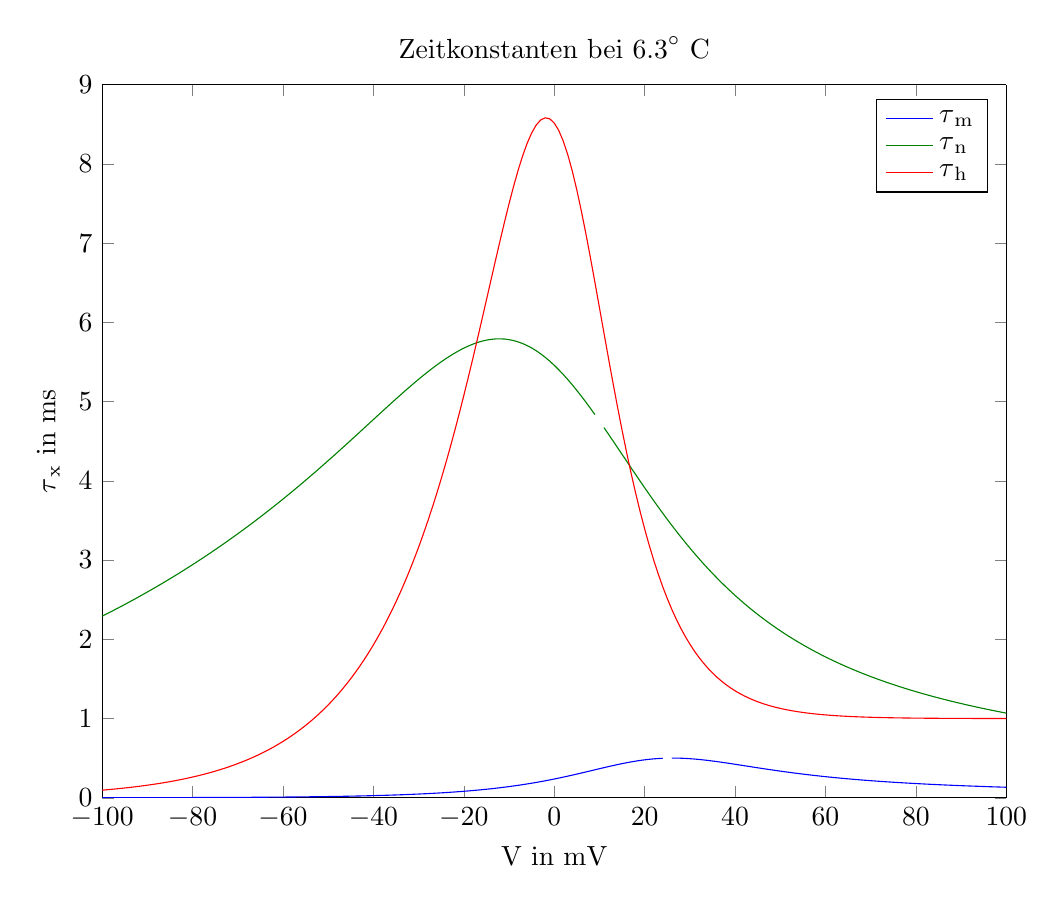
\begin{tikzpicture}

\begin{axis}[%
width=4.520833in,
height=3.565625in,
at={(0.758333in,0.48125in)},
scale only axis,
unbounded coords=jump,
separate axis lines,
every outer x axis line/.append style={black},
every x tick label/.append style={font=\color{black}},
xmin=-100,
xmax=100,
xlabel={V in mV},
every outer y axis line/.append style={black},
every y tick label/.append style={font=\color{black}},
ymin=0,
ymax=9,
ylabel={$\tau{}_\text{x}\text{ in ms}$},
title={$\text{Zeitkonstanten bei 6.3}^\circ\text{ C}$},
legend style={legend cell align=left,align=left,draw=black}
]
\addplot [color=blue,solid]
  table[row sep=crcr]{%
-100	0.000966479991355469\\
-99	0.00102169280630554\\
-98	0.00108005980321338\\
-97	0.00114176117301279\\
-96	0.00120698740045696\\
-95	0.00127593985216282\\
-94	0.00134883139824493\\
-93	0.001425887069457\\
-92	0.00150734475186823\\
-91	0.00159345592121758\\
-90	0.00168448641921098\\
-89	0.00178071727415549\\
-88	0.00188244556846101\\
-87	0.0019899853556838\\
-86	0.00210366862993851\\
-85	0.00222384635066593\\
-84	0.00235088952591343\\
-83	0.00248519035746409\\
-82	0.00262716345133982\\
-81	0.00277724709740339\\
-80	0.00293590462199474\\
-79	0.00310362581775937\\
-78	0.00328092845506095\\
-77	0.00346835987961711\\
-76	0.00366649870125804\\
-75	0.00387595657898133\\
-74	0.00409738010776545\\
-73	0.00433145281290758\\
-72	0.00457889725797073\\
-71	0.00484047727276036\\
-70	0.00511700030810202\\
-69	0.00540931992456024\\
-68	0.00571833842262442\\
-67	0.00604500962229007\\
-66	0.0063903418003841\\
-65	0.00675540079441958\\
-64	0.00714131328221911\\
-63	0.00754927024701501\\
-62	0.00798053063821799\\
-61	0.00843642523854221\\
-60	0.0089183607486809\\
-59	0.00942782410123999\\
-58	0.00996638701615328\\
-57	0.0105357108103166\\
-56	0.0111375514746822\\
-55	0.0117737650325421\\
-54	0.0124463131931874\\
-53	0.0131572693155458\\
-52	0.0139088246967641\\
-51	0.0147032952009774\\
-50	0.0155431282436969\\
-49	0.0164309101472885\\
-48	0.0173693738829084\\
-47	0.0183614072139257\\
-46	0.0194100612552824\\
-45	0.0205185594623214\\
-44	0.0216903070613021\\
-43	0.0229289009320163\\
-42	0.0242381399505094\\
-41	0.0256220357967782\\
-40	0.0270848242282897\\
-39	0.0286309768150809\\
-38	0.0302652131258166\\
-37	0.031992513346263\\
-36	0.0338181313018629\\
-35	0.0357476078441187\\
-34	0.0377867845458838\\
-33	0.0399418176329406\\
-32	0.0422191920578277\\
-31	0.0446257355961197\\
-30	0.0471686328144781\\
-29	0.0498554387229263\\
-28	0.0526940918799386\\
-27	0.0556929266669502\\
-26	0.0588606843875335\\
-25	0.0622065227743204\\
-24	0.0657400234022715\\
-23	0.0694711964084252\\
-22	0.0734104818040793\\
-21	0.0775687465336872\\
-20	0.0819572762838522\\
-19	0.0865877608741109\\
-18	0.0914722718674237\\
-17	0.0966232308217126\\
-16	0.10205336636447\\
-15	0.1077756580117\\
-14	0.113803264373189\\
-13	0.12014943309366\\
-12	0.126827389582058\\
-11	0.133850201291438\\
-10	0.141230614047062\\
-9	0.148980856704169\\
-8	0.157112410280641\\
-7	0.165635737693837\\
-6	0.174559970385342\\
-5	0.183892548503583\\
-4	0.193638812004149\\
-3	0.203801541103393\\
-2	0.21438044607142\\
-1	0.225371608467175\\
0	0.236766878685688\\
1	0.248553238171989\\
2	0.260712138889115\\
3	0.273218837584078\\
4	0.286041747969915\\
5	0.299141839920065\\
6	0.312472120805605\\
7	0.32597723969602\\
8	0.339593259631163\\
9	0.353247645755807\\
10	0.366859516894924\\
11	0.380340204236292\\
12	0.393594152394431\\
13	0.406520184752015\\
14	0.419013136562569\\
15	0.430965836421533\\
16	0.442271390671564\\
17	0.452825698147306\\
18	0.462530097055973\\
19	0.471294024762449\\
20	0.47903755778643\\
21	0.485693695883407\\
22	0.49121026212973\\
23	0.495551310562257\\
24	0.49869796271949\\
25	nan\\
26	0.501418632040885\\
27	0.501039217009215\\
28	0.49955611311694\\
29	0.497027657073722\\
30	0.493522650287524\\
31	0.489118055309453\\
32	0.483896653405158\\
33	0.477944769953314\\
34	0.471350155824345\\
35	0.464200091044898\\
36	0.456579754395673\\
37	0.448570881184392\\
38	0.440250712767303\\
39	0.431691226337834\\
40	0.422958622383475\\
41	0.414113039915864\\
42	0.405208465682708\\
43	0.396292802477838\\
44	0.38740806271713\\
45	0.378590656001718\\
46	0.369871742875951\\
47	0.361277630936126\\
48	0.352830193495545\\
49	0.344547294903691\\
50	0.336443210183906\\
51	0.328529029799969\\
52	0.320813043048249\\
53	0.313301095799708\\
54	0.305996920112111\\
55	0.298902434640666\\
56	0.292018015845328\\
57	0.285342740777732\\
58	0.278874602780477\\
59	0.272610701792417\\
60	0.266547411166286\\
61	0.260680523004251\\
62	0.255005374031619\\
63	0.249516953982795\\
64	0.244209998385346\\
65	0.239079067512658\\
66	0.234118613144326\\
67	0.229323034634777\\
68	0.224686725650786\\
69	0.220204112801909\\
70	0.215869687257514\\
71	0.211678030321777\\
72	0.207623833824921\\
73	0.203701916085558\\
74	0.199907234105212\\
75	0.196234892571856\\
76	0.192680150173927\\
77	0.189238423659413\\
78	0.185905290015392\\
79	0.182676487091351\\
80	0.179547912943892\\
81	0.176515624140491\\
82	0.173575833225177\\
83	0.170724905518715\\
84	0.167959355399668\\
85	0.16527584219001\\
86	0.16267116574941\\
87	0.160142261865431\\
88	0.157686197512438\\
89	0.155300166039584\\
90	0.152981482337636\\
91	0.150727578025351\\
92	0.1485359966884\\
93	0.146404389197285\\
94	0.144330509125159\\
95	0.142312208281771\\
96	0.140347432375816\\
97	0.138434216814669\\
98	0.136570682647724\\
99	0.134755032657253\\
100	0.132985547598816\\
};
\addlegendentry{$\tau{}_\text{m}$};

\addplot [color=black!50!green,solid]
  table[row sep=crcr]{%
-100	2.29194186181398\\
-99	2.32076029939748\\
-98	2.3499399312687\\
-97	2.37948514397165\\
-96	2.40940036048818\\
-95	2.43969003848522\\
-94	2.47035866828351\\
-93	2.50141077051516\\
-92	2.53285089343385\\
-91	2.56468360983757\\
-90	2.59691351355922\\
-89	2.62954521547572\\
-88	2.66258333898081\\
-87	2.69603251486091\\
-86	2.72989737550679\\
-85	2.76418254838682\\
-84	2.79889264869968\\
-83	2.83403227111561\\
-82	2.86960598050626\\
-81	2.90561830155237\\
-80	2.9420737071077\\
-79	2.97897660518487\\
-78	3.01633132441577\\
-77	3.05414209782409\\
-76	3.09241304473222\\
-75	3.13114815060696\\
-74	3.17035124463046\\
-73	3.21002597476226\\
-72	3.25017578003714\\
-71	3.29080385981997\\
-70	3.33191313971444\\
-69	3.37350623379593\\
-68	3.41558540281104\\
-67	3.45815250795698\\
-66	3.50120895982313\\
-65	3.54475566204512\\
-64	3.58879294918863\\
-63	3.63332051834628\\
-62	3.67833735389692\\
-61	3.72384164484222\\
-60	3.76983069410264\\
-59	3.81630081912262\\
-58	3.86324724310595\\
-57	3.91066397617649\\
-56	3.95854368573912\\
-55	4.00687755530195\\
-54	4.05565513101607\\
-53	4.10486415519535\\
-52	4.15449038609883\\
-51	4.20451740329546\\
-50	4.25492639798878\\
-49	4.30569594776155\\
-48	4.35680177531251\\
-47	4.40821649090355\\
-46	4.45990931842269\\
-45	4.51184580520059\\
-44	4.56398751600456\\
-43	4.61629171197909\\
-42	4.66871101571391\\
-41	4.72119306410626\\
-40	4.77368015124911\\
-39	4.82610886422858\\
-38	4.87840971545463\\
-37	4.9305067759831\\
-36	4.9823173152139\\
-35	5.03375145336507\\
-34	5.08471183421963\\
-33	5.13509332680599\\
-32	5.18478276588419\\
-31	5.23365874234126\\
-30	5.28159145581179\\
-29	5.32844264298797\\
-28	5.37406559610858\\
-27	5.41830528695005\\
-26	5.46099861220489\\
-25	5.50197477633406\\
-24	5.5410558277243\\
-23	5.57805736316657\\
-22	5.61278941419864\\
-21	5.64505752662963\\
-20	5.6746640415072\\
-19	5.70140958184537\\
-18	5.72509474457913\\
-17	5.7455219914747\\
-16	5.76249772617578\\
-15	5.77583453734595\\
-14	5.78535358017943\\
-13	5.79088706067322\\
-12	5.79228077932193\\
-11	5.78939668370994\\
-10	5.78211537326701\\
-9	5.7703384946723\\
-8	5.75399096347209\\
-7	5.73302294680141\\
-6	5.70741154396807\\
-5	5.67716210624799\\
-4	5.64230914458326\\
-3	5.60291678383079\\
-2	5.55907873446778\\
-1	5.51091776673981\\
0	5.45858468751442\\
1	5.40225683584806\\
2	5.34213612869949\\
3	5.27844670254166\\
4	5.211432209107\\
5	5.14135283353046\\
6	5.06848211027088\\
7	4.9931036161184\\
8	4.91550762026365\\
9	4.83598776893377\\
10	nan\\
11	4.67234888962634\\
12	4.58880607321929\\
13	4.50448647269053\\
14	4.41965667495694\\
15	4.33457089566982\\
16	4.24946940088743\\
17	4.16457726364249\\
18	4.08010344663965\\
19	3.99624019481334\\
20	3.91316271549724\\
21	3.83102911951866\\
22	3.74998059357404\\
23	3.67014177264384\\
24	3.59162128080336\\
25	3.51451240939259\\
26	3.43889390292497\\
27	3.36483082514696\\
28	3.2923754801239\\
29	3.22156836595844\\
30	3.15243914160366\\
31	3.08500759009645\\
32	3.01928456431482\\
33	2.9552729039853\\
34	2.8929683150845\\
35	2.832360204962\\
36	2.77343246844289\\
37	2.71616422184553\\
38	2.66053048327873\\
39	2.60650279877454\\
40	2.55404981478815\\
41	2.5031377983723\\
42	2.45373110693509\\
43	2.40579260993725\\
44	2.35928406520043\\
45	2.31416645270204\\
46	2.27040026884368\\
47	2.22794578421612\\
48	2.18676326785966\\
49	2.14681318094709\\
50	2.10805634271018\\
51	2.07045407129712\\
52	2.03396830209873\\
53	1.99856168591885\\
54	1.96419766919766\\
55	1.93084055832779\\
56	1.89845556993665\\
57	1.86700886884622\\
58	1.83646759526618\\
59	1.80679988262851\\
60	1.77797486733244\\
61	1.7499626915389\\
62	1.72273450003318\\
63	1.69626243206315\\
64	1.67051960895861\\
65	1.64548011824448\\
66	1.62111899487561\\
67	1.59741220014466\\
68	1.57433659874568\\
69	1.55186993441343\\
70	1.52999080450358\\
71	1.50867863382875\\
72	1.48791364802148\\
73	1.46767684665595\\
74	1.44794997632552\\
75	1.42871550384249\\
76	1.40995658969952\\
77	1.39165706190867\\
78	1.37380139031291\\
79	1.35637466144733\\
80	1.33936255401109\\
81	1.32275131499813\\
82	1.30652773652222\\
83	1.29067913336236\\
84	1.27519332124557\\
85	1.26005859587696\\
86	1.24526371272039\\
87	1.23079786752818\\
88	1.21665067761358\\
89	1.20281216385622\\
90	1.18927273342779\\
91	1.17602316322273\\
92	1.16305458397678\\
93	1.1503584650547\\
94	1.13792659988764\\
95	1.12575109203922\\
96	1.11382434187949\\
97	1.10213903384525\\
98	1.09068812426506\\
99	1.07946482972751\\
100	1.06846261597133\\
};
\addlegendentry{$\tau{}_\text{n}$};

\addplot [color=red,solid]
  table[row sep=crcr]{%
-100	0.0962563647586614\\
-99	0.101191530550023\\
-98	0.106379726913452\\
-97	0.111833926829143\\
-96	0.117567768377537\\
-95	0.123595588831184\\
-94	0.129932460492631\\
-93	0.136594228367441\\
-92	0.143597549765928\\
-91	0.150959935931861\\
-90	0.158699795801289\\
-89	0.166836481999795\\
-88	0.175390339191771\\
-87	0.184382754900933\\
-86	0.193836212927076\\
-85	0.203774349490094\\
-84	0.214222012238559\\
-83	0.225205322266642\\
-82	0.236751739289803\\
-81	0.248890130136607\\
-80	0.261650840721023\\
-79	0.275065771666759\\
-78	0.289168457762452\\
-77	0.303994151433836\\
-76	0.319579910426279\\
-75	0.335964689898194\\
-74	0.353189439132756\\
-73	0.371297203081794\\
-72	0.390333228961659\\
-71	0.410345078125948\\
-70	0.431382743443933\\
-69	0.453498772416061\\
-68	0.476748396258481\\
-67	0.50118966518672\\
-66	0.526883590123619\\
-65	0.553894291047687\\
-64	0.582289152184123\\
-63	0.612138984220549\\
-62	0.643518193701577\\
-61	0.676504959718756\\
-60	0.711181417962876\\
-59	0.747633852141344\\
-58	0.785952892680852\\
-57	0.826233722530669\\
-56	0.868576289749587\\
-55	0.913085526393409\\
-54	0.959871573012575\\
-53	1.00905000781158\\
-52	1.0607420792023\\
-51	1.11507494008845\\
-50	1.17218188173177\\
-49	1.23220256445212\\
-48	1.29528324167987\\
-47	1.36157697297973\\
-46	1.43124382056722\\
-45	1.50445102249865\\
-44	1.58137313408445\\
-43	1.66219212709332\\
-42	1.74709743391067\\
-41	1.83628592090679\\
-40	1.92996177175972\\
-39	2.02833625725291\\
-38	2.13162736299911\\
-37	2.24005924048206\\
-36	2.35386143959499\\
-35	2.47326787231183\\
-34	2.59851544706983\\
-33	2.72984230168625\\
-32	2.8674855490132\\
-31	3.01167843392752\\
-30	3.16264678261521\\
-29	3.32060460553074\\
-28	3.48574869419019\\
-27	3.65825202971017\\
-26	3.83825579880508\\
-25	4.02585979252397\\
-24	4.22111094694861\\
-23	4.42398977716573\\
-22	4.6343944613609\\
-21	4.85212235802613\\
-20	5.07684879540686\\
-19	5.30810307024613\\
-18	5.54524174681112\\
-17	5.78741957315691\\
-16	6.03355864614106\\
-15	6.28231687434219\\
-14	6.53205731696693\\
-13	6.7808206127301\\
-12	7.02630343031643\\
-11	7.26584661521254\\
-10	7.49643737935696\\
-9	7.71473033536303\\
-8	7.91709222472556\\
-7	8.09967460743464\\
-6	8.25851735262987\\
-5	8.38968334629722\\
-4	8.48942140803058\\
-3	8.55435020740738\\
-2	8.58165149598675\\
-1	8.56925699776393\\
0	8.51601076440658\\
1	8.42178858643817\\
2	8.28755871818239\\
3	8.11537370962569\\
4	7.90829083728854\\
5	7.6702271829711\\
6	7.40576322145857\\
7	7.1199143734777\\
8	6.81789241373283\\
9	6.50487770362583\\
10	6.18581948604929\\
11	5.86527598005834\\
12	5.54729995814127\\
13	5.23536994377172\\
14	4.93236285025743\\
15	4.64056110513119\\
16	4.36168602834488\\
17	4.09694918632498\\
18	3.84711425332712\\
19	3.61256320235789\\
20	3.39336210980717\\
21	3.18932327024378\\
22	3.00006154868144\\
23	2.82504388770758\\
24	2.66363162813129\\
25	2.51511581727406\\
26	2.37874600681078\\
27	2.25375322431882\\
28	2.13936787894094\\
29	2.03483336542156\\
30	1.93941608885006\\
31	1.85241256462516\\
32	1.77315416851456\\
33	1.70101002963804\\
34	1.63538848062705\\
35	1.57573740743342\\
36	1.52154377783842\\
37	1.4723325730604\\
38	1.42766530067712\\
39	1.38713822866959\\
40	1.35038044887351\\
41	1.31705185255464\\
42	1.28684108029383\\
43	1.25946349204233\\
44	1.23465919034385\\
45	1.21219111967828\\
46	1.19184325711788\\
47	1.17341890354732\\
48	1.15673908021063\\
49	1.14164103200398\\
50	1.12797683648763\\
51	1.11561211584262\\
52	1.1044248477911\\
53	1.09430427070507\\
54	1.08514987764926\\
55	1.07687049385996\\
56	1.06938343209294\\
57	1.06261372033112\\
58	1.05649339649144\\
59	1.05096086498014\\
60	1.045960310197\\
61	1.04144116236351\\
62	1.03735761133763\\
63	1.03366816436756\\
64	1.03033524402414\\
65	1.02732482283001\\
66	1.02460609137185\\
67	1.02215115693607\\
68	1.01993476994908\\
69	1.01793407572783\\
70	1.01612838925725\\
71	1.01449899090553\\
72	1.01302894116967\\
73	1.01170291271015\\
74	1.01050703808727\\
75	1.00942877175295\\
76	1.0084567649813\\
77	1.00758075253969\\
78	1.00679145001082\\
79	1.00608046077509\\
80	1.00544019175334\\
81	1.00486377709223\\
82	1.00434500904997\\
83	1.0038782754084\\
84	1.00345850279971\\
85	1.00308110539297\\
86	1.00274193843683\\
87	1.00243725620194\\
88	1.00216367390894\\
89	1.00191813326656\\
90	1.00169787127957\\
91	1.00150039201803\\
92	1.00132344106825\\
93	1.00116498241212\\
94	1.0010231775052\\
95	1.00089636634558\\
96	1.00078305034507\\
97	1.00068187683202\\
98	1.00059162503111\\
99	1.00051119338021\\
100	1.00043958805722\\
};
\addlegendentry{$\tau{}_\text{h}$};

\end{axis}
\end{tikzpicture}%}
    \caption{Zeitkonstanten $\tau_\infty$ über $V$ bei $6.3^\circ C$}
    \label{fig:Zeitkonstanten6}
\end{figure}

Der Verlauf der Zeitkonstanten zeigt, das die Vorgänge im negativen Bereich schneller ablaufen, als im positiven und nahe 0V. Generell ist zu erwähnen, dass die Zeitkonstante $\tau_m$ die kleinste ist gefolgt von $\tau_n$. Die größte und somit langsamste ist $tau_h$.
\begin{figure}[h!]
  	\centering
    \scalebox{.6}{% This file was created by matlab2tikz.
% Minimal pgfplots version: 1.3
%
%The latest updates can be retrieved from
%  http://www.mathworks.com/matlabcentral/fileexchange/22022-matlab2tikz
%where you can also make suggestions and rate matlab2tikz.
%
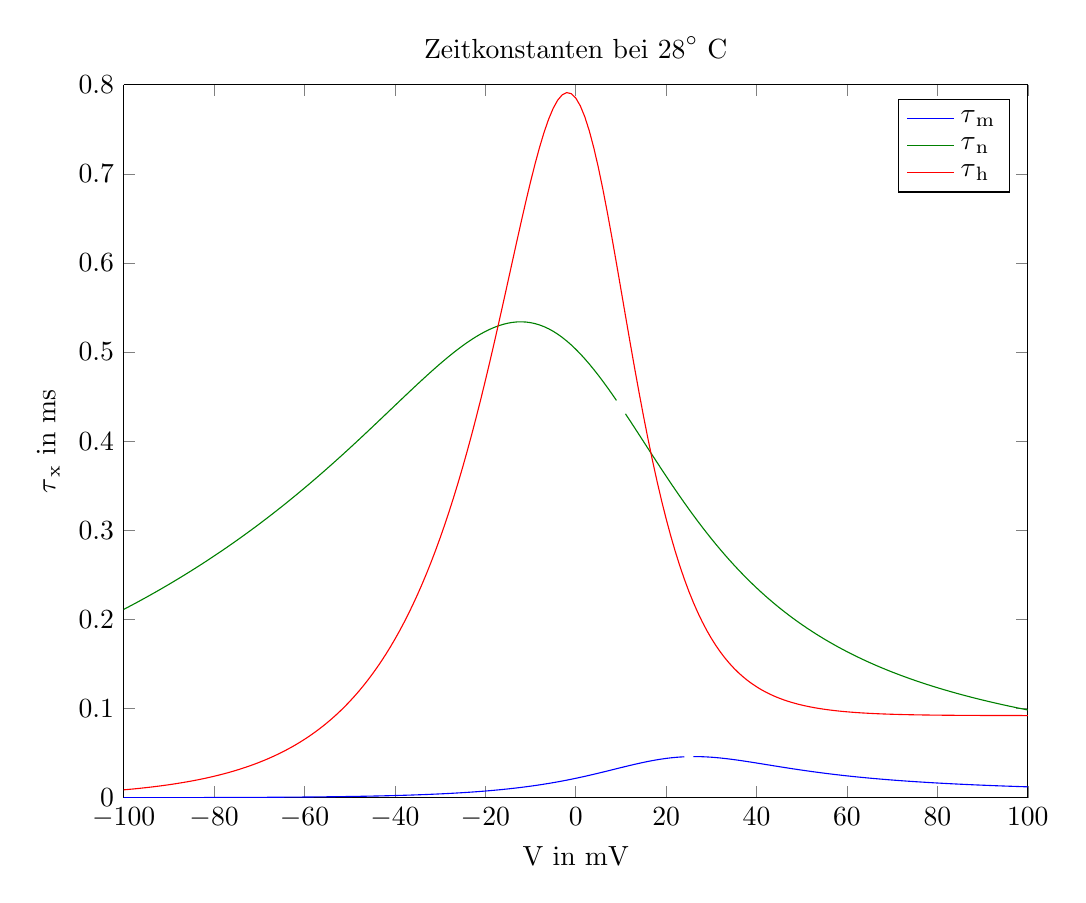
\begin{tikzpicture}

\begin{axis}[%
width=4.520833in,
height=3.565625in,
at={(0.758333in,0.48125in)},
scale only axis,
unbounded coords=jump,
separate axis lines,
every outer x axis line/.append style={black},
every x tick label/.append style={font=\color{black}},
xmin=-100,
xmax=100,
xlabel={V in mV},
every outer y axis line/.append style={black},
every y tick label/.append style={font=\color{black}},
ymin=0,
ymax=0.8,
ylabel={$\tau{}_\text{x}\text{ in ms}$},
title={$\text{Zeitkonstanten bei 28}^\circ\text{ C}$},
legend style={legend cell align=left,align=left,draw=black}
]
\addplot [color=blue,solid]
  table[row sep=crcr]{%
-100	8.90922125887266e-05\\
-99	9.41818490955875e-05\\
-98	9.95622449063545e-05\\
-97	0.000105250010410403\\
-96	0.000111262704903609\\
-95	0.000117618890795545\\
-94	0.000124338190913037\\
-93	0.000131441349076886\\
-92	0.000138950294138633\\
-91	0.000146888207674925\\
-90	0.000155279595548264\\
-89	0.00016415036355484\\
-88	0.000173527897392706\\
-87	0.000183441147196834\\
-86	0.000193920716901612\\
-85	0.000204998958706143\\
-84	0.000216710072933374\\
-83	0.000229090213590578\\
-82	0.000242177599956141\\
-81	0.000256012634536044\\
-80	0.000270638027752793\\
-79	0.000286098929750092\\
-78	0.000302443069718122\\
-77	0.000319720903167055\\
-76	0.000337985767600467\\
-75	0.000357294047065555\\
-74	0.000377705346083669\\
-73	0.000399282673492686\\
-72	0.000422092636762125\\
-71	0.000446205647372842\\
-70	0.000471696137885519\\
-69	0.000498642791356146\\
-68	0.000527128783792235\\
-67	0.000557242040380619\\
-66	0.000589075506256443\\
-65	0.000622727432623197\\
-64	0.000658301679075481\\
-63	0.000695908033019419\\
-62	0.000735662547130226\\
-61	0.000777687895832141\\
-60	0.000822113751832652\\
-59	0.000869077183790205\\
-58	0.000918723076242222\\
-57	0.00097120457296755\\
-56	0.001026683545004\\
-55	0.00108533108458648\\
-54	0.00114732802631346\\
-53	0.00121286549688808\\
-52	0.00128214549481312\\
-51	0.00135538150144537\\
-50	0.00143279912483151\\
-49	0.00151463677775207\\
-48	0.00160114639138969\\
-47	0.0016925941660075\\
-46	0.00178926135996932\\
-45	0.00189144511834929\\
-44	0.00199945934225713\\
-43	0.00211363559983904\\
-42	0.00223432407969205\\
-41	0.00236189458714096\\
-40	0.00249673758345563\\
-39	0.00263926526761785\\
-38	0.00278991269965841\\
-37	0.00294913896385528\\
-36	0.00311742836918275\\
-35	0.00329529168329702\\
-34	0.00348326739499783\\
-33	0.00368192299847135\\
-32	0.00389185629064599\\
-31	0.00411369667061789\\
-30	0.00434810642725603\\
-29	0.00459578199769842\\
-28	0.00485745517540746\\
-27	0.00513389424166087\\
-26	0.00542590498869763\\
-25	0.00573433159608665\\
-24	0.00606005731409795\\
-23	0.00640400489877929\\
-22	0.00676713673291595\\
-21	0.00715045455491333\\
-20	0.00755499870373249\\
-19	0.00798184677218093\\
-18	0.00843211154299929\\
-17	0.00890693806221951\\
-16	0.00940749968220968\\
-15	0.00993499288278253\\
-14	0.0104906306530024\\
-13	0.0110756341893665\\
-12	0.01169122263863\\
-11	0.0123386005868327\\
-10	0.0130189429716703\\
-9	0.0137333770754253\\
-8	0.0144829612431178\\
-7	0.0152686599690633\\
-6	0.0160913150092652\\
-5	0.0169516122126714\\
-4	0.0178500438279193\\
-3	0.0187868661413555\\
-2	0.0197620524450528\\
-1	0.0207752415286535\\
0	0.0218256821439733\\
1	0.0229121742125033\\
2	0.0240330079361443\\
3	0.0251859024284059\\
4	0.0263679459971496\\
5	0.0275755407610285\\
6	0.0288043548380342\\
7	0.0300492858598689\\
8	0.0313044399794827\\
9	0.0325631307772913\\
10	0.0338179024519287\\
11	0.0350605813208154\\
12	0.0362823588821789\\
13	0.0374739084569565\\
14	0.0386255357317287\\
15	0.0397273614150008\\
16	0.0407695318186162\\
17	0.0417424506723597\\
18	0.0426370231191252\\
19	0.0434449008996497\\
20	0.0441587164949346\\
21	0.0447722936777629\\
22	0.0452808226666434\\
23	0.045680989885073\\
24	0.0459710550757055\\
25	nan\\
26	0.0462218522486769\\
27	0.046186876951761\\
28	0.0460501612324046\\
29	0.0458170826944748\\
30	0.0454939836003249\\
31	0.0450879585241066\\
32	0.0446066384216426\\
33	0.0440579809527474\\
34	0.0434500751821429\\
35	0.0427909667711552\\
36	0.0420885076837217\\
37	0.0413502324570044\\
38	0.0405832613660151\\
39	0.0397942294238689\\
40	0.0389892391344541\\
41	0.0381738342417255\\
42	0.0373529913606641\\
43	0.0365311262742449\\
44	0.0357121117776837\\
45	0.0348993041866346\\
46	0.0340955759473629\\
47	0.033303352150903\\
48	0.0325246491265075\\
49	0.0317611136484875\\
50	0.0310140616193198\\
51	0.0302845153819037\\
52	0.0295732390614784\\
53	0.0288807715430525\\
54	0.0282074568557695\\
55	0.0275534718654096\\
56	0.0269188512748644\\
57	0.0263035100047606\\
58	0.0257072630770861\\
59	0.0251298431579418\\
60	0.0245709159351518\\
61	0.0240300935156072\\
62	0.0235069460285772\\
63	0.0230010116169601\\
64	0.0225118049903193\\
65	0.0220388247029091\\
66	0.0215815593077917\\
67	0.0211394925253647\\
68	0.020712107551725\\
69	0.0202988906197066\\
70	0.0198993339134062\\
71	0.0195129379257417\\
72	0.019139213338161\\
73	0.0187776824920844\\
74	0.0184278805130228\\
75	0.0180893561405427\\
76	0.0177616723103061\\
77	0.0174444065282454\\
78	0.0171371510714787\\
79	0.0168395130457682\\
80	0.0165511143251138\\
81	0.0162715913953901\\
82	0.0160005951207272\\
83	0.0157377904485447\\
84	0.0154828560667316\\
85	0.0152354840243739\\
86	0.0149953793256254\\
87	0.0147622595047671\\
88	0.0145358541891624\\
89	0.0143159046556757\\
90	0.0141021633851396\\
91	0.0138943936186252\\
92	0.0136923689185554\\
93	0.0134958727371003\\
94	0.0133046979937823\\
95	0.0131186466637853\\
96	0.0129375293781009\\
97	0.0127611650363387\\
98	0.0125893804327744\\
99	0.012422009895997\\
100	0.0122588949423417\\
};
\addlegendentry{$\tau{}_\text{m}$};

\addplot [color=black!50!green,solid]
  table[row sep=crcr]{%
-100	0.21127614996701\\
-99	0.213932695773058\\
-98	0.216622537248498\\
-97	0.219346078754431\\
-96	0.222103728010874\\
-95	0.224895895935191\\
-94	0.227722996454843\\
-93	0.23058544629146\\
-92	0.233483664712887\\
-91	0.236418073249519\\
-90	0.23938909537079\\
-89	0.242397156117293\\
-88	0.245442681683446\\
-87	0.24852609894514\\
-86	0.25164783492616\\
-85	0.254808316196533\\
-84	0.258007968195238\\
-83	0.261247214468901\\
-82	0.264526475817246\\
-81	0.267846169335116\\
-80	0.271206707339828\\
-79	0.274608496171504\\
-78	0.278051934852779\\
-77	0.281537413592917\\
-76	0.285065312119951\\
-75	0.288635997822817\\
-74	0.292249823683794\\
-73	0.295907125979671\\
-72	0.299608221728097\\
-71	0.303353405853438\\
-70	0.307142948044157\\
-69	0.310977089271369\\
-68	0.314856037935576\\
-67	0.318779965605956\\
-66	0.322749002313685\\
-65	0.326763231357846\\
-64	0.330822683579425\\
-63	0.334927331055768\\
-62	0.339077080164722\\
-61	0.343271763964551\\
-60	0.34751113383264\\
-59	0.351794850303064\\
-58	0.356122473040434\\
-57	0.360493449885034\\
-56	0.36490710490241\\
-55	0.369362625369304\\
-54	0.373859047627348\\
-53	0.378395241736567\\
-52	0.382969894862524\\
-51	0.38758149333443\\
-50	0.39222830331681\\
-49	0.396908350044985\\
-48	0.401619395584901\\
-47	0.406358915091354\\
-46	0.411124071555885\\
-45	0.415911689057039\\
-44	0.42071822455207\\
-43	0.425539738280988\\
-42	0.43037186289181\\
-41	0.435209771440651\\
-40	0.440048144472394\\
-39	0.444881136447707\\
-38	0.449702341850487\\
-37	0.454504761386706\\
-36	0.459280768771001\\
-35	0.464022078690987\\
-34	0.468719716640356\\
-33	0.473363991419129\\
-32	0.477944471211122\\
-31	0.482449964262135\\
-30	0.486868505294198\\
-29	0.491187348897033\\
-28	0.495392971232417\\
-27	0.49947108146394\\
-26	0.503406644376514\\
-25	0.507183915668542\\
-24	0.510786491376051\\
-23	0.514197372813035\\
-22	0.517399048276437\\
-21	0.520373592559042\\
-20	0.523102785031806\\
-19	0.525568246693632\\
-18	0.527751596139403\\
-17	0.529634623868172\\
-16	0.531199483749769\\
-15	0.532428899802513\\
-14	0.533306385726016\\
-13	0.533816473906752\\
-12	0.533944949901341\\
-11	0.533679087740005\\
-10	0.53300788082035\\
-9	0.531922262720879\\
-8	0.530415311994515\\
-7	0.528482434940156\\
-6	0.526121520522545\\
-5	0.523333062033852\\
-4	0.520120240767241\\
-3	0.516488967890491\\
-2	0.512447881837745\\
-1	0.508008299835348\\
0	0.503184123585996\\
1	0.497991700586853\\
2	0.49244964397919\\
3	0.486578615147079\\
4	0.480401074433345\\
5	0.473941006265567\\
6	0.46722362564082\\
7	0.460275073279967\\
8	0.453122106823796\\
9	0.445791795215618\\
10	nan\\
11	0.430707209964564\\
12	0.423006052748512\\
13	0.415233289894757\\
14	0.407413495960958\\
15	0.399570105094796\\
16	0.391725265540344\\
17	0.383899725015776\\
18	0.376112746154431\\
19	0.368382050509493\\
20	0.360723789071317\\
21	0.353152536837386\\
22	0.34568130870225\\
23	0.33832159378754\\
24	0.331083405295079\\
25	0.323975343022036\\
26	0.317004665807698\\
27	0.31017737136871\\
28	0.30349828120676\\
29	0.2969711285244\\
30	0.290598647347969\\
31	0.284382661320526\\
32	0.278324170883804\\
33	0.272423437809923\\
34	0.266680066266537\\
35	0.261093079800256\\
36	0.255660993801278\\
37	0.250381883166738\\
38	0.245253445011957\\
39	0.24027305638873\\
40	0.235437827059591\\
41	0.230744647448619\\
42	0.226190231944728\\
43	0.22177115777463\\
44	0.217483899691745\\
45	0.213324860746133\\
46	0.20929039941079\\
47	0.205376853342983\\
48	0.201580560057053\\
49	0.19789787477853\\
50	0.19432518573959\\
51	0.190858927163608\\
52	0.187495590172712\\
53	0.184231731837351\\
54	0.181063982571447\\
55	0.177989052061198\\
56	0.175003733900208\\
57	0.172104909088705\\
58	0.16928954854026\\
59	0.166554714725823\\
60	0.163897562572026\\
61	0.161315339718793\\
62	0.158805386230122\\
63	0.156365133841718\\
64	0.153992104819723\\
65	0.15168391049623\\
66	0.149438249539467\\
67	0.147252906009484\\
68	0.145125747243819\\
69	0.143054721611886\\
70	0.141037856171712\\
71	0.139073254258095\\
72	0.137159093027143\\
73	0.135293620978575\\
74	0.133475155473952\\
75	0.131702080266169\\
76	0.129972843053079\\
77	0.128285953065911\\
78	0.126639978701256\\
79	0.125033545203712\\
80	0.123465332404846\\
81	0.12193407252286\\
82	0.120438548026281\\
83	0.118977589564045\\
84	0.117550073963559\\
85	0.116154922297644\\
86	0.11479109802068\\
87	0.113457605173785\\
88	0.112153486658474\\
89	0.110877822577882\\
90	0.109629728644382\\
91	0.108408354652187\\
92	0.107212883013365\\
93	0.10604252735554\\
94	0.104896531179474\\
95	0.103774166574609\\
96	0.102674732990647\\
97	0.101597556063176\\
98	0.100541986491351\\
99	0.0995073989656603\\
100	0.0984931911437921\\
};
\addlegendentry{$\tau{}_\text{n}$};

\addplot [color=red,solid]
  table[row sep=crcr]{%
-100	0.00887311955632876\\
-99	0.00932805379581358\\
-98	0.00980631293981764\\
-97	0.0103090928656686\\
-96	0.0108376507610712\\
-95	0.0113933082667686\\
-94	0.0119774547801561\\
-93	0.0125915509280618\\
-92	0.0132371322173197\\
-91	0.0139158128721935\\
-90	0.01462928986816\\
-89	0.0153793471720349\\
-88	0.0161678601989132\\
-87	0.016996800496915\\
-86	0.0178682406712558\\
-85	0.0187843595597249\\
-84	0.0197474476722229\\
-83	0.0207599129076153\\
-82	0.0218242865617691\\
-81	0.0229432296412754\\
-80	0.0241195394980119\\
-79	0.025356156800357\\
-78	0.0266561728575414\\
-77	0.0280228373142922\\
-76	0.0294595662335986\\
-75	0.0309699505860816\\
-74	0.032557765165089\\
-73	0.0342269779472301\\
-72	0.0359817599186135\\
-71	0.0378264953875164\\
-70	0.0397657928045812\\
-69	0.0418044961118683\\
-68	0.043947696642147\\
-67	0.0462007455896363\\
-66	0.0485692670729487\\
-65	0.0510591718101617\\
-64	0.0536766714246616\\
-63	0.0564282933985395\\
-62	0.0593208966877489\\
-61	0.0623616880097662\\
-60	0.0655582388099296\\
-59	0.0689185029067061\\
-58	0.0724508348085326\\
-57	0.0761640086852076\\
-56	0.0800672379646152\\
-55	0.0841701955102462\\
-54	0.0884830343158742\\
-53	0.0930164086299651\\
-52	0.0977814953929457\\
-51	0.102790015834051\\
-50	0.108054257029611\\
-49	0.113587093169491\\
-48	0.119402006210716\\
-47	0.125513105514472\\
-46	0.131935145961421\\
-45	0.138683543916719\\
-44	0.145774390265814\\
-43	0.153224459559287\\
-42	0.161051214083478\\
-41	0.16927280140551\\
-40	0.17790804361773\\
-39	0.186976416117169\\
-38	0.196498013288321\\
-37	0.206493497898983\\
-36	0.216984030353993\\
-35	0.227991173164215\\
-34	0.239536765060961\\
-33	0.251642758102458\\
-32	0.264331009863425\\
-31	0.277623021360271\\
-30	0.291539609738463\\
-29	0.306100502943821\\
-28	0.321323841643244\\
-27	0.337225571609589\\
-26	0.353818707739065\\
-25	0.371112448986058\\
-24	0.389111122019938\\
-23	0.407812930679325\\
-22	0.427208488809494\\
-21	0.44727911647866\\
-20	0.467994884743404\\
-19	0.489312403161076\\
-18	0.511172358436411\\
-17	0.533496833419918\\
-16	0.556186464672336\\
-15	0.579117535308375\\
-14	0.602139148590943\\
-13	0.625070686365793\\
-12	0.647699822578544\\
-11	0.66978143062406\\
-10	0.691037785193118\\
-9	0.711160501252494\\
-8	0.729814657187639\\
-7	0.746645495488244\\
-6	0.761287962740217\\
-5	0.773379127272071\\
-4	0.782573197173791\\
-3	0.788558474105489\\
-2	0.791075165840254\\
-1	0.789932614229796\\
0	0.785024261460725\\
1	0.776338657635279\\
2	0.763965058527832\\
3	0.748092672628347\\
4	0.729003326288264\\
5	0.70705810456634\\
6	0.682679245519205\\
7	0.656329081459588\\
8	0.628488045033871\\
9	0.599633673142384\\
10	0.570222197682201\\
11	0.540673805128695\\
12	0.51136208880126\\
13	0.482607706505108\\
14	0.45467585832126\\
15	0.427776943348289\\
16	0.402069636576322\\
17	0.377665622814769\\
18	0.354635299205566\\
19	0.333013876845283\\
20	0.31280744679822\\
21	0.293998705972408\\
22	0.276552151793162\\
23	0.260418645877124\\
24	0.245539315240979\\
25	0.231848807095929\\
26	0.219277943494874\\
27	0.2077558388994\\
28	0.197211550762459\\
29	0.1875753335778\\
30	0.178779562982464\\
31	0.170759390246822\\
32	0.163453180145334\\
33	0.15680277763798\\
34	0.1507536415491\\
35	0.145254876813517\\
36	0.140259191013482\\
37	0.135722795891962\\
38	0.131605270270611\\
39	0.12786939726011\\
40	0.124480985744949\\
41	0.121408683767584\\
42	0.118623789544421\\
43	0.11610006434112\\
44	0.113813550248949\\
45	0.111742394978173\\
46	0.10986668506884\\
47	0.108168288371754\\
48	0.106630706238707\\
49	0.105238935552783\\
50	0.103979340504064\\
51	0.10283953385503\\
52	0.101808267328616\\
53	0.10087533067878\\
54	0.100031458959195\\
55	0.0992682474832649\\
56	0.0985780739622622\\
57	0.097954027313762\\
58	0.0973898426461908\\
59	0.0968798419447105\\
60	0.0964188800067644\\
61	0.0960022952009719\\
62	0.0956258646495181\\
63	0.0952857634609454\\
64	0.0949785276666884\\
65	0.0947010205404077\\
66	0.0944504020038534\\
67	0.094224100846458\\
68	0.0940197895080022\\
69	0.0938353611944538\\
70	0.0936689091164549\\
71	0.093518707657923\\
72	0.0933831952988938\\
73	0.0932609591321126\\
74	0.0931507208270422\\
75	0.0930513239079714\\
76	0.0929617222248405\\
77	0.0928809695063403\\
78	0.0928082098948346\\
79	0.0927426693717983\\
80	0.0926836479907971\\
81	0.0926305128426446\\
82	0.0925826916842984\\
83	0.0925396671693687\\
84	0.0925009716238566\\
85	0.0924661823159633\\
86	0.0924349171735599\\
87	0.0924068309072271\\
88	0.0923816115006935\\
89	0.0923589770340663\\
90	0.092338672808479\\
91	0.0923204687437198\\
92	0.0923041570230669\\
93	0.0922895499619745\\
94	0.0922764780794459\\
95	0.0922647883529204\\
96	0.0922543426393026\\
97	0.0922450162463983\\
98	0.0922366966405041\\
99	0.092229282277242\\
100	0.0922226815439465\\
};
\addlegendentry{$\tau{}_\text{h}$};

\end{axis}
\end{tikzpicture}%}
    \caption{Zeitkonstanten $\tau_x$ über $V$ bei $28^\circ C$}
    \label{fig:Zeitkonstanten28}
\end{figure}


Die Steady State Werte der Gating Variablen sind temperaturabhängig. Das bedeutet, dass das Ruhepotential bei unterschiedlichen Temperaturen das Selbe ist. Daher sind die Gating Variablen für die verschiedenen Temperaturen nur einmal in Grafik \ref{fig:Gating1} abgebildet. Der Wert der Gating Variablen hängt also nur vom Membranpotential selbst ab.
\begin{figure}[h!]
  	\centering
    \scalebox{.6}{% This file was created by matlab2tikz.
% Minimal pgfplots version: 1.3
%
%The latest updates can be retrieved from
%  http://www.mathworks.com/matlabcentral/fileexchange/22022-matlab2tikz
%where you can also make suggestions and rate matlab2tikz.
%
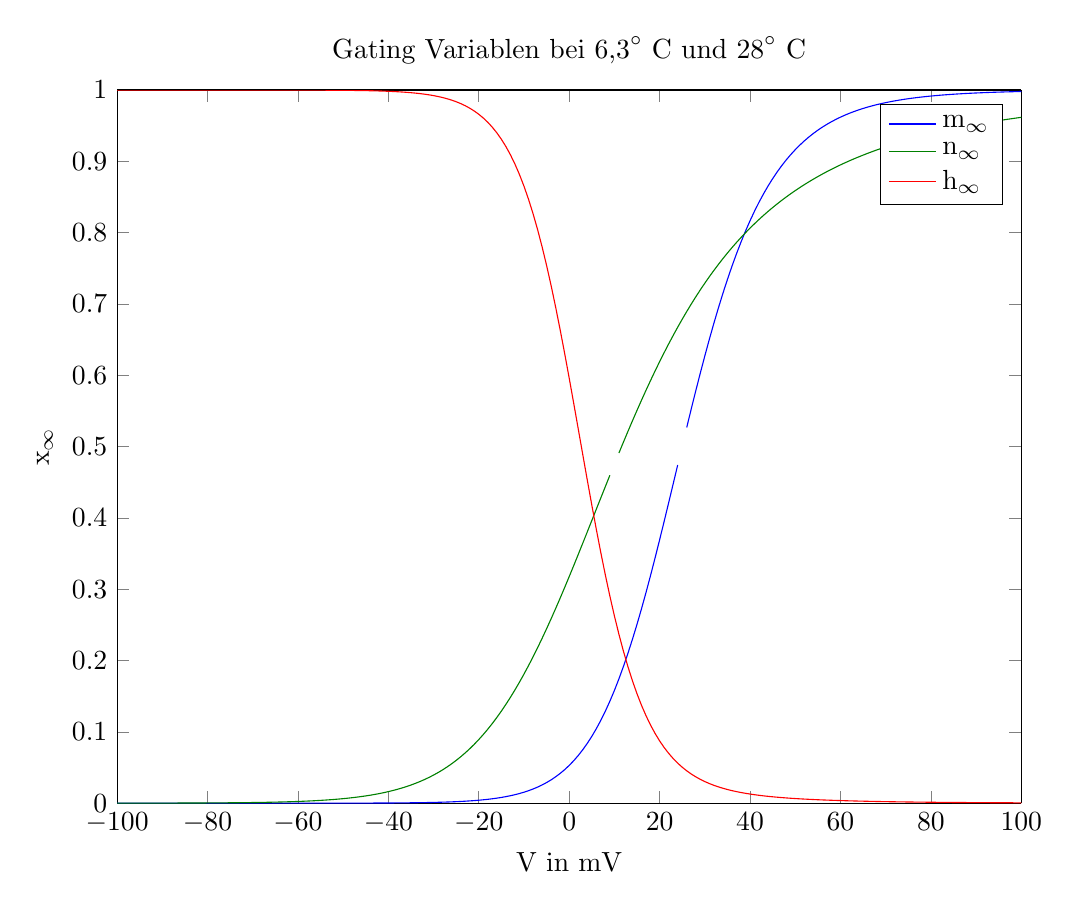
\begin{tikzpicture}

\begin{axis}[%
width=4.520833in,
height=3.565625in,
at={(0.758333in,0.48125in)},
scale only axis,
unbounded coords=jump,
separate axis lines,
every outer x axis line/.append style={black},
every x tick label/.append style={font=\color{black}},
xmin=-100,
xmax=100,
xlabel={V in mV},
every outer y axis line/.append style={black},
every y tick label/.append style={font=\color{black}},
ymin=0,
ymax=1,
ylabel={$\text{x}_\infty$},
title={$\text{Gating Variablen bei 6,3}^\circ\text{ C und 28}^\circ\text{ C}$},
legend style={legend cell align=left,align=left,draw=black}
]
\addplot [color=blue,solid]
  table[row sep=crcr]{%
-100	4.50218643500664e-08\\
-99	5.2178577339393e-08\\
-98	6.04689968570474e-08\\
-97	7.00720150102856e-08\\
-96	8.1194626870282e-08\\
-95	9.40763228460555e-08\\
-94	1.08994163525235e-07\\
-93	1.26268642288911e-07\\
-92	1.46270457124188e-07\\
-91	1.69428331616547e-07\\
-90	1.96238046470418e-07\\
-89	2.27272867499867e-07\\
-88	2.6319558433326e-07\\
-87	3.0477240663793e-07\\
-86	3.52889002125719e-07\\
-85	4.08569003672574e-07\\
-84	4.72995362405262e-07\\
-83	5.47534980526306e-07\\
-82	6.33767123052427e-07\\
-81	7.33516182776683e-07\\
-80	8.48889459053683e-07\\
-79	9.82320710077728e-07\\
-78	1.13662035203446e-06\\
-77	1.31503330898057e-06\\
-76	1.52130566696657e-06\\
-75	1.7597614575285e-06\\
-74	2.03539109238817e-06\\
-73	2.35395319660886e-06\\
-72	2.72209184564535e-06\\
-71	3.14747150735716e-06\\
-70	3.63893232841857e-06\\
-69	4.20666879167241e-06\\
-68	4.86243521367361e-06\\
-67	5.61978205770566e-06\\
-66	6.4943276157232e-06\\
-65	7.50407027293911e-06\\
-64	8.66974732240916e-06\\
-63	1.00152471567241e-05\\
-62	1.15680826441979e-05\\
-61	1.33599346139929e-05\\
-60	1.54272756467667e-05\\
-59	1.78120858152627e-05\\
-58	2.0562673665986e-05\\
-57	2.37346176046869e-05\\
-56	2.73918449739794e-05\\
-55	3.16078685236236e-05\\
-54	3.64672027091921e-05\\
-53	4.20669853535648e-05\\
-52	4.85188337129924e-05\\
-51	5.59509679553006e-05\\
-50	6.4510639537377e-05\\
-49	7.43669070232295e-05\\
-48	8.57138075794196e-05\\
-47	9.87739787945479e-05\\
-46	0.000113802792673163\\
-45	0.000131093071737869\\
-44	0.000150980466228918\\
-43	0.000173849581516588\\
-42	0.000200140956142237\\
-41	0.000230359003487483\\
-40	0.000265081044049114\\
-39	0.000304967570782416\\
-38	0.000350773907077854\\
-37	0.00040336343575953\\
-36	0.000463722598130855\\
-35	0.000532977884616956\\
-34	0.000612415063009913\\
-33	0.000703500916717342\\
-32	0.000807907793697204\\
-31	0.000927541296807615\\
-30	0.00106457147788688\\
-29	0.00122146793065404\\
-28	0.00140103921096657\\
-27	0.00160647704635918\\
-26	0.00184140582912075\\
-25	0.00210993791711072\\
-24	0.00241673529232742\\
-23	0.00276707814665566\\
-22	0.00316694097435888\\
-21	0.00362307674810132\\
-20	0.00414310973504909\\
-19	0.00473563746629856\\
-18	0.0054103422996661\\
-17	0.00617811290446946\\
-16	0.00705117583745802\\
-15	0.00804323715986867\\
-14	0.00916963375319634\\
-13	0.010447493610291\\
-12	0.0118959038916902\\
-11	0.0135360849261093\\
-10	0.0153915675793854\\
-9	0.017488370498834\\
-8	0.0198551726426987\\
-7	0.0225234752141266\\
-6	0.0255277456302258\\
-5	0.0289055344751919\\
-4	0.0326975545351544\\
-3	0.0369477090377618\\
-2	0.0417030541992076\\
-1	0.0470136792324338\\
0	0.0529324852572496\\
1	0.0595148432950742\\
2	0.0668181110050036\\
3	0.0749009883568863\\
4	0.083822694419144\\
5	0.0936419512641728\\
6	0.104415767045555\\
7	0.116198018889037\\
8	0.129037847525986\\
9	0.142977889511184\\
10	0.158052389005821\\
11	0.174285248661067\\
12	0.191688096838304\\
13	0.210258464529036\\
14	0.229978177811453\\
15	0.250812078253789\\
16	0.272707182220857\\
17	0.295592378920759\\
18	0.319378745480303\\
19	0.343960525806185\\
20	0.369216780320331\\
21	0.395013669067644\\
22	0.421207285475888\\
23	0.447646917030509\\
24	0.474178576971996\\
25	nan\\
26	0.526907342878064\\
27	0.55281215707236\\
28	0.578230592942422\\
29	0.603042618875702\\
30	0.62714244765181\\
31	0.650439720220334\\
32	0.672860089176377\\
33	0.694345246158986\\
34	0.714852462812193\\
35	0.734353731359649\\
36	0.752834598475034\\
37	0.770292786060381\\
38	0.786736686383125\\
39	0.802183808595808\\
40	0.816659240750586\\
41	0.83019417757777\\
42	0.842824550749726\\
43	0.854589785965775\\
44	0.865531700499708\\
45	0.875693546092312\\
46	0.885119195270473\\
47	0.893852464203141\\
48	0.901936561841283\\
49	0.909413653068698\\
50	0.91632452263969\\
51	0.922708326540221\\
52	0.928602417853488\\
53	0.93404223504699\\
54	0.93906124167209\\
55	0.943690907659789\\
56	0.947960723620019\\
57	0.951898240744621\\
58	0.955529130035433\\
59	0.958877255604316\\
60	0.961964757709306\\
61	0.964812141997007\\
62	0.967438372118484\\
63	0.96986096348085\\
64	0.972096076398113\\
65	0.974158607322708\\
66	0.9760622771834\\
67	0.977819716135959\\
68	0.979442544259222\\
69	0.980941447909392\\
70	0.98232625158712\\
71	0.983605985281662\\
72	0.984788947339873\\
73	0.98588276296991\\
74	0.986894438534319\\
75	0.987830411818195\\
76	0.988696598478137\\
77	0.989498434889255\\
78	0.990240917612303\\
79	0.990928639702866\\
80	0.991565824080613\\
81	0.99215635416991\\
82	0.992703802014549\\
83	0.993211454059448\\
84	0.993682334781562\\
85	0.994119228341179\\
86	0.994524698413705\\
87	0.994901106350985\\
88	0.99525062781055\\
89	0.995575267980844\\
90	0.99587687552067\\
91	0.996157155321789\\
92	0.996417680194864\\
93	0.99665990157076\\
94	0.996885159301577\\
95	0.997094690638743\\
96	0.997289638458908\\
97	0.997471058802385\\
98	0.997639927783285\\
99	0.997797147925388\\
100	0.997943553973116\\
};
\addlegendentry{$\text{m}_\infty$};

\addplot [color=black!50!green,solid]
  table[row sep=crcr]{%
-100	4.21079631997235e-05\\
-99	4.66933408299032e-05\\
-98	5.17736724126891e-05\\
-97	5.74018130951015e-05\\
-96	6.36361869586048e-05\\
-95	7.05413636912108e-05\\
-94	7.8188693601178e-05\\
-93	8.66570066829728e-05\\
-92	9.60333819774898e-05\\
-91	0.000106413994045149\\
-90	0.000117905043995552\\
-89	0.000130623783194234\\
-88	0.000144699638498985\\
-87	0.000160275448668836\\
-86	0.000177508822441322\\
-85	0.000196573629691771\\
-84	0.000217661638075205\\
-83	0.000240984308610324\\
-82	0.000266774764798878\\
-81	0.00029528995108506\\
-80	0.000326812997750484\\
-79	0.00036165581071239\\
-78	0.00040016190614633\\
-77	0.000442709511389611\\
-76	0.000489714955196121\\
-75	0.000541636372103718\\
-74	0.0005989777474365\\
-73	0.00066229333128839\\
-72	0.000732192451710608\\
-71	0.000809344759239679\\
-70	0.000894485936836205\\
-69	0.000988423911234189\\
-68	0.0010920456035975\\
-67	0.00120632425920767\\
-66	0.00133232739762208\\
-65	0.00147122542629089\\
-64	0.00162430096194017\\
-63	0.00179295890504341\\
-62	0.00197873731332234\\
-61	0.00218331912033681\\
-60	0.00240854474471818\\
-59	0.00265642563432822\\
-58	0.00292915878742044\\
-57	0.00322914228955311\\
-56	0.00355899190033602\\
-55	0.00392155871784098\\
-54	0.00431994794039204\\
-53	0.00475753873516745\\
-52	0.00523800521024869\\
-51	0.00576533847106794\\
-50	0.00634386972322684\\
-49	0.00697829436095048\\
-48	0.00767369695354158\\
-47	0.00843557701063397\\
-46	0.00926987537033192\\
-45	0.0101830010119899\\
-44	0.0111818580469966\\
-43	0.0122738725860935\\
-42	0.0134670191201848\\
-41	0.0147698459831211\\
-40	0.0161914993895741\\
-39	0.0177417454591177\\
-38	0.0194309895495481\\
-37	0.0212702921292464\\
-36	0.0232713803214218\\
-35	0.0254466541543223\\
-34	0.0278091864535808\\
-33	0.0303727152191197\\
-32	0.0331516272436441\\
-31	0.0361609316577581\\
-30	0.0394162220341243\\
-29	0.0429336256567207\\
-28	0.0467297385688552\\
-27	0.0508215450635698\\
-26	0.0552263203812599\\
-25	0.0599615155406747\\
-24	0.0650446234595013\\
-23	0.0704930258269963\\
-22	0.0763238205794033\\
-21	0.0825536303023417\\
-20	0.0891983924425966\\
-19	0.0962731328498575\\
-18	0.103791724876612\\
-17	0.111766637024995\\
-16	0.120208672919649\\
-15	0.12912670817536\\
-14	0.138527429480811\\
-13	0.148415081893088\\
-12	0.158791230885865\\
-11	0.16965454607027\\
-10	0.181000613666071\\
-9	0.192821784702047\\
-8	0.205107065537571\\
-7	0.217842056604958\\
-6	0.231008944272605\\
-5	0.244586549440072\\
-4	0.258550434935186\\
-3	0.27287307204697\\
-2	0.287524064670547\\
-1	0.302470427648354\\
0	0.317676914060697\\
1	0.333106384543767\\
2	0.34872021028434\\
3	0.364478700234374\\
4	0.380341542363334\\
5	0.396268248456051\\
6	0.412218592077924\\
7	0.42815302985051\\
8	0.444033097068069\\
9	0.459821769878944\\
10	nan\\
11	0.490985930939946\\
12	0.506297251314051\\
13	0.5213892525013\\
14	0.536236021852238\\
15	0.550814314084053\\
16	0.5651035896537\\
17	0.579086011295512\\
18	0.592746402955275\\
19	0.606072175844573\\
20	0.619053226610616\\
21	0.631681812689311\\
22	0.643952409810817\\
23	0.655861556388273\\
24	0.667407689174083\\
25	0.678590974145183\\
26	0.68941313610797\\
27	0.699877290020385\\
28	0.709987776534345\\
29	0.719750003783486\\
30	0.729170296991849\\
31	0.738255757068002\\
32	0.747014128981724\\
33	0.755453680399621\\
34	0.763583090782469\\
35	0.77141135091916\\
36	0.778947672687369\\
37	0.786201408685732\\
38	0.793181981272413\\
39	0.799898820465975\\
40	0.806361310112202\\
41	0.812578741690533\\
42	0.818560275122353\\
43	0.824314905946659\\
44	0.829851438243614\\
45	0.835178462710237\\
46	0.84030433932263\\
47	0.845237184053631\\
48	0.849984859151953\\
49	0.854554966527387\\
50	0.858954843825304\\
51	0.863191562811839\\
52	0.867271929727948\\
53	0.87120248730569\\
54	0.874989518173204\\
55	0.878639049405718\\
56	0.882156858008564\\
57	0.885548477144335\\
58	0.888819202940277\\
59	0.891974101733645\\
60	0.895018017632252\\
61	0.897955580284926\\
62	0.900791212772169\\
63	0.903529139541116\\
64	0.90617339432114\\
65	0.908727827967139\\
66	0.911196116186988\\
67	0.913581767117809\\
68	0.915888128722841\\
69	0.918118395986825\\
70	0.920275617893136\\
71	0.92236270417038\\
72	0.924382431800064\\
73	0.926337451280174\\
74	0.928230292642255\\
75	0.930063371221863\\
76	0.931838993184149\\
77	0.933559360807877\\
78	0.935226577532442\\
79	0.936842652773431\\
80	0.938409506513056\\
81	0.93992897367237\\
82	0.941402808272623\\
83	0.942832687393377\\
84	0.944220214935218\\
85	0.945566925194974\\
86	0.946874286261344\\
87	0.94814370323881\\
88	0.949376521307596\\
89	0.950574028627254\\
90	0.951737459091332\\
91	0.952867994940302\\
92	0.953966769239762\\
93	0.955034868230633\\
94	0.956073333557855\\
95	0.957083164383798\\
96	0.958065319392372\\
97	0.959020718689547\\
98	0.959950245605714\\
99	0.960854748405121\\
100	0.961735041907303\\
};
\addlegendentry{$\text{n}_\infty$};

\addplot [color=red,solid]
  table[row sep=crcr]{%
-100	0.9999997824294\\
-99	0.999999747219096\\
-98	0.999999706310579\\
-97	0.999999658781689\\
-96	0.999999603561031\\
-95	0.999999539403823\\
-94	0.99999946486384\\
-93	0.999999378260807\\
-92	0.999999277642534\\
-91	0.999999160740903\\
-90	0.999999024920745\\
-89	0.999998867120443\\
-88	0.999998683782919\\
-87	0.999998470775458\\
-86	0.999998223296551\\
-85	0.999997935767677\\
-84	0.999997601707559\\
-83	0.99999721358608\\
-82	0.999996762654566\\
-81	0.999996238748599\\
-80	0.999995630058932\\
-79	0.999994922865337\\
-78	0.999994101227392\\
-77	0.999993146625239\\
-76	0.999992037542234\\
-75	0.999990748980073\\
-74	0.999989251895486\\
-73	0.999987512545818\\
-72	0.999985491728764\\
-71	0.999983143899143\\
-70	0.999980416142853\\
-69	0.999977246984906\\
-68	0.999973565004764\\
-67	0.999969287227819\\
-66	0.99996431725691\\
-65	0.999958543101875\\
-64	0.999951834658435\\
-63	0.999944040779839\\
-62	0.999934985875625\\
-61	0.999924465961295\\
-60	0.999912244070481\\
-59	0.999898044927048\\
-58	0.999881548758126\\
-57	0.999862384110122\\
-56	0.99984011950774\\
-55	0.99981425377066\\
-54	0.999784204773117\\
-53	0.999749296397729\\
-52	0.999708743395794\\
-51	0.99966163382117\\
-50	0.999606908653031\\
-49	0.999543338163118\\
-48	0.999469494514851\\
-47	0.999383720003377\\
-46	0.999284090256451\\
-45	0.999168371614465\\
-44	0.999033971792824\\
-43	0.998877882800005\\
-42	0.998696614938781\\
-41	0.998486120555519\\
-40	0.998241706022691\\
-39	0.997957930242876\\
-38	0.997628487750032\\
-37	0.997246074258172\\
-36	0.996802232273765\\
-35	0.996287174153928\\
-34	0.995689579769551\\
-33	0.994996365738375\\
-32	0.994192423052278\\
-31	0.993260319870075\\
-30	0.992179966329049\\
-29	0.990928238508216\\
-28	0.989478559237625\\
-27	0.987800434398963\\
-26	0.985858944841801\\
-25	0.983614196219538\\
-24	0.98102073213988\\
-23	0.978026920274938\\
-22	0.974574326767017\\
-21	0.970597101697485\\
-20	0.966021407847207\\
-19	0.960764936696566\\
-18	0.954736569680182\\
-17	0.9478362589578\\
-16	0.939955219801257\\
-15	0.930976544914395\\
-14	0.920776367517614\\
-13	0.909225711653247\\
-12	0.896193170433952\\
-11	0.881548540122511\\
-10	0.865167503327214\\
-9	0.846937391490435\\
-8	0.826763960004448\\
-7	0.804578977270273\\
-6	0.780348267017668\\
-5	0.754079665822525\\
-4	0.725830190606678\\
-3	0.695711589667898\\
-2	0.663893416369745\\
-1	0.630602853941704\\
0	0.59612075350846\\
1	0.560773717724098\\
2	0.524922526266709\\
3	0.488947681848153\\
4	0.453233263894107\\
5	0.418150525550343\\
6	0.384042703275773\\
7	0.351212320116477\\
8	0.31991189696476\\
9	0.290338520268204\\
10	0.262632242161572\\
11	0.236877890516672\\
12	0.213109593615229\\
13	0.191317193824931\\
14	0.171453723308318\\
15	0.15344320964104\\
16	0.137188230544453\\
17	0.122576808036934\\
18	0.109488395307089\\
19	0.0977988473121772\\
20	0.0873843709653745\\
21	0.0781245224463857\\
22	0.0699043617209371\\
23	0.0626158938970438\\
24	0.0561589300341594\\
25	0.0504414922415569\\
26	0.0453798740086048\\
27	0.040898450131275\\
28	0.0369293136590722\\
29	0.0334118014124865\\
30	0.0302919555749689\\
31	0.0275219569473024\\
32	0.0250595556743559\\
33	0.0228675174528481\\
34	0.0209130971585338\\
35	0.0191675472192461\\
36	0.0176056646400015\\
37	0.0162053781161488\\
38	0.0149473749414042\\
39	0.0138147662552288\\
40	0.0127927884367836\\
41	0.0118685380281132\\
42	0.0110307373695394\\
43	0.0102695280881913\\
44	0.00957628964538262\\
45	0.00894348028244084\\
46	0.00836449788002215\\
47	0.0078335584431438\\
48	0.007345590129261\\
49	0.00689614094025265\\
50	0.00648129839496137\\
51	0.00609761968312441\\
52	0.00574207097199861\\
53	0.00541197469277655\\
54	0.00510496377488265\\
55	0.00481894192283547\\
56	0.00455204914331594\\
57	0.00430263183033875\\
58	0.00406921680503027\\
59	0.00385048878454596\\
60	0.00364527082316952\\
61	0.00345250732863368\\
62	0.00327124930913525\\
63	0.00310064155225296\\
64	0.00293991147681082\\
65	0.00278835943337685\\
66	0.00264535025918786\\
67	0.00251030591941736\\
68	0.00238269908936035\\
69	0.00226204755174303\\
70	0.00214790930036929\\
71	0.00203987825603456\\
72	0.00193758051337163\\
73	0.0018406710483064\\
74	0.00174883082532304\\
75	0.00166176425196805\\
76	0.00157919693513424\\
77	0.00150087369980985\\
78	0.00142655683628584\\
79	0.00135602454639878\\
80	0.00128906956334617\\
81	0.00122549792303102\\
82	0.00116512786784549\\
83	0.00110778886635448\\
84	0.00105332073454263\\
85	0.0010015728461916\\
86	0.00095240342159822\\
87	0.000905678885264226\\
88	0.000861273284416153\\
89	0.000819067761274497\\
90	0.000778950072908659\\
91	0.000740814153307414\\
92	0.000704559712980852\\
93	0.000670091872003699\\
94	0.000637320822924089\\
95	0.000606161520407307\\
96	0.000576533394870065\\
97	0.000548360087695622\\
98	0.000521569205910576\\
99	0.000496092094456417\\
100	0.00047186362440815\\
};
\addlegendentry{$\text{h}_\infty$};

\end{axis}
\end{tikzpicture}%}
    \caption{Steady State Gating Variablen $x_\infty$ bei $6.3^\circ C$ und $28^\circ C$}
    \label{fig:Gating1}
\end{figure}
Im Betrachtet man die Gating Variablen und die Zeitkonstanten gemeinsam kann man daraus das Verhalten eines Neurons nach dem Hodgkin \& Huxley Modell erklären. Zuerst sind alle Ionenkanäle geschlossen und die Zelle befindet sich im Ruhepotential nahe -70mV. Die Gating Variablen m und n sind nahe 0, was heißt die Leitfähigkeit der Kanäle ist gering. Erhöht sich nun das Membranpotential durch einen Stimulus kann sich - durch die kleine Zeitkonstante $\tau_m$ - zuerst der schnelle $Na^+$ Kanal öffnen. Das Membranpotential der Zelle erhöht sich ab einem gewissen Threshold (ab -20mV ist erst ein signifikanter Anstieg von $m_\infty$ zu sehen) durch den Zufluss der positiven Ionen schlagartig (Spike). Mit der nächst größeren Zeitkonstanten $\tau_n$ folgt auch der $K^+$ Kanal und zusätzlich wird dann der $Na^+$ Kanal durch die Variable $h$ wieder deaktiviert und die Zelle kann auf das Ruhepotential zurückkehren. Das Verhalten der Gating Variablen kann dabei aus den Steady State Werte (vgl. Abb. \ref{fig:Gating1}) abgelesen werden. Dies sind die Werte wohin m,n,h bei einem gegebenen Membranpotenital streben. Ist beispielsweise das Membranpotential hoch (Aktionspotential), strebt die Variable h gegen 0. Wie schnell dies geschieht, beschreibt die Zeitkonstante $\tau_h$.

\section{Hodgkin \& Huxley Neuron Model}
Im Abb. \ref{fig:Stiumulus6} ist der Stimulus abgebildet, der bei $6.3^\circ C$ angewendet werden soll.
\begin{figure}[h!]
  	\centering
    \scalebox{.6}{\input{img/Stiumulus6.tikz}}
    \caption{Stimulusstromdichte bei $6.3^\circ C$}
    \label{fig:Stiumulus6}
\end{figure}

\begin{figure}[h!]
  	\centering
    \scalebox{.6}{% This file was created by matlab2tikz.
% Minimal pgfplots version: 1.3
%
%The latest updates can be retrieved from
%  http://www.mathworks.com/matlabcentral/fileexchange/22022-matlab2tikz
%where you can also make suggestions and rate matlab2tikz.
%
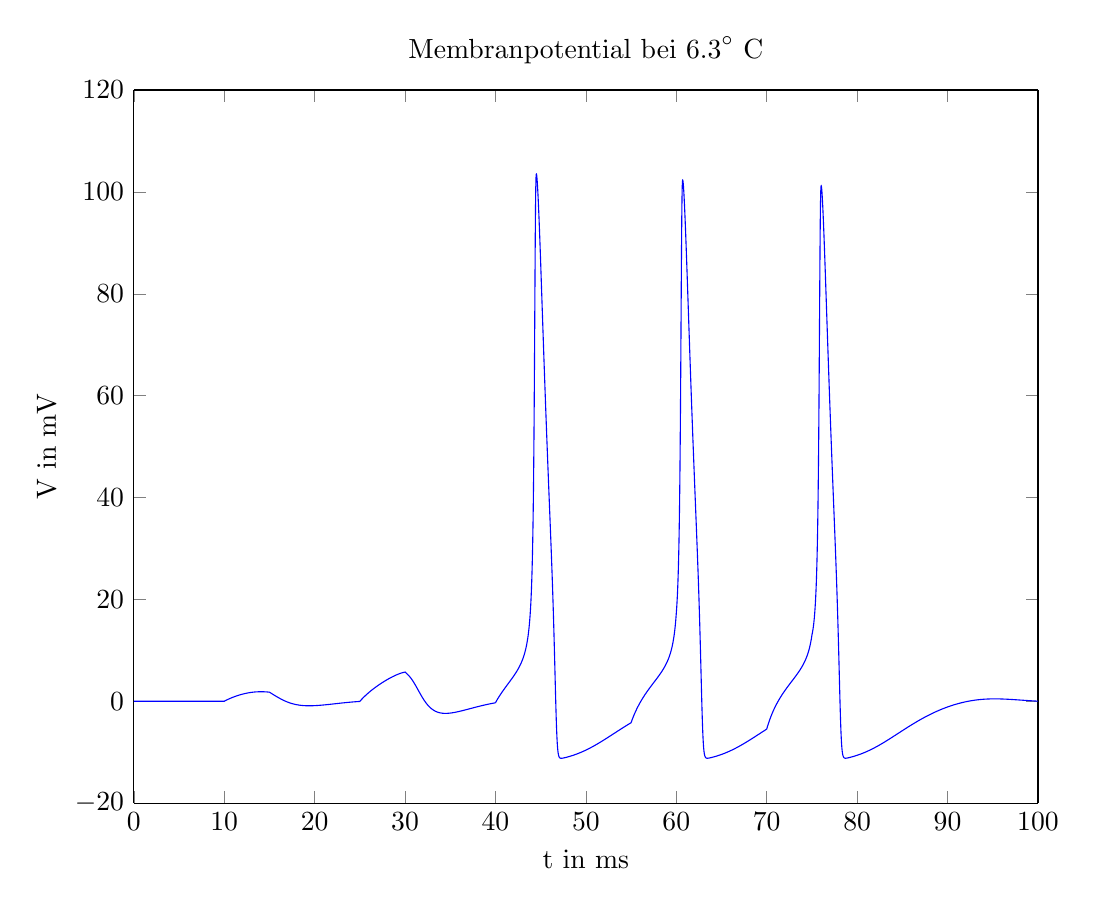
\begin{tikzpicture}

\begin{axis}[%
width=4.520833in,
height=3.565625in,
at={(0.758333in,0.48125in)},
scale only axis,
separate axis lines,
every outer x axis line/.append style={black},
every x tick label/.append style={font=\color{black}},
xmin=0,
xmax=100,
xlabel={t in ms},
every outer y axis line/.append style={black},
every y tick label/.append style={font=\color{black}},
ymin=-20,
ymax=120,
ylabel={V in mV},
title={$\text{Membranpotential bei 6.3}^\circ\text{ C}$}
]
\addplot [color=blue,solid,forget plot]
  table[row sep=crcr]{%
0	0\\
0.01	3.23709182497467e-06\\
0.02	6.47418364994934e-06\\
0.03	9.68987688454881e-06\\
0.04	1.28846724626142e-05\\
0.05	1.60591899617524e-05\\
0.06	1.92140204736946e-05\\
0.07	2.23497269563078e-05\\
0.08	2.54668455290874e-05\\
0.09	2.85658867159544e-05\\
0.1	3.16473366306491e-05\\
0.11	3.47116581080043e-05\\
0.12	3.77592917830549e-05\\
0.13	4.07906571206018e-05\\
0.14	4.38061533976342e-05\\
0.15	4.68061606403536e-05\\
0.16	4.97910405184454e-05\\
0.17	5.27611371979697e-05\\
0.18	5.57167781553503e-05\\
0.19	5.86582749537934e-05\\
0.2	6.15859239839933e-05\\
0.21	6.45000071710244e-05\\
0.22	6.74007926485309e-05\\
0.23	7.02885354020477e-05\\
0.24	7.31634778827139e-05\\
0.25	7.60258505928535e-05\\
0.26	7.88758726445504e-05\\
0.27	8.1713752292627e-05\\
0.28	8.45396874430993e-05\\
0.29	8.73538661382067e-05\\
0.3	9.01564670192334e-05\\
0.31	9.29476597680923e-05\\
0.32	9.57276055284773e-05\\
0.33	9.84964573077196e-05\\
0.34	0.000101254360360206\\
0.35	0.000104001452553026\\
0.36	0.000106737864715041\\
0.37	0.000109463720969711\\
0.38	0.000112179139052628\\
0.39	0.000114884230614551\\
0.4	0.00011757910151041\\
0.41	0.00012026385207506\\
0.42	0.000122938577386287\\
0.43	0.000125603367515832\\
0.44	0.000128258307768716\\
0.45	0.000130903478911653\\
0.46	0.000133538957390948\\
0.47	0.000136164815540312\\
0.48	0.000138781121779106\\
0.49	0.000141387940801532\\
0.5	0.000143985333757026\\
0.51	0.000146573358422359\\
0.52	0.000149152069365885\\
0.53	0.000151721518104142\\
0.54	0.000154281753251255\\
0.55	0.000156832820661426\\
0.56	0.00015937476356497\\
0.57	0.000161907622697903\\
0.58	0.000164431436425687\\
0.59	0.000166946240861208\\
0.6	0.000169452069977289\\
0.61	0.000171948955714072\\
0.62	0.000174436928081456\\
0.63	0.00017691601525669\\
0.64	0.000179386243677611\\
0.65	0.000181847638131374\\
0.66	0.000184300221839306\\
0.67	0.000186744016537701\\
0.68	0.00018917904255487\\
0.69	0.000191605318884656\\
0.7	0.0001940228632566\\
0.71	0.000196431692202759\\
0.72	0.00019883182112153\\
0.73	0.000201223264338384\\
0.74	0.000203606035163908\\
0.75	0.000205980145949098\\
0.76	0.000208345608138094\\
0.77	0.000210702432318421\\
0.78	0.000213050628269045\\
0.79	0.000215390205006005\\
0.8	0.000217721170825986\\
0.81	0.000220043533347862\\
0.82	0.000222357299552423\\
0.83	0.000224662475820052\\
0.84	0.000226959067966788\\
0.85	0.000229247081278645\\
0.86	0.000231526520544323\\
0.87	0.000233797390086368\\
0.88	0.00023605969379096\\
0.89	0.000238313435136237\\
0.9	0.000240558617219264\\
0.91	0.000242795242781786\\
0.92	0.00024502331423478\\
0.93	0.000247242833681831\\
0.94	0.000249453802941342\\
0.95	0.000251656223567807\\
0.96	0.000253850096872004\\
0.97	0.00025603542394022\\
0.98	0.000258212205652666\\
0.99	0.000260380442700892\\
1	0.000262540135604383\\
1.01	0.000264691284726495\\
1.02	0.000266833890289528\\
1.03	0.000268967952389039\\
1.04	0.000271093471007573\\
1.05	0.000273210446027679\\
1.06	0.000275318877244248\\
1.07	0.000277418764376365\\
1.08	0.000279510107078469\\
1.09	0.000281592904951062\\
1.1	0.000283667157550909\\
1.11	0.000285732864400661\\
1.12	0.000287790024998014\\
1.13	0.00028983863882444\\
1.14	0.000291878705353561\\
1.15	0.000293910224058975\\
1.16	0.000295933194421831\\
1.17	0.000297947615937884\\
1.18	0.000299953488124265\\
1.19	0.000301950810525962\\
1.2	0.000303939582721875\\
1.21	0.00030591980433067\\
1.22	0.000307891475016184\\
1.23	0.000309854594492713\\
1.24	0.000311809162529877\\
1.25	0.000313755178957407\\
1.26	0.000315692643669561\\
1.27	0.000317621556629284\\
1.28	0.000319541917872237\\
1.29	0.000321453727510579\\
1.3	0.000323356985736471\\
1.31	0.000325251692825486\\
1.32	0.000327137849139807\\
1.33	0.000329015455131278\\
1.34	0.000330884511344149\\
1.35	0.000332745018417828\\
1.36	0.000334596977089405\\
1.37	0.000336440388196033\\
1.38	0.000338275252677156\\
1.39	0.00034010157157665\\
1.4	0.00034191934604475\\
1.41	0.00034372857733997\\
1.42	0.000345529266830824\\
1.43	0.000347321415997457\\
1.44	0.000349105026433181\\
1.45	0.000350880099845923\\
1.46	0.000352646638059526\\
1.47	0.000354404643015012\\
1.48	0.000356154116771674\\
1.49	0.0003578950615083\\
1.5	0.000359627479524014\\
1.51	0.000361351373239254\\
1.52	0.000363066745196594\\
1.53	0.000364773598061525\\
1.54	0.000366471934623203\\
1.55	0.000368161757795033\\
1.56	0.00036984307061533\\
1.57	0.000371515876247748\\
1.58	0.000373180177981815\\
1.59	0.000374835979233414\\
1.6	0.000376483283545035\\
1.61	0.000378122094586173\\
1.62	0.000379752416153534\\
1.63	0.000381374252171409\\
1.64	0.000382987606691762\\
1.65	0.000384592483894397\\
1.66	0.000386188888087093\\
1.67	0.000387776823705717\\
1.68	0.000389356295314243\\
1.69	0.0003909273076047\\
1.7	0.000392489865397327\\
1.71	0.000394043973640374\\
1.72	0.000395589637410056\\
1.73	0.000397126861910531\\
1.74	0.000398655652473705\\
1.75	0.000400176014559124\\
1.76	0.000401687953753789\\
1.77	0.000403191475771907\\
1.78	0.000404686586454739\\
1.79	0.000406173291770404\\
1.8	0.000407651597813534\\
1.81	0.000409121510805033\\
1.82	0.000410583037091832\\
1.83	0.00041203618314646\\
1.84	0.000413480955566903\\
1.85	0.000414917361076061\\
1.86	0.000416345406521565\\
1.87	0.000417765098875322\\
1.88	0.000419176445233158\\
1.89	0.000420579452814405\\
1.9	0.000421974128961562\\
1.91	0.000423360481139823\\
1.92	0.000424738516936625\\
1.93	0.000426108244061267\\
1.94	0.000427469670344465\\
1.95	0.00042882280373786\\
1.96	0.000430167652313589\\
1.97	0.000431504224263759\\
1.98	0.000432832527900029\\
1.99	0.000434152571653099\\
2	0.000435464364072171\\
2.01	0.000436767913824525\\
2.02	0.000438063229695009\\
2.03	0.000439350320585419\\
2.04	0.000440629195514095\\
2.05	0.000441899863615291\\
2.06	0.000443162334138729\\
2.07	0.00044441661644905\\
2.08	0.000445662720025273\\
2.09	0.000446900654460092\\
2.1	0.000448130429459632\\
2.11	0.000449352054842644\\
2.12	0.000450565540540051\\
2.13	0.000451770896594357\\
2.14	0.000452968133159071\\
2.15	0.000454157260498156\\
2.16	0.000455338288985474\\
2.17	0.000456511229104199\\
2.18	0.000457676091446224\\
2.19	0.000458832886711602\\
2.2	0.000459981625707959\\
2.21	0.000461122319349876\\
2.22	0.000462254978658327\\
2.23	0.000463379614760142\\
2.24	0.000464496238887388\\
2.25	0.000465604862376705\\
2.26	0.000466705496668789\\
2.27	0.00046779815330773\\
2.28	0.000468882843940514\\
2.29	0.000469959580316348\\
2.3	0.000471028374286044\\
2.31	0.000472089237801527\\
2.32	0.000473142182915138\\
2.33	0.00047418722177905\\
2.34	0.000475224366644688\\
2.35	0.000476253629862113\\
2.36	0.000477275023879371\\
2.37	0.000478288561241964\\
2.38	0.000479294254592188\\
2.39	0.000480292116668583\\
2.4	0.000481282160305256\\
2.41	0.000482264398431327\\
2.42	0.000483238844070324\\
2.43	0.000484205510339546\\
2.44	0.000485164410449434\\
2.45	0.000486115557703024\\
2.46	0.000487058965495315\\
2.47	0.000487994647312622\\
2.48	0.000488922616732057\\
2.49	0.00048984288742079\\
2.5	0.000490755473135604\\
2.51	0.00049166038772213\\
2.52	0.00049255764511436\\
2.53	0.000493447259333948\\
2.54	0.000494329244489648\\
2.55	0.000495203614776733\\
2.56	0.000496070384476339\\
2.57	0.000496929567954867\\
2.58	0.00049778117966341\\
2.59	0.000498625234137089\\
2.6	0.00049946174599452\\
2.61	0.000500290729937167\\
2.62	0.00050111220074875\\
2.63	0.000501926173294631\\
2.64	0.000502732662521206\\
2.65	0.000503531683455316\\
2.66	0.000504323251203669\\
2.67	0.000505107380952219\\
2.68	0.000505884087965498\\
2.69	0.000506653387586122\\
2.7	0.00050741529523417\\
2.71	0.00050816982640653\\
2.72	0.000508916996676305\\
2.73	0.00050965682169231\\
2.74	0.000510389317178394\\
2.75	0.000511114498932832\\
2.76	0.000511832382827801\\
2.77	0.000512542984808739\\
2.78	0.000513246320893756\\
2.79	0.00051394240717304\\
2.8	0.000514631259808262\\
2.81	0.000515312895032007\\
2.82	0.000515987329147189\\
2.83	0.000516654578526427\\
2.84	0.000517314659611498\\
2.85	0.000517967588912698\\
2.86	0.000518613383008337\\
2.87	0.000519252058544066\\
2.88	0.000519883632232329\\
2.89	0.000520508120851826\\
2.9	0.000521125541246867\\
2.91	0.000521735910326799\\
2.92	0.000522339245065457\\
2.93	0.000522935562500612\\
2.94	0.000523524879733292\\
2.95	0.000524107213927278\\
2.96	0.000524682582308506\\
2.97	0.000525251002164562\\
2.98	0.000525812490843997\\
2.99	0.000526367065755861\\
3	0.000526914744369002\\
3.01	0.00052745554421163\\
3.02	0.000527989482870703\\
3.03	0.000528516577991298\\
3.04	0.000529036847276147\\
3.05	0.000529550308484965\\
3.06	0.000530056979433979\\
3.07	0.00053055687799533\\
3.08	0.000531050022096497\\
3.09	0.000531536429719726\\
3.1	0.000532016118901501\\
3.11	0.000532489107732035\\
3.12	0.000532955414354577\\
3.13	0.000533415056964994\\
3.14	0.000533868053811091\\
3.15	0.000534314423192219\\
3.16	0.000534754183458568\\
3.17	0.000535187353010662\\
3.18	0.00053561395029885\\
3.19	0.000536033993822742\\
3.2	0.000536447502130599\\
3.21	0.000536854493818906\\
3.22	0.000537254987531725\\
3.23	0.000537649001960148\\
3.24	0.000538036555841859\\
3.25	0.000538417667960527\\
3.26	0.00053879235714521\\
3.27	0.000539160642269931\\
3.28	0.000539522542253077\\
3.29	0.000539878076056879\\
3.3	0.000540227262686867\\
3.31	0.00054057012119133\\
3.32	0.000540906670660792\\
3.33	0.000541236930227478\\
3.34	0.000541560919064814\\
3.35	0.000541878656386876\\
3.36	0.000542190161447875\\
3.37	0.0005424954535416\\
3.38	0.000542794552000925\\
3.39	0.000543087476197286\\
3.4	0.000543374245540202\\
3.41	0.000543654879476652\\
3.42	0.00054392939749059\\
3.43	0.000544197819102519\\
3.44	0.000544460163868878\\
3.45	0.00054471645138157\\
3.46	0.000544966701267433\\
3.47	0.00054521093318777\\
3.48	0.000545449166837741\\
3.49	0.000545681421945949\\
3.5	0.000545907718273924\\
3.51	0.000546128075615604\\
3.52	0.000546342513796776\\
3.53	0.000546551052674657\\
3.54	0.000546753712137358\\
3.55	0.000546950512103392\\
3.56	0.000547141472521178\\
3.57	0.000547326613368515\\
3.58	0.00054750595465209\\
3.59	0.00054767951640704\\
3.6	0.000547847318696388\\
3.61	0.000548009381610601\\
3.62	0.000548165725267138\\
3.63	0.000548316369809836\\
3.64	0.000548461335408556\\
3.65	0.000548600642258567\\
3.66	0.000548734310580196\\
3.67	0.000548862360618272\\
3.68	0.000548984812641628\\
3.69	0.000549101686942719\\
3.7	0.000549213003837039\\
3.71	0.000549318783662644\\
3.72	0.000549419046779808\\
3.73	0.000549513813570361\\
3.74	0.000549603104437412\\
3.75	0.000549686939804719\\
3.76	0.000549765340116326\\
3.77	0.000549838325836029\\
3.78	0.00054990591744696\\
3.79	0.000549968135451082\\
3.8	0.00055002500036875\\
3.81	0.000550076532738268\\
3.82	0.000550122753115363\\
3.83	0.000550163682072773\\
3.84	0.000550199340199855\\
3.85	0.000550229748101962\\
3.86	0.00055025492640016\\
3.87	0.000550274895730713\\
3.88	0.000550289676744624\\
3.89	0.000550299290107134\\
3.9	0.000550303756497343\\
3.91	0.000550303096607809\\
3.92	0.000550297331144036\\
3.93	0.000550286480824029\\
3.94	0.000550270566377855\\
3.95	0.000550249608547197\\
3.96	0.000550223628084971\\
3.97	0.000550192645754865\\
3.98	0.000550156682330849\\
3.99	0.000550115758596816\\
4	0.000550069895346095\\
4.01	0.000550019113381075\\
4.02	0.000549963433512737\\
4.03	0.000549902876560204\\
4.04	0.000549837463350404\\
4.05	0.000549767214717534\\
4.06	0.000549692151502743\\
4.07	0.000549612294553658\\
4.08	0.000549527664723963\\
4.09	0.000549438282872972\\
4.1	0.000549344169865282\\
4.11	0.000549245346570264\\
4.12	0.000549141833861713\\
4.13	0.000549033652617412\\
4.14	0.000548920823718704\\
4.15	0.000548803368050126\\
4.16	0.000548681306498975\\
4.17	0.000548554659954936\\
4.18	0.000548423449309667\\
4.19	0.000548287695456357\\
4.2	0.000548147419289364\\
4.21	0.000548002641703822\\
4.22	0.000547853383595211\\
4.23	0.000547699665858969\\
4.24	0.00054754150939015\\
4.25	0.00054737893508296\\
4.26	0.000547211963830429\\
4.27	0.00054704061652397\\
4.28	0.00054686491405302\\
4.29	0.000546684877304657\\
4.3	0.000546500527163189\\
4.31	0.000546311884509825\\
4.32	0.000546118970222218\\
4.33	0.00054592180517413\\
4.34	0.000545720410235071\\
4.35	0.000545514806269924\\
4.36	0.000545305014138502\\
4.37	0.000545091054695255\\
4.38	0.000544872948788844\\
4.39	0.000544650717261814\\
4.4	0.000544424380950197\\
4.41	0.000544193960683193\\
4.42	0.000543959477282736\\
4.43	0.000543720951563182\\
4.44	0.000543478404330906\\
4.45	0.000543231856383977\\
4.46	0.000542981328511747\\
4.47	0.000542726841494621\\
4.48	0.000542468416103561\\
4.49	0.000542206073099787\\
4.5	0.000541939833234442\\
4.51	0.000541669717248183\\
4.52	0.000541395745870923\\
4.53	0.000541117939821398\\
4.54	0.000540836319806894\\
4.55	0.000540550906522888\\
4.56	0.000540261720652637\\
4.57	0.000539968782866898\\
4.58	0.000539672113823566\\
4.59	0.000539371734167391\\
4.6	0.000539067664529576\\
4.61	0.000538759925527477\\
4.62	0.000538448537764231\\
4.63	0.00053813352182849\\
4.64	0.000537814898294049\\
4.65	0.000537492687719521\\
4.66	0.000537166910647993\\
4.67	0.000536837587606773\\
4.68	0.000536504739106967\\
4.69	0.000536168385643267\\
4.7	0.000535828547693518\\
4.71	0.000535485245718461\\
4.72	0.000535138500161443\\
4.73	0.00053478833144804\\
4.74	0.000534434759985807\\
4.75	0.000534077806163915\\
4.76	0.000533717490352879\\
4.77	0.000533353832904191\\
4.78	0.000532986854150064\\
4.79	0.000532616574403164\\
4.8	0.000532243013956184\\
4.81	0.000531866193081654\\
4.82	0.000531486132031644\\
4.83	0.000531102851037359\\
4.84	0.000530716370308939\\
4.85	0.000530326710035101\\
4.86	0.000529933890382908\\
4.87	0.000529537931497441\\
4.88	0.000529138853501494\\
4.89	0.000528736676495294\\
4.9	0.000528331420556221\\
4.91	0.00052792310573861\\
4.92	0.000527511752073289\\
4.93	0.000527097379567398\\
4.94	0.000526680008204101\\
4.95	0.000526259657942325\\
4.96	0.000525836348716426\\
4.97	0.000525410100435972\\
4.98	0.000524980932985391\\
4.99	0.000524548866223817\\
5	0.000524113919984726\\
5.01	0.000523676114075684\\
5.02	0.000523235468278056\\
5.03	0.00052279200234679\\
5.04	0.000522345736010146\\
5.05	0.000521896688969381\\
5.06	0.000521444880898559\\
5.07	0.000520990331444256\\
5.08	0.000520533060225246\\
5.09	0.000520073086832338\\
5.1	0.000519610430828062\\
5.11	0.000519145111746395\\
5.12	0.000518677149092586\\
5.13	0.000518206562342858\\
5.14	0.000517733370944136\\
5.15	0.000517257594313834\\
5.16	0.000516779251839603\\
5.17	0.000516298362879071\\
5.18	0.000515814946759603\\
5.19	0.000515329022778111\\
5.2	0.000514840610200738\\
5.21	0.000514349728262627\\
5.22	0.000513856396167762\\
5.23	0.000513360633088627\\
5.24	0.000512862458166041\\
5.25	0.000512361890508935\\
5.26	0.000511858949194055\\
5.27	0.000511353653265765\\
5.28	0.000510846021735838\\
5.29	0.000510336073583222\\
5.3	0.000509823827753784\\
5.31	0.000509309303160128\\
5.32	0.000508792518681363\\
5.33	0.000508273493162839\\
5.34	0.00050775224541602\\
5.35	0.000507228794218202\\
5.36	0.000506703158312263\\
5.37	0.000506175356406558\\
5.38	0.000505645407174593\\
5.39	0.000505113329254861\\
5.4	0.000504579141250617\\
5.41	0.000504042861729701\\
5.42	0.000503504509224349\\
5.43	0.000502964102230923\\
5.44	0.000502421659209764\\
5.45	0.000501877198584935\\
5.46	0.000501330738744055\\
5.47	0.000500782298038139\\
5.48	0.000500231894781274\\
5.49	0.000499679547250574\\
5.5	0.000499125273685928\\
5.51	0.000498569092289749\\
5.52	0.000498011021226806\\
5.53	0.000497451078624081\\
5.54	0.000496889282570621\\
5.55	0.000496325651117205\\
5.56	0.000495760202276268\\
5.57	0.0004951929540217\\
5.58	0.000494623924288633\\
5.59	0.000494053130973269\\
5.6	0.000493480591932723\\
5.61	0.000492906324984839\\
5.62	0.000492330347908019\\
5.63	0.000491752678440954\\
5.64	0.000491173334282587\\
5.65	0.000490592333091931\\
5.66	0.000490009692487772\\
5.67	0.000489425430048556\\
5.68	0.000488839563312307\\
5.69	0.000488252109776362\\
5.7	0.000487663086897259\\
5.71	0.000487072512090552\\
5.72	0.000486480402730605\\
5.73	0.000485886776150504\\
5.74	0.000485291649641848\\
5.75	0.000484695040454688\\
5.76	0.000484096965797165\\
5.77	0.000483497442835575\\
5.78	0.000482896488694085\\
5.79	0.000482294120454614\\
5.8	0.000481690355156737\\
5.81	0.000481085209797421\\
5.82	0.000480478701330953\\
5.83	0.000479870846668811\\
5.84	0.000479261662679456\\
5.85	0.000478651166188229\\
5.86	0.000478039373977204\\
5.87	0.000477426302785049\\
5.88	0.000476811969306841\\
5.89	0.000476196390193979\\
5.9	0.000475579582054047\\
5.91	0.000474961561450664\\
5.92	0.000474342344903374\\
5.93	0.000473721948887409\\
5.94	0.000473100389833703\\
5.95	0.000472477684128667\\
5.96	0.000471853848114092\\
5.97	0.000471228898087053\\
5.98	0.000470602850299695\\
5.99	0.000469975720959148\\
6	0.00046934752622748\\
6.01	0.000468718282221441\\
6.02	0.000468088005012444\\
6.03	0.000467456710626446\\
6.04	0.000466824415043785\\
6.05	0.000466191134199052\\
6.06	0.000465556883981013\\
6.07	0.000464921680232466\\
6.08	0.000464285538750162\\
6.09	0.000463648475284684\\
6.1	0.000463010505540269\\
6.11	0.000462371645174851\\
6.12	0.000461731909799803\\
6.13	0.000461091314979876\\
6.14	0.000460449876233127\\
6.15	0.000459807609030776\\
6.16	0.000459164528797156\\
6.17	0.000458520650909553\\
6.18	0.000457875990698158\\
6.19	0.000457230563445892\\
6.2	0.000456584384388426\\
6.21	0.000455937468713974\\
6.22	0.000455289831563262\\
6.23	0.000454641488029384\\
6.24	0.000453992453157777\\
6.25	0.000453342741946088\\
6.26	0.000452692369344092\\
6.27	0.000452041350253598\\
6.28	0.000451389699528355\\
6.29	0.000450737431974013\\
6.3	0.000450084562347999\\
6.31	0.000449431105359399\\
6.32	0.000448777075668958\\
6.33	0.000448122487888929\\
6.34	0.000447467356583023\\
6.35	0.000446811696266347\\
6.36	0.000446155521405274\\
6.37	0.000445498846417469\\
6.38	0.00044484168567168\\
6.39	0.000444184053487797\\
6.4	0.000443525964136686\\
6.41	0.000442867431840153\\
6.42	0.000442208470770842\\
6.43	0.000441549095052216\\
6.44	0.000440889318758471\\
6.45	0.000440229155914494\\
6.46	0.000439568620495701\\
6.47	0.000438907726428149\\
6.48	0.000438246487588243\\
6.49	0.000437584917802876\\
6.5	0.000436923030849292\\
6.51	0.000436260840454979\\
6.52	0.000435598360297722\\
6.53	0.000434935604005453\\
6.54	0.000434272585156253\\
6.55	0.000433609317278241\\
6.56	0.000432945813849539\\
6.57	0.000432282088298282\\
6.58	0.000431618154002474\\
6.59	0.000430954024290049\\
6.6	0.000430289712438699\\
6.61	0.000429625231675837\\
6.62	0.000428960595178665\\
6.63	0.00042829581607406\\
6.64	0.00042763090743855\\
6.65	0.000426965882298234\\
6.66	0.000426300753628719\\
6.67	0.000425635534355147\\
6.68	0.000424970237352152\\
6.69	0.000424304875443764\\
6.7	0.000423639461403447\\
6.71	0.000422974007953969\\
6.72	0.000422308527767483\\
6.73	0.000421643033465378\\
6.74	0.000420977537618304\\
6.75	0.000420312052746122\\
6.76	0.000419646591317924\\
6.77	0.000418981165751946\\
6.78	0.000418315788415567\\
6.79	0.000417650471625253\\
6.8	0.000416985227646563\\
6.81	0.000416320068694112\\
6.82	0.000415655006931539\\
6.83	0.000414990054471512\\
6.84	0.000414325223375678\\
6.85	0.000413660525654618\\
6.86	0.000412995973267907\\
6.87	0.000412331578124028\\
6.88	0.000411667352080381\\
6.89	0.000411003306943214\\
6.9	0.000410339454467703\\
6.91	0.000409675806357815\\
6.92	0.000409012374266445\\
6.93	0.000408349169795299\\
6.94	0.000407686204494864\\
6.95	0.000407023489864496\\
6.96	0.000406361037352294\\
6.97	0.000405698858355166\\
6.98	0.000405036964218844\\
6.99	0.000404375366237791\\
7	0.000403714075655306\\
7.01	0.000403053103663376\\
7.02	0.000402392461402803\\
7.03	0.000401732159963149\\
7.04	0.000401072210382707\\
7.05	0.000400412623648583\\
7.06	0.000399753410696558\\
7.07	0.000399094582411253\\
7.08	0.000398436149626007\\
7.09	0.000397778123122947\\
7.1	0.000397120513632934\\
7.11	0.000396463331835642\\
7.12	0.000395806588359502\\
7.13	0.000395150293781743\\
7.14	0.000394494458628399\\
7.15	0.000393839093374289\\
7.16	0.000393184208443036\\
7.17	0.000392529814207104\\
7.18	0.000391875920987803\\
7.19	0.000391222539055254\\
7.2	0.00039056967862845\\
7.21	0.000389917349875262\\
7.22	0.000389265562912469\\
7.23	0.00038861432780573\\
7.24	0.00038796365456963\\
7.25	0.00038731355316771\\
7.26	0.000386664033512481\\
7.27	0.000386015105465387\\
7.28	0.000385366778836893\\
7.29	0.000384719063386499\\
7.3	0.000384071968822748\\
7.31	0.000383425504803237\\
7.32	0.000382779680934631\\
7.33	0.000382134506772723\\
7.34	0.000381489991822473\\
7.35	0.000380846145538021\\
7.36	0.00038020297732261\\
7.37	0.000379560496528786\\
7.38	0.000378918712458347\\
7.39	0.000378277634362334\\
7.4	0.000377637271441085\\
7.41	0.000376997632844321\\
7.42	0.00037635872767114\\
7.43	0.000375720564970044\\
7.44	0.000375083153738994\\
7.45	0.000374446502925379\\
7.46	0.000373810621426176\\
7.47	0.000373175518087816\\
7.48	0.000372541201706387\\
7.49	0.000371907681027577\\
7.5	0.000371274964746782\\
7.51	0.000370643061509029\\
7.52	0.000370011979909113\\
7.53	0.000369381728491632\\
7.54	0.000368752315751011\\
7.55	0.000368123750131529\\
7.56	0.000367496040027402\\
7.57	0.000366869193782793\\
7.58	0.000366243219691876\\
7.59	0.000365618125998864\\
7.6	0.000364993920898052\\
7.61	0.00036437061253388\\
7.62	0.000363748209001003\\
7.63	0.000363126718344336\\
7.64	0.000362506148559075\\
7.65	0.000361886507590686\\
7.66	0.000361267803335084\\
7.67	0.000360650043638633\\
7.68	0.000360033236298203\\
7.69	0.000359417389061143\\
7.7	0.0003588025096255\\
7.71	0.000358188605639893\\
7.72	0.000357575684703706\\
7.73	0.000356963754367059\\
7.74	0.000356352822130921\\
7.75	0.00035574289544714\\
7.76	0.000355133981718536\\
7.77	0.000354526088298863\\
7.78	0.00035391922249298\\
7.79	0.000353313391556869\\
7.8	0.000352708602697671\\
7.81	0.000352104863073755\\
7.82	0.000351502179794836\\
7.83	0.000350900559922001\\
7.84	0.000350300010467697\\
7.85	0.000349700538395932\\
7.86	0.000349102150622258\\
7.87	0.000348504854013876\\
7.88	0.000347908655389637\\
7.89	0.000347313561520162\\
7.9	0.000346719579127926\\
7.91	0.000346126714887256\\
7.92	0.000345534975424466\\
7.93	0.000344944367317881\\
7.94	0.000344354897097943\\
7.95	0.000343766571247279\\
7.96	0.000343179396200775\\
7.97	0.000342593378345604\\
7.98	0.000342008524021322\\
7.99	0.000341424839519995\\
8	0.000340842331086164\\
8.01	0.000340261004917029\\
8.02	0.000339680867162451\\
8.03	0.000339101923925043\\
8.04	0.000338524181260258\\
8.05	0.000337947645176464\\
8.06	0.000337372321635043\\
8.07	0.000336798216550416\\
8.08	0.00033622533579015\\
8.09	0.000335653685175053\\
8.1	0.000335083270479246\\
8.11	0.000334514097430194\\
8.12	0.000333946171708859\\
8.13	0.000333379498949738\\
8.14	0.000332814084740947\\
8.15	0.000332249934624329\\
8.16	0.000331687054095506\\
8.17	0.000331125448603995\\
8.18	0.000330565123553246\\
8.19	0.000330006084300774\\
8.2	0.0003294483361582\\
8.21	0.000328891884391371\\
8.22	0.000328336734220436\\
8.23	0.000327782890819974\\
8.24	0.000327230359318982\\
8.25	0.000326679144801005\\
8.26	0.000326129252304299\\
8.27	0.00032558068682182\\
8.28	0.000325033453301327\\
8.29	0.000324487556645545\\
8.3	0.000323943001712164\\
8.31	0.000323399793314021\\
8.32	0.000322857936219103\\
8.33	0.000322317435150681\\
8.34	0.00032177829478738\\
8.35	0.000321240519763308\\
8.36	0.000320704114668082\\
8.37	0.000320169084047026\\
8.38	0.000319635432401197\\
8.39	0.000319103164187449\\
8.4	0.00031857228381861\\
8.41	0.000318042795663516\\
8.42	0.000317514704047159\\
8.43	0.000316988013250685\\
8.44	0.000316462727511597\\
8.45	0.000315938851023807\\
8.46	0.000315416387937715\\
8.47	0.000314895342360351\\
8.48	0.000314375718355437\\
8.49	0.000313857519943475\\
8.5	0.000313340751101898\\
8.51	0.000312825415765117\\
8.52	0.000312311517824675\\
8.53	0.000311799061129276\\
8.54	0.000311288049484952\\
8.55	0.000310778486655137\\
8.56	0.000310270376360768\\
8.57	0.00030976372228035\\
8.58	0.000309258528050131\\
8.59	0.00030875479726419\\
8.6	0.000308252533474453\\
8.61	0.000307751740190922\\
8.62	0.000307252420881685\\
8.63	0.00030675457897305\\
8.64	0.000306258217849695\\
8.65	0.000305763340854699\\
8.66	0.000305269951289668\\
8.67	0.000304778052414845\\
8.68	0.000304287647449248\\
8.69	0.000303798739570724\\
8.7	0.000303311331916118\\
8.71	0.000302825427581323\\
8.72	0.00030234102962142\\
8.73	0.000301858141050726\\
8.74	0.000301376764842978\\
8.75	0.000300896903931438\\
8.76	0.000300418561208926\\
8.77	0.000299941739528036\\
8.78	0.000299466441701166\\
8.79	0.00029899267050062\\
8.8	0.000298520428658775\\
8.81	0.000298049718868136\\
8.82	0.000297580543781506\\
8.83	0.000297112906012065\\
8.84	0.000296646808133412\\
8.85	0.000296182252679848\\
8.86	0.000295719242146317\\
8.87	0.000295257778988578\\
8.88	0.000294797865623328\\
8.89	0.000294339504428342\\
8.9	0.000293882697742589\\
8.91	0.00029342744786621\\
8.92	0.000292973757060779\\
8.93	0.000292521627549416\\
8.94	0.000292071061516794\\
8.95	0.000291622061109313\\
8.96	0.000291174628435229\\
8.97	0.000290728765564751\\
8.98	0.000290284474530109\\
8.99	0.000289841757325804\\
9	0.00028940061590859\\
9.01	0.000288961052197645\\
9.02	0.000288523068074688\\
9.03	0.000288086665384091\\
9.04	0.000287651845932948\\
9.05	0.000287218611491258\\
9.06	0.000286786963792029\\
9.07	0.000286356904531377\\
9.08	0.000285928435368667\\
9.09	0.000285501557926619\\
9.1	0.000285076273791378\\
9.11	0.000284652584512721\\
9.12	0.000284230491604078\\
9.13	0.000283809996542708\\
9.14	0.000283391100769834\\
9.15	0.000282973805690734\\
9.16	0.000282558112674871\\
9.17	0.00028214402305597\\
9.18	0.000281731538132193\\
9.19	0.000281320659166253\\
9.2	0.000280911387385485\\
9.21	0.000280503723982011\\
9.22	0.000280097670112855\\
9.23	0.000279693226900042\\
9.24	0.000279290395430736\\
9.25	0.000278889176757362\\
9.26	0.00027848957189772\\
9.27	0.000278091581835125\\
9.28	0.000277695207518462\\
9.29	0.000277300449862374\\
9.3	0.000276907309747378\\
9.31	0.000276515788019997\\
9.32	0.000276125885492813\\
9.33	0.000275737602944654\\
9.34	0.000275350941120664\\
9.35	0.000274965900732504\\
9.36	0.000274582482458423\\
9.37	0.000274200686943331\\
9.38	0.000273820514798997\\
9.39	0.000273441966604153\\
9.4	0.000273065042904612\\
9.41	0.000272689744213448\\
9.42	0.000272316071010974\\
9.43	0.000271944023745019\\
9.44	0.000271573602830934\\
9.45	0.000271204808651784\\
9.46	0.000270837641558454\\
9.47	0.000270472101869781\\
9.48	0.000270108189872635\\
9.49	0.000269745905822129\\
9.5	0.000269385249941667\\
9.51	0.000269026222423094\\
9.52	0.000268668823426856\\
9.53	0.000268313053082001\\
9.54	0.000267958911486445\\
9.55	0.000267606398707034\\
9.56	0.000267255514779663\\
9.57	0.000266906259709447\\
9.58	0.000266558633470737\\
9.59	0.000266212636007377\\
9.6	0.00026586826723272\\
9.61	0.000265525527029844\\
9.62	0.000265184415251642\\
9.63	0.000264844931720867\\
9.64	0.00026450707623046\\
9.65	0.000264170848543426\\
9.66	0.000263836248393114\\
9.67	0.000263503275483314\\
9.68	0.000263171929488392\\
9.69	0.000262842210053344\\
9.7	0.000262514116794046\\
9.71	0.000262187649297223\\
9.72	0.0002618628071207\\
9.73	0.000261539589793491\\
9.74	0.000261217996815941\\
9.75	0.000260898027659757\\
9.76	0.000260579681768296\\
9.77	0.000260262958556527\\
9.78	0.000259947857411258\\
9.79	0.000259634377691218\\
9.8	0.000259322518727258\\
9.81	0.000259012279822359\\
9.82	0.000258703660251811\\
9.83	0.000258396659263402\\
9.84	0.000258091276077414\\
9.85	0.000257787509886884\\
9.86	0.000257485359857616\\
9.87	0.000257184825128358\\
9.88	0.000256885904810948\\
9.89	0.000256588597990452\\
9.9	0.000256292903725206\\
9.91	0.00025599882104697\\
9.92	0.0002557063489611\\
9.93	0.000255415486446657\\
9.94	0.000255126232456502\\
9.95	0.000254838585917465\\
9.96	0.000254552545730453\\
9.97	0.00025426811077053\\
9.98	0.000253985279887119\\
9.99	0.000253704051904084\\
10	0.000253424425619872\\
10.01	0.0102531463998076\\
10.02	0.0202528699732153\\
10.03	0.0301864883818901\\
10.04	0.0400555489120472\\
10.05	0.0498619657958653\\
10.06	0.0596075661415474\\
10.07	0.0692940914149241\\
10.08	0.0789232017664607\\
10.09	0.0884964801331447\\
10.1	0.0980154361101672\\
10.11	0.107481509607044\\
10.12	0.116896074301869\\
10.13	0.126260440906403\\
10.14	0.135575860253769\\
10.15	0.144843526219701\\
10.16	0.154064578487497\\
10.17	0.163240105166141\\
10.18	0.172371145270368\\
10.19	0.18145869107089\\
10.2	0.190503690322381\\
10.21	0.199507048376372\\
10.22	0.208469630185676\\
10.23	0.217392262206569\\
10.24	0.226275734204504\\
10.25	0.235120800968804\\
10.26	0.2439281839414\\
10.27	0.252698572764368\\
10.28	0.26143262675073\\
10.29	0.270130976282684\\
10.3	0.278794224141201\\
10.31	0.287422946770653\\
10.32	0.296017695481949\\
10.33	0.304578997597414\\
10.34	0.313107357540483\\
10.35	0.32160325787308\\
10.36	0.330067160283399\\
10.37	0.338499506526636\\
10.38	0.34690071932108\\
10.39	0.355271203201838\\
10.4	0.363611345334339\\
10.41	0.371921516289623\\
10.42	0.380202070783349\\
10.43	0.388453348380315\\
10.44	0.396675674166194\\
10.45	0.404869359388112\\
10.46	0.413034702065582\\
10.47	0.421171987573259\\
10.48	0.429281489196859\\
10.49	0.437363468663569\\
10.5	0.445418176648154\\
10.51	0.453445853255937\\
10.52	0.46144672848376\\
10.53	0.469421022659965\\
10.54	0.4773689468644\\
10.55	0.48529070332939\\
10.56	0.493186485822568\\
10.57	0.501056480012426\\
10.58	0.508900863817384\\
10.59	0.516719807739155\\
10.6	0.524513475181139\\
10.61	0.53228202275253\\
10.62	0.540025600558813\\
10.63	0.547744352479264\\
10.64	0.555438416432065\\
10.65	0.563107924627596\\
10.66	0.570753003810452\\
10.67	0.578373775490692\\
10.68	0.585970356164825\\
10.69	0.593542857526992\\
10.7	0.601091386670784\\
10.71	0.608616046282148\\
10.72	0.616116934823748\\
10.73	0.623594146711199\\
10.74	0.631047772481525\\
10.75	0.638477898954201\\
10.76	0.6458846093851\\
10.77	0.653267983613686\\
10.78	0.66062809820373\\
10.79	0.66796502657787\\
10.8	0.675278839146258\\
10.81	0.682569603429591\\
10.82	0.689837384176752\\
10.83	0.697082243477319\\
10.84	0.704304240869159\\
10.85	0.71150343344134\\
10.86	0.718679875932548\\
10.87	0.725833620825241\\
10.88	0.732964718435694\\
10.89	0.740073217000149\\
10.9	0.747159162757218\\
10.91	0.75422260002673\\
10.92	0.761263571285152\\
10.93	0.768282117237764\\
10.94	0.775278276887707\\
10.95	0.782252087602065\\
10.96	0.789203585175092\\
10.97	0.796132803888728\\
10.98	0.803039776570507\\
10.99	0.809924534648989\\
11	0.816787108206813\\
11.01	0.823627526031483\\
11.02	0.830445815663984\\
11.03	0.83724200344532\\
11.04	0.844016114561082\\
11.05	0.850768173084108\\
11.06	0.85749820201534\\
11.07	0.864206223322951\\
11.08	0.870892257979811\\
11.09	0.877556325999378\\
11.1	0.884198446470071\\
11.11	0.890818637588208\\
11.12	0.897416916689548\\
11.13	0.903993300279524\\
11.14	0.910547804062208\\
11.15	0.917080442968074\\
11.16	0.923591231180599\\
11.17	0.930080182161773\\
11.18	0.936547308676542\\
11.19	0.942992622816255\\
11.2	0.949416136021138\\
11.21	0.955817859101857\\
11.22	0.962197802260192\\
11.23	0.968555975108873\\
11.24	0.974892386690615\\
11.25	0.981207045496379\\
11.26	0.987499959482902\\
11.27	0.993771136089524\\
11.28	1.00002058225434\\
11.29	1.00624830442971\\
11.3	1.01245430859718\\
11.31	1.01863860028177\\
11.32	1.02480118456573\\
11.33	1.03094206610177\\
11.34	1.03706124912579\\
11.35	1.04315873746902\\
11.36	1.04923453456985\\
11.37	1.05528864348512\\
11.38	1.06132106690093\\
11.39	1.06733180714321\\
11.4	1.07332086618772\\
11.41	1.07928824566978\\
11.42	1.08523394689364\\
11.43	1.09115797084147\\
11.44	1.09706031818205\\
11.45	1.10294098927916\\
11.46	1.10879998419963\\
11.47	1.11463730272118\\
11.48	1.12045294433989\\
11.49	1.12624690827751\\
11.5	1.1320191934885\\
11.51	1.13776979866674\\
11.52	1.14349872225216\\
11.53	1.14920596243708\\
11.54	1.1548915171723\\
11.55	1.16055538417311\\
11.56	1.16619756092499\\
11.57	1.17181804468925\\
11.58	1.1774168325084\\
11.59	1.18299392121139\\
11.6	1.18854930741875\\
11.61	1.19408298754747\\
11.62	1.19959495781587\\
11.63	1.20508521424823\\
11.64	1.21055375267934\\
11.65	1.21600056875891\\
11.66	1.22142565795589\\
11.67	1.22682901556265\\
11.68	1.23221063669908\\
11.69	1.23757051631655\\
11.7	1.24290864920181\\
11.71	1.2482250299808\\
11.72	1.25351965312233\\
11.73	1.25879251294174\\
11.74	1.26404360360443\\
11.75	1.26927291912933\\
11.76	1.2744804533923\\
11.77	1.27966620012948\\
11.78	1.28483015294053\\
11.79	1.28997230529188\\
11.8	1.29509265051983\\
11.81	1.30019118183367\\
11.82	1.30526789231871\\
11.83	1.3103227749393\\
11.84	1.31535582254172\\
11.85	1.32036702785714\\
11.86	1.32535638350441\\
11.87	1.33032388199294\\
11.88	1.33526951572543\\
11.89	1.34019327700065\\
11.9	1.3450951580161\\
11.91	1.34997515087073\\
11.92	1.35483324756757\\
11.93	1.35966944001635\\
11.94	1.36448372003606\\
11.95	1.36927607935755\\
11.96	1.37404650962609\\
11.97	1.37879500240381\\
11.98	1.38352154917227\\
11.99	1.38822614133491\\
12	1.39290877021951\\
12.01	1.39756942708062\\
12.02	1.40220810310203\\
12.03	1.40682478939912\\
12.04	1.41141947702129\\
12.05	1.41599215695435\\
12.06	1.42054282012288\\
12.07	1.42507145739259\\
12.08	1.42957805957269\\
12.09	1.4340626174182\\
12.1	1.43852512163231\\
12.11	1.4429655628687\\
12.12	1.44738393173385\\
12.13	1.45178021878938\\
12.14	1.45615441455433\\
12.15	1.46050650950746\\
12.16	1.46483649408958\\
12.17	1.46914435870582\\
12.18	1.47343009372794\\
12.19	1.47769368949658\\
12.2	1.48193513632361\\
12.21	1.48615442449438\\
12.22	1.49035154427\\
12.23	1.49452648588964\\
12.24	1.49867923957282\\
12.25	1.50280979552166\\
12.26	1.50691814392324\\
12.27	1.51100427495179\\
12.28	1.51506817877107\\
12.29	1.51910984553658\\
12.3	1.52312926539793\\
12.31	1.52712642850108\\
12.32	1.53110132499065\\
12.33	1.53505394501223\\
12.34	1.53898427871468\\
12.35	1.54289231625245\\
12.36	1.54677804778786\\
12.37	1.55064146349344\\
12.38	1.55448255355424\\
12.39	1.55830130817017\\
12.4	1.56209771755829\\
12.41	1.56587177195519\\
12.42	1.5696234616193\\
12.43	1.57335277683323\\
12.44	1.57705970790614\\
12.45	1.58074424517606\\
12.46	1.58440637901228\\
12.47	1.58804609981771\\
12.48	1.59166339803124\\
12.49	1.5952582641301\\
12.5	1.59883068863229\\
12.51	1.60238066209892\\
12.52	1.60590817513662\\
12.53	1.60941321839996\\
12.54	1.61289578259381\\
12.55	1.61635585847582\\
12.56	1.61979343685877\\
12.57	1.62320850861302\\
12.58	1.62660106466898\\
12.59	1.62997109601948\\
12.6	1.63331859372227\\
12.61	1.63664354890244\\
12.62	1.63994595275489\\
12.63	1.64322579654679\\
12.64	1.64648307162004\\
12.65	1.64971776939379\\
12.66	1.65292988136686\\
12.67	1.65611939912027\\
12.68	1.65928631431973\\
12.69	1.66243061871815\\
12.7	1.66555230415812\\
12.71	1.66865136257446\\
12.72	1.67172778599673\\
12.73	1.67478156655174\\
12.74	1.67781269646612\\
12.75	1.68082116806883\\
12.76	1.68380697379372\\
12.77	1.68677010618209\\
12.78	1.68971055788522\\
12.79	1.69262832166699\\
12.8	1.69552339040638\\
12.81	1.69839575710013\\
12.82	1.70124541486524\\
12.83	1.70407235694161\\
12.84	1.70687657669463\\
12.85	1.70965806761776\\
12.86	1.71241682333515\\
12.87	1.71515283760425\\
12.88	1.71786610431842\\
12.89	1.72055661750956\\
12.9	1.72322437135072\\
12.91	1.72586936015877\\
12.92	1.72849157839696\\
12.93	1.73109102067766\\
12.94	1.73366768176492\\
12.95	1.73622155657718\\
12.96	1.73875264018987\\
12.97	1.74126092783813\\
12.98	1.7437464149194\\
12.99	1.74620909699618\\
13	1.74864896979859\\
13.01	1.75106602922714\\
13.02	1.75346027135537\\
13.03	1.75583169243249\\
13.04	1.75818028888616\\
13.05	1.76050605732508\\
13.06	1.76280899454175\\
13.07	1.76508909751511\\
13.08	1.76734636341328\\
13.09	1.76958078959624\\
13.1	1.77179237361853\\
13.11	1.77398111323194\\
13.12	1.77614700638824\\
13.13	1.77829005124188\\
13.14	1.78041024615268\\
13.15	1.78250758968856\\
13.16	1.78458208062825\\
13.17	1.78663371796398\\
13.18	1.78866250090421\\
13.19	1.79066842887635\\
13.2	1.79265150152945\\
13.21	1.79461171873695\\
13.22	1.79654908059934\\
13.23	1.79846358744695\\
13.24	1.80035523984257\\
13.25	1.80222403858425\\
13.26	1.80406998470796\\
13.27	1.80589307949031\\
13.28	1.80769332445127\\
13.29	1.80947072135687\\
13.3	1.81122527222193\\
13.31	1.81295697931272\\
13.32	1.81466584514969\\
13.33	1.81635187251018\\
13.34	1.8180150644311\\
13.35	1.81965542421163\\
13.36	1.82127295541591\\
13.37	1.82286766187573\\
13.38	1.82443954769322\\
13.39	1.82598861724352\\
13.4	1.82751487517747\\
13.41	1.82901832642426\\
13.42	1.83049897619414\\
13.43	1.83195682998103\\
13.44	1.83339189356523\\
13.45	1.83480417301602\\
13.46	1.83619367469436\\
13.47	1.83756040525549\\
13.48	1.83890437165159\\
13.49	1.84022558113439\\
13.5	1.84152404125782\\
13.51	1.84279975988059\\
13.52	1.84405274516881\\
13.53	1.84528300559862\\
13.54	1.84649054995873\\
13.55	1.84767538735304\\
13.56	1.84883752720321\\
13.57	1.84997697925123\\
13.58	1.85109375356197\\
13.59	1.8521878605257\\
13.6	1.85325931086072\\
13.61	1.85430811561577\\
13.62	1.85533428617266\\
13.63	1.85633783424869\\
13.64	1.85731877189921\\
13.65	1.85827711152008\\
13.66	1.85921286585014\\
13.67	1.86012604797369\\
13.68	1.86101667132295\\
13.69	1.86188474968046\\
13.7	1.86273029718156\\
13.71	1.86355332831675\\
13.72	1.86435385793414\\
13.73	1.86513190124182\\
13.74	1.86588747381021\\
13.75	1.86662059157445\\
13.76	1.86733127083676\\
13.77	1.8680195282687\\
13.78	1.86868538091358\\
13.79	1.86932884618866\\
13.8	1.86994994188754\\
13.81	1.87054868618233\\
13.82	1.87112509762597\\
13.83	1.87167919515444\\
13.84	1.87221099808895\\
13.85	1.8727205261382\\
13.86	1.87320779940053\\
13.87	1.87367283836607\\
13.88	1.87411566391891\\
13.89	1.87453629733921\\
13.9	1.87493476030535\\
13.91	1.87531107489594\\
13.92	1.87566526359199\\
13.93	1.87599734927886\\
13.94	1.87630735524836\\
13.95	1.87659530520074\\
13.96	1.87686122324666\\
13.97	1.87710513390918\\
13.98	1.87732706212567\\
13.99	1.87752703324977\\
14	1.87770507305329\\
14.01	1.87786120772805\\
14.02	1.87799546388776\\
14.03	1.87810786856985\\
14.04	1.8781984492373\\
14.05	1.87826723378035\\
14.06	1.87831425051835\\
14.07	1.87833952820143\\
14.08	1.87834309601225\\
14.09	1.87832498356764\\
14.1	1.87828522092031\\
14.11	1.87822383856044\\
14.12	1.8781408674173\\
14.13	1.87803633886085\\
14.14	1.87791028470327\\
14.15	1.87776273720047\\
14.16	1.87759372905363\\
14.17	1.87740329341064\\
14.18	1.87719146386755\\
14.19	1.87695827446999\\
14.2	1.87670375971453\\
14.21	1.87642795455007\\
14.22	1.87613089437913\\
14.23	1.87581261505918\\
14.24	1.87547315290387\\
14.25	1.8751125446843\\
14.26	1.87473082763021\\
14.27	1.87432803943113\\
14.28	1.87390421823758\\
14.29	1.87345940266211\\
14.3	1.87299363178044\\
14.31	1.87250694513245\\
14.32	1.87199938272326\\
14.33	1.87147098502416\\
14.34	1.87092179297355\\
14.35	1.87035184797792\\
14.36	1.86976119191267\\
14.37	1.86914986712295\\
14.38	1.86851791642456\\
14.39	1.8678653831046\\
14.4	1.86719231092234\\
14.41	1.86649874410982\\
14.42	1.86578472737262\\
14.43	1.86505030589042\\
14.44	1.86429552531765\\
14.45	1.86352043178403\\
14.46	1.86272507189511\\
14.47	1.86190949273278\\
14.48	1.86107374185569\\
14.49	1.8602178672997\\
14.5	1.85934191757824\\
14.51	1.85844594168268\\
14.52	1.85752998908262\\
14.53	1.85659410972616\\
14.54	1.85563835404013\\
14.55	1.85466277293029\\
14.56	1.85366741778147\\
14.57	1.8526523404577\\
14.58	1.8516175933023\\
14.59	1.85056322913786\\
14.6	1.84948930126631\\
14.61	1.84839586346881\\
14.62	1.84728297000572\\
14.63	1.84615067561647\\
14.64	1.84499903551936\\
14.65	1.8438281054114\\
14.66	1.84263794146804\\
14.67	1.84142860034292\\
14.68	1.84020013916749\\
14.69	1.83895261555072\\
14.7	1.83768608757861\\
14.71	1.83640061381381\\
14.72	1.8350962532951\\
14.73	1.83377306553686\\
14.74	1.83243111052851\\
14.75	1.83107044873389\\
14.76	1.82969114109058\\
14.77	1.82829324900927\\
14.78	1.82687683437292\\
14.79	1.82544195953609\\
14.8	1.82398868732401\\
14.81	1.8225170810318\\
14.82	1.8210272044235\\
14.83	1.81951912173115\\
14.84	1.81799289765379\\
14.85	1.81644859735642\\
14.86	1.81488628646892\\
14.87	1.81330603108491\\
14.88	1.81170789776065\\
14.89	1.81009195351374\\
14.9	1.80845826582193\\
14.91	1.80680690262183\\
14.92	1.80513793230752\\
14.93	1.80345142372923\\
14.94	1.80174744619188\\
14.95	1.80002606945363\\
14.96	1.79828736372438\\
14.97	1.79653139966418\\
14.98	1.79475824838168\\
14.99	1.79296798143247\\
15	1.7911606708174\\
15.01	1.78933638898087\\
15.02	1.77749520880906\\
15.03	1.76563720362809\\
15.04	1.75383536451572\\
15.05	1.7420872690469\\
15.06	1.73039007168441\\
15.07	1.71874106859683\\
15.08	1.70713769601021\\
15.09	1.69557752444279\\
15.1	1.68405825310267\\
15.11	1.67257770447861\\
15.12	1.66113381912101\\
15.13	1.64972465060962\\
15.14	1.6383483607043\\
15.15	1.62700321467472\\
15.16	1.61568757680477\\
15.17	1.60439990606746\\
15.18	1.59313875196557\\
15.19	1.58190275053365\\
15.2	1.5706906204965\\
15.21	1.55950115957973\\
15.22	1.5483332409673\\
15.23	1.53718580990175\\
15.24	1.52605788042207\\
15.25	1.5149485322349\\
15.26	1.50385690771424\\
15.27	1.49278220902532\\
15.28	1.48172369536807\\
15.29	1.470680680336\\
15.3	1.45965252938605\\
15.31	1.4486386574154\\
15.32	1.43763852644111\\
15.33	1.42665164337868\\
15.34	1.41567755791563\\
15.35	1.4047158604764\\
15.36	1.39376618027501\\
15.37	1.38282818345179\\
15.38	1.37190157129102\\
15.39	1.360986078516\\
15.4	1.35008147165843\\
15.41	1.33918754749907\\
15.42	1.32830413157669\\
15.43	1.31743107676242\\
15.44	1.30656826189679\\
15.45	1.29571559048683\\
15.46	1.2848729894606\\
15.47	1.27404040797674\\
15.48	1.26321781628675\\
15.49	1.25240520464759\\
15.5	1.24160258228253\\
15.51	1.23080997638811\\
15.52	1.22002743118523\\
15.53	1.20925500701247\\
15.54	1.19849277945967\\
15.55	1.18774083854015\\
15.56	1.1769992878998\\
15.57	1.16626824406142\\
15.58	1.15554783570277\\
15.59	1.14483820296675\\
15.6	1.1341394968025\\
15.61	1.12345187833577\\
15.62	1.11277551826751\\
15.63	1.1021105962992\\
15.64	1.09145730058396\\
15.65	1.08081582720208\\
15.66	1.07018637966004\\
15.67	1.05956916841184\\
15.68	1.04896441040176\\
15.69	1.03837232862751\\
15.7	1.02779315172295\\
15.71	1.01722711355931\\
15.72	1.00667445286443\\
15.73	0.996135412858764\\
15.74	0.985610240907852\\
15.75	0.975099188190175\\
15.76	0.964602509379913\\
15.77	0.954120462343849\\
15.78	0.943653307851819\\
15.79	0.933201309300107\\
15.8	0.922764732447194\\
15.81	0.912343845161325\\
15.82	0.901938917179371\\
15.83	0.891550219876477\\
15.84	0.881178026046022\\
15.85	0.870822609689447\\
15.86	0.860484245815493\\
15.87	0.850163210248462\\
15.88	0.839859779445085\\
15.89	0.829574230319629\\
15.9	0.819306840076879\\
15.91	0.809057886052656\\
15.92	0.798827645561539\\
15.93	0.788616395751482\\
15.94	0.778424413465022\\
15.95	0.768251975106801\\
15.96	0.758099356517126\\
15.97	0.747966832851305\\
15.98	0.737854678464522\\
15.99	0.727763166802\\
16	0.717692570294242\\
16.01	0.707643160257128\\
16.02	0.697615206796659\\
16.03	0.687608978718166\\
16.04	0.677624743439773\\
16.05	0.667662766909972\\
16.06	0.657723313529102\\
16.07	0.647806646074595\\
16.08	0.637913025629822\\
16.09	0.628042711516402\\
16.1	0.618195961229818\\
16.11	0.608373030378214\\
16.12	0.598574172624251\\
16.13	0.588799639629878\\
16.14	0.579049681003926\\
16.15	0.56932454425239\\
16.16	0.559624474731313\\
16.17	0.549949715602143\\
16.18	0.540300507789499\\
16.19	0.530677089941218\\
16.2	0.521079698390618\\
16.21	0.511508567120879\\
16.22	0.501963927731465\\
16.23	0.49244600940651\\
16.24	0.482955038885083\\
16.25	0.47349124043328\\
16.26	0.464054835818047\\
16.27	0.454646044282697\\
16.28	0.445265082524037\\
16.29	0.435912164671056\\
16.3	0.426587502265111\\
16.31	0.417291304241559\\
16.32	0.408023776912776\\
16.33	0.398785123952523\\
16.34	0.389575546381602\\
16.35	0.380395242554755\\
16.36	0.371244408148763\\
16.37	0.36212323615171\\
16.38	0.353031916853351\\
16.39	0.34397063783657\\
16.4	0.334939583969863\\
16.41	0.325938937400836\\
16.42	0.316968877550659\\
16.43	0.308029581109459\\
16.44	0.299121222032616\\
16.45	0.290243971537915\\
16.46	0.281397998103555\\
16.47	0.272583467466957\\
16.48	0.263800542624352\\
16.49	0.255049383831137\\
16.5	0.246330148602947\\
16.51	0.237642991717437\\
16.52	0.228988065216748\\
16.53	0.220365518410623\\
16.54	0.211775497880163\\
16.55	0.203218147482195\\
16.56	0.19469360835423\\
16.57	0.186202018919995\\
16.58	0.177743514895518\\
16.59	0.169318229295746\\
16.6	0.160926292441676\\
16.61	0.15256783196799\\
16.62	0.14424297283116\\
16.63	0.135951837318032\\
16.64	0.127694545054839\\
16.65	0.119471213016668\\
16.66	0.111281955537327\\
16.67	0.10312688431962\\
16.68	0.0950061084460194\\
16.69	0.0869197343896979\\
16.7	0.0788678660259351\\
16.71	0.0708506046438665\\
16.72	0.0628680489585701\\
16.73	0.0549202951234763\\
16.74	0.0470074367430911\\
16.75	0.0391295648860186\\
16.76	0.0312867680982734\\
16.77	0.0234791324168713\\
16.78	0.0157067413836877\\
16.79	0.00796967605957367\\
16.8	0.000268015038718823\\
16.81	-0.00739816553674737\\
16.82	-0.0150287919619267\\
16.83	-0.0226237929541046\\
16.84	-0.0301830996374924\\
16.85	-0.0377066455277688\\
16.86	-0.0451943665164296\\
16.87	-0.0526462008549519\\
16.88	-0.0600620891387848\\
16.89	-0.0674419742911698\\
16.9	-0.0747858015468032\\
16.91	-0.0820935184353446\\
16.92	-0.0893650747647814\\
16.93	-0.0966004226046541\\
16.94	-0.103799516269153\\
16.95	-0.110962312300087\\
16.96	-0.11808876944974\\
16.97	-0.125178848663616\\
16.98	-0.132232513063071\\
16.99	-0.139249727927863\\
17	-0.146230460678596\\
17.01	-0.153174680859082\\
17.02	-0.160082360118629\\
17.03	-0.166953472194244\\
17.04	-0.173787992892778\\
17.05	-0.180585900072997\\
17.06	-0.187347173627601\\
17.07	-0.194071795465192\\
17.08	-0.200759749492186\\
17.09	-0.207411021594689\\
17.1	-0.214025599620334\\
17.11	-0.220603473360078\\
17.12	-0.227144634529979\\
17.13	-0.233649076752942\\
17.14	-0.240116795540447\\
17.15	-0.246547788274263\\
17.16	-0.252942054188146\\
17.17	-0.259299594349535\\
17.18	-0.265620411641236\\
17.19	-0.271904510743119\\
17.2	-0.278151898113805\\
17.21	-0.28436258197237\\
17.22	-0.290536572280056\\
17.23	-0.296673880722002\\
17.24	-0.302774520688982\\
17.25	-0.308838507259183\\
17.26	-0.314865857179987\\
17.27	-0.320856588849795\\
17.28	-0.326810722299881\\
17.29	-0.33272827917627\\
17.3	-0.338609282721669\\
17.31	-0.344453757757421\\
17.32	-0.350261730665516\\
17.33	-0.356033229370638\\
17.34	-0.361768283322264\\
17.35	-0.367466923476814\\
17.36	-0.373129182279852\\
17.37	-0.378755093648344\\
17.38	-0.384344692952971\\
17.39	-0.389898017000511\\
17.4	-0.39541510401627\\
17.41	-0.400895993626587\\
17.42	-0.406340726841405\\
17.43	-0.411749346036908\\
17.44	-0.417121894938228\\
17.45	-0.422458418602228\\
17.46	-0.427758963400355\\
17.47	-0.433023577001576\\
17.48	-0.438252308355384\\
17.49	-0.443445207674889\\
17.5	-0.448602326419986\\
17.51	-0.453723717280615\\
17.52	-0.458809434160089\\
17.53	-0.463859532158528\\
17.54	-0.468874067556362\\
17.55	-0.473853097797932\\
17.56	-0.478796681475183\\
17.57	-0.48370487831144\\
17.58	-0.488577749145283\\
17.59	-0.493415355914513\\
17.6	-0.498217761640213\\
17.61	-0.502985030410904\\
17.62	-0.507717227366799\\
17.63	-0.512414418684155\\
17.64	-0.517076671559722\\
17.65	-0.521704054195293\\
17.66	-0.526296635782353\\
17.67	-0.530854486486831\\
17.68	-0.535377677433954\\
17.69	-0.539866280693202\\
17.7	-0.544320369263369\\
17.71	-0.548740017057725\\
17.72	-0.553125298889284\\
17.73	-0.557476290456182\\
17.74	-0.561793068327151\\
17.75	-0.566075709927112\\
17.76	-0.570324293522862\\
17.77	-0.574538898208877\\
17.78	-0.578719603893222\\
17.79	-0.582866491283565\\
17.8	-0.586979641873305\\
17.81	-0.591059137927802\\
17.82	-0.595105062470722\\
17.83	-0.599117499270494\\
17.84	-0.603096532826864\\
17.85	-0.607042248357572\\
17.86	-0.610954731785136\\
17.87	-0.614834069723739\\
17.88	-0.618680349466234\\
17.89	-0.622493658971259\\
17.9	-0.62627408685046\\
17.91	-0.630021722355821\\
17.92	-0.633736655367114\\
17.93	-0.637418976379452\\
17.94	-0.641068776490953\\
17.95	-0.64468614739052\\
17.96	-0.648271181345726\\
17.97	-0.65182397119081\\
17.98	-0.655344610314785\\
17.99	-0.658833192649658\\
18	-0.662289812658754\\
18.01	-0.665714565325154\\
18.02	-0.669107546140244\\
18.03	-0.67246885109237\\
18.04	-0.675798576655602\\
18.05	-0.679096819778612\\
18.06	-0.682363677873652\\
18.07	-0.685599248805652\\
18.08	-0.688803630881415\\
18.09	-0.691976922838925\\
18.1	-0.695119223836767\\
18.11	-0.698230633443641\\
18.12	-0.701311251627998\\
18.13	-0.704361178747774\\
18.14	-0.707380515540228\\
18.15	-0.710369363111896\\
18.16	-0.713327822928638\\
18.17	-0.716255996805797\\
18.18	-0.719153986898465\\
18.19	-0.722021895691843\\
18.2	-0.724859825991715\\
18.21	-0.727667880915019\\
18.22	-0.730446163880525\\
18.23	-0.733194778599609\\
18.24	-0.735913829067134\\
18.25	-0.738603419552434\\
18.26	-0.741263654590388\\
18.27	-0.743894638972609\\
18.28	-0.74649647773872\\
18.29	-0.749069276167738\\
18.3	-0.75161313976955\\
18.31	-0.75412817427649\\
18.32	-0.756614485635016\\
18.33	-0.75907217999748\\
18.34	-0.761501363713995\\
18.35	-0.763902143324397\\
18.36	-0.766274625550309\\
18.37	-0.768618917287289\\
18.38	-0.77093512559708\\
18.39	-0.77322335769995\\
18.4	-0.775483720967127\\
18.41	-0.777716322913323\\
18.42	-0.779921271189354\\
18.43	-0.782098673574844\\
18.44	-0.784248637971031\\
18.45	-0.786371272393649\\
18.46	-0.788466684965911\\
18.47	-0.790534983911574\\
18.48	-0.792576277548091\\
18.49	-0.794590674279856\\
18.5	-0.796578282591531\\
18.51	-0.79853921104146\\
18.52	-0.800473568255171\\
18.53	-0.802381462918957\\
18.54	-0.804263003773548\\
18.55	-0.806118299607861\\
18.56	-0.807947459252836\\
18.57	-0.80975059157535\\
18.58	-0.811527805472222\\
18.59	-0.813279209864286\\
18.6	-0.815004913690553\\
18.61	-0.816705025902452\\
18.62	-0.818379655458143\\
18.63	-0.82002891131692\\
18.64	-0.821652902433681\\
18.65	-0.823251737753479\\
18.66	-0.824825526206149\\
18.67	-0.826374376701014\\
18.68	-0.827898398121659\\
18.69	-0.829397699320786\\
18.7	-0.830872389115139\\
18.71	-0.832322576280501\\
18.72	-0.833748369546772\\
18.73	-0.835149877593103\\
18.74	-0.83652720904312\\
18.75	-0.837880472460202\\
18.76	-0.839209776342838\\
18.77	-0.840515229120051\\
18.78	-0.841796939146892\\
18.79	-0.843055014699999\\
18.8	-0.844289563973223\\
18.81	-0.845500695073327\\
18.82	-0.846688516015743\\
18.83	-0.847853134720399\\
18.84	-0.84899465900761\\
18.85	-0.850113196594031\\
18.86	-0.851208855088681\\
18.87	-0.852281741989016\\
18.88	-0.85333196467708\\
18.89	-0.854359630415705\\
18.9	-0.855364846344782\\
18.91	-0.856347719477585\\
18.92	-0.857308356697158\\
18.93	-0.858246864752761\\
18.94	-0.859163350256377\\
18.95	-0.860057919679271\\
18.96	-0.860930679348613\\
18.97	-0.861781735444153\\
18.98	-0.862611193994958\\
18.99	-0.863419160876195\\
19	-0.86420574180598\\
19.01	-0.864971042342276\\
19.02	-0.865715167879843\\
19.03	-0.866438223647249\\
19.04	-0.867140314703923\\
19.05	-0.867821545937268\\
19.06	-0.868482022059828\\
19.07	-0.869121847606495\\
19.08	-0.869741126931778\\
19.09	-0.870339964207118\\
19.1	-0.870918463418246\\
19.11	-0.871476728362605\\
19.12	-0.872014862646801\\
19.13	-0.872532969684122\\
19.14	-0.873031152692087\\
19.15	-0.873509514690052\\
19.16	-0.873968158496858\\
19.17	-0.87440718672853\\
19.18	-0.874826701796013\\
19.19	-0.875226805902956\\
19.2	-0.875607601043547\\
19.21	-0.87596918900038\\
19.22	-0.876311671342374\\
19.23	-0.87663514942273\\
19.24	-0.876939724376934\\
19.25	-0.877225497120796\\
19.26	-0.877492568348537\\
19.27	-0.877741038530909\\
19.28	-0.877971007913365\\
19.29	-0.878182576514258\\
19.3	-0.878375844123087\\
19.31	-0.87855091029878\\
19.32	-0.87870787436801\\
19.33	-0.87884683542356\\
19.34	-0.878967892322712\\
19.35	-0.879071143685683\\
19.36	-0.879156687894095\\
19.37	-0.879224623089478\\
19.38	-0.879275047171809\\
19.39	-0.879308057798093\\
19.4	-0.879323752380968\\
19.41	-0.879322228087354\\
19.42	-0.879303581837127\\
19.43	-0.879267910301835\\
19.44	-0.879215309903441\\
19.45	-0.8791458768131\\
19.46	-0.87905970694997\\
19.47	-0.878956895980051\\
19.48	-0.878837539315061\\
19.49	-0.878701732111336\\
19.5	-0.878549569268766\\
19.51	-0.878381145429759\\
19.52	-0.878196554978235\\
19.53	-0.877995892038646\\
19.54	-0.877779250475035\\
19.55	-0.87754672389011\\
19.56	-0.877298405624355\\
19.57	-0.877034388755169\\
19.58	-0.876754766096026\\
19.59	-0.876459630195671\\
19.6	-0.876149073337334\\
19.61	-0.875823187537975\\
19.62	-0.875482064547555\\
19.63	-0.875125795848331\\
19.64	-0.874754472654181\\
19.65	-0.874368185909942\\
19.66	-0.873967026290788\\
19.67	-0.873551084201622\\
19.68	-0.873120449776495\\
19.69	-0.872675212878047\\
19.7	-0.872215463096976\\
19.71	-0.871741289751521\\
19.72	-0.871252781886982\\
19.73	-0.870750028275241\\
19.74	-0.87023311741433\\
19.75	-0.869702137528\\
19.76	-0.869157176565319\\
19.77	-0.868598322200296\\
19.78	-0.86802566183152\\
19.79	-0.867439282581816\\
19.8	-0.86683927129793\\
19.81	-0.866225714550228\\
19.82	-0.865598698632415\\
19.83	-0.864958309561277\\
19.84	-0.864304633076434\\
19.85	-0.863637754640121\\
19.86	-0.862957759436984\\
19.87	-0.862264732373887\\
19.88	-0.861558758079751\\
19.89	-0.860839920905395\\
19.9	-0.86010830492341\\
19.91	-0.859363993928035\\
19.92	-0.858607071435059\\
19.93	-0.857837620681739\\
19.94	-0.857055724626733\\
19.95	-0.856261465950043\\
19.96	-0.855454927052985\\
19.97	-0.854636190058169\\
19.98	-0.853805336809488\\
19.99	-0.852962448872136\\
20	-0.852107607532625\\
20.01	-0.851240893798832\\
20.02	-0.850362388400046\\
20.03	-0.849472171787041\\
20.04	-0.848570324132155\\
20.05	-0.847656925329385\\
20.06	-0.846732054994496\\
20.07	-0.845795792465144\\
20.08	-0.84484821680101\\
20.09	-0.843889406783947\\
20.1	-0.842919440918142\\
20.11	-0.841938397430285\\
20.12	-0.840946354269755\\
20.13	-0.839943389108819\\
20.14	-0.838929579342837\\
20.15	-0.837905002090482\\
20.16	-0.836869734193971\\
20.17	-0.835823852219307\\
20.18	-0.834767432456534\\
20.19	-0.833700550919998\\
20.2	-0.83262328334862\\
20.21	-0.831535705206185\\
20.22	-0.830437891681632\\
20.23	-0.829329917689362\\
20.24	-0.828211857869549\\
20.25	-0.827083786588468\\
20.26	-0.825945777938825\\
20.27	-0.824797905740102\\
20.28	-0.823640243538905\\
20.29	-0.822472864609332\\
20.3	-0.821295841953333\\
20.31	-0.820109248301096\\
20.32	-0.818913156111429\\
20.33	-0.817707637572156\\
20.34	-0.816492764600522\\
20.35	-0.815268608843597\\
20.36	-0.814035241678702\\
20.37	-0.812792734213833\\
20.38	-0.811541157288091\\
20.39	-0.810280581472127\\
20.4	-0.80901107706859\\
20.41	-0.807732714112579\\
20.42	-0.806445562372109\\
20.43	-0.805149691348576\\
20.44	-0.803845170277235\\
20.45	-0.802532068127683\\
20.46	-0.801210453604342\\
20.47	-0.79988039514696\\
20.48	-0.798541960931106\\
20.49	-0.797195218868679\\
20.5	-0.795840236608422\\
20.51	-0.794477081536435\\
20.52	-0.793105820776703\\
20.53	-0.791726521191622\\
20.54	-0.790339249382535\\
20.55	-0.78894407169027\\
20.56	-0.787541054195684\\
20.57	-0.786130262720214\\
20.58	-0.784711762826432\\
20.59	-0.783285619818598\\
20.6	-0.781851898743231\\
20.61	-0.780410664389672\\
20.62	-0.778961981290657\\
20.63	-0.777505913722896\\
20.64	-0.776042525707649\\
20.65	-0.774571881011316\\
20.66	-0.773094043146022\\
20.67	-0.771609075370211\\
20.68	-0.770117040689241\\
20.69	-0.768618001855984\\
20.7	-0.767112021371433\\
20.71	-0.765599161485302\\
20.72	-0.764079484196641\\
20.73	-0.762553051254451\\
20.74	-0.761019924158292\\
20.75	-0.759480164158915\\
20.76	-0.757933832258871\\
20.77	-0.756380989213149\\
20.78	-0.754821695529794\\
20.79	-0.753256011470544\\
20.8	-0.751683997051463\\
20.81	-0.750105712043573\\
20.82	-0.748521215973497\\
20.83	-0.746930568124096\\
20.84	-0.745333827535116\\
20.85	-0.74373105300383\\
20.86	-0.742122303085687\\
20.87	-0.74050763609496\\
20.88	-0.7388871101054\\
20.89	-0.737260782950887\\
20.9	-0.735628712226084\\
20.91	-0.733990955287097\\
20.92	-0.732347569252132\\
20.93	-0.730698611002154\\
20.94	-0.729044137181551\\
20.95	-0.727384204198793\\
20.96	-0.725718868227101\\
20.97	-0.724048185205109\\
20.98	-0.722372210837534\\
20.99	-0.720691000595842\\
21	-0.719004609718919\\
21.01	-0.717313093213737\\
21.02	-0.715616505856032\\
21.03	-0.713914902190971\\
21.04	-0.712208336533828\\
21.05	-0.710496862970655\\
21.06	-0.708780535358959\\
21.07	-0.707059407328379\\
21.08	-0.705333532281357\\
21.09	-0.703602963393819\\
21.1	-0.701867753615848\\
21.11	-0.700127955672367\\
21.12	-0.698383622063813\\
21.13	-0.696634805066814\\
21.14	-0.694881556734874\\
21.15	-0.693123928899045\\
21.16	-0.69136197316861\\
21.17	-0.68959574093176\\
21.18	-0.687825283356277\\
21.19	-0.686050651390209\\
21.2	-0.684271895762552\\
21.21	-0.682489066983931\\
21.22	-0.680702215347275\\
21.23	-0.678911390928501\\
21.24	-0.677116643587187\\
21.25	-0.67531802296726\\
21.26	-0.673515578497665\\
21.27	-0.67170935939305\\
21.28	-0.669899414654441\\
21.29	-0.66808579306992\\
21.3	-0.666268543215304\\
21.31	-0.664447713454818\\
21.32	-0.662623351941776\\
21.33	-0.660795506619253\\
21.34	-0.658964225220763\\
21.35	-0.657129555270931\\
21.36	-0.655291544086168\\
21.37	-0.653450238775346\\
21.38	-0.651605686240468\\
21.39	-0.64975793317734\\
21.4	-0.647907026076245\\
21.41	-0.64605301122261\\
21.42	-0.644195934697677\\
21.43	-0.642335842379171\\
21.44	-0.640472779941968\\
21.45	-0.638606792858761\\
21.46	-0.636737926400726\\
21.47	-0.634866225638188\\
21.48	-0.632991735441285\\
21.49	-0.631114500480625\\
21.5	-0.629234565227956\\
21.51	-0.627351973956822\\
21.52	-0.625466770743221\\
21.53	-0.623578999466266\\
21.54	-0.621688703808843\\
21.55	-0.619795927258261\\
21.56	-0.617900713106914\\
21.57	-0.616003104452929\\
21.58	-0.61410314420082\\
21.59	-0.612200875062138\\
21.6	-0.610296339556124\\
21.61	-0.60838958001035\\
21.62	-0.606480638561372\\
21.63	-0.604569557155373\\
21.64	-0.602656377548805\\
21.65	-0.600741141309035\\
21.66	-0.598823889814985\\
21.67	-0.596904664257767\\
21.68	-0.59498350564133\\
21.69	-0.593060454783087\\
21.7	-0.591135552314557\\
21.71	-0.589208838681993\\
21.72	-0.58728035414702\\
21.73	-0.585350138787258\\
21.74	-0.583418232496956\\
21.75	-0.581484674987619\\
21.76	-0.57954950578863\\
21.77	-0.577612764247876\\
21.78	-0.575674489532369\\
21.79	-0.573734720628869\\
21.8	-0.571793496344499\\
21.81	-0.569850855307364\\
21.82	-0.567906835967168\\
21.83	-0.565961476595824\\
21.84	-0.564014815288067\\
21.85	-0.562066889962065\\
21.86	-0.560117738360027\\
21.87	-0.55816739804881\\
21.88	-0.556215906420521\\
21.89	-0.554263300693123\\
21.9	-0.552309617911034\\
21.91	-0.550354894945727\\
21.92	-0.548399168496329\\
21.93	-0.546442475090211\\
21.94	-0.544484851083589\\
21.95	-0.542526332662111\\
21.96	-0.540566955841447\\
21.97	-0.53860675646788\\
21.98	-0.536645770218887\\
21.99	-0.53468403260373\\
22	-0.532721578964031\\
22.01	-0.530758444474359\\
22.02	-0.528794664142802\\
22.03	-0.526830272811548\\
22.04	-0.524865305157459\\
22.05	-0.522899795692642\\
22.06	-0.520933778765018\\
22.07	-0.518967288558897\\
22.08	-0.517000359095537\\
22.09	-0.515033024233713\\
22.1	-0.513065317670278\\
22.11	-0.511097272940726\\
22.12	-0.509128923419747\\
22.13	-0.507160302321787\\
22.14	-0.505191442701601\\
22.15	-0.503222377454804\\
22.16	-0.501253139318426\\
22.17	-0.499283760871456\\
22.18	-0.497314274535392\\
22.19	-0.495344712574782\\
22.2	-0.493375107097772\\
22.21	-0.491405490056639\\
22.22	-0.489435893248336\\
22.23	-0.487466348315025\\
22.24	-0.485496886744611\\
22.25	-0.483527539871276\\
22.26	-0.48155833887601\\
22.27	-0.479589314787135\\
22.28	-0.477620498480835\\
22.29	-0.475651920681679\\
22.3	-0.473683611963141\\
22.31	-0.471715602748125\\
22.32	-0.469747923309476\\
22.33	-0.467780603770501\\
22.34	-0.46581367410548\\
22.35	-0.463847164140181\\
22.36	-0.461881103552363\\
22.37	-0.459915521872292\\
22.38	-0.457950448483239\\
22.39	-0.455985912621988\\
22.4	-0.454021943379337\\
22.41	-0.452058569700594\\
22.42	-0.450095820386077\\
22.43	-0.448133724091608\\
22.44	-0.446172309329008\\
22.45	-0.444211604466585\\
22.46	-0.442251637729625\\
22.47	-0.440292437200877\\
22.48	-0.438334030821041\\
22.49	-0.436376446389248\\
22.5	-0.434419711563539\\
22.51	-0.432463853861351\\
22.52	-0.430508900659984\\
22.53	-0.428554879197081\\
22.54	-0.426601816571102\\
22.55	-0.42464973974179\\
22.56	-0.42269867553064\\
22.57	-0.420748650621369\\
22.58	-0.418799691560377\\
22.59	-0.41685182475721\\
22.6	-0.414905076485019\\
22.61	-0.412959472881022\\
22.62	-0.411015039946955\\
22.63	-0.40907180354953\\
22.64	-0.407129789420885\\
22.65	-0.405189023159035\\
22.66	-0.40324953022832\\
22.67	-0.401311335959849\\
22.68	-0.399374465551949\\
22.69	-0.397438944070599\\
22.7	-0.39550479644988\\
22.71	-0.393572047492402\\
22.72	-0.391640721869751\\
22.73	-0.389710844122913\\
22.74	-0.387782438662714\\
22.75	-0.385855529770244\\
22.76	-0.383930141597288\\
22.77	-0.382006298166753\\
22.78	-0.38008402337309\\
22.79	-0.378163340982716\\
22.8	-0.376244274634436\\
22.81	-0.37432684783986\\
22.82	-0.372411083983819\\
22.83	-0.370497006324779\\
22.84	-0.368584637995254\\
22.85	-0.366674002002219\\
22.86	-0.364765121227514\\
22.87	-0.36285801842825\\
22.88	-0.360952716237221\\
22.89	-0.359049237163297\\
22.9	-0.357147603591834\\
22.91	-0.355247837785064\\
22.92	-0.353349961882499\\
22.93	-0.351453997901324\\
22.94	-0.349559967736788\\
22.95	-0.347667893162598\\
22.96	-0.345777795831307\\
22.97	-0.343889697274702\\
22.98	-0.342003618904191\\
22.99	-0.340119582011183\\
23	-0.338237607767476\\
23.01	-0.336357717225631\\
23.02	-0.334479931319353\\
23.03	-0.33260427086387\\
23.04	-0.330730756556304\\
23.05	-0.328859408976043\\
23.06	-0.326990248585116\\
23.07	-0.32512329572856\\
23.08	-0.323258570634788\\
23.09	-0.321396093415953\\
23.1	-0.319535884068313\\
23.11	-0.317677962472594\\
23.12	-0.315822348394349\\
23.13	-0.313969061484315\\
23.14	-0.312118121278775\\
23.15	-0.310269547199907\\
23.16	-0.308423358556138\\
23.17	-0.306579574542501\\
23.18	-0.304738214240979\\
23.19	-0.302899296620855\\
23.2	-0.301062840539056\\
23.21	-0.299228864740505\\
23.22	-0.297397387858453\\
23.23	-0.295568428414829\\
23.24	-0.293742004820576\\
23.25	-0.291918135375989\\
23.26	-0.29009683827105\\
23.27	-0.288278131585765\\
23.28	-0.286462033290496\\
23.29	-0.28464856124629\\
23.3	-0.282837733205211\\
23.31	-0.281029566810668\\
23.32	-0.279224079597738\\
23.33	-0.277421288993496\\
23.34	-0.275621212317331\\
23.35	-0.273823866781274\\
23.36	-0.272029269490314\\
23.37	-0.270237437442719\\
23.38	-0.268448387530348\\
23.39	-0.26666213653897\\
23.4	-0.264878701148576\\
23.41	-0.263098097933694\\
23.42	-0.261320343363691\\
23.43	-0.259545453803093\\
23.44	-0.257773445511883\\
23.45	-0.256004334645812\\
23.46	-0.254238137256701\\
23.47	-0.252474869292743\\
23.48	-0.250714546598808\\
23.49	-0.248957184916738\\
23.5	-0.247202799885649\\
23.51	-0.245451407042224\\
23.52	-0.243703021821011\\
23.53	-0.241957659554718\\
23.54	-0.240215335474501\\
23.55	-0.238476064710258\\
23.56	-0.236739862290918\\
23.57	-0.235006743144729\\
23.58	-0.233276722099542\\
23.59	-0.231549813883101\\
23.6	-0.229826033123324\\
23.61	-0.228105394348584\\
23.62	-0.226387911987993\\
23.63	-0.224673600371679\\
23.64	-0.222962473731066\\
23.65	-0.221254546199149\\
23.66	-0.219549831810771\\
23.67	-0.217848344502899\\
23.68	-0.216150098114891\\
23.69	-0.214455106388773\\
23.7	-0.212763382969506\\
23.71	-0.211074941405258\\
23.72	-0.209389795147666\\
23.73	-0.207707957552108\\
23.74	-0.206029441877966\\
23.75	-0.204354261288887\\
23.76	-0.202682428853049\\
23.77	-0.201013957543421\\
23.78	-0.19934886023802\\
23.79	-0.197687149720174\\
23.8	-0.196028838678778\\
23.81	-0.194373939708549\\
23.82	-0.192722465310278\\
23.83	-0.191074427891093\\
23.84	-0.1894298397647\\
23.85	-0.187788713151644\\
23.86	-0.186151060179552\\
23.87	-0.184516892883386\\
23.88	-0.182886223205688\\
23.89	-0.181259062996831\\
23.9	-0.179635424015259\\
23.91	-0.178015317927735\\
23.92	-0.176398756309581\\
23.93	-0.174785750644924\\
23.94	-0.173176312326933\\
23.95	-0.171570452658062\\
23.96	-0.169968182850286\\
23.97	-0.16836951402534\\
23.98	-0.166774457214956\\
23.99	-0.165183023361095\\
24	-0.163595223316187\\
24.01	-0.162011067843359\\
24.02	-0.160430567616671\\
24.03	-0.158853733221343\\
24.04	-0.15728057515399\\
24.05	-0.155711103822847\\
24.06	-0.154145329548001\\
24.07	-0.152583262561614\\
24.08	-0.151024913008151\\
24.09	-0.149470290944606\\
24.1	-0.147919406340724\\
24.11	-0.146372269079227\\
24.12	-0.144828888956032\\
24.13	-0.143289275680476\\
24.14	-0.141753438875535\\
24.15	-0.140221388078042\\
24.16	-0.138693132738907\\
24.17	-0.137168682223335\\
24.18	-0.135648045811039\\
24.19	-0.13413123269646\\
24.2	-0.132618251988979\\
24.21	-0.131109112713131\\
24.22	-0.129603823808819\\
24.23	-0.128102394131525\\
24.24	-0.126604832452523\\
24.25	-0.125111147459086\\
24.26	-0.1236213477547\\
24.27	-0.122135441859267\\
24.28	-0.120653438209318\\
24.29	-0.119175345158218\\
24.3	-0.11770117097637\\
24.31	-0.116230923851426\\
24.32	-0.114764611888484\\
24.33	-0.113302243110299\\
24.34	-0.11184382545748\\
24.35	-0.110389366788696\\
24.36	-0.108938874880878\\
24.37	-0.107492357429415\\
24.38	-0.106049822048358\\
24.39	-0.104611276270619\\
24.4	-0.103176727548169\\
24.41	-0.101746183252232\\
24.42	-0.10031965067349\\
24.43	-0.0988971370222696\\
24.44	-0.0974786494287467\\
24.45	-0.096064194943135\\
24.46	-0.0946537805358829\\
24.47	-0.0932474130978668\\
24.48	-0.0918450994405836\\
24.49	-0.0904468462963431\\
24.5	-0.0890526603184596\\
24.51	-0.0876625480814426\\
24.52	-0.0862765160811871\\
24.53	-0.0848945707351636\\
24.54	-0.0835167183826067\\
24.55	-0.0821429652847035\\
24.56	-0.0807733176247818\\
24.57	-0.0794077815084969\\
24.58	-0.0780463629640183\\
24.59	-0.0766890679422161\\
24.6	-0.0753359023168458\\
24.61	-0.0739868718847337\\
24.62	-0.0726419823659611\\
24.63	-0.0713012394040479\\
24.64	-0.0699646485661362\\
24.65	-0.0686322153431726\\
24.66	-0.0673039451500907\\
24.67	-0.0659798433259926\\
24.68	-0.0646599151343301\\
24.69	-0.0633441657630852\\
24.7	-0.0620326003249506\\
24.71	-0.060725223857509\\
24.72	-0.0594220413234123\\
24.73	-0.0581230576105605\\
24.74	-0.0568282775322799\\
24.75	-0.0555377058275008\\
24.76	-0.0542513471609347\\
24.77	-0.0529692061232514\\
24.78	-0.0516912872312554\\
24.79	-0.0504175949280618\\
24.8	-0.0491481335832722\\
24.81	-0.0478829074931494\\
24.82	-0.0466219208807925\\
24.83	-0.0453651778963114\\
24.84	-0.0441126826170003\\
24.85	-0.0428644390475119\\
24.86	-0.0416204511200301\\
24.87	-0.0403807226944433\\
24.88	-0.0391452575585164\\
24.89	-0.0379140594280633\\
24.9	-0.0366871319471187\\
24.91	-0.0354644786881092\\
24.92	-0.0342461031520248\\
24.93	-0.0330320087685895\\
24.94	-0.0318221988964317\\
24.95	-0.0306166768232544\\
24.96	-0.0294154457660051\\
24.97	-0.0282185088710454\\
24.98	-0.0270258692143199\\
24.99	-0.0258375298015257\\
25	-0.0246534935682806\\
25.01	-0.0034737633802916\\
25.02	0.0177016579664766\\
25.03	0.0387425875205494\\
25.04	0.0596520723161279\\
25.05	0.0804338724251485\\
25.06	0.101091581358736\\
25.07	0.121628629728293\\
25.08	0.142048294202306\\
25.09	0.162353705912489\\
25.1	0.182547858315094\\
25.11	0.202633614548563\\
25.12	0.222613714325393\\
25.13	0.242490780392852\\
25.14	0.262267324594244\\
25.15	0.28194575355976\\
25.16	0.301528374053538\\
25.17	0.321017398001362\\
25.18	0.340414947221445\\
25.19	0.359723057878914\\
25.2	0.378943684682971\\
25.21	0.398078704844213\\
25.22	0.417129921808193\\
25.23	0.436099068780099\\
25.24	0.454987812054228\\
25.25	0.473797754160947\\
25.26	0.492530436842837\\
25.27	0.511187343870859\\
25.28	0.529769903710584\\
25.29	0.548279492047777\\
25.3	0.566717434181987\\
25.31	0.585085007296132\\
25.32	0.603383442609541\\
25.33	0.621613927421368\\
25.34	0.639777607050828\\
25.35	0.657875586680251\\
25.36	0.675908933106545\\
25.37	0.693878676406296\\
25.38	0.711785811519371\\
25.39	0.729631299755574\\
25.4	0.74741607022861\\
25.41	0.765141021221342\\
25.42	0.782807021486066\\
25.43	0.800414911483301\\
25.44	0.81796550456236\\
25.45	0.835459588086785\\
25.46	0.852897924507528\\
25.47	0.870281252386589\\
25.48	0.887610287373657\\
25.49	0.904885723138163\\
25.5	0.922108232258987\\
25.51	0.93927846707396\\
25.52	0.956397060491161\\
25.53	0.973464626763895\\
25.54	0.990481762231142\\
25.55	1.00744904602517\\
25.56	1.02436704074786\\
25.57	1.04123629311735\\
25.58	1.05805733458627\\
25.59	1.07483068193307\\
25.6	1.09155683782758\\
25.61	1.10823629137213\\
25.62	1.12486951861928\\
25.63	1.14145698306732\\
25.64	1.15799913613444\\
25.65	1.17449641761279\\
25.66	1.19094925610306\\
25.67	1.20735806943066\\
25.68	1.22372326504434\\
25.69	1.24004524039785\\
25.7	1.25632438331569\\
25.71	1.27256107234337\\
25.72	1.28875567708309\\
25.73	1.30490855851539\\
25.74	1.32102006930739\\
25.75	1.33709055410821\\
25.76	1.3531203498322\\
25.77	1.36910978593038\\
25.78	1.38505918465078\\
25.79	1.400968861288\\
25.8	1.41683912442253\\
25.81	1.4326702761503\\
25.82	1.44846261230282\\
25.83	1.46421642265833\\
25.84	1.47993199114441\\
25.85	1.49560959603229\\
25.86	1.51124951012336\\
25.87	1.52685200092806\\
25.88	1.54241733083763\\
25.89	1.55794575728886\\
25.9	1.57343753292231\\
25.91	1.5888929057341\\
25.92	1.60431211922167\\
25.93	1.61969541252371\\
25.94	1.6350430205545\\
25.95	1.65035517413292\\
25.96	1.66563210010634\\
25.97	1.68087402146958\\
25.98	1.69608115747917\\
25.99	1.71125372376312\\
26	1.72639193242639\\
26.01	1.74149599215211\\
26.02	1.75656610829897\\
26.03	1.77160248299467\\
26.04	1.78660531522586\\
26.05	1.80157480092442\\
26.06	1.81651113305051\\
26.07	1.83141450167233\\
26.08	1.84628509404281\\
26.09	1.86112309467337\\
26.1	1.87592868540478\\
26.11	1.8907020454753\\
26.12	1.90544335158631\\
26.13	1.92015277796525\\
26.14	1.93483049642633\\
26.15	1.9494766764288\\
26.16	1.96409148513308\\
26.17	1.97867508745476\\
26.18	1.99322764611648\\
26.19	2.00774932169797\\
26.2	2.02224027268411\\
26.21	2.03670065551124\\
26.22	2.05113062461172\\
26.23	2.06553033245682\\
26.24	2.07989992959803\\
26.25	2.09423956470682\\
26.26	2.10854938461294\\
26.27	2.12282953434129\\
26.28	2.13708015714745\\
26.29	2.1513013945519\\
26.3	2.16549338637298\\
26.31	2.17965627075864\\
26.32	2.19379018421705\\
26.33	2.20789526164612\\
26.34	2.22197163636187\\
26.35	2.23601944012589\\
26.36	2.25003880317168\\
26.37	2.2640298542302\\
26.38	2.27799272055433\\
26.39	2.29192752794265\\
26.4	2.30583440076216\\
26.41	2.3197134619704\\
26.42	2.33356483313666\\
26.43	2.34738863446246\\
26.44	2.36118498480133\\
26.45	2.37495400167792\\
26.46	2.3886958013064\\
26.47	2.40241049860819\\
26.48	2.4160982072292\\
26.49	2.4297590395563\\
26.5	2.44339310673337\\
26.51	2.45700051867669\\
26.52	2.47058138408988\\
26.53	2.48413581047826\\
26.54	2.49766390416277\\
26.55	2.51116577029339\\
26.56	2.52464151286207\\
26.57	2.53809123471533\\
26.58	2.55151503756627\\
26.59	2.56491302200631\\
26.6	2.57828528751649\\
26.61	2.59163193247832\\
26.62	2.6049530541844\\
26.63	2.61824874884854\\
26.64	2.63151911161564\\
26.65	2.64476423657118\\
26.66	2.65798421675042\\
26.67	2.67117914414727\\
26.68	2.68434910972288\\
26.69	2.69749420341393\\
26.7	2.71061451414065\\
26.71	2.72371012981453\\
26.72	2.73678113734583\\
26.73	2.74982762265081\\
26.74	2.76284967065867\\
26.75	2.77584736531834\\
26.76	2.78882078960497\\
26.77	2.80177002552622\\
26.78	2.81469515412833\\
26.79	2.827596255502\\
26.8	2.84047340878803\\
26.81	2.85332669218279\\
26.82	2.86615618294351\\
26.83	2.87896195739332\\
26.84	2.8917440909262\\
26.85	2.90450265801167\\
26.86	2.91723773219938\\
26.87	2.92994938612347\\
26.88	2.94263769150681\\
26.89	2.95530271916506\\
26.9	2.9679445390106\\
26.91	2.98056322005631\\
26.92	2.99315883041912\\
26.93	3.00573143732358\\
26.94	3.01828110710511\\
26.95	3.03080790521328\\
26.96	3.04331189621482\\
26.97	3.05579314379657\\
26.98	3.06825171076832\\
26.99	3.08068765906546\\
27	3.09310104975158\\
27.01	3.10549194302087\\
27.02	3.11786039820052\\
27.03	3.13020647375285\\
27.04	3.14253022727747\\
27.05	3.15483171551327\\
27.06	3.16711099434026\\
27.07	3.17936811878142\\
27.08	3.19160314300429\\
27.09	3.2038161203226\\
27.1	3.21600710319772\\
27.11	3.22817614324003\\
27.12	3.24032329121017\\
27.13	3.25244859702026\\
27.14	3.26455210973494\\
27.15	3.27663387757235\\
27.16	3.28869394790507\\
27.17	3.30073236726086\\
27.18	3.31274918132341\\
27.19	3.32474443493294\\
27.2	3.33671817208675\\
27.21	3.34867043593964\\
27.22	3.36060126880427\\
27.23	3.37251071215146\\
27.24	3.38439880661033\\
27.25	3.39626559196843\\
27.26	3.40811110717176\\
27.27	3.41993539032468\\
27.28	3.43173847868979\\
27.29	3.44352040868766\\
27.3	3.45528121589657\\
27.31	3.46702093505208\\
27.32	3.47873960004657\\
27.33	3.49043724392867\\
27.34	3.50211389890266\\
27.35	3.51376959632772\\
27.36	3.52540436671718\\
27.37	3.5370182397376\\
27.38	3.54861124420788\\
27.39	3.56018340809819\\
27.4	3.57173475852887\\
27.41	3.58326532176927\\
27.42	3.5947751232365\\
27.43	3.60626418749404\\
27.44	3.61773253825039\\
27.45	3.62918019835752\\
27.46	3.64060718980936\\
27.47	3.65201353374013\\
27.48	3.66339925042259\\
27.49	3.67476435926631\\
27.5	3.68610887881571\\
27.51	3.69743282674819\\
27.52	3.70873621987203\\
27.53	3.72001907412436\\
27.54	3.7312814045689\\
27.55	3.74252322539374\\
27.56	3.753744549909\\
27.57	3.76494539054442\\
27.58	3.77612575884686\\
27.59	3.78728566547771\\
27.6	3.79842512021029\\
27.61	3.80954413192706\\
27.62	3.82064270861689\\
27.63	3.83172085737211\\
27.64	3.8427785843856\\
27.65	3.8538158949477\\
27.66	3.86483279344315\\
27.67	3.87582928334782\\
27.68	3.88680536722551\\
27.69	3.89776104672454\\
27.7	3.9086963225743\\
27.71	3.91961119458179\\
27.72	3.93050566162795\\
27.73	3.94137972166405\\
27.74	3.95223337170786\\
27.75	3.96306660783985\\
27.76	3.97387942519925\\
27.77	3.98467181798004\\
27.78	3.99544377942684\\
27.79	4.00619530183078\\
27.8	4.01692637652519\\
27.81	4.02763699388129\\
27.82	4.03832714330375\\
27.83	4.04899681322618\\
27.84	4.05964599110652\\
27.85	4.07027466342237\\
27.86	4.08088281566623\\
27.87	4.0914704323406\\
27.88	4.10203749695309\\
27.89	4.11258399201134\\
27.9	4.12310989901795\\
27.91	4.13361519846522\\
27.92	4.14409986982989\\
27.93	4.15456389156773\\
27.94	4.16500724110809\\
27.95	4.1754298948483\\
27.96	4.18583182814804\\
27.97	4.19621301532357\\
27.98	4.20657342964191\\
27.99	4.21691304331486\\
28	4.22723182749306\\
28.01	4.23752975225976\\
28.02	4.24780678662469\\
28.03	4.25806289851772\\
28.04	4.26829805478245\\
28.05	4.27851222116971\\
28.06	4.28870536233098\\
28.07	4.29887744181168\\
28.08	4.30902842204439\\
28.09	4.31915826434194\\
28.1	4.32926692889046\\
28.11	4.33935437474226\\
28.12	4.34942055980865\\
28.13	4.3594654408527\\
28.14	4.36948897348176\\
28.15	4.37949111214006\\
28.16	4.38947181010107\\
28.17	4.39943101945985\\
28.18	4.4093686911252\\
28.19	4.41928477481179\\
28.2	4.42917921903218\\
28.21	4.43905197108866\\
28.22	4.44890297706509\\
28.23	4.45873218181853\\
28.24	4.46853952897086\\
28.25	4.47832496090022\\
28.26	4.48808841873236\\
28.27	4.49782984233193\\
28.28	4.50754917029358\\
28.29	4.51724633993304\\
28.3	4.52692128727798\\
28.31	4.53657394705888\\
28.32	4.54620425269971\\
28.33	4.5558121363085\\
28.34	4.56539752866786\\
28.35	4.5749603592253\\
28.36	4.58450055608352\\
28.37	4.59401804599053\\
28.38	4.60351275432966\\
28.39	4.61298460510951\\
28.4	4.62243352095367\\
28.41	4.6318594230905\\
28.42	4.6412622313426\\
28.43	4.65064186411628\\
28.44	4.65999823839093\\
28.45	4.66933126970815\\
28.46	4.67864087216092\\
28.47	4.68792695838252\\
28.48	4.69718943953539\\
28.49	4.70642822529986\\
28.5	4.7156432238628\\
28.51	4.72483434190606\\
28.52	4.73400148459485\\
28.53	4.74314455556602\\
28.54	4.75226345691617\\
28.55	4.76135808918962\\
28.56	4.77042835136636\\
28.57	4.77947414084974\\
28.58	4.78849535345415\\
28.59	4.79749188339253\\
28.6	4.80646362326373\\
28.61	4.8154104640398\\
28.62	4.82433229505311\\
28.63	4.8332290039834\\
28.64	4.84210047684461\\
28.65	4.85094659797173\\
28.66	4.85976725000733\\
28.67	4.8685623138882\\
28.68	4.87733166883161\\
28.69	4.88607519232168\\
28.7	4.89479276009547\\
28.71	4.90348424612897\\
28.72	4.91214952262304\\
28.73	4.92078845998912\\
28.74	4.9294009268349\\
28.75	4.93798678994981\\
28.76	4.9465459142904\\
28.77	4.95507816296561\\
28.78	4.96358339722189\\
28.79	4.97206147642821\\
28.8	4.98051225806096\\
28.81	4.98893559768867\\
28.82	4.99733134895668\\
28.83	5.00569936357161\\
28.84	5.01403949128578\\
28.85	5.02235157988146\\
28.86	5.030635475155\\
28.87	5.03889102090086\\
28.88	5.04711805889548\\
28.89	5.05531642888109\\
28.9	5.06348596854933\\
28.91	5.07162651352479\\
28.92	5.07973789734845\\
28.93	5.08781995146093\\
28.94	5.09587250518572\\
28.95	5.1038953857122\\
28.96	5.11188841807859\\
28.97	5.11985142515481\\
28.98	5.12778422762517\\
28.99	5.13568664397099\\
29	5.14355849045308\\
29.01	5.15139958109415\\
29.02	5.15920972766106\\
29.03	5.16698873964698\\
29.04	5.17473642425351\\
29.05	5.18245258637258\\
29.06	5.19013702856831\\
29.07	5.19778955105882\\
29.08	5.20540995169782\\
29.09	5.2129980259562\\
29.1	5.22055356690352\\
29.11	5.22807636518933\\
29.12	5.23556620902448\\
29.13	5.24302288416231\\
29.14	5.25044617387975\\
29.15	5.25783585895834\\
29.16	5.26519171766517\\
29.17	5.27251352573376\\
29.18	5.27980105634479\\
29.19	5.28705408010686\\
29.2	5.29427236503713\\
29.21	5.30145567654184\\
29.22	5.30860377739689\\
29.23	5.31571642772821\\
29.24	5.32279338499221\\
29.25	5.32983440395607\\
29.26	5.33683923667805\\
29.27	5.34380763248771\\
29.28	5.35073933796611\\
29.29	5.35763409692593\\
29.3	5.36449165039163\\
29.31	5.37131173657953\\
29.32	5.37809409087783\\
29.33	5.38483844582668\\
29.34	5.39154453109819\\
29.35	5.39821207347642\\
29.36	5.40484079683741\\
29.37	5.41143042212915\\
29.38	5.41798066735156\\
29.39	5.42449124753655\\
29.4	5.43096187472798\\
29.41	5.43739225796174\\
29.42	5.44378210324579\\
29.43	5.45013111354024\\
29.44	5.45643898873754\\
29.45	5.46270542564259\\
29.46	5.468930117953\\
29.47	5.47511275623937\\
29.48	5.48125302792562\\
29.49	5.48735061726945\\
29.5	5.49340520534281\\
29.51	5.49941647001247\\
29.52	5.50538408592075\\
29.53	5.51130772446624\\
29.54	5.51718705378477\\
29.55	5.52302173873035\\
29.56	5.52881144085636\\
29.57	5.53455581839679\\
29.58	5.54025452624773\\
29.59	5.54590721594885\\
29.6	5.55151353566525\\
29.61	5.55707313016931\\
29.62	5.56258564082281\\
29.63	5.56805070555925\\
29.64	5.57346795886634\\
29.65	5.57883703176874\\
29.66	5.58415755181097\\
29.67	5.58942914304064\\
29.68	5.59465142599191\\
29.69	5.59982401766912\\
29.7	5.60494653153085\\
29.71	5.61001857747413\\
29.72	5.61503976181906\\
29.73	5.62000968729362\\
29.74	5.62492795301897\\
29.75	5.6297941544949\\
29.76	5.63460788358582\\
29.77	5.63936872850698\\
29.78	5.64407627381113\\
29.79	5.6487301003756\\
29.8	5.65332978538973\\
29.81	5.6578749023428\\
29.82	5.66236502101233\\
29.83	5.66679970745292\\
29.84	5.6711785239855\\
29.85	5.67550102918712\\
29.86	5.67976677788121\\
29.87	5.68397532112841\\
29.88	5.68812620621793\\
29.89	5.69221897665945\\
29.9	5.69625317217564\\
29.91	5.70022832869527\\
29.92	5.70414397834693\\
29.93	5.70799964945341\\
29.94	5.7117948665267\\
29.95	5.71552915026373\\
29.96	5.7192020175428\\
29.97	5.72281298142066\\
29.98	5.7263615511304\\
29.99	5.72984723208016\\
30	5.73326952585246\\
30.01	5.73662793020454\\
30.02	5.71992193906934\\
30.03	5.70315104255753\\
30.04	5.68648785184365\\
30.05	5.66991887084564\\
30.06	5.6534295204839\\
30.07	5.63700585724681\\
30.08	5.62063456400179\\
30.09	5.60430292523376\\
30.1	5.58799880288611\\
30.11	5.57171061296829\\
30.12	5.55542730293853\\
30.13	5.53913832986363\\
30.14	5.52283363935445\\
30.15	5.50650364527208\\
30.16	5.49013921019671\\
30.17	5.47373162664891\\
30.18	5.45727259905085\\
30.19	5.44075422641321\\
30.2	5.4241689857319\\
30.21	5.4075097160779\\
30.22	5.39076960336203\\
30.23	5.37394216575624\\
30.24	5.35702123975194\\
30.25	5.34000096683587\\
30.26	5.32287578076347\\
30.27	5.30564039540984\\
30.28	5.28828979317807\\
30.29	5.27081921394489\\
30.3	5.25322414452398\\
30.31	5.23550030862702\\
30.32	5.21764365730327\\
30.33	5.19965035983862\\
30.34	5.18151679509535\\
30.35	5.16323954327443\\
30.36	5.14481537808242\\
30.37	5.12624125928571\\
30.38	5.10751432563507\\
30.39	5.08863188814414\\
30.4	5.06959142370592\\
30.41	5.05039056903184\\
30.42	5.03102711489837\\
30.43	5.0114990006869\\
30.44	4.99180430920281\\
30.45	4.97194126176025\\
30.46	4.95190821351982\\
30.47	4.93170364906645\\
30.48	4.91132617821565\\
30.49	4.89077453203636\\
30.5	4.87004755907945\\
30.51	4.84914422180105\\
30.52	4.82806359317053\\
30.53	4.80680485345319\\
30.54	4.78536728715835\\
30.55	4.76375028014359\\
30.56	4.7419533168666\\
30.57	4.71997597777622\\
30.58	4.69781793683473\\
30.59	4.6754789591638\\
30.6	4.65295889880669\\
30.61	4.6302576965998\\
30.62	4.60737537814679\\
30.63	4.58431205188899\\
30.64	4.5610679072659\\
30.65	4.53764321295995\\
30.66	4.51403831522002\\
30.67	4.49025363625823\\
30.68	4.46628967271517\\
30.69	4.44214699418842\\
30.7	4.41782624182005\\
30.71	4.3933281269384\\
30.72	4.3686534297502\\
30.73	4.34380299807885\\
30.74	4.31877774614514\\
30.75	4.29357865338681\\
30.76	4.26820676331341\\
30.77	4.24266318239335\\
30.78	4.21694907896992\\
30.79	4.19106568220339\\
30.8	4.16501428103635\\
30.81	4.13879622317979\\
30.82	4.1124129141173\\
30.83	4.08586581612504\\
30.84	4.05915644730537\\
30.85	4.03228638063195\\
30.86	4.00525724300439\\
30.87	3.97807071431055\\
30.88	3.95072852649492\\
30.89	3.92323246263118\\
30.9	3.89558435599781\\
30.91	3.86778608915497\\
30.92	3.83983959302161\\
30.93	3.81174684595155\\
30.94	3.78350987280736\\
30.95	3.75513074403104\\
30.96	3.7266115747107\\
30.97	3.6979545236422\\
30.98	3.66916179238521\\
30.99	3.64023562431282\\
31	3.61117830365422\\
31.01	3.58199215452996\\
31.02	3.55267953997922\\
31.03	3.52324286097882\\
31.04	3.49368455545363\\
31.05	3.4640070972781\\
31.06	3.4342129952688\\
31.07	3.40430479216781\\
31.08	3.37428506361693\\
31.09	3.34415641712261\\
31.1	3.31392149101188\\
31.11	3.28358295337907\\
31.12	3.25314350102378\\
31.13	3.22260585838009\\
31.14	3.19197277643737\\
31.15	3.16124703165296\\
31.16	3.13043142485704\\
31.17	3.09952878015004\\
31.18	3.06854194379312\\
31.19	3.03747378309201\\
31.2	3.00632718527482\\
31.21	2.97510505636427\\
31.22	2.94381032004489\\
31.23	2.91244591652578\\
31.24	2.88101480139955\\
31.25	2.84951994449797\\
31.26	2.81796432874511\\
31.27	2.7863509490085\\
31.28	2.75468281094906\\
31.29	2.72296292987052\\
31.3	2.69119432956899\\
31.31	2.65938004118335\\
31.32	2.62752310204743\\
31.33	2.59562655454437\\
31.34	2.56369344496424\\
31.35	2.53172682236543\\
31.36	2.49972973744075\\
31.37	2.46770524138885\\
31.38	2.43565638479182\\
31.39	2.40358621649969\\
31.4	2.37149778252258\\
31.41	2.33939412493126\\
31.42	2.30727828076685\\
31.43	2.27515328096041\\
31.44	2.24302214926316\\
31.45	2.21088790118797\\
31.46	2.17875354296294\\
31.47	2.14662207049765\\
31.48	2.11449646836282\\
31.49	2.08237970878403\\
31.5	2.05027475065014\\
31.51	2.01818453853697\\
31.52	1.98611200174702\\
31.53	1.95406005336559\\
31.54	1.92203158933407\\
31.55	1.89002948754077\\
31.56	1.85805660693001\\
31.57	1.82611578662974\\
31.58	1.79420984509835\\
31.59	1.76234157929107\\
31.6	1.73051376384634\\
31.61	1.69872915029262\\
31.62	1.66699046627592\\
31.63	1.63530041480859\\
31.64	1.60366167353943\\
31.65	1.57207689404569\\
31.66	1.54054870114704\\
31.67	1.50907969224181\\
31.68	1.4776724366658\\
31.69	1.44632947507373\\
31.7	1.41505331884355\\
31.71	1.38384644950386\\
31.72	1.35271131818429\\
31.73	1.32165034508921\\
31.74	1.2906659189947\\
31.75	1.25976039676879\\
31.76	1.22893610291505\\
31.77	1.1981953291395\\
31.78	1.16754033394079\\
31.79	1.13697334222361\\
31.8	1.10649654493524\\
31.81	1.0761120987251\\
31.82	1.04582212562726\\
31.83	1.01562871276566\\
31.84	0.985533912081946\\
31.85	0.955539740085705\\
31.86	0.925648177626876\\
31.87	0.895861169690139\\
31.88	0.866180625211011\\
31.89	0.836608416913409\\
31.9	0.807146381168379\\
31.91	0.77779631787371\\
31.92	0.748559990354117\\
31.93	0.719439125281673\\
31.94	0.690435412616143\\
31.95	0.661550505564877\\
31.96	0.632786020561903\\
31.97	0.604143537265831\\
31.98	0.575624598576198\\
31.99	0.547230710667857\\
32	0.518963343042997\\
32.01	0.490823928600406\\
32.02	0.462813863721527\\
32.03	0.434934508372918\\
32.04	0.407187186224652\\
32.05	0.379573184784249\\
32.06	0.352093755545678\\
32.07	0.324750114153008\\
32.08	0.297543440578239\\
32.09	0.270474879312876\\
32.1	0.243545539572798\\
32.11	0.216756495515967\\
32.12	0.190108786472514\\
32.13	0.163603417186773\\
32.14	0.137241358070794\\
32.15	0.111023545468888\\
32.16	0.0849508819327595\\
32.17	0.059024236506786\\
32.18	0.0332444450229844\\
32.19	0.00761231040524451\\
32.2	-0.0178713970176196\\
32.21	-0.0432059391904264\\
32.22	-0.0683906100022199\\
32.23	-0.0934247349493222\\
32.24	-0.118307670791261\\
32.25	-0.143038805199986\\
32.26	-0.167617556402772\\
32.27	-0.19204337281922\\
32.28	-0.216315732692739\\
32.29	-0.240434143716895\\
32.3	-0.264398142657013\\
32.31	-0.288207294967393\\
32.32	-0.311861194404514\\
32.33	-0.335359462636575\\
32.34	-0.358701748849727\\
32.35	-0.381887729351332\\
32.36	-0.404917107170583\\
32.37	-0.427789611656817\\
32.38	-0.450504998075821\\
32.39	-0.473063047204456\\
32.4	-0.495463564923887\\
32.41	-0.51770638181172\\
32.42	-0.539791352733318\\
32.43	-0.561718356432575\\
32.44	-0.583487295122423\\
32.45	-0.60509809407531\\
32.46	-0.626550701213915\\
32.47	-0.647845086702339\\
32.48	-0.668981242537987\\
32.49	-0.689959182144394\\
32.5	-0.710778939965178\\
32.51	-0.731440571059363\\
32.52	-0.751944150698233\\
32.53	-0.772289773963945\\
32.54	-0.792477555350061\\
32.55	-0.812507628364179\\
32.56	-0.832380145132838\\
32.57	-0.852095276008859\\
32.58	-0.871653209181259\\
32.59	-0.891054150287903\\
32.6	-0.910298322031021\\
32.61	-0.929385963795728\\
32.62	-0.948317331271671\\
32.63	-0.967092696077908\\
32.64	-0.985712345391159\\
32.65	-1.0041765815775\\
32.66	-1.02248572182763\\
32.67	-1.04064009779578\\
32.68	-1.05864005524234\\
32.69	-1.07648595368036\\
32.7	-1.09417816602586\\
32.71	-1.11171707825222\\
32.72	-1.12910308904843\\
32.73	-1.14633660948159\\
32.74	-1.16341806266346\\
32.75	-1.18034788342117\\
32.76	-1.19712651797227\\
32.77	-1.21375442360392\\
32.78	-1.23023206835647\\
32.79	-1.24655993071135\\
32.8	-1.26273849928332\\
32.81	-1.27876827251707\\
32.82	-1.29464975838829\\
32.83	-1.31038347410911\\
32.84	-1.32596994583792\\
32.85	-1.34140970839377\\
32.86	-1.356703304975\\
32.87	-1.37185128688251\\
32.88	-1.38685421324734\\
32.89	-1.40171265076269\\
32.9	-1.41642717342044\\
32.91	-1.43099836225199\\
32.92	-1.44542680507357\\
32.93	-1.45971309623586\\
32.94	-1.47385783637806\\
32.95	-1.48786163218624\\
32.96	-1.50172509615604\\
32.97	-1.51544884635964\\
32.98	-1.52903350621705\\
32.99	-1.54247970427163\\
33	-1.55578807396975\\
33.01	-1.56895925344475\\
33.02	-1.58199388530498\\
33.03	-1.59489261642594\\
33.04	-1.60765609774658\\
33.05	-1.62028498406953\\
33.06	-1.63277993386543\\
33.07	-1.6451416090812\\
33.08	-1.65737067495219\\
33.09	-1.66946779981829\\
33.1	-1.68143365494382\\
33.11	-1.69326891434126\\
33.12	-1.7049742545987\\
33.13	-1.71655035471105\\
33.14	-1.72799789591486\\
33.15	-1.73931756152683\\
33.16	-1.75051003678584\\
33.17	-1.76157600869854\\
33.18	-1.77251616588841\\
33.19	-1.7833311984483\\
33.2	-1.79402179779628\\
33.21	-1.80458865653492\\
33.22	-1.8150324683138\\
33.23	-1.82535392769534\\
33.24	-1.83555373002374\\
33.25	-1.84563257129716\\
33.26	-1.85559114804298\\
33.27	-1.86543015719605\\
33.28	-1.8751502959801\\
33.29	-1.88475226179194\\
33.3	-1.89423675208873\\
33.31	-1.903604464278\\
33.32	-1.91285609561058\\
33.33	-1.92199234307626\\
33.34	-1.93101390330217\\
33.35	-1.9399214724539\\
33.36	-1.94871574613918\\
33.37	-1.95739741931422\\
33.38	-1.96596718619254\\
33.39	-1.97442574015636\\
33.4	-1.98277377367037\\
33.41	-1.991011978198\\
33.42	-1.99914104411997\\
33.43	-2.00716166065523\\
33.44	-2.01507451578416\\
33.45	-2.02288029617398\\
33.46	-2.03057968710642\\
33.47	-2.03817337240745\\
33.48	-2.04566203437924\\
33.49	-2.05304635373408\\
33.5	-2.0603270095304\\
33.51	-2.06750467911077\\
33.52	-2.0745800380418\\
33.53	-2.08155376005606\\
33.54	-2.08842651699576\\
33.55	-2.09519897875833\\
33.56	-2.10187181324379\\
33.57	-2.10844568630384\\
33.58	-2.11492126169277\\
33.59	-2.12129920101995\\
33.6	-2.12758016370402\\
33.61	-2.13376480692872\\
33.62	-2.13985378560029\\
33.63	-2.14584775230637\\
33.64	-2.1517473572765\\
33.65	-2.15755324834404\\
33.66	-2.16326607090955\\
33.67	-2.16888646790563\\
33.68	-2.17441507976309\\
33.69	-2.17985254437851\\
33.7	-2.18519949708313\\
33.71	-2.190456570613\\
33.72	-2.19562439508043\\
33.73	-2.20070359794667\\
33.74	-2.20569480399581\\
33.75	-2.2105986353098\\
33.76	-2.21541571124471\\
33.77	-2.22014664840805\\
33.78	-2.22479206063723\\
33.79	-2.22935255897908\\
33.8	-2.23382875167037\\
33.81	-2.23822124411947\\
33.82	-2.24253063888886\\
33.83	-2.24675753567874\\
33.84	-2.25090253131151\\
33.85	-2.2549662197172\\
33.86	-2.25894919191984\\
33.87	-2.26285203602461\\
33.88	-2.266675337206\\
33.89	-2.27041967769665\\
33.9	-2.27408563677711\\
33.91	-2.27767379076634\\
33.92	-2.28118471301304\\
33.93	-2.28461897388767\\
33.94	-2.28797714077523\\
33.95	-2.29125977806879\\
33.96	-2.29446744716366\\
33.97	-2.29760070645226\\
33.98	-2.30066011131966\\
33.99	-2.30364621413977\\
34	-2.30655956427212\\
34.01	-2.30940070805924\\
34.02	-2.31217018882473\\
34.03	-2.31486854687176\\
34.04	-2.31749631948222\\
34.05	-2.32005404091642\\
34.06	-2.32254224241323\\
34.07	-2.32496145219087\\
34.08	-2.32731219544803\\
34.09	-2.32959499436564\\
34.1	-2.33181036810898\\
34.11	-2.33395883283031\\
34.12	-2.33604090167194\\
34.13	-2.33805708476969\\
34.14	-2.34000788925682\\
34.15	-2.34189381926832\\
34.16	-2.34371537594559\\
34.17	-2.34547305744155\\
34.18	-2.34716735892604\\
34.19	-2.34879877259165\\
34.2	-2.35036778765984\\
34.21	-2.35187489038742\\
34.22	-2.35332056407333\\
34.23	-2.35470528906578\\
34.24	-2.35602954276961\\
34.25	-2.35729379965403\\
34.26	-2.35849853126058\\
34.27	-2.35964420621139\\
34.28	-2.36073129021768\\
34.29	-2.36176024608856\\
34.3	-2.36273153373999\\
34.31	-2.36364561020408\\
34.32	-2.36450292963854\\
34.33	-2.36530394333637\\
34.34	-2.36604909973576\\
34.35	-2.36673884443024\\
34.36	-2.36737362017892\\
34.37	-2.36795386691702\\
34.38	-2.3684800217665\\
34.39	-2.36895251904698\\
34.4	-2.36937179028665\\
34.41	-2.3697382642335\\
34.42	-2.37005236686663\\
34.43	-2.37031452140769\\
34.44	-2.37052514833252\\
34.45	-2.37068466538285\\
34.46	-2.37079348757819\\
34.47	-2.37085202722781\\
34.48	-2.37086069394283\\
34.49	-2.37081989464847\\
34.5	-2.3707300335963\\
34.51	-2.37059151237671\\
34.52	-2.37040472993139\\
34.53	-2.37017008256597\\
34.54	-2.36988796396263\\
34.55	-2.36955876519293\\
34.56	-2.3691828747306\\
34.57	-2.36876067846447\\
34.58	-2.36829255971146\\
34.59	-2.36777889922956\\
34.6	-2.36722007523095\\
34.61	-2.36661646339516\\
34.62	-2.36596843688224\\
34.63	-2.36527636634601\\
34.64	-2.36454061994731\\
34.65	-2.36376156336738\\
34.66	-2.36293955982114\\
34.67	-2.36207497007063\\
34.68	-2.36116815243839\\
34.69	-2.36021946282089\\
34.7	-2.35922925470202\\
34.71	-2.35819787916653\\
34.72	-2.35712568491354\\
34.73	-2.35601301827002\\
34.74	-2.35486022320434\\
34.75	-2.35366764133974\\
34.76	-2.35243561196788\\
34.77	-2.35116447206238\\
34.78	-2.3498545562923\\
34.79	-2.34850619703568\\
34.8	-2.34711972439305\\
34.81	-2.34569546620096\\
34.82	-2.34423374804542\\
34.83	-2.34273489327545\\
34.84	-2.34119922301648\\
34.85	-2.33962705618385\\
34.86	-2.33801870949623\\
34.87	-2.33637449748901\\
34.88	-2.33469473252772\\
34.89	-2.3329797248214\\
34.9	-2.33122978243588\\
34.91	-2.32944521130719\\
34.92	-2.32762631525476\\
34.93	-2.32577339599471\\
34.94	-2.32388675315307\\
34.95	-2.32196668427897\\
34.96	-2.32001348485779\\
34.97	-2.31802744832426\\
34.98	-2.31600886607557\\
34.99	-2.3139580274844\\
35	-2.31187521991191\\
35.01	-2.30976072872071\\
35.02	-2.30761483728779\\
35.03	-2.30543782701736\\
35.04	-2.30322997735372\\
35.05	-2.30099156579402\\
35.06	-2.298722867901\\
35.07	-2.29642415731569\\
35.08	-2.29409570577007\\
35.09	-2.29173778309963\\
35.1	-2.28935065725591\\
35.11	-2.28693459431906\\
35.12	-2.28448985851021\\
35.13	-2.28201671220389\\
35.14	-2.27951541594038\\
35.15	-2.27698622843797\\
35.16	-2.27442940660522\\
35.17	-2.2718452055531\\
35.18	-2.26923387860716\\
35.19	-2.26659567731955\\
35.2	-2.26393085148105\\
35.21	-2.26123964913302\\
35.22	-2.25852231657933\\
35.23	-2.25577909839812\\
35.24	-2.25301023745365\\
35.25	-2.25021597490801\\
35.26	-2.24739655023275\\
35.27	-2.24455220122053\\
35.28	-2.24168316399663\\
35.29	-2.23878967303046\\
35.3	-2.23587196114697\\
35.31	-2.23293025953801\\
35.32	-2.22996479777366\\
35.33	-2.22697580381345\\
35.34	-2.22396350401757\\
35.35	-2.22092812315795\\
35.36	-2.21786988442938\\
35.37	-2.21478900946045\\
35.38	-2.21168571832452\\
35.39	-2.2085602295506\\
35.4	-2.20541276013417\\
35.41	-2.20224352554789\\
35.42	-2.19905273975235\\
35.43	-2.19584061520666\\
35.44	-2.19260736287903\\
35.45	-2.18935319225728\\
35.46	-2.18607831135927\\
35.47	-2.1827829267433\\
35.48	-2.17946724351842\\
35.49	-2.17613146535466\\
35.5	-2.17277579449329\\
35.51	-2.16940043175689\\
35.52	-2.16600557655946\\
35.53	-2.16259142691639\\
35.54	-2.15915817945448\\
35.55	-2.15570602942173\\
35.56	-2.15223517069725\\
35.57	-2.14874579580095\\
35.58	-2.14523809590332\\
35.59	-2.14171226083499\\
35.6	-2.13816847909638\\
35.61	-2.13460693786714\\
35.62	-2.1310278230157\\
35.63	-2.12743131910858\\
35.64	-2.12381760941978\\
35.65	-2.12018687594003\\
35.66	-2.11653929938601\\
35.67	-2.11287505920951\\
35.68	-2.10919433360651\\
35.69	-2.10549729952623\\
35.7	-2.10178413268011\\
35.71	-2.0980550075507\\
35.72	-2.09431009740054\\
35.73	-2.09054957428092\\
35.74	-2.0867736090407\\
35.75	-2.08298237133488\\
35.76	-2.07917602963332\\
35.77	-2.07535475122923\\
35.78	-2.07151870224774\\
35.79	-2.06766804765428\\
35.8	-2.06380295126302\\
35.81	-2.0599235757452\\
35.82	-2.05603008263737\\
35.83	-2.05212263234965\\
35.84	-2.04820138417387\\
35.85	-2.04426649629169\\
35.86	-2.04031812578263\\
35.87	-2.03635642863208\\
35.88	-2.03238155973925\\
35.89	-2.02839367292504\\
35.9	-2.02439292093987\\
35.91	-2.02037945547144\\
35.92	-2.01635342715249\\
35.93	-2.01231498556844\\
35.94	-2.00826427926498\\
35.95	-2.00420145575568\\
35.96	-2.00012666152947\\
35.97	-1.99604004205808\\
35.98	-1.99194174180345\\
35.99	-1.98783190422508\\
36	-1.98371067178734\\
36.01	-1.97957818596668\\
36.02	-1.97543458725883\\
36.03	-1.97128001518598\\
36.04	-1.9671146083038\\
36.05	-1.96293850420855\\
36.06	-1.95875183954401\\
36.07	-1.95455475000844\\
36.08	-1.9503473703615\\
36.09	-1.94612983443101\\
36.1	-1.94190227511984\\
36.11	-1.93766482441254\\
36.12	-1.93341761338213\\
36.13	-1.92916077219669\\
36.14	-1.92489443012594\\
36.15	-1.92061871554783\\
36.16	-1.91633375595503\\
36.17	-1.91203967796136\\
36.18	-1.90773660730819\\
36.19	-1.90342466887084\\
36.2	-1.89910398666485\\
36.21	-1.89477468385226\\
36.22	-1.89043688274784\\
36.23	-1.88609070482525\\
36.24	-1.88173627072317\\
36.25	-1.87737370025138\\
36.26	-1.87300311239681\\
36.27	-1.86862462532955\\
36.28	-1.86423835640876\\
36.29	-1.85984442218858\\
36.3	-1.85544293842406\\
36.31	-1.85103402007688\\
36.32	-1.8466177813212\\
36.33	-1.84219433554938\\
36.34	-1.83776379537764\\
36.35	-1.83332627265176\\
36.36	-1.82888187845262\\
36.37	-1.82443072310184\\
36.38	-1.81997291616726\\
36.39	-1.81550856646844\\
36.4	-1.81103778208208\\
36.41	-1.80656067034747\\
36.42	-1.80207733787179\\
36.43	-1.79758789053548\\
36.44	-1.79309243349751\\
36.45	-1.78859107120063\\
36.46	-1.78408390737653\\
36.47	-1.77957104505108\\
36.48	-1.77505258654939\\
36.49	-1.77052863350095\\
36.5	-1.76599928684464\\
36.51	-1.76146464683376\\
36.52	-1.756924813041\\
36.53	-1.7523798843634\\
36.54	-1.74782995902722\\
36.55	-1.74327513459283\\
36.56	-1.73871550795949\\
36.57	-1.73415117537022\\
36.58	-1.72958223241649\\
36.59	-1.72500877404296\\
36.6	-1.72043089455218\\
36.61	-1.71584868760921\\
36.62	-1.71126224624625\\
36.63	-1.70667166286725\\
36.64	-1.70207702925237\\
36.65	-1.69747843656259\\
36.66	-1.69287597534413\\
36.67	-1.68826973553289\\
36.68	-1.68365980645888\\
36.69	-1.67904627685061\\
36.7	-1.67442923483939\\
36.71	-1.66980876796368\\
36.72	-1.66518496317333\\
36.73	-1.66055790683389\\
36.74	-1.65592768473074\\
36.75	-1.65129438207334\\
36.76	-1.64665808349934\\
36.77	-1.64201887307872\\
36.78	-1.63737683431787\\
36.79	-1.63273205016364\\
36.8	-1.6280846030074\\
36.81	-1.62343457468897\\
36.82	-1.61878204650066\\
36.83	-1.61412709919115\\
36.84	-1.60946981296943\\
36.85	-1.60481026750864\\
36.86	-1.60014854194997\\
36.87	-1.59548471490641\\
36.88	-1.59081886446662\\
36.89	-1.5861510681986\\
36.9	-1.58148140315349\\
36.91	-1.57680994586925\\
36.92	-1.57213677237432\\
36.93	-1.5674619581913\\
36.94	-1.56278557834053\\
36.95	-1.55810770734372\\
36.96	-1.55342841922748\\
36.97	-1.54874778752688\\
36.98	-1.54406588528898\\
36.99	-1.53938278507624\\
37	-1.53469855897008\\
37.01	-1.53001327857421\\
37.02	-1.5253270150181\\
37.03	-1.52063983896037\\
37.04	-1.51595182059206\\
37.05	-1.51126302964007\\
37.06	-1.50657353537037\\
37.07	-1.50188340659131\\
37.08	-1.49719271165691\\
37.09	-1.49250151847002\\
37.1	-1.48780989448556\\
37.11	-1.48311790671373\\
37.12	-1.47842562172308\\
37.13	-1.47373310564373\\
37.14	-1.46904042417042\\
37.15	-1.4643476425656\\
37.16	-1.45965482566253\\
37.17	-1.45496203786826\\
37.18	-1.45026934316668\\
37.19	-1.44557680512149\\
37.2	-1.44088448687919\\
37.21	-1.43619245117199\\
37.22	-1.43150076032077\\
37.23	-1.42680947623795\\
37.24	-1.4221186604304\\
37.25	-1.41742837400224\\
37.26	-1.41273867765773\\
37.27	-1.40804963170407\\
37.28	-1.40336129605417\\
37.29	-1.39867373022942\\
37.3	-1.39398699336245\\
37.31	-1.38930114419989\\
37.32	-1.38461624110498\\
37.33	-1.37993234206038\\
37.34	-1.37524950467073\\
37.35	-1.37056778616534\\
37.36	-1.36588724340083\\
37.37	-1.36120793286369\\
37.38	-1.35652991067291\\
37.39	-1.35185323258251\\
37.4	-1.34717795398409\\
37.41	-1.34250412990937\\
37.42	-1.33783181503269\\
37.43	-1.33316106367349\\
37.44	-1.32849192979879\\
37.45	-1.3238244670256\\
37.46	-1.31915872862341\\
37.47	-1.31449476751657\\
37.48	-1.30983263628665\\
37.49	-1.30517238717488\\
37.5	-1.30051407208446\\
37.51	-1.2958577425829\\
37.52	-1.29120344990436\\
37.53	-1.28655124495194\\
37.54	-1.28190117829995\\
37.55	-1.27725330019621\\
37.56	-1.27260766056427\\
37.57	-1.26796430900564\\
37.58	-1.26332329480203\\
37.59	-1.25868466691754\\
37.6	-1.2540484740008\\
37.61	-1.2494147643872\\
37.62	-1.24478358610098\\
37.63	-1.24015498685739\\
37.64	-1.2355290140648\\
37.65	-1.23090571482678\\
37.66	-1.22628513594421\\
37.67	-1.22166732391731\\
37.68	-1.21705232494774\\
37.69	-1.21244018494055\\
37.7	-1.20783094950629\\
37.71	-1.20322466396296\\
37.72	-1.19862137333799\\
37.73	-1.19402112237023\\
37.74	-1.18942395551192\\
37.75	-1.18482991693058\\
37.76	-1.18023905051099\\
37.77	-1.17565139985706\\
37.78	-1.17106700829374\\
37.79	-1.16648591886893\\
37.8	-1.16190817435527\\
37.81	-1.15733381725207\\
37.82	-1.15276288978709\\
37.83	-1.14819543391841\\
37.84	-1.1436314913362\\
37.85	-1.13907110346453\\
37.86	-1.13451431146314\\
37.87	-1.12996115622923\\
37.88	-1.12541167839917\\
37.89	-1.12086591835029\\
37.9	-1.11632391620256\\
37.91	-1.11178571182032\\
37.92	-1.10725134481399\\
37.93	-1.10272085454172\\
37.94	-1.09819428011109\\
37.95	-1.09367166038077\\
37.96	-1.08915303396214\\
37.97	-1.08463843922094\\
37.98	-1.08012791427889\\
37.99	-1.07562149701527\\
38	-1.07111922506857\\
38.01	-1.066621135838\\
38.02	-1.06212726648512\\
38.03	-1.05763765393534\\
38.04	-1.05315233487951\\
38.05	-1.04867134577544\\
38.06	-1.0441947228494\\
38.07	-1.03972250209763\\
38.08	-1.03525471928788\\
38.09	-1.03079140996081\\
38.1	-1.02633260943154\\
38.11	-1.02187835279107\\
38.12	-1.01742867490774\\
38.13	-1.01298361042865\\
38.14	-1.0085431937811\\
38.15	-1.00410745917401\\
38.16	-0.999676440599292\\
38.17	-0.995250171833279\\
38.18	-0.990828686438076\\
38.19	-0.986412017762938\\
38.2	-0.982000198945629\\
38.21	-0.977593262913766\\
38.22	-0.973191242386155\\
38.23	-0.968794169874113\\
38.24	-0.96440207768279\\
38.25	-0.960014997912461\\
38.26	-0.955632962459828\\
38.27	-0.951256003019298\\
38.28	-0.946884151084256\\
38.29	-0.942517437948325\\
38.3	-0.93815589470662\\
38.31	-0.933799552256985\\
38.32	-0.929448441301227\\
38.33	-0.925102592346335\\
38.34	-0.920762035705694\\
38.35	-0.91642680150028\\
38.36	-0.912096919659855\\
38.37	-0.907772419924148\\
38.38	-0.903453331844025\\
38.39	-0.899139684782652\\
38.4	-0.894831507916646\\
38.41	-0.890528830237217\\
38.42	-0.886231680551304\\
38.43	-0.881940087482696\\
38.44	-0.877654079473147\\
38.45	-0.873373684783483\\
38.46	-0.869098931494695\\
38.47	-0.864829847509026\\
38.48	-0.860566460551051\\
38.49	-0.856308798168747\\
38.5	-0.852056887734545\\
38.51	-0.847810756446389\\
38.52	-0.843570431328775\\
38.53	-0.839335939233782\\
38.54	-0.835107306842102\\
38.55	-0.830884560664048\\
38.56	-0.826667727040568\\
38.57	-0.822456832144241\\
38.58	-0.818251901980267\\
38.59	-0.814052962387448\\
38.6	-0.809860039039164\\
38.61	-0.805673157444335\\
38.62	-0.801492342948381\\
38.63	-0.797317620734166\\
38.64	-0.793149015822944\\
38.65	-0.788986553075287\\
38.66	-0.784830257192011\\
38.67	-0.780680152715094\\
38.68	-0.77653626402858\\
38.69	-0.772398615359484\\
38.7	-0.768267230778682\\
38.71	-0.764142134201797\\
38.72	-0.760023349390076\\
38.73	-0.755910899951261\\
38.74	-0.751804809340448\\
38.75	-0.747705100860942\\
38.76	-0.743611797665107\\
38.77	-0.739524922755202\\
38.78	-0.735444498984215\\
38.79	-0.731370549056686\\
38.8	-0.727303095529526\\
38.81	-0.723242160812824\\
38.82	-0.719187767170655\\
38.83	-0.715139936721871\\
38.84	-0.711098691440892\\
38.85	-0.707064053158486\\
38.86	-0.703036043562546\\
38.87	-0.699014684198854\\
38.88	-0.694999996471843\\
38.89	-0.690992001645353\\
38.9	-0.686990720843374\\
38.91	-0.682996175050789\\
38.92	-0.679008385114106\\
38.93	-0.675027371742184\\
38.94	-0.671053155506955\\
38.95	-0.667085756844136\\
38.96	-0.663125196053934\\
38.97	-0.659171493301751\\
38.98	-0.655224668618872\\
38.99	-0.651284741903159\\
39	-0.647351732919723\\
39.01	-0.643425661301609\\
39.02	-0.639506546550457\\
39.03	-0.635594408037164\\
39.04	-0.631689265002547\\
39.05	-0.627791136557981\\
39.06	-0.623900041686055\\
39.07	-0.620015999241201\\
39.08	-0.616139027950326\\
39.09	-0.612269146413442\\
39.1	-0.60840637310428\\
39.11	-0.604550726370909\\
39.12	-0.600702224436337\\
39.13	-0.596860885399117\\
39.14	-0.593026727233941\\
39.15	-0.589199767792234\\
39.16	-0.585380024802732\\
39.17	-0.581567515872064\\
39.18	-0.577762258485326\\
39.19	-0.573964270006645\\
39.2	-0.570173567679745\\
39.21	-0.5663901686285\\
39.22	-0.562614089857486\\
39.23	-0.558845348252523\\
39.24	-0.555083960581223\\
39.25	-0.551329943493513\\
39.26	-0.547583313522174\\
39.27	-0.54384408708336\\
39.28	-0.540112280477115\\
39.29	-0.53638790988789\\
39.3	-0.532670991385049\\
39.31	-0.52896154092337\\
39.32	-0.525259574343547\\
39.33	-0.521565107372677\\
39.34	-0.517878155624753\\
39.35	-0.514198734601142\\
39.36	-0.510526859691063\\
39.37	-0.506862546172063\\
39.38	-0.503205809210479\\
39.39	-0.499556663861904\\
39.4	-0.495915125071645\\
39.41	-0.492281207675174\\
39.42	-0.488654926398577\\
39.43	-0.485036295858995\\
39.44	-0.481425330565066\\
39.45	-0.477822044917359\\
39.46	-0.474226453208798\\
39.47	-0.470638569625091\\
39.48	-0.46705840824515\\
39.49	-0.463485983041504\\
39.5	-0.459921307880711\\
39.51	-0.456364396523762\\
39.52	-0.452815262626488\\
39.53	-0.449273919739953\\
39.54	-0.445740381310846\\
39.55	-0.442214660681875\\
39.56	-0.438696771092144\\
39.57	-0.435186725677538\\
39.58	-0.431684537471099\\
39.59	-0.428190219403393\\
39.6	-0.424703784302879\\
39.61	-0.421225244896274\\
39.62	-0.417754613808908\\
39.63	-0.414291903565084\\
39.64	-0.410837126588419\\
39.65	-0.407390295202202\\
39.66	-0.403951421629728\\
39.67	-0.400520517994639\\
39.68	-0.397097596321257\\
39.69	-0.393682668534918\\
39.7	-0.390275746462293\\
39.71	-0.386876841831716\\
39.72	-0.383485966273499\\
39.73	-0.380103131320246\\
39.74	-0.376728348407169\\
39.75	-0.373361628872388\\
39.76	-0.370002983957241\\
39.77	-0.366652424806581\\
39.78	-0.363309962469069\\
39.79	-0.359975607897473\\
39.8	-0.356649371948951\\
39.81	-0.353331265385336\\
39.82	-0.350021298873422\\
39.83	-0.346719482985238\\
39.84	-0.343425828198324\\
39.85	-0.340140344896001\\
39.86	-0.336863043367637\\
39.87	-0.333593933808915\\
39.88	-0.33033302632209\\
39.89	-0.327080330916247\\
39.9	-0.323835857507554\\
39.91	-0.320599615919513\\
39.92	-0.317371615883207\\
39.93	-0.314151867037546\\
39.94	-0.310940378929502\\
39.95	-0.307737161014351\\
39.96	-0.304542222655904\\
39.97	-0.301355573126741\\
39.98	-0.298177221608435\\
39.99	-0.29500717719178\\
40	-0.291845448877009\\
};
\addplot [color=blue,solid,forget plot]
  table[row sep=crcr]{%
40	-0.291845448877009\\
40.01	-0.258692045574014\\
40.02	-0.225546976102563\\
40.03	-0.192601783852975\\
40.04	-0.159852320218903\\
40.05	-0.127293391235537\\
40.06	-0.0949200221752671\\
40.07	-0.062727452028116\\
40.08	-0.0307111206670614\\
40.09	0.00113334309013126\\
40.1	0.0328101325499001\\
40.11	0.0643232734164175\\
40.12	0.095676633336689\\
40.13	0.126873930777943\\
40.14	0.157918743292365\\
40.15	0.188814515219133\\
40.16	0.219564564869151\\
40.17	0.250172091233725\\
40.18	0.280640180254732\\
40.19	0.310971810690492\\
40.2	0.341169859608497\\
40.21	0.371237107533453\\
40.22	0.401176243276605\\
40.23	0.430989868470095\\
40.24	0.460680501828054\\
40.25	0.490250583154333\\
40.26	0.519702477115085\\
40.27	0.549038476792908\\
40.28	0.578260807037913\\
40.29	0.607371627629783\\
40.3	0.636373036263812\\
40.31	0.665267071372842\\
40.32	0.694055714796087\\
40.33	0.722740894304977\\
40.34	0.751324485995376\\
40.35	0.779808316554798\\
40.36	0.808194165412597\\
40.37	0.836483766780538\\
40.38	0.864678811590541\\
40.39	0.892780949335974\\
40.4	0.920791789822343\\
40.41	0.948712904832827\\
40.42	0.976545829713747\\
40.43	1.00429206488465\\
40.44	1.03195307727743\\
40.45	1.05953030170848\\
40.46	1.0870251421878\\
40.47	1.11443897316854\\
40.48	1.14177314074026\\
40.49	1.16902896376907\\
40.5	1.19620773498754\\
40.51	1.223310722037\\
40.52	1.25033916846488\\
40.53	1.27729429467947\\
40.54	1.30417729886414\\
40.55	1.33098935785343\\
40.56	1.35773162797267\\
40.57	1.3844052458432\\
40.58	1.41101132915483\\
40.59	1.43755097740719\\
40.6	1.46402527262152\\
40.61	1.49043528002438\\
40.62	1.51678204870463\\
40.63	1.543066612245\\
40.64	1.56928998932944\\
40.65	1.59545318432745\\
40.66	1.62155718785647\\
40.67	1.64760297732338\\
40.68	1.67359151744608\\
40.69	1.69952376075607\\
40.7	1.72540064808299\\
40.71	1.75122310902187\\
40.72	1.77699206238394\\
40.73	1.80270841663171\\
40.74	1.82837307029916\\
40.75	1.85398691239758\\
40.76	1.87955082280777\\
40.77	1.90506567265928\\
40.78	1.93053232469722\\
40.79	1.95595163363718\\
40.8	1.98132444650889\\
40.81	2.00665160298907\\
40.82	2.03193393572395\\
40.83	2.05717227064199\\
40.84	2.08236742725723\\
40.85	2.1075202189636\\
40.86	2.1326314533208\\
40.87	2.15770193233195\\
40.88	2.18273245271348\\
40.89	2.20772380615765\\
40.9	2.23267677958792\\
40.91	2.25759215540768\\
40.92	2.28247071174252\\
40.93	2.30731322267634\\
40.94	2.33212045848174\\
40.95	2.3568931858448\\
40.96	2.38163216808462\\
40.97	2.40633816536786\\
40.98	2.43101193491855\\
40.99	2.45565423122332\\
41	2.48026580623243\\
41.01	2.5048474095567\\
41.02	2.52939978866063\\
41.03	2.55392368905186\\
41.04	2.57841985446725\\
41.05	2.60288902705566\\
41.06	2.62733194755778\\
41.07	2.651749355483\\
41.08	2.67614198928368\\
41.09	2.70051058652681\\
41.1	2.72485588406347\\
41.11	2.7491786181959\\
41.12	2.77347952484273\\
41.13	2.79775933970219\\
41.14	2.82201879841368\\
41.15	2.84625863671767\\
41.16	2.87047959061417\\
41.17	2.89468239651994\\
41.18	2.91886779142443\\
41.19	2.94303651304468\\
41.2	2.96718929997933\\
41.21	2.99132689186182\\
41.22	3.01545002951279\\
41.23	3.0395594550921\\
41.24	3.06365591225019\\
41.25	3.08774014627926\\
41.26	3.11181290426411\\
41.27	3.13587493523295\\
41.28	3.15992699030807\\
41.29	3.18396982285676\\
41.3	3.20800418864229\\
41.31	3.23203084597524\\
41.32	3.25605055586527\\
41.33	3.28006408217333\\
41.34	3.30407219176449\\
41.35	3.32807565466151\\
41.36	3.35207524419917\\
41.37	3.37607173717949\\
41.38	3.40006591402802\\
41.39	3.42405855895111\\
41.4	3.44805046009449\\
41.41	3.47204240970304\\
41.42	3.49603520428201\\
41.43	3.52002964475969\\
41.44	3.54402653665169\\
41.45	3.56802669022687\\
41.46	3.59203092067501\\
41.47	3.61604004827649\\
41.48	3.64005489857377\\
41.49	3.66407630254504\\
41.5	3.68810509678009\\
41.51	3.71214212365833\\
41.52	3.73618823152926\\
41.53	3.76024427489549\\
41.54	3.78431111459819\\
41.55	3.80838961800539\\
41.56	3.83248065920298\\
41.57	3.8565851191887\\
41.58	3.88070388606909\\
41.59	3.90483785525961\\
41.6	3.92898792968803\\
41.61	3.95315502000119\\
41.62	3.97734004477518\\
41.63	4.00154393072924\\
41.64	4.02576761294335\\
41.65	4.05001203507968\\
41.66	4.074278149608\\
41.67	4.09856691803534\\
41.68	4.12287931113976\\
41.69	4.14721630920865\\
41.7	4.17157890228149\\
41.71	4.19596809039734\\
41.72	4.22038488384717\\
41.73	4.24483030343115\\
41.74	4.26930538072113\\
41.75	4.29381115832843\\
41.76	4.31834869017704\\
41.77	4.34291904178254\\
41.78	4.36752329053679\\
41.79	4.39216252599866\\
41.8	4.41683785019087\\
41.81	4.44155037790329\\
41.82	4.46630123700272\\
41.83	4.49109156874947\\
41.84	4.51592252812093\\
41.85	4.54079528414226\\
41.86	4.56571102022455\\
41.87	4.59067093451056\\
41.88	4.61567624022828\\
41.89	4.64072816605268\\
41.9	4.66582795647571\\
41.91	4.69097687218493\\
41.92	4.71617619045098\\
41.93	4.74142720552419\\
41.94	4.76673122904055\\
41.95	4.79208959043743\\
41.96	4.81750363737922\\
41.97	4.84297473619332\\
41.98	4.86850427231663\\
41.99	4.89409365075314\\
42	4.91974429654262\\
42.01	4.94545765524101\\
42.02	4.97123519341279\\
42.03	4.99707839913567\\
42.04	5.02298878251799\\
42.05	5.04896787622936\\
42.06	5.07501723604465\\
42.07	5.10113844140217\\
42.08	5.12733309597606\\
42.09	5.15360282826367\\
42.1	5.17994929218821\\
42.11	5.20637416771723\\
42.12	5.23287916149745\\
42.13	5.25946600750642\\
42.14	5.28613646772157\\
42.15	5.3128923328072\\
42.16	5.33973542282004\\
42.17	5.3666675879339\\
42.18	5.39369070918414\\
42.19	5.42080669923246\\
42.2	5.44801750315286\\
42.21	5.47532509923931\\
42.22	5.50273149983596\\
42.23	5.53023875219057\\
42.24	5.55784893933196\\
42.25	5.58556418097233\\
42.26	5.61338663443518\\
42.27	5.64131849560982\\
42.28	5.66936199993332\\
42.29	5.69751942340078\\
42.3	5.72579308360501\\
42.31	5.75418534080652\\
42.32	5.78269859903496\\
42.33	5.81133530722304\\
42.34	5.8400979603741\\
42.35	5.86898910076447\\
42.36	5.89801131918187\\
42.37	5.92716725620122\\
42.38	5.95645960349894\\
42.39	5.98589110520744\\
42.4	6.01546455931093\\
42.41	6.04518281908432\\
42.42	6.07504879457654\\
42.43	6.10506545414005\\
42.44	6.13523582600816\\
42.45	6.16556299992198\\
42.46	6.19605012880869\\
42.47	6.22670043051328\\
42.48	6.25751718958549\\
42.49	6.28850375912421\\
42.5	6.31966356268145\\
42.51	6.35100009622809\\
42.52	6.38251693018386\\
42.53	6.41421771151385\\
42.54	6.44610616589439\\
42.55	6.47818609995061\\
42.56	6.51046140356882\\
42.57	6.5429360522864\\
42.58	6.57561410976237\\
42.59	6.60849973033177\\
42.6	6.64159716164719\\
42.61	6.67491074741095\\
42.62	6.70844493020155\\
42.63	6.74220425439823\\
42.64	6.77619336920754\\
42.65	6.81041703179624\\
42.66	6.84488011053466\\
42.67	6.87958758835534\\
42.68	6.91454456623155\\
42.69	6.94975626678076\\
42.7	6.98522803799831\\
42.71	7.0209653571268\\
42.72	7.0569738346668\\
42.73	7.09325921853523\\
42.74	7.12982739837743\\
42.75	7.16668441003974\\
42.76	7.20383644020954\\
42.77	7.24128983123\\
42.78	7.27905108609732\\
42.79	7.31712687364847\\
42.8	7.3555240339479\\
42.81	7.39424958388218\\
42.82	7.43331072297186\\
42.83	7.47271483941049\\
42.84	7.512469516341\\
42.85	7.55258253838056\\
42.86	7.5930618984051\\
42.87	7.63391580460583\\
42.88	7.67515268783025\\
42.89	7.71678120922113\\
42.9	7.7588102681676\\
42.91	7.80124901058309\\
42.92	7.84410683752587\\
42.93	7.88739341417871\\
42.94	7.93111867920505\\
42.95	7.97529285450017\\
42.96	8.01992645535662\\
42.97	8.06503030106462\\
42.98	8.11061552596891\\
42.99	8.15669359100513\\
43	8.20327629573982\\
43.01	8.25037579093963\\
43.02	8.29800459169699\\
43.03	8.3461755911407\\
43.04	8.39490207476197\\
43.05	8.44419773538793\\
43.06	8.49407668883675\\
43.07	8.54455349029047\\
43.08	8.5956431514238\\
43.09	8.64736115832951\\
43.1	8.69972349028344\\
43.11	8.75274663939511\\
43.12	8.80644763119214\\
43.13	8.86084404619053\\
43.14	8.91595404250531\\
43.15	8.97179637956017\\
43.16	9.028390442958\\
43.17	9.08575627057848\\
43.18	9.14391457997306\\
43.19	9.20288679713221\\
43.2	9.26269508670489\\
43.21	9.32336238375531\\
43.22	9.38491242714786\\
43.23	9.44736979465709\\
43.24	9.51075993990621\\
43.25	9.57510923124475\\
43.26	9.64044499268339\\
43.27	9.70679554701228\\
43.28	9.77419026123809\\
43.29	9.84265959448424\\
43.3	9.91223514850924\\
43.31	9.98294972100906\\
43.32	10.0548373618813\\
43.33	10.1279334326418\\
43.34	10.2022746691988\\
43.35	10.2778992482033\\
43.36	10.354846857213\\
43.37	10.4331587689227\\
43.38	10.5128779197331\\
43.39	10.5940489929536\\
43.4	10.6767185069534\\
43.41	10.7609349086009\\
43.42	10.8467486723603\\
43.43	10.9342124054383\\
43.44	11.0233809594104\\
43.45	11.1143115487855\\
43.46	11.2070638770074\\
43.47	11.3017002704327\\
43.48	11.3982858208651\\
43.49	11.4968885372774\\
43.5	11.5975795074042\\
43.51	11.7004330699429\\
43.52	11.8055269981667\\
43.53	11.9129426958187\\
43.54	12.0227654062312\\
43.55	12.1350844356979\\
43.56	12.2499933922127\\
43.57	12.3675904407901\\
43.58	12.4879785766869\\
43.59	12.6112659179653\\
43.6	12.7375660189636\\
43.61	12.8669982063863\\
43.62	12.9996879398785\\
43.63	13.1357671991234\\
43.64	13.2753748996894\\
43.65	13.4186573400604\\
43.66	13.5657686825148\\
43.67	13.7168714707673\\
43.68	13.8721371875682\\
43.69	14.0317468557607\\
43.7	14.1958916866338\\
43.71	14.3647737797844\\
43.72	14.53860687911\\
43.73	14.717617190012\\
43.74	14.9020442633874\\
43.75	15.092141952545\\
43.76	15.2881794497896\\
43.77	15.4904424100942\\
43.78	15.6992341700262\\
43.79	15.914877070911\\
43.8	16.1377138961234\\
43.81	16.3681094333925\\
43.82	16.6064521740997\\
43.83	16.8531561627531\\
43.84	17.1086630111361\\
43.85	17.3734440930732\\
43.86	17.6480029373207\\
43.87	17.9328778378027\\
43.88	18.2286447022525\\
43.89	18.5359201623117\\
43.9	18.8553649702563\\
43.91	19.1876877097726\\
43.92	19.5336488505573\\
43.93	19.8940651789527\\
43.94	20.2698146392875\\
43.95	20.6618416230183\\
43.96	21.0711627450565\\
43.97	21.498873148681\\
43.98	21.9461533820041\\
43.99	22.4142768898166\\
44	22.9046181644652\\
44.01	23.4186615977633\\
44.02	23.9580110722198\\
44.03	24.5244003233384\\
44.04	25.1197040943741\\
44.05	25.7459500894635\\
44.06	26.405331708779\\
44.07	27.1002215181473\\
44.08	27.8331853626519\\
44.09	28.6069969755608\\
44.1	29.4246528559723\\
44.11	30.2893870851154\\
44.12	31.2046856150071\\
44.13	32.1742993850181\\
44.14	33.2022553904166\\
44.15	34.2928645280361\\
44.16	35.4507246607873\\
44.17	36.6807168547086\\
44.18	37.9879921271815\\
44.19	39.3779452799068\\
44.2	40.8561714560138\\
44.21	42.4283999495293\\
44.22	44.1003985243586\\
44.23	45.877840131156\\
44.24	47.7661225805218\\
44.25	49.7701306877281\\
44.26	51.893930047917\\
44.27	54.1403825193669\\
44.28	56.5106764739017\\
44.29	59.0037708687458\\
44.3	61.6157621965118\\
44.31	64.3391981741279\\
44.32	67.1623818436494\\
44.33	70.0687336646887\\
44.34	73.0363045481645\\
44.35	76.0375547792513\\
44.36	79.0395252962842\\
44.37	82.0045201876284\\
44.38	84.8913842423454\\
44.39	87.6573920803653\\
44.4	90.2606681365029\\
44.41	92.6629422766435\\
44.42	94.8323377372619\\
44.43	96.7458172518556\\
44.44	98.3909091011026\\
44.45	99.7664139563647\\
44.46	100.881949630186\\
44.47	101.756392528321\\
44.48	102.415471892272\\
44.49	102.88891388135\\
44.5	103.207581399447\\
44.51	103.401005149869\\
44.52	103.495574147909\\
44.53	103.513491674261\\
44.54	103.472450535457\\
44.55	103.385873238128\\
44.56	103.263512768944\\
44.57	103.112213730308\\
44.58	102.936674748864\\
44.59	102.740110425906\\
44.6	102.524766680641\\
44.61	102.29228595743\\
44.62	102.043944490708\\
44.63	101.780794216632\\
44.64	101.503741462264\\
44.65	101.213588265717\\
44.66	100.911054174281\\
44.67	100.596789186622\\
44.68	100.271383256588\\
44.69	99.93537455091\\
44.7	99.5892570175877\\
44.71	99.233487201989\\
44.72	98.8684901512949\\
44.73	98.4946643454768\\
44.74	98.1123857104132\\
44.75	97.7220108410432\\
44.76	97.3238795841347\\
44.77	96.9183171184951\\
44.78	96.5056356444378\\
44.79	96.0861357670818\\
44.8	95.6601076357524\\
44.81	95.2278318856882\\
44.82	94.7895804174304\\
44.83	94.3456170420256\\
44.84	93.8961980150907\\
44.85	93.4415724789491\\
44.86	92.9819828289351\\
44.87	92.5176650173416\\
44.88	92.0488488062599\\
44.89	91.5757579786735\\
44.9	91.0986105155849\\
44.91	90.6176187456362\\
44.92	90.1329894725906\\
44.93	89.6449240851297\\
44.94	89.1536186526673\\
44.95	88.6592640102457\\
44.96	88.1620458350512\\
44.97	87.6621447166396\\
44.98	87.1597362225875\\
44.99	86.6549909609709\\
45	86.1480746408063\\
45.01	85.6391481313666\\
45.02	85.0983675210953\\
45.03	84.5558841766886\\
45.04	84.021099928426\\
45.05	83.4941110628903\\
45.06	82.9721781588748\\
45.07	82.4525975689246\\
45.08	81.9335600259659\\
45.09	81.4141266319547\\
45.1	80.8939468717161\\
45.11	80.3729887172802\\
45.12	79.8513575786349\\
45.13	79.3291986195435\\
45.14	78.8066543662686\\
45.15	78.2838518596921\\
45.16	77.7609024923041\\
45.17	77.2379056250119\\
45.18	76.7149522115506\\
45.19	76.1921273351521\\
45.2	75.6695116787405\\
45.21	75.1471822642096\\
45.22	74.6252127816933\\
45.23	74.1036737259103\\
45.24	73.5826324600211\\
45.25	73.0621532629766\\
45.26	72.5422973809806\\
45.27	72.0231230874396\\
45.28	71.504685749876\\
45.29	70.9870379010755\\
45.3	70.4702293122025\\
45.31	69.9543070664032\\
45.32	69.4393156320483\\
45.33	68.9252969351721\\
45.34	68.4122904308803\\
45.35	67.9003331736054\\
45.36	67.3894598861275\\
45.37	66.8797030272947\\
45.38	66.3710928583777\\
45.39	65.8636575079904\\
45.4	65.3574230355118\\
45.41	64.8524134929359\\
45.42	64.3486509850817\\
45.43	63.8461557280912\\
45.44	63.344946106144\\
45.45	62.8450387263144\\
45.46	62.346448471499\\
45.47	61.8491885513377\\
45.48	61.353270551052\\
45.49	60.8587044781211\\
45.5	60.3654988067151\\
45.51	59.8736605198012\\
45.52	59.3831951488371\\
45.53	58.8941068109632\\
45.54	58.4063982436009\\
45.55	57.9200708363645\\
45.56	57.435124660187\\
45.57	56.9515584935622\\
45.58	56.4693698457976\\
45.59	55.9885549771753\\
45.6	55.5091089159107\\
45.61	55.0310254718003\\
45.62	54.5542972464451\\
45.63	54.0789156399384\\
45.64	53.6048708538998\\
45.65	53.1321518907438\\
45.66	52.660746549065\\
45.67	52.1906414150262\\
45.68	51.7218218496357\\
45.69	51.2542719718023\\
45.7	50.7879746370597\\
45.71	50.3229114118537\\
45.72	49.8590625432942\\
45.73	49.3964069242746\\
45.74	48.9349220538717\\
45.75	48.4745839929441\\
45.76	48.015367314857\\
45.77	47.5572450512706\\
45.78	47.1001886329391\\
45.79	46.6441678254795\\
45.8	46.1891506600824\\
45.81	45.7351033591487\\
45.82	45.2819902568539\\
45.83	44.8297737146524\\
45.84	44.3784140317547\\
45.85	43.927869350625\\
45.86	43.4780955575645\\
45.87	43.0290461784653\\
45.88	42.5806722698368\\
45.89	42.1329223052293\\
45.9	41.6857420571962\\
45.91	41.2390744749607\\
45.92	40.7928595579726\\
45.93	40.3470342255648\\
45.94	39.9015321829424\\
45.95	39.4562837837637\\
45.96	39.0112158895985\\
45.97	38.566251726578\\
45.98	38.1213107395841\\
45.99	37.6763084443588\\
46	37.2311562779555\\
46.01	36.7857614479947\\
46.02	36.3400267812411\\
46.03	35.8938505720706\\
46.04	35.4471264314634\\
46.05	34.9997431372355\\
46.06	34.5515844863033\\
46.07	34.1025291498798\\
46.08	33.6524505326147\\
46.09	33.2012166368232\\
46.1	32.7486899331036\\
46.11	32.2947272388199\\
46.12	31.83917960613\\
46.13	31.3818922214715\\
46.14	30.922704318686\\
46.15	30.4614491082627\\
46.16	29.9979537255293\\
46.17	29.5320392010075\\
46.18	29.0635204565856\\
46.19	28.592206331661\\
46.2	28.1178996439479\\
46.21	27.6403972902698\\
46.22	27.1594903933283\\
46.23	26.6749645011998\\
46.24	26.1865998471332\\
46.25	25.6941716781238\\
46.26	25.1974506617193\\
46.27	24.6962033815649\\
46.28	24.1901929333196\\
46.29	23.679179633767\\
46.3	23.1629218571852\\
46.31	22.6411770143217\\
46.32	22.1137026906125\\
46.33	21.5802579615644\\
46.34	21.0406049044394\\
46.35	20.4945103264928\\
46.36	19.9417477309524\\
46.37	19.3820995426069\\
46.38	18.8153596151888\\
46.39	18.2413360425765\\
46.4	17.659854295048\\
46.41	17.0707607002254\\
46.42	16.4739262857521\\
46.43	15.8692509969178\\
46.44	15.256668297129\\
46.45	14.6361501520422\\
46.46	14.007712389031\\
46.47	13.3714204121543\\
46.48	12.7273952386356\\
46.49	12.0758198058081\\
46.5	11.4169454773378\\
46.51	10.7510986542419\\
46.52	10.0786873698545\\
46.53	9.40020771877925\\
46.54	8.71624993861386\\
46.55	8.02750393080826\\
46.56	7.33476397485677\\
46.57	6.63893236003148\\
46.58	5.94102163350448\\
46.59	5.24215514595937\\
46.6	4.54356556909776\\
46.61	3.8465910675426\\
46.62	3.15266883430452\\
46.63	2.46332574765406\\
46.64	1.78016598055685\\
46.65	1.10485549301723\\
46.66	0.439103461984765\\
46.67	-0.215359150393438\\
46.68	-0.856803527682656\\
46.69	-1.48352889874477\\
46.7	-2.09388971327885\\
46.71	-2.68632325818012\\
46.72	-3.25937677173016\\
46.73	-3.81173305315285\\
46.74	-4.34223356489821\\
46.75	-4.84989809039089\\
46.76	-5.33394014102322\\
46.77	-5.79377749619096\\
46.78	-6.22903749591465\\
46.79	-6.63955696851817\\
46.8	-7.02537694424633\\
46.81	-7.38673255738797\\
46.82	-7.72403875446514\\
46.83	-8.03787258897601\\
46.84	-8.32895298483323\\
46.85	-8.59811888857298\\
46.86	-8.84630670852876\\
46.87	-9.07452786650454\\
46.88	-9.28384717647267\\
46.89	-9.47536262938542\\
46.9	-9.65018701698729\\
46.91	-9.80943168258113\\
46.92	-9.95419255255435\\
46.93	-10.0855384857343\\
46.94	-10.2045018820847\\
46.95	-10.3120714191399\\
46.96	-10.4091867331858\\
46.97	-10.4967348304293\\
46.98	-10.5755479983146\\
46.99	-10.6464029854478\\
47	-10.7100212270034\\
47.01	-10.7670699079783\\
47.02	-10.8181636766199\\
47.03	-10.8638668426467\\
47.04	-10.9046959178369\\
47.05	-10.94112237897\\
47.06	-10.9735755541326\\
47.07	-11.0024455525253\\
47.08	-11.0280861748646\\
47.09	-11.0508177561805\\
47.1	-11.0709299053138\\
47.11	-11.0886841158514\\
47.12	-11.104316231793\\
47.13	-11.1180387581291\\
47.14	-11.1300430119502\\
47.15	-11.14050111391\\
47.16	-11.149567823038\\
47.17	-11.1573822202092\\
47.18	-11.1640692472047\\
47.19	-11.1697411093559\\
47.2	-11.174498550395\\
47.21	-11.1784320084178\\
47.22	-11.1816226618928\\
47.23	-11.1841433744851\\
47.24	-11.1860595471622\\
47.25	-11.1874298856514\\
47.26	-11.1883070908599\\
47.27	-11.1887384793765\\
47.28	-11.1887665406656\\
47.29	-11.1884294370555\\
47.3	-11.1877614521289\\
47.31	-11.1867933926412\\
47.32	-11.1855529486425\\
47.33	-11.1840650160472\\
47.34	-11.1823519854994\\
47.35	-11.1804340010133\\
47.36	-11.178329191524\\
47.37	-11.1760538781778\\
47.38	-11.1736227599023\\
47.39	-11.1710490795385\\
47.4	-11.1683447725855\\
47.41	-11.1655206003914\\
47.42	-11.1625862694358\\
47.43	-11.1595505381764\\
47.44	-11.1564213127747\\
47.45	-11.15320573288\\
47.46	-11.1499102485221\\
47.47	-11.146540689054\\
47.48	-11.1431023249852\\
47.49	-11.1395999234543\\
47.5	-11.1360377980122\\
47.51	-11.1324198533143\\
47.52	-11.1287496252562\\
47.53	-11.1250303170297\\
47.54	-11.1212648315266\\
47.55	-11.1174558004705\\
47.56	-11.1136056106174\\
47.57	-11.1097164273282\\
47.58	-11.1057902157871\\
47.59	-11.1018287601062\\
47.6	-11.097833680536\\
47.61	-11.0938064489741\\
47.62	-11.0897484029479\\
47.63	-11.0856607582254\\
47.64	-11.081544620194\\
47.65	-11.0774009941317\\
47.66	-11.0732307944834\\
47.67	-11.069034853241\\
47.68	-11.0648139275174\\
47.69	-11.0605687063962\\
47.7	-11.056299817127\\
47.71	-11.0520078307329\\
47.72	-11.0476932670872\\
47.73	-11.0433565995121\\
47.74	-11.0389982589461\\
47.75	-11.0346186377221\\
47.76	-11.0302180929939\\
47.77	-11.0257969498454\\
47.78	-11.021355504114\\
47.79	-11.0168940249529\\
47.8	-11.0124127571615\\
47.81	-11.0079119233016\\
47.82	-11.0033917256235\\
47.83	-10.9988523478172\\
47.84	-10.9942939566068\\
47.85	-10.9897167032028\\
47.86	-10.9851207246239\\
47.87	-10.9805061449034\\
47.88	-10.9758730761872\\
47.89	-10.9712216197374\\
47.9	-10.9665518668466\\
47.91	-10.9618638996736\\
47.92	-10.9571577920062\\
47.93	-10.9524336099589\\
47.94	-10.9476914126098\\
47.95	-10.9429312525839\\
47.96	-10.9381531765866\\
47.97	-10.9333572258921\\
47.98	-10.9285434367904\\
47.99	-10.9237118409972\\
48	-10.9188624660294\\
48.01	-10.9139953355499\\
48.02	-10.9091104696831\\
48.03	-10.9042078853053\\
48.04	-10.8992875963109\\
48.05	-10.8943496138569\\
48.06	-10.8893939465881\\
48.07	-10.8844206008434\\
48.08	-10.8794295808464\\
48.09	-10.8744208888801\\
48.1	-10.8693945254484\\
48.11	-10.8643504894239\\
48.12	-10.8592887781853\\
48.13	-10.8542093877432\\
48.14	-10.8491123128562\\
48.15	-10.8439975471387\\
48.16	-10.8388650831596\\
48.17	-10.8337149125338\\
48.18	-10.8285470260071\\
48.19	-10.8233614135339\\
48.2	-10.8181580643497\\
48.21	-10.8129369670381\\
48.22	-10.8076981095925\\
48.23	-10.8024414794737\\
48.24	-10.7971670636628\\
48.25	-10.7918748487106\\
48.26	-10.7865648207834\\
48.27	-10.7812369657052\\
48.28	-10.7758912689971\\
48.29	-10.7705277159141\\
48.3	-10.7651462914789\\
48.31	-10.7597469805137\\
48.32	-10.7543297676692\\
48.33	-10.7488946374526\\
48.34	-10.7434415742524\\
48.35	-10.737970562363\\
48.36	-10.7324815860059\\
48.37	-10.7269746293513\\
48.38	-10.7214496765368\\
48.39	-10.7159067116854\\
48.4	-10.710345718923\\
48.41	-10.7047666823933\\
48.42	-10.6991695862731\\
48.43	-10.6935544147861\\
48.44	-10.6879211522154\\
48.45	-10.6822697829161\\
48.46	-10.6766002913264\\
48.47	-10.6709126619786\\
48.48	-10.6652068795085\\
48.49	-10.6594829286656\\
48.5	-10.6537407943213\\
48.51	-10.6479804614779\\
48.52	-10.6422019152757\\
48.53	-10.6364051410012\\
48.54	-10.6305901240936\\
48.55	-10.6247568501516\\
48.56	-10.6189053049395\\
48.57	-10.6130354743932\\
48.58	-10.6071473446259\\
48.59	-10.6012409019332\\
48.6	-10.5953161327982\\
48.61	-10.5893730238964\\
48.62	-10.5834115620998\\
48.63	-10.5774317344816\\
48.64	-10.5714335283204\\
48.65	-10.5654169311034\\
48.66	-10.5593819305309\\
48.67	-10.5533285145194\\
48.68	-10.547256671205\\
48.69	-10.5411663889466\\
48.7	-10.5350576563292\\
48.71	-10.5289304621666\\
48.72	-10.5227847955044\\
48.73	-10.5166206456225\\
48.74	-10.5104380020378\\
48.75	-10.5042368545068\\
48.76	-10.4980171930277\\
48.77	-10.4917790078429\\
48.78	-10.4855222894413\\
48.79	-10.4792470285602\\
48.8	-10.4729532161873\\
48.81	-10.4666408435632\\
48.82	-10.4603099021824\\
48.83	-10.4539603837962\\
48.84	-10.4475922804135\\
48.85	-10.4412055843032\\
48.86	-10.4348002879956\\
48.87	-10.4283763842838\\
48.88	-10.4219338662258\\
48.89	-10.4154727271454\\
48.9	-10.4089929606344\\
48.91	-10.402494560553\\
48.92	-10.3959775210323\\
48.93	-10.3894418364748\\
48.94	-10.382887501556\\
48.95	-10.376314511226\\
48.96	-10.3697228607099\\
48.97	-10.36311254551\\
48.98	-10.3564835614062\\
48.99	-10.3498359044574\\
49	-10.3431695710029\\
49.01	-10.3364845576628\\
49.02	-10.3297808613398\\
49.03	-10.3230584792196\\
49.04	-10.3163174087724\\
49.05	-10.3095576477536\\
49.06	-10.3027791942046\\
49.07	-10.2959820464542\\
49.08	-10.2891662031191\\
49.09	-10.2823316631049\\
49.1	-10.275478425607\\
49.11	-10.2686064901113\\
49.12	-10.2617158563955\\
49.13	-10.2548065245291\\
49.14	-10.2478784948749\\
49.15	-10.2409317680893\\
49.16	-10.2339663451233\\
49.17	-10.2269822272232\\
49.18	-10.2199794159312\\
49.19	-10.2129579130862\\
49.2	-10.2059177208243\\
49.21	-10.1988588415797\\
49.22	-10.1917812780851\\
49.23	-10.1846850333726\\
49.24	-10.1775701107739\\
49.25	-10.1704365139213\\
49.26	-10.1632842467482\\
49.27	-10.1561133134893\\
49.28	-10.1489237186816\\
49.29	-10.1417154671648\\
49.3	-10.1344885640816\\
49.31	-10.1272430148784\\
49.32	-10.1199788253057\\
49.33	-10.1126960014187\\
49.34	-10.1053945495776\\
49.35	-10.0980744764482\\
49.36	-10.090735789002\\
49.37	-10.083378494517\\
49.38	-10.076002600578\\
49.39	-10.0686081150767\\
49.4	-10.0611950462126\\
49.41	-10.0537634024927\\
49.42	-10.0463131927323\\
49.43	-10.0388444260554\\
49.44	-10.0313571118946\\
49.45	-10.0238512599917\\
49.46	-10.0163268803978\\
49.47	-10.0087839834739\\
49.48	-10.0012225798908\\
49.49	-9.99364268062946\\
49.5	-9.98604429698131\\
49.51	-9.97842744054839\\
49.52	-9.97079212324359\\
49.53	-9.96313835729082\\
49.54	-9.95546615522518\\
49.55	-9.94777552989317\\
49.56	-9.94006649445277\\
49.57	-9.93233906237366\\
49.58	-9.92459324743725\\
49.59	-9.91682906373689\\
49.6	-9.90904652567789\\
49.61	-9.90124564797763\\
49.62	-9.89342644566563\\
49.63	-9.88558893408364\\
49.64	-9.87773312888561\\
49.65	-9.86985904603779\\
49.66	-9.86196670181871\\
49.67	-9.85405611281921\\
49.68	-9.84612729594241\\
49.69	-9.83818026840369\\
49.7	-9.83021504773066\\
49.71	-9.82223165176312\\
49.72	-9.81423009865298\\
49.73	-9.8062104068642\\
49.74	-9.79817259517271\\
49.75	-9.79011668266627\\
49.76	-9.78204268874442\\
49.77	-9.77395063311827\\
49.78	-9.76584053581045\\
49.79	-9.75771241715488\\
49.8	-9.74956629779666\\
49.81	-9.74140219869186\\
49.82	-9.73322014110732\\
49.83	-9.72502014662049\\
49.84	-9.71680223711915\\
49.85	-9.70856643480123\\
49.86	-9.70031276217455\\
49.87	-9.69204124205655\\
49.88	-9.68375189757402\\
49.89	-9.67544475216286\\
49.9	-9.66711982956772\\
49.91	-9.65877715384174\\
49.92	-9.65041674934619\\
49.93	-9.64203864075019\\
49.94	-9.63364285303031\\
49.95	-9.62522941147022\\
49.96	-9.61679834166035\\
49.97	-9.60834966949748\\
49.98	-9.59988342118432\\
49.99	-9.59139962322916\\
50	-9.58289830244539\\
50.01	-9.57437948595108\\
50.02	-9.56584320116855\\
50.03	-9.55728947582389\\
50.04	-9.54871833794649\\
50.05	-9.54012981586855\\
50.06	-9.5315239382246\\
50.07	-9.52290073395096\\
50.08	-9.51426023228524\\
50.09	-9.50560246276581\\
50.1	-9.4969274552312\\
50.11	-9.48823523981961\\
50.12	-9.4795258469683\\
50.13	-9.47079930741299\\
50.14	-9.4620556521873\\
50.15	-9.4532949126221\\
50.16	-9.44451712034494\\
50.17	-9.43572230727936\\
50.18	-9.42691050564427\\
50.19	-9.41808174795331\\
50.2	-9.40923606701413\\
50.21	-9.40037349592778\\
50.22	-9.39149406808795\\
50.23	-9.38259781718027\\
50.24	-9.37368477718166\\
50.25	-9.3647549823595\\
50.26	-9.35580846727098\\
50.27	-9.34684526676228\\
50.28	-9.33786541596785\\
50.29	-9.32886895030961\\
50.3	-9.31985590549617\\
50.31	-9.31082631752202\\
50.32	-9.30178022266674\\
50.33	-9.29271765749417\\
50.34	-9.28363865885155\\
50.35	-9.27454326386871\\
50.36	-9.26543150995722\\
50.37	-9.25630343480947\\
50.38	-9.24715907639785\\
50.39	-9.23799847297382\\
50.4	-9.22882166306703\\
50.41	-9.21962868548441\\
50.42	-9.21041957930924\\
50.43	-9.20119438390019\\
50.44	-9.19195313889045\\
50.45	-9.18269588418668\\
50.46	-9.17342265996812\\
50.47	-9.16413350668557\\
50.48	-9.15482846506044\\
50.49	-9.14550757608369\\
50.5	-9.13617088101491\\
50.51	-9.12681842138122\\
50.52	-9.11745023897628\\
50.53	-9.10806637585926\\
50.54	-9.09866687435375\\
50.55	-9.08925177704676\\
50.56	-9.0798211267876\\
50.57	-9.0703749666868\\
50.58	-9.06091334011508\\
50.59	-9.05143629070217\\
50.6	-9.04194386233575\\
50.61	-9.03243609916035\\
50.62	-9.02291304557614\\
50.63	-9.01337474623789\\
50.64	-9.00382124605375\\
50.65	-8.99425259018413\\
50.66	-8.98466882404053\\
50.67	-8.97506999328433\\
50.68	-8.96545614382565\\
50.69	-8.95582732182215\\
50.7	-8.94618357367778\\
50.71	-8.93652494604163\\
50.72	-8.92685148580667\\
50.73	-8.91716324010854\\
50.74	-8.90746025632427\\
50.75	-8.8977425820711\\
50.76	-8.88801026520517\\
50.77	-8.87826335382026\\
50.78	-8.86850189624655\\
50.79	-8.8587259410493\\
50.8	-8.84893553702759\\
50.81	-8.839130733213\\
50.82	-8.82931157886831\\
50.83	-8.81947812348619\\
50.84	-8.80963041678786\\
50.85	-8.7997685087218\\
50.86	-8.78989244946236\\
50.87	-8.78000228940845\\
50.88	-8.77009807918217\\
50.89	-8.76017986962746\\
50.9	-8.75024771180872\\
50.91	-8.74030165700942\\
50.92	-8.73034175673077\\
50.93	-8.72036806269027\\
50.94	-8.71038062682032\\
50.95	-8.70037950126686\\
50.96	-8.69036473838791\\
50.97	-8.68033639075216\\
50.98	-8.67029451113757\\
50.99	-8.66023915252991\\
51	-8.65017036812131\\
51.01	-8.64008821130887\\
51.02	-8.62999273569313\\
51.03	-8.61988399507668\\
51.04	-8.60976204346266\\
51.05	-8.59962693505328\\
51.06	-8.58947872424837\\
51.07	-8.57931746564387\\
51.08	-8.56914321403037\\
51.09	-8.55895602439159\\
51.1	-8.54875595190287\\
51.11	-8.5385430519297\\
51.12	-8.52831738002617\\
51.13	-8.51807899193349\\
51.14	-8.50782794357842\\
51.15	-8.49756429107177\\
51.16	-8.48728809070688\\
51.17	-8.47699939895803\\
51.18	-8.46669827247895\\
51.19	-8.45638476810125\\
51.2	-8.44605894283285\\
51.21	-8.43572085385643\\
51.22	-8.42537055852789\\
51.23	-8.41500811437475\\
51.24	-8.40463357909459\\
51.25	-8.39424701055347\\
51.26	-8.38384846678436\\
51.27	-8.37343800598554\\
51.28	-8.363015686519\\
51.29	-8.35258156690887\\
51.3	-8.34213570583983\\
51.31	-8.33167816215546\\
51.32	-8.32120899485669\\
51.33	-8.31072826310014\\
51.34	-8.30023602619655\\
51.35	-8.28973234360913\\
51.36	-8.27921727495199\\
51.37	-8.26869087998843\\
51.38	-8.25815321862941\\
51.39	-8.24760435093185\\
51.4	-8.23704433709703\\
51.41	-8.22647323746896\\
51.42	-8.2158911125327\\
51.43	-8.20529802291278\\
51.44	-8.1946940293715\\
51.45	-8.18407919280733\\
51.46	-8.17345357425321\\
51.47	-8.16281723487494\\
51.48	-8.15217023596953\\
51.49	-8.1415126389635\\
51.5	-8.13084450541125\\
51.51	-8.12016589699343\\
51.52	-8.10947687551521\\
51.53	-8.09877750290468\\
51.54	-8.08806784121113\\
51.55	-8.07734795260343\\
51.56	-8.06661789936835\\
51.57	-8.05587774390884\\
51.58	-8.04512754874244\\
51.59	-8.03436737649955\\
51.6	-8.02359728992177\\
51.61	-8.01281735186022\\
51.62	-8.00202762527389\\
51.63	-7.9912281732279\\
51.64	-7.98041905889192\\
51.65	-7.96960034553839\\
51.66	-7.9587720965409\\
51.67	-7.94793437537249\\
51.68	-7.93708724560398\\
51.69	-7.92623077090228\\
51.7	-7.91536501502871\\
51.71	-7.90449004183732\\
51.72	-7.89360591527319\\
51.73	-7.88271269937079\\
51.74	-7.87181045825227\\
51.75	-7.86089925612576\\
51.76	-7.84997915728372\\
51.77	-7.83905022610126\\
51.78	-7.82811252703443\\
51.79	-7.81716612461856\\
51.8	-7.80621108346658\\
51.81	-7.79524746826734\\
51.82	-7.78427534378392\\
51.83	-7.77329477485197\\
51.84	-7.76230582637801\\
51.85	-7.75130856333778\\
51.86	-7.74030305077454\\
51.87	-7.72928935379743\\
51.88	-7.71826753757975\\
51.89	-7.70723766735733\\
51.9	-7.69619980842684\\
51.91	-7.68515402614414\\
51.92	-7.67410038592258\\
51.93	-7.66303895323137\\
51.94	-7.65196979359388\\
51.95	-7.64089297258603\\
51.96	-7.62980855583458\\
51.97	-7.61871660901549\\
51.98	-7.60761719785227\\
51.99	-7.59651038811433\\
52	-7.58539624561532\\
52.01	-7.57427483621146\\
52.02	-7.56314622579995\\
52.03	-7.55201048031725\\
52.04	-7.54086766573751\\
52.05	-7.52971784807089\\
52.06	-7.51856109336192\\
52.07	-7.5073974676879\\
52.08	-7.49622703715723\\
52.09	-7.4850498679078\\
52.1	-7.47386602610537\\
52.11	-7.46267557794195\\
52.12	-7.45147858963415\\
52.13	-7.44027512742161\\
52.14	-7.42906525756533\\
52.15	-7.41784904634613\\
52.16	-7.406626560063\\
52.17	-7.39539786503149\\
52.18	-7.38416302758213\\
52.19	-7.37292211405885\\
52.2	-7.36167519081736\\
52.21	-7.35042232422356\\
52.22	-7.33916358065199\\
52.23	-7.3278990264842\\
52.24	-7.31662872810723\\
52.25	-7.30535275191199\\
52.26	-7.29407116429173\\
52.27	-7.28278403164043\\
52.28	-7.2714914203513\\
52.29	-7.26019339681517\\
52.3	-7.24889002741897\\
52.31	-7.23758137854418\\
52.32	-7.22626751656526\\
52.33	-7.21494850784817\\
52.34	-7.20362441874878\\
52.35	-7.19229531561137\\
52.36	-7.18096126476709\\
52.37	-7.16962233253248\\
52.38	-7.15827858520791\\
52.39	-7.14693008907608\\
52.4	-7.13557691040054\\
52.41	-7.12421911542419\\
52.42	-7.11285677036775\\
52.43	-7.10148994142829\\
52.44	-7.09011869477779\\
52.45	-7.07874309656158\\
52.46	-7.06736321289694\\
52.47	-7.05597910987159\\
52.48	-7.04459085354224\\
52.49	-7.03319850993316\\
52.5	-7.02180214503466\\
52.51	-7.01040182480174\\
52.52	-6.99899761515257\\
52.53	-6.98758958196708\\
52.54	-6.97617779108557\\
52.55	-6.96476230830723\\
52.56	-6.95334319938876\\
52.57	-6.94192053004295\\
52.58	-6.93049436593727\\
52.59	-6.91906477269249\\
52.6	-6.90763181588126\\
52.61	-6.89619556102676\\
52.62	-6.88475607360128\\
52.63	-6.87331341902486\\
52.64	-6.86186766266396\\
52.65	-6.85041886983003\\
52.66	-6.83896710577822\\
52.67	-6.827512435706\\
52.68	-6.8160549247518\\
52.69	-6.80459463799373\\
52.7	-6.7931316404482\\
52.71	-6.78166599706861\\
52.72	-6.77019777274406\\
52.73	-6.758727032298\\
52.74	-6.74725384048697\\
52.75	-6.73577826199927\\
52.76	-6.72430036145369\\
52.77	-6.71282020339822\\
52.78	-6.7013378523088\\
52.79	-6.68985337258799\\
52.8	-6.67836682856379\\
52.81	-6.66687828448832\\
52.82	-6.65538780453661\\
52.83	-6.64389545280535\\
52.84	-6.63240129331165\\
52.85	-6.62090538999182\\
52.86	-6.60940780670015\\
52.87	-6.59790860720771\\
52.88	-6.58640785520112\\
52.89	-6.57490561428139\\
52.9	-6.56340194796269\\
52.91	-6.55189691967119\\
52.92	-6.54039059274389\\
52.93	-6.52888303042745\\
52.94	-6.517374295877\\
52.95	-6.50586445215504\\
52.96	-6.49435356223025\\
52.97	-6.48284168897637\\
52.98	-6.47132889517107\\
52.99	-6.45981524349484\\
53	-6.44830079652983\\
53.01	-6.43678561675882\\
53.02	-6.42526976656403\\
53.03	-6.41375330822609\\
53.04	-6.40223630392294\\
53.05	-6.39071881572876\\
53.06	-6.37920090561287\\
53.07	-6.3676826354387\\
53.08	-6.35616406696274\\
53.09	-6.34464526183346\\
53.1	-6.33312628159031\\
53.11	-6.32160718766268\\
53.12	-6.31008804136885\\
53.13	-6.29856890391502\\
53.14	-6.28704983639427\\
53.15	-6.27553089978558\\
53.16	-6.26401215495282\\
53.17	-6.25249366264379\\
53.18	-6.24097548348924\\
53.19	-6.2294576780019\\
53.2	-6.21794030657551\\
53.21	-6.20642342948389\\
53.22	-6.19490710687997\\
53.23	-6.18339139879491\\
53.24	-6.1718763651371\\
53.25	-6.16036206569129\\
53.26	-6.14884856011769\\
53.27	-6.13733590795101\\
53.28	-6.12582416859963\\
53.29	-6.11431340134468\\
53.3	-6.10280366533916\\
53.31	-6.09129501960708\\
53.32	-6.07978752304261\\
53.33	-6.0682812344092\\
53.34	-6.05677621233877\\
53.35	-6.04527251533082\\
53.36	-6.03377020175165\\
53.37	-6.02226932983353\\
53.38	-6.01076995767386\\
53.39	-5.99927214323441\\
53.4	-5.98777594434048\\
53.41	-5.97628141868013\\
53.42	-5.96478862380342\\
53.43	-5.9532976171216\\
53.44	-5.94180845590637\\
53.45	-5.93032119728914\\
53.46	-5.91883589826025\\
53.47	-5.90735261566823\\
53.48	-5.89587140621912\\
53.49	-5.8843923264757\\
53.5	-5.87291543285677\\
53.51	-5.86144078163648\\
53.52	-5.84996842894363\\
53.53	-5.83849843076094\\
53.54	-5.82703084292441\\
53.55	-5.81556572112263\\
53.56	-5.80410312089612\\
53.57	-5.79264309763666\\
53.58	-5.78118570658667\\
53.59	-5.76973100283855\\
53.6	-5.75827904133403\\
53.61	-5.74682987686358\\
53.62	-5.7353835640658\\
53.63	-5.72394015742677\\
53.64	-5.71249971127948\\
53.65	-5.70106227980324\\
53.66	-5.68962791702308\\
53.67	-5.67819667680921\\
53.68	-5.66676861287639\\
53.69	-5.65534377878345\\
53.7	-5.64392222793267\\
53.71	-5.63250401356929\\
53.72	-5.62108918878095\\
53.73	-5.60967780649715\\
53.74	-5.59826991948878\\
53.75	-5.58686558036755\\
53.76	-5.57546484158553\\
53.77	-5.56406775543466\\
53.78	-5.55267437404622\\
53.79	-5.5412847493904\\
53.8	-5.52989893327581\\
53.81	-5.518516977349\\
53.82	-5.50713893309405\\
53.83	-5.49576485183208\\
53.84	-5.48439478472084\\
53.85	-5.47302878275427\\
53.86	-5.46166689676209\\
53.87	-5.45030917740935\\
53.88	-5.43895567519608\\
53.89	-5.42760644045682\\
53.9	-5.41626152336031\\
53.91	-5.40492097390904\\
53.92	-5.39358484193892\\
53.93	-5.38225317711889\\
53.94	-5.37092602895054\\
53.95	-5.35960344676783\\
53.96	-5.34828547973666\\
53.97	-5.3369721768546\\
53.98	-5.32566358695051\\
53.99	-5.31435975868428\\
54	-5.30306074054645\\
54.01	-5.29176658085795\\
54.02	-5.28047732776978\\
54.03	-5.26919302926275\\
54.04	-5.25791373314714\\
54.05	-5.24663948706248\\
54.06	-5.23537033847728\\
54.07	-5.22410633468872\\
54.08	-5.21284752282244\\
54.09	-5.20159394983231\\
54.1	-5.19034566250013\\
54.11	-5.17910270743545\\
54.12	-5.16786513107535\\
54.13	-5.15663297968419\\
54.14	-5.14540629935342\\
54.15	-5.13418513600139\\
54.16	-5.12296953537314\\
54.17	-5.11175954304022\\
54.18	-5.1005552044005\\
54.19	-5.08935656467803\\
54.2	-5.07816366892284\\
54.21	-5.06697656201079\\
54.22	-5.05579528864343\\
54.23	-5.04461989334787\\
54.24	-5.03345042047659\\
54.25	-5.02228691420737\\
54.26	-5.01112941854315\\
54.27	-4.9999779773119\\
54.28	-4.98883263416651\\
54.29	-4.97769343258471\\
54.3	-4.96656041586896\\
54.31	-4.95543362714639\\
54.32	-4.94431310936866\\
54.33	-4.93319890531195\\
54.34	-4.92209105757684\\
54.35	-4.91098960858831\\
54.36	-4.89989460059562\\
54.37	-4.8888060756723\\
54.38	-4.87772407571613\\
54.39	-4.86664864244904\\
54.4	-4.85557981741714\\
54.41	-4.8445176419907\\
54.42	-4.8334621573641\\
54.43	-4.82241340455583\\
54.44	-4.81137142440852\\
54.45	-4.80033625758892\\
54.46	-4.78930794458791\\
54.47	-4.77828652572054\\
54.48	-4.76727204112601\\
54.49	-4.75626453076776\\
54.5	-4.74526403443345\\
54.51	-4.73427059173507\\
54.52	-4.7232842421089\\
54.53	-4.71230502481566\\
54.54	-4.70133297894048\\
54.55	-4.69036814339307\\
54.56	-4.67941055690768\\
54.57	-4.66846025804329\\
54.58	-4.65751728518361\\
54.59	-4.64658167653722\\
54.6	-4.63565347013765\\
54.61	-4.6247327038435\\
54.62	-4.61381941533851\\
54.63	-4.60291364213172\\
54.64	-4.59201542155758\\
54.65	-4.58112479077607\\
54.66	-4.5702417867728\\
54.67	-4.55936644635923\\
54.68	-4.54849880617273\\
54.69	-4.53763890267678\\
54.7	-4.5267867721611\\
54.71	-4.51594245074183\\
54.72	-4.50510597436168\\
54.73	-4.49427737879011\\
54.74	-4.4834566996235\\
54.75	-4.47264397228535\\
54.76	-4.46183923202643\\
54.77	-4.45104251392503\\
54.78	-4.4402538528871\\
54.79	-4.42947328364649\\
54.8	-4.41870084076514\\
54.81	-4.4079365586333\\
54.82	-4.39718047146978\\
54.83	-4.3864326133221\\
54.84	-4.37569301806681\\
54.85	-4.36496171940962\\
54.86	-4.35423875088576\\
54.87	-4.34352414586012\\
54.88	-4.33281793752754\\
54.89	-4.32212015891309\\
54.9	-4.31143084287228\\
54.91	-4.30075002209135\\
54.92	-4.29007772908753\\
54.93	-4.27941399620932\\
54.94	-4.26875885563676\\
54.95	-4.25811233938173\\
54.96	-4.2474744792882\\
54.97	-4.23684530703255\\
54.98	-4.22622485412387\\
54.99	-4.21561315190424\\
55	-4.20501023154903\\
55.01	-4.15441612406726\\
55.02	-4.10383086030183\\
55.03	-4.05355965980204\\
55.04	-4.00360056546571\\
55.05	-3.95394937482125\\
55.06	-3.90460199021149\\
55.07	-3.85555442952208\\
55.08	-3.80680281948672\\
55.09	-3.75834338944127\\
55.1	-3.71017246560432\\
55.11	-3.6622864658311\\
55.12	-3.61468189479329\\
55.13	-3.56735533954194\\
55.14	-3.52030346541613\\
55.15	-3.47352301226374\\
55.16	-3.42701079094453\\
55.17	-3.38076368008898\\
55.18	-3.33477862308903\\
55.19	-3.28905262529967\\
55.2	-3.2435827514322\\
55.21	-3.19836612312223\\
55.22	-3.15339991665718\\
55.23	-3.10868136084943\\
55.24	-3.06420773504287\\
55.25	-3.01997636724168\\
55.26	-2.97598463235133\\
55.27	-2.93222995052275\\
55.28	-2.8887097855914\\
55.29	-2.84542164360401\\
55.3	-2.80236307142602\\
55.31	-2.75953165542385\\
55.32	-2.71692502021631\\
55.33	-2.67454082749022\\
55.34	-2.63237677487557\\
55.35	-2.59043059487605\\
55.36	-2.54870005385112\\
55.37	-2.50718295104622\\
55.38	-2.46587711766778\\
55.39	-2.42478041600015\\
55.4	-2.38389073856182\\
55.41	-2.34320600729835\\
55.42	-2.30272417280983\\
55.43	-2.26244321361072\\
55.44	-2.22236113542013\\
55.45	-2.18247597048079\\
55.46	-2.14278577690505\\
55.47	-2.10328863804636\\
55.48	-2.06398266189478\\
55.49	-2.02486598049537\\
55.5	-1.98593674938796\\
55.51	-1.94719314706747\\
55.52	-1.90863337446344\\
55.53	-1.87025565443802\\
55.54	-1.83205823130133\\
55.55	-1.79403937034337\\
55.56	-1.75619735738179\\
55.57	-1.71853049832455\\
55.58	-1.68103711874696\\
55.59	-1.6437155634823\\
55.6	-1.60656419622553\\
55.61	-1.5695813991493\\
55.62	-1.53276557253192\\
55.63	-1.49611513439666\\
55.64	-1.45962852016189\\
55.65	-1.42330418230159\\
55.66	-1.38714059001584\\
55.67	-1.35113622891085\\
55.68	-1.31528960068807\\
55.69	-1.27959922284216\\
55.7	-1.24406362836726\\
55.71	-1.20868136547146\\
55.72	-1.17345099729891\\
55.73	-1.13837110165947\\
55.74	-1.10344027076548\\
55.75	-1.06865711097545\\
55.76	-1.03402024254433\\
55.77	-0.999528299380245\\
55.78	-0.965179928807291\\
55.79	-0.930973791334277\\
55.8	-0.896908560429173\\
55.81	-0.862982922299041\\
55.82	-0.829195575675257\\
55.83	-0.795545231603843\\
55.84	-0.762030613240713\\
55.85	-0.728650455651674\\
55.86	-0.695403505617006\\
55.87	-0.662288521440469\\
55.88	-0.629304272762571\\
55.89	-0.596449540377966\\
55.9	-0.563723116056835\\
55.91	-0.531123802370109\\
55.92	-0.498650412518411\\
55.93	-0.466301770164592\\
55.94	-0.434076709269738\\
55.95	-0.401974073932531\\
55.96	-0.369992718231864\\
55.97	-0.338131506072586\\
55.98	-0.30638931103429\\
55.99	-0.274765016223033\\
56	-0.243257514125902\\
56.01	-0.21186570646833\\
56.02	-0.180588504074067\\
56.03	-0.149424826727737\\
56.04	-0.11837360303988\\
56.05	-0.0874337703144129\\
56.06	-0.0566042744184232\\
56.07	-0.0258840696542308\\
56.08	0.00472788136636256\\
56.09	0.0352326078456996\\
56.1	0.0656311309218389\\
56.11	0.0959244637881351\\
56.12	0.12611361181089\\
56.13	0.156199572645138\\
56.14	0.186183336348615\\
56.15	0.216065885493985\\
56.16	0.245848195279355\\
56.17	0.275531233637157\\
56.18	0.305115961341426\\
56.19	0.334603332113536\\
56.2	0.363994292726446\\
56.21	0.393289783107482\\
56.22	0.422490736439732\\
56.23	0.451598079262065\\
56.24	0.48061273156784\\
56.25	0.50953560690234\\
56.26	0.53836761245896\\
56.27	0.567109649174209\\
56.28	0.595762611821543\\
56.29	0.624327389104081\\
56.3	0.652804863746232\\
56.31	0.681195912584266\\
56.32	0.709501406655876\\
56.33	0.737722211288741\\
56.34	0.765859186188149\\
56.35	0.793913185523691\\
56.36	0.821885058015058\\
56.37	0.84977564701699\\
56.38	0.87758579060338\\
56.39	0.905316321650572\\
56.4	0.932968067919896\\
56.41	0.960541852139433\\
56.42	0.98803849208507\\
56.43	1.01545880066085\\
56.44	1.04280358597866\\
56.45	1.07007365143723\\
56.46	1.09726979580058\\
56.47	1.12439281327578\\
56.48	1.15144349359021\\
56.49	1.1784226220682\\
56.5	1.20533097970718\\
56.51	1.23216934325329\\
56.52	1.25893848527652\\
56.53	1.28563917424538\\
56.54	1.31227217460108\\
56.55	1.33883824683135\\
56.56	1.36533814754378\\
56.57	1.39177262953884\\
56.58	1.41814244188245\\
56.59	1.44444832997827\\
56.6	1.47069103563965\\
56.61	1.49687129716117\\
56.62	1.52298984939006\\
56.63	1.54904742379716\\
56.64	1.57504474854772\\
56.65	1.60098254857199\\
56.66	1.62686154563547\\
56.67	1.65268245840904\\
56.68	1.67844600253889\\
56.69	1.70415289071626\\
56.7	1.729803832747\\
56.71	1.75539953562105\\
56.72	1.78094070358176\\
56.73	1.80642803819511\\
56.74	1.83186223841881\\
56.75	1.85724400067139\\
56.76	1.88257401890119\\
56.77	1.90785298465533\\
56.78	1.93308158714862\\
56.79	1.95826051333248\\
56.8	1.98339044796395\\
56.81	2.00847207367455\\
56.82	2.03350607103935\\
56.83	2.05849311864602\\
56.84	2.08343389316394\\
56.85	2.10832906941345\\
56.86	2.13317932043518\\
56.87	2.15798531755947\\
56.88	2.18274773047603\\
56.89	2.20746722730365\\
56.9	2.23214447466011\\
56.91	2.25678013773234\\
56.92	2.28137488034674\\
56.93	2.30592936503969\\
56.94	2.3304442531284\\
56.95	2.35492020478189\\
56.96	2.37935787909241\\
56.97	2.40375793414698\\
56.98	2.42812102709937\\
56.99	2.45244781424237\\
57	2.4767389510804\\
57.01	2.5009950924025\\
57.02	2.52521689235568\\
57.03	2.54940500451876\\
57.04	2.57356008197649\\
57.05	2.59768277739429\\
57.06	2.62177374309329\\
57.07	2.64583363112597\\
57.08	2.66986309335228\\
57.09	2.6938627815162\\
57.1	2.717833347323\\
57.11	2.74177544251695\\
57.12	2.76568971895964\\
57.13	2.78957682870896\\
57.14	2.81343742409867\\
57.15	2.83727215781864\\
57.16	2.86108168299575\\
57.17	2.88486665327558\\
57.18	2.90862772290468\\
57.19	2.93236554681375\\
57.2	2.95608078070147\\
57.21	2.97977408111924\\
57.22	3.00344610555664\\
57.23	3.02709751252786\\
57.24	3.05072896165892\\
57.25	3.07434111377586\\
57.26	3.09793463099383\\
57.27	3.12151017680716\\
57.28	3.14506841618045\\
57.29	3.16861001564067\\
57.3	3.19213564337027\\
57.31	3.21564596930147\\
57.32	3.23914166521161\\
57.33	3.26262340481964\\
57.34	3.28609186388387\\
57.35	3.30954772030082\\
57.36	3.33299165420549\\
57.37	3.35642434807273\\
57.38	3.37984648682012\\
57.39	3.40325875791206\\
57.4	3.42666185146538\\
57.41	3.45005646035632\\
57.42	3.47344328032903\\
57.43	3.49682301010556\\
57.44	3.52019635149745\\
57.45	3.54356400951891\\
57.46	3.56692669250164\\
57.47	3.59028511221137\\
57.48	3.61363998396613\\
57.49	3.63699202675633\\
57.5	3.66034196336661\\
57.51	3.68369052049972\\
57.52	3.70703842890216\\
57.53	3.73038642349195\\
57.54	3.75373524348841\\
57.55	3.77708563254401\\
57.56	3.80043833887839\\
57.57	3.82379411541463\\
57.58	3.84715371991776\\
57.59	3.87051791513559\\
57.6	3.893887468942\\
57.61	3.91726315448266\\
57.62	3.94064575032324\\
57.63	3.96403604060026\\
57.64	3.98743481517464\\
57.65	4.01084286978792\\
57.66	4.03426100622131\\
57.67	4.05769003245767\\
57.68	4.08113076284638\\
57.69	4.10458401827134\\
57.7	4.12805062632205\\
57.71	4.15153142146789\\
57.72	4.1750272452357\\
57.73	4.1985389463908\\
57.74	4.22206738112144\\
57.75	4.2456134132268\\
57.76	4.26917791430873\\
57.77	4.29276176396722\\
57.78	4.3163658499997\\
57.79	4.33999106860442\\
57.8	4.36363832458782\\
57.81	4.38730853157614\\
57.82	4.41100261223136\\
57.83	4.43472149847152\\
57.84	4.45846613169562\\
57.85	4.48223746301326\\
57.86	4.50603645347894\\
57.87	4.52986407433146\\
57.88	4.55372130723832\\
57.89	4.57760914454531\\
57.9	4.60152858953156\\
57.91	4.62548065666999\\
57.92	4.64946637189357\\
57.93	4.67348677286725\\
57.94	4.69754290926602\\
57.95	4.72163584305906\\
57.96	4.74576664880023\\
57.97	4.76993641392513\\
57.98	4.79414623905481\\
57.99	4.81839723830638\\
58	4.84269053961077\\
58.01	4.86702728503768\\
58.02	4.8914086311282\\
58.03	4.91583574923495\\
58.04	4.94030982587036\\
58.05	4.96483206306302\\
58.06	4.98940367872248\\
58.07	5.0140259070127\\
58.08	5.03869999873447\\
58.09	5.06342722171699\\
58.1	5.08820886121883\\
58.11	5.11304622033879\\
58.12	5.13794062043663\\
58.13	5.16289340156421\\
58.14	5.18790592290729\\
58.15	5.21297956323817\\
58.16	5.23811572137979\\
58.17	5.26331581668132\\
58.18	5.28858128950578\\
58.19	5.31391360173007\\
58.2	5.33931423725765\\
58.21	5.3647847025444\\
58.22	5.39032652713796\\
58.23	5.4159412642311\\
58.24	5.44163049122939\\
58.25	5.46739581033375\\
58.26	5.49323884913829\\
58.27	5.51916126124396\\
58.28	5.54516472688841\\
58.29	5.57125095359277\\
58.3	5.59742167682563\\
58.31	5.62367866068503\\
58.32	5.65002369859882\\
58.33	5.67645861404419\\
58.34	5.70298526128677\\
58.35	5.72960552614014\\
58.36	5.75632132674632\\
58.37	5.78313461437786\\
58.38	5.81004737426244\\
58.39	5.83706162643054\\
58.4	5.86417942658701\\
58.41	5.89140286700736\\
58.42	5.91873407745963\\
58.43	5.94617522615258\\
58.44	5.97372852071125\\
58.45	6.00139620918064\\
58.46	6.02918058105869\\
58.47	6.05708396835939\\
58.48	6.08510874670707\\
58.49	6.11325733646312\\
58.5	6.14153220388604\\
58.51	6.16993586232615\\
58.52	6.19847087345608\\
58.53	6.2271398485384\\
58.54	6.25594544973164\\
58.55	6.284890391436\\
58.56	6.3139774416804\\
58.57	6.34320942355206\\
58.58	6.37258921667042\\
58.59	6.40211975870681\\
58.6	6.43180404695163\\
58.61	6.46164513993083\\
58.62	6.49164615907341\\
58.63	6.52181029043182\\
58.64	6.5521407864574\\
58.65	6.5826409678327\\
58.66	6.61331422536296\\
58.67	6.64416402192899\\
58.68	6.67519389450366\\
58.69	6.70640745623457\\
58.7	6.73780839859536\\
58.71	6.7694004936084\\
58.72	6.80118759614141\\
58.73	6.83317364628124\\
58.74	6.86536267178749\\
58.75	6.89775879062933\\
58.76	6.93036621360881\\
58.77	6.96318924707389\\
58.78	6.99623229572518\\
58.79	7.02949986551968\\
58.8	7.06299656667591\\
58.81	7.09672711678423\\
58.82	7.1306963440268\\
58.83	7.16490919051165\\
58.84	7.19937071572567\\
58.85	7.23408610011129\\
58.86	7.26906064877225\\
58.87	7.30429979531373\\
58.88	7.33980910582254\\
58.89	7.3755942829935\\
58.9	7.41166117040802\\
58.91	7.44801575697164\\
58.92	7.48466418151731\\
58.93	7.5216127375817\\
58.94	7.55886787836205\\
58.95	7.59643622186159\\
58.96	7.63432455623182\\
58.97	7.67253984532057\\
58.98	7.71108923443489\\
58.99	7.74998005632864\\
59	7.7892198374249\\
59.01	7.8288163042839\\
59.02	7.86877739032796\\
59.03	7.90911124283504\\
59.04	7.94982623021363\\
59.05	7.99093094957214\\
59.06	8.03243423459654\\
59.07	8.07434516375104\\
59.08	8.11667306881717\\
59.09	8.15942754378743\\
59.1	8.20261845413088\\
59.11	8.24625594644855\\
59.12	8.29035045853787\\
59.13	8.33491272988637\\
59.14	8.37995381261576\\
59.15	8.42548508289911\\
59.16	8.47151825287473\\
59.17	8.5180653830821\\
59.18	8.56513889544629\\
59.19	8.61275158683909\\
59.2	8.66091664324669\\
59.21	8.7096476545754\\
59.22	8.75895863012882\\
59.23	8.80886401479195\\
59.24	8.85937870595971\\
59.25	8.91051807124977\\
59.26	8.96229796704173\\
59.27	9.01473475788779\\
59.28	9.0678453368422\\
59.29	9.12164714676017\\
59.3	9.17615820262006\\
59.31	9.2313971149257\\
59.32	9.2873831142498\\
59.33	9.34413607698296\\
59.34	9.40167655235699\\
59.35	9.46002579081595\\
59.36	9.5192057738127\\
59.37	9.57923924511428\\
59.38	9.64014974370473\\
59.39	9.70196163837982\\
59.4	9.76470016413482\\
59.41	9.82839146045295\\
59.42	9.89306261160966\\
59.43	9.95874168911584\\
59.44	10.0254577964315\\
59.45	10.0932411160907\\
59.46	10.1621229593883\\
59.47	10.2321358187903\\
59.48	10.3033134232395\\
59.49	10.3756907965435\\
59.5	10.4493043190426\\
59.51	10.5241917927701\\
59.52	10.6003925103369\\
59.53	10.6779473277823\\
59.54	10.7568987416589\\
59.55	10.8372909706343\\
59.56	10.9191700419147\\
59.57	11.0025838828214\\
59.58	11.087582417874\\
59.59	11.1742176717623\\
59.6	11.2625438786198\\
59.61	11.352617598043\\
59.62	11.4444978383377\\
59.63	11.5382461875094\\
59.64	11.6339269525606\\
59.65	11.7316073077001\\
59.66	11.8313574521208\\
59.67	11.9332507780577\\
59.68	12.0373640498948\\
59.69	12.1437775951566\\
59.7	12.2525755082904\\
59.71	12.3638458682213\\
59.72	12.4776809707489\\
59.73	12.5941775769456\\
59.74	12.7134371788197\\
59.75	12.835566283615\\
59.76	12.9606767182448\\
59.77	13.0888859554876\\
59.78	13.2203174637216\\
59.79	13.3551010821368\\
59.8	13.4933734235374\\
59.81	13.6352783070461\\
59.82	13.7809672232347\\
59.83	13.9305998344384\\
59.84	14.0843445132763\\
59.85	14.2423789226803\\
59.86	14.404890641053\\
59.87	14.5720778365199\\
59.88	14.7441499946225\\
59.89	14.9213287042204\\
59.9	15.1038485068318\\
59.91	15.2919578151537\\
59.92	15.4859199070621\\
59.93	15.6860140020149\\
59.94	15.8925364274551\\
59.95	16.1058018835656\\
59.96	16.3261448155462\\
59.97	16.5539209034845\\
59.98	16.789508680885\\
59.99	17.0333112939993\\
60	17.2857584152839\\
60.01	17.5473083255958\\
60.02	17.7784501811359\\
60.03	18.0197064826563\\
60.04	18.2721378355832\\
60.05	18.536225627286\\
60.06	18.8124825276449\\
60.07	19.101465021183\\
60.08	19.4037767413512\\
60.09	19.7200719534338\\
60.1	20.0510593633392\\
60.11	20.397506284291\\
60.12	20.7602431928459\\
60.13	21.1401687073111\\
60.14	21.5382550230737\\
60.15	21.9555538404061\\
60.16	22.393202820767\\
60.17	22.8524326072062\\
60.18	23.334574442848\\
60.19	23.8410684181125\\
60.2	24.3734723717261\\
60.21	24.9334714619048\\
60.22	25.522888411348\\
60.23	26.1436944115867\\
60.24	26.7980206471298\\
60.25	27.4881703656628\\
60.26	28.2166313746199\\
60.27	28.9860887834088\\
60.28	29.799437730203\\
60.29	30.6597957272128\\
60.3	31.5705141220866\\
60.31	32.535187997362\\
60.32	33.5576636045998\\
60.33	34.6420421427911\\
60.34	35.7926783274401\\
60.35	37.014171741062\\
60.36	38.3113483904334\\
60.37	39.6892292048647\\
60.38	41.1529813829207\\
60.39	42.7078475358835\\
60.4	44.3590465144592\\
60.41	46.1116387149193\\
60.42	47.9703476854779\\
60.43	49.9393292355616\\
60.44	52.0218793607057\\
60.45	54.2200736542849\\
60.46	56.5343341494159\\
60.47	58.9629254802679\\
60.48	61.5013916043125\\
60.49	64.1419575717803\\
60.5	66.8729378772046\\
60.51	69.6782127001376\\
60.52	72.5368533363355\\
60.53	75.4229941275877\\
60.54	78.3060543947782\\
60.55	81.1514035766321\\
60.56	83.9215300288307\\
60.57	86.5777159535626\\
60.58	89.0821408063828\\
60.59	91.4002442851563\\
60.6	93.5030965481527\\
60.61	95.369471160858\\
60.62	96.9873169947837\\
60.63	98.3543902024868\\
60.64	99.477930778417\\
60.65	100.373425822972\\
60.66	101.062656222092\\
60.67	101.571336345986\\
60.68	101.926700425713\\
60.69	102.155357859354\\
60.7	102.281647807662\\
60.71	102.326600848369\\
60.72	102.307495573929\\
60.73	102.237907224736\\
60.74	102.128096883731\\
60.75	101.985582747479\\
60.76	101.815758934822\\
60.77	101.622467435\\
60.78	101.408471405951\\
60.79	101.1758135971\\
60.8	100.926067776813\\
60.81	100.660503547511\\
60.82	100.38018830034\\
60.83	100.086047704337\\
60.84	99.7789011732557\\
60.85	99.4594834442846\\
60.86	99.1284589701405\\
60.87	98.7864326931391\\
60.88	98.4339588552854\\
60.89	98.0715484956387\\
60.9	97.6996758563425\\
60.91	97.318783789665\\
60.92	96.9292882528903\\
60.93	96.5315820014543\\
60.94	96.1260376051236\\
60.95	95.7130099096725\\
60.96	95.2928380522591\\
60.97	94.8658471196435\\
60.98	94.4323495197454\\
60.99	93.9926461213687\\
61	93.5470272048177\\
61.01	93.0957732571572\\
61.02	92.6391556392494\\
61.03	92.177437146725\\
61.04	91.7108724831776\\
61.05	91.2397086607686\\
61.06	90.7641853408864\\
61.07	90.2845351253938\\
61.08	89.8009838072347\\
61.09	89.3137505877067\\
61.1	88.8230482664775\\
61.11	88.3290834094054\\
61.12	87.832056498371\\
61.13	87.3321620666128\\
61.14	86.8295888224673\\
61.15	86.324519763911\\
61.16	85.8171322858824\\
61.17	85.3075982820121\\
61.18	84.7960842420885\\
61.19	84.2827513463406\\
61.2	83.76775555741\\
61.21	83.2512477107066\\
61.22	82.7333736036983\\
61.23	82.2142740845599\\
61.24	81.6940851405066\\
61.25	81.1729379860488\\
61.26	80.6509591513384\\
61.27	80.128270570717\\
61.28	79.6049896715276\\
61.29	79.0812294632164\\
61.3	78.5570986267159\\
61.31	78.0327016040801\\
61.32	77.508138688319\\
61.33	76.9835061133672\\
61.34	76.4588961441096\\
61.35	75.9343971663782\\
61.36	75.4100937768274\\
61.37	74.8860668725951\\
61.38	74.3623937406494\\
61.39	73.8391481467255\\
61.4	73.3164004237531\\
61.41	72.7942175596794\\
61.42	72.272663284592\\
61.43	71.75179815705\\
61.44	71.2316796495326\\
61.45	70.7123622329188\\
61.46	70.1938974599136\\
61.47	69.6763340473377\\
61.48	69.1597179572039\\
61.49	68.6440924765021\\
61.5	68.1294982956187\\
61.51	67.6159735853185\\
61.52	67.1035540722195\\
61.53	66.5922731126902\\
61.54	66.0821617651026\\
61.55	65.5732488603743\\
61.56	65.0655610707321\\
61.57	64.5591229766332\\
61.58	64.053957131775\\
61.59	63.5500841261289\\
61.6	63.0475226469293\\
61.61	62.5462895375498\\
61.62	62.0463998541957\\
61.63	61.5478669203415\\
61.64	61.0507023788398\\
61.65	60.5549162416242\\
61.66	60.0605169369298\\
61.67	59.5675113539481\\
61.68	59.0759048848338\\
61.69	58.5857014639763\\
61.7	58.0969036044459\\
61.71	57.6095124315231\\
61.72	57.1235277132139\\
61.73	56.6389478876535\\
61.74	56.1557700872976\\
61.75	55.6739901597959\\
61.76	55.1936026854435\\
61.77	54.7146009911001\\
61.78	54.2369771604689\\
61.79	53.7607220406223\\
61.8	53.2858252446641\\
61.81	52.8122751504147\\
61.82	52.3400588950083\\
61.83	51.8691623652918\\
61.84	51.3995701839158\\
61.85	50.9312656910125\\
61.86	50.4642309213574\\
61.87	49.9984465769177\\
61.88	49.5338919946931\\
61.89	49.070545109765\\
61.9	48.6083824134734\\
61.91	48.1473789066524\\
61.92	47.6875080478628\\
61.93	47.2287416965725\\
61.94	46.7710500512448\\
61.95	46.3144015823099\\
61.96	45.8587629600064\\
61.97	45.4040989770953\\
61.98	44.950372466464\\
61.99	44.4975442136546\\
62	44.0455728643669\\
62.01	43.5944148270057\\
62.02	43.1440241703593\\
62.03	42.6943525165158\\
62.04	42.2453489291454\\
62.05	41.7969597972927\\
62.06	41.3491287148501\\
62.07	40.9017963559018\\
62.08	40.4549003461501\\
62.09	40.0083751306633\\
62.1	39.5621518382048\\
62.11	39.1161581424344\\
62.12	38.6703181202964\\
62.13	38.2245521079464\\
62.14	37.7787765545951\\
62.15	37.3329038746925\\
62.16	36.8868422989134\\
62.17	36.4404957244544\\
62.18	35.9937635652078\\
62.19	35.5465406024383\\
62.2	35.0987168366629\\
62.21	34.6501773415134\\
62.22	34.2008021204611\\
62.23	33.7504659673887\\
62.24	33.2990383321272\\
62.25	32.8463831922191\\
62.26	32.3923589323404\\
62.27	31.9368182330103\\
62.28	31.4796079704379\\
62.29	31.0205691296145\\
62.3	30.5595367330485\\
62.31	30.0963397878728\\
62.32	29.6308012544275\\
62.33	29.1627380398437\\
62.34	28.6919610206288\\
62.35	28.2182750987847\\
62.36	27.7414792965809\\
62.37	27.2613668957633\\
62.38	26.7777256277025\\
62.39	26.2903379217828\\
62.4	25.7989812202045\\
62.41	25.3034283683145\\
62.42	24.8034480906013\\
62.43	24.2988055635757\\
62.44	23.7892630979146\\
62.45	23.274580943449\\
62.46	22.7545182318218\\
62.47	22.228834072908\\
62.48	21.6972888223342\\
62.49	21.1596455386439\\
62.5	20.6156716497552\\
62.51	20.0651408493043\\
62.52	19.5078352441753\\
62.53	18.9435477748932\\
62.54	18.3720849304821\\
62.55	17.7932697787343\\
62.56	17.2069453314241\\
62.57	16.6129782616518\\
62.58	16.0112629869976\\
62.59	15.4017261272566\\
62.6	14.7843313389537\\
62.61	14.1590845203105\\
62.62	13.5260393695684\\
62.63	12.8853032662846\\
62.64	12.2370434291454\\
62.65	11.5814932848093\\
62.66	10.9189589601922\\
62.67	10.2498257855007\\
62.68	9.57456466745812\\
62.69	8.89373816208293\\
62.7	8.20800604493679\\
62.71	7.51813014523681\\
62.72	6.82497818038332\\
62.73	6.12952630154873\\
62.74	5.43286004178877\\
62.75	4.73617334891542\\
62.76	4.04076538967926\\
62.77	3.34803483332357\\
62.78	2.65947136473326\\
62.79	1.9766442429778\\
62.8	1.30118781160068\\
62.81	0.634783982315338\\
62.82	-0.0208581487285404\\
62.83	-0.66402523856609\\
62.84	-1.29302471239974\\
62.85	-1.90621121886854\\
62.86	-2.50201374360753\\
62.87	-3.07896248403971\\
62.88	-3.63571451689927\\
62.89	-4.17107727363271\\
62.9	-4.68402888495926\\
62.91	-5.17373456629537\\
62.92	-5.63955838579851\\
62.93	-6.08106997531368\\
62.94	-6.4980459948395\\
62.95	-6.89046642290757\\
62.96	-7.25850599689265\\
62.97	-7.60252134856867\\
62.98	-7.92303455485378\\
62.99	-8.22071394089379\\
63	-8.49635302811153\\
63.01	-8.75084851562041\\
63.02	-8.98517812684847\\
63.03	-9.20037905553773\\
63.04	-9.39752761966481\\
63.05	-9.57772059170928\\
63.06	-9.74205853131169\\
63.07	-9.89163131174589\\
63.08	-10.0275059120945\\
63.09	-10.1507164470776\\
63.1	-10.2622563281108\\
63.11	-10.3630723922484\\
63.12	-10.4540607985526\\
63.13	-10.5360644715022\\
63.14	-10.6098718652181\\
63.15	-10.676216827313\\
63.16	-10.7357793540672\\
63.17	-10.7891870466979\\
63.18	-10.8370170995078\\
63.19	-10.8797986728957\\
63.2	-10.9180155262704\\
63.21	-10.9521088068835\\
63.22	-10.9824799098995\\
63.23	-11.0094933422926\\
63.24	-11.0334795382766\\
63.25	-11.0547375869235\\
63.26	-11.0735378435205\\
63.27	-11.0901244052202\\
63.28	-11.1047174388388\\
63.29	-11.1175153544844\\
63.3	-11.1286968232375\\
63.31	-11.1384226405814\\
63.32	-11.1468374398484\\
63.33	-11.1540712617921\\
63.34	-11.1602409876456\\
63.35	-11.1654516438033\\
63.36	-11.1697975866773\\
63.37	-11.1733635764078\\
63.38	-11.1762257480277\\
63.39	-11.1784524884411\\
63.4	-11.1801052272341\\
63.41	-11.1812391489134\\
63.42	-11.1819038337096\\
63.43	-11.1821438335931\\
63.44	-11.1819991896612\\
63.45	-11.1815058965675\\
63.46	-11.1806963191942\\
63.47	-11.1795995663173\\
63.48	-11.1782418255891\\
63.49	-11.1766466637626\\
63.5	-11.1748352957131\\
63.51	-11.1728268254673\\
63.52	-11.1706384621382\\
63.53	-11.1682857133738\\
63.54	-11.1657825586645\\
63.55	-11.1631416046182\\
63.56	-11.1603742240934\\
63.57	-11.1574906808842\\
63.58	-11.1545002414788\\
63.59	-11.1514112752494\\
63.6	-11.1482313442916\\
63.61	-11.1449672840025\\
63.62	-11.1416252753711\\
63.63	-11.138210909851\\
63.64	-11.1347292475957\\
63.65	-11.1311848697493\\
63.66	-11.1275819254179\\
63.67	-11.1239241738744\\
63.68	-11.1202150224953\\
63.69	-11.1164575608723\\
63.7	-11.1126545914969\\
63.71	-11.1088086573711\\
63.72	-11.1049220668632\\
63.73	-11.1009969160913\\
63.74	-11.097035109088\\
63.75	-11.0930383759752\\
63.76	-11.0890082893504\\
63.77	-11.0849462790663\\
63.78	-11.0808536455689\\
63.79	-11.0767315719368\\
63.8	-11.0725811347553\\
63.81	-11.06840331394\\
63.82	-11.0641990016173\\
63.83	-11.0599690101535\\
63.84	-11.055714079419\\
63.85	-11.0514348833629\\
63.86	-11.0471320359648\\
63.87	-11.0428060966268\\
63.88	-11.0384575750597\\
63.89	-11.0340869357125\\
63.9	-11.0296946017898\\
63.91	-11.0252809588976\\
63.92	-11.0208463583525\\
63.93	-11.0163911201871\\
63.94	-11.0119155358805\\
63.95	-11.0074198708402\\
63.96	-11.0029043666594\\
63.97	-10.9983692431701\\
63.98	-10.9938147003119\\
63.99	-10.9892409198337\\
64	-10.9846480668437\\
64.01	-10.9800362912219\\
64.02	-10.9754057289085\\
64.03	-10.9707565030781\\
64.04	-10.9660887252122\\
64.05	-10.9614024960774\\
64.06	-10.9566979066196\\
64.07	-10.9519750387805\\
64.08	-10.9472339662441\\
64.09	-10.9424747551196\\
64.1	-10.9376974645661\\
64.11	-10.9329021473637\\
64.12	-10.928088850438\\
64.13	-10.9232576153389\\
64.14	-10.9184084786805\\
64.15	-10.9135414725439\\
64.16	-10.9086566248472\\
64.17	-10.9037539596845\\
64.18	-10.8988334976375\\
64.19	-10.8938952560612\\
64.2	-10.8889392493473\\
64.21	-10.8839654891655\\
64.22	-10.8789739846857\\
64.23	-10.8739647427827\\
64.24	-10.8689377682242\\
64.25	-10.8638930638441\\
64.26	-10.8588306307024\\
64.27	-10.8537504682322\\
64.28	-10.8486525743752\\
64.29	-10.8435369457074\\
64.3	-10.8384035775541\\
64.31	-10.833252464097\\
64.32	-10.8280835984723\\
64.33	-10.8228969728622\\
64.34	-10.8176925785788\\
64.35	-10.8124704061422\\
64.36	-10.8072304453523\\
64.37	-10.8019726853556\\
64.38	-10.7966971147073\\
64.39	-10.7914037214282\\
64.4	-10.7860924930579\\
64.41	-10.7807634167041\\
64.42	-10.7754164790884\\
64.43	-10.7700516665886\\
64.44	-10.764668965278\\
64.45	-10.7592683609625\\
64.46	-10.753849839214\\
64.47	-10.7484133854028\\
64.48	-10.7429589847265\\
64.49	-10.7374866222379\\
64.5	-10.7319962828704\\
64.51	-10.7264879514619\\
64.52	-10.720961612777\\
64.53	-10.715417251528\\
64.54	-10.7098548523939\\
64.55	-10.7042744000391\\
64.56	-10.6986758791298\\
64.57	-10.6930592743502\\
64.58	-10.6874245704171\\
64.59	-10.681771752094\\
64.6	-10.6761008042042\\
64.61	-10.6704117116428\\
64.62	-10.664704459388\\
64.63	-10.6589790325124\\
64.64	-10.6532354161927\\
64.65	-10.6474735957194\\
64.66	-10.6416935565056\\
64.67	-10.6358952840955\\
64.68	-10.6300787641724\\
64.69	-10.6242439825661\\
64.7	-10.61839092526\\
64.71	-10.6125195783977\\
64.72	-10.6066299282894\\
64.73	-10.6007219614178\\
64.74	-10.5947956644439\\
64.75	-10.5888510242118\\
64.76	-10.5828880277547\\
64.77	-10.5769066622987\\
64.78	-10.5709069152681\\
64.79	-10.5648887742894\\
64.8	-10.5588522271953\\
64.81	-10.5527972620291\\
64.82	-10.5467238670479\\
64.83	-10.5406320307264\\
64.84	-10.5345217417604\\
64.85	-10.52839298907\\
64.86	-10.5222457618023\\
64.87	-10.5160800493349\\
64.88	-10.5098958412786\\
64.89	-10.50369312748\\
64.9	-10.4974718980239\\
64.91	-10.4912321432365\\
64.92	-10.4849738536868\\
64.93	-10.4786970201899\\
64.94	-10.4724016338084\\
64.95	-10.4660876858553\\
64.96	-10.4597551678953\\
64.97	-10.4534040717471\\
64.98	-10.4470343894857\\
64.99	-10.4406461134435\\
65	-10.4342392362126\\
65.01	-10.4278137506463\\
65.02	-10.421369649861\\
65.03	-10.4149069272375\\
65.04	-10.4084255764228\\
65.05	-10.4019255913312\\
65.06	-10.3954069661464\\
65.07	-10.3888696953225\\
65.08	-10.3823137735854\\
65.09	-10.3757391959342\\
65.1	-10.3691459576424\\
65.11	-10.3625340542595\\
65.12	-10.3559034816116\\
65.13	-10.3492542358033\\
65.14	-10.3425863132182\\
65.15	-10.3358997105206\\
65.16	-10.3291944246562\\
65.17	-10.3224704528533\\
65.18	-10.3157277926238\\
65.19	-10.3089664417643\\
65.2	-10.3021863983571\\
65.21	-10.2953876607709\\
65.22	-10.2885702276621\\
65.23	-10.2817340979755\\
65.24	-10.2748792709451\\
65.25	-10.2680057460952\\
65.26	-10.2611135232412\\
65.27	-10.2542026024902\\
65.28	-10.2472729842421\\
65.29	-10.2403246691902\\
65.3	-10.2333576583219\\
65.31	-10.2263719529197\\
65.32	-10.2193675545618\\
65.33	-10.2123444651226\\
65.34	-10.2053026867736\\
65.35	-10.1982422219843\\
65.36	-10.1911630735223\\
65.37	-10.1840652444544\\
65.38	-10.1769487381469\\
65.39	-10.1698135582664\\
65.4	-10.1626597087805\\
65.41	-10.155487193958\\
65.42	-10.1482960183697\\
65.43	-10.1410861868889\\
65.44	-10.133857704692\\
65.45	-10.1266105772589\\
65.46	-10.1193448103735\\
65.47	-10.112060410124\\
65.48	-10.1047573829039\\
65.49	-10.0974357354118\\
65.5	-10.0900954746524\\
65.51	-10.0827366079364\\
65.52	-10.0753591428813\\
65.53	-10.0679630874115\\
65.54	-10.0605484497591\\
65.55	-10.0531152384636\\
65.56	-10.0456634623728\\
65.57	-10.038193130643\\
65.58	-10.0307042527391\\
65.59	-10.0231968384353\\
65.6	-10.015670897815\\
65.61	-10.0081264412711\\
65.62	-10.0005634795067\\
65.63	-9.99298202353476\\
65.64	-9.9853820846788\\
65.65	-9.97776367457284\\
65.66	-9.9701268051617\\
65.67	-9.96247148870121\\
65.68	-9.95479773775838\\
65.69	-9.94710556521152\\
65.7	-9.93939498425046\\
65.71	-9.93166600837664\\
65.72	-9.92391865140325\\
65.73	-9.91615292745533\\
65.74	-9.90836885096991\\
65.75	-9.90056643669604\\
65.76	-9.8927456996949\\
65.77	-9.88490665533982\\
65.78	-9.87704931931638\\
65.79	-9.86917370762239\\
65.8	-9.86127983656794\\
65.81	-9.85336772277537\\
65.82	-9.8454373831793\\
65.83	-9.8374888350266\\
65.84	-9.82952209587633\\
65.85	-9.82153718359973\\
65.86	-9.81353411638011\\
65.87	-9.80551291271282\\
65.88	-9.79747359140515\\
65.89	-9.78941617157622\\
65.9	-9.78134067265685\\
65.91	-9.77324711438948\\
65.92	-9.76513551682798\\
65.93	-9.75700590033756\\
65.94	-9.7488582855945\\
65.95	-9.74069269358609\\
65.96	-9.73250914561036\\
65.97	-9.72430766327588\\
65.98	-9.71608826850157\\
65.99	-9.70785098351647\\
66	-9.69959583085944\\
66.01	-9.69132283337899\\
66.02	-9.68303201423294\\
66.03	-9.67472339688814\\
66.04	-9.66639700512022\\
66.05	-9.65805286301325\\
66.06	-9.64969099495941\\
66.07	-9.64131142565868\\
66.08	-9.63291418011846\\
66.09	-9.62449928365325\\
66.1	-9.61606676188423\\
66.11	-9.60761664073893\\
66.12	-9.59914894645078\\
66.13	-9.59066370555871\\
66.14	-9.58216094490677\\
66.15	-9.57364069164362\\
66.16	-9.56510297322215\\
66.17	-9.55654781739895\\
66.18	-9.54797525223391\\
66.19	-9.53938530608968\\
66.2	-9.53077800763118\\
66.21	-9.52215338582509\\
66.22	-9.51351146993936\\
66.23	-9.50485228954261\\
66.24	-9.49617587450362\\
66.25	-9.48748225499078\\
66.26	-9.47877146147146\\
66.27	-9.47004352471151\\
66.28	-9.46129847577458\\
66.29	-9.45253634602154\\
66.3	-9.44375716710989\\
66.31	-9.43496097099307\\
66.32	-9.42614778991983\\
66.33	-9.41731765643361\\
66.34	-9.40847060337181\\
66.35	-9.39960666386515\\
66.36	-9.39072587133696\\
66.37	-9.38182825950246\\
66.38	-9.37291386236806\\
66.39	-9.36398271423063\\
66.4	-9.35503484967675\\
66.41	-9.34607030358196\\
66.42	-9.33708911110997\\
66.43	-9.32809130771194\\
66.44	-9.31907692912564\\
66.45	-9.31004601137465\\
66.46	-9.30099859076758\\
66.47	-9.29193470389724\\
66.48	-9.28285438763978\\
66.49	-9.27375767915386\\
66.5	-9.26464461587981\\
66.51	-9.25551523553873\\
66.52	-9.24636957613162\\
66.53	-9.23720767593851\\
66.54	-9.22802957351754\\
66.55	-9.21883530770405\\
66.56	-9.20962491760965\\
66.57	-9.20039844262129\\
66.58	-9.19115592240034\\
66.59	-9.18189739688158\\
66.6	-9.17262290627229\\
66.61	-9.16333249105123\\
66.62	-9.15402619196768\\
66.63	-9.14470405004042\\
66.64	-9.13536610655675\\
66.65	-9.12601240307142\\
66.66	-9.11664298140566\\
66.67	-9.1072578836461\\
66.68	-9.09785715214375\\
66.69	-9.08844082951289\\
66.7	-9.07900895863006\\
66.71	-9.06956158263294\\
66.72	-9.06009874491927\\
66.73	-9.05062048914575\\
66.74	-9.04112685922693\\
66.75	-9.0316178993341\\
66.76	-9.02209365389414\\
66.77	-9.01255416758839\\
66.78	-9.00299948535153\\
66.79	-8.99342965237035\\
66.8	-8.98384471408268\\
66.81	-8.97424471617611\\
66.82	-8.9646297045869\\
66.83	-8.95499972549872\\
66.84	-8.94535482534146\\
66.85	-8.93569505079004\\
66.86	-8.92602044876316\\
66.87	-8.91633106642209\\
66.88	-8.9066269511694\\
66.89	-8.89690815064775\\
66.9	-8.88717471273861\\
66.91	-8.877426685561\\
66.92	-8.86766411747021\\
66.93	-8.85788705705652\\
66.94	-8.84809555314392\\
66.95	-8.83828965478881\\
66.96	-8.82846941127865\\
66.97	-8.81863487213071\\
66.98	-8.80878608709071\\
66.99	-8.7989231061315\\
67	-8.78904597945169\\
67.01	-8.77915475747435\\
67.02	-8.76924949084563\\
67.03	-8.7593302304334\\
67.04	-8.74939702732588\\
67.05	-8.73944993283027\\
67.06	-8.72948899847136\\
67.07	-8.71951427599013\\
67.08	-8.70952581734236\\
67.09	-8.69952367469724\\
67.1	-8.68950790043592\\
67.11	-8.67947854715012\\
67.12	-8.66943566764069\\
67.13	-8.65937931491619\\
67.14	-8.64930954219143\\
67.15	-8.63922640288603\\
67.16	-8.62912995062299\\
67.17	-8.61902023922719\\
67.18	-8.60889732272395\\
67.19	-8.59876125533756\\
67.2	-8.58861209148978\\
67.21	-8.57844988579839\\
67.22	-8.56827469307566\\
67.23	-8.55808656832689\\
67.24	-8.54788556674887\\
67.25	-8.53767174372842\\
67.26	-8.52744515484083\\
67.27	-8.51720585584837\\
67.28	-8.50695390269877\\
67.29	-8.49668935152365\\
67.3	-8.48641225863704\\
67.31	-8.4761226805338\\
67.32	-8.46582067388809\\
67.33	-8.45550629555183\\
67.34	-8.44517960255311\\
67.35	-8.4348406520947\\
67.36	-8.42448950155238\\
67.37	-8.41412620847348\\
67.38	-8.40375083057524\\
67.39	-8.39336342574325\\
67.4	-8.38296405202986\\
67.41	-8.37255276765264\\
67.42	-8.36212963099269\\
67.43	-8.35169470059317\\
67.44	-8.3412480351576\\
67.45	-8.3307896935483\\
67.46	-8.32031973478479\\
67.47	-8.30983821804218\\
67.48	-8.29934520264952\\
67.49	-8.28884074808822\\
67.5	-8.27832491399044\\
67.51	-8.26779776013742\\
67.52	-8.2572593464579\\
67.53	-8.24670973302645\\
67.54	-8.23614898006186\\
67.55	-8.22557714792552\\
67.56	-8.21499429711974\\
67.57	-8.20440048828614\\
67.58	-8.193795782204\\
67.59	-8.18318023978859\\
67.6	-8.17255392208955\\
67.61	-8.16191689028925\\
67.62	-8.15126920570108\\
67.63	-8.14061092976784\\
67.64	-8.12994212406008\\
67.65	-8.11926285027442\\
67.66	-8.10857317023189\\
67.67	-8.09787314587629\\
67.68	-8.08716283927249\\
67.69	-8.07644231260478\\
67.7	-8.06571162817522\\
67.71	-8.05497084840193\\
67.72	-8.04422003581744\\
67.73	-8.03345925306703\\
67.74	-8.02268856290701\\
67.75	-8.0119080282031\\
67.76	-8.00111771192871\\
67.77	-7.99031767716331\\
67.78	-7.97950798709068\\
67.79	-7.96868870499729\\
67.8	-7.95785989427062\\
67.81	-7.94702161839744\\
67.82	-7.93617394096216\\
67.83	-7.92531692564513\\
67.84	-7.91445063622097\\
67.85	-7.90357513655691\\
67.86	-7.89269049061104\\
67.87	-7.88179676243072\\
67.88	-7.87089401615082\\
67.89	-7.85998231599207\\
67.9	-7.84906172625937\\
67.91	-7.83813231134015\\
67.92	-7.82719413570262\\
67.93	-7.81624726389412\\
67.94	-7.80529176053947\\
67.95	-7.79432769033924\\
67.96	-7.78335511806812\\
67.97	-7.77237410857318\\
67.98	-7.76138472677227\\
67.99	-7.75038703765229\\
68	-7.73938110626751\\
68.01	-7.72836699773794\\
68.02	-7.71734477724762\\
68.03	-7.70631451004298\\
68.04	-7.69527626143113\\
68.05	-7.68423009677822\\
68.06	-7.67317608150779\\
68.07	-7.66211428109904\\
68.08	-7.65104476108524\\
68.09	-7.63996758705203\\
68.1	-7.62888282463576\\
68.11	-7.61779053952186\\
68.12	-7.60669079744313\\
68.13	-7.59558366417815\\
68.14	-7.58446920554958\\
68.15	-7.57334748742254\\
68.16	-7.56221857570295\\
68.17	-7.5510825363359\\
68.18	-7.53993943530396\\
68.19	-7.52878933862563\\
68.2	-7.51763231235361\\
68.21	-7.50646842257323\\
68.22	-7.49529773540077\\
68.23	-7.4841203169819\\
68.24	-7.47293623348997\\
68.25	-7.46174555112446\\
68.26	-7.45054833610932\\
68.27	-7.43934465469137\\
68.28	-7.42813457313869\\
68.29	-7.41691815773898\\
68.3	-7.40569547479801\\
68.31	-7.39446659063796\\
68.32	-7.38323157159588\\
68.33	-7.37199048402203\\
68.34	-7.36074339427833\\
68.35	-7.34949036873679\\
68.36	-7.33823147377787\\
68.37	-7.32696677578893\\
68.38	-7.31569634116268\\
68.39	-7.30442023629556\\
68.4	-7.2931385275862\\
68.41	-7.28185128143385\\
68.42	-7.27055856423683\\
68.43	-7.25926044239095\\
68.44	-7.247956982288\\
68.45	-7.23664825031417\\
68.46	-7.22533431284849\\
68.47	-7.21401523626137\\
68.48	-7.20269108691298\\
68.49	-7.19136193115178\\
68.5	-7.18002783531296\\
68.51	-7.16868886571696\\
68.52	-7.15734508866792\\
68.53	-7.1459965704522\\
68.54	-7.13464337733684\\
68.55	-7.12328557556811\\
68.56	-7.11192323136998\\
68.57	-7.10055641094264\\
68.58	-7.08918518046103\\
68.59	-7.07780960607335\\
68.6	-7.06642975389959\\
68.61	-7.05504569003006\\
68.62	-7.04365748052393\\
68.63	-7.03226519140779\\
68.64	-7.02086888867417\\
68.65	-7.00946863828012\\
68.66	-6.99806450614576\\
68.67	-6.98665655815285\\
68.68	-6.97524486014337\\
68.69	-6.96382947791806\\
68.7	-6.95241047723507\\
68.71	-6.94098792380849\\
68.72	-6.92956188330698\\
68.73	-6.91813242135236\\
68.74	-6.90669960351821\\
68.75	-6.89526349532853\\
68.76	-6.88382416225627\\
68.77	-6.87238166972207\\
68.78	-6.86093608309279\\
68.79	-6.84948746768021\\
68.8	-6.83803588873967\\
68.81	-6.82658141146869\\
68.82	-6.81512410100569\\
68.83	-6.80366402242857\\
68.84	-6.79220124075346\\
68.85	-6.78073582093334\\
68.86	-6.76926782785679\\
68.87	-6.7577973263466\\
68.88	-6.74632438115853\\
68.89	-6.73484905698\\
68.9	-6.72337141842879\\
68.91	-6.71189153005177\\
68.92	-6.70040945632362\\
68.93	-6.68892526164557\\
68.94	-6.67743901034412\\
68.95	-6.66595076666982\\
68.96	-6.65446059479599\\
68.97	-6.64296855881749\\
68.98	-6.63147472274951\\
68.99	-6.61997915052631\\
69	-6.60848190600002\\
69.01	-6.59698305293944\\
69.02	-6.58548265502881\\
69.03	-6.57398077586663\\
69.04	-6.56247747896448\\
69.05	-6.55097282774582\\
69.06	-6.53946688554481\\
69.07	-6.52795971560517\\
69.08	-6.516451381079\\
69.09	-6.50494194502564\\
69.1	-6.49343147041052\\
69.11	-6.48192002010399\\
69.12	-6.47040765688027\\
69.13	-6.45889444341626\\
69.14	-6.44738044229042\\
69.15	-6.43586571598174\\
69.16	-6.42435032686854\\
69.17	-6.41283433722746\\
69.18	-6.40131780923233\\
69.19	-6.38980080495312\\
69.2	-6.37828338635485\\
69.21	-6.36676561529653\\
69.22	-6.35524755353014\\
69.23	-6.34372926269954\\
69.24	-6.33221080433947\\
69.25	-6.32069223987449\\
69.26	-6.30917363061798\\
69.27	-6.29765503777113\\
69.28	-6.2861365224219\\
69.29	-6.27461814554406\\
69.3	-6.26309996799619\\
69.31	-6.25158205052069\\
69.32	-6.2400644537428\\
69.33	-6.22854723816967\\
69.34	-6.21703046418934\\
69.35	-6.20551419206985\\
69.36	-6.19399848195828\\
69.37	-6.18248339387979\\
69.38	-6.17096898773673\\
69.39	-6.15945532330769\\
69.4	-6.14794246024663\\
69.41	-6.13643045808194\\
69.42	-6.12491937621556\\
69.43	-6.11340927392212\\
69.44	-6.101900210348\\
69.45	-6.09039224451053\\
69.46	-6.07888543529709\\
69.47	-6.06737984146427\\
69.48	-6.05587552163702\\
69.49	-6.04437253430782\\
69.5	-6.03287093783583\\
69.51	-6.0213707904461\\
69.52	-6.00987215022875\\
69.53	-5.99837507513815\\
69.54	-5.98687962299215\\
69.55	-5.97538585147125\\
69.56	-5.96389381811789\\
69.57	-5.9524035803356\\
69.58	-5.9409151953883\\
69.59	-5.92942872039951\\
69.6	-5.91794421235161\\
69.61	-5.90646172808512\\
69.62	-5.89498132429795\\
69.63	-5.88350305754468\\
69.64	-5.87202698423586\\
69.65	-5.86055316063729\\
69.66	-5.84908164286933\\
69.67	-5.83761248690622\\
69.68	-5.82614574857538\\
69.69	-5.81468148355674\\
69.7	-5.8032197473821\\
69.71	-5.79176059543445\\
69.72	-5.78030408294732\\
69.73	-5.76885026500417\\
69.74	-5.75739919653772\\
69.75	-5.74595093232936\\
69.76	-5.73450552700851\\
69.77	-5.72306303505202\\
69.78	-5.71162351078359\\
69.79	-5.70018700837316\\
69.8	-5.68875358183632\\
69.81	-5.67732328503375\\
69.82	-5.66589617167066\\
69.83	-5.65447229529623\\
69.84	-5.64305170930304\\
69.85	-5.63163446692654\\
69.86	-5.62022062124453\\
69.87	-5.60881022517661\\
69.88	-5.59740333148369\\
69.89	-5.58599999276746\\
69.9	-5.57460026146989\\
69.91	-5.56320418987274\\
69.92	-5.55181183009708\\
69.93	-5.54042323410282\\
69.94	-5.5290384536882\\
69.95	-5.5176575404894\\
69.96	-5.50628054598\\
69.97	-5.49490752147062\\
69.98	-5.4835385181084\\
69.99	-5.47217358687666\\
70	-5.46081277859439\\
70.01	-5.3994561439159\\
70.02	-5.33810373333038\\
70.03	-5.27719738909876\\
70.04	-5.21673486409448\\
70.05	-5.15671009645418\\
70.06	-5.09711714138341\\
70.07	-5.0379501981965\\
70.08	-4.97920360318313\\
70.09	-4.92087182281114\\
70.1	-4.86294944750222\\
70.11	-4.80543118592008\\
70.12	-4.74831185971578\\
70.13	-4.69158639868177\\
70.14	-4.635249836272\\
70.15	-4.57929730545066\\
70.16	-4.52372403483644\\
70.17	-4.46852534511316\\
70.18	-4.4136966456809\\
70.19	-4.35923343152489\\
70.2	-4.30513128028168\\
70.21	-4.25138584948479\\
70.22	-4.19799287397352\\
70.23	-4.14494816345093\\
70.24	-4.09224760017784\\
70.25	-4.03988713679181\\
70.26	-3.98786279424054\\
70.27	-3.93617065982064\\
70.28	-3.88480688531356\\
70.29	-3.83376768521112\\
70.3	-3.78304933502401\\
70.31	-3.73264816966721\\
70.32	-3.6825605819168\\
70.33	-3.63278302093325\\
70.34	-3.58331199084665\\
70.35	-3.53414404939977\\
70.36	-3.48527580664526\\
70.37	-3.43670392369356\\
70.38	-3.38842511150839\\
70.39	-3.34043612974702\\
70.4	-3.29273378564264\\
70.41	-3.24531493292652\\
70.42	-3.19817647078769\\
70.43	-3.15131534286805\\
70.44	-3.10472853629125\\
70.45	-3.05841308072331\\
70.46	-3.0123660474636\\
70.47	-2.9665845485646\\
70.48	-2.92106573597906\\
70.49	-2.87580680073327\\
70.5	-2.83080497212523\\
70.51	-2.78605751694665\\
70.52	-2.74156173872766\\
70.53	-2.69731497700328\\
70.54	-2.65331460660077\\
70.55	-2.6095580369469\\
70.56	-2.5660427113944\\
70.57	-2.52276610656687\\
70.58	-2.47972573172122\\
70.59	-2.43691912812729\\
70.6	-2.39434386846364\\
70.61	-2.35199755622921\\
70.62	-2.30987782517006\\
70.63	-2.26798233872078\\
70.64	-2.22630878945994\\
70.65	-2.1848548985792\\
70.66	-2.14361841536549\\
70.67	-2.10259711669588\\
70.68	-2.06178880654473\\
70.69	-2.02119131550268\\
70.7	-1.98080250030705\\
70.71	-1.94062024338335\\
70.72	-1.90064245239754\\
70.73	-1.86086705981863\\
70.74	-1.82129202249136\\
70.75	-1.78191532121861\\
70.76	-1.74273496035327\\
70.77	-1.70374896739921\\
70.78	-1.66495539262124\\
70.79	-1.62635230866354\\
70.8	-1.58793781017654\\
70.81	-1.54971001345187\\
70.82	-1.51166705606518\\
70.83	-1.47380709652659\\
70.84	-1.4361283139386\\
70.85	-1.39862890766113\\
70.86	-1.36130709698366\\
70.87	-1.32416112080408\\
70.88	-1.28718923731419\\
70.89	-1.25038972369167\\
70.9	-1.2137608757982\\
70.91	-1.17730100788376\\
70.92	-1.14100845229678\\
70.93	-1.10488155920003\\
70.94	-1.06891869629215\\
70.95	-1.0331182485346\\
70.96	-0.997478617883876\\
70.97	-0.96199822302894\\
70.98	-0.926675499133618\\
70.99	-0.891508897583908\\
71	-0.856496885740034\\
71.01	-0.821637946693144\\
71.02	-0.786930579026506\\
71.03	-0.752373296581108\\
71.04	-0.717964628225537\\
71.05	-0.683703117630025\\
71.06	-0.649587323044566\\
71.07	-0.615615817080985\\
71.08	-0.581787186498874\\
71.09	-0.548100031995283\\
71.1	-0.514552967998084\\
71.11	-0.481144622462908\\
71.12	-0.447873636673558\\
71.13	-0.41473866504584\\
71.14	-0.381738374934682\\
71.15	-0.348871446444507\\
71.16	-0.316136572242742\\
71.17	-0.283532457376408\\
71.18	-0.251057819091704\\
71.19	-0.218711386656517\\
71.2	-0.186491901185785\\
71.21	-0.154398115469642\\
71.22	-0.122428793804278\\
71.23	-0.0905827118254506\\
71.24	-0.0588586563445808\\
71.25	-0.0272554251873688\\
71.26	0.00422817296512461\\
71.27	0.0355933187329964\\
71.28	0.0668411821916741\\
71.29	0.097972923023801\\
71.3	0.128989690668887\\
71.31	0.159892624470779\\
71.32	0.190682853823006\\
71.33	0.221361498312045\\
71.34	0.251929667858559\\
71.35	0.282388462856656\\
71.36	0.312738974311219\\
71.37	0.342982283973348\\
71.38	0.373119464473959\\
71.39	0.403151579455589\\
71.4	0.433079683702447\\
71.41	0.46290482326875\\
71.42	0.49262803560539\\
71.43	0.522250349684969\\
71.44	0.55177278612524\\
71.45	0.581196357310993\\
71.46	0.610522067514428\\
71.47	0.639750913014043\\
71.48	0.668883882212081\\
71.49	0.697921955750559\\
71.5	0.726866106625932\\
71.51	0.755717300302403\\
71.52	0.784476494823936\\
71.53	0.813144640924974\\
71.54	0.841722682139928\\
71.55	0.870211554911438\\
71.56	0.898612188697455\\
71.57	0.926925506077158\\
71.58	0.955152422855759\\
71.59	0.983293848168192\\
71.6	1.01135068458174\\
71.61	1.03932382819762\\
71.62	1.06721416875154\\
71.63	1.0950225897133\\
71.64	1.12274996838534\\
71.65	1.15039717600049\\
71.66	1.17796507781867\\
71.67	1.20545453322276\\
71.68	1.23286639581365\\
71.69	1.26020151350431\\
71.7	1.28746072861323\\
71.71	1.31464487795688\\
71.72	1.34175479294155\\
71.73	1.3687912996543\\
71.74	1.39575521895335\\
71.75	1.42264736655755\\
71.76	1.4494685531354\\
71.77	1.4762195843932\\
71.78	1.50290126116267\\
71.79	1.52951437948796\\
71.8	1.55605973071198\\
71.81	1.58253810156219\\
71.82	1.60895027423585\\
71.83	1.63529702648469\\
71.84	1.66157913169909\\
71.85	1.68779735899171\\
71.86	1.7139524732807\\
71.87	1.74004523537238\\
71.88	1.76607640204353\\
71.89	1.79204672612322\\
71.9	1.81795695657421\\
71.91	1.84380783857405\\
71.92	1.86960011359569\\
71.93	1.89533451948782\\
71.94	1.92101179055482\\
71.95	1.94663265763647\\
71.96	1.97219784818723\\
71.97	1.99770808635541\\
71.98	2.02316409306192\\
71.99	2.04856658607882\\
72	2.07391628010774\\
72.01	2.09921388685792\\
72.02	2.1244601151242\\
72.03	2.14965567086475\\
72.04	2.17480125727867\\
72.05	2.19989757488348\\
72.06	2.22494532159242\\
72.07	2.2499451927917\\
72.08	2.27489788141763\\
72.09	2.29980407803374\\
72.1	2.32466447090774\\
72.11	2.34947974608855\\
72.12	2.37425058748327\\
72.13	2.39897767693416\\
72.14	2.4236616942956\\
72.15	2.44830331751119\\
72.16	2.47290322269077\\
72.17	2.49746208418764\\
72.18	2.52198057467579\\
72.19	2.5464593652273\\
72.2	2.5708991253898\\
72.21	2.59530052326417\\
72.22	2.61966422558234\\
72.23	2.64399089778529\\
72.24	2.66828120410129\\
72.25	2.69253580762433\\
72.26	2.71675537039283\\
72.27	2.74094055346859\\
72.28	2.76509201701603\\
72.29	2.78921042038175\\
72.3	2.81329642217445\\
72.31	2.8373506803451\\
72.32	2.8613738522676\\
72.33	2.88536659481978\\
72.34	2.90932956446476\\
72.35	2.93326341733286\\
72.36	2.95716880930389\\
72.37	2.98104639608993\\
72.38	3.00489683331863\\
72.39	3.02872077661708\\
72.4	3.05251888169611\\
72.41	3.07629180443531\\
72.42	3.10004020096857\\
72.43	3.12376472777026\\
72.44	3.14746604174205\\
72.45	3.17114480030046\\
72.46	3.19480166146506\\
72.47	3.21843728394741\\
72.48	3.24205232724078\\
72.49	3.26564745171064\\
72.5	3.28922331868598\\
72.51	3.31278059055144\\
72.52	3.33631993084037\\
72.53	3.35984200432873\\
72.54	3.38334747712995\\
72.55	3.4068370167908\\
72.56	3.43031129238816\\
72.57	3.45377097462692\\
72.58	3.47721673593884\\
72.59	3.50064925058264\\
72.6	3.52406919474509\\
72.61	3.54747724664332\\
72.62	3.57087408662837\\
72.63	3.5942603972899\\
72.64	3.61763686356224\\
72.65	3.64100417283176\\
72.66	3.66436301504551\\
72.67	3.68771408282137\\
72.68	3.71105807155958\\
72.69	3.7343956795557\\
72.7	3.75772760811523\\
72.71	3.78105456166961\\
72.72	3.80437724789403\\
72.73	3.82769637782672\\
72.74	3.85101266599009\\
72.75	3.87432683051352\\
72.76	3.897639593258\\
72.77	3.92095167994264\\
72.78	3.94426382027303\\
72.79	3.96757674807164\\
72.8	3.99089120141016\\
72.81	4.01420792274395\\
72.82	4.03752765904865\\
72.83	4.06085116195888\\
72.84	4.08417918790931\\
72.85	4.10751249827794\\
72.86	4.13085185953186\\
72.87	4.15419804337533\\
72.88	4.17755182690046\\
72.89	4.20091399274045\\
72.9	4.22428532922547\\
72.91	4.24766663054122\\
72.92	4.27105869689037\\
72.93	4.29446233465684\\
72.94	4.31787835657297\\
72.95	4.34130758188982\\
72.96	4.36475083655055\\
72.97	4.38820895336696\\
72.98	4.41168277219939\\
72.99	4.43517314013994\\
73	4.45868091169922\\
73.01	4.48220694899664\\
73.02	4.50575212195434\\
73.03	4.52931730849496\\
73.04	4.55290339474319\\
73.05	4.57651127523142\\
73.06	4.60014185310937\\
73.07	4.62379604035794\\
73.08	4.64747475800748\\
73.09	4.67117893636037\\
73.1	4.69490951521823\\
73.11	4.71866744411384\\
73.12	4.7424536825478\\
73.13	4.76626920023027\\
73.14	4.79011497732765\\
73.15	4.81399200471468\\
73.16	4.83790128423176\\
73.17	4.8618438289479\\
73.18	4.88582066342935\\
73.19	4.90983282401408\\
73.2	4.93388135909228\\
73.21	4.95796732939304\\
73.22	4.98209180827745\\
73.23	5.00625588203818\\
73.24	5.03046065020586\\
73.25	5.05470722586239\\
73.26	5.07899673596134\\
73.27	5.10333032165572\\
73.28	5.12770913863332\\
73.29	5.15213435745982\\
73.3	5.17660716392983\\
73.31	5.20112875942628\\
73.32	5.2257003612882\\
73.33	5.25032320318724\\
73.34	5.27499853551322\\
73.35	5.29972762576886\\
73.36	5.32451175897409\\
73.37	5.34935223808012\\
73.38	5.37425038439367\\
73.39	5.39920753801155\\
73.4	5.42422505826601\\
73.41	5.44930432418104\\
73.42	5.47444673494018\\
73.43	5.49965371036595\\
73.44	5.52492669141137\\
73.45	5.55026714066402\\
73.46	5.5756765428628\\
73.47	5.60115640542804\\
73.48	5.6267082590052\\
73.49	5.65233365802261\\
73.5	5.67803418126377\\
73.51	5.70381143245458\\
73.52	5.72966704086601\\
73.53	5.75560266193265\\
73.54	5.78161997788778\\
73.55	5.80772069841528\\
73.56	5.83390656131907\\
73.57	5.86017933321062\\
73.58	5.88654081021506\\
73.59	5.91299281869657\\
73.6	5.93953721600354\\
73.61	5.96617589123433\\
73.62	5.99291076602418\\
73.63	6.019743795354\\
73.64	6.04667696838168\\
73.65	6.07371230929692\\
73.66	6.10085187820003\\
73.67	6.12809777200571\\
73.68	6.15545212537268\\
73.69	6.18291711165984\\
73.7	6.21049494391003\\
73.71	6.23818787586233\\
73.72	6.26599820299372\\
73.73	6.29392826359127\\
73.74	6.32198043985589\\
73.75	6.35015715903861\\
73.76	6.37846089461072\\
73.77	6.40689416746877\\
73.78	6.43545954717577\\
73.79	6.46415965323985\\
73.8	6.49299715643168\\
73.81	6.52197478014206\\
73.82	6.55109530178107\\
73.83	6.58036155422039\\
73.84	6.60977642728021\\
73.85	6.63934286926244\\
73.86	6.66906388853194\\
73.87	6.69894255514741\\
73.88	6.72898200254388\\
73.89	6.75918542926869\\
73.9	6.78955610077295\\
73.91	6.82009735126053\\
73.92	6.85081258559677\\
73.93	6.88170528127918\\
73.94	6.91277899047246\\
73.95	6.94403734211036\\
73.96	6.97548404406683\\
73.97	7.00712288539923\\
73.98	7.03895773866642\\
73.99	7.07099256232456\\
74	7.1032314032037\\
74.01	7.13567839906842\\
74.02	7.16833778126572\\
74.03	7.20121387746378\\
74.04	7.2343111144851\\
74.05	7.26763402123792\\
74.06	7.30118723174984\\
74.07	7.33497548830784\\
74.08	7.36900364470907\\
74.09	7.40327666962685\\
74.1	7.43779965009686\\
74.11	7.47257779512831\\
74.12	7.50761643944551\\
74.13	7.54292104736516\\
74.14	7.57849721681524\\
74.15	7.61435068350143\\
74.16	7.65048732522752\\
74.17	7.68691316637621\\
74.18	7.72363438255754\\
74.19	7.76065730543196\\
74.2	7.79798842771597\\
74.21	7.83563440837816\\
74.22	7.87360207803422\\
74.23	7.91189844454975\\
74.24	7.9505306988602\\
74.25	7.98950622101781\\
74.26	8.02883258647574\\
74.27	8.06851757262027\\
74.28	8.10856916556264\\
74.29	8.14899556720224\\
74.3	8.18980520257408\\
74.31	8.23100672749363\\
74.32	8.27260903651318\\
74.33	8.31462127120451\\
74.34	8.35705282878326\\
74.35	8.3999133710917\\
74.36	8.44321283395696\\
74.37	8.48696143694314\\
74.38	8.53116969351655\\
74.39	8.57584842164446\\
74.4	8.62100875484876\\
74.41	8.66666215373745\\
74.42	8.71282041803777\\
74.43	8.75949569915646\\
74.44	8.80670051329398\\
74.45	8.85444775514113\\
74.46	8.90275071218805\\
74.47	8.95162307967751\\
74.48	9.00107897623618\\
74.49	9.05113296021957\\
74.5	9.10180004680858\\
74.51	9.15309572589775\\
74.52	9.20503598081779\\
74.53	9.25763730793762\\
74.54	9.31091673719396\\
74.55	9.36489185359929\\
74.56	9.41958081978243\\
74.57	9.47500239961928\\
74.58	9.53117598301487\\
74.59	9.58812161190185\\
74.6	9.64586000752477\\
74.61	9.70441259908373\\
74.62	9.76380155381621\\
74.63	9.82404980860067\\
74.64	9.8851811031712\\
74.65	9.94722001503846\\
74.66	10.0101919962186\\
74.67	10.0741234118785\\
74.68	10.139041581013\\
74.69	10.2049748192787\\
74.7	10.2719524841157\\
74.71	10.3400050222994\\
74.72	10.4091640200736\\
74.73	10.4794622560277\\
74.74	10.5509337568907\\
74.75	10.6236138564294\\
74.76	10.6975392576491\\
74.77	10.7727480985124\\
74.78	10.8492800214052\\
74.79	10.9271762465967\\
74.8	11.0064796499595\\
74.81	11.0872348452338\\
74.82	11.1694882711439\\
74.83	11.2532882836962\\
74.84	11.338685254015\\
74.85	11.4257316720976\\
74.86	11.5144822569046\\
74.87	11.6049940732279\\
74.88	11.6973266558189\\
74.89	11.7915421412957\\
74.9	11.8877054083898\\
74.91	11.9858842271393\\
74.92	12.0861494176851\\
74.93	12.1885750193781\\
74.94	12.2932384709695\\
74.95	12.4002208027147\\
74.96	12.5096068412963\\
74.97	12.6214854285452\\
74.98	12.7359496550256\\
74.99	12.8530971096376\\
75	12.9730301464967\\
75.01	13.0958561704534\\
75.02	13.1716879427424\\
75.03	13.2506439083783\\
75.04	13.3334041566732\\
75.05	13.4200041879724\\
75.06	13.5104786579991\\
75.07	13.6048700810761\\
75.08	13.7032291235283\\
75.09	13.8056148038519\\
75.1	13.9120947130316\\
75.11	14.0227452589309\\
75.12	14.1376519372658\\
75.13	14.2569096317427\\
75.14	14.3806229460547\\
75.15	14.508906570566\\
75.16	14.6418856866878\\
75.17	14.7796964121424\\
75.18	14.9224862905431\\
75.19	15.0704148289787\\
75.2	15.2236540875897\\
75.21	15.3823893254558\\
75.22	15.5468197074916\\
75.23	15.7171590774647\\
75.24	15.8936368027153\\
75.25	16.0764986966718\\
75.26	16.2660080258255\\
75.27	16.4624466084552\\
75.28	16.6661160130827\\
75.29	16.8773388653942\\
75.3	17.0964602731925\\
75.31	17.3238493798477\\
75.32	17.5599010576938\\
75.33	17.8050377538889\\
75.34	18.0597115024003\\
75.35	18.3244061170184\\
75.36	18.59963958162\\
75.37	18.8859666553023\\
75.38	19.1839817114857\\
75.39	19.4943218316086\\
75.4	19.8176701756079\\
75.41	20.1547596529485\\
75.42	20.5063769194972\\
75.43	20.8733667269651\\
75.44	21.2566366528888\\
75.45	21.6571622400679\\
75.46	22.0759925748745\\
75.47	22.5142563337114\\
75.48	22.9731683258478\\
75.49	23.454036558589\\
75.5	23.9582698467902\\
75.51	24.4873859825639\\
75.52	25.0430204719388\\
75.53	25.6269358322986\\
75.54	26.24103142652\\
75.55	26.8873537853786\\
75.56	27.568107337173\\
75.57	28.2856654203205\\
75.58	29.0425813980377\\
75.59	29.8415996205208\\
75.6	30.6856658848513\\
75.61	31.577936920652\\
75.62	32.52178827358\\
75.63	33.5208197608958\\
75.64	34.5788574238751\\
75.65	35.6999505894499\\
75.66	36.8883622656739\\
75.67	38.1485506195827\\
75.68	39.4851387105935\\
75.69	40.9028689719307\\
75.7	42.4065381524315\\
75.71	44.00090757862\\
75.72	45.6905827349192\\
75.73	47.4798554054066\\
75.74	49.3725011672941\\
75.75	51.3715251663593\\
75.76	53.4788502428242\\
75.77	55.694944126358\\
75.78	58.0183871649667\\
75.79	60.4453894576697\\
75.8	62.9692767061409\\
75.81	65.5799775454438\\
75.82	68.2635607924656\\
75.83	71.0018871543294\\
75.84	73.7724533947444\\
75.85	76.5485134591394\\
75.86	79.2995555541693\\
75.87	81.9921919378965\\
75.88	84.5914764825193\\
75.89	87.0626051876243\\
75.9	89.3728836431216\\
75.91	91.4937758724928\\
75.92	93.4027981970256\\
75.93	95.085007014785\\
75.94	96.5338622506117\\
75.95	97.7513291224662\\
75.96	98.747196479671\\
75.97	99.5377154478848\\
75.98	100.143767959264\\
75.99	100.588836086799\\
76	100.897047683301\\
76.01	101.091525380796\\
76.02	101.193181850968\\
76.03	101.220008477408\\
76.04	101.186820097319\\
76.05	101.105360615203\\
76.06	100.984648434304\\
76.07	100.831443236415\\
76.08	100.650737612843\\
76.09	100.446207829123\\
76.1	100.220588612286\\
76.11	99.9759615282787\\
76.12	99.7139629327586\\
76.13	99.4359259477498\\
76.14	99.1429732718014\\
76.15	98.8360761701096\\
76.16	98.5160917581884\\
76.17	98.1837871389608\\
76.18	97.8398558923738\\
76.19	97.4849301546476\\
76.2	97.1195900457341\\
76.21	96.7443713413215\\
76.22	96.3597718386632\\
76.23	95.9662566619582\\
76.24	95.5642626725954\\
76.25	95.1542021205225\\
76.26	94.736465659314\\
76.27	94.3114248350375\\
76.28	93.8794341445447\\
76.29	93.4408327433495\\
76.3	92.9959458685345\\
76.31	92.5450860293023\\
76.32	92.0885540072851\\
76.33	91.626639700424\\
76.34	91.1596228377558\\
76.35	90.6877735874074\\
76.36	90.2113530761194\\
76.37	89.7306138354403\\
76.38	89.245800187155\\
76.39	88.7571485783891\\
76.4	88.2648878750851\\
76.41	87.769239621091\\
76.42	87.2704182688939\\
76.43	86.7686313870201\\
76.44	86.2640798482831\\
76.45	85.7569580023529\\
76.46	85.2474538355328\\
76.47	84.7357491201305\\
76.48	84.2220195554009\\
76.49	83.7064349016822\\
76.5	83.1891591090617\\
76.51	82.6703504416556\\
76.52	82.1501615983851\\
76.53	81.6287398309579\\
76.54	81.1062270596171\\
76.55	80.5827599871037\\
76.56	80.0584702111745\\
76.57	79.5334843359353\\
76.58	79.0079240821823\\
76.59	78.4819063968843\\
76.6	77.9555435618945\\
76.61	77.4289433019438\\
76.62	76.9022088919327\\
76.63	76.3754392635202\\
76.64	75.8487291109843\\
76.65	75.3221689963158\\
76.66	74.7958454534963\\
76.67	74.2698410919003\\
76.68	73.7442346987574\\
76.69	73.2191013406059\\
76.7	72.6945124636659\\
76.71	72.1705359930579\\
76.72	71.6472364307958\\
76.73	71.1246749524785\\
76.74	70.60290950261\\
76.75	70.0819948884752\\
76.76	69.5619828725025\\
76.77	69.0429222630461\\
76.78	68.5248590035187\\
76.79	68.0078362598133\\
76.8	67.4918945059467\\
76.81	66.9770716078658\\
76.82	66.4634029053527\\
76.83	65.9509212919693\\
76.84	65.4396572929811\\
76.85	64.9296391411996\\
76.86	64.4208928506842\\
76.87	63.9134422882417\\
76.88	63.4073092426636\\
76.89	62.902513491637\\
76.9	62.3990728662668\\
76.91	61.8970033131434\\
76.92	61.3963189538874\\
76.93	60.8970321421033\\
76.94	60.3991535176685\\
76.95	59.9026920582847\\
76.96	59.4076551282128\\
76.97	58.9140485241112\\
76.98	58.4218765178948\\
76.99	57.9311418965273\\
77	57.4418459986581\\
77.01	56.9539887480104\\
77.02	56.4675686834254\\
77.03	55.9825829854648\\
77.04	55.4990274994695\\
77.05	55.0168967549729\\
77.06	54.5361839813627\\
77.07	54.0568811196848\\
77.08	53.5789788304823\\
77.09	53.1024664975606\\
77.1	52.6273322275715\\
77.11	52.1535628453086\\
77.12	51.6811438846077\\
77.13	51.2100595747507\\
77.14	50.740292822271\\
77.15	50.2718251880654\\
77.16	49.8046368597215\\
77.17	49.3387066189754\\
77.18	48.8740118042229\\
77.19	48.4105282680138\\
77.2	47.9482303294697\\
77.21	47.4870907215755\\
77.22	47.0270805333059\\
77.23	46.5681691465609\\
77.24	46.1103241678991\\
77.25	45.6535113550685\\
77.26	45.1976945383547\\
77.27	44.7428355367789\\
77.28	44.2888940691971\\
77.29	43.8358276603687\\
77.3	43.3835915420832\\
77.31	42.9321385494502\\
77.32	42.4814190124807\\
77.33	42.0313806431061\\
77.34	41.5819684178033\\
77.35	41.1331244560167\\
77.36	40.6847878945893\\
77.37	40.2368947584394\\
77.38	39.7893778277439\\
77.39	39.3421665019147\\
77.4	38.8951866606824\\
77.41	38.4483605226318\\
77.42	38.0016065015645\\
77.43	37.5548390611008\\
77.44	37.1079685679722\\
77.45	36.6609011445005\\
77.46	36.213538520808\\
77.47	35.7657778873651\\
77.48	35.3175117485423\\
77.49	34.8686277779141\\
77.5	34.4190086761481\\
77.51	33.9685320324133\\
77.52	33.5170701903617\\
77.53	33.0644901198704\\
77.54	32.6106532958883\\
77.55	32.1554155859112\\
77.56	31.6986271478173\\
77.57	31.2401323400271\\
77.58	30.7797696462256\\
77.59	30.3173716171889\\
77.6	29.8527648326045\\
77.61	29.3857698861668\\
77.62	28.9162013976733\\
77.63	28.4438680563366\\
77.64	27.9685727000845\\
77.65	27.4901124362302\\
77.66	27.0082788095752\\
77.67	26.5228580247541\\
77.68	26.0336312304475\\
77.69	25.5403748739789\\
77.7	25.042861135773\\
77.71	24.5408584541844\\
77.72	24.0341321522984\\
77.73	23.52244517946\\
77.74	23.0055589814817\\
77.75	22.4832345147004\\
77.76	21.9552334202784\\
77.77	21.4213193763311\\
77.78	20.8812596465831\\
77.79	20.3348268452393\\
77.8	19.78180093855\\
77.81	19.2219715040568\\
77.82	18.6551402686326\\
77.83	18.0811239460429\\
77.84	17.4997573937194\\
77.85	16.910897106569\\
77.86	16.3144250627507\\
77.87	15.7102529322135\\
77.88	15.0983266531503\\
77.89	14.4786313741274\\
77.9	13.8511967502055\\
77.91	13.2161025696154\\
77.92	12.5734846732129\\
77.93	11.923541111819\\
77.94	11.2665384664957\\
77.95	10.6028182338106\\
77.96	9.93280315234604\\
77.97	9.25700331849373\\
77.98	8.57602190961682\\
77.99	7.89056030199084\\
78	7.2014223410238\\
78.01	6.50951749403603\\
78.02	5.81586259379175\\
78.03	5.12158186692633\\
78.04	4.42790493870017\\
78.05	3.73616251764505\\
78.06	3.04777949411223\\
78.07	2.36426523852182\\
78.08	1.68720096039794\\
78.09	1.01822408877469\\
78.1	0.359009757020672\\
78.11	-0.288750383153742\\
78.12	-0.923371639243708\\
78.13	-1.54320150976548\\
78.14	-2.14664598318483\\
78.15	-2.7321960883777\\
78.16	-3.29845378770768\\
78.17	-3.84415625796374\\
78.18	-4.36819761546836\\
78.19	-4.86964721443597\\
78.2	-5.3477637811192\\
78.21	-5.80200483310929\\
78.22	-6.23203106014352\\
78.23	-6.63770559210662\\
78.24	-7.01908833124082\\
78.25	-7.37642575847259\\
78.26	-7.71013682019953\\
78.27	-8.0207956483053\\
78.28	-8.30911195483004\\
78.29	-8.57590997208153\\
78.3	-8.82210678323797\\
78.31	-9.04869081643885\\
78.32	-9.25670116869832\\
78.33	-9.44720829763446\\
78.34	-9.62129648154783\\
78.35	-9.78004831278926\\
78.36	-9.92453136426351\\
78.37	-10.0557870602874\\
78.38	-10.1748216942158\\
78.39	-10.2825994673418\\
78.4	-10.3800373758511\\
78.41	-10.4680017430913\\
78.42	-10.5473061803711\\
78.43	-10.6187107579002\\
78.44	-10.6829221752725\\
78.45	-10.7405947352981\\
78.46	-10.7923319435885\\
78.47	-10.838688577101\\
78.48	-10.8801730863232\\
78.49	-10.9172502167764\\
78.5	-10.950343755267\\
78.51	-10.9798393243179\\
78.52	-11.0060871642189\\
78.53	-11.02940485605\\
78.54	-11.0500799508978\\
78.55	-11.0683724804224\\
78.56	-11.0845173321009\\
78.57	-11.0987264790854\\
78.58	-11.1111910598471\\
78.59	-11.1220833068578\\
78.6	-11.1315583266459\\
78.61	-11.1397557358434\\
78.62	-11.1468011594542\\
78.63	-11.1528075986501\\
78.64	-11.1578766760576\\
78.65	-11.1620997668238\\
78.66	-11.16555902382\\
78.67	-11.1683283052293\\
78.68	-11.1704740125082\\
78.69	-11.1720558463652\\
78.7	-11.1731274879881\\
78.71	-11.1737372123004\\
78.72	-11.1739284395615\\
78.73	-11.1737402311553\\
78.74	-11.1732077349455\\
78.75	-11.1723625851307\\
78.76	-11.1712332611048\\
78.77	-11.1698454094217\\
78.78	-11.1682221325896\\
78.79	-11.1663842480662\\
78.8	-11.1643505205051\\
78.81	-11.1621378700017\\
78.82	-11.1597615588195\\
78.83	-11.1572353588261\\
78.84	-11.1545717016425\\
78.85	-11.1517818133067\\
78.86	-11.1488758350661\\
78.87	-11.1458629317461\\
78.88	-11.1427513889926\\
78.89	-11.1395487005508\\
78.9	-11.1362616466198\\
78.91	-11.1328963642147\\
78.92	-11.1294584103692\\
78.93	-11.125952818925\\
78.94	-11.122384151573\\
78.95	-11.1187565437452\\
78.96	-11.1150737458894\\
78.97	-11.1113391606043\\
78.98	-11.1075558760628\\
78.99	-11.1037266961045\\
79	-11.0998541673406\\
79.01	-11.0959406035764\\
79.02	-11.0919881078248\\
79.03	-11.0879985921577\\
79.04	-11.0839737956134\\
79.05	-11.0799153003574\\
79.06	-11.0758245462731\\
79.07	-11.0717028441392\\
79.08	-11.0675513875375\\
79.09	-11.0633712636157\\
79.1	-11.059163462821\\
79.11	-11.0549288877059\\
79.12	-11.0506683608978\\
79.13	-11.0463826323156\\
79.14	-11.0420723857062\\
79.15	-11.0377382445684\\
79.16	-11.0333807775232\\
79.17	-11.0290005031852\\
79.18	-11.024597894582\\
79.19	-11.0201733831667\\
79.2	-11.0157273624614\\
79.21	-11.0112601913677\\
79.22	-11.0067721971755\\
79.23	-11.0022636782996\\
79.24	-10.9977349067682\\
79.25	-10.9931861304887\\
79.26	-10.9886175753099\\
79.27	-10.9840294469011\\
79.28	-10.9794219324637\\
79.29	-10.9747952022927\\
79.3	-10.9701494111996\\
79.31	-10.9654846998117\\
79.32	-10.9608011957578\\
79.33	-10.9560990147509\\
79.34	-10.9513782615776\\
79.35	-10.9466390310023\\
79.36	-10.9418814085938\\
79.37	-10.9371054714822\\
79.38	-10.9323112890505\\
79.39	-10.9274989235687\\
79.4	-10.9226684307745\\
79.41	-10.9178198604048\\
79.42	-10.9129532566834\\
79.43	-10.9080686587689\\
79.44	-10.9031661011641\\
79.45	-10.8982456140934\\
79.46	-10.8933072238484\\
79.47	-10.8883509531058\\
79.48	-10.8833768212191\\
79.49	-10.8783848444877\\
79.5	-10.8733750364035\\
79.51	-10.8683474078783\\
79.52	-10.8633019674534\\
79.53	-10.8582387214918\\
79.54	-10.8531576743563\\
79.55	-10.8480588285728\\
79.56	-10.8429421849818\\
79.57	-10.8378077428773\\
79.58	-10.8326555001355\\
79.59	-10.8274854533337\\
79.6	-10.8222975978597\\
79.61	-10.8170919280134\\
79.62	-10.8118684371006\\
79.63	-10.8066271175194\\
79.64	-10.8013679608406\\
79.65	-10.7960909578824\\
79.66	-10.7907960987784\\
79.67	-10.7854833730422\\
79.68	-10.7801527696259\\
79.69	-10.7748042769753\\
79.7	-10.7694378830808\\
79.71	-10.7640535755245\\
79.72	-10.7586513415239\\
79.73	-10.7532311679732\\
79.74	-10.7477930414809\\
79.75	-10.7423369484048\\
79.76	-10.7368628748856\\
79.77	-10.7313708068765\\
79.78	-10.7258607301725\\
79.79	-10.7203326304366\\
79.8	-10.7147864932242\\
79.81	-10.7092223040068\\
79.82	-10.7036400481932\\
79.83	-10.6980397111499\\
79.84	-10.6924212782193\\
79.85	-10.6867847347382\\
79.86	-10.6811300660535\\
79.87	-10.6754572575378\\
79.88	-10.6697662946042\\
79.89	-10.6640571627194\\
79.9	-10.6583298474165\\
79.91	-10.6525843343069\\
79.92	-10.6468206090918\\
79.93	-10.6410386575721\\
79.94	-10.6352384656587\\
79.95	-10.6294200193817\\
79.96	-10.6235833048991\\
79.97	-10.6177283085051\\
79.98	-10.6118550166378\\
79.99	-10.6059634158866\\
80	-10.6000534929991\\
};
\addplot [color=blue,solid,forget plot]
  table[row sep=crcr]{%
80	-10.6000534929991\\
80.01	-10.5941252348875\\
80.02	-10.5881786286351\\
80.03	-10.5822136615016\\
80.04	-10.5762303209294\\
80.05	-10.570228594548\\
80.06	-10.5642084701796\\
80.07	-10.5581699358437\\
80.08	-10.5521129797613\\
80.09	-10.5460375903593\\
80.1	-10.5399437562748\\
80.11	-10.5338314663586\\
80.12	-10.5277007096791\\
80.13	-10.5215514755257\\
80.14	-10.5153837534121\\
80.15	-10.5091975330796\\
80.16	-10.5029928045\\
80.17	-10.4967695578789\\
80.18	-10.4905277836579\\
80.19	-10.4842674725177\\
80.2	-10.4779886153806\\
80.21	-10.4716912034128\\
80.22	-10.4653752280269\\
80.23	-10.459040680884\\
80.24	-10.4526875538962\\
80.25	-10.4463158392284\\
80.26	-10.4399255293005\\
80.27	-10.4335166167891\\
80.28	-10.4270890946296\\
80.29	-10.420642956018\\
80.3	-10.4141781944125\\
80.31	-10.4076948035354\\
80.32	-10.4011927773745\\
80.33	-10.3946721101848\\
80.34	-10.3881327964901\\
80.35	-10.3815748310841\\
80.36	-10.3749982090324\\
80.37	-10.3684029256735\\
80.38	-10.3617889766202\\
80.39	-10.355156357761\\
80.4	-10.3485050652613\\
80.41	-10.3418350955647\\
80.42	-10.3351464453938\\
80.43	-10.3284391117522\\
80.44	-10.3217130919246\\
80.45	-10.3149683834788\\
80.46	-10.3082049842661\\
80.47	-10.3014228924228\\
80.48	-10.2946221063709\\
80.49	-10.2878026248192\\
80.5	-10.2809644467641\\
80.51	-10.2741075714911\\
80.52	-10.2672319985747\\
80.53	-10.2603377278804\\
80.54	-10.2534247595646\\
80.55	-10.246493094076\\
80.56	-10.2395427321563\\
80.57	-10.2325736748409\\
80.58	-10.2255859234597\\
80.59	-10.2185794796379\\
80.6	-10.2115543452966\\
80.61	-10.2045105226538\\
80.62	-10.1974480142247\\
80.63	-10.1903668228226\\
80.64	-10.1832669515596\\
80.65	-10.1761484038471\\
80.66	-10.1690111833966\\
80.67	-10.16185529422\\
80.68	-10.1546807406304\\
80.69	-10.1474875272427\\
80.7	-10.1402756589741\\
80.71	-10.1330451410446\\
80.72	-10.1257959789773\\
80.73	-10.1185281785995\\
80.74	-10.1112417460426\\
80.75	-10.1039366877429\\
80.76	-10.0966130104418\\
80.77	-10.0892707211865\\
80.78	-10.0819098273303\\
80.79	-10.074530336533\\
80.8	-10.0671322567614\\
80.81	-10.0597155962894\\
80.82	-10.0522803636988\\
80.83	-10.0448265678793\\
80.84	-10.0373542180289\\
80.85	-10.0298633236544\\
80.86	-10.0223538945714\\
80.87	-10.0148259409049\\
80.88	-10.0072794730895\\
80.89	-9.99971450186945\\
80.9	-9.99213103829924\\
80.91	-9.98452909374356\\
80.92	-9.97690867987766\\
80.93	-9.96926980868752\\
80.94	-9.96161249247007\\
80.95	-9.95393674383332\\
80.96	-9.94624257569661\\
80.97	-9.93853000129068\\
80.98	-9.93079903415785\\
80.99	-9.92304968815217\\
81	-9.91528197743947\\
81.01	-9.90749591649753\\
81.02	-9.89969152011611\\
81.03	-9.89186880339706\\
81.04	-9.88402778175435\\
81.05	-9.87616847091414\\
81.06	-9.86829088691481\\
81.07	-9.86039504610696\\
81.08	-9.85248096515342\\
81.09	-9.84454866102926\\
81.1	-9.83659815102176\\
81.11	-9.82862945273037\\
81.12	-9.82064258406665\\
81.13	-9.81263756325425\\
81.14	-9.80461440882878\\
81.15	-9.79657313963779\\
81.16	-9.78851377484058\\
81.17	-9.78043633390819\\
81.18	-9.77234083662318\\
81.19	-9.76422730307954\\
81.2	-9.75609575368254\\
81.21	-9.74794620914853\\
81.22	-9.73977869050478\\
81.23	-9.73159321908929\\
81.24	-9.72338981655059\\
81.25	-9.71516850484749\\
81.26	-9.70692930624889\\
81.27	-9.69867224333349\\
81.28	-9.69039733898957\\
81.29	-9.6821046164147\\
81.3	-9.67379409911547\\
81.31	-9.66546581090716\\
81.32	-9.65711977591347\\
81.33	-9.64875601856619\\
81.34	-9.64037456360482\\
81.35	-9.63197543607629\\
81.36	-9.62355866133456\\
81.37	-9.61512426504023\\
81.38	-9.60667227316018\\
81.39	-9.59820271196719\\
81.4	-9.58971560803947\\
81.41	-9.58121098826029\\
81.42	-9.57268887981749\\
81.43	-9.5641493102031\\
81.44	-9.55559230721279\\
81.45	-9.54701789894548\\
81.46	-9.53842611380279\\
81.47	-9.52981698048857\\
81.48	-9.52119052800837\\
81.49	-9.51254678566893\\
81.5	-9.50388578307764\\
81.51	-9.49520755014197\\
81.52	-9.48651211706894\\
81.53	-9.47779951436452\\
81.54	-9.46906977283304\\
81.55	-9.46032292357661\\
81.56	-9.4515589979945\\
81.57	-9.44277802778251\\
81.58	-9.43398004493234\\
81.59	-9.42516508173094\\
81.6	-9.41633317075986\\
81.61	-9.40748434489455\\
81.62	-9.3986186373037\\
81.63	-9.38973608144856\\
81.64	-9.38083671108217\\
81.65	-9.37192056024871\\
81.66	-9.36298766328273\\
81.67	-9.35403805480841\\
81.68	-9.34507176973883\\
81.69	-9.33608884327514\\
81.7	-9.32708931090587\\
81.71	-9.31807320840608\\
81.72	-9.30904057183655\\
81.73	-9.29999143754303\\
81.74	-9.29092584215535\\
81.75	-9.2818438225866\\
81.76	-9.27274541603233\\
81.77	-9.26363065996963\\
81.78	-9.25449959215628\\
81.79	-9.24535225062989\\
81.8	-9.23618867370699\\
81.81	-9.22700889998212\\
81.82	-9.21781296832693\\
81.83	-9.20860091788926\\
81.84	-9.19937278809219\\
81.85	-9.1901286186331\\
81.86	-9.1808684494827\\
81.87	-9.1715923208841\\
81.88	-9.16230027335179\\
81.89	-9.15299234767066\\
81.9	-9.14366858489501\\
81.91	-9.13432902634756\\
81.92	-9.12497371361837\\
81.93	-9.11560268856388\\
81.94	-9.1062159933058\\
81.95	-9.09681367023011\\
81.96	-9.087395761986\\
81.97	-9.07796231148476\\
81.98	-9.0685133618987\\
81.99	-9.05904895666012\\
82	-9.04956913946014\\
82.01	-9.04007395424761\\
82.02	-9.03056344522801\\
82.03	-9.02103765686229\\
82.04	-9.01149663386576\\
82.05	-9.0019404212069\\
82.06	-8.99236906410625\\
82.07	-8.9827826080352\\
82.08	-8.97318109871483\\
82.09	-8.96356458211473\\
82.1	-8.95393310445178\\
82.11	-8.94428671218898\\
82.12	-8.9346254520342\\
82.13	-8.92494937093899\\
82.14	-8.9152585160973\\
82.15	-8.90555293494431\\
82.16	-8.8958326751551\\
82.17	-8.88609778464347\\
82.18	-8.87634831156061\\
82.19	-8.86658430429385\\
82.2	-8.8568058114654\\
82.21	-8.84701288193102\\
82.22	-8.83720556477873\\
82.23	-8.8273839093275\\
82.24	-8.81754796512597\\
82.25	-8.80769778195108\\
82.26	-8.79783340980674\\
82.27	-8.78795489892252\\
82.28	-8.77806229975229\\
82.29	-8.76815566297285\\
82.3	-8.75823503948257\\
82.31	-8.74830048040004\\
82.32	-8.73835203706268\\
82.33	-8.72838976102535\\
82.34	-8.71841370405896\\
82.35	-8.70842391814906\\
82.36	-8.69842045549446\\
82.37	-8.68840336850581\\
82.38	-8.67837270980413\\
82.39	-8.66832853221947\\
82.4	-8.65827088878939\\
82.41	-8.64819983275758\\
82.42	-8.63811541757238\\
82.43	-8.62801769688533\\
82.44	-8.61790672454974\\
82.45	-8.60778255461916\\
82.46	-8.59764524134599\\
82.47	-8.58749483917991\\
82.48	-8.57733140276647\\
82.49	-8.56715498694557\\
82.5	-8.55696564674996\\
82.51	-8.54676343740374\\
82.52	-8.53654841432085\\
82.53	-8.52632063310356\\
82.54	-8.51608014954096\\
82.55	-8.5058270196074\\
82.56	-8.49556129946102\\
82.57	-8.48528304544215\\
82.58	-8.47499231407181\\
82.59	-8.46468916205015\\
82.6	-8.45437364625491\\
82.61	-8.44404582373985\\
82.62	-8.43370575173321\\
82.63	-8.4233534876361\\
82.64	-8.41298908902101\\
82.65	-8.40261261363016\\
82.66	-8.39222411937394\\
82.67	-8.38182366432938\\
82.68	-8.37141130673848\\
82.69	-8.36098710500669\\
82.7	-8.35055111770126\\
82.71	-8.34010340354968\\
82.72	-8.32964402143807\\
82.73	-8.31917303040957\\
82.74	-8.30869048966269\\
82.75	-8.29819645854978\\
82.76	-8.28769099657535\\
82.77	-8.27717416339445\\
82.78	-8.26664601881107\\
82.79	-8.25610662277651\\
82.8	-8.24555603538774\\
82.81	-8.23499431688577\\
82.82	-8.22442152765401\\
82.83	-8.21383772821664\\
82.84	-8.20324297923696\\
82.85	-8.19263734151574\\
82.86	-8.18202087598959\\
82.87	-8.17139364372931\\
82.88	-8.1607557059382\\
82.89	-8.15010712395046\\
82.9	-8.13944795922951\\
82.91	-8.1287782733663\\
82.92	-8.11809812807772\\
82.93	-8.10740758520486\\
82.94	-8.09670670671141\\
82.95	-8.08599555468195\\
82.96	-8.07527419132029\\
82.97	-8.06454267894783\\
82.98	-8.05380108000186\\
82.99	-8.04304945703388\\
83	-8.03228787270797\\
83.01	-8.02151638979907\\
83.02	-8.01073507119131\\
83.03	-7.99994397987638\\
83.04	-7.98914317895178\\
83.05	-7.9783327316192\\
83.06	-7.96751270118281\\
83.07	-7.95668315104759\\
83.08	-7.94584414471766\\
83.09	-7.93499574579457\\
83.1	-7.92413801797565\\
83.11	-7.91327102505229\\
83.12	-7.90239483090832\\
83.13	-7.89150949951826\\
83.14	-7.88061509494568\\
83.15	-7.8697116813415\\
83.16	-7.85879932294232\\
83.17	-7.84787808406873\\
83.18	-7.83694802912363\\
83.19	-7.82600922259053\\
83.2	-7.81506172903193\\
83.21	-7.80410561308757\\
83.22	-7.79314093947278\\
83.23	-7.78216777297681\\
83.24	-7.77118617846114\\
83.25	-7.7601962208578\\
83.26	-7.74919796516771\\
83.27	-7.73819147645899\\
83.28	-7.72717681986528\\
83.29	-7.71615406058411\\
83.3	-7.70512326387516\\
83.31	-7.69408449505866\\
83.32	-7.68303781951367\\
83.33	-7.67198330267645\\
83.34	-7.66092101003875\\
83.35	-7.6498510071462\\
83.36	-7.63877335959662\\
83.37	-7.62768813303835\\
83.38	-7.61659539316863\\
83.39	-7.60549520573189\\
83.4	-7.59438763651816\\
83.41	-7.58327275136135\\
83.42	-7.57215061613768\\
83.43	-7.56102129676394\\
83.44	-7.54988485919594\\
83.45	-7.5387413694268\\
83.46	-7.52759089348534\\
83.47	-7.51643349743445\\
83.48	-7.50526924736943\\
83.49	-7.49409820941639\\
83.5	-7.48292044973059\\
83.51	-7.47173603449485\\
83.52	-7.46054502991789\\
83.53	-7.44934750223276\\
83.54	-7.43814351769517\\
83.55	-7.42693314258191\\
83.56	-7.41571644318924\\
83.57	-7.40449348583129\\
83.58	-7.39326433683842\\
83.59	-7.38202906255567\\
83.6	-7.37078772934114\\
83.61	-7.35954040356441\\
83.62	-7.34828715160493\\
83.63	-7.33702803985046\\
83.64	-7.3257631346955\\
83.65	-7.31449250253966\\
83.66	-7.30321620978615\\
83.67	-7.29193432284021\\
83.68	-7.28064690810747\\
83.69	-7.2693540319925\\
83.7	-7.25805576089717\\
83.71	-7.24675216121914\\
83.72	-7.2354432993503\\
83.73	-7.22412924167526\\
83.74	-7.21281005456974\\
83.75	-7.20148580439912\\
83.76	-7.19015655751688\\
83.77	-7.17882238026306\\
83.78	-7.16748333896275\\
83.79	-7.1561394999246\\
83.8	-7.14479092943929\\
83.81	-7.13343769377804\\
83.82	-7.12207985919109\\
83.83	-7.11071749190623\\
83.84	-7.0993506581273\\
83.85	-7.08797942403273\\
83.86	-7.07660385577402\\
83.87	-7.0652240194743\\
83.88	-7.05383998122686\\
83.89	-7.04245180709369\\
83.9	-7.03105956310401\\
83.91	-7.01966331525283\\
83.92	-7.00826312949952\\
83.93	-6.99685907176634\\
83.94	-6.98545120793703\\
83.95	-6.97403960385538\\
83.96	-6.96262432532381\\
83.97	-6.95120543810194\\
83.98	-6.93978300790521\\
83.99	-6.92835710040343\\
84	-6.91692778121943\\
84.01	-6.90549511592765\\
84.02	-6.89405917005275\\
84.03	-6.88262000906824\\
84.04	-6.87117769839509\\
84.05	-6.8597323034004\\
84.06	-6.84828388939599\\
84.07	-6.83683252163709\\
84.08	-6.82537826532097\\
84.09	-6.81392118558562\\
84.1	-6.80246134750836\\
84.11	-6.7909988161046\\
84.12	-6.77953365632645\\
84.13	-6.76806593306141\\
84.14	-6.75659571113112\\
84.15	-6.74512305528999\\
84.16	-6.73364803022394\\
84.17	-6.72217070054909\\
84.18	-6.71069113081053\\
84.19	-6.699209385481\\
84.2	-6.6877255289596\\
84.21	-6.67623962557062\\
84.22	-6.6647517395622\\
84.23	-6.65326193510512\\
84.24	-6.64177027629155\\
84.25	-6.63027682713385\\
84.26	-6.6187816515633\\
84.27	-6.60728481342891\\
84.28	-6.59578637649619\\
84.29	-6.584286404446\\
84.3	-6.57278496087326\\
84.31	-6.56128210928586\\
84.32	-6.54977791310341\\
84.33	-6.53827243565611\\
84.34	-6.52676574018354\\
84.35	-6.51525788983355\\
84.36	-6.50374894766108\\
84.37	-6.49223897662701\\
84.38	-6.48072803959703\\
84.39	-6.46921619934055\\
84.4	-6.45770351852949\\
84.41	-6.44619005973728\\
84.42	-6.43467588543763\\
84.43	-6.42316105800356\\
84.44	-6.41164563970619\\
84.45	-6.40012969271375\\
84.46	-6.38861327909045\\
84.47	-6.37709646079542\\
84.48	-6.36557929968167\\
84.49	-6.35406185749503\\
84.5	-6.34254419587309\\
84.51	-6.33102637634419\\
84.52	-6.31950846032636\\
84.53	-6.30799050912632\\
84.54	-6.29647258393848\\
84.55	-6.2849547458439\\
84.56	-6.27343705580932\\
84.57	-6.26191957468614\\
84.58	-6.2504023632095\\
84.59	-6.23888548199724\\
84.6	-6.22736899154896\\
84.61	-6.21585295224509\\
84.62	-6.20433742434587\\
84.63	-6.19282246799051\\
84.64	-6.18130814319616\\
84.65	-6.16979450985704\\
84.66	-6.15828162774351\\
84.67	-6.14676955650116\\
84.68	-6.13525835564991\\
84.69	-6.12374808458311\\
84.7	-6.11223880256667\\
84.71	-6.10073056873817\\
84.72	-6.08922344210601\\
84.73	-6.07771748154851\\
84.74	-6.06621274581311\\
84.75	-6.05470929351549\\
84.76	-6.04320718313874\\
84.77	-6.03170647303255\\
84.78	-6.02020722141237\\
84.79	-6.00870948635861\\
84.8	-5.99721332581583\\
84.81	-5.98571879759195\\
84.82	-5.97422595935747\\
84.83	-5.96273486864468\\
84.84	-5.95124558284688\\
84.85	-5.93975815921765\\
84.86	-5.92827265487006\\
84.87	-5.91678912677597\\
84.88	-5.90530763176525\\
84.89	-5.89382822652504\\
84.9	-5.8823509675991\\
84.91	-5.87087591138703\\
84.92	-5.85940311414358\\
84.93	-5.84793263197798\\
84.94	-5.83646452085322\\
84.95	-5.82499883658538\\
84.96	-5.81353563484297\\
84.97	-5.80207497114627\\
84.98	-5.79061690086665\\
84.99	-5.77916147922592\\
85	-5.76770876129574\\
85.01	-5.75625880199693\\
85.02	-5.74481165609889\\
85.03	-5.73336737821896\\
85.04	-5.72192602282184\\
85.05	-5.71048764421896\\
85.06	-5.6990522965679\\
85.07	-5.68762003387183\\
85.08	-5.67619090997892\\
85.09	-5.66476497858177\\
85.1	-5.65334229321686\\
85.11	-5.64192290726398\\
85.12	-5.63050687394575\\
85.13	-5.61909424632702\\
85.14	-5.60768507731435\\
85.15	-5.59627941965555\\
85.16	-5.58487732593912\\
85.17	-5.57347884859377\\
85.18	-5.5620840398879\\
85.19	-5.55069295192916\\
85.2	-5.53930563666394\\
85.21	-5.52792214587693\\
85.22	-5.51654253119061\\
85.23	-5.50516684406485\\
85.24	-5.49379513579644\\
85.25	-5.48242745751865\\
85.26	-5.47106386020083\\
85.27	-5.45970439464794\\
85.28	-5.44834911150018\\
85.29	-5.43699806123257\\
85.3	-5.42565129415456\\
85.31	-5.4143088604096\\
85.32	-5.40297080997483\\
85.33	-5.39163719266065\\
85.34	-5.38030805811038\\
85.35	-5.36898345579988\\
85.36	-5.35766343503722\\
85.37	-5.34634804496235\\
85.38	-5.3350373345467\\
85.39	-5.32373135259296\\
85.4	-5.31243014773464\\
85.41	-5.30113376843585\\
85.42	-5.28984226299096\\
85.43	-5.2785556795243\\
85.44	-5.26727406598987\\
85.45	-5.25599747017109\\
85.46	-5.24472593968048\\
85.47	-5.23345952195941\\
85.48	-5.22219826427787\\
85.49	-5.21094221373418\\
85.5	-5.19969141725475\\
85.51	-5.18844592159388\\
85.52	-5.17720577333349\\
85.53	-5.1659710188829\\
85.54	-5.15474170447866\\
85.55	-5.14351787618428\\
85.56	-5.13229957989009\\
85.57	-5.12108686131299\\
85.58	-5.10987976599632\\
85.59	-5.09867833930964\\
85.6	-5.08748262644858\\
85.61	-5.07629267243467\\
85.62	-5.06510852211519\\
85.63	-5.05393022016301\\
85.64	-5.04275781107646\\
85.65	-5.03159133917917\\
85.66	-5.02043084861999\\
85.67	-5.0092763833728\\
85.68	-4.99812798723648\\
85.69	-4.98698570383471\\
85.7	-4.97584957661595\\
85.71	-4.9647196488533\\
85.72	-4.95359596364444\\
85.73	-4.94247856391151\\
85.74	-4.93136749240108\\
85.75	-4.92026279168409\\
85.76	-4.90916450415572\\
85.77	-4.89807267203543\\
85.78	-4.88698733736685\\
85.79	-4.87590854201775\\
85.8	-4.86483632768005\\
85.81	-4.85377073586972\\
85.82	-4.84271180792683\\
85.83	-4.83165958501551\\
85.84	-4.82061410812393\\
85.85	-4.80957541806431\\
85.86	-4.79854355547293\\
85.87	-4.78751856081016\\
85.88	-4.77650047436043\\
85.89	-4.7654893362323\\
85.9	-4.75448518635848\\
85.91	-4.74348806449585\\
85.92	-4.73249801022555\\
85.93	-4.72151506295296\\
85.94	-4.71053926190782\\
85.95	-4.69957064614427\\
85.96	-4.68860925454089\\
85.97	-4.67765512580084\\
85.98	-4.66670829845187\\
85.99	-4.65576881084645\\
86	-4.64483670116187\\
86.01	-4.63391200740029\\
86.02	-4.62299476738889\\
86.03	-4.61208501877998\\
86.04	-4.60118279905106\\
86.05	-4.59028814550503\\
86.06	-4.57940109527024\\
86.07	-4.56852168530068\\
86.08	-4.55764995237606\\
86.09	-4.54678593310201\\
86.1	-4.53592966391021\\
86.11	-4.52508118105853\\
86.12	-4.51424052063123\\
86.13	-4.50340771853908\\
86.14	-4.49258281051956\\
86.15	-4.48176583213703\\
86.16	-4.47095681878292\\
86.17	-4.46015580567592\\
86.18	-4.44936282786216\\
86.19	-4.43857792021541\\
86.2	-4.42780111743729\\
86.21	-4.41703245405751\\
86.22	-4.40627196443401\\
86.23	-4.39551968275325\\
86.24	-4.38477564303042\\
86.25	-4.37403987910962\\
86.26	-4.36331242466417\\
86.27	-4.3525933131968\\
86.28	-4.3418825780399\\
86.29	-4.33118025235578\\
86.3	-4.32048636913694\\
86.31	-4.30980096120628\\
86.32	-4.29912406121742\\
86.33	-4.28845570165493\\
86.34	-4.27779591483463\\
86.35	-4.26714473290382\\
86.36	-4.25650218784164\\
86.37	-4.2458683114593\\
86.38	-4.23524313540037\\
86.39	-4.22462669114111\\
86.4	-4.21401900999076\\
86.41	-4.2034201230918\\
86.42	-4.19283006142035\\
86.43	-4.18224885578639\\
86.44	-4.17167653683415\\
86.45	-4.16111313504238\\
86.46	-4.15055868072472\\
86.47	-4.14001320402998\\
86.48	-4.12947673494253\\
86.49	-4.11894930328262\\
86.5	-4.10843093870669\\
86.51	-4.09792167070778\\
86.52	-4.0874215286158\\
86.53	-4.07693054159799\\
86.54	-4.06644873865916\\
86.55	-4.05597614864216\\
86.56	-4.04551280022818\\
86.57	-4.03505872193714\\
86.58	-4.02461394212808\\
86.59	-4.01417848899951\\
86.6	-4.00375239058981\\
86.61	-3.99333567477762\\
86.62	-3.98292836928221\\
86.63	-3.97253050166388\\
86.64	-3.96214209932437\\
86.65	-3.95176318950725\\
86.66	-3.94139379929833\\
86.67	-3.93103395562603\\
86.68	-3.92068368526184\\
86.69	-3.91034301482073\\
86.7	-3.90001197076152\\
86.71	-3.88969057938733\\
86.72	-3.87937886684604\\
86.73	-3.86907685913063\\
86.74	-3.8587845820797\\
86.75	-3.84850206137783\\
86.76	-3.83822932255608\\
86.77	-3.82796639099235\\
86.78	-3.81771329191192\\
86.79	-3.80747005038781\\
86.8	-3.79723669134127\\
86.81	-3.78701323954222\\
86.82	-3.7767997196097\\
86.83	-3.76659615601233\\
86.84	-3.75640257306879\\
86.85	-3.74621899494823\\
86.86	-3.73604544567078\\
86.87	-3.72588194910802\\
86.88	-3.7157285289834\\
86.89	-3.70558520887277\\
86.9	-3.69545201220482\\
86.91	-3.68532896226157\\
86.92	-3.67521608217884\\
86.93	-3.66511339494674\\
86.94	-3.65502092341017\\
86.95	-3.64493869026928\\
86.96	-3.63486671807995\\
86.97	-3.62480502925434\\
86.98	-3.61475364606133\\
86.99	-3.60471259062701\\
87	-3.59468188493524\\
87.01	-3.58466155082809\\
87.02	-3.57465161000635\\
87.03	-3.56465208403007\\
87.04	-3.55466299431905\\
87.05	-3.54468436215331\\
87.06	-3.53471620867368\\
87.07	-3.52475855488222\\
87.08	-3.51481142164282\\
87.09	-3.50487482968166\\
87.1	-3.49494879958774\\
87.11	-3.48503335181342\\
87.12	-3.47512850667492\\
87.13	-3.46523428435286\\
87.14	-3.45535070489276\\
87.15	-3.4454777882056\\
87.16	-3.43561555406831\\
87.17	-3.42576402212436\\
87.18	-3.4159232118842\\
87.19	-3.40609314272589\\
87.2	-3.39627383389557\\
87.21	-3.38646530450802\\
87.22	-3.3766675735472\\
87.23	-3.36688065986678\\
87.24	-3.35710458219067\\
87.25	-3.34733935911359\\
87.26	-3.33758500910159\\
87.27	-3.3278415504926\\
87.28	-3.31810900149697\\
87.29	-3.30838738019805\\
87.3	-3.29867670455267\\
87.31	-3.28897699239175\\
87.32	-3.27928826142083\\
87.33	-3.26961052922061\\
87.34	-3.25994381324751\\
87.35	-3.25028813083423\\
87.36	-3.24064349919028\\
87.37	-3.23100993540258\\
87.38	-3.22138745643595\\
87.39	-3.21177607913374\\
87.4	-3.20217582021831\\
87.41	-3.19258669629167\\
87.42	-3.18300872383595\\
87.43	-3.17344191921404\\
87.44	-3.16388629867011\\
87.45	-3.15434187833016\\
87.46	-3.14480867420261\\
87.47	-3.13528670217885\\
87.48	-3.1257759780338\\
87.49	-3.11627651742647\\
87.5	-3.10678833590054\\
87.51	-3.0973114488849\\
87.52	-3.08784587169422\\
87.53	-3.07839161952955\\
87.54	-3.06894870747884\\
87.55	-3.05951715051753\\
87.56	-3.05009696350908\\
87.57	-3.04068816120562\\
87.58	-3.0312907582484\\
87.59	-3.02190476916848\\
87.6	-3.01253020838718\\
87.61	-3.00316709021675\\
87.62	-2.99381542886086\\
87.63	-2.9844752384152\\
87.64	-2.97514653286807\\
87.65	-2.9658293261009\\
87.66	-2.95652363188884\\
87.67	-2.94722946390136\\
87.68	-2.93794683570275\\
87.69	-2.92867576075274\\
87.7	-2.91941625240705\\
87.71	-2.91016832391798\\
87.72	-2.90093198843492\\
87.73	-2.89170725900499\\
87.74	-2.88249414857355\\
87.75	-2.87329266998481\\
87.76	-2.86410283598235\\
87.77	-2.85492465920974\\
87.78	-2.84575815221105\\
87.79	-2.83660332743147\\
87.8	-2.82746019721785\\
87.81	-2.81832877381925\\
87.82	-2.80920906938753\\
87.83	-2.8001010959779\\
87.84	-2.79100486554951\\
87.85	-2.78192038996597\\
87.86	-2.77284768099594\\
87.87	-2.7637867503137\\
87.88	-2.7547376094997\\
87.89	-2.74570027004112\\
87.9	-2.73667474333244\\
87.91	-2.72766104067598\\
87.92	-2.71865917328249\\
87.93	-2.7096691522717\\
87.94	-2.70069098867285\\
87.95	-2.69172469342528\\
87.96	-2.682770277379\\
87.97	-2.6738277512952\\
87.98	-2.66489712584683\\
87.99	-2.65597841161917\\
88	-2.64707161911036\\
88.01	-2.63817675873197\\
88.02	-2.62929384080954\\
88.03	-2.62042287558312\\
88.04	-2.61156387320789\\
88.05	-2.60271684375459\\
88.06	-2.59388179721019\\
88.07	-2.58505874347836\\
88.08	-2.57624769238004\\
88.09	-2.567448653654\\
88.1	-2.55866163695737\\
88.11	-2.54988665186618\\
88.12	-2.54112370787591\\
88.13	-2.53237281440204\\
88.14	-2.52363398078057\\
88.15	-2.51490721626858\\
88.16	-2.50619253004477\\
88.17	-2.49748993120997\\
88.18	-2.48879942878769\\
88.19	-2.48012103172469\\
88.2	-2.47145474889144\\
88.21	-2.46280058908274\\
88.22	-2.45415856101817\\
88.23	-2.44552867334268\\
88.24	-2.43691093462708\\
88.25	-2.42830535336859\\
88.26	-2.41971193799136\\
88.27	-2.41113069684699\\
88.28	-2.40256163821507\\
88.29	-2.39400477030367\\
88.3	-2.38546010124989\\
88.31	-2.37692763912037\\
88.32	-2.36840739191181\\
88.33	-2.35989936755148\\
88.34	-2.35140357389773\\
88.35	-2.34292001874052\\
88.36	-2.33444870980194\\
88.37	-2.32598965473666\\
88.38	-2.31754286113254\\
88.39	-2.30910833651104\\
88.4	-2.30068608832777\\
88.41	-2.29227612397302\\
88.42	-2.28387845077219\\
88.43	-2.27549307598637\\
88.44	-2.26712000681279\\
88.45	-2.25875925038533\\
88.46	-2.25041081377502\\
88.47	-2.24207470399054\\
88.48	-2.23375092797868\\
88.49	-2.22543949262488\\
88.5	-2.21714040475369\\
88.51	-2.20885367112927\\
88.52	-2.20057929845584\\
88.53	-2.19231729337823\\
88.54	-2.18406766248229\\
88.55	-2.17583041229544\\
88.56	-2.16760554928709\\
88.57	-2.15939307986914\\
88.58	-2.15119301039648\\
88.59	-2.14300534716742\\
88.6	-2.13483009642419\\
88.61	-2.12666726435339\\
88.62	-2.11851685708647\\
88.63	-2.11037888070022\\
88.64	-2.10225334121717\\
88.65	-2.09414024460611\\
88.66	-2.08603959678254\\
88.67	-2.07795140360909\\
88.68	-2.06987567089603\\
88.69	-2.06181240440168\\
88.7	-2.0537616098329\\
88.71	-2.0457232928455\\
88.72	-2.03769745904472\\
88.73	-2.02968411398567\\
88.74	-2.02168326317376\\
88.75	-2.01369491206514\\
88.76	-2.00571906606719\\
88.77	-1.99775573053887\\
88.78	-1.98980491079125\\
88.79	-1.98186661208786\\
88.8	-1.9739408396452\\
88.81	-1.96602759863309\\
88.82	-1.95812689417517\\
88.83	-1.95023873134927\\
88.84	-1.94236311518788\\
88.85	-1.93450005067853\\
88.86	-1.92664954276423\\
88.87	-1.91881159634388\\
88.88	-1.91098621627271\\
88.89	-1.90317340736264\\
88.9	-1.89537317438273\\
88.91	-1.8875855220596\\
88.92	-1.87981045507778\\
88.93	-1.87204797808017\\
88.94	-1.86429809566843\\
88.95	-1.85656081240334\\
88.96	-1.84883613280524\\
88.97	-1.84112406135441\\
88.98	-1.83342460249146\\
88.99	-1.82573776061774\\
89	-1.81806354009567\\
89.01	-1.81040194524921\\
89.02	-1.80275298036418\\
89.03	-1.79511664968865\\
89.04	-1.78749295743334\\
89.05	-1.77988190777199\\
89.06	-1.77228350484172\\
89.07	-1.7646977527434\\
89.08	-1.75712465554206\\
89.09	-1.7495642172672\\
89.1	-1.74201644191319\\
89.11	-1.73448133343963\\
89.12	-1.72695889577168\\
89.13	-1.71944913280047\\
89.14	-1.7119520483834\\
89.15	-1.70446764634453\\
89.16	-1.69699593047492\\
89.17	-1.68953690453298\\
89.18	-1.68209057224479\\
89.19	-1.67465693730449\\
89.2	-1.66723600337458\\
89.21	-1.65982777408626\\
89.22	-1.65243225303982\\
89.23	-1.64504944380489\\
89.24	-1.63767934992083\\
89.25	-1.63032197489704\\
89.26	-1.62297732221328\\
89.27	-1.61564539532001\\
89.28	-1.6083261976387\\
89.29	-1.60101973256213\\
89.3	-1.59372600345475\\
89.31	-1.58644501365295\\
89.32	-1.57917676646541\\
89.33	-1.57192126517335\\
89.34	-1.56467851303092\\
89.35	-1.55744851326543\\
89.36	-1.55023126907767\\
89.37	-1.54302678364223\\
89.38	-1.53583506010779\\
89.39	-1.52865610159739\\
89.4	-1.52148991120873\\
89.41	-1.51433649201448\\
89.42	-1.50719584706254\\
89.43	-1.50006797937634\\
89.44	-1.4929528919551\\
89.45	-1.48585058777413\\
89.46	-1.4787610697851\\
89.47	-1.47168434091631\\
89.48	-1.46462040407294\\
89.49	-1.45756926213736\\
89.5	-1.45053091796935\\
89.51	-1.44350537440641\\
89.52	-1.43649263426398\\
89.53	-1.42949270033571\\
89.54	-1.42250557539372\\
89.55	-1.41553126218884\\
89.56	-1.40856976345089\\
89.57	-1.40162108188889\\
89.58	-1.39468522019131\\
89.59	-1.38776218102635\\
89.6	-1.38085196704211\\
89.61	-1.37395458086691\\
89.62	-1.36707002510944\\
89.63	-1.36019830235906\\
89.64	-1.35333941518599\\
89.65	-1.34649336614156\\
89.66	-1.33966015775838\\
89.67	-1.33283979255065\\
89.68	-1.3260322730143\\
89.69	-1.31923760162723\\
89.7	-1.31245578084955\\
89.71	-1.30568681312374\\
89.72	-1.2989307008749\\
89.73	-1.29218744651093\\
89.74	-1.28545705242276\\
89.75	-1.27873952098452\\
89.76	-1.27203485455372\\
89.77	-1.26534305547153\\
89.78	-1.25866412606285\\
89.79	-1.25199806863661\\
89.8	-1.24534488548589\\
89.81	-1.23870457888812\\
89.82	-1.23207715110527\\
89.83	-1.22546260438401\\
89.84	-1.21886094095592\\
89.85	-1.21227216303761\\
89.86	-1.20569627283095\\
89.87	-1.19913327252318\\
89.88	-1.19258316428712\\
89.89	-1.18604595028131\\
89.9	-1.17952163265018\\
89.91	-1.1730102135242\\
89.92	-1.16651169502002\\
89.93	-1.16002607924066\\
89.94	-1.15355336827563\\
89.95	-1.14709356420106\\
89.96	-1.14064666907989\\
89.97	-1.13421268496199\\
89.98	-1.12779161388428\\
89.99	-1.12138345787089\\
90	-1.11498821893326\\
90.01	-1.10860589907033\\
90.02	-1.1022365002686\\
90.03	-1.0958800245023\\
90.04	-1.08953647373349\\
90.05	-1.08320584991221\\
90.06	-1.07688815497653\\
90.07	-1.07058339085274\\
90.08	-1.06429155945542\\
90.09	-1.05801266268755\\
90.1	-1.05174670244065\\
90.11	-1.04549368059481\\
90.12	-1.03925359901889\\
90.13	-1.03302645957051\\
90.14	-1.02681226409626\\
90.15	-1.02061101443168\\
90.16	-1.01442271240143\\
90.17	-1.00824735981934\\
90.18	-1.00208495848852\\
90.19	-0.995935510201406\\
90.2	-0.989799016739866\\
90.21	-0.983675479875275\\
90.22	-0.977564901368577\\
90.23	-0.971467282970368\\
90.24	-0.965382626420954\\
90.25	-0.959310933450426\\
90.26	-0.953252205778717\\
90.27	-0.947206445115663\\
90.28	-0.941173653161064\\
90.29	-0.935153831604737\\
90.3	-0.929146982126568\\
90.31	-0.923153106396563\\
90.32	-0.917172206074892\\
90.33	-0.911204282811938\\
90.34	-0.905249338248337\\
90.35	-0.899307374015014\\
90.36	-0.893378391733224\\
90.37	-0.887462393014584\\
90.38	-0.881559379461102\\
90.39	-0.875669352665209\\
90.4	-0.869792314209782\\
90.41	-0.86392826566817\\
90.42	-0.85807720860421\\
90.43	-0.85223914457225\\
90.44	-0.846414075117161\\
90.45	-0.84060200177435\\
90.46	-0.834802926069771\\
90.47	-0.829016849519932\\
90.48	-0.823243773631897\\
90.49	-0.817483699903292\\
90.5	-0.811736629822303\\
90.51	-0.806002564867672\\
90.52	-0.800281506508689\\
90.53	-0.794573456205191\\
90.54	-0.788878415407541\\
90.55	-0.783196385556622\\
90.56	-0.777527368083817\\
90.57	-0.771871364410989\\
90.58	-0.766228375950465\\
90.59	-0.760598404105005\\
90.6	-0.754981450267779\\
90.61	-0.749377515822336\\
90.62	-0.743786602142574\\
90.63	-0.738208710592705\\
90.64	-0.732643842527214\\
90.65	-0.727091999290825\\
90.66	-0.721553182218454\\
90.67	-0.716027392635168\\
90.68	-0.710514631856133\\
90.69	-0.705014901186568\\
90.7	-0.699528201921689\\
90.71	-0.694054535346658\\
90.72	-0.68859390273652\\
90.73	-0.683146305356145\\
90.74	-0.677711744460168\\
90.75	-0.672290221292919\\
90.76	-0.666881737088356\\
90.77	-0.661486293069995\\
90.78	-0.65610389045084\\
90.79	-0.650734530433302\\
90.8	-0.645378214209122\\
90.81	-0.640034942959295\\
90.82	-0.63470471785398\\
90.83	-0.629387540052419\\
90.84	-0.624083410702847\\
90.85	-0.618792330942401\\
90.86	-0.613514301897027\\
90.87	-0.608249324681387\\
90.88	-0.602997400398753\\
90.89	-0.597758530140915\\
90.9	-0.592532714988073\\
90.91	-0.587319956008732\\
90.92	-0.582120254259594\\
90.93	-0.576933610785448\\
90.94	-0.571760026619054\\
90.95	-0.566599502781031\\
90.96	-0.561452040279739\\
90.97	-0.556317640111152\\
90.98	-0.551196303258745\\
90.99	-0.546088030693361\\
91	-0.540992823373085\\
91.01	-0.535910682243114\\
91.02	-0.530841608235627\\
91.03	-0.525785602269645\\
91.04	-0.520742665250897\\
91.05	-0.515712798071679\\
91.06	-0.510696001610709\\
91.07	-0.505692276732988\\
91.08	-0.500701624289649\\
91.09	-0.495724045117807\\
91.1	-0.490759540040409\\
91.11	-0.485808109866078\\
91.12	-0.480869755388959\\
91.13	-0.475944477388558\\
91.14	-0.47103227662958\\
91.15	-0.466133153861768\\
91.16	-0.461247109819733\\
91.17	-0.456374145222791\\
91.18	-0.451514260774788\\
91.19	-0.446667457163929\\
91.2	-0.441833735062601\\
91.21	-0.437013095127198\\
91.22	-0.43220553799794\\
91.23	-0.42741106429869\\
91.24	-0.42262967463677\\
91.25	-0.417861369602776\\
91.26	-0.413106149770385\\
91.27	-0.408364015696171\\
91.28	-0.403634967919402\\
91.29	-0.398919006961852\\
91.3	-0.394216133327601\\
91.31	-0.389526347502833\\
91.32	-0.384849649955634\\
91.33	-0.380186041135791\\
91.34	-0.375535521474581\\
91.35	-0.370898091384564\\
91.36	-0.366273751259372\\
91.37	-0.361662501473494\\
91.38	-0.357064342382065\\
91.39	-0.352479274320641\\
91.4	-0.347907297604986\\
91.41	-0.343348412530848\\
91.42	-0.338802619373734\\
91.43	-0.334269918388685\\
91.44	-0.329750309810046\\
91.45	-0.325243793851238\\
91.46	-0.320750370704524\\
91.47	-0.316270040540777\\
91.48	-0.311802803509239\\
91.49	-0.307348659737286\\
91.5	-0.302907609330186\\
91.51	-0.298479652370858\\
91.52	-0.294064788919623\\
91.53	-0.289663019013963\\
91.54	-0.285274342668267\\
91.55	-0.280898759873584\\
91.56	-0.276536270597368\\
91.57	-0.272186874783225\\
91.58	-0.267850572350655\\
91.59	-0.263527363194793\\
91.6	-0.25921724718615\\
91.61	-0.254920224170349\\
91.62	-0.250636293967864\\
91.63	-0.246365456373746\\
91.64	-0.242107711157364\\
91.65	-0.23786305806213\\
91.66	-0.233631496805224\\
91.67	-0.229413027077329\\
91.68	-0.225207648542346\\
91.69	-0.221015360837122\\
91.7	-0.216836163571169\\
91.71	-0.212670056326383\\
91.72	-0.20851703865676\\
91.73	-0.204377110088115\\
91.74	-0.200250270117788\\
91.75	-0.196136518214364\\
91.76	-0.192035853817378\\
91.77	-0.187948276337024\\
91.78	-0.183873785153862\\
91.79	-0.179812379618523\\
91.8	-0.175764059051411\\
91.81	-0.171728822742406\\
91.82	-0.167706669950562\\
91.83	-0.163697599903806\\
91.84	-0.159701611798634\\
91.85	-0.155718704799805\\
91.86	-0.151748878040037\\
91.87	-0.147792130619696\\
91.88	-0.143848461606485\\
91.89	-0.139917870035137\\
91.9	-0.136000354907095\\
91.91	-0.132095915190204\\
91.92	-0.128204549818391\\
91.93	-0.124326257691348\\
91.94	-0.120461037674213\\
91.95	-0.116608888597247\\
91.96	-0.112769809255518\\
91.97	-0.108943798408569\\
91.98	-0.105130854780099\\
91.99	-0.101330977057636\\
92	-0.0975441638922037\\
92.01	-0.0937704138979996\\
92.02	-0.0900097256520591\\
92.03	-0.0862620976939253\\
92.04	-0.0825275285253156\\
92.05	-0.0788060166097866\\
92.06	-0.0750975603723982\\
92.07	-0.0714021581993761\\
92.08	-0.0677198084377738\\
92.09	-0.0640505093951317\\
92.1	-0.060394259339137\\
92.11	-0.0567510564972807\\
92.12	-0.0531208990565143\\
92.13	-0.0495037851629051\\
92.14	-0.0458997129212901\\
92.15	-0.042308680394929\\
92.16	-0.0387306856051563\\
92.17	-0.0351657265310315\\
92.18	-0.0316138011089889\\
92.19	-0.028074907232486\\
92.2	-0.0245490427516513\\
92.21	-0.02103620547293\\
92.22	-0.0175363931587299\\
92.23	-0.0140496035270657\\
92.24	-0.0105758342512018\\
92.25	-0.00711508295929553\\
92.26	-0.00366734723403786\\
92.27	-0.000232624612294285\\
92.28	0.00318908741525577\\
92.29	0.00659779140448019\\
92.3	0.0099934899581564\\
92.31	0.0133761857263344\\
92.32	0.0167458814067005\\
92.33	0.0201025797449423\\
92.34	0.0234462835351141\\
92.35	0.0267769956200029\\
92.36	0.0300947188914957\\
92.37	0.0333994562909471\\
92.38	0.0366912108095479\\
92.39	0.0399699854886943\\
92.4	0.0432357834203573\\
92.41	0.0464886077474536\\
92.42	0.0497284616642168\\
92.43	0.0529553484165687\\
92.44	0.0561692713024917\\
92.45	0.0593702336724019\\
92.46	0.0625582389295225\\
92.47	0.0657332905302573\\
92.48	0.0688953919845655\\
92.49	0.0720445468563367\\
92.5	0.0751807587637658\\
92.51	0.0783040313797291\\
92.52	0.0814143684321606\\
92.53	0.0845117737044284\\
92.54	0.0875962510357115\\
92.55	0.0906678043213773\\
92.56	0.0937264375133594\\
92.57	0.0967721546205349\\
92.58	0.0998049597091033\\
92.59	0.102824856902964\\
92.6	0.105831850384097\\
92.61	0.108825944392938\\
92.62	0.111807143228761\\
92.63	0.114775451250056\\
92.64	0.117730872874908\\
92.65	0.120673412581379\\
92.66	0.123603074907882\\
92.67	0.126519864453566\\
92.68	0.129423785878694\\
92.69	0.13231484390502\\
92.7	0.135193043316173\\
92.71	0.138058388958032\\
92.72	0.140910885739109\\
92.73	0.143750538630928\\
92.74	0.146577352668401\\
92.75	0.149391332950211\\
92.76	0.152192484639189\\
92.77	0.154980812962693\\
92.78	0.157756323212987\\
92.79	0.160519020747619\\
92.8	0.163268910989799\\
92.81	0.166005999428776\\
92.82	0.168730291620218\\
92.83	0.171441793186584\\
92.84	0.174140509817509\\
92.85	0.176826447270169\\
92.86	0.179499611369669\\
92.87	0.182160008009408\\
92.88	0.184807643151461\\
92.89	0.187442522826949\\
92.9	0.190064653136417\\
92.91	0.192674040250203\\
92.92	0.195270690408815\\
92.93	0.197854609923297\\
92.94	0.20042580517561\\
92.95	0.202984282618992\\
92.96	0.205530048778337\\
92.97	0.208063110250559\\
92.98	0.210583473704962\\
92.99	0.213091145883611\\
93	0.215586133601692\\
93.01	0.218068443747888\\
93.02	0.220538083284734\\
93.03	0.222995059248989\\
93.04	0.225439378751997\\
93.05	0.227871048980049\\
93.06	0.230290077194745\\
93.07	0.232696470733356\\
93.08	0.235090237009181\\
93.09	0.237471383511908\\
93.1	0.239839917807971\\
93.11	0.242195847540904\\
93.12	0.244539180431701\\
93.13	0.246869924279164\\
93.14	0.249188086960261\\
93.15	0.251493676430474\\
93.16	0.253786700724152\\
93.17	0.25606716795486\\
93.18	0.258335086315722\\
93.19	0.260590464079774\\
93.2	0.262833309600305\\
93.21	0.265063631311202\\
93.22	0.267281437727291\\
93.23	0.26948673744468\\
93.24	0.271679539141095\\
93.25	0.27385985157622\\
93.26	0.276027683592033\\
93.27	0.278183044113139\\
93.28	0.280325942147105\\
93.29	0.282456386784791\\
93.3	0.284574387200677\\
93.31	0.286679952653195\\
93.32	0.288773092485051\\
93.33	0.290853816123554\\
93.34	0.292922133080934\\
93.35	0.294978052954668\\
93.36	0.297021585427793\\
93.37	0.299052740269229\\
93.38	0.30107152733409\\
93.39	0.303077956563999\\
93.4	0.305072037987401\\
93.41	0.307053781719868\\
93.42	0.309023197964411\\
93.43	0.310980297011781\\
93.44	0.312925089240777\\
93.45	0.314857585118543\\
93.46	0.316777795200868\\
93.47	0.318685730132484\\
93.48	0.32058140064736\\
93.49	0.322464817568992\\
93.5	0.324335991810699\\
93.51	0.326194934375904\\
93.52	0.328041656358422\\
93.53	0.329876168942746\\
93.54	0.331698483404323\\
93.55	0.333508611109837\\
93.56	0.335306563517481\\
93.57	0.337092352177231\\
93.58	0.338865988731121\\
93.59	0.340627484913506\\
93.6	0.342376852551331\\
93.61	0.344114103564393\\
93.62	0.345839249965603\\
93.63	0.347552303861244\\
93.64	0.349253277451223\\
93.65	0.350942183029329\\
93.66	0.352619032983478\\
93.67	0.354283839795966\\
93.68	0.355936616043705\\
93.69	0.357577374398474\\
93.7	0.35920612762715\\
93.71	0.360822888591949\\
93.72	0.362427670250655\\
93.73	0.364020485656854\\
93.74	0.365601347960159\\
93.75	0.367170270406434\\
93.76	0.368727266338015\\
93.77	0.370272349193929\\
93.78	0.371805532510107\\
93.79	0.373326829919601\\
93.8	0.374836255152784\\
93.81	0.376333822037566\\
93.82	0.377819544499587\\
93.83	0.379293436562423\\
93.84	0.380755512347778\\
93.85	0.382205786075679\\
93.86	0.383644272064665\\
93.87	0.385070984731972\\
93.88	0.386485938593717\\
93.89	0.387889148265076\\
93.9	0.389280628460462\\
93.91	0.390660393993697\\
93.92	0.39202845977818\\
93.93	0.393384840827054\\
93.94	0.394729552253368\\
93.95	0.396062609270234\\
93.96	0.397384027190986\\
93.97	0.398693821429327\\
93.98	0.399992007499479\\
93.99	0.401278601016328\\
94	0.402553617695564\\
94.01	0.403817073353819\\
94.02	0.405068983908796\\
94.03	0.406309365379405\\
94.04	0.407538233885884\\
94.05	0.408755605649923\\
94.06	0.409961496994782\\
94.07	0.411155924345405\\
94.08	0.412338904228531\\
94.09	0.4135104532728\\
94.1	0.414670588208857\\
94.11	0.41581932586945\\
94.12	0.416956683189525\\
94.13	0.418082677206316\\
94.14	0.419197325059435\\
94.15	0.420300643990952\\
94.16	0.421392651345475\\
94.17	0.422473364570225\\
94.18	0.423542801215107\\
94.19	0.424600978932776\\
94.2	0.425647915478701\\
94.21	0.426683628711221\\
94.22	0.427708136591603\\
94.23	0.428721457184088\\
94.24	0.429723608655941\\
94.25	0.43071460927749\\
94.26	0.431694477422162\\
94.27	0.432663231566523\\
94.28	0.4336208902903\\
94.29	0.434567472276406\\
94.3	0.435502996310967\\
94.31	0.436427481283331\\
94.32	0.437340946186082\\
94.33	0.438243410115049\\
94.34	0.439134892269305\\
94.35	0.440015411951171\\
94.36	0.440884988566206\\
94.37	0.441743641623196\\
94.38	0.442591390734143\\
94.39	0.443428255614244\\
94.4	0.444254256081865\\
94.41	0.445069412058515\\
94.42	0.445873743568815\\
94.43	0.446667270740457\\
94.44	0.447450013804164\\
94.45	0.448221993093642\\
94.46	0.448983229045533\\
94.47	0.449733742199355\\
94.48	0.450473553197444\\
94.49	0.451202682784889\\
94.5	0.451921151809462\\
94.51	0.452628981221543\\
94.52	0.453326192074046\\
94.53	0.454012805522329\\
94.54	0.454688842824109\\
94.55	0.455354325339372\\
94.56	0.456009274530269\\
94.57	0.456653711961021\\
94.58	0.457287659297807\\
94.59	0.457911138308653\\
94.6	0.458524170863319\\
94.61	0.459126778933174\\
94.62	0.459718984591071\\
94.63	0.460300810011217\\
94.64	0.460872277469039\\
94.65	0.461433409341041\\
94.66	0.461984228104659\\
94.67	0.462524756338113\\
94.68	0.463055016720253\\
94.69	0.463575032030396\\
94.7	0.464084825148164\\
94.71	0.464584419053315\\
94.72	0.465073836825569\\
94.73	0.465553101644428\\
94.74	0.466022236788993\\
94.75	0.466481265637777\\
94.76	0.466930211668509\\
94.77	0.467369098457936\\
94.78	0.467797949681623\\
94.79	0.468216789113742\\
94.8	0.468625640626861\\
94.81	0.469024528191723\\
94.82	0.469413475877027\\
94.83	0.469792507849202\\
94.84	0.470161648372168\\
94.85	0.470520921807105\\
94.86	0.470870352612209\\
94.87	0.471209965342443\\
94.88	0.47153978464929\\
94.89	0.471859835280491\\
94.9	0.472170142079787\\
94.91	0.472470729986649\\
94.92	0.472761624036013\\
94.93	0.473042849357995\\
94.94	0.473314431177618\\
94.95	0.473576394814523\\
94.96	0.473828765682676\\
94.97	0.474071569290075\\
94.98	0.474304831238449\\
94.99	0.474528577222954\\
95	0.474742833031858\\
95.01	0.474947624546232\\
95.02	0.475142977739628\\
95.03	0.475328918677751\\
95.04	0.475505473518134\\
95.05	0.475672668509801\\
95.06	0.475830529992932\\
95.07	0.475979084398511\\
95.08	0.476118358247985\\
95.09	0.476248378152909\\
95.1	0.476369170814584\\
95.11	0.476480763023697\\
95.12	0.476583181659953\\
95.13	0.476676453691704\\
95.14	0.476760606175566\\
95.15	0.476835666256045\\
95.16	0.476901661165144\\
95.17	0.476958618221974\\
95.18	0.477006564832359\\
95.19	0.477045528488433\\
95.2	0.477075536768237\\
95.21	0.477096617335306\\
95.22	0.477108797938259\\
95.23	0.477112106410373\\
95.24	0.477106570669165\\
95.25	0.477092218715963\\
95.26	0.477069078635468\\
95.27	0.477037178595321\\
95.28	0.476996546845661\\
95.29	0.476947211718676\\
95.3	0.476889201628152\\
95.31	0.476822545069019\\
95.32	0.47674727061689\\
95.33	0.476663406927595\\
95.34	0.476570982736715\\
95.35	0.476470026859106\\
95.36	0.476360568188421\\
95.37	0.476242635696632\\
95.38	0.476116258433536\\
95.39	0.475981465526271\\
95.4	0.475838286178818\\
95.41	0.475686749671498\\
95.42	0.475526885360476\\
95.43	0.475358722677247\\
95.44	0.475182291128123\\
95.45	0.474997620293723\\
95.46	0.474804739828444\\
95.47	0.474603679459942\\
95.48	0.474394468988602\\
95.49	0.474177138287003\\
95.5	0.473951717299381\\
95.51	0.473718236041091\\
95.52	0.473476724598057\\
95.53	0.473227213126227\\
95.54	0.472969731851016\\
95.55	0.472704311066752\\
95.56	0.472430981136114\\
95.57	0.472149772489563\\
95.58	0.471860715624779\\
95.59	0.471563841106086\\
95.6	0.471259179563872\\
95.61	0.470946761694015\\
95.62	0.470626618257291\\
95.63	0.470298780078795\\
95.64	0.469963278047341\\
95.65	0.469620143114872\\
95.66	0.469269406295859\\
95.67	0.468911098666699\\
95.68	0.468545251365108\\
95.69	0.468171895589513\\
95.7	0.467791062598438\\
95.71	0.467402783709885\\
95.72	0.467007090300718\\
95.73	0.466604013806035\\
95.74	0.466193585718546\\
95.75	0.465775837587938\\
95.76	0.465350801020243\\
95.77	0.464918507677202\\
95.78	0.464478989275624\\
95.79	0.464032277586743\\
95.8	0.463578404435568\\
95.81	0.463117401700241\\
95.82	0.462649301311374\\
95.83	0.462174135251402\\
95.84	0.461691935553919\\
95.85	0.461202734303016\\
95.86	0.460706563632617\\
95.87	0.460203455725813\\
95.88	0.459693442814187\\
95.89	0.459176557177145\\
95.9	0.458652831141233\\
95.91	0.458122297079464\\
95.92	0.457584987410634\\
95.93	0.457040934598634\\
95.94	0.456490171151768\\
95.95	0.455932729622057\\
95.96	0.45536864260455\\
95.97	0.45479794273663\\
95.98	0.45422066269731\\
95.99	0.45363683520654\\
96	0.453046493024498\\
96.01	0.452449668950892\\
96.02	0.451846395824243\\
96.03	0.451236706521185\\
96.04	0.450620633955745\\
96.05	0.449998211078634\\
96.06	0.449369470876527\\
96.07	0.448734446371346\\
96.08	0.448093170619539\\
96.09	0.447445676711358\\
96.1	0.446791997770131\\
96.11	0.446132166951538\\
96.12	0.445466217442881\\
96.13	0.444794182462353\\
96.14	0.444116095258308\\
96.15	0.44343198910852\\
96.16	0.442741897319456\\
96.17	0.442045853225528\\
96.18	0.441343890188362\\
96.19	0.44063604159605\\
96.2	0.439922340862414\\
96.21	0.439202821426253\\
96.22	0.438477516750605\\
96.23	0.437746460321994\\
96.24	0.437009685649682\\
96.25	0.436267226264923\\
96.26	0.435519115720206\\
96.27	0.434765387588503\\
96.28	0.434006075462516\\
96.29	0.433241212953925\\
96.3	0.432470833692622\\
96.31	0.431694971325962\\
96.32	0.430913659518002\\
96.33	0.430126931948738\\
96.34	0.429334822313347\\
96.35	0.428537364321425\\
96.36	0.427734591696223\\
96.37	0.426926538173885\\
96.38	0.426113237502683\\
96.39	0.425294723442251\\
96.4	0.424471029762821\\
96.41	0.423642190244453\\
96.42	0.422808238676273\\
96.43	0.4219692088557\\
96.44	0.421125134587681\\
96.45	0.420276049683922\\
96.46	0.419421987962117\\
96.47	0.418562983245179\\
96.48	0.417699069360471\\
96.49	0.416830280139035\\
96.5	0.415956649414822\\
96.51	0.415078211023918\\
96.52	0.414194998803778\\
96.53	0.413307046592451\\
96.54	0.41241438822781\\
96.55	0.411517057546783\\
96.56	0.410615088384576\\
96.57	0.409708514573908\\
96.58	0.408797369944235\\
96.59	0.407881688320983\\
96.6	0.406961503524774\\
96.61	0.406036849370656\\
96.62	0.405107759667335\\
96.63	0.404174268216402\\
96.64	0.403236408811564\\
96.65	0.402294215237877\\
96.66	0.401347721270973\\
96.67	0.400396960676297\\
96.68	0.399441967208333\\
96.69	0.398482774609842\\
96.7	0.397519416611094\\
96.71	0.396551926929098\\
96.72	0.395580339266845\\
96.73	0.394604687312536\\
96.74	0.393625004738821\\
96.75	0.392641325202037\\
96.76	0.391653682341445\\
96.77	0.39066210977847\\
96.78	0.38966664111594\\
96.79	0.388667309937328\\
96.8	0.387664149805991\\
96.81	0.386657194264418\\
96.82	0.385646476833472\\
96.83	0.384632031011633\\
96.84	0.383613890274248\\
96.85	0.38259208807278\\
96.86	0.381566657834053\\
96.87	0.380537632959505\\
96.88	0.379505046824441\\
96.89	0.378468932777286\\
96.9	0.377429324138837\\
96.91	0.376386254201526\\
96.92	0.37533975622867\\
96.93	0.374289863453737\\
96.94	0.373236609079605\\
96.95	0.372180026277824\\
96.96	0.371120148187884\\
96.97	0.370057007916476\\
96.98	0.368990638536766\\
96.99	0.367921073087662\\
97	0.366848344573088\\
97.01	0.365772485961255\\
97.02	0.364693530183939\\
97.03	0.363611510135758\\
97.04	0.362526458673456\\
97.05	0.361438408615177\\
97.06	0.360347392739757\\
97.07	0.359253443786004\\
97.08	0.358156594451994\\
97.09	0.357056877394353\\
97.1	0.355954325227557\\
97.11	0.354848970523223\\
97.12	0.35374084580941\\
97.13	0.352629983569915\\
97.14	0.351516416243581\\
97.15	0.350400176223595\\
97.16	0.349281295856803\\
97.17	0.348159807443011\\
97.18	0.347035743234308\\
97.19	0.345909135434371\\
97.2	0.34478001619779\\
97.21	0.343648417629383\\
97.22	0.342514371783524\\
97.23	0.341377910663465\\
97.24	0.340239066220664\\
97.25	0.339097870354122\\
97.26	0.337954354909709\\
97.27	0.336808551679509\\
97.28	0.335660492401153\\
97.29	0.334510208757166\\
97.3	0.333357732374312\\
97.31	0.332203094822942\\
97.32	0.331046327616346\\
97.33	0.329887462210108\\
97.34	0.328726530001463\\
97.35	0.327563562328662\\
97.36	0.326398590470327\\
97.37	0.325231645644831\\
97.38	0.324062759009656\\
97.39	0.322891961660777\\
97.4	0.32171928463203\\
97.41	0.320544758894501\\
97.42	0.319368415355902\\
97.43	0.318190284859962\\
97.44	0.317010398185818\\
97.45	0.315828786047405\\
97.46	0.314645479092856\\
97.47	0.313460507903902\\
97.48	0.312273902995274\\
97.49	0.311085694814115\\
97.5	0.309895913739384\\
97.51	0.30870459008128\\
97.52	0.30751175408065\\
97.53	0.306317435908418\\
97.54	0.305121665665008\\
97.55	0.303924473379772\\
97.56	0.302725889010422\\
97.57	0.301525942442472\\
97.58	0.30032466348867\\
97.59	0.299122081888447\\
97.6	0.297918227307363\\
97.61	0.296713129336558\\
97.62	0.29550681749221\\
97.63	0.294299321214988\\
97.64	0.29309066986952\\
97.65	0.291880892743857\\
97.66	0.290670019048946\\
97.67	0.289458077918102\\
97.68	0.288245098406485\\
97.69	0.287031109490586\\
97.7	0.285816140067712\\
97.71	0.284600218955474\\
97.72	0.283383374891284\\
97.73	0.28216563653185\\
97.74	0.280947032452683\\
97.75	0.279727591147598\\
97.76	0.278507341028226\\
97.77	0.277286310423531\\
97.78	0.276064527579325\\
97.79	0.274842020657791\\
97.8	0.273618817737012\\
97.81	0.272394946810498\\
97.82	0.271170435786726\\
97.83	0.269945312488673\\
97.84	0.268719604653364\\
97.85	0.267493339931419\\
97.86	0.266266545886601\\
97.87	0.265039249995375\\
97.88	0.263811479646467\\
97.89	0.26258326214043\\
97.9	0.261354624689209\\
97.91	0.260125594415717\\
97.92	0.25889619835341\\
97.93	0.25766646344587\\
97.94	0.256436416546389\\
97.95	0.25520608441756\\
97.96	0.25397549373087\\
97.97	0.252744671066301\\
97.98	0.251513642911929\\
97.99	0.250282435663534\\
98	0.249051075624211\\
98.01	0.247819589003985\\
98.02	0.246588001919432\\
98.03	0.245356340393303\\
98.04	0.244124630354153\\
98.05	0.242892897635973\\
98.06	0.241661167977832\\
98.07	0.240429467023513\\
98.08	0.239197820321162\\
98.09	0.237966253322943\\
98.1	0.236734791384684\\
98.11	0.235503459765545\\
98.12	0.234272283627678\\
98.13	0.233041288035895\\
98.14	0.231810497957342\\
98.15	0.230579938261178\\
98.16	0.229349633718253\\
98.17	0.228119609000794\\
98.18	0.226889888682099\\
98.19	0.225660497236228\\
98.2	0.224431459037707\\
98.21	0.223202798361225\\
98.22	0.221974539381348\\
98.23	0.220746706172227\\
98.24	0.219519322707319\\
98.25	0.218292412859105\\
98.26	0.217066000398817\\
98.27	0.21584010899617\\
98.28	0.214614762219093\\
98.29	0.213389983533468\\
98.3	0.212165796302879\\
98.31	0.210942223788353\\
98.32	0.209719289148115\\
98.33	0.208497015437344\\
98.34	0.207275425607938\\
98.35	0.20605454250827\\
98.36	0.204834388882969\\
98.37	0.203614987372685\\
98.38	0.202396360513872\\
98.39	0.201178530738571\\
98.4	0.199961520374195\\
98.41	0.198745351643322\\
98.42	0.197530046663491\\
98.43	0.196315627447002\\
98.44	0.19510211590072\\
98.45	0.193889533825886\\
98.46	0.192677902917927\\
98.47	0.191467244766279\\
98.48	0.190257580854201\\
98.49	0.18904893255861\\
98.5	0.187841321149904\\
98.51	0.186634767791802\\
98.52	0.185429293541182\\
98.53	0.184224919347922\\
98.54	0.183021666054751\\
98.55	0.181819554397097\\
98.56	0.180618605002949\\
98.57	0.179418838392712\\
98.58	0.178220274979073\\
98.59	0.177022935066872\\
98.6	0.175826838852971\\
98.61	0.174632006426138\\
98.62	0.17343845776692\\
98.63	0.172246212747535\\
98.64	0.17105529113176\\
98.65	0.169865712574823\\
98.66	0.168677496623304\\
98.67	0.167490662715035\\
98.68	0.166305230179007\\
98.69	0.165121218235282\\
98.7	0.163938645994905\\
98.71	0.162757532459823\\
98.72	0.161577896522808\\
98.73	0.160399756967387\\
98.74	0.159223132467767\\
98.75	0.158048041588772\\
98.76	0.156874502785784\\
98.77	0.155702534404683\\
98.78	0.154532154681795\\
98.79	0.15336338174384\\
98.8	0.152196233607894\\
98.81	0.151030728181337\\
98.82	0.149866883261825\\
98.83	0.14870471653725\\
98.84	0.147544245585714\\
98.85	0.146385487875501\\
98.86	0.145228460765057\\
98.87	0.144073181502969\\
98.88	0.142919667227955\\
98.89	0.141767934968846\\
98.9	0.14061800164459\\
98.91	0.13946988406424\\
98.92	0.138323598926957\\
98.93	0.137179162822018\\
98.94	0.13603659222882\\
98.95	0.134895903516894\\
98.96	0.133757112945922\\
98.97	0.132620236665752\\
98.98	0.131485290716426\\
98.99	0.130352291028202\\
99	0.12922125342159\\
99.01	0.128092193607378\\
99.02	0.126965127186677\\
99.03	0.125840069650958\\
99.04	0.124717036382096\\
99.05	0.123596042652421\\
99.06	0.122477103624766\\
99.07	0.121360234352525\\
99.08	0.12024544977971\\
99.09	0.119132764741014\\
99.1	0.118022193961873\\
99.11	0.11691375205854\\
99.12	0.115807453538154\\
99.13	0.114703312798815\\
99.14	0.113601344129665\\
99.15	0.112501561710968\\
99.16	0.111403979614196\\
99.17	0.110308611802121\\
99.18	0.109215472128903\\
99.19	0.108124574340185\\
99.2	0.107035932073195\\
99.21	0.105949558856847\\
99.22	0.104865468111843\\
99.23	0.103783673150783\\
99.24	0.102704187178279\\
99.25	0.101627023291062\\
99.26	0.100552194478108\\
99.27	0.0994797136207533\\
99.28	0.0984095934928188\\
99.29	0.0973418467607379\\
99.3	0.0962764859836852\\
99.31	0.0952135236137096\\
99.32	0.0941529719958697\\
99.33	0.0930948433683724\\
99.34	0.0920391498627145\\
99.35	0.090985903503827\\
99.36	0.0899351162102226\\
99.37	0.0888867997941457\\
99.38	0.0878409659617255\\
99.39	0.0867976263131318\\
99.4	0.0857567923427336\\
99.41	0.0847184754392607\\
99.42	0.0836826868859679\\
99.43	0.0826494378608015\\
99.44	0.0816187394365694\\
99.45	0.0805906025811134\\
99.46	0.0795650381574839\\
99.47	0.0785420569241176\\
99.48	0.0775216695350182\\
99.49	0.0765038865399386\\
99.5	0.0754887183845669\\
99.51	0.0744761754107143\\
99.52	0.0734662678565054\\
99.53	0.0724590058565713\\
99.54	0.0714543994422457\\
99.55	0.0704524585417623\\
99.56	0.0694531929804553\\
99.57	0.0684566124809629\\
99.58	0.0674627266634318\\
99.59	0.0664715450457257\\
99.6	0.0654830770436347\\
99.61	0.064497331971088\\
99.62	0.0635143190403684\\
99.63	0.0625340473623296\\
99.64	0.0615565259466152\\
99.65	0.0605817637018802\\
99.66	0.0596097694360149\\
99.67	0.0586405518563709\\
99.68	0.0576741195699887\\
99.69	0.0567104810838287\\
99.7	0.055749644805003\\
99.71	0.0547916190410105\\
99.72	0.0538364119999729\\
99.73	0.0528840317908737\\
99.74	0.0519344864237991\\
99.75	0.0509877838101805\\
99.76	0.0500439317630394\\
99.77	0.049102937997234\\
99.78	0.0481648101297081\\
99.79	0.0472295556797414\\
99.8	0.0462971820692027\\
99.81	0.0453676966228036\\
99.82	0.0444411065683553\\
99.83	0.0435174190370267\\
99.84	0.0425966410636041\\
99.85	0.0416787795867537\\
99.86	0.0407638414492841\\
99.87	0.0398518333984129\\
99.88	0.0389427620860327\\
99.89	0.0380366340689806\\
99.9	0.0371334558093085\\
99.91	0.0362332336745551\\
99.92	0.0353359739380201\\
99.93	0.0344416827790393\\
99.94	0.033550366283262\\
99.95	0.0326620304429293\\
99.96	0.0317766811571547\\
99.97	0.0308943242322057\\
99.98	0.0300149653817872\\
99.99	0.0291386102273263\\
100	0.0282652642982583\\
};
\end{axis}
\end{tikzpicture}%}
    \caption{Membranpotential bei $6.3^\circ C$}
    \label{fig:Membranpotential6}
\end{figure}

\begin{figure}[h!]
  	\centering
    \scalebox{.6}{% This file was created by matlab2tikz.
% Minimal pgfplots version: 1.3
%
%The latest updates can be retrieved from
%  http://www.mathworks.com/matlabcentral/fileexchange/22022-matlab2tikz
%where you can also make suggestions and rate matlab2tikz.
%
\begin{tikzpicture}

\begin{axis}[%
width=4.520833in,
height=3.565625in,
at={(0.758333in,0.48125in)},
scale only axis,
separate axis lines,
every outer x axis line/.append style={black},
every x tick label/.append style={font=\color{black}},
xmin=0,
xmax=100,
xlabel={t in ms},
every outer y axis line/.append style={black},
every y tick label/.append style={font=\color{black}},
ymin=0,
ymax=1,
ylabel={WSK},
title={$\text{Gating Variablen bei 6.3}^\circ\text{ C}$},
legend style={legend cell align=left,align=left,draw=black}
]
\addplot [color=blue,solid,forget plot]
  table[row sep=crcr]{%
0	0.0529324852572496\\
0.01	0.0529324852572496\\
0.02	0.0529324860927775\\
0.03	0.0529324877292792\\
0.04	0.0529324901281063\\
0.05	0.0529324932523381\\
0.06	0.0529324970667409\\
0.07	0.0529325015376904\\
0.08	0.0529325066330984\\
0.09	0.0529325123223422\\
0.1	0.052932518576197\\
0.11	0.0529325253667724\\
0.12	0.0529325326674508\\
0.13	0.0529325404528292\\
0.14	0.0529325486986634\\
0.15	0.0529325573818148\\
0.16	0.0529325664802\\
0.17	0.0529325759727422\\
0.18	0.052932585839325\\
0.19	0.0529325960607485\\
0.2	0.0529326066186873\\
0.21	0.0529326174956504\\
0.22	0.0529326286749428\\
0.23	0.0529326401406293\\
0.24	0.0529326518774994\\
0.25	0.0529326638710343\\
0.26	0.0529326761073752\\
0.27	0.0529326885732928\\
0.28	0.052932701256159\\
0.29	0.0529327141439187\\
0.3	0.052932727225064\\
0.31	0.0529327404886091\\
0.32	0.0529327539240662\\
0.33	0.0529327675214231\\
0.34	0.0529327812711208\\
0.35	0.0529327951640333\\
0.36	0.0529328091914476\\
0.37	0.0529328233450448\\
0.38	0.0529328376168821\\
0.39	0.0529328519993754\\
0.4	0.0529328664852834\\
0.41	0.0529328810676912\\
0.42	0.052932895739996\\
0.43	0.0529329104958927\\
0.44	0.0529329253293599\\
0.45	0.0529329402346475\\
0.46	0.0529329552062639\\
0.47	0.0529329702389644\\
0.48	0.05293298532774\\
0.49	0.0529330004678062\\
0.5	0.0529330156545934\\
0.51	0.0529330308837365\\
0.52	0.0529330461510659\\
0.53	0.0529330614525987\\
0.54	0.0529330767845298\\
0.55	0.0529330921432241\\
0.56	0.0529331075252086\\
0.57	0.0529331229271652\\
0.58	0.0529331383459235\\
0.59	0.052933153778454\\
0.6	0.052933169221862\\
0.61	0.0529331846733811\\
0.62	0.0529332001303677\\
0.63	0.0529332155902952\\
0.64	0.0529332310507486\\
0.65	0.05293324650942\\
0.66	0.052933261964103\\
0.67	0.0529332774126886\\
0.68	0.0529332928531605\\
0.69	0.0529333082835911\\
0.7	0.0529333237021374\\
0.71	0.0529333391070374\\
0.72	0.0529333544966058\\
0.73	0.0529333698692314\\
0.74	0.0529333852233731\\
0.75	0.052933400557557\\
0.76	0.0529334158703735\\
0.77	0.0529334311604738\\
0.78	0.0529334464265682\\
0.79	0.0529334616674225\\
0.8	0.052933476881856\\
0.81	0.0529334920687387\\
0.82	0.0529335072269898\\
0.83	0.0529335223555745\\
0.84	0.0529335374535027\\
0.85	0.0529335525198268\\
0.86	0.0529335675536395\\
0.87	0.0529335825540725\\
0.88	0.0529335975202944\\
0.89	0.0529336124515092\\
0.9	0.0529336273469548\\
0.91	0.0529336422059012\\
0.92	0.0529336570276496\\
0.93	0.0529336718115305\\
0.94	0.0529336865569027\\
0.95	0.0529337012631519\\
0.96	0.0529337159296897\\
0.97	0.0529337305559525\\
0.98	0.0529337451413999\\
0.99	0.0529337596855145\\
1	0.0529337741878002\\
1.01	0.0529337886477817\\
1.02	0.0529338030650033\\
1.03	0.0529338174390283\\
1.04	0.0529338317694381\\
1.05	0.0529338460558314\\
1.06	0.0529338602978234\\
1.07	0.0529338744950452\\
1.08	0.052933888647143\\
1.09	0.0529339027537778\\
1.1	0.0529339168146242\\
1.11	0.0529339308293703\\
1.12	0.052933944797717\\
1.13	0.0529339587193774\\
1.14	0.0529339725940762\\
1.15	0.0529339864215496\\
1.16	0.0529340002015443\\
1.17	0.0529340139338176\\
1.18	0.0529340276181366\\
1.19	0.0529340412542778\\
1.2	0.0529340548420269\\
1.21	0.0529340683811785\\
1.22	0.0529340818715353\\
1.23	0.0529340953129083\\
1.24	0.0529341087051163\\
1.25	0.0529341220479852\\
1.26	0.0529341353413484\\
1.27	0.052934148585046\\
1.28	0.0529341617789246\\
1.29	0.0529341749228375\\
1.3	0.0529341880166437\\
1.31	0.0529342010602083\\
1.32	0.0529342140534019\\
1.33	0.0529342269961009\\
1.34	0.0529342398881864\\
1.35	0.052934252729545\\
1.36	0.0529342655200679\\
1.37	0.052934278259651\\
1.38	0.0529342909481949\\
1.39	0.0529343035856045\\
1.4	0.0529343161717887\\
1.41	0.0529343287066606\\
1.42	0.0529343411901373\\
1.43	0.0529343536221395\\
1.44	0.0529343660025918\\
1.45	0.0529343783314221\\
1.46	0.0529343906085618\\
1.47	0.0529344028339457\\
1.48	0.0529344150075116\\
1.49	0.0529344271292006\\
1.5	0.0529344391989567\\
1.51	0.0529344512167268\\
1.52	0.0529344631824606\\
1.53	0.0529344750961106\\
1.54	0.052934486957632\\
1.55	0.0529344987669825\\
1.56	0.0529345105241221\\
1.57	0.0529345222290137\\
1.58	0.0529345338816221\\
1.59	0.0529345454819146\\
1.6	0.0529345570298608\\
1.61	0.0529345685254324\\
1.62	0.0529345799686031\\
1.63	0.0529345913593489\\
1.64	0.0529346026976476\\
1.65	0.052934613983479\\
1.66	0.0529346252168249\\
1.67	0.052934636397669\\
1.68	0.0529346475259967\\
1.69	0.0529346586017951\\
1.7	0.0529346696250532\\
1.71	0.0529346805957618\\
1.72	0.052934691513913\\
1.73	0.0529347023795009\\
1.74	0.052934713192521\\
1.75	0.0529347239529704\\
1.76	0.0529347346608477\\
1.77	0.0529347453161531\\
1.78	0.0529347559188881\\
1.79	0.0529347664690557\\
1.8	0.0529347769666605\\
1.81	0.0529347874117082\\
1.82	0.052934797804206\\
1.83	0.0529348081441625\\
1.84	0.0529348184315875\\
1.85	0.0529348286664923\\
1.86	0.0529348388488891\\
1.87	0.0529348489787917\\
1.88	0.052934859056215\\
1.89	0.0529348690811751\\
1.9	0.0529348790536893\\
1.91	0.0529348889737762\\
1.92	0.0529348988414553\\
1.93	0.0529349086567475\\
1.94	0.0529349184196747\\
1.95	0.0529349281302599\\
1.96	0.0529349377885274\\
1.97	0.0529349473945022\\
1.98	0.0529349569482108\\
1.99	0.0529349664496804\\
2	0.0529349758989395\\
2.01	0.0529349852960175\\
2.02	0.0529349946409448\\
2.03	0.0529350039337529\\
2.04	0.0529350131744742\\
2.05	0.0529350223631422\\
2.06	0.0529350314997913\\
2.07	0.0529350405844569\\
2.08	0.0529350496171752\\
2.09	0.0529350585979836\\
2.1	0.0529350675269202\\
2.11	0.0529350764040242\\
2.12	0.0529350852293357\\
2.13	0.0529350940028955\\
2.14	0.0529351027247456\\
2.15	0.0529351113949286\\
2.16	0.0529351200134883\\
2.17	0.0529351285804689\\
2.18	0.0529351370959161\\
2.19	0.0529351455598758\\
2.2	0.0529351539723953\\
2.21	0.0529351623335224\\
2.22	0.0529351706433058\\
2.23	0.0529351789017952\\
2.24	0.0529351871090408\\
2.25	0.052935195265094\\
2.26	0.0529352033700068\\
2.27	0.0529352114238318\\
2.28	0.0529352194266228\\
2.29	0.0529352273784342\\
2.3	0.0529352352793211\\
2.31	0.0529352431293395\\
2.32	0.0529352509285461\\
2.33	0.0529352586769984\\
2.34	0.0529352663747547\\
2.35	0.0529352740218739\\
2.36	0.0529352816184158\\
2.37	0.0529352891644409\\
2.38	0.0529352966600104\\
2.39	0.0529353041051863\\
2.4	0.0529353115000313\\
2.41	0.0529353188446087\\
2.42	0.0529353261389827\\
2.43	0.052935333383218\\
2.44	0.0529353405773804\\
2.45	0.0529353477215358\\
2.46	0.0529353548157513\\
2.47	0.0529353618600946\\
2.48	0.0529353688546338\\
2.49	0.0529353757994379\\
2.5	0.0529353826945767\\
2.51	0.0529353895401204\\
2.52	0.05293539633614\\
2.53	0.0529354030827072\\
2.54	0.0529354097798943\\
2.55	0.0529354164277741\\
2.56	0.0529354230264204\\
2.57	0.0529354295759073\\
2.58	0.0529354360763098\\
2.59	0.0529354425277033\\
2.6	0.052935448930164\\
2.61	0.0529354552837686\\
2.62	0.0529354615885946\\
2.63	0.0529354678447199\\
2.64	0.0529354740522231\\
2.65	0.0529354802111835\\
2.66	0.0529354863216808\\
2.67	0.0529354923837955\\
2.68	0.0529354983976086\\
2.69	0.0529355043632017\\
2.7	0.052935510280657\\
2.71	0.0529355161500573\\
2.72	0.0529355219714858\\
2.73	0.0529355277450265\\
2.74	0.0529355334707638\\
2.75	0.0529355391487829\\
2.76	0.0529355447791694\\
2.77	0.0529355503620093\\
2.78	0.0529355558973894\\
2.79	0.052935561385397\\
2.8	0.0529355668261199\\
2.81	0.0529355722196464\\
2.82	0.0529355775660654\\
2.83	0.0529355828654664\\
2.84	0.0529355881179392\\
2.85	0.0529355933235743\\
2.86	0.0529355984824628\\
2.87	0.052935603594696\\
2.88	0.0529356086603662\\
2.89	0.0529356136795656\\
2.9	0.0529356186523875\\
2.91	0.0529356235789252\\
2.92	0.0529356284592729\\
2.93	0.0529356332935251\\
2.94	0.0529356380817767\\
2.95	0.0529356428241232\\
2.96	0.0529356475206606\\
2.97	0.0529356521714855\\
2.98	0.0529356567766945\\
2.99	0.0529356613363853\\
3	0.0529356658506556\\
3.01	0.0529356703196037\\
3.02	0.0529356747433284\\
3.03	0.052935679121929\\
3.04	0.0529356834555052\\
3.05	0.0529356877441569\\
3.06	0.0529356919879849\\
3.07	0.0529356961870902\\
3.08	0.0529357003415741\\
3.09	0.0529357044515386\\
3.1	0.0529357085170859\\
3.11	0.0529357125383188\\
3.12	0.0529357165153405\\
3.13	0.0529357204482544\\
3.14	0.0529357243371647\\
3.15	0.0529357281821756\\
3.16	0.052935731983392\\
3.17	0.0529357357409191\\
3.18	0.0529357394548624\\
3.19	0.052935743125328\\
3.2	0.0529357467524223\\
3.21	0.0529357503362519\\
3.22	0.0529357538769241\\
3.23	0.0529357573745465\\
3.24	0.0529357608292269\\
3.25	0.0529357642410735\\
3.26	0.0529357676101952\\
3.27	0.0529357709367008\\
3.28	0.0529357742206998\\
3.29	0.0529357774623019\\
3.3	0.0529357806616173\\
3.31	0.0529357838187563\\
3.32	0.0529357869338298\\
3.33	0.052935790006949\\
3.34	0.0529357930382252\\
3.35	0.0529357960277704\\
3.36	0.0529357989756967\\
3.37	0.0529358018821166\\
3.38	0.0529358047471429\\
3.39	0.0529358075708887\\
3.4	0.0529358103534677\\
3.41	0.0529358130949934\\
3.42	0.05293581579558\\
3.43	0.0529358184553419\\
3.44	0.0529358210743939\\
3.45	0.0529358236528509\\
3.46	0.0529358261908283\\
3.47	0.0529358286884417\\
3.48	0.052935831145807\\
3.49	0.0529358335630403\\
3.5	0.0529358359402583\\
3.51	0.0529358382775776\\
3.52	0.0529358405751152\\
3.53	0.0529358428329886\\
3.54	0.0529358450513154\\
3.55	0.0529358472302133\\
3.56	0.0529358493698005\\
3.57	0.0529358514701955\\
3.58	0.0529358535315169\\
3.59	0.0529358555538836\\
3.6	0.0529358575374147\\
3.61	0.0529358594822298\\
3.62	0.0529358613884484\\
3.63	0.0529358632561904\\
3.64	0.0529358650855761\\
3.65	0.0529358668767258\\
3.66	0.0529358686297602\\
3.67	0.0529358703448\\
3.68	0.0529358720219664\\
3.69	0.0529358736613807\\
3.7	0.0529358752631644\\
3.71	0.0529358768274392\\
3.72	0.0529358783543271\\
3.73	0.0529358798439503\\
3.74	0.0529358812964312\\
3.75	0.0529358827118923\\
3.76	0.0529358840904564\\
3.77	0.0529358854322466\\
3.78	0.0529358867373859\\
3.79	0.0529358880059978\\
3.8	0.0529358892382059\\
3.81	0.0529358904341338\\
3.82	0.0529358915939056\\
3.83	0.0529358927176453\\
3.84	0.0529358938054772\\
3.85	0.0529358948575258\\
3.86	0.0529358958739157\\
3.87	0.0529358968547718\\
3.88	0.052935897800219\\
3.89	0.0529358987103825\\
3.9	0.0529358995853875\\
3.91	0.0529359004253594\\
3.92	0.052935901230424\\
3.93	0.0529359020007069\\
3.94	0.0529359027363341\\
3.95	0.0529359034374315\\
3.96	0.0529359041041254\\
3.97	0.0529359047365421\\
3.98	0.052935905334808\\
3.99	0.0529359058990498\\
4	0.0529359064293942\\
4.01	0.0529359069259679\\
4.02	0.0529359073888981\\
4.03	0.0529359078183117\\
4.04	0.052935908214336\\
4.05	0.0529359085770983\\
4.06	0.0529359089067261\\
4.07	0.0529359092033468\\
4.08	0.0529359094670882\\
4.09	0.052935909698078\\
4.1	0.0529359098964441\\
4.11	0.0529359100623143\\
4.12	0.0529359101958169\\
4.13	0.0529359102970798\\
4.14	0.0529359103662314\\
4.15	0.0529359104033999\\
4.16	0.0529359104087138\\
4.17	0.0529359103823016\\
4.18	0.0529359103242917\\
4.19	0.0529359102348129\\
4.2	0.0529359101139939\\
4.21	0.0529359099619634\\
4.22	0.0529359097788503\\
4.23	0.0529359095647835\\
4.24	0.052935909319892\\
4.25	0.0529359090443048\\
4.26	0.0529359087381511\\
4.27	0.0529359084015599\\
4.28	0.0529359080346604\\
4.29	0.052935907637582\\
4.3	0.0529359072104539\\
4.31	0.0529359067534055\\
4.32	0.052935906266566\\
4.33	0.0529359057500651\\
4.34	0.052935905204032\\
4.35	0.0529359046285963\\
4.36	0.0529359040238875\\
4.37	0.0529359033900351\\
4.38	0.0529359027271688\\
4.39	0.0529359020354181\\
4.4	0.0529359013149127\\
4.41	0.0529359005657821\\
4.42	0.052935899788156\\
4.43	0.0529358989821641\\
4.44	0.052935898147936\\
4.45	0.0529358972856015\\
4.46	0.0529358963952902\\
4.47	0.0529358954771317\\
4.48	0.0529358945312559\\
4.49	0.0529358935577924\\
4.5	0.0529358925568708\\
4.51	0.0529358915286209\\
4.52	0.0529358904731723\\
4.53	0.0529358893906546\\
4.54	0.0529358882811976\\
4.55	0.0529358871449307\\
4.56	0.0529358859819838\\
4.57	0.0529358847924862\\
4.58	0.0529358835765676\\
4.59	0.0529358823343576\\
4.6	0.0529358810659856\\
4.61	0.0529358797715811\\
4.62	0.0529358784512735\\
4.63	0.0529358771051923\\
4.64	0.0529358757334669\\
4.65	0.0529358743362265\\
4.66	0.0529358729136005\\
4.67	0.0529358714657181\\
4.68	0.0529358699927084\\
4.69	0.0529358684947008\\
4.7	0.0529358669718242\\
4.71	0.0529358654242078\\
4.72	0.0529358638519804\\
4.73	0.0529358622552711\\
4.74	0.0529358606342086\\
4.75	0.0529358589889219\\
4.76	0.0529358573195397\\
4.77	0.0529358556261907\\
4.78	0.0529358539090034\\
4.79	0.0529358521681064\\
4.8	0.0529358504036282\\
4.81	0.0529358486156972\\
4.82	0.0529358468044417\\
4.83	0.0529358449699899\\
4.84	0.05293584311247\\
4.85	0.0529358412320101\\
4.86	0.0529358393287381\\
4.87	0.0529358374027821\\
4.88	0.0529358354542697\\
4.89	0.0529358334833286\\
4.9	0.0529358314900867\\
4.91	0.0529358294746712\\
4.92	0.0529358274372098\\
4.93	0.0529358253778297\\
4.94	0.0529358232966582\\
4.95	0.0529358211938223\\
4.96	0.0529358190694492\\
4.97	0.0529358169236657\\
4.98	0.0529358147565987\\
4.99	0.0529358125683747\\
5	0.0529358103591205\\
5.01	0.0529358081289625\\
5.02	0.052935805878027\\
5.03	0.0529358036064403\\
5.04	0.0529358013143284\\
5.05	0.0529357990018174\\
5.06	0.0529357966690332\\
5.07	0.0529357943161013\\
5.08	0.0529357919431476\\
5.09	0.0529357895502974\\
5.1	0.052935787137676\\
5.11	0.0529357847054088\\
5.12	0.0529357822536207\\
5.13	0.0529357797824367\\
5.14	0.0529357772919817\\
5.15	0.0529357747823801\\
5.16	0.0529357722537567\\
5.17	0.0529357697062356\\
5.18	0.0529357671399413\\
5.19	0.0529357645549976\\
5.2	0.0529357619515287\\
5.21	0.0529357593296581\\
5.22	0.0529357566895095\\
5.23	0.0529357540312065\\
5.24	0.0529357513548723\\
5.25	0.05293574866063\\
5.26	0.0529357459486027\\
5.27	0.0529357432189131\\
5.28	0.052935740471684\\
5.29	0.0529357377070378\\
5.3	0.0529357349250968\\
5.31	0.0529357321259832\\
5.32	0.052935729309819\\
5.33	0.0529357264767261\\
5.34	0.052935723626826\\
5.35	0.0529357207602402\\
5.36	0.0529357178770901\\
5.37	0.0529357149774967\\
5.38	0.052935712061581\\
5.39	0.0529357091294637\\
5.4	0.0529357061812654\\
5.41	0.0529357032171065\\
5.42	0.0529357002371072\\
5.43	0.0529356972413875\\
5.44	0.0529356942300672\\
5.45	0.052935691203266\\
5.46	0.0529356881611033\\
5.47	0.0529356851036984\\
5.48	0.0529356820311703\\
5.49	0.0529356789436378\\
5.5	0.0529356758412197\\
5.51	0.0529356727240343\\
5.52	0.0529356695922\\
5.53	0.0529356664458349\\
5.54	0.0529356632850567\\
5.55	0.0529356601099831\\
5.56	0.0529356569207316\\
5.57	0.0529356537174194\\
5.58	0.0529356505001635\\
5.59	0.0529356472690808\\
5.6	0.0529356440242878\\
5.61	0.052935640765901\\
5.62	0.0529356374940365\\
5.63	0.0529356342088103\\
5.64	0.0529356309103382\\
5.65	0.0529356275987356\\
5.66	0.0529356242741179\\
5.67	0.0529356209366002\\
5.68	0.0529356175862973\\
5.69	0.0529356142233239\\
5.7	0.0529356108477944\\
5.71	0.052935607459823\\
5.72	0.0529356040595237\\
5.73	0.0529356006470101\\
5.74	0.0529355972223959\\
5.75	0.0529355937857942\\
5.76	0.0529355903373181\\
5.77	0.0529355868770805\\
5.78	0.0529355834051938\\
5.79	0.0529355799217706\\
5.8	0.0529355764269228\\
5.81	0.0529355729207623\\
5.82	0.0529355694034007\\
5.83	0.0529355658749496\\
5.84	0.0529355623355199\\
5.85	0.0529355587852225\\
5.86	0.0529355552241683\\
5.87	0.0529355516524675\\
5.88	0.0529355480702304\\
5.89	0.0529355444775668\\
5.9	0.0529355408745864\\
5.91	0.0529355372613988\\
5.92	0.052935533638113\\
5.93	0.0529355300048379\\
5.94	0.0529355263616823\\
5.95	0.0529355227087546\\
5.96	0.0529355190461629\\
5.97	0.0529355153740151\\
5.98	0.052935511692419\\
5.99	0.0529355080014819\\
6	0.0529355043013109\\
6.01	0.0529355005920129\\
6.02	0.0529354968736946\\
6.03	0.0529354931464622\\
6.04	0.052935489410422\\
6.05	0.0529354856656798\\
6.06	0.052935481912341\\
6.07	0.0529354781505111\\
6.08	0.052935474380295\\
6.09	0.0529354706017976\\
6.1	0.0529354668151233\\
6.11	0.0529354630203764\\
6.12	0.0529354592176608\\
6.13	0.0529354554070803\\
6.14	0.0529354515887384\\
6.15	0.052935447762738\\
6.16	0.0529354439291822\\
6.17	0.0529354400881735\\
6.18	0.0529354362398143\\
6.19	0.0529354323842066\\
6.2	0.0529354285214522\\
6.21	0.0529354246516527\\
6.22	0.0529354207749093\\
6.23	0.0529354168913229\\
6.24	0.0529354130009941\\
6.25	0.0529354091040235\\
6.26	0.052935405200511\\
6.27	0.0529354012905566\\
6.28	0.0529353973742598\\
6.29	0.0529353934517198\\
6.3	0.0529353895230356\\
6.31	0.052935385588306\\
6.32	0.0529353816476294\\
6.33	0.0529353777011038\\
6.34	0.0529353737488271\\
6.35	0.0529353697908969\\
6.36	0.0529353658274104\\
6.37	0.0529353618584647\\
6.38	0.0529353578841564\\
6.39	0.0529353539045819\\
6.4	0.0529353499198373\\
6.41	0.0529353459300184\\
6.42	0.0529353419352208\\
6.43	0.0529353379355397\\
6.44	0.0529353339310701\\
6.45	0.0529353299219065\\
6.46	0.0529353259081434\\
6.47	0.0529353218898748\\
6.48	0.0529353178671945\\
6.49	0.0529353138401959\\
6.5	0.0529353098089722\\
6.51	0.0529353057736163\\
6.52	0.0529353017342208\\
6.53	0.0529352976908778\\
6.54	0.0529352936436796\\
6.55	0.0529352895927176\\
6.56	0.0529352855380833\\
6.57	0.0529352814798677\\
6.58	0.0529352774181618\\
6.59	0.0529352733530558\\
6.6	0.05293526928464\\
6.61	0.0529352652130044\\
6.62	0.0529352611382384\\
6.63	0.0529352570604313\\
6.64	0.0529352529796721\\
6.65	0.0529352488960494\\
6.66	0.0529352448096517\\
6.67	0.0529352407205669\\
6.68	0.0529352366288829\\
6.69	0.052935232534687\\
6.7	0.0529352284380664\\
6.71	0.052935224339108\\
6.72	0.0529352202378982\\
6.73	0.0529352161345232\\
6.74	0.052935212029069\\
6.75	0.0529352079216212\\
6.76	0.0529352038122651\\
6.77	0.0529351997010856\\
6.78	0.0529351955881675\\
6.79	0.052935191473595\\
6.8	0.0529351873574523\\
6.81	0.052935183239823\\
6.82	0.0529351791207907\\
6.83	0.0529351750004384\\
6.84	0.052935170878849\\
6.85	0.0529351667561049\\
6.86	0.0529351626322884\\
6.87	0.0529351585074813\\
6.88	0.0529351543817652\\
6.89	0.0529351502552213\\
6.9	0.0529351461279306\\
6.91	0.0529351419999737\\
6.92	0.052935137871431\\
6.93	0.0529351337423823\\
6.94	0.0529351296129075\\
6.95	0.0529351254830858\\
6.96	0.0529351213529963\\
6.97	0.0529351172227179\\
6.98	0.0529351130923288\\
6.99	0.0529351089619073\\
7	0.052935104831531\\
7.01	0.0529351007012776\\
7.02	0.0529350965712241\\
7.03	0.0529350924414475\\
7.04	0.0529350883120242\\
7.05	0.0529350841830304\\
7.06	0.0529350800545422\\
7.07	0.052935075926635\\
7.08	0.0529350717993841\\
7.09	0.0529350676728646\\
7.1	0.0529350635471509\\
7.11	0.0529350594223175\\
7.12	0.0529350552984384\\
7.13	0.0529350511755871\\
7.14	0.0529350470538372\\
7.15	0.0529350429332617\\
7.16	0.0529350388139332\\
7.17	0.0529350346959243\\
7.18	0.0529350305793069\\
7.19	0.052935026464153\\
7.2	0.0529350223505339\\
7.21	0.0529350182385208\\
7.22	0.0529350141281846\\
7.23	0.0529350100195957\\
7.24	0.0529350059128243\\
7.25	0.0529350018079403\\
7.26	0.0529349977050133\\
7.27	0.0529349936041125\\
7.28	0.0529349895053069\\
7.29	0.0529349854086649\\
7.3	0.052934981314255\\
7.31	0.0529349772221451\\
7.32	0.0529349731324028\\
7.33	0.0529349690450955\\
7.34	0.0529349649602901\\
7.35	0.0529349608780534\\
7.36	0.0529349567984518\\
7.37	0.0529349527215512\\
7.38	0.0529349486474175\\
7.39	0.0529349445761161\\
7.4	0.0529349405077121\\
7.41	0.0529349364422702\\
7.42	0.052934932379855\\
7.43	0.0529349283205305\\
7.44	0.0529349242643607\\
7.45	0.052934920211409\\
7.46	0.0529349161617386\\
7.47	0.0529349121154125\\
7.48	0.0529349080724932\\
7.49	0.0529349040330429\\
7.5	0.0529348999971235\\
7.51	0.0529348959647968\\
7.52	0.0529348919361239\\
7.53	0.0529348879111659\\
7.54	0.0529348838899834\\
7.55	0.0529348798726368\\
7.56	0.0529348758591861\\
7.57	0.0529348718496911\\
7.58	0.052934867844211\\
7.59	0.0529348638428051\\
7.6	0.052934859845532\\
7.61	0.0529348558524503\\
7.62	0.0529348518636181\\
7.63	0.0529348478790932\\
7.64	0.052934843898933\\
7.65	0.0529348399231949\\
7.66	0.0529348359519357\\
7.67	0.0529348319852119\\
7.68	0.0529348280230798\\
7.69	0.0529348240655953\\
7.7	0.0529348201128142\\
7.71	0.0529348161647915\\
7.72	0.0529348122215825\\
7.73	0.0529348082832417\\
7.74	0.0529348043498235\\
7.75	0.052934800421382\\
7.76	0.052934796497971\\
7.77	0.0529347925796438\\
7.78	0.0529347886664535\\
7.79	0.0529347847584531\\
7.8	0.052934780855695\\
7.81	0.0529347769582314\\
7.82	0.0529347730661142\\
7.83	0.0529347691793949\\
7.84	0.0529347652981248\\
7.85	0.0529347614223548\\
7.86	0.0529347575521357\\
7.87	0.0529347536875176\\
7.88	0.0529347498285507\\
7.89	0.0529347459752846\\
7.9	0.0529347421277688\\
7.91	0.0529347382860523\\
7.92	0.0529347344501839\\
7.93	0.0529347306202122\\
7.94	0.0529347267961853\\
7.95	0.052934722978151\\
7.96	0.052934719166157\\
7.97	0.0529347153602504\\
7.98	0.0529347115604782\\
7.99	0.0529347077668871\\
8	0.0529347039795234\\
8.01	0.0529347001984332\\
8.02	0.0529346964236621\\
8.03	0.0529346926552556\\
8.04	0.0529346888932588\\
8.05	0.0529346851377166\\
8.06	0.0529346813886734\\
8.07	0.0529346776461735\\
8.08	0.0529346739102608\\
8.09	0.0529346701809788\\
8.1	0.052934666458371\\
8.11	0.0529346627424803\\
8.12	0.0529346590333494\\
8.13	0.0529346553310207\\
8.14	0.0529346516355364\\
8.15	0.0529346479469382\\
8.16	0.0529346442652677\\
8.17	0.0529346405905661\\
8.18	0.0529346369228742\\
8.19	0.0529346332622327\\
8.2	0.052934629608682\\
8.21	0.052934625962262\\
8.22	0.0529346223230125\\
8.23	0.0529346186909729\\
8.24	0.0529346150661824\\
8.25	0.0529346114486798\\
8.26	0.0529346078385036\\
8.27	0.0529346042356921\\
8.28	0.0529346006402832\\
8.29	0.0529345970523147\\
8.3	0.0529345934718239\\
8.31	0.0529345898988478\\
8.32	0.0529345863334234\\
8.33	0.052934582775587\\
8.34	0.0529345792253749\\
8.35	0.052934575682823\\
8.36	0.052934572147967\\
8.37	0.0529345686208422\\
8.38	0.0529345651014836\\
8.39	0.052934561589926\\
8.4	0.0529345580862039\\
8.41	0.0529345545903514\\
8.42	0.0529345511024026\\
8.43	0.052934547622391\\
8.44	0.0529345441503499\\
8.45	0.0529345406863124\\
8.46	0.0529345372303112\\
8.47	0.0529345337823789\\
8.48	0.0529345303425476\\
8.49	0.0529345269108493\\
8.5	0.0529345234873155\\
8.51	0.0529345200719777\\
8.52	0.0529345166648669\\
8.53	0.0529345132660139\\
8.54	0.0529345098754492\\
8.55	0.052934506493203\\
8.56	0.0529345031193053\\
8.57	0.0529344997537858\\
8.58	0.0529344963966738\\
8.59	0.0529344930479985\\
8.6	0.0529344897077887\\
8.61	0.052934486376073\\
8.62	0.0529344830528796\\
8.63	0.0529344797382367\\
8.64	0.0529344764321719\\
8.65	0.0529344731347126\\
8.66	0.0529344698458862\\
8.67	0.0529344665657195\\
8.68	0.0529344632942391\\
8.69	0.0529344600314715\\
8.7	0.0529344567774428\\
8.71	0.0529344535321787\\
8.72	0.0529344502957049\\
8.73	0.0529344470680466\\
8.74	0.052934443849229\\
8.75	0.0529344406392767\\
8.76	0.0529344374382142\\
8.77	0.0529344342460658\\
8.78	0.0529344310628554\\
8.79	0.0529344278886068\\
8.8	0.0529344247233434\\
8.81	0.0529344215670883\\
8.82	0.0529344184198645\\
8.83	0.0529344152816946\\
8.84	0.0529344121526009\\
8.85	0.0529344090326057\\
8.86	0.0529344059217307\\
8.87	0.0529344028199975\\
8.88	0.0529343997274276\\
8.89	0.052934396644042\\
8.9	0.0529343935698615\\
8.91	0.0529343905049066\\
8.92	0.0529343874491978\\
8.93	0.0529343844027549\\
8.94	0.052934381365598\\
8.95	0.0529343783377464\\
8.96	0.0529343753192194\\
8.97	0.0529343723100362\\
8.98	0.0529343693102154\\
8.99	0.0529343663197757\\
9	0.0529343633387352\\
9.01	0.0529343603671121\\
9.02	0.0529343574049241\\
9.03	0.0529343544521886\\
9.04	0.0529343515089231\\
9.05	0.0529343485751445\\
9.06	0.0529343456508697\\
9.07	0.0529343427361151\\
9.08	0.052934339830897\\
9.09	0.0529343369352315\\
9.1	0.0529343340491344\\
9.11	0.0529343311726213\\
9.12	0.0529343283057074\\
9.13	0.0529343254484078\\
9.14	0.0529343226007374\\
9.15	0.0529343197627107\\
9.16	0.0529343169343421\\
9.17	0.0529343141156457\\
9.18	0.0529343113066354\\
9.19	0.0529343085073247\\
9.2	0.0529343057177271\\
9.21	0.0529343029378558\\
9.22	0.0529343001677236\\
9.23	0.0529342974073432\\
9.24	0.0529342946567271\\
9.25	0.0529342919158875\\
9.26	0.0529342891848364\\
9.27	0.0529342864635855\\
9.28	0.0529342837521463\\
9.29	0.0529342810505301\\
9.3	0.052934278358748\\
9.31	0.0529342756768108\\
9.32	0.052934273004729\\
9.33	0.0529342703425131\\
9.34	0.0529342676901732\\
9.35	0.0529342650477192\\
9.36	0.0529342624151607\\
9.37	0.0529342597925073\\
9.38	0.0529342571797682\\
9.39	0.0529342545769524\\
9.4	0.0529342519840686\\
9.41	0.0529342494011254\\
9.42	0.0529342468281313\\
9.43	0.0529342442650942\\
9.44	0.0529342417120221\\
9.45	0.0529342391689227\\
9.46	0.0529342366358034\\
9.47	0.0529342341126715\\
9.48	0.0529342315995341\\
9.49	0.0529342290963978\\
9.5	0.0529342266032694\\
9.51	0.0529342241201552\\
9.52	0.0529342216470613\\
9.53	0.0529342191839937\\
9.54	0.0529342167309582\\
9.55	0.0529342142879603\\
9.56	0.0529342118550053\\
9.57	0.0529342094320982\\
9.58	0.0529342070192441\\
9.59	0.0529342046164476\\
9.6	0.052934202223713\\
9.61	0.0529341998410449\\
9.62	0.0529341974684471\\
9.63	0.0529341951059235\\
9.64	0.0529341927534779\\
9.65	0.0529341904111136\\
9.66	0.0529341880788338\\
9.67	0.0529341857566417\\
9.68	0.0529341834445401\\
9.69	0.0529341811425316\\
9.7	0.0529341788506186\\
9.71	0.0529341765688034\\
9.72	0.052934174297088\\
9.73	0.0529341720354743\\
9.74	0.0529341697839638\\
9.75	0.0529341675425581\\
9.76	0.0529341653112583\\
9.77	0.0529341630900656\\
9.78	0.0529341608789808\\
9.79	0.0529341586780046\\
9.8	0.0529341564871373\\
9.81	0.0529341543063794\\
9.82	0.0529341521357309\\
9.83	0.0529341499751916\\
9.84	0.0529341478247614\\
9.85	0.0529341456844397\\
9.86	0.0529341435542258\\
9.87	0.0529341414341189\\
9.88	0.0529341393241179\\
9.89	0.0529341372242217\\
9.9	0.0529341351344287\\
9.91	0.0529341330547374\\
9.92	0.0529341309851461\\
9.93	0.0529341289256526\\
9.94	0.052934126876255\\
9.95	0.0529341248369508\\
9.96	0.0529341228077376\\
9.97	0.0529341207886126\\
9.98	0.052934118779573\\
9.99	0.0529341167806157\\
10	0.0529341147917375\\
10.01	0.052934112812935\\
10.02	0.0529366921244024\\
10.03	0.0529417463473358\\
10.04	0.0529491565804889\\
10.05	0.0529588093692515\\
10.06	0.0529705965646768\\
10.07	0.0529844150718674\\
10.08	0.0530001666098384\\
10.09	0.0530177574830651\\
10.1	0.0530370983641304\\
10.11	0.0530581040869102\\
10.12	0.0530806934497647\\
10.13	0.0531047890282371\\
10.14	0.0531303169967796\\
10.15	0.0531572069590604\\
10.16	0.0531853917864224\\
10.17	0.0532148074640911\\
10.18	0.0532453929447471\\
10.19	0.0532770900091017\\
10.2	0.0533098431331292\\
10.21	0.0533435993616317\\
10.22	0.0533783081878234\\
10.23	0.0534139214386433\\
10.24	0.0534503931655152\\
10.25	0.0534876795402911\\
10.26	0.0535257387561255\\
10.27	0.0535645309330432\\
10.28	0.0536040180279714\\
10.29	0.0536441637490234\\
10.3	0.0536849334738269\\
10.31	0.053726294171703\\
10.32	0.0537682143295113\\
10.33	0.0538106638809853\\
10.34	0.0538536141393899\\
10.35	0.0538970377333444\\
10.36	0.053940908545657\\
10.37	0.0539852016550297\\
10.38	0.0540298932804957\\
10.39	0.0540749607284595\\
10.4	0.0541203823422157\\
10.41	0.0541661374538301\\
10.42	0.0542122063382696\\
10.43	0.0542585701696757\\
10.44	0.0543052109796792\\
10.45	0.0543521116176606\\
10.46	0.0543992557128632\\
10.47	0.0544466276382727\\
10.48	0.0544942124761798\\
10.49	0.0545419959853453\\
10.5	0.0545899645696945\\
10.51	0.0546381052484671\\
10.52	0.054686405627755\\
10.53	0.0547348538733634\\
10.54	0.0547834386849322\\
10.55	0.0548321492712588\\
10.56	0.054880975326767\\
10.57	0.0549299070090668\\
10.58	0.0549789349175559\\
10.59	0.0550280500730121\\
10.6	0.0550772438981322\\
10.61	0.0551265081989724\\
10.62	0.0551758351472479\\
10.63	0.0552252172634524\\
10.64	0.0552746474007581\\
10.65	0.0553241187296611\\
10.66	0.055373624723337\\
10.67	0.0554231591436731\\
10.68	0.0554727160279469\\
10.69	0.0555222896761195\\
10.7	0.0555718746387164\\
10.71	0.0556214657052681\\
10.72	0.055671057893284\\
10.73	0.0557206464377357\\
10.74	0.0557702267810254\\
10.75	0.0558197945634172\\
10.76	0.0558693456139098\\
10.77	0.05591887594153\\
10.78	0.055968381727028\\
10.79	0.0560178593149549\\
10.8	0.0560673052061061\\
10.81	0.056116716050312\\
10.82	0.0561660886395619\\
10.83	0.0562154199014435\\
10.84	0.0562647068928855\\
10.85	0.0563139467941877\\
10.86	0.0563631369033263\\
10.87	0.056412274630521\\
10.88	0.0564613574930524\\
10.89	0.0565103831103181\\
10.9	0.0565593491991154\\
10.91	0.0566082535691424\\
10.92	0.0566570941187045\\
10.93	0.0567058688306197\\
10.94	0.0567545757683112\\
10.95	0.0568032130720806\\
10.96	0.0568517789555517\\
10.97	0.056900271702278\\
10.98	0.0569486896625066\\
10.99	0.0569970312500902\\
11	0.0570452949395413\\
11.01	0.0570934792632224\\
11.02	0.057141582808664\\
11.03	0.0571896042160074\\
11.04	0.0572375421755638\\
11.05	0.0572853954254862\\
11.06	0.0573331627495484\\
11.07	0.0573808429750254\\
11.08	0.0574284349706721\\
11.09	0.0574759376447943\\
11.1	0.0575233499434082\\
11.11	0.0575706708484852\\
11.12	0.0576178993762771\\
11.13	0.0576650345757175\\
11.14	0.0577120755268984\\
11.15	0.0577590213396148\\
11.16	0.057805871151978\\
11.17	0.0578526241290917\\
11.18	0.057899279461789\\
11.19	0.0579458363654282\\
11.2	0.0579922940787432\\
11.21	0.0580386518627474\\
11.22	0.0580849089996878\\
11.23	0.0581310647920471\\
11.24	0.0581771185615923\\
11.25	0.0582230696484665\\
11.26	0.0582689174103232\\
11.27	0.0583146612214999\\
11.28	0.0583603004722305\\
11.29	0.0584058345678931\\
11.3	0.0584512629282937\\
11.31	0.0584965849869819\\
11.32	0.0585418001905992\\
11.33	0.0585869079982565\\
11.34	0.0586319078809411\\
11.35	0.0586767993209509\\
11.36	0.0587215818113548\\
11.37	0.0587662548554782\\
11.38	0.0588108179664124\\
11.39	0.0588552706665464\\
11.4	0.0588996124871214\\
11.41	0.0589438429678049\\
11.42	0.0589879616562853\\
11.43	0.0590319681078853\\
11.44	0.0590758618851936\\
11.45	0.0591196425577131\\
11.46	0.0591633097015263\\
11.47	0.0592068628989759\\
11.48	0.0592503017383609\\
11.49	0.0592936258136465\\
11.5	0.0593368347241879\\
11.51	0.0593799280744668\\
11.52	0.0594229054738414\\
11.53	0.0594657665363065\\
11.54	0.0595085108802669\\
11.55	0.0595511381283202\\
11.56	0.0595936479070502\\
11.57	0.0596360398468313\\
11.58	0.0596783135816403\\
11.59	0.0597204687488791\\
11.6	0.059762504989205\\
11.61	0.0598044219463695\\
11.62	0.0598462192670644\\
11.63	0.0598878966007765\\
11.64	0.0599294535996486\\
11.65	0.059970889918347\\
11.66	0.0600122052139366\\
11.67	0.0600533991457617\\
11.68	0.0600944713753321\\
11.69	0.060135421566216\\
11.7	0.0601762493839375\\
11.71	0.0602169544958798\\
11.72	0.0602575365711932\\
11.73	0.0602979952807071\\
11.74	0.060338330296848\\
11.75	0.0603785412935606\\
11.76	0.0604186279462335\\
11.77	0.0604585899316283\\
11.78	0.0604984269278139\\
11.79	0.0605381386141024\\
11.8	0.0605777246709902\\
11.81	0.060617184780101\\
11.82	0.0606565186241334\\
11.83	0.0606957258868098\\
11.84	0.0607348062528298\\
11.85	0.0607737594078253\\
11.86	0.0608125850383184\\
11.87	0.0608512828316823\\
11.88	0.0608898524761041\\
11.89	0.0609282936605498\\
11.9	0.0609666060747325\\
11.91	0.0610047894090809\\
11.92	0.0610428433547118\\
11.93	0.0610807676034031\\
11.94	0.0611185618475694\\
11.95	0.0611562257802388\\
11.96	0.0611937590950321\\
11.97	0.0612311614861427\\
11.98	0.0612684326483191\\
11.99	0.061305572276848\\
12	0.0613425800675393\\
12.01	0.0613794557167121\\
12.02	0.0614161989211827\\
12.03	0.0614528093782528\\
12.04	0.0614892867856999\\
12.05	0.0615256308417682\\
12.06	0.0615618412451611\\
12.07	0.0615979176950342\\
12.08	0.0616338598909895\\
12.09	0.061669667533071\\
12.1	0.0617053403217609\\
12.11	0.0617408779579763\\
12.12	0.0617762801430674\\
12.13	0.0618115465788165\\
12.14	0.0618466769674372\\
12.15	0.0618816710115749\\
12.16	0.0619165284143078\\
12.17	0.0619512488791489\\
12.18	0.0619858321100481\\
12.19	0.0620202778113956\\
12.2	0.0620545856880254\\
12.21	0.0620887554452198\\
12.22	0.0621227867887143\\
12.23	0.0621566794247029\\
12.24	0.0621904330598443\\
12.25	0.0622240474012682\\
12.26	0.0622575221565828\\
12.27	0.0622908570338817\\
12.28	0.0623240517417523\\
12.29	0.0623571059892841\\
12.3	0.0623900194860775\\
12.31	0.0624227919422532\\
12.32	0.0624554230684617\\
12.33	0.0624879125758938\\
12.34	0.0625202601762903\\
12.35	0.0625524655819536\\
12.36	0.0625845285057584\\
12.37	0.0626164486611635\\
12.38	0.0626482257622234\\
12.39	0.0626798595236004\\
12.4	0.0627113496605776\\
12.41	0.0627426958890711\\
12.42	0.0627738979256434\\
12.43	0.0628049554875165\\
12.44	0.0628358682925859\\
12.45	0.0628666360594342\\
12.46	0.0628972585073454\\
12.47	0.0629277353563191\\
12.48	0.0629580663270856\\
12.49	0.0629882511411204\\
12.5	0.0630182895206594\\
12.51	0.0630481811887143\\
12.52	0.0630779258690884\\
12.53	0.0631075232863918\\
12.54	0.0631369731660582\\
12.55	0.0631662752343604\\
12.56	0.0631954292184271\\
12.57	0.0632244348462593\\
12.58	0.0632532918467472\\
12.59	0.0632819999496871\\
12.6	0.0633105588857987\\
12.61	0.0633389683867422\\
12.62	0.0633672281851358\\
12.63	0.0633953380145736\\
12.64	0.0634232976096432\\
12.65	0.0634511067059438\\
12.66	0.0634787650401043\\
12.67	0.0635062723498017\\
12.68	0.0635336283737793\\
12.69	0.0635608328518655\\
12.7	0.0635878855249926\\
12.71	0.0636147861352152\\
12.72	0.0636415344257301\\
12.73	0.0636681301408944\\
12.74	0.0636945730262456\\
12.75	0.0637208628285206\\
12.76	0.0637469992956754\\
12.77	0.0637729821769045\\
12.78	0.0637988112226611\\
12.79	0.0638244861846766\\
12.8	0.063850006815981\\
12.81	0.0638753728709223\\
12.82	0.0639005841051879\\
12.83	0.0639256402758237\\
12.84	0.0639505411412555\\
12.85	0.063975286461309\\
12.86	0.0639998759972307\\
12.87	0.0640243095117085\\
12.88	0.0640485867688929\\
12.89	0.0640727075344174\\
12.9	0.06409667157542\\
12.91	0.0641204786605642\\
12.92	0.0641441285600601\\
12.93	0.0641676210456858\\
12.94	0.064190955890809\\
12.95	0.064214132870408\\
12.96	0.0642371517610937\\
12.97	0.064260012341131\\
12.98	0.0642827143904607\\
12.99	0.064305257690721\\
13	0.0643276420252697\\
13.01	0.0643498671792058\\
13.02	0.0643719329393917\\
13.03	0.0643938390944753\\
13.04	0.0644155854349121\\
13.05	0.0644371717529871\\
13.06	0.0644585978428377\\
13.07	0.0644798635004751\\
13.08	0.0645009685238078\\
13.09	0.0645219127126628\\
13.1	0.0645426958688091\\
13.11	0.0645633177959797\\
13.12	0.0645837782998941\\
13.13	0.0646040771882814\\
13.14	0.0646242142709025\\
13.15	0.064644189359573\\
13.16	0.064664002268186\\
13.17	0.0646836528127346\\
13.18	0.0647031408113352\\
13.19	0.0647224660842499\\
13.2	0.0647416284539097\\
13.21	0.0647606277449373\\
13.22	0.0647794637841698\\
13.23	0.0647981364006822\\
13.24	0.06481664542581\\
13.25	0.0648349906931722\\
13.26	0.0648531720386946\\
13.27	0.0648711893006326\\
13.28	0.0648890423195943\\
13.29	0.0649067309385638\\
13.3	0.0649242550029241\\
13.31	0.0649416143604799\\
13.32	0.0649588088614813\\
13.33	0.0649758383586466\\
13.34	0.0649927027071851\\
13.35	0.065009401764821\\
13.36	0.0650259353918154\\
13.37	0.0650423034509903\\
13.38	0.0650585058077514\\
13.39	0.0650745423301109\\
13.4	0.0650904128887108\\
13.41	0.0651061173568462\\
13.42	0.0651216556104875\\
13.43	0.0651370275283042\\
13.44	0.0651522329916877\\
13.45	0.0651672718847737\\
13.46	0.0651821440944659\\
13.47	0.0651968495104582\\
13.48	0.0652113880252582\\
13.49	0.0652257595342094\\
13.5	0.0652399639355142\\
13.51	0.0652540011302568\\
13.52	0.0652678710224257\\
13.53	0.0652815735189362\\
13.54	0.0652951085296535\\
13.55	0.0653084759674145\\
13.56	0.0653216757480509\\
13.57	0.0653347077904113\\
13.58	0.0653475720163837\\
13.59	0.0653602683509175\\
13.6	0.0653727967220462\\
13.61	0.0653851570609092\\
13.62	0.0653973493017738\\
13.63	0.0654093733820578\\
13.64	0.0654212292423505\\
13.65	0.0654329168264354\\
13.66	0.0654444360813116\\
13.67	0.0654557869572153\\
13.68	0.0654669694076416\\
13.69	0.0654779833893663\\
13.7	0.0654888288624664\\
13.71	0.0654995057903425\\
13.72	0.0655100141397392\\
13.73	0.0655203538807663\\
13.74	0.0655305249869202\\
13.75	0.0655405274351044\\
13.76	0.0655503612056503\\
13.77	0.065560026282338\\
13.78	0.0655695226524166\\
13.79	0.0655788503066249\\
13.8	0.0655880092392112\\
13.81	0.0655969994479541\\
13.82	0.0656058209341818\\
13.83	0.0656144737027926\\
13.84	0.0656229577622741\\
13.85	0.0656312731247233\\
13.86	0.0656394198058657\\
13.87	0.0656473978250747\\
13.88	0.0656552072053908\\
13.89	0.0656628479735406\\
13.9	0.0656703201599554\\
13.91	0.0656776237987905\\
13.92	0.0656847589279428\\
13.93	0.0656917255890702\\
13.94	0.0656985238276087\\
13.95	0.0657051536927915\\
13.96	0.0657116152376659\\
13.97	0.0657179085191115\\
13.98	0.0657240335978574\\
13.99	0.0657299905384999\\
14	0.065735779409519\\
14.01	0.0657414002832957\\
14.02	0.0657468532361288\\
14.03	0.0657521383482511\\
14.04	0.0657572557038457\\
14.05	0.0657622053910627\\
14.06	0.0657669875020342\\
14.07	0.0657716021328908\\
14.08	0.0657760493837767\\
14.09	0.0657803293588647\\
14.1	0.065784442166372\\
14.11	0.0657883879185743\\
14.12	0.0657921667318207\\
14.13	0.0657957787265479\\
14.14	0.0657992240272948\\
14.15	0.0658025027627157\\
14.16	0.0658056150655946\\
14.17	0.065808561072858\\
14.18	0.0658113409255886\\
14.19	0.0658139547690381\\
14.2	0.0658164027526396\\
14.21	0.0658186850300203\\
14.22	0.0658208017590137\\
14.23	0.0658227531016713\\
14.24	0.0658245392242741\\
14.25	0.0658261602973446\\
14.26	0.0658276164956574\\
14.27	0.0658289079982499\\
14.28	0.0658300349884334\\
14.29	0.065830997653803\\
14.3	0.0658317961862478\\
14.31	0.0658324307819603\\
14.32	0.0658329016414465\\
14.33	0.0658332089695341\\
14.34	0.0658333529753824\\
14.35	0.06583333387249\\
14.36	0.0658331518787035\\
14.37	0.0658328072162256\\
14.38	0.0658323001116224\\
14.39	0.0658316307958308\\
14.4	0.0658307995041661\\
14.41	0.0658298064763279\\
14.42	0.0658286519564072\\
14.43	0.0658273361928925\\
14.44	0.0658258594386751\\
14.45	0.0658242219510549\\
14.46	0.0658224239917459\\
14.47	0.0658204658268804\\
14.48	0.065818347727014\\
14.49	0.0658160699671295\\
14.5	0.0658136328266409\\
14.51	0.0658110365893969\\
14.52	0.0658082815436841\\
14.53	0.0658053679822299\\
14.54	0.0658022962022047\\
14.55	0.0657990665052247\\
14.56	0.0657956791973528\\
14.57	0.0657921345891011\\
14.58	0.0657884329954312\\
14.59	0.0657845747357555\\
14.6	0.0657805601339374\\
14.61	0.0657763895182914\\
14.62	0.0657720632215828\\
14.63	0.0657675815810271\\
14.64	0.0657629449382891\\
14.65	0.0657581536394813\\
14.66	0.0657532080351625\\
14.67	0.0657481084803353\\
14.68	0.065742855334444\\
14.69	0.0657374489613719\\
14.7	0.0657318897294374\\
14.71	0.0657261780113914\\
14.72	0.0657203141844127\\
14.73	0.0657142986301038\\
14.74	0.0657081317344865\\
14.75	0.0657018138879967\\
14.76	0.065695345485479\\
14.77	0.0656887269261807\\
14.78	0.0656819586137459\\
14.79	0.0656750409562089\\
14.8	0.0656679743659872\\
14.81	0.065660759259874\\
14.82	0.065653396059031\\
14.83	0.0656458851889798\\
14.84	0.0656382270795936\\
14.85	0.0656304221650887\\
14.86	0.0656224708840148\\
14.87	0.0656143736792453\\
14.88	0.0656061309979681\\
14.89	0.0655977432916742\\
14.9	0.0655892110161478\\
14.91	0.0655805346314543\\
14.92	0.0655717146019296\\
14.93	0.0655627513961675\\
14.94	0.0655536454870078\\
14.95	0.0655443973515234\\
14.96	0.0655350074710073\\
14.97	0.0655254763309588\\
14.98	0.0655158044210704\\
14.99	0.0655059922352125\\
15	0.0654960402714198\\
15.01	0.0654859490318754\\
15.02	0.065475719022896\\
15.03	0.0654624885729318\\
15.04	0.0654463677892619\\
15.05	0.0654274836617458\\
15.06	0.0654059578223765\\
15.07	0.0653819066171346\\
15.08	0.0653554413374904\\
15.09	0.0653266684433065\\
15.1	0.0652956897762369\\
15.11	0.0652626027639888\\
15.12	0.0652275006158051\\
15.13	0.0651904725095183\\
15.14	0.0651516037705142\\
15.15	0.0651109760429303\\
15.16	0.0650686674534068\\
15.17	0.0650247527676933\\
15.18	0.0649793035404058\\
15.19	0.0649323882582179\\
15.2	0.0648840724767585\\
15.21	0.0648344189514798\\
15.22	0.0647834877627494\\
15.23	0.0647313364354089\\
15.24	0.0646780200530351\\
15.25	0.0646235913671279\\
15.26	0.0645681009014431\\
15.27	0.0645115970516767\\
15.28	0.0644541261807018\\
15.29	0.0643957327095498\\
15.3	0.0643364592043203\\
15.31	0.0642763464591954\\
15.32	0.0642154335757302\\
15.33	0.0641537580385798\\
15.34	0.0640913557878207\\
15.35	0.0640282612880142\\
15.36	0.0639645075941569\\
15.37	0.0639001264146539\\
15.38	0.0638351481714479\\
15.39	0.0637696020574278\\
15.4	0.0637035160912397\\
15.41	0.0636369171696142\\
15.42	0.0635698311173211\\
15.43	0.063502282734857\\
15.44	0.0634342958439673\\
15.45	0.0633658933310985\\
15.46	0.0632970971888751\\
15.47	0.0632279285556879\\
15.48	0.0631584077534797\\
15.49	0.0630885543238081\\
15.5	0.0630183870622651\\
15.51	0.062947924051325\\
15.52	0.0628771826916931\\
15.53	0.0628061797322225\\
15.54	0.0627349312984632\\
15.55	0.0626634529199067\\
15.56	0.062591759555983\\
15.57	0.0625198656208691\\
15.58	0.0624477850071606\\
15.59	0.0623755311084597\\
15.6	0.0623031168409282\\
15.61	0.0622305546638519\\
15.62	0.062157856599263\\
15.63	0.0620850342506616\\
15.64	0.0620120988208791\\
15.65	0.0619390611291214\\
15.66	0.0618659316272294\\
15.67	0.0617927204151937\\
15.68	0.0617194372559564\\
15.69	0.0616460915895331\\
15.7	0.0615726925464862\\
15.71	0.0614992489607794\\
15.72	0.0614257693820416\\
15.73	0.0613522620872669\\
15.74	0.0612787350919779\\
15.75	0.0612051961608749\\
15.76	0.0611316528179972\\
15.77	0.0610581123564164\\
15.78	0.0609845818474851\\
15.79	0.0609110681496609\\
15.8	0.060837577916925\\
15.81	0.0607641176068143\\
15.82	0.0606906934880852\\
15.83	0.0606173116480257\\
15.84	0.0605439779994323\\
15.85	0.0604706982872669\\
15.86	0.0603974780950093\\
15.87	0.0603243228507183\\
15.88	0.0602512378328156\\
15.89	0.0601782281756063\\
15.9	0.0601052988745456\\
15.91	0.0600324547912665\\
15.92	0.0599597006583776\\
15.93	0.0598870410840427\\
15.94	0.0598144805563525\\
15.95	0.0597420234474963\\
15.96	0.0596696740177464\\
15.97	0.0595974364192605\\
15.98	0.0595253146997128\\
15.99	0.0594533128057613\\
16	0.0593814345863584\\
16.01	0.0593096837959133\\
16.02	0.0592380640973115\\
16.03	0.0591665790648008\\
16.04	0.0590952321867463\\
16.05	0.0590240268682647\\
16.06	0.0589529664337404\\
16.07	0.0588820541292306\\
16.08	0.0588112931247645\\
16.09	0.0587406865165409\\
16.1	0.0586702373290299\\
16.11	0.0585999485169831\\
16.12	0.0585298229673556\\
16.13	0.0584598635011457\\
16.14	0.058390072875155\\
16.15	0.058320453783673\\
16.16	0.0582510088600902\\
16.17	0.0581817406784428\\
16.18	0.0581126517548915\\
16.19	0.0580437445491395\\
16.2	0.0579750214657912\\
16.21	0.0579064848556538\\
16.22	0.057838137016987\\
16.23	0.0577699801967007\\
16.24	0.0577020165915048\\
16.25	0.0576342483490128\\
16.26	0.0575666775688016\\
16.27	0.0574993063034299\\
16.28	0.0574321365594164\\
16.29	0.0573651702981811\\
16.3	0.0572984094369496\\
16.31	0.0572318558496244\\
16.32	0.0571655113676229\\
16.33	0.0570993777806854\\
16.34	0.0570334568376526\\
16.35	0.0569677502472163\\
16.36	0.0569022596786432\\
16.37	0.0568369867624727\\
16.38	0.0567719330911922\\
16.39	0.0567071002198884\\
16.4	0.0566424896668774\\
16.41	0.0565781029143141\\
16.42	0.0565139414087821\\
16.43	0.0564500065618648\\
16.44	0.0563862997506992\\
16.45	0.0563228223185123\\
16.46	0.0562595755751422\\
16.47	0.0561965607975434\\
16.48	0.0561337792302781\\
16.49	0.0560712320859933\\
16.5	0.0560089205458857\\
16.51	0.0559468457601532\\
16.52	0.0558850088484353\\
16.53	0.0558234109002421\\
16.54	0.0557620529753726\\
16.55	0.0557009361043231\\
16.56	0.0556400612886856\\
16.57	0.0555794295015374\\
16.58	0.0555190416878219\\
16.59	0.055458898764721\\
16.6	0.0553990016220199\\
16.61	0.0553393511224639\\
16.62	0.055279948102109\\
16.63	0.0552207933706643\\
16.64	0.0551618877118296\\
16.65	0.0551032318836255\\
16.66	0.0550448266187183\\
16.67	0.0549866726247391\\
16.68	0.0549287705845978\\
16.69	0.0548711211567918\\
16.7	0.0548137249757095\\
16.71	0.0547565826519305\\
16.72	0.0546996947725193\\
16.73	0.0546430619013169\\
16.74	0.054586684579227\\
16.75	0.0545305633244984\\
16.76	0.0544746986330048\\
16.77	0.0544190909785196\\
16.78	0.054363740812988\\
16.79	0.0543086485667964\\
16.8	0.0542538146490373\\
16.81	0.0541992394477726\\
16.82	0.0541449233302928\\
16.83	0.0540908666433745\\
16.84	0.0540370697135342\\
16.85	0.0539835328472803\\
16.86	0.053930256331362\\
16.87	0.0538772404330161\\
16.88	0.0538244854002116\\
16.89	0.0537719914618914\\
16.9	0.0537197588282127\\
16.91	0.0536677876907843\\
16.92	0.0536160782229022\\
16.93	0.0535646305797837\\
16.94	0.0535134448987987\\
16.95	0.0534625212996993\\
16.96	0.0534118598848481\\
16.97	0.0533614607394435\\
16.98	0.0533113239317444\\
16.99	0.0532614495132921\\
17	0.0532118375191316\\
17.01	0.0531624879680297\\
17.02	0.0531134008626927\\
17.03	0.0530645761899822\\
17.04	0.0530160139211283\\
17.05	0.0529677140119426\\
17.06	0.0529196764030286\\
17.07	0.0528719010199908\\
17.08	0.0528243877736424\\
17.09	0.0527771365602114\\
17.1	0.0527301472615447\\
17.11	0.0526834197453117\\
17.12	0.052636953865205\\
17.13	0.0525907494611411\\
17.14	0.0525448063594584\\
17.15	0.0524991243731141\\
17.16	0.0524537033018802\\
17.17	0.052408542932537\\
17.18	0.052363643039066\\
17.19	0.0523190033828409\\
17.2	0.052274623712817\\
17.21	0.0522305037657199\\
17.22	0.0521866432662318\\
17.23	0.0521430419271769\\
17.24	0.0520996994497055\\
17.25	0.0520566155234759\\
17.26	0.0520137898268357\\
17.27	0.0519712220270015\\
17.28	0.0519289117802363\\
17.29	0.0518868587320271\\
17.3	0.051845062517259\\
17.31	0.0518035227603898\\
17.32	0.051762239075622\\
17.33	0.0517212110670737\\
17.34	0.0516804383289481\\
17.35	0.0516399204457011\\
17.36	0.0515996569922087\\
17.37	0.0515596475339313\\
17.38	0.0515198916270777\\
17.39	0.0514803888187675\\
17.4	0.0514411386471917\\
17.41	0.0514021406417722\\
17.42	0.0513633943233194\\
17.43	0.0513248992041893\\
17.44	0.051286654788438\\
17.45	0.0512486605719756\\
17.46	0.0512109160427181\\
17.47	0.0511734206807388\\
17.48	0.0511361739584166\\
17.49	0.051099175340585\\
17.5	0.0510624242846777\\
17.51	0.0510259202408738\\
17.52	0.0509896626522417\\
17.53	0.0509536509548811\\
17.54	0.0509178845780635\\
17.55	0.0508823629443718\\
17.56	0.050847085469838\\
17.57	0.0508120515640799\\
17.58	0.050777260630436\\
17.59	0.050742712066099\\
17.6	0.0507084052622482\\
17.61	0.0506743396041806\\
17.62	0.0506405144714397\\
17.63	0.0506069292379438\\
17.64	0.0505735832721131\\
17.65	0.050540475936994\\
17.66	0.0505076065903837\\
17.67	0.0504749745849523\\
17.68	0.0504425792683642\\
17.69	0.0504104199833972\\
17.7	0.0503784960680616\\
17.71	0.0503468068557165\\
17.72	0.0503153516751857\\
17.73	0.0502841298508723\\
17.74	0.0502531407028708\\
17.75	0.0502223835470794\\
17.76	0.0501918576953099\\
17.77	0.0501615624553966\\
17.78	0.0501314971313039\\
17.79	0.0501016610232327\\
17.8	0.050072053427725\\
17.81	0.050042673637768\\
17.82	0.050013520942896\\
17.83	0.0499845946292917\\
17.84	0.0499558939798859\\
17.85	0.049927418274456\\
17.86	0.0498991667897232\\
17.87	0.0498711387994485\\
17.88	0.0498433335745272\\
17.89	0.0498157503830827\\
17.9	0.0497883884905585\\
17.91	0.0497612471598091\\
17.92	0.04973432565119\\
17.93	0.0497076232226461\\
17.94	0.049681139129799\\
17.95	0.0496548726260333\\
17.96	0.0496288229625814\\
17.97	0.0496029893886073\\
17.98	0.0495773711512893\\
17.99	0.0495519674959013\\
18	0.0495267776658932\\
18.01	0.0495018009029701\\
18.02	0.0494770364471699\\
18.03	0.0494524835369406\\
18.04	0.049428141409216\\
18.05	0.04940400929949\\
18.06	0.0493800864418905\\
18.07	0.0493563720692518\\
18.08	0.0493328654131857\\
18.09	0.049309565704152\\
18.1	0.049286472171528\\
18.11	0.0492635840436758\\
18.12	0.0492409005480106\\
18.13	0.0492184209110656\\
18.14	0.049196144358558\\
18.15	0.0491740701154527\\
18.16	0.0491521974060251\\
18.17	0.0491305254539234\\
18.18	0.0491090534822298\\
18.19	0.0490877807135201\\
18.2	0.0490667063699232\\
18.21	0.0490458296731792\\
18.22	0.0490251498446963\\
18.23	0.0490046661056074\\
18.24	0.0489843776768252\\
18.25	0.0489642837790965\\
18.26	0.0489443836330561\\
18.27	0.0489246764592789\\
18.28	0.0489051614783319\\
18.29	0.0488858379108247\\
18.3	0.0488667049774597\\
18.31	0.0488477618990812\\
18.32	0.0488290078967232\\
18.33	0.0488104421916571\\
18.34	0.0487920640054382\\
18.35	0.0487738725599511\\
18.36	0.048755867077455\\
18.37	0.0487380467806273\\
18.38	0.0487204108926072\\
18.39	0.0487029586370381\\
18.4	0.0486856892381091\\
18.41	0.048668601920596\\
18.42	0.0486516959099016\\
18.43	0.048634970432095\\
18.44	0.0486184247139499\\
18.45	0.0486020579829831\\
18.46	0.0485858694674912\\
18.47	0.0485698583965875\\
18.48	0.0485540240002373\\
18.49	0.048538365509293\\
18.5	0.0485228821555288\\
18.51	0.048507573171674\\
18.52	0.0484924377914463\\
18.53	0.0484774752495838\\
18.54	0.0484626847818769\\
18.55	0.0484480656251991\\
18.56	0.0484336170175376\\
18.57	0.048419338198023\\
18.58	0.0484052284069582\\
18.59	0.0483912868858471\\
18.6	0.0483775128774225\\
18.61	0.048363905625673\\
18.62	0.0483504643758703\\
18.63	0.0483371883745948\\
18.64	0.0483240768697614\\
18.65	0.0483111291106443\\
18.66	0.0482983443479015\\
18.67	0.0482857218335985\\
18.68	0.0482732608212318\\
18.69	0.0482609605657515\\
18.7	0.0482488203235834\\
18.71	0.0482368393526511\\
18.72	0.0482250169123967\\
18.73	0.0482133522638019\\
18.74	0.0482018446694077\\
18.75	0.0481904933933346\\
18.76	0.0481792977013015\\
18.77	0.0481682568606442\\
18.78	0.048157370140334\\
18.79	0.0481466368109955\\
18.8	0.0481360561449234\\
18.81	0.0481256274160998\\
18.82	0.0481153499002105\\
18.83	0.048105222874661\\
18.84	0.0480952456185919\\
18.85	0.048085417412894\\
18.86	0.0480757375402232\\
18.87	0.0480662052850145\\
18.88	0.048056819933496\\
18.89	0.0480475807737024\\
18.9	0.0480384870954881\\
18.91	0.0480295381905395\\
18.92	0.0480207333523878\\
18.93	0.0480120718764206\\
18.94	0.0480035530598937\\
18.95	0.0479951762019418\\
18.96	0.04798694060359\\
18.97	0.0479788455677635\\
18.98	0.0479708903992985\\
18.99	0.0479630744049514\\
19	0.0479553968934085\\
19.01	0.0479478571752948\\
19.02	0.0479404545631834\\
19.03	0.0479331883716034\\
19.04	0.047926057917048\\
19.05	0.0479190625179831\\
19.06	0.0479122014948537\\
19.07	0.0479054741700921\\
19.08	0.0478988798681243\\
19.09	0.0478924179153769\\
19.1	0.0478860876402832\\
19.11	0.0478798883732897\\
19.12	0.0478738194468613\\
19.13	0.0478678801954876\\
19.14	0.0478620699556873\\
19.15	0.047856388066014\\
19.16	0.0478508338670604\\
19.17	0.0478454067014632\\
19.18	0.047840105913907\\
19.19	0.0478349308511285\\
19.2	0.0478298808619203\\
19.21	0.0478249552971343\\
19.22	0.0478201535096851\\
19.23	0.0478154748545531\\
19.24	0.0478109186887872\\
19.25	0.0478064843715076\\
19.26	0.0478021712639082\\
19.27	0.0477979787292588\\
19.28	0.0477939061329069\\
19.29	0.04778995284228\\
19.3	0.0477861182268866\\
19.31	0.0477824016583181\\
19.32	0.0477788025102498\\
19.33	0.0477753201584419\\
19.34	0.0477719539807404\\
19.35	0.0477687033570778\\
19.36	0.0477655676694737\\
19.37	0.0477625463020347\\
19.38	0.0477596386409552\\
19.39	0.0477568440745168\\
19.4	0.0477541619930882\\
19.41	0.0477515917891253\\
19.42	0.0477491328571703\\
19.43	0.0477467845938509\\
19.44	0.0477445463978801\\
19.45	0.0477424176700546\\
19.46	0.0477403978132541\\
19.47	0.04773848623244\\
19.48	0.0477366823346539\\
19.49	0.0477349855290162\\
19.5	0.0477333952267245\\
19.51	0.0477319108410515\\
19.52	0.0477305317873437\\
19.53	0.0477292574830187\\
19.54	0.0477280873475635\\
19.55	0.0477270208025321\\
19.56	0.0477260572715433\\
19.57	0.0477251961802777\\
19.58	0.0477244369564756\\
19.59	0.0477237790299341\\
19.6	0.0477232218325042\\
19.61	0.047722764798088\\
19.62	0.0477224073626356\\
19.63	0.0477221489641421\\
19.64	0.047721989042644\\
19.65	0.0477219270402165\\
19.66	0.0477219624009692\\
19.67	0.0477220945710437\\
19.68	0.0477223229986091\\
19.69	0.0477226471338587\\
19.7	0.0477230664290062\\
19.71	0.0477235803382819\\
19.72	0.0477241883179286\\
19.73	0.0477248898261978\\
19.74	0.0477256843233455\\
19.75	0.0477265712716283\\
19.76	0.0477275501352986\\
19.77	0.0477286203806009\\
19.78	0.0477297814757673\\
19.79	0.0477310328910127\\
19.8	0.0477323740985309\\
19.81	0.0477338045724894\\
19.82	0.0477353237890255\\
19.83	0.047736931226241\\
19.84	0.0477386263641976\\
19.85	0.0477404086849126\\
19.86	0.0477422776723534\\
19.87	0.0477442328124328\\
19.88	0.0477462735930043\\
19.89	0.0477483995038569\\
19.9	0.0477506100367101\\
19.91	0.0477529046852087\\
19.92	0.0477552829449178\\
19.93	0.0477577443133175\\
19.94	0.0477602882897978\\
19.95	0.0477629143756532\\
19.96	0.0477656220740776\\
19.97	0.0477684108901587\\
19.98	0.0477712803308727\\
19.99	0.047774229905079\\
20	0.0477772591235146\\
20.01	0.0477803674987888\\
20.02	0.0477835545453773\\
20.03	0.0477868197796172\\
20.04	0.0477901627197008\\
20.05	0.0477935828856706\\
20.06	0.0477970797994133\\
20.07	0.0478006529846542\\
20.08	0.0478043019669514\\
20.09	0.0478080262736905\\
20.1	0.0478118254340783\\
20.11	0.0478156989791375\\
20.12	0.0478196464417007\\
20.13	0.0478236673564047\\
20.14	0.0478277612596845\\
20.15	0.0478319276897678\\
20.16	0.0478361661866689\\
20.17	0.0478404762921826\\
20.18	0.0478448575498791\\
20.19	0.0478493095050971\\
20.2	0.0478538317049388\\
20.21	0.0478584236982634\\
20.22	0.0478630850356812\\
20.23	0.047867815269548\\
20.24	0.0478726139539588\\
20.25	0.047877480644742\\
20.26	0.0478824148994535\\
20.27	0.0478874162773703\\
20.28	0.0478924843394852\\
20.29	0.0478976186485001\\
20.3	0.0479028187688205\\
20.31	0.0479080842665494\\
20.32	0.0479134147094808\\
20.33	0.0479188096670946\\
20.34	0.0479242687105498\\
20.35	0.0479297914126787\\
20.36	0.0479353773479811\\
20.37	0.0479410260926179\\
20.38	0.0479467372244056\\
20.39	0.0479525103228097\\
20.4	0.0479583449689391\\
20.41	0.0479642407455398\\
20.42	0.0479701972369892\\
20.43	0.0479762140292897\\
20.44	0.0479822907100629\\
20.45	0.0479884268685439\\
20.46	0.0479946220955745\\
20.47	0.0480008759835981\\
20.48	0.048007188126653\\
20.49	0.0480135581203667\\
20.5	0.0480199855619503\\
20.51	0.0480264700501916\\
20.52	0.0480330111854501\\
20.53	0.0480396085696503\\
20.54	0.0480462618062764\\
20.55	0.0480529705003656\\
20.56	0.048059734258503\\
20.57	0.0480665526888151\\
20.58	0.0480734254009638\\
20.59	0.0480803520061412\\
20.6	0.0480873321170628\\
20.61	0.0480943653479623\\
20.62	0.0481014513145855\\
20.63	0.0481085896341843\\
20.64	0.048115779925511\\
20.65	0.0481230218088124\\
20.66	0.048130314905824\\
20.67	0.0481376588397644\\
20.68	0.0481450532353291\\
20.69	0.0481524977186848\\
20.7	0.0481599919174639\\
20.71	0.0481675354607587\\
20.72	0.0481751279791151\\
20.73	0.0481827691045277\\
20.74	0.0481904584704336\\
20.75	0.0481981957117066\\
20.76	0.0482059804646518\\
20.77	0.048213812367\\
20.78	0.0482216910579016\\
20.79	0.0482296161779214\\
20.8	0.0482375873690327\\
20.81	0.0482456042746121\\
20.82	0.0482536665394332\\
20.83	0.0482617738096618\\
20.84	0.0482699257328499\\
20.85	0.0482781219579301\\
20.86	0.0482863621352105\\
20.87	0.0482946459163688\\
20.88	0.048302972954447\\
20.89	0.0483113429038459\\
20.9	0.0483197554203197\\
20.91	0.0483282101609704\\
20.92	0.0483367067842426\\
20.93	0.0483452449499181\\
20.94	0.0483538243191103\\
20.95	0.0483624445542592\\
20.96	0.0483711053191255\\
20.97	0.0483798062787861\\
20.98	0.0483885470996281\\
20.99	0.0483973274493438\\
21	0.0484061469969255\\
21.01	0.0484150054126601\\
21.02	0.0484239023681242\\
21.03	0.0484328375361784\\
21.04	0.0484418105909625\\
21.05	0.0484508212078904\\
21.06	0.0484598690636446\\
21.07	0.0484689538361715\\
21.08	0.0484780752046759\\
21.09	0.0484872328496163\\
21.1	0.0484964264526997\\
21.11	0.0485056556968765\\
21.12	0.0485149202663354\\
21.13	0.0485242198464988\\
21.14	0.0485335541240175\\
21.15	0.0485429227867657\\
21.16	0.0485523255238364\\
21.17	0.0485617620255363\\
21.18	0.0485712319833808\\
21.19	0.0485807350900893\\
21.2	0.0485902710395803\\
21.21	0.0485998395269667\\
21.22	0.0486094402485508\\
21.23	0.0486190729018198\\
21.24	0.0486287371854405\\
21.25	0.0486384327992553\\
21.26	0.048648159444277\\
21.27	0.0486579168226842\\
21.28	0.0486677046378166\\
21.29	0.0486775225941707\\
21.3	0.0486873703973945\\
21.31	0.0486972477542836\\
21.32	0.0487071543727761\\
21.33	0.0487170899619484\\
21.34	0.0487270542320105\\
21.35	0.0487370468943013\\
21.36	0.0487470676612844\\
21.37	0.0487571162465437\\
21.38	0.0487671923647786\\
21.39	0.0487772957317997\\
21.4	0.0487874260645244\\
21.41	0.0487975830809729\\
21.42	0.048807766500263\\
21.43	0.0488179760426065\\
21.44	0.0488282114293046\\
21.45	0.0488384723827437\\
21.46	0.0488487586263909\\
21.47	0.0488590698847899\\
21.48	0.0488694058835568\\
21.49	0.0488797663493759\\
21.5	0.0488901510099954\\
21.51	0.0489005595942232\\
21.52	0.0489109918319229\\
21.53	0.0489214474540097\\
21.54	0.0489319261924462\\
21.55	0.0489424277802381\\
21.56	0.0489529519514307\\
21.57	0.0489634984411042\\
21.58	0.0489740669853703\\
21.59	0.0489846573213678\\
21.6	0.0489952691872585\\
21.61	0.0490059023222239\\
21.62	0.0490165564664607\\
21.63	0.0490272313611768\\
21.64	0.0490379267485881\\
21.65	0.0490486423719137\\
21.66	0.0490593779753729\\
21.67	0.0490701333041809\\
21.68	0.0490809081045451\\
21.69	0.0490917021236613\\
21.7	0.0491025151097099\\
21.71	0.0491133468118525\\
21.72	0.0491241969802275\\
21.73	0.0491350653659471\\
21.74	0.0491459517210932\\
21.75	0.049156855798714\\
21.76	0.0491677773528199\\
21.77	0.0491787161383806\\
21.78	0.0491896719113208\\
21.79	0.0492006444285171\\
21.8	0.0492116334477943\\
21.81	0.0492226387279217\\
21.82	0.04923366002861\\
21.83	0.0492446971105071\\
21.84	0.0492557497351955\\
21.85	0.0492668176651883\\
21.86	0.0492779006639257\\
21.87	0.0492889984957718\\
21.88	0.0493001109260115\\
21.89	0.0493112377208464\\
21.9	0.049322378647392\\
21.91	0.0493335334736742\\
21.92	0.0493447019686261\\
21.93	0.0493558839020845\\
21.94	0.0493670790447868\\
21.95	0.0493782871683675\\
21.96	0.0493895080453554\\
21.97	0.0494007414491699\\
21.98	0.0494119871541182\\
21.99	0.049423244935392\\
22	0.049434514569064\\
22.01	0.0494457958320855\\
22.02	0.0494570885022824\\
22.03	0.0494683923583528\\
22.04	0.0494797071798636\\
22.05	0.0494910327472476\\
22.06	0.0495023688418001\\
22.07	0.0495137152456765\\
22.08	0.0495250717418887\\
22.09	0.0495364381143023\\
22.1	0.0495478141476338\\
22.11	0.0495591996274474\\
22.12	0.0495705943401524\\
22.13	0.0495819980729999\\
22.14	0.0495934106140802\\
22.15	0.0496048317523197\\
22.16	0.0496162612774782\\
22.17	0.0496276989801461\\
22.18	0.0496391446517414\\
22.19	0.049650598084507\\
22.2	0.049662059071508\\
22.21	0.0496735274066287\\
22.22	0.04968500288457\\
22.23	0.0496964853008468\\
22.24	0.049707974451785\\
22.25	0.049719470134519\\
22.26	0.0497309721469889\\
22.27	0.0497424802879379\\
22.28	0.0497539943569099\\
22.29	0.0497655141542462\\
22.3	0.0497770394810837\\
22.31	0.0497885701393517\\
22.32	0.0498001059317696\\
22.33	0.0498116466618444\\
22.34	0.0498231921338678\\
22.35	0.049834742152914\\
22.36	0.0498462965248373\\
22.37	0.0498578550562693\\
22.38	0.0498694175546163\\
22.39	0.0498809838280575\\
22.4	0.0498925536855417\\
22.41	0.0499041269367857\\
22.42	0.0499157033922712\\
22.43	0.0499272828632428\\
22.44	0.0499388651617056\\
22.45	0.0499504501004226\\
22.46	0.0499620374929126\\
22.47	0.0499736271534479\\
22.48	0.0499852188970515\\
22.49	0.0499968125394955\\
22.5	0.0500084078972985\\
22.51	0.0500200047877229\\
22.52	0.0500316030287736\\
22.53	0.0500432024391948\\
22.54	0.0500548028384684\\
22.55	0.0500664040468115\\
22.56	0.0500780058851743\\
22.57	0.0500896081752381\\
22.58	0.0501012107394126\\
22.59	0.0501128134008345\\
22.6	0.0501244159833646\\
22.61	0.0501360183115865\\
22.62	0.0501476202108035\\
22.63	0.0501592215070376\\
22.64	0.0501708220270266\\
22.65	0.0501824215982224\\
22.66	0.0501940200487888\\
22.67	0.0502056172075998\\
22.68	0.050217212904237\\
22.69	0.0502288069689883\\
22.7	0.0502403992328453\\
22.71	0.0502519895275016\\
22.72	0.0502635776853509\\
22.73	0.0502751635394849\\
22.74	0.0502867469236915\\
22.75	0.0502983276724528\\
22.76	0.0503099056209432\\
22.77	0.0503214806050274\\
22.78	0.0503330524612588\\
22.79	0.0503446210268773\\
22.8	0.050356186139808\\
22.81	0.0503677476386585\\
22.82	0.0503793053627178\\
22.83	0.0503908591519543\\
22.84	0.0504024088470137\\
22.85	0.0504139542892178\\
22.86	0.050425495320562\\
22.87	0.0504370317837142\\
22.88	0.0504485635220127\\
22.89	0.0504600903794645\\
22.9	0.0504716122007436\\
22.91	0.0504831288311893\\
22.92	0.0504946401168045\\
22.93	0.0505061459042541\\
22.94	0.0505176460408631\\
22.95	0.0505291403746152\\
22.96	0.050540628754151\\
22.97	0.0505521110287663\\
22.98	0.0505635870484106\\
22.99	0.0505750566636855\\
23	0.0505865197258431\\
23.01	0.0505979760867841\\
23.02	0.0506094255990567\\
23.03	0.0506208681158548\\
23.04	0.0506323034910163\\
23.05	0.0506437315790219\\
23.06	0.0506551522349931\\
23.07	0.0506665653146912\\
23.08	0.0506779706745154\\
23.09	0.0506893681715015\\
23.1	0.0507007576633203\\
23.11	0.0507121390082761\\
23.12	0.0507235120653055\\
23.13	0.0507348766939756\\
23.14	0.0507462327544826\\
23.15	0.0507575801076507\\
23.16	0.0507689186149302\\
23.17	0.0507802481383965\\
23.18	0.0507915685407484\\
23.19	0.0508028796853068\\
23.2	0.0508141814360134\\
23.21	0.0508254736574293\\
23.22	0.0508367562147335\\
23.23	0.0508480289737217\\
23.24	0.050859291800805\\
23.25	0.0508705445630082\\
23.26	0.050881787127969\\
23.27	0.0508930193639364\\
23.28	0.0509042411397692\\
23.29	0.0509154523249353\\
23.3	0.0509266527895097\\
23.31	0.0509378424041737\\
23.32	0.0509490210402137\\
23.33	0.0509601885695194\\
23.34	0.0509713448645831\\
23.35	0.0509824897984983\\
23.36	0.0509936232449583\\
23.37	0.0510047450782551\\
23.38	0.0510158551732784\\
23.39	0.0510269534055141\\
23.4	0.051038039651043\\
23.41	0.0510491137865401\\
23.42	0.051060175689273\\
23.43	0.0510712252371008\\
23.44	0.0510822623084733\\
23.45	0.0510932867824293\\
23.46	0.0511042985385957\\
23.47	0.0511152974571866\\
23.48	0.0511262834190018\\
23.49	0.0511372563054258\\
23.5	0.0511482159984269\\
23.51	0.0511591623805557\\
23.52	0.0511700953349446\\
23.53	0.051181014745306\\
23.54	0.0511919204959316\\
23.55	0.0512028124716915\\
23.56	0.0512136905580328\\
23.57	0.0512245546409787\\
23.58	0.0512354046071275\\
23.59	0.0512462403436515\\
23.6	0.0512570617382957\\
23.61	0.0512678686793774\\
23.62	0.0512786610557845\\
23.63	0.0512894387569752\\
23.64	0.0513002016729762\\
23.65	0.0513109496943824\\
23.66	0.0513216827123554\\
23.67	0.0513324006186228\\
23.68	0.0513431033054773\\
23.69	0.0513537906657754\\
23.7	0.0513644625929368\\
23.71	0.051375118980943\\
23.72	0.0513857597243369\\
23.73	0.0513963847182215\\
23.74	0.051406993858259\\
23.75	0.0514175870406699\\
23.76	0.0514281641622322\\
23.77	0.0514387251202801\\
23.78	0.0514492698127037\\
23.79	0.0514597981379476\\
23.8	0.0514703099950101\\
23.81	0.0514808052834424\\
23.82	0.0514912839033478\\
23.83	0.0515017457553805\\
23.84	0.051512190740745\\
23.85	0.0515226187611952\\
23.86	0.0515330297190334\\
23.87	0.0515434235171097\\
23.88	0.0515538000588206\\
23.89	0.0515641592481089\\
23.9	0.0515745009894624\\
23.91	0.051584825187913\\
23.92	0.051595131749036\\
23.93	0.0516054205789497\\
23.94	0.0516156915843135\\
23.95	0.0516259446723284\\
23.96	0.051636179750735\\
23.97	0.0516463967278137\\
23.98	0.051656595512383\\
23.99	0.0516667760137994\\
24	0.0516769381419564\\
24.01	0.0516870818072834\\
24.02	0.0516972069207454\\
24.03	0.0517073133938418\\
24.04	0.051717401138606\\
24.05	0.0517274700676043\\
24.06	0.0517375200939354\\
24.07	0.0517475511312294\\
24.08	0.0517575630936473\\
24.09	0.0517675558958801\\
24.1	0.0517775294531481\\
24.11	0.0517874836811998\\
24.12	0.051797418496312\\
24.13	0.0518073338152881\\
24.14	0.0518172295554581\\
24.15	0.0518271056346775\\
24.16	0.0518369619713266\\
24.17	0.0518467984843099\\
24.18	0.0518566150930553\\
24.19	0.0518664117175136\\
24.2	0.0518761882781572\\
24.21	0.0518859446959801\\
24.22	0.0518956808924968\\
24.23	0.0519053967897418\\
24.24	0.0519150923102686\\
24.25	0.0519247673771493\\
24.26	0.0519344219139738\\
24.27	0.0519440558448491\\
24.28	0.0519536690943988\\
24.29	0.0519632615877619\\
24.3	0.0519728332505928\\
24.31	0.0519823840090601\\
24.32	0.0519919137898463\\
24.33	0.0520014225201469\\
24.34	0.0520109101276696\\
24.35	0.0520203765406341\\
24.36	0.052029821687771\\
24.37	0.0520392454983213\\
24.38	0.0520486479020359\\
24.39	0.0520580288291745\\
24.4	0.0520673882105055\\
24.41	0.052076725977305\\
24.42	0.0520860420613562\\
24.43	0.0520953363949488\\
24.44	0.0521046089108783\\
24.45	0.0521138595424455\\
24.46	0.0521230882234558\\
24.47	0.0521322948882183\\
24.48	0.0521414794715456\\
24.49	0.0521506419087528\\
24.5	0.0521597821356572\\
24.51	0.0521689000885773\\
24.52	0.0521779957043325\\
24.53	0.0521870689202422\\
24.54	0.0521961196741255\\
24.55	0.0522051479043001\\
24.56	0.0522141535495821\\
24.57	0.0522231365492853\\
24.58	0.0522320968432205\\
24.59	0.0522410343716947\\
24.6	0.0522499490755108\\
24.61	0.052258840895967\\
24.62	0.0522677097748558\\
24.63	0.0522765556544637\\
24.64	0.0522853784775706\\
24.65	0.0522941781874489\\
24.66	0.0523029547278633\\
24.67	0.0523117080430698\\
24.68	0.0523204380778154\\
24.69	0.0523291447773372\\
24.7	0.0523378280873621\\
24.71	0.0523464879541058\\
24.72	0.0523551243242727\\
24.73	0.0523637371450548\\
24.74	0.0523723263641314\\
24.75	0.0523808919296684\\
24.76	0.0523894337903176\\
24.77	0.0523979518952163\\
24.78	0.0524064461939866\\
24.79	0.0524149166367346\\
24.8	0.05242336317405\\
24.81	0.0524317857570057\\
24.82	0.0524401843371568\\
24.83	0.0524485588665399\\
24.84	0.0524569092976732\\
24.85	0.0524652355835551\\
24.86	0.052473537677664\\
24.87	0.0524818155339579\\
24.88	0.052490069106873\\
24.89	0.052498298351324\\
24.9	0.0525065032227031\\
24.91	0.0525146836768792\\
24.92	0.0525228396701976\\
24.93	0.0525309711594793\\
24.94	0.0525390781020203\\
24.95	0.0525471604555911\\
24.96	0.052555218178436\\
24.97	0.0525632512292727\\
24.98	0.0525712595672914\\
24.99	0.0525792431521543\\
25	0.052587201943995\\
25.01	0.052595135903418\\
25.02	0.0526081930943426\\
25.03	0.0526261625996177\\
25.04	0.0526488093204965\\
25.05	0.0526759092180616\\
25.06	0.0527072489947804\\
25.07	0.0527426255660088\\
25.08	0.0527818455572717\\
25.09	0.052824724827401\\
25.1	0.0528710880161188\\
25.11	0.0529207681147307\\
25.12	0.0529736060586704\\
25.13	0.0530294503407165\\
25.14	0.0530881566437678\\
25.15	0.0531495874921312\\
25.16	0.0532136119203345\\
25.17	0.0532801051585369\\
25.18	0.0533489483336598\\
25.19	0.0534200281854122\\
25.2	0.053493236796431\\
25.21	0.0535684713358007\\
25.22	0.0536456338152582\\
25.23	0.0537246308574263\\
25.24	0.0538053734754555\\
25.25	0.0538877768634899\\
25.26	0.0539717601974018\\
25.27	0.0540572464452719\\
25.28	0.0541441621871203\\
25.29	0.0542324374434176\\
25.3	0.0543220055119352\\
25.31	0.0544128028125122\\
25.32	0.0545047687393424\\
25.33	0.0545978455204049\\
25.34	0.0546919780836807\\
25.35	0.0547871139298167\\
25.36	0.0548832030109185\\
25.37	0.0549801976151653\\
25.38	0.0550780522569615\\
25.39	0.0551767235723497\\
25.4	0.055276170219427\\
25.41	0.0553763527835182\\
25.42	0.0554772336868727\\
25.43	0.055578777102664\\
25.44	0.055680948873081\\
25.45	0.0557837164313118\\
25.46	0.0558870487272306\\
25.47	0.0559909161566081\\
25.48	0.0560952904936734\\
25.49	0.0562001448268669\\
25.5	0.0563054534976278\\
25.51	0.0564111920420716\\
25.52	0.0565173371354173\\
25.53	0.0566238665390323\\
25.54	0.0567307590499692\\
25.55	0.056837994452875\\
25.56	0.056945553474159\\
25.57	0.0570534177383107\\
25.58	0.0571615697262667\\
25.59	0.0572699927357272\\
25.6	0.0573786708433286\\
25.61	0.0574875888685872\\
25.62	0.0575967323395252\\
25.63	0.0577060874599029\\
25.64	0.0578156410779786\\
25.65	0.0579253806567254\\
25.66	0.0580352942454343\\
25.67	0.0581453704526398\\
25.68	0.0582555984203035\\
25.69	0.0583659677991988\\
25.7	0.0584764687254381\\
25.71	0.0585870917980889\\
25.72	0.0586978280578288\\
25.73	0.0588086689665896\\
25.74	0.0589196063881437\\
25.75	0.0590306325695898\\
25.76	0.0591417401236946\\
25.77	0.0592529220120507\\
25.78	0.0593641715290131\\
25.79	0.059475482286377\\
25.8	0.0595868481987626\\
25.81	0.0596982634696745\\
25.82	0.0598097225782028\\
25.83	0.0599212202663374\\
25.84	0.0600327515268665\\
25.85	0.0601443115918311\\
25.86	0.0602558959215113\\
25.87	0.0603675001939185\\
25.88	0.0604791202947704\\
25.89	0.060590752307926\\
25.9	0.06070239250626\\
25.91	0.0608140373429555\\
25.92	0.0609256834431959\\
25.93	0.0610373275962372\\
25.94	0.0611489667478442\\
25.95	0.0612605979930718\\
25.96	0.0613722185693774\\
25.97	0.0614838258500476\\
25.98	0.061595417337926\\
25.99	0.0617069906594272\\
26	0.0618185435588237\\
26.01	0.0619300738927941\\
26.02	0.0620415796252199\\
26.03	0.0621530588222189\\
26.04	0.0622645096474061\\
26.05	0.0623759303573688\\
26.06	0.0624873192973493\\
26.07	0.062598674897123\\
26.08	0.0627099956670642\\
26.09	0.0628212801943908\\
26.1	0.0629325271395794\\
26.11	0.0630437352329436\\
26.12	0.0631549032713667\\
26.13	0.0632660301151837\\
26.14	0.0633771146852037\\
26.15	0.0634881559598677\\
26.16	0.0635991529725347\\
26.17	0.0637101048088912\\
26.18	0.0638210106044774\\
26.19	0.0639318695423249\\
26.2	0.064042680850702\\
26.21	0.06415344380096\\
26.22	0.064264157705477\\
26.23	0.0643748219156944\\
26.24	0.0644854358202415\\
26.25	0.0645959988431453\\
26.26	0.0647065104421198\\
26.27	0.064816970106933\\
26.28	0.064927377357847\\
26.29	0.0650377317441282\\
26.3	0.0651480328426238\\
26.31	0.0652582802564029\\
26.32	0.0653684736134582\\
26.33	0.0654786125654647\\
26.34	0.065588696786596\\
26.35	0.0656987259723911\\
26.36	0.0658086998386735\\
26.37	0.0659186181205179\\
26.38	0.0660284805712619\\
26.39	0.0661382869615637\\
26.4	0.0662480370784994\\
26.41	0.0663577307247021\\
26.42	0.0664673677175378\\
26.43	0.0665769478883187\\
26.44	0.0666864710815508\\
26.45	0.0667959371542147\\
26.46	0.0669053459750778\\
26.47	0.0670146974240375\\
26.48	0.0671239913914924\\
26.49	0.0672332277777414\\
26.5	0.0673424064924091\\
26.51	0.067451527453896\\
26.52	0.0675605905888533\\
26.53	0.0676695958316793\\
26.54	0.067778543124039\\
26.55	0.0678874324144035\\
26.56	0.0679962636576096\\
26.57	0.0681050368144383\\
26.58	0.0682137518512115\\
26.59	0.0683224087394057\\
26.6	0.0684310074552825\\
26.61	0.0685395479795343\\
26.62	0.0686480302969454\\
26.63	0.0687564543960675\\
26.64	0.0688648202689082\\
26.65	0.0689731279106333\\
26.66	0.0690813773192811\\
26.67	0.0691895684954885\\
26.68	0.0692977014422285\\
26.69	0.0694057761645586\\
26.7	0.0695137926693795\\
26.71	0.0696217509652032\\
26.72	0.0697296510619309\\
26.73	0.06983749297064\\
26.74	0.0699452767033787\\
26.75	0.0700530022729699\\
26.76	0.0701606696928219\\
26.77	0.0702682789767469\\
26.78	0.0703758301387869\\
26.79	0.0704833231930451\\
26.8	0.0705907581535253\\
26.81	0.0706981350339762\\
26.82	0.0708054538477419\\
26.83	0.0709127146076179\\
26.84	0.0710199173257127\\
26.85	0.0711270620133139\\
26.86	0.0712341486807594\\
26.87	0.0713411773373129\\
26.88	0.0714481479910445\\
26.89	0.0715550606487141\\
26.9	0.0716619153156601\\
26.91	0.0717687119956907\\
26.92	0.0718754506909801\\
26.93	0.0719821314019665\\
26.94	0.0720887541272545\\
26.95	0.07219531886352\\
26.96	0.0723018256054186\\
26.97	0.0724082743454959\\
26.98	0.0725146650741011\\
26.99	0.0726209977793029\\
27	0.0727272724468078\\
27.01	0.0728334890598803\\
27.02	0.072939647599266\\
27.03	0.0730457480431161\\
27.04	0.0731517903669137\\
27.05	0.0732577745434028\\
27.06	0.0733637005425175\\
27.07	0.0734695683313149\\
27.08	0.0735753778739074\\
27.09	0.0736811291313978\\
27.1	0.0737868220618154\\
27.11	0.0738924566200535\\
27.12	0.0739980327578076\\
27.13	0.0741035504235157\\
27.14	0.0742090095622987\\
27.15	0.0743144101159022\\
27.16	0.0744197520226396\\
27.17	0.0745250352173358\\
27.18	0.0746302596312711\\
27.19	0.0747354251921271\\
27.2	0.0748405318239325\\
27.21	0.0749455794470095\\
27.22	0.0750505679779217\\
27.23	0.0751554973294213\\
27.24	0.0752603674103976\\
27.25	0.0753651781258265\\
27.26	0.0754699293767189\\
27.27	0.0755746210600711\\
27.28	0.0756792530688147\\
27.29	0.0757838252917667\\
27.3	0.075888337613581\\
27.31	0.0759927899146983\\
27.32	0.0760971820712983\\
27.33	0.0762015139552505\\
27.34	0.0763057854340659\\
27.35	0.076409996370849\\
27.36	0.076514146624249\\
27.37	0.0766182360484124\\
27.38	0.0767222644929343\\
27.39	0.0768262318028109\\
27.4	0.0769301378183912\\
27.41	0.077033982375329\\
27.42	0.0771377653045349\\
27.43	0.0772414864321282\\
27.44	0.0773451455793884\\
27.45	0.0774487425627074\\
27.46	0.0775522771935406\\
27.47	0.0776557492783584\\
27.48	0.0777591586185977\\
27.49	0.0778625050106126\\
27.5	0.0779657882456257\\
27.51	0.0780690081096783\\
27.52	0.0781721643835813\\
27.53	0.078275256842865\\
27.54	0.0783782852577293\\
27.55	0.0784812493929932\\
27.56	0.0785841490080442\\
27.57	0.0786869838567872\\
27.58	0.0787897536875936\\
27.59	0.0788924582432494\\
27.6	0.0789950972609033\\
27.61	0.0790976704720144\\
27.62	0.0792001776022995\\
27.63	0.0793026183716803\\
27.64	0.0794049924942294\\
27.65	0.0795072996781168\\
27.66	0.0796095396255557\\
27.67	0.0797117120327474\\
27.68	0.0798138165898264\\
27.69	0.0799158529808048\\
27.7	0.0800178208835159\\
27.71	0.080119719969558\\
27.72	0.080221549904237\\
27.73	0.0803233103465093\\
27.74	0.0804250009489232\\
27.75	0.0805266213575607\\
27.76	0.0806281712119782\\
27.77	0.080729650145147\\
27.78	0.080831057783393\\
27.79	0.0809323937463359\\
27.8	0.081033657646828\\
27.81	0.0811348490908924\\
27.82	0.0812359676776603\\
27.83	0.0813370129993079\\
27.84	0.081437984640993\\
27.85	0.0815388821807904\\
27.86	0.0816397051896275\\
27.87	0.0817404532312179\\
27.88	0.0818411258619962\\
27.89	0.0819417226310504\\
27.9	0.0820422430800548\\
27.91	0.0821426867432019\\
27.92	0.0822430531471334\\
27.93	0.0823433418108706\\
27.94	0.0824435522457447\\
27.95	0.0825436839553253\\
27.96	0.0826437364353491\\
27.97	0.0827437091736476\\
27.98	0.0828436016500742\\
27.99	0.08294341333643\\
28	0.0830431436963897\\
28.01	0.083142792185426\\
28.02	0.083242358250734\\
28.03	0.0833418413311541\\
28.04	0.0834412408570944\\
28.05	0.0835405562504525\\
28.06	0.0836397869245365\\
28.07	0.0837389322839847\\
28.08	0.0838379917246855\\
28.09	0.0839369646336949\\
28.1	0.084035850389155\\
28.11	0.0841346483602105\\
28.12	0.0842333579069244\\
28.13	0.0843319783801935\\
28.14	0.0844305091216626\\
28.15	0.0845289494636376\\
28.16	0.0846272987289983\\
28.17	0.0847255562311101\\
28.18	0.0848237212737344\\
28.19	0.084921793150939\\
28.2	0.0850197711470065\\
28.21	0.0851176545363428\\
28.22	0.085215442583384\\
28.23	0.0853131345425028\\
28.24	0.0854107296579136\\
28.25	0.0855082271635769\\
28.26	0.0856056262831026\\
28.27	0.0857029262296526\\
28.28	0.0858001262058424\\
28.29	0.0858972254036411\\
28.3	0.0859942230042715\\
28.31	0.086091118178108\\
28.32	0.0861879100845748\\
28.33	0.0862845978720421\\
28.34	0.0863811806777214\\
28.35	0.0864776576275605\\
28.36	0.0865740278361366\\
28.37	0.0866702904065491\\
28.38	0.0867664444303106\\
28.39	0.0868624889872376\\
28.4	0.0869584231453395\\
28.41	0.0870542459607074\\
28.42	0.0871499564774005\\
28.43	0.0872455537273331\\
28.44	0.0873410367301588\\
28.45	0.0874364044931551\\
28.46	0.0875316560111057\\
28.47	0.0876267902661829\\
28.48	0.0877218062278274\\
28.49	0.0878167028526287\\
28.5	0.0879114790842027\\
28.51	0.0880061338530698\\
28.52	0.0881006660765303\\
28.53	0.0881950746585397\\
28.54	0.0882893584895828\\
28.55	0.0883835164465461\\
28.56	0.0884775473925892\\
28.57	0.0885714501770158\\
28.58	0.0886652236351422\\
28.59	0.088758866588166\\
28.6	0.0888523778430324\\
28.61	0.0889457561923003\\
28.62	0.0890390004140066\\
28.63	0.0891321092715296\\
28.64	0.089225081513451\\
28.65	0.0893179158734168\\
28.66	0.0894106110699973\\
28.67	0.0895031658065451\\
28.68	0.0895955787710527\\
28.69	0.0896878486360086\\
28.7	0.089779974058252\\
28.71	0.0898719536788264\\
28.72	0.089963786122832\\
28.73	0.090055469999277\\
28.74	0.0901470039009274\\
28.75	0.0902383864041558\\
28.76	0.0903296160687885\\
28.77	0.0904206914379524\\
28.78	0.0905116110379193\\
28.79	0.0906023733779502\\
28.8	0.0906929769501373\\
28.81	0.0907834202292457\\
28.82	0.0908737016725532\\
28.83	0.0909638197196889\\
28.84	0.0910537727924714\\
28.85	0.0911435592947445\\
28.86	0.0912331776122122\\
28.87	0.0913226261122732\\
28.88	0.0914119031438529\\
28.89	0.0915010070372349\\
28.9	0.0915899361038913\\
28.91	0.0916786886363116\\
28.92	0.0917672629078302\\
28.93	0.0918556571724531\\
28.94	0.0919438696646831\\
28.95	0.0920318985993438\\
28.96	0.0921197421714026\\
28.97	0.0922073985557921\\
28.98	0.092294865907231\\
28.99	0.0923821423600431\\
29	0.0924692260279756\\
29.01	0.0925561150040158\\
29.02	0.0926428073602073\\
29.03	0.0927293011474644\\
29.04	0.0928155943953856\\
29.05	0.0929016851120663\\
29.06	0.0929875712839099\\
29.07	0.0930732508754379\\
29.08	0.0931587218290993\\
29.09	0.0932439820650784\\
29.1	0.0933290294811018\\
29.11	0.0934138619522447\\
29.12	0.0934984773307351\\
29.13	0.0935828734457586\\
29.14	0.0936670481032604\\
29.15	0.093750999085748\\
29.16	0.0938347241520918\\
29.17	0.0939182210373253\\
29.18	0.0940014874524438\\
29.19	0.0940845210842035\\
29.2	0.094167319594918\\
29.21	0.0942498806222554\\
29.22	0.0943322017790337\\
29.23	0.0944142806530161\\
29.24	0.0944961148067047\\
29.25	0.094577701777134\\
29.26	0.0946590390756641\\
29.27	0.094740124187772\\
29.28	0.0948209545728436\\
29.29	0.094901527663964\\
29.3	0.0949818408677081\\
29.31	0.0950618915639298\\
29.32	0.0951416771055517\\
29.33	0.0952211948183531\\
29.34	0.0953004420007588\\
29.35	0.0953794159236267\\
29.36	0.0954581138300352\\
29.37	0.0955365329350706\\
29.38	0.0956146704256139\\
29.39	0.0956925234601275\\
29.4	0.0957700891684417\\
29.41	0.0958473646515414\\
29.42	0.0959243469813519\\
29.43	0.096001033200526\\
29.44	0.0960774203222295\\
29.45	0.0961535053299286\\
29.46	0.0962292851771756\\
29.47	0.0963047567873965\\
29.48	0.0963799170536776\\
29.49	0.0964547628385532\\
29.5	0.0965292909737934\\
29.51	0.0966034982601922\\
29.52	0.0966773814673567\\
29.53	0.0967509373334963\\
29.54	0.0968241625652126\\
29.55	0.0968970538372909\\
29.56	0.0969696077924913\\
29.57	0.0970418210413416\\
29.58	0.0971136901619307\\
29.59	0.0971852116997035\\
29.6	0.0972563821672567\\
29.61	0.0973271980441354\\
29.62	0.0973976557766322\\
29.63	0.0974677517775864\\
29.64	0.0975374824261858\\
29.65	0.0976068440677694\\
29.66	0.097675833013632\\
29.67	0.0977444455408309\\
29.68	0.0978126778919942\\
29.69	0.0978805262751313\\
29.7	0.0979479868634453\\
29.71	0.0980150557951482\\
29.72	0.0980817291732777\\
29.73	0.098148003065517\\
29.74	0.0982138735040175\\
29.75	0.098279336485223\\
29.76	0.0983443879696985\\
29.77	0.0984090238819603\\
29.78	0.0984732401103106\\
29.79	0.0985370325066742\\
29.8	0.0986003968864396\\
29.81	0.098663329028303\\
29.82	0.0987258246741159\\
29.83	0.0987878795287373\\
29.84	0.0988494892598889\\
29.85	0.0989106494980151\\
29.86	0.0989713558361471\\
29.87	0.0990316038297714\\
29.88	0.099091388996703\\
29.89	0.0991507068169633\\
29.9	0.0992095527326629\\
29.91	0.09926792214789\\
29.92	0.0993258104286033\\
29.93	0.0993832129025311\\
29.94	0.099440124859076\\
29.95	0.0994965415492248\\
29.96	0.0995524581854652\\
29.97	0.0996078699417087\\
29.98	0.0996627719532196\\
29.99	0.0997171593165507\\
30	0.0997710270894861\\
30.01	0.0998243702909911\\
30.02	0.0998771839011691\\
30.03	0.0999224961258484\\
30.04	0.0999605217666428\\
30.05	0.0999915294007093\\
30.06	0.100015774820164\\
30.07	0.10003350103427\\
30.08	0.100044938873138\\
30.09	0.100050307571713\\
30.1	0.100049815328991\\
30.11	0.100043659843252\\
30.12	0.100032028824141\\
30.13	0.100015100482405\\
30.14	0.0999930439981205\\
30.15	0.0999660199681905\\
30.16	0.0999341808339171\\
30.17	0.0998976712894125\\
30.18	0.0998566286716057\\
30.19	0.0998111833325841\\
30.2	0.0997614589949863\\
30.21	0.0997075730911459\\
30.22	0.0996496370866638\\
30.23	0.0995877567890667\\
30.24	0.0995220326421883\\
30.25	0.0994525600068884\\
30.26	0.0993794294287042\\
30.27	0.0993027268930067\\
30.28	0.099222534068215\\
30.29	0.0991389285375999\\
30.3	0.0990519840201878\\
30.31	0.0989617705812579\\
30.32	0.0988683548329024\\
30.33	0.098771800125104\\
30.34	0.0986721667277652\\
30.35	0.0985695120041038\\
30.36	0.0984638905758146\\
30.37	0.0983553544803782\\
30.38	0.0982439533208805\\
30.39	0.0981297344086936\\
30.4	0.0980127428993498\\
30.41	0.0978930219219263\\
30.42	0.0977706127022471\\
30.43	0.0976455546801883\\
30.44	0.0975178856213667\\
30.45	0.0973876417234723\\
30.46	0.0972548577174984\\
30.47	0.0971195669641065\\
30.48	0.0969818015453564\\
30.49	0.0968415923520154\\
30.5	0.0966989691666562\\
30.51	0.0965539607427378\\
30.52	0.0964065948798579\\
30.53	0.0962568984953533\\
30.54	0.0961048976924184\\
30.55	0.0959506178249013\\
30.56	0.0957940835589312\\
30.57	0.0956353189315214\\
30.58	0.0954743474062856\\
30.59	0.0953111919263991\\
30.6	0.0951458749649271\\
30.61	0.0949784185726407\\
30.62	0.0948088444234297\\
30.63	0.09463717385742\\
30.64	0.0944634279218954\\
30.65	0.0942876274101205\\
30.66	0.094109792898153\\
30.67	0.0939299447797337\\
30.68	0.0937481032993345\\
30.69	0.0935642885834413\\
30.7	0.093378520670146\\
30.71	0.0931908195371161\\
30.72	0.0930012051280089\\
30.73	0.0928096973773918\\
30.74	0.0926163162342276\\
30.75	0.0924210816839831\\
30.76	0.0922240137694115\\
30.77	0.0920251326100614\\
30.78	0.0918244584205595\\
30.79	0.0916220115277123\\
30.8	0.0914178123864711\\
30.81	0.0912118815948005\\
30.82	0.09100423990749\\
30.83	0.0907949082489462\\
30.84	0.0905839077249999\\
30.85	0.0903712596337634\\
30.86	0.090156985475569\\
30.87	0.0899411069620196\\
30.88	0.0897236460241811\\
30.89	0.0895046248199446\\
30.9	0.0892840657405837\\
30.91	0.0890619914165357\\
30.92	0.0888384247224274\\
30.93	0.0886133887813727\\
30.94	0.0883869069685622\\
30.95	0.0881590029141679\\
30.96	0.0879297005055836\\
30.97	0.0876990238890224\\
30.98	0.0874669974704889\\
30.99	0.0872336459161479\\
31	0.0869989941521056\\
31.01	0.0867630673636238\\
31.02	0.0865258909937818\\
31.03	0.0862874907416065\\
31.04	0.0860478925596844\\
31.05	0.0858071226512738\\
31.06	0.0855652074669329\\
31.07	0.0853221737006786\\
31.08	0.0850780482856937\\
31.09	0.0848328583895953\\
31.1	0.0845866314092815\\
31.11	0.0843393949653702\\
31.12	0.0840911768962454\\
31.13	0.0838420052517254\\
31.14	0.0835919082863674\\
31.15	0.0833409144524229\\
31.16	0.0830890523924583\\
31.17	0.0828363509316554\\
31.18	0.0825828390698044\\
31.19	0.0823285459730057\\
31.2	0.0820735009650927\\
31.21	0.0818177335187911\\
31.22	0.0815612732466265\\
31.23	0.0813041498915974\\
31.24	0.0810463933176238\\
31.25	0.0807880334997888\\
31.26	0.0805291005143836\\
31.27	0.0802696245287725\\
31.28	0.0800096357910898\\
31.29	0.0797491646197832\\
31.3	0.0794882413930161\\
31.31	0.0792268965379443\\
31.32	0.0789651605198785\\
31.33	0.0787030638313472\\
31.34	0.0784406369810733\\
31.35	0.0781779104828768\\
31.36	0.0779149148445178\\
31.37	0.0776516805564919\\
31.38	0.077388238080792\\
31.39	0.0771246178396476\\
31.4	0.0768608502042565\\
31.41	0.0765969654835192\\
31.42	0.0763329939127901\\
31.43	0.0760689656426565\\
31.44	0.0758049107277581\\
31.45	0.0755408591156586\\
31.46	0.0752768406357812\\
31.47	0.075012884988419\\
31.48	0.0747490217338319\\
31.49	0.074485280281441\\
31.5	0.0742216898791308\\
31.51	0.0739582796026701\\
31.52	0.0736950783452618\\
31.53	0.0734321148072311\\
31.54	0.0731694174858623\\
31.55	0.0729070146653929\\
31.56	0.0726449344071753\\
31.57	0.0723832045400129\\
31.58	0.0721218526506812\\
31.59	0.0718609060746402\\
31.6	0.0716003918869471\\
31.61	0.071340336893376\\
31.62	0.0710807676217522\\
31.63	0.0708217103135069\\
31.64	0.070563190915461\\
31.65	0.0703052350718402\\
31.66	0.0700478681165312\\
31.67	0.0697911150655812\\
31.68	0.0695350006099474\\
31.69	0.0692795491085001\\
31.7	0.069024784581284\\
31.71	0.0687707307030416\\
31.72	0.0685174107970021\\
31.73	0.0682648478289381\\
31.74	0.068013064401494\\
31.75	0.0677620827487881\\
31.76	0.0675119247312894\\
31.77	0.0672626118309718\\
31.78	0.0670141651467469\\
31.79	0.066766605390175\\
31.8	0.0665199528814571\\
31.81	0.0662742275457055\\
31.82	0.0660294489094946\\
31.83	0.0657856360976914\\
31.84	0.0655428078305634\\
31.85	0.0653009824211642\\
31.86	0.0650601777729955\\
31.87	0.0648204113779421\\
31.88	0.0645817003144793\\
31.89	0.0643440612461505\\
31.9	0.0641075104203106\\
31.91	0.0638720636671349\\
31.92	0.0636377363988882\\
31.93	0.0634045436094513\\
31.94	0.0631724998741022\\
31.95	0.0629416193495468\\
31.96	0.0627119157741959\\
31.97	0.0624834024686837\\
31.98	0.0622560923366236\\
31.99	0.0620299978655969\\
32	0.0618051311283685\\
32.01	0.0615815037843258\\
32.02	0.0613591270811351\\
32.03	0.0611380118566099\\
32.04	0.060918168540786\\
32.05	0.0606996071581983\\
32.06	0.0604823373303524\\
32.07	0.0602663682783863\\
32.08	0.0600517088259162\\
32.09	0.0598383674020595\\
32.1	0.0596263520446308\\
32.11	0.0594156704035026\\
32.12	0.059206329744127\\
32.13	0.0589983369512098\\
32.14	0.0587916985325329\\
32.15	0.0585864206229176\\
32.16	0.058382508988323\\
32.17	0.0581799690300733\\
32.18	0.0579788057892076\\
32.19	0.0577790239509464\\
32.2	0.0575806278492682\\
32.21	0.0573836214715906\\
32.22	0.057188008463549\\
32.23	0.0569937921338682\\
32.24	0.0568009754593194\\
32.25	0.0566095610897578\\
32.26	0.0564195513532345\\
32.27	0.0562309482611772\\
32.28	0.0560437535136333\\
32.29	0.0558579685045707\\
32.3	0.0556735943272307\\
32.31	0.0554906317795267\\
32.32	0.055309081369484\\
32.33	0.055128943320716\\
32.34	0.0549502175779306\\
32.35	0.0547729038124627\\
32.36	0.0545970014278269\\
32.37	0.0544225095652874\\
32.38	0.0542494271094383\\
32.39	0.0540777526937911\\
32.4	0.0539074847063652\\
32.41	0.0537386212952759\\
32.42	0.053571160374317\\
32.43	0.0534050996285332\\
32.44	0.0532404365197788\\
32.45	0.0530771682922585\\
32.46	0.0529152919780476\\
32.47	0.0527548044025868\\
32.48	0.0525957021901495\\
32.49	0.0524379817692769\\
32.5	0.0522816393781797\\
32.51	0.052126671070102\\
32.52	0.0519730727186441\\
32.53	0.051820840023044\\
32.54	0.0516699685134116\\
32.55	0.051520453555916\\
32.56	0.0513722903579219\\
32.57	0.0512254739730737\\
32.58	0.0510799993063245\\
32.59	0.0509358611189089\\
32.6	0.050793054033257\\
32.61	0.0506515725378479\\
32.62	0.050511410992002\\
32.63	0.0503725636306092\\
32.64	0.0502350245687927\\
32.65	0.0500987878065062\\
32.66	0.0499638472330648\\
32.67	0.0498301966316061\\
32.68	0.0496978296834832\\
32.69	0.0495667399725866\\
32.7	0.0494369209895952\\
32.71	0.0493083661361561\\
32.72	0.0491810687289911\\
32.73	0.0490550220039307\\
32.74	0.048930219119875\\
32.75	0.0488066531626803\\
32.76	0.0486843171489724\\
32.77	0.0485632040298847\\
32.78	0.0484433066947229\\
32.79	0.0483246179745549\\
32.8	0.048207130645726\\
32.81	0.0480908374333003\\
32.82	0.0479757310144274\\
32.83	0.0478618040216354\\
32.84	0.0477490490460501\\
32.85	0.0476374586405403\\
32.86	0.0475270253227911\\
32.87	0.0474177415783029\\
32.88	0.0473095998633195\\
32.89	0.0472025926076841\\
32.9	0.0470967122176237\\
32.91	0.0469919510784633\\
32.92	0.0468883015572701\\
32.93	0.0467857560054282\\
32.94	0.0466843067611448\\
32.95	0.0465839461518885\\
32.96	0.0464846664967601\\
32.97	0.0463864601087978\\
32.98	0.0462893192972161\\
32.99	0.0461932363695803\\
33	0.0460982036339168\\
33.01	0.0460042134007612\\
33.02	0.0459112579851433\\
33.03	0.0458193297085118\\
33.04	0.0457284209005975\\
33.05	0.045638523901219\\
33.06	0.0455496310620279\\
33.07	0.0454617347481985\\
33.08	0.0453748273400595\\
33.09	0.0452889012346714\\
33.1	0.0452039488473483\\
33.11	0.0451199626131274\\
33.12	0.0450369349881848\\
33.13	0.0449548584512008\\
33.14	0.0448737255046736\\
33.15	0.0447935286761845\\
33.16	0.0447142605196141\\
33.17	0.0446359136163107\\
33.18	0.0445584805762126\\
33.19	0.0444819540389247\\
33.2	0.0444063266747503\\
33.21	0.0443315911856796\\
33.22	0.0442577403063356\\
33.23	0.0441847668048779\\
33.24	0.0441126634838666\\
33.25	0.0440414231810853\\
33.26	0.0439710387703267\\
33.27	0.0439015031621394\\
33.28	0.0438328093045378\\
33.29	0.0437649501836765\\
33.3	0.0436979188244894\\
33.31	0.0436317082912942\\
33.32	0.0435663116883643\\
33.33	0.0435017221604674\\
33.34	0.0434379328933736\\
33.35	0.0433749371143318\\
33.36	0.0433127280925168\\
33.37	0.043251299139447\\
33.38	0.0431906436093741\\
33.39	0.0431307548996455\\
33.4	0.0430716264510397\\
33.41	0.0430132517480757\\
33.42	0.0429556243192984\\
33.43	0.0428987377375378\\
33.44	0.0428425856201466\\
33.45	0.0427871616292132\\
33.46	0.0427324594717539\\
33.47	0.0426784728998824\\
33.48	0.0426251957109593\\
33.49	0.0425726217477215\\
33.5	0.0425207448983915\\
33.51	0.0424695590967684\\
33.52	0.0424190583223006\\
33.53	0.0423692366001408\\
33.54	0.0423200880011841\\
33.55	0.0422716066420895\\
33.56	0.0422237866852862\\
33.57	0.0421766223389637\\
33.58	0.0421301078570481\\
33.59	0.0420842375391637\\
33.6	0.0420390057305813\\
33.61	0.0419944068221527\\
33.62	0.0419504352502336\\
33.63	0.0419070854965938\\
33.64	0.0418643520883154\\
33.65	0.0418222295976804\\
33.66	0.0417807126420475\\
33.67	0.0417397958837182\\
33.68	0.0416994740297933\\
33.69	0.0416597418320202\\
33.7	0.0416205940866305\\
33.71	0.0415820256341693\\
33.72	0.0415440313593166\\
33.73	0.0415066061907004\\
33.74	0.041469745100702\\
33.75	0.0414334431052549\\
33.76	0.0413976952636361\\
33.77	0.0413624966782514\\
33.78	0.0413278424944145\\
33.79	0.04129372790012\\
33.8	0.0412601481258109\\
33.81	0.0412270984441411\\
33.82	0.0411945741697328\\
33.83	0.0411625706589291\\
33.84	0.0411310833095422\\
33.85	0.0411001075605977\\
33.86	0.0410696388920749\\
33.87	0.041039672824643\\
33.88	0.0410102049193949\\
33.89	0.0409812307775765\\
33.9	0.0409527460403144\\
33.91	0.0409247463883396\\
33.92	0.0408972275417099\\
33.93	0.0408701852595287\\
33.94	0.0408436153396628\\
33.95	0.0408175136184574\\
33.96	0.0407918759704499\\
33.97	0.0407666983080819\\
33.98	0.0407419765814096\\
33.99	0.0407177067778131\\
34	0.040693884921705\\
34.01	0.0406705070742371\\
34.02	0.0406475693330073\\
34.03	0.0406250678317651\\
34.04	0.0406029987401171\\
34.05	0.0405813582632316\\
34.06	0.0405601426415434\\
34.07	0.0405393481504581\\
34.08	0.0405189711000566\\
34.09	0.0404990078347997\\
34.1	0.0404794547332323\\
34.11	0.0404603082076888\\
34.12	0.0404415647039982\\
34.13	0.0404232207011901\\
34.14	0.0404052727112006\\
34.15	0.04038771727858\\
34.16	0.0403705509801998\\
34.17	0.0403537704249618\\
34.18	0.0403373722535075\\
34.19	0.0403213531379282\\
34.2	0.0403057097814767\\
34.21	0.0402904389182797\\
34.22	0.0402755373130517\\
34.23	0.0402610017608095\\
34.24	0.0402468290865889\\
34.25	0.0402330161451618\\
34.26	0.0402195598207553\\
34.27	0.0402064570267719\\
34.28	0.0401937047055114\\
34.29	0.0401812998278941\\
34.3	0.0401692393931855\\
34.31	0.0401575204287231\\
34.32	0.0401461399896444\\
34.33	0.0401350951586164\\
34.34	0.0401243830455671\\
34.35	0.0401140007874191\\
34.36	0.0401039455478238\\
34.37	0.0400942145168987\\
34.38	0.0400848049109658\\
34.39	0.0400757139722915\\
34.4	0.0400669389688296\\
34.41	0.0400584771939646\\
34.42	0.0400503259662579\\
34.43	0.0400424826291959\\
34.44	0.0400349445509396\\
34.45	0.040027709124076\\
34.46	0.0400207737653723\\
34.47	0.0400141359155311\\
34.48	0.0400077930389481\\
34.49	0.0400017426234718\\
34.5	0.0399959821801646\\
34.51	0.0399905092430669\\
34.52	0.0399853213689619\\
34.53	0.0399804161371438\\
34.54	0.0399757911491867\\
34.55	0.0399714440287167\\
34.56	0.0399673724211848\\
34.57	0.0399635739936429\\
34.58	0.0399600464345208\\
34.59	0.0399567874534063\\
34.6	0.0399537947808262\\
34.61	0.0399510661680302\\
34.62	0.0399485993867762\\
34.63	0.0399463922291176\\
34.64	0.0399444425071933\\
34.65	0.0399427480530186\\
34.66	0.0399413067182792\\
34.67	0.0399401163741259\\
34.68	0.0399391749109726\\
34.69	0.0399384802382954\\
34.7	0.0399380302844337\\
34.71	0.0399378229963936\\
34.72	0.0399378563396529\\
34.73	0.0399381282979683\\
34.74	0.0399386368731842\\
34.75	0.0399393800850436\\
34.76	0.039940355971001\\
34.77	0.0399415625860368\\
34.78	0.039942998002474\\
34.79	0.0399446603097964\\
34.8	0.0399465476144689\\
34.81	0.0399486580397596\\
34.82	0.0399509897255635\\
34.83	0.0399535408282281\\
34.84	0.0399563095203814\\
34.85	0.0399592939907604\\
34.86	0.0399624924440429\\
34.87	0.0399659031006796\\
34.88	0.0399695241967291\\
34.89	0.0399733539836942\\
34.9	0.0399773907283594\\
34.91	0.0399816327126312\\
34.92	0.0399860782333792\\
34.93	0.0399907256022793\\
34.94	0.0399955731456584\\
34.95	0.0400006192043405\\
34.96	0.0400058621334955\\
34.97	0.0400113003024882\\
34.98	0.0400169320947297\\
34.99	0.0400227559075307\\
35	0.0400287701519554\\
35.01	0.0400349732526779\\
35.02	0.0400413636478397\\
35.03	0.0400479397889089\\
35.04	0.0400547001405407\\
35.05	0.0400616431804398\\
35.06	0.0400687673992238\\
35.07	0.0400760713002889\\
35.08	0.0400835533996757\\
35.09	0.0400912122259382\\
35.1	0.0400990463200127\\
35.11	0.0401070542350891\\
35.12	0.0401152345364833\\
35.13	0.0401235858015106\\
35.14	0.0401321066193614\\
35.15	0.0401407955909776\\
35.16	0.0401496513289303\\
35.17	0.0401586724572993\\
35.18	0.0401678576115535\\
35.19	0.0401772054384333\\
35.2	0.0401867145958331\\
35.21	0.0401963837526864\\
35.22	0.0402062115888514\\
35.23	0.0402161967949981\\
35.24	0.0402263380724967\\
35.25	0.040236634133307\\
35.26	0.0402470836998691\\
35.27	0.0402576855049961\\
35.28	0.0402684382917663\\
35.29	0.0402793408134185\\
35.3	0.0402903918332469\\
35.31	0.0403015901244985\\
35.32	0.0403129344702703\\
35.33	0.0403244236634089\\
35.34	0.0403360565064105\\
35.35	0.0403478318113219\\
35.36	0.0403597483996433\\
35.37	0.0403718051022315\\
35.38	0.0403840007592047\\
35.39	0.0403963342198477\\
35.4	0.0404088043425192\\
35.41	0.0404214099945587\\
35.42	0.0404341500521962\\
35.43	0.040447023400461\\
35.44	0.0404600289330934\\
35.45	0.0404731655524557\\
35.46	0.0404864321694455\\
35.47	0.0404998277034091\\
35.48	0.0405133510820565\\
35.49	0.0405270012413769\\
35.5	0.0405407771255553\\
35.51	0.0405546776868899\\
35.52	0.0405687018857109\\
35.53	0.0405828486902997\\
35.54	0.040597117076809\\
35.55	0.0406115060291844\\
35.56	0.0406260145390858\\
35.57	0.040640641605811\\
35.58	0.040655386236219\\
35.59	0.0406702474446549\\
35.6	0.0406852242528752\\
35.61	0.0407003156899742\\
35.62	0.040715520792311\\
35.63	0.0407308386034376\\
35.64	0.0407462681740276\\
35.65	0.0407618085618058\\
35.66	0.0407774588314781\\
35.67	0.0407932180546632\\
35.68	0.0408090853098242\\
35.69	0.0408250596822011\\
35.7	0.0408411402637443\\
35.71	0.0408573261530487\\
35.72	0.0408736164552886\\
35.73	0.0408900102821532\\
35.74	0.0409065067517828\\
35.75	0.0409231049887061\\
35.76	0.0409398041237774\\
35.77	0.0409566032941156\\
35.78	0.0409735016430426\\
35.79	0.0409904983200236\\
35.8	0.0410075924806072\\
35.81	0.0410247832863665\\
35.82	0.0410420699048409\\
35.83	0.0410594515094785\\
35.84	0.0410769272795789\\
35.85	0.0410944964002369\\
35.86	0.0411121580622871\\
35.87	0.0411299114622481\\
35.88	0.0411477558022685\\
35.89	0.0411656902900728\\
35.9	0.0411837141389081\\
35.91	0.0412018265674912\\
35.92	0.0412200267999566\\
35.93	0.0412383140658049\\
35.94	0.0412566875998518\\
35.95	0.0412751466421772\\
35.96	0.0412936904380761\\
35.97	0.0413123182380083\\
35.98	0.0413310292975503\\
35.99	0.0413498228773467\\
36	0.0413686982430623\\
36.01	0.0413876546653352\\
36.02	0.0414066914197297\\
36.03	0.0414258077866902\\
36.04	0.0414450030514958\\
36.05	0.0414642765042145\\
36.06	0.0414836274396589\\
36.07	0.0415030551573416\\
36.08	0.041522558961432\\
36.09	0.0415421381607122\\
36.1	0.0415617920685351\\
36.11	0.0415815200027811\\
36.12	0.041601321285817\\
36.13	0.0416211952444541\\
36.14	0.0416411412099071\\
36.15	0.041661158517754\\
36.16	0.0416812465078957\\
36.17	0.0417014045245161\\
36.18	0.0417216319160433\\
36.19	0.0417419280351104\\
36.2	0.0417622922385173\\
36.21	0.0417827238871924\\
36.22	0.0418032223461553\\
36.23	0.0418237869844794\\
36.24	0.0418444171752554\\
36.25	0.0418651122955542\\
36.26	0.0418858717263919\\
36.27	0.041906694852693\\
36.28	0.0419275810632563\\
36.29	0.041948529750719\\
36.3	0.041969540311523\\
36.31	0.0419906121458801\\
36.32	0.0420117446577388\\
36.33	0.0420329372547503\\
36.34	0.042054189348236\\
36.35	0.0420755003531543\\
36.36	0.0420968696880686\\
36.37	0.042118296775115\\
36.38	0.0421397810399708\\
36.39	0.0421613219118228\\
36.4	0.042182918823337\\
36.41	0.0422045712106271\\
36.42	0.0422262785132244\\
36.43	0.042248040174048\\
36.44	0.0422698556393747\\
36.45	0.0422917243588098\\
36.46	0.042313645785258\\
36.47	0.0423356193748943\\
36.48	0.0423576445871357\\
36.49	0.042379720884613\\
36.5	0.0424018477331429\\
36.51	0.0424240246017002\\
36.52	0.0424462509623905\\
36.53	0.0424685262904234\\
36.54	0.0424908500640852\\
36.55	0.0425132217647131\\
36.56	0.0425356408766682\\
36.57	0.0425581068873104\\
36.58	0.0425806192869718\\
36.59	0.0426031775689319\\
36.6	0.0426257812293925\\
36.61	0.0426484297674523\\
36.62	0.0426711226850826\\
36.63	0.0426938594871031\\
36.64	0.0427166396811572\\
36.65	0.0427394627776887\\
36.66	0.0427623282899178\\
36.67	0.0427852357338179\\
36.68	0.0428081846280922\\
36.69	0.042831174494151\\
36.7	0.042854204856089\\
36.71	0.0428772752406628\\
36.72	0.0429003851772687\\
36.73	0.0429235341979205\\
36.74	0.0429467218372282\\
36.75	0.0429699476323759\\
36.76	0.0429932111231009\\
36.77	0.0430165118516723\\
36.78	0.0430398493628702\\
36.79	0.0430632232039651\\
36.8	0.0430866329246974\\
36.81	0.043110078077257\\
36.82	0.0431335582162633\\
36.83	0.0431570728987455\\
36.84	0.0431806216841225\\
36.85	0.043204204134184\\
36.86	0.0432278198130709\\
36.87	0.0432514682872563\\
36.88	0.0432751491255266\\
36.89	0.0432988618989627\\
36.9	0.0433226061809219\\
36.91	0.043346381547019\\
36.92	0.0433701875751087\\
36.93	0.0433940238452674\\
36.94	0.0434178899397753\\
36.95	0.043441785443099\\
36.96	0.0434657099418742\\
36.97	0.0434896630248882\\
36.98	0.0435136442830629\\
36.99	0.043537653309438\\
37	0.043561689699154\\
37.01	0.0435857530494361\\
37.02	0.0436098429595773\\
37.03	0.0436339590309226\\
37.04	0.0436581008668525\\
37.05	0.0436822680727675\\
37.06	0.0437064602560719\\
37.07	0.0437306770261586\\
37.08	0.0437549179943934\\
37.09	0.0437791827740999\\
37.1	0.0438034709805442\\
37.11	0.0438277822309197\\
37.12	0.0438521161443329\\
37.13	0.0438764723417881\\
37.14	0.043900850446173\\
37.15	0.0439252500822443\\
37.16	0.0439496708766136\\
37.17	0.043974112457733\\
37.18	0.0439985744558814\\
37.19	0.0440230565031503\\
37.2	0.0440475582334303\\
37.21	0.0440720792823976\\
37.22	0.0440966192875002\\
37.23	0.0441211778879451\\
37.24	0.0441457547246845\\
37.25	0.0441703494404034\\
37.26	0.044194961679506\\
37.27	0.0442195910881035\\
37.28	0.0442442373140009\\
37.29	0.0442689000066849\\
37.3	0.0442935788173111\\
37.31	0.0443182733986918\\
37.32	0.0443429834052842\\
37.33	0.0443677084931775\\
37.34	0.0443924483200816\\
37.35	0.0444172025453152\\
37.36	0.0444419708297938\\
37.37	0.0444667528360183\\
37.38	0.0444915482280634\\
37.39	0.0445163566715662\\
37.4	0.0445411778337152\\
37.41	0.0445660113832386\\
37.42	0.0445908569903937\\
37.43	0.0446157143269559\\
37.44	0.0446405830662075\\
37.45	0.0446654628829275\\
37.46	0.0446903534533804\\
37.47	0.0447152544553062\\
37.48	0.0447401655679094\\
37.49	0.0447650864718494\\
37.5	0.0447900168492293\\
37.51	0.044814956383587\\
37.52	0.0448399047598838\\
37.53	0.0448648616644955\\
37.54	0.0448898267852023\\
37.55	0.0449147998111787\\
37.56	0.0449397804329843\\
37.57	0.0449647683425539\\
37.58	0.0449897632331884\\
37.59	0.0450147647995449\\
37.6	0.0450397727376281\\
37.61	0.0450647867447803\\
37.62	0.0450898065196732\\
37.63	0.0451148317622979\\
37.64	0.045139862173957\\
37.65	0.0451648974572549\\
37.66	0.0451899373160893\\
37.67	0.045214981455643\\
37.68	0.0452400295823745\\
37.69	0.0452650814040102\\
37.7	0.0452901366295353\\
37.71	0.0453151949691863\\
37.72	0.045340256134442\\
37.73	0.0453653198380156\\
37.74	0.0453903857938466\\
37.75	0.0454154537170928\\
37.76	0.0454405233241222\\
37.77	0.0454655943325054\\
37.78	0.0454906664610075\\
37.79	0.0455157394295805\\
37.8	0.0455408129593558\\
37.81	0.0455658867726365\\
37.82	0.0455909605928896\\
37.83	0.0456160341447394\\
37.84	0.0456411071539592\\
37.85	0.0456661793474646\\
37.86	0.0456912504533061\\
37.87	0.045716320200662\\
37.88	0.0457413883198314\\
37.89	0.045766454542227\\
37.9	0.0457915186003683\\
37.91	0.0458165802278748\\
37.92	0.045841639159459\\
37.93	0.0458666951309198\\
37.94	0.045891747879136\\
37.95	0.0459167971420592\\
37.96	0.0459418426587078\\
37.97	0.0459668841691601\\
37.98	0.0459919214145484\\
37.99	0.046016954137052\\
38	0.0460419820798913\\
38.01	0.0460670049873218\\
38.02	0.0460920226046274\\
38.03	0.0461170346781145\\
38.04	0.0461420409551063\\
38.05	0.0461670411839363\\
38.06	0.0461920351139426\\
38.07	0.0462170224954623\\
38.08	0.0462420030798251\\
38.09	0.0462669766193481\\
38.1	0.0462919428673298\\
38.11	0.0463169015780446\\
38.12	0.0463418525067372\\
38.13	0.0463667954096169\\
38.14	0.0463917300438525\\
38.15	0.0464166561675665\\
38.16	0.04644157353983\\
38.17	0.0464664819206572\\
38.18	0.0464913810710002\\
38.19	0.0465162707527441\\
38.2	0.0465411507287014\\
38.21	0.046566020762607\\
38.22	0.0465908806191135\\
38.23	0.0466157300637857\\
38.24	0.0466405688630961\\
38.25	0.0466653967844197\\
38.26	0.0466902135960294\\
38.27	0.0467150190670909\\
38.28	0.0467398129676583\\
38.29	0.0467645950686692\\
38.3	0.0467893651419398\\
38.31	0.0468141229601611\\
38.32	0.0468388682968934\\
38.33	0.0468636009265624\\
38.34	0.0468883206244546\\
38.35	0.0469130271667127\\
38.36	0.0469377203303315\\
38.37	0.0469623998931534\\
38.38	0.0469870656338642\\
38.39	0.0470117173319888\\
38.4	0.0470363547678872\\
38.41	0.04706097772275\\
38.42	0.0470855859785947\\
38.43	0.0471101793182612\\
38.44	0.0471347575254084\\
38.45	0.0471593203845095\\
38.46	0.0471838676808487\\
38.47	0.047208399200517\\
38.48	0.0472329147304081\\
38.49	0.0472574140582154\\
38.5	0.0472818969724274\\
38.51	0.0473063632623244\\
38.52	0.0473308127179746\\
38.53	0.0473552451302307\\
38.54	0.0473796602907263\\
38.55	0.047404057991872\\
38.56	0.0474284380268522\\
38.57	0.0474528001896214\\
38.58	0.0474771442749011\\
38.59	0.0475014700781758\\
38.6	0.0475257773956904\\
38.61	0.047550066024446\\
38.62	0.0475743357621974\\
38.63	0.0475985864074493\\
38.64	0.0476228177594533\\
38.65	0.0476470296182048\\
38.66	0.0476712217844395\\
38.67	0.0476953940596308\\
38.68	0.0477195462459863\\
38.69	0.0477436781464448\\
38.7	0.0477677895646737\\
38.71	0.0477918803050653\\
38.72	0.0478159501727346\\
38.73	0.0478399989735161\\
38.74	0.0478640265139606\\
38.75	0.0478880326013331\\
38.76	0.0479120170436093\\
38.77	0.0479359796494732\\
38.78	0.0479599202283142\\
38.79	0.0479838385902246\\
38.8	0.0480077345459967\\
38.81	0.0480316079071204\\
38.82	0.0480554584857803\\
38.83	0.0480792860948534\\
38.84	0.0481030905479064\\
38.85	0.0481268716591933\\
38.86	0.0481506292436529\\
38.87	0.0481743631169062\\
38.88	0.0481980730952543\\
38.89	0.0482217589956755\\
38.9	0.0482454206358237\\
38.91	0.0482690578340252\\
38.92	0.0482926704092771\\
38.93	0.0483162581812449\\
38.94	0.0483398209702599\\
38.95	0.0483633585973172\\
38.96	0.0483868708840739\\
38.97	0.0484103576528464\\
38.98	0.0484338187266085\\
38.99	0.0484572539289893\\
39	0.0484806630842713\\
39.01	0.048504046017388\\
39.02	0.0485274025539223\\
39.03	0.0485507325201041\\
39.04	0.048574035742809\\
39.05	0.0485973120495555\\
39.06	0.0486205612685038\\
39.07	0.0486437832284536\\
39.08	0.0486669777588426\\
39.09	0.048690144689744\\
39.1	0.0487132838518656\\
39.11	0.0487363950765472\\
39.12	0.0487594781957595\\
39.13	0.0487825330421021\\
39.14	0.0488055594488018\\
39.15	0.0488285572497109\\
39.16	0.0488515262793059\\
39.17	0.0488744663726854\\
39.18	0.048897377365569\\
39.19	0.0489202590942952\\
39.2	0.0489431113958204\\
39.21	0.0489659341077172\\
39.22	0.0489887270681728\\
39.23	0.0490114901159874\\
39.24	0.0490342230905733\\
39.25	0.0490569258319529\\
39.26	0.0490795981807579\\
39.27	0.0491022399782271\\
39.28	0.0491248510662061\\
39.29	0.0491474312871451\\
39.3	0.0491699804840979\\
39.31	0.0491924985007209\\
39.32	0.0492149851812714\\
39.33	0.0492374403706067\\
39.34	0.0492598639141828\\
39.35	0.0492822556580531\\
39.36	0.0493046154488673\\
39.37	0.0493269431338704\\
39.38	0.0493492385609013\\
39.39	0.0493715015783921\\
39.4	0.0493937320353665\\
39.41	0.0494159297814393\\
39.42	0.049438094666815\\
39.43	0.0494602265422868\\
39.44	0.0494823252592357\\
39.45	0.0495043906696297\\
39.46	0.0495264226260225\\
39.47	0.0495484209815528\\
39.48	0.0495703855899432\\
39.49	0.0495923163054997\\
39.5	0.0496142129831104\\
39.51	0.0496360754782447\\
39.52	0.0496579036469528\\
39.53	0.0496796973458646\\
39.54	0.0497014564321889\\
39.55	0.0497231807637128\\
39.56	0.0497448701988008\\
39.57	0.0497665245963942\\
39.58	0.0497881438160101\\
39.59	0.0498097277177411\\
39.6	0.0498312761622544\\
39.61	0.049852789010791\\
39.62	0.0498742661251655\\
39.63	0.0498957073677648\\
39.64	0.0499171126015483\\
39.65	0.0499384816900466\\
39.66	0.0499598144973614\\
39.67	0.0499811108881647\\
39.68	0.0500023707276984\\
39.69	0.0500235938817736\\
39.7	0.0500447802167703\\
39.71	0.0500659295996368\\
39.72	0.0500870418978894\\
39.73	0.0501081169796116\\
39.74	0.050129154713454\\
39.75	0.0501501549686339\\
39.76	0.0501711176149344\\
39.77	0.0501920425227047\\
39.78	0.0502129295628593\\
39.79	0.0502337786068777\\
39.8	0.0502545895268043\\
39.81	0.0502753621952477\\
39.82	0.0502960964853806\\
39.83	0.0503167922709397\\
39.84	0.0503374494262251\\
39.85	0.0503580678261001\\
39.86	0.0503786473459911\\
39.87	0.0503991878618873\\
39.88	0.0504196892503404\\
39.89	0.0504401513884647\\
39.9	0.0504605741539365\\
39.91	0.050480957424994\\
39.92	0.0505013010804377\\
39.93	0.0505216049996294\\
39.94	0.0505418690624926\\
39.95	0.0505620931495125\\
39.96	0.0505822771417355\\
39.97	0.0506024209207692\\
39.98	0.0506225243687827\\
39.99	0.050642587368506\\
40	0.0506626098032304\\
};
\addplot [color=blue,solid,forget plot]
  table[row sep=crcr]{%
40	0.0506626098032304\\
40.01	0.0506825915568082\\
40.02	0.0507101184423079\\
40.03	0.0507448786491678\\
40.04	0.0507865263996203\\
40.05	0.0508347327261182\\
40.06	0.0508891849266813\\
40.07	0.0509495857309556\\
40.08	0.0510156525097375\\
40.09	0.0510871165274656\\
40.1	0.0511637222351667\\
40.11	0.0512452266014933\\
40.12	0.051331398479642\\
40.13	0.0514220180080849\\
40.14	0.0515168760431737\\
40.15	0.0516157736218032\\
40.16	0.0517185214524295\\
40.17	0.0518249394328462\\
40.18	0.0519348561932184\\
40.19	0.0520481086629682\\
40.2	0.0521645416601862\\
40.21	0.0522840075023283\\
40.22	0.0524063656370266\\
40.23	0.0525314822919157\\
40.24	0.0526592301424384\\
40.25	0.0527894879966572\\
40.26	0.0529221404961538\\
40.27	0.0530570778321504\\
40.28	0.0531941954760404\\
40.29	0.0533333939235583\\
40.3	0.0534745784518644\\
40.31	0.0536176588888619\\
40.32	0.0537625493941006\\
40.33	0.0539091682506578\\
40.34	0.0540574376674231\\
40.35	0.0542072835912422\\
40.36	0.0543586355284087\\
40.37	0.0545114263750175\\
40.38	0.0546655922557226\\
40.39	0.0548210723704668\\
40.4	0.0549778088487713\\
40.41	0.0551357466112014\\
40.42	0.0552948332376378\\
40.43	0.0554550188420103\\
40.44	0.0556162559531631\\
40.45	0.0557784994015426\\
40.46	0.0559417062114117\\
40.47	0.0561058354983143\\
40.48	0.0562708483715243\\
40.49	0.0564367078412291\\
40.5	0.0566033787302119\\
40.51	0.0567708275898074\\
40.52	0.0569390226199178\\
40.53	0.0571079335928883\\
40.54	0.05727753178105\\
40.55	0.057447789887749\\
40.56	0.0576186819816897\\
40.57	0.0577901834344293\\
40.58	0.0579622708608684\\
40.59	0.0581349220625901\\
40.6	0.05830811597391\\
40.61	0.0584818326105024\\
40.62	0.0586560530204791\\
40.63	0.0588307592378006\\
40.64	0.0590059342379059\\
40.65	0.0591815618954548\\
40.66	0.0593576269440792\\
40.67	0.0595341149380476\\
40.68	0.0597110122157493\\
40.69	0.0598883058649118\\
40.7	0.0600659836894682\\
40.71	0.0602440341779948\\
40.72	0.0604224464736449\\
40.73	0.0606012103455054\\
40.74	0.0607803161613118\\
40.75	0.0609597548614529\\
40.76	0.0611395179342078\\
40.77	0.0613195973921535\\
40.78	0.0614999857496907\\
40.79	0.0616806760016324\\
40.8	0.0618616616028072\\
40.81	0.0620429364486289\\
40.82	0.0622244948565861\\
40.83	0.0624063315486105\\
40.84	0.0625884416342815\\
40.85	0.0627708205948281\\
40.86	0.0629534642678924\\
40.87	0.0631363688330167\\
40.88	0.0633195307978239\\
40.89	0.0635029469848559\\
40.9	0.0636866145190419\\
40.91	0.063870530815767\\
40.92	0.0640546935695128\\
40.93	0.0642391007430444\\
40.94	0.0644237505571191\\
40.95	0.064608641480692\\
40.96	0.0647937722215972\\
40.97	0.0649791417176817\\
40.98	0.0651647491283725\\
40.99	0.0653505938266568\\
41	0.065536675391457\\
41.01	0.0657229936003829\\
41.02	0.0659095484228437\\
41.03	0.0660963400135044\\
41.04	0.066283368706071\\
41.05	0.0664706350073901\\
41.06	0.0666581395918486\\
41.07	0.0668458832960616\\
41.08	0.0670338671138342\\
41.09	0.0672220921913865\\
41.1	0.0674105598228305\\
41.11	0.0675992714458869\\
41.12	0.067788228637833\\
41.13	0.067977433111671\\
41.14	0.0681668867125074\\
41.15	0.0683565914141349\\
41.16	0.0685465493158089\\
41.17	0.0687367626392089\\
41.18	0.0689272337255791\\
41.19	0.06911796503304\\
41.2	0.0693089591340636\\
41.21	0.069500218713107\\
41.22	0.069691746564397\\
41.23	0.0698835455898599\\
41.24	0.070075618797192\\
41.25	0.0702679692980636\\
41.26	0.0704606003064533\\
41.27	0.070653515137106\\
41.28	0.070846717204112\\
41.29	0.0710402100196006\\
41.3	0.0712339971925467\\
41.31	0.0714280824276833\\
41.32	0.0716224695245202\\
41.33	0.0718171623764609\\
41.34	0.0720121649700187\\
41.35	0.0722074813841254\\
41.36	0.0724031157895323\\
41.37	0.0725990724482987\\
41.38	0.0727953557133666\\
41.39	0.0729919700282183\\
41.4	0.0731889199266157\\
41.41	0.0733862100324173\\
41.42	0.0735838450594728\\
41.43	0.073781829811592\\
41.44	0.073980169182587\\
41.45	0.0741788681563854\\
41.46	0.0743779318072137\\
41.47	0.0745773652998488\\
41.48	0.0747771738899361\\
41.49	0.0749773629243745\\
41.5	0.0751779378417647\\
41.51	0.0753789041729222\\
41.52	0.075580267541452\\
41.53	0.075782033664386\\
41.54	0.075984208352881\\
41.55	0.0761867975129771\\
41.56	0.0763898071464158\\
41.57	0.0765932433515178\\
41.58	0.0767971123241191\\
41.59	0.0770014203585662\\
41.6	0.0772061738487691\\
41.61	0.0774113792893121\\
41.62	0.0776170432766233\\
41.63	0.0778231725102015\\
41.64	0.0780297737939004\\
41.65	0.0782368540372716\\
41.66	0.0784444202569654\\
41.67	0.0786524795781897\\
41.68	0.0788610392362273\\
41.69	0.0790701065780129\\
41.7	0.0792796890637685\\
41.71	0.0794897942686992\\
41.72	0.0797004298847492\\
41.73	0.0799116037224184\\
41.74	0.0801233237126413\\
41.75	0.0803355979087277\\
41.76	0.0805484344883667\\
41.77	0.0807618417556944\\
41.78	0.0809758281434274\\
41.79	0.0811904022150613\\
41.8	0.0814055726671363\\
41.81	0.0816213483315715\\
41.82	0.0818377381780679\\
41.83	0.082054751316582\\
41.84	0.0822723969998718\\
41.85	0.0824906846261148\\
41.86	0.0827096237416024\\
41.87	0.0829292240435093\\
41.88	0.0831494953827411\\
41.89	0.0833704477668617\\
41.9	0.0835920913631018\\
41.91	0.0838144365014505\\
41.92	0.0840374936778322\\
41.93	0.0842612735573703\\
41.94	0.0844857869777403\\
41.95	0.084711044952614\\
41.96	0.0849370586751978\\
41.97	0.0851638395218662\\
41.98	0.0853913990558941\\
41.99	0.0856197490312903\\
42	0.085848901396734\\
42.01	0.0860788682996182\\
42.02	0.0863096620902016\\
42.03	0.0865412953258732\\
42.04	0.086773780775532\\
42.05	0.0870071314240845\\
42.06	0.0872413604770649\\
42.07	0.0874764813653796\\
42.08	0.0877125077501804\\
42.09	0.0879494535278704\\
42.1	0.088187332835246\\
42.11	0.0884261600547792\\
42.12	0.0886659498200432\\
42.13	0.088906717021288\\
42.14	0.089148476811168\\
42.15	0.089391244610627\\
42.16	0.0896350361149466\\
42.17	0.0898798672999605\\
42.18	0.0901257544284419\\
42.19	0.0903727140566687\\
42.2	0.0906207630411717\\
42.21	0.0908699185456712\\
42.22	0.0911201980482094\\
42.23	0.091371619348483\\
42.24	0.0916242005753838\\
42.25	0.0918779601947527\\
42.26	0.0921329170173547\\
42.27	0.0923890902070826\\
42.28	0.0926464992893953\\
42.29	0.0929051641599994\\
42.3	0.0931651050937825\\
42.31	0.0934263427540048\\
42.32	0.0936888982017598\\
42.33	0.0939527929057116\\
42.34	0.0942180487521177\\
42.35	0.0944846880551492\\
42.36	0.0947527335675157\\
42.37	0.0950222084914071\\
42.38	0.0952931364897623\\
42.39	0.0955655416978771\\
42.4	0.0958394487353614\\
42.41	0.0961148827184597\\
42.42	0.0963918692727458\\
42.43	0.0966704345462063\\
42.44	0.0969506052227264\\
42.45	0.0972324085359912\\
42.46	0.0975158722838184\\
42.47	0.0978010248429384\\
42.48	0.0980878951842359\\
42.49	0.098376512888472\\
42.5	0.0986669081625027\\
42.51	0.0989591118560132\\
42.52	0.0992531554787855\\
42.53	0.0995490712185212\\
42.54	0.0998468919592377\\
42.55	0.100146651300262\\
42.56	0.10044838357584\\
42.57	0.100752123875392\\
42.58	0.101057908064431\\
42.59	0.101365772806176\\
42.6	0.101675755583879\\
42.61	0.101987894723901\\
42.62	0.102302229419565\\
42.63	0.102618799755812\\
42.64	0.102937646734691\\
42.65	0.103258812301725\\
42.66	0.103582339373179\\
42.67	0.103908271864265\\
42.68	0.104236654718331\\
42.69	0.104567533937062\\
42.7	0.104900956611749\\
42.71	0.105236970955646\\
42.72	0.10557562633749\\
42.73	0.105916973316203\\
42.74	0.106261063676847\\
42.75	0.106607950467869\\
42.76	0.106957688039701\\
42.77	0.107310332084765\\
42.78	0.107665939678946\\
42.79	0.108024569324592\\
42.8	0.108386280995116\\
42.81	0.108751136181255\\
42.82	0.10911919793907\\
42.83	0.109490530939756\\
42.84	0.109865201521348\\
42.85	0.110243277742394\\
42.86	0.110624829437702\\
42.87	0.111009928276238\\
42.88	0.111398647821273\\
42.89	0.111791063592889\\
42.9	0.112187253132948\\
42.91	0.112587296072634\\
42.92	0.112991274202685\\
42.93	0.113399271546451\\
42.94	0.113811374435894\\
42.95	0.114227671590681\\
42.96	0.114648254200512\\
42.97	0.115073216010835\\
42.98	0.11550265341211\\
42.99	0.115936665532796\\
43	0.116375354336242\\
43.01	0.116818824721667\\
43.02	0.117267184629438\\
43.03	0.117720545150846\\
43.04	0.118179020642622\\
43.05	0.118642728846409\\
43.06	0.119111791013465\\
43.07	0.11958633203483\\
43.08	0.120066480577277\\
43.09	0.1205523692253\\
43.1	0.121044134629493\\
43.11	0.121541917661619\\
43.12	0.122045863576751\\
43.13	0.122556122182829\\
43.14	0.123072848018051\\
43.15	0.123596200536509\\
43.16	0.124126344302513\\
43.17	0.124663449194079\\
43.18	0.125207690616084\\
43.19	0.125759249723613\\
43.2	0.126318313656079\\
43.21	0.1268850757827\\
43.22	0.127459735959992\\
43.23	0.128042500801944\\
43.24	0.128633583963609\\
43.25	0.129233206438887\\
43.26	0.129841596873306\\
43.27	0.130458991892705\\
43.28	0.131085636448733\\
43.29	0.131721784182167\\
43.3	0.132367697805126\\
43.31	0.133023649503306\\
43.32	0.133689921359455\\
43.33	0.134366805799392\\
43.34	0.135054606061959\\
43.35	0.135753636694384\\
43.36	0.136464224074663\\
43.37	0.137186706962647\\
43.38	0.137921437081677\\
43.39	0.138668779732718\\
43.4	0.139429114443083\\
43.41	0.140202835652024\\
43.42	0.140990353435585\\
43.43	0.141792094273337\\
43.44	0.14260850185977\\
43.45	0.143440037963369\\
43.46	0.144287183336585\\
43.47	0.145150438680199\\
43.48	0.146030325665821\\
43.49	0.146927388020562\\
43.5	0.147842192678243\\
43.51	0.148775331001843\\
43.52	0.149727420082246\\
43.53	0.150699104118799\\
43.54	0.151691055887567\\
43.55	0.152703978303733\\
43.56	0.153738606085041\\
43.57	0.154795707523802\\
43.58	0.155876086375597\\
43.59	0.156980583873476\\
43.6	0.158110080877206\\
43.61	0.159265500167949\\
43.62	0.160447808899606\\
43.63	0.161658021219057\\
43.64	0.162897201068588\\
43.65	0.164166465184933\\
43.66	0.165466986310665\\
43.67	0.166799996635019\\
43.68	0.168166791482794\\
43.69	0.169568733271608\\
43.7	0.171007255759635\\
43.71	0.172483868607936\\
43.72	0.174000162283696\\
43.73	0.175557813333062\\
43.74	0.177158590054929\\
43.75	0.178804358609865\\
43.76	0.180497089601545\\
43.77	0.182238865171463\\
43.78	0.184031886651496\\
43.79	0.185878482822954\\
43.8	0.187781118835236\\
43.81	0.189742405842078\\
43.82	0.191765111418645\\
43.83	0.193852170828442\\
43.84	0.196006699215177\\
43.85	0.198232004801354\\
43.86	0.200531603182434\\
43.87	0.202909232812975\\
43.88	0.205368871789055\\
43.89	0.207914756039613\\
43.9	0.210551399047837\\
43.91	0.213283613232369\\
43.92	0.216116533126567\\
43.93	0.219055640502137\\
43.94	0.222106791590628\\
43.95	0.22527624656204\\
43.96	0.228570701423343\\
43.97	0.231997322499981\\
43.98	0.23556378365913\\
43.99	0.239278306422711\\
44	0.243149703098674\\
44.01	0.247187423027711\\
44.02	0.251401601995468\\
44.03	0.255803114792395\\
44.04	0.260403630808074\\
44.05	0.265215672416108\\
44.06	0.270252675728931\\
44.07	0.275529053066416\\
44.08	0.281060256171893\\
44.09	0.286862838804774\\
44.1	0.292954516817157\\
44.11	0.29935422315534\\
44.12	0.306082154385238\\
44.13	0.313159804289827\\
44.14	0.32060997879277\\
44.15	0.328456784894972\\
44.16	0.336725584449489\\
44.17	0.345442901444675\\
44.18	0.354636269050932\\
44.19	0.364334000103503\\
44.2	0.374564862116376\\
44.21	0.385357635639822\\
44.22	0.396740533226916\\
44.23	0.408740456085651\\
44.24	0.42138206748354\\
44.25	0.434686667138458\\
44.26	0.448670860265741\\
44.27	0.463345029675899\\
44.28	0.478711639999931\\
44.29	0.494763429711597\\
44.3	0.511481577942186\\
44.31	0.528833966504173\\
44.32	0.546773688843601\\
44.33	0.565237981293925\\
44.34	0.584147761811499\\
44.35	0.603407951446426\\
44.36	0.622908719636726\\
44.37	0.642527733897937\\
44.38	0.662133408832008\\
44.39	0.681589044101619\\
44.4	0.700757626804191\\
44.41	0.71950696671135\\
44.42	0.737714753416694\\
44.43	0.755273093135854\\
44.44	0.772092114540068\\
44.45	0.788102330314332\\
44.46	0.803255591165424\\
44.47	0.817524644629707\\
44.48	0.830901477790867\\
44.49	0.843394749001652\\
44.5	0.855026678508548\\
44.51	0.86582976726204\\
44.52	0.875843658112362\\
44.53	0.88511236478143\\
44.54	0.893681994806743\\
44.55	0.90159900277939\\
44.56	0.908908942097356\\
44.57	0.915655641620081\\
44.58	0.921880716075597\\
44.59	0.927623319988406\\
44.6	0.932920067134761\\
44.61	0.937805054641748\\
44.62	0.942309948116731\\
44.63	0.946464098899426\\
44.64	0.950294675626875\\
44.65	0.953826799881704\\
44.66	0.957083680426948\\
44.67	0.960086743247114\\
44.68	0.96285575605716\\
44.69	0.965408946660041\\
44.7	0.967763114884548\\
44.71	0.969933738018517\\
44.72	0.971935069765905\\
44.73	0.973780232839519\\
44.74	0.975481305367108\\
44.75	0.977049401339504\\
44.76	0.978494745366133\\
44.77	0.979826742026677\\
44.78	0.981054040120001\\
44.79	0.982184592115083\\
44.8	0.983225709105942\\
44.81	0.98418411156535\\
44.82	0.985065976181941\\
44.83	0.985876979053203\\
44.84	0.986622335493607\\
44.85	0.987306836703233\\
44.86	0.987934883528195\\
44.87	0.988510517530082\\
44.88	0.989037449567857\\
44.89	0.989519086082264\\
44.9	0.98995855325988\\
44.91	0.990358719241611\\
44.92	0.990722214528719\\
44.93	0.991051450728347\\
44.94	0.99134863777007\\
44.95	0.991615799715172\\
44.96	0.991854789271111\\
44.97	0.992067301115097\\
44.98	0.992254884122619\\
44.99	0.992418952589344\\
45	0.992560796527852\\
45.01	0.992681591114236\\
45.02	0.992782405353632\\
45.03	0.992863436025738\\
45.04	0.992925578240838\\
45.05	0.992969886411637\\
45.06	0.992997332506417\\
45.07	0.993008734631974\\
45.08	0.993004762898367\\
45.09	0.992985969068274\\
45.1	0.992952815723394\\
45.11	0.992905697432574\\
45.12	0.992844953963392\\
45.13	0.992770877908246\\
45.14	0.992683719086353\\
45.15	0.992583687358984\\
45.16	0.992470954777194\\
45.17	0.992345657486451\\
45.18	0.992207897537526\\
45.19	0.992057744628486\\
45.2	0.991895237761341\\
45.21	0.991720386792908\\
45.22	0.991533173867616\\
45.23	0.991333554729033\\
45.24	0.991121459913265\\
45.25	0.990896795830831\\
45.26	0.990659445744938\\
45.27	0.990409270654238\\
45.28	0.990146110087706\\
45.29	0.989869782818657\\
45.3	0.98958008750429\\
45.31	0.989276803256546\\
45.32	0.988959690149554\\
45.33	0.988628489668499\\
45.34	0.988282925104313\\
45.35	0.987922701898265\\
45.36	0.987547507940167\\
45.37	0.987157013823648\\
45.38	0.986750873061647\\
45.39	0.986328722265055\\
45.4	0.985890181287183\\
45.41	0.98543485333656\\
45.42	0.984962325060327\\
45.43	0.98447216660036\\
45.44	0.98396393162407\\
45.45	0.983437157331685\\
45.46	0.982891364441676\\
45.47	0.982326057155878\\
45.48	0.981740723105713\\
45.49	0.981134833280836\\
45.5	0.980507841941394\\
45.51	0.979859186515034\\
45.52	0.979188287479638\\
45.53	0.978494548232739\\
45.54	0.977777354948442\\
45.55	0.977036076422619\\
45.56	0.976270063907026\\
45.57	0.975478650932971\\
45.58	0.974661153125006\\
45.59	0.973816868005099\\
45.6	0.97294507478762\\
45.61	0.972045034165394\\
45.62	0.971115988087009\\
45.63	0.970157159525442\\
45.64	0.969167752237995\\
45.65	0.968146950517423\\
45.66	0.967093918934031\\
45.67	0.966007802068402\\
45.68	0.964887724234324\\
45.69	0.963732789191311\\
45.7	0.96254207984605\\
45.71	0.961314657941906\\
45.72	0.960049563735513\\
45.73	0.958745815659311\\
45.74	0.957402409968731\\
45.75	0.956018320372568\\
45.76	0.954592497644902\\
45.77	0.95312386921675\\
45.78	0.951611338745447\\
45.79	0.950053785659545\\
45.8	0.94845006467685\\
45.81	0.946799005292979\\
45.82	0.945099411237624\\
45.83	0.943350059895522\\
45.84	0.941549701688872\\
45.85	0.939697059417768\\
45.86	0.937790827554978\\
45.87	0.93582967149122\\
45.88	0.93381222672684\\
45.89	0.931737098005644\\
45.9	0.929602858386428\\
45.91	0.927408048247561\\
45.92	0.925151174219861\\
45.93	0.922830708042803\\
45.94	0.92044508533903\\
45.95	0.917992704302018\\
45.96	0.915471924291674\\
45.97	0.912881064332647\\
45.98	0.910218401510105\\
45.99	0.907482169257815\\
46	0.904670555533464\\
46.01	0.901781700876318\\
46.02	0.898813696342579\\
46.03	0.895764581314102\\
46.04	0.89263234117655\\
46.05	0.889414904863585\\
46.06	0.886110142264324\\
46.07	0.882715861492082\\
46.08	0.87922980601332\\
46.09	0.875649651636875\\
46.1	0.871973003364847\\
46.11	0.868197392108079\\
46.12	0.86432027127103\\
46.13	0.860339013212969\\
46.14	0.856250905594964\\
46.15	0.852053147625062\\
46.16	0.847742846217469\\
46.17	0.843317012085536\\
46.18	0.838772555792901\\
46.19	0.834106283792491\\
46.2	0.829314894489173\\
46.21	0.824394974368935\\
46.22	0.819342994245552\\
46.23	0.814155305684998\\
46.24	0.808828137678519\\
46.25	0.803357593647403\\
46.26	0.797739648876348\\
46.27	0.791970148488035\\
46.28	0.78604480608929\\
46.29	0.779959203239347\\
46.3	0.773708789913265\\
46.31	0.767288886158858\\
46.32	0.760694685173667\\
46.33	0.753921258059704\\
46.34	0.746963560548064\\
46.35	0.739816442023062\\
46.36	0.732474657216167\\
46.37	0.724932880983616\\
46.38	0.717185726627585\\
46.39	0.709227768268717\\
46.4	0.701053567826509\\
46.41	0.692657707212245\\
46.42	0.684034826384902\\
46.43	0.675179667961149\\
46.44	0.666087129102992\\
46.45	0.65675232142655\\
46.46	0.647170639677675\\
46.47	0.637337839898287\\
46.48	0.627250127753831\\
46.49	0.616904257598214\\
46.5	0.60629764270806\\
46.51	0.595428476911865\\
46.52	0.584295867560239\\
46.53	0.57289997941911\\
46.54	0.561242188608159\\
46.55	0.54932524514378\\
46.56	0.537153441975583\\
46.57	0.524732787630741\\
46.58	0.512071178712887\\
46.59	0.499178567565637\\
46.6	0.486067119443454\\
46.61	0.472751352589665\\
46.62	0.459248253776278\\
46.63	0.445577361203233\\
46.64	0.431760806290151\\
46.65	0.417823305933067\\
46.66	0.403792097350277\\
46.67	0.38969680879647\\
46.68	0.375569261240019\\
46.69	0.361443198580721\\
46.7	0.347353947073655\\
46.71	0.333338008181498\\
46.72	0.319432592886838\\
46.73	0.305675109274583\\
46.74	0.292102618615136\\
46.75	0.278751277905592\\
46.76	0.265655788556392\\
46.77	0.252848871419695\\
46.78	0.240360787532219\\
46.79	0.228218921814736\\
46.8	0.216447443696933\\
46.81	0.205067054504283\\
46.82	0.194094826820787\\
46.83	0.183544136330462\\
46.84	0.173424682227491\\
46.85	0.163742588494251\\
46.86	0.154500575408354\\
46.87	0.14569818867557\\
46.88	0.137332072608558\\
46.89	0.129396273703705\\
46.9	0.121882561664856\\
46.91	0.114780756199443\\
46.92	0.108079049573779\\
46.93	0.101764316774706\\
46.94	0.0958224070246792\\
46.95	0.0902384122114429\\
46.96	0.0849969094333997\\
46.97	0.0800821762738179\\
46.98	0.0754783785774883\\
46.99	0.0711697314116954\\
47	0.0671406345655145\\
47.01	0.063375784403978\\
47.02	0.0598602641784041\\
47.03	0.0565796150344044\\
47.04	0.0535198899866755\\
47.05	0.0506676930734881\\
47.06	0.04801020578867\\
47.07	0.0455352027354271\\
47.08	0.0432310582709689\\
47.09	0.0410867457262242\\
47.1	0.0390918306002622\\
47.11	0.037236458950923\\
47.12	0.0355113420359665\\
47.13	0.0339077381053509\\
47.14	0.0324174321063626\\
47.15	0.0310327139395706\\
47.16	0.0297463557946377\\
47.17	0.0285515890001202\\
47.18	0.0274420807394817\\
47.19	0.026411910915453\\
47.2	0.0254555493853474\\
47.21	0.0245678337397759\\
47.22	0.0237439477552305\\
47.23	0.022979400616126\\
47.24	0.0222700069731425\\
47.25	0.021611867881178\\
47.26	0.0210013526411432\\
47.27	0.0204350815545004\\
47.28	0.0199099095872702\\
47.29	0.0194229109306936\\
47.3	0.0189713644383784\\
47.31	0.018552739914222\\
47.32	0.0181646852213458\\
47.33	0.0178050141794381\\
47.34	0.0174716952160493\\
47.35	0.0171628407363299\\
47.36	0.0168766971752726\\
47.37	0.0166116356966069\\
47.38	0.0163661435029595\\
47.39	0.016138815722669\\
47.4	0.0159283478396401\\
47.41	0.0157335286337869\\
47.42	0.0155532336008926\\
47.43	0.0153864188220693\\
47.44	0.015232115254399\\
47.45	0.0150894234157531\\
47.46	0.0149575084382045\\
47.47	0.0148355954658381\\
47.48	0.0147229653741369\\
47.49	0.0146189507894457\\
47.5	0.0145229323882965\\
47.51	0.014434335457611\\
47.52	0.0143526266979769\\
47.53	0.0142773112533131\\
47.54	0.0142079299513108\\
47.55	0.0141440567400468\\
47.56	0.0140852963071234\\
47.57	0.0140312818685912\\
47.58	0.0139816731157625\\
47.59	0.0139361543088227\\
47.6	0.0138944325068977\\
47.61	0.0138562359249414\\
47.62	0.0138213124084667\\
47.63	0.0137894280177636\\
47.64	0.0137603657138228\\
47.65	0.0137339241387278\\
47.66	0.0137099164837812\\
47.67	0.0136881694391012\\
47.68	0.0136685222188666\\
47.69	0.0136508256567961\\
47.7	0.0136349413668308\\
47.71	0.0136207409643437\\
47.72	0.0136081053435333\\
47.73	0.0135969240069643\\
47.74	0.0135870944435076\\
47.75	0.013578521551197\\
47.76	0.0135711171017711\\
47.77	0.0135647992438964\\
47.78	0.0135594920422851\\
47.79	0.0135551250501202\\
47.8	0.0135516329123844\\
47.81	0.0135489549978635\\
47.82	0.0135470350577553\\
47.83	0.0135458209089612\\
47.84	0.0135452641402793\\
47.85	0.0135453198398437\\
47.86	0.0135459463422746\\
47.87	0.0135471049941144\\
47.88	0.0135487599362288\\
47.89	0.0135508779019447\\
47.9	0.0135534280297873\\
47.91	0.0135563816897616\\
47.92	0.0135597123221969\\
47.93	0.0135633952882458\\
47.94	0.0135674077311957\\
47.95	0.0135717284478086\\
47.96	0.0135763377689649\\
47.97	0.0135812174489373\\
47.98	0.0135863505626699\\
47.99	0.0135917214104849\\
48	0.0135973154296765\\
48.01	0.0136031191124964\\
48.02	0.0136091199300663\\
48.03	0.0136153062617898\\
48.04	0.013621667329865\\
48.05	0.0136281931385286\\
48.06	0.0136348744176898\\
48.07	0.0136417025706356\\
48.08	0.0136486696255138\\
48.09	0.0136557681903189\\
48.1	0.0136629914111294\\
48.11	0.0136703329333597\\
48.12	0.0136777868658097\\
48.13	0.0136853477473083\\
48.14	0.0136930105157654\\
48.15	0.0137007704794556\\
48.16	0.0137086232903749\\
48.17	0.0137165649195179\\
48.18	0.0137245916339394\\
48.19	0.0137326999754685\\
48.2	0.0137408867409586\\
48.21	0.0137491489639603\\
48.22	0.0137574838977151\\
48.23	0.0137658889993745\\
48.24	0.0137743619153563\\
48.25	0.0137829004677551\\
48.26	0.0137915026417318\\
48.27	0.0138001665738105\\
48.28	0.0138088905410186\\
48.29	0.0138176729508074\\
48.3	0.013826512331699\\
48.31	0.013835407324605\\
48.32	0.0138443566747702\\
48.33	0.0138533592242956\\
48.34	0.0138624139051982\\
48.35	0.0138715197329701\\
48.36	0.0138806758006005\\
48.37	0.013889881273027\\
48.38	0.0138991353819846\\
48.39	0.0139084374212259\\
48.4	0.0139177867420833\\
48.41	0.01392718274935\\
48.42	0.0139366248974568\\
48.43	0.0139461126869222\\
48.44	0.0139556456610583\\
48.45	0.0139652234029115\\
48.46	0.0139748455324234\\
48.47	0.0139845117037947\\
48.48	0.0139942216030375\\
48.49	0.0140039749457038\\
48.5	0.0140137714747755\\
48.51	0.0140236109587059\\
48.52	0.0140334931896015\\
48.53	0.0140434179815332\\
48.54	0.0140533851689683\\
48.55	0.0140633946053153\\
48.56	0.0140734461615714\\
48.57	0.0140835397250677\\
48.58	0.0140936751983029\\
48.59	0.014103852497861\\
48.6	0.0141140715534059\\
48.61	0.0141243323067474\\
48.62	0.0141346347109743\\
48.63	0.0141449787296486\\
48.64	0.0141553643360571\\
48.65	0.0141657915125171\\
48.66	0.0141762602497303\\
48.67	0.0141867705461833\\
48.68	0.0141973224075905\\
48.69	0.0142079158463764\\
48.7	0.0142185508811949\\
48.71	0.0142292275364827\\
48.72	0.0142399458420437\\
48.73	0.0142507058326635\\
48.74	0.0142615075477512\\
48.75	0.0142723510310058\\
48.76	0.0142832363301071\\
48.77	0.0142941634964274\\
48.78	0.0143051325847646\\
48.79	0.0143161436530933\\
48.8	0.0143271967623335\\
48.81	0.0143382919761361\\
48.82	0.0143494293606827\\
48.83	0.0143606089845001\\
48.84	0.0143718309182876\\
48.85	0.0143830952347559\\
48.86	0.0143944020084779\\
48.87	0.01440575131575\\
48.88	0.0144171432344619\\
48.89	0.0144285778439772\\
48.9	0.0144400552250206\\
48.91	0.0144515754595742\\
48.92	0.0144631386307801\\
48.93	0.0144747448228504\\
48.94	0.0144863941209827\\
48.95	0.0144980866112821\\
48.96	0.0145098223806881\\
48.97	0.0145216015169064\\
48.98	0.0145334241083461\\
48.99	0.0145452902440599\\
49	0.0145572000136897\\
49.01	0.0145691535074148\\
49.02	0.0145811508159044\\
49.03	0.0145931920302727\\
49.04	0.0146052772420371\\
49.05	0.0146174065430797\\
49.06	0.0146295800256102\\
49.07	0.0146417977821328\\
49.08	0.0146540599054137\\
49.09	0.0146663664884521\\
49.1	0.0146787176244518\\
49.11	0.0146911134067956\\
49.12	0.0147035539290208\\
49.13	0.0147160392847966\\
49.14	0.0147285695679025\\
49.15	0.0147411448722085\\
49.16	0.0147537652916562\\
49.17	0.0147664309202411\\
49.18	0.014779141851996\\
49.19	0.0147918981809757\\
49.2	0.014804700001242\\
49.21	0.01481754740685\\
49.22	0.0148304404918351\\
49.23	0.0148433793502008\\
49.24	0.014856364075907\\
49.25	0.0148693947628591\\
49.26	0.0148824715048978\\
49.27	0.0148955943957889\\
49.28	0.0149087635292144\\
49.29	0.0149219789987637\\
49.3	0.0149352408979247\\
49.31	0.0149485493200767\\
49.32	0.0149619043584821\\
49.33	0.0149753061062796\\
49.34	0.014988754656477\\
49.35	0.0150022501019449\\
49.36	0.0150157925354105\\
49.37	0.0150293820494511\\
49.38	0.0150430187364888\\
49.39	0.0150567026887848\\
49.4	0.0150704339984339\\
49.41	0.0150842127573596\\
49.42	0.0150980390573091\\
49.43	0.0151119129898485\\
49.44	0.015125834646358\\
49.45	0.0151398041180279\\
49.46	0.0151538214958537\\
49.47	0.0151678868706323\\
49.48	0.0151820003329577\\
49.49	0.0151961619732174\\
49.5	0.0152103718815878\\
49.51	0.0152246301480312\\
49.52	0.0152389368622917\\
49.53	0.0152532921138916\\
49.54	0.015267695992128\\
49.55	0.0152821485860693\\
49.56	0.0152966499845519\\
49.57	0.0153112002761766\\
49.58	0.0153257995493057\\
49.59	0.0153404478920593\\
49.6	0.0153551453923128\\
49.61	0.0153698921376932\\
49.62	0.0153846882155761\\
49.63	0.0153995337130831\\
49.64	0.0154144287170782\\
49.65	0.0154293733141653\\
49.66	0.0154443675906849\\
49.67	0.0154594116327115\\
49.68	0.0154745055260506\\
49.69	0.0154896493562357\\
49.7	0.0155048432085258\\
49.71	0.0155200871679023\\
49.72	0.0155353813190662\\
49.73	0.0155507257464356\\
49.74	0.0155661205341428\\
49.75	0.0155815657660314\\
49.76	0.015597061525654\\
49.77	0.0156126078962691\\
49.78	0.0156282049608384\\
49.79	0.0156438528020245\\
49.8	0.0156595515021878\\
49.81	0.0156753011433844\\
49.82	0.0156911018073628\\
49.83	0.0157069535755616\\
49.84	0.0157228565291069\\
49.85	0.0157388107488096\\
49.86	0.015754816315163\\
49.87	0.0157708733083398\\
49.88	0.0157869818081897\\
49.89	0.015803141894237\\
49.9	0.0158193536456778\\
49.91	0.0158356171413773\\
49.92	0.0158519324598677\\
49.93	0.0158682996793451\\
49.94	0.0158847188776673\\
49.95	0.015901190132351\\
49.96	0.0159177135205694\\
49.97	0.0159342891191498\\
49.98	0.0159509170045706\\
49.99	0.0159675972529592\\
50	0.0159843299400892\\
50.01	0.016001115141378\\
50.02	0.0160179529318844\\
50.03	0.0160348433863057\\
50.04	0.0160517865789755\\
50.05	0.0160687825838609\\
50.06	0.0160858314745605\\
50.07	0.0161029333243012\\
50.08	0.0161200882059363\\
50.09	0.0161372961919426\\
50.1	0.016154557354418\\
50.11	0.0161718717650792\\
50.12	0.016189239495259\\
50.13	0.0162066606159036\\
50.14	0.0162241351975708\\
50.15	0.0162416633104267\\
50.16	0.0162592450242437\\
50.17	0.0162768804083981\\
50.18	0.0162945695318672\\
50.19	0.0163123124632272\\
50.2	0.0163301092706506\\
50.21	0.0163479600219036\\
50.22	0.0163658647843439\\
50.23	0.0163838236249181\\
50.24	0.0164018366101593\\
50.25	0.0164199038061844\\
50.26	0.0164380252786921\\
50.27	0.0164562010929602\\
50.28	0.0164744313138429\\
50.29	0.016492716005769\\
50.3	0.0165110552327388\\
50.31	0.0165294490583223\\
50.32	0.0165478975456561\\
50.33	0.0165664007574416\\
50.34	0.0165849587559422\\
50.35	0.016603571602981\\
50.36	0.0166222393599384\\
50.37	0.0166409620877498\\
50.38	0.0166597398469029\\
50.39	0.0166785726974357\\
50.4	0.0166974606989338\\
50.41	0.0167164039105281\\
50.42	0.0167354023908926\\
50.43	0.0167544561982418\\
50.44	0.0167735653903283\\
50.45	0.0167927300244406\\
50.46	0.0168119501574009\\
50.47	0.0168312258455622\\
50.48	0.0168505571448065\\
50.49	0.0168699441105421\\
50.5	0.0168893867977016\\
50.51	0.0169088852607391\\
50.52	0.0169284395536284\\
50.53	0.0169480497298604\\
50.54	0.0169677158424406\\
50.55	0.0169874379438873\\
50.56	0.0170072160862287\\
50.57	0.0170270503210013\\
50.58	0.0170469406992468\\
50.59	0.0170668872715106\\
50.6	0.017086890087839\\
50.61	0.0171069491977772\\
50.62	0.0171270646503667\\
50.63	0.0171472364941436\\
50.64	0.0171674647771359\\
50.65	0.0171877495468615\\
50.66	0.0172080908503256\\
50.67	0.0172284887340191\\
50.68	0.0172489432439158\\
50.69	0.0172694544254705\\
50.7	0.0172900223236168\\
50.71	0.0173106469827645\\
50.72	0.0173313284467982\\
50.73	0.0173520667590742\\
50.74	0.0173728619624192\\
50.75	0.0173937140991275\\
50.76	0.0174146232109591\\
50.77	0.0174355893391376\\
50.78	0.0174566125243478\\
50.79	0.017477692806734\\
50.8	0.0174988302258976\\
50.81	0.0175200248208949\\
50.82	0.0175412766302352\\
50.83	0.0175625856918787\\
50.84	0.0175839520432344\\
50.85	0.0176053757211579\\
50.86	0.0176268567619493\\
50.87	0.0176483952013516\\
50.88	0.017669991074548\\
50.89	0.0176916444161604\\
50.9	0.0177133552602471\\
50.91	0.0177351236403008\\
50.92	0.0177569495892467\\
50.93	0.0177788331394405\\
50.94	0.0178007743226662\\
50.95	0.0178227731701346\\
50.96	0.0178448297124806\\
50.97	0.0178669439797622\\
50.98	0.0178891160014575\\
50.99	0.0179113458064637\\
51	0.0179336334230946\\
51.01	0.0179559788790789\\
51.02	0.0179783822015584\\
51.03	0.0180008434170859\\
51.04	0.0180233625516233\\
51.05	0.0180459396305401\\
51.06	0.0180685746786111\\
51.07	0.0180912677200149\\
51.08	0.0181140187783319\\
51.09	0.0181368278765424\\
51.1	0.0181596950370251\\
51.11	0.018182620281555\\
51.12	0.0182056036313018\\
51.13	0.018228645106828\\
51.14	0.0182517447280874\\
51.15	0.018274902514423\\
51.16	0.0182981184845656\\
51.17	0.0183213926566317\\
51.18	0.0183447250481223\\
51.19	0.0183681156759208\\
51.2	0.0183915645562914\\
51.21	0.0184150717048777\\
51.22	0.0184386371367007\\
51.23	0.0184622608661572\\
51.24	0.0184859429070186\\
51.25	0.0185096832724288\\
51.26	0.0185334819749026\\
51.27	0.0185573390263246\\
51.28	0.0185812544379472\\
51.29	0.0186052282203892\\
51.3	0.0186292603836341\\
51.31	0.0186533509370289\\
51.32	0.0186774998892823\\
51.33	0.0187017072484633\\
51.34	0.0187259730219996\\
51.35	0.0187502972166765\\
51.36	0.0187746798386349\\
51.37	0.0187991208933705\\
51.38	0.0188236203857317\\
51.39	0.0188481783199186\\
51.4	0.0188727946994817\\
51.41	0.0188974695273201\\
51.42	0.0189222028056806\\
51.43	0.018946994536156\\
51.44	0.0189718447196839\\
51.45	0.0189967533565456\\
51.46	0.0190217204463643\\
51.47	0.0190467459881042\\
51.48	0.0190718299800693\\
51.49	0.0190969724199017\\
51.5	0.0191221733045809\\
51.51	0.0191474326304222\\
51.52	0.0191727503930755\\
51.53	0.0191981265875245\\
51.54	0.0192235612080851\\
51.55	0.0192490542484045\\
51.56	0.0192746057014597\\
51.57	0.0193002155595569\\
51.58	0.0193258838143302\\
51.59	0.0193516104567402\\
51.6	0.0193773954770733\\
51.61	0.0194032388649406\\
51.62	0.0194291406092767\\
51.63	0.0194551006983387\\
51.64	0.0194811191197054\\
51.65	0.0195071958602761\\
51.66	0.0195333309062697\\
51.67	0.0195595242432239\\
51.68	0.019585775855994\\
51.69	0.019612085728752\\
51.7	0.0196384538449862\\
51.71	0.0196648801874994\\
51.72	0.0196913647384091\\
51.73	0.0197179074791457\\
51.74	0.0197445083904524\\
51.75	0.019771167452384\\
51.76	0.0197978846443062\\
51.77	0.0198246599448948\\
51.78	0.0198514933321351\\
51.79	0.0198783847833208\\
51.8	0.0199053342750539\\
51.81	0.0199323417832434\\
51.82	0.0199594072831048\\
51.83	0.0199865307491598\\
51.84	0.0200137121552349\\
51.85	0.0200409514744617\\
51.86	0.0200682486792755\\
51.87	0.0200956037414152\\
51.88	0.0201230166319226\\
51.89	0.0201504873211418\\
51.9	0.0201780157787185\\
51.91	0.0202056019736001\\
51.92	0.0202332458740344\\
51.93	0.0202609474475699\\
51.94	0.0202887066610547\\
51.95	0.0203165234806365\\
51.96	0.0203443978717619\\
51.97	0.0203723297991765\\
51.98	0.0204003192269237\\
51.99	0.0204283661183452\\
52	0.0204564704360801\\
52.01	0.0204846321420648\\
52.02	0.0205128511975327\\
52.03	0.020541127563014\\
52.04	0.0205694611983352\\
52.05	0.020597852062619\\
52.06	0.0206263001142843\\
52.07	0.0206548053110455\\
52.08	0.0206833676099131\\
52.09	0.0207119869671925\\
52.1	0.0207406633384848\\
52.11	0.0207693966786863\\
52.12	0.0207981869419884\\
52.13	0.0208270340818774\\
52.14	0.0208559380511348\\
52.15	0.0208848988018369\\
52.16	0.0209139162853552\\
52.17	0.0209429904523557\\
52.18	0.0209721212527999\\
52.19	0.021001308635944\\
52.2	0.0210305525503394\\
52.21	0.0210598529438325\\
52.22	0.0210892097635653\\
52.23	0.021118622955975\\
52.24	0.0211480924667944\\
52.25	0.0211776182410519\\
52.26	0.0212072002230722\\
52.27	0.0212368383564756\\
52.28	0.0212665325841793\\
52.29	0.0212962828483966\\
52.3	0.021326089090638\\
52.31	0.021355951251711\\
52.32	0.0213858692717208\\
52.33	0.0214158430900701\\
52.34	0.02144587264546\\
52.35	0.02147595787589\\
52.36	0.0215060987186586\\
52.37	0.0215362951103636\\
52.38	0.0215665469869027\\
52.39	0.0215968542834735\\
52.4	0.0216272169345748\\
52.41	0.0216576348740062\\
52.42	0.0216881080348692\\
52.43	0.0217186363495674\\
52.44	0.0217492197498074\\
52.45	0.0217798581665992\\
52.46	0.0218105515302565\\
52.47	0.021841299770398\\
52.48	0.0218721028159474\\
52.49	0.0219029605951344\\
52.5	0.0219338730354951\\
52.51	0.0219648400638732\\
52.52	0.0219958616064202\\
52.53	0.0220269375885965\\
52.54	0.0220580679351718\\
52.55	0.0220892525702262\\
52.56	0.0221204914171509\\
52.57	0.0221517843986491\\
52.58	0.0221831314367367\\
52.59	0.0222145324527431\\
52.6	0.0222459873673124\\
52.61	0.0222774961004041\\
52.62	0.0223090585712937\\
52.63	0.0223406746985746\\
52.64	0.0223723444001578\\
52.65	0.0224040675932739\\
52.66	0.0224358441944737\\
52.67	0.0224676741196291\\
52.68	0.0224995572839344\\
52.69	0.0225314936019072\\
52.7	0.0225634829873898\\
52.71	0.0225955253535496\\
52.72	0.022627620612881\\
52.73	0.022659768677206\\
52.74	0.0226919694576758\\
52.75	0.0227242228647717\\
52.76	0.0227565288083061\\
52.77	0.0227888871974242\\
52.78	0.0228212979406051\\
52.79	0.0228537609456627\\
52.8	0.0228862761197475\\
52.81	0.0229188433693476\\
52.82	0.0229514626002899\\
52.83	0.0229841337177417\\
52.84	0.0230168566262121\\
52.85	0.0230496312295531\\
52.86	0.023082457430961\\
52.87	0.0231153351329783\\
52.88	0.0231482642374944\\
52.89	0.0231812446457476\\
52.9	0.0232142762583263\\
52.91	0.0232473589751707\\
52.92	0.0232804926955742\\
52.93	0.0233136773181846\\
52.94	0.0233469127410063\\
52.95	0.0233801988614013\\
52.96	0.023413535576091\\
52.97	0.023446922781158\\
52.98	0.0234803603720473\\
52.99	0.023513848243568\\
53	0.0235473862898953\\
53.01	0.023580974404572\\
53.02	0.0236146124805099\\
53.03	0.0236483004099919\\
53.04	0.0236820380846735\\
53.05	0.0237158253955848\\
53.06	0.0237496622331317\\
53.07	0.0237835484870982\\
53.08	0.0238174840466482\\
53.09	0.0238514688003268\\
53.1	0.0238855026360628\\
53.11	0.0239195854411699\\
53.12	0.0239537171023491\\
53.13	0.0239878975056901\\
53.14	0.0240221265366736\\
53.15	0.0240564040801729\\
53.16	0.0240907300204562\\
53.17	0.024125104241188\\
53.18	0.0241595266254315\\
53.19	0.0241939970556504\\
53.2	0.0242285154137111\\
53.21	0.0242630815808842\\
53.22	0.0242976954378471\\
53.23	0.0243323568646857\\
53.24	0.0243670657408965\\
53.25	0.0244018219453889\\
53.26	0.0244366253564867\\
53.27	0.0244714758519311\\
53.28	0.0245063733088818\\
53.29	0.02454131760392\\
53.3	0.0245763086130501\\
53.31	0.0246113462117017\\
53.32	0.0246464302747322\\
53.33	0.024681560676429\\
53.34	0.024716737290511\\
53.35	0.0247519599901317\\
53.36	0.024787228647881\\
53.37	0.0248225431357872\\
53.38	0.02485790332532\\
53.39	0.0248933090873919\\
53.4	0.0249287602923612\\
53.41	0.0249642568100339\\
53.42	0.0249997985096659\\
53.43	0.0250353852599659\\
53.44	0.0250710169290973\\
53.45	0.0251066933846803\\
53.46	0.025142414493795\\
53.47	0.0251781801229833\\
53.48	0.0252139901382512\\
53.49	0.0252498444050714\\
53.5	0.0252857427883858\\
53.51	0.0253216851526078\\
53.52	0.0253576713616246\\
53.53	0.0253937012787999\\
53.54	0.0254297747669764\\
53.55	0.0254658916884779\\
53.56	0.0255020519051121\\
53.57	0.0255382552781731\\
53.58	0.0255745016684438\\
53.59	0.0256107909361984\\
53.6	0.025647122941205\\
53.61	0.0256834975427281\\
53.62	0.0257199145995313\\
53.63	0.0257563739698797\\
53.64	0.0257928755115423\\
53.65	0.025829419081795\\
53.66	0.025866004537423\\
53.67	0.0259026317347232\\
53.68	0.0259393005295074\\
53.69	0.025976010777104\\
53.7	0.0260127623323616\\
53.71	0.0260495550496509\\
53.72	0.0260863887828678\\
53.73	0.026123263385436\\
53.74	0.0261601787103093\\
53.75	0.0261971346099748\\
53.76	0.0262341309364554\\
53.77	0.0262711675413121\\
53.78	0.0263082442756473\\
53.79	0.0263453609901072\\
53.8	0.0263825175348846\\
53.81	0.0264197137597215\\
53.82	0.0264569495139121\\
53.83	0.0264942246463051\\
53.84	0.026531539005307\\
53.85	0.0265688924388843\\
53.86	0.0266062847945669\\
53.87	0.0266437159194502\\
53.88	0.0266811856601983\\
53.89	0.0267186938630467\\
53.9	0.0267562403738049\\
53.91	0.0267938250378596\\
53.92	0.026831447700177\\
53.93	0.0268691082053062\\
53.94	0.0269068063973813\\
53.95	0.0269445421201248\\
53.96	0.0269823152168502\\
53.97	0.027020125530465\\
53.98	0.027057972903473\\
53.99	0.027095857177978\\
54	0.0271337781956858\\
54.01	0.0271717357979076\\
54.02	0.0272097298255627\\
54.03	0.0272477601191812\\
54.04	0.0272858265189072\\
54.05	0.0273239288645013\\
54.06	0.0273620669953437\\
54.07	0.027400240750437\\
54.08	0.0274384499684091\\
54.09	0.0274766944875161\\
54.1	0.0275149741456451\\
54.11	0.0275532887803171\\
54.12	0.0275916382286902\\
54.13	0.0276300223275619\\
54.14	0.0276684409133725\\
54.15	0.0277068938222078\\
54.16	0.027745380889802\\
54.17	0.0277839019515406\\
54.18	0.0278224568424635\\
54.19	0.0278610453972675\\
54.2	0.0278996674503096\\
54.21	0.0279383228356097\\
54.22	0.0279770113868537\\
54.23	0.028015732937396\\
54.24	0.028054487320263\\
54.25	0.0280932743681556\\
54.26	0.0281320939134521\\
54.27	0.0281709457882115\\
54.28	0.0282098298241758\\
54.29	0.0282487458527736\\
54.3	0.0282876937051225\\
54.31	0.0283266732120324\\
54.32	0.0283656842040079\\
54.33	0.0284047265112519\\
54.34	0.0284437999636679\\
54.35	0.0284829043908633\\
54.36	0.0285220396221521\\
54.37	0.0285612054865579\\
54.38	0.0286004018128169\\
54.39	0.0286396284293805\\
54.4	0.0286788851644187\\
54.41	0.0287181718458226\\
54.42	0.0287574883012074\\
54.43	0.0287968343579154\\
54.44	0.0288362098430188\\
54.45	0.0288756145833226\\
54.46	0.0289150484053678\\
54.47	0.0289545111354336\\
54.48	0.0289940025995411\\
54.49	0.0290335226234556\\
54.5	0.0290730710326898\\
54.51	0.0291126476525066\\
54.52	0.0291522523079218\\
54.53	0.0291918848237074\\
54.54	0.029231545024394\\
54.55	0.029271232734274\\
54.56	0.0293109477774042\\
54.57	0.0293506899776089\\
54.58	0.0293904591584829\\
54.59	0.0294302551433936\\
54.6	0.0294700777554849\\
54.61	0.0295099268176791\\
54.62	0.0295498021526805\\
54.63	0.0295897035829775\\
54.64	0.0296296309308462\\
54.65	0.0296695840183527\\
54.66	0.0297095626673559\\
54.67	0.0297495666995108\\
54.68	0.0297895959362706\\
54.69	0.0298296501988902\\
54.7	0.0298697293084286\\
54.71	0.0299098330857517\\
54.72	0.0299499613515353\\
54.73	0.0299901139262676\\
54.74	0.0300302906302523\\
54.75	0.0300704912836109\\
54.76	0.0301107157062861\\
54.77	0.0301509637180439\\
54.78	0.0301912351384768\\
54.79	0.0302315297870064\\
54.8	0.0302718474828861\\
54.81	0.0303121880452037\\
54.82	0.0303525512928845\\
54.83	0.0303929370446937\\
54.84	0.0304333451192391\\
54.85	0.0304737753349739\\
54.86	0.0305142275101995\\
54.87	0.0305547014630679\\
54.88	0.0305951970115846\\
54.89	0.0306357139736112\\
54.9	0.0306762521668679\\
54.91	0.0307168114089364\\
54.92	0.0307573915172626\\
54.93	0.0307979923091587\\
54.94	0.0308386136018065\\
54.95	0.0308792552122596\\
54.96	0.030919916957446\\
54.97	0.0309605986541709\\
54.98	0.0310013001191193\\
54.99	0.0310420211688583\\
55	0.0310827616198398\\
55.01	0.0311235212884032\\
55.02	0.0311722006737248\\
55.03	0.0312284153747643\\
55.04	0.0312917429792726\\
55.05	0.0313617853425764\\
55.06	0.0314381675539695\\
55.07	0.031520536511534\\
55.08	0.0316085595857941\\
55.09	0.0317019233696309\\
55.1	0.0318003325086042\\
55.11	0.0319035086062277\\
55.12	0.0320111891991324\\
55.13	0.0321231267974178\\
55.14	0.0322390879858226\\
55.15	0.0323588525816587\\
55.16	0.032482212845735\\
55.17	0.0326089727427649\\
55.18	0.0327389472479947\\
55.19	0.0328719616970167\\
55.2	0.0330078511759419\\
55.21	0.0331464599493009\\
55.22	0.033287640923223\\
55.23	0.0334312551416097\\
55.24	0.033577171313176\\
55.25	0.0337252653673742\\
55.26	0.0338754200373526\\
55.27	0.0340275244682227\\
55.28	0.0341814738490252\\
55.29	0.0343371690668932\\
55.3	0.0344945163820095\\
55.31	0.0346534271220495\\
55.32	0.034813817394886\\
55.33	0.0349756078184129\\
55.34	0.0351387232664217\\
55.35	0.0353030926295316\\
55.36	0.03546864859024\\
55.37	0.0356353274112226\\
55.38	0.0358030687360653\\
55.39	0.0359718154016653\\
55.4	0.0361415132615869\\
55.41	0.0363121110197039\\
55.42	0.0364835600735009\\
55.43	0.0366558143664497\\
55.44	0.0368288302489099\\
55.45	0.0370025663470403\\
55.46	0.037176983439239\\
55.47	0.0373520443396607\\
55.48	0.0375277137883883\\
55.49	0.0377039583478603\\
55.5	0.0378807463051841\\
55.51	0.038058047579985\\
55.52	0.0382358336374623\\
55.53	0.0384140774063484\\
55.54	0.0385927532014786\\
55.55	0.0387718366507042\\
55.56	0.0389513046258936\\
55.57	0.0391311351777819\\
55.58	0.0393113074744467\\
55.59	0.0394918017431982\\
55.6	0.039672599215687\\
55.61	0.0398536820760426\\
55.62	0.0400350334118688\\
55.63	0.0402166371679319\\
55.64	0.0403984781023869\\
55.65	0.0405805417453967\\
55.66	0.0407628143600082\\
55.67	0.0409452829051568\\
55.68	0.0411279350006779\\
55.69	0.0413107588942129\\
55.7	0.041493743429902\\
55.71	0.0416768780187629\\
55.72	0.0418601526106619\\
55.73	0.0420435576677867\\
55.74	0.0422270841395379\\
55.75	0.0424107234387597\\
55.76	0.0425944674192352\\
55.77	0.0427783083543768\\
55.78	0.042962238917044\\
55.79	0.0431462521604286\\
55.8	0.0433303414999458\\
55.81	0.0435145006960783\\
55.82	0.0436987238381194\\
55.83	0.0438830053287672\\
55.84	0.0440673398695224\\
55.85	0.0442517224468461\\
55.86	0.0444361483190377\\
55.87	0.0446206130037912\\
55.88	0.044805112266396\\
55.89	0.0449896421085454\\
55.9	0.0451741987577215\\
55.91	0.0453587786571241\\
55.92	0.0455433784561162\\
55.93	0.0457279950011566\\
55.94	0.0459126253271958\\
55.95	0.0460972666495079\\
55.96	0.046281916355938\\
55.97	0.0464665719995415\\
55.98	0.046651231291595\\
55.99	0.0468358920949595\\
56	0.0470205524177765\\
56.01	0.0472052104074812\\
56.02	0.0473898643451148\\
56.03	0.0475745126399202\\
56.04	0.0477591538242077\\
56.05	0.047943786548476\\
56.06	0.0481284095767738\\
56.07	0.0483130217822932\\
56.08	0.0484976221431784\\
56.09	0.0486822097385431\\
56.1	0.048866783744682\\
56.11	0.0490513434314701\\
56.12	0.0492358881589368\\
56.13	0.0494204173740086\\
56.14	0.0496049306074108\\
56.15	0.0497894274707202\\
56.16	0.0499739076535607\\
56.17	0.050158370920936\\
56.18	0.0503428171106916\\
56.19	0.0505272461310995\\
56.2	0.0507116579585598\\
56.21	0.0508960526354144\\
56.22	0.0510804302678651\\
56.23	0.0512647910239931\\
56.24	0.0514491351318736\\
56.25	0.0516334628777819\\
56.26	0.0518177746044855\\
56.27	0.0520020707096188\\
56.28	0.0521863516441363\\
56.29	0.0523706179108402\\
56.3	0.0525548700629797\\
56.31	0.0527391087029172\\
56.32	0.0529233344808598\\
56.33	0.0531075480936519\\
56.34	0.053291750283627\\
56.35	0.0534759418375146\\
56.36	0.0536601235854014\\
56.37	0.0538442963997428\\
56.38	0.0540284611944236\\
56.39	0.0542126189238645\\
56.4	0.0543967705821735\\
56.41	0.0545809172023395\\
56.42	0.0547650598554663\\
56.43	0.0549491996500455\\
56.44	0.0551333377312667\\
56.45	0.0553174752803628\\
56.46	0.0555016135139893\\
56.47	0.0556857536836366\\
56.48	0.0558698970750728\\
56.49	0.0560540450078172\\
56.5	0.0562381988346419\\
56.51	0.0564223599411012\\
56.52	0.0566065297450873\\
56.53	0.0567907096964115\\
56.54	0.05697490127641\\
56.55	0.057159105997573\\
56.56	0.0573433254031964\\
56.57	0.0575275610670552\\
56.58	0.0577118145930985\\
56.59	0.057896087615164\\
56.6	0.0580803817967124\\
56.61	0.0582646988305807\\
56.62	0.0584490404387537\\
56.63	0.0586334083721534\\
56.64	0.0588178044104448\\
56.65	0.0590022303618589\\
56.66	0.0591866880630317\\
56.67	0.0593711793788587\\
56.68	0.059555706202364\\
56.69	0.0597402704545852\\
56.7	0.0599248740844715\\
56.71	0.0601095190687966\\
56.72	0.0602942074120845\\
56.73	0.0604789411465491\\
56.74	0.0606637223320465\\
56.75	0.0608485530560399\\
56.76	0.061033435433577\\
56.77	0.0612183716072796\\
56.78	0.0614033637473449\\
56.79	0.0615884140515583\\
56.8	0.0617735247453186\\
56.81	0.061958698081673\\
56.82	0.0621439363413647\\
56.83	0.0623292418328905\\
56.84	0.0625146168925692\\
56.85	0.0627000638846213\\
56.86	0.0628855852012584\\
56.87	0.0630711832627842\\
56.88	0.063256860517704\\
56.89	0.0634426194428465\\
56.9	0.0636284625434942\\
56.91	0.0638143923535243\\
56.92	0.0640004114355605\\
56.93	0.0641865223811331\\
56.94	0.0643727278108507\\
56.95	0.0645590303745804\\
56.96	0.0647454327516393\\
56.97	0.0649319376509944\\
56.98	0.0651185478114733\\
56.99	0.0653052660019847\\
57	0.0654920950217483\\
57.01	0.0656790377005351\\
57.02	0.065866096898917\\
57.03	0.0660532755085273\\
57.04	0.0662405764523301\\
57.05	0.0664280026849004\\
57.06	0.0666155571927143\\
57.07	0.0668032429944488\\
57.08	0.0669910631412925\\
57.09	0.067179020717266\\
57.1	0.0673671188395533\\
57.11	0.0675553606588428\\
57.12	0.0677437493596798\\
57.13	0.0679322881608288\\
57.14	0.0681209803156473\\
57.15	0.0683098291124696\\
57.16	0.0684988378750028\\
57.17	0.0686880099627327\\
57.18	0.0688773487713416\\
57.19	0.0690668577331374\\
57.2	0.0692565403174943\\
57.21	0.0694464000313049\\
57.22	0.0696364404194446\\
57.23	0.0698266650652473\\
57.24	0.0700170775909945\\
57.25	0.0702076816584152\\
57.26	0.0703984809691998\\
57.27	0.070589479265526\\
57.28	0.0707806803305975\\
57.29	0.0709720879891963\\
57.3	0.0711637061082486\\
57.31	0.0713555385974032\\
57.32	0.0715475894096251\\
57.33	0.0717398625418022\\
57.34	0.0719323620353665\\
57.35	0.0721250919769303\\
57.36	0.0723180564989369\\
57.37	0.0725112597803261\\
57.38	0.0727047060472156\\
57.39	0.072898399573598\\
57.4	0.0730923446820532\\
57.41	0.0732865457444779\\
57.42	0.073481007182831\\
57.43	0.0736757334698963\\
57.44	0.073870729130062\\
57.45	0.0740659987401184\\
57.46	0.0742615469300729\\
57.47	0.0744573783839838\\
57.48	0.0746534978408125\\
57.49	0.0748499100952945\\
57.5	0.0750466199988304\\
57.51	0.0752436324603966\\
57.52	0.0754409524474756\\
57.53	0.0756385849870084\\
57.54	0.0758365351663662\\
57.55	0.0760348081343457\\
57.56	0.0762334091021846\\
57.57	0.076432343344601\\
57.58	0.0766316162008554\\
57.59	0.0768312330758358\\
57.6	0.0770311994411679\\
57.61	0.0772315208363487\\
57.62	0.0774322028699064\\
57.63	0.0776332512205856\\
57.64	0.0778346716385582\\
57.65	0.0780364699466624\\
57.66	0.0782386520416689\\
57.67	0.0784412238955744\\
57.68	0.0786441915569252\\
57.69	0.07884756115217\\
57.7	0.0790513388870422\\
57.71	0.0792555310479743\\
57.72	0.0794601440035433\\
57.73	0.0796651842059483\\
57.74	0.0798706581925225\\
57.75	0.0800765725872778\\
57.76	0.0802829341024854\\
57.77	0.0804897495402915\\
57.78	0.08069702579437\\
57.79	0.0809047698516121\\
57.8	0.0811129887938554\\
57.81	0.0813216897996511\\
57.82	0.0815308801460729\\
57.83	0.0817405672105661\\
57.84	0.08195075847284\\
57.85	0.0821614615168033\\
57.86	0.0823726840325449\\
57.87	0.0825844338183592\\
57.88	0.0827967187828197\\
57.89	0.0830095469469\\
57.9	0.0832229264461444\\
57.91	0.0834368655328892\\
57.92	0.0836513725785362\\
57.93	0.0838664560758793\\
57.94	0.0840821246414862\\
57.95	0.0842983870181366\\
57.96	0.0845152520773172\\
57.97	0.0847327288217774\\
57.98	0.0849508263881449\\
57.99	0.085169554049604\\
58	0.0853889212186388\\
58.01	0.0856089374498417\\
58.02	0.08582961244279\\
58.03	0.0860509560449921\\
58.04	0.0862729782549058\\
58.05	0.0864956892250291\\
58.06	0.0867190992650681\\
58.07	0.086943218845181\\
58.08	0.0871680585993037\\
58.09	0.0873936293285561\\
58.1	0.087619942004734\\
58.11	0.0878470077738874\\
58.12	0.0880748379599882\\
58.13	0.0883034440686899\\
58.14	0.0885328377911822\\
58.15	0.0887630310081424\\
58.16	0.0889940357937871\\
58.17	0.0892258644200277\\
58.18	0.0894585293607306\\
58.19	0.089692043296088\\
58.2	0.0899264191171004\\
58.21	0.0901616699301749\\
58.22	0.090397809061843\\
58.23	0.0906348500636011\\
58.24	0.0908728067168769\\
58.25	0.0911116930381272\\
58.26	0.0913515232840693\\
58.27	0.0915923119570504\\
58.28	0.0918340738105599\\
58.29	0.0920768238548891\\
58.3	0.0923205773629416\\
58.31	0.0925653498761999\\
58.32	0.0928111572108538\\
58.33	0.0930580154640937\\
58.34	0.0933059410205762\\
58.35	0.0935549505590654\\
58.36	0.0938050610592571\\
58.37	0.0940562898087909\\
58.38	0.0943086544104558\\
58.39	0.094562172789597\\
58.4	0.0948168632017284\\
58.41	0.0950727442403595\\
58.42	0.0953298348450413\\
58.43	0.0955881543096412\\
58.44	0.0958477222908522\\
58.45	0.0961085588169443\\
58.46	0.0963706842967679\\
58.47	0.0966341195290152\\
58.48	0.0968988857117501\\
58.49	0.0971650044522145\\
58.5	0.0974324977769209\\
58.51	0.0977013881420409\\
58.52	0.097971698444099\\
58.53	0.0982434520309837\\
58.54	0.0985166727132849\\
58.55	0.0987913847759703\\
58.56	0.0990676129904121\\
58.57	0.0993453826267761\\
58.58	0.0996247194667857\\
58.59	0.0999056498168748\\
58.6	0.100188200521742\\
58.61	0.100472398978323\\
58.62	0.100758273150192\\
58.63	0.101045851582411\\
58.64	0.101335163416842\\
58.65	0.10162623840794\\
58.66	0.10191910693904\\
58.67	0.102213800039164\\
58.68	0.102510349400356\\
58.69	0.102808787395577\\
58.7	0.103109147097176\\
58.71	0.103411462295945\\
58.72	0.103715767520808\\
58.73	0.104022098059145\\
58.74	0.104330489977778\\
58.75	0.104640980144657\\
58.76	0.104953606251256\\
58.77	0.105268406835725\\
58.78	0.105585421306804\\
58.79	0.105904689968554\\
58.8	0.106226254045915\\
58.81	0.106550155711142\\
58.82	0.106876438111134\\
58.83	0.107205145395713\\
58.84	0.107536322746878\\
58.85	0.107870016409069\\
58.86	0.108206273720494\\
58.87	0.108545143145561\\
58.88	0.108886674308444\\
58.89	0.109230918027856\\
58.9	0.109577926353048\\
58.91	0.109927752601121\\
58.92	0.110280451395665\\
58.93	0.11063607870682\\
58.94	0.11099469189279\\
58.95	0.111356349742891\\
58.96	0.111721112522179\\
58.97	0.112089042017753\\
58.98	0.112460201586778\\
58.99	0.112834656206316\\
59	0.113212472525053\\
59.01	0.113593718916981\\
59.02	0.113978465537147\\
59.03	0.114366784379546\\
59.04	0.114758749337257\\
59.05	0.115154436264927\\
59.06	0.115553923043707\\
59.07	0.115957289648748\\
59.08	0.116364618219382\\
59.09	0.116775993132108\\
59.1	0.117191501076511\\
59.11	0.117611231134259\\
59.12	0.11803527486131\\
59.13	0.118463726373497\\
59.14	0.118896682435641\\
59.15	0.119334242554359\\
59.16	0.119776509074759\\
59.17	0.120223587281195\\
59.18	0.120675585502293\\
59.19	0.121132615220447\\
59.2	0.121594791186019\\
59.21	0.122062231536463\\
59.22	0.122535057920638\\
59.23	0.123013395628551\\
59.24	0.123497373726824\\
59.25	0.123987125200171\\
59.26	0.124482787099188\\
59.27	0.124984500694801\\
59.28	0.125492411639701\\
59.29	0.126006670137143\\
59.3	0.126527431117501\\
59.31	0.127054854422984\\
59.32	0.127589105000965\\
59.33	0.128130353106367\\
59.34	0.128678774513625\\
59.35	0.12923455073873\\
59.36	0.129797869271918\\
59.37	0.130368923821598\\
59.38	0.130947914570147\\
59.39	0.131535048442242\\
59.4	0.132130539386433\\
59.41	0.13273460867074\\
59.42	0.133347485193047\\
59.43	0.133969405807182\\
59.44	0.134600615665591\\
59.45	0.135241368579577\\
59.46	0.135891927398159\\
59.47	0.136552564406661\\
59.48	0.13722356174622\\
59.49	0.137905211855477\\
59.5	0.13859781793583\\
59.51	0.139301694441681\\
59.52	0.140017167597235\\
59.53	0.140744575941528\\
59.54	0.141484270903452\\
59.55	0.142236617408689\\
59.56	0.143001994520609\\
59.57	0.143780796117307\\
59.58	0.144573431607162\\
59.59	0.145380326685423\\
59.6	0.146201924134546\\
59.61	0.147038684671205\\
59.62	0.147891087843112\\
59.63	0.148759632979018\\
59.64	0.149644840195538\\
59.65	0.150547251464712\\
59.66	0.151467431746507\\
59.67	0.152405970190837\\
59.68	0.153363481413965\\
59.69	0.154340606854621\\
59.7	0.155338016215522\\
59.71	0.156356408996494\\
59.72	0.157396516125848\\
59.73	0.15845910169726\\
59.74	0.159544964819944\\
59.75	0.160654941590599\\
59.76	0.161789907196288\\
59.77	0.162950778158183\\
59.78	0.164138514726964\\
59.79	0.165354123441548\\
59.8	0.166598659863852\\
59.81	0.167873231503365\\
59.82	0.169179000946518\\
59.83	0.170517189207123\\
59.84	0.171889079315598\\
59.85	0.173296020166237\\
59.86	0.174739430643509\\
59.87	0.176220804050197\\
59.88	0.177741712862273\\
59.89	0.179303813837579\\
59.9	0.180908853507855\\
59.91	0.182558674086283\\
59.92	0.184255219825628\\
59.93	0.186000543865209\\
59.94	0.187796815608368\\
59.95	0.189646328675859\\
59.96	0.191551509484644\\
59.97	0.193514926505962\\
59.98	0.195539300261348\\
59.99	0.197627514120373\\
60	0.199782625969402\\
60.01	0.202007880826588\\
60.02	0.204306724484544\\
60.03	0.206664086429057\\
60.04	0.209084109242934\\
60.05	0.211571405362217\\
60.06	0.214130781894566\\
60.07	0.216767256484906\\
60.08	0.219486079144835\\
60.09	0.222292755632611\\
60.1	0.22519307243717\\
60.11	0.228193123497473\\
60.12	0.23129933879436\\
60.13	0.23451851495488\\
60.14	0.237857848008945\\
60.15	0.241324968434173\\
60.16	0.244927978615375\\
60.17	0.248675492828525\\
60.18	0.252576679832689\\
60.19	0.256641308114288\\
60.2	0.260879793772099\\
60.21	0.265303250953636\\
60.22	0.26992354464746\\
60.23	0.274753345493658\\
60.24	0.27980618608614\\
60.25	0.285096517993305\\
60.26	0.290639768403143\\
60.27	0.296452394887082\\
60.28	0.302551936253032\\
60.29	0.30895705679814\\
60.3	0.315687580449747\\
60.31	0.322764510271486\\
60.32	0.330210027585004\\
60.33	0.338047463496477\\
60.34	0.346301233913825\\
60.35	0.354996727210479\\
60.36	0.36416013158656\\
60.37	0.373818187005194\\
60.38	0.38399784452586\\
60.39	0.39472581420871\\
60.4	0.406027981946555\\
60.41	0.417928676169406\\
60.42	0.430449768088769\\
60.43	0.443609594854591\\
60.44	0.457421704569053\\
60.45	0.471893436291218\\
60.46	0.487024367354706\\
60.47	0.502804684204408\\
60.48	0.519213560232574\\
60.49	0.536217652219257\\
60.5	0.553769852155275\\
60.51	0.571808448665396\\
60.52	0.590256856798812\\
60.53	0.609024061926672\\
60.54	0.628005889582166\\
60.55	0.647087157230075\\
60.56	0.666144688065491\\
60.57	0.68505107655627\\
60.58	0.703679000220731\\
60.59	0.721905785731\\
60.6	0.739617876112057\\
60.61	0.756714825263813\\
60.62	0.773112476842083\\
60.63	0.788745067639032\\
60.64	0.803566119966316\\
60.65	0.817548131553939\\
60.66	0.830681208208288\\
60.67	0.842970889040235\\
60.68	0.854435470314121\\
60.69	0.865103137981366\\
60.7	0.875009178557464\\
60.71	0.884193468808343\\
60.72	0.892698364850554\\
60.73	0.900567036559731\\
60.74	0.90784223419185\\
60.75	0.91456543537118\\
60.76	0.920776301470536\\
60.77	0.926512368970956\\
60.78	0.931808908347263\\
60.79	0.936698895285537\\
60.8	0.941213052623018\\
60.81	0.94537993377398\\
60.82	0.949226028347953\\
60.83	0.952775877926582\\
60.84	0.956052194857366\\
60.85	0.95907597999637\\
60.86	0.961866637151218\\
60.87	0.964442083004375\\
60.88	0.966818851866181\\
60.89	0.969012194927831\\
60.9	0.9710361738769\\
60.91	0.972903748864518\\
60.92	0.974626860902985\\
60.93	0.976216508838481\\
60.94	0.977682821091292\\
60.95	0.979035122389027\\
60.96	0.980281995739323\\
60.97	0.981431339900006\\
60.98	0.982490422608787\\
60.99	0.983465929833207\\
61	0.98436401129635\\
61.01	0.985190322525835\\
61.02	0.985950063663851\\
61.03	0.986648015265031\\
61.04	0.987288571297354\\
61.05	0.987875769549345\\
61.06	0.988413319634821\\
61.07	0.988904628774645\\
61.08	0.989352825523349\\
61.09	0.989760781597353\\
61.1	0.990131131950762\\
61.11	0.99046629323452\\
61.12	0.990768480765004\\
61.13	0.991039724118963\\
61.14	0.991281881463116\\
61.15	0.991496652718594\\
61.16	0.991685591652863\\
61.17	0.991850116984691\\
61.18	0.991991522581091\\
61.19	0.992110986819099\\
61.2	0.992209581179485\\
61.21	0.992288278134252\\
61.22	0.992347958384853\\
61.23	0.992389417503532\\
61.24	0.992413372025999\\
61.25	0.992420465039784\\
61.26	0.992411271309015\\
61.27	0.992386301973108\\
61.28	0.992346008853765\\
61.29	0.992290788401932\\
61.3	0.992220985313734\\
61.31	0.992136895842087\\
61.32	0.992038770828448\\
61.33	0.991926818477212\\
61.34	0.991801206893377\\
61.35	0.991662066402433\\
61.36	0.991509491669855\\
61.37	0.991343543636166\\
61.38	0.991164251282223\\
61.39	0.990971613238163\\
61.4	0.990765599248356\\
61.41	0.990546151503701\\
61.42	0.990313185851658\\
61.43	0.990066592893573\\
61.44	0.989806238978073\\
61.45	0.989531967098567\\
61.46	0.98924359770229\\
61.47	0.988940929417652\\
61.48	0.988623739706179\\
61.49	0.988291785444771\\
61.5	0.987944803443576\\
61.51	0.987582510904346\\
61.52	0.987204605823739\\
61.53	0.986810767345716\\
61.54	0.986400656066806\\
61.55	0.98597391429775\\
61.56	0.985530166284763\\
61.57	0.985069018393372\\
61.58	0.984590059257588\\
61.59	0.98409285989695\\
61.6	0.983576973803775\\
61.61	0.983041937002778\\
61.62	0.982487268085065\\
61.63	0.981912468218326\\
61.64	0.981317021134943\\
61.65	0.980700393099567\\
61.66	0.980062032857612\\
61.67	0.979401371565988\\
61.68	0.978717822707276\\
61.69	0.978010781988469\\
61.7	0.97727962722526\\
61.71	0.976523718212793\\
61.72	0.975742396583691\\
61.73	0.974934985654048\\
61.74	0.974100790258027\\
61.75	0.973239096571572\\
61.76	0.972349171925663\\
61.77	0.971430264609434\\
61.78	0.970481603663396\\
61.79	0.96950239866287\\
61.8	0.96849183949166\\
61.81	0.967449096105863\\
61.82	0.966373318287603\\
61.83	0.965263635388359\\
61.84	0.964119156061422\\
61.85	0.962938967982877\\
61.86	0.961722137560384\\
61.87	0.960467709628865\\
61.88	0.959174707132057\\
61.89	0.957842130788723\\
61.9	0.956468958742162\\
61.91	0.955054146191455\\
61.92	0.95359662500273\\
61.93	0.952095303298503\\
61.94	0.950549065023013\\
61.95	0.948956769481194\\
61.96	0.947317250848792\\
61.97	0.945629317650881\\
61.98	0.943891752205828\\
61.99	0.942103310031567\\
62	0.940262719210788\\
62.01	0.938368679711466\\
62.02	0.936419862658941\\
62.03	0.934414909555528\\
62.04	0.93235243144349\\
62.05	0.930231008006955\\
62.06	0.928049186608244\\
62.07	0.925805481253863\\
62.08	0.923498371485307\\
62.09	0.92112630118969\\
62.1	0.918687677325094\\
62.11	0.916180868555517\\
62.12	0.913604203790206\\
62.13	0.910955970622219\\
62.14	0.908234413661078\\
62.15	0.905437732754496\\
62.16	0.902564081094328\\
62.17	0.899611563202117\\
62.18	0.896578232789915\\
62.19	0.893462090492493\\
62.2	0.890261081467499\\
62.21	0.886973092860799\\
62.22	0.883595951134958\\
62.23	0.880127419259729\\
62.24	0.876565193764515\\
62.25	0.872906901654045\\
62.26	0.869150097190018\\
62.27	0.865292258543284\\
62.28	0.861330784323169\\
62.29	0.857262989993054\\
62.3	0.853086104184119\\
62.31	0.848797264922481\\
62.32	0.844393515788811\\
62.33	0.839871802033906\\
62.34	0.835228966678876\\
62.35	0.830461746634473\\
62.36	0.82556676888092\\
62.37	0.820540546757396\\
62.38	0.815379476419331\\
62.39	0.810079833531871\\
62.4	0.804637770279617\\
62.41	0.799049312786061\\
62.42	0.793310359051268\\
62.43	0.787416677533494\\
62.44	0.781363906519788\\
62.45	0.775147554452343\\
62.46	0.768763001401727\\
62.47	0.76220550190526\\
62.48	0.755470189418865\\
62.49	0.748552082663857\\
62.5	0.741446094186357\\
62.51	0.73414704148626\\
62.52	0.726649661114831\\
62.53	0.71894862618458\\
62.54	0.711038567781577\\
62.55	0.702914100817846\\
62.56	0.694569854908635\\
62.57	0.686000510904475\\
62.58	0.677200843748592\\
62.59	0.668165772363376\\
62.6	0.658890417291354\\
62.61	0.649370166821538\\
62.62	0.639600752315164\\
62.63	0.629578333398581\\
62.64	0.619299593606972\\
62.65	0.608761846931199\\
62.66	0.597963155530756\\
62.67	0.586902458617431\\
62.68	0.575579712175442\\
62.69	0.563996038754243\\
62.7	0.552153886041213\\
62.71	0.540057192288695\\
62.72	0.527711555934157\\
62.73	0.51512440592325\\
62.74	0.502305168343369\\
62.75	0.489265424034049\\
62.76	0.476019050909995\\
62.77	0.462582343879854\\
62.78	0.448974104553177\\
62.79	0.435215692497857\\
62.8	0.421331029747944\\
62.81	0.407346550673867\\
62.82	0.39329109030739\\
62.83	0.379195705827034\\
62.84	0.365093428175578\\
62.85	0.351018943657844\\
62.86	0.337008208739794\\
62.87	0.323098004948644\\
62.88	0.309325444498458\\
62.89	0.295727440727665\\
62.9	0.282340160306551\\
62.91	0.269198476148015\\
62.92	0.256335440791444\\
62.93	0.243781799586962\\
62.94	0.23156556127239\\
62.95	0.21971164063071\\
62.96	0.208241584087263\\
62.97	0.197173384691492\\
62.98	0.186521388313522\\
62.99	0.176296288455366\\
63	0.166505203166247\\
63.01	0.157151824414303\\
63.02	0.148236628052959\\
63.03	0.139757131273379\\
63.04	0.131708184104208\\
63.05	0.124082281982886\\
63.06	0.116869887509738\\
63.07	0.110059751018025\\
63.08	0.103639221365248\\
63.09	0.0975945402089083\\
63.1	0.0919111148407798\\
63.11	0.0865737663197737\\
63.12	0.081566951101902\\
63.13	0.0768749555843539\\
63.14	0.0724820639517847\\
63.15	0.0683727004473066\\
63.16	0.064531547711149\\
63.17	0.0609436431660745\\
63.18	0.0575944556125202\\
63.19	0.0544699442597395\\
63.2	0.051556602391143\\
63.21	0.048841487768176\\
63.22	0.046312241738931\\
63.23	0.0439570988526857\\
63.24	0.0417648886032506\\
63.25	0.0397250307426051\\
63.26	0.037827525429121\\
63.27	0.0360629393066952\\
63.28	0.0344223884554832\\
63.29	0.0328975190133371\\
63.3	0.0314804861401804\\
63.31	0.0301639318852965\\
63.32	0.0289409624192766\\
63.33	0.0278051250072378\\
63.34	0.026750385026782\\
63.35	0.0257711032718302\\
63.36	0.0248620137307361\\
63.37	0.0240182019828053\\
63.38	0.023235084320428\\
63.39	0.0225083876734773\\
63.4	0.0218341303875249\\
63.41	0.0212086038869817\\
63.42	0.0206283552377646\\
63.43	0.0200901706109052\\
63.44	0.019591059638116\\
63.45	0.0191282406422462\\
63.46	0.0186991267194007\\
63.47	0.0183013126449209\\
63.48	0.0179325625721553\\
63.49	0.017590798490732\\
63.5	0.0172740894096881\\
63.51	0.0169806412301407\\
63.52	0.0167087872720626\\
63.53	0.0164569794200283\\
63.54	0.016223779853437\\
63.55	0.0160078533276089\\
63.56	0.0158079599732292\\
63.57	0.0156229485828289\\
63.58	0.0154517503542932\\
63.59	0.0152933730627497\\
63.6	0.0151468956335777\\
63.61	0.0150114630906731\\
63.62	0.01488628185549\\
63.63	0.0147706153737376\\
63.64	0.0146637800479377\\
63.65	0.0145651414553318\\
63.66	0.0144741108318605\\
63.67	0.0143901418041262\\
63.68	0.0143127273523778\\
63.69	0.0142413969886361\\
63.7	0.0141757141350986\\
63.71	0.0141152736889315\\
63.72	0.0140596997604678\\
63.73	0.0140086435726976\\
63.74	0.0139617815107413\\
63.75	0.0139188133107645\\
63.76	0.0138794603785052\\
63.77	0.0138434642282582\\
63.78	0.0138105850337881\\
63.79	0.0137806002832299\\
63.8	0.0137533035305905\\
63.81	0.0137285032369727\\
63.82	0.0137060216951271\\
63.83	0.0136856940313845\\
63.84	0.0136673672794378\\
63.85	0.0136508995208326\\
63.86	0.01363615908739\\
63.87	0.0136230238211196\\
63.88	0.0136113803874994\\
63.89	0.0136011236382897\\
63.9	0.0135921560203207\\
63.91	0.0135843870269488\\
63.92	0.0135777326891113\\
63.93	0.0135721151031282\\
63.94	0.0135674619926042\\
63.95	0.0135637063019744\\
63.96	0.0135607858194104\\
63.97	0.0135586428269721\\
63.98	0.0135572237760367\\
63.99	0.0135564789861823\\
64	0.013556362365832\\
64.01	0.0135568311530879\\
64.02	0.0135578456752963\\
64.03	0.0135593691259902\\
64.04	0.0135613673579554\\
64.05	0.0135638086912524\\
64.06	0.0135666637351153\\
64.07	0.0135699052227232\\
64.08	0.0135735078579143\\
64.09	0.0135774481729782\\
64.1	0.0135817043967259\\
64.11	0.0135862563320952\\
64.12	0.0135910852425993\\
64.13	0.0135961737469823\\
64.14	0.0136015057214851\\
64.15	0.013607066209173\\
64.16	0.0136128413358145\\
64.17	0.0136188182318353\\
64.18	0.0136249849599108\\
64.19	0.0136313304477874\\
64.2	0.0136378444259554\\
64.21	0.0136445173698223\\
64.22	0.0136513404460606\\
64.23	0.0136583054628292\\
64.24	0.0136654048235879\\
64.25	0.0136726314842443\\
64.26	0.0136799789133938\\
64.27	0.0136874410554279\\
64.28	0.0136950122963038\\
64.29	0.0137026874317828\\
64.3	0.0137104616379596\\
64.31	0.0137183304439165\\
64.32	0.0137262897063484\\
64.33	0.0137343355860176\\
64.34	0.0137424645259053\\
64.35	0.0137506732309371\\
64.36	0.0137589586491691\\
64.37	0.0137673179543293\\
64.38	0.0137757485296166\\
64.39	0.0137842479526654\\
64.4	0.0137928139815935\\
64.41	0.0138014445420534\\
64.42	0.0138101377152157\\
64.43	0.0138188917266173\\
64.44	0.0138277049358106\\
64.45	0.0138365758267587\\
64.46	0.0138455029989194\\
64.47	0.0138544851589715\\
64.48	0.0138635211131344\\
64.49	0.013872609760041\\
64.5	0.0138817500841206\\
64.51	0.013890941149459\\
64.52	0.0139001820940976\\
64.53	0.0139094721247433\\
64.54	0.0139188105118565\\
64.55	0.0139281965850924\\
64.56	0.0139376297290693\\
64.57	0.0139471093794394\\
64.58	0.0139566350192425\\
64.59	0.0139662061755196\\
64.6	0.0139758224161706\\
64.61	0.0139854833470356\\
64.62	0.013995188609186\\
64.63	0.0140049378764095\\
64.64	0.0140147308528746\\
64.65	0.0140245672709624\\
64.66	0.0140344468892533\\
64.67	0.0140443694906582\\
64.68	0.014054334880682\\
64.69	0.0140643428858124\\
64.7	0.0140743933520232\\
64.71	0.0140844861433842\\
64.72	0.0140946211407704\\
64.73	0.014104798240664\\
64.74	0.0141150173540403\\
64.75	0.0141252784053347\\
64.76	0.0141355813314817\\
64.77	0.0141459260810236\\
64.78	0.0141563126132818\\
64.79	0.0141667408975872\\
64.8	0.0141772109125659\\
64.81	0.0141877226454746\\
64.82	0.0141982760915842\\
64.83	0.0142088712536064\\
64.84	0.0142195081411615\\
64.85	0.0142301867702838\\
64.86	0.0142409071629615\\
64.87	0.0142516693467103\\
64.88	0.0142624733541757\\
64.89	0.0142733192227652\\
64.9	0.0142842069943043\\
64.91	0.0142951367147191\\
64.92	0.0143061084337392\\
64.93	0.0143171222046234\\
64.94	0.014328178083903\\
64.95	0.0143392761311442\\
64.96	0.0143504164087274\\
64.97	0.0143615989816408\\
64.98	0.0143728239172896\\
64.99	0.0143840912853182\\
65	0.0143954011574446\\
65.01	0.0144067536073067\\
65.02	0.014418148710319\\
65.03	0.0144295865435395\\
65.04	0.0144410671855461\\
65.05	0.0144525907163208\\
65.06	0.0144641572171426\\
65.07	0.0144757667704876\\
65.08	0.0144874194599361\\
65.09	0.0144991153700859\\
65.1	0.0145108545864715\\
65.11	0.014522637195489\\
65.12	0.0145344632843264\\
65.13	0.0145463329408981\\
65.14	0.0145582462537841\\
65.15	0.0145702033121734\\
65.16	0.0145822042058112\\
65.17	0.0145942490249494\\
65.18	0.0146063378603008\\
65.19	0.0146184708029961\\
65.2	0.0146306479445438\\
65.21	0.0146428693767928\\
65.22	0.0146551351918973\\
65.23	0.0146674454822846\\
65.24	0.0146798003406237\\
65.25	0.0146921998597978\\
65.26	0.0147046441328765\\
65.27	0.0147171332530915\\
65.28	0.0147296673138129\\
65.29	0.0147422464085272\\
65.3	0.0147548706308167\\
65.31	0.0147675400743403\\
65.32	0.0147802548328154\\
65.33	0.0147930150000004\\
65.34	0.0148058206696793\\
65.35	0.0148186719356463\\
65.36	0.0148315688916915\\
65.37	0.0148445116315878\\
65.38	0.0148575002490783\\
65.39	0.0148705348378641\\
65.4	0.0148836154915934\\
65.41	0.0148967423038506\\
65.42	0.0149099153681467\\
65.43	0.014923134777909\\
65.44	0.0149364006264731\\
65.45	0.0149497130070733\\
65.46	0.0149630720128352\\
65.47	0.0149764777367677\\
65.48	0.0149899302717554\\
65.49	0.015003429710552\\
65.5	0.0150169761457732\\
65.51	0.0150305696698905\\
65.52	0.0150442103752249\\
65.53	0.0150578983539412\\
65.54	0.015071633698042\\
65.55	0.0150854164993628\\
65.56	0.0150992468495662\\
65.57	0.0151131248401371\\
65.58	0.0151270505623781\\
65.59	0.0151410241074043\\
65.6	0.0151550455661391\\
65.61	0.0151691150293097\\
65.62	0.0151832325874429\\
65.63	0.0151973983308608\\
65.64	0.0152116123496768\\
65.65	0.0152258747337918\\
65.66	0.0152401855728905\\
65.67	0.015254544956437\\
65.68	0.0152689529736721\\
65.69	0.015283409713609\\
65.7	0.01529791526503\\
65.71	0.0153124697164833\\
65.72	0.0153270731562794\\
65.73	0.0153417256724877\\
65.74	0.0153564273529337\\
65.75	0.0153711782851952\\
65.76	0.0153859785565998\\
65.77	0.0154008282542211\\
65.78	0.0154157274648762\\
65.79	0.0154306762751226\\
65.8	0.0154456747712547\\
65.81	0.0154607230393015\\
65.82	0.0154758211650233\\
65.83	0.0154909692339089\\
65.84	0.0155061673311728\\
65.85	0.0155214155417522\\
65.86	0.0155367139503042\\
65.87	0.0155520626412032\\
65.88	0.0155674616985378\\
65.89	0.0155829112061084\\
65.9	0.0155984112474242\\
65.91	0.0156139619057005\\
65.92	0.015629563263856\\
65.93	0.0156452154045101\\
65.94	0.0156609184099803\\
65.95	0.0156766723622796\\
65.96	0.0156924773431133\\
65.97	0.0157083334338773\\
65.98	0.0157242407156543\\
65.99	0.0157401992692123\\
66	0.0157562091750011\\
66.01	0.0157722705131502\\
66.02	0.0157883833634659\\
66.03	0.015804547805429\\
66.04	0.0158207639181918\\
66.05	0.0158370317805759\\
66.06	0.0158533514710694\\
66.07	0.0158697230678245\\
66.08	0.0158861466486546\\
66.09	0.0159026222910322\\
66.1	0.0159191500720858\\
66.11	0.0159357300685979\\
66.12	0.0159523623570021\\
66.13	0.0159690470133806\\
66.14	0.0159857841134616\\
66.15	0.0160025737326171\\
66.16	0.0160194159458601\\
66.17	0.0160363108278418\\
66.18	0.0160532584528497\\
66.19	0.0160702588948046\\
66.2	0.0160873122272583\\
66.21	0.016104418523391\\
66.22	0.0161215778560087\\
66.23	0.0161387902975409\\
66.24	0.0161560559200381\\
66.25	0.016173374795169\\
66.26	0.0161907469942182\\
66.27	0.0162081725880839\\
66.28	0.016225651647275\\
66.29	0.0162431842419089\\
66.3	0.016260770441709\\
66.31	0.016278410316002\\
66.32	0.0162961039337157\\
66.33	0.0163138513633765\\
66.34	0.0163316526731065\\
66.35	0.0163495079306218\\
66.36	0.0163674172032292\\
66.37	0.0163853805578244\\
66.38	0.0164033980608892\\
66.39	0.0164214697784892\\
66.4	0.0164395957762712\\
66.41	0.0164577761194608\\
66.42	0.0164760108728602\\
66.43	0.0164943001008453\\
66.44	0.0165126438673637\\
66.45	0.0165310422359321\\
66.46	0.0165494952696338\\
66.47	0.0165680030311163\\
66.48	0.0165865655825892\\
66.49	0.0166051829858211\\
66.5	0.0166238553021381\\
66.51	0.0166425825924205\\
66.52	0.0166613649171009\\
66.53	0.0166802023361621\\
66.54	0.0166990949091337\\
66.55	0.0167180426950908\\
66.56	0.0167370457526511\\
66.57	0.0167561041399725\\
66.58	0.0167752179147507\\
66.59	0.0167943871342173\\
66.6	0.0168136118551367\\
66.61	0.0168328921338045\\
66.62	0.0168522280260446\\
66.63	0.016871619587207\\
66.64	0.0168910668721658\\
66.65	0.0169105699353162\\
66.66	0.0169301288305729\\
66.67	0.0169497436113672\\
66.68	0.016969414330645\\
66.69	0.0169891410408646\\
66.7	0.017008923793994\\
66.71	0.0170287626415089\\
66.72	0.0170486576343903\\
66.73	0.0170686088231224\\
66.74	0.0170886162576899\\
66.75	0.0171086799875764\\
66.76	0.0171288000617615\\
66.77	0.0171489765287188\\
66.78	0.0171692094364138\\
66.79	0.0171894988323013\\
66.8	0.0172098447633237\\
66.81	0.0172302472759081\\
66.82	0.0172507064159648\\
66.83	0.0172712222288844\\
66.84	0.0172917947595361\\
66.85	0.0173124240522654\\
66.86	0.0173331101508918\\
66.87	0.0173538530987066\\
66.88	0.0173746529384708\\
66.89	0.017395509712413\\
66.9	0.0174164234622273\\
66.91	0.0174373942290708\\
66.92	0.017458422053562\\
66.93	0.0174795069757781\\
66.94	0.0175006490352532\\
66.95	0.0175218482709765\\
66.96	0.0175431047213894\\
66.97	0.0175644184243841\\
66.98	0.0175857894173012\\
66.99	0.0176072177369278\\
67	0.0176287034194953\\
67.01	0.0176502465006773\\
67.02	0.0176718470155879\\
67.03	0.017693504998779\\
67.04	0.0177152204842391\\
67.05	0.0177369935053906\\
67.06	0.0177588240950882\\
67.07	0.0177807122856168\\
67.08	0.0178026581086894\\
67.09	0.0178246615954452\\
67.1	0.0178467227764478\\
67.11	0.017868841681683\\
67.12	0.0178910183405569\\
67.13	0.0179132527818942\\
67.14	0.017935545033936\\
67.15	0.017957895124338\\
67.16	0.0179803030801687\\
67.17	0.0180027689279074\\
67.18	0.0180252926934422\\
67.19	0.0180478744020684\\
67.2	0.0180705140784867\\
67.21	0.0180932117468009\\
67.22	0.0181159674305165\\
67.23	0.0181387811525388\\
67.24	0.018161652935171\\
67.25	0.0181845828001125\\
67.26	0.018207570768457\\
67.27	0.0182306168606909\\
67.28	0.0182537210966914\\
67.29	0.0182768834957248\\
67.3	0.0183001040764448\\
67.31	0.018323382856891\\
67.32	0.0183467198544866\\
67.33	0.0183701150860374\\
67.34	0.0183935685677295\\
67.35	0.0184170803151282\\
67.36	0.0184406503431759\\
67.37	0.018464278666191\\
67.38	0.0184879652978654\\
67.39	0.0185117102512639\\
67.4	0.0185355135388218\\
67.41	0.0185593751723439\\
67.42	0.0185832951630025\\
67.43	0.0186072735213361\\
67.44	0.0186313102572477\\
67.45	0.0186554053800035\\
67.46	0.0186795588982312\\
67.47	0.0187037708199184\\
67.48	0.0187280411524115\\
67.49	0.0187523699024139\\
67.5	0.0187767570759845\\
67.51	0.0188012026785368\\
67.52	0.0188257067148366\\
67.53	0.0188502691890015\\
67.54	0.0188748901044988\\
67.55	0.0188995694641446\\
67.56	0.0189243072701021\\
67.57	0.0189491035238806\\
67.58	0.0189739582263338\\
67.59	0.0189988713776587\\
67.6	0.0190238429773943\\
67.61	0.0190488730244202\\
67.62	0.0190739615169554\\
67.63	0.0190991084525573\\
67.64	0.0191243138281198\\
67.65	0.0191495776398729\\
67.66	0.0191748998833808\\
67.67	0.0192002805535412\\
67.68	0.0192257196445839\\
67.69	0.0192512171500696\\
67.7	0.0192767730628888\\
67.71	0.019302387375261\\
67.72	0.019328060078733\\
67.73	0.0193537911641785\\
67.74	0.0193795806217962\\
67.75	0.0194054284411096\\
67.76	0.0194313346109655\\
67.77	0.0194572991195328\\
67.78	0.0194833219543022\\
67.79	0.0195094031020843\\
67.8	0.0195355425490095\\
67.81	0.0195617402805265\\
67.82	0.0195879962814014\\
67.83	0.0196143105357172\\
67.84	0.0196406830268723\\
67.85	0.0196671137375801\\
67.86	0.0196936026498681\\
67.87	0.0197201497450767\\
67.88	0.0197467550038587\\
67.89	0.0197734184061785\\
67.9	0.0198001399313111\\
67.91	0.0198269195578416\\
67.92	0.019853757263664\\
67.93	0.019880653025981\\
67.94	0.0199076068213032\\
67.95	0.0199346186254478\\
67.96	0.0199616884135388\\
67.97	0.0199888161600056\\
67.98	0.020016001838583\\
67.99	0.0200432454223101\\
68	0.0200705468835297\\
68.01	0.0200979061938881\\
68.02	0.0201253233243343\\
68.03	0.0201527982451192\\
68.04	0.0201803309257958\\
68.05	0.0202079213352177\\
68.06	0.0202355694415396\\
68.07	0.020263275212216\\
68.08	0.0202910386140015\\
68.09	0.0203188596129496\\
68.1	0.020346738174413\\
68.11	0.0203746742630428\\
68.12	0.0204026678427881\\
68.13	0.020430718876896\\
68.14	0.0204588273279107\\
68.15	0.0204869931576739\\
68.16	0.020515216327324\\
68.17	0.0205434967972958\\
68.18	0.0205718345273205\\
68.19	0.0206002294764256\\
68.2	0.0206286816029341\\
68.21	0.0206571908644649\\
68.22	0.0206857572179323\\
68.23	0.0207143806195459\\
68.24	0.0207430610248107\\
68.25	0.0207717983885265\\
68.26	0.0208005926647884\\
68.27	0.0208294438069862\\
68.28	0.0208583517678047\\
68.29	0.0208873164992234\\
68.3	0.0209163379525168\\
68.31	0.0209454160782541\\
68.32	0.0209745508262993\\
68.33	0.0210037421458116\\
68.34	0.0210329899852449\\
68.35	0.0210622942923482\\
68.36	0.0210916550141657\\
68.37	0.0211210720970371\\
68.38	0.0211505454865972\\
68.39	0.0211800751277766\\
68.4	0.0212096609648018\\
68.41	0.0212393029411952\\
68.42	0.0212690009997755\\
68.43	0.0212987550826579\\
68.44	0.0213285651312543\\
68.45	0.0213584310862738\\
68.46	0.0213883528877229\\
68.47	0.0214183304749056\\
68.48	0.0214483637864242\\
68.49	0.0214784527601794\\
68.5	0.0215085973333707\\
68.51	0.0215387974424969\\
68.52	0.0215690530233564\\
68.53	0.0215993640110478\\
68.54	0.0216297303399705\\
68.55	0.0216601519438248\\
68.56	0.0216906287556127\\
68.57	0.0217211607076384\\
68.58	0.021751747731509\\
68.59	0.0217823897581346\\
68.6	0.0218130867177296\\
68.61	0.0218438385398126\\
68.62	0.0218746451532077\\
68.63	0.0219055064860445\\
68.64	0.0219364224657595\\
68.65	0.0219673930190963\\
68.66	0.0219984180721063\\
68.67	0.0220294975501497\\
68.68	0.0220606313778963\\
68.69	0.022091819479326\\
68.7	0.0221230617777297\\
68.71	0.0221543581957105\\
68.72	0.0221857086551837\\
68.73	0.0222171130773788\\
68.74	0.0222485713828392\\
68.75	0.022280083491424\\
68.76	0.0223116493223085\\
68.77	0.0223432687939854\\
68.78	0.0223749418242655\\
68.79	0.0224066683302787\\
68.8	0.0224384482284752\\
68.81	0.0224702814346266\\
68.82	0.0225021678638265\\
68.83	0.0225341074304919\\
68.84	0.0225661000483644\\
68.85	0.0225981456305111\\
68.86	0.0226302440893255\\
68.87	0.0226623953365292\\
68.88	0.0226945992831727\\
68.89	0.0227268558396364\\
68.9	0.0227591649156325\\
68.91	0.0227915264202054\\
68.92	0.0228239402617335\\
68.93	0.0228564063479303\\
68.94	0.0228889245858454\\
68.95	0.0229214948818664\\
68.96	0.0229541171417197\\
68.97	0.0229867912704721\\
68.98	0.0230195171725319\\
68.99	0.0230522947516508\\
69	0.0230851239109245\\
69.01	0.0231180045527949\\
69.02	0.0231509365790511\\
69.03	0.0231839198908309\\
69.04	0.0232169543886224\\
69.05	0.0232500399722652\\
69.06	0.0232831765409525\\
69.07	0.0233163639932318\\
69.08	0.0233496022270072\\
69.09	0.0233828911395405\\
69.1	0.023416230627453\\
69.11	0.023449620586727\\
69.12	0.0234830609127074\\
69.13	0.0235165515001035\\
69.14	0.0235500922429903\\
69.15	0.0235836830348107\\
69.16	0.0236173237683767\\
69.17	0.0236510143358714\\
69.18	0.0236847546288504\\
69.19	0.0237185445382442\\
69.2	0.023752383954359\\
69.21	0.0237862727668794\\
69.22	0.0238202108648696\\
69.23	0.0238541981367754\\
69.24	0.0238882344704262\\
69.25	0.0239223197530365\\
69.26	0.023956453871208\\
69.27	0.0239906367109314\\
69.28	0.0240248681575882\\
69.29	0.024059148095953\\
69.3	0.0240934764101948\\
69.31	0.0241278529838796\\
69.32	0.0241622776999719\\
69.33	0.0241967504408367\\
69.34	0.0242312710882419\\
69.35	0.0242658395233598\\
69.36	0.0243004556267694\\
69.37	0.0243351192784585\\
69.38	0.0243698303578255\\
69.39	0.0244045887436817\\
69.4	0.0244393943142531\\
69.41	0.0244742469471831\\
69.42	0.0245091465195339\\
69.43	0.0245440929077889\\
69.44	0.0245790859878552\\
69.45	0.0246141256350651\\
69.46	0.0246492117241789\\
69.47	0.0246843441293867\\
69.48	0.0247195227243107\\
69.49	0.0247547473820075\\
69.5	0.0247900179749703\\
69.51	0.024825334375131\\
69.52	0.0248606964538626\\
69.53	0.0248961040819815\\
69.54	0.0249315571297499\\
69.55	0.0249670554668776\\
69.56	0.0250025989625249\\
69.57	0.0250381874853046\\
69.58	0.0250738209032846\\
69.59	0.0251094990839897\\
69.6	0.0251452218944047\\
69.61	0.0251809892009763\\
69.62	0.0252168008696156\\
69.63	0.0252526567657006\\
69.64	0.0252885567540784\\
69.65	0.025324500699068\\
69.66	0.0253604884644622\\
69.67	0.0253965199135307\\
69.68	0.025432594909022\\
69.69	0.0254687133131661\\
69.7	0.0255048749876772\\
69.71	0.0255410797937559\\
69.72	0.0255773275920916\\
69.73	0.0256136182428655\\
69.74	0.0256499516057528\\
69.75	0.0256863275399252\\
69.76	0.0257227459040537\\
69.77	0.0257592065563109\\
69.78	0.0257957093543737\\
69.79	0.025832254155426\\
69.8	0.0258688408161611\\
69.81	0.0259054691927844\\
69.82	0.0259421391410159\\
69.83	0.0259788505160931\\
69.84	0.0260156031727735\\
69.85	0.0260523969653368\\
69.86	0.0260892317475884\\
69.87	0.0261261073728614\\
69.88	0.0261630236940196\\
69.89	0.0261999805634599\\
69.9	0.0262369778331153\\
69.91	0.0262740153544575\\
69.92	0.0263110929784992\\
69.93	0.0263482105557976\\
69.94	0.0263853679364565\\
69.95	0.0264225649701292\\
69.96	0.0264598015060212\\
69.97	0.0264970773928932\\
69.98	0.0265343924790635\\
69.99	0.0265717466124108\\
70	0.0266091396403773\\
70.01	0.026646571409971\\
70.02	0.0266931442054661\\
70.03	0.0267483886538599\\
70.04	0.0268117844567308\\
70.05	0.0268828434643455\\
70.06	0.0269611082334942\\
70.07	0.027046149983123\\
70.08	0.0271375666881997\\
70.09	0.0272349813076965\\
70.1	0.0273380401367591\\
70.11	0.0274464112738627\\
70.12	0.0275597831944748\\
70.13	0.0276778634234055\\
70.14	0.0278003772986362\\
70.15	0.0279270668199709\\
70.16	0.028057689576367\\
70.17	0.0281920177462745\\
70.18	0.0283298371657388\\
70.19	0.0284709464594269\\
70.2	0.0286151562300934\\
70.21	0.0287622883023478\\
70.22	0.0289121750168857\\
70.23	0.0290646585716388\\
70.24	0.0292195904065566\\
70.25	0.0293768306289765\\
70.26	0.0295362474767637\\
70.27	0.0296977168166062\\
70.28	0.0298611216750426\\
70.29	0.0300263517999741\\
70.3	0.0301933032505761\\
70.31	0.0303618780136748\\
70.32	0.0305319836447905\\
70.33	0.0307035329321807\\
70.34	0.0308764435823321\\
70.35	0.0310506379254631\\
70.36	0.0312260426396952\\
70.37	0.0314025884926524\\
70.38	0.0315802100993288\\
70.39	0.0317588456951477\\
70.4	0.0319384369232129\\
70.41	0.0321189286348155\\
70.42	0.0323002687023324\\
70.43	0.032482407843704\\
70.44	0.0326652994577414\\
70.45	0.0328488994695582\\
70.46	0.0330331661854748\\
70.47	0.033218060156785\\
70.48	0.0334035440518156\\
70.49	0.0335895825357492\\
70.5	0.033776142157715\\
70.51	0.0339631912446868\\
70.52	0.0341506998017555\\
70.53	0.0343386394183752\\
70.54	0.034526983180206\\
70.55	0.0347157055862035\\
70.56	0.0349047824706261\\
70.57	0.0350941909296539\\
70.58	0.0352839092523329\\
70.59	0.0354739168555766\\
70.6	0.0356641942229741\\
70.61	0.0358547228471713\\
70.62	0.0360454851756044\\
70.63	0.0362364645593825\\
70.64	0.0364276452051261\\
70.65	0.0366190121295819\\
70.66	0.0368105511168458\\
70.67	0.0370022486780368\\
70.68	0.0371940920132731\\
70.69	0.0373860689758134\\
70.7	0.0375781680382325\\
70.71	0.0377703782605109\\
70.72	0.0379626892599233\\
70.73	0.0381550911826196\\
70.74	0.0383475746767991\\
70.75	0.0385401308673824\\
70.76	0.0387327513320932\\
70.77	0.038925428078869\\
70.78	0.0391181535245196\\
70.79	0.0393109204745643\\
70.8	0.0395037221041763\\
70.81	0.0396965519401717\\
70.82	0.039889403843982\\
70.83	0.0400822719955539\\
70.84	0.040275150878122\\
70.85	0.0404680352638058\\
70.86	0.040660920199983\\
70.87	0.0408538009963943\\
70.88	0.0410466732129397\\
70.89	0.0412395326481252\\
70.9	0.041432375328125\\
70.91	0.0416251974964226\\
70.92	0.0418179956040001\\
70.93	0.0420107663000431\\
70.94	0.0422035064231347\\
70.95	0.0423962129929086\\
70.96	0.0425888832021382\\
70.97	0.0427815144092357\\
70.98	0.0429741041311405\\
70.99	0.0431666500365729\\
71	0.0433591499396359\\
71.01	0.0435516017937435\\
71.02	0.0437440036858592\\
71.03	0.0439363538310277\\
71.04	0.0441286505671829\\
71.05	0.0443208923502188\\
71.06	0.0445130777493072\\
71.07	0.0447052054424511\\
71.08	0.0448972742122589\\
71.09	0.0450892829419301\\
71.1	0.0452812306114387\\
71.11	0.0454731162939055\\
71.12	0.045664939152149\\
71.13	0.0458566984354052\\
71.14	0.0460483934762072\\
71.15	0.0462400236874167\\
71.16	0.0464315885594\\
71.17	0.0466230876573394\\
71.18	0.0468145206186745\\
71.19	0.0470058871506658\\
71.2	0.0471971870280751\\
71.21	0.0473884200909556\\
71.22	0.0475795862425478\\
71.23	0.0477706854472735\\
71.24	0.0479617177288253\\
71.25	0.0481526831683456\\
71.26	0.04834358190269\\
71.27	0.0485344141227729\\
71.28	0.0487251800719888\\
71.29	0.0489158800447077\\
71.3	0.049106514384839\\
71.31	0.0492970834844629\\
71.32	0.0494875877825234\\
71.33	0.0496780277635818\\
71.34	0.0498684039566274\\
71.35	0.0500587169339419\\
71.36	0.0502489673100161\\
71.37	0.0504391557405153\\
71.38	0.0506292829212922\\
71.39	0.050819349587444\\
71.4	0.0510093565124129\\
71.41	0.0511993045071268\\
71.42	0.0513891944191786\\
71.43	0.0515790271320441\\
71.44	0.0517688035643332\\
71.45	0.051958524669077\\
71.46	0.052148191433046\\
71.47	0.0523378048761\\
71.48	0.052527366050567\\
71.49	0.0527168760406514\\
71.5	0.0529063359618687\\
71.51	0.053095746960506\\
71.52	0.0532851102131084\\
71.53	0.0534744269259888\\
71.54	0.0536636983347603\\
71.55	0.0538529257038916\\
71.56	0.0540421103262826\\
71.57	0.0542312535228614\\
71.58	0.0544203566422\\
71.59	0.0546094210601491\\
71.6	0.0547984481794916\\
71.61	0.054987439429613\\
71.62	0.055176396266189\\
71.63	0.0553653201708889\\
71.64	0.0555542126510955\\
71.65	0.0557430752396395\\
71.66	0.055931909494549\\
71.67	0.0561207169988132\\
71.68	0.0563094993601594\\
71.69	0.056498258210844\\
71.7	0.0566869952074558\\
71.71	0.0568757120307326\\
71.72	0.0570644103853892\\
71.73	0.0572530919999577\\
71.74	0.0574417586266393\\
71.75	0.0576304120411674\\
71.76	0.0578190540426811\\
71.77	0.0580076864536104\\
71.78	0.0581963111195709\\
71.79	0.0583849299092689\\
71.8	0.0585735447144169\\
71.81	0.0587621574496583\\
71.82	0.0589507700525021\\
71.83	0.0591393844832662\\
71.84	0.0593280027250313\\
71.85	0.0595166267836024\\
71.86	0.0597052586874796\\
71.87	0.0598939004878384\\
71.88	0.0600825542585175\\
71.89	0.0602712220960157\\
71.9	0.0604599061194972\\
71.91	0.0606486084708048\\
71.92	0.0608373313144816\\
71.93	0.0610260768378007\\
71.94	0.0612148472508029\\
71.95	0.061403644786342\\
71.96	0.0615924717001388\\
71.97	0.0617813302708419\\
71.98	0.061970222800097\\
71.99	0.0621591516126234\\
72	0.0623481190562986\\
72.01	0.0625371275022505\\
72.02	0.0627261793449566\\
72.03	0.0629152770023516\\
72.04	0.0631044229159421\\
72.05	0.0632936195509289\\
72.06	0.0634828693963372\\
72.07	0.0636721749651538\\
72.08	0.0638615387944721\\
72.09	0.064050963445645\\
72.1	0.064240451504445\\
72.11	0.064430005581232\\
72.12	0.0646196283111286\\
72.13	0.0648093223542033\\
72.14	0.0649990903956614\\
72.15	0.0651889351460435\\
72.16	0.0653788593414314\\
72.17	0.0655688657436626\\
72.18	0.0657589571405523\\
72.19	0.065949136346123\\
72.2	0.0661394062008424\\
72.21	0.0663297695718696\\
72.22	0.0665202293533087\\
72.23	0.0667107884664714\\
72.24	0.0669014498601472\\
72.25	0.067092216510882\\
72.26	0.067283091423266\\
72.27	0.0674740776302285\\
72.28	0.0676651781933431\\
72.29	0.0678563962031401\\
72.3	0.0680477347794286\\
72.31	0.068239197071627\\
72.32	0.0684307862591031\\
72.33	0.0686225055515227\\
72.34	0.0688143581892077\\
72.35	0.0690063474435036\\
72.36	0.0691984766171566\\
72.37	0.0693907490447002\\
72.38	0.0695831680928512\\
72.39	0.0697757371609167\\
72.4	0.0699684596812095\\
72.41	0.0701613391194755\\
72.42	0.0703543789753301\\
72.43	0.0705475827827056\\
72.44	0.0707409541103095\\
72.45	0.0709344965620934\\
72.46	0.0711282137777329\\
72.47	0.0713221094331187\\
72.48	0.0715161872408597\\
72.49	0.0717104509507965\\
72.5	0.0719049043505278\\
72.51	0.0720995512659485\\
72.52	0.0722943955617994\\
72.53	0.0724894411422305\\
72.54	0.0726846919513755\\
72.55	0.0728801519739408\\
72.56	0.0730758252358062\\
72.57	0.0732717158046394\\
72.58	0.0734678277905248\\
72.59	0.0736641653466052\\
72.6	0.0738607326697382\\
72.61	0.0740575340011666\\
72.62	0.074254573627204\\
72.63	0.074451855879935\\
72.64	0.0746493851379304\\
72.65	0.0748471658269788\\
72.66	0.0750452024208334\\
72.67	0.075243499441975\\
72.68	0.0754420614623918\\
72.69	0.075640893104376\\
72.7	0.0758399990413377\\
72.71	0.0760393839986359\\
72.72	0.0762390527544283\\
72.73	0.0764390101405381\\
72.74	0.0766392610433412\\
72.75	0.0768398104046711\\
72.76	0.0770406632227437\\
72.77	0.0772418245531025\\
72.78	0.0774432995095835\\
72.79	0.0776450932653016\\
72.8	0.0778472110536572\\
72.81	0.0780496581693661\\
72.82	0.0782524399695099\\
72.83	0.0784555618746106\\
72.84	0.0786590293697274\\
72.85	0.0788628480055778\\
72.86	0.0790670233996828\\
72.87	0.0792715612375368\\
72.88	0.0794764672738035\\
72.89	0.0796817473335369\\
72.9	0.0798874073134298\\
72.91	0.0800934531830889\\
72.92	0.080299890986338\\
72.93	0.08050672684255\\
72.94	0.0807139669480074\\
72.95	0.0809216175772933\\
72.96	0.0811296850847129\\
72.97	0.0813381759057461\\
72.98	0.0815470965585323\\
72.99	0.0817564536453882\\
73	0.0819662538543593\\
73.01	0.0821765039608055\\
73.02	0.0823872108290225\\
73.03	0.0825983814138991\\
73.04	0.082810022762612\\
73.05	0.083022142016358\\
73.06	0.0832347464121259\\
73.07	0.0834478432845078\\
73.08	0.0836614400675515\\
73.09	0.0838755442966555\\
73.1	0.0840901636105059\\
73.11	0.0843053057530588\\
73.12	0.0845209785755667\\
73.13	0.0847371900386529\\
73.14	0.0849539482144318\\
73.15	0.0851712612886796\\
73.16	0.0853891375630549\\
73.17	0.0856075854573697\\
73.18	0.0858266135119149\\
73.19	0.0860462303898392\\
73.2	0.0862664448795833\\
73.21	0.0864872658973723\\
73.22	0.0867087024897664\\
73.23	0.0869307638362712\\
73.24	0.0871534592520111\\
73.25	0.0873767981904656\\
73.26	0.0876007902462712\\
73.27	0.0878254451580898\\
73.28	0.0880507728115472\\
73.29	0.0882767832422416\\
73.3	0.088503486638825\\
73.31	0.0887308933461598\\
73.32	0.088959013868552\\
73.33	0.0891878588730636\\
73.34	0.0894174391929066\\
73.35	0.0896477658309199\\
73.36	0.089878849963133\\
73.37	0.0901107029424176\\
73.38	0.0903433363022302\\
73.39	0.0905767617604486\\
73.4	0.0908109912233044\\
73.41	0.0910460367894141\\
73.42	0.0912819107539136\\
73.43	0.0915186256126957\\
73.44	0.0917561940667569\\
73.45	0.0919946290266554\\
73.46	0.0922339436170823\\
73.47	0.0924741511815522\\
73.48	0.0927152652872142\\
73.49	0.0929572997297883\\
73.5	0.0932002685386302\\
73.51	0.0934441859819291\\
73.52	0.0936890665720424\\
73.53	0.0939349250709702\\
73.54	0.0941817764959763\\
73.55	0.0944296361253579\\
73.56	0.0946785195043696\\
73.57	0.0949284424513068\\
73.58	0.095179421063753\\
73.59	0.0954314717249955\\
73.6	0.0956846111106163\\
73.61	0.0959388561952628\\
73.62	0.0961942242596033\\
73.63	0.096450732897475\\
73.64	0.096708400023229\\
73.65	0.0969672438792794\\
73.66	0.097227283043863\\
73.67	0.0974885364390161\\
73.68	0.0977510233387762\\
73.69	0.0980147633776147\\
73.7	0.0982797765591098\\
73.71	0.098546083264866\\
73.72	0.0988137042636893\\
73.73	0.0990826607210266\\
73.74	0.099352974208677\\
73.75	0.0996246667147864\\
73.76	0.0998977606541318\\
73.77	0.100172278878709\\
73.78	0.100448244688629\\
73.79	0.10072568184334\\
73.8	0.101004614573182\\
73.81	0.101285067591282\\
73.82	0.101567066105812\\
73.83	0.101850635832611\\
73.84	0.102135803008196\\
73.85	0.102422594403162\\
73.86	0.10271103733599\\
73.87	0.103001159687291\\
73.88	0.103292989914475\\
73.89	0.103586557066885\\
73.9	0.103881890801397\\
73.91	0.104179021398514\\
73.92	0.104477979778958\\
73.93	0.104778797520796\\
73.94	0.105081506877107\\
73.95	0.105386140794208\\
73.96	0.105692732930476\\
73.97	0.106001317675764\\
73.98	0.106311930171464\\
73.99	0.106624606331204\\
74	0.106939382862241\\
74.01	0.107256297287547\\
74.02	0.107575387968633\\
74.03	0.107896694129128\\
74.04	0.108220255879151\\
74.05	0.108546114240502\\
74.06	0.1088743111727\\
74.07	0.109204889599914\\
74.08	0.109537893438808\\
74.09	0.109873367627346\\
74.1	0.110211358154594\\
74.11	0.110551912091552\\
74.12	0.110895077623068\\
74.13	0.111240904080869\\
74.14	0.111589441977761\\
74.15	0.111940743043044\\
74.16	0.112294860259189\\
74.17	0.112651847899836\\
74.18	0.11301176156916\\
74.19	0.113374658242668\\
74.2	0.113740596309492\\
74.21	0.114109635616224\\
74.22	0.114481837512386\\
74.23	0.114857264897574\\
74.24	0.115235982270377\\
74.25	0.11561805577913\\
74.26	0.116003553274583\\
74.27	0.116392544364584\\
74.28	0.116785100470847\\
74.29	0.117181294887907\\
74.3	0.11758120284436\\
74.31	0.117984901566492\\
74.32	0.118392470344397\\
74.33	0.118803990600712\\
74.34	0.119219545962069\\
74.35	0.119639222333412\\
74.36	0.120063107975295\\
74.37	0.120491293584305\\
74.38	0.120923872376763\\
74.39	0.121360940175846\\
74.4	0.121802595502308\\
74.41	0.122248939668956\\
74.42	0.122700076879078\\
74.43	0.123156114328997\\
74.44	0.123617162314976\\
74.45	0.124083334344657\\
74.46	0.124554747253292\\
74.47	0.125031521324976\\
74.48	0.125513780419148\\
74.49	0.126001652102625\\
74.5	0.12649526778744\\
74.51	0.126994762874796\\
74.52	0.127500276905434\\
74.53	0.128011953716761\\
74.54	0.128529941607078\\
74.55	0.129054393507298\\
74.56	0.129585467160528\\
74.57	0.130123325309948\\
74.58	0.130668135895435\\
74.59	0.131220072259388\\
74.6	0.131779313362264\\
74.61	0.132346044008362\\
74.62	0.132920455082407\\
74.63	0.13350274379754\\
74.64	0.134093113955347\\
74.65	0.134691776218621\\
74.66	0.135298948397547\\
74.67	0.135914855750111\\
74.68	0.136539731297527\\
74.69	0.137173816155563\\
74.7	0.137817359882693\\
74.71	0.138470620846055\\
74.72	0.13913386660629\\
74.73	0.139807374322359\\
74.74	0.140491431177572\\
74.75	0.141186334828084\\
74.76	0.14189239387525\\
74.77	0.142609928363296\\
74.78	0.143339270303872\\
74.79	0.144080764229178\\
74.8	0.144834767775444\\
74.81	0.145601652298701\\
74.82	0.146381803524899\\
74.83	0.147175622236585\\
74.84	0.147983524998513\\
74.85	0.148805944924733\\
74.86	0.149643332489886\\
74.87	0.150496156387655\\
74.88	0.151364904439508\\
74.89	0.152250084557146\\
74.9	0.153152225762297\\
74.91	0.154071879267789\\
74.92	0.15500961962413\\
74.93	0.155966045936176\\
74.94	0.156941783154772\\
74.95	0.157937483448711\\
74.96	0.158953827662698\\
74.97	0.159991526867537\\
74.98	0.161051324009184\\
74.99	0.162133995663925\\
75	0.163240353907452\\
75.01	0.164371248306308\\
75.02	0.165527568040836\\
75.03	0.166688634799886\\
75.04	0.167855831644739\\
75.05	0.169030813229002\\
75.06	0.170215221904525\\
75.07	0.171410688230876\\
75.08	0.172618835303172\\
75.09	0.173841283174744\\
75.1	0.175079653334565\\
75.11	0.176335573250013\\
75.12	0.177610680987478\\
75.13	0.17890662992471\\
75.14	0.180225093570146\\
75.15	0.181567770505905\\
75.16	0.182936389472609\\
75.17	0.184332714615723\\
75.18	0.18575855091479\\
75.19	0.187215749818646\\
75.2	0.188706215111596\\
75.21	0.190231909037514\\
75.22	0.191794858711014\\
75.23	0.193397162847127\\
75.24	0.195040998843481\\
75.25	0.196728630251651\\
75.26	0.198462414677326\\
75.27	0.200244812152082\\
75.28	0.20207839402302\\
75.29	0.2039658524102\\
75.3	0.205910010285791\\
75.31	0.207913832233135\\
75.32	0.209980435948473\\
75.33	0.212113104552925\\
75.34	0.214315299787448\\
75.35	0.216590676168823\\
75.36	0.218943096190302\\
75.37	0.2213766466562\\
75.38	0.223895656245407\\
75.39	0.226504714404358\\
75.4	0.229208691675219\\
75.41	0.232012761569675\\
75.42	0.234922424102356\\
75.43	0.237943531100142\\
75.44	0.241082313403692\\
75.45	0.244345410074777\\
75.46	0.247739899716184\\
75.47	0.251273333998851\\
75.48	0.254953773471576\\
75.49	0.258789825699984\\
75.5	0.262790685740437\\
75.51	0.266966178897643\\
75.52	0.271326805637306\\
75.53	0.275883788421412\\
75.54	0.280649120096707\\
75.55	0.285635613287684\\
75.56	0.290856950013435\\
75.57	0.296327730450166\\
75.58	0.3020635193829\\
75.59	0.308080888413493\\
75.6	0.314397451397821\\
75.61	0.321031889851825\\
75.62	0.328003964172613\\
75.63	0.335334505447819\\
75.64	0.343045381360467\\
75.65	0.351159428235804\\
75.66	0.359700339638851\\
75.67	0.368692500165822\\
75.68	0.378160751274277\\
75.69	0.388130074325666\\
75.7	0.398625174714686\\
75.71	0.409669950383314\\
75.72	0.421286828634116\\
75.73	0.433495957558752\\
75.74	0.446314243268095\\
75.75	0.459754232160094\\
75.76	0.47382284930035\\
75.77	0.488520019940497\\
75.78	0.503837221054735\\
75.79	0.519756032546289\\
75.8	0.536246781493628\\
75.81	0.553267394471511\\
75.82	0.570762588747309\\
75.83	0.588663538773321\\
75.84	0.6068881458937\\
75.85	0.625342013618072\\
75.86	0.643920187006941\\
75.87	0.662509653876078\\
75.88	0.680992531742745\\
75.89	0.69924978497627\\
75.9	0.717165241846883\\
75.91	0.734629623657476\\
75.92	0.751544270586352\\
75.93	0.767824260915168\\
75.94	0.783400675121487\\
75.95	0.798221848202674\\
75.96	0.812253568158844\\
75.97	0.825478295670062\\
75.98	0.837893578930343\\
75.99	0.849509902438074\\
76	0.860348231950388\\
76.01	0.870437501920771\\
76.02	0.879812246242758\\
76.03	0.888510511600656\\
76.04	0.896572128735596\\
76.05	0.904037361033349\\
76.06	0.910945908169088\\
76.07	0.917336216866267\\
76.08	0.923245039564359\\
76.09	0.928707181463117\\
76.1	0.933755382983312\\
76.11	0.938420294533912\\
76.12	0.942730510907311\\
76.13	0.946712641982532\\
76.14	0.950391403942818\\
76.15	0.953789720783905\\
76.16	0.956928829740328\\
76.17	0.959828386773409\\
76.18	0.962506569836046\\
76.19	0.964980178580698\\
76.2	0.967264729745764\\
76.21	0.969374547799736\\
76.22	0.971322850638199\\
76.23	0.973121830270879\\
76.24	0.974782728533936\\
76.25	0.976315907932096\\
76.26	0.977730917764338\\
76.27	0.979036555720817\\
76.28	0.980240925160836\\
76.29	0.981351488294737\\
76.3	0.98237511549863\\
76.31	0.983318130991705\\
76.32	0.984186355102848\\
76.33	0.984985143347513\\
76.34	0.985719422528068\\
76.35	0.986393724061908\\
76.36	0.987012214731767\\
76.37	0.987578725042489\\
76.38	0.988096775358087\\
76.39	0.988569599982524\\
76.4	0.989000169337483\\
76.41	0.989391210380405\\
76.42	0.989745225396572\\
76.43	0.990064509289764\\
76.44	0.990351165487363\\
76.45	0.990607120567446\\
76.46	0.990834137707626\\
76.47	0.991033829048061\\
76.48	0.991207667054118\\
76.49	0.991356994957774\\
76.5	0.991483036350791\\
76.51	0.991586903997078\\
76.52	0.99166960792646\\
76.53	0.991732062867198\\
76.54	0.99177509507011\\
76.55	0.99179944857299\\
76.56	0.991805790950119\\
76.57	0.991794718588148\\
76.58	0.99176676152629\\
76.59	0.991722387895722\\
76.6	0.991662007990324\\
76.61	0.991585977998224\\
76.62	0.991494603421308\\
76.63	0.991388142207592\\
76.64	0.991266807619378\\
76.65	0.991130770858214\\
76.66	0.990980163466013\\
76.67	0.990815079520063\\
76.68	0.990635577638252\\
76.69	0.990441682809494\\
76.7	0.990233388063107\\
76.71	0.990010655989798\\
76.72	0.989773420125866\\
76.73	0.989521586211301\\
76.74	0.989255033331579\\
76.75	0.988973614952184\\
76.76	0.988677159854122\\
76.77	0.988365472978072\\
76.78	0.988038336184161\\
76.79	0.987695508933829\\
76.8	0.987336728899702\\
76.81	0.986961712508949\\
76.82	0.986570155425144\\
76.83	0.98616173297327\\
76.84	0.985736100512141\\
76.85	0.98529289375817\\
76.86	0.984831729064122\\
76.87	0.984352203656201\\
76.88	0.983853895832554\\
76.89	0.983336365126061\\
76.9	0.982799152434034\\
76.91	0.982241780117252\\
76.92	0.981663752070593\\
76.93	0.981064553767315\\
76.94	0.980443652278904\\
76.95	0.979800496272232\\
76.96	0.979134515985659\\
76.97	0.97844512318553\\
76.98	0.977731711104441\\
76.99	0.976993654362483\\
77	0.976230308872588\\
77.01	0.975441011730957\\
77.02	0.974625081093471\\
77.03	0.973781816038839\\
77.04	0.972910496419158\\
77.05	0.972010382698424\\
77.06	0.971080715779457\\
77.07	0.970120716819536\\
77.08	0.969129587034982\\
77.09	0.968106507494765\\
77.1	0.96705063890311\\
77.11	0.965961121370938\\
77.12	0.964837074175855\\
77.13	0.963677595510252\\
77.14	0.962481762216945\\
77.15	0.96124862951162\\
77.16	0.959977230691213\\
77.17	0.958666576827157\\
77.18	0.9573156564423\\
77.19	0.955923435170066\\
77.2	0.954488855394314\\
77.21	0.953010835868083\\
77.22	0.951488271309288\\
77.23	0.949920031971169\\
77.24	0.948304963185138\\
77.25	0.946641884873407\\
77.26	0.944929591028622\\
77.27	0.943166849157471\\
77.28	0.941352399685022\\
77.29	0.939484955316371\\
77.3	0.937563200351899\\
77.31	0.935585789952309\\
77.32	0.933551349349338\\
77.33	0.93145847299791\\
77.34	0.929305723665257\\
77.35	0.927091631452431\\
77.36	0.924814692743414\\
77.37	0.922473369076964\\
77.38	0.920066085936185\\
77.39	0.91759123145076\\
77.4	0.915047155006732\\
77.41	0.912432165758704\\
77.42	0.909744531039396\\
77.43	0.906982474661534\\
77.44	0.904144175107247\\
77.45	0.901227763600314\\
77.46	0.8982313220569\\
77.47	0.895152880910798\\
77.48	0.891990416809636\\
77.49	0.888741850179106\\
77.5	0.885405042652945\\
77.51	0.881977794367269\\
77.52	0.878457841118851\\
77.53	0.874842851388133\\
77.54	0.871130423229192\\
77.55	0.867318081030522\\
77.56	0.863403272152452\\
77.57	0.859383363449297\\
77.58	0.855255637686972\\
77.59	0.851017289869894\\
77.6	0.846665423494552\\
77.61	0.842197046751236\\
77.62	0.837609068700228\\
77.63	0.832898295454184\\
77.64	0.828061426404828\\
77.65	0.82309505053928\\
77.66	0.817995642899713\\
77.67	0.81275956124952\\
77.68	0.807383043020065\\
77.69	0.801862202624484\\
77.7	0.79619302923904\\
77.71	0.79037138516849\\
77.72	0.784393004929926\\
77.73	0.778253495209777\\
77.74	0.771948335871363\\
77.75	0.765472882215732\\
77.76	0.758822368726595\\
77.77	0.751991914561237\\
77.78	0.744976531083256\\
77.79	0.737771131769991\\
77.8	0.730370544867306\\
77.81	0.722769529206779\\
77.82	0.71496279364481\\
77.83	0.70694502062897\\
77.84	0.698710894442915\\
77.85	0.690255134726016\\
77.86	0.681572535905305\\
77.87	0.672658013212889\\
77.88	0.663506655988155\\
77.89	0.654113788976576\\
77.9	0.644475042330485\\
77.91	0.634586430985389\\
77.92	0.624444444020692\\
77.93	0.614046144507433\\
77.94	0.603389280187948\\
77.95	0.592472405112842\\
77.96	0.581295012068225\\
77.97	0.569857675250383\\
77.98	0.558162202176779\\
77.99	0.546211793255022\\
78	0.534011206763643\\
78.01	0.521566926234965\\
78.02	0.508887326385531\\
78.03	0.495982832839479\\
78.04	0.482866069975376\\
78.05	0.469551990353936\\
78.06	0.456057978425763\\
78.07	0.442403920663441\\
78.08	0.428612234010745\\
78.09	0.414707844697843\\
78.1	0.400718110133354\\
78.11	0.386672677830441\\
78.12	0.372603277197964\\
78.13	0.35854344252095\\
78.14	0.344528168494394\\
78.15	0.330593503115605\\
78.16	0.316776086366557\\
78.17	0.303112646653783\\
78.18	0.289639470109089\\
78.19	0.276391860278961\\
78.2	0.263403607172185\\
78.21	0.250706484900911\\
78.22	0.238329796157551\\
78.23	0.226299979563996\\
78.24	0.214640292683405\\
78.25	0.203370579478152\\
78.26	0.192507126581556\\
78.27	0.182062608302395\\
78.28	0.172046116155382\\
78.29	0.162463265201131\\
78.3	0.153316366789751\\
78.31	0.144604655534915\\
78.32	0.136324557503644\\
78.33	0.128469986611163\\
78.34	0.121032656920406\\
78.35	0.114002399788596\\
78.36	0.107367476396048\\
78.37	0.101114877962863\\
78.38	0.095230607759931\\
78.39	0.0896999407363473\\
78.4	0.0845076581345145\\
78.41	0.0796382557979536\\
78.42	0.0750761259733907\\
78.43	0.0708057132679104\\
78.44	0.0668116460589709\\
78.45	0.0630788450946554\\
78.46	0.0595926112934083\\
78.47	0.0563386948877581\\
78.48	0.0533033480850077\\
78.49	0.0504733633666417\\
78.5	0.0478360994406283\\
78.51	0.0453794967163015\\
78.52	0.0430920840056303\\
78.53	0.0409629779794104\\
78.54	0.0389818767311368\\
78.55	0.0371390486313534\\
78.56	0.0354253174953196\\
78.57	0.0338320449394541\\
78.58	0.0323511106685282\\
78.59	0.030974891316369\\
78.6	0.0296962383576638\\
78.61	0.0285084555166279\\
78.62	0.0274052760188795\\
78.63	0.0263808399647378\\
78.64	0.0254296720441916\\
78.65	0.0245466597648092\\
78.66	0.0237270323227901\\
78.67	0.0229663402131546\\
78.68	0.0222604356467952\\
78.69	0.0216054538189243\\
78.7	0.0209977950545893\\
78.71	0.0204341078417269\\
78.72	0.0199112727501175\\
78.73	0.0194263872250681\\
78.74	0.0189767512372775\\
78.75	0.0185598537647433\\
78.76	0.0181733600784466\\
78.77	0.0178150998006322\\
78.78	0.0174830557025639\\
78.79	0.0171753532074837\\
78.8	0.0168902505639992\\
78.81	0.0166261296551062\\
78.82	0.0163814874084474\\
78.83	0.0161549277740951\\
78.84	0.0159451542370688\\
78.85	0.0157509628328923\\
78.86	0.0155712356357048\\
78.87	0.0154049346897394\\
78.88	0.0152510963563175\\
78.89	0.0151088260498795\\
78.9	0.0149772933379343\\
78.91	0.014855727381165\\
78.92	0.0147434126912548\\
78.93	0.0146396851852898\\
78.94	0.0145439285168429\\
78.95	0.0144555706650461\\
78.96	0.0143740807641101\\
78.97	0.0142989661568474\\
78.98	0.0142297696568036\\
78.99	0.0141660670045895\\
79	0.0141074645049478\\
79.01	0.0140535968319746\\
79.02	0.0140041249907495\\
79.03	0.0139587344244166\\
79.04	0.013917133256497\\
79.05	0.0138790506589061\\
79.06	0.0138442353368017\\
79.07	0.0138124541219955\\
79.08	0.0137834906672326\\
79.09	0.0137571442341746\\
79.1	0.0137332285684233\\
79.11	0.0137115708553819\\
79.12	0.0136920107511902\\
79.13	0.0136743994833696\\
79.14	0.0136585990161965\\
79.15	0.0136444812761684\\
79.16	0.0136319274332605\\
79.17	0.0136208272339701\\
79.18	0.0136110783824346\\
79.19	0.0136025859661695\\
79.2	0.0135952619232207\\
79.21	0.0135890245477535\\
79.22	0.0135837980313127\\
79.23	0.0135795120371869\\
79.24	0.0135761013054918\\
79.25	0.0135735052867616\\
79.26	0.0135716678019915\\
79.27	0.0135705367272261\\
79.28	0.0135700637009231\\
79.29	0.0135702038524482\\
79.3	0.0135709155501784\\
79.31	0.0135721601677969\\
79.32	0.0135739018674661\\
79.33	0.0135761073986625\\
79.34	0.013578745911539\\
79.35	0.0135817887837677\\
79.36	0.0135852094598893\\
79.37	0.0135889833022643\\
79.38	0.0135930874527886\\
79.39	0.013597500704596\\
79.4	0.013602203383025\\
79.41	0.0136071772351815\\
79.42	0.0136124053274746\\
79.43	0.0136178719505516\\
79.44	0.0136235625310948\\
79.45	0.0136294635499864\\
79.46	0.0136355624663797\\
79.47	0.0136418476472511\\
79.48	0.0136483083020348\\
79.49	0.0136549344219757\\
79.5	0.0136617167238566\\
79.51	0.0136686465977861\\
79.52	0.0136757160587515\\
79.53	0.0136829177016671\\
79.54	0.0136902446596628\\
79.55	0.0136976905653811\\
79.56	0.0137052495150639\\
79.57	0.013712916035228\\
79.58	0.013720685051742\\
79.59	0.0137285518611321\\
79.6	0.0137365121039543\\
79.61	0.0137445617400858\\
79.62	0.0137526970257948\\
79.63	0.0137609144924624\\
79.64	0.0137692109268356\\
79.65	0.0137775833527026\\
79.66	0.0137860290138862\\
79.67	0.0137945453584613\\
79.68	0.0138031300241073\\
79.69	0.0138117808245148\\
79.7	0.0138204957367692\\
79.71	0.0138292728896415\\
79.72	0.0138381105527209\\
79.73	0.0138470071263281\\
79.74	0.0138559611321537\\
79.75	0.0138649712045688\\
79.76	0.0138740360825595\\
79.77	0.0138831546022409\\
79.78	0.0138923256899084\\
79.79	0.0139015483555868\\
79.8	0.0139108216870438\\
79.81	0.0139201448442315\\
79.82	0.0139295170541269\\
79.83	0.0139389376059429\\
79.84	0.0139484058466817\\
79.85	0.013957921177007\\
79.86	0.0139674830474125\\
79.87	0.0139770909546638\\
79.88	0.0139867444384959\\
79.89	0.0139964430785462\\
79.9	0.014006186491508\\
79.91	0.0140159743284866\\
79.92	0.0140258062725449\\
79.93	0.0140356820364245\\
79.94	0.0140456013604294\\
79.95	0.014055564010461\\
79.96	0.0140655697761936\\
79.97	0.0140756184693796\\
79.98	0.0140857099222762\\
79.99	0.014095843986184\\
80	0.0141060205300899\\
};
\addplot [color=blue,solid]
  table[row sep=crcr]{%
80	0.0141060205300899\\
80.01	0.0141162394394067\\
80.02	0.0141265006148025\\
80.03	0.0141368039711134\\
80.04	0.0141471494363336\\
80.05	0.0141575369506775\\
80.06	0.0141679664657085\\
80.07	0.0141784379435292\\
80.08	0.01418895135603\\
80.09	0.0141995066841904\\
80.1	0.0142101039174301\\
80.11	0.014220743053006\\
80.12	0.0142314240954522\\
80.13	0.0142421470560598\\
80.14	0.0142529119523926\\
80.15	0.0142637188078382\\
80.16	0.0142745676511903\\
80.17	0.0142854585162606\\
80.18	0.0142963914415179\\
80.19	0.0143073664697531\\
80.2	0.0143183836477673\\
80.21	0.0143294430260822\\
80.22	0.0143405446586709\\
80.23	0.0143516886027074\\
80.24	0.014362874918334\\
80.25	0.0143741036684445\\
80.26	0.0143853749184831\\
80.27	0.0143966887362572\\
80.28	0.0144080451917635\\
80.29	0.0144194443570253\\
80.3	0.0144308863059429\\
80.31	0.0144423711141523\\
80.32	0.0144538988588957\\
80.33	0.0144654696188994\\
80.34	0.0144770834742613\\
80.35	0.0144887405063455\\
80.36	0.0145004407976843\\
80.37	0.0145121844318873\\
80.38	0.0145239714935562\\
80.39	0.014535802068206\\
80.4	0.0145476762421909\\
80.41	0.0145595941026361\\
80.42	0.0145715557373737\\
80.43	0.0145835612348825\\
80.44	0.0145956106842333\\
80.45	0.0146077041750362\\
80.46	0.0146198417973928\\
80.47	0.0146320236418505\\
80.48	0.0146442497993608\\
80.49	0.0146565203612396\\
80.5	0.0146688354191307\\
80.51	0.0146811950649711\\
80.52	0.0146935993909592\\
80.53	0.0147060484895247\\
80.54	0.0147185424533002\\
80.55	0.0147310813750954\\
80.56	0.0147436653478721\\
80.57	0.0147562944647211\\
80.58	0.0147689688188409\\
80.59	0.014781688503517\\
80.6	0.0147944536121034\\
80.61	0.014807264238004\\
80.62	0.0148201204746565\\
80.63	0.0148330224155162\\
80.64	0.0148459701540412\\
80.65	0.0148589637836785\\
80.66	0.0148720033978507\\
80.67	0.0148850890899438\\
80.68	0.0148982209532949\\
80.69	0.0149113990811818\\
80.7	0.0149246235668121\\
80.71	0.0149378945033133\\
80.72	0.0149512119837233\\
80.73	0.0149645761009818\\
80.74	0.0149779869479215\\
80.75	0.0149914446172602\\
80.76	0.0150049492015929\\
80.77	0.0150185007933849\\
80.78	0.0150320994849644\\
80.79	0.015045745368516\\
80.8	0.0150594385360744\\
80.81	0.0150731790795183\\
80.82	0.0150869670905642\\
80.83	0.0151008026607614\\
80.84	0.0151146858814859\\
80.85	0.0151286168439359\\
80.86	0.0151425956391261\\
80.87	0.0151566223578835\\
80.88	0.0151706970908422\\
80.89	0.0151848199284391\\
80.9	0.0151989909609097\\
80.91	0.0152132102782834\\
80.92	0.0152274779703798\\
80.93	0.0152417941268045\\
80.94	0.015256158836945\\
80.95	0.0152705721899673\\
80.96	0.0152850342748117\\
80.97	0.0152995451801897\\
80.98	0.0153141049945799\\
80.99	0.0153287138062248\\
81	0.0153433717031274\\
81.01	0.0153580787730475\\
81.02	0.015372835103499\\
81.03	0.0153876407817461\\
81.04	0.0154024958948003\\
81.05	0.0154174005294175\\
81.06	0.0154323547720944\\
81.07	0.0154473587090657\\
81.08	0.0154624124263013\\
81.09	0.0154775160095029\\
81.1	0.0154926695441012\\
81.11	0.0155078731152531\\
81.12	0.0155231268078386\\
81.13	0.0155384307064581\\
81.14	0.0155537848954296\\
81.15	0.0155691894587854\\
81.16	0.0155846444802699\\
81.17	0.0156001500433365\\
81.18	0.0156157062311451\\
81.19	0.0156313131265587\\
81.2	0.0156469708121416\\
81.21	0.0156626793701559\\
81.22	0.0156784388825592\\
81.23	0.0156942494310019\\
81.24	0.0157101110968244\\
81.25	0.0157260239610543\\
81.26	0.0157419881044042\\
81.27	0.0157580036072685\\
81.28	0.0157740705497214\\
81.29	0.0157901890115136\\
81.3	0.01580635907207\\
81.31	0.0158225808104875\\
81.32	0.0158388543055314\\
81.33	0.0158551796356339\\
81.34	0.0158715568788907\\
81.35	0.0158879861130589\\
81.36	0.0159044674155541\\
81.37	0.0159210008634483\\
81.38	0.0159375865334665\\
81.39	0.0159542245019852\\
81.4	0.0159709148450289\\
81.41	0.0159876576382682\\
81.42	0.0160044529570168\\
81.43	0.0160213008762295\\
81.44	0.016038201470499\\
81.45	0.0160551548140539\\
81.46	0.0160721609807558\\
81.47	0.0160892200440971\\
81.48	0.0161063320771984\\
81.49	0.0161234971528056\\
81.5	0.0161407153432881\\
81.51	0.0161579867206356\\
81.52	0.016175311356456\\
81.53	0.0161926893219728\\
81.54	0.0162101206880225\\
81.55	0.0162276055250523\\
81.56	0.0162451439031174\\
81.57	0.0162627358918787\\
81.58	0.0162803815606002\\
81.59	0.0162980809781465\\
81.6	0.0163158342129805\\
81.61	0.0163336413331606\\
81.62	0.0163515024063387\\
81.63	0.0163694174997573\\
81.64	0.0163873866802471\\
81.65	0.0164054100142248\\
81.66	0.0164234875676906\\
81.67	0.0164416194062253\\
81.68	0.0164598055949886\\
81.69	0.0164780461987158\\
81.7	0.0164963412817162\\
81.71	0.0165146909078702\\
81.72	0.0165330951406267\\
81.73	0.0165515540430011\\
81.74	0.0165700676775729\\
81.75	0.0165886361064826\\
81.76	0.0166072593914303\\
81.77	0.0166259375936723\\
81.78	0.0166446707740195\\
81.79	0.0166634589928344\\
81.8	0.0166823023100291\\
81.81	0.0167012007850627\\
81.82	0.0167201544769391\\
81.83	0.0167391634442043\\
81.84	0.0167582277449445\\
81.85	0.0167773474367832\\
81.86	0.0167965225768792\\
81.87	0.0168157532219242\\
81.88	0.0168350394281404\\
81.89	0.0168543812512778\\
81.9	0.0168737787466127\\
81.91	0.0168932319689445\\
81.92	0.0169127409725938\\
81.93	0.0169323058114\\
81.94	0.0169519265387191\\
81.95	0.0169716032074211\\
81.96	0.0169913358698879\\
81.97	0.0170111245780111\\
81.98	0.0170309693831892\\
81.99	0.0170508703363262\\
82	0.0170708274878283\\
82.01	0.0170908408876024\\
82.02	0.0171109105850535\\
82.03	0.0171310366290825\\
82.04	0.0171512190680839\\
82.05	0.0171714579499436\\
82.06	0.0171917533220367\\
82.07	0.0172121052312251\\
82.08	0.0172325137238556\\
82.09	0.0172529788457572\\
82.1	0.0172735006422396\\
82.11	0.0172940791580901\\
82.12	0.0173147144375721\\
82.13	0.0173354065244227\\
82.14	0.0173561554618505\\
82.15	0.0173769612925335\\
82.16	0.0173978240586166\\
82.17	0.0174187438017102\\
82.18	0.0174397205628872\\
82.19	0.0174607543826813\\
82.2	0.0174818453010851\\
82.21	0.0175029933575474\\
82.22	0.0175241985909715\\
82.23	0.017545461039713\\
82.24	0.0175667807415777\\
82.25	0.0175881577338196\\
82.26	0.0176095920531387\\
82.27	0.0176310837356789\\
82.28	0.0176526328170262\\
82.29	0.0176742393322063\\
82.3	0.0176959033156829\\
82.31	0.0177176248013556\\
82.32	0.0177394038225577\\
82.33	0.0177612404120542\\
82.34	0.0177831346020403\\
82.35	0.0178050864241386\\
82.36	0.017827095909398\\
82.37	0.017849163088291\\
82.38	0.0178712879907121\\
82.39	0.0178934706459759\\
82.4	0.0179157110828152\\
82.41	0.0179380093293787\\
82.42	0.0179603654132295\\
82.43	0.0179827793613431\\
82.44	0.0180052512001054\\
82.45	0.018027780955311\\
82.46	0.0180503686521612\\
82.47	0.0180730143152622\\
82.48	0.0180957179686233\\
82.49	0.0181184796356549\\
82.5	0.018141299339167\\
82.51	0.018164177101367\\
82.52	0.0181871129438584\\
82.53	0.0182101068876385\\
82.54	0.0182331589530971\\
82.55	0.0182562691600142\\
82.56	0.018279437527559\\
82.57	0.0183026640742875\\
82.58	0.0183259488181411\\
82.59	0.0183492917764449\\
82.6	0.0183726929659059\\
82.61	0.0183961524026113\\
82.62	0.0184196701020271\\
82.63	0.0184432460789962\\
82.64	0.0184668803477368\\
82.65	0.0184905729218409\\
82.66	0.0185143238142724\\
82.67	0.0185381330373659\\
82.68	0.018562000602825\\
82.69	0.0185859265217204\\
82.7	0.0186099108044888\\
82.71	0.0186339534609311\\
82.72	0.0186580545002111\\
82.73	0.0186822139308535\\
82.74	0.0187064317607432\\
82.75	0.0187307079971229\\
82.76	0.0187550426465925\\
82.77	0.0187794357151069\\
82.78	0.0188038872079753\\
82.79	0.0188283971298589\\
82.8	0.0188529654847704\\
82.81	0.0188775922760721\\
82.82	0.0189022775064744\\
82.83	0.0189270211780349\\
82.84	0.0189518232921567\\
82.85	0.0189766838495872\\
82.86	0.0190016028504167\\
82.87	0.0190265802940774\\
82.88	0.0190516161793416\\
82.89	0.019076710504321\\
82.9	0.0191018632664648\\
82.91	0.0191270744625592\\
82.92	0.0191523440887256\\
82.93	0.0191776721404197\\
82.94	0.0192030586124303\\
82.95	0.0192285034988779\\
82.96	0.0192540067932138\\
82.97	0.019279568488219\\
82.98	0.0193051885760026\\
82.99	0.0193308670480015\\
83	0.0193566038949785\\
83.01	0.0193823991070218\\
83.02	0.0194082526735437\\
83.03	0.0194341645832797\\
83.04	0.0194601348242871\\
83.05	0.0194861633839447\\
83.06	0.0195122502489512\\
83.07	0.0195383954053244\\
83.08	0.0195645988384004\\
83.09	0.0195908605328326\\
83.1	0.0196171804725907\\
83.11	0.0196435586409599\\
83.12	0.01966999502054\\
83.13	0.0196964895932444\\
83.14	0.0197230423402997\\
83.15	0.0197496532422443\\
83.16	0.0197763222789279\\
83.17	0.0198030494295108\\
83.18	0.0198298346724629\\
83.19	0.0198566779855632\\
83.2	0.0198835793458987\\
83.21	0.0199105387298642\\
83.22	0.0199375561131612\\
83.23	0.0199646314707973\\
83.24	0.0199917647770856\\
83.25	0.0200189560056442\\
83.26	0.0200462051293954\\
83.27	0.0200735121205649\\
83.28	0.0201008769506818\\
83.29	0.0201282995905774\\
83.3	0.0201557800103852\\
83.31	0.0201833181795401\\
83.32	0.0202109140667777\\
83.33	0.0202385676401342\\
83.34	0.0202662788669459\\
83.35	0.0202940477138483\\
83.36	0.0203218741467763\\
83.37	0.0203497581309633\\
83.38	0.0203776996309412\\
83.39	0.0204056986105395\\
83.4	0.0204337550328857\\
83.41	0.0204618688604043\\
83.42	0.0204900400548166\\
83.43	0.020518268577141\\
83.44	0.0205465543876918\\
83.45	0.0205748974460797\\
83.46	0.0206032977112113\\
83.47	0.0206317551412888\\
83.48	0.0206602696938099\\
83.49	0.0206888413255676\\
83.5	0.0207174699926503\\
83.51	0.020746155650441\\
83.52	0.0207748982536181\\
83.53	0.0208036977561545\\
83.54	0.0208325541113181\\
83.55	0.0208614672716714\\
83.56	0.0208904371890715\\
83.57	0.0209194638146703\\
83.58	0.0209485470989145\\
83.59	0.0209776869915452\\
83.6	0.0210068834415985\\
83.61	0.0210361363974053\\
83.62	0.0210654458065913\\
83.63	0.0210948116160775\\
83.64	0.0211242337720798\\
83.65	0.0211537122201095\\
83.66	0.0211832469049736\\
83.67	0.0212128377707744\\
83.68	0.0212424847609105\\
83.69	0.0212721878180763\\
83.7	0.0213019468842627\\
83.71	0.0213317619007575\\
83.72	0.0213616328081452\\
83.73	0.0213915595463075\\
83.74	0.021421542054424\\
83.75	0.0214515802709721\\
83.76	0.0214816741337275\\
83.77	0.0215118235797647\\
83.78	0.0215420285454574\\
83.79	0.0215722889664788\\
83.8	0.0216026047778024\\
83.81	0.0216329759137019\\
83.82	0.0216634023077524\\
83.83	0.0216938838928302\\
83.84	0.0217244206011139\\
83.85	0.0217550123640848\\
83.86	0.0217856591125274\\
83.87	0.0218163607765301\\
83.88	0.0218471172854856\\
83.89	0.0218779285680919\\
83.9	0.0219087945523528\\
83.91	0.0219397151655783\\
83.92	0.021970690334386\\
83.93	0.022001719984701\\
83.94	0.0220328040417573\\
83.95	0.0220639424300982\\
83.96	0.0220951350735773\\
83.97	0.0221263818953589\\
83.98	0.0221576828179197\\
83.99	0.0221890377630485\\
84	0.0222204466518479\\
84.01	0.0222519094047351\\
84.02	0.0222834259414423\\
84.03	0.0223149961810183\\
84.04	0.0223466200418289\\
84.05	0.022378297441558\\
84.06	0.0224100282972091\\
84.07	0.0224418125251055\\
84.08	0.0224736500408918\\
84.09	0.022505540759535\\
84.1	0.0225374845953253\\
84.11	0.0225694814618773\\
84.12	0.0226015312721311\\
84.13	0.0226336339383538\\
84.14	0.0226657893721397\\
84.15	0.0226979974844127\\
84.16	0.0227302581854264\\
84.17	0.0227625713847659\\
84.18	0.022794936991349\\
84.19	0.0228273549134271\\
84.2	0.022859825058587\\
84.21	0.0228923473337515\\
84.22	0.0229249216451815\\
84.23	0.0229575478984765\\
84.24	0.0229902259985767\\
84.25	0.0230229558497638\\
84.26	0.0230557373556625\\
84.27	0.0230885704192422\\
84.28	0.0231214549428182\\
84.29	0.0231543908280528\\
84.3	0.0231873779759575\\
84.31	0.0232204162868939\\
84.32	0.0232535056605753\\
84.33	0.0232866459960683\\
84.34	0.0233198371917943\\
84.35	0.0233530791455311\\
84.36	0.0233863717544142\\
84.37	0.0234197149149389\\
84.38	0.0234531085229614\\
84.39	0.0234865524737007\\
84.4	0.0235200466617399\\
84.41	0.0235535909810285\\
84.42	0.0235871853248834\\
84.43	0.0236208295859909\\
84.44	0.0236545236564086\\
84.45	0.0236882674275665\\
84.46	0.0237220607902696\\
84.47	0.0237559036346989\\
84.48	0.0237897958504136\\
84.49	0.0238237373263528\\
84.5	0.0238577279508373\\
84.51	0.0238917676115714\\
84.52	0.0239258561956447\\
84.53	0.0239599935895343\\
84.54	0.0239941796791061\\
84.55	0.0240284143496173\\
84.56	0.0240626974857177\\
84.57	0.0240970289714524\\
84.58	0.024131408690263\\
84.59	0.0241658365249899\\
84.6	0.0242003123578743\\
84.61	0.0242348360705602\\
84.62	0.0242694075440962\\
84.63	0.0243040266589378\\
84.64	0.0243386932949494\\
84.65	0.0243734073314062\\
84.66	0.0244081686469962\\
84.67	0.0244429771198226\\
84.68	0.0244778326274058\\
84.69	0.0245127350466854\\
84.7	0.0245476842540224\\
84.71	0.0245826801252012\\
84.72	0.0246177225354322\\
84.73	0.0246528113593535\\
84.74	0.0246879464710334\\
84.75	0.0247231277439722\\
84.76	0.024758355051105\\
84.77	0.0247936282648037\\
84.78	0.0248289472568788\\
84.79	0.0248643118985825\\
84.8	0.0248997220606103\\
84.81	0.0249351776131036\\
84.82	0.0249706784256518\\
84.83	0.0250062243672949\\
84.84	0.0250418153065255\\
84.85	0.0250774511112916\\
84.86	0.0251131316489983\\
84.87	0.025148856786511\\
84.88	0.0251846263901569\\
84.89	0.025220440325728\\
84.9	0.0252562984584835\\
84.91	0.0252922006531517\\
84.92	0.025328146773933\\
84.93	0.0253641366845022\\
84.94	0.0254001702480106\\
84.95	0.0254362473270891\\
84.96	0.02547236778385\\
84.97	0.02550853147989\\
84.98	0.0255447382762926\\
84.99	0.0255809880336303\\
85	0.0256172806119675\\
85.01	0.0256536158708629\\
85.02	0.0256899936693721\\
85.03	0.0257264138660499\\
85.04	0.0257628763189532\\
85.05	0.0257993808856434\\
85.06	0.0258359274231892\\
85.07	0.0258725157881687\\
85.08	0.0259091458366726\\
85.09	0.0259458174243065\\
85.1	0.0259825304061934\\
85.11	0.0260192846369769\\
85.12	0.0260560799708231\\
85.13	0.0260929162614237\\
85.14	0.0261297933619986\\
85.15	0.0261667111252988\\
85.16	0.0262036694036084\\
85.17	0.026240668048748\\
85.18	0.0262777069120772\\
85.19	0.0263147858444969\\
85.2	0.0263519046964527\\
85.21	0.026389063317937\\
85.22	0.0264262615584922\\
85.23	0.0264634992672132\\
85.24	0.02650077629275\\
85.25	0.0265380924833109\\
85.26	0.0265754476866649\\
85.27	0.0266128417501444\\
85.28	0.0266502745206484\\
85.29	0.0266877458446449\\
85.3	0.0267252555681738\\
85.31	0.0267628035368497\\
85.32	0.0268003895958647\\
85.33	0.0268380135899913\\
85.34	0.026875675363585\\
85.35	0.0269133747605872\\
85.36	0.0269511116245283\\
85.37	0.0269888857985301\\
85.38	0.0270266971253088\\
85.39	0.027064545447178\\
85.4	0.0271024306060512\\
85.41	0.0271403524434452\\
85.42	0.0271783108004822\\
85.43	0.0272163055178934\\
85.44	0.0272543364360214\\
85.45	0.0272924033948232\\
85.46	0.027330506233873\\
85.47	0.0273686447923653\\
85.48	0.0274068189091175\\
85.49	0.0274450284225729\\
85.5	0.0274832731708038\\
85.51	0.0275215529915139\\
85.52	0.0275598677220416\\
85.53	0.0275982171993628\\
85.54	0.0276366012600936\\
85.55	0.0276750197404936\\
85.56	0.0277134724764683\\
85.57	0.0277519593035726\\
85.58	0.027790480057013\\
85.59	0.0278290345716512\\
85.6	0.0278676226820065\\
85.61	0.0279062442222589\\
85.62	0.0279448990262523\\
85.63	0.0279835869274967\\
85.64	0.0280223077591718\\
85.65	0.0280610613541298\\
85.66	0.0280998475448979\\
85.67	0.0281386661636816\\
85.68	0.0281775170423677\\
85.69	0.0282164000125267\\
85.7	0.0282553149054165\\
85.71	0.0282942615519844\\
85.72	0.0283332397828708\\
85.73	0.0283722494284119\\
85.74	0.0284112903186423\\
85.75	0.0284503622832982\\
85.76	0.0284894651518205\\
85.77	0.0285285987533572\\
85.78	0.0285677629167668\\
85.79	0.0286069574706209\\
85.8	0.0286461822432074\\
85.81	0.0286854370625331\\
85.82	0.0287247217563269\\
85.83	0.0287640361520424\\
85.84	0.028803380076861\\
85.85	0.028842753357695\\
85.86	0.02888215582119\\
85.87	0.0289215872937282\\
85.88	0.0289610476014313\\
85.89	0.0290005365701631\\
85.9	0.0290400540255327\\
85.91	0.029079599792897\\
85.92	0.0291191736973642\\
85.93	0.0291587755637961\\
85.94	0.0291984052168113\\
85.95	0.0292380624807879\\
85.96	0.0292777471798665\\
85.97	0.029317459137953\\
85.98	0.0293571981787216\\
85.99	0.0293969641256174\\
86	0.0294367568018594\\
86.01	0.0294765760304435\\
86.02	0.0295164216341451\\
86.03	0.0295562934355219\\
86.04	0.0295961912569173\\
86.05	0.0296361149204624\\
86.06	0.0296760642480794\\
86.07	0.0297160390614843\\
86.08	0.0297560391821896\\
86.09	0.0297960644315073\\
86.1	0.0298361146305516\\
86.11	0.0298761896002415\\
86.12	0.029916289161304\\
86.13	0.0299564131342766\\
86.14	0.0299965613395102\\
86.15	0.030036733597172\\
86.16	0.0300769297272477\\
86.17	0.030117149549545\\
86.18	0.030157392883696\\
86.19	0.0301976595491599\\
86.2	0.0302379493652259\\
86.21	0.0302782621510158\\
86.22	0.0303185977254868\\
86.23	0.0303589559074343\\
86.24	0.0303993365154944\\
86.25	0.0304397393681467\\
86.26	0.0304801642837172\\
86.27	0.0305206110803808\\
86.28	0.0305610795761638\\
86.29	0.030601569588947\\
86.3	0.0306420809364681\\
86.31	0.0306826134363244\\
86.32	0.0307231669059753\\
86.33	0.0307637411627454\\
86.34	0.0308043360238266\\
86.35	0.030844951306281\\
86.36	0.0308855868270435\\
86.37	0.0309262424029245\\
86.38	0.0309669178506122\\
86.39	0.0310076129866755\\
86.4	0.0310483276275664\\
86.41	0.0310890615896226\\
86.42	0.03112981468907\\
86.43	0.0311705867420256\\
86.44	0.0312113775644996\\
86.45	0.031252186972398\\
86.46	0.0312930147815256\\
86.47	0.0313338608075877\\
86.48	0.0313747248661934\\
86.49	0.0314156067728575\\
86.5	0.0314565063430035\\
86.51	0.0314974233919655\\
86.52	0.0315383577349911\\
86.53	0.0315793091872438\\
86.54	0.0316202775638052\\
86.55	0.0316612626796777\\
86.56	0.0317022643497867\\
86.57	0.0317432823889832\\
86.58	0.031784316612046\\
86.59	0.0318253668336844\\
86.6	0.0318664328685401\\
86.61	0.0319075145311902\\
86.62	0.0319486116361488\\
86.63	0.0319897239978699\\
86.64	0.0320308514307497\\
86.65	0.0320719937491287\\
86.66	0.0321131507672939\\
86.67	0.0321543222994815\\
86.68	0.032195508159879\\
86.69	0.0322367081626272\\
86.7	0.0322779221218231\\
86.71	0.0323191498515214\\
86.72	0.0323603911657372\\
86.73	0.0324016458784482\\
86.74	0.0324429138035968\\
86.75	0.0324841947550922\\
86.76	0.032525488546813\\
86.77	0.0325667949926087\\
86.78	0.0326081139063027\\
86.79	0.0326494451016937\\
86.8	0.0326907883925582\\
86.81	0.0327321435926528\\
86.82	0.0327735105157157\\
86.83	0.0328148889754695\\
86.84	0.032856278785623\\
86.85	0.0328976797598731\\
86.86	0.0329390917119069\\
86.87	0.0329805144554043\\
86.88	0.0330219478040392\\
86.89	0.0330633915714821\\
86.9	0.033104845571402\\
86.91	0.0331463096174681\\
86.92	0.0331877835233524\\
86.93	0.0332292671027309\\
86.94	0.0332707601692862\\
86.95	0.0333122625367092\\
86.96	0.033353774018701\\
86.97	0.0333952944289748\\
86.98	0.0334368235812578\\
86.99	0.0334783612892934\\
87	0.0335199073668426\\
87.01	0.0335614616276862\\
87.02	0.0336030238856264\\
87.03	0.0336445939544891\\
87.04	0.0336861716481251\\
87.05	0.0337277567804123\\
87.06	0.0337693491652576\\
87.07	0.0338109486165982\\
87.08	0.0338525549484039\\
87.09	0.0338941679746786\\
87.1	0.0339357875094621\\
87.11	0.0339774133668316\\
87.12	0.0340190453609038\\
87.13	0.0340606833058365\\
87.14	0.03410232701583\\
87.15	0.0341439763051292\\
87.16	0.0341856309880248\\
87.17	0.0342272908788553\\
87.18	0.0342689557920087\\
87.19	0.0343106255419237\\
87.2	0.0343522999430917\\
87.21	0.0343939788100582\\
87.22	0.0344356619574243\\
87.23	0.0344773491998485\\
87.24	0.0345190403520483\\
87.25	0.0345607352288012\\
87.26	0.0346024336449468\\
87.27	0.0346441354153882\\
87.28	0.0346858403550932\\
87.29	0.0347275482790962\\
87.3	0.034769259002499\\
87.31	0.0348109723404733\\
87.32	0.034852688108261\\
87.33	0.0348944061211766\\
87.34	0.0349361261946078\\
87.35	0.0349778481440174\\
87.36	0.0350195717849447\\
87.37	0.0350612969330065\\
87.38	0.0351030234038988\\
87.39	0.035144751013398\\
87.4	0.0351864795773623\\
87.41	0.0352282089117328\\
87.42	0.0352699388325351\\
87.43	0.0353116691558804\\
87.44	0.0353533996979669\\
87.45	0.0353951302750809\\
87.46	0.035436860703598\\
87.47	0.0354785907999849\\
87.48	0.0355203203807996\\
87.49	0.0355620492626936\\
87.5	0.0356037772624126\\
87.51	0.0356455041967976\\
87.52	0.0356872298827863\\
87.53	0.0357289541374143\\
87.54	0.0357706767778158\\
87.55	0.0358123976212254\\
87.56	0.0358541164849786\\
87.57	0.0358958331865132\\
87.58	0.0359375475433702\\
87.59	0.0359792593731952\\
87.6	0.0360209684937391\\
87.61	0.0360626747228594\\
87.62	0.0361043778785209\\
87.63	0.0361460777787972\\
87.64	0.0361877742418713\\
87.65	0.0362294670860367\\
87.66	0.0362711561296985\\
87.67	0.0363128411913742\\
87.68	0.0363545220896948\\
87.69	0.0363961986434056\\
87.7	0.0364378706713671\\
87.71	0.0364795379925563\\
87.72	0.0365212004260669\\
87.73	0.0365628577911109\\
87.74	0.0366045099070191\\
87.75	0.0366461565932418\\
87.76	0.0366877976693501\\
87.77	0.0367294329550366\\
87.78	0.0367710622701158\\
87.79	0.0368126854345256\\
87.8	0.0368543022683274\\
87.81	0.0368959125917075\\
87.82	0.0369375162249775\\
87.83	0.0369791129885751\\
87.84	0.0370207027030651\\
87.85	0.0370622851891397\\
87.86	0.0371038602676198\\
87.87	0.037145427759455\\
87.88	0.037186987485725\\
87.89	0.0372285392676398\\
87.9	0.0372700829265408\\
87.91	0.037311618283901\\
87.92	0.0373531451613259\\
87.93	0.0373946633805542\\
87.94	0.0374361727634584\\
87.95	0.0374776731320452\\
87.96	0.0375191643084564\\
87.97	0.0375606461149693\\
87.98	0.0376021183739975\\
87.99	0.0376435809080913\\
88	0.0376850335399381\\
88.01	0.0377264760923635\\
88.02	0.0377679083883311\\
88.03	0.0378093302509437\\
88.04	0.0378507415034434\\
88.05	0.0378921419692125\\
88.06	0.0379335314717732\\
88.07	0.0379749098347893\\
88.08	0.0380162768820654\\
88.09	0.0380576324375485\\
88.1	0.0380989763253274\\
88.11	0.0381403083696341\\
88.12	0.0381816283948436\\
88.13	0.0382229362254746\\
88.14	0.0382642316861897\\
88.15	0.0383055146017961\\
88.16	0.0383467847972458\\
88.17	0.038388042097636\\
88.18	0.0384292863282093\\
88.19	0.0384705173143547\\
88.2	0.038511734881607\\
88.21	0.0385529388556481\\
88.22	0.0385941290623066\\
88.23	0.0386353053275584\\
88.24	0.0386764674775273\\
88.25	0.0387176153384848\\
88.26	0.0387587487368507\\
88.27	0.0387998674991933\\
88.28	0.0388409714522297\\
88.29	0.0388820604228262\\
88.3	0.0389231342379981\\
88.31	0.0389641927249108\\
88.32	0.039005235710879\\
88.33	0.0390462630233679\\
88.34	0.0390872744899927\\
88.35	0.0391282699385192\\
88.36	0.039169249196864\\
88.37	0.0392102120930945\\
88.38	0.0392511584554293\\
88.39	0.0392920881122383\\
88.4	0.0393330008920429\\
88.41	0.0393738966235161\\
88.42	0.0394147751354827\\
88.43	0.0394556362569196\\
88.44	0.0394964798169556\\
88.45	0.0395373056448721\\
88.46	0.0395781135701025\\
88.47	0.0396189034222329\\
88.48	0.0396596750310021\\
88.49	0.0397004282263016\\
88.5	0.0397411628381757\\
88.51	0.0397818786968217\\
88.52	0.0398225756325898\\
88.53	0.0398632534759836\\
88.54	0.0399039120576596\\
88.55	0.0399445512084277\\
88.56	0.0399851707592511\\
88.57	0.0400257705412466\\
88.58	0.040066350385684\\
88.59	0.0401069101239871\\
88.6	0.0401474495877328\\
88.61	0.0401879686086517\\
88.62	0.0402284670186282\\
88.63	0.0402689446496999\\
88.64	0.0403094013340584\\
88.65	0.0403498369040487\\
88.66	0.0403902511921696\\
88.67	0.0404306440310734\\
88.68	0.0404710152535661\\
88.69	0.0405113646926074\\
88.7	0.0405516921813104\\
88.71	0.0405919975529421\\
88.72	0.0406322806409227\\
88.73	0.0406725412788263\\
88.74	0.0407127793003802\\
88.75	0.0407529945394653\\
88.76	0.040793186830116\\
88.77	0.0408333560065199\\
88.78	0.040873501903018\\
88.79	0.0409136243541046\\
88.8	0.0409537231944272\\
88.81	0.0409937982587863\\
88.82	0.0410338493821356\\
88.83	0.0410738763995819\\
88.84	0.0411138791463847\\
88.85	0.0411538574579564\\
88.86	0.0411938111698624\\
88.87	0.0412337401178206\\
88.88	0.0412736441377014\\
88.89	0.0413135230655278\\
88.9	0.0413533767374753\\
88.91	0.0413932049898717\\
88.92	0.0414330076591968\\
88.93	0.0414727845820828\\
88.94	0.0415125355953137\\
88.95	0.0415522605358255\\
88.96	0.041591959240706\\
88.97	0.0416316315471947\\
88.98	0.0416712772926825\\
88.99	0.041710896314712\\
89	0.041750488450977\\
89.01	0.0417900535393224\\
89.02	0.0418295914177445\\
89.03	0.0418691019243903\\
89.04	0.0419085848975579\\
89.05	0.0419480401756957\\
89.06	0.0419874675974033\\
89.07	0.0420268670014302\\
89.08	0.0420662382266766\\
89.09	0.0421055811121929\\
89.1	0.0421448954971793\\
89.11	0.0421841812209863\\
89.12	0.042223438123114\\
89.13	0.0422626660432123\\
89.14	0.0423018648210805\\
89.15	0.0423410342966676\\
89.16	0.0423801743100717\\
89.17	0.04241928470154\\
89.18	0.0424583653114689\\
89.19	0.0424974159804036\\
89.2	0.0425364365490381\\
89.21	0.0425754268582149\\
89.22	0.0426143867489252\\
89.23	0.0426533160623085\\
89.24	0.0426922146396524\\
89.25	0.0427310823223927\\
89.26	0.0427699189521134\\
89.27	0.0428087243705459\\
89.28	0.0428474984195696\\
89.29	0.0428862409412116\\
89.3	0.0429249517776463\\
89.31	0.0429636307711953\\
89.32	0.0430022777643279\\
89.33	0.04304089259966\\
89.34	0.0430794751199549\\
89.35	0.0431180251681225\\
89.36	0.0431565425872195\\
89.37	0.0431950272204494\\
89.38	0.0432334789111622\\
89.39	0.0432718975028542\\
89.4	0.0433102828391681\\
89.41	0.0433486347638928\\
89.42	0.0433869531209635\\
89.43	0.0434252377544612\\
89.44	0.0434634885086129\\
89.45	0.0435017052277914\\
89.46	0.0435398877565155\\
89.47	0.0435780359394492\\
89.48	0.0436161496214026\\
89.49	0.0436542286473308\\
89.5	0.0436922728623348\\
89.51	0.0437302821116606\\
89.52	0.0437682562406995\\
89.53	0.0438061950949884\\
89.54	0.0438440985202088\\
89.55	0.0438819663621878\\
89.56	0.0439197984668971\\
89.57	0.0439575946804537\\
89.58	0.0439953548491195\\
89.59	0.0440330788193012\\
89.6	0.0440707664375504\\
89.61	0.0441084175505637\\
89.62	0.0441460320051822\\
89.63	0.044183609648392\\
89.64	0.0442211503273239\\
89.65	0.0442586538892535\\
89.66	0.0442961201816011\\
89.67	0.0443335490519318\\
89.68	0.0443709403479553\\
89.69	0.0444082939175262\\
89.7	0.0444456096086437\\
89.71	0.0444828872694519\\
89.72	0.0445201267482397\\
89.73	0.0445573278934408\\
89.74	0.0445944905536337\\
89.75	0.0446316145775419\\
89.76	0.0446686998140337\\
89.77	0.0447057461121226\\
89.78	0.0447427533209671\\
89.79	0.0447797212898706\\
89.8	0.0448166498682821\\
89.81	0.0448535389057954\\
89.82	0.04489038825215\\
89.83	0.0449271977572308\\
89.84	0.0449639672710681\\
89.85	0.0450006966438379\\
89.86	0.045037385725862\\
89.87	0.045074034367608\\
89.88	0.0451106424196896\\
89.89	0.0451472097328666\\
89.9	0.0451837361580449\\
89.91	0.0452202215462769\\
89.92	0.0452566657487618\\
89.93	0.0452930686168452\\
89.94	0.0453294300020197\\
89.95	0.0453657497559251\\
89.96	0.0454020277303482\\
89.97	0.0454382637772235\\
89.98	0.045474457748633\\
89.99	0.0455106094968065\\
90	0.045546718874122\\
90.01	0.0455827857331058\\
90.02	0.0456188099264326\\
90.03	0.0456547913069259\\
90.04	0.0456907297275582\\
90.05	0.0457266250414515\\
90.06	0.0457624771018769\\
90.07	0.0457982857622557\\
90.08	0.0458340508761591\\
90.09	0.0458697722973087\\
90.1	0.0459054498795768\\
90.11	0.0459410834769868\\
90.12	0.0459766729437132\\
90.13	0.0460122181340824\\
90.14	0.0460477189025725\\
90.15	0.0460831751038141\\
90.16	0.0461185865925906\\
90.17	0.0461539532238381\\
90.18	0.0461892748526465\\
90.19	0.0462245513342592\\
90.2	0.046259782524074\\
90.21	0.0462949682776433\\
90.22	0.0463301084506744\\
90.23	0.0463652028990301\\
90.24	0.0464002514787292\\
90.25	0.0464352540459466\\
90.26	0.0464702104570142\\
90.27	0.046505120568421\\
90.28	0.0465399842368137\\
90.29	0.0465748013189975\\
90.3	0.0466095716719358\\
90.31	0.0466442951527516\\
90.32	0.0466789716187275\\
90.33	0.0467136009273064\\
90.34	0.0467481829360918\\
90.35	0.0467827175028487\\
90.36	0.046817204485504\\
90.37	0.0468516437421471\\
90.38	0.0468860351310303\\
90.39	0.0469203785105697\\
90.4	0.0469546737393454\\
90.41	0.0469889206761028\\
90.42	0.0470231191797523\\
90.43	0.0470572691093708\\
90.44	0.0470913703242017\\
90.45	0.047125422683656\\
90.46	0.0471594260473129\\
90.47	0.04719338027492\\
90.48	0.0472272852263948\\
90.49	0.0472611407618248\\
90.5	0.0472949467414685\\
90.51	0.0473287030257558\\
90.52	0.0473624094752894\\
90.53	0.0473960659508447\\
90.54	0.0474296723133714\\
90.55	0.0474632284239935\\
90.56	0.0474967341440108\\
90.57	0.0475301893348992\\
90.58	0.0475635938583117\\
90.59	0.0475969475760793\\
90.6	0.0476302503502116\\
90.61	0.047663502042898\\
90.62	0.0476967025165082\\
90.63	0.0477298516335933\\
90.64	0.0477629492568868\\
90.65	0.0477959952493051\\
90.66	0.0478289894739487\\
90.67	0.0478619317941032\\
90.68	0.04789482207324\\
90.69	0.0479276601750174\\
90.7	0.0479604459632816\\
90.71	0.0479931793020675\\
90.72	0.0480258600555999\\
90.73	0.0480584880882943\\
90.74	0.0480910632647582\\
90.75	0.0481235854497917\\
90.76	0.0481560545083891\\
90.77	0.0481884703057393\\
90.78	0.0482208327072275\\
90.79	0.048253141578436\\
90.8	0.048285396785145\\
90.81	0.0483175981933344\\
90.82	0.0483497456691842\\
90.83	0.0483818390790762\\
90.84	0.0484138782895946\\
90.85	0.0484458631675279\\
90.86	0.0484777935798694\\
90.87	0.0485096693938185\\
90.88	0.0485414904767823\\
90.89	0.0485732566963764\\
90.9	0.0486049679204264\\
90.91	0.0486366240169689\\
90.92	0.0486682248542529\\
90.93	0.0486997703007411\\
90.94	0.0487312602251111\\
90.95	0.0487626944962568\\
90.96	0.0487940729832896\\
90.97	0.0488253955555397\\
90.98	0.0488566620825575\\
90.99	0.0488878724341151\\
91	0.0489190264802075\\
91.01	0.0489501240910538\\
91.02	0.048981165137099\\
91.03	0.0490121494890151\\
91.04	0.0490430770177027\\
91.05	0.0490739475942923\\
91.06	0.0491047610901459\\
91.07	0.0491355173768582\\
91.08	0.0491662163262585\\
91.09	0.0491968578104116\\
91.1	0.0492274417016199\\
91.11	0.0492579678724247\\
91.12	0.0492884361956075\\
91.13	0.0493188465441919\\
91.14	0.0493491987914448\\
91.15	0.0493794928108785\\
91.16	0.0494097284762516\\
91.17	0.0494399056615713\\
91.18	0.0494700242410944\\
91.19	0.0495000840893295\\
91.2	0.0495300850810381\\
91.21	0.0495600270912366\\
91.22	0.0495899099951981\\
91.23	0.0496197336684535\\
91.24	0.0496494979867939\\
91.25	0.0496792028262718\\
91.26	0.0497088480632032\\
91.27	0.049738433574169\\
91.28	0.0497679592360169\\
91.29	0.0497974249258634\\
91.3	0.0498268305210953\\
91.31	0.0498561758993713\\
91.32	0.0498854609386246\\
91.33	0.0499146855170637\\
91.34	0.0499438495131752\\
91.35	0.0499729528057248\\
91.36	0.0500019952737599\\
91.37	0.050030976796611\\
91.38	0.0500598972538939\\
91.39	0.0500887565255112\\
91.4	0.0501175544916547\\
91.41	0.0501462910328072\\
91.42	0.0501749660297442\\
91.43	0.050203579363536\\
91.44	0.05023213091555\\
91.45	0.0502606205674522\\
91.46	0.0502890482012094\\
91.47	0.0503174136990913\\
91.48	0.0503457169436726\\
91.49	0.0503739578178348\\
91.5	0.0504021362047683\\
91.51	0.0504302519879747\\
91.52	0.0504583050512687\\
91.53	0.0504862952787802\\
91.54	0.0505142225549567\\
91.55	0.0505420867645648\\
91.56	0.050569887792693\\
91.57	0.0505976255247535\\
91.58	0.0506252998464845\\
91.59	0.0506529106439523\\
91.6	0.0506804578035536\\
91.61	0.0507079412120175\\
91.62	0.050735360756408\\
91.63	0.050762716324126\\
91.64	0.0507900078029116\\
91.65	0.0508172350808466\\
91.66	0.0508443980463565\\
91.67	0.0508714965882126\\
91.68	0.050898530595535\\
91.69	0.0509254999577941\\
91.7	0.0509524045648134\\
91.71	0.0509792443067718\\
91.72	0.051006019074206\\
91.73	0.0510327287580123\\
91.74	0.0510593732494499\\
91.75	0.0510859524401425\\
91.76	0.0511124662220812\\
91.77	0.0511389144876265\\
91.78	0.0511652971295111\\
91.79	0.0511916140408422\\
91.8	0.0512178651151037\\
91.81	0.0512440502461591\\
91.82	0.0512701693282537\\
91.83	0.0512962222560171\\
91.84	0.0513222089244656\\
91.85	0.0513481292290052\\
91.86	0.0513739830654334\\
91.87	0.0513997703299422\\
91.88	0.0514254909191207\\
91.89	0.0514511447299572\\
91.9	0.0514767316598422\\
91.91	0.0515022516065708\\
91.92	0.0515277044683453\\
91.93	0.051553090143778\\
91.94	0.0515784085318932\\
91.95	0.0516036595321306\\
91.96	0.0516288430443474\\
91.97	0.0516539589688212\\
91.98	0.0516790072062525\\
91.99	0.0517039876577675\\
92	0.0517289002249205\\
92.01	0.0517537448096971\\
92.02	0.0517785213145162\\
92.03	0.0518032296422335\\
92.04	0.0518278696961434\\
92.05	0.0518524413799823\\
92.06	0.0518769445979313\\
92.07	0.0519013792546185\\
92.08	0.0519257452551222\\
92.09	0.0519500425049735\\
92.1	0.0519742709101591\\
92.11	0.051998430377124\\
92.12	0.0520225208127744\\
92.13	0.0520465421244805\\
92.14	0.0520704942200792\\
92.15	0.052094377007877\\
92.16	0.0521181903966527\\
92.17	0.0521419342956606\\
92.18	0.0521656086146328\\
92.19	0.0521892132637825\\
92.2	0.0522127481538067\\
92.21	0.052236213195889\\
92.22	0.0522596083017025\\
92.23	0.0522829333834129\\
92.24	0.052306188353681\\
92.25	0.0523293731256659\\
92.26	0.052352487613028\\
92.27	0.0523755317299314\\
92.28	0.0523985053910474\\
92.29	0.0524214085115572\\
92.3	0.0524442410071546\\
92.31	0.0524670027940494\\
92.32	0.05248969378897\\
92.33	0.0525123139091664\\
92.34	0.0525348630724134\\
92.35	0.0525573411970133\\
92.36	0.0525797482017989\\
92.37	0.0526020840061367\\
92.38	0.0526243485299296\\
92.39	0.0526465416936202\\
92.4	0.0526686634181934\\
92.41	0.0526907136251797\\
92.42	0.0527126922366583\\
92.43	0.0527345991752598\\
92.44	0.0527564343641693\\
92.45	0.0527781977271297\\
92.46	0.0527998891884442\\
92.47	0.0528215086729799\\
92.48	0.0528430561061705\\
92.49	0.0528645314140195\\
92.5	0.0528859345231029\\
92.51	0.0529072653605728\\
92.52	0.0529285238541599\\
92.53	0.0529497099321771\\
92.54	0.0529708235235221\\
92.55	0.0529918645576806\\
92.56	0.0530128329647293\\
92.57	0.0530337286753394\\
92.58	0.053054551620779\\
92.59	0.0530753017329166\\
92.6	0.0530959789442241\\
92.61	0.0531165831877798\\
92.62	0.0531371143972715\\
92.63	0.0531575725069996\\
92.64	0.0531779574518803\\
92.65	0.0531982691674484\\
92.66	0.0532185075898606\\
92.67	0.0532386726558985\\
92.68	0.0532587643029718\\
92.69	0.0532787824691211\\
92.7	0.0532987270930213\\
92.71	0.0533185981139846\\
92.72	0.0533383954719635\\
92.73	0.0533581191075538\\
92.74	0.053377768961998\\
92.75	0.0533973449771881\\
92.76	0.0534168470956687\\
92.77	0.0534362752606404\\
92.78	0.0534556294159624\\
92.79	0.0534749095061558\\
92.8	0.0534941154764069\\
92.81	0.0535132472725699\\
92.82	0.0535323048411702\\
92.83	0.0535512881294074\\
92.84	0.0535701970851583\\
92.85	0.0535890316569802\\
92.86	0.0536077917941137\\
92.87	0.0536264774464858\\
92.88	0.0536450885647133\\
92.89	0.0536636251001051\\
92.9	0.0536820870046662\\
92.91	0.0537004742311\\
92.92	0.0537187867328117\\
92.93	0.0537370244639111\\
92.94	0.0537551873792161\\
92.95	0.053773275434255\\
92.96	0.0537912885852701\\
92.97	0.0538092267892207\\
92.98	0.0538270900037857\\
92.99	0.0538448781873669\\
93	0.0538625912990922\\
93.01	0.053880229298818\\
93.02	0.0538977921471327\\
93.03	0.0539152798053596\\
93.04	0.0539326922355597\\
93.05	0.0539500294005346\\
93.06	0.0539672912638298\\
93.07	0.0539844777897376\\
93.08	0.0540015889432995\\
93.09	0.05401862469031\\
93.1	0.0540355849973186\\
93.11	0.0540524698316337\\
93.12	0.0540692791613245\\
93.13	0.0540860129552247\\
93.14	0.0541026711829351\\
93.15	0.0541192538148264\\
93.16	0.054135760822042\\
93.17	0.0541521921765013\\
93.18	0.054168547850902\\
93.19	0.0541848278187235\\
93.2	0.054201032054229\\
93.21	0.0542171605324693\\
93.22	0.0542332132292846\\
93.23	0.054249190121308\\
93.24	0.054265091185968\\
93.25	0.0542809164014914\\
93.26	0.0542966657469059\\
93.27	0.054312339202043\\
93.28	0.0543279367475406\\
93.29	0.0543434583648458\\
93.3	0.0543589040362179\\
93.31	0.0543742737447304\\
93.32	0.0543895674742744\\
93.33	0.0544047852095608\\
93.34	0.0544199269361234\\
93.35	0.0544349926403209\\
93.36	0.0544499823093403\\
93.37	0.0544648959311988\\
93.38	0.0544797334947469\\
93.39	0.0544944949896707\\
93.4	0.0545091804064947\\
93.41	0.0545237897365841\\
93.42	0.0545383229721476\\
93.43	0.0545527801062397\\
93.44	0.0545671611327632\\
93.45	0.0545814660464721\\
93.46	0.0545956948429733\\
93.47	0.0546098475187299\\
93.48	0.0546239240710629\\
93.49	0.0546379244981543\\
93.5	0.0546518487990488\\
93.51	0.0546656969736569\\
93.52	0.0546794690227566\\
93.53	0.0546931649479962\\
93.54	0.0547067847518964\\
93.55	0.0547203284378527\\
93.56	0.0547337960101378\\
93.57	0.0547471874739034\\
93.58	0.0547605028351832\\
93.59	0.0547737421008944\\
93.6	0.0547869052788402\\
93.61	0.0547999923777123\\
93.62	0.0548130034070924\\
93.63	0.054825938377455\\
93.64	0.054838797300169\\
93.65	0.0548515801875002\\
93.66	0.0548642870526131\\
93.67	0.0548769179095732\\
93.68	0.0548894727733487\\
93.69	0.0549019516598129\\
93.7	0.0549143545857458\\
93.71	0.0549266815688365\\
93.72	0.0549389326276847\\
93.73	0.054951107781803\\
93.74	0.0549632070516185\\
93.75	0.0549752304584748\\
93.76	0.0549871780246338\\
93.77	0.0549990497732777\\
93.78	0.0550108457285105\\
93.79	0.05502256591536\\
93.8	0.0550342103597795\\
93.81	0.0550457790886494\\
93.82	0.0550572721297791\\
93.83	0.0550686895119083\\
93.84	0.0550800312647092\\
93.85	0.0550912974187877\\
93.86	0.055102488005685\\
93.87	0.0551136030578794\\
93.88	0.0551246426087877\\
93.89	0.0551356066927665\\
93.9	0.0551464953451141\\
93.91	0.0551573086020717\\
93.92	0.0551680465008248\\
93.93	0.0551787090795046\\
93.94	0.0551892963771897\\
93.95	0.0551998084339067\\
93.96	0.0552102452906324\\
93.97	0.0552206069892945\\
93.98	0.0552308935727728\\
93.99	0.055241105084901\\
94	0.0552512415704672\\
94.01	0.0552613030752155\\
94.02	0.055271289645847\\
94.03	0.0552812013300208\\
94.04	0.0552910381763554\\
94.05	0.0553008002344294\\
94.06	0.0553104875547824\\
94.07	0.0553201001889165\\
94.08	0.0553296381892968\\
94.09	0.0553391016093525\\
94.1	0.0553484905034777\\
94.11	0.0553578049270323\\
94.12	0.0553670449363428\\
94.13	0.055376210588703\\
94.14	0.055385301942375\\
94.15	0.0553943190565897\\
94.16	0.0554032619915473\\
94.17	0.0554121308084185\\
94.18	0.0554209255693447\\
94.19	0.0554296463374387\\
94.2	0.0554382931767851\\
94.21	0.0554468661524412\\
94.22	0.055455365330437\\
94.23	0.0554637907777761\\
94.24	0.0554721425624358\\
94.25	0.0554804207533676\\
94.26	0.0554886254204974\\
94.27	0.0554967566347262\\
94.28	0.0555048144679299\\
94.29	0.0555127989929598\\
94.3	0.0555207102836428\\
94.31	0.0555285484147814\\
94.32	0.055536313462154\\
94.33	0.055544005502515\\
94.34	0.0555516246135948\\
94.35	0.0555591708740997\\
94.36	0.0555666443637121\\
94.37	0.0555740451630904\\
94.38	0.0555813733538687\\
94.39	0.055588629018657\\
94.4	0.0555958122410409\\
94.41	0.0556029231055813\\
94.42	0.0556099616978143\\
94.43	0.0556169281042507\\
94.44	0.0556238224123762\\
94.45	0.0556306447106505\\
94.46	0.055637395088507\\
94.47	0.0556440736363528\\
94.48	0.0556506804455678\\
94.49	0.0556572156085043\\
94.5	0.0556636792184865\\
94.51	0.0556700713698101\\
94.52	0.0556763921577411\\
94.53	0.0556826416785161\\
94.54	0.0556888200293406\\
94.55	0.055694927308389\\
94.56	0.0557009636148033\\
94.57	0.0557069290486928\\
94.58	0.0557128237111329\\
94.59	0.0557186477041642\\
94.6	0.0557244011307918\\
94.61	0.0557300840949842\\
94.62	0.0557356967016721\\
94.63	0.0557412390567479\\
94.64	0.055746711267064\\
94.65	0.0557521134404319\\
94.66	0.0557574456856214\\
94.67	0.0557627081123587\\
94.68	0.0557679008313258\\
94.69	0.0557730239541587\\
94.7	0.0557780775934465\\
94.71	0.0557830618627297\\
94.72	0.055787976876499\\
94.73	0.0557928227501939\\
94.74	0.055797599600201\\
94.75	0.0558023075438525\\
94.76	0.0558069466994249\\
94.77	0.055811517186137\\
94.78	0.0558160191241486\\
94.79	0.0558204526345588\\
94.8	0.0558248178394037\\
94.81	0.0558291148616556\\
94.82	0.0558333438252203\\
94.83	0.0558375048549359\\
94.84	0.0558415980765702\\
94.85	0.0558456236168197\\
94.86	0.0558495816033068\\
94.87	0.0558534721645783\\
94.88	0.0558572954301029\\
94.89	0.0558610515302697\\
94.9	0.0558647405963855\\
94.91	0.055868362760673\\
94.92	0.0558719181562683\\
94.93	0.055875406917219\\
94.94	0.0558788291784816\\
94.95	0.0558821850759191\\
94.96	0.0558854747462992\\
94.97	0.0558886983272911\\
94.98	0.0558918559574635\\
94.99	0.0558949477762823\\
95	0.0558979739241074\\
95.01	0.0559009345421908\\
95.02	0.0559038297726735\\
95.03	0.0559066597585832\\
95.04	0.0559094246438313\\
95.05	0.0559121245732106\\
95.06	0.0559147596923918\\
95.07	0.0559173301479215\\
95.08	0.0559198360872188\\
95.09	0.0559222776585725\\
95.1	0.0559246550111383\\
95.11	0.0559269682949359\\
95.12	0.0559292176608457\\
95.13	0.0559314032606058\\
95.14	0.0559335252468092\\
95.15	0.0559355837729004\\
95.16	0.0559375789931723\\
95.17	0.0559395110627629\\
95.18	0.0559413801376524\\
95.19	0.0559431863746592\\
95.2	0.0559449299314376\\
95.21	0.0559466109664735\\
95.22	0.0559482296390813\\
95.23	0.0559497861094009\\
95.24	0.0559512805383935\\
95.25	0.0559527130878386\\
95.26	0.0559540839203301\\
95.27	0.0559553931992733\\
95.28	0.0559566410888803\\
95.29	0.0559578277541674\\
95.3	0.0559589533609505\\
95.31	0.055960018075842\\
95.32	0.0559610220662466\\
95.33	0.0559619655003577\\
95.34	0.0559628485471536\\
95.35	0.0559636713763934\\
95.36	0.0559644341586132\\
95.37	0.0559651370651221\\
95.38	0.0559657802679984\\
95.39	0.0559663639400852\\
95.4	0.0559668882549867\\
95.41	0.0559673533870636\\
95.42	0.0559677595114298\\
95.43	0.0559681068039473\\
95.44	0.0559683954412225\\
95.45	0.055968625600602\\
95.46	0.055968797460168\\
95.47	0.0559689111987343\\
95.48	0.0559689669958418\\
95.49	0.0559689650317542\\
95.5	0.0559689054874533\\
95.51	0.0559687885446351\\
95.52	0.0559686143857048\\
95.53	0.0559683831937726\\
95.54	0.0559680951526489\\
95.55	0.0559677504468401\\
95.56	0.0559673492615435\\
95.57	0.0559668917826432\\
95.58	0.0559663781967048\\
95.59	0.0559658086909713\\
95.6	0.055965183453358\\
95.61	0.0559645026724479\\
95.62	0.0559637665374866\\
95.63	0.0559629752383781\\
95.64	0.0559621289656792\\
95.65	0.055961227910595\\
95.66	0.055960272264974\\
95.67	0.055959262221303\\
95.68	0.0559581979727024\\
95.69	0.0559570797129208\\
95.7	0.0559559076363301\\
95.71	0.0559546819379207\\
95.72	0.0559534028132959\\
95.73	0.0559520704586674\\
95.74	0.0559506850708497\\
95.75	0.0559492468472548\\
95.76	0.0559477559858877\\
95.77	0.0559462126853403\\
95.78	0.0559446171447867\\
95.79	0.055942969563978\\
95.8	0.0559412701432363\\
95.81	0.0559395190834502\\
95.82	0.055937716586069\\
95.83	0.0559358628530972\\
95.84	0.0559339580870895\\
95.85	0.055932002491145\\
95.86	0.0559299962689019\\
95.87	0.0559279396245321\\
95.88	0.0559258327627354\\
95.89	0.0559236758887344\\
95.9	0.0559214692082685\\
95.91	0.0559192129275887\\
95.92	0.0559169072534517\\
95.93	0.0559145523931145\\
95.94	0.0559121485543288\\
95.95	0.0559096959453351\\
95.96	0.055907194774857\\
95.97	0.055904645252096\\
95.98	0.0559020475867251\\
95.99	0.0558994019888836\\
96	0.0558967086691709\\
96.01	0.0558939678386412\\
96.02	0.0558911797087973\\
96.03	0.0558883444915848\\
96.04	0.0558854623993866\\
96.05	0.0558825336450168\\
96.06	0.0558795584417147\\
96.07	0.0558765370031393\\
96.08	0.0558734695433629\\
96.09	0.0558703562768657\\
96.1	0.0558671974185295\\
96.11	0.0558639931836318\\
96.12	0.0558607437878401\\
96.13	0.0558574494472054\\
96.14	0.0558541103781567\\
96.15	0.0558507267974948\\
96.16	0.0558472989223862\\
96.17	0.0558438269703572\\
96.18	0.0558403111592878\\
96.19	0.0558367517074054\\
96.2	0.0558331488332792\\
96.21	0.0558295027558137\\
96.22	0.0558258136942427\\
96.23	0.0558220818681235\\
96.24	0.0558183074973302\\
96.25	0.0558144908020481\\
96.26	0.0558106320027671\\
96.27	0.0558067313202759\\
96.28	0.0558027889756558\\
96.29	0.0557988051902743\\
96.3	0.0557947801857792\\
96.31	0.055790714184092\\
96.32	0.0557866074074023\\
96.33	0.055782460078161\\
96.34	0.0557782724190746\\
96.35	0.0557740446530986\\
96.36	0.0557697770034312\\
96.37	0.0557654696935077\\
96.38	0.0557611229469935\\
96.39	0.0557567369877784\\
96.4	0.0557523120399701\\
96.41	0.0557478483278878\\
96.42	0.0557433460760564\\
96.43	0.0557388055091999\\
96.44	0.0557342268522351\\
96.45	0.0557296103302657\\
96.46	0.0557249561685755\\
96.47	0.0557202645926226\\
96.48	0.0557155358280328\\
96.49	0.0557107701005935\\
96.5	0.0557059676362475\\
96.51	0.0557011286610865\\
96.52	0.0556962534013448\\
96.53	0.0556913420833935\\
96.54	0.0556863949337335\\
96.55	0.0556814121789898\\
96.56	0.055676394045905\\
96.57	0.0556713407613331\\
96.58	0.0556662525522329\\
96.59	0.0556611296456624\\
96.6	0.0556559722687719\\
96.61	0.0556507806487979\\
96.62	0.0556455550130572\\
96.63	0.0556402955889401\\
96.64	0.0556350026039045\\
96.65	0.0556296762854695\\
96.66	0.0556243168612094\\
96.67	0.055618924558747\\
96.68	0.0556134996057478\\
96.69	0.0556080422299136\\
96.7	0.0556025526589762\\
96.71	0.0555970311206914\\
96.72	0.0555914778428327\\
96.73	0.0555858930531848\\
96.74	0.055580276979538\\
96.75	0.0555746298496814\\
96.76	0.0555689518913973\\
96.77	0.0555632433324546\\
96.78	0.0555575044006028\\
96.79	0.0555517353235658\\
96.8	0.0555459363290359\\
96.81	0.0555401076446674\\
96.82	0.055534249498071\\
96.83	0.0555283621168071\\
96.84	0.0555224457283799\\
96.85	0.0555165005602315\\
96.86	0.0555105268397357\\
96.87	0.0555045247941919\\
96.88	0.0554984946508192\\
96.89	0.05549243663675\\
96.9	0.0554863509790245\\
96.91	0.0554802379045844\\
96.92	0.0554740976402668\\
96.93	0.0554679304127984\\
96.94	0.0554617364487896\\
96.95	0.0554555159747284\\
96.96	0.0554492692169745\\
96.97	0.0554429964017533\\
96.98	0.0554366977551502\\
96.99	0.0554303735031046\\
97	0.055424023871404\\
97.01	0.0554176490856782\\
97.02	0.0554112493713935\\
97.03	0.0554048249538466\\
97.04	0.0553983760581594\\
97.05	0.0553919029092725\\
97.06	0.05538540573194\\
97.07	0.0553788847507233\\
97.08	0.055372340189986\\
97.09	0.0553657722738874\\
97.1	0.0553591812263774\\
97.11	0.0553525672711906\\
97.12	0.0553459306318408\\
97.13	0.0553392715316151\\
97.14	0.0553325901935687\\
97.15	0.0553258868405188\\
97.16	0.0553191616950396\\
97.17	0.0553124149794562\\
97.18	0.0553056469158396\\
97.19	0.0552988577260007\\
97.2	0.0552920476314855\\
97.21	0.0552852168535687\\
97.22	0.0552783656132492\\
97.23	0.0552714941312441\\
97.24	0.0552646026279837\\
97.25	0.0552576913236056\\
97.26	0.0552507604379501\\
97.27	0.0552438101905543\\
97.28	0.055236840800647\\
97.29	0.0552298524871435\\
97.3	0.0552228454686404\\
97.31	0.0552158199634102\\
97.32	0.0552087761893962\\
97.33	0.0552017143642074\\
97.34	0.0551946347051135\\
97.35	0.0551875374290392\\
97.36	0.05518042275256\\
97.37	0.0551732908918964\\
97.38	0.0551661420629091\\
97.39	0.0551589764810943\\
97.4	0.0551517943615783\\
97.41	0.0551445959191128\\
97.42	0.0551373813680697\\
97.43	0.0551301509224368\\
97.44	0.0551229047958123\\
97.45	0.0551156432014002\\
97.46	0.0551083663520056\\
97.47	0.0551010744600299\\
97.48	0.0550937677374657\\
97.49	0.0550864463958929\\
97.5	0.0550791106464728\\
97.51	0.0550717606999448\\
97.52	0.0550643967666205\\
97.53	0.0550570190563801\\
97.54	0.0550496277786672\\
97.55	0.0550422231424845\\
97.56	0.0550348053563894\\
97.57	0.0550273746284893\\
97.58	0.0550199311664371\\
97.59	0.0550124751774271\\
97.6	0.0550050068681904\\
97.61	0.0549975264449905\\
97.62	0.054990034113619\\
97.63	0.0549825300793916\\
97.64	0.0549750145471433\\
97.65	0.0549674877212246\\
97.66	0.0549599498054972\\
97.67	0.0549524010033297\\
97.68	0.0549448415175937\\
97.69	0.0549372715506593\\
97.7	0.0549296913043916\\
97.71	0.0549221009801462\\
97.72	0.0549145007787652\\
97.73	0.0549068909005737\\
97.74	0.0548992715453753\\
97.75	0.0548916429124485\\
97.76	0.0548840052005428\\
97.77	0.0548763586078748\\
97.78	0.0548687033321242\\
97.79	0.0548610395704307\\
97.8	0.0548533675193893\\
97.81	0.0548456873750475\\
97.82	0.054837999332901\\
97.83	0.0548303035878902\\
97.84	0.054822600334397\\
97.85	0.0548148897662405\\
97.86	0.0548071720766743\\
97.87	0.0547994474583823\\
97.88	0.0547917161034754\\
97.89	0.0547839782034886\\
97.9	0.0547762339493766\\
97.91	0.0547684835315115\\
97.92	0.0547607271396787\\
97.93	0.0547529649630739\\
97.94	0.0547451971902998\\
97.95	0.054737424009363\\
97.96	0.0547296456076706\\
97.97	0.0547218621720271\\
97.98	0.0547140738886314\\
97.99	0.0547062809430735\\
98	0.0546984835203316\\
98.01	0.0546906818047692\\
98.02	0.0546828759801318\\
98.03	0.0546750662295441\\
98.04	0.0546672527355071\\
98.05	0.0546594356798953\\
98.06	0.0546516152439537\\
98.07	0.0546437916082951\\
98.08	0.0546359649528972\\
98.09	0.0546281354571\\
98.1	0.0546203032996032\\
98.11	0.054612468658463\\
98.12	0.0546046317110902\\
98.13	0.054596792634247\\
98.14	0.0545889516040447\\
98.15	0.0545811087959413\\
98.16	0.0545732643847387\\
98.17	0.0545654185445803\\
98.18	0.0545575714489489\\
98.19	0.0545497232706638\\
98.2	0.0545418741818789\\
98.21	0.0545340243540801\\
98.22	0.0545261739580832\\
98.23	0.0545183231640314\\
98.24	0.0545104721413933\\
98.25	0.0545026210589607\\
98.26	0.0544947700848464\\
98.27	0.0544869193864821\\
98.28	0.0544790691306162\\
98.29	0.0544712194833121\\
98.3	0.0544633706099457\\
98.31	0.0544555226752039\\
98.32	0.0544476758430824\\
98.33	0.0544398302768838\\
98.34	0.0544319861392158\\
98.35	0.0544241435919895\\
98.36	0.0544163027964171\\
98.37	0.0544084639130108\\
98.38	0.0544006271015806\\
98.39	0.0543927925212327\\
98.4	0.0543849603303681\\
98.41	0.0543771306866804\\
98.42	0.0543693037471549\\
98.43	0.0543614796680664\\
98.44	0.0543536586049782\\
98.45	0.0543458407127402\\
98.46	0.0543380261454875\\
98.47	0.0543302150566394\\
98.48	0.0543224075988973\\
98.49	0.054314603924244\\
98.5	0.054306804183942\\
98.51	0.0542990085285321\\
98.52	0.0542912171078326\\
98.53	0.0542834300709376\\
98.54	0.054275647566216\\
98.55	0.0542678697413106\\
98.56	0.0542600967431363\\
98.57	0.0542523287178796\\
98.58	0.0542445658109973\\
98.59	0.0542368081672157\\
98.6	0.054229055930529\\
98.61	0.054221309244199\\
98.62	0.0542135682507538\\
98.63	0.0542058330919871\\
98.64	0.054198103908957\\
98.65	0.0541903808419856\\
98.66	0.0541826640306577\\
98.67	0.0541749536138205\\
98.68	0.0541672497295825\\
98.69	0.054159552515313\\
98.7	0.0541518621076411\\
98.71	0.0541441786424556\\
98.72	0.0541365022549038\\
98.73	0.0541288330793913\\
98.74	0.0541211712495811\\
98.75	0.0541135168983934\\
98.76	0.054105870158005\\
98.77	0.0540982311598487\\
98.78	0.0540906000346128\\
98.79	0.0540829769122411\\
98.8	0.0540753619219322\\
98.81	0.0540677551921389\\
98.82	0.0540601568505684\\
98.83	0.054052567024182\\
98.84	0.054044985839194\\
98.85	0.0540374134210728\\
98.86	0.0540298498945393\\
98.87	0.0540222953835679\\
98.88	0.0540147500113855\\
98.89	0.0540072139004719\\
98.9	0.0539996871725595\\
98.91	0.0539921699486333\\
98.92	0.0539846623489307\\
98.93	0.0539771644929417\\
98.94	0.0539696764994089\\
98.95	0.0539621984863273\\
98.96	0.0539547305709447\\
98.97	0.0539472728697617\\
98.98	0.0539398254985317\\
98.99	0.0539323885722611\\
99	0.0539249622052096\\
99.01	0.0539175465108904\\
99.02	0.0539101416020703\\
99.03	0.0539027475907699\\
99.04	0.0538953645882642\\
99.05	0.0538879927050827\\
99.06	0.0538806320510098\\
99.07	0.0538732827350849\\
99.08	0.0538659448656034\\
99.09	0.0538586185501164\\
99.1	0.0538513038954317\\
99.11	0.053844001007614\\
99.12	0.0538367099919854\\
99.13	0.053829430953126\\
99.14	0.0538221639948742\\
99.15	0.0538149092203278\\
99.16	0.053807666731844\\
99.17	0.0538004366310402\\
99.18	0.053793219018795\\
99.19	0.0537860139952483\\
99.2	0.0537788216598022\\
99.21	0.0537716421111218\\
99.22	0.0537644754471361\\
99.23	0.0537573217650381\\
99.24	0.0537501811612863\\
99.25	0.0537430537316051\\
99.26	0.0537359395709856\\
99.27	0.0537288387736867\\
99.28	0.0537217514332358\\
99.29	0.0537146776424297\\
99.3	0.0537076174933353\\
99.31	0.053700571077291\\
99.32	0.0536935384849072\\
99.33	0.0536865198060677\\
99.34	0.05367951512993\\
99.35	0.0536725245449273\\
99.36	0.0536655481387685\\
99.37	0.05365858599844\\
99.38	0.0536516382102066\\
99.39	0.0536447048596122\\
99.4	0.0536377860314815\\
99.41	0.0536308818099208\\
99.42	0.0536239922783191\\
99.43	0.0536171175193494\\
99.44	0.05361025761497\\
99.45	0.0536034126464254\\
99.46	0.0535965826942479\\
99.47	0.0535897678382585\\
99.48	0.0535829681575685\\
99.49	0.0535761837305803\\
99.5	0.0535694146349894\\
99.51	0.0535626609477849\\
99.52	0.0535559227452517\\
99.53	0.0535492001029711\\
99.54	0.0535424930958226\\
99.55	0.0535358017979853\\
99.56	0.053529126282939\\
99.57	0.0535224666234659\\
99.58	0.053515822891652\\
99.59	0.0535091951588884\\
99.6	0.053502583495873\\
99.61	0.0534959879726119\\
99.62	0.0534894086584206\\
99.63	0.0534828456219261\\
99.64	0.0534762989310681\\
99.65	0.0534697686531005\\
99.66	0.0534632548545931\\
99.67	0.053456757601433\\
99.68	0.0534502769588266\\
99.69	0.0534438129913007\\
99.7	0.0534373657627045\\
99.71	0.0534309353362112\\
99.72	0.0534245217743193\\
99.73	0.0534181251388547\\
99.74	0.0534117454909724\\
99.75	0.0534053828911576\\
99.76	0.0533990373992282\\
99.77	0.053392709074336\\
99.78	0.0533863979749685\\
99.79	0.0533801041589509\\
99.8	0.0533738276834476\\
99.81	0.0533675686049641\\
99.82	0.0533613269793488\\
99.83	0.0533551028617947\\
99.84	0.0533488963068413\\
99.85	0.0533427073683764\\
99.86	0.0533365360996378\\
99.87	0.0533303825532155\\
99.88	0.0533242467810533\\
99.89	0.0533181288344505\\
99.9	0.0533120287640642\\
99.91	0.0533059466199108\\
99.92	0.0532998824513684\\
99.93	0.0532938363071781\\
99.94	0.0532878082354463\\
99.95	0.0532817982836465\\
99.96	0.0532758064986215\\
99.97	0.0532698329265849\\
99.98	0.0532638776131236\\
99.99	0.0532579406031992\\
100	0.0532520219411505\\
};
\addlegendentry{m};

\addplot [color=black!50!green,solid,forget plot]
  table[row sep=crcr]{%
0	0.317676914060697\\
0.01	0.317676914060697\\
0.02	0.317676914151492\\
0.03	0.317676914332914\\
0.04	0.317676914604198\\
0.05	0.317676914964593\\
0.06	0.317676915413369\\
0.07	0.317676915949809\\
0.08	0.317676916573219\\
0.09	0.317676917282916\\
0.1	0.317676918078237\\
0.11	0.317676918958531\\
0.12	0.317676919923162\\
0.13	0.317676920971508\\
0.14	0.317676922102959\\
0.15	0.317676923316919\\
0.16	0.317676924612801\\
0.17	0.317676925990031\\
0.18	0.317676927448046\\
0.19	0.317676928986293\\
0.2	0.317676930604228\\
0.21	0.317676932301317\\
0.22	0.317676934077034\\
0.23	0.317676935930862\\
0.24	0.317676937862294\\
0.25	0.317676939870827\\
0.26	0.317676941955968\\
0.27	0.31767694411723\\
0.28	0.317676946354134\\
0.29	0.317676948666206\\
0.3	0.317676951052979\\
0.31	0.317676953513991\\
0.32	0.317676956048787\\
0.33	0.317676958656915\\
0.34	0.317676961337931\\
0.35	0.317676964091394\\
0.36	0.317676966916868\\
0.37	0.317676969813923\\
0.38	0.31767697278213\\
0.39	0.317676975821066\\
0.4	0.317676978930314\\
0.41	0.317676982109457\\
0.42	0.317676985358083\\
0.43	0.317676988675785\\
0.44	0.317676992062157\\
0.45	0.317676995516797\\
0.46	0.317676999039306\\
0.47	0.317677002629289\\
0.48	0.317677006286351\\
0.49	0.317677010010103\\
0.5	0.317677013800155\\
0.51	0.317677017656123\\
0.52	0.317677021577623\\
0.53	0.317677025564273\\
0.54	0.317677029615695\\
0.55	0.317677033731512\\
0.56	0.317677037911348\\
0.57	0.317677042154831\\
0.58	0.31767704646159\\
0.59	0.317677050831254\\
0.6	0.317677055263456\\
0.61	0.31767705975783\\
0.62	0.317677064314012\\
0.63	0.317677068931637\\
0.64	0.317677073610345\\
0.65	0.317677078349774\\
0.66	0.317677083149567\\
0.67	0.317677088009366\\
0.68	0.317677092928814\\
0.69	0.317677097907556\\
0.7	0.317677102945238\\
0.71	0.317677108041507\\
0.72	0.317677113196013\\
0.73	0.317677118408403\\
0.74	0.317677123678329\\
0.75	0.317677129005442\\
0.76	0.317677134389395\\
0.77	0.31767713982984\\
0.78	0.317677145326433\\
0.79	0.317677150878828\\
0.8	0.317677156486681\\
0.81	0.31767716214965\\
0.82	0.317677167867393\\
0.83	0.317677173639567\\
0.84	0.317677179465833\\
0.85	0.31767718534585\\
0.86	0.31767719127928\\
0.87	0.317677197265784\\
0.88	0.317677203305025\\
0.89	0.317677209396667\\
0.9	0.317677215540372\\
0.91	0.317677221735806\\
0.92	0.317677227982634\\
0.93	0.317677234280523\\
0.94	0.317677240629137\\
0.95	0.317677247028146\\
0.96	0.317677253477217\\
0.97	0.317677259976019\\
0.98	0.31767726652422\\
0.99	0.317677273121492\\
1	0.317677279767504\\
1.01	0.317677286461927\\
1.02	0.317677293204434\\
1.03	0.317677299994696\\
1.04	0.317677306832387\\
1.05	0.31767731371718\\
1.06	0.317677320648749\\
1.07	0.31767732762677\\
1.08	0.317677334650917\\
1.09	0.317677341720866\\
1.1	0.317677348836294\\
1.11	0.317677355996878\\
1.12	0.317677363202296\\
1.13	0.317677370452226\\
1.14	0.317677377746346\\
1.15	0.317677385084336\\
1.16	0.317677392465876\\
1.17	0.317677399890647\\
1.18	0.317677407358329\\
1.19	0.317677414868605\\
1.2	0.317677422421156\\
1.21	0.317677430015665\\
1.22	0.317677437651816\\
1.23	0.317677445329293\\
1.24	0.31767745304778\\
1.25	0.317677460806962\\
1.26	0.317677468606525\\
1.27	0.317677476446155\\
1.28	0.317677484325539\\
1.29	0.317677492244365\\
1.3	0.31767750020232\\
1.31	0.317677508199092\\
1.32	0.317677516234371\\
1.33	0.317677524307848\\
1.34	0.31767753241921\\
1.35	0.317677540568151\\
1.36	0.317677548754361\\
1.37	0.317677556977532\\
1.38	0.317677565237357\\
1.39	0.317677573533529\\
1.4	0.317677581865741\\
1.41	0.317677590233689\\
1.42	0.317677598637067\\
1.43	0.31767760707557\\
1.44	0.317677615548896\\
1.45	0.31767762405674\\
1.46	0.3176776325988\\
1.47	0.317677641174774\\
1.48	0.31767764978436\\
1.49	0.317677658427258\\
1.5	0.317677667103168\\
1.51	0.31767767581179\\
1.52	0.317677684552825\\
1.53	0.317677693325975\\
1.54	0.317677702130941\\
1.55	0.317677710967428\\
1.56	0.317677719835138\\
1.57	0.317677728733775\\
1.58	0.317677737663045\\
1.59	0.317677746622652\\
1.6	0.317677755612303\\
1.61	0.317677764631705\\
1.62	0.317677773680564\\
1.63	0.31767778275859\\
1.64	0.317677791865489\\
1.65	0.317677801000972\\
1.66	0.317677810164749\\
1.67	0.31767781935653\\
1.68	0.317677828576026\\
1.69	0.31767783782295\\
1.7	0.317677847097013\\
1.71	0.317677856397929\\
1.72	0.317677865725412\\
1.73	0.317677875079176\\
1.74	0.317677884458936\\
1.75	0.317677893864409\\
1.76	0.317677903295311\\
1.77	0.317677912751359\\
1.78	0.317677922232271\\
1.79	0.317677931737765\\
1.8	0.317677941267561\\
1.81	0.317677950821379\\
1.82	0.31767796039894\\
1.83	0.317677969999964\\
1.84	0.317677979624173\\
1.85	0.317677989271292\\
1.86	0.317677998941041\\
1.87	0.317678008633147\\
1.88	0.317678018347333\\
1.89	0.317678028083326\\
1.9	0.317678037840851\\
1.91	0.317678047619635\\
1.92	0.317678057419406\\
1.93	0.317678067239892\\
1.94	0.317678077080822\\
1.95	0.317678086941926\\
1.96	0.317678096822935\\
1.97	0.31767810672358\\
1.98	0.317678116643592\\
1.99	0.317678126582704\\
2	0.31767813654065\\
2.01	0.317678146517163\\
2.02	0.317678156511979\\
2.03	0.317678166524833\\
2.04	0.317678176555462\\
2.05	0.317678186603601\\
2.06	0.31767819666899\\
2.07	0.317678206751366\\
2.08	0.31767821685047\\
2.09	0.31767822696604\\
2.1	0.317678237097818\\
2.11	0.317678247245544\\
2.12	0.317678257408962\\
2.13	0.317678267587815\\
2.14	0.317678277781845\\
2.15	0.317678287990798\\
2.16	0.317678298214418\\
2.17	0.317678308452452\\
2.18	0.317678318704647\\
2.19	0.317678328970749\\
2.2	0.317678339250508\\
2.21	0.317678349543672\\
2.22	0.317678359849991\\
2.23	0.317678370169216\\
2.24	0.317678380501097\\
2.25	0.317678390845388\\
2.26	0.317678401201841\\
2.27	0.317678411570209\\
2.28	0.317678421950248\\
2.29	0.317678432341712\\
2.3	0.317678442744357\\
2.31	0.31767845315794\\
2.32	0.317678463582218\\
2.33	0.317678474016951\\
2.34	0.317678484461896\\
2.35	0.317678494916815\\
2.36	0.317678505381466\\
2.37	0.317678515855613\\
2.38	0.317678526339018\\
2.39	0.317678536831442\\
2.4	0.317678547332651\\
2.41	0.317678557842409\\
2.42	0.31767856836048\\
2.43	0.317678578886633\\
2.44	0.317678589420632\\
2.45	0.317678599962247\\
2.46	0.317678610511246\\
2.47	0.317678621067398\\
2.48	0.317678631630474\\
2.49	0.317678642200244\\
2.5	0.31767865277648\\
2.51	0.317678663358955\\
2.52	0.317678673947442\\
2.53	0.317678684541716\\
2.54	0.317678695141552\\
2.55	0.317678705746725\\
2.56	0.317678716357012\\
2.57	0.31767872697219\\
2.58	0.317678737592039\\
2.59	0.317678748216336\\
2.6	0.317678758844862\\
2.61	0.317678769477397\\
2.62	0.317678780113723\\
2.63	0.317678790753623\\
2.64	0.317678801396879\\
2.65	0.317678812043275\\
2.66	0.317678822692597\\
2.67	0.317678833344629\\
2.68	0.317678843999159\\
2.69	0.317678854655973\\
2.7	0.317678865314859\\
2.71	0.317678875975607\\
2.72	0.317678886638005\\
2.73	0.317678897301846\\
2.74	0.317678907966919\\
2.75	0.317678918633017\\
2.76	0.317678929299933\\
2.77	0.317678939967461\\
2.78	0.317678950635396\\
2.79	0.317678961303532\\
2.8	0.317678971971667\\
2.81	0.317678982639597\\
2.82	0.31767899330712\\
2.83	0.317679003974035\\
2.84	0.317679014640142\\
2.85	0.317679025305241\\
2.86	0.317679035969133\\
2.87	0.317679046631621\\
2.88	0.317679057292506\\
2.89	0.317679067951594\\
2.9	0.317679078608689\\
2.91	0.317679089263595\\
2.92	0.317679099916119\\
2.93	0.317679110566069\\
2.94	0.317679121213252\\
2.95	0.317679131857477\\
2.96	0.317679142498553\\
2.97	0.317679153136291\\
2.98	0.317679163770502\\
2.99	0.317679174400998\\
3	0.317679185027592\\
3.01	0.317679195650097\\
3.02	0.317679206268329\\
3.03	0.317679216882102\\
3.04	0.317679227491233\\
3.05	0.317679238095539\\
3.06	0.317679248694837\\
3.07	0.317679259288947\\
3.08	0.317679269877688\\
3.09	0.31767928046088\\
3.1	0.317679291038345\\
3.11	0.317679301609904\\
3.12	0.317679312175381\\
3.13	0.317679322734598\\
3.14	0.317679333287382\\
3.15	0.317679343833556\\
3.16	0.317679354372948\\
3.17	0.317679364905384\\
3.18	0.317679375430692\\
3.19	0.317679385948701\\
3.2	0.31767939645924\\
3.21	0.317679406962141\\
3.22	0.317679417457233\\
3.23	0.317679427944349\\
3.24	0.317679438423322\\
3.25	0.317679448893986\\
3.26	0.317679459356174\\
3.27	0.317679469809723\\
3.28	0.317679480254469\\
3.29	0.317679490690248\\
3.3	0.317679501116899\\
3.31	0.31767951153426\\
3.32	0.317679521942171\\
3.33	0.317679532340472\\
3.34	0.317679542729004\\
3.35	0.317679553107609\\
3.36	0.31767956347613\\
3.37	0.317679573834411\\
3.38	0.317679584182296\\
3.39	0.31767959451963\\
3.4	0.31767960484626\\
3.41	0.317679615162033\\
3.42	0.317679625466796\\
3.43	0.317679635760397\\
3.44	0.317679646042688\\
3.45	0.317679656313516\\
3.46	0.317679666572735\\
3.47	0.317679676820195\\
3.48	0.317679687055749\\
3.49	0.317679697279251\\
3.5	0.317679707490556\\
3.51	0.317679717689518\\
3.52	0.317679727875993\\
3.53	0.317679738049839\\
3.54	0.317679748210913\\
3.55	0.317679758359072\\
3.56	0.317679768494178\\
3.57	0.31767977861609\\
3.58	0.317679788724668\\
3.59	0.317679798819774\\
3.6	0.317679808901272\\
3.61	0.317679818969024\\
3.62	0.317679829022894\\
3.63	0.317679839062748\\
3.64	0.317679849088451\\
3.65	0.31767985909987\\
3.66	0.317679869096873\\
3.67	0.317679879079327\\
3.68	0.317679889047102\\
3.69	0.317679899000067\\
3.7	0.317679908938094\\
3.71	0.317679918861053\\
3.72	0.317679928768817\\
3.73	0.317679938661258\\
3.74	0.317679948538252\\
3.75	0.317679958399672\\
3.76	0.317679968245395\\
3.77	0.317679978075295\\
3.78	0.317679987889251\\
3.79	0.31767999768714\\
3.8	0.317680007468841\\
3.81	0.317680017234234\\
3.82	0.317680026983198\\
3.83	0.317680036715615\\
3.84	0.317680046431367\\
3.85	0.317680056130336\\
3.86	0.317680065812406\\
3.87	0.317680075477461\\
3.88	0.317680085125386\\
3.89	0.317680094756067\\
3.9	0.31768010436939\\
3.91	0.317680113965243\\
3.92	0.317680123543514\\
3.93	0.317680133104093\\
3.94	0.317680142646868\\
3.95	0.317680152171731\\
3.96	0.317680161678572\\
3.97	0.317680171167284\\
3.98	0.31768018063776\\
3.99	0.317680190089894\\
4	0.317680199523579\\
4.01	0.317680208938711\\
4.02	0.317680218335186\\
4.03	0.317680227712901\\
4.04	0.317680237071753\\
4.05	0.317680246411641\\
4.06	0.317680255732464\\
4.07	0.317680265034122\\
4.08	0.317680274316514\\
4.09	0.317680283579543\\
4.1	0.317680292823111\\
4.11	0.317680302047121\\
4.12	0.317680311251476\\
4.13	0.31768032043608\\
4.14	0.31768032960084\\
4.15	0.317680338745661\\
4.16	0.317680347870449\\
4.17	0.317680356975113\\
4.18	0.31768036605956\\
4.19	0.317680375123699\\
4.2	0.31768038416744\\
4.21	0.317680393190695\\
4.22	0.317680402193373\\
4.23	0.317680411175386\\
4.24	0.317680420136649\\
4.25	0.317680429077073\\
4.26	0.317680437996574\\
4.27	0.317680446895066\\
4.28	0.317680455772464\\
4.29	0.317680464628687\\
4.3	0.31768047346365\\
4.31	0.317680482277271\\
4.32	0.31768049106947\\
4.33	0.317680499840165\\
4.34	0.317680508589277\\
4.35	0.317680517316726\\
4.36	0.317680526022435\\
4.37	0.317680534706325\\
4.38	0.31768054336832\\
4.39	0.317680552008343\\
4.4	0.317680560626319\\
4.41	0.317680569222173\\
4.42	0.317680577795831\\
4.43	0.317680586347219\\
4.44	0.317680594876266\\
4.45	0.317680603382899\\
4.46	0.317680611867046\\
4.47	0.317680620328638\\
4.48	0.317680628767605\\
4.49	0.317680637183877\\
4.5	0.317680645577387\\
4.51	0.317680653948066\\
4.52	0.317680662295848\\
4.53	0.317680670620666\\
4.54	0.317680678922456\\
4.55	0.317680687201151\\
4.56	0.317680695456689\\
4.57	0.317680703689005\\
4.58	0.317680711898037\\
4.59	0.317680720083723\\
4.6	0.317680728246001\\
4.61	0.317680736384811\\
4.62	0.317680744500093\\
4.63	0.317680752591787\\
4.64	0.317680760659835\\
4.65	0.31768076870418\\
4.66	0.317680776724763\\
4.67	0.317680784721529\\
4.68	0.31768079269442\\
4.69	0.317680800643384\\
4.7	0.317680808568363\\
4.71	0.317680816469306\\
4.72	0.317680824346159\\
4.73	0.317680832198868\\
4.74	0.317680840027384\\
4.75	0.317680847831653\\
4.76	0.317680855611626\\
4.77	0.317680863367253\\
4.78	0.317680871098485\\
4.79	0.317680878805273\\
4.8	0.317680886487569\\
4.81	0.317680894145327\\
4.82	0.317680901778499\\
4.83	0.31768090938704\\
4.84	0.317680916970905\\
4.85	0.317680924530048\\
4.86	0.317680932064427\\
4.87	0.317680939573997\\
4.88	0.317680947058717\\
4.89	0.317680954518544\\
4.9	0.317680961953436\\
4.91	0.317680969363353\\
4.92	0.317680976748256\\
4.93	0.317680984108103\\
4.94	0.317680991442858\\
4.95	0.317680998752481\\
4.96	0.317681006036935\\
4.97	0.317681013296183\\
4.98	0.317681020530188\\
4.99	0.317681027738916\\
5	0.31768103492233\\
5.01	0.317681042080397\\
5.02	0.317681049213083\\
5.03	0.317681056320355\\
5.04	0.317681063402179\\
5.05	0.317681070458524\\
5.06	0.317681077489359\\
5.07	0.317681084494653\\
5.08	0.317681091474375\\
5.09	0.317681098428497\\
5.1	0.317681105356989\\
5.11	0.317681112259823\\
5.12	0.317681119136971\\
5.13	0.317681125988406\\
5.14	0.317681132814101\\
5.15	0.317681139614031\\
5.16	0.317681146388171\\
5.17	0.317681153136494\\
5.18	0.317681159858978\\
5.19	0.317681166555599\\
5.2	0.317681173226334\\
5.21	0.317681179871159\\
5.22	0.317681186490054\\
5.23	0.317681193082998\\
5.24	0.317681199649968\\
5.25	0.317681206190946\\
5.26	0.317681212705912\\
5.27	0.317681219194847\\
5.28	0.317681225657732\\
5.29	0.31768123209455\\
5.3	0.317681238505283\\
5.31	0.317681244889915\\
5.32	0.317681251248429\\
5.33	0.31768125758081\\
5.34	0.317681263887043\\
5.35	0.317681270167114\\
5.36	0.317681276421008\\
5.37	0.317681282648712\\
5.38	0.317681288850214\\
5.39	0.317681295025501\\
5.4	0.317681301174561\\
5.41	0.317681307297383\\
5.42	0.317681313393957\\
5.43	0.317681319464272\\
5.44	0.317681325508319\\
5.45	0.317681331526088\\
5.46	0.317681337517573\\
5.47	0.317681343482763\\
5.48	0.317681349421652\\
5.49	0.317681355334234\\
5.5	0.317681361220501\\
5.51	0.317681367080448\\
5.52	0.317681372914069\\
5.53	0.31768137872136\\
5.54	0.317681384502317\\
5.55	0.317681390256934\\
5.56	0.317681395985211\\
5.57	0.317681401687142\\
5.58	0.317681407362727\\
5.59	0.317681413011963\\
5.6	0.31768141863485\\
5.61	0.317681424231386\\
5.62	0.317681429801572\\
5.63	0.317681435345407\\
5.64	0.317681440862892\\
5.65	0.317681446354029\\
5.66	0.31768145181882\\
5.67	0.317681457257265\\
5.68	0.31768146266937\\
5.69	0.317681468055135\\
5.7	0.317681473414566\\
5.71	0.317681478747667\\
5.72	0.317681484054441\\
5.73	0.317681489334895\\
5.74	0.317681494589033\\
5.75	0.317681499816863\\
5.76	0.317681505018389\\
5.77	0.317681510193621\\
5.78	0.317681515342564\\
5.79	0.317681520465228\\
5.8	0.31768152556162\\
5.81	0.317681530631749\\
5.82	0.317681535675625\\
5.83	0.317681540693257\\
5.84	0.317681545684657\\
5.85	0.317681550649833\\
5.86	0.317681555588799\\
5.87	0.317681560501565\\
5.88	0.317681565388143\\
5.89	0.317681570248546\\
5.9	0.317681575082787\\
5.91	0.31768157989088\\
5.92	0.317681584672838\\
5.93	0.317681589428675\\
5.94	0.317681594158406\\
5.95	0.317681598862047\\
5.96	0.317681603539613\\
5.97	0.317681608191119\\
5.98	0.317681612816583\\
5.99	0.317681617416022\\
6	0.317681621989452\\
6.01	0.317681626536891\\
6.02	0.317681631058358\\
6.03	0.317681635553871\\
6.04	0.317681640023449\\
6.05	0.317681644467111\\
6.06	0.317681648884878\\
6.07	0.317681653276768\\
6.08	0.317681657642804\\
6.09	0.317681661983006\\
6.1	0.317681666297396\\
6.11	0.317681670585994\\
6.12	0.317681674848824\\
6.13	0.317681679085909\\
6.14	0.31768168329727\\
6.15	0.317681687482932\\
6.16	0.317681691642919\\
6.17	0.317681695777253\\
6.18	0.317681699885962\\
6.19	0.317681703969068\\
6.2	0.317681708026597\\
6.21	0.317681712058576\\
6.22	0.31768171606503\\
6.23	0.317681720045986\\
6.24	0.31768172400147\\
6.25	0.317681727931511\\
6.26	0.317681731836134\\
6.27	0.317681735715369\\
6.28	0.317681739569244\\
6.29	0.317681743397787\\
6.3	0.317681747201028\\
6.31	0.317681750978996\\
6.32	0.31768175473172\\
6.33	0.317681758459232\\
6.34	0.31768176216156\\
6.35	0.317681765838737\\
6.36	0.317681769490793\\
6.37	0.317681773117761\\
6.38	0.317681776719671\\
6.39	0.317681780296556\\
6.4	0.317681783848449\\
6.41	0.317681787375382\\
6.42	0.317681790877389\\
6.43	0.317681794354504\\
6.44	0.31768179780676\\
6.45	0.317681801234191\\
6.46	0.317681804636833\\
6.47	0.31768180801472\\
6.48	0.317681811367888\\
6.49	0.317681814696371\\
6.5	0.317681818000206\\
6.51	0.31768182127943\\
6.52	0.317681824534078\\
6.53	0.317681827764187\\
6.54	0.317681830969795\\
6.55	0.31768183415094\\
6.56	0.317681837307658\\
6.57	0.317681840439988\\
6.58	0.317681843547969\\
6.59	0.317681846631638\\
6.6	0.317681849691036\\
6.61	0.317681852726202\\
6.62	0.317681855737174\\
6.63	0.317681858723994\\
6.64	0.317681861686701\\
6.65	0.317681864625335\\
6.66	0.317681867539938\\
6.67	0.317681870430551\\
6.68	0.317681873297214\\
6.69	0.31768187613997\\
6.7	0.317681878958861\\
6.71	0.317681881753928\\
6.72	0.317681884525215\\
6.73	0.317681887272764\\
6.74	0.317681889996618\\
6.75	0.31768189269682\\
6.76	0.317681895373414\\
6.77	0.317681898026444\\
6.78	0.317681900655955\\
6.79	0.317681903261989\\
6.8	0.317681905844593\\
6.81	0.317681908403811\\
6.82	0.317681910939688\\
6.83	0.317681913452269\\
6.84	0.317681915941601\\
6.85	0.31768191840773\\
6.86	0.3176819208507\\
6.87	0.31768192327056\\
6.88	0.317681925667356\\
6.89	0.317681928041134\\
6.9	0.317681930391942\\
6.91	0.317681932719827\\
6.92	0.317681935024838\\
6.93	0.317681937307021\\
6.94	0.317681939566426\\
6.95	0.317681941803099\\
6.96	0.317681944017091\\
6.97	0.317681946208451\\
6.98	0.317681948377226\\
6.99	0.317681950523466\\
7	0.317681952647222\\
7.01	0.317681954748542\\
7.02	0.317681956827477\\
7.03	0.317681958884077\\
7.04	0.317681960918392\\
7.05	0.317681962930474\\
7.06	0.317681964920372\\
7.07	0.317681966888139\\
7.08	0.317681968833825\\
7.09	0.317681970757481\\
7.1	0.31768197265916\\
7.11	0.317681974538914\\
7.12	0.317681976396794\\
7.13	0.317681978232853\\
7.14	0.317681980047144\\
7.15	0.317681981839719\\
7.16	0.317681983610631\\
7.17	0.317681985359933\\
7.18	0.317681987087679\\
7.19	0.317681988793921\\
7.2	0.317681990478715\\
7.21	0.317681992142113\\
7.22	0.31768199378417\\
7.23	0.31768199540494\\
7.24	0.317681997004477\\
7.25	0.317681998582837\\
7.26	0.317682000140073\\
7.27	0.317682001676241\\
7.28	0.317682003191396\\
7.29	0.317682004685593\\
7.3	0.317682006158888\\
7.31	0.317682007611337\\
7.32	0.317682009042995\\
7.33	0.317682010453918\\
7.34	0.317682011844163\\
7.35	0.317682013213786\\
7.36	0.317682014562843\\
7.37	0.31768201589139\\
7.38	0.317682017199486\\
7.39	0.317682018487187\\
7.4	0.317682019754549\\
7.41	0.317682021001631\\
7.42	0.31768202222849\\
7.43	0.317682023435182\\
7.44	0.317682024621767\\
7.45	0.317682025788301\\
7.46	0.317682026934844\\
7.47	0.317682028061452\\
7.48	0.317682029168185\\
7.49	0.3176820302551\\
7.5	0.317682031322257\\
7.51	0.317682032369714\\
7.52	0.317682033397531\\
7.53	0.317682034405765\\
7.54	0.317682035394476\\
7.55	0.317682036363724\\
7.56	0.317682037313567\\
7.57	0.317682038244066\\
7.58	0.317682039155279\\
7.59	0.317682040047267\\
7.6	0.31768204092009\\
7.61	0.317682041773808\\
7.62	0.31768204260848\\
7.63	0.317682043424167\\
7.64	0.317682044220929\\
7.65	0.317682044998827\\
7.66	0.317682045757921\\
7.67	0.317682046498272\\
7.68	0.317682047219941\\
7.69	0.317682047922989\\
7.7	0.317682048607477\\
7.71	0.317682049273465\\
7.72	0.317682049921015\\
7.73	0.317682050550189\\
7.74	0.317682051161048\\
7.75	0.317682051753652\\
7.76	0.317682052328065\\
7.77	0.317682052884348\\
7.78	0.317682053422562\\
7.79	0.317682053942769\\
7.8	0.317682054445031\\
7.81	0.317682054929411\\
7.82	0.317682055395971\\
7.83	0.317682055844772\\
7.84	0.317682056275877\\
7.85	0.317682056689349\\
7.86	0.31768205708525\\
7.87	0.317682057463643\\
7.88	0.31768205782459\\
7.89	0.317682058168154\\
7.9	0.317682058494397\\
7.91	0.317682058803384\\
7.92	0.317682059095176\\
7.93	0.317682059369836\\
7.94	0.317682059627429\\
7.95	0.317682059868016\\
7.96	0.317682060091661\\
7.97	0.317682060298428\\
7.98	0.317682060488379\\
7.99	0.317682060661579\\
8	0.31768206081809\\
8.01	0.317682060957977\\
8.02	0.317682061081302\\
8.03	0.317682061188129\\
8.04	0.317682061278523\\
8.05	0.317682061352546\\
8.06	0.317682061410263\\
8.07	0.317682061451738\\
8.08	0.317682061477034\\
8.09	0.317682061486216\\
8.1	0.317682061479346\\
8.11	0.31768206145649\\
8.12	0.317682061417712\\
8.13	0.317682061363075\\
8.14	0.317682061292645\\
8.15	0.317682061206484\\
8.16	0.317682061104657\\
8.17	0.317682060987229\\
8.18	0.317682060854264\\
8.19	0.317682060705826\\
8.2	0.317682060541979\\
8.21	0.317682060362789\\
8.22	0.317682060168319\\
8.23	0.317682059958634\\
8.24	0.317682059733798\\
8.25	0.317682059493876\\
8.26	0.317682059238933\\
8.27	0.317682058969033\\
8.28	0.31768205868424\\
8.29	0.31768205838462\\
8.3	0.317682058070237\\
8.31	0.317682057741155\\
8.32	0.31768205739744\\
8.33	0.317682057039155\\
8.34	0.317682056666366\\
8.35	0.317682056279138\\
8.36	0.317682055877535\\
8.37	0.317682055461621\\
8.38	0.317682055031462\\
8.39	0.317682054587122\\
8.4	0.317682054128667\\
8.41	0.31768205365616\\
8.42	0.317682053169666\\
8.43	0.317682052669252\\
8.44	0.31768205215498\\
8.45	0.317682051626916\\
8.46	0.317682051085125\\
8.47	0.317682050529671\\
8.48	0.31768204996062\\
8.49	0.317682049378035\\
8.5	0.317682048781982\\
8.51	0.317682048172526\\
8.52	0.317682047549731\\
8.53	0.317682046913662\\
8.54	0.317682046264383\\
8.55	0.31768204560196\\
8.56	0.317682044926457\\
8.57	0.317682044237939\\
8.58	0.31768204353647\\
8.59	0.317682042822116\\
8.6	0.31768204209494\\
8.61	0.317682041355007\\
8.62	0.317682040602382\\
8.63	0.31768203983713\\
8.64	0.317682039059314\\
8.65	0.317682038269001\\
8.66	0.317682037466253\\
8.67	0.317682036651136\\
8.68	0.317682035823714\\
8.69	0.317682034984051\\
8.7	0.317682034132212\\
8.71	0.317682033268262\\
8.72	0.317682032392263\\
8.73	0.317682031504282\\
8.74	0.317682030604382\\
8.75	0.317682029692627\\
8.76	0.317682028769082\\
8.77	0.31768202783381\\
8.78	0.317682026886876\\
8.79	0.317682025928344\\
8.8	0.317682024958278\\
8.81	0.317682023976742\\
8.82	0.317682022983799\\
8.83	0.317682021979515\\
8.84	0.317682020963952\\
8.85	0.317682019937175\\
8.86	0.317682018899248\\
8.87	0.317682017850233\\
8.88	0.317682016790195\\
8.89	0.317682015719197\\
8.9	0.317682014637304\\
8.91	0.317682013544578\\
8.92	0.317682012441083\\
8.93	0.317682011326883\\
8.94	0.31768201020204\\
8.95	0.317682009066619\\
8.96	0.317682007920682\\
8.97	0.317682006764293\\
8.98	0.317682005597515\\
8.99	0.317682004420411\\
9	0.317682003233043\\
9.01	0.317682002035476\\
9.02	0.317682000827772\\
9.03	0.317681999609993\\
9.04	0.317681998382203\\
9.05	0.317681997144465\\
9.06	0.31768199589684\\
9.07	0.317681994639392\\
9.08	0.317681993372183\\
9.09	0.317681992095275\\
9.1	0.317681990808732\\
9.11	0.317681989512615\\
9.12	0.317681988206986\\
9.13	0.317681986891908\\
9.14	0.317681985567443\\
9.15	0.317681984233653\\
9.16	0.317681982890599\\
9.17	0.317681981538345\\
9.18	0.317681980176951\\
9.19	0.317681978806479\\
9.2	0.317681977426991\\
9.21	0.317681976038549\\
9.22	0.317681974641213\\
9.23	0.317681973235046\\
9.24	0.317681971820109\\
9.25	0.317681970396463\\
9.26	0.317681968964169\\
9.27	0.317681967523289\\
9.28	0.317681966073883\\
9.29	0.317681964616012\\
9.3	0.317681963149737\\
9.31	0.317681961675119\\
9.32	0.317681960192219\\
9.33	0.317681958701096\\
9.34	0.317681957201812\\
9.35	0.317681955694427\\
9.36	0.317681954179002\\
9.37	0.317681952655596\\
9.38	0.317681951124269\\
9.39	0.317681949585082\\
9.4	0.317681948038095\\
9.41	0.317681946483367\\
9.42	0.317681944920958\\
9.43	0.317681943350928\\
9.44	0.317681941773336\\
9.45	0.317681940188243\\
9.46	0.317681938595706\\
9.47	0.317681936995786\\
9.48	0.317681935388541\\
9.49	0.317681933774031\\
9.5	0.317681932152315\\
9.51	0.317681930523451\\
9.52	0.317681928887499\\
9.53	0.317681927244516\\
9.54	0.317681925594562\\
9.55	0.317681923937694\\
9.56	0.317681922273972\\
9.57	0.317681920603453\\
9.58	0.317681918926196\\
9.59	0.317681917242258\\
9.6	0.317681915551698\\
9.61	0.317681913854573\\
9.62	0.317681912150941\\
9.63	0.31768191044086\\
9.64	0.317681908724387\\
9.65	0.317681907001579\\
9.66	0.317681905272494\\
9.67	0.317681903537189\\
9.68	0.31768190179572\\
9.69	0.317681900048146\\
9.7	0.317681898294521\\
9.71	0.317681896534904\\
9.72	0.317681894769351\\
9.73	0.317681892997918\\
9.74	0.317681891220662\\
9.75	0.317681889437638\\
9.76	0.317681887648904\\
9.77	0.317681885854514\\
9.78	0.317681884054525\\
9.79	0.317681882248993\\
9.8	0.317681880437972\\
9.81	0.31768187862152\\
9.82	0.31768187679969\\
9.83	0.317681874972539\\
9.84	0.31768187314012\\
9.85	0.317681871302491\\
9.86	0.317681869459705\\
9.87	0.317681867611816\\
9.88	0.317681865758881\\
9.89	0.317681863900953\\
9.9	0.317681862038086\\
9.91	0.317681860170335\\
9.92	0.317681858297755\\
9.93	0.317681856420398\\
9.94	0.31768185453832\\
9.95	0.317681852651573\\
9.96	0.317681850760211\\
9.97	0.317681848864288\\
9.98	0.317681846963858\\
9.99	0.317681845058973\\
10	0.317681843149686\\
10.01	0.317681841236052\\
10.02	0.317682119848727\\
10.03	0.317682678570873\\
10.04	0.317683515130188\\
10.05	0.317684627299957\\
10.06	0.317686012909345\\
10.07	0.317687669840937\\
10.08	0.317689596028316\\
10.09	0.317691789453756\\
10.1	0.317694248146036\\
10.11	0.317696970178363\\
10.12	0.317699953666389\\
10.13	0.31770319676634\\
10.14	0.317706697673219\\
10.15	0.317710454619109\\
10.16	0.317714465871551\\
10.17	0.317718729732005\\
10.18	0.317723244534379\\
10.19	0.317728008643632\\
10.2	0.317733020454443\\
10.21	0.317738278389937\\
10.22	0.317743780900481\\
10.23	0.317749526462527\\
10.24	0.317755513577516\\
10.25	0.317761740770825\\
10.26	0.31776820659077\\
10.27	0.317774909607654\\
10.28	0.317781848412852\\
10.29	0.317789021617947\\
10.3	0.317796427853898\\
10.31	0.317804065770253\\
10.32	0.317811934034389\\
10.33	0.317820031330795\\
10.34	0.317828356360382\\
10.35	0.317836907839825\\
10.36	0.317845684500936\\
10.37	0.317854685090062\\
10.38	0.317863908367515\\
10.39	0.317873353107024\\
10.4	0.317883018095209\\
10.41	0.317892902131081\\
10.42	0.317903004025569\\
10.43	0.317913322601058\\
10.44	0.317923856690952\\
10.45	0.317934605139262\\
10.46	0.3179455668002\\
10.47	0.317956740537802\\
10.48	0.317968125225559\\
10.49	0.317979719746071\\
10.5	0.317991522990712\\
10.51	0.318003533859311\\
10.52	0.318015751259842\\
10.53	0.318028174108138\\
10.54	0.318040801327607\\
10.55	0.318053631848964\\
10.56	0.318066664609979\\
10.57	0.318079898555224\\
10.58	0.318093332635846\\
10.59	0.318106965809339\\
10.6	0.318120797039325\\
10.61	0.318134825295354\\
10.62	0.318149049552706\\
10.63	0.318163468792197\\
10.64	0.318178082000002\\
10.65	0.318192888167483\\
10.66	0.318207886291018\\
10.67	0.318223075371848\\
10.68	0.318238454415919\\
10.69	0.318254022433741\\
10.7	0.318269778440242\\
10.71	0.318285721454642\\
10.72	0.318301850500316\\
10.73	0.318318164604679\\
10.74	0.318334662799062\\
10.75	0.3183513441186\\
10.76	0.318368207602124\\
10.77	0.31838525229206\\
10.78	0.318402477234322\\
10.79	0.318419881478226\\
10.8	0.318437464076387\\
10.81	0.318455224084641\\
10.82	0.318473160561955\\
10.83	0.318491272570345\\
10.84	0.318509559174802\\
10.85	0.318528019443217\\
10.86	0.318546652446304\\
10.87	0.318565457257538\\
10.88	0.318584432953084\\
10.89	0.318603578611735\\
10.9	0.318622893314854\\
10.91	0.318642376146308\\
10.92	0.31866202619242\\
10.93	0.318681842541909\\
10.94	0.318701824285842\\
10.95	0.318721970517581\\
10.96	0.318742280332734\\
10.97	0.318762752829115\\
10.98	0.318783387106693\\
10.99	0.318804182267551\\
11	0.318825137415846\\
11.01	0.31884625165777\\
11.02	0.318867524101508\\
11.03	0.318888953857207\\
11.04	0.318910540036937\\
11.05	0.318932281754655\\
11.06	0.318954178126178\\
11.07	0.318976228269146\\
11.08	0.318998431302996\\
11.09	0.319020786348928\\
11.1	0.319043292529882\\
11.11	0.319065948970505\\
11.12	0.319088754797129\\
11.13	0.319111709137746\\
11.14	0.319134811121977\\
11.15	0.319158059881058\\
11.16	0.31918145454781\\
11.17	0.319204994256618\\
11.18	0.319228678143414\\
11.19	0.31925250534565\\
11.2	0.319276475002283\\
11.21	0.319300586253755\\
11.22	0.319324838241972\\
11.23	0.319349230110288\\
11.24	0.319373761003488\\
11.25	0.31939843006777\\
11.26	0.319423236450729\\
11.27	0.319448179301341\\
11.28	0.319473257769948\\
11.29	0.319498471008244\\
11.3	0.31952381816926\\
11.31	0.319549298407348\\
11.32	0.319574910878172\\
11.33	0.319600654738691\\
11.34	0.319626529147148\\
11.35	0.319652533263058\\
11.36	0.319678666247195\\
11.37	0.31970492726158\\
11.38	0.319731315469474\\
11.39	0.319757830035359\\
11.4	0.319784470124936\\
11.41	0.319811234905109\\
11.42	0.319838123543977\\
11.43	0.319865135210824\\
11.44	0.319892269076111\\
11.45	0.319919524311463\\
11.46	0.319946900089663\\
11.47	0.319974395584643\\
11.48	0.320002009971476\\
11.49	0.320029742426365\\
11.5	0.320057592126638\\
11.51	0.320085558250739\\
11.52	0.320113639978219\\
11.53	0.320141836489731\\
11.54	0.320170146967021\\
11.55	0.320198570592922\\
11.56	0.320227106551345\\
11.57	0.320255754027276\\
11.58	0.320284512206767\\
11.59	0.320313380276929\\
11.6	0.320342357425926\\
11.61	0.32037144284297\\
11.62	0.320400635718317\\
11.63	0.320429935243256\\
11.64	0.320459340610107\\
11.65	0.320488851012215\\
11.66	0.320518465643944\\
11.67	0.320548183700672\\
11.68	0.320578004378787\\
11.69	0.320607926875679\\
11.7	0.320637950389737\\
11.71	0.320668074120347\\
11.72	0.320698297267883\\
11.73	0.320728619033702\\
11.74	0.320759038620145\\
11.75	0.320789555230528\\
11.76	0.320820168069137\\
11.77	0.320850876341231\\
11.78	0.320881679253027\\
11.79	0.320912576011706\\
11.8	0.320943565825404\\
11.81	0.32097464790321\\
11.82	0.321005821455161\\
11.83	0.32103708569224\\
11.84	0.321068439826372\\
11.85	0.321099883070419\\
11.86	0.321131414638181\\
11.87	0.321163033744387\\
11.88	0.321194739604697\\
11.89	0.321226531435696\\
11.9	0.321258408454893\\
11.91	0.321290369880715\\
11.92	0.32132241493251\\
11.93	0.321354542830536\\
11.94	0.321386752795967\\
11.95	0.321419044050884\\
11.96	0.321451415818277\\
11.97	0.321483867322039\\
11.98	0.321516397786967\\
11.99	0.321549006438755\\
12	0.321581692503999\\
12.01	0.321614455210189\\
12.02	0.321647293785707\\
12.03	0.321680207459831\\
12.04	0.321713195462725\\
12.05	0.321746257025443\\
12.06	0.321779391379927\\
12.07	0.321812597759001\\
12.08	0.321845875396374\\
12.09	0.321879223526636\\
12.1	0.321912641385258\\
12.11	0.32194612820859\\
12.12	0.32197968323386\\
12.13	0.322013305699169\\
12.14	0.322046994843498\\
12.15	0.3220807499067\\
12.16	0.3221145701295\\
12.17	0.322148454753496\\
12.18	0.322182403021159\\
12.19	0.322216414175828\\
12.2	0.322250487461711\\
12.21	0.322284622123889\\
12.22	0.322318817408306\\
12.23	0.322353072561779\\
12.24	0.322387386831987\\
12.25	0.32242175946748\\
12.26	0.322456189717673\\
12.27	0.322490676832846\\
12.28	0.322525220064147\\
12.29	0.322559818663588\\
12.3	0.322594471884048\\
12.31	0.32262917897927\\
12.32	0.322663939203866\\
12.33	0.32269875181331\\
12.34	0.322733616063943\\
12.35	0.322768531212974\\
12.36	0.322803496518477\\
12.37	0.322838511239393\\
12.38	0.32287357463553\\
12.39	0.322908685967565\\
12.4	0.322943844497043\\
12.41	0.322979049486376\\
12.42	0.32301430019885\\
12.43	0.323049595898617\\
12.44	0.323084935850703\\
12.45	0.323120319321006\\
12.46	0.323155745576297\\
12.47	0.323191213884221\\
12.48	0.323226723513298\\
12.49	0.323262273732925\\
12.5	0.323297863813378\\
12.51	0.32333349302581\\
12.52	0.323369160642256\\
12.53	0.323404865935633\\
12.54	0.323440608179739\\
12.55	0.323476386649261\\
12.56	0.32351220061977\\
12.57	0.323548049367726\\
12.58	0.323583932170479\\
12.59	0.323619848306271\\
12.6	0.323655797054239\\
12.61	0.323691777694413\\
12.62	0.323727789507726\\
12.63	0.323763831776006\\
12.64	0.323799903781986\\
12.65	0.323836004809303\\
12.66	0.323872134142501\\
12.67	0.323908291067034\\
12.68	0.323944474869265\\
12.69	0.323980684836475\\
12.7	0.32401692025686\\
12.71	0.324053180419535\\
12.72	0.324089464614537\\
12.73	0.324125772132831\\
12.74	0.324162102266308\\
12.75	0.324198454307788\\
12.76	0.324234827551029\\
12.77	0.324271221290722\\
12.78	0.324307634822502\\
12.79	0.324344067442945\\
12.8	0.324380518449574\\
12.81	0.324416987140862\\
12.82	0.324453472816237\\
12.83	0.324489974776082\\
12.84	0.324526492321741\\
12.85	0.324563024755523\\
12.86	0.324599571380704\\
12.87	0.324636131501533\\
12.88	0.324672704423234\\
12.89	0.324709289452009\\
12.9	0.324745885895045\\
12.91	0.324782493060516\\
12.92	0.324819110257589\\
12.93	0.324855736796423\\
12.94	0.324892371988182\\
12.95	0.324929015145031\\
12.96	0.324965665580144\\
12.97	0.325002322607711\\
12.98	0.325038985542936\\
12.99	0.325075653702048\\
13	0.325112326402302\\
13.01	0.325149002961987\\
13.02	0.325185682700424\\
13.03	0.325222364937982\\
13.04	0.32525904899607\\
13.05	0.325295734197153\\
13.06	0.325332419864751\\
13.07	0.325369105323446\\
13.08	0.325405789898887\\
13.09	0.325442472917795\\
13.1	0.325479153707969\\
13.11	0.325515831598291\\
13.12	0.325552505918732\\
13.13	0.325589176000357\\
13.14	0.32562584117533\\
13.15	0.325662500776923\\
13.16	0.325699154139515\\
13.17	0.325735800598607\\
13.18	0.32577243949082\\
13.19	0.325809070153904\\
13.2	0.325845691926746\\
13.21	0.325882304149373\\
13.22	0.32591890616296\\
13.23	0.325955497309834\\
13.24	0.325992076933483\\
13.25	0.326028644378563\\
13.26	0.326065198990899\\
13.27	0.326101740117499\\
13.28	0.326138267106555\\
13.29	0.326174779307451\\
13.3	0.326211276070772\\
13.31	0.326247756748307\\
13.32	0.326284220693058\\
13.33	0.326320667259249\\
13.34	0.326357095802328\\
13.35	0.326393505678978\\
13.36	0.326429896247122\\
13.37	0.326466266865932\\
13.38	0.326502616895834\\
13.39	0.326538945698517\\
13.4	0.32657525263694\\
13.41	0.326611537075338\\
13.42	0.326647798379233\\
13.43	0.326684035915437\\
13.44	0.326720249052062\\
13.45	0.326756437158528\\
13.46	0.326792599605571\\
13.47	0.326828735765247\\
13.48	0.326864845010947\\
13.49	0.326900926717396\\
13.5	0.326936980260669\\
13.51	0.326973005018193\\
13.52	0.327009000368761\\
13.53	0.327044965692533\\
13.54	0.327080900371051\\
13.55	0.327116803787242\\
13.56	0.327152675325429\\
13.57	0.32718851437134\\
13.58	0.327224320312114\\
13.59	0.327260092536311\\
13.6	0.327295830433921\\
13.61	0.32733153339637\\
13.62	0.327367200816532\\
13.63	0.327402832088735\\
13.64	0.327438426608772\\
13.65	0.327473983773908\\
13.66	0.327509502982889\\
13.67	0.327544983635952\\
13.68	0.327580425134833\\
13.69	0.327615826882775\\
13.7	0.327651188284541\\
13.71	0.327686508746418\\
13.72	0.327721787676229\\
13.73	0.327757024483343\\
13.74	0.327792218578681\\
13.75	0.327827369374728\\
13.76	0.327862476285542\\
13.77	0.327897538726762\\
13.78	0.327932556115619\\
13.79	0.327967527870944\\
13.8	0.328002453413179\\
13.81	0.328037332164385\\
13.82	0.328072163548252\\
13.83	0.328106946990112\\
13.84	0.328141681916941\\
13.85	0.328176367757377\\
13.86	0.328211003941723\\
13.87	0.328245589901964\\
13.88	0.328280125071769\\
13.89	0.328314608886506\\
13.9	0.328349040783251\\
13.91	0.328383420200796\\
13.92	0.328417746579662\\
13.93	0.328452019362105\\
13.94	0.32848623799213\\
13.95	0.328520401915501\\
13.96	0.328554510579747\\
13.97	0.328588563434175\\
13.98	0.32862255992988\\
13.99	0.328656499519758\\
14	0.328690381658508\\
14.01	0.328724205802651\\
14.02	0.328757971410537\\
14.03	0.328791677942353\\
14.04	0.328825324860137\\
14.05	0.328858911627786\\
14.06	0.328892437711069\\
14.07	0.328925902577632\\
14.08	0.328959305697014\\
14.09	0.328992646540657\\
14.1	0.329025924581913\\
14.11	0.329059139296055\\
14.12	0.329092290160292\\
14.13	0.329125376653774\\
14.14	0.329158398257606\\
14.15	0.329191354454858\\
14.16	0.329224244730573\\
14.17	0.329257068571781\\
14.18	0.329289825467508\\
14.19	0.329322514908787\\
14.2	0.329355136388669\\
14.21	0.32938768940223\\
14.22	0.329420173446589\\
14.23	0.329452588020911\\
14.24	0.329484932626422\\
14.25	0.329517206766419\\
14.26	0.32954940994628\\
14.27	0.329581541673474\\
14.28	0.329613601457574\\
14.29	0.329645588810266\\
14.3	0.329677503245358\\
14.31	0.329709344278796\\
14.32	0.329741111428668\\
14.33	0.32977280421522\\
14.34	0.329804422160863\\
14.35	0.329835964790186\\
14.36	0.329867431629966\\
14.37	0.329898822209178\\
14.38	0.329930136059007\\
14.39	0.329961372712857\\
14.4	0.329992531706362\\
14.41	0.330023612577398\\
14.42	0.330054614866092\\
14.43	0.330085538114833\\
14.44	0.330116381868283\\
14.45	0.330147145673387\\
14.46	0.330177829079385\\
14.47	0.330208431637819\\
14.48	0.330238952902547\\
14.49	0.330269392429752\\
14.5	0.330299749777955\\
14.51	0.330330024508019\\
14.52	0.330360216183166\\
14.53	0.330390324368986\\
14.54	0.330420348633444\\
14.55	0.330450288546893\\
14.56	0.330480143682085\\
14.57	0.33050991361418\\
14.58	0.330539597920756\\
14.59	0.330569196181819\\
14.6	0.330598707979816\\
14.61	0.33062813289964\\
14.62	0.330657470528646\\
14.63	0.330686720456655\\
14.64	0.330715882275971\\
14.65	0.330744955581385\\
14.66	0.330773939970185\\
14.67	0.330802835042173\\
14.68	0.330831640399666\\
14.69	0.330860355647512\\
14.7	0.330888980393095\\
14.71	0.33091751424635\\
14.72	0.330945956819768\\
14.73	0.330974307728409\\
14.74	0.33100256658991\\
14.75	0.331030733024494\\
14.76	0.331058806654981\\
14.77	0.331086787106796\\
14.78	0.331114674007979\\
14.79	0.331142466989195\\
14.8	0.331170165683744\\
14.81	0.331197769727565\\
14.82	0.331225278759253\\
14.83	0.331252692420063\\
14.84	0.331280010353918\\
14.85	0.331307232207424\\
14.86	0.331334357629871\\
14.87	0.33136138627325\\
14.88	0.331388317792254\\
14.89	0.331415151844292\\
14.9	0.331441888089498\\
14.91	0.331468526190734\\
14.92	0.331495065813605\\
14.93	0.331521506626462\\
14.94	0.331547848300416\\
14.95	0.331574090509341\\
14.96	0.331600232929886\\
14.97	0.331626275241479\\
14.98	0.33165221712634\\
14.99	0.331678058269486\\
15	0.33170379835874\\
15.01	0.331729437084737\\
15.02	0.331754974140934\\
15.03	0.331780114195118\\
15.04	0.331804857641427\\
15.05	0.33182920702485\\
15.06	0.331853164811887\\
15.07	0.331876733378367\\
15.08	0.331899915013935\\
15.09	0.33192271192648\\
15.1	0.331945126246372\\
15.11	0.331967160030508\\
15.12	0.3319888152662\\
15.13	0.332010093874877\\
15.14	0.332030997715637\\
15.15	0.332051528588633\\
15.16	0.332071688238317\\
15.17	0.332091478356531\\
15.18	0.332110900585465\\
15.19	0.33212995652048\\
15.2	0.3321486477128\\
15.21	0.332166975672087\\
15.22	0.332184941868889\\
15.23	0.332202547736985\\
15.24	0.332219794675616\\
15.25	0.33223668405161\\
15.26	0.33225321720141\\
15.27	0.332269395433013\\
15.28	0.332285220027802\\
15.29	0.332300692242305\\
15.3	0.332315813309867\\
15.31	0.332330584442233\\
15.32	0.332345006831069\\
15.33	0.332359081649396\\
15.34	0.332372810052962\\
15.35	0.332386193181545\\
15.36	0.332399232160189\\
15.37	0.332411928100385\\
15.38	0.332424282101186\\
15.39	0.33243629525027\\
15.4	0.33244796862495\\
15.41	0.332459303293133\\
15.42	0.332470300314224\\
15.43	0.332480960739993\\
15.44	0.332491285615391\\
15.45	0.332501275979323\\
15.46	0.332510932865385\\
15.47	0.332520257302559\\
15.48	0.33252925031587\\
15.49	0.332537912927011\\
15.5	0.332546246154929\\
15.51	0.332554251016386\\
15.52	0.332561928526483\\
15.53	0.332569279699154\\
15.54	0.33257630554764\\
15.55	0.332583007084928\\
15.56	0.332589385324166\\
15.57	0.33259544127906\\
15.58	0.332601175964236\\
15.59	0.332606590395591\\
15.6	0.332611685590618\\
15.61	0.332616462568709\\
15.62	0.332620922351445\\
15.63	0.332625065962857\\
15.64	0.332628894429683\\
15.65	0.332632408781596\\
15.66	0.332635610051426\\
15.67	0.332638499275357\\
15.68	0.332641077493119\\
15.69	0.332643345748158\\
15.7	0.332645305087802\\
15.71	0.332646956563402\\
15.72	0.332648301230476\\
15.73	0.332649340148825\\
15.74	0.332650074382654\\
15.75	0.332650505000674\\
15.76	0.332650633076191\\
15.77	0.332650459687197\\
15.78	0.332649985916438\\
15.79	0.332649212851486\\
15.8	0.332648141584798\\
15.81	0.332646773213759\\
15.82	0.332645108840736\\
15.83	0.332643149573106\\
15.84	0.332640896523289\\
15.85	0.332638350808772\\
15.86	0.332635513552123\\
15.87	0.332632385881006\\
15.88	0.332628968928184\\
15.89	0.332625263831523\\
15.9	0.332621271733983\\
15.91	0.332616993783613\\
15.92	0.332612431133537\\
15.93	0.332607584941934\\
15.94	0.332602456372017\\
15.95	0.33259704659201\\
15.96	0.332591356775115\\
15.97	0.332585388099481\\
15.98	0.33257914174817\\
15.99	0.332572618909112\\
16	0.33256582077507\\
16.01	0.332558748543589\\
16.02	0.332551403416954\\
16.03	0.332543786602135\\
16.04	0.332535899310737\\
16.05	0.332527742758945\\
16.06	0.332519318167469\\
16.07	0.332510626761482\\
16.08	0.332501669770561\\
16.09	0.332492448428624\\
16.1	0.33248296397387\\
16.11	0.332473217648706\\
16.12	0.332463210699687\\
16.13	0.332452944377442\\
16.14	0.332442419936608\\
16.15	0.332431638635758\\
16.16	0.33242060173733\\
16.17	0.33240931050755\\
16.18	0.332397766216364\\
16.19	0.332385970137357\\
16.2	0.332373923547682\\
16.21	0.332361627727982\\
16.22	0.33234908396231\\
16.23	0.332336293538055\\
16.24	0.332323257745864\\
16.25	0.332309977879558\\
16.26	0.332296455236056\\
16.27	0.332282691115298\\
16.28	0.332268686820157\\
16.29	0.332254443656367\\
16.3	0.332239962932437\\
16.31	0.332225245959569\\
16.32	0.332210294051582\\
16.33	0.332195108524826\\
16.34	0.332179690698102\\
16.35	0.332164041892579\\
16.36	0.332148163431715\\
16.37	0.332132056641174\\
16.38	0.332115722848742\\
16.39	0.332099163384249\\
16.4	0.332082379579485\\
16.41	0.332065372768121\\
16.42	0.332048144285624\\
16.43	0.332030695469178\\
16.44	0.332013027657603\\
16.45	0.331995142191275\\
16.46	0.331977040412042\\
16.47	0.331958723663147\\
16.48	0.331940193289149\\
16.49	0.331921450635838\\
16.5	0.33190249705016\\
16.51	0.331883333880136\\
16.52	0.331863962474784\\
16.53	0.331844384184041\\
16.54	0.331824600358683\\
16.55	0.33180461235025\\
16.56	0.331784421510965\\
16.57	0.331764029193661\\
16.58	0.331743436751702\\
16.59	0.331722645538911\\
16.6	0.331701656909488\\
16.61	0.331680472217941\\
16.62	0.331659092819007\\
16.63	0.331637520067581\\
16.64	0.331615755318644\\
16.65	0.331593799927183\\
16.66	0.331571655248127\\
16.67	0.331549322636268\\
16.68	0.331526803446196\\
16.69	0.331504099032221\\
16.7	0.33148121074831\\
16.71	0.331458139948012\\
16.72	0.331434887984391\\
16.73	0.331411456209958\\
16.74	0.3313878459766\\
16.75	0.331364058635516\\
16.76	0.33134009553715\\
16.77	0.331315958031123\\
16.78	0.331291647466165\\
16.79	0.331267165190059\\
16.8	0.331242512549565\\
16.81	0.331217690890365\\
16.82	0.331192701556998\\
16.83	0.331167545892792\\
16.84	0.33114222523981\\
16.85	0.331116740938784\\
16.86	0.331091094329056\\
16.87	0.331065286748517\\
16.88	0.331039319533548\\
16.89	0.331013194018962\\
16.9	0.330986911537945\\
16.91	0.330960473421999\\
16.92	0.330933881000886\\
16.93	0.33090713560257\\
16.94	0.330880238553163\\
16.95	0.330853191176869\\
16.96	0.330825994795932\\
16.97	0.330798650730578\\
16.98	0.330771160298969\\
16.99	0.330743524817144\\
17	0.330715745598969\\
17.01	0.33068782395609\\
17.02	0.330659761197878\\
17.03	0.330631558631382\\
17.04	0.330603217561277\\
17.05	0.33057473928982\\
17.06	0.330546125116798\\
17.07	0.330517376339484\\
17.08	0.330488494252588\\
17.09	0.330459480148213\\
17.1	0.330430335315808\\
17.11	0.330401061042126\\
17.12	0.330371658611177\\
17.13	0.330342129304187\\
17.14	0.330312474399555\\
17.15	0.330282695172809\\
17.16	0.330252792896567\\
17.17	0.330222768840493\\
17.18	0.330192624271262\\
17.19	0.330162360452515\\
17.2	0.330131978644822\\
17.21	0.330101480105645\\
17.22	0.330070866089298\\
17.23	0.330040137846912\\
17.24	0.330009296626395\\
17.25	0.329978343672401\\
17.26	0.329947280226291\\
17.27	0.329916107526097\\
17.28	0.329884826806491\\
17.29	0.329853439298753\\
17.3	0.32982194623073\\
17.31	0.329790348826813\\
17.32	0.329758648307899\\
17.33	0.32972684589136\\
17.34	0.329694942791017\\
17.35	0.329662940217103\\
17.36	0.329630839376239\\
17.37	0.329598641471403\\
17.38	0.329566347701899\\
17.39	0.329533959263333\\
17.4	0.329501477347584\\
17.41	0.329468903142775\\
17.42	0.329436237833251\\
17.43	0.329403482599548\\
17.44	0.329370638618373\\
17.45	0.329337707062575\\
17.46	0.329304689101122\\
17.47	0.329271585899079\\
17.48	0.329238398617583\\
17.49	0.32920512841382\\
17.5	0.329171776441003\\
17.51	0.329138343848353\\
17.52	0.329104831781073\\
17.53	0.329071241380332\\
17.54	0.32903757378324\\
17.55	0.329003830122832\\
17.56	0.328970011528049\\
17.57	0.328936119123716\\
17.58	0.328902154030525\\
17.59	0.32886811736502\\
17.6	0.328834010239574\\
17.61	0.328799833762376\\
17.62	0.328765589037416\\
17.63	0.328731277164465\\
17.64	0.328696899239059\\
17.65	0.32866245635249\\
17.66	0.328627949591785\\
17.67	0.328593380039693\\
17.68	0.328558748774673\\
17.69	0.328524056870881\\
17.7	0.328489305398154\\
17.71	0.328454495421998\\
17.72	0.328419628003581\\
17.73	0.328384704199711\\
17.74	0.328349725062837\\
17.75	0.328314691641027\\
17.76	0.328279604977964\\
17.77	0.328244466112934\\
17.78	0.328209276080816\\
17.79	0.328174035912073\\
17.8	0.328138746632741\\
17.81	0.328103409264426\\
17.82	0.328068024824286\\
17.83	0.328032594325034\\
17.84	0.327997118774922\\
17.85	0.327961599177739\\
17.86	0.3279260365328\\
17.87	0.327890431834943\\
17.88	0.327854786074522\\
17.89	0.327819100237399\\
17.9	0.327783375304941\\
17.91	0.327747612254014\\
17.92	0.327711812056979\\
17.93	0.327675975681684\\
17.94	0.327640104091464\\
17.95	0.327604198245137\\
17.96	0.327568259096997\\
17.97	0.327532287596813\\
17.98	0.327496284689826\\
17.99	0.327460251316747\\
18	0.327424188413753\\
18.01	0.327388096912486\\
18.02	0.327351977740052\\
18.03	0.327315831819015\\
18.04	0.327279660067405\\
18.05	0.327243463398706\\
18.06	0.327207242721865\\
18.07	0.327170998941285\\
18.08	0.327134732956829\\
18.09	0.327098445663816\\
18.1	0.327062137953027\\
18.11	0.327025810710701\\
18.12	0.326989464818538\\
18.13	0.326953101153699\\
18.14	0.32691672058881\\
18.15	0.326880323991961\\
18.16	0.326843912226708\\
18.17	0.326807486152077\\
18.18	0.326771046622565\\
18.19	0.326734594488142\\
18.2	0.326698130594259\\
18.21	0.32666165578184\\
18.22	0.326625170887299\\
18.23	0.326588676742533\\
18.24	0.32655217417493\\
18.25	0.326515664007373\\
18.26	0.326479147058242\\
18.27	0.326442624141421\\
18.28	0.326406096066303\\
18.29	0.32636956363779\\
18.3	0.326333027656302\\
18.31	0.326296488917782\\
18.32	0.3262599482137\\
18.33	0.32622340633106\\
18.34	0.326186864052402\\
18.35	0.326150322155813\\
18.36	0.326113781414929\\
18.37	0.326077242598945\\
18.38	0.326040706472615\\
18.39	0.326004173796267\\
18.4	0.325967645325802\\
18.41	0.325931121812707\\
18.42	0.325894604004058\\
18.43	0.325858092642528\\
18.44	0.325821588466395\\
18.45	0.32578509220955\\
18.46	0.325748604601503\\
18.47	0.325712126367393\\
18.48	0.325675658227993\\
18.49	0.325639200899721\\
18.5	0.325602755094647\\
18.51	0.3255663215205\\
18.52	0.32552990088068\\
18.53	0.325493493874261\\
18.54	0.325457101196007\\
18.55	0.325420723536375\\
18.56	0.325384361581525\\
18.57	0.325348016013332\\
18.58	0.325311687509393\\
18.59	0.325275376743036\\
18.6	0.32523908438333\\
18.61	0.325202811095095\\
18.62	0.325166557538913\\
18.63	0.325130324371133\\
18.64	0.325094112243887\\
18.65	0.325057921805096\\
18.66	0.325021753698481\\
18.67	0.324985608563574\\
18.68	0.324949487035727\\
18.69	0.324913389746122\\
18.7	0.324877317321787\\
18.71	0.324841270385597\\
18.72	0.324805249556292\\
18.73	0.324769255448487\\
18.74	0.324733288672679\\
18.75	0.324697349835262\\
18.76	0.324661439538535\\
18.77	0.324625558380716\\
18.78	0.324589706955951\\
18.79	0.324553885854325\\
18.8	0.324518095661875\\
18.81	0.3244823369606\\
18.82	0.324446610328474\\
18.83	0.324410916339456\\
18.84	0.324375255563501\\
18.85	0.324339628566574\\
18.86	0.32430403591066\\
18.87	0.324268478153777\\
18.88	0.324232955849986\\
18.89	0.324197469549405\\
18.9	0.324162019798218\\
18.91	0.324126607138691\\
18.92	0.324091232109181\\
18.93	0.32405589524415\\
18.94	0.324020597074175\\
18.95	0.323985338125962\\
18.96	0.323950118922358\\
18.97	0.323914939982364\\
18.98	0.323879801821143\\
18.99	0.32384470495004\\
19	0.323809649876588\\
19.01	0.323774637104522\\
19.02	0.323739667133794\\
19.03	0.323704740460584\\
19.04	0.323669857577309\\
19.05	0.323635018972643\\
19.06	0.323600225131525\\
19.07	0.323565476535169\\
19.08	0.323530773661085\\
19.09	0.323496116983082\\
19.1	0.323461506971289\\
19.11	0.323426944092164\\
19.12	0.323392428808506\\
19.13	0.32335796157947\\
19.14	0.323323542860577\\
19.15	0.323289173103734\\
19.16	0.323254852757235\\
19.17	0.323220582265787\\
19.18	0.323186362070512\\
19.19	0.323152192608969\\
19.2	0.323118074315158\\
19.21	0.323084007619543\\
19.22	0.323049992949055\\
19.23	0.323016030727113\\
19.24	0.322982121373634\\
19.25	0.322948265305043\\
19.26	0.322914462934292\\
19.27	0.32288071467087\\
19.28	0.322847020920815\\
19.29	0.32281338208673\\
19.3	0.322779798567793\\
19.31	0.322746270759772\\
19.32	0.322712799055039\\
19.33	0.322679383842581\\
19.34	0.322646025508015\\
19.35	0.322612724433598\\
19.36	0.322579480998246\\
19.37	0.322546295577541\\
19.38	0.322513168543748\\
19.39	0.322480100265825\\
19.4	0.322447091109441\\
19.41	0.322414141436983\\
19.42	0.322381251607577\\
19.43	0.32234842197709\\
19.44	0.322315652898156\\
19.45	0.322282944720179\\
19.46	0.322250297789352\\
19.47	0.322217712448666\\
19.48	0.322185189037927\\
19.49	0.322152727893766\\
19.5	0.322120329349655\\
19.51	0.322087993735917\\
19.52	0.322055721379742\\
19.53	0.322023512605197\\
19.54	0.321991367733243\\
19.55	0.321959287081743\\
19.56	0.321927270965481\\
19.57	0.32189531969617\\
19.58	0.321863433582468\\
19.59	0.321831612929987\\
19.6	0.321799858041315\\
19.61	0.321768169216016\\
19.62	0.321736546750655\\
19.63	0.321704990938803\\
19.64	0.321673502071054\\
19.65	0.321642080435037\\
19.66	0.321610726315429\\
19.67	0.321579439993965\\
19.68	0.321548221749455\\
19.69	0.321517071857797\\
19.7	0.321485990591985\\
19.71	0.321454978222127\\
19.72	0.321424035015454\\
19.73	0.321393161236336\\
19.74	0.321362357146291\\
19.75	0.321331623004004\\
19.76	0.32130095906533\\
19.77	0.321270365583318\\
19.78	0.321239842808213\\
19.79	0.321209390987477\\
19.8	0.321179010365796\\
19.81	0.321148701185097\\
19.82	0.321118463684558\\
19.83	0.321088298100618\\
19.84	0.321058204666996\\
19.85	0.321028183614698\\
19.86	0.320998235172032\\
19.87	0.320968359564621\\
19.88	0.320938557015412\\
19.89	0.320908827744693\\
19.9	0.3208791719701\\
19.91	0.320849589906636\\
19.92	0.320820081766678\\
19.93	0.32079064775999\\
19.94	0.320761288093738\\
19.95	0.3207320029725\\
19.96	0.320702792598278\\
19.97	0.320673657170511\\
19.98	0.320644596886089\\
19.99	0.32061561193936\\
20	0.320586702522148\\
20.01	0.320557868823759\\
20.02	0.320529111031001\\
20.03	0.320500429328187\\
20.04	0.320471823897154\\
20.05	0.32044329491727\\
20.06	0.32041484256545\\
20.07	0.320386467016166\\
20.08	0.320358168441458\\
20.09	0.320329947010947\\
20.1	0.320301802891846\\
20.11	0.320273736248973\\
20.12	0.320245747244762\\
20.13	0.320217836039273\\
20.14	0.320190002790209\\
20.15	0.320162247652919\\
20.16	0.320134570780419\\
20.17	0.320106972323396\\
20.18	0.320079452430225\\
20.19	0.320052011246976\\
20.2	0.320024648917429\\
20.21	0.319997365583084\\
20.22	0.319970161383172\\
20.23	0.319943036454666\\
20.24	0.319915990932294\\
20.25	0.31988902494855\\
20.26	0.319862138633705\\
20.27	0.319835332115815\\
20.28	0.319808605520739\\
20.29	0.319781958972144\\
20.3	0.319755392591518\\
20.31	0.319728906498183\\
20.32	0.319702500809305\\
20.33	0.319676175639903\\
20.34	0.319649931102862\\
20.35	0.319623767308945\\
20.36	0.3195976843668\\
20.37	0.319571682382975\\
20.38	0.319545761461928\\
20.39	0.319519921706035\\
20.4	0.319494163215606\\
20.41	0.319468486088889\\
20.42	0.319442890422086\\
20.43	0.319417376309362\\
20.44	0.319391943842857\\
20.45	0.319366593112693\\
20.46	0.319341324206989\\
20.47	0.319316137211867\\
20.48	0.319291032211466\\
20.49	0.319266009287953\\
20.5	0.31924106852153\\
20.51	0.319216209990447\\
20.52	0.319191433771011\\
20.53	0.319166739937598\\
20.54	0.319142128562661\\
20.55	0.319117599716742\\
20.56	0.319093153468482\\
20.57	0.319068789884632\\
20.58	0.319044509030059\\
20.59	0.319020310967763\\
20.6	0.318996195758881\\
20.61	0.318972163462698\\
20.62	0.318948214136663\\
20.63	0.31892434783639\\
20.64	0.318900564615675\\
20.65	0.318876864526501\\
20.66	0.318853247619052\\
20.67	0.31882971394172\\
20.68	0.318806263541115\\
20.69	0.318782896462079\\
20.7	0.318759612747687\\
20.71	0.318736412439267\\
20.72	0.318713295576401\\
20.73	0.31869026219694\\
20.74	0.318667312337011\\
20.75	0.318644446031028\\
20.76	0.318621663311702\\
20.77	0.318598964210048\\
20.78	0.318576348755395\\
20.79	0.318553816975398\\
20.8	0.318531368896045\\
20.81	0.318509004541668\\
20.82	0.318486723934951\\
20.83	0.318464527096938\\
20.84	0.318442414047046\\
20.85	0.31842038480307\\
20.86	0.318398439381198\\
20.87	0.318376577796012\\
20.88	0.318354800060504\\
20.89	0.318333106186083\\
20.9	0.318311496182583\\
20.91	0.318289970058271\\
20.92	0.31826852781986\\
20.93	0.318247169472515\\
20.94	0.318225895019862\\
20.95	0.318204704463998\\
20.96	0.318183597805499\\
20.97	0.318162575043427\\
20.98	0.318141636175345\\
20.99	0.318120781197318\\
21	0.318100010103925\\
21.01	0.318079322888271\\
21.02	0.31805871954199\\
21.03	0.318038200055257\\
21.04	0.318017764416794\\
21.05	0.317997412613882\\
21.06	0.317977144632369\\
21.07	0.317956960456673\\
21.08	0.317936860069799\\
21.09	0.317916843453339\\
21.1	0.317896910587488\\
21.11	0.317877061451046\\
21.12	0.31785729602143\\
21.13	0.317837614274681\\
21.14	0.317818016185474\\
21.15	0.317798501727123\\
21.16	0.317779070871591\\
21.17	0.317759723589497\\
21.18	0.317740459850129\\
21.19	0.317721279621443\\
21.2	0.31770218287008\\
21.21	0.31768316956137\\
21.22	0.317664239659337\\
21.23	0.317645393126713\\
21.24	0.317626629924944\\
21.25	0.317607950014193\\
21.26	0.317589353353355\\
21.27	0.317570839900061\\
21.28	0.317552409610686\\
21.29	0.317534062440356\\
21.3	0.31751579834296\\
21.31	0.31749761727115\\
21.32	0.317479519176358\\
21.33	0.317461504008796\\
21.34	0.317443571717466\\
21.35	0.31742572225017\\
21.36	0.317407955553515\\
21.37	0.317390271572919\\
21.38	0.317372670252623\\
21.39	0.317355151535694\\
21.4	0.317337715364037\\
21.41	0.317320361678397\\
21.42	0.31730309041837\\
21.43	0.31728590152241\\
21.44	0.317268794927835\\
21.45	0.317251770570835\\
21.46	0.31723482838648\\
21.47	0.317217968308725\\
21.48	0.31720119027042\\
21.49	0.317184494203316\\
21.5	0.317167880038069\\
21.51	0.317151347704252\\
21.52	0.317134897130361\\
21.53	0.317118528243819\\
21.54	0.317102240970985\\
21.55	0.317086035237163\\
21.56	0.317069910966605\\
21.57	0.317053868082519\\
21.58	0.31703790650708\\
21.59	0.31702202616143\\
21.6	0.31700622696569\\
21.61	0.316990508838966\\
21.62	0.316974871699352\\
21.63	0.316959315463942\\
21.64	0.316943840048835\\
21.65	0.316928445369138\\
21.66	0.316913131338979\\
21.67	0.316897897871507\\
21.68	0.316882744878905\\
21.69	0.316867672272392\\
21.7	0.316852679962231\\
21.71	0.316837767857735\\
21.72	0.316822935867275\\
21.73	0.316808183898285\\
21.74	0.316793511857268\\
21.75	0.316778919649807\\
21.76	0.316764407180562\\
21.77	0.316749974353286\\
21.78	0.316735621070827\\
21.79	0.316721347235133\\
21.8	0.316707152747261\\
21.81	0.316693037507383\\
21.82	0.316679001414789\\
21.83	0.316665044367898\\
21.84	0.316651166264261\\
21.85	0.316637367000566\\
21.86	0.31662364647265\\
21.87	0.316610004575496\\
21.88	0.31659644120325\\
21.89	0.316582956249215\\
21.9	0.316569549605868\\
21.91	0.316556221164859\\
21.92	0.316542970817019\\
21.93	0.316529798452368\\
21.94	0.316516703960116\\
21.95	0.316503687228675\\
21.96	0.316490748145659\\
21.97	0.316477886597894\\
21.98	0.316465102471423\\
21.99	0.31645239565151\\
22	0.316439766022646\\
22.01	0.316427213468559\\
22.02	0.316414737872212\\
22.03	0.316402339115817\\
22.04	0.316390017080834\\
22.05	0.316377771647982\\
22.06	0.316365602697238\\
22.07	0.316353510107851\\
22.08	0.31634149375834\\
22.09	0.316329553526504\\
22.1	0.316317689289426\\
22.11	0.316305900923479\\
22.12	0.31629418830433\\
22.13	0.316282551306948\\
22.14	0.316270989805607\\
22.15	0.316259503673894\\
22.16	0.316248092784711\\
22.17	0.316236757010284\\
22.18	0.316225496222164\\
22.19	0.316214310291236\\
22.2	0.316203199087726\\
22.21	0.316192162481199\\
22.22	0.316181200340571\\
22.23	0.316170312534111\\
22.24	0.316159498929447\\
22.25	0.316148759393574\\
22.26	0.316138093792852\\
22.27	0.316127501993018\\
22.28	0.316116983859189\\
22.29	0.316106539255865\\
22.3	0.316096168046938\\
22.31	0.316085870095693\\
22.32	0.316075645264816\\
22.33	0.316065493416398\\
22.34	0.316055414411938\\
22.35	0.316045408112352\\
22.36	0.316035474377975\\
22.37	0.316025613068567\\
22.38	0.316015824043316\\
22.39	0.316006107160848\\
22.4	0.315996462279224\\
22.41	0.315986889255952\\
22.42	0.315977387947989\\
22.43	0.315967958211744\\
22.44	0.315958599903086\\
22.45	0.315949312877347\\
22.46	0.315940096989327\\
22.47	0.315930952093299\\
22.48	0.315921878043013\\
22.49	0.315912874691702\\
22.5	0.315903941892084\\
22.51	0.31589507949637\\
22.52	0.315886287356267\\
22.53	0.315877565322982\\
22.54	0.315868913247228\\
22.55	0.315860330979227\\
22.56	0.315851818368716\\
22.57	0.31584337526495\\
22.58	0.315835001516707\\
22.59	0.315826696972295\\
22.6	0.315818461479553\\
22.61	0.315810294885856\\
22.62	0.31580219703812\\
22.63	0.315794167782809\\
22.64	0.315786206965935\\
22.65	0.315778314433063\\
22.66	0.31577049002932\\
22.67	0.315762733599394\\
22.68	0.315755044987539\\
22.69	0.315747424037585\\
22.7	0.315739870592933\\
22.71	0.315732384496566\\
22.72	0.315724965591053\\
22.73	0.31571761371855\\
22.74	0.315710328720805\\
22.75	0.315703110439165\\
22.76	0.315695958714577\\
22.77	0.315688873387592\\
22.78	0.315681854298375\\
22.79	0.315674901286699\\
22.8	0.315668014191958\\
22.81	0.315661192853168\\
22.82	0.315654437108969\\
22.83	0.315647746797631\\
22.84	0.31564112175706\\
22.85	0.315634561824798\\
22.86	0.315628066838029\\
22.87	0.315621636633584\\
22.88	0.315615271047943\\
22.89	0.315608969917241\\
22.9	0.315602733077269\\
22.91	0.31559656036348\\
22.92	0.315590451610994\\
22.93	0.3155844066546\\
22.94	0.315578425328759\\
22.95	0.315572507467611\\
22.96	0.315566652904974\\
22.97	0.315560861474356\\
22.98	0.315555133008948\\
22.99	0.315549467341637\\
23	0.315543864305005\\
23.01	0.315538323731334\\
23.02	0.31553284545261\\
23.03	0.315527429300526\\
23.04	0.315522075106487\\
23.05	0.315516782701611\\
23.06	0.315511551916736\\
23.07	0.315506382582423\\
23.08	0.315501274528955\\
23.09	0.31549622758635\\
23.1	0.315491241584354\\
23.11	0.315486316352452\\
23.12	0.315481451719869\\
23.13	0.315476647515575\\
23.14	0.315471903568284\\
23.15	0.315467219706465\\
23.16	0.315462595758339\\
23.17	0.315458031551885\\
23.18	0.315453526914844\\
23.19	0.315449081674723\\
23.2	0.315444695658795\\
23.21	0.315440368694106\\
23.22	0.315436100607479\\
23.23	0.315431891225513\\
23.24	0.315427740374591\\
23.25	0.31542364788088\\
23.26	0.315419613570339\\
23.27	0.315415637268715\\
23.28	0.315411718801554\\
23.29	0.3154078579942\\
23.3	0.315404054671799\\
23.31	0.315400308659303\\
23.32	0.315396619781473\\
23.33	0.315392987862882\\
23.34	0.315389412727919\\
23.35	0.315385894200792\\
23.36	0.31538243210553\\
23.37	0.315379026265988\\
23.38	0.315375676505849\\
23.39	0.315372382648629\\
23.4	0.315369144517677\\
23.41	0.315365961936183\\
23.42	0.315362834727174\\
23.43	0.315359762713526\\
23.44	0.315356745717959\\
23.45	0.315353783563046\\
23.46	0.315350876071213\\
23.47	0.315348023064743\\
23.48	0.315345224365779\\
23.49	0.315342479796327\\
23.5	0.315339789178258\\
23.51	0.315337152333316\\
23.52	0.315334569083113\\
23.53	0.315332039249139\\
23.54	0.315329562652762\\
23.55	0.315327139115229\\
23.56	0.315324768457675\\
23.57	0.31532245050112\\
23.58	0.315320185066474\\
23.59	0.315317971974543\\
23.6	0.315315811046025\\
23.61	0.315313702101521\\
23.62	0.315311644961532\\
23.63	0.315309639446465\\
23.64	0.315307685376634\\
23.65	0.315305782572263\\
23.66	0.315303930853493\\
23.67	0.315302130040377\\
23.68	0.315300379952892\\
23.69	0.315298680410933\\
23.7	0.315297031234322\\
23.71	0.315295432242809\\
23.72	0.315293883256075\\
23.73	0.315292384093734\\
23.74	0.315290934575335\\
23.75	0.315289534520367\\
23.76	0.315288183748262\\
23.77	0.315286882078395\\
23.78	0.315285629330088\\
23.79	0.315284425322614\\
23.8	0.315283269875199\\
23.81	0.315282162807024\\
23.82	0.315281103937226\\
23.83	0.315280093084907\\
23.84	0.315279130069129\\
23.85	0.315278214708922\\
23.86	0.315277346823284\\
23.87	0.315276526231184\\
23.88	0.315275752751566\\
23.89	0.315275026203351\\
23.9	0.315274346405438\\
23.91	0.315273713176709\\
23.92	0.315273126336031\\
23.93	0.315272585702255\\
23.94	0.315272091094226\\
23.95	0.315271642330778\\
23.96	0.315271239230741\\
23.97	0.315270881612942\\
23.98	0.315270569296208\\
23.99	0.315270302099369\\
24	0.315270079841258\\
24.01	0.315269902340718\\
24.02	0.315269769416598\\
24.03	0.315269680887764\\
24.04	0.315269636573094\\
24.05	0.315269636291483\\
24.06	0.315269679861846\\
24.07	0.315269767103122\\
24.08	0.315269897834273\\
24.09	0.315270071874286\\
24.1	0.315270289042182\\
24.11	0.31527054915701\\
24.12	0.315270852037854\\
24.13	0.315271197503836\\
24.14	0.315271585374116\\
24.15	0.315272015467895\\
24.16	0.315272487604418\\
24.17	0.315273001602975\\
24.18	0.315273557282907\\
24.19	0.315274154463602\\
24.2	0.315274792964504\\
24.21	0.31527547260511\\
24.22	0.315276193204977\\
24.23	0.315276954583721\\
24.24	0.315277756561017\\
24.25	0.31527859895661\\
24.26	0.315279481590306\\
24.27	0.315280404281985\\
24.28	0.315281366851595\\
24.29	0.315282369119158\\
24.3	0.315283410904771\\
24.31	0.315284492028611\\
24.32	0.315285612310932\\
24.33	0.315286771572073\\
24.34	0.315287969632456\\
24.35	0.31528920631259\\
24.36	0.315290481433072\\
24.37	0.315291794814591\\
24.38	0.315293146277928\\
24.39	0.31529453564396\\
24.4	0.315295962733661\\
24.41	0.315297427368105\\
24.42	0.315298929368467\\
24.43	0.315300468556025\\
24.44	0.315302044752165\\
24.45	0.315303657778379\\
24.46	0.315305307456269\\
24.47	0.31530699360755\\
24.48	0.315308716054051\\
24.49	0.315310474617716\\
24.5	0.315312269120608\\
24.51	0.315314099384912\\
24.52	0.315315965232932\\
24.53	0.315317866487098\\
24.54	0.315319802969967\\
24.55	0.315321774504223\\
24.56	0.315323780912681\\
24.57	0.315325822018289\\
24.58	0.315327897644127\\
24.59	0.315330007613415\\
24.6	0.315332151749507\\
24.61	0.3153343298759\\
24.62	0.315336541816233\\
24.63	0.315338787394288\\
24.64	0.315341066433994\\
24.65	0.315343378759427\\
24.66	0.315345724194814\\
24.67	0.315348102564534\\
24.68	0.315350513693117\\
24.69	0.315352957405251\\
24.7	0.315355433525782\\
24.71	0.315357941879714\\
24.72	0.315360482292212\\
24.73	0.315363054588605\\
24.74	0.315365658594387\\
24.75	0.315368294135217\\
24.76	0.315370961036924\\
24.77	0.315373659125509\\
24.78	0.315376388227143\\
24.79	0.315379148168171\\
24.8	0.315381938775115\\
24.81	0.315384759874675\\
24.82	0.315387611293729\\
24.83	0.315390492859337\\
24.84	0.315393404398742\\
24.85	0.315396345739373\\
24.86	0.315399316708844\\
24.87	0.315402317134958\\
24.88	0.315405346845707\\
24.89	0.315408405669277\\
24.9	0.315411493434046\\
24.91	0.315414609968587\\
24.92	0.31541775510167\\
24.93	0.315420928662266\\
24.94	0.315424130479544\\
24.95	0.315427360382875\\
24.96	0.315430618201835\\
24.97	0.315433903766205\\
24.98	0.315437216905973\\
24.99	0.315440557451335\\
25	0.3154439252327\\
25.01	0.315447320080687\\
25.02	0.315451303338233\\
25.03	0.315455874239686\\
25.04	0.315461028358489\\
25.05	0.315466761353255\\
25.06	0.315473068987992\\
25.07	0.315479947127577\\
25.08	0.315487391733311\\
25.09	0.315495398858719\\
25.1	0.315503964645573\\
25.11	0.315513085320131\\
25.12	0.31552275718957\\
25.13	0.315532976638604\\
25.14	0.31554374012628\\
25.15	0.315555044182938\\
25.16	0.315566885407318\\
25.17	0.315579260463817\\
25.18	0.315592166079886\\
25.19	0.315605599043544\\
25.2	0.315619556201021\\
25.21	0.315634034454514\\
25.22	0.315649030760051\\
25.23	0.315664542125448\\
25.24	0.315680565608374\\
25.25	0.315697098314502\\
25.26	0.31571413739574\\
25.27	0.315731680048551\\
25.28	0.315749723512347\\
25.29	0.315768265067954\\
25.3	0.31578730203615\\
25.31	0.315806831776261\\
25.32	0.315826851684831\\
25.33	0.315847359194338\\
25.34	0.315868351771975\\
25.35	0.315889826918483\\
25.36	0.315911782167028\\
25.37	0.315934215082135\\
25.38	0.315957123258662\\
25.39	0.31598050432082\\
25.4	0.316004355921233\\
25.41	0.316028675740041\\
25.42	0.316053461484035\\
25.43	0.316078710885829\\
25.44	0.316104421703076\\
25.45	0.316130591717699\\
25.46	0.316157218735169\\
25.47	0.316184300583807\\
25.48	0.316211835114109\\
25.49	0.316239820198105\\
25.5	0.316268253728747\\
25.51	0.316297133619306\\
25.52	0.316326457802814\\
25.53	0.31635622423151\\
25.54	0.316386430876317\\
25.55	0.316417075726341\\
25.56	0.316448156788382\\
25.57	0.31647967208647\\
25.58	0.316511619661419\\
25.59	0.316543997570394\\
25.6	0.316576803886498\\
25.61	0.316610036698375\\
25.62	0.316643694109825\\
25.63	0.316677774239436\\
25.64	0.31671227522023\\
25.65	0.316747195199323\\
25.66	0.316782532337592\\
25.67	0.316818284809362\\
25.68	0.316854450802101\\
25.69	0.316891028516124\\
25.7	0.316928016164313\\
25.71	0.316965411971842\\
25.72	0.317003214175914\\
25.73	0.31704142102551\\
25.74	0.317080030781144\\
25.75	0.317119041714623\\
25.76	0.317158452108825\\
25.77	0.317198260257479\\
25.78	0.31723846446495\\
25.79	0.317279063046035\\
25.8	0.31732005432577\\
25.81	0.317361436639233\\
25.82	0.317403208331365\\
25.83	0.31744536775679\\
25.84	0.317487913279641\\
25.85	0.317530843273397\\
25.86	0.31757415612072\\
25.87	0.317617850213301\\
25.88	0.317661923951708\\
25.89	0.317706375745241\\
25.9	0.317751204011791\\
25.91	0.317796407177703\\
25.92	0.317841983677643\\
25.93	0.317887931954475\\
25.94	0.317934250459127\\
25.95	0.317980937650481\\
25.96	0.31802799199525\\
25.97	0.318075411967866\\
25.98	0.31812319605037\\
25.99	0.318171342732308\\
26	0.318219850510623\\
26.01	0.318268717889559\\
26.02	0.318317943380559\\
26.03	0.318367525502173\\
26.04	0.318417462779967\\
26.05	0.318467753746427\\
26.06	0.318518396940878\\
26.07	0.318569390909399\\
26.08	0.318620734204733\\
26.09	0.318672425386217\\
26.1	0.318724463019695\\
26.11	0.318776845677445\\
26.12	0.318829571938104\\
26.13	0.318882640386598\\
26.14	0.318936049614065\\
26.15	0.318989798217791\\
26.16	0.319043884801141\\
26.17	0.319098307973493\\
26.18	0.319153066350172\\
26.19	0.319208158552391\\
26.2	0.319263583207184\\
26.21	0.319319338947351\\
26.22	0.319375424411395\\
26.23	0.319431838243467\\
26.24	0.319488579093307\\
26.25	0.319545645616193\\
26.26	0.319603036472883\\
26.27	0.319660750329561\\
26.28	0.31971878585779\\
26.29	0.319777141734455\\
26.3	0.319835816641718\\
26.31	0.319894809266965\\
26.32	0.319954118302759\\
26.33	0.320013742446794\\
26.34	0.320073680401847\\
26.35	0.320133930875731\\
26.36	0.320194492581252\\
26.37	0.320255364236162\\
26.38	0.320316544563121\\
26.39	0.320378032289646\\
26.4	0.320439826148075\\
26.41	0.320501924875523\\
26.42	0.320564327213841\\
26.43	0.320627031909575\\
26.44	0.320690037713929\\
26.45	0.32075334338272\\
26.46	0.320816947676345\\
26.47	0.32088084935974\\
26.48	0.320945047202341\\
26.49	0.32100953997805\\
26.5	0.321074326465194\\
26.51	0.321139405446492\\
26.52	0.321204775709017\\
26.53	0.321270436044162\\
26.54	0.321336385247602\\
26.55	0.321402622119262\\
26.56	0.32146914546328\\
26.57	0.321535954087975\\
26.58	0.321603046805814\\
26.59	0.321670422433373\\
26.6	0.321738079791311\\
26.61	0.321806017704331\\
26.62	0.321874235001153\\
26.63	0.321942730514476\\
26.64	0.322011503080952\\
26.65	0.322080551541148\\
26.66	0.32214987473952\\
26.67	0.322219471524377\\
26.68	0.322289340747854\\
26.69	0.322359481265881\\
26.7	0.322429891938147\\
26.71	0.322500571628076\\
26.72	0.322571519202795\\
26.73	0.322642733533103\\
26.74	0.322714213493439\\
26.75	0.32278595796186\\
26.76	0.322857965820004\\
26.77	0.322930235953063\\
26.78	0.323002767249755\\
26.79	0.323075558602295\\
26.8	0.323148608906366\\
26.81	0.323221917061089\\
26.82	0.323295481968996\\
26.83	0.323369302536003\\
26.84	0.323443377671379\\
26.85	0.323517706287717\\
26.86	0.323592287300912\\
26.87	0.323667119630126\\
26.88	0.323742202197766\\
26.89	0.323817533929453\\
26.9	0.323893113753994\\
26.91	0.323968940603359\\
26.92	0.324045013412647\\
26.93	0.324121331120067\\
26.94	0.324197892666902\\
26.95	0.324274696997489\\
26.96	0.324351743059188\\
26.97	0.324429029802357\\
26.98	0.324506556180325\\
26.99	0.324584321149364\\
27	0.324662323668662\\
27.01	0.324740562700301\\
27.02	0.324819037209223\\
27.03	0.32489774616321\\
27.04	0.324976688532854\\
27.05	0.325055863291532\\
27.06	0.325135269415377\\
27.07	0.325214905883257\\
27.08	0.325294771676745\\
27.09	0.32537486578009\\
27.1	0.325455187180199\\
27.11	0.325535734866602\\
27.12	0.325616507831432\\
27.13	0.325697505069395\\
27.14	0.325778725577747\\
27.15	0.325860168356267\\
27.16	0.325941832407228\\
27.17	0.326023716735377\\
27.18	0.326105820347901\\
27.19	0.32618814225441\\
27.2	0.326270681466903\\
27.21	0.326353436999748\\
27.22	0.326436407869651\\
27.23	0.326519593095634\\
27.24	0.326602991699008\\
27.25	0.326686602703346\\
27.26	0.326770425134456\\
27.27	0.326854458020361\\
27.28	0.326938700391263\\
27.29	0.327023151279528\\
27.3	0.32710780971965\\
27.31	0.327192674748233\\
27.32	0.32727774540396\\
27.33	0.327363020727568\\
27.34	0.327448499761824\\
27.35	0.327534181551497\\
27.36	0.327620065143331\\
27.37	0.327706149586022\\
27.38	0.327792433930188\\
27.39	0.327878917228345\\
27.4	0.327965598534881\\
27.41	0.32805247690603\\
27.42	0.328139551399843\\
27.43	0.328226821076164\\
27.44	0.328314284996604\\
27.45	0.328401942224514\\
27.46	0.328489791824955\\
27.47	0.328577832864679\\
27.48	0.328666064412094\\
27.49	0.328754485537244\\
27.5	0.328843095311779\\
27.51	0.32893189280893\\
27.52	0.329020877103479\\
27.53	0.329110047271735\\
27.54	0.329199402391508\\
27.55	0.329288941542079\\
27.56	0.329378663804174\\
27.57	0.329468568259938\\
27.58	0.329558653992908\\
27.59	0.329648920087983\\
27.6	0.329739365631399\\
27.61	0.329829989710702\\
27.62	0.329920791414718\\
27.63	0.330011769833528\\
27.64	0.33010292405844\\
27.65	0.330194253181958\\
27.66	0.330285756297761\\
27.67	0.330377432500667\\
27.68	0.330469280886611\\
27.69	0.330561300552613\\
27.7	0.330653490596754\\
27.71	0.330745850118144\\
27.72	0.330838378216894\\
27.73	0.330931073994091\\
27.74	0.331023936551763\\
27.75	0.331116964992859\\
27.76	0.331210158421211\\
27.77	0.331303515941513\\
27.78	0.331397036659285\\
27.79	0.331490719680849\\
27.8	0.331584564113299\\
27.81	0.33167856906447\\
27.82	0.331772733642907\\
27.83	0.33186705695784\\
27.84	0.331961538119151\\
27.85	0.332056176237345\\
27.86	0.33215097042352\\
27.87	0.332245919789337\\
27.88	0.332341023446987\\
27.89	0.332436280509167\\
27.9	0.332531690089043\\
27.91	0.332627251300222\\
27.92	0.332722963256722\\
27.93	0.332818825072938\\
27.94	0.332914835863616\\
27.95	0.333010994743815\\
27.96	0.333107300828882\\
27.97	0.333203753234415\\
27.98	0.333300351076236\\
27.99	0.333397093470356\\
28	0.333493979532943\\
28.01	0.333591008380292\\
28.02	0.33368817912879\\
28.03	0.333785490894884\\
28.04	0.33388294279505\\
28.05	0.333980533945758\\
28.06	0.334078263463441\\
28.07	0.334176130464458\\
28.08	0.334274134065065\\
28.09	0.334372273381377\\
28.1	0.334470547529339\\
28.11	0.334568955624688\\
28.12	0.334667496782919\\
28.13	0.334766170119254\\
28.14	0.334864974748602\\
28.15	0.334963909785529\\
28.16	0.335062974344221\\
28.17	0.335162167538449\\
28.18	0.335261488481531\\
28.19	0.335360936286301\\
28.2	0.335460510065071\\
28.21	0.335560208929592\\
28.22	0.335660031991023\\
28.23	0.335759978359889\\
28.24	0.335860047146049\\
28.25	0.335960237458656\\
28.26	0.336060548406121\\
28.27	0.336160979096074\\
28.28	0.336261528635328\\
28.29	0.336362196129841\\
28.3	0.336462980684675\\
28.31	0.336563881403962\\
28.32	0.336664897390862\\
28.33	0.336766027747525\\
28.34	0.336867271575051\\
28.35	0.336968627973452\\
28.36	0.337070096041611\\
28.37	0.337171674877244\\
28.38	0.337273363576856\\
28.39	0.337375161235704\\
28.4	0.337477066947753\\
28.41	0.337579079805639\\
28.42	0.337681198900625\\
28.43	0.337783423322557\\
28.44	0.337885752159829\\
28.45	0.337988184499331\\
28.46	0.338090719426418\\
28.47	0.338193356024855\\
28.48	0.338296093376785\\
28.49	0.338398930562677\\
28.5	0.338501866661288\\
28.51	0.338604900749615\\
28.52	0.338708031902854\\
28.53	0.338811259194353\\
28.54	0.338914581695566\\
28.55	0.339017998476013\\
28.56	0.339121508603228\\
28.57	0.339225111142717\\
28.58	0.33932880515791\\
28.59	0.339432589710115\\
28.6	0.339536463858473\\
28.61	0.339640426659906\\
28.62	0.339744477169073\\
28.63	0.339848614438322\\
28.64	0.339952837517641\\
28.65	0.340057145454609\\
28.66	0.340161537294345\\
28.67	0.340266012079464\\
28.68	0.340370568850023\\
28.69	0.340475206643472\\
28.7	0.340579924494603\\
28.71	0.340684721435501\\
28.72	0.340789596495491\\
28.73	0.340894548701087\\
28.74	0.340999577075939\\
28.75	0.341104680640784\\
28.76	0.341209858413391\\
28.77	0.341315109408505\\
28.78	0.341420432637799\\
28.79	0.341525827109818\\
28.8	0.341631291829924\\
28.81	0.34173682580024\\
28.82	0.341842428019599\\
28.83	0.341948097483486\\
28.84	0.342053833183981\\
28.85	0.342159634109706\\
28.86	0.342265499245763\\
28.87	0.342371427573686\\
28.88	0.342477418071373\\
28.89	0.342583469713034\\
28.9	0.342689581469134\\
28.91	0.34279575230633\\
28.92	0.342901981187413\\
28.93	0.343008267071249\\
28.94	0.343114608912722\\
28.95	0.343221005662668\\
28.96	0.343327456267816\\
28.97	0.343433959670729\\
28.98	0.34354051480974\\
28.99	0.34364712061889\\
29	0.343753776027865\\
29.01	0.343860479961935\\
29.02	0.343967231341888\\
29.03	0.344074029083966\\
29.04	0.344180872099804\\
29.05	0.344287759296359\\
29.06	0.344394689575852\\
29.07	0.344501661835695\\
29.08	0.344608674968431\\
29.09	0.344715727861661\\
29.1	0.344822819397984\\
29.11	0.344929948454922\\
29.12	0.345037113904857\\
29.13	0.34514431461496\\
29.14	0.345251549447125\\
29.15	0.345358817257894\\
29.16	0.345466116898393\\
29.17	0.345573447214256\\
29.18	0.34568080704556\\
29.19	0.345788195226748\\
29.2	0.345895610586562\\
29.21	0.346003051947965\\
29.22	0.346110518128076\\
29.23	0.346218007938089\\
29.24	0.346325520183204\\
29.25	0.34643305366255\\
29.26	0.346540607169116\\
29.27	0.346648179489666\\
29.28	0.346755769404673\\
29.29	0.346863375688239\\
29.3	0.346970997108016\\
29.31	0.347078632425135\\
29.32	0.347186280394124\\
29.33	0.34729393976283\\
29.34	0.347401609272343\\
29.35	0.347509287656918\\
29.36	0.347616973643891\\
29.37	0.347724665953605\\
29.38	0.347832363299326\\
29.39	0.347940064387163\\
29.4	0.348047767915989\\
29.41	0.348155472577356\\
29.42	0.348263177055419\\
29.43	0.348370880026845\\
29.44	0.34847858016074\\
29.45	0.348586276118559\\
29.46	0.348693966554022\\
29.47	0.348801650113036\\
29.48	0.348909325433605\\
29.49	0.349016991145748\\
29.5	0.349124645871412\\
29.51	0.349232288224389\\
29.52	0.349339916810226\\
29.53	0.349447530226142\\
29.54	0.34955512706094\\
29.55	0.349662705894921\\
29.56	0.349770265299794\\
29.57	0.349877803838591\\
29.58	0.349985320065575\\
29.59	0.350092812526157\\
29.6	0.350200279756802\\
29.61	0.350307720284943\\
29.62	0.350415132628889\\
29.63	0.350522515297739\\
29.64	0.350629866791287\\
29.65	0.350737185599935\\
29.66	0.350844470204602\\
29.67	0.350951719076632\\
29.68	0.351058930677704\\
29.69	0.35116610345974\\
29.7	0.351273235864812\\
29.71	0.351380326325053\\
29.72	0.351487373262565\\
29.73	0.351594375089321\\
29.74	0.351701330207082\\
29.75	0.351808237007295\\
29.76	0.351915093871009\\
29.77	0.352021899168775\\
29.78	0.352128651260556\\
29.79	0.352235348495636\\
29.8	0.352341989212524\\
29.81	0.352448571738861\\
29.82	0.352555094391328\\
29.83	0.352661555475553\\
29.84	0.352767953286017\\
29.85	0.352874286105961\\
29.86	0.35298055220729\\
29.87	0.353086749850488\\
29.88	0.353192877284515\\
29.89	0.353298932746721\\
29.9	0.353404914462749\\
29.91	0.353510820646447\\
29.92	0.353616649499769\\
29.93	0.35372239921269\\
29.94	0.353828067963107\\
29.95	0.353933653916753\\
29.96	0.354039155227102\\
29.97	0.354144570035277\\
29.98	0.354249896469962\\
29.99	0.354355132647309\\
30	0.354460276670851\\
30.01	0.354565326631407\\
30.02	0.354670280606998\\
30.03	0.354774480133322\\
30.04	0.354877924937771\\
30.05	0.354980620408568\\
30.06	0.355082571473717\\
30.07	0.355183782567553\\
30.08	0.355284257653673\\
30.09	0.355384000247435\\
30.1	0.355483013437551\\
30.11	0.355581299906761\\
30.12	0.355678861951649\\
30.13	0.355775701501628\\
30.14	0.355871820137108\\
30.15	0.355967219106897\\
30.16	0.356061899344864\\
30.17	0.356155861485876\\
30.18	0.35624910588106\\
30.19	0.356341632612405\\
30.2	0.356433441506733\\
30.21	0.356524532149073\\
30.22	0.356614903895454\\
30.23	0.356704555885149\\
30.24	0.356793487052394\\
30.25	0.356881696137598\\
30.26	0.356969181698084\\
30.27	0.357055942118357\\
30.28	0.357141975619946\\
30.29	0.357227280270826\\
30.3	0.357311853994436\\
30.31	0.357395694578327\\
30.32	0.357478799682447\\
30.33	0.357561166847073\\
30.34	0.357642793500431\\
30.35	0.357723676965987\\
30.36	0.35780381446946\\
30.37	0.357883203145534\\
30.38	0.357961840044316\\
30.39	0.35803972213753\\
30.4	0.358116846324474\\
30.41	0.358193209437737\\
30.42	0.358268808248709\\
30.43	0.358343639472871\\
30.44	0.358417699774891\\
30.45	0.358490985773532\\
30.46	0.358563494046376\\
30.47	0.358635221134386\\
30.48	0.358706163546293\\
30.49	0.358776317762841\\
30.5	0.358845680240878\\
30.51	0.358914247417304\\
30.52	0.358982015712899\\
30.53	0.35904898153601\\
30.54	0.359115141286122\\
30.55	0.359180491357323\\
30.56	0.359245028141642\\
30.57	0.3593087480323\\
30.58	0.359371647426851\\
30.59	0.359433722730228\\
30.6	0.359494970357704\\
30.61	0.359555386737763\\
30.62	0.359614968314884\\
30.63	0.359673711552252\\
30.64	0.359731612934389\\
30.65	0.359788668969711\\
30.66	0.359844876193018\\
30.67	0.359900231167913\\
30.68	0.35995473048916\\
30.69	0.360008370784971\\
30.7	0.360061148719245\\
30.71	0.360113060993738\\
30.72	0.36016410435018\\
30.73	0.36021427557234\\
30.74	0.360263571488032\\
30.75	0.360311988971073\\
30.76	0.360359524943195\\
30.77	0.360406176375895\\
30.78	0.360451940292251\\
30.79	0.360496813768687\\
30.8	0.360540793936684\\
30.81	0.36058387798446\\
30.82	0.360626063158593\\
30.83	0.360667346765612\\
30.84	0.360707726173533\\
30.85	0.360747198813366\\
30.86	0.360785762180569\\
30.87	0.36082341383647\\
30.88	0.36086015140964\\
30.89	0.360895972597231\\
30.9	0.360930875166274\\
30.91	0.360964856954935\\
30.92	0.36099791587373\\
30.93	0.361030049906708\\
30.94	0.361061257112584\\
30.95	0.361091535625842\\
30.96	0.361120883657795\\
30.97	0.361149299497608\\
30.98	0.361176781513278\\
30.99	0.361203328152582\\
31	0.361228937943981\\
31.01	0.361253609497485\\
31.02	0.361277341505485\\
31.03	0.361300132743541\\
31.04	0.361321982071131\\
31.05	0.361342888432368\\
31.06	0.361362850856669\\
31.07	0.361381868459392\\
31.08	0.361399940442432\\
31.09	0.361417066094779\\
31.1	0.361433244793037\\
31.11	0.361448476001903\\
31.12	0.36146275927461\\
31.13	0.36147609425333\\
31.14	0.361488480669537\\
31.15	0.361499918344334\\
31.16	0.361510407188741\\
31.17	0.361519947203944\\
31.18	0.361528538481506\\
31.19	0.361536181203537\\
31.2	0.361542875642833\\
31.21	0.361548622162973\\
31.22	0.361553421218372\\
31.23	0.361557273354312\\
31.24	0.361560179206918\\
31.25	0.361562139503113\\
31.26	0.361563155060522\\
31.27	0.361563226787351\\
31.28	0.361562355682222\\
31.29	0.361560542833977\\
31.3	0.361557789421443\\
31.31	0.361554096713166\\
31.32	0.361549466067103\\
31.33	0.361543898930288\\
31.34	0.361537396838455\\
31.35	0.361529961415639\\
31.36	0.361521594373733\\
31.37	0.361512297512015\\
31.38	0.361502072716649\\
31.39	0.361490921960146\\
31.4	0.361478847300799\\
31.41	0.361465850882086\\
31.42	0.361451934932045\\
31.43	0.361437101762615\\
31.44	0.361421353768952\\
31.45	0.361404693428715\\
31.46	0.361387123301331\\
31.47	0.361368646027219\\
31.48	0.361349264327003\\
31.49	0.361328981000691\\
31.5	0.361307798926833\\
31.51	0.361285721061648\\
31.52	0.361262750438142\\
31.53	0.361238890165184\\
31.54	0.36121414342658\\
31.55	0.36118851348011\\
31.56	0.361162003656554\\
31.57	0.361134617358696\\
31.58	0.361106358060306\\
31.59	0.361077229305112\\
31.6	0.361047234705743\\
31.61	0.361016377942667\\
31.62	0.360984662763107\\
31.63	0.360952092979944\\
31.64	0.360918672470604\\
31.65	0.360884405175936\\
31.66	0.360849295099073\\
31.67	0.360813346304284\\
31.68	0.360776562915812\\
31.69	0.360738949116709\\
31.7	0.360700509147652\\
31.71	0.360661247305758\\
31.72	0.360621167943387\\
31.73	0.360580275466942\\
31.74	0.360538574335656\\
31.75	0.360496069060382\\
31.76	0.360452764202373\\
31.77	0.360408664372056\\
31.78	0.360363774227811\\
31.79	0.360318098474736\\
31.8	0.360271641863422\\
31.81	0.360224409188717\\
31.82	0.360176405288495\\
31.83	0.360127635042426\\
31.84	0.36007810337074\\
31.85	0.360027815233001\\
31.86	0.359976775626877\\
31.87	0.359924989586916\\
31.88	0.359872462183324\\
31.89	0.359819198520746\\
31.9	0.359765203737056\\
31.91	0.359710483002146\\
31.92	0.359655041516722\\
31.93	0.359598884511112\\
31.94	0.359542017244071\\
31.95	0.359484445001605\\
31.96	0.359426173095787\\
31.97	0.359367206863598\\
31.98	0.359307551665765\\
31.99	0.35924721288561\\
32	0.359186195927915\\
32.01	0.359124506217785\\
32.02	0.359062149199536\\
32.03	0.358999130335577\\
32.04	0.358935455105318\\
32.05	0.358871129004079\\
32.06	0.358806157542015\\
32.07	0.358740546243053\\
32.08	0.35867430064384\\
32.09	0.358607426292703\\
32.1	0.358539928748621\\
32.11	0.358471813580215\\
32.12	0.358403086364744\\
32.13	0.35833375268712\\
32.14	0.358263818138933\\
32.15	0.358193288317492\\
32.16	0.358122168824877\\
32.17	0.358050465267011\\
32.18	0.35797818325274\\
32.19	0.357905328392928\\
32.2	0.357831906299573\\
32.21	0.357757922584926\\
32.22	0.357683382860639\\
32.23	0.357608292736913\\
32.24	0.357532657821674\\
32.25	0.357456483719752\\
32.26	0.357379776032088\\
32.27	0.357302540354938\\
32.28	0.357224782279115\\
32.29	0.357146507389223\\
32.3	0.357067721262921\\
32.31	0.356988429470198\\
32.32	0.356908637572662\\
32.33	0.35682835112284\\
32.34	0.356747575663503\\
32.35	0.356666316726997\\
32.36	0.35658457983459\\
32.37	0.356502370495838\\
32.38	0.356419694207962\\
32.39	0.356336556455239\\
32.4	0.356252962708411\\
32.41	0.356168918424104\\
32.42	0.356084429044265\\
32.43	0.355999499995611\\
32.44	0.355914136689095\\
32.45	0.355828344519377\\
32.46	0.355742128864324\\
32.47	0.355655495084508\\
32.48	0.35556844852273\\
32.49	0.355480994503547\\
32.5	0.355393138332822\\
32.51	0.35530488529728\\
32.52	0.355216240664078\\
32.53	0.355127209680394\\
32.54	0.355037797573019\\
32.55	0.354948009547971\\
32.56	0.354857850790112\\
32.57	0.354767326462787\\
32.58	0.354676441707467\\
32.59	0.354585201643408\\
32.6	0.354493611367322\\
32.61	0.354401675953055\\
32.62	0.354309400451284\\
32.63	0.354216789889218\\
32.64	0.354123849270314\\
32.65	0.354030583574004\\
32.66	0.353936997755428\\
32.67	0.353843096745185\\
32.68	0.353748885449088\\
32.69	0.353654368747932\\
32.7	0.353559551497274\\
32.71	0.353464438527216\\
32.72	0.353369034642205\\
32.73	0.353273344620839\\
32.74	0.353177373215682\\
32.75	0.353081125153091\\
32.76	0.352984605133047\\
32.77	0.352887817829\\
32.78	0.352790767887717\\
32.79	0.352693459929148\\
32.8	0.352595898546285\\
32.81	0.352498088305047\\
32.82	0.352400033744157\\
32.83	0.352301739375039\\
32.84	0.352203209681712\\
32.85	0.352104449120702\\
32.86	0.352005462120953\\
32.87	0.351906253083747\\
32.88	0.351806826382637\\
32.89	0.351707186363377\\
32.9	0.351607337343863\\
32.91	0.351507283614087\\
32.92	0.351407029436085\\
32.93	0.351306579043901\\
32.94	0.351205936643551\\
32.95	0.351105106413\\
32.96	0.351004092502135\\
32.97	0.35090289903275\\
32.98	0.350801530098537\\
32.99	0.350699989765081\\
33	0.350598282069857\\
33.01	0.350496411022235\\
33.02	0.350394380603494\\
33.03	0.350292194766829\\
33.04	0.350189857437379\\
33.05	0.350087372512243\\
33.06	0.349984743860511\\
33.07	0.349881975323298\\
33.08	0.349779070713778\\
33.09	0.349676033817225\\
33.1	0.34957286839106\\
33.11	0.349469578164894\\
33.12	0.349366166840586\\
33.13	0.349262638092293\\
33.14	0.349158995566534\\
33.15	0.349055242882248\\
33.16	0.348951383630864\\
33.17	0.348847421376364\\
33.18	0.348743359655363\\
33.19	0.348639201977174\\
33.2	0.348534951823895\\
33.21	0.348430612650484\\
33.22	0.348326187884842\\
33.23	0.348221680927902\\
33.24	0.348117095153715\\
33.25	0.348012433909541\\
33.26	0.347907700515941\\
33.27	0.347802898266875\\
33.28	0.347698030429796\\
33.29	0.347593100245751\\
33.3	0.347488110929484\\
33.31	0.347383065669535\\
33.32	0.347277967628351\\
33.33	0.347172819942386\\
33.34	0.347067625722216\\
33.35	0.346962388052648\\
33.36	0.346857109992827\\
33.37	0.346751794576355\\
33.38	0.346646444811403\\
33.39	0.346541063680829\\
33.4	0.346435654142292\\
33.41	0.346330219128375\\
33.42	0.346224761546701\\
33.43	0.346119284280056\\
33.44	0.346013790186511\\
33.45	0.345908282099544\\
33.46	0.345802762828166\\
33.47	0.345697235157043\\
33.48	0.345591701846624\\
33.49	0.345486165633266\\
33.5	0.345380629229362\\
33.51	0.345275095323471\\
33.52	0.345169566580442\\
33.53	0.345064045641547\\
33.54	0.344958535124611\\
33.55	0.344853037624139\\
33.56	0.34474755571145\\
33.57	0.344642091934808\\
33.58	0.344536648819551\\
33.59	0.344431228868226\\
33.6	0.344325834560721\\
33.61	0.344220468354396\\
33.62	0.344115132684217\\
33.63	0.34400982996289\\
33.64	0.343904562580993\\
33.65	0.343799332907109\\
33.66	0.343694143287961\\
33.67	0.343588996048548\\
33.68	0.343483893492271\\
33.69	0.343378837901077\\
33.7	0.343273831535584\\
33.71	0.343168876635221\\
33.72	0.343063975418359\\
33.73	0.342959130082443\\
33.74	0.34285434280413\\
33.75	0.34274961573942\\
33.76	0.342644951023789\\
33.77	0.342540350772323\\
33.78	0.34243581707985\\
33.79	0.342331352021075\\
33.8	0.34222695765071\\
33.81	0.342122636003609\\
33.82	0.342018389094897\\
33.83	0.341914218920104\\
33.84	0.341810127455297\\
33.85	0.341706116657208\\
33.86	0.34160218846337\\
33.87	0.341498344792241\\
33.88	0.34139458754334\\
33.89	0.341290918597373\\
33.9	0.341187339816365\\
33.91	0.341083853043788\\
33.92	0.340980460104687\\
33.93	0.340877162805813\\
33.94	0.340773962935745\\
33.95	0.340670862265024\\
33.96	0.340567862546273\\
33.97	0.340464965514327\\
33.98	0.340362172886359\\
33.99	0.340259486362004\\
34	0.340156907623482\\
34.01	0.340054438335728\\
34.02	0.33995208014651\\
34.03	0.339849834686553\\
34.04	0.339747703569666\\
34.05	0.339645688392857\\
34.06	0.339543790736464\\
34.07	0.339442012164265\\
34.08	0.339340354223607\\
34.09	0.339238818445523\\
34.1	0.339137406344849\\
34.11	0.339036119420348\\
34.12	0.338934959154821\\
34.13	0.338833927015231\\
34.14	0.338733024452815\\
34.15	0.338632252903206\\
34.16	0.338531613786541\\
34.17	0.338431108507582\\
34.18	0.338330738455829\\
34.19	0.338230505005632\\
34.2	0.338130409516307\\
34.21	0.338030453332247\\
34.22	0.337930637783031\\
34.23	0.337830964183543\\
34.24	0.337731433834075\\
34.25	0.337632048020439\\
34.26	0.33753280801408\\
34.27	0.33743371507218\\
34.28	0.33733477043777\\
34.29	0.337235975339833\\
34.3	0.337137330993416\\
34.31	0.337038838599732\\
34.32	0.336940499346266\\
34.33	0.336842314406884\\
34.34	0.336744284941932\\
34.35	0.336646412098341\\
34.36	0.336548697009733\\
34.37	0.336451140796517\\
34.38	0.336353744566\\
34.39	0.336256509412476\\
34.4	0.336159436417339\\
34.41	0.336062526649172\\
34.42	0.335965781163852\\
34.43	0.335869201004647\\
34.44	0.335772787202314\\
34.45	0.335676540775196\\
34.46	0.335580462729316\\
34.47	0.335484554058477\\
34.48	0.335388815744356\\
34.49	0.335293248756595\\
34.5	0.3351978540529\\
34.51	0.335102632579131\\
34.52	0.335007585269395\\
34.53	0.334912713046141\\
34.54	0.334818016820246\\
34.55	0.33472349749111\\
34.56	0.334629155946746\\
34.57	0.334534993063866\\
34.58	0.334441009707975\\
34.59	0.334347206733454\\
34.6	0.334253584983651\\
34.61	0.334160145290968\\
34.62	0.334066888476946\\
34.63	0.333973815352351\\
34.64	0.33388092671726\\
34.65	0.333788223361145\\
34.66	0.333695706062959\\
34.67	0.333603375591214\\
34.68	0.33351123270407\\
34.69	0.333419278149415\\
34.7	0.333327512664945\\
34.71	0.333235936978246\\
34.72	0.333144551806874\\
34.73	0.333053357858439\\
34.74	0.332962355830677\\
34.75	0.332871546411535\\
34.76	0.332780930279244\\
34.77	0.332690508102402\\
34.78	0.332600280540047\\
34.79	0.332510248241733\\
34.8	0.33242041184761\\
34.81	0.332330771988495\\
34.82	0.332241329285949\\
34.83	0.332152084352351\\
34.84	0.33206303779097\\
34.85	0.33197419019604\\
34.86	0.331885542152833\\
34.87	0.331797094237728\\
34.88	0.331708847018285\\
34.89	0.331620801053315\\
34.9	0.331532956892952\\
34.91	0.33144531507872\\
34.92	0.331357876143604\\
34.93	0.33127064061212\\
34.94	0.33118360900038\\
34.95	0.331096781816164\\
34.96	0.331010159558982\\
34.97	0.330923742720147\\
34.98	0.330837531782836\\
34.99	0.330751527222158\\
35	0.330665729505221\\
35.01	0.330580139091192\\
35.02	0.330494756431365\\
35.03	0.330409581969226\\
35.04	0.330324616140512\\
35.05	0.330239859373275\\
35.06	0.330155312087948\\
35.07	0.330070974697403\\
35.08	0.329986847607014\\
35.09	0.329902931214715\\
35.1	0.329819225911067\\
35.11	0.32973573207931\\
35.12	0.329652450095429\\
35.13	0.329569380328209\\
35.14	0.329486523139296\\
35.15	0.329403878883254\\
35.16	0.329321447907623\\
35.17	0.329239230552974\\
35.18	0.329157227152973\\
35.19	0.329075438034427\\
35.2	0.328993863517348\\
35.21	0.328912503915006\\
35.22	0.328831359533984\\
35.23	0.328750430674231\\
35.24	0.328669717629119\\
35.25	0.328589220685496\\
35.26	0.328508940123738\\
35.27	0.328428876217804\\
35.28	0.328349029235288\\
35.29	0.328269399437468\\
35.3	0.328189987079365\\
35.31	0.328110792409785\\
35.32	0.32803181567138\\
35.33	0.327953057100688\\
35.34	0.327874516928193\\
35.35	0.327796195378368\\
35.36	0.327718092669728\\
35.37	0.327640209014878\\
35.38	0.327562544620559\\
35.39	0.327485099687701\\
35.4	0.327407874411469\\
35.41	0.327330868981308\\
35.42	0.327254083580993\\
35.43	0.327177518388675\\
35.44	0.327101173576929\\
35.45	0.327025049312795\\
35.46	0.326949145757831\\
35.47	0.32687346306815\\
35.48	0.326798001394474\\
35.49	0.326722760882171\\
35.5	0.326647741671302\\
35.51	0.326572943896667\\
35.52	0.326498367687846\\
35.53	0.326424013169244\\
35.54	0.326349880460131\\
35.55	0.326275969674687\\
35.56	0.326202280922045\\
35.57	0.326128814306331\\
35.58	0.326055569926707\\
35.59	0.325982547877409\\
35.6	0.325909748247794\\
35.61	0.325837171122374\\
35.62	0.325764816580861\\
35.63	0.325692684698206\\
35.64	0.325620775544636\\
35.65	0.325549089185697\\
35.66	0.325477625682291\\
35.67	0.325406385090716\\
35.68	0.325335367462703\\
35.69	0.325264572845454\\
35.7	0.325194001281682\\
35.71	0.325123652809647\\
35.72	0.325053527463194\\
35.73	0.324983625271788\\
35.74	0.324913946260554\\
35.75	0.324844490450312\\
35.76	0.324775257857609\\
35.77	0.324706248494763\\
35.78	0.324637462369892\\
35.79	0.324568899486953\\
35.8	0.324500559845772\\
35.81	0.324432443442087\\
35.82	0.324364550267574\\
35.83	0.324296880309886\\
35.84	0.324229433552687\\
35.85	0.324162209975683\\
35.86	0.324095209554656\\
35.87	0.324028432261502\\
35.88	0.323961878064255\\
35.89	0.323895546927128\\
35.9	0.323829438810541\\
35.91	0.323763553671154\\
35.92	0.323697891461899\\
35.93	0.323632452132012\\
35.94	0.323567235627062\\
35.95	0.323502241888987\\
35.96	0.323437470856122\\
35.97	0.323372922463227\\
35.98	0.323308596641522\\
35.99	0.323244493318715\\
36	0.323180612419034\\
36.01	0.323116953863252\\
36.02	0.323053517568722\\
36.03	0.322990303449403\\
36.04	0.322927311415889\\
36.05	0.32286454137544\\
36.06	0.322801993232009\\
36.07	0.322739666886271\\
36.08	0.322677562235649\\
36.09	0.322615679174346\\
36.1	0.322554017593369\\
36.11	0.322492577380559\\
36.12	0.322431358420616\\
36.13	0.32237036059513\\
36.14	0.322309583782602\\
36.15	0.322249027858477\\
36.16	0.322188692695164\\
36.17	0.322128578162069\\
36.18	0.322068684125616\\
36.19	0.322009010449275\\
36.2	0.321949556993587\\
36.21	0.32189032361619\\
36.22	0.321831310171844\\
36.23	0.321772516512455\\
36.24	0.321713942487104\\
36.25	0.321655587942065\\
36.26	0.321597452720836\\
36.27	0.321539536664158\\
36.28	0.321481839610044\\
36.29	0.321424361393799\\
36.3	0.321367101848045\\
36.31	0.321310060802747\\
36.32	0.321253238085232\\
36.33	0.321196633520215\\
36.34	0.321140246929823\\
36.35	0.321084078133616\\
36.36	0.321028126948608\\
36.37	0.320972393189293\\
36.38	0.320916876667668\\
36.39	0.320861577193249\\
36.4	0.320806494573102\\
36.41	0.320751628611855\\
36.42	0.320696979111728\\
36.43	0.320642545872551\\
36.44	0.320588328691785\\
36.45	0.320534327364542\\
36.46	0.32048054168361\\
36.47	0.320426971439472\\
36.48	0.320373616420324\\
36.49	0.320320476412099\\
36.5	0.320267551198487\\
36.51	0.320214840560953\\
36.52	0.32016234427876\\
36.53	0.320110062128986\\
36.54	0.320057993886546\\
36.55	0.320006139324212\\
36.56	0.319954498212629\\
36.57	0.319903070320339\\
36.58	0.319851855413797\\
36.59	0.31980085325739\\
36.6	0.319750063613457\\
36.61	0.31969948624231\\
36.62	0.319649120902247\\
36.63	0.319598967349576\\
36.64	0.31954902533863\\
36.65	0.319499294621785\\
36.66	0.319449774949482\\
36.67	0.319400466070239\\
36.68	0.319351367730676\\
36.69	0.319302479675524\\
36.7	0.319253801647651\\
36.71	0.319205333388073\\
36.72	0.319157074635975\\
36.73	0.319109025128727\\
36.74	0.319061184601899\\
36.75	0.319013552789283\\
36.76	0.318966129422904\\
36.77	0.31891891423304\\
36.78	0.318871906948238\\
36.79	0.318825107295329\\
36.8	0.318778514999446\\
36.81	0.318732129784039\\
36.82	0.318685951370892\\
36.83	0.318639979480138\\
36.84	0.318594213830275\\
36.85	0.318548654138182\\
36.86	0.318503300119132\\
36.87	0.318458151486814\\
36.88	0.31841320795334\\
36.89	0.318368469229266\\
36.9	0.318323935023605\\
36.91	0.318279605043841\\
36.92	0.318235478995948\\
36.93	0.318191556584398\\
36.94	0.318147837512182\\
36.95	0.31810432148082\\
36.96	0.318061008190381\\
36.97	0.318017897339489\\
36.98	0.317974988625344\\
36.99	0.317932281743735\\
37	0.317889776389051\\
37.01	0.317847472254299\\
37.02	0.317805369031112\\
37.03	0.31776346640977\\
37.04	0.317721764079208\\
37.05	0.317680261727032\\
37.06	0.317638959039531\\
37.07	0.317597855701692\\
37.08	0.317556951397212\\
37.09	0.31751624580851\\
37.1	0.317475738616743\\
37.11	0.317435429501816\\
37.12	0.317395318142396\\
37.13	0.317355404215926\\
37.14	0.317315687398634\\
37.15	0.317276167365551\\
37.16	0.317236843790516\\
37.17	0.317197716346197\\
37.18	0.317158784704095\\
37.19	0.317120048534563\\
37.2	0.317081507506813\\
37.21	0.31704316128893\\
37.22	0.317005009547885\\
37.23	0.316967051949546\\
37.24	0.316929288158687\\
37.25	0.316891717839005\\
37.26	0.316854340653127\\
37.27	0.316817156262622\\
37.28	0.316780164328016\\
37.29	0.316743364508798\\
37.3	0.316706756463436\\
37.31	0.316670339849386\\
37.32	0.3166341143231\\
37.33	0.316598079540045\\
37.34	0.316562235154704\\
37.35	0.316526580820595\\
37.36	0.316491116190277\\
37.37	0.316455840915363\\
37.38	0.316420754646529\\
37.39	0.316385857033526\\
37.4	0.316351147725187\\
37.41	0.316316626369444\\
37.42	0.316282292613331\\
37.43	0.316248146102998\\
37.44	0.316214186483723\\
37.45	0.316180413399915\\
37.46	0.316146826495133\\
37.47	0.316113425412088\\
37.48	0.316080209792659\\
37.49	0.316047179277898\\
37.5	0.316014333508043\\
37.51	0.315981672122526\\
37.52	0.315949194759981\\
37.53	0.315916901058259\\
37.54	0.31588479065443\\
37.55	0.315852863184799\\
37.56	0.315821118284911\\
37.57	0.315789555589561\\
37.58	0.315758174732806\\
37.59	0.315726975347969\\
37.6	0.315695957067652\\
37.61	0.315665119523746\\
37.62	0.315634462347433\\
37.63	0.315603985169203\\
37.64	0.315573687618858\\
37.65	0.315543569325522\\
37.66	0.31551362991765\\
37.67	0.315483869023035\\
37.68	0.31545428626882\\
37.69	0.3154248812815\\
37.7	0.315395653686938\\
37.71	0.315366603110369\\
37.72	0.315337729176408\\
37.73	0.31530903150906\\
37.74	0.315280509731727\\
37.75	0.315252163467217\\
37.76	0.315223992337752\\
37.77	0.315195995964973\\
37.78	0.315168173969952\\
37.79	0.315140525973201\\
37.8	0.315113051594671\\
37.81	0.315085750453772\\
37.82	0.315058622169371\\
37.83	0.315031666359803\\
37.84	0.315004882642881\\
37.85	0.3149782706359\\
37.86	0.314951829955644\\
37.87	0.314925560218399\\
37.88	0.314899461039954\\
37.89	0.314873532035612\\
37.9	0.314847772820194\\
37.91	0.314822183008051\\
37.92	0.314796762213068\\
37.93	0.31477151004867\\
37.94	0.314746426127834\\
37.95	0.314721510063089\\
37.96	0.314696761466529\\
37.97	0.314672179949818\\
37.98	0.314647765124196\\
37.99	0.314623516600484\\
38	0.314599433989098\\
38.01	0.314575516900046\\
38.02	0.314551764942943\\
38.03	0.314528177727013\\
38.04	0.314504754861095\\
38.05	0.314481495953655\\
38.06	0.314458400612786\\
38.07	0.314435468446218\\
38.08	0.314412699061325\\
38.09	0.314390092065127\\
38.1	0.314367647064303\\
38.11	0.314345363665191\\
38.12	0.314323241473798\\
38.13	0.314301280095806\\
38.14	0.314279479136574\\
38.15	0.314257838201152\\
38.16	0.314236356894278\\
38.17	0.314215034820391\\
38.18	0.314193871583633\\
38.19	0.314172866787858\\
38.2	0.314152020036636\\
38.21	0.314131330933256\\
38.22	0.31411079908074\\
38.23	0.314090424081839\\
38.24	0.314070205539046\\
38.25	0.314050143054599\\
38.26	0.314030236230486\\
38.27	0.314010484668452\\
38.28	0.313990887970003\\
38.29	0.313971445736415\\
38.3	0.313952157568733\\
38.31	0.313933023067784\\
38.32	0.313914041834179\\
38.33	0.313895213468315\\
38.34	0.313876537570387\\
38.35	0.313858013740389\\
38.36	0.31383964157812\\
38.37	0.31382142068319\\
38.38	0.313803350655024\\
38.39	0.313785431092869\\
38.4	0.313767661595799\\
38.41	0.313750041762715\\
38.42	0.31373257119236\\
38.43	0.313715249483314\\
38.44	0.313698076234006\\
38.45	0.313681051042714\\
38.46	0.313664173507575\\
38.47	0.313647443226585\\
38.48	0.313630859797607\\
38.49	0.313614422818376\\
38.5	0.3135981318865\\
38.51	0.31358198659947\\
38.52	0.313565986554661\\
38.53	0.313550131349338\\
38.54	0.313534420580662\\
38.55	0.313518853845692\\
38.56	0.313503430741392\\
38.57	0.313488150864633\\
38.58	0.313473013812201\\
38.59	0.313458019180799\\
38.6	0.313443166567051\\
38.61	0.313428455567509\\
38.62	0.313413885778656\\
38.63	0.313399456796911\\
38.64	0.313385168218631\\
38.65	0.313371019640119\\
38.66	0.313357010657627\\
38.67	0.313343140867358\\
38.68	0.313329409865475\\
38.69	0.313315817248099\\
38.7	0.313302362611319\\
38.71	0.313289045551194\\
38.72	0.313275865663756\\
38.73	0.313262822545016\\
38.74	0.313249915790967\\
38.75	0.313237144997589\\
38.76	0.313224509760851\\
38.77	0.313212009676717\\
38.78	0.313199644341152\\
38.79	0.31318741335012\\
38.8	0.313175316299594\\
38.81	0.313163352785557\\
38.82	0.313151522404004\\
38.83	0.313139824750951\\
38.84	0.313128259422437\\
38.85	0.313116826014523\\
38.86	0.313105524123302\\
38.87	0.313094353344903\\
38.88	0.313083313275487\\
38.89	0.313072403511262\\
38.9	0.313061623648475\\
38.91	0.313050973283427\\
38.92	0.313040452012467\\
38.93	0.313030059432002\\
38.94	0.313019795138498\\
38.95	0.313009658728484\\
38.96	0.312999649798557\\
38.97	0.312989767945381\\
38.98	0.312980012765698\\
38.99	0.312970383856324\\
39	0.312960880814157\\
39.01	0.312951503236181\\
39.02	0.312942250719466\\
39.03	0.312933122861173\\
39.04	0.312924119258558\\
39.05	0.312915239508976\\
39.06	0.312906483209883\\
39.07	0.31289784995884\\
39.08	0.312889339353515\\
39.09	0.312880950991689\\
39.1	0.312872684471256\\
39.11	0.312864539390231\\
39.12	0.312856515346748\\
39.13	0.312848611939066\\
39.14	0.312840828765572\\
39.15	0.312833165424784\\
39.16	0.312825621515355\\
39.17	0.312818196636074\\
39.18	0.312810890385872\\
39.19	0.312803702363823\\
39.2	0.312796632169148\\
39.21	0.312789679401217\\
39.22	0.312782843659554\\
39.23	0.31277612454384\\
39.24	0.312769521653912\\
39.25	0.312763034589773\\
39.26	0.312756662951589\\
39.27	0.312750406339694\\
39.28	0.312744264354594\\
39.29	0.312738236596968\\
39.3	0.312732322667675\\
39.31	0.312726522167749\\
39.32	0.312720834698413\\
39.33	0.31271525986107\\
39.34	0.312709797257316\\
39.35	0.312704446488936\\
39.36	0.312699207157912\\
39.37	0.31269407886642\\
39.38	0.31268906121684\\
39.39	0.31268415381175\\
39.4	0.312679356253939\\
39.41	0.312674668146401\\
39.42	0.312670089092342\\
39.43	0.312665618695184\\
39.44	0.312661256558562\\
39.45	0.312657002286334\\
39.46	0.312652855482578\\
39.47	0.312648815751599\\
39.48	0.312644882697928\\
39.49	0.312641055926325\\
39.5	0.312637335041786\\
39.51	0.312633719649542\\
39.52	0.312630209355058\\
39.53	0.312626803764046\\
39.54	0.312623502482458\\
39.55	0.312620305116491\\
39.56	0.312617211272593\\
39.57	0.312614220557462\\
39.58	0.312611332578049\\
39.59	0.312608546941564\\
39.6	0.312605863255472\\
39.61	0.312603281127501\\
39.62	0.312600800165644\\
39.63	0.312598419978158\\
39.64	0.31259614017357\\
39.65	0.312593960360678\\
39.66	0.312591880148555\\
39.67	0.312589899146547\\
39.68	0.312588016964281\\
39.69	0.312586233211664\\
39.7	0.312584547498887\\
39.71	0.312582959436426\\
39.72	0.312581468635047\\
39.73	0.312580074705804\\
39.74	0.312578777260044\\
39.75	0.312577575909413\\
39.76	0.312576470265849\\
39.77	0.312575459941595\\
39.78	0.312574544549194\\
39.79	0.312573723701492\\
39.8	0.312572997011646\\
39.81	0.312572364093118\\
39.82	0.312571824559684\\
39.83	0.312571378025433\\
39.84	0.31257102410477\\
39.85	0.312570762412418\\
39.86	0.312570592563421\\
39.87	0.312570514173147\\
39.88	0.312570526857285\\
39.89	0.312570630231856\\
39.9	0.312570823913207\\
39.91	0.312571107518019\\
39.92	0.312571480663304\\
39.93	0.312571942966412\\
39.94	0.312572494045031\\
39.95	0.31257313351719\\
39.96	0.312573861001258\\
39.97	0.312574676115951\\
39.98	0.312575578480331\\
39.99	0.312576567713808\\
40	0.312577643436145\\
};
\addplot [color=black!50!green,solid,forget plot]
  table[row sep=crcr]{%
40	0.312577643436145\\
40.01	0.312578805267456\\
40.02	0.312580889072515\\
40.03	0.312583893999354\\
40.04	0.312587813841586\\
40.05	0.312592642500244\\
40.06	0.312598374013502\\
40.07	0.312605002551038\\
40.08	0.312612522408514\\
40.09	0.312620928002388\\
40.1	0.31263021386503\\
40.11	0.312640374640125\\
40.12	0.31265140507834\\
40.13	0.312663300033232\\
40.14	0.312676054457392\\
40.15	0.312689663398797\\
40.16	0.312704121997359\\
40.17	0.312719425481665\\
40.18	0.312735569165881\\
40.19	0.312752548446828\\
40.2	0.312770358801204\\
40.21	0.312788995782942\\
40.22	0.312808455020717\\
40.23	0.312828732215558\\
40.24	0.312849823138595\\
40.25	0.312871723628903\\
40.26	0.312894429591457\\
40.27	0.312917936995183\\
40.28	0.3129422418711\\
40.29	0.312967340310548\\
40.3	0.312993228463502\\
40.31	0.313019902536959\\
40.32	0.313047358793401\\
40.33	0.313075593549327\\
40.34	0.313104603173846\\
40.35	0.313134384087341\\
40.36	0.313164932760184\\
40.37	0.313196245711511\\
40.38	0.313228319508049\\
40.39	0.313261150762993\\
40.4	0.313294736134931\\
40.41	0.313329072326816\\
40.42	0.313364156084981\\
40.43	0.313399984198193\\
40.44	0.31343655349675\\
40.45	0.313473860851614\\
40.46	0.313511903173578\\
40.47	0.313550677412471\\
40.48	0.313590180556391\\
40.49	0.313630409630977\\
40.5	0.313671361698701\\
40.51	0.313713033858196\\
40.52	0.313755423243606\\
40.53	0.313798527023971\\
40.54	0.313842342402623\\
40.55	0.313886866616622\\
40.56	0.3139320969362\\
40.57	0.31397803066424\\
40.58	0.314024665135769\\
40.59	0.314071997717471\\
40.6	0.314120025807221\\
40.61	0.314168746833643\\
40.62	0.314218158255677\\
40.63	0.314268257562168\\
40.64	0.314319042271472\\
40.65	0.31437050993108\\
40.66	0.31442265811725\\
40.67	0.314475484434663\\
40.68	0.314528986516087\\
40.69	0.31458316202206\\
40.7	0.314638008640578\\
40.71	0.314693524086806\\
40.72	0.314749706102798\\
40.73	0.314806552457222\\
40.74	0.314864060945107\\
40.75	0.314922229387596\\
40.76	0.31498105563171\\
40.77	0.315040537550122\\
40.78	0.315100673040943\\
40.79	0.315161460027519\\
40.8	0.315222896458232\\
40.81	0.315284980306317\\
40.82	0.315347709569681\\
40.83	0.315411082270738\\
40.84	0.315475096456248\\
40.85	0.315539750197162\\
40.86	0.315605041588483\\
40.87	0.315670968749126\\
40.88	0.315737529821791\\
40.89	0.31580472297284\\
40.9	0.315872546392184\\
40.91	0.315940998293176\\
40.92	0.316010076912508\\
40.93	0.316079780510122\\
40.94	0.316150107369116\\
40.95	0.316221055795669\\
40.96	0.316292624118961\\
40.97	0.316364810691108\\
40.98	0.316437613887096\\
40.99	0.316511032104725\\
41	0.316585063764559\\
41.01	0.316659707309878\\
41.02	0.316734961206635\\
41.03	0.316810823943429\\
41.04	0.316887294031465\\
41.05	0.316964370004538\\
41.06	0.317042050419007\\
41.07	0.317120333853787\\
41.08	0.317199218910331\\
41.09	0.317278704212635\\
41.1	0.317358788407232\\
41.11	0.317439470163197\\
41.12	0.317520748172162\\
41.13	0.317602621148326\\
41.14	0.317685087828475\\
41.15	0.317768146972008\\
41.16	0.317851797360964\\
41.17	0.317936037800054\\
41.18	0.318020867116703\\
41.19	0.318106284161088\\
41.2	0.318192287806184\\
41.21	0.318278876947822\\
41.22	0.318366050504736\\
41.23	0.318453807418631\\
41.24	0.318542146654243\\
41.25	0.318631067199409\\
41.26	0.318720568065144\\
41.27	0.318810648285713\\
41.28	0.318901306918721\\
41.29	0.318992543045195\\
41.3	0.319084355769679\\
41.31	0.319176744220329\\
41.32	0.319269707549015\\
41.33	0.319363244931424\\
41.34	0.319457355567175\\
41.35	0.319552038679929\\
41.36	0.319647293517514\\
41.37	0.319743119352045\\
41.38	0.319839515480056\\
41.39	0.319936481222631\\
41.4	0.320034015925548\\
41.41	0.32013211895942\\
41.42	0.320230789719843\\
41.43	0.320330027627553\\
41.44	0.320429832128582\\
41.45	0.320530202694426\\
41.46	0.320631138822213\\
41.47	0.320732640034876\\
41.48	0.320834705881338\\
41.49	0.320937335936693\\
41.5	0.3210405298024\\
41.51	0.321144287106483\\
41.52	0.321248607503727\\
41.53	0.321353490675893\\
41.54	0.32145893633193\\
41.55	0.321564944208195\\
41.56	0.321671514068681\\
41.57	0.321778645705252\\
41.58	0.321886338937877\\
41.59	0.321994593614883\\
41.6	0.3221034096132\\
41.61	0.322212786838626\\
41.62	0.322322725226091\\
41.63	0.322433224739929\\
41.64	0.322544285374159\\
41.65	0.322655907152772\\
41.66	0.322768090130028\\
41.67	0.322880834390753\\
41.68	0.322994140050654\\
41.69	0.323108007256635\\
41.7	0.323222436187122\\
41.71	0.323337427052398\\
41.72	0.323452980094944\\
41.73	0.323569095589792\\
41.74	0.323685773844881\\
41.75	0.323803015201431\\
41.76	0.323920820034315\\
41.77	0.32403918875245\\
41.78	0.324158121799188\\
41.79	0.324277619652729\\
41.8	0.324397682826534\\
41.81	0.32451831186975\\
41.82	0.324639507367646\\
41.83	0.324761269942066\\
41.84	0.324883600251881\\
41.85	0.325006498993461\\
41.86	0.325129966901156\\
41.87	0.325254004747791\\
41.88	0.325378613345164\\
41.89	0.32550379354457\\
41.9	0.325629546237327\\
41.91	0.325755872355319\\
41.92	0.325882772871552\\
41.93	0.326010248800722\\
41.94	0.326138301199802\\
41.95	0.326266931168633\\
41.96	0.326396139850542\\
41.97	0.326525928432966\\
41.98	0.326656298148095\\
41.99	0.326787250273532\\
42	0.326918786132961\\
42.01	0.327050907096848\\
42.02	0.32718361458314\\
42.03	0.327316910057994\\
42.04	0.327450795036523\\
42.05	0.327585271083553\\
42.06	0.327720339814408\\
42.07	0.327856002895705\\
42.08	0.327992262046183\\
42.09	0.328129119037535\\
42.1	0.328266575695274\\
42.11	0.328404633899615\\
42.12	0.328543295586385\\
42.13	0.328682562747945\\
42.14	0.328822437434147\\
42.15	0.32896292175331\\
42.16	0.329104017873219\\
42.17	0.329245728022154\\
42.18	0.329388054489941\\
42.19	0.329530999629037\\
42.2	0.329674565855632\\
42.21	0.32981875565079\\
42.22	0.329963571561613\\
42.23	0.330109016202441\\
42.24	0.330255092256076\\
42.25	0.330401802475044\\
42.26	0.330549149682889\\
42.27	0.330697136775499\\
42.28	0.330845766722469\\
42.29	0.330995042568501\\
42.3	0.33114496743484\\
42.31	0.331295544520746\\
42.32	0.331446777105014\\
42.33	0.331598668547522\\
42.34	0.331751222290835\\
42.35	0.331904441861842\\
42.36	0.332058330873444\\
42.37	0.332212893026284\\
42.38	0.332368132110529\\
42.39	0.332524052007696\\
42.4	0.332680656692536\\
42.41	0.332837950234963\\
42.42	0.332995936802042\\
42.43	0.333154620660029\\
42.44	0.333314006176476\\
42.45	0.333474097822385\\
42.46	0.333634900174437\\
42.47	0.333796417917267\\
42.48	0.333958655845826\\
42.49	0.334121618867789\\
42.5	0.334285312006056\\
42.51	0.334449740401302\\
42.52	0.334614909314626\\
42.53	0.334780824130257\\
42.54	0.334947490358352\\
42.55	0.335114913637879\\
42.56	0.335283099739576\\
42.57	0.335452054569009\\
42.58	0.335621784169718\\
42.59	0.335792294726457\\
42.6	0.335963592568539\\
42.61	0.336135684173276\\
42.62	0.336308576169533\\
42.63	0.336482275341385\\
42.64	0.336656788631896\\
42.65	0.336832123147006\\
42.66	0.337008286159554\\
42.67	0.337185285113415\\
42.68	0.33736312762778\\
42.69	0.337541821501567\\
42.7	0.337721374717977\\
42.71	0.337901795449193\\
42.72	0.338083092061243\\
42.73	0.338265273119008\\
42.74	0.338448347391409\\
42.75	0.338632323856756\\
42.76	0.338817211708284\\
42.77	0.339003020359865\\
42.78	0.339189759451924\\
42.79	0.339377438857549\\
42.8	0.339566068688808\\
42.81	0.339755659303295\\
42.82	0.339946221310887\\
42.83	0.340137765580749\\
42.84	0.340330303248578\\
42.85	0.340523845724103\\
42.86	0.340718404698857\\
42.87	0.340913992154215\\
42.88	0.341110620369735\\
42.89	0.341308301931791\\
42.9	0.341507049742521\\
42.91	0.341706877029111\\
42.92	0.341907797353413\\
42.93	0.342109824621922\\
42.94	0.342312973096132\\
42.95	0.342517257403275\\
42.96	0.342722692547468\\
42.97	0.342929293921293\\
42.98	0.343137077317811\\
42.99	0.34334605894305\\
43	0.343556255428974\\
43.01	0.343767683846966\\
43.02	0.343980361721839\\
43.03	0.344194307046411\\
43.04	0.344409538296654\\
43.05	0.34462607444747\\
43.06	0.344843934989097\\
43.07	0.345063139944189\\
43.08	0.345283709885609\\
43.09	0.345505665954953\\
43.1	0.345729029881856\\
43.11	0.345953824004116\\
43.12	0.346180071288661\\
43.13	0.346407795353438\\
43.14	0.346637020490223\\
43.15	0.346867771688445\\
43.16	0.347100074660045\\
43.17	0.34733395586544\\
43.18	0.34756944254064\\
43.19	0.347806562725589\\
43.2	0.348045345293793\\
43.21	0.348285819983294\\
43.22	0.348528017429079\\
43.23	0.34877196919699\\
43.24	0.349017707819225\\
43.25	0.349265266831518\\
43.26	0.349514680812086\\
43.27	0.349765985422448\\
43.28	0.350019217450229\\
43.29	0.35027441485405\\
43.3	0.350531616810629\\
43.31	0.350790863764237\\
43.32	0.351052197478625\\
43.33	0.351315661091582\\
43.34	0.351581299172286\\
43.35	0.35184915778161\\
43.36	0.35211928453556\\
43.37	0.352391728672048\\
43.38	0.352666541121207\\
43.39	0.352943774579462\\
43.4	0.353223483587597\\
43.41	0.353505724613086\\
43.42	0.353790556136945\\
43.43	0.354078038745416\\
43.44	0.354368235226786\\
43.45	0.354661210673694\\
43.46	0.354957032591289\\
43.47	0.355255771011632\\
43.48	0.355557498614772\\
43.49	0.355862290856959\\
43.5	0.356170226106479\\
43.51	0.356481385787665\\
43.52	0.356795854533648\\
43.53	0.35711372034848\\
43.54	0.357435074779308\\
43.55	0.357760013099341\\
43.56	0.358088634502389\\
43.57	0.358421042309849\\
43.58	0.358757344191081\\
43.59	0.359097652398173\\
43.6	0.359442084016222\\
43.61	0.359790761230316\\
43.62	0.360143811610543\\
43.63	0.360501368416442\\
43.64	0.360863570922452\\
43.65	0.361230564766068\\
43.66	0.361602502320539\\
43.67	0.361979543094147\\
43.68	0.362361854158268\\
43.69	0.362749610606651\\
43.7	0.363142996048554\\
43.71	0.363542203138647\\
43.72	0.363947434146876\\
43.73	0.364358901571783\\
43.74	0.364776828801111\\
43.75	0.365201450823945\\
43.76	0.365633014999006\\
43.77	0.366071781884216\\
43.78	0.366518026133174\\
43.79	0.366972037464724\\
43.8	0.367434121712465\\
43.81	0.367904601961738\\
43.82	0.368383819782404\\
43.83	0.368872136566601\\
43.84	0.369369934981627\\
43.85	0.36987762054913\\
43.86	0.370395623362995\\
43.87	0.370924399959578\\
43.88	0.371464435355381\\
43.89	0.372016245268831\\
43.9	0.372580378544541\\
43.91	0.37315741980032\\
43.92	0.373747992319272\\
43.93	0.374352761211532\\
43.94	0.374972436872618\\
43.95	0.375607778767959\\
43.96	0.376259599575882\\
43.97	0.37692876972424\\
43.98	0.377616222358804\\
43.99	0.378322958784551\\
44	0.379050054423879\\
44.01	0.379798665338523\\
44.02	0.38057003536428\\
44.03	0.381365503909346\\
44.04	0.38218651446783\\
44.05	0.383034623899324\\
44.06	0.383911512522753\\
44.07	0.384818995067359\\
44.08	0.385759032514566\\
44.09	0.386733744850486\\
44.1	0.387745424728402\\
44.11	0.388796552011836\\
44.12	0.38988980912946\\
44.13	0.391028097120405\\
44.14	0.392214552179206\\
44.15	0.393452562419894\\
44.16	0.394745784464433\\
44.17	0.396098159317122\\
44.18	0.397513926808976\\
44.19	0.398997637679832\\
44.2	0.400554162107013\\
44.21	0.402188693185459\\
44.22	0.403906743515636\\
44.23	0.4057141326673\\
44.24	0.407616962871598\\
44.25	0.409621579874102\\
44.26	0.411734515495741\\
44.27	0.413962408156745\\
44.28	0.416311897506904\\
44.29	0.418789489491783\\
44.3	0.421401388820799\\
44.31	0.424153297070517\\
44.32	0.427050176749937\\
44.33	0.43009598474932\\
44.34	0.433293382788389\\
44.35	0.436643437709332\\
44.36	0.440145330391718\\
44.37	0.443796097994192\\
44.38	0.447590439019997\\
44.39	0.451520612867331\\
44.4	0.455576463451875\\
44.41	0.459745588893762\\
44.42	0.464013665757804\\
44.43	0.468364917955283\\
44.44	0.472782699828878\\
44.45	0.477250144150994\\
44.46	0.4817508131971\\
44.47	0.486269288258538\\
44.48	0.490791641347815\\
44.49	0.495305751026364\\
44.5	0.499801448294591\\
44.51	0.504270502965659\\
44.52	0.508706480752442\\
44.53	0.513104512961009\\
44.54	0.517461023181365\\
44.55	0.521773450015985\\
44.56	0.526039994543696\\
44.57	0.530259409177569\\
44.58	0.534430833622766\\
44.59	0.538553675489541\\
44.6	0.5426275283254\\
44.61	0.546652118048587\\
44.62	0.55062726914094\\
44.63	0.554552883526369\\
44.64	0.558428927011602\\
44.65	0.562255419963964\\
44.66	0.566032430289248\\
44.67	0.569760067702404\\
44.68	0.57343847882595\\
44.69	0.577067842921389\\
44.7	0.580648368167556\\
44.71	0.584180288429113\\
44.72	0.587663860458632\\
44.73	0.591099361471816\\
44.74	0.594487087036042\\
44.75	0.597827349218126\\
44.76	0.601120474945606\\
44.77	0.604366804544708\\
44.78	0.607566690425941\\
44.79	0.610720495894471\\
44.8	0.613828594067186\\
44.81	0.616891366881822\\
44.82	0.619909204186189\\
44.83	0.622882502897592\\
44.84	0.625811666224127\\
44.85	0.628697102940911\\
44.86	0.631539226715379\\
44.87	0.63433845547669\\
44.88	0.637095210825066\\
44.89	0.63980991747749\\
44.9	0.642483002746727\\
44.91	0.645114896051052\\
44.92	0.647706028452422\\
44.93	0.650256832221149\\
44.94	0.652767740425331\\
44.95	0.655239186543553\\
44.96	0.657671604099498\\
44.97	0.660065426317285\\
44.98	0.662421085796439\\
44.99	0.664739014205515\\
45	0.667019641993497\\
45.01	0.669263398118118\\
45.02	0.671470709790368\\
45.03	0.673640918926006\\
45.04	0.675774468008326\\
45.05	0.677872127339705\\
45.06	0.67993465492349\\
45.07	0.68196269641326\\
45.08	0.683956789393894\\
45.09	0.685917397591812\\
45.1	0.687844943146718\\
45.11	0.689739828073001\\
45.12	0.6916024457259\\
45.13	0.693433185688548\\
45.14	0.695232435167979\\
45.15	0.697000578907194\\
45.16	0.698737998667136\\
45.17	0.700445072721745\\
45.18	0.702122175492621\\
45.19	0.703769677318702\\
45.2	0.705387944320012\\
45.21	0.706977338316831\\
45.22	0.708538216778133\\
45.23	0.710070932784743\\
45.24	0.711575835000259\\
45.25	0.71305326764703\\
45.26	0.714503570486368\\
45.27	0.715927078802903\\
45.28	0.717324123393106\\
45.29	0.718695030557996\\
45.3	0.720040122099928\\
45.31	0.721359715323316\\
45.32	0.722654123039105\\
45.33	0.723923653572765\\
45.34	0.725168610775623\\
45.35	0.726389294039298\\
45.36	0.727585998313051\\
45.37	0.72875901412386\\
45.38	0.729908627599016\\
45.39	0.731035120491084\\
45.4	0.732138770205031\\
45.41	0.733219849827379\\
45.42	0.734278628157205\\
45.43	0.735315369738844\\
45.44	0.736330334896145\\
45.45	0.737323779768127\\
45.46	0.738295956345914\\
45.47	0.739247112510795\\
45.48	0.740177492073298\\
45.49	0.741087334813127\\
45.5	0.741976876519869\\
45.51	0.742846349034325\\
45.52	0.743695980290358\\
45.53	0.744525994357155\\
45.54	0.745336611481762\\
45.55	0.746128048131816\\
45.56	0.746900517038335\\
45.57	0.747654227238481\\
45.58	0.748389384118181\\
45.59	0.749106189454489\\
45.6	0.749804841457617\\
45.61	0.750485534812487\\
45.62	0.751148460719744\\
45.63	0.751793806936093\\
45.64	0.752421757813871\\
45.65	0.753032494339751\\
45.66	0.753626194172468\\
45.67	0.754203031679466\\
45.68	0.754763177972356\\
45.69	0.755306800941089\\
45.7	0.755834065286721\\
45.71	0.756345132552688\\
45.72	0.756840161154455\\
45.73	0.757319306407455\\
45.74	0.757782720553202\\
45.75	0.758230552783469\\
45.76	0.758662949262423\\
45.77	0.759080053146618\\
45.78	0.759482004602738\\
45.79	0.759868940822975\\
45.8	0.760240996037956\\
45.81	0.760598301527108\\
45.82	0.760940985626365\\
45.83	0.761269173733125\\
45.84	0.761582988308358\\
45.85	0.761882548875785\\
45.86	0.762167972018045\\
45.87	0.762439371369764\\
45.88	0.762696857607466\\
45.89	0.76294053843625\\
45.9	0.76317051857319\\
45.91	0.763386899727387\\
45.92	0.763589780576654\\
45.93	0.763779256740795\\
45.94	0.763955420751451\\
45.95	0.764118362018519\\
45.96	0.76426816679313\\
45.97	0.764404918127227\\
45.98	0.764528695829743\\
45.99	0.764639576419466\\
46	0.764737633074618\\
46.01	0.764822935579256\\
46.02	0.76489555026659\\
46.03	0.764955539959342\\
46.04	0.7650029639073\\
46.05	0.765037877722226\\
46.06	0.765060333310348\\
46.07	0.765070378802636\\
46.08	0.765068058483156\\
46.09	0.765053412715788\\
46.1	0.765026477869663\\
46.11	0.764987286243697\\
46.12	0.764935865990678\\
46.13	0.764872241041378\\
46.14	0.764796431029268\\
46.15	0.764708451216437\\
46.16	0.764608312421425\\
46.17	0.764496020949748\\
46.18	0.764371578527968\\
46.19	0.764234982242307\\
46.2	0.764086224482851\\
46.21	0.763925292894572\\
46.22	0.763752170336479\\
46.23	0.763566834850391\\
46.24	0.763369259640952\\
46.25	0.763159413068696\\
46.26	0.762937258658142\\
46.27	0.762702755123105\\
46.28	0.762455856411588\\
46.29	0.762196511772885\\
46.3	0.761924665849694\\
46.31	0.761640258798325\\
46.32	0.761343226440295\\
46.33	0.761033500448848\\
46.34	0.760711008574179\\
46.35	0.760375674911364\\
46.36	0.760027420215194\\
46.37	0.759666162266295\\
46.38	0.75929181629307\\
46.39	0.758904295454062\\
46.4	0.758503511385384\\
46.41	0.758089374817798\\
46.42	0.757661796267876\\
46.43	0.757220686807382\\
46.44	0.756765958914632\\
46.45	0.756297527410978\\
46.46	0.755815310484828\\
46.47	0.755319230804622\\
46.48	0.754809216720998\\
46.49	0.754285203556935\\
46.5	0.753747134982938\\
46.51	0.753194964472364\\
46.52	0.752628656829723\\
46.53	0.752048189782257\\
46.54	0.751453555622322\\
46.55	0.750844762885111\\
46.56	0.750221838043041\\
46.57	0.749584827194857\\
46.58	0.748933797724151\\
46.59	0.748268839898721\\
46.6	0.747590068379089\\
46.61	0.746897623601748\\
46.62	0.746191673000412\\
46.63	0.745472412026991\\
46.64	0.744740064933302\\
46.65	0.743994885274987\\
46.66	0.743237156100907\\
46.67	0.742467189794629\\
46.68	0.741685327539723\\
46.69	0.740891938387557\\
46.7	0.74008741791506\\
46.71	0.739272186470526\\
46.72	0.738446687017535\\
46.73	0.737611382600176\\
46.74	0.736766753466211\\
46.75	0.735913293898024\\
46.76	0.735051508813128\\
46.77	0.734181910205988\\
46.78	0.733305013510013\\
46.79	0.73242133396228\\
46.8	0.731531383053448\\
46.81	0.730635665141309\\
46.82	0.729734674298891\\
46.83	0.728828891457331\\
46.84	0.727918781890786\\
46.85	0.727004793076371\\
46.86	0.726087352947364\\
46.87	0.725166868543723\\
46.88	0.724243725051063\\
46.89	0.723318285208181\\
46.9	0.722390889054448\\
46.91	0.721461853981967\\
46.92	0.720531475053405\\
46.93	0.719600025544504\\
46.94	0.71866775767033\\
46.95	0.717734903455854\\
46.96	0.716801675714132\\
46.97	0.715868269098877\\
46.98	0.714934861202108\\
46.99	0.714001613671755\\
47	0.713068673328174\\
47.01	0.712136173262472\\
47.02	0.711204233903132\\
47.03	0.710272964040726\\
47.04	0.709342461803281\\
47.05	0.708412815577339\\
47.06	0.707484104871779\\
47.07	0.706556401123094\\
47.08	0.705629768442191\\
47.09	0.704704264303785\\
47.1	0.703779940180235\\
47.11	0.702856842122243\\
47.12	0.701935011289215\\
47.13	0.701014484432324\\
47.14	0.700095294333424\\
47.15	0.699177470203025\\
47.16	0.698261038040453\\
47.17	0.697346020959289\\
47.18	0.696432439480994\\
47.19	0.695520311799521\\
47.2	0.694609654019518\\
47.21	0.693700480370571\\
47.22	0.692792803399739\\
47.23	0.691886634144481\\
47.24	0.690981982287867\\
47.25	0.690078856297851\\
47.26	0.689177263552175\\
47.27	0.688277210450372\\
47.28	0.687378702514175\\
47.29	0.686481744477512\\
47.3	0.685586340367176\\
47.31	0.684692493575125\\
47.32	0.683800206923278\\
47.33	0.682909482721606\\
47.34	0.682020322820195\\
47.35	0.681132728655933\\
47.36	0.680246701294374\\
47.37	0.679362241467287\\
47.38	0.678479349606337\\
47.39	0.677598025873319\\
47.4	0.676718270187284\\
47.41	0.675840082248904\\
47.42	0.674963461562351\\
47.43	0.674088407454953\\
47.44	0.673214919094863\\
47.45	0.67234299550694\\
47.46	0.67147263558704\\
47.47	0.67060383811486\\
47.48	0.669736601765516\\
47.49	0.668870925119952\\
47.5	0.668006806674328\\
47.51	0.66714424484847\\
47.52	0.666283237993497\\
47.53	0.66542378439869\\
47.54	0.6645658822977\\
47.55	0.66370952987414\\
47.56	0.662854725266645\\
47.57	0.662001466573434\\
47.58	0.661149751856441\\
47.59	0.660299579145043\\
47.6	0.659450946439439\\
47.61	0.658603851713699\\
47.62	0.65775829291853\\
47.63	0.656914267983785\\
47.64	0.656071774820722\\
47.65	0.65523081132407\\
47.66	0.654391375373888\\
47.67	0.653553464837254\\
47.68	0.652717077569808\\
47.69	0.651882211417138\\
47.7	0.651048864216049\\
47.71	0.650217033795712\\
47.72	0.64938671797871\\
47.73	0.648557914581987\\
47.74	0.647730621417715\\
47.75	0.646904836294077\\
47.76	0.646080557015986\\
47.77	0.645257781385735\\
47.78	0.644436507203593\\
47.79	0.643616732268343\\
47.8	0.64279845437778\\
47.81	0.641981671329154\\
47.82	0.641166380919585\\
47.83	0.640352580946437\\
47.84	0.639540269207656\\
47.85	0.638729443502085\\
47.86	0.637920101629745\\
47.87	0.637112241392097\\
47.88	0.636305860592277\\
47.89	0.635500957035317\\
47.9	0.634697528528334\\
47.91	0.63389557288072\\
47.92	0.633095087904301\\
47.93	0.632296071413489\\
47.94	0.63149852122542\\
47.95	0.63070243516008\\
47.96	0.629907811040419\\
47.97	0.629114646692455\\
47.98	0.628322939945373\\
47.99	0.627532688631606\\
48	0.626743890586921\\
48.01	0.625956543650489\\
48.02	0.625170645664949\\
48.03	0.624386194476472\\
48.04	0.623603187934812\\
48.05	0.62282162389336\\
48.06	0.622041500209185\\
48.07	0.621262814743078\\
48.08	0.620485565359585\\
48.09	0.619709749927048\\
48.1	0.618935366317627\\
48.11	0.618162412407333\\
48.12	0.617390886076049\\
48.13	0.616620785207555\\
48.14	0.615852107689546\\
48.15	0.615084851413649\\
48.16	0.614319014275439\\
48.17	0.613554594174452\\
48.18	0.612791589014199\\
48.19	0.612029996702173\\
48.2	0.611269815149861\\
48.21	0.61051104227275\\
48.22	0.609753675990333\\
48.23	0.608997714226115\\
48.24	0.608243154907616\\
48.25	0.607489995966375\\
48.26	0.606738235337953\\
48.27	0.605987870961931\\
48.28	0.605238900781914\\
48.29	0.604491322745532\\
48.3	0.603745134804432\\
48.31	0.603000334914286\\
48.32	0.60225692103478\\
48.33	0.60151489112962\\
48.34	0.600774243166522\\
48.35	0.60003497511721\\
48.36	0.599297084957417\\
48.37	0.598560570666874\\
48.38	0.597825430229308\\
48.39	0.597091661632437\\
48.4	0.596359262867967\\
48.41	0.595628231931579\\
48.42	0.594898566822933\\
48.43	0.594170265545654\\
48.44	0.593443326107327\\
48.45	0.592717746519493\\
48.46	0.59199352479764\\
48.47	0.591270658961197\\
48.48	0.590549147033525\\
48.49	0.589828987041911\\
48.5	0.589110177017559\\
48.51	0.588392714995584\\
48.52	0.587676599015002\\
48.53	0.586961827118725\\
48.54	0.586248397353549\\
48.55	0.585536307770148\\
48.56	0.584825556423066\\
48.57	0.584116141370706\\
48.58	0.583408060675324\\
48.59	0.582701312403019\\
48.6	0.581995894623726\\
48.61	0.581291805411202\\
48.62	0.580589042843024\\
48.63	0.579887605000576\\
48.64	0.579187489969039\\
48.65	0.578488695837386\\
48.66	0.577791220698369\\
48.67	0.57709506264851\\
48.68	0.576400219788095\\
48.69	0.575706690221161\\
48.7	0.575014472055488\\
48.71	0.574323563402591\\
48.72	0.573633962377706\\
48.73	0.572945667099788\\
48.74	0.572258675691493\\
48.75	0.571572986279176\\
48.76	0.570888596992875\\
48.77	0.570205505966307\\
48.78	0.569523711336853\\
48.79	0.568843211245553\\
48.8	0.568164003837093\\
48.81	0.567486087259797\\
48.82	0.566809459665617\\
48.83	0.566134119210122\\
48.84	0.565460064052491\\
48.85	0.5647872923555\\
48.86	0.564115802285512\\
48.87	0.563445592012472\\
48.88	0.562776659709891\\
48.89	0.562109003554841\\
48.9	0.561442621727942\\
48.91	0.560777512413352\\
48.92	0.560113673798761\\
48.93	0.559451104075375\\
48.94	0.558789801437912\\
48.95	0.558129764084587\\
48.96	0.557470990217106\\
48.97	0.556813478040655\\
48.98	0.556157225763887\\
48.99	0.555502231598917\\
49	0.554848493761307\\
49.01	0.55419601047006\\
49.02	0.553544779947608\\
49.03	0.552894800419802\\
49.04	0.552246070115904\\
49.05	0.551598587268573\\
49.06	0.550952350113858\\
49.07	0.550307356891188\\
49.08	0.549663605843361\\
49.09	0.549021095216534\\
49.1	0.548379823260211\\
49.11	0.547739788227239\\
49.12	0.54710098837379\\
49.13	0.546463421959359\\
49.14	0.545827087246745\\
49.15	0.545191982502049\\
49.16	0.544558105994661\\
49.17	0.543925455997247\\
49.18	0.543294030785743\\
49.19	0.542663828639344\\
49.2	0.542034847840492\\
49.21	0.541407086674868\\
49.22	0.540780543431382\\
49.23	0.54015521640216\\
49.24	0.539531103882537\\
49.25	0.538908204171046\\
49.26	0.538286515569408\\
49.27	0.537666036382522\\
49.28	0.537046764918454\\
49.29	0.536428699488427\\
49.3	0.535811838406813\\
49.31	0.535196179991121\\
49.32	0.534581722561985\\
49.33	0.53396846444316\\
49.34	0.533356403961505\\
49.35	0.532745539446978\\
49.36	0.532135869232624\\
49.37	0.531527391654562\\
49.38	0.530920105051982\\
49.39	0.530314007767128\\
49.4	0.529709098145292\\
49.41	0.529105374534801\\
49.42	0.528502835287011\\
49.43	0.527901478756292\\
49.44	0.527301303300022\\
49.45	0.526702307278576\\
49.46	0.526104489055314\\
49.47	0.525507846996571\\
49.48	0.524912379471652\\
49.49	0.524318084852815\\
49.5	0.523724961515266\\
49.51	0.523133007837145\\
49.52	0.522542222199521\\
49.53	0.521952602986377\\
49.54	0.521364148584603\\
49.55	0.520776857383984\\
49.56	0.520190727777192\\
49.57	0.519605758159775\\
49.58	0.519021946930146\\
49.59	0.518439292489577\\
49.6	0.517857793242181\\
49.61	0.517277447594912\\
49.62	0.516698253957548\\
49.63	0.516120210742681\\
49.64	0.515543316365714\\
49.65	0.514967569244842\\
49.66	0.514392967801048\\
49.67	0.513819510458091\\
49.68	0.513247195642496\\
49.69	0.512676021783545\\
49.7	0.512105987313266\\
49.71	0.511537090666423\\
49.72	0.510969330280509\\
49.73	0.510402704595732\\
49.74	0.509837212055005\\
49.75	0.509272851103942\\
49.76	0.50870962019084\\
49.77	0.508147517766677\\
49.78	0.507586542285095\\
49.79	0.507026692202395\\
49.8	0.506467965977526\\
49.81	0.505910362072074\\
49.82	0.505353878950253\\
49.83	0.504798515078896\\
49.84	0.504244268927442\\
49.85	0.50369113896793\\
49.86	0.503139123674989\\
49.87	0.502588221525824\\
49.88	0.502038431000212\\
49.89	0.501489750580486\\
49.9	0.500942178751532\\
49.91	0.500395714000774\\
49.92	0.499850354818165\\
49.93	0.499306099696181\\
49.94	0.498762947129806\\
49.95	0.498220895616527\\
49.96	0.497679943656321\\
49.97	0.497140089751647\\
49.98	0.496601332407434\\
49.99	0.496063670131076\\
50	0.495527101432419\\
50.01	0.494991624823749\\
50.02	0.494457238819789\\
50.03	0.493923941937682\\
50.04	0.493391732696989\\
50.05	0.492860609619671\\
50.06	0.492330571230088\\
50.07	0.491801616054981\\
50.08	0.49127374262347\\
50.09	0.490746949467039\\
50.1	0.49022123511953\\
50.11	0.489696598117132\\
50.12	0.489173036998369\\
50.13	0.488650550304097\\
50.14	0.488129136577487\\
50.15	0.487608794364021\\
50.16	0.487089522211479\\
50.17	0.486571318669934\\
50.18	0.486054182291736\\
50.19	0.485538111631509\\
50.2	0.485023105246137\\
50.21	0.484509161694759\\
50.22	0.483996279538754\\
50.23	0.483484457341738\\
50.24	0.482973693669547\\
50.25	0.482463987090236\\
50.26	0.481955336174065\\
50.27	0.481447739493489\\
50.28	0.480941195623151\\
50.29	0.480435703139871\\
50.3	0.479931260622639\\
50.31	0.479427866652604\\
50.32	0.478925519813064\\
50.33	0.47842421868946\\
50.34	0.477923961869361\\
50.35	0.477424747942462\\
50.36	0.476926575500571\\
50.37	0.476429443137599\\
50.38	0.475933349449551\\
50.39	0.475438293034521\\
50.4	0.474944272492679\\
50.41	0.474451286426259\\
50.42	0.47395933343956\\
50.43	0.473468412138925\\
50.44	0.472978521132742\\
50.45	0.472489659031427\\
50.46	0.472001824447421\\
50.47	0.471515015995177\\
50.48	0.471029232291155\\
50.49	0.470544471953808\\
50.5	0.470060733603578\\
50.51	0.469578015862883\\
50.52	0.469096317356111\\
50.53	0.468615636709611\\
50.54	0.468135972551682\\
50.55	0.467657323512566\\
50.56	0.467179688224437\\
50.57	0.466703065321398\\
50.58	0.466227453439463\\
50.59	0.465752851216556\\
50.6	0.465279257292501\\
50.61	0.464806670309008\\
50.62	0.464335088909671\\
50.63	0.463864511739956\\
50.64	0.463394937447193\\
50.65	0.462926364680565\\
50.66	0.462458792091106\\
50.67	0.461992218331683\\
50.68	0.461526642056995\\
50.69	0.461062061923562\\
50.7	0.460598476589717\\
50.71	0.460135884715593\\
50.72	0.459674284963122\\
50.73	0.459213675996022\\
50.74	0.45875405647979\\
50.75	0.458295425081689\\
50.76	0.457837780470749\\
50.77	0.45738112131775\\
50.78	0.456925446295218\\
50.79	0.456470754077413\\
50.8	0.456017043340326\\
50.81	0.455564312761667\\
50.82	0.455112561020857\\
50.83	0.45466178679902\\
50.84	0.454211988778977\\
50.85	0.453763165645232\\
50.86	0.453315316083972\\
50.87	0.452868438783052\\
50.88	0.452422532431989\\
50.89	0.451977595721956\\
50.9	0.451533627345771\\
50.91	0.451090625997889\\
50.92	0.450648590374398\\
50.93	0.450207519173005\\
50.94	0.449767411093032\\
50.95	0.449328264835408\\
50.96	0.448890079102658\\
50.97	0.448452852598899\\
50.98	0.448016584029829\\
50.99	0.447581272102721\\
51	0.447146915526414\\
51.01	0.446713513011306\\
51.02	0.446281063269345\\
51.03	0.445849565014024\\
51.04	0.445419016960369\\
51.05	0.444989417824935\\
51.06	0.444560766325795\\
51.07	0.444133061182537\\
51.08	0.44370630111625\\
51.09	0.443280484849524\\
51.1	0.442855611106435\\
51.11	0.442431678612542\\
51.12	0.442008686094877\\
51.13	0.44158663228194\\
51.14	0.441165515903689\\
51.15	0.440745335691534\\
51.16	0.44032609037833\\
51.17	0.439907778698367\\
51.18	0.439490399387364\\
51.19	0.439073951182465\\
51.2	0.438658432822226\\
51.21	0.438243843046611\\
51.22	0.437830180596983\\
51.23	0.437417444216099\\
51.24	0.437005632648101\\
51.25	0.43659474463851\\
51.26	0.436184778934215\\
51.27	0.435775734283473\\
51.28	0.435367609435896\\
51.29	0.434960403142445\\
51.3	0.434554114155423\\
51.31	0.434148741228471\\
51.32	0.433744283116556\\
51.33	0.433340738575969\\
51.34	0.432938106364313\\
51.35	0.4325363852405\\
51.36	0.432135573964742\\
51.37	0.431735671298545\\
51.38	0.431336676004703\\
51.39	0.430938586847289\\
51.4	0.430541402591648\\
51.41	0.430145122004394\\
51.42	0.4297497438534\\
51.43	0.429355266907791\\
51.44	0.42896168993794\\
51.45	0.428569011715459\\
51.46	0.428177231013192\\
51.47	0.427786346605212\\
51.48	0.427396357266809\\
51.49	0.427007261774488\\
51.5	0.426619058905961\\
51.51	0.426231747440141\\
51.52	0.425845326157132\\
51.53	0.42545979383823\\
51.54	0.425075149265907\\
51.55	0.424691391223814\\
51.56	0.424308518496768\\
51.57	0.423926529870749\\
51.58	0.423545424132893\\
51.59	0.423165200071486\\
51.6	0.422785856475954\\
51.61	0.422407392136865\\
51.62	0.422029805845915\\
51.63	0.421653096395926\\
51.64	0.421277262580837\\
51.65	0.420902303195703\\
51.66	0.420528217036682\\
51.67	0.420155002901036\\
51.68	0.419782659587119\\
51.69	0.419411185894375\\
51.7	0.419040580623331\\
51.71	0.41867084257559\\
51.72	0.418301970553828\\
51.73	0.417933963361783\\
51.74	0.417566819804255\\
51.75	0.417200538687097\\
51.76	0.416835118817211\\
51.77	0.416470559002538\\
51.78	0.41610685805206\\
51.79	0.415744014775787\\
51.8	0.415382027984754\\
51.81	0.415020896491018\\
51.82	0.414660619107649\\
51.83	0.414301194648725\\
51.84	0.413942621929328\\
51.85	0.413584899765537\\
51.86	0.413228026974425\\
51.87	0.41287200237405\\
51.88	0.412516824783453\\
51.89	0.412162493022649\\
51.9	0.411809005912628\\
51.91	0.411456362275341\\
51.92	0.411104560933702\\
51.93	0.410753600711581\\
51.94	0.410403480433796\\
51.95	0.41005419892611\\
51.96	0.409705755015227\\
51.97	0.409358147528786\\
51.98	0.409011375295354\\
51.99	0.408665437144424\\
52	0.408320331906408\\
52.01	0.407976058412632\\
52.02	0.407632615495335\\
52.03	0.407290001987656\\
52.04	0.406948216723638\\
52.05	0.406607258538218\\
52.06	0.406267126267223\\
52.07	0.405927818747366\\
52.08	0.405589334816241\\
52.09	0.405251673312318\\
52.1	0.404914833074938\\
52.11	0.404578812944311\\
52.12	0.404243611761507\\
52.13	0.403909228368454\\
52.14	0.403575661607936\\
52.15	0.403242910323583\\
52.16	0.402910973359868\\
52.17	0.402579849562108\\
52.18	0.402249537776453\\
52.19	0.401920036849882\\
52.2	0.401591345630206\\
52.21	0.401263462966052\\
52.22	0.40093638770687\\
52.23	0.400610118702922\\
52.24	0.400284654805279\\
52.25	0.399959994865818\\
52.26	0.399636137737218\\
52.27	0.399313082272953\\
52.28	0.398990827327294\\
52.29	0.398669371755296\\
52.3	0.398348714412803\\
52.31	0.398028854156438\\
52.32	0.397709789843601\\
52.33	0.397391520332466\\
52.34	0.397074044481975\\
52.35	0.396757361151837\\
52.36	0.396441469202521\\
52.37	0.396126367495253\\
52.38	0.395812054892016\\
52.39	0.39549853025554\\
52.4	0.395185792449303\\
52.41	0.394873840337525\\
52.42	0.394562672785166\\
52.43	0.394252288657922\\
52.44	0.393942686822218\\
52.45	0.393633866145211\\
52.46	0.393325825494781\\
52.47	0.39301856373953\\
52.48	0.392712079748777\\
52.49	0.392406372392557\\
52.5	0.392101440541615\\
52.51	0.391797283067405\\
52.52	0.391493898842083\\
52.53	0.391191286738509\\
52.54	0.390889445630239\\
52.55	0.390588374391526\\
52.56	0.390288071897311\\
52.57	0.389988537023226\\
52.58	0.389689768645587\\
52.59	0.389391765641394\\
52.6	0.389094526888322\\
52.61	0.388798051264726\\
52.62	0.388502337649632\\
52.63	0.388207384922736\\
52.64	0.387913191964401\\
52.65	0.387619757655656\\
52.66	0.387327080878188\\
52.67	0.387035160514345\\
52.68	0.386743995447129\\
52.69	0.386453584560195\\
52.7	0.386163926737849\\
52.71	0.385875020865044\\
52.72	0.385586865827376\\
52.73	0.385299460511085\\
52.74	0.385012803803048\\
52.75	0.384726894590781\\
52.76	0.384441731762432\\
52.77	0.384157314206783\\
52.78	0.383873640813242\\
52.79	0.383590710471846\\
52.8	0.383308522073255\\
52.81	0.38302707450875\\
52.82	0.382746366670233\\
52.83	0.382466397450221\\
52.84	0.382187165741847\\
52.85	0.381908670438856\\
52.86	0.381630910435602\\
52.87	0.381353884627048\\
52.88	0.381077591908762\\
52.89	0.380802031176916\\
52.9	0.380527201328281\\
52.91	0.380253101260229\\
52.92	0.379979729870729\\
52.93	0.379707086058345\\
52.94	0.379435168722233\\
52.95	0.37916397676214\\
52.96	0.378893509078403\\
52.97	0.378623764571944\\
52.98	0.378354742144272\\
52.99	0.378086440697478\\
53	0.377818859134235\\
53.01	0.377551996357795\\
53.02	0.377285851271988\\
53.03	0.377020422781219\\
53.04	0.376755709790469\\
53.05	0.37649171120529\\
53.06	0.376228425931804\\
53.07	0.375965852876705\\
53.08	0.375703990947251\\
53.09	0.375442839051269\\
53.1	0.375182396097148\\
53.11	0.374922660993841\\
53.12	0.374663632650861\\
53.13	0.374405309978283\\
53.14	0.374147691886739\\
53.15	0.373890777287417\\
53.16	0.373634565092061\\
53.17	0.373379054212971\\
53.18	0.373124243562997\\
53.19	0.372870132055542\\
53.2	0.372616718604558\\
53.21	0.372364002124548\\
53.22	0.37211198153056\\
53.23	0.371860655738191\\
53.24	0.371610023663582\\
53.25	0.371360084223416\\
53.26	0.371110836334924\\
53.27	0.370862278915873\\
53.28	0.370614410884576\\
53.29	0.370367231159882\\
53.3	0.37012073866118\\
53.31	0.369874932308398\\
53.32	0.369629811021999\\
53.33	0.369385373722982\\
53.34	0.369141619332882\\
53.35	0.368898546773766\\
53.36	0.368656154968237\\
53.37	0.368414442839427\\
53.38	0.368173409311002\\
53.39	0.367933053307157\\
53.4	0.367693373752618\\
53.41	0.367454369572641\\
53.42	0.367216039693008\\
53.43	0.36697838304003\\
53.44	0.366741398540545\\
53.45	0.366505085121919\\
53.46	0.366269441712041\\
53.47	0.366034467239327\\
53.48	0.365800160632717\\
53.49	0.365566520821676\\
53.5	0.365333546736193\\
53.51	0.365101237306778\\
53.52	0.364869591464466\\
53.53	0.364638608140812\\
53.54	0.364408286267894\\
53.55	0.364178624778312\\
53.56	0.363949622605187\\
53.57	0.363721278682159\\
53.58	0.36349359194339\\
53.59	0.363266561323561\\
53.6	0.363040185757873\\
53.61	0.362814464182048\\
53.62	0.362589395532324\\
53.63	0.362364978745462\\
53.64	0.362141212758739\\
53.65	0.361918096509952\\
53.66	0.361695628937415\\
53.67	0.361473808979963\\
53.68	0.361252635576947\\
53.69	0.361032107668238\\
53.7	0.360812224194223\\
53.71	0.360592984095809\\
53.72	0.360374386314421\\
53.73	0.360156429792002\\
53.74	0.359939113471012\\
53.75	0.35972243629443\\
53.76	0.359506397205754\\
53.77	0.359290995149\\
53.78	0.359076229068701\\
53.79	0.358862097909912\\
53.8	0.358648600618202\\
53.81	0.358435736139663\\
53.82	0.358223503420904\\
53.83	0.358011901409055\\
53.84	0.357800929051764\\
53.85	0.357590585297199\\
53.86	0.35738086909405\\
53.87	0.357171779391524\\
53.88	0.356963315139351\\
53.89	0.356755475287783\\
53.9	0.35654825878759\\
53.91	0.356341664590068\\
53.92	0.35613569164703\\
53.93	0.355930338910817\\
53.94	0.35572560533429\\
53.95	0.355521489870832\\
53.96	0.355317991474353\\
53.97	0.355115109099286\\
53.98	0.354912841700588\\
53.99	0.354711188233743\\
54	0.35451014765476\\
54.01	0.354309718920174\\
54.02	0.354109900987047\\
54.03	0.35391069281297\\
54.04	0.35371209335606\\
54.05	0.353514101574965\\
54.06	0.353316716428862\\
54.07	0.353119936877455\\
54.08	0.352923761880984\\
54.09	0.352728190400216\\
54.1	0.352533221396453\\
54.11	0.352338853831527\\
54.12	0.352145086667807\\
54.13	0.351951918868194\\
54.14	0.351759349396124\\
54.15	0.35156737721557\\
54.16	0.351376001291041\\
54.17	0.351185220587584\\
54.18	0.350995034070783\\
54.19	0.350805440706764\\
54.2	0.35061643946219\\
54.21	0.350428029304265\\
54.22	0.350240209200738\\
54.23	0.350052978119896\\
54.24	0.349866335030573\\
54.25	0.349680278902147\\
54.26	0.34949480870454\\
54.27	0.349309923408221\\
54.28	0.349125621984207\\
54.29	0.348941903404063\\
54.3	0.348758766639903\\
54.31	0.348576210664391\\
54.32	0.348394234450743\\
54.33	0.348212836972728\\
54.34	0.348032017204667\\
54.35	0.347851774121437\\
54.36	0.347672106698468\\
54.37	0.34749301391175\\
54.38	0.347314494737828\\
54.39	0.347136548153807\\
54.4	0.346959173137352\\
54.41	0.346782368666689\\
54.42	0.346606133720607\\
54.43	0.346430467278456\\
54.44	0.346255368320153\\
54.45	0.346080835826179\\
54.46	0.345906868777584\\
54.47	0.345733466155984\\
54.48	0.345560626943566\\
54.49	0.345388350123086\\
54.5	0.345216634677872\\
54.51	0.345045479591826\\
54.52	0.344874883849424\\
54.53	0.344704846435717\\
54.54	0.344535366336333\\
54.55	0.344366442537478\\
54.56	0.344198074025938\\
54.57	0.344030259789079\\
54.58	0.343862998814848\\
54.59	0.343696290091777\\
54.6	0.343530132608982\\
54.61	0.343364525356166\\
54.62	0.343199467323616\\
54.63	0.343034957502211\\
54.64	0.342870994883419\\
54.65	0.342707578459298\\
54.66	0.342544707222501\\
54.67	0.342382380166273\\
54.68	0.342220596284456\\
54.69	0.342059354571488\\
54.7	0.341898654022406\\
54.71	0.341738493632847\\
54.72	0.341578872399047\\
54.73	0.341419789317848\\
54.74	0.341261243386692\\
54.75	0.34110323360363\\
54.76	0.340945758967319\\
54.77	0.340788818477022\\
54.78	0.340632411132615\\
54.79	0.340476535934584\\
54.8	0.340321191884026\\
54.81	0.340166377982656\\
54.82	0.340012093232802\\
54.83	0.339858336637409\\
54.84	0.339705107200042\\
54.85	0.339552403924887\\
54.86	0.339400225816749\\
54.87	0.339248571881058\\
54.88	0.339097441123869\\
54.89	0.338946832551863\\
54.9	0.338796745172347\\
54.91	0.338647177993261\\
54.92	0.338498130023172\\
54.93	0.338349600271282\\
54.94	0.338201587747426\\
54.95	0.338054091462075\\
54.96	0.337907110426336\\
54.97	0.337760643651955\\
54.98	0.33761469015132\\
54.99	0.337469248937458\\
55	0.337324319024041\\
55.01	0.337179899425386\\
55.02	0.337036948792674\\
55.03	0.336895466623482\\
55.04	0.336755445063126\\
55.05	0.336616876279152\\
55.06	0.336479752516026\\
55.07	0.336344066093291\\
55.08	0.33620980940343\\
55.09	0.33607697490987\\
55.1	0.335945555145113\\
55.11	0.335815542708981\\
55.12	0.335686930266976\\
55.13	0.335559710548725\\
55.14	0.335433876346526\\
55.15	0.335309420513969\\
55.16	0.335186335964635\\
55.17	0.335064615670866\\
55.18	0.334944252662595\\
55.19	0.33482524002624\\
55.2	0.334707570903649\\
55.21	0.334591238491098\\
55.22	0.334476236038336\\
55.23	0.334362556847671\\
55.24	0.334250194273103\\
55.25	0.334139141719487\\
55.26	0.334029392641738\\
55.27	0.333920940544067\\
55.28	0.333813778979244\\
55.29	0.333707901547898\\
55.3	0.333603301897839\\
55.31	0.333499973723405\\
55.32	0.333397910764834\\
55.33	0.333297106807663\\
55.34	0.333197555682143\\
55.35	0.333099251262675\\
55.36	0.333002187467264\\
55.37	0.332906358256999\\
55.38	0.332811757635541\\
55.39	0.332718379648627\\
55.4	0.332626218383598\\
55.41	0.332535267968934\\
55.42	0.332445522573806\\
55.43	0.332356976407638\\
55.44	0.332269623719686\\
55.45	0.332183458798628\\
55.46	0.332098475972163\\
55.47	0.332014669606621\\
55.48	0.331932034106586\\
55.49	0.33185056391453\\
55.5	0.33177025351045\\
55.51	0.331691097411521\\
55.52	0.331613090171755\\
55.53	0.331536226381668\\
55.54	0.331460500667954\\
55.55	0.331385907693173\\
55.56	0.331312442155437\\
55.57	0.331240098788109\\
55.58	0.33116887235951\\
55.59	0.331098757672628\\
55.6	0.331029749564835\\
55.61	0.330961842907613\\
55.62	0.330895032606285\\
55.63	0.330829313599744\\
55.64	0.330764680860201\\
55.65	0.330701129392927\\
55.66	0.330638654236007\\
55.67	0.330577250460093\\
55.68	0.330516913168167\\
55.69	0.330457637495307\\
55.7	0.330399418608454\\
55.71	0.330342251706191\\
55.72	0.330286132018519\\
55.73	0.330231054806638\\
55.74	0.330177015362737\\
55.75	0.33012400900978\\
55.76	0.330072031101305\\
55.77	0.330021077021218\\
55.78	0.329971142183594\\
55.79	0.329922222032484\\
55.8	0.32987431204172\\
55.81	0.329827407714727\\
55.82	0.329781504584336\\
55.83	0.329736598212602\\
55.84	0.329692684190625\\
55.85	0.32964975813837\\
55.86	0.329607815704493\\
55.87	0.329566852566169\\
55.88	0.329526864428926\\
55.89	0.329487847026475\\
55.9	0.329449796120544\\
55.91	0.329412707500723\\
55.92	0.329376576984299\\
55.93	0.329341400416098\\
55.94	0.329307173668337\\
55.95	0.329273892640465\\
55.96	0.329241553259014\\
55.97	0.329210151477454\\
55.98	0.329179683276042\\
55.99	0.329150144661683\\
56	0.329121531667783\\
56.01	0.329093840354112\\
56.02	0.329067066806664\\
56.03	0.329041207137523\\
56.04	0.329016257484726\\
56.05	0.32899221401213\\
56.06	0.328969072909283\\
56.07	0.328946830391295\\
56.08	0.328925482698708\\
56.09	0.328905026097372\\
56.1	0.328885456878321\\
56.11	0.328866771357649\\
56.12	0.328848965876392\\
56.13	0.328832036800405\\
56.14	0.328815980520247\\
56.15	0.328800793451064\\
56.16	0.328786472032474\\
56.17	0.328773012728456\\
56.18	0.328760412027233\\
56.19	0.328748666441168\\
56.2	0.328737772506653\\
56.21	0.328727726784001\\
56.22	0.328718525857338\\
56.23	0.328710166334505\\
56.24	0.328702644846949\\
56.25	0.328695958049624\\
56.26	0.32869010262089\\
56.27	0.328685075262414\\
56.28	0.328680872699073\\
56.29	0.328677491678857\\
56.3	0.328674928972775\\
56.31	0.328673181374762\\
56.32	0.328672245701584\\
56.33	0.328672118792751\\
56.34	0.328672797510421\\
56.35	0.328674278739322\\
56.36	0.328676559386653\\
56.37	0.328679636382009\\
56.38	0.328683506677288\\
56.39	0.328688167246612\\
56.4	0.328693615086247\\
56.41	0.328699847214518\\
56.42	0.32870686067173\\
56.43	0.328714652520095\\
56.44	0.328723219843648\\
56.45	0.328732559748178\\
56.46	0.328742669361148\\
56.47	0.328753545831625\\
56.48	0.328765186330211\\
56.49	0.328777588048964\\
56.5	0.328790748201337\\
56.51	0.328804664022108\\
56.52	0.32881933276731\\
56.53	0.328834751714168\\
56.54	0.328850918161035\\
56.55	0.328867829427329\\
56.56	0.328885482853471\\
56.57	0.328903875800823\\
56.58	0.328923005651633\\
56.59	0.328942869808971\\
56.6	0.328963465696681\\
56.61	0.328984790759316\\
56.62	0.329006842462094\\
56.63	0.329029618290835\\
56.64	0.329053115751919\\
56.65	0.329077332372232\\
56.66	0.329102265699115\\
56.67	0.329127913300322\\
56.68	0.32915427276397\\
56.69	0.329181341698495\\
56.7	0.32920911773261\\
56.71	0.329237598515263\\
56.72	0.329266781715594\\
56.73	0.329296665022901\\
56.74	0.329327246146595\\
56.75	0.329358522816172\\
56.76	0.32939049278117\\
56.77	0.32942315381114\\
56.78	0.329456503695615\\
56.79	0.329490540244075\\
56.8	0.329525261285922\\
56.81	0.329560664670451\\
56.82	0.32959674826682\\
56.83	0.329633509964032\\
56.84	0.329670947670908\\
56.85	0.329709059316063\\
56.86	0.32974784284789\\
56.87	0.329787296234541\\
56.88	0.329827417463906\\
56.89	0.329868204543602\\
56.9	0.329909655500956\\
56.91	0.329951768382996\\
56.92	0.329994541256435\\
56.93	0.330037972207667\\
56.94	0.330082059342758\\
56.95	0.330126800787439\\
56.96	0.330172194687103\\
56.97	0.330218239206804\\
56.98	0.330264932531253\\
56.99	0.330312272864822\\
57	0.330360258431548\\
57.01	0.330408887475133\\
57.02	0.330458158258954\\
57.03	0.330508069066072\\
57.04	0.33055861819924\\
57.05	0.330609803980916\\
57.06	0.330661624753277\\
57.07	0.330714078878235\\
57.08	0.330767164737455\\
57.09	0.330820880732374\\
57.1	0.330875225284224\\
57.11	0.330930196834054\\
57.12	0.330985793842758\\
57.13	0.331042014791103\\
57.14	0.331098858179756\\
57.15	0.331156322529321\\
57.16	0.331214406380368\\
57.17	0.331273108293474\\
57.18	0.33133242684926\\
57.19	0.331392360648431\\
57.2	0.331452908311821\\
57.21	0.331514068480439\\
57.22	0.331575839815515\\
57.23	0.331638220998551\\
57.24	0.331701210731376\\
57.25	0.331764807736199\\
57.26	0.331829010755665\\
57.27	0.33189381855292\\
57.28	0.331959229911672\\
57.29	0.332025243636254\\
57.3	0.332091858551696\\
57.31	0.332159073503791\\
57.32	0.332226887359176\\
57.33	0.332295299005399\\
57.34	0.332364307351007\\
57.35	0.332433911325623\\
57.36	0.332504109880031\\
57.37	0.332574901986266\\
57.38	0.332646286637705\\
57.39	0.332718262849159\\
57.4	0.332790829656971\\
57.41	0.332863986119118\\
57.42	0.332937731315313\\
57.43	0.333012064347112\\
57.44	0.333086984338023\\
57.45	0.333162490433623\\
57.46	0.333238581801673\\
57.47	0.333315257632238\\
57.48	0.333392517137811\\
57.49	0.333470359553444\\
57.5	0.333548784136876\\
57.51	0.33362779016867\\
57.52	0.333707376952353\\
57.53	0.333787543814555\\
57.54	0.333868290105163\\
57.55	0.333949615197467\\
57.56	0.334031518488317\\
57.57	0.334113999398283\\
57.58	0.334197057371817\\
57.59	0.334280691877426\\
57.6	0.334364902407838\\
57.61	0.334449688480187\\
57.62	0.334535049636189\\
57.63	0.334620985442332\\
57.64	0.334707495490067\\
57.65	0.334794579396004\\
57.66	0.334882236802115\\
57.67	0.33497046737594\\
57.68	0.335059270810799\\
57.69	0.335148646826011\\
57.7	0.335238595167113\\
57.71	0.335329115606095\\
57.72	0.335420207941629\\
57.73	0.335511871999309\\
57.74	0.335604107631903\\
57.75	0.335696914719597\\
57.76	0.33579029317026\\
57.77	0.335884242919704\\
57.78	0.33597876393196\\
57.79	0.33607385619955\\
57.8	0.336169519743778\\
57.81	0.336265754615014\\
57.82	0.336362560893001\\
57.83	0.336459938687154\\
57.84	0.336557888136876\\
57.85	0.336656409411879\\
57.86	0.336755502712513\\
57.87	0.336855168270098\\
57.88	0.336955406347275\\
57.89	0.337056217238354\\
57.9	0.337157601269676\\
57.91	0.337259558799985\\
57.92	0.337362090220804\\
57.93	0.337465195956824\\
57.94	0.337568876466301\\
57.95	0.337673132241463\\
57.96	0.337777963808924\\
57.97	0.337883371730113\\
57.98	0.337989356601709\\
57.99	0.338095919056087\\
58	0.338203059761779\\
58.01	0.338310779423937\\
58.02	0.338419078784817\\
58.03	0.338527958624269\\
58.04	0.338637419760238\\
58.05	0.338747463049285\\
58.06	0.338858089387104\\
58.07	0.338969299709075\\
58.08	0.339081094990804\\
58.09	0.339193476248702\\
58.1	0.339306444540554\\
58.11	0.339420000966121\\
58.12	0.339534146667745\\
58.13	0.339648882830973\\
58.14	0.339764210685195\\
58.15	0.339880131504299\\
58.16	0.339996646607341\\
58.17	0.34011375735923\\
58.18	0.340231465171431\\
58.19	0.340349771502689\\
58.2	0.340468677859761\\
58.21	0.340588185798178\\
58.22	0.340708296923017\\
58.23	0.340829012889696\\
58.24	0.340950335404786\\
58.25	0.34107226622685\\
58.26	0.341194807167291\\
58.27	0.341317960091234\\
58.28	0.341441726918423\\
58.29	0.341566109624139\\
58.3	0.341691110240148\\
58.31	0.341816730855668\\
58.32	0.341942973618358\\
58.33	0.342069840735342\\
58.34	0.342197334474248\\
58.35	0.34232545716428\\
58.36	0.342454211197318\\
58.37	0.342583599029042\\
58.38	0.342713623180087\\
58.39	0.342844286237231\\
58.4	0.342975590854611\\
58.41	0.34310753975497\\
58.42	0.343240135730937\\
58.43	0.343373381646346\\
58.44	0.343507280437581\\
58.45	0.343641835114963\\
58.46	0.343777048764173\\
58.47	0.343912924547709\\
58.48	0.34404946570639\\
58.49	0.344186675560892\\
58.5	0.344324557513332\\
58.51	0.344463115048888\\
58.52	0.344602351737472\\
58.53	0.344742271235445\\
58.54	0.344882877287371\\
58.55	0.345024173727837\\
58.56	0.345166164483305\\
58.57	0.34530885357403\\
58.58	0.345452245116019\\
58.59	0.34559634332306\\
58.6	0.345741152508792\\
58.61	0.345886677088846\\
58.62	0.346032921583041\\
58.63	0.346179890617645\\
58.64	0.346327588927699\\
58.65	0.346476021359412\\
58.66	0.34662519287262\\
58.67	0.34677510854332\\
58.68	0.34692577356628\\
58.69	0.347077193257723\\
58.7	0.347229373058087\\
58.71	0.347382318534878\\
58.72	0.347536035385594\\
58.73	0.34769052944075\\
58.74	0.347845806666985\\
58.75	0.348001873170269\\
58.76	0.348158735199201\\
58.77	0.348316399148418\\
58.78	0.348474871562099\\
58.79	0.348634159137587\\
58.8	0.348794268729111\\
58.81	0.348955207351642\\
58.82	0.349116982184851\\
58.83	0.349279600577212\\
58.84	0.349443070050216\\
58.85	0.349607398302735\\
58.86	0.349772593215521\\
58.87	0.349938662855848\\
58.88	0.350105615482308\\
58.89	0.350273459549765\\
58.9	0.350442203714469\\
58.91	0.350611856839342\\
58.92	0.35078242799944\\
58.93	0.350953926487594\\
58.94	0.351126361820248\\
58.95	0.351299743743487\\
58.96	0.351474082239277\\
58.97	0.351649387531919\\
58.98	0.35182567009472\\
58.99	0.352002940656902\\
59	0.352181210210748\\
59.01	0.352360490019004\\
59.02	0.352540791622538\\
59.03	0.352722126848277\\
59.04	0.352904507817424\\
59.05	0.353087946953974\\
59.06	0.353272456993539\\
59.07	0.353458050992494\\
59.08	0.353644742337464\\
59.09	0.353832544755157\\
59.1	0.354021472322564\\
59.11	0.354211539477549\\
59.12	0.354402761029831\\
59.13	0.354595152172388\\
59.14	0.354788728493295\\
59.15	0.354983505988023\\
59.16	0.355179501072214\\
59.17	0.355376730594953\\
59.18	0.355575211852567\\
59.19	0.355774962602969\\
59.2	0.355976001080576\\
59.21	0.356178346011828\\
59.22	0.356382016631335\\
59.23	0.356587032698686\\
59.24	0.356793414515943\\
59.25	0.357001182945874\\
59.26	0.357210359430927\\
59.27	0.357420966013025\\
59.28	0.357633025354179\\
59.29	0.357846560758\\
59.3	0.358061596192124\\
59.31	0.358278156311613\\
59.32	0.358496266483388\\
59.33	0.358715952811723\\
59.34	0.358937242164885\\
59.35	0.359160162202961\\
59.36	0.359384741406939\\
59.37	0.359611009109118\\
59.38	0.359838995524907\\
59.39	0.360068731786098\\
59.4	0.360300249975689\\
59.41	0.360533583164347\\
59.42	0.360768765448596\\
59.43	0.361005831990833\\
59.44	0.361244819061276\\
59.45	0.361485764081946\\
59.46	0.361728705672815\\
59.47	0.361973683700229\\
59.48	0.362220739327757\\
59.49	0.362469915069595\\
59.5	0.362721254846685\\
59.51	0.362974804045712\\
59.52	0.363230609581151\\
59.53	0.363488719960556\\
59.54	0.36374918535329\\
59.55	0.364012057662898\\
59.56	0.36427739060338\\
59.57	0.364545239779585\\
59.58	0.364815662772003\\
59.59	0.365088719226234\\
59.6	0.365364470947454\\
59.61	0.365642982000181\\
59.62	0.365924318813718\\
59.63	0.366208550293646\\
59.64	0.366495747939766\\
59.65	0.366785985970952\\
59.66	0.367079341457375\\
59.67	0.36737589446062\\
59.68	0.367675728182249\\
59.69	0.367978929121413\\
59.7	0.368285587242162\\
59.71	0.368595796151146\\
59.72	0.368909653286489\\
59.73	0.369227260118636\\
59.74	0.36954872236409\\
59.75	0.369874150212988\\
59.76	0.37020365857159\\
59.77	0.370537367320811\\
59.78	0.370875401592054\\
59.79	0.371217892061688\\
59.8	0.371564975265657\\
59.81	0.371916793935829\\
59.82	0.372273497359831\\
59.83	0.372635241766301\\
59.84	0.373002190737634\\
59.85	0.373374515652529\\
59.86	0.373752396160816\\
59.87	0.374136020693329\\
59.88	0.374525587009804\\
59.89	0.374921302788103\\
59.9	0.375323386258371\\
59.91	0.375732066886081\\
59.92	0.37614758610833\\
59.93	0.376570198128147\\
59.94	0.377000170772089\\
59.95	0.37743778641689\\
59.96	0.377883342991547\\
59.97	0.378337155061834\\
59.98	0.378799555004978\\
59.99	0.379270894283006\\
60	0.37975154482413\\
60.01	0.380241900522531\\
60.02	0.380742378867911\\
60.03	0.381251680782041\\
60.04	0.381770263807047\\
60.05	0.382298636123984\\
60.06	0.382837331885018\\
60.07	0.383386913121372\\
60.08	0.383947972261481\\
60.09	0.384521134865541\\
60.1	0.38510706259101\\
60.11	0.385706456412219\\
60.12	0.386320060119501\\
60.13	0.386948664125548\\
60.14	0.387593109609064\\
60.15	0.388254293028256\\
60.16	0.388933171039144\\
60.17	0.389630765856076\\
60.18	0.390348171094077\\
60.19	0.391086558134563\\
60.2	0.391847183057367\\
60.21	0.392631394182658\\
60.22	0.393440640265852\\
60.23	0.394276479386563\\
60.24	0.395140588568449\\
60.25	0.396034774159725\\
60.26	0.396960982993221\\
60.27	0.397921314329005\\
60.28	0.39891803256027\\
60.29	0.39995358063279\\
60.3	0.401030594087495\\
60.31	0.40215191558234\\
60.32	0.40332060968057\\
60.33	0.40453997760467\\
60.34	0.40581357154504\\
60.35	0.407145207976136\\
60.36	0.408538979266729\\
60.37	0.409999262671762\\
60.38	0.411530725558763\\
60.39	0.413138325451239\\
60.4	0.414827303167355\\
60.41	0.416603167001496\\
60.42	0.41847166555299\\
60.43	0.420438746474376\\
60.44	0.422510498128909\\
60.45	0.424693070969581\\
60.46	0.426992575457754\\
60.47	0.429414953631873\\
60.48	0.431965822143035\\
60.49	0.434650285840024\\
60.5	0.437472722958552\\
60.51	0.440436545765176\\
60.52	0.443543944164607\\
60.53	0.446795624192021\\
60.54	0.450190558146931\\
60.55	0.453725767755938\\
60.56	0.457396165239187\\
60.57	0.461194478322226\\
60.58	0.465111282876114\\
60.59	0.469135160096792\\
60.6	0.473252983800673\\
60.61	0.477450328462796\\
60.62	0.481711972213373\\
60.63	0.48602245423149\\
60.64	0.490366636169061\\
60.65	0.494730215033975\\
60.66	0.499100141386945\\
60.67	0.503464910719162\\
60.68	0.507814714552207\\
60.69	0.51214145715045\\
60.7	0.516438659865707\\
60.71	0.52070128530365\\
60.72	0.524925516720813\\
60.73	0.529108525075016\\
60.74	0.533248248918329\\
60.75	0.53734320325101\\
60.76	0.5413923247056\\
60.77	0.545394853462384\\
60.78	0.549350247741329\\
60.79	0.55325812449981\\
60.8	0.557118219578029\\
60.81	0.560930361300872\\
60.82	0.564694452840988\\
60.83	0.56841046001347\\
60.84	0.57207840234099\\
60.85	0.575698346096263\\
60.86	0.579270398602182\\
60.87	0.582794703408948\\
60.88	0.586271436146444\\
60.89	0.589700800933677\\
60.9	0.593083027261876\\
60.91	0.596418367281907\\
60.92	0.599707093434341\\
60.93	0.602949496367555\\
60.94	0.60614588309684\\
60.95	0.609296575365245\\
60.96	0.612401908174074\\
60.97	0.615462228457112\\
60.98	0.618477893877673\\
60.99	0.621449271731513\\
61	0.624376737941733\\
61.01	0.627260676134198\\
61.02	0.630101476783956\\
61.03	0.632899536424614\\
61.04	0.635655256913955\\
61.05	0.638369044750066\\
61.06	0.641041310433113\\
61.07	0.643672467868633\\
61.08	0.646262933808753\\
61.09	0.648813127328287\\
61.1	0.65132346933303\\
61.11	0.65379438209793\\
61.12	0.656226288833097\\
61.13	0.658619613275839\\
61.14	0.660974779307122\\
61.15	0.663292210591023\\
61.16	0.665572330235876\\
61.17	0.667815560475928\\
61.18	0.670022322372446\\
61.19	0.672193035533282\\
61.2	0.674328117849977\\
61.21	0.676427985251567\\
61.22	0.678493051474285\\
61.23	0.680523727846437\\
61.24	0.682520423087716\\
61.25	0.684483543122322\\
61.26	0.686413490905235\\
61.27	0.68831066626105\\
61.28	0.690175465734798\\
61.29	0.692008282454196\\
61.3	0.693809506002809\\
61.31	0.695579522303616\\
61.32	0.697318713512485\\
61.33	0.699027457921103\\
61.34	0.700706129868904\\
61.35	0.702355099663557\\
61.36	0.703974733509612\\
61.37	0.705565393444884\\
61.38	0.707127437284205\\
61.39	0.708661218570155\\
61.4	0.71016708653043\\
61.41	0.711645386041486\\
61.42	0.713096457598137\\
61.43	0.714520637288785\\
61.44	0.715918256775967\\
61.45	0.717289643281934\\
61.46	0.718635119578965\\
61.47	0.719955003984153\\
61.48	0.721249610358397\\
61.49	0.722519248109337\\
61.5	0.723764222198009\\
61.51	0.724984833148963\\
61.52	0.726181377063645\\
61.53	0.7273541456368\\
61.54	0.728503426175718\\
61.55	0.729629501622096\\
61.56	0.730732650576351\\
61.57	0.731813147324178\\
61.58	0.732871261865193\\
61.59	0.733907259943475\\
61.6	0.734921403079862\\
61.61	0.735913948605821\\
61.62	0.736885149698762\\
61.63	0.737835255418622\\
61.64	0.738764510745605\\
61.65	0.739673156618915\\
61.66	0.740561429976356\\
61.67	0.741429563794682\\
61.68	0.742277787130538\\
61.69	0.743106325161899\\
61.7	0.743915399229865\\
61.71	0.744705226880702\\
61.72	0.745476021908002\\
61.73	0.746227994394861\\
61.74	0.746961350755944\\
61.75	0.747676293779328\\
61.76	0.748373022668027\\
61.77	0.749051733081056\\
61.78	0.749712617173954\\
61.79	0.750355863638635\\
61.8	0.750981657742465\\
61.81	0.751590181366451\\
61.82	0.752181613042432\\
61.83	0.752756127989165\\
61.84	0.753313898147187\\
61.85	0.753855092212348\\
61.86	0.754379875667904\\
61.87	0.754888410815054\\
61.88	0.755380856801812\\
61.89	0.755857369650103\\
61.9	0.756318102280971\\
61.91	0.756763204537791\\
61.92	0.757192823207368\\
61.93	0.757607102038825\\
61.94	0.758006181760162\\
61.95	0.758390200092388\\
61.96	0.75875929176112\\
61.97	0.759113588505546\\
61.98	0.759453219084662\\
61.99	0.759778309280674\\
62	0.760088981899495\\
62.01	0.760385356768236\\
62.02	0.760667550729623\\
62.03	0.760935677633252\\
62.04	0.761189848323637\\
62.05	0.761430170624973\\
62.06	0.761656749322568\\
62.07	0.761869686140912\\
62.08	0.762069079718338\\
62.09	0.762255025578263\\
62.1	0.762427616096994\\
62.11	0.762586940468109\\
62.12	0.762733084663416\\
62.13	0.762866131390543\\
62.14	0.762986160047184\\
62.15	0.76309324667208\\
62.16	0.763187463892808\\
62.17	0.763268880870487\\
62.18	0.763337563241525\\
62.19	0.763393573056545\\
62.2	0.763436968716674\\
62.21	0.763467804907388\\
62.22	0.763486132530143\\
62.23	0.763491998632065\\
62.24	0.763485446333978\\
62.25	0.763466514757136\\
62.26	0.763435238949017\\
62.27	0.763391649808631\\
62.28	0.763335774011811\\
62.29	0.763267633937043\\
62.3	0.76318724759244\\
62.31	0.763094628544541\\
62.32	0.762989785849699\\
62.33	0.762872723988904\\
62.34	0.762743442806998\\
62.35	0.762601937457318\\
62.36	0.762448198352959\\
62.37	0.762282211125933\\
62.38	0.76210395659569\\
62.39	0.761913410748555\\
62.4	0.761710544729874\\
62.41	0.761495324850774\\
62.42	0.761267712611658\\
62.43	0.76102766474477\\
62.44	0.760775133278348\\
62.45	0.760510065625119\\
62.46	0.760232404698123\\
62.47	0.759942089057074\\
62.48	0.759639053088703\\
62.49	0.759323227224769\\
62.5	0.758994538201627\\
62.51	0.758652909365461\\
62.52	0.758298261027454\\
62.53	0.757930510873327\\
62.54	0.757549574431755\\
62.55	0.757155365606219\\
62.56	0.7567477972748\\
62.57	0.756326781962278\\
62.58	0.755892232588668\\
62.59	0.755444063297923\\
62.6	0.754982190369988\\
62.61	0.754506533218707\\
62.62	0.754017015477113\\
62.63	0.753513566170549\\
62.64	0.752996120976656\\
62.65	0.752464623569638\\
62.66	0.751919027044344\\
62.67	0.751359295413503\\
62.68	0.750785405169067\\
62.69	0.750197346895893\\
62.7	0.749595126923143\\
62.71	0.74897876899566\\
62.72	0.748348315944396\\
62.73	0.747703831331703\\
62.74	0.747045401044082\\
62.75	0.74637313480191\\
62.76	0.745687167552931\\
62.77	0.74498766071394\\
62.78	0.744274803223444\\
62.79	0.743548812367193\\
62.8	0.742809934338708\\
62.81	0.742058444498374\\
62.82	0.7412946472976\\
62.83	0.740518875839155\\
62.84	0.739731491051138\\
62.85	0.738932880460224\\
62.86	0.738123456559742\\
62.87	0.737303654779543\\
62.88	0.736473931077167\\
62.89	0.735634759182888\\
62.9	0.734786627544211\\
62.91	0.733930036027406\\
62.92	0.733065492443948\\
62.93	0.732193508977438\\
62.94	0.731314598591142\\
62.95	0.730429271497171\\
62.96	0.7295380317655\\
62.97	0.728641374144555\\
62.98	0.727739781155505\\
62.99	0.726833720510339\\
63	0.72592364289013\\
63.01	0.725009980105593\\
63.02	0.724093143647967\\
63.03	0.723173523625203\\
63.04	0.722251488067104\\
63.05	0.72132738257377\\
63.06	0.720401530274767\\
63.07	0.719474232061755\\
63.08	0.718545767054894\\
63.09	0.717616393262776\\
63.1	0.716686348396703\\
63.11	0.715755850802424\\
63.12	0.714825100475615\\
63.13	0.713894280131104\\
63.14	0.71296355629986\\
63.15	0.712033080431772\\
63.16	0.711102989986176\\
63.17	0.710173409495706\\
63.18	0.709244451592348\\
63.19	0.708316217987499\\
63.2	0.707388800400322\\
63.21	0.706462281430841\\
63.22	0.705536735375928\\
63.23	0.704612228987776\\
63.24	0.703688822175558\\
63.25	0.702766568651787\\
63.26	0.701845516525575\\
63.27	0.700925708845363\\
63.28	0.700007184094025\\
63.29	0.699089976639395\\
63.3	0.698174117143316\\
63.31	0.697259632932327\\
63.32	0.696346548333002\\
63.33	0.695434884974876\\
63.34	0.694524662063737\\
63.35	0.693615896627901\\
63.36	0.692708603739945\\
63.37	0.691802796716162\\
63.38	0.690898487295864\\
63.39	0.689995685802477\\
63.4	0.689094401288201\\
63.41	0.688194641663864\\
63.42	0.687296413815459\\
63.43	0.686399723708686\\
63.44	0.685504576482746\\
63.45	0.684610976534461\\
63.46	0.683718927593721\\
63.47	0.682828432791163\\
63.48	0.681939494718871\\
63.49	0.681052115484827\\
63.5	0.680166296761768\\
63.51	0.67928203983102\\
63.52	0.678399345621843\\
63.53	0.67751821474675\\
63.54	0.676638647533221\\
63.55	0.67576064405218\\
63.56	0.674884204143593\\
63.57	0.674009327439455\\
63.58	0.673136013384469\\
63.59	0.672264261254633\\
63.6	0.671394070173964\\
63.61	0.670525439129546\\
63.62	0.66965836698508\\
63.63	0.668792852493081\\
63.64	0.667928894305869\\
63.65	0.667066490985478\\
63.66	0.666205641012584\\
63.67	0.665346342794563\\
63.68	0.664488594672756\\
63.69	0.663632394929034\\
63.7	0.662777741791725\\
63.71	0.661924633440962\\
63.72	0.661073068013525\\
63.73	0.660223043607215\\
63.74	0.659374558284815\\
63.75	0.658527610077665\\
63.76	0.65768219698891\\
63.77	0.656838316996433\\
63.78	0.655995968055516\\
63.79	0.655155148101257\\
63.8	0.654315855050749\\
63.81	0.653478086805071\\
63.82	0.652641841251085\\
63.83	0.651807116263072\\
63.84	0.650973909704219\\
63.85	0.650142219427966\\
63.86	0.649312043279232\\
63.87	0.648483379095535\\
63.88	0.647656224708001\\
63.89	0.64683057794229\\
63.9	0.64600643661944\\
63.91	0.645183798556625\\
63.92	0.644362661567859\\
63.93	0.643543023464629\\
63.94	0.642724882056475\\
63.95	0.641908235151518\\
63.96	0.641093080556941\\
63.97	0.640279416079431\\
63.98	0.639467239525577\\
63.99	0.638656548702239\\
64	0.637847341416884\\
64.01	0.637039615477885\\
64.02	0.636233368694808\\
64.03	0.63542859887866\\
64.04	0.634625303842129\\
64.05	0.63382348139979\\
64.06	0.633023129368304\\
64.07	0.632224245566593\\
64.08	0.631426827816007\\
64.09	0.630630873940467\\
64.1	0.629836381766606\\
64.11	0.629043349123887\\
64.12	0.628251773844724\\
64.13	0.627461653764579\\
64.14	0.626672986722061\\
64.15	0.625885770559008\\
64.16	0.625100003120573\\
64.17	0.624315682255287\\
64.18	0.623532805815131\\
64.19	0.622751371655594\\
64.2	0.621971377635726\\
64.21	0.621192821618191\\
64.22	0.620415701469307\\
64.23	0.619640015059091\\
64.24	0.618865760261293\\
64.25	0.618092934953433\\
64.26	0.617321537016828\\
64.27	0.616551564336619\\
64.28	0.615783014801799\\
64.29	0.615015886305231\\
64.3	0.614250176743671\\
64.31	0.613485884017783\\
64.32	0.612723006032156\\
64.33	0.611961540695315\\
64.34	0.611201485919737\\
64.35	0.610442839621858\\
64.36	0.609685599722085\\
64.37	0.608929764144799\\
64.38	0.608175330818368\\
64.39	0.607422297675143\\
64.4	0.606670662651474\\
64.41	0.6059204236877\\
64.42	0.605171578728164\\
64.43	0.604424125721204\\
64.44	0.60367806261916\\
64.45	0.602933387378372\\
64.46	0.602190097959177\\
64.47	0.601448192325911\\
64.48	0.600707668446908\\
64.49	0.599968524294492\\
64.5	0.599230757844977\\
64.51	0.598494367078667\\
64.52	0.597759349979846\\
64.53	0.597025704536777\\
64.54	0.596293428741698\\
64.55	0.595562520590814\\
64.56	0.594832978084295\\
64.57	0.594104799226267\\
64.58	0.59337798202481\\
64.59	0.592652524491947\\
64.6	0.591928424643643\\
64.61	0.591205680499794\\
64.62	0.59048429008422\\
64.63	0.589764251424663\\
64.64	0.589045562552773\\
64.65	0.588328221504106\\
64.66	0.587612226318112\\
64.67	0.58689757503813\\
64.68	0.586184265711382\\
64.69	0.585472296388958\\
64.7	0.584761665125815\\
64.71	0.584052369980766\\
64.72	0.583344409016471\\
64.73	0.582637780299428\\
64.74	0.581932481899968\\
64.75	0.58122851189224\\
64.76	0.58052586835421\\
64.77	0.579824549367646\\
64.78	0.57912455301811\\
64.79	0.578425877394954\\
64.8	0.577728520591303\\
64.81	0.577032480704054\\
64.82	0.576337755833859\\
64.83	0.575644344085123\\
64.84	0.574952243565989\\
64.85	0.574261452388332\\
64.86	0.573571968667749\\
64.87	0.572883790523549\\
64.88	0.572196916078743\\
64.89	0.571511343460036\\
64.9	0.570827070797818\\
64.91	0.57014409622615\\
64.92	0.569462417882761\\
64.93	0.568782033909032\\
64.94	0.568102942449992\\
64.95	0.567425141654304\\
64.96	0.566748629674258\\
64.97	0.566073404665758\\
64.98	0.565399464788316\\
64.99	0.564726808205041\\
65	0.564055433082629\\
65.01	0.563385337591352\\
65.02	0.562716519905049\\
65.03	0.562048978201118\\
65.04	0.561382710660502\\
65.05	0.560717715467685\\
65.06	0.560053990810675\\
65.07	0.559391534881001\\
65.08	0.558730345873697\\
65.09	0.558070421987298\\
65.1	0.557411761423824\\
65.11	0.556754362388775\\
65.12	0.556098223091119\\
65.13	0.555443341743281\\
65.14	0.554789716561136\\
65.15	0.554137345763995\\
65.16	0.553486227574597\\
65.17	0.552836360219102\\
65.18	0.552187741927076\\
65.19	0.551540370931482\\
65.2	0.550894245468674\\
65.21	0.550249363778382\\
65.22	0.549605724103705\\
65.23	0.548963324691098\\
65.24	0.548322163790367\\
65.25	0.547682239654654\\
65.26	0.547043550540427\\
65.27	0.546406094707476\\
65.28	0.545769870418896\\
65.29	0.545134875941079\\
65.3	0.544501109543707\\
65.31	0.543868569499737\\
65.32	0.543237254085395\\
65.33	0.542607161580164\\
65.34	0.541978290266773\\
65.35	0.54135063843119\\
65.36	0.540724204362609\\
65.37	0.540098986353441\\
65.38	0.539474982699305\\
65.39	0.538852191699016\\
65.4	0.538230611654575\\
65.41	0.537610240871162\\
65.42	0.53699107765712\\
65.43	0.536373120323953\\
65.44	0.535756367186307\\
65.45	0.535140816561969\\
65.46	0.534526466771847\\
65.47	0.533913316139969\\
65.48	0.533301362993469\\
65.49	0.532690605662574\\
65.5	0.532081042480602\\
65.51	0.531472671783941\\
65.52	0.53086549191205\\
65.53	0.53025950120744\\
65.54	0.529654698015671\\
65.55	0.529051080685335\\
65.56	0.528448647568053\\
65.57	0.527847397018459\\
65.58	0.527247327394194\\
65.59	0.526648437055893\\
65.6	0.526050724367178\\
65.61	0.525454187694645\\
65.62	0.524858825407856\\
65.63	0.524264635879329\\
65.64	0.523671617484524\\
65.65	0.523079768601839\\
65.66	0.522489087612598\\
65.67	0.521899572901036\\
65.68	0.521311222854298\\
65.69	0.52072403586242\\
65.7	0.520138010318326\\
65.71	0.519553144617813\\
65.72	0.518969437159544\\
65.73	0.518386886345037\\
65.74	0.517805490578656\\
65.75	0.517225248267597\\
65.76	0.516646157821885\\
65.77	0.516068217654357\\
65.78	0.515491426180658\\
65.79	0.514915781819226\\
65.8	0.514341282991286\\
65.81	0.513767928120835\\
65.82	0.513195715634641\\
65.83	0.512624643962221\\
65.84	0.512054711535843\\
65.85	0.511485916790507\\
65.86	0.510918258163941\\
65.87	0.510351734096587\\
65.88	0.509786343031594\\
65.89	0.509222083414806\\
65.9	0.508658953694755\\
65.91	0.508096952322647\\
65.92	0.507536077752355\\
65.93	0.506976328440409\\
65.94	0.506417702845986\\
65.95	0.505860199430899\\
65.96	0.505303816659588\\
65.97	0.50474855299911\\
65.98	0.504194406919131\\
65.99	0.503641376891912\\
66	0.503089461392303\\
66.01	0.502538658897732\\
66.02	0.501988967888196\\
66.03	0.501440386846248\\
66.04	0.500892914256991\\
66.05	0.500346548608068\\
66.06	0.499801288389649\\
66.07	0.499257132094424\\
66.08	0.498714078217594\\
66.09	0.498172125256859\\
66.1	0.497631271712408\\
66.11	0.497091516086912\\
66.12	0.496552856885514\\
66.13	0.496015292615816\\
66.14	0.495478821787872\\
66.15	0.494943442914179\\
66.16	0.494409154509665\\
66.17	0.493875955091682\\
66.18	0.493343843179994\\
66.19	0.492812817296768\\
66.2	0.492282875966566\\
66.21	0.491754017716335\\
66.22	0.491226241075394\\
66.23	0.49069954457543\\
66.24	0.490173926750483\\
66.25	0.489649386136941\\
66.26	0.489125921273529\\
66.27	0.488603530701297\\
66.28	0.488082212963614\\
66.29	0.487561966606156\\
66.3	0.4870427901769\\
66.31	0.486524682226111\\
66.32	0.486007641306331\\
66.33	0.485491665972377\\
66.34	0.484976754781324\\
66.35	0.484462906292499\\
66.36	0.483950119067473\\
66.37	0.483438391670046\\
66.38	0.482927722666246\\
66.39	0.482418110624312\\
66.4	0.481909554114688\\
66.41	0.481402051710016\\
66.42	0.480895601985121\\
66.43	0.480390203517007\\
66.44	0.479885854884844\\
66.45	0.479382554669964\\
66.46	0.478880301455844\\
66.47	0.478379093828102\\
66.48	0.47787893037449\\
66.49	0.477379809684877\\
66.5	0.476881730351247\\
66.51	0.476384690967688\\
66.52	0.475888690130381\\
66.53	0.475393726437591\\
66.54	0.474899798489661\\
66.55	0.474406904889\\
66.56	0.473915044240074\\
66.57	0.4734242151494\\
66.58	0.472934416225533\\
66.59	0.472445646079058\\
66.6	0.471957903322585\\
66.61	0.471471186570732\\
66.62	0.470985494440125\\
66.63	0.470500825549382\\
66.64	0.47001717851911\\
66.65	0.46953455197189\\
66.66	0.469052944532272\\
66.67	0.468572354826766\\
66.68	0.468092781483832\\
66.69	0.467614223133872\\
66.7	0.46713667840922\\
66.71	0.466660145944134\\
66.72	0.466184624374788\\
66.73	0.465710112339262\\
66.74	0.465236608477533\\
66.75	0.464764111431468\\
66.76	0.464292619844815\\
66.77	0.463822132363191\\
66.78	0.463352647634079\\
66.79	0.462884164306814\\
66.8	0.462416681032579\\
66.81	0.46195019646439\\
66.82	0.461484709257097\\
66.83	0.461020218067366\\
66.84	0.460556721553677\\
66.85	0.46009421837631\\
66.86	0.459632707197341\\
66.87	0.459172186680634\\
66.88	0.458712655491827\\
66.89	0.45825411229833\\
66.9	0.457796555769311\\
66.91	0.457339984575693\\
66.92	0.45688439739014\\
66.93	0.456429792887055\\
66.94	0.455976169742566\\
66.95	0.45552352663452\\
66.96	0.455071862242475\\
66.97	0.454621175247692\\
66.98	0.454171464333127\\
66.99	0.453722728183419\\
67	0.453274965484888\\
67.01	0.452828174925522\\
67.02	0.45238235519497\\
67.03	0.451937504984536\\
67.04	0.451493622987169\\
67.05	0.451050707897455\\
67.06	0.450608758411607\\
67.07	0.450167773227463\\
67.08	0.449727751044472\\
67.09	0.449288690563689\\
67.1	0.448850590487764\\
67.11	0.44841344952094\\
67.12	0.447977266369038\\
67.13	0.447542039739455\\
67.14	0.447107768341151\\
67.15	0.446674450884648\\
67.16	0.446242086082014\\
67.17	0.445810672646861\\
67.18	0.445380209294335\\
67.19	0.444950694741109\\
67.2	0.444522127705376\\
67.21	0.444094506906838\\
67.22	0.443667831066703\\
67.23	0.443242098907674\\
67.24	0.442817309153943\\
67.25	0.442393460531182\\
67.26	0.441970551766537\\
67.27	0.44154858158862\\
67.28	0.4411275487275\\
67.29	0.4407074519147\\
67.3	0.440288289883182\\
67.31	0.439870061367348\\
67.32	0.439452765103025\\
67.33	0.439036399827463\\
67.34	0.438620964279327\\
67.35	0.438206457198686\\
67.36	0.43779287732701\\
67.37	0.43738022340716\\
67.38	0.436968494183383\\
67.39	0.436557688401301\\
67.4	0.436147804807908\\
67.41	0.435738842151563\\
67.42	0.435330799181977\\
67.43	0.434923674650212\\
67.44	0.434517467308673\\
67.45	0.434112175911098\\
67.46	0.433707799212553\\
67.47	0.433304335969425\\
67.48	0.432901784939416\\
67.49	0.432500144881532\\
67.5	0.432099414556083\\
67.51	0.431699592724667\\
67.52	0.431300678150173\\
67.53	0.430902669596767\\
67.54	0.430505565829887\\
67.55	0.43010936561624\\
67.56	0.429714067723787\\
67.57	0.429319670921747\\
67.58	0.42892617398058\\
67.59	0.428533575671988\\
67.6	0.428141874768904\\
67.61	0.427751070045487\\
67.62	0.427361160277116\\
67.63	0.426972144240381\\
67.64	0.426584020713081\\
67.65	0.426196788474212\\
67.66	0.425810446303964\\
67.67	0.425424992983715\\
67.68	0.425040427296021\\
67.69	0.424656748024615\\
67.7	0.424273953954396\\
67.71	0.423892043871424\\
67.72	0.423511016562916\\
67.73	0.423130870817237\\
67.74	0.422751605423893\\
67.75	0.422373219173529\\
67.76	0.421995710857919\\
67.77	0.421619079269962\\
67.78	0.421243323203674\\
67.79	0.420868441454185\\
67.8	0.420494432817729\\
67.81	0.420121296091641\\
67.82	0.419749030074349\\
67.83	0.419377633565371\\
67.84	0.419007105365306\\
67.85	0.418637444275829\\
67.86	0.418268649099686\\
67.87	0.417900718640688\\
67.88	0.417533651703704\\
67.89	0.417167447094656\\
67.9	0.416802103620514\\
67.91	0.416437620089289\\
67.92	0.416073995310029\\
67.93	0.415711228092811\\
67.94	0.415349317248738\\
67.95	0.414988261589931\\
67.96	0.414628059929525\\
67.97	0.414268711081663\\
67.98	0.413910213861491\\
67.99	0.413552567085152\\
68	0.413195769569781\\
68.01	0.412839820133498\\
68.02	0.412484717595405\\
68.03	0.41213046077558\\
68.04	0.411777048495071\\
68.05	0.41142447957589\\
68.06	0.411072752841011\\
68.07	0.410721867114361\\
68.08	0.410371821220817\\
68.09	0.410022613986199\\
68.1	0.409674244237269\\
68.11	0.409326710801722\\
68.12	0.40898001250818\\
68.13	0.408634148186191\\
68.14	0.408289116666224\\
68.15	0.407944916779657\\
68.16	0.407601547358783\\
68.17	0.407259007236795\\
68.18	0.406917295247789\\
68.19	0.406576410226752\\
68.2	0.406236351009563\\
68.21	0.405897116432986\\
68.22	0.405558705334666\\
68.23	0.405221116553123\\
68.24	0.404884348927747\\
68.25	0.404548401298796\\
68.26	0.404213272507389\\
68.27	0.403878961395503\\
68.28	0.403545466805966\\
68.29	0.403212787582457\\
68.3	0.402880922569497\\
68.31	0.402549870612445\\
68.32	0.402219630557498\\
68.33	0.401890201251681\\
68.34	0.401561581542845\\
68.35	0.401233770279666\\
68.36	0.400906766311634\\
68.37	0.400580568489054\\
68.38	0.40025517566304\\
68.39	0.39993058668551\\
68.4	0.399606800409185\\
68.41	0.399283815687581\\
68.42	0.398961631375006\\
68.43	0.398640246326557\\
68.44	0.398319659398117\\
68.45	0.397999869446348\\
68.46	0.397680875328689\\
68.47	0.39736267590335\\
68.48	0.397045270029313\\
68.49	0.396728656566322\\
68.5	0.396412834374884\\
68.51	0.396097802316261\\
68.52	0.395783559252471\\
68.53	0.395470104046279\\
68.54	0.395157435561199\\
68.55	0.394845552661485\\
68.56	0.39453445421213\\
68.57	0.394224139078864\\
68.58	0.393914606128146\\
68.59	0.393605854227164\\
68.6	0.393297882243832\\
68.61	0.392990689046782\\
68.62	0.392684273505366\\
68.63	0.392378634489648\\
68.64	0.392073770870405\\
68.65	0.391769681519121\\
68.66	0.391466365307981\\
68.67	0.391163821109876\\
68.68	0.390862047798389\\
68.69	0.390561044247801\\
68.7	0.390260809333083\\
68.71	0.389961341929895\\
68.72	0.389662640914578\\
68.73	0.38936470516416\\
68.74	0.389067533556343\\
68.75	0.388771124969508\\
68.76	0.388475478282707\\
68.77	0.38818059237566\\
68.78	0.387886466128757\\
68.79	0.387593098423049\\
68.8	0.38730048814025\\
68.81	0.387008634162731\\
68.82	0.386717535373517\\
68.83	0.386427190656286\\
68.84	0.386137598895368\\
68.85	0.385848758975737\\
68.86	0.385560669783013\\
68.87	0.385273330203455\\
68.88	0.384986739123964\\
68.89	0.384700895432076\\
68.9	0.38441579801596\\
68.91	0.384131445764417\\
68.92	0.383847837566877\\
68.93	0.383564972313396\\
68.94	0.383282848894653\\
68.95	0.383001466201949\\
68.96	0.382720823127203\\
68.97	0.382440918562953\\
68.98	0.382161751402348\\
68.99	0.381883320539151\\
69	0.381605624867734\\
69.01	0.381328663283077\\
69.02	0.381052434680765\\
69.03	0.380776937956985\\
69.04	0.380502172008527\\
69.05	0.380228135732777\\
69.06	0.379954828027721\\
69.07	0.379682247791937\\
69.08	0.379410393924596\\
69.09	0.379139265325461\\
69.1	0.378868860894883\\
69.11	0.378599179533797\\
69.12	0.378330220143728\\
69.13	0.378061981626779\\
69.14	0.377794462885637\\
69.15	0.377527662823568\\
69.16	0.377261580344413\\
69.17	0.376996214352591\\
69.18	0.376731563753094\\
69.19	0.376467627451486\\
69.2	0.376204404353904\\
69.21	0.375941893367049\\
69.22	0.375680093398193\\
69.23	0.375419003355174\\
69.24	0.37515862214639\\
69.25	0.374898948680807\\
69.26	0.374639981867947\\
69.27	0.374381720617894\\
69.28	0.374124163841291\\
69.29	0.373867310449336\\
69.3	0.373611159353782\\
69.31	0.373355709466938\\
69.32	0.373100959701662\\
69.33	0.372846908971367\\
69.34	0.372593556190014\\
69.35	0.372340900272112\\
69.36	0.37208894013272\\
69.37	0.37183767468744\\
69.38	0.371587102852421\\
69.39	0.371337223544356\\
69.4	0.37108803568048\\
69.41	0.370839538178569\\
69.42	0.370591729956942\\
69.43	0.370344609934455\\
69.44	0.370098177030504\\
69.45	0.369852430165022\\
69.46	0.369607368258479\\
69.47	0.369362990231879\\
69.48	0.369119295006763\\
69.49	0.368876281505204\\
69.5	0.368633948649809\\
69.51	0.368392295363717\\
69.52	0.368151320570598\\
69.53	0.367911023194653\\
69.54	0.367671402160611\\
69.55	0.367432456393733\\
69.56	0.367194184819805\\
69.57	0.366956586365143\\
69.58	0.366719659956589\\
69.59	0.366483404521512\\
69.6	0.366247818987805\\
69.61	0.366012902283888\\
69.62	0.365778653338705\\
69.63	0.365545071081724\\
69.64	0.365312154442935\\
69.65	0.365079902352854\\
69.66	0.364848313742516\\
69.67	0.364617387543482\\
69.68	0.364387122687831\\
69.69	0.364157518108165\\
69.7	0.363928572737607\\
69.71	0.363700285509801\\
69.72	0.363472655358909\\
69.73	0.363245681219616\\
69.74	0.363019362027124\\
69.75	0.362793696717157\\
69.76	0.362568684225955\\
69.77	0.362344323490279\\
69.78	0.362120613447409\\
69.79	0.361897553035143\\
69.8	0.361675141191797\\
69.81	0.361453376856205\\
69.82	0.361232258967721\\
69.83	0.361011786466216\\
69.84	0.36079195829208\\
69.85	0.360572773386218\\
69.86	0.360354230690057\\
69.87	0.36013632914554\\
69.88	0.359919067695128\\
69.89	0.359702445281802\\
69.9	0.359486460849058\\
69.91	0.359271113340913\\
69.92	0.359056401701901\\
69.93	0.358842324877076\\
69.94	0.358628881812009\\
69.95	0.358416071452791\\
69.96	0.358203892746032\\
69.97	0.357992344638859\\
69.98	0.357781426078923\\
69.99	0.357571136014391\\
70	0.357361473393952\\
70.01	0.357152437166813\\
70.02	0.356945165125036\\
70.03	0.356739657230793\\
70.04	0.356535903336094\\
70.05	0.356333893302609\\
70.06	0.356133617089917\\
70.07	0.355935064753933\\
70.08	0.355738226444681\\
70.09	0.35554309240419\\
70.1	0.35534965296452\\
70.11	0.35515789854589\\
70.12	0.35496781965492\\
70.13	0.354779406882947\\
70.14	0.354592650904446\\
70.15	0.354407542475509\\
70.16	0.354224072432408\\
70.17	0.35404223169022\\
70.18	0.353862011241506\\
70.19	0.353683402155052\\
70.2	0.353506395574662\\
70.21	0.35333098271799\\
70.22	0.353157154875427\\
70.23	0.352984903409024\\
70.24	0.352814219751448\\
70.25	0.352645095404987\\
70.26	0.352477521940576\\
70.27	0.352311490996861\\
70.28	0.352146994279291\\
70.29	0.35198402355924\\
70.3	0.351822570673149\\
70.31	0.351662627521704\\
70.32	0.351504186069025\\
70.33	0.351347238341885\\
70.34	0.35119177642895\\
70.35	0.351037792480035\\
70.36	0.350885278705384\\
70.37	0.350734227374963\\
70.38	0.350584630817777\\
70.39	0.350436481421196\\
70.4	0.350289771630304\\
70.41	0.350144493947257\\
70.42	0.350000640930662\\
70.43	0.349858205194962\\
70.44	0.349717179409845\\
70.45	0.349577556299655\\
70.46	0.349439328642822\\
70.47	0.349302489271303\\
70.48	0.349167031070034\\
70.49	0.349032946976391\\
70.5	0.348900229979666\\
70.51	0.348768873120552\\
70.52	0.348638869490632\\
70.53	0.348510212231889\\
70.54	0.348382894536217\\
70.55	0.348256909644941\\
70.56	0.348132250848351\\
70.57	0.348008911485242\\
70.58	0.34788688494246\\
70.59	0.347766164654457\\
70.6	0.347646744102857\\
70.61	0.34752861681603\\
70.62	0.347411776368662\\
70.63	0.347296216381349\\
70.64	0.347181930520188\\
70.65	0.347068912496372\\
70.66	0.346957156065802\\
70.67	0.346846655028696\\
70.68	0.346737403229208\\
70.69	0.346629394555053\\
70.7	0.34652262293714\\
70.71	0.346417082349205\\
70.72	0.346312766807453\\
70.73	0.346209670370209\\
70.74	0.346107787137568\\
70.75	0.346007111251055\\
70.76	0.345907636893286\\
70.77	0.345809358287638\\
70.78	0.345712269697921\\
70.79	0.345616365428057\\
70.8	0.34552163982176\\
70.81	0.345428087262228\\
70.82	0.345335702171828\\
70.83	0.345244479011796\\
70.84	0.345154412281936\\
70.85	0.345065496520324\\
70.86	0.344977726303018\\
70.87	0.344891096243765\\
70.88	0.344805600993723\\
70.89	0.34472123524118\\
70.9	0.344637993711274\\
70.91	0.344555871165723\\
70.92	0.344474862402557\\
70.93	0.344394962255851\\
70.94	0.344316165595462\\
70.95	0.344238467326772\\
70.96	0.344161862390434\\
70.97	0.344086345762116\\
70.98	0.344011912452255\\
70.99	0.343938557505811\\
71	0.343866276002024\\
71.01	0.343795063054175\\
71.02	0.343724913809348\\
71.03	0.343655823448199\\
71.04	0.343587787184722\\
71.05	0.343520800266024\\
71.06	0.343454857972098\\
71.07	0.343389955615602\\
71.08	0.343326088541639\\
71.09	0.34326325212754\\
71.1	0.343201441782648\\
71.11	0.343140652948109\\
71.12	0.343080881096662\\
71.13	0.343022121732431\\
71.14	0.342964370390722\\
71.15	0.34290762263782\\
71.16	0.342851874070791\\
71.17	0.342797120317285\\
71.18	0.34274335703534\\
71.19	0.342690579913191\\
71.2	0.342638784669078\\
71.21	0.342587967051061\\
71.22	0.34253812283683\\
71.23	0.342489247833528\\
71.24	0.342441337877563\\
71.25	0.342394388834433\\
71.26	0.342348396598548\\
71.27	0.342303357093053\\
71.28	0.34225926626966\\
71.29	0.342216120108472\\
71.3	0.342173914617815\\
71.31	0.342132645834076\\
71.32	0.342092309821531\\
71.33	0.342052902672189\\
71.34	0.342014420505625\\
71.35	0.341976859468825\\
71.36	0.341940215736028\\
71.37	0.341904485508569\\
71.38	0.341869665014727\\
71.39	0.341835750509577\\
71.4	0.341802738274831\\
71.41	0.341770624618702\\
71.42	0.341739405875746\\
71.43	0.34170907840673\\
71.44	0.341679638598477\\
71.45	0.341651082863735\\
71.46	0.341623407641036\\
71.47	0.341596609394553\\
71.48	0.341570684613972\\
71.49	0.341545629814354\\
71.5	0.341521441536005\\
71.51	0.341498116344343\\
71.52	0.341475650829774\\
71.53	0.341454041607559\\
71.54	0.341433285317692\\
71.55	0.34141337862478\\
71.56	0.341394318217912\\
71.57	0.341376100810547\\
71.58	0.341358723140392\\
71.59	0.341342181969282\\
71.6	0.341326474083073\\
71.61	0.341311596291517\\
71.62	0.34129754542816\\
71.63	0.341284318350225\\
71.64	0.341271911938504\\
71.65	0.341260323097253\\
71.66	0.341249548754085\\
71.67	0.341239585859865\\
71.68	0.341230431388606\\
71.69	0.341222082337373\\
71.7	0.341214535726179\\
71.71	0.341207788597887\\
71.72	0.341201838018117\\
71.73	0.341196681075149\\
71.74	0.341192314879829\\
71.75	0.34118873656548\\
71.76	0.34118594328781\\
71.77	0.341183932224823\\
71.78	0.341182700576733\\
71.79	0.341182245565882\\
71.8	0.341182564436649\\
71.81	0.341183654455373\\
71.82	0.341185512910272\\
71.83	0.341188137111361\\
71.84	0.341191524390379\\
71.85	0.341195672100709\\
71.86	0.341200577617304\\
71.87	0.341206238336618\\
71.88	0.341212651676529\\
71.89	0.341219815076275\\
71.9	0.341227725996383\\
71.91	0.341236381918601\\
71.92	0.341245780345837\\
71.93	0.341255918802093\\
71.94	0.341266794832404\\
71.95	0.341278406002779\\
71.96	0.341290749900139\\
71.97	0.341303824132266\\
71.98	0.341317626327742\\
71.99	0.341332154135898\\
72	0.341347405226763\\
72.01	0.341363377291011\\
72.02	0.341380068039916\\
72.03	0.341397475205301\\
72.04	0.341415596539494\\
72.05	0.341434429815287\\
72.06	0.34145397282589\\
72.07	0.341474223384893\\
72.08	0.341495179326227\\
72.09	0.341516838504125\\
72.1	0.341539198793093\\
72.11	0.341562258087867\\
72.12	0.341586014303391\\
72.13	0.341610465374781\\
72.14	0.341635609257296\\
72.15	0.341661443926318\\
72.16	0.341687967377321\\
72.17	0.34171517762585\\
72.18	0.341743072707503\\
72.19	0.341771650677907\\
72.2	0.341800909612704\\
72.21	0.341830847607533\\
72.22	0.341861462778021\\
72.23	0.341892753259766\\
72.24	0.341924717208328\\
72.25	0.341957352799225\\
72.26	0.341990658227925\\
72.27	0.342024631709838\\
72.28	0.342059271480322\\
72.29	0.342094575794675\\
72.3	0.342130542928143\\
72.31	0.342167171175919\\
72.32	0.342204458853155\\
72.33	0.342242404294964\\
72.34	0.342281005856436\\
72.35	0.342320261912644\\
72.36	0.342360170858665\\
72.37	0.342400731109594\\
72.38	0.342441941100561\\
72.39	0.342483799286754\\
72.4	0.342526304143445\\
72.41	0.342569454166009\\
72.42	0.342613247869959\\
72.43	0.342657683790972\\
72.44	0.342702760484923\\
72.45	0.34274847652792\\
72.46	0.342794830516341\\
72.47	0.342841821066874\\
72.48	0.342889446816559\\
72.49	0.342937706422836\\
72.5	0.342986598563586\\
72.51	0.343036121937188\\
72.52	0.343086275262566\\
72.53	0.343137057279248\\
72.54	0.343188466747423\\
72.55	0.343240502448\\
72.56	0.343293163182674\\
72.57	0.343346447773988\\
72.58	0.34340035506541\\
72.59	0.343454883921395\\
72.6	0.343510033227467\\
72.61	0.343565801890296\\
72.62	0.343622188837775\\
72.63	0.34367919301911\\
72.64	0.3437368134049\\
72.65	0.343795048987234\\
72.66	0.343853898779779\\
72.67	0.343913361817881\\
72.68	0.343973437158664\\
72.69	0.344034123881129\\
72.7	0.34409542108627\\
72.71	0.344157327897174\\
72.72	0.344219843459143\\
72.73	0.344282966939807\\
72.74	0.344346697529247\\
72.75	0.34441103444012\\
72.76	0.344475976907787\\
72.77	0.344541524190446\\
72.78	0.344607675569269\\
72.79	0.344674430348541\\
72.8	0.344741787855807\\
72.81	0.344809747442018\\
72.82	0.344878308481688\\
72.83	0.344947470373046\\
72.84	0.345017232538202\\
72.85	0.345087594423313\\
72.86	0.345158555498752\\
72.87	0.345230115259283\\
72.88	0.345302273224243\\
72.89	0.345375028937727\\
72.9	0.345448381968777\\
72.91	0.345522331911575\\
72.92	0.345596878385648\\
72.93	0.34567202103607\\
72.94	0.345747759533671\\
72.95	0.345824093575256\\
72.96	0.345901022883828\\
72.97	0.34597854720881\\
72.98	0.346056666326282\\
72.99	0.346135380039218\\
73	0.346214688177733\\
73.01	0.346294590599333\\
73.02	0.34637508718917\\
73.03	0.34645617786031\\
73.04	0.346537862553999\\
73.05	0.346620141239946\\
73.06	0.346703013916598\\
73.07	0.346786480611439\\
73.08	0.346870541381284\\
73.09	0.346955196312584\\
73.1	0.34704044552174\\
73.11	0.347126289155422\\
73.12	0.347212727390899\\
73.13	0.347299760436372\\
73.14	0.347387388531322\\
73.15	0.347475611946858\\
73.16	0.347564430986083\\
73.17	0.347653845984457\\
73.18	0.347743857310184\\
73.19	0.347834465364593\\
73.2	0.347925670582538\\
73.21	0.348017473432804\\
73.22	0.348109874418522\\
73.23	0.3482028740776\\
73.24	0.348296472983155\\
73.25	0.348390671743961\\
73.26	0.348485471004909\\
73.27	0.348580871447474\\
73.28	0.348676873790196\\
73.29	0.348773478789172\\
73.3	0.348870687238561\\
73.31	0.348968499971096\\
73.32	0.349066917858615\\
73.33	0.349165941812602\\
73.34	0.349265572784741\\
73.35	0.349365811767483\\
73.36	0.349466659794628\\
73.37	0.349568117941918\\
73.38	0.34967018732765\\
73.39	0.3497728691133\\
73.4	0.349876164504161\\
73.41	0.34998007475\\
73.42	0.350084601145731\\
73.43	0.350189745032099\\
73.44	0.350295507796388\\
73.45	0.350401890873144\\
73.46	0.350508895744913\\
73.47	0.350616523942998\\
73.48	0.350724777048241\\
73.49	0.350833656691815\\
73.5	0.350943164556042\\
73.51	0.351053302375229\\
73.52	0.351164071936526\\
73.53	0.351275475080805\\
73.54	0.351387513703562\\
73.55	0.351500189755837\\
73.56	0.351613505245166\\
73.57	0.35172746223655\\
73.58	0.351842062853449\\
73.59	0.351957309278809\\
73.6	0.352073203756101\\
73.61	0.352189748590403\\
73.62	0.352306946149498\\
73.63	0.352424798865004\\
73.64	0.352543309233536\\
73.65	0.352662479817893\\
73.66	0.352782313248283\\
73.67	0.35290281222357\\
73.68	0.353023979512566\\
73.69	0.353145817955346\\
73.7	0.353268330464604\\
73.71	0.353391520027044\\
73.72	0.353515389704808\\
73.73	0.35363994263694\\
73.74	0.353765182040892\\
73.75	0.353891111214072\\
73.76	0.354017733535428\\
73.77	0.354145052467081\\
73.78	0.354273071556001\\
73.79	0.354401794435725\\
73.8	0.354531224828132\\
73.81	0.354661366545251\\
73.82	0.354792223491139\\
73.83	0.354923799663795\\
73.84	0.355056099157134\\
73.85	0.355189126163021\\
73.86	0.355322884973351\\
73.87	0.355457379982202\\
73.88	0.355592615688035\\
73.89	0.355728596695971\\
73.9	0.355865327720122\\
73.91	0.356002813585996\\
73.92	0.356141059232968\\
73.93	0.35628006971683\\
73.94	0.356419850212404\\
73.95	0.356560406016245\\
73.96	0.356701742549414\\
73.97	0.356843865360338\\
73.98	0.356986780127757\\
73.99	0.357130492663753\\
74	0.357275008916881\\
74.01	0.357420334975384\\
74.02	0.357566477070512\\
74.03	0.357713441579945\\
74.04	0.357861235031315\\
74.05	0.358009864105842\\
74.06	0.358159335642083\\
74.07	0.358309656639794\\
74.08	0.358460834263923\\
74.09	0.358612875848717\\
74.1	0.358765788901972\\
74.11	0.358919581109409\\
74.12	0.359074260339199\\
74.13	0.35922983464663\\
74.14	0.359386312278926\\
74.15	0.359543701680224\\
74.16	0.35970201149672\\
74.17	0.359861250581978\\
74.18	0.36002142800242\\
74.19	0.360182553042998\\
74.2	0.360344635213064\\
74.21	0.360507684252426\\
74.22	0.360671710137625\\
74.23	0.360836723088419\\
74.24	0.361002733574492\\
74.25	0.3611697523224\\
74.26	0.361337790322753\\
74.27	0.361506858837661\\
74.28	0.361676969408429\\
74.29	0.36184813386354\\
74.3	0.362020364326915\\
74.31	0.362193673226479\\
74.32	0.362368073303026\\
74.33	0.362543577619426\\
74.34	0.362720199570154\\
74.35	0.36289795289118\\
74.36	0.363076851670232\\
74.37	0.363256910357433\\
74.38	0.363438143776351\\
74.39	0.363620567135461\\
74.4	0.363804196040057\\
74.41	0.36398904650461\\
74.42	0.36417513496562\\
74.43	0.364362478294956\\
74.44	0.36455109381374\\
74.45	0.364740999306762\\
74.46	0.364932213037488\\
74.47	0.365124753763662\\
74.48	0.365318640753544\\
74.49	0.365513893802811\\
74.5	0.365710533252153\\
74.51	0.365908580005601\\
74.52	0.366108055549614\\
74.53	0.366308981972975\\
74.54	0.36651138198753\\
74.55	0.366715278949807\\
74.56	0.366920696883574\\
74.57	0.367127660503368\\
74.58	0.367336195239058\\
74.59	0.367546327261484\\
74.6	0.367758083509241\\
74.61	0.367971491716659\\
74.62	0.368186580443041\\
74.63	0.368403379103239\\
74.64	0.368621917999626\\
74.65	0.368842228355543\\
74.66	0.369064342350318\\
74.67	0.36928829315591\\
74.68	0.36951411497531\\
74.69	0.369741843082763\\
74.7	0.369971513865932\\
74.71	0.370203164870114\\
74.72	0.370436834844619\\
74.73	0.370672563791446\\
74.74	0.370910393016384\\
74.75	0.371150365182681\\
74.76	0.371392524367447\\
74.77	0.371636916120934\\
74.78	0.371883587528887\\
74.79	0.37213258727814\\
74.8	0.372383965725669\\
74.81	0.372637774971306\\
74.82	0.372894068934351\\
74.83	0.373152903434332\\
74.84	0.373414336276167\\
74.85	0.373678427340022\\
74.86	0.373945238676168\\
74.87	0.374214834605165\\
74.88	0.37448728182373\\
74.89	0.374762649516656\\
74.9	0.375041009475214\\
74.91	0.375322436222462\\
74.92	0.375607007145936\\
74.93	0.375894802638253\\
74.94	0.376185906246162\\
74.95	0.376480404828653\\
74.96	0.376778388724764\\
74.97	0.377079951931798\\
74.98	0.377385192294692\\
74.99	0.377694211707377\\
75	0.378007116326999\\
75.01	0.378324016801993\\
75.02	0.378645028515028\\
75.03	0.378968305195048\\
75.04	0.379293968270679\\
75.05	0.379622166265804\\
75.06	0.379953049482372\\
75.07	0.380286770006668\\
75.08	0.380623482060954\\
75.09	0.380963342369593\\
75.1	0.381306510536441\\
75.11	0.381653149434766\\
75.12	0.382003425611145\\
75.13	0.382357509704919\\
75.14	0.382715576884936\\
75.15	0.38307780730546\\
75.16	0.383444386583279\\
75.17	0.383815506298248\\
75.18	0.384191364519678\\
75.19	0.384572166361198\\
75.2	0.384958124566951\\
75.21	0.385349460132254\\
75.22	0.385746402962109\\
75.23	0.386149192571277\\
75.24	0.38655807882997\\
75.25	0.386973322759573\\
75.26	0.387395197383246\\
75.27	0.387823988636698\\
75.28	0.388259996344923\\
75.29	0.388703535271261\\
75.3	0.389154936245752\\
75.31	0.389614547380418\\
75.32	0.390082735379866\\
75.33	0.390559886956421\\
75.34	0.391046410359888\\
75.35	0.391542737033055\\
75.36	0.392049323405105\\
75.37	0.392566652836308\\
75.38	0.393095237728663\\
75.39	0.393635621818523\\
75.4	0.394188382668819\\
75.41	0.394754134380062\\
75.42	0.395333530541094\\
75.43	0.395927267442387\\
75.44	0.396536087576616\\
75.45	0.397160783453252\\
75.46	0.397802201755925\\
75.47	0.398461247873312\\
75.48	0.399138890836197\\
75.49	0.399836168695045\\
75.5	0.400554194373766\\
75.51	0.401294162036168\\
75.52	0.402057354001621\\
75.53	0.402845148245429\\
75.54	0.403659026516831\\
75.55	0.404500583102993\\
75.56	0.405371534260125\\
75.57	0.406273728322101\\
75.58	0.407209156481736\\
75.59	0.408179964218882\\
75.6	0.4091884633213\\
75.61	0.410237144407015\\
75.62	0.411328689808599\\
75.63	0.41246598661804\\
75.64	0.413652139613065\\
75.65	0.414890483689001\\
75.66	0.416184595301662\\
75.67	0.417538302283397\\
75.68	0.418955691224072\\
75.69	0.420441111409641\\
75.7	0.421999174083382\\
75.71	0.423634745541114\\
75.72	0.42535293229838\\
75.73	0.427159056286682\\
75.74	0.429058617767581\\
75.75	0.431057243428877\\
75.76	0.433160616991447\\
75.77	0.435374389670757\\
75.78	0.437704068084897\\
75.79	0.440154877780414\\
75.8	0.44273160157059\\
75.81	0.445438393460669\\
75.82	0.448278571161064\\
75.83	0.451254393095173\\
75.84	0.454366829318815\\
75.85	0.457615339646445\\
75.86	0.460997676074335\\
75.87	0.464509729618382\\
75.88	0.468145443068686\\
75.89	0.471896809972959\\
75.9	0.475753975642996\\
75.91	0.479705447857628\\
75.92	0.483738413696074\\
75.93	0.487839145962197\\
75.94	0.491993470124522\\
75.95	0.496187253141442\\
75.96	0.5004068712294\\
75.97	0.504639615858796\\
75.98	0.508874005877327\\
75.99	0.513099987012052\\
76	0.517309015357226\\
76.01	0.521494035761279\\
76.02	0.525649376733542\\
76.03	0.529770589159681\\
76.04	0.533854256620606\\
76.05	0.537897801444504\\
76.06	0.541899304421966\\
76.07	0.545857349121355\\
76.08	0.549770895373109\\
76.09	0.553639181614184\\
76.1	0.557461652694626\\
76.11	0.561237908301651\\
76.12	0.564967666953493\\
76.13	0.568650741082462\\
76.14	0.572287019644176\\
76.15	0.575876455654869\\
76.16	0.579419056895891\\
76.17	0.582914878663916\\
76.18	0.586364017886877\\
76.19	0.589766608204813\\
76.2	0.593122815777896\\
76.21	0.596432835672917\\
76.22	0.599696888725979\\
76.23	0.602915218803802\\
76.24	0.606088090400524\\
76.25	0.609215786517227\\
76.26	0.612298606779816\\
76.27	0.615336865758344\\
76.28	0.618330891457272\\
76.29	0.621281023951655\\
76.3	0.62418761414877\\
76.31	0.627051022658363\\
76.32	0.629871618757638\\
76.33	0.632649779439477\\
76.34	0.635385888534251\\
76.35	0.638080335897146\\
76.36	0.640733516654143\\
76.37	0.643345830500847\\
76.38	0.645917681049183\\
76.39	0.648449475217701\\
76.4	0.650941622661798\\
76.41	0.653394535240658\\
76.42	0.655808626518132\\
76.43	0.658184311295094\\
76.44	0.660522005171115\\
76.45	0.662822124133531\\
76.46	0.6650850841722\\
76.47	0.667311300918373\\
76.48	0.669501189306309\\
76.49	0.671655163256336\\
76.5	0.673773635378209\\
76.51	0.675857016693667\\
76.52	0.677905716377219\\
76.53	0.679920141514202\\
76.54	0.681900696875271\\
76.55	0.683847784706487\\
76.56	0.685761804534252\\
76.57	0.687643152984353\\
76.58	0.689492223614436\\
76.59	0.691309406759257\\
76.6	0.693095089388089\\
76.61	0.694849654973687\\
76.62	0.696573483372248\\
76.63	0.698266950713833\\
76.64	0.699930429302712\\
76.65	0.701564287527159\\
76.66	0.703168889778202\\
76.67	0.704744596376881\\
76.68	0.706291763509572\\
76.69	0.707810743170958\\
76.7	0.709301883114241\\
76.71	0.710765526808211\\
76.72	0.712202013400793\\
76.73	0.713611677688726\\
76.74	0.714994850093023\\
76.75	0.716351856639881\\
76.76	0.717683018946737\\
76.77	0.718988654213159\\
76.78	0.720269075216284\\
76.79	0.721524590310518\\
76.8	0.722755503431252\\
76.81	0.723962114102308\\
76.82	0.725144717446899\\
76.83	0.726303604201846\\
76.84	0.727439060734834\\
76.85	0.728551369064497\\
76.86	0.72964080688311\\
76.87	0.730707647581698\\
76.88	0.731752160277367\\
76.89	0.732774609842672\\
76.9	0.733775256936839\\
76.91	0.734754358038683\\
76.92	0.73571216548104\\
76.93	0.736648927486559\\
76.94	0.737564888204706\\
76.95	0.738460287749823\\
76.96	0.739335362240087\\
76.97	0.740190343837254\\
76.98	0.741025460787021\\
76.99	0.741840937459885\\
77	0.742636994392369\\
77.01	0.743413848328476\\
77.02	0.744171712261259\\
77.03	0.744910795474357\\
77.04	0.745631303583403\\
77.05	0.74633343857716\\
77.06	0.747017398858269\\
77.07	0.747683379283496\\
77.08	0.748331571203351\\
77.09	0.748962162500957\\
77.1	0.749575337630066\\
77.11	0.750171277652086\\
77.12	0.750750160272007\\
77.13	0.751312159873115\\
77.14	0.751857447550367\\
77.15	0.752386191142314\\
77.16	0.752898555261457\\
77.17	0.753394701322909\\
77.18	0.753874787571264\\
77.19	0.754338969105539\\
77.2	0.754787397902086\\
77.21	0.75522022283536\\
77.22	0.755637589696426\\
77.23	0.756039641209098\\
77.24	0.7564265170436\\
77.25	0.756798353827657\\
77.26	0.757155285154887\\
77.27	0.757497441590427\\
77.28	0.757824950673682\\
77.29	0.758137936918105\\
77.3	0.758436521807942\\
77.31	0.758720823791846\\
77.32	0.758990958273303\\
77.33	0.759247037597802\\
77.34	0.75948917103669\\
77.35	0.759717464767681\\
77.36	0.75993202185197\\
77.37	0.760132942207926\\
77.38	0.760320322581364\\
77.39	0.760494256512385\\
77.4	0.760654834298801\\
77.41	0.76080214295616\\
77.42	0.760936266174442\\
77.43	0.761057284271447\\
77.44	0.761165274142987\\
77.45	0.761260309209959\\
77.46	0.761342459362417\\
77.47	0.761411790900798\\
77.48	0.761468366474449\\
77.49	0.761512245017653\\
77.5	0.761543481683385\\
77.51	0.761562127775028\\
77.52	0.761568230676362\\
77.53	0.761561833780124\\
77.54	0.761542976415527\\
77.55	0.761511693775141\\
77.56	0.761468016841597\\
77.57	0.761411972314644\\
77.58	0.761343582539123\\
77.59	0.761262865434523\\
77.6	0.761169834426842\\
77.61	0.761064498383546\\
77.62	0.760946861552541\\
77.63	0.76081692350616\\
77.64	0.760674679091256\\
77.65	0.760520118386655\\
77.66	0.760353226669316\\
77.67	0.760173984390722\\
77.68	0.759982367165144\\
77.69	0.759778345771627\\
77.7	0.759561886171699\\
77.71	0.759332949545001\\
77.72	0.759091492345254\\
77.73	0.758837466379159\\
77.74	0.758570818911079\\
77.75	0.758291492796564\\
77.76	0.75799942664799\\
77.77	0.757694555035838\\
77.78	0.757376808729348\\
77.79	0.75704611498047\\
77.8	0.756702397855243\\
77.81	0.756345578616863\\
77.82	0.755975576164845\\
77.83	0.755592307534693\\
77.84	0.755195688462526\\
77.85	0.754785634018982\\
77.86	0.754362059316542\\
77.87	0.753924880294073\\
77.88	0.753474014581957\\
77.89	0.753009382450499\\
77.9	0.752530907843554\\
77.91	0.752038519498241\\
77.92	0.751532152150393\\
77.93	0.751011747823923\\
77.94	0.750477257200511\\
77.95	0.749928641064065\\
77.96	0.749365871812119\\
77.97	0.748788935023849\\
77.98	0.748197831071656\\
77.99	0.747592576760334\\
78	0.746973206974778\\
78.01	0.746339776314033\\
78.02	0.745692360686341\\
78.03	0.745031058836782\\
78.04	0.744355993776281\\
78.05	0.743667314078321\\
78.06	0.742965195007718\\
78.07	0.742249839444662\\
78.08	0.741521478566887\\
78.09	0.740780372253662\\
78.1	0.740026809177458\\
78.11	0.739261106552784\\
78.12	0.738483609517028\\
78.13	0.737694690125179\\
78.14	0.736894745949096\\
78.15	0.736084198282314\\
78.16	0.735263489963045\\
78.17	0.734433082840476\\
78.18	0.733593454922164\\
78.19	0.732745097252566\\
78.2	0.731888510583673\\
78.21	0.731024201907595\\
78.22	0.730152680927087\\
78.23	0.729274456542829\\
78.24	0.728390033435513\\
78.25	0.727499908816489\\
78.26	0.726604569413008\\
78.27	0.725704488743719\\
78.28	0.724800124727594\\
78.29	0.723891917655873\\
78.3	0.722980288542707\\
78.31	0.722065637856927\\
78.32	0.721148344625318\\
78.33	0.720228765887553\\
78.34	0.71930723647487\\
78.35	0.718384069078714\\
78.36	0.71745955457192\\
78.37	0.716533962543401\\
78.38	0.71560754200741\\
78.39	0.714680522249951\\
78.4	0.713753113777538\\
78.41	0.712825509336738\\
78.42	0.711897884976753\\
78.43	0.710970401131117\\
78.44	0.710043203698537\\
78.45	0.709116425106562\\
78.46	0.708190185345196\\
78.47	0.707264592960644\\
78.48	0.70633974600206\\
78.49	0.705415732916474\\
78.5	0.704492633389005\\
78.51	0.703570519127061\\
78.52	0.702649454588465\\
78.53	0.701729497654474\\
78.54	0.700810700249388\\
78.55	0.69989310890898\\
78.56	0.698976765300389\\
78.57	0.698061706696316\\
78.58	0.697147966406524\\
78.59	0.696235574169655\\
78.6	0.695324556508369\\
78.61	0.694414937050709\\
78.62	0.693506736820524\\
78.63	0.692599974499575\\
78.64	0.691694666663869\\
78.65	0.690790827996547\\
78.66	0.689888471479503\\
78.67	0.68898760856576\\
78.68	0.688088249334442\\
78.69	0.687190402630039\\
78.7	0.686294076187517\\
78.71	0.685399276744682\\
78.72	0.684506010143065\\
78.73	0.683614281418504\\
78.74	0.682724094882459\\
78.75	0.681835454195008\\
78.76	0.680948362430381\\
78.77	0.680062822135789\\
78.78	0.679178835384252\\
78.79	0.678296403822034\\
78.8	0.677415528711251\\
78.81	0.676536210968145\\
78.82	0.675658451197474\\
78.83	0.674782249723424\\
78.84	0.673907606617397\\
78.85	0.673034521722998\\
78.86	0.672162994678515\\
78.87	0.671293024937146\\
78.88	0.670424611785206\\
78.89	0.669557754358519\\
78.9	0.668692451657191\\
78.91	0.667828702558907\\
78.92	0.666966505830937\\
78.93	0.666105860140943\\
78.94	0.665246764066742\\
78.95	0.664389216105111\\
78.96	0.663533214679737\\
78.97	0.662678758148399\\
78.98	0.661825844809454\\
78.99	0.660974472907704\\
79	0.6601246406397\\
79.01	0.659276346158536\\
79.02	0.658429587578197\\
79.03	0.657584362977486\\
79.04	0.65674067040359\\
79.05	0.655898507875301\\
79.06	0.655057873385947\\
79.07	0.654218764906042\\
79.08	0.653381180385693\\
79.09	0.652545117756789\\
79.1	0.651710574934977\\
79.11	0.650877549821473\\
79.12	0.650046040304693\\
79.13	0.649216044261745\\
79.14	0.648387559559782\\
79.15	0.647560584057232\\
79.16	0.646735115604924\\
79.17	0.645911152047103\\
79.18	0.645088691222364\\
79.19	0.644267730964496\\
79.2	0.643448269103259\\
79.21	0.642630303465079\\
79.22	0.641813831873701\\
79.23	0.640998852150765\\
79.24	0.640185362116347\\
79.25	0.639373359589445\\
79.26	0.638562842388425\\
79.27	0.637753808331425\\
79.28	0.636946255236733\\
79.29	0.636140180923121\\
79.3	0.635335583210158\\
79.31	0.634532459918496\\
79.32	0.633730808870125\\
79.33	0.632930627888616\\
79.34	0.632131914799332\\
79.35	0.631334667429635\\
79.36	0.630538883609057\\
79.37	0.629744561169476\\
79.38	0.628951697945263\\
79.39	0.628160291773422\\
79.4	0.627370340493718\\
79.41	0.626581841948794\\
79.42	0.625794793984274\\
79.43	0.625009194448864\\
79.44	0.62422504119444\\
79.45	0.623442332076128\\
79.46	0.62266106495238\\
79.47	0.621881237685039\\
79.48	0.621102848139405\\
79.49	0.620325894184286\\
79.5	0.619550373692054\\
79.51	0.618776284538688\\
79.52	0.618003624603821\\
79.53	0.617232391770772\\
79.54	0.616462583926585\\
79.55	0.615694198962063\\
79.56	0.614927234771788\\
79.57	0.614161689254157\\
79.58	0.613397560311398\\
79.59	0.612634845849591\\
79.6	0.611873543778691\\
79.61	0.61111365201254\\
79.62	0.610355168468883\\
79.63	0.609598091069381\\
79.64	0.608842417739622\\
79.65	0.608088146409131\\
79.66	0.607335275011376\\
79.67	0.606583801483778\\
79.68	0.605833723767716\\
79.69	0.605085039808531\\
79.7	0.604337747555528\\
79.71	0.603591844961984\\
79.72	0.602847329985144\\
79.73	0.602104200586225\\
79.74	0.601362454730418\\
79.75	0.600622090386882\\
79.76	0.599883105528749\\
79.77	0.599145498133119\\
79.78	0.59840926618106\\
79.79	0.597674407657602\\
79.8	0.596940920551737\\
79.81	0.596208802856413\\
79.82	0.595478052568532\\
79.83	0.594748667688945\\
79.84	0.594020646222446\\
79.85	0.593293986177767\\
79.86	0.592568685567575\\
79.87	0.591844742408462\\
79.88	0.591122154720943\\
79.89	0.590400920529449\\
79.9	0.589681037862316\\
79.91	0.588962504751785\\
79.92	0.588245319233992\\
79.93	0.587529479348957\\
79.94	0.586814983140585\\
79.95	0.58610182865665\\
79.96	0.585390013948793\\
79.97	0.584679537072513\\
79.98	0.583970396087157\\
79.99	0.583262589055913\\
80	0.582556114045803\\
};
\addplot [color=black!50!green,solid]
  table[row sep=crcr]{%
80	0.582556114045803\\
80.01	0.581850969127674\\
80.02	0.58114715237619\\
80.03	0.580444661869819\\
80.04	0.579743495690833\\
80.05	0.579043651925293\\
80.06	0.578345128663039\\
80.07	0.577647923997688\\
80.08	0.576952036026618\\
80.09	0.576257462850963\\
80.1	0.575564202575602\\
80.11	0.574872253309152\\
80.12	0.574181613163957\\
80.13	0.573492280256079\\
80.14	0.572804252705288\\
80.15	0.572117528635055\\
80.16	0.571432106172541\\
80.17	0.570747983448587\\
80.18	0.570065158597706\\
80.19	0.569383629758073\\
80.2	0.568703395071515\\
80.21	0.568024452683501\\
80.22	0.567346800743134\\
80.23	0.56667043740314\\
80.24	0.565995360819858\\
80.25	0.565321569153233\\
80.26	0.564649060566803\\
80.27	0.56397783322769\\
80.28	0.563307885306593\\
80.29	0.562639214977774\\
80.3	0.561971820419051\\
80.31	0.561305699811788\\
80.32	0.560640851340884\\
80.33	0.559977273194763\\
80.34	0.559314963565367\\
80.35	0.558653920648142\\
80.36	0.557994142642032\\
80.37	0.557335627749464\\
80.38	0.556678374176346\\
80.39	0.556022380132047\\
80.4	0.555367643829397\\
80.41	0.554714163484669\\
80.42	0.554061937317574\\
80.43	0.553410963551251\\
80.44	0.552761240412252\\
80.45	0.552112766130539\\
80.46	0.551465538939467\\
80.47	0.550819557075781\\
80.48	0.5501748187796\\
80.49	0.549531322294411\\
80.5	0.548889065867055\\
80.51	0.548248047747723\\
80.52	0.54760826618994\\
80.53	0.546969719450556\\
80.54	0.546332405789742\\
80.55	0.545696323470969\\
80.56	0.54506147076101\\
80.57	0.544427845929921\\
80.58	0.543795447251033\\
80.59	0.543164273000946\\
80.6	0.542534321459514\\
80.61	0.541905590909838\\
80.62	0.541278079638253\\
80.63	0.540651785934321\\
80.64	0.540026708090819\\
80.65	0.539402844403731\\
80.66	0.538780193172235\\
80.67	0.538158752698695\\
80.68	0.537538521288649\\
80.69	0.536919497250803\\
80.7	0.536301678897017\\
80.71	0.535685064542293\\
80.72	0.535069652504774\\
80.73	0.534455441105723\\
80.74	0.533842428669519\\
80.75	0.533230613523648\\
80.76	0.532619993998688\\
80.77	0.532010568428304\\
80.78	0.531402335149233\\
80.79	0.530795292501279\\
80.8	0.530189438827299\\
80.81	0.529584772473194\\
80.82	0.528981291787902\\
80.83	0.528378995123381\\
80.84	0.527777880834608\\
80.85	0.527177947279561\\
80.86	0.526579192819213\\
80.87	0.52598161581752\\
80.88	0.525385214641414\\
80.89	0.524789987660791\\
80.9	0.524195933248498\\
80.91	0.523603049780329\\
80.92	0.523011335635011\\
80.93	0.522420789194194\\
80.94	0.521831408842444\\
80.95	0.521243192967227\\
80.96	0.520656139958907\\
80.97	0.52007024821073\\
80.98	0.519485516118815\\
80.99	0.518901942082147\\
81	0.518319524502561\\
81.01	0.51773826178474\\
81.02	0.5171581523362\\
81.03	0.516579194567278\\
81.04	0.516001386891128\\
81.05	0.515424727723707\\
81.06	0.514849215483765\\
81.07	0.514274848592837\\
81.08	0.513701625475233\\
81.09	0.513129544558026\\
81.1	0.512558604271042\\
81.11	0.511988803046853\\
81.12	0.511420139320766\\
81.13	0.510852611530811\\
81.14	0.510286218117732\\
81.15	0.50972095752498\\
81.16	0.509156828198698\\
81.17	0.508593828587716\\
81.18	0.508031957143539\\
81.19	0.507471212320335\\
81.2	0.50691159257493\\
81.21	0.506353096366794\\
81.22	0.505795722158031\\
81.23	0.505239468413374\\
81.24	0.504684333600171\\
81.25	0.504130316188374\\
81.26	0.503577414650533\\
81.27	0.503025627461785\\
81.28	0.502474953099843\\
81.29	0.501925390044986\\
81.3	0.501376936780053\\
81.31	0.500829591790427\\
81.32	0.50028335356403\\
81.33	0.499738220591313\\
81.34	0.499194191365245\\
81.35	0.498651264381301\\
81.36	0.498109438137457\\
81.37	0.497568711134178\\
81.38	0.497029081874409\\
81.39	0.496490548863561\\
81.4	0.49595311060951\\
81.41	0.49541676562258\\
81.42	0.494881512415534\\
81.43	0.494347349503568\\
81.44	0.493814275404301\\
81.45	0.493282288637761\\
81.46	0.49275138772638\\
81.47	0.492221571194981\\
81.48	0.491692837570772\\
81.49	0.491165185383333\\
81.5	0.490638613164609\\
81.51	0.4901131194489\\
81.52	0.489588702772849\\
81.53	0.489065361675435\\
81.54	0.488543094697964\\
81.55	0.488021900384058\\
81.56	0.487501777279645\\
81.57	0.486982723932952\\
81.58	0.486464738894493\\
81.59	0.48594782071706\\
81.6	0.485431967955716\\
81.61	0.484917179167782\\
81.62	0.484403452912831\\
81.63	0.483890787752676\\
81.64	0.483379182251361\\
81.65	0.482868634975154\\
81.66	0.482359144492535\\
81.67	0.481850709374188\\
81.68	0.48134332819299\\
81.69	0.480836999524006\\
81.7	0.480331721944474\\
81.71	0.4798274940338\\
81.72	0.479324314373546\\
81.73	0.478822181547423\\
81.74	0.478321094141282\\
81.75	0.477821050743101\\
81.76	0.477322049942981\\
81.77	0.476824090333132\\
81.78	0.476327170507869\\
81.79	0.475831289063596\\
81.8	0.475336444598806\\
81.81	0.474842635714062\\
81.82	0.474349861011996\\
81.83	0.473858119097296\\
81.84	0.473367408576696\\
81.85	0.472877728058971\\
81.86	0.472389076154924\\
81.87	0.471901451477379\\
81.88	0.471414852641171\\
81.89	0.470929278263139\\
81.9	0.470444726962116\\
81.91	0.469961197358918\\
81.92	0.469478688076337\\
81.93	0.468997197739135\\
81.94	0.468516724974028\\
81.95	0.468037268409684\\
81.96	0.46755882667671\\
81.97	0.467081398407647\\
81.98	0.466604982236957\\
81.99	0.466129576801015\\
82	0.465655180738104\\
82.01	0.465181792688402\\
82.02	0.464709411293975\\
82.03	0.464238035198769\\
82.04	0.4637676630486\\
82.05	0.463298293491146\\
82.06	0.462829925175937\\
82.07	0.46236255675435\\
82.08	0.461896186879597\\
82.09	0.461430814206716\\
82.1	0.460966437392565\\
82.11	0.460503055095814\\
82.12	0.460040665976933\\
82.13	0.459579268698185\\
82.14	0.459118861923619\\
82.15	0.45865944431906\\
82.16	0.458201014552102\\
82.17	0.457743571292097\\
82.18	0.457287113210149\\
82.19	0.456831638979105\\
82.2	0.456377147273546\\
82.21	0.45592363676978\\
82.22	0.455471106145833\\
82.23	0.45501955408144\\
82.24	0.454568979258037\\
82.25	0.454119380358755\\
82.26	0.453670756068407\\
82.27	0.453223105073486\\
82.28	0.452776426062151\\
82.29	0.452330717724223\\
82.3	0.451885978751176\\
82.31	0.451442207836126\\
82.32	0.450999403673826\\
82.33	0.450557564960659\\
82.34	0.450116690394627\\
82.35	0.449676778675342\\
82.36	0.449237828504023\\
82.37	0.448799838583484\\
82.38	0.448362807618129\\
82.39	0.447926734313939\\
82.4	0.44749161737847\\
82.41	0.447057455520843\\
82.42	0.446624247451734\\
82.43	0.446191991883369\\
82.44	0.445760687529515\\
82.45	0.445330333105474\\
82.46	0.444900927328071\\
82.47	0.444472468915652\\
82.48	0.44404495658807\\
82.49	0.443618389066683\\
82.5	0.443192765074345\\
82.51	0.442768083335395\\
82.52	0.442344342575654\\
82.53	0.441921541522413\\
82.54	0.441499678904431\\
82.55	0.441078753451921\\
82.56	0.440658763896548\\
82.57	0.44023970897142\\
82.58	0.439821587411077\\
82.59	0.439404397951489\\
82.6	0.438988139330046\\
82.61	0.43857281028555\\
82.62	0.43815840955821\\
82.63	0.437744935889631\\
82.64	0.437332388022811\\
82.65	0.436920764702131\\
82.66	0.436510064673349\\
82.67	0.436100286683591\\
82.68	0.435691429481346\\
82.69	0.43528349181646\\
82.7	0.434876472440124\\
82.71	0.43447037010487\\
82.72	0.434065183564568\\
82.73	0.433660911574409\\
82.74	0.433257552890908\\
82.75	0.432855106271892\\
82.76	0.432453570476492\\
82.77	0.432052944265141\\
82.78	0.431653226399562\\
82.79	0.431254415642764\\
82.8	0.430856510759035\\
82.81	0.430459510513934\\
82.82	0.430063413674285\\
82.83	0.42966821900817\\
82.84	0.429273925284924\\
82.85	0.428880531275124\\
82.86	0.428488035750589\\
82.87	0.428096437484365\\
82.88	0.427705735250726\\
82.89	0.427315927825164\\
82.9	0.426927013984382\\
82.91	0.426538992506288\\
82.92	0.426151862169991\\
82.93	0.42576562175579\\
82.94	0.425380270045171\\
82.95	0.4249958058208\\
82.96	0.424612227866515\\
82.97	0.424229534967321\\
82.98	0.423847725909386\\
82.99	0.423466799480029\\
83	0.423086754467719\\
83.01	0.422707589662066\\
83.02	0.422329303853816\\
83.03	0.421951895834846\\
83.04	0.421575364398153\\
83.05	0.421199708337854\\
83.06	0.420824926449177\\
83.07	0.420451017528454\\
83.08	0.420077980373117\\
83.09	0.419705813781692\\
83.1	0.41933451655379\\
83.11	0.418964087490106\\
83.12	0.418594525392408\\
83.13	0.418225829063537\\
83.14	0.417857997307393\\
83.15	0.417491028928939\\
83.16	0.417124922734187\\
83.17	0.416759677530197\\
83.18	0.416395292125069\\
83.19	0.416031765327939\\
83.2	0.415669095948972\\
83.21	0.415307282799357\\
83.22	0.414946324691302\\
83.23	0.414586220438026\\
83.24	0.414226968853759\\
83.25	0.413868568753728\\
83.26	0.41351101895416\\
83.27	0.413154318272272\\
83.28	0.412798465526265\\
83.29	0.412443459535324\\
83.3	0.412089299119604\\
83.31	0.411735983100233\\
83.32	0.411383510299303\\
83.33	0.411031879539865\\
83.34	0.410681089645921\\
83.35	0.410331139442427\\
83.36	0.409982027755278\\
83.37	0.40963375341131\\
83.38	0.409286315238291\\
83.39	0.408939712064919\\
83.4	0.408593942720815\\
83.41	0.408249006036517\\
83.42	0.407904900843477\\
83.43	0.407561625974057\\
83.44	0.407219180261521\\
83.45	0.406877562540033\\
83.46	0.406536771644649\\
83.47	0.406196806411317\\
83.48	0.405857665676867\\
83.49	0.405519348279011\\
83.5	0.405181853056334\\
83.51	0.404845178848292\\
83.52	0.404509324495207\\
83.53	0.404174288838262\\
83.54	0.403840070719497\\
83.55	0.403506668981804\\
83.56	0.403174082468921\\
83.57	0.402842310025432\\
83.58	0.402511350496757\\
83.59	0.402181202729151\\
83.6	0.401851865569699\\
83.61	0.401523337866313\\
83.62	0.401195618467723\\
83.63	0.400868706223479\\
83.64	0.400542599983943\\
83.65	0.400217298600284\\
83.66	0.399892800924476\\
83.67	0.399569105809294\\
83.68	0.399246212108309\\
83.69	0.398924118675883\\
83.7	0.398602824367167\\
83.71	0.398282328038094\\
83.72	0.397962628545379\\
83.73	0.397643724746512\\
83.74	0.397325615499756\\
83.75	0.39700829966414\\
83.76	0.396691776099459\\
83.77	0.396376043666268\\
83.78	0.396061101225879\\
83.79	0.395746947640357\\
83.8	0.395433581772514\\
83.81	0.395121002485911\\
83.82	0.394809208644848\\
83.83	0.394498199114364\\
83.84	0.394187972760233\\
83.85	0.393878528448959\\
83.86	0.393569865047775\\
83.87	0.393261981424637\\
83.88	0.39295487644822\\
83.89	0.392648548987919\\
83.9	0.392342997913839\\
83.91	0.3920382220968\\
83.92	0.391734220408323\\
83.93	0.391430991720638\\
83.94	0.391128534906671\\
83.95	0.390826848840048\\
83.96	0.390525932395087\\
83.97	0.390225784446798\\
83.98	0.389926403870877\\
83.99	0.389627789543704\\
84	0.389329940342342\\
84.01	0.389032855144531\\
84.02	0.388736532828686\\
84.03	0.388440972273895\\
84.04	0.388146172359913\\
84.05	0.387852131967165\\
84.06	0.387558849976734\\
84.07	0.387266325270368\\
84.08	0.386974556730471\\
84.09	0.386683543240101\\
84.1	0.386393283682968\\
84.11	0.386103776943432\\
84.12	0.385815021906499\\
84.13	0.385527017457819\\
84.14	0.385239762483683\\
84.15	0.38495325587102\\
84.16	0.384667496507395\\
84.17	0.384382483281007\\
84.18	0.384098215080686\\
84.19	0.383814690795888\\
84.2	0.383531909316698\\
84.21	0.383249869533821\\
84.22	0.382968570338586\\
84.23	0.382688010622938\\
84.24	0.382408189279439\\
84.25	0.382129105201267\\
84.26	0.381850757282208\\
84.27	0.381573144416659\\
84.28	0.381296265499625\\
84.29	0.381020119426714\\
84.3	0.380744705094137\\
84.31	0.380470021398707\\
84.32	0.380196067237834\\
84.33	0.379922841509524\\
84.34	0.379650343112379\\
84.35	0.379378570945591\\
84.36	0.379107523908945\\
84.37	0.378837200902811\\
84.38	0.378567600828148\\
84.39	0.378298722586498\\
84.4	0.378030565079987\\
84.41	0.377763127211318\\
84.42	0.377496407883779\\
84.43	0.377230406001228\\
84.44	0.376965120468105\\
84.45	0.376700550189418\\
84.46	0.376436694070751\\
84.47	0.376173551018255\\
84.48	0.375911119938652\\
84.49	0.37564939973923\\
84.5	0.375388389327841\\
84.51	0.375128087612904\\
84.52	0.374868493503396\\
84.53	0.374609605908859\\
84.54	0.37435142373939\\
84.55	0.374093945905647\\
84.56	0.373837171318844\\
84.57	0.373581098890748\\
84.58	0.373325727533682\\
84.59	0.373071056160519\\
84.6	0.372817083684684\\
84.61	0.372563809020153\\
84.62	0.372311231081447\\
84.63	0.372059348783639\\
84.64	0.371808161042342\\
84.65	0.37155766677372\\
84.66	0.371307864894475\\
84.67	0.371058754321855\\
84.68	0.37081033397365\\
84.69	0.370562602768186\\
84.7	0.370315559624334\\
84.71	0.370069203461498\\
84.72	0.369823533199623\\
84.73	0.369578547759189\\
84.74	0.369334246061211\\
84.75	0.369090627027239\\
84.76	0.368847689579356\\
84.77	0.368605432640179\\
84.78	0.368363855132856\\
84.79	0.368122955981065\\
84.8	0.367882734109017\\
84.81	0.367643188441449\\
84.82	0.367404317903631\\
84.83	0.367166121421358\\
84.84	0.366928597920952\\
84.85	0.366691746329265\\
84.86	0.366455565573672\\
84.87	0.366220054582075\\
84.88	0.3659852122829\\
84.89	0.365751037605098\\
84.9	0.365517529478145\\
84.91	0.365284686832038\\
84.92	0.365052508597297\\
84.93	0.364820993704967\\
84.94	0.364590141086613\\
84.95	0.364359949674321\\
84.96	0.364130418400699\\
84.97	0.363901546198875\\
84.98	0.3636733320025\\
84.99	0.36344577474574\\
85	0.363218873363287\\
85.01	0.362992626790347\\
85.02	0.362767033962648\\
85.03	0.362542093816438\\
85.04	0.362317805288481\\
85.05	0.362094167316062\\
85.06	0.361871178836982\\
85.07	0.361648838789564\\
85.08	0.361427146112646\\
85.09	0.361206099745585\\
85.1	0.360985698628256\\
85.11	0.360765941701053\\
85.12	0.360546827904887\\
85.13	0.360328356181187\\
85.14	0.3601105254719\\
85.15	0.359893334719491\\
85.16	0.359676782866943\\
85.17	0.359460868857758\\
85.18	0.359245591635954\\
85.19	0.35903095014607\\
85.2	0.358816943333161\\
85.21	0.358603570142803\\
85.22	0.358390829521089\\
85.23	0.358178720414633\\
85.24	0.357967241770564\\
85.25	0.357756392536536\\
85.26	0.357546171660719\\
85.27	0.357336578091804\\
85.28	0.357127610779002\\
85.29	0.356919268672045\\
85.3	0.356711550721187\\
85.31	0.3565044558772\\
85.32	0.356297983091381\\
85.33	0.356092131315548\\
85.34	0.355886899502041\\
85.35	0.355682286603723\\
85.36	0.355478291573981\\
85.37	0.355274913366725\\
85.38	0.355072150936389\\
85.39	0.354870003237933\\
85.4	0.354668469226841\\
85.41	0.354467547859125\\
85.42	0.354267238091321\\
85.43	0.354067538880492\\
85.44	0.353868449184231\\
85.45	0.353669967960657\\
85.46	0.353472094168418\\
85.47	0.353274826766692\\
85.48	0.353078164715188\\
85.49	0.352882106974143\\
85.5	0.352686652504327\\
85.51	0.352491800267044\\
85.52	0.352297549224127\\
85.53	0.352103898337947\\
85.54	0.351910846571405\\
85.55	0.35171839288794\\
85.56	0.351526536251527\\
85.57	0.351335275626675\\
85.58	0.351144609978433\\
85.59	0.350954538272388\\
85.6	0.350765059474666\\
85.61	0.350576172551932\\
85.62	0.350387876471394\\
85.63	0.350200170200801\\
85.64	0.350013052708442\\
85.65	0.349826522963154\\
85.66	0.349640579934317\\
85.67	0.349455222591854\\
85.68	0.349270449906239\\
85.69	0.349086260848489\\
85.7	0.348902654390172\\
85.71	0.348719629503406\\
85.72	0.348537185160857\\
85.73	0.348355320335744\\
85.74	0.348174034001838\\
85.75	0.347993325133465\\
85.76	0.347813192705504\\
85.77	0.347633635693389\\
85.78	0.347454653073113\\
85.79	0.347276243821226\\
85.8	0.347098406914835\\
85.81	0.346921141331611\\
85.82	0.346744446049783\\
85.83	0.346568320048143\\
85.84	0.346392762306049\\
85.85	0.346217771803419\\
85.86	0.346043347520742\\
85.87	0.345869488439071\\
85.88	0.345696193540027\\
85.89	0.345523461805803\\
85.9	0.345351292219161\\
85.91	0.345179683763435\\
85.92	0.345008635422532\\
85.93	0.344838146180934\\
85.94	0.3446682150237\\
85.95	0.344498840936463\\
85.96	0.344330022905436\\
85.97	0.344161759917413\\
85.98	0.343994050959765\\
85.99	0.34382689502045\\
86	0.343660291088005\\
86.01	0.343494238151555\\
86.02	0.34332873520081\\
86.03	0.343163781226067\\
86.04	0.342999375218213\\
86.05	0.342835516168725\\
86.06	0.34267220306967\\
86.07	0.34250943491371\\
86.08	0.342347210694101\\
86.09	0.342185529404694\\
86.1	0.342024390039938\\
86.11	0.34186379159488\\
86.12	0.341703733065166\\
86.13	0.341544213447047\\
86.14	0.341385231737372\\
86.15	0.341226786933599\\
86.16	0.341068878033787\\
86.17	0.340911504036607\\
86.18	0.340754663941336\\
86.19	0.34059835674786\\
86.2	0.34044258145668\\
86.21	0.340287337068906\\
86.22	0.340132622586267\\
86.23	0.339978437011104\\
86.24	0.339824779346378\\
86.25	0.339671648595668\\
86.26	0.339519043763174\\
86.27	0.339366963853718\\
86.28	0.339215407872745\\
86.29	0.339064374826326\\
86.3	0.338913863721159\\
86.31	0.338763873564568\\
86.32	0.338614403364508\\
86.33	0.338465452129566\\
86.34	0.338317018868961\\
86.35	0.338169102592545\\
86.36	0.338021702310809\\
86.37	0.337874817034879\\
86.38	0.33772844577652\\
86.39	0.337582587548138\\
86.4	0.337437241362782\\
86.41	0.337292406234143\\
86.42	0.337148081176559\\
86.43	0.337004265205014\\
86.44	0.336860957335141\\
86.45	0.336718156583221\\
86.46	0.336575861966188\\
86.47	0.33643407250163\\
86.48	0.336292787207789\\
86.49	0.336152005103563\\
86.5	0.336011725208509\\
86.51	0.335871946542841\\
86.52	0.335732668127437\\
86.53	0.335593888983837\\
86.54	0.335455608134245\\
86.55	0.33531782460153\\
86.56	0.335180537409231\\
86.57	0.335043745581553\\
86.58	0.334907448143375\\
86.59	0.334771644120247\\
86.6	0.334636332538391\\
86.61	0.334501512424709\\
86.62	0.334367182806775\\
86.63	0.334233342712847\\
86.64	0.334099991171859\\
86.65	0.333967127213431\\
86.66	0.333834749867863\\
86.67	0.333702858166143\\
86.68	0.333571451139945\\
86.69	0.333440527821631\\
86.7	0.333310087244254\\
86.71	0.333180128441557\\
86.72	0.33305065044798\\
86.73	0.332921652298654\\
86.74	0.332793133029409\\
86.75	0.332665091676772\\
86.76	0.332537527277971\\
86.77	0.332410438870934\\
86.78	0.332283825494294\\
86.79	0.332157686187385\\
86.8	0.332032019990252\\
86.81	0.331906825943644\\
86.82	0.331782103089022\\
86.83	0.331657850468557\\
86.84	0.331534067125132\\
86.85	0.331410752102345\\
86.86	0.33128790444451\\
86.87	0.331165523196658\\
86.88	0.33104360740454\\
86.89	0.330922156114627\\
86.9	0.330801168374111\\
86.91	0.330680643230909\\
86.92	0.330560579733665\\
86.93	0.330440976931747\\
86.94	0.330321833875254\\
86.95	0.330203149615013\\
86.96	0.330084923202583\\
86.97	0.329967153690259\\
86.98	0.329849840131068\\
86.99	0.329732981578774\\
87	0.329616577087879\\
87.01	0.329500625713625\\
87.02	0.329385126511994\\
87.03	0.329270078539714\\
87.04	0.329155480854252\\
87.05	0.329041332513824\\
87.06	0.328927632577392\\
87.07	0.328814380104669\\
87.08	0.328701574156115\\
87.09	0.328589213792944\\
87.1	0.328477298077124\\
87.11	0.328365826071374\\
87.12	0.328254796839175\\
87.13	0.328144209444761\\
87.14	0.328034062953129\\
87.15	0.327924356430034\\
87.16	0.327815088941996\\
87.17	0.327706259556296\\
87.18	0.327597867340984\\
87.19	0.327489911364873\\
87.2	0.327382390697547\\
87.21	0.32727530440936\\
87.22	0.327168651571434\\
87.23	0.327062431255669\\
87.24	0.326956642534734\\
87.25	0.326851284482077\\
87.26	0.326746356171921\\
87.27	0.326641856679269\\
87.28	0.326537785079904\\
87.29	0.32643414045039\\
87.3	0.326330921868072\\
87.31	0.326228128411083\\
87.32	0.326125759158337\\
87.33	0.32602381318954\\
87.34	0.325922289585183\\
87.35	0.325821187426548\\
87.36	0.325720505795708\\
87.37	0.325620243775529\\
87.38	0.32552040044967\\
87.39	0.325420974902586\\
87.4	0.325321966219529\\
87.41	0.325223373486548\\
87.42	0.325125195790494\\
87.43	0.325027432219015\\
87.44	0.324930081860564\\
87.45	0.324833143804396\\
87.46	0.324736617140571\\
87.47	0.324640500959955\\
87.48	0.324544794354222\\
87.49	0.324449496415854\\
87.5	0.324354606238144\\
87.51	0.324260122915193\\
87.52	0.324166045541919\\
87.53	0.324072373214051\\
87.54	0.323979105028133\\
87.55	0.323886240081527\\
87.56	0.323793777472411\\
87.57	0.323701716299783\\
87.58	0.32361005566346\\
87.59	0.32351879466408\\
87.6	0.323427932403105\\
87.61	0.32333746798282\\
87.62	0.323247400506334\\
87.63	0.323157729077584\\
87.64	0.323068452801333\\
87.65	0.322979570783171\\
87.66	0.322891082129521\\
87.67	0.322802985947635\\
87.68	0.322715281345597\\
87.69	0.322627967432324\\
87.7	0.322541043317568\\
87.71	0.322454508111915\\
87.72	0.32236836092679\\
87.73	0.322282600874453\\
87.74	0.322197227068004\\
87.75	0.322112238621383\\
87.76	0.322027634649371\\
87.77	0.321943414267591\\
87.78	0.321859576592509\\
87.79	0.321776120741434\\
87.8	0.321693045832523\\
87.81	0.321610350984777\\
87.82	0.321528035318046\\
87.83	0.321446097953026\\
87.84	0.321364538011265\\
87.85	0.321283354615161\\
87.86	0.321202546887961\\
87.87	0.321122113953768\\
87.88	0.321042054937537\\
87.89	0.320962368965077\\
87.9	0.320883055163052\\
87.91	0.320804112658983\\
87.92	0.32072554058125\\
87.93	0.320647338059089\\
87.94	0.320569504222595\\
87.95	0.320492038202726\\
87.96	0.320414939131299\\
87.97	0.320338206140992\\
87.98	0.320261838365349\\
87.99	0.320185834938775\\
88	0.320110194996542\\
88.01	0.320034917674785\\
88.02	0.319960002110508\\
88.03	0.319885447441582\\
88.04	0.319811252806744\\
88.05	0.319737417345602\\
88.06	0.319663940198635\\
88.07	0.319590820507189\\
88.08	0.319518057413485\\
88.09	0.319445650060614\\
88.1	0.319373597592543\\
88.11	0.31930189915411\\
88.12	0.319230553891029\\
88.13	0.319159560949889\\
88.14	0.319088919478156\\
88.15	0.319018628624173\\
88.16	0.318948687537161\\
88.17	0.318879095367218\\
88.18	0.318809851265322\\
88.19	0.318740954383331\\
88.2	0.318672403873985\\
88.21	0.318604198890904\\
88.22	0.31853633858859\\
88.23	0.318468822122428\\
88.24	0.318401648648686\\
88.25	0.318334817324517\\
88.26	0.318268327307959\\
88.27	0.318202177757934\\
88.28	0.318136367834252\\
88.29	0.318070896697606\\
88.3	0.318005763509581\\
88.31	0.317940967432647\\
88.32	0.317876507630163\\
88.33	0.317812383266378\\
88.34	0.317748593506429\\
88.35	0.317685137516345\\
88.36	0.317622014463046\\
88.37	0.317559223514341\\
88.38	0.317496763838933\\
88.39	0.317434634606417\\
88.4	0.317372834987282\\
88.41	0.317311364152908\\
88.42	0.317250221275572\\
88.43	0.317189405528443\\
88.44	0.317128916085588\\
88.45	0.317068752121966\\
88.46	0.317008912813435\\
88.47	0.316949397336749\\
88.48	0.316890204869556\\
88.49	0.316831334590407\\
88.5	0.316772785678745\\
88.51	0.316714557314914\\
88.52	0.316656648680159\\
88.53	0.316599058956619\\
88.54	0.316541787327338\\
88.55	0.316484832976255\\
88.56	0.316428195088213\\
88.57	0.316371872848954\\
88.58	0.316315865445121\\
88.59	0.316260172064259\\
88.6	0.316204791894815\\
88.61	0.316149724126138\\
88.62	0.316094967948479\\
88.63	0.316040522552993\\
88.64	0.315986387131736\\
88.65	0.315932560877669\\
88.66	0.315879042984658\\
88.67	0.31582583264747\\
88.68	0.315772929061779\\
88.69	0.315720331424162\\
88.7	0.315668038932102\\
88.71	0.315616050783986\\
88.72	0.315564366179107\\
88.73	0.315512984317665\\
88.74	0.315461904400764\\
88.75	0.315411125630414\\
88.76	0.315360647209533\\
88.77	0.315310468341945\\
88.78	0.315260588232379\\
88.79	0.315211006086474\\
88.8	0.315161721110773\\
88.81	0.315112732512729\\
88.82	0.315064039500701\\
88.83	0.315015641283955\\
88.84	0.314967537072668\\
88.85	0.314919726077921\\
88.86	0.314872207511706\\
88.87	0.314824980586921\\
88.88	0.314778044517375\\
88.89	0.314731398517782\\
88.9	0.314685041803768\\
88.91	0.314638973591866\\
88.92	0.314593193099517\\
88.93	0.314547699545073\\
88.94	0.314502492147794\\
88.95	0.314457570127847\\
88.96	0.314412932706312\\
88.97	0.314368579105174\\
88.98	0.31432450854733\\
88.99	0.314280720256586\\
89	0.314237213457655\\
89.01	0.314193987376162\\
89.02	0.314151041238639\\
89.03	0.31410837427253\\
89.04	0.314065985706185\\
89.05	0.314023874768866\\
89.06	0.313982040690742\\
89.07	0.313940482702894\\
89.08	0.313899200037309\\
89.09	0.313858191926886\\
89.1	0.313817457605431\\
89.11	0.31377699630766\\
89.12	0.3137368072692\\
89.13	0.313696889726582\\
89.14	0.313657242917252\\
89.15	0.313617866079559\\
89.16	0.313578758452766\\
89.17	0.31353991927704\\
89.18	0.313501347793461\\
89.19	0.313463043244013\\
89.2	0.313425004871592\\
89.21	0.31338723192\\
89.22	0.313349723633949\\
89.23	0.313312479259056\\
89.24	0.31327549804185\\
89.25	0.313238779229763\\
89.26	0.313202322071139\\
89.27	0.313166125815226\\
89.28	0.313130189712181\\
89.29	0.313094513013067\\
89.3	0.313059094969856\\
89.31	0.313023934835425\\
89.32	0.312989031863557\\
89.33	0.312954385308942\\
89.34	0.312919994427177\\
89.35	0.312885858474764\\
89.36	0.31285197670911\\
89.37	0.31281834838853\\
89.38	0.312784972772242\\
89.39	0.31275184912037\\
89.4	0.312718976693942\\
89.41	0.312686354754892\\
89.42	0.312653982566057\\
89.43	0.312621859391178\\
89.44	0.312589984494902\\
89.45	0.312558357142778\\
89.46	0.312526976601257\\
89.47	0.312495842137696\\
89.48	0.312464953020352\\
89.49	0.312434308518387\\
89.5	0.312403907901863\\
89.51	0.312373750441745\\
89.52	0.312343835409899\\
89.53	0.312314162079094\\
89.54	0.312284729722998\\
89.55	0.31225553761618\\
89.56	0.312226585034111\\
89.57	0.312197871253161\\
89.58	0.312169395550598\\
89.59	0.312141157204593\\
89.6	0.312113155494214\\
89.61	0.312085389699426\\
89.62	0.312057859101096\\
89.63	0.312030562980987\\
89.64	0.312003500621761\\
89.65	0.311976671306974\\
89.66	0.311950074321083\\
89.67	0.31192370894944\\
89.68	0.311897574478293\\
89.69	0.311871670194785\\
89.7	0.311845995386957\\
89.71	0.311820549343743\\
89.72	0.311795331354973\\
89.73	0.31177034071137\\
89.74	0.311745576704551\\
89.75	0.311721038627029\\
89.76	0.311696725772207\\
89.77	0.311672637434383\\
89.78	0.311648772908746\\
89.79	0.311625131491377\\
89.8	0.311601712479249\\
89.81	0.311578515170227\\
89.82	0.311555538863064\\
89.83	0.311532782857406\\
89.84	0.311510246453787\\
89.85	0.311487928953632\\
89.86	0.311465829659254\\
89.87	0.311443947873854\\
89.88	0.311422282901521\\
89.89	0.311400834047234\\
89.9	0.311379600616857\\
89.91	0.31135858191714\\
89.92	0.311337777255722\\
89.93	0.311317185941126\\
89.94	0.31129680728276\\
89.95	0.311276640590919\\
89.96	0.311256685176781\\
89.97	0.311236940352407\\
89.98	0.311217405430744\\
89.99	0.31119807972562\\
90	0.311178962551747\\
90.01	0.311160053224718\\
90.02	0.311141351061009\\
90.03	0.311122855377977\\
90.04	0.311104565493857\\
90.05	0.311086480727767\\
90.06	0.311068600399706\\
90.07	0.311050923830548\\
90.08	0.311033450342049\\
90.09	0.311016179256843\\
90.1	0.31099910989844\\
90.11	0.31098224159123\\
90.12	0.310965573660478\\
90.13	0.310949105432324\\
90.14	0.310932836233788\\
90.15	0.310916765392761\\
90.16	0.310900892238011\\
90.17	0.310885216099181\\
90.18	0.310869736306786\\
90.19	0.310854452192216\\
90.2	0.310839363087733\\
90.21	0.310824468326471\\
90.22	0.310809767242436\\
90.23	0.310795259170506\\
90.24	0.310780943446429\\
90.25	0.310766819406825\\
90.26	0.310752886389181\\
90.27	0.310739143731857\\
90.28	0.310725590774078\\
90.29	0.310712226855939\\
90.3	0.310699051318404\\
90.31	0.310686063503303\\
90.32	0.310673262753332\\
90.33	0.310660648412055\\
90.34	0.3106482198239\\
90.35	0.310635976334163\\
90.36	0.310623917289002\\
90.37	0.31061204203544\\
90.38	0.310600349921365\\
90.39	0.310588840295526\\
90.4	0.310577512507537\\
90.41	0.310566365907872\\
90.42	0.31055539984787\\
90.43	0.310544613679727\\
90.44	0.310534006756503\\
90.45	0.310523578432117\\
90.46	0.310513328061348\\
90.47	0.310503254999833\\
90.48	0.31049335860407\\
90.49	0.310483638231413\\
90.5	0.310474093240075\\
90.51	0.310464722989125\\
90.52	0.310455526838491\\
90.53	0.310446504148954\\
90.54	0.310437654282153\\
90.55	0.310428976600583\\
90.56	0.31042047046759\\
90.57	0.310412135247379\\
90.58	0.310403970305004\\
90.59	0.310395975006376\\
90.6	0.310388148718257\\
90.61	0.310380490808262\\
90.62	0.310373000644857\\
90.63	0.31036567759736\\
90.64	0.31035852103594\\
90.65	0.310351530331615\\
90.66	0.310344704856254\\
90.67	0.310338043982576\\
90.68	0.310331547084148\\
90.69	0.310325213535385\\
90.7	0.310319042711551\\
90.71	0.310313033988757\\
90.72	0.310307186743962\\
90.73	0.310301500354971\\
90.74	0.310295974200434\\
90.75	0.310290607659848\\
90.76	0.310285400113555\\
90.77	0.310280350942742\\
90.78	0.310275459529441\\
90.79	0.310270725256525\\
90.8	0.310266147507714\\
90.81	0.310261725667569\\
90.82	0.310257459121495\\
90.83	0.310253347255736\\
90.84	0.310249389457382\\
90.85	0.310245585114361\\
90.86	0.310241933615444\\
90.87	0.310238434350241\\
90.88	0.310235086709203\\
90.89	0.31023189008362\\
90.9	0.31022884386562\\
90.91	0.310225947448174\\
90.92	0.310223200225086\\
90.93	0.310220601591001\\
90.94	0.310218150941402\\
90.95	0.310215847672608\\
90.96	0.310213691181775\\
90.97	0.310211680866895\\
90.98	0.310209816126798\\
90.99	0.310208096361146\\
91	0.310206520970441\\
91.01	0.310205089356016\\
91.02	0.31020380092004\\
91.03	0.310202655065517\\
91.04	0.310201651196283\\
91.05	0.310200788717009\\
91.06	0.310200067033199\\
91.07	0.310199485551188\\
91.08	0.310199043678147\\
91.09	0.310198740822075\\
91.1	0.310198576391805\\
91.11	0.310198549797002\\
91.12	0.310198660448161\\
91.13	0.310198907756607\\
91.14	0.310199291134498\\
91.15	0.310199809994821\\
91.16	0.310200463751391\\
91.17	0.310201251818855\\
91.18	0.310202173612689\\
91.19	0.310203228549197\\
91.2	0.310204416045513\\
91.21	0.310205735519598\\
91.22	0.310207186390241\\
91.23	0.310208768077061\\
91.24	0.310210480000504\\
91.25	0.310212321581841\\
91.26	0.310214292243173\\
91.27	0.310216391407427\\
91.28	0.310218618498355\\
91.29	0.310220972940539\\
91.3	0.310223454159383\\
91.31	0.31022606158112\\
91.32	0.310228794632808\\
91.33	0.310231652742329\\
91.34	0.310234635338392\\
91.35	0.310237741850532\\
91.36	0.310240971709105\\
91.37	0.310244324345297\\
91.38	0.310247799191114\\
91.39	0.310251395679389\\
91.4	0.310255113243778\\
91.41	0.310258951318762\\
91.42	0.310262909339645\\
91.43	0.310266986742554\\
91.44	0.310271182964443\\
91.45	0.310275497443084\\
91.46	0.310279929617078\\
91.47	0.310284478925845\\
91.48	0.31028914480963\\
91.49	0.3102939267095\\
91.5	0.310298824067346\\
91.51	0.31030383632588\\
91.52	0.310308962928639\\
91.53	0.310314203319981\\
91.54	0.310319556945085\\
91.55	0.310325023249956\\
91.56	0.310330601681419\\
91.57	0.31033629168712\\
91.58	0.31034209271553\\
91.59	0.310348004215941\\
91.6	0.310354025638467\\
91.61	0.310360156434045\\
91.62	0.310366396054431\\
91.63	0.310372743952206\\
91.64	0.310379199580774\\
91.65	0.310385762394357\\
91.66	0.310392431848002\\
91.67	0.310399207397577\\
91.68	0.310406088499774\\
91.69	0.310413074612103\\
91.7	0.310420165192899\\
91.71	0.31042735970132\\
91.72	0.310434657597343\\
91.73	0.31044205834177\\
91.74	0.310449561396224\\
91.75	0.31045716622315\\
91.76	0.310464872285817\\
91.77	0.310472679048315\\
91.78	0.310480585975557\\
91.79	0.31048859253328\\
91.8	0.310496698188041\\
91.81	0.310504902407222\\
91.82	0.310513204659028\\
91.83	0.310521604412487\\
91.84	0.31053010113745\\
91.85	0.310538694304591\\
91.86	0.310547383385408\\
91.87	0.310556167852224\\
91.88	0.310565047178183\\
91.89	0.310574020837257\\
91.9	0.310583088304238\\
91.91	0.310592249054746\\
91.92	0.310601502565225\\
91.93	0.310610848312942\\
91.94	0.31062028577599\\
91.95	0.310629814433288\\
91.96	0.310639433764581\\
91.97	0.310649143250439\\
91.98	0.310658942372257\\
91.99	0.310668830612258\\
92	0.310678807453491\\
92.01	0.310688872379831\\
92.02	0.310699024875982\\
92.03	0.310709264427473\\
92.04	0.310719590520662\\
92.05	0.310730002642736\\
92.06	0.310740500281709\\
92.07	0.310751082926424\\
92.08	0.310761750066553\\
92.09	0.310772501192596\\
92.1	0.310783335795885\\
92.11	0.310794253368581\\
92.12	0.310805253403674\\
92.13	0.310816335394988\\
92.14	0.310827498837175\\
92.15	0.31083874322572\\
92.16	0.310850068056939\\
92.17	0.310861472827982\\
92.18	0.31087295703683\\
92.19	0.310884520182297\\
92.2	0.310896161764034\\
92.21	0.310907881282521\\
92.22	0.310919678239076\\
92.23	0.310931552135851\\
92.24	0.310943502475834\\
92.25	0.310955528762846\\
92.26	0.310967630501549\\
92.27	0.310979807197439\\
92.28	0.310992058356848\\
92.29	0.31100438348695\\
92.3	0.311016782095754\\
92.31	0.311029253692109\\
92.32	0.311041797785703\\
92.33	0.311054413887066\\
92.34	0.311067101507565\\
92.35	0.311079860159412\\
92.36	0.311092689355658\\
92.37	0.311105588610196\\
92.38	0.311118557437764\\
92.39	0.311131595353943\\
92.4	0.311144701875155\\
92.41	0.311157876518671\\
92.42	0.311171118802605\\
92.43	0.311184428245917\\
92.44	0.311197804368413\\
92.45	0.311211246690747\\
92.46	0.311224754734422\\
92.47	0.311238328021787\\
92.48	0.311251966076041\\
92.49	0.311265668421235\\
92.5	0.311279434582268\\
92.51	0.311293264084891\\
92.52	0.311307156455706\\
92.53	0.311321111222171\\
92.54	0.311335127912593\\
92.55	0.311349206056136\\
92.56	0.311363345182819\\
92.57	0.311377544823514\\
92.58	0.311391804509952\\
92.59	0.311406123774721\\
92.6	0.311420502151264\\
92.61	0.311434939173887\\
92.62	0.311449434377752\\
92.63	0.311463987298884\\
92.64	0.311478597474166\\
92.65	0.311493264441346\\
92.66	0.311507987739033\\
92.67	0.3115227669067\\
92.68	0.311537601484684\\
92.69	0.311552491014188\\
92.7	0.311567435037281\\
92.71	0.311582433096898\\
92.72	0.311597484736844\\
92.73	0.31161258950179\\
92.74	0.311627746937279\\
92.75	0.311642956589723\\
92.76	0.311658218006407\\
92.77	0.311673530735486\\
92.78	0.311688894325991\\
92.79	0.311704308327826\\
92.8	0.311719772291769\\
92.81	0.311735285769477\\
92.82	0.31175084831348\\
92.83	0.31176645947719\\
92.84	0.311782118814896\\
92.85	0.311797825881767\\
92.86	0.311813580233854\\
92.87	0.311829381428088\\
92.88	0.311845229022286\\
92.89	0.311861122575146\\
92.9	0.311877061646252\\
92.91	0.311893045796075\\
92.92	0.311909074585973\\
92.93	0.31192514757819\\
92.94	0.311941264335861\\
92.95	0.311957424423012\\
92.96	0.311973627404557\\
92.97	0.311989872846306\\
92.98	0.31200616031496\\
92.99	0.312022489378116\\
93	0.312038859604266\\
93.01	0.312055270562797\\
93.02	0.312071721823998\\
93.03	0.312088212959053\\
93.04	0.312104743540048\\
93.05	0.312121313139968\\
93.06	0.312137921332705\\
93.07	0.312154567693049\\
93.08	0.312171251796697\\
93.09	0.312187973220253\\
93.1	0.312204731541227\\
93.11	0.312221526338035\\
93.12	0.312238357190005\\
93.13	0.312255223677376\\
93.14	0.312272125381295\\
93.15	0.312289061883825\\
93.16	0.312306032767942\\
93.17	0.312323037617538\\
93.18	0.31234007601742\\
93.19	0.312357147553315\\
93.2	0.312374251811865\\
93.21	0.312391388380637\\
93.22	0.312408556848116\\
93.23	0.312425756803711\\
93.24	0.312442987837755\\
93.25	0.312460249541505\\
93.26	0.312477541507146\\
93.27	0.31249486332779\\
93.28	0.312512214597477\\
93.29	0.312529594911179\\
93.3	0.312547003864799\\
93.31	0.312564441055172\\
93.32	0.312581906080068\\
93.33	0.312599398538193\\
93.34	0.312616918029187\\
93.35	0.312634464153632\\
93.36	0.312652036513047\\
93.37	0.312669634709892\\
93.38	0.312687258347568\\
93.39	0.312704907030423\\
93.4	0.312722580363745\\
93.41	0.312740277953773\\
93.42	0.312757999407689\\
93.43	0.312775744333625\\
93.44	0.312793512340666\\
93.45	0.312811303038845\\
93.46	0.31282911603915\\
93.47	0.312846950953521\\
93.48	0.312864807394856\\
93.49	0.312882684977009\\
93.5	0.312900583314792\\
93.51	0.312918502023978\\
93.52	0.3129364407213\\
93.53	0.312954399024453\\
93.54	0.312972376552099\\
93.55	0.312990372923862\\
93.56	0.313008387760334\\
93.57	0.313026420683075\\
93.58	0.313044471314617\\
93.59	0.313062539278458\\
93.6	0.313080624199074\\
93.61	0.313098725701911\\
93.62	0.313116843413392\\
93.63	0.313134976960916\\
93.64	0.31315312597286\\
93.65	0.313171290078583\\
93.66	0.313189468908422\\
93.67	0.313207662093697\\
93.68	0.313225869266715\\
93.69	0.313244090060763\\
93.7	0.31326232411012\\
93.71	0.313280571050051\\
93.72	0.31329883051681\\
93.73	0.313317102147644\\
93.74	0.313335385580791\\
93.75	0.313353680455484\\
93.76	0.313371986411953\\
93.77	0.313390303091422\\
93.78	0.313408630136115\\
93.79	0.313426967189257\\
93.8	0.313445313895073\\
93.81	0.313463669898791\\
93.82	0.313482034846645\\
93.83	0.313500408385873\\
93.84	0.313518790164721\\
93.85	0.313537179832443\\
93.86	0.313555577039306\\
93.87	0.313573981436585\\
93.88	0.313592392676572\\
93.89	0.31361081041257\\
93.9	0.313629234298901\\
93.91	0.313647663990904\\
93.92	0.313666099144935\\
93.93	0.313684539418375\\
93.94	0.313702984469623\\
93.95	0.313721433958103\\
93.96	0.313739887544264\\
93.97	0.313758344889583\\
93.98	0.313776805656563\\
93.99	0.313795269508736\\
94	0.313813736110668\\
94.01	0.313832205127954\\
94.02	0.313850676227225\\
94.03	0.313869149076147\\
94.04	0.313887623343422\\
94.05	0.313906098698791\\
94.06	0.313924574813036\\
94.07	0.313943051357976\\
94.08	0.313961528006479\\
94.09	0.313980004432451\\
94.1	0.313998480310847\\
94.11	0.31401695531767\\
94.12	0.314035429129968\\
94.13	0.314053901425841\\
94.14	0.314072371884442\\
94.15	0.314090840185974\\
94.16	0.314109306011695\\
94.17	0.314127769043921\\
94.18	0.314146228966022\\
94.19	0.314164685462429\\
94.2	0.314183138218632\\
94.21	0.314201586921183\\
94.22	0.314220031257697\\
94.23	0.314238470916852\\
94.24	0.314256905588393\\
94.25	0.314275334963133\\
94.26	0.314293758732952\\
94.27	0.314312176590801\\
94.28	0.314330588230701\\
94.29	0.314348993347749\\
94.3	0.314367391638112\\
94.31	0.314385782799036\\
94.32	0.314404166528842\\
94.33	0.314422542526931\\
94.34	0.314440910493782\\
94.35	0.314459270130957\\
94.36	0.314477621141098\\
94.37	0.314495963227934\\
94.38	0.314514296096276\\
94.39	0.314532619452024\\
94.4	0.314550933002166\\
94.41	0.314569236454777\\
94.42	0.314587529519024\\
94.43	0.314605811905166\\
94.44	0.314624083324555\\
94.45	0.314642343489638\\
94.46	0.314660592113957\\
94.47	0.314678828912152\\
94.48	0.314697053599962\\
94.49	0.314715265894223\\
94.5	0.314733465512874\\
94.51	0.314751652174958\\
94.52	0.314769825600619\\
94.53	0.314787985511106\\
94.54	0.314806131628775\\
94.55	0.31482426367709\\
94.56	0.314842381380621\\
94.57	0.314860484465051\\
94.58	0.314878572657172\\
94.59	0.314896645684889\\
94.6	0.31491470327722\\
94.61	0.314932745164299\\
94.62	0.314950771077373\\
94.63	0.314968780748808\\
94.64	0.31498677391209\\
94.65	0.31500475030182\\
94.66	0.315022709653724\\
94.67	0.315040651704647\\
94.68	0.315058576192557\\
94.69	0.315076482856546\\
94.7	0.315094371436833\\
94.71	0.31511224167476\\
94.72	0.3151300933128\\
94.73	0.31514792609455\\
94.74	0.315165739764741\\
94.75	0.315183534069231\\
94.76	0.315201308755011\\
94.77	0.315219063570204\\
94.78	0.315236798264069\\
94.79	0.315254512586996\\
94.8	0.315272206290515\\
94.81	0.315289879127288\\
94.82	0.315307530851118\\
94.83	0.315325161216946\\
94.84	0.315342769980853\\
94.85	0.315360356900059\\
94.86	0.315377921732928\\
94.87	0.315395464238965\\
94.88	0.315412984178819\\
94.89	0.315430481314283\\
94.9	0.315447955408296\\
94.91	0.315465406224943\\
94.92	0.315482833529455\\
94.93	0.315500237088213\\
94.94	0.315517616668745\\
94.95	0.315534972039729\\
94.96	0.315552302970995\\
94.97	0.315569609233522\\
94.98	0.315586890599444\\
94.99	0.315604146842045\\
95	0.315621377735764\\
95.01	0.315638583056194\\
95.02	0.315655762580085\\
95.03	0.315672916085341\\
95.04	0.315690043351024\\
95.05	0.315707144157351\\
95.06	0.315724218285701\\
95.07	0.315741265518609\\
95.08	0.31575828563977\\
95.09	0.315775278434039\\
95.1	0.315792243687432\\
95.11	0.315809181187128\\
95.12	0.315826090721466\\
95.13	0.315842972079948\\
95.14	0.315859825053239\\
95.15	0.31587664943317\\
95.16	0.315893445012733\\
95.17	0.315910211586087\\
95.18	0.315926948948556\\
95.19	0.315943656896631\\
95.2	0.315960335227968\\
95.21	0.31597698374139\\
95.22	0.315993602236887\\
95.23	0.31601019051562\\
95.24	0.316026748379914\\
95.25	0.316043275633266\\
95.26	0.31605977208034\\
95.27	0.316076237526971\\
95.28	0.316092671780162\\
95.29	0.316109074648089\\
95.3	0.316125445940097\\
95.31	0.316141785466701\\
95.32	0.316158093039589\\
95.33	0.31617436847162\\
95.34	0.316190611576824\\
95.35	0.316206822170403\\
95.36	0.316223000068734\\
95.37	0.316239145089364\\
95.38	0.316255257051011\\
95.39	0.316271335773571\\
95.4	0.316287381078109\\
95.41	0.316303392786865\\
95.42	0.316319370723251\\
95.43	0.316335314711855\\
95.44	0.316351224578435\\
95.45	0.316367100149928\\
95.46	0.316382941254439\\
95.47	0.31639874772125\\
95.48	0.316414519380817\\
95.49	0.31643025606477\\
95.5	0.316445957605911\\
95.51	0.316461623838218\\
95.52	0.316477254596842\\
95.53	0.316492849718107\\
95.54	0.316508409039512\\
95.55	0.316523932399729\\
95.56	0.316539419638604\\
95.57	0.316554870597157\\
95.58	0.316570285117579\\
95.59	0.316585663043236\\
95.6	0.316601004218666\\
95.61	0.316616308489581\\
95.62	0.316631575702865\\
95.63	0.316646805706572\\
95.64	0.316661998349932\\
95.65	0.316677153483343\\
95.66	0.316692270958377\\
95.67	0.316707350627776\\
95.68	0.316722392345453\\
95.69	0.316737395966491\\
95.7	0.316752361347144\\
95.71	0.316767288344835\\
95.72	0.316782176818156\\
95.73	0.316797026626868\\
95.74	0.316811837631902\\
95.75	0.316826609695354\\
95.76	0.31684134268049\\
95.77	0.316856036451741\\
95.78	0.316870690874705\\
95.79	0.316885305816148\\
95.8	0.316899881143997\\
95.81	0.316914416727347\\
95.82	0.316928912436457\\
95.83	0.316943368142747\\
95.84	0.316957783718803\\
95.85	0.316972159038371\\
95.86	0.316986493976358\\
95.87	0.317000788408834\\
95.88	0.317015042213027\\
95.89	0.317029255267326\\
95.9	0.317043427451277\\
95.91	0.317057558645585\\
95.92	0.31707164873211\\
95.93	0.317085697593871\\
95.94	0.317099705115039\\
95.95	0.317113671180942\\
95.96	0.317127595678061\\
95.97	0.317141478494029\\
95.98	0.31715531951763\\
95.99	0.3171691186388\\
96	0.317182875748624\\
96.01	0.317196590739337\\
96.02	0.31721026350432\\
96.03	0.317223893938102\\
96.04	0.317237481936357\\
96.05	0.317251027395904\\
96.06	0.317264530214705\\
96.07	0.317277990291866\\
96.08	0.317291407527632\\
96.09	0.31730478182339\\
96.1	0.317318113081665\\
96.11	0.317331401206119\\
96.12	0.317344646101553\\
96.13	0.317357847673901\\
96.14	0.317371005830232\\
96.15	0.317384120478748\\
96.16	0.317397191528782\\
96.17	0.317410218890797\\
96.18	0.317423202476387\\
96.19	0.31743614219827\\
96.2	0.317449037970292\\
96.21	0.317461889707425\\
96.22	0.317474697325761\\
96.23	0.317487460742518\\
96.24	0.31750017987603\\
96.25	0.317512854645754\\
96.26	0.317525484972262\\
96.27	0.317538070777243\\
96.28	0.317550611983499\\
96.29	0.317563108514945\\
96.3	0.31757556029661\\
96.31	0.31758796725463\\
96.32	0.317600329316249\\
96.33	0.317612646409819\\
96.34	0.317624918464795\\
96.35	0.317637145411736\\
96.36	0.317649327182302\\
96.37	0.317661463709253\\
96.38	0.317673554926447\\
96.39	0.317685600768837\\
96.4	0.317697601172472\\
96.41	0.317709556074492\\
96.42	0.317721465413128\\
96.43	0.317733329127702\\
96.44	0.317745147158619\\
96.45	0.317756919447373\\
96.46	0.317768645936539\\
96.47	0.317780326569774\\
96.48	0.317791961291815\\
96.49	0.317803550048475\\
96.5	0.317815092786644\\
96.51	0.317826589454283\\
96.52	0.317838040000428\\
96.53	0.317849444375181\\
96.54	0.317860802529713\\
96.55	0.317872114416261\\
96.56	0.317883379988124\\
96.57	0.317894599199661\\
96.58	0.317905772006292\\
96.59	0.317916898364493\\
96.6	0.317927978231794\\
96.61	0.317939011566778\\
96.62	0.317949998329078\\
96.63	0.317960938479375\\
96.64	0.317971831979396\\
96.65	0.317982678791911\\
96.66	0.317993478880731\\
96.67	0.318004232210706\\
96.68	0.318014938747723\\
96.69	0.318025598458702\\
96.7	0.318036211311597\\
96.71	0.318046777275388\\
96.72	0.318057296320087\\
96.73	0.318067768416725\\
96.74	0.318078193537359\\
96.75	0.318088571655065\\
96.76	0.318098902743936\\
96.77	0.318109186779079\\
96.78	0.318119423736615\\
96.79	0.318129613593673\\
96.8	0.318139756328389\\
96.81	0.318149851919907\\
96.82	0.31815990034837\\
96.83	0.31816990159492\\
96.84	0.318179855641698\\
96.85	0.318189762471839\\
96.86	0.318199622069467\\
96.87	0.3182094344197\\
96.88	0.318219199508636\\
96.89	0.318228917323362\\
96.9	0.318238587851943\\
96.91	0.318248211083422\\
96.92	0.318257787007819\\
96.93	0.318267315616126\\
96.94	0.318276796900303\\
96.95	0.318286230853281\\
96.96	0.318295617468951\\
96.97	0.318304956742168\\
96.98	0.318314248668745\\
96.99	0.31832349324545\\
97	0.318332690470005\\
97.01	0.318341840341081\\
97.02	0.318350942858296\\
97.03	0.318359998022212\\
97.04	0.318369005834334\\
97.05	0.318377966297103\\
97.06	0.318386879413896\\
97.07	0.318395745189022\\
97.08	0.31840456362772\\
97.09	0.318413334736154\\
97.1	0.318422058521413\\
97.11	0.318430734991504\\
97.12	0.318439364155353\\
97.13	0.318447946022799\\
97.14	0.318456480604592\\
97.15	0.31846496791239\\
97.16	0.318473407958757\\
97.17	0.318481800757155\\
97.18	0.318490146321948\\
97.19	0.318498444668395\\
97.2	0.318506695812645\\
97.21	0.318514899771737\\
97.22	0.318523056563596\\
97.23	0.31853116620703\\
97.24	0.318539228721725\\
97.25	0.318547244128243\\
97.26	0.318555212448022\\
97.27	0.318563133703364\\
97.28	0.318571007917443\\
97.29	0.318578835114291\\
97.3	0.318586615318803\\
97.31	0.318594348556729\\
97.32	0.318602034854673\\
97.33	0.318609674240087\\
97.34	0.318617266741271\\
97.35	0.318624812387367\\
97.36	0.318632311208356\\
97.37	0.318639763235058\\
97.38	0.318647168499122\\
97.39	0.318654527033029\\
97.4	0.318661838870086\\
97.41	0.31866910404442\\
97.42	0.31867632259098\\
97.43	0.31868349454553\\
97.44	0.318690619944644\\
97.45	0.318697698825708\\
97.46	0.318704731226911\\
97.47	0.318711717187244\\
97.48	0.318718656746496\\
97.49	0.318725549945253\\
97.5	0.318732396824888\\
97.51	0.318739197427566\\
97.52	0.318745951796234\\
97.53	0.318752659974617\\
97.54	0.318759322007223\\
97.55	0.318765937939327\\
97.56	0.318772507816978\\
97.57	0.318779031686991\\
97.58	0.31878550959694\\
97.59	0.318791941595162\\
97.6	0.318798327730748\\
97.61	0.31880466805354\\
97.62	0.318810962614128\\
97.63	0.318817211463849\\
97.64	0.318823414654777\\
97.65	0.318829572239726\\
97.66	0.318835684272243\\
97.67	0.318841750806604\\
97.68	0.31884777189781\\
97.69	0.318853747601588\\
97.7	0.31885967797438\\
97.71	0.318865563073346\\
97.72	0.318871402956354\\
97.73	0.318877197681983\\
97.74	0.318882947309513\\
97.75	0.318888651898927\\
97.76	0.318894311510901\\
97.77	0.318899926206807\\
97.78	0.318905496048703\\
97.79	0.318911021099334\\
97.8	0.318916501422126\\
97.81	0.318921937081181\\
97.82	0.318927328141278\\
97.83	0.318932674667863\\
97.84	0.318937976727049\\
97.85	0.318943234385613\\
97.86	0.318948447710988\\
97.87	0.318953616771264\\
97.88	0.318958741635181\\
97.89	0.318963822372128\\
97.9	0.318968859052133\\
97.91	0.318973851745869\\
97.92	0.318978800524642\\
97.93	0.318983705460389\\
97.94	0.318988566625676\\
97.95	0.318993384093695\\
97.96	0.318998157938257\\
97.97	0.319002888233788\\
97.98	0.319007575055329\\
97.99	0.319012218478529\\
98	0.319016818579642\\
98.01	0.319021375435523\\
98.02	0.319025889123625\\
98.03	0.319030359721994\\
98.04	0.319034787309265\\
98.05	0.319039171964659\\
98.06	0.31904351376798\\
98.07	0.319047812799608\\
98.08	0.319052069140498\\
98.09	0.319056282872176\\
98.1	0.319060454076733\\
98.11	0.319064582836823\\
98.12	0.319068669235659\\
98.13	0.319072713357007\\
98.14	0.319076715285186\\
98.15	0.319080675105061\\
98.16	0.319084592902038\\
98.17	0.319088468762066\\
98.18	0.319092302771626\\
98.19	0.319096095017732\\
98.2	0.319099845587925\\
98.21	0.319103554570269\\
98.22	0.319107222053348\\
98.23	0.319110848126263\\
98.24	0.319114432878624\\
98.25	0.319117976400553\\
98.26	0.319121478782672\\
98.27	0.319124940116105\\
98.28	0.319128360492474\\
98.29	0.319131740003891\\
98.3	0.319135078742956\\
98.31	0.319138376802757\\
98.32	0.31914163427686\\
98.33	0.319144851259307\\
98.34	0.319148027844617\\
98.35	0.319151164127774\\
98.36	0.31915426020423\\
98.37	0.319157316169896\\
98.38	0.319160332121143\\
98.39	0.319163308154793\\
98.4	0.31916624436812\\
98.41	0.319169140858842\\
98.42	0.31917199772512\\
98.43	0.319174815065553\\
98.44	0.319177592979174\\
98.45	0.319180331565446\\
98.46	0.319183030924259\\
98.47	0.319185691155927\\
98.48	0.31918831236118\\
98.49	0.319190894641165\\
98.5	0.319193438097439\\
98.51	0.319195942831967\\
98.52	0.319198408947117\\
98.53	0.319200836545657\\
98.54	0.31920322573075\\
98.55	0.319205576605951\\
98.56	0.319207889275205\\
98.57	0.319210163842838\\
98.58	0.319212400413558\\
98.59	0.319214599092452\\
98.6	0.319216759984975\\
98.61	0.319218883196955\\
98.62	0.319220968834583\\
98.63	0.319223017004413\\
98.64	0.319225027813356\\
98.65	0.319227001368676\\
98.66	0.319228937777987\\
98.67	0.319230837149252\\
98.68	0.319232699590773\\
98.69	0.319234525211193\\
98.7	0.319236314119489\\
98.71	0.31923806642497\\
98.72	0.319239782237271\\
98.73	0.319241461666352\\
98.74	0.319243104822493\\
98.75	0.31924471181629\\
98.76	0.319246282758652\\
98.77	0.319247817760795\\
98.78	0.319249316934243\\
98.79	0.319250780390818\\
98.8	0.319252208242644\\
98.81	0.319253600602135\\
98.82	0.319254957581997\\
98.83	0.319256279295223\\
98.84	0.319257565855088\\
98.85	0.319258817375147\\
98.86	0.319260033969231\\
98.87	0.319261215751441\\
98.88	0.31926236283615\\
98.89	0.319263475337992\\
98.9	0.319264553371864\\
98.91	0.31926559705292\\
98.92	0.319266606496567\\
98.93	0.319267581818465\\
98.94	0.319268523134517\\
98.95	0.319269430560872\\
98.96	0.319270304213916\\
98.97	0.319271144210274\\
98.98	0.319271950666799\\
98.99	0.319272723700577\\
99	0.319273463428916\\
99.01	0.319274169969348\\
99.02	0.319274843439622\\
99.03	0.319275483957702\\
99.04	0.319276091641762\\
99.05	0.319276666610185\\
99.06	0.319277208981556\\
99.07	0.319277718874664\\
99.08	0.319278196408492\\
99.09	0.319278641702218\\
99.1	0.31927905487521\\
99.11	0.319279436047021\\
99.12	0.319279785337391\\
99.13	0.319280102866237\\
99.14	0.319280388753652\\
99.15	0.319280643119903\\
99.16	0.319280866085428\\
99.17	0.319281057770828\\
99.18	0.319281218296869\\
99.19	0.319281347784476\\
99.2	0.31928144635473\\
99.21	0.319281514128864\\
99.22	0.319281551228261\\
99.23	0.31928155777445\\
99.24	0.319281533889102\\
99.25	0.319281479694028\\
99.26	0.319281395311174\\
99.27	0.31928128086262\\
99.28	0.319281136470575\\
99.29	0.319280962257373\\
99.3	0.319280758345473\\
99.31	0.319280524857452\\
99.32	0.319280261916004\\
99.33	0.319279969643935\\
99.34	0.319279648164164\\
99.35	0.319279297599712\\
99.36	0.319278918073707\\
99.37	0.319278509709376\\
99.38	0.319278072630045\\
99.39	0.31927760695913\\
99.4	0.319277112820141\\
99.41	0.319276590336676\\
99.42	0.319276039632414\\
99.43	0.319275460831119\\
99.44	0.319274854056631\\
99.45	0.319274219432867\\
99.46	0.319273557083814\\
99.47	0.319272867133529\\
99.48	0.319272149706134\\
99.49	0.319271404925817\\
99.5	0.319270632916821\\
99.51	0.31926983380345\\
99.52	0.319269007710058\\
99.53	0.319268154761053\\
99.54	0.319267275080888\\
99.55	0.319266368794064\\
99.56	0.31926543602512\\
99.57	0.319264476898635\\
99.58	0.319263491539226\\
99.59	0.31926248007154\\
99.6	0.319261442620256\\
99.61	0.319260379310078\\
99.62	0.319259290265736\\
99.63	0.31925817561198\\
99.64	0.319257035473579\\
99.65	0.319255869975318\\
99.66	0.319254679241993\\
99.67	0.31925346339841\\
99.68	0.319252222569384\\
99.69	0.319250956879732\\
99.7	0.319249666454272\\
99.71	0.319248351417824\\
99.72	0.319247011895199\\
99.73	0.319245648011203\\
99.74	0.319244259890634\\
99.75	0.319242847658275\\
99.76	0.319241411438894\\
99.77	0.319239951357242\\
99.78	0.319238467538049\\
99.79	0.319236960106021\\
99.8	0.319235429185837\\
99.81	0.31923387490215\\
99.82	0.31923229737958\\
99.83	0.319230696742711\\
99.84	0.319229073116095\\
99.85	0.319227426624239\\
99.86	0.319225757391613\\
99.87	0.31922406554264\\
99.88	0.319222351201695\\
99.89	0.319220614493105\\
99.9	0.319218855541145\\
99.91	0.319217074470034\\
99.92	0.319215271403933\\
99.93	0.319213446466946\\
99.94	0.319211599783112\\
99.95	0.319209731476406\\
99.96	0.319207841670737\\
99.97	0.31920593048994\\
99.98	0.319203998057784\\
99.99	0.319202044497957\\
100	0.319200069934075\\
};
\addlegendentry{n};

\addplot [color=red,solid,forget plot]
  table[row sep=crcr]{%
0	0.59612075350846\\
0.01	0.59612075350846\\
0.02	0.596120753375602\\
0.03	0.596120753110042\\
0.04	0.596120752712814\\
0.05	0.596120752184929\\
0.06	0.596120751527374\\
0.07	0.596120750741109\\
0.08	0.596120749827069\\
0.09	0.596120748786168\\
0.1	0.596120747619297\\
0.11	0.596120746327324\\
0.12	0.5961207449111\\
0.13	0.596120743371456\\
0.14	0.596120741709204\\
0.15	0.596120739925139\\
0.16	0.59612073802004\\
0.17	0.59612073599467\\
0.18	0.596120733849777\\
0.19	0.596120731586094\\
0.2	0.596120729204341\\
0.21	0.596120726705225\\
0.22	0.596120724089441\\
0.23	0.596120721357671\\
0.24	0.596120718510586\\
0.25	0.596120715548848\\
0.26	0.596120712473107\\
0.27	0.596120709284003\\
0.28	0.596120705982168\\
0.29	0.596120702568224\\
0.3	0.596120699042786\\
0.31	0.596120695406459\\
0.32	0.596120691659842\\
0.33	0.596120687803525\\
0.34	0.596120683838094\\
0.35	0.596120679764124\\
0.36	0.596120675582188\\
0.37	0.596120671292851\\
0.38	0.596120666896671\\
0.39	0.596120662394202\\
0.4	0.596120657785993\\
0.41	0.596120653072588\\
0.42	0.596120648254525\\
0.43	0.596120643332339\\
0.44	0.596120638306559\\
0.45	0.596120633177711\\
0.46	0.596120627946318\\
0.47	0.596120622612897\\
0.48	0.596120617177963\\
0.49	0.596120611642028\\
0.5	0.596120606005598\\
0.51	0.596120600269179\\
0.52	0.596120594433273\\
0.53	0.596120588498378\\
0.54	0.596120582464992\\
0.55	0.596120576333607\\
0.56	0.596120570104715\\
0.57	0.596120563778805\\
0.58	0.596120557356364\\
0.59	0.596120550837875\\
0.6	0.596120544223823\\
0.61	0.596120537514686\\
0.62	0.596120530710944\\
0.63	0.596120523813073\\
0.64	0.596120516821549\\
0.65	0.596120509736846\\
0.66	0.596120502559434\\
0.67	0.596120495289785\\
0.68	0.596120487928367\\
0.69	0.596120480475648\\
0.7	0.596120472932095\\
0.71	0.596120465298172\\
0.72	0.596120457574343\\
0.73	0.59612044976107\\
0.74	0.596120441858815\\
0.75	0.596120433868039\\
0.76	0.5961204257892\\
0.77	0.596120417622758\\
0.78	0.596120409369168\\
0.79	0.596120401028889\\
0.8	0.596120392602374\\
0.81	0.59612038409008\\
0.82	0.596120375492458\\
0.83	0.596120366809964\\
0.84	0.596120358043048\\
0.85	0.596120349192162\\
0.86	0.596120340257757\\
0.87	0.596120331240282\\
0.88	0.596120322140187\\
0.89	0.59612031295792\\
0.9	0.59612030369393\\
0.91	0.596120294348663\\
0.92	0.596120284922565\\
0.93	0.596120275416084\\
0.94	0.596120265829664\\
0.95	0.596120256163749\\
0.96	0.596120246418785\\
0.97	0.596120236595214\\
0.98	0.59612022669348\\
0.99	0.596120216714025\\
1	0.596120206657291\\
1.01	0.596120196523719\\
1.02	0.596120186313751\\
1.03	0.596120176027826\\
1.04	0.596120165666384\\
1.05	0.596120155229864\\
1.06	0.596120144718706\\
1.07	0.596120134133347\\
1.08	0.596120123474226\\
1.09	0.596120112741779\\
1.1	0.596120101936443\\
1.11	0.596120091058655\\
1.12	0.59612008010885\\
1.13	0.596120069087464\\
1.14	0.596120057994931\\
1.15	0.596120046831686\\
1.16	0.596120035598162\\
1.17	0.596120024294792\\
1.18	0.596120012922011\\
1.19	0.596120001480249\\
1.2	0.596119989969939\\
1.21	0.596119978391512\\
1.22	0.5961199667454\\
1.23	0.596119955032031\\
1.24	0.596119943251837\\
1.25	0.596119931405247\\
1.26	0.596119919492689\\
1.27	0.596119907514592\\
1.28	0.596119895471384\\
1.29	0.596119883363492\\
1.3	0.596119871191344\\
1.31	0.596119858955365\\
1.32	0.596119846655981\\
1.33	0.596119834293618\\
1.34	0.596119821868701\\
1.35	0.596119809381654\\
1.36	0.5961197968329\\
1.37	0.596119784222864\\
1.38	0.596119771551967\\
1.39	0.596119758820632\\
1.4	0.59611974602928\\
1.41	0.596119733178333\\
1.42	0.596119720268212\\
1.43	0.596119707299336\\
1.44	0.596119694272124\\
1.45	0.596119681186996\\
1.46	0.59611966804437\\
1.47	0.596119654844664\\
1.48	0.596119641588295\\
1.49	0.59611962827568\\
1.5	0.596119614907234\\
1.51	0.596119601483373\\
1.52	0.596119588004513\\
1.53	0.596119574471066\\
1.54	0.596119560883448\\
1.55	0.596119547242071\\
1.56	0.596119533547348\\
1.57	0.59611951979969\\
1.58	0.59611950599951\\
1.59	0.596119492147216\\
1.6	0.596119478243221\\
1.61	0.596119464287932\\
1.62	0.596119450281759\\
1.63	0.59611943622511\\
1.64	0.596119422118392\\
1.65	0.596119407962012\\
1.66	0.596119393756377\\
1.67	0.596119379501892\\
1.68	0.596119365198962\\
1.69	0.596119350847991\\
1.7	0.596119336449383\\
1.71	0.596119322003541\\
1.72	0.596119307510866\\
1.73	0.596119292971761\\
1.74	0.596119278386626\\
1.75	0.596119263755861\\
1.76	0.596119249079866\\
1.77	0.59611923435904\\
1.78	0.596119219593781\\
1.79	0.596119204784486\\
1.8	0.596119189931552\\
1.81	0.596119175035375\\
1.82	0.596119160096349\\
1.83	0.59611914511487\\
1.84	0.596119130091331\\
1.85	0.596119115026126\\
1.86	0.596119099919646\\
1.87	0.596119084772283\\
1.88	0.596119069584428\\
1.89	0.596119054356471\\
1.9	0.596119039088802\\
1.91	0.596119023781808\\
1.92	0.596119008435878\\
1.93	0.596118993051399\\
1.94	0.596118977628756\\
1.95	0.596118962168336\\
1.96	0.596118946670523\\
1.97	0.596118931135701\\
1.98	0.596118915564254\\
1.99	0.596118899956562\\
2	0.596118884313009\\
2.01	0.596118868633975\\
2.02	0.596118852919839\\
2.03	0.596118837170981\\
2.04	0.596118821387779\\
2.05	0.596118805570611\\
2.06	0.596118789719854\\
2.07	0.596118773835882\\
2.08	0.596118757919072\\
2.09	0.596118741969798\\
2.1	0.596118725988432\\
2.11	0.596118709975348\\
2.12	0.596118693930917\\
2.13	0.59611867785551\\
2.14	0.596118661749497\\
2.15	0.596118645613247\\
2.16	0.596118629447128\\
2.17	0.596118613251509\\
2.18	0.596118597026755\\
2.19	0.596118580773233\\
2.2	0.596118564491307\\
2.21	0.596118548181341\\
2.22	0.596118531843698\\
2.23	0.59611851547874\\
2.24	0.59611849908683\\
2.25	0.596118482668326\\
2.26	0.59611846622359\\
2.27	0.596118449752979\\
2.28	0.596118433256852\\
2.29	0.596118416735565\\
2.3	0.596118400189474\\
2.31	0.596118383618934\\
2.32	0.5961183670243\\
2.33	0.596118350405925\\
2.34	0.596118333764161\\
2.35	0.596118317099359\\
2.36	0.596118300411871\\
2.37	0.596118283702045\\
2.38	0.596118266970231\\
2.39	0.596118250216775\\
2.4	0.596118233442026\\
2.41	0.596118216646329\\
2.42	0.596118199830028\\
2.43	0.596118182993468\\
2.44	0.596118166136992\\
2.45	0.596118149260942\\
2.46	0.596118132365659\\
2.47	0.596118115451484\\
2.48	0.596118098518755\\
2.49	0.596118081567811\\
2.5	0.596118064598989\\
2.51	0.596118047612626\\
2.52	0.596118030609058\\
2.53	0.596118013588617\\
2.54	0.596117996551639\\
2.55	0.596117979498456\\
2.56	0.596117962429399\\
2.57	0.596117945344798\\
2.58	0.596117928244984\\
2.59	0.596117911130285\\
2.6	0.596117894001029\\
2.61	0.596117876857542\\
2.62	0.596117859700149\\
2.63	0.596117842529177\\
2.64	0.596117825344948\\
2.65	0.596117808147784\\
2.66	0.596117790938009\\
2.67	0.596117773715942\\
2.68	0.596117756481903\\
2.69	0.596117739236211\\
2.7	0.596117721979184\\
2.71	0.596117704711138\\
2.72	0.596117687432388\\
2.73	0.596117670143251\\
2.74	0.596117652844038\\
2.75	0.596117635535064\\
2.76	0.596117618216639\\
2.77	0.596117600889074\\
2.78	0.596117583552679\\
2.79	0.596117566207762\\
2.8	0.596117548854631\\
2.81	0.596117531493593\\
2.82	0.596117514124953\\
2.83	0.596117496749014\\
2.84	0.596117479366082\\
2.85	0.596117461976458\\
2.86	0.596117444580444\\
2.87	0.59611742717834\\
2.88	0.596117409770445\\
2.89	0.596117392357058\\
2.9	0.596117374938475\\
2.91	0.596117357514994\\
2.92	0.596117340086909\\
2.93	0.596117322654514\\
2.94	0.596117305218102\\
2.95	0.596117287777966\\
2.96	0.596117270334397\\
2.97	0.596117252887683\\
2.98	0.596117235438115\\
2.99	0.59611721798598\\
3	0.596117200531565\\
3.01	0.596117183075155\\
3.02	0.596117165617036\\
3.03	0.59611714815749\\
3.04	0.596117130696801\\
3.05	0.596117113235249\\
3.06	0.596117095773116\\
3.07	0.59611707831068\\
3.08	0.596117060848221\\
3.09	0.596117043386014\\
3.1	0.596117025924337\\
3.11	0.596117008463465\\
3.12	0.596116991003672\\
3.13	0.596116973545229\\
3.14	0.596116956088411\\
3.15	0.596116938633487\\
3.16	0.596116921180727\\
3.17	0.5961169037304\\
3.18	0.596116886282773\\
3.19	0.596116868838114\\
3.2	0.596116851396687\\
3.21	0.596116833958757\\
3.22	0.596116816524588\\
3.23	0.596116799094442\\
3.24	0.596116781668579\\
3.25	0.596116764247261\\
3.26	0.596116746830746\\
3.27	0.596116729419292\\
3.28	0.596116712013155\\
3.29	0.596116694612593\\
3.3	0.596116677217859\\
3.31	0.596116659829208\\
3.32	0.596116642446891\\
3.33	0.59611662507116\\
3.34	0.596116607702267\\
3.35	0.59611659034046\\
3.36	0.596116572985986\\
3.37	0.596116555639095\\
3.38	0.596116538300031\\
3.39	0.59611652096904\\
3.4	0.596116503646366\\
3.41	0.596116486332251\\
3.42	0.596116469026937\\
3.43	0.596116451730665\\
3.44	0.596116434443675\\
3.45	0.596116417166205\\
3.46	0.596116399898492\\
3.47	0.596116382640774\\
3.48	0.596116365393284\\
3.49	0.596116348156258\\
3.5	0.596116330929928\\
3.51	0.596116313714527\\
3.52	0.596116296510285\\
3.53	0.596116279317432\\
3.54	0.596116262136197\\
3.55	0.596116244966808\\
3.56	0.596116227809491\\
3.57	0.596116210664472\\
3.58	0.596116193531975\\
3.59	0.596116176412223\\
3.6	0.59611615930544\\
3.61	0.596116142211845\\
3.62	0.596116125131659\\
3.63	0.596116108065101\\
3.64	0.596116091012389\\
3.65	0.59611607397374\\
3.66	0.59611605694937\\
3.67	0.596116039939493\\
3.68	0.596116022944322\\
3.69	0.596116005964071\\
3.7	0.59611598899895\\
3.71	0.596115972049171\\
3.72	0.596115955114941\\
3.73	0.596115938196471\\
3.74	0.596115921293965\\
3.75	0.596115904407632\\
3.76	0.596115887537674\\
3.77	0.596115870684298\\
3.78	0.596115853847704\\
3.79	0.596115837028095\\
3.8	0.596115820225671\\
3.81	0.596115803440633\\
3.82	0.596115786673178\\
3.83	0.596115769923504\\
3.84	0.596115753191807\\
3.85	0.596115736478282\\
3.86	0.596115719783124\\
3.87	0.596115703106526\\
3.88	0.596115686448679\\
3.89	0.596115669809774\\
3.9	0.596115653190002\\
3.91	0.596115636589552\\
3.92	0.59611562000861\\
3.93	0.596115603447364\\
3.94	0.596115586905999\\
3.95	0.5961155703847\\
3.96	0.59611555388365\\
3.97	0.596115537403032\\
3.98	0.596115520943026\\
3.99	0.596115504503814\\
4	0.596115488085574\\
4.01	0.596115471688484\\
4.02	0.596115455312721\\
4.03	0.596115438958463\\
4.04	0.596115422625882\\
4.05	0.596115406315154\\
4.06	0.596115390026451\\
4.07	0.596115373759945\\
4.08	0.596115357515807\\
4.09	0.596115341294205\\
4.1	0.59611532509531\\
4.11	0.596115308919288\\
4.12	0.596115292766305\\
4.13	0.596115276636528\\
4.14	0.59611526053012\\
4.15	0.596115244447246\\
4.16	0.596115228388067\\
4.17	0.596115212352744\\
4.18	0.596115196341437\\
4.19	0.596115180354307\\
4.2	0.59611516439151\\
4.21	0.596115148453205\\
4.22	0.596115132539546\\
4.23	0.596115116650689\\
4.24	0.596115100786788\\
4.25	0.596115084947996\\
4.26	0.596115069134464\\
4.27	0.596115053346344\\
4.28	0.596115037583785\\
4.29	0.596115021846936\\
4.3	0.596115006135945\\
4.31	0.596114990450958\\
4.32	0.596114974792121\\
4.33	0.596114959159579\\
4.34	0.596114943553475\\
4.35	0.596114927973952\\
4.36	0.596114912421151\\
4.37	0.596114896895213\\
4.38	0.596114881396278\\
4.39	0.596114865924483\\
4.4	0.596114850479967\\
4.41	0.596114835062866\\
4.42	0.596114819673316\\
4.43	0.59611480431145\\
4.44	0.596114788977402\\
4.45	0.596114773671305\\
4.46	0.59611475839329\\
4.47	0.596114743143487\\
4.48	0.596114727922026\\
4.49	0.596114712729035\\
4.5	0.596114697564642\\
4.51	0.596114682428972\\
4.52	0.596114667322152\\
4.53	0.596114652244305\\
4.54	0.596114637195556\\
4.55	0.596114622176026\\
4.56	0.596114607185837\\
4.57	0.596114592225109\\
4.58	0.596114577293962\\
4.59	0.596114562392514\\
4.6	0.596114547520882\\
4.61	0.596114532679184\\
4.62	0.596114517867534\\
4.63	0.596114503086047\\
4.64	0.596114488334836\\
4.65	0.596114473614014\\
4.66	0.596114458923693\\
4.67	0.596114444263983\\
4.68	0.596114429634994\\
4.69	0.596114415036834\\
4.7	0.596114400469611\\
4.71	0.596114385933432\\
4.72	0.596114371428403\\
4.73	0.596114356954628\\
4.74	0.596114342512211\\
4.75	0.596114328101255\\
4.76	0.596114313721862\\
4.77	0.596114299374133\\
4.78	0.596114285058168\\
4.79	0.596114270774065\\
4.8	0.596114256521924\\
4.81	0.59611424230184\\
4.82	0.596114228113911\\
4.83	0.596114213958232\\
4.84	0.596114199834896\\
4.85	0.596114185743997\\
4.86	0.596114171685629\\
4.87	0.596114157659881\\
4.88	0.596114143666845\\
4.89	0.59611412970661\\
4.9	0.596114115779265\\
4.91	0.596114101884899\\
4.92	0.596114088023596\\
4.93	0.596114074195445\\
4.94	0.596114060400529\\
4.95	0.596114046638932\\
4.96	0.596114032910739\\
4.97	0.59611401921603\\
4.98	0.596114005554888\\
4.99	0.596113991927393\\
5	0.596113978333624\\
5.01	0.59611396477366\\
5.02	0.596113951247578\\
5.03	0.596113937755456\\
5.04	0.596113924297369\\
5.05	0.596113910873393\\
5.06	0.596113897483601\\
5.07	0.596113884128066\\
5.08	0.596113870806862\\
5.09	0.596113857520058\\
5.1	0.596113844267727\\
5.11	0.596113831049937\\
5.12	0.596113817866757\\
5.13	0.596113804718256\\
5.14	0.5961137916045\\
5.15	0.596113778525555\\
5.16	0.596113765481486\\
5.17	0.596113752472358\\
5.18	0.596113739498235\\
5.19	0.596113726559179\\
5.2	0.596113713655252\\
5.21	0.596113700786514\\
5.22	0.596113687953027\\
5.23	0.596113675154848\\
5.24	0.596113662392037\\
5.25	0.59611364966465\\
5.26	0.596113636972745\\
5.27	0.596113624316377\\
5.28	0.596113611695602\\
5.29	0.596113599110472\\
5.3	0.596113586561042\\
5.31	0.596113574047364\\
5.32	0.59611356156949\\
5.33	0.59611354912747\\
5.34	0.596113536721353\\
5.35	0.59611352435119\\
5.36	0.596113512017029\\
5.37	0.596113499718916\\
5.38	0.596113487456899\\
5.39	0.596113475231023\\
5.4	0.596113463041333\\
5.41	0.596113450887873\\
5.42	0.596113438770687\\
5.43	0.596113426689817\\
5.44	0.596113414645306\\
5.45	0.596113402637192\\
5.46	0.596113390665518\\
5.47	0.596113378730322\\
5.48	0.596113366831642\\
5.49	0.596113354969517\\
5.5	0.596113343143982\\
5.51	0.596113331355076\\
5.52	0.596113319602831\\
5.53	0.596113307887284\\
5.54	0.596113296208468\\
5.55	0.596113284566416\\
5.56	0.59611327296116\\
5.57	0.596113261392731\\
5.58	0.59611324986116\\
5.59	0.596113238366478\\
5.6	0.596113226908712\\
5.61	0.596113215487892\\
5.62	0.596113204104044\\
5.63	0.596113192757197\\
5.64	0.596113181447375\\
5.65	0.596113170174604\\
5.66	0.596113158938909\\
5.67	0.596113147740313\\
5.68	0.596113136578839\\
5.69	0.596113125454511\\
5.7	0.596113114367348\\
5.71	0.596113103317372\\
5.72	0.596113092304604\\
5.73	0.596113081329061\\
5.74	0.596113070390764\\
5.75	0.59611305948973\\
5.76	0.596113048625975\\
5.77	0.596113037799517\\
5.78	0.596113027010371\\
5.79	0.596113016258551\\
5.8	0.596113005544073\\
5.81	0.596112994866949\\
5.82	0.596112984227193\\
5.83	0.596112973624817\\
5.84	0.596112963059831\\
5.85	0.596112952532247\\
5.86	0.596112942042075\\
5.87	0.596112931589324\\
5.88	0.596112921174002\\
5.89	0.596112910796117\\
5.9	0.596112900455677\\
5.91	0.596112890152688\\
5.92	0.596112879887156\\
5.93	0.596112869659086\\
5.94	0.596112859468482\\
5.95	0.596112849315348\\
5.96	0.596112839199688\\
5.97	0.596112829121503\\
5.98	0.596112819080796\\
5.99	0.596112809077567\\
6	0.596112799111817\\
6.01	0.596112789183546\\
6.02	0.596112779292752\\
6.03	0.596112769439435\\
6.04	0.596112759623591\\
6.05	0.596112749845219\\
6.06	0.596112740104314\\
6.07	0.596112730400872\\
6.08	0.596112720734889\\
6.09	0.596112711106359\\
6.1	0.596112701515276\\
6.11	0.596112691961632\\
6.12	0.596112682445422\\
6.13	0.596112672966636\\
6.14	0.596112663525266\\
6.15	0.596112654121304\\
6.16	0.596112644754738\\
6.17	0.596112635425558\\
6.18	0.596112626133754\\
6.19	0.596112616879313\\
6.2	0.596112607662223\\
6.21	0.596112598482471\\
6.22	0.596112589340044\\
6.23	0.596112580234928\\
6.24	0.596112571167107\\
6.25	0.596112562136566\\
6.26	0.596112553143289\\
6.27	0.59611254418726\\
6.28	0.596112535268461\\
6.29	0.596112526386875\\
6.3	0.596112517542483\\
6.31	0.596112508735267\\
6.32	0.596112499965206\\
6.33	0.596112491232282\\
6.34	0.596112482536472\\
6.35	0.596112473877756\\
6.36	0.596112465256112\\
6.37	0.596112456671517\\
6.38	0.59611244812395\\
6.39	0.596112439613385\\
6.4	0.596112431139799\\
6.41	0.596112422703168\\
6.42	0.596112414303466\\
6.43	0.596112405940668\\
6.44	0.596112397614746\\
6.45	0.596112389325675\\
6.46	0.596112381073427\\
6.47	0.596112372857974\\
6.48	0.596112364679288\\
6.49	0.596112356537339\\
6.5	0.596112348432098\\
6.51	0.596112340363535\\
6.52	0.59611233233162\\
6.53	0.596112324336321\\
6.54	0.596112316377606\\
6.55	0.596112308455444\\
6.56	0.596112300569802\\
6.57	0.596112292720646\\
6.58	0.596112284907943\\
6.59	0.596112277131659\\
6.6	0.596112269391759\\
6.61	0.596112261688208\\
6.62	0.59611225402097\\
6.63	0.596112246390008\\
6.64	0.596112238795287\\
6.65	0.596112231236768\\
6.66	0.596112223714415\\
6.67	0.596112216228188\\
6.68	0.59611220877805\\
6.69	0.596112201363961\\
6.7	0.596112193985881\\
6.71	0.596112186643771\\
6.72	0.59611217933759\\
6.73	0.596112172067296\\
6.74	0.596112164832848\\
6.75	0.596112157634205\\
6.76	0.596112150471323\\
6.77	0.59611214334416\\
6.78	0.596112136252672\\
6.79	0.596112129196816\\
6.8	0.596112122176547\\
6.81	0.59611211519182\\
6.82	0.596112108242591\\
6.83	0.596112101328813\\
6.84	0.596112094450441\\
6.85	0.596112087607427\\
6.86	0.596112080799726\\
6.87	0.596112074027289\\
6.88	0.596112067290069\\
6.89	0.596112060588018\\
6.9	0.596112053921086\\
6.91	0.596112047289225\\
6.92	0.596112040692385\\
6.93	0.596112034130517\\
6.94	0.596112027603569\\
6.95	0.596112021111491\\
6.96	0.596112014654231\\
6.97	0.596112008231739\\
6.98	0.596112001843962\\
6.99	0.596111995490848\\
7	0.596111989172343\\
7.01	0.596111982888395\\
7.02	0.59611197663895\\
7.03	0.596111970423954\\
7.04	0.596111964243353\\
7.05	0.596111958097091\\
7.06	0.596111951985113\\
7.07	0.596111945907365\\
7.08	0.59611193986379\\
7.09	0.596111933854331\\
7.1	0.596111927878932\\
7.11	0.596111921937536\\
7.12	0.596111916030086\\
7.13	0.596111910156522\\
7.14	0.596111904316789\\
7.15	0.596111898510826\\
7.16	0.596111892738575\\
7.17	0.596111886999977\\
7.18	0.596111881294971\\
7.19	0.596111875623499\\
7.2	0.596111869985499\\
7.21	0.596111864380911\\
7.22	0.596111858809674\\
7.23	0.596111853271727\\
7.24	0.596111847767008\\
7.25	0.596111842295454\\
7.26	0.596111836857004\\
7.27	0.596111831451594\\
7.28	0.596111826079162\\
7.29	0.596111820739644\\
7.3	0.596111815432977\\
7.31	0.596111810159096\\
7.32	0.596111804917937\\
7.33	0.596111799709436\\
7.34	0.596111794533527\\
7.35	0.596111789390145\\
7.36	0.596111784279225\\
7.37	0.5961117792007\\
7.38	0.596111774154505\\
7.39	0.596111769140572\\
7.4	0.596111764158835\\
7.41	0.596111759209228\\
7.42	0.596111754291681\\
7.43	0.596111749406128\\
7.44	0.596111744552501\\
7.45	0.596111739730732\\
7.46	0.596111734940751\\
7.47	0.59611173018249\\
7.48	0.596111725455879\\
7.49	0.59611172076085\\
7.5	0.596111716097332\\
7.51	0.596111711465256\\
7.52	0.596111706864551\\
7.53	0.596111702295147\\
7.54	0.596111697756973\\
7.55	0.596111693249958\\
7.56	0.59611168877403\\
7.57	0.596111684329118\\
7.58	0.59611167991515\\
7.59	0.596111675532054\\
7.6	0.596111671179758\\
7.61	0.596111666858188\\
7.62	0.596111662567273\\
7.63	0.596111658306939\\
7.64	0.596111654077112\\
7.65	0.596111649877719\\
7.66	0.596111645708687\\
7.67	0.59611164156994\\
7.68	0.596111637461406\\
7.69	0.596111633383009\\
7.7	0.596111629334674\\
7.71	0.596111625316326\\
7.72	0.596111621327891\\
7.73	0.596111617369293\\
7.74	0.596111613440456\\
7.75	0.596111609541304\\
7.76	0.596111605671761\\
7.77	0.596111601831751\\
7.78	0.596111598021197\\
7.79	0.596111594240023\\
7.8	0.596111590488151\\
7.81	0.596111586765505\\
7.82	0.596111583072007\\
7.83	0.596111579407579\\
7.84	0.596111575772144\\
7.85	0.596111572165624\\
7.86	0.59611156858794\\
7.87	0.596111565039015\\
7.88	0.596111561518769\\
7.89	0.596111558027125\\
7.9	0.596111554564002\\
7.91	0.596111551129322\\
7.92	0.596111547723006\\
7.93	0.596111544344975\\
7.94	0.596111540995148\\
7.95	0.596111537673446\\
7.96	0.596111534379789\\
7.97	0.596111531114096\\
7.98	0.596111527876288\\
7.99	0.596111524666284\\
8	0.596111521484003\\
8.01	0.596111518329365\\
8.02	0.596111515202288\\
8.03	0.596111512102691\\
8.04	0.596111509030494\\
8.05	0.596111505985614\\
8.06	0.596111502967971\\
8.07	0.596111499977482\\
8.08	0.596111497014065\\
8.09	0.596111494077639\\
8.1	0.596111491168121\\
8.11	0.596111488285429\\
8.12	0.596111485429481\\
8.13	0.596111482600193\\
8.14	0.596111479797484\\
8.15	0.59611147702127\\
8.16	0.596111474271469\\
8.17	0.596111471547997\\
8.18	0.596111468850772\\
8.19	0.596111466179709\\
8.2	0.596111463534725\\
8.21	0.596111460915737\\
8.22	0.596111458322661\\
8.23	0.596111455755413\\
8.24	0.596111453213909\\
8.25	0.596111450698065\\
8.26	0.596111448207797\\
8.27	0.596111445743021\\
8.28	0.596111443303653\\
8.29	0.596111440889607\\
8.3	0.596111438500799\\
8.31	0.596111436137145\\
8.32	0.59611143379856\\
8.33	0.596111431484958\\
8.34	0.596111429196256\\
8.35	0.596111426932367\\
8.36	0.596111424693207\\
8.37	0.59611142247869\\
8.38	0.596111420288732\\
8.39	0.596111418123246\\
8.4	0.596111415982147\\
8.41	0.59611141386535\\
8.42	0.596111411772769\\
8.43	0.596111409704317\\
8.44	0.596111407659911\\
8.45	0.596111405639463\\
8.46	0.596111403642887\\
8.47	0.596111401670098\\
8.48	0.596111399721009\\
8.49	0.596111397795535\\
8.5	0.596111395893589\\
8.51	0.596111394015084\\
8.52	0.596111392159935\\
8.53	0.596111390328054\\
8.54	0.596111388519357\\
8.55	0.596111386733755\\
8.56	0.596111384971163\\
8.57	0.596111383231493\\
8.58	0.59611138151466\\
8.59	0.596111379820576\\
8.6	0.596111378149155\\
8.61	0.59611137650031\\
8.62	0.596111374873954\\
8.63	0.59611137327\\
8.64	0.596111371688361\\
8.65	0.59611137012895\\
8.66	0.596111368591681\\
8.67	0.596111367076466\\
8.68	0.596111365583218\\
8.69	0.59611136411185\\
8.7	0.596111362662275\\
8.71	0.596111361234405\\
8.72	0.596111359828155\\
8.73	0.596111358443435\\
8.74	0.59611135708016\\
8.75	0.596111355738242\\
8.76	0.596111354417594\\
8.77	0.596111353118128\\
8.78	0.596111351839757\\
8.79	0.596111350582394\\
8.8	0.596111349345951\\
8.81	0.596111348130342\\
8.82	0.596111346935479\\
8.83	0.596111345761274\\
8.84	0.59611134460764\\
8.85	0.59611134347449\\
8.86	0.596111342361737\\
8.87	0.596111341269292\\
8.88	0.59611134019707\\
8.89	0.596111339144982\\
8.9	0.596111338112941\\
8.91	0.59611133710086\\
8.92	0.596111336108652\\
8.93	0.596111335136229\\
8.94	0.596111334183503\\
8.95	0.596111333250389\\
8.96	0.596111332336797\\
8.97	0.596111331442642\\
8.98	0.596111330567835\\
8.99	0.59611132971229\\
9	0.596111328875919\\
9.01	0.596111328058636\\
9.02	0.596111327260353\\
9.03	0.596111326480982\\
9.04	0.596111325720438\\
9.05	0.596111324978632\\
9.06	0.596111324255478\\
9.07	0.596111323550889\\
9.08	0.596111322864777\\
9.09	0.596111322197057\\
9.1	0.59611132154764\\
9.11	0.59611132091644\\
9.12	0.59611132030337\\
9.13	0.596111319708344\\
9.14	0.596111319131274\\
9.15	0.596111318572074\\
9.16	0.596111318030658\\
9.17	0.596111317506937\\
9.18	0.596111317000827\\
9.19	0.596111316512241\\
9.2	0.596111316041091\\
9.21	0.596111315587292\\
9.22	0.596111315150758\\
9.23	0.596111314731401\\
9.24	0.596111314329136\\
9.25	0.596111313943876\\
9.26	0.596111313575535\\
9.27	0.596111313224028\\
9.28	0.596111312889268\\
9.29	0.596111312571169\\
9.3	0.596111312269645\\
9.31	0.596111311984611\\
9.32	0.59611131171598\\
9.33	0.596111311463667\\
9.34	0.596111311227587\\
9.35	0.596111311007653\\
9.36	0.596111310803781\\
9.37	0.596111310615884\\
9.38	0.596111310443878\\
9.39	0.596111310287677\\
9.4	0.596111310147196\\
9.41	0.59611131002235\\
9.42	0.596111309913054\\
9.43	0.596111309819223\\
9.44	0.596111309740771\\
9.45	0.596111309677615\\
9.46	0.596111309629669\\
9.47	0.596111309596849\\
9.48	0.59611130957907\\
9.49	0.596111309576249\\
9.5	0.596111309588299\\
9.51	0.596111309615138\\
9.52	0.596111309656681\\
9.53	0.596111309712844\\
9.54	0.596111309783542\\
9.55	0.596111309868693\\
9.56	0.596111309968212\\
9.57	0.596111310082015\\
9.58	0.596111310210019\\
9.59	0.59611131035214\\
9.6	0.596111310508296\\
9.61	0.596111310678402\\
9.62	0.596111310862375\\
9.63	0.596111311060132\\
9.64	0.596111311271591\\
9.65	0.596111311496668\\
9.66	0.596111311735281\\
9.67	0.596111311987347\\
9.68	0.596111312252783\\
9.69	0.596111312531507\\
9.7	0.596111312823436\\
9.71	0.596111313128488\\
9.72	0.596111313446582\\
9.73	0.596111313777635\\
9.74	0.596111314121565\\
9.75	0.59611131447829\\
9.76	0.59611131484773\\
9.77	0.596111315229801\\
9.78	0.596111315624423\\
9.79	0.596111316031515\\
9.8	0.596111316450995\\
9.81	0.596111316882783\\
9.82	0.596111317326796\\
9.83	0.596111317782956\\
9.84	0.59611131825118\\
9.85	0.596111318731388\\
9.86	0.5961113192235\\
9.87	0.596111319727436\\
9.88	0.596111320243115\\
9.89	0.596111320770457\\
9.9	0.596111321309383\\
9.91	0.596111321859813\\
9.92	0.596111322421666\\
9.93	0.596111322994864\\
9.94	0.596111323579327\\
9.95	0.596111324174976\\
9.96	0.596111324781732\\
9.97	0.596111325399516\\
9.98	0.596111326028248\\
9.99	0.596111326667851\\
10	0.596111327318246\\
10.01	0.596111327979354\\
10.02	0.596110918137006\\
10.03	0.596110098099814\\
10.04	0.596108870892557\\
10.05	0.596107239476171\\
10.06	0.596105206732605\\
10.07	0.596102775468361\\
10.08	0.596099948417966\\
10.09	0.596096728247279\\
10.1	0.596093117556623\\
10.11	0.596089118883777\\
10.12	0.596084734706804\\
10.13	0.596079967446754\\
10.14	0.596074819470223\\
10.15	0.596069293091802\\
10.16	0.596063390576392\\
10.17	0.596057114141424\\
10.18	0.596050465958959\\
10.19	0.596043448157695\\
10.2	0.596036062824881\\
10.21	0.596028312008135\\
10.22	0.596020197717178\\
10.23	0.596011721925493\\
10.24	0.596002886571899\\
10.25	0.595993693562052\\
10.26	0.595984144769887\\
10.27	0.595974242038977\\
10.28	0.595963987183847\\
10.29	0.595953381991213\\
10.3	0.595942428221174\\
10.31	0.595931127608346\\
10.32	0.595919481862945\\
10.33	0.595907492671821\\
10.34	0.595895161699447\\
10.35	0.59588249058886\\
10.36	0.595869480962561\\
10.37	0.595856134423379\\
10.38	0.595842452555291\\
10.39	0.595828436924207\\
10.4	0.595814089078719\\
10.41	0.595799410550824\\
10.42	0.595784402856602\\
10.43	0.595769067496876\\
10.44	0.595753405957837\\
10.45	0.595737419711645\\
10.46	0.595721110216995\\
10.47	0.595704478919674\\
10.48	0.595687527253076\\
10.49	0.595670256638707\\
10.5	0.595652668486664\\
10.51	0.59563476419609\\
10.52	0.595616545155618\\
10.53	0.595598012743784\\
10.54	0.595579168329431\\
10.55	0.595560013272092\\
10.56	0.595540548922361\\
10.57	0.595520776622238\\
10.58	0.595500697705471\\
10.59	0.595480313497873\\
10.6	0.595459625317638\\
10.61	0.595438634475627\\
10.62	0.595417342275655\\
10.63	0.595395750014763\\
10.64	0.595373858983475\\
10.65	0.595351670466044\\
10.66	0.595329185740694\\
10.67	0.595306406079845\\
10.68	0.595283332750329\\
10.69	0.595259967013604\\
10.7	0.595236310125949\\
10.71	0.595212363338656\\
10.72	0.59518812789822\\
10.73	0.595163605046504\\
10.74	0.595138796020917\\
10.75	0.595113702054571\\
10.76	0.595088324376439\\
10.77	0.595062664211498\\
10.78	0.595036722780876\\
10.79	0.59501050130199\\
10.8	0.594984000988669\\
10.81	0.594957223051289\\
10.82	0.594930168696886\\
10.83	0.594902839129275\\
10.84	0.594875235549161\\
10.85	0.594847359154243\\
10.86	0.594819211139316\\
10.87	0.594790792696373\\
10.88	0.594762105014694\\
10.89	0.594733149280936\\
10.9	0.594703926679223\\
10.91	0.594674438391228\\
10.92	0.59464468559625\\
10.93	0.594614669471294\\
10.94	0.594584391191142\\
10.95	0.594553851928424\\
10.96	0.594523052853687\\
10.97	0.594491995135459\\
10.98	0.594460679940313\\
10.99	0.594429108432924\\
11	0.594397281776132\\
11.01	0.59436520113099\\
11.02	0.594332867656827\\
11.03	0.594300282511291\\
11.04	0.594267446850403\\
11.05	0.594234361828602\\
11.06	0.594201028598793\\
11.07	0.59416744831239\\
11.08	0.594133622119357\\
11.09	0.594099551168252\\
11.1	0.594065236606262\\
11.11	0.594030679579245\\
11.12	0.593995881231762\\
11.13	0.593960842707117\\
11.14	0.593925565147385\\
11.15	0.59389004969345\\
11.16	0.593854297485032\\
11.17	0.593818309660721\\
11.18	0.593782087358003\\
11.19	0.593745631713288\\
11.2	0.59370894386194\\
11.21	0.5936720249383\\
11.22	0.593634876075714\\
11.23	0.593597498406553\\
11.24	0.593559893062242\\
11.25	0.593522061173278\\
11.26	0.593484003869254\\
11.27	0.593445722278878\\
11.28	0.593407217529998\\
11.29	0.593368490749616\\
11.3	0.593329543063911\\
11.31	0.593290375598255\\
11.32	0.593250989477231\\
11.33	0.593211385824652\\
11.34	0.593171565763576\\
11.35	0.593131530416322\\
11.36	0.593091280904484\\
11.37	0.593050818348952\\
11.38	0.593010143869917\\
11.39	0.592969258586893\\
11.4	0.592928163618728\\
11.41	0.592886860083615\\
11.42	0.592845349099107\\
11.43	0.59280363178213\\
11.44	0.592761709248991\\
11.45	0.592719582615393\\
11.46	0.592677252996447\\
11.47	0.592634721506679\\
11.48	0.592591989260043\\
11.49	0.592549057369929\\
11.5	0.592505926949176\\
11.51	0.592462599110078\\
11.52	0.592419074964398\\
11.53	0.592375355623369\\
11.54	0.59233144219771\\
11.55	0.592287335797632\\
11.56	0.592243037532845\\
11.57	0.592198548512565\\
11.58	0.592153869845525\\
11.59	0.592109002639978\\
11.6	0.59206394800371\\
11.61	0.592018707044039\\
11.62	0.591973280867828\\
11.63	0.591927670581489\\
11.64	0.59188187729099\\
11.65	0.591835902101858\\
11.66	0.591789746119189\\
11.67	0.591743410447652\\
11.68	0.591696896191494\\
11.69	0.591650204454543\\
11.7	0.59160333634022\\
11.71	0.591556292951534\\
11.72	0.591509075391097\\
11.73	0.591461684761119\\
11.74	0.591414122163419\\
11.75	0.591366388699428\\
11.76	0.591318485470191\\
11.77	0.591270413576372\\
11.78	0.591222174118256\\
11.79	0.591173768195757\\
11.8	0.591125196908417\\
11.81	0.591076461355412\\
11.82	0.591027562635554\\
11.83	0.590978501847292\\
11.84	0.59092928008872\\
11.85	0.590879898457576\\
11.86	0.590830358051243\\
11.87	0.590780659966755\\
11.88	0.590730805300801\\
11.89	0.590680795149719\\
11.9	0.590630630609508\\
11.91	0.590580312775823\\
11.92	0.59052984274398\\
11.93	0.590479221608956\\
11.94	0.590428450465391\\
11.95	0.590377530407593\\
11.96	0.590326462529532\\
11.97	0.590275247924849\\
11.98	0.590223887686851\\
11.99	0.590172382908517\\
12	0.590120734682494\\
12.01	0.590068944101103\\
12.02	0.590017012256333\\
12.03	0.589964940239849\\
12.04	0.589912729142988\\
12.05	0.589860380056759\\
12.06	0.589807894071844\\
12.07	0.589755272278601\\
12.08	0.58970251576706\\
12.09	0.589649625626923\\
12.1	0.589596602947567\\
12.11	0.589543448818041\\
12.12	0.589490164327065\\
12.13	0.589436750563034\\
12.14	0.589383208614011\\
12.15	0.589329539567729\\
12.16	0.589275744511594\\
12.17	0.589221824532676\\
12.18	0.589167780717716\\
12.19	0.589113614153119\\
12.2	0.589059325924955\\
12.21	0.589004917118958\\
12.22	0.588950388820523\\
12.23	0.588895742114707\\
12.24	0.588840978086223\\
12.25	0.588786097819443\\
12.26	0.588731102398393\\
12.27	0.588675992906752\\
12.28	0.588620770427848\\
12.29	0.58856543604466\\
12.3	0.58850999083981\\
12.31	0.588454435895567\\
12.32	0.588398772293837\\
12.33	0.588343001116168\\
12.34	0.58828712344374\\
12.35	0.58823114035737\\
12.36	0.5881750529375\\
12.37	0.588118862264201\\
12.38	0.588062569417168\\
12.39	0.588006175475715\\
12.4	0.587949681518771\\
12.41	0.587893088624882\\
12.42	0.587836397872201\\
12.43	0.587779610338486\\
12.44	0.5877227271011\\
12.45	0.587665749237001\\
12.46	0.587608677822742\\
12.47	0.587551513934467\\
12.48	0.587494258647905\\
12.49	0.587436913038365\\
12.5	0.587379478180734\\
12.51	0.587321955149471\\
12.52	0.587264345018603\\
12.53	0.587206648861719\\
12.54	0.587148867751967\\
12.55	0.587091002762046\\
12.56	0.587033054964203\\
12.57	0.586975025430231\\
12.58	0.586916915231455\\
12.59	0.586858725438736\\
12.6	0.58680045712246\\
12.61	0.586742111352532\\
12.62	0.586683689198374\\
12.63	0.586625191728917\\
12.64	0.586566620012594\\
12.65	0.586507975117335\\
12.66	0.586449258110562\\
12.67	0.58639047005918\\
12.68	0.586331612029574\\
12.69	0.586272685087599\\
12.7	0.586213690298575\\
12.71	0.586154628727283\\
12.72	0.586095501437952\\
12.73	0.586036309494257\\
12.74	0.585977053959312\\
12.75	0.585917735895658\\
12.76	0.585858356365262\\
12.77	0.585798916429506\\
12.78	0.58573941714918\\
12.79	0.585679859584473\\
12.8	0.58562024479497\\
12.81	0.585560573839639\\
12.82	0.585500847776826\\
12.83	0.585441067664247\\
12.84	0.585381234558976\\
12.85	0.585321349517443\\
12.86	0.585261413595421\\
12.87	0.585201427848019\\
12.88	0.585141393329674\\
12.89	0.585081311094141\\
12.9	0.585021182194485\\
12.91	0.584961007683073\\
12.92	0.584900788611562\\
12.93	0.584840526030893\\
12.94	0.584780220991281\\
12.95	0.584719874542206\\
12.96	0.5846594877324\\
12.97	0.584599061609842\\
12.98	0.584538597221748\\
12.99	0.584478095614556\\
13	0.584417557833925\\
13.01	0.584356984924716\\
13.02	0.584296377930986\\
13.03	0.58423573789598\\
13.04	0.584175065862117\\
13.05	0.58411436287098\\
13.06	0.584053629963307\\
13.07	0.58399286817898\\
13.08	0.583932078557013\\
13.09	0.583871262135544\\
13.1	0.583810419951819\\
13.11	0.583749553042187\\
13.12	0.583688662442084\\
13.13	0.583627749186024\\
13.14	0.583566814307586\\
13.15	0.583505858839406\\
13.16	0.583444883813161\\
13.17	0.58338389025956\\
13.18	0.58332287920833\\
13.19	0.583261851688209\\
13.2	0.583200808726926\\
13.21	0.583139751351196\\
13.22	0.583078680586706\\
13.23	0.583017597458098\\
13.24	0.582956502988963\\
13.25	0.582895398201825\\
13.26	0.58283428411813\\
13.27	0.582773161758231\\
13.28	0.582712032141376\\
13.29	0.582650896285696\\
13.3	0.582589755208191\\
13.31	0.582528609924719\\
13.32	0.582467461449978\\
13.33	0.582406310797498\\
13.34	0.582345158979622\\
13.35	0.582284007007498\\
13.36	0.582222855891063\\
13.37	0.582161706639025\\
13.38	0.582100560258859\\
13.39	0.582039417756781\\
13.4	0.581978280137745\\
13.41	0.581917148405421\\
13.42	0.581856023562184\\
13.43	0.5817949066091\\
13.44	0.58173379854591\\
13.45	0.581672700371015\\
13.46	0.581611613081466\\
13.47	0.581550537672942\\
13.48	0.581489475139741\\
13.49	0.581428426474763\\
13.5	0.581367392669493\\
13.51	0.581306374713991\\
13.52	0.581245373596871\\
13.53	0.581184390305289\\
13.54	0.581123425824927\\
13.55	0.581062481139979\\
13.56	0.581001557233132\\
13.57	0.580940655085553\\
13.58	0.580879775676872\\
13.59	0.580818919985167\\
13.6	0.580758088986949\\
13.61	0.580697283657142\\
13.62	0.580636504969072\\
13.63	0.580575753894449\\
13.64	0.580515031403348\\
13.65	0.580454338464198\\
13.66	0.580393676043759\\
13.67	0.580333045107111\\
13.68	0.580272446617638\\
13.69	0.580211881537004\\
13.7	0.580151350825144\\
13.71	0.580090855440245\\
13.72	0.580030396338727\\
13.73	0.579969974475229\\
13.74	0.579909590802589\\
13.75	0.579849246271829\\
13.76	0.579788941832138\\
13.77	0.579728678430855\\
13.78	0.579668457013448\\
13.79	0.579608278523502\\
13.8	0.579548143902698\\
13.81	0.579488054090796\\
13.82	0.579428010025619\\
13.83	0.579368012643033\\
13.84	0.579308062876933\\
13.85	0.579248161659222\\
13.86	0.579188309919791\\
13.87	0.579128508586509\\
13.88	0.579068758585198\\
13.89	0.579009060839616\\
13.9	0.578949416271443\\
13.91	0.578889825800258\\
13.92	0.578830290343524\\
13.93	0.578770810816569\\
13.94	0.578711388132567\\
13.95	0.578652023202521\\
13.96	0.578592716935242\\
13.97	0.578533470237335\\
13.98	0.578474284013177\\
13.99	0.578415159164899\\
14	0.578356096592368\\
14.01	0.57829709719317\\
14.02	0.578238161862589\\
14.03	0.578179291493588\\
14.04	0.578120486976793\\
14.05	0.578061749200472\\
14.06	0.578003079050517\\
14.07	0.577944477410425\\
14.08	0.577885945161281\\
14.09	0.577827483181735\\
14.1	0.577769092347987\\
14.11	0.577710773533767\\
14.12	0.577652527610314\\
14.13	0.57759435544636\\
14.14	0.57753625790811\\
14.15	0.577478235859222\\
14.16	0.577420290160789\\
14.17	0.577362421671319\\
14.18	0.577304631246717\\
14.19	0.577246919740266\\
14.2	0.577189288002605\\
14.21	0.577131736881715\\
14.22	0.577074267222895\\
14.23	0.577016879868747\\
14.24	0.576959575659151\\
14.25	0.576902355431254\\
14.26	0.576845220019443\\
14.27	0.57678817025533\\
14.28	0.576731206967733\\
14.29	0.576674330982656\\
14.3	0.576617543123267\\
14.31	0.576560844209884\\
14.32	0.576504235059954\\
14.33	0.576447716488029\\
14.34	0.576391289305756\\
14.35	0.57633495432185\\
14.36	0.576278712342077\\
14.37	0.576222564169238\\
14.38	0.576166510603145\\
14.39	0.576110552440607\\
14.4	0.576054690475405\\
14.41	0.57599892549828\\
14.42	0.575943258296906\\
14.43	0.575887689655879\\
14.44	0.575832220356691\\
14.45	0.575776851177717\\
14.46	0.575721582894191\\
14.47	0.575666416278191\\
14.48	0.575611352098617\\
14.49	0.575556391121175\\
14.5	0.575501534108355\\
14.51	0.575446781819417\\
14.52	0.575392135010367\\
14.53	0.57533759443394\\
14.54	0.575283160839585\\
14.55	0.57522883497344\\
14.56	0.57517461757832\\
14.57	0.575120509393693\\
14.58	0.575066511155664\\
14.59	0.575012623596959\\
14.6	0.574958847446901\\
14.61	0.574905183431396\\
14.62	0.574851632272913\\
14.63	0.574798194690469\\
14.64	0.574744871399604\\
14.65	0.574691663112371\\
14.66	0.574638570537312\\
14.67	0.574585594379443\\
14.68	0.574532735340235\\
14.69	0.574479994117597\\
14.7	0.574427371405859\\
14.71	0.57437486789575\\
14.72	0.574322484274386\\
14.73	0.574270221225252\\
14.74	0.574218079428178\\
14.75	0.57416605955933\\
14.76	0.574114162291189\\
14.77	0.574062388292532\\
14.78	0.574010738228419\\
14.79	0.573959212760172\\
14.8	0.573907812545362\\
14.81	0.573856538237788\\
14.82	0.573805390487465\\
14.83	0.573754369940602\\
14.84	0.573703477239592\\
14.85	0.573652713022988\\
14.86	0.573602077925492\\
14.87	0.573551572577939\\
14.88	0.573501197607277\\
14.89	0.573450953636554\\
14.9	0.573400841284902\\
14.91	0.573350861167519\\
14.92	0.573301013895655\\
14.93	0.573251300076598\\
14.94	0.573201720313656\\
14.95	0.573152275206141\\
14.96	0.573102965349356\\
14.97	0.57305379133458\\
14.98	0.573004753749051\\
14.99	0.572955853175953\\
15	0.5729070901944\\
15.01	0.572858465379422\\
15.02	0.572809979301951\\
15.03	0.572762072651018\\
15.04	0.572714745165175\\
15.05	0.572667993374841\\
15.06	0.572621813926109\\
15.07	0.572576203598906\\
15.08	0.572531159300294\\
15.09	0.572486678057886\\
15.1	0.572442757013529\\
15.11	0.572399393417269\\
15.12	0.572356584621575\\
15.13	0.57231432807582\\
15.14	0.572272621321\\
15.15	0.572231461984694\\
15.16	0.57219084777624\\
15.17	0.572150776482135\\
15.18	0.572111245961641\\
15.19	0.57207225414259\\
15.2	0.572033799017378\\
15.21	0.571995878639144\\
15.22	0.571958491118128\\
15.23	0.571921634618194\\
15.24	0.571885307353519\\
15.25	0.571849507585426\\
15.26	0.571814233619385\\
15.27	0.571779483802134\\
15.28	0.571745256518953\\
15.29	0.571711550191062\\
15.3	0.571678363273138\\
15.31	0.571645694250965\\
15.32	0.571613541639183\\
15.33	0.571581903979155\\
15.34	0.571550779836938\\
15.35	0.571520167801351\\
15.36	0.571490066482138\\
15.37	0.571460474508225\\
15.38	0.571431390526062\\
15.39	0.571402813198048\\
15.4	0.571374741201037\\
15.41	0.571347173224917\\
15.42	0.571320107971269\\
15.43	0.57129354415208\\
15.44	0.571267480488543\\
15.45	0.571241915709901\\
15.46	0.571216848552363\\
15.47	0.571192277758071\\
15.48	0.571168202074129\\
15.49	0.571144620251677\\
15.5	0.571121531045018\\
15.51	0.571098933210795\\
15.52	0.571076825507211\\
15.53	0.571055206693292\\
15.54	0.571034075528194\\
15.55	0.571013430770547\\
15.56	0.570993271177839\\
15.57	0.570973595505834\\
15.58	0.570954402508026\\
15.59	0.570935690935127\\
15.6	0.570917459534579\\
15.61	0.570899707050108\\
15.62	0.570882432221294\\
15.63	0.570865633783178\\
15.64	0.570849310465889\\
15.65	0.570833460994298\\
15.66	0.570818084087692\\
15.67	0.57080317845948\\
15.68	0.570788742816906\\
15.69	0.570774775860794\\
15.7	0.570761276285311\\
15.71	0.570748242777741\\
15.72	0.570735674018285\\
15.73	0.570723568679873\\
15.74	0.570711925427994\\
15.75	0.570700742920543\\
15.76	0.570690019807676\\
15.77	0.570679754731687\\
15.78	0.570669946326895\\
15.79	0.570660593219538\\
15.8	0.570651694027689\\
15.81	0.570643247361179\\
15.82	0.570635251821524\\
15.83	0.570627706001876\\
15.84	0.570620608486973\\
15.85	0.570613957853103\\
15.86	0.570607752668073\\
15.87	0.570601991491193\\
15.88	0.570596672873263\\
15.89	0.570591795356569\\
15.9	0.570587357474886\\
15.91	0.570583357753489\\
15.92	0.570579794709169\\
15.93	0.570576666850256\\
15.94	0.57057397267665\\
15.95	0.570571710679856\\
15.96	0.570569879343018\\
15.97	0.570568477140973\\
15.98	0.570567502540296\\
15.99	0.570566953999355\\
16	0.570566829968369\\
16.01	0.570567128889476\\
16.02	0.570567849196793\\
16.03	0.570568989316492\\
16.04	0.570570547666872\\
16.05	0.570572522658436\\
16.06	0.570574912693972\\
16.07	0.570577716168638\\
16.08	0.570580931470046\\
16.09	0.570584556978349\\
16.1	0.570588591066339\\
16.11	0.570593032099534\\
16.12	0.570597878436276\\
16.13	0.57060312842783\\
16.14	0.570608780418482\\
16.15	0.57061483274564\\
16.16	0.57062128373994\\
16.17	0.570628131725346\\
16.18	0.570635375019263\\
16.19	0.570643011932635\\
16.2	0.570651040770063\\
16.21	0.570659459829909\\
16.22	0.570668267404409\\
16.23	0.570677461779784\\
16.24	0.570687041236353\\
16.25	0.570697004048648\\
16.26	0.570707348485524\\
16.27	0.570718072810281\\
16.28	0.570729175280771\\
16.29	0.570740654149521\\
16.3	0.570752507663845\\
16.31	0.570764734065963\\
16.32	0.570777331593119\\
16.33	0.570790298477696\\
16.34	0.570803632947333\\
16.35	0.570817333225048\\
16.36	0.570831397529351\\
16.37	0.570845824074362\\
16.38	0.570860611069932\\
16.39	0.57087575672176\\
16.4	0.570891259231509\\
16.41	0.570907116796927\\
16.42	0.570923327611961\\
16.43	0.570939889866878\\
16.44	0.570956801748382\\
16.45	0.570974061439725\\
16.46	0.570991667120834\\
16.47	0.571009616968419\\
16.48	0.571027909156093\\
16.49	0.571046541854486\\
16.5	0.571065513231363\\
16.51	0.571084821451734\\
16.52	0.571104464677974\\
16.53	0.571124441069934\\
16.54	0.571144748785053\\
16.55	0.571165385978476\\
16.56	0.57118635080316\\
16.57	0.57120764140999\\
16.58	0.571229255947891\\
16.59	0.571251192563934\\
16.6	0.57127344940345\\
16.61	0.571296024610139\\
16.62	0.571318916326177\\
16.63	0.571342122692324\\
16.64	0.571365641848035\\
16.65	0.571389471931562\\
16.66	0.571413611080062\\
16.67	0.571438057429702\\
16.68	0.571462809115764\\
16.69	0.571487864272748\\
16.7	0.571513221034477\\
16.71	0.571538877534195\\
16.72	0.571564831904672\\
16.73	0.571591082278304\\
16.74	0.571617626787211\\
16.75	0.57164446356334\\
16.76	0.571671590738558\\
16.77	0.571699006444754\\
16.78	0.571726708813932\\
16.79	0.57175469597831\\
16.8	0.571782966070411\\
16.81	0.571811517223162\\
16.82	0.571840347569983\\
16.83	0.571869455244881\\
16.84	0.571898838382541\\
16.85	0.571928495118418\\
16.86	0.571958423588825\\
16.87	0.571988621931021\\
16.88	0.572019088283305\\
16.89	0.572049820785094\\
16.9	0.572080817577015\\
16.91	0.572112076800993\\
16.92	0.572143596600326\\
16.93	0.572175375119779\\
16.94	0.57220741050566\\
16.95	0.572239700905905\\
16.96	0.572272244470155\\
16.97	0.572305039349843\\
16.98	0.572338083698265\\
16.99	0.572371375670666\\
17	0.572404913424312\\
17.01	0.572438695118566\\
17.02	0.572472718914969\\
17.03	0.57250698297731\\
17.04	0.5725414854717\\
17.05	0.572576224566649\\
17.06	0.572611198433133\\
17.07	0.572646405244668\\
17.08	0.572681843177379\\
17.09	0.57271751041007\\
17.1	0.572753405124295\\
17.11	0.572789525504418\\
17.12	0.572825869737691\\
17.13	0.572862436014309\\
17.14	0.572899222527483\\
17.15	0.572936227473498\\
17.16	0.572973449051783\\
17.17	0.573010885464966\\
17.18	0.573048534918942\\
17.19	0.57308639562293\\
17.2	0.573124465789535\\
17.21	0.573162743634803\\
17.22	0.573201227378285\\
17.23	0.573239915243091\\
17.24	0.573278805455947\\
17.25	0.573317896247249\\
17.26	0.573357185851123\\
17.27	0.573396672505471\\
17.28	0.573436354452033\\
17.29	0.573476229936433\\
17.3	0.573516297208234\\
17.31	0.573556554520985\\
17.32	0.573597000132278\\
17.33	0.573637632303787\\
17.34	0.573678449301328\\
17.35	0.573719449394896\\
17.36	0.57376063085872\\
17.37	0.573801991971302\\
17.38	0.57384353101547\\
17.39	0.573885246278416\\
17.4	0.573927136051741\\
17.41	0.573969198631501\\
17.42	0.574011432318246\\
17.43	0.574053835417065\\
17.44	0.574096406237623\\
17.45	0.5741391430942\\
17.46	0.574182044305738\\
17.47	0.57422510819587\\
17.48	0.574268333092964\\
17.49	0.574311717330158\\
17.5	0.574355259245397\\
17.51	0.574398957181468\\
17.52	0.574442809486034\\
17.53	0.574486814511672\\
17.54	0.574530970615903\\
17.55	0.574575276161225\\
17.56	0.57461972951515\\
17.57	0.574664329050227\\
17.58	0.574709073144081\\
17.59	0.574753960179441\\
17.6	0.574798988544166\\
17.61	0.574844156631279\\
17.62	0.57488946283899\\
17.63	0.574934905570731\\
17.64	0.574980483235174\\
17.65	0.575026194246266\\
17.66	0.575072037023248\\
17.67	0.575118009990685\\
17.68	0.575164111578488\\
17.69	0.575210340221937\\
17.7	0.575256694361709\\
17.71	0.575303172443894\\
17.72	0.575349772920024\\
17.73	0.57539649424709\\
17.74	0.575443334887565\\
17.75	0.575490293309423\\
17.76	0.57553736798616\\
17.77	0.575584557396815\\
17.78	0.575631860025984\\
17.79	0.575679274363844\\
17.8	0.575726798906165\\
17.81	0.575774432154333\\
17.82	0.575822172615361\\
17.83	0.575870018801909\\
17.84	0.5759179692323\\
17.85	0.575966022430529\\
17.86	0.576014176926285\\
17.87	0.576062431254963\\
17.88	0.576110783957674\\
17.89	0.576159233581261\\
17.9	0.576207778678313\\
17.91	0.576256417807173\\
17.92	0.576305149531954\\
17.93	0.576353972422546\\
17.94	0.576402885054631\\
17.95	0.57645188600969\\
17.96	0.576500973875012\\
17.97	0.576550147243708\\
17.98	0.576599404714714\\
17.99	0.576648744892807\\
18	0.576698166388602\\
18.01	0.576747667818572\\
18.02	0.576797247805046\\
18.03	0.576846904976219\\
18.04	0.576896637966159\\
18.05	0.576946445414812\\
18.06	0.576996325968008\\
18.07	0.577046278277465\\
18.08	0.577096301000795\\
18.09	0.577146392801508\\
18.1	0.577196552349016\\
18.11	0.577246778318635\\
18.12	0.577297069391591\\
18.13	0.577347424255022\\
18.14	0.577397841601978\\
18.15	0.577448320131426\\
18.16	0.577498858548252\\
18.17	0.577549455563259\\
18.18	0.577600109893172\\
18.19	0.577650820260637\\
18.2	0.577701585394219\\
18.21	0.577752404028408\\
18.22	0.577803274903612\\
18.23	0.577854196766163\\
18.24	0.577905168368309\\
18.25	0.57795618846822\\
18.26	0.578007255829979\\
18.27	0.578058369223589\\
18.28	0.578109527424962\\
18.29	0.578160729215922\\
18.3	0.578211973384201\\
18.31	0.578263258723436\\
18.32	0.578314584033166\\
18.33	0.578365948118826\\
18.34	0.578417349791747\\
18.35	0.57846878786915\\
18.36	0.578520261174141\\
18.37	0.578571768535707\\
18.38	0.578623308788712\\
18.39	0.578674880773889\\
18.4	0.57872648333784\\
18.41	0.578778115333023\\
18.42	0.578829775617753\\
18.43	0.578881463056192\\
18.44	0.578933176518342\\
18.45	0.578984914880042\\
18.46	0.579036677022959\\
18.47	0.579088461834579\\
18.48	0.579140268208204\\
18.49	0.579192095042941\\
18.5	0.579243941243696\\
18.51	0.579295805721166\\
18.52	0.579347687391828\\
18.53	0.579399585177938\\
18.54	0.579451498007512\\
18.55	0.579503424814328\\
18.56	0.579555364537909\\
18.57	0.579607316123518\\
18.58	0.579659278522146\\
18.59	0.579711250690506\\
18.6	0.579763231591022\\
18.61	0.579815220191817\\
18.62	0.579867215466704\\
18.63	0.579919216395178\\
18.64	0.579971221962405\\
18.65	0.580023231159208\\
18.66	0.58007524298206\\
18.67	0.580127256433073\\
18.68	0.580179270519986\\
18.69	0.580231284256152\\
18.7	0.580283296660531\\
18.71	0.580335306757675\\
18.72	0.580387313577718\\
18.73	0.580439316156365\\
18.74	0.580491313534877\\
18.75	0.580543304760062\\
18.76	0.580595288884262\\
18.77	0.580647264965343\\
18.78	0.580699232066676\\
18.79	0.580751189257132\\
18.8	0.580803135611065\\
18.81	0.580855070208301\\
18.82	0.580906992134125\\
18.83	0.580958900479266\\
18.84	0.581010794339886\\
18.85	0.581062672817569\\
18.86	0.581114535019301\\
18.87	0.581166380057464\\
18.88	0.581218207049815\\
18.89	0.581270015119482\\
18.9	0.58132180339494\\
18.91	0.581373571010003\\
18.92	0.581425317103812\\
18.93	0.581477040820814\\
18.94	0.581528741310754\\
18.95	0.581580417728658\\
18.96	0.581632069234822\\
18.97	0.581683694994791\\
18.98	0.581735294179352\\
18.99	0.581786865964515\\
19	0.5818384095315\\
19.01	0.581889924066722\\
19.02	0.581941408761776\\
19.03	0.581992862813423\\
19.04	0.582044285423575\\
19.05	0.582095675799279\\
19.06	0.582147033152704\\
19.07	0.582198356701122\\
19.08	0.582249645666899\\
19.09	0.582300899277474\\
19.1	0.582352116765347\\
19.11	0.582403297368064\\
19.12	0.582454440328198\\
19.13	0.582505544893339\\
19.14	0.582556610316075\\
19.15	0.582607635853975\\
19.16	0.582658620769579\\
19.17	0.582709564330377\\
19.18	0.582760465808797\\
19.19	0.582811324482186\\
19.2	0.582862139632798\\
19.21	0.582912910547775\\
19.22	0.582963636519134\\
19.23	0.583014316843748\\
19.24	0.583064950823334\\
19.25	0.583115537764433\\
19.26	0.583166076978399\\
19.27	0.583216567781376\\
19.28	0.58326700949429\\
19.29	0.583317401442828\\
19.3	0.583367742957422\\
19.31	0.583418033373236\\
19.32	0.583468272030146\\
19.33	0.583518458272728\\
19.34	0.583568591450238\\
19.35	0.583618670916599\\
19.36	0.583668696030384\\
19.37	0.583718666154797\\
19.38	0.58376858065766\\
19.39	0.583818438911398\\
19.4	0.583868240293018\\
19.41	0.583917984184097\\
19.42	0.583967669970764\\
19.43	0.584017297043684\\
19.44	0.584066864798041\\
19.45	0.584116372633523\\
19.46	0.584165819954305\\
19.47	0.584215206169033\\
19.48	0.584264530690808\\
19.49	0.584313792937169\\
19.5	0.584362992330076\\
19.51	0.584412128295896\\
19.52	0.584461200265385\\
19.53	0.584510207673671\\
19.54	0.584559149960242\\
19.55	0.584608026568923\\
19.56	0.584656836947865\\
19.57	0.584705580549526\\
19.58	0.584754256830656\\
19.59	0.584802865252282\\
19.6	0.584851405279687\\
19.61	0.584899876382399\\
19.62	0.584948278034172\\
19.63	0.584996609712971\\
19.64	0.585044870900954\\
19.65	0.585093061084458\\
19.66	0.58514117975398\\
19.67	0.585189226404163\\
19.68	0.585237200533782\\
19.69	0.585285101645721\\
19.7	0.585332929246963\\
19.71	0.585380682848573\\
19.72	0.585428361965677\\
19.73	0.585475966117453\\
19.74	0.58552349482711\\
19.75	0.585570947621874\\
19.76	0.58561832403297\\
19.77	0.585665623595609\\
19.78	0.585712845848968\\
19.79	0.585759990336179\\
19.8	0.585807056604309\\
19.81	0.585854044204343\\
19.82	0.585900952691175\\
19.83	0.585947781623583\\
19.84	0.58599453056422\\
19.85	0.586041199079596\\
19.86	0.586087786740059\\
19.87	0.586134293119786\\
19.88	0.586180717796761\\
19.89	0.58622706035276\\
19.9	0.586273320373339\\
19.91	0.586319497447816\\
19.92	0.586365591169254\\
19.93	0.586411601134448\\
19.94	0.586457526943906\\
19.95	0.586503368201838\\
19.96	0.586549124516135\\
19.97	0.586594795498359\\
19.98	0.586640380763722\\
19.99	0.586685879931077\\
20	0.586731292622894\\
20.01	0.586776618465254\\
20.02	0.586821857087827\\
20.03	0.586867008123857\\
20.04	0.586912071210151\\
20.05	0.586957045987059\\
20.06	0.587001932098463\\
20.07	0.587046729191758\\
20.08	0.587091436917837\\
20.09	0.587136054931081\\
20.1	0.587180582889336\\
20.11	0.587225020453904\\
20.12	0.587269367289526\\
20.13	0.587313623064366\\
20.14	0.587357787449997\\
20.15	0.587401860121386\\
20.16	0.58744584075688\\
20.17	0.587489729038189\\
20.18	0.587533524650372\\
20.19	0.587577227281823\\
20.2	0.587620836624255\\
20.21	0.587664352372688\\
20.22	0.587707774225431\\
20.23	0.587751101884066\\
20.24	0.587794335053441\\
20.25	0.587837473441646\\
20.26	0.587880516760005\\
20.27	0.58792346472306\\
20.28	0.587966317048553\\
20.29	0.588009073457418\\
20.3	0.58805173367376\\
20.31	0.588094297424846\\
20.32	0.588136764441087\\
20.33	0.588179134456024\\
20.34	0.588221407206319\\
20.35	0.588263582431732\\
20.36	0.588305659875115\\
20.37	0.588347639282392\\
20.38	0.588389520402549\\
20.39	0.588431302987617\\
20.4	0.588472986792661\\
20.41	0.588514571575762\\
20.42	0.588556057098008\\
20.43	0.588597443123477\\
20.44	0.588638729419222\\
20.45	0.588679915755261\\
20.46	0.58872100190456\\
20.47	0.588761987643021\\
20.48	0.588802872749469\\
20.49	0.588843657005636\\
20.5	0.588884340196148\\
20.51	0.588924922108513\\
20.52	0.588965402533108\\
20.53	0.589005781263162\\
20.54	0.589046058094746\\
20.55	0.589086232826759\\
20.56	0.589126305260911\\
20.57	0.589166275201717\\
20.58	0.589206142456476\\
20.59	0.589245906835265\\
20.6	0.589285568150919\\
20.61	0.589325126219022\\
20.62	0.589364580857894\\
20.63	0.589403931888577\\
20.64	0.589443179134819\\
20.65	0.589482322423069\\
20.66	0.589521361582454\\
20.67	0.589560296444776\\
20.68	0.58959912684449\\
20.69	0.589637852618701\\
20.7	0.58967647360714\\
20.71	0.589714989652162\\
20.72	0.589753400598726\\
20.73	0.589791706294386\\
20.74	0.589829906589277\\
20.75	0.589868001336104\\
20.76	0.589905990390126\\
20.77	0.58994387360915\\
20.78	0.58998165085351\\
20.79	0.590019321986063\\
20.8	0.590056886872171\\
20.81	0.590094345379691\\
20.82	0.590131697378963\\
20.83	0.590168942742796\\
20.84	0.590206081346459\\
20.85	0.590243113067666\\
20.86	0.590280037786565\\
20.87	0.590316855385725\\
20.88	0.590353565750128\\
20.89	0.59039016876715\\
20.9	0.590426664326557\\
20.91	0.590463052320487\\
20.92	0.590499332643441\\
20.93	0.590535505192271\\
20.94	0.590571569866169\\
20.95	0.590607526566652\\
20.96	0.590643375197555\\
20.97	0.590679115665016\\
20.98	0.590714747877465\\
20.99	0.590750271745616\\
21	0.59078568718245\\
21.01	0.590820994103206\\
21.02	0.590856192425371\\
21.03	0.590891282068667\\
21.04	0.59092626295504\\
21.05	0.590961135008651\\
21.06	0.590995898155858\\
21.07	0.591030552325215\\
21.08	0.591065097447451\\
21.09	0.591099533455465\\
21.1	0.591133860284314\\
21.11	0.5911680778712\\
21.12	0.591202186155461\\
21.13	0.591236185078558\\
21.14	0.591270074584067\\
21.15	0.591303854617665\\
21.16	0.591337525127123\\
21.17	0.59137108606229\\
21.18	0.591404537375086\\
21.19	0.591437879019494\\
21.2	0.59147111095154\\
21.21	0.591504233129293\\
21.22	0.591537245512848\\
21.23	0.591570148064316\\
21.24	0.591602940747817\\
21.25	0.591635623529465\\
21.26	0.59166819637736\\
21.27	0.591700659261581\\
21.28	0.591733012154166\\
21.29	0.591765255029113\\
21.3	0.591797387862361\\
21.31	0.591829410631786\\
21.32	0.591861323317186\\
21.33	0.591893125900274\\
21.34	0.591924818364667\\
21.35	0.591956400695876\\
21.36	0.591987872881293\\
21.37	0.592019234910188\\
21.38	0.592050486773692\\
21.39	0.59208162846479\\
21.4	0.592112659978314\\
21.41	0.592143581310925\\
21.42	0.592174392461114\\
21.43	0.592205093429182\\
21.44	0.592235684217238\\
21.45	0.592266164829184\\
21.46	0.592296535270709\\
21.47	0.592326795549279\\
21.48	0.592356945674123\\
21.49	0.592386985656229\\
21.5	0.592416915508334\\
21.51	0.592446735244909\\
21.52	0.592476444882156\\
21.53	0.592506044437995\\
21.54	0.592535533932057\\
21.55	0.592564913385673\\
21.56	0.592594182821863\\
21.57	0.592623342265331\\
21.58	0.592652391742454\\
21.59	0.59268133128127\\
21.6	0.592710160911473\\
21.61	0.592738880664403\\
21.62	0.592767490573034\\
21.63	0.592795990671969\\
21.64	0.592824380997427\\
21.65	0.592852661587239\\
21.66	0.592880832480833\\
21.67	0.59290889371923\\
21.68	0.592936845345033\\
21.69	0.59296468740242\\
21.7	0.592992419937132\\
21.71	0.593020042996465\\
21.72	0.593047556629266\\
21.73	0.593074960885918\\
21.74	0.593102255818334\\
21.75	0.593129441479949\\
21.76	0.59315651792571\\
21.77	0.593183485212069\\
21.78	0.593210343396974\\
21.79	0.593237092539859\\
21.8	0.593263732701637\\
21.81	0.593290263944692\\
21.82	0.593316686332869\\
21.83	0.593342999931467\\
21.84	0.59336920480723\\
21.85	0.593395301028339\\
21.86	0.593421288664404\\
21.87	0.593447167786454\\
21.88	0.593472938466933\\
21.89	0.593498600779686\\
21.9	0.593524154799956\\
21.91	0.593549600604372\\
21.92	0.593574938270944\\
21.93	0.593600167879054\\
21.94	0.593625289509447\\
21.95	0.593650303244223\\
21.96	0.593675209166831\\
21.97	0.59370000736206\\
21.98	0.593724697916029\\
21.99	0.593749280916183\\
22	0.593773756451283\\
22.01	0.593798124611398\\
22.02	0.593822385487897\\
22.03	0.593846539173444\\
22.04	0.593870585761986\\
22.05	0.59389452534875\\
22.06	0.59391835803023\\
22.07	0.593942083904184\\
22.08	0.593965703069626\\
22.09	0.593989215626815\\
22.1	0.59401262167725\\
22.11	0.594035921323664\\
22.12	0.594059114670011\\
22.13	0.594082201821467\\
22.14	0.594105182884414\\
22.15	0.594128057966439\\
22.16	0.594150827176321\\
22.17	0.59417349062403\\
22.18	0.594196048420715\\
22.19	0.594218500678699\\
22.2	0.594240847511469\\
22.21	0.594263089033673\\
22.22	0.594285225361109\\
22.23	0.594307256610719\\
22.24	0.594329182900586\\
22.25	0.594351004349918\\
22.26	0.594372721079049\\
22.27	0.594394333209429\\
22.28	0.594415840863616\\
22.29	0.594437244165271\\
22.3	0.594458543239149\\
22.31	0.594479738211093\\
22.32	0.594500829208028\\
22.33	0.594521816357954\\
22.34	0.594542699789937\\
22.35	0.594563479634104\\
22.36	0.594584156021635\\
22.37	0.594604729084758\\
22.38	0.594625198956741\\
22.39	0.594645565771886\\
22.4	0.594665829665521\\
22.41	0.594685990773994\\
22.42	0.594706049234667\\
22.43	0.594726005185908\\
22.44	0.594745858767086\\
22.45	0.594765610118563\\
22.46	0.594785259381688\\
22.47	0.594804806698791\\
22.48	0.594824252213177\\
22.49	0.594843596069116\\
22.5	0.59486283841184\\
22.51	0.594881979387537\\
22.52	0.594901019143341\\
22.53	0.59491995782733\\
22.54	0.594938795588516\\
22.55	0.594957532576841\\
22.56	0.594976168943168\\
22.57	0.594994704839278\\
22.58	0.595013140417862\\
22.59	0.595031475832516\\
22.6	0.595049711237731\\
22.61	0.595067846788893\\
22.62	0.59508588264227\\
22.63	0.595103818955012\\
22.64	0.59512165588514\\
22.65	0.595139393591542\\
22.66	0.59515703223397\\
22.67	0.595174571973027\\
22.68	0.595192012970167\\
22.69	0.595209355387685\\
22.7	0.595226599388714\\
22.71	0.595243745137219\\
22.72	0.595260792797987\\
22.73	0.595277742536626\\
22.74	0.595294594519556\\
22.75	0.595311348914005\\
22.76	0.595328005888\\
22.77	0.595344565610367\\
22.78	0.595361028250718\\
22.79	0.595377393979451\\
22.8	0.595393662967742\\
22.81	0.595409835387537\\
22.82	0.595425911411551\\
22.83	0.595441891213258\\
22.84	0.595457774966889\\
22.85	0.595473562847422\\
22.86	0.595489255030581\\
22.87	0.595504851692826\\
22.88	0.59552035301135\\
22.89	0.595535759164074\\
22.9	0.59555107032964\\
22.91	0.595566286687404\\
22.92	0.595581408417434\\
22.93	0.595596435700503\\
22.94	0.595611368718082\\
22.95	0.595626207652336\\
22.96	0.595640952686118\\
22.97	0.595655604002963\\
22.98	0.595670161787087\\
22.99	0.595684626223373\\
23	0.595698997497375\\
23.01	0.595713275795306\\
23.02	0.595727461304034\\
23.03	0.595741554211079\\
23.04	0.595755554704607\\
23.05	0.595769462973422\\
23.06	0.595783279206965\\
23.07	0.595797003595304\\
23.08	0.595810636329132\\
23.09	0.595824177599763\\
23.1	0.595837627599123\\
23.11	0.595850986519746\\
23.12	0.595864254554771\\
23.13	0.595877431897934\\
23.14	0.595890518743566\\
23.15	0.595903515286584\\
23.16	0.59591642172249\\
23.17	0.595929238247362\\
23.18	0.595941965057853\\
23.19	0.595954602351182\\
23.2	0.595967150325133\\
23.21	0.595979609178045\\
23.22	0.595991979108812\\
23.23	0.596004260316875\\
23.24	0.596016453002218\\
23.25	0.596028557365365\\
23.26	0.59604057360737\\
23.27	0.596052501929816\\
23.28	0.596064342534811\\
23.29	0.59607609562498\\
23.3	0.596087761403461\\
23.31	0.596099340073904\\
23.32	0.596110831840459\\
23.33	0.596122236907777\\
23.34	0.596133555481003\\
23.35	0.596144787765773\\
23.36	0.596155933968206\\
23.37	0.596166994294903\\
23.38	0.596177968952937\\
23.39	0.596188858149855\\
23.4	0.59619966209367\\
23.41	0.596210380992854\\
23.42	0.596221015056337\\
23.43	0.596231564493502\\
23.44	0.596242029514178\\
23.45	0.596252410328637\\
23.46	0.59626270714759\\
23.47	0.596272920182181\\
23.48	0.596283049643983\\
23.49	0.596293095744994\\
23.5	0.596303058697631\\
23.51	0.596312938714728\\
23.52	0.596322736009529\\
23.53	0.596332450795684\\
23.54	0.596342083287246\\
23.55	0.596351633698666\\
23.56	0.596361102244786\\
23.57	0.596370489140839\\
23.58	0.59637979460244\\
23.59	0.596389018845586\\
23.6	0.596398162086648\\
23.61	0.596407224542369\\
23.62	0.596416206429858\\
23.63	0.596425107966586\\
23.64	0.596433929370384\\
23.65	0.596442670859435\\
23.66	0.596451332652271\\
23.67	0.596459914967772\\
23.68	0.596468418025155\\
23.69	0.596476842043976\\
23.7	0.596485187244123\\
23.71	0.596493453845812\\
23.72	0.596501642069584\\
23.73	0.596509752136296\\
23.74	0.596517784267126\\
23.75	0.596525738683558\\
23.76	0.596533615607387\\
23.77	0.59654141526071\\
23.78	0.596549137865921\\
23.79	0.596556783645711\\
23.8	0.596564352823061\\
23.81	0.596571845621238\\
23.82	0.596579262263792\\
23.83	0.596586602974551\\
23.84	0.596593867977617\\
23.85	0.596601057497364\\
23.86	0.59660817175843\\
23.87	0.596615210985716\\
23.88	0.596622175404382\\
23.89	0.59662906523984\\
23.9	0.596635880717756\\
23.91	0.596642622064038\\
23.92	0.596649289504839\\
23.93	0.59665588326655\\
23.94	0.596662403575795\\
23.95	0.596668850659429\\
23.96	0.596675224744536\\
23.97	0.596681526058418\\
23.98	0.5966877548286\\
23.99	0.59669391128282\\
24	0.596699995649026\\
24.01	0.596706008155376\\
24.02	0.59671194903023\\
24.03	0.596717818502146\\
24.04	0.59672361679988\\
24.05	0.596729344152378\\
24.06	0.596735000788776\\
24.07	0.596740586938393\\
24.08	0.596746102830729\\
24.09	0.59675154869546\\
24.1	0.596756924762437\\
24.11	0.596762231261679\\
24.12	0.59676746842337\\
24.13	0.596772636477857\\
24.14	0.596777735655645\\
24.15	0.596782766187393\\
24.16	0.596787728303912\\
24.17	0.596792622236159\\
24.18	0.596797448215236\\
24.19	0.596802206472382\\
24.2	0.596806897238975\\
24.21	0.596811520746525\\
24.22	0.596816077226671\\
24.23	0.596820566911177\\
24.24	0.596824990031929\\
24.25	0.596829346820931\\
24.26	0.596833637510303\\
24.27	0.596837862332275\\
24.28	0.596842021519185\\
24.29	0.596846115303475\\
24.3	0.596850143917688\\
24.31	0.596854107594462\\
24.32	0.596858006566533\\
24.33	0.596861841066722\\
24.34	0.596865611327939\\
24.35	0.596869317583179\\
24.36	0.596872960065514\\
24.37	0.596876539008092\\
24.38	0.596880054644136\\
24.39	0.596883507206937\\
24.4	0.596886896929852\\
24.41	0.596890224046301\\
24.42	0.596893488789763\\
24.43	0.596896691393772\\
24.44	0.596899832091917\\
24.45	0.596902911117832\\
24.46	0.596905928705201\\
24.47	0.596908885087748\\
24.48	0.596911780499236\\
24.49	0.596914615173464\\
24.5	0.596917389344264\\
24.51	0.596920103245496\\
24.52	0.596922757111048\\
24.53	0.596925351174829\\
24.54	0.596927885670766\\
24.55	0.596930360832804\\
24.56	0.596932776894902\\
24.57	0.596935134091024\\
24.58	0.596937432655145\\
24.59	0.596939672821241\\
24.6	0.596941854823288\\
24.61	0.596943978895258\\
24.62	0.596946045271118\\
24.63	0.596948054184825\\
24.64	0.596950005870322\\
24.65	0.596951900561538\\
24.66	0.59695373849238\\
24.67	0.596955519896736\\
24.68	0.596957245008465\\
24.69	0.596958914061402\\
24.7	0.596960527289346\\
24.71	0.596962084926063\\
24.72	0.596963587205282\\
24.73	0.59696503436069\\
24.74	0.59696642662593\\
24.75	0.596967764234599\\
24.76	0.596969047420242\\
24.77	0.596970276416353\\
24.78	0.596971451456369\\
24.79	0.596972572773666\\
24.8	0.596973640601561\\
24.81	0.596974655173304\\
24.82	0.596975616722076\\
24.83	0.596976525480989\\
24.84	0.596977381683079\\
24.85	0.596978185561306\\
24.86	0.596978937348548\\
24.87	0.596979637277604\\
24.88	0.596980285581182\\
24.89	0.596980882491904\\
24.9	0.5969814282423\\
24.91	0.596981923064806\\
24.92	0.596982367191758\\
24.93	0.596982760855392\\
24.94	0.596983104287843\\
24.95	0.596983397721138\\
24.96	0.596983641387194\\
24.97	0.596983835517817\\
24.98	0.596983980344699\\
24.99	0.596984076099413\\
25	0.596984123013412\\
25.01	0.596984121318026\\
25.02	0.59698325068751\\
25.03	0.596981511541115\\
25.04	0.596978909649395\\
25.05	0.596975450663922\\
25.06	0.596971140087599\\
25.07	0.596965983281144\\
25.08	0.596959985469449\\
25.09	0.596953151747598\\
25.1	0.596945487086552\\
25.11	0.596936996338543\\
25.12	0.59692768424217\\
25.13	0.596917555427244\\
25.14	0.596906614419372\\
25.15	0.59689486564431\\
25.16	0.596882313432097\\
25.17	0.596868962020983\\
25.18	0.596854815561157\\
25.19	0.596839878118297\\
25.2	0.596824153676944\\
25.21	0.596807646143717\\
25.22	0.596790359350364\\
25.23	0.596772297056683\\
25.24	0.596753462953295\\
25.25	0.596733860664288\\
25.26	0.596713493749743\\
25.27	0.59669236570814\\
25.28	0.596670479978657\\
25.29	0.596647839943363\\
25.3	0.596624448929311\\
25.31	0.596600310210543\\
25.32	0.596575427009997\\
25.33	0.596549802501338\\
25.34	0.596523439810706\\
25.35	0.596496342018388\\
25.36	0.596468512160413\\
25.37	0.596439953230088\\
25.38	0.596410668179461\\
25.39	0.59638065992072\\
25.4	0.596349931327544\\
25.41	0.596318485236383\\
25.42	0.596286324447692\\
25.43	0.596253451727117\\
25.44	0.596219869806622\\
25.45	0.596185581385579\\
25.46	0.596150589131808\\
25.47	0.596114895682576\\
25.48	0.596078503645556\\
25.49	0.596041415599746\\
25.5	0.59600363409635\\
25.51	0.595965161659632\\
25.52	0.595926000787721\\
25.53	0.595886153953398\\
25.54	0.595845623604844\\
25.55	0.595804412166364\\
25.56	0.595762522039075\\
25.57	0.595719955601576\\
25.58	0.595676715210588\\
25.59	0.595632803201564\\
25.6	0.595588221889289\\
25.61	0.595542973568441\\
25.62	0.595497060514143\\
25.63	0.59545048498249\\
25.64	0.595403249211053\\
25.65	0.595355355419369\\
25.66	0.595306805809407\\
25.67	0.595257602566025\\
25.68	0.595207747857403\\
25.69	0.595157243835462\\
25.7	0.595106092636266\\
25.71	0.595054296380416\\
25.72	0.595001857173421\\
25.73	0.594948777106061\\
25.74	0.594895058254734\\
25.75	0.594840702681796\\
25.76	0.594785712435881\\
25.77	0.594730089552214\\
25.78	0.594673836052917\\
25.79	0.594616953947294\\
25.8	0.594559445232116\\
25.81	0.594501311891893\\
25.82	0.594442555899133\\
25.83	0.594383179214596\\
25.84	0.594323183787541\\
25.85	0.594262571555959\\
25.86	0.594201344446803\\
25.87	0.594139504376208\\
25.88	0.594077053249708\\
25.89	0.594013992962437\\
25.9	0.593950325399333\\
25.91	0.593886052435328\\
25.92	0.593821175935542\\
25.93	0.593755697755453\\
25.94	0.593689619741085\\
25.95	0.59362294372917\\
25.96	0.593555671547314\\
25.97	0.59348780501416\\
25.98	0.59341934593954\\
25.99	0.593350296124626\\
26	0.593280657362076\\
26.01	0.593210431436176\\
26.02	0.593139620122976\\
26.03	0.593068225190424\\
26.04	0.592996248398498\\
26.05	0.592923691499326\\
26.06	0.592850556237315\\
26.07	0.592776844349267\\
26.08	0.592702557564491\\
26.09	0.592627697604924\\
26.1	0.592552266185232\\
26.11	0.592476265012924\\
26.12	0.592399695788448\\
26.13	0.592322560205301\\
26.14	0.59224485995012\\
26.15	0.592166596702783\\
26.16	0.592087772136501\\
26.17	0.592008387917908\\
26.18	0.591928445707154\\
26.19	0.591847947157989\\
26.2	0.59176689391785\\
26.21	0.591685287627941\\
26.22	0.591603129923321\\
26.23	0.591520422432976\\
26.24	0.591437166779899\\
26.25	0.59135336458117\\
26.26	0.591269017448025\\
26.27	0.591184126985933\\
26.28	0.591098694794665\\
26.29	0.591012722468363\\
26.3	0.590926211595614\\
26.31	0.590839163759509\\
26.32	0.590751580537717\\
26.33	0.590663463502545\\
26.34	0.590574814221\\
26.35	0.59048563425486\\
26.36	0.590395925160723\\
26.37	0.590305688490077\\
26.38	0.590214925789356\\
26.39	0.590123638599997\\
26.4	0.590031828458499\\
26.41	0.589939496896477\\
26.42	0.58984664544072\\
26.43	0.589753275613247\\
26.44	0.589659388931357\\
26.45	0.589564986907681\\
26.46	0.589470071050242\\
26.47	0.589374642862498\\
26.48	0.589278703843398\\
26.49	0.58918225548743\\
26.5	0.589085299284673\\
26.51	0.58898783672084\\
26.52	0.588889869277335\\
26.53	0.588791398431294\\
26.54	0.588692425655635\\
26.55	0.588592952419103\\
26.56	0.588492980186319\\
26.57	0.588392510417822\\
26.58	0.588291544570117\\
26.59	0.588190084095719\\
26.6	0.588088130443196\\
26.61	0.587985685057215\\
26.62	0.587882749378582\\
26.63	0.58777932484429\\
26.64	0.587675412887557\\
26.65	0.587571014937871\\
26.66	0.587466132421029\\
26.67	0.587360766759184\\
26.68	0.587254919370881\\
26.69	0.587148591671099\\
26.7	0.587041785071294\\
26.71	0.586934500979436\\
26.72	0.586826740800053\\
26.73	0.586718505934268\\
26.74	0.586609797779837\\
26.75	0.586500617731194\\
26.76	0.586390967179484\\
26.77	0.586280847512605\\
26.78	0.586170260115246\\
26.79	0.586059206368927\\
26.8	0.585947687652033\\
26.81	0.585835705339855\\
26.82	0.58572326080463\\
26.83	0.585610355415574\\
26.84	0.585496990538921\\
26.85	0.585383167537963\\
26.86	0.585268887773083\\
26.87	0.585154152601796\\
26.88	0.585038963378784\\
26.89	0.58492332145593\\
26.9	0.584807228182362\\
26.91	0.584690684904481\\
26.92	0.584573692966003\\
26.93	0.584456253707994\\
26.94	0.584338368468906\\
26.95	0.584220038584613\\
26.96	0.584101265388445\\
26.97	0.583982050211229\\
26.98	0.58386239438132\\
26.99	0.583742299224639\\
27	0.58362176606471\\
27.01	0.583500796222692\\
27.02	0.583379391017417\\
27.03	0.583257551765425\\
27.04	0.583135279781002\\
27.05	0.58301257637621\\
27.06	0.582889442860929\\
27.07	0.582765880542885\\
27.08	0.582641890727694\\
27.09	0.582517474718889\\
27.1	0.582392633817961\\
27.11	0.582267369324391\\
27.12	0.58214168253569\\
27.13	0.582015574747426\\
27.14	0.581889047253269\\
27.15	0.581762101345019\\
27.16	0.581634738312644\\
27.17	0.581506959444317\\
27.18	0.581378766026446\\
27.19	0.581250159343717\\
27.2	0.581121140679122\\
27.21	0.580991711314\\
27.22	0.580861872528068\\
27.23	0.580731625599459\\
27.24	0.580600971804758\\
27.25	0.580469912419035\\
27.26	0.580338448715883\\
27.27	0.580206581967452\\
27.28	0.580074313444485\\
27.29	0.579941644416354\\
27.3	0.579808576151097\\
27.31	0.57967510991545\\
27.32	0.579541246974887\\
27.33	0.579406988593655\\
27.34	0.579272336034808\\
27.35	0.579137290560244\\
27.36	0.579001853430743\\
27.37	0.578866025906001\\
27.38	0.578729809244667\\
27.39	0.578593204704381\\
27.4	0.578456213541806\\
27.41	0.57831883701267\\
27.42	0.578181076371801\\
27.43	0.578042932873161\\
27.44	0.577904407769887\\
27.45	0.577765502314323\\
27.46	0.577626217758064\\
27.47	0.577486555351986\\
27.48	0.577346516346289\\
27.49	0.577206101990531\\
27.5	0.577065313533667\\
27.51	0.576924152224086\\
27.52	0.57678261930965\\
27.53	0.57664071603773\\
27.54	0.576498443655247\\
27.55	0.576355803408708\\
27.56	0.576212796544243\\
27.57	0.576069424307647\\
27.58	0.575925687944418\\
27.59	0.575781588699794\\
27.6	0.575637127818793\\
27.61	0.575492306546252\\
27.62	0.575347126126865\\
27.63	0.575201587805226\\
27.64	0.575055692825866\\
27.65	0.574909442433293\\
27.66	0.574762837872032\\
27.67	0.574615880386666\\
27.68	0.574468571221874\\
27.69	0.574320911622475\\
27.7	0.574172902833468\\
27.71	0.57402454610007\\
27.72	0.573875842667759\\
27.73	0.573726793782316\\
27.74	0.573577400689866\\
27.75	0.57342766463692\\
27.76	0.573277586870416\\
27.77	0.57312716863776\\
27.78	0.572976411186873\\
27.79	0.572825315766228\\
27.8	0.572673883624898\\
27.81	0.572522116012593\\
27.82	0.572370014179709\\
27.83	0.57221757937737\\
27.84	0.572064812857469\\
27.85	0.571911715872714\\
27.86	0.571758289676673\\
27.87	0.571604535523816\\
27.88	0.571450454669565\\
27.89	0.571296048370331\\
27.9	0.571141317883566\\
27.91	0.570986264467805\\
27.92	0.570830889382713\\
27.93	0.570675193889132\\
27.94	0.570519179249125\\
27.95	0.570362846726025\\
27.96	0.570206197584478\\
27.97	0.570049233090497\\
27.98	0.569891954511502\\
27.99	0.569734363116373\\
28	0.569576460175494\\
28.01	0.569418246960808\\
28.02	0.569259724745856\\
28.03	0.569100894805836\\
28.04	0.568941758417643\\
28.05	0.568782316859928\\
28.06	0.568622571413139\\
28.07	0.568462523359577\\
28.08	0.568302173983447\\
28.09	0.568141524570903\\
28.1	0.567980576410108\\
28.11	0.567819330791277\\
28.12	0.567657789006734\\
28.13	0.567495952350966\\
28.14	0.567333822120668\\
28.15	0.567171399614805\\
28.16	0.56700868613466\\
28.17	0.566845682983889\\
28.18	0.566682391468576\\
28.19	0.566518812897286\\
28.2	0.566354948581123\\
28.21	0.566190799833781\\
28.22	0.566026367971602\\
28.23	0.565861654313633\\
28.24	0.565696660181681\\
28.25	0.565531386900371\\
28.26	0.565365835797202\\
28.27	0.565200008202606\\
28.28	0.565033905450005\\
28.29	0.564867528875871\\
28.3	0.564700879819783\\
28.31	0.564533959624489\\
28.32	0.564366769635964\\
28.33	0.564199311203471\\
28.34	0.564031585679621\\
28.35	0.563863594420434\\
28.36	0.563695338785404\\
28.37	0.563526820137558\\
28.38	0.563358039843516\\
28.39	0.563188999273562\\
28.4	0.563019699801698\\
28.41	0.562850142805717\\
28.42	0.562680329667261\\
28.43	0.562510261771888\\
28.44	0.56233994050914\\
28.45	0.562169367272603\\
28.46	0.56199854345998\\
28.47	0.561827470473154\\
28.48	0.561656149718258\\
28.49	0.56148458260574\\
28.5	0.561312770550433\\
28.51	0.561140714971626\\
28.52	0.56096841729313\\
28.53	0.560795878943351\\
28.54	0.560623101355358\\
28.55	0.560450085966958\\
28.56	0.560276834220763\\
28.57	0.560103347564267\\
28.58	0.559929627449914\\
28.59	0.559755675335178\\
28.6	0.559581492682628\\
28.61	0.559407080960011\\
28.62	0.559232441640324\\
28.63	0.559057576201886\\
28.64	0.55888248612842\\
28.65	0.558707172909129\\
28.66	0.558531638038768\\
28.67	0.55835588301773\\
28.68	0.558179909352119\\
28.69	0.558003718553831\\
28.7	0.557827312140633\\
28.71	0.557650691636247\\
28.72	0.557473858570428\\
28.73	0.557296814479043\\
28.74	0.557119560904161\\
28.75	0.55694209939413\\
28.76	0.556764431503663\\
28.77	0.55658655879392\\
28.78	0.556408482832597\\
28.79	0.556230205194007\\
28.8	0.556051727459172\\
28.81	0.555873051215902\\
28.82	0.55569417805889\\
28.83	0.555515109589797\\
28.84	0.55533584741734\\
28.85	0.555156393157384\\
28.86	0.554976748433031\\
28.87	0.554796914874709\\
28.88	0.554616894120268\\
28.89	0.554436687815069\\
28.9	0.554256297612078\\
28.91	0.554075725171959\\
28.92	0.55389497216317\\
28.93	0.553714040262057\\
28.94	0.55353293115295\\
28.95	0.553351646528258\\
28.96	0.553170188088569\\
28.97	0.552988557542747\\
28.98	0.552806756608029\\
28.99	0.552624787010128\\
29	0.552442650483327\\
29.01	0.552260348770587\\
29.02	0.552077883623643\\
29.03	0.55189525680311\\
29.04	0.551712470078583\\
29.05	0.551529525228743\\
29.06	0.551346424041459\\
29.07	0.551163168313898\\
29.08	0.550979759852624\\
29.09	0.55079620047371\\
29.1	0.550612492002845\\
29.11	0.550428636275439\\
29.12	0.550244635136734\\
29.13	0.550060490441915\\
29.14	0.549876204056217\\
29.15	0.549691777855039\\
29.16	0.549507213724053\\
29.17	0.549322513559322\\
29.18	0.549137679267406\\
29.19	0.548952712765481\\
29.2	0.548767615981453\\
29.21	0.548582390854073\\
29.22	0.548397039333054\\
29.23	0.548211563379185\\
29.24	0.548025964964453\\
29.25	0.547840246072159\\
29.26	0.547654408697039\\
29.27	0.547468454845382\\
29.28	0.547282386535151\\
29.29	0.547096205796105\\
29.3	0.546909914669921\\
29.31	0.546723515210316\\
29.32	0.546537009483174\\
29.33	0.546350399566664\\
29.34	0.546163687551371\\
29.35	0.545976875540416\\
29.36	0.545789965649588\\
29.37	0.545602960007469\\
29.38	0.545415860755557\\
29.39	0.545228670048402\\
29.4	0.54504139005373\\
29.41	0.544854022952574\\
29.42	0.544666570939406\\
29.43	0.544479036222262\\
29.44	0.544291421022883\\
29.45	0.544103727576839\\
29.46	0.543915958133666\\
29.47	0.543728114956998\\
29.48	0.543540200324702\\
29.49	0.543352216529013\\
29.5	0.543164165876665\\
29.51	0.542976050689034\\
29.52	0.542787873302268\\
29.53	0.542599636067428\\
29.54	0.542411341350623\\
29.55	0.542222991533147\\
29.56	0.542034589011623\\
29.57	0.541846136198133\\
29.58	0.541657635520367\\
29.59	0.541469089421756\\
29.6	0.541280500361613\\
29.61	0.541091870815278\\
29.62	0.540903203274255\\
29.63	0.540714500246354\\
29.64	0.540525764255834\\
29.65	0.540336997843547\\
29.66	0.540148203567074\\
29.67	0.539959384000875\\
29.68	0.53977054173643\\
29.69	0.539581679382379\\
29.7	0.53939279956467\\
29.71	0.5392039049267\\
29.72	0.539014998129462\\
29.73	0.538826081851686\\
29.74	0.538637158789985\\
29.75	0.538448231658999\\
29.76	0.538259303191539\\
29.77	0.538070376138735\\
29.78	0.537881453270175\\
29.79	0.537692537374054\\
29.8	0.537503631257319\\
29.81	0.537314737745808\\
29.82	0.537125859684402\\
29.83	0.536936999937164\\
29.84	0.536748161387485\\
29.85	0.536559346938229\\
29.86	0.536370559511873\\
29.87	0.536181802050656\\
29.88	0.535993077516719\\
29.89	0.535804388892247\\
29.9	0.535615739179613\\
29.91	0.535427131401521\\
29.92	0.535238568601144\\
29.93	0.535050053842269\\
29.94	0.534861590209435\\
29.95	0.534673180808076\\
29.96	0.534484828764655\\
29.97	0.534296537226808\\
29.98	0.534108309363477\\
29.99	0.533920148365052\\
30	0.533732057443502\\
30.01	0.533544039832517\\
30.02	0.533356098787633\\
30.03	0.533169277347305\\
30.04	0.532983576327414\\
30.05	0.532798987586937\\
30.06	0.532615503717217\\
30.07	0.532433118093923\\
30.08	0.532251824839871\\
30.09	0.532071618788591\\
30.1	0.531892495449439\\
30.11	0.531714450974192\\
30.12	0.531537482125078\\
30.13	0.531361586244185\\
30.14	0.53118676122419\\
30.15	0.531013005480367\\
30.16	0.530840317923803\\
30.17	0.53066869793579\\
30.18	0.530498145343331\\
30.19	0.530328660395725\\
30.2	0.530160243742166\\
30.21	0.529992896410331\\
30.22	0.529826619785902\\
30.23	0.529661415592986\\
30.24	0.529497285875381\\
30.25	0.529334232978668\\
30.26	0.529172259533079\\
30.27	0.529011368437104\\
30.28	0.528851562841807\\
30.29	0.528692846135823\\
30.3	0.528535221930991\\
30.31	0.528378694048603\\
30.32	0.528223266506234\\
30.33	0.528068943505136\\
30.34	0.527915729418149\\
30.35	0.527763628778125\\
30.36	0.527612646266828\\
30.37	0.527462786704292\\
30.38	0.527314055038606\\
30.39	0.527166456336127\\
30.4	0.527019995772065\\
30.41	0.526874678621463\\
30.42	0.526730510250518\\
30.43	0.526587496108242\\
30.44	0.526445641718456\\
30.45	0.526304952672072\\
30.46	0.526165434619682\\
30.47	0.526027093264418\\
30.48	0.525889934355071\\
30.49	0.52575396367947\\
30.5	0.525619187058096\\
30.51	0.52548561033792\\
30.52	0.525353239386466\\
30.53	0.525222080086073\\
30.54	0.525092138328359\\
30.55	0.524963420008868\\
30.56	0.524835931021906\\
30.57	0.524709677255534\\
30.58	0.52458466458674\\
30.59	0.524460898876754\\
30.6	0.524338385966521\\
30.61	0.524217131672314\\
30.62	0.524097141781486\\
30.63	0.523978422048349\\
30.64	0.523860978190187\\
30.65	0.52374481588338\\
30.66	0.523629940759653\\
30.67	0.523516358402436\\
30.68	0.523404074343327\\
30.69	0.523293094058661\\
30.7	0.523183422966184\\
30.71	0.523075066421821\\
30.72	0.522968029716535\\
30.73	0.522862318073282\\
30.74	0.522757936644053\\
30.75	0.522654890506999\\
30.76	0.522553184663646\\
30.77	0.522452824036184\\
30.78	0.522353813464841\\
30.79	0.522256157705332\\
30.8	0.522159861426381\\
30.81	0.522064929207325\\
30.82	0.521971365535785\\
30.83	0.521879174805407\\
30.84	0.521788361313676\\
30.85	0.521698929259802\\
30.86	0.521610882742667\\
30.87	0.521524225758845\\
30.88	0.521438962200682\\
30.89	0.52135509585445\\
30.9	0.521272630398555\\
30.91	0.52119156940182\\
30.92	0.52111191632182\\
30.93	0.521033674503291\\
30.94	0.520956847176588\\
30.95	0.520881437456223\\
30.96	0.520807448339441\\
30.97	0.520734882704879\\
30.98	0.520663743311272\\
30.99	0.520594032796222\\
31	0.52052575367503\\
31.01	0.520458908339583\\
31.02	0.520393499057305\\
31.03	0.520329527970162\\
31.04	0.520266997093728\\
31.05	0.520205908316312\\
31.06	0.520146263398137\\
31.07	0.520088063970582\\
31.08	0.520031311535482\\
31.09	0.519976007464477\\
31.1	0.519922152998432\\
31.11	0.519869749246899\\
31.12	0.519818797187646\\
31.13	0.51976929766624\\
31.14	0.519721251395679\\
31.15	0.519674658956089\\
31.16	0.519629520794473\\
31.17	0.519585837224508\\
31.18	0.519543608426407\\
31.19	0.51950283444683\\
31.2	0.519463515198846\\
31.21	0.51942565046195\\
31.22	0.519389239882139\\
31.23	0.519354282972025\\
31.24	0.519320779111021\\
31.25	0.519288727545553\\
31.26	0.519258127389348\\
31.27	0.519228977623748\\
31.28	0.519201277098096\\
31.29	0.519175024530151\\
31.3	0.519150218506563\\
31.31	0.519126857483393\\
31.32	0.519104939786676\\
31.33	0.519084463613037\\
31.34	0.519065427030341\\
31.35	0.5190478279784\\
31.36	0.519031664269717\\
31.37	0.519016933590272\\
31.38	0.519003633500353\\
31.39	0.518991761435424\\
31.4	0.518981314707042\\
31.41	0.518972290503801\\
31.42	0.518964685892327\\
31.43	0.518958497818299\\
31.44	0.518953723107517\\
31.45	0.518950358466998\\
31.46	0.51894840048611\\
31.47	0.518947845637741\\
31.48	0.518948690279497\\
31.49	0.518950930654934\\
31.5	0.518954562894822\\
31.51	0.518959583018436\\
31.52	0.518965986934877\\
31.53	0.518973770444421\\
31.54	0.518982929239893\\
31.55	0.518993458908068\\
31.56	0.519005354931097\\
31.57	0.519018612687952\\
31.58	0.519033227455901\\
31.59	0.519049194411998\\
31.6	0.519066508634595\\
31.61	0.519085165104872\\
31.62	0.519105158708392\\
31.63	0.519126484236658\\
31.64	0.519149136388705\\
31.65	0.519173109772692\\
31.66	0.519198398907514\\
31.67	0.519224998224427\\
31.68	0.519252902068683\\
31.69	0.51928210470118\\
31.7	0.519312600300111\\
31.71	0.519344382962639\\
31.72	0.519377446706561\\
31.73	0.519411785471996\\
31.74	0.519447393123065\\
31.75	0.519484263449583\\
31.76	0.519522390168757\\
31.77	0.519561766926879\\
31.78	0.519602387301029\\
31.79	0.519644244800775\\
31.8	0.519687332869874\\
31.81	0.519731644887975\\
31.82	0.519777174172316\\
31.83	0.519823913979422\\
31.84	0.519871857506802\\
31.85	0.519920997894636\\
31.86	0.519971328227465\\
31.87	0.520022841535868\\
31.88	0.520075530798138\\
31.89	0.520129388941954\\
31.9	0.520184408846034\\
31.91	0.520240583341795\\
31.92	0.520297905214992\\
31.93	0.520356367207355\\
31.94	0.520415962018211\\
31.95	0.520476682306099\\
31.96	0.520538520690375\\
31.97	0.520601469752797\\
31.98	0.520665522039109\\
31.99	0.520730670060604\\
32	0.520796906295676\\
32.01	0.520864223191362\\
32.02	0.520932613164863\\
32.03	0.521002068605055\\
32.04	0.521072581873986\\
32.05	0.521144145308352\\
32.06	0.521216751220965\\
32.07	0.521290391902194\\
32.08	0.521365059621405\\
32.09	0.521440746628368\\
32.1	0.521517445154656\\
32.11	0.521595147415028\\
32.12	0.521673845608787\\
32.13	0.521753531921129\\
32.14	0.521834198524463\\
32.15	0.521915837579726\\
32.16	0.52199844123767\\
32.17	0.522082001640129\\
32.18	0.522166510921279\\
32.19	0.522251961208865\\
32.2	0.522338344625417\\
32.21	0.522425653289446\\
32.22	0.522513879316621\\
32.23	0.522603014820921\\
32.24	0.522693051915777\\
32.25	0.522783982715187\\
32.26	0.522875799334817\\
32.27	0.522968493893075\\
32.28	0.523062058512175\\
32.29	0.523156485319174\\
32.3	0.523251766446993\\
32.31	0.523347894035419\\
32.32	0.523444860232084\\
32.33	0.523542657193429\\
32.34	0.523641277085645\\
32.35	0.5237407120856\\
32.36	0.523840954381736\\
32.37	0.523941996174964\\
32.38	0.524043829679519\\
32.39	0.524146447123818\\
32.4	0.524249840751281\\
32.41	0.524354002821142\\
32.42	0.524458925609245\\
32.43	0.52456460140881\\
32.44	0.524671022531191\\
32.45	0.524778181306613\\
32.46	0.524886070084891\\
32.47	0.524994681236124\\
32.48	0.525104007151389\\
32.49	0.525214040243397\\
32.5	0.525324772947145\\
32.51	0.525436197720548\\
32.52	0.52554830704505\\
32.53	0.525661093426225\\
32.54	0.525774549394354\\
32.55	0.525888667504992\\
32.56	0.526003440339514\\
32.57	0.526118860505651\\
32.58	0.526234920638001\\
32.59	0.526351613398534\\
32.6	0.526468931477076\\
32.61	0.526586867591778\\
32.62	0.526705414489573\\
32.63	0.526824564946616\\
32.64	0.52694431176871\\
32.65	0.527064647791717\\
32.66	0.527185565881956\\
32.67	0.527307058936586\\
32.68	0.527429119883979\\
32.69	0.527551741684071\\
32.7	0.52767491732871\\
32.71	0.527798639841983\\
32.72	0.527922902280535\\
32.73	0.528047697733875\\
32.74	0.528173019324665\\
32.75	0.528298860209003\\
32.76	0.528425213576689\\
32.77	0.528552072651483\\
32.78	0.52867943069135\\
32.79	0.528807280988694\\
32.8	0.528935616870577\\
32.81	0.529064431698934\\
32.82	0.529193718870775\\
32.83	0.529323471818371\\
32.84	0.529453684009438\\
32.85	0.529584348947303\\
32.86	0.52971546017107\\
32.87	0.529847011255763\\
32.88	0.529978995812475\\
32.89	0.530111407488492\\
32.9	0.530244239967421\\
32.91	0.530377486969301\\
32.92	0.530511142250708\\
32.93	0.530645199604853\\
32.94	0.530779652861669\\
32.95	0.530914495887889\\
32.96	0.531049722587123\\
32.97	0.531185326899915\\
32.98	0.531321302803808\\
32.99	0.531457644313384\\
33	0.531594345480314\\
33.01	0.531731400393386\\
33.02	0.531868803178539\\
33.03	0.532006547998878\\
33.04	0.532144629054692\\
33.05	0.532283040583461\\
33.06	0.53242177685986\\
33.07	0.53256083219575\\
33.08	0.532700200940171\\
33.09	0.532839877479324\\
33.1	0.532979856236552\\
33.11	0.533120131672309\\
33.12	0.533260698284129\\
33.13	0.533401550606589\\
33.14	0.533542683211264\\
33.15	0.533684090706679\\
33.16	0.533825767738259\\
33.17	0.533967708988269\\
33.18	0.53410990917575\\
33.19	0.534252363056459\\
33.2	0.534395065422792\\
33.21	0.53453801110371\\
33.22	0.534681194964663\\
33.23	0.534824611907506\\
33.24	0.534968256870411\\
33.25	0.535112124827775\\
33.26	0.535256210790132\\
33.27	0.535400509804049\\
33.28	0.535545016952029\\
33.29	0.535689727352407\\
33.3	0.535834636159239\\
33.31	0.535979738562196\\
33.32	0.536125029786451\\
33.33	0.536270505092558\\
33.34	0.536416159776337\\
33.35	0.536561989168754\\
33.36	0.536707988635792\\
33.37	0.536854153578331\\
33.38	0.537000479432011\\
33.39	0.53714696166711\\
33.4	0.537293595788402\\
33.41	0.53744037733503\\
33.42	0.537587301880359\\
33.43	0.537734365031846\\
33.44	0.537881562430891\\
33.45	0.538028889752699\\
33.46	0.538176342706133\\
33.47	0.538323917033567\\
33.48	0.538471608510737\\
33.49	0.538619412946596\\
33.5	0.538767326183157\\
33.51	0.538915344095345\\
33.52	0.539063462590838\\
33.53	0.53921167760992\\
33.54	0.539359985125317\\
33.55	0.539508381142043\\
33.56	0.539656861697242\\
33.57	0.539805422860026\\
33.58	0.539954060731318\\
33.59	0.540102771443688\\
33.6	0.540251551161194\\
33.61	0.540400396079213\\
33.62	0.540549302424285\\
33.63	0.540698266453941\\
33.64	0.540847284456546\\
33.65	0.540996352751125\\
33.66	0.541145467687203\\
33.67	0.541294625644637\\
33.68	0.541443823033446\\
33.69	0.541593056293647\\
33.7	0.541742321895085\\
33.71	0.541891616337266\\
33.72	0.542040936149186\\
33.73	0.542190277889165\\
33.74	0.542339638144678\\
33.75	0.542489013532182\\
33.76	0.542638400696952\\
33.77	0.542787796312907\\
33.78	0.542937197082442\\
33.79	0.543086599736259\\
33.8	0.543236001033199\\
33.81	0.543385397760066\\
33.82	0.543534786731465\\
33.83	0.543684164789628\\
33.84	0.543833528804247\\
33.85	0.543982875672301\\
33.86	0.544132202317893\\
33.87	0.544281505692073\\
33.88	0.544430782772679\\
33.89	0.54458003056416\\
33.9	0.544729246097411\\
33.91	0.544878426429606\\
33.92	0.54502756864403\\
33.93	0.545176669849909\\
33.94	0.545325727182249\\
33.95	0.545474737801662\\
33.96	0.545623698894204\\
33.97	0.545772607671209\\
33.98	0.545921461369124\\
33.99	0.546070257249341\\
34	0.546218992598036\\
34.01	0.546367664726002\\
34.02	0.546516270968489\\
34.03	0.546664808685038\\
34.04	0.546813275259317\\
34.05	0.546961668098965\\
34.06	0.547109984635424\\
34.07	0.547258222323782\\
34.08	0.547406378642611\\
34.09	0.547554451093808\\
34.1	0.547702437202436\\
34.11	0.547850334516564\\
34.12	0.54799814060711\\
34.13	0.548145853067685\\
34.14	0.548293469514433\\
34.15	0.54844098758588\\
34.16	0.548588404942773\\
34.17	0.548735719267929\\
34.18	0.548882928266079\\
34.19	0.549030029663717\\
34.2	0.549177021208944\\
34.21	0.549323900671319\\
34.22	0.549470665841707\\
34.23	0.549617314532126\\
34.24	0.549763844575603\\
34.25	0.549910253826016\\
34.26	0.550056540157956\\
34.27	0.55020270146657\\
34.28	0.550348735667419\\
34.29	0.550494640696333\\
34.3	0.550640414509262\\
34.31	0.550786055082131\\
34.32	0.550931560410702\\
34.33	0.551076928510425\\
34.34	0.551222157416295\\
34.35	0.551367245182717\\
34.36	0.551512189883357\\
34.37	0.55165698961101\\
34.38	0.551801642477453\\
34.39	0.551946146613313\\
34.4	0.552090500167922\\
34.41	0.55223470130919\\
34.42	0.55237874822346\\
34.43	0.552522639115374\\
34.44	0.552666372207745\\
34.45	0.552809945741415\\
34.46	0.552953357975126\\
34.47	0.553096607185388\\
34.48	0.553239691666345\\
34.49	0.553382609729648\\
34.5	0.553525359704322\\
34.51	0.553667939936638\\
34.52	0.553810348789986\\
34.53	0.553952584644745\\
34.54	0.554094645898158\\
34.55	0.554236530964206\\
34.56	0.554378238273483\\
34.57	0.554519766273071\\
34.58	0.554661113426415\\
34.59	0.554802278213204\\
34.6	0.554943259129247\\
34.61	0.555084054686351\\
34.62	0.555224663412201\\
34.63	0.555365083850242\\
34.64	0.555505314559557\\
34.65	0.555645354114753\\
34.66	0.55578520110584\\
34.67	0.555924854138117\\
34.68	0.556064311832054\\
34.69	0.556203572823181\\
34.7	0.556342635761967\\
34.71	0.556481499313713\\
34.72	0.556620162158439\\
34.73	0.556758622990766\\
34.74	0.556896880519811\\
34.75	0.557034933469075\\
34.76	0.557172780576331\\
34.77	0.55731042059352\\
34.78	0.557447852286636\\
34.79	0.557585074435625\\
34.8	0.557722085834275\\
34.81	0.557858885290111\\
34.82	0.557995471624291\\
34.83	0.558131843671496\\
34.84	0.558268000279836\\
34.85	0.558403940310738\\
34.86	0.558539662638847\\
34.87	0.558675166151928\\
34.88	0.558810449750758\\
34.89	0.558945512349032\\
34.9	0.559080352873262\\
34.91	0.559214970262676\\
34.92	0.559349363469123\\
34.93	0.559483531456974\\
34.94	0.559617473203026\\
34.95	0.559751187696405\\
34.96	0.559884673938474\\
34.97	0.560017930942736\\
34.98	0.560150957734738\\
34.99	0.560283753351983\\
35	0.560416316843835\\
35.01	0.560548647271425\\
35.02	0.560680743707565\\
35.03	0.560812605236652\\
35.04	0.560944230954582\\
35.05	0.56107561996866\\
35.06	0.561206771397511\\
35.07	0.561337684370993\\
35.08	0.561468358030108\\
35.09	0.561598791526918\\
35.1	0.561728984024458\\
35.11	0.561858934696649\\
35.12	0.561988642728216\\
35.13	0.562118107314605\\
35.14	0.562247327661895\\
35.15	0.56237630298672\\
35.16	0.562505032516183\\
35.17	0.562633515487779\\
35.18	0.562761751149308\\
35.19	0.562889738758802\\
35.2	0.563017477584439\\
35.21	0.563144966904468\\
35.22	0.563272206007128\\
35.23	0.563399194190573\\
35.24	0.563525930762791\\
35.25	0.56365241504153\\
35.26	0.56377864635422\\
35.27	0.563904624037901\\
35.28	0.564030347439143\\
35.29	0.564155815913975\\
35.3	0.564281028827811\\
35.31	0.564405985555376\\
35.32	0.564530685480632\\
35.33	0.564655127996708\\
35.34	0.564779312505827\\
35.35	0.564903238419238\\
35.36	0.565026905157138\\
35.37	0.565150312148612\\
35.38	0.565273458831556\\
35.39	0.56539634465261\\
35.4	0.565518969067093\\
35.41	0.565641331538929\\
35.42	0.565763431540586\\
35.43	0.565885268553004\\
35.44	0.566006842065533\\
35.45	0.566128151575862\\
35.46	0.56624919658996\\
35.47	0.566369976622008\\
35.48	0.566490491194331\\
35.49	0.566610739837344\\
35.5	0.566730722089477\\
35.51	0.566850437497121\\
35.52	0.566969885614563\\
35.53	0.567089066003922\\
35.54	0.56720797823509\\
35.55	0.567326621885671\\
35.56	0.56744499654092\\
35.57	0.567563101793683\\
35.58	0.567680937244338\\
35.59	0.567798502500737\\
35.6	0.567915797178143\\
35.61	0.568032820899177\\
35.62	0.56814957329376\\
35.63	0.568266053999052\\
35.64	0.568382262659398\\
35.65	0.568498198926272\\
35.66	0.568613862458219\\
35.67	0.568729252920803\\
35.68	0.568844369986547\\
35.69	0.568959213334886\\
35.7	0.569073782652102\\
35.71	0.569188077631282\\
35.72	0.569302097972257\\
35.73	0.569415843381551\\
35.74	0.569529313572328\\
35.75	0.569642508264344\\
35.76	0.56975542718389\\
35.77	0.569868070063742\\
35.78	0.569980436643112\\
35.79	0.570092526667597\\
35.8	0.57020433988913\\
35.81	0.570315876065924\\
35.82	0.570427134962433\\
35.83	0.570538116349295\\
35.84	0.570648820003285\\
35.85	0.570759245707272\\
35.86	0.570869393250163\\
35.87	0.570979262426863\\
35.88	0.571088853038224\\
35.89	0.571198164890999\\
35.9	0.571307197797795\\
35.91	0.57141595157703\\
35.92	0.571524426052885\\
35.93	0.571632621055259\\
35.94	0.571740536419725\\
35.95	0.571848171987484\\
35.96	0.571955527605323\\
35.97	0.57206260312557\\
35.98	0.57216939840605\\
35.99	0.572275913310044\\
36	0.572382147706242\\
36.01	0.572488101468706\\
36.02	0.572593774476824\\
36.03	0.57269916661527\\
36.04	0.572804277773961\\
36.05	0.572909107848019\\
36.06	0.573013656737725\\
36.07	0.573117924348485\\
36.08	0.573221910590784\\
36.09	0.573325615380148\\
36.1	0.573429038637109\\
36.11	0.573532180287157\\
36.12	0.573635040260709\\
36.13	0.573737618493067\\
36.14	0.573839914924378\\
36.15	0.573941929499601\\
36.16	0.574043662168463\\
36.17	0.574145112885427\\
36.18	0.574246281609653\\
36.19	0.574347168304959\\
36.2	0.574447772939787\\
36.21	0.574548095487168\\
36.22	0.57464813592468\\
36.23	0.574747894234421\\
36.24	0.574847370402965\\
36.25	0.574946564421334\\
36.26	0.575045476284958\\
36.27	0.575144105993642\\
36.28	0.575242453551533\\
36.29	0.575340518967086\\
36.3	0.575438302253027\\
36.31	0.575535803426322\\
36.32	0.575633022508146\\
36.33	0.575729959523842\\
36.34	0.5758266145029\\
36.35	0.575922987478913\\
36.36	0.576019078489553\\
36.37	0.576114887576534\\
36.38	0.576210414785584\\
36.39	0.576305660166409\\
36.4	0.576400623772666\\
36.41	0.576495305661931\\
36.42	0.576589705895667\\
36.43	0.576683824539194\\
36.44	0.576777661661658\\
36.45	0.576871217336003\\
36.46	0.57696449163894\\
36.47	0.577057484650915\\
36.48	0.577150196456086\\
36.49	0.577242627142286\\
36.5	0.577334776801\\
36.51	0.577426645527334\\
36.52	0.577518233419986\\
36.53	0.577609540581219\\
36.54	0.577700567116834\\
36.55	0.577791313136139\\
36.56	0.577881778751923\\
36.57	0.57797196408043\\
36.58	0.578061869241328\\
36.59	0.578151494357689\\
36.6	0.578240839555955\\
36.61	0.578329904965914\\
36.62	0.578418690720675\\
36.63	0.578507196956642\\
36.64	0.578595423813485\\
36.65	0.578683371434117\\
36.66	0.578771039964667\\
36.67	0.578858429554458\\
36.68	0.578945540355976\\
36.69	0.57903237252485\\
36.7	0.579118926219825\\
36.71	0.579205201602739\\
36.72	0.579291198838496\\
36.73	0.579376918095044\\
36.74	0.579462359543352\\
36.75	0.579547523357382\\
36.76	0.579632409714069\\
36.77	0.579717018793298\\
36.78	0.579801350777877\\
36.79	0.579885405853516\\
36.8	0.579969184208807\\
36.81	0.580052686035196\\
36.82	0.580135911526963\\
36.83	0.580218860881201\\
36.84	0.580301534297791\\
36.85	0.580383931979381\\
36.86	0.580466054131365\\
36.87	0.580547900961861\\
36.88	0.580629472681688\\
36.89	0.580710769504346\\
36.9	0.580791791645995\\
36.91	0.580872539325431\\
36.92	0.580953012764071\\
36.93	0.581033212185927\\
36.94	0.581113137817586\\
36.95	0.581192789888191\\
36.96	0.581272168629422\\
36.97	0.581351274275473\\
36.98	0.581430107063034\\
36.99	0.581508667231268\\
37	0.581586955021796\\
37.01	0.581664970678676\\
37.02	0.58174271444838\\
37.03	0.58182018657978\\
37.04	0.581897387324125\\
37.05	0.581974316935025\\
37.06	0.582050975668429\\
37.07	0.58212736378261\\
37.08	0.582203481538142\\
37.09	0.582279329197888\\
37.1	0.582354907026973\\
37.11	0.582430215292775\\
37.12	0.582505254264902\\
37.13	0.582580024215172\\
37.14	0.582654525417603\\
37.15	0.582728758148388\\
37.16	0.582802722685879\\
37.17	0.582876419310574\\
37.18	0.582949848305096\\
37.19	0.583023009954175\\
37.2	0.583095904544634\\
37.21	0.583168532365372\\
37.22	0.583240893707344\\
37.23	0.58331298886355\\
37.24	0.583384818129011\\
37.25	0.583456381800762\\
37.26	0.583527680177827\\
37.27	0.583598713561208\\
37.28	0.583669482253868\\
37.29	0.583739986560716\\
37.3	0.583810226788588\\
37.31	0.583880203246236\\
37.32	0.583949916244309\\
37.33	0.584019366095338\\
37.34	0.584088553113724\\
37.35	0.584157477615718\\
37.36	0.58422613991941\\
37.37	0.584294540344712\\
37.38	0.584362679213343\\
37.39	0.584430556848816\\
37.4	0.584498173576422\\
37.41	0.584565529723215\\
37.42	0.584632625617999\\
37.43	0.584699461591315\\
37.44	0.584766037975422\\
37.45	0.584832355104287\\
37.46	0.584898413313573\\
37.47	0.584964212940616\\
37.48	0.585029754324423\\
37.49	0.58509503780565\\
37.5	0.585160063726591\\
37.51	0.585224832431166\\
37.52	0.585289344264904\\
37.53	0.585353599574935\\
37.54	0.585417598709971\\
37.55	0.585481342020297\\
37.56	0.585544829857756\\
37.57	0.585608062575739\\
37.58	0.585671040529166\\
37.59	0.585733764074481\\
37.6	0.585796233569634\\
37.61	0.58585844937407\\
37.62	0.585920411848716\\
37.63	0.585982121355972\\
37.64	0.586043578259693\\
37.65	0.586104782925181\\
37.66	0.586165735719172\\
37.67	0.586226437009823\\
37.68	0.586286887166702\\
37.69	0.586347086560774\\
37.7	0.58640703556439\\
37.71	0.586466734551277\\
37.72	0.586526183896522\\
37.73	0.586585383976568\\
37.74	0.586644335169193\\
37.75	0.586703037853507\\
37.76	0.586761492409935\\
37.77	0.586819699220212\\
37.78	0.586877658667363\\
37.79	0.586935371135701\\
37.8	0.58699283701081\\
37.81	0.587050056679537\\
37.82	0.58710703052998\\
37.83	0.587163758951478\\
37.84	0.5872202423346\\
37.85	0.587276481071134\\
37.86	0.587332475554076\\
37.87	0.587388226177623\\
37.88	0.587443733337157\\
37.89	0.587498997429241\\
37.9	0.587554018851603\\
37.91	0.58760879800313\\
37.92	0.587663335283854\\
37.93	0.587717631094947\\
37.94	0.587771685838708\\
37.95	0.587825499918551\\
37.96	0.587879073739\\
37.97	0.587932407705676\\
37.98	0.587985502225289\\
37.99	0.588038357705627\\
38	0.588090974555546\\
38.01	0.588143353184964\\
38.02	0.588195494004847\\
38.03	0.588247397427202\\
38.04	0.588299063865069\\
38.05	0.588350493732509\\
38.06	0.588401687444596\\
38.07	0.588452645417408\\
38.08	0.588503368068018\\
38.09	0.588553855814486\\
38.1	0.588604109075847\\
38.11	0.588654128272105\\
38.12	0.588703913824224\\
38.13	0.588753466154118\\
38.14	0.588802785684643\\
38.15	0.588851872839586\\
38.16	0.588900728043662\\
38.17	0.5889493517225\\
38.18	0.588997744302637\\
38.19	0.58904590621151\\
38.2	0.589093837877445\\
38.21	0.589141539729652\\
38.22	0.589189012198214\\
38.23	0.589236255714082\\
38.24	0.589283270709063\\
38.25	0.589330057615814\\
38.26	0.589376616867834\\
38.27	0.589422948899457\\
38.28	0.58946905414584\\
38.29	0.589514933042961\\
38.3	0.589560586027605\\
38.31	0.589606013537361\\
38.32	0.589651216010613\\
38.33	0.58969619388653\\
38.34	0.589740947605062\\
38.35	0.589785477606929\\
38.36	0.589829784333615\\
38.37	0.589873868227363\\
38.38	0.589917729731161\\
38.39	0.589961369288742\\
38.4	0.590004787344572\\
38.41	0.590047984343842\\
38.42	0.590090960732467\\
38.43	0.590133716957069\\
38.44	0.59017625346498\\
38.45	0.590218570704228\\
38.46	0.590260669123531\\
38.47	0.590302549172292\\
38.48	0.590344211300591\\
38.49	0.590385655959177\\
38.5	0.590426883599463\\
38.51	0.590467894673518\\
38.52	0.59050868963406\\
38.53	0.590549268934448\\
38.54	0.590589633028678\\
38.55	0.590629782371376\\
38.56	0.590669717417788\\
38.57	0.590709438623776\\
38.58	0.590748946445812\\
38.59	0.59078824134097\\
38.6	0.590827323766919\\
38.61	0.590866194181919\\
38.62	0.590904853044811\\
38.63	0.590943300815013\\
38.64	0.590981537952514\\
38.65	0.591019564917865\\
38.66	0.591057382172177\\
38.67	0.591094990177109\\
38.68	0.591132389394867\\
38.69	0.591169580288196\\
38.7	0.591206563320371\\
38.71	0.591243338955196\\
38.72	0.591279907656994\\
38.73	0.591316269890602\\
38.74	0.591352426121366\\
38.75	0.591388376815134\\
38.76	0.591424122438248\\
38.77	0.591459663457545\\
38.78	0.59149500034034\\
38.79	0.591530133554433\\
38.8	0.591565063568092\\
38.81	0.591599790850053\\
38.82	0.591634315869513\\
38.83	0.591668639096126\\
38.84	0.591702760999993\\
38.85	0.591736682051661\\
38.86	0.591770402722113\\
38.87	0.591803923482767\\
38.88	0.591837244805466\\
38.89	0.591870367162475\\
38.9	0.591903291026475\\
38.91	0.591936016870559\\
38.92	0.591968545168221\\
38.93	0.592000876393359\\
38.94	0.592033011020261\\
38.95	0.592064949523607\\
38.96	0.592096692378457\\
38.97	0.592128240060251\\
38.98	0.5921595930448\\
38.99	0.592190751808286\\
39	0.592221716827247\\
39.01	0.592252488578584\\
39.02	0.592283067539544\\
39.03	0.592313454187724\\
39.04	0.592343649001061\\
39.05	0.592373652457828\\
39.06	0.59240346503663\\
39.07	0.592433087216395\\
39.08	0.592462519476375\\
39.09	0.592491762296135\\
39.1	0.592520816155554\\
39.11	0.592549681534814\\
39.12	0.592578358914398\\
39.13	0.592606848775085\\
39.14	0.592635151597946\\
39.15	0.592663267864337\\
39.16	0.592691198055895\\
39.17	0.592718942654533\\
39.18	0.592746502142436\\
39.19	0.592773877002056\\
39.2	0.592801067716105\\
39.21	0.592828074767553\\
39.22	0.592854898639623\\
39.23	0.592881539815785\\
39.24	0.59290799877975\\
39.25	0.59293427601547\\
39.26	0.592960372007129\\
39.27	0.592986287239139\\
39.28	0.593012022196137\\
39.29	0.593037577362981\\
39.3	0.59306295322474\\
39.31	0.593088150266698\\
39.32	0.593113168974341\\
39.33	0.593138009833358\\
39.34	0.593162673329635\\
39.35	0.593187159949249\\
39.36	0.593211470178467\\
39.37	0.593235604503737\\
39.38	0.593259563411686\\
39.39	0.593283347389117\\
39.4	0.593306956923002\\
39.41	0.593330392500477\\
39.42	0.593353654608844\\
39.43	0.593376743735556\\
39.44	0.593399660368223\\
39.45	0.5934224049946\\
39.46	0.593444978102589\\
39.47	0.593467380180228\\
39.48	0.593489611715694\\
39.49	0.593511673197293\\
39.5	0.593533565113457\\
39.51	0.593555287952742\\
39.52	0.593576842203822\\
39.53	0.593598228355486\\
39.54	0.593619446896631\\
39.55	0.593640498316261\\
39.56	0.593661383103481\\
39.57	0.593682101747495\\
39.58	0.593702654737598\\
39.59	0.593723042563175\\
39.6	0.593743265713698\\
39.61	0.593763324678717\\
39.62	0.593783219947861\\
39.63	0.593802952010831\\
39.64	0.593822521357398\\
39.65	0.593841928477396\\
39.66	0.593861173860721\\
39.67	0.593880257997325\\
39.68	0.593899181377213\\
39.69	0.593917944490439\\
39.7	0.593936547827103\\
39.71	0.593954991877342\\
39.72	0.593973277131334\\
39.73	0.593991404079289\\
39.74	0.594009373211443\\
39.75	0.594027185018061\\
39.76	0.594044839989427\\
39.77	0.594062338615843\\
39.78	0.594079681387624\\
39.79	0.594096868795095\\
39.8	0.594113901328587\\
39.81	0.594130779478432\\
39.82	0.594147503734959\\
39.83	0.594164074588495\\
39.84	0.594180492529352\\
39.85	0.594196758047834\\
39.86	0.594212871634223\\
39.87	0.594228833778783\\
39.88	0.594244644971752\\
39.89	0.59426030570334\\
39.9	0.594275816463724\\
39.91	0.594291177743045\\
39.92	0.594306390031404\\
39.93	0.59432145381886\\
39.94	0.594336369595423\\
39.95	0.594351137851052\\
39.96	0.594365759075652\\
39.97	0.594380233759069\\
39.98	0.594394562391089\\
39.99	0.594408745461429\\
40	0.594422783459738\\
};
\addplot [color=red,solid,forget plot]
  table[row sep=crcr]{%
40	0.594422783459738\\
40.01	0.594436676875593\\
40.02	0.594449209300136\\
40.03	0.594460380833577\\
40.04	0.594470199365595\\
40.05	0.594478672633447\\
40.06	0.594485808178692\\
40.07	0.594491613355346\\
40.08	0.594496095337873\\
40.09	0.594499261128689\\
40.1	0.594501117565223\\
40.11	0.594501671326575\\
40.12	0.594500928939776\\
40.13	0.594498896785706\\
40.14	0.594495581104674\\
40.15	0.594490988001689\\
40.16	0.594485123451451\\
40.17	0.594477993303063\\
40.18	0.594469603284501\\
40.19	0.594459959006848\\
40.2	0.594449065968304\\
40.21	0.594436929557995\\
40.22	0.594423555059593\\
40.23	0.594408947654743\\
40.24	0.594393112426332\\
40.25	0.594376054361596\\
40.26	0.59435777835507\\
40.27	0.594338289211404\\
40.28	0.594317591648043\\
40.29	0.59429569029778\\
40.3	0.594272589711193\\
40.31	0.594248294358964\\
40.32	0.594222808634099\\
40.33	0.594196136854045\\
40.34	0.594168283262706\\
40.35	0.59413925203238\\
40.36	0.594109047265599\\
40.37	0.594077672996897\\
40.38	0.594045133194492\\
40.39	0.594011431761908\\
40.4	0.593976572539507\\
40.41	0.593940559305979\\
40.42	0.593903395779747\\
40.43	0.593865085620325\\
40.44	0.593825632429615\\
40.45	0.59378503975315\\
40.46	0.593743311081278\\
40.47	0.59370044985031\\
40.48	0.593656459443608\\
40.49	0.593611343192629\\
40.5	0.593565104377934\\
40.51	0.593517746230145\\
40.52	0.593469271930867\\
40.53	0.593419684613572\\
40.54	0.593368987364446\\
40.55	0.593317183223196\\
40.56	0.593264275183834\\
40.57	0.593210266195413\\
40.58	0.593155159162751\\
40.59	0.593098956947108\\
40.6	0.59304166236684\\
40.61	0.592983278198034\\
40.62	0.5929238071751\\
40.63	0.592863251991354\\
40.64	0.592801615299563\\
40.65	0.592738899712473\\
40.66	0.592675107803316\\
40.67	0.592610242106287\\
40.68	0.592544305117011\\
40.69	0.592477299292974\\
40.7	0.592409227053953\\
40.71	0.59234009078241\\
40.72	0.592269892823876\\
40.73	0.592198635487317\\
40.74	0.592126321045482\\
40.75	0.592052951735227\\
40.76	0.591978529757839\\
40.77	0.591903057279324\\
40.78	0.5918265364307\\
40.79	0.591748969308258\\
40.8	0.591670357973816\\
40.81	0.591590704454966\\
40.82	0.591510010745291\\
40.83	0.591428278804587\\
40.84	0.591345510559056\\
40.85	0.591261707901499\\
40.86	0.591176872691489\\
40.87	0.591091006755535\\
40.88	0.591004111887239\\
40.89	0.590916189847429\\
40.9	0.590827242364298\\
40.91	0.590737271133514\\
40.92	0.59064627781834\\
40.93	0.590554264049723\\
40.94	0.590461231426387\\
40.95	0.590367181514913\\
40.96	0.590272115849806\\
40.97	0.590176035933555\\
40.98	0.590078943236683\\
40.99	0.589980839197793\\
41	0.589881725223593\\
41.01	0.589781602688924\\
41.02	0.589680472936776\\
41.03	0.58957833727829\\
41.04	0.589475196992761\\
41.05	0.589371053327623\\
41.06	0.589265907498434\\
41.07	0.589159760688847\\
41.08	0.589052614050575\\
41.09	0.58894446870335\\
41.1	0.588835325734872\\
41.11	0.588725186200748\\
41.12	0.588614051124429\\
41.13	0.588501921497133\\
41.14	0.588388798277766\\
41.15	0.588274682392832\\
41.16	0.588159574736333\\
41.17	0.588043476169669\\
41.18	0.587926387521524\\
41.19	0.587808309587744\\
41.2	0.587689243131213\\
41.21	0.587569188881719\\
41.22	0.587448147535807\\
41.23	0.587326119756633\\
41.24	0.587203106173805\\
41.25	0.58707910738322\\
41.26	0.586954123946889\\
41.27	0.586828156392756\\
41.28	0.586701205214513\\
41.29	0.586573270871402\\
41.3	0.586444353788014\\
41.31	0.586314454354072\\
41.32	0.586183572924219\\
41.33	0.586051709817785\\
41.34	0.585918865318556\\
41.35	0.585785039674527\\
41.36	0.585650233097652\\
41.37	0.585514445763587\\
41.38	0.585377677811415\\
41.39	0.585239929343376\\
41.4	0.58510120042458\\
41.41	0.58496149108271\\
41.42	0.584820801307724\\
41.43	0.58467913105154\\
41.44	0.584536480227718\\
41.45	0.584392848711128\\
41.46	0.584248236337612\\
41.47	0.584102642903637\\
41.48	0.583956068165935\\
41.49	0.583808511841137\\
41.5	0.583659973605393\\
41.51	0.583510453093987\\
41.52	0.583359949900938\\
41.53	0.583208463578593\\
41.54	0.583055993637206\\
41.55	0.58290253954451\\
41.56	0.582748100725275\\
41.57	0.58259267656086\\
41.58	0.582436266388745\\
41.59	0.582278869502059\\
41.6	0.582120485149095\\
41.61	0.581961112532808\\
41.62	0.581800750810305\\
41.63	0.581639399092324\\
41.64	0.581477056442696\\
41.65	0.581313721877794\\
41.66	0.581149394365974\\
41.67	0.580984072826995\\
41.68	0.580817756131432\\
41.69	0.580650443100069\\
41.7	0.580482132503281\\
41.71	0.580312823060402\\
41.72	0.580142513439071\\
41.73	0.579971202254572\\
41.74	0.579798888069153\\
41.75	0.579625569391325\\
41.76	0.579451244675156\\
41.77	0.579275912319531\\
41.78	0.579099570667415\\
41.79	0.578922218005077\\
41.8	0.578743852561314\\
41.81	0.578564472506643\\
41.82	0.578384075952483\\
41.83	0.578202660950312\\
41.84	0.578020225490805\\
41.85	0.577836767502951\\
41.86	0.577652284853156\\
41.87	0.577466775344309\\
41.88	0.577280236714841\\
41.89	0.577092666637756\\
41.9	0.576904062719635\\
41.91	0.576714422499619\\
41.92	0.576523743448371\\
41.93	0.576332022967007\\
41.94	0.576139258386004\\
41.95	0.575945446964081\\
41.96	0.575750585887055\\
41.97	0.575554672266664\\
41.98	0.575357703139367\\
41.99	0.575159675465112\\
42	0.574960586126074\\
42.01	0.574760431925359\\
42.02	0.574559209585682\\
42.03	0.574356915748012\\
42.04	0.574153546970173\\
42.05	0.573949099725426\\
42.06	0.573743570401003\\
42.07	0.573536955296611\\
42.08	0.573329250622897\\
42.09	0.573120452499873\\
42.1	0.5729105569553\\
42.11	0.572699559923042\\
42.12	0.572487457241358\\
42.13	0.572274244651172\\
42.14	0.572059917794283\\
42.15	0.571844472211538\\
42.16	0.571627903340956\\
42.17	0.571410206515797\\
42.18	0.571191376962594\\
42.19	0.570971409799122\\
42.2	0.570750300032317\\
42.21	0.570528042556148\\
42.22	0.570304632149419\\
42.23	0.570080063473526\\
42.24	0.569854331070149\\
42.25	0.569627429358878\\
42.26	0.569399352634785\\
42.27	0.569170095065926\\
42.28	0.568939650690771\\
42.29	0.568708013415574\\
42.3	0.568475177011664\\
42.31	0.568241135112665\\
42.32	0.568005881211639\\
42.33	0.567769408658149\\
42.34	0.567531710655246\\
42.35	0.567292780256364\\
42.36	0.567052610362134\\
42.37	0.566811193717109\\
42.38	0.566568522906391\\
42.39	0.56632459035217\\
42.4	0.566079388310158\\
42.41	0.565832908865925\\
42.42	0.565585143931126\\
42.43	0.565336085239624\\
42.44	0.565085724343498\\
42.45	0.564834052608931\\
42.46	0.564581061211982\\
42.47	0.564326741134236\\
42.48	0.564071083158313\\
42.49	0.563814077863261\\
42.5	0.563555715619795\\
42.51	0.563295986585399\\
42.52	0.563034880699287\\
42.53	0.562772387677195\\
42.54	0.562508497006032\\
42.55	0.562243197938348\\
42.56	0.561976479486647\\
42.57	0.561708330417516\\
42.58	0.561438739245568\\
42.59	0.561167694227201\\
42.6	0.560895183354154\\
42.61	0.560621194346862\\
42.62	0.560345714647602\\
42.63	0.560068731413404\\
42.64	0.559790231508754\\
42.65	0.559510201498042\\
42.66	0.559228627637769\\
42.67	0.558945495868506\\
42.68	0.558660791806568\\
42.69	0.558374500735432\\
42.7	0.55808660759685\\
42.71	0.557797096981674\\
42.72	0.557505953120363\\
42.73	0.55721315987317\\
42.74	0.556918700719989\\
42.75	0.556622558749856\\
42.76	0.556324716650078\\
42.77	0.556025156694985\\
42.78	0.555723860734293\\
42.79	0.555420810181036\\
42.8	0.55511598599909\\
42.81	0.554809368690231\\
42.82	0.554500938280735\\
42.83	0.554190674307486\\
42.84	0.553878555803579\\
42.85	0.553564561283385\\
42.86	0.553248668727071\\
42.87	0.552930855564533\\
42.88	0.552611098658729\\
42.89	0.552289374288376\\
42.9	0.551965658129993\\
42.91	0.551639925239248\\
42.92	0.551312150031582\\
42.93	0.550982306262087\\
42.94	0.55065036700458\\
42.95	0.550316304629861\\
42.96	0.5499800907831\\
42.97	0.549641696360315\\
42.98	0.5493010914839\\
42.99	0.548958245477163\\
43	0.548613126837805\\
43.01	0.548265703210315\\
43.02	0.547915941357212\\
43.03	0.547563807129074\\
43.04	0.547209265433307\\
43.05	0.546852280201574\\
43.06	0.546492814355838\\
43.07	0.546130829772917\\
43.08	0.545766287247505\\
43.09	0.545399146453561\\
43.1	0.545029365903988\\
43.11	0.544656902908505\\
43.12	0.544281713529622\\
43.13	0.543903752536619\\
43.14	0.543522973357406\\
43.15	0.54313932802817\\
43.16	0.542752767140666\\
43.17	0.542363239787038\\
43.18	0.541970693502023\\
43.19	0.541575074202389\\
43.2	0.541176326123462\\
43.21	0.540774391752559\\
43.22	0.540369211759154\\
43.23	0.5399607249216\\
43.24	0.539548868050177\\
43.25	0.539133575906276\\
43.26	0.538714781117469\\
43.27	0.538292414088223\\
43.28	0.537866402905999\\
43.29	0.537436673242435\\
43.3	0.537003148249333\\
43.31	0.536565748449101\\
43.32	0.536124391619317\\
43.33	0.535678992671028\\
43.34	0.535229463520401\\
43.35	0.534775712953264\\
43.36	0.534317646482107\\
43.37	0.533855166195018\\
43.38	0.533388170596029\\
43.39	0.532916554436292\\
43.4	0.532440208535469\\
43.41	0.531959019592643\\
43.42	0.531472869986063\\
43.43	0.530981637560903\\
43.44	0.530485195404222\\
43.45	0.529983411606195\\
43.46	0.529476149006637\\
43.47	0.528963264925762\\
43.48	0.528444610878003\\
43.49	0.527920032267659\\
43.5	0.527389368065012\\
43.51	0.526852450461438\\
43.52	0.526309104501918\\
43.53	0.525759147693221\\
43.54	0.525202389585868\\
43.55	0.524638631327839\\
43.56	0.52406766518778\\
43.57	0.523489274045301\\
43.58	0.522903230845708\\
43.59	0.522309298016298\\
43.6	0.521707226841065\\
43.61	0.521096756790404\\
43.62	0.52047761480205\\
43.63	0.519849514509188\\
43.64	0.519212155411248\\
43.65	0.518565221982516\\
43.66	0.517908382713218\\
43.67	0.517241289077249\\
43.68	0.516563574420143\\
43.69	0.515874852760331\\
43.7	0.515174717496013\\
43.71	0.514462740009317\\
43.72	0.513738468158589\\
43.73	0.513001424648841\\
43.74	0.512251105269439\\
43.75	0.511486976987133\\
43.76	0.510708475881453\\
43.77	0.509915004908345\\
43.78	0.509105931476696\\
43.79	0.508280584821124\\
43.8	0.507438253153038\\
43.81	0.506578180570625\\
43.82	0.505699563707004\\
43.83	0.504801548094425\\
43.84	0.503883224221134\\
43.85	0.502943623256366\\
43.86	0.501981712418103\\
43.87	0.500996389957739\\
43.88	0.499986479735931\\
43.89	0.498950725364872\\
43.9	0.497887783894275\\
43.91	0.496796219022056\\
43.92	0.495674493816435\\
43.93	0.494520962944752\\
43.94	0.493333864416547\\
43.95	0.492111310865559\\
43.96	0.490851280418663\\
43.97	0.489551607231206\\
43.98	0.488209971809927\\
43.99	0.486823891299376\\
44	0.485390709978721\\
44.01	0.483907590306825\\
44.02	0.482371504968859\\
44.03	0.48077923052202\\
44.04	0.479127343415995\\
44.05	0.477412219379424\\
44.06	0.475630037419481\\
44.07	0.473776789976619\\
44.08	0.471848301104067\\
44.09	0.469840254886054\\
44.1	0.467748236640481\\
44.11	0.46556778972232\\
44.12	0.463294490879496\\
44.13	0.460924047009168\\
44.14	0.458452415682546\\
44.15	0.455875950787412\\
44.16	0.45319157290756\\
44.17	0.450396961475039\\
44.18	0.447490762243167\\
44.19	0.444472799359663\\
44.2	0.441344276662465\\
44.21	0.438107948505944\\
44.22	0.434768237514662\\
44.23	0.431331276411368\\
44.24	0.42780485461875\\
44.25	0.424198258278282\\
44.26	0.420522004247714\\
44.27	0.416787482866578\\
44.28	0.413006538076055\\
44.29	0.409191023686435\\
44.3	0.405352378598942\\
44.31	0.401501260470224\\
44.32	0.397647267417041\\
44.33	0.393798763302587\\
44.34	0.38996280716379\\
44.35	0.386145174491057\\
44.36	0.382350449438869\\
44.37	0.378582163376047\\
44.38	0.374842956002772\\
44.39	0.371134739280421\\
44.4	0.367458850052332\\
44.41	0.363816183035248\\
44.42	0.360207300811681\\
44.43	0.356632521045164\\
44.44	0.353091983313332\\
44.45	0.349585698941167\\
44.46	0.346113587375995\\
44.47	0.342675502326838\\
44.48	0.339271250363966\\
44.49	0.335900604111359\\
44.5	0.332563311652042\\
44.51	0.329259103334117\\
44.52	0.325987696815318\\
44.53	0.322748800908583\\
44.54	0.319542118583906\\
44.55	0.316367349337172\\
44.56	0.313224191047964\\
44.57	0.310112341403882\\
44.58	0.307031498953994\\
44.59	0.303981363853371\\
44.6	0.300961638362689\\
44.61	0.297972027165249\\
44.62	0.295012237556817\\
44.63	0.292081979553009\\
44.64	0.289180965946994\\
44.65	0.286308912339328\\
44.66	0.283465537153037\\
44.67	0.280650561641007\\
44.68	0.277863709889057\\
44.69	0.275104708816059\\
44.7	0.272373288171638\\
44.71	0.269669180531723\\
44.72	0.266992121292196\\
44.73	0.26434184866093\\
44.74	0.261718103648544\\
44.75	0.259120630058187\\
44.76	0.256549174474624\\
44.77	0.254003486252847\\
44.78	0.251483317506394\\
44.79	0.2489884230955\\
44.8	0.246518560615216\\
44.81	0.244073490383549\\
44.82	0.241652975429718\\
44.83	0.239256781482573\\
44.84	0.236884676959227\\
44.85	0.234536432953947\\
44.86	0.232211823227324\\
44.87	0.229910624195775\\
44.88	0.227632614921378\\
44.89	0.225377577102073\\
44.9	0.22314529506224\\
44.91	0.220935555743678\\
44.92	0.218748148696982\\
44.93	0.216582866073334\\
44.94	0.214439502616723\\
44.95	0.212317855656584\\
44.96	0.210217725100869\\
44.97	0.208138913429556\\
44.98	0.206081225688586\\
44.99	0.204044469484236\\
45	0.202028454977925\\
45.01	0.200032994881451\\
45.02	0.198057904452651\\
45.03	0.196103036970116\\
45.04	0.194168215158182\\
45.05	0.192253252581144\\
45.06	0.190357964274354\\
45.07	0.188482170586252\\
45.08	0.186625697606028\\
45.09	0.184788376342036\\
45.1	0.182970041742999\\
45.11	0.181170531963554\\
45.12	0.179389687928739\\
45.13	0.1776273531243\\
45.14	0.175883373521535\\
45.15	0.174157597567415\\
45.16	0.172449876198655\\
45.17	0.17076006285966\\
45.18	0.169088013516956\\
45.19	0.167433586668887\\
45.2	0.165796643351613\\
45.21	0.164177047142866\\
45.22	0.162574664164573\\
45.23	0.160989363085041\\
45.24	0.159421015121045\\
45.25	0.157869494039944\\
45.26	0.156334676161845\\
45.27	0.154816440361764\\
45.28	0.153314668071752\\
45.29	0.151829243282903\\
45.3	0.150360052547206\\
45.31	0.148906984979184\\
45.32	0.147469932257257\\
45.33	0.146048788624779\\
45.34	0.1446434508907\\
45.35	0.143253818429775\\
45.36	0.141879793182272\\
45.37	0.14052127965311\\
45.38	0.139178184910357\\
45.39	0.137850418583013\\
45.4	0.13653789285801\\
45.41	0.135240522476349\\
45.42	0.133958224728285\\
45.43	0.132690919447498\\
45.44	0.131438529004131\\
45.45	0.130200978296641\\
45.46	0.128978194742348\\
45.47	0.127770108266598\\
45.48	0.12657665129045\\
45.49	0.125397758716778\\
45.5	0.124233367914706\\
45.51	0.123083418702272\\
45.52	0.121947853327224\\
45.53	0.120826616445858\\
45.54	0.119719655099793\\
45.55	0.118626918690609\\
45.56	0.117548358952245\\
45.57	0.116483929921079\\
45.58	0.115433587903616\\
45.59	0.114397291441707\\
45.6	0.113375001275238\\
45.61	0.112366680302236\\
45.62	0.111372293536342\\
45.63	0.11039180806163\\
45.64	0.109425192984742\\
45.65	0.108472419384338\\
45.66	0.107533460257879\\
45.67	0.106608290465767\\
45.68	0.105696886672891\\
45.69	0.104799227287653\\
45.7	0.103915292398567\\
45.71	0.103045063708538\\
45.72	0.102188524466979\\
45.73	0.10134565939991\\
45.74	0.100516454638257\\
45.75	0.099700897644555\\
45.76	0.0988989771383122\\
45.77	0.0981106830203114\\
45.78	0.097336006296159\\
45.79	0.0965749389994133\\
45.8	0.0958274741146568\\
45.81	0.0950936055009026\\
45.82	0.0943733278157502\\
45.83	0.0936666364407294\\
45.84	0.0929735274082945\\
45.85	0.0922939973309481\\
45.86	0.0916280433329913\\
45.87	0.0909756629854121\\
45.88	0.0903368542444291\\
45.89	0.08971161539422\\
45.9	0.0890999449943592\\
45.91	0.0885018418324928\\
45.92	0.0879173048827681\\
45.93	0.0873463332705259\\
45.94	0.0867889262437457\\
45.95	0.0862450831517157\\
45.96	0.0857148034313736\\
45.97	0.0851980866017347\\
45.98	0.0846949322667919\\
45.99	0.0842053401272349\\
46	0.0837293100012985\\
46.01	0.083266841855005\\
46.02	0.0828179358420258\\
46.03	0.0823825923533413\\
46.04	0.0819608120768311\\
46.05	0.081552596066889\\
46.06	0.081157945824106\\
46.07	0.080776863385033\\
46.08	0.0804093514219923\\
46.09	0.0800554133528787\\
46.1	0.0797150534608621\\
46.11	0.0793882770238862\\
46.12	0.0790750904538436\\
46.13	0.0787755014453054\\
46.14	0.0784895191336895\\
46.15	0.0782171542627677\\
46.16	0.0779584193614416\\
46.17	0.0777133289297555\\
46.18	0.0774818996341694\\
46.19	0.0772641505121822\\
46.2	0.0770601031864737\\
46.21	0.0768697820888298\\
46.22	0.076693214694221\\
46.23	0.0765304317655269\\
46.24	0.0763814676095274\\
46.25	0.0762463603449245\\
46.26	0.0761251521833052\\
46.27	0.0760178897241053\\
46.28	0.0759246242647839\\
46.29	0.0758454121275531\\
46.3	0.0757803150041329\\
46.31	0.0757294003200918\\
46.32	0.0756927416203853\\
46.33	0.0756704189777014\\
46.34	0.0756625194251365\\
46.35	0.0756691374145466\\
46.36	0.0756903753016092\\
46.37	0.0757263438581651\\
46.38	0.0757771628117539\\
46.39	0.0758429614113637\\
46.4	0.075923879017254\\
46.41	0.0760200657112232\\
46.42	0.0761316829218422\\
46.43	0.0762589040569072\\
46.44	0.0764019151326431\\
46.45	0.0765609153859729\\
46.46	0.076736117852436\\
46.47	0.0769277498880874\\
46.48	0.0771360536089536\\
46.49	0.0773612862164287\\
46.5	0.077603720171448\\
46.51	0.077863643174556\\
46.52	0.0781413579032993\\
46.53	0.0784371814530362\\
46.54	0.0787514444226599\\
46.55	0.0790844895833638\\
46.56	0.0794366700670242\\
46.57	0.079808347011706\\
46.58	0.0801998866059311\\
46.59	0.0806116564814578\\
46.6	0.0810440214171003\\
46.61	0.0814973383341925\\
46.62	0.0819719505880442\\
46.63	0.0824681815892189\\
46.64	0.0829863278232642\\
46.65	0.083526651376681\\
46.66	0.0840893721187616\\
46.67	0.0846746597311089\\
46.68	0.0852826258161364\\
46.69	0.0859133163490943\\
46.7	0.0865667047613687\\
46.71	0.0872426859522718\\
46.72	0.0879410715192003\\
46.73	0.0886615864698651\\
46.74	0.0894038676348407\\
46.75	0.0901674639353177\\
46.76	0.0909518385830348\\
46.77	0.0917563732020408\\
46.78	0.0925803737716712\\
46.79	0.0934230782040208\\
46.8	0.0942836652941702\\
46.81	0.0951612647233598\\
46.82	0.0960549677583459\\
46.83	0.096963838276294\\
46.84	0.0978869237534169\\
46.85	0.0988232658847188\\
46.86	0.0997719105475776\\
46.87	0.100731916878412\\
46.88	0.101702365293939\\
46.89	0.102682364351428\\
46.9	0.103671056401561\\
46.91	0.104667622039802\\
46.92	0.105671283405383\\
46.93	0.106681306410303\\
46.94	0.107697002003938\\
46.95	0.108717726592911\\
46.96	0.109742881741759\\
46.97	0.110771913279352\\
46.98	0.111804309930386\\
46.99	0.112839601582065\\
47	0.113877357284739\\
47.01	0.11491718307269\\
47.02	0.115958719678517\\
47.03	0.117001640202112\\
47.04	0.118045647783692\\
47.05	0.119090473319825\\
47.06	0.120135873252179\\
47.07	0.121181627450744\\
47.08	0.122227537206586\\
47.09	0.123273423343646\\
47.1	0.124319124454604\\
47.11	0.125364495262307\\
47.12	0.126409405105489\\
47.13	0.127453736545483\\
47.14	0.12849738408911\\
47.15	0.129540253021936\\
47.16	0.130582258345408\\
47.17	0.131623323811048\\
47.18	0.132663381044755\\
47.19	0.133702368754304\\
47.2	0.134740232013312\\
47.21	0.13577692161522\\
47.22	0.136812393491144\\
47.23	0.137846608185827\\
47.24	0.138879530386328\\
47.25	0.139911128498443\\
47.26	0.140941374266262\\
47.27	0.141970242430658\\
47.28	0.142997710422834\\
47.29	0.144023758089435\\
47.3	0.145048367446015\\
47.31	0.146071522455991\\
47.32	0.147093208832456\\
47.33	0.148113413860509\\
47.34	0.149132126237959\\
47.35	0.150149335932522\\
47.36	0.151165034053764\\
47.37	0.15217921273827\\
47.38	0.153191865046656\\
47.39	0.15420298487117\\
47.4	0.155212566852794\\
47.41	0.156220606306838\\
47.42	0.157227099156142\\
47.43	0.158232041871096\\
47.44	0.159235431415753\\
47.45	0.160237265199416\\
47.46	0.161237541033117\\
47.47	0.162236257090482\\
47.48	0.163233411872532\\
47.49	0.164229004176006\\
47.5	0.165223033064846\\
47.51	0.166215497844523\\
47.52	0.167206398038899\\
47.53	0.168195733369377\\
47.54	0.169183503736106\\
47.55	0.17016970920102\\
47.56	0.171154349972542\\
47.57	0.172137426391761\\
47.58	0.173118938919967\\
47.59	0.174098888127369\\
47.6	0.175077274682912\\
47.61	0.176054099345058\\
47.62	0.177029362953451\\
47.63	0.178003066421372\\
47.64	0.178975210728906\\
47.65	0.17994579691675\\
47.66	0.18091482608061\\
47.67	0.181882299366106\\
47.68	0.182848217964166\\
47.69	0.183812583106837\\
47.7	0.184775396063482\\
47.71	0.185736658137331\\
47.72	0.186696370662343\\
47.73	0.187654535000356\\
47.74	0.188611152538489\\
47.75	0.189566224686792\\
47.76	0.190519752876089\\
47.77	0.191471738556031\\
47.78	0.192422183193308\\
47.79	0.193371088270034\\
47.8	0.194318455282259\\
47.81	0.195264285738627\\
47.82	0.19620858115914\\
47.83	0.197151343074038\\
47.84	0.198092573022768\\
47.85	0.199032272553055\\
47.86	0.199970443220038\\
47.87	0.200907086585493\\
47.88	0.201842204217113\\
47.89	0.202775797687859\\
47.9	0.203707868575354\\
47.91	0.204638418461344\\
47.92	0.205567448931188\\
47.93	0.206494961573405\\
47.94	0.207420957979249\\
47.95	0.208345439742324\\
47.96	0.209268408458234\\
47.97	0.210189865724257\\
47.98	0.211109813139046\\
47.99	0.21202825230236\\
48	0.212945184814813\\
48.01	0.213860612277645\\
48.02	0.214774536292512\\
48.03	0.215686958461293\\
48.04	0.216597880385915\\
48.05	0.217507303668186\\
48.06	0.218415229909654\\
48.07	0.21932166071146\\
48.08	0.220226597674224\\
48.09	0.221130042397921\\
48.1	0.222031996481781\\
48.11	0.22293246152419\\
48.12	0.223831439122601\\
48.13	0.224728930873455\\
48.14	0.225624938372107\\
48.15	0.226519463212753\\
48.16	0.227412506988375\\
48.17	0.228304071290678\\
48.18	0.229194157710041\\
48.19	0.230082767835469\\
48.2	0.23096990325455\\
48.21	0.231855565553415\\
48.22	0.232739756316702\\
48.23	0.233622477127526\\
48.24	0.234503729567443\\
48.25	0.235383515216433\\
48.26	0.236261835652866\\
48.27	0.237138692453488\\
48.28	0.238014087193397\\
48.29	0.238888021446026\\
48.3	0.23976049678313\\
48.31	0.240631514774771\\
48.32	0.241501076989304\\
48.33	0.242369184993368\\
48.34	0.243235840351877\\
48.35	0.244101044628013\\
48.36	0.244964799383216\\
48.37	0.24582710617718\\
48.38	0.246687966567852\\
48.39	0.247547382111421\\
48.4	0.248405354362323\\
48.41	0.249261884873233\\
48.42	0.250116975195067\\
48.43	0.250970626876982\\
48.44	0.251822841466374\\
48.45	0.25267362050888\\
48.46	0.253522965548379\\
48.47	0.254370878126994\\
48.48	0.255217359785098\\
48.49	0.256062412061309\\
48.5	0.256906036492501\\
48.51	0.257748234613802\\
48.52	0.258589007958603\\
48.53	0.259428358058559\\
48.54	0.260266286443595\\
48.55	0.261102794641909\\
48.56	0.261937884179981\\
48.57	0.262771556582577\\
48.58	0.263603813372751\\
48.59	0.264434656071857\\
48.6	0.265264086199552\\
48.61	0.266092105273801\\
48.62	0.266918714810887\\
48.63	0.267743916325415\\
48.64	0.26856771133032\\
48.65	0.269390101336873\\
48.66	0.27021108785469\\
48.67	0.271030672391737\\
48.68	0.271848856454338\\
48.69	0.272665641547183\\
48.7	0.273481029173336\\
48.71	0.27429502083424\\
48.72	0.275107618029728\\
48.73	0.275918822258026\\
48.74	0.276728635015769\\
48.75	0.277537057797998\\
48.76	0.278344092098178\\
48.77	0.279149739408199\\
48.78	0.279954001218387\\
48.79	0.280756879017511\\
48.8	0.281558374292792\\
48.81	0.282358488529911\\
48.82	0.283157223213016\\
48.83	0.283954579824731\\
48.84	0.284750559846163\\
48.85	0.285545164756911\\
48.86	0.286338396035076\\
48.87	0.287130255157266\\
48.88	0.287920743598605\\
48.89	0.288709862832742\\
48.9	0.289497614331859\\
48.91	0.29028399956668\\
48.92	0.291069020006476\\
48.93	0.291852677119078\\
48.94	0.292634972370879\\
48.95	0.29341590722685\\
48.96	0.294195483150539\\
48.97	0.294973701604089\\
48.98	0.295750564048236\\
48.99	0.296526071942327\\
49	0.297300226744319\\
49.01	0.298073029910794\\
49.02	0.298844482896963\\
49.03	0.299614587156677\\
49.04	0.300383344142431\\
49.05	0.301150755305376\\
49.06	0.301916822095326\\
49.07	0.302681545960763\\
49.08	0.30344492834885\\
49.09	0.304206970705435\\
49.1	0.304967674475058\\
49.11	0.305727041100964\\
49.12	0.306485072025106\\
49.13	0.307241768688155\\
49.14	0.307997132529506\\
49.15	0.308751164987289\\
49.16	0.309503867498374\\
49.17	0.310255241498377\\
49.18	0.311005288421673\\
49.19	0.3117540097014\\
49.2	0.312501406769465\\
49.21	0.313247481056556\\
49.22	0.313992233992146\\
49.23	0.314735667004502\\
49.24	0.315477781520693\\
49.25	0.316218578966594\\
49.26	0.316958060766898\\
49.27	0.31769622834512\\
49.28	0.318433083123607\\
49.29	0.319168626523542\\
49.3	0.319902859964953\\
49.31	0.320635784866723\\
49.32	0.32136740264659\\
49.33	0.322097714721161\\
49.34	0.322826722505916\\
49.35	0.323554427415216\\
49.36	0.324280830862309\\
49.37	0.325005934259336\\
49.38	0.325729739017342\\
49.39	0.326452246546278\\
49.4	0.327173458255012\\
49.41	0.327893375551332\\
49.42	0.328611999841956\\
49.43	0.329329332532536\\
49.44	0.330045375027668\\
49.45	0.330760128730895\\
49.46	0.331473595044716\\
49.47	0.332185775370591\\
49.48	0.332896671108948\\
49.49	0.333606283659191\\
49.5	0.334314614419706\\
49.51	0.335021664787864\\
49.52	0.33572743616003\\
49.53	0.336431929931573\\
49.54	0.337135147496863\\
49.55	0.337837090249287\\
49.56	0.338537759581249\\
49.57	0.339237156884177\\
49.58	0.339935283548533\\
49.59	0.340632140963813\\
49.6	0.341327730518558\\
49.61	0.342022053600357\\
49.62	0.342715111595854\\
49.63	0.343406905890754\\
49.64	0.344097437869828\\
49.65	0.344786708916922\\
49.66	0.345474720414956\\
49.67	0.346161473745937\\
49.68	0.34684697029096\\
49.69	0.347531211430215\\
49.7	0.348214198542993\\
49.71	0.348895933007692\\
49.72	0.349576416201819\\
49.73	0.350255649502001\\
49.74	0.350933634283985\\
49.75	0.351610371922646\\
49.76	0.352285863791994\\
49.77	0.352960111265174\\
49.78	0.353633115714478\\
49.79	0.354304878511343\\
49.8	0.354975401026362\\
49.81	0.355644684629286\\
49.82	0.35631273068903\\
49.83	0.356979540573676\\
49.84	0.357645115650483\\
49.85	0.358309457285885\\
49.86	0.358972566845502\\
49.87	0.35963444569414\\
49.88	0.360295095195799\\
49.89	0.360954516713676\\
49.9	0.361612711610172\\
49.91	0.362269681246891\\
49.92	0.362925426984652\\
49.93	0.363579950183489\\
49.94	0.364233252202656\\
49.95	0.36488533440063\\
49.96	0.36553619813512\\
49.97	0.366185844763068\\
49.98	0.366834275640652\\
49.99	0.367481492123294\\
50	0.368127495565661\\
50.01	0.36877228732167\\
50.02	0.369415868744495\\
50.03	0.370058241186565\\
50.04	0.370699405999575\\
50.05	0.371339364534484\\
50.06	0.371978118141522\\
50.07	0.372615668170195\\
50.08	0.373252015969285\\
50.09	0.373887162886857\\
50.1	0.374521110270263\\
50.11	0.375153859466141\\
50.12	0.375785411820427\\
50.13	0.376415768678349\\
50.14	0.377044931384438\\
50.15	0.377672901282529\\
50.16	0.378299679715762\\
50.17	0.37892526802659\\
50.18	0.37954966755678\\
50.19	0.380172879647416\\
50.2	0.380794905638903\\
50.21	0.381415746870968\\
50.22	0.38203540468267\\
50.23	0.382653880412394\\
50.24	0.383271175397861\\
50.25	0.383887290976129\\
50.26	0.384502228483593\\
50.27	0.385115989255995\\
50.28	0.385728574628418\\
50.29	0.386339985935299\\
50.3	0.386950224510421\\
50.31	0.387559291686926\\
50.32	0.388167188797311\\
50.33	0.388773917173432\\
50.34	0.389379478146511\\
50.35	0.389983873047132\\
50.36	0.390587103205248\\
50.37	0.391189169950183\\
50.38	0.391790074610635\\
50.39	0.392389818514674\\
50.4	0.392988402989752\\
50.41	0.3935858293627\\
50.42	0.394182098959732\\
50.43	0.394777213106446\\
50.44	0.395371173127828\\
50.45	0.395963980348256\\
50.46	0.396555636091496\\
50.47	0.397146141680712\\
50.48	0.397735498438462\\
50.49	0.398323707686702\\
50.5	0.398910770746791\\
50.51	0.399496688939487\\
50.52	0.400081463584956\\
50.53	0.400665096002767\\
50.54	0.4012475875119\\
50.55	0.401828939430743\\
50.56	0.402409153077099\\
50.57	0.40298822976818\\
50.58	0.403566170820618\\
50.59	0.404142977550461\\
50.6	0.404718651273174\\
50.61	0.405293193303644\\
50.62	0.405866604956181\\
50.63	0.406438887544518\\
50.64	0.407010042381812\\
50.65	0.407580070780648\\
50.66	0.408148974053038\\
50.67	0.408716753510426\\
50.68	0.409283410463685\\
50.69	0.409848946223121\\
50.7	0.410413362098472\\
50.71	0.410976659398914\\
50.72	0.411538839433056\\
50.73	0.412099903508947\\
50.74	0.412659852934072\\
50.75	0.413218689015358\\
50.76	0.413776413059171\\
50.77	0.41433302637132\\
50.78	0.414888530257057\\
50.79	0.415442926021075\\
50.8	0.415996214967516\\
50.81	0.416548398399966\\
50.82	0.417099477621456\\
50.83	0.417649453934467\\
50.84	0.418198328640927\\
50.85	0.418746103042214\\
50.86	0.419292778439155\\
50.87	0.419838356132029\\
50.88	0.420382837420565\\
50.89	0.420926223603945\\
50.9	0.421468515980803\\
50.91	0.422009715849228\\
50.92	0.42254982450676\\
50.93	0.423088843250396\\
50.94	0.423626773376587\\
50.95	0.42416361618124\\
50.96	0.424699372959718\\
50.97	0.42523404500684\\
50.98	0.425767633616883\\
50.99	0.426300140083578\\
51	0.426831565700117\\
51.01	0.427361911759149\\
51.02	0.42789117955278\\
51.03	0.428419370372577\\
51.04	0.428946485509562\\
51.05	0.42947252625422\\
51.06	0.429997493896491\\
51.07	0.430521389725779\\
51.08	0.431044215030943\\
51.09	0.431565971100303\\
51.1	0.43208665922164\\
51.11	0.432606280682194\\
51.12	0.433124836768663\\
51.13	0.433642328767206\\
51.14	0.434158757963443\\
51.15	0.434674125642452\\
51.16	0.43518843308877\\
51.17	0.435701681586395\\
51.18	0.436213872418784\\
51.19	0.436725006868853\\
51.2	0.437235086218977\\
51.21	0.43774411175099\\
51.22	0.438252084746185\\
51.23	0.438759006485313\\
51.24	0.439264878248583\\
51.25	0.439769701315663\\
51.26	0.440273476965677\\
51.27	0.440776206477209\\
51.28	0.441277891128298\\
51.29	0.441778532196439\\
51.3	0.442278130958584\\
51.31	0.442776688691143\\
51.32	0.443274206669978\\
51.33	0.443770686170409\\
51.34	0.444266128467207\\
51.35	0.444760534834602\\
51.36	0.445253906546273\\
51.37	0.445746244875354\\
51.38	0.446237551094432\\
51.39	0.446727826475545\\
51.4	0.447217072290183\\
51.41	0.447705289809287\\
51.42	0.448192480303248\\
51.43	0.448678645041906\\
51.44	0.449163785294551\\
51.45	0.44964790232992\\
51.46	0.4501309974162\\
51.47	0.450613071821022\\
51.48	0.451094126811464\\
51.49	0.451574163654053\\
51.5	0.452053183614755\\
51.51	0.452531187958985\\
51.52	0.453008177951599\\
51.53	0.453484154856895\\
51.54	0.453959119938614\\
51.55	0.454433074459937\\
51.56	0.454906019683487\\
51.57	0.455377956871323\\
51.58	0.455848887284946\\
51.59	0.456318812185291\\
51.6	0.456787732832732\\
51.61	0.457255650487078\\
51.62	0.457722566407573\\
51.63	0.458188481852895\\
51.64	0.458653398081155\\
51.65	0.459117316349897\\
51.66	0.459580237916093\\
51.67	0.46004216403615\\
51.68	0.4605030959659\\
51.69	0.460963034960606\\
51.7	0.461421982274955\\
51.71	0.461879939163065\\
51.72	0.462336906878476\\
51.73	0.462792886674151\\
51.74	0.46324787980248\\
51.75	0.463701887515273\\
51.76	0.464154911063761\\
51.77	0.464606951698594\\
51.78	0.465058010669844\\
51.79	0.465508089226999\\
51.8	0.465957188618963\\
51.81	0.466405310094058\\
51.82	0.466852454900018\\
51.83	0.467298624283993\\
51.84	0.467743819492543\\
51.85	0.468188041771641\\
51.86	0.468631292366671\\
51.87	0.469073572522422\\
51.88	0.469514883483096\\
51.89	0.469955226492299\\
51.9	0.470394602793041\\
51.91	0.47083301362774\\
51.92	0.471270460238215\\
51.93	0.471706943865688\\
51.94	0.47214246575078\\
51.95	0.472577027133515\\
51.96	0.473010629253313\\
51.97	0.473443273348992\\
51.98	0.473874960658766\\
51.99	0.474305692420245\\
52	0.474735469870431\\
52.01	0.475164294245719\\
52.02	0.475592166781898\\
52.03	0.476019088714143\\
52.04	0.47644506127702\\
52.05	0.476870085704484\\
52.06	0.477294163229873\\
52.07	0.477717295085912\\
52.08	0.478139482504712\\
52.09	0.478560726717764\\
52.1	0.478981028955942\\
52.11	0.479400390449498\\
52.12	0.479818812428067\\
52.13	0.480236296120658\\
52.14	0.480652842755659\\
52.15	0.481068453560833\\
52.16	0.481483129763316\\
52.17	0.481896872589618\\
52.18	0.48230968326562\\
52.19	0.482721563016573\\
52.2	0.483132513067098\\
52.21	0.483542534641184\\
52.22	0.483951628962186\\
52.23	0.484359797252825\\
52.24	0.484767040735185\\
52.25	0.485173360630713\\
52.26	0.48557875816022\\
52.27	0.485983234543875\\
52.28	0.486386791001207\\
52.29	0.486789428751102\\
52.3	0.487191149011805\\
52.31	0.487591953000914\\
52.32	0.487991841935382\\
52.33	0.488390817031516\\
52.34	0.488788879504973\\
52.35	0.489186030570762\\
52.36	0.489582271443241\\
52.37	0.489977603336116\\
52.38	0.490372027462438\\
52.39	0.490765545034607\\
52.4	0.491158157264365\\
52.41	0.491549865362798\\
52.42	0.491940670540333\\
52.43	0.492330574006739\\
52.44	0.492719576971124\\
52.45	0.493107680641934\\
52.46	0.493494886226953\\
52.47	0.4938811949333\\
52.48	0.49426660796743\\
52.49	0.494651126535129\\
52.5	0.495034751841519\\
52.51	0.495417485091049\\
52.52	0.495799327487501\\
52.53	0.496180280233985\\
52.54	0.496560344532939\\
52.55	0.496939521586126\\
52.56	0.497317812594637\\
52.57	0.497695218758883\\
52.58	0.498071741278602\\
52.59	0.498447381352852\\
52.6	0.498822140180011\\
52.61	0.499196018957779\\
52.62	0.499569018883172\\
52.63	0.499941141152524\\
52.64	0.500312386961485\\
52.65	0.500682757505021\\
52.66	0.501052253977411\\
52.67	0.501420877572248\\
52.68	0.501788629482433\\
52.69	0.502155510900183\\
52.7	0.502521523017021\\
52.71	0.502886667023779\\
52.72	0.503250944110597\\
52.73	0.50361435546692\\
52.74	0.5039769022815\\
52.75	0.504338585742392\\
52.76	0.504699407036954\\
52.77	0.505059367351846\\
52.78	0.50541846787303\\
52.79	0.505776709785767\\
52.8	0.506134094274617\\
52.81	0.506490622523437\\
52.82	0.506846295715384\\
52.83	0.507201115032907\\
52.84	0.507555081657753\\
52.85	0.50790819677096\\
52.86	0.508260461552861\\
52.87	0.50861187718308\\
52.88	0.508962444840532\\
52.89	0.509312165703421\\
52.9	0.509661040949243\\
52.91	0.510009071754779\\
52.92	0.510356259296097\\
52.93	0.510702604748552\\
52.94	0.511048109286786\\
52.95	0.511392774084722\\
52.96	0.511736600315569\\
52.97	0.512079589151816\\
52.98	0.512421741765234\\
52.99	0.512763059326877\\
53	0.513103543007077\\
53.01	0.513443193975443\\
53.02	0.513782013400865\\
53.03	0.514120002451508\\
53.04	0.514457162294816\\
53.05	0.514793494097503\\
53.06	0.515128999025564\\
53.07	0.515463678244263\\
53.08	0.515797532918138\\
53.09	0.516130564211\\
53.1	0.51646277328593\\
53.11	0.516794161305281\\
53.12	0.517124729430674\\
53.13	0.517454478822999\\
53.14	0.517783410642415\\
53.15	0.518111526048346\\
53.16	0.518438826199485\\
53.17	0.51876531225379\\
53.18	0.519090985368484\\
53.19	0.519415846700052\\
53.2	0.519739897404246\\
53.21	0.520063138636078\\
53.22	0.520385571549823\\
53.23	0.520707197299018\\
53.24	0.52102801703646\\
53.25	0.521348031914205\\
53.26	0.521667243083569\\
53.27	0.521985651695126\\
53.28	0.52230325889871\\
53.29	0.522620065843409\\
53.3	0.522936073677569\\
53.31	0.523251283548793\\
53.32	0.523565696603936\\
53.33	0.523879313989112\\
53.34	0.524192136849684\\
53.35	0.524504166330274\\
53.36	0.524815403574751\\
53.37	0.525125849726239\\
53.38	0.525435505927115\\
53.39	0.525744373319004\\
53.4	0.526052453042783\\
53.41	0.526359746238578\\
53.42	0.526666254045764\\
53.43	0.526971977602967\\
53.44	0.527276918048058\\
53.45	0.527581076518158\\
53.46	0.527884454149633\\
53.47	0.528187052078097\\
53.48	0.528488871438409\\
53.49	0.528789913364675\\
53.5	0.529090178990245\\
53.51	0.529389669447713\\
53.52	0.529688385868919\\
53.53	0.529986329384943\\
53.54	0.530283501126112\\
53.55	0.530579902221993\\
53.56	0.530875533801397\\
53.57	0.531170396992374\\
53.58	0.53146449292222\\
53.59	0.531757822717466\\
53.6	0.532050387503888\\
53.61	0.5323421884065\\
53.62	0.532633226549556\\
53.63	0.532923503056549\\
53.64	0.533213019050211\\
53.65	0.533501775652513\\
53.66	0.533789773984664\\
53.67	0.534077015167109\\
53.68	0.534363500319533\\
53.69	0.534649230560855\\
53.7	0.534934207009232\\
53.71	0.53521843078206\\
53.72	0.535501902995966\\
53.73	0.535784624766816\\
53.74	0.53606659720971\\
53.75	0.536347821438984\\
53.76	0.536628298568208\\
53.77	0.536908029710186\\
53.78	0.537187015976957\\
53.79	0.537465258479794\\
53.8	0.537742758329202\\
53.81	0.538019516634921\\
53.82	0.538295534505923\\
53.83	0.538570813050414\\
53.84	0.538845353375831\\
53.85	0.539119156588844\\
53.86	0.539392223795356\\
53.87	0.5396645561005\\
53.88	0.539936154608642\\
53.89	0.540207020423379\\
53.9	0.540477154647539\\
53.91	0.540746558383182\\
53.92	0.541015232731597\\
53.93	0.541283178793306\\
53.94	0.54155039766806\\
53.95	0.54181689045484\\
53.96	0.542082658251857\\
53.97	0.542347702156555\\
53.98	0.542612023265603\\
53.99	0.542875622674904\\
54	0.543138501479588\\
54.01	0.543400660774016\\
54.02	0.543662101651776\\
54.03	0.543922825205687\\
54.04	0.544182832527798\\
54.05	0.544442124709384\\
54.06	0.544700702840953\\
54.07	0.544958568012237\\
54.08	0.5452157213122\\
54.09	0.545472163829033\\
54.1	0.545727896650158\\
54.11	0.545982920862222\\
54.12	0.546237237551103\\
54.13	0.546490847801906\\
54.14	0.546743752698964\\
54.15	0.546995953325841\\
54.16	0.547247450765325\\
54.17	0.547498246099437\\
54.18	0.547748340409421\\
54.19	0.547997734775754\\
54.2	0.548246430278137\\
54.21	0.548494427995503\\
54.22	0.548741729006009\\
54.23	0.548988334387044\\
54.24	0.549234245215223\\
54.25	0.549479462566389\\
54.26	0.549723987515614\\
54.27	0.549967821137199\\
54.28	0.550210964504671\\
54.29	0.550453418690786\\
54.3	0.550695184767531\\
54.31	0.550936263806117\\
54.32	0.551176656876986\\
54.33	0.551416365049808\\
54.34	0.551655389393483\\
54.35	0.551893730976136\\
54.36	0.552131390865125\\
54.37	0.552368370127032\\
54.38	0.552604669827673\\
54.39	0.552840291032089\\
54.4	0.553075234804552\\
54.41	0.553309502208561\\
54.42	0.553543094306848\\
54.43	0.553776012161371\\
54.44	0.554008256833318\\
54.45	0.554239829383108\\
54.46	0.554470730870389\\
54.47	0.554700962354038\\
54.48	0.554930524892163\\
54.49	0.555159419542101\\
54.5	0.555387647360421\\
54.51	0.555615209402921\\
54.52	0.555842106724629\\
54.53	0.556068340379807\\
54.54	0.556293911421943\\
54.55	0.55651882090376\\
54.56	0.55674306987721\\
54.57	0.556966659393478\\
54.58	0.557189590502979\\
54.59	0.557411864255361\\
54.6	0.557633481699503\\
54.61	0.557854443883516\\
54.62	0.558074751854745\\
54.63	0.558294406659766\\
54.64	0.558513409344388\\
54.65	0.558731760953654\\
54.66	0.558949462531838\\
54.67	0.559166515122449\\
54.68	0.55938291976823\\
54.69	0.559598677511157\\
54.7	0.55981378939244\\
54.71	0.560028256452523\\
54.72	0.560242079731086\\
54.73	0.560455260267043\\
54.74	0.560667799098542\\
54.75	0.560879697262968\\
54.76	0.56109095579694\\
54.77	0.561301575736314\\
54.78	0.561511558116183\\
54.79	0.561720903970873\\
54.8	0.56192961433395\\
54.81	0.562137690238215\\
54.82	0.562345132715707\\
54.83	0.562551942797702\\
54.84	0.562758121514714\\
54.85	0.562963669896496\\
54.86	0.563168588972036\\
54.87	0.563372879769566\\
54.88	0.563576543316551\\
54.89	0.5637795806397\\
54.9	0.56398199276496\\
54.91	0.564183780717515\\
54.92	0.564384945521795\\
54.93	0.564585488201465\\
54.94	0.564785409779433\\
54.95	0.56498471127785\\
54.96	0.565183393718105\\
54.97	0.565381458120831\\
54.98	0.565578905505903\\
54.99	0.565775736892438\\
55	0.565971953298796\\
55.01	0.566167555742579\\
55.02	0.566361101499503\\
55.03	0.566552591766114\\
55.04	0.566742038743902\\
55.05	0.5669294545458\\
55.06	0.567114851115674\\
55.07	0.567298240232749\\
55.08	0.567479633516398\\
55.09	0.567659042430679\\
55.1	0.567836478288624\\
55.11	0.568011952256306\\
55.12	0.568185475356695\\
55.13	0.56835705847333\\
55.14	0.568526712353803\\
55.15	0.568694447613094\\
55.16	0.568860274736742\\
55.17	0.569024204083878\\
55.18	0.569186245890128\\
55.19	0.569346410270389\\
55.2	0.569504707221495\\
55.21	0.569661146624773\\
55.22	0.56981573824849\\
55.23	0.569968491750223\\
55.24	0.57011941667912\\
55.25	0.570268522478089\\
55.26	0.570415818485905\\
55.27	0.570561313939238\\
55.28	0.570705017974617\\
55.29	0.570846939630318\\
55.3	0.570987087848199\\
55.31	0.571125471475462\\
55.32	0.571262099266368\\
55.33	0.571396979883891\\
55.34	0.571530121901326\\
55.35	0.571661533803835\\
55.36	0.571791223989962\\
55.37	0.571919200773089\\
55.38	0.572045472382856\\
55.39	0.572170046966538\\
55.4	0.572292932590378\\
55.41	0.572414137240889\\
55.42	0.572533668826114\\
55.43	0.572651535176853\\
55.44	0.572767744047856\\
55.45	0.572882303118984\\
55.46	0.572995219996337\\
55.47	0.573106502213354\\
55.48	0.573216157231881\\
55.49	0.573324192443217\\
55.5	0.573430615169129\\
55.51	0.573535432662836\\
55.52	0.573638652109982\\
55.53	0.573740280629568\\
55.54	0.573840325274875\\
55.55	0.573938793034354\\
55.56	0.574035690832502\\
55.57	0.57413102553071\\
55.58	0.574224803928094\\
55.59	0.574317032762311\\
55.6	0.574407718710343\\
55.61	0.574496868389277\\
55.62	0.574584488357057\\
55.63	0.57467058511322\\
55.64	0.574755165099621\\
55.65	0.574838234701136\\
55.66	0.574919800246348\\
55.67	0.574999868008222\\
55.68	0.575078444204765\\
55.69	0.575155534999664\\
55.7	0.57523114650292\\
55.71	0.575305284771459\\
55.72	0.57537795580974\\
55.73	0.575449165570338\\
55.74	0.575518919954523\\
55.75	0.575587224812821\\
55.76	0.575654085945573\\
55.77	0.575719509103467\\
55.78	0.57578349998807\\
55.79	0.575846064252348\\
55.8	0.57590720750117\\
55.81	0.575966935291805\\
55.82	0.57602525313441\\
55.83	0.576082166492502\\
55.84	0.576137680783432\\
55.85	0.576191801378833\\
55.86	0.576244533605075\\
55.87	0.576295882743699\\
55.88	0.57634585403185\\
55.89	0.576394452662696\\
55.9	0.576441683785844\\
55.91	0.57648755250774\\
55.92	0.576532063892071\\
55.93	0.57657522296015\\
55.94	0.576617034691299\\
55.95	0.576657504023222\\
55.96	0.576696635852372\\
55.97	0.57673443503431\\
55.98	0.576770906384059\\
55.99	0.576806054676447\\
56	0.576839884646445\\
56.01	0.576872400989505\\
56.02	0.576903608361879\\
56.03	0.576933511380944\\
56.04	0.576962114625511\\
56.05	0.576989422636138\\
56.06	0.577015439915426\\
56.07	0.577040170928317\\
56.08	0.577063620102386\\
56.09	0.577085791828122\\
56.1	0.577106690459212\\
56.11	0.57712632031281\\
56.12	0.577144685669807\\
56.13	0.577161790775097\\
56.14	0.577177639837832\\
56.15	0.577192237031678\\
56.16	0.577205586495063\\
56.17	0.577217692331419\\
56.18	0.577228558609423\\
56.19	0.577238189363232\\
56.2	0.57724658859271\\
56.21	0.577253760263657\\
56.22	0.577259708308029\\
56.23	0.577264436624152\\
56.24	0.577267949076938\\
56.25	0.577270249498094\\
56.26	0.577271341686321\\
56.27	0.577271229407519\\
56.28	0.577269916394982\\
56.29	0.577267406349588\\
56.3	0.57726370293999\\
56.31	0.5772588098028\\
56.32	0.577252730542767\\
56.33	0.577245468732957\\
56.34	0.577237027914924\\
56.35	0.577227411598882\\
56.36	0.577216623263868\\
56.37	0.577204666357905\\
56.38	0.577191544298164\\
56.39	0.577177260471114\\
56.4	0.577161818232678\\
56.41	0.577145220908381\\
56.42	0.577127471793493\\
56.43	0.577108574153173\\
56.44	0.577088531222604\\
56.45	0.577067346207135\\
56.46	0.577045022282404\\
56.47	0.577021562594474\\
56.48	0.576996970259956\\
56.49	0.576971248366129\\
56.5	0.576944399971063\\
56.51	0.576916428103731\\
56.52	0.576887335764127\\
56.53	0.576857125923372\\
56.54	0.576825801523821\\
56.55	0.576793365479168\\
56.56	0.576759820674546\\
56.57	0.576725169966626\\
56.58	0.576689416183709\\
56.59	0.576652562125822\\
56.6	0.576614610564801\\
56.61	0.576575564244382\\
56.62	0.57653542588028\\
56.63	0.576494198160272\\
56.64	0.576451883744273\\
56.65	0.576408485264406\\
56.66	0.576364005325081\\
56.67	0.576318446503056\\
56.68	0.576271811347504\\
56.69	0.57622410238008\\
56.7	0.576175322094972\\
56.71	0.576125472958967\\
56.72	0.576074557411496\\
56.73	0.576022577864691\\
56.74	0.575969536703428\\
56.75	0.575915436285375\\
56.76	0.575860278941035\\
56.77	0.57580406697378\\
56.78	0.575746802659893\\
56.79	0.575688488248597\\
56.8	0.575629125962086\\
56.81	0.575568717995555\\
56.82	0.575507266517219\\
56.83	0.575444773668341\\
56.84	0.575381241563245\\
56.85	0.575316672289333\\
56.86	0.575251067907099\\
56.87	0.575184430450136\\
56.88	0.575116761925144\\
56.89	0.575048064311931\\
56.9	0.574978339563416\\
56.91	0.574907589605625\\
56.92	0.574835816337684\\
56.93	0.57476302163181\\
56.94	0.574689207333302\\
56.95	0.574614375260519\\
56.96	0.574538527204867\\
56.97	0.574461664930776\\
56.98	0.574383790175673\\
56.99	0.574304904649955\\
57	0.574225010036957\\
57.01	0.574144107992917\\
57.02	0.574062200146936\\
57.03	0.57397928810094\\
57.04	0.573895373429632\\
57.05	0.573810457680442\\
57.06	0.573724542373479\\
57.07	0.573637629001471\\
57.08	0.573549719029709\\
57.09	0.573460813895981\\
57.1	0.573370915010511\\
57.11	0.573280023755881\\
57.12	0.573188141486963\\
57.13	0.57309526953084\\
57.14	0.573001409186724\\
57.15	0.57290656172587\\
57.16	0.572810728391486\\
57.17	0.572713910398646\\
57.18	0.572616108934182\\
57.19	0.572517325156594\\
57.2	0.572417560195936\\
57.21	0.57231681515371\\
57.22	0.572215091102755\\
57.23	0.572112389087121\\
57.24	0.572008710121956\\
57.25	0.571904055193373\\
57.26	0.57179842525832\\
57.27	0.571691821244444\\
57.28	0.571584244049954\\
57.29	0.57147569454347\\
57.3	0.571366173563878\\
57.31	0.571255681920173\\
57.32	0.571144220391301\\
57.33	0.571031789725992\\
57.34	0.570918390642595\\
57.35	0.570804023828896\\
57.36	0.570688689941947\\
57.37	0.570572389607874\\
57.38	0.570455123421689\\
57.39	0.570336891947095\\
57.4	0.570217695716283\\
57.41	0.570097535229723\\
57.42	0.569976410955957\\
57.43	0.569854323331373\\
57.44	0.569731272759984\\
57.45	0.569607259613197\\
57.46	0.569482284229577\\
57.47	0.5693563469146\\
57.48	0.569229447940406\\
57.49	0.569101587545543\\
57.5	0.568972765934703\\
57.51	0.568842983278452\\
57.52	0.568712239712955\\
57.53	0.568580535339692\\
57.54	0.568447870225166\\
57.55	0.568314244400607\\
57.56	0.568179657861665\\
57.57	0.568044110568098\\
57.58	0.567907602443449\\
57.59	0.567770133374723\\
57.6	0.567631703212044\\
57.61	0.567492311768314\\
57.62	0.567351958818857\\
57.63	0.567210644101061\\
57.64	0.567068367314006\\
57.65	0.566925128118082\\
57.66	0.566780926134606\\
57.67	0.566635760945418\\
57.68	0.566489632092481\\
57.69	0.566342539077458\\
57.7	0.566194481361289\\
57.71	0.566045458363753\\
57.72	0.565895469463023\\
57.73	0.565744513995206\\
57.74	0.565592591253877\\
57.75	0.565439700489597\\
57.76	0.565285840909426\\
57.77	0.565131011676421\\
57.78	0.564975211909119\\
57.79	0.564818440681016\\
57.8	0.564660697020025\\
57.81	0.564501979907931\\
57.82	0.564342288279821\\
57.83	0.564181621023516\\
57.84	0.564019976978974\\
57.85	0.563857354937692\\
57.86	0.563693753642086\\
57.87	0.563529171784861\\
57.88	0.563363608008362\\
57.89	0.563197060903916\\
57.9	0.563029529011153\\
57.91	0.562861010817314\\
57.92	0.562691504756544\\
57.93	0.562521009209163\\
57.94	0.562349522500927\\
57.95	0.562177042902267\\
57.96	0.562003568627513\\
57.97	0.561829097834097\\
57.98	0.56165362862174\\
57.99	0.561477159031617\\
58	0.561299687045507\\
58.01	0.561121210584916\\
58.02	0.560941727510189\\
58.03	0.560761235619587\\
58.04	0.560579732648358\\
58.05	0.560397216267777\\
58.06	0.56021368408416\\
58.07	0.560029133637864\\
58.08	0.559843562402256\\
58.09	0.55965696778266\\
58.1	0.559469347115278\\
58.11	0.559280697666085\\
58.12	0.559091016629697\\
58.13	0.558900301128216\\
58.14	0.558708548210037\\
58.15	0.558515754848638\\
58.16	0.558321917941332\\
58.17	0.55812703430799\\
58.18	0.55793110068974\\
58.19	0.55773411374762\\
58.2	0.557536070061211\\
58.21	0.55733696612723\\
58.22	0.557136798358089\\
58.23	0.556935563080419\\
58.24	0.556733256533556\\
58.25	0.556529874867987\\
58.26	0.556325414143765\\
58.27	0.556119870328875\\
58.28	0.555913239297563\\
58.29	0.555705516828622\\
58.3	0.555496698603633\\
58.31	0.555286780205167\\
58.32	0.555075757114928\\
58.33	0.554863624711866\\
58.34	0.554650378270224\\
58.35	0.554436012957545\\
58.36	0.554220523832624\\
58.37	0.554003905843406\\
58.38	0.553786153824832\\
58.39	0.553567262496619\\
58.4	0.553347226460996\\
58.41	0.553126040200366\\
58.42	0.552903698074913\\
58.43	0.552680194320143\\
58.44	0.552455523044361\\
58.45	0.552229678226076\\
58.46	0.552002653711336\\
58.47	0.551774443210997\\
58.48	0.551545040297905\\
58.49	0.551314438404015\\
58.5	0.551082630817418\\
58.51	0.550849610679292\\
58.52	0.550615370980768\\
58.53	0.550379904559704\\
58.54	0.550143204097376\\
58.55	0.549905262115064\\
58.56	0.549666070970552\\
58.57	0.549425622854523\\
58.58	0.549183909786854\\
58.59	0.548940923612793\\
58.6	0.548696655999045\\
58.61	0.548451098429726\\
58.62	0.548204242202207\\
58.63	0.547956078422834\\
58.64	0.547706598002526\\
58.65	0.547455791652233\\
58.66	0.547203649878267\\
58.67	0.546950162977489\\
58.68	0.54669532103235\\
58.69	0.546439113905786\\
58.7	0.546181531235951\\
58.71	0.545922562430796\\
58.72	0.545662196662471\\
58.73	0.545400422861566\\
58.74	0.545137229711162\\
58.75	0.544872605640701\\
58.76	0.544606538819658\\
58.77	0.544339017151023\\
58.78	0.544070028264562\\
58.79	0.543799559509868\\
58.8	0.543527597949194\\
58.81	0.543254130350042\\
58.82	0.542979143177517\\
58.83	0.542702622586433\\
58.84	0.542424554413151\\
58.85	0.542144924167151\\
58.86	0.54186371702232\\
58.87	0.541580917807953\\
58.88	0.541296510999439\\
58.89	0.541010480708641\\
58.9	0.540722810673941\\
58.91	0.540433484249944\\
58.92	0.540142484396823\\
58.93	0.539849793669295\\
58.94	0.539555394205209\\
58.95	0.539259267713733\\
58.96	0.538961395463113\\
58.97	0.538661758268007\\
58.98	0.53836033647635\\
58.99	0.538057109955751\\
59	0.537752058079391\\
59.01	0.537445159711402\\
59.02	0.537136393191705\\
59.03	0.536825736320287\\
59.04	0.53651316634088\\
59.05	0.536198659924036\\
59.06	0.535882193149545\\
59.07	0.535563741488193\\
59.08	0.535243279782805\\
59.09	0.53492078222856\\
59.1	0.534596222352532\\
59.11	0.534269572992428\\
59.12	0.533940806274479\\
59.13	0.533609893590451\\
59.14	0.533276805573729\\
59.15	0.532941512074429\\
59.16	0.532603982133499\\
59.17	0.532264183955748\\
59.18	0.531922084881758\\
59.19	0.531577651358625\\
59.2	0.531230848909465\\
59.21	0.530881642101627\\
59.22	0.530529994513548\\
59.23	0.530175868700176\\
59.24	0.529819226156897\\
59.25	0.529460027281875\\
59.26	0.529098231336738\\
59.27	0.528733796405509\\
59.28	0.5283666793517\\
59.29	0.527996835773462\\
59.3	0.527624219956693\\
59.31	0.52724878482599\\
59.32	0.526870481893329\\
59.33	0.526489261204348\\
59.34	0.526105071282092\\
59.35	0.525717859068095\\
59.36	0.525327569860628\\
59.37	0.524934147249965\\
59.38	0.524537533050496\\
59.39	0.524137667229496\\
59.4	0.523734487832358\\
59.41	0.523327930904086\\
59.42	0.522917930406825\\
59.43	0.522504418133176\\
59.44	0.522087323615068\\
59.45	0.521666574027891\\
59.46	0.52124209408961\\
59.47	0.520813805954549\\
59.48	0.520381629101505\\
59.49	0.519945480215844\\
59.5	0.519505273065179\\
59.51	0.519060918368234\\
59.52	0.518612323656445\\
59.53	0.518159393127815\\
59.54	0.517702027492523\\
59.55	0.517240123809734\\
59.56	0.516773575315005\\
59.57	0.516302271237668\\
59.58	0.515826096607491\\
59.59	0.515344932049872\\
59.6	0.514858653568779\\
59.61	0.514367132316551\\
59.62	0.513870234349651\\
59.63	0.513367820369338\\
59.64	0.512859745446184\\
59.65	0.512345858727238\\
59.66	0.511826003124573\\
59.67	0.511300014983809\\
59.68	0.51076772373113\\
59.69	0.510228951497138\\
59.7	0.509683512715786\\
59.71	0.509131213696469\\
59.72	0.508571852167155\\
59.73	0.508005216786309\\
59.74	0.50743108662111\\
59.75	0.506849230589272\\
59.76	0.506259406861537\\
59.77	0.505661362221616\\
59.78	0.505054831380118\\
59.79	0.504439536238622\\
59.8	0.503815185099775\\
59.81	0.503181471818844\\
59.82	0.502538074891795\\
59.83	0.501884656474485\\
59.84	0.501220861327054\\
59.85	0.500546315677083\\
59.86	0.499860625994465\\
59.87	0.499163377670303\\
59.88	0.498454133591458\\
59.89	0.497732432601576\\
59.9	0.496997787838641\\
59.91	0.496249684938189\\
59.92	0.495487580090369\\
59.93	0.494710897938042\\
59.94	0.493919029302034\\
59.95	0.493111328718527\\
59.96	0.492287111772422\\
59.97	0.491445652209359\\
59.98	0.490586178807841\\
59.99	0.489707871991862\\
60	0.488809860163355\\
60.01	0.487891215732935\\
60.02	0.486950950826833\\
60.03	0.485991727237807\\
60.04	0.4850124890795\\
60.05	0.484012060968907\\
60.06	0.482989199457929\\
60.07	0.481942588090466\\
60.08	0.480870831161895\\
60.09	0.479772447048107\\
60.1	0.478645861111912\\
60.11	0.477489398190188\\
60.12	0.476301274678333\\
60.13	0.475079590246873\\
60.14	0.47382231924967\\
60.15	0.472527301915835\\
60.16	0.471192235460118\\
60.17	0.469814665301973\\
60.18	0.468391976654426\\
60.19	0.466921386833844\\
60.2	0.465399938754391\\
60.21	0.463824496210256\\
60.22	0.462191741718205\\
60.23	0.460498177895387\\
60.24	0.45874013358315\\
60.25	0.456913776194012\\
60.26	0.455015132046823\\
60.27	0.453040116746464\\
60.28	0.450984577927825\\
60.29	0.448844352870252\\
60.3	0.446615343526465\\
60.31	0.444293611301952\\
60.32	0.44187549334478\\
60.33	0.439357741022325\\
60.34	0.43673767953482\\
60.35	0.434013385150094\\
60.36	0.431183873340204\\
60.37	0.42824928732689\\
60.38	0.425211072605219\\
60.39	0.422072119598842\\
60.4	0.418836854638073\\
60.41	0.415511259976046\\
60.42	0.412102807424048\\
60.43	0.408620297709684\\
60.44	0.405073608281879\\
60.45	0.401473364440796\\
60.46	0.397830560004659\\
60.47	0.394156161678804\\
60.48	0.390460733882804\\
60.49	0.386754117294003\\
60.5	0.383045185583206\\
60.51	0.37934169281866\\
60.52	0.375650211454726\\
60.53	0.371976150152955\\
60.54	0.368323833540998\\
60.55	0.364696622964891\\
60.56	0.361097057928916\\
60.57	0.357527001201051\\
60.58	0.35398777521096\\
60.59	0.350480282212095\\
60.6	0.347005104880247\\
60.61	0.343562587142115\\
60.62	0.34015289699079\\
60.63	0.336776074014011\\
60.64	0.333432064610648\\
60.65	0.330120747682426\\
60.66	0.326841953188153\\
60.67	0.323595475488167\\
60.68	0.320381082970472\\
60.69	0.317198525072298\\
60.7	0.314047537499321\\
60.71	0.310927846196638\\
60.72	0.307839170435814\\
60.73	0.304781225245981\\
60.74	0.301753723328217\\
60.75	0.298756376542342\\
60.76	0.295788897032594\\
60.77	0.292850998051482\\
60.78	0.28994239453957\\
60.79	0.287062803516936\\
60.8	0.284211944336829\\
60.81	0.281389538844003\\
60.82	0.278595311470667\\
60.83	0.275828989293633\\
60.84	0.273090302068312\\
60.85	0.270378982249134\\
60.86	0.267694765001863\\
60.87	0.265037388210713\\
60.88	0.262406592481773\\
60.89	0.259802121143546\\
60.9	0.257223720245138\\
60.91	0.254671138552486\\
60.92	0.252144127543019\\
60.93	0.249642441399058\\
60.94	0.24716583700028\\
60.95	0.244714073915476\\
60.96	0.242286914393826\\
60.97	0.239884123355857\\
60.98	0.237505468384217\\
60.99	0.235150719714378\\
61	0.232819650225351\\
61.01	0.230512035430495\\
61.02	0.228227653468471\\
61.03	0.225966285094397\\
61.04	0.223727713671239\\
61.05	0.221511725161484\\
61.06	0.219318108119112\\
61.07	0.217146653681899\\
61.08	0.214997155564073\\
61.09	0.21286941004933\\
61.1	0.210763215984237\\
61.11	0.208678374772013\\
61.12	0.206614690366727\\
61.13	0.204571969267885\\
61.14	0.202550020515431\\
61.15	0.200548655685166\\
61.16	0.198567688884571\\
61.17	0.196606936749049\\
61.18	0.194666218438572\\
61.19	0.19274535563474\\
61.2	0.190844172538238\\
61.21	0.188962495866695\\
61.22	0.187100154852928\\
61.23	0.18525698124357\\
61.24	0.183432809298069\\
61.25	0.181627475788052\\
61.26	0.179840819997034\\
61.27	0.178072683720468\\
61.28	0.176322911266117\\
61.29	0.174591349454728\\
61.3	0.172877847621008\\
61.31	0.171182257614858\\
61.32	0.169504433802868\\
61.33	0.167844233070046\\
61.34	0.166201514821741\\
61.35	0.16457614098577\\
61.36	0.162967976014682\\
61.37	0.161376886888173\\
61.38	0.15980274311558\\
61.39	0.158245416738463\\
61.4	0.156704782333204\\
61.41	0.155180717013623\\
61.42	0.153673100433534\\
61.43	0.152181814789242\\
61.44	0.150706744821899\\
61.45	0.149247777819703\\
61.46	0.147804803619876\\
61.47	0.146377714610376\\
61.48	0.144966405731286\\
61.49	0.143570774475827\\
61.5	0.142190720890935\\
61.51	0.140826147577334\\
61.52	0.13947695968905\\
61.53	0.138143064932287\\
61.54	0.136824373563598\\
61.55	0.135520798387278\\
61.56	0.1342322547519\\
61.57	0.132958660545907\\
61.58	0.131699936192186\\
61.59	0.130456004641535\\
61.6	0.129226791364929\\
61.61	0.128012224344497\\
61.62	0.126812234063122\\
61.63	0.125626753492556\\
61.64	0.124455718079972\\
61.65	0.123299065732838\\
61.66	0.122156736802021\\
61.67	0.121028674063034\\
61.68	0.11991482269531\\
61.69	0.118815130259429\\
61.7	0.117729546672186\\
61.71	0.11665802417942\\
61.72	0.115600517326524\\
61.73	0.114556982926541\\
61.74	0.11352738002579\\
61.75	0.112511669866935\\
61.76	0.111509815849463\\
61.77	0.110521783487508\\
61.78	0.109547540364985\\
61.79	0.108587056088028\\
61.8	0.107640302234702\\
61.81	0.106707252302018\\
61.82	0.105787881650262\\
61.83	0.104882167444694\\
61.84	0.103990088594674\\
61.85	0.103111625690315\\
61.86	0.102246760936764\\
61.87	0.101395478086249\\
61.88	0.100557762368071\\
61.89	0.0997336004167048\\
61.9	0.098922980198249\\
61.91	0.098125890935461\\
61.92	0.0973423230316551\\
61.93	0.0965722679937682\\
61.94	0.0958157183549263\\
61.95	0.0950726675968733\\
61.96	0.0943431100726508\\
61.97	0.0936270409299438\\
61.98	0.0929244560355324\\
61.99	0.0922353519013104\\
62	0.0915597256123534\\
62.01	0.090897574757535\\
62.02	0.0902488973632052\\
62.03	0.0896136918304536\\
62.04	0.0889919568764893\\
62.05	0.0883836914806699\\
62.06	0.0877888948357113\\
62.07	0.0872075663046052\\
62.08	0.0866397053837565\\
62.09	0.0860853116728433\\
62.1	0.0855443848518763\\
62.11	0.0850169246659149\\
62.12	0.0845029309178646\\
62.13	0.0840024034697519\\
62.14	0.0835153422528321\\
62.15	0.0830417472868504\\
62.16	0.0825816187087319\\
62.17	0.0821349568109338\\
62.18	0.081701762089648\\
62.19	0.081282035302997\\
62.2	0.0808757775393207\\
62.21	0.0804829902956103\\
62.22	0.0801036755661005\\
62.23	0.079737835940999\\
62.24	0.0793854747152937\\
62.25	0.0790465960075524\\
62.26	0.0787212048886102\\
62.27	0.0784093075200206\\
62.28	0.0781109113021456\\
62.29	0.0778260250317608\\
62.3	0.0775546590690672\\
62.31	0.0772968255140244\\
62.32	0.0770525383919605\\
62.33	0.0768218138484592\\
62.34	0.0766046703535925\\
62.35	0.0764011289156377\\
62.36	0.0762112133045127\\
62.37	0.0760349502852614\\
62.38	0.0758723698620383\\
62.39	0.0757235055331687\\
62.4	0.0755883945579916\\
62.41	0.0754670782363416\\
62.42	0.0753596022016651\\
62.43	0.0752660167289141\\
62.44	0.0751863770584938\\
62.45	0.0751207437376629\\
62.46	0.0750691829808754\\
62.47	0.0750317670506139\\
62.48	0.0750085746602602\\
62.49	0.0749996914004849\\
62.5	0.0750052101904713\\
62.51	0.0750252317550096\\
62.52	0.075059865128067\\
62.53	0.0751092281828262\\
62.54	0.0751734481873593\\
62.55	0.0752526623840084\\
62.56	0.0753470185891544\\
62.57	0.0754566758083113\\
62.58	0.0755818048593447\\
62.59	0.0757225889940406\\
62.6	0.0758792245052017\\
62.61	0.0760519213029043\\
62.62	0.0762409034394935\\
62.63	0.0764464095583534\\
62.64	0.0766686932364962\\
62.65	0.0769080231856697\\
62.66	0.0771646832711222\\
62.67	0.077438972301595\\
62.68	0.0777312035388111\\
62.69	0.0780417038700666\\
62.7	0.0783708125839549\\
62.71	0.0787188796873155\\
62.72	0.0790862637018291\\
62.73	0.0794733288819758\\
62.74	0.0798804418030589\\
62.75	0.0803079672793939\\
62.76	0.0807562635891718\\
62.77	0.081225677004381\\
62.78	0.0817165356516354\\
62.79	0.0822291427625421\\
62.8	0.0827637694095393\\
62.81	0.0833206468634996\\
62.82	0.0838999587507133\\
62.83	0.0845018332263482\\
62.84	0.0851263354158038\\
62.85	0.0857734604008713\\
62.86	0.0864431270406567\\
62.87	0.0871351729146153\\
62.88	0.0878493506545301\\
62.89	0.088585325892954\\
62.9	0.0893426769983692\\
62.91	0.0901208966948376\\
62.92	0.0909193955807472\\
62.93	0.0917375074733727\\
62.94	0.0925744964201492\\
62.95	0.0934295651406392\\
62.96	0.094301864601217\\
62.97	0.0951905043820626\\
62.98	0.0960945634757018\\
62.99	0.0970131011583882\\
63	0.0979451675983033\\
63.01	0.0988898139043398\\
63.02	0.099846101371434\\
63.03	0.100813109737844\\
63.04	0.101789944331332\\
63.05	0.102775742040454\\
63.06	0.103769676100554\\
63.07	0.104770959729262\\
63.08	0.105778848681976\\
63.09	0.1067926428237\\
63.1	0.107811686830243\\
63.11	0.108835370140142\\
63.12	0.109863126280133\\
63.13	0.110894431683105\\
63.14	0.111928804109648\\
63.15	0.112965800773836\\
63.16	0.114005016262037\\
63.17	0.115046080321116\\
63.18	0.116088655580113\\
63.19	0.117132435257901\\
63.2	0.118177140898702\\
63.21	0.119222520167855\\
63.22	0.120268344732057\\
63.23	0.121314408241249\\
63.24	0.122360524423539\\
63.25	0.123406525299758\\
63.26	0.124452259520469\\
63.27	0.12549759082526\\
63.28	0.126542396621892\\
63.29	0.127586566681203\\
63.3	0.12863000194251\\
63.31	0.12967261342343\\
63.32	0.130714321227637\\
63.33	0.131755053643796\\
63.34	0.132794746328949\\
63.35	0.133833341569691\\
63.36	0.13487078761475\\
63.37	0.135907038072821\\
63.38	0.136942051369901\\
63.39	0.137975790260686\\
63.4	0.13900822138901\\
63.41	0.140039314892658\\
63.42	0.14106904404828\\
63.43	0.142097384952472\\
63.44	0.143124316235452\\
63.45	0.144149818804056\\
63.46	0.145173875611117\\
63.47	0.146196471448527\\
63.48	0.147217592761579\\
63.49	0.148237227482393\\
63.5	0.149255364880468\\
63.51	0.150271995428578\\
63.52	0.151287110682439\\
63.53	0.152300703172706\\
63.54	0.153312766308017\\
63.55	0.154323294287944\\
63.56	0.155332282024817\\
63.57	0.156339725073499\\
63.58	0.157345619568279\\
63.59	0.15834996216616\\
63.6	0.159352749995859\\
63.61	0.160353980611944\\
63.62	0.161353651953574\\
63.63	0.162351762307351\\
63.64	0.163348310273889\\
63.65	0.164343294737692\\
63.66	0.165336714840021\\
63.67	0.166328569954429\\
63.68	0.167318859664705\\
63.69	0.168307583744978\\
63.7	0.169294742141756\\
63.71	0.170280334957715\\
63.72	0.171264362437053\\
63.73	0.172246824952261\\
63.74	0.173227722992157\\
63.75	0.174207057151071\\
63.76	0.175184828119056\\
63.77	0.176161036673029\\
63.78	0.177135683668748\\
63.79	0.178108770033546\\
63.8	0.179080296759742\\
63.81	0.180050264898671\\
63.82	0.181018675555264\\
63.83	0.181985529883136\\
63.84	0.182950829080118\\
63.85	0.183914574384205\\
63.86	0.184876767069875\\
63.87	0.185837408444737\\
63.88	0.186796499846486\\
63.89	0.187754042640137\\
63.9	0.188710038215498\\
63.91	0.189664487984877\\
63.92	0.190617393380992\\
63.93	0.191568755855061\\
63.94	0.192518576875067\\
63.95	0.193466857924172\\
63.96	0.194413600499274\\
63.97	0.195358806109684\\
63.98	0.196302476275923\\
63.99	0.197244612528622\\
64	0.198185216407514\\
64.01	0.199124289460515\\
64.02	0.200061833242888\\
64.03	0.200997849316467\\
64.04	0.201932339248961\\
64.05	0.202865304613302\\
64.06	0.203796746987063\\
64.07	0.204726667951914\\
64.08	0.205655069093128\\
64.09	0.206581951999127\\
64.1	0.207507318261068\\
64.11	0.208431169472461\\
64.12	0.209353507228821\\
64.13	0.210274333127345\\
64.14	0.21119364876662\\
64.15	0.212111455746353\\
64.16	0.213027755667124\\
64.17	0.213942550130156\\
64.18	0.214855840737108\\
64.19	0.215767629089888\\
64.2	0.216677916790467\\
64.21	0.217586705440729\\
64.22	0.218493996642315\\
64.23	0.219399791996488\\
64.24	0.220304093104012\\
64.25	0.221206901565034\\
64.26	0.222108218978981\\
64.27	0.223008046944459\\
64.28	0.223906387059172\\
64.29	0.224803240919833\\
64.3	0.225698610122096\\
64.31	0.226592496260484\\
64.32	0.227484900928328\\
64.33	0.228375825717709\\
64.34	0.229265272219408\\
64.35	0.230153242022856\\
64.36	0.231039736716092\\
64.37	0.231924757885724\\
64.38	0.232808307116888\\
64.39	0.233690385993224\\
64.4	0.234570996096838\\
64.41	0.235450139008278\\
64.42	0.236327816306513\\
64.43	0.237204029568906\\
64.44	0.238078780371196\\
64.45	0.238952070287481\\
64.46	0.239823900890203\\
64.47	0.240694273750131\\
64.48	0.241563190436352\\
64.49	0.242430652516259\\
64.5	0.24329666155554\\
64.51	0.244161219118171\\
64.52	0.24502432676641\\
64.53	0.245885986060791\\
64.54	0.246746198560117\\
64.55	0.247604965821458\\
64.56	0.248462289400149\\
64.57	0.249318170849785\\
64.58	0.250172611722224\\
64.59	0.251025613567581\\
64.6	0.251877177934232\\
64.61	0.252727306368814\\
64.62	0.253576000416226\\
64.63	0.254423261619629\\
64.64	0.255269091520451\\
64.65	0.256113491658388\\
64.66	0.25695646357141\\
64.67	0.257798008795759\\
64.68	0.258638128865958\\
64.69	0.259476825314813\\
64.7	0.260314099673419\\
64.71	0.261149953471162\\
64.72	0.261984388235729\\
64.73	0.262817405493108\\
64.74	0.263649006767596\\
64.75	0.264479193581808\\
64.76	0.265307967456677\\
64.77	0.266135329911465\\
64.78	0.266961282463767\\
64.79	0.267785826629518\\
64.8	0.268608963923002\\
64.81	0.269430695856854\\
64.82	0.270251023942073\\
64.83	0.271069949688023\\
64.84	0.271887474602445\\
64.85	0.272703600191464\\
64.86	0.273518327959591\\
64.87	0.274331659409739\\
64.88	0.275143596043222\\
64.89	0.275954139359769\\
64.9	0.276763290857529\\
64.91	0.277571052033079\\
64.92	0.278377424381432\\
64.93	0.279182409396044\\
64.94	0.279986008568824\\
64.95	0.280788223390139\\
64.96	0.281589055348826\\
64.97	0.282388505932194\\
64.98	0.283186576626039\\
64.99	0.283983268914647\\
65	0.284778584280803\\
65.01	0.285572524205802\\
65.02	0.286365090169452\\
65.03	0.287156283650087\\
65.04	0.287946106124573\\
65.05	0.288734559068314\\
65.06	0.289521643955266\\
65.07	0.290307362257936\\
65.08	0.291091715447401\\
65.09	0.291874704993307\\
65.1	0.292656332363882\\
65.11	0.293436599025941\\
65.12	0.2942155064449\\
65.13	0.294993056084774\\
65.14	0.295769249408195\\
65.15	0.296544087876416\\
65.16	0.297317572949316\\
65.17	0.298089706085413\\
65.18	0.29886048874187\\
65.19	0.299629922374503\\
65.2	0.300398008437788\\
65.21	0.30116474838487\\
65.22	0.30193014366757\\
65.23	0.302694195736396\\
65.24	0.303456906040545\\
65.25	0.304218276027918\\
65.26	0.304978307145119\\
65.27	0.305737000837473\\
65.28	0.306494358549026\\
65.29	0.307250381722554\\
65.3	0.308005071799575\\
65.31	0.308758430220351\\
65.32	0.309510458423899\\
65.33	0.310261157847998\\
65.34	0.311010529929197\\
65.35	0.31175857610282\\
65.36	0.312505297802978\\
65.37	0.313250696462571\\
65.38	0.313994773513301\\
65.39	0.314737530385674\\
65.4	0.315478968509012\\
65.41	0.316219089311457\\
65.42	0.316957894219982\\
65.43	0.317695384660393\\
65.44	0.31843156205734\\
65.45	0.319166427834325\\
65.46	0.319899983413704\\
65.47	0.320632230216702\\
65.48	0.321363169663412\\
65.49	0.322092803172807\\
65.5	0.322821132162745\\
65.51	0.323548158049978\\
65.52	0.324273882250155\\
65.53	0.324998306177835\\
65.54	0.325721431246486\\
65.55	0.326443258868499\\
65.56	0.327163790455191\\
65.57	0.327883027416812\\
65.58	0.328600971162552\\
65.59	0.329317623100549\\
65.6	0.330032984637892\\
65.61	0.330747057180632\\
65.62	0.331459842133785\\
65.63	0.332171340901342\\
65.64	0.33288155488627\\
65.65	0.333590485490524\\
65.66	0.334298134115051\\
65.67	0.335004502159796\\
65.68	0.335709591023707\\
65.69	0.336413402104744\\
65.7	0.337115936799884\\
65.71	0.337817196505127\\
65.72	0.338517182615502\\
65.73	0.339215896525073\\
65.74	0.339913339626945\\
65.75	0.340609513313271\\
65.76	0.341304418975255\\
65.77	0.341998058003162\\
65.78	0.342690431786321\\
65.79	0.343381541713131\\
65.8	0.344071389171067\\
65.81	0.344759975546686\\
65.82	0.345447302225633\\
65.83	0.346133370592646\\
65.84	0.346818182031561\\
65.85	0.347501737925318\\
65.86	0.348184039655968\\
65.87	0.348865088604676\\
65.88	0.349544886151727\\
65.89	0.350223433676532\\
65.9	0.350900732557633\\
65.91	0.351576784172709\\
65.92	0.35225158989858\\
65.93	0.352925151111211\\
65.94	0.353597469185721\\
65.95	0.354268545496385\\
65.96	0.354938381416638\\
65.97	0.355606978319084\\
65.98	0.356274337575497\\
65.99	0.356940460556828\\
66	0.35760534863321\\
66.01	0.358269003173961\\
66.02	0.358931425547591\\
66.03	0.359592617121804\\
66.04	0.360252579263505\\
66.05	0.360911313338804\\
66.06	0.36156882071302\\
66.07	0.362225102750685\\
66.08	0.362880160815551\\
66.09	0.363533996270591\\
66.1	0.364186610478007\\
66.11	0.36483800479923\\
66.12	0.365488180594929\\
66.13	0.366137139225011\\
66.14	0.366784882048628\\
66.15	0.367431410424181\\
66.16	0.368076725709323\\
66.17	0.368720829260961\\
66.18	0.369363722435267\\
66.19	0.370005406587673\\
66.2	0.370645883072881\\
66.21	0.371285153244868\\
66.22	0.371923218456882\\
66.23	0.372560080061454\\
66.24	0.373195739410398\\
66.25	0.373830197854815\\
66.26	0.374463456745097\\
66.27	0.375095517430932\\
66.28	0.375726381261303\\
66.29	0.376356049584496\\
66.3	0.376984523748104\\
66.31	0.377611805099027\\
66.32	0.378237894983475\\
66.33	0.378862794746977\\
66.34	0.379486505734378\\
66.35	0.380109029289845\\
66.36	0.380730366756872\\
66.37	0.381350519478279\\
66.38	0.381969488796218\\
66.39	0.382587276052176\\
66.4	0.383203882586977\\
66.41	0.383819309740785\\
66.42	0.384433558853109\\
66.43	0.385046631262802\\
66.44	0.385658528308068\\
66.45	0.386269251326462\\
66.46	0.386878801654896\\
66.47	0.387487180629636\\
66.48	0.38809438958631\\
66.49	0.388700429859911\\
66.5	0.389305302784794\\
66.51	0.389909009694684\\
66.52	0.390511551922676\\
66.53	0.391112930801239\\
66.54	0.391713147662216\\
66.55	0.39231220383683\\
66.56	0.392910100655684\\
66.57	0.393506839448761\\
66.58	0.394102421545432\\
66.59	0.394696848274454\\
66.6	0.395290120963975\\
66.61	0.395882240941531\\
66.62	0.396473209534056\\
66.63	0.397063028067876\\
66.64	0.397651697868718\\
66.65	0.398239220261706\\
66.66	0.398825596571369\\
66.67	0.399410828121637\\
66.68	0.399994916235848\\
66.69	0.400577862236744\\
66.7	0.40115966744648\\
66.71	0.401740333186621\\
66.72	0.402319860778144\\
66.73	0.40289825154144\\
66.74	0.403475506796319\\
66.75	0.404051627862005\\
66.76	0.404626616057145\\
66.77	0.405200472699805\\
66.78	0.405773199107474\\
66.79	0.406344796597064\\
66.8	0.406915266484913\\
66.81	0.407484610086787\\
66.82	0.408052828717879\\
66.83	0.408619923692812\\
66.84	0.409185896325638\\
66.85	0.409750747929843\\
66.86	0.410314479818346\\
66.87	0.4108770933035\\
66.88	0.411438589697094\\
66.89	0.411998970310354\\
66.9	0.412558236453942\\
66.91	0.413116389437962\\
66.92	0.413673430571955\\
66.93	0.414229361164905\\
66.94	0.414784182525236\\
66.95	0.415337895960817\\
66.96	0.415890502778958\\
66.97	0.416442004286416\\
66.98	0.416992401789391\\
66.99	0.417541696593532\\
67	0.418089890003933\\
67.01	0.418636983325134\\
67.02	0.419182977861128\\
67.03	0.419727874915352\\
67.04	0.420271675790695\\
67.05	0.420814381789498\\
67.06	0.421355994213549\\
67.07	0.421896514364089\\
67.08	0.422435943541812\\
67.09	0.422974283046863\\
67.1	0.423511534178839\\
67.11	0.424047698236793\\
67.12	0.424582776519229\\
67.13	0.425116770324106\\
67.14	0.425649680948837\\
67.15	0.42618150969029\\
67.16	0.426712257844788\\
67.17	0.427241926708108\\
67.18	0.427770517575483\\
67.19	0.428298031741603\\
67.2	0.428824470500612\\
67.21	0.429349835146111\\
67.22	0.429874126971155\\
67.23	0.430397347268258\\
67.24	0.430919497329389\\
67.25	0.431440578445971\\
67.26	0.431960591908887\\
67.27	0.432479539008474\\
67.28	0.432997421034526\\
67.29	0.433514239276293\\
67.3	0.43402999502248\\
67.31	0.43454468956125\\
67.32	0.43505832418022\\
67.33	0.435570900166463\\
67.34	0.436082418806509\\
67.35	0.436592881386342\\
67.36	0.4371022891914\\
67.37	0.437610643506579\\
67.38	0.438117945616227\\
67.39	0.438624196804147\\
67.4	0.439129398353596\\
67.41	0.439633551547285\\
67.42	0.440136657667378\\
67.43	0.440638717995491\\
67.44	0.441139733812695\\
67.45	0.44163970639951\\
67.46	0.44213863703591\\
67.47	0.442636527001319\\
67.48	0.443133377574614\\
67.49	0.443629190034118\\
67.5	0.444123965657609\\
67.51	0.444617705722309\\
67.52	0.445110411504893\\
67.53	0.445602084281481\\
67.54	0.446092725327643\\
67.55	0.446582335918395\\
67.56	0.447070917328198\\
67.57	0.44755847083096\\
67.58	0.448044997700034\\
67.59	0.448530499208218\\
67.6	0.449014976627751\\
67.61	0.449498431230319\\
67.62	0.449980864287046\\
67.63	0.450462277068501\\
67.64	0.450942670844691\\
67.65	0.451422046885065\\
67.66	0.451900406458511\\
67.67	0.452377750833354\\
67.68	0.452854081277357\\
67.69	0.453329399057722\\
67.7	0.453803705441084\\
67.71	0.454277001693515\\
67.72	0.45474928908052\\
67.73	0.455220568867037\\
67.74	0.45569084231744\\
67.75	0.456160110695529\\
67.76	0.45662837526454\\
67.77	0.457095637287135\\
67.78	0.457561898025406\\
67.79	0.458027158740873\\
67.8	0.458491420694483\\
67.81	0.458954685146609\\
67.82	0.459416953357047\\
67.83	0.459878226585021\\
67.84	0.460338506089173\\
67.85	0.46079779312757\\
67.86	0.461256088957699\\
67.87	0.461713394836468\\
67.88	0.462169712020201\\
67.89	0.462625041764643\\
67.9	0.463079385324953\\
67.91	0.463532743955707\\
67.92	0.463985118910896\\
67.93	0.464436511443922\\
67.94	0.464886922807602\\
67.95	0.465336354254162\\
67.96	0.465784807035241\\
67.97	0.466232282401884\\
67.98	0.466678781604545\\
67.99	0.467124305893085\\
68	0.46756885651677\\
68.01	0.468012434724271\\
68.02	0.468455041763663\\
68.03	0.46889667888242\\
68.04	0.469337347327421\\
68.05	0.469777048344941\\
68.06	0.470215783180657\\
68.07	0.470653553079641\\
68.08	0.471090359286362\\
68.09	0.471526203044684\\
68.1	0.471961085597865\\
68.11	0.472395008188555\\
68.12	0.472827972058796\\
68.13	0.473259978450019\\
68.14	0.473691028603047\\
68.15	0.474121123758088\\
68.16	0.474550265154736\\
68.17	0.474978454031973\\
68.18	0.475405691628162\\
68.19	0.475831979181052\\
68.2	0.476257317927772\\
68.21	0.47668170910483\\
68.22	0.477105153948115\\
68.23	0.477527653692894\\
68.24	0.47794920957381\\
68.25	0.478369822824881\\
68.26	0.478789494679499\\
68.27	0.479208226370431\\
68.28	0.479626019129812\\
68.29	0.48004287418915\\
68.3	0.480458792779323\\
68.31	0.480873776130573\\
68.32	0.481287825472513\\
68.33	0.481700942034118\\
68.34	0.482113127043729\\
68.35	0.482524381729049\\
68.36	0.482934707317143\\
68.37	0.483344105034436\\
68.38	0.483752576106713\\
68.39	0.484160121759115\\
68.4	0.484566743216141\\
68.41	0.484972441701645\\
68.42	0.485377218438835\\
68.43	0.485781074650271\\
68.44	0.486184011557866\\
68.45	0.486586030382883\\
68.46	0.486987132345932\\
68.47	0.487387318666974\\
68.48	0.487786590565314\\
68.49	0.488184949259603\\
68.5	0.488582395967838\\
68.51	0.488978931907355\\
68.52	0.489374558294835\\
68.53	0.489769276346298\\
68.54	0.490163087277102\\
68.55	0.490555992301946\\
68.56	0.490947992634863\\
68.57	0.491339089489221\\
68.58	0.491729284077725\\
68.59	0.49211857761241\\
68.6	0.492506971304646\\
68.61	0.49289446636513\\
68.62	0.493281064003891\\
68.63	0.493666765430286\\
68.64	0.494051571852997\\
68.65	0.494435484480034\\
68.66	0.49481850451873\\
68.67	0.495200633175743\\
68.68	0.495581871657051\\
68.69	0.495962221167955\\
68.7	0.496341682913076\\
68.71	0.496720258096352\\
68.72	0.497097947921039\\
68.73	0.497474753589711\\
68.74	0.497850676304255\\
68.75	0.498225717265874\\
68.76	0.498599877675082\\
68.77	0.498973158731707\\
68.78	0.499345561634885\\
68.79	0.499717087583064\\
68.8	0.500087737773999\\
68.81	0.500457513404752\\
68.82	0.500826415671693\\
68.83	0.501194445770495\\
68.84	0.501561604896136\\
68.85	0.501927894242897\\
68.86	0.50229331500436\\
68.87	0.502657868373409\\
68.88	0.503021555542225\\
68.89	0.503384377702291\\
68.9	0.503746336044385\\
68.91	0.504107431758582\\
68.92	0.504467666034253\\
68.93	0.504827040060062\\
68.94	0.505185555023968\\
68.95	0.505543212113222\\
68.96	0.505900012514364\\
68.97	0.506255957413226\\
68.98	0.50661104799493\\
68.99	0.506965285443885\\
69	0.507318670943786\\
69.01	0.507671205677617\\
69.02	0.508022890827645\\
69.03	0.508373727575423\\
69.04	0.508723717101785\\
69.05	0.509072860586848\\
69.06	0.509421159210013\\
69.07	0.509768614149957\\
69.08	0.51011522658464\\
69.09	0.510460997691298\\
69.1	0.510805928646448\\
69.11	0.511150020625879\\
69.12	0.511493274804659\\
69.13	0.51183569235713\\
69.14	0.512177274456908\\
69.15	0.512518022276882\\
69.16	0.512857936989213\\
69.17	0.513197019765334\\
69.18	0.513535271775946\\
69.19	0.513872694191024\\
69.2	0.514209288179807\\
69.21	0.514545054910806\\
69.22	0.514879995551795\\
69.23	0.515214111269817\\
69.24	0.51554740323118\\
69.25	0.515879872601456\\
69.26	0.516211520545481\\
69.27	0.516542348227353\\
69.28	0.516872356810434\\
69.29	0.517201547457347\\
69.3	0.517529921329974\\
69.31	0.517857479589457\\
69.32	0.518184223396201\\
69.33	0.518510153909863\\
69.34	0.518835272289363\\
69.35	0.519159579692876\\
69.36	0.519483077277832\\
69.37	0.519805766200918\\
69.38	0.520127647618074\\
69.39	0.520448722684496\\
69.4	0.520768992554633\\
69.41	0.521088458382185\\
69.42	0.521407121320106\\
69.43	0.521724982520599\\
69.44	0.52204204313512\\
69.45	0.522358304314373\\
69.46	0.522673767208312\\
69.47	0.522988432966142\\
69.48	0.523302302736312\\
69.49	0.52361537766652\\
69.5	0.523927658903713\\
69.51	0.524239147594081\\
69.52	0.524549844883061\\
69.53	0.524859751915336\\
69.54	0.525168869834832\\
69.55	0.525477199784719\\
69.56	0.525784742907411\\
69.57	0.526091500344564\\
69.58	0.526397473237077\\
69.59	0.526702662725091\\
69.6	0.527007069947986\\
69.61	0.527310696044386\\
69.62	0.52761354215215\\
69.63	0.527915609408383\\
69.64	0.528216898949424\\
69.65	0.528517411910852\\
69.66	0.528817149427485\\
69.67	0.529116112633379\\
69.68	0.529414302661825\\
69.69	0.529711720645351\\
69.7	0.530008367715725\\
69.71	0.530304245003945\\
69.72	0.530599353640249\\
69.73	0.530893694754108\\
69.74	0.531187269474227\\
69.75	0.531480078928547\\
69.76	0.531772124244239\\
69.77	0.532063406547713\\
69.78	0.532353926964606\\
69.79	0.532643686619791\\
69.8	0.532932686637373\\
69.81	0.533220928140687\\
69.82	0.5335084122523\\
69.83	0.533795140094012\\
69.84	0.53408111278685\\
69.85	0.534366331451076\\
69.86	0.534650797206177\\
69.87	0.534934511170874\\
69.88	0.535217474463115\\
69.89	0.535499688200077\\
69.9	0.535781153498167\\
69.91	0.53606187147302\\
69.92	0.536341843239499\\
69.93	0.536621069911695\\
69.94	0.536899552602927\\
69.95	0.53717729242574\\
69.96	0.537454290491908\\
69.97	0.537730547912431\\
69.98	0.538006065797535\\
69.99	0.538280845256674\\
70	0.538554887398526\\
70.01	0.538828193330996\\
70.02	0.539098970359807\\
70.03	0.539367221012504\\
70.04	0.539632963619554\\
70.05	0.53989621636851\\
70.06	0.540156997169166\\
70.07	0.540415323659893\\
70.08	0.540671213214864\\
70.09	0.540924682950959\\
70.1	0.541175749734338\\
70.11	0.541424430186742\\
70.12	0.541670740691506\\
70.13	0.541914697399331\\
70.14	0.542156316233816\\
70.15	0.542395612896776\\
70.16	0.542632602873349\\
70.17	0.542867301436916\\
70.18	0.543099723653834\\
70.19	0.543329884388008\\
70.2	0.543557798305295\\
70.21	0.543783479877755\\
70.22	0.544006943387769\\
70.23	0.544228202932008\\
70.24	0.544447272425285\\
70.25	0.544664165604273\\
70.26	0.544878896031115\\
70.27	0.545091477096918\\
70.28	0.545301922025142\\
70.29	0.545510243874889\\
70.3	0.545716455544092\\
70.31	0.545920569772615\\
70.32	0.54612259914526\\
70.33	0.54632255609469\\
70.34	0.546520452904271\\
70.35	0.546716301710837\\
70.36	0.546910114507374\\
70.37	0.547101903145635\\
70.38	0.547291679338687\\
70.39	0.547479454663384\\
70.4	0.547665240562778\\
70.41	0.547849048348474\\
70.42	0.54803088920291\\
70.43	0.548210774181592\\
70.44	0.548388714215265\\
70.45	0.548564720112034\\
70.46	0.548738802559424\\
70.47	0.548910972126399\\
70.48	0.549081239265325\\
70.49	0.54924961431389\\
70.5	0.54941610749697\\
70.51	0.549580728928455\\
70.52	0.549743488613037\\
70.53	0.549904396447942\\
70.54	0.550063462224634\\
70.55	0.550220695630472\\
70.56	0.550376106250329\\
70.57	0.55052970356818\\
70.58	0.550681496968642\\
70.59	0.550831495738492\\
70.6	0.550979709068139\\
70.61	0.551126146053069\\
70.62	0.55127081569526\\
70.63	0.551413726904555\\
70.64	0.551554888500017\\
70.65	0.551694309211248\\
70.66	0.551831997679677\\
70.67	0.551967962459824\\
70.68	0.552102212020534\\
70.69	0.552234754746188\\
70.7	0.552365598937883\\
70.71	0.55249475281459\\
70.72	0.552622224514287\\
70.73	0.552748022095066\\
70.74	0.55287215353622\\
70.75	0.552994626739307\\
70.76	0.553115449529185\\
70.77	0.553234629655039\\
70.78	0.553352174791371\\
70.79	0.553468092538981\\
70.8	0.553582390425926\\
70.81	0.553695075908455\\
70.82	0.553806156371928\\
70.83	0.55391563913172\\
70.84	0.554023531434097\\
70.85	0.554129840457087\\
70.86	0.554234573311323\\
70.87	0.554337737040878\\
70.88	0.554439338624072\\
70.89	0.55453938497428\\
70.9	0.554637882940706\\
70.91	0.554734839309156\\
70.92	0.554830260802787\\
70.93	0.554924154082846\\
70.94	0.555016525749398\\
70.95	0.555107382342026\\
70.96	0.555196730340539\\
70.97	0.555284576165646\\
70.98	0.55537092617963\\
70.99	0.555455786687006\\
71	0.555539163935165\\
71.01	0.555621064115005\\
71.02	0.555701493361557\\
71.03	0.555780457754589\\
71.04	0.555857963319208\\
71.05	0.555934016026447\\
71.06	0.556008621793839\\
71.07	0.556081786485985\\
71.08	0.556153515915107\\
71.09	0.556223815841596\\
71.1	0.556292691974545\\
71.11	0.556360149972277\\
71.12	0.556426195442856\\
71.13	0.556490833944601\\
71.14	0.556554070986577\\
71.15	0.556615912029085\\
71.16	0.556676362484145\\
71.17	0.556735427715964\\
71.18	0.556793113041399\\
71.19	0.556849423730411\\
71.2	0.556904365006515\\
71.21	0.556957942047214\\
71.22	0.55701015998443\\
71.23	0.557061023904931\\
71.24	0.557110538850741\\
71.25	0.557158709819552\\
71.26	0.557205541765123\\
71.27	0.557251039597675\\
71.28	0.557295208184276\\
71.29	0.557338052349224\\
71.3	0.557379576874415\\
71.31	0.557419786499716\\
71.32	0.557458685923322\\
71.33	0.557496279802107\\
71.34	0.55753257275198\\
71.35	0.557567569348215\\
71.36	0.557601274125796\\
71.37	0.557633691579743\\
71.38	0.557664826165435\\
71.39	0.557694682298926\\
71.4	0.557723264357264\\
71.41	0.557750576678791\\
71.42	0.557776623563444\\
71.43	0.557801409273059\\
71.44	0.55782493803165\\
71.45	0.557847214025704\\
71.46	0.557868241404456\\
71.47	0.557888024280163\\
71.48	0.55790656672838\\
71.49	0.557923872788218\\
71.5	0.55793994646261\\
71.51	0.557954791718564\\
71.52	0.557968412487412\\
71.53	0.557980812665061\\
71.54	0.557991996112228\\
71.55	0.558001966654685\\
71.56	0.558010728083482\\
71.57	0.558018284155185\\
71.58	0.558024638592092\\
71.59	0.558029795082456\\
71.6	0.5580337572807\\
71.61	0.558036528807628\\
71.62	0.55803811325063\\
71.63	0.558038514163887\\
71.64	0.558037735068567\\
71.65	0.558035779453025\\
71.66	0.558032650772985\\
71.67	0.558028352451735\\
71.68	0.558022887880305\\
71.69	0.558016260417647\\
71.7	0.558008473390812\\
71.71	0.557999530095116\\
71.72	0.557989433794316\\
71.73	0.557978187720764\\
71.74	0.557965795075575\\
71.75	0.557952259028781\\
71.76	0.557937582719481\\
71.77	0.557921769255994\\
71.78	0.557904821716003\\
71.79	0.557886743146697\\
71.8	0.55786753656491\\
71.81	0.557847204957256\\
71.82	0.55782575128026\\
71.83	0.557803178460486\\
71.84	0.557779489394665\\
71.85	0.557754686949809\\
71.86	0.557728773963336\\
71.87	0.557701753243182\\
71.88	0.557673627567909\\
71.89	0.557644399686819\\
71.9	0.557614072320051\\
71.91	0.557582648158688\\
71.92	0.557550129864852\\
71.93	0.557516520071798\\
71.94	0.557481821384005\\
71.95	0.557446036377268\\
71.96	0.557409167598774\\
71.97	0.557371217567191\\
71.98	0.557332188772743\\
71.99	0.557292083677284\\
72	0.55725090471437\\
72.01	0.557208654289327\\
72.02	0.557165334779315\\
72.03	0.55712094853339\\
72.04	0.557075497872566\\
72.05	0.557028985089862\\
72.06	0.556981412450361\\
72.07	0.556932782191254\\
72.08	0.556883096521888\\
72.09	0.556832357623806\\
72.1	0.556780567650787\\
72.11	0.556727728728878\\
72.12	0.55667384295643\\
72.13	0.556618912404126\\
72.14	0.556562939115003\\
72.15	0.556505925104478\\
72.16	0.556447872360363\\
72.17	0.556388782842882\\
72.18	0.556328658484684\\
72.19	0.556267501190849\\
72.2	0.556205312838893\\
72.21	0.556142095278773\\
72.22	0.556077850332881\\
72.23	0.55601257979604\\
72.24	0.555946285435496\\
72.25	0.555878968990903\\
72.26	0.555810632174313\\
72.27	0.555741276670147\\
72.28	0.555670904135181\\
72.29	0.555599516198514\\
72.3	0.555527114461539\\
72.31	0.555453700497909\\
72.32	0.555379275853498\\
72.33	0.555303842046362\\
72.34	0.555227400566691\\
72.35	0.55514995287676\\
72.36	0.55507150041088\\
72.37	0.554992044575335\\
72.38	0.554911586748324\\
72.39	0.554830128279899\\
72.4	0.55474767049189\\
72.41	0.554664214677839\\
72.42	0.554579762102917\\
72.43	0.554494314003847\\
72.44	0.554407871588818\\
72.45	0.554320436037392\\
72.46	0.554232008500416\\
72.47	0.55414259009992\\
72.48	0.554052181929014\\
72.49	0.553960785051783\\
72.5	0.553868400503177\\
72.51	0.55377502928889\\
72.52	0.553680672385243\\
72.53	0.553585330739058\\
72.54	0.553489005267528\\
72.55	0.553391696858082\\
72.56	0.553293406368243\\
72.57	0.553194134625488\\
72.58	0.553093882427094\\
72.59	0.552992650539984\\
72.6	0.552890439700569\\
72.61	0.552787250614581\\
72.62	0.552683083956902\\
72.63	0.552577940371389\\
72.64	0.552471820470691\\
72.65	0.552364724836065\\
72.66	0.552256654017179\\
72.67	0.552147608531917\\
72.68	0.552037588866173\\
72.69	0.551926595473639\\
72.7	0.551814628775593\\
72.71	0.551701689160671\\
72.72	0.551587776984641\\
72.73	0.55147289257017\\
72.74	0.551357036206577\\
72.75	0.551240208149588\\
72.76	0.551122408621079\\
72.77	0.551003637808819\\
72.78	0.550883895866192\\
72.79	0.550763182911931\\
72.8	0.550641499029827\\
72.81	0.550518844268442\\
72.82	0.550395218640812\\
72.83	0.550270622124138\\
72.84	0.550145054659474\\
72.85	0.550018516151407\\
72.86	0.549891006467723\\
72.87	0.549762525439076\\
72.88	0.549633072858636\\
72.89	0.549502648481735\\
72.9	0.549371252025506\\
72.91	0.549238883168508\\
72.92	0.549105541550348\\
72.93	0.548971226771282\\
72.94	0.548835938391826\\
72.95	0.548699675932336\\
72.96	0.548562438872593\\
72.97	0.548424226651372\\
72.98	0.548285038665999\\
72.99	0.548144874271906\\
73	0.548003732782163\\
73.01	0.547861613467008\\
73.02	0.547718515553364\\
73.03	0.547574438224341\\
73.04	0.547429380618731\\
73.05	0.547283341830488\\
73.06	0.547136320908197\\
73.07	0.546988316854527\\
73.08	0.546839328625682\\
73.09	0.54668935513082\\
73.1	0.54653839523148\\
73.11	0.546386447740979\\
73.12	0.546233511423802\\
73.13	0.546079584994979\\
73.14	0.54592466711944\\
73.15	0.545768756411365\\
73.16	0.545611851433512\\
73.17	0.545453950696528\\
73.18	0.545295052658249\\
73.19	0.545135155722981\\
73.2	0.544974258240765\\
73.21	0.544812358506619\\
73.22	0.544649454759773\\
73.23	0.544485545182878\\
73.24	0.544320627901194\\
73.25	0.544154700981771\\
73.26	0.543987762432594\\
73.27	0.543819810201723\\
73.28	0.543650842176401\\
73.29	0.543480856182152\\
73.3	0.543309849981842\\
73.31	0.543137821274737\\
73.32	0.542964767695519\\
73.33	0.542790686813296\\
73.34	0.542615576130573\\
73.35	0.542439433082211\\
73.36	0.542262255034349\\
73.37	0.542084039283313\\
73.38	0.541904783054488\\
73.39	0.541724483501163\\
73.4	0.54154313770336\\
73.41	0.541360742666618\\
73.42	0.541177295320758\\
73.43	0.540992792518615\\
73.44	0.540807231034737\\
73.45	0.540620607564057\\
73.46	0.540432918720522\\
73.47	0.540244161035703\\
73.48	0.540054330957358\\
73.49	0.53986342484796\\
73.5	0.539671438983198\\
73.51	0.53947836955043\\
73.52	0.539284212647103\\
73.53	0.539088964279127\\
73.54	0.538892620359218\\
73.55	0.538695176705188\\
73.56	0.538496629038197\\
73.57	0.538296972980961\\
73.58	0.538096204055909\\
73.59	0.537894317683302\\
73.6	0.537691309179287\\
73.61	0.537487173753922\\
73.62	0.53728190650913\\
73.63	0.537075502436608\\
73.64	0.536867956415684\\
73.65	0.536659263211112\\
73.66	0.536449417470811\\
73.67	0.536238413723541\\
73.68	0.536026246376523\\
73.69	0.535812909712988\\
73.7	0.535598397889665\\
73.71	0.5353827049342\\
73.72	0.535165824742505\\
73.73	0.534947751076029\\
73.74	0.534728477558966\\
73.75	0.534507997675377\\
73.76	0.534286304766231\\
73.77	0.534063392026373\\
73.78	0.533839252501402\\
73.79	0.533613879084455\\
73.8	0.533387264512916\\
73.81	0.533159401365017\\
73.82	0.53293028205635\\
73.83	0.532699898836279\\
73.84	0.532468243784245\\
73.85	0.532235308805972\\
73.86	0.532001085629552\\
73.87	0.531765565801429\\
73.88	0.531528740682252\\
73.89	0.53129060144262\\
73.9	0.531051139058689\\
73.91	0.530810344307655\\
73.92	0.5305682077631\\
73.93	0.530324719790203\\
73.94	0.530079870540796\\
73.95	0.529833649948281\\
73.96	0.529586047722384\\
73.97	0.529337053343757\\
73.98	0.529086656058401\\
73.99	0.52883484487193\\
74	0.528581608543643\\
74.01	0.528326935580424\\
74.02	0.528070814230434\\
74.03	0.52781323247662\\
74.04	0.52755417803\\
74.05	0.52729363832275\\
74.06	0.527031600501053\\
74.07	0.526768051417724\\
74.08	0.526502977624597\\
74.09	0.526236365364651\\
74.1	0.525968200563891\\
74.11	0.525698468822947\\
74.12	0.525427155408399\\
74.13	0.525154245243808\\
74.14	0.524879722900445\\
74.15	0.524603572587705\\
74.16	0.524325778143192\\
74.17	0.524046323022461\\
74.18	0.52376519028841\\
74.19	0.523482362600292\\
74.2	0.523197822202357\\
74.21	0.522911550912075\\
74.22	0.522623530107952\\
74.23	0.522333740716911\\
74.24	0.522042163201209\\
74.25	0.521748777544888\\
74.26	0.52145356323973\\
74.27	0.521156499270692\\
74.28	0.52085756410081\\
74.29	0.520556735655534\\
74.3	0.520253991306478\\
74.31	0.519949307854558\\
74.32	0.519642661512488\\
74.33	0.519334027886608\\
74.34	0.519023381958006\\
74.35	0.518710698062919\\
74.36	0.518395949872353\\
74.37	0.518079110370911\\
74.38	0.517760151834783\\
74.39	0.517439045808848\\
74.4	0.51711576308286\\
74.41	0.516790273666674\\
74.42	0.516462546764449\\
74.43	0.516132550747803\\
74.44	0.515800253127844\\
74.45	0.515465620526039\\
74.46	0.515128618643863\\
74.47	0.514789212231145\\
74.48	0.514447365053083\\
74.49	0.514103039855819\\
74.5	0.513756198330533\\
74.51	0.513406801075964\\
74.52	0.513054807559276\\
74.53	0.512700176075187\\
74.54	0.512342863703267\\
74.55	0.511982826263311\\
74.56	0.511620018268673\\
74.57	0.511254392877466\\
74.58	0.510885901841499\\
74.59	0.510514495452831\\
74.6	0.510140122487814\\
74.61	0.509762730148475\\
74.62	0.509382264001099\\
74.63	0.508998667911839\\
74.64	0.508611883979199\\
74.65	0.5082218524632\\
74.66	0.507828511711029\\
74.67	0.507431798078985\\
74.68	0.507031645850479\\
74.69	0.506627987149867\\
74.7	0.50622075185186\\
74.71	0.505809867486246\\
74.72	0.505395259137621\\
74.73	0.504976849339848\\
74.74	0.504554557964885\\
74.75	0.504128302105647\\
74.76	0.503697995952514\\
74.77	0.503263550663083\\
74.78	0.502824874224722\\
74.79	0.502381871309456\\
74.8	0.501934443120687\\
74.81	0.501482487231198\\
74.82	0.501025897411853\\
74.83	0.500564563450382\\
74.84	0.500098370959551\\
74.85	0.499627201173997\\
74.86	0.49915093073494\\
74.87	0.498669431461924\\
74.88	0.498182570110659\\
74.89	0.497690208115973\\
74.9	0.497192201318814\\
74.91	0.496688399676125\\
74.92	0.496178646952335\\
74.93	0.495662780391123\\
74.94	0.495140630365951\\
74.95	0.494612020007794\\
74.96	0.49407676480831\\
74.97	0.493534672196575\\
74.98	0.492985541087335\\
74.99	0.492429161398549\\
75	0.491865313535805\\
75.01	0.491293767840975\\
75.02	0.490714284002256\\
75.03	0.490130314083798\\
75.04	0.489541622049818\\
75.05	0.488947919504098\\
75.06	0.488348913138147\\
75.07	0.48774430461621\\
75.08	0.487133789802236\\
75.09	0.486517057950072\\
75.1	0.485893790861863\\
75.11	0.485263662011067\\
75.12	0.484626335626085\\
75.13	0.48398146573017\\
75.14	0.48332869513289\\
75.15	0.482667654368056\\
75.16	0.48199796057256\\
75.17	0.48131921630014\\
75.18	0.480631008263537\\
75.19	0.479932905998011\\
75.2	0.479224460438536\\
75.21	0.478505202402395\\
75.22	0.477774640968179\\
75.23	0.477032261741449\\
75.24	0.476277524996542\\
75.25	0.475509863683157\\
75.26	0.474728681285434\\
75.27	0.473933349520375\\
75.28	0.473123205861438\\
75.29	0.47229755087221\\
75.3	0.471455645334101\\
75.31	0.470596707151078\\
75.32	0.469719908013663\\
75.33	0.468824369803723\\
75.34	0.467909160721159\\
75.35	0.466973291113472\\
75.36	0.466015708989585\\
75.37	0.465035295200292\\
75.38	0.464030858269652\\
75.39	0.463001128864748\\
75.4	0.461944753895949\\
75.41	0.460860290246592\\
75.42	0.459746198140512\\
75.43	0.458600834168865\\
75.44	0.457422444015172\\
75.45	0.45620915494076\\
75.46	0.454958968123191\\
75.47	0.453669750979746\\
75.48	0.452339229658635\\
75.49	0.450964981944912\\
75.5	0.449544430908839\\
75.51	0.44807483972468\\
75.52	0.446553308210734\\
75.53	0.44497677178947\\
75.54	0.443342003741683\\
75.55	0.441645621830532\\
75.56	0.439884100596843\\
75.57	0.438053790867503\\
75.58	0.436150948258041\\
75.59	0.434171772661197\\
75.6	0.432112460853842\\
75.61	0.429969274365201\\
75.62	0.427738624550086\\
75.63	0.425417176302714\\
75.64	0.423001970918312\\
75.65	0.420490567153961\\
75.66	0.417881197482932\\
75.67	0.415172933880768\\
75.68	0.412365854360225\\
75.69	0.409461198205051\\
75.7	0.40646149497595\\
75.71	0.403370650608652\\
75.72	0.400193974116519\\
75.73	0.396938131256682\\
75.74	0.393611017338201\\
75.75	0.390221549807068\\
75.76	0.38677939121502\\
75.77	0.383294622878244\\
75.78	0.379777396903301\\
75.79	0.376237597567717\\
75.8	0.372684541441013\\
75.81	0.36912673944811\\
75.82	0.365571734723573\\
75.83	0.362026019626009\\
75.84	0.358495025743234\\
75.85	0.354983173675304\\
75.86	0.351493965586618\\
75.87	0.348030102909906\\
75.88	0.344593613494957\\
75.89	0.341185975947325\\
75.9	0.337808232906426\\
75.91	0.334461088775335\\
75.92	0.331144990443759\\
75.93	0.327860191650677\\
75.94	0.324606802857344\\
75.95	0.32138482902409\\
75.96	0.318194197729538\\
75.97	0.315034779842905\\
75.98	0.311906404612511\\
75.99	0.308808870663499\\
76	0.305741954056029\\
76.01	0.302705414261937\\
76.02	0.299698998677183\\
76.03	0.296722446097089\\
76.04	0.293775489437592\\
76.05	0.290857857884185\\
76.06	0.287969278584849\\
76.07	0.285109477966288\\
76.08	0.282278182735012\\
76.09	0.27947512061767\\
76.1	0.276700020891672\\
76.11	0.273952614753545\\
76.12	0.271232635567104\\
76.13	0.268539819026476\\
76.14	0.265873903261317\\
76.15	0.263234628904212\\
76.16	0.260621739133981\\
76.17	0.258034979703805\\
76.18	0.255474098959658\\
76.19	0.252938847852292\\
76.2	0.250428979944688\\
76.21	0.247944251416121\\
76.22	0.245484421063578\\
76.23	0.243049250301072\\
76.24	0.240638503157281\\
76.25	0.238251946271866\\
76.26	0.23588934889077\\
76.27	0.233550482860759\\
76.28	0.231235122623399\\
76.29	0.228943045208666\\
76.3	0.226674030228308\\
76.31	0.224427859869091\\
76.32	0.222204318886014\\
76.33	0.220003194595578\\
76.34	0.217824276869161\\
76.35	0.215667358126571\\
76.36	0.2135322333298\\
76.37	0.211418699977037\\
76.38	0.209326558096949\\
76.39	0.207255610243273\\
76.4	0.205205661489731\\
76.41	0.203176519425285\\
76.42	0.201167994149747\\
76.43	0.199179898269752\\
76.44	0.197212046895109\\
76.45	0.195264257635525\\
76.46	0.193336350597707\\
76.47	0.191428148382855\\
76.48	0.189539476084527\\
76.49	0.187670161286887\\
76.5	0.185820034063329\\
76.51	0.183988926975466\\
76.52	0.182176675072485\\
76.53	0.180383115890855\\
76.54	0.178608089454379\\
76.55	0.176851438274576\\
76.56	0.175113007351388\\
76.57	0.173392644174186\\
76.58	0.171690198723076\\
76.59	0.17000552347047\\
76.6	0.168338473382913\\
76.61	0.166688905923149\\
76.62	0.165056681052396\\
76.63	0.163441661232812\\
76.64	0.161843711430126\\
76.65	0.160262699116404\\
76.66	0.158698494272929\\
76.67	0.157150969393152\\
76.68	0.155619999485693\\
76.69	0.154105462077348\\
76.7	0.152607237216078\\
76.71	0.151125207473914\\
76.72	0.149659257949774\\
76.73	0.148209276272107\\
76.74	0.146775152601352\\
76.75	0.145356779632137\\
76.76	0.143954052595177\\
76.77	0.142566869258815\\
76.78	0.141195129930146\\
76.79	0.139838737455661\\
76.8	0.138497597221343\\
76.81	0.137171617152161\\
76.82	0.135860707710879\\
76.83	0.134564781896099\\
76.84	0.13328375523949\\
76.85	0.132017545802086\\
76.86	0.130766074169596\\
76.87	0.129529263446633\\
76.88	0.128307039249767\\
76.89	0.127099329699322\\
76.9	0.125906065409811\\
76.91	0.124727179478926\\
76.92	0.12356260747498\\
76.93	0.122412287422695\\
76.94	0.12127615978726\\
76.95	0.120154167456533\\
76.96	0.119046255721307\\
76.97	0.117952372253536\\
76.98	0.116872467082428\\
76.99	0.115806492568307\\
77	0.114754403374166\\
77.01	0.113716156434811\\
77.02	0.112691710923539\\
77.03	0.111681028216258\\
77.04	0.110684071852998\\
77.05	0.109700807496762\\
77.06	0.108731202889668\\
77.07	0.107775227806353\\
77.08	0.106832854004632\\
77.09	0.105904055173402\\
77.1	0.10498880687782\\
77.11	0.104087086501775\\
77.12	0.103198873187733\\
77.13	0.102324147774012\\
77.14	0.101462892729604\\
77.15	0.100615092086659\\
77.16	0.099780731370797\\
77.17	0.0989597975294147\\
77.18	0.0981522788582009\\
77.19	0.0973581649260966\\
77.2	0.0965774464989632\\
77.21	0.0958101154622554\\
77.22	0.0950561647430216\\
77.23	0.0943155882315864\\
77.24	0.0935883807032949\\
77.25	0.0928745377407286\\
77.26	0.0921740556568258\\
77.27	0.0914869314193655\\
77.28	0.0908131625772936\\
77.29	0.0901527471893882\\
77.3	0.0895056837557805\\
77.31	0.0888719711528549\\
77.32	0.0882516085720646\\
77.33	0.0876445954632015\\
77.34	0.0870509314826603\\
77.35	0.0864706164472314\\
77.36	0.0859036502939507\\
77.37	0.0853500330465173\\
77.38	0.084809764788776\\
77.39	0.0842828456457337\\
77.4	0.083769275772558\\
77.41	0.0832690553519674\\
77.42	0.0827821846003934\\
77.43	0.0823086637832541\\
77.44	0.0818484932396351\\
77.45	0.0814016734166347\\
77.46	0.0809682049135805\\
77.47	0.080548088536282\\
77.48	0.0801413253614366\\
77.49	0.0797479168112611\\
77.5	0.0793678647383798\\
77.51	0.0790011715209581\\
77.52	0.078647840168036\\
77.53	0.0783078744349846\\
77.54	0.0779812789489824\\
77.55	0.0776680593443918\\
77.56	0.0773682224079046\\
77.57	0.0770817762333233\\
77.58	0.0768087303858566\\
77.59	0.0765490960758228\\
77.6	0.0763028863416882\\
77.61	0.0760701162424083\\
77.62	0.075850803059098\\
77.63	0.0756449665061202\\
77.64	0.0754526289517694\\
77.65	0.0752738156488163\\
77.66	0.0751085549752883\\
77.67	0.0749568786859782\\
77.68	0.0748188221753004\\
77.69	0.0746944247522492\\
77.7	0.074583729928354\\
77.71	0.0744867857196642\\
77.72	0.0744036449639319\\
77.73	0.0743343656542817\\
77.74	0.0742790112907582\\
77.75	0.0742376512512095\\
77.76	0.0742103611829862\\
77.77	0.0741972234168998\\
77.78	0.0741983274047587\\
77.79	0.0742137701815772\\
77.8	0.0742436568531955\\
77.81	0.0742881011095305\\
77.82	0.0743472257629619\\
77.83	0.0744211633104092\\
77.84	0.0745100565164329\\
77.85	0.0746140590131487\\
77.86	0.0747333359108401\\
77.87	0.0748680644108446\\
77.88	0.0750184344095382\\
77.89	0.075184649079019\\
77.9	0.075366925406377\\
77.91	0.0755654946692464\\
77.92	0.0757806028206795\\
77.93	0.0760125107513496\\
77.94	0.0762614943917711\\
77.95	0.0765278446118064\\
77.96	0.0768118668694309\\
77.97	0.0771138805558719\\
77.98	0.0774342179802167\\
77.99	0.0777732229338819\\
78	0.0781312487745287\\
78.01	0.0785086559707304\\
78.02	0.0789058090536529\\
78.03	0.0793230729308838\\
78.04	0.0797608085310006\\
78.05	0.0802193677660144\\
78.06	0.0806990878227497\\
78.07	0.0812002848234835\\
78.08	0.0817232469302479\\
78.09	0.0822682270050453\\
78.1	0.0828354349781248\\
78.11	0.0834250301160665\\
78.12	0.0840371134177722\\
78.13	0.0846717203961673\\
78.14	0.0853288145229357\\
78.15	0.0860082816195802\\
78.16	0.0867099254678052\\
78.17	0.0874334648840548\\
78.18	0.088178532456865\\
78.19	0.0889446750831425\\
78.2	0.0897313563639953\\
78.21	0.0905379608373314\\
78.22	0.0913637999392886\\
78.23	0.0922081195062984\\
78.24	0.0930701085605598\\
78.25	0.0939489090691938\\
78.26	0.0948436263349771\\
78.27	0.0957533396658753\\
78.28	0.0966771129810649\\
78.29	0.0976140050402872\\
78.3	0.0985630790272988\\
78.31	0.0995234112721154\\
78.32	0.100494098955653\\
78.33	0.101474266699575\\
78.34	0.102463071999677\\
78.35	0.103459709510059\\
78.36	0.10446341422571\\
78.37	0.105473463642192\\
78.38	0.106489178992781\\
78.39	0.107509925676555\\
78.4	0.108535112996437\\
78.41	0.109564193325696\\
78.42	0.110596660816147\\
78.43	0.111632049752754\\
78.44	0.112669932648669\\
78.45	0.113709918162994\\
78.46	0.114751648911565\\
78.47	0.115794799229343\\
78.48	0.116839072932092\\
78.49	0.117884201115068\\
78.5	0.118929940017702\\
78.51	0.119976068975669\\
78.52	0.121022388475295\\
78.53	0.122068718319986\\
78.54	0.123114895913996\\
78.55	0.124160774665438\\
78.56	0.125206222507766\\
78.57	0.126251120536925\\
78.58	0.127295361759902\\
78.59	0.128338849949364\\
78.6	0.129381498598414\\
78.61	0.1304232299691\\
78.62	0.131463974228163\\
78.63	0.132503668663511\\
78.64	0.133542256975045\\
78.65	0.134579688633699\\
78.66	0.135615918302843\\
78.67	0.136650905316527\\
78.68	0.1376846132094\\
78.69	0.138717009293516\\
78.7	0.139748064277584\\
78.71	0.140777751924582\\
78.72	0.141806048744004\\
78.73	0.142832933715328\\
78.74	0.14385838803959\\
78.75	0.144882394916271\\
78.76	0.145904939342911\\
78.77	0.146926007935171\\
78.78	0.147945588765241\\
78.79	0.148963671216728\\
78.8	0.14998024585432\\
78.81	0.150995304306725\\
78.82	0.152008839161499\\
78.83	0.153020843870551\\
78.84	0.154031312665212\\
78.85	0.155040240479891\\
78.86	0.15604762288343\\
78.87	0.157053456017358\\
78.88	0.158057736540345\\
78.89	0.159060461578202\\
78.9	0.16006162867888\\
78.91	0.161061235771934\\
78.92	0.162059281132007\\
78.93	0.16305576334592\\
78.94	0.164050681283006\\
78.95	0.165044034068347\\
78.96	0.166035821058633\\
78.97	0.16702604182037\\
78.98	0.168014696110203\\
78.99	0.16900178385714\\
79	0.169987305146488\\
79.01	0.170971260205331\\
79.02	0.171953649389399\\
79.03	0.172934473171176\\
79.04	0.173913732129146\\
79.05	0.174891426938053\\
79.06	0.175867558360069\\
79.07	0.176842127236796\\
79.08	0.177815134482016\\
79.09	0.178786581075104\\
79.1	0.179756468055064\\
79.11	0.1807247965151\\
79.12	0.181691567597698\\
79.13	0.182656782490145\\
79.14	0.18362044242047\\
79.15	0.184582548653736\\
79.16	0.185543102488678\\
79.17	0.186502105254644\\
79.18	0.187459558308797\\
79.19	0.188415463033581\\
79.2	0.189369820834403\\
79.21	0.190322633137522\\
79.22	0.191273901388124\\
79.23	0.192223627048565\\
79.24	0.193171811596768\\
79.25	0.194118456524757\\
79.26	0.195063563337325\\
79.27	0.196007133550805\\
79.28	0.196949168691958\\
79.29	0.197889670296949\\
79.3	0.198828639910413\\
79.31	0.1997660790846\\
79.32	0.200701989378593\\
79.33	0.201636372357589\\
79.34	0.202569229592244\\
79.35	0.203500562658072\\
79.36	0.204430373134891\\
79.37	0.205358662606322\\
79.38	0.206285432659318\\
79.39	0.207210684883748\\
79.4	0.208134420871997\\
79.41	0.209056642218617\\
79.42	0.209977350519992\\
79.43	0.210896547374039\\
79.44	0.211814234379928\\
79.45	0.212730413137832\\
79.46	0.21364508524869\\
79.47	0.214558252313993\\
79.48	0.215469915935587\\
79.49	0.216380077715489\\
79.5	0.217288739255727\\
79.51	0.218195902158179\\
79.52	0.219101568024438\\
79.53	0.22000573845568\\
79.54	0.220908415052547\\
79.55	0.221809599415036\\
79.56	0.222709293142403\\
79.57	0.223607497833065\\
79.58	0.224504215084521\\
79.59	0.225399446493272\\
79.6	0.226293193654751\\
79.61	0.227185458163256\\
79.62	0.228076241611896\\
79.63	0.22896554559253\\
79.64	0.229853371695719\\
79.65	0.230739721510683\\
79.66	0.231624596625257\\
79.67	0.232507998625855\\
79.68	0.233389929097433\\
79.69	0.234270389623459\\
79.7	0.235149381785885\\
79.71	0.23602690716512\\
79.72	0.236902967340009\\
79.73	0.237777563887809\\
79.74	0.238650698384171\\
79.75	0.239522372403125\\
79.76	0.240392587517064\\
79.77	0.241261345296728\\
79.78	0.242128647311196\\
79.79	0.242994495127875\\
79.8	0.243858890312489\\
79.81	0.244721834429071\\
79.82	0.245583329039961\\
79.83	0.246443375705794\\
79.84	0.247301975985503\\
79.85	0.248159131436307\\
79.86	0.249014843613716\\
79.87	0.249869114071523\\
79.88	0.250721944361809\\
79.89	0.251573336034935\\
79.9	0.252423290639551\\
79.91	0.253271809722589\\
79.92	0.254118894829268\\
79.93	0.254964547503097\\
79.94	0.255808769285874\\
79.95	0.256651561717693\\
79.96	0.257492926336942\\
79.97	0.258332864680311\\
79.98	0.259171378282795\\
79.99	0.260008468677696\\
80	0.26084413739663\\
};
\addplot [color=red,solid]
  table[row sep=crcr]{%
80	0.26084413739663\\
80.01	0.261678385969533\\
80.02	0.262511215924661\\
80.03	0.263342628788601\\
80.04	0.264172626086275\\
80.05	0.265001209340942\\
80.06	0.265828380074212\\
80.07	0.266654139806042\\
80.08	0.267478490054752\\
80.09	0.268301432337027\\
80.1	0.269122968167922\\
80.11	0.269943099060873\\
80.12	0.2707618265277\\
80.13	0.271579152078618\\
80.14	0.27239507722224\\
80.15	0.273209603465589\\
80.16	0.2740227323141\\
80.17	0.274834465271631\\
80.18	0.275644803840471\\
80.19	0.276453749521346\\
80.2	0.277261303813424\\
80.21	0.278067468214329\\
80.22	0.278872244220144\\
80.23	0.279675633325419\\
80.24	0.280477637023181\\
80.25	0.281278256804942\\
80.26	0.282077494160703\\
80.27	0.282875350578966\\
80.28	0.28367182754674\\
80.29	0.28446692654955\\
80.3	0.285260649071445\\
80.31	0.286052996595003\\
80.32	0.286843970601344\\
80.33	0.287633572570133\\
80.34	0.288421803979594\\
80.35	0.28920866630651\\
80.36	0.289994161026239\\
80.37	0.290778289612717\\
80.38	0.291561053538468\\
80.39	0.29234245427461\\
80.4	0.293122493290867\\
80.41	0.293901172055573\\
80.42	0.29467849203568\\
80.43	0.295454454696772\\
80.44	0.296229061503063\\
80.45	0.297002313917413\\
80.46	0.297774213401334\\
80.47	0.298544761414997\\
80.48	0.299313959417237\\
80.49	0.300081808865568\\
80.5	0.300848311216184\\
80.51	0.30161346792397\\
80.52	0.302377280442511\\
80.53	0.303139750224097\\
80.54	0.30390087871973\\
80.55	0.304660667379137\\
80.56	0.305419117650772\\
80.57	0.306176230981827\\
80.58	0.306932008818237\\
80.59	0.307686452604692\\
80.6	0.30843956378464\\
80.61	0.309191343800295\\
80.62	0.309941794092648\\
80.63	0.310690916101472\\
80.64	0.31143871126533\\
80.65	0.312185181021579\\
80.66	0.312930326806385\\
80.67	0.313674150054724\\
80.68	0.314416652200391\\
80.69	0.315157834676007\\
80.7	0.315897698913027\\
80.71	0.316636246341749\\
80.72	0.317373478391316\\
80.73	0.318109396489729\\
80.74	0.318844002063848\\
80.75	0.319577296539407\\
80.76	0.320309281341012\\
80.77	0.321039957892156\\
80.78	0.321769327615218\\
80.79	0.32249739193148\\
80.8	0.323224152261123\\
80.81	0.323949610023241\\
80.82	0.324673766635847\\
80.83	0.325396623515877\\
80.84	0.326118182079197\\
80.85	0.326838443740614\\
80.86	0.327557409913876\\
80.87	0.328275082011686\\
80.88	0.3289914614457\\
80.89	0.329706549626543\\
80.9	0.330420347963806\\
80.91	0.331132857866061\\
80.92	0.33184408074086\\
80.93	0.332554017994746\\
80.94	0.33326267103326\\
80.95	0.333970041260942\\
80.96	0.334676130081342\\
80.97	0.335380938897024\\
80.98	0.336084469109574\\
80.99	0.336786722119603\\
81	0.337487699326757\\
81.01	0.338187402129719\\
81.02	0.338885831926217\\
81.03	0.33958299011303\\
81.04	0.340278878085994\\
81.05	0.340973497240006\\
81.06	0.341666848969033\\
81.07	0.342358934666114\\
81.08	0.343049755723369\\
81.09	0.343739313532001\\
81.1	0.344427609482306\\
81.11	0.345114644963675\\
81.12	0.345800421364602\\
81.13	0.346484940072686\\
81.14	0.34716820247464\\
81.15	0.347850209956296\\
81.16	0.348530963902608\\
81.17	0.349210465697658\\
81.18	0.349888716724664\\
81.19	0.35056571836598\\
81.2	0.351241472003107\\
81.21	0.351915979016693\\
81.22	0.352589240786542\\
81.23	0.353261258691618\\
81.24	0.353932034110045\\
81.25	0.354601568419121\\
81.26	0.355269862995315\\
81.27	0.355936919214277\\
81.28	0.356602738450839\\
81.29	0.357267322079021\\
81.3	0.357930671472038\\
81.31	0.358592788002301\\
81.32	0.359253673041424\\
81.33	0.359913327960228\\
81.34	0.360571754128744\\
81.35	0.36122895291622\\
81.36	0.361884925691125\\
81.37	0.362539673821151\\
81.38	0.363193198673219\\
81.39	0.363845501613483\\
81.4	0.364496584007336\\
81.41	0.36514644721941\\
81.42	0.365795092613586\\
81.43	0.366442521552992\\
81.44	0.367088735400011\\
81.45	0.367733735516283\\
81.46	0.368377523262712\\
81.47	0.369020099999464\\
81.48	0.369661467085978\\
81.49	0.370301625880966\\
81.5	0.370940577742414\\
81.51	0.371578324027594\\
81.52	0.372214866093058\\
81.53	0.37285020529465\\
81.54	0.373484342987502\\
81.55	0.374117280526044\\
81.56	0.374749019264006\\
81.57	0.375379560554416\\
81.58	0.376008905749613\\
81.59	0.376637056201242\\
81.6	0.377264013260261\\
81.61	0.377889778276944\\
81.62	0.378514352600885\\
81.63	0.379137737580999\\
81.64	0.379759934565526\\
81.65	0.380380944902037\\
81.66	0.381000769937432\\
81.67	0.381619411017948\\
81.68	0.382236869489156\\
81.69	0.382853146695972\\
81.7	0.383468243982652\\
81.71	0.3840821626928\\
81.72	0.384694904169369\\
81.73	0.385306469754665\\
81.74	0.385916860790345\\
81.75	0.386526078617427\\
81.76	0.387134124576288\\
81.77	0.387741000006667\\
81.78	0.388346706247667\\
81.79	0.388951244637762\\
81.8	0.389554616514794\\
81.81	0.390156823215977\\
81.82	0.3907578660779\\
81.83	0.391357746436532\\
81.84	0.391956465627219\\
81.85	0.392554024984689\\
81.86	0.393150425843055\\
81.87	0.393745669535817\\
81.88	0.394339757395862\\
81.89	0.394932690755467\\
81.9	0.395524470946305\\
81.91	0.39611509929944\\
81.92	0.396704577145335\\
81.93	0.397292905813851\\
81.94	0.397880086634248\\
81.95	0.398466120935193\\
81.96	0.399051010044751\\
81.97	0.399634755290398\\
81.98	0.400217357999016\\
81.99	0.400798819496897\\
82	0.401379141109743\\
82.01	0.40195832416267\\
82.02	0.402536369980209\\
82.03	0.403113279886306\\
82.04	0.403689055204325\\
82.05	0.404263697257049\\
82.06	0.404837207366682\\
82.07	0.40540958685485\\
82.08	0.4059808370426\\
82.09	0.406550959250409\\
82.1	0.407119954798174\\
82.11	0.407687825005223\\
82.12	0.408254571190313\\
82.13	0.408820194671628\\
82.14	0.409384696766784\\
82.15	0.409948078792831\\
82.16	0.41051034206625\\
82.17	0.411071487902957\\
82.18	0.411631517618303\\
82.19	0.412190432527076\\
82.2	0.412748233943501\\
82.21	0.413304923181241\\
82.22	0.413860501553398\\
82.23	0.414414970372514\\
82.24	0.414968330950573\\
82.25	0.415520584598999\\
82.26	0.416071732628658\\
82.27	0.416621776349862\\
82.28	0.417170717072365\\
82.29	0.417718556105364\\
82.3	0.418265294757504\\
82.31	0.418810934336875\\
82.32	0.419355476151012\\
82.33	0.419898921506898\\
82.34	0.420441271710963\\
82.35	0.420982528069087\\
82.36	0.421522691886594\\
82.37	0.422061764468262\\
82.38	0.422599747118316\\
82.39	0.423136641140428\\
82.4	0.423672447837725\\
82.41	0.42420716851278\\
82.42	0.424740804467619\\
82.43	0.425273357003719\\
82.44	0.425804827422006\\
82.45	0.42633521702286\\
82.46	0.42686452710611\\
82.47	0.427392758971039\\
82.48	0.427919913916379\\
82.49	0.428445993240316\\
82.5	0.428970998240488\\
82.51	0.429494930213983\\
82.52	0.430017790457344\\
82.53	0.430539580266564\\
82.54	0.431060300937088\\
82.55	0.431579953763813\\
82.56	0.432098540041089\\
82.57	0.432616061062716\\
82.58	0.433132518121948\\
82.59	0.433647912511488\\
82.6	0.434162245523492\\
82.61	0.434675518449566\\
82.62	0.435187732580768\\
82.63	0.435698889207606\\
82.64	0.436208989620039\\
82.65	0.436718035107475\\
82.66	0.437226026958773\\
82.67	0.437732966462241\\
82.68	0.438238854905636\\
82.69	0.438743693576164\\
82.7	0.439247483760479\\
82.71	0.439750226744683\\
82.72	0.440251923814327\\
82.73	0.440752576254407\\
82.74	0.441252185349367\\
82.75	0.441750752383096\\
82.76	0.44224827863893\\
82.77	0.442744765399649\\
82.78	0.443240213947477\\
82.79	0.443734625564083\\
82.8	0.444228001530581\\
82.81	0.444720343127523\\
82.82	0.445211651634909\\
82.83	0.445701928332175\\
82.84	0.446191174498202\\
82.85	0.446679391411309\\
82.86	0.447166580349256\\
82.87	0.44765274258924\\
82.88	0.448137879407897\\
82.89	0.4486219920813\\
82.9	0.44910508188496\\
82.91	0.449587150093821\\
82.92	0.450068197982266\\
82.93	0.450548226824107\\
82.94	0.451027237892595\\
82.95	0.451505232460409\\
82.96	0.451982211799663\\
82.97	0.452458177181899\\
82.98	0.452933129878091\\
82.99	0.453407071158642\\
83	0.453880002293383\\
83.01	0.454351924551571\\
83.02	0.454822839201892\\
83.03	0.455292747512456\\
83.04	0.455761650750796\\
83.05	0.456229550183871\\
83.06	0.456696447078062\\
83.07	0.457162342699171\\
83.08	0.457627238312421\\
83.09	0.458091135182454\\
83.1	0.458554034573331\\
83.11	0.459015937748532\\
83.12	0.459476845970952\\
83.13	0.4599367605029\\
83.14	0.460395682606103\\
83.15	0.460853613541699\\
83.16	0.461310554570239\\
83.17	0.461766506951684\\
83.18	0.462221471945408\\
83.19	0.462675450810191\\
83.2	0.463128444804222\\
83.21	0.463580455185098\\
83.22	0.464031483209819\\
83.23	0.464481530134793\\
83.24	0.464930597215829\\
83.25	0.465378685708139\\
83.26	0.465825796866335\\
83.27	0.466271931944431\\
83.28	0.466717092195838\\
83.29	0.467161278873367\\
83.3	0.467604493229221\\
83.31	0.468046736515004\\
83.32	0.468488009981708\\
83.33	0.468928314879724\\
83.34	0.46936765245883\\
83.35	0.469806023968195\\
83.36	0.470243430656381\\
83.37	0.470679873771333\\
83.38	0.471115354560387\\
83.39	0.471549874270261\\
83.4	0.471983434147059\\
83.41	0.47241603543627\\
83.42	0.472847679382761\\
83.43	0.473278367230784\\
83.44	0.473708100223966\\
83.45	0.474136879605314\\
83.46	0.474564706617214\\
83.47	0.474991582501425\\
83.48	0.475417508499081\\
83.49	0.475842485850689\\
83.5	0.476266515796128\\
83.51	0.476689599574649\\
83.52	0.47711173842487\\
83.53	0.477532933584779\\
83.54	0.477953186291729\\
83.55	0.47837249778244\\
83.56	0.478790869292996\\
83.57	0.479208302058844\\
83.58	0.479624797314792\\
83.59	0.48004035629501\\
83.6	0.480454980233026\\
83.61	0.480868670361725\\
83.62	0.481281427913351\\
83.63	0.481693254119502\\
83.64	0.482104150211131\\
83.65	0.482514117418542\\
83.66	0.482923156971392\\
83.67	0.483331270098688\\
83.68	0.483738458028787\\
83.69	0.484144721989391\\
83.7	0.484550063207552\\
83.71	0.484954482909665\\
83.72	0.485357982321469\\
83.73	0.485760562668047\\
83.74	0.486162225173821\\
83.75	0.486562971062557\\
83.76	0.486962801557356\\
83.77	0.487361717880659\\
83.78	0.487759721254243\\
83.79	0.48815681289922\\
83.8	0.488552994036035\\
83.81	0.488948265884467\\
83.82	0.489342629663627\\
83.83	0.489736086591953\\
83.84	0.490128637887216\\
83.85	0.490520284766512\\
83.86	0.490911028446265\\
83.87	0.491300870142222\\
83.88	0.491689811069457\\
83.89	0.492077852442365\\
83.9	0.492464995474663\\
83.91	0.492851241379389\\
83.92	0.493236591368898\\
83.93	0.493621046654867\\
83.94	0.494004608448285\\
83.95	0.494387277959461\\
83.96	0.494769056398015\\
83.97	0.495149944972881\\
83.98	0.495529944892308\\
83.99	0.495909057363851\\
84	0.496287283594379\\
84.01	0.496664624790067\\
84.02	0.497041082156398\\
84.03	0.497416656898161\\
84.04	0.497791350219451\\
84.05	0.498165163323666\\
84.06	0.498538097413506\\
84.07	0.498910153690975\\
84.08	0.499281333357375\\
84.09	0.49965163761331\\
84.1	0.500021067658679\\
84.11	0.500389624692682\\
84.12	0.500757309913811\\
84.13	0.501124124519856\\
84.14	0.501490069707899\\
84.15	0.501855146674316\\
84.16	0.502219356614775\\
84.17	0.502582700724233\\
84.18	0.502945180196937\\
84.19	0.503306796226425\\
84.2	0.503667550005518\\
84.21	0.504027442726326\\
84.22	0.504386475580245\\
84.23	0.504744649757954\\
84.24	0.505101966449416\\
84.25	0.505458426843875\\
84.26	0.505814032129858\\
84.27	0.506168783495171\\
84.28	0.506522682126899\\
84.29	0.506875729211407\\
84.3	0.507227925934336\\
84.31	0.507579273480602\\
84.32	0.507929773034399\\
84.33	0.508279425779193\\
84.34	0.508628232897725\\
84.35	0.508976195572007\\
84.36	0.509323314983325\\
84.37	0.509669592312232\\
84.38	0.510015028738554\\
84.39	0.510359625441383\\
84.4	0.51070338359908\\
84.41	0.511046304389274\\
84.42	0.511388388988857\\
84.43	0.511729638573989\\
84.44	0.512070054320094\\
84.45	0.512409637401857\\
84.46	0.512748388993227\\
84.47	0.513086310267416\\
84.48	0.513423402396894\\
84.49	0.513759666553392\\
84.5	0.514095103907902\\
84.51	0.514429715630671\\
84.52	0.514763502891206\\
84.53	0.515096466858269\\
84.54	0.515428608699879\\
84.55	0.51575992958331\\
84.56	0.516090430675089\\
84.57	0.516420113140997\\
84.58	0.516748978146069\\
84.59	0.51707702685459\\
84.6	0.517404260430098\\
84.61	0.517730680035379\\
84.62	0.518056286832472\\
84.63	0.518381081982662\\
84.64	0.518705066646483\\
84.65	0.519028241983718\\
84.66	0.519350609153396\\
84.67	0.519672169313791\\
84.68	0.519992923622423\\
84.69	0.520312873236057\\
84.7	0.520632019310704\\
84.71	0.520950363001614\\
84.72	0.521267905463284\\
84.73	0.521584647849451\\
84.74	0.521900591313093\\
84.75	0.522215737006431\\
84.76	0.522530086080924\\
84.77	0.522843639687271\\
84.78	0.523156398975412\\
84.79	0.523468365094523\\
84.8	0.523779539193018\\
84.81	0.52408992241855\\
84.82	0.524399515918007\\
84.83	0.524708320837513\\
84.84	0.525016338322429\\
84.85	0.525323569517349\\
84.86	0.525630015566103\\
84.87	0.525935677611754\\
84.88	0.526240556796599\\
84.89	0.526544654262168\\
84.9	0.526847971149221\\
84.91	0.527150508597753\\
84.92	0.527452267746989\\
84.93	0.527753249735384\\
84.94	0.528053455700624\\
84.95	0.528352886779626\\
84.96	0.528651544108534\\
84.97	0.528949428822724\\
84.98	0.529246542056798\\
84.99	0.529542884944587\\
85	0.52983845861915\\
85.01	0.530133264212772\\
85.02	0.530427302856967\\
85.03	0.530720575682474\\
85.04	0.531013083819257\\
85.05	0.531304828396507\\
85.06	0.531595810542641\\
85.07	0.531886031385298\\
85.08	0.532175492051345\\
85.09	0.532464193666871\\
85.1	0.532752137357189\\
85.11	0.533039324246836\\
85.12	0.533325755459571\\
85.13	0.533611432118376\\
85.14	0.533896355345458\\
85.15	0.534180526262242\\
85.16	0.534463945989378\\
85.17	0.534746615646736\\
85.18	0.535028536353407\\
85.19	0.535309709227704\\
85.2	0.535590135387161\\
85.21	0.53586981594853\\
85.22	0.536148752027785\\
85.23	0.536426944740121\\
85.24	0.53670439519995\\
85.25	0.536981104520904\\
85.26	0.537257073815835\\
85.27	0.537532304196814\\
85.28	0.53780679677513\\
85.29	0.538080552661291\\
85.3	0.538353572965023\\
85.31	0.538625858795269\\
85.32	0.538897411260193\\
85.33	0.539168231467173\\
85.34	0.539438320522806\\
85.35	0.539707679532908\\
85.36	0.539976309602509\\
85.37	0.540244211835859\\
85.38	0.540511387336423\\
85.39	0.540777837206884\\
85.4	0.541043562549139\\
85.41	0.541308564464306\\
85.42	0.541572844052715\\
85.43	0.541836402413915\\
85.44	0.542099240646669\\
85.45	0.542361359848957\\
85.46	0.542622761117975\\
85.47	0.542883445550136\\
85.48	0.543143414241066\\
85.49	0.54340266828561\\
85.5	0.543661208777824\\
85.51	0.543919036810984\\
85.52	0.54417615347758\\
85.53	0.544432559869315\\
85.54	0.544688257077112\\
85.55	0.544943246191105\\
85.56	0.545197528300646\\
85.57	0.5454511044943\\
85.58	0.54570397585985\\
85.59	0.545956143484292\\
85.6	0.546207608453837\\
85.61	0.546458371853914\\
85.62	0.546708434769164\\
85.63	0.546957798283444\\
85.64	0.547206463479828\\
85.65	0.547454431440602\\
85.66	0.547701703247272\\
85.67	0.547948279980554\\
85.68	0.548194162720383\\
85.69	0.548439352545907\\
85.7	0.548683850535492\\
85.71	0.548927657766717\\
85.72	0.549170775316379\\
85.73	0.549413204260487\\
85.74	0.549654945674269\\
85.75	0.549896000632167\\
85.76	0.550136370207839\\
85.77	0.550376055474161\\
85.78	0.550615057503221\\
85.79	0.550853377366327\\
85.8	0.551091016134\\
85.81	0.55132797487598\\
85.82	0.551564254661222\\
85.83	0.551799856557896\\
85.84	0.552034781633392\\
85.85	0.552269030954315\\
85.86	0.552502605586486\\
85.87	0.552735506594945\\
85.88	0.552967735043948\\
85.89	0.553199291996967\\
85.9	0.553430178516695\\
85.91	0.55366039566504\\
85.92	0.553889944503128\\
85.93	0.554118826091304\\
85.94	0.554347041489129\\
85.95	0.554574591755386\\
85.96	0.554801477948072\\
85.97	0.555027701124407\\
85.98	0.555253262340827\\
85.99	0.555478162652988\\
86	0.555702403115764\\
86.01	0.555925984783251\\
86.02	0.556148908708763\\
86.03	0.556371175944834\\
86.04	0.556592787543219\\
86.05	0.556813744554891\\
86.06	0.557034048030046\\
86.07	0.557253699018099\\
86.08	0.557472698567689\\
86.09	0.557691047726672\\
86.1	0.557908747542129\\
86.11	0.558125799060361\\
86.12	0.55834220332689\\
86.13	0.558557961386464\\
86.14	0.55877307428305\\
86.15	0.558987543059838\\
86.16	0.559201368759243\\
86.17	0.559414552422903\\
86.18	0.559627095091677\\
86.19	0.55983899780565\\
86.2	0.560050261604132\\
86.21	0.560260887525655\\
86.22	0.560470876607978\\
86.23	0.560680229888084\\
86.24	0.56088894840218\\
86.25	0.561097033185701\\
86.26	0.561304485273308\\
86.27	0.561511305698885\\
86.28	0.561717495495545\\
86.29	0.561923055695629\\
86.3	0.562127987330703\\
86.31	0.562332291431561\\
86.32	0.562535969028225\\
86.33	0.562739021149947\\
86.34	0.562941448825203\\
86.35	0.563143253081704\\
86.36	0.563344434946385\\
86.37	0.563544995445412\\
86.38	0.563744935604183\\
86.39	0.563944256447324\\
86.4	0.564142958998691\\
86.41	0.564341044281375\\
86.42	0.564538513317693\\
86.43	0.564735367129198\\
86.44	0.564931606736673\\
86.45	0.565127233160134\\
86.46	0.565322247418828\\
86.47	0.56551665053124\\
86.48	0.565710443515083\\
86.49	0.565903627387307\\
86.5	0.566096203164097\\
86.51	0.566288171860871\\
86.52	0.566479534492282\\
86.53	0.566670292072221\\
86.54	0.566860445613813\\
86.55	0.567049996129418\\
86.56	0.567238944630637\\
86.57	0.567427292128305\\
86.58	0.567615039632495\\
86.59	0.567802188152519\\
86.6	0.567988738696926\\
86.61	0.568174692273506\\
86.62	0.568360049889287\\
86.63	0.568544812550536\\
86.64	0.568728981262762\\
86.65	0.568912557030713\\
86.66	0.56909554085838\\
86.67	0.569277933748993\\
86.68	0.569459736705026\\
86.69	0.569640950728194\\
86.7	0.569821576819456\\
86.71	0.570001615979015\\
86.72	0.570181069206314\\
86.73	0.570359937500045\\
86.74	0.570538221858142\\
86.75	0.570715923277785\\
86.76	0.570893042755398\\
86.77	0.571069581286654\\
86.78	0.571245539866471\\
86.79	0.571420919489013\\
86.8	0.571595721147693\\
86.81	0.571769945835172\\
86.82	0.571943594543359\\
86.83	0.572116668263413\\
86.84	0.57228916798574\\
86.85	0.572461094699999\\
86.86	0.572632449395098\\
86.87	0.572803233059196\\
86.88	0.572973446679703\\
86.89	0.573143091243282\\
86.9	0.573312167735848\\
86.91	0.573480677142569\\
86.92	0.573648620447868\\
86.93	0.573815998635418\\
86.94	0.573982812688151\\
86.95	0.574149063588252\\
86.96	0.574314752317162\\
86.97	0.574479879855578\\
86.98	0.574644447183453\\
86.99	0.574808455279998\\
87	0.574971905123681\\
87.01	0.57513479769223\\
87.02	0.57529713396263\\
87.03	0.575458914911126\\
87.04	0.575620141513223\\
87.05	0.575780814743685\\
87.06	0.57594093557654\\
87.07	0.576100504985073\\
87.08	0.576259523941837\\
87.09	0.576417993418641\\
87.1	0.576575914386563\\
87.11	0.576733287815942\\
87.12	0.576890114676381\\
87.13	0.577046395936748\\
87.14	0.577202132565177\\
87.15	0.577357325529069\\
87.16	0.577511975795091\\
87.17	0.577666084329174\\
87.18	0.577819652096522\\
87.19	0.577972680061603\\
87.2	0.578125169188156\\
87.21	0.57827712043919\\
87.22	0.578428534776983\\
87.23	0.578579413163083\\
87.24	0.578729756558311\\
87.25	0.578879565922758\\
87.26	0.579028842215789\\
87.27	0.579177586396041\\
87.28	0.579325799421425\\
87.29	0.579473482249128\\
87.3	0.579620635835608\\
87.31	0.579767261136602\\
87.32	0.579913359107121\\
87.33	0.580058930701453\\
87.34	0.580203976873165\\
87.35	0.580348498575099\\
87.36	0.580492496759378\\
87.37	0.580635972377404\\
87.38	0.580778926379857\\
87.39	0.580921359716699\\
87.4	0.581063273337172\\
87.41	0.581204668189801\\
87.42	0.581345545222392\\
87.43	0.581485905382034\\
87.44	0.5816257496151\\
87.45	0.581765078867248\\
87.46	0.58190389408342\\
87.47	0.582042196207842\\
87.48	0.58217998618403\\
87.49	0.582317264954783\\
87.5	0.582454033462189\\
87.51	0.582590292647624\\
87.52	0.582726043451753\\
87.53	0.58286128681453\\
87.54	0.5829960236752\\
87.55	0.583130254972297\\
87.56	0.583263981643647\\
87.57	0.583397204626369\\
87.58	0.583529924856875\\
87.59	0.583662143270868\\
87.6	0.583793860803348\\
87.61	0.583925078388607\\
87.62	0.584055796960234\\
87.63	0.584186017451114\\
87.64	0.584315740793429\\
87.65	0.584444967918657\\
87.66	0.584573699757577\\
87.67	0.584701937240264\\
87.68	0.584829681296093\\
87.69	0.58495693285374\\
87.7	0.585083692841182\\
87.71	0.585209962185697\\
87.72	0.585335741813866\\
87.73	0.585461032651571\\
87.74	0.585585835624001\\
87.75	0.585710151655647\\
87.76	0.585833981670306\\
87.77	0.58595732659108\\
87.78	0.586080187340378\\
87.79	0.586202564839916\\
87.8	0.586324460010719\\
87.81	0.586445873773119\\
87.82	0.586566807046759\\
87.83	0.586687260750591\\
87.84	0.586807235802877\\
87.85	0.586926733121194\\
87.86	0.587045753622427\\
87.87	0.587164298222776\\
87.88	0.587282367837755\\
87.89	0.587399963382192\\
87.9	0.58751708577023\\
87.91	0.587633735915329\\
87.92	0.587749914730264\\
87.93	0.587865623127127\\
87.94	0.587980862017332\\
87.95	0.588095632311606\\
87.96	0.588209934920001\\
87.97	0.588323770751886\\
87.98	0.588437140715953\\
87.99	0.588550045720214\\
88	0.588662486672005\\
88.01	0.588774464477985\\
88.02	0.588885980044137\\
88.03	0.588997034275769\\
88.04	0.589107628077514\\
88.05	0.589217762353333\\
88.06	0.589327438006512\\
88.07	0.589436655939666\\
88.08	0.589545417054739\\
88.09	0.589653722253004\\
88.1	0.589761572435064\\
88.11	0.589868968500854\\
88.12	0.589975911349638\\
88.13	0.590082401880016\\
88.14	0.590188440989919\\
88.15	0.590294029576614\\
88.16	0.590399168536699\\
88.17	0.590503858766113\\
88.18	0.590608101160127\\
88.19	0.59071189661335\\
88.2	0.590815246019732\\
88.21	0.590918150272558\\
88.22	0.591020610264454\\
88.23	0.591122626887387\\
88.24	0.591224201032664\\
88.25	0.591325333590934\\
88.26	0.591426025452189\\
88.27	0.591526277505765\\
88.28	0.591626090640341\\
88.29	0.591725465743943\\
88.3	0.591824403703941\\
88.31	0.591922905407052\\
88.32	0.592020971739342\\
88.33	0.592118603586222\\
88.34	0.592215801832457\\
88.35	0.592312567362157\\
88.36	0.592408901058786\\
88.37	0.592504803805158\\
88.38	0.592600276483438\\
88.39	0.592695319975148\\
88.4	0.592789935161161\\
88.41	0.592884122921704\\
88.42	0.592977884136362\\
88.43	0.593071219684075\\
88.44	0.593164130443141\\
88.45	0.593256617291214\\
88.46	0.59334868110531\\
88.47	0.593440322761802\\
88.48	0.593531543136424\\
88.49	0.593622343104272\\
88.5	0.593712723539803\\
88.51	0.593802685316838\\
88.52	0.593892229308562\\
88.53	0.593981356387522\\
88.54	0.594070067425634\\
88.55	0.594158363294178\\
88.56	0.594246244863802\\
88.57	0.59433371300452\\
88.58	0.594420768585716\\
88.59	0.594507412476145\\
88.6	0.59459364554393\\
88.61	0.594679468656567\\
88.62	0.594764882680921\\
88.63	0.594849888483234\\
88.64	0.594934486929119\\
88.65	0.595018678883564\\
88.66	0.595102465210932\\
88.67	0.595185846774963\\
88.68	0.595268824438775\\
88.69	0.59535139906486\\
88.7	0.595433571515093\\
88.71	0.595515342650726\\
88.72	0.595596713332393\\
88.73	0.595677684420107\\
88.74	0.595758256773264\\
88.75	0.595838431250645\\
88.76	0.595918208710412\\
88.77	0.595997590010112\\
88.78	0.596076576006678\\
88.79	0.596155167556429\\
88.8	0.596233365515072\\
88.81	0.5963111707377\\
88.82	0.596388584078796\\
88.83	0.596465606392232\\
88.84	0.596542238531272\\
88.85	0.596618481348569\\
88.86	0.596694335696169\\
88.87	0.596769802425512\\
88.88	0.59684488238743\\
88.89	0.596919576432151\\
88.9	0.596993885409298\\
88.91	0.59706781016789\\
88.92	0.597141351556344\\
88.93	0.597214510422473\\
88.94	0.597287287613492\\
88.95	0.597359683976013\\
88.96	0.597431700356049\\
88.97	0.597503337599016\\
88.98	0.59757459654973\\
88.99	0.597645478052411\\
89	0.597715982950683\\
89.01	0.597786112087575\\
89.02	0.59785586630552\\
89.03	0.597925246446359\\
89.04	0.597994253351339\\
89.05	0.598062887861117\\
89.06	0.598131150815756\\
89.07	0.59819904305473\\
89.08	0.598266565416925\\
89.09	0.598333718740637\\
89.1	0.598400503863574\\
89.11	0.598466921622856\\
89.12	0.59853297285502\\
89.13	0.598598658396015\\
89.14	0.598663979081206\\
89.15	0.598728935745376\\
89.16	0.598793529222723\\
89.17	0.598857760346863\\
89.18	0.598921629950833\\
89.19	0.598985138867088\\
89.2	0.599048287927504\\
89.21	0.599111077963377\\
89.22	0.599173509805427\\
89.23	0.599235584283795\\
89.24	0.599297302228048\\
89.25	0.599358664467176\\
89.26	0.599419671829595\\
89.27	0.599480325143146\\
89.28	0.599540625235097\\
89.29	0.599600572932147\\
89.3	0.599660169060419\\
89.31	0.599719414445469\\
89.32	0.599778309912281\\
89.33	0.599836856285271\\
89.34	0.599895054388286\\
89.35	0.599952905044607\\
89.36	0.600010409076948\\
89.37	0.600067567307455\\
89.38	0.600124380557713\\
89.39	0.600180849648738\\
89.4	0.600236975400988\\
89.41	0.600292758634353\\
89.42	0.600348200168164\\
89.43	0.600403300821192\\
89.44	0.600458061411645\\
89.45	0.600512482757173\\
89.46	0.600566565674866\\
89.47	0.600620310981258\\
89.48	0.600673719492325\\
89.49	0.600726792023486\\
89.5	0.600779529389604\\
89.51	0.600831932404989\\
89.52	0.600884001883394\\
89.53	0.600935738638021\\
89.54	0.600987143481519\\
89.55	0.601038217225985\\
89.56	0.601088960682963\\
89.57	0.601139374663449\\
89.58	0.601189459977889\\
89.59	0.601239217436179\\
89.6	0.601288647847669\\
89.61	0.601337752021157\\
89.62	0.6013865307649\\
89.63	0.601434984886606\\
89.64	0.601483115193438\\
89.65	0.601530922492014\\
89.66	0.601578407588409\\
89.67	0.601625571288155\\
89.68	0.601672414396242\\
89.69	0.601718937717117\\
89.7	0.601765142054687\\
89.71	0.601811028212318\\
89.72	0.601856596992838\\
89.73	0.601901849198535\\
89.74	0.601946785631159\\
89.75	0.601991407091921\\
89.76	0.602035714381499\\
89.77	0.60207970830003\\
89.78	0.602123389647121\\
89.79	0.602166759221839\\
89.8	0.60220981782272\\
89.81	0.602252566247766\\
89.82	0.602295005294447\\
89.83	0.602337135759698\\
89.84	0.602378958439925\\
89.85	0.602420474131003\\
89.86	0.602461683628277\\
89.87	0.602502587726561\\
89.88	0.60254318722014\\
89.89	0.602583482902774\\
89.9	0.602623475567692\\
89.91	0.602663166007596\\
89.92	0.602702555014664\\
89.93	0.602741643380545\\
89.94	0.602780431896366\\
89.95	0.602818921352728\\
89.96	0.602857112539707\\
89.97	0.602895006246856\\
89.98	0.602932603263207\\
89.99	0.602969904377268\\
90	0.603006910377024\\
90.01	0.603043622049943\\
90.02	0.603080040182969\\
90.03	0.603116165562526\\
90.04	0.603151998974522\\
90.05	0.603187541204341\\
90.06	0.603222793036853\\
90.07	0.603257755256408\\
90.08	0.603292428646839\\
90.09	0.603326813991463\\
90.1	0.60336091207308\\
90.11	0.603394723673974\\
90.12	0.603428249575916\\
90.13	0.603461490560159\\
90.14	0.603494447407444\\
90.15	0.603527120897998\\
90.16	0.603559511811535\\
90.17	0.603591620927254\\
90.18	0.603623449023845\\
90.19	0.603654996879484\\
90.2	0.603686265271836\\
90.21	0.603717254978056\\
90.22	0.603747966774788\\
90.23	0.603778401438166\\
90.24	0.603808559743813\\
90.25	0.603838442466846\\
90.26	0.603868050381871\\
90.27	0.603897384262985\\
90.28	0.60392644488378\\
90.29	0.603955233017337\\
90.3	0.603983749436232\\
90.31	0.604011994912535\\
90.32	0.604039970217808\\
90.33	0.604067676123107\\
90.34	0.604095113398983\\
90.35	0.604122282815482\\
90.36	0.604149185142144\\
90.37	0.604175821148007\\
90.38	0.604202191601601\\
90.39	0.604228297270954\\
90.4	0.604254138923592\\
90.41	0.604279717326536\\
90.42	0.604305033246302\\
90.43	0.604330087448908\\
90.44	0.604354880699867\\
90.45	0.604379413764188\\
90.46	0.604403687406383\\
90.47	0.604427702390457\\
90.48	0.604451459479918\\
90.49	0.604474959437771\\
90.5	0.604498203026521\\
90.51	0.604521191008171\\
90.52	0.604543924144225\\
90.53	0.604566403195686\\
90.54	0.604588628923059\\
90.55	0.604610602086346\\
90.56	0.604632323445052\\
90.57	0.604653793758181\\
90.58	0.60467501378424\\
90.59	0.604695984281236\\
90.6	0.604716706006675\\
90.61	0.604737179717567\\
90.62	0.604757406170423\\
90.63	0.604777386121254\\
90.64	0.604797120325575\\
90.65	0.6048166095384\\
90.66	0.604835854514247\\
90.67	0.604854856007136\\
90.68	0.604873614770588\\
90.69	0.604892131557626\\
90.7	0.604910407120776\\
90.71	0.604928442212066\\
90.72	0.604946237583027\\
90.73	0.604963793984691\\
90.74	0.604981112167592\\
90.75	0.604998192881769\\
90.76	0.605015036876761\\
90.77	0.60503164490161\\
90.78	0.60504801770486\\
90.79	0.605064156034559\\
90.8	0.605080060638255\\
90.81	0.605095732262999\\
90.82	0.605111171655346\\
90.83	0.605126379561351\\
90.84	0.605141356726572\\
90.85	0.605156103896068\\
90.86	0.605170621814401\\
90.87	0.605184911225635\\
90.88	0.605198972873334\\
90.89	0.605212807500566\\
90.9	0.605226415849898\\
90.91	0.605239798663399\\
90.92	0.605252956682641\\
90.93	0.605265890648694\\
90.94	0.60527860130213\\
90.95	0.605291089383022\\
90.96	0.605303355630944\\
90.97	0.605315400784967\\
90.98	0.605327225583666\\
90.99	0.605338830765113\\
91	0.605350217066879\\
91.01	0.605361385226037\\
91.02	0.605372335979157\\
91.03	0.605383070062307\\
91.04	0.605393588211055\\
91.05	0.605403891160466\\
91.06	0.605413979645103\\
91.07	0.605423854399025\\
91.08	0.605433516155791\\
91.09	0.605442965648455\\
91.1	0.605452203609566\\
91.11	0.605461230771172\\
91.12	0.605470047864813\\
91.13	0.605478655621528\\
91.14	0.605487054771848\\
91.15	0.605495246045799\\
91.16	0.605503230172901\\
91.17	0.605511007882168\\
91.18	0.605518579902106\\
91.19	0.605525946960714\\
91.2	0.605533109785484\\
91.21	0.605540069103397\\
91.22	0.605546825640928\\
91.23	0.605553380124041\\
91.24	0.60555973327819\\
91.25	0.605565885828318\\
91.26	0.605571838498858\\
91.27	0.605577592013731\\
91.28	0.605583147096345\\
91.29	0.605588504469595\\
91.3	0.605593664855864\\
91.31	0.60559862897702\\
91.32	0.605603397554415\\
91.33	0.605607971308888\\
91.34	0.60561235096076\\
91.35	0.605616537229837\\
91.36	0.605620530835405\\
91.37	0.605624332496235\\
91.38	0.605627942930576\\
91.39	0.605631362856159\\
91.4	0.605634592990196\\
91.41	0.605637634049376\\
91.42	0.605640486749866\\
91.43	0.605643151807311\\
91.44	0.605645629936834\\
91.45	0.605647921853031\\
91.46	0.605650028269974\\
91.47	0.605651949901211\\
91.48	0.60565368745976\\
91.49	0.605655241658114\\
91.5	0.605656613208236\\
91.51	0.60565780282156\\
91.52	0.60565881120899\\
91.53	0.605659639080898\\
91.54	0.605660287147125\\
91.55	0.605660756116979\\
91.56	0.605661046699231\\
91.57	0.605661159602121\\
91.58	0.60566109553335\\
91.59	0.605660855200084\\
91.6	0.605660439308949\\
91.61	0.605659848566033\\
91.62	0.605659083676884\\
91.63	0.605658145346509\\
91.64	0.605657034279371\\
91.65	0.605655751179391\\
91.66	0.605654296749945\\
91.67	0.605652671693865\\
91.68	0.605650876713433\\
91.69	0.605648912510386\\
91.7	0.605646779785911\\
91.71	0.605644479240643\\
91.72	0.60564201157467\\
91.73	0.605639377487522\\
91.74	0.605636577678178\\
91.75	0.605633612845062\\
91.76	0.605630483686041\\
91.77	0.605627190898424\\
91.78	0.605623735178963\\
91.79	0.605620117223845\\
91.8	0.605616337728702\\
91.81	0.605612397388598\\
91.82	0.605608296898035\\
91.83	0.605604036950949\\
91.84	0.605599618240709\\
91.85	0.605595041460115\\
91.86	0.605590307301399\\
91.87	0.60558541645622\\
91.88	0.605580369615666\\
91.89	0.605575167470249\\
91.9	0.605569810709907\\
91.91	0.605564300024\\
91.92	0.605558636101311\\
91.93	0.605552819630041\\
91.94	0.605546851297812\\
91.95	0.605540731791659\\
91.96	0.605534461798037\\
91.97	0.605528042002811\\
91.98	0.60552147309126\\
91.99	0.605514755748073\\
92	0.605507890657349\\
92.01	0.605500878502594\\
92.02	0.605493719966718\\
92.03	0.605486415732037\\
92.04	0.605478966480269\\
92.05	0.605471372892531\\
92.06	0.605463635649342\\
92.07	0.605455755430615\\
92.08	0.60544773291566\\
92.09	0.605439568783181\\
92.1	0.605431263711274\\
92.11	0.605422818377424\\
92.12	0.605414233458504\\
92.13	0.605405509630776\\
92.14	0.605396647569885\\
92.15	0.605387647950858\\
92.16	0.605378511448105\\
92.17	0.605369238735413\\
92.18	0.605359830485948\\
92.19	0.60535028737225\\
92.2	0.605340610066232\\
92.21	0.60533079923918\\
92.22	0.605320855561749\\
92.23	0.60531077970396\\
92.24	0.605300572335201\\
92.25	0.605290234124222\\
92.26	0.605279765739135\\
92.27	0.605269167847414\\
92.28	0.605258441115885\\
92.29	0.605247586210734\\
92.3	0.605236603797498\\
92.31	0.605225494541065\\
92.32	0.605214259105673\\
92.33	0.605202898154905\\
92.34	0.605191412351691\\
92.35	0.605179802358301\\
92.36	0.605168068836349\\
92.37	0.605156212446782\\
92.38	0.605144233849887\\
92.39	0.605132133705283\\
92.4	0.605119912671921\\
92.41	0.605107571408081\\
92.42	0.60509511057137\\
92.43	0.605082530818719\\
92.44	0.605069832806381\\
92.45	0.605057017189932\\
92.46	0.605044084624262\\
92.47	0.605031035763578\\
92.48	0.6050178712614\\
92.49	0.605004591770558\\
92.5	0.604991197943191\\
92.51	0.604977690430743\\
92.52	0.604964069883962\\
92.53	0.604950336952895\\
92.54	0.604936492286891\\
92.55	0.604922536534592\\
92.56	0.604908470343935\\
92.57	0.604894294362147\\
92.58	0.604880009235743\\
92.59	0.604865615610527\\
92.6	0.604851114131583\\
92.61	0.604836505443277\\
92.62	0.604821790189254\\
92.63	0.604806969012433\\
92.64	0.604792042555009\\
92.65	0.604777011458444\\
92.66	0.604761876363469\\
92.67	0.604746637910083\\
92.68	0.604731296737542\\
92.69	0.604715853484368\\
92.7	0.604700308788334\\
92.71	0.604684663286473\\
92.72	0.604668917615066\\
92.73	0.604653072409645\\
92.74	0.604637128304986\\
92.75	0.604621085935111\\
92.76	0.60460494593328\\
92.77	0.604588708931995\\
92.78	0.604572375562988\\
92.79	0.604555946457227\\
92.8	0.604539422244909\\
92.81	0.604522803555454\\
92.82	0.604506091017512\\
92.83	0.604489285258947\\
92.84	0.604472386906847\\
92.85	0.60445539658751\\
92.86	0.60443831492645\\
92.87	0.604421142548389\\
92.88	0.604403880077253\\
92.89	0.604386528136175\\
92.9	0.604369087347486\\
92.91	0.604351558332715\\
92.92	0.604333941712584\\
92.93	0.60431623810701\\
92.94	0.604298448135094\\
92.95	0.604280572415125\\
92.96	0.604262611564572\\
92.97	0.604244566200087\\
92.98	0.604226436937493\\
92.99	0.604208224391791\\
93	0.604189929177148\\
93.01	0.604171551906901\\
93.02	0.604153093193547\\
93.03	0.604134553648747\\
93.04	0.604115933883318\\
93.05	0.60409723450723\\
93.06	0.604078456129607\\
93.07	0.604059599358717\\
93.08	0.604040664801977\\
93.09	0.604021653065941\\
93.1	0.604002564756306\\
93.11	0.603983400477899\\
93.12	0.603964160834683\\
93.13	0.603944846429747\\
93.14	0.603925457865306\\
93.15	0.603905995742697\\
93.16	0.603886460662376\\
93.17	0.603866853223914\\
93.18	0.603847174025993\\
93.19	0.603827423666406\\
93.2	0.60380760274205\\
93.21	0.603787711848924\\
93.22	0.603767751582126\\
93.23	0.603747722535849\\
93.24	0.60372762530338\\
93.25	0.603707460477091\\
93.26	0.603687228648441\\
93.27	0.603666930407973\\
93.28	0.603646566345305\\
93.29	0.60362613704913\\
93.3	0.603605643107216\\
93.31	0.603585085106396\\
93.32	0.603564463632568\\
93.33	0.603543779270691\\
93.34	0.603523032604784\\
93.35	0.603502224217918\\
93.36	0.603481354692215\\
93.37	0.603460424608844\\
93.38	0.603439434548019\\
93.39	0.603418385088992\\
93.4	0.603397276810055\\
93.41	0.60337611028853\\
93.42	0.603354886100771\\
93.43	0.603333604822155\\
93.44	0.603312267027086\\
93.45	0.603290873288981\\
93.46	0.603269424180279\\
93.47	0.603247920272425\\
93.48	0.603226362135877\\
93.49	0.603204750340093\\
93.5	0.603183085453536\\
93.51	0.603161368043665\\
93.52	0.603139598676931\\
93.53	0.603117777918778\\
93.54	0.603095906333635\\
93.55	0.603073984484914\\
93.56	0.603052012935006\\
93.57	0.603029992245279\\
93.58	0.603007922976073\\
93.59	0.602985805686693\\
93.6	0.602963640935413\\
93.61	0.602941429279465\\
93.62	0.602919171275039\\
93.63	0.602896867477281\\
93.64	0.602874518440284\\
93.65	0.602852124717087\\
93.66	0.602829686859674\\
93.67	0.602807205418966\\
93.68	0.602784680944821\\
93.69	0.602762113986027\\
93.7	0.602739505090299\\
93.71	0.602716854804278\\
93.72	0.602694163673524\\
93.73	0.602671432242515\\
93.74	0.60264866105464\\
93.75	0.602625850652197\\
93.76	0.602603001576393\\
93.77	0.602580114367332\\
93.78	0.602557189564018\\
93.79	0.602534227704351\\
93.8	0.602511229325119\\
93.81	0.602488194961996\\
93.82	0.602465125149543\\
93.83	0.602442020421195\\
93.84	0.602418881309266\\
93.85	0.602395708344942\\
93.86	0.602372502058274\\
93.87	0.602349262978179\\
93.88	0.602325991632435\\
93.89	0.602302688547676\\
93.9	0.602279354249389\\
93.91	0.602255989261909\\
93.92	0.60223259410842\\
93.93	0.602209169310942\\
93.94	0.602185715390339\\
93.95	0.602162232866304\\
93.96	0.602138722257364\\
93.97	0.60211518408087\\
93.98	0.602091618852998\\
93.99	0.602068027088742\\
94	0.602044409301911\\
94.01	0.602020766005127\\
94.02	0.601997097709818\\
94.03	0.601973404926217\\
94.04	0.601949688163357\\
94.05	0.60192594792907\\
94.06	0.601902184729976\\
94.07	0.601878399071488\\
94.08	0.601854591457804\\
94.09	0.601830762391902\\
94.1	0.60180691237554\\
94.11	0.601783041909247\\
94.12	0.601759151492325\\
94.13	0.601735241622842\\
94.14	0.601711312797629\\
94.15	0.601687365512278\\
94.16	0.601663400261132\\
94.17	0.60163941753729\\
94.18	0.601615417832599\\
94.19	0.601591401637647\\
94.2	0.601567369441767\\
94.21	0.601543321733026\\
94.22	0.601519258998226\\
94.23	0.601495181722897\\
94.24	0.601471090391298\\
94.25	0.601446985486408\\
94.26	0.601422867489925\\
94.27	0.601398736882262\\
94.28	0.601374594142543\\
94.29	0.601350439748603\\
94.3	0.601326274176977\\
94.31	0.601302097902902\\
94.32	0.601277911400312\\
94.33	0.601253715141834\\
94.34	0.601229509598786\\
94.35	0.60120529524117\\
94.36	0.601181072537672\\
94.37	0.601156841955657\\
94.38	0.601132603961163\\
94.39	0.601108359018902\\
94.4	0.601084107592254\\
94.41	0.601059850143264\\
94.42	0.601035587132636\\
94.43	0.601011319019734\\
94.44	0.600987046262576\\
94.45	0.600962769317827\\
94.46	0.600938488640805\\
94.47	0.600914204685466\\
94.48	0.60088991790441\\
94.49	0.600865628748872\\
94.5	0.600841337668719\\
94.51	0.600817045112452\\
94.52	0.600792751527193\\
94.53	0.60076845735869\\
94.54	0.600744163051311\\
94.55	0.600719869048038\\
94.56	0.600695575790468\\
94.57	0.600671283718805\\
94.58	0.600646993271861\\
94.59	0.600622704887049\\
94.6	0.600598419000383\\
94.61	0.600574136046473\\
94.62	0.600549856458519\\
94.63	0.600525580668313\\
94.64	0.600501309106233\\
94.65	0.600477042201239\\
94.66	0.600452780380871\\
94.67	0.600428524071246\\
94.68	0.600404273697052\\
94.69	0.60038002968155\\
94.7	0.600355792446566\\
94.71	0.60033156241249\\
94.72	0.600307339998271\\
94.73	0.600283125621419\\
94.74	0.600258919697993\\
94.75	0.600234722642608\\
94.76	0.600210534868425\\
94.77	0.600186356787148\\
94.78	0.600162188809026\\
94.79	0.600138031342844\\
94.8	0.600113884795926\\
94.81	0.600089749574125\\
94.82	0.600065626081826\\
94.83	0.600041514721942\\
94.84	0.600017415895906\\
94.85	0.599993330003675\\
94.86	0.599969257443723\\
94.87	0.599945198613039\\
94.88	0.599921153907124\\
94.89	0.599897123719989\\
94.9	0.59987310844415\\
94.91	0.599849108470629\\
94.92	0.599825124188947\\
94.93	0.599801155987123\\
94.94	0.599777204251673\\
94.95	0.599753269367602\\
94.96	0.59972935171841\\
94.97	0.599705451686079\\
94.98	0.599681569651078\\
94.99	0.599657705992358\\
95	0.599633861087348\\
95.01	0.599610035311954\\
95.02	0.599586229040555\\
95.03	0.599562442646003\\
95.04	0.599538676499618\\
95.05	0.599514930971186\\
95.06	0.599491206428955\\
95.07	0.599467503239638\\
95.08	0.599443821768403\\
95.09	0.599420162378877\\
95.1	0.599396525433139\\
95.11	0.59937291129172\\
95.12	0.599349320313601\\
95.13	0.599325752856208\\
95.14	0.599302209275413\\
95.15	0.59927868992553\\
95.16	0.59925519515931\\
95.17	0.599231725327946\\
95.18	0.599208280781063\\
95.19	0.59918486186672\\
95.2	0.599161468931407\\
95.21	0.599138102320043\\
95.22	0.599114762375974\\
95.23	0.599091449440969\\
95.24	0.59906816385522\\
95.25	0.59904490595734\\
95.26	0.599021676084361\\
95.27	0.598998474571728\\
95.28	0.598975301753305\\
95.29	0.598952157961364\\
95.3	0.59892904352659\\
95.31	0.598905958778077\\
95.32	0.598882904043323\\
95.33	0.598859879648232\\
95.34	0.598836885917113\\
95.35	0.598813923172673\\
95.36	0.598790991736021\\
95.37	0.598768091926662\\
95.38	0.598745224062497\\
95.39	0.598722388459823\\
95.4	0.598699585433327\\
95.41	0.598676815296089\\
95.42	0.598654078359577\\
95.43	0.598631374933649\\
95.44	0.598608705326546\\
95.45	0.598586069844897\\
95.46	0.598563468793711\\
95.47	0.598540902476381\\
95.48	0.59851837119468\\
95.49	0.598495875248759\\
95.5	0.598473414937148\\
95.51	0.598450990556752\\
95.52	0.598428602402851\\
95.53	0.598406250769099\\
95.54	0.598383935947523\\
95.55	0.598361658228519\\
95.56	0.598339417900854\\
95.57	0.598317215251665\\
95.58	0.598295050566456\\
95.59	0.598272924129095\\
95.6	0.59825083622182\\
95.61	0.598228787125228\\
95.62	0.598206777118284\\
95.63	0.598184806478314\\
95.64	0.598162875481003\\
95.65	0.5981409844004\\
95.66	0.598119133508911\\
95.67	0.598097323077302\\
95.68	0.598075553374697\\
95.69	0.598053824668577\\
95.7	0.598032137224777\\
95.71	0.598010491307492\\
95.72	0.597988887179268\\
95.73	0.597967325101007\\
95.74	0.597945805331964\\
95.75	0.597924328129748\\
95.76	0.597902893750318\\
95.77	0.597881502447988\\
95.78	0.597860154475421\\
95.79	0.597838850083631\\
95.8	0.597817589521983\\
95.81	0.597796373038192\\
95.82	0.597775200878322\\
95.83	0.597754073286786\\
95.84	0.597732990506348\\
95.85	0.597711952778118\\
95.86	0.597690960341555\\
95.87	0.597670013434466\\
95.88	0.597649112293008\\
95.89	0.597628257151683\\
95.9	0.597607448243342\\
95.91	0.597586685799184\\
95.92	0.597565970048753\\
95.93	0.597545301219943\\
95.94	0.597524679538995\\
95.95	0.597504105230498\\
95.96	0.597483578517386\\
95.97	0.597463099620943\\
95.98	0.597442668760801\\
95.99	0.597422286154938\\
96	0.597401952019683\\
96.01	0.59738166656971\\
96.02	0.597361430018045\\
96.03	0.597341242576061\\
96.04	0.597321104453481\\
96.05	0.597301015858378\\
96.06	0.597280976997174\\
96.07	0.597260988074643\\
96.08	0.597241049293909\\
96.09	0.597221160856448\\
96.1	0.597201322962089\\
96.11	0.597181535809011\\
96.12	0.597161799593749\\
96.13	0.59714211451119\\
96.14	0.597122480754579\\
96.15	0.597102898515511\\
96.16	0.59708336798394\\
96.17	0.597063889348179\\
96.18	0.597044462794894\\
96.19	0.597025088509113\\
96.2	0.597005766674221\\
96.21	0.596986497471966\\
96.22	0.596967281082454\\
96.23	0.596948117684155\\
96.24	0.596929007453903\\
96.25	0.596909950566894\\
96.26	0.596890947196692\\
96.27	0.596871997515225\\
96.28	0.59685310169279\\
96.29	0.596834259898051\\
96.3	0.596815472298046\\
96.31	0.596796739058179\\
96.32	0.59677806034223\\
96.33	0.596759436312353\\
96.34	0.596740867129075\\
96.35	0.596722352951301\\
96.36	0.596703893936314\\
96.37	0.596685490239775\\
96.38	0.596667142015727\\
96.39	0.596648849416597\\
96.4	0.596630612593194\\
96.41	0.596612431694711\\
96.42	0.596594306868733\\
96.43	0.596576238261229\\
96.44	0.596558226016561\\
96.45	0.596540270277483\\
96.46	0.596522371185142\\
96.47	0.596504528879082\\
96.48	0.596486743497244\\
96.49	0.596469015175968\\
96.5	0.596451344049995\\
96.51	0.596433730252472\\
96.52	0.596416173914947\\
96.53	0.596398675167379\\
96.54	0.596381234138132\\
96.55	0.596363850953985\\
96.56	0.596346525740129\\
96.57	0.596329258620169\\
96.58	0.59631204971613\\
96.59	0.596294899148454\\
96.6	0.596277807036006\\
96.61	0.596260773496077\\
96.62	0.596243798644381\\
96.63	0.596226882595063\\
96.64	0.596210025460699\\
96.65	0.596193227352296\\
96.66	0.5961764883793\\
96.67	0.596159808649594\\
96.68	0.5961431882695\\
96.69	0.596126627343785\\
96.7	0.596110125975662\\
96.71	0.596093684266791\\
96.72	0.596077302317282\\
96.73	0.596060980225702\\
96.74	0.59604471808907\\
96.75	0.596028516002865\\
96.76	0.59601237406103\\
96.77	0.595996292355968\\
96.78	0.595980270978552\\
96.79	0.595964310018124\\
96.8	0.595948409562497\\
96.81	0.595932569697963\\
96.82	0.595916790509287\\
96.83	0.595901072079721\\
96.84	0.595885414490997\\
96.85	0.595869817823337\\
96.86	0.59585428215545\\
96.87	0.595838807564541\\
96.88	0.595823394126309\\
96.89	0.595808041914956\\
96.9	0.595792751003182\\
96.91	0.595777521462196\\
96.92	0.595762353361713\\
96.93	0.595747246769962\\
96.94	0.595732201753688\\
96.95	0.595717218378152\\
96.96	0.595702296707138\\
96.97	0.595687436802956\\
96.98	0.595672638726443\\
96.99	0.595657902536969\\
97	0.595643228292438\\
97.01	0.595628616049294\\
97.02	0.595614065862523\\
97.03	0.595599577785656\\
97.04	0.595585151870773\\
97.05	0.595570788168507\\
97.06	0.595556486728048\\
97.07	0.595542247597145\\
97.08	0.59552807082211\\
97.09	0.595513956447824\\
97.1	0.595499904517737\\
97.11	0.595485915073873\\
97.12	0.595471988156837\\
97.13	0.595458123805813\\
97.14	0.595444322058573\\
97.15	0.595430582951476\\
97.16	0.595416906519477\\
97.17	0.595403292796126\\
97.18	0.595389741813577\\
97.19	0.595376253602585\\
97.2	0.595362828192517\\
97.21	0.595349465611351\\
97.22	0.595336165885684\\
97.23	0.595322929040732\\
97.24	0.595309755100336\\
97.25	0.595296644086966\\
97.26	0.595283596021725\\
97.27	0.595270610924355\\
97.28	0.595257688813235\\
97.29	0.595244829705393\\
97.3	0.595232033616504\\
97.31	0.595219300560899\\
97.32	0.595206630551565\\
97.33	0.595194023600151\\
97.34	0.595181479716974\\
97.35	0.595168998911019\\
97.36	0.595156581189949\\
97.37	0.595144226560103\\
97.38	0.595131935026506\\
97.39	0.59511970659287\\
97.4	0.595107541261598\\
97.41	0.595095439033791\\
97.42	0.595083399909252\\
97.43	0.595071423886486\\
97.44	0.595059510962713\\
97.45	0.595047661133863\\
97.46	0.595035874394586\\
97.47	0.595024150738258\\
97.48	0.595012490156979\\
97.49	0.595000892641585\\
97.5	0.594989358181647\\
97.51	0.594977886765477\\
97.52	0.594966478380137\\
97.53	0.594955133011435\\
97.54	0.59494385064394\\
97.55	0.594932631260975\\
97.56	0.594921474844634\\
97.57	0.594910381375776\\
97.58	0.594899350834038\\
97.59	0.594888383197833\\
97.6	0.594877478444359\\
97.61	0.594866636549604\\
97.62	0.594855857488346\\
97.63	0.594845141234166\\
97.64	0.594834487759443\\
97.65	0.594823897035367\\
97.66	0.59481336903194\\
97.67	0.594802903717981\\
97.68	0.594792501061133\\
97.69	0.594782161027863\\
97.7	0.594771883583475\\
97.71	0.594761668692105\\
97.72	0.594751516316735\\
97.73	0.594741426419192\\
97.74	0.594731398960157\\
97.75	0.594721433899166\\
97.76	0.594711531194617\\
97.77	0.594701690803777\\
97.78	0.594691912682783\\
97.79	0.59468219678665\\
97.8	0.594672543069276\\
97.81	0.594662951483443\\
97.82	0.59465342198083\\
97.83	0.594643954512008\\
97.84	0.594634549026456\\
97.85	0.594625205472556\\
97.86	0.594615923797605\\
97.87	0.594606703947816\\
97.88	0.594597545868329\\
97.89	0.594588449503207\\
97.9	0.594579414795449\\
97.91	0.594570441686992\\
97.92	0.594561530118717\\
97.93	0.594552680030453\\
97.94	0.594543891360984\\
97.95	0.594535164048053\\
97.96	0.594526498028367\\
97.97	0.594517893237602\\
97.98	0.594509349610411\\
97.99	0.594500867080427\\
98	0.594492445580266\\
98.01	0.594484085041537\\
98.02	0.594475785394845\\
98.03	0.594467546569795\\
98.04	0.594459368494999\\
98.05	0.594451251098083\\
98.06	0.594443194305687\\
98.07	0.594435198043477\\
98.08	0.594427262236143\\
98.09	0.59441938680741\\
98.1	0.594411571680044\\
98.11	0.594403816775851\\
98.12	0.594396122015688\\
98.13	0.594388487319468\\
98.14	0.59438091260616\\
98.15	0.594373397793803\\
98.16	0.594365942799504\\
98.17	0.594358547539446\\
98.18	0.594351211928895\\
98.19	0.594343935882203\\
98.2	0.594336719312814\\
98.21	0.59432956213327\\
98.22	0.594322464255216\\
98.23	0.594315425589407\\
98.24	0.594308446045708\\
98.25	0.594301525533108\\
98.26	0.594294663959718\\
98.27	0.594287861232779\\
98.28	0.594281117258669\\
98.29	0.594274431942906\\
98.3	0.594267805190155\\
98.31	0.594261236904232\\
98.32	0.594254726988113\\
98.33	0.594248275343933\\
98.34	0.594241881872997\\
98.35	0.594235546475784\\
98.36	0.594229269051952\\
98.37	0.594223049500343\\
98.38	0.59421688771899\\
98.39	0.594210783605119\\
98.4	0.594204737055161\\
98.41	0.594198747964748\\
98.42	0.594192816228729\\
98.43	0.594186941741167\\
98.44	0.594181124395349\\
98.45	0.59417536408379\\
98.46	0.594169660698237\\
98.47	0.594164014129679\\
98.48	0.594158424268347\\
98.49	0.594152891003723\\
98.5	0.594147414224545\\
98.51	0.59414199381881\\
98.52	0.594136629673782\\
98.53	0.594131321675998\\
98.54	0.594126069711271\\
98.55	0.594120873664696\\
98.56	0.594115733420658\\
98.57	0.594110648862834\\
98.58	0.5941056198742\\
98.59	0.594100646337037\\
98.6	0.594095728132934\\
98.61	0.594090865142798\\
98.62	0.594086057246854\\
98.63	0.594081304324655\\
98.64	0.594076606255085\\
98.65	0.594071962916363\\
98.66	0.594067374186052\\
98.67	0.594062839941064\\
98.68	0.59405836005766\\
98.69	0.594053934411464\\
98.7	0.594049562877461\\
98.71	0.594045245330007\\
98.72	0.594040981642829\\
98.73	0.594036771689039\\
98.74	0.594032615341132\\
98.75	0.594028512470992\\
98.76	0.594024462949903\\
98.77	0.594020466648546\\
98.78	0.594016523437013\\
98.79	0.594012633184805\\
98.8	0.594008795760842\\
98.81	0.594005011033466\\
98.82	0.59400127887045\\
98.83	0.593997599138995\\
98.84	0.593993971705746\\
98.85	0.593990396436788\\
98.86	0.59398687319766\\
98.87	0.59398340185335\\
98.88	0.593979982268311\\
98.89	0.593976614306458\\
98.9	0.593973297831179\\
98.91	0.593970032705334\\
98.92	0.593966818791269\\
98.93	0.593963655950811\\
98.94	0.593960544045283\\
98.95	0.593957482935503\\
98.96	0.593954472481789\\
98.97	0.593951512543969\\
98.98	0.593948602981381\\
98.99	0.593945743652884\\
99	0.593942934416855\\
99.01	0.593940175131203\\
99.02	0.593937465653368\\
99.03	0.593934805840329\\
99.04	0.593932195548607\\
99.05	0.593929634634273\\
99.06	0.593927122952952\\
99.07	0.593924660359826\\
99.08	0.593922246709642\\
99.09	0.593919881856716\\
99.1	0.593917565654937\\
99.11	0.593915297957775\\
99.12	0.593913078618283\\
99.13	0.593910907489103\\
99.14	0.593908784422472\\
99.15	0.593906709270226\\
99.16	0.593904681883806\\
99.17	0.59390270211426\\
99.18	0.593900769812255\\
99.19	0.593898884828072\\
99.2	0.59389704701162\\
99.21	0.593895256212436\\
99.22	0.593893512279692\\
99.23	0.593891815062198\\
99.24	0.59389016440841\\
99.25	0.59388856016643\\
99.26	0.593887002184018\\
99.27	0.59388549030859\\
99.28	0.593884024387227\\
99.29	0.593882604266677\\
99.3	0.593881229793364\\
99.31	0.593879900813388\\
99.32	0.593878617172534\\
99.33	0.593877378716274\\
99.34	0.593876185289773\\
99.35	0.593875036737893\\
99.36	0.5938739329052\\
99.37	0.593872873635966\\
99.38	0.593871858774175\\
99.39	0.593870888163527\\
99.4	0.593869961647445\\
99.41	0.593869079069077\\
99.42	0.593868240271302\\
99.43	0.593867445096734\\
99.44	0.593866693387728\\
99.45	0.593865984986383\\
99.46	0.593865319734548\\
99.47	0.593864697473827\\
99.48	0.59386411804558\\
99.49	0.593863581290934\\
99.5	0.59386308705078\\
99.51	0.593862635165785\\
99.52	0.593862225476391\\
99.53	0.593861857822821\\
99.54	0.593861532045087\\
99.55	0.593861247982988\\
99.56	0.593861005476121\\
99.57	0.593860804363881\\
99.58	0.593860644485468\\
99.59	0.593860525679891\\
99.6	0.593860447785969\\
99.61	0.593860410642343\\
99.62	0.593860414087472\\
99.63	0.593860457959644\\
99.64	0.593860542096975\\
99.65	0.593860666337417\\
99.66	0.593860830518763\\
99.67	0.593861034478648\\
99.68	0.593861278054554\\
99.69	0.593861561083818\\
99.7	0.593861883403631\\
99.71	0.593862244851047\\
99.72	0.593862645262983\\
99.73	0.593863084476227\\
99.74	0.59386356232744\\
99.75	0.59386407865316\\
99.76	0.593864633289808\\
99.77	0.593865226073691\\
99.78	0.593865856841005\\
99.79	0.593866525427844\\
99.8	0.593867231670195\\
99.81	0.593867975403953\\
99.82	0.593868756464917\\
99.83	0.593869574688797\\
99.84	0.593870429911219\\
99.85	0.593871321967726\\
99.86	0.593872250693785\\
99.87	0.593873215924792\\
99.88	0.593874217496072\\
99.89	0.593875255242883\\
99.9	0.593876329000426\\
99.91	0.593877438603843\\
99.92	0.593878583888222\\
99.93	0.593879764688602\\
99.94	0.593880980839978\\
99.95	0.593882232177303\\
99.96	0.59388351853549\\
99.97	0.593884839749422\\
99.98	0.593886195653949\\
99.99	0.593887586083896\\
100	0.593889010874066\\
};
\addlegendentry{h};

\end{axis}
\end{tikzpicture}%}
    \caption{Gating Konstanten bei $6.3^\circ C$}
    \label{fig:Gating6}
\end{figure}

\begin{figure}[h!]
  	\centering
    \scalebox{.6}{% This file was created by matlab2tikz.
% Minimal pgfplots version: 1.3
%
%The latest updates can be retrieved from
%  http://www.mathworks.com/matlabcentral/fileexchange/22022-matlab2tikz
%where you can also make suggestions and rate matlab2tikz.
%
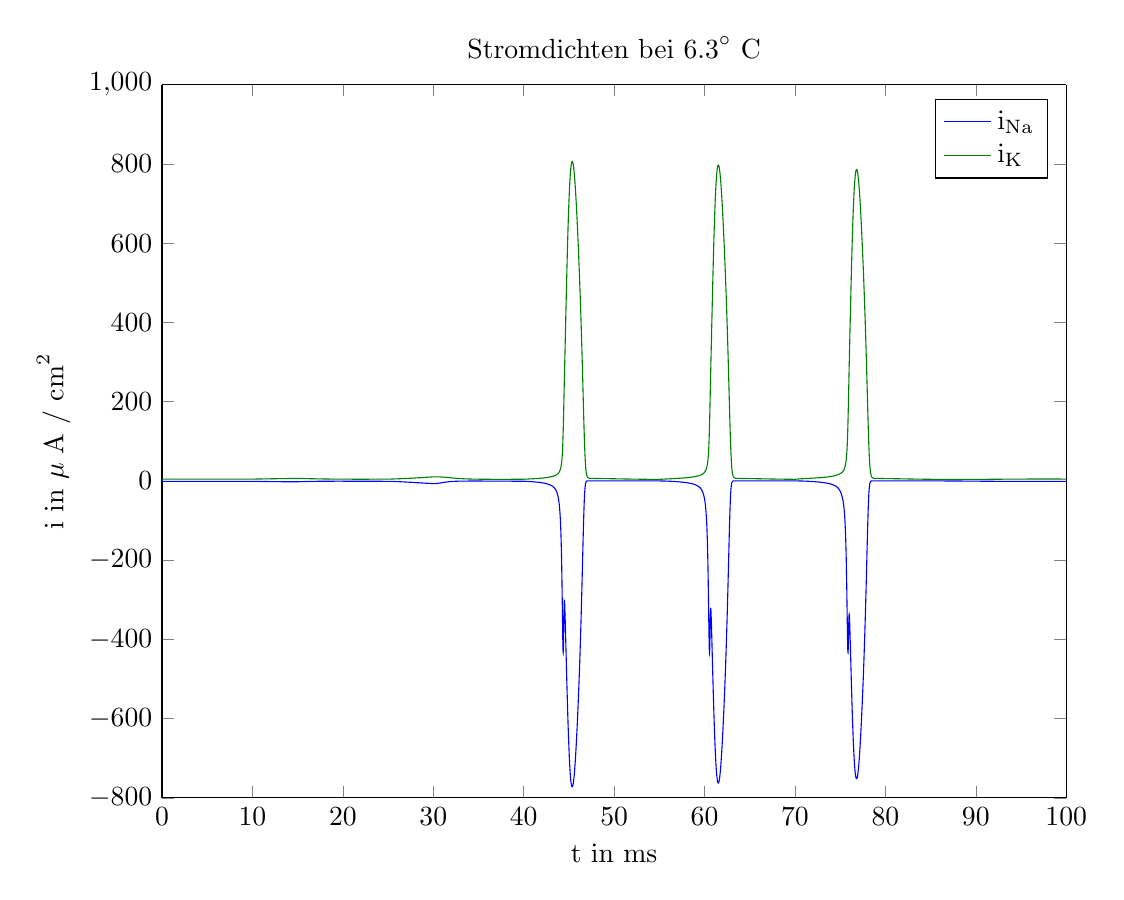
\begin{tikzpicture}

\begin{axis}[%
width=4.520833in,
height=3.565625in,
at={(0.758333in,0.48125in)},
scale only axis,
separate axis lines,
every outer x axis line/.append style={black},
every x tick label/.append style={font=\color{black}},
xmin=0,
xmax=100,
xlabel={t in ms},
every outer y axis line/.append style={black},
every y tick label/.append style={font=\color{black}},
ymin=-800,
ymax=1000,
ylabel={$\text{i in }\mu\text{ A / cm}^\text{2}$},
title={$\text{Stromdichten bei 6.3}^\circ\text{ C}$},
legend style={legend cell align=left,align=left,draw=black}
]
\addplot [color=blue,solid,forget plot]
  table[row sep=crcr]{%
0	-1.22005717646543\\
0.01	-1.22005717646543\\
0.02	-1.22005719962561\\
0.03	-1.22005727789986\\
0.04	-1.22005740884488\\
0.05	-1.22005758990444\\
0.06	-1.22005781863767\\
0.07	-1.22005809271521\\
0.08	-1.22005840991421\\
0.09	-1.22005876811335\\
0.1	-1.22005916528825\\
0.11	-1.22005959950698\\
0.12	-1.22006006892583\\
0.13	-1.22006057178529\\
0.14	-1.22006110640616\\
0.15	-1.22006167118588\\
0.16	-1.220062264595\\
0.17	-1.22006288517385\\
0.18	-1.22006353152933\\
0.19	-1.22006420233185\\
0.2	-1.22006489631244\\
0.21	-1.22006561225996\\
0.22	-1.22006634901843\\
0.23	-1.22006710548453\\
0.24	-1.22006788060518\\
0.25	-1.22006867337523\\
0.26	-1.22006948283527\\
0.27	-1.22007030806953\\
0.28	-1.2200711482039\\
0.29	-1.22007200240398\\
0.3	-1.2200728698733\\
0.31	-1.22007374985156\\
0.32	-1.22007464161301\\
0.33	-1.22007554446481\\
0.34	-1.22007645774557\\
0.35	-1.2200773808239\\
0.36	-1.22007831309702\\
0.37	-1.22007925398947\\
0.38	-1.22008020295185\\
0.39	-1.22008115945965\\
0.4	-1.22008212301206\\
0.41	-1.22008309313095\\
0.42	-1.22008406935977\\
0.43	-1.22008505126264\\
0.44	-1.22008603842331\\
0.45	-1.22008703044436\\
0.46	-1.22008802694627\\
0.47	-1.22008902756662\\
0.48	-1.22009003195933\\
0.49	-1.22009103979389\\
0.5	-1.22009205075467\\
0.51	-1.22009306454023\\
0.52	-1.22009408086266\\
0.53	-1.22009509944697\\
0.54	-1.22009612003054\\
0.55	-1.22009714236248\\
0.56	-1.22009816620318\\
0.57	-1.22009919132372\\
0.58	-1.22010021750543\\
0.59	-1.22010124453944\\
0.6	-1.22010227222615\\
0.61	-1.22010330037491\\
0.62	-1.22010432880356\\
0.63	-1.22010535733802\\
0.64	-1.22010638581201\\
0.65	-1.22010741406658\\
0.66	-1.22010844194989\\
0.67	-1.22010946931681\\
0.68	-1.22011049602864\\
0.69	-1.22011152195283\\
0.7	-1.22011254696269\\
0.71	-1.22011357093714\\
0.72	-1.2201145937604\\
0.73	-1.22011561532186\\
0.74	-1.22011663551572\\
0.75	-1.22011765424087\\
0.76	-1.22011867140064\\
0.77	-1.22011968690258\\
0.78	-1.22012070065832\\
0.79	-1.22012171258334\\
0.8	-1.22012272259683\\
0.81	-1.2201237306215\\
0.82	-1.22012473658344\\
0.83	-1.22012574041196\\
0.84	-1.22012674203944\\
0.85	-1.22012774140121\\
0.86	-1.22012873843539\\
0.87	-1.22012973308281\\
0.88	-1.22013072528684\\
0.89	-1.22013171499332\\
0.9	-1.22013270215042\\
0.91	-1.22013368670853\\
0.92	-1.22013466862022\\
0.93	-1.22013564784007\\
0.94	-1.22013662432463\\
0.95	-1.2201375980323\\
0.96	-1.22013856892329\\
0.97	-1.2201395369595\\
0.98	-1.22014050210448\\
0.99	-1.22014146432331\\
1	-1.2201424235826\\
1.01	-1.22014337985036\\
1.02	-1.22014433309598\\
1.03	-1.22014528329016\\
1.04	-1.22014623040484\\
1.05	-1.22014717441317\\
1.06	-1.22014811528943\\
1.07	-1.220149053009\\
1.08	-1.22014998754833\\
1.09	-1.22015091888484\\
1.1	-1.22015184699695\\
1.11	-1.22015277186397\\
1.12	-1.2201536934661\\
1.13	-1.22015461178441\\
1.14	-1.22015552680075\\
1.15	-1.22015643849776\\
1.16	-1.22015734685882\\
1.17	-1.22015825186803\\
1.18	-1.22015915351017\\
1.19	-1.22016005177067\\
1.2	-1.2201609466356\\
1.21	-1.22016183809163\\
1.22	-1.22016272612601\\
1.23	-1.22016361072654\\
1.24	-1.22016449188156\\
1.25	-1.22016536957993\\
1.26	-1.22016624381098\\
1.27	-1.22016711456454\\
1.28	-1.22016798183087\\
1.29	-1.2201688456007\\
1.3	-1.22016970586514\\
1.31	-1.22017056261572\\
1.32	-1.22017141584438\\
1.33	-1.22017226554341\\
1.34	-1.22017311170547\\
1.35	-1.22017395432355\\
1.36	-1.220174793391\\
1.37	-1.22017562890148\\
1.38	-1.22017646084895\\
1.39	-1.22017728922769\\
1.4	-1.22017811403225\\
1.41	-1.22017893525747\\
1.42	-1.22017975289846\\
1.43	-1.22018056695056\\
1.44	-1.22018137740941\\
1.45	-1.22018218427086\\
1.46	-1.220182987531\\
1.47	-1.22018378718614\\
1.48	-1.22018458323281\\
1.49	-1.22018537566778\\
1.5	-1.22018616448798\\
1.51	-1.22018694969058\\
1.52	-1.22018773127291\\
1.53	-1.2201885092325\\
1.54	-1.22018928356706\\
1.55	-1.22019005427449\\
1.56	-1.22019082135283\\
1.57	-1.22019158480032\\
1.58	-1.22019234461532\\
1.59	-1.22019310079639\\
1.6	-1.2201938533422\\
1.61	-1.22019460225161\\
1.62	-1.22019534752359\\
1.63	-1.22019608915726\\
1.64	-1.22019682715189\\
1.65	-1.22019756150686\\
1.66	-1.2201982922217\\
1.67	-1.22019901929605\\
1.68	-1.22019974272969\\
1.69	-1.2202004625225\\
1.7	-1.22020117867449\\
1.71	-1.22020189118579\\
1.72	-1.22020260005663\\
1.73	-1.22020330528735\\
1.74	-1.22020400687842\\
1.75	-1.22020470483038\\
1.76	-1.2202053991439\\
1.77	-1.22020608981974\\
1.78	-1.22020677685875\\
1.79	-1.22020746026191\\
1.8	-1.22020814003025\\
1.81	-1.22020881616493\\
1.82	-1.22020948866718\\
1.83	-1.22021015753832\\
1.84	-1.22021082277978\\
1.85	-1.22021148439306\\
1.86	-1.22021214237973\\
1.87	-1.22021279674148\\
1.88	-1.22021344748005\\
1.89	-1.22021409459728\\
1.9	-1.22021473809508\\
1.91	-1.22021537797545\\
1.92	-1.22021601424046\\
1.93	-1.22021664689225\\
1.94	-1.22021727593304\\
1.95	-1.22021790136513\\
1.96	-1.2202185231909\\
1.97	-1.22021914141277\\
1.98	-1.22021975603327\\
1.99	-1.22022036705497\\
2	-1.22022097448053\\
2.01	-1.22022157831266\\
2.02	-1.22022217855416\\
2.03	-1.22022277520789\\
2.04	-1.22022336827675\\
2.05	-1.22022395776374\\
2.06	-1.2202245436719\\
2.07	-1.22022512600436\\
2.08	-1.22022570476428\\
2.09	-1.22022627995491\\
2.1	-1.22022685157956\\
2.11	-1.22022741964157\\
2.12	-1.22022798414437\\
2.13	-1.22022854509146\\
2.14	-1.22022910248636\\
2.15	-1.22022965633268\\
2.16	-1.22023020663407\\
2.17	-1.22023075339426\\
2.18	-1.22023129661702\\
2.19	-1.22023183630616\\
2.2	-1.22023237246559\\
2.21	-1.22023290509924\\
2.22	-1.2202334342111\\
2.23	-1.22023395980523\\
2.24	-1.22023448188572\\
2.25	-1.22023500045674\\
2.26	-1.22023551552249\\
2.27	-1.22023602708724\\
2.28	-1.22023653515531\\
2.29	-1.22023703973104\\
2.3	-1.22023754081888\\
2.31	-1.22023803842327\\
2.32	-1.22023853254875\\
2.33	-1.22023902319988\\
2.34	-1.22023951038127\\
2.35	-1.2202399940976\\
2.36	-1.22024047435357\\
2.37	-1.22024095115396\\
2.38	-1.22024142450358\\
2.39	-1.22024189440728\\
2.4	-1.22024236086997\\
2.41	-1.22024282389662\\
2.42	-1.2202432834922\\
2.43	-1.22024373966178\\
2.44	-1.22024419241045\\
2.45	-1.22024464174334\\
2.46	-1.22024508766564\\
2.47	-1.22024553018257\\
2.48	-1.2202459692994\\
2.49	-1.22024640502146\\
2.5	-1.2202468373541\\
2.51	-1.22024726630273\\
2.52	-1.22024769187278\\
2.53	-1.22024811406976\\
2.54	-1.22024853289919\\
2.55	-1.22024894836665\\
2.56	-1.22024936047775\\
2.57	-1.22024976923814\\
2.58	-1.22025017465354\\
2.59	-1.22025057672967\\
2.6	-1.22025097547232\\
2.61	-1.22025137088731\\
2.62	-1.22025176298049\\
2.63	-1.22025215175777\\
2.64	-1.22025253722508\\
2.65	-1.22025291938841\\
2.66	-1.22025329825377\\
2.67	-1.22025367382722\\
2.68	-1.22025404611484\\
2.69	-1.22025441512278\\
2.7	-1.22025478085719\\
2.71	-1.2202551433243\\
2.72	-1.22025550253033\\
2.73	-1.22025585848157\\
2.74	-1.22025621118434\\
2.75	-1.22025656064499\\
2.76	-1.22025690686991\\
2.77	-1.22025724986552\\
2.78	-1.22025758963828\\
2.79	-1.22025792619469\\
2.8	-1.22025825954128\\
2.81	-1.22025858968461\\
2.82	-1.22025891663128\\
2.83	-1.22025924038792\\
2.84	-1.22025956096119\\
2.85	-1.22025987835781\\
2.86	-1.22026019258449\\
2.87	-1.220260503648\\
2.88	-1.22026081155515\\
2.89	-1.22026111631276\\
2.9	-1.22026141792769\\
2.91	-1.22026171640684\\
2.92	-1.22026201175714\\
2.93	-1.22026230398554\\
2.94	-1.22026259309902\\
2.95	-1.22026287910461\\
2.96	-1.22026316200936\\
2.97	-1.22026344182035\\
2.98	-1.22026371854468\\
2.99	-1.22026399218949\\
3	-1.22026426276195\\
3.01	-1.22026453026927\\
3.02	-1.22026479471866\\
3.03	-1.22026505611738\\
3.04	-1.22026531447271\\
3.05	-1.22026556979197\\
3.06	-1.2202658220825\\
3.07	-1.22026607135166\\
3.08	-1.22026631760684\\
3.09	-1.22026656085547\\
3.1	-1.220266801105\\
3.11	-1.2202670383629\\
3.12	-1.22026727263668\\
3.13	-1.22026750393385\\
3.14	-1.22026773226198\\
3.15	-1.22026795762864\\
3.16	-1.22026818004144\\
3.17	-1.220268399508\\
3.18	-1.22026861603599\\
3.19	-1.22026882963307\\
3.2	-1.22026904030696\\
3.21	-1.22026924806538\\
3.22	-1.22026945291609\\
3.23	-1.22026965486685\\
3.24	-1.22026985392546\\
3.25	-1.22027005009976\\
3.26	-1.22027024339757\\
3.27	-1.22027043382677\\
3.28	-1.22027062139525\\
3.29	-1.22027080611092\\
3.3	-1.22027098798172\\
3.31	-1.22027116701559\\
3.32	-1.22027134322052\\
3.33	-1.2202715166045\\
3.34	-1.22027168717555\\
3.35	-1.22027185494172\\
3.36	-1.22027201991106\\
3.37	-1.22027218209165\\
3.38	-1.2202723414916\\
3.39	-1.22027249811902\\
3.4	-1.22027265198205\\
3.41	-1.22027280308886\\
3.42	-1.22027295144762\\
3.43	-1.22027309706653\\
3.44	-1.22027323995381\\
3.45	-1.22027338011769\\
3.46	-1.22027351756642\\
3.47	-1.22027365230827\\
3.48	-1.22027378435153\\
3.49	-1.22027391370451\\
3.5	-1.22027404037553\\
3.51	-1.22027416437293\\
3.52	-1.22027428570507\\
3.53	-1.22027440438032\\
3.54	-1.22027452040707\\
3.55	-1.22027463379372\\
3.56	-1.22027474454871\\
3.57	-1.22027485268046\\
3.58	-1.22027495819742\\
3.59	-1.22027506110808\\
3.6	-1.22027516142091\\
3.61	-1.2202752591444\\
3.62	-1.22027535428708\\
3.63	-1.22027544685746\\
3.64	-1.22027553686409\\
3.65	-1.22027562431553\\
3.66	-1.22027570922035\\
3.67	-1.22027579158711\\
3.68	-1.22027587142443\\
3.69	-1.22027594874091\\
3.7	-1.22027602354518\\
3.71	-1.22027609584586\\
3.72	-1.2202761656516\\
3.73	-1.22027623297106\\
3.74	-1.22027629781291\\
3.75	-1.22027636018584\\
3.76	-1.22027642009853\\
3.77	-1.2202764775597\\
3.78	-1.22027653257806\\
3.79	-1.22027658516234\\
3.8	-1.22027663532128\\
3.81	-1.22027668306362\\
3.82	-1.22027672839812\\
3.83	-1.22027677133356\\
3.84	-1.2202768118787\\
3.85	-1.22027685004235\\
3.86	-1.2202768858333\\
3.87	-1.22027691926036\\
3.88	-1.22027695033233\\
3.89	-1.22027697905806\\
3.9	-1.22027700544637\\
3.91	-1.2202770295061\\
3.92	-1.22027705124611\\
3.93	-1.22027707067526\\
3.94	-1.2202770878024\\
3.95	-1.22027710263642\\
3.96	-1.2202771151862\\
3.97	-1.22027712546063\\
3.98	-1.2202771334686\\
3.99	-1.22027713921902\\
4	-1.22027714272079\\
4.01	-1.22027714398283\\
4.02	-1.22027714301407\\
4.03	-1.22027713982344\\
4.04	-1.22027713441986\\
4.05	-1.22027712681228\\
4.06	-1.22027711700964\\
4.07	-1.2202771050209\\
4.08	-1.22027709085502\\
4.09	-1.22027707452094\\
4.1	-1.22027705602765\\
4.11	-1.2202770353841\\
4.12	-1.22027701259928\\
4.13	-1.22027698768216\\
4.14	-1.22027696064173\\
4.15	-1.22027693148697\\
4.16	-1.22027690022687\\
4.17	-1.22027686687043\\
4.18	-1.22027683142665\\
4.19	-1.22027679390453\\
4.2	-1.22027675431306\\
4.21	-1.22027671266126\\
4.22	-1.22027666895814\\
4.23	-1.2202766232127\\
4.24	-1.22027657543395\\
4.25	-1.22027652563092\\
4.26	-1.22027647381262\\
4.27	-1.22027641998807\\
4.28	-1.22027636416629\\
4.29	-1.2202763063563\\
4.3	-1.22027624656712\\
4.31	-1.22027618480778\\
4.32	-1.2202761210873\\
4.33	-1.2202760554147\\
4.34	-1.22027598779901\\
4.35	-1.22027591824926\\
4.36	-1.22027584677447\\
4.37	-1.22027577338367\\
4.38	-1.22027569808588\\
4.39	-1.22027562089012\\
4.4	-1.22027554180543\\
4.41	-1.22027546084082\\
4.42	-1.22027537800532\\
4.43	-1.22027529330795\\
4.44	-1.22027520675773\\
4.45	-1.22027511836367\\
4.46	-1.2202750281348\\
4.47	-1.22027493608013\\
4.48	-1.22027484220867\\
4.49	-1.22027474652944\\
4.5	-1.22027464905144\\
4.51	-1.22027454978368\\
4.52	-1.22027444873517\\
4.53	-1.2202743459149\\
4.54	-1.22027424133188\\
4.55	-1.2202741349951\\
4.56	-1.22027402691355\\
4.57	-1.22027391709622\\
4.58	-1.2202738055521\\
4.59	-1.22027369229016\\
4.6	-1.2202735773194\\
4.61	-1.22027346064877\\
4.62	-1.22027334228726\\
4.63	-1.22027322224382\\
4.64	-1.22027310052741\\
4.65	-1.22027297714701\\
4.66	-1.22027285211154\\
4.67	-1.22027272542997\\
4.68	-1.22027259711124\\
4.69	-1.22027246716427\\
4.7	-1.22027233559801\\
4.71	-1.22027220242138\\
4.72	-1.22027206764329\\
4.73	-1.22027193127267\\
4.74	-1.22027179331842\\
4.75	-1.22027165378944\\
4.76	-1.22027151269464\\
4.77	-1.22027137004289\\
4.78	-1.22027122584309\\
4.79	-1.22027108010411\\
4.8	-1.22027093283482\\
4.81	-1.22027078404409\\
4.82	-1.22027063374076\\
4.83	-1.2202704819337\\
4.84	-1.22027032863174\\
4.85	-1.22027017384371\\
4.86	-1.22027001757844\\
4.87	-1.22026985984476\\
4.88	-1.22026970065147\\
4.89	-1.22026954000737\\
4.9	-1.22026937792126\\
4.91	-1.22026921440193\\
4.92	-1.22026904945815\\
4.93	-1.2202688830987\\
4.94	-1.22026871533233\\
4.95	-1.2202685461678\\
4.96	-1.22026837561385\\
4.97	-1.22026820367922\\
4.98	-1.22026803037262\\
4.99	-1.22026785570278\\
5	-1.2202676796784\\
5.01	-1.22026750230818\\
5.02	-1.22026732360081\\
5.03	-1.22026714356496\\
5.04	-1.2202669622093\\
5.05	-1.22026677954249\\
5.06	-1.22026659557317\\
5.07	-1.22026641030998\\
5.08	-1.22026622376155\\
5.09	-1.2202660359365\\
5.1	-1.22026584684342\\
5.11	-1.22026565649092\\
5.12	-1.22026546488757\\
5.13	-1.22026527204195\\
5.14	-1.22026507796262\\
5.15	-1.22026488265813\\
5.16	-1.22026468613702\\
5.17	-1.22026448840781\\
5.18	-1.22026428947903\\
5.19	-1.22026408935917\\
5.2	-1.22026388805673\\
5.21	-1.22026368558018\\
5.22	-1.220263481938\\
5.23	-1.22026327713865\\
5.24	-1.22026307119055\\
5.25	-1.22026286410215\\
5.26	-1.22026265588187\\
5.27	-1.22026244653811\\
5.28	-1.22026223607926\\
5.29	-1.22026202451371\\
5.3	-1.22026181184982\\
5.31	-1.22026159809594\\
5.32	-1.22026138326043\\
5.33	-1.2202611673516\\
5.34	-1.22026095037777\\
5.35	-1.22026073234725\\
5.36	-1.22026051326832\\
5.37	-1.22026029314925\\
5.38	-1.22026007199831\\
5.39	-1.22025984982375\\
5.4	-1.22025962663379\\
5.41	-1.22025940243665\\
5.42	-1.22025917724054\\
5.43	-1.22025895105365\\
5.44	-1.22025872388416\\
5.45	-1.22025849574022\\
5.46	-1.22025826662999\\
5.47	-1.22025803656159\\
5.48	-1.22025780554315\\
5.49	-1.22025757358277\\
5.5	-1.22025734068853\\
5.51	-1.22025710686851\\
5.52	-1.22025687213076\\
5.53	-1.22025663648333\\
5.54	-1.22025639993425\\
5.55	-1.22025616249152\\
5.56	-1.22025592416315\\
5.57	-1.22025568495712\\
5.58	-1.22025544488139\\
5.59	-1.2202552039439\\
5.6	-1.22025496215261\\
5.61	-1.22025471951541\\
5.62	-1.22025447604022\\
5.63	-1.22025423173492\\
5.64	-1.22025398660739\\
5.65	-1.22025374066546\\
5.66	-1.22025349391699\\
5.67	-1.22025324636979\\
5.68	-1.22025299803167\\
5.69	-1.22025274891042\\
5.7	-1.2202524990138\\
5.71	-1.22025224834957\\
5.72	-1.22025199692547\\
5.73	-1.22025174474922\\
5.74	-1.22025149182853\\
5.75	-1.22025123817107\\
5.76	-1.22025098378453\\
5.77	-1.22025072867655\\
5.78	-1.22025047285477\\
5.79	-1.22025021632681\\
5.8	-1.22024995910027\\
5.81	-1.22024970118273\\
5.82	-1.22024944258175\\
5.83	-1.22024918330489\\
5.84	-1.22024892335968\\
5.85	-1.22024866275362\\
5.86	-1.22024840149422\\
5.87	-1.22024813958895\\
5.88	-1.22024787704527\\
5.89	-1.22024761387062\\
5.9	-1.22024735007242\\
5.91	-1.22024708565808\\
5.92	-1.22024682063499\\
5.93	-1.22024655501051\\
5.94	-1.22024628879199\\
5.95	-1.22024602198677\\
5.96	-1.22024575460215\\
5.97	-1.22024548664544\\
5.98	-1.2202452181239\\
5.99	-1.2202449490448\\
6	-1.22024467941537\\
6.01	-1.22024440924283\\
6.02	-1.22024413853439\\
6.03	-1.22024386729722\\
6.04	-1.22024359553849\\
6.05	-1.22024332326535\\
6.06	-1.22024305048491\\
6.07	-1.22024277720428\\
6.08	-1.22024250343054\\
6.09	-1.22024222917078\\
6.1	-1.22024195443203\\
6.11	-1.22024167922131\\
6.12	-1.22024140354565\\
6.13	-1.22024112741203\\
6.14	-1.22024085082742\\
6.15	-1.22024057379877\\
6.16	-1.22024029633301\\
6.17	-1.22024001843706\\
6.18	-1.22023974011779\\
6.19	-1.22023946138209\\
6.2	-1.22023918223681\\
6.21	-1.22023890268877\\
6.22	-1.2202386227448\\
6.23	-1.22023834241167\\
6.24	-1.22023806169617\\
6.25	-1.22023778060505\\
6.26	-1.22023749914503\\
6.27	-1.22023721732283\\
6.28	-1.22023693514514\\
6.29	-1.22023665261863\\
6.3	-1.22023636974995\\
6.31	-1.22023608654574\\
6.32	-1.22023580301259\\
6.33	-1.2202355191571\\
6.34	-1.22023523498585\\
6.35	-1.22023495050537\\
6.36	-1.2202346657222\\
6.37	-1.22023438064284\\
6.38	-1.22023409527378\\
6.39	-1.22023380962149\\
6.4	-1.2202335236924\\
6.41	-1.22023323749296\\
6.42	-1.22023295102955\\
6.43	-1.22023266430857\\
6.44	-1.22023237733637\\
6.45	-1.22023209011929\\
6.46	-1.22023180266366\\
6.47	-1.22023151497578\\
6.48	-1.22023122706192\\
6.49	-1.22023093892834\\
6.5	-1.22023065058127\\
6.51	-1.22023036202694\\
6.52	-1.22023007327154\\
6.53	-1.22022978432123\\
6.54	-1.22022949518217\\
6.55	-1.22022920586049\\
6.56	-1.2202289163623\\
6.57	-1.22022862669369\\
6.58	-1.22022833686072\\
6.59	-1.22022804686944\\
6.6	-1.22022775672587\\
6.61	-1.22022746643602\\
6.62	-1.22022717600586\\
6.63	-1.22022688544136\\
6.64	-1.22022659474845\\
6.65	-1.22022630393305\\
6.66	-1.22022601300106\\
6.67	-1.22022572195834\\
6.68	-1.22022543081075\\
6.69	-1.22022513956413\\
6.7	-1.22022484822427\\
6.71	-1.22022455679697\\
6.72	-1.22022426528799\\
6.73	-1.22022397370307\\
6.74	-1.22022368204794\\
6.75	-1.2202233903283\\
6.76	-1.22022309854982\\
6.77	-1.22022280671817\\
6.78	-1.22022251483897\\
6.79	-1.22022222291784\\
6.8	-1.22022193096038\\
6.81	-1.22022163897215\\
6.82	-1.22022134695869\\
6.83	-1.22022105492554\\
6.84	-1.2202207628782\\
6.85	-1.22022047082215\\
6.86	-1.22022017876285\\
6.87	-1.22021988670574\\
6.88	-1.22021959465623\\
6.89	-1.22021930261972\\
6.9	-1.22021901060158\\
6.91	-1.22021871860717\\
6.92	-1.2202184266418\\
6.93	-1.2202181347108\\
6.94	-1.22021784281943\\
6.95	-1.22021755097296\\
6.96	-1.22021725917664\\
6.97	-1.22021696743568\\
6.98	-1.22021667575528\\
6.99	-1.22021638414061\\
7	-1.22021609259682\\
7.01	-1.22021580112904\\
7.02	-1.22021550974239\\
7.03	-1.22021521844194\\
7.04	-1.22021492723276\\
7.05	-1.2202146361199\\
7.06	-1.22021434510836\\
7.07	-1.22021405420316\\
7.08	-1.22021376340925\\
7.09	-1.22021347273161\\
7.1	-1.22021318217515\\
7.11	-1.22021289174479\\
7.12	-1.22021260144541\\
7.13	-1.22021231128188\\
7.14	-1.22021202125904\\
7.15	-1.2202117313817\\
7.16	-1.22021144165468\\
7.17	-1.22021115208274\\
7.18	-1.22021086267064\\
7.19	-1.2202105734231\\
7.2	-1.22021028434485\\
7.21	-1.22020999544056\\
7.22	-1.2202097067149\\
7.23	-1.22020941817251\\
7.24	-1.22020912981802\\
7.25	-1.22020884165602\\
7.26	-1.2202085536911\\
7.27	-1.22020826592779\\
7.28	-1.22020797837065\\
7.29	-1.22020769102417\\
7.3	-1.22020740389284\\
7.31	-1.22020711698114\\
7.32	-1.2202068302935\\
7.33	-1.22020654383434\\
7.34	-1.22020625760807\\
7.35	-1.22020597161907\\
7.36	-1.22020568587168\\
7.37	-1.22020540037025\\
7.38	-1.22020511511908\\
7.39	-1.22020483012246\\
7.4	-1.22020454538466\\
7.41	-1.22020426090993\\
7.42	-1.22020397670249\\
7.43	-1.22020369276653\\
7.44	-1.22020340910624\\
7.45	-1.22020312572578\\
7.46	-1.22020284262927\\
7.47	-1.22020255982084\\
7.48	-1.22020227730458\\
7.49	-1.22020199508454\\
7.5	-1.22020171316479\\
7.51	-1.22020143154934\\
7.52	-1.2202011502422\\
7.53	-1.22020086924735\\
7.54	-1.22020058856875\\
7.55	-1.22020030821033\\
7.56	-1.22020002817602\\
7.57	-1.2201997484697\\
7.58	-1.22019946909526\\
7.59	-1.22019919005653\\
7.6	-1.22019891135734\\
7.61	-1.22019863300151\\
7.62	-1.22019835499282\\
7.63	-1.22019807733503\\
7.64	-1.22019780003188\\
7.65	-1.22019752308709\\
7.66	-1.22019724650436\\
7.67	-1.22019697028737\\
7.68	-1.22019669443976\\
7.69	-1.22019641896518\\
7.7	-1.22019614386724\\
7.71	-1.22019586914951\\
7.72	-1.22019559481558\\
7.73	-1.22019532086898\\
7.74	-1.22019504731325\\
7.75	-1.22019477415188\\
7.76	-1.22019450138836\\
7.77	-1.22019422902614\\
7.78	-1.22019395706867\\
7.79	-1.22019368551937\\
7.8	-1.22019341438162\\
7.81	-1.22019314365881\\
7.82	-1.22019287335428\\
7.83	-1.22019260347137\\
7.84	-1.2201923340134\\
7.85	-1.22019206498363\\
7.86	-1.22019179638536\\
7.87	-1.22019152822181\\
7.88	-1.22019126049623\\
7.89	-1.2201909932118\\
7.9	-1.22019072637172\\
7.91	-1.22019045997914\\
7.92	-1.22019019403721\\
7.93	-1.22018992854905\\
7.94	-1.22018966351775\\
7.95	-1.22018939894639\\
7.96	-1.22018913483803\\
7.97	-1.2201888711957\\
7.98	-1.22018860802242\\
7.99	-1.22018834532118\\
8	-1.22018808309496\\
8.01	-1.22018782134669\\
8.02	-1.22018756007932\\
8.03	-1.22018729929576\\
8.04	-1.22018703899889\\
8.05	-1.22018677919159\\
8.06	-1.22018651987669\\
8.07	-1.22018626105703\\
8.08	-1.22018600273541\\
8.09	-1.22018574491462\\
8.1	-1.22018548759742\\
8.11	-1.22018523078656\\
8.12	-1.22018497448476\\
8.13	-1.22018471869472\\
8.14	-1.22018446341913\\
8.15	-1.22018420866065\\
8.16	-1.22018395442192\\
8.17	-1.22018370070556\\
8.18	-1.22018344751417\\
8.19	-1.22018319485033\\
8.2	-1.22018294271661\\
8.21	-1.22018269111555\\
8.22	-1.22018244004965\\
8.23	-1.22018218952143\\
8.24	-1.22018193953336\\
8.25	-1.22018169008791\\
8.26	-1.2201814411875\\
8.27	-1.22018119283457\\
8.28	-1.2201809450315\\
8.29	-1.22018069778069\\
8.3	-1.22018045108448\\
8.31	-1.22018020494522\\
8.32	-1.22017995936522\\
8.33	-1.2201797143468\\
8.34	-1.22017946989222\\
8.35	-1.22017922600374\\
8.36	-1.22017898268361\\
8.37	-1.22017873993405\\
8.38	-1.22017849775726\\
8.39	-1.22017825615541\\
8.4	-1.22017801513068\\
8.41	-1.2201777746852\\
8.42	-1.2201775348211\\
8.43	-1.22017729554047\\
8.44	-1.22017705684541\\
8.45	-1.22017681873798\\
8.46	-1.22017658122022\\
8.47	-1.22017634429416\\
8.48	-1.22017610796181\\
8.49	-1.22017587222514\\
8.5	-1.22017563708614\\
8.51	-1.22017540254675\\
8.52	-1.22017516860889\\
8.53	-1.22017493527449\\
8.54	-1.22017470254543\\
8.55	-1.22017447042358\\
8.56	-1.2201742389108\\
8.57	-1.22017400800893\\
8.58	-1.22017377771977\\
8.59	-1.22017354804513\\
8.6	-1.22017331898679\\
8.61	-1.2201730905465\\
8.62	-1.22017286272601\\
8.63	-1.22017263552704\\
8.64	-1.22017240895129\\
8.65	-1.22017218300045\\
8.66	-1.22017195767618\\
8.67	-1.22017173298014\\
8.68	-1.22017150891394\\
8.69	-1.22017128547922\\
8.7	-1.22017106267755\\
8.71	-1.22017084051051\\
8.72	-1.22017061897966\\
8.73	-1.22017039808654\\
8.74	-1.22017017783267\\
8.75	-1.22016995821954\\
8.76	-1.22016973924865\\
8.77	-1.22016952092146\\
8.78	-1.22016930323942\\
8.79	-1.22016908620395\\
8.8	-1.22016886981648\\
8.81	-1.22016865407838\\
8.82	-1.22016843899105\\
8.83	-1.22016822455584\\
8.84	-1.22016801077409\\
8.85	-1.22016779764712\\
8.86	-1.22016758517625\\
8.87	-1.22016737336275\\
8.88	-1.2201671622079\\
8.89	-1.22016695171295\\
8.9	-1.22016674187913\\
8.91	-1.22016653270768\\
8.92	-1.22016632419978\\
8.93	-1.22016611635662\\
8.94	-1.22016590917937\\
8.95	-1.22016570266918\\
8.96	-1.22016549682717\\
8.97	-1.22016529165447\\
8.98	-1.22016508715217\\
8.99	-1.22016488332136\\
9	-1.22016468016309\\
9.01	-1.22016447767841\\
9.02	-1.22016427586836\\
9.03	-1.22016407473395\\
9.04	-1.22016387427617\\
9.05	-1.22016367449601\\
9.06	-1.22016347539442\\
9.07	-1.22016327697236\\
9.08	-1.22016307923076\\
9.09	-1.22016288217053\\
9.1	-1.22016268579256\\
9.11	-1.22016249009774\\
9.12	-1.22016229508693\\
9.13	-1.22016210076098\\
9.14	-1.22016190712072\\
9.15	-1.22016171416697\\
9.16	-1.22016152190053\\
9.17	-1.22016133032217\\
9.18	-1.22016113943268\\
9.19	-1.22016094923279\\
9.2	-1.22016075972325\\
9.21	-1.22016057090477\\
9.22	-1.22016038277806\\
9.23	-1.2201601953438\\
9.24	-1.22016000860267\\
9.25	-1.22015982255533\\
9.26	-1.22015963720241\\
9.27	-1.22015945254453\\
9.28	-1.22015926858232\\
9.29	-1.22015908531636\\
9.3	-1.22015890274723\\
9.31	-1.2201587208755\\
9.32	-1.2201585397017\\
9.33	-1.22015835922638\\
9.34	-1.22015817945006\\
9.35	-1.22015800037323\\
9.36	-1.22015782199637\\
9.37	-1.22015764431998\\
9.38	-1.22015746734449\\
9.39	-1.22015729107035\\
9.4	-1.22015711549799\\
9.41	-1.22015694062782\\
9.42	-1.22015676646024\\
9.43	-1.22015659299563\\
9.44	-1.22015642023435\\
9.45	-1.22015624817677\\
9.46	-1.22015607682321\\
9.47	-1.22015590617401\\
9.48	-1.22015573622947\\
9.49	-1.22015556698988\\
9.5	-1.22015539845554\\
9.51	-1.22015523062669\\
9.52	-1.2201550635036\\
9.53	-1.22015489708651\\
9.54	-1.22015473137563\\
9.55	-1.22015456637117\\
9.56	-1.22015440207334\\
9.57	-1.2201542384823\\
9.58	-1.22015407559824\\
9.59	-1.2201539134213\\
9.6	-1.22015375195161\\
9.61	-1.22015359118932\\
9.62	-1.22015343113452\\
9.63	-1.22015327178731\\
9.64	-1.22015311314779\\
9.65	-1.22015295521602\\
9.66	-1.22015279799206\\
9.67	-1.22015264147594\\
9.68	-1.22015248566771\\
9.69	-1.22015233056738\\
9.7	-1.22015217617495\\
9.71	-1.22015202249042\\
9.72	-1.22015186951375\\
9.73	-1.22015171724491\\
9.74	-1.22015156568386\\
9.75	-1.22015141483053\\
9.76	-1.22015126468485\\
9.77	-1.22015111524672\\
9.78	-1.22015096651605\\
9.79	-1.22015081849273\\
9.8	-1.22015067117661\\
9.81	-1.22015052456758\\
9.82	-1.22015037866546\\
9.83	-1.22015023347011\\
9.84	-1.22015008898133\\
9.85	-1.22014994519894\\
9.86	-1.22014980212274\\
9.87	-1.22014965975252\\
9.88	-1.22014951808804\\
9.89	-1.22014937712906\\
9.9	-1.22014923687534\\
9.91	-1.22014909732661\\
9.92	-1.22014895848259\\
9.93	-1.22014882034299\\
9.94	-1.22014868290752\\
9.95	-1.22014854617586\\
9.96	-1.22014841014768\\
9.97	-1.22014827482266\\
9.98	-1.22014814020044\\
9.99	-1.22014800628067\\
10	-1.22014787306296\\
10.01	-1.22014774054694\\
10.02	-1.22021915949812\\
10.03	-1.22046087865931\\
10.04	-1.22086543373822\\
10.05	-1.22142505793091\\
10.06	-1.22213237958472\\
10.07	-1.22298040392611\\
10.08	-1.22396249143722\\
10.09	-1.22507233762514\\
10.1	-1.22630395410958\\
10.11	-1.22765165093047\\
10.12	-1.22911001998524\\
10.13	-1.23067391951305\\
10.14	-1.23233845955\\
10.15	-1.23409898828548\\
10.16	-1.23595107925567\\
10.17	-1.23789051931518\\
10.18	-1.23991329733256\\
10.19	-1.24201559355981\\
10.2	-1.24419376962968\\
10.21	-1.24644435913844\\
10.22	-1.24876405877471\\
10.23	-1.25114971995834\\
10.24	-1.25359834095571\\
10.25	-1.25610705944045\\
10.26	-1.258673145471\\
10.27	-1.26129399485834\\
10.28	-1.26396712289932\\
10.29	-1.26669015845264\\
10.3	-1.26946083833633\\
10.31	-1.27227700202697\\
10.32	-1.27513658664232\\
10.33	-1.27803762219024\\
10.34	-1.28097822706808\\
10.35	-1.2839566037977\\
10.36	-1.28697103498231\\
10.37	-1.29001987947221\\
10.38	-1.29310156872744\\
10.39	-1.29621460336611\\
10.4	-1.29935754988788\\
10.41	-1.30252903756268\\
10.42	-1.30572775547558\\
10.43	-1.30895244971918\\
10.44	-1.3122019207253\\
10.45	-1.31547502072852\\
10.46	-1.31877065135442\\
10.47	-1.32208776132579\\
10.48	-1.32542534428059\\
10.49	-1.32878243669569\\
10.5	-1.33215811591094\\
10.51	-1.33555149824815\\
10.52	-1.33896173722032\\
10.53	-1.34238802182621\\
10.54	-1.3458295749261\\
10.55	-1.34928565169444\\
10.56	-1.35275553814561\\
10.57	-1.35623854972908\\
10.58	-1.35973402999049\\
10.59	-1.36324134929534\\
10.6	-1.36675990361228\\
10.61	-1.37028911335294\\
10.62	-1.37382842226567\\
10.63	-1.3773772963804\\
10.64	-1.38093522300226\\
10.65	-1.38450170975159\\
10.66	-1.38807628364798\\
10.67	-1.39165849023639\\
10.68	-1.3952478927533\\
10.69	-1.39884407133082\\
10.7	-1.40244662223721\\
10.71	-1.40605515715194\\
10.72	-1.40966930247365\\
10.73	-1.41328869865951\\
10.74	-1.41691299959457\\
10.75	-1.42054187198953\\
10.76	-1.4241749948058\\
10.77	-1.4278120587064\\
10.78	-1.43145276553169\\
10.79	-1.43509682779861\\
10.8	-1.43874396822247\\
10.81	-1.44239391926018\\
10.82	-1.44604642267396\\
10.83	-1.44970122911465\\
10.84	-1.45335809772357\\
10.85	-1.45701679575229\\
10.86	-1.46067709819934\\
10.87	-1.46433878746312\\
10.88	-1.46800165301034\\
10.89	-1.47166549105922\\
10.9	-1.47533010427682\\
10.91	-1.47899530148982\\
10.92	-1.48266089740822\\
10.93	-1.48632671236129\\
10.94	-1.48999257204529\\
10.95	-1.49365830728237\\
10.96	-1.49732375379025\\
10.97	-1.50098875196206\\
10.98	-1.50465314665598\\
10.99	-1.50831678699424\\
11	-1.51197952617103\\
11.01	-1.51564122126894\\
11.02	-1.5193017330835\\
11.03	-1.5229609259556\\
11.04	-1.52661866761127\\
11.05	-1.53027482900858\\
11.06	-1.53392928419136\\
11.07	-1.5375819101494\\
11.08	-1.54123258668485\\
11.09	-1.54488119628454\\
11.1	-1.54852762399802\\
11.11	-1.55217175732094\\
11.12	-1.55581348608369\\
11.13	-1.55945270234493\\
11.14	-1.56308930028987\\
11.15	-1.56672317613309\\
11.16	-1.57035422802571\\
11.17	-1.57398235596658\\
11.18	-1.5776074617176\\
11.19	-1.58122944872265\\
11.2	-1.58484822203025\\
11.21	-1.58846368821964\\
11.22	-1.59207575533013\\
11.23	-1.59568433279366\\
11.24	-1.59928933137034\\
11.25	-1.60289066308694\\
11.26	-1.60648824117806\\
11.27	-1.61008198003001\\
11.28	-1.61367179512717\\
11.29	-1.61725760300079\\
11.3	-1.62083932118012\\
11.31	-1.6244168681457\\
11.32	-1.62799016328481\\
11.33	-1.6315591268489\\
11.34	-1.635123679913\\
11.35	-1.63868374433694\\
11.36	-1.64223924272834\\
11.37	-1.64579009840736\\
11.38	-1.64933623537296\\
11.39	-1.65287757827079\\
11.4	-1.65641405236251\\
11.41	-1.65994558349661\\
11.42	-1.66347209808046\\
11.43	-1.66699352305377\\
11.44	-1.67050978586322\\
11.45	-1.67402081443832\\
11.46	-1.67752653716841\\
11.47	-1.68102688288066\\
11.48	-1.68452178081925\\
11.49	-1.68801116062545\\
11.5	-1.69149495231864\\
11.51	-1.69497308627834\\
11.52	-1.698445493227\\
11.53	-1.70191210421369\\
11.54	-1.70537285059859\\
11.55	-1.70882766403821\\
11.56	-1.71227647647137\\
11.57	-1.71571922010587\\
11.58	-1.71915582740586\\
11.59	-1.72258623107977\\
11.6	-1.72601036406899\\
11.61	-1.72942815953698\\
11.62	-1.7328395508591\\
11.63	-1.73624447161286\\
11.64	-1.73964285556874\\
11.65	-1.74303463668153\\
11.66	-1.74641974908207\\
11.67	-1.74979812706952\\
11.68	-1.75316970510403\\
11.69	-1.75653441779983\\
11.7	-1.75989219991871\\
11.71	-1.76324298636392\\
11.72	-1.76658671217437\\
11.73	-1.7699233125193\\
11.74	-1.77325272269312\\
11.75	-1.77657487811074\\
11.76	-1.77988971430309\\
11.77	-1.78319716691301\\
11.78	-1.78649717169138\\
11.79	-1.78978966449355\\
11.8	-1.79307458127601\\
11.81	-1.79635185809337\\
11.82	-1.79962143109547\\
11.83	-1.80288323652484\\
11.84	-1.8061372107143\\
11.85	-1.80938329008483\\
11.86	-1.8126214111436\\
11.87	-1.81585151048221\\
11.88	-1.81907352477515\\
11.89	-1.82228739077839\\
11.9	-1.82549304532818\\
11.91	-1.82869042534002\\
11.92	-1.83187946780774\\
11.93	-1.83506010980283\\
11.94	-1.83823228847378\\
11.95	-1.84139594104575\\
11.96	-1.84455100482018\\
11.97	-1.84769741717465\\
11.98	-1.85083511556288\\
11.99	-1.85396403751474\\
12	-1.85708412063654\\
12.01	-1.86019530261125\\
12.02	-1.86329752119901\\
12.03	-1.86639071423758\\
12.04	-1.86947481964304\\
12.05	-1.87254977541047\\
12.06	-1.8756155196148\\
12.07	-1.87867199041169\\
12.08	-1.88171912603856\\
12.09	-1.88475686481568\\
12.1	-1.88778514514729\\
12.11	-1.89080390552289\\
12.12	-1.89381308451855\\
12.13	-1.89681262079829\\
12.14	-1.89980245311555\\
12.15	-1.90278252031472\\
12.16	-1.90575276133275\\
12.17	-1.90871311520082\\
12.18	-1.91166352104601\\
12.19	-1.91460391809317\\
12.2	-1.91753424566668\\
12.21	-1.92045444319241\\
12.22	-1.92336445019961\\
12.23	-1.92626420632299\\
12.24	-1.92915365130471\\
12.25	-1.93203272499652\\
12.26	-1.93490136736189\\
12.27	-1.93775951847824\\
12.28	-1.94060711853915\\
12.29	-1.94344410785666\\
12.3	-1.9462704268636\\
12.31	-1.94908601611597\\
12.32	-1.95189081629533\\
12.33	-1.95468476821126\\
12.34	-1.95746781280384\\
12.35	-1.96023989114618\\
12.36	-1.96300094444698\\
12.37	-1.96575091405311\\
12.38	-1.96848974145223\\
12.39	-1.97121736827549\\
12.4	-1.97393373630017\\
12.41	-1.97663878745241\\
12.42	-1.97933246380998\\
12.43	-1.98201470760506\\
12.44	-1.98468546122704\\
12.45	-1.98734466722531\\
12.46	-1.98999226831222\\
12.47	-1.99262820736588\\
12.48	-1.99525242743312\\
12.49	-1.99786487173239\\
12.5	-2.00046548365677\\
12.51	-2.00305420677693\\
12.52	-2.00563098484413\\
12.53	-2.00819576179325\\
12.54	-2.01074848174588\\
12.55	-2.01328908901334\\
12.56	-2.01581752809981\\
12.57	-2.01833374370542\\
12.58	-2.0208376807294\\
12.59	-2.02332928427322\\
12.6	-2.02580849964377\\
12.61	-2.02827527235653\\
12.62	-2.0307295481388\\
12.63	-2.03317127293288\\
12.64	-2.03560039289936\\
12.65	-2.03801685442032\\
12.66	-2.04042060410264\\
12.67	-2.04281158878126\\
12.68	-2.04518975552249\\
12.69	-2.04755505162731\\
12.7	-2.04990742463469\\
12.71	-2.05224682232495\\
12.72	-2.05457319272309\\
12.73	-2.05688648410217\\
12.74	-2.05918664498665\\
12.75	-2.06147362415583\\
12.76	-2.06374737064718\\
12.77	-2.06600783375981\\
12.78	-2.06825496305783\\
12.79	-2.07048870837382\\
12.8	-2.07270901981225\\
12.81	-2.0749158477529\\
12.82	-2.07710914285435\\
12.83	-2.07928885605742\\
12.84	-2.08145493858863\\
12.85	-2.0836073419637\\
12.86	-2.085746017991\\
12.87	-2.08787091877505\\
12.88	-2.08998199672002\\
12.89	-2.09207920453323\\
12.9	-2.09416249522862\\
12.91	-2.09623182213031\\
12.92	-2.09828713887607\\
12.93	-2.10032839942085\\
12.94	-2.10235555804031\\
12.95	-2.10436856933431\\
12.96	-2.10636738823046\\
12.97	-2.10835196998766\\
12.98	-2.11032227019959\\
12.99	-2.11227824479824\\
13	-2.1142198500575\\
13.01	-2.1161470425966\\
13.02	-2.11805977938372\\
13.03	-2.11995801773946\\
13.04	-2.12184171534041\\
13.05	-2.12371083022266\\
13.06	-2.12556532078531\\
13.07	-2.12740514579402\\
13.08	-2.12923026438452\\
13.09	-2.13104063606612\\
13.1	-2.13283622072523\\
13.11	-2.13461697862887\\
13.12	-2.13638287042816\\
13.13	-2.13813385716186\\
13.14	-2.13986990025981\\
13.15	-2.14159096154646\\
13.16	-2.14329700324433\\
13.17	-2.1449879879775\\
13.18	-2.14666387877509\\
13.19	-2.14832463907466\\
13.2	-2.14997023272575\\
13.21	-2.15160062399326\\
13.22	-2.15321577756091\\
13.23	-2.15481565853465\\
13.24	-2.15640023244611\\
13.25	-2.15796946525596\\
13.26	-2.15952332335733\\
13.27	-2.1610617735792\\
13.28	-2.16258478318974\\
13.29	-2.16409231989971\\
13.3	-2.16558435186577\\
13.31	-2.16706084769382\\
13.32	-2.16852177644234\\
13.33	-2.16996710762566\\
13.34	-2.17139681121727\\
13.35	-2.17281085765311\\
13.36	-2.17420921783478\\
13.37	-2.17559186313282\\
13.38	-2.17695876538993\\
13.39	-2.17830989692417\\
13.4	-2.17964523053216\\
13.41	-2.18096473949222\\
13.42	-2.18226839756756\\
13.43	-2.18355617900941\\
13.44	-2.18482805856011\\
13.45	-2.18608401145621\\
13.46	-2.18732401343156\\
13.47	-2.18854804072035\\
13.48	-2.18975607006012\\
13.49	-2.19094807869482\\
13.5	-2.19212404437771\\
13.51	-2.19328394537442\\
13.52	-2.1944277604658\\
13.53	-2.19555546895088\\
13.54	-2.19666705064976\\
13.55	-2.19776248590642\\
13.56	-2.19884175559163\\
13.57	-2.1999048411057\\
13.58	-2.2009517243813\\
13.59	-2.20198238788619\\
13.6	-2.20299681462597\\
13.61	-2.20399498814674\\
13.62	-2.20497689253782\\
13.63	-2.20594251243434\\
13.64	-2.20689183301991\\
13.65	-2.20782484002913\\
13.66	-2.20874151975019\\
13.67	-2.20964185902736\\
13.68	-2.2105258452635\\
13.69	-2.21139346642246\\
13.7	-2.21224471103158\\
13.71	-2.21307956818399\\
13.72	-2.21389802754103\\
13.73	-2.21470007933452\\
13.74	-2.21548571436906\\
13.75	-2.21625492402428\\
13.76	-2.21700770025706\\
13.77	-2.21774403560365\\
13.78	-2.21846392318187\\
13.79	-2.21916735669319\\
13.8	-2.21985433042477\\
13.81	-2.22052483925149\\
13.82	-2.22117887863795\\
13.83	-2.22181644464039\\
13.84	-2.22243753390862\\
13.85	-2.22304214368786\\
13.86	-2.22363027182057\\
13.87	-2.22420191674823\\
13.88	-2.22475707751309\\
13.89	-2.22529575375985\\
13.9	-2.2258179457373\\
13.91	-2.22632365429999\\
13.92	-2.22681288090974\\
13.93	-2.22728562763716\\
13.94	-2.22774189716318\\
13.95	-2.22818169278044\\
13.96	-2.22860501839469\\
13.97	-2.22901187852614\\
13.98	-2.22940227831072\\
13.99	-2.22977622350139\\
14	-2.23013372046929\\
14.01	-2.23047477620491\\
14.02	-2.23079939831923\\
14.03	-2.2311075950447\\
14.04	-2.23139937523632\\
14.05	-2.23167474837259\\
14.06	-2.23193372455639\\
14.07	-2.23217631451586\\
14.08	-2.23240252960521\\
14.09	-2.23261238180548\\
14.1	-2.23280588372525\\
14.11	-2.2329830486013\\
14.12	-2.23314389029919\\
14.13	-2.23328842331388\\
14.14	-2.23341666277013\\
14.15	-2.23352862442305\\
14.16	-2.23362432465845\\
14.17	-2.23370378049316\\
14.18	-2.23376700957536\\
14.19	-2.23381403018481\\
14.2	-2.23384486123301\\
14.21	-2.23385952226334\\
14.22	-2.23385803345112\\
14.23	-2.23384041560366\\
14.24	-2.23380669016018\\
14.25	-2.23375687919173\\
14.26	-2.23369100540107\\
14.27	-2.2336090921224\\
14.28	-2.23351116332118\\
14.29	-2.23339724359374\\
14.3	-2.23326735816693\\
14.31	-2.23312153289771\\
14.32	-2.23295979427263\\
14.33	-2.2327821694073\\
14.34	-2.23258868604578\\
14.35	-2.23237937255992\\
14.36	-2.23215425794863\\
14.37	-2.23191337183713\\
14.38	-2.23165674447609\\
14.39	-2.23138440674075\\
14.4	-2.23109639012996\\
14.41	-2.23079272676517\\
14.42	-2.23047344938937\\
14.43	-2.23013859136594\\
14.44	-2.2297881866775\\
14.45	-2.22942226992465\\
14.46	-2.22904087632465\\
14.47	-2.22864404171005\\
14.48	-2.22823180252733\\
14.49	-2.22780419583534\\
14.5	-2.22736125930381\\
14.51	-2.22690303121176\\
14.52	-2.22642955044578\\
14.53	-2.22594085649838\\
14.54	-2.22543698946618\\
14.55	-2.22491799004808\\
14.56	-2.2243838995434\\
14.57	-2.22383475984984\\
14.58	-2.22327061346157\\
14.59	-2.2226915034671\\
14.6	-2.22209747354717\\
14.61	-2.22148856797254\\
14.62	-2.22086483160179\\
14.63	-2.22022630987897\\
14.64	-2.21957304883125\\
14.65	-2.21890509506651\\
14.66	-2.21822249577087\\
14.67	-2.2175252987061\\
14.68	-2.21681355220709\\
14.69	-2.21608730517917\\
14.7	-2.21534660709539\\
14.71	-2.21459150799377\\
14.72	-2.21382205847446\\
14.73	-2.21303830969689\\
14.74	-2.21224031337679\\
14.75	-2.21142812178325\\
14.76	-2.21060178773561\\
14.77	-2.20976136460041\\
14.78	-2.2089069062882\\
14.79	-2.20803846725032\\
14.8	-2.20715610247565\\
14.81	-2.2062598674873\\
14.82	-2.20534981833916\\
14.83	-2.20442601161255\\
14.84	-2.20348850441269\\
14.85	-2.20253735436517\\
14.86	-2.20157261961233\\
14.87	-2.20059435880969\\
14.88	-2.19960263112216\\
14.89	-2.19859749622035\\
14.9	-2.19757901427676\\
14.91	-2.19654724596191\\
14.92	-2.19550225244047\\
14.93	-2.19444409536727\\
14.94	-2.19337283688333\\
14.95	-2.19228853961178\\
14.96	-2.1911912666538\\
14.97	-2.19008108158444\\
14.98	-2.18895804844843\\
14.99	-2.18782223175595\\
15	-2.18667369647833\\
15.01	-2.18551250804371\\
15.02	-2.18433873233268\\
15.03	-2.18306059113709\\
15.04	-2.18149638226884\\
15.05	-2.17965778228165\\
15.06	-2.17755743096624\\
15.07	-2.17520748303254\\
15.08	-2.17261961272046\\
15.09	-2.16980502937308\\
15.1	-2.16677449295051\\
15.11	-2.1635383293573\\
15.12	-2.160106445545\\
15.13	-2.15648834435793\\
15.14	-2.15269313909503\\
15.15	-2.14872956776543\\
15.16	-2.14460600701928\\
15.17	-2.14033048573889\\
15.18	-2.13591069827877\\
15.19	-2.13135401734582\\
15.2	-2.12666750651336\\
15.21	-2.1218579323654\\
15.22	-2.11693177626896\\
15.23	-2.11189524577449\\
15.24	-2.10675428564561\\
15.25	-2.10151458852107\\
15.26	-2.09618160521256\\
15.27	-2.09076055464342\\
15.28	-2.08525643343382\\
15.29	-2.07967402513886\\
15.3	-2.07401790914663\\
15.31	-2.06829246924365\\
15.32	-2.06250190185565\\
15.33	-2.05665022397193\\
15.34	-2.0507412807616\\
15.35	-2.04477875289058\\
15.36	-2.03876616354787\\
15.37	-2.03270688519006\\
15.38	-2.02660414601282\\
15.39	-2.0204610361583\\
15.4	-2.01428051366712\\
15.41	-2.00806541018365\\
15.42	-2.00181843642319\\
15.43	-1.99554218740955\\
15.44	-1.98923914749123\\
15.45	-1.98291169514441\\
15.46	-1.97656210757076\\
15.47	-1.97019256509779\\
15.48	-1.9638051553894\\
15.49	-1.9574018774739\\
15.5	-1.95098464559692\\
15.51	-1.94455529290599\\
15.52	-1.93811557497359\\
15.53	-1.93166717316535\\
15.54	-1.92521169785969\\
15.55	-1.91875069152497\\
15.56	-1.91228563166021\\
15.57	-1.90581793360505\\
15.58	-1.89934895322445\\
15.59	-1.89287998947357\\
15.6	-1.8864122868478\\
15.61	-1.87994703772306\\
15.62	-1.87348538459098\\
15.63	-1.86702842219361\\
15.64	-1.86057719956208\\
15.65	-1.85413272196334\\
15.66	-1.8476959527591\\
15.67	-1.84126781518091\\
15.68	-1.83484919402498\\
15.69	-1.82844093727041\\
15.7	-1.82204385762435\\
15.71	-1.81565873399714\\
15.72	-1.80928631291081\\
15.73	-1.80292730984388\\
15.74	-1.79658241051531\\
15.75	-1.79025227211043\\
15.76	-1.78393752445145\\
15.77	-1.77763877111513\\
15.78	-1.7713565905\\
15.79	-1.76509153684544\\
15.8	-1.75884414120489\\
15.81	-1.7526149123752\\
15.82	-1.7464043377843\\
15.83	-1.74021288433897\\
15.84	-1.73404099923464\\
15.85	-1.72788911072898\\
15.86	-1.72175762888092\\
15.87	-1.71564694625676\\
15.88	-1.70955743860491\\
15.89	-1.70348946550061\\
15.9	-1.69744337096225\\
15.91	-1.69141948404033\\
15.92	-1.68541811938066\\
15.93	-1.67943957776272\\
15.94	-1.67348414661455\\
15.95	-1.66755210050514\\
15.96	-1.66164370161544\\
15.97	-1.65575920018903\\
15.98	-1.64989883496326\\
15.99	-1.64406283358196\\
16	-1.63825141299047\\
16.01	-1.63246477981382\\
16.02	-1.62670313071895\\
16.03	-1.6209666527616\\
16.04	-1.61525552371865\\
16.05	-1.6095699124066\\
16.06	-1.60390997898686\\
16.07	-1.59827587525833\\
16.08	-1.59266774493813\\
16.09	-1.58708572393073\\
16.1	-1.58152994058627\\
16.11	-1.57600051594842\\
16.12	-1.57049756399239\\
16.13	-1.56502119185343\\
16.14	-1.55957150004634\\
16.15	-1.55414858267638\\
16.16	-1.54875252764204\\
16.17	-1.54338341682992\\
16.18	-1.53804132630222\\
16.19	-1.53272632647711\\
16.2	-1.52743848230231\\
16.21	-1.52217785342223\\
16.22	-1.5169444943389\\
16.23	-1.5117384545671\\
16.24	-1.50655977878377\\
16.25	-1.50140850697211\\
16.26	-1.49628467456062\\
16.27	-1.4911883125571\\
16.28	-1.48611944767819\\
16.29	-1.48107810247425\\
16.3	-1.47606429545015\\
16.31	-1.47107804118189\\
16.32	-1.46611935042938\\
16.33	-1.46118823024549\\
16.34	-1.45628468408154\\
16.35	-1.45140871188943\\
16.36	-1.44656031022047\\
16.37	-1.44173947232118\\
16.38	-1.43694618822597\\
16.39	-1.43218044484717\\
16.4	-1.42744222606216\\
16.41	-1.42273151279798\\
16.42	-1.4180482831134\\
16.43	-1.41339251227864\\
16.44	-1.40876417285271\\
16.45	-1.40416323475859\\
16.46	-1.39958966535633\\
16.47	-1.39504342951403\\
16.48	-1.39052448967694\\
16.49	-1.38603280593466\\
16.5	-1.3815683360865\\
16.51	-1.37713103570523\\
16.52	-1.37272085819898\\
16.53	-1.36833775487172\\
16.54	-1.36398167498207\\
16.55	-1.35965256580066\\
16.56	-1.3553503726661\\
16.57	-1.35107503903952\\
16.58	-1.34682650655778\\
16.59	-1.34260471508543\\
16.6	-1.3384096027654\\
16.61	-1.33424110606849\\
16.62	-1.33009915984174\\
16.63	-1.32598369735563\\
16.64	-1.32189465035024\\
16.65	-1.31783194908032\\
16.66	-1.31379552235939\\
16.67	-1.30978529760286\\
16.68	-1.30580120087012\\
16.69	-1.30184315690581\\
16.7	-1.29791108918011\\
16.71	-1.29400491992823\\
16.72	-1.290124570189\\
16.73	-1.28626995984266\\
16.74	-1.28244100764785\\
16.75	-1.27863763127784\\
16.76	-1.27485974735599\\
16.77	-1.27110727149044\\
16.78	-1.26738011830816\\
16.79	-1.26367820148825\\
16.8	-1.26000143379455\\
16.81	-1.25634972710761\\
16.82	-1.25272299245603\\
16.83	-1.24912114004712\\
16.84	-1.24554407929697\\
16.85	-1.24199171885992\\
16.86	-1.23846396665743\\
16.87	-1.23496072990637\\
16.88	-1.23148191514675\\
16.89	-1.22802742826892\\
16.9	-1.22459717454016\\
16.91	-1.22119105863085\\
16.92	-1.21780898464001\\
16.93	-1.21445085612038\\
16.94	-1.21111657610306\\
16.95	-1.20780604712152\\
16.96	-1.20451917123528\\
16.97	-1.20125585005301\\
16.98	-1.19801598475524\\
16.99	-1.19479947611659\\
17	-1.19160622452752\\
17.01	-1.18843613001572\\
17.02	-1.18528909226699\\
17.03	-1.18216501064578\\
17.04	-1.17906378421522\\
17.05	-1.17598531175683\\
17.06	-1.17292949178979\\
17.07	-1.16989622258981\\
17.08	-1.16688540220765\\
17.09	-1.1638969284872\\
17.1	-1.16093069908322\\
17.11	-1.15798661147875\\
17.12	-1.15506456300208\\
17.13	-1.15216445084342\\
17.14	-1.14928617207118\\
17.15	-1.14642962364797\\
17.16	-1.14359470244617\\
17.17	-1.14078130526322\\
17.18	-1.13798932883661\\
17.19	-1.13521866985845\\
17.2	-1.13246922498984\\
17.21	-1.1297408908748\\
17.22	-1.12703356415402\\
17.23	-1.1243471414782\\
17.24	-1.12168151952115\\
17.25	-1.11903659499256\\
17.26	-1.11641226465052\\
17.27	-1.1138084253137\\
17.28	-1.11122497387331\\
17.29	-1.10866180730474\\
17.3	-1.10611882267891\\
17.31	-1.10359591717342\\
17.32	-1.10109298808339\\
17.33	-1.098609932832\\
17.34	-1.09614664898088\\
17.35	-1.09370303424012\\
17.36	-1.09127898647817\\
17.37	-1.08887440373136\\
17.38	-1.08648918421324\\
17.39	-1.08412322632374\\
17.4	-1.08177642865799\\
17.41	-1.07944869001497\\
17.42	-1.07713990940594\\
17.43	-1.07484998606262\\
17.44	-1.07257881944517\\
17.45	-1.07032630924992\\
17.46	-1.06809235541696\\
17.47	-1.06587685813746\\
17.48	-1.06367971786078\\
17.49	-1.06150083530145\\
17.5	-1.05934011144585\\
17.51	-1.05719744755878\\
17.52	-1.0550727451898\\
17.53	-1.05296590617938\\
17.54	-1.05087683266488\\
17.55	-1.04880542708633\\
17.56	-1.04675159219208\\
17.57	-1.04471523104416\\
17.58	-1.04269624702362\\
17.59	-1.04069454383557\\
17.6	-1.03871002551412\\
17.61	-1.03674259642714\\
17.62	-1.03479216128088\\
17.63	-1.03285862512437\\
17.64	-1.03094189335374\\
17.65	-1.02904187171633\\
17.66	-1.02715846631469\\
17.67	-1.0252915836104\\
17.68	-1.02344113042778\\
17.69	-1.0216070139574\\
17.7	-1.01978914175953\\
17.71	-1.01798742176741\\
17.72	-1.01620176229035\\
17.73	-1.01443207201678\\
17.74	-1.01267826001709\\
17.75	-1.01094023574642\\
17.76	-1.00921790904725\\
17.77	-1.00751119015193\\
17.78	-1.00581998968506\\
17.79	-1.00414421866574\\
17.8	-1.00248378850975\\
17.81	-1.00083861103157\\
17.82	-0.999208598446323\\
17.83	-0.99759366337159\\
17.84	-0.995993718829134\\
17.85	-0.994408678246506\\
17.86	-0.992838455458563\\
17.87	-0.991282964708874\\
17.88	-0.989742120651041\\
17.89	-0.988215838349913\\
17.9	-0.986704033282716\\
17.91	-0.985206621340086\\
17.92	-0.983723518827015\\
17.93	-0.982254642463714\\
17.94	-0.980799909386377\\
17.95	-0.979359237147879\\
17.96	-0.977932543718378\\
17.97	-0.976519747485846\\
17.98	-0.975120767256519\\
17.99	-0.973735522255267\\
18	-0.972363932125895\\
18.01	-0.971005916931371\\
18.02	-0.969661397153979\\
18.03	-0.968330293695403\\
18.04	-0.967012527876745\\
18.05	-0.965708021438481\\
18.06	-0.964416696540341\\
18.07	-0.963138475761137\\
18.08	-0.961873282098523\\
18.09	-0.960621038968699\\
18.1	-0.959381670206055\\
18.11	-0.958155100062755\\
18.12	-0.956941253208269\\
18.13	-0.955740054728851\\
18.14	-0.954551430126964\\
18.15	-0.953375305320649\\
18.16	-0.952211606642851\\
18.17	-0.951060260840694\\
18.18	-0.949921195074701\\
18.19	-0.948794336917981\\
18.2	-0.947679614355364\\
18.21	-0.946576955782489\\
18.22	-0.945486290004858\\
18.23	-0.94440754623684\\
18.24	-0.943340654100644\\
18.25	-0.942285543625245\\
18.26	-0.941242145245275\\
18.27	-0.940210389799882\\
18.28	-0.939190208531547\\
18.29	-0.938181533084869\\
18.3	-0.937184295505315\\
18.31	-0.936198428237944\\
18.32	-0.935223864126091\\
18.33	-0.934260536410027\\
18.34	-0.933308378725584\\
18.35	-0.932367325102759\\
18.36	-0.931437309964281\\
18.37	-0.930518268124163\\
18.38	-0.929610134786216\\
18.39	-0.928712845542551\\
18.4	-0.927826336372043\\
18.41	-0.926950543638786\\
18.42	-0.926085404090513\\
18.43	-0.925230854857008\\
18.44	-0.924386833448484\\
18.45	-0.92355327775395\\
18.46	-0.922730126039559\\
18.47	-0.921917316946928\\
18.48	-0.921114789491456\\
18.49	-0.920322483060612\\
18.5	-0.919540337412213\\
18.51	-0.918768292672686\\
18.52	-0.918006289335314\\
18.53	-0.917254268258467\\
18.54	-0.916512170663826\\
18.55	-0.915779938134586\\
18.56	-0.915057512613649\\
18.57	-0.914344836401813\\
18.58	-0.913641852155936\\
18.59	-0.912948502887106\\
18.6	-0.912264731958785\\
18.61	-0.911590483084958\\
18.62	-0.910925700328265\\
18.63	-0.910270328098124\\
18.64	-0.909624311148856\\
18.65	-0.908987594577789\\
18.66	-0.908360123823369\\
18.67	-0.907741844663254\\
18.68	-0.907132703212409\\
18.69	-0.906532645921195\\
18.7	-0.905941619573452\\
18.71	-0.905359571284575\\
18.72	-0.904786448499593\\
18.73	-0.904222198991238\\
18.74	-0.903666770858016\\
18.75	-0.903120112522272\\
18.76	-0.902582172728252\\
18.77	-0.902052900540172\\
18.78	-0.901532245340268\\
18.79	-0.901020156826869\\
18.8	-0.900516585012443\\
18.81	-0.900021480221666\\
18.82	-0.899534793089475\\
18.83	-0.899056474559127\\
18.84	-0.898586475880262\\
18.85	-0.89812474860696\\
18.86	-0.897671244595805\\
18.87	-0.897225916003949\\
18.88	-0.896788715287173\\
18.89	-0.896359595197959\\
18.9	-0.895938508783557\\
18.91	-0.895525409384057\\
18.92	-0.895120250630468\\
18.93	-0.894722986442788\\
18.94	-0.894333571028097\\
18.95	-0.893951958878633\\
18.96	-0.893578104769884\\
18.97	-0.893211963758683\\
18.98	-0.892853491181304\\
18.99	-0.892502642651566\\
19	-0.892159374058934\\
19.01	-0.891823641566641\\
19.02	-0.891495401609792\\
19.03	-0.891174610893497\\
19.04	-0.890861226390993\\
19.05	-0.890555205341779\\
19.06	-0.890256505249752\\
19.07	-0.889965083881357\\
19.08	-0.889680899263733\\
19.09	-0.889403909682876\\
19.1	-0.889134073681795\\
19.11	-0.88887135005869\\
19.12	-0.888615697865125\\
19.13	-0.888367076404212\\
19.14	-0.888125445228803\\
19.15	-0.887890764139688\\
19.16	-0.887662993183799\\
19.17	-0.887442092652424\\
19.18	-0.887228023079424\\
19.19	-0.887020745239466\\
19.2	-0.886820220146251\\
19.21	-0.886626409050761\\
19.22	-0.886439273439513\\
19.23	-0.88625877503281\\
19.24	-0.886084875783012\\
19.25	-0.885917537872811\\
19.26	-0.885756723713512\\
19.27	-0.885602395943327\\
19.28	-0.88545451742567\\
19.29	-0.885313051247469\\
19.3	-0.885177960717483\\
19.31	-0.885049209364619\\
19.32	-0.884926760936277\\
19.33	-0.884810579396682\\
19.34	-0.884700628925242\\
19.35	-0.884596873914901\\
19.36	-0.884499278970515\\
19.37	-0.88440780890722\\
19.38	-0.884322428748826\\
19.39	-0.884243103726207\\
19.4	-0.884169799275707\\
19.41	-0.884102481037553\\
19.42	-0.884041114854276\\
19.43	-0.88398566676914\\
19.44	-0.883936103024586\\
19.45	-0.883892390060678\\
19.46	-0.883854494513563\\
19.47	-0.883822383213938\\
19.48	-0.883796023185524\\
19.49	-0.883775381643556\\
19.5	-0.883760425993274\\
19.51	-0.883751123828428\\
19.52	-0.883747442929795\\
19.53	-0.883749351263695\\
19.54	-0.883756816980528\\
19.55	-0.883769808413312\\
19.56	-0.883788294076235\\
19.57	-0.883812242663213\\
19.58	-0.883841623046459\\
19.59	-0.883876404275064\\
19.6	-0.883916555573576\\
19.61	-0.883962046340609\\
19.62	-0.884012846147435\\
19.63	-0.884068924736608\\
19.64	-0.884130252020585\\
19.65	-0.88419679808036\\
19.66	-0.884268533164105\\
19.67	-0.884345427685823\\
19.68	-0.884427452224008\\
19.69	-0.884514577520316\\
19.7	-0.884606774478241\\
19.71	-0.884704014161809\\
19.72	-0.884806267794268\\
19.73	-0.884913506756801\\
19.74	-0.885025702587236\\
19.75	-0.885142826978775\\
19.76	-0.885264851778723\\
19.77	-0.885391748987235\\
19.78	-0.885523490756063\\
19.79	-0.885660049387321\\
19.8	-0.885801397332249\\
19.81	-0.885947507189997\\
19.82	-0.886098351706405\\
19.83	-0.886253903772806\\
19.84	-0.886414136424828\\
19.85	-0.886579022841203\\
19.86	-0.886748536342597\\
19.87	-0.886922650390436\\
19.88	-0.887101338585746\\
19.89	-0.887284574668002\\
19.9	-0.887472332513986\\
19.91	-0.887664586136651\\
19.92	-0.887861309683994\\
19.93	-0.888062477437943\\
19.94	-0.888268063813241\\
19.95	-0.888478043356352\\
19.96	-0.888692390744366\\
19.97	-0.888911080783917\\
19.98	-0.889134088410104\\
19.99	-0.889361388685429\\
20	-0.889592956798734\\
20.01	-0.889828768064152\\
20.02	-0.890068797920067\\
20.03	-0.890313021928075\\
20.04	-0.890561415771962\\
20.05	-0.890813955256686\\
20.06	-0.891070616307363\\
20.07	-0.89133137496827\\
20.08	-0.89159620740185\\
20.09	-0.891865089887722\\
20.1	-0.89213799882171\\
20.11	-0.892414910714864\\
20.12	-0.892695802192505\\
20.13	-0.89298064999327\\
20.14	-0.893269430968158\\
20.15	-0.893562122079597\\
20.16	-0.893858700400514\\
20.17	-0.894159143113403\\
20.18	-0.894463427509417\\
20.19	-0.894771530987452\\
20.2	-0.895083431053254\\
20.21	-0.895399105318515\\
20.22	-0.895718531499995\\
20.23	-0.896041687418638\\
20.24	-0.896368550998701\\
20.25	-0.896699100266889\\
20.26	-0.8970333133515\\
20.27	-0.897371168481572\\
20.28	-0.897712643986042\\
20.29	-0.898057718292907\\
20.3	-0.898406369928401\\
20.31	-0.898758577516164\\
20.32	-0.899114319776436\\
20.33	-0.899473575525246\\
20.34	-0.899836323673608\\
20.35	-0.90020254322673\\
20.36	-0.900572213283228\\
20.37	-0.900945313034339\\
20.38	-0.901321821763156\\
20.39	-0.901701718843854\\
20.4	-0.902084983740931\\
20.41	-0.902471596008457\\
20.42	-0.902861535289323\\
20.43	-0.903254781314502\\
20.44	-0.903651313902316\\
20.45	-0.904051112957703\\
20.46	-0.904454158471502\\
20.47	-0.904860430519735\\
20.48	-0.905269909262896\\
20.49	-0.905682574945253\\
20.5	-0.906098407894147\\
20.51	-0.906517388519307\\
20.52	-0.90693949731216\\
20.53	-0.90736471484516\\
20.54	-0.907793021771111\\
20.55	-0.908224398822505\\
20.56	-0.908658826810857\\
20.57	-0.909096286626058\\
20.58	-0.909536759235724\\
20.59	-0.909980225684554\\
20.6	-0.910426667093692\\
20.61	-0.9108760646601\\
20.62	-0.911328399655935\\
20.63	-0.911783653427924\\
20.64	-0.912241807396755\\
20.65	-0.912702843056473\\
20.66	-0.913166741973868\\
20.67	-0.91363348578789\\
20.68	-0.914103056209052\\
20.69	-0.914575435018845\\
20.7	-0.91505060406916\\
20.71	-0.915528545281714\\
20.72	-0.916009240647478\\
20.73	-0.916492672226118\\
20.74	-0.916978822145432\\
20.75	-0.9174676726008\\
20.76	-0.917959205854635\\
20.77	-0.918453404235842\\
20.78	-0.918950250139277\\
20.79	-0.919449726025218\\
20.8	-0.919951814418839\\
20.81	-0.920456497909682\\
20.82	-0.920963759151146\\
20.83	-0.921473580859972\\
20.84	-0.921985945815737\\
20.85	-0.922500836860348\\
20.86	-0.923018236897551\\
20.87	-0.923538128892432\\
20.88	-0.924060495870936\\
20.89	-0.924585320919375\\
20.9	-0.925112587183961\\
20.91	-0.925642277870321\\
20.92	-0.926174376243039\\
20.93	-0.926708865625182\\
20.94	-0.927245729397847\\
20.95	-0.927784950999704\\
20.96	-0.928326513926546\\
20.97	-0.92887040173084\\
20.98	-0.929416598021292\\
20.99	-0.929965086462402\\
21	-0.930515850774037\\
21.01	-0.931068874731003\\
21.02	-0.931624142162617\\
21.03	-0.932181636952289\\
21.04	-0.932741343037111\\
21.05	-0.933303244407437\\
21.06	-0.933867325106488\\
21.07	-0.934433569229937\\
21.08	-0.935001960925521\\
21.09	-0.93557248439264\\
21.1	-0.936145123881968\\
21.11	-0.936719863695072\\
21.12	-0.937296688184021\\
21.13	-0.937875581751015\\
21.14	-0.93845652884801\\
21.15	-0.939039513976343\\
21.16	-0.939624521686373\\
21.17	-0.940211536577111\\
21.18	-0.940800543295869\\
21.19	-0.9413915265379\\
21.2	-0.94198447104605\\
21.21	-0.942579361610409\\
21.22	-0.94317618306797\\
21.23	-0.943774920302287\\
21.24	-0.944375558243141\\
21.25	-0.944978081866207\\
21.26	-0.945582476192728\\
21.27	-0.946188726289183\\
21.28	-0.946796817266975\\
21.29	-0.947406734282107\\
21.3	-0.948018462534869\\
21.31	-0.94863198726953\\
21.32	-0.949247293774026\\
21.33	-0.94986436737966\\
21.34	-0.950483193460801\\
21.35	-0.951103757434587\\
21.36	-0.951726044760629\\
21.37	-0.952350040940726\\
21.38	-0.952975731518571\\
21.39	-0.953603102079477\\
21.4	-0.954232138250086\\
21.41	-0.954862825698101\\
21.42	-0.955495150132006\\
21.43	-0.9561290973008\\
21.44	-0.956764652993727\\
21.45	-0.957401803040011\\
21.46	-0.958040533308599\\
21.47	-0.958680829707897\\
21.48	-0.959322678185521\\
21.49	-0.959966064728043\\
21.5	-0.960610975360739\\
21.51	-0.96125739614735\\
21.52	-0.961905313189831\\
21.53	-0.962554712628119\\
21.54	-0.963205580639892\\
21.55	-0.963857903440336\\
21.56	-0.964511667281912\\
21.57	-0.965166858454133\\
21.58	-0.965823463283333\\
21.59	-0.966481468132448\\
21.6	-0.967140859400796\\
21.61	-0.967801623523858\\
21.62	-0.968463746973069\\
21.63	-0.9691272162556\\
21.64	-0.969792017914156\\
21.65	-0.970458138526764\\
21.66	-0.971125564706577\\
21.67	-0.971794283101666\\
21.68	-0.972464280394828\\
21.69	-0.973135543303387\\
21.7	-0.973808058579004\\
21.71	-0.974481813007488\\
21.72	-0.975156793408604\\
21.73	-0.975832986635892\\
21.74	-0.976510379576483\\
21.75	-0.977188959150921\\
21.76	-0.977868712312983\\
21.77	-0.978549626049508\\
21.78	-0.97923168738022\\
21.79	-0.979914883357562\\
21.8	-0.980599201066526\\
21.81	-0.981284627624488\\
21.82	-0.981971150181047\\
21.83	-0.982658755917863\\
21.84	-0.983347432048501\\
21.85	-0.984037165818273\\
21.86	-0.984727944504083\\
21.87	-0.985419755414283\\
21.88	-0.986112585888514\\
21.89	-0.986806423297569\\
21.9	-0.987501255043242\\
21.91	-0.988197068558189\\
21.92	-0.988893851305788\\
21.93	-0.989591590779998\\
21.94	-0.990290274505229\\
21.95	-0.990989890036203\\
21.96	-0.991690424957826\\
21.97	-0.992391866885059\\
21.98	-0.993094203462786\\
21.99	-0.993797422365695\\
22	-0.994501511298154\\
22.01	-0.995206457994085\\
22.02	-0.995912250216852\\
22.03	-0.996618875759139\\
22.04	-0.997326322442838\\
22.05	-0.998034578118934\\
22.06	-0.998743630667395\\
22.07	-0.999453467997064\\
22.08	-1.00016407804555\\
22.09	-1.00087544877913\\
22.1	-1.00158756819262\\
22.11	-1.00230042430932\\
22.12	-1.00301400518087\\
22.13	-1.00372829888717\\
22.14	-1.0044432935363\\
22.15	-1.00515897726439\\
22.16	-1.00587533823556\\
22.17	-1.00659236464182\\
22.18	-1.00731004470297\\
22.19	-1.00802836666653\\
22.2	-1.00874731880763\\
22.21	-1.00946688942898\\
22.22	-1.01018706686072\\
22.23	-1.01090783946038\\
22.24	-1.01162919561281\\
22.25	-1.01235112373006\\
22.26	-1.01307361225137\\
22.27	-1.01379664964302\\
22.28	-1.01452022439832\\
22.29	-1.01524432503752\\
22.3	-1.01596894010774\\
22.31	-1.01669405818289\\
22.32	-1.01741966786363\\
22.33	-1.0181457577773\\
22.34	-1.01887231657785\\
22.35	-1.01959933294576\\
22.36	-1.02032679558802\\
22.37	-1.02105469323808\\
22.38	-1.02178301465573\\
22.39	-1.02251174862711\\
22.4	-1.02324088396463\\
22.41	-1.0239704095069\\
22.42	-1.02470031411874\\
22.43	-1.02543058669107\\
22.44	-1.02616121614087\\
22.45	-1.02689219141119\\
22.46	-1.02762350147103\\
22.47	-1.02835513531535\\
22.48	-1.029087081965\\
22.49	-1.02981933046672\\
22.5	-1.03055186989303\\
22.51	-1.03128468934227\\
22.52	-1.03201777793851\\
22.53	-1.03275112483155\\
22.54	-1.03348471919684\\
22.55	-1.0342185502355\\
22.56	-1.03495260717428\\
22.57	-1.03568687926549\\
22.58	-1.03642135578702\\
22.59	-1.03715602604227\\
22.6	-1.03789087936017\\
22.61	-1.03862590509512\\
22.62	-1.03936109262698\\
22.63	-1.04009643136103\\
22.64	-1.040831910728\\
22.65	-1.04156752018397\\
22.66	-1.04230324921044\\
22.67	-1.04303908731423\\
22.68	-1.04377502402752\\
22.69	-1.04451104890782\\
22.7	-1.04524715153795\\
22.71	-1.04598332152601\\
22.72	-1.04671954850542\\
22.73	-1.04745582213484\\
22.74	-1.04819213209823\\
22.75	-1.04892846810478\\
22.76	-1.04966481988895\\
22.77	-1.05040117721043\\
22.78	-1.05113752985415\\
22.79	-1.05187386763028\\
22.8	-1.05261018037421\\
22.81	-1.05334645794656\\
22.82	-1.05408269023318\\
22.83	-1.05481886714513\\
22.84	-1.05555497861872\\
22.85	-1.05629101461545\\
22.86	-1.05702696512209\\
22.87	-1.05776282015061\\
22.88	-1.05849856973823\\
22.89	-1.05923420394741\\
22.9	-1.05996971286584\\
22.91	-1.06070508660649\\
22.92	-1.06144031530758\\
22.93	-1.0621753891326\\
22.94	-1.06291029827031\\
22.95	-1.06364503293478\\
22.96	-1.06437958336536\\
22.97	-1.06511393982673\\
22.98	-1.06584809260889\\
22.99	-1.06658203202718\\
23	-1.06731574842229\\
23.01	-1.0680492321603\\
23.02	-1.06878247363264\\
23.03	-1.06951546325618\\
23.04	-1.0702481914732\\
23.05	-1.07098064875139\\
23.06	-1.07171282558394\\
23.07	-1.0724447124895\\
23.08	-1.07317630001223\\
23.09	-1.07390757872178\\
23.1	-1.07463853921337\\
23.11	-1.07536917210779\\
23.12	-1.07609946805141\\
23.13	-1.0768294177162\\
23.14	-1.07755901179979\\
23.15	-1.07828824102546\\
23.16	-1.0790170961422\\
23.17	-1.07974556792469\\
23.18	-1.08047364717337\\
23.19	-1.08120132471445\\
23.2	-1.08192859139996\\
23.21	-1.08265543810772\\
23.22	-1.08338185574146\\
23.23	-1.08410783523077\\
23.24	-1.08483336753118\\
23.25	-1.08555844362416\\
23.26	-1.08628305451718\\
23.27	-1.08700719124373\\
23.28	-1.08773084486335\\
23.29	-1.08845400646167\\
23.3	-1.08917666715045\\
23.31	-1.08989881806761\\
23.32	-1.09062045037724\\
23.33	-1.09134155526969\\
23.34	-1.09206212396157\\
23.35	-1.09278214769578\\
23.36	-1.09350161774158\\
23.37	-1.09422052539459\\
23.38	-1.09493886197688\\
23.39	-1.09565661883695\\
23.4	-1.09637378734982\\
23.41	-1.09709035891702\\
23.42	-1.09780632496668\\
23.43	-1.09852167695355\\
23.44	-1.09923640635904\\
23.45	-1.09995050469125\\
23.46	-1.10066396348503\\
23.47	-1.10137677430202\\
23.48	-1.1020889287307\\
23.49	-1.10280041838641\\
23.5	-1.10351123491141\\
23.51	-1.10422136997492\\
23.52	-1.10493081527317\\
23.53	-1.10563956252945\\
23.54	-1.10634760349413\\
23.55	-1.10705492994472\\
23.56	-1.10776153368593\\
23.57	-1.1084674065497\\
23.58	-1.10917254039525\\
23.59	-1.10987692710911\\
23.6	-1.11058055860522\\
23.61	-1.1112834268249\\
23.62	-1.11198552373696\\
23.63	-1.11268684133773\\
23.64	-1.1133873716511\\
23.65	-1.11408710672857\\
23.66	-1.1147860386493\\
23.67	-1.11548415952016\\
23.68	-1.11618146147579\\
23.69	-1.11687793667864\\
23.7	-1.117573577319\\
23.71	-1.11826837561508\\
23.72	-1.11896232381306\\
23.73	-1.11965541418711\\
23.74	-1.12034763903947\\
23.75	-1.12103899070048\\
23.76	-1.12172946152865\\
23.77	-1.1224190439107\\
23.78	-1.12310773026161\\
23.79	-1.12379551302468\\
23.8	-1.12448238467156\\
23.81	-1.12516833770233\\
23.82	-1.12585336464555\\
23.83	-1.12653745805826\\
23.84	-1.12722061052612\\
23.85	-1.12790281466337\\
23.86	-1.12858406311297\\
23.87	-1.12926434854657\\
23.88	-1.12994366366462\\
23.89	-1.1306220011964\\
23.9	-1.13129935390008\\
23.91	-1.13197571456276\\
23.92	-1.13265107600053\\
23.93	-1.13332543105853\\
23.94	-1.133998772611\\
23.95	-1.13467109356131\\
23.96	-1.13534238684204\\
23.97	-1.13601264541505\\
23.98	-1.13668186227146\\
23.99	-1.13735003043179\\
24	-1.13801714294594\\
24.01	-1.13868319289332\\
24.02	-1.1393481733828\\
24.03	-1.14001207755287\\
24.04	-1.14067489857162\\
24.05	-1.14133662963683\\
24.06	-1.14199726397599\\
24.07	-1.14265679484639\\
24.08	-1.14331521553515\\
24.09	-1.14397251935927\\
24.1	-1.1446286996657\\
24.11	-1.14528374983137\\
24.12	-1.14593766326327\\
24.13	-1.14659043339847\\
24.14	-1.14724205370421\\
24.15	-1.14789251767791\\
24.16	-1.14854181884725\\
24.17	-1.14918995077022\\
24.18	-1.14983690703517\\
24.19	-1.15048268126084\\
24.2	-1.15112726709644\\
24.21	-1.15177065822171\\
24.22	-1.15241284834693\\
24.23	-1.15305383121299\\
24.24	-1.15369360059146\\
24.25	-1.15433215028462\\
24.26	-1.15496947412552\\
24.27	-1.15560556597802\\
24.28	-1.15624041973685\\
24.29	-1.15687402932766\\
24.3	-1.15750638870706\\
24.31	-1.15813749186268\\
24.32	-1.15876733281322\\
24.33	-1.1593959056085\\
24.34	-1.16002320432948\\
24.35	-1.16064922308837\\
24.36	-1.16127395602861\\
24.37	-1.16189739732498\\
24.38	-1.16251954118359\\
24.39	-1.16314038184198\\
24.4	-1.16375991356913\\
24.41	-1.16437813066553\\
24.42	-1.16499502746322\\
24.43	-1.16561059832583\\
24.44	-1.16622483764865\\
24.45	-1.16683773985862\\
24.46	-1.16744929941447\\
24.47	-1.16805951080667\\
24.48	-1.16866836855753\\
24.49	-1.16927586722124\\
24.5	-1.1698820013839\\
24.51	-1.17048676566357\\
24.52	-1.17109015471032\\
24.53	-1.17169216320626\\
24.54	-1.17229278586562\\
24.55	-1.17289201743473\\
24.56	-1.17348985269214\\
24.57	-1.17408628644859\\
24.58	-1.1746813135471\\
24.59	-1.175274928863\\
24.6	-1.17586712730396\\
24.61	-1.17645790381004\\
24.62	-1.17704725335375\\
24.63	-1.17763517094004\\
24.64	-1.1782216516064\\
24.65	-1.17880669042285\\
24.66	-1.17939028249202\\
24.67	-1.17997242294915\\
24.68	-1.18055310696216\\
24.69	-1.18113232973167\\
24.7	-1.18171008649106\\
24.71	-1.18228637250646\\
24.72	-1.18286118307686\\
24.73	-1.18343451353406\\
24.74	-1.18400635924279\\
24.75	-1.18457671560068\\
24.76	-1.18514557803832\\
24.77	-1.18571294201933\\
24.78	-1.18627880304033\\
24.79	-1.186843156631\\
24.8	-1.18740599835413\\
24.81	-1.18796732380566\\
24.82	-1.18852712861466\\
24.83	-1.18908540844341\\
24.84	-1.18964215898741\\
24.85	-1.19019737597543\\
24.86	-1.19075105516952\\
24.87	-1.19130319236505\\
24.88	-1.19185378339074\\
24.89	-1.19240282410869\\
24.9	-1.19295031041438\\
24.91	-1.19349623823676\\
24.92	-1.19404060353822\\
24.93	-1.19458340231465\\
24.94	-1.19512463059543\\
24.95	-1.19566428444352\\
24.96	-1.19620235995541\\
24.97	-1.1967388532612\\
24.98	-1.1972737605246\\
24.99	-1.19780707794296\\
25	-1.19833880174729\\
25.01	-1.19886892820229\\
25.02	-1.19953937410389\\
25.03	-1.20054438923307\\
25.04	-1.201869741285\\
25.05	-1.20350069976173\\
25.06	-1.2054233712883\\
25.07	-1.20762465164321\\
25.08	-1.21009217298663\\
25.09	-1.21281425515079\\
25.1	-1.21577986069137\\
25.11	-1.21897855337233\\
25.12	-1.22240045978718\\
25.13	-1.22603623384806\\
25.14	-1.22987702389899\\
25.15	-1.23391444223263\\
25.16	-1.23814053681013\\
25.17	-1.24254776500223\\
25.18	-1.24712896918614\\
25.19	-1.25187735404787\\
25.2	-1.25678646545304\\
25.21	-1.26185017076155\\
25.22	-1.26706264047229\\
25.23	-1.27241833109429\\
25.24	-1.27791196914946\\
25.25	-1.28353853622053\\
25.26	-1.28929325496493\\
25.27	-1.29517157602227\\
25.28	-1.30116916574917\\
25.29	-1.30728189472049\\
25.3	-1.31350582694143\\
25.31	-1.31983720971922\\
25.32	-1.32627246414748\\
25.33	-1.33280817615999\\
25.34	-1.33944108811432\\
25.35	-1.34616809086846\\
25.36	-1.35298621631709\\
25.37	-1.35989263035619\\
25.38	-1.36688462624747\\
25.39	-1.37395961835606\\
25.4	-1.38111513623717\\
25.41	-1.38834881904895\\
25.42	-1.39565841027071\\
25.43	-1.40304175270719\\
25.44	-1.41049678376075\\
25.45	-1.41802153095509\\
25.46	-1.42561410769481\\
25.47	-1.43327270924657\\
25.48	-1.44099560892849\\
25.49	-1.44878115449545\\
25.5	-1.45662776470856\\
25.51	-1.46453392607825\\
25.52	-1.47249818977078\\
25.53	-1.48051916866895\\
25.54	-1.4885955345781\\
25.55	-1.49672601556945\\
25.56	-1.50490939345296\\
25.57	-1.51314450137268\\
25.58	-1.52143022151786\\
25.59	-1.52976548294358\\
25.6	-1.53814925949496\\
25.61	-1.54658056782962\\
25.62	-1.55505846553294\\
25.63	-1.56358204932154\\
25.64	-1.57215045333026\\
25.65	-1.58076284747831\\
25.66	-1.58941843591072\\
25.67	-1.59811645551114\\
25.68	-1.60685617448236\\
25.69	-1.61563689099141\\
25.7	-1.62445793187573\\
25.71	-1.63331865140766\\
25.72	-1.64221843011426\\
25.73	-1.65115667364985\\
25.74	-1.66013281171864\\
25.75	-1.66914629704512\\
25.76	-1.67819660439\\
25.77	-1.68728322960929\\
25.78	-1.69640568875484\\
25.79	-1.70556351721407\\
25.8	-1.71475626888728\\
25.81	-1.72398351540072\\
25.82	-1.73324484535376\\
25.83	-1.74253986359859\\
25.84	-1.75186819055099\\
25.85	-1.76122946153081\\
25.86	-1.77062332613061\\
25.87	-1.78004944761147\\
25.88	-1.78950750232452\\
25.89	-1.79899717915712\\
25.9	-1.80851817900267\\
25.91	-1.81807021425281\\
25.92	-1.82765300831118\\
25.93	-1.83726629512781\\
25.94	-1.84690981875296\\
25.95	-1.85658333290999\\
25.96	-1.86628660058598\\
25.97	-1.87601939363963\\
25.98	-1.88578149242562\\
25.99	-1.89557268543456\\
26	-1.9053927689481\\
26.01	-1.91524154670834\\
26.02	-1.92511882960104\\
26.03	-1.93502443535194\\
26.04	-1.94495818823578\\
26.05	-1.95491991879726\\
26.06	-1.96490946358365\\
26.07	-1.97492666488834\\
26.08	-1.98497137050506\\
26.09	-1.99504343349218\\
26.1	-2.00514271194667\\
26.11	-2.01526906878741\\
26.12	-2.02542237154734\\
26.13	-2.03560249217412\\
26.14	-2.04580930683892\\
26.15	-2.05604269575308\\
26.16	-2.06630254299214\\
26.17	-2.07658873632711\\
26.18	-2.08690116706256\\
26.19	-2.09723972988124\\
26.2	-2.10760432269505\\
26.21	-2.11799484650196\\
26.22	-2.12841120524879\\
26.23	-2.13885330569938\\
26.24	-2.14932105730817\\
26.25	-2.15981437209882\\
26.26	-2.1703331645476\\
26.27	-2.18087735147157\\
26.28	-2.19144685192109\\
26.29	-2.20204158707665\\
26.3	-2.21266148014981\\
26.31	-2.22330645628799\\
26.32	-2.23397644248307\\
26.33	-2.24467136748356\\
26.34	-2.25539116171017\\
26.35	-2.26613575717476\\
26.36	-2.27690508740238\\
26.37	-2.28769908735636\\
26.38	-2.29851769336625\\
26.39	-2.30936084305863\\
26.4	-2.32022847529049\\
26.41	-2.33112053008518\\
26.42	-2.3420369485708\\
26.43	-2.35297767292094\\
26.44	-2.36394264629761\\
26.45	-2.37493181279635\\
26.46	-2.38594511739338\\
26.47	-2.39698250589472\\
26.48	-2.40804392488712\\
26.49	-2.41912932169092\\
26.5	-2.43023864431449\\
26.51	-2.44137184141043\\
26.52	-2.45252886223326\\
26.53	-2.46370965659869\\
26.54	-2.47491417484428\\
26.55	-2.48614236779155\\
26.56	-2.49739418670929\\
26.57	-2.5086695832783\\
26.58	-2.51996850955722\\
26.59	-2.53129091794951\\
26.6	-2.54263676117167\\
26.61	-2.55400599222237\\
26.62	-2.56539856435265\\
26.63	-2.57681443103712\\
26.64	-2.58825354594605\\
26.65	-2.59971586291833\\
26.66	-2.61120133593533\\
26.67	-2.62270991909551\\
26.68	-2.63424156658981\\
26.69	-2.64579623267785\\
26.7	-2.65737387166471\\
26.71	-2.66897443787848\\
26.72	-2.68059788564842\\
26.73	-2.6922441692837\\
26.74	-2.70391324305277\\
26.75	-2.71560506116328\\
26.76	-2.72731957774249\\
26.77	-2.73905674681821\\
26.78	-2.75081652230026\\
26.79	-2.76259885796229\\
26.8	-2.77440370742414\\
26.81	-2.78623102413456\\
26.82	-2.7980807613543\\
26.83	-2.80995287213967\\
26.84	-2.82184730932633\\
26.85	-2.83376402551352\\
26.86	-2.84570297304855\\
26.87	-2.85766410401161\\
26.88	-2.8696473702009\\
26.89	-2.88165272311798\\
26.9	-2.8936801139534\\
26.91	-2.90572949357258\\
26.92	-2.91780081250192\\
26.93	-2.92989402091509\\
26.94	-2.94200906861959\\
26.95	-2.95414590504345\\
26.96	-2.96630447922211\\
26.97	-2.9784847397855\\
26.98	-2.99068663494526\\
26.99	-3.00291011248209\\
27	-3.01515511973327\\
27.01	-3.0274216035803\\
27.02	-3.03970951043663\\
27.03	-3.05201878623552\\
27.04	-3.06434937641804\\
27.05	-3.07670122592107\\
27.06	-3.08907427916547\\
27.07	-3.1014684800443\\
27.08	-3.11388377191107\\
27.09	-3.12632009756811\\
27.1	-3.138777399255\\
27.11	-3.15125561863695\\
27.12	-3.16375469679336\\
27.13	-3.17627457420631\\
27.14	-3.18881519074912\\
27.15	-3.20137648567495\\
27.16	-3.21395839760539\\
27.17	-3.22656086451907\\
27.18	-3.2391838237403\\
27.19	-3.25182721192764\\
27.2	-3.26449096506262\\
27.21	-3.27717501843823\\
27.22	-3.28987930664765\\
27.23	-3.30260376357273\\
27.24	-3.31534832237263\\
27.25	-3.32811291547232\\
27.26	-3.34089747455111\\
27.27	-3.35370193053112\\
27.28	-3.36652621356575\\
27.29	-3.37937025302806\\
27.3	-3.3922339774991\\
27.31	-3.40511731475631\\
27.32	-3.41802019176169\\
27.33	-3.43094253465006\\
27.34	-3.44388426871717\\
27.35	-3.45684531840784\\
27.36	-3.46982560730394\\
27.37	-3.48282505811236\\
27.38	-3.4958435926529\\
27.39	-3.50888113184608\\
27.4	-3.5219375957009\\
27.41	-3.53501290330246\\
27.42	-3.54810697279958\\
27.43	-3.56121972139225\\
27.44	-3.57435106531909\\
27.45	-3.58750091984463\\
27.46	-3.60066919924656\\
27.47	-3.61385581680285\\
27.48	-3.62706068477879\\
27.49	-3.64028371441392\\
27.5	-3.65352481590891\\
27.51	-3.66678389841223\\
27.52	-3.68006087000682\\
27.53	-3.69335563769658\\
27.54	-3.70666810739284\\
27.55	-3.71999818390056\\
27.56	-3.7333457709046\\
27.57	-3.74671077095575\\
27.58	-3.76009308545664\\
27.59	-3.77349261464766\\
27.6	-3.78690925759254\\
27.61	-3.80034291216405\\
27.62	-3.81379347502935\\
27.63	-3.82726084163536\\
27.64	-3.84074490619396\\
27.65	-3.85424556166702\\
27.66	-3.86776269975132\\
27.67	-3.88129621086336\\
27.68	-3.89484598412399\\
27.69	-3.90841190734291\\
27.7	-3.92199386700305\\
27.71	-3.93559174824478\\
27.72	-3.94920543484999\\
27.73	-3.96283480922598\\
27.74	-3.97647975238929\\
27.75	-3.99014014394928\\
27.76	-4.00381586209162\\
27.77	-4.01750678356158\\
27.78	-4.03121278364722\\
27.79	-4.04493373616236\\
27.8	-4.05866951342943\\
27.81	-4.07241998626213\\
27.82	-4.08618502394795\\
27.83	-4.09996449423052\\
27.84	-4.11375826329177\\
27.85	-4.12756619573394\\
27.86	-4.14138815456143\\
27.87	-4.15522400116244\\
27.88	-4.16907359529044\\
27.89	-4.18293679504555\\
27.9	-4.1968134568556\\
27.91	-4.21070343545711\\
27.92	-4.22460658387606\\
27.93	-4.23852275340846\\
27.94	-4.2524517936008\\
27.95	-4.26639355223021\\
27.96	-4.2803478752845\\
27.97	-4.29431460694202\\
27.98	-4.30829358955129\\
27.99	-4.32228466361044\\
28	-4.33628766774649\\
28.01	-4.35030243869439\\
28.02	-4.3643288112759\\
28.03	-4.37836661837822\\
28.04	-4.39241569093249\\
28.05	-4.40647585789204\\
28.06	-4.4205469462104\\
28.07	-4.4346287808192\\
28.08	-4.4487211846058\\
28.09	-4.46282397839067\\
28.1	-4.47693698090469\\
28.11	-4.49106000876607\\
28.12	-4.50519287645722\\
28.13	-4.51933539630126\\
28.14	-4.53348737843844\\
28.15	-4.54764863080222\\
28.16	-4.56181895909525\\
28.17	-4.57599816676504\\
28.18	-4.59018605497944\\
28.19	-4.60438242260188\\
28.2	-4.61858706616644\\
28.21	-4.63279977985262\\
28.22	-4.6470203554599\\
28.23	-4.66124858238213\\
28.24	-4.67548424758159\\
28.25	-4.68972713556291\\
28.26	-4.70397702834671\\
28.27	-4.71823370544299\\
28.28	-4.73249694382434\\
28.29	-4.74676651789885\\
28.3	-4.76104219948285\\
28.31	-4.77532375777332\\
28.32	-4.78961095932018\\
28.33	-4.80390356799819\\
28.34	-4.81820134497878\\
28.35	-4.83250404870146\\
28.36	-4.84681143484516\\
28.37	-4.86112325629914\\
28.38	-4.87543926313383\\
28.39	-4.88975920257131\\
28.4	-4.90408281895559\\
28.41	-4.91840985372261\\
28.42	-4.93274004537002\\
28.43	-4.9470731294267\\
28.44	-4.96140883842204\\
28.45	-4.97574690185495\\
28.46	-4.99008704616263\\
28.47	-5.00442899468907\\
28.48	-5.01877246765335\\
28.49	-5.03311718211761\\
28.5	-5.04746285195486\\
28.51	-5.06180918781645\\
28.52	-5.07615589709933\\
28.53	-5.09050268391306\\
28.54	-5.10484924904658\\
28.55	-5.11919528993464\\
28.56	-5.13354050062414\\
28.57	-5.14788457174004\\
28.58	-5.16222719045113\\
28.59	-5.17656804043554\\
28.6	-5.19090680184595\\
28.61	-5.20524315127458\\
28.62	-5.21957676171795\\
28.63	-5.23390730254135\\
28.64	-5.24823443944309\\
28.65	-5.26255783441846\\
28.66	-5.27687714572355\\
28.67	-5.29119202783869\\
28.68	-5.30550213143175\\
28.69	-5.31980710332112\\
28.7	-5.33410658643851\\
28.71	-5.34840021979152\\
28.72	-5.36268763842588\\
28.73	-5.37696847338754\\
28.74	-5.39124235168455\\
28.75	-5.40550889624857\\
28.76	-5.41976772589634\\
28.77	-5.43401845529076\\
28.78	-5.44826069490185\\
28.79	-5.46249405096742\\
28.8	-5.47671812545359\\
28.81	-5.49093251601505\\
28.82	-5.5051368159551\\
28.83	-5.5193306141855\\
28.84	-5.53351349518614\\
28.85	-5.54768503896446\\
28.86	-5.56184482101469\\
28.87	-5.57599241227695\\
28.88	-5.59012737909602\\
28.89	-5.60424928318012\\
28.9	-5.61835768155933\\
28.91	-5.63245212654398\\
28.92	-5.64653216568272\\
28.93	-5.6605973417206\\
28.94	-5.67464719255681\\
28.95	-5.68868125120244\\
28.96	-5.70269904573794\\
28.97	-5.71670009927054\\
28.98	-5.73068392989148\\
28.99	-5.74465005063317\\
29	-5.75859796942613\\
29.01	-5.77252718905594\\
29.02	-5.78643720711999\\
29.03	-5.80032751598415\\
29.04	-5.81419760273939\\
29.05	-5.82804694915824\\
29.06	-5.84187503165128\\
29.07	-5.85568132122348\\
29.08	-5.8694652834305\\
29.09	-5.88322637833495\\
29.1	-5.89696406046266\\
29.11	-5.91067777875885\\
29.12	-5.92436697654431\\
29.13	-5.9380310914716\\
29.14	-5.95166955548119\\
29.15	-5.96528179475774\\
29.16	-5.97886722968626\\
29.17	-5.99242527480842\\
29.18	-6.00595533877884\\
29.19	-6.01945682432154\\
29.2	-6.03292912818637\\
29.21	-6.04637164110558\\
29.22	-6.05978374775052\\
29.23	-6.07316482668842\\
29.24	-6.08651425033931\\
29.25	-6.09983138493317\\
29.26	-6.11311559046713\\
29.27	-6.12636622066292\\
29.28	-6.13958262292457\\
29.29	-6.1527641382962\\
29.3	-6.16591010142021\\
29.31	-6.17901984049557\\
29.32	-6.19209267723649\\
29.33	-6.20512792683134\\
29.34	-6.21812489790191\\
29.35	-6.23108289246296\\
29.36	-6.24400120588216\\
29.37	-6.25687912684043\\
29.38	-6.26971593729259\\
29.39	-6.28251091242854\\
29.4	-6.29526332063479\\
29.41	-6.30797242345652\\
29.42	-6.32063747556009\\
29.43	-6.33325772469612\\
29.44	-6.34583241166303\\
29.45	-6.35836077027121\\
29.46	-6.37084202730779\\
29.47	-6.38327540250198\\
29.48	-6.39566010849109\\
29.49	-6.40799535078726\\
29.5	-6.4202803277448\\
29.51	-6.4325142305284\\
29.52	-6.44469624308197\\
29.53	-6.45682554209841\\
29.54	-6.46890129699008\\
29.55	-6.48092266986026\\
29.56	-6.49288881547539\\
29.57	-6.50479888123835\\
29.58	-6.51665200716261\\
29.59	-6.52844732584744\\
29.6	-6.54018396245414\\
29.61	-6.55186103468335\\
29.62	-6.56347765275343\\
29.63	-6.57503291938009\\
29.64	-6.58652592975708\\
29.65	-6.59795577153822\\
29.66	-6.60932152482066\\
29.67	-6.6206222621294\\
29.68	-6.63185704840327\\
29.69	-6.64302494098225\\
29.7	-6.6541249895962\\
29.71	-6.66515623635513\\
29.72	-6.67611771574102\\
29.73	-6.68700845460115\\
29.74	-6.69782747214311\\
29.75	-6.70857377993145\\
29.76	-6.71924638188614\\
29.77	-6.72984427428265\\
29.78	-6.74036644575404\\
29.79	-6.75081187729475\\
29.8	-6.76117954226649\\
29.81	-6.77146840640594\\
29.82	-6.78167742783467\\
29.83	-6.79180555707097\\
29.84	-6.80185173704397\\
29.85	-6.81181490310992\\
29.86	-6.82169398307069\\
29.87	-6.83148789719467\\
29.88	-6.84119555823997\\
29.89	-6.85081587148013\\
29.9	-6.86034773473229\\
29.91	-6.86979003838796\\
29.92	-6.87914166544634\\
29.93	-6.88840149155047\\
29.94	-6.89756838502595\\
29.95	-6.90664120692268\\
29.96	-6.91561881105931\\
29.97	-6.92450004407074\\
29.98	-6.93328374545863\\
29.99	-6.94196874764496\\
30	-6.95055387602879\\
30.01	-6.95903794904623\\
30.02	-6.96741977823368\\
30.03	-6.97552953978608\\
30.04	-6.98213524827603\\
30.05	-6.98727953805097\\
30.06	-6.99101496442783\\
30.07	-6.99339212620947\\
30.08	-6.99445960943061\\
30.09	-6.99426404478353\\
30.1	-6.99285016767632\\
30.11	-6.99026087939831\\
30.12	-6.98653730895849\\
30.13	-6.98171887522457\\
30.14	-6.97584334903764\\
30.15	-6.96894691502005\\
30.16	-6.96106423283256\\
30.17	-6.95222849767149\\
30.18	-6.9424714998277\\
30.19	-6.93182368315704\\
30.2	-6.9203142023368\\
30.21	-6.90797097880498\\
30.22	-6.89482075529879\\
30.23	-6.88088914892653\\
30.24	-6.86620070272208\\
30.25	-6.85077893564527\\
30.26	-6.8346463910032\\
30.27	-6.81782468327796\\
30.28	-6.80033454335551\\
30.29	-6.78219586215819\\
30.3	-6.76342773269041\\
30.31	-6.74404849051265\\
30.32	-6.72407575266395\\
30.33	-6.70352645505745\\
30.34	-6.68241688837672\\
30.35	-6.66076273250377\\
30.36	-6.63857908951177\\
30.37	-6.61588051525763\\
30.38	-6.59268104961065\\
30.39	-6.56899424535486\\
30.4	-6.54483319580322\\
30.41	-6.52021056116232\\
30.42	-6.49513859368649\\
30.43	-6.46962916166014\\
30.44	-6.44369377224694\\
30.45	-6.41734359324429\\
30.46	-6.3905894737808\\
30.47	-6.36344196399402\\
30.48	-6.33591133372502\\
30.49	-6.30800759026558\\
30.5	-6.27974049519303\\
30.51	-6.25111958032668\\
30.52	-6.22215416283928\\
30.53	-6.19285335955558\\
30.54	-6.1632261004694\\
30.55	-6.13328114150964\\
30.56	-6.10302707658449\\
30.57	-6.07247234893245\\
30.58	-6.04162526180762\\
30.59	-6.01049398852578\\
30.6	-5.97908658189703\\
30.61	-5.94741098306958\\
30.62	-5.91547502980876\\
30.63	-5.88328646423413\\
30.64	-5.8508529400369\\
30.65	-5.81818202919904\\
30.66	-5.78528122823473\\
30.67	-5.7521579639739\\
30.68	-5.71881959890701\\
30.69	-5.6852734361095\\
30.7	-5.65152672376366\\
30.71	-5.61758665929497\\
30.72	-5.58346039313943\\
30.73	-5.54915503215777\\
30.74	-5.51467764271184\\
30.75	-5.480035253418\\
30.76	-5.44523485759177\\
30.77	-5.41028341539754\\
30.78	-5.37518785571656\\
30.79	-5.33995507774626\\
30.8	-5.30459195234319\\
30.81	-5.2691053231217\\
30.82	-5.23350200732\\
30.83	-5.19778879644488\\
30.84	-5.16197245670612\\
30.85	-5.1260597292511\\
30.86	-5.09005733021001\\
30.87	-5.05397195056158\\
30.88	-5.01781025582917\\
30.89	-4.98157888561656\\
30.9	-4.94528445299267\\
30.91	-4.9089335437342\\
30.92	-4.87253271543481\\
30.93	-4.83608849648945\\
30.94	-4.79960738496191\\
30.95	-4.76309584734383\\
30.96	-4.72656031721291\\
30.97	-4.69000719379804\\
30.98	-4.65344284045871\\
30.99	-4.61687358308611\\
31	-4.58030570843294\\
31.01	-4.54374546237885\\
31.02	-4.50719904813832\\
31.03	-4.4706726244175\\
31.04	-4.43417230352656\\
31.05	-4.39770414945356\\
31.06	-4.36127417590628\\
31.07	-4.32488834432762\\
31.08	-4.28855256189059\\
31.09	-4.25227267947839\\
31.1	-4.2160544896551\\
31.11	-4.17990372463223\\
31.12	-4.1438260542364\\
31.13	-4.10782708388301\\
31.14	-4.07191235256084\\
31.15	-4.03608733083222\\
31.16	-4.0003574188533\\
31.17	-3.96472794441874\\
31.18	-3.92920416103518\\
31.19	-3.89379124602727\\
31.2	-3.85849429868041\\
31.21	-3.82331833842374\\
31.22	-3.78826830305696\\
31.23	-3.75334904702444\\
31.24	-3.7185653397398\\
31.25	-3.68392186396391\\
31.26	-3.64942321423944\\
31.27	-3.61507389538439\\
31.28	-3.58087832104737\\
31.29	-3.54684081232694\\
31.3	-3.51296559645715\\
31.31	-3.47925680556143\\
31.32	-3.44571847547669\\
31.33	-3.41235454464927\\
31.34	-3.37916885310434\\
31.35	-3.3461651414901\\
31.36	-3.31334705019807\\
31.37	-3.28071811856033\\
31.38	-3.24828178412479\\
31.39	-3.21604138200916\\
31.4	-3.18400014433412\\
31.41	-3.15216119973613\\
31.42	-3.12052757296021\\
31.43	-3.08910218453273\\
31.44	-3.05788785051413\\
31.45	-3.02688728233152\\
31.46	-2.99610308669069\\
31.47	-2.96553776556715\\
31.48	-2.93519371627559\\
31.49	-2.90507323161705\\
31.5	-2.87517850010288\\
31.51	-2.84551160625465\\
31.52	-2.8160745309787\\
31.53	-2.78686915201446\\
31.54	-2.7578972444549\\
31.55	-2.72916048133791\\
31.56	-2.70066043430703\\
31.57	-2.67239857433996\\
31.58	-2.64437627254314\\
31.59	-2.61659480101068\\
31.6	-2.58905533374571\\
31.61	-2.56175894764239\\
31.62	-2.53470662352642\\
31.63	-2.5078992472522\\
31.64	-2.48133761085441\\
31.65	-2.45502241375191\\
31.66	-2.42895426400188\\
31.67	-2.40313367960176\\
31.68	-2.37756108983703\\
31.69	-2.35223683667226\\
31.7	-2.32716117618335\\
31.71	-2.30233428002854\\
31.72	-2.27775623695587\\
31.73	-2.25342705434475\\
31.74	-2.22934665977935\\
31.75	-2.2055149026514\\
31.76	-2.18193155579016\\
31.77	-2.15859631711711\\
31.78	-2.13550881132323\\
31.79	-2.11266859156643\\
31.8	-2.09007514118695\\
31.81	-2.06772787543849\\
31.82	-2.04562614323285\\
31.83	-2.02376922889593\\
31.84	-2.00215635393296\\
31.85	-1.9807866788008\\
31.86	-1.9596593046854\\
31.87	-1.93877327528233\\
31.88	-1.91812757857836\\
31.89	-1.89772114863234\\
31.9	-1.87755286735344\\
31.91	-1.85762156627493\\
31.92	-1.83792602832183\\
31.93	-1.81846498957069\\
31.94	-1.79923714099991\\
31.95	-1.78024113022898\\
31.96	-1.76147556324527\\
31.97	-1.74293900611672\\
31.98	-1.72462998668923\\
31.99	-1.7065469962674\\
32	-1.68868849127724\\
32.01	-1.67105289490982\\
32.02	-1.65363859874468\\
32.03	-1.63644396435184\\
32.04	-1.61946732487158\\
32.05	-1.60270698657094\\
32.06	-1.58616123037598\\
32.07	-1.56982831337927\\
32.08	-1.55370647032151\\
32.09	-1.53779391504681\\
32.1	-1.52208884193095\\
32.11	-1.50658942728198\\
32.12	-1.49129383071267\\
32.13	-1.47620019648439\\
32.14	-1.46130665482194\\
32.15	-1.44661132319896\\
32.16	-1.43211230759373\\
32.17	-1.4178077037149\\
32.18	-1.40369559819717\\
32.19	-1.38977406976657\\
32.2	-1.37604119037529\\
32.21	-1.36249502630603\\
32.22	-1.34913363924576\\
32.23	-1.33595508732892\\
32.24	-1.3229574261502\\
32.25	-1.31013870974675\\
32.26	-1.29749699155027\\
32.27	-1.28503032530883\\
32.28	-1.27273676597879\\
32.29	-1.26061437058693\\
32.3	-1.24866119906317\\
32.31	-1.23687531504395\\
32.32	-1.22525478664681\\
32.33	-1.21379768721624\\
32.34	-1.20250209604142\\
32.35	-1.19136609904591\\
32.36	-1.18038778944997\\
32.37	-1.16956526840572\\
32.38	-1.15889664560562\\
32.39	-1.14838003986476\\
32.4	-1.13801357967725\\
32.41	-1.12779540374745\\
32.42	-1.11772366149619\\
32.43	-1.10779651354269\\
32.44	-1.09801213216265\\
32.45	-1.0883687017229\\
32.46	-1.07886441909319\\
32.47	-1.06949749403571\\
32.48	-1.06026614957267\\
32.49	-1.05116862233265\\
32.5	-1.04220316287614\\
32.51	-1.03336803600082\\
32.52	-1.02466152102715\\
32.53	-1.01608191206465\\
32.54	-1.00762751825966\\
32.55	-0.999296664024822\\
32.56	-0.991087689250988\\
32.57	-0.982998949502017\\
32.58	-0.975028816192981\\
32.59	-0.967175676752288\\
32.6	-0.959437934768235\\
32.61	-0.951814010120506\\
32.62	-0.944302339097083\\
32.63	-0.936901374497096\\
32.64	-0.929609585720071\\
32.65	-0.922425458842069\\
32.66	-0.915347496679176\\
32.67	-0.908374218838825\\
32.68	-0.901504161759385\\
32.69	-0.894735878738479\\
32.7	-0.88806793995047\\
32.71	-0.88149893245354\\
32.72	-0.875027460186796\\
32.73	-0.868652143957805\\
32.74	-0.862371621420967\\
32.75	-0.856184547047139\\
32.76	-0.850089592084866\\
32.77	-0.84408544451363\\
32.78	-0.838170808989462\\
32.79	-0.832344406783295\\
32.8	-0.826604975712398\\
32.81	-0.820951270065236\\
32.82	-0.815382060520091\\
32.83	-0.809896134057766\\
32.84	-0.804492293868687\\
32.85	-0.799169359254709\\
32.86	-0.793926165525917\\
32.87	-0.788761563892728\\
32.88	-0.783674421353545\\
32.89	-0.778663620578261\\
32.9	-0.773728059787855\\
32.91	-0.768866652630342\\
32.92	-0.764078328053327\\
32.93	-0.759362030173384\\
32.94	-0.754716718142509\\
32.95	-0.750141366011845\\
32.96	-0.745634962592916\\
32.97	-0.741196511316558\\
32.98	-0.736825030089748\\
32.99	-0.732519551150528\\
33	-0.728279120921201\\
33.01	-0.724102799859976\\
33.02	-0.719989662311236\\
33.03	-0.715938796354581\\
33.04	-0.711949303652814\\
33.05	-0.708020299299015\\
33.06	-0.704150911662839\\
33.07	-0.700340282236189\\
33.08	-0.696587565478382\\
33.09	-0.692891928660941\\
33.1	-0.689252551712131\\
33.11	-0.685668627061355\\
33.12	-0.682139359483515\\
33.13	-0.678663965943441\\
33.14	-0.675241675440497\\
33.15	-0.671871728853446\\
33.16	-0.668553378785669\\
33.17	-0.665285889410823\\
33.18	-0.662068536319016\\
33.19	-0.658900606363577\\
33.2	-0.655781397508494\\
33.21	-0.652710218676582\\
33.22	-0.649686389598455\\
33.23	-0.646709240662352\\
33.24	-0.643778112764881\\
33.25	-0.640892357162733\\
33.26	-0.638051335325413\\
33.27	-0.635254418789038\\
33.28	-0.632500989011241\\
33.29	-0.629790437227235\\
33.3	-0.627122164307053\\
33.31	-0.624495580614019\\
33.32	-0.621910105864475\\
33.33	-0.61936516898879\\
33.34	-0.616860207993681\\
33.35	-0.614394669825883\\
33.36	-0.611968010237164\\
33.37	-0.60957969365074\\
33.38	-0.607229193029073\\
33.39	-0.604915989743105\\
33.4	-0.602639573442908\\
33.41	-0.600399441929789\\
33.42	-0.598195101029853\\
33.43	-0.596026064469027\\
33.44	-0.593891853749563\\
33.45	-0.591791998028023\\
33.46	-0.589726033994746\\
33.47	-0.587693505754813\\
33.48	-0.585693964710504\\
33.49	-0.583726969445242\\
33.5	-0.581792085609045\\
33.51	-0.579888885805463\\
33.52	-0.578016949480012\\
33.53	-0.576175862810097\\
33.54	-0.574365218596419\\
33.55	-0.572584616155867\\
33.56	-0.570833661215887\\
33.57	-0.569111965810311\\
33.58	-0.567419148176663\\
33.59	-0.565754832654909\\
33.6	-0.564118649587661\\
33.61	-0.56251023522181\\
33.62	-0.5609292316116\\
33.63	-0.559375286523109\\
33.64	-0.557848053340147\\
33.65	-0.556347190971538\\
33.66	-0.554872363759805\\
33.67	-0.553423241391215\\
33.68	-0.551999498807189\\
33.69	-0.550600816117066\\
33.7	-0.549226878512195\\
33.71	-0.547877376181361\\
33.72	-0.546552004227504\\
33.73	-0.545250462585757\\
33.74	-0.543972455942745\\
33.75	-0.542717693657167\\
33.76	-0.541485889681623\\
33.77	-0.54027676248569\\
33.78	-0.539090034980213\\
33.79	-0.53792543444282\\
33.8	-0.536782692444622\\
33.81	-0.535661544778098\\
33.82	-0.534561731386155\\
33.83	-0.533482996292327\\
33.84	-0.532425087532127\\
33.85	-0.531387757085503\\
33.86	-0.530370760810422\\
33.87	-0.529373858377529\\
33.88	-0.528396813205899\\
33.89	-0.527439392399841\\
33.9	-0.526501366686757\\
33.91	-0.525582510356036\\
33.92	-0.524682601198959\\
33.93	-0.523801420449618\\
33.94	-0.522938752726822\\
33.95	-0.522094385976976\\
33.96	-0.521268111417923\\
33.97	-0.520459723483737\\
33.98	-0.519669019770441\\
33.99	-0.518895800982651\\
34	-0.518139870881124\\
34.01	-0.517401036231191\\
34.02	-0.516679106752074\\
34.03	-0.515973895067064\\
34.04	-0.515285216654551\\
34.05	-0.514612889799889\\
34.06	-0.513956735548082\\
34.07	-0.513316577657289\\
34.08	-0.51269224255312\\
34.09	-0.512083559283717\\
34.1	-0.511490359475609\\
34.11	-0.510912477290327\\
34.12	-0.510349749381768\\
34.13	-0.509802014854285\\
34.14	-0.509269115221517\\
34.15	-0.508750894365909\\
34.16	-0.508247198498952\\
34.17	-0.507757876122093\\
34.18	-0.507282777988333\\
34.19	-0.506821757064486\\
34.2	-0.506374668494091\\
34.21	-0.505941369560966\\
34.22	-0.505521719653396\\
34.23	-0.50511558022894\\
34.24	-0.504722814779854\\
34.25	-0.504343288799101\\
34.26	-0.503976869746967\\
34.27	-0.503623427018245\\
34.28	-0.503282831909994\\
34.29	-0.502954957589853\\
34.3	-0.502639679064916\\
34.31	-0.50233687315113\\
34.32	-0.502046418443243\\
34.33	-0.501768195285261\\
34.34	-0.501502085741422\\
34.35	-0.501247973567674\\
34.36	-0.50100574418365\\
34.37	-0.500775284645127\\
34.38	-0.50055648361696\\
34.39	-0.500349231346493\\
34.4	-0.500153419637423\\
34.41	-0.499968941824123\\
34.42	-0.49979569274641\\
34.43	-0.499633568724742\\
34.44	-0.499482467535855\\
34.45	-0.499342288388816\\
34.46	-0.499212931901491\\
34.47	-0.49909430007742\\
34.48	-0.498986296283093\\
34.49	-0.498888825225617\\
34.5	-0.498801792930769\\
34.51	-0.498725106721425\\
34.52	-0.498658675196371\\
34.53	-0.498602408209463\\
34.54	-0.498556216849159\\
34.55	-0.498520013418402\\
34.56	-0.498493711414838\\
34.57	-0.49847722551139\\
34.58	-0.49847047153715\\
34.59	-0.498473366458613\\
34.6	-0.498485828361219\\
34.61	-0.498507776431225\\
34.62	-0.498539130937877\\
34.63	-0.498579813215886\\
34.64	-0.498629745648217\\
34.65	-0.498688851649156\\
34.66	-0.498757055647673\\
34.67	-0.498834283071068\\
34.68	-0.498920460328899\\
34.69	-0.499015514797173\\
34.7	-0.499119374802816\\
34.71	-0.499231969608404\\
34.72	-0.499353229397149\\
34.73	-0.499483085258142\\
34.74	-0.499621469171847\\
34.75	-0.499768313995839\\
34.76	-0.499923553450782\\
34.77	-0.500087122106645\\
34.78	-0.500258955369146\\
34.79	-0.500438989466435\\
34.8	-0.500627161435985\\
34.81	-0.500823409111718\\
34.82	-0.501027671111336\\
34.83	-0.501239886823874\\
34.84	-0.501459996397451\\
34.85	-0.501687940727233\\
34.86	-0.501923661443594\\
34.87	-0.502167100900477\\
34.88	-0.502418202163946\\
34.89	-0.502676909000925\\
34.9	-0.502943165868138\\
34.91	-0.503216917901213\\
34.92	-0.503498110903982\\
34.93	-0.503786691337953\\
34.94	-0.504082606311951\\
34.95	-0.504385803571938\\
34.96	-0.504696231490999\\
34.97	-0.505013839059486\\
34.98	-0.505338575875332\\
34.99	-0.505670392134524\\
35	-0.506009238621725\\
35.01	-0.506355066701054\\
35.02	-0.506707828307023\\
35.03	-0.507067475935609\\
35.04	-0.507433962635482\\
35.05	-0.507807241999369\\
35.06	-0.508187268155569\\
35.07	-0.508573995759591\\
35.08	-0.508967379985938\\
35.09	-0.509367376520023\\
35.1	-0.509773941550211\\
35.11	-0.510187031759996\\
35.12	-0.510606604320299\\
35.13	-0.511032616881892\\
35.14	-0.511465027567943\\
35.15	-0.511903794966682\\
35.16	-0.512348878124187\\
35.17	-0.512800236537278\\
35.18	-0.513257830146531\\
35.19	-0.513721619329404\\
35.2	-0.514191564893467\\
35.21	-0.514667628069746\\
35.22	-0.515149770506168\\
35.23	-0.515637954261113\\
35.24	-0.516132141797071\\
35.25	-0.516632295974387\\
35.26	-0.517138380045123\\
35.27	-0.517650357647003\\
35.28	-0.518168192797459\\
35.29	-0.518691849887768\\
35.3	-0.519221293677286\\
35.31	-0.519756489287768\\
35.32	-0.520297402197778\\
35.33	-0.520843998237187\\
35.34	-0.521396243581756\\
35.35	-0.521954104747808\\
35.36	-0.522517548586976\\
35.37	-0.523086542281035\\
35.38	-0.523661053336821\\
35.39	-0.524241049581216\\
35.4	-0.524826499156223\\
35.41	-0.525417370514112\\
35.42	-0.526013632412636\\
35.43	-0.526615253910333\\
35.44	-0.527222204361888\\
35.45	-0.527834453413571\\
35.46	-0.528451970998751\\
35.47	-0.529074727333468\\
35.48	-0.529702692912079\\
35.49	-0.530335838502972\\
35.5	-0.530974135144342\\
35.51	-0.53161755414003\\
35.52	-0.532266067055432\\
35.53	-0.532919645713463\\
35.54	-0.533578262190586\\
35.55	-0.534241888812903\\
35.56	-0.534910498152298\\
35.57	-0.535584063022646\\
35.58	-0.536262556476076\\
35.59	-0.536945951799291\\
35.6	-0.53763422250994\\
35.61	-0.538327342353051\\
35.62	-0.539025285297512\\
35.63	-0.539728025532607\\
35.64	-0.540435537464606\\
35.65	-0.541147795713399\\
35.66	-0.541864775109189\\
35.67	-0.542586450689226\\
35.68	-0.543312797694598\\
35.69	-0.544043791567066\\
35.7	-0.544779407945938\\
35.71	-0.545519622665008\\
35.72	-0.546264411749517\\
35.73	-0.547013751413184\\
35.74	-0.547767618055257\\
35.75	-0.548525988257623\\
35.76	-0.549288838781959\\
35.77	-0.550056146566917\\
35.78	-0.550827888725358\\
35.79	-0.551604042541625\\
35.8	-0.552384585468849\\
35.81	-0.553169495126311\\
35.82	-0.553958749296822\\
35.83	-0.554752325924156\\
35.84	-0.555550203110517\\
35.85	-0.556352359114037\\
35.86	-0.557158772346321\\
35.87	-0.557969421370014\\
35.88	-0.558784284896422\\
35.89	-0.559603341783145\\
35.9	-0.560426571031765\\
35.91	-0.561253951785553\\
35.92	-0.562085463327216\\
35.93	-0.562921085076677\\
35.94	-0.563760796588883\\
35.95	-0.564604577551647\\
35.96	-0.565452407783522\\
35.97	-0.566304267231702\\
35.98	-0.56716013596996\\
35.99	-0.568019994196605\\
36	-0.568883822232479\\
36.01	-0.569751600518978\\
36.02	-0.570623309616099\\
36.03	-0.571498930200519\\
36.04	-0.5723784430637\\
36.05	-0.57326182911002\\
36.06	-0.574149069354932\\
36.07	-0.575040144923149\\
36.08	-0.575935037046854\\
36.09	-0.576833727063938\\
36.1	-0.577736196416259\\
36.11	-0.578642426647928\\
36.12	-0.57955239940362\\
36.13	-0.580466096426909\\
36.14	-0.581383499558623\\
36.15	-0.582304590735229\\
36.16	-0.583229351987234\\
36.17	-0.58415776543761\\
36.18	-0.585089813300248\\
36.19	-0.586025477878426\\
36.2	-0.586964741563297\\
36.21	-0.587907586832412\\
36.22	-0.588853996248245\\
36.23	-0.589803952456754\\
36.24	-0.590757438185955\\
36.25	-0.591714436244517\\
36.26	-0.592674929520378\\
36.27	-0.593638900979379\\
36.28	-0.594606333663919\\
36.29	-0.595577210691628\\
36.3	-0.596551515254059\\
36.31	-0.597529230615395\\
36.32	-0.598510340111182\\
36.33	-0.599494827147071\\
36.34	-0.600482675197582\\
36.35	-0.601473867804889\\
36.36	-0.602468388577613\\
36.37	-0.603466221189639\\
36.38	-0.604467349378948\\
36.39	-0.605471756946465\\
36.4	-0.606479427754922\\
36.41	-0.607490345727738\\
36.42	-0.608504494847918\\
36.43	-0.609521859156958\\
36.44	-0.61054242275378\\
36.45	-0.611566169793664\\
36.46	-0.612593084487215\\
36.47	-0.613623151099323\\
36.48	-0.614656353948157\\
36.49	-0.615692677404163\\
36.5	-0.616732105889076\\
36.51	-0.617774623874946\\
36.52	-0.618820215883186\\
36.53	-0.619868866483621\\
36.54	-0.620920560293558\\
36.55	-0.621975281976869\\
36.56	-0.623033016243083\\
36.57	-0.624093747846494\\
36.58	-0.625157461585279\\
36.59	-0.626224142300633\\
36.6	-0.627293774875914\\
36.61	-0.628366344235793\\
36.62	-0.629441835345431\\
36.63	-0.630520233209652\\
36.64	-0.631601522872139\\
36.65	-0.632685689414636\\
36.66	-0.633772717956162\\
36.67	-0.634862593652237\\
36.68	-0.635955301694121\\
36.69	-0.637050827308057\\
36.7	-0.638149155754533\\
36.71	-0.639250272327552\\
36.72	-0.640354162353906\\
36.73	-0.641460811192471\\
36.74	-0.642570204233506\\
36.75	-0.64368232689796\\
36.76	-0.644797164636795\\
36.77	-0.645914702930315\\
36.78	-0.647034927287505\\
36.79	-0.648157823245379\\
36.8	-0.649283376368342\\
36.81	-0.650411572247551\\
36.82	-0.651542396500301\\
36.83	-0.652675834769401\\
36.84	-0.653811872722578\\
36.85	-0.654950496051875\\
36.86	-0.656091690473065\\
36.87	-0.657235441725073\\
36.88	-0.658381735569404\\
36.89	-0.659530557789584\\
36.9	-0.660681894190602\\
36.91	-0.66183573059837\\
36.92	-0.662992052859181\\
36.93	-0.664150846839183\\
36.94	-0.665312098423856\\
36.95	-0.666475793517498\\
36.96	-0.667641918042722\\
36.97	-0.668810457939953\\
36.98	-0.669981399166943\\
36.99	-0.671154727698284\\
37	-0.672330429524936\\
37.01	-0.673508490653751\\
37.02	-0.674688897107021\\
37.03	-0.675871634922016\\
37.04	-0.677056690150543\\
37.05	-0.6782440488585\\
37.06	-0.679433697125448\\
37.07	-0.680625621044179\\
37.08	-0.681819806720302\\
37.09	-0.683016240271823\\
37.1	-0.684214907828744\\
37.11	-0.685415795532658\\
37.12	-0.686618889536359\\
37.13	-0.687824176003452\\
37.14	-0.689031641107972\\
37.15	-0.690241271034009\\
37.16	-0.69145305197534\\
37.17	-0.692666970135061\\
37.18	-0.693883011725237\\
37.19	-0.695101162966547\\
37.2	-0.696321410087937\\
37.21	-0.697543739326284\\
37.22	-0.69876813692606\\
37.23	-0.699994589139004\\
37.24	-0.701223082223797\\
37.25	-0.702453602445751\\
37.26	-0.703686136076491\\
37.27	-0.70492066939365\\
37.28	-0.706157188680572\\
37.29	-0.707395680226009\\
37.3	-0.70863613032384\\
37.31	-0.709878525272775\\
37.32	-0.711122851376084\\
37.33	-0.712369094941314\\
37.34	-0.713617242280028\\
37.35	-0.714867279707529\\
37.36	-0.716119193542608\\
37.37	-0.717372970107284\\
37.38	-0.718628595726558\\
37.39	-0.719886056728161\\
37.4	-0.721145339442316\\
37.41	-0.7224064302015\\
37.42	-0.723669315340217\\
37.43	-0.724933981194761\\
37.44	-0.726200414103004\\
37.45	-0.727468600404168\\
37.46	-0.728738526438617\\
37.47	-0.730010178547643\\
37.48	-0.731283543073266\\
37.49	-0.732558606358027\\
37.5	-0.733835354744794\\
37.51	-0.735113774576572\\
37.52	-0.736393852196307\\
37.53	-0.737675573946708\\
37.54	-0.738958926170067\\
37.55	-0.740243895208077\\
37.56	-0.741530467401664\\
37.57	-0.74281862909082\\
37.58	-0.744108366614433\\
37.59	-0.745399666310131\\
37.6	-0.746692514514124\\
37.61	-0.747986897561051\\
37.62	-0.74928280178383\\
37.63	-0.750580213513516\\
37.64	-0.751879119079153\\
37.65	-0.753179504807642\\
37.66	-0.754481357023604\\
37.67	-0.755784662049248\\
37.68	-0.757089406204245\\
37.69	-0.758395575805606\\
37.7	-0.759703157167558\\
37.71	-0.761012136601431\\
37.72	-0.762322500415542\\
37.73	-0.763634234915085\\
37.74	-0.764947326402026\\
37.75	-0.766261761175\\
37.76	-0.767577525529209\\
37.77	-0.768894605756325\\
37.78	-0.770212988144402\\
37.79	-0.771532658977777\\
37.8	-0.772853604536993\\
37.81	-0.774175811098705\\
37.82	-0.775499264935609\\
37.83	-0.776823952316355\\
37.84	-0.778149859505482\\
37.85	-0.77947697276334\\
37.86	-0.780805278346023\\
37.87	-0.782134762505304\\
37.88	-0.783465411488575\\
37.89	-0.784797211538782\\
37.9	-0.786130148894375\\
37.91	-0.78746420978925\\
37.92	-0.788799380452701\\
37.93	-0.790135647109367\\
37.94	-0.791472995979195\\
37.95	-0.792811413277391\\
37.96	-0.794150885214385\\
37.97	-0.79549139799579\\
37.98	-0.796832937822373\\
37.99	-0.798175490890021\\
38	-0.799519043389711\\
38.01	-0.800863581507489\\
38.02	-0.802209091424442\\
38.03	-0.803555559316682\\
38.04	-0.804902971355323\\
38.05	-0.806251313706471\\
38.06	-0.807600572531206\\
38.07	-0.808950733985578\\
38.08	-0.810301784220594\\
38.09	-0.811653709382214\\
38.1	-0.813006495611352\\
38.11	-0.814360129043872\\
38.12	-0.815714595810591\\
38.13	-0.817069882037286\\
38.14	-0.818425973844698\\
38.15	-0.819782857348546\\
38.16	-0.821140518659532\\
38.17	-0.822498943883364\\
38.18	-0.823858119120766\\
38.19	-0.8252180304675\\
38.2	-0.826578664014389\\
38.21	-0.827940005847334\\
38.22	-0.829302042047351\\
38.23	-0.830664758690586\\
38.24	-0.832028141848357\\
38.25	-0.833392177587182\\
38.26	-0.834756851968811\\
38.27	-0.836122151050269\\
38.28	-0.837488060883892\\
38.29	-0.838854567517368\\
38.3	-0.840221656993783\\
38.31	-0.841589315351665\\
38.32	-0.842957528625032\\
38.33	-0.844326282843445\\
38.34	-0.845695564032055\\
38.35	-0.847065358211662\\
38.36	-0.848435651398767\\
38.37	-0.849806429605635\\
38.38	-0.851177678840352\\
38.39	-0.852549385106889\\
38.4	-0.853921534405167\\
38.41	-0.85529411273112\\
38.42	-0.856667106076768\\
38.43	-0.858040500430283\\
38.44	-0.859414281776067\\
38.45	-0.860788436094821\\
38.46	-0.862162949363623\\
38.47	-0.863537807556007\\
38.48	-0.864912996642044\\
38.49	-0.86628850258842\\
38.5	-0.867664311358523\\
38.51	-0.86904040891253\\
38.52	-0.87041678120749\\
38.53	-0.871793414197418\\
38.54	-0.873170293833384\\
38.55	-0.874547406063608\\
38.56	-0.87592473683355\\
38.57	-0.877302272086013\\
38.58	-0.878679997761237\\
38.59	-0.880057899797003\\
38.6	-0.881435964128732\\
38.61	-0.882814176689588\\
38.62	-0.884192523410588\\
38.63	-0.885570990220706\\
38.64	-0.886949563046981\\
38.65	-0.888328227814631\\
38.66	-0.889706970447162\\
38.67	-0.891085776866487\\
38.68	-0.892464632993034\\
38.69	-0.893843524745872\\
38.7	-0.895222438042823\\
38.71	-0.896601358800587\\
38.72	-0.897980272934865\\
38.73	-0.899359166360477\\
38.74	-0.900738024991495\\
38.75	-0.902116834741365\\
38.76	-0.90349558152304\\
38.77	-0.904874251249105\\
38.78	-0.906252829831914\\
38.79	-0.907631303183721\\
38.8	-0.909009657216816\\
38.81	-0.910387877843661\\
38.82	-0.911765950977028\\
38.83	-0.913143862530138\\
38.84	-0.914521598416806\\
38.85	-0.915899144551578\\
38.86	-0.91727648684988\\
38.87	-0.918653611228159\\
38.88	-0.920030503604038\\
38.89	-0.921407149896453\\
38.9	-0.922783536025814\\
38.91	-0.924159647914151\\
38.92	-0.925535471485267\\
38.93	-0.926910992664893\\
38.94	-0.928286197380845\\
38.95	-0.929661071563181\\
38.96	-0.931035601144358\\
38.97	-0.932409772059393\\
38.98	-0.933783570246023\\
38.99	-0.935156981644871\\
39	-0.936529992199606\\
39.01	-0.937902587857114\\
39.02	-0.939274754567657\\
39.03	-0.940646478285047\\
39.04	-0.942017744966816\\
39.05	-0.943388540574382\\
39.06	-0.944758851073226\\
39.07	-0.946128662433061\\
39.08	-0.947497960628011\\
39.09	-0.948866731636783\\
39.1	-0.950234961442847\\
39.11	-0.951602636034614\\
39.12	-0.952969741405614\\
39.13	-0.95433626355468\\
39.14	-0.955702188486128\\
39.15	-0.957067502209941\\
39.16	-0.958432190741952\\
39.17	-0.959796240104034\\
39.18	-0.961159636324284\\
39.19	-0.962522365437213\\
39.2	-0.963884413483932\\
39.21	-0.965245766512348\\
39.22	-0.966606410577349\\
39.23	-0.967966331741006\\
39.24	-0.969325516072759\\
39.25	-0.970683949649616\\
39.26	-0.972041618556349\\
39.27	-0.97339850888569\\
39.28	-0.974754606738533\\
39.29	-0.976109898224129\\
39.3	-0.977464369460293\\
39.31	-0.978818006573598\\
39.32	-0.980170795699585\\
39.33	-0.981522722982965\\
39.34	-0.982873774577822\\
39.35	-0.984223936647821\\
39.36	-0.985573195366416\\
39.37	-0.986921536917056\\
39.38	-0.988268947493395\\
39.39	-0.989615413299505\\
39.4	-0.990960920550082\\
39.41	-0.992305455470663\\
39.42	-0.993649004297839\\
39.43	-0.994991553279465\\
39.44	-0.996333088674879\\
39.45	-0.997673596755118\\
39.46	-0.999013063803135\\
39.47	-1.00035147611401\\
39.48	-1.00168881999519\\
39.49	-1.00302508176668\\
39.5	-1.00436024776129\\
39.51	-1.00569430432483\\
39.52	-1.00702723781636\\
39.53	-1.00835903460839\\
39.54	-1.00968968108714\\
39.55	-1.01101916365272\\
39.56	-1.01234746871937\\
39.57	-1.01367458271571\\
39.58	-1.01500049208495\\
39.59	-1.01632518328512\\
39.6	-1.0176486427893\\
39.61	-1.01897085708584\\
39.62	-1.02029181267862\\
39.63	-1.02161149608724\\
39.64	-1.02292989384731\\
39.65	-1.02424699251061\\
39.66	-1.0255627786454\\
39.67	-1.02687723883659\\
39.68	-1.02819035968602\\
39.69	-1.02950212781267\\
39.7	-1.03081252985293\\
39.71	-1.0321215524608\\
39.72	-1.03342918230814\\
39.73	-1.03473540608492\\
39.74	-1.03604021049946\\
39.75	-1.03734358227865\\
39.76	-1.03864550816822\\
39.77	-1.03994597493297\\
39.78	-1.041244969357\\
39.79	-1.04254247824397\\
39.8	-1.04383848841732\\
39.81	-1.04513298672056\\
39.82	-1.04642596001748\\
39.83	-1.04771739519239\\
39.84	-1.04900727915039\\
39.85	-1.05029559881761\\
39.86	-1.05158234114144\\
39.87	-1.0528674930908\\
39.88	-1.05415104165638\\
39.89	-1.05543297385089\\
39.9	-1.05671327670931\\
39.91	-1.05799193728913\\
39.92	-1.05926894267063\\
39.93	-1.06054427995709\\
39.94	-1.06181793627507\\
39.95	-1.06308989877466\\
39.96	-1.06436015462971\\
39.97	-1.06562869103812\\
39.98	-1.06689549522206\\
39.99	-1.06816055442825\\
40	-1.06942385592818\\
};
\addplot [color=blue,solid,forget plot]
  table[row sep=crcr]{%
40	-1.06942385592818\\
40.01	-1.0706853870184\\
40.02	-1.07214509098134\\
40.03	-1.07406260098895\\
40.04	-1.07641923905746\\
40.05	-1.07919582721771\\
40.06	-1.08237441292191\\
40.07	-1.08593818659017\\
40.08	-1.08987139552489\\
40.09	-1.09415926526647\\
40.1	-1.09878792774187\\
40.11	-1.10374435555571\\
40.12	-1.10901630184054\\
40.13	-1.11459224514302\\
40.14	-1.12046133887587\\
40.15	-1.12661336491344\\
40.16	-1.13303869095069\\
40.17	-1.13972823128367\\
40.18	-1.14667341070299\\
40.19	-1.15386613122246\\
40.2	-1.16129874139174\\
40.21	-1.16896400796627\\
40.22	-1.17685508972961\\
40.23	-1.18496551328253\\
40.24	-1.1932891506309\\
40.25	-1.20182019842024\\
40.26	-1.21055315867872\\
40.27	-1.21948282094323\\
40.28	-1.22860424565491\\
40.29	-1.23791274872028\\
40.3	-1.24740388714413\\
40.31	-1.2570734456482\\
40.32	-1.26691742419769\\
40.33	-1.2769320263643\\
40.34	-1.28711364846085\\
40.35	-1.29745886938808\\
40.36	-1.30796444113956\\
40.37	-1.31862727991491\\
40.38	-1.32944445779611\\
40.39	-1.34041319494532\\
40.4	-1.35153085228607\\
40.41	-1.36279492463298\\
40.42	-1.37420303423782\\
40.43	-1.38575292472271\\
40.44	-1.3974424553731\\
40.45	-1.40926959576589\\
40.46	-1.42123242070968\\
40.47	-1.43332910547606\\
40.48	-1.44555792130245\\
40.49	-1.45791723114867\\
40.5	-1.47040548569055\\
40.51	-1.48302121953537\\
40.52	-1.49576304764488\\
40.53	-1.50862966195296\\
40.54	-1.52161982816572\\
40.55	-1.53473238273275\\
40.56	-1.54796622997926\\
40.57	-1.56132033938936\\
40.58	-1.57479374303147\\
40.59	-1.5883855331177\\
40.6	-1.60209485968923\\
40.61	-1.61592092842062\\
40.62	-1.62986299853632\\
40.63	-1.64392038083309\\
40.64	-1.65809243580247\\
40.65	-1.67237857184792\\
40.66	-1.68677824359154\\
40.67	-1.70129095026547\\
40.68	-1.71591623418379\\
40.69	-1.73065367929049\\
40.7	-1.74550290977976\\
40.71	-1.76046358878493\\
40.72	-1.77553541713265\\
40.73	-1.79071813215901\\
40.74	-1.80601150658467\\
40.75	-1.82141534744617\\
40.76	-1.83692949508071\\
40.77	-1.85255382216186\\
40.78	-1.86828823278402\\
40.79	-1.88413266159313\\
40.8	-1.90008707296184\\
40.81	-1.91615146020695\\
40.82	-1.93232584484733\\
40.83	-1.94861027590059\\
40.84	-1.96500482921691\\
40.85	-1.98150960684822\\
40.86	-1.99812473645159\\
40.87	-2.0148503707252\\
40.88	-2.03168668687561\\
40.89	-2.04863388611521\\
40.9	-2.06569219318852\\
40.91	-2.08286185592627\\
40.92	-2.10014314482632\\
40.93	-2.11753635266022\\
40.94	-2.13504179410464\\
40.95	-2.15265980539674\\
40.96	-2.17039074401252\\
40.97	-2.18823498836753\\
40.98	-2.20619293753905\\
40.99	-2.22426501100909\\
41	-2.24245164842752\\
41.01	-2.26075330939466\\
41.02	-2.27917047326275\\
41.03	-2.29770363895579\\
41.04	-2.31635332480706\\
41.05	-2.335120068414\\
41.06	-2.35400442650974\\
41.07	-2.3730069748511\\
41.08	-2.3921283081224\\
41.09	-2.41136903985478\\
41.1	-2.43072980236069\\
41.11	-2.45021124668307\\
41.12	-2.46981404255903\\
41.13	-2.48953887839765\\
41.14	-2.50938646127157\\
41.15	-2.52935751692219\\
41.16	-2.54945278977817\\
41.17	-2.56967304298702\\
41.18	-2.59001905845955\\
41.19	-2.61049163692698\\
41.2	-2.63109159801055\\
41.21	-2.65181978030347\\
41.22	-2.67267704146504\\
41.23	-2.69366425832677\\
41.24	-2.71478232701049\\
41.25	-2.73603216305826\\
41.26	-2.75741470157395\\
41.27	-2.77893089737657\\
41.28	-2.80058172516513\\
41.29	-2.82236817969506\\
41.3	-2.84429127596615\\
41.31	-2.86635204942192\\
41.32	-2.88855155616055\\
41.33	-2.9108908731572\\
41.34	-2.93337109849788\\
41.35	-2.9559933516248\\
41.36	-2.97875877359328\\
41.37	-3.00166852734029\\
41.38	-3.02472379796463\\
41.39	-3.04792579301884\\
41.4	-3.07127574281299\\
41.41	-3.09477490073035\\
41.42	-3.1184245435551\\
41.43	-3.14222597181222\\
41.44	-3.16618051011966\\
41.45	-3.19028950755293\\
41.46	-3.21455433802232\\
41.47	-3.23897640066283\\
41.48	-3.26355712023714\\
41.49	-3.28829794755158\\
41.5	-3.31320035988558\\
41.51	-3.33826586143461\\
41.52	-3.36349598376695\\
41.53	-3.38889228629446\\
41.54	-3.4144563567577\\
41.55	-3.44018981172562\\
41.56	-3.46609429711004\\
41.57	-3.49217148869537\\
41.58	-3.51842309268375\\
41.59	-3.544850846256\\
41.6	-3.57145651814871\\
41.61	-3.59824190924781\\
41.62	-3.62520885319906\\
41.63	-3.65235921703573\\
41.64	-3.679694901824\\
41.65	-3.70721784332642\\
41.66	-3.73493001268394\\
41.67	-3.76283341711681\\
41.68	-3.7909301006451\\
41.69	-3.81922214482909\\
41.7	-3.84771166953006\\
41.71	-3.87640083369224\\
41.72	-3.9052918361462\\
41.73	-3.93438691643439\\
41.74	-3.96368835565943\\
41.75	-3.99319847735576\\
41.76	-4.02291964838523\\
41.77	-4.0528542798574\\
41.78	-4.08300482807517\\
41.79	-4.11337379550647\\
41.8	-4.14396373178279\\
41.81	-4.17477723472525\\
41.82	-4.20581695139914\\
41.83	-4.23708557919758\\
41.84	-4.2685858669553\\
41.85	-4.30032061609343\\
41.86	-4.33229268179612\\
41.87	-4.36450497422009\\
41.88	-4.39696045973795\\
41.89	-4.42966216221649\\
41.9	-4.46261316433088\\
41.91	-4.49581660891597\\
41.92	-4.52927570035577\\
41.93	-4.56299370601239\\
41.94	-4.59697395769562\\
41.95	-4.63121985317444\\
41.96	-4.66573485773185\\
41.97	-4.70052250576432\\
41.98	-4.73558640242736\\
41.99	-4.77093022532865\\
42	-4.80655772627036\\
42.01	-4.8424727330422\\
42.02	-4.87867915126684\\
42.03	-4.9151809662995\\
42.04	-4.95198224518353\\
42.05	-4.98908713866367\\
42.06	-5.02649988325924\\
42.07	-5.0642248033989\\
42.08	-5.10226631361939\\
42.09	-5.14062892083025\\
42.1	-5.17931722664686\\
42.11	-5.21833592979403\\
42.12	-5.25768982858279\\
42.13	-5.2973838234627\\
42.14	-5.33742291965243\\
42.15	-5.37781222985133\\
42.16	-5.41855697703493\\
42.17	-5.45966249733709\\
42.18	-5.50113424302227\\
42.19	-5.54297778555071\\
42.2	-5.58519881874023\\
42.21	-5.62780316202796\\
42.22	-5.67079676383553\\
42.23	-5.71418570504177\\
42.24	-5.75797620256659\\
42.25	-5.80217461307029\\
42.26	-5.84678743677252\\
42.27	-5.89182132139528\\
42.28	-5.93728306623477\\
42.29	-5.98317962636667\\
42.3	-6.02951811699017\\
42.31	-6.07630581791571\\
42.32	-6.12355017820222\\
42.33	-6.17125882094931\\
42.34	-6.21943954825055\\
42.35	-6.26810034631396\\
42.36	-6.31724939075631\\
42.37	-6.36689505207794\\
42.38	-6.41704590132527\\
42.39	-6.46771071594821\\
42.4	-6.51889848586057\\
42.41	-6.57061841971111\\
42.42	-6.62287995137407\\
42.43	-6.67569274666777\\
42.44	-6.72906671031059\\
42.45	-6.78301199312403\\
42.46	-6.8375389994929\\
42.47	-6.89265839509326\\
42.48	-6.94838111489912\\
42.49	-7.00471837147953\\
42.5	-7.06168166359823\\
42.51	-7.11928278512846\\
42.52	-7.1775338342963\\
42.53	-7.23644722326655\\
42.54	-7.29603568808564\\
42.55	-7.35631229899697\\
42.56	-7.41729047114477\\
42.57	-7.47898397568325\\
42.58	-7.54140695130882\\
42.59	-7.60457391623383\\
42.6	-7.66849978062143\\
42.61	-7.73319985950182\\
42.62	-7.79868988619163\\
42.63	-7.86498602623868\\
42.64	-7.93210489191603\\
42.65	-8.0000635572902\\
42.66	-8.06887957388969\\
42.67	-8.13857098700137\\
42.68	-8.20915635262377\\
42.69	-8.28065475510763\\
42.7	-8.35308582551593\\
42.71	-8.42646976073708\\
42.72	-8.50082734338687\\
42.73	-8.57617996253669\\
42.74	-8.65254963530747\\
42.75	-8.72995902937089\\
42.76	-8.80843148640189\\
42.77	-8.88799104652866\\
42.78	-8.96866247382891\\
42.79	-9.05047128292403\\
42.8	-9.13344376672542\\
42.81	-9.2176070253906\\
42.82	-9.30298899654956\\
42.83	-9.38961848686565\\
42.84	-9.47752520499861\\
42.85	-9.56673979604155\\
42.86	-9.65729387750758\\
42.87	-9.74922007694628\\
42.88	-9.84255207127494\\
42.89	-9.9373246279144\\
42.9	-10.0335736478247\\
42.91	-10.1313362105413\\
42.92	-10.2306506213192\\
42.93	-10.3315564604973\\
42.94	-10.434094635205\\
42.95	-10.5383074335361\\
42.96	-10.6442385813283\\
42.97	-10.7519333016895\\
42.98	-10.8614383774259\\
42.99	-10.972802216532\\
43	-11.0860749209173\\
43.01	-11.2013083585518\\
43.02	-11.3185562392259\\
43.03	-11.4378741941332\\
43.04	-11.5593198594964\\
43.05	-11.6829529644737\\
43.06	-11.8088354235956\\
43.07	-11.9370314340001\\
43.08	-12.0676075777539\\
43.09	-12.2006329295619\\
43.1	-12.3361791701927\\
43.11	-12.4743207059667\\
43.12	-12.6151347946789\\
43.13	-12.7587016783532\\
43.14	-12.9051047232533\\
43.15	-13.0544305676043\\
43.16	-13.206769277512\\
43.17	-13.3622145116007\\
43.18	-13.5208636949278\\
43.19	-13.6828182027739\\
43.2	-13.8481835549497\\
43.21	-14.0170696213101\\
43.22	-14.1895908392132\\
43.23	-14.3658664437195\\
43.24	-14.5460207113853\\
43.25	-14.730183218568\\
43.26	-14.9184891152302\\
43.27	-15.1110794153066\\
43.28	-15.3081013047789\\
43.29	-15.5097084686902\\
43.3	-15.7160614384315\\
43.31	-15.9273279607331\\
43.32	-16.1436833899105\\
43.33	-16.3653111050365\\
43.34	-16.5924029538466\\
43.35	-16.8251597253323\\
43.36	-17.0637916531339\\
43.37	-17.3085189520221\\
43.38	-17.5595723899462\\
43.39	-17.8171938983325\\
43.4	-18.0816372235465\\
43.41	-18.3531686226771\\
43.42	-18.6320676070727\\
43.43	-18.9186277373564\\
43.44	-19.21315747397\\
43.45	-19.515981087652\\
43.46	-19.8274396346471\\
43.47	-20.147892001866\\
43.48	-20.477716027691\\
43.49	-20.8173097046291\\
43.5	-21.1670924705878\\
43.51	-21.527506596166\\
43.52	-21.8990186760381\\
43.53	-22.2821212332647\\
43.54	-22.6773344461896\\
43.55	-23.0852080085018\\
43.56	-23.5063231340461\\
43.57	-23.9412947190823\\
43.58	-24.3907736759185\\
43.59	-24.8554494532047\\
43.6	-25.3360527596701\\
43.61	-25.8333585097467\\
43.62	-26.3481890113581\\
43.63	-26.8814174181781\\
43.64	-27.4339714709149\\
43.65	-28.0068375546634\\
43.66	-28.6010651021234\\
43.67	-29.2177713755362\\
43.68	-29.8581466635766\\
43.69	-30.5234599331855\\
43.7	-31.2150649804847\\
43.71	-31.9344071295212\\
43.72	-32.683030532687\\
43.73	-33.4625861323129\\
43.74	-34.2748403491847\\
43.75	-35.1216845706489\\
43.76	-36.005145518619\\
43.77	-36.927396586227\\
43.78	-37.8907702411698\\
43.79	-38.8977716040265\\
43.8	-39.951093321058\\
43.81	-41.0536318632932\\
43.82	-42.2085053971198\\
43.83	-43.419073386171\\
43.84	-44.6889581000428\\
43.85	-46.022068222285\\
43.86	-47.422624768103\\
43.87	-48.895189541169\\
43.88	-50.4446963786292\\
43.89	-52.0764854534667\\
43.9	-53.7963409233044\\
43.91	-55.6105322337602\\
43.92	-57.5258594015377\\
43.93	-59.5497026160871\\
43.94	-61.6900765069257\\
43.95	-63.9556894238756\\
43.96	-66.3560080659953\\
43.97	-68.9013277671006\\
43.98	-71.6028486952448\\
43.99	-74.47275814216\\
44	-77.524318955755\\
44.01	-80.7719639904259\\
44.02	-84.2313961981663\\
44.03	-87.9196936350703\\
44.04	-91.8554181829596\\
44.05	-96.0587261463221\\
44.06	-100.551478031659\\
44.07	-105.357343687474\\
44.08	-110.501897499418\\
44.09	-116.012696396371\\
44.1	-121.919330903324\\
44.11	-128.253436217518\\
44.12	-135.048646089261\\
44.13	-142.340466918701\\
44.14	-150.166042650237\\
44.15	-158.563772435901\\
44.16	-167.57273231581\\
44.17	-177.231839047397\\
44.18	-187.578678601073\\
44.19	-198.647904021033\\
44.2	-210.469088378143\\
44.21	-223.063900769718\\
44.22	-236.4424611316\\
44.23	-250.598730299582\\
44.24	-265.504816285944\\
44.25	-281.104141273463\\
44.26	-297.303535175636\\
44.27	-313.964521017674\\
44.28	-330.894351764998\\
44.29	-347.837752934489\\
44.3	-364.470802288041\\
44.31	-380.39888090202\\
44.32	-395.161050360866\\
44.33	-408.24338083781\\
44.34	-419.103457773804\\
44.35	-427.207305730511\\
44.36	-432.078131912389\\
44.37	-433.353636512957\\
44.38	-430.845491083758\\
44.39	-424.591646619933\\
44.4	-414.890405840383\\
44.41	-402.305746322669\\
44.42	-387.636916547724\\
44.43	-371.851714939127\\
44.44	-355.990860591283\\
44.45	-341.058282651759\\
44.46	-327.916535018509\\
44.47	-317.206144796569\\
44.48	-309.302335793549\\
44.49	-304.31379801913\\
44.5	-302.118744937754\\
44.51	-302.42623491609\\
44.52	-304.847459522527\\
44.53	-308.962703135045\\
44.54	-314.373849207267\\
44.55	-320.737813581541\\
44.56	-327.781344721818\\
44.57	-335.301080822445\\
44.58	-343.154231554925\\
44.59	-351.24505343168\\
44.6	-359.511056647161\\
44.61	-367.911299224545\\
44.62	-376.417702186625\\
44.63	-385.009321630456\\
44.64	-393.66898577798\\
44.65	-402.381554880384\\
44.66	-411.133144534697\\
44.67	-419.910834176124\\
44.68	-428.702569235907\\
44.69	-437.497110621914\\
44.7	-446.283976998212\\
44.71	-455.053372069093\\
44.72	-463.796106011497\\
44.73	-472.503521615559\\
44.74	-481.167431470352\\
44.75	-489.780067966401\\
44.76	-498.334044936755\\
44.77	-506.822328542803\\
44.78	-515.238214951374\\
44.79	-523.57531281847\\
44.8	-531.827529166338\\
44.81	-539.98905771141\\
44.82	-548.054369020791\\
44.83	-556.018202068563\\
44.84	-563.875556874486\\
44.85	-571.621687974441\\
44.86	-579.252098517744\\
44.87	-586.762534823078\\
44.88	-594.148981256582\\
44.89	-601.407655323438\\
44.9	-608.535002888266\\
44.91	-615.527693459572\\
44.92	-622.382615489811\\
44.93	-629.096871655756\\
44.94	-635.66777409435\\
44.95	-642.092839577615\\
44.96	-648.36978461688\\
44.97	-654.49652049193\\
44.98	-660.471148204902\\
44.99	-666.291953362089\\
45	-671.957400989398\\
45.01	-677.466130289148\\
45.02	-682.81694934737\\
45.03	-688.698309155455\\
45.04	-694.405009931995\\
45.05	-699.72786602315\\
45.06	-704.674053852039\\
45.07	-709.313344572092\\
45.08	-713.712032588053\\
45.09	-717.914411418462\\
45.1	-721.944337555016\\
45.11	-725.812223696411\\
45.12	-729.521385545537\\
45.13	-733.072170764237\\
45.14	-736.464125952542\\
45.15	-739.696905578504\\
45.16	-742.770528691689\\
45.17	-745.685365672896\\
45.18	-748.442050338952\\
45.19	-751.041396807496\\
45.2	-753.484342233879\\
45.21	-755.771913313858\\
45.22	-757.905208564184\\
45.23	-759.885389260934\\
45.24	-761.713674395706\\
45.25	-763.391337153299\\
45.26	-764.919701787668\\
45.27	-766.300140501144\\
45.28	-767.534070254313\\
45.29	-768.622949544321\\
45.3	-769.568275207509\\
45.31	-770.371579289558\\
45.32	-771.034426009196\\
45.33	-771.558408828291\\
45.34	-771.945147633023\\
45.35	-772.19628602645\\
45.36	-772.31348873067\\
45.37	-772.298439095854\\
45.38	-772.152836713043\\
45.39	-771.878395127403\\
45.4	-771.476839648544\\
45.41	-770.949905254379\\
45.42	-770.299334584886\\
45.43	-769.526876022057\\
45.44	-768.634281852167\\
45.45	-767.623306506419\\
45.46	-766.495704875918\\
45.47	-765.253230696844\\
45.48	-763.897635001595\\
45.49	-762.430664631647\\
45.5	-760.854060807763\\
45.51	-759.169557753191\\
45.52	-757.378881365398\\
45.53	-755.483747931898\\
45.54	-753.485862885695\\
45.55	-751.386919595833\\
45.56	-749.188598188588\\
45.57	-746.892564394804\\
45.58	-744.500468418924\\
45.59	-742.013943825285\\
45.6	-739.434606437313\\
45.61	-736.764053245284\\
45.62	-734.003861318429\\
45.63	-731.15558671721\\
45.64	-728.220763401741\\
45.65	-725.200902132407\\
45.66	-722.097489358917\\
45.67	-718.911986094143\\
45.68	-715.645826769307\\
45.69	-712.30041806725\\
45.7	-708.877137730736\\
45.71	-705.377333342987\\
45.72	-701.802321077885\\
45.73	-698.153384417567\\
45.74	-694.431772835398\\
45.75	-690.638700442663\\
45.76	-686.775344597615\\
45.77	-682.842844475869\\
45.78	-678.842299601495\\
45.79	-674.774768338559\\
45.8	-670.641266343221\\
45.81	-666.442764976925\\
45.82	-662.180189681634\\
45.83	-657.854418318475\\
45.84	-653.46627947161\\
45.85	-649.016550719591\\
45.86	-644.5059568769\\
45.87	-639.935168208856\\
45.88	-635.304798623526\\
45.89	-630.615403844767\\
45.9	-625.867479571029\\
45.91	-621.061459625041\\
45.92	-616.197714100054\\
45.93	-611.276547508871\\
45.94	-606.298196942487\\
45.95	-601.262830245801\\
45.96	-596.170544218562\\
45.97	-591.021362850473\\
45.98	-585.815235600227\\
45.99	-580.552035729185\\
46	-575.231558701509\\
46.01	-569.853520663743\\
46.02	-564.417557018246\\
46.03	-558.923221106475\\
46.04	-553.369983019896\\
46.05	-547.757228558441\\
46.06	-542.08425835876\\
46.07	-536.350287217292\\
46.08	-530.55444363627\\
46.09	-524.695769624353\\
46.1	-518.773220787583\\
46.11	-512.78566675099\\
46.12	-506.731891956292\\
46.13	-500.610596886992\\
46.14	-494.420399778659\\
46.15	-488.15983887952\\
46.16	-481.827375334536\\
46.17	-475.42139677517\\
46.18	-468.940221706905\\
46.19	-462.382104797457\\
46.2	-455.74524318042\\
46.21	-449.027783901939\\
46.22	-442.227832651762\\
46.23	-435.343463934728\\
46.24	-428.372732854304\\
46.25	-421.313688695987\\
46.26	-414.164390515083\\
46.27	-406.922924950256\\
46.28	-399.58742650091\\
46.29	-392.156100522389\\
46.3	-384.627249207492\\
46.31	-376.999300835054\\
46.32	-369.270842575256\\
46.33	-361.440657145533\\
46.34	-353.507763608929\\
46.35	-345.471462596395\\
46.36	-337.331386213677\\
46.37	-329.087552859201\\
46.38	-320.740427128698\\
46.39	-312.290984911466\\
46.4	-303.740783688222\\
46.41	-295.092037916927\\
46.42	-286.347699236081\\
46.43	-277.511541019995\\
46.44	-268.588246582734\\
46.45	-259.583500042645\\
46.46	-250.504078524512\\
46.47	-241.357943990017\\
46.48	-232.154332550431\\
46.49	-222.903838633149\\
46.5	-213.618490855444\\
46.51	-204.311815920493\\
46.52	-194.998886316059\\
46.53	-185.696347097715\\
46.54	-176.422416619208\\
46.55	-167.196855785756\\
46.56	-158.040900315539\\
46.57	-148.977150671996\\
46.58	-140.029414850748\\
46.59	-131.222500144066\\
46.6	-122.581951425389\\
46.61	-114.133735436942\\
46.62	-105.903873028751\\
46.63	-97.9180242408851\\
46.64	-90.2010344323246\\
46.65	-82.7764531572052\\
46.66	-75.6660409165605\\
46.67	-68.8892819522111\\
46.68	-62.4629235402629\\
46.69	-56.4005634237252\\
46.7	-50.7123067829281\\
46.71	-45.4045122667171\\
46.72	-40.4796430388346\\
46.73	-35.936233666016\\
46.74	-31.7689773244728\\
46.75	-27.968930750222\\
46.76	-24.5238272550922\\
46.77	-21.4184816683685\\
46.78	-18.6352658855353\\
46.79	-16.1546303054861\\
46.8	-13.9556450927971\\
46.81	-12.0165359364369\\
46.82	-10.3151915706577\\
46.83	-8.82962436177463\\
46.84	-7.53837020974413\\
46.85	-6.42081929568716\\
46.86	-5.4574743018024\\
46.87	-4.63013722109021\\
46.88	-3.92202948365724\\
46.89	-3.31785272312735\\
46.9	-2.80379909013623\\
46.91	-2.36752068914341\\
46.92	-1.99806763250145\\
46.93	-1.68580356314161\\
46.94	-1.42230648553962\\
46.95	-1.20026153468935\\
46.96	-1.01335104369249\\
46.97	-0.856146045387639\\
46.98	-0.724002230711133\\
46.99	-0.612962424842062\\
47	-0.519666846693169\\
47.01	-0.441271786005164\\
47.02	-0.375376852136041\\
47.03	-0.31996060036321\\
47.04	-0.273324103380252\\
47.05	-0.234041885975028\\
47.06	-0.200919559592535\\
47.07	-0.172957463120603\\
47.08	-0.149319622163995\\
47.09	-0.129307369512731\\
47.1	-0.112337015293563\\
47.11	-0.097921009515656\\
47.12	-0.0856520973650749\\
47.13	-0.0751900251661836\\
47.14	-0.0662504100907824\\
47.15	-0.0585954380299056\\
47.16	-0.0520261007759333\\
47.17	-0.0463757254862474\\
47.18	-0.0415045863236208\\
47.19	-0.0372954204080023\\
47.2	-0.0336496981077906\\
47.21	-0.0304845216488369\\
47.22	-0.027730046452481\\
47.23	-0.025327336952218\\
47.24	-0.0232265832833452\\
47.25	-0.021385617561288\\
47.26	-0.0197686787963842\\
47.27	-0.0183453841323861\\
47.28	-0.0170898713027943\\
47.29	-0.0159800831987794\\
47.3	-0.0149971704286845\\
47.31	-0.0141249918873163\\
47.32	-0.0133496967837901\\
47.33	-0.0126593744180518\\
47.34	-0.0120437603479577\\
47.35	-0.0114939895343742\\
47.36	-0.0110023886608118\\
47.37	-0.0105623011546499\\
47.38	-0.0101679395372582\\
47.39	-0.00981426064025855\\
47.4	-0.00949685997792452\\
47.41	-0.00921188218868286\\
47.42	-0.00895594497449237\\
47.43	-0.00872607439422481\\
47.44	-0.00851964972147738\\
47.45	-0.00833435637122478\\
47.46	-0.00816814564385393\\
47.47	-0.0080192002380602\\
47.48	-0.00788590465294426\\
47.49	-0.0077668197403068\\
47.5	-0.0076606607854384\\
47.51	-0.00756627859263921\\
47.52	-0.00748264313357435\\
47.53	-0.00740882938510039\\
47.54	-0.00734400504063408\\
47.55	-0.00728741982733818\\
47.56	-0.00723839620190921\\
47.57	-0.00719632123184433\\
47.58	-0.00716063949779505\\
47.59	-0.00713084687686324\\
47.6	-0.00710648508718624\\
47.61	-0.0070871368915016\\
47.62	-0.00707242187208094\\
47.63	-0.00706199270189806\\
47.64	-0.00705553184750015\\
47.65	-0.00705274864807625\\
47.66	-0.0070533767229094\\
47.67	-0.00705717166596456\\
47.68	-0.00706390899197575\\
47.69	-0.00707338230319859\\
47.7	-0.00708540165010999\\
47.71	-0.00709979206286907\\
47.72	-0.00711639223338824\\
47.73	-0.00713505333047491\\
47.74	-0.0071556379327544\\
47.75	-0.00717801906602548\\
47.76	-0.00720207933337702\\
47.77	-0.00722771012784411\\
47.78	-0.00725481091863867\\
47.79	-0.00728328860307828\\
47.8	-0.00731305691728347\\
47.81	-0.00734403589953572\\
47.82	-0.00737615140090501\\
47.83	-0.00740933463837953\\
47.84	-0.00744352178627597\\
47.85	-0.00747865360218462\\
47.86	-0.00751467508412128\\
47.87	-0.0075515351559233\\
47.88	-0.00758918637824847\\
47.89	-0.00762758468281756\\
47.9	-0.00766668912779022\\
47.91	-0.00770646167238271\\
47.92	-0.00774686696903021\\
47.93	-0.00778787217156702\\
47.94	-0.00782944675805023\\
47.95	-0.00787156236698683\\
47.96	-0.00791419264584405\\
47.97	-0.00795731311082901\\
47.98	-0.00800090101701907\\
47.99	-0.00804493523800877\\
48	-0.00808939615431544\\
48.01	-0.00813426554985336\\
48.02	-0.00817952651584738\\
48.03	-0.00822516336161187\\
48.04	-0.00827116153167026\\
48.05	-0.00831750752873482\\
48.06	-0.00836418884210672\\
48.07	-0.00841119388109285\\
48.08	-0.00845851191306863\\
48.09	-0.00850613300584618\\
48.1	-0.00855404797403438\\
48.11	-0.00860224832910203\\
48.12	-0.00865072623287791\\
48.13	-0.00869947445424209\\
48.14	-0.0087484863287818\\
48.15	-0.00879775572120205\\
48.16	-0.0088472769902974\\
48.17	-0.00889704495630527\\
48.18	-0.00894705487047475\\
48.19	-0.00899730238669705\\
48.2	-0.0090477835350547\\
48.21	-0.00909849469715732\\
48.22	-0.00914943258314093\\
48.23	-0.00920059421021689\\
48.24	-0.00925197688266428\\
48.25	-0.00930357817316756\\
48.26	-0.00935539590540764\\
48.27	-0.00940742813782154\\
48.28	-0.00945967314845124\\
48.29	-0.0095121294208081\\
48.3	-0.00956479563068437\\
48.31	-0.00961767063384775\\
48.32	-0.00967075345455969\\
48.33	-0.00972404327486207\\
48.34	-0.00977753942458042\\
48.35	-0.00983124137199596\\
48.36	-0.00988514871514139\\
48.37	-0.00993926117367869\\
48.38	-0.00999357858132019\\
48.39	-0.0100481008787563\\
48.4	-0.0101028281070564\\
48.41	-0.0101577604015111\\
48.42	-0.010212897985886\\
48.43	-0.0102682411670611\\
48.44	-0.0103237903300276\\
48.45	-0.0103795459332209\\
48.46	-0.0104355085041656\\
48.47	-0.0104916786354127\\
48.48	-0.010548056980749\\
48.49	-0.010604644251661\\
48.5	-0.0106614412140359\\
48.51	-0.0107184486850852\\
48.52	-0.0107756675304735\\
48.53	-0.0108330986616424\\
48.54	-0.0108907430333132\\
48.55	-0.0109486016411589\\
48.56	-0.0110066755196327\\
48.57	-0.0110649657399441\\
48.58	-0.0111234734081708\\
48.59	-0.0111821996634998\\
48.6	-0.0112411456765869\\
48.61	-0.0113003126480283\\
48.62	-0.0113597018069362\\
48.63	-0.0114193144096113\\
48.64	-0.0114791517383063\\
48.65	-0.0115392151000743\\
48.66	-0.0115995058256957\\
48.67	-0.0116600252686798\\
48.68	-0.0117207748043349\\
48.69	-0.0117817558289026\\
48.7	-0.0118429697587525\\
48.71	-0.0119044180296335\\
48.72	-0.0119661020959763\\
48.73	-0.0120280234302464\\
48.74	-0.0120901835223416\\
48.75	-0.0121525838790327\\
48.76	-0.012215226023444\\
48.77	-0.0122781114945711\\
48.78	-0.0123412418468332\\
48.79	-0.0124046186496582\\
48.8	-0.0124682434870981\\
48.81	-0.012532117957472\\
48.82	-0.0125962436730366\\
48.83	-0.012660622259681\\
48.84	-0.0127252553566437\\
48.85	-0.0127901446162529\\
48.86	-0.0128552917036851\\
48.87	-0.0129206982967435\\
48.88	-0.012986366085654\\
48.89	-0.0130522967728771\\
48.9	-0.0131184920729353\\
48.91	-0.0131849537122548\\
48.92	-0.013251683429021\\
48.93	-0.0133186829730455\\
48.94	-0.0133859541056456\\
48.95	-0.0134534985995344\\
48.96	-0.0135213182387214\\
48.97	-0.0135894148184215\\
48.98	-0.0136577901449747\\
48.99	-0.0137264460357721\\
49	-0.0137953843191914\\
49.01	-0.0138646068345384\\
49.02	-0.0139341154319963\\
49.03	-0.0140039119725798\\
49.04	-0.0140739983280974\\
49.05	-0.0141443763811167\\
49.06	-0.014215048024937\\
49.07	-0.0142860151635653\\
49.08	-0.0143572797116974\\
49.09	-0.0144288435947035\\
49.1	-0.014500708748617\\
49.11	-0.0145728771201277\\
49.12	-0.0146453506665778\\
49.13	-0.0147181313559618\\
49.14	-0.014791221166929\\
49.15	-0.0148646220887888\\
49.16	-0.0149383361215189\\
49.17	-0.0150123652757756\\
49.18	-0.0150867115729069\\
49.19	-0.0151613770449673\\
49.2	-0.0152363637347347\\
49.21	-0.0153116736957298\\
49.22	-0.015387308992236\\
49.23	-0.0154632716993223\\
49.24	-0.0155395639028672\\
49.25	-0.0156161876995833\\
49.26	-0.015693145197045\\
49.27	-0.0157704385137156\\
49.28	-0.0158480697789769\\
49.29	-0.015926041133159\\
49.3	-0.0160043547275722\\
49.31	-0.0160830127245387\\
49.32	-0.016162017297426\\
49.33	-0.016241370630681\\
49.34	-0.0163210749198646\\
49.35	-0.0164011323716873\\
49.36	-0.0164815452040455\\
49.37	-0.0165623156460587\\
49.38	-0.0166434459381065\\
49.39	-0.0167249383318668\\
49.4	-0.0168067950903551\\
49.41	-0.0168890184879625\\
49.42	-0.0169716108104963\\
49.43	-0.0170545743552194\\
49.44	-0.0171379114308912\\
49.45	-0.0172216243578081\\
49.46	-0.0173057154678446\\
49.47	-0.0173901871044951\\
49.48	-0.0174750416229157\\
49.49	-0.017560281389966\\
49.5	-0.0176459087842518\\
49.51	-0.0177319261961675\\
49.52	-0.017818336027939\\
49.53	-0.0179051406936668\\
49.54	-0.0179923426193692\\
49.55	-0.018079944243026\\
49.56	-0.0181679480146215\\
49.57	-0.0182563563961889\\
49.58	-0.0183451718618539\\
49.59	-0.0184343968978788\\
49.6	-0.0185240340027064\\
49.61	-0.0186140856870049\\
49.62	-0.0187045544737114\\
49.63	-0.0187954428980771\\
49.64	-0.0188867535077113\\
49.65	-0.0189784888626262\\
49.66	-0.0190706515352815\\
49.67	-0.0191632441106292\\
49.68	-0.0192562691861581\\
49.69	-0.0193497293719388\\
49.7	-0.0194436272906684\\
49.71	-0.0195379655777152\\
49.72	-0.0196327468811638\\
49.73	-0.0197279738618596\\
49.74	-0.0198236491934538\\
49.75	-0.0199197755624485\\
49.76	-0.0200163556682409\\
49.77	-0.0201133922231687\\
49.78	-0.0202108879525544\\
49.79	-0.0203088455947505\\
49.8	-0.0204072679011837\\
49.81	-0.0205061576363999\\
49.82	-0.0206055175781088\\
49.83	-0.0207053505172283\\
49.84	-0.0208056592579293\\
49.85	-0.0209064466176798\\
49.86	-0.0210077154272894\\
49.87	-0.0211094685309537\\
49.88	-0.0212117087862987\\
49.89	-0.0213144390644243\\
49.9	-0.0214176622499493\\
49.91	-0.0215213812410545\\
49.92	-0.0216255989495272\\
49.93	-0.0217303183008047\\
49.94	-0.021835542234018\\
49.95	-0.0219412737020354\\
49.96	-0.0220475156715062\\
49.97	-0.0221542711229034\\
49.98	-0.0222615430505679\\
49.99	-0.0223693344627505\\
50	-0.0224776483816558\\
50.01	-0.0225864878434845\\
50.02	-0.0226958558984763\\
50.03	-0.0228057556109524\\
50.04	-0.0229161900593579\\
50.05	-0.0230271623363039\\
50.06	-0.0231386755486102\\
50.07	-0.0232507328173463\\
50.08	-0.023363337277874\\
50.09	-0.0234764920798887\\
50.1	-0.0235902003874606\\
50.11	-0.0237044653790764\\
50.12	-0.02381929024768\\
50.13	-0.0239346782007136\\
50.14	-0.0240506324601585\\
50.15	-0.0241671562625752\\
50.16	-0.024284252859144\\
50.17	-0.0244019255157051\\
50.18	-0.0245201775127986\\
50.19	-0.0246390121457037\\
50.2	-0.0247584327244787\\
50.21	-0.024878442574\\
50.22	-0.0249990450340011\\
50.23	-0.0251202434591115\\
50.24	-0.0252420412188952\\
50.25	-0.0253644416978888\\
50.26	-0.0254874482956399\\
50.27	-0.025611064426745\\
50.28	-0.0257352935208864\\
50.29	-0.0258601390228702\\
50.3	-0.0259856043926632\\
50.31	-0.0261116931054295\\
50.32	-0.0262384086515669\\
50.33	-0.0263657545367435\\
50.34	-0.0264937342819336\\
50.35	-0.026622351423453\\
50.36	-0.0267516095129947\\
50.37	-0.0268815121176638\\
50.38	-0.0270120628200126\\
50.39	-0.0271432652180746\\
50.4	-0.027275122925399\\
50.41	-0.0274076395710845\\
50.42	-0.0275408187998126\\
50.43	-0.0276746642718813\\
50.44	-0.0278091796632374\\
50.45	-0.0279443686655093\\
50.46	-0.0280802349860396\\
50.47	-0.028216782347916\\
50.48	-0.0283540144900038\\
50.49	-0.0284919351669765\\
50.5	-0.0286305481493467\\
50.51	-0.0287698572234967\\
50.52	-0.0289098661917083\\
50.53	-0.0290505788721928\\
50.54	-0.0291919990991199\\
50.55	-0.029334130722647\\
50.56	-0.0294769776089476\\
50.57	-0.0296205436402395\\
50.58	-0.0297648327148124\\
50.59	-0.0299098487470553\\
50.6	-0.0300555956674836\\
50.61	-0.0302020774227653\\
50.62	-0.0303492979757473\\
50.63	-0.0304972613054811\\
50.64	-0.0306459714072478\\
50.65	-0.0307954322925833\\
50.66	-0.0309456479893023\\
50.67	-0.0310966225415221\\
50.68	-0.0312483600096866\\
50.69	-0.0314008644705888\\
50.7	-0.0315541400173936\\
50.71	-0.0317081907596597\\
50.72	-0.0318630208233613\\
50.73	-0.0320186343509092\\
50.74	-0.0321750355011715\\
50.75	-0.0323322284494935\\
50.76	-0.0324902173877176\\
50.77	-0.0326490065242024\\
50.78	-0.0328086000838412\\
50.79	-0.0329690023080803\\
50.8	-0.0331302174549363\\
50.81	-0.0332922497990138\\
50.82	-0.0334551036315212\\
50.83	-0.0336187832602873\\
50.84	-0.0337832930097765\\
50.85	-0.0339486372211039\\
50.86	-0.0341148202520495\\
50.87	-0.0342818464770722\\
50.88	-0.0344497202873232\\
50.89	-0.0346184460906581\\
50.9	-0.0347880283116499\\
50.91	-0.0349584713916\\
50.92	-0.0351297797885491\\
50.93	-0.035301957977288\\
50.94	-0.0354750104493672\\
50.95	-0.0356489417131058\\
50.96	-0.0358237562936007\\
50.97	-0.035999458732734\\
50.98	-0.0361760535891806\\
50.99	-0.036353545438415\\
51	-0.0365319388727173\\
51.01	-0.0367112385011787\\
51.02	-0.0368914489497063\\
51.03	-0.0370725748610274\\
51.04	-0.0372546208946929\\
51.05	-0.0374375917270804\\
51.06	-0.0376214920513962\\
51.07	-0.0378063265776769\\
51.08	-0.0379921000327903\\
51.09	-0.0381788171604357\\
51.1	-0.0383664827211435\\
51.11	-0.0385551014922736\\
51.12	-0.0387446782680142\\
51.13	-0.0389352178593786\\
51.14	-0.0391267250942024\\
51.15	-0.0393192048171391\\
51.16	-0.039512661889656\\
51.17	-0.0397071011900283\\
51.18	-0.039902527613333\\
51.19	-0.0400989460714423\\
51.2	-0.0402963614930158\\
51.21	-0.0404947788234921\\
51.22	-0.0406942030250798\\
51.23	-0.0408946390767476\\
51.24	-0.0410960919742139\\
51.25	-0.041298566729935\\
51.26	-0.0415020683730933\\
51.27	-0.041706601949584\\
51.28	-0.0419121725220021\\
51.29	-0.0421187851696269\\
51.3	-0.0423264449884077\\
51.31	-0.042535157090947\\
51.32	-0.042744926606484\\
51.33	-0.0429557586808766\\
51.34	-0.0431676584765835\\
51.35	-0.0433806311726441\\
51.36	-0.0435946819646587\\
51.37	-0.0438098160647677\\
51.38	-0.0440260387016295\\
51.39	-0.0442433551203981\\
51.4	-0.0444617705826994\\
51.41	-0.0446812903666069\\
51.42	-0.0449019197666167\\
51.43	-0.045123664093621\\
51.44	-0.0453465286748818\\
51.45	-0.0455705188540026\\
51.46	-0.0457956399908999\\
51.47	-0.0460218974617739\\
51.48	-0.0462492966590776\\
51.49	-0.046477842991486\\
51.5	-0.0467075418838635\\
51.51	-0.0469383987772309\\
51.52	-0.0471704191287316\\
51.53	-0.0474036084115966\\
51.54	-0.0476379721151082\\
51.55	-0.0478735157445643\\
51.56	-0.0481102448212396\\
51.57	-0.0483481648823477\\
51.58	-0.0485872814810014\\
51.59	-0.0488276001861724\\
51.6	-0.0490691265826495\\
51.61	-0.0493118662709968\\
51.62	-0.04955582486751\\
51.63	-0.0498010080041722\\
51.64	-0.0500474213286092\\
51.65	-0.0502950705040426\\
51.66	-0.0505439612092431\\
51.67	-0.0507940991384825\\
51.68	-0.0510454900014845\\
51.69	-0.0512981395233746\\
51.7	-0.051552053444629\\
51.71	-0.0518072375210231\\
51.72	-0.0520636975235776\\
51.73	-0.0523214392385056\\
51.74	-0.0525804684671568\\
51.75	-0.0528407910259617\\
51.76	-0.0531024127463749\\
51.77	-0.0533653394748166\\
51.78	-0.0536295770726142\\
51.79	-0.0538951314159416\\
51.8	-0.0541620083957587\\
51.81	-0.054430213917749\\
51.82	-0.0546997539022568\\
51.83	-0.0549706342842227\\
51.84	-0.0552428610131187\\
51.85	-0.0555164400528819\\
51.86	-0.0557913773818474\\
51.87	-0.0560676789926796\\
51.88	-0.0563453508923037\\
51.89	-0.0566243991018343\\
51.9	-0.0569048296565049\\
51.91	-0.0571866486055946\\
51.92	-0.0574698620123552\\
51.93	-0.0577544759539365\\
51.94	-0.0580404965213102\\
51.95	-0.0583279298191937\\
51.96	-0.0586167819659719\\
51.97	-0.0589070590936187\\
51.98	-0.0591987673476166\\
51.99	-0.0594919128868761\\
52	-0.0597865018836535\\
52.01	-0.0600825405234676\\
52.02	-0.0603800350050154\\
52.03	-0.0606789915400871\\
52.04	-0.0609794163534792\\
52.05	-0.0612813156829073\\
52.06	-0.0615846957789173\\
52.07	-0.0618895629047958\\
52.08	-0.0621959233364794\\
52.09	-0.0625037833624626\\
52.1	-0.0628131492837047\\
52.11	-0.0631240274135362\\
52.12	-0.063436424077563\\
52.13	-0.0637503456135705\\
52.14	-0.064065798371426\\
52.15	-0.0643827887129803\\
52.16	-0.064701323011968\\
52.17	-0.0650214076539067\\
52.18	-0.0653430490359955\\
52.19	-0.0656662535670115\\
52.2	-0.0659910276672062\\
52.21	-0.0663173777682002\\
52.22	-0.0666453103128769\\
52.23	-0.0669748317552749\\
52.24	-0.0673059485604798\\
52.25	-0.0676386672045146\\
52.26	-0.0679729941742283\\
52.27	-0.0683089359671851\\
52.28	-0.0686464990915504\\
52.29	-0.0689856900659774\\
52.3	-0.0693265154194917\\
52.31	-0.0696689816913746\\
52.32	-0.0700130954310463\\
52.33	-0.0703588631979467\\
52.34	-0.0707062915614164\\
52.35	-0.0710553871005751\\
52.36	-0.0714061564042006\\
52.37	-0.0717586060706049\\
52.38	-0.0721127427075106\\
52.39	-0.0724685729319256\\
52.4	-0.0728261033700165\\
52.41	-0.0731853406569813\\
52.42	-0.0735462914369207\\
52.43	-0.0739089623627086\\
52.44	-0.074273360095861\\
52.45	-0.0746394913064042\\
52.46	-0.0750073626727419\\
52.47	-0.0753769808815208\\
52.48	-0.0757483526274956\\
52.49	-0.0761214846133925\\
52.5	-0.0764963835497718\\
52.51	-0.0768730561548893\\
52.52	-0.0772515091545566\\
52.53	-0.0776317492820008\\
52.54	-0.0780137832777219\\
52.55	-0.0783976178893505\\
52.56	-0.0787832598715033\\
52.57	-0.0791707159856385\\
52.58	-0.079559992999909\\
52.59	-0.0799510976890157\\
52.6	-0.0803440368340586\\
52.61	-0.0807388172223879\\
52.62	-0.0811354456474528\\
52.63	-0.0815339289086505\\
52.64	-0.0819342738111733\\
52.65	-0.0823364871658547\\
52.66	-0.0827405757890148\\
52.67	-0.0831465465023043\\
52.68	-0.0835544061325478\\
52.69	-0.0839641615115855\\
52.7	-0.0843758194761144\\
52.71	-0.0847893868675279\\
52.72	-0.0852048705317551\\
52.73	-0.0856222773190982\\
52.74	-0.0860416140840698\\
52.75	-0.0864628876852279\\
52.76	-0.0868861049850113\\
52.77	-0.0873112728495728\\
52.78	-0.0877383981486124\\
52.79	-0.0881674877552083\\
52.8	-0.0885985485456481\\
52.81	-0.089031587399258\\
52.82	-0.0894666111982316\\
52.83	-0.0899036268274577\\
52.84	-0.0903426411743464\\
52.85	-0.0907836611286552\\
52.86	-0.0912266935823134\\
52.87	-0.0916717454292459\\
52.88	-0.0921188235651957\\
52.89	-0.0925679348875456\\
52.9	-0.0930190862951391\\
52.91	-0.0934722846881002\\
52.92	-0.0939275369676517\\
52.93	-0.0943848500359338\\
52.94	-0.0948442307958205\\
52.95	-0.0953056861507357\\
52.96	-0.0957692230044682\\
52.97	-0.0962348482609861\\
52.98	-0.0967025688242493\\
52.99	-0.0971723915980226\\
53	-0.0976443234856865\\
53.01	-0.0981183713900477\\
53.02	-0.0985945422131487\\
53.03	-0.0990728428560767\\
53.04	-0.0995532802187708\\
53.05	-0.10003586119983\\
53.06	-0.100520592696316\\
53.07	-0.101007481603565\\
53.08	-0.101496534814983\\
53.09	-0.101987759221858\\
53.1	-0.102481161713156\\
53.11	-0.102976749175326\\
53.12	-0.1034745284921\\
53.13	-0.103974506544293\\
53.14	-0.104476690209603\\
53.15	-0.10498108636241\\
53.16	-0.105487701873569\\
53.17	-0.105996543610214\\
53.18	-0.106507618435548\\
53.19	-0.107020933208643\\
53.2	-0.10753649478423\\
53.21	-0.108054310012495\\
53.22	-0.108574385738873\\
53.23	-0.109096728803838\\
53.24	-0.109621346042697\\
53.25	-0.110148244285377\\
53.26	-0.110677430356218\\
53.27	-0.111208911073762\\
53.28	-0.111742693250541\\
53.29	-0.112278783692864\\
53.3	-0.112817189200606\\
53.31	-0.113357916566993\\
53.32	-0.113900972578387\\
53.33	-0.114446364014074\\
53.34	-0.114994097646047\\
53.35	-0.115544180238789\\
53.36	-0.116096618549057\\
53.37	-0.116651419325663\\
53.38	-0.117208589309258\\
53.39	-0.117768135232115\\
53.4	-0.118330063817903\\
53.41	-0.118894381781473\\
53.42	-0.119461095828637\\
53.43	-0.120030212655943\\
53.44	-0.120601738950458\\
53.45	-0.121175681389543\\
53.46	-0.12175204664063\\
53.47	-0.122330841361\\
53.48	-0.12291207219756\\
53.49	-0.123495745786614\\
53.5	-0.124081868753645\\
53.51	-0.124670447713082\\
53.52	-0.125261489268082\\
53.53	-0.125855000010295\\
53.54	-0.126450986519646\\
53.55	-0.1270494553641\\
53.56	-0.127650413099438\\
53.57	-0.128253866269029\\
53.58	-0.1288598214036\\
53.59	-0.129468285021008\\
53.6	-0.130079263626007\\
53.61	-0.130692763710024\\
53.62	-0.131308791750923\\
53.63	-0.131927354212778\\
53.64	-0.132548457545639\\
53.65	-0.133172108185304\\
53.66	-0.133798312553082\\
53.67	-0.134427077055567\\
53.68	-0.135058408084401\\
53.69	-0.135692312016041\\
53.7	-0.136328795211529\\
53.71	-0.136967864016257\\
53.72	-0.137609524759731\\
53.73	-0.13825378375534\\
53.74	-0.138900647300121\\
53.75	-0.139550121674522\\
53.76	-0.140202213142171\\
53.77	-0.140856927949638\\
53.78	-0.141514272326199\\
53.79	-0.142174252483604\\
53.8	-0.142836874615838\\
53.81	-0.143502144898886\\
53.82	-0.144170069490498\\
53.83	-0.14484065452995\\
53.84	-0.14551390613781\\
53.85	-0.146189830415699\\
53.86	-0.146868433446059\\
53.87	-0.147549721291907\\
53.88	-0.148233699996608\\
53.89	-0.148920375583632\\
53.9	-0.149609754056316\\
53.91	-0.15030184139763\\
53.92	-0.150996643569938\\
53.93	-0.151694166514761\\
53.94	-0.152394416152536\\
53.95	-0.153097398382384\\
53.96	-0.153803119081869\\
53.97	-0.154511584106758\\
53.98	-0.155222799290789\\
53.99	-0.155936770445429\\
54	-0.156653503359635\\
54.01	-0.157373003799623\\
54.02	-0.158095277508622\\
54.03	-0.158820330206641\\
54.04	-0.159548167590233\\
54.05	-0.160278795332251\\
54.06	-0.161012219081617\\
54.07	-0.161748444463082\\
54.08	-0.162487477076986\\
54.09	-0.163229322499028\\
54.1	-0.163973986280019\\
54.11	-0.164721473945655\\
54.12	-0.165471790996272\\
54.13	-0.166224942906614\\
54.14	-0.166980935125597\\
54.15	-0.167739773076066\\
54.16	-0.168501462154569\\
54.17	-0.169266007731111\\
54.18	-0.170033415148926\\
54.19	-0.170803689724237\\
54.2	-0.17157683674602\\
54.21	-0.172352861475772\\
54.22	-0.173131769147275\\
54.23	-0.173913564966361\\
54.24	-0.174698254110677\\
54.25	-0.175485841729449\\
54.26	-0.176276332943256\\
54.27	-0.177069732843786\\
54.28	-0.177866046493609\\
54.29	-0.178665278925946\\
54.3	-0.179467435144428\\
54.31	-0.180272520122873\\
54.32	-0.181080538805049\\
54.33	-0.181891496104442\\
54.34	-0.182705396904029\\
54.35	-0.183522246056042\\
54.36	-0.184342048381742\\
54.37	-0.185164808671185\\
54.38	-0.185990531682996\\
54.39	-0.186819222144139\\
54.4	-0.187650884749685\\
54.41	-0.188485524162588\\
54.42	-0.189323145013455\\
54.43	-0.190163751900319\\
54.44	-0.191007349388412\\
54.45	-0.191853942009937\\
54.46	-0.192703534263845\\
54.47	-0.193556130615609\\
54.48	-0.194411735496995\\
54.49	-0.195270353305844\\
54.5	-0.196131988405842\\
54.51	-0.196996645126301\\
54.52	-0.197864327761934\\
54.53	-0.198735040572632\\
54.54	-0.199608787783246\\
54.55	-0.200485573583362\\
54.56	-0.201365402127081\\
54.57	-0.202248277532801\\
54.58	-0.203134203882995\\
54.59	-0.204023185223997\\
54.6	-0.204915225565777\\
54.61	-0.205810328881728\\
54.62	-0.206708499108451\\
54.63	-0.207609740145534\\
54.64	-0.208514055855337\\
54.65	-0.209421450062781\\
54.66	-0.210331926555132\\
54.67	-0.211245489081785\\
54.68	-0.212162141354054\\
54.69	-0.21308188704496\\
54.7	-0.214004729789017\\
54.71	-0.214930673182025\\
54.72	-0.215859720780855\\
54.73	-0.216791876103246\\
54.74	-0.217727142627591\\
54.75	-0.218665523792734\\
54.76	-0.219607022997758\\
54.77	-0.220551643601782\\
54.78	-0.221499388923757\\
54.79	-0.222450262242257\\
54.8	-0.223404266795278\\
54.81	-0.224361405780036\\
54.82	-0.225321682352761\\
54.83	-0.226285099628499\\
54.84	-0.22725166068091\\
54.85	-0.228221368542069\\
54.86	-0.229194226202265\\
54.87	-0.230170236609806\\
54.88	-0.231149402670819\\
54.89	-0.232131727249055\\
54.9	-0.233117213165694\\
54.91	-0.234105863199148\\
54.92	-0.235097680084871\\
54.93	-0.236092666515163\\
54.94	-0.237090825138978\\
54.95	-0.238092158561735\\
54.96	-0.239096669345127\\
54.97	-0.240104360006932\\
54.98	-0.241115233020822\\
54.99	-0.242129290816181\\
55	-0.243146535777912\\
55.01	-0.244166970246258\\
55.02	-0.245294153356681\\
55.03	-0.246602258142495\\
55.04	-0.248083752647146\\
55.05	-0.249731141663888\\
55.06	-0.251537537374497\\
55.07	-0.253496605971115\\
55.08	-0.255602515656619\\
55.09	-0.257849890150833\\
55.1	-0.260233767093795\\
55.11	-0.262749560780822\\
55.12	-0.265393028734045\\
55.13	-0.268160241675983\\
55.14	-0.271047556523734\\
55.15	-0.27405159206839\\
55.16	-0.277169207044441\\
55.17	-0.280397480328959\\
55.18	-0.283733693040943\\
55.19	-0.287175312337954\\
55.2	-0.290719976730608\\
55.21	-0.29436548275604\\
55.22	-0.29810977286947\\
55.23	-0.301950924428875\\
55.24	-0.305887139661684\\
55.25	-0.309916736514731\\
55.26	-0.3140381402995\\
55.27	-0.318249876054269\\
55.28	-0.322550561553225\\
55.29	-0.32693890090007\\
55.3	-0.331413678650279\\
55.31	-0.335973754412026\\
55.32	-0.340618057881013\\
55.33	-0.345345584269039\\
55.34	-0.350155390090302\\
55.35	-0.355046589273021\\
55.36	-0.360018349567299\\
55.37	-0.365069889222985\\
55.38	-0.370200473913934\\
55.39	-0.37540941388736\\
55.4	-0.380696061319049\\
55.41	-0.38605980785705\\
55.42	-0.391500082338135\\
55.43	-0.397016348662781\\
55.44	-0.402608103815786\\
55.45	-0.408274876020811\\
55.46	-0.414016223018229\\
55.47	-0.419831730456613\\
55.48	-0.425721010389091\\
55.49	-0.431683699866549\\
55.5	-0.437719459620406\\
55.51	-0.443827972828285\\
55.52	-0.450008943956524\\
55.53	-0.456262097673944\\
55.54	-0.462587177831807\\
55.55	-0.468983946505288\\
55.56	-0.475452183092202\\
55.57	-0.481991683465051\\
55.58	-0.488602259172793\\
55.59	-0.495283736689016\\
55.6	-0.502035956703462\\
55.61	-0.508858773454092\\
55.62	-0.515752054097094\\
55.63	-0.522715678112439\\
55.64	-0.529749536742763\\
55.65	-0.536853532463535\\
55.66	-0.544027578482609\\
55.67	-0.55127159826739\\
55.68	-0.558585525097999\\
55.69	-0.565969301644898\\
55.7	-0.573422879569586\\
55.71	-0.580946219147035\\
55.72	-0.588539288908648\\
55.73	-0.596202065304609\\
55.74	-0.603934532384547\\
55.75	-0.61173668149552\\
55.76	-0.619608510996409\\
55.77	-0.62755002598782\\
55.78	-0.635561238056716\\
55.79	-0.643642165034981\\
55.8	-0.651792830771231\\
55.81	-0.660013264915178\\
55.82	-0.668303502713924\\
55.83	-0.676663584819596\\
55.84	-0.685093557107751\\
55.85	-0.693593470506044\\
55.86	-0.702163380832642\\
55.87	-0.710803348643933\\
55.88	-0.719513439091089\\
55.89	-0.728293721785055\\
55.9	-0.737144270669583\\
55.91	-0.746065163901938\\
55.92	-0.755056483740922\\
55.93	-0.764118316441885\\
55.94	-0.773250752158409\\
55.95	-0.782453884850374\\
55.96	-0.791727812198109\\
55.97	-0.801072635522377\\
55.98	-0.810488459709936\\
55.99	-0.819975393144425\\
56	-0.829533547642368\\
56.01	-0.839163038394061\\
56.02	-0.848863983909143\\
56.03	-0.85863650596666\\
56.04	-0.868480729569438\\
56.05	-0.878396782902575\\
56.06	-0.888384797295899\\
56.07	-0.898444907190236\\
56.08	-0.908577250107318\\
56.09	-0.918781966623208\\
56.1	-0.929059200345093\\
56.11	-0.939409097891322\\
56.12	-0.949831808874558\\
56.13	-0.960327485887937\\
56.14	-0.970896284494112\\
56.15	-0.981538363217088\\
56.16	-0.992253883536729\\
56.17	-1.00304300988586\\
56.18	-1.01390590964988\\
56.19	-1.02484275316874\\
56.2	-1.03585371374131\\
56.21	-1.04693896763192\\
56.22	-1.05809869407919\\
56.23	-1.06933307530682\\
56.24	-1.08064229653655\\
56.25	-1.09202654600302\\
56.26	-1.10348601497056\\
56.27	-1.11502089775188\\
56.28	-1.12663139172849\\
56.29	-1.13831769737295\\
56.3	-1.1500800182728\\
56.31	-1.16191856115612\\
56.32	-1.17383353591876\\
56.33	-1.18582515565315\\
56.34	-1.1978936366786\\
56.35	-1.21003919857316\\
56.36	-1.22226206420694\\
56.37	-1.23456245977685\\
56.38	-1.24694061484282\\
56.39	-1.25939676236532\\
56.4	-1.27193113874433\\
56.41	-1.28454398385957\\
56.42	-1.29723554111213\\
56.43	-1.31000605746737\\
56.44	-1.32285578349904\\
56.45	-1.3357849734348\\
56.46	-1.34879388520287\\
56.47	-1.36188278048\\
56.48	-1.37505192474062\\
56.49	-1.38830158730723\\
56.5	-1.40163204140204\\
56.51	-1.41504356419972\\
56.52	-1.42853643688148\\
56.53	-1.44211094469019\\
56.54	-1.45576737698687\\
56.55	-1.46950602730819\\
56.56	-1.48332719342531\\
56.57	-1.49723117740382\\
56.58	-1.51121828566492\\
56.59	-1.52528882904779\\
56.6	-1.53944312287312\\
56.61	-1.5536814870079\\
56.62	-1.56800424593142\\
56.63	-1.58241172880247\\
56.64	-1.59690426952775\\
56.65	-1.61148220683158\\
56.66	-1.62614588432683\\
56.67	-1.6408956505871\\
56.68	-1.65573185922018\\
56.69	-1.67065486894285\\
56.7	-1.68566504365692\\
56.71	-1.70076275252663\\
56.72	-1.71594837005737\\
56.73	-1.73122227617582\\
56.74	-1.74658485631133\\
56.75	-1.76203650147889\\
56.76	-1.77757760836333\\
56.77	-1.79320857940511\\
56.78	-1.80892982288745\\
56.79	-1.8247417530251\\
56.8	-1.84064479005445\\
56.81	-1.85663936032533\\
56.82	-1.8727258963943\\
56.83	-1.88890483711955\\
56.84	-1.90517662775746\\
56.85	-1.92154172006077\\
56.86	-1.93800057237847\\
56.87	-1.95455364975743\\
56.88	-1.97120142404573\\
56.89	-1.98794437399784\\
56.9	-2.00478298538161\\
56.91	-2.02171775108711\\
56.92	-2.03874917123738\\
56.93	-2.05587775330114\\
56.94	-2.07310401220752\\
56.95	-2.09042847046267\\
56.96	-2.10785165826865\\
56.97	-2.12537411364428\\
56.98	-2.14299638254822\\
56.99	-2.16071901900422\\
57	-2.17854258522867\\
57.01	-2.19646765176045\\
57.02	-2.21449479759309\\
57.03	-2.2326246103094\\
57.04	-2.25085768621858\\
57.05	-2.26919463049575\\
57.06	-2.28763605732419\\
57.07	-2.30618259004012\\
57.08	-2.32483486128024\\
57.09	-2.343593513132\\
57.1	-2.3624591972867\\
57.11	-2.3814325751955\\
57.12	-2.40051431822834\\
57.13	-2.41970510783599\\
57.14	-2.43900563571505\\
57.15	-2.45841660397625\\
57.16	-2.47793872531595\\
57.17	-2.49757272319094\\
57.18	-2.51731933199668\\
57.19	-2.53717929724901\\
57.2	-2.55715337576941\\
57.21	-2.57724233587394\\
57.22	-2.59744695756593\\
57.23	-2.61776803273242\\
57.24	-2.63820636534465\\
57.25	-2.65876277166245\\
57.26	-2.67943808044281\\
57.27	-2.70023313315268\\
57.28	-2.72114878418602\\
57.29	-2.74218590108534\\
57.3	-2.76334536476773\\
57.31	-2.78462806975559\\
57.32	-2.80603492441205\\
57.33	-2.82756685118135\\
57.34	-2.84922478683411\\
57.35	-2.87100968271785\\
57.36	-2.89292250501264\\
57.37	-2.91496423499227\\
57.38	-2.93713586929078\\
57.39	-2.95943842017477\\
57.4	-2.98187291582148\\
57.41	-3.00444040060277\\
57.42	-3.02714193537526\\
57.43	-3.04997859777669\\
57.44	-3.0729514825287\\
57.45	-3.09606170174617\\
57.46	-3.11931038525334\\
57.47	-3.14269868090682\\
57.48	-3.1662277549257\\
57.49	-3.18989879222897\\
57.5	-3.21371299678038\\
57.51	-3.23767159194095\\
57.52	-3.26177582082939\\
57.53	-3.28602694669058\\
57.54	-3.31042625327227\\
57.55	-3.33497504521041\\
57.56	-3.35967464842304\\
57.57	-3.3845264105133\\
57.58	-3.40953170118149\\
57.59	-3.43469191264671\\
57.6	-3.46000846007806\\
57.61	-3.48548278203586\\
57.62	-3.51111634092313\\
57.63	-3.53691062344747\\
57.64	-3.56286714109379\\
57.65	-3.58898743060807\\
57.66	-3.61527305449256\\
57.67	-3.64172560151261\\
57.68	-3.6683466872155\\
57.69	-3.69513795446164\\
57.7	-3.72210107396845\\
57.71	-3.74923774486727\\
57.72	-3.77654969527362\\
57.73	-3.80403868287128\\
57.74	-3.83170649551048\\
57.75	-3.85955495182068\\
57.76	-3.8875859018383\\
57.77	-3.91580122764976\\
57.78	-3.94420284405049\\
57.79	-3.97279269922003\\
57.8	-4.00157277541403\\
57.81	-4.03054508967336\\
57.82	-4.05971169455094\\
57.83	-4.08907467885686\\
57.84	-4.11863616842221\\
57.85	-4.14839832688216\\
57.86	-4.17836335647898\\
57.87	-4.20853349888549\\
57.88	-4.23891103604949\\
57.89	-4.26949829105994\\
57.9	-4.30029762903542\\
57.91	-4.33131145803553\\
57.92	-4.362542229996\\
57.93	-4.39399244168817\\
57.94	-4.4256646357035\\
57.95	-4.45756140146405\\
57.96	-4.48968537625952\\
57.97	-4.5220392463118\\
57.98	-4.5546257478678\\
57.99	-4.58744766832142\\
58	-4.62050784736565\\
58.01	-4.65380917817561\\
58.02	-4.68735460862356\\
58.03	-4.72114714252685\\
58.04	-4.75518984092994\\
58.05	-4.78948582342132\\
58.06	-4.82403826948676\\
58.07	-4.85885041989973\\
58.08	-4.8939255781504\\
58.09	-4.92926711191431\\
58.1	-4.96487845456206\\
58.11	-5.00076310671133\\
58.12	-5.03692463782256\\
58.13	-5.07336668783971\\
58.14	-5.1100929688777\\
58.15	-5.1471072669578\\
58.16	-5.18441344379287\\
58.17	-5.22201543862373\\
58.18	-5.25991727010874\\
58.19	-5.29812303826807\\
58.2	-5.33663692648459\\
58.21	-5.37546320356334\\
58.22	-5.41460622585148\\
58.23	-5.45407043942073\\
58.24	-5.49386038231462\\
58.25	-5.53398068686251\\
58.26	-5.57443608206282\\
58.27	-5.61523139603793\\
58.28	-5.65637155856301\\
58.29	-5.69786160367153\\
58.3	-5.73970667234011\\
58.31	-5.78191201525541\\
58.32	-5.82448299566603\\
58.33	-5.86742509232243\\
58.34	-5.91074390250792\\
58.35	-5.95444514516412\\
58.36	-5.99853466411414\\
58.37	-6.04301843138707\\
58.38	-6.08790255064745\\
58.39	-6.13319326073358\\
58.4	-6.17889693930858\\
58.41	-6.22502010662834\\
58.42	-6.27156942943081\\
58.43	-6.31855172495091\\
58.44	-6.36597396506604\\
58.45	-6.4138432805767\\
58.46	-6.46216696562774\\
58.47	-6.51095248227515\\
58.48	-6.56020746520424\\
58.49	-6.60993972660481\\
58.5	-6.66015726120935\\
58.51	-6.71086825150071\\
58.52	-6.76208107309552\\
58.53	-6.81380430031056\\
58.54	-6.86604671191893\\
58.55	-6.91881729710368\\
58.56	-6.97212526161658\\
58.57	-7.02598003415036\\
58.58	-7.08039127293268\\
58.59	-7.13536887255098\\
58.6	-7.19092297101742\\
58.61	-7.24706395708359\\
58.62	-7.3038024778153\\
58.63	-7.36114944643798\\
58.64	-7.41911605046394\\
58.65	-7.47771376011306\\
58.66	-7.53695433703926\\
58.67	-7.59684984337533\\
58.68	-7.65741265110978\\
58.69	-7.71865545180949\\
58.7	-7.78059126670306\\
58.71	-7.84323345714014\\
58.72	-7.90659573544297\\
58.73	-7.97069217616708\\
58.74	-8.03553722778885\\
58.75	-8.10114572483867\\
58.76	-8.16753290049919\\
58.77	-8.23471439968926\\
58.78	-8.30270629265504\\
58.79	-8.37152508909112\\
58.8	-8.44118775281513\\
58.81	-8.51171171702122\\
58.82	-8.58311490013834\\
58.83	-8.6554157223212\\
58.84	-8.72863312260286\\
58.85	-8.80278657673951\\
58.86	-8.87789611577967\\
58.87	-8.95398234539158\\
58.88	-9.0310664659845\\
58.89	-9.10917029366139\\
58.9	-9.18831628204263\\
58.91	-9.26852754500224\\
58.92	-9.34982788036083\\
58.93	-9.43224179458122\\
58.94	-9.51579452851599\\
58.95	-9.6005120842581\\
58.96	-9.68642125314933\\
58.97	-9.77354964500363\\
58.98	-9.86192571860634\\
58.99	-9.95157881355307\\
59	-10.0425391834961\\
59.01	-10.1348380308697\\
59.02	-10.2285075431706\\
59.03	-10.3235809308721\\
59.04	-10.420092467059\\
59.05	-10.5180775288707\\
59.06	-10.6175726408482\\
59.07	-10.7186155202863\\
59.08	-10.8212451246962\\
59.09	-10.9255017014924\\
59.1	-11.0314268400232\\
59.11	-11.1390635260724\\
59.12	-11.2484561989655\\
59.13	-11.3596508114258\\
59.14	-11.47269489233\\
59.15	-11.5876376125262\\
59.16	-11.7045298538857\\
59.17	-11.8234242817701\\
59.18	-11.9443754211089\\
59.19	-12.0674397362925\\
59.2	-12.1926757151024\\
59.21	-12.3201439569104\\
59.22	-12.4499072653968\\
59.23	-12.5820307460549\\
59.24	-12.7165819087611\\
59.25	-12.8536307757177\\
59.26	-12.993249995086\\
59.27	-13.1355149606573\\
59.28	-13.2805039379274\\
59.29	-13.428298196969\\
59.3	-13.5789821525196\\
59.31	-13.7326435117363\\
59.32	-13.8893734300968\\
59.33	-14.0492666759609\\
59.34	-14.2124218043439\\
59.35	-14.3789413404916\\
59.36	-14.5489319738904\\
59.37	-14.7225047633902\\
59.38	-14.8997753541694\\
59.39	-15.0808642073235\\
59.4	-15.2658968429161\\
59.41	-15.4550040973974\\
59.42	-15.6483223963573\\
59.43	-15.8459940436604\\
59.44	-16.0481675280845\\
59.45	-16.2549978486733\\
59.46	-16.466646860108\\
59.47	-16.6832836395025\\
59.48	-16.9050848761399\\
59.49	-17.1322352857853\\
59.5	-17.3649280513441\\
59.51	-17.6033652917735\\
59.52	-17.8477585613131\\
59.53	-18.0983293812667\\
59.54	-18.3553098067525\\
59.55	-18.6189430310391\\
59.56	-18.8894840303031\\
59.57	-19.1672002518839\\
59.58	-19.4523723493714\\
59.59	-19.7452949681473\\
59.6	-20.0462775853144\\
59.61	-20.355645408288\\
59.62	-20.6737403366989\\
59.63	-21.0009219926653\\
59.64	-21.3375688249444\\
59.65	-21.6840792929614\\
59.66	-22.040873137261\\
59.67	-22.4083927435155\\
59.68	-22.7871046078811\\
59.69	-23.1775009122089\\
59.7	-23.5801012184082\\
59.71	-23.9954542921307\\
59.72	-24.4241400669009\\
59.73	-24.8667717608718\\
59.74	-25.3239981595533\\
59.75	-25.7965060791387\\
59.76	-26.2850230264746\\
59.77	-26.7903200732825\\
59.78	-27.3132149639655\\
59.79	-27.8545754782421\\
59.8	-28.4153230719589\\
59.81	-28.9964368217601\\
59.82	-29.5989577018734\\
59.83	-30.2239932241169\\
59.84	-30.8727224753845\\
59.85	-31.546401590352\\
59.86	-32.2463697009979\\
59.87	-32.9740554087946\\
59.88	-33.730983830131\\
59.89	-34.5187842707315\\
59.9	-35.3391985905746\\
59.91	-36.1940903271481\\
59.92	-37.0854546518555\\
59.93	-38.0154292420631\\
59.94	-38.9863061597136\\
59.95	-40.0005448366715\\
59.96	-41.060786277077\\
59.97	-42.169868597996\\
59.98	-43.3308440416191\\
59.99	-44.5469976051812\\
60	-45.8218674486589\\
60.01	-47.1592672551026\\
60.02	-48.5633107340923\\
60.03	-50.0458074054963\\
60.04	-51.5918074287507\\
60.05	-53.2059168977958\\
60.06	-54.8934118053533\\
60.07	-56.6599661380845\\
60.08	-58.5116835493763\\
60.09	-60.4551374302724\\
60.1	-62.4974148181648\\
60.11	-64.6461643402203\\
60.12	-66.9096484667457\\
60.13	-69.2968003406967\\
60.14	-71.8172854256392\\
60.15	-74.4815681720205\\
60.16	-77.3009838341907\\
60.17	-80.2878154698903\\
60.18	-83.4553760091691\\
60.19	-86.8180950771026\\
60.2	-90.3916099765956\\
60.21	-94.1928598614776\\
60.22	-98.2401816273957\\
60.23	-102.553405382442\\
60.24	-107.153946485223\\
60.25	-112.06488999753\\
60.26	-117.311061919566\\
60.27	-122.919079667398\\
60.28	-128.9173718026\\
60.29	-135.336153894508\\
60.3	-142.207343417781\\
60.31	-149.564391562079\\
60.32	-157.44200352777\\
60.33	-165.875711057673\\
60.34	-174.901251384314\\
60.35	-184.553695317204\\
60.36	-194.866253932952\\
60.37	-205.86867877017\\
60.38	-217.585155841667\\
60.39	-230.031581662263\\
60.4	-243.212104185702\\
60.41	-257.114819857716\\
60.42	-271.70654972031\\
60.43	-286.926685488112\\
60.44	-302.680215792548\\
60.45	-318.830228203632\\
60.46	-335.190444362156\\
60.47	-351.518682000139\\
60.48	-367.512525885989\\
60.49	-382.808874739719\\
60.5	-396.989316706122\\
60.51	-409.593333086817\\
60.52	-420.140970618743\\
60.53	-428.165696257069\\
60.54	-433.256566370088\\
60.55	-435.106671152132\\
60.56	-433.562356583138\\
60.57	-428.665549046868\\
60.58	-420.680379952284\\
60.59	-410.095996423916\\
60.6	-397.600402321295\\
60.61	-384.025217843122\\
60.62	-370.267391155616\\
60.63	-357.1995074427\\
60.64	-345.583636655839\\
60.65	-336.003400728414\\
60.66	-328.82499250269\\
60.67	-324.191355557965\\
60.68	-322.046596952664\\
60.69	-322.18200540464\\
60.7	-324.292177947102\\
60.71	-328.030041995636\\
60.72	-333.052315367071\\
60.73	-339.050914043995\\
60.74	-345.769697329859\\
60.75	-353.008809325568\\
60.76	-360.620357599946\\
60.77	-368.499373933029\\
60.78	-376.573329746682\\
60.79	-384.792408420917\\
60.8	-393.121663385112\\
60.81	-401.535353188661\\
60.82	-410.013225069909\\
60.83	-418.538287489819\\
60.84	-427.095585033962\\
60.85	-435.671572760426\\
60.86	-444.253807316871\\
60.87	-452.830783383582\\
60.88	-461.391826424339\\
60.89	-469.927004030162\\
60.9	-478.427044782585\\
60.91	-486.883264324073\\
60.92	-495.287500735256\\
60.93	-503.632060424316\\
60.94	-511.909674235653\\
60.95	-520.113462452007\\
60.96	-528.236906971008\\
60.97	-536.273829000758\\
60.98	-544.218370900424\\
60.99	-552.064981117437\\
61	-559.808401454156\\
61.01	-567.443656107464\\
61.02	-574.966042071052\\
61.03	-582.371120589284\\
61.04	-589.654709420353\\
61.05	-596.812875716641\\
61.06	-603.841929369068\\
61.07	-610.738416693641\\
61.08	-617.499114364198\\
61.09	-624.121023516651\\
61.1	-630.601363967512\\
61.11	-636.937568503705\\
61.12	-643.127277212176\\
61.13	-649.168331827082\\
61.14	-655.058770079734\\
61.15	-660.796820042391\\
61.16	-666.380894461685\\
61.17	-671.809585081136\\
61.18	-677.081656955083\\
61.19	-682.19604275854\\
61.2	-687.151837099107\\
61.21	-691.948290838271\\
61.22	-696.584805430173\\
61.23	-701.060927286472\\
61.24	-705.376342176115\\
61.25	-709.53086966891\\
61.26	-713.524457631621\\
61.27	-717.357176785087\\
61.28	-721.029215330489\\
61.29	-724.540873652451\\
61.3	-727.89255910616\\
61.31	-731.084780895188\\
61.32	-734.118145046075\\
61.33	-736.993349485212\\
61.34	-739.711179222927\\
61.35	-742.272501649112\\
61.36	-744.678261944152\\
61.37	-746.929478608324\\
61.38	-749.027239112309\\
61.39	-750.9726956709\\
61.4	-752.767061141494\\
61.41	-754.411605048449\\
61.42	-755.907649733928\\
61.43	-757.256566635417\\
61.44	-758.459772689666\\
61.45	-759.518726862415\\
61.46	-760.43492680292\\
61.47	-761.209905621904\\
61.48	-761.845228791289\\
61.49	-762.342491163711\\
61.5	-762.703314109588\\
61.51	-762.929342769224\\
61.52	-763.022243417211\\
61.53	-762.983700936151\\
61.54	-762.815416396545\\
61.55	-762.51910473949\\
61.56	-762.096492558661\\
61.57	-761.549315977905\\
61.58	-760.879318620626\\
61.59	-760.088249667015\\
61.6	-759.177861995065\\
61.61	-758.149910401205\\
61.62	-757.00614989629\\
61.63	-755.748334072615\\
61.64	-754.378213537535\\
61.65	-752.897534409219\\
61.66	-751.308036870015\\
61.67	-749.611453772854\\
61.68	-747.809509296103\\
61.69	-745.903917642243\\
61.7	-743.896381775742\\
61.71	-741.788592195492\\
61.72	-739.582225737192\\
61.73	-737.27894440108\\
61.74	-734.880394200449\\
61.75	-732.388204026434\\
61.76	-729.803984524627\\
61.77	-727.129326979119\\
61.78	-724.365802199714\\
61.79	-721.514959408114\\
61.8	-718.578325119034\\
61.81	-715.557402012321\\
61.82	-712.453667792339\\
61.83	-709.268574031034\\
61.84	-706.0035449913\\
61.85	-702.659976427493\\
61.86	-699.23923436016\\
61.87	-695.742653822315\\
61.88	-692.171537574881\\
61.89	-688.527154789184\\
61.9	-684.810739694735\\
61.91	-681.023490190834\\
61.92	-677.166566420919\\
61.93	-673.241089308913\\
61.94	-669.248139057224\\
61.95	-665.18875360646\\
61.96	-661.063927057306\\
61.97	-656.87460805544\\
61.98	-652.621698140824\\
61.99	-648.306050063092\\
62	-643.928466065264\\
62.01	-639.489696138433\\
62.02	-634.99043625055\\
62.03	-630.431326552913\\
62.04	-625.812949568427\\
62.05	-621.13582836622\\
62.06	-616.400424727693\\
62.07	-611.607137309613\\
62.08	-606.756299810405\\
62.09	-601.8481791464\\
62.1	-596.882973645395\\
62.11	-591.860811265573\\
62.12	-586.781747848561\\
62.13	-581.645765416235\\
62.14	-576.45277052177\\
62.15	-571.202592666478\\
62.16	-565.894982795151\\
62.17	-560.529611883924\\
62.18	-555.106069636221\\
62.19	-549.623863304063\\
62.2	-544.082416654028\\
62.21	-538.48106909941\\
62.22	-532.819075022768\\
62.23	-527.095603316005\\
62.24	-521.309737168553\\
62.25	-515.460474138073\\
62.26	-509.546726542508\\
62.27	-503.567322217233\\
62.28	-497.521005686661\\
62.29	-491.406439805913\\
62.3	-485.222207935146\\
62.31	-478.966816716921\\
62.32	-472.638699535632\\
62.33	-466.23622074749\\
62.34	-459.757680780036\\
62.35	-453.201322211486\\
62.36	-446.56533695259\\
62.37	-439.847874666929\\
62.38	-433.047052579787\\
62.39	-426.160966840683\\
62.4	-419.187705620354\\
62.41	-412.12536413914\\
62.42	-404.972061840074\\
62.43	-397.725961936234\\
62.44	-390.38529357748\\
62.45	-382.948376896011\\
62.46	-375.413651202412\\
62.47	-367.779706613009\\
62.48	-360.045319394171\\
62.49	-352.209491308182\\
62.5	-344.271493236554\\
62.51	-336.230913338091\\
62.52	-328.087709967905\\
62.53	-319.842269537087\\
62.54	-311.495469427294\\
62.55	-303.04874598639\\
62.56	-294.504167516157\\
62.57	-285.864512016582\\
62.58	-277.133349268529\\
62.59	-268.315126613327\\
62.6	-259.415257519711\\
62.61	-250.44021171247\\
62.62	-241.397605271365\\
62.63	-232.296288693989\\
62.64	-223.146430456108\\
62.65	-213.959593106079\\
62.66	-204.748798410091\\
62.67	-195.528577543715\\
62.68	-186.315001832024\\
62.69	-177.125689114859\\
62.7	-167.979780505062\\
62.71	-158.897882175091\\
62.72	-149.901966919142\\
62.73	-141.015230666453\\
62.74	-132.261899939177\\
62.75	-123.666987518698\\
62.76	-115.255995352124\\
62.77	-107.054566008767\\
62.78	-99.0880867517588\\
62.79	-91.3812534315625\\
62.8	-83.9576047766594\\
62.81	-76.8390410220037\\
62.82	-70.0453438835209\\
62.83	-63.5937173176942\\
62.84	-57.4983699477123\\
62.85	-51.7701601729915\\
62.86	-46.4163235732317\\
62.87	-41.4402991738107\\
62.88	-36.8416665353017\\
62.89	-32.6161997408281\\
62.9	-28.7560376399251\\
62.91	-25.2499627659959\\
62.92	-22.0837748426274\\
62.93	-19.2407393736961\\
62.94	-16.7020879976022\\
62.95	-14.4475454077396\\
62.96	-12.4558577924671\\
62.97	-10.7052997802373\\
62.98	-9.17414043597948\\
62.99	-7.84105345152779\\
63	-6.68546175708125\\
63.01	-5.68781182675802\\
63.02	-4.82977752126379\\
63.03	-4.09439709432257\\
63.04	-3.46614981803121\\
63.05	-2.93098051877279\\
63.06	-2.47628122890238\\
63.07	-2.090839291463\\
63.08	-1.76476078476845\\
63.09	-1.48937724780369\\
63.1	-1.25714255886968\\
63.11	-1.06152559371543\\
63.12	-0.896903076590227\\
63.13	-0.758455915078805\\
63.14	-0.642071323595395\\
63.15	-0.544252212535517\\
63.16	-0.462034653343196\\
63.17	-0.392913714641969\\
63.18	-0.334777584127833\\
63.19	-0.285849624633383\\
63.2	-0.244637839447667\\
63.21	-0.209891121567397\\
63.22	-0.180561616226283\\
63.23	-0.155772520659883\\
63.24	-0.13479066725209\\
63.25	-0.117003276229059\\
63.26	-0.101898314482208\\
63.27	-0.0890479524332258\\
63.28	-0.0780946672113169\\
63.29	-0.0687395951609107\\
63.3	-0.0607327881615624\\
63.31	-0.0538650754582042\\
63.32	-0.0479612752201114\\
63.33	-0.0428745377778043\\
63.34	-0.0384816355716805\\
63.35	-0.0346790435742443\\
63.36	-0.0313796786909801\\
63.37	-0.0285101878110639\\
63.38	-0.0260086921813127\\
63.39	-0.0238229110133149\\
63.4	-0.0219086000759235\\
63.41	-0.0202282518111954\\
63.42	-0.0187500125434162\\
63.43	-0.0174467798940655\\
63.44	-0.016295449802114\\
63.45	-0.015276287778742\\
63.46	-0.0143724033695582\\
63.47	-0.0135693104012206\\
63.48	-0.0128545585761987\\
63.49	-0.0122174244529919\\
63.5	-0.0116486518964893\\
63.51	-0.0111402337771067\\
63.52	-0.0106852280985821\\
63.53	-0.0102776028933631\\
63.54	-0.00991210518332\\
63.55	-0.009584150096843\\
63.56	-0.00928972689000524\\
63.57	-0.00902531916320934\\
63.58	-0.00878783701523381\\
63.59	-0.00857455925009901\\
63.6	-0.00838308406206789\\
63.61	-0.00821128688143465\\
63.62	-0.00805728427764229\\
63.63	-0.00791940299422055\\
63.64	-0.0077961533382428\\
63.65	-0.00768620627057233\\
63.66	-0.0075883736463218\\
63.67	-0.00750159114116073\\
63.68	-0.00742490347125079\\
63.69	-0.00735745157503817\\
63.7	-0.007298461475851\\
63.71	-0.00724723458686165\\
63.72	-0.00720313925582287\\
63.73	-0.00716560337718974\\
63.74	-0.00713410792471992\\
63.75	-0.00710818127917272\\
63.76	-0.00708739424394104\\
63.77	-0.00707135565688176\\
63.78	-0.00705970851970338\\
63.79	-0.00705212657739416\\
63.8	-0.00704831128963919\\
63.81	-0.00704798914423979\\
63.82	-0.00705090926942939\\
63.83	-0.00705684130785921\\
63.84	-0.00706557352005685\\
63.85	-0.00707691108946993\\
63.86	-0.00709067460490387\\
63.87	-0.00710669869933784\\
63.88	-0.00712483082683476\\
63.89	-0.0071449301616133\\
63.9	-0.00716686660537869\\
63.91	-0.00719051989076102\\
63.92	-0.00721577877022452\\
63.93	-0.00724254028112262\\
63.94	-0.00727070907871066\\
63.95	-0.00730019682991494\\
63.96	-0.00733092166151451\\
63.97	-0.00736280765713896\\
63.98	-0.00739578439813578\\
63.99	-0.00742978654392891\\
64	-0.00746475344798624\\
64.01	-0.00750062880594805\\
64.02	-0.00753736033284884\\
64.03	-0.00757489946669908\\
64.04	-0.00761320109598682\\
64.05	-0.00765222330891731\\
64.06	-0.00769192716243656\\
64.07	-0.00773227646928586\\
64.08	-0.00777323760151174\\
64.09	-0.00781477930901331\\
64.1	-0.00785687255184873\\
64.11	-0.00789949034514599\\
64.12	-0.00794260761557405\\
64.13	-0.00798620106842838\\
64.14	-0.00803024906447267\\
64.15	-0.00807473150575715\\
64.16	-0.00811962972970391\\
64.17	-0.00816492641081294\\
64.18	-0.00821060546939906\\
64.19	-0.00825665198682083\\
64.2	-0.00830305212670856\\
64.21	-0.00834979306174006\\
64.22	-0.00839686290554993\\
64.23	-0.00844425064939271\\
64.24	-0.00849194610321036\\
64.25	-0.00853993984078308\\
64.26	-0.00858822314866744\\
64.27	-0.00863678797864948\\
64.28	-0.00868562690346094\\
64.29	-0.00873473307552682\\
64.3	-0.00878410018852941\\
64.31	-0.00883372244159067\\
64.32	-0.00888359450588935\\
64.33	-0.0089337114935429\\
64.34	-0.00898406892859674\\
64.35	-0.00903466271997502\\
64.36	-0.0090854891362574\\
64.37	-0.00913654478215635\\
64.38	-0.00918782657657832\\
64.39	-0.00923933173216041\\
64.4	-0.00929105773618199\\
64.41	-0.00934300233275765\\
64.42	-0.00939516350622454\\
64.43	-0.00944753946564313\\
64.44	-0.00950012863033608\\
64.45	-0.00955292961639524\\
64.46	-0.00960594122409146\\
64.47	-0.00965916242612639\\
64.48	-0.00971259235666985\\
64.49	-0.0097662303011299\\
64.5	-0.00982007568660655\\
64.51	-0.0098741280729833\\
64.52	-0.00992838714461387\\
64.53	-0.00998285270256431\\
64.54	-0.0100375246573734\\
64.55	-0.0100924030222967\\
64.56	-0.0101474879070021\\
64.57	-0.0102027795116868\\
64.58	-0.010258278121587\\
64.59	-0.010313984101856\\
64.6	-0.010369897892783\\
64.61	-0.010426020005334\\
64.62	-0.010482351016989\\
64.63	-0.0105388915678602\\
64.64	-0.0105956423570686\\
64.65	-0.0106526041393644\\
64.66	-0.0107097777219742\\
64.67	-0.01076716396166\\
64.68	-0.0108247637619753\\
64.69	-0.0108825780707063\\
64.7	-0.0109406078774855\\
64.71	-0.0109988542115658\\
64.72	-0.0110573181397453\\
64.73	-0.0111160007644315\\
64.74	-0.0111749032218378\\
64.75	-0.0112340266803008\\
64.76	-0.011293372338713\\
64.77	-0.0113529414250614\\
64.78	-0.0114127351950657\\
64.79	-0.0114727549309099\\
64.8	-0.0115330019400601\\
64.81	-0.0115934775541635\\
64.82	-0.0116541831280237\\
64.83	-0.0117151200386454\\
64.84	-0.0117762896843465\\
64.85	-0.0118376934839308\\
64.86	-0.0118993328759182\\
64.87	-0.0119612093178299\\
64.88	-0.0120233242855219\\
64.89	-0.012085679272567\\
64.9	-0.0121482757896793\\
64.91	-0.0122111153641806\\
64.92	-0.0122741995395043\\
64.93	-0.0123375298747349\\
64.94	-0.0124011079441814\\
64.95	-0.0124649353369808\\
64.96	-0.0125290136567317\\
64.97	-0.0125933445211544\\
64.98	-0.0126579295617762\\
64.99	-0.0127227704236407\\
65	-0.012787868765039\\
65.01	-0.0128532262572618\\
65.02	-0.0129188445843703\\
65.03	-0.0129847254429852\\
65.04	-0.0130508705420932\\
65.05	-0.0131172816028682\\
65.06	-0.0131839603585078\\
65.07	-0.0132509085540834\\
65.08	-0.0133181279464028\\
65.09	-0.0133856203038854\\
65.1	-0.0134533874064479\\
65.11	-0.0135214310454007\\
65.12	-0.0135897530233543\\
65.13	-0.0136583551541344\\
65.14	-0.0137272392627057\\
65.15	-0.013796407185104\\
65.16	-0.013865860768375\\
65.17	-0.0139356018705205\\
65.18	-0.0140056323604514\\
65.19	-0.0140759541179461\\
65.2	-0.0141465690336151\\
65.21	-0.0142174790088705\\
65.22	-0.014288685955901\\
65.23	-0.0143601917976506\\
65.24	-0.0144319984678032\\
65.25	-0.0145041079107692\\
65.26	-0.0145765220816778\\
65.27	-0.0146492429463716\\
65.28	-0.0147222724814051\\
65.29	-0.0147956126740459\\
65.3	-0.0148692655222795\\
65.31	-0.0149432330348159\\
65.32	-0.0150175172310991\\
65.33	-0.0150921201413195\\
65.34	-0.0151670438064278\\
65.35	-0.015242290278151\\
65.36	-0.0153178616190109\\
65.37	-0.0153937599023441\\
65.38	-0.0154699872123235\\
65.39	-0.0155465456439815\\
65.4	-0.015623437303235\\
65.41	-0.0157006643069115\\
65.42	-0.0157782287827765\\
65.43	-0.0158561328695621\\
65.44	-0.015934378716997\\
65.45	-0.0160129684858371\\
65.46	-0.0160919043478977\\
65.47	-0.0161711884860862\\
65.48	-0.0162508230944357\\
65.49	-0.0163308103781394\\
65.5	-0.0164111525535864\\
65.51	-0.016491851848397\\
65.52	-0.0165729105014599\\
65.53	-0.0166543307629692\\
65.54	-0.0167361148944622\\
65.55	-0.0168182651688582\\
65.56	-0.016900783870497\\
65.57	-0.0169836732951787\\
65.58	-0.0170669357502031\\
65.59	-0.0171505735544105\\
65.6	-0.0172345890382219\\
65.61	-0.0173189845436803\\
65.62	-0.0174037624244919\\
65.63	-0.0174889250460679\\
65.64	-0.0175744747855666\\
65.65	-0.0176604140319352\\
65.66	-0.0177467451859527\\
65.67	-0.0178334706602724\\
65.68	-0.0179205928794651\\
65.69	-0.0180081142800621\\
65.7	-0.0180960373105983\\
65.71	-0.0181843644316562\\
65.72	-0.0182730981159091\\
65.73	-0.0183622408481654\\
65.74	-0.0184517951254118\\
65.75	-0.0185417634568582\\
65.76	-0.0186321483639813\\
65.77	-0.018722952380569\\
65.78	-0.0188141780527648\\
65.79	-0.0189058279391124\\
65.8	-0.0189979046105996\\
65.81	-0.0190904106507035\\
65.82	-0.019183348655435\\
65.83	-0.019276721233383\\
65.84	-0.0193705310057595\\
65.85	-0.0194647806064441\\
65.86	-0.019559472682029\\
65.87	-0.0196546098918634\\
65.88	-0.0197501949080983\\
65.89	-0.0198462304157315\\
65.9	-0.019942719112652\\
65.91	-0.020039663709685\\
65.92	-0.0201370669306363\\
65.93	-0.0202349315123372\\
65.94	-0.0203332602046892\\
65.95	-0.0204320557707083\\
65.96	-0.0205313209865697\\
65.97	-0.0206310586416526\\
65.98	-0.020731271538584\\
65.99	-0.0208319624932838\\
66	-0.0209331343350086\\
66.01	-0.0210347899063965\\
66.02	-0.0211369320635106\\
66.03	-0.0212395636758838\\
66.04	-0.0213426876265622\\
66.05	-0.0214463068121496\\
66.06	-0.021550424142851\\
66.07	-0.0216550425425165\\
66.08	-0.0217601649486849\\
66.09	-0.0218657943126271\\
66.1	-0.0219719335993899\\
66.11	-0.0220785857878389\\
66.12	-0.0221857538707019\\
66.13	-0.0222934408546122\\
66.14	-0.0224016497601508\\
66.15	-0.0225103836218902\\
66.16	-0.0226196454884363\\
66.17	-0.0227294384224713\\
66.18	-0.022839765500796\\
66.19	-0.0229506298143718\\
66.2	-0.0230620344683633\\
66.21	-0.0231739825821797\\
66.22	-0.023286477289517\\
66.23	-0.0233995217383991\\
66.24	-0.0235131190912195\\
66.25	-0.0236272725247828\\
66.26	-0.0237419852303451\\
66.27	-0.0238572604136553\\
66.28	-0.0239731012949959\\
66.29	-0.0240895111092232\\
66.3	-0.0242064931058076\\
66.31	-0.0243240505488738\\
66.32	-0.0244421867172408\\
66.33	-0.0245609049044611\\
66.34	-0.0246802084188608\\
66.35	-0.0248001005835782\\
66.36	-0.0249205847366033\\
66.37	-0.0250416642308162\\
66.38	-0.0251633424340258\\
66.39	-0.0252856227290081\\
66.4	-0.0254085085135444\\
66.41	-0.0255320032004587\\
66.42	-0.0256561102176556\\
66.43	-0.0257808330081575\\
66.44	-0.0259061750301415\\
66.45	-0.0260321397569766\\
66.46	-0.0261587306772595\\
66.47	-0.0262859512948514\\
66.48	-0.0264138051289136\\
66.49	-0.0265422957139436\\
66.5	-0.0266714265998098\\
66.51	-0.026801201351787\\
66.52	-0.0269316235505911\\
66.53	-0.0270626967924137\\
66.54	-0.0271944246889558\\
66.55	-0.0273268108674621\\
66.56	-0.0274598589707543\\
66.57	-0.0275935726572643\\
66.58	-0.0277279556010672\\
66.59	-0.0278630114919137\\
66.6	-0.0279987440352623\\
66.61	-0.028135156952311\\
66.62	-0.0282722539800293\\
66.63	-0.0284100388711888\\
66.64	-0.0285485153943941\\
66.65	-0.0286876873341137\\
66.66	-0.0288275584907093\\
66.67	-0.0289681326804659\\
66.68	-0.0291094137356213\\
66.69	-0.0292514055043944\\
66.7	-0.0293941118510144\\
66.71	-0.0295375366557485\\
66.72	-0.0296816838149297\\
66.73	-0.0298265572409842\\
66.74	-0.0299721608624584\\
66.75	-0.0301184986240451\\
66.76	-0.03026557448661\\
66.77	-0.0304133924272169\\
66.78	-0.0305619564391533\\
66.79	-0.0307112705319549\\
66.8	-0.0308613387314303\\
66.81	-0.0310121650796844\\
66.82	-0.0311637536351424\\
66.83	-0.0313161084725723\\
66.84	-0.0314692336831077\\
66.85	-0.0316231333742698\\
66.86	-0.031777811669989\\
66.87	-0.031933272710626\\
66.88	-0.0320895206529922\\
66.89	-0.0322465596703703\\
66.9	-0.0324043939525335\\
66.91	-0.0325630277057648\\
66.92	-0.0327224651528757\\
66.93	-0.0328827105332241\\
66.94	-0.0330437681027321\\
66.95	-0.0332056421339031\\
66.96	-0.0333683369158381\\
66.97	-0.033531856754252\\
66.98	-0.0336962059714887\\
66.99	-0.0338613889065367\\
67	-0.0340274099150426\\
67.01	-0.0341942733693256\\
67.02	-0.0343619836583906\\
67.03	-0.0345305451879407\\
67.04	-0.0346999623803895\\
67.05	-0.0348702396748726\\
67.06	-0.0350413815272587\\
67.07	-0.0352133924101595\\
67.08	-0.0353862768129402\\
67.09	-0.0355600392417282\\
67.1	-0.0357346842194216\\
67.11	-0.0359102162856975\\
67.12	-0.0360866399970193\\
67.13	-0.0362639599266429\\
67.14	-0.0364421806646238\\
67.15	-0.0366213068178214\\
67.16	-0.0368013430099048\\
67.17	-0.0369822938813564\\
67.18	-0.0371641640894757\\
67.19	-0.0373469583083819\\
67.2	-0.0375306812290165\\
67.21	-0.0377153375591447\\
67.22	-0.0379009320233559\\
67.23	-0.0380874693630645\\
67.24	-0.0382749543365092\\
67.25	-0.0384633917187514\\
67.26	-0.038652786301674\\
67.27	-0.0388431428939784\\
67.28	-0.0390344663211814\\
67.29	-0.0392267614256112\\
67.3	-0.0394200330664026\\
67.31	-0.0396142861194915\\
67.32	-0.0398095254776093\\
67.33	-0.0400057560502752\\
67.34	-0.0402029827637891\\
67.35	-0.0404012105612233\\
67.36	-0.0406004444024131\\
67.37	-0.0408006892639469\\
67.38	-0.041001950139156\\
67.39	-0.0412042320381027\\
67.4	-0.0414075399875685\\
67.41	-0.041611879031041\\
67.42	-0.0418172542287001\\
67.43	-0.0420236706574037\\
67.44	-0.0422311334106725\\
67.45	-0.0424396475986733\\
67.46	-0.0426492183482028\\
67.47	-0.0428598508026694\\
67.48	-0.0430715501220753\\
67.49	-0.0432843214829963\\
67.5	-0.0434981700785622\\
67.51	-0.043713101118436\\
67.52	-0.0439291198287913\\
67.53	-0.0441462314522907\\
67.54	-0.0443644412480612\\
67.55	-0.0445837544916708\\
67.56	-0.0448041764751025\\
67.57	-0.0450257125067289\\
67.58	-0.0452483679112848\\
67.59	-0.0454721480298397\\
67.6	-0.045697058219769\\
67.61	-0.0459231038547243\\
67.62	-0.0461502903246033\\
67.63	-0.0463786230355183\\
67.64	-0.046608107409764\\
67.65	-0.0468387488857843\\
67.66	-0.0470705529181384\\
67.67	-0.047303524977466\\
67.68	-0.0475376705504511\\
67.69	-0.0477729951397856\\
67.7	-0.0480095042641314\\
67.71	-0.048247203458082\\
67.72	-0.048486098272123\\
67.73	-0.0487261942725912\\
67.74	-0.0489674970416337\\
67.75	-0.0492100121771653\\
67.76	-0.0494537452928254\\
67.77	-0.0496987020179336\\
67.78	-0.0499448879974444\\
67.79	-0.0501923088919012\\
67.8	-0.0504409703773893\\
67.81	-0.0506908781454875\\
67.82	-0.0509420379032192\\
67.83	-0.0511944553730022\\
67.84	-0.0514481362925981\\
67.85	-0.0517030864150598\\
67.86	-0.0519593115086784\\
67.87	-0.0522168173569301\\
67.88	-0.0524756097584199\\
67.89	-0.0527356945268268\\
67.9	-0.0529970774908462\\
67.91	-0.0532597644941315\\
67.92	-0.0535237613952362\\
67.93	-0.0537890740675528\\
67.94	-0.0540557083992523\\
67.95	-0.0543236702932219\\
67.96	-0.0545929656670021\\
67.97	-0.0548636004527223\\
67.98	-0.0551355805970357\\
67.99	-0.0554089120610533\\
68	-0.0556836008202765\\
68.01	-0.0559596528645288\\
68.02	-0.0562370741978865\\
68.03	-0.0565158708386082\\
68.04	-0.0567960488190636\\
68.05	-0.0570776141856608\\
68.06	-0.0573605729987729\\
68.07	-0.0576449313326632\\
68.08	-0.0579306952754099\\
68.09	-0.058217870928829\\
68.1	-0.0585064644083964\\
68.11	-0.0587964818431696\\
68.12	-0.0590879293757071\\
68.13	-0.0593808131619879\\
68.14	-0.0596751393713289\\
68.15	-0.0599709141863023\\
68.16	-0.0602681438026507\\
68.17	-0.0605668344292024\\
68.18	-0.0608669922877841\\
68.19	-0.0611686236131344\\
68.2	-0.0614717346528144\\
68.21	-0.0617763316671182\\
68.22	-0.0620824209289824\\
68.23	-0.0623900087238937\\
68.24	-0.0626991013497962\\
68.25	-0.0630097051169972\\
68.26	-0.0633218263480721\\
68.27	-0.063635471377768\\
68.28	-0.0639506465529061\\
68.29	-0.0642673582322838\\
68.3	-0.0645856127865741\\
68.31	-0.0649054165982259\\
68.32	-0.0652267760613615\\
68.33	-0.0655496975816738\\
68.34	-0.0658741875763221\\
68.35	-0.0662002524738274\\
68.36	-0.0665278987139656\\
68.37	-0.0668571327476603\\
68.38	-0.0671879610368742\\
68.39	-0.0675203900544997\\
68.4	-0.0678544262842477\\
68.41	-0.0681900762205364\\
68.42	-0.0685273463683777\\
68.43	-0.0688662432432633\\
68.44	-0.0692067733710495\\
68.45	-0.0695489432878412\\
68.46	-0.0698927595398738\\
68.47	-0.0702382286833951\\
68.48	-0.0705853572845456\\
68.49	-0.0709341519192374\\
68.5	-0.0712846191730327\\
68.51	-0.0716367656410205\\
68.52	-0.0719905979276925\\
68.53	-0.0723461226468179\\
68.54	-0.0727033464213169\\
68.55	-0.0730622758831336\\
68.56	-0.0734229176731068\\
68.57	-0.0737852784408408\\
68.58	-0.0741493648445743\\
68.59	-0.0745151835510487\\
68.6	-0.0748827412353748\\
68.61	-0.075252044580899\\
68.62	-0.0756231002790677\\
68.63	-0.0759959150292913\\
68.64	-0.0763704955388063\\
68.65	-0.0767468485225372\\
68.66	-0.0771249807029566\\
68.67	-0.0775048988099446\\
68.68	-0.0778866095806469\\
68.69	-0.0782701197593317\\
68.7	-0.0786554360972459\\
68.71	-0.0790425653524699\\
68.72	-0.0794315142897715\\
68.73	-0.0798222896804584\\
68.74	-0.08021489830223\\
68.75	-0.0806093469390278\\
68.76	-0.081005642380885\\
68.77	-0.0814037914237753\\
68.78	-0.0818038008694591\\
68.79	-0.0822056775253311\\
68.8	-0.0826094282042644\\
68.81	-0.0830150597244555\\
68.82	-0.0834225789092667\\
68.83	-0.0838319925870684\\
68.84	-0.0842433075910804\\
68.85	-0.084656530759211\\
68.86	-0.0850716689338966\\
68.87	-0.0854887289619395\\
68.88	-0.085907717694344\\
68.89	-0.0863286419861528\\
68.9	-0.0867515086962817\\
68.91	-0.087176324687353\\
68.92	-0.0876030968255283\\
68.93	-0.0880318319803401\\
68.94	-0.0884625370245228\\
68.95	-0.0888952188338415\\
68.96	-0.0893298842869217\\
68.97	-0.0897665402650761\\
68.98	-0.0902051936521315\\
68.99	-0.0906458513342544\\
69	-0.0910885201997758\\
69.01	-0.0915332071390147\\
69.02	-0.0919799190441007\\
69.03	-0.0924286628087959\\
69.04	-0.0928794453283156\\
69.05	-0.0933322734991481\\
69.06	-0.0937871542188732\\
69.07	-0.0942440943859806\\
69.08	-0.0947031008996865\\
69.09	-0.0951641806597498\\
69.1	-0.0956273405662867\\
69.11	-0.0960925875195852\\
69.12	-0.0965599284199183\\
69.13	-0.0970293701673563\\
69.14	-0.0975009196615778\\
69.15	-0.0979745838016805\\
69.16	-0.0984503694859907\\
69.17	-0.0989282836118721\\
69.18	-0.0994083330755331\\
69.19	-0.0998905247718343\\
69.2	-0.100374865594094\\
69.21	-0.100861362433894\\
69.22	-0.101350022180882\\
69.23	-0.10184085172258\\
69.24	-0.102333857944179\\
69.25	-0.102829047728348\\
69.26	-0.103326427955032\\
69.27	-0.103826005501251\\
69.28	-0.104327787240902\\
69.29	-0.104831780044554\\
69.3	-0.105337990779248\\
69.31	-0.105846426308295\\
69.32	-0.10635709349107\\
69.33	-0.106869999182806\\
69.34	-0.107385150234392\\
69.35	-0.107902553492164\\
69.36	-0.108422215797701\\
69.37	-0.108944143987612\\
69.38	-0.109468344893333\\
69.39	-0.109994825340915\\
69.4	-0.110523592150815\\
69.41	-0.111054652137684\\
69.42	-0.111588012110155\\
69.43	-0.112123678870635\\
69.44	-0.112661659215089\\
69.45	-0.113201959932824\\
69.46	-0.11374458780628\\
69.47	-0.114289549610814\\
69.48	-0.114836852114482\\
69.49	-0.115386502077823\\
69.5	-0.115938506253645\\
69.51	-0.116492871386806\\
69.52	-0.117049604213995\\
69.53	-0.117608711463515\\
69.54	-0.118170199855062\\
69.55	-0.118734076099507\\
69.56	-0.119300346898674\\
69.57	-0.119869018945119\\
69.58	-0.120440098921909\\
69.59	-0.1210135935024\\
69.6	-0.121589509350013\\
69.61	-0.122167853118013\\
69.62	-0.122748631449281\\
69.63	-0.123331850976095\\
69.64	-0.123917518319902\\
69.65	-0.12450564009109\\
69.66	-0.125096222888769\\
69.67	-0.125689273300538\\
69.68	-0.126284797902263\\
69.69	-0.126882803257846\\
69.7	-0.127483295918999\\
69.71	-0.128086282425016\\
69.72	-0.128691769302542\\
69.73	-0.12929976306535\\
69.74	-0.129910270214102\\
69.75	-0.130523297236128\\
69.76	-0.131138850605191\\
69.77	-0.131756936781256\\
69.78	-0.132377562210262\\
69.79	-0.133000733323888\\
69.8	-0.133626456539322\\
69.81	-0.134254738259027\\
69.82	-0.134885584870513\\
69.83	-0.135519002746101\\
69.84	-0.136154998242688\\
69.85	-0.136793577701517\\
69.86	-0.137434747447944\\
69.87	-0.138078513791198\\
69.88	-0.138724883024155\\
69.89	-0.139373861423096\\
69.9	-0.140025455247476\\
69.91	-0.14067967073969\\
69.92	-0.141336514124833\\
69.93	-0.14199599161047\\
69.94	-0.142658109386397\\
69.95	-0.143322873624405\\
69.96	-0.143990290478044\\
69.97	-0.14466036608239\\
69.98	-0.145333106553804\\
69.99	-0.146008517989696\\
70	-0.146686606468292\\
70.01	-0.147367378048393\\
70.02	-0.148140385887606\\
70.03	-0.149060246075852\\
70.04	-0.150120559703195\\
70.05	-0.151315029814155\\
70.06	-0.152637941597782\\
70.07	-0.154084104922716\\
70.08	-0.155648799377943\\
70.09	-0.157327725731648\\
70.1	-0.159116963025235\\
70.11	-0.161012930589585\\
70.12	-0.163012354367112\\
70.13	-0.165112237006081\\
70.14	-0.167309831264646\\
70.15	-0.169602616323031\\
70.16	-0.171988276654671\\
70.17	-0.174464683152239\\
70.18	-0.177029876243392\\
70.19	-0.179682050764664\\
70.2	-0.182419542390976\\
70.21	-0.185240815443437\\
70.22	-0.188144451919912\\
70.23	-0.191129141611812\\
70.24	-0.194193673187062\\
70.25	-0.197336926133582\\
70.26	-0.200557863470119\\
70.27	-0.203855525142267\\
70.28	-0.207229022031035\\
70.29	-0.210677530509748\\
70.3	-0.214200287492381\\
70.31	-0.217796585922897\\
70.32	-0.221465770660833\\
70.33	-0.225207234723328\\
70.34	-0.229020415848236\\
70.35	-0.232904793346778\\
70.36	-0.236859885217658\\
70.37	-0.240885245497552\\
70.38	-0.244980461825568\\
70.39	-0.249145153201631\\
70.4	-0.253378967920857\\
70.41	-0.257681581667824\\
70.42	-0.262052695756312\\
70.43	-0.266492035501546\\
70.44	-0.270999348713283\\
70.45	-0.275574404299259\\
70.46	-0.280216990969529\\
70.47	-0.28492691603318\\
70.48	-0.289704004279706\\
70.49	-0.29454809693809\\
70.5	-0.299459050707291\\
70.51	-0.304436736852412\\
70.52	-0.309481040361399\\
70.53	-0.314591859157541\\
70.54	-0.319769103363512\\
70.55	-0.325012694613076\\
70.56	-0.33032256540688\\
70.57	-0.335698658509149\\
70.58	-0.341140926382288\\
70.59	-0.34664933065673\\
70.6	-0.352223841633543\\
70.61	-0.357864437817542\\
70.62	-0.363571105478829\\
70.63	-0.369343838240867\\
70.64	-0.37518263669332\\
70.65	-0.381087508028071\\
70.66	-0.387058465696911\\
70.67	-0.393095529089549\\
70.68	-0.399198723230665\\
70.69	-0.405368078494854\\
70.7	-0.41160363033835\\
70.71	-0.41790541904657\\
70.72	-0.424273489496503\\
70.73	-0.430707890933119\\
70.74	-0.437208676758973\\
70.75	-0.443775904336262\\
70.76	-0.450409634800644\\
70.77	-0.45710993288617\\
70.78	-0.463876866760718\\
70.79	-0.470710507871368\\
70.8	-0.477610930799187\\
70.81	-0.48457821312293\\
70.82	-0.491612435291199\\
70.83	-0.498713680502606\\
70.84	-0.505882034593556\\
70.85	-0.513117585933247\\
70.86	-0.520420425325539\\
70.87	-0.527790645917342\\
70.88	-0.535228343113213\\
70.89	-0.542733614495856\\
70.9	-0.550306559752234\\
70.91	-0.557947280605044\\
70.92	-0.565655880749277\\
70.93	-0.573432465793647\\
70.94	-0.581277143206645\\
70.95	-0.589190022267016\\
70.96	-0.597171214018443\\
70.97	-0.605220831228267\\
70.98	-0.613338988350037\\
70.99	-0.621525801489738\\
71	-0.629781388375514\\
71.01	-0.638105868330752\\
71.02	-0.646499362250365\\
71.03	-0.654961992580134\\
71.04	-0.66349388329899\\
71.05	-0.672095159904088\\
71.06	-0.680765949398575\\
71.07	-0.689506380281927\\
71.08	-0.698316582542741\\
71.09	-0.707196687653894\\
71.1	-0.716146828569955\\
71.11	-0.725167139726776\\
71.12	-0.734257757043146\\
71.13	-0.743418817924453\\
71.14	-0.752650461268253\\
71.15	-0.761952827471678\\
71.16	-0.771326058440613\\
71.17	-0.780770297600558\\
71.18	-0.790285689909137\\
71.19	-0.799872381870156\\
71.2	-0.809530521549189\\
71.21	-0.819260258590596\\
71.22	-0.829061744235953\\
71.23	-0.838935131343825\\
71.24	-0.848880574410839\\
71.25	-0.858898229594004\\
71.26	-0.868988254734251\\
71.27	-0.87915080938113\\
71.28	-0.889386054818641\\
71.29	-0.899694154092159\\
71.3	-0.910075272036412\\
71.31	-0.920529575304483\\
71.32	-0.931057232397806\\
71.33	-0.941658413697122\\
71.34	-0.952333291494372\\
71.35	-0.963082040025501\\
71.36	-0.97390483550414\\
71.37	-0.984801856156155\\
71.38	-0.995773282255031\\
71.39	-1.00681929615808\\
71.4	-1.01794008234345\\
71.41	-1.02913582744789\\
71.42	-1.04040672030536\\
71.43	-1.05175295198628\\
71.44	-1.0631747158376\\
71.45	-1.07467220752359\\
71.46	-1.0862456250673\\
71.47	-1.09789516889275\\
71.48	-1.10962104186783\\
71.49	-1.12142344934786\\
71.5	-1.13330259921984\\
71.51	-1.14525870194739\\
71.52	-1.1572919706163\\
71.53	-1.1694026209808\\
71.54	-1.18159087151049\\
71.55	-1.19385694343787\\
71.56	-1.20620106080659\\
71.57	-1.21862345052032\\
71.58	-1.23112434239226\\
71.59	-1.24370396919533\\
71.6	-1.25636256671302\\
71.61	-1.26910037379087\\
71.62	-1.28191763238862\\
71.63	-1.29481458763304\\
71.64	-1.30779148787142\\
71.65	-1.3208485847257\\
71.66	-1.33398613314734\\
71.67	-1.34720439147283\\
71.68	-1.3605036214799\\
71.69	-1.37388408844446\\
71.7	-1.3873460611982\\
71.71	-1.40088981218691\\
71.72	-1.41451561752962\\
71.73	-1.42822375707834\\
71.74	-1.44201451447865\\
71.75	-1.455888177231\\
71.76	-1.46984503675281\\
71.77	-1.48388538844135\\
71.78	-1.4980095317374\\
71.79	-1.51221777018973\\
71.8	-1.52651041152044\\
71.81	-1.54088776769109\\
71.82	-1.55535015496976\\
71.83	-1.5698978939989\\
71.84	-1.58453130986412\\
71.85	-1.59925073216393\\
71.86	-1.61405649508033\\
71.87	-1.62894893745039\\
71.88	-1.64392840283881\\
71.89	-1.65899523961145\\
71.9	-1.67414980100986\\
71.91	-1.68939244522688\\
71.92	-1.70472353548327\\
71.93	-1.72014344010537\\
71.94	-1.73565253260399\\
71.95	-1.75125119175425\\
71.96	-1.76693980167676\\
71.97	-1.78271875191979\\
71.98	-1.79858843754281\\
71.99	-1.81454925920112\\
72	-1.83060162323183\\
72.01	-1.84674594174109\\
72.02	-1.86298263269266\\
72.03	-1.87931211999777\\
72.04	-1.89573483360641\\
72.05	-1.9122512096\\
72.06	-1.92886169028557\\
72.07	-1.94556672429126\\
72.08	-1.96236676666349\\
72.09	-1.97926227896562\\
72.1	-1.9962537293781\\
72.11	-2.0133415928004\\
72.12	-2.03052635095444\\
72.13	-2.04780849248984\\
72.14	-2.06518851309078\\
72.15	-2.08266691558471\\
72.16	-2.1002442100529\\
72.17	-2.11792091394275\\
72.18	-2.13569755218205\\
72.19	-2.15357465729523\\
72.2	-2.17155276952155\\
72.21	-2.18963243693529\\
72.22	-2.20781421556811\\
72.23	-2.2260986695335\\
72.24	-2.24448637115341\\
72.25	-2.26297790108712\\
72.26	-2.28157384846243\\
72.27	-2.30027481100915\\
72.28	-2.31908139519497\\
72.29	-2.33799421636392\\
72.3	-2.35701389887713\\
72.31	-2.37614107625637\\
72.32	-2.39537639133009\\
72.33	-2.41472049638221\\
72.34	-2.43417405330368\\
72.35	-2.45373773374684\\
72.36	-2.47341221928266\\
72.37	-2.49319820156104\\
72.38	-2.51309638247401\\
72.39	-2.53310747432215\\
72.4	-2.55323219998413\\
72.41	-2.57347129308954\\
72.42	-2.59382549819501\\
72.43	-2.61429557096386\\
72.44	-2.6348822783491\\
72.45	-2.65558639878012\\
72.46	-2.67640872235304\\
72.47	-2.69735005102479\\
72.48	-2.71841119881106\\
72.49	-2.7395929919882\\
72.5	-2.76089626929913\\
72.51	-2.78232188216348\\
72.52	-2.80387069489186\\
72.53	-2.82554358490456\\
72.54	-2.84734144295465\\
72.55	-2.86926517335568\\
72.56	-2.89131569421408\\
72.57	-2.91349393766625\\
72.58	-2.93580085012068\\
72.59	-2.95823739250503\\
72.6	-2.98080454051839\\
72.61	-3.00350328488884\\
72.62	-3.02633463163637\\
72.63	-3.04929960234146\\
72.64	-3.07239923441924\\
72.65	-3.09563458139957\\
72.66	-3.11900671321306\\
72.67	-3.14251671648326\\
72.68	-3.16616569482508\\
72.69	-3.18995476914976\\
72.7	-3.21388507797635\\
72.71	-3.23795777775008\\
72.72	-3.26217404316756\\
72.73	-3.28653506750929\\
72.74	-3.31104206297932\\
72.75	-3.33569626105253\\
72.76	-3.36049891282957\\
72.77	-3.38545128939976\\
72.78	-3.41055468221202\\
72.79	-3.43581040345419\\
72.8	-3.46121978644087\\
72.81	-3.48678418601004\\
72.82	-3.51250497892865\\
72.83	-3.53838356430749\\
72.84	-3.5644213640255\\
72.85	-3.59061982316386\\
72.86	-3.61698041045002\\
72.87	-3.64350461871204\\
72.88	-3.67019396534346\\
72.89	-3.69704999277894\\
72.9	-3.72407426898113\\
72.91	-3.7512683879388\\
72.92	-3.77863397017685\\
72.93	-3.80617266327826\\
72.94	-3.83388614241847\\
72.95	-3.86177611091248\\
72.96	-3.88984430077497\\
72.97	-3.91809247329389\\
72.98	-3.94652241961787\\
72.99	-3.97513596135777\\
73	-4.00393495120287\\
73.01	-4.03292127355195\\
73.02	-4.06209684515995\\
73.03	-4.0914636158003\\
73.04	-4.12102356894372\\
73.05	-4.15077872245364\\
73.06	-4.18073112929895\\
73.07	-4.21088287828444\\
73.08	-4.24123609479957\\
73.09	-4.27179294158585\\
73.1	-4.30255561952376\\
73.11	-4.33352636843932\\
73.12	-4.36470746793128\\
73.13	-4.39610123821934\\
73.14	-4.42771004101395\\
73.15	-4.45953628040857\\
73.16	-4.49158240379478\\
73.17	-4.52385090280116\\
73.18	-4.55634431425644\\
73.19	-4.58906522117782\\
73.2	-4.6220162537851\\
73.21	-4.65520009054145\\
73.22	-4.68861945922165\\
73.23	-4.72227713800855\\
73.24	-4.75617595661868\\
73.25	-4.79031879745795\\
73.26	-4.82470859680822\\
73.27	-4.85934834604585\\
73.28	-4.89424109289307\\
73.29	-4.92938994270339\\
73.3	-4.96479805978188\\
73.31	-5.00046866874162\\
73.32	-5.03640505589733\\
73.33	-5.0726105706974\\
73.34	-5.10908862719558\\
73.35	-5.14584270556348\\
73.36	-5.18287635364538\\
73.37	-5.22019318855647\\
73.38	-5.25779689832615\\
73.39	-5.29569124358768\\
73.4	-5.33388005931579\\
73.41	-5.37236725661382\\
73.42	-5.41115682455192\\
73.43	-5.45025283205812\\
73.44	-5.48965942986393\\
73.45	-5.52938085250635\\
73.46	-5.56942142038809\\
73.47	-5.60978554189807\\
73.48	-5.65047771559413\\
73.49	-5.69150253245011\\
73.5	-5.73286467816944\\
73.51	-5.77456893556761\\
73.52	-5.81662018702577\\
73.53	-5.85902341701795\\
73.54	-5.90178371471452\\
73.55	-5.94490627666436\\
73.56	-5.98839640955875\\
73.57	-6.0322595330796\\
73.58	-6.0765011828351\\
73.59	-6.12112701338592\\
73.6	-6.1661428013651\\
73.61	-6.21155444869503\\
73.62	-6.25736798590499\\
73.63	-6.3035895755528\\
73.64	-6.35022551575457\\
73.65	-6.39728224382616\\
73.66	-6.4447663400407\\
73.67	-6.49268453150637\\
73.68	-6.54104369616873\\
73.69	-6.58985086694245\\
73.7	-6.63911323597707\\
73.71	-6.68883815906186\\
73.72	-6.73903316017514\\
73.73	-6.78970593618325\\
73.74	-6.84086436169513\\
73.75	-6.89251649407825\\
73.76	-6.94467057864222\\
73.77	-6.99733505399637\\
73.78	-7.05051855758824\\
73.79	-7.10422993142982\\
73.8	-7.15847822801908\\
73.81	-7.21327271646424\\
73.82	-7.26862288881899\\
73.83	-7.32453846663688\\
73.84	-7.38102940775378\\
73.85	-7.43810591330739\\
73.86	-7.49577843500343\\
73.87	-7.55405768263853\\
73.88	-7.61295463189022\\
73.89	-7.672480532385\\
73.9	-7.73264691605584\\
73.91	-7.79346560580115\\
73.92	-7.85494872445785\\
73.93	-7.91710870410136\\
73.94	-7.9799582956866\\
73.95	-8.04351057904418\\
73.96	-8.10777897324688\\
73.97	-8.17277724736232\\
73.98	-8.23851953160833\\
73.99	-8.30502032892838\\
74	-8.37229452700533\\
74.01	-8.44035741073259\\
74.02	-8.50922467516281\\
74.03	-8.57891243895502\\
74.04	-8.64943725834256\\
74.05	-8.72081614164475\\
74.06	-8.79306656434689\\
74.07	-8.86620648477412\\
74.08	-8.94025436038611\\
74.09	-9.01522916472087\\
74.1	-9.09115040501744\\
74.11	-9.16803814054884\\
74.12	-9.24591300169817\\
74.13	-9.32479620981256\\
74.14	-9.40470959787151\\
74.15	-9.48567563200798\\
74.16	-9.56771743392284\\
74.17	-9.65085880423533\\
74.18	-9.73512424681433\\
74.19	-9.82053899413821\\
74.2	-9.90712903373287\\
74.21	-9.99492113574107\\
74.22	-10.0839428816785\\
74.23	-10.1742226944354\\
74.24	-10.2657898695859\\
74.25	-10.3586746080705\\
74.26	-10.452908050321\\
74.27	-10.5485223119009\\
74.28	-10.6455505207394\\
74.29	-10.7440268560396\\
74.3	-10.8439865889485\\
74.31	-10.9454661250804\\
74.32	-11.0485030489902\\
74.33	-11.1531361707\\
74.34	-11.2594055743873\\
74.35	-11.3673526693508\\
74.36	-11.4770202433758\\
74.37	-11.5884525186289\\
74.38	-11.7016952102204\\
74.39	-11.8167955875793\\
74.4	-11.9338025387976\\
74.41	-12.0527666381077\\
74.42	-12.1737402166676\\
74.43	-12.2967774368425\\
74.44	-12.4219343701772\\
74.45	-12.5492690792737\\
74.46	-12.678841703795\\
74.47	-12.8107145508359\\
74.48	-12.9449521899146\\
74.49	-13.0816215528548\\
74.5	-13.220792038849\\
74.51	-13.3625356250098\\
74.52	-13.5069269827378\\
74.53	-13.654043600258\\
74.54	-13.8039659116971\\
74.55	-13.9567774331047\\
74.56	-14.1125649058437\\
74.57	-14.2714184478081\\
74.58	-14.4334317129583\\
74.59	-14.5987020596954\\
74.6	-14.7673307286377\\
74.61	-14.9394230303976\\
74.62	-15.1150885440049\\
74.63	-15.2944413266645\\
74.64	-15.477600135591\\
74.65	-15.6646886627134\\
74.66	-15.8558357831044\\
74.67	-16.0511758180514\\
74.68	-16.2508488137538\\
74.69	-16.4550008367084\\
74.7	-16.6637842869215\\
74.71	-16.877358230179\\
74.72	-17.0958887506935\\
74.73	-17.319549325558\\
74.74	-17.5485212225411\\
74.75	-17.7829939228833\\
74.76	-18.0231655708858\\
74.77	-18.2692434522239\\
74.78	-18.5214445030779\\
74.79	-18.7799958523384\\
74.8	-19.045135399334\\
74.81	-19.3171124297262\\
74.82	-19.5961882724392\\
74.83	-19.8826370007319\\
74.84	-20.1767461807811\\
74.85	-20.4788176714311\\
74.86	-20.7891684790798\\
74.87	-21.1081316720107\\
74.88	-21.4360573588592\\
74.89	-21.7733137363074\\
74.9	-22.120288211556\\
74.91	-22.4773886056095\\
74.92	-22.8450444439576\\
74.93	-23.2237083418231\\
74.94	-23.6138574918025\\
74.95	-24.0159952624389\\
74.96	-24.4306529170534\\
74.97	-24.8583914630276\\
74.98	-25.2998036426813\\
74.99	-25.7555160779338\\
75	-26.2261915820974\\
75.01	-26.7125316534153\\
75.02	-27.2152791663629\\
75.03	-27.7382669806284\\
75.04	-28.269090773262\\
75.05	-28.8084421154893\\
75.06	-29.3572146365993\\
75.07	-29.9163326118035\\
75.08	-30.4867509749931\\
75.09	-31.0694579198455\\
75.1	-31.6654778121758\\
75.11	-32.2758743929272\\
75.12	-32.9017542846321\\
75.13	-33.5442708174752\\
75.14	-34.2046281941289\\
75.15	-34.8840860157334\\
75.16	-35.5839641947978\\
75.17	-36.3056482844279\\
75.18	-37.050595257175\\
75.19	-37.8203397709813\\
75.2	-38.6165009642067\\
75.21	-39.4407898265957\\
75.22	-40.2950171983291\\
75.23	-41.1811024550337\\
75.24	-42.1010829428505\\
75.25	-43.0571242344194\\
75.26	-44.0515312839791\\
75.27	-45.0867605677391\\
75.28	-46.1654333042913\\
75.29	-47.2903498591305\\
75.3	-48.4645054473464\\
75.31	-49.691107259255\\
75.32	-50.9735931451131\\
75.33	-52.3156520070707\\
75.34	-53.7212460590426\\
75.35	-55.1946351280835\\
75.36	-56.740403183882\\
75.37	-58.3634872958066\\
75.38	-60.0692092290626\\
75.39	-61.8633099022976\\
75.4	-63.7519869375145\\
75.41	-65.7419355382372\\
75.42	-67.8403929319176\\
75.43	-70.0551866054953\\
75.44	-72.3947865460788\\
75.45	-74.8683616683623\\
75.46	-77.4858405620243\\
75.47	-80.2579766200564\\
75.48	-83.1964175051583\\
75.49	-86.3137787663236\\
75.5	-89.6237212192113\\
75.51	-93.1410314362373\\
75.52	-96.8817043358192\\
75.53	-100.863026390043\\
75.54	-105.103657355073\\
75.55	-109.623707629972\\
75.56	-114.444807318792\\
75.57	-119.590161747592\\
75.58	-125.084586498283\\
75.59	-130.954512873558\\
75.6	-137.227951991011\\
75.61	-143.934402287317\\
75.62	-151.104680940496\\
75.63	-158.770654417561\\
75.64	-166.964836848997\\
75.65	-175.71981706826\\
75.66	-185.067465864131\\
75.67	-195.037864392249\\
75.68	-205.657883250475\\
75.69	-216.949330523203\\
75.7	-228.926578193246\\
75.71	-241.593573169781\\
75.72	-254.940147132548\\
75.73	-268.937566031711\\
75.74	-283.533315243778\\
75.75	-298.645211469219\\
75.76	-314.155078643717\\
75.77	-329.902430039107\\
75.78	-345.678861235492\\
75.79	-361.224161986082\\
75.8	-376.225458958793\\
75.81	-390.320935726324\\
75.82	-403.109739504688\\
75.83	-414.169451665743\\
75.84	-423.081848675179\\
75.85	-429.4665351392\\
75.86	-433.020418522281\\
75.87	-433.559105849752\\
75.88	-431.054519540438\\
75.89	-425.66189659601\\
75.9	-417.729436123694\\
75.91	-407.785611036029\\
75.92	-396.502575939028\\
75.93	-384.638641347435\\
75.94	-372.967376301547\\
75.95	-362.204232690709\\
75.96	-352.942551573343\\
75.97	-345.608973651172\\
75.98	-340.444080124455\\
75.99	-337.508740438966\\
76	-336.711657403213\\
76.01	-337.850257432707\\
76.02	-340.656004538809\\
76.03	-344.836288205043\\
76.04	-350.107534487427\\
76.05	-356.217172491497\\
76.06	-362.954723277267\\
76.07	-370.154059919171\\
76.08	-377.689683328437\\
76.09	-385.46982523557\\
76.1	-393.428631581033\\
76.11	-401.518914063503\\
76.12	-409.706228260897\\
76.13	-417.964480344044\\
76.14	-426.272920703158\\
76.15	-434.614226193404\\
76.16	-442.973347370965\\
76.17	-451.336844314652\\
76.18	-459.692508209493\\
76.19	-468.029137019115\\
76.2	-476.33638899292\\
76.21	-484.604674762858\\
76.22	-492.825070299879\\
76.23	-500.989243771269\\
76.24	-509.089393776403\\
76.25	-517.118197738619\\
76.26	-525.068769320277\\
76.27	-532.934623560292\\
76.28	-540.709648362765\\
76.29	-548.388081047044\\
76.3	-555.964488849916\\
76.31	-563.433752482538\\
76.32	-570.791052042892\\
76.33	-578.031854748466\\
76.34	-585.151904080429\\
76.35	-592.147210025132\\
76.36	-599.014040168962\\
76.37	-605.748911455429\\
76.38	-612.348582453983\\
76.39	-618.810046022001\\
76.4	-625.13052226697\\
76.41	-631.307451736454\\
76.42	-637.338488780177\\
76.43	-643.22149504204\\
76.44	-648.954533050802\\
76.45	-654.535859886943\\
76.46	-659.96392091024\\
76.47	-665.237343538194\\
76.48	-670.354931069856\\
76.49	-675.31565655306\\
76.5	-680.118656695757\\
76.51	-684.763225824149\\
76.52	-689.248809891858\\
76.53	-693.575000545387\\
76.54	-697.741529251886\\
76.55	-701.748261495641\\
76.56	-705.595191049911\\
76.57	-709.282434330741\\
76.58	-712.810224839249\\
76.59	-716.178907698631\\
76.6	-719.388934291774\\
76.61	-722.440857004975\\
76.62	-725.335324082784\\
76.63	-728.073074598526\\
76.64	-730.654933544488\\
76.65	-733.081807045307\\
76.66	-735.354677697494\\
76.67	-737.474600037548\\
76.68	-739.44269614059\\
76.69	-741.260151350935\\
76.7	-742.92821014555\\
76.71	-744.448172130869\\
76.72	-745.821388172999\\
76.73	-747.049256660934\\
76.74	-748.13321990198\\
76.75	-749.074760648233\\
76.76	-749.875398752593\\
76.77	-750.536687952472\\
76.78	-751.06021277904\\
76.79	-751.44758558958\\
76.8	-751.700443720238\\
76.81	-751.820446756241\\
76.82	-751.809273916399\\
76.83	-751.668621548523\\
76.84	-751.400200732191\\
76.85	-751.005734985124\\
76.86	-750.486958069284\\
76.87	-749.845611892643\\
76.88	-749.083444502473\\
76.89	-748.202208165862\\
76.9	-747.203657533082\\
76.91	-746.089547879324\\
76.92	-744.861633420254\\
76.93	-743.52166569676\\
76.94	-742.071392024209\\
76.95	-740.512554001494\\
76.96	-738.846886075099\\
76.97	-737.076114153388\\
76.98	-735.201954266338\\
76.99	-733.226111265874\\
77	-731.15027756204\\
77.01	-728.976131890209\\
77.02	-726.705338104587\\
77.03	-724.339543993325\\
77.04	-721.880380110581\\
77.05	-719.329458620978\\
77.06	-716.688372151985\\
77.07	-713.958692649838\\
77.08	-711.141970234764\\
77.09	-708.239732051393\\
77.1	-705.253481110419\\
77.11	-702.184695117718\\
77.12	-699.034825287368\\
77.13	-695.805295135193\\
77.14	-692.497499249713\\
77.15	-689.112802037636\\
77.16	-685.652536441289\\
77.17	-682.1180026257\\
77.18	-678.510466633348\\
77.19	-674.831159004933\\
77.2	-671.081273364878\\
77.21	-667.261964970632\\
77.22	-663.374349225241\\
77.23	-659.419500153047\\
77.24	-655.398448838794\\
77.25	-651.312181830831\\
77.26	-647.161639509565\\
77.27	-642.94771442273\\
77.28	-638.671249589516\\
77.29	-634.333036776045\\
77.3	-629.933814745165\\
77.31	-625.474267483981\\
77.32	-620.955022413056\\
77.33	-616.376648581668\\
77.34	-611.739654854052\\
77.35	-607.04448809203\\
77.36	-602.29153134\\
77.37	-597.481102018805\\
77.38	-592.613450135596\\
77.39	-587.688756517462\\
77.4	-582.707131077265\\
77.41	-577.668611120912\\
77.42	-572.573159706132\\
77.43	-567.420664063773\\
77.44	-562.210934093721\\
77.45	-556.943700948757\\
77.46	-551.618615721067\\
77.47	-546.235248247708\\
77.48	-540.793086053173\\
77.49	-535.291533449288\\
77.5	-529.72991081507\\
77.51	-524.107454081926\\
77.52	-518.423314452714\\
77.53	-512.676558386725\\
77.54	-506.866167886733\\
77.55	-500.99104112881\\
77.56	-495.049993480775\\
77.57	-489.041758960968\\
77.58	-482.964992195491\\
77.59	-476.818270939348\\
77.6	-470.600099234892\\
77.61	-464.308911289901\\
77.62	-457.943076167322\\
77.63	-451.500903389376\\
77.64	-444.980649570304\\
77.65	-438.380526204505\\
77.66	-431.698708750184\\
77.67	-424.933347162818\\
77.68	-418.082578047635\\
77.69	-411.14453861575\\
77.7	-404.117382644329\\
77.71	-396.999298656914\\
77.72	-389.788530555355\\
77.73	-382.483400949125\\
77.74	-375.082337440428\\
77.75	-367.583902133649\\
77.76	-359.986824644025\\
77.77	-352.290038881892\\
77.78	-344.492723883524\\
77.79	-336.594348945749\\
77.8	-328.594723296657\\
77.81	-320.494050496274\\
77.82	-312.292987705828\\
77.83	-303.992709888765\\
77.84	-295.594978906978\\
77.85	-287.10221734771\\
77.86	-278.517586755754\\
77.87	-269.845069747582\\
77.88	-261.089555244617\\
77.89	-252.256925778658\\
77.9	-243.354145490978\\
77.91	-234.389347067502\\
77.92	-225.371915427822\\
77.93	-216.31256552174\\
77.94	-207.223411094187\\
77.95	-198.118020775031\\
77.96	-189.011457358933\\
77.97	-179.920295695275\\
77.98	-170.862614252212\\
77.99	-161.857955204358\\
78	-152.927247881969\\
78.01	-144.092690678415\\
78.02	-135.377587112318\\
78.03	-126.806132746939\\
78.04	-118.403151134915\\
78.05	-110.193778909955\\
78.06	-102.203102580269\\
78.07	-94.4557524331144\\
78.08	-86.9754621171404\\
78.09	-79.7846057430033\\
78.1	-72.9037274813868\\
78.11	-66.3510813355766\\
78.12	-60.1422006886136\\
78.13	-54.2895180460606\\
78.14	-48.8020548423424\\
78.15	-43.6851990838859\\
78.16	-38.9405849481795\\
78.17	-34.5660834064401\\
78.18	-30.5559068360567\\
78.19	-26.900823944805\\
78.2	-23.5884747540552\\
78.21	-20.6037695204961\\
78.22	-17.9293508889088\\
78.23	-15.546095688833\\
78.24	-13.4336318348449\\
78.25	-11.5708467501877\\
78.26	-9.93636637416141\\
78.27	-8.50898773157498\\
78.28	-7.26805273450644\\
78.29	-6.19375582841945\\
78.3	-5.26738281227604\\
78.31	-4.47148228403261\\
78.32	-3.78997444723392\\
78.33	-3.20820435315979\\
78.34	-2.71294805514247\\
78.35	-2.29238071496681\\
78.36	-1.93601557895731\\
78.37	-1.6346221107872\\
78.38	-1.38013060498604\\
78.39	-1.16552946588464\\
78.4	-0.984760148085803\\
78.41	-0.832613610249079\\
78.42	-0.704631096170591\\
78.43	-0.597011160723088\\
78.44	-0.506524116624371\\
78.45	-0.430434489142461\\
78.46	-0.36643161754203\\
78.47	-0.312568216487015\\
78.48	-0.26720648760273\\
78.49	-0.228971230878128\\
78.5	-0.196709328990008\\
78.51	-0.169454948715468\\
78.52	-0.146399808762626\\
78.53	-0.126867891611094\\
78.54	-0.110294019742664\\
78.55	-0.0962057674887103\\
78.56	-0.0842082339057922\\
78.57	-0.0739712563095475\\
78.58	-0.0652186961473554\\
78.59	-0.0577194774081107\\
78.6	-0.0512801020049029\\
78.61	-0.0457384062151378\\
78.62	-0.040958357315775\\
78.63	-0.0368257201986127\\
78.64	-0.0332444503007261\\
78.65	-0.030133692010347\\
78.66	-0.0274252812051078\\
78.67	-0.0250616671423791\\
78.68	-0.0229941829267275\\
78.69	-0.0211816055755134\\
78.7	-0.0195889566054165\\
78.71	-0.0181865023506081\\
78.72	-0.016948920143536\\
78.73	-0.0158546022557048\\
78.74	-0.0148850742925188\\
78.75	-0.0140245087206324\\
78.76	-0.0132593175120285\\
78.77	-0.0125778106292842\\
78.78	-0.0119699093463199\\
78.79	-0.0114269052781653\\
78.8	-0.0109412575485962\\
78.81	-0.0105064218115347\\
78.82	-0.0101167059071023\\
78.83	-0.0097671478145982\\
78.84	-0.0094534122942792\\
78.85	-0.00917170321400275\\
78.86	-0.00891868905736673\\
78.87	-0.00869143952494805\\
78.88	-0.00848737148448223\\
78.89	-0.0083042028116141\\
78.9	-0.00813991290031395\\
78.91	-0.00799270881954851\\
78.92	-0.00786099625721535\\
78.93	-0.00774335452937671\\
78.94	-0.00763851504715797\\
78.95	-0.00754534272917773\\
78.96	-0.0074628199272502\\
78.97	-0.00739003249998707\\
78.98	-0.00732615772501098\\
78.99	-0.0072704537875819\\
79	-0.00722225062302868\\
79.01	-0.0071809419237097\\
79.02	-0.00714597814932839\\
79.03	-0.00711686040315417\\
79.04	-0.00709313505675835\\
79.05	-0.00707438902285667\\
79.06	-0.00706024559024908\\
79.07	-0.00705036074707237\\
79.08	-0.00704441992897517\\
79.09	-0.00704213513767474\\
79.1	-0.0070432423829004\\
79.11	-0.00704749940717042\\
79.12	-0.00705468365835666\\
79.13	-0.00706459047970675\\
79.14	-0.00707703149103505\\
79.15	-0.00709183313826393\\
79.16	-0.00710883539147872\\
79.17	-0.00712789057422684\\
79.18	-0.00714886230900343\\
79.19	-0.00717162456577479\\
79.2	-0.0071960608020401\\
79.21	-0.00722206318435887\\
79.22	-0.00724953188250775\\
79.23	-0.00727837442850242\\
79.24	-0.00730850513365162\\
79.25	-0.00733984455762048\\
79.26	-0.00737231902418527\\
79.27	-0.00740586017897722\\
79.28	-0.00744040458504977\\
79.29	-0.00747589335257326\\
79.3	-0.00751227179937265\\
79.31	-0.00754948913938373\\
79.32	-0.00758749819642059\\
79.33	-0.00762625514092507\\
79.34	-0.0076657192476142\\
79.35	-0.00770585267215804\\
79.36	-0.00774662024521112\\
79.37	-0.00778798928228985\\
79.38	-0.00782992940813789\\
79.39	-0.0078724123943544\\
79.4	-0.00791541200917826\\
79.41	-0.00795890387842631\\
79.42	-0.00800286535667767\\
79.43	-0.00804727540787982\\
79.44	-0.00809211449462708\\
79.45	-0.00813736447542916\\
79.46	-0.00818300850934811\\
79.47	-0.00822903096743552\\
79.48	-0.00827541735045129\\
79.49	-0.00832215421238885\\
79.5	-0.00836922908937164\\
79.51	-0.0084166304335215\\
79.52	-0.00846434755143241\\
79.53	-0.00851237054691237\\
79.54	-0.00856069026768323\\
79.55	-0.0086092982557526\\
79.56	-0.00865818670119449\\
79.57	-0.00870734839909545\\
79.58	-0.00875677670944156\\
79.59	-0.00880646551973898\\
79.6	-0.00885640921017576\\
79.61	-0.00890660262114755\\
79.62	-0.00895704102298238\\
79.63	-0.00900772008771222\\
79.64	-0.00905863586274977\\
79.65	-0.00910978474633945\\
79.66	-0.00916116346466062\\
79.67	-0.00921276905047012\\
79.68	-0.0092645988231791\\
79.69	-0.00931665037026637\\
79.7	-0.00936892152993757\\
79.71	-0.00942141037494584\\
79.72	-0.00947411519749524\\
79.73	-0.00952703449515402\\
79.74	-0.00958016695770958\\
79.75	-0.00963351145490175\\
79.76	-0.00968706702497552\\
79.77	-0.00974083286399802\\
79.78	-0.00979480831588874\\
79.79	-0.00984899286311513\\
79.8	-0.0099033861180091\\
79.81	-0.009957987814663\\
79.82	-0.0100127978013663\\
79.83	-0.0100678160335472\\
79.84	-0.0101230425671846\\
79.85	-0.0101784775526608\\
79.86	-0.010234121229024\\
79.87	-0.0102899739186336\\
79.88	-0.0103460360221638\\
79.89	-0.010402308013941\\
79.9	-0.0104587904375922\\
79.91	-0.0105154839019854\\
79.92	-0.0105723890774408\\
79.93	-0.0106295066921962\\
79.94	-0.0106868375291089\\
79.95	-0.010744382422579\\
79.96	-0.0108021422556788\\
79.97	-0.0108601179574754\\
79.98	-0.0109183105005329\\
79.99	-0.0109767208985826\\
80	-0.0110353502043508\\
};
\addplot [color=blue,solid]
  table[row sep=crcr]{%
80	-0.0110353502043508\\
80.01	-0.0110941995075322\\
80.02	-0.011153269932901\\
80.03	-0.011212562638549\\
80.04	-0.0112720788142435\\
80.05	-0.0113318196798966\\
80.06	-0.0113917864841382\\
80.07	-0.0114519805029862\\
80.08	-0.0115124030386082\\
80.09	-0.0115730554181665\\
80.1	-0.0116339389927434\\
80.11	-0.0116950551363401\\
80.12	-0.0117564052449439\\
80.13	-0.0118179907356611\\
80.14	-0.0118798130459089\\
80.15	-0.0119418736326639\\
80.16	-0.0120041739717634\\
80.17	-0.0120667155572553\\
80.18	-0.0121294999007939\\
80.19	-0.0121925285310784\\
80.2	-0.0122558029933316\\
80.21	-0.0123193248488152\\
80.22	-0.0123830956743808\\
80.23	-0.012447117062053\\
80.24	-0.0125113906186426\\
80.25	-0.0125759179653886\\
80.26	-0.0126407007376265\\
80.27	-0.0127057405844818\\
80.28	-0.0127710391685856\\
80.29	-0.012836598165813\\
80.3	-0.0129024192650407\\
80.31	-0.0129685041679241\\
80.32	-0.0130348545886919\\
80.33	-0.0131014722539565\\
80.34	-0.0131683589025409\\
80.35	-0.0132355162853189\\
80.36	-0.0133029461650694\\
80.37	-0.0133706503163428\\
80.38	-0.0134386305253392\\
80.39	-0.0135068885897982\\
80.4	-0.0135754263188975\\
80.41	-0.0136442455331626\\
80.42	-0.0137133480643844\\
80.43	-0.0137827357555453\\
80.44	-0.0138524104607538\\
80.45	-0.0139223740451852\\
80.46	-0.0139926283850302\\
80.47	-0.0140631753674493\\
80.48	-0.0141340168905332\\
80.49	-0.0142051548632686\\
80.5	-0.0142765912055101\\
80.51	-0.0143483278479555\\
80.52	-0.0144203667321269\\
80.53	-0.0144927098103553\\
80.54	-0.0145653590457697\\
80.55	-0.0146383164122894\\
80.56	-0.0147115838946202\\
80.57	-0.0147851634882535\\
80.58	-0.0148590571994688\\
80.59	-0.0149332670453387\\
80.6	-0.0150077950537367\\
80.61	-0.0150826432633475\\
80.62	-0.0151578137236799\\
80.63	-0.015233308495081\\
80.64	-0.0153091296487534\\
80.65	-0.0153852792667741\\
80.66	-0.0154617594421144\\
80.67	-0.0155385722786627\\
80.68	-0.0156157198912479\\
80.69	-0.0156932044056645\\
80.7	-0.0157710279586993\\
80.71	-0.0158491926981594\\
80.72	-0.0159277007829008\\
80.73	-0.0160065543828588\\
80.74	-0.0160857556790793\\
80.75	-0.0161653068637505\\
80.76	-0.0162452101402365\\
80.77	-0.016325467723111\\
80.78	-0.0164060818381919\\
80.79	-0.016487054722577\\
80.8	-0.0165683886246802\\
80.81	-0.0166500858042681\\
80.82	-0.0167321485324976\\
80.83	-0.0168145790919541\\
80.84	-0.0168973797766898\\
80.85	-0.0169805528922626\\
80.86	-0.0170641007557764\\
80.87	-0.0171480256959199\\
80.88	-0.0172323300530082\\
80.89	-0.0173170161790226\\
80.9	-0.0174020864376522\\
80.91	-0.0174875432043352\\
80.92	-0.0175733888663004\\
80.93	-0.0176596258226098\\
80.94	-0.0177462564842003\\
80.95	-0.0178332832739265\\
80.96	-0.0179207086266036\\
80.97	-0.0180085349890498\\
80.98	-0.0180967648201303\\
80.99	-0.0181854005907999\\
81	-0.0182744447841468\\
81.01	-0.0183638998954363\\
81.02	-0.0184537684321545\\
81.03	-0.0185440529140523\\
81.04	-0.0186347558731892\\
81.05	-0.0187258798539777\\
81.06	-0.0188174274132274\\
81.07	-0.0189094011201892\\
81.08	-0.0190018035565997\\
81.09	-0.0190946373167259\\
81.1	-0.0191879050074092\\
81.11	-0.0192816092481104\\
81.12	-0.0193757526709537\\
81.13	-0.0194703379207721\\
81.14	-0.019565367655151\\
81.15	-0.0196608445444736\\
81.16	-0.0197567712719653\\
81.17	-0.0198531505337381\\
81.18	-0.0199499850388356\\
81.19	-0.020047277509277\\
81.2	-0.0201450306801024\\
81.21	-0.0202432472994169\\
81.22	-0.0203419301284352\\
81.23	-0.0204410819415259\\
81.24	-0.0205407055262565\\
81.25	-0.0206408036834371\\
81.26	-0.0207413792271652\\
81.27	-0.0208424349848696\\
81.28	-0.020943973797355\\
81.29	-0.0210459985188457\\
81.3	-0.0211485120170302\\
81.31	-0.0212515171731046\\
81.32	-0.0213550168818167\\
81.33	-0.02145901405151\\
81.34	-0.0215635116041673\\
81.35	-0.0216685124754539\\
81.36	-0.0217740196147618\\
81.37	-0.0218800359852525\\
81.38	-0.0219865645639006\\
81.39	-0.0220936083415369\\
81.4	-0.0222011703228912\\
81.41	-0.0223092535266355\\
81.42	-0.0224178609854268\\
81.43	-0.0225269957459493\\
81.44	-0.0226366608689575\\
81.45	-0.0227468594293181\\
81.46	-0.0228575945160524\\
81.47	-0.0229688692323781\\
81.48	-0.0230806866957518\\
81.49	-0.02319305003791\\
81.5	-0.023305962404911\\
81.51	-0.0234194269571763\\
81.52	-0.0235334468695318\\
81.53	-0.0236480253312489\\
81.54	-0.0237631655460849\\
81.55	-0.0238788707323244\\
81.56	-0.0239951441228192\\
81.57	-0.0241119889650285\\
81.58	-0.0242294085210597\\
81.59	-0.0243474060677072\\
81.6	-0.024465984896493\\
81.61	-0.0245851483137054\\
81.62	-0.0247048996404387\\
81.63	-0.0248252422126319\\
81.64	-0.0249461793811077\\
81.65	-0.0250677145116106\\
81.66	-0.0251898509848457\\
81.67	-0.0253125921965162\\
81.68	-0.0254359415573616\\
81.69	-0.0255599024931951\\
81.7	-0.0256844784449409\\
81.71	-0.0258096728686711\\
81.72	-0.0259354892356424\\
81.73	-0.0260619310323329\\
81.74	-0.0261890017604779\\
81.75	-0.0263167049371063\\
81.76	-0.0264450440945757\\
81.77	-0.0265740227806079\\
81.78	-0.0267036445583243\\
81.79	-0.0268339130062803\\
81.8	-0.0269648317184997\\
81.81	-0.0270964043045091\\
81.82	-0.0272286343893715\\
81.83	-0.0273615256137199\\
81.84	-0.0274950816337904\\
81.85	-0.0276293061214552\\
81.86	-0.0277642027642549\\
81.87	-0.0278997752654309\\
81.88	-0.0280360273439571\\
81.89	-0.0281729627345713\\
81.9	-0.0283105851878065\\
81.91	-0.0284488984700216\\
81.92	-0.0285879063634318\\
81.93	-0.0287276126661385\\
81.94	-0.0288680211921594\\
81.95	-0.029009135771457\\
81.96	-0.0291509602499686\\
81.97	-0.0292934984896336\\
81.98	-0.0294367543684225\\
81.99	-0.0295807317803643\\
82	-0.0297254346355737\\
82.01	-0.0298708668602783\\
82.02	-0.0300170323968446\\
82.03	-0.0301639352038048\\
82.04	-0.0303115792558816\\
82.05	-0.030459968544014\\
82.06	-0.0306091070753819\\
82.07	-0.0307589988734303\\
82.08	-0.0309096479778934\\
82.09	-0.0310610584448178\\
82.1	-0.0312132343465858\\
82.11	-0.0313661797719373\\
82.12	-0.0315198988259927\\
82.13	-0.0316743956302737\\
82.14	-0.0318296743227247\\
82.15	-0.0319857390577336\\
82.16	-0.0321425940061515\\
82.17	-0.0323002433553125\\
82.18	-0.032458691309053\\
82.19	-0.03261794208773\\
82.2	-0.0327779999282395\\
82.21	-0.0329388690840338\\
82.22	-0.0331005538251386\\
82.23	-0.0332630584381699\\
82.24	-0.0334263872263493\\
82.25	-0.0335905445095203\\
82.26	-0.0337555346241626\\
82.27	-0.0339213619234064\\
82.28	-0.0340880307770469\\
82.29	-0.0342555455715568\\
82.3	-0.0344239107100993\\
82.31	-0.0345931306125403\\
82.32	-0.0347632097154596\\
82.33	-0.0349341524721625\\
82.34	-0.0351059633526891\\
82.35	-0.0352786468438252\\
82.36	-0.0354522074491107\\
82.37	-0.0356266496888484\\
82.38	-0.035801978100112\\
82.39	-0.0359781972367534\\
82.4	-0.0361553116694093\\
82.41	-0.0363333259855076\\
82.42	-0.0365122447892722\\
82.43	-0.0366920727017285\\
82.44	-0.0368728143607074\\
82.45	-0.0370544744208483\\
82.46	-0.0372370575536027\\
82.47	-0.037420568447236\\
82.48	-0.0376050118068288\\
82.49	-0.0377903923542785\\
82.5	-0.0379767148282986\\
82.51	-0.0381639839844188\\
82.52	-0.0383522045949838\\
82.53	-0.0385413814491508\\
82.54	-0.0387315193528878\\
82.55	-0.0389226231289695\\
82.56	-0.0391146976169741\\
82.57	-0.0393077476732776\\
82.58	-0.0395017781710493\\
82.59	-0.0396967940002452\\
82.6	-0.0398928000676009\\
82.61	-0.0400898012966244\\
82.62	-0.0402878026275876\\
82.63	-0.0404868090175169\\
82.64	-0.0406868254401836\\
82.65	-0.0408878568860931\\
82.66	-0.0410899083624735\\
82.67	-0.0412929848932638\\
82.68	-0.0414970915191001\\
82.69	-0.0417022332973029\\
82.7	-0.0419084153018617\\
82.71	-0.0421156426234201\\
82.72	-0.0423239203692598\\
82.73	-0.0425332536632834\\
82.74	-0.0427436476459966\\
82.75	-0.0429551074744904\\
82.76	-0.0431676383224205\\
82.77	-0.0433812453799884\\
82.78	-0.0435959338539195\\
82.79	-0.0438117089674418\\
82.8	-0.0440285759602629\\
82.81	-0.0442465400885465\\
82.82	-0.0444656066248883\\
82.83	-0.0446857808582905\\
82.84	-0.0449070680941358\\
82.85	-0.0451294736541606\\
82.86	-0.0453530028764269\\
82.87	-0.0455776611152939\\
82.88	-0.0458034537413882\\
82.89	-0.0460303861415735\\
82.9	-0.0462584637189192\\
82.91	-0.0464876918926684\\
82.92	-0.0467180760982041\\
82.93	-0.0469496217870161\\
82.94	-0.0471823344266653\\
82.95	-0.0474162195007484\\
82.96	-0.0476512825088605\\
82.97	-0.0478875289665581\\
82.98	-0.04812496440532\\
82.99	-0.0483635943725082\\
83	-0.0486034244313267\\
83.01	-0.048844460160781\\
83.02	-0.049086707155635\\
83.03	-0.049330171026368\\
83.04	-0.0495748573991305\\
83.05	-0.0498207719156986\\
83.06	-0.0500679202334286\\
83.07	-0.050316308025209\\
83.08	-0.0505659409794126\\
83.09	-0.0508168247998481\\
83.1	-0.0510689652057089\\
83.11	-0.0513223679315231\\
83.12	-0.0515770387271008\\
83.13	-0.0518329833574812\\
83.14	-0.052090207602879\\
83.15	-0.0523487172586288\\
83.16	-0.0526085181351293\\
83.17	-0.0528696160577867\\
83.18	-0.053132016866956\\
83.19	-0.0533957264178823\\
83.2	-0.0536607505806408\\
83.21	-0.0539270952400756\\
83.22	-0.0541947662957377\\
83.23	-0.0544637696618219\\
83.24	-0.0547341112671023\\
83.25	-0.0550057970548677\\
83.26	-0.0552788329828549\\
83.27	-0.0555532250231815\\
83.28	-0.0558289791622782\\
83.29	-0.0561061014008182\\
83.3	-0.0563845977536483\\
83.31	-0.0566644742497162\\
83.32	-0.0569457369319988\\
83.33	-0.0572283918574281\\
83.34	-0.0575124450968172\\
83.35	-0.0577979027347837\\
83.36	-0.058084770869674\\
83.37	-0.0583730556134847\\
83.38	-0.058662763091784\\
83.39	-0.0589538994436318\\
83.4	-0.0592464708214986\\
83.41	-0.0595404833911831\\
83.42	-0.0598359433317295\\
83.43	-0.060132856835343\\
83.44	-0.0604312301073042\\
83.45	-0.0607310693658831\\
83.46	-0.061032380842251\\
83.47	-0.0613351707803926\\
83.48	-0.0616394454370156\\
83.49	-0.06194521108146\\
83.5	-0.0622524739956066\\
83.51	-0.0625612404737835\\
83.52	-0.0628715168226722\\
83.53	-0.0631833093612125\\
83.54	-0.0634966244205059\\
83.55	-0.0638114683437184\\
83.56	-0.0641278474859817\\
83.57	-0.0644457682142941\\
83.58	-0.0647652369074189\\
83.59	-0.0650862599557837\\
83.6	-0.065408843761376\\
83.61	-0.0657329947376406\\
83.62	-0.0660587193093733\\
83.63	-0.0663860239126152\\
83.64	-0.066714914994545\\
83.65	-0.0670453990133705\\
83.66	-0.0673774824382194\\
83.67	-0.0677111717490276\\
83.68	-0.0680464734364283\\
83.69	-0.0683833940016386\\
83.7	-0.0687219399563452\\
83.71	-0.0690621178225894\\
83.72	-0.0694039341326509\\
83.73	-0.0697473954289301\\
83.74	-0.0700925082638296\\
83.75	-0.0704392791996343\\
83.76	-0.0707877148083913\\
83.77	-0.071137821671787\\
83.78	-0.0714896063810249\\
83.79	-0.071843075536701\\
83.8	-0.0721982357486785\\
83.81	-0.072555093635962\\
83.82	-0.0729136558265691\\
83.83	-0.0732739289574025\\
83.84	-0.0736359196741202\\
83.85	-0.0739996346310044\\
83.86	-0.0743650804908297\\
83.87	-0.0747322639247301\\
83.88	-0.075101191612065\\
83.89	-0.0754718702402836\\
83.9	-0.0758443065047889\\
83.91	-0.0762185071087999\\
83.92	-0.0765944787632134\\
83.93	-0.0769722281864642\\
83.94	-0.0773517621043841\\
83.95	-0.0777330872500607\\
83.96	-0.0781162103636936\\
83.97	-0.0785011381924511\\
83.98	-0.0788878774903247\\
83.99	-0.0792764350179832\\
84	-0.079666817542625\\
84.01	-0.08005903183783\\
84.02	-0.0804530846834101\\
84.03	-0.0808489828652587\\
84.04	-0.0812467331751992\\
84.05	-0.081646342410832\\
84.06	-0.0820478173753811\\
84.07	-0.0824511648775392\\
84.08	-0.0828563917313118\\
84.09	-0.0832635047558601\\
84.1	-0.0836725107753434\\
84.11	-0.0840834166187599\\
84.12	-0.0844962291197864\\
84.13	-0.0849109551166176\\
84.14	-0.0853276014518033\\
84.15	-0.0857461749720862\\
84.16	-0.0861666825282365\\
84.17	-0.0865891309748875\\
84.18	-0.0870135271703687\\
84.19	-0.0874398779765391\\
84.2	-0.0878681902586182\\
84.21	-0.0882984708850171\\
84.22	-0.088730726727168\\
84.23	-0.0891649646593527\\
84.24	-0.0896011915585307\\
84.25	-0.0900394143041649\\
84.26	-0.0904796397780485\\
84.27	-0.0909218748641284\\
84.28	-0.0913661264483298\\
84.29	-0.0918124014183783\\
84.3	-0.0922607066636222\\
84.31	-0.0927110490748525\\
84.32	-0.0931634355441234\\
84.33	-0.0936178729645707\\
84.34	-0.0940743682302299\\
84.35	-0.0945329282358531\\
84.36	-0.0949935598767249\\
84.37	-0.0954562700484774\\
84.38	-0.0959210656469046\\
84.39	-0.0963879535677755\\
84.4	-0.0968569407066463\\
84.41	-0.0973280339586717\\
84.42	-0.0978012402184157\\
84.43	-0.098276566379661\\
84.44	-0.0987540193352176\\
84.45	-0.0992336059767306\\
84.46	-0.0997153331944872\\
84.47	-0.100199207877223\\
84.48	-0.100685236911926\\
84.49	-0.101173427183644\\
84.5	-0.101663785575283\\
84.51	-0.102156318967414\\
84.52	-0.102651034238074\\
84.53	-0.103147938262567\\
84.54	-0.103647037913261\\
84.55	-0.104148340059391\\
84.56	-0.104651851566858\\
84.57	-0.105157579298023\\
84.58	-0.105665530111506\\
84.59	-0.106175710861982\\
84.6	-0.106688128399977\\
84.61	-0.107202789571663\\
84.62	-0.107719701218646\\
84.63	-0.108238870177769\\
84.64	-0.108760303280894\\
84.65	-0.109284007354703\\
84.66	-0.10980998922048\\
84.67	-0.110338255693908\\
84.68	-0.110868813584854\\
84.69	-0.111401669697159\\
84.7	-0.111936830828427\\
84.71	-0.112474303769811\\
84.72	-0.113014095305798\\
84.73	-0.113556212214\\
84.74	-0.114100661264932\\
84.75	-0.114647449221804\\
84.76	-0.115196582840297\\
84.77	-0.115748068868356\\
84.78	-0.116301914045961\\
84.79	-0.116858125104918\\
84.8	-0.117416708768639\\
84.81	-0.117977671751917\\
84.82	-0.118541020760714\\
84.83	-0.119106762491933\\
84.84	-0.119674903633205\\
84.85	-0.120245450862659\\
84.86	-0.120818410848707\\
84.87	-0.121393790249817\\
84.88	-0.12197159571429\\
84.89	-0.122551833880039\\
84.9	-0.123134511374361\\
84.91	-0.123719634813716\\
84.92	-0.124307210803498\\
84.93	-0.124897245937811\\
84.94	-0.125489746799244\\
84.95	-0.12608471995864\\
84.96	-0.126682171974874\\
84.97	-0.127282109394621\\
84.98	-0.12788453875213\\
84.99	-0.128489466568996\\
85	-0.129096899353926\\
85.01	-0.129706843602519\\
85.02	-0.130319305797025\\
85.03	-0.130934292406124\\
85.04	-0.13155180988469\\
85.05	-0.132171864673561\\
85.06	-0.13279446319931\\
85.07	-0.13341961187401\\
85.08	-0.134047317095002\\
85.09	-0.134677585244667\\
85.1	-0.135310422690188\\
85.11	-0.135945835783317\\
85.12	-0.136583830860149\\
85.13	-0.137224414240877\\
85.14	-0.137867592229567\\
85.15	-0.138513371113922\\
85.16	-0.139161757165042\\
85.17	-0.139812756637197\\
85.18	-0.140466375767587\\
85.19	-0.141122620776108\\
85.2	-0.141781497865117\\
85.21	-0.142443013219196\\
85.22	-0.143107173004917\\
85.23	-0.143773983370603\\
85.24	-0.144443450446095\\
85.25	-0.145115580342517\\
85.26	-0.145790379152032\\
85.27	-0.146467852947615\\
85.28	-0.147148007782808\\
85.29	-0.147830849691488\\
85.3	-0.148516384687628\\
85.31	-0.149204618765061\\
85.32	-0.14989555789724\\
85.33	-0.150589208037005\\
85.34	-0.151285575116342\\
85.35	-0.151984665046145\\
85.36	-0.152686483715983\\
85.37	-0.153391036993858\\
85.38	-0.154098330725969\\
85.39	-0.154808370736476\\
85.4	-0.155521162827258\\
85.41	-0.15623671277768\\
85.42	-0.156955026344353\\
85.43	-0.157676109260899\\
85.44	-0.158399967237707\\
85.45	-0.159126605961704\\
85.46	-0.159856031096113\\
85.47	-0.160588248280214\\
85.48	-0.161323263129112\\
85.49	-0.162061081233495\\
85.5	-0.162801708159399\\
85.51	-0.163545149447971\\
85.52	-0.164291410615233\\
85.53	-0.165040497151842\\
85.54	-0.165792414522858\\
85.55	-0.166547168167505\\
85.56	-0.167304763498935\\
85.57	-0.16806520590399\\
85.58	-0.168828500742973\\
85.59	-0.169594653349404\\
85.6	-0.17036366902979\\
85.61	-0.171135553063386\\
85.62	-0.171910310701966\\
85.63	-0.172687947169579\\
85.64	-0.173468467662326\\
85.65	-0.174251877348115\\
85.66	-0.175038181366434\\
85.67	-0.175827384828114\\
85.68	-0.176619492815098\\
85.69	-0.177414510380207\\
85.7	-0.178212442546906\\
85.71	-0.179013294309072\\
85.72	-0.179817070630765\\
85.73	-0.180623776445992\\
85.74	-0.181433416658478\\
85.75	-0.182245996141436\\
85.76	-0.183061519737332\\
85.77	-0.183879992257661\\
85.78	-0.184701418482713\\
85.79	-0.185525803161345\\
85.8	-0.186353151010749\\
85.81	-0.18718346671623\\
85.82	-0.188016754930972\\
85.83	-0.188853020275812\\
85.84	-0.189692267339016\\
85.85	-0.190534500676046\\
85.86	-0.19137972480934\\
85.87	-0.192227944228081\\
85.88	-0.193079163387978\\
85.89	-0.193933386711034\\
85.9	-0.194790618585327\\
85.91	-0.195650863364786\\
85.92	-0.196514125368964\\
85.93	-0.197380408882821\\
85.94	-0.198249718156496\\
85.95	-0.19912205740509\\
85.96	-0.199997430808445\\
85.97	-0.20087584251092\\
85.98	-0.201757296621176\\
85.99	-0.202641797211952\\
86	-0.203529348319851\\
86.01	-0.20441995394512\\
86.02	-0.205313618051434\\
86.03	-0.206210344565676\\
86.04	-0.207110137377726\\
86.05	-0.208013000340242\\
86.06	-0.208918937268448\\
86.07	-0.209827951939916\\
86.08	-0.210740048094359\\
86.09	-0.211655229433413\\
86.1	-0.212573499620429\\
86.11	-0.213494862280257\\
86.12	-0.214419320999042\\
86.13	-0.215346879324008\\
86.14	-0.216277540763256\\
86.15	-0.217211308785547\\
86.16	-0.218148186820105\\
86.17	-0.219088178256399\\
86.18	-0.220031286443947\\
86.19	-0.220977514692106\\
86.2	-0.221926866269868\\
86.21	-0.222879344405656\\
86.22	-0.223834952287124\\
86.23	-0.224793693060952\\
86.24	-0.225755569832646\\
86.25	-0.226720585666338\\
86.26	-0.227688743584588\\
86.27	-0.228660046568182\\
86.28	-0.229634497555936\\
86.29	-0.230612099444499\\
86.3	-0.231592855088159\\
86.31	-0.232576767298642\\
86.32	-0.233563838844927\\
86.33	-0.234554072453041\\
86.34	-0.235547470805877\\
86.35	-0.236544036542997\\
86.36	-0.237543772260441\\
86.37	-0.238546680510539\\
86.38	-0.239552763801721\\
86.39	-0.240562024598332\\
86.4	-0.241574465320438\\
86.41	-0.242590088343649\\
86.42	-0.243608895998926\\
86.43	-0.244630890572401\\
86.44	-0.245656074305193\\
86.45	-0.246684449393224\\
86.46	-0.24771601798704\\
86.47	-0.248750782191631\\
86.48	-0.249788744066248\\
86.49	-0.250829905624227\\
86.5	-0.251874268832813\\
86.51	-0.25292183561298\\
86.52	-0.253972607839261\\
86.53	-0.255026587339567\\
86.54	-0.256083775895018\\
86.55	-0.257144175239768\\
86.56	-0.258207787060838\\
86.57	-0.259274612997941\\
86.58	-0.260344654643315\\
86.59	-0.261417913541553\\
86.6	-0.26249439118944\\
86.61	-0.26357408903578\\
86.62	-0.264657008481237\\
86.63	-0.26574315087817\\
86.64	-0.266832517530466\\
86.65	-0.267925109693382\\
86.66	-0.269020928573385\\
86.67	-0.270119975327987\\
86.68	-0.271222251065591\\
86.69	-0.272327756845333\\
86.7	-0.273436493676923\\
86.71	-0.274548462520491\\
86.72	-0.275663664286435\\
86.73	-0.276782099835262\\
86.74	-0.277903769977442\\
86.75	-0.279028675473254\\
86.76	-0.280156817032635\\
86.77	-0.281288195315036\\
86.78	-0.282422810929266\\
86.79	-0.283560664433356\\
86.8	-0.284701756334404\\
86.81	-0.285846087088438\\
86.82	-0.286993657100266\\
86.83	-0.288144466723341\\
86.84	-0.289298516259617\\
86.85	-0.290455805959405\\
86.86	-0.291616336021243\\
86.87	-0.292780106591752\\
86.88	-0.293947117765502\\
86.89	-0.295117369584877\\
86.9	-0.29629086203994\\
86.91	-0.297467595068301\\
86.92	-0.298647568554986\\
86.93	-0.299830782332305\\
86.94	-0.301017236179724\\
86.95	-0.302206929823735\\
86.96	-0.303399862937731\\
86.97	-0.30459603514188\\
86.98	-0.305795446002998\\
86.99	-0.30699809503443\\
87	-0.308203981695922\\
87.01	-0.309413105393505\\
87.02	-0.310625465479372\\
87.03	-0.31184106125176\\
87.04	-0.313059891954835\\
87.05	-0.31428195677857\\
87.06	-0.315507254858635\\
87.07	-0.316735785276281\\
87.08	-0.317967547058226\\
87.09	-0.319202539176547\\
87.1	-0.320440760548565\\
87.11	-0.321682210036739\\
87.12	-0.322926886448559\\
87.13	-0.324174788536433\\
87.14	-0.32542591499759\\
87.15	-0.326680264473968\\
87.16	-0.327937835552115\\
87.17	-0.329198626763086\\
87.18	-0.330462636582342\\
87.19	-0.331729863429651\\
87.2	-0.333000305668989\\
87.21	-0.334273961608441\\
87.22	-0.335550829500108\\
87.23	-0.336830907540013\\
87.24	-0.338114193868001\\
87.25	-0.339400686567655\\
87.26	-0.340690383666198\\
87.27	-0.341983283134408\\
87.28	-0.343279382886526\\
87.29	-0.344578680780168\\
87.3	-0.345881174616243\\
87.31	-0.347186862138862\\
87.32	-0.348495741035258\\
87.33	-0.349807808935704\\
87.34	-0.351123063413426\\
87.35	-0.352441501984529\\
87.36	-0.353763122107915\\
87.37	-0.355087921185203\\
87.38	-0.356415896560657\\
87.39	-0.357747045521107\\
87.4	-0.359081365295875\\
87.41	-0.360418853056703\\
87.42	-0.361759505917681\\
87.43	-0.363103320935175\\
87.44	-0.364450295107759\\
87.45	-0.365800425376147\\
87.46	-0.367153708623123\\
87.47	-0.368510141673477\\
87.48	-0.369869721293943\\
87.49	-0.371232444193131\\
87.5	-0.372598307021465\\
87.51	-0.373967306371128\\
87.52	-0.375339438775992\\
87.53	-0.376714700711568\\
87.54	-0.378093088594946\\
87.55	-0.379474598784736\\
87.56	-0.380859227581015\\
87.57	-0.382246971225273\\
87.58	-0.383637825900362\\
87.59	-0.385031787730439\\
87.6	-0.386428852780922\\
87.61	-0.387829017058437\\
87.62	-0.38923227651077\\
87.63	-0.390638627026822\\
87.64	-0.392048064436564\\
87.65	-0.393460584510988\\
87.66	-0.394876182962068\\
87.67	-0.396294855442717\\
87.68	-0.397716597546746\\
87.69	-0.399141404808822\\
87.7	-0.400569272704434\\
87.71	-0.402000196649851\\
87.72	-0.403434172002088\\
87.73	-0.404871194058872\\
87.74	-0.406311258058605\\
87.75	-0.407754359180334\\
87.76	-0.40920049254372\\
87.77	-0.410649653209002\\
87.78	-0.412101836176977\\
87.79	-0.413557036388962\\
87.8	-0.415015248726776\\
87.81	-0.416476468012709\\
87.82	-0.417940689009496\\
87.83	-0.419407906420299\\
87.84	-0.420878114888683\\
87.85	-0.42235130899859\\
87.86	-0.423827483274325\\
87.87	-0.425306632180535\\
87.88	-0.426788750122191\\
87.89	-0.428273831444572\\
87.9	-0.429761870433249\\
87.91	-0.431252861314071\\
87.92	-0.432746798253153\\
87.93	-0.434243675356862\\
87.94	-0.435743486671807\\
87.95	-0.437246226184832\\
87.96	-0.438751887823\\
87.97	-0.440260465453596\\
87.98	-0.441771952884112\\
87.99	-0.443286343862245\\
88	-0.444803632075895\\
88.01	-0.446323811153159\\
88.02	-0.447846874662331\\
88.03	-0.449372816111898\\
88.04	-0.450901628950546\\
88.05	-0.452433306567157\\
88.06	-0.453967842290816\\
88.07	-0.455505229390809\\
88.08	-0.457045461076632\\
88.09	-0.458588530497996\\
88.1	-0.460134430744836\\
88.11	-0.461683154847315\\
88.12	-0.463234695775838\\
88.13	-0.464789046441058\\
88.14	-0.466346199693892\\
88.15	-0.46790614832553\\
88.16	-0.469468885067452\\
88.17	-0.47103440259144\\
88.18	-0.472602693509595\\
88.19	-0.474173750374355\\
88.2	-0.475747565678512\\
88.21	-0.477324131855232\\
88.22	-0.478903441278074\\
88.23	-0.480485486261014\\
88.24	-0.482070259058464\\
88.25	-0.483657751865301\\
88.26	-0.485247956816884\\
88.27	-0.486840865989088\\
88.28	-0.488436471398325\\
88.29	-0.490034765001574\\
88.3	-0.491635738696409\\
88.31	-0.493239384321034\\
88.32	-0.494845693654306\\
88.33	-0.496454658415775\\
88.34	-0.498066270265711\\
88.35	-0.499680520805143\\
88.36	-0.501297401575894\\
88.37	-0.502916904060614\\
88.38	-0.504539019682822\\
88.39	-0.506163739806943\\
88.4	-0.507791055738347\\
88.41	-0.509420958723391\\
88.42	-0.511053439949459\\
88.43	-0.51268849054501\\
88.44	-0.514326101579616\\
88.45	-0.51596626406401\\
88.46	-0.517608968950132\\
88.47	-0.519254207131177\\
88.48	-0.520901969441643\\
88.49	-0.522552246657378\\
88.5	-0.524205029495634\\
88.51	-0.525860308615117\\
88.52	-0.527518074616039\\
88.53	-0.529178318040173\\
88.54	-0.530841029370905\\
88.55	-0.532506199033294\\
88.56	-0.534173817394125\\
88.57	-0.535843874761971\\
88.58	-0.537516361387245\\
88.59	-0.539191267462267\\
88.6	-0.540868583121323\\
88.61	-0.542548298440725\\
88.62	-0.544230403438877\\
88.63	-0.545914888076336\\
88.64	-0.547601742255882\\
88.65	-0.549290955822579\\
88.66	-0.550982518563846\\
88.67	-0.552676420209524\\
88.68	-0.554372650431947\\
88.69	-0.556071198846011\\
88.7	-0.557772055009246\\
88.71	-0.559475208421886\\
88.72	-0.561180648526952\\
88.73	-0.562888364710314\\
88.74	-0.564598346300776\\
88.75	-0.566310582570151\\
88.76	-0.568025062733336\\
88.77	-0.569741775948394\\
88.78	-0.571460711316633\\
88.79	-0.573181857882688\\
88.8	-0.574905204634601\\
88.81	-0.576630740503907\\
88.82	-0.578358454365716\\
88.83	-0.580088335038802\\
88.84	-0.581820371285684\\
88.85	-0.583554551812717\\
88.86	-0.585290865270182\\
88.87	-0.587029300252371\\
88.88	-0.588769845297683\\
88.89	-0.59051248888871\\
88.9	-0.592257219452335\\
88.91	-0.594004025359823\\
88.92	-0.595752894926919\\
88.93	-0.597503816413937\\
88.94	-0.599256778025869\\
88.95	-0.601011767912468\\
88.96	-0.602768774168362\\
88.97	-0.604527784833144\\
88.98	-0.606288787891479\\
88.99	-0.608051771273204\\
89	-0.609816722853431\\
89.01	-0.611583630452654\\
89.02	-0.613352481836855\\
89.03	-0.615123264717606\\
89.04	-0.616895966752183\\
89.05	-0.61867057554367\\
89.06	-0.620447078641074\\
89.07	-0.622225463539429\\
89.08	-0.624005717679918\\
89.09	-0.625787828449978\\
89.1	-0.627571783183417\\
89.11	-0.62935756916053\\
89.12	-0.631145173608218\\
89.13	-0.632934583700101\\
89.14	-0.634725786556641\\
89.15	-0.636518769245256\\
89.16	-0.638313518780451\\
89.17	-0.640110022123929\\
89.18	-0.641908266184722\\
89.19	-0.643708237819314\\
89.2	-0.645509923831763\\
89.21	-0.64731331097383\\
89.22	-0.64911838594511\\
89.23	-0.650925135393154\\
89.24	-0.652733545913604\\
89.25	-0.654543604050323\\
89.26	-0.656355296295526\\
89.27	-0.658168609089914\\
89.28	-0.659983528822811\\
89.29	-0.661800041832294\\
89.3	-0.663618134405337\\
89.31	-0.665437792777942\\
89.32	-0.667259003135282\\
89.33	-0.669081751611842\\
89.34	-0.670906024291557\\
89.35	-0.672731807207956\\
89.36	-0.674559086344309\\
89.37	-0.676387847633764\\
89.38	-0.678218076959503\\
89.39	-0.680049760154881\\
89.4	-0.681882883003576\\
89.41	-0.683717431239745\\
89.42	-0.685553390548166\\
89.43	-0.687390746564391\\
89.44	-0.689229484874908\\
89.45	-0.691069591017284\\
89.46	-0.692911050480326\\
89.47	-0.694753848704238\\
89.48	-0.696597971080778\\
89.49	-0.698443402953413\\
89.5	-0.700290129617488\\
89.51	-0.70213813632038\\
89.52	-0.703987408261663\\
89.53	-0.705837930593271\\
89.54	-0.707689688419666\\
89.55	-0.709542666798\\
89.56	-0.711396850738287\\
89.57	-0.713252225203567\\
89.58	-0.715108775110081\\
89.59	-0.716966485327439\\
89.6	-0.718825340678792\\
89.61	-0.720685325941006\\
89.62	-0.722546425844842\\
89.63	-0.724408625075124\\
89.64	-0.726271908270923\\
89.65	-0.72813626002573\\
89.66	-0.730001664887642\\
89.67	-0.731868107359539\\
89.68	-0.73373557189927\\
89.69	-0.73560404291983\\
89.7	-0.737473504789555\\
89.71	-0.7393439418323\\
89.72	-0.741215338327631\\
89.73	-0.74308767851101\\
89.74	-0.744960946573992\\
89.75	-0.746835126664409\\
89.76	-0.748710202886568\\
89.77	-0.750586159301443\\
89.78	-0.752462979926869\\
89.79	-0.754340648737742\\
89.8	-0.756219149666216\\
89.81	-0.758098466601901\\
89.82	-0.759978583392065\\
89.83	-0.761859483841835\\
89.84	-0.763741151714402\\
89.85	-0.765623570731227\\
89.86	-0.767506724572239\\
89.87	-0.769390596876052\\
89.88	-0.771275171240173\\
89.89	-0.773160431221204\\
89.9	-0.775046360335061\\
89.91	-0.776932942057185\\
89.92	-0.778820159822756\\
89.93	-0.780707997026907\\
89.94	-0.782596437024944\\
89.95	-0.784485463132562\\
89.96	-0.786375058626066\\
89.97	-0.788265206742593\\
89.98	-0.790155890680332\\
89.99	-0.792047093598747\\
90	-0.793938798618809\\
90.01	-0.795830988823216\\
90.02	-0.797723647256625\\
90.03	-0.799616756925878\\
90.04	-0.801510300800238\\
90.05	-0.803404261811616\\
90.06	-0.805298622854811\\
90.07	-0.807193366787738\\
90.08	-0.809088476431671\\
90.09	-0.810983934571479\\
90.1	-0.812879723955865\\
90.11	-0.814775827297609\\
90.12	-0.816672227273806\\
90.13	-0.818568906526116\\
90.14	-0.820465847661007\\
90.15	-0.82236303325\\
90.16	-0.824260445829921\\
90.17	-0.826158067903146\\
90.18	-0.828055881937861\\
90.19	-0.829953870368304\\
90.2	-0.831852015595027\\
90.21	-0.833750299985149\\
90.22	-0.835648705872617\\
90.23	-0.837547215558456\\
90.24	-0.839445811311042\\
90.25	-0.841344475366352\\
90.26	-0.843243189928235\\
90.27	-0.845141937168674\\
90.28	-0.847040699228053\\
90.29	-0.848939458215426\\
90.3	-0.850838196208783\\
90.31	-0.852736895255325\\
90.32	-0.854635537371735\\
90.33	-0.856534104544452\\
90.34	-0.858432578729949\\
90.35	-0.860330941855004\\
90.36	-0.862229175816984\\
90.37	-0.864127262484128\\
90.38	-0.86602518369582\\
90.39	-0.867922921262881\\
90.4	-0.869820456967849\\
90.41	-0.871717772565266\\
90.42	-0.87361484978197\\
90.43	-0.87551167031738\\
90.44	-0.877408215843791\\
90.45	-0.879304468006663\\
90.46	-0.881200408424919\\
90.47	-0.883096018691239\\
90.48	-0.884991280372361\\
90.49	-0.886886175009375\\
90.5	-0.888780684118027\\
90.51	-0.890674789189022\\
90.52	-0.892568471688327\\
90.53	-0.894461713057475\\
90.54	-0.896354494713877\\
90.55	-0.898246798051126\\
90.56	-0.900138604439311\\
90.57	-0.902029895225326\\
90.58	-0.903920651733185\\
90.59	-0.905810855264341\\
90.6	-0.907700487097997\\
90.61	-0.909589528491428\\
90.62	-0.911477960680301\\
90.63	-0.913365764878996\\
90.64	-0.915252922280931\\
90.65	-0.917139414058885\\
90.66	-0.919025221365329\\
90.67	-0.920910325332747\\
90.68	-0.922794707073974\\
90.69	-0.924678347682522\\
90.7	-0.926561228232919\\
90.71	-0.928443329781037\\
90.72	-0.930324633364435\\
90.73	-0.932205120002693\\
90.74	-0.934084770697754\\
90.75	-0.935963566434265\\
90.76	-0.937841488179922\\
90.77	-0.939718516885813\\
90.78	-0.941594633486763\\
90.79	-0.943469818901685\\
90.8	-0.945344054033931\\
90.81	-0.94721731977164\\
90.82	-0.949089596988092\\
90.83	-0.950960866542066\\
90.84	-0.952831109278192\\
90.85	-0.954700306027312\\
90.86	-0.956568437606841\\
90.87	-0.958435484821123\\
90.88	-0.960301428461801\\
90.89	-0.962166249308178\\
90.9	-0.964029928127582\\
90.91	-0.965892445675739\\
90.92	-0.967753782697137\\
90.93	-0.969613919925403\\
90.94	-0.971472838083673\\
90.95	-0.973330517884966\\
90.96	-0.975186940032561\\
90.97	-0.977042085220378\\
90.98	-0.978895934133353\\
90.99	-0.980748467447823\\
91	-0.982599665831908\\
91.01	-0.984449509945894\\
91.02	-0.98629798044262\\
91.03	-0.988145057967868\\
91.04	-0.98999072316075\\
91.05	-0.991834956654102\\
91.06	-0.993677739074872\\
91.07	-0.995519051044521\\
91.08	-0.997358873179413\\
91.09	-0.999197186091216\\
91.1	-1.0010339703873\\
91.11	-1.00286920667114\\
91.12	-1.00470287554272\\
91.13	-1.00653495759893\\
91.14	-1.00836543343398\\
91.15	-1.0101942836398\\
91.16	-1.01202148880645\\
91.17	-1.01384702952255\\
91.18	-1.01567088637566\\
91.19	-1.0174930399527\\
91.2	-1.01931347084041\\
91.21	-1.0211321596257\\
91.22	-1.02294908689611\\
91.23	-1.02476423324024\\
91.24	-1.02657757924811\\
91.25	-1.02838910551168\\
91.26	-1.03019879262517\\
91.27	-1.03200662118558\\
91.28	-1.03381257179305\\
91.29	-1.03561662505131\\
91.3	-1.03741876156815\\
91.31	-1.03921896195578\\
91.32	-1.04101720683133\\
91.33	-1.04281347681724\\
91.34	-1.04460775254173\\
91.35	-1.04640001463923\\
91.36	-1.04819024375079\\
91.37	-1.04997842052458\\
91.38	-1.05176452561626\\
91.39	-1.0535485396895\\
91.4	-1.05533044341638\\
91.41	-1.05711021747785\\
91.42	-1.05888784256416\\
91.43	-1.06066329937536\\
91.44	-1.06243656862169\\
91.45	-1.06420763102409\\
91.46	-1.06597646731461\\
91.47	-1.0677430582369\\
91.48	-1.06950738454663\\
91.49	-1.071269427012\\
91.5	-1.07302916641416\\
91.51	-1.07478658354768\\
91.52	-1.07654165922102\\
91.53	-1.07829437425701\\
91.54	-1.08004470949327\\
91.55	-1.08179264578273\\
91.56	-1.08353816399405\\
91.57	-1.08528124501215\\
91.58	-1.08702186973862\\
91.59	-1.08876001909222\\
91.6	-1.09049567400937\\
91.61	-1.09222881544458\\
91.62	-1.09395942437099\\
91.63	-1.09568748178078\\
91.64	-1.09741296868571\\
91.65	-1.09913586611754\\
91.66	-1.10085615512859\\
91.67	-1.10257381679212\\
91.68	-1.10428883220291\\
91.69	-1.1060011824777\\
91.7	-1.10771084875566\\
91.71	-1.10941781219893\\
91.72	-1.11112205399306\\
91.73	-1.11282355534752\\
91.74	-1.11452229749618\\
91.75	-1.11621826169782\\
91.76	-1.11791142923662\\
91.77	-1.11960178142265\\
91.78	-1.12128929959233\\
91.79	-1.122973965109\\
91.8	-1.12465575936336\\
91.81	-1.12633466377397\\
91.82	-1.1280106597878\\
91.83	-1.12968372888067\\
91.84	-1.13135385255777\\
91.85	-1.13302101235418\\
91.86	-1.13468518983538\\
91.87	-1.1363463665977\\
91.88	-1.13800452426889\\
91.89	-1.13965964450858\\
91.9	-1.14131170900882\\
91.91	-1.14296069949455\\
91.92	-1.14460659772415\\
91.93	-1.14624938548992\\
91.94	-1.14788904461861\\
91.95	-1.14952555697192\\
91.96	-1.151158904447\\
91.97	-1.15278906897699\\
91.98	-1.15441603253152\\
91.99	-1.1560397771172\\
92	-1.15766028477819\\
92.01	-1.15927753759667\\
92.02	-1.16089151769337\\
92.03	-1.16250220722808\\
92.04	-1.16410958840018\\
92.05	-1.16571364344916\\
92.06	-1.16731435465512\\
92.07	-1.1689117043393\\
92.08	-1.17050567486461\\
92.09	-1.17209624863613\\
92.1	-1.17368340810163\\
92.11	-1.17526713575213\\
92.12	-1.17684741412238\\
92.13	-1.17842422579138\\
92.14	-1.17999755338295\\
92.15	-1.18156737956619\\
92.16	-1.18313368705605\\
92.17	-1.18469645861384\\
92.18	-1.18625567704776\\
92.19	-1.18781132521338\\
92.2	-1.18936338601426\\
92.21	-1.19091184240235\\
92.22	-1.19245667737865\\
92.23	-1.1939978739936\\
92.24	-1.19553541534773\\
92.25	-1.19706928459208\\
92.26	-1.19859946492882\\
92.27	-1.20012593961169\\
92.28	-1.2016486919466\\
92.29	-1.20316770529209\\
92.3	-1.20468296305991\\
92.31	-1.20619444871552\\
92.32	-1.20770214577863\\
92.33	-1.20920603782369\\
92.34	-1.21070610848048\\
92.35	-1.21220234143456\\
92.36	-1.21369472042788\\
92.37	-1.21518322925923\\
92.38	-1.21666785178481\\
92.39	-1.21814857191873\\
92.4	-1.21962537363357\\
92.41	-1.22109824096086\\
92.42	-1.22256715799165\\
92.43	-1.22403210887699\\
92.44	-1.22549307782851\\
92.45	-1.22695004911887\\
92.46	-1.22840300708236\\
92.47	-1.22985193611537\\
92.48	-1.23129682067693\\
92.49	-1.23273764528924\\
92.5	-1.23417439453817\\
92.51	-1.23560705307383\\
92.52	-1.23703560561102\\
92.53	-1.2384600369298\\
92.54	-1.23988033187599\\
92.55	-1.24129647536172\\
92.56	-1.2427084523659\\
92.57	-1.24411624793476\\
92.58	-1.24551984718238\\
92.59	-1.24691923529118\\
92.6	-1.24831439751248\\
92.61	-1.24970531916695\\
92.62	-1.25109198564517\\
92.63	-1.25247438240814\\
92.64	-1.25385249498777\\
92.65	-1.25522630898742\\
92.66	-1.25659581008237\\
92.67	-1.25796098402038\\
92.68	-1.25932181662215\\
92.69	-1.26067829378185\\
92.7	-1.26203040146766\\
92.71	-1.26337812572218\\
92.72	-1.26472145266304\\
92.73	-1.26606036848334\\
92.74	-1.26739485945217\\
92.75	-1.2687249119151\\
92.76	-1.27005051229469\\
92.77	-1.27137164709098\\
92.78	-1.272688302882\\
92.79	-1.27400046632425\\
92.8	-1.2753081241532\\
92.81	-1.27661126318378\\
92.82	-1.27790987031085\\
92.83	-1.27920393250975\\
92.84	-1.28049343683671\\
92.85	-1.2817783704294\\
92.86	-1.28305872050738\\
92.87	-1.28433447437257\\
92.88	-1.28560561940979\\
92.89	-1.28687214308718\\
92.9	-1.28813403295669\\
92.91	-1.28939127665458\\
92.92	-1.29064386190187\\
92.93	-1.29189177650484\\
92.94	-1.29313500835545\\
92.95	-1.29437354543186\\
92.96	-1.29560737579889\\
92.97	-1.29683648760844\\
92.98	-1.29806086910001\\
92.99	-1.29928050860112\\
93	-1.3004953945278\\
93.01	-1.30170551538501\\
93.02	-1.30291085976713\\
93.03	-1.30411141635839\\
93.04	-1.30530717393332\\
93.05	-1.30649812135723\\
93.06	-1.30768424758659\\
93.07	-1.30886554166955\\
93.08	-1.31004199274633\\
93.09	-1.31121359004967\\
93.1	-1.31238032290527\\
93.11	-1.31354218073222\\
93.12	-1.31469915304344\\
93.13	-1.31585122944611\\
93.14	-1.31699839964205\\
93.15	-1.31814065342824\\
93.16	-1.31927798069713\\
93.17	-1.32041037143714\\
93.18	-1.32153781573305\\
93.19	-1.32266030376639\\
93.2	-1.32377782581588\\
93.21	-1.32489037225783\\
93.22	-1.32599793356653\\
93.23	-1.32710050031469\\
93.24	-1.32819806317379\\
93.25	-1.32929061291449\\
93.26	-1.33037814040707\\
93.27	-1.33146063662174\\
93.28	-1.33253809262908\\
93.29	-1.33361049960043\\
93.3	-1.33467784880825\\
93.31	-1.33574013162647\\
93.32	-1.33679733953093\\
93.33	-1.33784946409971\\
93.34	-1.33889649701349\\
93.35	-1.33993843005594\\
93.36	-1.34097525511409\\
93.37	-1.34200696417863\\
93.38	-1.34303354934435\\
93.39	-1.3440550028104\\
93.4	-1.34507131688073\\
93.41	-1.34608248396436\\
93.42	-1.34708849657576\\
93.43	-1.34808934733518\\
93.44	-1.34908502896899\\
93.45	-1.35007553430998\\
93.46	-1.35106085629773\\
93.47	-1.35204098797892\\
93.48	-1.35301592250763\\
93.49	-1.35398565314566\\
93.5	-1.35495017326287\\
93.51	-1.35590947633747\\
93.52	-1.35686355595632\\
93.53	-1.35781240581522\\
93.54	-1.35875601971926\\
93.55	-1.35969439158303\\
93.56	-1.36062751543099\\
93.57	-1.3615553853977\\
93.58	-1.36247799572814\\
93.59	-1.36339534077795\\
93.6	-1.36430741501374\\
93.61	-1.36521421301331\\
93.62	-1.36611572946597\\
93.63	-1.36701195917278\\
93.64	-1.36790289704679\\
93.65	-1.36878853811331\\
93.66	-1.36966887751015\\
93.67	-1.37054391048787\\
93.68	-1.37141363241002\\
93.69	-1.37227803875337\\
93.7	-1.37313712510814\\
93.71	-1.37399088717825\\
93.72	-1.3748393207815\\
93.73	-1.37568242184981\\
93.74	-1.37652018642945\\
93.75	-1.37735261068123\\
93.76	-1.37817969088069\\
93.77	-1.37900142341835\\
93.78	-1.37981780479984\\
93.79	-1.38062883164615\\
93.8	-1.38143450069376\\
93.81	-1.38223480879489\\
93.82	-1.3830297529176\\
93.83	-1.38381933014604\\
93.84	-1.38460353768054\\
93.85	-1.38538237283784\\
93.86	-1.38615583305121\\
93.87	-1.3869239158706\\
93.88	-1.38768661896283\\
93.89	-1.38844394011168\\
93.9	-1.38919587721806\\
93.91	-1.38994242830014\\
93.92	-1.39068359149349\\
93.93	-1.39141936505118\\
93.94	-1.39214974734389\\
93.95	-1.39287473686009\\
93.96	-1.39359433220608\\
93.97	-1.39430853210611\\
93.98	-1.3950173354025\\
93.99	-1.39572074105572\\
94	-1.3964187481445\\
94.01	-1.39711135586588\\
94.02	-1.39779856353529\\
94.03	-1.39848037058668\\
94.04	-1.39915677657251\\
94.05	-1.39982778116389\\
94.06	-1.40049338415057\\
94.07	-1.40115358544104\\
94.08	-1.40180838506256\\
94.09	-1.40245778316122\\
94.1	-1.40310178000195\\
94.11	-1.40374037596857\\
94.12	-1.40437357156382\\
94.13	-1.40500136740937\\
94.14	-1.40562376424586\\
94.15	-1.40624076293288\\
94.16	-1.40685236444901\\
94.17	-1.40745856989178\\
94.18	-1.40805938047771\\
94.19	-1.40865479754227\\
94.2	-1.40924482253988\\
94.21	-1.40982945704388\\
94.22	-1.41040870274652\\
94.23	-1.41098256145891\\
94.24	-1.41155103511099\\
94.25	-1.41211412575149\\
94.26	-1.41267183554789\\
94.27	-1.41322416678636\\
94.28	-1.41377112187169\\
94.29	-1.41431270332726\\
94.3	-1.41484891379492\\
94.31	-1.41537975603498\\
94.32	-1.41590523292607\\
94.33	-1.41642534746509\\
94.34	-1.41694010276712\\
94.35	-1.4174495020653\\
94.36	-1.41795354871075\\
94.37	-1.41845224617244\\
94.38	-1.41894559803711\\
94.39	-1.41943360800914\\
94.4	-1.4199162799104\\
94.41	-1.42039361768015\\
94.42	-1.42086562537492\\
94.43	-1.42133230716831\\
94.44	-1.42179366735091\\
94.45	-1.4222497103301\\
94.46	-1.42270044062995\\
94.47	-1.42314586289099\\
94.48	-1.42358598187008\\
94.49	-1.42402080244026\\
94.5	-1.4244503295905\\
94.51	-1.4248745684256\\
94.52	-1.42529352416595\\
94.53	-1.42570720214734\\
94.54	-1.42611560782077\\
94.55	-1.42651874675225\\
94.56	-1.42691662462256\\
94.57	-1.42730924722707\\
94.58	-1.42769662047551\\
94.59	-1.42807875039171\\
94.6	-1.4284556431134\\
94.61	-1.42882730489198\\
94.62	-1.42919374209223\\
94.63	-1.42955496119211\\
94.64	-1.42991096878249\\
94.65	-1.43026177156686\\
94.66	-1.43060737636113\\
94.67	-1.43094779009328\\
94.68	-1.43128301980314\\
94.69	-1.43161307264212\\
94.7	-1.43193795587284\\
94.71	-1.43225767686894\\
94.72	-1.43257224311473\\
94.73	-1.43288166220487\\
94.74	-1.43318594184412\\
94.75	-1.43348508984697\\
94.76	-1.43377911413735\\
94.77	-1.43406802274832\\
94.78	-1.43435182382169\\
94.79	-1.43463052560774\\
94.8	-1.43490413646487\\
94.81	-1.43517266485923\\
94.82	-1.43543611936439\\
94.83	-1.43569450866098\\
94.84	-1.43594784153634\\
94.85	-1.43619612688413\\
94.86	-1.43643937370401\\
94.87	-1.4366775911012\\
94.88	-1.43691078828615\\
94.89	-1.43713897457414\\
94.9	-1.43736215938488\\
94.91	-1.43758035224212\\
94.92	-1.43779356277328\\
94.93	-1.43800180070898\\
94.94	-1.43820507588271\\
94.95	-1.43840339823034\\
94.96	-1.43859677778976\\
94.97	-1.43878522470043\\
94.98	-1.43896874920293\\
94.99	-1.43914736163858\\
95	-1.43932107244896\\
95.01	-1.43948989217548\\
95.02	-1.43965383145891\\
95.03	-1.43981290103898\\
95.04	-1.43996711175386\\
95.05	-1.44011647453977\\
95.06	-1.44026100043044\\
95.07	-1.44040070055667\\
95.08	-1.44053558614588\\
95.09	-1.44066566852159\\
95.1	-1.44079095910297\\
95.11	-1.44091146940432\\
95.12	-1.4410272110346\\
95.13	-1.44113819569691\\
95.14	-1.44124443518803\\
95.15	-1.44134594139786\\
95.16	-1.44144272630896\\
95.17	-1.441534801996\\
95.18	-1.44162218062525\\
95.19	-1.44170487445407\\
95.2	-1.44178289583036\\
95.21	-1.44185625719208\\
95.22	-1.44192497106664\\
95.23	-1.44198905007041\\
95.24	-1.44204850690817\\
95.25	-1.44210335437257\\
95.26	-1.44215360534356\\
95.27	-1.44219927278784\\
95.28	-1.4422403697583\\
95.29	-1.44227690939349\\
95.3	-1.44230890491701\\
95.31	-1.44233636963696\\
95.32	-1.44235931694537\\
95.33	-1.4423777603176\\
95.34	-1.44239171331181\\
95.35	-1.44240118956831\\
95.36	-1.44240620280903\\
95.37	-1.4424067668369\\
95.38	-1.44240289553525\\
95.39	-1.44239460286724\\
95.4	-1.44238190287521\\
95.41	-1.44236480968015\\
95.42	-1.44234333748103\\
95.43	-1.44231750055418\\
95.44	-1.44228731325276\\
95.45	-1.44225279000603\\
95.46	-1.44221394531884\\
95.47	-1.44217079377092\\
95.48	-1.44212335001629\\
95.49	-1.44207162878264\\
95.5	-1.44201564487067\\
95.51	-1.4419554131535\\
95.52	-1.44189094857596\\
95.53	-1.44182226615404\\
95.54	-1.44174938097415\\
95.55	-1.44167230819257\\
95.56	-1.44159106303473\\
95.57	-1.44150566079458\\
95.58	-1.44141611683395\\
95.59	-1.44132244658189\\
95.6	-1.44122466553398\\
95.61	-1.44112278925172\\
95.62	-1.44101683336183\\
95.63	-1.4409068135556\\
95.64	-1.44079274558821\\
95.65	-1.44067464527807\\
95.66	-1.44055252850615\\
95.67	-1.44042641121529\\
95.68	-1.44029630940954\\
95.69	-1.44016223915349\\
95.7	-1.44002421657155\\
95.71	-1.43988225784731\\
95.72	-1.43973637922284\\
95.73	-1.43958659699798\\
95.74	-1.43943292752972\\
95.75	-1.43927538723142\\
95.76	-1.4391139925722\\
95.77	-1.43894876007619\\
95.78	-1.43877970632186\\
95.79	-1.43860684794134\\
95.8	-1.4384302016197\\
95.81	-1.43824978409423\\
95.82	-1.43806561215381\\
95.83	-1.43787770263814\\
95.84	-1.43768607243706\\
95.85	-1.43749073848986\\
95.86	-1.43729171778456\\
95.87	-1.43708902735722\\
95.88	-1.4368826842912\\
95.89	-1.43667270571649\\
95.9	-1.43645910880898\\
95.91	-1.43624191078976\\
95.92	-1.43602112892439\\
95.93	-1.43579678052221\\
95.94	-1.43556888293563\\
95.95	-1.43533745355939\\
95.96	-1.43510250982987\\
95.97	-1.43486406922437\\
95.98	-1.43462214926039\\
95.99	-1.43437676749493\\
96	-1.43412794152376\\
96.01	-1.43387568898069\\
96.02	-1.43362002753688\\
96.03	-1.43336097490012\\
96.04	-1.43309854881411\\
96.05	-1.43283276705772\\
96.06	-1.43256364744431\\
96.07	-1.43229120782097\\
96.08	-1.43201546606786\\
96.09	-1.43173644009743\\
96.1	-1.43145414785375\\
96.11	-1.43116860731175\\
96.12	-1.43087983647656\\
96.13	-1.43058785338273\\
96.14	-1.43029267609355\\
96.15	-1.42999432270034\\
96.16	-1.4296928113217\\
96.17	-1.42938816010283\\
96.18	-1.42908038721478\\
96.19	-1.42876951085378\\
96.2	-1.42845554924046\\
96.21	-1.42813852061922\\
96.22	-1.42781844325743\\
96.23	-1.4274953354448\\
96.24	-1.4271692154926\\
96.25	-1.42684010173297\\
96.26	-1.42650801251825\\
96.27	-1.42617296622021\\
96.28	-1.42583498122939\\
96.29	-1.42549407595434\\
96.3	-1.42515026882098\\
96.31	-1.42480357827183\\
96.32	-1.42445402276537\\
96.33	-1.42410162077527\\
96.34	-1.42374639078975\\
96.35	-1.42338835131082\\
96.36	-1.42302752085363\\
96.37	-1.42266391794575\\
96.38	-1.42229756112649\\
96.39	-1.42192846894615\\
96.4	-1.42155665996542\\
96.41	-1.42118215275459\\
96.42	-1.42080496589295\\
96.43	-1.420425117968\\
96.44	-1.42004262757487\\
96.45	-1.41965751331555\\
96.46	-1.41926979379826\\
96.47	-1.41887948763672\\
96.48	-1.41848661344953\\
96.49	-1.41809118985942\\
96.5	-1.41769323549263\\
96.51	-1.41729276897822\\
96.52	-1.41688980894739\\
96.53	-1.4164843740328\\
96.54	-1.41607648286793\\
96.55	-1.41566615408637\\
96.56	-1.41525340632122\\
96.57	-1.41483825820436\\
96.58	-1.41442072836583\\
96.59	-1.41400083543316\\
96.6	-1.41357859803072\\
96.61	-1.41315403477906\\
96.62	-1.41272716429425\\
96.63	-1.41229800518727\\
96.64	-1.41186657606332\\
96.65	-1.41143289552119\\
96.66	-1.41099698215262\\
96.67	-1.41055885454169\\
96.68	-1.41011853126413\\
96.69	-1.40967603088674\\
96.7	-1.4092313719667\\
96.71	-1.408784573051\\
96.72	-1.4083356526758\\
96.73	-1.40788462936577\\
96.74	-1.40743152163351\\
96.75	-1.40697634797894\\
96.76	-1.40651912688864\\
96.77	-1.40605987683529\\
96.78	-1.40559861627701\\
96.79	-1.40513536365681\\
96.8	-1.40467013740194\\
96.81	-1.40420295592333\\
96.82	-1.40373383761496\\
96.83	-1.40326280085327\\
96.84	-1.40278986399662\\
96.85	-1.40231504538462\\
96.86	-1.40183836333762\\
96.87	-1.40135983615608\\
96.88	-1.40087948212003\\
96.89	-1.40039731948847\\
96.9	-1.39991336649879\\
96.91	-1.39942764136623\\
96.92	-1.39894016228333\\
96.93	-1.39845094741929\\
96.94	-1.39796001491952\\
96.95	-1.39746738290499\\
96.96	-1.39697306947173\\
96.97	-1.39647709269029\\
96.98	-1.39597947060517\\
96.99	-1.39548022123427\\
97	-1.39497936256838\\
97.01	-1.39447691257066\\
97.02	-1.39397288917605\\
97.03	-1.39346731029081\\
97.04	-1.39296019379194\\
97.05	-1.39245155752672\\
97.06	-1.39194141931215\\
97.07	-1.39142979693443\\
97.08	-1.3909167081485\\
97.09	-1.3904021706775\\
97.1	-1.38988620221228\\
97.11	-1.38936882041088\\
97.12	-1.38885004289808\\
97.13	-1.38832988726488\\
97.14	-1.38780837106801\\
97.15	-1.38728551182947\\
97.16	-1.38676132703604\\
97.17	-1.3862358341388\\
97.18	-1.38570905055267\\
97.19	-1.38518099365593\\
97.2	-1.38465168078977\\
97.21	-1.38412112925783\\
97.22	-1.38358935632574\\
97.23	-1.38305637922065\\
97.24	-1.38252221513084\\
97.25	-1.3819868812052\\
97.26	-1.38145039455285\\
97.27	-1.38091277224268\\
97.28	-1.38037403130292\\
97.29	-1.37983418872071\\
97.3	-1.37929326144169\\
97.31	-1.37875126636956\\
97.32	-1.37820822036569\\
97.33	-1.37766414024867\\
97.34	-1.37711904279394\\
97.35	-1.37657294473338\\
97.36	-1.37602586275488\\
97.37	-1.37547781350198\\
97.38	-1.37492881357347\\
97.39	-1.37437887952298\\
97.4	-1.37382802785864\\
97.41	-1.37327627504264\\
97.42	-1.37272363749091\\
97.43	-1.37217013157273\\
97.44	-1.37161577361036\\
97.45	-1.37106057987866\\
97.46	-1.37050456660477\\
97.47	-1.36994774996771\\
97.48	-1.36939014609808\\
97.49	-1.36883177107767\\
97.5	-1.36827264093912\\
97.51	-1.36771277166561\\
97.52	-1.36715217919051\\
97.53	-1.36659087939705\\
97.54	-1.36602888811798\\
97.55	-1.36546622113526\\
97.56	-1.36490289417976\\
97.57	-1.36433892293091\\
97.58	-1.36377432301642\\
97.59	-1.36320911001194\\
97.6	-1.36264329944081\\
97.61	-1.36207690677371\\
97.62	-1.36150994742838\\
97.63	-1.36094243676938\\
97.64	-1.36037439010771\\
97.65	-1.35980582270061\\
97.66	-1.35923674975126\\
97.67	-1.35866718640848\\
97.68	-1.35809714776648\\
97.69	-1.35752664886463\\
97.7	-1.35695570468711\\
97.71	-1.35638433016276\\
97.72	-1.35581254016473\\
97.73	-1.35524034951031\\
97.74	-1.35466777296062\\
97.75	-1.35409482522041\\
97.76	-1.35352152093781\\
97.77	-1.3529478747041\\
97.78	-1.35237390105348\\
97.79	-1.35179961446284\\
97.8	-1.35122502935153\\
97.81	-1.35065016008117\\
97.82	-1.35007502095542\\
97.83	-1.34949962621976\\
97.84	-1.34892399006131\\
97.85	-1.34834812660859\\
97.86	-1.34777204993139\\
97.87	-1.34719577404048\\
97.88	-1.34661931288752\\
97.89	-1.34604268036479\\
97.9	-1.34546589030507\\
97.91	-1.34488895648143\\
97.92	-1.34431189260704\\
97.93	-1.34373471233507\\
97.94	-1.34315742925842\\
97.95	-1.34258005690965\\
97.96	-1.34200260876076\\
97.97	-1.34142509822306\\
97.98	-1.34084753864704\\
97.99	-1.34026994332215\\
98	-1.33969232547675\\
98.01	-1.33911469827789\\
98.02	-1.33853707483121\\
98.03	-1.33795946818083\\
98.04	-1.33738189130915\\
98.05	-1.3368043571368\\
98.06	-1.33622687852247\\
98.07	-1.33564946826281\\
98.08	-1.3350721390923\\
98.09	-1.33449490368318\\
98.1	-1.33391777464527\\
98.11	-1.33334076452595\\
98.12	-1.33276388580999\\
98.13	-1.33218715091949\\
98.14	-1.33161057221378\\
98.15	-1.33103416198931\\
98.16	-1.33045793247959\\
98.17	-1.32988189585511\\
98.18	-1.32930606422324\\
98.19	-1.32873044962814\\
98.2	-1.32815506405074\\
98.21	-1.32757991940861\\
98.22	-1.32700502755594\\
98.23	-1.32643040028345\\
98.24	-1.32585604931836\\
98.25	-1.32528198632428\\
98.26	-1.32470822290122\\
98.27	-1.32413477058549\\
98.28	-1.3235616408497\\
98.29	-1.32298884510267\\
98.3	-1.32241639468941\\
98.31	-1.32184430089111\\
98.32	-1.32127257492506\\
98.33	-1.32070122794466\\
98.34	-1.32013027103934\\
98.35	-1.3195597152346\\
98.36	-1.31898957149197\\
98.37	-1.31841985070894\\
98.38	-1.31785056371902\\
98.39	-1.31728172129168\\
98.4	-1.31671333413236\\
98.41	-1.31614541288247\\
98.42	-1.31557796811935\\
98.43	-1.31501101035632\\
98.44	-1.31444455004264\\
98.45	-1.31387859756357\\
98.46	-1.31331316324031\\
98.47	-1.31274825733006\\
98.48	-1.31218389002602\\
98.49	-1.31162007145741\\
98.5	-1.31105681168948\\
98.51	-1.31049412072355\\
98.52	-1.30993200849702\\
98.53	-1.30937048488341\\
98.54	-1.30880955969238\\
98.55	-1.30824924266978\\
98.56	-1.30768954349767\\
98.57	-1.30713047179435\\
98.58	-1.30657203711444\\
98.59	-1.3060142489489\\
98.6	-1.30545711672505\\
98.61	-1.30490064980669\\
98.62	-1.30434485749407\\
98.63	-1.30378974902401\\
98.64	-1.30323533356992\\
98.65	-1.30268162024186\\
98.66	-1.30212861808664\\
98.67	-1.30157633608782\\
98.68	-1.30102478316585\\
98.69	-1.30047396817808\\
98.7	-1.29992389991885\\
98.71	-1.29937458711958\\
98.72	-1.29882603844882\\
98.73	-1.29827826251236\\
98.74	-1.29773126785327\\
98.75	-1.29718506295203\\
98.76	-1.29663965622656\\
98.77	-1.29609505603236\\
98.78	-1.29555127066257\\
98.79	-1.29500830834807\\
98.8	-1.29446617725756\\
98.81	-1.29392488549768\\
98.82	-1.29338444111309\\
98.83	-1.29284485208658\\
98.84	-1.29230612633917\\
98.85	-1.29176827173019\\
98.86	-1.29123129605744\\
98.87	-1.29069520705724\\
98.88	-1.29016001240458\\
98.89	-1.2896257197132\\
98.9	-1.28909233653574\\
98.91	-1.28855987036383\\
98.92	-1.2880283286282\\
98.93	-1.28749771869884\\
98.94	-1.28696804788507\\
98.95	-1.28643932343569\\
98.96	-1.28591155253913\\
98.97	-1.2853847423235\\
98.98	-1.28485889985682\\
98.99	-1.28433403214705\\
99	-1.2838101461423\\
99.01	-1.28328724873092\\
99.02	-1.28276534674163\\
99.03	-1.28224444694371\\
99.04	-1.28172455604706\\
99.05	-1.28120568070241\\
99.06	-1.28068782750141\\
99.07	-1.28017100297683\\
99.08	-1.27965521360261\\
99.09	-1.27914046579413\\
99.1	-1.27862676590824\\
99.11	-1.27811412024349\\
99.12	-1.27760253504023\\
99.13	-1.27709201648081\\
99.14	-1.27658257068967\\
99.15	-1.27607420373356\\
99.16	-1.27556692162164\\
99.17	-1.27506073030569\\
99.18	-1.27455563568021\\
99.19	-1.27405164358262\\
99.2	-1.27354875979342\\
99.21	-1.27304699003634\\
99.22	-1.27254633997849\\
99.23	-1.27204681523055\\
99.24	-1.27154842134693\\
99.25	-1.27105116382594\\
99.26	-1.27055504810992\\
99.27	-1.27006007958547\\
99.28	-1.26956626358358\\
99.29	-1.2690736053798\\
99.3	-1.26858211019444\\
99.31	-1.26809178319271\\
99.32	-1.26760262948492\\
99.33	-1.26711465412665\\
99.34	-1.26662786211892\\
99.35	-1.26614225840837\\
99.36	-1.26565784788744\\
99.37	-1.26517463539453\\
99.38	-1.26469262571422\\
99.39	-1.26421182357742\\
99.4	-1.26373223366157\\
99.41	-1.2632538605908\\
99.42	-1.26277670893613\\
99.43	-1.26230078321566\\
99.44	-1.26182608789473\\
99.45	-1.26135262738615\\
99.46	-1.26088040605033\\
99.47	-1.26040942819552\\
99.48	-1.25993969807796\\
99.49	-1.25947121990209\\
99.5	-1.25900399782075\\
99.51	-1.25853803593532\\
99.52	-1.25807333829598\\
99.53	-1.25760990890184\\
99.54	-1.25714775170119\\
99.55	-1.25668687059163\\
99.56	-1.25622726942032\\
99.57	-1.25576895198414\\
99.58	-1.2553119220299\\
99.59	-1.25485618325452\\
99.6	-1.25440173930524\\
99.61	-1.25394859377983\\
99.62	-1.25349675022675\\
99.63	-1.25304621214536\\
99.64	-1.25259698298615\\
99.65	-1.25214906615088\\
99.66	-1.25170246499285\\
99.67	-1.25125718281702\\
99.68	-1.25081322288028\\
99.69	-1.2503705883916\\
99.7	-1.24992928251226\\
99.71	-1.24948930835604\\
99.72	-1.24905066898941\\
99.73	-1.24861336743176\\
99.74	-1.24817740665556\\
99.75	-1.24774278958662\\
99.76	-1.24730951910423\\
99.77	-1.2468775980414\\
99.78	-1.24644702918505\\
99.79	-1.24601781527622\\
99.8	-1.24558995901028\\
99.81	-1.2451634630371\\
99.82	-1.24473832996129\\
99.83	-1.2443145623424\\
99.84	-1.24389216269509\\
99.85	-1.24347113348938\\
99.86	-1.24305147715084\\
99.87	-1.24263319606076\\
99.88	-1.24221629255639\\
99.89	-1.24180076893117\\
99.9	-1.24138662743485\\
99.91	-1.2409738702738\\
99.92	-1.24056249961112\\
99.93	-1.2401525175669\\
99.94	-1.23974392621843\\
99.95	-1.23933672760037\\
99.96	-1.23893092370497\\
99.97	-1.2385265164823\\
99.98	-1.23812350784041\\
99.99	-1.23772189964557\\
100	-1.23732169372247\\
};
\addlegendentry{$\text{i}_{\text{Na}}$};

\addplot [color=black!50!green,solid,forget plot]
  table[row sep=crcr]{%
0	4.39973346728294\\
0.01	4.39973346728294\\
0.02	4.3997346591746\\
0.03	4.39973585608696\\
0.04	4.3997370501319\\
0.05	4.39973824145151\\
0.06	4.39973943023242\\
0.07	4.39974061665179\\
0.08	4.39974180087744\\
0.09	4.39974298306822\\
0.1	4.3997441633745\\
0.11	4.39974534193848\\
0.12	4.39974651889464\\
0.13	4.39974769437005\\
0.14	4.39974886848476\\
0.15	4.39975004135205\\
0.16	4.39975121307886\\
0.17	4.39975238376596\\
0.18	4.39975355350832\\
0.19	4.39975472239539\\
0.2	4.39975589051125\\
0.21	4.39975705793501\\
0.22	4.39975822474092\\
0.23	4.39975939099866\\
0.24	4.39976055677354\\
0.25	4.39976172212669\\
0.26	4.39976288711528\\
0.27	4.39976405179269\\
0.28	4.3997652162087\\
0.29	4.39976638040964\\
0.3	4.39976754443857\\
0.31	4.39976870833542\\
0.32	4.39976987213715\\
0.33	4.3997710358779\\
0.34	4.3997721995891\\
0.35	4.39977336329959\\
0.36	4.39977452703579\\
0.37	4.39977569082176\\
0.38	4.39977685467937\\
0.39	4.39977801862835\\
0.4	4.39977918268641\\
0.41	4.39978034686937\\
0.42	4.3997815111912\\
0.43	4.39978267566413\\
0.44	4.39978384029877\\
0.45	4.3997850051041\\
0.46	4.39978617008766\\
0.47	4.39978733525552\\
0.48	4.39978850061242\\
0.49	4.39978966616181\\
0.5	4.3997908319059\\
0.51	4.39979199784575\\
0.52	4.3997931639813\\
0.53	4.39979433031145\\
0.54	4.39979549683409\\
0.55	4.39979666354615\\
0.56	4.39979783044368\\
0.57	4.39979899752187\\
0.58	4.39980016477507\\
0.59	4.3998013321969\\
0.6	4.39980249978021\\
0.61	4.39980366751718\\
0.62	4.39980483539932\\
0.63	4.39980600341751\\
0.64	4.39980717156205\\
0.65	4.39980833982269\\
0.66	4.39980950818861\\
0.67	4.39981067664854\\
0.68	4.3998118451907\\
0.69	4.39981301380287\\
0.7	4.39981418247241\\
0.71	4.39981535118628\\
0.72	4.39981651993106\\
0.73	4.39981768869297\\
0.74	4.3998188574579\\
0.75	4.39982002621142\\
0.76	4.39982119493882\\
0.77	4.39982236362507\\
0.78	4.39982353225492\\
0.79	4.39982470081286\\
0.8	4.39982586928314\\
0.81	4.3998270376498\\
0.82	4.39982820589668\\
0.83	4.39982937400742\\
0.84	4.39983054196551\\
0.85	4.39983170975425\\
0.86	4.3998328773568\\
0.87	4.39983404475619\\
0.88	4.39983521193529\\
0.89	4.39983637887688\\
0.9	4.39983754556362\\
0.91	4.39983871197807\\
0.92	4.39983987810268\\
0.93	4.39984104391985\\
0.94	4.39984220941187\\
0.95	4.399843374561\\
0.96	4.3998445393494\\
0.97	4.3998457037592\\
0.98	4.39984686777247\\
0.99	4.39984803137127\\
1	4.39984919453758\\
1.01	4.39985035725337\\
1.02	4.39985151950061\\
1.03	4.39985268126122\\
1.04	4.39985384251712\\
1.05	4.39985500325021\\
1.06	4.39985616344241\\
1.07	4.39985732307562\\
1.08	4.39985848213176\\
1.09	4.39985964059273\\
1.1	4.39986079844049\\
1.11	4.39986195565697\\
1.12	4.39986311222414\\
1.13	4.399864268124\\
1.14	4.39986542333856\\
1.15	4.39986657784987\\
1.16	4.39986773164\\
1.17	4.39986888469107\\
1.18	4.39987003698522\\
1.19	4.39987118850464\\
1.2	4.39987233923156\\
1.21	4.39987348914826\\
1.22	4.39987463823705\\
1.23	4.39987578648032\\
1.24	4.39987693386046\\
1.25	4.39987808035995\\
1.26	4.39987922596132\\
1.27	4.39988037064714\\
1.28	4.39988151440005\\
1.29	4.39988265720275\\
1.3	4.39988379903798\\
1.31	4.39988493988857\\
1.32	4.39988607973739\\
1.33	4.39988721856738\\
1.34	4.39988835636156\\
1.35	4.39988949310299\\
1.36	4.39989062877481\\
1.37	4.39989176336024\\
1.38	4.39989289684254\\
1.39	4.39989402920508\\
1.4	4.39989516043126\\
1.41	4.39989629050457\\
1.42	4.39989741940859\\
1.43	4.39989854712694\\
1.44	4.39989967364334\\
1.45	4.39990079894157\\
1.46	4.39990192300549\\
1.47	4.39990304581905\\
1.48	4.39990416736625\\
1.49	4.39990528763118\\
1.5	4.39990640659801\\
1.51	4.39990752425099\\
1.52	4.39990864057444\\
1.53	4.39990975555277\\
1.54	4.39991086917046\\
1.55	4.39991198141207\\
1.56	4.39991309226225\\
1.57	4.39991420170572\\
1.58	4.39991530972729\\
1.59	4.39991641631183\\
1.6	4.39991752144432\\
1.61	4.39991862510981\\
1.62	4.39991972729343\\
1.63	4.39992082798038\\
1.64	4.39992192715598\\
1.65	4.39992302480559\\
1.66	4.39992412091467\\
1.67	4.39992521546877\\
1.68	4.39992630845353\\
1.69	4.39992739985464\\
1.7	4.3999284896579\\
1.71	4.3999295778492\\
1.72	4.39993066441449\\
1.73	4.39993174933981\\
1.74	4.3999328326113\\
1.75	4.39993391421517\\
1.76	4.39993499413772\\
1.77	4.39993607236533\\
1.78	4.39993714888446\\
1.79	4.39993822368166\\
1.8	4.39993929674357\\
1.81	4.39994036805691\\
1.82	4.39994143760847\\
1.83	4.39994250538515\\
1.84	4.39994357137392\\
1.85	4.39994463556184\\
1.86	4.39994569793603\\
1.87	4.39994675848374\\
1.88	4.39994781719226\\
1.89	4.39994887404899\\
1.9	4.39994992904141\\
1.91	4.39995098215708\\
1.92	4.39995203338365\\
1.93	4.39995308270884\\
1.94	4.39995413012048\\
1.95	4.39995517560646\\
1.96	4.39995621915476\\
1.97	4.39995726075345\\
1.98	4.39995830039068\\
1.99	4.39995933805469\\
2	4.3999603737338\\
2.01	4.39996140741639\\
2.02	4.39996243909098\\
2.03	4.39996346874611\\
2.04	4.39996449637045\\
2.05	4.39996552195274\\
2.06	4.39996654548178\\
2.07	4.39996756694649\\
2.08	4.39996858633587\\
2.09	4.39996960363895\\
2.1	4.39997061884492\\
2.11	4.39997163194299\\
2.12	4.39997264292249\\
2.13	4.39997365177282\\
2.14	4.39997465848347\\
2.15	4.399975663044\\
2.16	4.39997666544405\\
2.17	4.39997766567336\\
2.18	4.39997866372175\\
2.19	4.39997965957909\\
2.2	4.39998065323539\\
2.21	4.39998164468068\\
2.22	4.39998263390511\\
2.23	4.3999836208989\\
2.24	4.39998460565236\\
2.25	4.39998558815586\\
2.26	4.39998656839989\\
2.27	4.39998754637496\\
2.28	4.39998852207173\\
2.29	4.39998949548089\\
2.3	4.39999046659323\\
2.31	4.39999143539963\\
2.32	4.39999240189102\\
2.33	4.39999336605844\\
2.34	4.39999432789299\\
2.35	4.39999528738588\\
2.36	4.39999624452835\\
2.37	4.39999719931178\\
2.38	4.39999815172757\\
2.39	4.39999910176723\\
2.4	4.40000004942237\\
2.41	4.40000099468462\\
2.42	4.40000193754575\\
2.43	4.40000287799757\\
2.44	4.40000381603199\\
2.45	4.40000475164098\\
2.46	4.4000056848166\\
2.47	4.40000661555097\\
2.48	4.40000754383634\\
2.49	4.40000846966496\\
2.5	4.40000939302922\\
2.51	4.40001031392156\\
2.52	4.40001123233451\\
2.53	4.40001214826066\\
2.54	4.40001306169268\\
2.55	4.40001397262334\\
2.56	4.40001488104546\\
2.57	4.40001578695195\\
2.58	4.40001669033579\\
2.59	4.40001759119003\\
2.6	4.40001848950782\\
2.61	4.40001938528235\\
2.62	4.40002027850692\\
2.63	4.40002116917489\\
2.64	4.40002205727968\\
2.65	4.40002294281482\\
2.66	4.40002382577388\\
2.67	4.40002470615053\\
2.68	4.40002558393849\\
2.69	4.40002645913158\\
2.7	4.40002733172368\\
2.71	4.40002820170875\\
2.72	4.40002906908081\\
2.73	4.40002993383396\\
2.74	4.40003079596239\\
2.75	4.40003165546034\\
2.76	4.40003251232214\\
2.77	4.40003336654217\\
2.78	4.40003421811491\\
2.79	4.4000350670349\\
2.8	4.40003591329676\\
2.81	4.40003675689515\\
2.82	4.40003759782484\\
2.83	4.40003843608067\\
2.84	4.40003927165752\\
2.85	4.40004010455036\\
2.86	4.40004093475424\\
2.87	4.40004176226427\\
2.88	4.40004258707564\\
2.89	4.40004340918358\\
2.9	4.40004422858344\\
2.91	4.4000450452706\\
2.92	4.40004585924053\\
2.93	4.40004667048875\\
2.94	4.40004747901087\\
2.95	4.40004828480257\\
2.96	4.40004908785958\\
2.97	4.40004988817771\\
2.98	4.40005068575284\\
2.99	4.40005148058092\\
3	4.40005227265796\\
3.01	4.40005306198005\\
3.02	4.40005384854333\\
3.03	4.40005463234403\\
3.04	4.40005541337843\\
3.05	4.40005619164289\\
3.06	4.40005696713382\\
3.07	4.40005773984771\\
3.08	4.40005850978112\\
3.09	4.40005927693066\\
3.1	4.40006004129303\\
3.11	4.40006080286498\\
3.12	4.40006156164331\\
3.13	4.40006231762493\\
3.14	4.40006307080677\\
3.15	4.40006382118586\\
3.16	4.40006456875927\\
3.17	4.40006531352415\\
3.18	4.4000660554777\\
3.19	4.4000667946172\\
3.2	4.40006753093999\\
3.21	4.40006826444346\\
3.22	4.4000689951251\\
3.23	4.40006972298242\\
3.24	4.40007044801301\\
3.25	4.40007117021453\\
3.26	4.40007188958471\\
3.27	4.40007260612131\\
3.28	4.40007331982219\\
3.29	4.40007403068525\\
3.3	4.40007473870845\\
3.31	4.40007544388984\\
3.32	4.40007614622749\\
3.33	4.40007684571956\\
3.34	4.40007754236428\\
3.35	4.4000782361599\\
3.36	4.40007892710477\\
3.37	4.40007961519728\\
3.38	4.4000803004359\\
3.39	4.40008098281912\\
3.4	4.40008166234555\\
3.41	4.40008233901381\\
3.42	4.40008301282259\\
3.43	4.40008368377065\\
3.44	4.40008435185681\\
3.45	4.40008501707994\\
3.46	4.40008567943897\\
3.47	4.40008633893289\\
3.48	4.40008699556075\\
3.49	4.40008764932166\\
3.5	4.40008830021478\\
3.51	4.40008894823933\\
3.52	4.4000895933946\\
3.53	4.40009023567991\\
3.54	4.40009087509466\\
3.55	4.4000915116383\\
3.56	4.40009214531034\\
3.57	4.40009277611034\\
3.58	4.40009340403792\\
3.59	4.40009402909275\\
3.6	4.40009465127456\\
3.61	4.40009527058314\\
3.62	4.40009588701832\\
3.63	4.40009650058001\\
3.64	4.40009711126815\\
3.65	4.40009771908275\\
3.66	4.40009832402386\\
3.67	4.4000989260916\\
3.68	4.40009952528614\\
3.69	4.40010012160769\\
3.7	4.40010071505653\\
3.71	4.40010130563299\\
3.72	4.40010189333744\\
3.73	4.40010247817032\\
3.74	4.40010306013211\\
3.75	4.40010363922335\\
3.76	4.40010421544462\\
3.77	4.40010478879658\\
3.78	4.4001053592799\\
3.79	4.40010592689534\\
3.8	4.40010649164369\\
3.81	4.4001070535258\\
3.82	4.40010761254256\\
3.83	4.40010816869491\\
3.84	4.40010872198387\\
3.85	4.40010927241047\\
3.86	4.40010981997582\\
3.87	4.40011036468105\\
3.88	4.40011090652736\\
3.89	4.40011144551602\\
3.9	4.40011198164829\\
3.91	4.40011251492553\\
3.92	4.40011304534913\\
3.93	4.40011357292053\\
3.94	4.40011409764122\\
3.95	4.40011461951273\\
3.96	4.40011513853665\\
3.97	4.40011565471461\\
3.98	4.40011616804828\\
3.99	4.40011667853939\\
4	4.40011718618971\\
4.01	4.40011769100106\\
4.02	4.40011819297531\\
4.03	4.40011869211436\\
4.04	4.40011918842018\\
4.05	4.40011968189475\\
4.06	4.40012017254014\\
4.07	4.40012066035842\\
4.08	4.40012114535175\\
4.09	4.40012162752229\\
4.1	4.40012210687228\\
4.11	4.40012258340399\\
4.12	4.40012305711973\\
4.13	4.40012352802187\\
4.14	4.4001239961128\\
4.15	4.40012446139497\\
4.16	4.40012492387086\\
4.17	4.40012538354301\\
4.18	4.400125840414\\
4.19	4.40012629448644\\
4.2	4.40012674576298\\
4.21	4.40012719424634\\
4.22	4.40012763993925\\
4.23	4.4001280828445\\
4.24	4.40012852296491\\
4.25	4.40012896030336\\
4.26	4.40012939486274\\
4.27	4.40012982664602\\
4.28	4.40013025565617\\
4.29	4.40013068189623\\
4.3	4.40013110536927\\
4.31	4.40013152607839\\
4.32	4.40013194402675\\
4.33	4.40013235921754\\
4.34	4.40013277165397\\
4.35	4.40013318133933\\
4.36	4.40013358827691\\
4.37	4.40013399247007\\
4.38	4.40013439392217\\
4.39	4.40013479263665\\
4.4	4.40013518861695\\
4.41	4.40013558186658\\
4.42	4.40013597238907\\
4.43	4.40013636018799\\
4.44	4.40013674526695\\
4.45	4.4001371276296\\
4.46	4.4001375072796\\
4.47	4.40013788422068\\
4.48	4.4001382584566\\
4.49	4.40013862999114\\
4.5	4.40013899882814\\
4.51	4.40013936497144\\
4.52	4.40013972842495\\
4.53	4.40014008919259\\
4.54	4.40014044727833\\
4.55	4.40014080268618\\
4.56	4.40014115542016\\
4.57	4.40014150548435\\
4.58	4.40014185288285\\
4.59	4.4001421976198\\
4.6	4.40014253969936\\
4.61	4.40014287912574\\
4.62	4.40014321590317\\
4.63	4.40014355003593\\
4.64	4.40014388152832\\
4.65	4.40014421038467\\
4.66	4.40014453660935\\
4.67	4.40014486020676\\
4.68	4.40014518118133\\
4.69	4.40014549953751\\
4.7	4.40014581527982\\
4.71	4.40014612841277\\
4.72	4.40014643894091\\
4.73	4.40014674686884\\
4.74	4.40014705220117\\
4.75	4.40014735494255\\
4.76	4.40014765509765\\
4.77	4.4001479526712\\
4.78	4.40014824766791\\
4.79	4.40014854009256\\
4.8	4.40014882994995\\
4.81	4.4001491172449\\
4.82	4.40014940198227\\
4.83	4.40014968416693\\
4.84	4.40014996380381\\
4.85	4.40015024089784\\
4.86	4.40015051545398\\
4.87	4.40015078747724\\
4.88	4.40015105697264\\
4.89	4.40015132394523\\
4.9	4.40015158840007\\
4.91	4.40015185034229\\
4.92	4.40015210977702\\
4.93	4.40015236670941\\
4.94	4.40015262114464\\
4.95	4.40015287308793\\
4.96	4.40015312254451\\
4.97	4.40015336951966\\
4.98	4.40015361401865\\
4.99	4.40015385604679\\
5	4.40015409560944\\
5.01	4.40015433271195\\
5.02	4.40015456735971\\
5.03	4.40015479955814\\
5.04	4.40015502931267\\
5.05	4.40015525662877\\
5.06	4.40015548151191\\
5.07	4.40015570396761\\
5.08	4.40015592400141\\
5.09	4.40015614161886\\
5.1	4.40015635682554\\
5.11	4.40015656962705\\
5.12	4.40015678002902\\
5.13	4.40015698803709\\
5.14	4.40015719365694\\
5.15	4.40015739689427\\
5.16	4.40015759775478\\
5.17	4.40015779624421\\
5.18	4.40015799236831\\
5.19	4.40015818613288\\
5.2	4.4001583775437\\
5.21	4.40015856660661\\
5.22	4.40015875332744\\
5.23	4.40015893771205\\
5.24	4.40015911976634\\
5.25	4.40015929949619\\
5.26	4.40015947690755\\
5.27	4.40015965200634\\
5.28	4.40015982479854\\
5.29	4.40015999529013\\
5.3	4.40016016348711\\
5.31	4.40016032939549\\
5.32	4.40016049302133\\
5.33	4.40016065437068\\
5.34	4.40016081344961\\
5.35	4.40016097026422\\
5.36	4.40016112482062\\
5.37	4.40016127712496\\
5.38	4.40016142718337\\
5.39	4.40016157500202\\
5.4	4.4001617205871\\
5.41	4.40016186394481\\
5.42	4.40016200508137\\
5.43	4.400162144003\\
5.44	4.40016228071597\\
5.45	4.40016241522655\\
5.46	4.40016254754101\\
5.47	4.40016267766566\\
5.48	4.40016280560681\\
5.49	4.4001629313708\\
5.5	4.40016305496397\\
5.51	4.40016317639269\\
5.52	4.40016329566334\\
5.53	4.40016341278231\\
5.54	4.400163527756\\
5.55	4.40016364059085\\
5.56	4.40016375129328\\
5.57	4.40016385986974\\
5.58	4.40016396632672\\
5.59	4.40016407067067\\
5.6	4.4001641729081\\
5.61	4.40016427304551\\
5.62	4.40016437108943\\
5.63	4.40016446704639\\
5.64	4.40016456092292\\
5.65	4.40016465272559\\
5.66	4.40016474246099\\
5.67	4.40016483013567\\
5.68	4.40016491575625\\
5.69	4.40016499932933\\
5.7	4.40016508086153\\
5.71	4.40016516035949\\
5.72	4.40016523782985\\
5.73	4.40016531327927\\
5.74	4.4001653867144\\
5.75	4.40016545814193\\
5.76	4.40016552756855\\
5.77	4.40016559500096\\
5.78	4.40016566044587\\
5.79	4.40016572390999\\
5.8	4.40016578540006\\
5.81	4.40016584492282\\
5.82	4.40016590248502\\
5.83	4.40016595809343\\
5.84	4.4001660117548\\
5.85	4.40016606347592\\
5.86	4.40016611326358\\
5.87	4.40016616112458\\
5.88	4.40016620706572\\
5.89	4.40016625109382\\
5.9	4.4001662932157\\
5.91	4.4001663334382\\
5.92	4.40016637176815\\
5.93	4.40016640821241\\
5.94	4.40016644277783\\
5.95	4.40016647547128\\
5.96	4.40016650629962\\
5.97	4.40016653526974\\
5.98	4.40016656238853\\
5.99	4.40016658766288\\
6	4.40016661109969\\
6.01	4.40016663270587\\
6.02	4.40016665248833\\
6.03	4.40016667045399\\
6.04	4.40016668660978\\
6.05	4.40016670096264\\
6.06	4.4001667135195\\
6.07	4.40016672428731\\
6.08	4.40016673327302\\
6.09	4.40016674048359\\
6.1	4.40016674592598\\
6.11	4.40016674960716\\
6.12	4.40016675153409\\
6.13	4.40016675171377\\
6.14	4.40016675015316\\
6.15	4.40016674685926\\
6.16	4.40016674183906\\
6.17	4.40016673509956\\
6.18	4.40016672664774\\
6.19	4.40016671649063\\
6.2	4.40016670463522\\
6.21	4.40016669108853\\
6.22	4.40016667585757\\
6.23	4.40016665894937\\
6.24	4.40016664037093\\
6.25	4.4001666201293\\
6.26	4.4001665982315\\
6.27	4.40016657468455\\
6.28	4.4001665494955\\
6.29	4.40016652267138\\
6.3	4.40016649421922\\
6.31	4.40016646414608\\
6.32	4.40016643245898\\
6.33	4.40016639916499\\
6.34	4.40016636427115\\
6.35	4.4001663277845\\
6.36	4.4001662897121\\
6.37	4.40016625006099\\
6.38	4.40016620883824\\
6.39	4.4001661660509\\
6.4	4.40016612170601\\
6.41	4.40016607581065\\
6.42	4.40016602837186\\
6.43	4.40016597939671\\
6.44	4.40016592889225\\
6.45	4.40016587686554\\
6.46	4.40016582332364\\
6.47	4.40016576827362\\
6.48	4.40016571172253\\
6.49	4.40016565367742\\
6.5	4.40016559414536\\
6.51	4.40016553313341\\
6.52	4.40016547064863\\
6.53	4.40016540669806\\
6.54	4.40016534128877\\
6.55	4.40016527442781\\
6.56	4.40016520612224\\
6.57	4.40016513637911\\
6.58	4.40016506520547\\
6.59	4.40016499260838\\
6.6	4.40016491859487\\
6.61	4.400164843172\\
6.62	4.40016476634682\\
6.63	4.40016468812636\\
6.64	4.40016460851766\\
6.65	4.40016452752777\\
6.66	4.40016444516372\\
6.67	4.40016436143255\\
6.68	4.40016427634128\\
6.69	4.40016418989695\\
6.7	4.40016410210658\\
6.71	4.40016401297719\\
6.72	4.40016392251581\\
6.73	4.40016383072945\\
6.74	4.40016373762512\\
6.75	4.40016364320983\\
6.76	4.4001635474906\\
6.77	4.40016345047441\\
6.78	4.40016335216828\\
6.79	4.40016325257919\\
6.8	4.40016315171414\\
6.81	4.40016304958011\\
6.82	4.40016294618409\\
6.83	4.40016284153304\\
6.84	4.40016273563396\\
6.85	4.40016262849381\\
6.86	4.40016252011954\\
6.87	4.40016241051812\\
6.88	4.40016229969651\\
6.89	4.40016218766165\\
6.9	4.40016207442049\\
6.91	4.40016195997997\\
6.92	4.40016184434701\\
6.93	4.40016172752856\\
6.94	4.40016160953153\\
6.95	4.40016149036284\\
6.96	4.40016137002939\\
6.97	4.40016124853811\\
6.98	4.40016112589588\\
6.99	4.40016100210959\\
7	4.40016087718614\\
7.01	4.4001607511324\\
7.02	4.40016062395525\\
7.03	4.40016049566156\\
7.04	4.40016036625819\\
7.05	4.40016023575198\\
7.06	4.4001601041498\\
7.07	4.40015997145847\\
7.08	4.40015983768484\\
7.09	4.40015970283572\\
7.1	4.40015956691794\\
7.11	4.40015942993831\\
7.12	4.40015929190364\\
7.13	4.4001591528207\\
7.14	4.40015901269631\\
7.15	4.40015887153724\\
7.16	4.40015872935026\\
7.17	4.40015858614214\\
7.18	4.40015844191963\\
7.19	4.40015829668949\\
7.2	4.40015815045845\\
7.21	4.40015800323325\\
7.22	4.40015785502061\\
7.23	4.40015770582725\\
7.24	4.40015755565987\\
7.25	4.40015740452518\\
7.26	4.40015725242985\\
7.27	4.40015709938059\\
7.28	4.40015694538404\\
7.29	4.40015679044689\\
7.3	4.40015663457578\\
7.31	4.40015647777735\\
7.32	4.40015632005824\\
7.33	4.40015616142509\\
7.34	4.40015600188449\\
7.35	4.40015584144306\\
7.36	4.40015568010741\\
7.37	4.4001555178841\\
7.38	4.40015535477972\\
7.39	4.40015519080085\\
7.4	4.40015502595403\\
7.41	4.40015486024582\\
7.42	4.40015469368274\\
7.43	4.40015452627133\\
7.44	4.40015435801811\\
7.45	4.40015418892958\\
7.46	4.40015401901223\\
7.47	4.40015384827256\\
7.48	4.40015367671703\\
7.49	4.40015350435211\\
7.5	4.40015333118426\\
7.51	4.40015315721991\\
7.52	4.4001529824655\\
7.53	4.40015280692744\\
7.54	4.40015263061215\\
7.55	4.40015245352602\\
7.56	4.40015227567544\\
7.57	4.40015209706679\\
7.58	4.40015191770642\\
7.59	4.4001517376007\\
7.6	4.40015155675596\\
7.61	4.40015137517853\\
7.62	4.40015119287473\\
7.63	4.40015100985085\\
7.64	4.40015082611321\\
7.65	4.40015064166808\\
7.66	4.40015045652173\\
7.67	4.40015027068041\\
7.68	4.40015008415038\\
7.69	4.40014989693786\\
7.7	4.40014970904908\\
7.71	4.40014952049024\\
7.72	4.40014933126755\\
7.73	4.40014914138718\\
7.74	4.40014895085531\\
7.75	4.4001487596781\\
7.76	4.40014856786169\\
7.77	4.40014837541221\\
7.78	4.40014818233579\\
7.79	4.40014798863854\\
7.8	4.40014779432655\\
7.81	4.40014759940589\\
7.82	4.40014740388264\\
7.83	4.40014720776287\\
7.84	4.40014701105259\\
7.85	4.40014681375786\\
7.86	4.40014661588468\\
7.87	4.40014641743905\\
7.88	4.40014621842697\\
7.89	4.40014601885441\\
7.9	4.40014581872733\\
7.91	4.40014561805168\\
7.92	4.40014541683341\\
7.93	4.40014521507842\\
7.94	4.40014501279262\\
7.95	4.40014480998191\\
7.96	4.40014460665217\\
7.97	4.40014440280927\\
7.98	4.40014419845905\\
7.99	4.40014399360736\\
8	4.40014378826001\\
8.01	4.40014358242282\\
8.02	4.40014337610159\\
8.03	4.40014316930209\\
8.04	4.40014296203009\\
8.05	4.40014275429135\\
8.06	4.4001425460916\\
8.07	4.40014233743656\\
8.08	4.40014212833195\\
8.09	4.40014191878346\\
8.1	4.40014170879677\\
8.11	4.40014149837755\\
8.12	4.40014128753144\\
8.13	4.40014107626409\\
8.14	4.40014086458111\\
8.15	4.40014065248811\\
8.16	4.40014043999068\\
8.17	4.4001402270944\\
8.18	4.40014001380483\\
8.19	4.40013980012753\\
8.2	4.40013958606801\\
8.21	4.40013937163179\\
8.22	4.40013915682438\\
8.23	4.40013894165126\\
8.24	4.40013872611791\\
8.25	4.40013851022978\\
8.26	4.40013829399231\\
8.27	4.40013807741092\\
8.28	4.40013786049103\\
8.29	4.40013764323803\\
8.3	4.4001374256573\\
8.31	4.4001372077542\\
8.32	4.40013698953407\\
8.33	4.40013677100226\\
8.34	4.40013655216408\\
8.35	4.40013633302483\\
8.36	4.40013611358979\\
8.37	4.40013589386423\\
8.38	4.40013567385342\\
8.39	4.40013545356258\\
8.4	4.40013523299693\\
8.41	4.40013501216169\\
8.42	4.40013479106205\\
8.43	4.40013456970317\\
8.44	4.40013434809022\\
8.45	4.40013412622834\\
8.46	4.40013390412265\\
8.47	4.40013368177827\\
8.48	4.40013345920029\\
8.49	4.40013323639379\\
8.5	4.40013301336383\\
8.51	4.40013279011546\\
8.52	4.4001325666537\\
8.53	4.40013234298357\\
8.54	4.40013211911007\\
8.55	4.40013189503817\\
8.56	4.40013167077285\\
8.57	4.40013144631904\\
8.58	4.40013122168168\\
8.59	4.40013099686569\\
8.6	4.40013077187596\\
8.61	4.40013054671738\\
8.62	4.40013032139482\\
8.63	4.40013009591311\\
8.64	4.4001298702771\\
8.65	4.40012964449159\\
8.66	4.4001294185614\\
8.67	4.40012919249131\\
8.68	4.40012896628607\\
8.69	4.40012873995044\\
8.7	4.40012851348916\\
8.71	4.40012828690693\\
8.72	4.40012806020846\\
8.73	4.40012783339843\\
8.74	4.40012760648151\\
8.75	4.40012737946234\\
8.76	4.40012715234556\\
8.77	4.40012692513579\\
8.78	4.40012669783761\\
8.79	4.40012647045563\\
8.8	4.40012624299439\\
8.81	4.40012601545845\\
8.82	4.40012578785234\\
8.83	4.40012556018057\\
8.84	4.40012533244764\\
8.85	4.40012510465804\\
8.86	4.40012487681622\\
8.87	4.40012464892663\\
8.88	4.4001244209937\\
8.89	4.40012419302183\\
8.9	4.40012396501544\\
8.91	4.4001237369789\\
8.92	4.40012350891656\\
8.93	4.40012328083277\\
8.94	4.40012305273186\\
8.95	4.40012282461813\\
8.96	4.40012259649589\\
8.97	4.4001223683694\\
8.98	4.40012214024293\\
8.99	4.40012191212072\\
9	4.40012168400698\\
9.01	4.40012145590593\\
9.02	4.40012122782176\\
9.03	4.40012099975864\\
9.04	4.40012077172072\\
9.05	4.40012054371215\\
9.06	4.40012031573704\\
9.07	4.4001200877995\\
9.08	4.40011985990361\\
9.09	4.40011963205344\\
9.1	4.40011940425305\\
9.11	4.40011917650646\\
9.12	4.40011894881771\\
9.13	4.40011872119079\\
9.14	4.40011849362967\\
9.15	4.40011826613833\\
9.16	4.40011803872071\\
9.17	4.40011781138075\\
9.18	4.40011758412236\\
9.19	4.40011735694943\\
9.2	4.40011712986585\\
9.21	4.40011690287547\\
9.22	4.40011667598215\\
9.23	4.4001164491897\\
9.24	4.40011622250194\\
9.25	4.40011599592266\\
9.26	4.40011576945564\\
9.27	4.40011554310463\\
9.28	4.40011531687338\\
9.29	4.4001150907656\\
9.3	4.40011486478501\\
9.31	4.40011463893529\\
9.32	4.40011441322011\\
9.33	4.40011418764314\\
9.34	4.40011396220799\\
9.35	4.4001137369183\\
9.36	4.40011351177766\\
9.37	4.40011328678967\\
9.38	4.40011306195789\\
9.39	4.40011283728586\\
9.4	4.40011261277713\\
9.41	4.4001123884352\\
9.42	4.40011216426357\\
9.43	4.40011194026573\\
9.44	4.40011171644514\\
9.45	4.40011149280525\\
9.46	4.40011126934948\\
9.47	4.40011104608126\\
9.48	4.40011082300396\\
9.49	4.40011060012097\\
9.5	4.40011037743565\\
9.51	4.40011015495133\\
9.52	4.40010993267136\\
9.53	4.40010971059904\\
9.54	4.40010948873764\\
9.55	4.40010926709046\\
9.56	4.40010904566075\\
9.57	4.40010882445174\\
9.58	4.40010860346666\\
9.59	4.40010838270872\\
9.6	4.4001081621811\\
9.61	4.40010794188697\\
9.62	4.40010772182948\\
9.63	4.40010750201178\\
9.64	4.40010728243698\\
9.65	4.40010706310818\\
9.66	4.40010684402847\\
9.67	4.40010662520092\\
9.68	4.40010640662857\\
9.69	4.40010618831447\\
9.7	4.40010597026162\\
9.71	4.40010575247303\\
9.72	4.40010553495168\\
9.73	4.40010531770053\\
9.74	4.40010510072254\\
9.75	4.40010488402063\\
9.76	4.40010466759773\\
9.77	4.40010445145672\\
9.78	4.40010423560049\\
9.79	4.4001040200319\\
9.8	4.4001038047538\\
9.81	4.40010358976901\\
9.82	4.40010337508036\\
9.83	4.40010316069063\\
9.84	4.4001029466026\\
9.85	4.40010273281905\\
9.86	4.4001025193427\\
9.87	4.4001023061763\\
9.88	4.40010209332255\\
9.89	4.40010188078414\\
9.9	4.40010166856377\\
9.91	4.40010145666408\\
9.92	4.40010124508772\\
9.93	4.40010103383732\\
9.94	4.40010082291549\\
9.95	4.40010061232482\\
9.96	4.4001004020679\\
9.97	4.40010019214728\\
9.98	4.40009998256551\\
9.99	4.40009977332512\\
10	4.40009956442861\\
10.01	4.40009935587849\\
10.02	4.40378137471069\\
10.03	4.40747896465163\\
10.04	4.41116779884185\\
10.05	4.41484835868908\\
10.06	4.41852126250829\\
10.07	4.42218709892999\\
10.08	4.42584642734434\\
10.09	4.42949977939295\\
10.1	4.43314766038199\\
10.11	4.43679055061491\\
10.12	4.44042890664972\\
10.13	4.44406316248584\\
10.14	4.44769373068489\\
10.15	4.45132100342973\\
10.16	4.45494535352546\\
10.17	4.45856713534617\\
10.18	4.46218668573054\\
10.19	4.46580432482959\\
10.2	4.46942035690936\\
10.21	4.47303507111124\\
10.22	4.47664874217249\\
10.23	4.48026163110916\\
10.24	4.48387398586374\\
10.25	4.48748604191954\\
10.26	4.49109802288353\\
10.27	4.49471014103975\\
10.28	4.49832259787458\\
10.29	4.50193558457575\\
10.3	4.5055492825063\\
10.31	4.50916386365503\\
10.32	4.51277949106464\\
10.33	4.51639631923877\\
10.34	4.52001449452911\\
10.35	4.5236341555036\\
10.36	4.52725543329672\\
10.37	4.53087845194285\\
10.38	4.53450332869358\\
10.39	4.53813017431972\\
10.4	4.54175909339897\\
10.41	4.54539018458973\\
10.42	4.54902354089208\\
10.43	4.55265924989625\\
10.44	4.55629739401946\\
10.45	4.55993805073161\\
10.46	4.56358129277035\\
10.47	4.5672271883461\\
10.48	4.57087580133758\\
10.49	4.57452719147814\\
10.5	4.57818141453353\\
10.51	4.58183852247142\\
10.52	4.58549856362307\\
10.53	4.5891615828376\\
10.54	4.59282762162914\\
10.55	4.59649671831727\\
10.56	4.60016890816098\\
10.57	4.60384422348656\\
10.58	4.60752269380966\\
10.59	4.61120434595175\\
10.6	4.61488920415137\\
10.61	4.61857729017029\\
10.62	4.62226862339483\\
10.63	4.62596322093269\\
10.64	4.62966109770537\\
10.65	4.63336226653641\\
10.66	4.63706673823568\\
10.67	4.64077452167989\\
10.68	4.64448562388948\\
10.69	4.6482000501021\\
10.7	4.65191780384273\\
10.71	4.65563888699074\\
10.72	4.65936329984393\\
10.73	4.66309104117973\\
10.74	4.66682210831364\\
10.75	4.67055649715513\\
10.76	4.67429420226099\\
10.77	4.6780352168864\\
10.78	4.68177953303363\\
10.79	4.68552714149869\\
10.8	4.68927803191584\\
10.81	4.6930321928002\\
10.82	4.69678961158841\\
10.83	4.70055027467755\\
10.84	4.70431416746234\\
10.85	4.70808127437068\\
10.86	4.71185157889765\\
10.87	4.71562506363803\\
10.88	4.71940171031733\\
10.89	4.72318149982155\\
10.9	4.7269644122256\\
10.91	4.73075042682043\\
10.92	4.73453952213906\\
10.93	4.73833167598144\\
10.94	4.74212686543816\\
10.95	4.7459250669133\\
10.96	4.74972625614606\\
10.97	4.75353040823165\\
10.98	4.75733749764118\\
10.99	4.76114749824066\\
11	4.7649603833093\\
11.01	4.76877612555686\\
11.02	4.7725946971404\\
11.03	4.77641606968021\\
11.04	4.7802402142751\\
11.05	4.78406710151702\\
11.06	4.78789670150505\\
11.07	4.79172898385882\\
11.08	4.79556391773132\\
11.09	4.7994014718212\\
11.1	4.8032416143845\\
11.11	4.80708431324593\\
11.12	4.81092953580966\\
11.13	4.81477724906963\\
11.14	4.81862741961945\\
11.15	4.82248001366188\\
11.16	4.82633499701792\\
11.17	4.8301923351355\\
11.18	4.83405199309782\\
11.19	4.83791393563134\\
11.2	4.84177812711346\\
11.21	4.84564453157984\\
11.22	4.84951311273147\\
11.23	4.8533838339414\\
11.24	4.85725665826126\\
11.25	4.86113154842742\\
11.26	4.86500846686703\\
11.27	4.86888737570366\\
11.28	4.87276823676288\\
11.29	4.8766510115775\\
11.3	4.88053566139264\\
11.31	4.8844221471706\\
11.32	4.88831042959556\\
11.33	4.89220046907806\\
11.34	4.89609222575933\\
11.35	4.89998565951546\\
11.36	4.90388072996138\\
11.37	4.90777739645475\\
11.38	4.91167561809963\\
11.39	4.91557535375007\\
11.4	4.91947656201356\\
11.41	4.92337920125431\\
11.42	4.92728322959649\\
11.43	4.93118860492728\\
11.44	4.93509528489987\\
11.45	4.93900322693631\\
11.46	4.94291238823032\\
11.47	4.94682272574991\\
11.48	4.95073419624005\\
11.49	4.95464675622511\\
11.5	4.95856036201133\\
11.51	4.96247496968914\\
11.52	4.96639053513547\\
11.53	4.97030701401593\\
11.54	4.97422436178697\\
11.55	4.97814253369795\\
11.56	4.98206148479315\\
11.57	4.98598116991377\\
11.58	4.98990154369979\\
11.59	4.99382256059189\\
11.6	4.99774417483319\\
11.61	5.00166634047107\\
11.62	5.00558901135887\\
11.63	5.00951214115759\\
11.64	5.01343568333749\\
11.65	5.01735959117973\\
11.66	5.02128381777797\\
11.67	5.02520831603983\\
11.68	5.02913303868846\\
11.69	5.03305793826402\\
11.7	5.03698296712507\\
11.71	5.04090807745008\\
11.72	5.04483322123878\\
11.73	5.04875835031356\\
11.74	5.05268341632082\\
11.75	5.05660837073232\\
11.76	5.06053316484648\\
11.77	5.06445774978972\\
11.78	5.06838207651773\\
11.79	5.07230609581673\\
11.8	5.07622975830478\\
11.81	5.08015301443295\\
11.82	5.08407581448665\\
11.83	5.0879981085868\\
11.84	5.09191984669104\\
11.85	5.095840978595\\
11.86	5.09976145393343\\
11.87	5.10368122218147\\
11.88	5.10760023265578\\
11.89	5.11151843451574\\
11.9	5.11543577676468\\
11.91	5.11935220825097\\
11.92	5.12326767766929\\
11.93	5.12718213356173\\
11.94	5.13109552431901\\
11.95	5.13500779818162\\
11.96	5.13891890324101\\
11.97	5.14282878744074\\
11.98	5.14673739857768\\
11.99	5.15064468430319\\
12	5.15455059212423\\
12.01	5.15845506940462\\
12.02	5.16235806336619\\
12.03	5.16625952108993\\
12.04	5.17015938951724\\
12.05	5.17405761545106\\
12.06	5.17795414555714\\
12.07	5.18184892636516\\
12.08	5.18574190427002\\
12.09	5.18963302553298\\
12.1	5.19352223628291\\
12.11	5.19740948251756\\
12.12	5.20129471010471\\
12.13	5.20517786478347\\
12.14	5.20905889216551\\
12.15	5.21293773773631\\
12.16	5.21681434685645\\
12.17	5.22068866476283\\
12.18	5.22456063657001\\
12.19	5.22843020727146\\
12.2	5.23229732174085\\
12.21	5.23616192473342\\
12.22	5.24002396088721\\
12.23	5.24388337472446\\
12.24	5.24774011065292\\
12.25	5.25159411296717\\
12.26	5.25544532585002\\
12.27	5.25929369337387\\
12.28	5.26313915950205\\
12.29	5.26698166809027\\
12.3	5.27082116288798\\
12.31	5.27465758753979\\
12.32	5.27849088558689\\
12.33	5.2823210004685\\
12.34	5.28614787552331\\
12.35	5.28997145399093\\
12.36	5.29379167901338\\
12.37	5.29760849363653\\
12.38	5.30142184081167\\
12.39	5.30523166339695\\
12.4	5.30903790415891\\
12.41	5.31284050577406\\
12.42	5.31663941083036\\
12.43	5.32043456182883\\
12.44	5.3242259011851\\
12.45	5.32801337123101\\
12.46	5.33179691421616\\
12.47	5.33557647230958\\
12.48	5.33935198760133\\
12.49	5.34312340210413\\
12.5	5.34689065775503\\
12.51	5.35065369641705\\
12.52	5.35441245988088\\
12.53	5.35816688986656\\
12.54	5.36191692802521\\
12.55	5.36566251594069\\
12.56	5.36940359513142\\
12.57	5.37314010705205\\
12.58	5.37687199309527\\
12.59	5.38059919459355\\
12.6	5.38432165282098\\
12.61	5.38803930899502\\
12.62	5.39175210427834\\
12.63	5.39545997978067\\
12.64	5.39916287656063\\
12.65	5.40286073562757\\
12.66	5.40655349794348\\
12.67	5.41024110442489\\
12.68	5.41392349594472\\
12.69	5.41760061333424\\
12.7	5.42127239738499\\
12.71	5.42493878885075\\
12.72	5.42859972844945\\
12.73	5.4322551568652\\
12.74	5.43590501475027\\
12.75	5.43954924272704\\
12.76	5.44318778139012\\
12.77	5.44682057130829\\
12.78	5.45044755302659\\
12.79	5.4540686670684\\
12.8	5.45768385393749\\
12.81	5.4612930541201\\
12.82	5.46489620808708\\
12.83	5.468493256296\\
12.84	5.47208413919327\\
12.85	5.47566879721632\\
12.86	5.47924717079573\\
12.87	5.48281920035741\\
12.88	5.48638482632482\\
12.89	5.48994398912115\\
12.9	5.49349662917158\\
12.91	5.49704268690544\\
12.92	5.50058210275855\\
12.93	5.50411481717539\\
12.94	5.50764077061146\\
12.95	5.51115990353553\\
12.96	5.51467215643193\\
12.97	5.51817746980291\\
12.98	5.52167578417094\\
12.99	5.52516704008107\\
13	5.52865117810326\\
13.01	5.53212813883483\\
13.02	5.53559786290274\\
13.03	5.53906029096609\\
13.04	5.54251536371846\\
13.05	5.54596302189037\\
13.06	5.54940320625173\\
13.07	5.55283585761425\\
13.08	5.55626091683397\\
13.09	5.55967832481368\\
13.1	5.56308802250543\\
13.11	5.56648995091305\\
13.12	5.56988405109465\\
13.13	5.57327026416515\\
13.14	5.57664853129886\\
13.15	5.58001879373194\\
13.16	5.58338099276509\\
13.17	5.58673506976603\\
13.18	5.59008096617214\\
13.19	5.59341862349304\\
13.2	5.59674798331322\\
13.21	5.60006898729466\\
13.22	5.60338157717945\\
13.23	5.60668569479247\\
13.24	5.60998128204404\\
13.25	5.61326828093256\\
13.26	5.61654663354723\\
13.27	5.61981628207074\\
13.28	5.62307716878194\\
13.29	5.62632923605857\\
13.3	5.62957242638002\\
13.31	5.63280668232999\\
13.32	5.63603194659932\\
13.33	5.63924816198866\\
13.34	5.64245527141129\\
13.35	5.64565321789588\\
13.36	5.64884194458925\\
13.37	5.6520213947592\\
13.38	5.65519151179728\\
13.39	5.6583522392216\\
13.4	5.66150352067968\\
13.41	5.66464529995122\\
13.42	5.66777752095098\\
13.43	5.67090012773163\\
13.44	5.67401306448656\\
13.45	5.67711627555274\\
13.46	5.68020970541364\\
13.47	5.68329329870204\\
13.48	5.68636700020295\\
13.49	5.68943075485646\\
13.5	5.69248450776068\\
13.51	5.69552820417459\\
13.52	5.69856178952101\\
13.53	5.70158520938942\\
13.54	5.70459840953897\\
13.55	5.70760133590134\\
13.56	5.71059393458371\\
13.57	5.71357615187165\\
13.58	5.7165479342321\\
13.59	5.71950922831628\\
13.6	5.72245998096267\\
13.61	5.72540013919993\\
13.62	5.72832965024988\\
13.63	5.73124846153043\\
13.64	5.73415652065856\\
13.65	5.73705377545331\\
13.66	5.73994017393868\\
13.67	5.74281566434668\\
13.68	5.74568019512023\\
13.69	5.7485337149162\\
13.7	5.75137617260834\\
13.71	5.75420751729026\\
13.72	5.75702769827845\\
13.73	5.75983666511522\\
13.74	5.76263436757169\\
13.75	5.76542075565078\\
13.76	5.76819577959019\\
13.77	5.77095938986536\\
13.78	5.77371153719249\\
13.79	5.77645217253149\\
13.8	5.77918124708896\\
13.81	5.78189871232118\\
13.82	5.78460451993709\\
13.83	5.78729862190122\\
13.84	5.78998097043674\\
13.85	5.79265151802836\\
13.86	5.79531021742532\\
13.87	5.79795702164436\\
13.88	5.80059188397268\\
13.89	5.80321475797087\\
13.9	5.80582559747592\\
13.91	5.80842435660408\\
13.92	5.81101098975389\\
13.93	5.81358545160905\\
13.94	5.81614769714141\\
13.95	5.81869768161384\\
13.96	5.82123536058319\\
13.97	5.8237606899032\\
13.98	5.82627362572738\\
13.99	5.82877412451194\\
14	5.83126214301868\\
14.01	5.83373763831786\\
14.02	5.83620056779108\\
14.03	5.83865088913415\\
14.04	5.84108856035997\\
14.05	5.84351353980135\\
14.06	5.84592578611387\\
14.07	5.84832525827873\\
14.08	5.85071191560552\\
14.09	5.85308571773507\\
14.1	5.85544662464226\\
14.11	5.85779459663878\\
14.12	5.86012959437591\\
14.13	5.86245157884731\\
14.14	5.86476051139178\\
14.15	5.86705635369596\\
14.16	5.86933906779709\\
14.17	5.87160861608572\\
14.18	5.87386496130841\\
14.19	5.87610806657042\\
14.2	5.87833789533838\\
14.21	5.88055441144297\\
14.22	5.88275757908154\\
14.23	5.88494736282074\\
14.24	5.88712372759915\\
14.25	5.88928663872986\\
14.26	5.89143606190309\\
14.27	5.89357196318868\\
14.28	5.89569430903871\\
14.29	5.89780306629003\\
14.3	5.89989820216669\\
14.31	5.90197968428253\\
14.32	5.9040474806436\\
14.33	5.90610155965065\\
14.34	5.90814189010152\\
14.35	5.91016844119362\\
14.36	5.91218118252629\\
14.37	5.91418008410318\\
14.38	5.91616511633462\\
14.39	5.91813625003995\\
14.4	5.92009345644983\\
14.41	5.92203670720856\\
14.42	5.92396597437631\\
14.43	5.9258812304314\\
14.44	5.92778244827252\\
14.45	5.92966960122093\\
14.46	5.93154266302267\\
14.47	5.93340160785064\\
14.48	5.93524641030683\\
14.49	5.93707704542436\\
14.5	5.9388934886696\\
14.51	5.9406957159442\\
14.52	5.94248370358716\\
14.53	5.9442574283768\\
14.54	5.94601686753278\\
14.55	5.94776199871801\\
14.56	5.94949280004063\\
14.57	5.95120925005589\\
14.58	5.95291132776799\\
14.59	5.954599012632\\
14.6	5.95627228455562\\
14.61	5.95793112390099\\
14.62	5.95957551148646\\
14.63	5.96120542858833\\
14.64	5.96282085694252\\
14.65	5.96442177874631\\
14.66	5.96600817665989\\
14.67	5.96758003380808\\
14.68	5.96913733378184\\
14.69	5.97068006063987\\
14.7	5.9722081989101\\
14.71	5.97372173359122\\
14.72	5.9752206501541\\
14.73	5.97670493454326\\
14.74	5.97817457317824\\
14.75	5.97962955295498\\
14.76	5.98106986124715\\
14.77	5.98249548590745\\
14.78	5.98390641526889\\
14.79	5.98530263814598\\
14.8	5.98668414383599\\
14.81	5.98805092212008\\
14.82	5.98940296326447\\
14.83	5.99074025802147\\
14.84	5.99206279763061\\
14.85	5.99337057381965\\
14.86	5.99466357880558\\
14.87	5.99594180529555\\
14.88	5.99720524648783\\
14.89	5.99845389607269\\
14.9	5.99968774823324\\
14.91	6.00090679764625\\
14.92	6.00211103948297\\
14.93	6.00330046940981\\
14.94	6.00447508358909\\
14.95	6.00563487867971\\
14.96	6.00677985183777\\
14.97	6.00791000071719\\
14.98	6.00902532347023\\
14.99	6.01012581874806\\
15	6.01121148570122\\
15.01	6.01228232398007\\
15.02	6.0133383337352\\
15.03	6.00999593973121\\
15.04	6.00661476806283\\
15.05	6.00322690917558\\
15.06	5.99983155901066\\
15.07	5.99642772018856\\
15.08	5.99301444888334\\
15.09	5.98959085458206\\
15.1	5.98615609802376\\
15.11	5.9827093891871\\
15.12	5.97924998534025\\
15.13	5.97577718915305\\
15.14	5.97229034687084\\
15.15	5.96878884654905\\
15.16	5.96527211634787\\
15.17	5.96173962288583\\
15.18	5.95819086965124\\
15.19	5.95462539547033\\
15.2	5.95104277303073\\
15.21	5.94744260745898\\
15.22	5.94382453495076\\
15.23	5.94018822145242\\
15.24	5.93653336139221\\
15.25	5.93285967646008\\
15.26	5.92916691443428\\
15.27	5.92545484805352\\
15.28	5.92172327393311\\
15.29	5.91797201152371\\
15.3	5.91420090211127\\
15.31	5.91040980785669\\
15.32	5.90659861087389\\
15.33	5.90276721234487\\
15.34	5.89891553167046\\
15.35	5.89504350565548\\
15.36	5.89115108772691\\
15.37	5.88723824718406\\
15.38	5.88330496847926\\
15.39	5.87935125052812\\
15.4	5.87537710604806\\
15.41	5.87138256092411\\
15.42	5.86736765360083\\
15.43	5.86333243449933\\
15.44	5.85927696545848\\
15.45	5.8552013191991\\
15.46	5.8511055788105\\
15.47	5.84698983725819\\
15.48	5.84285419691209\\
15.49	5.83869876909419\\
15.5	5.83452367364513\\
15.51	5.83032903850862\\
15.52	5.82611499933316\\
15.53	5.82188169909021\\
15.54	5.81762928770825\\
15.55	5.81335792172188\\
15.56	5.80906776393549\\
15.57	5.80475898310081\\
15.58	5.80043175360773\\
15.59	5.79608625518786\\
15.6	5.79172267263027\\
15.61	5.78734119550894\\
15.62	5.78294201792126\\
15.63	5.7785253382374\\
15.64	5.77409135885973\\
15.65	5.76964028599214\\
15.66	5.76517232941869\\
15.67	5.76068770229128\\
15.68	5.75618662092582\\
15.69	5.75166930460671\\
15.7	5.74713597539913\\
15.71	5.74258685796888\\
15.72	5.73802217940942\\
15.73	5.73344216907583\\
15.74	5.72884705842535\\
15.75	5.72423708086427\\
15.76	5.71961247160086\\
15.77	5.71497346750411\\
15.78	5.71032030696803\\
15.79	5.70565322978125\\
15.8	5.70097247700174\\
15.81	5.6962782908364\\
15.82	5.69157091452533\\
15.83	5.6868505922306\\
15.84	5.68211756892926\\
15.85	5.6773720903106\\
15.86	5.67261440267717\\
15.87	5.66784475284978\\
15.88	5.66306338807597\\
15.89	5.6582705559421\\
15.9	5.65346650428867\\
15.91	5.64865148112895\\
15.92	5.64382573457059\\
15.93	5.63898951274028\\
15.94	5.63414306371118\\
15.95	5.62928663543314\\
15.96	5.62442047566545\\
15.97	5.61954483191222\\
15.98	5.61465995136012\\
15.99	5.6097660808184\\
16	5.60486346666128\\
16.01	5.59995235477236\\
16.02	5.59503299049121\\
16.03	5.59010561856185\\
16.04	5.58517048308326\\
16.05	5.58022782746167\\
16.06	5.57527789436464\\
16.07	5.57032092567688\\
16.08	5.56535716245773\\
16.09	5.56038684490023\\
16.1	5.55541021229168\\
16.11	5.5504275029758\\
16.12	5.54543895431621\\
16.13	5.5404448026614\\
16.14	5.53544528331091\\
16.15	5.53044063048298\\
16.16	5.52543107728327\\
16.17	5.52041685567491\\
16.18	5.51539819644967\\
16.19	5.51037532920029\\
16.2	5.50534848229389\\
16.21	5.50031788284642\\
16.22	5.49528375669817\\
16.23	5.49024632839027\\
16.24	5.48520582114214\\
16.25	5.48016245682991\\
16.26	5.47511645596567\\
16.27	5.47006803767769\\
16.28	5.46501741969145\\
16.29	5.45996481831149\\
16.3	5.45491044840408\\
16.31	5.4498545233807\\
16.32	5.44479725518219\\
16.33	5.43973885426373\\
16.34	5.43467952958052\\
16.35	5.42961948857409\\
16.36	5.42455893715938\\
16.37	5.4194980797124\\
16.38	5.41443711905861\\
16.39	5.40937625646185\\
16.4	5.40431569161392\\
16.41	5.39925562262473\\
16.42	5.39419624601305\\
16.43	5.38913775669781\\
16.44	5.38408034798995\\
16.45	5.37902421158477\\
16.46	5.37396953755483\\
16.47	5.36891651434342\\
16.48	5.36386532875834\\
16.49	5.35881616596639\\
16.5	5.35376920948814\\
16.51	5.34872464119325\\
16.52	5.34368264129624\\
16.53	5.33864338835267\\
16.54	5.33360705925569\\
16.55	5.32857382923315\\
16.56	5.32354387184497\\
16.57	5.31851735898094\\
16.58	5.31349446085899\\
16.59	5.30847534602371\\
16.6	5.30346018134531\\
16.61	5.29844913201892\\
16.62	5.29344236156424\\
16.63	5.28844003182552\\
16.64	5.28344230297191\\
16.65	5.27844933349803\\
16.66	5.27346128022503\\
16.67	5.26847829830176\\
16.68	5.2635005412064\\
16.69	5.25852816074829\\
16.7	5.25356130707006\\
16.71	5.2486001286501\\
16.72	5.24364477230522\\
16.73	5.23869538319361\\
16.74	5.23375210481806\\
16.75	5.22881507902943\\
16.76	5.22388444603039\\
16.77	5.21896034437931\\
16.78	5.21404291099451\\
16.79	5.20913228115863\\
16.8	5.2042285885233\\
16.81	5.19933196511393\\
16.82	5.19444254133485\\
16.83	5.18956044597448\\
16.84	5.18468580621085\\
16.85	5.17981874761724\\
16.86	5.174959394168\\
16.87	5.17010786824458\\
16.88	5.16526429064174\\
16.89	5.16042878057389\\
16.9	5.15560145568166\\
16.91	5.15078243203856\\
16.92	5.14597182415789\\
16.93	5.14116974499967\\
16.94	5.13637630597786\\
16.95	5.13159161696764\\
16.96	5.12681578631283\\
16.97	5.12204892083348\\
16.98	5.11729112583354\\
16.99	5.11254250510875\\
17	5.1078031609545\\
17.01	5.10307319417398\\
17.02	5.09835270408629\\
17.03	5.09364178853475\\
17.04	5.08894054389533\\
17.05	5.08424906508508\\
17.06	5.07956744557075\\
17.07	5.07489577737749\\
17.08	5.07023415109758\\
17.09	5.06558265589934\\
17.1	5.06094137953605\\
17.11	5.05631040835495\\
17.12	5.05168982730638\\
17.13	5.04707971995292\\
17.14	5.04248016847865\\
17.15	5.03789125369842\\
17.16	5.03331305506728\\
17.17	5.02874565068983\\
17.18	5.02418911732978\\
17.19	5.01964353041942\\
17.2	5.01510896406924\\
17.21	5.01058549107757\\
17.22	5.00607318294024\\
17.23	5.00157210986031\\
17.24	4.99708234075783\\
17.25	4.99260394327962\\
17.26	4.98813698380912\\
17.27	4.98368152747623\\
17.28	4.9792376381672\\
17.29	4.97480537853455\\
17.3	4.970384810007\\
17.31	4.96597599279941\\
17.32	4.9615789859228\\
17.33	4.95719384719428\\
17.34	4.95282063324709\\
17.35	4.94845939954061\\
17.36	4.94411020037037\\
17.37	4.93977308887809\\
17.38	4.93544811706173\\
17.39	4.93113533578548\\
17.4	4.92683479478985\\
17.41	4.9225465427017\\
17.42	4.91827062704423\\
17.43	4.91400709424705\\
17.44	4.90975598965619\\
17.45	4.90551735754412\\
17.46	4.90129124111973\\
17.47	4.89707768253835\\
17.48	4.89287672291169\\
17.49	4.88868840231783\\
17.5	4.88451275981115\\
17.51	4.88034983343226\\
17.52	4.87619966021788\\
17.53	4.87206227621074\\
17.54	4.86793771646946\\
17.55	4.86382601507833\\
17.56	4.85972720515716\\
17.57	4.85564131887103\\
17.58	4.85156838744007\\
17.59	4.84750844114913\\
17.6	4.84346150935755\\
17.61	4.83942762050872\\
17.62	4.83540680213977\\
17.63	4.83139908089112\\
17.64	4.82740448251605\\
17.65	4.82342303189021\\
17.66	4.81945475302108\\
17.67	4.81549966905742\\
17.68	4.81155780229866\\
17.69	4.80762917420427\\
17.7	4.80371380540303\\
17.71	4.79981171570234\\
17.72	4.79592292409744\\
17.73	4.79204744878054\\
17.74	4.78818530715003\\
17.75	4.78433651581953\\
17.76	4.7805010906269\\
17.77	4.7766790466433\\
17.78	4.77287039818207\\
17.79	4.76907515880766\\
17.8	4.76529334134447\\
17.81	4.76152495788566\\
17.82	4.75777001980183\\
17.83	4.75402853774979\\
17.84	4.75030052168115\\
17.85	4.74658598085093\\
17.86	4.74288492382607\\
17.87	4.73919735849394\\
17.88	4.73552329207073\\
17.89	4.73186273110984\\
17.9	4.72821568151021\\
17.91	4.72458214852454\\
17.92	4.72096213676752\\
17.93	4.71735565022397\\
17.94	4.71376269225695\\
17.95	4.71018326561574\\
17.96	4.7066173724439\\
17.97	4.70306501428711\\
17.98	4.69952619210106\\
17.99	4.69600090625927\\
18	4.69248915656082\\
18.01	4.68899094223803\\
18.02	4.6855062619641\\
18.03	4.68203511386069\\
18.04	4.67857749550538\\
18.05	4.67513340393919\\
18.06	4.67170283567392\\
18.07	4.66828578669951\\
18.08	4.6648822524913\\
18.09	4.66149222801727\\
18.1	4.65811570774514\\
18.11	4.65475268564951\\
18.12	4.65140315521891\\
18.13	4.6480671094627\\
18.14	4.64474454091808\\
18.15	4.64143544165688\\
18.16	4.63813980329237\\
18.17	4.63485761698605\\
18.18	4.63158887345422\\
18.19	4.62833356297471\\
18.2	4.62509167539337\\
18.21	4.62186320013059\\
18.22	4.61864812618774\\
18.23	4.61544644215356\\
18.24	4.61225813621046\\
18.25	4.6090831961408\\
18.26	4.6059216093331\\
18.27	4.60277336278814\\
18.28	4.59963844312513\\
18.29	4.59651683658764\\
18.3	4.59340852904966\\
18.31	4.59031350602146\\
18.32	4.58723175265544\\
18.33	4.58416325375196\\
18.34	4.58110799376506\\
18.35	4.57806595680814\\
18.36	4.57503712665959\\
18.37	4.57202148676835\\
18.38	4.56901902025944\\
18.39	4.56602970993939\\
18.4	4.56305353830165\\
18.41	4.56009048753194\\
18.42	4.55714053951354\\
18.43	4.55420367583248\\
18.44	4.55127987778278\\
18.45	4.54836912637152\\
18.46	4.54547140232392\\
18.47	4.54258668608839\\
18.48	4.53971495784141\\
18.49	4.53685619749252\\
18.5	4.5340103846891\\
18.51	4.53117749882123\\
18.52	4.52835751902638\\
18.53	4.52555042419413\\
18.54	4.52275619297081\\
18.55	4.51997480376409\\
18.56	4.51720623474748\\
18.57	4.51445046386486\\
18.58	4.51170746883492\\
18.59	4.50897722715549\\
18.6	4.50625971610789\\
18.61	4.50355491276127\\
18.62	4.50086279397674\\
18.63	4.49818333641167\\
18.64	4.4955165165237\\
18.65	4.49286231057493\\
18.66	4.4902206946359\\
18.67	4.4875916445896\\
18.68	4.48497513613539\\
18.69	4.48237114479292\\
18.7	4.47977964590595\\
18.71	4.47720061464616\\
18.72	4.47463402601692\\
18.73	4.47207985485698\\
18.74	4.46953807584412\\
18.75	4.46700866349878\\
18.76	4.46449159218764\\
18.77	4.46198683612714\\
18.78	4.45949436938693\\
18.79	4.45701416589336\\
18.8	4.45454619943285\\
18.81	4.45209044365523\\
18.82	4.44964687207707\\
18.83	4.44721545808493\\
18.84	4.44479617493857\\
18.85	4.4423889957742\\
18.86	4.43999389360752\\
18.87	4.4376108413369\\
18.88	4.4352398117464\\
18.89	4.43288077750879\\
18.9	4.43053371118854\\
18.91	4.42819858524476\\
18.92	4.42587537203408\\
18.93	4.42356404381353\\
18.94	4.42126457274334\\
18.95	4.41897693088974\\
18.96	4.41670109022772\\
18.97	4.4144370226437\\
18.98	4.41218469993822\\
18.99	4.40994409382856\\
19	4.40771517595138\\
19.01	4.40549791786521\\
19.02	4.40329229105305\\
19.03	4.4010982669248\\
19.04	4.39891581681973\\
19.05	4.39674491200893\\
19.06	4.39458552369764\\
19.07	4.39243762302766\\
19.08	4.39030118107961\\
19.09	4.38817616887527\\
19.1	4.38606255737976\\
19.11	4.38396031750383\\
19.12	4.381869420106\\
19.13	4.37978983599472\\
19.14	4.3777215359305\\
19.15	4.37566449062798\\
19.16	4.37361867075802\\
19.17	4.37158404694969\\
19.18	4.3695605897923\\
19.19	4.36754826983734\\
19.2	4.36554705760043\\
19.21	4.36355692356322\\
19.22	4.36157783817528\\
19.23	4.35960977185592\\
19.24	4.35765269499605\\
19.25	4.35570657795993\\
19.26	4.35377139108698\\
19.27	4.35184710469347\\
19.28	4.34993368907425\\
19.29	4.34803111450442\\
19.3	4.34613935124102\\
19.31	4.3442583695246\\
19.32	4.34238813958088\\
19.33	4.34052863162226\\
19.34	4.33867981584945\\
19.35	4.33684166245293\\
19.36	4.33501414161446\\
19.37	4.33319722350858\\
19.38	4.33139087830406\\
19.39	4.32959507616529\\
19.4	4.32780978725369\\
19.41	4.32603498172915\\
19.42	4.32427062975129\\
19.43	4.32251670148086\\
19.44	4.32077316708104\\
19.45	4.31903999671868\\
19.46	4.31731716056563\\
19.47	4.31560462879992\\
19.48	4.31390237160704\\
19.49	4.3122103591811\\
19.5	4.31052856172599\\
19.51	4.3088569494566\\
19.52	4.30719549259989\\
19.53	4.30554416139606\\
19.54	4.30390292609958\\
19.55	4.30227175698034\\
19.56	4.30065062432464\\
19.57	4.29903949843628\\
19.58	4.29743834963752\\
19.59	4.29584714827013\\
19.6	4.29426586469634\\
19.61	4.2926944692998\\
19.62	4.29113293248652\\
19.63	4.28958122468582\\
19.64	4.28803931635119\\
19.65	4.28650717796124\\
19.66	4.2849847800205\\
19.67	4.28347209306032\\
19.68	4.28196908763971\\
19.69	4.2804757343461\\
19.7	4.27899200379625\\
19.71	4.27751786663691\\
19.72	4.27605329354571\\
19.73	4.27459825523181\\
19.74	4.27315272243672\\
19.75	4.27171666593499\\
19.76	4.2702900565349\\
19.77	4.2688728650792\\
19.78	4.26746506244574\\
19.79	4.26606661954818\\
19.8	4.26467750733659\\
19.81	4.26329769679812\\
19.82	4.26192715895762\\
19.83	4.26056586487823\\
19.84	4.25921378566198\\
19.85	4.25787089245038\\
19.86	4.25653715642496\\
19.87	4.25521254880788\\
19.88	4.25389704086238\\
19.89	4.2525906038934\\
19.9	4.25129320924804\\
19.91	4.25000482831608\\
19.92	4.24872543253047\\
19.93	4.24745499336779\\
19.94	4.24619348234876\\
19.95	4.24494087103865\\
19.96	4.24369713104774\\
19.97	4.24246223403176\\
19.98	4.2412361516923\\
19.99	4.24001885577721\\
20	4.23881031808104\\
20.01	4.23761051044537\\
20.02	4.23641940475923\\
20.03	4.23523697295945\\
20.04	4.23406318703102\\
20.05	4.23289801900742\\
20.06	4.23174144097099\\
20.07	4.23059342505324\\
20.08	4.22945394343515\\
20.09	4.22832296834749\\
20.1	4.22720047207115\\
20.11	4.22608642693735\\
20.12	4.22498080532802\\
20.13	4.22388357967598\\
20.14	4.22279472246526\\
20.15	4.22171420623132\\
20.16	4.22064200356131\\
20.17	4.21957808709431\\
20.18	4.21852242952156\\
20.19	4.21747500358664\\
20.2	4.21643578208573\\
20.21	4.21540473786781\\
20.22	4.21438184383482\\
20.23	4.21336707294186\\
20.24	4.21236039819742\\
20.25	4.21136179266346\\
20.26	4.21037122945568\\
20.27	4.20938868174358\\
20.28	4.2084141227507\\
20.29	4.20744752575469\\
20.3	4.2064888640875\\
20.31	4.20553811113548\\
20.32	4.20459524033953\\
20.33	4.20366022519519\\
20.34	4.20273303925276\\
20.35	4.20181365611743\\
20.36	4.20090204944936\\
20.37	4.19999819296374\\
20.38	4.19910206043095\\
20.39	4.19821362567657\\
20.4	4.19733286258149\\
20.41	4.196459745082\\
20.42	4.1955942471698\\
20.43	4.19473634289209\\
20.44	4.19388600635164\\
20.45	4.1930432117068\\
20.46	4.19220793317157\\
20.47	4.19138014501562\\
20.48	4.19055982156434\\
20.49	4.18974693719886\\
20.5	4.18894146635607\\
20.51	4.18814338352863\\
20.52	4.187352663265\\
20.53	4.18656928016946\\
20.54	4.18579320890206\\
20.55	4.18502442417868\\
20.56	4.184262900771\\
20.57	4.1835086135065\\
20.58	4.18276153726842\\
20.59	4.18202164699579\\
20.6	4.18128891768335\\
20.61	4.1805633243816\\
20.62	4.17984484219669\\
20.63	4.17913344629046\\
20.64	4.17842911188034\\
20.65	4.17773181423938\\
20.66	4.17704152869613\\
20.67	4.17635823063466\\
20.68	4.17568189549448\\
20.69	4.17501249877046\\
20.7	4.17435001601284\\
20.71	4.17369442282712\\
20.72	4.17304569487399\\
20.73	4.1724038078693\\
20.74	4.17176873758398\\
20.75	4.17114045984395\\
20.76	4.17051895053006\\
20.77	4.16990418557801\\
20.78	4.16929614097828\\
20.79	4.16869479277603\\
20.8	4.168100117071\\
20.81	4.16751209001748\\
20.82	4.16693068782414\\
20.83	4.16635588675403\\
20.84	4.16578766312437\\
20.85	4.16522599330657\\
20.86	4.16467085372604\\
20.87	4.16412222086215\\
20.88	4.16358007124806\\
20.89	4.16304438147069\\
20.9	4.16251512817055\\
20.91	4.16199228804165\\
20.92	4.16147583783139\\
20.93	4.16096575434046\\
20.94	4.16046201442269\\
20.95	4.15996459498494\\
20.96	4.15947347298702\\
20.97	4.1589886254415\\
20.98	4.15851002941365\\
20.99	4.15803766202128\\
21	4.15757150043461\\
21.01	4.15711152187618\\
21.02	4.15665770362065\\
21.03	4.15621002299475\\
21.04	4.1557684573771\\
21.05	4.15533298419807\\
21.06	4.15490358093968\\
21.07	4.15448022513542\\
21.08	4.15406289437017\\
21.09	4.15365156627999\\
21.1	4.15324621855203\\
21.11	4.15284682892438\\
21.12	4.15245337518591\\
21.13	4.15206583517616\\
21.14	4.15168418678515\\
21.15	4.15130840795326\\
21.16	4.15093847667111\\
21.17	4.15057437097936\\
21.18	4.15021606896859\\
21.19	4.14986354877915\\
21.2	4.149516788601\\
21.21	4.14917576667359\\
21.22	4.14884046128567\\
21.23	4.14851085077515\\
21.24	4.14818691352896\\
21.25	4.14786862798288\\
21.26	4.14755597262141\\
21.27	4.14724892597757\\
21.28	4.14694746663281\\
21.29	4.14665157321678\\
21.3	4.14636122440727\\
21.31	4.14607639892992\\
21.32	4.14579707555821\\
21.33	4.14552323311317\\
21.34	4.14525485046335\\
21.35	4.14499190652454\\
21.36	4.14473438025969\\
21.37	4.14448225067873\\
21.38	4.14423549683841\\
21.39	4.14399409784214\\
21.4	4.14375803283981\\
21.41	4.14352728102768\\
21.42	4.14330182164818\\
21.43	4.14308163398977\\
21.44	4.14286669738674\\
21.45	4.14265699121913\\
21.46	4.14245249491248\\
21.47	4.14225318793772\\
21.48	4.14205904981101\\
21.49	4.14187006009356\\
21.5	4.14168619839149\\
21.51	4.14150744435564\\
21.52	4.14133377768143\\
21.53	4.14116517810872\\
21.54	4.1410016254216\\
21.55	4.14084309944827\\
21.56	4.14068958006087\\
21.57	4.1405410471753\\
21.58	4.1403974807511\\
21.59	4.14025886079126\\
21.6	4.14012516734205\\
21.61	4.1399963804929\\
21.62	4.13987248037622\\
21.63	4.13975344716722\\
21.64	4.13963926108379\\
21.65	4.13952990238633\\
21.66	4.13942535137757\\
21.67	4.13932558840243\\
21.68	4.13923059384788\\
21.69	4.13914034814275\\
21.7	4.13905483175758\\
21.71	4.13897402520449\\
21.72	4.13889790903699\\
21.73	4.13882646384986\\
21.74	4.13875967027896\\
21.75	4.13869750900109\\
21.76	4.13863996073383\\
21.77	4.13858700623542\\
21.78	4.13853862630456\\
21.79	4.13849480178026\\
21.8	4.13845551354175\\
21.81	4.13842074250823\\
21.82	4.1383904696388\\
21.83	4.13836467593229\\
21.84	4.13834334242706\\
21.85	4.13832645020094\\
21.86	4.13831398037098\\
21.87	4.13830591409339\\
21.88	4.13830223256334\\
21.89	4.13830291701483\\
21.9	4.13830794872052\\
21.91	4.13831730899163\\
21.92	4.13833097917775\\
21.93	4.13834894066672\\
21.94	4.13837117488448\\
21.95	4.1383976632949\\
21.96	4.13842838739971\\
21.97	4.13846332873825\\
21.98	4.13850246888742\\
21.99	4.1385457894615\\
22	4.13859327211201\\
22.01	4.13864489852758\\
22.02	4.1387006504338\\
22.03	4.13876050959309\\
22.04	4.13882445780455\\
22.05	4.13889247690385\\
22.06	4.13896454876307\\
22.07	4.13904065529055\\
22.08	4.1391207784308\\
22.09	4.13920490016433\\
22.1	4.13929300250752\\
22.11	4.13938506751253\\
22.12	4.13948107726709\\
22.13	4.13958101389444\\
22.14	4.13968485955316\\
22.15	4.13979259643705\\
22.16	4.13990420677502\\
22.17	4.14001967283093\\
22.18	4.14013897690348\\
22.19	4.1402621013261\\
22.2	4.14038902846679\\
22.21	4.14051974072801\\
22.22	4.14065422054657\\
22.23	4.14079245039349\\
22.24	4.14093441277387\\
22.25	4.14108009022681\\
22.26	4.14122946532524\\
22.27	4.14138252067582\\
22.28	4.14153923891883\\
22.29	4.14169960272804\\
22.3	4.14186359481061\\
22.31	4.14203119790693\\
22.32	4.14220239479056\\
22.33	4.14237716826809\\
22.34	4.14255550117901\\
22.35	4.14273737639564\\
22.36	4.14292277682294\\
22.37	4.14311168539851\\
22.38	4.14330408509238\\
22.39	4.14349995890696\\
22.4	4.1436992898769\\
22.41	4.14390206106899\\
22.42	4.14410825558206\\
22.43	4.14431785654688\\
22.44	4.14453084712605\\
22.45	4.14474721051386\\
22.46	4.14496692993624\\
22.47	4.14518998865064\\
22.48	4.14541636994591\\
22.49	4.14564605714222\\
22.5	4.14587903359095\\
22.51	4.14611528267461\\
22.52	4.14635478780669\\
22.53	4.14659753243164\\
22.54	4.1468435000247\\
22.55	4.14709267409186\\
22.56	4.14734503816974\\
22.57	4.14760057582548\\
22.58	4.14785927065669\\
22.59	4.14812110629132\\
22.6	4.14838606638761\\
22.61	4.14865413463393\\
22.62	4.14892529474877\\
22.63	4.14919953048062\\
22.64	4.14947682560786\\
22.65	4.1497571639387\\
22.66	4.1500405293111\\
22.67	4.15032690559265\\
22.68	4.15061627668055\\
22.69	4.15090862650144\\
22.7	4.15120393901141\\
22.71	4.15150219819584\\
22.72	4.15180338806937\\
22.73	4.15210749267582\\
22.74	4.15241449608807\\
22.75	4.15272438240803\\
22.76	4.15303713576654\\
22.77	4.1533527403233\\
22.78	4.1536711802668\\
22.79	4.15399243981422\\
22.8	4.1543165032114\\
22.81	4.15464335473273\\
22.82	4.15497297868111\\
22.83	4.15530535938787\\
22.84	4.15564048121265\\
22.85	4.15597832854345\\
22.86	4.15631888579642\\
22.87	4.15666213741592\\
22.88	4.15700806787437\\
22.89	4.15735666167221\\
22.9	4.15770790333785\\
22.91	4.1580617774276\\
22.92	4.15841826852559\\
22.93	4.15877736124375\\
22.94	4.15913904022169\\
22.95	4.1595032901267\\
22.96	4.15987009565366\\
22.97	4.16023944152497\\
22.98	4.16061131249054\\
22.99	4.16098569332769\\
23	4.16136256884111\\
23.01	4.16174192386281\\
23.02	4.16212374325205\\
23.03	4.16250801189532\\
23.04	4.16289471470626\\
23.05	4.16328383662562\\
23.06	4.1636753626212\\
23.07	4.16406927768782\\
23.08	4.16446556684727\\
23.09	4.16486421514823\\
23.1	4.16526520766626\\
23.11	4.16566852950375\\
23.12	4.16607416578986\\
23.13	4.16648210168048\\
23.14	4.16689232235821\\
23.15	4.16730481303226\\
23.16	4.1677195589385\\
23.17	4.16813654533931\\
23.18	4.16855575752365\\
23.19	4.16897718080693\\
23.2	4.16940080053104\\
23.21	4.16982660206425\\
23.22	4.17025457080125\\
23.23	4.17068469216302\\
23.24	4.17111695159689\\
23.25	4.17155133457644\\
23.26	4.1719878266015\\
23.27	4.17242641319811\\
23.28	4.17286707991848\\
23.29	4.17330981234095\\
23.3	4.17375459607001\\
23.31	4.17420141673621\\
23.32	4.17465025999616\\
23.33	4.17510111153252\\
23.34	4.17555395705394\\
23.35	4.17600878229504\\
23.36	4.17646557301641\\
23.37	4.17692431500456\\
23.38	4.1773849940719\\
23.39	4.17784759605674\\
23.4	4.17831210682323\\
23.41	4.17877851226137\\
23.42	4.17924679828698\\
23.43	4.17971695084168\\
23.44	4.18018895589285\\
23.45	4.18066279943366\\
23.46	4.18113846748301\\
23.47	4.18161594608552\\
23.48	4.18209522131154\\
23.49	4.1825762792571\\
23.5	4.18305910604392\\
23.51	4.18354368781939\\
23.52	4.18403001075654\\
23.53	4.18451806105405\\
23.54	4.18500782493625\\
23.55	4.18549928865307\\
23.56	4.18599243848003\\
23.57	4.1864872607183\\
23.58	4.18698374169461\\
23.59	4.18748186776127\\
23.6	4.18798162529617\\
23.61	4.18848300070278\\
23.62	4.18898598041012\\
23.63	4.18949055087278\\
23.64	4.1899966985709\\
23.65	4.19050441001016\\
23.66	4.1910136717218\\
23.67	4.19152447026259\\
23.68	4.19203679221486\\
23.69	4.19255062418645\\
23.7	4.19306595281077\\
23.71	4.19358276474676\\
23.72	4.19410104667889\\
23.73	4.19462078531718\\
23.74	4.19514196739721\\
23.75	4.19566457968007\\
23.76	4.19618860895244\\
23.77	4.19671404202653\\
23.78	4.1972408657401\\
23.79	4.19776906695649\\
23.8	4.19829863256462\\
23.81	4.19882954947895\\
23.82	4.19936180463956\\
23.83	4.1998953850121\\
23.84	4.20043027758781\\
23.85	4.20096646938356\\
23.86	4.20150394744183\\
23.87	4.20204269883071\\
23.88	4.20258271064394\\
23.89	4.20312397000091\\
23.9	4.20366646404667\\
23.91	4.20421017995195\\
23.92	4.20475510491313\\
23.93	4.20530122615234\\
23.94	4.20584853091738\\
23.95	4.2063970064818\\
23.96	4.20694664014489\\
23.97	4.20749741923168\\
23.98	4.20804933109301\\
23.99	4.20860236310547\\
24	4.20915650267149\\
24.01	4.20971173721931\\
24.02	4.21026805420301\\
24.03	4.21082544110256\\
24.04	4.21138388542378\\
24.05	4.21194337469841\\
24.06	4.21250389648412\\
24.07	4.2130654383645\\
24.08	4.21362798794912\\
24.09	4.21419153287355\\
24.1	4.21475606079933\\
24.11	4.21532155941409\\
24.12	4.21588801643145\\
24.13	4.21645541959117\\
24.14	4.21702375665906\\
24.15	4.21759301542712\\
24.16	4.21816318371343\\
24.17	4.21873424936231\\
24.18	4.21930620024427\\
24.19	4.21987902425602\\
24.2	4.22045270932057\\
24.21	4.2210272433872\\
24.22	4.22160261443151\\
24.23	4.22217881045542\\
24.24	4.22275581948726\\
24.25	4.22333362958172\\
24.26	4.22391222881995\\
24.27	4.22449160530955\\
24.28	4.2250717471846\\
24.29	4.22565264260573\\
24.3	4.22623427976009\\
24.31	4.22681664686143\\
24.32	4.22739973215011\\
24.33	4.22798352389314\\
24.34	4.22856801038422\\
24.35	4.22915317994376\\
24.36	4.2297390209189\\
24.37	4.23032552168358\\
24.38	4.23091267063855\\
24.39	4.23150045621142\\
24.4	4.23208886685668\\
24.41	4.23267789105572\\
24.42	4.2332675173169\\
24.43	4.23385773417559\\
24.44	4.23444853019415\\
24.45	4.23503989396204\\
24.46	4.2356318140958\\
24.47	4.23622427923912\\
24.48	4.23681727806285\\
24.49	4.23741079926507\\
24.5	4.2380048315711\\
24.51	4.23859936373356\\
24.52	4.2391943845324\\
24.53	4.23978988277492\\
24.54	4.24038584729584\\
24.55	4.24098226695734\\
24.56	4.24157913064906\\
24.57	4.24217642728817\\
24.58	4.24277414581942\\
24.59	4.24337227521517\\
24.6	4.24397080447542\\
24.61	4.24456972262783\\
24.62	4.24516901872785\\
24.63	4.24576868185865\\
24.64	4.24636870113125\\
24.65	4.2469690656845\\
24.66	4.24756976468516\\
24.67	4.24817078732792\\
24.68	4.24877212283547\\
24.69	4.24937376045851\\
24.7	4.24997568947582\\
24.71	4.25057789919428\\
24.72	4.25118037894894\\
24.73	4.25178311810303\\
24.74	4.25238610604804\\
24.75	4.25298933220375\\
24.76	4.25359278601824\\
24.77	4.25419645696801\\
24.78	4.25480033455795\\
24.79	4.25540440832141\\
24.8	4.25600866782027\\
24.81	4.25661310264496\\
24.82	4.25721770241449\\
24.83	4.25782245677654\\
24.84	4.25842735540746\\
24.85	4.25903238801236\\
24.86	4.25963754432509\\
24.87	4.26024281410837\\
24.88	4.26084818715377\\
24.89	4.26145365328178\\
24.9	4.26205920234185\\
24.91	4.26266482421246\\
24.92	4.26327050880112\\
24.93	4.26387624604447\\
24.94	4.26448202590828\\
24.95	4.26508783838752\\
24.96	4.26569367350641\\
24.97	4.26629952131845\\
24.98	4.26690537190649\\
24.99	4.26751121538274\\
25	4.26811704188885\\
25.01	4.26872284159596\\
25.02	4.2764885477107\\
25.03	4.28428541228528\\
25.04	4.29206695412678\\
25.05	4.29983418470816\\
25.06	4.30758837260501\\
25.07	4.31533072983432\\
25.08	4.32306241304987\\
25.09	4.33078452662957\\
25.1	4.33849812557072\\
25.11	4.34620421819483\\
25.12	4.35390376867672\\
25.13	4.3615976994112\\
25.14	4.36928689322949\\
25.15	4.37697219547659\\
25.16	4.38465441595981\\
25.17	4.39233433077785\\
25.18	4.40001268403886\\
25.19	4.40769018947571\\
25.2	4.41536753196523\\
25.21	4.42304536895858\\
25.22	4.43072433182844\\
25.23	4.43840502713896\\
25.24	4.44608803784355\\
25.25	4.45377392441528\\
25.26	4.46146322591439\\
25.27	4.46915646099697\\
25.28	4.47685412886857\\
25.29	4.4845567101863\\
25.3	4.49226466791261\\
25.31	4.49997844812379\\
25.32	4.50769848077595\\
25.33	4.51542518043107\\
25.34	4.52315894694563\\
25.35	4.53090016612387\\
25.36	4.53864921033791\\
25.37	4.54640643911667\\
25.38	4.55417219970525\\
25.39	4.56194682759666\\
25.4	4.56973064703733\\
25.41	4.57752397150792\\
25.42	4.5853271041808\\
25.43	4.59314033835549\\
25.44	4.60096395787328\\
25.45	4.60879823751208\\
25.46	4.61664344336272\\
25.47	4.62449983318746\\
25.48	4.63236765676192\\
25.49	4.64024715620097\\
25.5	4.64813856626977\\
25.51	4.65604211468045\\
25.52	4.66395802237526\\
25.53	4.67188650379688\\
25.54	4.6798277671466\\
25.55	4.68778201463077\\
25.56	4.69574944269637\\
25.57	4.70373024225599\\
25.58	4.71172459890293\\
25.59	4.7197326931168\\
25.6	4.72775470046001\\
25.61	4.73579079176584\\
25.62	4.74384113331812\\
25.63	4.75190588702331\\
25.64	4.75998521057501\\
25.65	4.76807925761145\\
25.66	4.77618817786623\\
25.67	4.7843121173126\\
25.68	4.79245121830161\\
25.69	4.80060561969436\\
25.7	4.80877545698875\\
25.71	4.81696086244079\\
25.72	4.82516196518083\\
25.73	4.833378891325\\
25.74	4.84161176408184\\
25.75	4.84986070385468\\
25.76	4.8581258283396\\
25.77	4.86640725261941\\
25.78	4.87470508925377\\
25.79	4.88301944836553\\
25.8	4.89135043772357\\
25.81	4.89969816282222\\
25.82	4.90806272695746\\
25.83	4.91644423129996\\
25.84	4.92484277496522\\
25.85	4.93325845508079\\
25.86	4.94169136685081\\
25.87	4.95014160361792\\
25.88	4.95860925692269\\
25.89	4.96709441656064\\
25.9	4.97559717063698\\
25.91	4.98411760561914\\
25.92	4.99265580638723\\
25.93	5.00121185628244\\
25.94	5.00978583715355\\
25.95	5.01837782940157\\
25.96	5.02698791202258\\
25.97	5.03561616264894\\
25.98	5.04426265758882\\
25.99	5.05292747186415\\
26	5.06161067924709\\
26.01	5.07031235229513\\
26.02	5.07903256238466\\
26.03	5.08777137974338\\
26.04	5.09652887348133\\
26.05	5.10530511162072\\
26.06	5.11410016112467\\
26.07	5.12291408792469\\
26.08	5.13174695694723\\
26.09	5.14059883213906\\
26.1	5.1494697764918\\
26.11	5.15835985206535\\
26.12	5.16726912001048\\
26.13	5.17619764059059\\
26.14	5.18514547320251\\
26.15	5.1941126763966\\
26.16	5.20309930789596\\
26.17	5.212105424615\\
26.18	5.22113108267721\\
26.19	5.23017633743228\\
26.2	5.23924124347254\\
26.21	5.24832585464875\\
26.22	5.25743022408529\\
26.23	5.26655440419476\\
26.24	5.27569844669199\\
26.25	5.28486240260753\\
26.26	5.2940463223006\\
26.27	5.30325025547151\\
26.28	5.31247425117362\\
26.29	5.32171835782483\\
26.3	5.33098262321862\\
26.31	5.34026709453459\\
26.32	5.34957181834871\\
26.33	5.358896840643\\
26.34	5.36824220681501\\
26.35	5.37760796168672\\
26.36	5.38699414951322\\
26.37	5.39640081399104\\
26.38	5.40582799826601\\
26.39	5.41527574494098\\
26.4	5.42474409608305\\
26.41	5.43423309323067\\
26.42	5.44374277740026\\
26.43	5.4532731890927\\
26.44	5.46282436829948\\
26.45	5.47239635450861\\
26.46	5.48198918671024\\
26.47	5.49160290340206\\
26.48	5.50123754259446\\
26.49	5.51089314181546\\
26.5	5.52056973811544\\
26.51	5.53026736807156\\
26.52	5.53998606779212\\
26.53	5.54972587292057\\
26.54	5.55948681863944\\
26.55	5.569268939674\\
26.56	5.57907227029577\\
26.57	5.58889684432588\\
26.58	5.59874269513818\\
26.59	5.60860985566225\\
26.6	5.61849835838621\\
26.61	5.6284082353594\\
26.62	5.63833951819488\\
26.63	5.64829223807179\\
26.64	5.65826642573756\\
26.65	5.66826211150998\\
26.66	5.67827932527915\\
26.67	5.68831809650925\\
26.68	5.69837845424024\\
26.69	5.70846042708938\\
26.7	5.71856404325262\\
26.71	5.72868933050596\\
26.72	5.73883631620655\\
26.73	5.74900502729379\\
26.74	5.75919549029027\\
26.75	5.76940773130261\\
26.76	5.77964177602215\\
26.77	5.7898976497256\\
26.78	5.80017537727556\\
26.79	5.81047498312092\\
26.8	5.82079649129714\\
26.81	5.83113992542654\\
26.82	5.84150530871836\\
26.83	5.8518926639688\\
26.84	5.86230201356096\\
26.85	5.87273337946468\\
26.86	5.88318678323628\\
26.87	5.89366224601822\\
26.88	5.90415978853871\\
26.89	5.91467943111115\\
26.9	5.92522119363358\\
26.91	5.93578509558799\\
26.92	5.94637115603954\\
26.93	5.95697939363576\\
26.94	5.96760982660559\\
26.95	5.97826247275842\\
26.96	5.98893734948297\\
26.97	5.99963447374619\\
26.98	6.01035386209198\\
26.99	6.0210955306399\\
27	6.03185949508381\\
27.01	6.04264577069038\\
27.02	6.05345437229759\\
27.03	6.06428531431311\\
27.04	6.07513861071263\\
27.05	6.08601427503812\\
27.06	6.09691232039598\\
27.07	6.10783275945521\\
27.08	6.11877560444538\\
27.09	6.12974086715464\\
27.1	6.1407285589276\\
27.11	6.1517386906632\\
27.12	6.16277127281238\\
27.13	6.17382631537585\\
27.14	6.18490382790169\\
27.15	6.19600381948288\\
27.16	6.20712629875478\\
27.17	6.21827127389257\\
27.18	6.22943875260859\\
27.19	6.24062874214956\\
27.2	6.25184124929387\\
27.21	6.26307628034868\\
27.22	6.27433384114694\\
27.23	6.28561393704448\\
27.24	6.29691657291689\\
27.25	6.30824175315637\\
27.26	6.31958948166856\\
27.27	6.33095976186925\\
27.28	6.34235259668103\\
27.29	6.35376798852987\\
27.3	6.36520593934168\\
27.31	6.3766664505387\\
27.32	6.38814952303591\\
27.33	6.39965515723732\\
27.34	6.41118335303225\\
27.35	6.42273410979143\\
27.36	6.43430742636316\\
27.37	6.44590330106929\\
27.38	6.4575217317012\\
27.39	6.46916271551566\\
27.4	6.48082624923066\\
27.41	6.49251232902115\\
27.42	6.50422095051467\\
27.43	6.51595210878698\\
27.44	6.52770579835757\\
27.45	6.53948201318508\\
27.46	6.55128074666271\\
27.47	6.56310199161348\\
27.48	6.57494574028546\\
27.49	6.58681198434691\\
27.5	6.59870071488138\\
27.51	6.61061192238266\\
27.52	6.62254559674969\\
27.53	6.63450172728144\\
27.54	6.64648030267165\\
27.55	6.65848131100347\\
27.56	6.67050473974412\\
27.57	6.68255057573938\\
27.58	6.69461880520803\\
27.59	6.7067094137362\\
27.6	6.71882238627167\\
27.61	6.73095770711805\\
27.62	6.74311535992891\\
27.63	6.75529532770175\\
27.64	6.76749759277204\\
27.65	6.77972213680699\\
27.66	6.79196894079938\\
27.67	6.80423798506123\\
27.68	6.81652924921737\\
27.69	6.82884271219902\\
27.7	6.84117835223717\\
27.71	6.8535361468559\\
27.72	6.86591607286568\\
27.73	6.87831810635648\\
27.74	6.89074222269085\\
27.75	6.9031883964969\\
27.76	6.91565660166119\\
27.77	6.92814681132146\\
27.78	6.94065899785938\\
27.79	6.95319313289316\\
27.8	6.96574918726997\\
27.81	6.97832713105842\\
27.82	6.99092693354084\\
27.83	7.00354856320548\\
27.84	7.01619198773861\\
27.85	7.02885717401658\\
27.86	7.04154408809767\\
27.87	7.0542526952139\\
27.88	7.06698295976278\\
27.89	7.07973484529884\\
27.9	7.09250831452519\\
27.91	7.10530332928486\\
27.92	7.11811985055209\\
27.93	7.13095783842352\\
27.94	7.14381725210926\\
27.95	7.15669804992379\\
27.96	7.16960018927689\\
27.97	7.18252362666429\\
27.98	7.19546831765836\\
27.99	7.20843421689857\\
28	7.22142127808189\\
28.01	7.23442945395309\\
28.02	7.24745869629489\\
28.03	7.26050895591799\\
28.04	7.27358018265101\\
28.05	7.28667232533028\\
28.06	7.29978533178954\\
28.07	7.31291914884948\\
28.08	7.32607372230722\\
28.09	7.33924899692557\\
28.1	7.35244491642225\\
28.11	7.36566142345897\\
28.12	7.37889845963033\\
28.13	7.39215596545265\\
28.14	7.40543388035264\\
28.15	7.41873214265595\\
28.16	7.43205068957556\\
28.17	7.44538945720013\\
28.18	7.45874838048206\\
28.19	7.47212739322557\\
28.2	7.48552642807456\\
28.21	7.49894541650029\\
28.22	7.51238428878908\\
28.23	7.52584297402968\\
28.24	7.53932140010065\\
28.25	7.55281949365748\\
28.26	7.56633718011966\\
28.27	7.57987438365756\\
28.28	7.59343102717916\\
28.29	7.60700703231663\\
28.3	7.62060231941279\\
28.31	7.63421680750744\\
28.32	7.64785041432342\\
28.33	7.66150305625264\\
28.34	7.67517464834196\\
28.35	7.6888651042788\\
28.36	7.70257433637669\\
28.37	7.71630225556068\\
28.38	7.73004877135247\\
28.39	7.74381379185551\\
28.4	7.75759722373989\\
28.41	7.77139897222706\\
28.42	7.78521894107437\\
28.43	7.79905703255947\\
28.44	7.81291314746459\\
28.45	7.82678718506052\\
28.46	7.84067904309058\\
28.47	7.8545886177543\\
28.48	7.86851580369099\\
28.49	7.88246049396311\\
28.5	7.89642258003947\\
28.51	7.9104019517783\\
28.52	7.92439849741006\\
28.53	7.93841210352014\\
28.54	7.95244265503135\\
28.55	7.96649003518625\\
28.56	7.98055412552927\\
28.57	7.99463480588868\\
28.58	8.00873195435837\\
28.59	8.02284544727942\\
28.6	8.03697515922148\\
28.61	8.05112096296403\\
28.62	8.0652827294774\\
28.63	8.07946032790357\\
28.64	8.09365362553683\\
28.65	8.10786248780426\\
28.66	8.12208677824596\\
28.67	8.13632635849512\\
28.68	8.1505810882579\\
28.69	8.16485082529313\\
28.7	8.17913542539173\\
28.71	8.19343474235604\\
28.72	8.20774862797888\\
28.73	8.22207693202244\\
28.74	8.23641950219694\\
28.75	8.25077618413914\\
28.76	8.2651468213906\\
28.77	8.27953125537572\\
28.78	8.29392932537967\\
28.79	8.30834086852599\\
28.8	8.32276571975406\\
28.81	8.33720371179639\\
28.82	8.35165467515557\\
28.83	8.3661184380812\\
28.84	8.38059482654644\\
28.85	8.39508366422443\\
28.86	8.40958477246451\\
28.87	8.42409797026822\\
28.88	8.43862307426503\\
28.89	8.45315989868793\\
28.9	8.46770825534877\\
28.91	8.48226795361344\\
28.92	8.49683880037671\\
28.93	8.51142060003705\\
28.94	8.52601315447102\\
28.95	8.54061626300761\\
28.96	8.55522972240228\\
28.97	8.56985332681086\\
28.98	8.5844868677631\\
28.99	8.5991301341362\\
29	8.61378291212791\\
29.01	8.6284449852296\\
29.02	8.643116134199\\
29.03	8.65779613703278\\
29.04	8.67248476893889\\
29.05	8.6871818023087\\
29.06	8.70188700668893\\
29.07	8.71660014875334\\
29.08	8.73132099227423\\
29.09	8.74604929809379\\
29.1	8.76078482409505\\
29.11	8.77552732517288\\
29.12	8.79027655320456\\
29.13	8.80503225702027\\
29.14	8.81979418237332\\
29.15	8.83456207191018\\
29.16	8.84933566514036\\
29.17	8.86411469840595\\
29.18	8.87889890485117\\
29.19	8.8936880143915\\
29.2	8.90848175368275\\
29.21	8.92327984608992\\
29.22	8.93808201165582\\
29.23	8.95288796706952\\
29.24	8.9676974256346\\
29.25	8.98251009723728\\
29.26	8.99732568831423\\
29.27	9.01214390182036\\
29.28	9.02696443719628\\
29.29	9.04178699033569\\
29.3	9.05661125355254\\
29.31	9.07143691554808\\
29.32	9.08626366137762\\
29.33	9.10109117241729\\
29.34	9.11591912633051\\
29.35	9.13074719703437\\
29.36	9.14557505466583\\
29.37	9.16040236554778\\
29.38	9.17522879215498\\
29.39	9.19005399307981\\
29.4	9.2048776229979\\
29.41	9.21969933263372\\
29.42	9.23451876872588\\
29.43	9.24933557399243\\
29.44	9.26414938709607\\
29.45	9.27895984260911\\
29.46	9.29376657097848\\
29.47	9.30856919849054\\
29.48	9.32336734723587\\
29.49	9.33816063507395\\
29.5	9.3529486755977\\
29.51	9.36773107809808\\
29.52	9.38250744752855\\
29.53	9.39727738446942\\
29.54	9.41204048509229\\
29.55	9.42679634112433\\
29.56	9.4415445398126\\
29.57	9.45628466388832\\
29.58	9.47101629153109\\
29.59	9.48573899633323\\
29.6	9.50045234726395\\
29.61	9.51515590863369\\
29.62	9.52984924005839\\
29.63	9.54453189642381\\
29.64	9.55920342784995\\
29.65	9.57386337965548\\
29.66	9.58851129232219\\
29.67	9.60314670145964\\
29.68	9.6177691377698\\
29.69	9.63237812701182\\
29.7	9.64697318996696\\
29.71	9.66155384240355\\
29.72	9.67611959504222\\
29.73	9.69066995352116\\
29.74	9.70520441836164\\
29.75	9.71972248493368\\
29.76	9.73422364342189\\
29.77	9.74870737879159\\
29.78	9.76317317075509\\
29.79	9.77762049373826\\
29.8	9.79204881684734\\
29.81	9.80645760383603\\
29.82	9.82084631307291\\
29.83	9.83521439750909\\
29.84	9.84956130464629\\
29.85	9.86388647650516\\
29.86	9.87818934959411\\
29.87	9.89246935487836\\
29.88	9.90672591774954\\
29.89	9.92095845799563\\
29.9	9.93516638977138\\
29.91	9.94934912156916\\
29.92	9.96350605619043\\
29.93	9.97763659071748\\
29.94	9.99174011648597\\
29.95	10.0058160190579\\
29.96	10.019863678195\\
29.97	10.0338824678331\\
29.98	10.0478717560569\\
29.99	10.0618309050752\\
30	10.0757592711974\\
30.01	10.0896562048099\\
30.02	10.1035210503539\\
30.03	10.1058720294532\\
30.04	10.1080880353093\\
30.05	10.1102682186719\\
30.06	10.1124056268829\\
30.07	10.1144925945669\\
30.08	10.116521729059\\
30.09	10.1184859103486\\
30.1	10.1203782818875\\
30.11	10.1221922415086\\
30.12	10.1239214325587\\
30.13	10.1255597352607\\
30.14	10.1271012583152\\
30.15	10.1285403307511\\
30.16	10.1298714940313\\
30.17	10.1310894944176\\
30.18	10.1321892755972\\
30.19	10.1331659715725\\
30.2	10.1340148998136\\
30.21	10.1347315546723\\
30.22	10.1353116010542\\
30.23	10.1357508683476\\
30.24	10.136045344603\\
30.25	10.1361911709597\\
30.26	10.1361846363147\\
30.27	10.1360221722264\\
30.28	10.1357003480501\\
30.29	10.1352158662957\\
30.3	10.1345655582033\\
30.31	10.1337463795303\\
30.32	10.1327554065408\\
30.33	10.1315898321932\\
30.34	10.1302469625176\\
30.35	10.1287242131762\\
30.36	10.1270191062003\\
30.37	10.1251292668968\\
30.38	10.1230524209179\\
30.39	10.1207863914859\\
30.4	10.1183290967686\\
30.41	10.1156785473977\\
30.42	10.1128328441232\\
30.43	10.1097901755998\\
30.44	10.1065488162967\\
30.45	10.103107124527\\
30.46	10.0994635405895\\
30.47	10.0956165850182\\
30.48	10.0915648569338\\
30.49	10.0873070324917\\
30.5	10.082841863422\\
30.51	10.0781681756557\\
30.52	10.073284868033\\
30.53	10.0681909110883\\
30.54	10.062885345909\\
30.55	10.057367283061\\
30.56	10.0516359015801\\
30.57	10.0456904480215\\
30.58	10.0395302355675\\
30.59	10.0331546431857\\
30.6	10.026563114837\\
30.61	10.0197551587288\\
30.62	10.0127303466089\\
30.63	10.0054883130993\\
30.64	9.99802875506465\\
30.65	9.99035143101272\\
30.66	9.98245616052519\\
30.67	9.97434282371439\\
30.68	9.96601136070425\\
30.69	9.95746177113256\\
30.7	9.94869411367221\\
30.71	9.93970850556884\\
30.72	9.9305051221928\\
30.73	9.92108419660314\\
30.74	9.91144601912164\\
30.75	9.90159093691469\\
30.76	9.89151935358142\\
30.77	9.88123172874591\\
30.78	9.8707285776521\\
30.79	9.86001047075938\\
30.8	9.84907803333765\\
30.81	9.83793194506006\\
30.82	9.82657293959227\\
30.83	9.81500180417664\\
30.84	9.80321937921033\\
30.85	9.79122655781596\\
30.86	9.77902428540371\\
30.87	9.76661355922396\\
30.88	9.75399542790929\\
30.89	9.74117099100513\\
30.9	9.728141398488\\
30.91	9.7149078502707\\
30.92	9.70147159569379\\
30.93	9.68783393300243\\
30.94	9.67399620880833\\
30.95	9.65995981753601\\
30.96	9.645726200853\\
30.97	9.63129684708361\\
30.98	9.61667329060575\\
30.99	9.60185711123065\\
31	9.58684993356517\\
31.01	9.57165342635643\\
31.02	9.55626930181876\\
31.03	9.5406993149427\\
31.04	9.52494526278615\\
31.05	9.5090089837476\\
31.06	9.49289235682145\\
31.07	9.47659730083563\\
31.08	9.46012577367153\\
31.09	9.4434797714665\\
31.1	9.42666132779921\\
31.11	9.40967251285787\\
31.12	9.392515432592\\
31.13	9.37519222784778\\
31.14	9.35770507348752\\
31.15	9.34005617749361\\
31.16	9.32224778005742\\
31.17	9.30428215265372\\
31.18	9.28616159710089\\
31.19	9.2678884446078\\
31.2	9.24946505480766\\
31.21	9.23089381477963\\
31.22	9.21217713805869\\
31.23	9.19331746363451\\
31.24	9.17431725493996\\
31.25	9.15517899882993\\
31.26	9.1359052045513\\
31.27	9.11649840270457\\
31.28	9.09696114419821\\
31.29	9.07729599919615\\
31.3	9.05750555605949\\
31.31	9.03759242028303\\
31.32	9.01755921342752\\
31.33	8.9974085720484\\
31.34	8.97714314662181\\
31.35	8.95676560046882\\
31.36	8.93627860867854\\
31.37	8.91568485703106\\
31.38	8.894987040921\\
31.39	8.87418786428246\\
31.4	8.85329003851631\\
31.41	8.83229628142054\\
31.42	8.81120931612447\\
31.43	8.79003187002773\\
31.44	8.76876667374475\\
31.45	8.74741646005552\\
31.46	8.72598396286347\\
31.47	8.70447191616123\\
31.48	8.68288305300491\\
31.49	8.66122010449789\\
31.5	8.63948579878452\\
31.51	8.61768286005479\\
31.52	8.59581400756034\\
31.53	8.57388195464273\\
31.54	8.5518894077745\\
31.55	8.52983906561368\\
31.56	8.50773361807239\\
31.57	8.48557574540007\\
31.58	8.46336811728201\\
31.59	8.4411133919536\\
31.6	8.41881421533091\\
31.61	8.39647322015814\\
31.62	8.37409302517222\\
31.63	8.35167623428532\\
31.64	8.32922543578537\\
31.65	8.30674320155527\\
31.66	8.28423208631092\\
31.67	8.26169462685867\\
31.68	8.23913334137225\\
31.69	8.21655072868971\\
31.7	8.19394926763049\\
31.71	8.17133141633291\\
31.72	8.14869961161232\\
31.73	8.12605626834009\\
31.74	8.10340377884356\\
31.75	8.08074451232718\\
31.76	8.05808081431484\\
31.77	8.03541500611365\\
31.78	8.01274938429903\\
31.79	7.99008622022129\\
31.8	7.9674277595337\\
31.81	7.94477622174203\\
31.82	7.92213379977549\\
31.83	7.8995026595791\\
31.84	7.87688493972735\\
31.85	7.85428275105906\\
31.86	7.83169817633345\\
31.87	7.80913326990705\\
31.88	7.78659005743151\\
31.89	7.76407053557205\\
31.9	7.74157667174634\\
31.91	7.71911040388367\\
31.92	7.69667364020413\\
31.93	7.67426825901753\\
31.94	7.65189610854198\\
31.95	7.62955900674153\\
31.96	7.60725874118301\\
31.97	7.58499706891141\\
31.98	7.56277571634366\\
31.99	7.54059637918049\\
32	7.51846072233603\\
32.01	7.49637037988475\\
32.02	7.47432695502546\\
32.03	7.45233202006196\\
32.04	7.43038711640009\\
32.05	7.4084937545606\\
32.06	7.38665341420766\\
32.07	7.36486754419252\\
32.08	7.34313756261194\\
32.09	7.32146485688107\\
32.1	7.29985078382025\\
32.11	7.27829666975547\\
32.12	7.25680381063194\\
32.13	7.23537347214053\\
32.14	7.21400688985656\\
32.15	7.19270526939053\\
32.16	7.17146978655042\\
32.17	7.15030158751522\\
32.18	7.12920178901912\\
32.19	7.10817147854609\\
32.2	7.08721171453439\\
32.21	7.06632352659066\\
32.22	7.04550791571312\\
32.23	7.02476585452351\\
32.24	7.00409828750745\\
32.25	6.98350613126269\\
32.26	6.96299027475507\\
32.27	6.94255157958154\\
32.28	6.92219088024018\\
32.29	6.90190898440654\\
32.3	6.88170667321623\\
32.31	6.86158470155314\\
32.32	6.84154379834315\\
32.33	6.82158466685281\\
32.34	6.80170798499286\\
32.35	6.78191440562599\\
32.36	6.76220455687878\\
32.37	6.74257904245727\\
32.38	6.72303844196611\\
32.39	6.70358331123062\\
32.4	6.68421418262192\\
32.41	6.66493156538438\\
32.42	6.64573594596545\\
32.43	6.62662778834747\\
32.44	6.60760753438107\\
32.45	6.58867560412019\\
32.46	6.56983239615815\\
32.47	6.55107828796473\\
32.48	6.53241363622399\\
32.49	6.51383877717251\\
32.5	6.49535402693789\\
32.51	6.47695968187739\\
32.52	6.45865601891623\\
32.53	6.4404432958857\\
32.54	6.42232175186057\\
32.55	6.40429160749581\\
32.56	6.38635306536237\\
32.57	6.36850631028187\\
32.58	6.35075150965999\\
32.59	6.33308881381844\\
32.6	6.31551835632538\\
32.61	6.29804025432404\\
32.62	6.28065460885955\\
32.63	6.26336150520373\\
32.64	6.24616101317775\\
32.65	6.22905318747257\\
32.66	6.21203806796696\\
32.67	6.19511568004312\\
32.68	6.17828603489969\\
32.69	6.16154912986207\\
32.7	6.14490494869001\\
32.71	6.12835346188235\\
32.72	6.1118946269788\\
32.73	6.09552838885872\\
32.74	6.07925468003686\\
32.75	6.06307342095595\\
32.76	6.04698452027599\\
32.77	6.03098787516043\\
32.78	6.01508337155893\\
32.79	5.9992708844868\\
32.8	5.98355027830099\\
32.81	5.96792140697275\\
32.82	5.95238411435661\\
32.83	5.93693823445609\\
32.84	5.92158359168568\\
32.85	5.90632000112931\\
32.86	5.89114726879529\\
32.87	5.87606519186756\\
32.88	5.8610735589534\\
32.89	5.84617215032742\\
32.9	5.83136073817202\\
32.91	5.81663908681409\\
32.92	5.80200695295814\\
32.93	5.78746408591577\\
32.94	5.77301022783146\\
32.95	5.75864511390474\\
32.96	5.74436847260873\\
32.97	5.73018002590504\\
32.98	5.71607948945503\\
32.99	5.70206657282755\\
33	5.68814097970296\\
33.01	5.67430240807373\\
33.02	5.66055055044133\\
33.03	5.64688509400973\\
33.04	5.63330572087527\\
33.05	5.61981210821313\\
33.06	5.60640392846028\\
33.07	5.59308084949498\\
33.08	5.57984253481293\\
33.09	5.5666886437\\
33.1	5.55361883140158\\
33.11	5.54063274928861\\
33.12	5.52773004502041\\
33.13	5.51491036270405\\
33.14	5.50217334305075\\
33.15	5.48951862352881\\
33.16	5.47694583851359\\
33.17	5.46445461943427\\
33.18	5.45204459491752\\
33.19	5.43971539092813\\
33.2	5.42746663090659\\
33.21	5.41529793590376\\
33.22	5.40320892471251\\
33.23	5.39119921399649\\
33.24	5.37926841841604\\
33.25	5.36741615075125\\
33.26	5.35564202202222\\
33.27	5.3439456416066\\
33.28	5.33232661735436\\
33.29	5.32078455569992\\
33.3	5.30931906177166\\
33.31	5.29792973949875\\
33.32	5.28661619171552\\
33.33	5.27537802026323\\
33.34	5.26421482608938\\
33.35	5.25312620934461\\
33.36	5.24211176947714\\
33.37	5.23117110532487\\
33.38	5.22030381520514\\
33.39	5.20950949700224\\
33.4	5.19878774825261\\
33.41	5.18813816622782\\
33.42	5.17756034801547\\
33.43	5.16705389059784\\
33.44	5.15661839092849\\
33.45	5.14625344600678\\
33.46	5.13595865295037\\
33.47	5.12573360906574\\
33.48	5.11557791191671\\
33.49	5.1054911593911\\
33.5	5.09547294976547\\
33.51	5.08552288176796\\
33.52	5.07564055463943\\
33.53	5.06582556819275\\
33.54	5.05607752287032\\
33.55	5.04639601979992\\
33.56	5.03678066084887\\
33.57	5.02723104867655\\
33.58	5.01774678678528\\
33.59	5.00832747956963\\
33.6	4.99897273236421\\
33.61	4.98968215148986\\
33.62	4.98045534429848\\
33.63	4.97129191921627\\
33.64	4.96219148578562\\
33.65	4.95315365470556\\
33.66	4.94417803787091\\
33.67	4.93526424841\\
33.68	4.92641190072113\\
33.69	4.91762061050778\\
33.7	4.90888999481243\\
33.71	4.90021967204937\\
33.72	4.89160926203608\\
33.73	4.88305838602358\\
33.74	4.8745666667256\\
33.75	4.86613372834658\\
33.76	4.85775919660865\\
33.77	4.84944269877748\\
33.78	4.84118386368707\\
33.79	4.83298232176357\\
33.8	4.82483770504808\\
33.81	4.81674964721841\\
33.82	4.80871778360998\\
33.83	4.80074175123574\\
33.84	4.79282118880515\\
33.85	4.78495573674235\\
33.86	4.77714503720338\\
33.87	4.76938873409257\\
33.88	4.76168647307818\\
33.89	4.75403790160711\\
33.9	4.74644266891895\\
33.91	4.73890042605913\\
33.92	4.73141082589147\\
33.93	4.72397352310985\\
33.94	4.71658817424928\\
33.95	4.70925443769624\\
33.96	4.70197197369833\\
33.97	4.69474044437328\\
33.98	4.68755951371732\\
33.99	4.68042884761289\\
34	4.67334811383583\\
34.01	4.66631698206184\\
34.02	4.65933512387253\\
34.03	4.65240221276075\\
34.04	4.64551792413548\\
34.05	4.63868193532614\\
34.06	4.63189392558645\\
34.07	4.62515357609764\\
34.08	4.61846056997136\\
34.09	4.61181459225198\\
34.1	4.60521532991847\\
34.11	4.59866247188584\\
34.12	4.59215570900615\\
34.13	4.58569473406908\\
34.14	4.57927924180207\\
34.15	4.57290892887011\\
34.16	4.56658349387511\\
34.17	4.56030263735492\\
34.18	4.55406606178194\\
34.19	4.5478734715614\\
34.2	4.54172457302936\\
34.21	4.53561907445023\\
34.22	4.52955668601415\\
34.23	4.52353711983389\\
34.24	4.5175600899416\\
34.25	4.5116253122851\\
34.26	4.50573250472408\\
34.27	4.49988138702583\\
34.28	4.4940716808609\\
34.29	4.48830310979831\\
34.3	4.48257539930067\\
34.31	4.47688827671898\\
34.32	4.47124147128722\\
34.33	4.46563471411672\\
34.34	4.46006773819031\\
34.35	4.45454027835623\\
34.36	4.44905207132194\\
34.37	4.44360285564763\\
34.38	4.43819237173956\\
34.39	4.43282036184332\\
34.4	4.42748657003678\\
34.41	4.42219074222297\\
34.42	4.41693262612277\\
34.43	4.41171197126743\\
34.44	4.40652852899101\\
34.45	4.40138205242257\\
34.46	4.39627229647833\\
34.47	4.39119901785366\\
34.48	4.38616197501494\\
34.49	4.38116092819127\\
34.5	4.37619563936619\\
34.51	4.37126587226912\\
34.52	4.36637139236686\\
34.53	4.36151196685487\\
34.54	4.35668736464851\\
34.55	4.35189735637423\\
34.56	4.34714171436059\\
34.57	4.34242021262927\\
34.58	4.33773262688596\\
34.59	4.33307873451123\\
34.6	4.32845831455127\\
34.61	4.32387114770865\\
34.62	4.31931701633291\\
34.63	4.3147957044112\\
34.64	4.31030699755881\\
34.65	4.3058506830097\\
34.66	4.3014265496069\\
34.67	4.29703438779295\\
34.68	4.29267398960029\\
34.69	4.28834514864158\\
34.7	4.28404766010002\\
34.71	4.27978132071961\\
34.72	4.27554592879544\\
34.73	4.27134128416388\\
34.74	4.26716718819286\\
34.75	4.26302344377196\\
34.76	4.2589098553027\\
34.77	4.25482622868863\\
34.78	4.25077237132552\\
34.79	4.24674809209153\\
34.8	4.24275320133732\\
34.81	4.23878751087618\\
34.82	4.23485083397425\\
34.83	4.23094298534056\\
34.84	4.22706378111728\\
34.85	4.22321303886978\\
34.86	4.21939057757684\\
34.87	4.21559621762085\\
34.88	4.21182978077789\\
34.89	4.20809109020802\\
34.9	4.20437997044545\\
34.91	4.20069624738875\\
34.92	4.19703974829111\\
34.93	4.1934103017506\\
34.94	4.18980773770044\\
34.95	4.18623188739929\\
34.96	4.18268258342162\\
34.97	4.17915965964801\\
34.98	4.17566295125555\\
34.99	4.17219229470826\\
35	4.16874752774749\\
35.01	4.16532848938239\\
35.02	4.16193501988042\\
35.03	4.15856696075784\\
35.04	4.15522415477032\\
35.05	4.15190644590345\\
35.06	4.14861367936346\\
35.07	4.1453457015678\\
35.08	4.14210236013588\\
35.09	4.13888350387979\\
35.1	4.13568898279507\\
35.11	4.13251864805153\\
35.12	4.1293723519841\\
35.13	4.1262499480837\\
35.14	4.12315129098821\\
35.15	4.1200762364734\\
35.16	4.11702464144398\\
35.17	4.11399636392464\\
35.18	4.11099126305117\\
35.19	4.10800919906156\\
35.2	4.10505003328727\\
35.21	4.10211362814439\\
35.22	4.09919984712494\\
35.23	4.09630855478822\\
35.24	4.09343961675218\\
35.25	4.09059289968479\\
35.26	4.08776827129559\\
35.27	4.08496560032713\\
35.28	4.08218475654656\\
35.29	4.07942561073722\\
35.3	4.07668803469037\\
35.31	4.07397190119679\\
35.32	4.07127708403859\\
35.33	4.06860345798104\\
35.34	4.06595089876437\\
35.35	4.0633192830957\\
35.36	4.060708488641\\
35.37	4.05811839401705\\
35.38	4.05554887878354\\
35.39	4.05299982343516\\
35.4	4.05047110939373\\
35.41	4.04796261900041\\
35.42	4.04547423550799\\
35.43	4.04300584307313\\
35.44	4.04055732674875\\
35.45	4.03812857247644\\
35.46	4.03571946707889\\
35.47	4.03332989825242\\
35.48	4.0309597545595\\
35.49	4.0286089254214\\
35.5	4.02627730111082\\
35.51	4.02396477274458\\
35.52	4.02167123227643\\
35.53	4.01939657248981\\
35.54	4.01714068699071\\
35.55	4.01490347020063\\
35.56	4.01268481734946\\
35.57	4.01048462446857\\
35.58	4.00830278838379\\
35.59	4.00613920670859\\
35.6	4.00399377783719\\
35.61	4.00186640093779\\
35.62	3.99975697594582\\
35.63	3.99766540355727\\
35.64	3.99559158522202\\
35.65	3.99353542313723\\
35.66	3.99149682024087\\
35.67	3.98947568020512\\
35.68	3.98747190743003\\
35.69	3.98548540703705\\
35.7	3.98351608486268\\
35.71	3.98156384745223\\
35.72	3.97962860205351\\
35.73	3.97771025661063\\
35.74	3.97580871975787\\
35.75	3.97392390081356\\
35.76	3.97205570977397\\
35.77	3.9702040573074\\
35.78	3.96836885474809\\
35.79	3.9665500140904\\
35.8	3.96474744798286\\
35.81	3.96296106972239\\
35.82	3.96119079324848\\
35.83	3.95943653313751\\
35.84	3.95769820459696\\
35.85	3.95597572345988\\
35.86	3.95426900617921\\
35.87	3.95257796982225\\
35.88	3.95090253206514\\
35.89	3.94924261118741\\
35.9	3.94759812606654\\
35.91	3.94596899617259\\
35.92	3.94435514156288\\
35.93	3.94275648287665\\
35.94	3.94117294132987\\
35.95	3.93960443871\\
35.96	3.93805089737085\\
35.97	3.93651224022742\\
35.98	3.93498839075087\\
35.99	3.93347927296347\\
36	3.93198481143358\\
36.01	3.93050493127073\\
36.02	3.92903955812069\\
36.03	3.92758861816062\\
36.04	3.9261520380942\\
36.05	3.92472974514691\\
36.06	3.92332166706119\\
36.07	3.92192773209181\\
36.08	3.92054786900116\\
36.09	3.91918200705464\\
36.1	3.91783007601603\\
36.11	3.91649200614301\\
36.12	3.91516772818257\\
36.13	3.91385717336657\\
36.14	3.91256027340732\\
36.15	3.91127696049315\\
36.16	3.91000716728407\\
36.17	3.9087508269074\\
36.18	3.90750787295357\\
36.19	3.90627823947179\\
36.2	3.90506186096585\\
36.21	3.90385867238999\\
36.22	3.90266860914469\\
36.23	3.90149160707262\\
36.24	3.90032760245454\\
36.25	3.89917653200527\\
36.26	3.89803833286967\\
36.27	3.89691294261874\\
36.28	3.89580029924559\\
36.29	3.89470034116164\\
36.3	3.89361300719269\\
36.31	3.89253823657511\\
36.32	3.89147596895205\\
36.33	3.89042614436967\\
36.34	3.88938870327342\\
36.35	3.88836358650433\\
36.36	3.88735073529535\\
36.37	3.88635009126769\\
36.38	3.88536159642729\\
36.39	3.88438519316116\\
36.4	3.88342082423393\\
36.41	3.88246843278425\\
36.42	3.8815279623214\\
36.43	3.8805993567218\\
36.44	3.87968256022558\\
36.45	3.87877751743325\\
36.46	3.87788417330229\\
36.47	3.87700247314384\\
36.48	3.87613236261944\\
36.49	3.8752737877377\\
36.5	3.87442669485112\\
36.51	3.87359103065284\\
36.52	3.87276674217349\\
36.53	3.87195377677803\\
36.54	3.8711520821626\\
36.55	3.87036160635145\\
36.56	3.86958229769387\\
36.57	3.86881410486115\\
36.58	3.86805697684355\\
36.59	3.86731086294733\\
36.6	3.86657571279177\\
36.61	3.86585147630627\\
36.62	3.86513810372739\\
36.63	3.86443554559602\\
36.64	3.86374375275451\\
36.65	3.86306267634381\\
36.66	3.8623922678007\\
36.67	3.861732478855\\
36.68	3.8610832615268\\
36.69	3.86044456812375\\
36.7	3.85981635123835\\
36.71	3.85919856374528\\
36.72	3.85859115879869\\
36.73	3.85799408982964\\
36.74	3.85740731054345\\
36.75	3.8568307749171\\
36.76	3.85626443719673\\
36.77	3.85570825189502\\
36.78	3.85516217378873\\
36.79	3.85462615791618\\
36.8	3.85410015957479\\
36.81	3.85358413431865\\
36.82	3.85307803795603\\
36.83	3.85258182654706\\
36.84	3.85209545640127\\
36.85	3.85161888407529\\
36.86	3.85115206637045\\
36.87	3.85069496033054\\
36.88	3.85024752323942\\
36.89	3.84980971261881\\
36.9	3.84938148622602\\
36.91	3.8489628020517\\
36.92	3.84855361831763\\
36.93	3.84815389347452\\
36.94	3.84776358619986\\
36.95	3.84738265539571\\
36.96	3.84701106018665\\
36.97	3.84664875991757\\
36.98	3.84629571415163\\
36.99	3.84595188266817\\
37	3.84561722546065\\
37.01	3.84529170273459\\
37.02	3.84497527490559\\
37.03	3.84466790259728\\
37.04	3.84436954663936\\
37.05	3.84408016806565\\
37.06	3.84379972811209\\
37.07	3.84352818821486\\
37.08	3.84326551000843\\
37.09	3.8430116553237\\
37.1	3.84276658618607\\
37.11	3.84253026481364\\
37.12	3.84230265361531\\
37.13	3.84208371518898\\
37.14	3.84187341231975\\
37.15	3.84167170797808\\
37.16	3.84147856531807\\
37.17	3.84129394767564\\
37.18	3.84111781856686\\
37.19	3.84095014168612\\
37.2	3.84079088090451\\
37.21	3.84064000026806\\
37.22	3.84049746399609\\
37.23	3.84036323647954\\
37.24	3.84023728227929\\
37.25	3.84011956612455\\
37.26	3.84001005291126\\
37.27	3.83990870770041\\
37.28	3.83981549571653\\
37.29	3.83973038234606\\
37.3	3.83965333313581\\
37.31	3.8395843137914\\
37.32	3.83952329017572\\
37.33	3.83947022830746\\
37.34	3.83942509435952\\
37.35	3.8393878546576\\
37.36	3.83935847567865\\
37.37	3.83933692404947\\
37.38	3.8393231665452\\
37.39	3.83931717008794\\
37.4	3.83931890174527\\
37.41	3.83932832872888\\
37.42	3.83934541839316\\
37.43	3.83937013823379\\
37.44	3.83940245588642\\
37.45	3.83944233912524\\
37.46	3.8394897558617\\
37.47	3.83954467414314\\
37.48	3.83960706215146\\
37.49	3.83967688820184\\
37.5	3.83975412074141\\
37.51	3.839838728348\\
37.52	3.83993067972882\\
37.53	3.84002994371924\\
37.54	3.84013648928152\\
37.55	3.84025028550356\\
37.56	3.8403713015977\\
37.57	3.8404995068995\\
37.58	3.84063487086649\\
37.59	3.84077736307704\\
37.6	3.84092695322914\\
37.61	3.84108361113925\\
37.62	3.8412473067411\\
37.63	3.8414180100846\\
37.64	3.84159569133465\\
37.65	3.84178032077004\\
37.66	3.84197186878231\\
37.67	3.84217030587468\\
37.68	3.84237560266091\\
37.69	3.84258772986424\\
37.7	3.84280665831631\\
37.71	3.84303235895608\\
37.72	3.84326480282881\\
37.73	3.84350396108496\\
37.74	3.8437498049792\\
37.75	3.84400230586937\\
37.76	3.84426143521543\\
37.77	3.84452716457851\\
37.78	3.84479946561988\\
37.79	3.84507831009994\\
37.8	3.84536366987732\\
37.81	3.84565551690779\\
37.82	3.84595382324342\\
37.83	3.84625856103155\\
37.84	3.84656970251387\\
37.85	3.84688722002549\\
37.86	3.84721108599402\\
37.87	3.84754127293865\\
37.88	3.84787775346923\\
37.89	3.8482205002854\\
37.9	3.84856948617565\\
37.91	3.84892468401652\\
37.92	3.84928606677163\\
37.93	3.84965360749089\\
37.94	3.85002727930961\\
37.95	3.85040705544767\\
37.96	3.85079290920866\\
37.97	3.85118481397905\\
37.98	3.85158274322739\\
37.99	3.85198667050346\\
38	3.85239656943751\\
38.01	3.85281241373939\\
38.02	3.85323417719784\\
38.03	3.85366183367962\\
38.04	3.85409535712881\\
38.05	3.85453472156599\\
38.06	3.8549799010875\\
38.07	3.85543086986467\\
38.08	3.8558876021431\\
38.09	3.85635007224188\\
38.1	3.85681825455291\\
38.11	3.85729212354011\\
38.12	3.85777165373876\\
38.13	3.85825681975476\\
38.14	3.85874759626392\\
38.15	3.8592439580113\\
38.16	3.85974587981045\\
38.17	3.86025333654281\\
38.18	3.86076630315698\\
38.19	3.86128475466805\\
38.2	3.86180866615697\\
38.21	3.86233801276986\\
38.22	3.86287276971737\\
38.23	3.86341291227405\\
38.24	3.8639584157777\\
38.25	3.86450925562874\\
38.26	3.86506540728958\\
38.27	3.86562684628401\\
38.28	3.86619354819661\\
38.29	3.86676548867209\\
38.3	3.86734264341475\\
38.31	3.86792498818784\\
38.32	3.868512498813\\
38.33	3.86910515116967\\
38.34	3.86970292119453\\
38.35	3.87030578488088\\
38.36	3.87091371827816\\
38.37	3.87152669749132\\
38.38	3.87214469868029\\
38.39	3.87276769805945\\
38.4	3.87339567189708\\
38.41	3.87402859651482\\
38.42	3.87466644828714\\
38.43	3.87530920364082\\
38.44	3.87595683905446\\
38.45	3.8766093310579\\
38.46	3.87726665623178\\
38.47	3.877928791207\\
38.48	3.87859571266427\\
38.49	3.87926739733353\\
38.5	3.87994382199357\\
38.51	3.88062496347148\\
38.52	3.88131079864218\\
38.53	3.88200130442799\\
38.54	3.88269645779813\\
38.55	3.88339623576827\\
38.56	3.88410061540007\\
38.57	3.88480957380076\\
38.58	3.88552308812263\\
38.59	3.88624113556268\\
38.6	3.8869636933621\\
38.61	3.88769073880588\\
38.62	3.88842224922242\\
38.63	3.88915820198301\\
38.64	3.88989857450154\\
38.65	3.89064334423397\\
38.66	3.89139248867801\\
38.67	3.89214598537269\\
38.68	3.89290381189794\\
38.69	3.89366594587423\\
38.7	3.89443236496218\\
38.71	3.89520304686215\\
38.72	3.89597796931389\\
38.73	3.89675711009614\\
38.74	3.8975404470263\\
38.75	3.89832795796002\\
38.76	3.89911962079085\\
38.77	3.89991541344993\\
38.78	3.90071531390556\\
38.79	3.90151930016291\\
38.8	3.90232735026364\\
38.81	3.90313944228561\\
38.82	3.90395555434249\\
38.83	3.90477566458344\\
38.84	3.90559975119282\\
38.85	3.90642779238982\\
38.86	3.90725976642818\\
38.87	3.90809565159585\\
38.88	3.90893542621468\\
38.89	3.90977906864012\\
38.9	3.91062655726093\\
38.91	3.91147787049885\\
38.92	3.91233298680833\\
38.93	3.91319188467623\\
38.94	3.91405454262155\\
38.95	3.9149209391951\\
38.96	3.91579105297927\\
38.97	3.91666486258773\\
38.98	3.91754234666516\\
38.99	3.91842348388701\\
39	3.91930825295917\\
39.01	3.92019663261777\\
39.02	3.92108860162891\\
39.03	3.92198413878838\\
39.04	3.92288322292144\\
39.05	3.92378583288255\\
39.06	3.92469194755515\\
39.07	3.9256015458514\\
39.08	3.92651460671196\\
39.09	3.92743110910576\\
39.1	3.92835103202974\\
39.11	3.92927435450866\\
39.12	3.93020105559487\\
39.13	3.93113111436808\\
39.14	3.93206450993515\\
39.15	3.93300122142989\\
39.16	3.93394122801282\\
39.17	3.93488450887101\\
39.18	3.93583104321785\\
39.19	3.93678081029284\\
39.2	3.93773378936143\\
39.21	3.9386899597148\\
39.22	3.93964930066968\\
39.23	3.94061179156818\\
39.24	3.94157741177756\\
39.25	3.94254614069011\\
39.26	3.94351795772296\\
39.27	3.94449284231785\\
39.28	3.94547077394105\\
39.29	3.94645173208312\\
39.3	3.94743569625879\\
39.31	3.94842264600678\\
39.32	3.94941256088965\\
39.33	3.95040542049362\\
39.34	3.95140120442849\\
39.35	3.95239989232739\\
39.36	3.95340146384672\\
39.37	3.95440589866597\\
39.38	3.95541317648757\\
39.39	3.95642327703678\\
39.4	3.95743618006155\\
39.41	3.95845186533238\\
39.42	3.95947031264219\\
39.43	3.96049150180621\\
39.44	3.96151541266183\\
39.45	3.96254202506852\\
39.46	3.96357131890769\\
39.47	3.96460327408257\\
39.48	3.96563787051811\\
39.49	3.96667508816086\\
39.5	3.96771490697889\\
39.51	3.96875730696166\\
39.52	3.96980226811994\\
39.53	3.97084977048568\\
39.54	3.97189979411196\\
39.55	3.97295231907287\\
39.56	3.97400732546341\\
39.57	3.97506479339944\\
39.58	3.97612470301757\\
39.59	3.97718703447506\\
39.6	3.9782517679498\\
39.61	3.97931888364017\\
39.62	3.980388361765\\
39.63	3.98146018256349\\
39.64	3.98253432629515\\
39.65	3.98361077323971\\
39.66	3.9846895036971\\
39.67	3.98577049798733\\
39.68	3.98685373645048\\
39.69	3.98793919944661\\
39.7	3.98902686735573\\
39.71	3.99011672057775\\
39.72	3.9912087395324\\
39.73	3.9923029046592\\
39.74	3.99339919641746\\
39.75	3.99449759528613\\
39.76	3.99559808176389\\
39.77	3.99670063636901\\
39.78	3.99780523963937\\
39.79	3.99891187213241\\
39.8	4.00002051442508\\
39.81	4.00113114711386\\
39.82	4.00224375081471\\
39.83	4.00335830616301\\
39.84	4.00447479381361\\
39.85	4.00559319444075\\
39.86	4.00671348873807\\
39.87	4.00783565741859\\
39.88	4.00895968121471\\
39.89	4.01008554087817\\
39.9	4.01121321718008\\
39.91	4.01234269091088\\
39.92	4.01347394288036\\
39.93	4.01460695391765\\
39.94	4.01574170487121\\
39.95	4.01687817660884\\
39.96	4.01801635001771\\
39.97	4.01915620600433\\
39.98	4.02029772549456\\
39.99	4.02144088943366\\
40	4.02258567878626\\
};
\addplot [color=black!50!green,solid,forget plot]
  table[row sep=crcr]{%
40	4.02258567878626\\
40.01	4.02373207453639\\
40.02	4.03523347969468\\
40.03	4.04678033041255\\
40.04	4.05830687587679\\
40.05	4.06981461725635\\
40.06	4.08130541557746\\
40.07	4.09278105713729\\
40.08	4.10424325541406\\
40.09	4.1156936554897\\
40.1	4.1271338381631\\
40.11	4.13856532376359\\
40.12	4.1499895756902\\
40.13	4.16140800369988\\
40.14	4.17282196696566\\
40.15	4.18423277692388\\
40.16	4.19564169992762\\
40.17	4.2070499597222\\
40.18	4.21845873975683\\
40.19	4.22986918534554\\
40.2	4.24128240568906\\
40.21	4.25269947576849\\
40.22	4.26412143812059\\
40.23	4.27554930450362\\
40.24	4.28698405746192\\
40.25	4.2984266517967\\
40.26	4.30987801595006\\
40.27	4.32133905330822\\
40.28	4.33281064343006\\
40.29	4.34429364320599\\
40.3	4.3557888879522\\
40.31	4.36729719244463\\
40.32	4.37881935189683\\
40.33	4.39035614288551\\
40.34	4.40190832422723\\
40.35	4.41347663780947\\
40.36	4.4250618093791\\
40.37	4.43666454929085\\
40.38	4.44828555321855\\
40.39	4.45992550283132\\
40.4	4.4715850664369\\
40.41	4.48326489959425\\
40.42	4.49496564569721\\
40.43	4.50668793653102\\
40.44	4.5184323928032\\
40.45	4.53019962465051\\
40.46	4.54199023212315\\
40.47	4.55380480564778\\
40.48	4.56564392647031\\
40.49	4.57750816707976\\
40.5	4.58939809161428\\
40.51	4.60131425625021\\
40.52	4.61325720957519\\
40.53	4.6252274929462\\
40.54	4.63722564083328\\
40.55	4.64925218114982\\
40.56	4.66130763556999\\
40.57	4.67339251983407\\
40.58	4.68550734404242\\
40.59	4.69765261293845\\
40.6	4.70982882618136\\
40.61	4.72203647860907\\
40.62	4.73427606049196\\
40.63	4.74654805777774\\
40.64	4.758852952328\\
40.65	4.77119122214685\\
40.66	4.78356334160205\\
40.67	4.79596978163898\\
40.68	4.80841100998784\\
40.69	4.82088749136441\\
40.7	4.83339968766469\\
40.71	4.84594805815374\\
40.72	4.85853305964901\\
40.73	4.87115514669841\\
40.74	4.88381477175344\\
40.75	4.89651238533753\\
40.76	4.90924843620998\\
40.77	4.9220233715256\\
40.78	4.93483763699028\\
40.79	4.94769167701284\\
40.8	4.96058593485307\\
40.81	4.97352085276655\\
40.82	4.98649687214602\\
40.83	4.99951443365976\\
40.84	5.01257397738703\\
40.85	5.02567594295077\\
40.86	5.03882076964765\\
40.87	5.05200889657574\\
40.88	5.06524076275976\\
40.89	5.07851680727422\\
40.9	5.09183746936453\\
40.91	5.10520318856613\\
40.92	5.11861440482182\\
40.93	5.13207155859747\\
40.94	5.14557509099611\\
40.95	5.15912544387054\\
40.96	5.17272305993465\\
40.97	5.18636838287343\\
40.98	5.20006185745185\\
40.99	5.21380392962268\\
41	5.22759504663335\\
41.01	5.24143565713195\\
41.02	5.25532621127239\\
41.03	5.26926716081892\\
41.04	5.28325895925004\\
41.05	5.29730206186182\\
41.06	5.31139692587079\\
41.07	5.32554401051651\\
41.08	5.33974377716373\\
41.09	5.35399668940443\\
41.1	5.36830321315965\\
41.11	5.38266381678125\\
41.12	5.39707897115365\\
41.13	5.41154914979567\\
41.14	5.42607482896247\\
41.15	5.44065648774763\\
41.16	5.45529460818561\\
41.17	5.46998967535446\\
41.18	5.48474217747888\\
41.19	5.49955260603387\\
41.2	5.51442145584874\\
41.21	5.52934922521185\\
41.22	5.54433641597588\\
41.23	5.55938353366392\\
41.24	5.57449108757618\\
41.25	5.58965959089769\\
41.26	5.60488956080682\\
41.27	5.62018151858476\\
41.28	5.63553598972602\\
41.29	5.65095350405003\\
41.3	5.66643459581386\\
41.31	5.68197980382619\\
41.32	5.6975896715625\\
41.33	5.71326474728166\\
41.34	5.7290055841438\\
41.35	5.7448127403298\\
41.36	5.76068677916219\\
41.37	5.77662826922768\\
41.38	5.79263778450138\\
41.39	5.80871590447267\\
41.4	5.82486321427299\\
41.41	5.84108030480533\\
41.42	5.85736777287583\\
41.43	5.87372622132723\\
41.44	5.8901562591745\\
41.45	5.9066585017426\\
41.46	5.92323357080641\\
41.47	5.93988209473302\\
41.48	5.95660470862641\\
41.49	5.9734020544745\\
41.5	5.99027478129885\\
41.51	6.00722354530687\\
41.52	6.02424901004685\\
41.53	6.04135184656563\\
41.54	6.05853273356932\\
41.55	6.0757923575868\\
41.56	6.09313141313645\\
41.57	6.11055060289588\\
41.58	6.12805063787502\\
41.59	6.14563223759247\\
41.6	6.16329613025536\\
41.61	6.18104305294266\\
41.62	6.19887375179229\\
41.63	6.2167889821918\\
41.64	6.23478950897312\\
41.65	6.2528761066111\\
41.66	6.27104955942633\\
41.67	6.289310661792\\
41.68	6.30766021834529\\
41.69	6.32609904420309\\
41.7	6.34462796518237\\
41.71	6.36324781802529\\
41.72	6.38195945062919\\
41.73	6.40076372228153\\
41.74	6.41966150390014\\
41.75	6.43865367827855\\
41.76	6.45774114033703\\
41.77	6.47692479737907\\
41.78	6.49620556935375\\
41.79	6.51558438912401\\
41.8	6.5350622027411\\
41.81	6.55463996972527\\
41.82	6.57431866335306\\
41.83	6.59409927095115\\
41.84	6.61398279419719\\
41.85	6.63397024942767\\
41.86	6.6540626679531\\
41.87	6.67426109638066\\
41.88	6.69456659694466\\
41.89	6.71498024784484\\
41.9	6.73550314359305\\
41.91	6.75613639536814\\
41.92	6.77688113137976\\
41.93	6.797738497241\\
41.94	6.81870965635029\\
41.95	6.83979579028278\\
41.96	6.86099809919158\\
41.97	6.88231780221899\\
41.98	6.90375613791825\\
41.99	6.92531436468591\\
42	6.94699376120529\\
42.01	6.96879562690134\\
42.02	6.99072128240722\\
42.03	7.01277207004296\\
42.04	7.03494935430669\\
42.05	7.05725452237862\\
42.06	7.07968898463842\\
42.07	7.10225417519621\\
42.08	7.12495155243769\\
42.09	7.14778259958392\\
42.1	7.17074882526601\\
42.11	7.19385176411547\\
42.12	7.21709297737048\\
42.13	7.24047405349877\\
42.14	7.26399660883753\\
42.15	7.28766228825098\\
42.16	7.3114727658061\\
42.17	7.33542974546724\\
42.18	7.3595349618101\\
42.19	7.38379018075575\\
42.2	7.40819720032549\\
42.21	7.43275785141704\\
42.22	7.4574739986029\\
42.23	7.4823475409516\\
42.24	7.50738041287265\\
42.25	7.5325745849859\\
42.26	7.55793206501629\\
42.27	7.58345489871466\\
42.28	7.60914517080575\\
42.29	7.63500500596415\\
42.3	7.66103656981922\\
42.31	7.68724206999009\\
42.32	7.71362375715166\\
42.33	7.74018392613271\\
42.34	7.76692491704739\\
42.35	7.79384911646117\\
42.36	7.8209589585924\\
42.37	7.84825692655101\\
42.38	7.87574555361544\\
42.39	7.90342742454932\\
42.4	7.9313051769594\\
42.41	7.95938150269601\\
42.42	7.98765914929793\\
42.43	8.01614092148311\\
42.44	8.04482968268697\\
42.45	8.07372835665014\\
42.46	8.10283992905747\\
42.47	8.13216744923014\\
42.48	8.1617140318731\\
42.49	8.19148285887977\\
42.5	8.22147718119632\\
42.51	8.25170032074771\\
42.52	8.28215567242808\\
42.53	8.31284670615774\\
42.54	8.34377696900966\\
42.55	8.37495008740799\\
42.56	8.40636976940152\\
42.57	8.43803980701523\\
42.58	8.46996407868272\\
42.59	8.50214655176323\\
42.6	8.53459128514625\\
42.61	8.56730243194759\\
42.62	8.60028424230059\\
42.63	8.63354106624629\\
42.64	8.6670773567268\\
42.65	8.70089767268613\\
42.66	8.73500668228298\\
42.67	8.76940916622024\\
42.68	8.80411002119613\\
42.69	8.83911426348219\\
42.7	8.87442703263363\\
42.71	8.91005359533764\\
42.72	8.94599934940574\\
42.73	8.98226982791653\\
42.74	9.01887070351531\\
42.75	9.05580779287762\\
42.76	9.09308706134401\\
42.77	9.1307146277337\\
42.78	9.1686967693451\\
42.79	9.20703992715183\\
42.8	9.24575071120313\\
42.81	9.28483590623793\\
42.82	9.32430247752259\\
42.83	9.3641575769227\\
42.84	9.40440854921984\\
42.85	9.44506293868493\\
42.86	9.4861284959203\\
42.87	9.52761318498328\\
42.88	9.56952519080487\\
42.89	9.61187292691787\\
42.9	9.65466504350929\\
42.91	9.69791043581324\\
42.92	9.74161825286085\\
42.93	9.78579790660513\\
42.94	9.83045908143939\\
42.95	9.87561174412921\\
42.96	9.92126615417872\\
42.97	9.96743287465361\\
42.98	10.0141227834841\\
42.99	10.061347085273\\
43	10.1091173236347\\
43.01	10.1574453940939\\
43.02	10.2063435575726\\
43.03	10.255824454497\\
43.04	10.3059011195588\\
43.05	10.3565869971636\\
43.06	10.407895957607\\
43.07	10.4598423140155\\
43.08	10.5124408400965\\
43.09	10.5657067887409\\
43.1	10.6196559115274\\
43.11	10.6743044791781\\
43.12	10.7296693030214\\
43.13	10.7857677575175\\
43.14	10.8426178039103\\
43.15	10.9002380150698\\
43.16	10.9586476015956\\
43.17	11.0178664392554\\
43.18	11.0779150978395\\
43.19	11.1388148715143\\
43.2	11.2005878107679\\
43.21	11.2632567560434\\
43.22	11.3268453731641\\
43.23	11.3913781906629\\
43.24	11.4568806391335\\
43.25	11.5233790927325\\
43.26	11.5909009129676\\
43.27	11.6594744949204\\
43.28	11.7291293160604\\
43.29	11.7998959878186\\
43.3	11.8718063101043\\
43.31	11.9448933289585\\
43.32	12.0191913975552\\
43.33	12.0947362407765\\
43.34	12.1715650236048\\
43.35	12.2497164235948\\
43.36	12.3292307077088\\
43.37	12.4101498138193\\
43.38	12.492517437211\\
43.39	12.5763791224358\\
43.4	12.6617823609088\\
43.41	12.7487766946591\\
43.42	12.8374138266899\\
43.43	12.9277477384339\\
43.44	13.0198348148354\\
43.45	13.1137339776346\\
43.46	13.209506827477\\
43.47	13.3072177955277\\
43.48	13.4069343053273\\
43.49	13.5087269456928\\
43.5	13.6126696555374\\
43.51	13.7188399215622\\
43.52	13.8273189898595\\
43.53	13.9381920925608\\
43.54	14.0515486907725\\
43.55	14.1674827351505\\
43.56	14.2860929456017\\
43.57	14.4074831117346\\
43.58	14.5317624158412\\
43.59	14.6590457803672\\
43.6	14.7894542420147\\
43.61	14.9231153548404\\
43.62	15.0601636249454\\
43.63	15.2007409796172\\
43.64	15.3449972740777\\
43.65	15.493090839317\\
43.66	15.6451890748561\\
43.67	15.8014690906882\\
43.68	15.9621184031034\\
43.69	16.1273356896047\\
43.7	16.2973316086972\\
43.71	16.4723296909634\\
43.72	16.6525673085561\\
43.73	16.8382967310402\\
43.74	17.0297862764171\\
43.75	17.22732156718\\
43.76	17.4312069023946\\
43.77	17.6417667580842\\
43.78	17.8593474296604\\
43.79	18.084318831781\\
43.8	18.3170764728811\\
43.81	18.5580436237316\\
43.82	18.8076737017666\\
43.83	19.0664528956353\\
43.84	19.3349030575108\\
43.85	19.6135848941881\\
43.86	19.903101491985\\
43.87	20.2041022149915\\
43.88	20.5172870213741\\
43.89	20.8434112483284\\
43.9	21.1832909229826\\
43.91	21.5378086642119\\
43.92	21.907920249061\\
43.93	22.2946619274427\\
43.94	22.6991585801596\\
43.95	23.1226328282722\\
43.96	23.5664152166357\\
43.97	24.0319556112705\\
43.98	24.520835969395\\
43.99	25.0347846626935\\
44	25.5756925590095\\
44.01	26.1456310954356\\
44.02	26.7468726069772\\
44.03	27.3819132098343\\
44.04	28.0534985770133\\
44.05	28.7646529864617\\
44.06	29.5187120679915\\
44.07	30.319359724375\\
44.08	31.1706697530865\\
44.09	32.0771527464299\\
44.1	33.0438088963389\\
44.11	34.07618737156\\
44.12	35.1804529626223\\
44.13	36.3634606943482\\
44.14	37.6328390727819\\
44.15	38.9970825436556\\
44.16	40.4656535652744\\
44.17	42.0490944018735\\
44.18	43.7591482721292\\
44.19	45.6088887721792\\
44.2	47.6128554426168\\
44.21	49.7871918499865\\
44.22	52.149780466997\\
44.23	54.7203658056932\\
44.24	57.5206535259737\\
44.25	60.5743684804181\\
44.26	63.9072488243218\\
44.27	67.5469465498157\\
44.28	71.5227975247799\\
44.29	75.865417215723\\
44.3	80.6060732658075\\
44.31	85.7757852909144\\
44.32	91.404108804702\\
44.33	97.5175779371302\\
44.34	104.137814565722\\
44.35	111.279362662766\\
44.36	118.947376344198\\
44.37	127.135373452375\\
44.38	135.823351225475\\
44.39	144.976625733472\\
44.4	154.545774202211\\
44.41	164.467999819881\\
44.42	174.670082405355\\
44.43	185.07282869325\\
44.44	195.596629889519\\
44.45	206.167442539321\\
44.46	216.722321018108\\
44.47	227.213623512365\\
44.48	237.611219127302\\
44.49	247.902404641699\\
44.5	258.089695731166\\
44.51	268.187060692221\\
44.52	278.215405342375\\
44.53	288.19814477114\\
44.54	298.157531437861\\
44.55	308.112125339318\\
44.56	318.07548661398\\
44.57	328.055925136107\\
44.58	338.056999731688\\
44.59	348.078425533501\\
44.6	358.117095840427\\
44.61	368.168015892593\\
44.62	378.225043807034\\
44.63	388.28141372003\\
44.64	398.330067167662\\
44.65	408.363841585268\\
44.66	418.375566820918\\
44.67	428.358110927277\\
44.68	438.304403047691\\
44.69	448.207448977168\\
44.7	458.060346192811\\
44.71	467.856300033225\\
44.72	477.588640432715\\
44.73	487.250838076535\\
44.74	496.836519103702\\
44.75	506.339477944127\\
44.76	515.753688248401\\
44.77	525.073312073299\\
44.78	534.292707551426\\
44.79	543.406435258074\\
44.8	552.40926344264\\
44.81	561.296172246464\\
44.82	570.062356995561\\
44.83	578.703230636826\\
44.84	587.214425376037\\
44.85	595.591793571315\\
44.86	603.831407933411\\
44.87	611.929561082565\\
44.88	619.882764510016\\
44.89	627.687746990424\\
44.9	635.34145248953\\
44.91	642.841037609454\\
44.92	650.183868612211\\
44.93	657.367518060224\\
44.94	664.389761110973\\
44.95	671.248571501259\\
44.96	677.942117254964\\
44.97	684.468756146627\\
44.98	690.827030951573\\
44.99	697.01566451177\\
45	703.033554645085\\
45.01	708.879768924032\\
45.02	714.553539348626\\
45.03	719.82722372539\\
45.04	724.917131232557\\
45.05	729.894826446175\\
45.06	734.763879528195\\
45.07	739.505445420301\\
45.08	744.099592718494\\
45.09	748.532319434536\\
45.1	752.795915009017\\
45.11	756.887153499426\\
45.12	760.805384839492\\
45.13	764.551188818139\\
45.14	768.125617024329\\
45.15	771.529846007418\\
45.16	774.765059863006\\
45.17	777.832436271331\\
45.18	780.733166291306\\
45.19	783.46847678519\\
45.2	786.039645486419\\
45.21	788.448008061868\\
45.22	790.694959463221\\
45.23	792.781952015345\\
45.24	794.71049198238\\
45.25	796.482135614891\\
45.26	798.098485162876\\
45.27	799.561185043207\\
45.28	800.871918208132\\
45.29	802.032402706657\\
45.3	803.044388417122\\
45.31	803.909653931388\\
45.32	804.630003576899\\
45.33	805.207264567853\\
45.34	805.643284279964\\
45.35	805.939927644979\\
45.36	806.09907466186\\
45.37	806.122618021725\\
45.38	806.01246084358\\
45.39	805.770514517748\\
45.4	805.39869665374\\
45.41	804.898929129147\\
45.42	804.273136236047\\
45.43	803.523242921254\\
45.44	802.651173116699\\
45.45	801.658848156117\\
45.46	800.548185274155\\
45.47	799.321096183966\\
45.48	797.979485729281\\
45.49	796.525250606928\\
45.5	794.960278155718\\
45.51	793.286445207586\\
45.52	791.505616996856\\
45.53	789.619646123475\\
45.54	787.630371566047\\
45.55	785.539617740494\\
45.56	783.349193600162\\
45.57	781.060891773208\\
45.58	778.676487733086\\
45.59	776.197738998003\\
45.6	773.626384355208\\
45.61	770.964143106024\\
45.62	768.212714327565\\
45.63	765.373776147138\\
45.64	762.448985025357\\
45.65	759.439975044116\\
45.66	756.348357195575\\
45.67	753.175718668476\\
45.68	749.923622128132\\
45.69	746.593604986625\\
45.7	743.187178659795\\
45.71	739.705827807819\\
45.72	736.151009556286\\
45.73	732.524152694869\\
45.74	728.826656850881\\
45.75	725.059891635214\\
45.76	721.22519575837\\
45.77	717.32387611456\\
45.78	713.357206832069\\
45.79	709.326428288394\\
45.8	705.232746088943\\
45.81	701.07733000838\\
45.82	696.861312894042\\
45.83	692.585789531188\\
45.84	688.251815470184\\
45.85	683.86040581611\\
45.86	679.412533981637\\
45.87	674.909130404437\\
45.88	670.351081230739\\
45.89	665.739226967126\\
45.9	661.074361103008\\
45.91	656.357228706688\\
45.92	651.588524998348\\
45.93	646.768893903722\\
45.94	641.898926592684\\
45.95	636.979160007439\\
45.96	632.010075385483\\
45.97	626.992096782987\\
45.98	621.925589604777\\
45.99	616.810859147648\\
46	611.648149164282\\
46.01	606.43764045571\\
46.02	601.179449500902\\
46.03	595.873627132817\\
46.04	590.520157271065\\
46.05	585.11895572223\\
46.06	579.669869059941\\
46.07	574.172673597907\\
46.08	568.627074470452\\
46.09	563.03270483653\\
46.1	557.389125224906\\
46.11	551.695823040054\\
46.12	545.95221225049\\
46.13	540.1576332837\\
46.14	534.311353154555\\
46.15	528.412565857248\\
46.16	522.460393054246\\
46.17	516.453885099692\\
46.18	510.392022439071\\
46.19	504.273717431783\\
46.2	498.097816648733\\
46.21	491.863103702909\\
46.22	485.568302677526\\
46.23	479.212082223393\\
46.24	472.793060404889\\
46.25	466.309810382293\\
46.26	459.760867027084\\
46.27	453.144734576271\\
46.28	446.459895441702\\
46.29	439.704820300569\\
46.3	432.877979603711\\
46.31	425.97785664882\\
46.32	419.002962375771\\
46.33	411.951852050848\\
46.34	404.823144015124\\
46.35	397.615540679102\\
46.36	390.327851950276\\
46.37	382.959021281725\\
46.38	375.508154527148\\
46.39	367.974551779758\\
46.4	360.35774235771\\
46.41	352.657523075742\\
46.42	344.873999909447\\
46.43	337.007633113149\\
46.44	329.05928579234\\
46.45	321.030275854624\\
46.46	312.922431166569\\
46.47	304.738147625176\\
46.48	296.480449709538\\
46.49	288.153052908585\\
46.5	279.760427223288\\
46.51	271.307860716039\\
46.52	262.801521827309\\
46.53	254.248518903297\\
46.54	245.656955084135\\
46.55	237.035976399321\\
46.56	228.395810618826\\
46.57	219.747794132238\\
46.58	211.104383897249\\
46.59	202.479151340175\\
46.6	193.886755037117\\
46.61	185.342889090021\\
46.62	176.864204373534\\
46.63	168.468200300315\\
46.64	160.17308546199\\
46.65	151.997606466285\\
46.66	143.960845506476\\
46.67	136.081988642537\\
46.68	128.380068391592\\
46.69	120.873685935438\\
46.7	113.580719942679\\
46.71	106.518030535705\\
46.72	99.7011681585576\\
46.73	93.1440978720705\\
46.74	86.8589497896872\\
46.75	80.8558058829245\\
46.76	75.1425321989837\\
46.77	69.7246636830441\\
46.78	64.605346394745\\
46.79	59.7853391270764\\
46.8	55.263073497516\\
46.81	51.0347687274277\\
46.82	47.0945947889613\\
46.83	43.4348755738365\\
46.84	40.0463223604113\\
46.85	36.9182871867153\\
46.86	34.0390257659525\\
46.87	31.3959602304619\\
46.88	28.9759331348839\\
46.89	26.7654456362555\\
46.9	24.7508744383365\\
46.91	22.9186637915614\\
46.92	21.2554904552688\\
46.93	19.7484009639475\\
46.94	18.3849217367804\\
46.95	17.1531435039014\\
46.96	16.041782193787\\
46.97	15.0402188538748\\
46.98	14.1385213931593\\
46.99	13.3274509798979\\
47	12.5984558398151\\
47.01	11.9436550182672\\
47.02	11.3558144272142\\
47.03	10.8283172223688\\
47.04	10.3551302694787\\
47.05	9.93076817758543\\
47.06	9.55025611255616\\
47.07	9.20909236328901\\
47.08	8.90321141951075\\
47.09	8.62894813530424\\
47.1	8.38300339591138\\
47.11	8.16241157526746\\
47.12	7.96450996573078\\
47.13	7.78691027681156\\
47.14	7.62747223351521\\
47.15	7.48427925440602\\
47.16	7.35561615206888\\
47.17	7.23994877194832\\
47.18	7.13590546750657\\
47.19	7.04226029847846\\
47.2	6.95791783319862\\
47.21	6.8818994342713\\
47.22	6.81333090820783\\
47.23	6.75143140322889\\
47.24	6.69550344454505\\
47.25	6.64492400255848\\
47.26	6.59913649615846\\
47.27	6.55764364029859\\
47.28	6.5200010541079\\
47.29	6.48581155272942\\
47.3	6.45472005277573\\
47.31	6.42640902765909\\
47.32	6.40059445504282\\
47.33	6.3770222042401\\
47.34	6.35546481654847\\
47.35	6.33571863625054\\
47.36	6.31760125434957\\
47.37	6.30094923105499\\
47.38	6.28561606661339\\
47.39	6.27147039331552\\
47.4	6.25839436442607\\
47.41	6.24628221840579\\
47.42	6.23503899914806\\
47.43	6.22457941506034\\
47.44	6.21482682170591\\
47.45	6.20571231440541\\
47.46	6.19717391870017\\
47.47	6.18915586791849\\
47.48	6.18160795827874\\
47.49	6.17448497302515\\
47.5	6.167746168036\\
47.51	6.16135481218405\\
47.52	6.15527777647476\\
47.53	6.14948516665139\\
47.54	6.1439499945448\\
47.55	6.13864788396877\\
47.56	6.13355680742647\\
47.57	6.12865685030612\\
47.58	6.12392999961014\\
47.59	6.11935995458762\\
47.6	6.11493195692867\\
47.61	6.11063263843589\\
47.62	6.10644988431628\\
47.63	6.10237271043926\\
47.64	6.09839115308666\\
47.65	6.0944961698804\\
47.66	6.0906795507157\\
47.67	6.08693383765454\\
47.68	6.08325225284599\\
47.69	6.07962863364081\\
47.7	6.07605737415613\\
47.71	6.07253337262583\\
47.72	6.06905198394272\\
47.73	6.06560897686141\\
47.74	6.062200495387\\
47.75	6.05882302392464\\
47.76	6.05547335580967\\
47.77	6.05214856487749\\
47.78	6.0488459797684\\
47.79	6.0455631606936\\
47.8	6.04229787841753\\
47.81	6.03904809523643\\
47.82	6.03581194775591\\
47.83	6.03258773129054\\
47.84	6.02937388572626\\
47.85	6.02616898270281\\
47.86	6.02297171398787\\
47.87	6.0197808809273\\
47.88	6.01659538486773\\
47.89	6.0134142184581\\
47.9	6.01023645774585\\
47.91	6.00706125499222\\
47.92	6.00388783213824\\
47.93	6.00071547485989\\
47.94	5.9975435271571\\
47.95	5.99437138642633\\
47.96	5.9911984989717\\
47.97	5.98802435591384\\
47.98	5.98484848945963\\
47.99	5.98167046949957\\
48	5.97848990050261\\
48.01	5.97530641868134\\
48.02	5.97211968940286\\
48.03	5.96892940482299\\
48.04	5.96573528172376\\
48.05	5.96253705953588\\
48.06	5.95933449852947\\
48.07	5.95612737815828\\
48.08	5.95291549554357\\
48.09	5.94969866408545\\
48.1	5.94647671219028\\
48.11	5.94324948210419\\
48.12	5.94001682884323\\
48.13	5.93677861921185\\
48.14	5.93353473090207\\
48.15	5.93028505166637\\
48.16	5.92702947855797\\
48.17	5.92376791723268\\
48.18	5.92050028130723\\
48.19	5.91722649176909\\
48.2	5.91394647643364\\
48.21	5.91066016944453\\
48.22	5.90736751081374\\
48.23	5.90406844599795\\
48.24	5.9007629255083\\
48.25	5.89745090455064\\
48.26	5.89413234269393\\
48.27	5.8908072035643\\
48.28	5.88747545456284\\
48.29	5.88413706660513\\
48.3	5.88079201388066\\
48.31	5.87744027363071\\
48.32	5.87408182594301\\
48.33	5.87071665356209\\
48.34	5.86734474171376\\
48.35	5.86396607794288\\
48.36	5.8605806519632\\
48.37	5.8571884555184\\
48.38	5.85378948225341\\
48.39	5.8503837275952\\
48.4	5.84697118864239\\
48.41	5.84355186406287\\
48.42	5.84012575399893\\
48.43	5.83669285997919\\
48.44	5.83325318483704\\
48.45	5.82980673263472\\
48.46	5.82635350859309\\
48.47	5.82289351902615\\
48.48	5.81942677128044\\
48.49	5.81595327367854\\
48.5	5.81247303546664\\
48.51	5.80898606676576\\
48.52	5.80549237852634\\
48.53	5.80199198248602\\
48.54	5.79848489113032\\
48.55	5.79497111765601\\
48.56	5.79145067593699\\
48.57	5.7879235804925\\
48.58	5.78438984645747\\
48.59	5.78084948955489\\
48.6	5.77730252607001\\
48.61	5.77374897282625\\
48.62	5.77018884716272\\
48.63	5.76662216691325\\
48.64	5.76304895038675\\
48.65	5.75946921634886\\
48.66	5.75588298400483\\
48.67	5.75229027298341\\
48.68	5.7486911033219\\
48.69	5.74508549545201\\
48.7	5.74147347018672\\
48.71	5.73785504870791\\
48.72	5.73423025255479\\
48.73	5.73059910361298\\
48.74	5.72696162410434\\
48.75	5.72331783657741\\
48.76	5.71966776389831\\
48.77	5.71601142924232\\
48.78	5.71234885608593\\
48.79	5.70868006819928\\
48.8	5.70500508963909\\
48.81	5.70132394474202\\
48.82	5.69763665811836\\
48.83	5.69394325464609\\
48.84	5.69024375946524\\
48.85	5.68653819797263\\
48.86	5.6828265958168\\
48.87	5.67910897889326\\
48.88	5.67538537334002\\
48.89	5.67165580553324\\
48.9	5.66792030208322\\
48.91	5.66417888983051\\
48.92	5.66043159584223\\
48.93	5.65667844740859\\
48.94	5.65291947203952\\
48.95	5.6491546974615\\
48.96	5.64538415161452\\
48.97	5.64160786264915\\
48.98	5.63782585892376\\
48.99	5.63403816900184\\
49	5.63024482164942\\
49.01	5.62644584583262\\
49.02	5.62264127071529\\
49.03	5.61883112565667\\
49.04	5.61501544020923\\
49.05	5.61119424411651\\
49.06	5.60736756731107\\
49.07	5.60353543991249\\
49.08	5.59969789222546\\
49.09	5.59585495473784\\
49.1	5.59200665811889\\
49.11	5.58815303321748\\
49.12	5.58429411106033\\
49.13	5.58042992285037\\
49.14	5.57656049996504\\
49.15	5.57268587395471\\
49.16	5.56880607654108\\
49.17	5.56492113961564\\
49.18	5.56103109523818\\
49.19	5.55713597563522\\
49.2	5.55323581319863\\
49.21	5.54933064048414\\
49.22	5.5454204902099\\
49.23	5.54150539525511\\
49.24	5.53758538865864\\
49.25	5.53366050361762\\
49.26	5.52973077348612\\
49.27	5.52579623177379\\
49.28	5.52185691214454\\
49.29	5.51791284841522\\
49.3	5.51396407455432\\
49.31	5.51001062468066\\
49.32	5.50605253306212\\
49.33	5.50208983411436\\
49.34	5.4981225623995\\
49.35	5.49415075262492\\
49.36	5.49017443964197\\
49.37	5.48619365844468\\
49.38	5.48220844416856\\
49.39	5.47821883208934\\
49.4	5.47422485762166\\
49.41	5.47022655631794\\
49.42	5.46622396386703\\
49.43	5.46221711609304\\
49.44	5.45820604895407\\
49.45	5.45419079854099\\
49.46	5.45017140107618\\
49.47	5.4461478929123\\
49.48	5.4421203105311\\
49.49	5.43808869054211\\
49.5	5.43405306968143\\
49.51	5.43001348481052\\
49.52	5.42596997291494\\
49.53	5.42192257110309\\
49.54	5.417871316605\\
49.55	5.4138162467711\\
49.56	5.40975739907089\\
49.57	5.40569481109182\\
49.58	5.40162852053792\\
49.59	5.39755856522864\\
49.6	5.39348498309755\\
49.61	5.38940781219109\\
49.62	5.38532709066734\\
49.63	5.38124285679471\\
49.64	5.37715514895075\\
49.65	5.3730640056208\\
49.66	5.3689694653968\\
49.67	5.36487156697596\\
49.68	5.36077034915955\\
49.69	5.35666585085156\\
49.7	5.35255811105746\\
49.71	5.34844716888292\\
49.72	5.34433306353252\\
49.73	5.34021583430845\\
49.74	5.33609552060927\\
49.75	5.33197216192854\\
49.76	5.3278457978536\\
49.77	5.32371646806424\\
49.78	5.31958421233142\\
49.79	5.31544907051594\\
49.8	5.31131108256716\\
49.81	5.30717028852169\\
49.82	5.30302672850207\\
49.83	5.29888044271548\\
49.84	5.29473147145239\\
49.85	5.2905798550853\\
49.86	5.28642563406736\\
49.87	5.28226884893111\\
49.88	5.27810954028711\\
49.89	5.27394774882263\\
49.9	5.26978351530034\\
49.91	5.26561688055695\\
49.92	5.26144788550192\\
49.93	5.25727657111609\\
49.94	5.25310297845037\\
49.95	5.24892714862437\\
49.96	5.24474912282514\\
49.97	5.24056894230572\\
49.98	5.2363866483839\\
49.99	5.23220228244081\\
50	5.22801588591963\\
50.01	5.22382750032419\\
50.02	5.21963716721767\\
50.03	5.21544492822121\\
50.04	5.21125082501262\\
50.05	5.20705489932498\\
50.06	5.2028571929453\\
50.07	5.19865774771318\\
50.08	5.19445660551945\\
50.09	5.19025380830483\\
50.1	5.18604939805857\\
50.11	5.18184341681709\\
50.12	5.17763590666262\\
50.13	5.17342690972186\\
50.14	5.16921646816463\\
50.15	5.1650046242025\\
50.16	5.16079142008744\\
50.17	5.15657689811047\\
50.18	5.15236110060029\\
50.19	5.14814406992196\\
50.2	5.14392584847549\\
50.21	5.13970647869454\\
50.22	5.13548600304503\\
50.23	5.13126446402381\\
50.24	5.12704190415729\\
50.25	5.12281836600009\\
50.26	5.11859389213372\\
50.27	5.11436852516515\\
50.28	5.11014230772558\\
50.29	5.10591528246896\\
50.3	5.10168749207076\\
50.31	5.09745897922653\\
50.32	5.09322978665061\\
50.33	5.08899995707477\\
50.34	5.08476953324687\\
50.35	5.08053855792951\\
50.36	5.0763070738987\\
50.37	5.07207512394254\\
50.38	5.06784275085983\\
50.39	5.06360999745878\\
50.4	5.05937690655569\\
50.41	5.05514352097356\\
50.42	5.05090988354082\\
50.43	5.04667603708999\\
50.44	5.04244202445634\\
50.45	5.03820788847656\\
50.46	5.03397367198748\\
50.47	5.02973941782474\\
50.48	5.02550516882144\\
50.49	5.02127096780688\\
50.5	5.0170368576052\\
50.51	5.01280288103414\\
50.52	5.00856908090366\\
50.53	5.00433550001471\\
50.54	5.00010218115789\\
50.55	4.99586916711217\\
50.56	4.99163650064359\\
50.57	4.98740422450398\\
50.58	4.9831723814297\\
50.59	4.97894101414031\\
50.6	4.97471016533733\\
50.61	4.97047987770296\\
50.62	4.96625019389878\\
50.63	4.96202115656454\\
50.64	4.95779280831686\\
50.65	4.95356519174798\\
50.66	4.94933834942449\\
50.67	4.94511232388611\\
50.68	4.94088715764442\\
50.69	4.93666289318163\\
50.7	4.93243957294933\\
50.71	4.92821723936728\\
50.72	4.92399593482215\\
50.73	4.91977570166632\\
50.74	4.91555658221664\\
50.75	4.91133861875323\\
50.76	4.90712185351826\\
50.77	4.90290632871475\\
50.78	4.89869208650536\\
50.79	4.8944791690112\\
50.8	4.89026761831064\\
50.81	4.88605747643812\\
50.82	4.88184878538295\\
50.83	4.87764158708818\\
50.84	4.87343592344937\\
50.85	4.86923183631346\\
50.86	4.86502936747761\\
50.87	4.86082855868803\\
50.88	4.85662945163883\\
50.89	4.85243208797088\\
50.9	4.84823650927068\\
50.91	4.84404275706919\\
50.92	4.83985087284076\\
50.93	4.83566089800195\\
50.94	4.83147287391045\\
50.95	4.82728684186395\\
50.96	4.82310284309903\\
50.97	4.8189209187901\\
50.98	4.81474111004825\\
50.99	4.8105634579202\\
51	4.8063880033872\\
51.01	4.80221478736398\\
51.02	4.79804385069764\\
51.03	4.79387523416664\\
51.04	4.78970897847967\\
51.05	4.78554512427468\\
51.06	4.78138371211778\\
51.07	4.77722478250222\\
51.08	4.77306837584736\\
51.09	4.76891453249764\\
51.1	4.76476329272157\\
51.11	4.76061469671071\\
51.12	4.75646878457866\\
51.13	4.75232559636006\\
51.14	4.74818517200962\\
51.15	4.74404755140112\\
51.16	4.73991277432642\\
51.17	4.73578088049449\\
51.18	4.73165190953047\\
51.19	4.72752590097469\\
51.2	4.72340289428171\\
51.21	4.71928292881941\\
51.22	4.715166043868\\
51.23	4.71105227861914\\
51.24	4.706941672175\\
51.25	4.70283426354732\\
51.26	4.69873009165653\\
51.27	4.69462919533084\\
51.28	4.69053161330532\\
51.29	4.68643738422106\\
51.3	4.68234654662425\\
51.31	4.67825913896531\\
51.32	4.67417519959804\\
51.33	4.67009476677876\\
51.34	4.66601787866544\\
51.35	4.66194457331685\\
51.36	4.65787488869177\\
51.37	4.6538088626481\\
51.38	4.64974653294209\\
51.39	4.64568793722748\\
51.4	4.64163311305472\\
51.41	4.63758209787017\\
51.42	4.63353492901528\\
51.43	4.62949164372585\\
51.44	4.6254522791312\\
51.45	4.62141687225344\\
51.46	4.61738546000669\\
51.47	4.61335807919634\\
51.48	4.60933476651826\\
51.49	4.60531555855813\\
51.5	4.60130049179063\\
51.51	4.59728960257879\\
51.52	4.59328292717319\\
51.53	4.58928050171134\\
51.54	4.5852823622169\\
51.55	4.58128854459906\\
51.56	4.57729908465176\\
51.57	4.57331401805311\\
51.58	4.56933338036464\\
51.59	4.5653572070307\\
51.6	4.56138553337775\\
51.61	4.55741839461374\\
51.62	4.55345582582747\\
51.63	4.54949786198793\\
51.64	4.54554453794374\\
51.65	4.54159588842245\\
51.66	4.53765194802998\\
51.67	4.53371275125001\\
51.68	4.52977833244338\\
51.69	4.5258487258475\\
51.7	4.52192396557581\\
51.71	4.51800408561712\\
51.72	4.51408911983515\\
51.73	4.51017910196792\\
51.74	4.50627406562718\\
51.75	4.50237404429792\\
51.76	4.49847907133783\\
51.77	4.49458917997673\\
51.78	4.49070440331611\\
51.79	4.48682477432858\\
51.8	4.48295032585739\\
51.81	4.47908109061591\\
51.82	4.47521710118718\\
51.83	4.47135839002342\\
51.84	4.46750498944553\\
51.85	4.46365693164265\\
51.86	4.45981424867173\\
51.87	4.45597697245701\\
51.88	4.45214513478965\\
51.89	4.44831876732727\\
51.9	4.44449790159352\\
51.91	4.44068256897765\\
51.92	4.43687280073414\\
51.93	4.43306862798225\\
51.94	4.42927008170566\\
51.95	4.42547719275207\\
51.96	4.4216899918328\\
51.97	4.41790850952246\\
51.98	4.41413277625855\\
51.99	4.41036282234109\\
52	4.40659867793231\\
52.01	4.40284037305631\\
52.02	4.39908793759866\\
52.03	4.39534140130613\\
52.04	4.39160079378635\\
52.05	4.3878661445075\\
52.06	4.384137482798\\
52.07	4.38041483784622\\
52.08	4.37669823870016\\
52.09	4.37298771426721\\
52.1	4.36928329331381\\
52.11	4.36558500446526\\
52.12	4.36189287620539\\
52.13	4.35820693687632\\
52.14	4.35452721467823\\
52.15	4.35085373766912\\
52.16	4.34718653376452\\
52.17	4.34352563073736\\
52.18	4.33987105621764\\
52.19	4.3362228376923\\
52.2	4.33258100250498\\
52.21	4.32894557785581\\
52.22	4.32531659080123\\
52.23	4.32169406825382\\
52.24	4.31807803698208\\
52.25	4.31446852361031\\
52.26	4.31086555461838\\
52.27	4.30726915634164\\
52.28	4.30367935497072\\
52.29	4.3000961765514\\
52.3	4.29651964698447\\
52.31	4.29294979202558\\
52.32	4.28938663728518\\
52.33	4.2858302082283\\
52.34	4.28228053017453\\
52.35	4.27873762829785\\
52.36	4.27520152762656\\
52.37	4.27167225304321\\
52.38	4.26814982928444\\
52.39	4.26463428094098\\
52.4	4.26112563245753\\
52.41	4.25762390813269\\
52.42	4.25412913211895\\
52.43	4.25064132842256\\
52.44	4.24716052090353\\
52.45	4.24368673327558\\
52.46	4.2402199891061\\
52.47	4.23676031181611\\
52.48	4.23330772468026\\
52.49	4.22986225082678\\
52.5	4.22642391323748\\
52.51	4.22299273474777\\
52.52	4.21956873804661\\
52.53	4.21615194567656\\
52.54	4.21274238003376\\
52.55	4.20934006336797\\
52.56	4.20594501778257\\
52.57	4.20255726523461\\
52.58	4.19917682753483\\
52.59	4.1958037263477\\
52.6	4.19243798319147\\
52.61	4.18907961943824\\
52.62	4.18572865631397\\
52.63	4.18238511489857\\
52.64	4.179049016126\\
52.65	4.17572038078426\\
52.66	4.17239922951554\\
52.67	4.1690855828163\\
52.68	4.1657794610373\\
52.69	4.16248088438375\\
52.7	4.1591898729154\\
52.71	4.15590644654663\\
52.72	4.15263062504655\\
52.73	4.14936242803916\\
52.74	4.14610187500341\\
52.75	4.14284898527338\\
52.76	4.13960377803836\\
52.77	4.13636627234301\\
52.78	4.13313648708753\\
52.79	4.12991444102774\\
52.8	4.12670015277525\\
52.81	4.12349364079767\\
52.82	4.12029492341867\\
52.83	4.11710401881823\\
52.84	4.11392094503276\\
52.85	4.1107457199553\\
52.86	4.10757836133566\\
52.87	4.10441888678064\\
52.88	4.10126731375419\\
52.89	4.09812365957762\\
52.9	4.09498794142977\\
52.91	4.09186017634723\\
52.92	4.08874038122455\\
52.93	4.08562857281441\\
52.94	4.08252476772787\\
52.95	4.07942898243456\\
52.96	4.07634123326293\\
52.97	4.07326153640044\\
52.98	4.0701899078938\\
52.99	4.06712636364921\\
53	4.0640709194326\\
53.01	4.06102359086985\\
53.02	4.05798439344704\\
53.03	4.05495334251072\\
53.04	4.05193045326812\\
53.05	4.04891574078745\\
53.06	4.04590921999812\\
53.07	4.04291090569103\\
53.08	4.03992081251882\\
53.09	4.03693895499615\\
53.1	4.03396534749996\\
53.11	4.03100000426977\\
53.12	4.02804293940792\\
53.13	4.0250941668799\\
53.14	4.02215370051461\\
53.15	4.01922155400464\\
53.16	4.0162977409066\\
53.17	4.01338227464138\\
53.18	4.01047516849447\\
53.19	4.00757643561626\\
53.2	4.00468608902233\\
53.21	4.00180414159379\\
53.22	3.99893060607757\\
53.23	3.99606549508672\\
53.24	3.99320882110076\\
53.25	3.99036059646602\\
53.26	3.98752083339587\\
53.27	3.98468954397116\\
53.28	3.98186674014048\\
53.29	3.9790524337205\\
53.3	3.97624663639633\\
53.31	3.97344935972183\\
53.32	3.97066061511997\\
53.33	3.96788041388317\\
53.34	3.96510876717361\\
53.35	3.96234568602366\\
53.36	3.95959118133612\\
53.37	3.95684526388466\\
53.38	3.95410794431414\\
53.39	3.95137923314098\\
53.4	3.94865914075349\\
53.41	3.94594767741227\\
53.42	3.94324485325055\\
53.43	3.94055067827456\\
53.44	3.9378651623639\\
53.45	3.93518831527191\\
53.46	3.93252014662606\\
53.47	3.92986066592827\\
53.48	3.92720988255536\\
53.49	3.92456780575938\\
53.5	3.921934444668\\
53.51	3.91930980828488\\
53.52	3.91669390549008\\
53.53	3.91408674504045\\
53.54	3.91148833556996\\
53.55	3.90889868559016\\
53.56	3.90631780349054\\
53.57	3.90374569753889\\
53.58	3.90118237588177\\
53.59	3.89862784654484\\
53.6	3.89608211743326\\
53.61	3.89354519633213\\
53.62	3.89101709090688\\
53.63	3.88849780870361\\
53.64	3.88598735714959\\
53.65	3.88348574355358\\
53.66	3.8809929751063\\
53.67	3.87850905888077\\
53.68	3.87603400183279\\
53.69	3.87356781080129\\
53.7	3.87111049250877\\
53.71	3.86866205356171\\
53.72	3.86622250045097\\
53.73	3.8637918395522\\
53.74	3.8613700771263\\
53.75	3.85895721931977\\
53.76	3.85655327216515\\
53.77	3.85415824158148\\
53.78	3.85177213337466\\
53.79	3.84939495323788\\
53.8	3.84702670675208\\
53.81	3.84466739938632\\
53.82	3.84231703649823\\
53.83	3.83997562333444\\
53.84	3.83764316503097\\
53.85	3.83531966661367\\
53.86	3.83300513299867\\
53.87	3.83069956899275\\
53.88	3.82840297929384\\
53.89	3.82611536849136\\
53.9	3.8238367410667\\
53.91	3.82156710139366\\
53.92	3.81930645373883\\
53.93	3.81705480226204\\
53.94	3.8148121510168\\
53.95	3.81257850395073\\
53.96	3.81035386490594\\
53.97	3.80813823761953\\
53.98	3.80593162572397\\
53.99	3.80373403274754\\
54	3.80154546211478\\
54.01	3.7993659171469\\
54.02	3.7971954010622\\
54.03	3.79503391697654\\
54.04	3.79288146790372\\
54.05	3.79073805675595\\
54.06	3.78860368634428\\
54.07	3.78647835937898\\
54.08	3.78436207847005\\
54.09	3.78225484612757\\
54.1	3.78015666476219\\
54.11	3.77806753668555\\
54.12	3.77598746411066\\
54.13	3.77391644915241\\
54.14	3.77185449382793\\
54.15	3.76980160005707\\
54.16	3.76775776966279\\
54.17	3.76572300437162\\
54.18	3.76369730581407\\
54.19	3.76168067552506\\
54.2	3.75967311494437\\
54.21	3.75767462541703\\
54.22	3.75568520819378\\
54.23	3.75370486443149\\
54.24	3.75173359519358\\
54.25	3.74977140145044\\
54.26	3.74781828407987\\
54.27	3.74587424386751\\
54.28	3.74393928150724\\
54.29	3.74201339760163\\
54.3	3.74009659266236\\
54.31	3.73818886711061\\
54.32	3.73629022127755\\
54.33	3.73440065540469\\
54.34	3.73252016964433\\
54.35	3.73064876406002\\
54.36	3.72878643862691\\
54.37	3.72693319323221\\
54.38	3.7250890276756\\
54.39	3.72325394166968\\
54.4	3.72142793484031\\
54.41	3.71961100672711\\
54.42	3.71780315678383\\
54.43	3.71600438437875\\
54.44	3.71421468879516\\
54.45	3.7124340692317\\
54.46	3.71066252480282\\
54.47	3.70890005453915\\
54.48	3.70714665738797\\
54.49	3.70540233221356\\
54.5	3.70366707779764\\
54.51	3.70194089283976\\
54.52	3.70022377595775\\
54.53	3.69851572568805\\
54.54	3.69681674048619\\
54.55	3.69512681872714\\
54.56	3.69344595870575\\
54.57	3.69177415863712\\
54.58	3.69011141665702\\
54.59	3.68845773082229\\
54.6	3.68681309911122\\
54.61	3.68517751942399\\
54.62	3.68355098958299\\
54.63	3.6819335073333\\
54.64	3.68032507034302\\
54.65	3.67872567620369\\
54.66	3.67713532243068\\
54.67	3.67555400646359\\
54.68	3.6739817256666\\
54.69	3.6724184773289\\
54.7	3.67086425866506\\
54.71	3.6693190668154\\
54.72	3.6677828988464\\
54.73	3.66625575175108\\
54.74	3.66473762244935\\
54.75	3.66322850778842\\
54.76	3.66172840454317\\
54.77	3.66023730941653\\
54.78	3.65875521903984\\
54.79	3.65728212997325\\
54.8	3.65581803870608\\
54.81	3.65436294165716\\
54.82	3.65291683517528\\
54.83	3.65147971553948\\
54.84	3.65005157895944\\
54.85	3.64863242157586\\
54.86	3.64722223946084\\
54.87	3.64582102861818\\
54.88	3.64442878498382\\
54.89	3.64304550442613\\
54.9	3.64167118274631\\
54.91	3.64030581567874\\
54.92	3.63894939889133\\
54.93	3.63760192798588\\
54.94	3.63626339849843\\
54.95	3.63493380589959\\
54.96	3.63361314559492\\
54.97	3.63230141292529\\
54.98	3.63099860316716\\
54.99	3.62970471153299\\
55	3.62841973317156\\
55.01	3.62714366316832\\
55.02	3.64449894059727\\
55.03	3.66184208260023\\
55.04	3.67903258614202\\
55.05	3.69607285032753\\
55.06	3.71296628087978\\
55.07	3.72971619949826\\
55.08	3.74632583996902\\
55.09	3.76279835230108\\
55.1	3.77913680660493\\
55.11	3.7953441966813\\
55.12	3.81142344334839\\
55.13	3.82737739753282\\
55.14	3.84320884314695\\
55.15	3.85892049977247\\
55.16	3.87451502516815\\
55.17	3.88999501761767\\
55.18	3.90536301813172\\
55.19	3.92062151251698\\
55.2	3.93577293332355\\
55.21	3.95081966168089\\
55.22	3.9657640290314\\
55.23	3.98060831877006\\
55.24	3.99535476779745\\
55.25	4.01000556799284\\
55.26	4.02456286761346\\
55.27	4.0390287726254\\
55.28	4.05340534797119\\
55.29	4.06769461877845\\
55.3	4.08189857151379\\
55.31	4.09601915508568\\
55.32	4.1100582818997\\
55.33	4.12401782886923\\
55.34	4.13789963838451\\
55.35	4.15170551924258\\
55.36	4.16543724754056\\
55.37	4.17909656753437\\
55.38	4.19268519246508\\
55.39	4.2062048053545\\
55.4	4.21965705977197\\
55.41	4.23304358057373\\
55.42	4.24636596461649\\
55.43	4.25962578144647\\
55.44	4.27282457396521\\
55.45	4.28596385907322\\
55.46	4.29904512829276\\
55.47	4.31206984837057\\
55.48	4.32503946186155\\
55.49	4.33795538769439\\
55.5	4.35081902171974\\
55.51	4.36363173724199\\
55.52	4.37639488553508\\
55.53	4.38910979634332\\
55.54	4.40177777836755\\
55.55	4.41440011973758\\
55.56	4.42697808847116\\
55.57	4.43951293292027\\
55.58	4.45200588220505\\
55.59	4.46445814663596\\
55.6	4.47687091812463\\
55.61	4.48924537058368\\
55.62	4.50158266031618\\
55.63	4.51388392639485\\
55.64	4.52615029103155\\
55.65	4.53838285993741\\
55.66	4.5505827226738\\
55.67	4.56275095299459\\
55.68	4.57488860917993\\
55.69	4.5869967343619\\
55.7	4.5990763568422\\
55.71	4.61112849040227\\
55.72	4.62315413460599\\
55.73	4.63515427509525\\
55.74	4.64712988387863\\
55.75	4.65908191961336\\
55.76	4.67101132788081\\
55.77	4.68291904145572\\
55.78	4.69480598056937\\
55.79	4.70667305316679\\
55.8	4.71852115515831\\
55.81	4.7303511706656\\
55.82	4.74216397226223\\
55.83	4.75396042120915\\
55.84	4.76574136768497\\
55.85	4.77750765101152\\
55.86	4.78926009987442\\
55.87	4.80099953253917\\
55.88	4.81272675706275\\
55.89	4.82444257150076\\
55.9	4.83614776411038\\
55.91	4.8478431135492\\
55.92	4.85952938907006\\
55.93	4.87120735071193\\
55.94	4.88287774948709\\
55.95	4.8945413275646\\
55.96	4.90619881845011\\
55.97	4.91785094716233\\
55.98	4.92949843040601\\
55.99	4.94114197674165\\
56	4.95278228675201\\
56.01	4.96442005320553\\
56.02	4.97605596121665\\
56.03	4.98769068840321\\
56.04	4.99932490504103\\
56.05	5.01095927421557\\
56.06	5.02259445197098\\
56.07	5.03423108745643\\
56.08	5.04586982306988\\
56.09	5.05751129459937\\
56.1	5.06915613136176\\
56.11	5.08080495633925\\
56.12	5.09245838631337\\
56.13	5.10411703199694\\
56.14	5.11578149816362\\
56.15	5.12745238377547\\
56.16	5.13913028210832\\
56.17	5.1508157808752\\
56.18	5.16250946234767\\
56.19	5.17421190347539\\
56.2	5.1859236760036\\
56.21	5.197645346589\\
56.22	5.20937747691367\\
56.23	5.22112062379734\\
56.24	5.23287533930796\\
56.25	5.24464217087064\\
56.26	5.25642166137498\\
56.27	5.26821434928078\\
56.28	5.2800207687224\\
56.29	5.29184144961143\\
56.3	5.30367691773813\\
56.31	5.31552769487131\\
56.32	5.32739429885696\\
56.33	5.33927724371553\\
56.34	5.35117703973785\\
56.35	5.36309419357997\\
56.36	5.37502920835658\\
56.37	5.38698258373343\\
56.38	5.39895481601846\\
56.39	5.41094639825195\\
56.4	5.42295782029547\\
56.41	5.43498956891982\\
56.42	5.44704212789202\\
56.43	5.45911597806117\\
56.44	5.47121159744349\\
56.45	5.48332946130634\\
56.46	5.49547004225138\\
56.47	5.50763381029683\\
56.48	5.5198212329589\\
56.49	5.53203277533242\\
56.5	5.54426890017064\\
56.51	5.55653006796426\\
56.52	5.5688167370198\\
56.53	5.58112936353715\\
56.54	5.59346840168652\\
56.55	5.60583430368462\\
56.56	5.61822751987038\\
56.57	5.63064849877985\\
56.58	5.64309768722063\\
56.59	5.65557553034573\\
56.6	5.66808247172686\\
56.61	5.68061895342719\\
56.62	5.69318541607363\\
56.63	5.70578229892863\\
56.64	5.71841003996155\\
56.65	5.73106907591956\\
56.66	5.74375984239815\\
56.67	5.75648277391127\\
56.68	5.76923830396109\\
56.69	5.78202686510739\\
56.7	5.79484888903671\\
56.71	5.80770480663107\\
56.72	5.82059504803655\\
56.73	5.83352004273151\\
56.74	5.84648021959461\\
56.75	5.85947600697263\\
56.76	5.87250783274805\\
56.77	5.88557612440647\\
56.78	5.89868130910393\\
56.79	5.91182381373397\\
56.8	5.92500406499472\\
56.81	5.93822248945577\\
56.82	5.95147951362507\\
56.83	5.96477556401567\\
56.84	5.97811106721255\\
56.85	5.99148644993931\\
56.86	6.00490213912496\\
56.87	6.01835856197068\\
56.88	6.0318561460167\\
56.89	6.04539531920911\\
56.9	6.05897650996695\\
56.91	6.07260014724925\\
56.92	6.08626666062224\\
56.93	6.0999764803268\\
56.94	6.11373003734594\\
56.95	6.12752776347257\\
56.96	6.14137009137747\\
56.97	6.15525745467746\\
56.98	6.16919028800386\\
56.99	6.18316902707124\\
57	6.19719410874639\\
57.01	6.21126597111773\\
57.02	6.22538505356497\\
57.03	6.2395517968292\\
57.04	6.25376664308329\\
57.05	6.26803003600281\\
57.06	6.28234242083731\\
57.07	6.29670424448206\\
57.08	6.31111595555029\\
57.09	6.32557800444598\\
57.1	6.3400908434371\\
57.11	6.35465492672942\\
57.12	6.36927071054099\\
57.13	6.3839386531771\\
57.14	6.39865921510596\\
57.15	6.41343285903498\\
57.16	6.42826004998779\\
57.17	6.44314125538193\\
57.18	6.45807694510728\\
57.19	6.47306759160525\\
57.2	6.48811366994883\\
57.21	6.50321565792334\\
57.22	6.51837403610814\\
57.23	6.53358928795916\\
57.24	6.5488618998924\\
57.25	6.56419236136827\\
57.26	6.579581164977\\
57.27	6.59502880652501\\
57.28	6.61053578512235\\
57.29	6.62610260327114\\
57.3	6.64172976695517\\
57.31	6.65741778573067\\
57.32	6.67316717281815\\
57.33	6.68897844519553\\
57.34	6.70485212369251\\
57.35	6.72078873308619\\
57.36	6.73678880219802\\
57.37	6.75285286399214\\
57.38	6.76898145567506\\
57.39	6.78517511879684\\
57.4	6.80143439935374\\
57.41	6.81775984789235\\
57.42	6.83415201961533\\
57.43	6.85061147448875\\
57.44	6.86713877735111\\
57.45	6.88373449802401\\
57.46	6.90039921142462\\
57.47	6.91713349767994\\
57.48	6.93393794224288\\
57.49	6.95081313601029\\
57.5	6.96775967544291\\
57.51	6.98477816268735\\
57.52	7.0018692057001\\
57.53	7.01903341837367\\
57.54	7.03627142066496\\
57.55	7.05358383872579\\
57.56	7.07097130503574\\
57.57	7.0884344585374\\
57.58	7.10597394477401\\
57.59	7.12359041602955\\
57.6	7.14128453147147\\
57.61	7.15905695729596\\
57.62	7.176908366876\\
57.63	7.19483944091207\\
57.64	7.21285086758583\\
57.65	7.2309433427166\\
57.66	7.24911756992095\\
57.67	7.26737426077526\\
57.68	7.28571413498156\\
57.69	7.30413792053649\\
57.7	7.3226463539037\\
57.71	7.34124018018964\\
57.72	7.35992015332288\\
57.73	7.37868703623698\\
57.74	7.3975416010572\\
57.75	7.4164846292909\\
57.76	7.43551691202193\\
57.77	7.45463925010902\\
57.78	7.47385245438831\\
57.79	7.49315734588015\\
57.8	7.51255475600018\\
57.81	7.53204552677504\\
57.82	7.55163051106254\\
57.83	7.57131057277665\\
57.84	7.59108658711735\\
57.85	7.61095944080542\\
57.86	7.63093003232248\\
57.87	7.65099927215617\\
57.88	7.67116808305089\\
57.89	7.69143740026405\\
57.9	7.71180817182805\\
57.91	7.73228135881823\\
57.92	7.75285793562678\\
57.93	7.77353889024298\\
57.94	7.7943252245398\\
57.95	7.81521795456711\\
57.96	7.83621811085166\\
57.97	7.85732673870409\\
57.98	7.87854489853304\\
57.99	7.89987366616668\\
58	7.92131413318184\\
58.01	7.94286740724097\\
58.02	7.9645346124371\\
58.03	7.98631688964709\\
58.04	8.00821539689347\\
58.05	8.0302313097149\\
58.06	8.05236582154581\\
58.07	8.07462014410526\\
58.08	8.09699550779535\\
58.09	8.11949316210956\\
58.1	8.1421143760511\\
58.11	8.16486043856191\\
58.12	8.18773265896221\\
58.13	8.21073236740132\\
58.14	8.2338609153198\\
58.15	8.25711967592337\\
58.16	8.28051004466904\\
58.17	8.30403343976362\\
58.18	8.32769130267526\\
58.19	8.35148509865815\\
58.2	8.37541631729098\\
58.21	8.39948647302956\\
58.22	8.42369710577391\\
58.23	8.44804978145042\\
58.24	8.47254609260958\\
58.25	8.49718765903953\\
58.26	8.52197612839629\\
58.27	8.54691317685084\\
58.28	8.5720005097539\\
58.29	8.59723986231873\\
58.3	8.62263300032276\\
58.31	8.6481817208284\\
58.32	8.67388785292396\\
58.33	8.69975325848499\\
58.34	8.72577983295709\\
58.35	8.7519695061606\\
58.36	8.77832424311794\\
58.37	8.80484604490459\\
58.38	8.83153694952415\\
58.39	8.8583990328086\\
58.4	8.88543440934435\\
58.41	8.91264523342521\\
58.42	8.94003370003294\\
58.43	8.96760204584657\\
58.44	8.99535255028125\\
58.45	9.02328753655784\\
58.46	9.05140937280419\\
58.47	9.07972047318924\\
58.48	9.10822329909112\\
58.49	9.13692036030045\\
58.5	9.16581421625997\\
58.51	9.19490747734205\\
58.52	9.22420280616504\\
58.53	9.25370291895028\\
58.54	9.28341058692097\\
58.55	9.31332863774443\\
58.56	9.34345995701942\\
58.57	9.37380748981019\\
58.58	9.40437424222879\\
58.59	9.43516328306777\\
58.6	9.46617774548462\\
58.61	9.49742082874053\\
58.62	9.5288957999949\\
58.63	9.56060599615818\\
58.64	9.59255482580488\\
58.65	9.62474577114929\\
58.66	9.65718239008632\\
58.67	9.6898683182997\\
58.68	9.72280727144053\\
58.69	9.75600304737858\\
58.7	9.78945952852941\\
58.71	9.82318068426022\\
58.72	9.85717057337754\\
58.73	9.89143334669998\\
58.74	9.92597324971959\\
58.75	9.96079462535521\\
58.76	9.99590191680162\\
58.77	10.0312996704785\\
58.78	10.0669925390828\\
58.79	10.1029852847501\\
58.8	10.1392827823269\\
58.81	10.1758900227618\\
58.82	10.2128121166177\\
58.83	10.2500542977117\\
58.84	10.2876219268873\\
58.85	10.3255204959254\\
58.86	10.3637556315989\\
58.87	10.4023330998785\\
58.88	10.4412588102944\\
58.89	10.4805388204628\\
58.9	10.5201793407831\\
58.91	10.5601867393127\\
58.92	10.60056754683\\
58.93	10.6413284620907\\
58.94	10.6824763572881\\
58.95	10.7240182837264\\
58.96	10.765961477716\\
58.97	10.8083133667018\\
58.98	10.8510815756347\\
58.99	10.8942739335973\\
59	10.9378984806968\\
59.01	10.9819634752361\\
59.02	11.0264774011779\\
59.03	11.0714489759145\\
59.04	11.1168871583578\\
59.05	11.1628011573667\\
59.06	11.2092004405258\\
59.07	11.2560947432948\\
59.08	11.3034940785446\\
59.09	11.3514087465021\\
59.1	11.3998493451208\\
59.11	11.4488267809009\\
59.12	11.498352280181\\
59.13	11.548437400925\\
59.14	11.5990940450294\\
59.15	11.6503344711793\\
59.16	11.7021713082787\\
59.17	11.7546175694891\\
59.18	11.8076866669043\\
59.19	11.8613924268982\\
59.2	11.9157491061799\\
59.21	11.9707714085947\\
59.22	12.0264745027116\\
59.23	12.0828740402394\\
59.24	12.1399861753183\\
59.25	12.1978275847335\\
59.26	12.2564154891048\\
59.27	12.3157676751045\\
59.28	12.3759025187635\\
59.29	12.4368390099273\\
59.3	12.4985967779275\\
59.31	12.5611961185399\\
59.32	12.6246580223038\\
59.33	12.6890042042829\\
59.34	12.7542571353533\\
59.35	12.8204400751096\\
59.36	12.8875771064868\\
59.37	12.9556931722017\\
59.38	13.0248141131265\\
59.39	13.094966708712\\
59.4	13.1661787195893\\
59.41	13.2384789324859\\
59.42	13.3118972076031\\
59.43	13.386464528611\\
59.44	13.4622130554301\\
59.45	13.5391761799798\\
59.46	13.6173885850876\\
59.47	13.6968863067679\\
59.48	13.7777068000952\\
59.49	13.8598890089103\\
59.5	13.9434734396226\\
59.51	14.0285022393853\\
59.52	14.1150192789459\\
59.53	14.2030702404971\\
59.54	14.2927027108781\\
59.55	14.3839662805055\\
59.56	14.4769126484427\\
59.57	14.5715957340501\\
59.58	14.6680717956947\\
59.59	14.7663995570373\\
59.6	14.8666403414589\\
59.61	14.968858215235\\
59.62	15.0731201401176\\
59.63	15.1794961360433\\
59.64	15.2880594547457\\
59.65	15.3988867651195\\
59.66	15.5120583512589\\
59.67	15.6276583241743\\
59.68	15.7457748482817\\
59.69	15.8665003838585\\
59.7	15.9899319467695\\
59.71	16.1161713868868\\
59.72	16.2453256867601\\
59.73	16.3775072822425\\
59.74	16.5128344069369\\
59.75	16.6514314625096\\
59.76	16.793429417116\\
59.77	16.9389662344032\\
59.78	17.0881873357998\\
59.79	17.2412460990739\\
59.8	17.3983043964412\\
59.81	17.5595331758437\\
59.82	17.7251130893883\\
59.83	17.8952351733559\\
59.84	18.0701015846525\\
59.85	18.2499263990955\\
59.86	18.4349364775041\\
59.87	18.625372406218\\
59.88	18.8214895193879\\
59.89	19.0235590112022\\
59.9	19.2318691471256\\
59.91	19.4467265842517\\
59.92	19.6684578120311\\
59.93	19.8974107259313\\
59.94	20.1339563480523\\
59.95	20.3784907103748\\
59.96	20.6314369181795\\
59.97	20.8932474132855\\
59.98	21.1644064591358\\
59.99	21.4454328724573\\
60	21.7368830292732\\
60.01	22.0393541765098\\
60.02	22.3534880843675\\
60.03	22.6491370584638\\
60.04	22.9571163136801\\
60.05	23.2785855112245\\
60.06	23.6142947633627\\
60.07	23.965049362971\\
60.08	24.3317228347638\\
60.09	24.715263417319\\
60.1	25.1167011369553\\
60.11	25.5371556757341\\
60.12	25.97784513494\\
60.13	26.4400958065831\\
60.14	26.9253530802067\\
60.15	27.4351936290057\\
60.16	27.9713390381502\\
60.17	28.5356710594748\\
60.18	29.130248700561\\
60.19	29.7573273828859\\
60.2	30.4193804332955\\
60.21	31.1191232056405\\
60.22	31.8595401649477\\
60.23	32.6439153047317\\
60.24	33.4758663084454\\
60.25	34.3593829076812\\
60.26	35.2988699309806\\
60.27	36.2991955755935\\
60.28	37.3657454665911\\
60.29	38.5044830880649\\
60.3	39.7220171720771\\
60.31	41.0256766016768\\
60.32	42.4235933094311\\
60.33	43.9247935113913\\
60.34	45.5392973792835\\
60.35	47.2782268818387\\
60.36	49.1539209674988\\
60.37	51.1800564474367\\
60.38	53.3717717839326\\
60.39	55.7457893898168\\
60.4	58.3205298789278\\
60.41	61.1162088475169\\
60.42	64.1549030974631\\
60.43	67.4605686680543\\
60.44	71.0589876639666\\
60.45	74.9776148823224\\
60.46	79.2452891806606\\
60.47	83.8917693508641\\
60.48	88.9470514951274\\
60.49	94.4404267159942\\
60.5	100.399247141281\\
60.51	106.847388103867\\
60.52	113.803427683488\\
60.53	121.278613537118\\
60.54	129.274749946414\\
60.55	137.782209613841\\
60.56	146.778343036957\\
60.57	156.226604756207\\
60.58	166.076717288863\\
60.59	176.266127882359\\
60.6	186.722867765213\\
60.61	197.369705486108\\
60.62	208.12922903705\\
60.63	218.929254751245\\
60.64	229.707815139636\\
60.65	240.416981582831\\
60.66	251.024952366406\\
60.67	261.516150718688\\
60.68	271.889452684759\\
60.69	282.155000446136\\
60.7	292.330266518565\\
60.71	302.436075097369\\
60.72	312.493170031799\\
60.73	322.519699472351\\
60.74	332.529738787635\\
60.75	342.53276152615\\
60.76	352.533832757846\\
60.77	362.53424915753\\
60.78	372.532370401264\\
60.79	382.524449027838\\
60.8	392.505342236176\\
60.81	402.469057572703\\
60.82	412.409133605991\\
60.83	422.318884107834\\
60.84	432.191543619771\\
60.85	442.020349822863\\
60.86	451.798589983724\\
60.87	461.519629477914\\
60.88	471.176932581066\\
60.89	480.764080303196\\
60.9	490.27478690164\\
60.91	499.702915244638\\
60.92	509.042490741959\\
60.93	518.287713581524\\
60.94	527.432969180324\\
60.95	536.472836911804\\
60.96	545.402097259668\\
60.97	554.215737574893\\
60.98	562.908956602206\\
60.99	571.47716791661\\
61	579.916002383791\\
61.01	588.221309736801\\
61.02	596.389159346347\\
61.03	604.415840252249\\
61.04	612.29786051724\\
61.05	620.031945959905\\
61.06	627.615038320099\\
61.07	635.044292907278\\
61.08	642.317075779379\\
61.09	649.430960497408\\
61.1	656.383724498406\\
61.11	663.173345127204\\
61.12	669.797995365174\\
61.13	676.256039292114\\
61.14	682.546027315386\\
61.15	688.666691198509\\
61.16	694.616938919539\\
61.17	700.395849387736\\
61.18	706.002667045268\\
61.19	711.436796378973\\
61.2	716.697796365544\\
61.21	721.785374871884\\
61.22	726.699383030796\\
61.23	731.439809610692\\
61.24	736.006775396532\\
61.25	740.400527597793\\
61.26	744.621434297947\\
61.27	748.669978958621\\
61.28	752.546754990399\\
61.29	756.25246040104\\
61.3	759.787892530773\\
61.31	763.153942883289\\
61.32	766.351592060035\\
61.33	769.381904804471\\
61.34	772.246025162063\\
61.35	774.945171760956\\
61.36	777.480633217471\\
61.37	779.853763669842\\
61.38	782.065978442921\\
61.39	784.118749845945\\
61.4	786.013603104849\\
61.41	787.752112430062\\
61.42	789.335897220227\\
61.43	790.76661840178\\
61.44	792.045974903921\\
61.45	793.175700268079\\
61.46	794.157559390637\\
61.47	794.993345397305\\
61.48	795.684876647266\\
61.49	796.233993864898\\
61.5	796.642557396657\\
61.51	796.912444590435\\
61.52	797.045547294545\\
61.53	797.043769473242\\
61.54	796.909024935577\\
61.55	796.643235174176\\
61.56	796.248327310438\\
61.57	795.726232142504\\
61.58	795.078882292246\\
61.59	794.308210447439\\
61.6	793.416147695177\\
61.61	792.40462194254\\
61.62	791.275556420443\\
61.63	790.030868266533\\
61.64	788.672467182991\\
61.65	787.202254165006\\
61.66	785.622120295698\\
61.67	783.933945603204\\
61.68	782.139597975673\\
61.69	780.240932129829\\
61.7	778.239788628827\\
61.71	776.137992945083\\
61.72	773.937354563773\\
61.73	771.639666122708\\
61.74	769.246702584318\\
61.75	766.760220435487\\
61.76	764.181956911025\\
61.77	761.513629236608\\
61.78	758.75693388704\\
61.79	755.913545855791\\
61.8	752.98511793179\\
61.81	749.97327997956\\
61.82	746.879638218864\\
61.83	743.705774500132\\
61.84	740.453245572047\\
61.85	737.123582337824\\
61.86	733.71828909683\\
61.87	730.238842768366\\
61.88	726.686692094615\\
61.89	723.063256819936\\
61.9	719.369926843909\\
61.91	715.608061345749\\
61.92	711.778987877953\\
61.93	707.884001427322\\
61.94	703.924363441741\\
61.95	699.901300821438\\
61.96	695.816004873727\\
61.97	691.669630230569\\
61.98	687.463293728635\\
61.99	683.198073251918\\
62	678.875006537285\\
62.01	674.495089943771\\
62.02	670.059277186789\\
62.03	665.568478038845\\
62.04	661.023556998748\\
62.05	656.425331931733\\
62.06	651.774572683341\\
62.07	647.071999670326\\
62.08	642.318282452317\\
62.09	637.514038288399\\
62.1	632.659830683245\\
62.11	627.756167927903\\
62.12	622.803501640832\\
62.13	617.802225315279\\
62.14	612.752672879645\\
62.15	607.655117278009\\
62.16	602.509769078639\\
62.17	597.316775118914\\
62.18	592.076217195832\\
62.19	586.788110812045\\
62.2	581.452403988239\\
62.21	576.068976153643\\
62.22	570.637637127554\\
62.23	565.158126206015\\
62.24	559.630111369151\\
62.25	554.0531886263\\
62.26	548.426881517851\\
62.27	542.75064079477\\
62.28	537.023844299103\\
62.29	531.245797071384\\
62.3	525.415731713829\\
62.31	519.532809041535\\
62.32	513.596119057652\\
62.33	507.604682292649\\
62.34	501.557451552496\\
62.35	495.453314125677\\
62.36	489.29109450471\\
62.37	483.069557684036\\
62.38	476.787413103028\\
62.39	470.443319310206\\
62.4	464.035889432815\\
62.41	457.563697544403\\
62.42	451.025286032142\\
62.43	444.419174075156\\
62.44	437.743867354975\\
62.45	430.997869129349\\
62.46	424.179692810758\\
62.47	417.287876200846\\
62.48	410.320997541332\\
62.49	403.277693550352\\
62.5	396.156679620051\\
62.51	388.956772356057\\
62.52	381.676914641326\\
62.53	374.316203404948\\
62.54	366.873920269605\\
62.55	359.349565238264\\
62.56	351.742893559763\\
62.57	344.053955882579\\
62.58	336.283141764136\\
62.59	328.431226547511\\
62.6	320.49942154586\\
62.61	312.489427384993\\
62.62	304.403490243652\\
62.63	296.244460597037\\
62.64	288.015853909834\\
62.65	279.721912539042\\
62.66	271.367667893796\\
62.67	262.959001659921\\
62.68	254.502704633893\\
62.69	246.006531429235\\
62.7	237.479249026436\\
62.71	228.930676846959\\
62.72	220.37171575903\\
62.73	211.814363188333\\
62.74	203.271711336048\\
62.75	194.757925429777\\
62.76	186.288198983018\\
62.77	177.878683250895\\
62.78	169.546388477308\\
62.79	161.309055159854\\
62.8	153.184994432301\\
62.81	145.192897782911\\
62.82	137.351617672581\\
62.83	129.679922145677\\
62.84	122.196228166163\\
62.85	114.91832006061\\
62.86	107.863060982111\\
62.87	101.046106582848\\
62.88	94.4816309538581\\
62.89	88.182075228553\\
62.9	82.157928955626\\
62.91	76.4175533817975\\
62.92	70.9670541640325\\
62.93	65.8102088420178\\
62.94	60.9484517970039\\
62.95	56.380916604699\\
62.96	52.1045328869414\\
62.97	48.1141722078162\\
62.98	44.4028354445511\\
62.99	40.9618725397577\\
63	37.7812246902373\\
63.01	34.8496788579972\\
63.02	32.1551249448762\\
63.03	29.6848069450855\\
63.04	27.4255607391394\\
63.05	25.3640327649124\\
63.06	23.4868754498353\\
63.07	21.7809168857221\\
63.08	20.2333036765994\\
63.09	18.8316171247453\\
63.1	17.5639639067604\\
63.11	16.4190431225631\\
63.12	15.3861920892294\\
63.13	14.4554135262346\\
63.14	13.6173868745338\\
63.15	12.8634664475193\\
63.16	12.1856689646127\\
63.17	11.5766528018465\\
63.18	11.0296910369276\\
63.19	10.5386400919526\\
63.2	10.0979055026362\\
63.21	9.70240608104838\\
63.22	9.34753749759723\\
63.23	9.02913609203335\\
63.24	8.7434435346219\\
63.25	8.48707279741554\\
63.26	8.25697576052711\\
63.27	8.05041266735634\\
63.28	7.8649235533282\\
63.29	7.69830170212243\\
63.3	7.54856912890368\\
63.31	7.41395404912886\\
63.32	7.29287026176236\\
63.33	7.18389835508174\\
63.34	7.0857686298851\\
63.35	6.99734562726482\\
63.36	6.91761414488353\\
63.37	6.84566662579863\\
63.38	6.78069180644786\\
63.39	6.72196451472116\\
63.4	6.66883651453954\\
63.41	6.62072829959792\\
63.42	6.5771217455656\\
63.43	6.53755353681894\\
63.44	6.50160929051281\\
63.45	6.46891830734693\\
63.46	6.43914888465063\\
63.47	6.4120041333371\\
63.48	6.38721824582495\\
63.49	6.36455316717532\\
63.5	6.3437956264423\\
63.51	6.32475448958894\\
63.52	6.30725839929554\\
63.53	6.29115367059886\\
63.54	6.27630241457247\\
63.55	6.26258086521294\\
63.56	6.24987788735796\\
63.57	6.23809364585384\\
63.58	6.22713841833641\\
63.59	6.21693153591022\\
63.6	6.20740043773031\\
63.61	6.19847982702594\\
63.62	6.19011091747598\\
63.63	6.18224076006692\\
63.64	6.17482164165343\\
63.65	6.16781054740994\\
63.66	6.16116868022454\\
63.67	6.15486103085336\\
63.68	6.14885599333624\\
63.69	6.14312502078059\\
63.7	6.13764231715986\\
63.71	6.13238456125188\\
63.72	6.12733065926841\\
63.73	6.12246152310545\\
63.74	6.11775987148025\\
63.75	6.11321005151973\\
63.76	6.10879787863086\\
63.77	6.10451049271937\\
63.78	6.10033622903327\\
63.79	6.09626450209426\\
63.8	6.0922857013463\\
63.81	6.08839109729786\\
63.82	6.08457275706634\\
63.83	6.08082346834963\\
63.84	6.0771366709541\\
63.85	6.0735063951012\\
63.86	6.0699272058169\\
63.87	6.06639415278262\\
63.88	6.06290272509089\\
63.89	6.05944881040847\\
63.9	6.05602865810104\\
63.91	6.05263884592063\\
63.92	6.04927624989809\\
63.93	6.0459380171204\\
63.94	6.04262154110542\\
63.95	6.03932443951647\\
63.96	6.03604453398549\\
63.97	6.03277983183718\\
63.98	6.02952850952783\\
63.99	6.02628889763129\\
64	6.02305946722156\\
64.01	6.01983881751676\\
64.02	6.01662566466265\\
64.03	6.01341883154619\\
64.04	6.0102172385405\\
64.05	6.00701989509247\\
64.06	6.0038258920729\\
64.07	6.00063439481717\\
64.08	5.99744463679117\\
64.09	5.99425591382409\\
64.1	5.99106757885493\\
64.11	5.98787903714497\\
64.12	5.98468974191301\\
64.13	5.98149919035443\\
64.14	5.9783069200087\\
64.15	5.97511250544347\\
64.16	5.97191555522642\\
64.17	5.96871570915874\\
64.18	5.96551263574655\\
64.19	5.96230602988885\\
64.2	5.9590956107627\\
64.21	5.9558811198878\\
64.22	5.95266231935475\\
64.23	5.94943899020236\\
64.24	5.94621093093092\\
64.25	5.9429779561395\\
64.26	5.93973989527638\\
64.27	5.9364965914929\\
64.28	5.93324790059153\\
64.29	5.92999369006033\\
64.3	5.9267338381861\\
64.31	5.92346823323959\\
64.32	5.92019677272673\\
64.33	5.91691936270008\\
64.34	5.91363591712558\\
64.35	5.9103463572998\\
64.36	5.90705061131359\\
64.37	5.90374861355819\\
64.38	5.90044030427025\\
64.39	5.89712562911258\\
64.4	5.89380453878765\\
64.41	5.89047698868124\\
64.42	5.88714293853359\\
64.43	5.88380235213605\\
64.44	5.88045519705094\\
64.45	5.87710144435289\\
64.46	5.87374106838991\\
64.47	5.87037404656252\\
64.48	5.86700035911962\\
64.49	5.86361998896969\\
64.5	5.86023292150615\\
64.51	5.85683914444572\\
64.52	5.8534386476788\\
64.53	5.85003142313094\\
64.54	5.84661746463445\\
64.55	5.84319676780951\\
64.56	5.83976932995386\\
64.57	5.83633514994062\\
64.58	5.8328942281234\\
64.59	5.82944656624836\\
64.6	5.82599216737246\\
64.61	5.82253103578769\\
64.62	5.81906317695056\\
64.63	5.81558859741669\\
64.64	5.81210730477995\\
64.65	5.80861930761588\\
64.66	5.80512461542912\\
64.67	5.80162323860441\\
64.68	5.79811518836108\\
64.69	5.79460047671059\\
64.7	5.79107911641707\\
64.71	5.78755112096047\\
64.72	5.78401650450227\\
64.73	5.78047528185351\\
64.74	5.77692746844495\\
64.75	5.77337308029921\\
64.76	5.76981213400486\\
64.77	5.76624464669209\\
64.78	5.76267063601009\\
64.79	5.75909012010585\\
64.8	5.7555031176044\\
64.81	5.75190964759029\\
64.82	5.74830972959024\\
64.83	5.74470338355695\\
64.84	5.74109062985395\\
64.85	5.7374714892413\\
64.86	5.73384598286234\\
64.87	5.73021413223116\\
64.88	5.72657595922083\\
64.89	5.72293148605248\\
64.9	5.71928073528486\\
64.91	5.71562372980469\\
64.92	5.71196049281751\\
64.93	5.70829104783908\\
64.94	5.70461541868729\\
64.95	5.70093362947455\\
64.96	5.69724570460057\\
64.97	5.69355166874565\\
64.98	5.6898515468642\\
64.99	5.6861453641788\\
65	5.68243314617441\\
65.01	5.678714918593\\
65.02	5.67499070742844\\
65.03	5.67126053892166\\
65.04	5.66752443955604\\
65.05	5.66378243605307\\
65.06	5.66003455536817\\
65.07	5.65628082468681\\
65.08	5.65252127142072\\
65.09	5.64875592320431\\
65.1	5.6449848078913\\
65.11	5.64120795355142\\
65.12	5.63742538846737\\
65.13	5.63363714113176\\
65.14	5.62984324024434\\
65.15	5.62604371470921\\
65.16	5.62223859363221\\
65.17	5.61842790631844\\
65.18	5.61461168226976\\
65.19	5.61078995118253\\
65.2	5.60696274294527\\
65.21	5.60313008763656\\
65.22	5.59929201552286\\
65.23	5.59544855705656\\
65.24	5.59159974287389\\
65.25	5.58774560379308\\
65.26	5.58388617081248\\
65.27	5.58002147510868\\
65.28	5.57615154803486\\
65.29	5.57227642111895\\
65.3	5.568396126062\\
65.31	5.5645106947365\\
65.32	5.5606201591848\\
65.33	5.55672455161751\\
65.34	5.55282390441192\\
65.35	5.54891825011055\\
65.36	5.54500762141956\\
65.37	5.54109205120735\\
65.38	5.53717157250304\\
65.39	5.53324621849511\\
65.4	5.52931602252992\\
65.41	5.52538101811034\\
65.42	5.52144123889438\\
65.43	5.5174967186938\\
65.44	5.51354749147276\\
65.45	5.5095935913465\\
65.46	5.50563505257997\\
65.47	5.50167190958655\\
65.48	5.49770419692669\\
65.49	5.49373194930667\\
65.5	5.48975520157726\\
65.51	5.4857739887324\\
65.52	5.48178834590801\\
65.53	5.47779830838062\\
65.54	5.47380391156614\\
65.55	5.46980519101857\\
65.56	5.46580218242879\\
65.57	5.46179492162319\\
65.58	5.45778344456252\\
65.59	5.45376778734055\\
65.6	5.44974798618288\\
65.61	5.44572407744561\\
65.62	5.44169609761416\\
65.63	5.43766408330196\\
65.64	5.43362807124923\\
65.65	5.42958809832171\\
65.66	5.4255442015094\\
65.67	5.42149641792534\\
65.68	5.41744478480431\\
65.69	5.4133893395016\\
65.7	5.40933011949176\\
65.71	5.40526716236732\\
65.72	5.40120050583754\\
65.73	5.39713018772716\\
65.74	5.39305624597512\\
65.75	5.38897871863331\\
65.76	5.3848976438653\\
65.77	5.38081305994505\\
65.78	5.3767250052557\\
65.79	5.37263351828822\\
65.8	5.36853863764018\\
65.81	5.36444040201449\\
65.82	5.36033885021808\\
65.83	5.35623402116063\\
65.84	5.35212595385331\\
65.85	5.34801468740748\\
65.86	5.34390026103337\\
65.87	5.33978271403885\\
65.88	5.33566208582809\\
65.89	5.3315384159003\\
65.9	5.32741174384838\\
65.91	5.32328210935767\\
65.92	5.31914955220462\\
65.93	5.31501411225552\\
65.94	5.31087582946514\\
65.95	5.30673474387546\\
65.96	5.30259089561434\\
65.97	5.29844432489422\\
65.98	5.29429507201076\\
65.99	5.29014317734161\\
66	5.28598868134498\\
66.01	5.28183162455842\\
66.02	5.27767204759742\\
66.03	5.27350999115411\\
66.04	5.26934549599594\\
66.05	5.26517860296433\\
66.06	5.26100935297337\\
66.07	5.25683778700844\\
66.08	5.25266394612489\\
66.09	5.24848787144674\\
66.1	5.24430960416529\\
66.11	5.24012918553781\\
66.12	5.23594665688616\\
66.13	5.23176205959551\\
66.14	5.22757543511294\\
66.15	5.2233868249461\\
66.16	5.21919627066191\\
66.17	5.21500381388512\\
66.18	5.21080949629708\\
66.19	5.20661335963429\\
66.2	5.20241544568707\\
66.21	5.19821579629827\\
66.22	5.19401445336182\\
66.23	5.18981145882147\\
66.24	5.18560685466935\\
66.25	5.18140068294468\\
66.26	5.17719298573239\\
66.27	5.17298380516178\\
66.28	5.16877318340512\\
66.29	5.16456116267636\\
66.3	5.16034778522971\\
66.31	5.15613309335835\\
66.32	5.15191712939299\\
66.33	5.14769993570062\\
66.34	5.14348155468305\\
66.35	5.13926202877564\\
66.36	5.13504140044588\\
66.37	5.1308197121921\\
66.38	5.12659700654203\\
66.39	5.12237332605155\\
66.4	5.11814871330326\\
66.41	5.11392321090517\\
66.42	5.10969686148933\\
66.43	5.10546970771048\\
66.44	5.10124179224473\\
66.45	5.09701315778816\\
66.46	5.09278384705555\\
66.47	5.08855390277895\\
66.48	5.08432336770641\\
66.49	5.0800922846006\\
66.5	5.07586069623748\\
66.51	5.07162864540495\\
66.52	5.06739617490154\\
66.53	5.06316332753507\\
66.54	5.05893014612128\\
66.55	5.05469667348254\\
66.56	5.05046295244653\\
66.57	5.04622902584486\\
66.58	5.04199493651181\\
66.59	5.03776072728296\\
66.6	5.0335264409939\\
66.61	5.0292921204789\\
66.62	5.0250578085696\\
66.63	5.02082354809369\\
66.64	5.01658938187362\\
66.65	5.01235535272527\\
66.66	5.00812150345669\\
66.67	5.00388787686674\\
66.68	4.99965451574384\\
66.69	4.99542146286465\\
66.7	4.99118876099281\\
66.71	4.98695645287761\\
66.72	4.98272458125273\\
66.73	4.97849318883499\\
66.74	4.97426231832301\\
66.75	4.97003201239597\\
66.76	4.96580231371236\\
66.77	4.96157326490868\\
66.78	4.95734490859819\\
66.79	4.95311728736966\\
66.8	4.94889044378611\\
66.81	4.94466442038354\\
66.82	4.94043925966974\\
66.83	4.93621500412297\\
66.84	4.93199169619079\\
66.85	4.9277693782888\\
66.86	4.92354809279939\\
66.87	4.91932788207057\\
66.88	4.91510878841468\\
66.89	4.91089085410723\\
66.9	4.90667412138568\\
66.91	4.9024586324482\\
66.92	4.89824442945252\\
66.93	4.89403155451468\\
66.94	4.88982004970789\\
66.95	4.88560995706131\\
66.96	4.88140131855886\\
66.97	4.87719417613808\\
66.98	4.87298857168894\\
66.99	4.86878454705265\\
67	4.86458214402056\\
67.01	4.86038140433293\\
67.02	4.85618236967783\\
67.03	4.85198508169\\
67.04	4.84778958194966\\
67.05	4.84359591198144\\
67.06	4.8394041132532\\
67.07	4.83521422717493\\
67.08	4.83102629509765\\
67.09	4.82684035831226\\
67.1	4.82265645804848\\
67.11	4.81847463547369\\
67.12	4.81429493169192\\
67.13	4.81011738774269\\
67.14	4.80594204459995\\
67.15	4.80176894317103\\
67.16	4.79759812429555\\
67.17	4.79342962874434\\
67.18	4.78926349721842\\
67.19	4.78509977034793\\
67.2	4.78093848869109\\
67.21	4.77677969273315\\
67.22	4.77262342288539\\
67.23	4.76846971948406\\
67.24	4.76431862278937\\
67.25	4.76017017298449\\
67.26	4.75602441017457\\
67.27	4.75188137438567\\
67.28	4.74774110556383\\
67.29	4.74360364357408\\
67.3	4.7394690281994\\
67.31	4.73533729913985\\
67.32	4.73120849601151\\
67.33	4.72708265834558\\
67.34	4.72295982558742\\
67.35	4.71884003709558\\
67.36	4.71472333214088\\
67.37	4.7106097499055\\
67.38	4.70649932948202\\
67.39	4.70239210987251\\
67.4	4.69828812998766\\
67.41	4.69418742864584\\
67.42	4.69009004457221\\
67.43	4.68599601639783\\
67.44	4.6819053826588\\
67.45	4.67781818179537\\
67.46	4.67373445215107\\
67.47	4.66965423197189\\
67.48	4.66557755940535\\
67.49	4.66150447249974\\
67.5	4.65743500920323\\
67.51	4.65336920736307\\
67.52	4.64930710472475\\
67.53	4.64524873893119\\
67.54	4.64119414752193\\
67.55	4.63714336793234\\
67.56	4.63309643749283\\
67.57	4.62905339342804\\
67.58	4.6250142728561\\
67.59	4.62097911278782\\
67.6	4.61694795012597\\
67.61	4.61292082166448\\
67.62	4.60889776408775\\
67.63	4.60487881396986\\
67.64	4.60086400777384\\
67.65	4.59685338185098\\
67.66	4.5928469724401\\
67.67	4.58884481566683\\
67.68	4.5848469475429\\
67.69	4.5808534039655\\
67.7	4.57686422071651\\
67.71	4.57287943346189\\
67.72	4.56889907775099\\
67.73	4.56492318901588\\
67.74	4.56095180257068\\
67.75	4.55698495361096\\
67.76	4.55302267721306\\
67.77	4.54906500833345\\
67.78	4.54511198180816\\
67.79	4.54116363235209\\
67.8	4.53721999455846\\
67.81	4.53328110289818\\
67.82	4.52934699171927\\
67.83	4.52541769524626\\
67.84	4.52149324757962\\
67.85	4.51757368269519\\
67.86	4.51365903444362\\
67.87	4.5097493365498\\
67.88	4.50584462261234\\
67.89	4.501944926103\\
67.9	4.49805028036618\\
67.91	4.49416071861838\\
67.92	4.49027627394769\\
67.93	4.4863969793133\\
67.94	4.48252286754496\\
67.95	4.47865397134252\\
67.96	4.47479032327542\\
67.97	4.47093195578224\\
67.98	4.4670789011702\\
67.99	4.46323119161471\\
68	4.45938885915892\\
68.01	4.45555193571326\\
68.02	4.45172045305502\\
68.03	4.44789444282788\\
68.04	4.44407393654154\\
68.05	4.44025896557124\\
68.06	4.4364495611574\\
68.07	4.4326457544052\\
68.08	4.42884757628419\\
68.09	4.42505505762786\\
68.1	4.42126822913335\\
68.11	4.41748712136099\\
68.12	4.41371176473397\\
68.13	4.40994218953801\\
68.14	4.40617842592096\\
68.15	4.40242050389248\\
68.16	4.3986684533237\\
68.17	4.39492230394693\\
68.18	4.39118208535527\\
68.19	4.38744782700233\\
68.2	4.38371955820196\\
68.21	4.3799973081279\\
68.22	4.37628110581349\\
68.23	4.37257098015144\\
68.24	4.36886695989347\\
68.25	4.36516907365014\\
68.26	4.36147734989047\\
68.27	4.3577918169418\\
68.28	4.35411250298948\\
68.29	4.3504394360766\\
68.3	4.34677264410384\\
68.31	4.34311215482918\\
68.32	4.33945799586769\\
68.33	4.33581019469132\\
68.34	4.33216877862871\\
68.35	4.32853377486497\\
68.36	4.3249052104415\\
68.37	4.3212831122558\\
68.38	4.31766750706128\\
68.39	4.3140584214671\\
68.4	4.31045588193803\\
68.41	4.30685991479424\\
68.42	4.30327054621117\\
68.43	4.2996878022194\\
68.44	4.29611170870452\\
68.45	4.29254229140694\\
68.46	4.28897957592182\\
68.47	4.28542358769896\\
68.48	4.28187435204263\\
68.49	4.27833189411151\\
68.5	4.27479623891858\\
68.51	4.27126741133104\\
68.52	4.26774543607019\\
68.53	4.26423033771139\\
68.54	4.26072214068395\\
68.55	4.25722086927109\\
68.56	4.25372654760988\\
68.57	4.25023919969116\\
68.58	4.2467588493595\\
68.59	4.2432855203132\\
68.6	4.23981923610418\\
68.61	4.23636002013801\\
68.62	4.23290789567385\\
68.63	4.22946288582448\\
68.64	4.22602501355621\\
68.65	4.22259430168895\\
68.66	4.21917077289617\\
68.67	4.21575444970491\\
68.68	4.21234535449581\\
68.69	4.2089435095031\\
68.7	4.20554893681463\\
68.71	4.20216165837194\\
68.72	4.19878169597022\\
68.73	4.19540907125841\\
68.74	4.19204380573924\\
68.75	4.18868592076923\\
68.76	4.18533543755881\\
68.77	4.18199237717237\\
68.78	4.17865676052828\\
68.79	4.17532860839902\\
68.8	4.17200794141124\\
68.81	4.16869478004582\\
68.82	4.16538914463801\\
68.83	4.16209105537745\\
68.84	4.15880053230836\\
68.85	4.15551759532957\\
68.86	4.15224226419466\\
68.87	4.14897455851209\\
68.88	4.14571449774529\\
68.89	4.14246210121279\\
68.9	4.13921738808837\\
68.91	4.13598037740118\\
68.92	4.1327510880359\\
68.93	4.12952953873282\\
68.94	4.1263157480881\\
68.95	4.1231097345538\\
68.96	4.11991151643815\\
68.97	4.11672111190562\\
68.98	4.11353853897716\\
68.99	4.11036381553034\\
69	4.10719695929952\\
69.01	4.10403798787604\\
69.02	4.10088691870844\\
69.03	4.09774376910259\\
69.04	4.09460855622191\\
69.05	4.09148129708759\\
69.06	4.08836200857878\\
69.07	4.08525070743277\\
69.08	4.08214741024527\\
69.09	4.07905213347054\\
69.1	4.07596489342167\\
69.11	4.0728857062708\\
69.12	4.06981458804932\\
69.13	4.06675155464812\\
69.14	4.06369662181784\\
69.15	4.06064980516906\\
69.16	4.05761112017263\\
69.17	4.05458058215982\\
69.18	4.05155820632265\\
69.19	4.04854400771409\\
69.2	4.04553800124836\\
69.21	4.04254020170118\\
69.22	4.03955062371001\\
69.23	4.03656928177436\\
69.24	4.03359619025603\\
69.25	4.03063136337943\\
69.26	4.0276748152318\\
69.27	4.02472655976354\\
69.28	4.0217866107885\\
69.29	4.01885498198422\\
69.3	4.01593168689229\\
69.31	4.01301673891858\\
69.32	4.01011015133361\\
69.33	4.00721193727278\\
69.34	4.00432210973676\\
69.35	4.00144068159171\\
69.36	3.99856766556965\\
69.37	3.99570307426876\\
69.38	3.99284692015371\\
69.39	3.98999921555596\\
69.4	3.98715997267409\\
69.41	3.98432920357413\\
69.42	3.9815069201899\\
69.43	3.97869313432333\\
69.44	3.9758878576448\\
69.45	3.97309110169346\\
69.46	3.97030287787759\\
69.47	3.96752319747496\\
69.48	3.96475207163312\\
69.49	3.96198951136981\\
69.5	3.95923552757326\\
69.51	3.95649013100258\\
69.52	3.95375333228809\\
69.53	3.95102514193169\\
69.54	3.94830557030721\\
69.55	3.94559462766078\\
69.56	3.9428923241112\\
69.57	3.94019866965028\\
69.58	3.93751367414325\\
69.59	3.93483734732909\\
69.6	3.93216969882092\\
69.61	3.92951073810637\\
69.62	3.92686047454798\\
69.63	3.92421891738354\\
69.64	3.9215860757265\\
69.65	3.91896195856632\\
69.66	3.91634657476889\\
69.67	3.91373993307691\\
69.68	3.91114204211025\\
69.69	3.90855291036637\\
69.7	3.90597254622069\\
69.71	3.90340095792698\\
69.72	3.90083815361778\\
69.73	3.89828414130479\\
69.74	3.89573892887923\\
69.75	3.89320252411227\\
69.76	3.89067493465544\\
69.77	3.88815616804102\\
69.78	3.88564623168242\\
69.79	3.88314513287462\\
69.8	3.88065287879454\\
69.81	3.87816947650149\\
69.82	3.87569493293754\\
69.83	3.87322925492795\\
69.84	3.87077244918156\\
69.85	3.86832452229122\\
69.86	3.86588548073422\\
69.87	3.86345533087265\\
69.88	3.86103407895385\\
69.89	3.85862173111085\\
69.9	3.85621829336271\\
69.91	3.85382377161503\\
69.92	3.8514381716603\\
69.93	3.84906149917835\\
69.94	3.84669375973675\\
69.95	3.84433495879127\\
69.96	3.84198510168624\\
69.97	3.83964419365503\\
69.98	3.83731223982045\\
69.99	3.83498924519517\\
70	3.83267521468215\\
70.01	3.83037015307506\\
70.02	3.85734280590058\\
70.03	3.88423886564643\\
70.04	3.91080301240341\\
70.05	3.93703998196476\\
70.06	3.96295665184344\\
70.07	3.98855974600092\\
70.08	4.01385582163741\\
70.09	4.03885127579443\\
70.1	4.06355235165479\\
70.11	4.08796514441071\\
70.12	4.11209560674211\\
70.13	4.1359495539438\\
70.14	4.15953266873522\\
70.15	4.18285050578282\\
70.16	4.20590849596134\\
70.17	4.22871195037736\\
70.18	4.25126606417592\\
70.19	4.27357592014852\\
70.2	4.29564649215895\\
70.21	4.31748264840164\\
70.22	4.33908915450551\\
70.23	4.36047067649516\\
70.24	4.38163178361981\\
70.25	4.40257695105962\\
70.26	4.42331056251788\\
70.27	4.44383691270664\\
70.28	4.4641602097331\\
70.29	4.48428457739277\\
70.3	4.50421405737544\\
70.31	4.52395261138902\\
70.32	4.54350412320622\\
70.33	4.5628724006383\\
70.34	4.58206117744009\\
70.35	4.60107411514987\\
70.36	4.61991480486752\\
70.37	4.63858676897418\\
70.38	4.65709346279621\\
70.39	4.67543827621619\\
70.4	4.69362453523357\\
70.41	4.711655503477\\
70.42	4.7295343836709\\
70.43	4.7472643190579\\
70.44	4.76484839477936\\
70.45	4.78228963921546\\
70.46	4.79959102528676\\
70.47	4.8167554717186\\
70.48	4.83378584426993\\
70.49	4.85068495692785\\
70.5	4.86745557306923\\
70.51	4.88410040659062\\
70.52	4.90062212300761\\
70.53	4.91702334052474\\
70.54	4.933306631077\\
70.55	4.94947452134396\\
70.56	4.96552949373736\\
70.57	4.98147398736324\\
70.58	4.99731039895927\\
70.59	5.01304108380824\\
70.6	5.02866835662841\\
70.61	5.04419449244155\\
70.62	5.05962172741925\\
70.63	5.07495225970833\\
70.64	5.09018825023588\\
70.65	5.10533182349468\\
70.66	5.12038506830944\\
70.67	5.13535003858465\\
70.68	5.15022875403437\\
70.69	5.16502320089465\\
70.7	5.17973533261908\\
70.71	5.19436707055783\\
70.72	5.20892030462087\\
70.73	5.22339689392564\\
70.74	5.23779866742968\\
70.75	5.25212742454873\\
70.76	5.26638493576054\\
70.77	5.28057294319493\\
70.78	5.29469316121045\\
70.79	5.30874727695793\\
70.8	5.32273695093143\\
70.81	5.33666381750677\\
70.82	5.3505294854681\\
70.83	5.3643355385228\\
70.84	5.37808353580495\\
70.85	5.39177501236777\\
70.86	5.40541147966535\\
70.87	5.41899442602377\\
70.88	5.43252531710209\\
70.89	5.44600559634343\\
70.9	5.45943668541625\\
70.91	5.47281998464629\\
70.92	5.48615687343932\\
70.93	5.49944871069487\\
70.94	5.51269683521128\\
70.95	5.52590256608228\\
70.96	5.53906720308522\\
70.97	5.55219202706125\\
70.98	5.56527830028766\\
70.99	5.57832726684249\\
71	5.59134015296167\\
71.01	5.60431816738894\\
71.02	5.61726250171851\\
71.03	5.63017433073095\\
71.04	5.64305481272215\\
71.05	5.65590508982584\\
71.06	5.6687262883295\\
71.07	5.68151951898416\\
71.08	5.69428587730794\\
71.09	5.70702644388372\\
71.1	5.71974228465085\\
71.11	5.73243445119129\\
71.12	5.74510398101013\\
71.13	5.75775189781073\\
71.14	5.77037921176451\\
71.15	5.78298691977562\\
71.16	5.79557600574058\\
71.17	5.80814744080298\\
71.18	5.82070218360336\\
71.19	5.83324118052445\\
71.2	5.84576536593179\\
71.21	5.85827566240992\\
71.22	5.87077298099414\\
71.23	5.88325822139813\\
71.24	5.89573227223728\\
71.25	5.90819601124804\\
71.26	5.92065030550328\\
71.27	5.93309601162382\\
71.28	5.94553397598606\\
71.29	5.9579650349261\\
71.3	5.97039001494007\\
71.31	5.98280973288108\\
71.32	5.99522499615266\\
71.33	6.00763660289886\\
71.34	6.02004534219104\\
71.35	6.03245199421157\\
71.36	6.04485733043424\\
71.37	6.05726211380171\\
71.38	6.06966709890003\\
71.39	6.08207303213012\\
71.4	6.09448065187647\\
71.41	6.10689068867312\\
71.42	6.11930386536683\\
71.43	6.13172089727763\\
71.44	6.14414249235684\\
71.45	6.15656935134252\\
71.46	6.16900216791243\\
71.47	6.18144162883465\\
71.48	6.1938884141158\\
71.49	6.20634319714698\\
71.5	6.2188066448475\\
71.51	6.23127941780639\\
71.52	6.24376217042177\\
71.53	6.2562555510382\\
71.54	6.26876020208194\\
71.55	6.28127676019426\\
71.56	6.29380585636277\\
71.57	6.30634811605098\\
71.58	6.31890415932588\\
71.59	6.33147460098382\\
71.6	6.34406005067461\\
71.61	6.35666111302396\\
71.62	6.36927838775414\\
71.63	6.38191246980319\\
71.64	6.3945639494424\\
71.65	6.40723341239236\\
71.66	6.41992143993746\\
71.67	6.43262860903893\\
71.68	6.44535549244652\\
71.69	6.45810265880869\\
71.7	6.47087067278158\\
71.71	6.48366009513659\\
71.72	6.4964714828667\\
71.73	6.50930538929162\\
71.74	6.52216236416161\\
71.75	6.53504295376029\\
71.76	6.54794770100618\\
71.77	6.56087714555324\\
71.78	6.57383182389026\\
71.79	6.58681226943932\\
71.8	6.59981901265311\\
71.81	6.61285258111144\\
71.82	6.62591349961664\\
71.83	6.6390022902882\\
71.84	6.65211947265645\\
71.85	6.6652655637554\\
71.86	6.67844107821475\\
71.87	6.69164652835119\\
71.88	6.70488242425879\\
71.89	6.71814927389882\\
71.9	6.73144758318873\\
71.91	6.74477785609053\\
71.92	6.75814059469851\\
71.93	6.77153629932631\\
71.94	6.78496546859341\\
71.95	6.79842859951105\\
71.96	6.81192618756763\\
71.97	6.82545872681355\\
71.98	6.83902670994557\\
71.99	6.85263062839078\\
72	6.86627097239\\
72.01	6.87994823108087\\
72.02	6.89366289258056\\
72.03	6.90741544406801\\
72.04	6.92120637186596\\
72.05	6.9350361615226\\
72.06	6.94890529789294\\
72.07	6.96281426521993\\
72.08	6.97676354721539\\
72.09	6.99075362714059\\
72.1	7.00478498788682\\
72.11	7.01885811205568\\
72.12	7.03297348203927\\
72.13	7.04713158010028\\
72.14	7.06133288845194\\
72.15	7.075577889338\\
72.16	7.0898670651126\\
72.17	7.10420089832013\\
72.18	7.11857987177513\\
72.19	7.13300446864223\\
72.2	7.14747517251612\\
72.21	7.16199246750164\\
72.22	7.17655683829397\\
72.23	7.19116877025893\\
72.24	7.2058287495135\\
72.25	7.22053726300648\\
72.26	7.23529479859941\\
72.27	7.25010184514768\\
72.28	7.2649588925819\\
72.29	7.27986643198968\\
72.3	7.29482495569756\\
72.31	7.30983495735341\\
72.32	7.32489693200915\\
72.33	7.3400113762039\\
72.34	7.35517878804751\\
72.35	7.37039966730461\\
72.36	7.38567451547908\\
72.37	7.40100383589908\\
72.38	7.41638813380262\\
72.39	7.43182791642363\\
72.4	7.44732369307873\\
72.41	7.46287597525458\\
72.42	7.47848527669585\\
72.43	7.49415211349398\\
72.44	7.50987700417657\\
72.45	7.52566046979753\\
72.46	7.54150303402808\\
72.47	7.55740522324853\\
72.48	7.57336756664085\\
72.49	7.58939059628225\\
72.5	7.60547484723957\\
72.51	7.62162085766466\\
72.52	7.63782916889074\\
72.53	7.65410032552982\\
72.54	7.67043487557112\\
72.55	7.68683337048062\\
72.56	7.70329636530177\\
72.57	7.7198244187573\\
72.58	7.73641809335232\\
72.59	7.75307795547862\\
72.6	7.76980457552029\\
72.61	7.78659852796067\\
72.62	7.80346039149066\\
72.63	7.82039074911849\\
72.64	7.83739018828091\\
72.65	7.8544593009559\\
72.66	7.87159868377695\\
72.67	7.888808938149\\
72.68	7.90609067036586\\
72.69	7.92344449172955\\
72.7	7.94087101867119\\
72.71	7.95837087287386\\
72.72	7.9759446813972\\
72.73	7.99359307680396\\
72.74	8.01131669728853\\
72.75	8.02911618680747\\
72.76	8.0469921952121\\
72.77	8.06494537838329\\
72.78	8.08297639836837\\
72.79	8.10108592352037\\
72.8	8.11927462863954\\
72.81	8.13754319511725\\
72.82	8.1558923110824\\
72.83	8.17432267155031\\
72.84	8.1928349785742\\
72.85	8.21142994139936\\
72.86	8.23010827662009\\
72.87	8.24887070833934\\
72.88	8.26771796833139\\
72.89	8.28665079620742\\
72.9	8.3056699395841\\
72.91	8.32477615425547\\
72.92	8.34397020436784\\
72.93	8.36325286259817\\
72.94	8.3826249103358\\
72.95	8.40208713786765\\
72.96	8.42164034456705\\
72.97	8.44128533908625\\
72.98	8.46102293955275\\
72.99	8.48085397376948\\
73	8.50077927941904\\
73.01	8.52079970427203\\
73.02	8.54091610639961\\
73.03	8.56112935439042\\
73.04	8.58144032757198\\
73.05	8.60184991623659\\
73.06	8.62235902187213\\
73.07	8.64296855739752\\
73.08	8.66367944740328\\
73.09	8.68449262839717\\
73.1	8.70540904905509\\
73.11	8.72642967047743\\
73.12	8.74755546645093\\
73.13	8.76878742371632\\
73.14	8.79012654224179\\
73.15	8.81157383550253\\
73.16	8.83313033076647\\
73.17	8.85479706938644\\
73.18	8.87657510709887\\
73.19	8.89846551432928\\
73.2	8.92046937650469\\
73.21	8.94258779437325\\
73.22	8.96482188433108\\
73.23	8.98717277875691\\
73.24	9.00964162635421\\
73.25	9.03222959250163\\
73.26	9.05493785961147\\
73.27	9.07776762749669\\
73.28	9.10072011374672\\
73.29	9.12379655411217\\
73.3	9.14699820289876\\
73.31	9.17032633337094\\
73.32	9.1937822381651\\
73.33	9.21736722971298\\
73.34	9.2410826406755\\
73.35	9.26492982438722\\
73.36	9.28891015531186\\
73.37	9.31302502950915\\
73.38	9.33727586511341\\
73.39	9.36166410282413\\
73.4	9.38619120640902\\
73.41	9.41085866321982\\
73.42	9.43566798472125\\
73.43	9.46062070703365\\
73.44	9.48571839148959\\
73.45	9.51096262520482\\
73.46	9.53635502166427\\
73.47	9.56189722132328\\
73.48	9.58759089222473\\
73.49	9.6134377306325\\
73.5	9.63943946168167\\
73.51	9.66559784004631\\
73.52	9.69191465062497\\
73.53	9.71839170924487\\
73.54	9.74503086338501\\
73.55	9.7718339929192\\
73.56	9.79880301087921\\
73.57	9.82593986423914\\
73.58	9.85324653472134\\
73.59	9.88072503962485\\
73.6	9.90837743267689\\
73.61	9.93620580490829\\
73.62	9.96421228555368\\
73.63	9.99239904297711\\
73.64	10.0207682856242\\
73.65	10.0493222630013\\
73.66	10.0780632666831\\
73.67	10.1069936313494\\
73.68	10.1361157358516\\
73.69	10.1654320043111\\
73.7	10.194944907249\\
73.71	10.2246569627502\\
73.72	10.254570737661\\
73.73	10.2846888488234\\
73.74	10.3150139643455\\
73.75	10.3455488049106\\
73.76	10.3762961451262\\
73.77	10.4072588149134\\
73.78	10.4384397009394\\
73.79	10.4698417480935\\
73.8	10.5014679610092\\
73.81	10.5333214056335\\
73.82	10.5654052108445\\
73.83	10.5977225701211\\
73.84	10.6302767432643\\
73.85	10.6630710581731\\
73.86	10.696108912678\\
73.87	10.7293937764323\\
73.88	10.7629291928648\\
73.89	10.7967187811954\\
73.9	10.8307662385172\\
73.91	10.8650753419456\\
73.92	10.8996499508392\\
73.93	10.9344940090938\\
73.94	10.9696115475126\\
73.95	11.005006686256\\
73.96	11.0406836373737\\
73.97	11.0766467074229\\
73.98	11.1129003001747\\
73.99	11.1494489194143\\
74	11.1862971718363\\
74.01	11.2234497700413\\
74.02	11.2609115356363\\
74.03	11.2986874024434\\
74.04	11.3367824198218\\
74.05	11.3752017561074\\
74.06	11.4139507021747\\
74.07	11.4530346751264\\
74.08	11.4924592221158\\
74.09	11.5322300243077\\
74.1	11.5723529009841\\
74.11	11.6128338137996\\
74.12	11.6536788711945\\
74.13	11.6948943329714\\
74.14	11.7364866150423\\
74.15	11.7784622943547\\
74.16	11.820828114003\\
74.17	11.8635909885346\\
74.18	11.9067580094593\\
74.19	11.9503364509697\\
74.2	11.994333775884\\
74.21	12.0387576418205\\
74.22	12.0836159076127\\
74.23	12.1289166399797\\
74.24	12.1746681204595\\
74.25	12.2208788526204\\
74.26	12.2675575695622\\
74.27	12.3147132417213\\
74.28	12.3623550849928\\
74.29	12.4104925691868\\
74.3	12.4591354268333\\
74.31	12.5082936623526\\
74.32	12.5579775616096\\
74.33	12.6081977018707\\
74.34	12.6589649621818\\
74.35	12.7102905341901\\
74.36	12.7621859334306\\
74.37	12.8146630111005\\
74.38	12.8677339663471\\
74.39	12.9214113590941\\
74.4	12.9757081234348\\
74.41	13.0306375816209\\
74.42	13.0862134586778\\
74.43	13.1424498976789\\
74.44	13.1993614757151\\
74.45	13.2569632205934\\
74.46	13.3152706283065\\
74.47	13.374299681313\\
74.48	13.4340668676725\\
74.49	13.4945892010824\\
74.5	13.555884241866\\
74.51	13.617970118964\\
74.52	13.6808655529854\\
74.53	13.7445898803783\\
74.54	13.8091630787827\\
74.55	13.8746057936322\\
74.56	13.9409393660789\\
74.57	14.0081858623148\\
74.58	14.0763681043739\\
74.59	14.1455097024994\\
74.6	14.2156350891714\\
74.61	14.2867695548917\\
74.62	14.3589392858336\\
74.63	14.4321714034673\\
74.64	14.5064940062841\\
74.65	14.5819362137474\\
74.66	14.6585282126084\\
74.67	14.7363013057358\\
74.68	14.8152879636172\\
74.69	14.8955218787024\\
74.7	14.9770380227716\\
74.71	15.0598727075236\\
74.72	15.1440636485941\\
74.73	15.2296500332304\\
74.74	15.3166725918651\\
74.75	15.4051736738491\\
74.76	15.495197327626\\
74.77	15.5867893856493\\
74.78	15.6799975543694\\
74.79	15.7748715096406\\
74.8	15.8714629979289\\
74.81	15.9698259437285\\
74.82	16.0700165636298\\
74.83	16.1720934875171\\
74.84	16.2761178874124\\
74.85	16.3821536145259\\
74.86	16.4902673451186\\
74.87	16.6005287358337\\
74.88	16.7130105892113\\
74.89	16.8277890301579\\
74.9	16.9449436942123\\
74.91	17.0645579285206\\
74.92	17.186719006515\\
74.93	17.3115183573771\\
74.94	17.4390518114652\\
74.95	17.5694198629903\\
74.96	17.7027279513433\\
74.97	17.8390867626052\\
74.98	17.9786125529143\\
74.99	18.1214274955208\\
75	18.2676600535344\\
75.01	18.4174453805616\\
75.02	18.5709257516404\\
75.03	18.6907357683118\\
75.04	18.8138944708277\\
75.05	18.9409738658182\\
75.06	19.0720710725124\\
75.07	19.2072847691776\\
75.08	19.3467219183185\\
75.09	19.4904982648154\\
75.1	19.6387387810846\\
75.11	19.7915781455329\\
75.12	19.9491612592562\\
75.13	20.1116438050991\\
75.14	20.2791928534794\\
75.15	20.451987519737\\
75.16	20.6302196781666\\
75.17	20.8140947383554\\
75.18	21.0038324899684\\
75.19	21.1996680227157\\
75.2	21.4018527289055\\
75.21	21.6106553967424\\
75.22	21.8263634033829\\
75.23	22.0492840177209\\
75.24	22.2797458239591\\
75.25	22.5181002782425\\
75.26	22.7647234120065\\
75.27	23.0200176972388\\
75.28	23.2844140906071\\
75.29	23.5583742753695\\
75.3	23.8423931222138\\
75.31	24.1370013926793\\
75.32	24.4427687116518\\
75.33	24.760306838627\\
75.34	25.0902732710589\\
75.35	25.4333752172092\\
75.36	25.7903739805446\\
75.37	26.1620898029784\\
75.38	26.5494072201836\\
75.39	26.9532809889268\\
75.4	27.3747426539691\\
75.41	27.8149078306827\\
75.42	28.2749842892471\\
75.43	28.756280937273\\
75.44	29.2602178100825\\
75.45	29.7883371918289\\
75.46	30.3423160063157\\
75.47	30.9239796339535\\
75.48	31.535317330924\\
75.49	32.1784994484559\\
75.5	32.8558966742632\\
75.51	33.5701015447059\\
75.52	34.3239525050685\\
75.53	35.1205608263278\\
75.54	35.9633407195155\\
75.55	36.8560430225825\\
75.56	37.8027928684249\\
75.57	38.8081317747181\\
75.58	39.8770646238776\\
75.59	41.0151120211041\\
75.6	42.2283685247851\\
75.61	43.523567229059\\
75.62	44.9081511327191\\
75.63	46.3903516375581\\
75.64	47.9792743632521\\
75.65	49.6849922186961\\
75.66	51.5186452964093\\
75.67	53.4925466114751\\
75.68	55.6202919308733\\
75.69	57.9168708599508\\
75.7	60.3987748828171\\
75.71	63.0840960941281\\
75.72	65.9926078102231\\
75.73	69.1458150224857\\
75.74	72.566958715634\\
75.75	76.2809534725362\\
75.76	80.3142327404298\\
75.77	84.6944711053946\\
75.78	89.4501487272832\\
75.79	94.6099209894712\\
75.8	100.201758191205\\
75.81	106.251828012305\\
75.82	112.783110054667\\
75.83	119.813759386508\\
75.84	127.355276089382\\
75.85	135.410589617786\\
75.86	143.972226111818\\
75.87	153.020784721217\\
75.88	162.523991448571\\
75.89	172.436608101531\\
75.9	182.701431630281\\
75.91	193.251513489817\\
75.92	204.013561401339\\
75.93	214.91227830566\\
75.94	225.87518701166\\
75.95	236.837338295041\\
75.96	247.745256015221\\
75.97	258.559563569365\\
75.98	269.255952736572\\
75.99	279.824450400999\\
76	290.267236827672\\
76.01	300.595496110492\\
76.02	310.825884280636\\
76.03	320.97717165863\\
76.04	331.067480155828\\
76.05	341.112344552145\\
76.06	351.123634881568\\
76.07	361.109227746169\\
76.08	371.073228729497\\
76.09	381.016525635361\\
76.1	390.93747763306\\
76.11	400.832597031822\\
76.12	410.697138303294\\
76.13	420.52555905906\\
76.14	430.311853088016\\
76.15	440.049775403977\\
76.16	449.732986442694\\
76.17	459.355141445899\\
76.18	468.909945840421\\
76.19	478.391191142757\\
76.2	487.792780387782\\
76.21	497.108748014964\\
76.22	506.333276567992\\
76.23	515.460711155946\\
76.24	524.485571985106\\
76.25	533.402565057692\\
76.26	542.206591111762\\
76.27	550.892752911784\\
76.28	559.456361031775\\
76.29	567.892938285175\\
76.3	576.198222950139\\
76.31	584.368170923694\\
76.32	592.398956920212\\
76.33	600.286974813099\\
76.34	608.028837205137\\
76.35	615.621374302616\\
76.36	623.061632160649\\
76.37	630.346870361123\\
76.38	637.474559179939\\
76.39	644.442376296256\\
76.4	651.248203092858\\
76.41	657.890120593638\\
76.42	664.366405081229\\
76.43	670.675523435078\\
76.44	676.816128227711\\
76.45	682.787052614473\\
76.46	688.587305049754\\
76.47	694.216063860497\\
76.48	699.672671705684\\
76.49	704.956629948491\\
76.5	710.067592965868\\
76.51	715.005362418474\\
76.52	719.769881502084\\
76.53	724.361229199952\\
76.54	728.779614553936\\
76.55	733.025370970684\\
76.56	737.098950577698\\
76.57	741.000918642684\\
76.58	744.731948068276\\
76.59	748.292813972951\\
76.6	751.684388367781\\
76.61	754.907634937515\\
76.62	757.96360393345\\
76.63	760.853427184543\\
76.64	763.578313232281\\
76.65	766.13954259396\\
76.66	768.538463158202\\
76.67	770.776485715788\\
76.68	772.855079628161\\
76.69	774.775768635313\\
76.7	776.540126804168\\
76.71	778.149774617982\\
76.72	779.606375206807\\
76.73	780.911630718543\\
76.74	782.067278829724\\
76.75	783.075089394713\\
76.76	783.936861231696\\
76.77	784.654419043454\\
76.78	785.229610470672\\
76.79	785.664303275183\\
76.8	785.960382650383\\
76.81	786.119748655768\\
76.82	786.144313772379\\
76.83	786.036000575741\\
76.84	785.796739522748\\
76.85	785.428466848771\\
76.86	784.933122571168\\
76.87	784.31264859525\\
76.88	783.568986918667\\
76.89	782.70407793008\\
76.9	781.71985879793\\
76.91	780.61826194504\\
76.92	779.401213604728\\
76.93	778.070632454074\\
76.94	776.628428319952\\
76.95	775.076500953384\\
76.96	773.416738867773\\
76.97	771.651018236567\\
76.98	769.781201845852\\
76.99	767.809138097423\\
77	765.736660057855\\
77.01	763.565584549109\\
77.02	761.297711276247\\
77.03	758.934821987827\\
77.04	756.478679664598\\
77.05	753.931027732157\\
77.06	751.293589293283\\
77.07	748.568066375684\\
77.08	745.756139191029\\
77.09	742.859465401153\\
77.1	739.879679387447\\
77.11	736.818391519539\\
77.12	733.677187419475\\
77.13	730.457627217779\\
77.14	727.161244797845\\
77.15	723.789547025348\\
77.16	720.344012959479\\
77.17	716.826093043033\\
77.18	713.237208268566\\
77.19	709.578749318074\\
77.2	705.852075673892\\
77.21	702.058514698757\\
77.22	698.199360683261\\
77.23	694.275873859238\\
77.24	690.289279377889\\
77.25	686.240766251842\\
77.26	682.13148626062\\
77.27	677.962552819406\\
77.28	673.735039811321\\
77.29	669.449980383841\\
77.3	665.108365710356\\
77.31	660.711143718305\\
77.32	656.259217785682\\
77.33	651.753445408202\\
77.34	647.194636839778\\
77.35	642.583553709428\\
77.36	637.920907618185\\
77.37	633.207358719978\\
77.38	628.443514290988\\
77.39	623.629927292366\\
77.4	618.767094931747\\
77.41	613.855457229439\\
77.42	608.895395595716\\
77.43	603.887231426157\\
77.44	598.831224722566\\
77.45	593.727572747613\\
77.46	588.576408722009\\
77.47	583.377800573748\\
77.48	578.131749749776\\
77.49	572.838190101327\\
77.5	567.49698685518\\
77.51	562.10793568424\\
77.52	556.670761892116\\
77.53	551.185119727832\\
77.54	545.650591848476\\
77.55	540.066688949433\\
77.56	534.432849584028\\
77.57	528.748440196772\\
77.58	523.012755397146\\
77.59	517.225018503927\\
77.6	511.384382393502\\
77.61	505.489930689471\\
77.62	499.540679335139\\
77.63	493.535578595282\\
77.64	487.473515538837\\
77.65	481.353317059982\\
77.66	475.173753501422\\
77.67	468.933542950603\\
77.68	462.631356287075\\
77.69	456.265823067202\\
77.7	449.835538340991\\
77.71	443.339070504784\\
77.72	436.774970302939\\
77.73	430.141781101269\\
77.74	423.438050564718\\
77.75	416.662343881406\\
77.76	409.813258684343\\
77.77	402.889441830606\\
77.78	395.889608205004\\
77.79	388.812561720711\\
77.8	381.657218692405\\
77.81	374.422633757128\\
77.82	367.108028513578\\
77.83	359.712823040523\\
77.84	352.236670438208\\
77.85	344.679494511421\\
77.86	337.041530677507\\
77.87	329.323370135075\\
77.88	321.526007267248\\
77.89	313.650890174895\\
77.9	305.699974137753\\
77.91	297.675777682694\\
77.92	289.581440796329\\
77.93	281.420784652102\\
77.94	273.198372029146\\
77.95	264.919567381543\\
77.96	256.590595274021\\
77.97	248.218595637262\\
77.98	239.811674019263\\
77.99	231.378944728176\\
78	222.930564490149\\
78.01	214.477754000535\\
78.02	206.032804550649\\
78.03	197.609066791418\\
78.04	189.220918680349\\
78.05	180.883709781626\\
78.06	172.613679384016\\
78.07	164.427846397268\\
78.08	156.343869707909\\
78.09	148.379878630286\\
78.1	140.554274272196\\
78.11	132.885504017467\\
78.12	125.391812855737\\
78.13	118.090976879768\\
78.14	111.000025814559\\
78.15	104.134962811839\\
78.16	97.5104908002995\\
78.17	91.139755293214\\
78.18	85.0341136102068\\
78.19	79.2029398977684\\
78.2	73.6534741173947\\
78.21	68.3907213582551\\
78.22	63.4174055351519\\
78.23	58.7339789202956\\
78.24	54.338686235654\\
78.25	50.227679422254\\
78.26	46.3951769122797\\
78.27	42.8336594301096\\
78.28	39.5340931541464\\
78.29	36.4861705305133\\
78.3	33.6785591239878\\
78.31	31.0991495449509\\
78.32	28.7352945857804\\
78.33	26.5740330951058\\
78.34	24.602293668576\\
78.35	22.8070748068562\\
78.36	21.1755996751836\\
78.37	19.6954449129069\\
78.38	18.3546440356667\\
78.39	17.1417668250866\\
78.4	16.0459767123106\\
78.41	15.0570685509811\\
78.42	14.1654893720096\\
78.43	13.3623447520594\\
78.44	12.6393933465585\\
78.45	11.9890319707652\\
78.46	11.4042733893816\\
78.47	10.8787187217768\\
78.48	10.406526106054\\
78.49	9.9823770058351\\
78.5	9.60144129911445\\
78.51	9.2593420653987\\
78.52	8.95212078916201\\
78.53	8.67620352566219\\
78.54	8.42836842901269\\
78.55	8.2057149206145\\
78.56	8.00563467647685\\
78.57	7.82578453210868\\
78.58	7.66406134094757\\
78.59	7.51857877416956\\
78.6	7.38764601381241\\
78.61	7.26974826528865\\
78.62	7.16352899765518\\
78.63	7.06777380879174\\
78.64	6.9813958065156\\
78.65	6.90342239444833\\
78.66	6.83298335218166\\
78.67	6.76930010217267\\
78.68	6.7116760601994\\
78.69	6.65948797162288\\
78.7	6.6121781417389\\
78.71	6.56924747485974\\
78.72	6.53024924321532\\
78.73	6.49478351313676\\
78.74	6.46249216216385\\
78.75	6.43305442661705\\
78.76	6.40618292474249\\
78.77	6.38162010574342\\
78.78	6.35913507983926\\
78.79	6.33852078894263\\
78.8	6.31959148162313\\
78.81	6.30218045974776\\
78.82	6.28613806756945\\
78.83	6.27132989709921\\
78.84	6.25763518636405\\
78.85	6.24494538964663\\
78.86	6.23316290104403\\
78.87	6.22219991469541\\
78.88	6.21197740683114\\
78.89	6.20242422640977\\
78.9	6.19347628255106\\
78.91	6.18507581826158\\
78.92	6.17717076109825\\
78.93	6.1697141424398\\
78.94	6.16266357794893\\
78.95	6.15598080262148\\
78.96	6.14963125454193\\
78.97	6.14358370210988\\
78.98	6.13780991007441\\
78.99	6.13228434022392\\
79	6.12698388303215\\
79.01	6.12188761696496\\
79.02	6.11697659251112\\
79.03	6.11223363831955\\
79.04	6.10764318710955\\
79.05	6.10319111927301\\
79.06	6.09886462231238\\
79.07	6.09465206445833\\
79.08	6.09054288098858\\
79.09	6.08652747192842\\
79.1	6.08259710995412\\
79.11	6.07874385744596\\
79.12	6.07496049175025\\
79.13	6.07124043780846\\
79.14	6.06757770740124\\
79.15	6.06396684433409\\
79.16	6.06040287496217\\
79.17	6.05688126351465\\
79.18	6.05339787173562\\
79.19	6.0499489224085\\
79.2	6.04653096637598\\
79.21	6.04314085270741\\
79.22	6.0397757017016\\
79.23	6.03643288044486\\
79.24	6.03310998067282\\
79.25	6.02980479871012\\
79.26	6.02651531728511\\
79.27	6.02323968903709\\
79.28	6.01997622155215\\
79.29	6.01672336377999\\
79.3	6.01347969369904\\
79.31	6.01024390711025\\
79.32	6.00701480745196\\
79.33	6.00379129653885\\
79.34	6.00057236613743\\
79.35	5.99735709029944\\
79.36	5.99414461838177\\
79.37	5.99093416868893\\
79.38	5.98772502267998\\
79.39	5.98451651968767\\
79.4	5.98130805210238\\
79.41	5.97809906097824\\
79.42	5.97488903202263\\
79.43	5.97167749193423\\
79.44	5.96846400505778\\
79.45	5.96524817032711\\
79.46	5.96202961847023\\
79.47	5.95880800945314\\
79.48	5.95558303014105\\
79.49	5.95235439215742\\
79.5	5.94912182992363\\
79.51	5.94588509886302\\
79.52	5.94264397375513\\
79.53	5.93939824722671\\
79.54	5.93614772836791\\
79.55	5.93289224146246\\
79.56	5.92963162482219\\
79.57	5.92636572971686\\
79.58	5.92309441939111\\
79.59	5.91981756816111\\
79.6	5.9165350605841\\
79.61	5.91324679069472\\
79.62	5.90995266130242\\
79.63	5.90665258334489\\
79.64	5.90334647529277\\
79.65	5.90003426260138\\
79.66	5.89671587720566\\
79.67	5.89339125705456\\
79.68	5.89006034568186\\
79.69	5.88672309181023\\
79.7	5.88337944898602\\
79.71	5.88002937524207\\
79.72	5.8766728327865\\
79.73	5.87330978771512\\
79.74	5.86994020974587\\
79.75	5.86656407197327\\
79.76	5.86318135064142\\
79.77	5.85979202493403\\
79.78	5.85639607678018\\
79.79	5.85299349067455\\
79.8	5.84958425351093\\
79.81	5.84616835442809\\
79.82	5.84274578466694\\
79.83	5.83931653743816\\
79.84	5.83588060779951\\
79.85	5.832437992542\\
79.86	5.82898869008433\\
79.87	5.82553270037495\\
79.88	5.82207002480108\\
79.89	5.81860066610423\\
79.9	5.81512462830183\\
79.91	5.81164191661426\\
79.92	5.80815253739713\\
79.93	5.80465649807828\\
79.94	5.80115380709915\\
79.95	5.79764447386024\\
79.96	5.79412850867044\\
79.97	5.79060592269967\\
79.98	5.78707672793497\\
79.99	5.78354093713938\\
80	5.77999856381386\\
};
\addplot [color=black!50!green,solid]
  table[row sep=crcr]{%
80	5.77999856381386\\
80.01	5.77644962216151\\
80.02	5.77289412705446\\
80.03	5.76933209400278\\
80.04	5.76576353912558\\
80.05	5.76218847912396\\
80.06	5.75860693125581\\
80.07	5.75501891331216\\
80.08	5.7514244435952\\
80.09	5.74782354089761\\
80.1	5.74421622448332\\
80.11	5.7406025140694\\
80.12	5.73698242980924\\
80.13	5.73335599227664\\
80.14	5.72972322245101\\
80.15	5.72608414170346\\
80.16	5.72243877178375\\
80.17	5.71878713480804\\
80.18	5.71512925324739\\
80.19	5.71146514991698\\
80.2	5.70779484796594\\
80.21	5.7041183708678\\
80.22	5.70043574241152\\
80.23	5.69674698669302\\
80.24	5.69305212810722\\
80.25	5.68935119134053\\
80.26	5.68564420136375\\
80.27	5.68193118342538\\
80.28	5.67821216304533\\
80.29	5.67448716600891\\
80.3	5.67075621836118\\
80.31	5.66701934640165\\
80.32	5.66327657667914\\
80.33	5.65952793598701\\
80.34	5.6557734513586\\
80.35	5.65201315006288\\
80.36	5.64824705960033\\
80.37	5.644475207699\\
80.38	5.64069762231083\\
80.39	5.63691433160803\\
80.4	5.63312536397967\\
80.41	5.62933074802848\\
80.42	5.62553051256769\\
80.43	5.62172468661809\\
80.44	5.61791329940514\\
80.45	5.61409638035625\\
80.46	5.61027395909813\\
80.47	5.60644606545427\\
80.48	5.60261272944249\\
80.49	5.5987739812726\\
80.5	5.59492985134409\\
80.51	5.59108037024397\\
80.52	5.58722556874464\\
80.53	5.5833654778018\\
80.54	5.57950012855247\\
80.55	5.57562955231306\\
80.56	5.57175378057747\\
80.57	5.56787284501521\\
80.58	5.56398677746969\\
80.59	5.5600956099564\\
80.6	5.55619937466121\\
80.61	5.55229810393874\\
80.62	5.54839183031064\\
80.63	5.54448058646409\\
80.64	5.54056440525011\\
80.65	5.53664331968209\\
80.66	5.53271736293426\\
80.67	5.52878656834013\\
80.68	5.52485096939107\\
80.69	5.52091059973483\\
80.7	5.5169654931741\\
80.71	5.5130156836651\\
80.72	5.50906120531613\\
80.73	5.50510209238625\\
80.74	5.50113837928382\\
80.75	5.49717010056521\\
80.76	5.49319729093339\\
80.77	5.4892199852366\\
80.78	5.48523821846701\\
80.79	5.48125202575941\\
80.8	5.47726144238988\\
80.81	5.47326650377445\\
80.82	5.46926724546784\\
80.83	5.46526370316212\\
80.84	5.46125591268544\\
80.85	5.4572439100007\\
80.86	5.45322773120432\\
80.87	5.44920741252489\\
80.88	5.44518299032193\\
80.89	5.4411545010846\\
80.9	5.43712198143041\\
80.91	5.43308546810395\\
80.92	5.42904499797561\\
80.93	5.42500060804033\\
80.94	5.42095233541628\\
80.95	5.41690021734365\\
80.96	5.41284429118329\\
80.97	5.40878459441551\\
80.98	5.40472116463881\\
80.99	5.40065403956851\\
81	5.39658325703558\\
81.01	5.39250885498534\\
81.02	5.38843087147613\\
81.03	5.38434934467809\\
81.04	5.38026431287184\\
81.05	5.37617581444723\\
81.06	5.37208388790204\\
81.07	5.3679885718407\\
81.08	5.36388990497299\\
81.09	5.35978792611278\\
81.1	5.3556826741767\\
81.11	5.3515741881829\\
81.12	5.34746250724971\\
81.13	5.34334767059436\\
81.14	5.33922971753168\\
81.15	5.33510868747283\\
81.16	5.33098461992393\\
81.17	5.32685755448483\\
81.18	5.32272753084774\\
81.19	5.31859458879598\\
81.2	5.31445876820264\\
81.21	5.31032010902924\\
81.22	5.30617865132446\\
81.23	5.3020344352228\\
81.24	5.29788750094329\\
81.25	5.29373788878812\\
81.26	5.28958563914135\\
81.27	5.28543079246759\\
81.28	5.28127338931066\\
81.29	5.27711347029224\\
81.3	5.27295107611058\\
81.31	5.26878624753917\\
81.32	5.26461902542535\\
81.33	5.26044945068904\\
81.34	5.25627756432136\\
81.35	5.2521034073833\\
81.36	5.2479270210044\\
81.37	5.24374844638137\\
81.38	5.2395677247768\\
81.39	5.23538489751776\\
81.4	5.23120000599448\\
81.41	5.22701309165902\\
81.42	5.22282419602389\\
81.43	5.2186333606607\\
81.44	5.21444062719885\\
81.45	5.21024603732413\\
81.46	5.20604963277741\\
81.47	5.20185145535325\\
81.48	5.19765154689858\\
81.49	5.19344994931132\\
81.5	5.18924670453903\\
81.51	5.18504185457756\\
81.52	5.18083544146969\\
81.53	5.1766275073038\\
81.54	5.17241809421246\\
81.55	5.16820724437113\\
81.56	5.16399499999675\\
81.57	5.15978140334644\\
81.58	5.15556649671609\\
81.59	5.15135032243904\\
81.6	5.1471329228847\\
81.61	5.14291434045723\\
81.62	5.13869461759414\\
81.63	5.13447379676494\\
81.64	5.13025192046984\\
81.65	5.12602903123833\\
81.66	5.12180517162785\\
81.67	5.11758038422245\\
81.68	5.11335471163143\\
81.69	5.10912819648798\\
81.7	5.10490088144786\\
81.71	5.100672809188\\
81.72	5.09644402240521\\
81.73	5.09221456381479\\
81.74	5.08798447614921\\
81.75	5.08375380215677\\
81.76	5.07952258460023\\
81.77	5.0752908662555\\
81.78	5.07105868991029\\
81.79	5.06682609836278\\
81.8	5.06259313442026\\
81.81	5.05835984089785\\
81.82	5.0541262606171\\
81.83	5.04989243640473\\
81.84	5.04565841109125\\
81.85	5.04142422750968\\
81.86	5.03718992849419\\
81.87	5.0329555568788\\
81.88	5.02872115549608\\
81.89	5.02448676717579\\
81.9	5.02025243474362\\
81.91	5.01601820101984\\
81.92	5.01178410881803\\
81.93	5.00755020094375\\
81.94	5.00331652019325\\
81.95	4.99908310935218\\
81.96	4.99485001119427\\
81.97	4.99061726848009\\
81.98	4.98638492395572\\
81.99	4.98215302035147\\
82	4.97792160038061\\
82.01	4.97369070673812\\
82.02	4.96946038209935\\
82.03	4.96523066911882\\
82.04	4.96100161042891\\
82.05	4.95677324863861\\
82.06	4.95254562633229\\
82.07	4.94831878606839\\
82.08	4.94409277037822\\
82.09	4.93986762176469\\
82.1	4.93564338270107\\
82.11	4.93142009562979\\
82.12	4.92719780296111\\
82.13	4.92297654707202\\
82.14	4.91875637030492\\
82.15	4.91453731496642\\
82.16	4.91031942332618\\
82.17	4.9061027376156\\
82.18	4.90188730002673\\
82.19	4.89767315271096\\
82.2	4.89346033777791\\
82.21	4.88924889729417\\
82.22	4.88503887328219\\
82.23	4.88083030771901\\
82.24	4.87662324253517\\
82.25	4.87241771961347\\
82.26	4.86821378078784\\
82.27	4.86401146784219\\
82.28	4.85981082250923\\
82.29	4.8556118864693\\
82.3	4.8514147013493\\
82.31	4.84721930872148\\
82.32	4.84302575010234\\
82.33	4.8388340669515\\
82.34	4.83464430067056\\
82.35	4.83045649260201\\
82.36	4.8262706840281\\
82.37	4.82208691616975\\
82.38	4.81790523018546\\
82.39	4.81372566717016\\
82.4	4.8095482681542\\
82.41	4.80537307410224\\
82.42	4.80120012591214\\
82.43	4.79702946441394\\
82.44	4.7928611303688\\
82.45	4.7886951644679\\
82.46	4.78453160733141\\
82.47	4.78037049950748\\
82.48	4.77621188147114\\
82.49	4.77205579362335\\
82.5	4.76790227628988\\
82.51	4.76375136972038\\
82.52	4.75960311408733\\
82.53	4.75545754948501\\
82.54	4.75131471592857\\
82.55	4.74717465335297\\
82.56	4.74303740161203\\
82.57	4.73890300047745\\
82.58	4.73477148963785\\
82.59	4.73064290869777\\
82.6	4.72651729717676\\
82.61	4.72239469450838\\
82.62	4.7182751400393\\
82.63	4.71415867302834\\
82.64	4.71004533264554\\
82.65	4.70593515797126\\
82.66	4.70182818799523\\
82.67	4.69772446161566\\
82.68	4.69362401763837\\
82.69	4.68952689477582\\
82.7	4.68543313164631\\
82.71	4.68134276677303\\
82.72	4.67725583858322\\
82.73	4.67317238540732\\
82.74	4.66909244547807\\
82.75	4.6650160569297\\
82.76	4.66094325779706\\
82.77	4.65687408601479\\
82.78	4.65280857941652\\
82.79	4.64874677573399\\
82.8	4.64468871259629\\
82.81	4.64063442752904\\
82.82	4.63658395795356\\
82.83	4.63253734118614\\
82.84	4.62849461443718\\
82.85	4.62445581481049\\
82.86	4.62042097930245\\
82.87	4.61639014480132\\
82.88	4.61236334808643\\
82.89	4.60834062582745\\
82.9	4.60432201458367\\
82.91	4.60030755080325\\
82.92	4.59629727082248\\
82.93	4.59229121086511\\
82.94	4.58828940704162\\
82.95	4.5842918953485\\
82.96	4.58029871166758\\
82.97	4.57630989176534\\
82.98	4.57232547129224\\
82.99	4.56834548578202\\
83	4.56436997065108\\
83.01	4.5603989611978\\
83.02	4.5564324926019\\
83.03	4.55247059992378\\
83.04	4.54851331810394\\
83.05	4.54456068196231\\
83.06	4.54061272619763\\
83.07	4.53666948538689\\
83.08	4.53273099398468\\
83.09	4.52879728632264\\
83.1	4.52486839660882\\
83.11	4.52094435892716\\
83.12	4.5170252072369\\
83.13	4.51311097537198\\
83.14	4.50920169704055\\
83.15	4.50529740582438\\
83.16	4.50139813517834\\
83.17	4.49750391842986\\
83.18	4.4936147887784\\
83.19	4.48973077929497\\
83.2	4.48585192292157\\
83.21	4.48197825247073\\
83.22	4.47810980062499\\
83.23	4.47424659993643\\
83.24	4.47038868282621\\
83.25	4.46653608158406\\
83.26	4.46268882836784\\
83.27	4.45884695520309\\
83.28	4.45501049398258\\
83.29	4.45117947646586\\
83.3	4.44735393427885\\
83.31	4.44353389891337\\
83.32	4.4397194017268\\
83.33	4.43591047394159\\
83.34	4.43210714664491\\
83.35	4.42830945078825\\
83.36	4.42451741718701\\
83.37	4.42073107652013\\
83.38	4.41695045932974\\
83.39	4.41317559602078\\
83.4	4.40940651686064\\
83.41	4.4056432519788\\
83.42	4.40188583136651\\
83.43	4.39813428487647\\
83.44	4.39438864222244\\
83.45	4.39064893297901\\
83.46	4.38691518658119\\
83.47	4.38318743232418\\
83.48	4.37946569936306\\
83.49	4.37575001671244\\
83.5	4.37204041324626\\
83.51	4.36833691769746\\
83.52	4.36463955865773\\
83.53	4.36094836457726\\
83.54	4.35726336376442\\
83.55	4.35358458438563\\
83.56	4.349912054465\\
83.57	4.34624580188418\\
83.58	4.34258585438208\\
83.59	4.33893223955467\\
83.6	4.33528498485481\\
83.61	4.33164411759196\\
83.62	4.32800966493204\\
83.63	4.32438165389724\\
83.64	4.3207601113658\\
83.65	4.31714506407186\\
83.66	4.31353653860528\\
83.67	4.30993456141149\\
83.68	4.30633915879129\\
83.69	4.30275035690075\\
83.7	4.29916818175104\\
83.71	4.2955926592083\\
83.72	4.2920238149935\\
83.73	4.28846167468231\\
83.74	4.28490626370502\\
83.75	4.28135760734638\\
83.76	4.27781573074554\\
83.77	4.27428065889591\\
83.78	4.27075241664508\\
83.79	4.26723102869478\\
83.8	4.26371651960073\\
83.81	4.26020891377262\\
83.82	4.25670823547401\\
83.83	4.25321450882228\\
83.84	4.24972775778862\\
83.85	4.24624800619789\\
83.86	4.24277527772867\\
83.87	4.23930959591317\\
83.88	4.23585098413721\\
83.89	4.23239946564023\\
83.9	4.22895506351522\\
83.91	4.22551780070875\\
83.92	4.22208770002094\\
83.93	4.21866478410547\\
83.94	4.2152490754696\\
83.95	4.21184059647416\\
83.96	4.20843936933358\\
83.97	4.2050454161159\\
83.98	4.20165875874283\\
83.99	4.19827941898974\\
84	4.19490741848576\\
84.01	4.19154277871377\\
84.02	4.18818552101047\\
84.03	4.18483566656646\\
84.04	4.18149323642627\\
84.05	4.17815825148845\\
84.06	4.17483073250566\\
84.07	4.17151070008468\\
84.08	4.16819817468657\\
84.09	4.16489317662674\\
84.1	4.16159572607503\\
84.11	4.15830584305578\\
84.12	4.15502354744803\\
84.13	4.15174885898553\\
84.14	4.14848179725692\\
84.15	4.14522238170581\\
84.16	4.14197063163094\\
84.17	4.13872656618628\\
84.18	4.13549020438119\\
84.19	4.13226156508056\\
84.2	4.12904066700492\\
84.21	4.12582752873063\\
84.22	4.12262216869001\\
84.23	4.11942460517153\\
84.24	4.11623485631994\\
84.25	4.11305294013644\\
84.26	4.10987887447888\\
84.27	4.10671267706193\\
84.28	4.10355436545723\\
84.29	4.10040395709362\\
84.3	4.0972614692573\\
84.31	4.09412691909206\\
84.32	4.09100032359945\\
84.33	4.08788169963896\\
84.34	4.08477106392831\\
84.35	4.08166843304357\\
84.36	4.07857382341946\\
84.37	4.07548725134949\\
84.38	4.07240873298625\\
84.39	4.06933828434161\\
84.4	4.06627592128695\\
84.41	4.0632216595534\\
84.42	4.06017551473211\\
84.43	4.05713750227443\\
84.44	4.05410763749222\\
84.45	4.05108593555808\\
84.46	4.0480724115056\\
84.47	4.04506708022961\\
84.48	4.04206995648648\\
84.49	4.03908105489436\\
84.5	4.03610038993344\\
84.51	4.03312797594625\\
84.52	4.03016382713791\\
84.53	4.02720795757646\\
84.54	4.02426038119307\\
84.55	4.0213211117824\\
84.56	4.01839016300283\\
84.57	4.01546754837679\\
84.58	4.01255328129108\\
84.59	4.0096473749971\\
84.6	4.00674984261122\\
84.61	4.00386069711503\\
84.62	4.00097995135571\\
84.63	3.9981076180463\\
84.64	3.99524370976603\\
84.65	3.99238823896064\\
84.66	3.98954121794268\\
84.67	3.98670265889189\\
84.68	3.98387257385544\\
84.69	3.98105097474835\\
84.7	3.97823787335376\\
84.71	3.9754332813233\\
84.72	3.97263721017741\\
84.73	3.96984967130568\\
84.74	3.96707067596721\\
84.75	3.96430023529094\\
84.76	3.961538360276\\
84.77	3.95878506179206\\
84.78	3.95604035057969\\
84.79	3.95330423725073\\
84.8	3.95057673228859\\
84.81	3.94785784604867\\
84.82	3.94514758875871\\
84.83	3.94244597051912\\
84.84	3.93975300130341\\
84.85	3.93706869095847\\
84.86	3.93439304920504\\
84.87	3.931726085638\\
84.88	3.92906780972678\\
84.89	3.92641823081576\\
84.9	3.92377735812459\\
84.91	3.92114520074864\\
84.92	3.9185217676593\\
84.93	3.91590706770447\\
84.94	3.91330110960882\\
84.95	3.9107039019743\\
84.96	3.90811545328045\\
84.97	3.90553577188481\\
84.98	3.90296486602331\\
84.99	3.9004027438107\\
85	3.89784941324089\\
85.01	3.89530488218739\\
85.02	3.89276915840368\\
85.03	3.89024224952363\\
85.04	3.88772416306191\\
85.05	3.88521490641434\\
85.06	3.88271448685837\\
85.07	3.88022291155343\\
85.08	3.87774018754135\\
85.09	3.87526632174678\\
85.1	3.8728013209776\\
85.11	3.87034519192531\\
85.12	3.86789794116545\\
85.13	3.86545957515804\\
85.14	3.86303010024794\\
85.15	3.86060952266531\\
85.16	3.85819784852602\\
85.17	3.85579508383204\\
85.18	3.85340123447189\\
85.19	3.85101630622103\\
85.2	3.84864030474231\\
85.21	3.84627323558634\\
85.22	3.84391510419199\\
85.23	3.84156591588673\\
85.24	3.83922567588709\\
85.25	3.83689438929911\\
85.26	3.83457206111871\\
85.27	3.83225869623214\\
85.28	3.8299542994164\\
85.29	3.8276588753397\\
85.3	3.82537242856182\\
85.31	3.82309496353458\\
85.32	3.82082648460228\\
85.33	3.81856699600209\\
85.34	3.8163165018645\\
85.35	3.81407500621373\\
85.36	3.81184251296818\\
85.37	3.80961902594087\\
85.38	3.80740454883982\\
85.39	3.80519908526852\\
85.4	3.80300263872635\\
85.41	3.80081521260903\\
85.42	3.79863681020898\\
85.43	3.79646743471584\\
85.44	3.79430708921684\\
85.45	3.79215577669727\\
85.46	3.79001350004088\\
85.47	3.78788026203031\\
85.48	3.78575606534753\\
85.49	3.78364091257431\\
85.5	3.78153480619257\\
85.51	3.77943774858487\\
85.52	3.77734974203483\\
85.53	3.77527078872754\\
85.54	3.77320089075001\\
85.55	3.7711400500916\\
85.56	3.76908826864444\\
85.57	3.76704554820386\\
85.58	3.76501189046883\\
85.59	3.76298729704236\\
85.6	3.76097176943197\\
85.61	3.75896530905009\\
85.62	3.75696791721452\\
85.63	3.75497959514879\\
85.64	3.75300034398266\\
85.65	3.75103016475252\\
85.66	3.7490690584018\\
85.67	3.74711702578142\\
85.68	3.74517406765019\\
85.69	3.74324018467527\\
85.7	3.74131537743258\\
85.71	3.73939964640718\\
85.72	3.73749299199377\\
85.73	3.73559541449707\\
85.74	3.73370691413222\\
85.75	3.73182749102526\\
85.76	3.7299571452135\\
85.77	3.72809587664596\\
85.78	3.7262436851838\\
85.79	3.7244005706007\\
85.8	3.72256653258334\\
85.81	3.72074157073175\\
85.82	3.71892568455979\\
85.83	3.71711887349549\\
85.84	3.71532113688155\\
85.85	3.71353247397568\\
85.86	3.71175288395108\\
85.87	3.70998236589678\\
85.88	3.7082209188181\\
85.89	3.70646854163708\\
85.9	3.7047252331928\\
85.91	3.7029909922419\\
85.92	3.7012658174589\\
85.93	3.69954970743666\\
85.94	3.69784266068675\\
85.95	3.69614467563988\\
85.96	3.6944557506463\\
85.97	3.69277588397617\\
85.98	3.69110507382003\\
85.99	3.68944331828911\\
86	3.68779061541581\\
86.01	3.68614696315406\\
86.02	3.6845123593797\\
86.03	3.68288680189093\\
86.04	3.68127028840865\\
86.05	3.67966281657688\\
86.06	3.67806438396314\\
86.07	3.67647498805887\\
86.08	3.67489462627979\\
86.09	3.67332329596627\\
86.1	3.67176099438378\\
86.11	3.67020771872323\\
86.12	3.66866346610136\\
86.13	3.66712823356113\\
86.14	3.66560201807209\\
86.15	3.6640848165308\\
86.16	3.66257662576115\\
86.17	3.66107744251479\\
86.18	3.65958726347147\\
86.19	3.65810608523946\\
86.2	3.65663390435585\\
86.21	3.65517071728702\\
86.22	3.65371652042892\\
86.23	3.65227131010749\\
86.24	3.65083508257904\\
86.25	3.64940783403057\\
86.26	3.64798956058016\\
86.27	3.64658025827736\\
86.28	3.64517992310351\\
86.29	3.64378855097211\\
86.3	3.6424061377292\\
86.31	3.64103267915373\\
86.32	3.63966817095785\\
86.33	3.63831260878734\\
86.34	3.63696598822193\\
86.35	3.63562830477564\\
86.36	3.63429955389716\\
86.37	3.63297973097017\\
86.38	3.63166883131373\\
86.39	3.63036685018257\\
86.4	3.62907378276749\\
86.41	3.62778962419564\\
86.42	3.62651436953094\\
86.43	3.62524801377434\\
86.44	3.62399055186423\\
86.45	3.6227419786767\\
86.46	3.62150228902595\\
86.47	3.62027147766459\\
86.48	3.61904953928394\\
86.49	3.61783646851442\\
86.5	3.61663225992584\\
86.51	3.61543690802774\\
86.52	3.6142504072697\\
86.53	3.6130727520417\\
86.54	3.61190393667439\\
86.55	3.61074395543944\\
86.56	3.60959280254988\\
86.57	3.60845047216035\\
86.58	3.60731695836749\\
86.59	3.60619225521021\\
86.6	3.60507635667001\\
86.61	3.60396925667128\\
86.62	3.60287094908164\\
86.63	3.60178142771221\\
86.64	3.60070068631794\\
86.65	3.59962871859789\\
86.66	3.59856551819557\\
86.67	3.59751107869919\\
86.68	3.59646539364198\\
86.69	3.59542845650252\\
86.7	3.59440026070496\\
86.71	3.59338079961939\\
86.72	3.59237006656207\\
86.73	3.59136805479577\\
86.74	3.59037475753001\\
86.75	3.58939016792138\\
86.76	3.58841427907381\\
86.77	3.58744708403884\\
86.78	3.58648857581595\\
86.79	3.58553874735276\\
86.8	3.58459759154538\\
86.81	3.58366510123864\\
86.82	3.58274126922638\\
86.83	3.58182608825172\\
86.84	3.58091955100734\\
86.85	3.5800216501357\\
86.86	3.5791323782294\\
86.87	3.57825172783134\\
86.88	3.57737969143504\\
86.89	3.57651626148491\\
86.9	3.57566143037647\\
86.91	3.57481519045663\\
86.92	3.57397753402396\\
86.93	3.5731484533289\\
86.94	3.57232794057405\\
86.95	3.57151598791441\\
86.96	3.57071258745763\\
86.97	3.56991773126424\\
86.98	3.56913141134791\\
86.99	3.56835361967571\\
87	3.56758434816832\\
87.01	3.56682358870026\\
87.02	3.56607133310018\\
87.03	3.56532757315106\\
87.04	3.56459230059043\\
87.05	3.56386550711064\\
87.06	3.56314718435906\\
87.07	3.56243732393832\\
87.08	3.56173591740656\\
87.09	3.56104295627761\\
87.1	3.56035843202124\\
87.11	3.55968233606337\\
87.12	3.55901465978633\\
87.13	3.55835539452901\\
87.14	3.55770453158712\\
87.15	3.55706206221341\\
87.16	3.55642797761787\\
87.17	3.55580226896792\\
87.18	3.55518492738866\\
87.19	3.55457594396305\\
87.2	3.55397530973212\\
87.21	3.55338301569519\\
87.22	3.55279905281005\\
87.23	3.55222341199316\\
87.24	3.55165608411989\\
87.25	3.55109706002465\\
87.26	3.55054633050116\\
87.27	3.55000388630258\\
87.28	3.54946971814172\\
87.29	3.54894381669126\\
87.3	3.54842617258391\\
87.31	3.54791677641259\\
87.32	3.54741561873065\\
87.33	3.54692269005201\\
87.34	3.54643798085137\\
87.35	3.54596148156438\\
87.36	3.54549318258784\\
87.37	3.54503307427983\\
87.38	3.54458114695993\\
87.39	3.54413739090937\\
87.4	3.5437017963712\\
87.41	3.54327435355049\\
87.42	3.54285505261444\\
87.43	3.54244388369261\\
87.44	3.54204083687704\\
87.45	3.54164590222244\\
87.46	3.54125906974633\\
87.47	3.54088032942922\\
87.48	3.54050967121475\\
87.49	3.54014708500986\\
87.5	3.53979256068494\\
87.51	3.53944608807398\\
87.52	3.53910765697472\\
87.53	3.53877725714883\\
87.54	3.538454878322\\
87.55	3.53814051018413\\
87.56	3.53783414238948\\
87.57	3.53753576455679\\
87.58	3.53724536626941\\
87.59	3.53696293707549\\
87.6	3.53668846648808\\
87.61	3.53642194398526\\
87.62	3.53616335901033\\
87.63	3.53591270097187\\
87.64	3.53566995924393\\
87.65	3.53543512316612\\
87.66	3.53520818204379\\
87.67	3.53498912514809\\
87.68	3.53477794171616\\
87.69	3.53457462095122\\
87.7	3.5343791520227\\
87.71	3.53419152406638\\
87.72	3.53401172618445\\
87.73	3.53383974744572\\
87.74	3.53367557688567\\
87.75	3.53351920350658\\
87.76	3.53337061627765\\
87.77	3.53322980413511\\
87.78	3.53309675598235\\
87.79	3.53297146069\\
87.8	3.53285390709605\\
87.81	3.53274408400595\\
87.82	3.53264198019275\\
87.83	3.53254758439716\\
87.84	3.53246088532766\\
87.85	3.53238187166064\\
87.86	3.53231053204043\\
87.87	3.53224685507948\\
87.88	3.53219082935839\\
87.89	3.53214244342605\\
87.9	3.5321016857997\\
87.91	3.53206854496504\\
87.92	3.53204300937633\\
87.93	3.53202506745646\\
87.94	3.53201470759705\\
87.95	3.53201191815853\\
87.96	3.53201668747025\\
87.97	3.53202900383052\\
87.98	3.53204885550674\\
87.99	3.53207623073545\\
88	3.53211111772242\\
88.01	3.53215350464274\\
88.02	3.53220337964088\\
88.03	3.53226073083077\\
88.04	3.5323255462959\\
88.05	3.53239781408936\\
88.06	3.53247752223393\\
88.07	3.53256465872213\\
88.08	3.53265921151635\\
88.09	3.53276116854884\\
88.1	3.53287051772184\\
88.11	3.53298724690762\\
88.12	3.53311134394852\\
88.13	3.53324279665707\\
88.14	3.53338159281602\\
88.15	3.53352772017841\\
88.16	3.53368116646761\\
88.17	3.53384191937741\\
88.18	3.53400996657205\\
88.19	3.53418529568632\\
88.2	3.53436789432555\\
88.21	3.53455775006572\\
88.22	3.53475485045351\\
88.23	3.5349591830063\\
88.24	3.5351707352123\\
88.25	3.53538949453052\\
88.26	3.53561544839088\\
88.27	3.53584858419424\\
88.28	3.53608888931243\\
88.29	3.5363363510883\\
88.3	3.53659095683579\\
88.31	3.53685269383995\\
88.32	3.537121549357\\
88.33	3.53739751061432\\
88.34	3.53768056481058\\
88.35	3.5379706991157\\
88.36	3.53826790067093\\
88.37	3.53857215658887\\
88.38	3.5388834539535\\
88.39	3.53920177982025\\
88.4	3.539527121216\\
88.41	3.53985946513913\\
88.42	3.54019879855952\\
88.43	3.54054510841865\\
88.44	3.54089838162956\\
88.45	3.54125860507691\\
88.46	3.54162576561703\\
88.47	3.54199985007789\\
88.48	3.54238084525918\\
88.49	3.54276873793232\\
88.5	3.54316351484047\\
88.51	3.54356516269857\\
88.52	3.54397366819335\\
88.53	3.54438901798339\\
88.54	3.54481119869908\\
88.55	3.54524019694268\\
88.56	3.54567599928834\\
88.57	3.5461185922821\\
88.58	3.54656796244194\\
88.59	3.54702409625774\\
88.6	3.54748698019137\\
88.61	3.54795660067664\\
88.62	3.54843294411935\\
88.63	3.54891599689731\\
88.64	3.54940574536032\\
88.65	3.54990217583021\\
88.66	3.55040527460085\\
88.67	3.55091502793813\\
88.68	3.55143142208004\\
88.69	3.55195444323658\\
88.7	3.55248407758986\\
88.71	3.55302031129405\\
88.72	3.55356313047542\\
88.73	3.55411252123233\\
88.74	3.55466846963524\\
88.75	3.55523096172671\\
88.76	3.55579998352143\\
88.77	3.55637552100616\\
88.78	3.55695756013983\\
88.79	3.55754608685345\\
88.8	3.55814108705018\\
88.81	3.55874254660527\\
88.82	3.55935045136612\\
88.83	3.55996478715225\\
88.84	3.56058553975529\\
88.85	3.561212694939\\
88.86	3.56184623843927\\
88.87	3.5624861559641\\
88.88	3.56313243319359\\
88.89	3.56378505577998\\
88.9	3.56444400934761\\
88.91	3.5651092794929\\
88.92	3.56578085178441\\
88.93	3.56645871176276\\
88.94	3.56714284494067\\
88.95	3.56783323680296\\
88.96	3.56852987280649\\
88.97	3.56923273838021\\
88.98	3.56994181892513\\
88.99	3.57065709981431\\
89	3.57137856639285\\
89.01	3.57210620397789\\
89.02	3.57283999785858\\
89.03	3.57357993329609\\
89.04	3.57432599552362\\
89.05	3.57507816974634\\
89.06	3.57583644114139\\
89.07	3.57660079485792\\
89.08	3.57737121601701\\
89.09	3.57814768971169\\
89.1	3.57893020100695\\
89.11	3.57971873493967\\
89.12	3.58051327651865\\
89.13	3.58131381072461\\
89.14	3.58212032251011\\
89.15	3.58293279679963\\
89.16	3.58375121848944\\
89.17	3.58457557244771\\
89.18	3.58540584351441\\
89.19	3.58624201650131\\
89.2	3.58708407619199\\
89.21	3.58793200734181\\
89.22	3.58878579467787\\
89.23	3.58964542289904\\
89.24	3.59051087667592\\
89.25	3.59138214065082\\
89.26	3.59225919943774\\
89.27	3.59314203762238\\
89.28	3.59403063976209\\
89.29	3.59492499038587\\
89.3	3.59582507399435\\
89.31	3.59673087505978\\
89.32	3.597642378026\\
89.33	3.59855956730842\\
89.34	3.59948242729404\\
89.35	3.60041094234137\\
89.36	3.60134509678046\\
89.37	3.60228487491286\\
89.38	3.60323026101162\\
89.39	3.60418123932126\\
89.4	3.60513779405773\\
89.41	3.60609990940846\\
89.42	3.60706756953225\\
89.43	3.60804075855933\\
89.44	3.60901946059129\\
89.45	3.61000365970111\\
89.46	3.61099333993309\\
89.47	3.61198848530285\\
89.48	3.61298907979736\\
89.49	3.61399510737483\\
89.5	3.61500655196478\\
89.51	3.61602339746796\\
89.52	3.61704562775637\\
89.53	3.61807322667324\\
89.54	3.61910617803297\\
89.55	3.62014446562117\\
89.56	3.62118807319462\\
89.57	3.62223698448123\\
89.58	3.62329118318004\\
89.59	3.62435065296124\\
89.6	3.62541537746609\\
89.61	3.62648534030693\\
89.62	3.62756052506718\\
89.63	3.62864091530131\\
89.64	3.6297264945348\\
89.65	3.63081724626419\\
89.66	3.63191315395697\\
89.67	3.63301420105167\\
89.68	3.63412037095774\\
89.69	3.63523164705562\\
89.7	3.6363480126967\\
89.71	3.63746945120325\\
89.72	3.63859594586851\\
89.73	3.63972747995658\\
89.74	3.64086403670246\\
89.75	3.64200559931203\\
89.76	3.64315215096202\\
89.77	3.6443036748\\
89.78	3.64546015394439\\
89.79	3.64662157148444\\
89.8	3.64778791048018\\
89.81	3.64895915396247\\
89.82	3.65013528493294\\
89.83	3.65131628636402\\
89.84	3.6525021411989\\
89.85	3.65369283235153\\
89.86	3.65488834270659\\
89.87	3.65608865511955\\
89.88	3.65729375241656\\
89.89	3.65850361739454\\
89.9	3.65971823282111\\
89.91	3.66093758143458\\
89.92	3.66216164594401\\
89.93	3.66339040902913\\
89.94	3.66462385334037\\
89.95	3.66586196149885\\
89.96	3.66710471609636\\
89.97	3.66835209969541\\
89.98	3.66960409482916\\
89.99	3.67086068400143\\
90	3.67212184968673\\
90.01	3.67338757433026\\
90.02	3.67465784034787\\
90.03	3.67593263012607\\
90.04	3.67721192602205\\
90.05	3.67849571036368\\
90.06	3.67978396544948\\
90.07	3.68107667354867\\
90.08	3.68237381690113\\
90.09	3.68367537771742\\
90.1	3.68498133817879\\
90.11	3.68629168043717\\
90.12	3.68760638661519\\
90.13	3.68892543880618\\
90.14	3.69024881907418\\
90.15	3.69157650945393\\
90.16	3.69290849195091\\
90.17	3.69424474854131\\
90.18	3.69558526117208\\
90.19	3.69693001176092\\
90.2	3.69827898219627\\
90.21	3.69963215433737\\
90.22	3.70098951001424\\
90.23	3.70235103102769\\
90.24	3.70371669914935\\
90.25	3.70508649612168\\
90.26	3.70646040365798\\
90.27	3.70783840344243\\
90.28	3.70922047713007\\
90.29	3.71060660634685\\
90.3	3.71199677268962\\
90.31	3.7133909577262\\
90.32	3.71478914299534\\
90.33	3.71619131000677\\
90.34	3.71759744024125\\
90.35	3.71900751515053\\
90.36	3.72042151615745\\
90.37	3.7218394246559\\
90.38	3.72326122201089\\
90.39	3.72468688955854\\
90.4	3.72611640860616\\
90.41	3.72754976043222\\
90.42	3.72898692628644\\
90.43	3.73042788738975\\
90.44	3.73187262493439\\
90.45	3.73332112008393\\
90.46	3.73477335397326\\
90.47	3.73622930770867\\
90.48	3.73768896236787\\
90.49	3.73915229900004\\
90.5	3.74061929862585\\
90.51	3.7420899422375\\
90.52	3.74356421079878\\
90.53	3.7450420852451\\
90.54	3.74652354648353\\
90.55	3.74800857539284\\
90.56	3.74949715282358\\
90.57	3.75098925959806\\
90.58	3.75248487651046\\
90.59	3.75398398432684\\
90.6	3.75548656378522\\
90.61	3.75699259559561\\
90.62	3.75850206044004\\
90.63	3.76001493897268\\
90.64	3.76153121181982\\
90.65	3.76305085957999\\
90.66	3.76457386282394\\
90.67	3.76610020209478\\
90.68	3.767629857908\\
90.69	3.76916281075152\\
90.7	3.77069904108576\\
90.71	3.77223852934371\\
90.72	3.77378125593101\\
90.73	3.77532720122596\\
90.74	3.77687634557965\\
90.75	3.77842866931598\\
90.76	3.77998415273178\\
90.77	3.78154277609682\\
90.78	3.78310451965391\\
90.79	3.78466936361899\\
90.8	3.78623728818118\\
90.81	3.78780827350287\\
90.82	3.78938229971977\\
90.83	3.79095934694105\\
90.84	3.79253939524933\\
90.85	3.79412242470084\\
90.86	3.79570841532547\\
90.87	3.79729734712685\\
90.88	3.79888920008244\\
90.89	3.80048395414362\\
90.9	3.80208158923577\\
90.91	3.80368208525837\\
90.92	3.8052854220851\\
90.93	3.80689157956389\\
90.94	3.80850053751707\\
90.95	3.8101122757414\\
90.96	3.81172677400825\\
90.97	3.81334401206361\\
90.98	3.81496396962825\\
90.99	3.81658662639781\\
91	3.81821196204288\\
91.01	3.81983995620912\\
91.02	3.82147058851737\\
91.03	3.82310383856375\\
91.04	3.82473968591976\\
91.05	3.82637811013241\\
91.06	3.82801909072431\\
91.07	3.82966260719382\\
91.08	3.8313086390151\\
91.09	3.83295716563828\\
91.1	3.83460816648958\\
91.11	3.8362616209714\\
91.12	3.83791750846243\\
91.13	3.83957580831783\\
91.14	3.84123649986929\\
91.15	3.84289956242522\\
91.16	3.84456497527079\\
91.17	3.84623271766817\\
91.18	3.84790276885655\\
91.19	3.84957510805234\\
91.2	3.85124971444931\\
91.21	3.85292656721867\\
91.22	3.85460564550925\\
91.23	3.85628692844763\\
91.24	3.85797039513829\\
91.25	3.8596560246637\\
91.26	3.86134379608454\\
91.27	3.86303368843981\\
91.28	3.86472568074694\\
91.29	3.86641975200201\\
91.3	3.86811588117985\\
91.31	3.8698140472342\\
91.32	3.87151422909788\\
91.33	3.87321640568293\\
91.34	3.87492055588078\\
91.35	3.87662665856238\\
91.36	3.87833469257841\\
91.37	3.8800446367594\\
91.38	3.8817564699159\\
91.39	3.88347017083866\\
91.4	3.8851857182988\\
91.41	3.88690309104795\\
91.42	3.88862226781847\\
91.43	3.89034322732356\\
91.44	3.89206594825749\\
91.45	3.89379040929576\\
91.46	3.89551658909525\\
91.47	3.89724446629444\\
91.48	3.89897401951357\\
91.49	3.90070522735481\\
91.5	3.9024380684025\\
91.51	3.90417252122327\\
91.52	3.90590856436625\\
91.53	3.90764617636331\\
91.54	3.90938533572916\\
91.55	3.91112602096164\\
91.56	3.91286821054183\\
91.57	3.91461188293432\\
91.58	3.91635701658737\\
91.59	3.91810358993311\\
91.6	3.91985158138777\\
91.61	3.92160096935184\\
91.62	3.92335173221034\\
91.63	3.92510384833297\\
91.64	3.92685729607435\\
91.65	3.92861205377422\\
91.66	3.93036809975768\\
91.67	3.93212541233537\\
91.68	3.93388396980371\\
91.69	3.93564375044511\\
91.7	3.9374047325282\\
91.71	3.93916689430805\\
91.72	3.9409302140264\\
91.73	3.94269466991188\\
91.74	3.94446024018022\\
91.75	3.94622690303455\\
91.76	3.94799463666552\\
91.77	3.94976341925167\\
91.78	3.95153322895954\\
91.79	3.95330404394399\\
91.8	3.95507584234842\\
91.81	3.95684860230499\\
91.82	3.9586223019349\\
91.83	3.96039691934859\\
91.84	3.96217243264604\\
91.85	3.963948819917\\
91.86	3.96572605924119\\
91.87	3.96750412868866\\
91.88	3.96928300631994\\
91.89	3.97106267018636\\
91.9	3.97284309833029\\
91.91	3.97462426878539\\
91.92	3.9764061595769\\
91.93	3.97818874872188\\
91.94	3.97997201422948\\
91.95	3.98175593410123\\
91.96	3.98354048633129\\
91.97	3.9853256489067\\
91.98	3.98711139980772\\
91.99	3.98889771700803\\
92	3.99068457847507\\
92.01	3.99247196217028\\
92.02	3.99425984604939\\
92.03	3.99604820806272\\
92.04	3.99783702615546\\
92.05	3.99962627826791\\
92.06	4.00141594233585\\
92.07	4.00320599629078\\
92.08	4.00499641806022\\
92.09	4.00678718556799\\
92.1	4.00857827673454\\
92.11	4.01036966947724\\
92.12	4.01216134171064\\
92.13	4.01395327134683\\
92.14	4.01574543629572\\
92.15	4.0175378144653\\
92.16	4.01933038376205\\
92.17	4.02112312209113\\
92.18	4.02291600735678\\
92.19	4.02470901746261\\
92.2	4.02650213031187\\
92.21	4.02829532380784\\
92.22	4.0300885758541\\
92.23	4.03188186435484\\
92.24	4.03367516721522\\
92.25	4.03546846234168\\
92.26	4.03726172764225\\
92.27	4.0390549410269\\
92.28	4.04084808040784\\
92.29	4.04264112369989\\
92.3	4.04443404882077\\
92.31	4.04622683369147\\
92.32	4.04801945623654\\
92.33	4.0498118943845\\
92.34	4.05160412606811\\
92.35	4.05339612922475\\
92.36	4.05518788179674\\
92.37	4.0569793617317\\
92.38	4.05877054698289\\
92.39	4.06056141550957\\
92.4	4.06235194527732\\
92.41	4.06414211425843\\
92.42	4.06593190043223\\
92.43	4.06772128178543\\
92.44	4.06951023631251\\
92.45	4.07129874201607\\
92.46	4.07308677690716\\
92.47	4.07487431900569\\
92.48	4.07666134634073\\
92.49	4.07844783695096\\
92.5	4.08023376888494\\
92.51	4.08201912020155\\
92.52	4.08380386897032\\
92.53	4.08558799327184\\
92.54	4.08737147119808\\
92.55	4.0891542808528\\
92.56	4.09093640035193\\
92.57	4.09271780782391\\
92.58	4.09449848141012\\
92.59	4.0962783992652\\
92.6	4.09805753955751\\
92.61	4.09983588046942\\
92.62	4.10161340019778\\
92.63	4.10339007695424\\
92.64	4.1051658889657\\
92.65	4.10694081447463\\
92.66	4.10871483173953\\
92.67	4.11048791903525\\
92.68	4.11226005465346\\
92.69	4.11403121690299\\
92.7	4.11580138411024\\
92.71	4.11757053461959\\
92.72	4.11933864679378\\
92.73	4.12110569901432\\
92.74	4.1228716696819\\
92.75	4.12463653721679\\
92.76	4.12640028005921\\
92.77	4.12816287666981\\
92.78	4.12992430552999\\
92.79	4.13168454514237\\
92.8	4.13344357403118\\
92.81	4.13520137074268\\
92.82	4.13695791384552\\
92.83	4.13871318193126\\
92.84	4.14046715361466\\
92.85	4.1422198075342\\
92.86	4.14397112235242\\
92.87	4.1457210767564\\
92.88	4.14746964945813\\
92.89	4.14921681919495\\
92.9	4.15096256472998\\
92.91	4.15270686485253\\
92.92	4.15444969837853\\
92.93	4.15619104415095\\
92.94	4.15793088104023\\
92.95	4.1596691879447\\
92.96	4.16140594379102\\
92.97	4.16314112753459\\
92.98	4.16487471816\\
92.99	4.16660669468144\\
93	4.16833703614317\\
93.01	4.17006572161989\\
93.02	4.17179273021723\\
93.03	4.17351804107216\\
93.04	4.17524163335344\\
93.05	4.17696348626202\\
93.06	4.17868357903151\\
93.07	4.18040189092863\\
93.08	4.18211840125361\\
93.09	4.18383308934065\\
93.1	4.18554593455835\\
93.11	4.18725691631017\\
93.12	4.18896601403487\\
93.13	4.19067320720692\\
93.14	4.19237847533697\\
93.15	4.19408179797231\\
93.16	4.19578315469727\\
93.17	4.19748252513369\\
93.18	4.19917988894139\\
93.19	4.20087522581855\\
93.2	4.20256851550224\\
93.21	4.20425973776879\\
93.22	4.20594887243429\\
93.23	4.20763589935502\\
93.24	4.20932079842788\\
93.25	4.21100354959089\\
93.26	4.21268413282358\\
93.27	4.21436252814749\\
93.28	4.21603871562657\\
93.29	4.2177126753677\\
93.3	4.21938438752106\\
93.31	4.22105383228065\\
93.32	4.2227209898847\\
93.33	4.22438584061614\\
93.34	4.22604836480306\\
93.35	4.22770854281914\\
93.36	4.2293663550841\\
93.37	4.2310217820642\\
93.38	4.23267480427262\\
93.39	4.23432540227001\\
93.4	4.23597355666482\\
93.41	4.23761924811388\\
93.42	4.23926245732275\\
93.43	4.24090316504626\\
93.44	4.24254135208888\\
93.45	4.24417699930525\\
93.46	4.24581008760056\\
93.47	4.2474405979311\\
93.48	4.2490685113046\\
93.49	4.25069380878077\\
93.5	4.25231647147173\\
93.51	4.25393648054243\\
93.52	4.25555381721116\\
93.53	4.25716846274994\\
93.54	4.25878039848504\\
93.55	4.26038960579737\\
93.56	4.26199606612297\\
93.57	4.26359976095347\\
93.58	4.26520067183649\\
93.59	4.26679878037614\\
93.6	4.26839406823347\\
93.61	4.26998651712688\\
93.62	4.27157610883262\\
93.63	4.27316282518519\\
93.64	4.27474664807783\\
93.65	4.27632755946296\\
93.66	4.2779055413526\\
93.67	4.27948057581887\\
93.68	4.28105264499436\\
93.69	4.28262173107266\\
93.7	4.28418781630876\\
93.71	4.28575088301948\\
93.72	4.28731091358397\\
93.73	4.28886789044409\\
93.74	4.29042179610491\\
93.75	4.2919726131351\\
93.76	4.2935203241674\\
93.77	4.29506491189909\\
93.78	4.29660635909234\\
93.79	4.29814464857475\\
93.8	4.29967976323973\\
93.81	4.30121168604694\\
93.82	4.30274040002274\\
93.83	4.30426588826064\\
93.84	4.30578813392167\\
93.85	4.30730712023491\\
93.86	4.30882283049782\\
93.87	4.31033524807676\\
93.88	4.31184435640735\\
93.89	4.31335013899495\\
93.9	4.31485257941504\\
93.91	4.31635166131369\\
93.92	4.31784736840796\\
93.93	4.31933968448633\\
93.94	4.32082859340912\\
93.95	4.3223140791089\\
93.96	4.32379612559095\\
93.97	4.32527471693361\\
93.98	4.32674983728877\\
93.99	4.32822147088224\\
94	4.32968960201418\\
94.01	4.33115421505949\\
94.02	4.33261529446825\\
94.03	4.33407282476614\\
94.04	4.33552679055478\\
94.05	4.33697717651222\\
94.06	4.33842396739329\\
94.07	4.33986714803001\\
94.08	4.34130670333202\\
94.09	4.34274261828695\\
94.1	4.34417487796082\\
94.11	4.34560346749845\\
94.12	4.34702837212385\\
94.13	4.34844957714061\\
94.14	4.34986706793227\\
94.15	4.35128082996276\\
94.16	4.35269084877672\\
94.17	4.35409710999994\\
94.18	4.35549959933972\\
94.19	4.35689830258526\\
94.2	4.35829320560801\\
94.21	4.35968429436209\\
94.22	4.36107155488462\\
94.23	4.36245497329614\\
94.24	4.36383453580093\\
94.25	4.36521022868743\\
94.26	4.36658203832855\\
94.27	4.3679499511821\\
94.28	4.36931395379107\\
94.29	4.37067403278407\\
94.3	4.37203017487563\\
94.31	4.37338236686659\\
94.32	4.37473059564442\\
94.33	4.37607484818362\\
94.34	4.37741511154599\\
94.35	4.37875137288106\\
94.36	4.38008361942637\\
94.37	4.38141183850784\\
94.38	4.38273601754009\\
94.39	4.38405614402682\\
94.4	4.38537220556106\\
94.41	4.38668418982558\\
94.42	4.38799208459318\\
94.43	4.38929587772701\\
94.44	4.39059555718092\\
94.45	4.39189111099975\\
94.46	4.39318252731966\\
94.47	4.39446979436843\\
94.48	4.3957529004658\\
94.49	4.39703183402376\\
94.5	4.39830658354686\\
94.51	4.39957713763249\\
94.52	4.40084348497123\\
94.53	4.40210561434708\\
94.54	4.40336351463782\\
94.55	4.40461717481526\\
94.56	4.40586658394555\\
94.57	4.40711173118943\\
94.58	4.40835260580256\\
94.59	4.40958919713578\\
94.6	4.41082149463535\\
94.61	4.4120494878433\\
94.62	4.41327316639762\\
94.63	4.41449252003258\\
94.64	4.41570753857896\\
94.65	4.41691821196435\\
94.66	4.41812453021336\\
94.67	4.4193264834479\\
94.68	4.42052406188744\\
94.69	4.42171725584925\\
94.7	4.4229060557486\\
94.71	4.4240904520991\\
94.72	4.42527043551284\\
94.73	4.42644599670066\\
94.74	4.42761712647241\\
94.75	4.42878381573712\\
94.76	4.42994605550328\\
94.77	4.43110383687903\\
94.78	4.43225715107238\\
94.79	4.43340598939143\\
94.8	4.43455034324456\\
94.81	4.4356902041407\\
94.82	4.43682556368943\\
94.83	4.43795641360128\\
94.84	4.43908274568787\\
94.85	4.44020455186211\\
94.86	4.44132182413841\\
94.87	4.44243455463283\\
94.88	4.44354273556331\\
94.89	4.44464635924981\\
94.9	4.44574541811448\\
94.91	4.44683990468187\\
94.92	4.44792981157905\\
94.93	4.44901513153582\\
94.94	4.45009585738484\\
94.95	4.45117198206178\\
94.96	4.45224349860551\\
94.97	4.45331040015819\\
94.98	4.45437267996547\\
94.99	4.45543033137662\\
95	4.45648334784462\\
95.01	4.45753172292638\\
95.02	4.45857545028276\\
95.03	4.45961452367879\\
95.04	4.46064893698376\\
95.05	4.46167868417131\\
95.06	4.46270375931959\\
95.07	4.46372415661132\\
95.08	4.46473987033395\\
95.09	4.46575089487973\\
95.1	4.46675722474579\\
95.11	4.46775885453428\\
95.12	4.46875577895244\\
95.13	4.46974799281267\\
95.14	4.47073549103263\\
95.15	4.47171826863532\\
95.16	4.47269632074914\\
95.17	4.47366964260797\\
95.18	4.47463822955123\\
95.19	4.47560207702397\\
95.2	4.47656118057688\\
95.21	4.47751553586638\\
95.22	4.47846513865464\\
95.23	4.47940998480967\\
95.24	4.48035007030532\\
95.25	4.48128539122135\\
95.26	4.48221594374342\\
95.27	4.48314172416318\\
95.28	4.48406272887823\\
95.29	4.4849789543922\\
95.3	4.48589039731471\\
95.31	4.48679705436146\\
95.32	4.48769892235415\\
95.33	4.48859599822054\\
95.34	4.48948827899444\\
95.35	4.49037576181571\\
95.36	4.49125844393024\\
95.37	4.49213632268995\\
95.38	4.49300939555275\\
95.39	4.49387766008257\\
95.4	4.49474111394928\\
95.41	4.49559975492869\\
95.42	4.49645358090253\\
95.43	4.49730258985837\\
95.44	4.49814677988963\\
95.45	4.49898614919549\\
95.46	4.49982069608088\\
95.47	4.50065041895639\\
95.48	4.50147531633825\\
95.49	4.50229538684823\\
95.5	4.50311062921361\\
95.51	4.50392104226707\\
95.52	4.50472662494665\\
95.53	4.50552737629568\\
95.54	4.50632329546264\\
95.55	4.50711438170114\\
95.56	4.50790063436979\\
95.57	4.5086820529321\\
95.58	4.50945863695643\\
95.59	4.51023038611582\\
95.6	4.51099730018792\\
95.61	4.51175937905489\\
95.62	4.51251662270326\\
95.63	4.51326903122382\\
95.64	4.51401660481148\\
95.65	4.51475934376517\\
95.66	4.5154972484877\\
95.67	4.51623031948559\\
95.68	4.516958557369\\
95.69	4.5176819628515\\
95.7	4.51840053674999\\
95.71	4.51911427998451\\
95.72	4.51982319357812\\
95.73	4.52052727865668\\
95.74	4.52122653644874\\
95.75	4.52192096828535\\
95.76	4.5226105755999\\
95.77	4.5232953599279\\
95.78	4.52397532290687\\
95.79	4.52465046627608\\
95.8	4.52532079187643\\
95.81	4.52598630165021\\
95.82	4.52664699764092\\
95.83	4.52730288199307\\
95.84	4.52795395695198\\
95.85	4.52860022486354\\
95.86	4.52924168817406\\
95.87	4.52987834942999\\
95.88	4.53051021127774\\
95.89	4.53113727646343\\
95.9	4.5317595478327\\
95.91	4.53237702833041\\
95.92	4.5329897210005\\
95.93	4.53359762898566\\
95.94	4.53420075552714\\
95.95	4.5347991039645\\
95.96	4.53539267773531\\
95.97	4.53598148037498\\
95.98	4.53656551551643\\
95.99	4.53714478688985\\
96	4.53771929832245\\
96.01	4.53828905373818\\
96.02	4.53885405715744\\
96.03	4.53941431269684\\
96.04	4.53996982456889\\
96.05	4.54052059708172\\
96.06	4.54106663463881\\
96.07	4.54160794173867\\
96.08	4.54214452297459\\
96.09	4.54267638303429\\
96.1	4.54320352669965\\
96.11	4.54372595884641\\
96.12	4.54424368444383\\
96.13	4.54475670855441\\
96.14	4.54526503633358\\
96.15	4.54576867302932\\
96.16	4.54626762398193\\
96.17	4.54676189462362\\
96.18	4.54725149047824\\
96.19	4.54773641716091\\
96.2	4.5482166803777\\
96.21	4.54869228592532\\
96.22	4.54916323969071\\
96.23	4.54962954765075\\
96.24	4.5500912158719\\
96.25	4.55054825050983\\
96.26	4.5510006578091\\
96.27	4.55144844410276\\
96.28	4.55189161581202\\
96.29	4.55233017944587\\
96.3	4.55276414160074\\
96.31	4.55319350896007\\
96.32	4.553618288294\\
96.33	4.55403848645898\\
96.34	4.55445411039735\\
96.35	4.55486516713699\\
96.36	4.55527166379097\\
96.37	4.55567360755708\\
96.38	4.5560710057175\\
96.39	4.5564638656384\\
96.4	4.55685219476952\\
96.41	4.55723600064379\\
96.42	4.55761529087691\\
96.43	4.55799007316699\\
96.44	4.55836035529407\\
96.45	4.55872614511978\\
96.46	4.55908745058687\\
96.47	4.55944427971886\\
96.48	4.55979664061955\\
96.49	4.56014454147264\\
96.5	4.56048799054131\\
96.51	4.56082699616779\\
96.52	4.56116156677291\\
96.53	4.56149171085569\\
96.54	4.56181743699293\\
96.55	4.56213875383871\\
96.56	4.56245567012401\\
96.57	4.56276819465626\\
96.58	4.56307633631887\\
96.59	4.56338010407083\\
96.6	4.5636795069462\\
96.61	4.56397455405373\\
96.62	4.56426525457638\\
96.63	4.56455161777084\\
96.64	4.56483365296712\\
96.65	4.56511136956807\\
96.66	4.56538477704891\\
96.67	4.56565388495679\\
96.68	4.56591870291032\\
96.69	4.56617924059911\\
96.7	4.56643550778327\\
96.71	4.56668751429298\\
96.72	4.56693527002801\\
96.73	4.56717878495723\\
96.74	4.56741806911816\\
96.75	4.56765313261647\\
96.76	4.56788398562551\\
96.77	4.56811063838584\\
96.78	4.56833310120473\\
96.79	4.5685513844557\\
96.8	4.56876549857801\\
96.81	4.56897545407618\\
96.82	4.56918126151954\\
96.83	4.56938293154166\\
96.84	4.56958047483994\\
96.85	4.56977390217508\\
96.86	4.56996322437057\\
96.87	4.57014845231225\\
96.88	4.57032959694773\\
96.89	4.57050666928597\\
96.9	4.57067968039676\\
96.91	4.57084864141018\\
96.92	4.57101356351615\\
96.93	4.5711744579639\\
96.94	4.57133133606146\\
96.95	4.57148420917517\\
96.96	4.57163308872918\\
96.97	4.57177798620491\\
96.98	4.57191891314057\\
96.99	4.57205588113066\\
97	4.57218890182542\\
97.01	4.57231798693035\\
97.02	4.57244314820568\\
97.03	4.57256439746587\\
97.04	4.5726817465791\\
97.05	4.57279520746673\\
97.06	4.57290479210281\\
97.07	4.57301051251355\\
97.08	4.57311238077679\\
97.09	4.57321040902153\\
97.1	4.57330460942736\\
97.11	4.57339499422395\\
97.12	4.57348157569056\\
97.13	4.5735643661555\\
97.14	4.57364337799559\\
97.15	4.57371862363567\\
97.16	4.57379011554808\\
97.17	4.57385786625209\\
97.18	4.57392188831344\\
97.19	4.57398219434377\\
97.2	4.57403879700012\\
97.21	4.57409170898441\\
97.22	4.57414094304289\\
97.23	4.57418651196564\\
97.24	4.57422842858604\\
97.25	4.57426670578024\\
97.26	4.57430135646665\\
97.27	4.57433239360537\\
97.28	4.57435983019775\\
97.29	4.57438367928575\\
97.3	4.57440395395154\\
97.31	4.57442066731687\\
97.32	4.57443383254261\\
97.33	4.57444346282819\\
97.34	4.5744495714111\\
97.35	4.57445217156635\\
97.36	4.57445127660593\\
97.37	4.57444689987834\\
97.38	4.57443905476798\\
97.39	4.57442775469473\\
97.4	4.57441301311334\\
97.41	4.57439484351293\\
97.42	4.5743732594165\\
97.43	4.57434827438037\\
97.44	4.57431990199367\\
97.45	4.57428815587781\\
97.46	4.57425304968599\\
97.47	4.57421459710263\\
97.48	4.57417281184288\\
97.49	4.57412770765209\\
97.5	4.57407929830532\\
97.51	4.57402759760677\\
97.52	4.5739726193893\\
97.53	4.57391437751388\\
97.54	4.57385288586911\\
97.55	4.57378815837068\\
97.56	4.57372020896087\\
97.57	4.57364905160801\\
97.58	4.57357470030599\\
97.59	4.57349716907374\\
97.6	4.5734164719547\\
97.61	4.57333262301634\\
97.62	4.57324563634963\\
97.63	4.57315552606852\\
97.64	4.57306230630945\\
97.65	4.57296599123084\\
97.66	4.57286659501258\\
97.67	4.57276413185551\\
97.68	4.57265861598093\\
97.69	4.5725500616301\\
97.7	4.57243848306373\\
97.71	4.57232389456147\\
97.72	4.57220631042142\\
97.73	4.57208574495962\\
97.74	4.57196221250959\\
97.75	4.57183572742175\\
97.76	4.57170630406303\\
97.77	4.57157395681627\\
97.78	4.57143870007983\\
97.79	4.57130054826699\\
97.8	4.57115951580556\\
97.81	4.57101561713731\\
97.82	4.57086886671755\\
97.83	4.57071927901457\\
97.84	4.57056686850923\\
97.85	4.57041164969441\\
97.86	4.57025363707457\\
97.87	4.57009284516526\\
97.88	4.56992928849263\\
97.89	4.56976298159295\\
97.9	4.56959393901216\\
97.91	4.56942217530535\\
97.92	4.56924770503633\\
97.93	4.56907054277714\\
97.94	4.56889070310756\\
97.95	4.56870820061468\\
97.96	4.56852304989241\\
97.97	4.56833526554101\\
97.98	4.56814486216663\\
97.99	4.56795185438087\\
98	4.56775625680027\\
98.01	4.56755808404592\\
98.02	4.56735735074293\\
98.03	4.56715407152004\\
98.04	4.5669482610091\\
98.05	4.56673993384469\\
98.06	4.56652910466361\\
98.07	4.56631578810446\\
98.08	4.56609999880721\\
98.09	4.56588175141272\\
98.1	4.56566106056229\\
98.11	4.56543794089729\\
98.12	4.56521240705864\\
98.13	4.56498447368641\\
98.14	4.5647541554194\\
98.15	4.56452146689467\\
98.16	4.56428642274714\\
98.17	4.56404903760915\\
98.18	4.56380932611002\\
98.19	4.56356730287564\\
98.2	4.56332298252806\\
98.21	4.56307637968504\\
98.22	4.56282750895966\\
98.23	4.56257638495986\\
98.24	4.56232302228808\\
98.25	4.56206743554081\\
98.26	4.56180963930819\\
98.27	4.56154964817361\\
98.28	4.56128747671328\\
98.29	4.56102313949585\\
98.3	4.56075665108201\\
98.31	4.56048802602407\\
98.32	4.56021727886557\\
98.33	4.5599444241409\\
98.34	4.55966947637487\\
98.35	4.55939245008235\\
98.36	4.5591133597679\\
98.37	4.55883221992532\\
98.38	4.55854904503733\\
98.39	4.55826384957513\\
98.4	4.5579766479981\\
98.41	4.55768745475332\\
98.42	4.55739628427527\\
98.43	4.55710315098545\\
98.44	4.55680806929196\\
98.45	4.55651105358918\\
98.46	4.55621211825741\\
98.47	4.55591127766245\\
98.48	4.55560854615529\\
98.49	4.55530393807174\\
98.5	4.55499746773206\\
98.51	4.5546891494406\\
98.52	4.55437899748547\\
98.53	4.5540670261382\\
98.54	4.55375324965333\\
98.55	4.55343768226814\\
98.56	4.55312033820227\\
98.57	4.55280123165737\\
98.58	4.55248037681678\\
98.59	4.5521577878452\\
98.6	4.55183347888834\\
98.61	4.55150746407259\\
98.62	4.5511797575047\\
98.63	4.55085037327146\\
98.64	4.55051932543935\\
98.65	4.55018662805425\\
98.66	4.5498522951411\\
98.67	4.54951634070359\\
98.68	4.54917877872385\\
98.69	4.54883962316213\\
98.7	4.54849888795649\\
98.71	4.54815658702251\\
98.72	4.54781273425297\\
98.73	4.54746734351756\\
98.74	4.54712042866253\\
98.75	4.5467720035105\\
98.76	4.54642208186005\\
98.77	4.54607067748549\\
98.78	4.54571780413658\\
98.79	4.54536347553819\\
98.8	4.54500770539007\\
98.81	4.54465050736653\\
98.82	4.54429189511618\\
98.83	4.54393188226163\\
98.84	4.54357048239926\\
98.85	4.54320770909889\\
98.86	4.54284357590356\\
98.87	4.54247809632922\\
98.88	4.54211128386449\\
98.89	4.54174315197041\\
98.9	4.54137371408014\\
98.91	4.54100298359873\\
98.92	4.54063097390285\\
98.93	4.54025769834055\\
98.94	4.53988317023101\\
98.95	4.53950740286428\\
98.96	4.53913040950104\\
98.97	4.53875220337236\\
98.98	4.53837279767944\\
98.99	4.53799220559339\\
99	4.53761044025501\\
99.01	4.53722751477452\\
99.02	4.53684344223134\\
99.03	4.53645823567389\\
99.04	4.5360719081193\\
99.05	4.53568447255327\\
99.06	4.53529594192977\\
99.07	4.53490632917088\\
99.08	4.53451564716651\\
99.09	4.53412390877427\\
99.1	4.53373112681919\\
99.11	4.53333731409352\\
99.12	4.53294248335656\\
99.13	4.5325466473344\\
99.14	4.53214981871977\\
99.15	4.5317520101718\\
99.16	4.53135323431585\\
99.17	4.5309535037433\\
99.18	4.53055283101137\\
99.19	4.53015122864289\\
99.2	4.52974870912618\\
99.21	4.52934528491479\\
99.22	4.52894096842738\\
99.23	4.52853577204748\\
99.24	4.52812970812336\\
99.25	4.52772278896784\\
99.26	4.52731502685809\\
99.27	4.52690643403549\\
99.28	4.52649702270545\\
99.29	4.52608680503722\\
99.3	4.52567579316377\\
99.31	4.52526399918159\\
99.32	4.52485143515054\\
99.33	4.52443811309368\\
99.34	4.52402404499716\\
99.35	4.52360924281\\
99.36	4.52319371844397\\
99.37	4.52277748377348\\
99.38	4.52236055063535\\
99.39	4.52194293082873\\
99.4	4.52152463611492\\
99.41	4.52110567821726\\
99.42	4.52068606882099\\
99.43	4.52026581957307\\
99.44	4.51984494208209\\
99.45	4.51942344791813\\
99.46	4.51900134861262\\
99.47	4.51857865565822\\
99.48	4.51815538050868\\
99.49	4.51773153457875\\
99.5	4.51730712924403\\
99.51	4.51688217584085\\
99.52	4.51645668566616\\
99.53	4.51603066997745\\
99.54	4.51560413999256\\
99.55	4.51517710688965\\
99.56	4.51474958180704\\
99.57	4.51432157584311\\
99.58	4.51389310005622\\
99.59	4.51346416546459\\
99.6	4.5130347830462\\
99.61	4.5126049637387\\
99.62	4.5121747184393\\
99.63	4.51174405800469\\
99.64	4.51131299325095\\
99.65	4.51088153495342\\
99.66	4.51044969384669\\
99.67	4.51001748062443\\
99.68	4.50958490593937\\
99.69	4.50915198040316\\
99.7	4.50871871458636\\
99.71	4.5082851190183\\
99.72	4.50785120418702\\
99.73	4.50741698053922\\
99.74	4.50698245848016\\
99.75	4.50654764837359\\
99.76	4.50611256054172\\
99.77	4.50567720526508\\
99.78	4.50524159278254\\
99.79	4.50480573329118\\
99.8	4.50436963694627\\
99.81	4.50393331386117\\
99.82	4.50349677410731\\
99.83	4.50306002771414\\
99.84	4.50262308466903\\
99.85	4.50218595491726\\
99.86	4.50174864836194\\
99.87	4.50131117486399\\
99.88	4.50087354424207\\
99.89	4.50043576627257\\
99.9	4.4999978506895\\
99.91	4.49955980718451\\
99.92	4.49912164540683\\
99.93	4.49868337496323\\
99.94	4.49824500541799\\
99.95	4.49780654629285\\
99.96	4.49736800706699\\
99.97	4.496929397177\\
99.98	4.49649072601685\\
99.99	4.49605200293783\\
100	4.49561323724859\\
};
\addlegendentry{$\text{i}_\text{K}$};

\end{axis}
\end{tikzpicture}%}
    \caption{Stromdichten bei $6.3^\circ C$}
    \label{fig:Stromdichten6}
\end{figure}

\begin{figure}[h!]
  	\centering
    \scalebox{.6}{% This file was created by matlab2tikz.
% Minimal pgfplots version: 1.3
%
%The latest updates can be retrieved from
%  http://www.mathworks.com/matlabcentral/fileexchange/22022-matlab2tikz
%where you can also make suggestions and rate matlab2tikz.
%
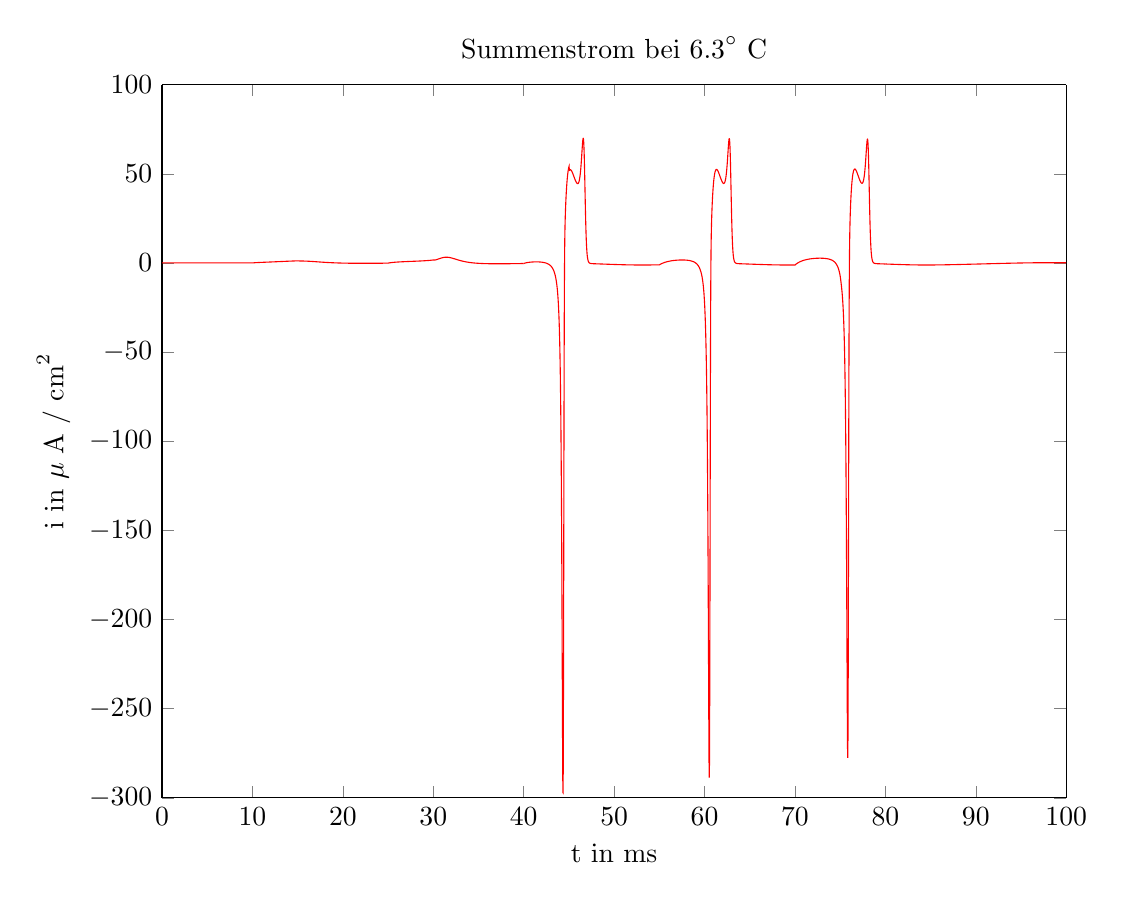
\begin{tikzpicture}

\begin{axis}[%
width=4.520833in,
height=3.565625in,
at={(0.758333in,0.48125in)},
scale only axis,
separate axis lines,
every outer x axis line/.append style={black},
every x tick label/.append style={font=\color{black}},
xmin=0,
xmax=100,
xlabel={t in ms},
every outer y axis line/.append style={black},
every y tick label/.append style={font=\color{black}},
ymin=-300,
ymax=100,
ylabel={$\text{i in }\mu\text{ A / cm}^\text{2}$},
title={$\text{Summenstrom bei 6.3}^\circ\text{ C}$}
]
\addplot [color=red,solid,forget plot]
  table[row sep=crcr]{%
0	-0.000323709182497467\\
0.01	-0.000323709182497467\\
0.02	-0.000321569323459947\\
0.03	-0.000319479557806535\\
0.04	-0.000317451749913822\\
0.05	-0.000315483051194221\\
0.06	-0.000313570648261319\\
0.07	-0.000311711857277963\\
0.08	-0.000309904118686699\\
0.09	-0.000308144991469472\\
0.1	-0.000306432147735514\\
0.11	-0.000304763367505068\\
0.12	-0.000303136533754689\\
0.13	-0.000301549627703235\\
0.14	-0.000300000724271943\\
0.15	-0.000298487987809182\\
0.16	-0.00029700966795243\\
0.17	-0.000295564095738055\\
0.18	-0.000294149679844313\\
0.19	-0.000292764903019993\\
0.2	-0.000291408318703112\\
0.21	-0.00029007854775065\\
0.22	-0.000288774275351678\\
0.23	-0.000287494248066622\\
0.24	-0.000286237271013956\\
0.25	-0.000285002205169693\\
0.26	-0.000283787964807658\\
0.27	-0.000282593515047225\\
0.28	-0.000281417869510747\\
0.29	-0.000280260088102668\\
0.3	-0.000279119274885886\\
0.31	-0.000277994576038498\\
0.32	-0.000276885177924235\\
0.33	-0.000275790305248602\\
0.34	-0.000274709219282077\\
0.35	-0.000273641216201437\\
0.36	-0.000272585625467059\\
0.37	-0.000271541808291698\\
0.38	-0.000270509156192311\\
0.39	-0.000269487089585851\\
0.4	-0.00026847505646499\\
0.41	-0.000267472531122692\\
0.42	-0.000266479012954512\\
0.43	-0.000265494025288415\\
0.44	-0.00026451711429365\\
0.45	-0.000263547847929591\\
0.46	-0.000262585814936322\\
0.47	-0.000261630623879405\\
0.48	-0.000260681902242599\\
0.49	-0.000259739295549455\\
0.5	-0.000258802466533314\\
0.51	-0.000257871094352602\\
0.52	-0.00025694487382566\\
0.53	-0.000256023514711323\\
0.54	-0.00025510674101703\\
0.55	-0.000254194290354448\\
0.56	-0.000253285913293322\\
0.57	-0.000252381372778387\\
0.58	-0.000251480443552055\\
0.59	-0.000250582911608177\\
0.6	-0.000249688573678242\\
0.61	-0.000248797236738429\\
0.62	-0.000247908717523337\\
0.63	-0.000247022842092104\\
0.64	-0.000246139445376325\\
0.65	-0.000245258370793255\\
0.66	-0.000244379469839462\\
0.67	-0.000243502601716905\\
0.68	-0.000242627632978554\\
0.69	-0.00024175443719443\\
0.7	-0.000240882894615879\\
0.71	-0.000240012891877139\\
0.72	-0.000239144321685369\\
0.73	-0.000238277082552418\\
0.74	-0.000237411078519045\\
0.75	-0.000236546218899569\\
0.76	-0.000235682418032734\\
0.77	-0.00023481959506233\\
0.78	-0.00023395767369605\\
0.79	-0.000233096581998105\\
0.8	-0.000232236252187601\\
0.81	-0.000231376620456025\\
0.82	-0.000230517626762961\\
0.83	-0.00022965921467355\\
0.84	-0.000228801331185746\\
0.85	-0.000227943926567775\\
0.86	-0.000227086954204481\\
0.87	-0.000226230370459213\\
0.88	-0.000225374134527723\\
0.89	-0.000224518208302715\\
0.9	-0.000223662556252169\\
0.91	-0.000222807145299431\\
0.92	-0.00022195194470509\\
0.93	-0.00022109692595107\\
0.94	-0.000220242062646481\\
0.95	-0.000219387330419707\\
0.96	-0.000218532706821595\\
0.97	-0.000217678171244629\\
0.98	-0.000216823704822566\\
0.99	-0.000215969290349172\\
1	-0.000215114912211156\\
1.01	-0.000214260556303358\\
1.02	-0.000213406209951028\\
1.03	-0.000212551861853427\\
1.04	-0.000211697502010555\\
1.05	-0.000210843121656978\\
1.06	-0.000209988713211651\\
1.07	-0.000209134270210409\\
1.08	-0.000208279787259347\\
1.09	-0.000207425259984628\\
1.1	-0.000206570684975205\\
1.11	-0.000205716059735295\\
1.12	-0.00020486138264264\\
1.13	-0.000204006652912092\\
1.14	-0.000203151870541429\\
1.15	-0.000202297036285604\\
1.16	-0.000201442151605225\\
1.17	-0.000200587218638137\\
1.18	-0.00019973224016967\\
1.19	-0.000198877219591331\\
1.2	-0.000198022160879496\\
1.21	-0.00019716706855144\\
1.22	-0.000196311947652905\\
1.23	-0.000195456803716354\\
1.24	-0.000194601642752978\\
1.25	-0.000193746471215395\\
1.26	-0.000192891295972331\\
1.27	-0.000192036124295303\\
1.28	-0.000191180963834192\\
1.29	-0.000190325822589266\\
1.3	-0.000189470708901407\\
1.31	-0.000188615631432132\\
1.32	-0.000187760599147158\\
1.33	-0.000186905621287092\\
1.34	-0.00018605070736788\\
1.35	-0.000185195867157706\\
1.36	-0.000184341110662789\\
1.37	-0.00018348644811228\\
1.38	-0.000182631889949381\\
1.39	-0.000181777446810028\\
1.4	-0.000180923129522004\\
1.41	-0.000180068949085399\\
1.42	-0.000179214916663284\\
1.43	-0.000178361043572384\\
1.44	-0.000177507341274197\\
1.45	-0.00017665382136034\\
1.46	-0.00017580049554855\\
1.47	-0.000174947375666257\\
1.48	-0.000174094473662567\\
1.49	-0.000173241801571411\\
1.5	-0.000172389371523973\\
1.51	-0.000171537195734039\\
1.52	-0.000170685286493111\\
1.53	-0.000169833656167739\\
1.54	-0.000168982317183097\\
1.55	-0.000168131282029638\\
1.56	-0.000167280563241778\\
1.57	-0.000166430173406784\\
1.58	-0.000165580125159881\\
1.59	-0.000164730431162052\\
1.6	-0.000163881104113806\\
1.61	-0.000163032156736076\\
1.62	-0.000162183601787547\\
1.63	-0.000161335452035338\\
1.64	-0.000160487720263447\\
1.65	-0.000159640419269635\\
1.66	-0.000158793561862325\\
1.67	-0.000157947160852601\\
1.68	-0.000157101229045775\\
1.69	-0.000156255779262704\\
1.7	-0.000155410824304703\\
1.71	-0.000154566376968202\\
1.72	-0.000153722450047411\\
1.73	-0.000152879056317445\\
1.74	-0.000152036208541873\\
1.75	-0.000151193919466497\\
1.76	-0.00015035220181181\\
1.77	-0.000149511068283203\\
1.78	-0.00014867053156653\\
1.79	-0.000147830604313004\\
1.8	-0.000146991299149857\\
1.81	-0.000146152628679896\\
1.82	-0.000145314605462854\\
1.83	-0.00014447724204425\\
1.84	-0.000143640550915869\\
1.85	-0.000142804544550401\\
1.86	-0.000141969235375683\\
1.87	-0.00014113463578358\\
1.88	-0.000140300758124656\\
1.89	-0.000139467614715727\\
1.9	-0.000138635217826089\\
1.91	-0.000137803579680185\\
1.92	-0.000136972712464267\\
1.93	-0.000136142628319735\\
1.94	-0.000135313339339582\\
1.95	-0.000134484857572836\\
1.96	-0.000133657195017012\\
1.97	-0.00013283036362699\\
1.98	-0.000132004375307027\\
1.99	-0.000131179241907198\\
2	-0.000130354975235392\\
2.01	-0.000129531587048426\\
2.02	-0.000128709089040946\\
2.03	-0.000127887492867629\\
2.04	-0.000127066810119647\\
2.05	-0.000126247052343764\\
2.06	-0.000125428231032121\\
2.07	-0.000124610357622235\\
2.08	-0.000123793443481901\\
2.09	-0.000122977499954047\\
2.1	-0.000122162538301218\\
2.11	-0.000121348569740665\\
2.12	-0.000120535605430572\\
2.13	-0.000119723656471393\\
2.14	-0.000118912733908516\\
2.15	-0.000118102848731816\\
2.16	-0.000117294011872549\\
2.17	-0.000116486234202462\\
2.18	-0.000115679526537793\\
2.19	-0.000114873899635715\\
2.2	-0.000114069364191671\\
2.21	-0.000113265930845152\\
2.22	-0.000112463610181468\\
2.23	-0.000111662412724645\\
2.24	-0.000110862348931651\\
2.25	-0.000110063429208385\\
2.26	-0.000109265663894131\\
2.27	-0.000108469063278438\\
2.28	-0.00010767363758335\\
2.29	-0.000106879396969628\\
2.3	-0.000106086351548296\\
2.31	-0.000105294511361098\\
2.32	-0.000104503886391161\\
2.33	-0.000103714486563877\\
2.34	-0.000102926321742469\\
2.35	-0.000102139401725765\\
2.36	-0.000101353736259302\\
2.37	-0.000100569335022449\\
2.38	-9.97862076395073e-05\\
2.39	-9.90043636672766e-05\\
2.4	-9.82238126070456e-05\\
2.41	-9.74445638997068e-05\\
2.42	-9.66666269222038e-05\\
2.43	-9.58900109888639e-05\\
2.44	-9.51147253589468e-05\\
2.45	-9.43407792290962e-05\\
2.46	-9.35681817306744e-05\\
2.47	-9.27969419435293e-05\\
2.48	-9.2027068873346e-05\\
2.49	-9.12585714814007e-05\\
2.5	-9.04914586525862e-05\\
2.51	-8.97257392229456e-05\\
2.52	-8.89614219587997e-05\\
2.53	-8.81985155700704e-05\\
2.54	-8.74370287085036e-05\\
2.55	-8.66769699605641e-05\\
2.56	-8.59183478527648e-05\\
2.57	-8.51611708543309e-05\\
2.58	-8.44054473678746e-05\\
2.59	-8.3651185743161e-05\\
2.6	-8.28983942646744e-05\\
2.61	-8.21470811582792e-05\\
2.62	-8.13972545881114e-05\\
2.63	-8.06489226574669e-05\\
2.64	-7.99020934110217e-05\\
2.65	-7.91567748352762e-05\\
2.66	-7.84129748550022e-05\\
2.67	-7.76707013279143e-05\\
2.68	-7.69299620624331e-05\\
2.69	-7.61907648048066e-05\\
2.7	-7.54531172360018e-05\\
2.71	-7.47170269774777e-05\\
2.72	-7.39825016005113e-05\\
2.73	-7.32495486084339e-05\\
2.74	-7.25181754437365e-05\\
2.75	-7.17883894969518e-05\\
2.76	-7.10601980937753e-05\\
2.77	-7.0333608501727e-05\\
2.78	-6.96086279283747e-05\\
2.79	-6.88852635222226e-05\\
2.8	-6.8163522374487e-05\\
2.81	-6.74434115182088e-05\\
2.82	-6.67249379238122e-05\\
2.83	-6.60081085070985e-05\\
2.84	-6.52929301199201e-05\\
2.85	-6.45794095639474e-05\\
2.86	-6.3867553572905e-05\\
2.87	-6.31573688263387e-05\\
2.88	-6.24488619496155e-05\\
2.89	-6.17420395041535e-05\\
2.9	-6.10369079931949e-05\\
2.91	-6.03334738658035e-05\\
2.92	-5.96317435155314e-05\\
2.93	-5.89317232679853e-05\\
2.94	-5.82334193985901e-05\\
2.95	-5.75368381228181e-05\\
2.96	-5.68419856055158e-05\\
2.97	-5.6148867943584e-05\\
2.98	-5.54574911864059e-05\\
2.99	-5.47678613140867e-05\\
3	-5.40799842627671e-05\\
3.01	-5.3393865907303e-05\\
3.02	-5.270951205949e-05\\
3.03	-5.20269284849384e-05\\
3.04	-5.13461208817567e-05\\
3.05	-5.06670949014243e-05\\
3.06	-4.99898561350243e-05\\
3.07	-4.93144101167964e-05\\
3.08	-4.86407623228047e-05\\
3.09	-4.79689181775989e-05\\
3.1	-4.72988830533261e-05\\
3.11	-4.66306622541879e-05\\
3.12	-4.59642610417532e-05\\
3.13	-4.52996846096454e-05\\
3.14	-4.4636938112852e-05\\
3.15	-4.39760266348621e-05\\
3.16	-4.3316955209427e-05\\
3.17	-4.26597288187835e-05\\
3.18	-4.20043523892133e-05\\
3.19	-4.13508307857136e-05\\
3.2	-4.06991688306491e-05\\
3.21	-4.00493712819916e-05\\
3.22	-3.94014428422018e-05\\
3.23	-3.87553881711078e-05\\
3.24	-3.81112118668092e-05\\
3.25	-3.74689184683419e-05\\
3.26	-3.68285124721091e-05\\
3.27	-3.61899983145619e-05\\
3.28	-3.55533803801933e-05\\
3.29	-3.49186629988729e-05\\
3.3	-3.42858504462917e-05\\
3.31	-3.36549469461822e-05\\
3.32	-3.3025956668542e-05\\
3.33	-3.23988837336309e-05\\
3.34	-3.17737322061973e-05\\
3.35	-3.11505060999195e-05\\
3.36	-3.05292093725207e-05\\
3.37	-2.99098459324298e-05\\
3.38	-2.92924196361177e-05\\
3.39	-2.86769342916493e-05\\
3.4	-2.80633936449171e-05\\
3.41	-2.74518013938518e-05\\
3.42	-2.68421611928638e-05\\
3.43	-2.62344766359668e-05\\
3.44	-2.56287512692133e-05\\
3.45	-2.5024988586253e-05\\
3.46	-2.44231920336624e-05\\
3.47	-2.38233649971775e-05\\
3.48	-2.32255108207902e-05\\
3.49	-2.26296327974218e-05\\
3.5	-2.20357341680355e-05\\
3.51	-2.1443818117195e-05\\
3.52	-2.08538877881637e-05\\
3.53	-2.02659462700261e-05\\
3.54	-1.96799966034611e-05\\
3.55	-1.90960417785213e-05\\
3.56	-1.85140847337451e-05\\
3.57	-1.79341283574885e-05\\
3.58	-1.73561754950313e-05\\
3.59	-1.67802289348096e-05\\
3.6	-1.62062914212946e-05\\
3.61	-1.56343656536606e-05\\
3.62	-1.50644542697975e-05\\
3.63	-1.44965598720681e-05\\
3.64	-1.39306850011067e-05\\
3.65	-1.33668321629088e-05\\
3.66	-1.28050038075145e-05\\
3.67	-1.22452023356701e-05\\
3.68	-1.16874301090419e-05\\
3.69	-1.1131689432009e-05\\
3.7	-1.05779825605445e-05\\
3.71	-1.00263117164268e-05\\
3.72	-9.47667905526473e-06\\
3.73	-8.92908670513393e-06\\
3.74	-8.3835367306051e-06\\
3.75	-7.84003116072185e-06\\
3.76	-7.29857197034889e-06\\
3.77	-6.75916109305064e-06\\
3.78	-6.22180041220943e-06\\
3.79	-5.6864917667987e-06\\
3.8	-5.15323695182701e-06\\
3.81	-4.62203770945635e-06\\
3.82	-4.09289574099247e-06\\
3.83	-3.56581270821721e-06\\
3.84	-3.04079021073989e-06\\
3.85	-2.51782981974813e-06\\
3.86	-1.99693305535931e-06\\
3.87	-1.47810139106141e-06\\
3.88	-9.6133625104855e-07\\
3.89	-4.46639020879047e-07\\
3.9	6.59889534126989e-08\\
3.91	5.76546377306641e-07\\
3.92	1.08503200069165e-06\\
3.93	1.59144461742144e-06\\
3.94	2.09578306575864e-06\\
3.95	2.59804622260162e-06\\
3.96	3.09823301058998e-06\\
3.97	3.59634240165718e-06\\
3.98	4.09237340326385e-06\\
3.99	4.5863250721645e-06\\
4	5.07819650197305e-06\\
4.01	5.56798683382098e-06\\
4.02	6.05569525324867e-06\\
4.03	6.54132097999138e-06\\
4.04	7.02486328707508e-06\\
4.05	7.50632147905606e-06\\
4.06	7.98569490845225e-06\\
4.07	8.46298296952597e-06\\
4.08	8.9381850991721e-06\\
4.09	9.41130076892449e-06\\
4.1	9.88232950183132e-06\\
4.11	1.03512708551357e-05\\
4.12	1.08181244300454e-05\\
4.13	1.1282889870845e-05\\
4.14	1.17455668577904e-05\\
4.15	1.2206155115102e-05\\
4.16	1.266465440386e-05\\
4.17	1.31210645268887e-05\\
4.18	1.35753853309772e-05\\
4.19	1.40276166993303e-05\\
4.2	1.44777585542322e-05\\
4.21	1.49258108610439e-05\\
4.22	1.53717736242065e-05\\
4.23	1.58156468819115e-05\\
4.24	1.625743071898e-05\\
4.25	1.66971252530956e-05\\
4.26	1.71347306459069e-05\\
4.27	1.75702470950334e-05\\
4.28	1.80036748362866e-05\\
4.29	1.84350141467782e-05\\
4.3	1.88642653364823e-05\\
4.31	1.92914287606705e-05\\
4.32	1.97165048088088e-05\\
4.33	2.01394939058908e-05\\
4.34	2.05603965146572e-05\\
4.35	2.09792131422581e-05\\
4.36	2.13959443247091e-05\\
4.37	2.18105906411026e-05\\
4.38	2.22231527029493e-05\\
4.39	2.26336311617281e-05\\
4.4	2.30420267004483e-05\\
4.41	2.34483400456398e-05\\
4.42	2.38525719553628e-05\\
4.43	2.42547232276458e-05\\
4.44	2.46547946929354e-05\\
4.45	2.50527872229789e-05\\
4.46	2.54487017126159e-05\\
4.47	2.58425391059802e-05\\
4.48	2.62343003774035e-05\\
4.49	2.66239865345241e-05\\
4.5	2.70115986258368e-05\\
4.51	2.73971377260374e-05\\
4.52	2.77806049524543e-05\\
4.53	2.81620014503936e-05\\
4.54	2.85413284006886e-05\\
4.55	2.89185870250286e-05\\
4.56	2.92937785739689e-05\\
4.57	2.96669043331477e-05\\
4.58	3.00379656175132e-05\\
4.59	3.04069637815374e-05\\
4.6	3.07739002098906e-05\\
4.61	3.11387763245463e-05\\
4.62	3.15015935741236e-05\\
4.63	3.18623534441009e-05\\
4.64	3.22210574528192e-05\\
4.65	3.25777071528144e-05\\
4.66	3.29323041219354e-05\\
4.67	3.32848499806637e-05\\
4.68	3.36353463699091e-05\\
4.69	3.39837949749899e-05\\
4.7	3.43301975056498e-05\\
4.71	3.46745557018302e-05\\
4.72	3.5016871340332e-05\\
4.73	3.53571462232694e-05\\
4.74	3.56953821891715e-05\\
4.75	3.60315811036571e-05\\
4.76	3.63657448687604e-05\\
4.77	3.66978754127167e-05\\
4.78	3.70279746899627e-05\\
4.79	3.73560446980115e-05\\
4.8	3.76820874530281e-05\\
4.81	3.80061050009317e-05\\
4.82	3.83280994284974e-05\\
4.83	3.86480728420402e-05\\
4.84	3.89660273838466e-05\\
4.85	3.92819652192955e-05\\
4.86	3.95958885466285e-05\\
4.87	3.99077995947295e-05\\
4.88	4.02177006200155e-05\\
4.89	4.05255939073257e-05\\
4.9	4.08314817610389e-05\\
4.91	4.11353665321634e-05\\
4.92	4.1437250589027e-05\\
4.93	4.17371363297114e-05\\
4.94	4.20350261776115e-05\\
4.95	4.23309225898727e-05\\
4.96	4.26248280454011e-05\\
4.97	4.29167450581858e-05\\
4.98	4.32066761573147e-05\\
4.99	4.34946239091794e-05\\
5	4.37805909041522e-05\\
5.01	4.40645797628036e-05\\
5.02	4.43465931265763e-05\\
5.03	4.46266336644463e-05\\
5.04	4.49047040764761e-05\\
5.05	4.51808070822679e-05\\
5.06	4.54549454302899e-05\\
5.07	4.57271219009847e-05\\
5.08	4.5997339290782e-05\\
5.09	4.62656004276418e-05\\
5.1	4.65319081666138e-05\\
5.11	4.6796265380955e-05\\
5.12	4.70586749727886e-05\\
5.13	4.7319139872215e-05\\
5.14	4.75776630302072e-05\\
5.15	4.78342474230509e-05\\
5.16	4.80888960532333e-05\\
5.17	4.83416119467783e-05\\
5.18	4.85923981492498e-05\\
5.19	4.88412577372976e-05\\
5.2	4.90881938111087e-05\\
5.21	4.9333209486413e-05\\
5.22	4.95763079135791e-05\\
5.23	4.98174922585193e-05\\
5.24	5.00567657106821e-05\\
5.25	5.02941314879379e-05\\
5.26	5.05295928290295e-05\\
5.27	5.07631529926833e-05\\
5.28	5.09948152616069e-05\\
5.29	5.12245829438207e-05\\
5.3	5.1452459365553e-05\\
5.31	5.16784478765686e-05\\
5.32	5.19025518523897e-05\\
5.33	5.21247746818609e-05\\
5.34	5.23451197818048e-05\\
5.35	5.25635905939126e-05\\
5.36	5.27801905705338e-05\\
5.37	5.29949231964366e-05\\
5.38	5.32077919732643e-05\\
5.39	5.34188004244207e-05\\
5.4	5.36279520915173e-05\\
5.41	5.38352505352613e-05\\
5.42	5.40406993425613e-05\\
5.43	5.42443021158689e-05\\
5.44	5.4446062482949e-05\\
5.45	5.46459840879976e-05\\
5.46	5.4844070591642e-05\\
5.47	5.5040325686484e-05\\
5.48	5.52347530700104e-05\\
5.49	5.54273564645769e-05\\
5.5	5.56181396178523e-05\\
5.51	5.5807106294381e-05\\
5.52	5.59942602724739e-05\\
5.53	5.61796053459851e-05\\
5.54	5.63631453416313e-05\\
5.55	5.65448840936789e-05\\
5.56	5.6724825456822e-05\\
5.57	5.69029733066273e-05\\
5.58	5.70793315364249e-05\\
5.59	5.72539040546438e-05\\
5.6	5.7426694788365e-05\\
5.61	5.75977076819889e-05\\
5.62	5.77669467065611e-05\\
5.63	5.79344158366801e-05\\
5.64	5.81001190655961e-05\\
5.65	5.82640604158691e-05\\
5.66	5.84262439216054e-05\\
5.67	5.85866736249052e-05\\
5.68	5.87453535945137e-05\\
5.69	5.89022879102785e-05\\
5.7	5.90574806706989e-05\\
5.71	5.92109359947024e-05\\
5.72	5.93626580100981e-05\\
5.73	5.95126508655675e-05\\
5.74	5.96609187160091e-05\\
5.75	5.98074657522929e-05\\
5.76	5.99522961590715e-05\\
5.77	6.00954141489751e-05\\
5.78	6.02368239470685e-05\\
5.79	6.03765297877423e-05\\
5.8	6.05145359315884e-05\\
5.81	6.06508466467481e-05\\
5.82	6.07854662142415e-05\\
5.83	6.09183989355166e-05\\
5.84	6.10496491226797e-05\\
5.85	6.1179221102492e-05\\
5.86	6.13071192154813e-05\\
5.87	6.14333478208273e-05\\
5.88	6.15579112861475e-05\\
5.89	6.16808139932701e-05\\
5.9	6.18020603382341e-05\\
5.91	6.19216547290691e-05\\
5.92	6.20396015964531e-05\\
5.93	6.215590537062e-05\\
5.94	6.22705705035642e-05\\
5.95	6.23836014574941e-05\\
5.96	6.24950027039439e-05\\
5.97	6.26047787357642e-05\\
5.98	6.27129340546873e-05\\
5.99	6.28194731668863e-05\\
6	6.29244006038476e-05\\
6.01	6.30277208997221e-05\\
6.02	6.31294385997627e-05\\
6.03	6.3229558266098e-05\\
6.04	6.33280844732909e-05\\
6.05	6.34250218038979e-05\\
6.06	6.35203748546864e-05\\
6.07	6.36141482304176e-05\\
6.08	6.37063465478427e-05\\
6.09	6.37969744414768e-05\\
6.1	6.38860365418381e-05\\
6.11	6.39735375047579e-05\\
6.12	6.40594819927287e-05\\
6.13	6.41438746749046e-05\\
6.14	6.42267202350943e-05\\
6.15	6.43080233619919e-05\\
6.16	6.43877887602784e-05\\
6.17	6.44660211395198e-05\\
6.18	6.45427252266018e-05\\
6.19	6.46179057466334e-05\\
6.2	6.4691567445152e-05\\
6.21	6.47637150712477e-05\\
6.22	6.48343533877771e-05\\
6.23	6.49034871607057e-05\\
6.24	6.49711211688775e-05\\
6.25	6.50372601995741e-05\\
6.26	6.51019090494032e-05\\
6.27	6.5165072524298e-05\\
6.28	6.5226755434189e-05\\
6.29	6.52869626014407e-05\\
6.3	6.53456988599643e-05\\
6.31	6.54029690441149e-05\\
6.32	6.54587780029026e-05\\
6.33	6.55131305906664e-05\\
6.34	6.55660316675188e-05\\
6.35	6.56174861073389e-05\\
6.36	6.56674987804529e-05\\
6.37	6.57160745789476e-05\\
6.38	6.57632183882484e-05\\
6.39	6.58089351111002e-05\\
6.4	6.58532296533565e-05\\
6.41	6.58961069310848e-05\\
6.42	6.59375718625732e-05\\
6.43	6.59776293745473e-05\\
6.44	6.60162843977297e-05\\
6.45	6.6053541879274e-05\\
6.46	6.6089406755232e-05\\
6.47	6.61238839905209e-05\\
6.48	6.61569785367355e-05\\
6.49	6.6188695358349e-05\\
6.5	6.62190394313811e-05\\
6.51	6.6248015725634e-05\\
6.52	6.62756292268973e-05\\
6.53	6.63018849200725e-05\\
6.54	6.63267878011631e-05\\
6.55	6.63503428701695e-05\\
6.56	6.63725551257599e-05\\
6.57	6.63934295808133e-05\\
6.58	6.64129712424355e-05\\
6.59	6.64311851350519e-05\\
6.6	6.64480762861963e-05\\
6.61	6.64636497171855e-05\\
6.62	6.64779104604385e-05\\
6.63	6.64908635510386e-05\\
6.64	6.65025140316189e-05\\
6.65	6.65128669514736e-05\\
6.66	6.65219273572326e-05\\
6.67	6.65297002995224e-05\\
6.68	6.65361908387396e-05\\
6.69	6.6541404031728e-05\\
6.7	6.6545344947766e-05\\
6.71	6.65480186485823e-05\\
6.72	6.65494302105607e-05\\
6.73	6.65495847074205e-05\\
6.74	6.65484872182098e-05\\
6.75	6.65461428197567e-05\\
6.76	6.65425565977706e-05\\
6.77	6.65377336379613e-05\\
6.78	6.65316790313675e-05\\
6.79	6.65243978690278e-05\\
6.8	6.65158952450895e-05\\
6.81	6.65061762572527e-05\\
6.82	6.64952460027735e-05\\
6.83	6.64831095833485e-05\\
6.84	6.64697721060037e-05\\
6.85	6.64552386711037e-05\\
6.86	6.64395143878949e-05\\
6.87	6.64226043647353e-05\\
6.88	6.64045137166447e-05\\
6.89	6.63852475510929e-05\\
6.9	6.63648109888726e-05\\
6.91	6.63432091370098e-05\\
6.92	6.63204471145207e-05\\
6.93	6.62965300435303e-05\\
6.94	6.62714630368377e-05\\
6.95	6.62452512201206e-05\\
6.96	6.62178997128393e-05\\
6.97	6.61894136322339e-05\\
6.98	6.61597981053141e-05\\
6.99	6.6129058248432e-05\\
7	6.60971991930381e-05\\
7.01	6.60642260572608e-05\\
7.02	6.60301439654454e-05\\
7.03	6.59949580441577e-05\\
7.04	6.5958673412414e-05\\
7.05	6.59212952025534e-05\\
7.06	6.58828285304836e-05\\
7.07	6.58432785245466e-05\\
7.08	6.58026503059794e-05\\
7.09	6.57609490013478e-05\\
7.1	6.57181797292239e-05\\
7.11	6.56743476139532e-05\\
7.12	6.56294577758842e-05\\
7.13	6.55835153344775e-05\\
7.14	6.55365254109697e-05\\
7.15	6.54884931252653e-05\\
7.16	6.5439423593272e-05\\
7.17	6.53893219300095e-05\\
7.18	6.53381932549379e-05\\
7.19	6.52860426804125e-05\\
7.2	6.52328753187881e-05\\
7.21	6.51786962793111e-05\\
7.22	6.51235106738923e-05\\
7.23	6.50673236100019e-05\\
7.24	6.50101401920011e-05\\
7.25	6.49519655229192e-05\\
7.26	6.48928047093378e-05\\
7.27	6.48326628494011e-05\\
7.28	6.4771545039477e-05\\
7.29	6.4709456375045e-05\\
7.3	6.46464019511406e-05\\
7.31	6.45823868605788e-05\\
7.32	6.45174161908457e-05\\
7.33	6.44514950249864e-05\\
7.34	6.43846284451577e-05\\
7.35	6.43168215410661e-05\\
7.36	6.4248079382434e-05\\
7.37	6.41784070438689e-05\\
7.38	6.41078096013104e-05\\
7.39	6.40362921249249e-05\\
7.4	6.39638596764414e-05\\
7.41	6.38905173180326e-05\\
7.42	6.38162701096512e-05\\
7.43	6.37411231050322e-05\\
7.44	6.36650813614636e-05\\
7.45	6.35881499202462e-05\\
7.46	6.35103338360032e-05\\
7.47	6.34316381429301e-05\\
7.48	6.33520678809951e-05\\
7.49	6.32716280795087e-05\\
7.5	6.31903237753306e-05\\
7.51	6.31081599915539e-05\\
7.52	6.30251417481631e-05\\
7.53	6.29412740620339e-05\\
7.54	6.28565619482657e-05\\
7.55	6.27710104126322e-05\\
7.56	6.26846244609069e-05\\
7.57	6.2597409091758e-05\\
7.58	6.25093693011891e-05\\
7.59	6.2420510081207e-05\\
7.6	6.23308364171571e-05\\
7.61	6.22403532877236e-05\\
7.62	6.21490656667056e-05\\
7.63	6.2056978526126e-05\\
7.64	6.19640968388957e-05\\
7.65	6.18704255601621e-05\\
7.66	6.17759696450726e-05\\
7.67	6.16807340430015e-05\\
7.68	6.15847237059874e-05\\
7.69	6.1487943564309e-05\\
7.7	6.1390398560679e-05\\
7.71	6.12920936187145e-05\\
7.72	6.11930336646971e-05\\
7.73	6.10932236138062e-05\\
7.74	6.09926683781126e-05\\
7.75	6.08913728603611e-05\\
7.76	6.07893419672934e-05\\
7.77	6.06865805883317e-05\\
7.78	6.05830936111218e-05\\
7.79	6.04788859197569e-05\\
7.8	6.03739623916688e-05\\
7.81	6.02683278918548e-05\\
7.82	6.01619872835357e-05\\
7.83	6.00549454303767e-05\\
7.84	5.99472071765028e-05\\
7.85	5.98387773673714e-05\\
7.86	5.97296608382258e-05\\
7.87	5.96198624238653e-05\\
7.88	5.95093869475427e-05\\
7.89	5.93982392236292e-05\\
7.9	5.928642406694e-05\\
7.91	5.91739462789675e-05\\
7.92	5.906081065854e-05\\
7.93	5.89470219938271e-05\\
7.94	5.88325850663374e-05\\
7.95	5.8717504650474e-05\\
7.96	5.86017855170873e-05\\
7.97	5.84854324281459e-05\\
7.98	5.83684501327397e-05\\
7.99	5.82508433830675e-05\\
8	5.81326169135643e-05\\
8.01	5.8013775457777e-05\\
8.02	5.78943237408147e-05\\
8.03	5.77742664784608e-05\\
8.04	5.76536083793933e-05\\
8.05	5.75323541420758e-05\\
8.06	5.74105084627519e-05\\
8.07	5.72880760265626e-05\\
8.08	5.71650615097674e-05\\
8.09	5.70414695806321e-05\\
8.1	5.69173049052019e-05\\
8.11	5.67925721335349e-05\\
8.12	5.66672759121367e-05\\
8.13	5.65414208790749e-05\\
8.14	5.6415011661759e-05\\
8.15	5.62880528822696e-05\\
8.16	5.61605491511408e-05\\
8.17	5.603250507491e-05\\
8.18	5.5903925247236e-05\\
8.19	5.57748142573367e-05\\
8.2	5.56451766828836e-05\\
8.21	5.55150170935548e-05\\
8.22	5.53843400461496e-05\\
8.23	5.52531500992437e-05\\
8.24	5.51214517976462e-05\\
8.25	5.49892496706228e-05\\
8.26	5.48565482478836e-05\\
8.27	5.47233520493684e-05\\
8.28	5.45896655781419e-05\\
8.29	5.44554933381569e-05\\
8.3	5.43208398142703e-05\\
8.31	5.4185709491783e-05\\
8.32	5.40501068422294e-05\\
8.33	5.39140363300383e-05\\
8.34	5.3777502407204e-05\\
8.35	5.36405095226122e-05\\
8.36	5.35030621056087e-05\\
8.37	5.33651645828748e-05\\
8.38	5.32268213748743e-05\\
8.39	5.30880368838638e-05\\
8.4	5.29488155094349e-05\\
8.41	5.28091616356363e-05\\
8.42	5.2669079647405e-05\\
8.43	5.25285739088055e-05\\
8.44	5.23876487790176e-05\\
8.45	5.22463086092273e-05\\
8.46	5.21045577364099e-05\\
8.47	5.19624004913233e-05\\
8.48	5.18198411962878e-05\\
8.49	5.16768841576365e-05\\
8.5	5.15335336781497e-05\\
8.51	5.13897940441765e-05\\
8.52	5.12456695398456e-05\\
8.53	5.110116443241e-05\\
8.54	5.09562829815735e-05\\
8.55	5.08110294368258e-05\\
8.56	5.06654080418834e-05\\
8.57	5.05194230218109e-05\\
8.58	5.03730785941237e-05\\
8.59	5.02263789736723e-05\\
8.6	5.00793283531031e-05\\
8.61	4.99319309237301e-05\\
8.62	4.97841908635444e-05\\
8.63	4.96361123354383e-05\\
8.64	4.94876994996396e-05\\
8.65	4.93389565030533e-05\\
8.66	4.91898874823704e-05\\
8.67	4.90404965596269e-05\\
8.68	4.88907878524181e-05\\
8.69	4.87407654605754e-05\\
8.7	4.85904334794895e-05\\
8.71	4.84397959903404e-05\\
8.72	4.82888570694229e-05\\
8.73	4.81376207748241e-05\\
8.74	4.79860911539731e-05\\
8.75	4.78342722511904e-05\\
8.76	4.7682168089036e-05\\
8.77	4.75297826869614e-05\\
8.78	4.7377120054648e-05\\
8.79	4.72241841844578e-05\\
8.8	4.70709790638679e-05\\
8.81	4.69175086630358e-05\\
8.82	4.67637769441254e-05\\
8.83	4.66097878653038e-05\\
8.84	4.64555453563165e-05\\
8.85	4.63010533531261e-05\\
8.86	4.61463157739317e-05\\
8.87	4.5991336524942e-05\\
8.88	4.5836119498599e-05\\
8.89	4.56806685753541e-05\\
8.9	4.55249876378794e-05\\
8.91	4.53690805430895e-05\\
8.92	4.5212951136353e-05\\
8.93	4.50566032621502e-05\\
8.94	4.4900040748086e-05\\
8.95	4.47432674084425e-05\\
8.96	4.4586287047732e-05\\
8.97	4.44291034642497e-05\\
8.98	4.42717204305332e-05\\
8.99	4.41141417213409e-05\\
9	4.39563710945556e-05\\
9.01	4.37984122956259e-05\\
9.02	4.36402690597859e-05\\
9.03	4.34819451142765e-05\\
9.04	4.33234441690189e-05\\
9.05	4.31647699228321e-05\\
9.06	4.30059260652094e-05\\
9.07	4.28469162709888e-05\\
9.08	4.26877442047946e-05\\
9.09	4.25284135241455e-05\\
9.1	4.2368927865688e-05\\
9.11	4.22092908642924e-05\\
9.12	4.20495061370652e-05\\
9.13	4.18895772873462e-05\\
9.14	4.17295079100377e-05\\
9.15	4.1569301586275e-05\\
9.16	4.14089618900881e-05\\
9.17	4.12484923777434e-05\\
9.18	4.10878965939609e-05\\
9.19	4.09271780767995e-05\\
9.2	4.07663403474423e-05\\
9.21	4.06053869155265e-05\\
9.22	4.04443212813632e-05\\
9.23	4.02831469306086e-05\\
9.24	4.01218673373727e-05\\
9.25	3.99604859642189e-05\\
9.26	3.97990062594999e-05\\
9.27	3.96374316662396e-05\\
9.28	3.94757656088096e-05\\
9.29	3.93140114995916e-05\\
9.3	3.91521727380884e-05\\
9.31	3.89902527184738e-05\\
9.32	3.88282548158259e-05\\
9.33	3.86661823990053e-05\\
9.34	3.85040388160007e-05\\
9.35	3.83418274081393e-05\\
9.36	3.81795515091987e-05\\
9.37	3.80172144334168e-05\\
9.38	3.78548194843731e-05\\
9.39	3.7692369954101e-05\\
9.4	3.75298691164261e-05\\
9.41	3.73673202473945e-05\\
9.42	3.72047265955189e-05\\
9.43	3.70420914084235e-05\\
9.44	3.68794179150811e-05\\
9.45	3.67167093329179e-05\\
9.46	3.65539688673699e-05\\
9.47	3.63911997145472e-05\\
9.48	3.62284050505757e-05\\
9.49	3.60655880462524e-05\\
9.5	3.59027518572752e-05\\
9.51	3.5739899623799e-05\\
9.52	3.55770344855344e-05\\
9.53	3.54141595555468e-05\\
9.54	3.52512779411285e-05\\
9.55	3.5088392737137e-05\\
9.56	3.49255070215548e-05\\
9.57	3.47626238710319e-05\\
9.58	3.4599746336017e-05\\
9.59	3.44368774656267e-05\\
9.6	3.42740202876612e-05\\
9.61	3.41111778201508e-05\\
9.62	3.3948353077573e-05\\
9.63	3.37855490406547e-05\\
9.64	3.36227687034452e-05\\
9.65	3.34600150311282e-05\\
9.66	3.32972909800056e-05\\
9.67	3.31345994921683e-05\\
9.68	3.29719435048226e-05\\
9.69	3.28093259298612e-05\\
9.7	3.26467496822858e-05\\
9.71	3.24842176522289e-05\\
9.72	3.23217327209413e-05\\
9.73	3.21592977550189e-05\\
9.74	3.1996915618393e-05\\
9.75	3.18345891461291e-05\\
9.76	3.16723211768455e-05\\
9.77	3.15101145269558e-05\\
9.78	3.13479720039922e-05\\
9.79	3.11858963959466e-05\\
9.8	3.10238904899229e-05\\
9.81	3.08619570548174e-05\\
9.82	3.07000988408745e-05\\
9.83	3.05383185987829e-05\\
9.84	3.03766190530297e-05\\
9.85	3.021500292677e-05\\
9.86	3.00534729258395e-05\\
9.87	2.98920317409745e-05\\
9.88	2.97306820495891e-05\\
9.89	2.9569426524656e-05\\
9.9	2.94082678236052e-05\\
9.91	2.9247208586991e-05\\
9.92	2.90862514442658e-05\\
9.93	2.89253990155558e-05\\
9.94	2.87646539036679e-05\\
9.95	2.86040187011949e-05\\
9.96	2.84434959922919e-05\\
9.97	2.828308834113e-05\\
9.98	2.81227983034427e-05\\
9.99	2.79626284211965e-05\\
10	2.78025812256999e-05\\
10.01	2.76426592340506e-05\\
10.02	0.00663815913251531\\
10.03	0.0130939469842888\\
10.04	0.0193583116181961\\
10.05	0.0254399654317856\\
10.06	0.0313474726623326\\
10.07	0.0370889648463373\\
10.08	0.042672163331603\\
10.09	0.0481044022977466\\
10.1	0.053392650312349\\
10.11	0.0585435305174857\\
10.12	0.0635633395465982\\
10.13	0.0684580652633522\\
10.14	0.0732334034068125\\
10.15	0.0778947732203741\\
10.16	0.0824473321356938\\
10.17	0.0868959895772412\\
10.18	0.0912454199478243\\
10.19	0.0955000748508921\\
10.2	0.0996641946009387\\
10.21	0.103741819069515\\
10.22	0.107736797910694\\
10.23	0.111652800206517\\
10.24	0.115493323570003\\
10.25	0.119261702740435\\
10.26	0.122961117703172\\
10.27	0.126594601363827\\
10.28	0.130165046804573\\
10.29	0.133675214148335\\
10.3	0.137127737054778\\
10.31	0.140525128870415\\
10.32	0.143869788453511\\
10.33	0.147164005693115\\
10.34	0.150409966740264\\
10.35	0.153609758968051\\
10.36	0.156765375676333\\
10.37	0.159878720555664\\
10.38	0.162951611924131\\
10.39	0.165985786749931\\
10.4	0.168982904471634\\
10.41	0.171944550627358\\
10.42	0.174872240303389\\
10.43	0.177767421412072\\
10.44	0.180631477808258\\
10.45	0.183465732252952\\
10.46	0.186271449232365\\
10.47	0.189049837639988\\
10.48	0.191802053328972\\
10.49	0.194529201541505\\
10.5	0.197232339221666\\
10.51	0.199912477217718\\
10.52	0.202570582379533\\
10.53	0.205207579556512\\
10.54	0.207824353501025\\
10.55	0.21042175068215\\
10.56	0.213000581014188\\
10.57	0.215561619504248\\
10.58	0.218105607822894\\
10.59	0.220633255801623\\
10.6	0.223145242860841\\
10.61	0.225642219371686\\
10.62	0.228124807954913\\
10.63	0.230593604719933\\
10.64	0.233049180446887\\
10.65	0.235492081714442\\
10.66	0.237922831975984\\
10.67	0.24034193258663\\
10.68	0.242749863783391\\
10.69	0.245147085620732\\
10.7	0.247534038863614\\
10.71	0.249911145840029\\
10.72	0.252278811254926\\
10.73	0.254637422967343\\
10.74	0.256987352732432\\
10.75	0.259328956910056\\
10.76	0.261662577141459\\
10.77	0.263988540995534\\
10.78	0.266307162586048\\
10.79	0.268618743161195\\
10.8	0.270923571666726\\
10.81	0.273221925283894\\
10.82	0.275514069943319\\
10.83	0.277800260815927\\
10.84	0.280080742781968\\
10.85	0.282355750879139\\
10.86	0.284625510730719\\
10.87	0.286890238954678\\
10.88	0.289150143554563\\
10.89	0.29140542429304\\
10.9	0.293656273048823\\
10.91	0.29590287415777\\
10.92	0.298145404738858\\
10.93	0.300384035005689\\
10.94	0.302618928564204\\
10.95	0.304850242697239\\
10.96	0.307078128636426\\
10.97	0.30930273182212\\
10.98	0.311524192151816\\
10.99	0.313742644217576\\
11	0.315958217532961\\
11.01	0.31817103674997\\
11.02	0.32038122186635\\
11.03	0.322588888423805\\
11.04	0.324794147697423\\
11.05	0.326997106876757\\
11.06	0.329197869238914\\
11.07	0.331396534314018\\
11.08	0.33359319804336\\
11.09	0.335787952930607\\
11.1	0.337980888186297\\
11.11	0.340172089866014\\
11.12	0.342361641002432\\
11.13	0.344549621731565\\
11.14	0.346736109413436\\
11.15	0.348921178747446\\
11.16	0.351104901882633\\
11.17	0.353287348523098\\
11.18	0.355468586028752\\
11.19	0.357648679511657\\
11.2	0.359827691928083\\
11.21	0.362005684166538\\
11.22	0.364182715131896\\
11.23	0.366358841825806\\
11.24	0.36853411942358\\
11.25	0.370708601347666\\
11.26	0.372882339337878\\
11.27	0.37505538351852\\
11.28	0.377227782462575\\
11.29	0.379399583253019\\
11.3	0.381570831541438\\
11.31	0.383741571604054\\
11.32	0.38591184639528\\
11.33	0.388081697598876\\
11.34	0.390251165676862\\
11.35	0.392420289916258\\
11.36	0.394589108473741\\
11.37	0.39675765841834\\
11.38	0.398925975772202\\
11.39	0.401094095549566\\
11.4	0.403262051794007\\
11.41	0.405429877614012\\
11.42	0.407597605216958\\
11.43	0.409765265941602\\
11.44	0.411932890289092\\
11.45	0.414100507952603\\
11.46	0.416268147845661\\
11.47	0.418435838129145\\
11.48	0.420603606237151\\
11.49	0.422771478901628\\
11.5	0.424939482175939\\
11.51	0.427107641457347\\
11.52	0.429275981508495\\
11.53	0.431444526477895\\
11.54	0.433613299919509\\
11.55	0.435782324811433\\
11.56	0.437951623573718\\
11.57	0.440121218085394\\
11.58	0.442291129700714\\
11.59	0.444461379264636\\
11.6	0.446631987127617\\
11.61	0.448802973159708\\
11.62	0.450974356764013\\
11.63	0.45314615688949\\
11.64	0.455318392043214\\
11.65	0.457491080302007\\
11.66	0.459664239323575\\
11.67	0.461837886357077\\
11.68	0.464012038253227\\
11.69	0.466186711473909\\
11.7	0.46836192210132\\
11.71	0.470537685846706\\
11.72	0.472714018058648\\
11.73	0.474890933730963\\
11.74	0.477068447510224\\
11.75	0.479246573702908\\
11.76	0.481425326282188\\
11.77	0.483604718894403\\
11.78	0.485784764865195\\
11.79	0.487965477205349\\
11.8	0.49014686861633\\
11.81	0.492328951495528\\
11.82	0.49451173794128\\
11.83	0.49669523975757\\
11.84	0.498879468458527\\
11.85	0.501064435272683\\
11.86	0.503250151146977\\
11.87	0.505436626750587\\
11.88	0.507623872478512\\
11.89	0.509811898454985\\
11.9	0.512000714536687\\
11.91	0.514190330315781\\
11.92	0.516380755122767\\
11.93	0.518571998029181\\
11.94	0.520764067850133\\
11.95	0.522956973146685\\
11.96	0.525150722228095\\
11.97	0.527345323153911\\
11.98	0.529540783735951\\
11.99	0.531737111540124\\
12	0.533934313888165\\
12.01	0.536132397859224\\
12.02	0.538331370291369\\
12.03	0.54053123778296\\
12.04	0.542732006693931\\
12.05	0.544933683146974\\
12.06	0.547136273028646\\
12.07	0.54933978199034\\
12.08	0.551544215449236\\
12.09	0.553749578589105\\
12.1	0.555955876361085\\
12.11	0.55816311348436\\
12.12	0.560371294446762\\
12.13	0.562580423505331\\
12.14	0.564790504686778\\
12.15	0.567001541787895\\
12.16	0.569213538375932\\
12.17	0.57142649778889\\
12.18	0.573640423135744\\
12.19	0.575855317296665\\
12.2	0.578071182923141\\
12.21	0.580288022438096\\
12.22	0.582505838035916\\
12.23	0.584724631682476\\
12.24	0.586944405115102\\
12.25	0.589165159842496\\
12.26	0.591386897144629\\
12.27	0.593609618072597\\
12.28	0.595833323448438\\
12.29	0.598058013864933\\
12.3	0.600283689685355\\
12.31	0.602510351043196\\
12.32	0.604737997841883\\
12.33	0.606966629754439\\
12.34	0.609196246223144\\
12.35	0.61142684645916\\
12.36	0.613658429442134\\
12.37	0.615890993919788\\
12.38	0.618124538407472\\
12.39	0.620359061187727\\
12.4	0.622594560309794\\
12.41	0.624831033589137\\
12.42	0.627068478606933\\
12.43	0.629306892709556\\
12.44	0.631546273008039\\
12.45	0.633786616377533\\
12.46	0.636027919456748\\
12.47	0.638270178647379\\
12.48	0.640513390113526\\
12.49	0.642757549781112\\
12.5	0.645002653337288\\
12.51	0.647248696229807\\
12.52	0.64949567366643\\
12.53	0.651743580614296\\
12.54	0.653992411799312\\
12.55	0.656242161705493\\
12.56	0.658492824574356\\
12.57	0.660744394404263\\
12.58	0.662996864949777\\
12.59	0.665250229721027\\
12.6	0.667504481983055\\
12.61	0.669759614755162\\
12.62	0.672015620810273\\
12.63	0.674272492674258\\
12.64	0.676530222625306\\
12.65	0.678788802693263\\
12.66	0.681048224658982\\
12.67	0.683308480053686\\
12.68	0.685569560158308\\
12.69	0.687831456002852\\
12.7	0.69009415836575\\
12.71	0.692357657773235\\
12.72	0.694621944498695\\
12.73	0.696887008562052\\
12.74	0.699152839729136\\
12.75	0.701419427511052\\
12.76	0.703686761163589\\
12.77	0.705954829686601\\
12.78	0.708223621823388\\
12.79	0.710493126060147\\
12.8	0.712763330625334\\
12.81	0.715034223489112\\
12.82	0.717305792362764\\
12.83	0.719578024698148\\
12.84	0.721850907687124\\
12.85	0.724124428261011\\
12.86	0.726398573090061\\
12.87	0.728673328582904\\
12.88	0.73094868088607\\
12.89	0.733224615883454\\
12.9	0.735501119195827\\
12.91	0.737778176180352\\
12.92	0.740055771930109\\
12.93	0.742333891273627\\
12.94	0.744612518774455\\
12.95	0.746891638730702\\
12.96	0.749171235174626\\
12.97	0.751451291872216\\
12.98	0.753731792322797\\
12.99	0.756012719758647\\
13	0.75829405714462\\
13.01	0.760575787177804\\
13.02	0.762857892287165\\
13.03	0.765140354633238\\
13.04	0.767423156107792\\
13.05	0.769706278333558\\
13.06	0.771989702663943\\
13.07	0.774273410182757\\
13.08	0.776557381703985\\
13.09	0.778841597771542\\
13.1	0.781126038659066\\
13.11	0.783410684369735\\
13.12	0.785695514636061\\
13.13	0.787980508919764\\
13.14	0.79026564641161\\
13.15	0.792550906031291\\
13.16	0.794836266427335\\
13.17	0.797121705977006\\
13.18	0.799407202786248\\
13.19	0.80169273468964\\
13.2	0.803978279250371\\
13.21	0.806263813760226\\
13.22	0.808549315239618\\
13.23	0.810834760437619\\
13.24	0.81312012583201\\
13.25	0.81540538762937\\
13.26	0.817690521765181\\
13.27	0.819975503903934\\
13.28	0.822260309439288\\
13.29	0.824544913494241\\
13.3	0.826829290921313\\
13.31	0.829113416302752\\
13.32	0.831397263950796\\
13.33	0.833680807907907\\
13.34	0.835964021947071\\
13.35	0.838246879572099\\
13.36	0.840529354017965\\
13.37	0.842811418251157\\
13.38	0.845093044970068\\
13.39	0.847374206605396\\
13.4	0.849654875320574\\
13.41	0.851935023012238\\
13.42	0.854214621310699\\
13.43	0.856493641580465\\
13.44	0.858772054920761\\
13.45	0.861049832166102\\
13.46	0.863326943886887\\
13.47	0.865603360390003\\
13.48	0.867879051719475\\
13.49	0.87015398765712\\
13.5	0.872428137723281\\
13.51	0.87470147117752\\
13.52	0.876973957019383\\
13.53	0.879245563989181\\
13.54	0.881516260568803\\
13.55	0.883786014982547\\
13.56	0.886054795197998\\
13.57	0.888322568926915\\
13.58	0.890589303626166\\
13.59	0.892854966498674\\
13.6	0.895119524494412\\
13.61	0.897382944311405\\
13.62	0.899645192396795\\
13.63	0.901906234947881\\
13.64	0.904166037913261\\
13.65	0.906424566993941\\
13.66	0.908681787644514\\
13.67	0.910937665074356\\
13.68	0.913192164248844\\
13.69	0.915445249890622\\
13.7	0.917696886480897\\
13.71	0.919947038260739\\
13.72	0.922195669232448\\
13.73	0.924442743160947\\
13.74	0.926688223575177\\
13.75	0.928932073769559\\
13.76	0.931174256805471\\
13.77	0.933414735512744\\
13.78	0.93565347249123\\
13.79	0.937890430112371\\
13.8	0.940125570520792\\
13.81	0.942358855635956\\
13.82	0.944590247153838\\
13.83	0.946819706548623\\
13.84	0.94904719507445\\
13.85	0.951272673767181\\
13.86	0.953496103446206\\
13.87	0.955717444716283\\
13.88	0.957936657969405\\
13.89	0.960153703386701\\
13.9	0.962368540940384\\
13.91	0.964581130395696\\
13.92	0.966791431312936\\
13.93	0.968999403049491\\
13.94	0.971205004761884\\
13.95	0.973408195407903\\
13.96	0.975608933748719\\
13.97	0.97780717835106\\
13.98	0.980002887589413\\
13.99	0.982196019648255\\
14	0.984386532524329\\
14.01	0.986574384028933\\
14.02	0.988759531790263\\
14.03	0.990941933255779\\
14.04	0.993121545694601\\
14.05	0.995298326199944\\
14.06	0.997472231691589\\
14.07	0.999643218918377\\
14.08	1.00181124446074\\
14.09	1.00397626473327\\
14.1	1.0061382359873\\
14.11	1.00829711431357\\
14.12	1.01045285564484\\
14.13	1.01260541575863\\
14.14	1.01475475027991\\
14.15	1.01690081468389\\
14.16	1.01904356429878\\
14.17	1.02118295430865\\
14.18	1.02331893975624\\
14.19	1.02545147554587\\
14.2	1.02758051644637\\
14.21	1.029706017094\\
14.22	1.03182793199544\\
14.23	1.03394621553082\\
14.24	1.03606082195672\\
14.25	1.03817170540929\\
14.26	1.04027881990731\\
14.27	1.04238211935533\\
14.28	1.04448155754687\\
14.29	1.04657708816756\\
14.3	1.04866866479839\\
14.31	1.05075624091895\\
14.32	1.05283976991071\\
14.33	1.05491920506032\\
14.34	1.05699449956298\\
14.35	1.05906560652577\\
14.36	1.06113247897104\\
14.37	1.06319506983985\\
14.38	1.06525333199541\\
14.39	1.06730721822656\\
14.4	1.06935668125125\\
14.41	1.07140167372009\\
14.42	1.07344214821989\\
14.43	1.07547805727724\\
14.44	1.07750935336214\\
14.45	1.07953598889158\\
14.46	1.08155791623323\\
14.47	1.08357508770912\\
14.48	1.08558745559934\\
14.49	1.08759497214573\\
14.5	1.08959758955569\\
14.51	1.09159526000592\\
14.52	1.09358793564619\\
14.53	1.09557556860322\\
14.54	1.09755811098445\\
14.55	1.09953551488196\\
14.56	1.10150773237632\\
14.57	1.10347471554049\\
14.58	1.10543641644373\\
14.59	1.10739278715559\\
14.6	1.10934377974981\\
14.61	1.11128934630834\\
14.62	1.11322943892531\\
14.63	1.11516400971108\\
14.64	1.11709301079622\\
14.65	1.11901639433561\\
14.66	1.12093411251245\\
14.67	1.12284611754239\\
14.68	1.12475236167762\\
14.69	1.12665279721095\\
14.7	1.12854737647993\\
14.71	1.13043605187104\\
14.72	1.13231877582378\\
14.73	1.1341955008349\\
14.74	1.1360661794625\\
14.75	1.13793076433029\\
14.76	1.13978920813171\\
14.77	1.14164146363422\\
14.78	1.14348748368347\\
14.79	1.14532722120754\\
14.8	1.14716062922116\\
14.81	1.14898766082999\\
14.82	1.15080826923485\\
14.83	1.15262240773596\\
14.84	1.15443002973726\\
14.85	1.15623108875063\\
14.86	1.15802553840018\\
14.87	1.15981333242654\\
14.88	1.16159442469115\\
14.89	1.16336876918054\\
14.9	1.1651363200106\\
14.91	1.16689703143092\\
14.92	1.16865085782905\\
14.93	1.17039775373479\\
14.94	1.17213767382453\\
14.95	1.17387057292549\\
14.96	1.17559640602006\\
14.97	1.17731512825006\\
14.98	1.17902669492105\\
14.99	1.18073106150662\\
15	1.18242818365263\\
15.01	1.18411801718158\\
15.02	1.18580051809678\\
15.03	1.18018391123684\\
15.04	1.17480954688242\\
15.05	1.16971973624864\\
15.06	1.1649003087585\\
15.07	1.16033725866134\\
15.08	1.15601715674193\\
15.09	1.15192713401204\\
15.1	1.14805486240609\\
15.11	1.14438853576061\\
15.12	1.14091685113883\\
15.13	1.13762899053142\\
15.14	1.13451460295869\\
15.15	1.13156378699491\\
15.16	1.128767073731\\
15.17	1.12611541018837\\
15.18	1.1236001431927\\
15.19	1.12121300371419\\
15.2	1.11894609167747\\
15.21	1.11679186124253\\
15.22	1.11474310655572\\
15.23	1.11279294796812\\
15.24	1.11093481871712\\
15.25	1.10916245206563\\
15.26	1.10746986889219\\
15.27	1.10585136572438\\
15.28	1.10430150320689\\
15.29	1.10281509499527\\
15.3	1.10138719706544\\
15.31	1.10001309742885\\
15.32	1.09868830624285\\
15.33	1.09740854630527\\
15.34	1.09616974392247\\
15.35	1.09496802013958\\
15.36	1.09379968232196\\
15.37	1.0926612160765\\
15.38	1.09154927750198\\
15.39	1.09046068575713\\
15.4	1.08939241593574\\
15.41	1.088341592238\\
15.42	1.08730548142736\\
15.43	1.08628148656279\\
15.44	1.08526714099598\\
15.45	1.08426010262373\\
15.46	1.08325814838579\\
15.47	1.08225916899858\\
15.48	1.08126116391571\\
15.49	1.08026223650632\\
15.5	1.07926058944248\\
15.51	1.07825452028739\\
15.52	1.07724241727601\\
15.53	1.07622275528043\\
15.54	1.0751940919523\\
15.55	1.07415506403481\\
15.56	1.07310438383732\\
15.57	1.0720408358657\\
15.58	1.07096327360171\\
15.59	1.06987061642512\\
15.6	1.0687618466725\\
15.61	1.06763600682663\\
15.62	1.06649219683102\\
15.63	1.06532957152405\\
15.64	1.06414733818741\\
15.65	1.06294475420399\\
15.66	1.06172112482021\\
15.67	1.06047580100838\\
15.68	1.05920817742439\\
15.69	1.05791769045682\\
15.7	1.05660381636303\\
15.71	1.05526606948862\\
15.72	1.0539040005664\\
15.73	1.05251719509127\\
15.74	1.05110527176766\\
15.75	1.04966788102619\\
15.76	1.04820470360646\\
15.77	1.04671544920296\\
15.78	1.04519985517119\\
15.79	1.04365768529136\\
15.8	1.04208872858689\\
15.81	1.04049279819536\\
15.82	1.03886973028943\\
15.83	1.03721938304544\\
15.84	1.03554163565756\\
15.85	1.03383638739542\\
15.86	1.03210355670309\\
15.87	1.03034308033766\\
15.88	1.0285549125456\\
15.89	1.02673902427501\\
15.9	1.02489540242231\\
15.91	1.02302404911168\\
15.92	1.02112498100573\\
15.93	1.01919822864602\\
15.94	1.01724383582207\\
15.95	1.01526185896751\\
15.96	1.01325236658205\\
15.97	1.01121543867833\\
15.98	1.00915116625224\\
15.99	1.00705965077579\\
16	1.00494100371141\\
16.01	1.00279534604682\\
16.02	1.0006228078494\\
16.03	0.998423527839251\\
16.04	0.99619765298007\\
16.05	0.993945338087003\\
16.06	0.991666745450774\\
16.07	0.989362044477276\\
16.08	0.987031411341978\\
16.09	0.984675028658441\\
16.1	0.982293085160334\\
16.11	0.979885775396323\\
16.12	0.977453299437283\\
16.13	0.974995862595241\\
16.14	0.972513675153539\\
16.15	0.970006952107781\\
16.16	0.967475912916949\\
16.17	0.964920781264381\\
16.18	0.962341784828089\\
16.19	0.959739155060032\\
16.2	0.957113126973947\\
16.21	0.954463938941379\\
16.22	0.951791832495529\\
16.23	0.949097052142604\\
16.24	0.94637984518033\\
16.25	0.943640461523321\\
16.26	0.940879153535032\\
16.27	0.938096175865998\\
16.28	0.935291785298068\\
16.29	0.932466240594447\\
16.3	0.929619802355248\\
16.31	0.926752732878338\\
16.32	0.923865296025272\\
16.33	0.920957757092079\\
16.34	0.918030382684742\\
16.35	0.915083440599146\\
16.36	0.912117199705328\\
16.37	0.909131929835853\\
16.38	0.906127901678154\\
16.39	0.903105386670688\\
16.4	0.900064656902731\\
16.41	0.897005985017711\\
16.42	0.893929644119899\\
16.43	0.890835907684371\\
16.44	0.887725049470083\\
16.45	0.884597343435958\\
16.46	0.881453063659877\\
16.47	0.87829248426045\\
16.48	0.875115879321486\\
16.49	0.871923522819041\\
16.5	0.868715688550976\\
16.51	0.865492650068905\\
16.52	0.862254680612492\\
16.53	0.859002053045966\\
16.54	0.85573503979681\\
16.55	0.852453912796543\\
16.56	0.849158943423526\\
16.57	0.845850402447695\\
16.58	0.842528559977215\\
16.59	0.839193685406939\\
16.6	0.835846047368638\\
16.61	0.832485913682931\\
16.62	0.829113551312891\\
16.63	0.825729226319237\\
16.64	0.822333203817076\\
16.65	0.818925747934166\\
16.66	0.815507121770637\\
16.67	0.812077587360097\\
16.68	0.80863740563216\\
16.69	0.80518683637628\\
16.7	0.801726138206853\\
16.71	0.798255568529645\\
16.72	0.794775383509375\\
16.73	0.791285838038522\\
16.74	0.787787185707254\\
16.75	0.78427967877452\\
16.76	0.780763568140208\\
16.77	0.777239103318355\\
16.78	0.773706532411405\\
16.79	0.770166102085485\\
16.8	0.766618057546619\\
16.81	0.763062642517935\\
16.82	0.75950009921779\\
16.83	0.755930668338777\\
16.84	0.752354589027645\\
16.85	0.748772098866072\\
16.86	0.74518343385224\\
16.87	0.741588828383284\\
16.88	0.737988515238501\\
16.89	0.734382725563338\\
16.9	0.730771688854144\\
16.91	0.727155632943672\\
16.92	0.723534783987278\\
16.93	0.719909366449847\\
16.94	0.716279603093403\\
16.95	0.712645714965374\\
16.96	0.709007921387527\\
16.97	0.705366439945549\\
16.98	0.701721486479218\\
16.99	0.698073275073238\\
17	0.694422018048622\\
17.01	0.690767925954683\\
17.02	0.687111207561569\\
17.03	0.683452069853387\\
17.04	0.679790718021844\\
17.05	0.676127355460419\\
17.06	0.672462183759067\\
17.07	0.668795402699395\\
17.08	0.66512721025037\\
17.09	0.661457802564489\\
17.1	0.657787373974422\\
17.11	0.6541161169901\\
17.12	0.650444222296277\\
17.13	0.646771878750509\\
17.14	0.643099273381581\\
17.15	0.639426591388319\\
17.16	0.635754016138834\\
17.17	0.632081729170168\\
17.18	0.628409910188315\\
17.19	0.624738737068597\\
17.2	0.621068385856469\\
17.21	0.617399030768627\\
17.22	0.613730844194508\\
17.23	0.61006399669809\\
17.24	0.606398657020077\\
17.25	0.602734992080362\\
17.26	0.599073166980846\\
17.27	0.595413345008535\\
17.28	0.591755687638949\\
17.29	0.588100354539852\\
17.3	0.584447503575211\\
17.31	0.580797290809493\\
17.32	0.577149870512189\\
17.33	0.573505395162627\\
17.34	0.569864015455025\\
17.35	0.566225880303806\\
17.36	0.56259113684915\\
17.37	0.558959930462781\\
17.38	0.555332404753983\\
17.39	0.551708701575846\\
17.4	0.548088961031712\\
17.41	0.54447332148185\\
17.42	0.54086191955031\\
17.43	0.537254890132005\\
17.44	0.533652366399954\\
17.45	0.530054479812735\\
17.46	0.526461360122105\\
17.47	0.522873135380786\\
17.48	0.519289931950433\\
17.49	0.515711874509764\\
17.5	0.512139086062835\\
17.51	0.508571687947481\\
17.52	0.505009799843892\\
17.53	0.50145353978334\\
17.54	0.497903024157027\\
17.55	0.49435836772509\\
17.56	0.490819683625702\\
17.57	0.487287083384311\\
17.58	0.483760676923009\\
17.59	0.48024057256998\\
17.6	0.476726877069083\\
17.61	0.47321969558952\\
17.62	0.469719131735623\\
17.63	0.466225287556714\\
17.64	0.462738263557068\\
17.65	0.459258158705962\\
17.66	0.455785070447798\\
17.67	0.452319094712309\\
17.68	0.448860325924838\\
17.69	0.44540885701669\\
17.7	0.44196477943554\\
17.71	0.438528183155923\\
17.72	0.435099156689768\\
17.73	0.431677787096976\\
17.74	0.428264159996092\\
17.75	0.424858359574966\\
17.76	0.42146046860152\\
17.77	0.418070568434507\\
17.78	0.414688739034341\\
17.79	0.411315058973947\\
17.8	0.407949605449651\\
17.81	0.404592454292093\\
17.82	0.401243679977163\\
17.83	0.397903355636979\\
17.84	0.394571553070867\\
17.85	0.391248342756364\\
17.86	0.387933793860237\\
17.87	0.384627974249522\\
17.88	0.381330950502565\\
17.89	0.37804278792006\\
17.9	0.374763550536117\\
17.91	0.371493301129313\\
17.92	0.368232101233754\\
17.93	0.364980011150121\\
17.94	0.361737089956733\\
17.95	0.358503395520578\\
17.96	0.355278984508369\\
17.97	0.352063912397543\\
17.98	0.348858233487297\\
17.99	0.345662000909567\\
18	0.342475266640026\\
18.01	0.339298081509032\\
18.02	0.336130495212578\\
18.03	0.332972556323212\\
18.04	0.329824312300921\\
18.05	0.326685809504024\\
18.06	0.323557093199991\\
18.07	0.320438207576278\\
18.08	0.317329195751086\\
18.09	0.314230099784147\\
18.1	0.311140960687408\\
18.11	0.30806181843573\\
18.12	0.304992711977544\\
18.13	0.301933679245447\\
18.14	0.298884757166781\\
18.15	0.295845981674159\\
18.16	0.292817387715953\\
18.17	0.289799009266762\\
18.18	0.286790879337779\\
18.19	0.283793029987188\\
18.2	0.280805492330453\\
18.21	0.277828296550586\\
18.22	0.27486147190838\\
18.23	0.271905046752564\\
18.24	0.268959048529938\\
18.25	0.266023503795419\\
18.26	0.263098438222092\\
18.27	0.260183876611144\\
18.28	0.257279842901796\\
18.29	0.254386360181156\\
18.3	0.251503450694027\\
18.31	0.248631135852648\\
18.32	0.245769436246399\\
18.33	0.242918371651426\\
18.34	0.240077961040229\\
18.35	0.237248222591179\\
18.36	0.234429173697985\\
18.37	0.231620830979091\\
18.38	0.228823210287033\\
18.39	0.226036326717712\\
18.4	0.223260194619621\\
18.41	0.220494827603021\\
18.42	0.21774023854903\\
18.43	0.21499643961867\\
18.44	0.212263442261844\\
18.45	0.209541257226258\\
18.46	0.20682989456627\\
18.47	0.204129363651686\\
18.48	0.201439673176482\\
18.49	0.198760831167478\\
18.5	0.196092844992934\\
18.51	0.193435721371086\\
18.52	0.190789466378632\\
18.53	0.188154085459116\\
18.54	0.185529583431301\\
18.55	0.182915964497438\\
18.56	0.180313232251469\\
18.57	0.177721389687202\\
18.58	0.175140439206383\\
18.59	0.172570382626714\\
18.6	0.170011221189822\\
18.61	0.167462955569143\\
18.62	0.164925585877744\\
18.63	0.1623991116761\\
18.64	0.159883531979768\\
18.65	0.157378845267037\\
18.66	0.154885049486492\\
18.67	0.152402142064504\\
18.68	0.149930119912677\\
18.69	0.147468979435225\\
18.7	0.145018716536258\\
18.71	0.142579326627043\\
18.72	0.140150804633179\\
18.73	0.137733145001711\\
18.74	0.135326341708169\\
18.75	0.132930388263571\\
18.76	0.13054527772133\\
18.77	0.128171002684113\\
18.78	0.125807555310644\\
18.79	0.123454927322423\\
18.8	0.121113110010407\\
18.81	0.118782094241599\\
18.82	0.116461870465598\\
18.83	0.114152428721076\\
18.84	0.111853758642193\\
18.85	0.109565849464962\\
18.86	0.10728869003351\\
18.87	0.105022268806352\\
18.88	0.102766573862525\\
18.89	0.100521592907708\\
18.9	0.0982873132802755\\
18.91	0.0960637219572718\\
18.92	0.0938508055603391\\
18.93	0.0916485503615925\\
18.94	0.0894569422894116\\
18.95	0.087275966934198\\
18.96	0.0851056095540601\\
18.97	0.0829458550804363\\
18.98	0.0807966881236681\\
18.99	0.0786580929785101\\
19	0.0765300536295865\\
19.01	0.0744125537567788\\
19.02	0.0723055767405776\\
19.03	0.0702091056673475\\
19.04	0.0681231233345629\\
19.05	0.0660476122559701\\
19.06	0.0639825546667074\\
19.07	0.0619279325283522\\
19.08	0.0598837275339323\\
19.09	0.0578499211128571\\
19.1	0.055826494435832\\
19.11	0.0538134284196699\\
19.12	0.0518107037320972\\
19.13	0.0498183007964728\\
19.14	0.0478361997964605\\
19.15	0.0458643806806678\\
19.16	0.0439028231672056\\
19.17	0.0419515067482124\\
19.18	0.0400104106943191\\
19.19	0.0380795140590711\\
19.2	0.0361587956832938\\
19.21	0.0342482341993957\\
19.22	0.0323478080356487\\
19.23	0.0304574954203956\\
19.24	0.0285772743862149\\
19.25	0.026707122774043\\
19.26	0.0248470182372333\\
19.27	0.0229969382455826\\
19.28	0.0211568600893055\\
19.29	0.0193267608829442\\
19.3	0.0175066175692598\\
19.31	0.0156964069230563\\
19.32	0.0138961055549651\\
19.33	0.012105689915177\\
19.34	0.0103251362971424\\
19.35	0.00855442084121139\\
19.36	0.00679351953823559\\
19.37	0.00504240823313529\\
19.38	0.00330106262839136\\
19.39	0.0015694582875363\\
19.4	-0.000152429361443218\\
19.41	-0.0018646250226948\\
19.42	-0.00356715352919146\\
19.43	-0.00526003983941337\\
19.44	-0.00694330903409623\\
19.45	-0.00861698631303076\\
19.46	-0.0102810969918674\\
19.47	-0.011935666499006\\
19.48	-0.0135807203724969\\
19.49	-0.0152162842569781\\
19.5	-0.0168423839006837\\
19.51	-0.01845904515246\\
19.52	-0.0200662939588283\\
19.53	-0.0216641563611097\\
19.54	-0.0232526584925408\\
19.55	-0.0248318265754834\\
19.56	-0.0264016869186232\\
19.57	-0.0279622659142382\\
19.58	-0.0295135900354864\\
19.59	-0.0310556858337385\\
19.6	-0.0325885799359371\\
19.61	-0.0341122990420111\\
19.62	-0.0356268699223077\\
19.63	-0.0371323194150568\\
19.64	-0.0386286744238902\\
19.65	-0.0401159619153728\\
19.66	-0.0415942089165879\\
19.67	-0.0430634425127363\\
19.68	-0.0445236898447883\\
19.69	-0.0459749781071603\\
19.7	-0.0474173345454068\\
19.71	-0.048850786453988\\
19.72	-0.0502753611740192\\
19.73	-0.0516910860910889\\
19.74	-0.0530979886330902\\
19.75	-0.0544960962680872\\
19.76	-0.0558854365022237\\
19.77	-0.0572660368776341\\
19.78	-0.0586379249704114\\
19.79	-0.0600011283886013\\
19.8	-0.0613556747702089\\
19.81	-0.0627015917812579\\
19.82	-0.0640389071138552\\
19.83	-0.0653676484843011\\
19.84	-0.066687843631231\\
19.85	-0.0679995203137569\\
19.86	-0.0693027063096707\\
19.87	-0.0705974294136533\\
19.88	-0.0718837174355311\\
19.89	-0.0731615981985265\\
19.9	-0.0744310995375614\\
19.91	-0.0756922492975893\\
19.92	-0.0769450753319343\\
19.93	-0.0781896055006652\\
19.94	-0.0794258676689976\\
19.95	-0.0806538897057214\\
19.96	-0.0818736994816378\\
19.97	-0.0830853248680548\\
19.98	-0.0842887937352597\\
19.99	-0.0854841339510628\\
20	-0.0866713733793332\\
20.01	-0.0878505398785663\\
20.02	-0.0890216613004822\\
20.03	-0.0901847654886359\\
20.04	-0.0913398802770562\\
20.05	-0.0924870334889136\\
20.06	-0.0936262529351861\\
20.07	-0.0947575664133811\\
20.08	-0.0958810017062475\\
20.09	-0.0969965865805347\\
20.1	-0.0981043487857485\\
20.11	-0.0992043160529521\\
20.12	-0.100296516093569\\
20.13	-0.101380976598214\\
20.14	-0.102457725235542\\
20.15	-0.103526789651129\\
20.16	-0.104588197466347\\
20.17	-0.10564197627728\\
20.18	-0.10668815365365\\
20.19	-0.107726757137775\\
20.2	-0.10875781424352\\
20.21	-0.109781352455288\\
20.22	-0.110797399227033\\
20.23	-0.111805981981263\\
20.24	-0.112807128108092\\
20.25	-0.113800864964288\\
20.26	-0.114787219872361\\
20.27	-0.115766220119636\\
20.28	-0.116737892957369\\
20.29	-0.117702265599887\\
20.3	-0.118659365223701\\
20.31	-0.119609218966682\\
20.32	-0.120551853927236\\
20.33	-0.121487297163489\\
20.34	-0.122415575692496\\
20.35	-0.123336716489453\\
20.36	-0.124250746486948\\
20.37	-0.125157692574208\\
20.38	-0.126057581596357\\
20.39	-0.126950440353715\\
20.4	-0.127836295601075\\
20.41	-0.128715174047031\\
20.42	-0.129587102353296\\
20.43	-0.13045210713404\\
20.44	-0.131310214955247\\
20.45	-0.132161452334073\\
20.46	-0.133005845738241\\
20.47	-0.13384342158542\\
20.48	-0.134674206242642\\
20.49	-0.135498226025722\\
20.5	-0.136315507198681\\
20.51	-0.137126075973205\\
20.52	-0.137929958508086\\
20.53	-0.138727180908714\\
20.54	-0.139517769226541\\
20.55	-0.140301749458588\\
20.56	-0.141079147546936\\
20.57	-0.141849989378262\\
20.58	-0.142614300783367\\
20.59	-0.143372107536695\\
20.6	-0.144123435355916\\
20.61	-0.14486830990147\\
20.62	-0.145606756776147\\
20.63	-0.146338801524665\\
20.64	-0.147064469633281\\
20.65	-0.147783786529387\\
20.66	-0.148496777581131\\
20.67	-0.149203468097034\\
20.68	-0.149903883325639\\
20.69	-0.150598048455157\\
20.7	-0.151285988613112\\
20.71	-0.151967728866028\\
20.72	-0.152643294219082\\
20.73	-0.153312709615812\\
20.74	-0.153975999937791\\
20.75	-0.154633190004342\\
20.76	-0.155284304572251\\
20.77	-0.15592936833549\\
20.78	-0.156568405924939\\
20.79	-0.157201441908129\\
20.8	-0.157828500789002\\
20.81	-0.158449607007646\\
20.82	-0.159064784940075\\
20.83	-0.159674058897996\\
20.84	-0.160277453128593\\
20.85	-0.160874991814312\\
20.86	-0.161466699072655\\
20.87	-0.162052598955989\\
20.88	-0.162632715451359\\
20.89	-0.163207072480303\\
20.9	-0.163775693898676\\
20.91	-0.164338603496498\\
20.92	-0.164895824997776\\
20.93	-0.165447382060361\\
20.94	-0.165993298275805\\
20.95	-0.166533597169229\\
20.96	-0.167068302199166\\
20.97	-0.167597436757469\\
20.98	-0.168121024169171\\
20.99	-0.168639087692381\\
21	-0.169151650518175\\
21.01	-0.169658735770502\\
21.02	-0.170160366506087\\
21.03	-0.170656565714346\\
21.04	-0.171147356317305\\
21.05	-0.171632761169516\\
21.06	-0.172112803058007\\
21.07	-0.172587504702201\\
21.08	-0.173056888753866\\
21.09	-0.173520977797061\\
21.1	-0.173979794348087\\
21.11	-0.174433360855449\\
21.12	-0.174881699699819\\
21.13	-0.175324833194\\
21.14	-0.175762783582908\\
21.15	-0.176195573043542\\
21.16	-0.176623223684973\\
21.17	-0.177045757548334\\
21.18	-0.177463196606808\\
21.19	-0.177875562765635\\
21.2	-0.178282877862108\\
21.21	-0.178685163665581\\
21.22	-0.179082441877476\\
21.23	-0.179474734131317\\
21.24	-0.179862061992732\\
21.25	-0.180244446959481\\
21.26	-0.1806219104615\\
21.27	-0.180994473860914\\
21.28	-0.181362158452085\\
21.29	-0.181724985461655\\
21.3	-0.18208297604858\\
21.31	-0.182436151304198\\
21.32	-0.182784532252266\\
21.33	-0.183128139849017\\
21.34	-0.183466994983226\\
21.35	-0.183801118476276\\
21.36	-0.184130531082215\\
21.37	-0.184455253487841\\
21.38	-0.184775306312761\\
21.39	-0.185090710109481\\
21.4	-0.185401485363479\\
21.41	-0.185707652493293\\
21.42	-0.186009231850606\\
21.43	-0.186306243720335\\
21.44	-0.186598708320735\\
21.45	-0.186886645803471\\
21.46	-0.187170076253748\\
21.47	-0.187449019690392\\
21.48	-0.187723496065966\\
21.49	-0.187993525266863\\
21.5	-0.188259127113435\\
21.51	-0.188520321360098\\
21.52	-0.188777127695444\\
21.53	-0.189029565742367\\
21.54	-0.189277655058173\\
21.55	-0.18952141513472\\
21.56	-0.189760865398524\\
21.57	-0.189996025210906\\
21.58	-0.190226913868107\\
21.59	-0.190453550601431\\
21.6	-0.190675954577383\\
21.61	-0.19089414489779\\
21.62	-0.191108140599952\\
21.63	-0.191317960656791\\
21.64	-0.191523623976974\\
21.65	-0.191725149405076\\
21.66	-0.19192255572172\\
21.67	-0.192115861643727\\
21.68	-0.192305085824275\\
21.69	-0.192490246853039\\
21.7	-0.192671363256353\\
21.71	-0.192848453497367\\
21.72	-0.193021535976209\\
21.73	-0.193190629030134\\
21.74	-0.1933557509337\\
21.75	-0.193516919898919\\
21.76	-0.193674154075435\\
21.77	-0.193827471550675\\
21.78	-0.193976890350025\\
21.79	-0.194122428437009\\
21.8	-0.194264103713438\\
21.81	-0.194401934019608\\
21.82	-0.194535937134451\\
21.83	-0.194666130775725\\
21.84	-0.194792532600184\\
21.85	-0.194915160203754\\
21.86	-0.195034031121721\\
21.87	-0.195149162828897\\
21.88	-0.195260572739812\\
21.89	-0.195368278208898\\
21.9	-0.195472296530658\\
21.91	-0.195572644939869\\
21.92	-0.195669340611755\\
21.93	-0.195762400662174\\
21.94	-0.195851842147815\\
21.95	-0.195937682066377\\
21.96	-0.196019937356753\\
21.97	-0.196098624899246\\
21.98	-0.19617376151573\\
21.99	-0.196245363969864\\
22	-0.196313448967263\\
22.01	-0.196378033155713\\
22.02	-0.196439133125359\\
22.03	-0.19649676540889\\
22.04	-0.196550946481749\\
22.05	-0.196601692762317\\
22.06	-0.196649020612119\\
22.07	-0.196692946336022\\
22.08	-0.196733486182423\\
22.09	-0.196770656343462\\
22.1	-0.19680447295521\\
22.11	-0.196834952097874\\
22.12	-0.196862109795996\\
22.13	-0.196885962018658\\
22.14	-0.196906524679681\\
22.15	-0.196923813637823\\
22.16	-0.196937844696988\\
22.17	-0.19694863360642\\
22.18	-0.196956196060925\\
22.19	-0.19696054770104\\
22.2	-0.196961704113277\\
22.21	-0.196959680830302\\
22.22	-0.196954493331141\\
22.23	-0.196946157041396\\
22.24	-0.196934687333443\\
22.25	-0.196920099526636\\
22.26	-0.196902408887512\\
22.27	-0.196881630630001\\
22.28	-0.196857779915631\\
22.29	-0.196830871853727\\
22.3	-0.196800921501634\\
22.31	-0.196767943864901\\
22.32	-0.196731953897508\\
22.33	-0.196692966502057\\
22.34	-0.196650996529982\\
22.35	-0.196606058781764\\
22.36	-0.196558168007138\\
22.37	-0.19650733890528\\
22.38	-0.196453586125036\\
22.39	-0.196396924265124\\
22.4	-0.196337367874329\\
22.41	-0.19627493145172\\
22.42	-0.196209629446863\\
22.43	-0.196141476260006\\
22.44	-0.196070486242307\\
22.45	-0.195996673696032\\
22.46	-0.195920052874761\\
22.47	-0.195840637983591\\
22.48	-0.195758443179357\\
22.49	-0.19567348257081\\
22.5	-0.195585770218853\\
22.51	-0.195495320136724\\
22.52	-0.195402146290227\\
22.53	-0.195306262597902\\
22.54	-0.195207682931257\\
22.55	-0.19510642111497\\
22.56	-0.195002490927079\\
22.57	-0.194895906099204\\
22.58	-0.194786680316739\\
22.59	-0.194674827219059\\
22.6	-0.194560360399727\\
22.61	-0.1944432934067\\
22.62	-0.194323639742511\\
22.63	-0.194201412864499\\
22.64	-0.194076626184997\\
22.65	-0.193949293071535\\
22.66	-0.193819426847048\\
22.67	-0.193687040790067\\
22.68	-0.193552148134927\\
22.69	-0.193414762071963\\
22.7	-0.193274895747717\\
22.71	-0.193132562265137\\
22.72	-0.192987774683766\\
22.73	-0.192840546019948\\
22.74	-0.192690889247034\\
22.75	-0.192538817295565\\
22.76	-0.19238434305348\\
22.77	-0.192227479366309\\
22.78	-0.192068239037376\\
22.79	-0.191906634827983\\
22.8	-0.191742679457623\\
22.81	-0.191576385604157\\
22.82	-0.19140776590402\\
22.83	-0.191236832952411\\
22.84	-0.191063599303496\\
22.85	-0.190888077470584\\
22.86	-0.190710279926335\\
22.87	-0.190530219102944\\
22.88	-0.19034790739234\\
22.89	-0.190163357146365\\
22.9	-0.189976580676982\\
22.91	-0.189787590256447\\
22.92	-0.18959639811751\\
22.93	-0.1894030164536\\
22.94	-0.189207457419017\\
22.95	-0.18900973312911\\
22.96	-0.18880985566048\\
22.97	-0.188607837051149\\
22.98	-0.188403689300753\\
22.99	-0.188197424370741\\
23	-0.187989054184536\\
23.01	-0.187778590627734\\
23.02	-0.187566045548287\\
23.03	-0.187351430756672\\
23.04	-0.187134758026096\\
23.05	-0.186916039092665\\
23.06	-0.186695285655557\\
23.07	-0.186472509377214\\
23.08	-0.186247721883525\\
23.09	-0.186020934763987\\
23.1	-0.185792159571897\\
23.11	-0.185561407824535\\
23.12	-0.185328691003325\\
23.13	-0.18509402055402\\
23.14	-0.184857407886875\\
23.15	-0.184618864376834\\
23.16	-0.184378401363676\\
23.17	-0.184136030152218\\
23.18	-0.18389176201247\\
23.19	-0.183645608179813\\
23.2	-0.183397579855173\\
23.21	-0.183147688205186\\
23.22	-0.182895944362367\\
23.23	-0.18264235942529\\
23.24	-0.182386944458739\\
23.25	-0.182129710493888\\
23.26	-0.181870668528471\\
23.27	-0.18160982952693\\
23.28	-0.181347204420599\\
23.29	-0.18108280410787\\
23.3	-0.180816639454333\\
23.31	-0.180548721292964\\
23.32	-0.180279060424281\\
23.33	-0.180007667616495\\
23.34	-0.179734553605681\\
23.35	-0.179459729095938\\
23.36	-0.179183204759549\\
23.37	-0.17890499123713\\
23.38	-0.178625099137796\\
23.39	-0.17834353903932\\
23.4	-0.17806032148828\\
23.41	-0.177775457000221\\
23.42	-0.177488956059809\\
23.43	-0.177200829120984\\
23.44	-0.176911086607119\\
23.45	-0.176619738911151\\
23.46	-0.176326796395763\\
23.47	-0.176032269393511\\
23.48	-0.175736168206984\\
23.49	-0.17543850310895\\
23.5	-0.175139284342508\\
23.51	-0.174838522121227\\
23.52	-0.174536226629303\\
23.53	-0.1742324080217\\
23.54	-0.173927076424289\\
23.55	-0.173620241934004\\
23.56	-0.173311914618976\\
23.57	-0.173002104518672\\
23.58	-0.172690821644056\\
23.59	-0.17237807597771\\
23.6	-0.172063877473981\\
23.61	-0.171748236059117\\
23.62	-0.171431161631415\\
23.63	-0.171112664061349\\
23.64	-0.170792753191704\\
23.65	-0.170471438837725\\
23.66	-0.170148730787241\\
23.67	-0.169824638800799\\
23.68	-0.169499172611806\\
23.69	-0.169172341926656\\
23.7	-0.168844156424862\\
23.71	-0.16851462575918\\
23.72	-0.168183759555753\\
23.73	-0.167851567414229\\
23.74	-0.167518058907891\\
23.75	-0.16718324358379\\
23.76	-0.16684713096287\\
23.77	-0.166509730540085\\
23.78	-0.166171051784537\\
23.79	-0.165831104139588\\
23.8	-0.165489897022991\\
23.81	-0.165147439827012\\
23.82	-0.164803741918547\\
23.83	-0.164458812639248\\
23.84	-0.164112661305632\\
23.85	-0.163765297209221\\
23.86	-0.163416729616636\\
23.87	-0.163066967769729\\
23.88	-0.162716020885699\\
23.89	-0.162363898157199\\
23.9	-0.162010608752457\\
23.91	-0.161656161815391\\
23.92	-0.161300566465718\\
23.93	-0.160943831799067\\
23.94	-0.160585966887094\\
23.95	-0.160226980777585\\
23.96	-0.159866882494574\\
23.97	-0.159505681038451\\
23.98	-0.159143385386056\\
23.99	-0.158780004490806\\
24	-0.158415547282786\\
24.01	-0.158050022668866\\
24.02	-0.157683439532796\\
24.03	-0.157315806735314\\
24.04	-0.156947133114245\\
24.05	-0.156577427484614\\
24.06	-0.156206698638728\\
24.07	-0.155834955346293\\
24.08	-0.15546220635451\\
24.09	-0.155088460388167\\
24.1	-0.154713726149744\\
24.11	-0.154338012319502\\
24.12	-0.153961327555584\\
24.13	-0.153583680494116\\
24.14	-0.153205079749288\\
24.15	-0.152825533913453\\
24.16	-0.152445051557229\\
24.17	-0.152063641229579\\
24.18	-0.151681311457901\\
24.19	-0.151298070748128\\
24.2	-0.15091392758481\\
24.21	-0.1505288904312\\
24.22	-0.150142967729358\\
24.23	-0.14975616790021\\
24.24	-0.149368499343658\\
24.25	-0.14897997043866\\
24.26	-0.148590589543299\\
24.27	-0.148200364994886\\
24.28	-0.147809305110029\\
24.29	-0.147417418184726\\
24.3	-0.147024712494436\\
24.31	-0.146631196294167\\
24.32	-0.146236877818544\\
24.33	-0.145841765281902\\
24.34	-0.145445866878351\\
24.35	-0.145049190781859\\
24.36	-0.144651745146328\\
24.37	-0.144253538105667\\
24.38	-0.143854577773863\\
24.39	-0.143454872245064\\
24.4	-0.14305442959364\\
24.41	-0.142653257874268\\
24.42	-0.142251365121991\\
24.43	-0.141848759352294\\
24.44	-0.141445448561176\\
24.45	-0.141041440725208\\
24.46	-0.140636743801612\\
24.47	-0.140231365728319\\
24.48	-0.139825314424048\\
24.49	-0.139418597788351\\
24.5	-0.139011223701703\\
24.51	-0.138603200025544\\
24.52	-0.138194534602349\\
24.53	-0.137785235255695\\
24.54	-0.137375309790321\\
24.55	-0.136964765992172\\
24.56	-0.13655361162849\\
24.57	-0.136141854447851\\
24.58	-0.135729502180225\\
24.59	-0.135316562537029\\
24.6	-0.134903043211207\\
24.61	-0.134488951877264\\
24.62	-0.134074296191318\\
24.63	-0.133659083791175\\
24.64	-0.13324332229636\\
24.65	-0.132827019308189\\
24.66	-0.132410182409809\\
24.67	-0.131992819166252\\
24.68	-0.131574937124486\\
24.69	-0.131156543813461\\
24.7	-0.130737646744165\\
24.71	-0.130318253409671\\
24.72	-0.129898371285174\\
24.73	-0.129478007828057\\
24.74	-0.129057170477914\\
24.75	-0.128635866656612\\
24.76	-0.128214103768331\\
24.77	-0.127791889199601\\
24.78	-0.127369230319354\\
24.79	-0.126946134478963\\
24.8	-0.126522609012282\\
24.81	-0.126098661235687\\
24.82	-0.125674298448115\\
24.83	-0.125249527931107\\
24.84	-0.12482435694884\\
24.85	-0.124398792748174\\
24.86	-0.123972842558684\\
24.87	-0.12354651359269\\
24.88	-0.123119813045308\\
24.89	-0.122692748094464\\
24.9	-0.122265325900947\\
24.91	-0.121837553608439\\
24.92	-0.121409438343533\\
24.93	-0.120980987215783\\
24.94	-0.120552207317729\\
24.95	-0.120123105724927\\
24.96	-0.119693689495972\\
24.97	-0.119263965672544\\
24.98	-0.118833941279422\\
24.99	-0.118403623324515\\
25	-0.117973018798897\\
25.01	-0.117542134676819\\
25.02	-0.104092955407283\\
25.03	-0.0909484795578486\\
25.04	-0.0781800109020625\\
25.05	-0.0657708933587302\\
25.06	-0.053704836955752\\
25.07	-0.0419664474012622\\
25.08	-0.030541171018275\\
25.09	-0.0194152402605288\\
25.1	-0.00857562334690298\\
25.11	0.00199002231703327\\
25.12	0.0122933932541143\\
25.13	0.0223455798607581\\
25.14	0.0321571034483479\\
25.15	0.0417379506222302\\
25.16	0.0510976052176129\\
25.17	0.0602450779916759\\
25.18	0.0691889342531273\\
25.19	0.0779373195942674\\
25.2	0.0864979838758657\\
25.21	0.0948783036019258\\
25.22	0.103085302809414\\
25.23	0.111125672587137\\
25.24	0.119005789328124\\
25.25	0.12673173181102\\
25.26	0.13430929719775\\
25.27	0.141744016027544\\
25.28	0.149041166280649\\
25.29	0.156205786578976\\
25.3	0.163242688585511\\
25.31	0.170156468659167\\
25.32	0.176951518817313\\
25.33	0.18363203705394\\
25.34	0.190202037057721\\
25.35	0.196665357370654\\
25.36	0.203025670024897\\
25.37	0.20928648869244\\
25.38	0.215451176379674\\
25.39	0.221522952696419\\
25.4	0.227504900726837\\
25.41	0.233399973527559\\
25.42	0.239211000276489\\
25.43	0.244940692094124\\
25.44	0.250591647557517\\
25.45	0.256166357925694\\
25.46	0.261667212093937\\
25.47	0.267096501293155\\
25.48	0.272456423549403\\
25.49	0.277749087917619\\
25.5	0.282976518502666\\
25.51	0.288140658279901\\
25.52	0.293243372726661\\
25.53	0.298286453275281\\
25.54	0.303271620597668\\
25.55	0.308200527730669\\
25.56	0.31307476305096\\
25.57	0.317895853107667\\
25.58	0.322665265320278\\
25.59	0.327384410549104\\
25.6	0.332054645544973\\
25.61	0.336677275284493\\
25.62	0.34125355519682\\
25.63	0.345784693287553\\
25.64	0.350271852164949\\
25.65	0.354716150973478\\
25.66	0.359118667239348\\
25.67	0.363480438632384\\
25.68	0.367802464648441\\
25.69	0.372085708216249\\
25.7	0.376331097232379\\
25.71	0.380539526027837\\
25.72	0.384711856769582\\
25.73	0.38884892080007\\
25.74	0.392951519917824\\
25.75	0.397020427601777\\
25.76	0.401056390182064\\
25.77	0.405060127959778\\
25.78	0.409032336278047\\
25.79	0.412973686546701\\
25.8	0.416884827222694\\
25.81	0.420766384748259\\
25.82	0.424618964448784\\
25.83	0.428443151392219\\
25.84	0.432239511211729\\
25.85	0.43600859089331\\
25.86	0.439750919529894\\
25.87	0.443467009043461\\
25.88	0.447157354876594\\
25.89	0.450822436654806\\
25.9	0.454462718820966\\
25.91	0.45807865124303\\
25.92	0.461670669796278\\
25.93	0.465239196921138\\
25.94	0.468784642157703\\
25.95	0.472307402657923\\
25.96	0.47580786367648\\
25.97	0.479286399041214\\
25.98	0.482743371604077\\
25.99	0.486179133673336\\
26	0.489594027427928\\
26.01	0.492988385314703\\
26.02	0.496362530429258\\
26.03	0.499716776881133\\
26.04	0.503051430143953\\
26.05	0.506366787391217\\
26.06	0.509663137818343\\
26.07	0.512940762951505\\
26.08	0.516199936943862\\
26.09	0.519440926859732\\
26.1	0.522663992947149\\
26.11	0.525869388899368\\
26.12	0.529057362105727\\
26.13	0.532228153892365\\
26.14	0.535381999753171\\
26.15	0.538519129571424\\
26.16	0.541639767832464\\
26.17	0.544744133827817\\
26.18	0.547832441851081\\
26.19	0.55090490138599\\
26.2	0.553961717286889\\
26.21	0.55700308995202\\
26.22	0.560029215489871\\
26.23	0.563040285878895\\
26.24	0.566036489120861\\
26.25	0.569018009388124\\
26.26	0.571985027165047\\
26.27	0.574937719383816\\
26.28	0.577876259554915\\
26.29	0.580800817892415\\
26.3	0.583711561434375\\
26.31	0.586608654158494\\
26.32	0.589492257093223\\
26.33	0.592362528424563\\
26.34	0.595219623598684\\
26.35	0.598063695420523\\
26.36	0.600894894148607\\
26.37	0.603713367586187\\
26.38	0.606519261168823\\
26.39	0.609312718048649\\
26.4	0.612093879175358\\
26.41	0.614862883374137\\
26.42	0.617619867420575\\
26.43	0.620364966112754\\
26.44	0.623098312340613\\
26.45	0.625820037152668\\
26.46	0.628530269820239\\
26.47	0.631229137899262\\
26.48	0.633916767289795\\
26.49	0.636593282293306\\
26.5	0.639258805667836\\
26.51	0.641913458681141\\
26.52	0.644557361161866\\
26.53	0.647190631548846\\
26.54	0.649813386938633\\
26.55	0.652425743131281\\
26.56	0.655027814674496\\
26.57	0.6576197149062\\
26.58	0.660201555995566\\
26.59	0.662773448982619\\
26.6	0.665335503816431\\
26.61	0.667887829391979\\
26.62	0.670430533585731\\
26.63	0.672963723289993\\
26.64	0.675487504446075\\
26.65	0.678001982076342\\
26.66	0.680507260315173\\
26.67	0.683003442438874\\
26.68	0.685490630894612\\
26.69	0.68796892732839\\
26.7	0.690438432612092\\
26.71	0.69289924686967\\
26.72	0.695351469502488\\
26.73	0.697795199213844\\
26.74	0.700230534032747\\
26.75	0.702657571336929\\
26.76	0.705076407875163\\
26.77	0.707487139788884\\
26.78	0.709889862633175\\
26.79	0.712284671397128\\
26.8	0.714671660523599\\
26.81	0.717050923928391\\
26.82	0.719422555018893\\
26.83	0.721786646712181\\
26.84	0.724143291452626\\
26.85	0.726492581229022\\
26.86	0.72883460759124\\
26.87	0.731169461666433\\
26.88	0.733497234174849\\
26.89	0.735818015445209\\
26.9	0.738131895429696\\
26.91	0.74043896371859\\
26.92	0.742739309554519\\
26.93	0.745033021846405\\
26.94	0.747320189183071\\
26.95	0.749600899846502\\
26.96	0.751875241824847\\
26.97	0.754143302825132\\
26.98	0.75640517028569\\
26.99	0.758660931388305\\
27	0.760910673070176\\
27.01	0.763154482035553\\
27.02	0.765392444767226\\
27.03	0.767624647537744\\
27.04	0.769851176420445\\
27.05	0.772072117300288\\
27.06	0.774287555884488\\
27.07	0.776497577712988\\
27.08	0.778702268168736\\
27.09	0.780901712487809\\
27.1	0.783095995769387\\
27.11	0.785285202985564\\
27.12	0.787469418991027\\
27.13	0.789648728532597\\
27.14	0.791823216258655\\
27.15	0.793992966728413\\
27.16	0.796158064421098\\
27.17	0.798318593745018\\
27.18	0.800474639046545\\
27.19	0.80262628461894\\
27.2	0.804773614711141\\
27.21	0.80691671353647\\
27.22	0.809055665281184\\
27.23	0.811190554113033\\
27.24	0.813321464189698\\
27.25	0.815448479667151\\
27.26	0.817571684707985\\
27.27	0.819691163489656\\
27.28	0.821807000212678\\
27.29	0.823919279108753\\
27.3	0.826028084448876\\
27.31	0.828133500551355\\
27.32	0.830235611789837\\
27.33	0.832334502601231\\
27.34	0.834430257493672\\
27.35	0.836522961054382\\
27.36	0.838612697957529\\
27.37	0.840699552972084\\
27.38	0.842783610969581\\
27.39	0.844864956931942\\
27.4	0.846943675959217\\
27.41	0.849019853277347\\
27.42	0.851093574245871\\
27.43	0.853164924365679\\
27.44	0.855233989286692\\
27.45	0.857300854815567\\
27.46	0.859365606923403\\
27.47	0.861428331753438\\
27.48	0.863489115628709\\
27.49	0.865548045059769\\
27.5	0.86760520675236\\
27.51	0.869660687615139\\
27.52	0.871714574767327\\
27.53	0.873766955546467\\
27.54	0.875817917516118\\
27.55	0.877867548473577\\
27.56	0.879915936457639\\
27.57	0.881963169756334\\
27.58	0.884009336914711\\
27.59	0.886054526742599\\
27.6	0.888098828322438\\
27.61	0.890142331017089\\
27.62	0.89218512447768\\
27.63	0.894227298651458\\
27.64	0.89626894378971\\
27.65	0.89831015045565\\
27.66	0.900351009532372\\
27.67	0.90239161223081\\
27.68	0.904432050097732\\
27.69	0.906472415023771\\
27.7	0.908512799251478\\
27.71	0.910553295383409\\
27.72	0.912593996390231\\
27.73	0.914634995618884\\
27.74	0.916676386800775\\
27.75	0.918718264059981\\
27.76	0.920760721921527\\
27.77	0.922803855319654\\
27.78	0.924847759606174\\
27.79	0.926892530558848\\
27.8	0.928938264389773\\
27.81	0.93098505775385\\
27.82	0.933033007757281\\
27.83	0.935082211966085\\
27.84	0.937132768414699\\
27.85	0.939184775614597\\
27.86	0.941238332562949\\
27.87	0.943293538751334\\
27.88	0.945350494174512\\
27.89	0.947409299339212\\
27.9	0.949470055272987\\
27.91	0.951532863533128\\
27.92	0.953597826215599\\
27.93	0.955665045964026\\
27.94	0.957734625978777\\
27.95	0.959806670026014\\
27.96	0.961881282446879\\
27.97	0.963958568166682\\
27.98	0.966038632704138\\
27.99	0.968121582180693\\
28	0.970207523329851\\
28.01	0.972296563506617\\
28.02	0.974388810696925\\
28.03	0.976484373527184\\
28.04	0.978583361273835\\
28.05	0.980685883872979\\
28.06	0.982792051930056\\
28.07	0.984901976729579\\
28.08	0.987015770244928\\
28.09	0.98913354514821\\
28.1	0.991255414820146\\
28.11	0.993381493360036\\
28.12	0.995511895595788\\
28.13	0.997646737093985\\
28.14	0.999786134170012\\
28.15	1.00193020389825\\
28.16	1.00407906412233\\
28.17	1.00623283346541\\
28.18	1.00839163134058\\
28.19	1.01055557796125\\
28.2	1.01272479435165\\
28.21	1.01489940235733\\
28.22	1.01707952465578\\
28.23	1.01926528476708\\
28.24	1.02145680706462\\
28.25	1.02365421678583\\
28.26	1.02585764004302\\
28.27	1.02806720383428\\
28.28	1.0302830360544\\
28.29	1.03250526550585\\
28.3	1.03473402190986\\
28.31	1.03696943591751\\
28.32	1.0392116391209\\
28.33	1.04146076406436\\
28.34	1.04371694425573\\
28.35	1.04598031417769\\
28.36	1.04825100929913\\
28.37	1.0505291660866\\
28.38	1.0528149220158\\
28.39	1.05510841558309\\
28.4	1.05740978631715\\
28.41	1.05971917479055\\
28.42	1.0620367226315\\
28.43	1.06436257253555\\
28.44	1.06669686827743\\
28.45	1.06903975472285\\
28.46	1.0713913778404\\
28.47	1.07375188471351\\
28.48	1.0761214235524\\
28.49	1.07850014370611\\
28.5	1.08088819567457\\
28.51	1.08328573112069\\
28.52	1.08569290288255\\
28.53	1.08810986498553\\
28.54	1.09053677265458\\
28.55	1.09297378232645\\
28.56	1.09542105166201\\
28.57	1.09787873955856\\
28.58	1.10034700616217\\
28.59	1.10282601288012\\
28.6	1.10531592239329\\
28.61	1.10781689866857\\
28.62	1.11032910697139\\
28.63	1.11285271387815\\
28.64	1.11538788728877\\
28.65	1.11793479643919\\
28.66	1.12049361191393\\
28.67	1.12306450565863\\
28.68	1.12564765099262\\
28.69	1.1282432226215\\
28.7	1.13085139664972\\
28.71	1.13347235059316\\
28.72	1.1361062633917\\
28.73	1.1387533154218\\
28.74	1.14141368850913\\
28.75	1.14408756594104\\
28.76	1.1467751324792\\
28.77	1.14947657437208\\
28.78	1.15219207936751\\
28.79	1.15492183672514\\
28.8	1.15766603722893\\
28.81	1.16042487319962\\
28.82	1.16319853850708\\
28.83	1.1659872285827\\
28.84	1.16879114043178\\
28.85	1.17161047264571\\
28.86	1.17444542541426\\
28.87	1.17729620053778\\
28.88	1.18016300143927\\
28.89	1.18304603317645\\
28.9	1.18594550245376\\
28.91	1.18886161763426\\
28.92	1.19179458875143\\
28.93	1.19474462752099\\
28.94	1.19771194735249\\
28.95	1.20069676336088\\
28.96	1.203699292378\\
28.97	1.20671975296389\\
28.98	1.20975836541806\\
28.99	1.21281535179059\\
29	1.21589093589308\\
29.01	1.21898534330958\\
29.02	1.22209880140725\\
29.03	1.22523153934694\\
29.04	1.2283837880936\\
29.05	1.23155578042651\\
29.06	1.23474775094942\\
29.07	1.23795993610035\\
29.08	1.24119257416139\\
29.09	1.24444590526819\\
29.1	1.24772017141925\\
29.11	1.25101561648508\\
29.12	1.25433248621705\\
29.13	1.25767102825602\\
29.14	1.26103149214082\\
29.15	1.26441412931636\\
29.16	1.2678191931416\\
29.17	1.27124693889709\\
29.18	1.27469762379245\\
29.19	1.27817150697339\\
29.2	1.28166884952844\\
29.21	1.28518991449548\\
29.22	1.28873496686785\\
29.23	1.29230427360017\\
29.24	1.29589810361375\\
29.25	1.29951672780177\\
29.26	1.30316041903393\\
29.27	1.30682945216086\\
29.28	1.31052410401803\\
29.29	1.31424465342931\\
29.3	1.31799138121011\\
29.31	1.32176457016999\\
29.32	1.32556450511499\\
29.33	1.32939147284929\\
29.34	1.3332457621766\\
29.35	1.33712766390087\\
29.36	1.34103747082659\\
29.37	1.34497547775858\\
29.38	1.34894198150114\\
29.39	1.35293728085674\\
29.4	1.35696167662408\\
29.41	1.3610154715956\\
29.42	1.36509897055431\\
29.43	1.36921248027005\\
29.44	1.37335630949512\\
29.45	1.37753076895917\\
29.46	1.38173617136347\\
29.47	1.38597283137447\\
29.48	1.39024106561659\\
29.49	1.39454119266438\\
29.5	1.39887353303373\\
29.51	1.40323840917253\\
29.52	1.40763614545032\\
29.53	1.41206706814723\\
29.54	1.41653150544208\\
29.55	1.4210297873995\\
29.56	1.42556224595632\\
29.57	1.43012921490687\\
29.58	1.43473102988752\\
29.59	1.4393680283601\\
29.6	1.44404054959446\\
29.61	1.44874893464992\\
29.62	1.45349352635575\\
29.63	1.45827466929057\\
29.64	1.46309270976065\\
29.65	1.46794799577716\\
29.66	1.47284087703215\\
29.67	1.47777170487353\\
29.68	1.48274083227872\\
29.69	1.48774861382715\\
29.7	1.4927954056715\\
29.71	1.49788156550768\\
29.72	1.50300745254344\\
29.73	1.50817342746573\\
29.74	1.51337985240662\\
29.75	1.51862709090792\\
29.76	1.52391550788423\\
29.77	1.52924546958469\\
29.78	1.53461734355315\\
29.79	1.54003149858684\\
29.8	1.54548830469353\\
29.81	1.55098813304701\\
29.82	1.55653135594108\\
29.83	1.56211834674183\\
29.84	1.56774947983819\\
29.85	1.5734251305909\\
29.86	1.57914567527955\\
29.87	1.58491149104805\\
29.88	1.5907229558481\\
29.89	1.59658044838088\\
29.9	1.60248434803692\\
29.91	1.6084350348339\\
29.92	1.61443288935267\\
29.93	1.62047829267109\\
29.94	1.62657162629604\\
29.95	1.63271327209319\\
29.96	1.63890361221477\\
29.97	1.64514302902519\\
29.98	1.65143190502445\\
29.99	1.6577706227694\\
30	1.66415956479266\\
30.01	1.67059911351939\\
30.02	1.6770896511816\\
30.03	1.66631907138796\\
30.04	1.65689809980056\\
30.05	1.64893503617404\\
30.06	1.64236632370881\\
30.07	1.63712932450259\\
30.08	1.63316387680246\\
30.09	1.63041223476564\\
30.1	1.62881899178131\\
30.11	1.62833100297609\\
30.12	1.62889730749073\\
30.13	1.63046905091774\\
30.14	1.63299940823664\\
30.15	1.63644350753737\\
30.16	1.6407583547804\\
30.17	1.64590275980516\\
30.18	1.65183726376417\\
30.19	1.65852406813071\\
30.2	1.6659269654008\\
30.21	1.67401127158686\\
30.22	1.68274376057876\\
30.23	1.69209260042968\\
30.24	1.70202729160777\\
30.25	1.71251860724005\\
30.26	1.72353853536224\\
30.27	1.73506022317752\\
30.28	1.74705792331759\\
30.29	1.75950694209089\\
30.3	1.77238358969638\\
30.31	1.78566513237486\\
30.32	1.79932974646497\\
30.33	1.81335647432678\\
30.34	1.8277251820925\\
30.35	1.84241651920103\\
30.36	1.85741187967082\\
30.37	1.87269336506394\\
30.38	1.888243749093\\
30.39	1.90404644382158\\
30.4	1.92008546740867\\
30.41	1.93634541334712\\
30.42	1.95281142114622\\
30.43	1.96946914840913\\
30.44	1.98630474425584\\
30.45	2.0033048240436\\
30.46	2.02045644533681\\
30.47	2.03774708508015\\
30.48	2.05516461792869\\
30.49	2.0726972956908\\
30.5	2.09033372783989\\
30.51	2.10806286305289\\
30.52	2.12587397173399\\
30.53	2.14375662948388\\
30.54	2.1617007014755\\
30.55	2.17969632769889\\
30.56	2.19773390903865\\
30.57	2.21580409414905\\
30.58	2.23389776709273\\
30.59	2.25200603571029\\
30.6	2.27012022068914\\
30.61	2.2882318453012\\
30.62	2.30633262578006\\
30.63	2.32441446230924\\
30.64	2.34246943059445\\
30.65	2.36048977399346\\
30.66	2.37846789617845\\
30.67	2.3963963543065\\
30.68	2.41426785267471\\
30.69	2.43207523683761\\
30.7	2.44981148816508\\
30.71	2.46746971881988\\
30.72	2.48504316713489\\
30.73	2.50252519337043\\
30.74	2.51990927583346\\
30.75	2.53718900734024\\
30.76	2.55435809200569\\
30.77	2.57141034234239\\
30.78	2.58833967665355\\
30.79	2.6051401167041\\
30.8	2.62180578565548\\
30.81	2.63833090624926\\
30.82	2.6547097992262\\
30.83	2.67093688196695\\
30.84	2.68700666734172\\
30.85	2.70291376275647\\
30.86	2.71865286938329\\
30.87	2.73421878156369\\
30.88	2.74960638637328\\
30.89	2.76481066333704\\
30.9	2.77982668428468\\
30.91	2.79464961333585\\
30.92	2.80927470700547\\
30.93	2.82369731441946\\
30.94	2.83791287763188\\
30.95	2.85191693203439\\
30.96	2.8657051068494\\
30.97	2.87927312569878\\
30.98	2.8926168072397\\
30.99	2.90573206586011\\
31	2.91861491242607\\
31.01	2.93126145507384\\
31.02	2.94366790003943\\
31.03	2.95583055251896\\
31.04	2.96774581755324\\
31.05	2.97941020093013\\
31.06	2.9908203100986\\
31.07	3.00197285508865\\
31.08	3.01286464943128\\
31.09	3.02349261107319\\
31.1	3.03385376328089\\
31.11	3.0439452355292\\
31.12	3.05376426436932\\
31.13	3.06330819427191\\
31.14	3.07257447844071\\
31.15	3.08156067959259\\
31.16	3.09026447070001\\
31.17	3.09868363569209\\
31.18	3.10681607011073\\
31.19	3.11465978171847\\
31.2	3.12221289105485\\
31.21	3.12947363193834\\
31.22	3.13644035191102\\
31.23	3.14311151262353\\
31.24	3.1494856901579\\
31.25	3.15556157528588\\
31.26	3.16133797366125\\
31.27	3.16681380594372\\
31.28	3.17198810785339\\
31.29	3.17686003015392\\
31.3	3.1814288385635\\
31.31	3.1856939135923\\
31.32	3.18965475030584\\
31.33	3.19331095801336\\
31.34	3.19666225988078\\
31.35	3.19970849246799\\
31.36	3.20244960519009\\
31.37	3.20488565970296\\
31.38	3.20701682921287\\
31.39	3.20884339771084\\
31.4	3.2103657591321\\
31.41	3.21158441644119\\
31.42	3.21249998064364\\
31.43	3.21311316972506\\
31.44	3.21342480751874\\
31.45	3.21343582250294\\
31.46	3.21314724652917\\
31.47	3.21256021348296\\
31.48	3.21167595787862\\
31.49	3.21049581338969\\
31.5	3.20902121131685\\
31.51	3.20725367899519\\
31.52	3.20519483814273\\
31.53	3.20284640315237\\
31.54	3.20021017932927\\
31.55	3.19728806107599\\
31.56	3.19408203002759\\
31.57	3.19059415313912\\
31.58	3.18682658072779\\
31.59	3.18278154447242\\
31.6	3.17846135537252\\
31.61	3.17386840166965\\
31.62	3.16900514673359\\
31.63	3.1638741269159\\
31.64	3.15847794937354\\
31.65	3.15281928986518\\
31.66	3.14690089052275\\
31.67	3.14072555760102\\
31.68	3.13429615920777\\
31.69	3.1276156230172\\
31.7	3.12068693396926\\
31.71	3.11351313195743\\
31.72	3.10609730950761\\
31.73	3.09844260945062\\
31.74	3.09055222259097\\
31.75	3.08242938537419\\
31.76	3.07407737755532\\
31.77	3.06549951987106\\
31.78	3.05669917171765\\
31.79	3.04767972883709\\
31.8	3.03844462101383\\
31.81	3.02899730978411\\
31.82	3.01934128616018\\
31.83	3.00948006837135\\
31.84	2.99941719962408\\
31.85	2.98915624588285\\
31.86	2.97870079367376\\
31.87	2.96805444791278\\
31.88	2.9572208297602\\
31.89	2.94620357450301\\
31.9	2.93500632946692\\
31.91	2.92363275195925\\
31.92	2.91208650724441\\
31.93	2.90037126655308\\
31.94	2.88849070512657\\
31.95	2.87644850029739\\
31.96	2.8642483296072\\
31.97	2.85189386896327\\
31.98	2.83938879083417\\
31.99	2.82673676248595\\
32	2.81394144425915\\
32.01	2.80100648788783\\
32.02	2.7879355348609\\
32.03	2.77473221482658\\
32.04	2.76140014404038\\
32.05	2.74794292385706\\
32.06	2.73436413926696\\
32.07	2.72066735747695\\
32.08	2.70685612653633\\
32.09	2.69293397400773\\
32.1	2.67890440568316\\
32.11	2.66477090434532\\
32.12	2.65053692857406\\
32.13	2.63620591159789\\
32.14	2.62178126019065\\
32.15	2.6072663536128\\
32.16	2.59266454259736\\
32.17	2.57797914838015\\
32.18	2.56321346177399\\
32.19	2.54837074228642\\
32.2	2.53345421728067\\
32.21	2.51846708117935\\
32.22	2.50341249471024\\
32.23	2.48829358419392\\
32.24	2.47311344087245\\
32.25	2.45787512027857\\
32.26	2.4425816416448\\
32.27	2.42723598735188\\
32.28	2.41184110241563\\
32.29	2.39639989401179\\
32.3	2.380915231038\\
32.31	2.36538994371209\\
32.32	2.34982682320612\\
32.33	2.33422862131521\\
32.34	2.31859805016047\\
32.35	2.30293778192517\\
32.36	2.28725044862341\\
32.37	2.27153864190038\\
32.38	2.25580491286344\\
32.39	2.24005177194312\\
32.4	2.22428168878333\\
32.41	2.20849709215976\\
32.42	2.19270036992575\\
32.43	2.17689386898479\\
32.44	2.16107989528865\\
32.45	2.14526071386057\\
32.46	2.12943854884236\\
32.47	2.11361558356484\\
32.48	2.09779396064062\\
32.49	2.08197578207846\\
32.5	2.06616310941844\\
32.51	2.05035796388701\\
32.52	2.03456232657128\\
32.53	2.01877813861159\\
32.54	2.00300730141173\\
32.55	1.98725167686597\\
32.56	1.97151308760212\\
32.57	1.95579331724\\
32.58	1.94009411066435\\
32.59	1.92441717431178\\
32.6	1.90876417647077\\
32.61	1.89313674759423\\
32.62	1.87753648062375\\
32.63	1.86196493132513\\
32.64	1.84642361863431\\
32.65	1.83091402501316\\
32.66	1.81543759681454\\
32.67	1.79999574465601\\
32.68	1.78458984380157\\
32.69	1.76922123455089\\
32.7	1.75389122263544\\
32.71	1.73860107962105\\
32.72	1.72335204331634\\
32.73	1.70814531818638\\
32.74	1.69298207577142\\
32.75	1.67786345510977\\
32.76	1.66279056316477\\
32.77	1.64776447525512\\
32.78	1.6327862354883\\
32.79	1.61785685719656\\
32.8	1.60297732337519\\
32.81	1.58814858712252\\
32.82	1.5733715720814\\
32.83	1.55864717288184\\
32.84	1.54397625558426\\
32.85	1.52935965812323\\
32.86	1.51479819075124\\
32.87	1.50029263648233\\
32.88	1.4858437515351\\
32.89	1.47145226577496\\
32.9	1.45711888315536\\
32.91	1.44284428215762\\
32.92	1.42862911622922\\
32.93	1.41447401422031\\
32.94	1.40037958081819\\
32.95	1.38634639697948\\
32.96	1.37237502035994\\
32.97	1.35846598574167\\
32.98	1.34461980545739\\
32.99	1.33083696981191\\
33	1.31711794750027\\
33.01	1.30346318602283\\
33.02	1.28987311209667\\
33.03	1.27634813206365\\
33.04	1.26288863229467\\
33.05	1.24949497959014\\
33.06	1.23616752157658\\
33.07	1.22290658709916\\
33.08	1.20971248661019\\
33.09	1.19658551255341\\
33.1	1.18352593974396\\
33.11	1.17053402574411\\
33.12	1.15761001123451\\
33.13	1.144754120381\\
33.14	1.13196656119694\\
33.15	1.1192475259009\\
33.16	1.10659719126987\\
33.17	1.0940157189877\\
33.18	1.08150325598895\\
33.19	1.06905993479803\\
33.2	1.05668587386361\\
33.21	1.04438117788829\\
33.22	1.03214593815358\\
33.23	1.01998023283999\\
33.24	1.00788412734256\\
33.25	0.995857674581393\\
33.26	0.983900915307658\\
33.27	0.972013878404668\\
33.28	0.960196581184301\\
33.29	0.948449029678659\\
33.3	0.936771218927026\\
33.31	0.925163133258115\\
33.32	0.913624746567649\\
33.33	0.902156022591263\\
33.34	0.890756915172818\\
33.35	0.879427368528075\\
33.36	0.868167317503805\\
33.37	0.856976687832372\\
33.38	0.845855396381803\\
33.39	0.834803351401376\\
33.4	0.823820452762792\\
33.41	0.812906592196919\\
33.42	0.802061653526221\\
33.43	0.791285512892827\\
33.44	0.780578038982362\\
33.45	0.76993909324351\\
33.46	0.759368530103428\\
33.47	0.748866197178996\\
33.48	0.738431935483969\\
33.49	0.728065579632089\\
33.5	0.717766958036198\\
33.51	0.707535893103372\\
33.52	0.697372201426193\\
33.53	0.687275693970117\\
33.54	0.677246176257084\\
33.55	0.667283448545321\\
33.56	0.657387306005484\\
33.57	0.647557538893105\\
33.58	0.637793932717465\\
33.59	0.62809626840689\\
33.6	0.61846432247056\\
33.61	0.608897867156847\\
33.62	0.599396670608268\\
33.63	0.589960497013079\\
33.64	0.580589106753561\\
33.65	0.571282256551073\\
33.66	0.562039699607893\\
33.67	0.552861185745919\\
33.68	0.543746461542256\\
33.69	0.534695270461784\\
33.7	0.525707352986684\\
33.71	0.516782446743076\\
33.72	0.50792028662468\\
33.73	0.499120604913699\\
33.74	0.490383131398849\\
33.75	0.48170759349067\\
33.76	0.473093716334091\\
33.77	0.464541222918376\\
33.78	0.456049834184443\\
33.79	0.447619269129584\\
33.8	0.439249244909736\\
33.81	0.430939476939197\\
33.82	0.422689678987983\\
33.83	0.41449956327675\\
33.84	0.406368840569404\\
33.85	0.398297220263399\\
33.86	0.390284410477798\\
33.87	0.382330118139093\\
33.88	0.374434049064895\\
33.89	0.366595908045468\\
33.9	0.358815398923194\\
33.91	0.351092224669967\\
33.92	0.343426087462612\\
33.93	0.335816688756317\\
33.94	0.328263729356158\\
33.95	0.320766909486696\\
33.96	0.313325928859772\\
33.97	0.305940486740448\\
33.98	0.2986102820112\\
33.99	0.291335013234343\\
34	0.284114378712772\\
34.01	0.276948076549019\\
34.02	0.269835804702686\\
34.03	0.262777261046264\\
34.04	0.255772143419398\\
34.05	0.248820149681589\\
34.06	0.24192097776344\\
34.07	0.235074325716381\\
34.08	0.228279891760981\\
34.09	0.221537374333852\\
34.1	0.214846472133165\\
34.11	0.208206884162819\\
34.12	0.201618309775291\\
34.13	0.195080448713212\\
34.14	0.188593001149645\\
34.15	0.182155667727154\\
34.16	0.175768149595667\\
34.17	0.169430148449153\\
34.18	0.163141366561142\\
34.19	0.156901506819106\\
34.2	0.150710272757769\\
34.21	0.144567368591312\\
34.22	0.138472499244525\\
34.23	0.132425370382953\\
34.24	0.126425688442011\\
34.25	0.120473160655119\\
34.26	0.1145674950809\\
34.27	0.108708400629415\\
34.28	0.102895587087488\\
34.29	0.0971287651431485\\
34.3	0.0914076464091855\\
34.31	0.0857319434458543\\
34.32	0.0801013697827559\\
34.33	0.0745156399399005\\
34.34	0.0689744694479746\\
34.35	0.0634775748678282\\
34.36	0.0580246738092209\\
34.37	0.0526154849488218\\
34.38	0.0472497280474973\\
34.39	0.0419271239668788\\
34.4	0.0366473946852683\\
34.41	0.0314102633128557\\
34.42	0.02621545410631\\
34.43	0.0210626924827046\\
34.44	0.0159517050328462\\
34.45	0.0108822195339946\\
34.46	0.00585396496198554\\
34.47	0.000866671502787408\\
34.48	-0.00407992943649882\\
34.49	-0.00898610521719734\\
34.5	-0.0138521219591214\\
34.51	-0.0186782445311895\\
34.52	-0.0234647365425196\\
34.53	-0.028211860334014\\
34.54	-0.0329198769704395\\
34.55	-0.037589046232958\\
34.56	-0.0422196266121233\\
34.57	-0.0468118753012998\\
34.58	-0.0513660481905318\\
34.59	-0.0558823998608231\\
34.6	-0.0603611835788116\\
34.61	-0.0648026512918594\\
34.62	-0.0692070536235159\\
34.63	-0.0735746398693626\\
34.64	-0.0779056579932038\\
34.65	-0.0822003546236476\\
34.66	-0.0864589750509897\\
34.67	-0.0906817632244636\\
34.68	-0.0948689617497971\\
34.69	-0.0990208118871054\\
34.7	-0.103137553549065\\
34.71	-0.107219425299402\\
34.72	-0.111266664351672\\
34.73	-0.115279506568319\\
34.74	-0.119258186459996\\
34.75	-0.12320293718518\\
34.76	-0.127113990550007\\
34.77	-0.130991577008384\\
34.78	-0.134835925662339\\
34.79	-0.13864726426259\\
34.8	-0.142425819209371\\
34.81	-0.146171815553448\\
34.82	-0.149885476997375\\
34.83	-0.153567025896938\\
34.84	-0.157216683262808\\
34.85	-0.160834668762401\\
34.86	-0.164421200721906\\
34.87	-0.1679764961285\\
34.88	-0.17150077063276\\
34.89	-0.17499423855122\\
34.9	-0.178457112869106\\
34.91	-0.181889605243227\\
34.92	-0.185291926005026\\
34.93	-0.188664284163776\\
34.94	-0.192006887409926\\
34.95	-0.195319942118567\\
34.96	-0.198603653353071\\
34.97	-0.201858224868817\\
34.98	-0.205083859117058\\
34.99	-0.208280757248934\\
35	-0.211449119119554\\
35.01	-0.214589143292235\\
35.02	-0.21770102704282\\
35.03	-0.220784966364104\\
35.04	-0.223841155970375\\
35.05	-0.226869789302032\\
35.06	-0.229871058530312\\
35.07	-0.232845154562088\\
35.08	-0.235792267044765\\
35.09	-0.238712584371256\\
35.1	-0.24160629368503\\
35.11	-0.244473580885239\\
35.12	-0.247314630631922\\
35.13	-0.250129626351257\\
35.14	-0.252918750240904\\
35.15	-0.2556821832754\\
35.16	-0.258420105211602\\
35.17	-0.261132694594202\\
35.18	-0.263820128761296\\
35.19	-0.266482583849987\\
35.2	-0.269120234802057\\
35.21	-0.271733255369673\\
35.22	-0.274321818121138\\
35.23	-0.276886094446691\\
35.24	-0.279426254564329\\
35.25	-0.281942467525687\\
35.26	-0.28443490122193\\
35.27	-0.286903722389697\\
35.28	-0.289349096617063\\
35.29	-0.291771188349533\\
35.3	-0.294170160896055\\
35.31	-0.296546176435074\\
35.32	-0.298899396020589\\
35.33	-0.301229979588243\\
35.34	-0.303538085961419\\
35.35	-0.305823872857375\\
35.36	-0.308087496893365\\
35.37	-0.310329113592803\\
35.38	-0.312548877391416\\
35.39	-0.314746941643413\\
35.4	-0.316923458627678\\
35.41	-0.319078579553948\\
35.42	-0.321212454569013\\
35.43	-0.323325232762912\\
35.44	-0.325417062175137\\
35.45	-0.327488089800843\\
35.46	-0.329538461597045\\
35.47	-0.331568322488833\\
35.48	-0.333577816375569\\
35.49	-0.335567086137094\\
35.5	-0.337536273639922\\
35.51	-0.339485519743435\\
35.52	-0.34141496430607\\
35.53	-0.343324746191493\\
35.54	-0.345215003274792\\
35.55	-0.347085872448617\\
35.56	-0.348937489629353\\
35.57	-0.350769989763251\\
35.58	-0.352583506832571\\
35.59	-0.354378173861697\\
35.6	-0.35615412292325\\
35.61	-0.357911485144177\\
35.62	-0.35965039071183\\
35.63	-0.361370968880043\\
35.64	-0.363073347975164\\
35.65	-0.364757655402101\\
35.66	-0.366424017650332\\
35.67	-0.368072560299907\\
35.68	-0.369703408027418\\
35.69	-0.371316684611973\\
35.7	-0.372912512941127\\
35.71	-0.374491015016808\\
35.72	-0.376052311961218\\
35.73	-0.377596524022712\\
35.74	-0.37912377058166\\
35.75	-0.380634170156277\\
35.76	-0.38212784040845\\
35.77	-0.383604898149513\\
35.78	-0.385065459346034\\
35.79	-0.386509639125545\\
35.8	-0.387937551782271\\
35.81	-0.389349310782829\\
35.82	-0.390745028771898\\
35.83	-0.392124817577862\\
35.84	-0.393488788218454\\
35.85	-0.394837050906319\\
35.86	-0.396169715054615\\
35.87	-0.397486889282554\\
35.88	-0.398788681420908\\
35.89	-0.400075198517514\\
35.9	-0.40134654684274\\
35.91	-0.402602831894919\\
35.92	-0.403844158405769\\
35.93	-0.405070630345773\\
35.94	-0.40628235092954\\
35.95	-0.407479422621136\\
35.96	-0.408661947139376\\
35.97	-0.409830025463123\\
35.98	-0.410983757836509\\
35.99	-0.412123243774168\\
36	-0.413248582066424\\
36.01	-0.414359870784451\\
36.02	-0.41545720728541\\
36.03	-0.416540688217554\\
36.04	-0.41761040952529\\
36.05	-0.418666466454254\\
36.06	-0.419708953556309\\
36.07	-0.420737964694542\\
36.08	-0.421753593048227\\
36.09	-0.422755931117752\\
36.1	-0.423745070729531\\
36.11	-0.42472110304087\\
36.12	-0.425684118544816\\
36.13	-0.426634207074977\\
36.14	-0.427571457810306\\
36.15	-0.428495959279856\\
36.16	-0.429407799367516\\
36.17	-0.430307065316716\\
36.18	-0.431193843735082\\
36.19	-0.432068220599094\\
36.2	-0.432930281258695\\
36.21	-0.433780110441873\\
36.22	-0.434617792259228\\
36.23	-0.435443410208482\\
36.24	-0.436257047178989\\
36.25	-0.437058785456201\\
36.26	-0.43784870672612\\
36.27	-0.438626892079685\\
36.28	-0.439393422017194\\
36.29	-0.440148376452616\\
36.3	-0.440891834717948\\
36.31	-0.441623875567507\\
36.32	-0.442344577182198\\
36.33	-0.443054017173759\\
36.34	-0.443752272588972\\
36.35	-0.444439419913848\\
36.36	-0.445115535077793\\
36.37	-0.445780693457733\\
36.38	-0.446434969882211\\
36.39	-0.44707843863548\\
36.4	-0.447711173461527\\
36.41	-0.448333247568113\\
36.42	-0.448944733630757\\
36.43	-0.449545703796699\\
36.44	-0.450136229688842\\
36.45	-0.450716382409667\\
36.46	-0.451286232545116\\
36.47	-0.451845850168441\\
36.48	-0.452395304844042\\
36.49	-0.452934665631282\\
36.5	-0.453464001088244\\
36.51	-0.453983379275496\\
36.52	-0.454492867759818\\
36.53	-0.454992533617889\\
36.54	-0.45548244343998\\
36.55	-0.455962663333589\\
36.56	-0.456433258927059\\
36.57	-0.456894295373189\\
36.58	-0.45734583735279\\
36.59	-0.457787949078249\\
36.6	-0.45822069429703\\
36.61	-0.45864413629518\\
36.62	-0.459058337900805\\
36.63	-0.459463361487504\\
36.64	-0.459859268977803\\
36.65	-0.460246121846536\\
36.66	-0.46062398112424\\
36.67	-0.460992907400479\\
36.68	-0.461352960827191\\
36.69	-0.461704201121973\\
36.7	-0.462046687571363\\
36.71	-0.462380479034092\\
36.72	-0.46270563394432\\
36.73	-0.463022210314834\\
36.74	-0.463330265740227\\
36.75	-0.46362985740008\\
36.76	-0.463921042062066\\
36.77	-0.464203876085099\\
36.78	-0.464478415422395\\
36.79	-0.464744715624563\\
36.8	-0.465002831842642\\
36.81	-0.465252818831124\\
36.82	-0.46549473095096\\
36.83	-0.46572862217254\\
36.84	-0.46595454607865\\
36.85	-0.466172555867416\\
36.86	-0.466382704355203\\
36.87	-0.466585043979526\\
36.88	-0.466779626801912\\
36.89	-0.466966504510758\\
36.9	-0.467145728424157\\
36.91	-0.467317349492712\\
36.92	-0.467481418302325\\
36.93	-0.467637985076958\\
36.94	-0.467787099681389\\
36.95	-0.467928811623942\\
36.96	-0.468063170059185\\
36.97	-0.468190223790624\\
36.98	-0.468310021273376\\
36.99	-0.468422610616804\\
37	-0.468528039587158\\
37.01	-0.46862635561018\\
37.02	-0.468717605773694\\
37.03	-0.46880183683017\\
37.04	-0.468879095199292\\
37.05	-0.468949426970473\\
37.06	-0.469012877905381\\
37.07	-0.469069493440433\\
37.08	-0.469119318689265\\
37.09	-0.469162398445199\\
37.1	-0.469198777183676\\
37.11	-0.469228499064686\\
37.12	-0.469251607935167\\
37.13	-0.469268147331394\\
37.14	-0.469278160481343\\
37.15	-0.469281690307053\\
37.16	-0.469278779426955\\
37.17	-0.469269470158176\\
37.18	-0.46925380451886\\
37.19	-0.469231824230432\\
37.2	-0.469203570719879\\
37.21	-0.46916908512198\\
37.22	-0.469128408281563\\
37.23	-0.469081580755695\\
37.24	-0.469028642815895\\
37.25	-0.468969634450315\\
37.26	-0.468904595365903\\
37.27	-0.468833564990558\\
37.28	-0.468756582475263\\
37.29	-0.468673686696199\\
37.3	-0.468584916256855\\
37.31	-0.468490309490115\\
37.32	-0.468389904460325\\
37.33	-0.46828373896535\\
37.34	-0.468171850538619\\
37.35	-0.46805427645115\\
37.36	-0.467931053713559\\
37.37	-0.467802219078067\\
37.38	-0.467667809040466\\
37.39	-0.467527859842098\\
37.4	-0.4673824074718\\
37.41	-0.467231487667845\\
37.42	-0.467075135919868\\
37.43	-0.466913387470774\\
37.44	-0.466746277318635\\
37.45	-0.466573840218564\\
37.46	-0.466396110684596\\
37.47	-0.466213122991529\\
37.48	-0.466024911176779\\
37.49	-0.465831509042187\\
37.5	-0.465632950155851\\
37.51	-0.465429267853915\\
37.52	-0.46522049524236\\
37.53	-0.465006665198778\\
37.54	-0.464787810374134\\
37.55	-0.464563963194504\\
37.56	-0.464335155862823\\
37.57	-0.464101420360603\\
37.58	-0.463862788449639\\
37.59	-0.463619291673702\\
37.6	-0.463370961360245\\
37.61	-0.463117828622045\\
37.62	-0.462859924358888\\
37.63	-0.462597279259211\\
37.64	-0.46232992380172\\
37.65	-0.462057888257045\\
37.66	-0.461781202689327\\
37.67	-0.461499896957832\\
37.68	-0.461214000718534\\
37.69	-0.460923543425691\\
37.7	-0.460628554333418\\
37.71	-0.460329062497236\\
37.72	-0.460025096775618\\
37.73	-0.459716685831518\\
37.74	-0.459403858133892\\
37.75	-0.45908664195921\\
37.76	-0.458765065392953\\
37.77	-0.458439156331112\\
37.78	-0.458108942481643\\
37.79	-0.457774451365957\\
37.8	-0.457435710320353\\
37.81	-0.457092746497491\\
37.82	-0.456745586867803\\
37.83	-0.456394258220931\\
37.84	-0.456038787167141\\
37.85	-0.455679200138715\\
37.86	-0.455315523391362\\
37.87	-0.454947783005598\\
37.88	-0.454576004888112\\
37.89	-0.454200214773137\\
37.9	-0.453820438223808\\
37.91	-0.453436700633501\\
37.92	-0.453049027227171\\
37.93	-0.452657443062675\\
37.94	-0.452261973032097\\
37.95	-0.451862641863046\\
37.96	-0.451459474119957\\
37.97	-0.451052494205382\\
37.98	-0.450641726361265\\
37.99	-0.450227194670223\\
38	-0.449808923056783\\
38.01	-0.449386935288666\\
38.02	-0.448961254978005\\
38.03	-0.448531905582597\\
38.04	-0.448098910407114\\
38.05	-0.447662292604335\\
38.06	-0.447222075176341\\
38.07	-0.446778280975725\\
38.08	-0.446330932706785\\
38.09	-0.445880052926694\\
38.1	-0.445425664046686\\
38.11	-0.444967788333223\\
38.12	-0.444506447909153\\
38.13	-0.44404166475485\\
38.14	-0.443573460709369\\
38.15	-0.44310185747158\\
38.16	-0.442626876601286\\
38.17	-0.44214853952034\\
38.18	-0.441666867513771\\
38.19	-0.441181881730871\\
38.2	-0.4406936031863\\
38.21	-0.440202052761167\\
38.22	-0.43970725120411\\
38.23	-0.439209219132378\\
38.24	-0.43870797703289\\
38.25	-0.43820354526328\\
38.26	-0.437695944052972\\
38.27	-0.437185193504204\\
38.28	-0.436671313593069\\
38.29	-0.436154324170551\\
38.3	-0.435634244963528\\
38.31	-0.43511109557581\\
38.32	-0.434584895489125\\
38.33	-0.43405566406414\\
38.34	-0.433523420541428\\
38.35	-0.432988184042486\\
38.36	-0.432449973570689\\
38.37	-0.431908808012276\\
38.38	-0.43136470613731\\
38.39	-0.430817686600649\\
38.4	-0.430267767942885\\
38.41	-0.429714968591298\\
38.42	-0.429159306860797\\
38.43	-0.42860080095485\\
38.44	-0.42803946896642\\
38.45	-0.42747532887887\\
38.46	-0.426908398566892\\
38.47	-0.426338695797412\\
38.48	-0.425766238230485\\
38.49	-0.425191043420202\\
38.5	-0.424613128815574\\
38.51	-0.424032511761418\\
38.52	-0.423449209499231\\
38.53	-0.422863239168065\\
38.54	-0.422274617805392\\
38.55	-0.421683362347971\\
38.56	-0.421089489632692\\
38.57	-0.420493016397427\\
38.58	-0.419893959281877\\
38.59	-0.419292334828404\\
38.6	-0.418688159482871\\
38.61	-0.418081449595454\\
38.62	-0.417472221421473\\
38.63	-0.416860491122205\\
38.64	-0.416246274765695\\
38.65	-0.415629588327547\\
38.66	-0.415010447691738\\
38.67	-0.414388868651403\\
38.68	-0.413764866909626\\
38.69	-0.413138458080214\\
38.7	-0.412509657688486\\
38.71	-0.411878481172041\\
38.72	-0.411244943881515\\
38.73	-0.410609061081358\\
38.74	-0.409970847950573\\
38.75	-0.409330319583483\\
38.76	-0.408687490990467\\
38.77	-0.408042377098702\\
38.78	-0.407394992752913\\
38.79	-0.406745352716078\\
38.8	-0.406093471670178\\
38.81	-0.405439364216906\\
38.82	-0.404783044878387\\
38.83	-0.404124528097895\\
38.84	-0.403463828240551\\
38.85	-0.402800959594024\\
38.86	-0.402135936369242\\
38.87	-0.401468772701074\\
38.88	-0.400799482649016\\
38.89	-0.400128080197885\\
38.9	-0.399454579258491\\
38.91	-0.398778993668314\\
38.92	-0.398101337192173\\
38.93	-0.39742162352289\\
38.94	-0.396739866281953\\
38.95	-0.396056079020173\\
38.96	-0.395370275218334\\
38.97	-0.394682468287848\\
38.98	-0.393992671571385\\
38.99	-0.393300898343525\\
39	-0.392607161811384\\
39.01	-0.391911475115256\\
39.02	-0.391213851329226\\
39.03	-0.390514303461802\\
39.04	-0.389812844456526\\
39.05	-0.389109487192598\\
39.06	-0.388404244485473\\
39.07	-0.387697129087478\\
39.08	-0.386988153688407\\
39.09	-0.38627733091612\\
39.1	-0.38556467333714\\
39.11	-0.384850193457238\\
39.12	-0.384133903722017\\
39.13	-0.383415816517502\\
39.14	-0.382695944170711\\
39.15	-0.381974298950235\\
39.16	-0.381250893066802\\
39.17	-0.380525738673842\\
39.18	-0.379798847868057\\
39.19	-0.379070232689973\\
39.2	-0.378339905124495\\
39.21	-0.377607877101469\\
39.22	-0.376874160496216\\
39.23	-0.376138767130075\\
39.24	-0.375401708770959\\
39.25	-0.374662997133871\\
39.26	-0.373922643881446\\
39.27	-0.373180660624492\\
39.28	-0.372437058922492\\
39.29	-0.371691850284142\\
39.3	-0.370945046167868\\
39.31	-0.37019665798233\\
39.32	-0.36944669708695\\
39.33	-0.368695174792405\\
39.34	-0.367942102361136\\
39.35	-0.367187491007857\\
39.36	-0.366431351900035\\
39.37	-0.365673696158409\\
39.38	-0.364914534857447\\
39.39	-0.364153879025868\\
39.4	-0.363391739647099\\
39.41	-0.362628127659776\\
39.42	-0.361863053958202\\
39.43	-0.361096529392832\\
39.44	-0.360328564770747\\
39.45	-0.359559170856115\\
39.46	-0.35878835837065\\
39.47	-0.358016137994085\\
39.48	-0.357242520364615\\
39.49	-0.356467516079372\\
39.5	-0.355691135694851\\
39.51	-0.354913389727377\\
39.52	-0.354134288653546\\
39.53	-0.353353842910658\\
39.54	-0.352572062897165\\
39.55	-0.351788958973101\\
39.56	-0.351004541460517\\
39.57	-0.350218820643909\\
39.58	-0.349431806770645\\
39.59	-0.348643510051387\\
39.6	-0.347853940660513\\
39.61	-0.347063108736534\\
39.62	-0.3462710243825\\
39.63	-0.345477697666428\\
39.64	-0.344683138621686\\
39.65	-0.343887357247423\\
39.66	-0.343090363508955\\
39.67	-0.342292167338173\\
39.68	-0.34149277863393\\
39.69	-0.340692207262442\\
39.7	-0.339890463057677\\
39.71	-0.339087555821739\\
39.72	-0.338283495325256\\
39.73	-0.337478291307763\\
39.74	-0.336671953478074\\
39.75	-0.335864491514665\\
39.76	-0.335055915066049\\
39.77	-0.334246233751132\\
39.78	-0.333435457159603\\
39.79	-0.33262359485228\\
39.8	-0.331810656361483\\
39.81	-0.330996651191386\\
39.82	-0.330181588818374\\
39.83	-0.329365478691406\\
39.84	-0.328548330232353\\
39.85	-0.327730152836356\\
39.86	-0.326910955872168\\
39.87	-0.326090748682496\\
39.88	-0.32526954058434\\
39.89	-0.324447340869343\\
39.9	-0.323624158804102\\
39.91	-0.322800003630517\\
39.92	-0.321974884566124\\
39.93	-0.321148810804406\\
39.94	-0.320321791515132\\
39.95	-0.319493835844669\\
39.96	-0.318664952916308\\
39.97	-0.317835151830566\\
39.98	-0.317004441665524\\
39.99	-0.316172831477116\\
40	-0.315340330299452\\
};
\addplot [color=red,solid,forget plot]
  table[row sep=crcr]{%
40	-0.315340330299452\\
40.01	-0.314506947145111\\
40.02	-0.29451922495886\\
40.03	-0.27494636340717\\
40.04	-0.255892898336565\\
40.05	-0.237336906027029\\
40.06	-0.219257014715109\\
40.07	-0.201633136105462\\
40.08	-0.184446375719265\\
40.09	-0.167678945976888\\
40.1	-0.151314086651733\\
40.11	-0.135335992027151\\
40.12	-0.119729744125419\\
40.13	-0.104481251442134\\
40.14	-0.0895771926768232\\
40.15	-0.0750049650018476\\
40.16	-0.0607526364573348\\
40.17	-0.0468089021007274\\
40.18	-0.0331630435760415\\
40.19	-0.0198048918004994\\
40.2	-0.00672479249552937\\
40.21	0.00608642568476903\\
40.22	0.0186374806510159\\
40.23	0.0309366642040816\\
40.24	0.0429918673720486\\
40.25	0.0548106039248744\\
40.26	0.0664000322176395\\
40.27	0.0777669754995109\\
40.28	0.0889179408130167\\
40.29	0.0998591365970802\\
40.3	0.110596489097005\\
40.31	0.121135657675572\\
40.32	0.131482049110991\\
40.33	0.141640830960031\\
40.34	0.151616944057876\\
40.35	0.161415114220007\\
40.36	0.171039863205977\\
40.37	0.18049551899972\\
40.38	0.189786225456606\\
40.39	0.198915951363164\\
40.4	0.207888498951616\\
40.41	0.216707511907971\\
40.42	0.225376482909239\\
40.43	0.233898760722434\\
40.44	0.242277556895503\\
40.45	0.250515952067846\\
40.46	0.258616901926011\\
40.47	0.266583242828065\\
40.48	0.274417697118424\\
40.49	0.282122878153169\\
40.5	0.289701295054448\\
40.51	0.2971553572111\\
40.52	0.30448737854141\\
40.53	0.311699581532698\\
40.54	0.318794101071398\\
40.55	0.325772988076313\\
40.56	0.33263821294675\\
40.57	0.339391668836516\\
40.58	0.346035174763917\\
40.59	0.352570478567205\\
40.6	0.358999259714286\\
40.61	0.365323131974906\\
40.62	0.371543645962951\\
40.63	0.377662291556039\\
40.64	0.383680500199031\\
40.65	0.38959964709776\\
40.66	0.395421053308753\\
40.67	0.401145987730454\\
40.68	0.406775669001065\\
40.69	0.412311267307745\\
40.7	0.417753906111751\\
40.71	0.423104663793706\\
40.72	0.428364575222917\\
40.73	0.433534633254586\\
40.74	0.438615790158283\\
40.75	0.443608958981106\\
40.76	0.448515014848545\\
40.77	0.453334796206065\\
40.78	0.458069106004053\\
40.79	0.462718712828875\\
40.8	0.467284351982383\\
40.81	0.471766726512269\\
40.82	0.476166508195417\\
40.83	0.480484338476348\\
40.84	0.484720829362715\\
40.85	0.488876564279717\\
40.86	0.492952098885142\\
40.87	0.496947961846787\\
40.88	0.500864655583731\\
40.89	0.504702656973049\\
40.9	0.508462418023306\\
40.91	0.512144366516229\\
40.92	0.5157489066178\\
40.93	0.519276419460009\\
40.94	0.522727263694368\\
40.95	0.526101776018321\\
40.96	0.529400271675566\\
40.97	0.532623044931287\\
40.98	0.535770369523156\\
40.99	0.53884249908915\\
41	0.541839667572825\\
41.01	0.54476208960702\\
41.02	0.547609960876649\\
41.03	0.550383458461321\\
41.04	0.553082741158537\\
41.05	0.555707949787995\\
41.06	0.558259207477754\\
41.07	0.560736619932748\\
41.08	0.563140275686237\\
41.09	0.565470246334755\\
41.1	0.567726586757006\\
41.11	0.569909335317216\\
41.12	0.572018514053382\\
41.13	0.574054128850839\\
41.14	0.576016169601554\\
41.15	0.577904610349544\\
41.16	0.579719409422744\\
41.17	0.581460509551686\\
41.18	0.583127837975311\\
41.19	0.584721306534216\\
41.2	0.586240811751593\\
41.21	0.587686234902177\\
41.22	0.589057442069393\\
41.23	0.590354284190992\\
41.24	0.591576597093313\\
41.25	0.592724201514485\\
41.26	0.593796903116654\\
41.27	0.594794492487432\\
41.28	0.595716745130782\\
41.29	0.596563421447389\\
41.3	0.59733426670474\\
41.31	0.598029010996956\\
41.32	0.598647369194528\\
41.33	0.599189040884039\\
41.34	0.599653710297918\\
41.35	0.600041046234348\\
41.36	0.600350701967363\\
41.37	0.600582315147137\\
41.38	0.600735507690596\\
41.39	0.600809885662239\\
41.4	0.600805039145332\\
41.41	0.600720542103334\\
41.42	0.600555952231647\\
41.43	0.600310810799612\\
41.44	0.599984642482752\\
41.45	0.599576955185182\\
41.46	0.599087239852154\\
41.47	0.598514970272694\\
41.48	0.597859602872219\\
41.49	0.597120576495055\\
41.5	0.596297312176782\\
41.51	0.595389212906287\\
41.52	0.594395663377398\\
41.53	0.593316029729956\\
41.54	0.592149659280264\\
41.55	0.590895880240641\\
41.56	0.589554001428025\\
41.57	0.588123311961402\\
41.58	0.586603080947878\\
41.59	0.584992557157195\\
41.6	0.583290968684531\\
41.61	0.581497522601264\\
41.62	0.579611404593588\\
41.63	0.577631778588632\\
41.64	0.575557786367898\\
41.65	0.573388547167687\\
41.66	0.571123157266294\\
41.67	0.56876068955759\\
41.68	0.566300193110788\\
41.69	0.563740692715936\\
41.7	0.561081188414914\\
41.71	0.558320655017502\\
41.72	0.555458041602188\\
41.73	0.552492271001296\\
41.74	0.549422239270047\\
41.75	0.546246815139127\\
41.76	0.542964839450325\\
41.77	0.53957512457478\\
41.78	0.536076453813341\\
41.79	0.532467580778582\\
41.8	0.528747228757913\\
41.81	0.524914090057283\\
41.82	0.520966825324903\\
41.83	0.516904062854386\\
41.84	0.512724397866732\\
41.85	0.508426391770525\\
41.86	0.504008571399657\\
41.87	0.499469428227942\\
41.88	0.494807417559876\\
41.89	0.490020957696838\\
41.9	0.485108429077968\\
41.91	0.480068173394877\\
41.92	0.474898492679465\\
41.93	0.469597648363901\\
41.94	0.464163860311933\\
41.95	0.458595305820509\\
41.96	0.452890118590956\\
41.97	0.447046387668434\\
41.98	0.441062156348887\\
41.99	0.434935421052253\\
42	0.428664130160876\\
42.01	0.42224618282193\\
42.02	0.415679427712685\\
42.03	0.408961661767294\\
42.04	0.402090628863859\\
42.05	0.395064018470341\\
42.06	0.38787946424798\\
42.07	0.380534542610699\\
42.08	0.373026771238954\\
42.09	0.365353607546489\\
42.1	0.35751244709826\\
42.11	0.349500621977906\\
42.12	0.341315399102855\\
42.13	0.332953978485306\\
42.14	0.324413491437033\\
42.15	0.315690998716119\\
42.16	0.306783488613338\\
42.17	0.297687874976162\\
42.18	0.288400995168\\
42.19	0.278919607960285\\
42.2	0.269240391354994\\
42.21	0.25935994033494\\
42.22	0.249274764539164\\
42.23	0.238981285860625\\
42.24	0.228475835963232\\
42.25	0.217754653715202\\
42.26	0.206813882535472\\
42.27	0.195649567649932\\
42.28	0.184257653253927\\
42.29	0.172633979577467\\
42.3	0.160774279849286\\
42.31	0.148674177155887\\
42.32	0.136329181191391\\
42.33	0.12373468489388\\
42.34	0.110885960963756\\
42.35	0.0977781582594426\\
42.36	0.0844062980654319\\
42.37	0.0707652702276236\\
42.38	0.0568498291505362\\
42.39	0.0426545896507959\\
42.4	0.0281740226610678\\
42.41	0.0134024507781849\\
42.42	-0.00166595635084543\\
42.43	-0.017037186811703\\
42.44	-0.0327173913816066\\
42.45	-0.0487128886714365\\
42.46	-0.0650301704588372\\
42.47	-0.0816759072205138\\
42.48	-0.0986569538720368\\
42.49	-0.115980355724121\\
42.5	-0.133653354664656\\
42.51	-0.151683395576312\\
42.52	-0.170078132999794\\
42.53	-0.188845438053652\\
42.54	-0.207993405621817\\
42.55	-0.227530361820663\\
42.56	-0.247464871758061\\
42.57	-0.267805747597381\\
42.58	-0.288562056940183\\
42.59	-0.309743131541895\\
42.6	-0.331358576375651\\
42.61	-0.353418279060078\\
42.62	-0.375932419667759\\
42.63	-0.398911480931927\\
42.64	-0.422366258869766\\
42.65	-0.446307873841812\\
42.66	-0.470747782067835\\
42.67	-0.495697787620732\\
42.68	-0.521170054921038\\
42.69	-0.547177121755975\\
42.7	-0.573731912848071\\
42.71	-0.600847753999943\\
42.72	-0.628538386843086\\
42.73	-0.656817984220123\\
42.74	-0.685701166231592\\
42.75	-0.715203016980039\\
42.76	-0.745339102045954\\
42.77	-0.776125486732101\\
42.78	-0.807578755114816\\
42.79	-0.839716029942999\\
42.8	-0.872554993427739\\
42.81	-0.906113908968291\\
42.82	-0.940411643862313\\
42.83	-0.975467693051386\\
42.84	-1.01130220395562\\
42.85	-1.04793600245431\\
42.86	-1.08539062007311\\
42.87	-1.12368832244147\\
42.88	-1.16285213908832\\
42.89	-1.20290589464746\\
42.9	-1.24387424154905\\
42.91	-1.28578269427778\\
42.92	-1.32865766528338\\
42.93	-1.37252650263445\\
42.94	-1.41741752951199\\
42.95	-1.46336008564538\\
42.96	-1.5103845707995\\
42.97	-1.55852249042894\\
42.98	-1.60780650362241\\
42.99	-1.65827047346836\\
43	-1.70994951998109\\
43.01	-1.76288007573596\\
43.02	-1.81709994437149\\
43.03	-1.87264836212706\\
43.04	-1.92956606259541\\
43.05	-1.98789534488156\\
43.06	-2.0476801453722\\
43.07	-2.10896611333355\\
43.08	-2.17180069057023\\
43.09	-2.23623319539383\\
43.1	-2.30231491116648\\
43.11	-2.37009917970354\\
43.12	-2.43964149983896\\
43.13	-2.51099963147807\\
43.14	-2.58423370548583\\
43.15	-2.65940633978285\\
43.16	-2.73658276204833\\
43.17	-2.81583093945788\\
43.18	-2.89722171591481\\
43.19	-2.98082895726765\\
43.2	-3.06672970504206\\
43.21	-3.15500433925523\\
43.22	-3.24573675092248\\
43.23	-3.33901452491223\\
43.24	-3.43492913385467\\
43.25	-3.53357614386366\\
43.26	-3.63505543288915\\
43.27	-3.73947142258115\\
43.28	-3.8469333246148\\
43.29	-3.95755540250018\\
43.3	-4.07145724998195\\
43.31	-4.18876408722189\\
43.32	-4.30960707605263\\
43.33	-4.43412365569559\\
43.34	-4.5624579004493\\
43.35	-4.69476090097787\\
43.36	-4.83119117096412\\
43.37	-4.97191508103889\\
43.38	-5.11710732205841\\
43.39	-5.26695139997671\\
43.4	-5.42164016475164\\
43.41	-5.58137637593193\\
43.42	-5.74637330780245\\
43.43	-5.91685539721448\\
43.44	-6.09305893750313\\
43.45	-6.27523282219436\\
43.46	-6.46363934253443\\
43.47	-6.65855504323612\\
43.48	-6.86027164123391\\
43.49	-7.0690970126768\\
43.5	-7.28535625386722\\
43.51	-7.50939282238248\\
43.52	-7.74156976519579\\
43.53	-7.98227104125385\\
43.54	-8.23190294667154\\
43.55	-8.49089565148193\\
43.56	-8.759704857735\\
43.57	-9.03881358968393\\
43.58	-9.32873412784029\\
43.59	-9.63001009983146\\
43.6	-9.94321874226577\\
43.61	-10.2689733492172\\
43.62	-10.6079259244968\\
43.63	-10.9607700565973\\
43.64	-11.3282440371001\\
43.65	-11.7111342454396\\
43.66	-12.1102788252492\\
43.67	-12.5265716800936\\
43.68	-12.9609668192431\\
43.69	-13.4144830873103\\
43.7	-13.8882093150593\\
43.71	-14.3833099325677\\
43.72	-14.9010310901956\\
43.73	-15.4427073375397\\
43.74	-16.009768915764\\
43.75	-16.6037497244527\\
43.76	-17.2262960304609\\
43.77	-17.879175993206\\
43.78	-18.5642900884811\\
43.79	-19.2836825212376\\
43.8	-20.0395537269036\\
43.81	-20.8342740707246\\
43.82	-21.6703988653355\\
43.83	-22.5506848383058\\
43.84	-23.4781081937061\\
43.85	-24.4558844247561\\
43.86	-25.4874900481961\\
43.87	-26.5766864449813\\
43.88	-27.7275460059143\\
43.89	-28.9444807944626\\
43.9	-30.2322739516283\\
43.91	-31.5961140784715\\
43.92	-33.041632839545\\
43.93	-34.5749460334772\\
43.94	-36.2026983730803\\
43.95	-37.9321122038171\\
43.96	-39.7710403624541\\
43.97	-41.7280233323131\\
43.98	-43.8123507812454\\
43.99	-46.0341274648652\\
44	-48.4043433298005\\
44.01	-50.9349474456507\\
44.02	-53.6389251118602\\
44.03	-56.5303771035701\\
44.04	-59.6245995089448\\
44.05	-62.9381619315482\\
44.06	-66.4889809368282\\
44.07	-70.2963844504655\\
44.08	-74.381161290887\\
44.09	-78.7655880411452\\
44.1	-83.4734229143173\\
44.11	-88.5298529891661\\
44.12	-93.9613770011035\\
44.13	-99.7956005398507\\
44.14	-106.06091376195\\
44.15	-112.786013275121\\
44.16	-119.999219392125\\
44.17	-127.727527247287\\
44.18	-135.995315272532\\
44.19	-144.822617610699\\
44.2	-154.222849351554\\
44.21	-164.199857482928\\
44.22	-174.744160679744\\
44.23	-185.828244936581\\
44.24	-197.400810720623\\
44.25	-209.379936018888\\
44.26	-221.645247144996\\
44.27	-234.029395453483\\
44.28	-246.309439484408\\
44.29	-258.199132776596\\
44.3	-269.34359776161\\
44.31	-279.318366952153\\
44.32	-287.635182103926\\
44.33	-293.757088347585\\
44.34	-297.125023108676\\
44.35	-297.197051703296\\
44.36	-293.499489134416\\
44.37	-285.686405471697\\
44.38	-273.600783801995\\
44.39	-257.327605613757\\
44.4	-237.227414014063\\
44.41	-213.939546061837\\
44.42	-188.347951459376\\
44.43	-161.509184924698\\
44.44	-134.550485526207\\
44.45	-108.553567382107\\
44.46	-84.4442898134912\\
44.47	-62.9079363951473\\
44.48	-44.3441989077508\\
44.49	-28.86675180975\\
44.5	-16.3423750421834\\
44.51	-6.45689980403489\\
44.52	1.20824736480903\\
44.53	7.10411388046832\\
44.54	11.6577297328726\\
44.55	15.2360469184141\\
44.56	18.1299038636003\\
44.57	20.553898144345\\
44.58	22.6564322958549\\
44.59	24.5343745264798\\
44.6	26.2480723210381\\
44.61	27.8341466722405\\
44.62	29.3150274076384\\
44.63	30.7052754367859\\
44.64	32.0153196546721\\
44.65	33.2534091435626\\
44.66	34.426498765937\\
44.67	35.540593003437\\
44.68	36.6008705677716\\
44.69	37.6117533322305\\
44.7	38.5769815598726\\
44.71	39.4997050694083\\
44.72	40.3825805818143\\
44.73	41.2278635063647\\
44.74	42.0374869369938\\
44.75	42.8131256908505\\
44.76	43.556246563959\\
44.77	44.2681474057356\\
44.78	44.949987735601\\
44.79	45.6028131329353\\
44.8	46.2275750064268\\
44.81	46.8251468257797\\
44.82	47.396337540476\\
44.83	47.9419026934924\\
44.84	48.4625536141589\\
44.85	48.9589650014006\\
44.86	49.4317811593519\\
44.87	49.8816211081675\\
44.88	50.3090827586367\\
44.89	50.7147463088643\\
44.9	51.0991769948658\\
44.91	51.4629273045581\\
44.92	51.8065387460912\\
44.93	52.1305432462452\\
44.94	52.4354642421621\\
44.95	52.721817519444\\
44.96	52.9901118411568\\
44.97	53.2408494052126\\
44.98	53.4745261616624\\
44.99	53.6916320164569\\
45	53.892650943979\\
45.01	54.078061027126\\
45.02	54.2483344406658\\
45.03	53.4784248262628\\
45.04	52.6988865535682\\
45.05	52.193290401553\\
45.06	51.958058995023\\
45.07	51.9037542958712\\
45.08	51.9433394011176\\
45.09	52.0179760238632\\
45.1	52.0958154435879\\
45.11	52.1631138645294\\
45.12	52.215895909139\\
45.13	52.2544253274925\\
45.14	52.2802506576502\\
45.15	52.2949367387942\\
45.16	52.2996867292251\\
45.17	52.2953413461262\\
45.18	52.2824876398572\\
45.19	52.261565641159\\
45.2	52.2329414530861\\
45.21	52.1969482516322\\
45.22	52.1539055783005\\
45.23	52.1041265889192\\
45.24	52.0479197044469\\
45.25	51.9855881995985\\
45.26	51.9174293541013\\
45.27	51.8437337563574\\
45.28	51.7647848800508\\
45.29	51.6808588872988\\
45.3	51.5922245799351\\
45.31	51.4991434354902\\
45.32	51.4018696876237\\
45.33	51.3006504291768\\
45.34	51.1957257274927\\
45.35	51.0873287477927\\
45.36	50.9756858832719\\
45.37	50.8610168917089\\
45.38	50.7435350387256\\
45.39	50.6234472478591\\
45.4	50.5009542575927\\
45.41	50.3762507854222\\
45.42	50.2495256990427\\
45.43	50.1209621947215\\
45.44	49.9907379829592\\
45.45	49.8590254815414\\
45.46	49.7259920161311\\
45.47	49.5918000285721\\
45.48	49.4566072930873\\
45.49	49.3205671405969\\
45.5	49.1838286913907\\
45.51	49.0465370964093\\
45.52	48.9088337873987\\
45.53	48.770856736228\\
45.54	48.6327407236414\\
45.55	48.4946176177411\\
45.56	48.356616662483\\
45.57	48.2188647764593\\
45.58	48.0814868622301\\
45.59	47.9446061264568\\
45.6	47.8083444110477\\
45.61	47.6728225355129\\
45.62	47.5381606506766\\
45.63	47.4044786038609\\
45.64	47.2718963155975\\
45.65	47.140534167878\\
45.66	47.0105134038814\\
45.67	46.8819565390524\\
45.68	46.7549877833329\\
45.69	46.6297334742651\\
45.7	46.506322520599\\
45.71	46.3848868559497\\
45.72	46.2655619019566\\
45.73	46.1484870402903\\
45.74	46.0338060927662\\
45.75	45.9216678087125\\
45.76	45.8122263586381\\
45.77	45.7056418331486\\
45.78	45.6020807459555\\
45.79	45.501716539717\\
45.8	45.4047300933661\\
45.81	45.3113102294788\\
45.82	45.2216542201523\\
45.83	45.1359682897697\\
45.84	45.0544681129702\\
45.85	44.977379306045\\
45.86	44.9049379099246\\
45.87	44.8373908628496\\
45.88	44.7749964607529\\
45.89	44.7180248033104\\
45.9	44.6667582235472\\
45.91	44.6214916988055\\
45.92	44.5825332407821\\
45.93	44.5502042622425\\
45.94	44.5248399178663\\
45.95	44.506789416521\\
45.96	44.4964163020508\\
45.97	44.4940986993929\\
45.98	44.5002295225234\\
45.99	44.5152166403379\\
46	44.5394829960801\\
46.01	44.5734666753537\\
46.02	44.6176209170539\\
46.03	44.6724140607144\\
46.04	44.73832942279\\
46.05	44.8158650932279\\
46.06	44.9055336423515\\
46.07	45.0078617265067\\
46.08	45.1233895791454\\
46.09	45.252670371961\\
46.1	45.3962694283701\\
46.11	45.5547632689951\\
46.12	45.7287384658439\\
46.13	45.918790278547\\
46.14	46.1255210423372\\
46.15	46.3495382733338\\
46.16	46.5914524521882\\
46.17	46.8518744421813\\
46.18	47.1314124924677\\
46.19	47.4306687713022\\
46.2	47.7502353678116\\
46.21	48.0906896941537\\
46.22	48.4525892128449\\
46.23	48.8364654066637\\
46.24	49.242816900945\\
46.25	49.6721016404459\\
46.26	50.1247280154385\\
46.27	50.6010448245309\\
46.28	51.101329955262\\
46.29	51.6257776581759\\
46.3	52.1744842863489\\
46.31	52.7474323709214\\
46.32	53.3444729048117\\
46.33	53.965305712498\\
46.34	54.6094577946638\\
46.35	55.2762595540387\\
46.36	55.9648188345475\\
46.37	56.6739927418096\\
46.38	57.4023572612321\\
46.39	58.1481747528484\\
46.4	58.9093594822607\\
46.41	59.6834414473294\\
46.42	60.467528883434\\
46.43	61.2582699788803\\
46.44	62.0518145086811\\
46.45	62.843776301118\\
46.46	63.6291976876699\\
46.47	64.4025173518678\\
46.48	65.1575432827535\\
46.49	65.8874328470267\\
46.5	66.5846823095863\\
46.51	67.2411284387473\\
46.52	67.8479651075229\\
46.53	68.3957780165387\\
46.54	68.8746007805599\\
46.55	69.273995595149\\
46.56	69.5831614825292\\
46.57	69.7910726526998\\
46.58	69.8866487545109\\
46.59	69.8589576861607\\
46.6	69.697450155516\\
46.61	69.3922233238086\\
46.62	68.9343086650456\\
46.63	68.315976709721\\
46.64	67.5310487539615\\
46.65	66.575203103247\\
46.66	65.4462612378203\\
46.67	64.1444377289217\\
46.68	62.6725371062111\\
46.69	61.0360814534084\\
46.7	59.2433544901273\\
46.71	57.3053513550039\\
46.72	55.2356281422689\\
46.73	53.0500511745354\\
46.74	50.7664525492686\\
46.75	48.4042050632331\\
46.76	45.9837355167742\\
46.77	43.5259999723687\\
46.78	41.0519472603524\\
46.79	38.5819975728159\\
46.8	36.1355613141635\\
46.81	33.7306197077169\\
46.82	31.3833834510872\\
46.83	29.1080395857223\\
46.84	26.9165903739743\\
46.85	24.8187819955782\\
46.86	22.8221157975782\\
46.87	20.9319309968131\\
46.88	19.1515452912753\\
46.89	17.4824387601864\\
46.9	15.9244665593847\\
46.91	14.4760869973218\\
46.92	13.1345933179931\\
46.93	11.8963396350395\\
46.94	10.7569537055205\\
46.95	9.71153140458666\\
46.96	8.75480972435252\\
46.97	7.8813167885314\\
46.98	7.08549871331935\\
46.99	6.3618241555615\\
47	5.70486809748756\\
47.01	5.10937686416104\\
47.02	4.5703166026847\\
47.03	4.08290751901961\\
47.04	3.64264611330445\\
47.05	3.24531751625932\\
47.06	2.88699983927263\\
47.07	2.56406223392864\\
47.08	2.27315813158917\\
47.09	2.01121491333214\\
47.1	1.77542105376368\\
47.11	1.56321159415767\\
47.12	1.37225263361027\\
47.13	1.20042538210747\\
47.14	1.04581019598569\\
47.15	0.906670912791061\\
47.16	0.78143971711993\\
47.17	0.668702699550684\\
47.18	0.567186215120204\\
47.19	0.475744103909058\\
47.2	0.393345802284073\\
47.21	0.31906534750398\\
47.22	0.252071259230012\\
47.23	0.191617267708824\\
47.24	0.137033848916165\\
47.25	0.0877205208485297\\
47.26	0.0431388516666633\\
47.27	0.0028061289082375\\
47.28	-0.0337103610078602\\
47.29	-0.0667984926690401\\
47.3	-0.0968059487696147\\
47.31	-0.124044399866878\\
47.32	-0.148793259533321\\
47.33	-0.171303054770694\\
47.34	-0.191798448613637\\
47.35	-0.210480948933665\\
47.36	-0.227531334615239\\
47.37	-0.243111827556857\\
47.38	-0.257368036377212\\
47.39	-0.270430695295415\\
47.4	-0.282417219413396\\
47.41	-0.293433095558552\\
47.42	-0.303573125943856\\
47.43	-0.312922540164625\\
47.44	-0.321557989468478\\
47.45	-0.329548435798233\\
47.46	-0.336955946807691\\
47.47	-0.343836406876185\\
47.48	-0.350240153090396\\
47.49	-0.356212544210726\\
47.5	-0.361794469785728\\
47.51	-0.367022805812249\\
47.52	-0.371930822653122\\
47.53	-0.376548550310575\\
47.54	-0.380903105604742\\
47.55	-0.385018985316542\\
47.56	-0.388918328916598\\
47.57	-0.392621154110936\\
47.58	-0.396145568086123\\
47.59	-0.399507957025371\\
47.6	-0.402723156190389\\
47.61	-0.405804602616406\\
47.62	-0.408764472248024\\
47.63	-0.411613803147012\\
47.64	-0.41436260622847\\
47.65	-0.41701996482587\\
47.66	-0.41959412424671\\
47.67	-0.422092572356455\\
47.68	-0.424522112118273\\
47.69	-0.426888926917607\\
47.7	-0.42919863941284\\
47.71	-0.431456364575148\\
47.72	-0.433666757510537\\
47.73	-0.43583405659521\\
47.74	-0.437962122399373\\
47.75	-0.440054472825209\\
47.76	-0.44211431484034\\
47.77	-0.444144573148505\\
47.78	-0.446147916103874\\
47.79	-0.448126779143665\\
47.8	-0.450083385985626\\
47.81	-0.452019767811554\\
47.82	-0.453937780635482\\
47.83	-0.45583912103489\\
47.84	-0.457725340405163\\
47.85	-0.459597857881414\\
47.86	-0.461457972057079\\
47.87	-0.463306871615806\\
47.88	-0.465145644981528\\
47.89	-0.466975289080882\\
47.9	-0.468796717303158\\
47.91	-0.470610766734138\\
47.92	-0.472418204732862\\
47.93	-0.47421973491354\\
47.94	-0.476016002588616\\
47.95	-0.477807599723587\\
47.96	-0.479595069449303\\
47.97	-0.481378910172984\\
47.98	-0.483159579325029\\
47.99	-0.484937496775562\\
48	-0.486713047950853\\
48.01	-0.488486586677331\\
48.02	-0.490258437777952\\
48.03	-0.492028899443563\\
48.04	-0.493798245399512\\
48.05	-0.495566726886127\\
48.06	-0.497334574469709\\
48.07	-0.49910199969923\\
48.08	-0.500869196622506\\
48.09	-0.502636343174309\\
48.1	-0.504403602447797\\
48.11	-0.506171123859426\\
48.12	-0.507939044216818\\
48.13	-0.509707488697986\\
48.14	-0.511476571749657\\
48.15	-0.513246397911682\\
48.16	-0.515017062573929\\
48.17	-0.516788652671496\\
48.18	-0.518561247323394\\
48.19	-0.520334918419742\\
48.2	-0.522109731161581\\
48.21	-0.523885744557531\\
48.22	-0.525663011880823\\
48.23	-0.527441581090011\\
48.24	-0.529221495216471\\
48.25	-0.531002792721358\\
48.26	-0.532785507824658\\
48.27	-0.534569670808544\\
48.28	-0.536355308297157\\
48.29	-0.538142443514801\\
48.3	-0.539931096524248\\
48.31	-0.541721284446823\\
48.32	-0.543513021665659\\
48.33	-0.545306320013541\\
48.34	-0.547101188946594\\
48.35	-0.548897635704849\\
48.36	-0.550695665460836\\
48.37	-0.552495281457052\\
48.38	-0.554296485133304\\
48.39	-0.556099276244584\\
48.4	-0.557903652970292\\
48.41	-0.559709612015532\\
48.42	-0.561517148704941\\
48.43	-0.563326257069801\\
48.44	-0.565136929928811\\
48.45	-0.566949158963109\\
48.46	-0.568762934785903\\
48.47	-0.570578247007199\\
48.48	-0.572395084293886\\
48.49	-0.574213434425675\\
48.5	-0.576033284347065\\
48.51	-0.577854620215721\\
48.52	-0.57967742744749\\
48.53	-0.581501690758334\\
48.54	-0.583327394203359\\
48.55	-0.585154521213243\\
48.56	-0.586983054628125\\
48.57	-0.588812976729287\\
48.58	-0.590644269268655\\
48.59	-0.592476913496375\\
48.6	-0.594310890186534\\
48.61	-0.596146179661253\\
48.62	-0.597982761813133\\
48.63	-0.599820616126292\\
48.64	-0.601659721696046\\
48.65	-0.603500057247321\\
48.66	-0.605341601151888\\
48.67	-0.607184331444547\\
48.68	-0.609028225838262\\
48.69	-0.610873261738385\\
48.7	-0.612719416256009\\
48.71	-0.614566666220486\\
48.72	-0.616414988191182\\
48.73	-0.618264358468602\\
48.74	-0.620114753104757\\
48.75	-0.621966147912975\\
48.76	-0.623818518477175\\
48.77	-0.62567184016055\\
48.78	-0.627526088113767\\
48.79	-0.629381237282769\\
48.8	-0.631237262416058\\
48.81	-0.633094138071646\\
48.82	-0.634951838623624\\
48.83	-0.636810338268326\\
48.84	-0.638669611030268\\
48.85	-0.640529630767684\\
48.86	-0.642390371177858\\
48.87	-0.644251805802148\\
48.88	-0.646113908030761\\
48.89	-0.647976651107359\\
48.9	-0.649840008133345\\
48.91	-0.651703952072054\\
48.92	-0.653568455752699\\
48.93	-0.655433491874151\\
48.94	-0.657299033008563\\
48.95	-0.659165051604846\\
48.96	-0.661031519991988\\
48.97	-0.662898410382247\\
48.98	-0.664765694874211\\
48.99	-0.666633345455786\\
49	-0.668501334007002\\
49.01	-0.670369632302775\\
49.02	-0.672238212015545\\
49.03	-0.674107044717839\\
49.04	-0.675976101884748\\
49.05	-0.677845354896338\\
49.06	-0.679714775039946\\
49.07	-0.681584333512462\\
49.08	-0.683454001422509\\
49.09	-0.6853237497926\\
49.1	-0.687193549561196\\
49.11	-0.689063371584737\\
49.12	-0.690933186639649\\
49.13	-0.69280296542424\\
49.14	-0.694672678560619\\
49.15	-0.69654229659654\\
49.16	-0.698411790007216\\
49.17	-0.700281129197117\\
49.18	-0.70215028450169\\
49.19	-0.70401922618912\\
49.2	-0.70588792446197\\
49.21	-0.707756349458892\\
49.22	-0.709624471256253\\
49.23	-0.711492259869748\\
49.24	-0.713359685255994\\
49.25	-0.71522671731412\\
49.26	-0.717093325887313\\
49.27	-0.71895948076437\\
49.28	-0.720825151681221\\
49.29	-0.722690308322433\\
49.3	-0.724554920322703\\
49.31	-0.726418957268362\\
49.32	-0.728282388698817\\
49.33	-0.730145184108031\\
49.34	-0.732007312945977\\
49.35	-0.733868744620056\\
49.36	-0.735729448496531\\
49.37	-0.737589393901974\\
49.38	-0.739448550124647\\
49.39	-0.741306886415928\\
49.4	-0.743164371991718\\
49.41	-0.745020976033801\\
49.42	-0.746876667691269\\
49.43	-0.74873141608188\\
49.44	-0.750585190293442\\
49.45	-0.752437959385192\\
49.46	-0.754289692389165\\
49.47	-0.756140358311534\\
49.48	-0.757989926133989\\
49.49	-0.759838364815099\\
49.5	-0.761685643291659\\
49.51	-0.76353173048004\\
49.52	-0.765376595277522\\
49.53	-0.767220206563657\\
49.54	-0.769062533201612\\
49.55	-0.770903544039485\\
49.56	-0.77274320791168\\
49.57	-0.774581493640205\\
49.58	-0.77641837003603\\
49.59	-0.778253805900412\\
49.6	-0.780087770026226\\
49.61	-0.781920231199281\\
49.62	-0.783751158199663\\
49.63	-0.785580519803054\\
49.64	-0.787408284782053\\
49.65	-0.789234421907507\\
49.66	-0.79105889994982\\
49.67	-0.792881687680279\\
49.68	-0.794702753872372\\
49.69	-0.796522067303104\\
49.7	-0.798339596754312\\
49.71	-0.80015531101399\\
49.72	-0.801969178877577\\
49.73	-0.803781169149297\\
49.74	-0.805591250643442\\
49.75	-0.807399392185723\\
49.76	-0.809205562614525\\
49.77	-0.811009730782254\\
49.78	-0.812811865556616\\
49.79	-0.814611935821947\\
49.8	-0.81640991048049\\
49.81	-0.81820575845371\\
49.82	-0.819999448683596\\
49.83	-0.821790950133948\\
49.84	-0.823580231791688\\
49.85	-0.825367262668127\\
49.86	-0.827152011800296\\
49.87	-0.828934448252207\\
49.88	-0.830714541116153\\
49.89	-0.832492259514\\
49.9	-0.834267572598472\\
49.91	-0.836040449554417\\
49.92	-0.837810859600126\\
49.93	-0.83957877198857\\
49.94	-0.841344156008709\\
49.95	-0.843106980986753\\
49.96	-0.844867216287435\\
49.97	-0.846624831315288\\
49.98	-0.848379795515911\\
49.99	-0.850132078377234\\
50	-0.851881649430772\\
50.01	-0.853628478252909\\
50.02	-0.855372534466135\\
50.03	-0.857113787740307\\
50.04	-0.858852207793902\\
50.05	-0.860587764395271\\
50.06	-0.862320427363879\\
50.07	-0.864050166571549\\
50.08	-0.865776951943713\\
50.09	-0.86750075346063\\
50.1	-0.869221541158628\\
50.11	-0.870939285131348\\
50.12	-0.872653955530947\\
50.13	-0.874365522569345\\
50.14	-0.876073956519427\\
50.15	-0.877779227716265\\
50.16	-0.879481306558334\\
50.17	-0.881180163508718\\
50.18	-0.882875769096312\\
50.19	-0.884568093917026\\
50.2	-0.886257108634982\\
50.21	-0.887942783983704\\
50.22	-0.889625090767307\\
50.23	-0.891303999861687\\
50.24	-0.892979482215691\\
50.25	-0.894651508852292\\
50.26	-0.896320050869775\\
50.27	-0.897985079442884\\
50.28	-0.899646565823994\\
50.29	-0.901304481344261\\
50.3	-0.902958797414787\\
50.31	-0.904609485527752\\
50.32	-0.906256517257567\\
50.33	-0.907899864261999\\
50.34	-0.909539498283317\\
50.35	-0.911175391149407\\
50.36	-0.912807514774905\\
50.37	-0.91443584116229\\
50.38	-0.916060342403025\\
50.39	-0.917680990678645\\
50.4	-0.919297758261855\\
50.41	-0.920910617517634\\
50.42	-0.922519540904312\\
50.43	-0.924124500974659\\
50.44	-0.925725470376961\\
50.45	-0.927322421856085\\
50.46	-0.928915328254559\\
50.47	-0.930504162513611\\
50.48	-0.932088897674234\\
50.49	-0.933669506878231\\
50.5	-0.935245963369257\\
50.51	-0.936818240493834\\
50.52	-0.938386311702411\\
50.53	-0.939950150550366\\
50.54	-0.941509730699005\\
50.55	-0.943065025916605\\
50.56	-0.94461601007939\\
50.57	-0.946162657172534\\
50.58	-0.947704941291151\\
50.59	-0.949242836641265\\
50.6	-0.950776317540798\\
50.61	-0.952305358420536\\
50.62	-0.953829933825071\\
50.63	-0.955350018413781\\
50.64	-0.956865586961751\\
50.65	-0.958376614360728\\
50.66	-0.95988307562005\\
50.67	-0.961384945867571\\
50.68	-0.962882200350569\\
50.69	-0.964374814436658\\
50.7	-0.965862763614703\\
50.71	-0.967346023495711\\
50.72	-0.968824569813695\\
50.73	-0.970298378426588\\
50.74	-0.971767425317092\\
50.75	-0.973231686593546\\
50.76	-0.974691138490792\\
50.77	-0.976145757371007\\
50.78	-0.977595519724559\\
50.79	-0.979040402170843\\
50.8	-0.980480381459084\\
50.81	-0.981915434469171\\
50.82	-0.983345538212467\\
50.83	-0.984770669832598\\
50.84	-0.986190806606261\\
50.85	-0.987605925943997\\
50.86	-0.989016005390975\\
50.87	-0.990421022627745\\
50.88	-0.991820955471025\\
50.89	-0.993215781874425\\
50.9	-0.994605479929208\\
50.91	-0.99599002786502\\
50.92	-0.997369404050613\\
50.93	-0.998743586994566\\
50.94	-1.000112555346\\
50.95	-1.00147628789525\\
50.96	-1.00283476357462\\
50.97	-1.004187961459\\
50.98	-1.00553586076658\\
50.99	-1.00687844085949\\
51	-1.00821568124449\\
51.01	-1.00954756157359\\
51.02	-1.01087406164472\\
51.03	-1.01219516140233\\
51.04	-1.01351084093803\\
51.05	-1.0148210804912\\
51.06	-1.0161258604496\\
51.07	-1.01742516134997\\
51.08	-1.01871896387859\\
51.09	-1.02000724887191\\
51.1	-1.02128999731705\\
51.11	-1.02256719035243\\
51.12	-1.02383880926827\\
51.13	-1.02510483550717\\
51.14	-1.02636525066463\\
51.15	-1.02762003648954\\
51.16	-1.02886917488477\\
51.17	-1.0301126479076\\
51.18	-1.03135043777027\\
51.19	-1.03258252684044\\
51.2	-1.03380889764168\\
51.21	-1.03502953285394\\
51.22	-1.03624441531401\\
51.23	-1.03745352801597\\
51.24	-1.03865685411164\\
51.25	-1.03985437691099\\
51.26	-1.0410460798826\\
51.27	-1.04223194665405\\
51.28	-1.04341196101234\\
51.29	-1.04458610690426\\
51.3	-1.04575436843682\\
51.31	-1.04691672987759\\
51.32	-1.04807317565508\\
51.33	-1.04922369035912\\
51.34	-1.05036825874119\\
51.35	-1.05150686571476\\
51.36	-1.05263949635563\\
51.37	-1.05376613590226\\
51.38	-1.05488676975607\\
51.39	-1.05600138348174\\
51.4	-1.05710996280753\\
51.41	-1.05821249362555\\
51.42	-1.05930896199202\\
51.43	-1.06039935412758\\
51.44	-1.06148365641752\\
51.45	-1.06256185541202\\
51.46	-1.06363393782641\\
51.47	-1.0646998905414\\
51.48	-1.0657597006033\\
51.49	-1.06681335522421\\
51.5	-1.06786084178228\\
51.51	-1.06890214782182\\
51.52	-1.06993726105357\\
51.53	-1.07096616935482\\
51.54	-1.07198886076961\\
51.55	-1.07300532350885\\
51.56	-1.07401554595051\\
51.57	-1.07501951663974\\
51.58	-1.07601722428901\\
51.59	-1.0770086577782\\
51.6	-1.07799380615477\\
51.61	-1.07897265863379\\
51.62	-1.07994520459811\\
51.63	-1.0809114335984\\
51.64	-1.08187133535324\\
51.65	-1.08282489974917\\
51.66	-1.08377211684078\\
51.67	-1.08471297685074\\
51.68	-1.08564747016985\\
51.69	-1.08657558735707\\
51.7	-1.08749731913951\\
51.71	-1.08841265641252\\
51.72	-1.08932159023962\\
51.73	-1.09022411185255\\
51.74	-1.09112021265122\\
51.75	-1.09200988420372\\
51.76	-1.09289311824627\\
51.77	-1.0937699066832\\
51.78	-1.09464024158688\\
51.79	-1.09550411519769\\
51.8	-1.09636151992394\\
51.81	-1.09721244834182\\
51.82	-1.09805689319527\\
51.83	-1.09889484739598\\
51.84	-1.09972630402318\\
51.85	-1.10055125632363\\
51.86	-1.10136969771145\\
51.87	-1.10218162176804\\
51.88	-1.10298702224188\\
51.89	-1.10378589304848\\
51.9	-1.10457822827018\\
51.91	-1.105364022156\\
51.92	-1.10614326912146\\
51.93	-1.10691596374846\\
51.94	-1.10768210078506\\
51.95	-1.10844167514529\\
51.96	-1.10919468190898\\
51.97	-1.10994111632153\\
51.98	-1.11068097379372\\
51.99	-1.11141424990147\\
52	-1.11214094038564\\
52.01	-1.11286104115175\\
52.02	-1.1135745482698\\
52.03	-1.11428145797394\\
52.04	-1.11498176666231\\
52.05	-1.11567547089666\\
52.06	-1.11636256740218\\
52.07	-1.11704305306715\\
52.08	-1.11771692494268\\
52.09	-1.11838418024242\\
52.1	-1.11904481634223\\
52.11	-1.11969883077989\\
52.12	-1.12034622125476\\
52.13	-1.1209869856275\\
52.14	-1.12162112191968\\
52.15	-1.12224862831347\\
52.16	-1.12286950315128\\
52.17	-1.12348374493545\\
52.18	-1.1240913523278\\
52.19	-1.12469232414935\\
52.2	-1.12528665937988\\
52.21	-1.1258743571576\\
52.22	-1.12645541677872\\
52.23	-1.12702983769705\\
52.24	-1.12759761952366\\
52.25	-1.12815876202638\\
52.26	-1.12871326512944\\
52.27	-1.12926112891306\\
52.28	-1.12980235361296\\
52.29	-1.13033693961997\\
52.3	-1.13086488747958\\
52.31	-1.13138619789148\\
52.32	-1.13190087170912\\
52.33	-1.13240890993922\\
52.34	-1.13291031374134\\
52.35	-1.13340508442736\\
52.36	-1.13389322346105\\
52.37	-1.13437473245753\\
52.38	-1.13484961318282\\
52.39	-1.13531786755332\\
52.4	-1.13577949763531\\
52.41	-1.13623450564445\\
52.42	-1.13668289394523\\
52.43	-1.13712466505047\\
52.44	-1.13755982162082\\
52.45	-1.13798836646416\\
52.46	-1.13841030253512\\
52.47	-1.13882563293449\\
52.48	-1.13923436090871\\
52.49	-1.13963648984929\\
52.5	-1.14003202329224\\
52.51	-1.14042096491752\\
52.52	-1.14080331854847\\
52.53	-1.14117908815121\\
52.54	-1.14154827783408\\
52.55	-1.14191089184705\\
52.56	-1.1422669345811\\
52.57	-1.14261641056765\\
52.58	-1.14295932447797\\
52.59	-1.1432956811225\\
52.6	-1.14362548545033\\
52.61	-1.14394874254853\\
52.62	-1.14426545764151\\
52.63	-1.14457563609046\\
52.64	-1.14487928339263\\
52.65	-1.14517640518078\\
52.66	-1.14546700722248\\
52.67	-1.14575109541947\\
52.68	-1.14602867580705\\
52.69	-1.14629975455338\\
52.7	-1.14656433795883\\
52.71	-1.14682243245536\\
52.72	-1.14707404460578\\
52.73	-1.14731918110315\\
52.74	-1.14755784877006\\
52.75	-1.14779005455794\\
52.76	-1.14801580554644\\
52.77	-1.14823510894266\\
52.78	-1.14844797208055\\
52.79	-1.14865440242011\\
52.8	-1.14885440754679\\
52.81	-1.14904799517073\\
52.82	-1.14923517312606\\
52.83	-1.14941594937021\\
52.84	-1.14959033198319\\
52.85	-1.14975832916685\\
52.86	-1.1499199492442\\
52.87	-1.15007520065865\\
52.88	-1.15022409197332\\
52.89	-1.15036663187027\\
52.9	-1.15050282914979\\
52.91	-1.15063269272967\\
52.92	-1.15075623164446\\
52.93	-1.15087345504469\\
52.94	-1.15098437219619\\
52.95	-1.15108899247927\\
52.96	-1.15118732538805\\
52.97	-1.15127938052962\\
52.98	-1.15136516762336\\
52.99	-1.15144469650013\\
53	-1.15151797710153\\
53.01	-1.15158501947915\\
53.02	-1.15164583379375\\
53.03	-1.15170043031456\\
53.04	-1.15174881941847\\
53.05	-1.15179101158926\\
53.06	-1.15182701741682\\
53.07	-1.15185684759639\\
53.08	-1.15188051292777\\
53.09	-1.15189802431453\\
53.1	-1.15190939276323\\
53.11	-1.15191462938265\\
53.12	-1.15191374538298\\
53.13	-1.15190675207505\\
53.14	-1.1518936608695\\
53.15	-1.15187448327605\\
53.16	-1.15184923090264\\
53.17	-1.15181791545468\\
53.18	-1.15178054873421\\
53.19	-1.15173714263915\\
53.2	-1.15168770916247\\
53.21	-1.15163226039135\\
53.22	-1.15157080850647\\
53.23	-1.15150336578111\\
53.24	-1.1514299445804\\
53.25	-1.15135055736049\\
53.26	-1.15126521666773\\
53.27	-1.1511739351379\\
53.28	-1.15107672549536\\
53.29	-1.15097360055225\\
53.3	-1.15086457320768\\
53.31	-1.15074965644691\\
53.32	-1.15062886334054\\
53.33	-1.15050220704369\\
53.34	-1.15036970079519\\
53.35	-1.15023135791676\\
53.36	-1.15008719181219\\
53.37	-1.1499372159665\\
53.38	-1.14978144394517\\
53.39	-1.14961988939329\\
53.4	-1.14945256603473\\
53.41	-1.14927948767135\\
53.42	-1.14910066818213\\
53.43	-1.14891612152241\\
53.44	-1.14872586172304\\
53.45	-1.14852990288954\\
53.46	-1.14832825920132\\
53.47	-1.1481209449108\\
53.48	-1.14790797434267\\
53.49	-1.14768936189297\\
53.5	-1.14746512202836\\
53.51	-1.14723526928524\\
53.52	-1.14699981826894\\
53.53	-1.14675878365294\\
53.54	-1.14651218017797\\
53.55	-1.14626002265126\\
53.56	-1.14600232594569\\
53.57	-1.14573910499897\\
53.58	-1.14547037481283\\
53.59	-1.14519615045217\\
53.6	-1.14491644704431\\
53.61	-1.1446312797781\\
53.62	-1.14434066390312\\
53.63	-1.14404461472891\\
53.64	-1.14374314762408\\
53.65	-1.14343627801556\\
53.66	-1.14312402138775\\
53.67	-1.14280639328172\\
53.68	-1.14248340929437\\
53.69	-1.14215508507767\\
53.7	-1.14182143633779\\
53.71	-1.14148247883435\\
53.72	-1.14113822837955\\
53.73	-1.14078870083742\\
53.74	-1.14043391212297\\
53.75	-1.14007387820139\\
53.76	-1.13970861508728\\
53.77	-1.13933813884382\\
53.78	-1.13896246558194\\
53.79	-1.13858161145959\\
53.8	-1.13819559268088\\
53.81	-1.13780442549531\\
53.82	-1.13740812619696\\
53.83	-1.13700671112372\\
53.84	-1.13660019665647\\
53.85	-1.13618859921828\\
53.86	-1.13577193527367\\
53.87	-1.13535022132778\\
53.88	-1.13492347392558\\
53.89	-1.1344917096511\\
53.9	-1.13405494512666\\
53.91	-1.13361319701206\\
53.92	-1.13316648200382\\
53.93	-1.1327148168344\\
53.94	-1.1322582182714\\
53.95	-1.13179670311682\\
53.96	-1.13133028820628\\
53.97	-1.13085899040823\\
53.98	-1.1303828266232\\
53.99	-1.12990181378304\\
54	-1.12941596885014\\
54.01	-1.12892530881666\\
54.02	-1.1284298507038\\
54.03	-1.12792961156104\\
54.04	-1.12742460846534\\
54.05	-1.12691485852044\\
54.06	-1.12640037885608\\
54.07	-1.12588118662728\\
54.08	-1.12535729901355\\
54.09	-1.12482873321819\\
54.1	-1.12429550646752\\
54.11	-1.12375763601015\\
54.12	-1.12321513911625\\
54.13	-1.12266803307681\\
54.14	-1.12211633520292\\
54.15	-1.12156006282502\\
54.16	-1.12099923329219\\
54.17	-1.12043386397143\\
54.18	-1.11986397224692\\
54.19	-1.11928957551933\\
54.2	-1.11871069120506\\
54.21	-1.11812733673559\\
54.22	-1.11753952955673\\
54.23	-1.1169472871279\\
54.24	-1.11635062692146\\
54.25	-1.11574956642199\\
54.26	-1.1151441231256\\
54.27	-1.11453431453923\\
54.28	-1.11392015817994\\
54.29	-1.11330167157427\\
54.3	-1.11267887225748\\
54.31	-1.11205177777295\\
54.32	-1.11142040567141\\
54.33	-1.11078477351035\\
54.34	-1.11014489885328\\
54.35	-1.10950079926907\\
54.36	-1.10885249233133\\
54.37	-1.10819999561766\\
54.38	-1.10754332670908\\
54.39	-1.1068825031893\\
54.4	-1.10621754264408\\
54.41	-1.10554846266062\\
54.42	-1.10487528082684\\
54.43	-1.10419801473079\\
54.44	-1.10351668196\\
54.45	-1.10283130010079\\
54.46	-1.1021418867377\\
54.47	-1.10144845945283\\
54.48	-1.10075103582518\\
54.49	-1.10004963343008\\
54.5	-1.09934426983853\\
54.51	-1.09863496261657\\
54.52	-1.09792172932471\\
54.53	-1.09720458751725\\
54.54	-1.09648355474175\\
54.55	-1.09575864853837\\
54.56	-1.09502988643925\\
54.57	-1.09429728596799\\
54.58	-1.09356086463897\\
54.59	-1.09282063995679\\
54.6	-1.09207662941572\\
54.61	-1.09132885049904\\
54.62	-1.09057732067851\\
54.63	-1.08982205741378\\
54.64	-1.08906307815183\\
54.65	-1.08830040032637\\
54.66	-1.08753404135727\\
54.67	-1.08676401865004\\
54.68	-1.08599034959523\\
54.69	-1.08521305156788\\
54.7	-1.084432141927\\
54.71	-1.08364763801496\\
54.72	-1.082859557157\\
54.73	-1.08206791666067\\
54.74	-1.08127273381527\\
54.75	-1.08047402589136\\
54.76	-1.07967181014019\\
54.77	-1.07886610379318\\
54.78	-1.07805692406142\\
54.79	-1.07724428813513\\
54.8	-1.07642821318315\\
54.81	-1.07560871635241\\
54.82	-1.07478581476747\\
54.83	-1.07395952552996\\
54.84	-1.07312986571811\\
54.85	-1.07229685238625\\
54.86	-1.07146050256431\\
54.87	-1.07062083325735\\
54.88	-1.06977786144503\\
54.89	-1.06893160408119\\
54.9	-1.06808207809331\\
54.91	-1.06722930038209\\
54.92	-1.06637328782094\\
54.93	-1.06551405725554\\
54.94	-1.06465162550335\\
54.95	-1.06378600935318\\
54.96	-1.06291722556472\\
54.97	-1.0620452908681\\
54.98	-1.06117022196343\\
54.99	-1.06029203552035\\
55	-1.05941074817762\\
55.01	-1.05852637654265\\
55.02	-1.02712004997958\\
55.03	-0.995909433632809\\
55.04	-0.965119064445734\\
55.05	-0.934738460976067\\
55.06	-0.904756068941091\\
55.07	-0.875161003536304\\
55.08	-0.845943004544224\\
55.09	-0.817092383695768\\
55.1	-0.788599977321247\\
55.11	-0.760457103780814\\
55.12	-0.732655525134988\\
55.13	-0.705187412581149\\
55.14	-0.678045315239363\\
55.15	-0.651222131920758\\
55.16	-0.624711085555413\\
55.17	-0.598505699994644\\
55.18	-0.572599778935919\\
55.19	-0.546987386747687\\
55.2	-0.521662830996956\\
55.21	-0.496620646504808\\
55.22	-0.471855580774742\\
55.23	-0.44736258065597\\
55.24	-0.423136780119058\\
55.25	-0.399173489034747\\
55.26	-0.375468182858547\\
55.27	-0.352016493134272\\
55.28	-0.328814198738862\\
55.29	-0.305857217799044\\
55.3	-0.283141600217697\\
55.31	-0.260663520754155\\
55.32	-0.23841927260847\\
55.33	-0.216405261464703\\
55.34	-0.194617999952859\\
55.35	-0.17305410249311\\
55.36	-0.151710280489556\\
55.37	-0.130583337843946\\
55.38	-0.109670166762716\\
55.39	-0.0889677438331895\\
55.4	-0.0684731263471248\\
55.41	-0.0481834488518711\\
55.42	-0.0280959199111548\\
55.43	-0.00820781905925783\\
55.44	0.0114835060662064\\
55.45	0.0309806424263717\\
55.46	0.0502861141302975\\
55.47	0.069402384842439\\
55.48	0.088331860058557\\
55.49	0.107076889259405\\
55.5	0.125639767950726\\
55.51	0.144022739597315\\
55.52	0.16222799745832\\
55.53	0.18025768633034\\
55.54	0.198113904204334\\
55.55	0.215798703841889\\
55.56	0.233314094275945\\
55.57	0.25066204224068\\
55.58	0.267844473534888\\
55.59	0.28486327432286\\
55.6	0.301720292376473\\
55.61	0.318417338261929\\
55.62	0.334956186474299\\
55.63	0.351338576522835\\
55.64	0.367566213969791\\
55.65	0.383640771425311\\
55.66	0.399563889500717\\
55.67	0.415337177722445\\
55.68	0.430962215408677\\
55.69	0.446440552510577\\
55.7	0.461773710419962\\
55.71	0.476963182745054\\
55.72	0.492010436055902\\
55.73	0.50691691060097\\
55.74	0.521684020996246\\
55.75	0.536313156888197\\
55.76	0.550805683591766\\
55.77	0.565162942704604\\
55.78	0.579386252698579\\
55.79	0.593476909489617\\
55.8	0.607436186986799\\
55.81	0.621265337621672\\
55.82	0.634965592858599\\
55.83	0.648538163686973\\
55.84	0.66198424109607\\
55.85	0.675304996533265\\
55.86	0.688501582346271\\
55.87	0.701575132210135\\
55.88	0.714526761539523\\
55.89	0.727357567886938\\
55.9	0.740068631327408\\
55.91	0.752661014830216\\
55.92	0.765135764618102\\
55.93	0.777493910514518\\
55.94	0.789736466279307\\
55.95	0.801864429933303\\
55.96	0.813878784072241\\
55.97	0.825780496170392\\
55.98	0.837570518874299\\
55.99	0.849249790286934\\
56	0.860819234242732\\
56.01	0.872279760573698\\
56.02	0.883632265367005\\
56.03	0.894877631214334\\
56.04	0.906016727453273\\
56.05	0.917050410401036\\
56.06	0.927979523580759\\
56.07	0.938804897940665\\
56.08	0.949527352066296\\
56.09	0.960147692386069\\
56.1	0.970666713370381\\
56.11	0.981085197724475\\
56.12	0.991403916575258\\
56.13	1.00162362965227\\
56.14	1.01174508546305\\
56.15	1.02176902146296\\
56.16	1.03169616421979\\
56.17	1.04152722957314\\
56.18	1.05126292278894\\
56.19	1.06090393870907\\
56.2	1.07045096189636\\
56.21	1.07990466677502\\
56.22	1.08926571776673\\
56.23	1.09853476942244\\
56.24	1.10771246655003\\
56.25	1.11679944433798\\
56.26	1.12579632847512\\
56.27	1.13470373526659\\
56.28	1.14352227174617\\
56.29	1.15225253578494\\
56.3	1.16089511619655\\
56.31	1.16945059283906\\
56.32	1.17791953671348\\
56.33	1.18630251005914\\
56.34	1.19460006644588\\
56.35	1.20281275086325\\
56.36	1.21094109980675\\
56.37	1.21898564136109\\
56.38	1.22694689528074\\
56.39	1.23482537306765\\
56.4	1.24262157804631\\
56.41	1.25033600543623\\
56.42	1.25796914242172\\
56.43	1.26552146821933\\
56.44	1.27299345414271\\
56.45	1.28038556366514\\
56.46	1.28769825247968\\
56.47	1.294931968557\\
56.48	1.30208715220102\\
56.49	1.30916423610226\\
56.5	1.31616364538906\\
56.51	1.32308579767669\\
56.52	1.32993110311431\\
56.53	1.33669996442992\\
56.54	1.34339277697326\\
56.55	1.35000992875676\\
56.56	1.35655180049448\\
56.57	1.36301876563916\\
56.58	1.36941119041735\\
56.59	1.37572943386267\\
56.6	1.38197384784723\\
56.61	1.38814477711119\\
56.62	1.39424255929056\\
56.63	1.40026752494319\\
56.64	1.40621999757295\\
56.65	1.41210029365229\\
56.66	1.41790872264291\\
56.67	1.42364558701481\\
56.68	1.42931118226362\\
56.69	1.43490579692621\\
56.7	1.44042971259466\\
56.71	1.44588320392854\\
56.72	1.45126653866549\\
56.73	1.45657997763022\\
56.74	1.46182377474181\\
56.75	1.46699817701938\\
56.76	1.47210342458613\\
56.77	1.47713975067173\\
56.78	1.48210738161308\\
56.79	1.48700653685346\\
56.8	1.49183742894002\\
56.81	1.49660026351963\\
56.82	1.50129523933313\\
56.83	1.50592254820792\\
56.84	1.5104823750489\\
56.85	1.51497489782773\\
56.86	1.51940028757052\\
56.87	1.52375870834381\\
56.88	1.52805031723881\\
56.89	1.53227526435408\\
56.9	1.53643369277644\\
56.91	1.54052573856017\\
56.92	1.54455153070457\\
56.93	1.54851119112968\\
56.94	1.55240483465033\\
56.95	1.55623256894842\\
56.96	1.55999449454338\\
56.97	1.5636907047609\\
56.98	1.56732128569974\\
56.99	1.57088631619683\\
57	1.57438586779042\\
57.01	1.5778200046814\\
57.02	1.58118878369264\\
57.03	1.5844922542265\\
57.04	1.58773045822034\\
57.05	1.59090343010001\\
57.06	1.59401119673141\\
57.07	1.59705377736992\\
57.08	1.60003118360784\\
57.09	1.60294341931967\\
57.1	1.60579048060526\\
57.11	1.60857235573083\\
57.12	1.61128902506773\\
57.13	1.613940461029\\
57.14	1.6165266280036\\
57.15	1.61904748228833\\
57.16	1.62150297201743\\
57.17	1.62389303708972\\
57.18	1.62621760909327\\
57.19	1.62847661122765\\
57.2	1.63066995822355\\
57.21	1.63279755625984\\
57.22	1.63485930287798\\
57.23	1.63685508689373\\
57.24	1.63878478830611\\
57.25	1.6406482782035\\
57.26	1.64244541866694\\
57.27	1.64417606267048\\
57.28	1.64584005397848\\
57.29	1.64743722703994\\
57.3	1.64896740687965\\
57.31	1.65043040898617\\
57.32	1.65182603919654\\
57.33	1.65315409357766\\
57.34	1.65441435830429\\
57.35	1.65560660953351\\
57.36	1.65673061327563\\
57.37	1.65778612526152\\
57.38	1.6587728908061\\
57.39	1.65969064466811\\
57.4	1.66053911090588\\
57.41	1.6613180027292\\
57.42	1.66202702234696\\
57.43	1.66266586081076\\
57.44	1.66323419785407\\
57.45	1.66373170172707\\
57.46	1.66415802902695\\
57.47	1.66451282452361\\
57.48	1.66479572098059\\
57.49	1.66500633897115\\
57.5	1.66514428668943\\
57.51	1.66520915975638\\
57.52	1.66520054102062\\
57.53	1.66511800035374\\
57.54	1.66496109444027\\
57.55	1.6647293665619\\
57.56	1.6644223463759\\
57.57	1.66403954968762\\
57.58	1.6635804782169\\
57.59	1.66304461935816\\
57.6	1.66243144593409\\
57.61	1.6617404159427\\
57.62	1.66097097229767\\
57.63	1.66012254256157\\
57.64	1.65919453867212\\
57.65	1.65818635666093\\
57.66	1.65709737636476\\
57.67	1.65592696112905\\
57.68	1.65467445750336\\
57.69	1.65333919492876\\
57.7	1.65192048541665\\
57.71	1.65041762321899\\
57.72	1.64882988448963\\
57.73	1.64715652693642\\
57.74	1.64539678946396\\
57.75	1.64354989180665\\
57.76	1.64161503415167\\
57.77	1.63959139675188\\
57.78	1.63747813952799\\
57.79	1.63527440166002\\
57.8	1.63297930116747\\
57.81	1.63059193447803\\
57.82	1.62811137598445\\
57.83	1.6255366775892\\
57.84	1.62286686823659\\
57.85	1.62010095343195\\
57.86	1.61723791474747\\
57.87	1.61427670931436\\
57.88	1.61121626930084\\
57.89	1.6080555013756\\
57.9	1.60479328615623\\
57.91	1.60142847764217\\
57.92	1.59795990263178\\
57.93	1.59438636012288\\
57.94	1.59070662069647\\
57.95	1.58691942588286\\
57.96	1.58302348750986\\
57.97	1.57901748703236\\
57.98	1.57490007484279\\
57.99	1.5706698695617\\
58	1.5663254573081\\
58.01	1.56186539094859\\
58.02	1.55728818932485\\
58.03	1.5525923364587\\
58.04	1.54777628073402\\
58.05	1.54283843405469\\
58.06	1.53777717097796\\
58.07	1.53259082782227\\
58.08	1.52727770174876\\
58.09	1.52183604981559\\
58.1	1.51626408800414\\
58.11	1.51055999021623\\
58.12	1.50472188724129\\
58.13	1.4987478656926\\
58.14	1.49263596691137\\
58.15	1.48638418583775\\
58.16	1.47999046984762\\
58.17	1.47345271755383\\
58.18	1.46676877757091\\
58.19	1.45993644724181\\
58.2	1.45295347132542\\
58.21	1.44581754064352\\
58.22	1.43852629068575\\
58.23	1.43107730017108\\
58.24	1.42346808956429\\
58.25	1.41569611954585\\
58.26	1.4077587894336\\
58.27	1.3996534355544\\
58.28	1.39137732956408\\
58.29	1.38292767671373\\
58.3	1.37430161406048\\
58.31	1.36549620862068\\
58.32	1.35650845546344\\
58.33	1.34733527574221\\
58.34	1.33797351466243\\
58.35	1.3284199393825\\
58.36	1.31867123684584\\
58.37	1.30872401154142\\
58.38	1.29857478319006\\
58.39	1.28821998435375\\
58.4	1.27765595796494\\
58.41	1.26687895477297\\
58.42	1.25588513070434\\
58.43	1.24467054413354\\
58.44	1.23323115306098\\
58.45	1.22156281219452\\
58.46	1.20966126993065\\
58.47	1.1975221652317\\
58.48	1.1851410243947\\
58.49	1.17251325770776\\
58.5	1.15963415598956\\
58.51	1.14649888700716\\
58.52	1.13310249176736\\
58.53	1.11943988067654\\
58.54	1.10550582956356\\
58.55	1.09129497556025\\
58.56	1.07680181283364\\
58.57	1.06202068816395\\
58.58	1.04694579636174\\
58.59	1.03157117551792\\
58.6	1.01589070207925\\
58.61	0.999898085742428\\
58.62	0.983586864158858\\
58.63	0.966950397442227\\
58.64	0.949981862470485\\
58.65	0.932674246973449\\
58.66	0.915020343396866\\
58.67	0.897012742533259\\
58.68	0.878643826909448\\
58.69	0.859905763920188\\
58.7	0.84079049869672\\
58.71	0.821289746698694\\
58.72	0.801394986017091\\
58.73	0.781097449375325\\
58.74	0.760388115815114\\
58.75	0.73925770205278\\
58.76	0.717696653491223\\
58.77	0.695695134871836\\
58.78	0.673243020549961\\
58.79	0.650329884376509\\
58.8	0.626944989167648\\
58.81	0.603077275743353\\
58.82	0.578715351514658\\
58.83	0.553847478598538\\
58.84	0.528461561437932\\
58.85	0.502545133903549\\
58.86	0.476085345852612\\
58.87	0.449068949118547\\
58.88	0.421482282903979\\
58.89	0.393311258548207\\
58.9	0.364541343638481\\
58.91	0.335157545432863\\
58.92	0.305144393560713\\
58.93	0.274485921964706\\
58.94	0.243165650046642\\
58.95	0.211166562976874\\
58.96	0.178471091125104\\
58.97	0.145061088567724\\
58.98	0.110917810624537\\
58.99	0.0760218903747315\\
59	0.0403533140992776\\
59.01	0.00389139559379936\\
59.02	-0.0333852507074589\\
59.03	-0.0714987378592012\\
59.04	-0.110471935850688\\
59.05	-0.150328502439896\\
59.06	-0.191092915450729\\
59.07	-0.232790506612599\\
59.08	-0.275447497026268\\
59.09	-0.319091034345094\\
59.1	-0.36374923176624\\
59.11	-0.409451208932285\\
59.12	-0.45622713485\\
59.13	-0.504108272939516\\
59.14	-0.553127028334617\\
59.15	-0.603316997562189\\
59.16	-0.654713020737243\\
59.17	-0.707351236418606\\
59.18	-0.761269139279917\\
59.19	-0.816505640760393\\
59.2	-0.873101132870817\\
59.21	-0.93109755534164\\
59.22	-0.990538466312638\\
59.23	-1.05146911677677\\
59.24	-1.11393652900527\\
59.25	-1.17798957919632\\
59.26	-1.24367908460629\\
59.27	-1.31105789544025\\
59.28	-1.38018099179758\\
59.29	-1.45110558598902\\
59.3	-1.52389123056397\\
59.31	-1.59859993241031\\
59.32	-1.67529627331525\\
59.33	-1.75404753740304\\
59.34	-1.83492384589567\\
59.35	-1.91799829967487\\
59.36	-2.00334713015883\\
59.37	-2.09104985904469\\
59.38	-2.18118946750867\\
59.39	-2.27385257550007\\
59.4	-2.36912963181291\\
59.41	-2.46711511567104\\
59.42	-2.56790775061829\\
59.43	-2.67161073156651\\
59.44	-2.77833196591961\\
59.45	-2.88818432976404\\
59.46	-3.00128594019321\\
59.47	-3.11776044491808\\
59.48	-3.23773733040765\\
59.49	-3.36135224990323\\
59.5	-3.48874737275845\\
59.51	-3.6200717566754\\
59.52	-3.7554817445361\\
59.53	-3.89514138766848\\
59.54	-4.03922289753971\\
59.55	-4.18790712803587\\
59.56	-4.34138409067002\\
59.57	-4.49985350525935\\
59.58	-4.66352538883027\\
59.59	-4.83262068574781\\
59.6	-5.00737194232678\\
59.61	-5.18802402946713\\
59.62	-5.37483491716838\\
59.63	-5.56807650512067\\
59.64	-5.76803551394584\\
59.65	-5.97501444207376\\
59.66	-6.18933259369208\\
59.67	-6.41132718370494\\
59.68	-6.64135452618215\\
59.69	-6.87979131338203\\
59.7	-7.1270359930917\\
59.71	-7.38351025275685\\
59.72	-7.64966061967442\\
59.73	-7.92596018740465\\
59.74	-8.21291047953275\\
59.75	-8.51104346298317\\
59.76	-8.82092372427411\\
59.77	-9.14315082340591\\
59.78	-9.47836184151941\\
59.79	-9.82723414005179\\
59.8	-10.1904883508766\\
59.81	-10.5688916188552\\
59.82	-10.9632611203713\\
59.83	-11.3744678837907\\
59.84	-11.8034409404004\\
59.85	-12.2511718372736\\
59.86	-12.7187195466898\\
59.87	-13.2072158102607\\
59.88	-13.7178709597872\\
59.89	-14.2519802611425\\
59.9	-14.8109308321829\\
59.91	-15.3962091908469\\
59.92	-16.0094094952783\\
59.93	-16.6522425440132\\
59.94	-17.3265456110568\\
59.95	-18.0342931980602\\
59.96	-18.7776087938277\\
59.97	-19.5587777400466\\
59.98	-20.380261311438\\
59.99	-21.2447121284584\\
60	-22.154991031186\\
60.01	-23.1141855540076\\
60.02	-24.1256301520461\\
60.03	-25.2431352926917\\
60.04	-26.4087791702737\\
60.05	-27.6256900358963\\
60.06	-28.8982493538048\\
60.07	-30.23117201682\\
60.08	-31.6295212082576\\
60.09	-33.098740990548\\
60.1	-34.6446920951794\\
60.11	-36.2736908554844\\
60.12	-37.9925514465184\\
60.13	-39.8086315762598\\
60.14	-41.7298817332391\\
60.15	-43.7648980360927\\
60.16	-45.9229786439187\\
60.17	-48.2141835641854\\
60.18	-50.6493975264463\\
60.19	-53.2403953613623\\
60.2	-55.9999090178663\\
60.21	-58.9416949443193\\
60.22	-62.0806000238766\\
60.23	-65.432623554306\\
60.24	-69.0149718533013\\
60.25	-72.8461008957095\\
60.26	-76.9457408788868\\
60.27	-81.3348946794186\\
60.28	-86.0357997009861\\
60.29	-91.0718394873818\\
60.3	-96.4673875275398\\
60.31	-102.247560723776\\
60.32	-108.43785381913\\
60.33	-115.063618464902\\
60.34	-122.149341362193\\
60.35	-129.717664937133\\
60.36	-137.788081443135\\
60.37	-146.375217805603\\
60.38	-155.486615296275\\
60.39	-165.11989785757\\
60.4	-175.259220046009\\
60.41	-185.870897055861\\
60.42	-196.898155008371\\
60.43	-208.255012514414\\
60.44	-219.819429357913\\
60.45	-231.426049513098\\
60.46	-242.859133085209\\
60.47	-253.846612404451\\
60.48	-264.056596746781\\
60.49	-273.098030542431\\
60.5	-280.527482293307\\
60.51	-285.864063619789\\
60.52	-288.614079125213\\
60.53	-288.30602671905\\
60.54	-284.534918185398\\
60.55	-277.012645219857\\
60.56	-265.618592473192\\
60.57	-250.442485282012\\
60.58	-231.810347877353\\
60.59	-210.285226299642\\
60.6	-186.637461270535\\
60.61	-161.784583392569\\
60.62	-136.707320770308\\
60.63	-112.35405759302\\
60.64	-89.5495044554575\\
60.65	-68.9230399120582\\
60.66	-50.8680123893929\\
60.67	-35.536407972649\\
60.68	-22.8657433641092\\
60.69	-12.6289948307895\\
60.7	-4.49530407073153\\
60.71	1.91052744403089\\
60.72	6.95883491923874\\
60.73	10.9810341005341\\
60.74	14.2514136251965\\
60.75	16.9823812657014\\
60.76	19.3291499821437\\
60.77	21.3996029049474\\
60.78	23.2657808850817\\
60.79	24.9745820287062\\
60.8	26.5564229301938\\
60.81	28.0315247170859\\
60.82	29.4140596003356\\
60.83	30.7146531081174\\
60.84	31.9417728971102\\
60.85	33.102447414414\\
60.86	34.2026277001379\\
60.87	35.247383785374\\
60.88	36.2410359646687\\
60.89	37.1872639296198\\
60.9	38.0892066677464\\
60.91	38.9495536774682\\
60.92	39.7706251436029\\
60.93	40.5544396330759\\
60.94	41.3027695451075\\
60.95	42.0171857413338\\
60.96	42.6990932615615\\
60.97	43.3497599898128\\
60.98	43.9703398376754\\
60.99	44.5618916550961\\
61	45.1253947660464\\
61.01	45.6617617907822\\
61.02	46.1718492524418\\
61.03	46.6564663547395\\
61.04	47.1163822409046\\
61.05	47.5523319882166\\
61.06	47.9650215492621\\
61.07	48.3551318159032\\
61.08	48.7233219527996\\
61.09	49.0702321229278\\
61.1	49.3964857072056\\
61.11	49.7026911034419\\
61.12	49.9894431758196\\
61.13	50.2573244145438\\
61.14	50.506905855636\\
61.15	50.7387478028576\\
61.16	50.9534003870269\\
61.17	51.1514039923651\\
61.18	51.3332895747883\\
61.19	51.4995788930598\\
61.2	51.6507846703394\\
61.21	51.7874107008365\\
61.22	51.9099519138344\\
61.23	52.0188944053296\\
61.24	52.1147154457849\\
61.25	52.1978834710347\\
61.26	52.268858062141\\
61.27	52.3280899189354\\
61.28	52.3760208311246\\
61.29	52.4130836500469\\
61.3	52.4397022635771\\
61.31	52.4562915761156\\
61.32	52.4632574951843\\
61.33	52.460996925754\\
61.34	52.449897773146\\
61.35	52.430338955077\\
61.36	52.4026904232331\\
61.37	52.3673131945662\\
61.38	52.324559392391\\
61.39	52.2747722972399\\
61.4	52.2182864073723\\
61.41	52.1554275087393\\
61.42	52.0865127542031\\
61.43	52.0118507517404\\
61.44	51.9317416613703\\
61.45	51.8464773005242\\
61.46	51.7563412575935\\
61.47	51.6616090133757\\
61.48	51.5625480701781\\
61.49	51.4594180883485\\
61.5	51.3524710300196\\
61.51	51.2419513098968\\
61.52	51.1280959529289\\
61.53	51.0111347587566\\
61.54	50.8912904728387\\
61.55	50.7687789642169\\
61.56	50.6438094098899\\
61.57	50.516584485819\\
61.58	50.3873005646101\\
61.59	50.2561479199565\\
61.6	50.1233109379501\\
61.61	49.9889683354137\\
61.62	49.8532933854179\\
61.63	49.7164541501771\\
61.64	49.5786137215587\\
61.65	49.4399304694389\\
61.66	49.3005582981693\\
61.67	49.160646911429\\
61.68	49.0203420857546\\
61.69	48.8797859530359\\
61.7	48.7391172922775\\
61.71	48.5984718309247\\
61.72	48.4579825560378\\
61.73	48.3177800355922\\
61.74	48.1779927501657\\
61.75	48.0387474352418\\
61.76	47.9001694343373\\
61.77	47.7623830631223\\
61.78	47.6255119846563\\
61.79	47.4896795958177\\
61.8	47.3550094249428\\
61.81	47.2216255406385\\
61.82	47.0896529716497\\
61.83	46.9592181376007\\
61.84	46.8304492903341\\
61.85	46.7034769655056\\
61.86	46.578434443974\\
61.87	46.4554582224583\\
61.88	46.3346884928094\\
61.89	46.2162696291598\\
61.9	46.1003506821041\\
61.91	45.9870858789571\\
61.92	45.8766351290298\\
61.93	45.7691645327684\\
61.94	45.6648468934886\\
61.95	45.5638622303511\\
61.96	45.4663982911148\\
61.97	45.3726510631303\\
61.98	45.2828252809392\\
61.99	45.1971349287652\\
62	45.1158037361176\\
62.01	45.0390656646481\\
62.02	44.9671653843407\\
62.03	44.9003587370398\\
62.04	44.838913185276\\
62.05	44.7831082442571\\
62.06	44.7332358948353\\
62.07	44.6896009751674\\
62.08	44.6525215486822\\
62.09	44.6223292458436\\
62.1	44.5993695770485\\
62.11	44.5840022137921\\
62.12	44.5766012350014\\
62.13	44.577555335133\\
62.14	44.5872679902589\\
62.15	44.6061575779098\\
62.16	44.6346574458962\\
62.17	44.6732159246638\\
62.18	44.722296276947\\
62.19	44.7823765775442\\
62.2	44.8539495149432\\
62.21	44.9375221052321\\
62.22	45.0336153072405\\
62.23	45.1427635261483\\
62.24	45.2655139908151\\
62.25	45.4024259878656\\
62.26	45.5540699330092\\
62.27	45.7210262572395\\
62.28	45.9038840823452\\
62.29	46.103239656602\\
62.3	46.3196945175669\\
62.31	46.5538533445285\\
62.32	46.8063214583819\\
62.33	47.0777019214878\\
62.34	47.3685921844134\\
62.35	47.6795802203797\\
62.36	48.0112400817553\\
62.37	48.3641268060816\\
62.38	48.7387705919695\\
62.39	49.1356701578339\\
62.4	49.5552851889957\\
62.41	49.9980277713238\\
62.42	50.4642527025623\\
62.43	50.9542465661025\\
62.44	51.4682154465676\\
62.45	52.0062711627121\\
62.46	52.5684158913809\\
62.47	53.1545250573844\\
62.48	53.7643283690336\\
62.49	54.3973888888699\\
62.5	55.05308004509\\
62.51	55.730560512893\\
62.52	56.4287469282126\\
62.53	57.1462844411135\\
62.54	57.881515174779\\
62.55	58.632444731019\\
62.56	59.3967069772265\\
62.57	60.1715274654242\\
62.58	60.9536859741028\\
62.59	61.7394788302829\\
62.6	62.5246818643259\\
62.61	63.3045150742095\\
62.62	64.0736103283797\\
62.63	64.8259837139189\\
62.64	65.5550144336106\\
62.65	66.2534324617062\\
62.66	66.9133174691471\\
62.67	67.5261118042633\\
62.68	68.0826505375187\\
62.69	68.5732117146135\\
62.7	68.987589969999\\
62.71	69.3151964853485\\
62.72	69.5451878834593\\
62.73	69.6666259759953\\
62.74	69.6686692873351\\
62.75	69.5407959236162\\
62.76	69.2730556355686\\
62.77	68.8563468590316\\
62.78	68.2827121755461\\
62.79	67.5456431377115\\
62.8	66.6403829285345\\
62.81	65.5642131043879\\
62.82	64.3167089837549\\
62.83	62.8999473833646\\
62.84	61.3186506468805\\
62.85	59.5802524738986\\
62.86	57.6948740432188\\
62.87	55.6752032859552\\
62.88	53.5362756733445\\
62.89	51.2951611326551\\
62.9	48.9705681336111\\
62.91	46.5823819503139\\
62.92	44.1511589515164\\
62.93	41.6976019525821\\
62.94	39.2420428068076\\
62.95	36.8039573985075\\
62.96	34.401535167602\\
62.97	32.0513206285111\\
62.98	29.767938604001\\
62.99	27.5639087217737\\
63	25.4495487508879\\
63.01	23.4329611228057\\
63.02	21.5200928689263\\
63.03	19.7148564127084\\
63.04	18.0192972044469\\
63.05	16.4337939602402\\
63.06	14.9572780434201\\
63.07	13.5874600348656\\
63.08	12.3210534983072\\
63.09	11.1539881033132\\
63.1	10.0816064137675\\
63.11	9.0988406304144\\
63.12	8.20036729496463\\
63.13	7.38073937159007\\
63.14	6.63449620948775\\
63.15	5.95625267541833\\
63.16	5.34076926307558\\
63.17	4.78300528098443\\
63.18	4.27815733879041\\
63.19	3.82168533746685\\
63.2	3.40932806131979\\
63.21	3.03711030159988\\
63.22	2.70134323930588\\
63.23	2.3986195984036\\
63.24	2.12580486468203\\
63.25	1.88002565970349\\
63.26	1.65865616996786\\
63.27	1.45930336186697\\
63.28	1.27979156455083\\
63.29	1.11814687530987\\
63.3	0.972581734396816\\
63.31	0.84147992669942\\
63.32	0.723382194367825\\
63.33	0.616972585349412\\
63.34	0.521065615775794\\
63.35	0.4345942873969\\
63.36	0.356598973051544\\
63.37	0.286217161984372\\
63.38	0.222674041344201\\
63.39	0.165273879299545\\
63.4	0.113392167931285\\
63.41	0.0664684796164901\\
63.42	0.0239999883481614\\
63.43	-0.014464393188006\\
63.44	-0.0493293093672227\\
63.45	-0.0809577373301682\\
63.46	-0.109675287689181\\
63.47	-0.135774072822381\\
63.48	-0.159516182646442\\
63.49	-0.1811368049544\\
63.5	-0.200847024582981\\
63.51	-0.218836332902092\\
63.52	-0.23527487644322\\
63.53	-0.250315470935975\\
63.54	-0.264095404622996\\
63.55	-0.276738052483233\\
63.56	-0.288354320917511\\
63.57	-0.299043940537385\\
63.58	-0.308896622944085\\
63.59	-0.317993095783531\\
63.6	-0.326406028906579\\
63.61	-0.334200863142962\\
63.62	-0.341436552002413\\
63.63	-0.348166225538625\\
63.64	-0.354437784640129\\
63.65	-0.360294433139326\\
63.66	-0.365775154346555\\
63.67	-0.370915137913159\\
63.68	-0.375746162297331\\
63.69	-0.380296937543027\\
63.7	-0.384593412577682\\
63.71	-0.388659050784044\\
63.72	-0.39251507719874\\
63.73	-0.396180700330709\\
63.74	-0.399673311271846\\
63.75	-0.403008662485831\\
63.76	-0.406201028405653\\
63.77	-0.409263349742623\\
63.78	-0.412207363206333\\
63.79	-0.415043718153798\\
63.8	-0.417782081524393\\
63.81	-0.420431232272967\\
63.82	-0.4229991463851\\
63.83	-0.425493073443429\\
63.84	-0.427919605611999\\
63.85	-0.430284739813985\\
63.86	-0.432593933796877\\
63.87	-0.434852156706151\\
63.88	-0.437063934723991\\
63.89	-0.439233392271071\\
63.9	-0.441364289218086\\
63.91	-0.443460054507065\\
63.92	-0.445523816541414\\
63.93	-0.447558430666485\\
63.94	-0.44956650402943\\
63.95	-0.45155041807758\\
63.96	-0.453512348928076\\
63.97	-0.455454285817777\\
63.98	-0.457378047821341\\
63.99	-0.45928529900622\\
64	-0.461177562176541\\
64.01	-0.463056231342282\\
64.02	-0.464922583036763\\
64.03	-0.466777786593049\\
64.04	-0.468622913478915\\
64.05	-0.470458945780099\\
64.06	-0.472286783912748\\
64.07	-0.474107253637993\\
64.08	-0.47592111244448\\
64.09	-0.477729055358145\\
64.1	-0.479531720232806\\
64.11	-0.481329692569994\\
64.12	-0.483123509911682\\
64.13	-0.4849136658454\\
64.14	-0.486700613657441\\
64.15	-0.488484769666419\\
64.16	-0.490266516266444\\
64.17	-0.492046204706234\\
64.18	-0.493824157628217\\
64.19	-0.495600671389213\\
64.2	-0.497376018182366\\
64.21	-0.49915044797813\\
64.22	-0.500924190300449\\
64.23	-0.502697455852745\\
64.24	-0.504470438007099\\
64.25	-0.506243314168536\\
64.26	-0.508016247025514\\
64.27	-0.509789385696481\\
64.28	-0.51156286678158\\
64.29	-0.513336815327754\\
64.3	-0.515111345714645\\
64.31	-0.516886562468234\\
64.32	-0.51866256100825\\
64.33	-0.520439428335143\\
64.34	-0.522217243661673\\
64.35	-0.523996078993827\\
64.36	-0.525775999665339\\
64.37	-0.527557064829651\\
64.38	-0.52933932791302\\
64.39	-0.531122837031787\\
64.4	-0.532907635376993\\
64.41	-0.534693761568888\\
64.42	-0.536481249983869\\
64.43	-0.538270131056121\\
64.44	-0.54006043155598\\
64.45	-0.541852174846916\\
64.46	-0.543645381122924\\
64.47	-0.545440067627809\\
64.48	-0.547236248857881\\
64.49	-0.549033936749388\\
64.5	-0.550833140851834\\
64.51	-0.552633868488395\\
64.52	-0.554436124904385\\
64.53	-0.556239913404733\\
64.54	-0.558045235481318\\
64.55	-0.55985209093097\\
64.56	-0.561660477964875\\
64.57	-0.563470393310012\\
64.58	-0.565281832303237\\
64.59	-0.567094788978618\\
64.6	-0.568909256148533\\
64.61	-0.570725225478919\\
64.62	-0.572542687559254\\
64.63	-0.57436163196756\\
64.64	-0.576182047330834\\
64.65	-0.578003921381294\\
64.66	-0.579827241008672\\
64.67	-0.581651992308924\\
64.68	-0.583478160629547\\
64.69	-0.585305730611839\\
64.7	-0.587134686230247\\
64.71	-0.58896501082909\\
64.72	-0.590796687156778\\
64.73	-0.592629697397738\\
64.74	-0.594464023202237\\
64.75	-0.596299645714247\\
64.76	-0.598136545597403\\
64.77	-0.599974703059374\\
64.78	-0.601814097874593\\
64.79	-0.6036547094055\\
64.8	-0.605496516622469\\
64.81	-0.607339498122466\\
64.82	-0.609183632146516\\
64.83	-0.611028896596054\\
64.84	-0.612875269048322\\
64.85	-0.614722726770768\\
64.86	-0.616571246734567\\
64.87	-0.618420805627349\\
64.88	-0.620271379865163\\
64.89	-0.622122945603679\\
64.9	-0.623975478748816\\
64.91	-0.625828954966678\\
64.92	-0.627683349692933\\
64.93	-0.629538638141693\\
64.94	-0.631394795313846\\
64.95	-0.633251796004967\\
64.96	-0.635109614812751\\
64.97	-0.636968226144085\\
64.98	-0.638827604221709\\
64.99	-0.640687723090544\\
65	-0.642548556623669\\
65.01	-0.644410078528034\\
65.02	-0.64627226234983\\
65.03	-0.64813508147964\\
65.04	-0.649998509157318\\
65.05	-0.651862518476628\\
65.06	-0.653727082389693\\
65.07	-0.655592173711193\\
65.08	-0.657457765122438\\
65.09	-0.659323829175198\\
65.1	-0.661190338295403\\
65.11	-0.663057264786707\\
65.12	-0.664924580833832\\
65.13	-0.666792258505858\\
65.14	-0.66866026975935\\
65.15	-0.67052858644136\\
65.16	-0.672397180292349\\
65.17	-0.674266022948943\\
65.18	-0.676135085946671\\
65.19	-0.678004340722556\\
65.2	-0.679873758617645\\
65.21	-0.681743310879445\\
65.22	-0.683612968664314\\
65.23	-0.68548270303973\\
65.24	-0.687352484986556\\
65.25	-0.689222285401212\\
65.26	-0.691092075097768\\
65.27	-0.692961824810054\\
65.28	-0.694831505193615\\
65.29	-0.696701086827731\\
65.3	-0.698570540217338\\
65.31	-0.700439835794894\\
65.32	-0.702308943922223\\
65.33	-0.70417783489235\\
65.34	-0.706046478931275\\
65.35	-0.707914846199694\\
65.36	-0.709782906794751\\
65.37	-0.711650630751698\\
65.38	-0.7135179880456\\
65.39	-0.715384948592932\\
65.4	-0.717251482253244\\
65.41	-0.719117558830716\\
65.42	-0.720983148075783\\
65.43	-0.722848219686658\\
65.44	-0.724712743310902\\
65.45	-0.726576688546944\\
65.46	-0.728440024945598\\
65.47	-0.730302722011575\\
65.48	-0.732164749204945\\
65.49	-0.734026075942631\\
65.5	-0.73588667159988\\
65.51	-0.737746505511716\\
65.52	-0.739605546974374\\
65.53	-0.741463765246738\\
65.54	-0.743321129551788\\
65.55	-0.745177609078007\\
65.56	-0.747033172980776\\
65.57	-0.74888779038382\\
65.58	-0.750741430380574\\
65.59	-0.752594062035596\\
65.6	-0.754445654385943\\
65.61	-0.756296176442559\\
65.62	-0.758145597191667\\
65.63	-0.759993885596111\\
65.64	-0.761841010596763\\
65.65	-0.76368694111387\\
65.66	-0.765531646048403\\
65.67	-0.767375094283445\\
65.68	-0.769217254685521\\
65.69	-0.771058096105977\\
65.7	-0.772897587382295\\
65.71	-0.774735697339474\\
65.72	-0.77657239479136\\
65.73	-0.778407648541978\\
65.74	-0.780241427386891\\
65.75	-0.782073700114524\\
65.76	-0.783904435507498\\
65.77	-0.785733602343987\\
65.78	-0.787561169399015\\
65.79	-0.789387105445813\\
65.8	-0.791211379257136\\
65.81	-0.793033959606595\\
65.82	-0.79485481526997\\
65.83	-0.79667391502654\\
65.84	-0.798491227660426\\
65.85	-0.800306721961865\\
65.86	-0.802120366728573\\
65.87	-0.803932130767041\\
65.88	-0.805741982893851\\
65.89	-0.807549891936978\\
65.9	-0.809355826737139\\
65.91	-0.811159756149074\\
65.92	-0.812961649042856\\
65.93	-0.81476147430521\\
65.94	-0.81655920084081\\
65.95	-0.818354797573596\\
65.96	-0.820148233448053\\
65.97	-0.821939477430544\\
65.98	-0.823728498510583\\
65.99	-0.825515265702144\\
66	-0.827299748044964\\
66.01	-0.829081914605807\\
66.02	-0.830861734479786\\
66.03	-0.832639176791653\\
66.04	-0.834414210697063\\
66.05	-0.836186805383882\\
66.06	-0.837956930073455\\
66.07	-0.839724554021904\\
66.08	-0.841489646521397\\
66.09	-0.843252176901421\\
66.1	-0.84501211453007\\
66.11	-0.846769428815302\\
66.12	-0.848524089206222\\
66.13	-0.850276065194333\\
66.14	-0.852025326314826\\
66.15	-0.853771842147816\\
66.16	-0.855515582319618\\
66.17	-0.857256516503991\\
66.18	-0.858994614423398\\
66.19	-0.860729845850259\\
66.2	-0.862462180608193\\
66.21	-0.864191588573263\\
66.22	-0.865918039675221\\
66.23	-0.86764150389874\\
66.24	-0.869361951284658\\
66.25	-0.871079351931193\\
66.26	-0.872793675995183\\
66.27	-0.874504893693315\\
66.28	-0.876212975303328\\
66.29	-0.877917891165238\\
66.3	-0.879619611682558\\
66.31	-0.881318107323495\\
66.32	-0.883013348622167\\
66.33	-0.884705306179791\\
66.34	-0.886393950665894\\
66.35	-0.888079252819481\\
66.36	-0.889761183450264\\
66.37	-0.891439713439805\\
66.38	-0.893114813742732\\
66.39	-0.894786455387877\\
66.4	-0.89645460947947\\
66.41	-0.89811924719831\\
66.42	-0.899780339802912\\
66.43	-0.901437858630667\\
66.44	-0.903091775098998\\
66.45	-0.904742060706507\\
66.46	-0.906388687034105\\
66.47	-0.908031625746175\\
66.48	-0.909670848591672\\
66.49	-0.911306327405273\\
66.5	-0.91293803410849\\
66.51	-0.914565940710779\\
66.52	-0.916190019310664\\
66.53	-0.917810242096828\\
66.54	-0.919426581349231\\
66.55	-0.921039009440182\\
66.56	-0.922647498835444\\
66.57	-0.924252022095297\\
66.58	-0.925852551875644\\
66.59	-0.927449060929053\\
66.6	-0.929041522105833\\
66.61	-0.930629908355094\\
66.62	-0.932214192725802\\
66.63	-0.933794348367806\\
66.64	-0.935370348532906\\
66.65	-0.936942166575865\\
66.66	-0.938509775955441\\
66.67	-0.940073150235422\\
66.68	-0.941632263085614\\
66.69	-0.943187088282866\\
66.7	-0.944737599712071\\
66.71	-0.946283771367161\\
66.72	-0.94782557735208\\
66.73	-0.949362991881776\\
66.74	-0.950895989283176\\
66.75	-0.952424543996154\\
66.76	-0.953948630574478\\
66.77	-0.955468223686779\\
66.78	-0.956983298117479\\
66.79	-0.958493828767749\\
66.8	-0.959999790656429\\
66.81	-0.961501158920944\\
66.82	-0.962997908818238\\
66.83	-0.964490015725675\\
66.84	-0.965977455141933\\
66.85	-0.967460202687912\\
66.86	-0.968938234107608\\
66.87	-0.970411525269007\\
66.88	-0.971880052164943\\
66.89	-0.973343790913962\\
66.9	-0.97480271776118\\
66.91	-0.976256809079144\\
66.92	-0.977706041368656\\
66.93	-0.979150391259602\\
66.94	-0.980589835511794\\
66.95	-0.982024351015769\\
66.96	-0.983453914793619\\
66.97	-0.984878503999766\\
66.98	-0.986298095921764\\
66.99	-0.987712667981097\\
67	-0.989122197733936\\
67.01	-0.990526662871905\\
67.02	-0.991926041222862\\
67.03	-0.993320310751629\\
67.04	-0.994709449560745\\
67.05	-0.996093435891196\\
67.06	-0.997472248123141\\
67.07	-0.998845864776635\\
67.08	-1.00021426451233\\
67.09	-1.00157742613217\\
67.1	-1.00293532858012\\
67.11	-1.00428795094278\\
67.12	-1.00563527245014\\
67.13	-1.00697727247617\\
67.14	-1.00831393053953\\
67.15	-1.00964522630422\\
67.16	-1.01097113958017\\
67.17	-1.01229165032392\\
67.18	-1.01360673863921\\
67.19	-1.01491638477764\\
67.2	-1.01622056913919\\
67.21	-1.01751927227292\\
67.22	-1.01881247487748\\
67.23	-1.0201001578017\\
67.24	-1.02138230204521\\
67.25	-1.02265888875892\\
67.26	-1.02392989924563\\
67.27	-1.02519531496056\\
67.28	-1.02645511751186\\
67.29	-1.02770928866117\\
67.3	-1.02895781032409\\
67.31	-1.03020066457075\\
67.32	-1.03143783362624\\
67.33	-1.03266929987112\\
67.34	-1.03389504584191\\
67.35	-1.03511505423158\\
67.36	-1.03632930788994\\
67.37	-1.03753778982416\\
67.38	-1.03874048319918\\
67.39	-1.03993737133816\\
67.4	-1.04112843772288\\
67.41	-1.04231366599416\\
67.42	-1.04349303995228\\
67.43	-1.04466654355738\\
67.44	-1.04583416092983\\
67.45	-1.04699587635059\\
67.46	-1.04815167426162\\
67.47	-1.04930153926622\\
67.48	-1.05044545612938\\
67.49	-1.05158340977811\\
67.5	-1.0527153853018\\
67.51	-1.05384136795249\\
67.52	-1.05496134314527\\
67.53	-1.05607529645847\\
67.54	-1.05718321363406\\
67.55	-1.05828508057789\\
67.56	-1.05938088335993\\
67.57	-1.06047060821461\\
67.58	-1.06155424154103\\
67.59	-1.06263176990322\\
67.6	-1.06370318003038\\
67.61	-1.06476845881711\\
67.62	-1.06582759332362\\
67.63	-1.06688057077598\\
67.64	-1.06792737856628\\
67.65	-1.06896800425283\\
67.66	-1.07000243556036\\
67.67	-1.07103066038021\\
67.68	-1.07205266677043\\
67.69	-1.07306844295603\\
67.7	-1.07407797732906\\
67.71	-1.07508125844876\\
67.72	-1.07607827504171\\
67.73	-1.07706901600195\\
67.74	-1.07805347039106\\
67.75	-1.0790316274383\\
67.76	-1.0800034765407\\
67.77	-1.0809690072631\\
67.78	-1.08192820933828\\
67.79	-1.08288107266702\\
67.8	-1.08382758731812\\
67.81	-1.0847677435285\\
67.82	-1.08570153170318\\
67.83	-1.08662894241539\\
67.84	-1.08754996640652\\
67.85	-1.08846459458616\\
67.86	-1.08937281803213\\
67.87	-1.09027462799044\\
67.88	-1.0911700158753\\
67.89	-1.09205897326907\\
67.9	-1.09294149192228\\
67.91	-1.09381756375356\\
67.92	-1.09468718084959\\
67.93	-1.09555033546503\\
67.94	-1.09640702002252\\
67.95	-1.09725722711254\\
67.96	-1.09810094949335\\
67.97	-1.09893818009092\\
67.98	-1.09976891199879\\
67.99	-1.10059313847803\\
68	-1.10141085295704\\
68.01	-1.10222204903152\\
68.02	-1.10302672046425\\
68.03	-1.10382486118501\\
68.04	-1.10461646529042\\
68.05	-1.10540152704376\\
68.06	-1.10618004087484\\
68.07	-1.10695200137979\\
68.08	-1.10771740332094\\
68.09	-1.10847624162654\\
68.1	-1.10922851139066\\
68.11	-1.10997420787291\\
68.12	-1.11071332649829\\
68.13	-1.11144586285691\\
68.14	-1.11217181270381\\
68.15	-1.1128911719587\\
68.16	-1.11360393670571\\
68.17	-1.11431010319316\\
68.18	-1.11500966783329\\
68.19	-1.11570262720199\\
68.2	-1.11638897803854\\
68.21	-1.1170687172453\\
68.22	-1.11774184188746\\
68.23	-1.11840834919269\\
68.24	-1.11906823655089\\
68.25	-1.11972150151385\\
68.26	-1.12036814179494\\
68.27	-1.12100815526876\\
68.28	-1.12164153997084\\
68.29	-1.12226829409729\\
68.3	-1.12288841600443\\
68.31	-1.12350190420845\\
68.32	-1.12410875738506\\
68.33	-1.12470897436912\\
68.34	-1.12530255415422\\
68.35	-1.12588949589236\\
68.36	-1.1264697988935\\
68.37	-1.12704346262522\\
68.38	-1.12761048671228\\
68.39	-1.1281708709362\\
68.4	-1.12872461523488\\
68.41	-1.12927171970216\\
68.42	-1.12981218458736\\
68.43	-1.13034601029491\\
68.44	-1.13087319738382\\
68.45	-1.13139374656731\\
68.46	-1.1319076587123\\
68.47	-1.13241493483898\\
68.48	-1.13291557612033\\
68.49	-1.13340958388162\\
68.5	-1.13389695959998\\
68.51	-1.13437770490387\\
68.52	-1.13485182157259\\
68.53	-1.1353193115358\\
68.54	-1.13578017687302\\
68.55	-1.13623441981309\\
68.56	-1.13668204273365\\
68.57	-1.13712304816068\\
68.58	-1.13755743876786\\
68.59	-1.13798521737616\\
68.6	-1.1384063869532\\
68.61	-1.13882095061277\\
68.62	-1.13922891161423\\
68.63	-1.139630273362\\
68.64	-1.14002503940493\\
68.65	-1.14041321343584\\
68.66	-1.14079479929083\\
68.67	-1.14116980094876\\
68.68	-1.14153822253069\\
68.69	-1.14190006829925\\
68.7	-1.14225534265803\\
68.71	-1.14260405015105\\
68.72	-1.1429461954621\\
68.73	-1.14328178341414\\
68.74	-1.1436108189687\\
68.75	-1.14393330722526\\
68.76	-1.14424925342063\\
68.77	-1.14455866292829\\
68.78	-1.1448615412578\\
68.79	-1.14515789405414\\
68.8	-1.14544772709709\\
68.81	-1.14573104630053\\
68.82	-1.14600785771187\\
68.83	-1.14627816751132\\
68.84	-1.14654198201129\\
68.85	-1.14679930765568\\
68.86	-1.14705015101924\\
68.87	-1.14729451880688\\
68.88	-1.14753241785303\\
68.89	-1.14776385512092\\
68.9	-1.14798883770191\\
68.91	-1.14820737281481\\
68.92	-1.14841946780516\\
68.93	-1.1486251301446\\
68.94	-1.14882436743009\\
68.95	-1.14901718738327\\
68.96	-1.14920359784972\\
68.97	-1.14938360679825\\
68.98	-1.14955722232022\\
68.99	-1.14972445262877\\
69	-1.14988530605815\\
69.01	-1.15003979106297\\
69.02	-1.15018791621749\\
69.03	-1.15032969021485\\
69.04	-1.1504651218664\\
69.05	-1.1505942201009\\
69.06	-1.15071699396384\\
69.07	-1.15083345261665\\
69.08	-1.15094360533597\\
69.09	-1.15104746151291\\
69.1	-1.15114503065231\\
69.11	-1.15123632237194\\
69.12	-1.1513213464018\\
69.13	-1.15140011258332\\
69.14	-1.15147263086862\\
69.15	-1.15153891131974\\
69.16	-1.15159896410788\\
69.17	-1.15165279951261\\
69.18	-1.15170042792112\\
69.19	-1.15174185982744\\
69.2	-1.15177710583167\\
69.21	-1.15180617663917\\
69.22	-1.15182908305984\\
69.23	-1.15184583600727\\
69.24	-1.15185644649801\\
69.25	-1.15186092565076\\
69.26	-1.15185928468558\\
69.27	-1.1518515349231\\
69.28	-1.15183768778374\\
69.29	-1.1518177547869\\
69.3	-1.15179174755018\\
69.31	-1.15175967778857\\
69.32	-1.15172155731367\\
69.33	-1.15167739803286\\
69.34	-1.15162721194853\\
69.35	-1.15157101115726\\
69.36	-1.15150880784901\\
69.37	-1.15144061430633\\
69.38	-1.15136644290356\\
69.39	-1.15128630610597\\
69.4	-1.15120021646903\\
69.41	-1.15110818663754\\
69.42	-1.15101022934484\\
69.43	-1.15090635741197\\
69.44	-1.15079658374693\\
69.45	-1.15068092134377\\
69.46	-1.15055938328185\\
69.47	-1.15043198272499\\
69.48	-1.15029873292064\\
69.49	-1.15015964719912\\
69.5	-1.15001473897273\\
69.51	-1.14986402173497\\
69.52	-1.14970750905973\\
69.53	-1.14954521460045\\
69.54	-1.1493771520893\\
69.55	-1.14920333533637\\
69.56	-1.14902377822885\\
69.57	-1.1488384947302\\
69.58	-1.14864749887934\\
69.59	-1.1484508047898\\
69.6	-1.14824842664895\\
69.61	-1.14804037871712\\
69.62	-1.14782667532683\\
69.63	-1.14760733088194\\
69.64	-1.14738235985681\\
69.65	-1.14715177679553\\
69.66	-1.14691559631106\\
69.67	-1.14667383308443\\
69.68	-1.14642650186388\\
69.69	-1.14617361746409\\
69.7	-1.14591519476534\\
69.71	-1.14565124871267\\
69.72	-1.14538179431509\\
69.73	-1.14510684664476\\
69.74	-1.14482642083613\\
69.75	-1.14454053208517\\
69.76	-1.14424919564855\\
69.77	-1.14395242684279\\
69.78	-1.14365024104344\\
69.79	-1.14334265368434\\
69.8	-1.14302968025672\\
69.81	-1.14271133630843\\
69.82	-1.14238763744309\\
69.83	-1.14205859931935\\
69.84	-1.14172423765\\
69.85	-1.14138456820121\\
69.86	-1.14103960679169\\
69.87	-1.14068936929191\\
69.88	-1.14033387162329\\
69.89	-1.13997312975736\\
69.9	-1.139607159715\\
69.91	-1.13923597756562\\
69.92	-1.13885959942635\\
69.93	-1.13847804146125\\
69.94	-1.13809131988049\\
69.95	-1.1376994509396\\
69.96	-1.13730245093863\\
69.97	-1.13690033622136\\
69.98	-1.13649312317454\\
69.99	-1.13608082822704\\
70	-1.13566346784914\\
70.01	-1.13524105855165\\
70.02	-1.0906344231618\\
70.03	-1.04625250042853\\
70.04	-1.00247676402941\\
70.05	-0.959295507077739\\
70.06	-0.916694318690595\\
70.07	-0.874659501336821\\
70.08	-0.833178037199481\\
70.09	-0.792237530892159\\
70.1	-0.751826158213787\\
70.11	-0.711932620429543\\
70.12	-0.672546103401022\\
70.13	-0.633656240977013\\
70.14	-0.595253082133954\\
70.15	-0.557327061421806\\
70.16	-0.519868972328527\\
70.17	-0.482869943225808\\
70.18	-0.446321415601417\\
70.19	-0.410215124320415\\
70.2	-0.374543079689493\\
70.21	-0.339297551126303\\
70.22	-0.304471052259834\\
70.23	-0.27005632730871\\
70.24	-0.236046338602534\\
70.25	-0.202434255127309\\
70.26	-0.169213441989784\\
70.27	-0.13637745070779\\
70.28	-0.103920010244131\\
70.29	-0.071835018711047\\
70.3	-0.0401165356802764\\
70.31	-0.00875877504107603\\
70.32	0.0222439016452221\\
70.33	0.0528969913399289\\
70.34	0.0832058553118769\\
70.35	0.113175724549093\\
70.36	0.142811704829933\\
70.37	0.172118781483052\\
70.38	0.201101823862571\\
70.39	0.229765589562046\\
70.4	0.258114728388608\\
70.41	0.286153786116388\\
70.42	0.31388720803663\\
70.43	0.341319342320053\\
70.44	0.368454443205662\\
70.45	0.395296674028826\\
70.46	0.421850110100236\\
70.47	0.448118741446339\\
70.48	0.474106475420842\\
70.49	0.49981713919604\\
70.5	0.525254482141955\\
70.51	0.550422178100634\\
70.52	0.575323827562212\\
70.53	0.599962959748898\\
70.54	0.624343034612507\\
70.55	0.648467444750652\\
70.56	0.672339517246414\\
70.57	0.695962515435774\\
70.58	0.719339640606927\\
70.59	0.742474033635141\\
70.6	0.76536877655668\\
70.61	0.788026894084914\\
70.62	0.810451355071659\\
70.63	0.832645073916445\\
70.64	0.854610911926329\\
70.65	0.876351678628625\\
70.66	0.897870133038766\\
70.67	0.919168984885453\\
70.68	0.940250895794937\\
70.69	0.961118480436379\\
70.7	0.981774307629924\\
70.71	1.00222090141915\\
70.72	1.02246074210936\\
70.73	1.04249626727326\\
70.74	1.06232987272512\\
70.75	1.08196391346506\\
70.76	1.10140070459431\\
70.77	1.12064252220278\\
70.78	1.13969160422997\\
70.79	1.15855015130019\\
70.8	1.17722032753318\\
70.81	1.19570426133088\\
70.82	1.21400404614134\\
70.83	1.23212174120064\\
70.84	1.25005937225341\\
70.85	1.26781893225295\\
70.86	1.28540238204147\\
70.87	1.30281165101133\\
70.88	1.32004863774765\\
70.89	1.33711521065332\\
70.9	1.35401320855651\\
70.91	1.37074444130179\\
70.92	1.38731069032492\\
70.93	1.40371370921218\\
70.94	1.41995522424462\\
70.95	1.43603693492761\\
70.96	1.45196051450639\\
70.97	1.46772761046782\\
70.98	1.48333984502894\\
70.99	1.49879881561266\\
71	1.51410609531099\\
71.01	1.52926323333618\\
71.02	1.54427175546021\\
71.03	1.55913316444286\\
71.04	1.57384894044883\\
71.05	1.58842054145409\\
71.06	1.60284940364191\\
71.07	1.61713694178886\\
71.08	1.63128454964091\\
71.09	1.64529360028017\\
71.1	1.65916544648231\\
71.11	1.67290142106509\\
71.12	1.68650283722811\\
71.13	1.69997098888421\\
71.14	1.71330715098251\\
71.15	1.72651257982354\\
71.16	1.73958851336662\\
71.17	1.7525361715296\\
71.18	1.7653567564813\\
71.19	1.77805145292678\\
71.2	1.79062142838565\\
71.21	1.80306783346358\\
71.22	1.8153918021173\\
71.23	1.82759445191302\\
71.24	1.8396768842788\\
71.25	1.85164018475066\\
71.26	1.86348542321282\\
71.27	1.87521365413222\\
71.28	1.88682591678732\\
71.29	1.89832323549144\\
71.3	1.9097066198108\\
71.31	1.92097706477727\\
71.32	1.93213555109609\\
71.33	1.94318304534864\\
71.34	1.95412050019029\\
71.35	1.96494885454364\\
71.36	1.97566903378709\\
71.37	1.98628194993892\\
71.38	1.99678850183701\\
71.39	2.00718957531422\\
71.4	2.0174860433697\\
71.41	2.02767876633596\\
71.42	2.03776859204209\\
71.43	2.04775635597296\\
71.44	2.05764288142473\\
71.45	2.0674289796565\\
71.46	2.07711545003843\\
71.47	2.08670308019623\\
71.48	2.09619264615218\\
71.49	2.10558491246274\\
71.5	2.11488063235282\\
71.51	2.12408054784678\\
71.52	2.13318538989619\\
71.53	2.14219587850459\\
71.54	2.15111272284895\\
71.55	2.15993662139837\\
71.56	2.16866826202961\\
71.57	2.1773083221399\\
71.58	2.18585746875676\\
71.59	2.19431635864521\\
71.6	2.20268563841205\\
71.61	2.21096594460761\\
71.62	2.21915790382481\\
71.63	2.22726213279561\\
71.64	2.23527923848497\\
71.65	2.24320981818226\\
71.66	2.25105445959027\\
71.67	2.25881374091171\\
71.68	2.26648823093345\\
71.69	2.27407848910832\\
71.7	2.28158506563468\\
71.71	2.28900850153365\\
71.72	2.29634932872415\\
71.73	2.30360807009575\\
71.74	2.31078523957926\\
71.75	2.3178813422153\\
71.76	2.32489687422064\\
71.77	2.3318323230525\\
71.78	2.33868816747082\\
71.79	2.34546487759839\\
71.8	2.35216291497906\\
71.81	2.35878273263394\\
71.82	2.36532477511553\\
71.83	2.37178947856006\\
71.84	2.37817727073774\\
71.85	2.38448857110119\\
71.86	2.39072379083194\\
71.87	2.39688333288501\\
71.88	2.4029675920317\\
71.89	2.40897695490044\\
71.9	2.41491180001584\\
71.91	2.42077249783591\\
71.92	2.42655941078746\\
71.93	2.43227289329965\\
71.94	2.43791329183577\\
71.95	2.44348094492325\\
71.96	2.44897618318181\\
71.97	2.45439932934992\\
71.98	2.45975069830939\\
71.99	2.46503059710823\\
72	2.47023932498182\\
72.01	2.4753771733721\\
72.02	2.48044442594527\\
72.03	2.4854413586075\\
72.04	2.49036823951898\\
72.05	2.4952253291062\\
72.06	2.50001288007241\\
72.07	2.5047311374064\\
72.08	2.5093803383894\\
72.09	2.51396071260026\\
72.1	2.51847248191884\\
72.11	2.52291586052761\\
72.12	2.52729105491139\\
72.13	2.53159826385542\\
72.14	2.53583767844141\\
72.15	2.54000948204197\\
72.16	2.54411385031306\\
72.17	2.54815095118461\\
72.18	2.55212094484937\\
72.19	2.55602398374973\\
72.2	2.55986021256276\\
72.21	2.56362976818329\\
72.22	2.56733277970511\\
72.23	2.57096936840013\\
72.24	2.57453964769568\\
72.25	2.57804372314975\\
72.26	2.58148169242428\\
72.27	2.58485364525638\\
72.28	2.58815966342751\\
72.29	2.59139982073057\\
72.3	2.59457418293495\\
72.31	2.59768280774937\\
72.32	2.60072574478259\\
72.33	2.60370303550197\\
72.34	2.60661471318976\\
72.35	2.6094608028972\\
72.36	2.61224132139628\\
72.37	2.61495627712921\\
72.38	2.61760567015559\\
72.39	2.62018949209707\\
72.4	2.62270772607972\\
72.41	2.62516034667387\\
72.42	2.62754731983143\\
72.43	2.62986860282069\\
72.44	2.63212414415855\\
72.45	2.63431388354002\\
72.46	2.63643775176518\\
72.47	2.63849567066325\\
72.48	2.64048755301401\\
72.49	2.64241330246629\\
72.5	2.64427281345363\\
72.51	2.64606597110697\\
72.52	2.64779265116431\\
72.53	2.64945271987737\\
72.54	2.65104603391509\\
72.55	2.65257244026393\\
72.56	2.65403177612493\\
72.57	2.6554238688075\\
72.58	2.65674853561971\\
72.59	2.65800558375524\\
72.6	2.65919481017669\\
72.61	2.66031600149536\\
72.62	2.66136893384729\\
72.63	2.66235337276555\\
72.64	2.66326907304864\\
72.65	2.664115778625\\
72.66	2.66489322241341\\
72.67	2.66560112617939\\
72.68	2.6662392003872\\
72.69	2.66680714404767\\
72.7	2.66730464456155\\
72.71	2.66773137755836\\
72.72	2.66808700673052\\
72.73	2.66837118366288\\
72.74	2.66858354765723\\
72.75	2.66872372555197\\
72.76	2.66879133153659\\
72.77	2.66878596696093\\
72.78	2.66870722013914\\
72.79	2.66855466614809\\
72.8	2.66832786662016\\
72.81	2.66802636953026\\
72.82	2.66764970897694\\
72.83	2.66719740495742\\
72.84	2.66666896313636\\
72.85	2.6660638746083\\
72.86	2.66538161565346\\
72.87	2.66462164748686\\
72.88	2.66378341600053\\
72.89	2.66286635149861\\
72.9	2.66186986842511\\
72.91	2.66079336508431\\
72.92	2.65963622335335\\
72.93	2.65839780838703\\
72.94	2.65707746831438\\
72.95	2.65567453392706\\
72.96	2.65418831835903\\
72.97	2.65261811675753\\
72.98	2.65096320594498\\
72.99	2.64922284407153\\
73	2.64739627025816\\
73.01	2.64548270422984\\
73.02	2.64348134593866\\
73.03	2.64139137517643\\
73.04	2.63921195117674\\
73.05	2.6369422122059\\
73.06	2.63458127514261\\
73.07	2.63212823504589\\
73.08	2.6295821647111\\
73.09	2.62694211421356\\
73.1	2.62420711043944\\
73.11	2.62137615660358\\
73.12	2.6184482317538\\
73.13	2.61542229026132\\
73.14	2.61229726129692\\
73.15	2.60907204829226\\
73.16	2.6057455283861\\
73.17	2.60231655185481\\
73.18	2.59878394152681\\
73.19	2.59514649218027\\
73.2	2.59140296992382\\
73.21	2.58755211155948\\
73.22	2.58359262392734\\
73.23	2.57952318323159\\
73.24	2.57534243434698\\
73.25	2.57104899010544\\
73.26	2.56664143056196\\
73.27	2.56211830223924\\
73.28	2.55747811735037\\
73.29	2.55271935299878\\
73.3	2.54784045035483\\
73.31	2.54283981380827\\
73.32	2.53771581009565\\
73.33	2.53246676740203\\
73.34	2.5270909744361\\
73.35	2.52158667947771\\
73.36	2.51595208939714\\
73.37	2.51018536864491\\
73.38	2.50428463821129\\
73.39	2.49824797455455\\
73.4	2.4920734084967\\
73.41	2.4857589240858\\
73.42	2.47930245742364\\
73.43	2.47270189545759\\
73.44	2.46595507473544\\
73.45	2.45905978012188\\
73.46	2.45201374347538\\
73.47	2.44481464228405\\
73.48	2.43746009825901\\
73.49	2.42994767588395\\
73.5	2.42227488091902\\
73.51	2.41443915885783\\
73.52	2.40643789333558\\
73.53	2.39826840448671\\
73.54	2.38992794725029\\
73.55	2.38141370962117\\
73.56	2.37272281084504\\
73.57	2.36385229955526\\
73.58	2.35479915184943\\
73.59	2.34556026930346\\
73.6	2.33613247692076\\
73.61	2.32651252101432\\
73.62	2.31669706701899\\
73.63	2.30668269723157\\
73.64	2.2964659084758\\
73.65	2.28604310968961\\
73.66	2.27541061943146\\
73.67	2.264564663303\\
73.68	2.25350137128458\\
73.69	2.24221677498042\\
73.7	2.23070680476988\\
73.71	2.21896728686132\\
73.72	2.20699394024458\\
73.73	2.19478237353828\\
73.74	2.1823280817277\\
73.75	2.16962644278908\\
73.76	2.15667271419553\\
73.77	2.14346202930024\\
73.78	2.12998939359177\\
73.79	2.11624968081638\\
73.8	2.1022376289621\\
73.81	2.08794783609872\\
73.82	2.07337475606813\\
73.83	2.05851269401859\\
73.84	2.04335580177661\\
73.85	2.02789807304976\\
73.86	2.01213333845333\\
73.87	1.99605526035341\\
73.88	1.97965732751879\\
73.89	1.96293284957357\\
73.9	1.94587495124194\\
73.91	1.92847656637629\\
73.92	1.91073043175951\\
73.93	1.89262908067148\\
73.94	1.87416483620973\\
73.95	1.85532980435351\\
73.96	1.83611586675994\\
73.97	1.81651467328062\\
73.98	1.79651763418618\\
73.99	1.77611591208583\\
74	1.75530041352831\\
74.01	1.73406178026984\\
74.02	1.71239038019405\\
74.03	1.6902762978681\\
74.04	1.66770932471838\\
74.05	1.64467894880819\\
74.06	1.62117434419921\\
74.07	1.59718435987724\\
74.08	1.57269750822201\\
74.09	1.54770195299956\\
74.1	1.52218549685472\\
74.11	1.49613556827982\\
74.12	1.46953920803485\\
74.13	1.44238305499249\\
74.14	1.41465333138038\\
74.15	1.38633582739132\\
74.16	1.35741588513057\\
74.17	1.32787838186757\\
74.18	1.29770771255783\\
74.19	1.26688777159871\\
74.2	1.23540193378077\\
74.21	1.2032330343942\\
74.22	1.17036334844771\\
74.23	1.13677456895461\\
74.24	1.10244778423851\\
74.25	1.06736345420792\\
74.26	1.03150138554661\\
74.27	0.994840705763091\\
74.28	0.957359836039402\\
74.29	0.919036462815982\\
74.3	0.879847508045481\\
74.31	0.839769098044436\\
74.32	0.798776530867548\\
74.33	0.756844242124688\\
74.34	0.713945769155839\\
74.35	0.670053713474268\\
74.36	0.625139701382293\\
74.37	0.579174342658656\\
74.38	0.532127187209633\\
74.39	0.483966679569756\\
74.4	0.434660111130509\\
74.41	0.384173569967907\\
74.42	0.332471888131369\\
74.43	0.279518586247782\\
74.44	0.225275815284825\\
74.45	0.169704295307906\\
74.46	0.112763251053913\\
74.47	0.0544103441335206\\
74.48	-0.00539839833884359\\
74.49	-0.0667086589014966\\
74.5	-0.129567908917079\\
74.51	-0.194025492003239\\
74.52	-0.260132711983162\\
74.53	-0.327942925634287\\
74.54	-0.397511640533101\\
74.55	-0.468896618314307\\
74.56	-0.542157983684995\\
74.57	-0.617358339558552\\
74.58	-0.694562888698619\\
74.59	-0.773839562291552\\
74.6	-0.855259155895734\\
74.61	-0.938895473248401\\
74.62	-1.02482547844614\\
74.63	-1.1131294570524\\
74.64	-1.20389118672674\\
74.65	-1.29719811801464\\
74.66	-1.39314156598446\\
74.67	-1.49181691345\\
74.68	-1.59332382657314\\
74.69	-1.69776648370211\\
74.7	-1.80525381836633\\
74.71	-1.91589977742066\\
74.72	-2.02982359540959\\
74.73	-2.14715008630554\\
74.74	-2.26800995386772\\
74.75	-2.39254012196705\\
74.76	-2.520884086331\\
74.77	-2.65319228927989\\
74.78	-2.78962251915478\\
74.79	-2.93034033627625\\
74.8	-3.0755195274261\\
74.81	-3.22534259100984\\
74.82	-3.38000125523922\\
74.83	-3.53969703187165\\
74.84	-3.70464180825981\\
74.85	-3.87505848070072\\
74.86	-4.05118163233199\\
74.87	-4.23325825910569\\
74.88	-4.4215485476795\\
74.89	-4.6163267094038\\
74.9	-4.81788187495495\\
74.91	-5.02651905457196\\
74.92	-5.24256016930079\\
74.93	-5.46634515914048\\
74.94	-5.69823317452393\\
74.95	-5.93860385815781\\
74.96	-6.18785872489568\\
74.97	-6.44642264803352\\
74.98	-6.71474546120336\\
74.99	-6.99330368590533\\
75	-7.28260239567169\\
75.01	-7.58317722890477\\
75.02	-7.89559656358649\\
75.03	-8.27602482949395\\
75.04	-8.66000312992086\\
75.05	-9.04744700266908\\
75.06	-9.43914230769516\\
75.07	-9.8359042452262\\
75.08	-10.2385680323518\\
75.09	-10.6479909179716\\
75.1	-11.0650545899356\\
75.11	-11.4906678334849\\
75.12	-11.9257694476967\\
75.13	-12.3713314311964\\
75.14	-12.8283624511267\\
75.15	-13.29791161218\\
75.16	-13.7810725454614\\
75.17	-14.2789878400662\\
75.18	-14.7928538435638\\
75.19	-15.3239258611026\\
75.2	-15.8735237866075\\
75.21	-16.4430382035764\\
75.22	-17.0339369973095\\
75.23	-17.6477725250654\\
75.24	-18.2861893956521\\
75.25	-18.9509329153623\\
75.26	-19.6438582629711\\
75.27	-20.3669404627526\\
75.28	-21.1222852311476\\
75.29	-21.9121407798362\\
75.3	-22.7389106655144\\
75.31	-23.6051677846179\\
75.32	-24.5136696195069\\
75.33	-25.4673748511356\\
75.34	-26.469461461817\\
75.35	-27.5233464601542\\
75.36	-28.6327073682319\\
75.37	-29.8015056183422\\
75.38	-31.0340120122883\\
75.39	-32.3348343999251\\
75.4	-33.7089477340628\\
75.41	-35.1617266548722\\
75.42	-36.698980746786\\
75.43	-38.3269925923732\\
75.44	-40.0525587179068\\
75.45	-41.8830334806668\\
75.46	-43.8263758836883\\
75.47	-45.8911992136406\\
75.48	-48.0868232741208\\
75.49	-50.4233288201133\\
75.5	-52.9116135773714\\
75.51	-55.5634489374944\\
75.52	-58.3915360359816\\
75.53	-61.4095594221337\\
75.54	-64.6322358858677\\
75.55	-68.075355179434\\
75.56	-71.7558083147537\\
75.57	-75.691597771722\\
75.58	-79.9018222483092\\
75.59	-84.4066264330422\\
75.6	-89.2271035800699\\
75.61	-94.385135292803\\
75.62	-99.9031487315816\\
75.63	-105.803766297929\\
75.64	-112.109316557476\\
75.65	-118.841167622402\\
75.66	-126.018835390887\\
75.67	-133.658809101072\\
75.68	-141.773026133727\\
75.69	-150.366918050074\\
75.7	-159.43694261885\\
75.71	-168.967515629923\\
75.72	-178.927267048739\\
75.73	-189.264576188749\\
75.74	-199.902399906522\\
75.75	-210.732507646495\\
75.76	-221.609388353379\\
75.77	-232.344303860865\\
75.78	-242.700229270302\\
75.79	-252.38872484712\\
75.8	-261.070083930287\\
75.81	-268.358324702177\\
75.82	-273.832636186388\\
75.83	-277.056624041495\\
75.84	-277.606006439498\\
75.85	-275.104209502991\\
75.86	-269.263638372721\\
75.87	-259.928454462284\\
75.88	-247.112870510498\\
75.89	-231.027845549724\\
75.9	-212.089222937126\\
75.91	-190.902232453276\\
75.92	-168.220881775942\\
75.93	-144.885523582667\\
75.94	-121.746687185451\\
75.95	-99.5867357204836\\
75.96	-79.0518968213819\\
75.97	-60.6052511379051\\
75.98	-44.5068127535174\\
75.99	-30.8211596501874\\
76	-19.4477697495016\\
76.01	-10.1656470172246\\
76.02	-2.68266264393478\\
76.03	3.31883800887693\\
76.04	8.14594821162271\\
76.05	12.0712180898438\\
76.06	15.3205197888617\\
76.07	18.0705623572892\\
76.08	20.4529783719839\\
76.09	22.561921683644\\
76.1	24.4627084007641\\
76.11	26.1998595520053\\
76.12	27.8036985008809\\
76.13	29.2952675948443\\
76.14	30.6897101691823\\
76.15	31.998441192113\\
76.16	33.2304619227613\\
76.17	34.3931246587032\\
76.18	35.4925737726167\\
76.19	36.5340108913542\\
76.2	37.5218704412558\\
76.21	38.4599502658255\\
76.22	39.3515176705099\\
76.23	40.1993989362758\\
76.24	41.0060552072902\\
76.25	41.7736461208518\\
76.26	42.5040824276422\\
76.27	43.1990690492857\\
76.28	43.8601401195212\\
76.29	44.4886874814947\\
76.3	45.0859839232273\\
76.31	45.6532022017159\\
76.32	46.1914306861103\\
76.33	46.7016862668188\\
76.34	47.1849250348351\\
76.35	47.64205112881\\
76.36	48.0739240679096\\
76.37	48.4813648285292\\
76.38	48.8651608765882\\
76.39	49.2260703304009\\
76.4	49.5648253994041\\
76.41	49.8821352197101\\
76.42	50.1786881873794\\
76.43	50.4551538737066\\
76.44	50.7121845930153\\
76.45	50.9504166820151\\
76.46	51.1704715402202\\
76.47	51.372956472963\\
76.48	51.5584653718676\\
76.49	51.7275792620505\\
76.5	51.8808667406162\\
76.51	52.018884327043\\
76.52	52.1421767427222\\
76.53	52.2512771340804\\
76.54	52.3467072513372\\
76.55	52.428977592928\\
76.56	52.4985875239183\\
76.57	52.5560253752958\\
76.58	52.6017685298073\\
76.59	52.6362834989742\\
76.6	52.6600259950715\\
76.61	52.6734410011083\\
76.62	52.6769628412485\\
76.63	52.6710152535967\\
76.64	52.6560114668492\\
76.65	52.6323542819477\\
76.66	52.6004361596026\\
76.67	52.5606393142894\\
76.68	52.5133358151416\\
76.69	52.4588876940055\\
76.7	52.3976470607993\\
76.71	52.3299562262129\\
76.72	52.2561478317253\\
76.73	52.1765449868486\\
76.74	52.0914614134875\\
76.75	52.0012015972635\\
76.76	51.906060945645\\
76.77	51.8063259527331\\
76.78	51.7022743705453\\
76.79	51.594175386658\\
76.8	51.4822898080894\\
76.81	51.3668702513112\\
76.82	51.248161338339\\
76.83	51.126399898823\\
76.84	51.0018151781478\\
76.85	50.874629051541\\
76.86	50.7450562442436\\
76.87	50.6133045578124\\
76.88	50.4795751026665\\
76.89	50.3440625370165\\
76.9	50.2069553123395\\
76.91	50.0684359255964\\
76.92	49.9286811784166\\
76.93	49.7878624434805\\
76.94	49.6461459383746\\
76.95	49.5036930071898\\
76.96	49.36066041016\\
76.97	49.2172006216425\\
76.98	49.0734621367476\\
76.99	48.9295897869179\\
77	48.7857250647729\\
77.01	48.6420064584975\\
77.02	48.4985697960637\\
77.03	48.3555485995297\\
77.04	48.2130744496564\\
77.05	48.0712773610205\\
77.06	47.93028616779\\
77.07	47.7902289202545\\
77.08	47.6512332921703\\
77.09	47.5134269989042\\
77.1	47.3769382262964\\
77.11	47.2418960700918\\
77.12	47.1084309856996\\
77.13	46.9766752479687\\
77.14	46.8467634205575\\
77.15	46.7188328343931\\
77.16	46.5930240746092\\
77.17	46.4694814752493\\
77.18	46.3483536209103\\
77.19	46.2297938544073\\
77.2	46.113960789418\\
77.21	46.0010188269655\\
77.22	45.8911386744933\\
77.23	45.784497866182\\
77.24	45.6812812830629\\
77.25	45.5816816713801\\
77.26	45.4859001575751\\
77.27	45.3941467581823\\
77.28	45.3066408828392\\
77.29	45.2236118285548\\
77.3	45.1452992633019\\
77.31	45.0719536969487\\
77.32	45.0038369374614\\
77.33	44.9412225302791\\
77.34	44.8843961786575\\
77.35	44.8336561427391\\
77.36	44.7893136149892\\
77.37	44.7516930695504\\
77.38	44.7211325829236\\
77.39	44.6979841232268\\
77.4	44.6826138050565\\
77.41	44.6754021067318\\
77.42	44.6767440463736\\
77.43	44.6870493128536\\
77.44	44.7067423471755\\
77.45	44.736262369248\\
77.46	44.7760633442916\\
77.47	44.8266138822818\\
77.48	44.8883970628123\\
77.49	44.9619101766016\\
77.5	45.047664373485\\
77.51	45.1461842051588\\
77.52	45.2580070491257\\
77.53	45.3836823982162\\
77.54	45.5237709977044\\
77.55	45.67884380939\\
77.56	45.8494807790264\\
77.57	46.0362693801495\\
77.58	46.2398029036628\\
77.59	46.4606784584466\\
77.6	46.6994946437671\\
77.61	46.9568488493512\\
77.62	47.2333341336666\\
77.63	47.5295356252078\\
77.64	47.8460263854338\\
77.65	48.1833626655023\\
77.66	48.5420784821066\\
77.67	48.9226794306582\\
77.68	49.3256356468668\\
77.69	49.7513738205863\\
77.7	50.2002681588558\\
77.71	50.6726301886019\\
77.72	51.168697283839\\
77.73	51.6886197978335\\
77.74	52.232446678128\\
77.75	52.8001094422019\\
77.76	53.391404394728\\
77.77	54.0059729747983\\
77.78	54.6432801343795\\
77.79	55.3025906689374\\
77.8	55.9829434493201\\
77.81	56.6831235424193\\
77.82	57.4016322589671\\
77.83	58.1366552323482\\
77.84	58.8860287150426\\
77.85	59.6472043818264\\
77.86	60.4172130537238\\
77.87	61.1926279063176\\
77.88	61.9695279022949\\
77.89	62.7434623921829\\
77.9	63.5094180590128\\
77.91	64.2617896402541\\
77.92	64.9943561393921\\
77.93	65.7002645323257\\
77.94	66.3720232685052\\
77.95	67.0015081464607\\
77.96	67.5799833852313\\
77.97	68.0981408876903\\
77.98	68.5461607625987\\
77.99	68.913796096704\\
78	69.1904846987769\\
78.01	69.3654900244276\\
78.02	69.428072686542\\
78.03	69.3676928226166\\
78.04	69.174242105512\\
78.05	68.8383023532818\\
78.06	68.3514255590407\\
78.07	67.7064278123876\\
78.08	66.8976871623251\\
78.09	65.9214331754021\\
78.1	64.7760140174415\\
78.11	63.4621256089966\\
78.12	61.9829870521776\\
78.13	60.3444473419345\\
78.14	58.5550105192868\\
78.15	56.625769932998\\
78.16	54.5702470256066\\
78.17	52.4041357504616\\
78.18	50.144959896761\\
78.19	47.8116566683229\\
78.2	45.4241051990087\\
78.21	43.0026227034232\\
78.22	40.5674531963103\\
78.23	38.1382739134196\\
78.24	35.7337427231771\\
78.25	33.3711061726941\\
78.26	31.0658828105765\\
78.27	28.8316306524748\\
78.28	26.6798017251483\\
78.29	24.6196811156448\\
78.3	22.6584033200873\\
78.31	20.8010352259469\\
78.32	19.0507128936148\\
78.33	17.4088183913365\\
78.34	15.8751831241431\\
78.35	14.4483051474251\\
78.36	13.1255696023895\\
78.37	11.9034633928406\\
78.38	10.7777773125944\\
78.39	9.74379085093723\\
78.4	8.79643672402227\\
78.41	7.93044372797671\\
78.42	7.14045775291156\\
78.43	6.42114173722502\\
78.44	5.76725600256407\\
78.45	5.17372082904101\\
78.46	4.63566335125011\\
78.47	4.14845092221325\\
78.48	3.70771304532096\\
78.49	3.30935384906003\\
78.5	2.94955690509153\\
78.51	2.62478399010314\\
78.52	2.33176918310402\\
78.53	2.06750948478542\\
78.54	1.82925295245504\\
78.55	1.61448516785644\\
78.56	1.42091469844435\\
78.57	1.24645807616885\\
78.58	1.0892247010746\\
78.59	0.947501978807327\\
78.6	0.819740919750166\\
78.61	0.704542361079744\\
78.62	0.600643919586386\\
78.63	0.506907740756871\\
78.64	0.422309076619861\\
78.65	0.345925699620698\\
78.66	0.276928140929402\\
78.67	0.21457072788428\\
78.68	0.158183385703877\\
78.69	0.107164162294918\\
78.7	0.0609724312239193\\
78.71	0.0191227261126903\\
78.72	-0.0188208406183321\\
78.73	-0.0532496209873985\\
78.74	-0.0845149814752659\\
78.75	-0.112932402587215\\
78.76	-0.138785168308751\\
78.77	-0.162327683217312\\
78.78	-0.183788452333579\\
78.79	-0.203372756112408\\
78.8	-0.221265050345332\\
78.81	-0.23763111821531\\
78.82	-0.252619999338146\\
78.83	-0.266365718361241\\
78.84	-0.278988833578071\\
78.85	-0.290597824060129\\
78.86	-0.301290332005355\\
78.87	-0.31115427534938\\
78.88	-0.320268844177164\\
78.89	-0.328705393099615\\
78.9	-0.336528240514502\\
78.91	-0.343795384543912\\
78.92	-0.350559144423362\\
78.93	-0.356866735200347\\
78.94	-0.362760782775722\\
78.95	-0.36827978557959\\
78.96	-0.373458528508885\\
78.97	-0.378328454156942\\
78.98	-0.382917995831902\\
78.99	-0.387252876382496\\
79	-0.391356376422219\\
79.01	-0.395249575160937\\
79.02	-0.398951566711131\\
79.03	-0.402479654431047\\
79.04	-0.405849525594514\\
79.05	-0.409075408433864\\
79.06	-0.412170213385095\\
79.07	-0.415145660170675\\
79.08	-0.418012392182171\\
79.09	-0.420780079470513\\
79.1	-0.4234575115135\\
79.11	-0.426052680807516\\
79.12	-0.428572858219866\\
79.13	-0.431024660940583\\
79.14	-0.433414113784477\\
79.15	-0.435746704516031\\
79.16	-0.438027433799816\\
79.17	-0.440260860316536\\
79.18	-0.442451141528945\\
79.19	-0.444602070531881\\
79.2	-0.446717109376079\\
79.21	-0.448799419215375\\
79.22	-0.450851887591203\\
79.23	-0.452877153136297\\
79.24	-0.454877627950716\\
79.25	-0.456855517877972\\
79.26	-0.458812840885689\\
79.27	-0.460751443734869\\
79.28	-0.462673017103226\\
79.29	-0.464579109311708\\
79.3	-0.466471138788145\\
79.31	-0.468350405389017\\
79.32	-0.470218100687971\\
79.33	-0.472075317329423\\
79.34	-0.473923057535464\\
79.35	-0.475762240846008\\
79.36	-0.477593711164126\\
79.37	-0.479418243171512\\
79.38	-0.481236548172809\\
79.39	-0.483049279421824\\
79.4	-0.484857036977421\\
79.41	-0.486660372132548\\
79.42	-0.488459791455473\\
79.43	-0.490255760478681\\
79.44	-0.492048707067505\\
79.45	-0.493839024497544\\
79.46	-0.495627074267145\\
79.47	-0.497413188668824\\
79.48	-0.499197673141135\\
79.49	-0.500980808420689\\
79.5	-0.502762852512044\\
79.51	-0.504544042491536\\
79.52	-0.506324596159806\\
79.53	-0.508104713556228\\
79.54	-0.509884578347315\\
79.55	-0.51166435910017\\
79.56	-0.513444210450838\\
79.57	-0.515224274176768\\
79.58	-0.517004680181512\\
79.59	-0.518785547399284\\
79.6	-0.520566984626183\\
79.61	-0.52234909128434\\
79.62	-0.524131958124593\\
79.63	-0.525915667873\\
79.64	-0.527700295825786\\
79.65	-0.529485910397145\\
79.66	-0.53127257362371\\
79.67	-0.533060341629429\\
79.68	-0.534849265053966\\
79.69	-0.5366393894478\\
79.7	-0.53843075563652\\
79.71	-0.540223400057126\\
79.72	-0.542017355068343\\
79.73	-0.543812649237212\\
79.74	-0.545609307603803\\
79.75	-0.547407351925882\\
79.76	-0.549206800904997\\
79.77	-0.551007670395635\\
79.78	-0.552809973598665\\
79.79	-0.554613721240334\\
79.8	-0.556418921738047\\
79.81	-0.558225581353817\\
79.82	-0.560033704336456\\
79.83	-0.561843293053356\\
79.84	-0.563654348112636\\
79.85	-0.565466868476465\\
79.86	-0.567280851566155\\
79.87	-0.569096293359715\\
79.88	-0.570913188482424\\
79.89	-0.572731530290963\\
79.9	-0.57455131095157\\
79.91	-0.576372521512661\\
79.92	-0.578195151972392\\
79.93	-0.580019191341457\\
79.94	-0.581844627701591\\
79.95	-0.583671448259942\\
79.96	-0.585499639399737\\
79.97	-0.587329186727519\\
79.98	-0.589160075117086\\
79.99	-0.590992288750537\\
80	-0.592825811156477\\
};
\addplot [color=red,solid,forget plot]
  table[row sep=crcr]{%
80	-0.592825811156477\\
80.01	-0.594660625245752\\
80.02	-0.596496713344702\\
80.03	-0.598334057226293\\
80.04	-0.600172638139154\\
80.05	-0.602012436834745\\
80.06	-0.60385343359272\\
80.07	-0.605695608244713\\
80.08	-0.607538940196525\\
80.09	-0.609383408448934\\
80.1	-0.611228991617216\\
80.11	-0.613075667949382\\
80.12	-0.614923415343291\\
80.13	-0.616772211362765\\
80.14	-0.618622033252611\\
80.15	-0.620472857952829\\
80.16	-0.622324662111879\\
80.17	-0.624177422099226\\
80.18	-0.626031114017078\\
80.19	-0.627885713711472\\
80.2	-0.629741196782716\\
80.21	-0.631597538595204\\
80.22	-0.633454714286705\\
80.23	-0.635312698777091\\
80.24	-0.637171466776616\\
80.25	-0.639030992793724\\
80.26	-0.640891251142414\\
80.27	-0.642752215949255\\
80.28	-0.644613861159983\\
80.29	-0.646476160545785\\
80.3	-0.648339087709258\\
80.31	-0.650202616090035\\
80.32	-0.652066718970187\\
80.33	-0.653931369479308\\
80.34	-0.65579654059939\\
80.35	-0.657662205169453\\
80.36	-0.65952833588996\\
80.37	-0.66139490532705\\
80.38	-0.663261885916545\\
80.39	-0.665129249967825\\
80.4	-0.666996969667532\\
80.41	-0.668865017083092\\
80.42	-0.670733364166097\\
80.43	-0.672601982755609\\
80.44	-0.67447084458127\\
80.45	-0.676339921266324\\
80.46	-0.678209184330547\\
80.47	-0.680078605193025\\
80.48	-0.68194815517489\\
80.49	-0.683817805501945\\
80.5	-0.685687527307171\\
80.51	-0.687557291633224\\
80.52	-0.689427069434809\\
80.53	-0.691296831580978\\
80.54	-0.693166548857413\\
80.55	-0.6950361919686\\
80.56	-0.696905731539954\\
80.57	-0.698775138119939\\
80.58	-0.700644382182051\\
80.59	-0.702513434126856\\
80.6	-0.704382264283892\\
80.61	-0.706250842913597\\
80.62	-0.708119140209175\\
80.63	-0.709987126298393\\
80.64	-0.711854771245415\\
80.65	-0.713722045052557\\
80.66	-0.715588917661997\\
80.67	-0.717455358957516\\
80.68	-0.719321338766178\\
80.69	-0.721186826859959\\
80.7	-0.723051792957421\\
80.71	-0.724916206725306\\
80.72	-0.726780037780143\\
80.73	-0.728643255689808\\
80.74	-0.730505829975109\\
80.75	-0.732367730111323\\
80.76	-0.734228925529703\\
80.77	-0.736089385619038\\
80.78	-0.737949079727118\\
80.79	-0.739807977162243\\
80.8	-0.741666047194699\\
80.81	-0.743523259058231\\
80.82	-0.745379581951486\\
80.83	-0.747234985039488\\
80.84	-0.749089437455051\\
80.85	-0.750942908300238\\
80.86	-0.752795366647772\\
80.87	-0.754646781542442\\
80.88	-0.756497122002545\\
80.89	-0.758346357021263\\
80.9	-0.760194455568078\\
80.91	-0.76204138659016\\
80.92	-0.763887119013756\\
80.93	-0.76573162174558\\
80.94	-0.767574863674174\\
80.95	-0.769416813671299\\
80.96	-0.771257440593312\\
80.97	-0.773096713282517\\
80.98	-0.77493460056853\\
80.99	-0.776771071269649\\
81	-0.778606094194215\\
81.01	-0.780439638141939\\
81.02	-0.782271671905282\\
81.03	-0.784102164270799\\
81.04	-0.785931084020469\\
81.05	-0.787758399933054\\
81.06	-0.78958408078543\\
81.07	-0.791408095353931\\
81.08	-0.793230412415693\\
81.09	-0.795051000749974\\
81.1	-0.796869829139486\\
81.11	-0.798686866371735\\
81.12	-0.800502081240356\\
81.13	-0.802315442546408\\
81.14	-0.80412691909974\\
81.15	-0.805936479720282\\
81.16	-0.807744093239374\\
81.17	-0.809549728501087\\
81.18	-0.811353354363551\\
81.19	-0.813154939700248\\
81.2	-0.814954453401329\\
81.21	-0.816751864374942\\
81.22	-0.818547141548535\\
81.23	-0.820340253870157\\
81.24	-0.822131170309755\\
81.25	-0.823919859860497\\
81.26	-0.825706291540062\\
81.27	-0.827490434391942\\
81.28	-0.82927225748674\\
81.29	-0.83105172992348\\
81.3	-0.832828820830857\\
81.31	-0.834603499368577\\
81.32	-0.836375734728612\\
81.33	-0.83814549613651\\
81.34	-0.839912752852666\\
81.35	-0.841677474173604\\
81.36	-0.843439629433255\\
81.37	-0.845199188004249\\
81.38	-0.846956119299168\\
81.39	-0.848710392771834\\
81.4	-0.850461977918564\\
81.41	-0.852210844279453\\
81.42	-0.853956961439626\\
81.43	-0.855700299030496\\
81.44	-0.857440826731038\\
81.45	-0.859178514269026\\
81.46	-0.860913331422285\\
81.47	-0.862645248019962\\
81.48	-0.864374233943737\\
81.49	-0.866100259129097\\
81.5	-0.867823293566559\\
81.51	-0.86954330730291\\
81.52	-0.871260270442432\\
81.53	-0.872974153148132\\
81.54	-0.87468492564298\\
81.55	-0.876392558211109\\
81.56	-0.878097021199049\\
81.57	-0.879798285016939\\
81.58	-0.881496320139724\\
81.59	-0.883191097108371\\
81.6	-0.884882586531071\\
81.61	-0.886570759084431\\
81.62	-0.888255585514666\\
81.63	-0.889937036638798\\
81.64	-0.891615083345832\\
81.65	-0.893289696597932\\
81.66	-0.894960847431609\\
81.67	-0.896628506958887\\
81.68	-0.898292646368456\\
81.69	-0.899953236926859\\
81.7	-0.901610249979626\\
81.71	-0.903263656952435\\
81.72	-0.90491342935226\\
81.73	-0.906559538768513\\
81.74	-0.908201956874175\\
81.75	-0.909840655426941\\
81.76	-0.911475606270327\\
81.77	-0.913106781334807\\
81.78	-0.914734152638921\\
81.79	-0.916357692290388\\
81.8	-0.917977372487205\\
81.81	-0.919593165518761\\
81.82	-0.921205043766907\\
81.83	-0.922812979707072\\
81.84	-0.924416945909316\\
81.85	-0.926016915039431\\
81.86	-0.927612859859994\\
81.87	-0.929204753231438\\
81.88	-0.930792568113111\\
81.89	-0.93237627756432\\
81.9	-0.933955854745388\\
81.91	-0.935531272918689\\
81.92	-0.937102505449672\\
81.93	-0.938669525807901\\
81.94	-0.940232307568073\\
81.95	-0.941790824411021\\
81.96	-0.943345050124731\\
81.97	-0.94489495860534\\
81.98	-0.946440523858129\\
81.99	-0.947981719998508\\
82	-0.949518521252997\\
82.01	-0.9510509019602\\
82.02	-0.952578836571776\\
82.03	-0.95410229965339\\
82.04	-0.95562126588566\\
82.05	-0.957135710065129\\
82.06	-0.958645607105164\\
82.07	-0.960150932036919\\
82.08	-0.961651660010236\\
82.09	-0.96314776629458\\
82.1	-0.964639226279929\\
82.11	-0.966126015477686\\
82.12	-0.967608109521573\\
82.13	-0.969085484168513\\
82.14	-0.970558115299504\\
82.15	-0.972025978920502\\
82.16	-0.973489051163267\\
82.17	-0.974947308286238\\
82.18	-0.976400726675367\\
82.19	-0.977849282844952\\
82.2	-0.97929295343849\\
82.21	-0.980731715229483\\
82.22	-0.982165545122257\\
82.23	-0.983594420152774\\
82.24	-0.98501831748943\\
82.25	-0.986437214433844\\
82.26	-0.987851088421642\\
82.27	-0.989259917023234\\
82.28	-0.990663677944577\\
82.29	-0.992062349027944\\
82.3	-0.993455908252651\\
82.31	-0.994844333735828\\
82.32	-0.996227603733129\\
82.33	-0.997605696639468\\
82.34	-0.998978590989736\\
82.35	-1.0003462654595\\
82.36	-1.00170869886573\\
82.37	-1.00306587016743\\
82.38	-1.0044177584664\\
82.39	-1.00576434300783\\
82.4	-1.00710560318105\\
82.41	-1.00844151852009\\
82.42	-1.00977206870441\\
82.43	-1.0110972335595\\
82.44	-1.01241699305751\\
82.45	-1.01373132731787\\
82.46	-1.01504021660794\\
82.47	-1.01634364134356\\
82.48	-1.01764158208966\\
82.49	-1.01893401956087\\
82.5	-1.02022093462209\\
82.51	-1.02150230828903\\
82.52	-1.02277812172878\\
82.53	-1.02404835626039\\
82.54	-1.02531299335539\\
82.55	-1.02657201463829\\
82.56	-1.02782540188717\\
82.57	-1.02907313703413\\
82.58	-1.03031520216584\\
82.59	-1.03155157952401\\
82.6	-1.03278225150589\\
82.61	-1.03400720066471\\
82.62	-1.03522640971024\\
82.63	-1.03643986150914\\
82.64	-1.03764753908547\\
82.65	-1.03884942562114\\
82.66	-1.04004550445629\\
82.67	-1.04123575908978\\
82.68	-1.04242017317955\\
82.69	-1.04359873054303\\
82.7	-1.04477141515756\\
82.71	-1.04593821116077\\
82.72	-1.04709910285094\\
82.73	-1.04825407468739\\
82.74	-1.0494031112908\\
82.75	-1.0505461974436\\
82.76	-1.0516833180903\\
82.77	-1.0528144583378\\
82.78	-1.05393960345573\\
82.79	-1.05505873887677\\
82.8	-1.05617185019692\\
82.81	-1.05727892317583\\
82.82	-1.05837994373706\\
82.83	-1.05947489796836\\
82.84	-1.06056377212195\\
82.85	-1.06164655261476\\
82.86	-1.0627232260287\\
82.87	-1.06379377911085\\
82.88	-1.06485819877375\\
82.89	-1.06591647209558\\
82.9	-1.06696858632038\\
82.91	-1.06801452885827\\
82.92	-1.06905428728562\\
82.93	-1.07008784934522\\
82.94	-1.07111520294651\\
82.95	-1.07213633616568\\
82.96	-1.07315123724587\\
82.97	-1.07415989459731\\
82.98	-1.07516229679743\\
82.99	-1.07615843259105\\
83	-1.07714829089041\\
83.01	-1.07813186077537\\
83.02	-1.07910913149346\\
83.03	-1.08008009245998\\
83.04	-1.0810447332581\\
83.05	-1.08200304363893\\
83.06	-1.08295501352156\\
83.07	-1.08390063299316\\
83.08	-1.08483989230901\\
83.09	-1.08577278189251\\
83.1	-1.08669929233526\\
83.11	-1.08761941439705\\
83.12	-1.08853313900589\\
83.13	-1.089440457258\\
83.14	-1.09034136041781\\
83.15	-1.09123583991796\\
83.16	-1.09212388735924\\
83.17	-1.09300549451063\\
83.18	-1.09388065330917\\
83.19	-1.09474935586\\
83.2	-1.09561159443623\\
83.21	-1.09646736147893\\
83.22	-1.09731664959702\\
83.23	-1.09815945156723\\
83.24	-1.09899576033394\\
83.25	-1.09982556900915\\
83.26	-1.10064887087236\\
83.27	-1.1014656593704\\
83.28	-1.1022759281174\\
83.29	-1.10307967089454\\
83.3	-1.10387688165004\\
83.31	-1.10466755449889\\
83.32	-1.1054516837228\\
83.33	-1.10622926376994\\
83.34	-1.10700028925484\\
83.35	-1.10776475495816\\
83.36	-1.10852265582653\\
83.37	-1.10927398697234\\
83.38	-1.11001874367355\\
83.39	-1.11075692137344\\
83.4	-1.11148851568043\\
83.41	-1.11221352236783\\
83.42	-1.11293193737363\\
83.43	-1.11364375680018\\
83.44	-1.11434897691404\\
83.45	-1.11504759414566\\
83.46	-1.1157396050891\\
83.47	-1.11642500650181\\
83.48	-1.1171037953043\\
83.49	-1.11777596857985\\
83.5	-1.11844152357426\\
83.51	-1.1191004576955\\
83.52	-1.11975276851339\\
83.53	-1.12039845375933\\
83.54	-1.12103751132591\\
83.55	-1.12166993926664\\
83.56	-1.12229573579555\\
83.57	-1.12291489928689\\
83.58	-1.12352742827473\\
83.59	-1.12413332145263\\
83.6	-1.12473257767327\\
83.61	-1.12532519594803\\
83.62	-1.12591117544665\\
83.63	-1.12649051549686\\
83.64	-1.12706321558388\\
83.65	-1.12762927535016\\
83.66	-1.12818869459483\\
83.67	-1.12874147327339\\
83.68	-1.1292876114972\\
83.69	-1.12982710953313\\
83.7	-1.13035996780305\\
83.71	-1.13088618688344\\
83.72	-1.1314057675049\\
83.73	-1.13191871055171\\
83.74	-1.13242501706139\\
83.75	-1.13292468822417\\
83.76	-1.13341772538259\\
83.77	-1.13390413003094\\
83.78	-1.13438390381486\\
83.79	-1.13485704853074\\
83.8	-1.13532356612533\\
83.81	-1.13578345869513\\
83.82	-1.13623672848597\\
83.83	-1.13668337789245\\
83.84	-1.13712340945737\\
83.85	-1.13755682587131\\
83.86	-1.13798362997198\\
83.87	-1.13840382474377\\
83.88	-1.13881741331714\\
83.89	-1.13922439896811\\
83.9	-1.13962478511767\\
83.91	-1.14001857533125\\
83.92	-1.14040577331813\\
83.93	-1.14078638293085\\
83.94	-1.14116040816469\\
83.95	-1.14152785315701\\
83.96	-1.14188872218673\\
83.97	-1.1422430196737\\
83.98	-1.14259075017808\\
83.99	-1.1429319183998\\
84	-1.14326652917789\\
84.01	-1.14359458748989\\
84.02	-1.14391609845124\\
84.03	-1.14423106731463\\
84.04	-1.1445394994694\\
84.05	-1.1448414004409\\
84.06	-1.14513677588984\\
84.07	-1.14542563161166\\
84.08	-1.14570797353587\\
84.09	-1.14598380772541\\
84.1	-1.146253140376\\
84.11	-1.14651597781548\\
84.12	-1.14677232650314\\
84.13	-1.14702219302902\\
84.14	-1.14726558411331\\
84.15	-1.14750250660561\\
84.16	-1.1477329674843\\
84.17	-1.14795697385579\\
84.18	-1.1481745329539\\
84.19	-1.14838565213914\\
84.2	-1.148590338898\\
84.21	-1.14878860084227\\
84.22	-1.14898044570834\\
84.23	-1.14916588135648\\
84.24	-1.14934491577012\\
84.25	-1.14951755705519\\
84.26	-1.14968381343932\\
84.27	-1.14984369327119\\
84.28	-1.14999720501977\\
84.29	-1.15014435727362\\
84.3	-1.15028515874012\\
84.31	-1.15041961824477\\
84.32	-1.15054774473044\\
84.33	-1.15066954725663\\
84.34	-1.15078503499876\\
84.35	-1.15089421724734\\
84.36	-1.15099710340733\\
84.37	-1.15109370299731\\
84.38	-1.15118402564876\\
84.39	-1.15126808110527\\
84.4	-1.15134587922186\\
84.41	-1.15141742996412\\
84.42	-1.15148274340749\\
84.43	-1.15154182973652\\
84.44	-1.15159469924406\\
84.45	-1.15164136233051\\
84.46	-1.15168182950301\\
84.47	-1.15171611137475\\
84.48	-1.15174421866407\\
84.49	-1.15176616219379\\
84.5	-1.15178195289035\\
84.51	-1.15179160178309\\
84.52	-1.15179512000342\\
84.53	-1.15179251878401\\
84.54	-1.15178380945808\\
84.55	-1.15176900345854\\
84.56	-1.1517481123172\\
84.57	-1.15172114766402\\
84.58	-1.15168812122627\\
84.59	-1.15164904482773\\
84.6	-1.15160393038793\\
84.61	-1.15155278992132\\
84.62	-1.15149563553646\\
84.63	-1.15143247943523\\
84.64	-1.15136333391201\\
84.65	-1.15128821135291\\
84.66	-1.15120712423491\\
84.67	-1.15112008512507\\
84.68	-1.15102710667976\\
84.69	-1.15092820164378\\
84.7	-1.1508233828496\\
84.71	-1.15071266321651\\
84.72	-1.15059605574984\\
84.73	-1.15047357354012\\
84.74	-1.15034522976228\\
84.75	-1.1502110376748\\
84.76	-1.15007101061894\\
84.77	-1.14992516201792\\
84.78	-1.14977350537603\\
84.79	-1.1496160542779\\
84.8	-1.14945282238764\\
84.81	-1.149283823448\\
84.82	-1.14910907127959\\
84.83	-1.14892857978005\\
84.84	-1.1487423629232\\
84.85	-1.14855043475825\\
84.86	-1.14835280940896\\
84.87	-1.14814950107284\\
84.88	-1.1479405240203\\
84.89	-1.14772589259386\\
84.9	-1.14750562120728\\
84.91	-1.14727972434481\\
84.92	-1.1470482165603\\
84.93	-1.14681111247642\\
84.94	-1.14656842678381\\
84.95	-1.1463201742403\\
84.96	-1.14606636967004\\
84.97	-1.14580702796271\\
84.98	-1.1455421640727\\
84.99	-1.14527179301829\\
85	-1.14499592988081\\
85.01	-1.14471458980385\\
85.02	-1.14442778799243\\
85.03	-1.14413553971216\\
85.04	-1.14383786028847\\
85.05	-1.14353476510577\\
85.06	-1.14322626960663\\
85.07	-1.14291238929095\\
85.08	-1.14259313971521\\
85.09	-1.14226853649156\\
85.1	-1.14193859528712\\
85.11	-1.14160333182307\\
85.12	-1.14126276187389\\
85.13	-1.14091690126657\\
85.14	-1.14056576587974\\
85.15	-1.14020937164292\\
85.16	-1.13984773453569\\
85.17	-1.13948087058689\\
85.18	-1.13910879587383\\
85.19	-1.13873152652145\\
85.2	-1.13834907870156\\
85.21	-1.13796146863204\\
85.22	-1.13756871257601\\
85.23	-1.13717082684106\\
85.24	-1.13676782777846\\
85.25	-1.13635973178233\\
85.26	-1.13594655528892\\
85.27	-1.13552831477573\\
85.28	-1.13510502676079\\
85.29	-1.13467670780184\\
85.3	-1.13424337449559\\
85.31	-1.13380504347685\\
85.32	-1.13336173141784\\
85.33	-1.13291345502736\\
85.34	-1.13246023105004\\
85.35	-1.13200207626553\\
85.36	-1.13153900748776\\
85.37	-1.13107104156416\\
85.38	-1.13059819537486\\
85.39	-1.13012048583197\\
85.4	-1.12963792987879\\
85.41	-1.12915054448905\\
85.42	-1.12865834666613\\
85.43	-1.12816135344235\\
85.44	-1.12765958187815\\
85.45	-1.12715304906139\\
85.46	-1.12664177210656\\
85.47	-1.12612576815405\\
85.48	-1.1256050543694\\
85.49	-1.12507964794255\\
85.5	-1.12454956608708\\
85.51	-1.12401482603953\\
85.52	-1.12347544505857\\
85.53	-1.12293144042435\\
85.54	-1.12238282943772\\
85.55	-1.1218296294195\\
85.56	-1.12127185770977\\
85.57	-1.12070953166715\\
85.58	-1.12014266866804\\
85.59	-1.11957128610594\\
85.6	-1.11899540139071\\
85.61	-1.11841503194786\\
85.62	-1.11783019521785\\
85.63	-1.11724090865535\\
85.64	-1.11664718972857\\
85.65	-1.11604905591853\\
85.66	-1.11544652471839\\
85.67	-1.11483961363269\\
85.68	-1.11422834017675\\
85.69	-1.11361272187588\\
85.7	-1.11299277626474\\
85.71	-1.11236852088668\\
85.72	-1.11173997329298\\
85.73	-1.11110715104225\\
85.74	-1.11047007169971\\
85.75	-1.1098287528365\\
85.76	-1.10918321202906\\
85.77	-1.10853346685842\\
85.78	-1.10787953490955\\
85.79	-1.1072214337707\\
85.8	-1.10655918103274\\
85.81	-1.10589279428849\\
85.82	-1.1052222911321\\
85.83	-1.10454768915837\\
85.84	-1.10386900596212\\
85.85	-1.10318625913754\\
85.86	-1.10249946627755\\
85.87	-1.10180864497319\\
85.88	-1.10111381281292\\
85.89	-1.10041498738209\\
85.9	-1.09971218626221\\
85.91	-1.09900542703043\\
85.92	-1.09829472725882\\
85.93	-1.09758010451382\\
85.94	-1.09686157635563\\
85.95	-1.09613916033755\\
85.96	-1.09541287400543\\
85.97	-1.09468273489701\\
85.98	-1.0939487605414\\
85.99	-1.0932109684584\\
86	-1.09246937615797\\
86.01	-1.09172400113962\\
86.02	-1.09097486089182\\
86.03	-1.09022197289141\\
86.04	-1.08946535460307\\
86.05	-1.08870502347868\\
86.06	-1.08794099695681\\
86.07	-1.08717329246211\\
86.08	-1.08640192740478\\
86.09	-1.08562691917996\\
86.1	-1.08484828516725\\
86.11	-1.08406604273009\\
86.12	-1.08328020921524\\
86.13	-1.08249080195225\\
86.14	-1.08169783825289\\
86.15	-1.08090133541062\\
86.16	-1.08010131070006\\
86.17	-1.07929778137649\\
86.18	-1.07849076467525\\
86.19	-1.07768027781129\\
86.2	-1.07686633797863\\
86.21	-1.07604896234982\\
86.22	-1.07522816807546\\
86.23	-1.07440397228366\\
86.24	-1.07357639207958\\
86.25	-1.0727454445449\\
86.26	-1.07191114673731\\
86.27	-1.07107351569007\\
86.28	-1.07023256841147\\
86.29	-1.06938832188436\\
86.3	-1.06854079306569\\
86.31	-1.06768999888599\\
86.32	-1.06683595624896\\
86.33	-1.06597868203092\\
86.34	-1.06511819308043\\
86.35	-1.06425450621775\\
86.36	-1.06338763823443\\
86.37	-1.06251760589286\\
86.38	-1.06164442592578\\
86.39	-1.06076811503587\\
86.4	-1.05988868989529\\
86.41	-1.05900616714523\\
86.42	-1.05812056339553\\
86.43	-1.05723189522416\\
86.44	-1.05634017917688\\
86.45	-1.05544543176677\\
86.46	-1.0545476694738\\
86.47	-1.05364690874446\\
86.48	-1.05274316599131\\
86.49	-1.05183645759257\\
86.5	-1.05092679989176\\
86.51	-1.05001420919725\\
86.52	-1.04909870178189\\
86.53	-1.04818029388261\\
86.54	-1.04725900170003\\
86.55	-1.04633484139807\\
86.56	-1.04540782910361\\
86.57	-1.04447798090605\\
86.58	-1.04354531285697\\
86.59	-1.04260984096977\\
86.6	-1.04167158121929\\
86.61	-1.04073054954145\\
86.62	-1.03978676183289\\
86.63	-1.03884023395062\\
86.64	-1.03789098171169\\
86.65	-1.0369390208928\\
86.66	-1.03598436722999\\
86.67	-1.0350270364183\\
86.68	-1.03406704411142\\
86.69	-1.03310440592137\\
86.7	-1.03213913741818\\
86.71	-1.03117125412956\\
86.72	-1.03020077154056\\
86.73	-1.0292277050933\\
86.74	-1.02825207018662\\
86.75	-1.02727388217578\\
86.76	-1.02629315637218\\
86.77	-1.02530990804301\\
86.78	-1.02432415241102\\
86.79	-1.02333590465417\\
86.8	-1.02234517990536\\
86.81	-1.02135199325218\\
86.82	-1.02035635973655\\
86.83	-1.01935829435453\\
86.84	-1.01835781205598\\
86.85	-1.01735492774434\\
86.86	-1.01634965627631\\
86.87	-1.01534201246165\\
86.88	-1.01433201106287\\
86.89	-1.01331966679499\\
86.9	-1.0123049943253\\
86.91	-1.01128800827311\\
86.92	-1.0102687232095\\
86.93	-1.00924715365706\\
86.94	-1.0082233140897\\
86.95	-1.00719721893238\\
86.96	-1.00616888256089\\
86.97	-1.00513831930163\\
86.98	-1.00410554343139\\
86.99	-1.00307056917711\\
87	-1.00203341071571\\
87.01	-1.00099408217382\\
87.02	-0.999952597627613\\
87.03	-0.998908971102606\\
87.04	-0.997863216573427\\
87.05	-0.996815347963648\\
87.06	-0.995765379145573\\
87.07	-0.994713323940061\\
87.08	-0.99365919611633\\
87.09	-0.992603009391783\\
87.1	-0.991544777431823\\
87.11	-0.990484513849687\\
87.12	-0.989422232206254\\
87.13	-0.988357946009905\\
87.14	-0.987291668716329\\
87.15	-0.986223413728383\\
87.16	-0.985153194395926\\
87.17	-0.984081024015661\\
87.18	-0.983006915830988\\
87.19	-0.981930883031861\\
87.2	-0.980852938754633\\
87.21	-0.979773096081922\\
87.22	-0.978691368042469\\
87.23	-0.977607767611015\\
87.24	-0.976522307708148\\
87.25	-0.975435001200203\\
87.26	-0.974345860899112\\
87.27	-0.973254899562306\\
87.28	-0.972162129892584\\
87.29	-0.971067564537997\\
87.3	-0.969971216091746\\
87.31	-0.968873097092068\\
87.32	-0.967773220022133\\
87.33	-0.966671597309944\\
87.34	-0.965568241328242\\
87.35	-0.964463164394397\\
87.36	-0.963356378770341\\
87.37	-0.962247896662454\\
87.38	-0.961137730221497\\
87.39	-0.960025891542521\\
87.4	-0.958912392664791\\
87.41	-0.957797245571707\\
87.42	-0.956680462190738\\
87.43	-0.955562054393346\\
87.44	-0.954442033994927\\
87.45	-0.953320412754738\\
87.46	-0.952197202375838\\
87.47	-0.95107241450504\\
87.48	-0.949946060732848\\
87.49	-0.94881815259341\\
87.5	-0.947688701564467\\
87.51	-0.94655771906731\\
87.52	-0.945425216466736\\
87.53	-0.944291205071005\\
87.54	-0.943155696131815\\
87.55	-0.942018700844255\\
87.56	-0.940880230346789\\
87.57	-0.939740295721212\\
87.58	-0.938598907992637\\
87.59	-0.937456078129469\\
87.6	-0.936311817043387\\
87.61	-0.935166135589326\\
87.62	-0.934019044565462\\
87.63	-0.932870554713205\\
87.64	-0.931720676717196\\
87.65	-0.930569421205287\\
87.66	-0.929416798748552\\
87.67	-0.928262819861282\\
87.68	-0.927107495000994\\
87.69	-0.925950834568427\\
87.7	-0.924792848907551\\
87.71	-0.92363354830559\\
87.72	-0.922472942993029\\
87.73	-0.921311043143625\\
87.74	-0.92014785887443\\
87.75	-0.918983400245823\\
87.76	-0.917817677261517\\
87.77	-0.916650699868596\\
87.78	-0.915482477957545\\
87.79	-0.914313021362276\\
87.8	-0.91314233986017\\
87.81	-0.911970443172111\\
87.82	-0.910797340962516\\
87.83	-0.909623042839399\\
87.84	-0.908447558354391\\
87.85	-0.907270897002806\\
87.86	-0.906093068223684\\
87.87	-0.904914081399835\\
87.88	-0.903733945857906\\
87.89	-0.902552670868428\\
87.9	-0.901370265645881\\
87.91	-0.900186739348758\\
87.92	-0.899002101079613\\
87.93	-0.89781635988515\\
87.94	-0.896629524756271\\
87.95	-0.895441604628155\\
87.96	-0.894252608380337\\
87.97	-0.893062544836776\\
87.98	-0.89187142276593\\
87.99	-0.890679250880845\\
88	-0.889486037839227\\
88.01	-0.888291792243529\\
88.02	-0.887096522641043\\
88.03	-0.885900237523984\\
88.04	-0.884702945329578\\
88.05	-0.883504654440161\\
88.06	-0.882305373183268\\
88.07	-0.881105109831733\\
88.08	-0.879903872603788\\
88.09	-0.878701669663166\\
88.1	-0.877498509119193\\
88.11	-0.876294399026911\\
88.12	-0.875089347387175\\
88.13	-0.873883362146762\\
88.14	-0.872676451198481\\
88.15	-0.871468622381291\\
88.16	-0.870259883480417\\
88.17	-0.869050242227464\\
88.18	-0.867839706300533\\
88.19	-0.866628283324344\\
88.2	-0.865415980870372\\
88.21	-0.86420280645694\\
88.22	-0.862988767549388\\
88.23	-0.861773871560162\\
88.24	-0.860558125848971\\
88.25	-0.859341537722905\\
88.26	-0.858124114436576\\
88.27	-0.856905863192254\\
88.28	-0.855686791139996\\
88.29	-0.854466905377797\\
88.3	-0.853246212951721\\
88.31	-0.852024720856047\\
88.32	-0.850802436033422\\
88.33	-0.849579365374996\\
88.34	-0.848355515720572\\
88.35	-0.847130893858758\\
88.36	-0.845905506527117\\
88.37	-0.844679360412328\\
88.38	-0.84345246215032\\
88.39	-0.842224818326453\\
88.4	-0.840996435475654\\
88.41	-0.839767320082596\\
88.42	-0.838537478581844\\
88.43	-0.837306917358019\\
88.44	-0.836075642745969\\
88.45	-0.834843661030933\\
88.46	-0.833610978448703\\
88.47	-0.832377601185797\\
88.48	-0.831143535379625\\
88.49	-0.829908787118664\\
88.5	-0.828673362442633\\
88.51	-0.827437267342659\\
88.52	-0.826200507761465\\
88.53	-0.824963089593533\\
88.54	-0.823725018685291\\
88.55	-0.822486300835298\\
88.56	-0.821246941794417\\
88.57	-0.820006947265993\\
88.58	-0.818766322906048\\
88.59	-0.817525074323469\\
88.6	-0.816283207080183\\
88.61	-0.815040726691345\\
88.62	-0.81379763862554\\
88.63	-0.81255394830497\\
88.64	-0.811309661105629\\
88.65	-0.810064782357519\\
88.66	-0.808819317344832\\
88.67	-0.80757327130615\\
88.68	-0.806326649434635\\
88.69	-0.805079456878238\\
88.7	-0.803831698739892\\
88.71	-0.802583380077707\\
88.72	-0.801334505905181\\
88.73	-0.800085081191398\\
88.74	-0.798835110861235\\
88.75	-0.797584599795563\\
88.76	-0.796333552831452\\
88.77	-0.795081974762385\\
88.78	-0.793829870338461\\
88.79	-0.792577244266607\\
88.8	-0.791324101210782\\
88.81	-0.790070445792197\\
88.82	-0.788816282589525\\
88.83	-0.787561616139107\\
88.84	-0.786306450935178\\
88.85	-0.785050791430077\\
88.86	-0.783794642034466\\
88.87	-0.782538007117541\\
88.88	-0.781280891007255\\
88.89	-0.780023297990538\\
88.9	-0.778765232313519\\
88.91	-0.777506698181742\\
88.92	-0.776247699760392\\
88.93	-0.774988241174515\\
88.94	-0.773728326509248\\
88.95	-0.772467959810041\\
88.96	-0.771207145082875\\
88.97	-0.769945886294505\\
88.98	-0.768684187372667\\
88.99	-0.767422052206328\\
89	-0.766159484645897\\
89.01	-0.764896488503469\\
89.02	-0.763633067553043\\
89.03	-0.762369225530765\\
89.04	-0.761104966135153\\
89.05	-0.759840293027334\\
89.06	-0.758575209831276\\
89.07	-0.757309720134023\\
89.08	-0.756043827485931\\
89.09	-0.754777535400904\\
89.1	-0.75351084735663\\
89.11	-0.752243766794822\\
89.12	-0.750976297121454\\
89.13	-0.749708441706998\\
89.14	-0.748440203886666\\
89.15	-0.747171586960649\\
89.16	-0.745902594194366\\
89.17	-0.744633228818692\\
89.18	-0.743363494030203\\
89.19	-0.742093392991437\\
89.2	-0.740822928831114\\
89.21	-0.739552104644396\\
89.22	-0.73828092349312\\
89.23	-0.737009388406059\\
89.24	-0.73573750237915\\
89.25	-0.734465268375752\\
89.26	-0.733192689326894\\
89.27	-0.731919768131516\\
89.28	-0.730646507656724\\
89.29	-0.729372910738036\\
89.3	-0.728098980179627\\
89.31	-0.72682471875459\\
89.32	-0.725550129205171\\
89.33	-0.724275214243039\\
89.34	-0.722999976549524\\
89.35	-0.721724418775864\\
89.36	-0.720448543543479\\
89.37	-0.719172353444207\\
89.38	-0.717895851040554\\
89.39	-0.716619038865963\\
89.4	-0.715341919425059\\
89.41	-0.714064495193905\\
89.42	-0.712786768620258\\
89.43	-0.711508742123824\\
89.44	-0.710230418096514\\
89.45	-0.708951798902702\\
89.46	-0.707672886879478\\
89.47	-0.706393684336915\\
89.48	-0.705114193558313\\
89.49	-0.703834416800465\\
89.5	-0.702554356293918\\
89.51	-0.701274014243225\\
89.52	-0.699993392827212\\
89.53	-0.698712494199225\\
89.54	-0.697431320487408\\
89.55	-0.696149873794942\\
89.56	-0.69486815620032\\
89.57	-0.693586169757609\\
89.58	-0.692303916496703\\
89.59	-0.691021398423589\\
89.6	-0.689738617520606\\
89.61	-0.688455575746708\\
89.62	-0.68717227503773\\
89.63	-0.685888717306647\\
89.64	-0.684604904443836\\
89.65	-0.68332083831734\\
89.66	-0.682036520773135\\
89.67	-0.680751953635388\\
89.68	-0.679467138706727\\
89.69	-0.678182077768496\\
89.7	-0.676896772581029\\
89.71	-0.675611224883911\\
89.72	-0.674325436396242\\
89.73	-0.673039408816898\\
89.74	-0.671753143824808\\
89.75	-0.670466643079206\\
89.76	-0.669179908219902\\
89.77	-0.667892940867557\\
89.78	-0.666605742623931\\
89.79	-0.665318315072162\\
89.8	-0.664030659777021\\
89.81	-0.662742778285202\\
89.82	-0.66145467212556\\
89.83	-0.660166342809393\\
89.84	-0.658877791830705\\
89.85	-0.657589020666476\\
89.86	-0.656300030776928\\
89.87	-0.655010823605788\\
89.88	-0.653721400580561\\
89.89	-0.652431763112796\\
89.9	-0.651141912598348\\
89.91	-0.649851850417658\\
89.92	-0.648561577936003\\
89.93	-0.647271096503783\\
89.94	-0.645980407456773\\
89.95	-0.644689512116404\\
89.96	-0.643398411790019\\
89.97	-0.642107107771148\\
89.98	-0.640815601339774\\
89.99	-0.639523893762606\\
90	-0.638231986293341\\
90.01	-0.636939880172929\\
90.02	-0.635647576629852\\
90.03	-0.634355076880389\\
90.04	-0.633062382128877\\
90.05	-0.631769493567988\\
90.06	-0.63047641237899\\
90.07	-0.629183139732021\\
90.08	-0.627889676786359\\
90.09	-0.626596024690681\\
90.1	-0.62530218458334\\
90.11	-0.624008157592632\\
90.12	-0.622713944837057\\
90.13	-0.621419547425599\\
90.14	-0.620124966457981\\
90.15	-0.618830203024946\\
90.16	-0.617535258208517\\
90.17	-0.616240133082266\\
90.18	-0.614944828711584\\
90.19	-0.613649346153944\\
90.2	-0.612353686459176\\
90.21	-0.611057850669735\\
90.22	-0.609761839820957\\
90.23	-0.608465654941341\\
90.24	-0.607169297052806\\
90.25	-0.605872767170963\\
90.26	-0.604576066305382\\
90.27	-0.603279195459857\\
90.28	-0.601982155632682\\
90.29	-0.600684947816896\\
90.3	-0.599387573000579\\
90.31	-0.598090032167092\\
90.32	-0.596792326295366\\
90.33	-0.595494456360149\\
90.34	-0.594196423332284\\
90.35	-0.592898228178972\\
90.36	-0.591599871864036\\
90.37	-0.59030135534819\\
90.38	-0.589002679589304\\
90.39	-0.587703845542668\\
90.4	-0.58640485416125\\
90.41	-0.585105706395977\\
90.42	-0.583806403195984\\
90.43	-0.582506945508895\\
90.44	-0.581207334281072\\
90.45	-0.579907570457882\\
90.46	-0.578607654983966\\
90.47	-0.577307588803501\\
90.48	-0.576007372860468\\
90.49	-0.574707008098901\\
90.5	-0.573406495463166\\
90.51	-0.572105835898216\\
90.52	-0.57080503034985\\
90.53	-0.569504079764983\\
90.54	-0.568202985091906\\
90.55	-0.566901747280544\\
90.56	-0.565600367282718\\
90.57	-0.564298846052412\\
90.58	-0.562997184546023\\
90.59	-0.561695383722639\\
90.6	-0.560393444544275\\
90.61	-0.559091367976156\\
90.62	-0.557789154986961\\
90.63	-0.556486806549087\\
90.64	-0.555184323638918\\
90.65	-0.553881707237063\\
90.66	-0.552578958328636\\
90.67	-0.5512760779035\\
90.68	-0.54997306695652\\
90.69	-0.548669926487844\\
90.7	-0.547366657503134\\
90.71	-0.546063261013833\\
90.72	-0.544759738037425\\
90.73	-0.543456089597693\\
90.74	-0.542152316724952\\
90.75	-0.540848420456332\\
90.76	-0.539544401836015\\
90.77	-0.538240261915504\\
90.78	-0.536936001753854\\
90.79	-0.535631622417951\\
90.8	-0.534327124982745\\
90.81	-0.533022510531511\\
90.82	-0.531717780156107\\
90.83	-0.530412934957214\\
90.84	-0.529107976044589\\
90.85	-0.527802904537325\\
90.86	-0.526497721564089\\
90.87	-0.525192428263379\\
90.88	-0.523887025783778\\
90.89	-0.522581515284188\\
90.9	-0.521275897934089\\
90.91	-0.519970174913787\\
90.92	-0.518664347414655\\
90.93	-0.517358416639388\\
90.94	-0.51605238380224\\
90.95	-0.514746250129281\\
90.96	-0.513440016858624\\
90.97	-0.512133685240692\\
90.98	-0.510827256538448\\
90.99	-0.509520732027636\\
91	-0.508214112997038\\
91.01	-0.506907400748699\\
91.02	-0.505600596598182\\
91.03	-0.504293701874807\\
91.04	-0.502986717921884\\
91.05	-0.501679646096964\\
91.06	-0.500372487772062\\
91.07	-0.499065244333917\\
91.08	-0.497757917184213\\
91.09	-0.496450507739826\\
91.1	-0.495143017433059\\
91.11	-0.49383544771187\\
91.12	-0.492527800040118\\
91.13	-0.491220075897795\\
91.14	-0.489912276781258\\
91.15	-0.488604404203459\\
91.16	-0.48729645969419\\
91.17	-0.485988444800305\\
91.18	-0.484680361085948\\
91.19	-0.483372210132796\\
91.2	-0.482063993540278\\
91.21	-0.480755712925809\\
91.22	-0.479447369925023\\
91.23	-0.478138966191984\\
91.24	-0.476830503399436\\
91.25	-0.475521983239011\\
91.26	-0.474213407421464\\
91.27	-0.472904777676891\\
91.28	-0.47159609575496\\
91.29	-0.470287363425123\\
91.3	-0.468978582476855\\
91.31	-0.467669754719859\\
91.32	-0.466360881984294\\
91.33	-0.465051966120997\\
91.34	-0.463743009001694\\
91.35	-0.462434012519222\\
91.36	-0.461124978587747\\
91.37	-0.459815909142986\\
91.38	-0.458506806142407\\
91.39	-0.457197671565459\\
91.4	-0.455888507413774\\
91.41	-0.454579315711388\\
91.42	-0.453270098504946\\
91.43	-0.451960857863918\\
91.44	-0.450651595880802\\
91.45	-0.449342314671342\\
91.46	-0.44803301637473\\
91.47	-0.44672370315381\\
91.48	-0.445414377195296\\
91.49	-0.444105040709959\\
91.5	-0.442795695932843\\
91.51	-0.441486345123468\\
91.52	-0.440176990566027\\
91.53	-0.438867634569589\\
91.54	-0.437558279468295\\
91.55	-0.43624892762157\\
91.56	-0.434939581414298\\
91.57	-0.433630243257039\\
91.58	-0.432320915586215\\
91.59	-0.431011600864303\\
91.6	-0.429702301580035\\
91.61	-0.428393020248584\\
91.62	-0.427083759411752\\
91.63	-0.425774521638171\\
91.64	-0.424465309523484\\
91.65	-0.423156125690531\\
91.66	-0.421846972789543\\
91.67	-0.420537853498315\\
91.68	-0.419228770522403\\
91.69	-0.417919726595295\\
91.7	-0.416610724478601\\
91.71	-0.41530176696223\\
91.72	-0.413992856864572\\
91.73	-0.412683997032664\\
91.74	-0.411375190342385\\
91.75	-0.410066439698613\\
91.76	-0.40875774803541\\
91.77	-0.407449118316193\\
91.78	-0.4061405535339\\
91.79	-0.404832056711169\\
91.8	-0.403523630900493\\
91.81	-0.402215279184406\\
91.82	-0.400907004675626\\
91.83	-0.399598810517243\\
91.84	-0.398290699882864\\
91.85	-0.396982675976779\\
91.86	-0.395674742034128\\
91.87	-0.394366901321056\\
91.88	-0.393059157134862\\
91.89	-0.39175151280417\\
91.9	-0.39044397168907\\
91.91	-0.389136537181287\\
91.92	-0.387829212704311\\
91.93	-0.386522001713562\\
91.94	-0.385214907696535\\
91.95	-0.383907934172951\\
91.96	-0.38260108469489\\
91.97	-0.381294362846948\\
91.98	-0.379987772246371\\
91.99	-0.378681316543198\\
92	-0.377374999420413\\
92.01	-0.376068824594054\\
92.02	-0.374762795813373\\
92.03	-0.37345691686097\\
92.04	-0.372151191552903\\
92.05	-0.370845623738845\\
92.06	-0.369540217302203\\
92.07	-0.368234976160239\\
92.08	-0.366929904264205\\
92.09	-0.365625005599471\\
92.1	-0.364320284185628\\
92.11	-0.363015744076639\\
92.12	-0.361711389360923\\
92.13	-0.360407224161504\\
92.14	-0.359103252636104\\
92.15	-0.357799478977271\\
92.16	-0.356495907412483\\
92.17	-0.355192542204263\\
92.18	-0.353889387650284\\
92.19	-0.352586448083474\\
92.2	-0.351283727872128\\
92.21	-0.349981231420006\\
92.22	-0.348678963166427\\
92.23	-0.347376927586384\\
92.24	-0.346075129190628\\
92.25	-0.344773572525767\\
92.26	-0.343472262174358\\
92.27	-0.342171202755006\\
92.28	-0.340870398922442\\
92.29	-0.339569855367621\\
92.3	-0.338269576817795\\
92.31	-0.336969568036611\\
92.32	-0.335669833824184\\
92.33	-0.334370379017178\\
92.34	-0.333071208488879\\
92.35	-0.331772327149278\\
92.36	-0.330473739945142\\
92.37	-0.329175451860085\\
92.38	-0.327877467914635\\
92.39	-0.326579793166298\\
92.4	-0.325282432709638\\
92.41	-0.323985391676319\\
92.42	-0.322688675235184\\
92.43	-0.321392288592301\\
92.44	-0.320096236991025\\
92.45	-0.318800525712054\\
92.46	-0.317505160073479\\
92.47	-0.316210145430825\\
92.48	-0.314915487177118\\
92.49	-0.313621190742908\\
92.5	-0.312327261596334\\
92.51	-0.311033705243154\\
92.52	-0.309740527226775\\
92.53	-0.308447733128308\\
92.54	-0.307155328566587\\
92.55	-0.305863319198206\\
92.56	-0.304571710717555\\
92.57	-0.303280508856837\\
92.58	-0.301989719386097\\
92.59	-0.300699348113247\\
92.6	-0.299409400884083\\
92.61	-0.298119883582299\\
92.62	-0.296830802129514\\
92.63	-0.29554216248527\\
92.64	-0.294253970647058\\
92.65	-0.292966232650314\\
92.66	-0.291678954568432\\
92.67	-0.290392142512761\\
92.68	-0.289105802632613\\
92.69	-0.287819941115253\\
92.7	-0.286534564185908\\
92.71	-0.285249678107739\\
92.72	-0.283965289181857\\
92.73	-0.282681403747293\\
92.74	-0.281398028180991\\
92.75	-0.280115168897789\\
92.76	-0.278832832350409\\
92.77	-0.277551025029413\\
92.78	-0.276269753463205\\
92.79	-0.274989024217988\\
92.8	-0.273708843897733\\
92.81	-0.27242921914416\\
92.82	-0.271150156636693\\
92.83	-0.269871663092423\\
92.84	-0.268593745266074\\
92.85	-0.267316409949949\\
92.86	-0.266039663973901\\
92.87	-0.264763514205271\\
92.88	-0.263487967548844\\
92.89	-0.262213030946794\\
92.9	-0.260938711378628\\
92.91	-0.259665015861125\\
92.92	-0.258391951448282\\
92.93	-0.257119525231241\\
92.94	-0.255847744338229\\
92.95	-0.254576615934479\\
92.96	-0.253306147222172\\
92.97	-0.252036345440351\\
92.98	-0.250767217864847\\
92.99	-0.249498771808192\\
93	-0.248231014619548\\
93.01	-0.246963953684613\\
93.02	-0.24569759642553\\
93.03	-0.244431950300803\\
93.04	-0.243167022805186\\
93.05	-0.241902821469609\\
93.06	-0.240639353861061\\
93.07	-0.239376627582494\\
93.08	-0.238114650272713\\
93.09	-0.236853429606268\\
93.1	-0.235592973293347\\
93.11	-0.234333289079659\\
93.12	-0.233074384746303\\
93.13	-0.231816268109677\\
93.14	-0.230558947021331\\
93.15	-0.22930242936785\\
93.16	-0.228046723070723\\
93.17	-0.226791836086206\\
93.18	-0.225537776405207\\
93.19	-0.224284552053119\\
93.2	-0.223032171089707\\
93.21	-0.221780641608944\\
93.22	-0.220529971738883\\
93.23	-0.219280169641489\\
93.24	-0.218031243512502\\
93.25	-0.216783201581278\\
93.26	-0.215536052110621\\
93.27	-0.214289803396639\\
93.28	-0.213044463768567\\
93.29	-0.211800041588607\\
93.3	-0.210556545251749\\
93.31	-0.209313983185617\\
93.32	-0.208072363850273\\
93.33	-0.206831695738049\\
93.34	-0.205591987373359\\
93.35	-0.204353247312528\\
93.36	-0.203115484143589\\
93.37	-0.201878706486099\\
93.38	-0.200642922990953\\
93.39	-0.199408142340169\\
93.4	-0.198174373246708\\
93.41	-0.196941624454261\\
93.42	-0.195709904737044\\
93.43	-0.194479222899598\\
93.44	-0.193249587776571\\
93.45	-0.192021008232501\\
93.46	-0.190793493161608\\
93.47	-0.189567051487567\\
93.48	-0.188341692163279\\
93.49	-0.187117424170677\\
93.5	-0.185894256520443\\
93.51	-0.184672198251828\\
93.52	-0.183451258432386\\
93.53	-0.182231446157753\\
93.54	-0.181012770551391\\
93.55	-0.17979524076436\\
93.56	-0.178578865975063\\
93.57	-0.177363655388991\\
93.58	-0.176149618238485\\
93.59	-0.174936763782473\\
93.6	-0.173725101306212\\
93.61	-0.172514640121024\\
93.62	-0.171305389564036\\
93.63	-0.170097358997913\\
93.64	-0.168890557810587\\
93.65	-0.167684995414984\\
93.66	-0.166480681248745\\
93.67	-0.165277624773958\\
93.68	-0.164075835476869\\
93.69	-0.162875322867596\\
93.7	-0.161676096479846\\
93.71	-0.160478165870626\\
93.72	-0.159281540619944\\
93.73	-0.158086230330519\\
93.74	-0.156892244627487\\
93.75	-0.155699593158082\\
93.76	-0.154508285591357\\
93.77	-0.153318331617859\\
93.78	-0.152129740949323\\
93.79	-0.150942523318362\\
93.8	-0.149756688478152\\
93.81	-0.148572246202113\\
93.82	-0.14738920628359\\
93.83	-0.146207578535527\\
93.84	-0.145027372790143\\
93.85	-0.143848598898601\\
93.86	-0.142671266730683\\
93.87	-0.141495386174444\\
93.88	-0.140320967135885\\
93.89	-0.139148019538612\\
93.9	-0.137976553323495\\
93.91	-0.136806578448311\\
93.92	-0.135638104887421\\
93.93	-0.134471142631388\\
93.94	-0.133305701686656\\
93.95	-0.13214179207518\\
93.96	-0.130979423834061\\
93.97	-0.129818607015201\\
93.98	-0.128659351684927\\
93.99	-0.127501667923636\\
94	-0.126345565825426\\
94.01	-0.125191055497718\\
94.02	-0.124038147060892\\
94.03	-0.1228868506479\\
94.04	-0.121737176403911\\
94.05	-0.120589134485903\\
94.06	-0.119442735062304\\
94.07	-0.118297988312592\\
94.08	-0.117154904426918\\
94.09	-0.116013493605711\\
94.1	-0.114873766059287\\
94.11	-0.113735732007455\\
94.12	-0.112599401679127\\
94.13	-0.111464785311902\\
94.14	-0.110331893151693\\
94.15	-0.109200735452296\\
94.16	-0.108071322475004\\
94.17	-0.106943664488198\\
94.18	-0.105817771766915\\
94.19	-0.104693654592474\\
94.2	-0.103571323252034\\
94.21	-0.102450788038187\\
94.22	-0.101332059248541\\
94.23	-0.100215147185295\\
94.24	-0.099100062154835\\
94.25	-0.0979868144672844\\
94.26	-0.0968754144360968\\
94.27	-0.0957658723776156\\
94.28	-0.0946581986106683\\
94.29	-0.0935524034561004\\
94.3	-0.0924484972363691\\
94.31	-0.0913464902750993\\
94.32	-0.0902463928966455\\
94.33	-0.0891482154256491\\
94.34	-0.0880519681866141\\
94.35	-0.0869576615034471\\
94.36	-0.085865305699024\\
94.37	-0.0847749110947391\\
94.38	-0.0836864880100574\\
94.39	-0.0826000467620776\\
94.4	-0.0815155976650686\\
94.41	-0.0804331510300145\\
94.42	-0.0793527171641859\\
94.43	-0.0782743063706515\\
94.44	-0.0771979289478484\\
94.45	-0.0761235951891055\\
94.46	-0.0750513153822037\\
94.47	-0.0739810998089037\\
94.48	-0.0729129587444786\\
94.49	-0.0718469024572599\\
94.5	-0.0707829412081722\\
94.51	-0.0697210852502721\\
94.52	-0.068661344828262\\
94.53	-0.0676037301780461\\
94.54	-0.066548251526251\\
94.55	-0.0654949190897507\\
94.56	-0.0644437430751994\\
94.57	-0.0633947336785652\\
94.58	-0.0623479010846428\\
94.59	-0.0613032554665884\\
94.6	-0.0602608069854513\\
94.61	-0.0592205657896785\\
94.62	-0.0581825420146513\\
94.63	-0.0571467457822092\\
94.64	-0.0561131872001583\\
94.65	-0.0550818763618004\\
94.66	-0.0540528233454567\\
94.67	-0.0530260382139813\\
94.68	-0.0520015310142679\\
94.69	-0.050979311776794\\
94.7	-0.0499593905151157\\
94.71	-0.0489417772253891\\
94.72	-0.0479264818858973\\
94.73	-0.0469135144565422\\
94.74	-0.0459028848783851\\
94.75	-0.0448946030731512\\
94.76	-0.0438886789427357\\
94.77	-0.0428851223687294\\
94.78	-0.0418839432119236\\
94.79	-0.0408851513118296\\
94.8	-0.0398887564861865\\
94.81	-0.0388947685304766\\
94.82	-0.0379031972174437\\
94.83	-0.0369140522965901\\
94.84	-0.0359273434937064\\
94.85	-0.0349430805103732\\
94.86	-0.0339612730234706\\
94.87	-0.0329819306847039\\
94.88	-0.0320050631201041\\
94.89	-0.0310306799295441\\
94.9	-0.0300587906862515\\
94.91	-0.0290894049363217\\
94.92	-0.0281225321982346\\
94.93	-0.0271581819623599\\
94.94	-0.0261963636904716\\
94.95	-0.0252370868152725\\
94.96	-0.0242803607398971\\
94.97	-0.0233261948374368\\
94.98	-0.022374598450436\\
94.99	-0.021425580890432\\
95	-0.0204791514374532\\
95.01	-0.0195353193395409\\
95.02	-0.0185940938122799\\
95.03	-0.0176554840382943\\
95.04	-0.0167194991667783\\
95.05	-0.0157861483130191\\
95.06	-0.0148554405579064\\
95.07	-0.0139273849474661\\
95.08	-0.0130019904923699\\
95.09	-0.0120792661674685\\
95.1	-0.0111592209113085\\
95.11	-0.0102418636256609\\
95.12	-0.00932720317504554\\
95.13	-0.00841524838625451\\
95.14	-0.00750600804788393\\
95.15	-0.00659949090987233\\
95.16	-0.00569570568301048\\
95.17	-0.0047946610384888\\
95.18	-0.00389636560742135\\
95.19	-0.00300082798038437\\
95.2	-0.00210805670695047\\
95.21	-0.00121806029523297\\
95.22	-0.000330847211406304\\
95.23	0.00055357412073942\\
95.24	0.0014351953202616\\
95.25	0.00231400804952608\\
95.26	0.00319000401465264\\
95.27	0.00406317496598341\\
95.28	0.00493351269852571\\
95.29	0.00580100905240055\\
95.3	0.00666565591330315\\
95.31	0.00752744521293991\\
95.32	0.00838636892948363\\
95.33	0.00924241908800116\\
95.34	0.0100955877609086\\
95.35	0.0109458670684135\\
95.36	0.0117932491789379\\
95.37	0.0126377263095696\\
95.38	0.0134792907264867\\
95.39	0.0143179347453928\\
95.4	0.0151536507319445\\
95.41	0.0159864311021836\\
95.42	0.0168162683229536\\
95.43	0.0176431549123319\\
95.44	0.0184670834400471\\
95.45	0.0192880465278926\\
95.46	0.0201060368501533\\
95.47	0.020921047134006\\
95.48	0.0217330701599456\\
95.49	0.0225420987621776\\
95.5	0.0233481258290356\\
95.51	0.0241511443033868\\
95.52	0.0249511471830188\\
95.53	0.0257481275210623\\
95.54	0.0265420784263597\\
95.55	0.0273329930638759\\
95.56	0.0281208646550835\\
95.57	0.0289056864783572\\
95.58	0.0296874518693429\\
95.59	0.0304661542213611\\
95.6	0.0312417869857637\\
95.61	0.032014343672333\\
95.62	0.0327838178496331\\
95.63	0.0335502031454045\\
95.64	0.0343134932469074\\
95.65	0.0350736819013053\\
95.66	0.0358307629160111\\
95.67	0.0365847301590612\\
95.68	0.0373355775594622\\
95.69	0.0380832991075377\\
95.7	0.0388278888552906\\
95.71	0.0395693409167328\\
95.72	0.0403076494682462\\
95.73	0.0410428087489092\\
95.74	0.0417748130608326\\
95.75	0.0425036567694956\\
95.76	0.0432293343040824\\
95.77	0.0439518401577863\\
95.78	0.0446711688881649\\
95.79	0.0453873151174258\\
95.8	0.0461002735327591\\
95.81	0.0468100388866506\\
95.82	0.0475166059971839\\
95.83	0.0482199697483474\\
95.84	0.0489201250903388\\
95.85	0.049617067039859\\
95.86	0.0503107906804017\\
95.87	0.0510012911625548\\
95.88	0.0516885637042797\\
95.89	0.0523726035911944\\
95.9	0.0530534061768551\\
95.91	0.0537309668830224\\
95.92	0.0544052811999536\\
95.93	0.0550763446866416\\
95.94	0.0557441529711071\\
95.95	0.0564087017506423\\
95.96	0.0570699867920665\\
95.97	0.0577280039319814\\
95.98	0.0583827490770275\\
95.99	0.0590342182041099\\
96	0.0596824073606546\\
96.01	0.0603273126648416\\
96.02	0.0609689303058309\\
96.03	0.0616072565439931\\
96.04	0.0622422877111348\\
96.05	0.0628740202107236\\
96.06	0.0635024505180923\\
96.07	0.0641275751806583\\
96.08	0.0647493908181307\\
96.09	0.0653678941227196\\
96.1	0.0659830818593128\\
96.11	0.0665949508656958\\
96.12	0.0672034980527325\\
96.13	0.0678087204045528\\
96.14	0.0684106149787311\\
96.15	0.0690091789064753\\
96.16	0.0696044093927832\\
96.17	0.070196303716628\\
96.18	0.0707848592311118\\
96.19	0.0713700733636391\\
96.2	0.0719519436160567\\
96.21	0.0725304675648277\\
96.22	0.0731056428611505\\
96.23	0.0736774672311293\\
96.24	0.0742459384759\\
96.25	0.0748110544717617\\
96.26	0.0753728131703233\\
96.27	0.0759312125986042\\
96.28	0.0764862508591801\\
96.29	0.0770379261302896\\
96.3	0.0775862366659403\\
96.31	0.0781311807960243\\
96.32	0.0786727569264238\\
96.33	0.0792109635391065\\
96.34	0.0797457991922195\\
96.35	0.08027726252018\\
96.36	0.0808053522337677\\
96.37	0.0813300671201938\\
96.38	0.0818514060431812\\
96.39	0.0823693679430528\\
96.4	0.0828839518367763\\
96.41	0.0833951568180367\\
96.42	0.0839029820573018\\
96.43	0.0844074268018682\\
96.44	0.0849084903759092\\
96.45	0.0854061721805288\\
96.46	0.0859004716937912\\
96.47	0.0863913884707732\\
96.48	0.086878922143574\\
96.49	0.0873630724213612\\
96.5	0.0878438390903886\\
96.51	0.088321222014009\\
96.52	0.0887952211326888\\
96.53	0.0892658364640253\\
96.54	0.0897330681027388\\
96.55	0.0901969162206799\\
96.56	0.0906573810668272\\
96.57	0.0911144629672718\\
96.58	0.0915681623252156\\
96.59	0.0920184796209336\\
96.6	0.0924654154117719\\
96.61	0.0929089703321049\\
96.62	0.0933491450933186\\
96.63	0.0937859404837633\\
96.64	0.0942193573687198\\
96.65	0.094649396690349\\
96.66	0.0950760594676461\\
96.67	0.0954993467963905\\
96.68	0.095919259849079\\
96.69	0.096335799874872\\
96.7	0.0967489681995226\\
96.71	0.0971587662253057\\
96.72	0.0975651954309411\\
96.73	0.0979682573715208\\
96.74	0.0983679536784101\\
96.75	0.0987642860591769\\
96.76	0.0991572562974778\\
96.77	0.0995468662529837\\
96.78	0.0999331178612604\\
96.79	0.100316013133672\\
96.8	0.100695554157261\\
96.81	0.101071743094649\\
96.82	0.101444582183907\\
96.83	0.101814073738429\\
96.84	0.102180220146814\\
96.85	0.102543023872733\\
96.86	0.102902487454787\\
96.87	0.103258613506378\\
96.88	0.103611404715545\\
96.89	0.103960863844838\\
96.9	0.104306993731162\\
96.91	0.104649797285603\\
96.92	0.104989277493285\\
96.93	0.105325437413212\\
96.94	0.105658280178064\\
96.95	0.10598780899407\\
96.96	0.106314027140794\\
96.97	0.10663693797098\\
96.98	0.106956544910349\\
96.99	0.107272851457425\\
97	0.107585861183337\\
97.01	0.107895577731616\\
97.02	0.108202004818005\\
97.03	0.108505146230248\\
97.04	0.108805005827888\\
97.05	0.109101587542047\\
97.06	0.10939489537522\\
97.07	0.109684933401044\\
97.08	0.109971705764091\\
97.09	0.110255216679626\\
97.1	0.110535470433383\\
97.11	0.110812471381333\\
97.12	0.111086223949445\\
97.13	0.111356732633442\\
97.14	0.111624001998553\\
97.15	0.111888036679275\\
97.16	0.112148841379117\\
97.17	0.11240642087033\\
97.18	0.11266077999367\\
97.19	0.11291192365813\\
97.2	0.113159856840662\\
97.21	0.113404584585913\\
97.22	0.113646112005966\\
97.23	0.113884444280043\\
97.24	0.114119586654245\\
97.25	0.114351544441249\\
97.26	0.114580323020039\\
97.27	0.114805927835611\\
97.28	0.115028364398683\\
97.29	0.115247638285392\\
97.3	0.115463755137003\\
97.31	0.115676720659607\\
97.32	0.115886540623808\\
97.33	0.116093220864431\\
97.34	0.116296767280196\\
97.35	0.116497185833412\\
97.36	0.116694482549655\\
97.37	0.116888663517453\\
97.38	0.117079734887965\\
97.39	0.117267702874647\\
97.4	0.117452573752936\\
97.41	0.117634353859903\\
97.42	0.11781304959394\\
97.43	0.117988667414408\\
97.44	0.118161213841299\\
97.45	0.118330695454896\\
97.46	0.118497118895444\\
97.47	0.118660490862772\\
97.48	0.118820818115965\\
97.49	0.118978107473012\\
97.5	0.119132365810442\\
97.51	0.119283600062981\\
97.52	0.119431817223171\\
97.53	0.119577024341023\\
97.54	0.119719228523656\\
97.55	0.119858436934922\\
97.56	0.11999465679504\\
97.57	0.120127895380227\\
97.58	0.120258160022318\\
97.59	0.120385458108397\\
97.6	0.120509797080426\\
97.61	0.120631184434844\\
97.62	0.120749627722211\\
97.63	0.120865134546804\\
97.64	0.120977712566239\\
97.65	0.121087369491089\\
97.66	0.12119411308448\\
97.67	0.121297951161716\\
97.68	0.121398891589877\\
97.69	0.12149694228742\\
97.7	0.121592111223792\\
97.71	0.121684406419021\\
97.72	0.121773835943327\\
97.73	0.121860407916699\\
97.74	0.121944130508525\\
97.75	0.12202501193715\\
97.76	0.122103060469496\\
97.77	0.122178284420638\\
97.78	0.122250692153401\\
97.79	0.122320292077948\\
97.8	0.122387092651365\\
97.81	0.122451102377243\\
97.82	0.122512329805278\\
97.83	0.122570783530831\\
97.84	0.122626472194525\\
97.85	0.122679404481826\\
97.86	0.122729589122612\\
97.87	0.122777034890763\\
97.88	0.122821750603729\\
97.89	0.122863745122104\\
97.9	0.122903027349217\\
97.91	0.122939606230689\\
97.92	0.122973490754004\\
97.93	0.123004689948097\\
97.94	0.123033212882904\\
97.95	0.123059068668954\\
97.96	0.123082266456924\\
97.97	0.123102815437208\\
97.98	0.123120724839485\\
97.99	0.123136003932295\\
98	0.123148662022586\\
98.01	0.123158708455298\\
98.02	0.123166152612916\\
98.03	0.12317100391504\\
98.04	0.123173271817941\\
98.05	0.123172965814133\\
98.06	0.12317009543193\\
98.07	0.123164670235008\\
98.08	0.123156699821963\\
98.09	0.123146193825886\\
98.1	0.123133161913898\\
98.11	0.12311761378674\\
98.12	0.123099559178306\\
98.13	0.123079007855221\\
98.14	0.123055969616392\\
98.15	0.123030454292568\\
98.16	0.123002471745903\\
98.17	0.122972031869509\\
98.18	0.122939144587016\\
98.19	0.12290381985213\\
98.2	0.122866067648194\\
98.21	0.12282589798775\\
98.22	0.122783320912091\\
98.23	0.122738346490815\\
98.24	0.122690984821395\\
98.25	0.12264124602873\\
98.26	0.122589140264707\\
98.27	0.122534677707761\\
98.28	0.122477868562429\\
98.29	0.122418723058913\\
98.3	0.122357251452641\\
98.31	0.122293464023825\\
98.32	0.122227371077016\\
98.33	0.122158982940678\\
98.34	0.122088309966732\\
98.35	0.122015362530128\\
98.36	0.121940151028413\\
98.37	0.121862685881271\\
98.38	0.121782977530114\\
98.39	0.121701036437615\\
98.4	0.121616873087306\\
98.41	0.121530497983108\\
98.42	0.121441921648922\\
98.43	0.121351154628178\\
98.44	0.121258207483412\\
98.45	0.121163090795827\\
98.46	0.121065815164861\\
98.47	0.120966391207765\\
98.48	0.120864829559155\\
98.49	0.120761140870593\\
98.5	0.120655335810161\\
98.51	0.120547425062019\\
98.52	0.120437419325993\\
98.53	0.120325329317141\\
98.54	0.120211165765322\\
98.55	0.120094939414784\\
98.56	0.119976661023731\\
98.57	0.119856341363903\\
98.58	0.119733991220153\\
98.59	0.119609621390028\\
98.6	0.119483242683348\\
98.61	0.119354865921792\\
98.62	0.119224501938472\\
98.63	0.119092161577521\\
98.64	0.118957855693691\\
98.65	0.118821595151914\\
98.66	0.118683390826908\\
98.67	0.118543253602756\\
98.68	0.118401194372507\\
98.69	0.11825722403775\\
98.7	0.118111353508223\\
98.71	0.117963593701408\\
98.72	0.1178139555421\\
98.73	0.117662449962039\\
98.74	0.117509087899475\\
98.75	0.117353880298798\\
98.76	0.117196838110117\\
98.77	0.117037972288863\\
98.78	0.116877293795412\\
98.79	0.116714813594662\\
98.8	0.116550542655666\\
98.81	0.116384491951221\\
98.82	0.116216672457488\\
98.83	0.1160470951536\\
98.84	0.115875771021269\\
98.85	0.115702711044417\\
98.86	0.115527926208771\\
98.87	0.115351427501495\\
98.88	0.115173225910808\\
98.89	0.114993332425601\\
98.9	0.114811758035057\\
98.91	0.114628513728279\\
98.92	0.11444361049392\\
98.93	0.114257059319802\\
98.94	0.114068871192554\\
98.95	0.113879057097237\\
98.96	0.113687628016987\\
98.97	0.113494594932631\\
98.98	0.113299968822342\\
98.99	0.113103760661268\\
99	0.112905981421173\\
99.01	0.112706642070082\\
99.02	0.112505753571925\\
99.03	0.112303326886185\\
99.04	0.112099372967534\\
99.05	0.111893902765494\\
99.06	0.111686927224086\\
99.07	0.111478457281481\\
99.08	0.111268503869653\\
99.09	0.11105707791406\\
99.1	0.110844190333258\\
99.11	0.110629852038599\\
99.12	0.11041407393389\\
99.13	0.110196866915039\\
99.14	0.10997824186974\\
99.15	0.109758209677135\\
99.16	0.109536781207496\\
99.17	0.109313967321875\\
99.18	0.1090897788718\\
99.19	0.108864226698944\\
99.2	0.108637321634814\\
99.21	0.108409074500416\\
99.22	0.108179496105947\\
99.23	0.107948597250482\\
99.24	0.107716388721661\\
99.25	0.107482881295383\\
99.26	0.107248085735485\\
99.27	0.10701201279345\\
99.28	0.106774673208092\\
99.29	0.106536077705269\\
99.3	0.106296236997559\\
99.31	0.106055161783992\\
99.32	0.105812862749731\\
99.33	0.105569350565792\\
99.34	0.10532463588875\\
99.35	0.105078729360438\\
99.36	0.104831641607687\\
99.37	0.10458338324202\\
99.38	0.104333964859374\\
99.39	0.10408339703982\\
99.4	0.103831690347286\\
99.41	0.103578855329286\\
99.42	0.103324902516642\\
99.43	0.103069842423203\\
99.44	0.102813685545601\\
99.45	0.102556442362954\\
99.46	0.102298123336627\\
99.47	0.102038738909945\\
99.48	0.101778299507957\\
99.49	0.101516815537165\\
99.5	0.101254297385262\\
99.51	0.100990755420897\\
99.52	0.100726199993402\\
99.53	0.100460641432559\\
99.54	0.100194090048346\\
99.55	0.0999265561306961\\
99.56	0.0996580499492463\\
99.57	0.0993885817531037\\
99.58	0.0991181617706087\\
99.59	0.0988468002091003\\
99.6	0.0985745072546744\\
99.61	0.0983012930719567\\
99.62	0.0980271678038798\\
99.63	0.0977521415714446\\
99.64	0.0974762244735006\\
99.65	0.0971994265865259\\
99.66	0.0969217579644073\\
99.67	0.0966432286382193\\
99.68	0.0963638486160003\\
99.69	0.0960836278825612\\
99.7	0.0958025763992536\\
99.71	0.0955207041037651\\
99.72	0.0952380209099188\\
99.73	0.0949545367074567\\
99.74	0.0946702613618573\\
99.75	0.0943852047141105\\
99.76	0.09409937658054\\
99.77	0.0938127867525971\\
99.78	0.093525444996664\\
99.79	0.0932373610538724\\
99.8	0.0929485446399099\\
99.81	0.0926590054448289\\
99.82	0.0923687531328627\\
99.83	0.0920777973422524\\
99.84	0.0917861476850481\\
99.85	0.0914938137469536\\
99.86	0.0912008050871274\\
99.87	0.0909071312380196\\
99.88	0.0906128017052055\\
99.89	0.0903178259672104\\
99.9	0.0900222134753368\\
99.91	0.0897259736535014\\
99.92	0.0894291158980791\\
99.93	0.0891316495777357\\
99.94	0.0888335840332717\\
99.95	0.0885349285774586\\
99.96	0.0882356924948966\\
99.97	0.087935885041849\\
99.98	0.0876355154460957\\
99.99	0.0873345929067937\\
100	0.0870331265943216\\
};
\end{axis}
\end{tikzpicture}%}
    \caption{Summenstrom $i_{Na}+i_K+i_L$ bei $6.3^\circ C$}
    \label{fig:Summenstrom6}
\end{figure}

\begin{figure}[h!]
  	\centering
    \scalebox{.6}{% This file was created by matlab2tikz.
% Minimal pgfplots version: 1.3
%
%The latest updates can be retrieved from
%  http://www.mathworks.com/matlabcentral/fileexchange/22022-matlab2tikz
%where you can also make suggestions and rate matlab2tikz.
%
\begin{tikzpicture}

\begin{axis}[%
width=4.520833in,
height=3.565625in,
at={(0.758333in,0.48125in)},
scale only axis,
separate axis lines,
every outer x axis line/.append style={black},
every x tick label/.append style={font=\color{black}},
xmin=-20,
xmax=120,
xlabel={V in mV},
every outer y axis line/.append style={black},
every y tick label/.append style={font=\color{black}},
ymin=-800,
ymax=1000,
ylabel={$\text{i in }\mu\text{ A / cm}^\text{2}$},
title={$\text{Phasenportrait bei 6.3}^\circ\text{ C}$},
legend style={legend cell align=left,align=left,draw=black}
]
\addplot [color=blue,solid,forget plot]
  table[row sep=crcr]{%
0	-1.22005717646543\\
3.23709182497467e-06	-1.22005717646543\\
6.47418364994934e-06	-1.22005719962561\\
9.68987688454881e-06	-1.22005727789986\\
1.28846724626142e-05	-1.22005740884488\\
1.60591899617524e-05	-1.22005758990444\\
1.92140204736946e-05	-1.22005781863767\\
2.23497269563078e-05	-1.22005809271521\\
2.54668455290874e-05	-1.22005840991421\\
2.85658867159544e-05	-1.22005876811335\\
3.16473366306491e-05	-1.22005916528825\\
3.47116581080043e-05	-1.22005959950698\\
3.77592917830549e-05	-1.22006006892583\\
4.07906571206018e-05	-1.22006057178529\\
4.38061533976342e-05	-1.22006110640616\\
4.68061606403536e-05	-1.22006167118588\\
4.97910405184454e-05	-1.220062264595\\
5.27611371979697e-05	-1.22006288517385\\
5.57167781553503e-05	-1.22006353152933\\
5.86582749537934e-05	-1.22006420233185\\
6.15859239839933e-05	-1.22006489631244\\
6.45000071710244e-05	-1.22006561225996\\
6.74007926485309e-05	-1.22006634901843\\
7.02885354020477e-05	-1.22006710548453\\
7.31634778827139e-05	-1.22006788060518\\
7.60258505928535e-05	-1.22006867337523\\
7.88758726445504e-05	-1.22006948283527\\
8.1713752292627e-05	-1.22007030806953\\
8.45396874430993e-05	-1.2200711482039\\
8.73538661382067e-05	-1.22007200240398\\
9.01564670192334e-05	-1.2200728698733\\
9.29476597680923e-05	-1.22007374985156\\
9.57276055284773e-05	-1.22007464161301\\
9.84964573077196e-05	-1.22007554446481\\
0.000101254360360206	-1.22007645774557\\
0.000104001452553026	-1.2200773808239\\
0.000106737864715041	-1.22007831309702\\
0.000109463720969711	-1.22007925398947\\
0.000112179139052628	-1.22008020295185\\
0.000114884230614551	-1.22008115945965\\
0.00011757910151041	-1.22008212301206\\
0.00012026385207506	-1.22008309313095\\
0.000122938577386287	-1.22008406935977\\
0.000125603367515832	-1.22008505126264\\
0.000128258307768716	-1.22008603842331\\
0.000130903478911653	-1.22008703044436\\
0.000133538957390948	-1.22008802694627\\
0.000136164815540312	-1.22008902756662\\
0.000138781121779106	-1.22009003195933\\
0.000141387940801532	-1.22009103979389\\
0.000143985333757026	-1.22009205075467\\
0.000146573358422359	-1.22009306454023\\
0.000149152069365885	-1.22009408086266\\
0.000151721518104142	-1.22009509944697\\
0.000154281753251255	-1.22009612003054\\
0.000156832820661426	-1.22009714236248\\
0.00015937476356497	-1.22009816620318\\
0.000161907622697903	-1.22009919132372\\
0.000164431436425687	-1.22010021750543\\
0.000166946240861208	-1.22010124453944\\
0.000169452069977289	-1.22010227222615\\
0.000171948955714072	-1.22010330037491\\
0.000174436928081456	-1.22010432880356\\
0.00017691601525669	-1.22010535733802\\
0.000179386243677611	-1.22010638581201\\
0.000181847638131374	-1.22010741406658\\
0.000184300221839306	-1.22010844194989\\
0.000186744016537701	-1.22010946931681\\
0.00018917904255487	-1.22011049602864\\
0.000191605318884656	-1.22011152195283\\
0.0001940228632566	-1.22011254696269\\
0.000196431692202759	-1.22011357093714\\
0.00019883182112153	-1.2201145937604\\
0.000201223264338384	-1.22011561532186\\
0.000203606035163908	-1.22011663551572\\
0.000205980145949098	-1.22011765424087\\
0.000208345608138094	-1.22011867140064\\
0.000210702432318421	-1.22011968690258\\
0.000213050628269045	-1.22012070065832\\
0.000215390205006005	-1.22012171258334\\
0.000217721170825986	-1.22012272259683\\
0.000220043533347862	-1.2201237306215\\
0.000222357299552423	-1.22012473658344\\
0.000224662475820052	-1.22012574041196\\
0.000226959067966788	-1.22012674203944\\
0.000229247081278645	-1.22012774140121\\
0.000231526520544323	-1.22012873843539\\
0.000233797390086368	-1.22012973308281\\
0.00023605969379096	-1.22013072528684\\
0.000238313435136237	-1.22013171499332\\
0.000240558617219264	-1.22013270215042\\
0.000242795242781786	-1.22013368670853\\
0.00024502331423478	-1.22013466862022\\
0.000247242833681831	-1.22013564784007\\
0.000249453802941342	-1.22013662432463\\
0.000251656223567807	-1.2201375980323\\
0.000253850096872004	-1.22013856892329\\
0.00025603542394022	-1.2201395369595\\
0.000258212205652666	-1.22014050210448\\
0.000260380442700892	-1.22014146432331\\
0.000262540135604383	-1.2201424235826\\
0.000264691284726495	-1.22014337985036\\
0.000266833890289528	-1.22014433309598\\
0.000268967952389039	-1.22014528329016\\
0.000271093471007573	-1.22014623040484\\
0.000273210446027679	-1.22014717441317\\
0.000275318877244248	-1.22014811528943\\
0.000277418764376365	-1.220149053009\\
0.000279510107078469	-1.22014998754833\\
0.000281592904951062	-1.22015091888484\\
0.000283667157550909	-1.22015184699695\\
0.000285732864400661	-1.22015277186397\\
0.000287790024998014	-1.2201536934661\\
0.00028983863882444	-1.22015461178441\\
0.000291878705353561	-1.22015552680075\\
0.000293910224058975	-1.22015643849776\\
0.000295933194421831	-1.22015734685882\\
0.000297947615937884	-1.22015825186803\\
0.000299953488124265	-1.22015915351017\\
0.000301950810525962	-1.22016005177067\\
0.000303939582721875	-1.2201609466356\\
0.00030591980433067	-1.22016183809163\\
0.000307891475016184	-1.22016272612601\\
0.000309854594492713	-1.22016361072654\\
0.000311809162529877	-1.22016449188156\\
0.000313755178957407	-1.22016536957993\\
0.000315692643669561	-1.22016624381098\\
0.000317621556629284	-1.22016711456454\\
0.000319541917872237	-1.22016798183087\\
0.000321453727510579	-1.2201688456007\\
0.000323356985736471	-1.22016970586514\\
0.000325251692825486	-1.22017056261572\\
0.000327137849139807	-1.22017141584438\\
0.000329015455131278	-1.22017226554341\\
0.000330884511344149	-1.22017311170547\\
0.000332745018417828	-1.22017395432355\\
0.000334596977089405	-1.220174793391\\
0.000336440388196033	-1.22017562890148\\
0.000338275252677156	-1.22017646084895\\
0.00034010157157665	-1.22017728922769\\
0.00034191934604475	-1.22017811403225\\
0.00034372857733997	-1.22017893525747\\
0.000345529266830824	-1.22017975289846\\
0.000347321415997457	-1.22018056695056\\
0.000349105026433181	-1.22018137740941\\
0.000350880099845923	-1.22018218427086\\
0.000352646638059526	-1.220182987531\\
0.000354404643015012	-1.22018378718614\\
0.000356154116771674	-1.22018458323281\\
0.0003578950615083	-1.22018537566778\\
0.000359627479524014	-1.22018616448798\\
0.000361351373239254	-1.22018694969058\\
0.000363066745196594	-1.22018773127291\\
0.000364773598061525	-1.2201885092325\\
0.000366471934623203	-1.22018928356706\\
0.000368161757795033	-1.22019005427449\\
0.00036984307061533	-1.22019082135283\\
0.000371515876247748	-1.22019158480032\\
0.000373180177981815	-1.22019234461532\\
0.000374835979233414	-1.22019310079639\\
0.000376483283545035	-1.2201938533422\\
0.000378122094586173	-1.22019460225161\\
0.000379752416153534	-1.22019534752359\\
0.000381374252171409	-1.22019608915726\\
0.000382987606691762	-1.22019682715189\\
0.000384592483894397	-1.22019756150686\\
0.000386188888087093	-1.2201982922217\\
0.000387776823705717	-1.22019901929605\\
0.000389356295314243	-1.22019974272969\\
0.0003909273076047	-1.2202004625225\\
0.000392489865397327	-1.22020117867449\\
0.000394043973640374	-1.22020189118579\\
0.000395589637410056	-1.22020260005663\\
0.000397126861910531	-1.22020330528735\\
0.000398655652473705	-1.22020400687842\\
0.000400176014559124	-1.22020470483038\\
0.000401687953753789	-1.2202053991439\\
0.000403191475771907	-1.22020608981974\\
0.000404686586454739	-1.22020677685875\\
0.000406173291770404	-1.22020746026191\\
0.000407651597813534	-1.22020814003025\\
0.000409121510805033	-1.22020881616493\\
0.000410583037091832	-1.22020948866718\\
0.00041203618314646	-1.22021015753832\\
0.000413480955566903	-1.22021082277978\\
0.000414917361076061	-1.22021148439306\\
0.000416345406521565	-1.22021214237973\\
0.000417765098875322	-1.22021279674148\\
0.000419176445233158	-1.22021344748005\\
0.000420579452814405	-1.22021409459728\\
0.000421974128961562	-1.22021473809508\\
0.000423360481139823	-1.22021537797545\\
0.000424738516936625	-1.22021601424046\\
0.000426108244061267	-1.22021664689225\\
0.000427469670344465	-1.22021727593304\\
0.00042882280373786	-1.22021790136513\\
0.000430167652313589	-1.2202185231909\\
0.000431504224263759	-1.22021914141277\\
0.000432832527900029	-1.22021975603327\\
0.000434152571653099	-1.22022036705497\\
0.000435464364072171	-1.22022097448053\\
0.000436767913824525	-1.22022157831266\\
0.000438063229695009	-1.22022217855416\\
0.000439350320585419	-1.22022277520789\\
0.000440629195514095	-1.22022336827675\\
0.000441899863615291	-1.22022395776374\\
0.000443162334138729	-1.2202245436719\\
0.00044441661644905	-1.22022512600436\\
0.000445662720025273	-1.22022570476428\\
0.000446900654460092	-1.22022627995491\\
0.000448130429459632	-1.22022685157956\\
0.000449352054842644	-1.22022741964157\\
0.000450565540540051	-1.22022798414437\\
0.000451770896594357	-1.22022854509146\\
0.000452968133159071	-1.22022910248636\\
0.000454157260498156	-1.22022965633268\\
0.000455338288985474	-1.22023020663407\\
0.000456511229104199	-1.22023075339426\\
0.000457676091446224	-1.22023129661702\\
0.000458832886711602	-1.22023183630616\\
0.000459981625707959	-1.22023237246559\\
0.000461122319349876	-1.22023290509924\\
0.000462254978658327	-1.2202334342111\\
0.000463379614760142	-1.22023395980523\\
0.000464496238887388	-1.22023448188572\\
0.000465604862376705	-1.22023500045674\\
0.000466705496668789	-1.22023551552249\\
0.00046779815330773	-1.22023602708724\\
0.000468882843940514	-1.22023653515531\\
0.000469959580316348	-1.22023703973104\\
0.000471028374286044	-1.22023754081888\\
0.000472089237801527	-1.22023803842327\\
0.000473142182915138	-1.22023853254875\\
0.00047418722177905	-1.22023902319988\\
0.000475224366644688	-1.22023951038127\\
0.000476253629862113	-1.2202399940976\\
0.000477275023879371	-1.22024047435357\\
0.000478288561241964	-1.22024095115396\\
0.000479294254592188	-1.22024142450358\\
0.000480292116668583	-1.22024189440728\\
0.000481282160305256	-1.22024236086997\\
0.000482264398431327	-1.22024282389662\\
0.000483238844070324	-1.2202432834922\\
0.000484205510339546	-1.22024373966178\\
0.000485164410449434	-1.22024419241045\\
0.000486115557703024	-1.22024464174334\\
0.000487058965495315	-1.22024508766564\\
0.000487994647312622	-1.22024553018257\\
0.000488922616732057	-1.2202459692994\\
0.00048984288742079	-1.22024640502146\\
0.000490755473135604	-1.2202468373541\\
0.00049166038772213	-1.22024726630273\\
0.00049255764511436	-1.22024769187278\\
0.000493447259333948	-1.22024811406976\\
0.000494329244489648	-1.22024853289919\\
0.000495203614776733	-1.22024894836665\\
0.000496070384476339	-1.22024936047775\\
0.000496929567954867	-1.22024976923814\\
0.00049778117966341	-1.22025017465354\\
0.000498625234137089	-1.22025057672967\\
0.00049946174599452	-1.22025097547232\\
0.000500290729937167	-1.22025137088731\\
0.00050111220074875	-1.22025176298049\\
0.000501926173294631	-1.22025215175777\\
0.000502732662521206	-1.22025253722508\\
0.000503531683455316	-1.22025291938841\\
0.000504323251203669	-1.22025329825377\\
0.000505107380952219	-1.22025367382722\\
0.000505884087965498	-1.22025404611484\\
0.000506653387586122	-1.22025441512278\\
0.00050741529523417	-1.22025478085719\\
0.00050816982640653	-1.2202551433243\\
0.000508916996676305	-1.22025550253033\\
0.00050965682169231	-1.22025585848157\\
0.000510389317178394	-1.22025621118434\\
0.000511114498932832	-1.22025656064499\\
0.000511832382827801	-1.22025690686991\\
0.000512542984808739	-1.22025724986552\\
0.000513246320893756	-1.22025758963828\\
0.00051394240717304	-1.22025792619469\\
0.000514631259808262	-1.22025825954128\\
0.000515312895032007	-1.22025858968461\\
0.000515987329147189	-1.22025891663128\\
0.000516654578526427	-1.22025924038792\\
0.000517314659611498	-1.22025956096119\\
0.000517967588912698	-1.22025987835781\\
0.000518613383008337	-1.22026019258449\\
0.000519252058544066	-1.220260503648\\
0.000519883632232329	-1.22026081155515\\
0.000520508120851826	-1.22026111631276\\
0.000521125541246867	-1.22026141792769\\
0.000521735910326799	-1.22026171640684\\
0.000522339245065457	-1.22026201175714\\
0.000522935562500612	-1.22026230398554\\
0.000523524879733292	-1.22026259309902\\
0.000524107213927278	-1.22026287910461\\
0.000524682582308506	-1.22026316200936\\
0.000525251002164562	-1.22026344182035\\
0.000525812490843997	-1.22026371854468\\
0.000526367065755861	-1.22026399218949\\
0.000526914744369002	-1.22026426276195\\
0.00052745554421163	-1.22026453026927\\
0.000527989482870703	-1.22026479471866\\
0.000528516577991298	-1.22026505611738\\
0.000529036847276147	-1.22026531447271\\
0.000529550308484965	-1.22026556979197\\
0.000530056979433979	-1.2202658220825\\
0.00053055687799533	-1.22026607135166\\
0.000531050022096497	-1.22026631760684\\
0.000531536429719726	-1.22026656085547\\
0.000532016118901501	-1.220266801105\\
0.000532489107732035	-1.2202670383629\\
0.000532955414354577	-1.22026727263668\\
0.000533415056964994	-1.22026750393385\\
0.000533868053811091	-1.22026773226198\\
0.000534314423192219	-1.22026795762864\\
0.000534754183458568	-1.22026818004144\\
0.000535187353010662	-1.220268399508\\
0.00053561395029885	-1.22026861603599\\
0.000536033993822742	-1.22026882963307\\
0.000536447502130599	-1.22026904030696\\
0.000536854493818906	-1.22026924806538\\
0.000537254987531725	-1.22026945291609\\
0.000537649001960148	-1.22026965486685\\
0.000538036555841859	-1.22026985392546\\
0.000538417667960527	-1.22027005009976\\
0.00053879235714521	-1.22027024339757\\
0.000539160642269931	-1.22027043382677\\
0.000539522542253077	-1.22027062139525\\
0.000539878076056879	-1.22027080611092\\
0.000540227262686867	-1.22027098798172\\
0.00054057012119133	-1.22027116701559\\
0.000540906670660792	-1.22027134322052\\
0.000541236930227478	-1.2202715166045\\
0.000541560919064814	-1.22027168717555\\
0.000541878656386876	-1.22027185494172\\
0.000542190161447875	-1.22027201991106\\
0.0005424954535416	-1.22027218209165\\
0.000542794552000925	-1.2202723414916\\
0.000543087476197286	-1.22027249811902\\
0.000543374245540202	-1.22027265198205\\
0.000543654879476652	-1.22027280308886\\
0.00054392939749059	-1.22027295144762\\
0.000544197819102519	-1.22027309706653\\
0.000544460163868878	-1.22027323995381\\
0.00054471645138157	-1.22027338011769\\
0.000544966701267433	-1.22027351756642\\
0.00054521093318777	-1.22027365230827\\
0.000545449166837741	-1.22027378435153\\
0.000545681421945949	-1.22027391370451\\
0.000545907718273924	-1.22027404037553\\
0.000546128075615604	-1.22027416437293\\
0.000546342513796776	-1.22027428570507\\
0.000546551052674657	-1.22027440438032\\
0.000546753712137358	-1.22027452040707\\
0.000546950512103392	-1.22027463379372\\
0.000547141472521178	-1.22027474454871\\
0.000547326613368515	-1.22027485268046\\
0.00054750595465209	-1.22027495819742\\
0.00054767951640704	-1.22027506110808\\
0.000547847318696388	-1.22027516142091\\
0.000548009381610601	-1.2202752591444\\
0.000548165725267138	-1.22027535428708\\
0.000548316369809836	-1.22027544685746\\
0.000548461335408556	-1.22027553686409\\
0.000548600642258567	-1.22027562431553\\
0.000548734310580196	-1.22027570922035\\
0.000548862360618272	-1.22027579158711\\
0.000548984812641628	-1.22027587142443\\
0.000549101686942719	-1.22027594874091\\
0.000549213003837039	-1.22027602354518\\
0.000549318783662644	-1.22027609584586\\
0.000549419046779808	-1.2202761656516\\
0.000549513813570361	-1.22027623297106\\
0.000549603104437412	-1.22027629781291\\
0.000549686939804719	-1.22027636018584\\
0.000549765340116326	-1.22027642009853\\
0.000549838325836029	-1.2202764775597\\
0.00054990591744696	-1.22027653257806\\
0.000549968135451082	-1.22027658516234\\
0.00055002500036875	-1.22027663532128\\
0.000550076532738268	-1.22027668306362\\
0.000550122753115363	-1.22027672839812\\
0.000550163682072773	-1.22027677133356\\
0.000550199340199855	-1.2202768118787\\
0.000550229748101962	-1.22027685004235\\
0.00055025492640016	-1.2202768858333\\
0.000550274895730713	-1.22027691926036\\
0.000550289676744624	-1.22027695033233\\
0.000550299290107134	-1.22027697905806\\
0.000550303756497343	-1.22027700544637\\
0.000550303096607809	-1.2202770295061\\
0.000550297331144036	-1.22027705124611\\
0.000550286480824029	-1.22027707067526\\
0.000550270566377855	-1.2202770878024\\
0.000550249608547197	-1.22027710263642\\
0.000550223628084971	-1.2202771151862\\
0.000550192645754865	-1.22027712546063\\
0.000550156682330849	-1.2202771334686\\
0.000550115758596816	-1.22027713921902\\
0.000550069895346095	-1.22027714272079\\
0.000550019113381075	-1.22027714398283\\
0.000549963433512737	-1.22027714301407\\
0.000549902876560204	-1.22027713982344\\
0.000549837463350404	-1.22027713441986\\
0.000549767214717534	-1.22027712681228\\
0.000549692151502743	-1.22027711700964\\
0.000549612294553658	-1.2202771050209\\
0.000549527664723963	-1.22027709085502\\
0.000549438282872972	-1.22027707452094\\
0.000549344169865282	-1.22027705602765\\
0.000549245346570264	-1.2202770353841\\
0.000549141833861713	-1.22027701259928\\
0.000549033652617412	-1.22027698768216\\
0.000548920823718704	-1.22027696064173\\
0.000548803368050126	-1.22027693148697\\
0.000548681306498975	-1.22027690022687\\
0.000548554659954936	-1.22027686687043\\
0.000548423449309667	-1.22027683142665\\
0.000548287695456357	-1.22027679390453\\
0.000548147419289364	-1.22027675431306\\
0.000548002641703822	-1.22027671266126\\
0.000547853383595211	-1.22027666895814\\
0.000547699665858969	-1.2202766232127\\
0.00054754150939015	-1.22027657543395\\
0.00054737893508296	-1.22027652563092\\
0.000547211963830429	-1.22027647381262\\
0.00054704061652397	-1.22027641998807\\
0.00054686491405302	-1.22027636416629\\
0.000546684877304657	-1.2202763063563\\
0.000546500527163189	-1.22027624656712\\
0.000546311884509825	-1.22027618480778\\
0.000546118970222218	-1.2202761210873\\
0.00054592180517413	-1.2202760554147\\
0.000545720410235071	-1.22027598779901\\
0.000545514806269924	-1.22027591824926\\
0.000545305014138502	-1.22027584677447\\
0.000545091054695255	-1.22027577338367\\
0.000544872948788844	-1.22027569808588\\
0.000544650717261814	-1.22027562089012\\
0.000544424380950197	-1.22027554180543\\
0.000544193960683193	-1.22027546084082\\
0.000543959477282736	-1.22027537800532\\
0.000543720951563182	-1.22027529330795\\
0.000543478404330906	-1.22027520675773\\
0.000543231856383977	-1.22027511836367\\
0.000542981328511747	-1.2202750281348\\
0.000542726841494621	-1.22027493608013\\
0.000542468416103561	-1.22027484220867\\
0.000542206073099787	-1.22027474652944\\
0.000541939833234442	-1.22027464905144\\
0.000541669717248183	-1.22027454978368\\
0.000541395745870923	-1.22027444873517\\
0.000541117939821398	-1.2202743459149\\
0.000540836319806894	-1.22027424133188\\
0.000540550906522888	-1.2202741349951\\
0.000540261720652637	-1.22027402691355\\
0.000539968782866898	-1.22027391709622\\
0.000539672113823566	-1.2202738055521\\
0.000539371734167391	-1.22027369229016\\
0.000539067664529576	-1.2202735773194\\
0.000538759925527477	-1.22027346064877\\
0.000538448537764231	-1.22027334228726\\
0.00053813352182849	-1.22027322224382\\
0.000537814898294049	-1.22027310052741\\
0.000537492687719521	-1.22027297714701\\
0.000537166910647993	-1.22027285211154\\
0.000536837587606773	-1.22027272542997\\
0.000536504739106967	-1.22027259711124\\
0.000536168385643267	-1.22027246716427\\
0.000535828547693518	-1.22027233559801\\
0.000535485245718461	-1.22027220242138\\
0.000535138500161443	-1.22027206764329\\
0.00053478833144804	-1.22027193127267\\
0.000534434759985807	-1.22027179331842\\
0.000534077806163915	-1.22027165378944\\
0.000533717490352879	-1.22027151269464\\
0.000533353832904191	-1.22027137004289\\
0.000532986854150064	-1.22027122584309\\
0.000532616574403164	-1.22027108010411\\
0.000532243013956184	-1.22027093283482\\
0.000531866193081654	-1.22027078404409\\
0.000531486132031644	-1.22027063374076\\
0.000531102851037359	-1.2202704819337\\
0.000530716370308939	-1.22027032863174\\
0.000530326710035101	-1.22027017384371\\
0.000529933890382908	-1.22027001757844\\
0.000529537931497441	-1.22026985984476\\
0.000529138853501494	-1.22026970065147\\
0.000528736676495294	-1.22026954000737\\
0.000528331420556221	-1.22026937792126\\
0.00052792310573861	-1.22026921440193\\
0.000527511752073289	-1.22026904945815\\
0.000527097379567398	-1.2202688830987\\
0.000526680008204101	-1.22026871533233\\
0.000526259657942325	-1.2202685461678\\
0.000525836348716426	-1.22026837561385\\
0.000525410100435972	-1.22026820367922\\
0.000524980932985391	-1.22026803037262\\
0.000524548866223817	-1.22026785570278\\
0.000524113919984726	-1.2202676796784\\
0.000523676114075684	-1.22026750230818\\
0.000523235468278056	-1.22026732360081\\
0.00052279200234679	-1.22026714356496\\
0.000522345736010146	-1.2202669622093\\
0.000521896688969381	-1.22026677954249\\
0.000521444880898559	-1.22026659557317\\
0.000520990331444256	-1.22026641030998\\
0.000520533060225246	-1.22026622376155\\
0.000520073086832338	-1.2202660359365\\
0.000519610430828062	-1.22026584684342\\
0.000519145111746395	-1.22026565649092\\
0.000518677149092586	-1.22026546488757\\
0.000518206562342858	-1.22026527204195\\
0.000517733370944136	-1.22026507796262\\
0.000517257594313834	-1.22026488265813\\
0.000516779251839603	-1.22026468613702\\
0.000516298362879071	-1.22026448840781\\
0.000515814946759603	-1.22026428947903\\
0.000515329022778111	-1.22026408935917\\
0.000514840610200738	-1.22026388805673\\
0.000514349728262627	-1.22026368558018\\
0.000513856396167762	-1.220263481938\\
0.000513360633088627	-1.22026327713865\\
0.000512862458166041	-1.22026307119055\\
0.000512361890508935	-1.22026286410215\\
0.000511858949194055	-1.22026265588187\\
0.000511353653265765	-1.22026244653811\\
0.000510846021735838	-1.22026223607926\\
0.000510336073583222	-1.22026202451371\\
0.000509823827753784	-1.22026181184982\\
0.000509309303160128	-1.22026159809594\\
0.000508792518681363	-1.22026138326043\\
0.000508273493162839	-1.2202611673516\\
0.00050775224541602	-1.22026095037777\\
0.000507228794218202	-1.22026073234725\\
0.000506703158312263	-1.22026051326832\\
0.000506175356406558	-1.22026029314925\\
0.000505645407174593	-1.22026007199831\\
0.000505113329254861	-1.22025984982375\\
0.000504579141250617	-1.22025962663379\\
0.000504042861729701	-1.22025940243665\\
0.000503504509224349	-1.22025917724054\\
0.000502964102230923	-1.22025895105365\\
0.000502421659209764	-1.22025872388416\\
0.000501877198584935	-1.22025849574022\\
0.000501330738744055	-1.22025826662999\\
0.000500782298038139	-1.22025803656159\\
0.000500231894781274	-1.22025780554315\\
0.000499679547250574	-1.22025757358277\\
0.000499125273685928	-1.22025734068853\\
0.000498569092289749	-1.22025710686851\\
0.000498011021226806	-1.22025687213076\\
0.000497451078624081	-1.22025663648333\\
0.000496889282570621	-1.22025639993425\\
0.000496325651117205	-1.22025616249152\\
0.000495760202276268	-1.22025592416315\\
0.0004951929540217	-1.22025568495712\\
0.000494623924288633	-1.22025544488139\\
0.000494053130973269	-1.2202552039439\\
0.000493480591932723	-1.22025496215261\\
0.000492906324984839	-1.22025471951541\\
0.000492330347908019	-1.22025447604022\\
0.000491752678440954	-1.22025423173492\\
0.000491173334282587	-1.22025398660739\\
0.000490592333091931	-1.22025374066546\\
0.000490009692487772	-1.22025349391699\\
0.000489425430048556	-1.22025324636979\\
0.000488839563312307	-1.22025299803167\\
0.000488252109776362	-1.22025274891042\\
0.000487663086897259	-1.2202524990138\\
0.000487072512090552	-1.22025224834957\\
0.000486480402730605	-1.22025199692547\\
0.000485886776150504	-1.22025174474922\\
0.000485291649641848	-1.22025149182853\\
0.000484695040454688	-1.22025123817107\\
0.000484096965797165	-1.22025098378453\\
0.000483497442835575	-1.22025072867655\\
0.000482896488694085	-1.22025047285477\\
0.000482294120454614	-1.22025021632681\\
0.000481690355156737	-1.22024995910027\\
0.000481085209797421	-1.22024970118273\\
0.000480478701330953	-1.22024944258175\\
0.000479870846668811	-1.22024918330489\\
0.000479261662679456	-1.22024892335968\\
0.000478651166188229	-1.22024866275362\\
0.000478039373977204	-1.22024840149422\\
0.000477426302785049	-1.22024813958895\\
0.000476811969306841	-1.22024787704527\\
0.000476196390193979	-1.22024761387062\\
0.000475579582054047	-1.22024735007242\\
0.000474961561450664	-1.22024708565808\\
0.000474342344903374	-1.22024682063499\\
0.000473721948887409	-1.22024655501051\\
0.000473100389833703	-1.22024628879199\\
0.000472477684128667	-1.22024602198677\\
0.000471853848114092	-1.22024575460215\\
0.000471228898087053	-1.22024548664544\\
0.000470602850299695	-1.2202452181239\\
0.000469975720959148	-1.2202449490448\\
0.00046934752622748	-1.22024467941537\\
0.000468718282221441	-1.22024440924283\\
0.000468088005012444	-1.22024413853439\\
0.000467456710626446	-1.22024386729722\\
0.000466824415043785	-1.22024359553849\\
0.000466191134199052	-1.22024332326535\\
0.000465556883981013	-1.22024305048491\\
0.000464921680232466	-1.22024277720428\\
0.000464285538750162	-1.22024250343054\\
0.000463648475284684	-1.22024222917078\\
0.000463010505540269	-1.22024195443203\\
0.000462371645174851	-1.22024167922131\\
0.000461731909799803	-1.22024140354565\\
0.000461091314979876	-1.22024112741203\\
0.000460449876233127	-1.22024085082742\\
0.000459807609030776	-1.22024057379877\\
0.000459164528797156	-1.22024029633301\\
0.000458520650909553	-1.22024001843706\\
0.000457875990698158	-1.22023974011779\\
0.000457230563445892	-1.22023946138209\\
0.000456584384388426	-1.22023918223681\\
0.000455937468713974	-1.22023890268877\\
0.000455289831563262	-1.2202386227448\\
0.000454641488029384	-1.22023834241167\\
0.000453992453157777	-1.22023806169617\\
0.000453342741946088	-1.22023778060505\\
0.000452692369344092	-1.22023749914503\\
0.000452041350253598	-1.22023721732283\\
0.000451389699528355	-1.22023693514514\\
0.000450737431974013	-1.22023665261863\\
0.000450084562347999	-1.22023636974995\\
0.000449431105359399	-1.22023608654574\\
0.000448777075668958	-1.22023580301259\\
0.000448122487888929	-1.2202355191571\\
0.000447467356583023	-1.22023523498585\\
0.000446811696266347	-1.22023495050537\\
0.000446155521405274	-1.2202346657222\\
0.000445498846417469	-1.22023438064284\\
0.00044484168567168	-1.22023409527378\\
0.000444184053487797	-1.22023380962149\\
0.000443525964136686	-1.2202335236924\\
0.000442867431840153	-1.22023323749296\\
0.000442208470770842	-1.22023295102955\\
0.000441549095052216	-1.22023266430857\\
0.000440889318758471	-1.22023237733637\\
0.000440229155914494	-1.22023209011929\\
0.000439568620495701	-1.22023180266366\\
0.000438907726428149	-1.22023151497578\\
0.000438246487588243	-1.22023122706192\\
0.000437584917802876	-1.22023093892834\\
0.000436923030849292	-1.22023065058127\\
0.000436260840454979	-1.22023036202694\\
0.000435598360297722	-1.22023007327154\\
0.000434935604005453	-1.22022978432123\\
0.000434272585156253	-1.22022949518217\\
0.000433609317278241	-1.22022920586049\\
0.000432945813849539	-1.2202289163623\\
0.000432282088298282	-1.22022862669369\\
0.000431618154002474	-1.22022833686072\\
0.000430954024290049	-1.22022804686944\\
0.000430289712438699	-1.22022775672587\\
0.000429625231675837	-1.22022746643602\\
0.000428960595178665	-1.22022717600586\\
0.00042829581607406	-1.22022688544136\\
0.00042763090743855	-1.22022659474845\\
0.000426965882298234	-1.22022630393305\\
0.000426300753628719	-1.22022601300106\\
0.000425635534355147	-1.22022572195834\\
0.000424970237352152	-1.22022543081075\\
0.000424304875443764	-1.22022513956413\\
0.000423639461403447	-1.22022484822427\\
0.000422974007953969	-1.22022455679697\\
0.000422308527767483	-1.22022426528799\\
0.000421643033465378	-1.22022397370307\\
0.000420977537618304	-1.22022368204794\\
0.000420312052746122	-1.2202233903283\\
0.000419646591317924	-1.22022309854982\\
0.000418981165751946	-1.22022280671817\\
0.000418315788415567	-1.22022251483897\\
0.000417650471625253	-1.22022222291784\\
0.000416985227646563	-1.22022193096038\\
0.000416320068694112	-1.22022163897215\\
0.000415655006931539	-1.22022134695869\\
0.000414990054471512	-1.22022105492554\\
0.000414325223375678	-1.2202207628782\\
0.000413660525654618	-1.22022047082215\\
0.000412995973267907	-1.22022017876285\\
0.000412331578124028	-1.22021988670574\\
0.000411667352080381	-1.22021959465623\\
0.000411003306943214	-1.22021930261972\\
0.000410339454467703	-1.22021901060158\\
0.000409675806357815	-1.22021871860717\\
0.000409012374266445	-1.2202184266418\\
0.000408349169795299	-1.2202181347108\\
0.000407686204494864	-1.22021784281943\\
0.000407023489864496	-1.22021755097296\\
0.000406361037352294	-1.22021725917664\\
0.000405698858355166	-1.22021696743568\\
0.000405036964218844	-1.22021667575528\\
0.000404375366237791	-1.22021638414061\\
0.000403714075655306	-1.22021609259682\\
0.000403053103663376	-1.22021580112904\\
0.000402392461402803	-1.22021550974239\\
0.000401732159963149	-1.22021521844194\\
0.000401072210382707	-1.22021492723276\\
0.000400412623648583	-1.2202146361199\\
0.000399753410696558	-1.22021434510836\\
0.000399094582411253	-1.22021405420316\\
0.000398436149626007	-1.22021376340925\\
0.000397778123122947	-1.22021347273161\\
0.000397120513632934	-1.22021318217515\\
0.000396463331835642	-1.22021289174479\\
0.000395806588359502	-1.22021260144541\\
0.000395150293781743	-1.22021231128188\\
0.000394494458628399	-1.22021202125904\\
0.000393839093374289	-1.2202117313817\\
0.000393184208443036	-1.22021144165468\\
0.000392529814207104	-1.22021115208274\\
0.000391875920987803	-1.22021086267064\\
0.000391222539055254	-1.2202105734231\\
0.00039056967862845	-1.22021028434485\\
0.000389917349875262	-1.22020999544056\\
0.000389265562912469	-1.2202097067149\\
0.00038861432780573	-1.22020941817251\\
0.00038796365456963	-1.22020912981802\\
0.00038731355316771	-1.22020884165602\\
0.000386664033512481	-1.2202085536911\\
0.000386015105465387	-1.22020826592779\\
0.000385366778836893	-1.22020797837065\\
0.000384719063386499	-1.22020769102417\\
0.000384071968822748	-1.22020740389284\\
0.000383425504803237	-1.22020711698114\\
0.000382779680934631	-1.2202068302935\\
0.000382134506772723	-1.22020654383434\\
0.000381489991822473	-1.22020625760807\\
0.000380846145538021	-1.22020597161907\\
0.00038020297732261	-1.22020568587168\\
0.000379560496528786	-1.22020540037025\\
0.000378918712458347	-1.22020511511908\\
0.000378277634362334	-1.22020483012246\\
0.000377637271441085	-1.22020454538466\\
0.000376997632844321	-1.22020426090993\\
0.00037635872767114	-1.22020397670249\\
0.000375720564970044	-1.22020369276653\\
0.000375083153738994	-1.22020340910624\\
0.000374446502925379	-1.22020312572578\\
0.000373810621426176	-1.22020284262927\\
0.000373175518087816	-1.22020255982084\\
0.000372541201706387	-1.22020227730458\\
0.000371907681027577	-1.22020199508454\\
0.000371274964746782	-1.22020171316479\\
0.000370643061509029	-1.22020143154934\\
0.000370011979909113	-1.2202011502422\\
0.000369381728491632	-1.22020086924735\\
0.000368752315751011	-1.22020058856875\\
0.000368123750131529	-1.22020030821033\\
0.000367496040027402	-1.22020002817602\\
0.000366869193782793	-1.2201997484697\\
0.000366243219691876	-1.22019946909526\\
0.000365618125998864	-1.22019919005653\\
0.000364993920898052	-1.22019891135734\\
0.00036437061253388	-1.22019863300151\\
0.000363748209001003	-1.22019835499282\\
0.000363126718344336	-1.22019807733503\\
0.000362506148559075	-1.22019780003188\\
0.000361886507590686	-1.22019752308709\\
0.000361267803335084	-1.22019724650436\\
0.000360650043638633	-1.22019697028737\\
0.000360033236298203	-1.22019669443976\\
0.000359417389061143	-1.22019641896518\\
0.0003588025096255	-1.22019614386724\\
0.000358188605639893	-1.22019586914951\\
0.000357575684703706	-1.22019559481558\\
0.000356963754367059	-1.22019532086898\\
0.000356352822130921	-1.22019504731325\\
0.00035574289544714	-1.22019477415188\\
0.000355133981718536	-1.22019450138836\\
0.000354526088298863	-1.22019422902614\\
0.00035391922249298	-1.22019395706867\\
0.000353313391556869	-1.22019368551937\\
0.000352708602697671	-1.22019341438162\\
0.000352104863073755	-1.22019314365881\\
0.000351502179794836	-1.22019287335428\\
0.000350900559922001	-1.22019260347137\\
0.000350300010467697	-1.2201923340134\\
0.000349700538395932	-1.22019206498363\\
0.000349102150622258	-1.22019179638536\\
0.000348504854013876	-1.22019152822181\\
0.000347908655389637	-1.22019126049623\\
0.000347313561520162	-1.2201909932118\\
0.000346719579127926	-1.22019072637172\\
0.000346126714887256	-1.22019045997914\\
0.000345534975424466	-1.22019019403721\\
0.000344944367317881	-1.22018992854905\\
0.000344354897097943	-1.22018966351775\\
0.000343766571247279	-1.22018939894639\\
0.000343179396200775	-1.22018913483803\\
0.000342593378345604	-1.2201888711957\\
0.000342008524021322	-1.22018860802242\\
0.000341424839519995	-1.22018834532118\\
0.000340842331086164	-1.22018808309496\\
0.000340261004917029	-1.22018782134669\\
0.000339680867162451	-1.22018756007932\\
0.000339101923925043	-1.22018729929576\\
0.000338524181260258	-1.22018703899889\\
0.000337947645176464	-1.22018677919159\\
0.000337372321635043	-1.22018651987669\\
0.000336798216550416	-1.22018626105703\\
0.00033622533579015	-1.22018600273541\\
0.000335653685175053	-1.22018574491462\\
0.000335083270479246	-1.22018548759742\\
0.000334514097430194	-1.22018523078656\\
0.000333946171708859	-1.22018497448476\\
0.000333379498949738	-1.22018471869472\\
0.000332814084740947	-1.22018446341913\\
0.000332249934624329	-1.22018420866065\\
0.000331687054095506	-1.22018395442192\\
0.000331125448603995	-1.22018370070556\\
0.000330565123553246	-1.22018344751417\\
0.000330006084300774	-1.22018319485033\\
0.0003294483361582	-1.22018294271661\\
0.000328891884391371	-1.22018269111555\\
0.000328336734220436	-1.22018244004965\\
0.000327782890819974	-1.22018218952143\\
0.000327230359318982	-1.22018193953336\\
0.000326679144801005	-1.22018169008791\\
0.000326129252304299	-1.2201814411875\\
0.00032558068682182	-1.22018119283457\\
0.000325033453301327	-1.2201809450315\\
0.000324487556645545	-1.22018069778069\\
0.000323943001712164	-1.22018045108448\\
0.000323399793314021	-1.22018020494522\\
0.000322857936219103	-1.22017995936522\\
0.000322317435150681	-1.2201797143468\\
0.00032177829478738	-1.22017946989222\\
0.000321240519763308	-1.22017922600374\\
0.000320704114668082	-1.22017898268361\\
0.000320169084047026	-1.22017873993405\\
0.000319635432401197	-1.22017849775726\\
0.000319103164187449	-1.22017825615541\\
0.00031857228381861	-1.22017801513068\\
0.000318042795663516	-1.2201777746852\\
0.000317514704047159	-1.2201775348211\\
0.000316988013250685	-1.22017729554047\\
0.000316462727511597	-1.22017705684541\\
0.000315938851023807	-1.22017681873798\\
0.000315416387937715	-1.22017658122022\\
0.000314895342360351	-1.22017634429416\\
0.000314375718355437	-1.22017610796181\\
0.000313857519943475	-1.22017587222514\\
0.000313340751101898	-1.22017563708614\\
0.000312825415765117	-1.22017540254675\\
0.000312311517824675	-1.22017516860889\\
0.000311799061129276	-1.22017493527449\\
0.000311288049484952	-1.22017470254543\\
0.000310778486655137	-1.22017447042358\\
0.000310270376360768	-1.2201742389108\\
0.00030976372228035	-1.22017400800893\\
0.000309258528050131	-1.22017377771977\\
0.00030875479726419	-1.22017354804513\\
0.000308252533474453	-1.22017331898679\\
0.000307751740190922	-1.2201730905465\\
0.000307252420881685	-1.22017286272601\\
0.00030675457897305	-1.22017263552704\\
0.000306258217849695	-1.22017240895129\\
0.000305763340854699	-1.22017218300045\\
0.000305269951289668	-1.22017195767618\\
0.000304778052414845	-1.22017173298014\\
0.000304287647449248	-1.22017150891394\\
0.000303798739570724	-1.22017128547922\\
0.000303311331916118	-1.22017106267755\\
0.000302825427581323	-1.22017084051051\\
0.00030234102962142	-1.22017061897966\\
0.000301858141050726	-1.22017039808654\\
0.000301376764842978	-1.22017017783267\\
0.000300896903931438	-1.22016995821954\\
0.000300418561208926	-1.22016973924865\\
0.000299941739528036	-1.22016952092146\\
0.000299466441701166	-1.22016930323942\\
0.00029899267050062	-1.22016908620395\\
0.000298520428658775	-1.22016886981648\\
0.000298049718868136	-1.22016865407838\\
0.000297580543781506	-1.22016843899105\\
0.000297112906012065	-1.22016822455584\\
0.000296646808133412	-1.22016801077409\\
0.000296182252679848	-1.22016779764712\\
0.000295719242146317	-1.22016758517625\\
0.000295257778988578	-1.22016737336275\\
0.000294797865623328	-1.2201671622079\\
0.000294339504428342	-1.22016695171295\\
0.000293882697742589	-1.22016674187913\\
0.00029342744786621	-1.22016653270768\\
0.000292973757060779	-1.22016632419978\\
0.000292521627549416	-1.22016611635662\\
0.000292071061516794	-1.22016590917937\\
0.000291622061109313	-1.22016570266918\\
0.000291174628435229	-1.22016549682717\\
0.000290728765564751	-1.22016529165447\\
0.000290284474530109	-1.22016508715217\\
0.000289841757325804	-1.22016488332136\\
0.00028940061590859	-1.22016468016309\\
0.000288961052197645	-1.22016447767841\\
0.000288523068074688	-1.22016427586836\\
0.000288086665384091	-1.22016407473395\\
0.000287651845932948	-1.22016387427617\\
0.000287218611491258	-1.22016367449601\\
0.000286786963792029	-1.22016347539442\\
0.000286356904531377	-1.22016327697236\\
0.000285928435368667	-1.22016307923076\\
0.000285501557926619	-1.22016288217053\\
0.000285076273791378	-1.22016268579256\\
0.000284652584512721	-1.22016249009774\\
0.000284230491604078	-1.22016229508693\\
0.000283809996542708	-1.22016210076098\\
0.000283391100769834	-1.22016190712072\\
0.000282973805690734	-1.22016171416697\\
0.000282558112674871	-1.22016152190053\\
0.00028214402305597	-1.22016133032217\\
0.000281731538132193	-1.22016113943268\\
0.000281320659166253	-1.22016094923279\\
0.000280911387385485	-1.22016075972325\\
0.000280503723982011	-1.22016057090477\\
0.000280097670112855	-1.22016038277806\\
0.000279693226900042	-1.2201601953438\\
0.000279290395430736	-1.22016000860267\\
0.000278889176757362	-1.22015982255533\\
0.00027848957189772	-1.22015963720241\\
0.000278091581835125	-1.22015945254453\\
0.000277695207518462	-1.22015926858232\\
0.000277300449862374	-1.22015908531636\\
0.000276907309747378	-1.22015890274723\\
0.000276515788019997	-1.2201587208755\\
0.000276125885492813	-1.2201585397017\\
0.000275737602944654	-1.22015835922638\\
0.000275350941120664	-1.22015817945006\\
0.000274965900732504	-1.22015800037323\\
0.000274582482458423	-1.22015782199637\\
0.000274200686943331	-1.22015764431998\\
0.000273820514798997	-1.22015746734449\\
0.000273441966604153	-1.22015729107035\\
0.000273065042904612	-1.22015711549799\\
0.000272689744213448	-1.22015694062782\\
0.000272316071010974	-1.22015676646024\\
0.000271944023745019	-1.22015659299563\\
0.000271573602830934	-1.22015642023435\\
0.000271204808651784	-1.22015624817677\\
0.000270837641558454	-1.22015607682321\\
0.000270472101869781	-1.22015590617401\\
0.000270108189872635	-1.22015573622947\\
0.000269745905822129	-1.22015556698988\\
0.000269385249941667	-1.22015539845554\\
0.000269026222423094	-1.22015523062669\\
0.000268668823426856	-1.2201550635036\\
0.000268313053082001	-1.22015489708651\\
0.000267958911486445	-1.22015473137563\\
0.000267606398707034	-1.22015456637117\\
0.000267255514779663	-1.22015440207334\\
0.000266906259709447	-1.2201542384823\\
0.000266558633470737	-1.22015407559824\\
0.000266212636007377	-1.2201539134213\\
0.00026586826723272	-1.22015375195161\\
0.000265525527029844	-1.22015359118932\\
0.000265184415251642	-1.22015343113452\\
0.000264844931720867	-1.22015327178731\\
0.00026450707623046	-1.22015311314779\\
0.000264170848543426	-1.22015295521602\\
0.000263836248393114	-1.22015279799206\\
0.000263503275483314	-1.22015264147594\\
0.000263171929488392	-1.22015248566771\\
0.000262842210053344	-1.22015233056738\\
0.000262514116794046	-1.22015217617495\\
0.000262187649297223	-1.22015202249042\\
0.0002618628071207	-1.22015186951375\\
0.000261539589793491	-1.22015171724491\\
0.000261217996815941	-1.22015156568386\\
0.000260898027659757	-1.22015141483053\\
0.000260579681768296	-1.22015126468485\\
0.000260262958556527	-1.22015111524672\\
0.000259947857411258	-1.22015096651605\\
0.000259634377691218	-1.22015081849273\\
0.000259322518727258	-1.22015067117661\\
0.000259012279822359	-1.22015052456758\\
0.000258703660251811	-1.22015037866546\\
0.000258396659263402	-1.22015023347011\\
0.000258091276077414	-1.22015008898133\\
0.000257787509886884	-1.22014994519894\\
0.000257485359857616	-1.22014980212274\\
0.000257184825128358	-1.22014965975252\\
0.000256885904810948	-1.22014951808804\\
0.000256588597990452	-1.22014937712906\\
0.000256292903725206	-1.22014923687534\\
0.00025599882104697	-1.22014909732661\\
0.0002557063489611	-1.22014895848259\\
0.000255415486446657	-1.22014882034299\\
0.000255126232456502	-1.22014868290752\\
0.000254838585917465	-1.22014854617586\\
0.000254552545730453	-1.22014841014768\\
0.00025426811077053	-1.22014827482266\\
0.000253985279887119	-1.22014814020044\\
0.000253704051904084	-1.22014800628067\\
0.000253424425619872	-1.22014787306296\\
0.0102531463998076	-1.22014774054694\\
0.0202528699732153	-1.22021915949812\\
0.0301864883818901	-1.22046087865931\\
0.0400555489120472	-1.22086543373822\\
0.0498619657958653	-1.22142505793091\\
0.0596075661415474	-1.22213237958472\\
0.0692940914149241	-1.22298040392611\\
0.0789232017664607	-1.22396249143722\\
0.0884964801331447	-1.22507233762514\\
0.0980154361101672	-1.22630395410958\\
0.107481509607044	-1.22765165093047\\
0.116896074301869	-1.22911001998524\\
0.126260440906403	-1.23067391951305\\
0.135575860253769	-1.23233845955\\
0.144843526219701	-1.23409898828548\\
0.154064578487497	-1.23595107925567\\
0.163240105166141	-1.23789051931518\\
0.172371145270368	-1.23991329733256\\
0.18145869107089	-1.24201559355981\\
0.190503690322381	-1.24419376962968\\
0.199507048376372	-1.24644435913844\\
0.208469630185676	-1.24876405877471\\
0.217392262206569	-1.25114971995834\\
0.226275734204504	-1.25359834095571\\
0.235120800968804	-1.25610705944045\\
0.2439281839414	-1.258673145471\\
0.252698572764368	-1.26129399485834\\
0.26143262675073	-1.26396712289932\\
0.270130976282684	-1.26669015845264\\
0.278794224141201	-1.26946083833633\\
0.287422946770653	-1.27227700202697\\
0.296017695481949	-1.27513658664232\\
0.304578997597414	-1.27803762219024\\
0.313107357540483	-1.28097822706808\\
0.32160325787308	-1.2839566037977\\
0.330067160283399	-1.28697103498231\\
0.338499506526636	-1.29001987947221\\
0.34690071932108	-1.29310156872744\\
0.355271203201838	-1.29621460336611\\
0.363611345334339	-1.29935754988788\\
0.371921516289623	-1.30252903756268\\
0.380202070783349	-1.30572775547558\\
0.388453348380315	-1.30895244971918\\
0.396675674166194	-1.3122019207253\\
0.404869359388112	-1.31547502072852\\
0.413034702065582	-1.31877065135442\\
0.421171987573259	-1.32208776132579\\
0.429281489196859	-1.32542534428059\\
0.437363468663569	-1.32878243669569\\
0.445418176648154	-1.33215811591094\\
0.453445853255937	-1.33555149824815\\
0.46144672848376	-1.33896173722032\\
0.469421022659965	-1.34238802182621\\
0.4773689468644	-1.3458295749261\\
0.48529070332939	-1.34928565169444\\
0.493186485822568	-1.35275553814561\\
0.501056480012426	-1.35623854972908\\
0.508900863817384	-1.35973402999049\\
0.516719807739155	-1.36324134929534\\
0.524513475181139	-1.36675990361228\\
0.53228202275253	-1.37028911335294\\
0.540025600558813	-1.37382842226567\\
0.547744352479264	-1.3773772963804\\
0.555438416432065	-1.38093522300226\\
0.563107924627596	-1.38450170975159\\
0.570753003810452	-1.38807628364798\\
0.578373775490692	-1.39165849023639\\
0.585970356164825	-1.3952478927533\\
0.593542857526992	-1.39884407133082\\
0.601091386670784	-1.40244662223721\\
0.608616046282148	-1.40605515715194\\
0.616116934823748	-1.40966930247365\\
0.623594146711199	-1.41328869865951\\
0.631047772481525	-1.41691299959457\\
0.638477898954201	-1.42054187198953\\
0.6458846093851	-1.4241749948058\\
0.653267983613686	-1.4278120587064\\
0.66062809820373	-1.43145276553169\\
0.66796502657787	-1.43509682779861\\
0.675278839146258	-1.43874396822247\\
0.682569603429591	-1.44239391926018\\
0.689837384176752	-1.44604642267396\\
0.697082243477319	-1.44970122911465\\
0.704304240869159	-1.45335809772357\\
0.71150343344134	-1.45701679575229\\
0.718679875932548	-1.46067709819934\\
0.725833620825241	-1.46433878746312\\
0.732964718435694	-1.46800165301034\\
0.740073217000149	-1.47166549105922\\
0.747159162757218	-1.47533010427682\\
0.75422260002673	-1.47899530148982\\
0.761263571285152	-1.48266089740822\\
0.768282117237764	-1.48632671236129\\
0.775278276887707	-1.48999257204529\\
0.782252087602065	-1.49365830728237\\
0.789203585175092	-1.49732375379025\\
0.796132803888728	-1.50098875196206\\
0.803039776570507	-1.50465314665598\\
0.809924534648989	-1.50831678699424\\
0.816787108206813	-1.51197952617103\\
0.823627526031483	-1.51564122126894\\
0.830445815663984	-1.5193017330835\\
0.83724200344532	-1.5229609259556\\
0.844016114561082	-1.52661866761127\\
0.850768173084108	-1.53027482900858\\
0.85749820201534	-1.53392928419136\\
0.864206223322951	-1.5375819101494\\
0.870892257979811	-1.54123258668485\\
0.877556325999378	-1.54488119628454\\
0.884198446470071	-1.54852762399802\\
0.890818637588208	-1.55217175732094\\
0.897416916689548	-1.55581348608369\\
0.903993300279524	-1.55945270234493\\
0.910547804062208	-1.56308930028987\\
0.917080442968074	-1.56672317613309\\
0.923591231180599	-1.57035422802571\\
0.930080182161773	-1.57398235596658\\
0.936547308676542	-1.5776074617176\\
0.942992622816255	-1.58122944872265\\
0.949416136021138	-1.58484822203025\\
0.955817859101857	-1.58846368821964\\
0.962197802260192	-1.59207575533013\\
0.968555975108873	-1.59568433279366\\
0.974892386690615	-1.59928933137034\\
0.981207045496379	-1.60289066308694\\
0.987499959482902	-1.60648824117806\\
0.993771136089524	-1.61008198003001\\
1.00002058225434	-1.61367179512717\\
1.00624830442971	-1.61725760300079\\
1.01245430859718	-1.62083932118012\\
1.01863860028177	-1.6244168681457\\
1.02480118456573	-1.62799016328481\\
1.03094206610177	-1.6315591268489\\
1.03706124912579	-1.635123679913\\
1.04315873746902	-1.63868374433694\\
1.04923453456985	-1.64223924272834\\
1.05528864348512	-1.64579009840736\\
1.06132106690093	-1.64933623537296\\
1.06733180714321	-1.65287757827079\\
1.07332086618772	-1.65641405236251\\
1.07928824566978	-1.65994558349661\\
1.08523394689364	-1.66347209808046\\
1.09115797084147	-1.66699352305377\\
1.09706031818205	-1.67050978586322\\
1.10294098927916	-1.67402081443832\\
1.10879998419963	-1.67752653716841\\
1.11463730272118	-1.68102688288066\\
1.12045294433989	-1.68452178081925\\
1.12624690827751	-1.68801116062545\\
1.1320191934885	-1.69149495231864\\
1.13776979866674	-1.69497308627834\\
1.14349872225216	-1.698445493227\\
1.14920596243708	-1.70191210421369\\
1.1548915171723	-1.70537285059859\\
1.16055538417311	-1.70882766403821\\
1.16619756092499	-1.71227647647137\\
1.17181804468925	-1.71571922010587\\
1.1774168325084	-1.71915582740586\\
1.18299392121139	-1.72258623107977\\
1.18854930741875	-1.72601036406899\\
1.19408298754747	-1.72942815953698\\
1.19959495781587	-1.7328395508591\\
1.20508521424823	-1.73624447161286\\
1.21055375267934	-1.73964285556874\\
1.21600056875891	-1.74303463668153\\
1.22142565795589	-1.74641974908207\\
1.22682901556265	-1.74979812706952\\
1.23221063669908	-1.75316970510403\\
1.23757051631655	-1.75653441779983\\
1.24290864920181	-1.75989219991871\\
1.2482250299808	-1.76324298636392\\
1.25351965312233	-1.76658671217437\\
1.25879251294174	-1.7699233125193\\
1.26404360360443	-1.77325272269312\\
1.26927291912933	-1.77657487811074\\
1.2744804533923	-1.77988971430309\\
1.27966620012948	-1.78319716691301\\
1.28483015294053	-1.78649717169138\\
1.28997230529188	-1.78978966449355\\
1.29509265051983	-1.79307458127601\\
1.30019118183367	-1.79635185809337\\
1.30526789231871	-1.79962143109547\\
1.3103227749393	-1.80288323652484\\
1.31535582254172	-1.8061372107143\\
1.32036702785714	-1.80938329008483\\
1.32535638350441	-1.8126214111436\\
1.33032388199294	-1.81585151048221\\
1.33526951572543	-1.81907352477515\\
1.34019327700065	-1.82228739077839\\
1.3450951580161	-1.82549304532818\\
1.34997515087073	-1.82869042534002\\
1.35483324756757	-1.83187946780774\\
1.35966944001635	-1.83506010980283\\
1.36448372003606	-1.83823228847378\\
1.36927607935755	-1.84139594104575\\
1.37404650962609	-1.84455100482018\\
1.37879500240381	-1.84769741717465\\
1.38352154917227	-1.85083511556288\\
1.38822614133491	-1.85396403751474\\
1.39290877021951	-1.85708412063654\\
1.39756942708062	-1.86019530261125\\
1.40220810310203	-1.86329752119901\\
1.40682478939912	-1.86639071423758\\
1.41141947702129	-1.86947481964304\\
1.41599215695435	-1.87254977541047\\
1.42054282012288	-1.8756155196148\\
1.42507145739259	-1.87867199041169\\
1.42957805957269	-1.88171912603856\\
1.4340626174182	-1.88475686481568\\
1.43852512163231	-1.88778514514729\\
1.4429655628687	-1.89080390552289\\
1.44738393173385	-1.89381308451855\\
1.45178021878938	-1.89681262079829\\
1.45615441455433	-1.89980245311555\\
1.46050650950746	-1.90278252031472\\
1.46483649408958	-1.90575276133275\\
1.46914435870582	-1.90871311520082\\
1.47343009372794	-1.91166352104601\\
1.47769368949658	-1.91460391809317\\
1.48193513632361	-1.91753424566668\\
1.48615442449438	-1.92045444319241\\
1.49035154427	-1.92336445019961\\
1.49452648588964	-1.92626420632299\\
1.49867923957282	-1.92915365130471\\
1.50280979552166	-1.93203272499652\\
1.50691814392324	-1.93490136736189\\
1.51100427495179	-1.93775951847824\\
1.51506817877107	-1.94060711853915\\
1.51910984553658	-1.94344410785666\\
1.52312926539793	-1.9462704268636\\
1.52712642850108	-1.94908601611597\\
1.53110132499065	-1.95189081629533\\
1.53505394501223	-1.95468476821126\\
1.53898427871468	-1.95746781280384\\
1.54289231625245	-1.96023989114618\\
1.54677804778786	-1.96300094444698\\
1.55064146349344	-1.96575091405311\\
1.55448255355424	-1.96848974145223\\
1.55830130817017	-1.97121736827549\\
1.56209771755829	-1.97393373630017\\
1.56587177195519	-1.97663878745241\\
1.5696234616193	-1.97933246380998\\
1.57335277683323	-1.98201470760506\\
1.57705970790614	-1.98468546122704\\
1.58074424517606	-1.98734466722531\\
1.58440637901228	-1.98999226831222\\
1.58804609981771	-1.99262820736588\\
1.59166339803124	-1.99525242743312\\
1.5952582641301	-1.99786487173239\\
1.59883068863229	-2.00046548365677\\
1.60238066209892	-2.00305420677693\\
1.60590817513662	-2.00563098484413\\
1.60941321839996	-2.00819576179325\\
1.61289578259381	-2.01074848174588\\
1.61635585847582	-2.01328908901334\\
1.61979343685877	-2.01581752809981\\
1.62320850861302	-2.01833374370542\\
1.62660106466898	-2.0208376807294\\
1.62997109601948	-2.02332928427322\\
1.63331859372227	-2.02580849964377\\
1.63664354890244	-2.02827527235653\\
1.63994595275489	-2.0307295481388\\
1.64322579654679	-2.03317127293288\\
1.64648307162004	-2.03560039289936\\
1.64971776939379	-2.03801685442032\\
1.65292988136686	-2.04042060410264\\
1.65611939912027	-2.04281158878126\\
1.65928631431973	-2.04518975552249\\
1.66243061871815	-2.04755505162731\\
1.66555230415812	-2.04990742463469\\
1.66865136257446	-2.05224682232495\\
1.67172778599673	-2.05457319272309\\
1.67478156655174	-2.05688648410217\\
1.67781269646612	-2.05918664498665\\
1.68082116806883	-2.06147362415583\\
1.68380697379372	-2.06374737064718\\
1.68677010618209	-2.06600783375981\\
1.68971055788522	-2.06825496305783\\
1.69262832166699	-2.07048870837382\\
1.69552339040638	-2.07270901981225\\
1.69839575710013	-2.0749158477529\\
1.70124541486524	-2.07710914285435\\
1.70407235694161	-2.07928885605742\\
1.70687657669463	-2.08145493858863\\
1.70965806761776	-2.0836073419637\\
1.71241682333515	-2.085746017991\\
1.71515283760425	-2.08787091877505\\
1.71786610431842	-2.08998199672002\\
1.72055661750956	-2.09207920453323\\
1.72322437135072	-2.09416249522862\\
1.72586936015877	-2.09623182213031\\
1.72849157839696	-2.09828713887607\\
1.73109102067766	-2.10032839942085\\
1.73366768176492	-2.10235555804031\\
1.73622155657718	-2.10436856933431\\
1.73875264018987	-2.10636738823046\\
1.74126092783813	-2.10835196998766\\
1.7437464149194	-2.11032227019959\\
1.74620909699618	-2.11227824479824\\
1.74864896979859	-2.1142198500575\\
1.75106602922714	-2.1161470425966\\
1.75346027135537	-2.11805977938372\\
1.75583169243249	-2.11995801773946\\
1.75818028888616	-2.12184171534041\\
1.76050605732508	-2.12371083022266\\
1.76280899454175	-2.12556532078531\\
1.76508909751511	-2.12740514579402\\
1.76734636341328	-2.12923026438452\\
1.76958078959624	-2.13104063606612\\
1.77179237361853	-2.13283622072523\\
1.77398111323194	-2.13461697862887\\
1.77614700638824	-2.13638287042816\\
1.77829005124188	-2.13813385716186\\
1.78041024615268	-2.13986990025981\\
1.78250758968856	-2.14159096154646\\
1.78458208062825	-2.14329700324433\\
1.78663371796398	-2.1449879879775\\
1.78866250090421	-2.14666387877509\\
1.79066842887635	-2.14832463907466\\
1.79265150152945	-2.14997023272575\\
1.79461171873695	-2.15160062399326\\
1.79654908059934	-2.15321577756091\\
1.79846358744695	-2.15481565853465\\
1.80035523984257	-2.15640023244611\\
1.80222403858425	-2.15796946525596\\
1.80406998470796	-2.15952332335733\\
1.80589307949031	-2.1610617735792\\
1.80769332445127	-2.16258478318974\\
1.80947072135687	-2.16409231989971\\
1.81122527222193	-2.16558435186577\\
1.81295697931272	-2.16706084769382\\
1.81466584514969	-2.16852177644234\\
1.81635187251018	-2.16996710762566\\
1.8180150644311	-2.17139681121727\\
1.81965542421163	-2.17281085765311\\
1.82127295541591	-2.17420921783478\\
1.82286766187573	-2.17559186313282\\
1.82443954769322	-2.17695876538993\\
1.82598861724352	-2.17830989692417\\
1.82751487517747	-2.17964523053216\\
1.82901832642426	-2.18096473949222\\
1.83049897619414	-2.18226839756756\\
1.83195682998103	-2.18355617900941\\
1.83339189356523	-2.18482805856011\\
1.83480417301602	-2.18608401145621\\
1.83619367469436	-2.18732401343156\\
1.83756040525549	-2.18854804072035\\
1.83890437165159	-2.18975607006012\\
1.84022558113439	-2.19094807869482\\
1.84152404125782	-2.19212404437771\\
1.84279975988059	-2.19328394537442\\
1.84405274516881	-2.1944277604658\\
1.84528300559862	-2.19555546895088\\
1.84649054995873	-2.19666705064976\\
1.84767538735304	-2.19776248590642\\
1.84883752720321	-2.19884175559163\\
1.84997697925123	-2.1999048411057\\
1.85109375356197	-2.2009517243813\\
1.8521878605257	-2.20198238788619\\
1.85325931086072	-2.20299681462597\\
1.85430811561577	-2.20399498814674\\
1.85533428617266	-2.20497689253782\\
1.85633783424869	-2.20594251243434\\
1.85731877189921	-2.20689183301991\\
1.85827711152008	-2.20782484002913\\
1.85921286585014	-2.20874151975019\\
1.86012604797369	-2.20964185902736\\
1.86101667132295	-2.2105258452635\\
1.86188474968046	-2.21139346642246\\
1.86273029718156	-2.21224471103158\\
1.86355332831675	-2.21307956818399\\
1.86435385793414	-2.21389802754103\\
1.86513190124182	-2.21470007933452\\
1.86588747381021	-2.21548571436906\\
1.86662059157445	-2.21625492402428\\
1.86733127083676	-2.21700770025706\\
1.8680195282687	-2.21774403560365\\
1.86868538091358	-2.21846392318187\\
1.86932884618866	-2.21916735669319\\
1.86994994188754	-2.21985433042477\\
1.87054868618233	-2.22052483925149\\
1.87112509762597	-2.22117887863795\\
1.87167919515444	-2.22181644464039\\
1.87221099808895	-2.22243753390862\\
1.8727205261382	-2.22304214368786\\
1.87320779940053	-2.22363027182057\\
1.87367283836607	-2.22420191674823\\
1.87411566391891	-2.22475707751309\\
1.87453629733921	-2.22529575375985\\
1.87493476030535	-2.2258179457373\\
1.87531107489594	-2.22632365429999\\
1.87566526359199	-2.22681288090974\\
1.87599734927886	-2.22728562763716\\
1.87630735524836	-2.22774189716318\\
1.87659530520074	-2.22818169278044\\
1.87686122324666	-2.22860501839469\\
1.87710513390918	-2.22901187852614\\
1.87732706212567	-2.22940227831072\\
1.87752703324977	-2.22977622350139\\
1.87770507305329	-2.23013372046929\\
1.87786120772805	-2.23047477620491\\
1.87799546388776	-2.23079939831923\\
1.87810786856985	-2.2311075950447\\
1.8781984492373	-2.23139937523632\\
1.87826723378035	-2.23167474837259\\
1.87831425051835	-2.23193372455639\\
1.87833952820143	-2.23217631451586\\
1.87834309601225	-2.23240252960521\\
1.87832498356764	-2.23261238180548\\
1.87828522092031	-2.23280588372525\\
1.87822383856044	-2.2329830486013\\
1.8781408674173	-2.23314389029919\\
1.87803633886085	-2.23328842331388\\
1.87791028470327	-2.23341666277013\\
1.87776273720047	-2.23352862442305\\
1.87759372905363	-2.23362432465845\\
1.87740329341064	-2.23370378049316\\
1.87719146386755	-2.23376700957536\\
1.87695827446999	-2.23381403018481\\
1.87670375971453	-2.23384486123301\\
1.87642795455007	-2.23385952226334\\
1.87613089437913	-2.23385803345112\\
1.87581261505918	-2.23384041560366\\
1.87547315290387	-2.23380669016018\\
1.8751125446843	-2.23375687919173\\
1.87473082763021	-2.23369100540107\\
1.87432803943113	-2.2336090921224\\
1.87390421823758	-2.23351116332118\\
1.87345940266211	-2.23339724359374\\
1.87299363178044	-2.23326735816693\\
1.87250694513245	-2.23312153289771\\
1.87199938272326	-2.23295979427263\\
1.87147098502416	-2.2327821694073\\
1.87092179297355	-2.23258868604578\\
1.87035184797792	-2.23237937255992\\
1.86976119191267	-2.23215425794863\\
1.86914986712295	-2.23191337183713\\
1.86851791642456	-2.23165674447609\\
1.8678653831046	-2.23138440674075\\
1.86719231092234	-2.23109639012996\\
1.86649874410982	-2.23079272676517\\
1.86578472737262	-2.23047344938937\\
1.86505030589042	-2.23013859136594\\
1.86429552531765	-2.2297881866775\\
1.86352043178403	-2.22942226992465\\
1.86272507189511	-2.22904087632465\\
1.86190949273278	-2.22864404171005\\
1.86107374185569	-2.22823180252733\\
1.8602178672997	-2.22780419583534\\
1.85934191757824	-2.22736125930381\\
1.85844594168268	-2.22690303121176\\
1.85752998908262	-2.22642955044578\\
1.85659410972616	-2.22594085649838\\
1.85563835404013	-2.22543698946618\\
1.85466277293029	-2.22491799004808\\
1.85366741778147	-2.2243838995434\\
1.8526523404577	-2.22383475984984\\
1.8516175933023	-2.22327061346157\\
1.85056322913786	-2.2226915034671\\
1.84948930126631	-2.22209747354717\\
1.84839586346881	-2.22148856797254\\
1.84728297000572	-2.22086483160179\\
1.84615067561647	-2.22022630987897\\
1.84499903551936	-2.21957304883125\\
1.8438281054114	-2.21890509506651\\
1.84263794146804	-2.21822249577087\\
1.84142860034292	-2.2175252987061\\
1.84020013916749	-2.21681355220709\\
1.83895261555072	-2.21608730517917\\
1.83768608757861	-2.21534660709539\\
1.83640061381381	-2.21459150799377\\
1.8350962532951	-2.21382205847446\\
1.83377306553686	-2.21303830969689\\
1.83243111052851	-2.21224031337679\\
1.83107044873389	-2.21142812178325\\
1.82969114109058	-2.21060178773561\\
1.82829324900927	-2.20976136460041\\
1.82687683437292	-2.2089069062882\\
1.82544195953609	-2.20803846725032\\
1.82398868732401	-2.20715610247565\\
1.8225170810318	-2.2062598674873\\
1.8210272044235	-2.20534981833916\\
1.81951912173115	-2.20442601161255\\
1.81799289765379	-2.20348850441269\\
1.81644859735642	-2.20253735436517\\
1.81488628646892	-2.20157261961233\\
1.81330603108491	-2.20059435880969\\
1.81170789776065	-2.19960263112216\\
1.81009195351374	-2.19859749622035\\
1.80845826582193	-2.19757901427676\\
1.80680690262183	-2.19654724596191\\
1.80513793230752	-2.19550225244047\\
1.80345142372923	-2.19444409536727\\
1.80174744619188	-2.19337283688333\\
1.80002606945363	-2.19228853961178\\
1.79828736372438	-2.1911912666538\\
1.79653139966418	-2.19008108158444\\
1.79475824838168	-2.18895804844843\\
1.79296798143247	-2.18782223175595\\
1.7911606708174	-2.18667369647833\\
1.78933638898087	-2.18551250804371\\
1.77749520880906	-2.18433873233268\\
1.76563720362809	-2.18306059113709\\
1.75383536451572	-2.18149638226884\\
1.7420872690469	-2.17965778228165\\
1.73039007168441	-2.17755743096624\\
1.71874106859683	-2.17520748303254\\
1.70713769601021	-2.17261961272046\\
1.69557752444279	-2.16980502937308\\
1.68405825310267	-2.16677449295051\\
1.67257770447861	-2.1635383293573\\
1.66113381912101	-2.160106445545\\
1.64972465060962	-2.15648834435793\\
1.6383483607043	-2.15269313909503\\
1.62700321467472	-2.14872956776543\\
1.61568757680477	-2.14460600701928\\
1.60439990606746	-2.14033048573889\\
1.59313875196557	-2.13591069827877\\
1.58190275053365	-2.13135401734582\\
1.5706906204965	-2.12666750651336\\
1.55950115957973	-2.1218579323654\\
1.5483332409673	-2.11693177626896\\
1.53718580990175	-2.11189524577449\\
1.52605788042207	-2.10675428564561\\
1.5149485322349	-2.10151458852107\\
1.50385690771424	-2.09618160521256\\
1.49278220902532	-2.09076055464342\\
1.48172369536807	-2.08525643343382\\
1.470680680336	-2.07967402513886\\
1.45965252938605	-2.07401790914663\\
1.4486386574154	-2.06829246924365\\
1.43763852644111	-2.06250190185565\\
1.42665164337868	-2.05665022397193\\
1.41567755791563	-2.0507412807616\\
1.4047158604764	-2.04477875289058\\
1.39376618027501	-2.03876616354787\\
1.38282818345179	-2.03270688519006\\
1.37190157129102	-2.02660414601282\\
1.360986078516	-2.0204610361583\\
1.35008147165843	-2.01428051366712\\
1.33918754749907	-2.00806541018365\\
1.32830413157669	-2.00181843642319\\
1.31743107676242	-1.99554218740955\\
1.30656826189679	-1.98923914749123\\
1.29571559048683	-1.98291169514441\\
1.2848729894606	-1.97656210757076\\
1.27404040797674	-1.97019256509779\\
1.26321781628675	-1.9638051553894\\
1.25240520464759	-1.9574018774739\\
1.24160258228253	-1.95098464559692\\
1.23080997638811	-1.94455529290599\\
1.22002743118523	-1.93811557497359\\
1.20925500701247	-1.93166717316535\\
1.19849277945967	-1.92521169785969\\
1.18774083854015	-1.91875069152497\\
1.1769992878998	-1.91228563166021\\
1.16626824406142	-1.90581793360505\\
1.15554783570277	-1.89934895322445\\
1.14483820296675	-1.89287998947357\\
1.1341394968025	-1.8864122868478\\
1.12345187833577	-1.87994703772306\\
1.11277551826751	-1.87348538459098\\
1.1021105962992	-1.86702842219361\\
1.09145730058396	-1.86057719956208\\
1.08081582720208	-1.85413272196334\\
1.07018637966004	-1.8476959527591\\
1.05956916841184	-1.84126781518091\\
1.04896441040176	-1.83484919402498\\
1.03837232862751	-1.82844093727041\\
1.02779315172295	-1.82204385762435\\
1.01722711355931	-1.81565873399714\\
1.00667445286443	-1.80928631291081\\
0.996135412858764	-1.80292730984388\\
0.985610240907852	-1.79658241051531\\
0.975099188190175	-1.79025227211043\\
0.964602509379913	-1.78393752445145\\
0.954120462343849	-1.77763877111513\\
0.943653307851819	-1.7713565905\\
0.933201309300107	-1.76509153684544\\
0.922764732447194	-1.75884414120489\\
0.912343845161325	-1.7526149123752\\
0.901938917179371	-1.7464043377843\\
0.891550219876477	-1.74021288433897\\
0.881178026046022	-1.73404099923464\\
0.870822609689447	-1.72788911072898\\
0.860484245815493	-1.72175762888092\\
0.850163210248462	-1.71564694625676\\
0.839859779445085	-1.70955743860491\\
0.829574230319629	-1.70348946550061\\
0.819306840076879	-1.69744337096225\\
0.809057886052656	-1.69141948404033\\
0.798827645561539	-1.68541811938066\\
0.788616395751482	-1.67943957776272\\
0.778424413465022	-1.67348414661455\\
0.768251975106801	-1.66755210050514\\
0.758099356517126	-1.66164370161544\\
0.747966832851305	-1.65575920018903\\
0.737854678464522	-1.64989883496326\\
0.727763166802	-1.64406283358196\\
0.717692570294242	-1.63825141299047\\
0.707643160257128	-1.63246477981382\\
0.697615206796659	-1.62670313071895\\
0.687608978718166	-1.6209666527616\\
0.677624743439773	-1.61525552371865\\
0.667662766909972	-1.6095699124066\\
0.657723313529102	-1.60390997898686\\
0.647806646074595	-1.59827587525833\\
0.637913025629822	-1.59266774493813\\
0.628042711516402	-1.58708572393073\\
0.618195961229818	-1.58152994058627\\
0.608373030378214	-1.57600051594842\\
0.598574172624251	-1.57049756399239\\
0.588799639629878	-1.56502119185343\\
0.579049681003926	-1.55957150004634\\
0.56932454425239	-1.55414858267638\\
0.559624474731313	-1.54875252764204\\
0.549949715602143	-1.54338341682992\\
0.540300507789499	-1.53804132630222\\
0.530677089941218	-1.53272632647711\\
0.521079698390618	-1.52743848230231\\
0.511508567120879	-1.52217785342223\\
0.501963927731465	-1.5169444943389\\
0.49244600940651	-1.5117384545671\\
0.482955038885083	-1.50655977878377\\
0.47349124043328	-1.50140850697211\\
0.464054835818047	-1.49628467456062\\
0.454646044282697	-1.4911883125571\\
0.445265082524037	-1.48611944767819\\
0.435912164671056	-1.48107810247425\\
0.426587502265111	-1.47606429545015\\
0.417291304241559	-1.47107804118189\\
0.408023776912776	-1.46611935042938\\
0.398785123952523	-1.46118823024549\\
0.389575546381602	-1.45628468408154\\
0.380395242554755	-1.45140871188943\\
0.371244408148763	-1.44656031022047\\
0.36212323615171	-1.44173947232118\\
0.353031916853351	-1.43694618822597\\
0.34397063783657	-1.43218044484717\\
0.334939583969863	-1.42744222606216\\
0.325938937400836	-1.42273151279798\\
0.316968877550659	-1.4180482831134\\
0.308029581109459	-1.41339251227864\\
0.299121222032616	-1.40876417285271\\
0.290243971537915	-1.40416323475859\\
0.281397998103555	-1.39958966535633\\
0.272583467466957	-1.39504342951403\\
0.263800542624352	-1.39052448967694\\
0.255049383831137	-1.38603280593466\\
0.246330148602947	-1.3815683360865\\
0.237642991717437	-1.37713103570523\\
0.228988065216748	-1.37272085819898\\
0.220365518410623	-1.36833775487172\\
0.211775497880163	-1.36398167498207\\
0.203218147482195	-1.35965256580066\\
0.19469360835423	-1.3553503726661\\
0.186202018919995	-1.35107503903952\\
0.177743514895518	-1.34682650655778\\
0.169318229295746	-1.34260471508543\\
0.160926292441676	-1.3384096027654\\
0.15256783196799	-1.33424110606849\\
0.14424297283116	-1.33009915984174\\
0.135951837318032	-1.32598369735563\\
0.127694545054839	-1.32189465035024\\
0.119471213016668	-1.31783194908032\\
0.111281955537327	-1.31379552235939\\
0.10312688431962	-1.30978529760286\\
0.0950061084460194	-1.30580120087012\\
0.0869197343896979	-1.30184315690581\\
0.0788678660259351	-1.29791108918011\\
0.0708506046438665	-1.29400491992823\\
0.0628680489585701	-1.290124570189\\
0.0549202951234763	-1.28626995984266\\
0.0470074367430911	-1.28244100764785\\
0.0391295648860186	-1.27863763127784\\
0.0312867680982734	-1.27485974735599\\
0.0234791324168713	-1.27110727149044\\
0.0157067413836877	-1.26738011830816\\
0.00796967605957367	-1.26367820148825\\
0.000268015038718823	-1.26000143379455\\
-0.00739816553674737	-1.25634972710761\\
-0.0150287919619267	-1.25272299245603\\
-0.0226237929541046	-1.24912114004712\\
-0.0301830996374924	-1.24554407929697\\
-0.0377066455277688	-1.24199171885992\\
-0.0451943665164296	-1.23846396665743\\
-0.0526462008549519	-1.23496072990637\\
-0.0600620891387848	-1.23148191514675\\
-0.0674419742911698	-1.22802742826892\\
-0.0747858015468032	-1.22459717454016\\
-0.0820935184353446	-1.22119105863085\\
-0.0893650747647814	-1.21780898464001\\
-0.0966004226046541	-1.21445085612038\\
-0.103799516269153	-1.21111657610306\\
-0.110962312300087	-1.20780604712152\\
-0.11808876944974	-1.20451917123528\\
-0.125178848663616	-1.20125585005301\\
-0.132232513063071	-1.19801598475524\\
-0.139249727927863	-1.19479947611659\\
-0.146230460678596	-1.19160622452752\\
-0.153174680859082	-1.18843613001572\\
-0.160082360118629	-1.18528909226699\\
-0.166953472194244	-1.18216501064578\\
-0.173787992892778	-1.17906378421522\\
-0.180585900072997	-1.17598531175683\\
-0.187347173627601	-1.17292949178979\\
-0.194071795465192	-1.16989622258981\\
-0.200759749492186	-1.16688540220765\\
-0.207411021594689	-1.1638969284872\\
-0.214025599620334	-1.16093069908322\\
-0.220603473360078	-1.15798661147875\\
-0.227144634529979	-1.15506456300208\\
-0.233649076752942	-1.15216445084342\\
-0.240116795540447	-1.14928617207118\\
-0.246547788274263	-1.14642962364797\\
-0.252942054188146	-1.14359470244617\\
-0.259299594349535	-1.14078130526322\\
-0.265620411641236	-1.13798932883661\\
-0.271904510743119	-1.13521866985845\\
-0.278151898113805	-1.13246922498984\\
-0.28436258197237	-1.1297408908748\\
-0.290536572280056	-1.12703356415402\\
-0.296673880722002	-1.1243471414782\\
-0.302774520688982	-1.12168151952115\\
-0.308838507259183	-1.11903659499256\\
-0.314865857179987	-1.11641226465052\\
-0.320856588849795	-1.1138084253137\\
-0.326810722299881	-1.11122497387331\\
-0.33272827917627	-1.10866180730474\\
-0.338609282721669	-1.10611882267891\\
-0.344453757757421	-1.10359591717342\\
-0.350261730665516	-1.10109298808339\\
-0.356033229370638	-1.098609932832\\
-0.361768283322264	-1.09614664898088\\
-0.367466923476814	-1.09370303424012\\
-0.373129182279852	-1.09127898647817\\
-0.378755093648344	-1.08887440373136\\
-0.384344692952971	-1.08648918421324\\
-0.389898017000511	-1.08412322632374\\
-0.39541510401627	-1.08177642865799\\
-0.400895993626587	-1.07944869001497\\
-0.406340726841405	-1.07713990940594\\
-0.411749346036908	-1.07484998606262\\
-0.417121894938228	-1.07257881944517\\
-0.422458418602228	-1.07032630924992\\
-0.427758963400355	-1.06809235541696\\
-0.433023577001576	-1.06587685813746\\
-0.438252308355384	-1.06367971786078\\
-0.443445207674889	-1.06150083530145\\
-0.448602326419986	-1.05934011144585\\
-0.453723717280615	-1.05719744755878\\
-0.458809434160089	-1.0550727451898\\
-0.463859532158528	-1.05296590617938\\
-0.468874067556362	-1.05087683266488\\
-0.473853097797932	-1.04880542708633\\
-0.478796681475183	-1.04675159219208\\
-0.48370487831144	-1.04471523104416\\
-0.488577749145283	-1.04269624702362\\
-0.493415355914513	-1.04069454383557\\
-0.498217761640213	-1.03871002551412\\
-0.502985030410904	-1.03674259642714\\
-0.507717227366799	-1.03479216128088\\
-0.512414418684155	-1.03285862512437\\
-0.517076671559722	-1.03094189335374\\
-0.521704054195293	-1.02904187171633\\
-0.526296635782353	-1.02715846631469\\
-0.530854486486831	-1.0252915836104\\
-0.535377677433954	-1.02344113042778\\
-0.539866280693202	-1.0216070139574\\
-0.544320369263369	-1.01978914175953\\
-0.548740017057725	-1.01798742176741\\
-0.553125298889284	-1.01620176229035\\
-0.557476290456182	-1.01443207201678\\
-0.561793068327151	-1.01267826001709\\
-0.566075709927112	-1.01094023574642\\
-0.570324293522862	-1.00921790904725\\
-0.574538898208877	-1.00751119015193\\
-0.578719603893222	-1.00581998968506\\
-0.582866491283565	-1.00414421866574\\
-0.586979641873305	-1.00248378850975\\
-0.591059137927802	-1.00083861103157\\
-0.595105062470722	-0.999208598446323\\
-0.599117499270494	-0.99759366337159\\
-0.603096532826864	-0.995993718829134\\
-0.607042248357572	-0.994408678246506\\
-0.610954731785136	-0.992838455458563\\
-0.614834069723739	-0.991282964708874\\
-0.618680349466234	-0.989742120651041\\
-0.622493658971259	-0.988215838349913\\
-0.62627408685046	-0.986704033282716\\
-0.630021722355821	-0.985206621340086\\
-0.633736655367114	-0.983723518827015\\
-0.637418976379452	-0.982254642463714\\
-0.641068776490953	-0.980799909386377\\
-0.64468614739052	-0.979359237147879\\
-0.648271181345726	-0.977932543718378\\
-0.65182397119081	-0.976519747485846\\
-0.655344610314785	-0.975120767256519\\
-0.658833192649658	-0.973735522255267\\
-0.662289812658754	-0.972363932125895\\
-0.665714565325154	-0.971005916931371\\
-0.669107546140244	-0.969661397153979\\
-0.67246885109237	-0.968330293695403\\
-0.675798576655602	-0.967012527876745\\
-0.679096819778612	-0.965708021438481\\
-0.682363677873652	-0.964416696540341\\
-0.685599248805652	-0.963138475761137\\
-0.688803630881415	-0.961873282098523\\
-0.691976922838925	-0.960621038968699\\
-0.695119223836767	-0.959381670206055\\
-0.698230633443641	-0.958155100062755\\
-0.701311251627998	-0.956941253208269\\
-0.704361178747774	-0.955740054728851\\
-0.707380515540228	-0.954551430126964\\
-0.710369363111896	-0.953375305320649\\
-0.713327822928638	-0.952211606642851\\
-0.716255996805797	-0.951060260840694\\
-0.719153986898465	-0.949921195074701\\
-0.722021895691843	-0.948794336917981\\
-0.724859825991715	-0.947679614355364\\
-0.727667880915019	-0.946576955782489\\
-0.730446163880525	-0.945486290004858\\
-0.733194778599609	-0.94440754623684\\
-0.735913829067134	-0.943340654100644\\
-0.738603419552434	-0.942285543625245\\
-0.741263654590388	-0.941242145245275\\
-0.743894638972609	-0.940210389799882\\
-0.74649647773872	-0.939190208531547\\
-0.749069276167738	-0.938181533084869\\
-0.75161313976955	-0.937184295505315\\
-0.75412817427649	-0.936198428237944\\
-0.756614485635016	-0.935223864126091\\
-0.75907217999748	-0.934260536410027\\
-0.761501363713995	-0.933308378725584\\
-0.763902143324397	-0.932367325102759\\
-0.766274625550309	-0.931437309964281\\
-0.768618917287289	-0.930518268124163\\
-0.77093512559708	-0.929610134786216\\
-0.77322335769995	-0.928712845542551\\
-0.775483720967127	-0.927826336372043\\
-0.777716322913323	-0.926950543638786\\
-0.779921271189354	-0.926085404090513\\
-0.782098673574844	-0.925230854857008\\
-0.784248637971031	-0.924386833448484\\
-0.786371272393649	-0.92355327775395\\
-0.788466684965911	-0.922730126039559\\
-0.790534983911574	-0.921917316946928\\
-0.792576277548091	-0.921114789491456\\
-0.794590674279856	-0.920322483060612\\
-0.796578282591531	-0.919540337412213\\
-0.79853921104146	-0.918768292672686\\
-0.800473568255171	-0.918006289335314\\
-0.802381462918957	-0.917254268258467\\
-0.804263003773548	-0.916512170663826\\
-0.806118299607861	-0.915779938134586\\
-0.807947459252836	-0.915057512613649\\
-0.80975059157535	-0.914344836401813\\
-0.811527805472222	-0.913641852155936\\
-0.813279209864286	-0.912948502887106\\
-0.815004913690553	-0.912264731958785\\
-0.816705025902452	-0.911590483084958\\
-0.818379655458143	-0.910925700328265\\
-0.82002891131692	-0.910270328098124\\
-0.821652902433681	-0.909624311148856\\
-0.823251737753479	-0.908987594577789\\
-0.824825526206149	-0.908360123823369\\
-0.826374376701014	-0.907741844663254\\
-0.827898398121659	-0.907132703212409\\
-0.829397699320786	-0.906532645921195\\
-0.830872389115139	-0.905941619573452\\
-0.832322576280501	-0.905359571284575\\
-0.833748369546772	-0.904786448499593\\
-0.835149877593103	-0.904222198991238\\
-0.83652720904312	-0.903666770858016\\
-0.837880472460202	-0.903120112522272\\
-0.839209776342838	-0.902582172728252\\
-0.840515229120051	-0.902052900540172\\
-0.841796939146892	-0.901532245340268\\
-0.843055014699999	-0.901020156826869\\
-0.844289563973223	-0.900516585012443\\
-0.845500695073327	-0.900021480221666\\
-0.846688516015743	-0.899534793089475\\
-0.847853134720399	-0.899056474559127\\
-0.84899465900761	-0.898586475880262\\
-0.850113196594031	-0.89812474860696\\
-0.851208855088681	-0.897671244595805\\
-0.852281741989016	-0.897225916003949\\
-0.85333196467708	-0.896788715287173\\
-0.854359630415705	-0.896359595197959\\
-0.855364846344782	-0.895938508783557\\
-0.856347719477585	-0.895525409384057\\
-0.857308356697158	-0.895120250630468\\
-0.858246864752761	-0.894722986442788\\
-0.859163350256377	-0.894333571028097\\
-0.860057919679271	-0.893951958878633\\
-0.860930679348613	-0.893578104769884\\
-0.861781735444153	-0.893211963758683\\
-0.862611193994958	-0.892853491181304\\
-0.863419160876195	-0.892502642651566\\
-0.86420574180598	-0.892159374058934\\
-0.864971042342276	-0.891823641566641\\
-0.865715167879843	-0.891495401609792\\
-0.866438223647249	-0.891174610893497\\
-0.867140314703923	-0.890861226390993\\
-0.867821545937268	-0.890555205341779\\
-0.868482022059828	-0.890256505249752\\
-0.869121847606495	-0.889965083881357\\
-0.869741126931778	-0.889680899263733\\
-0.870339964207118	-0.889403909682876\\
-0.870918463418246	-0.889134073681795\\
-0.871476728362605	-0.88887135005869\\
-0.872014862646801	-0.888615697865125\\
-0.872532969684122	-0.888367076404212\\
-0.873031152692087	-0.888125445228803\\
-0.873509514690052	-0.887890764139688\\
-0.873968158496858	-0.887662993183799\\
-0.87440718672853	-0.887442092652424\\
-0.874826701796013	-0.887228023079424\\
-0.875226805902956	-0.887020745239466\\
-0.875607601043547	-0.886820220146251\\
-0.87596918900038	-0.886626409050761\\
-0.876311671342374	-0.886439273439513\\
-0.87663514942273	-0.88625877503281\\
-0.876939724376934	-0.886084875783012\\
-0.877225497120796	-0.885917537872811\\
-0.877492568348537	-0.885756723713512\\
-0.877741038530909	-0.885602395943327\\
-0.877971007913365	-0.88545451742567\\
-0.878182576514258	-0.885313051247469\\
-0.878375844123087	-0.885177960717483\\
-0.87855091029878	-0.885049209364619\\
-0.87870787436801	-0.884926760936277\\
-0.87884683542356	-0.884810579396682\\
-0.878967892322712	-0.884700628925242\\
-0.879071143685683	-0.884596873914901\\
-0.879156687894095	-0.884499278970515\\
-0.879224623089478	-0.88440780890722\\
-0.879275047171809	-0.884322428748826\\
-0.879308057798093	-0.884243103726207\\
-0.879323752380968	-0.884169799275707\\
-0.879322228087354	-0.884102481037553\\
-0.879303581837127	-0.884041114854276\\
-0.879267910301835	-0.88398566676914\\
-0.879215309903441	-0.883936103024586\\
-0.8791458768131	-0.883892390060678\\
-0.87905970694997	-0.883854494513563\\
-0.878956895980051	-0.883822383213938\\
-0.878837539315061	-0.883796023185524\\
-0.878701732111336	-0.883775381643556\\
-0.878549569268766	-0.883760425993274\\
-0.878381145429759	-0.883751123828428\\
-0.878196554978235	-0.883747442929795\\
-0.877995892038646	-0.883749351263695\\
-0.877779250475035	-0.883756816980528\\
-0.87754672389011	-0.883769808413312\\
-0.877298405624355	-0.883788294076235\\
-0.877034388755169	-0.883812242663213\\
-0.876754766096026	-0.883841623046459\\
-0.876459630195671	-0.883876404275064\\
-0.876149073337334	-0.883916555573576\\
-0.875823187537975	-0.883962046340609\\
-0.875482064547555	-0.884012846147435\\
-0.875125795848331	-0.884068924736608\\
-0.874754472654181	-0.884130252020585\\
-0.874368185909942	-0.88419679808036\\
-0.873967026290788	-0.884268533164105\\
-0.873551084201622	-0.884345427685823\\
-0.873120449776495	-0.884427452224008\\
-0.872675212878047	-0.884514577520316\\
-0.872215463096976	-0.884606774478241\\
-0.871741289751521	-0.884704014161809\\
-0.871252781886982	-0.884806267794268\\
-0.870750028275241	-0.884913506756801\\
-0.87023311741433	-0.885025702587236\\
-0.869702137528	-0.885142826978775\\
-0.869157176565319	-0.885264851778723\\
-0.868598322200296	-0.885391748987235\\
-0.86802566183152	-0.885523490756063\\
-0.867439282581816	-0.885660049387321\\
-0.86683927129793	-0.885801397332249\\
-0.866225714550228	-0.885947507189997\\
-0.865598698632415	-0.886098351706405\\
-0.864958309561277	-0.886253903772806\\
-0.864304633076434	-0.886414136424828\\
-0.863637754640121	-0.886579022841203\\
-0.862957759436984	-0.886748536342597\\
-0.862264732373887	-0.886922650390436\\
-0.861558758079751	-0.887101338585746\\
-0.860839920905395	-0.887284574668002\\
-0.86010830492341	-0.887472332513986\\
-0.859363993928035	-0.887664586136651\\
-0.858607071435059	-0.887861309683994\\
-0.857837620681739	-0.888062477437943\\
-0.857055724626733	-0.888268063813241\\
-0.856261465950043	-0.888478043356352\\
-0.855454927052985	-0.888692390744366\\
-0.854636190058169	-0.888911080783917\\
-0.853805336809488	-0.889134088410104\\
-0.852962448872136	-0.889361388685429\\
-0.852107607532625	-0.889592956798734\\
-0.851240893798832	-0.889828768064152\\
-0.850362388400046	-0.890068797920067\\
-0.849472171787041	-0.890313021928075\\
-0.848570324132155	-0.890561415771962\\
-0.847656925329385	-0.890813955256686\\
-0.846732054994496	-0.891070616307363\\
-0.845795792465144	-0.89133137496827\\
-0.84484821680101	-0.89159620740185\\
-0.843889406783947	-0.891865089887722\\
-0.842919440918142	-0.89213799882171\\
-0.841938397430285	-0.892414910714864\\
-0.840946354269755	-0.892695802192505\\
-0.839943389108819	-0.89298064999327\\
-0.838929579342837	-0.893269430968158\\
-0.837905002090482	-0.893562122079597\\
-0.836869734193971	-0.893858700400514\\
-0.835823852219307	-0.894159143113403\\
-0.834767432456534	-0.894463427509417\\
-0.833700550919998	-0.894771530987452\\
-0.83262328334862	-0.895083431053254\\
-0.831535705206185	-0.895399105318515\\
-0.830437891681632	-0.895718531499995\\
-0.829329917689362	-0.896041687418638\\
-0.828211857869549	-0.896368550998701\\
-0.827083786588468	-0.896699100266889\\
-0.825945777938825	-0.8970333133515\\
-0.824797905740102	-0.897371168481572\\
-0.823640243538905	-0.897712643986042\\
-0.822472864609332	-0.898057718292907\\
-0.821295841953333	-0.898406369928401\\
-0.820109248301096	-0.898758577516164\\
-0.818913156111429	-0.899114319776436\\
-0.817707637572156	-0.899473575525246\\
-0.816492764600522	-0.899836323673608\\
-0.815268608843597	-0.90020254322673\\
-0.814035241678702	-0.900572213283228\\
-0.812792734213833	-0.900945313034339\\
-0.811541157288091	-0.901321821763156\\
-0.810280581472127	-0.901701718843854\\
-0.80901107706859	-0.902084983740931\\
-0.807732714112579	-0.902471596008457\\
-0.806445562372109	-0.902861535289323\\
-0.805149691348576	-0.903254781314502\\
-0.803845170277235	-0.903651313902316\\
-0.802532068127683	-0.904051112957703\\
-0.801210453604342	-0.904454158471502\\
-0.79988039514696	-0.904860430519735\\
-0.798541960931106	-0.905269909262896\\
-0.797195218868679	-0.905682574945253\\
-0.795840236608422	-0.906098407894147\\
-0.794477081536435	-0.906517388519307\\
-0.793105820776703	-0.90693949731216\\
-0.791726521191622	-0.90736471484516\\
-0.790339249382535	-0.907793021771111\\
-0.78894407169027	-0.908224398822505\\
-0.787541054195684	-0.908658826810857\\
-0.786130262720214	-0.909096286626058\\
-0.784711762826432	-0.909536759235724\\
-0.783285619818598	-0.909980225684554\\
-0.781851898743231	-0.910426667093692\\
-0.780410664389672	-0.9108760646601\\
-0.778961981290657	-0.911328399655935\\
-0.777505913722896	-0.911783653427924\\
-0.776042525707649	-0.912241807396755\\
-0.774571881011316	-0.912702843056473\\
-0.773094043146022	-0.913166741973868\\
-0.771609075370211	-0.91363348578789\\
-0.770117040689241	-0.914103056209052\\
-0.768618001855984	-0.914575435018845\\
-0.767112021371433	-0.91505060406916\\
-0.765599161485302	-0.915528545281714\\
-0.764079484196641	-0.916009240647478\\
-0.762553051254451	-0.916492672226118\\
-0.761019924158292	-0.916978822145432\\
-0.759480164158915	-0.9174676726008\\
-0.757933832258871	-0.917959205854635\\
-0.756380989213149	-0.918453404235842\\
-0.754821695529794	-0.918950250139277\\
-0.753256011470544	-0.919449726025218\\
-0.751683997051463	-0.919951814418839\\
-0.750105712043573	-0.920456497909682\\
-0.748521215973497	-0.920963759151146\\
-0.746930568124096	-0.921473580859972\\
-0.745333827535116	-0.921985945815737\\
-0.74373105300383	-0.922500836860348\\
-0.742122303085687	-0.923018236897551\\
-0.74050763609496	-0.923538128892432\\
-0.7388871101054	-0.924060495870936\\
-0.737260782950887	-0.924585320919375\\
-0.735628712226084	-0.925112587183961\\
-0.733990955287097	-0.925642277870321\\
-0.732347569252132	-0.926174376243039\\
-0.730698611002154	-0.926708865625182\\
-0.729044137181551	-0.927245729397847\\
-0.727384204198793	-0.927784950999704\\
-0.725718868227101	-0.928326513926546\\
-0.724048185205109	-0.92887040173084\\
-0.722372210837534	-0.929416598021292\\
-0.720691000595842	-0.929965086462402\\
-0.719004609718919	-0.930515850774037\\
-0.717313093213737	-0.931068874731003\\
-0.715616505856032	-0.931624142162617\\
-0.713914902190971	-0.932181636952289\\
-0.712208336533828	-0.932741343037111\\
-0.710496862970655	-0.933303244407437\\
-0.708780535358959	-0.933867325106488\\
-0.707059407328379	-0.934433569229937\\
-0.705333532281357	-0.935001960925521\\
-0.703602963393819	-0.93557248439264\\
-0.701867753615848	-0.936145123881968\\
-0.700127955672367	-0.936719863695072\\
-0.698383622063813	-0.937296688184021\\
-0.696634805066814	-0.937875581751015\\
-0.694881556734874	-0.93845652884801\\
-0.693123928899045	-0.939039513976343\\
-0.69136197316861	-0.939624521686373\\
-0.68959574093176	-0.940211536577111\\
-0.687825283356277	-0.940800543295869\\
-0.686050651390209	-0.9413915265379\\
-0.684271895762552	-0.94198447104605\\
-0.682489066983931	-0.942579361610409\\
-0.680702215347275	-0.94317618306797\\
-0.678911390928501	-0.943774920302287\\
-0.677116643587187	-0.944375558243141\\
-0.67531802296726	-0.944978081866207\\
-0.673515578497665	-0.945582476192728\\
-0.67170935939305	-0.946188726289183\\
-0.669899414654441	-0.946796817266975\\
-0.66808579306992	-0.947406734282107\\
-0.666268543215304	-0.948018462534869\\
-0.664447713454818	-0.94863198726953\\
-0.662623351941776	-0.949247293774026\\
-0.660795506619253	-0.94986436737966\\
-0.658964225220763	-0.950483193460801\\
-0.657129555270931	-0.951103757434587\\
-0.655291544086168	-0.951726044760629\\
-0.653450238775346	-0.952350040940726\\
-0.651605686240468	-0.952975731518571\\
-0.64975793317734	-0.953603102079477\\
-0.647907026076245	-0.954232138250086\\
-0.64605301122261	-0.954862825698101\\
-0.644195934697677	-0.955495150132006\\
-0.642335842379171	-0.9561290973008\\
-0.640472779941968	-0.956764652993727\\
-0.638606792858761	-0.957401803040011\\
-0.636737926400726	-0.958040533308599\\
-0.634866225638188	-0.958680829707897\\
-0.632991735441285	-0.959322678185521\\
-0.631114500480625	-0.959966064728043\\
-0.629234565227956	-0.960610975360739\\
-0.627351973956822	-0.96125739614735\\
-0.625466770743221	-0.961905313189831\\
-0.623578999466266	-0.962554712628119\\
-0.621688703808843	-0.963205580639892\\
-0.619795927258261	-0.963857903440336\\
-0.617900713106914	-0.964511667281912\\
-0.616003104452929	-0.965166858454133\\
-0.61410314420082	-0.965823463283333\\
-0.612200875062138	-0.966481468132448\\
-0.610296339556124	-0.967140859400796\\
-0.60838958001035	-0.967801623523858\\
-0.606480638561372	-0.968463746973069\\
-0.604569557155373	-0.9691272162556\\
-0.602656377548805	-0.969792017914156\\
-0.600741141309035	-0.970458138526764\\
-0.598823889814985	-0.971125564706577\\
-0.596904664257767	-0.971794283101666\\
-0.59498350564133	-0.972464280394828\\
-0.593060454783087	-0.973135543303387\\
-0.591135552314557	-0.973808058579004\\
-0.589208838681993	-0.974481813007488\\
-0.58728035414702	-0.975156793408604\\
-0.585350138787258	-0.975832986635892\\
-0.583418232496956	-0.976510379576483\\
-0.581484674987619	-0.977188959150921\\
-0.57954950578863	-0.977868712312983\\
-0.577612764247876	-0.978549626049508\\
-0.575674489532369	-0.97923168738022\\
-0.573734720628869	-0.979914883357562\\
-0.571793496344499	-0.980599201066526\\
-0.569850855307364	-0.981284627624488\\
-0.567906835967168	-0.981971150181047\\
-0.565961476595824	-0.982658755917863\\
-0.564014815288067	-0.983347432048501\\
-0.562066889962065	-0.984037165818273\\
-0.560117738360027	-0.984727944504083\\
-0.55816739804881	-0.985419755414283\\
-0.556215906420521	-0.986112585888514\\
-0.554263300693123	-0.986806423297569\\
-0.552309617911034	-0.987501255043242\\
-0.550354894945727	-0.988197068558189\\
-0.548399168496329	-0.988893851305788\\
-0.546442475090211	-0.989591590779998\\
-0.544484851083589	-0.990290274505229\\
-0.542526332662111	-0.990989890036203\\
-0.540566955841447	-0.991690424957826\\
-0.53860675646788	-0.992391866885059\\
-0.536645770218887	-0.993094203462786\\
-0.53468403260373	-0.993797422365695\\
-0.532721578964031	-0.994501511298154\\
-0.530758444474359	-0.995206457994085\\
-0.528794664142802	-0.995912250216852\\
-0.526830272811548	-0.996618875759139\\
-0.524865305157459	-0.997326322442838\\
-0.522899795692642	-0.998034578118934\\
-0.520933778765018	-0.998743630667395\\
-0.518967288558897	-0.999453467997064\\
-0.517000359095537	-1.00016407804555\\
-0.515033024233713	-1.00087544877913\\
-0.513065317670278	-1.00158756819262\\
-0.511097272940726	-1.00230042430932\\
-0.509128923419747	-1.00301400518087\\
-0.507160302321787	-1.00372829888717\\
-0.505191442701601	-1.0044432935363\\
-0.503222377454804	-1.00515897726439\\
-0.501253139318426	-1.00587533823556\\
-0.499283760871456	-1.00659236464182\\
-0.497314274535392	-1.00731004470297\\
-0.495344712574782	-1.00802836666653\\
-0.493375107097772	-1.00874731880763\\
-0.491405490056639	-1.00946688942898\\
-0.489435893248336	-1.01018706686072\\
-0.487466348315025	-1.01090783946038\\
-0.485496886744611	-1.01162919561281\\
-0.483527539871276	-1.01235112373006\\
-0.48155833887601	-1.01307361225137\\
-0.479589314787135	-1.01379664964302\\
-0.477620498480835	-1.01452022439832\\
-0.475651920681679	-1.01524432503752\\
-0.473683611963141	-1.01596894010774\\
-0.471715602748125	-1.01669405818289\\
-0.469747923309476	-1.01741966786363\\
-0.467780603770501	-1.0181457577773\\
-0.46581367410548	-1.01887231657785\\
-0.463847164140181	-1.01959933294576\\
-0.461881103552363	-1.02032679558802\\
-0.459915521872292	-1.02105469323808\\
-0.457950448483239	-1.02178301465573\\
-0.455985912621988	-1.02251174862711\\
-0.454021943379337	-1.02324088396463\\
-0.452058569700594	-1.0239704095069\\
-0.450095820386077	-1.02470031411874\\
-0.448133724091608	-1.02543058669107\\
-0.446172309329008	-1.02616121614087\\
-0.444211604466585	-1.02689219141119\\
-0.442251637729625	-1.02762350147103\\
-0.440292437200877	-1.02835513531535\\
-0.438334030821041	-1.029087081965\\
-0.436376446389248	-1.02981933046672\\
-0.434419711563539	-1.03055186989303\\
-0.432463853861351	-1.03128468934227\\
-0.430508900659984	-1.03201777793851\\
-0.428554879197081	-1.03275112483155\\
-0.426601816571102	-1.03348471919684\\
-0.42464973974179	-1.0342185502355\\
-0.42269867553064	-1.03495260717428\\
-0.420748650621369	-1.03568687926549\\
-0.418799691560377	-1.03642135578702\\
-0.41685182475721	-1.03715602604227\\
-0.414905076485019	-1.03789087936017\\
-0.412959472881022	-1.03862590509512\\
-0.411015039946955	-1.03936109262698\\
-0.40907180354953	-1.04009643136103\\
-0.407129789420885	-1.040831910728\\
-0.405189023159035	-1.04156752018397\\
-0.40324953022832	-1.04230324921044\\
-0.401311335959849	-1.04303908731423\\
-0.399374465551949	-1.04377502402752\\
-0.397438944070599	-1.04451104890782\\
-0.39550479644988	-1.04524715153795\\
-0.393572047492402	-1.04598332152601\\
-0.391640721869751	-1.04671954850542\\
-0.389710844122913	-1.04745582213484\\
-0.387782438662714	-1.04819213209823\\
-0.385855529770244	-1.04892846810478\\
-0.383930141597288	-1.04966481988895\\
-0.382006298166753	-1.05040117721043\\
-0.38008402337309	-1.05113752985415\\
-0.378163340982716	-1.05187386763028\\
-0.376244274634436	-1.05261018037421\\
-0.37432684783986	-1.05334645794656\\
-0.372411083983819	-1.05408269023318\\
-0.370497006324779	-1.05481886714513\\
-0.368584637995254	-1.05555497861872\\
-0.366674002002219	-1.05629101461545\\
-0.364765121227514	-1.05702696512209\\
-0.36285801842825	-1.05776282015061\\
-0.360952716237221	-1.05849856973823\\
-0.359049237163297	-1.05923420394741\\
-0.357147603591834	-1.05996971286584\\
-0.355247837785064	-1.06070508660649\\
-0.353349961882499	-1.06144031530758\\
-0.351453997901324	-1.0621753891326\\
-0.349559967736788	-1.06291029827031\\
-0.347667893162598	-1.06364503293478\\
-0.345777795831307	-1.06437958336536\\
-0.343889697274702	-1.06511393982673\\
-0.342003618904191	-1.06584809260889\\
-0.340119582011183	-1.06658203202718\\
-0.338237607767476	-1.06731574842229\\
-0.336357717225631	-1.0680492321603\\
-0.334479931319353	-1.06878247363264\\
-0.33260427086387	-1.06951546325618\\
-0.330730756556304	-1.0702481914732\\
-0.328859408976043	-1.07098064875139\\
-0.326990248585116	-1.07171282558394\\
-0.32512329572856	-1.0724447124895\\
-0.323258570634788	-1.07317630001223\\
-0.321396093415953	-1.07390757872178\\
-0.319535884068313	-1.07463853921337\\
-0.317677962472594	-1.07536917210779\\
-0.315822348394349	-1.07609946805141\\
-0.313969061484315	-1.0768294177162\\
-0.312118121278775	-1.07755901179979\\
-0.310269547199907	-1.07828824102546\\
-0.308423358556138	-1.0790170961422\\
-0.306579574542501	-1.07974556792469\\
-0.304738214240979	-1.08047364717337\\
-0.302899296620855	-1.08120132471445\\
-0.301062840539056	-1.08192859139996\\
-0.299228864740505	-1.08265543810772\\
-0.297397387858453	-1.08338185574146\\
-0.295568428414829	-1.08410783523077\\
-0.293742004820576	-1.08483336753118\\
-0.291918135375989	-1.08555844362416\\
-0.29009683827105	-1.08628305451718\\
-0.288278131585765	-1.08700719124373\\
-0.286462033290496	-1.08773084486335\\
-0.28464856124629	-1.08845400646167\\
-0.282837733205211	-1.08917666715045\\
-0.281029566810668	-1.08989881806761\\
-0.279224079597738	-1.09062045037724\\
-0.277421288993496	-1.09134155526969\\
-0.275621212317331	-1.09206212396157\\
-0.273823866781274	-1.09278214769578\\
-0.272029269490314	-1.09350161774158\\
-0.270237437442719	-1.09422052539459\\
-0.268448387530348	-1.09493886197688\\
-0.26666213653897	-1.09565661883695\\
-0.264878701148576	-1.09637378734982\\
-0.263098097933694	-1.09709035891702\\
-0.261320343363691	-1.09780632496668\\
-0.259545453803093	-1.09852167695355\\
-0.257773445511883	-1.09923640635904\\
-0.256004334645812	-1.09995050469125\\
-0.254238137256701	-1.10066396348503\\
-0.252474869292743	-1.10137677430202\\
-0.250714546598808	-1.1020889287307\\
-0.248957184916738	-1.10280041838641\\
-0.247202799885649	-1.10351123491141\\
-0.245451407042224	-1.10422136997492\\
-0.243703021821011	-1.10493081527317\\
-0.241957659554718	-1.10563956252945\\
-0.240215335474501	-1.10634760349413\\
-0.238476064710258	-1.10705492994472\\
-0.236739862290918	-1.10776153368593\\
-0.235006743144729	-1.1084674065497\\
-0.233276722099542	-1.10917254039525\\
-0.231549813883101	-1.10987692710911\\
-0.229826033123324	-1.11058055860522\\
-0.228105394348584	-1.1112834268249\\
-0.226387911987993	-1.11198552373696\\
-0.224673600371679	-1.11268684133773\\
-0.222962473731066	-1.1133873716511\\
-0.221254546199149	-1.11408710672857\\
-0.219549831810771	-1.1147860386493\\
-0.217848344502899	-1.11548415952016\\
-0.216150098114891	-1.11618146147579\\
-0.214455106388773	-1.11687793667864\\
-0.212763382969506	-1.117573577319\\
-0.211074941405258	-1.11826837561508\\
-0.209389795147666	-1.11896232381306\\
-0.207707957552108	-1.11965541418711\\
-0.206029441877966	-1.12034763903947\\
-0.204354261288887	-1.12103899070048\\
-0.202682428853049	-1.12172946152865\\
-0.201013957543421	-1.1224190439107\\
-0.19934886023802	-1.12310773026161\\
-0.197687149720174	-1.12379551302468\\
-0.196028838678778	-1.12448238467156\\
-0.194373939708549	-1.12516833770233\\
-0.192722465310278	-1.12585336464555\\
-0.191074427891093	-1.12653745805826\\
-0.1894298397647	-1.12722061052612\\
-0.187788713151644	-1.12790281466337\\
-0.186151060179552	-1.12858406311297\\
-0.184516892883386	-1.12926434854657\\
-0.182886223205688	-1.12994366366462\\
-0.181259062996831	-1.1306220011964\\
-0.179635424015259	-1.13129935390008\\
-0.178015317927735	-1.13197571456276\\
-0.176398756309581	-1.13265107600053\\
-0.174785750644924	-1.13332543105853\\
-0.173176312326933	-1.133998772611\\
-0.171570452658062	-1.13467109356131\\
-0.169968182850286	-1.13534238684204\\
-0.16836951402534	-1.13601264541505\\
-0.166774457214956	-1.13668186227146\\
-0.165183023361095	-1.13735003043179\\
-0.163595223316187	-1.13801714294594\\
-0.162011067843359	-1.13868319289332\\
-0.160430567616671	-1.1393481733828\\
-0.158853733221343	-1.14001207755287\\
-0.15728057515399	-1.14067489857162\\
-0.155711103822847	-1.14133662963683\\
-0.154145329548001	-1.14199726397599\\
-0.152583262561614	-1.14265679484639\\
-0.151024913008151	-1.14331521553515\\
-0.149470290944606	-1.14397251935927\\
-0.147919406340724	-1.1446286996657\\
-0.146372269079227	-1.14528374983137\\
-0.144828888956032	-1.14593766326327\\
-0.143289275680476	-1.14659043339847\\
-0.141753438875535	-1.14724205370421\\
-0.140221388078042	-1.14789251767791\\
-0.138693132738907	-1.14854181884725\\
-0.137168682223335	-1.14918995077022\\
-0.135648045811039	-1.14983690703517\\
-0.13413123269646	-1.15048268126084\\
-0.132618251988979	-1.15112726709644\\
-0.131109112713131	-1.15177065822171\\
-0.129603823808819	-1.15241284834693\\
-0.128102394131525	-1.15305383121299\\
-0.126604832452523	-1.15369360059146\\
-0.125111147459086	-1.15433215028462\\
-0.1236213477547	-1.15496947412552\\
-0.122135441859267	-1.15560556597802\\
-0.120653438209318	-1.15624041973685\\
-0.119175345158218	-1.15687402932766\\
-0.11770117097637	-1.15750638870706\\
-0.116230923851426	-1.15813749186268\\
-0.114764611888484	-1.15876733281322\\
-0.113302243110299	-1.1593959056085\\
-0.11184382545748	-1.16002320432948\\
-0.110389366788696	-1.16064922308837\\
-0.108938874880878	-1.16127395602861\\
-0.107492357429415	-1.16189739732498\\
-0.106049822048358	-1.16251954118359\\
-0.104611276270619	-1.16314038184198\\
-0.103176727548169	-1.16375991356913\\
-0.101746183252232	-1.16437813066553\\
-0.10031965067349	-1.16499502746322\\
-0.0988971370222696	-1.16561059832583\\
-0.0974786494287467	-1.16622483764865\\
-0.096064194943135	-1.16683773985862\\
-0.0946537805358829	-1.16744929941447\\
-0.0932474130978668	-1.16805951080667\\
-0.0918450994405836	-1.16866836855753\\
-0.0904468462963431	-1.16927586722124\\
-0.0890526603184596	-1.1698820013839\\
-0.0876625480814426	-1.17048676566357\\
-0.0862765160811871	-1.17109015471032\\
-0.0848945707351636	-1.17169216320626\\
-0.0835167183826067	-1.17229278586562\\
-0.0821429652847035	-1.17289201743473\\
-0.0807733176247818	-1.17348985269214\\
-0.0794077815084969	-1.17408628644859\\
-0.0780463629640183	-1.1746813135471\\
-0.0766890679422161	-1.175274928863\\
-0.0753359023168458	-1.17586712730396\\
-0.0739868718847337	-1.17645790381004\\
-0.0726419823659611	-1.17704725335375\\
-0.0713012394040479	-1.17763517094004\\
-0.0699646485661362	-1.1782216516064\\
-0.0686322153431726	-1.17880669042285\\
-0.0673039451500907	-1.17939028249202\\
-0.0659798433259926	-1.17997242294915\\
-0.0646599151343301	-1.18055310696216\\
-0.0633441657630852	-1.18113232973167\\
-0.0620326003249506	-1.18171008649106\\
-0.060725223857509	-1.18228637250646\\
-0.0594220413234123	-1.18286118307686\\
-0.0581230576105605	-1.18343451353406\\
-0.0568282775322799	-1.18400635924279\\
-0.0555377058275008	-1.18457671560068\\
-0.0542513471609347	-1.18514557803832\\
-0.0529692061232514	-1.18571294201933\\
-0.0516912872312554	-1.18627880304033\\
-0.0504175949280618	-1.186843156631\\
-0.0491481335832722	-1.18740599835413\\
-0.0478829074931494	-1.18796732380566\\
-0.0466219208807925	-1.18852712861466\\
-0.0453651778963114	-1.18908540844341\\
-0.0441126826170003	-1.18964215898741\\
-0.0428644390475119	-1.19019737597543\\
-0.0416204511200301	-1.19075105516952\\
-0.0403807226944433	-1.19130319236505\\
-0.0391452575585164	-1.19185378339074\\
-0.0379140594280633	-1.19240282410869\\
-0.0366871319471187	-1.19295031041438\\
-0.0354644786881092	-1.19349623823676\\
-0.0342461031520248	-1.19404060353822\\
-0.0330320087685895	-1.19458340231465\\
-0.0318221988964317	-1.19512463059543\\
-0.0306166768232544	-1.19566428444352\\
-0.0294154457660051	-1.19620235995541\\
-0.0282185088710454	-1.1967388532612\\
-0.0270258692143199	-1.1972737605246\\
-0.0258375298015257	-1.19780707794296\\
-0.0246534935682806	-1.19833880174729\\
-0.0034737633802916	-1.19886892820229\\
0.0177016579664766	-1.19953937410389\\
0.0387425875205494	-1.20054438923307\\
0.0596520723161279	-1.201869741285\\
0.0804338724251485	-1.20350069976173\\
0.101091581358736	-1.2054233712883\\
0.121628629728293	-1.20762465164321\\
0.142048294202306	-1.21009217298663\\
0.162353705912489	-1.21281425515079\\
0.182547858315094	-1.21577986069137\\
0.202633614548563	-1.21897855337233\\
0.222613714325393	-1.22240045978718\\
0.242490780392852	-1.22603623384806\\
0.262267324594244	-1.22987702389899\\
0.28194575355976	-1.23391444223263\\
0.301528374053538	-1.23814053681013\\
0.321017398001362	-1.24254776500223\\
0.340414947221445	-1.24712896918614\\
0.359723057878914	-1.25187735404787\\
0.378943684682971	-1.25678646545304\\
0.398078704844213	-1.26185017076155\\
0.417129921808193	-1.26706264047229\\
0.436099068780099	-1.27241833109429\\
0.454987812054228	-1.27791196914946\\
0.473797754160947	-1.28353853622053\\
0.492530436842837	-1.28929325496493\\
0.511187343870859	-1.29517157602227\\
0.529769903710584	-1.30116916574917\\
0.548279492047777	-1.30728189472049\\
0.566717434181987	-1.31350582694143\\
0.585085007296132	-1.31983720971922\\
0.603383442609541	-1.32627246414748\\
0.621613927421368	-1.33280817615999\\
0.639777607050828	-1.33944108811432\\
0.657875586680251	-1.34616809086846\\
0.675908933106545	-1.35298621631709\\
0.693878676406296	-1.35989263035619\\
0.711785811519371	-1.36688462624747\\
0.729631299755574	-1.37395961835606\\
0.74741607022861	-1.38111513623717\\
0.765141021221342	-1.38834881904895\\
0.782807021486066	-1.39565841027071\\
0.800414911483301	-1.40304175270719\\
0.81796550456236	-1.41049678376075\\
0.835459588086785	-1.41802153095509\\
0.852897924507528	-1.42561410769481\\
0.870281252386589	-1.43327270924657\\
0.887610287373657	-1.44099560892849\\
0.904885723138163	-1.44878115449545\\
0.922108232258987	-1.45662776470856\\
0.93927846707396	-1.46453392607825\\
0.956397060491161	-1.47249818977078\\
0.973464626763895	-1.48051916866895\\
0.990481762231142	-1.4885955345781\\
1.00744904602517	-1.49672601556945\\
1.02436704074786	-1.50490939345296\\
1.04123629311735	-1.51314450137268\\
1.05805733458627	-1.52143022151786\\
1.07483068193307	-1.52976548294358\\
1.09155683782758	-1.53814925949496\\
1.10823629137213	-1.54658056782962\\
1.12486951861928	-1.55505846553294\\
1.14145698306732	-1.56358204932154\\
1.15799913613444	-1.57215045333026\\
1.17449641761279	-1.58076284747831\\
1.19094925610306	-1.58941843591072\\
1.20735806943066	-1.59811645551114\\
1.22372326504434	-1.60685617448236\\
1.24004524039785	-1.61563689099141\\
1.25632438331569	-1.62445793187573\\
1.27256107234337	-1.63331865140766\\
1.28875567708309	-1.64221843011426\\
1.30490855851539	-1.65115667364985\\
1.32102006930739	-1.66013281171864\\
1.33709055410821	-1.66914629704512\\
1.3531203498322	-1.67819660439\\
1.36910978593038	-1.68728322960929\\
1.38505918465078	-1.69640568875484\\
1.400968861288	-1.70556351721407\\
1.41683912442253	-1.71475626888728\\
1.4326702761503	-1.72398351540072\\
1.44846261230282	-1.73324484535376\\
1.46421642265833	-1.74253986359859\\
1.47993199114441	-1.75186819055099\\
1.49560959603229	-1.76122946153081\\
1.51124951012336	-1.77062332613061\\
1.52685200092806	-1.78004944761147\\
1.54241733083763	-1.78950750232452\\
1.55794575728886	-1.79899717915712\\
1.57343753292231	-1.80851817900267\\
1.5888929057341	-1.81807021425281\\
1.60431211922167	-1.82765300831118\\
1.61969541252371	-1.83726629512781\\
1.6350430205545	-1.84690981875296\\
1.65035517413292	-1.85658333290999\\
1.66563210010634	-1.86628660058598\\
1.68087402146958	-1.87601939363963\\
1.69608115747917	-1.88578149242562\\
1.71125372376312	-1.89557268543456\\
1.72639193242639	-1.9053927689481\\
1.74149599215211	-1.91524154670834\\
1.75656610829897	-1.92511882960104\\
1.77160248299467	-1.93502443535194\\
1.78660531522586	-1.94495818823578\\
1.80157480092442	-1.95491991879726\\
1.81651113305051	-1.96490946358365\\
1.83141450167233	-1.97492666488834\\
1.84628509404281	-1.98497137050506\\
1.86112309467337	-1.99504343349218\\
1.87592868540478	-2.00514271194667\\
1.8907020454753	-2.01526906878741\\
1.90544335158631	-2.02542237154734\\
1.92015277796525	-2.03560249217412\\
1.93483049642633	-2.04580930683892\\
1.9494766764288	-2.05604269575308\\
1.96409148513308	-2.06630254299214\\
1.97867508745476	-2.07658873632711\\
1.99322764611648	-2.08690116706256\\
2.00774932169797	-2.09723972988124\\
2.02224027268411	-2.10760432269505\\
2.03670065551124	-2.11799484650196\\
2.05113062461172	-2.12841120524879\\
2.06553033245682	-2.13885330569938\\
2.07989992959803	-2.14932105730817\\
2.09423956470682	-2.15981437209882\\
2.10854938461294	-2.1703331645476\\
2.12282953434129	-2.18087735147157\\
2.13708015714745	-2.19144685192109\\
2.1513013945519	-2.20204158707665\\
2.16549338637298	-2.21266148014981\\
2.17965627075864	-2.22330645628799\\
2.19379018421705	-2.23397644248307\\
2.20789526164612	-2.24467136748356\\
2.22197163636187	-2.25539116171017\\
2.23601944012589	-2.26613575717476\\
2.25003880317168	-2.27690508740238\\
2.2640298542302	-2.28769908735636\\
2.27799272055433	-2.29851769336625\\
2.29192752794265	-2.30936084305863\\
2.30583440076216	-2.32022847529049\\
2.3197134619704	-2.33112053008518\\
2.33356483313666	-2.3420369485708\\
2.34738863446246	-2.35297767292094\\
2.36118498480133	-2.36394264629761\\
2.37495400167792	-2.37493181279635\\
2.3886958013064	-2.38594511739338\\
2.40241049860819	-2.39698250589472\\
2.4160982072292	-2.40804392488712\\
2.4297590395563	-2.41912932169092\\
2.44339310673337	-2.43023864431449\\
2.45700051867669	-2.44137184141043\\
2.47058138408988	-2.45252886223326\\
2.48413581047826	-2.46370965659869\\
2.49766390416277	-2.47491417484428\\
2.51116577029339	-2.48614236779155\\
2.52464151286207	-2.49739418670929\\
2.53809123471533	-2.5086695832783\\
2.55151503756627	-2.51996850955722\\
2.56491302200631	-2.53129091794951\\
2.57828528751649	-2.54263676117167\\
2.59163193247832	-2.55400599222237\\
2.6049530541844	-2.56539856435265\\
2.61824874884854	-2.57681443103712\\
2.63151911161564	-2.58825354594605\\
2.64476423657118	-2.59971586291833\\
2.65798421675042	-2.61120133593533\\
2.67117914414727	-2.62270991909551\\
2.68434910972288	-2.63424156658981\\
2.69749420341393	-2.64579623267785\\
2.71061451414065	-2.65737387166471\\
2.72371012981453	-2.66897443787848\\
2.73678113734583	-2.68059788564842\\
2.74982762265081	-2.6922441692837\\
2.76284967065867	-2.70391324305277\\
2.77584736531834	-2.71560506116328\\
2.78882078960497	-2.72731957774249\\
2.80177002552622	-2.73905674681821\\
2.81469515412833	-2.75081652230026\\
2.827596255502	-2.76259885796229\\
2.84047340878803	-2.77440370742414\\
2.85332669218279	-2.78623102413456\\
2.86615618294351	-2.7980807613543\\
2.87896195739332	-2.80995287213967\\
2.8917440909262	-2.82184730932633\\
2.90450265801167	-2.83376402551352\\
2.91723773219938	-2.84570297304855\\
2.92994938612347	-2.85766410401161\\
2.94263769150681	-2.8696473702009\\
2.95530271916506	-2.88165272311798\\
2.9679445390106	-2.8936801139534\\
2.98056322005631	-2.90572949357258\\
2.99315883041912	-2.91780081250192\\
3.00573143732358	-2.92989402091509\\
3.01828110710511	-2.94200906861959\\
3.03080790521328	-2.95414590504345\\
3.04331189621482	-2.96630447922211\\
3.05579314379657	-2.9784847397855\\
3.06825171076832	-2.99068663494526\\
3.08068765906546	-3.00291011248209\\
3.09310104975158	-3.01515511973327\\
3.10549194302087	-3.0274216035803\\
3.11786039820052	-3.03970951043663\\
3.13020647375285	-3.05201878623552\\
3.14253022727747	-3.06434937641804\\
3.15483171551327	-3.07670122592107\\
3.16711099434026	-3.08907427916547\\
3.17936811878142	-3.1014684800443\\
3.19160314300429	-3.11388377191107\\
3.2038161203226	-3.12632009756811\\
3.21600710319772	-3.138777399255\\
3.22817614324003	-3.15125561863695\\
3.24032329121017	-3.16375469679336\\
3.25244859702026	-3.17627457420631\\
3.26455210973494	-3.18881519074912\\
3.27663387757235	-3.20137648567495\\
3.28869394790507	-3.21395839760539\\
3.30073236726086	-3.22656086451907\\
3.31274918132341	-3.2391838237403\\
3.32474443493294	-3.25182721192764\\
3.33671817208675	-3.26449096506262\\
3.34867043593964	-3.27717501843823\\
3.36060126880427	-3.28987930664765\\
3.37251071215146	-3.30260376357273\\
3.38439880661033	-3.31534832237263\\
3.39626559196843	-3.32811291547232\\
3.40811110717176	-3.34089747455111\\
3.41993539032468	-3.35370193053112\\
3.43173847868979	-3.36652621356575\\
3.44352040868766	-3.37937025302806\\
3.45528121589657	-3.3922339774991\\
3.46702093505208	-3.40511731475631\\
3.47873960004657	-3.41802019176169\\
3.49043724392867	-3.43094253465006\\
3.50211389890266	-3.44388426871717\\
3.51376959632772	-3.45684531840784\\
3.52540436671718	-3.46982560730394\\
3.5370182397376	-3.48282505811236\\
3.54861124420788	-3.4958435926529\\
3.56018340809819	-3.50888113184608\\
3.57173475852887	-3.5219375957009\\
3.58326532176927	-3.53501290330246\\
3.5947751232365	-3.54810697279958\\
3.60626418749404	-3.56121972139225\\
3.61773253825039	-3.57435106531909\\
3.62918019835752	-3.58750091984463\\
3.64060718980936	-3.60066919924656\\
3.65201353374013	-3.61385581680285\\
3.66339925042259	-3.62706068477879\\
3.67476435926631	-3.64028371441392\\
3.68610887881571	-3.65352481590891\\
3.69743282674819	-3.66678389841223\\
3.70873621987203	-3.68006087000682\\
3.72001907412436	-3.69335563769658\\
3.7312814045689	-3.70666810739284\\
3.74252322539374	-3.71999818390056\\
3.753744549909	-3.7333457709046\\
3.76494539054442	-3.74671077095575\\
3.77612575884686	-3.76009308545664\\
3.78728566547771	-3.77349261464766\\
3.79842512021029	-3.78690925759254\\
3.80954413192706	-3.80034291216405\\
3.82064270861689	-3.81379347502935\\
3.83172085737211	-3.82726084163536\\
3.8427785843856	-3.84074490619396\\
3.8538158949477	-3.85424556166702\\
3.86483279344315	-3.86776269975132\\
3.87582928334782	-3.88129621086336\\
3.88680536722551	-3.89484598412399\\
3.89776104672454	-3.90841190734291\\
3.9086963225743	-3.92199386700305\\
3.91961119458179	-3.93559174824478\\
3.93050566162795	-3.94920543484999\\
3.94137972166405	-3.96283480922598\\
3.95223337170786	-3.97647975238929\\
3.96306660783985	-3.99014014394928\\
3.97387942519925	-4.00381586209162\\
3.98467181798004	-4.01750678356158\\
3.99544377942684	-4.03121278364722\\
4.00619530183078	-4.04493373616236\\
4.01692637652519	-4.05866951342943\\
4.02763699388129	-4.07241998626213\\
4.03832714330375	-4.08618502394795\\
4.04899681322618	-4.09996449423052\\
4.05964599110652	-4.11375826329177\\
4.07027466342237	-4.12756619573394\\
4.08088281566623	-4.14138815456143\\
4.0914704323406	-4.15522400116244\\
4.10203749695309	-4.16907359529044\\
4.11258399201134	-4.18293679504555\\
4.12310989901795	-4.1968134568556\\
4.13361519846522	-4.21070343545711\\
4.14409986982989	-4.22460658387606\\
4.15456389156773	-4.23852275340846\\
4.16500724110809	-4.2524517936008\\
4.1754298948483	-4.26639355223021\\
4.18583182814804	-4.2803478752845\\
4.19621301532357	-4.29431460694202\\
4.20657342964191	-4.30829358955129\\
4.21691304331486	-4.32228466361044\\
4.22723182749306	-4.33628766774649\\
4.23752975225976	-4.35030243869439\\
4.24780678662469	-4.3643288112759\\
4.25806289851772	-4.37836661837822\\
4.26829805478245	-4.39241569093249\\
4.27851222116971	-4.40647585789204\\
4.28870536233098	-4.4205469462104\\
4.29887744181168	-4.4346287808192\\
4.30902842204439	-4.4487211846058\\
4.31915826434194	-4.46282397839067\\
4.32926692889046	-4.47693698090469\\
4.33935437474226	-4.49106000876607\\
4.34942055980865	-4.50519287645722\\
4.3594654408527	-4.51933539630126\\
4.36948897348176	-4.53348737843844\\
4.37949111214006	-4.54764863080222\\
4.38947181010107	-4.56181895909525\\
4.39943101945985	-4.57599816676504\\
4.4093686911252	-4.59018605497944\\
4.41928477481179	-4.60438242260188\\
4.42917921903218	-4.61858706616644\\
4.43905197108866	-4.63279977985262\\
4.44890297706509	-4.6470203554599\\
4.45873218181853	-4.66124858238213\\
4.46853952897086	-4.67548424758159\\
4.47832496090022	-4.68972713556291\\
4.48808841873236	-4.70397702834671\\
4.49782984233193	-4.71823370544299\\
4.50754917029358	-4.73249694382434\\
4.51724633993304	-4.74676651789885\\
4.52692128727798	-4.76104219948285\\
4.53657394705888	-4.77532375777332\\
4.54620425269971	-4.78961095932018\\
4.5558121363085	-4.80390356799819\\
4.56539752866786	-4.81820134497878\\
4.5749603592253	-4.83250404870146\\
4.58450055608352	-4.84681143484516\\
4.59401804599053	-4.86112325629914\\
4.60351275432966	-4.87543926313383\\
4.61298460510951	-4.88975920257131\\
4.62243352095367	-4.90408281895559\\
4.6318594230905	-4.91840985372261\\
4.6412622313426	-4.93274004537002\\
4.65064186411628	-4.9470731294267\\
4.65999823839093	-4.96140883842204\\
4.66933126970815	-4.97574690185495\\
4.67864087216092	-4.99008704616263\\
4.68792695838252	-5.00442899468907\\
4.69718943953539	-5.01877246765335\\
4.70642822529986	-5.03311718211761\\
4.7156432238628	-5.04746285195486\\
4.72483434190606	-5.06180918781645\\
4.73400148459485	-5.07615589709933\\
4.74314455556602	-5.09050268391306\\
4.75226345691617	-5.10484924904658\\
4.76135808918962	-5.11919528993464\\
4.77042835136636	-5.13354050062414\\
4.77947414084974	-5.14788457174004\\
4.78849535345415	-5.16222719045113\\
4.79749188339253	-5.17656804043554\\
4.80646362326373	-5.19090680184595\\
4.8154104640398	-5.20524315127458\\
4.82433229505311	-5.21957676171795\\
4.8332290039834	-5.23390730254135\\
4.84210047684461	-5.24823443944309\\
4.85094659797173	-5.26255783441846\\
4.85976725000733	-5.27687714572355\\
4.8685623138882	-5.29119202783869\\
4.87733166883161	-5.30550213143175\\
4.88607519232168	-5.31980710332112\\
4.89479276009547	-5.33410658643851\\
4.90348424612897	-5.34840021979152\\
4.91214952262304	-5.36268763842588\\
4.92078845998912	-5.37696847338754\\
4.9294009268349	-5.39124235168455\\
4.93798678994981	-5.40550889624857\\
4.9465459142904	-5.41976772589634\\
4.95507816296561	-5.43401845529076\\
4.96358339722189	-5.44826069490185\\
4.97206147642821	-5.46249405096742\\
4.98051225806096	-5.47671812545359\\
4.98893559768867	-5.49093251601505\\
4.99733134895668	-5.5051368159551\\
5.00569936357161	-5.5193306141855\\
5.01403949128578	-5.53351349518614\\
5.02235157988146	-5.54768503896446\\
5.030635475155	-5.56184482101469\\
5.03889102090086	-5.57599241227695\\
5.04711805889548	-5.59012737909602\\
5.05531642888109	-5.60424928318012\\
5.06348596854933	-5.61835768155933\\
5.07162651352479	-5.63245212654398\\
5.07973789734845	-5.64653216568272\\
5.08781995146093	-5.6605973417206\\
5.09587250518572	-5.67464719255681\\
5.1038953857122	-5.68868125120244\\
5.11188841807859	-5.70269904573794\\
5.11985142515481	-5.71670009927054\\
5.12778422762517	-5.73068392989148\\
5.13568664397099	-5.74465005063317\\
5.14355849045308	-5.75859796942613\\
5.15139958109415	-5.77252718905594\\
5.15920972766106	-5.78643720711999\\
5.16698873964698	-5.80032751598415\\
5.17473642425351	-5.81419760273939\\
5.18245258637258	-5.82804694915824\\
5.19013702856831	-5.84187503165128\\
5.19778955105882	-5.85568132122348\\
5.20540995169782	-5.8694652834305\\
5.2129980259562	-5.88322637833495\\
5.22055356690352	-5.89696406046266\\
5.22807636518933	-5.91067777875885\\
5.23556620902448	-5.92436697654431\\
5.24302288416231	-5.9380310914716\\
5.25044617387975	-5.95166955548119\\
5.25783585895834	-5.96528179475774\\
5.26519171766517	-5.97886722968626\\
5.27251352573376	-5.99242527480842\\
5.27980105634479	-6.00595533877884\\
5.28705408010686	-6.01945682432154\\
5.29427236503713	-6.03292912818637\\
5.30145567654184	-6.04637164110558\\
5.30860377739689	-6.05978374775052\\
5.31571642772821	-6.07316482668842\\
5.32279338499221	-6.08651425033931\\
5.32983440395607	-6.09983138493317\\
5.33683923667805	-6.11311559046713\\
5.34380763248771	-6.12636622066292\\
5.35073933796611	-6.13958262292457\\
5.35763409692593	-6.1527641382962\\
5.36449165039163	-6.16591010142021\\
5.37131173657953	-6.17901984049557\\
5.37809409087783	-6.19209267723649\\
5.38483844582668	-6.20512792683134\\
5.39154453109819	-6.21812489790191\\
5.39821207347642	-6.23108289246296\\
5.40484079683741	-6.24400120588216\\
5.41143042212915	-6.25687912684043\\
5.41798066735156	-6.26971593729259\\
5.42449124753655	-6.28251091242854\\
5.43096187472798	-6.29526332063479\\
5.43739225796174	-6.30797242345652\\
5.44378210324579	-6.32063747556009\\
5.45013111354024	-6.33325772469612\\
5.45643898873754	-6.34583241166303\\
5.46270542564259	-6.35836077027121\\
5.468930117953	-6.37084202730779\\
5.47511275623937	-6.38327540250198\\
5.48125302792562	-6.39566010849109\\
5.48735061726945	-6.40799535078726\\
5.49340520534281	-6.4202803277448\\
5.49941647001247	-6.4325142305284\\
5.50538408592075	-6.44469624308197\\
5.51130772446624	-6.45682554209841\\
5.51718705378477	-6.46890129699008\\
5.52302173873035	-6.48092266986026\\
5.52881144085636	-6.49288881547539\\
5.53455581839679	-6.50479888123835\\
5.54025452624773	-6.51665200716261\\
5.54590721594885	-6.52844732584744\\
5.55151353566525	-6.54018396245414\\
5.55707313016931	-6.55186103468335\\
5.56258564082281	-6.56347765275343\\
5.56805070555925	-6.57503291938009\\
5.57346795886634	-6.58652592975708\\
5.57883703176874	-6.59795577153822\\
5.58415755181097	-6.60932152482066\\
5.58942914304064	-6.6206222621294\\
5.59465142599191	-6.63185704840327\\
5.59982401766912	-6.64302494098225\\
5.60494653153085	-6.6541249895962\\
5.61001857747413	-6.66515623635513\\
5.61503976181906	-6.67611771574102\\
5.62000968729362	-6.68700845460115\\
5.62492795301897	-6.69782747214311\\
5.6297941544949	-6.70857377993145\\
5.63460788358582	-6.71924638188614\\
5.63936872850698	-6.72984427428265\\
5.64407627381113	-6.74036644575404\\
5.6487301003756	-6.75081187729475\\
5.65332978538973	-6.76117954226649\\
5.6578749023428	-6.77146840640594\\
5.66236502101233	-6.78167742783467\\
5.66679970745292	-6.79180555707097\\
5.6711785239855	-6.80185173704397\\
5.67550102918712	-6.81181490310992\\
5.67976677788121	-6.82169398307069\\
5.68397532112841	-6.83148789719467\\
5.68812620621793	-6.84119555823997\\
5.69221897665945	-6.85081587148013\\
5.69625317217564	-6.86034773473229\\
5.70022832869527	-6.86979003838796\\
5.70414397834693	-6.87914166544634\\
5.70799964945341	-6.88840149155047\\
5.7117948665267	-6.89756838502595\\
5.71552915026373	-6.90664120692268\\
5.7192020175428	-6.91561881105931\\
5.72281298142066	-6.92450004407074\\
5.7263615511304	-6.93328374545863\\
5.72984723208016	-6.94196874764496\\
5.73326952585246	-6.95055387602879\\
5.73662793020454	-6.95903794904623\\
5.71992193906934	-6.96741977823368\\
5.70315104255753	-6.97552953978608\\
5.68648785184365	-6.98213524827603\\
5.66991887084564	-6.98727953805097\\
5.6534295204839	-6.99101496442783\\
5.63700585724681	-6.99339212620947\\
5.62063456400179	-6.99445960943061\\
5.60430292523376	-6.99426404478353\\
5.58799880288611	-6.99285016767632\\
5.57171061296829	-6.99026087939831\\
5.55542730293853	-6.98653730895849\\
5.53913832986363	-6.98171887522457\\
5.52283363935445	-6.97584334903764\\
5.50650364527208	-6.96894691502005\\
5.49013921019671	-6.96106423283256\\
5.47373162664891	-6.95222849767149\\
5.45727259905085	-6.9424714998277\\
5.44075422641321	-6.93182368315704\\
5.4241689857319	-6.9203142023368\\
5.4075097160779	-6.90797097880498\\
5.39076960336203	-6.89482075529879\\
5.37394216575624	-6.88088914892653\\
5.35702123975194	-6.86620070272208\\
5.34000096683587	-6.85077893564527\\
5.32287578076347	-6.8346463910032\\
5.30564039540984	-6.81782468327796\\
5.28828979317807	-6.80033454335551\\
5.27081921394489	-6.78219586215819\\
5.25322414452398	-6.76342773269041\\
5.23550030862702	-6.74404849051265\\
5.21764365730327	-6.72407575266395\\
5.19965035983862	-6.70352645505745\\
5.18151679509535	-6.68241688837672\\
5.16323954327443	-6.66076273250377\\
5.14481537808242	-6.63857908951177\\
5.12624125928571	-6.61588051525763\\
5.10751432563507	-6.59268104961065\\
5.08863188814414	-6.56899424535486\\
5.06959142370592	-6.54483319580322\\
5.05039056903184	-6.52021056116232\\
5.03102711489837	-6.49513859368649\\
5.0114990006869	-6.46962916166014\\
4.99180430920281	-6.44369377224694\\
4.97194126176025	-6.41734359324429\\
4.95190821351982	-6.3905894737808\\
4.93170364906645	-6.36344196399402\\
4.91132617821565	-6.33591133372502\\
4.89077453203636	-6.30800759026558\\
4.87004755907945	-6.27974049519303\\
4.84914422180105	-6.25111958032668\\
4.82806359317053	-6.22215416283928\\
4.80680485345319	-6.19285335955558\\
4.78536728715835	-6.1632261004694\\
4.76375028014359	-6.13328114150964\\
4.7419533168666	-6.10302707658449\\
4.71997597777622	-6.07247234893245\\
4.69781793683473	-6.04162526180762\\
4.6754789591638	-6.01049398852578\\
4.65295889880669	-5.97908658189703\\
4.6302576965998	-5.94741098306958\\
4.60737537814679	-5.91547502980876\\
4.58431205188899	-5.88328646423413\\
4.5610679072659	-5.8508529400369\\
4.53764321295995	-5.81818202919904\\
4.51403831522002	-5.78528122823473\\
4.49025363625823	-5.7521579639739\\
4.46628967271517	-5.71881959890701\\
4.44214699418842	-5.6852734361095\\
4.41782624182005	-5.65152672376366\\
4.3933281269384	-5.61758665929497\\
4.3686534297502	-5.58346039313943\\
4.34380299807885	-5.54915503215777\\
4.31877774614514	-5.51467764271184\\
4.29357865338681	-5.480035253418\\
4.26820676331341	-5.44523485759177\\
4.24266318239335	-5.41028341539754\\
4.21694907896992	-5.37518785571656\\
4.19106568220339	-5.33995507774626\\
4.16501428103635	-5.30459195234319\\
4.13879622317979	-5.2691053231217\\
4.1124129141173	-5.23350200732\\
4.08586581612504	-5.19778879644488\\
4.05915644730537	-5.16197245670612\\
4.03228638063195	-5.1260597292511\\
4.00525724300439	-5.09005733021001\\
3.97807071431055	-5.05397195056158\\
3.95072852649492	-5.01781025582917\\
3.92323246263118	-4.98157888561656\\
3.89558435599781	-4.94528445299267\\
3.86778608915497	-4.9089335437342\\
3.83983959302161	-4.87253271543481\\
3.81174684595155	-4.83608849648945\\
3.78350987280736	-4.79960738496191\\
3.75513074403104	-4.76309584734383\\
3.7266115747107	-4.72656031721291\\
3.6979545236422	-4.69000719379804\\
3.66916179238521	-4.65344284045871\\
3.64023562431282	-4.61687358308611\\
3.61117830365422	-4.58030570843294\\
3.58199215452996	-4.54374546237885\\
3.55267953997922	-4.50719904813832\\
3.52324286097882	-4.4706726244175\\
3.49368455545363	-4.43417230352656\\
3.4640070972781	-4.39770414945356\\
3.4342129952688	-4.36127417590628\\
3.40430479216781	-4.32488834432762\\
3.37428506361693	-4.28855256189059\\
3.34415641712261	-4.25227267947839\\
3.31392149101188	-4.2160544896551\\
3.28358295337907	-4.17990372463223\\
3.25314350102378	-4.1438260542364\\
3.22260585838009	-4.10782708388301\\
3.19197277643737	-4.07191235256084\\
3.16124703165296	-4.03608733083222\\
3.13043142485704	-4.0003574188533\\
3.09952878015004	-3.96472794441874\\
3.06854194379312	-3.92920416103518\\
3.03747378309201	-3.89379124602727\\
3.00632718527482	-3.85849429868041\\
2.97510505636427	-3.82331833842374\\
2.94381032004489	-3.78826830305696\\
2.91244591652578	-3.75334904702444\\
2.88101480139955	-3.7185653397398\\
2.84951994449797	-3.68392186396391\\
2.81796432874511	-3.64942321423944\\
2.7863509490085	-3.61507389538439\\
2.75468281094906	-3.58087832104737\\
2.72296292987052	-3.54684081232694\\
2.69119432956899	-3.51296559645715\\
2.65938004118335	-3.47925680556143\\
2.62752310204743	-3.44571847547669\\
2.59562655454437	-3.41235454464927\\
2.56369344496424	-3.37916885310434\\
2.53172682236543	-3.3461651414901\\
2.49972973744075	-3.31334705019807\\
2.46770524138885	-3.28071811856033\\
2.43565638479182	-3.24828178412479\\
2.40358621649969	-3.21604138200916\\
2.37149778252258	-3.18400014433412\\
2.33939412493126	-3.15216119973613\\
2.30727828076685	-3.12052757296021\\
2.27515328096041	-3.08910218453273\\
2.24302214926316	-3.05788785051413\\
2.21088790118797	-3.02688728233152\\
2.17875354296294	-2.99610308669069\\
2.14662207049765	-2.96553776556715\\
2.11449646836282	-2.93519371627559\\
2.08237970878403	-2.90507323161705\\
2.05027475065014	-2.87517850010288\\
2.01818453853697	-2.84551160625465\\
1.98611200174702	-2.8160745309787\\
1.95406005336559	-2.78686915201446\\
1.92203158933407	-2.7578972444549\\
1.89002948754077	-2.72916048133791\\
1.85805660693001	-2.70066043430703\\
1.82611578662974	-2.67239857433996\\
1.79420984509835	-2.64437627254314\\
1.76234157929107	-2.61659480101068\\
1.73051376384634	-2.58905533374571\\
1.69872915029262	-2.56175894764239\\
1.66699046627592	-2.53470662352642\\
1.63530041480859	-2.5078992472522\\
1.60366167353943	-2.48133761085441\\
1.57207689404569	-2.45502241375191\\
1.54054870114704	-2.42895426400188\\
1.50907969224181	-2.40313367960176\\
1.4776724366658	-2.37756108983703\\
1.44632947507373	-2.35223683667226\\
1.41505331884355	-2.32716117618335\\
1.38384644950386	-2.30233428002854\\
1.35271131818429	-2.27775623695587\\
1.32165034508921	-2.25342705434475\\
1.2906659189947	-2.22934665977935\\
1.25976039676879	-2.2055149026514\\
1.22893610291505	-2.18193155579016\\
1.1981953291395	-2.15859631711711\\
1.16754033394079	-2.13550881132323\\
1.13697334222361	-2.11266859156643\\
1.10649654493524	-2.09007514118695\\
1.0761120987251	-2.06772787543849\\
1.04582212562726	-2.04562614323285\\
1.01562871276566	-2.02376922889593\\
0.985533912081946	-2.00215635393296\\
0.955539740085705	-1.9807866788008\\
0.925648177626876	-1.9596593046854\\
0.895861169690139	-1.93877327528233\\
0.866180625211011	-1.91812757857836\\
0.836608416913409	-1.89772114863234\\
0.807146381168379	-1.87755286735344\\
0.77779631787371	-1.85762156627493\\
0.748559990354117	-1.83792602832183\\
0.719439125281673	-1.81846498957069\\
0.690435412616143	-1.79923714099991\\
0.661550505564877	-1.78024113022898\\
0.632786020561903	-1.76147556324527\\
0.604143537265831	-1.74293900611672\\
0.575624598576198	-1.72462998668923\\
0.547230710667857	-1.7065469962674\\
0.518963343042997	-1.68868849127724\\
0.490823928600406	-1.67105289490982\\
0.462813863721527	-1.65363859874468\\
0.434934508372918	-1.63644396435184\\
0.407187186224652	-1.61946732487158\\
0.379573184784249	-1.60270698657094\\
0.352093755545678	-1.58616123037598\\
0.324750114153008	-1.56982831337927\\
0.297543440578239	-1.55370647032151\\
0.270474879312876	-1.53779391504681\\
0.243545539572798	-1.52208884193095\\
0.216756495515967	-1.50658942728198\\
0.190108786472514	-1.49129383071267\\
0.163603417186773	-1.47620019648439\\
0.137241358070794	-1.46130665482194\\
0.111023545468888	-1.44661132319896\\
0.0849508819327595	-1.43211230759373\\
0.059024236506786	-1.4178077037149\\
0.0332444450229844	-1.40369559819717\\
0.00761231040524451	-1.38977406976657\\
-0.0178713970176196	-1.37604119037529\\
-0.0432059391904264	-1.36249502630603\\
-0.0683906100022199	-1.34913363924576\\
-0.0934247349493222	-1.33595508732892\\
-0.118307670791261	-1.3229574261502\\
-0.143038805199986	-1.31013870974675\\
-0.167617556402772	-1.29749699155027\\
-0.19204337281922	-1.28503032530883\\
-0.216315732692739	-1.27273676597879\\
-0.240434143716895	-1.26061437058693\\
-0.264398142657013	-1.24866119906317\\
-0.288207294967393	-1.23687531504395\\
-0.311861194404514	-1.22525478664681\\
-0.335359462636575	-1.21379768721624\\
-0.358701748849727	-1.20250209604142\\
-0.381887729351332	-1.19136609904591\\
-0.404917107170583	-1.18038778944997\\
-0.427789611656817	-1.16956526840572\\
-0.450504998075821	-1.15889664560562\\
-0.473063047204456	-1.14838003986476\\
-0.495463564923887	-1.13801357967725\\
-0.51770638181172	-1.12779540374745\\
-0.539791352733318	-1.11772366149619\\
-0.561718356432575	-1.10779651354269\\
-0.583487295122423	-1.09801213216265\\
-0.60509809407531	-1.0883687017229\\
-0.626550701213915	-1.07886441909319\\
-0.647845086702339	-1.06949749403571\\
-0.668981242537987	-1.06026614957267\\
-0.689959182144394	-1.05116862233265\\
-0.710778939965178	-1.04220316287614\\
-0.731440571059363	-1.03336803600082\\
-0.751944150698233	-1.02466152102715\\
-0.772289773963945	-1.01608191206465\\
-0.792477555350061	-1.00762751825966\\
-0.812507628364179	-0.999296664024822\\
-0.832380145132838	-0.991087689250988\\
-0.852095276008859	-0.982998949502017\\
-0.871653209181259	-0.975028816192981\\
-0.891054150287903	-0.967175676752288\\
-0.910298322031021	-0.959437934768235\\
-0.929385963795728	-0.951814010120506\\
-0.948317331271671	-0.944302339097083\\
-0.967092696077908	-0.936901374497096\\
-0.985712345391159	-0.929609585720071\\
-1.0041765815775	-0.922425458842069\\
-1.02248572182763	-0.915347496679176\\
-1.04064009779578	-0.908374218838825\\
-1.05864005524234	-0.901504161759385\\
-1.07648595368036	-0.894735878738479\\
-1.09417816602586	-0.88806793995047\\
-1.11171707825222	-0.88149893245354\\
-1.12910308904843	-0.875027460186796\\
-1.14633660948159	-0.868652143957805\\
-1.16341806266346	-0.862371621420967\\
-1.18034788342117	-0.856184547047139\\
-1.19712651797227	-0.850089592084866\\
-1.21375442360392	-0.84408544451363\\
-1.23023206835647	-0.838170808989462\\
-1.24655993071135	-0.832344406783295\\
-1.26273849928332	-0.826604975712398\\
-1.27876827251707	-0.820951270065236\\
-1.29464975838829	-0.815382060520091\\
-1.31038347410911	-0.809896134057766\\
-1.32596994583792	-0.804492293868687\\
-1.34140970839377	-0.799169359254709\\
-1.356703304975	-0.793926165525917\\
-1.37185128688251	-0.788761563892728\\
-1.38685421324734	-0.783674421353545\\
-1.40171265076269	-0.778663620578261\\
-1.41642717342044	-0.773728059787855\\
-1.43099836225199	-0.768866652630342\\
-1.44542680507357	-0.764078328053327\\
-1.45971309623586	-0.759362030173384\\
-1.47385783637806	-0.754716718142509\\
-1.48786163218624	-0.750141366011845\\
-1.50172509615604	-0.745634962592916\\
-1.51544884635964	-0.741196511316558\\
-1.52903350621705	-0.736825030089748\\
-1.54247970427163	-0.732519551150528\\
-1.55578807396975	-0.728279120921201\\
-1.56895925344475	-0.724102799859976\\
-1.58199388530498	-0.719989662311236\\
-1.59489261642594	-0.715938796354581\\
-1.60765609774658	-0.711949303652814\\
-1.62028498406953	-0.708020299299015\\
-1.63277993386543	-0.704150911662839\\
-1.6451416090812	-0.700340282236189\\
-1.65737067495219	-0.696587565478382\\
-1.66946779981829	-0.692891928660941\\
-1.68143365494382	-0.689252551712131\\
-1.69326891434126	-0.685668627061355\\
-1.7049742545987	-0.682139359483515\\
-1.71655035471105	-0.678663965943441\\
-1.72799789591486	-0.675241675440497\\
-1.73931756152683	-0.671871728853446\\
-1.75051003678584	-0.668553378785669\\
-1.76157600869854	-0.665285889410823\\
-1.77251616588841	-0.662068536319016\\
-1.7833311984483	-0.658900606363577\\
-1.79402179779628	-0.655781397508494\\
-1.80458865653492	-0.652710218676582\\
-1.8150324683138	-0.649686389598455\\
-1.82535392769534	-0.646709240662352\\
-1.83555373002374	-0.643778112764881\\
-1.84563257129716	-0.640892357162733\\
-1.85559114804298	-0.638051335325413\\
-1.86543015719605	-0.635254418789038\\
-1.8751502959801	-0.632500989011241\\
-1.88475226179194	-0.629790437227235\\
-1.89423675208873	-0.627122164307053\\
-1.903604464278	-0.624495580614019\\
-1.91285609561058	-0.621910105864475\\
-1.92199234307626	-0.61936516898879\\
-1.93101390330217	-0.616860207993681\\
-1.9399214724539	-0.614394669825883\\
-1.94871574613918	-0.611968010237164\\
-1.95739741931422	-0.60957969365074\\
-1.96596718619254	-0.607229193029073\\
-1.97442574015636	-0.604915989743105\\
-1.98277377367037	-0.602639573442908\\
-1.991011978198	-0.600399441929789\\
-1.99914104411997	-0.598195101029853\\
-2.00716166065523	-0.596026064469027\\
-2.01507451578416	-0.593891853749563\\
-2.02288029617398	-0.591791998028023\\
-2.03057968710642	-0.589726033994746\\
-2.03817337240745	-0.587693505754813\\
-2.04566203437924	-0.585693964710504\\
-2.05304635373408	-0.583726969445242\\
-2.0603270095304	-0.581792085609045\\
-2.06750467911077	-0.579888885805463\\
-2.0745800380418	-0.578016949480012\\
-2.08155376005606	-0.576175862810097\\
-2.08842651699576	-0.574365218596419\\
-2.09519897875833	-0.572584616155867\\
-2.10187181324379	-0.570833661215887\\
-2.10844568630384	-0.569111965810311\\
-2.11492126169277	-0.567419148176663\\
-2.12129920101995	-0.565754832654909\\
-2.12758016370402	-0.564118649587661\\
-2.13376480692872	-0.56251023522181\\
-2.13985378560029	-0.5609292316116\\
-2.14584775230637	-0.559375286523109\\
-2.1517473572765	-0.557848053340147\\
-2.15755324834404	-0.556347190971538\\
-2.16326607090955	-0.554872363759805\\
-2.16888646790563	-0.553423241391215\\
-2.17441507976309	-0.551999498807189\\
-2.17985254437851	-0.550600816117066\\
-2.18519949708313	-0.549226878512195\\
-2.190456570613	-0.547877376181361\\
-2.19562439508043	-0.546552004227504\\
-2.20070359794667	-0.545250462585757\\
-2.20569480399581	-0.543972455942745\\
-2.2105986353098	-0.542717693657167\\
-2.21541571124471	-0.541485889681623\\
-2.22014664840805	-0.54027676248569\\
-2.22479206063723	-0.539090034980213\\
-2.22935255897908	-0.53792543444282\\
-2.23382875167037	-0.536782692444622\\
-2.23822124411947	-0.535661544778098\\
-2.24253063888886	-0.534561731386155\\
-2.24675753567874	-0.533482996292327\\
-2.25090253131151	-0.532425087532127\\
-2.2549662197172	-0.531387757085503\\
-2.25894919191984	-0.530370760810422\\
-2.26285203602461	-0.529373858377529\\
-2.266675337206	-0.528396813205899\\
-2.27041967769665	-0.527439392399841\\
-2.27408563677711	-0.526501366686757\\
-2.27767379076634	-0.525582510356036\\
-2.28118471301304	-0.524682601198959\\
-2.28461897388767	-0.523801420449618\\
-2.28797714077523	-0.522938752726822\\
-2.29125977806879	-0.522094385976976\\
-2.29446744716366	-0.521268111417923\\
-2.29760070645226	-0.520459723483737\\
-2.30066011131966	-0.519669019770441\\
-2.30364621413977	-0.518895800982651\\
-2.30655956427212	-0.518139870881124\\
-2.30940070805924	-0.517401036231191\\
-2.31217018882473	-0.516679106752074\\
-2.31486854687176	-0.515973895067064\\
-2.31749631948222	-0.515285216654551\\
-2.32005404091642	-0.514612889799889\\
-2.32254224241323	-0.513956735548082\\
-2.32496145219087	-0.513316577657289\\
-2.32731219544803	-0.51269224255312\\
-2.32959499436564	-0.512083559283717\\
-2.33181036810898	-0.511490359475609\\
-2.33395883283031	-0.510912477290327\\
-2.33604090167194	-0.510349749381768\\
-2.33805708476969	-0.509802014854285\\
-2.34000788925682	-0.509269115221517\\
-2.34189381926832	-0.508750894365909\\
-2.34371537594559	-0.508247198498952\\
-2.34547305744155	-0.507757876122093\\
-2.34716735892604	-0.507282777988333\\
-2.34879877259165	-0.506821757064486\\
-2.35036778765984	-0.506374668494091\\
-2.35187489038742	-0.505941369560966\\
-2.35332056407333	-0.505521719653396\\
-2.35470528906578	-0.50511558022894\\
-2.35602954276961	-0.504722814779854\\
-2.35729379965403	-0.504343288799101\\
-2.35849853126058	-0.503976869746967\\
-2.35964420621139	-0.503623427018245\\
-2.36073129021768	-0.503282831909994\\
-2.36176024608856	-0.502954957589853\\
-2.36273153373999	-0.502639679064916\\
-2.36364561020408	-0.50233687315113\\
-2.36450292963854	-0.502046418443243\\
-2.36530394333637	-0.501768195285261\\
-2.36604909973576	-0.501502085741422\\
-2.36673884443024	-0.501247973567674\\
-2.36737362017892	-0.50100574418365\\
-2.36795386691702	-0.500775284645127\\
-2.3684800217665	-0.50055648361696\\
-2.36895251904698	-0.500349231346493\\
-2.36937179028665	-0.500153419637423\\
-2.3697382642335	-0.499968941824123\\
-2.37005236686663	-0.49979569274641\\
-2.37031452140769	-0.499633568724742\\
-2.37052514833252	-0.499482467535855\\
-2.37068466538285	-0.499342288388816\\
-2.37079348757819	-0.499212931901491\\
-2.37085202722781	-0.49909430007742\\
-2.37086069394283	-0.498986296283093\\
-2.37081989464847	-0.498888825225617\\
-2.3707300335963	-0.498801792930769\\
-2.37059151237671	-0.498725106721425\\
-2.37040472993139	-0.498658675196371\\
-2.37017008256597	-0.498602408209463\\
-2.36988796396263	-0.498556216849159\\
-2.36955876519293	-0.498520013418402\\
-2.3691828747306	-0.498493711414838\\
-2.36876067846447	-0.49847722551139\\
-2.36829255971146	-0.49847047153715\\
-2.36777889922956	-0.498473366458613\\
-2.36722007523095	-0.498485828361219\\
-2.36661646339516	-0.498507776431225\\
-2.36596843688224	-0.498539130937877\\
-2.36527636634601	-0.498579813215886\\
-2.36454061994731	-0.498629745648217\\
-2.36376156336738	-0.498688851649156\\
-2.36293955982114	-0.498757055647673\\
-2.36207497007063	-0.498834283071068\\
-2.36116815243839	-0.498920460328899\\
-2.36021946282089	-0.499015514797173\\
-2.35922925470202	-0.499119374802816\\
-2.35819787916653	-0.499231969608404\\
-2.35712568491354	-0.499353229397149\\
-2.35601301827002	-0.499483085258142\\
-2.35486022320434	-0.499621469171847\\
-2.35366764133974	-0.499768313995839\\
-2.35243561196788	-0.499923553450782\\
-2.35116447206238	-0.500087122106645\\
-2.3498545562923	-0.500258955369146\\
-2.34850619703568	-0.500438989466435\\
-2.34711972439305	-0.500627161435985\\
-2.34569546620096	-0.500823409111718\\
-2.34423374804542	-0.501027671111336\\
-2.34273489327545	-0.501239886823874\\
-2.34119922301648	-0.501459996397451\\
-2.33962705618385	-0.501687940727233\\
-2.33801870949623	-0.501923661443594\\
-2.33637449748901	-0.502167100900477\\
-2.33469473252772	-0.502418202163946\\
-2.3329797248214	-0.502676909000925\\
-2.33122978243588	-0.502943165868138\\
-2.32944521130719	-0.503216917901213\\
-2.32762631525476	-0.503498110903982\\
-2.32577339599471	-0.503786691337953\\
-2.32388675315307	-0.504082606311951\\
-2.32196668427897	-0.504385803571938\\
-2.32001348485779	-0.504696231490999\\
-2.31802744832426	-0.505013839059486\\
-2.31600886607557	-0.505338575875332\\
-2.3139580274844	-0.505670392134524\\
-2.31187521991191	-0.506009238621725\\
-2.30976072872071	-0.506355066701054\\
-2.30761483728779	-0.506707828307023\\
-2.30543782701736	-0.507067475935609\\
-2.30322997735372	-0.507433962635482\\
-2.30099156579402	-0.507807241999369\\
-2.298722867901	-0.508187268155569\\
-2.29642415731569	-0.508573995759591\\
-2.29409570577007	-0.508967379985938\\
-2.29173778309963	-0.509367376520023\\
-2.28935065725591	-0.509773941550211\\
-2.28693459431906	-0.510187031759996\\
-2.28448985851021	-0.510606604320299\\
-2.28201671220389	-0.511032616881892\\
-2.27951541594038	-0.511465027567943\\
-2.27698622843797	-0.511903794966682\\
-2.27442940660522	-0.512348878124187\\
-2.2718452055531	-0.512800236537278\\
-2.26923387860716	-0.513257830146531\\
-2.26659567731955	-0.513721619329404\\
-2.26393085148105	-0.514191564893467\\
-2.26123964913302	-0.514667628069746\\
-2.25852231657933	-0.515149770506168\\
-2.25577909839812	-0.515637954261113\\
-2.25301023745365	-0.516132141797071\\
-2.25021597490801	-0.516632295974387\\
-2.24739655023275	-0.517138380045123\\
-2.24455220122053	-0.517650357647003\\
-2.24168316399663	-0.518168192797459\\
-2.23878967303046	-0.518691849887768\\
-2.23587196114697	-0.519221293677286\\
-2.23293025953801	-0.519756489287768\\
-2.22996479777366	-0.520297402197778\\
-2.22697580381345	-0.520843998237187\\
-2.22396350401757	-0.521396243581756\\
-2.22092812315795	-0.521954104747808\\
-2.21786988442938	-0.522517548586976\\
-2.21478900946045	-0.523086542281035\\
-2.21168571832452	-0.523661053336821\\
-2.2085602295506	-0.524241049581216\\
-2.20541276013417	-0.524826499156223\\
-2.20224352554789	-0.525417370514112\\
-2.19905273975235	-0.526013632412636\\
-2.19584061520666	-0.526615253910333\\
-2.19260736287903	-0.527222204361888\\
-2.18935319225728	-0.527834453413571\\
-2.18607831135927	-0.528451970998751\\
-2.1827829267433	-0.529074727333468\\
-2.17946724351842	-0.529702692912079\\
-2.17613146535466	-0.530335838502972\\
-2.17277579449329	-0.530974135144342\\
-2.16940043175689	-0.53161755414003\\
-2.16600557655946	-0.532266067055432\\
-2.16259142691639	-0.532919645713463\\
-2.15915817945448	-0.533578262190586\\
-2.15570602942173	-0.534241888812903\\
-2.15223517069725	-0.534910498152298\\
-2.14874579580095	-0.535584063022646\\
-2.14523809590332	-0.536262556476076\\
-2.14171226083499	-0.536945951799291\\
-2.13816847909638	-0.53763422250994\\
-2.13460693786714	-0.538327342353051\\
-2.1310278230157	-0.539025285297512\\
-2.12743131910858	-0.539728025532607\\
-2.12381760941978	-0.540435537464606\\
-2.12018687594003	-0.541147795713399\\
-2.11653929938601	-0.541864775109189\\
-2.11287505920951	-0.542586450689226\\
-2.10919433360651	-0.543312797694598\\
-2.10549729952623	-0.544043791567066\\
-2.10178413268011	-0.544779407945938\\
-2.0980550075507	-0.545519622665008\\
-2.09431009740054	-0.546264411749517\\
-2.09054957428092	-0.547013751413184\\
-2.0867736090407	-0.547767618055257\\
-2.08298237133488	-0.548525988257623\\
-2.07917602963332	-0.549288838781959\\
-2.07535475122923	-0.550056146566917\\
-2.07151870224774	-0.550827888725358\\
-2.06766804765428	-0.551604042541625\\
-2.06380295126302	-0.552384585468849\\
-2.0599235757452	-0.553169495126311\\
-2.05603008263737	-0.553958749296822\\
-2.05212263234965	-0.554752325924156\\
-2.04820138417387	-0.555550203110517\\
-2.04426649629169	-0.556352359114037\\
-2.04031812578263	-0.557158772346321\\
-2.03635642863208	-0.557969421370014\\
-2.03238155973925	-0.558784284896422\\
-2.02839367292504	-0.559603341783145\\
-2.02439292093987	-0.560426571031765\\
-2.02037945547144	-0.561253951785553\\
-2.01635342715249	-0.562085463327216\\
-2.01231498556844	-0.562921085076677\\
-2.00826427926498	-0.563760796588883\\
-2.00420145575568	-0.564604577551647\\
-2.00012666152947	-0.565452407783522\\
-1.99604004205808	-0.566304267231702\\
-1.99194174180345	-0.56716013596996\\
-1.98783190422508	-0.568019994196605\\
-1.98371067178734	-0.568883822232479\\
-1.97957818596668	-0.569751600518978\\
-1.97543458725883	-0.570623309616099\\
-1.97128001518598	-0.571498930200519\\
-1.9671146083038	-0.5723784430637\\
-1.96293850420855	-0.57326182911002\\
-1.95875183954401	-0.574149069354932\\
-1.95455475000844	-0.575040144923149\\
-1.9503473703615	-0.575935037046854\\
-1.94612983443101	-0.576833727063938\\
-1.94190227511984	-0.577736196416259\\
-1.93766482441254	-0.578642426647928\\
-1.93341761338213	-0.57955239940362\\
-1.92916077219669	-0.580466096426909\\
-1.92489443012594	-0.581383499558623\\
-1.92061871554783	-0.582304590735229\\
-1.91633375595503	-0.583229351987234\\
-1.91203967796136	-0.58415776543761\\
-1.90773660730819	-0.585089813300248\\
-1.90342466887084	-0.586025477878426\\
-1.89910398666485	-0.586964741563297\\
-1.89477468385226	-0.587907586832412\\
-1.89043688274784	-0.588853996248245\\
-1.88609070482525	-0.589803952456754\\
-1.88173627072317	-0.590757438185955\\
-1.87737370025138	-0.591714436244517\\
-1.87300311239681	-0.592674929520378\\
-1.86862462532955	-0.593638900979379\\
-1.86423835640876	-0.594606333663919\\
-1.85984442218858	-0.595577210691628\\
-1.85544293842406	-0.596551515254059\\
-1.85103402007688	-0.597529230615395\\
-1.8466177813212	-0.598510340111182\\
-1.84219433554938	-0.599494827147071\\
-1.83776379537764	-0.600482675197582\\
-1.83332627265176	-0.601473867804889\\
-1.82888187845262	-0.602468388577613\\
-1.82443072310184	-0.603466221189639\\
-1.81997291616726	-0.604467349378948\\
-1.81550856646844	-0.605471756946465\\
-1.81103778208208	-0.606479427754922\\
-1.80656067034747	-0.607490345727738\\
-1.80207733787179	-0.608504494847918\\
-1.79758789053548	-0.609521859156958\\
-1.79309243349751	-0.61054242275378\\
-1.78859107120063	-0.611566169793664\\
-1.78408390737653	-0.612593084487215\\
-1.77957104505108	-0.613623151099323\\
-1.77505258654939	-0.614656353948157\\
-1.77052863350095	-0.615692677404163\\
-1.76599928684464	-0.616732105889076\\
-1.76146464683376	-0.617774623874946\\
-1.756924813041	-0.618820215883186\\
-1.7523798843634	-0.619868866483621\\
-1.74782995902722	-0.620920560293558\\
-1.74327513459283	-0.621975281976869\\
-1.73871550795949	-0.623033016243083\\
-1.73415117537022	-0.624093747846494\\
-1.72958223241649	-0.625157461585279\\
-1.72500877404296	-0.626224142300633\\
-1.72043089455218	-0.627293774875914\\
-1.71584868760921	-0.628366344235793\\
-1.71126224624625	-0.629441835345431\\
-1.70667166286725	-0.630520233209652\\
-1.70207702925237	-0.631601522872139\\
-1.69747843656259	-0.632685689414636\\
-1.69287597534413	-0.633772717956162\\
-1.68826973553289	-0.634862593652237\\
-1.68365980645888	-0.635955301694121\\
-1.67904627685061	-0.637050827308057\\
-1.67442923483939	-0.638149155754533\\
-1.66980876796368	-0.639250272327552\\
-1.66518496317333	-0.640354162353906\\
-1.66055790683389	-0.641460811192471\\
-1.65592768473074	-0.642570204233506\\
-1.65129438207334	-0.64368232689796\\
-1.64665808349934	-0.644797164636795\\
-1.64201887307872	-0.645914702930315\\
-1.63737683431787	-0.647034927287505\\
-1.63273205016364	-0.648157823245379\\
-1.6280846030074	-0.649283376368342\\
-1.62343457468897	-0.650411572247551\\
-1.61878204650066	-0.651542396500301\\
-1.61412709919115	-0.652675834769401\\
-1.60946981296943	-0.653811872722578\\
-1.60481026750864	-0.654950496051875\\
-1.60014854194997	-0.656091690473065\\
-1.59548471490641	-0.657235441725073\\
-1.59081886446662	-0.658381735569404\\
-1.5861510681986	-0.659530557789584\\
-1.58148140315349	-0.660681894190602\\
-1.57680994586925	-0.66183573059837\\
-1.57213677237432	-0.662992052859181\\
-1.5674619581913	-0.664150846839183\\
-1.56278557834053	-0.665312098423856\\
-1.55810770734372	-0.666475793517498\\
-1.55342841922748	-0.667641918042722\\
-1.54874778752688	-0.668810457939953\\
-1.54406588528898	-0.669981399166943\\
-1.53938278507624	-0.671154727698284\\
-1.53469855897008	-0.672330429524936\\
-1.53001327857421	-0.673508490653751\\
-1.5253270150181	-0.674688897107021\\
-1.52063983896037	-0.675871634922016\\
-1.51595182059206	-0.677056690150543\\
-1.51126302964007	-0.6782440488585\\
-1.50657353537037	-0.679433697125448\\
-1.50188340659131	-0.680625621044179\\
-1.49719271165691	-0.681819806720302\\
-1.49250151847002	-0.683016240271823\\
-1.48780989448556	-0.684214907828744\\
-1.48311790671373	-0.685415795532658\\
-1.47842562172308	-0.686618889536359\\
-1.47373310564373	-0.687824176003452\\
-1.46904042417042	-0.689031641107972\\
-1.4643476425656	-0.690241271034009\\
-1.45965482566253	-0.69145305197534\\
-1.45496203786826	-0.692666970135061\\
-1.45026934316668	-0.693883011725237\\
-1.44557680512149	-0.695101162966547\\
-1.44088448687919	-0.696321410087937\\
-1.43619245117199	-0.697543739326284\\
-1.43150076032077	-0.69876813692606\\
-1.42680947623795	-0.699994589139004\\
-1.4221186604304	-0.701223082223797\\
-1.41742837400224	-0.702453602445751\\
-1.41273867765773	-0.703686136076491\\
-1.40804963170407	-0.70492066939365\\
-1.40336129605417	-0.706157188680572\\
-1.39867373022942	-0.707395680226009\\
-1.39398699336245	-0.70863613032384\\
-1.38930114419989	-0.709878525272775\\
-1.38461624110498	-0.711122851376084\\
-1.37993234206038	-0.712369094941314\\
-1.37524950467073	-0.713617242280028\\
-1.37056778616534	-0.714867279707529\\
-1.36588724340083	-0.716119193542608\\
-1.36120793286369	-0.717372970107284\\
-1.35652991067291	-0.718628595726558\\
-1.35185323258251	-0.719886056728161\\
-1.34717795398409	-0.721145339442316\\
-1.34250412990937	-0.7224064302015\\
-1.33783181503269	-0.723669315340217\\
-1.33316106367349	-0.724933981194761\\
-1.32849192979879	-0.726200414103004\\
-1.3238244670256	-0.727468600404168\\
-1.31915872862341	-0.728738526438617\\
-1.31449476751657	-0.730010178547643\\
-1.30983263628665	-0.731283543073266\\
-1.30517238717488	-0.732558606358027\\
-1.30051407208446	-0.733835354744794\\
-1.2958577425829	-0.735113774576572\\
-1.29120344990436	-0.736393852196307\\
-1.28655124495194	-0.737675573946708\\
-1.28190117829995	-0.738958926170067\\
-1.27725330019621	-0.740243895208077\\
-1.27260766056427	-0.741530467401664\\
-1.26796430900564	-0.74281862909082\\
-1.26332329480203	-0.744108366614433\\
-1.25868466691754	-0.745399666310131\\
-1.2540484740008	-0.746692514514124\\
-1.2494147643872	-0.747986897561051\\
-1.24478358610098	-0.74928280178383\\
-1.24015498685739	-0.750580213513516\\
-1.2355290140648	-0.751879119079153\\
-1.23090571482678	-0.753179504807642\\
-1.22628513594421	-0.754481357023604\\
-1.22166732391731	-0.755784662049248\\
-1.21705232494774	-0.757089406204245\\
-1.21244018494055	-0.758395575805606\\
-1.20783094950629	-0.759703157167558\\
-1.20322466396296	-0.761012136601431\\
-1.19862137333799	-0.762322500415542\\
-1.19402112237023	-0.763634234915085\\
-1.18942395551192	-0.764947326402026\\
-1.18482991693058	-0.766261761175\\
-1.18023905051099	-0.767577525529209\\
-1.17565139985706	-0.768894605756325\\
-1.17106700829374	-0.770212988144402\\
-1.16648591886893	-0.771532658977777\\
-1.16190817435527	-0.772853604536993\\
-1.15733381725207	-0.774175811098705\\
-1.15276288978709	-0.775499264935609\\
-1.14819543391841	-0.776823952316355\\
-1.1436314913362	-0.778149859505482\\
-1.13907110346453	-0.77947697276334\\
-1.13451431146314	-0.780805278346023\\
-1.12996115622923	-0.782134762505304\\
-1.12541167839917	-0.783465411488575\\
-1.12086591835029	-0.784797211538782\\
-1.11632391620256	-0.786130148894375\\
-1.11178571182032	-0.78746420978925\\
-1.10725134481399	-0.788799380452701\\
-1.10272085454172	-0.790135647109367\\
-1.09819428011109	-0.791472995979195\\
-1.09367166038077	-0.792811413277391\\
-1.08915303396214	-0.794150885214385\\
-1.08463843922094	-0.79549139799579\\
-1.08012791427889	-0.796832937822373\\
-1.07562149701527	-0.798175490890021\\
-1.07111922506857	-0.799519043389711\\
-1.066621135838	-0.800863581507489\\
-1.06212726648512	-0.802209091424442\\
-1.05763765393534	-0.803555559316682\\
-1.05315233487951	-0.804902971355323\\
-1.04867134577544	-0.806251313706471\\
-1.0441947228494	-0.807600572531206\\
-1.03972250209763	-0.808950733985578\\
-1.03525471928788	-0.810301784220594\\
-1.03079140996081	-0.811653709382214\\
-1.02633260943154	-0.813006495611352\\
-1.02187835279107	-0.814360129043872\\
-1.01742867490774	-0.815714595810591\\
-1.01298361042865	-0.817069882037286\\
-1.0085431937811	-0.818425973844698\\
-1.00410745917401	-0.819782857348546\\
-0.999676440599292	-0.821140518659532\\
-0.995250171833279	-0.822498943883364\\
-0.990828686438076	-0.823858119120766\\
-0.986412017762938	-0.8252180304675\\
-0.982000198945629	-0.826578664014389\\
-0.977593262913766	-0.827940005847334\\
-0.973191242386155	-0.829302042047351\\
-0.968794169874113	-0.830664758690586\\
-0.96440207768279	-0.832028141848357\\
-0.960014997912461	-0.833392177587182\\
-0.955632962459828	-0.834756851968811\\
-0.951256003019298	-0.836122151050269\\
-0.946884151084256	-0.837488060883892\\
-0.942517437948325	-0.838854567517368\\
-0.93815589470662	-0.840221656993783\\
-0.933799552256985	-0.841589315351665\\
-0.929448441301227	-0.842957528625032\\
-0.925102592346335	-0.844326282843445\\
-0.920762035705694	-0.845695564032055\\
-0.91642680150028	-0.847065358211662\\
-0.912096919659855	-0.848435651398767\\
-0.907772419924148	-0.849806429605635\\
-0.903453331844025	-0.851177678840352\\
-0.899139684782652	-0.852549385106889\\
-0.894831507916646	-0.853921534405167\\
-0.890528830237217	-0.85529411273112\\
-0.886231680551304	-0.856667106076768\\
-0.881940087482696	-0.858040500430283\\
-0.877654079473147	-0.859414281776067\\
-0.873373684783483	-0.860788436094821\\
-0.869098931494695	-0.862162949363623\\
-0.864829847509026	-0.863537807556007\\
-0.860566460551051	-0.864912996642044\\
-0.856308798168747	-0.86628850258842\\
-0.852056887734545	-0.867664311358523\\
-0.847810756446389	-0.86904040891253\\
-0.843570431328775	-0.87041678120749\\
-0.839335939233782	-0.871793414197418\\
-0.835107306842102	-0.873170293833384\\
-0.830884560664048	-0.874547406063608\\
-0.826667727040568	-0.87592473683355\\
-0.822456832144241	-0.877302272086013\\
-0.818251901980267	-0.878679997761237\\
-0.814052962387448	-0.880057899797003\\
-0.809860039039164	-0.881435964128732\\
-0.805673157444335	-0.882814176689588\\
-0.801492342948381	-0.884192523410588\\
-0.797317620734166	-0.885570990220706\\
-0.793149015822944	-0.886949563046981\\
-0.788986553075287	-0.888328227814631\\
-0.784830257192011	-0.889706970447162\\
-0.780680152715094	-0.891085776866487\\
-0.77653626402858	-0.892464632993034\\
-0.772398615359484	-0.893843524745872\\
-0.768267230778682	-0.895222438042823\\
-0.764142134201797	-0.896601358800587\\
-0.760023349390076	-0.897980272934865\\
-0.755910899951261	-0.899359166360477\\
-0.751804809340448	-0.900738024991495\\
-0.747705100860942	-0.902116834741365\\
-0.743611797665107	-0.90349558152304\\
-0.739524922755202	-0.904874251249105\\
-0.735444498984215	-0.906252829831914\\
-0.731370549056686	-0.907631303183721\\
-0.727303095529526	-0.909009657216816\\
-0.723242160812824	-0.910387877843661\\
-0.719187767170655	-0.911765950977028\\
-0.715139936721871	-0.913143862530138\\
-0.711098691440892	-0.914521598416806\\
-0.707064053158486	-0.915899144551578\\
-0.703036043562546	-0.91727648684988\\
-0.699014684198854	-0.918653611228159\\
-0.694999996471843	-0.920030503604038\\
-0.690992001645353	-0.921407149896453\\
-0.686990720843374	-0.922783536025814\\
-0.682996175050789	-0.924159647914151\\
-0.679008385114106	-0.925535471485267\\
-0.675027371742184	-0.926910992664893\\
-0.671053155506955	-0.928286197380845\\
-0.667085756844136	-0.929661071563181\\
-0.663125196053934	-0.931035601144358\\
-0.659171493301751	-0.932409772059393\\
-0.655224668618872	-0.933783570246023\\
-0.651284741903159	-0.935156981644871\\
-0.647351732919723	-0.936529992199606\\
-0.643425661301609	-0.937902587857114\\
-0.639506546550457	-0.939274754567657\\
-0.635594408037164	-0.940646478285047\\
-0.631689265002547	-0.942017744966816\\
-0.627791136557981	-0.943388540574382\\
-0.623900041686055	-0.944758851073226\\
-0.620015999241201	-0.946128662433061\\
-0.616139027950326	-0.947497960628011\\
-0.612269146413442	-0.948866731636783\\
-0.60840637310428	-0.950234961442847\\
-0.604550726370909	-0.951602636034614\\
-0.600702224436337	-0.952969741405614\\
-0.596860885399117	-0.95433626355468\\
-0.593026727233941	-0.955702188486128\\
-0.589199767792234	-0.957067502209941\\
-0.585380024802732	-0.958432190741952\\
-0.581567515872064	-0.959796240104034\\
-0.577762258485326	-0.961159636324284\\
-0.573964270006645	-0.962522365437213\\
-0.570173567679745	-0.963884413483932\\
-0.5663901686285	-0.965245766512348\\
-0.562614089857486	-0.966606410577349\\
-0.558845348252523	-0.967966331741006\\
-0.555083960581223	-0.969325516072759\\
-0.551329943493513	-0.970683949649616\\
-0.547583313522174	-0.972041618556349\\
-0.54384408708336	-0.97339850888569\\
-0.540112280477115	-0.974754606738533\\
-0.53638790988789	-0.976109898224129\\
-0.532670991385049	-0.977464369460293\\
-0.52896154092337	-0.978818006573598\\
-0.525259574343547	-0.980170795699585\\
-0.521565107372677	-0.981522722982965\\
-0.517878155624753	-0.982873774577822\\
-0.514198734601142	-0.984223936647821\\
-0.510526859691063	-0.985573195366416\\
-0.506862546172063	-0.986921536917056\\
-0.503205809210479	-0.988268947493395\\
-0.499556663861904	-0.989615413299505\\
-0.495915125071645	-0.990960920550082\\
-0.492281207675174	-0.992305455470663\\
-0.488654926398577	-0.993649004297839\\
-0.485036295858995	-0.994991553279465\\
-0.481425330565066	-0.996333088674879\\
-0.477822044917359	-0.997673596755118\\
-0.474226453208798	-0.999013063803135\\
-0.470638569625091	-1.00035147611401\\
-0.46705840824515	-1.00168881999519\\
-0.463485983041504	-1.00302508176668\\
-0.459921307880711	-1.00436024776129\\
-0.456364396523762	-1.00569430432483\\
-0.452815262626488	-1.00702723781636\\
-0.449273919739953	-1.00835903460839\\
-0.445740381310846	-1.00968968108714\\
-0.442214660681875	-1.01101916365272\\
-0.438696771092144	-1.01234746871937\\
-0.435186725677538	-1.01367458271571\\
-0.431684537471099	-1.01500049208495\\
-0.428190219403393	-1.01632518328512\\
-0.424703784302879	-1.0176486427893\\
-0.421225244896274	-1.01897085708584\\
-0.417754613808908	-1.02029181267862\\
-0.414291903565084	-1.02161149608724\\
-0.410837126588419	-1.02292989384731\\
-0.407390295202202	-1.02424699251061\\
-0.403951421629728	-1.0255627786454\\
-0.400520517994639	-1.02687723883659\\
-0.397097596321257	-1.02819035968602\\
-0.393682668534918	-1.02950212781267\\
-0.390275746462293	-1.03081252985293\\
-0.386876841831716	-1.0321215524608\\
-0.383485966273499	-1.03342918230814\\
-0.380103131320246	-1.03473540608492\\
-0.376728348407169	-1.03604021049946\\
-0.373361628872388	-1.03734358227865\\
-0.370002983957241	-1.03864550816822\\
-0.366652424806581	-1.03994597493297\\
-0.363309962469069	-1.041244969357\\
-0.359975607897473	-1.04254247824397\\
-0.356649371948951	-1.04383848841732\\
-0.353331265385336	-1.04513298672056\\
-0.350021298873422	-1.04642596001748\\
-0.346719482985238	-1.04771739519239\\
-0.343425828198324	-1.04900727915039\\
-0.340140344896001	-1.05029559881761\\
-0.336863043367637	-1.05158234114144\\
-0.333593933808915	-1.0528674930908\\
-0.33033302632209	-1.05415104165638\\
-0.327080330916247	-1.05543297385089\\
-0.323835857507554	-1.05671327670931\\
-0.320599615919513	-1.05799193728913\\
-0.317371615883207	-1.05926894267063\\
-0.314151867037546	-1.06054427995709\\
-0.310940378929502	-1.06181793627507\\
-0.307737161014351	-1.06308989877466\\
-0.304542222655904	-1.06436015462971\\
-0.301355573126741	-1.06562869103812\\
-0.298177221608435	-1.06689549522206\\
-0.29500717719178	-1.06816055442825\\
-0.291845448877009	-1.06942385592818\\
};
\addplot [color=blue,solid,forget plot]
  table[row sep=crcr]{%
-0.291845448877009	-1.06942385592818\\
-0.258692045574014	-1.0706853870184\\
-0.225546976102563	-1.07214509098134\\
-0.192601783852975	-1.07406260098895\\
-0.159852320218903	-1.07641923905746\\
-0.127293391235537	-1.07919582721771\\
-0.0949200221752671	-1.08237441292191\\
-0.062727452028116	-1.08593818659017\\
-0.0307111206670614	-1.08987139552489\\
0.00113334309013126	-1.09415926526647\\
0.0328101325499001	-1.09878792774187\\
0.0643232734164175	-1.10374435555571\\
0.095676633336689	-1.10901630184054\\
0.126873930777943	-1.11459224514302\\
0.157918743292365	-1.12046133887587\\
0.188814515219133	-1.12661336491344\\
0.219564564869151	-1.13303869095069\\
0.250172091233725	-1.13972823128367\\
0.280640180254732	-1.14667341070299\\
0.310971810690492	-1.15386613122246\\
0.341169859608497	-1.16129874139174\\
0.371237107533453	-1.16896400796627\\
0.401176243276605	-1.17685508972961\\
0.430989868470095	-1.18496551328253\\
0.460680501828054	-1.1932891506309\\
0.490250583154333	-1.20182019842024\\
0.519702477115085	-1.21055315867872\\
0.549038476792908	-1.21948282094323\\
0.578260807037913	-1.22860424565491\\
0.607371627629783	-1.23791274872028\\
0.636373036263812	-1.24740388714413\\
0.665267071372842	-1.2570734456482\\
0.694055714796087	-1.26691742419769\\
0.722740894304977	-1.2769320263643\\
0.751324485995376	-1.28711364846085\\
0.779808316554798	-1.29745886938808\\
0.808194165412597	-1.30796444113956\\
0.836483766780538	-1.31862727991491\\
0.864678811590541	-1.32944445779611\\
0.892780949335974	-1.34041319494532\\
0.920791789822343	-1.35153085228607\\
0.948712904832827	-1.36279492463298\\
0.976545829713747	-1.37420303423782\\
1.00429206488465	-1.38575292472271\\
1.03195307727743	-1.3974424553731\\
1.05953030170848	-1.40926959576589\\
1.0870251421878	-1.42123242070968\\
1.11443897316854	-1.43332910547606\\
1.14177314074026	-1.44555792130245\\
1.16902896376907	-1.45791723114867\\
1.19620773498754	-1.47040548569055\\
1.223310722037	-1.48302121953537\\
1.25033916846488	-1.49576304764488\\
1.27729429467947	-1.50862966195296\\
1.30417729886414	-1.52161982816572\\
1.33098935785343	-1.53473238273275\\
1.35773162797267	-1.54796622997926\\
1.3844052458432	-1.56132033938936\\
1.41101132915483	-1.57479374303147\\
1.43755097740719	-1.5883855331177\\
1.46402527262152	-1.60209485968923\\
1.49043528002438	-1.61592092842062\\
1.51678204870463	-1.62986299853632\\
1.543066612245	-1.64392038083309\\
1.56928998932944	-1.65809243580247\\
1.59545318432745	-1.67237857184792\\
1.62155718785647	-1.68677824359154\\
1.64760297732338	-1.70129095026547\\
1.67359151744608	-1.71591623418379\\
1.69952376075607	-1.73065367929049\\
1.72540064808299	-1.74550290977976\\
1.75122310902187	-1.76046358878493\\
1.77699206238394	-1.77553541713265\\
1.80270841663171	-1.79071813215901\\
1.82837307029916	-1.80601150658467\\
1.85398691239758	-1.82141534744617\\
1.87955082280777	-1.83692949508071\\
1.90506567265928	-1.85255382216186\\
1.93053232469722	-1.86828823278402\\
1.95595163363718	-1.88413266159313\\
1.98132444650889	-1.90008707296184\\
2.00665160298907	-1.91615146020695\\
2.03193393572395	-1.93232584484733\\
2.05717227064199	-1.94861027590059\\
2.08236742725723	-1.96500482921691\\
2.1075202189636	-1.98150960684822\\
2.1326314533208	-1.99812473645159\\
2.15770193233195	-2.0148503707252\\
2.18273245271348	-2.03168668687561\\
2.20772380615765	-2.04863388611521\\
2.23267677958792	-2.06569219318852\\
2.25759215540768	-2.08286185592627\\
2.28247071174252	-2.10014314482632\\
2.30731322267634	-2.11753635266022\\
2.33212045848174	-2.13504179410464\\
2.3568931858448	-2.15265980539674\\
2.38163216808462	-2.17039074401252\\
2.40633816536786	-2.18823498836753\\
2.43101193491855	-2.20619293753905\\
2.45565423122332	-2.22426501100909\\
2.48026580623243	-2.24245164842752\\
2.5048474095567	-2.26075330939466\\
2.52939978866063	-2.27917047326275\\
2.55392368905186	-2.29770363895579\\
2.57841985446725	-2.31635332480706\\
2.60288902705566	-2.335120068414\\
2.62733194755778	-2.35400442650974\\
2.651749355483	-2.3730069748511\\
2.67614198928368	-2.3921283081224\\
2.70051058652681	-2.41136903985478\\
2.72485588406347	-2.43072980236069\\
2.7491786181959	-2.45021124668307\\
2.77347952484273	-2.46981404255903\\
2.79775933970219	-2.48953887839765\\
2.82201879841368	-2.50938646127157\\
2.84625863671767	-2.52935751692219\\
2.87047959061417	-2.54945278977817\\
2.89468239651994	-2.56967304298702\\
2.91886779142443	-2.59001905845955\\
2.94303651304468	-2.61049163692698\\
2.96718929997933	-2.63109159801055\\
2.99132689186182	-2.65181978030347\\
3.01545002951279	-2.67267704146504\\
3.0395594550921	-2.69366425832677\\
3.06365591225019	-2.71478232701049\\
3.08774014627926	-2.73603216305826\\
3.11181290426411	-2.75741470157395\\
3.13587493523295	-2.77893089737657\\
3.15992699030807	-2.80058172516513\\
3.18396982285676	-2.82236817969506\\
3.20800418864229	-2.84429127596615\\
3.23203084597524	-2.86635204942192\\
3.25605055586527	-2.88855155616055\\
3.28006408217333	-2.9108908731572\\
3.30407219176449	-2.93337109849788\\
3.32807565466151	-2.9559933516248\\
3.35207524419917	-2.97875877359328\\
3.37607173717949	-3.00166852734029\\
3.40006591402802	-3.02472379796463\\
3.42405855895111	-3.04792579301884\\
3.44805046009449	-3.07127574281299\\
3.47204240970304	-3.09477490073035\\
3.49603520428201	-3.1184245435551\\
3.52002964475969	-3.14222597181222\\
3.54402653665169	-3.16618051011966\\
3.56802669022687	-3.19028950755293\\
3.59203092067501	-3.21455433802232\\
3.61604004827649	-3.23897640066283\\
3.64005489857377	-3.26355712023714\\
3.66407630254504	-3.28829794755158\\
3.68810509678009	-3.31320035988558\\
3.71214212365833	-3.33826586143461\\
3.73618823152926	-3.36349598376695\\
3.76024427489549	-3.38889228629446\\
3.78431111459819	-3.4144563567577\\
3.80838961800539	-3.44018981172562\\
3.83248065920298	-3.46609429711004\\
3.8565851191887	-3.49217148869537\\
3.88070388606909	-3.51842309268375\\
3.90483785525961	-3.544850846256\\
3.92898792968803	-3.57145651814871\\
3.95315502000119	-3.59824190924781\\
3.97734004477518	-3.62520885319906\\
4.00154393072924	-3.65235921703573\\
4.02576761294335	-3.679694901824\\
4.05001203507968	-3.70721784332642\\
4.074278149608	-3.73493001268394\\
4.09856691803534	-3.76283341711681\\
4.12287931113976	-3.7909301006451\\
4.14721630920865	-3.81922214482909\\
4.17157890228149	-3.84771166953006\\
4.19596809039734	-3.87640083369224\\
4.22038488384717	-3.9052918361462\\
4.24483030343115	-3.93438691643439\\
4.26930538072113	-3.96368835565943\\
4.29381115832843	-3.99319847735576\\
4.31834869017704	-4.02291964838523\\
4.34291904178254	-4.0528542798574\\
4.36752329053679	-4.08300482807517\\
4.39216252599866	-4.11337379550647\\
4.41683785019087	-4.14396373178279\\
4.44155037790329	-4.17477723472525\\
4.46630123700272	-4.20581695139914\\
4.49109156874947	-4.23708557919758\\
4.51592252812093	-4.2685858669553\\
4.54079528414226	-4.30032061609343\\
4.56571102022455	-4.33229268179612\\
4.59067093451056	-4.36450497422009\\
4.61567624022828	-4.39696045973795\\
4.64072816605268	-4.42966216221649\\
4.66582795647571	-4.46261316433088\\
4.69097687218493	-4.49581660891597\\
4.71617619045098	-4.52927570035577\\
4.74142720552419	-4.56299370601239\\
4.76673122904055	-4.59697395769562\\
4.79208959043743	-4.63121985317444\\
4.81750363737922	-4.66573485773185\\
4.84297473619332	-4.70052250576432\\
4.86850427231663	-4.73558640242736\\
4.89409365075314	-4.77093022532865\\
4.91974429654262	-4.80655772627036\\
4.94545765524101	-4.8424727330422\\
4.97123519341279	-4.87867915126684\\
4.99707839913567	-4.9151809662995\\
5.02298878251799	-4.95198224518353\\
5.04896787622936	-4.98908713866367\\
5.07501723604465	-5.02649988325924\\
5.10113844140217	-5.0642248033989\\
5.12733309597606	-5.10226631361939\\
5.15360282826367	-5.14062892083025\\
5.17994929218821	-5.17931722664686\\
5.20637416771723	-5.21833592979403\\
5.23287916149745	-5.25768982858279\\
5.25946600750642	-5.2973838234627\\
5.28613646772157	-5.33742291965243\\
5.3128923328072	-5.37781222985133\\
5.33973542282004	-5.41855697703493\\
5.3666675879339	-5.45966249733709\\
5.39369070918414	-5.50113424302227\\
5.42080669923246	-5.54297778555071\\
5.44801750315286	-5.58519881874023\\
5.47532509923931	-5.62780316202796\\
5.50273149983596	-5.67079676383553\\
5.53023875219057	-5.71418570504177\\
5.55784893933196	-5.75797620256659\\
5.58556418097233	-5.80217461307029\\
5.61338663443518	-5.84678743677252\\
5.64131849560982	-5.89182132139528\\
5.66936199993332	-5.93728306623477\\
5.69751942340078	-5.98317962636667\\
5.72579308360501	-6.02951811699017\\
5.75418534080652	-6.07630581791571\\
5.78269859903496	-6.12355017820222\\
5.81133530722304	-6.17125882094931\\
5.8400979603741	-6.21943954825055\\
5.86898910076447	-6.26810034631396\\
5.89801131918187	-6.31724939075631\\
5.92716725620122	-6.36689505207794\\
5.95645960349894	-6.41704590132527\\
5.98589110520744	-6.46771071594821\\
6.01546455931093	-6.51889848586057\\
6.04518281908432	-6.57061841971111\\
6.07504879457654	-6.62287995137407\\
6.10506545414005	-6.67569274666777\\
6.13523582600816	-6.72906671031059\\
6.16556299992198	-6.78301199312403\\
6.19605012880869	-6.8375389994929\\
6.22670043051328	-6.89265839509326\\
6.25751718958549	-6.94838111489912\\
6.28850375912421	-7.00471837147953\\
6.31966356268145	-7.06168166359823\\
6.35100009622809	-7.11928278512846\\
6.38251693018386	-7.1775338342963\\
6.41421771151385	-7.23644722326655\\
6.44610616589439	-7.29603568808564\\
6.47818609995061	-7.35631229899697\\
6.51046140356882	-7.41729047114477\\
6.5429360522864	-7.47898397568325\\
6.57561410976237	-7.54140695130882\\
6.60849973033177	-7.60457391623383\\
6.64159716164719	-7.66849978062143\\
6.67491074741095	-7.73319985950182\\
6.70844493020155	-7.79868988619163\\
6.74220425439823	-7.86498602623868\\
6.77619336920754	-7.93210489191603\\
6.81041703179624	-8.0000635572902\\
6.84488011053466	-8.06887957388969\\
6.87958758835534	-8.13857098700137\\
6.91454456623155	-8.20915635262377\\
6.94975626678076	-8.28065475510763\\
6.98522803799831	-8.35308582551593\\
7.0209653571268	-8.42646976073708\\
7.0569738346668	-8.50082734338687\\
7.09325921853523	-8.57617996253669\\
7.12982739837743	-8.65254963530747\\
7.16668441003974	-8.72995902937089\\
7.20383644020954	-8.80843148640189\\
7.24128983123	-8.88799104652866\\
7.27905108609732	-8.96866247382891\\
7.31712687364847	-9.05047128292403\\
7.3555240339479	-9.13344376672542\\
7.39424958388218	-9.2176070253906\\
7.43331072297186	-9.30298899654956\\
7.47271483941049	-9.38961848686565\\
7.512469516341	-9.47752520499861\\
7.55258253838056	-9.56673979604155\\
7.5930618984051	-9.65729387750758\\
7.63391580460583	-9.74922007694628\\
7.67515268783025	-9.84255207127494\\
7.71678120922113	-9.9373246279144\\
7.7588102681676	-10.0335736478247\\
7.80124901058309	-10.1313362105413\\
7.84410683752587	-10.2306506213192\\
7.88739341417871	-10.3315564604973\\
7.93111867920505	-10.434094635205\\
7.97529285450017	-10.5383074335361\\
8.01992645535662	-10.6442385813283\\
8.06503030106462	-10.7519333016895\\
8.11061552596891	-10.8614383774259\\
8.15669359100513	-10.972802216532\\
8.20327629573982	-11.0860749209173\\
8.25037579093963	-11.2013083585518\\
8.29800459169699	-11.3185562392259\\
8.3461755911407	-11.4378741941332\\
8.39490207476197	-11.5593198594964\\
8.44419773538793	-11.6829529644737\\
8.49407668883675	-11.8088354235956\\
8.54455349029047	-11.9370314340001\\
8.5956431514238	-12.0676075777539\\
8.64736115832951	-12.2006329295619\\
8.69972349028344	-12.3361791701927\\
8.75274663939511	-12.4743207059667\\
8.80644763119214	-12.6151347946789\\
8.86084404619053	-12.7587016783532\\
8.91595404250531	-12.9051047232533\\
8.97179637956017	-13.0544305676043\\
9.028390442958	-13.206769277512\\
9.08575627057848	-13.3622145116007\\
9.14391457997306	-13.5208636949278\\
9.20288679713221	-13.6828182027739\\
9.26269508670489	-13.8481835549497\\
9.32336238375531	-14.0170696213101\\
9.38491242714786	-14.1895908392132\\
9.44736979465709	-14.3658664437195\\
9.51075993990621	-14.5460207113853\\
9.57510923124475	-14.730183218568\\
9.64044499268339	-14.9184891152302\\
9.70679554701228	-15.1110794153066\\
9.77419026123809	-15.3081013047789\\
9.84265959448424	-15.5097084686902\\
9.91223514850924	-15.7160614384315\\
9.98294972100906	-15.9273279607331\\
10.0548373618813	-16.1436833899105\\
10.1279334326418	-16.3653111050365\\
10.2022746691988	-16.5924029538466\\
10.2778992482033	-16.8251597253323\\
10.354846857213	-17.0637916531339\\
10.4331587689227	-17.3085189520221\\
10.5128779197331	-17.5595723899462\\
10.5940489929536	-17.8171938983325\\
10.6767185069534	-18.0816372235465\\
10.7609349086009	-18.3531686226771\\
10.8467486723603	-18.6320676070727\\
10.9342124054383	-18.9186277373564\\
11.0233809594104	-19.21315747397\\
11.1143115487855	-19.515981087652\\
11.2070638770074	-19.8274396346471\\
11.3017002704327	-20.147892001866\\
11.3982858208651	-20.477716027691\\
11.4968885372774	-20.8173097046291\\
11.5975795074042	-21.1670924705878\\
11.7004330699429	-21.527506596166\\
11.8055269981667	-21.8990186760381\\
11.9129426958187	-22.2821212332647\\
12.0227654062312	-22.6773344461896\\
12.1350844356979	-23.0852080085018\\
12.2499933922127	-23.5063231340461\\
12.3675904407901	-23.9412947190823\\
12.4879785766869	-24.3907736759185\\
12.6112659179653	-24.8554494532047\\
12.7375660189636	-25.3360527596701\\
12.8669982063863	-25.8333585097467\\
12.9996879398785	-26.3481890113581\\
13.1357671991234	-26.8814174181781\\
13.2753748996894	-27.4339714709149\\
13.4186573400604	-28.0068375546634\\
13.5657686825148	-28.6010651021234\\
13.7168714707673	-29.2177713755362\\
13.8721371875682	-29.8581466635766\\
14.0317468557607	-30.5234599331855\\
14.1958916866338	-31.2150649804847\\
14.3647737797844	-31.9344071295212\\
14.53860687911	-32.683030532687\\
14.717617190012	-33.4625861323129\\
14.9020442633874	-34.2748403491847\\
15.092141952545	-35.1216845706489\\
15.2881794497896	-36.005145518619\\
15.4904424100942	-36.927396586227\\
15.6992341700262	-37.8907702411698\\
15.914877070911	-38.8977716040265\\
16.1377138961234	-39.951093321058\\
16.3681094333925	-41.0536318632932\\
16.6064521740997	-42.2085053971198\\
16.8531561627531	-43.419073386171\\
17.1086630111361	-44.6889581000428\\
17.3734440930732	-46.022068222285\\
17.6480029373207	-47.422624768103\\
17.9328778378027	-48.895189541169\\
18.2286447022525	-50.4446963786292\\
18.5359201623117	-52.0764854534667\\
18.8553649702563	-53.7963409233044\\
19.1876877097726	-55.6105322337602\\
19.5336488505573	-57.5258594015377\\
19.8940651789527	-59.5497026160871\\
20.2698146392875	-61.6900765069257\\
20.6618416230183	-63.9556894238756\\
21.0711627450565	-66.3560080659953\\
21.498873148681	-68.9013277671006\\
21.9461533820041	-71.6028486952448\\
22.4142768898166	-74.47275814216\\
22.9046181644652	-77.524318955755\\
23.4186615977633	-80.7719639904259\\
23.9580110722198	-84.2313961981663\\
24.5244003233384	-87.9196936350703\\
25.1197040943741	-91.8554181829596\\
25.7459500894635	-96.0587261463221\\
26.405331708779	-100.551478031659\\
27.1002215181473	-105.357343687474\\
27.8331853626519	-110.501897499418\\
28.6069969755608	-116.012696396371\\
29.4246528559723	-121.919330903324\\
30.2893870851154	-128.253436217518\\
31.2046856150071	-135.048646089261\\
32.1742993850181	-142.340466918701\\
33.2022553904166	-150.166042650237\\
34.2928645280361	-158.563772435901\\
35.4507246607873	-167.57273231581\\
36.6807168547086	-177.231839047397\\
37.9879921271815	-187.578678601073\\
39.3779452799068	-198.647904021033\\
40.8561714560138	-210.469088378143\\
42.4283999495293	-223.063900769718\\
44.1003985243586	-236.4424611316\\
45.877840131156	-250.598730299582\\
47.7661225805218	-265.504816285944\\
49.7701306877281	-281.104141273463\\
51.893930047917	-297.303535175636\\
54.1403825193669	-313.964521017674\\
56.5106764739017	-330.894351764998\\
59.0037708687458	-347.837752934489\\
61.6157621965118	-364.470802288041\\
64.3391981741279	-380.39888090202\\
67.1623818436494	-395.161050360866\\
70.0687336646887	-408.24338083781\\
73.0363045481645	-419.103457773804\\
76.0375547792513	-427.207305730511\\
79.0395252962842	-432.078131912389\\
82.0045201876284	-433.353636512957\\
84.8913842423454	-430.845491083758\\
87.6573920803653	-424.591646619933\\
90.2606681365029	-414.890405840383\\
92.6629422766435	-402.305746322669\\
94.8323377372619	-387.636916547724\\
96.7458172518556	-371.851714939127\\
98.3909091011026	-355.990860591283\\
99.7664139563647	-341.058282651759\\
100.881949630186	-327.916535018509\\
101.756392528321	-317.206144796569\\
102.415471892272	-309.302335793549\\
102.88891388135	-304.31379801913\\
103.207581399447	-302.118744937754\\
103.401005149869	-302.42623491609\\
103.495574147909	-304.847459522527\\
103.513491674261	-308.962703135045\\
103.472450535457	-314.373849207267\\
103.385873238128	-320.737813581541\\
103.263512768944	-327.781344721818\\
103.112213730308	-335.301080822445\\
102.936674748864	-343.154231554925\\
102.740110425906	-351.24505343168\\
102.524766680641	-359.511056647161\\
102.29228595743	-367.911299224545\\
102.043944490708	-376.417702186625\\
101.780794216632	-385.009321630456\\
101.503741462264	-393.66898577798\\
101.213588265717	-402.381554880384\\
100.911054174281	-411.133144534697\\
100.596789186622	-419.910834176124\\
100.271383256588	-428.702569235907\\
99.93537455091	-437.497110621914\\
99.5892570175877	-446.283976998212\\
99.233487201989	-455.053372069093\\
98.8684901512949	-463.796106011497\\
98.4946643454768	-472.503521615559\\
98.1123857104132	-481.167431470352\\
97.7220108410432	-489.780067966401\\
97.3238795841347	-498.334044936755\\
96.9183171184951	-506.822328542803\\
96.5056356444378	-515.238214951374\\
96.0861357670818	-523.57531281847\\
95.6601076357524	-531.827529166338\\
95.2278318856882	-539.98905771141\\
94.7895804174304	-548.054369020791\\
94.3456170420256	-556.018202068563\\
93.8961980150907	-563.875556874486\\
93.4415724789491	-571.621687974441\\
92.9819828289351	-579.252098517744\\
92.5176650173416	-586.762534823078\\
92.0488488062599	-594.148981256582\\
91.5757579786735	-601.407655323438\\
91.0986105155849	-608.535002888266\\
90.6176187456362	-615.527693459572\\
90.1329894725906	-622.382615489811\\
89.6449240851297	-629.096871655756\\
89.1536186526673	-635.66777409435\\
88.6592640102457	-642.092839577615\\
88.1620458350512	-648.36978461688\\
87.6621447166396	-654.49652049193\\
87.1597362225875	-660.471148204902\\
86.6549909609709	-666.291953362089\\
86.1480746408063	-671.957400989398\\
85.6391481313666	-677.466130289148\\
85.0983675210953	-682.81694934737\\
84.5558841766886	-688.698309155455\\
84.021099928426	-694.405009931995\\
83.4941110628903	-699.72786602315\\
82.9721781588748	-704.674053852039\\
82.4525975689246	-709.313344572092\\
81.9335600259659	-713.712032588053\\
81.4141266319547	-717.914411418462\\
80.8939468717161	-721.944337555016\\
80.3729887172802	-725.812223696411\\
79.8513575786349	-729.521385545537\\
79.3291986195435	-733.072170764237\\
78.8066543662686	-736.464125952542\\
78.2838518596921	-739.696905578504\\
77.7609024923041	-742.770528691689\\
77.2379056250119	-745.685365672896\\
76.7149522115506	-748.442050338952\\
76.1921273351521	-751.041396807496\\
75.6695116787405	-753.484342233879\\
75.1471822642096	-755.771913313858\\
74.6252127816933	-757.905208564184\\
74.1036737259103	-759.885389260934\\
73.5826324600211	-761.713674395706\\
73.0621532629766	-763.391337153299\\
72.5422973809806	-764.919701787668\\
72.0231230874396	-766.300140501144\\
71.504685749876	-767.534070254313\\
70.9870379010755	-768.622949544321\\
70.4702293122025	-769.568275207509\\
69.9543070664032	-770.371579289558\\
69.4393156320483	-771.034426009196\\
68.9252969351721	-771.558408828291\\
68.4122904308803	-771.945147633023\\
67.9003331736054	-772.19628602645\\
67.3894598861275	-772.31348873067\\
66.8797030272947	-772.298439095854\\
66.3710928583777	-772.152836713043\\
65.8636575079904	-771.878395127403\\
65.3574230355118	-771.476839648544\\
64.8524134929359	-770.949905254379\\
64.3486509850817	-770.299334584886\\
63.8461557280912	-769.526876022057\\
63.344946106144	-768.634281852167\\
62.8450387263144	-767.623306506419\\
62.346448471499	-766.495704875918\\
61.8491885513377	-765.253230696844\\
61.353270551052	-763.897635001595\\
60.8587044781211	-762.430664631647\\
60.3654988067151	-760.854060807763\\
59.8736605198012	-759.169557753191\\
59.3831951488371	-757.378881365398\\
58.8941068109632	-755.483747931898\\
58.4063982436009	-753.485862885695\\
57.9200708363645	-751.386919595833\\
57.435124660187	-749.188598188588\\
56.9515584935622	-746.892564394804\\
56.4693698457976	-744.500468418924\\
55.9885549771753	-742.013943825285\\
55.5091089159107	-739.434606437313\\
55.0310254718003	-736.764053245284\\
54.5542972464451	-734.003861318429\\
54.0789156399384	-731.15558671721\\
53.6048708538998	-728.220763401741\\
53.1321518907438	-725.200902132407\\
52.660746549065	-722.097489358917\\
52.1906414150262	-718.911986094143\\
51.7218218496357	-715.645826769307\\
51.2542719718023	-712.30041806725\\
50.7879746370597	-708.877137730736\\
50.3229114118537	-705.377333342987\\
49.8590625432942	-701.802321077885\\
49.3964069242746	-698.153384417567\\
48.9349220538717	-694.431772835398\\
48.4745839929441	-690.638700442663\\
48.015367314857	-686.775344597615\\
47.5572450512706	-682.842844475869\\
47.1001886329391	-678.842299601495\\
46.6441678254795	-674.774768338559\\
46.1891506600824	-670.641266343221\\
45.7351033591487	-666.442764976925\\
45.2819902568539	-662.180189681634\\
44.8297737146524	-657.854418318475\\
44.3784140317547	-653.46627947161\\
43.927869350625	-649.016550719591\\
43.4780955575645	-644.5059568769\\
43.0290461784653	-639.935168208856\\
42.5806722698368	-635.304798623526\\
42.1329223052293	-630.615403844767\\
41.6857420571962	-625.867479571029\\
41.2390744749607	-621.061459625041\\
40.7928595579726	-616.197714100054\\
40.3470342255648	-611.276547508871\\
39.9015321829424	-606.298196942487\\
39.4562837837637	-601.262830245801\\
39.0112158895985	-596.170544218562\\
38.566251726578	-591.021362850473\\
38.1213107395841	-585.815235600227\\
37.6763084443588	-580.552035729185\\
37.2311562779555	-575.231558701509\\
36.7857614479947	-569.853520663743\\
36.3400267812411	-564.417557018246\\
35.8938505720706	-558.923221106475\\
35.4471264314634	-553.369983019896\\
34.9997431372355	-547.757228558441\\
34.5515844863033	-542.08425835876\\
34.1025291498798	-536.350287217292\\
33.6524505326147	-530.55444363627\\
33.2012166368232	-524.695769624353\\
32.7486899331036	-518.773220787583\\
32.2947272388199	-512.78566675099\\
31.83917960613	-506.731891956292\\
31.3818922214715	-500.610596886992\\
30.922704318686	-494.420399778659\\
30.4614491082627	-488.15983887952\\
29.9979537255293	-481.827375334536\\
29.5320392010075	-475.42139677517\\
29.0635204565856	-468.940221706905\\
28.592206331661	-462.382104797457\\
28.1178996439479	-455.74524318042\\
27.6403972902698	-449.027783901939\\
27.1594903933283	-442.227832651762\\
26.6749645011998	-435.343463934728\\
26.1865998471332	-428.372732854304\\
25.6941716781238	-421.313688695987\\
25.1974506617193	-414.164390515083\\
24.6962033815649	-406.922924950256\\
24.1901929333196	-399.58742650091\\
23.679179633767	-392.156100522389\\
23.1629218571852	-384.627249207492\\
22.6411770143217	-376.999300835054\\
22.1137026906125	-369.270842575256\\
21.5802579615644	-361.440657145533\\
21.0406049044394	-353.507763608929\\
20.4945103264928	-345.471462596395\\
19.9417477309524	-337.331386213677\\
19.3820995426069	-329.087552859201\\
18.8153596151888	-320.740427128698\\
18.2413360425765	-312.290984911466\\
17.659854295048	-303.740783688222\\
17.0707607002254	-295.092037916927\\
16.4739262857521	-286.347699236081\\
15.8692509969178	-277.511541019995\\
15.256668297129	-268.588246582734\\
14.6361501520422	-259.583500042645\\
14.007712389031	-250.504078524512\\
13.3714204121543	-241.357943990017\\
12.7273952386356	-232.154332550431\\
12.0758198058081	-222.903838633149\\
11.4169454773378	-213.618490855444\\
10.7510986542419	-204.311815920493\\
10.0786873698545	-194.998886316059\\
9.40020771877925	-185.696347097715\\
8.71624993861386	-176.422416619208\\
8.02750393080826	-167.196855785756\\
7.33476397485677	-158.040900315539\\
6.63893236003148	-148.977150671996\\
5.94102163350448	-140.029414850748\\
5.24215514595937	-131.222500144066\\
4.54356556909776	-122.581951425389\\
3.8465910675426	-114.133735436942\\
3.15266883430452	-105.903873028751\\
2.46332574765406	-97.9180242408851\\
1.78016598055685	-90.2010344323246\\
1.10485549301723	-82.7764531572052\\
0.439103461984765	-75.6660409165605\\
-0.215359150393438	-68.8892819522111\\
-0.856803527682656	-62.4629235402629\\
-1.48352889874477	-56.4005634237252\\
-2.09388971327885	-50.7123067829281\\
-2.68632325818012	-45.4045122667171\\
-3.25937677173016	-40.4796430388346\\
-3.81173305315285	-35.936233666016\\
-4.34223356489821	-31.7689773244728\\
-4.84989809039089	-27.968930750222\\
-5.33394014102322	-24.5238272550922\\
-5.79377749619096	-21.4184816683685\\
-6.22903749591465	-18.6352658855353\\
-6.63955696851817	-16.1546303054861\\
-7.02537694424633	-13.9556450927971\\
-7.38673255738797	-12.0165359364369\\
-7.72403875446514	-10.3151915706577\\
-8.03787258897601	-8.82962436177463\\
-8.32895298483323	-7.53837020974413\\
-8.59811888857298	-6.42081929568716\\
-8.84630670852876	-5.4574743018024\\
-9.07452786650454	-4.63013722109021\\
-9.28384717647267	-3.92202948365724\\
-9.47536262938542	-3.31785272312735\\
-9.65018701698729	-2.80379909013623\\
-9.80943168258113	-2.36752068914341\\
-9.95419255255435	-1.99806763250145\\
-10.0855384857343	-1.68580356314161\\
-10.2045018820847	-1.42230648553962\\
-10.3120714191399	-1.20026153468935\\
-10.4091867331858	-1.01335104369249\\
-10.4967348304293	-0.856146045387639\\
-10.5755479983146	-0.724002230711133\\
-10.6464029854478	-0.612962424842062\\
-10.7100212270034	-0.519666846693169\\
-10.7670699079783	-0.441271786005164\\
-10.8181636766199	-0.375376852136041\\
-10.8638668426467	-0.31996060036321\\
-10.9046959178369	-0.273324103380252\\
-10.94112237897	-0.234041885975028\\
-10.9735755541326	-0.200919559592535\\
-11.0024455525253	-0.172957463120603\\
-11.0280861748646	-0.149319622163995\\
-11.0508177561805	-0.129307369512731\\
-11.0709299053138	-0.112337015293563\\
-11.0886841158514	-0.097921009515656\\
-11.104316231793	-0.0856520973650749\\
-11.1180387581291	-0.0751900251661836\\
-11.1300430119502	-0.0662504100907824\\
-11.14050111391	-0.0585954380299056\\
-11.149567823038	-0.0520261007759333\\
-11.1573822202092	-0.0463757254862474\\
-11.1640692472047	-0.0415045863236208\\
-11.1697411093559	-0.0372954204080023\\
-11.174498550395	-0.0336496981077906\\
-11.1784320084178	-0.0304845216488369\\
-11.1816226618928	-0.027730046452481\\
-11.1841433744851	-0.025327336952218\\
-11.1860595471622	-0.0232265832833452\\
-11.1874298856514	-0.021385617561288\\
-11.1883070908599	-0.0197686787963842\\
-11.1887384793765	-0.0183453841323861\\
-11.1887665406656	-0.0170898713027943\\
-11.1884294370555	-0.0159800831987794\\
-11.1877614521289	-0.0149971704286845\\
-11.1867933926412	-0.0141249918873163\\
-11.1855529486425	-0.0133496967837901\\
-11.1840650160472	-0.0126593744180518\\
-11.1823519854994	-0.0120437603479577\\
-11.1804340010133	-0.0114939895343742\\
-11.178329191524	-0.0110023886608118\\
-11.1760538781778	-0.0105623011546499\\
-11.1736227599023	-0.0101679395372582\\
-11.1710490795385	-0.00981426064025855\\
-11.1683447725855	-0.00949685997792452\\
-11.1655206003914	-0.00921188218868286\\
-11.1625862694358	-0.00895594497449237\\
-11.1595505381764	-0.00872607439422481\\
-11.1564213127747	-0.00851964972147738\\
-11.15320573288	-0.00833435637122478\\
-11.1499102485221	-0.00816814564385393\\
-11.146540689054	-0.0080192002380602\\
-11.1431023249852	-0.00788590465294426\\
-11.1395999234543	-0.0077668197403068\\
-11.1360377980122	-0.0076606607854384\\
-11.1324198533143	-0.00756627859263921\\
-11.1287496252562	-0.00748264313357435\\
-11.1250303170297	-0.00740882938510039\\
-11.1212648315266	-0.00734400504063408\\
-11.1174558004705	-0.00728741982733818\\
-11.1136056106174	-0.00723839620190921\\
-11.1097164273282	-0.00719632123184433\\
-11.1057902157871	-0.00716063949779505\\
-11.1018287601062	-0.00713084687686324\\
-11.097833680536	-0.00710648508718624\\
-11.0938064489741	-0.0070871368915016\\
-11.0897484029479	-0.00707242187208094\\
-11.0856607582254	-0.00706199270189806\\
-11.081544620194	-0.00705553184750015\\
-11.0774009941317	-0.00705274864807625\\
-11.0732307944834	-0.0070533767229094\\
-11.069034853241	-0.00705717166596456\\
-11.0648139275174	-0.00706390899197575\\
-11.0605687063962	-0.00707338230319859\\
-11.056299817127	-0.00708540165010999\\
-11.0520078307329	-0.00709979206286907\\
-11.0476932670872	-0.00711639223338824\\
-11.0433565995121	-0.00713505333047491\\
-11.0389982589461	-0.0071556379327544\\
-11.0346186377221	-0.00717801906602548\\
-11.0302180929939	-0.00720207933337702\\
-11.0257969498454	-0.00722771012784411\\
-11.021355504114	-0.00725481091863867\\
-11.0168940249529	-0.00728328860307828\\
-11.0124127571615	-0.00731305691728347\\
-11.0079119233016	-0.00734403589953572\\
-11.0033917256235	-0.00737615140090501\\
-10.9988523478172	-0.00740933463837953\\
-10.9942939566068	-0.00744352178627597\\
-10.9897167032028	-0.00747865360218462\\
-10.9851207246239	-0.00751467508412128\\
-10.9805061449034	-0.0075515351559233\\
-10.9758730761872	-0.00758918637824847\\
-10.9712216197374	-0.00762758468281756\\
-10.9665518668466	-0.00766668912779022\\
-10.9618638996736	-0.00770646167238271\\
-10.9571577920062	-0.00774686696903021\\
-10.9524336099589	-0.00778787217156702\\
-10.9476914126098	-0.00782944675805023\\
-10.9429312525839	-0.00787156236698683\\
-10.9381531765866	-0.00791419264584405\\
-10.9333572258921	-0.00795731311082901\\
-10.9285434367904	-0.00800090101701907\\
-10.9237118409972	-0.00804493523800877\\
-10.9188624660294	-0.00808939615431544\\
-10.9139953355499	-0.00813426554985336\\
-10.9091104696831	-0.00817952651584738\\
-10.9042078853053	-0.00822516336161187\\
-10.8992875963109	-0.00827116153167026\\
-10.8943496138569	-0.00831750752873482\\
-10.8893939465881	-0.00836418884210672\\
-10.8844206008434	-0.00841119388109285\\
-10.8794295808464	-0.00845851191306863\\
-10.8744208888801	-0.00850613300584618\\
-10.8693945254484	-0.00855404797403438\\
-10.8643504894239	-0.00860224832910203\\
-10.8592887781853	-0.00865072623287791\\
-10.8542093877432	-0.00869947445424209\\
-10.8491123128562	-0.0087484863287818\\
-10.8439975471387	-0.00879775572120205\\
-10.8388650831596	-0.0088472769902974\\
-10.8337149125338	-0.00889704495630527\\
-10.8285470260071	-0.00894705487047475\\
-10.8233614135339	-0.00899730238669705\\
-10.8181580643497	-0.0090477835350547\\
-10.8129369670381	-0.00909849469715732\\
-10.8076981095925	-0.00914943258314093\\
-10.8024414794737	-0.00920059421021689\\
-10.7971670636628	-0.00925197688266428\\
-10.7918748487106	-0.00930357817316756\\
-10.7865648207834	-0.00935539590540764\\
-10.7812369657052	-0.00940742813782154\\
-10.7758912689971	-0.00945967314845124\\
-10.7705277159141	-0.0095121294208081\\
-10.7651462914789	-0.00956479563068437\\
-10.7597469805137	-0.00961767063384775\\
-10.7543297676692	-0.00967075345455969\\
-10.7488946374526	-0.00972404327486207\\
-10.7434415742524	-0.00977753942458042\\
-10.737970562363	-0.00983124137199596\\
-10.7324815860059	-0.00988514871514139\\
-10.7269746293513	-0.00993926117367869\\
-10.7214496765368	-0.00999357858132019\\
-10.7159067116854	-0.0100481008787563\\
-10.710345718923	-0.0101028281070564\\
-10.7047666823933	-0.0101577604015111\\
-10.6991695862731	-0.010212897985886\\
-10.6935544147861	-0.0102682411670611\\
-10.6879211522154	-0.0103237903300276\\
-10.6822697829161	-0.0103795459332209\\
-10.6766002913264	-0.0104355085041656\\
-10.6709126619786	-0.0104916786354127\\
-10.6652068795085	-0.010548056980749\\
-10.6594829286656	-0.010604644251661\\
-10.6537407943213	-0.0106614412140359\\
-10.6479804614779	-0.0107184486850852\\
-10.6422019152757	-0.0107756675304735\\
-10.6364051410012	-0.0108330986616424\\
-10.6305901240936	-0.0108907430333132\\
-10.6247568501516	-0.0109486016411589\\
-10.6189053049395	-0.0110066755196327\\
-10.6130354743932	-0.0110649657399441\\
-10.6071473446259	-0.0111234734081708\\
-10.6012409019332	-0.0111821996634998\\
-10.5953161327982	-0.0112411456765869\\
-10.5893730238964	-0.0113003126480283\\
-10.5834115620998	-0.0113597018069362\\
-10.5774317344816	-0.0114193144096113\\
-10.5714335283204	-0.0114791517383063\\
-10.5654169311034	-0.0115392151000743\\
-10.5593819305309	-0.0115995058256957\\
-10.5533285145194	-0.0116600252686798\\
-10.547256671205	-0.0117207748043349\\
-10.5411663889466	-0.0117817558289026\\
-10.5350576563292	-0.0118429697587525\\
-10.5289304621666	-0.0119044180296335\\
-10.5227847955044	-0.0119661020959763\\
-10.5166206456225	-0.0120280234302464\\
-10.5104380020378	-0.0120901835223416\\
-10.5042368545068	-0.0121525838790327\\
-10.4980171930277	-0.012215226023444\\
-10.4917790078429	-0.0122781114945711\\
-10.4855222894413	-0.0123412418468332\\
-10.4792470285602	-0.0124046186496582\\
-10.4729532161873	-0.0124682434870981\\
-10.4666408435632	-0.012532117957472\\
-10.4603099021824	-0.0125962436730366\\
-10.4539603837962	-0.012660622259681\\
-10.4475922804135	-0.0127252553566437\\
-10.4412055843032	-0.0127901446162529\\
-10.4348002879956	-0.0128552917036851\\
-10.4283763842838	-0.0129206982967435\\
-10.4219338662258	-0.012986366085654\\
-10.4154727271454	-0.0130522967728771\\
-10.4089929606344	-0.0131184920729353\\
-10.402494560553	-0.0131849537122548\\
-10.3959775210323	-0.013251683429021\\
-10.3894418364748	-0.0133186829730455\\
-10.382887501556	-0.0133859541056456\\
-10.376314511226	-0.0134534985995344\\
-10.3697228607099	-0.0135213182387214\\
-10.36311254551	-0.0135894148184215\\
-10.3564835614062	-0.0136577901449747\\
-10.3498359044574	-0.0137264460357721\\
-10.3431695710029	-0.0137953843191914\\
-10.3364845576628	-0.0138646068345384\\
-10.3297808613398	-0.0139341154319963\\
-10.3230584792196	-0.0140039119725798\\
-10.3163174087724	-0.0140739983280974\\
-10.3095576477536	-0.0141443763811167\\
-10.3027791942046	-0.014215048024937\\
-10.2959820464542	-0.0142860151635653\\
-10.2891662031191	-0.0143572797116974\\
-10.2823316631049	-0.0144288435947035\\
-10.275478425607	-0.014500708748617\\
-10.2686064901113	-0.0145728771201277\\
-10.2617158563955	-0.0146453506665778\\
-10.2548065245291	-0.0147181313559618\\
-10.2478784948749	-0.014791221166929\\
-10.2409317680893	-0.0148646220887888\\
-10.2339663451233	-0.0149383361215189\\
-10.2269822272232	-0.0150123652757756\\
-10.2199794159312	-0.0150867115729069\\
-10.2129579130862	-0.0151613770449673\\
-10.2059177208243	-0.0152363637347347\\
-10.1988588415797	-0.0153116736957298\\
-10.1917812780851	-0.015387308992236\\
-10.1846850333726	-0.0154632716993223\\
-10.1775701107739	-0.0155395639028672\\
-10.1704365139213	-0.0156161876995833\\
-10.1632842467482	-0.015693145197045\\
-10.1561133134893	-0.0157704385137156\\
-10.1489237186816	-0.0158480697789769\\
-10.1417154671648	-0.015926041133159\\
-10.1344885640816	-0.0160043547275722\\
-10.1272430148784	-0.0160830127245387\\
-10.1199788253057	-0.016162017297426\\
-10.1126960014187	-0.016241370630681\\
-10.1053945495776	-0.0163210749198646\\
-10.0980744764482	-0.0164011323716873\\
-10.090735789002	-0.0164815452040455\\
-10.083378494517	-0.0165623156460587\\
-10.076002600578	-0.0166434459381065\\
-10.0686081150767	-0.0167249383318668\\
-10.0611950462126	-0.0168067950903551\\
-10.0537634024927	-0.0168890184879625\\
-10.0463131927323	-0.0169716108104963\\
-10.0388444260554	-0.0170545743552194\\
-10.0313571118946	-0.0171379114308912\\
-10.0238512599917	-0.0172216243578081\\
-10.0163268803978	-0.0173057154678446\\
-10.0087839834739	-0.0173901871044951\\
-10.0012225798908	-0.0174750416229157\\
-9.99364268062946	-0.017560281389966\\
-9.98604429698131	-0.0176459087842518\\
-9.97842744054839	-0.0177319261961675\\
-9.97079212324359	-0.017818336027939\\
-9.96313835729082	-0.0179051406936668\\
-9.95546615522518	-0.0179923426193692\\
-9.94777552989317	-0.018079944243026\\
-9.94006649445277	-0.0181679480146215\\
-9.93233906237366	-0.0182563563961889\\
-9.92459324743725	-0.0183451718618539\\
-9.91682906373689	-0.0184343968978788\\
-9.90904652567789	-0.0185240340027064\\
-9.90124564797763	-0.0186140856870049\\
-9.89342644566563	-0.0187045544737114\\
-9.88558893408364	-0.0187954428980771\\
-9.87773312888561	-0.0188867535077113\\
-9.86985904603779	-0.0189784888626262\\
-9.86196670181871	-0.0190706515352815\\
-9.85405611281921	-0.0191632441106292\\
-9.84612729594241	-0.0192562691861581\\
-9.83818026840369	-0.0193497293719388\\
-9.83021504773066	-0.0194436272906684\\
-9.82223165176312	-0.0195379655777152\\
-9.81423009865298	-0.0196327468811638\\
-9.8062104068642	-0.0197279738618596\\
-9.79817259517271	-0.0198236491934538\\
-9.79011668266627	-0.0199197755624485\\
-9.78204268874442	-0.0200163556682409\\
-9.77395063311827	-0.0201133922231687\\
-9.76584053581045	-0.0202108879525544\\
-9.75771241715488	-0.0203088455947505\\
-9.74956629779666	-0.0204072679011837\\
-9.74140219869186	-0.0205061576363999\\
-9.73322014110732	-0.0206055175781088\\
-9.72502014662049	-0.0207053505172283\\
-9.71680223711915	-0.0208056592579293\\
-9.70856643480123	-0.0209064466176798\\
-9.70031276217455	-0.0210077154272894\\
-9.69204124205655	-0.0211094685309537\\
-9.68375189757402	-0.0212117087862987\\
-9.67544475216286	-0.0213144390644243\\
-9.66711982956772	-0.0214176622499493\\
-9.65877715384174	-0.0215213812410545\\
-9.65041674934619	-0.0216255989495272\\
-9.64203864075019	-0.0217303183008047\\
-9.63364285303031	-0.021835542234018\\
-9.62522941147022	-0.0219412737020354\\
-9.61679834166035	-0.0220475156715062\\
-9.60834966949748	-0.0221542711229034\\
-9.59988342118432	-0.0222615430505679\\
-9.59139962322916	-0.0223693344627505\\
-9.58289830244539	-0.0224776483816558\\
-9.57437948595108	-0.0225864878434845\\
-9.56584320116855	-0.0226958558984763\\
-9.55728947582389	-0.0228057556109524\\
-9.54871833794649	-0.0229161900593579\\
-9.54012981586855	-0.0230271623363039\\
-9.5315239382246	-0.0231386755486102\\
-9.52290073395096	-0.0232507328173463\\
-9.51426023228524	-0.023363337277874\\
-9.50560246276581	-0.0234764920798887\\
-9.4969274552312	-0.0235902003874606\\
-9.48823523981961	-0.0237044653790764\\
-9.4795258469683	-0.02381929024768\\
-9.47079930741299	-0.0239346782007136\\
-9.4620556521873	-0.0240506324601585\\
-9.4532949126221	-0.0241671562625752\\
-9.44451712034494	-0.024284252859144\\
-9.43572230727936	-0.0244019255157051\\
-9.42691050564427	-0.0245201775127986\\
-9.41808174795331	-0.0246390121457037\\
-9.40923606701413	-0.0247584327244787\\
-9.40037349592778	-0.024878442574\\
-9.39149406808795	-0.0249990450340011\\
-9.38259781718027	-0.0251202434591115\\
-9.37368477718166	-0.0252420412188952\\
-9.3647549823595	-0.0253644416978888\\
-9.35580846727098	-0.0254874482956399\\
-9.34684526676228	-0.025611064426745\\
-9.33786541596785	-0.0257352935208864\\
-9.32886895030961	-0.0258601390228702\\
-9.31985590549617	-0.0259856043926632\\
-9.31082631752202	-0.0261116931054295\\
-9.30178022266674	-0.0262384086515669\\
-9.29271765749417	-0.0263657545367435\\
-9.28363865885155	-0.0264937342819336\\
-9.27454326386871	-0.026622351423453\\
-9.26543150995722	-0.0267516095129947\\
-9.25630343480947	-0.0268815121176638\\
-9.24715907639785	-0.0270120628200126\\
-9.23799847297382	-0.0271432652180746\\
-9.22882166306703	-0.027275122925399\\
-9.21962868548441	-0.0274076395710845\\
-9.21041957930924	-0.0275408187998126\\
-9.20119438390019	-0.0276746642718813\\
-9.19195313889045	-0.0278091796632374\\
-9.18269588418668	-0.0279443686655093\\
-9.17342265996812	-0.0280802349860396\\
-9.16413350668557	-0.028216782347916\\
-9.15482846506044	-0.0283540144900038\\
-9.14550757608369	-0.0284919351669765\\
-9.13617088101491	-0.0286305481493467\\
-9.12681842138122	-0.0287698572234967\\
-9.11745023897628	-0.0289098661917083\\
-9.10806637585926	-0.0290505788721928\\
-9.09866687435375	-0.0291919990991199\\
-9.08925177704676	-0.029334130722647\\
-9.0798211267876	-0.0294769776089476\\
-9.0703749666868	-0.0296205436402395\\
-9.06091334011508	-0.0297648327148124\\
-9.05143629070217	-0.0299098487470553\\
-9.04194386233575	-0.0300555956674836\\
-9.03243609916035	-0.0302020774227653\\
-9.02291304557614	-0.0303492979757473\\
-9.01337474623789	-0.0304972613054811\\
-9.00382124605375	-0.0306459714072478\\
-8.99425259018413	-0.0307954322925833\\
-8.98466882404053	-0.0309456479893023\\
-8.97506999328433	-0.0310966225415221\\
-8.96545614382565	-0.0312483600096866\\
-8.95582732182215	-0.0314008644705888\\
-8.94618357367778	-0.0315541400173936\\
-8.93652494604163	-0.0317081907596597\\
-8.92685148580667	-0.0318630208233613\\
-8.91716324010854	-0.0320186343509092\\
-8.90746025632427	-0.0321750355011715\\
-8.8977425820711	-0.0323322284494935\\
-8.88801026520517	-0.0324902173877176\\
-8.87826335382026	-0.0326490065242024\\
-8.86850189624655	-0.0328086000838412\\
-8.8587259410493	-0.0329690023080803\\
-8.84893553702759	-0.0331302174549363\\
-8.839130733213	-0.0332922497990138\\
-8.82931157886831	-0.0334551036315212\\
-8.81947812348619	-0.0336187832602873\\
-8.80963041678786	-0.0337832930097765\\
-8.7997685087218	-0.0339486372211039\\
-8.78989244946236	-0.0341148202520495\\
-8.78000228940845	-0.0342818464770722\\
-8.77009807918217	-0.0344497202873232\\
-8.76017986962746	-0.0346184460906581\\
-8.75024771180872	-0.0347880283116499\\
-8.74030165700942	-0.0349584713916\\
-8.73034175673077	-0.0351297797885491\\
-8.72036806269027	-0.035301957977288\\
-8.71038062682032	-0.0354750104493672\\
-8.70037950126686	-0.0356489417131058\\
-8.69036473838791	-0.0358237562936007\\
-8.68033639075216	-0.035999458732734\\
-8.67029451113757	-0.0361760535891806\\
-8.66023915252991	-0.036353545438415\\
-8.65017036812131	-0.0365319388727173\\
-8.64008821130887	-0.0367112385011787\\
-8.62999273569313	-0.0368914489497063\\
-8.61988399507668	-0.0370725748610274\\
-8.60976204346266	-0.0372546208946929\\
-8.59962693505328	-0.0374375917270804\\
-8.58947872424837	-0.0376214920513962\\
-8.57931746564387	-0.0378063265776769\\
-8.56914321403037	-0.0379921000327903\\
-8.55895602439159	-0.0381788171604357\\
-8.54875595190287	-0.0383664827211435\\
-8.5385430519297	-0.0385551014922736\\
-8.52831738002617	-0.0387446782680142\\
-8.51807899193349	-0.0389352178593786\\
-8.50782794357842	-0.0391267250942024\\
-8.49756429107177	-0.0393192048171391\\
-8.48728809070688	-0.039512661889656\\
-8.47699939895803	-0.0397071011900283\\
-8.46669827247895	-0.039902527613333\\
-8.45638476810125	-0.0400989460714423\\
-8.44605894283285	-0.0402963614930158\\
-8.43572085385643	-0.0404947788234921\\
-8.42537055852789	-0.0406942030250798\\
-8.41500811437475	-0.0408946390767476\\
-8.40463357909459	-0.0410960919742139\\
-8.39424701055347	-0.041298566729935\\
-8.38384846678436	-0.0415020683730933\\
-8.37343800598554	-0.041706601949584\\
-8.363015686519	-0.0419121725220021\\
-8.35258156690887	-0.0421187851696269\\
-8.34213570583983	-0.0423264449884077\\
-8.33167816215546	-0.042535157090947\\
-8.32120899485669	-0.042744926606484\\
-8.31072826310014	-0.0429557586808766\\
-8.30023602619655	-0.0431676584765835\\
-8.28973234360913	-0.0433806311726441\\
-8.27921727495199	-0.0435946819646587\\
-8.26869087998843	-0.0438098160647677\\
-8.25815321862941	-0.0440260387016295\\
-8.24760435093185	-0.0442433551203981\\
-8.23704433709703	-0.0444617705826994\\
-8.22647323746896	-0.0446812903666069\\
-8.2158911125327	-0.0449019197666167\\
-8.20529802291278	-0.045123664093621\\
-8.1946940293715	-0.0453465286748818\\
-8.18407919280733	-0.0455705188540026\\
-8.17345357425321	-0.0457956399908999\\
-8.16281723487494	-0.0460218974617739\\
-8.15217023596953	-0.0462492966590776\\
-8.1415126389635	-0.046477842991486\\
-8.13084450541125	-0.0467075418838635\\
-8.12016589699343	-0.0469383987772309\\
-8.10947687551521	-0.0471704191287316\\
-8.09877750290468	-0.0474036084115966\\
-8.08806784121113	-0.0476379721151082\\
-8.07734795260343	-0.0478735157445643\\
-8.06661789936835	-0.0481102448212396\\
-8.05587774390884	-0.0483481648823477\\
-8.04512754874244	-0.0485872814810014\\
-8.03436737649955	-0.0488276001861724\\
-8.02359728992177	-0.0490691265826495\\
-8.01281735186022	-0.0493118662709968\\
-8.00202762527389	-0.04955582486751\\
-7.9912281732279	-0.0498010080041722\\
-7.98041905889192	-0.0500474213286092\\
-7.96960034553839	-0.0502950705040426\\
-7.9587720965409	-0.0505439612092431\\
-7.94793437537249	-0.0507940991384825\\
-7.93708724560398	-0.0510454900014845\\
-7.92623077090228	-0.0512981395233746\\
-7.91536501502871	-0.051552053444629\\
-7.90449004183732	-0.0518072375210231\\
-7.89360591527319	-0.0520636975235776\\
-7.88271269937079	-0.0523214392385056\\
-7.87181045825227	-0.0525804684671568\\
-7.86089925612576	-0.0528407910259617\\
-7.84997915728372	-0.0531024127463749\\
-7.83905022610126	-0.0533653394748166\\
-7.82811252703443	-0.0536295770726142\\
-7.81716612461856	-0.0538951314159416\\
-7.80621108346658	-0.0541620083957587\\
-7.79524746826734	-0.054430213917749\\
-7.78427534378392	-0.0546997539022568\\
-7.77329477485197	-0.0549706342842227\\
-7.76230582637801	-0.0552428610131187\\
-7.75130856333778	-0.0555164400528819\\
-7.74030305077454	-0.0557913773818474\\
-7.72928935379743	-0.0560676789926796\\
-7.71826753757975	-0.0563453508923037\\
-7.70723766735733	-0.0566243991018343\\
-7.69619980842684	-0.0569048296565049\\
-7.68515402614414	-0.0571866486055946\\
-7.67410038592258	-0.0574698620123552\\
-7.66303895323137	-0.0577544759539365\\
-7.65196979359388	-0.0580404965213102\\
-7.64089297258603	-0.0583279298191937\\
-7.62980855583458	-0.0586167819659719\\
-7.61871660901549	-0.0589070590936187\\
-7.60761719785227	-0.0591987673476166\\
-7.59651038811433	-0.0594919128868761\\
-7.58539624561532	-0.0597865018836535\\
-7.57427483621146	-0.0600825405234676\\
-7.56314622579995	-0.0603800350050154\\
-7.55201048031725	-0.0606789915400871\\
-7.54086766573751	-0.0609794163534792\\
-7.52971784807089	-0.0612813156829073\\
-7.51856109336192	-0.0615846957789173\\
-7.5073974676879	-0.0618895629047958\\
-7.49622703715723	-0.0621959233364794\\
-7.4850498679078	-0.0625037833624626\\
-7.47386602610537	-0.0628131492837047\\
-7.46267557794195	-0.0631240274135362\\
-7.45147858963415	-0.063436424077563\\
-7.44027512742161	-0.0637503456135705\\
-7.42906525756533	-0.064065798371426\\
-7.41784904634613	-0.0643827887129803\\
-7.406626560063	-0.064701323011968\\
-7.39539786503149	-0.0650214076539067\\
-7.38416302758213	-0.0653430490359955\\
-7.37292211405885	-0.0656662535670115\\
-7.36167519081736	-0.0659910276672062\\
-7.35042232422356	-0.0663173777682002\\
-7.33916358065199	-0.0666453103128769\\
-7.3278990264842	-0.0669748317552749\\
-7.31662872810723	-0.0673059485604798\\
-7.30535275191199	-0.0676386672045146\\
-7.29407116429173	-0.0679729941742283\\
-7.28278403164043	-0.0683089359671851\\
-7.2714914203513	-0.0686464990915504\\
-7.26019339681517	-0.0689856900659774\\
-7.24889002741897	-0.0693265154194917\\
-7.23758137854418	-0.0696689816913746\\
-7.22626751656526	-0.0700130954310463\\
-7.21494850784817	-0.0703588631979467\\
-7.20362441874878	-0.0707062915614164\\
-7.19229531561137	-0.0710553871005751\\
-7.18096126476709	-0.0714061564042006\\
-7.16962233253248	-0.0717586060706049\\
-7.15827858520791	-0.0721127427075106\\
-7.14693008907608	-0.0724685729319256\\
-7.13557691040054	-0.0728261033700165\\
-7.12421911542419	-0.0731853406569813\\
-7.11285677036775	-0.0735462914369207\\
-7.10148994142829	-0.0739089623627086\\
-7.09011869477779	-0.074273360095861\\
-7.07874309656158	-0.0746394913064042\\
-7.06736321289694	-0.0750073626727419\\
-7.05597910987159	-0.0753769808815208\\
-7.04459085354224	-0.0757483526274956\\
-7.03319850993316	-0.0761214846133925\\
-7.02180214503466	-0.0764963835497718\\
-7.01040182480174	-0.0768730561548893\\
-6.99899761515257	-0.0772515091545566\\
-6.98758958196708	-0.0776317492820008\\
-6.97617779108557	-0.0780137832777219\\
-6.96476230830723	-0.0783976178893505\\
-6.95334319938876	-0.0787832598715033\\
-6.94192053004295	-0.0791707159856385\\
-6.93049436593727	-0.079559992999909\\
-6.91906477269249	-0.0799510976890157\\
-6.90763181588126	-0.0803440368340586\\
-6.89619556102676	-0.0807388172223879\\
-6.88475607360128	-0.0811354456474528\\
-6.87331341902486	-0.0815339289086505\\
-6.86186766266396	-0.0819342738111733\\
-6.85041886983003	-0.0823364871658547\\
-6.83896710577822	-0.0827405757890148\\
-6.827512435706	-0.0831465465023043\\
-6.8160549247518	-0.0835544061325478\\
-6.80459463799373	-0.0839641615115855\\
-6.7931316404482	-0.0843758194761144\\
-6.78166599706861	-0.0847893868675279\\
-6.77019777274406	-0.0852048705317551\\
-6.758727032298	-0.0856222773190982\\
-6.74725384048697	-0.0860416140840698\\
-6.73577826199927	-0.0864628876852279\\
-6.72430036145369	-0.0868861049850113\\
-6.71282020339822	-0.0873112728495728\\
-6.7013378523088	-0.0877383981486124\\
-6.68985337258799	-0.0881674877552083\\
-6.67836682856379	-0.0885985485456481\\
-6.66687828448832	-0.089031587399258\\
-6.65538780453661	-0.0894666111982316\\
-6.64389545280535	-0.0899036268274577\\
-6.63240129331165	-0.0903426411743464\\
-6.62090538999182	-0.0907836611286552\\
-6.60940780670015	-0.0912266935823134\\
-6.59790860720771	-0.0916717454292459\\
-6.58640785520112	-0.0921188235651957\\
-6.57490561428139	-0.0925679348875456\\
-6.56340194796269	-0.0930190862951391\\
-6.55189691967119	-0.0934722846881002\\
-6.54039059274389	-0.0939275369676517\\
-6.52888303042745	-0.0943848500359338\\
-6.517374295877	-0.0948442307958205\\
-6.50586445215504	-0.0953056861507357\\
-6.49435356223025	-0.0957692230044682\\
-6.48284168897637	-0.0962348482609861\\
-6.47132889517107	-0.0967025688242493\\
-6.45981524349484	-0.0971723915980226\\
-6.44830079652983	-0.0976443234856865\\
-6.43678561675882	-0.0981183713900477\\
-6.42526976656403	-0.0985945422131487\\
-6.41375330822609	-0.0990728428560767\\
-6.40223630392294	-0.0995532802187708\\
-6.39071881572876	-0.10003586119983\\
-6.37920090561287	-0.100520592696316\\
-6.3676826354387	-0.101007481603565\\
-6.35616406696274	-0.101496534814983\\
-6.34464526183346	-0.101987759221858\\
-6.33312628159031	-0.102481161713156\\
-6.32160718766268	-0.102976749175326\\
-6.31008804136885	-0.1034745284921\\
-6.29856890391502	-0.103974506544293\\
-6.28704983639427	-0.104476690209603\\
-6.27553089978558	-0.10498108636241\\
-6.26401215495282	-0.105487701873569\\
-6.25249366264379	-0.105996543610214\\
-6.24097548348924	-0.106507618435548\\
-6.2294576780019	-0.107020933208643\\
-6.21794030657551	-0.10753649478423\\
-6.20642342948389	-0.108054310012495\\
-6.19490710687997	-0.108574385738873\\
-6.18339139879491	-0.109096728803838\\
-6.1718763651371	-0.109621346042697\\
-6.16036206569129	-0.110148244285377\\
-6.14884856011769	-0.110677430356218\\
-6.13733590795101	-0.111208911073762\\
-6.12582416859963	-0.111742693250541\\
-6.11431340134468	-0.112278783692864\\
-6.10280366533916	-0.112817189200606\\
-6.09129501960708	-0.113357916566993\\
-6.07978752304261	-0.113900972578387\\
-6.0682812344092	-0.114446364014074\\
-6.05677621233877	-0.114994097646047\\
-6.04527251533082	-0.115544180238789\\
-6.03377020175165	-0.116096618549057\\
-6.02226932983353	-0.116651419325663\\
-6.01076995767386	-0.117208589309258\\
-5.99927214323441	-0.117768135232115\\
-5.98777594434048	-0.118330063817903\\
-5.97628141868013	-0.118894381781473\\
-5.96478862380342	-0.119461095828637\\
-5.9532976171216	-0.120030212655943\\
-5.94180845590637	-0.120601738950458\\
-5.93032119728914	-0.121175681389543\\
-5.91883589826025	-0.12175204664063\\
-5.90735261566823	-0.122330841361\\
-5.89587140621912	-0.12291207219756\\
-5.8843923264757	-0.123495745786614\\
-5.87291543285677	-0.124081868753645\\
-5.86144078163648	-0.124670447713082\\
-5.84996842894363	-0.125261489268082\\
-5.83849843076094	-0.125855000010295\\
-5.82703084292441	-0.126450986519646\\
-5.81556572112263	-0.1270494553641\\
-5.80410312089612	-0.127650413099438\\
-5.79264309763666	-0.128253866269029\\
-5.78118570658667	-0.1288598214036\\
-5.76973100283855	-0.129468285021008\\
-5.75827904133403	-0.130079263626007\\
-5.74682987686358	-0.130692763710024\\
-5.7353835640658	-0.131308791750923\\
-5.72394015742677	-0.131927354212778\\
-5.71249971127948	-0.132548457545639\\
-5.70106227980324	-0.133172108185304\\
-5.68962791702308	-0.133798312553082\\
-5.67819667680921	-0.134427077055567\\
-5.66676861287639	-0.135058408084401\\
-5.65534377878345	-0.135692312016041\\
-5.64392222793267	-0.136328795211529\\
-5.63250401356929	-0.136967864016257\\
-5.62108918878095	-0.137609524759731\\
-5.60967780649715	-0.13825378375534\\
-5.59826991948878	-0.138900647300121\\
-5.58686558036755	-0.139550121674522\\
-5.57546484158553	-0.140202213142171\\
-5.56406775543466	-0.140856927949638\\
-5.55267437404622	-0.141514272326199\\
-5.5412847493904	-0.142174252483604\\
-5.52989893327581	-0.142836874615838\\
-5.518516977349	-0.143502144898886\\
-5.50713893309405	-0.144170069490498\\
-5.49576485183208	-0.14484065452995\\
-5.48439478472084	-0.14551390613781\\
-5.47302878275427	-0.146189830415699\\
-5.46166689676209	-0.146868433446059\\
-5.45030917740935	-0.147549721291907\\
-5.43895567519608	-0.148233699996608\\
-5.42760644045682	-0.148920375583632\\
-5.41626152336031	-0.149609754056316\\
-5.40492097390904	-0.15030184139763\\
-5.39358484193892	-0.150996643569938\\
-5.38225317711889	-0.151694166514761\\
-5.37092602895054	-0.152394416152536\\
-5.35960344676783	-0.153097398382384\\
-5.34828547973666	-0.153803119081869\\
-5.3369721768546	-0.154511584106758\\
-5.32566358695051	-0.155222799290789\\
-5.31435975868428	-0.155936770445429\\
-5.30306074054645	-0.156653503359635\\
-5.29176658085795	-0.157373003799623\\
-5.28047732776978	-0.158095277508622\\
-5.26919302926275	-0.158820330206641\\
-5.25791373314714	-0.159548167590233\\
-5.24663948706248	-0.160278795332251\\
-5.23537033847728	-0.161012219081617\\
-5.22410633468872	-0.161748444463082\\
-5.21284752282244	-0.162487477076986\\
-5.20159394983231	-0.163229322499028\\
-5.19034566250013	-0.163973986280019\\
-5.17910270743545	-0.164721473945655\\
-5.16786513107535	-0.165471790996272\\
-5.15663297968419	-0.166224942906614\\
-5.14540629935342	-0.166980935125597\\
-5.13418513600139	-0.167739773076066\\
-5.12296953537314	-0.168501462154569\\
-5.11175954304022	-0.169266007731111\\
-5.1005552044005	-0.170033415148926\\
-5.08935656467803	-0.170803689724237\\
-5.07816366892284	-0.17157683674602\\
-5.06697656201079	-0.172352861475772\\
-5.05579528864343	-0.173131769147275\\
-5.04461989334787	-0.173913564966361\\
-5.03345042047659	-0.174698254110677\\
-5.02228691420737	-0.175485841729449\\
-5.01112941854315	-0.176276332943256\\
-4.9999779773119	-0.177069732843786\\
-4.98883263416651	-0.177866046493609\\
-4.97769343258471	-0.178665278925946\\
-4.96656041586896	-0.179467435144428\\
-4.95543362714639	-0.180272520122873\\
-4.94431310936866	-0.181080538805049\\
-4.93319890531195	-0.181891496104442\\
-4.92209105757684	-0.182705396904029\\
-4.91098960858831	-0.183522246056042\\
-4.89989460059562	-0.184342048381742\\
-4.8888060756723	-0.185164808671185\\
-4.87772407571613	-0.185990531682996\\
-4.86664864244904	-0.186819222144139\\
-4.85557981741714	-0.187650884749685\\
-4.8445176419907	-0.188485524162588\\
-4.8334621573641	-0.189323145013455\\
-4.82241340455583	-0.190163751900319\\
-4.81137142440852	-0.191007349388412\\
-4.80033625758892	-0.191853942009937\\
-4.78930794458791	-0.192703534263845\\
-4.77828652572054	-0.193556130615609\\
-4.76727204112601	-0.194411735496995\\
-4.75626453076776	-0.195270353305844\\
-4.74526403443345	-0.196131988405842\\
-4.73427059173507	-0.196996645126301\\
-4.7232842421089	-0.197864327761934\\
-4.71230502481566	-0.198735040572632\\
-4.70133297894048	-0.199608787783246\\
-4.69036814339307	-0.200485573583362\\
-4.67941055690768	-0.201365402127081\\
-4.66846025804329	-0.202248277532801\\
-4.65751728518361	-0.203134203882995\\
-4.64658167653722	-0.204023185223997\\
-4.63565347013765	-0.204915225565777\\
-4.6247327038435	-0.205810328881728\\
-4.61381941533851	-0.206708499108451\\
-4.60291364213172	-0.207609740145534\\
-4.59201542155758	-0.208514055855337\\
-4.58112479077607	-0.209421450062781\\
-4.5702417867728	-0.210331926555132\\
-4.55936644635923	-0.211245489081785\\
-4.54849880617273	-0.212162141354054\\
-4.53763890267678	-0.21308188704496\\
-4.5267867721611	-0.214004729789017\\
-4.51594245074183	-0.214930673182025\\
-4.50510597436168	-0.215859720780855\\
-4.49427737879011	-0.216791876103246\\
-4.4834566996235	-0.217727142627591\\
-4.47264397228535	-0.218665523792734\\
-4.46183923202643	-0.219607022997758\\
-4.45104251392503	-0.220551643601782\\
-4.4402538528871	-0.221499388923757\\
-4.42947328364649	-0.222450262242257\\
-4.41870084076514	-0.223404266795278\\
-4.4079365586333	-0.224361405780036\\
-4.39718047146978	-0.225321682352761\\
-4.3864326133221	-0.226285099628499\\
-4.37569301806681	-0.22725166068091\\
-4.36496171940962	-0.228221368542069\\
-4.35423875088576	-0.229194226202265\\
-4.34352414586012	-0.230170236609806\\
-4.33281793752754	-0.231149402670819\\
-4.32212015891309	-0.232131727249055\\
-4.31143084287228	-0.233117213165694\\
-4.30075002209135	-0.234105863199148\\
-4.29007772908753	-0.235097680084871\\
-4.27941399620932	-0.236092666515163\\
-4.26875885563676	-0.237090825138978\\
-4.25811233938173	-0.238092158561735\\
-4.2474744792882	-0.239096669345127\\
-4.23684530703255	-0.240104360006932\\
-4.22622485412387	-0.241115233020822\\
-4.21561315190424	-0.242129290816181\\
-4.20501023154903	-0.243146535777912\\
-4.15441612406726	-0.244166970246258\\
-4.10383086030183	-0.245294153356681\\
-4.05355965980204	-0.246602258142495\\
-4.00360056546571	-0.248083752647146\\
-3.95394937482125	-0.249731141663888\\
-3.90460199021149	-0.251537537374497\\
-3.85555442952208	-0.253496605971115\\
-3.80680281948672	-0.255602515656619\\
-3.75834338944127	-0.257849890150833\\
-3.71017246560432	-0.260233767093795\\
-3.6622864658311	-0.262749560780822\\
-3.61468189479329	-0.265393028734045\\
-3.56735533954194	-0.268160241675983\\
-3.52030346541613	-0.271047556523734\\
-3.47352301226374	-0.27405159206839\\
-3.42701079094453	-0.277169207044441\\
-3.38076368008898	-0.280397480328959\\
-3.33477862308903	-0.283733693040943\\
-3.28905262529967	-0.287175312337954\\
-3.2435827514322	-0.290719976730608\\
-3.19836612312223	-0.29436548275604\\
-3.15339991665718	-0.29810977286947\\
-3.10868136084943	-0.301950924428875\\
-3.06420773504287	-0.305887139661684\\
-3.01997636724168	-0.309916736514731\\
-2.97598463235133	-0.3140381402995\\
-2.93222995052275	-0.318249876054269\\
-2.8887097855914	-0.322550561553225\\
-2.84542164360401	-0.32693890090007\\
-2.80236307142602	-0.331413678650279\\
-2.75953165542385	-0.335973754412026\\
-2.71692502021631	-0.340618057881013\\
-2.67454082749022	-0.345345584269039\\
-2.63237677487557	-0.350155390090302\\
-2.59043059487605	-0.355046589273021\\
-2.54870005385112	-0.360018349567299\\
-2.50718295104622	-0.365069889222985\\
-2.46587711766778	-0.370200473913934\\
-2.42478041600015	-0.37540941388736\\
-2.38389073856182	-0.380696061319049\\
-2.34320600729835	-0.38605980785705\\
-2.30272417280983	-0.391500082338135\\
-2.26244321361072	-0.397016348662781\\
-2.22236113542013	-0.402608103815786\\
-2.18247597048079	-0.408274876020811\\
-2.14278577690505	-0.414016223018229\\
-2.10328863804636	-0.419831730456613\\
-2.06398266189478	-0.425721010389091\\
-2.02486598049537	-0.431683699866549\\
-1.98593674938796	-0.437719459620406\\
-1.94719314706747	-0.443827972828285\\
-1.90863337446344	-0.450008943956524\\
-1.87025565443802	-0.456262097673944\\
-1.83205823130133	-0.462587177831807\\
-1.79403937034337	-0.468983946505288\\
-1.75619735738179	-0.475452183092202\\
-1.71853049832455	-0.481991683465051\\
-1.68103711874696	-0.488602259172793\\
-1.6437155634823	-0.495283736689016\\
-1.60656419622553	-0.502035956703462\\
-1.5695813991493	-0.508858773454092\\
-1.53276557253192	-0.515752054097094\\
-1.49611513439666	-0.522715678112439\\
-1.45962852016189	-0.529749536742763\\
-1.42330418230159	-0.536853532463535\\
-1.38714059001584	-0.544027578482609\\
-1.35113622891085	-0.55127159826739\\
-1.31528960068807	-0.558585525097999\\
-1.27959922284216	-0.565969301644898\\
-1.24406362836726	-0.573422879569586\\
-1.20868136547146	-0.580946219147035\\
-1.17345099729891	-0.588539288908648\\
-1.13837110165947	-0.596202065304609\\
-1.10344027076548	-0.603934532384547\\
-1.06865711097545	-0.61173668149552\\
-1.03402024254433	-0.619608510996409\\
-0.999528299380245	-0.62755002598782\\
-0.965179928807291	-0.635561238056716\\
-0.930973791334277	-0.643642165034981\\
-0.896908560429173	-0.651792830771231\\
-0.862982922299041	-0.660013264915178\\
-0.829195575675257	-0.668303502713924\\
-0.795545231603843	-0.676663584819596\\
-0.762030613240713	-0.685093557107751\\
-0.728650455651674	-0.693593470506044\\
-0.695403505617006	-0.702163380832642\\
-0.662288521440469	-0.710803348643933\\
-0.629304272762571	-0.719513439091089\\
-0.596449540377966	-0.728293721785055\\
-0.563723116056835	-0.737144270669583\\
-0.531123802370109	-0.746065163901938\\
-0.498650412518411	-0.755056483740922\\
-0.466301770164592	-0.764118316441885\\
-0.434076709269738	-0.773250752158409\\
-0.401974073932531	-0.782453884850374\\
-0.369992718231864	-0.791727812198109\\
-0.338131506072586	-0.801072635522377\\
-0.30638931103429	-0.810488459709936\\
-0.274765016223033	-0.819975393144425\\
-0.243257514125902	-0.829533547642368\\
-0.21186570646833	-0.839163038394061\\
-0.180588504074067	-0.848863983909143\\
-0.149424826727737	-0.85863650596666\\
-0.11837360303988	-0.868480729569438\\
-0.0874337703144129	-0.878396782902575\\
-0.0566042744184232	-0.888384797295899\\
-0.0258840696542308	-0.898444907190236\\
0.00472788136636256	-0.908577250107318\\
0.0352326078456996	-0.918781966623208\\
0.0656311309218389	-0.929059200345093\\
0.0959244637881351	-0.939409097891322\\
0.12611361181089	-0.949831808874558\\
0.156199572645138	-0.960327485887937\\
0.186183336348615	-0.970896284494112\\
0.216065885493985	-0.981538363217088\\
0.245848195279355	-0.992253883536729\\
0.275531233637157	-1.00304300988586\\
0.305115961341426	-1.01390590964988\\
0.334603332113536	-1.02484275316874\\
0.363994292726446	-1.03585371374131\\
0.393289783107482	-1.04693896763192\\
0.422490736439732	-1.05809869407919\\
0.451598079262065	-1.06933307530682\\
0.48061273156784	-1.08064229653655\\
0.50953560690234	-1.09202654600302\\
0.53836761245896	-1.10348601497056\\
0.567109649174209	-1.11502089775188\\
0.595762611821543	-1.12663139172849\\
0.624327389104081	-1.13831769737295\\
0.652804863746232	-1.1500800182728\\
0.681195912584266	-1.16191856115612\\
0.709501406655876	-1.17383353591876\\
0.737722211288741	-1.18582515565315\\
0.765859186188149	-1.1978936366786\\
0.793913185523691	-1.21003919857316\\
0.821885058015058	-1.22226206420694\\
0.84977564701699	-1.23456245977685\\
0.87758579060338	-1.24694061484282\\
0.905316321650572	-1.25939676236532\\
0.932968067919896	-1.27193113874433\\
0.960541852139433	-1.28454398385957\\
0.98803849208507	-1.29723554111213\\
1.01545880066085	-1.31000605746737\\
1.04280358597866	-1.32285578349904\\
1.07007365143723	-1.3357849734348\\
1.09726979580058	-1.34879388520287\\
1.12439281327578	-1.36188278048\\
1.15144349359021	-1.37505192474062\\
1.1784226220682	-1.38830158730723\\
1.20533097970718	-1.40163204140204\\
1.23216934325329	-1.41504356419972\\
1.25893848527652	-1.42853643688148\\
1.28563917424538	-1.44211094469019\\
1.31227217460108	-1.45576737698687\\
1.33883824683135	-1.46950602730819\\
1.36533814754378	-1.48332719342531\\
1.39177262953884	-1.49723117740382\\
1.41814244188245	-1.51121828566492\\
1.44444832997827	-1.52528882904779\\
1.47069103563965	-1.53944312287312\\
1.49687129716117	-1.5536814870079\\
1.52298984939006	-1.56800424593142\\
1.54904742379716	-1.58241172880247\\
1.57504474854772	-1.59690426952775\\
1.60098254857199	-1.61148220683158\\
1.62686154563547	-1.62614588432683\\
1.65268245840904	-1.6408956505871\\
1.67844600253889	-1.65573185922018\\
1.70415289071626	-1.67065486894285\\
1.729803832747	-1.68566504365692\\
1.75539953562105	-1.70076275252663\\
1.78094070358176	-1.71594837005737\\
1.80642803819511	-1.73122227617582\\
1.83186223841881	-1.74658485631133\\
1.85724400067139	-1.76203650147889\\
1.88257401890119	-1.77757760836333\\
1.90785298465533	-1.79320857940511\\
1.93308158714862	-1.80892982288745\\
1.95826051333248	-1.8247417530251\\
1.98339044796395	-1.84064479005445\\
2.00847207367455	-1.85663936032533\\
2.03350607103935	-1.8727258963943\\
2.05849311864602	-1.88890483711955\\
2.08343389316394	-1.90517662775746\\
2.10832906941345	-1.92154172006077\\
2.13317932043518	-1.93800057237847\\
2.15798531755947	-1.95455364975743\\
2.18274773047603	-1.97120142404573\\
2.20746722730365	-1.98794437399784\\
2.23214447466011	-2.00478298538161\\
2.25678013773234	-2.02171775108711\\
2.28137488034674	-2.03874917123738\\
2.30592936503969	-2.05587775330114\\
2.3304442531284	-2.07310401220752\\
2.35492020478189	-2.09042847046267\\
2.37935787909241	-2.10785165826865\\
2.40375793414698	-2.12537411364428\\
2.42812102709937	-2.14299638254822\\
2.45244781424237	-2.16071901900422\\
2.4767389510804	-2.17854258522867\\
2.5009950924025	-2.19646765176045\\
2.52521689235568	-2.21449479759309\\
2.54940500451876	-2.2326246103094\\
2.57356008197649	-2.25085768621858\\
2.59768277739429	-2.26919463049575\\
2.62177374309329	-2.28763605732419\\
2.64583363112597	-2.30618259004012\\
2.66986309335228	-2.32483486128024\\
2.6938627815162	-2.343593513132\\
2.717833347323	-2.3624591972867\\
2.74177544251695	-2.3814325751955\\
2.76568971895964	-2.40051431822834\\
2.78957682870896	-2.41970510783599\\
2.81343742409867	-2.43900563571505\\
2.83727215781864	-2.45841660397625\\
2.86108168299575	-2.47793872531595\\
2.88486665327558	-2.49757272319094\\
2.90862772290468	-2.51731933199668\\
2.93236554681375	-2.53717929724901\\
2.95608078070147	-2.55715337576941\\
2.97977408111924	-2.57724233587394\\
3.00344610555664	-2.59744695756593\\
3.02709751252786	-2.61776803273242\\
3.05072896165892	-2.63820636534465\\
3.07434111377586	-2.65876277166245\\
3.09793463099383	-2.67943808044281\\
3.12151017680716	-2.70023313315268\\
3.14506841618045	-2.72114878418602\\
3.16861001564067	-2.74218590108534\\
3.19213564337027	-2.76334536476773\\
3.21564596930147	-2.78462806975559\\
3.23914166521161	-2.80603492441205\\
3.26262340481964	-2.82756685118135\\
3.28609186388387	-2.84922478683411\\
3.30954772030082	-2.87100968271785\\
3.33299165420549	-2.89292250501264\\
3.35642434807273	-2.91496423499227\\
3.37984648682012	-2.93713586929078\\
3.40325875791206	-2.95943842017477\\
3.42666185146538	-2.98187291582148\\
3.45005646035632	-3.00444040060277\\
3.47344328032903	-3.02714193537526\\
3.49682301010556	-3.04997859777669\\
3.52019635149745	-3.0729514825287\\
3.54356400951891	-3.09606170174617\\
3.56692669250164	-3.11931038525334\\
3.59028511221137	-3.14269868090682\\
3.61363998396613	-3.1662277549257\\
3.63699202675633	-3.18989879222897\\
3.66034196336661	-3.21371299678038\\
3.68369052049972	-3.23767159194095\\
3.70703842890216	-3.26177582082939\\
3.73038642349195	-3.28602694669058\\
3.75373524348841	-3.31042625327227\\
3.77708563254401	-3.33497504521041\\
3.80043833887839	-3.35967464842304\\
3.82379411541463	-3.3845264105133\\
3.84715371991776	-3.40953170118149\\
3.87051791513559	-3.43469191264671\\
3.893887468942	-3.46000846007806\\
3.91726315448266	-3.48548278203586\\
3.94064575032324	-3.51111634092313\\
3.96403604060026	-3.53691062344747\\
3.98743481517464	-3.56286714109379\\
4.01084286978792	-3.58898743060807\\
4.03426100622131	-3.61527305449256\\
4.05769003245767	-3.64172560151261\\
4.08113076284638	-3.6683466872155\\
4.10458401827134	-3.69513795446164\\
4.12805062632205	-3.72210107396845\\
4.15153142146789	-3.74923774486727\\
4.1750272452357	-3.77654969527362\\
4.1985389463908	-3.80403868287128\\
4.22206738112144	-3.83170649551048\\
4.2456134132268	-3.85955495182068\\
4.26917791430873	-3.8875859018383\\
4.29276176396722	-3.91580122764976\\
4.3163658499997	-3.94420284405049\\
4.33999106860442	-3.97279269922003\\
4.36363832458782	-4.00157277541403\\
4.38730853157614	-4.03054508967336\\
4.41100261223136	-4.05971169455094\\
4.43472149847152	-4.08907467885686\\
4.45846613169562	-4.11863616842221\\
4.48223746301326	-4.14839832688216\\
4.50603645347894	-4.17836335647898\\
4.52986407433146	-4.20853349888549\\
4.55372130723832	-4.23891103604949\\
4.57760914454531	-4.26949829105994\\
4.60152858953156	-4.30029762903542\\
4.62548065666999	-4.33131145803553\\
4.64946637189357	-4.362542229996\\
4.67348677286725	-4.39399244168817\\
4.69754290926602	-4.4256646357035\\
4.72163584305906	-4.45756140146405\\
4.74576664880023	-4.48968537625952\\
4.76993641392513	-4.5220392463118\\
4.79414623905481	-4.5546257478678\\
4.81839723830638	-4.58744766832142\\
4.84269053961077	-4.62050784736565\\
4.86702728503768	-4.65380917817561\\
4.8914086311282	-4.68735460862356\\
4.91583574923495	-4.72114714252685\\
4.94030982587036	-4.75518984092994\\
4.96483206306302	-4.78948582342132\\
4.98940367872248	-4.82403826948676\\
5.0140259070127	-4.85885041989973\\
5.03869999873447	-4.8939255781504\\
5.06342722171699	-4.92926711191431\\
5.08820886121883	-4.96487845456206\\
5.11304622033879	-5.00076310671133\\
5.13794062043663	-5.03692463782256\\
5.16289340156421	-5.07336668783971\\
5.18790592290729	-5.1100929688777\\
5.21297956323817	-5.1471072669578\\
5.23811572137979	-5.18441344379287\\
5.26331581668132	-5.22201543862373\\
5.28858128950578	-5.25991727010874\\
5.31391360173007	-5.29812303826807\\
5.33931423725765	-5.33663692648459\\
5.3647847025444	-5.37546320356334\\
5.39032652713796	-5.41460622585148\\
5.4159412642311	-5.45407043942073\\
5.44163049122939	-5.49386038231462\\
5.46739581033375	-5.53398068686251\\
5.49323884913829	-5.57443608206282\\
5.51916126124396	-5.61523139603793\\
5.54516472688841	-5.65637155856301\\
5.57125095359277	-5.69786160367153\\
5.59742167682563	-5.73970667234011\\
5.62367866068503	-5.78191201525541\\
5.65002369859882	-5.82448299566603\\
5.67645861404419	-5.86742509232243\\
5.70298526128677	-5.91074390250792\\
5.72960552614014	-5.95444514516412\\
5.75632132674632	-5.99853466411414\\
5.78313461437786	-6.04301843138707\\
5.81004737426244	-6.08790255064745\\
5.83706162643054	-6.13319326073358\\
5.86417942658701	-6.17889693930858\\
5.89140286700736	-6.22502010662834\\
5.91873407745963	-6.27156942943081\\
5.94617522615258	-6.31855172495091\\
5.97372852071125	-6.36597396506604\\
6.00139620918064	-6.4138432805767\\
6.02918058105869	-6.46216696562774\\
6.05708396835939	-6.51095248227515\\
6.08510874670707	-6.56020746520424\\
6.11325733646312	-6.60993972660481\\
6.14153220388604	-6.66015726120935\\
6.16993586232615	-6.71086825150071\\
6.19847087345608	-6.76208107309552\\
6.2271398485384	-6.81380430031056\\
6.25594544973164	-6.86604671191893\\
6.284890391436	-6.91881729710368\\
6.3139774416804	-6.97212526161658\\
6.34320942355206	-7.02598003415036\\
6.37258921667042	-7.08039127293268\\
6.40211975870681	-7.13536887255098\\
6.43180404695163	-7.19092297101742\\
6.46164513993083	-7.24706395708359\\
6.49164615907341	-7.3038024778153\\
6.52181029043182	-7.36114944643798\\
6.5521407864574	-7.41911605046394\\
6.5826409678327	-7.47771376011306\\
6.61331422536296	-7.53695433703926\\
6.64416402192899	-7.59684984337533\\
6.67519389450366	-7.65741265110978\\
6.70640745623457	-7.71865545180949\\
6.73780839859536	-7.78059126670306\\
6.7694004936084	-7.84323345714014\\
6.80118759614141	-7.90659573544297\\
6.83317364628124	-7.97069217616708\\
6.86536267178749	-8.03553722778885\\
6.89775879062933	-8.10114572483867\\
6.93036621360881	-8.16753290049919\\
6.96318924707389	-8.23471439968926\\
6.99623229572518	-8.30270629265504\\
7.02949986551968	-8.37152508909112\\
7.06299656667591	-8.44118775281513\\
7.09672711678423	-8.51171171702122\\
7.1306963440268	-8.58311490013834\\
7.16490919051165	-8.6554157223212\\
7.19937071572567	-8.72863312260286\\
7.23408610011129	-8.80278657673951\\
7.26906064877225	-8.87789611577967\\
7.30429979531373	-8.95398234539158\\
7.33980910582254	-9.0310664659845\\
7.3755942829935	-9.10917029366139\\
7.41166117040802	-9.18831628204263\\
7.44801575697164	-9.26852754500224\\
7.48466418151731	-9.34982788036083\\
7.5216127375817	-9.43224179458122\\
7.55886787836205	-9.51579452851599\\
7.59643622186159	-9.6005120842581\\
7.63432455623182	-9.68642125314933\\
7.67253984532057	-9.77354964500363\\
7.71108923443489	-9.86192571860634\\
7.74998005632864	-9.95157881355307\\
7.7892198374249	-10.0425391834961\\
7.8288163042839	-10.1348380308697\\
7.86877739032796	-10.2285075431706\\
7.90911124283504	-10.3235809308721\\
7.94982623021363	-10.420092467059\\
7.99093094957214	-10.5180775288707\\
8.03243423459654	-10.6175726408482\\
8.07434516375104	-10.7186155202863\\
8.11667306881717	-10.8212451246962\\
8.15942754378743	-10.9255017014924\\
8.20261845413088	-11.0314268400232\\
8.24625594644855	-11.1390635260724\\
8.29035045853787	-11.2484561989655\\
8.33491272988637	-11.3596508114258\\
8.37995381261576	-11.47269489233\\
8.42548508289911	-11.5876376125262\\
8.47151825287473	-11.7045298538857\\
8.5180653830821	-11.8234242817701\\
8.56513889544629	-11.9443754211089\\
8.61275158683909	-12.0674397362925\\
8.66091664324669	-12.1926757151024\\
8.7096476545754	-12.3201439569104\\
8.75895863012882	-12.4499072653968\\
8.80886401479195	-12.5820307460549\\
8.85937870595971	-12.7165819087611\\
8.91051807124977	-12.8536307757177\\
8.96229796704173	-12.993249995086\\
9.01473475788779	-13.1355149606573\\
9.0678453368422	-13.2805039379274\\
9.12164714676017	-13.428298196969\\
9.17615820262006	-13.5789821525196\\
9.2313971149257	-13.7326435117363\\
9.2873831142498	-13.8893734300968\\
9.34413607698296	-14.0492666759609\\
9.40167655235699	-14.2124218043439\\
9.46002579081595	-14.3789413404916\\
9.5192057738127	-14.5489319738904\\
9.57923924511428	-14.7225047633902\\
9.64014974370473	-14.8997753541694\\
9.70196163837982	-15.0808642073235\\
9.76470016413482	-15.2658968429161\\
9.82839146045295	-15.4550040973974\\
9.89306261160966	-15.6483223963573\\
9.95874168911584	-15.8459940436604\\
10.0254577964315	-16.0481675280845\\
10.0932411160907	-16.2549978486733\\
10.1621229593883	-16.466646860108\\
10.2321358187903	-16.6832836395025\\
10.3033134232395	-16.9050848761399\\
10.3756907965435	-17.1322352857853\\
10.4493043190426	-17.3649280513441\\
10.5241917927701	-17.6033652917735\\
10.6003925103369	-17.8477585613131\\
10.6779473277823	-18.0983293812667\\
10.7568987416589	-18.3553098067525\\
10.8372909706343	-18.6189430310391\\
10.9191700419147	-18.8894840303031\\
11.0025838828214	-19.1672002518839\\
11.087582417874	-19.4523723493714\\
11.1742176717623	-19.7452949681473\\
11.2625438786198	-20.0462775853144\\
11.352617598043	-20.355645408288\\
11.4444978383377	-20.6737403366989\\
11.5382461875094	-21.0009219926653\\
11.6339269525606	-21.3375688249444\\
11.7316073077001	-21.6840792929614\\
11.8313574521208	-22.040873137261\\
11.9332507780577	-22.4083927435155\\
12.0373640498948	-22.7871046078811\\
12.1437775951566	-23.1775009122089\\
12.2525755082904	-23.5801012184082\\
12.3638458682213	-23.9954542921307\\
12.4776809707489	-24.4241400669009\\
12.5941775769456	-24.8667717608718\\
12.7134371788197	-25.3239981595533\\
12.835566283615	-25.7965060791387\\
12.9606767182448	-26.2850230264746\\
13.0888859554876	-26.7903200732825\\
13.2203174637216	-27.3132149639655\\
13.3551010821368	-27.8545754782421\\
13.4933734235374	-28.4153230719589\\
13.6352783070461	-28.9964368217601\\
13.7809672232347	-29.5989577018734\\
13.9305998344384	-30.2239932241169\\
14.0843445132763	-30.8727224753845\\
14.2423789226803	-31.546401590352\\
14.404890641053	-32.2463697009979\\
14.5720778365199	-32.9740554087946\\
14.7441499946225	-33.730983830131\\
14.9213287042204	-34.5187842707315\\
15.1038485068318	-35.3391985905746\\
15.2919578151537	-36.1940903271481\\
15.4859199070621	-37.0854546518555\\
15.6860140020149	-38.0154292420631\\
15.8925364274551	-38.9863061597136\\
16.1058018835656	-40.0005448366715\\
16.3261448155462	-41.060786277077\\
16.5539209034845	-42.169868597996\\
16.789508680885	-43.3308440416191\\
17.0333112939993	-44.5469976051812\\
17.2857584152839	-45.8218674486589\\
17.5473083255958	-47.1592672551026\\
17.7784501811359	-48.5633107340923\\
18.0197064826563	-50.0458074054963\\
18.2721378355832	-51.5918074287507\\
18.536225627286	-53.2059168977958\\
18.8124825276449	-54.8934118053533\\
19.101465021183	-56.6599661380845\\
19.4037767413512	-58.5116835493763\\
19.7200719534338	-60.4551374302724\\
20.0510593633392	-62.4974148181648\\
20.397506284291	-64.6461643402203\\
20.7602431928459	-66.9096484667457\\
21.1401687073111	-69.2968003406967\\
21.5382550230737	-71.8172854256392\\
21.9555538404061	-74.4815681720205\\
22.393202820767	-77.3009838341907\\
22.8524326072062	-80.2878154698903\\
23.334574442848	-83.4553760091691\\
23.8410684181125	-86.8180950771026\\
24.3734723717261	-90.3916099765956\\
24.9334714619048	-94.1928598614776\\
25.522888411348	-98.2401816273957\\
26.1436944115867	-102.553405382442\\
26.7980206471298	-107.153946485223\\
27.4881703656628	-112.06488999753\\
28.2166313746199	-117.311061919566\\
28.9860887834088	-122.919079667398\\
29.799437730203	-128.9173718026\\
30.6597957272128	-135.336153894508\\
31.5705141220866	-142.207343417781\\
32.535187997362	-149.564391562079\\
33.5576636045998	-157.44200352777\\
34.6420421427911	-165.875711057673\\
35.7926783274401	-174.901251384314\\
37.014171741062	-184.553695317204\\
38.3113483904334	-194.866253932952\\
39.6892292048647	-205.86867877017\\
41.1529813829207	-217.585155841667\\
42.7078475358835	-230.031581662263\\
44.3590465144592	-243.212104185702\\
46.1116387149193	-257.114819857716\\
47.9703476854779	-271.70654972031\\
49.9393292355616	-286.926685488112\\
52.0218793607057	-302.680215792548\\
54.2200736542849	-318.830228203632\\
56.5343341494159	-335.190444362156\\
58.9629254802679	-351.518682000139\\
61.5013916043125	-367.512525885989\\
64.1419575717803	-382.808874739719\\
66.8729378772046	-396.989316706122\\
69.6782127001376	-409.593333086817\\
72.5368533363355	-420.140970618743\\
75.4229941275877	-428.165696257069\\
78.3060543947782	-433.256566370088\\
81.1514035766321	-435.106671152132\\
83.9215300288307	-433.562356583138\\
86.5777159535626	-428.665549046868\\
89.0821408063828	-420.680379952284\\
91.4002442851563	-410.095996423916\\
93.5030965481527	-397.600402321295\\
95.369471160858	-384.025217843122\\
96.9873169947837	-370.267391155616\\
98.3543902024868	-357.1995074427\\
99.477930778417	-345.583636655839\\
100.373425822972	-336.003400728414\\
101.062656222092	-328.82499250269\\
101.571336345986	-324.191355557965\\
101.926700425713	-322.046596952664\\
102.155357859354	-322.18200540464\\
102.281647807662	-324.292177947102\\
102.326600848369	-328.030041995636\\
102.307495573929	-333.052315367071\\
102.237907224736	-339.050914043995\\
102.128096883731	-345.769697329859\\
101.985582747479	-353.008809325568\\
101.815758934822	-360.620357599946\\
101.622467435	-368.499373933029\\
101.408471405951	-376.573329746682\\
101.1758135971	-384.792408420917\\
100.926067776813	-393.121663385112\\
100.660503547511	-401.535353188661\\
100.38018830034	-410.013225069909\\
100.086047704337	-418.538287489819\\
99.7789011732557	-427.095585033962\\
99.4594834442846	-435.671572760426\\
99.1284589701405	-444.253807316871\\
98.7864326931391	-452.830783383582\\
98.4339588552854	-461.391826424339\\
98.0715484956387	-469.927004030162\\
97.6996758563425	-478.427044782585\\
97.318783789665	-486.883264324073\\
96.9292882528903	-495.287500735256\\
96.5315820014543	-503.632060424316\\
96.1260376051236	-511.909674235653\\
95.7130099096725	-520.113462452007\\
95.2928380522591	-528.236906971008\\
94.8658471196435	-536.273829000758\\
94.4323495197454	-544.218370900424\\
93.9926461213687	-552.064981117437\\
93.5470272048177	-559.808401454156\\
93.0957732571572	-567.443656107464\\
92.6391556392494	-574.966042071052\\
92.177437146725	-582.371120589284\\
91.7108724831776	-589.654709420353\\
91.2397086607686	-596.812875716641\\
90.7641853408864	-603.841929369068\\
90.2845351253938	-610.738416693641\\
89.8009838072347	-617.499114364198\\
89.3137505877067	-624.121023516651\\
88.8230482664775	-630.601363967512\\
88.3290834094054	-636.937568503705\\
87.832056498371	-643.127277212176\\
87.3321620666128	-649.168331827082\\
86.8295888224673	-655.058770079734\\
86.324519763911	-660.796820042391\\
85.8171322858824	-666.380894461685\\
85.3075982820121	-671.809585081136\\
84.7960842420885	-677.081656955083\\
84.2827513463406	-682.19604275854\\
83.76775555741	-687.151837099107\\
83.2512477107066	-691.948290838271\\
82.7333736036983	-696.584805430173\\
82.2142740845599	-701.060927286472\\
81.6940851405066	-705.376342176115\\
81.1729379860488	-709.53086966891\\
80.6509591513384	-713.524457631621\\
80.128270570717	-717.357176785087\\
79.6049896715276	-721.029215330489\\
79.0812294632164	-724.540873652451\\
78.5570986267159	-727.89255910616\\
78.0327016040801	-731.084780895188\\
77.508138688319	-734.118145046075\\
76.9835061133672	-736.993349485212\\
76.4588961441096	-739.711179222927\\
75.9343971663782	-742.272501649112\\
75.4100937768274	-744.678261944152\\
74.8860668725951	-746.929478608324\\
74.3623937406494	-749.027239112309\\
73.8391481467255	-750.9726956709\\
73.3164004237531	-752.767061141494\\
72.7942175596794	-754.411605048449\\
72.272663284592	-755.907649733928\\
71.75179815705	-757.256566635417\\
71.2316796495326	-758.459772689666\\
70.7123622329188	-759.518726862415\\
70.1938974599136	-760.43492680292\\
69.6763340473377	-761.209905621904\\
69.1597179572039	-761.845228791289\\
68.6440924765021	-762.342491163711\\
68.1294982956187	-762.703314109588\\
67.6159735853185	-762.929342769224\\
67.1035540722195	-763.022243417211\\
66.5922731126902	-762.983700936151\\
66.0821617651026	-762.815416396545\\
65.5732488603743	-762.51910473949\\
65.0655610707321	-762.096492558661\\
64.5591229766332	-761.549315977905\\
64.053957131775	-760.879318620626\\
63.5500841261289	-760.088249667015\\
63.0475226469293	-759.177861995065\\
62.5462895375498	-758.149910401205\\
62.0463998541957	-757.00614989629\\
61.5478669203415	-755.748334072615\\
61.0507023788398	-754.378213537535\\
60.5549162416242	-752.897534409219\\
60.0605169369298	-751.308036870015\\
59.5675113539481	-749.611453772854\\
59.0759048848338	-747.809509296103\\
58.5857014639763	-745.903917642243\\
58.0969036044459	-743.896381775742\\
57.6095124315231	-741.788592195492\\
57.1235277132139	-739.582225737192\\
56.6389478876535	-737.27894440108\\
56.1557700872976	-734.880394200449\\
55.6739901597959	-732.388204026434\\
55.1936026854435	-729.803984524627\\
54.7146009911001	-727.129326979119\\
54.2369771604689	-724.365802199714\\
53.7607220406223	-721.514959408114\\
53.2858252446641	-718.578325119034\\
52.8122751504147	-715.557402012321\\
52.3400588950083	-712.453667792339\\
51.8691623652918	-709.268574031034\\
51.3995701839158	-706.0035449913\\
50.9312656910125	-702.659976427493\\
50.4642309213574	-699.23923436016\\
49.9984465769177	-695.742653822315\\
49.5338919946931	-692.171537574881\\
49.070545109765	-688.527154789184\\
48.6083824134734	-684.810739694735\\
48.1473789066524	-681.023490190834\\
47.6875080478628	-677.166566420919\\
47.2287416965725	-673.241089308913\\
46.7710500512448	-669.248139057224\\
46.3144015823099	-665.18875360646\\
45.8587629600064	-661.063927057306\\
45.4040989770953	-656.87460805544\\
44.950372466464	-652.621698140824\\
44.4975442136546	-648.306050063092\\
44.0455728643669	-643.928466065264\\
43.5944148270057	-639.489696138433\\
43.1440241703593	-634.99043625055\\
42.6943525165158	-630.431326552913\\
42.2453489291454	-625.812949568427\\
41.7969597972927	-621.13582836622\\
41.3491287148501	-616.400424727693\\
40.9017963559018	-611.607137309613\\
40.4549003461501	-606.756299810405\\
40.0083751306633	-601.8481791464\\
39.5621518382048	-596.882973645395\\
39.1161581424344	-591.860811265573\\
38.6703181202964	-586.781747848561\\
38.2245521079464	-581.645765416235\\
37.7787765545951	-576.45277052177\\
37.3329038746925	-571.202592666478\\
36.8868422989134	-565.894982795151\\
36.4404957244544	-560.529611883924\\
35.9937635652078	-555.106069636221\\
35.5465406024383	-549.623863304063\\
35.0987168366629	-544.082416654028\\
34.6501773415134	-538.48106909941\\
34.2008021204611	-532.819075022768\\
33.7504659673887	-527.095603316005\\
33.2990383321272	-521.309737168553\\
32.8463831922191	-515.460474138073\\
32.3923589323404	-509.546726542508\\
31.9368182330103	-503.567322217233\\
31.4796079704379	-497.521005686661\\
31.0205691296145	-491.406439805913\\
30.5595367330485	-485.222207935146\\
30.0963397878728	-478.966816716921\\
29.6308012544275	-472.638699535632\\
29.1627380398437	-466.23622074749\\
28.6919610206288	-459.757680780036\\
28.2182750987847	-453.201322211486\\
27.7414792965809	-446.56533695259\\
27.2613668957633	-439.847874666929\\
26.7777256277025	-433.047052579787\\
26.2903379217828	-426.160966840683\\
25.7989812202045	-419.187705620354\\
25.3034283683145	-412.12536413914\\
24.8034480906013	-404.972061840074\\
24.2988055635757	-397.725961936234\\
23.7892630979146	-390.38529357748\\
23.274580943449	-382.948376896011\\
22.7545182318218	-375.413651202412\\
22.228834072908	-367.779706613009\\
21.6972888223342	-360.045319394171\\
21.1596455386439	-352.209491308182\\
20.6156716497552	-344.271493236554\\
20.0651408493043	-336.230913338091\\
19.5078352441753	-328.087709967905\\
18.9435477748932	-319.842269537087\\
18.3720849304821	-311.495469427294\\
17.7932697787343	-303.04874598639\\
17.2069453314241	-294.504167516157\\
16.6129782616518	-285.864512016582\\
16.0112629869976	-277.133349268529\\
15.4017261272566	-268.315126613327\\
14.7843313389537	-259.415257519711\\
14.1590845203105	-250.44021171247\\
13.5260393695684	-241.397605271365\\
12.8853032662846	-232.296288693989\\
12.2370434291454	-223.146430456108\\
11.5814932848093	-213.959593106079\\
10.9189589601922	-204.748798410091\\
10.2498257855007	-195.528577543715\\
9.57456466745812	-186.315001832024\\
8.89373816208293	-177.125689114859\\
8.20800604493679	-167.979780505062\\
7.51813014523681	-158.897882175091\\
6.82497818038332	-149.901966919142\\
6.12952630154873	-141.015230666453\\
5.43286004178877	-132.261899939177\\
4.73617334891542	-123.666987518698\\
4.04076538967926	-115.255995352124\\
3.34803483332357	-107.054566008767\\
2.65947136473326	-99.0880867517588\\
1.9766442429778	-91.3812534315625\\
1.30118781160068	-83.9576047766594\\
0.634783982315338	-76.8390410220037\\
-0.0208581487285404	-70.0453438835209\\
-0.66402523856609	-63.5937173176942\\
-1.29302471239974	-57.4983699477123\\
-1.90621121886854	-51.7701601729915\\
-2.50201374360753	-46.4163235732317\\
-3.07896248403971	-41.4402991738107\\
-3.63571451689927	-36.8416665353017\\
-4.17107727363271	-32.6161997408281\\
-4.68402888495926	-28.7560376399251\\
-5.17373456629537	-25.2499627659959\\
-5.63955838579851	-22.0837748426274\\
-6.08106997531368	-19.2407393736961\\
-6.4980459948395	-16.7020879976022\\
-6.89046642290757	-14.4475454077396\\
-7.25850599689265	-12.4558577924671\\
-7.60252134856867	-10.7052997802373\\
-7.92303455485378	-9.17414043597948\\
-8.22071394089379	-7.84105345152779\\
-8.49635302811153	-6.68546175708125\\
-8.75084851562041	-5.68781182675802\\
-8.98517812684847	-4.82977752126379\\
-9.20037905553773	-4.09439709432257\\
-9.39752761966481	-3.46614981803121\\
-9.57772059170928	-2.93098051877279\\
-9.74205853131169	-2.47628122890238\\
-9.89163131174589	-2.090839291463\\
-10.0275059120945	-1.76476078476845\\
-10.1507164470776	-1.48937724780369\\
-10.2622563281108	-1.25714255886968\\
-10.3630723922484	-1.06152559371543\\
-10.4540607985526	-0.896903076590227\\
-10.5360644715022	-0.758455915078805\\
-10.6098718652181	-0.642071323595395\\
-10.676216827313	-0.544252212535517\\
-10.7357793540672	-0.462034653343196\\
-10.7891870466979	-0.392913714641969\\
-10.8370170995078	-0.334777584127833\\
-10.8797986728957	-0.285849624633383\\
-10.9180155262704	-0.244637839447667\\
-10.9521088068835	-0.209891121567397\\
-10.9824799098995	-0.180561616226283\\
-11.0094933422926	-0.155772520659883\\
-11.0334795382766	-0.13479066725209\\
-11.0547375869235	-0.117003276229059\\
-11.0735378435205	-0.101898314482208\\
-11.0901244052202	-0.0890479524332258\\
-11.1047174388388	-0.0780946672113169\\
-11.1175153544844	-0.0687395951609107\\
-11.1286968232375	-0.0607327881615624\\
-11.1384226405814	-0.0538650754582042\\
-11.1468374398484	-0.0479612752201114\\
-11.1540712617921	-0.0428745377778043\\
-11.1602409876456	-0.0384816355716805\\
-11.1654516438033	-0.0346790435742443\\
-11.1697975866773	-0.0313796786909801\\
-11.1733635764078	-0.0285101878110639\\
-11.1762257480277	-0.0260086921813127\\
-11.1784524884411	-0.0238229110133149\\
-11.1801052272341	-0.0219086000759235\\
-11.1812391489134	-0.0202282518111954\\
-11.1819038337096	-0.0187500125434162\\
-11.1821438335931	-0.0174467798940655\\
-11.1819991896612	-0.016295449802114\\
-11.1815058965675	-0.015276287778742\\
-11.1806963191942	-0.0143724033695582\\
-11.1795995663173	-0.0135693104012206\\
-11.1782418255891	-0.0128545585761987\\
-11.1766466637626	-0.0122174244529919\\
-11.1748352957131	-0.0116486518964893\\
-11.1728268254673	-0.0111402337771067\\
-11.1706384621382	-0.0106852280985821\\
-11.1682857133738	-0.0102776028933631\\
-11.1657825586645	-0.00991210518332\\
-11.1631416046182	-0.009584150096843\\
-11.1603742240934	-0.00928972689000524\\
-11.1574906808842	-0.00902531916320934\\
-11.1545002414788	-0.00878783701523381\\
-11.1514112752494	-0.00857455925009901\\
-11.1482313442916	-0.00838308406206789\\
-11.1449672840025	-0.00821128688143465\\
-11.1416252753711	-0.00805728427764229\\
-11.138210909851	-0.00791940299422055\\
-11.1347292475957	-0.0077961533382428\\
-11.1311848697493	-0.00768620627057233\\
-11.1275819254179	-0.0075883736463218\\
-11.1239241738744	-0.00750159114116073\\
-11.1202150224953	-0.00742490347125079\\
-11.1164575608723	-0.00735745157503817\\
-11.1126545914969	-0.007298461475851\\
-11.1088086573711	-0.00724723458686165\\
-11.1049220668632	-0.00720313925582287\\
-11.1009969160913	-0.00716560337718974\\
-11.097035109088	-0.00713410792471992\\
-11.0930383759752	-0.00710818127917272\\
-11.0890082893504	-0.00708739424394104\\
-11.0849462790663	-0.00707135565688176\\
-11.0808536455689	-0.00705970851970338\\
-11.0767315719368	-0.00705212657739416\\
-11.0725811347553	-0.00704831128963919\\
-11.06840331394	-0.00704798914423979\\
-11.0641990016173	-0.00705090926942939\\
-11.0599690101535	-0.00705684130785921\\
-11.055714079419	-0.00706557352005685\\
-11.0514348833629	-0.00707691108946993\\
-11.0471320359648	-0.00709067460490387\\
-11.0428060966268	-0.00710669869933784\\
-11.0384575750597	-0.00712483082683476\\
-11.0340869357125	-0.0071449301616133\\
-11.0296946017898	-0.00716686660537869\\
-11.0252809588976	-0.00719051989076102\\
-11.0208463583525	-0.00721577877022452\\
-11.0163911201871	-0.00724254028112262\\
-11.0119155358805	-0.00727070907871066\\
-11.0074198708402	-0.00730019682991494\\
-11.0029043666594	-0.00733092166151451\\
-10.9983692431701	-0.00736280765713896\\
-10.9938147003119	-0.00739578439813578\\
-10.9892409198337	-0.00742978654392891\\
-10.9846480668437	-0.00746475344798624\\
-10.9800362912219	-0.00750062880594805\\
-10.9754057289085	-0.00753736033284884\\
-10.9707565030781	-0.00757489946669908\\
-10.9660887252122	-0.00761320109598682\\
-10.9614024960774	-0.00765222330891731\\
-10.9566979066196	-0.00769192716243656\\
-10.9519750387805	-0.00773227646928586\\
-10.9472339662441	-0.00777323760151174\\
-10.9424747551196	-0.00781477930901331\\
-10.9376974645661	-0.00785687255184873\\
-10.9329021473637	-0.00789949034514599\\
-10.928088850438	-0.00794260761557405\\
-10.9232576153389	-0.00798620106842838\\
-10.9184084786805	-0.00803024906447267\\
-10.9135414725439	-0.00807473150575715\\
-10.9086566248472	-0.00811962972970391\\
-10.9037539596845	-0.00816492641081294\\
-10.8988334976375	-0.00821060546939906\\
-10.8938952560612	-0.00825665198682083\\
-10.8889392493473	-0.00830305212670856\\
-10.8839654891655	-0.00834979306174006\\
-10.8789739846857	-0.00839686290554993\\
-10.8739647427827	-0.00844425064939271\\
-10.8689377682242	-0.00849194610321036\\
-10.8638930638441	-0.00853993984078308\\
-10.8588306307024	-0.00858822314866744\\
-10.8537504682322	-0.00863678797864948\\
-10.8486525743752	-0.00868562690346094\\
-10.8435369457074	-0.00873473307552682\\
-10.8384035775541	-0.00878410018852941\\
-10.833252464097	-0.00883372244159067\\
-10.8280835984723	-0.00888359450588935\\
-10.8228969728622	-0.0089337114935429\\
-10.8176925785788	-0.00898406892859674\\
-10.8124704061422	-0.00903466271997502\\
-10.8072304453523	-0.0090854891362574\\
-10.8019726853556	-0.00913654478215635\\
-10.7966971147073	-0.00918782657657832\\
-10.7914037214282	-0.00923933173216041\\
-10.7860924930579	-0.00929105773618199\\
-10.7807634167041	-0.00934300233275765\\
-10.7754164790884	-0.00939516350622454\\
-10.7700516665886	-0.00944753946564313\\
-10.764668965278	-0.00950012863033608\\
-10.7592683609625	-0.00955292961639524\\
-10.753849839214	-0.00960594122409146\\
-10.7484133854028	-0.00965916242612639\\
-10.7429589847265	-0.00971259235666985\\
-10.7374866222379	-0.0097662303011299\\
-10.7319962828704	-0.00982007568660655\\
-10.7264879514619	-0.0098741280729833\\
-10.720961612777	-0.00992838714461387\\
-10.715417251528	-0.00998285270256431\\
-10.7098548523939	-0.0100375246573734\\
-10.7042744000391	-0.0100924030222967\\
-10.6986758791298	-0.0101474879070021\\
-10.6930592743502	-0.0102027795116868\\
-10.6874245704171	-0.010258278121587\\
-10.681771752094	-0.010313984101856\\
-10.6761008042042	-0.010369897892783\\
-10.6704117116428	-0.010426020005334\\
-10.664704459388	-0.010482351016989\\
-10.6589790325124	-0.0105388915678602\\
-10.6532354161927	-0.0105956423570686\\
-10.6474735957194	-0.0106526041393644\\
-10.6416935565056	-0.0107097777219742\\
-10.6358952840955	-0.01076716396166\\
-10.6300787641724	-0.0108247637619753\\
-10.6242439825661	-0.0108825780707063\\
-10.61839092526	-0.0109406078774855\\
-10.6125195783977	-0.0109988542115658\\
-10.6066299282894	-0.0110573181397453\\
-10.6007219614178	-0.0111160007644315\\
-10.5947956644439	-0.0111749032218378\\
-10.5888510242118	-0.0112340266803008\\
-10.5828880277547	-0.011293372338713\\
-10.5769066622987	-0.0113529414250614\\
-10.5709069152681	-0.0114127351950657\\
-10.5648887742894	-0.0114727549309099\\
-10.5588522271953	-0.0115330019400601\\
-10.5527972620291	-0.0115934775541635\\
-10.5467238670479	-0.0116541831280237\\
-10.5406320307264	-0.0117151200386454\\
-10.5345217417604	-0.0117762896843465\\
-10.52839298907	-0.0118376934839308\\
-10.5222457618023	-0.0118993328759182\\
-10.5160800493349	-0.0119612093178299\\
-10.5098958412786	-0.0120233242855219\\
-10.50369312748	-0.012085679272567\\
-10.4974718980239	-0.0121482757896793\\
-10.4912321432365	-0.0122111153641806\\
-10.4849738536868	-0.0122741995395043\\
-10.4786970201899	-0.0123375298747349\\
-10.4724016338084	-0.0124011079441814\\
-10.4660876858553	-0.0124649353369808\\
-10.4597551678953	-0.0125290136567317\\
-10.4534040717471	-0.0125933445211544\\
-10.4470343894857	-0.0126579295617762\\
-10.4406461134435	-0.0127227704236407\\
-10.4342392362126	-0.012787868765039\\
-10.4278137506463	-0.0128532262572618\\
-10.421369649861	-0.0129188445843703\\
-10.4149069272375	-0.0129847254429852\\
-10.4084255764228	-0.0130508705420932\\
-10.4019255913312	-0.0131172816028682\\
-10.3954069661464	-0.0131839603585078\\
-10.3888696953225	-0.0132509085540834\\
-10.3823137735854	-0.0133181279464028\\
-10.3757391959342	-0.0133856203038854\\
-10.3691459576424	-0.0134533874064479\\
-10.3625340542595	-0.0135214310454007\\
-10.3559034816116	-0.0135897530233543\\
-10.3492542358033	-0.0136583551541344\\
-10.3425863132182	-0.0137272392627057\\
-10.3358997105206	-0.013796407185104\\
-10.3291944246562	-0.013865860768375\\
-10.3224704528533	-0.0139356018705205\\
-10.3157277926238	-0.0140056323604514\\
-10.3089664417643	-0.0140759541179461\\
-10.3021863983571	-0.0141465690336151\\
-10.2953876607709	-0.0142174790088705\\
-10.2885702276621	-0.014288685955901\\
-10.2817340979755	-0.0143601917976506\\
-10.2748792709451	-0.0144319984678032\\
-10.2680057460952	-0.0145041079107692\\
-10.2611135232412	-0.0145765220816778\\
-10.2542026024902	-0.0146492429463716\\
-10.2472729842421	-0.0147222724814051\\
-10.2403246691902	-0.0147956126740459\\
-10.2333576583219	-0.0148692655222795\\
-10.2263719529197	-0.0149432330348159\\
-10.2193675545618	-0.0150175172310991\\
-10.2123444651226	-0.0150921201413195\\
-10.2053026867736	-0.0151670438064278\\
-10.1982422219843	-0.015242290278151\\
-10.1911630735223	-0.0153178616190109\\
-10.1840652444544	-0.0153937599023441\\
-10.1769487381469	-0.0154699872123235\\
-10.1698135582664	-0.0155465456439815\\
-10.1626597087805	-0.015623437303235\\
-10.155487193958	-0.0157006643069115\\
-10.1482960183697	-0.0157782287827765\\
-10.1410861868889	-0.0158561328695621\\
-10.133857704692	-0.015934378716997\\
-10.1266105772589	-0.0160129684858371\\
-10.1193448103735	-0.0160919043478977\\
-10.112060410124	-0.0161711884860862\\
-10.1047573829039	-0.0162508230944357\\
-10.0974357354118	-0.0163308103781394\\
-10.0900954746524	-0.0164111525535864\\
-10.0827366079364	-0.016491851848397\\
-10.0753591428813	-0.0165729105014599\\
-10.0679630874115	-0.0166543307629692\\
-10.0605484497591	-0.0167361148944622\\
-10.0531152384636	-0.0168182651688582\\
-10.0456634623728	-0.016900783870497\\
-10.038193130643	-0.0169836732951787\\
-10.0307042527391	-0.0170669357502031\\
-10.0231968384353	-0.0171505735544105\\
-10.015670897815	-0.0172345890382219\\
-10.0081264412711	-0.0173189845436803\\
-10.0005634795067	-0.0174037624244919\\
-9.99298202353476	-0.0174889250460679\\
-9.9853820846788	-0.0175744747855666\\
-9.97776367457284	-0.0176604140319352\\
-9.9701268051617	-0.0177467451859527\\
-9.96247148870121	-0.0178334706602724\\
-9.95479773775838	-0.0179205928794651\\
-9.94710556521152	-0.0180081142800621\\
-9.93939498425046	-0.0180960373105983\\
-9.93166600837664	-0.0181843644316562\\
-9.92391865140325	-0.0182730981159091\\
-9.91615292745533	-0.0183622408481654\\
-9.90836885096991	-0.0184517951254118\\
-9.90056643669604	-0.0185417634568582\\
-9.8927456996949	-0.0186321483639813\\
-9.88490665533982	-0.018722952380569\\
-9.87704931931638	-0.0188141780527648\\
-9.86917370762239	-0.0189058279391124\\
-9.86127983656794	-0.0189979046105996\\
-9.85336772277537	-0.0190904106507035\\
-9.8454373831793	-0.019183348655435\\
-9.8374888350266	-0.019276721233383\\
-9.82952209587633	-0.0193705310057595\\
-9.82153718359973	-0.0194647806064441\\
-9.81353411638011	-0.019559472682029\\
-9.80551291271282	-0.0196546098918634\\
-9.79747359140515	-0.0197501949080983\\
-9.78941617157622	-0.0198462304157315\\
-9.78134067265685	-0.019942719112652\\
-9.77324711438948	-0.020039663709685\\
-9.76513551682798	-0.0201370669306363\\
-9.75700590033756	-0.0202349315123372\\
-9.7488582855945	-0.0203332602046892\\
-9.74069269358609	-0.0204320557707083\\
-9.73250914561036	-0.0205313209865697\\
-9.72430766327588	-0.0206310586416526\\
-9.71608826850157	-0.020731271538584\\
-9.70785098351647	-0.0208319624932838\\
-9.69959583085944	-0.0209331343350086\\
-9.69132283337899	-0.0210347899063965\\
-9.68303201423294	-0.0211369320635106\\
-9.67472339688814	-0.0212395636758838\\
-9.66639700512022	-0.0213426876265622\\
-9.65805286301325	-0.0214463068121496\\
-9.64969099495941	-0.021550424142851\\
-9.64131142565868	-0.0216550425425165\\
-9.63291418011846	-0.0217601649486849\\
-9.62449928365325	-0.0218657943126271\\
-9.61606676188423	-0.0219719335993899\\
-9.60761664073893	-0.0220785857878389\\
-9.59914894645078	-0.0221857538707019\\
-9.59066370555871	-0.0222934408546122\\
-9.58216094490677	-0.0224016497601508\\
-9.57364069164362	-0.0225103836218902\\
-9.56510297322215	-0.0226196454884363\\
-9.55654781739895	-0.0227294384224713\\
-9.54797525223391	-0.022839765500796\\
-9.53938530608968	-0.0229506298143718\\
-9.53077800763118	-0.0230620344683633\\
-9.52215338582509	-0.0231739825821797\\
-9.51351146993936	-0.023286477289517\\
-9.50485228954261	-0.0233995217383991\\
-9.49617587450362	-0.0235131190912195\\
-9.48748225499078	-0.0236272725247828\\
-9.47877146147146	-0.0237419852303451\\
-9.47004352471151	-0.0238572604136553\\
-9.46129847577458	-0.0239731012949959\\
-9.45253634602154	-0.0240895111092232\\
-9.44375716710989	-0.0242064931058076\\
-9.43496097099307	-0.0243240505488738\\
-9.42614778991983	-0.0244421867172408\\
-9.41731765643361	-0.0245609049044611\\
-9.40847060337181	-0.0246802084188608\\
-9.39960666386515	-0.0248001005835782\\
-9.39072587133696	-0.0249205847366033\\
-9.38182825950246	-0.0250416642308162\\
-9.37291386236806	-0.0251633424340258\\
-9.36398271423063	-0.0252856227290081\\
-9.35503484967675	-0.0254085085135444\\
-9.34607030358196	-0.0255320032004587\\
-9.33708911110997	-0.0256561102176556\\
-9.32809130771194	-0.0257808330081575\\
-9.31907692912564	-0.0259061750301415\\
-9.31004601137465	-0.0260321397569766\\
-9.30099859076758	-0.0261587306772595\\
-9.29193470389724	-0.0262859512948514\\
-9.28285438763978	-0.0264138051289136\\
-9.27375767915386	-0.0265422957139436\\
-9.26464461587981	-0.0266714265998098\\
-9.25551523553873	-0.026801201351787\\
-9.24636957613162	-0.0269316235505911\\
-9.23720767593851	-0.0270626967924137\\
-9.22802957351754	-0.0271944246889558\\
-9.21883530770405	-0.0273268108674621\\
-9.20962491760965	-0.0274598589707543\\
-9.20039844262129	-0.0275935726572643\\
-9.19115592240034	-0.0277279556010672\\
-9.18189739688158	-0.0278630114919137\\
-9.17262290627229	-0.0279987440352623\\
-9.16333249105123	-0.028135156952311\\
-9.15402619196768	-0.0282722539800293\\
-9.14470405004042	-0.0284100388711888\\
-9.13536610655675	-0.0285485153943941\\
-9.12601240307142	-0.0286876873341137\\
-9.11664298140566	-0.0288275584907093\\
-9.1072578836461	-0.0289681326804659\\
-9.09785715214375	-0.0291094137356213\\
-9.08844082951289	-0.0292514055043944\\
-9.07900895863006	-0.0293941118510144\\
-9.06956158263294	-0.0295375366557485\\
-9.06009874491927	-0.0296816838149297\\
-9.05062048914575	-0.0298265572409842\\
-9.04112685922693	-0.0299721608624584\\
-9.0316178993341	-0.0301184986240451\\
-9.02209365389414	-0.03026557448661\\
-9.01255416758839	-0.0304133924272169\\
-9.00299948535153	-0.0305619564391533\\
-8.99342965237035	-0.0307112705319549\\
-8.98384471408268	-0.0308613387314303\\
-8.97424471617611	-0.0310121650796844\\
-8.9646297045869	-0.0311637536351424\\
-8.95499972549872	-0.0313161084725723\\
-8.94535482534146	-0.0314692336831077\\
-8.93569505079004	-0.0316231333742698\\
-8.92602044876316	-0.031777811669989\\
-8.91633106642209	-0.031933272710626\\
-8.9066269511694	-0.0320895206529922\\
-8.89690815064775	-0.0322465596703703\\
-8.88717471273861	-0.0324043939525335\\
-8.877426685561	-0.0325630277057648\\
-8.86766411747021	-0.0327224651528757\\
-8.85788705705652	-0.0328827105332241\\
-8.84809555314392	-0.0330437681027321\\
-8.83828965478881	-0.0332056421339031\\
-8.82846941127865	-0.0333683369158381\\
-8.81863487213071	-0.033531856754252\\
-8.80878608709071	-0.0336962059714887\\
-8.7989231061315	-0.0338613889065367\\
-8.78904597945169	-0.0340274099150426\\
-8.77915475747435	-0.0341942733693256\\
-8.76924949084563	-0.0343619836583906\\
-8.7593302304334	-0.0345305451879407\\
-8.74939702732588	-0.0346999623803895\\
-8.73944993283027	-0.0348702396748726\\
-8.72948899847136	-0.0350413815272587\\
-8.71951427599013	-0.0352133924101595\\
-8.70952581734236	-0.0353862768129402\\
-8.69952367469724	-0.0355600392417282\\
-8.68950790043592	-0.0357346842194216\\
-8.67947854715012	-0.0359102162856975\\
-8.66943566764069	-0.0360866399970193\\
-8.65937931491619	-0.0362639599266429\\
-8.64930954219143	-0.0364421806646238\\
-8.63922640288603	-0.0366213068178214\\
-8.62912995062299	-0.0368013430099048\\
-8.61902023922719	-0.0369822938813564\\
-8.60889732272395	-0.0371641640894757\\
-8.59876125533756	-0.0373469583083819\\
-8.58861209148978	-0.0375306812290165\\
-8.57844988579839	-0.0377153375591447\\
-8.56827469307566	-0.0379009320233559\\
-8.55808656832689	-0.0380874693630645\\
-8.54788556674887	-0.0382749543365092\\
-8.53767174372842	-0.0384633917187514\\
-8.52744515484083	-0.038652786301674\\
-8.51720585584837	-0.0388431428939784\\
-8.50695390269877	-0.0390344663211814\\
-8.49668935152365	-0.0392267614256112\\
-8.48641225863704	-0.0394200330664026\\
-8.4761226805338	-0.0396142861194915\\
-8.46582067388809	-0.0398095254776093\\
-8.45550629555183	-0.0400057560502752\\
-8.44517960255311	-0.0402029827637891\\
-8.4348406520947	-0.0404012105612233\\
-8.42448950155238	-0.0406004444024131\\
-8.41412620847348	-0.0408006892639469\\
-8.40375083057524	-0.041001950139156\\
-8.39336342574325	-0.0412042320381027\\
-8.38296405202986	-0.0414075399875685\\
-8.37255276765264	-0.041611879031041\\
-8.36212963099269	-0.0418172542287001\\
-8.35169470059317	-0.0420236706574037\\
-8.3412480351576	-0.0422311334106725\\
-8.3307896935483	-0.0424396475986733\\
-8.32031973478479	-0.0426492183482028\\
-8.30983821804218	-0.0428598508026694\\
-8.29934520264952	-0.0430715501220753\\
-8.28884074808822	-0.0432843214829963\\
-8.27832491399044	-0.0434981700785622\\
-8.26779776013742	-0.043713101118436\\
-8.2572593464579	-0.0439291198287913\\
-8.24670973302645	-0.0441462314522907\\
-8.23614898006186	-0.0443644412480612\\
-8.22557714792552	-0.0445837544916708\\
-8.21499429711974	-0.0448041764751025\\
-8.20440048828614	-0.0450257125067289\\
-8.193795782204	-0.0452483679112848\\
-8.18318023978859	-0.0454721480298397\\
-8.17255392208955	-0.045697058219769\\
-8.16191689028925	-0.0459231038547243\\
-8.15126920570108	-0.0461502903246033\\
-8.14061092976784	-0.0463786230355183\\
-8.12994212406008	-0.046608107409764\\
-8.11926285027442	-0.0468387488857843\\
-8.10857317023189	-0.0470705529181384\\
-8.09787314587629	-0.047303524977466\\
-8.08716283927249	-0.0475376705504511\\
-8.07644231260478	-0.0477729951397856\\
-8.06571162817522	-0.0480095042641314\\
-8.05497084840193	-0.048247203458082\\
-8.04422003581744	-0.048486098272123\\
-8.03345925306703	-0.0487261942725912\\
-8.02268856290701	-0.0489674970416337\\
-8.0119080282031	-0.0492100121771653\\
-8.00111771192871	-0.0494537452928254\\
-7.99031767716331	-0.0496987020179336\\
-7.97950798709068	-0.0499448879974444\\
-7.96868870499729	-0.0501923088919012\\
-7.95785989427062	-0.0504409703773893\\
-7.94702161839744	-0.0506908781454875\\
-7.93617394096216	-0.0509420379032192\\
-7.92531692564513	-0.0511944553730022\\
-7.91445063622097	-0.0514481362925981\\
-7.90357513655691	-0.0517030864150598\\
-7.89269049061104	-0.0519593115086784\\
-7.88179676243072	-0.0522168173569301\\
-7.87089401615082	-0.0524756097584199\\
-7.85998231599207	-0.0527356945268268\\
-7.84906172625937	-0.0529970774908462\\
-7.83813231134015	-0.0532597644941315\\
-7.82719413570262	-0.0535237613952362\\
-7.81624726389412	-0.0537890740675528\\
-7.80529176053947	-0.0540557083992523\\
-7.79432769033924	-0.0543236702932219\\
-7.78335511806812	-0.0545929656670021\\
-7.77237410857318	-0.0548636004527223\\
-7.76138472677227	-0.0551355805970357\\
-7.75038703765229	-0.0554089120610533\\
-7.73938110626751	-0.0556836008202765\\
-7.72836699773794	-0.0559596528645288\\
-7.71734477724762	-0.0562370741978865\\
-7.70631451004298	-0.0565158708386082\\
-7.69527626143113	-0.0567960488190636\\
-7.68423009677822	-0.0570776141856608\\
-7.67317608150779	-0.0573605729987729\\
-7.66211428109904	-0.0576449313326632\\
-7.65104476108524	-0.0579306952754099\\
-7.63996758705203	-0.058217870928829\\
-7.62888282463576	-0.0585064644083964\\
-7.61779053952186	-0.0587964818431696\\
-7.60669079744313	-0.0590879293757071\\
-7.59558366417815	-0.0593808131619879\\
-7.58446920554958	-0.0596751393713289\\
-7.57334748742254	-0.0599709141863023\\
-7.56221857570295	-0.0602681438026507\\
-7.5510825363359	-0.0605668344292024\\
-7.53993943530396	-0.0608669922877841\\
-7.52878933862563	-0.0611686236131344\\
-7.51763231235361	-0.0614717346528144\\
-7.50646842257323	-0.0617763316671182\\
-7.49529773540077	-0.0620824209289824\\
-7.4841203169819	-0.0623900087238937\\
-7.47293623348997	-0.0626991013497962\\
-7.46174555112446	-0.0630097051169972\\
-7.45054833610932	-0.0633218263480721\\
-7.43934465469137	-0.063635471377768\\
-7.42813457313869	-0.0639506465529061\\
-7.41691815773898	-0.0642673582322838\\
-7.40569547479801	-0.0645856127865741\\
-7.39446659063796	-0.0649054165982259\\
-7.38323157159588	-0.0652267760613615\\
-7.37199048402203	-0.0655496975816738\\
-7.36074339427833	-0.0658741875763221\\
-7.34949036873679	-0.0662002524738274\\
-7.33823147377787	-0.0665278987139656\\
-7.32696677578893	-0.0668571327476603\\
-7.31569634116268	-0.0671879610368742\\
-7.30442023629556	-0.0675203900544997\\
-7.2931385275862	-0.0678544262842477\\
-7.28185128143385	-0.0681900762205364\\
-7.27055856423683	-0.0685273463683777\\
-7.25926044239095	-0.0688662432432633\\
-7.247956982288	-0.0692067733710495\\
-7.23664825031417	-0.0695489432878412\\
-7.22533431284849	-0.0698927595398738\\
-7.21401523626137	-0.0702382286833951\\
-7.20269108691298	-0.0705853572845456\\
-7.19136193115178	-0.0709341519192374\\
-7.18002783531296	-0.0712846191730327\\
-7.16868886571696	-0.0716367656410205\\
-7.15734508866792	-0.0719905979276925\\
-7.1459965704522	-0.0723461226468179\\
-7.13464337733684	-0.0727033464213169\\
-7.12328557556811	-0.0730622758831336\\
-7.11192323136998	-0.0734229176731068\\
-7.10055641094264	-0.0737852784408408\\
-7.08918518046103	-0.0741493648445743\\
-7.07780960607335	-0.0745151835510487\\
-7.06642975389959	-0.0748827412353748\\
-7.05504569003006	-0.075252044580899\\
-7.04365748052393	-0.0756231002790677\\
-7.03226519140779	-0.0759959150292913\\
-7.02086888867417	-0.0763704955388063\\
-7.00946863828012	-0.0767468485225372\\
-6.99806450614576	-0.0771249807029566\\
-6.98665655815285	-0.0775048988099446\\
-6.97524486014337	-0.0778866095806469\\
-6.96382947791806	-0.0782701197593317\\
-6.95241047723507	-0.0786554360972459\\
-6.94098792380849	-0.0790425653524699\\
-6.92956188330698	-0.0794315142897715\\
-6.91813242135236	-0.0798222896804584\\
-6.90669960351821	-0.08021489830223\\
-6.89526349532853	-0.0806093469390278\\
-6.88382416225627	-0.081005642380885\\
-6.87238166972207	-0.0814037914237753\\
-6.86093608309279	-0.0818038008694591\\
-6.84948746768021	-0.0822056775253311\\
-6.83803588873967	-0.0826094282042644\\
-6.82658141146869	-0.0830150597244555\\
-6.81512410100569	-0.0834225789092667\\
-6.80366402242857	-0.0838319925870684\\
-6.79220124075346	-0.0842433075910804\\
-6.78073582093334	-0.084656530759211\\
-6.76926782785679	-0.0850716689338966\\
-6.7577973263466	-0.0854887289619395\\
-6.74632438115853	-0.085907717694344\\
-6.73484905698	-0.0863286419861528\\
-6.72337141842879	-0.0867515086962817\\
-6.71189153005177	-0.087176324687353\\
-6.70040945632362	-0.0876030968255283\\
-6.68892526164557	-0.0880318319803401\\
-6.67743901034412	-0.0884625370245228\\
-6.66595076666982	-0.0888952188338415\\
-6.65446059479599	-0.0893298842869217\\
-6.64296855881749	-0.0897665402650761\\
-6.63147472274951	-0.0902051936521315\\
-6.61997915052631	-0.0906458513342544\\
-6.60848190600002	-0.0910885201997758\\
-6.59698305293944	-0.0915332071390147\\
-6.58548265502881	-0.0919799190441007\\
-6.57398077586663	-0.0924286628087959\\
-6.56247747896448	-0.0928794453283156\\
-6.55097282774582	-0.0933322734991481\\
-6.53946688554481	-0.0937871542188732\\
-6.52795971560517	-0.0942440943859806\\
-6.516451381079	-0.0947031008996865\\
-6.50494194502564	-0.0951641806597498\\
-6.49343147041052	-0.0956273405662867\\
-6.48192002010399	-0.0960925875195852\\
-6.47040765688027	-0.0965599284199183\\
-6.45889444341626	-0.0970293701673563\\
-6.44738044229042	-0.0975009196615778\\
-6.43586571598174	-0.0979745838016805\\
-6.42435032686854	-0.0984503694859907\\
-6.41283433722746	-0.0989282836118721\\
-6.40131780923233	-0.0994083330755331\\
-6.38980080495312	-0.0998905247718343\\
-6.37828338635485	-0.100374865594094\\
-6.36676561529653	-0.100861362433894\\
-6.35524755353014	-0.101350022180882\\
-6.34372926269954	-0.10184085172258\\
-6.33221080433947	-0.102333857944179\\
-6.32069223987449	-0.102829047728348\\
-6.30917363061798	-0.103326427955032\\
-6.29765503777113	-0.103826005501251\\
-6.2861365224219	-0.104327787240902\\
-6.27461814554406	-0.104831780044554\\
-6.26309996799619	-0.105337990779248\\
-6.25158205052069	-0.105846426308295\\
-6.2400644537428	-0.10635709349107\\
-6.22854723816967	-0.106869999182806\\
-6.21703046418934	-0.107385150234392\\
-6.20551419206985	-0.107902553492164\\
-6.19399848195828	-0.108422215797701\\
-6.18248339387979	-0.108944143987612\\
-6.17096898773673	-0.109468344893333\\
-6.15945532330769	-0.109994825340915\\
-6.14794246024663	-0.110523592150815\\
-6.13643045808194	-0.111054652137684\\
-6.12491937621556	-0.111588012110155\\
-6.11340927392212	-0.112123678870635\\
-6.101900210348	-0.112661659215089\\
-6.09039224451053	-0.113201959932824\\
-6.07888543529709	-0.11374458780628\\
-6.06737984146427	-0.114289549610814\\
-6.05587552163702	-0.114836852114482\\
-6.04437253430782	-0.115386502077823\\
-6.03287093783583	-0.115938506253645\\
-6.0213707904461	-0.116492871386806\\
-6.00987215022875	-0.117049604213995\\
-5.99837507513815	-0.117608711463515\\
-5.98687962299215	-0.118170199855062\\
-5.97538585147125	-0.118734076099507\\
-5.96389381811789	-0.119300346898674\\
-5.9524035803356	-0.119869018945119\\
-5.9409151953883	-0.120440098921909\\
-5.92942872039951	-0.1210135935024\\
-5.91794421235161	-0.121589509350013\\
-5.90646172808512	-0.122167853118013\\
-5.89498132429795	-0.122748631449281\\
-5.88350305754468	-0.123331850976095\\
-5.87202698423586	-0.123917518319902\\
-5.86055316063729	-0.12450564009109\\
-5.84908164286933	-0.125096222888769\\
-5.83761248690622	-0.125689273300538\\
-5.82614574857538	-0.126284797902263\\
-5.81468148355674	-0.126882803257846\\
-5.8032197473821	-0.127483295918999\\
-5.79176059543445	-0.128086282425016\\
-5.78030408294732	-0.128691769302542\\
-5.76885026500417	-0.12929976306535\\
-5.75739919653772	-0.129910270214102\\
-5.74595093232936	-0.130523297236128\\
-5.73450552700851	-0.131138850605191\\
-5.72306303505202	-0.131756936781256\\
-5.71162351078359	-0.132377562210262\\
-5.70018700837316	-0.133000733323888\\
-5.68875358183632	-0.133626456539322\\
-5.67732328503375	-0.134254738259027\\
-5.66589617167066	-0.134885584870513\\
-5.65447229529623	-0.135519002746101\\
-5.64305170930304	-0.136154998242688\\
-5.63163446692654	-0.136793577701517\\
-5.62022062124453	-0.137434747447944\\
-5.60881022517661	-0.138078513791198\\
-5.59740333148369	-0.138724883024155\\
-5.58599999276746	-0.139373861423096\\
-5.57460026146989	-0.140025455247476\\
-5.56320418987274	-0.14067967073969\\
-5.55181183009708	-0.141336514124833\\
-5.54042323410282	-0.14199599161047\\
-5.5290384536882	-0.142658109386397\\
-5.5176575404894	-0.143322873624405\\
-5.50628054598	-0.143990290478044\\
-5.49490752147062	-0.14466036608239\\
-5.4835385181084	-0.145333106553804\\
-5.47217358687666	-0.146008517989696\\
-5.46081277859439	-0.146686606468292\\
-5.3994561439159	-0.147367378048393\\
-5.33810373333038	-0.148140385887606\\
-5.27719738909876	-0.149060246075852\\
-5.21673486409448	-0.150120559703195\\
-5.15671009645418	-0.151315029814155\\
-5.09711714138341	-0.152637941597782\\
-5.0379501981965	-0.154084104922716\\
-4.97920360318313	-0.155648799377943\\
-4.92087182281114	-0.157327725731648\\
-4.86294944750222	-0.159116963025235\\
-4.80543118592008	-0.161012930589585\\
-4.74831185971578	-0.163012354367112\\
-4.69158639868177	-0.165112237006081\\
-4.635249836272	-0.167309831264646\\
-4.57929730545066	-0.169602616323031\\
-4.52372403483644	-0.171988276654671\\
-4.46852534511316	-0.174464683152239\\
-4.4136966456809	-0.177029876243392\\
-4.35923343152489	-0.179682050764664\\
-4.30513128028168	-0.182419542390976\\
-4.25138584948479	-0.185240815443437\\
-4.19799287397352	-0.188144451919912\\
-4.14494816345093	-0.191129141611812\\
-4.09224760017784	-0.194193673187062\\
-4.03988713679181	-0.197336926133582\\
-3.98786279424054	-0.200557863470119\\
-3.93617065982064	-0.203855525142267\\
-3.88480688531356	-0.207229022031035\\
-3.83376768521112	-0.210677530509748\\
-3.78304933502401	-0.214200287492381\\
-3.73264816966721	-0.217796585922897\\
-3.6825605819168	-0.221465770660833\\
-3.63278302093325	-0.225207234723328\\
-3.58331199084665	-0.229020415848236\\
-3.53414404939977	-0.232904793346778\\
-3.48527580664526	-0.236859885217658\\
-3.43670392369356	-0.240885245497552\\
-3.38842511150839	-0.244980461825568\\
-3.34043612974702	-0.249145153201631\\
-3.29273378564264	-0.253378967920857\\
-3.24531493292652	-0.257681581667824\\
-3.19817647078769	-0.262052695756312\\
-3.15131534286805	-0.266492035501546\\
-3.10472853629125	-0.270999348713283\\
-3.05841308072331	-0.275574404299259\\
-3.0123660474636	-0.280216990969529\\
-2.9665845485646	-0.28492691603318\\
-2.92106573597906	-0.289704004279706\\
-2.87580680073327	-0.29454809693809\\
-2.83080497212523	-0.299459050707291\\
-2.78605751694665	-0.304436736852412\\
-2.74156173872766	-0.309481040361399\\
-2.69731497700328	-0.314591859157541\\
-2.65331460660077	-0.319769103363512\\
-2.6095580369469	-0.325012694613076\\
-2.5660427113944	-0.33032256540688\\
-2.52276610656687	-0.335698658509149\\
-2.47972573172122	-0.341140926382288\\
-2.43691912812729	-0.34664933065673\\
-2.39434386846364	-0.352223841633543\\
-2.35199755622921	-0.357864437817542\\
-2.30987782517006	-0.363571105478829\\
-2.26798233872078	-0.369343838240867\\
-2.22630878945994	-0.37518263669332\\
-2.1848548985792	-0.381087508028071\\
-2.14361841536549	-0.387058465696911\\
-2.10259711669588	-0.393095529089549\\
-2.06178880654473	-0.399198723230665\\
-2.02119131550268	-0.405368078494854\\
-1.98080250030705	-0.41160363033835\\
-1.94062024338335	-0.41790541904657\\
-1.90064245239754	-0.424273489496503\\
-1.86086705981863	-0.430707890933119\\
-1.82129202249136	-0.437208676758973\\
-1.78191532121861	-0.443775904336262\\
-1.74273496035327	-0.450409634800644\\
-1.70374896739921	-0.45710993288617\\
-1.66495539262124	-0.463876866760718\\
-1.62635230866354	-0.470710507871368\\
-1.58793781017654	-0.477610930799187\\
-1.54971001345187	-0.48457821312293\\
-1.51166705606518	-0.491612435291199\\
-1.47380709652659	-0.498713680502606\\
-1.4361283139386	-0.505882034593556\\
-1.39862890766113	-0.513117585933247\\
-1.36130709698366	-0.520420425325539\\
-1.32416112080408	-0.527790645917342\\
-1.28718923731419	-0.535228343113213\\
-1.25038972369167	-0.542733614495856\\
-1.2137608757982	-0.550306559752234\\
-1.17730100788376	-0.557947280605044\\
-1.14100845229678	-0.565655880749277\\
-1.10488155920003	-0.573432465793647\\
-1.06891869629215	-0.581277143206645\\
-1.0331182485346	-0.589190022267016\\
-0.997478617883876	-0.597171214018443\\
-0.96199822302894	-0.605220831228267\\
-0.926675499133618	-0.613338988350037\\
-0.891508897583908	-0.621525801489738\\
-0.856496885740034	-0.629781388375514\\
-0.821637946693144	-0.638105868330752\\
-0.786930579026506	-0.646499362250365\\
-0.752373296581108	-0.654961992580134\\
-0.717964628225537	-0.66349388329899\\
-0.683703117630025	-0.672095159904088\\
-0.649587323044566	-0.680765949398575\\
-0.615615817080985	-0.689506380281927\\
-0.581787186498874	-0.698316582542741\\
-0.548100031995283	-0.707196687653894\\
-0.514552967998084	-0.716146828569955\\
-0.481144622462908	-0.725167139726776\\
-0.447873636673558	-0.734257757043146\\
-0.41473866504584	-0.743418817924453\\
-0.381738374934682	-0.752650461268253\\
-0.348871446444507	-0.761952827471678\\
-0.316136572242742	-0.771326058440613\\
-0.283532457376408	-0.780770297600558\\
-0.251057819091704	-0.790285689909137\\
-0.218711386656517	-0.799872381870156\\
-0.186491901185785	-0.809530521549189\\
-0.154398115469642	-0.819260258590596\\
-0.122428793804278	-0.829061744235953\\
-0.0905827118254506	-0.838935131343825\\
-0.0588586563445808	-0.848880574410839\\
-0.0272554251873688	-0.858898229594004\\
0.00422817296512461	-0.868988254734251\\
0.0355933187329964	-0.87915080938113\\
0.0668411821916741	-0.889386054818641\\
0.097972923023801	-0.899694154092159\\
0.128989690668887	-0.910075272036412\\
0.159892624470779	-0.920529575304483\\
0.190682853823006	-0.931057232397806\\
0.221361498312045	-0.941658413697122\\
0.251929667858559	-0.952333291494372\\
0.282388462856656	-0.963082040025501\\
0.312738974311219	-0.97390483550414\\
0.342982283973348	-0.984801856156155\\
0.373119464473959	-0.995773282255031\\
0.403151579455589	-1.00681929615808\\
0.433079683702447	-1.01794008234345\\
0.46290482326875	-1.02913582744789\\
0.49262803560539	-1.04040672030536\\
0.522250349684969	-1.05175295198628\\
0.55177278612524	-1.0631747158376\\
0.581196357310993	-1.07467220752359\\
0.610522067514428	-1.0862456250673\\
0.639750913014043	-1.09789516889275\\
0.668883882212081	-1.10962104186783\\
0.697921955750559	-1.12142344934786\\
0.726866106625932	-1.13330259921984\\
0.755717300302403	-1.14525870194739\\
0.784476494823936	-1.1572919706163\\
0.813144640924974	-1.1694026209808\\
0.841722682139928	-1.18159087151049\\
0.870211554911438	-1.19385694343787\\
0.898612188697455	-1.20620106080659\\
0.926925506077158	-1.21862345052032\\
0.955152422855759	-1.23112434239226\\
0.983293848168192	-1.24370396919533\\
1.01135068458174	-1.25636256671302\\
1.03932382819762	-1.26910037379087\\
1.06721416875154	-1.28191763238862\\
1.0950225897133	-1.29481458763304\\
1.12274996838534	-1.30779148787142\\
1.15039717600049	-1.3208485847257\\
1.17796507781867	-1.33398613314734\\
1.20545453322276	-1.34720439147283\\
1.23286639581365	-1.3605036214799\\
1.26020151350431	-1.37388408844446\\
1.28746072861323	-1.3873460611982\\
1.31464487795688	-1.40088981218691\\
1.34175479294155	-1.41451561752962\\
1.3687912996543	-1.42822375707834\\
1.39575521895335	-1.44201451447865\\
1.42264736655755	-1.455888177231\\
1.4494685531354	-1.46984503675281\\
1.4762195843932	-1.48388538844135\\
1.50290126116267	-1.4980095317374\\
1.52951437948796	-1.51221777018973\\
1.55605973071198	-1.52651041152044\\
1.58253810156219	-1.54088776769109\\
1.60895027423585	-1.55535015496976\\
1.63529702648469	-1.5698978939989\\
1.66157913169909	-1.58453130986412\\
1.68779735899171	-1.59925073216393\\
1.7139524732807	-1.61405649508033\\
1.74004523537238	-1.62894893745039\\
1.76607640204353	-1.64392840283881\\
1.79204672612322	-1.65899523961145\\
1.81795695657421	-1.67414980100986\\
1.84380783857405	-1.68939244522688\\
1.86960011359569	-1.70472353548327\\
1.89533451948782	-1.72014344010537\\
1.92101179055482	-1.73565253260399\\
1.94663265763647	-1.75125119175425\\
1.97219784818723	-1.76693980167676\\
1.99770808635541	-1.78271875191979\\
2.02316409306192	-1.79858843754281\\
2.04856658607882	-1.81454925920112\\
2.07391628010774	-1.83060162323183\\
2.09921388685792	-1.84674594174109\\
2.1244601151242	-1.86298263269266\\
2.14965567086475	-1.87931211999777\\
2.17480125727867	-1.89573483360641\\
2.19989757488348	-1.9122512096\\
2.22494532159242	-1.92886169028557\\
2.2499451927917	-1.94556672429126\\
2.27489788141763	-1.96236676666349\\
2.29980407803374	-1.97926227896562\\
2.32466447090774	-1.9962537293781\\
2.34947974608855	-2.0133415928004\\
2.37425058748327	-2.03052635095444\\
2.39897767693416	-2.04780849248984\\
2.4236616942956	-2.06518851309078\\
2.44830331751119	-2.08266691558471\\
2.47290322269077	-2.1002442100529\\
2.49746208418764	-2.11792091394275\\
2.52198057467579	-2.13569755218205\\
2.5464593652273	-2.15357465729523\\
2.5708991253898	-2.17155276952155\\
2.59530052326417	-2.18963243693529\\
2.61966422558234	-2.20781421556811\\
2.64399089778529	-2.2260986695335\\
2.66828120410129	-2.24448637115341\\
2.69253580762433	-2.26297790108712\\
2.71675537039283	-2.28157384846243\\
2.74094055346859	-2.30027481100915\\
2.76509201701603	-2.31908139519497\\
2.78921042038175	-2.33799421636392\\
2.81329642217445	-2.35701389887713\\
2.8373506803451	-2.37614107625637\\
2.8613738522676	-2.39537639133009\\
2.88536659481978	-2.41472049638221\\
2.90932956446476	-2.43417405330368\\
2.93326341733286	-2.45373773374684\\
2.95716880930389	-2.47341221928266\\
2.98104639608993	-2.49319820156104\\
3.00489683331863	-2.51309638247401\\
3.02872077661708	-2.53310747432215\\
3.05251888169611	-2.55323219998413\\
3.07629180443531	-2.57347129308954\\
3.10004020096857	-2.59382549819501\\
3.12376472777026	-2.61429557096386\\
3.14746604174205	-2.6348822783491\\
3.17114480030046	-2.65558639878012\\
3.19480166146506	-2.67640872235304\\
3.21843728394741	-2.69735005102479\\
3.24205232724078	-2.71841119881106\\
3.26564745171064	-2.7395929919882\\
3.28922331868598	-2.76089626929913\\
3.31278059055144	-2.78232188216348\\
3.33631993084037	-2.80387069489186\\
3.35984200432873	-2.82554358490456\\
3.38334747712995	-2.84734144295465\\
3.4068370167908	-2.86926517335568\\
3.43031129238816	-2.89131569421408\\
3.45377097462692	-2.91349393766625\\
3.47721673593884	-2.93580085012068\\
3.50064925058264	-2.95823739250503\\
3.52406919474509	-2.98080454051839\\
3.54747724664332	-3.00350328488884\\
3.57087408662837	-3.02633463163637\\
3.5942603972899	-3.04929960234146\\
3.61763686356224	-3.07239923441924\\
3.64100417283176	-3.09563458139957\\
3.66436301504551	-3.11900671321306\\
3.68771408282137	-3.14251671648326\\
3.71105807155958	-3.16616569482508\\
3.7343956795557	-3.18995476914976\\
3.75772760811523	-3.21388507797635\\
3.78105456166961	-3.23795777775008\\
3.80437724789403	-3.26217404316756\\
3.82769637782672	-3.28653506750929\\
3.85101266599009	-3.31104206297932\\
3.87432683051352	-3.33569626105253\\
3.897639593258	-3.36049891282957\\
3.92095167994264	-3.38545128939976\\
3.94426382027303	-3.41055468221202\\
3.96757674807164	-3.43581040345419\\
3.99089120141016	-3.46121978644087\\
4.01420792274395	-3.48678418601004\\
4.03752765904865	-3.51250497892865\\
4.06085116195888	-3.53838356430749\\
4.08417918790931	-3.5644213640255\\
4.10751249827794	-3.59061982316386\\
4.13085185953186	-3.61698041045002\\
4.15419804337533	-3.64350461871204\\
4.17755182690046	-3.67019396534346\\
4.20091399274045	-3.69704999277894\\
4.22428532922547	-3.72407426898113\\
4.24766663054122	-3.7512683879388\\
4.27105869689037	-3.77863397017685\\
4.29446233465684	-3.80617266327826\\
4.31787835657297	-3.83388614241847\\
4.34130758188982	-3.86177611091248\\
4.36475083655055	-3.88984430077497\\
4.38820895336696	-3.91809247329389\\
4.41168277219939	-3.94652241961787\\
4.43517314013994	-3.97513596135777\\
4.45868091169922	-4.00393495120287\\
4.48220694899664	-4.03292127355195\\
4.50575212195434	-4.06209684515995\\
4.52931730849496	-4.0914636158003\\
4.55290339474319	-4.12102356894372\\
4.57651127523142	-4.15077872245364\\
4.60014185310937	-4.18073112929895\\
4.62379604035794	-4.21088287828444\\
4.64747475800748	-4.24123609479957\\
4.67117893636037	-4.27179294158585\\
4.69490951521823	-4.30255561952376\\
4.71866744411384	-4.33352636843932\\
4.7424536825478	-4.36470746793128\\
4.76626920023027	-4.39610123821934\\
4.79011497732765	-4.42771004101395\\
4.81399200471468	-4.45953628040857\\
4.83790128423176	-4.49158240379478\\
4.8618438289479	-4.52385090280116\\
4.88582066342935	-4.55634431425644\\
4.90983282401408	-4.58906522117782\\
4.93388135909228	-4.6220162537851\\
4.95796732939304	-4.65520009054145\\
4.98209180827745	-4.68861945922165\\
5.00625588203818	-4.72227713800855\\
5.03046065020586	-4.75617595661868\\
5.05470722586239	-4.79031879745795\\
5.07899673596134	-4.82470859680822\\
5.10333032165572	-4.85934834604585\\
5.12770913863332	-4.89424109289307\\
5.15213435745982	-4.92938994270339\\
5.17660716392983	-4.96479805978188\\
5.20112875942628	-5.00046866874162\\
5.2257003612882	-5.03640505589733\\
5.25032320318724	-5.0726105706974\\
5.27499853551322	-5.10908862719558\\
5.29972762576886	-5.14584270556348\\
5.32451175897409	-5.18287635364538\\
5.34935223808012	-5.22019318855647\\
5.37425038439367	-5.25779689832615\\
5.39920753801155	-5.29569124358768\\
5.42422505826601	-5.33388005931579\\
5.44930432418104	-5.37236725661382\\
5.47444673494018	-5.41115682455192\\
5.49965371036595	-5.45025283205812\\
5.52492669141137	-5.48965942986393\\
5.55026714066402	-5.52938085250635\\
5.5756765428628	-5.56942142038809\\
5.60115640542804	-5.60978554189807\\
5.6267082590052	-5.65047771559413\\
5.65233365802261	-5.69150253245011\\
5.67803418126377	-5.73286467816944\\
5.70381143245458	-5.77456893556761\\
5.72966704086601	-5.81662018702577\\
5.75560266193265	-5.85902341701795\\
5.78161997788778	-5.90178371471452\\
5.80772069841528	-5.94490627666436\\
5.83390656131907	-5.98839640955875\\
5.86017933321062	-6.0322595330796\\
5.88654081021506	-6.0765011828351\\
5.91299281869657	-6.12112701338592\\
5.93953721600354	-6.1661428013651\\
5.96617589123433	-6.21155444869503\\
5.99291076602418	-6.25736798590499\\
6.019743795354	-6.3035895755528\\
6.04667696838168	-6.35022551575457\\
6.07371230929692	-6.39728224382616\\
6.10085187820003	-6.4447663400407\\
6.12809777200571	-6.49268453150637\\
6.15545212537268	-6.54104369616873\\
6.18291711165984	-6.58985086694245\\
6.21049494391003	-6.63911323597707\\
6.23818787586233	-6.68883815906186\\
6.26599820299372	-6.73903316017514\\
6.29392826359127	-6.78970593618325\\
6.32198043985589	-6.84086436169513\\
6.35015715903861	-6.89251649407825\\
6.37846089461072	-6.94467057864222\\
6.40689416746877	-6.99733505399637\\
6.43545954717577	-7.05051855758824\\
6.46415965323985	-7.10422993142982\\
6.49299715643168	-7.15847822801908\\
6.52197478014206	-7.21327271646424\\
6.55109530178107	-7.26862288881899\\
6.58036155422039	-7.32453846663688\\
6.60977642728021	-7.38102940775378\\
6.63934286926244	-7.43810591330739\\
6.66906388853194	-7.49577843500343\\
6.69894255514741	-7.55405768263853\\
6.72898200254388	-7.61295463189022\\
6.75918542926869	-7.672480532385\\
6.78955610077295	-7.73264691605584\\
6.82009735126053	-7.79346560580115\\
6.85081258559677	-7.85494872445785\\
6.88170528127918	-7.91710870410136\\
6.91277899047246	-7.9799582956866\\
6.94403734211036	-8.04351057904418\\
6.97548404406683	-8.10777897324688\\
7.00712288539923	-8.17277724736232\\
7.03895773866642	-8.23851953160833\\
7.07099256232456	-8.30502032892838\\
7.1032314032037	-8.37229452700533\\
7.13567839906842	-8.44035741073259\\
7.16833778126572	-8.50922467516281\\
7.20121387746378	-8.57891243895502\\
7.2343111144851	-8.64943725834256\\
7.26763402123792	-8.72081614164475\\
7.30118723174984	-8.79306656434689\\
7.33497548830784	-8.86620648477412\\
7.36900364470907	-8.94025436038611\\
7.40327666962685	-9.01522916472087\\
7.43779965009686	-9.09115040501744\\
7.47257779512831	-9.16803814054884\\
7.50761643944551	-9.24591300169817\\
7.54292104736516	-9.32479620981256\\
7.57849721681524	-9.40470959787151\\
7.61435068350143	-9.48567563200798\\
7.65048732522752	-9.56771743392284\\
7.68691316637621	-9.65085880423533\\
7.72363438255754	-9.73512424681433\\
7.76065730543196	-9.82053899413821\\
7.79798842771597	-9.90712903373287\\
7.83563440837816	-9.99492113574107\\
7.87360207803422	-10.0839428816785\\
7.91189844454975	-10.1742226944354\\
7.9505306988602	-10.2657898695859\\
7.98950622101781	-10.3586746080705\\
8.02883258647574	-10.452908050321\\
8.06851757262027	-10.5485223119009\\
8.10856916556264	-10.6455505207394\\
8.14899556720224	-10.7440268560396\\
8.18980520257408	-10.8439865889485\\
8.23100672749363	-10.9454661250804\\
8.27260903651318	-11.0485030489902\\
8.31462127120451	-11.1531361707\\
8.35705282878326	-11.2594055743873\\
8.3999133710917	-11.3673526693508\\
8.44321283395696	-11.4770202433758\\
8.48696143694314	-11.5884525186289\\
8.53116969351655	-11.7016952102204\\
8.57584842164446	-11.8167955875793\\
8.62100875484876	-11.9338025387976\\
8.66666215373745	-12.0527666381077\\
8.71282041803777	-12.1737402166676\\
8.75949569915646	-12.2967774368425\\
8.80670051329398	-12.4219343701772\\
8.85444775514113	-12.5492690792737\\
8.90275071218805	-12.678841703795\\
8.95162307967751	-12.8107145508359\\
9.00107897623618	-12.9449521899146\\
9.05113296021957	-13.0816215528548\\
9.10180004680858	-13.220792038849\\
9.15309572589775	-13.3625356250098\\
9.20503598081779	-13.5069269827378\\
9.25763730793762	-13.654043600258\\
9.31091673719396	-13.8039659116971\\
9.36489185359929	-13.9567774331047\\
9.41958081978243	-14.1125649058437\\
9.47500239961928	-14.2714184478081\\
9.53117598301487	-14.4334317129583\\
9.58812161190185	-14.5987020596954\\
9.64586000752477	-14.7673307286377\\
9.70441259908373	-14.9394230303976\\
9.76380155381621	-15.1150885440049\\
9.82404980860067	-15.2944413266645\\
9.8851811031712	-15.477600135591\\
9.94722001503846	-15.6646886627134\\
10.0101919962186	-15.8558357831044\\
10.0741234118785	-16.0511758180514\\
10.139041581013	-16.2508488137538\\
10.2049748192787	-16.4550008367084\\
10.2719524841157	-16.6637842869215\\
10.3400050222994	-16.877358230179\\
10.4091640200736	-17.0958887506935\\
10.4794622560277	-17.319549325558\\
10.5509337568907	-17.5485212225411\\
10.6236138564294	-17.7829939228833\\
10.6975392576491	-18.0231655708858\\
10.7727480985124	-18.2692434522239\\
10.8492800214052	-18.5214445030779\\
10.9271762465967	-18.7799958523384\\
11.0064796499595	-19.045135399334\\
11.0872348452338	-19.3171124297262\\
11.1694882711439	-19.5961882724392\\
11.2532882836962	-19.8826370007319\\
11.338685254015	-20.1767461807811\\
11.4257316720976	-20.4788176714311\\
11.5144822569046	-20.7891684790798\\
11.6049940732279	-21.1081316720107\\
11.6973266558189	-21.4360573588592\\
11.7915421412957	-21.7733137363074\\
11.8877054083898	-22.120288211556\\
11.9858842271393	-22.4773886056095\\
12.0861494176851	-22.8450444439576\\
12.1885750193781	-23.2237083418231\\
12.2932384709695	-23.6138574918025\\
12.4002208027147	-24.0159952624389\\
12.5096068412963	-24.4306529170534\\
12.6214854285452	-24.8583914630276\\
12.7359496550256	-25.2998036426813\\
12.8530971096376	-25.7555160779338\\
12.9730301464967	-26.2261915820974\\
13.0958561704534	-26.7125316534153\\
13.1716879427424	-27.2152791663629\\
13.2506439083783	-27.7382669806284\\
13.3334041566732	-28.269090773262\\
13.4200041879724	-28.8084421154893\\
13.5104786579991	-29.3572146365993\\
13.6048700810761	-29.9163326118035\\
13.7032291235283	-30.4867509749931\\
13.8056148038519	-31.0694579198455\\
13.9120947130316	-31.6654778121758\\
14.0227452589309	-32.2758743929272\\
14.1376519372658	-32.9017542846321\\
14.2569096317427	-33.5442708174752\\
14.3806229460547	-34.2046281941289\\
14.508906570566	-34.8840860157334\\
14.6418856866878	-35.5839641947978\\
14.7796964121424	-36.3056482844279\\
14.9224862905431	-37.050595257175\\
15.0704148289787	-37.8203397709813\\
15.2236540875897	-38.6165009642067\\
15.3823893254558	-39.4407898265957\\
15.5468197074916	-40.2950171983291\\
15.7171590774647	-41.1811024550337\\
15.8936368027153	-42.1010829428505\\
16.0764986966718	-43.0571242344194\\
16.2660080258255	-44.0515312839791\\
16.4624466084552	-45.0867605677391\\
16.6661160130827	-46.1654333042913\\
16.8773388653942	-47.2903498591305\\
17.0964602731925	-48.4645054473464\\
17.3238493798477	-49.691107259255\\
17.5599010576938	-50.9735931451131\\
17.8050377538889	-52.3156520070707\\
18.0597115024003	-53.7212460590426\\
18.3244061170184	-55.1946351280835\\
18.59963958162	-56.740403183882\\
18.8859666553023	-58.3634872958066\\
19.1839817114857	-60.0692092290626\\
19.4943218316086	-61.8633099022976\\
19.8176701756079	-63.7519869375145\\
20.1547596529485	-65.7419355382372\\
20.5063769194972	-67.8403929319176\\
20.8733667269651	-70.0551866054953\\
21.2566366528888	-72.3947865460788\\
21.6571622400679	-74.8683616683623\\
22.0759925748745	-77.4858405620243\\
22.5142563337114	-80.2579766200564\\
22.9731683258478	-83.1964175051583\\
23.454036558589	-86.3137787663236\\
23.9582698467902	-89.6237212192113\\
24.4873859825639	-93.1410314362373\\
25.0430204719388	-96.8817043358192\\
25.6269358322986	-100.863026390043\\
26.24103142652	-105.103657355073\\
26.8873537853786	-109.623707629972\\
27.568107337173	-114.444807318792\\
28.2856654203205	-119.590161747592\\
29.0425813980377	-125.084586498283\\
29.8415996205208	-130.954512873558\\
30.6856658848513	-137.227951991011\\
31.577936920652	-143.934402287317\\
32.52178827358	-151.104680940496\\
33.5208197608958	-158.770654417561\\
34.5788574238751	-166.964836848997\\
35.6999505894499	-175.71981706826\\
36.8883622656739	-185.067465864131\\
38.1485506195827	-195.037864392249\\
39.4851387105935	-205.657883250475\\
40.9028689719307	-216.949330523203\\
42.4065381524315	-228.926578193246\\
44.00090757862	-241.593573169781\\
45.6905827349192	-254.940147132548\\
47.4798554054066	-268.937566031711\\
49.3725011672941	-283.533315243778\\
51.3715251663593	-298.645211469219\\
53.4788502428242	-314.155078643717\\
55.694944126358	-329.902430039107\\
58.0183871649667	-345.678861235492\\
60.4453894576697	-361.224161986082\\
62.9692767061409	-376.225458958793\\
65.5799775454438	-390.320935726324\\
68.2635607924656	-403.109739504688\\
71.0018871543294	-414.169451665743\\
73.7724533947444	-423.081848675179\\
76.5485134591394	-429.4665351392\\
79.2995555541693	-433.020418522281\\
81.9921919378965	-433.559105849752\\
84.5914764825193	-431.054519540438\\
87.0626051876243	-425.66189659601\\
89.3728836431216	-417.729436123694\\
91.4937758724928	-407.785611036029\\
93.4027981970256	-396.502575939028\\
95.085007014785	-384.638641347435\\
96.5338622506117	-372.967376301547\\
97.7513291224662	-362.204232690709\\
98.747196479671	-352.942551573343\\
99.5377154478848	-345.608973651172\\
100.143767959264	-340.444080124455\\
100.588836086799	-337.508740438966\\
100.897047683301	-336.711657403213\\
101.091525380796	-337.850257432707\\
101.193181850968	-340.656004538809\\
101.220008477408	-344.836288205043\\
101.186820097319	-350.107534487427\\
101.105360615203	-356.217172491497\\
100.984648434304	-362.954723277267\\
100.831443236415	-370.154059919171\\
100.650737612843	-377.689683328437\\
100.446207829123	-385.46982523557\\
100.220588612286	-393.428631581033\\
99.9759615282787	-401.518914063503\\
99.7139629327586	-409.706228260897\\
99.4359259477498	-417.964480344044\\
99.1429732718014	-426.272920703158\\
98.8360761701096	-434.614226193404\\
98.5160917581884	-442.973347370965\\
98.1837871389608	-451.336844314652\\
97.8398558923738	-459.692508209493\\
97.4849301546476	-468.029137019115\\
97.1195900457341	-476.33638899292\\
96.7443713413215	-484.604674762858\\
96.3597718386632	-492.825070299879\\
95.9662566619582	-500.989243771269\\
95.5642626725954	-509.089393776403\\
95.1542021205225	-517.118197738619\\
94.736465659314	-525.068769320277\\
94.3114248350375	-532.934623560292\\
93.8794341445447	-540.709648362765\\
93.4408327433495	-548.388081047044\\
92.9959458685345	-555.964488849916\\
92.5450860293023	-563.433752482538\\
92.0885540072851	-570.791052042892\\
91.626639700424	-578.031854748466\\
91.1596228377558	-585.151904080429\\
90.6877735874074	-592.147210025132\\
90.2113530761194	-599.014040168962\\
89.7306138354403	-605.748911455429\\
89.245800187155	-612.348582453983\\
88.7571485783891	-618.810046022001\\
88.2648878750851	-625.13052226697\\
87.769239621091	-631.307451736454\\
87.2704182688939	-637.338488780177\\
86.7686313870201	-643.22149504204\\
86.2640798482831	-648.954533050802\\
85.7569580023529	-654.535859886943\\
85.2474538355328	-659.96392091024\\
84.7357491201305	-665.237343538194\\
84.2220195554009	-670.354931069856\\
83.7064349016822	-675.31565655306\\
83.1891591090617	-680.118656695757\\
82.6703504416556	-684.763225824149\\
82.1501615983851	-689.248809891858\\
81.6287398309579	-693.575000545387\\
81.1062270596171	-697.741529251886\\
80.5827599871037	-701.748261495641\\
80.0584702111745	-705.595191049911\\
79.5334843359353	-709.282434330741\\
79.0079240821823	-712.810224839249\\
78.4819063968843	-716.178907698631\\
77.9555435618945	-719.388934291774\\
77.4289433019438	-722.440857004975\\
76.9022088919327	-725.335324082784\\
76.3754392635202	-728.073074598526\\
75.8487291109843	-730.654933544488\\
75.3221689963158	-733.081807045307\\
74.7958454534963	-735.354677697494\\
74.2698410919003	-737.474600037548\\
73.7442346987574	-739.44269614059\\
73.2191013406059	-741.260151350935\\
72.6945124636659	-742.92821014555\\
72.1705359930579	-744.448172130869\\
71.6472364307958	-745.821388172999\\
71.1246749524785	-747.049256660934\\
70.60290950261	-748.13321990198\\
70.0819948884752	-749.074760648233\\
69.5619828725025	-749.875398752593\\
69.0429222630461	-750.536687952472\\
68.5248590035187	-751.06021277904\\
68.0078362598133	-751.44758558958\\
67.4918945059467	-751.700443720238\\
66.9770716078658	-751.820446756241\\
66.4634029053527	-751.809273916399\\
65.9509212919693	-751.668621548523\\
65.4396572929811	-751.400200732191\\
64.9296391411996	-751.005734985124\\
64.4208928506842	-750.486958069284\\
63.9134422882417	-749.845611892643\\
63.4073092426636	-749.083444502473\\
62.902513491637	-748.202208165862\\
62.3990728662668	-747.203657533082\\
61.8970033131434	-746.089547879324\\
61.3963189538874	-744.861633420254\\
60.8970321421033	-743.52166569676\\
60.3991535176685	-742.071392024209\\
59.9026920582847	-740.512554001494\\
59.4076551282128	-738.846886075099\\
58.9140485241112	-737.076114153388\\
58.4218765178948	-735.201954266338\\
57.9311418965273	-733.226111265874\\
57.4418459986581	-731.15027756204\\
56.9539887480104	-728.976131890209\\
56.4675686834254	-726.705338104587\\
55.9825829854648	-724.339543993325\\
55.4990274994695	-721.880380110581\\
55.0168967549729	-719.329458620978\\
54.5361839813627	-716.688372151985\\
54.0568811196848	-713.958692649838\\
53.5789788304823	-711.141970234764\\
53.1024664975606	-708.239732051393\\
52.6273322275715	-705.253481110419\\
52.1535628453086	-702.184695117718\\
51.6811438846077	-699.034825287368\\
51.2100595747507	-695.805295135193\\
50.740292822271	-692.497499249713\\
50.2718251880654	-689.112802037636\\
49.8046368597215	-685.652536441289\\
49.3387066189754	-682.1180026257\\
48.8740118042229	-678.510466633348\\
48.4105282680138	-674.831159004933\\
47.9482303294697	-671.081273364878\\
47.4870907215755	-667.261964970632\\
47.0270805333059	-663.374349225241\\
46.5681691465609	-659.419500153047\\
46.1103241678991	-655.398448838794\\
45.6535113550685	-651.312181830831\\
45.1976945383547	-647.161639509565\\
44.7428355367789	-642.94771442273\\
44.2888940691971	-638.671249589516\\
43.8358276603687	-634.333036776045\\
43.3835915420832	-629.933814745165\\
42.9321385494502	-625.474267483981\\
42.4814190124807	-620.955022413056\\
42.0313806431061	-616.376648581668\\
41.5819684178033	-611.739654854052\\
41.1331244560167	-607.04448809203\\
40.6847878945893	-602.29153134\\
40.2368947584394	-597.481102018805\\
39.7893778277439	-592.613450135596\\
39.3421665019147	-587.688756517462\\
38.8951866606824	-582.707131077265\\
38.4483605226318	-577.668611120912\\
38.0016065015645	-572.573159706132\\
37.5548390611008	-567.420664063773\\
37.1079685679722	-562.210934093721\\
36.6609011445005	-556.943700948757\\
36.213538520808	-551.618615721067\\
35.7657778873651	-546.235248247708\\
35.3175117485423	-540.793086053173\\
34.8686277779141	-535.291533449288\\
34.4190086761481	-529.72991081507\\
33.9685320324133	-524.107454081926\\
33.5170701903617	-518.423314452714\\
33.0644901198704	-512.676558386725\\
32.6106532958883	-506.866167886733\\
32.1554155859112	-500.99104112881\\
31.6986271478173	-495.049993480775\\
31.2401323400271	-489.041758960968\\
30.7797696462256	-482.964992195491\\
30.3173716171889	-476.818270939348\\
29.8527648326045	-470.600099234892\\
29.3857698861668	-464.308911289901\\
28.9162013976733	-457.943076167322\\
28.4438680563366	-451.500903389376\\
27.9685727000845	-444.980649570304\\
27.4901124362302	-438.380526204505\\
27.0082788095752	-431.698708750184\\
26.5228580247541	-424.933347162818\\
26.0336312304475	-418.082578047635\\
25.5403748739789	-411.14453861575\\
25.042861135773	-404.117382644329\\
24.5408584541844	-396.999298656914\\
24.0341321522984	-389.788530555355\\
23.52244517946	-382.483400949125\\
23.0055589814817	-375.082337440428\\
22.4832345147004	-367.583902133649\\
21.9552334202784	-359.986824644025\\
21.4213193763311	-352.290038881892\\
20.8812596465831	-344.492723883524\\
20.3348268452393	-336.594348945749\\
19.78180093855	-328.594723296657\\
19.2219715040568	-320.494050496274\\
18.6551402686326	-312.292987705828\\
18.0811239460429	-303.992709888765\\
17.4997573937194	-295.594978906978\\
16.910897106569	-287.10221734771\\
16.3144250627507	-278.517586755754\\
15.7102529322135	-269.845069747582\\
15.0983266531503	-261.089555244617\\
14.4786313741274	-252.256925778658\\
13.8511967502055	-243.354145490978\\
13.2161025696154	-234.389347067502\\
12.5734846732129	-225.371915427822\\
11.923541111819	-216.31256552174\\
11.2665384664957	-207.223411094187\\
10.6028182338106	-198.118020775031\\
9.93280315234604	-189.011457358933\\
9.25700331849373	-179.920295695275\\
8.57602190961682	-170.862614252212\\
7.89056030199084	-161.857955204358\\
7.2014223410238	-152.927247881969\\
6.50951749403603	-144.092690678415\\
5.81586259379175	-135.377587112318\\
5.12158186692633	-126.806132746939\\
4.42790493870017	-118.403151134915\\
3.73616251764505	-110.193778909955\\
3.04777949411223	-102.203102580269\\
2.36426523852182	-94.4557524331144\\
1.68720096039794	-86.9754621171404\\
1.01822408877469	-79.7846057430033\\
0.359009757020672	-72.9037274813868\\
-0.288750383153742	-66.3510813355766\\
-0.923371639243708	-60.1422006886136\\
-1.54320150976548	-54.2895180460606\\
-2.14664598318483	-48.8020548423424\\
-2.7321960883777	-43.6851990838859\\
-3.29845378770768	-38.9405849481795\\
-3.84415625796374	-34.5660834064401\\
-4.36819761546836	-30.5559068360567\\
-4.86964721443597	-26.900823944805\\
-5.3477637811192	-23.5884747540552\\
-5.80200483310929	-20.6037695204961\\
-6.23203106014352	-17.9293508889088\\
-6.63770559210662	-15.546095688833\\
-7.01908833124082	-13.4336318348449\\
-7.37642575847259	-11.5708467501877\\
-7.71013682019953	-9.93636637416141\\
-8.0207956483053	-8.50898773157498\\
-8.30911195483004	-7.26805273450644\\
-8.57590997208153	-6.19375582841945\\
-8.82210678323797	-5.26738281227604\\
-9.04869081643885	-4.47148228403261\\
-9.25670116869832	-3.78997444723392\\
-9.44720829763446	-3.20820435315979\\
-9.62129648154783	-2.71294805514247\\
-9.78004831278926	-2.29238071496681\\
-9.92453136426351	-1.93601557895731\\
-10.0557870602874	-1.6346221107872\\
-10.1748216942158	-1.38013060498604\\
-10.2825994673418	-1.16552946588464\\
-10.3800373758511	-0.984760148085803\\
-10.4680017430913	-0.832613610249079\\
-10.5473061803711	-0.704631096170591\\
-10.6187107579002	-0.597011160723088\\
-10.6829221752725	-0.506524116624371\\
-10.7405947352981	-0.430434489142461\\
-10.7923319435885	-0.36643161754203\\
-10.838688577101	-0.312568216487015\\
-10.8801730863232	-0.26720648760273\\
-10.9172502167764	-0.228971230878128\\
-10.950343755267	-0.196709328990008\\
-10.9798393243179	-0.169454948715468\\
-11.0060871642189	-0.146399808762626\\
-11.02940485605	-0.126867891611094\\
-11.0500799508978	-0.110294019742664\\
-11.0683724804224	-0.0962057674887103\\
-11.0845173321009	-0.0842082339057922\\
-11.0987264790854	-0.0739712563095475\\
-11.1111910598471	-0.0652186961473554\\
-11.1220833068578	-0.0577194774081107\\
-11.1315583266459	-0.0512801020049029\\
-11.1397557358434	-0.0457384062151378\\
-11.1468011594542	-0.040958357315775\\
-11.1528075986501	-0.0368257201986127\\
-11.1578766760576	-0.0332444503007261\\
-11.1620997668238	-0.030133692010347\\
-11.16555902382	-0.0274252812051078\\
-11.1683283052293	-0.0250616671423791\\
-11.1704740125082	-0.0229941829267275\\
-11.1720558463652	-0.0211816055755134\\
-11.1731274879881	-0.0195889566054165\\
-11.1737372123004	-0.0181865023506081\\
-11.1739284395615	-0.016948920143536\\
-11.1737402311553	-0.0158546022557048\\
-11.1732077349455	-0.0148850742925188\\
-11.1723625851307	-0.0140245087206324\\
-11.1712332611048	-0.0132593175120285\\
-11.1698454094217	-0.0125778106292842\\
-11.1682221325896	-0.0119699093463199\\
-11.1663842480662	-0.0114269052781653\\
-11.1643505205051	-0.0109412575485962\\
-11.1621378700017	-0.0105064218115347\\
-11.1597615588195	-0.0101167059071023\\
-11.1572353588261	-0.0097671478145982\\
-11.1545717016425	-0.0094534122942792\\
-11.1517818133067	-0.00917170321400275\\
-11.1488758350661	-0.00891868905736673\\
-11.1458629317461	-0.00869143952494805\\
-11.1427513889926	-0.00848737148448223\\
-11.1395487005508	-0.0083042028116141\\
-11.1362616466198	-0.00813991290031395\\
-11.1328963642147	-0.00799270881954851\\
-11.1294584103692	-0.00786099625721535\\
-11.125952818925	-0.00774335452937671\\
-11.122384151573	-0.00763851504715797\\
-11.1187565437452	-0.00754534272917773\\
-11.1150737458894	-0.0074628199272502\\
-11.1113391606043	-0.00739003249998707\\
-11.1075558760628	-0.00732615772501098\\
-11.1037266961045	-0.0072704537875819\\
-11.0998541673406	-0.00722225062302868\\
-11.0959406035764	-0.0071809419237097\\
-11.0919881078248	-0.00714597814932839\\
-11.0879985921577	-0.00711686040315417\\
-11.0839737956134	-0.00709313505675835\\
-11.0799153003574	-0.00707438902285667\\
-11.0758245462731	-0.00706024559024908\\
-11.0717028441392	-0.00705036074707237\\
-11.0675513875375	-0.00704441992897517\\
-11.0633712636157	-0.00704213513767474\\
-11.059163462821	-0.0070432423829004\\
-11.0549288877059	-0.00704749940717042\\
-11.0506683608978	-0.00705468365835666\\
-11.0463826323156	-0.00706459047970675\\
-11.0420723857062	-0.00707703149103505\\
-11.0377382445684	-0.00709183313826393\\
-11.0333807775232	-0.00710883539147872\\
-11.0290005031852	-0.00712789057422684\\
-11.024597894582	-0.00714886230900343\\
-11.0201733831667	-0.00717162456577479\\
-11.0157273624614	-0.0071960608020401\\
-11.0112601913677	-0.00722206318435887\\
-11.0067721971755	-0.00724953188250775\\
-11.0022636782996	-0.00727837442850242\\
-10.9977349067682	-0.00730850513365162\\
-10.9931861304887	-0.00733984455762048\\
-10.9886175753099	-0.00737231902418527\\
-10.9840294469011	-0.00740586017897722\\
-10.9794219324637	-0.00744040458504977\\
-10.9747952022927	-0.00747589335257326\\
-10.9701494111996	-0.00751227179937265\\
-10.9654846998117	-0.00754948913938373\\
-10.9608011957578	-0.00758749819642059\\
-10.9560990147509	-0.00762625514092507\\
-10.9513782615776	-0.0076657192476142\\
-10.9466390310023	-0.00770585267215804\\
-10.9418814085938	-0.00774662024521112\\
-10.9371054714822	-0.00778798928228985\\
-10.9323112890505	-0.00782992940813789\\
-10.9274989235687	-0.0078724123943544\\
-10.9226684307745	-0.00791541200917826\\
-10.9178198604048	-0.00795890387842631\\
-10.9129532566834	-0.00800286535667767\\
-10.9080686587689	-0.00804727540787982\\
-10.9031661011641	-0.00809211449462708\\
-10.8982456140934	-0.00813736447542916\\
-10.8933072238484	-0.00818300850934811\\
-10.8883509531058	-0.00822903096743552\\
-10.8833768212191	-0.00827541735045129\\
-10.8783848444877	-0.00832215421238885\\
-10.8733750364035	-0.00836922908937164\\
-10.8683474078783	-0.0084166304335215\\
-10.8633019674534	-0.00846434755143241\\
-10.8582387214918	-0.00851237054691237\\
-10.8531576743563	-0.00856069026768323\\
-10.8480588285728	-0.0086092982557526\\
-10.8429421849818	-0.00865818670119449\\
-10.8378077428773	-0.00870734839909545\\
-10.8326555001355	-0.00875677670944156\\
-10.8274854533337	-0.00880646551973898\\
-10.8222975978597	-0.00885640921017576\\
-10.8170919280134	-0.00890660262114755\\
-10.8118684371006	-0.00895704102298238\\
-10.8066271175194	-0.00900772008771222\\
-10.8013679608406	-0.00905863586274977\\
-10.7960909578824	-0.00910978474633945\\
-10.7907960987784	-0.00916116346466062\\
-10.7854833730422	-0.00921276905047012\\
-10.7801527696259	-0.0092645988231791\\
-10.7748042769753	-0.00931665037026637\\
-10.7694378830808	-0.00936892152993757\\
-10.7640535755245	-0.00942141037494584\\
-10.7586513415239	-0.00947411519749524\\
-10.7532311679732	-0.00952703449515402\\
-10.7477930414809	-0.00958016695770958\\
-10.7423369484048	-0.00963351145490175\\
-10.7368628748856	-0.00968706702497552\\
-10.7313708068765	-0.00974083286399802\\
-10.7258607301725	-0.00979480831588874\\
-10.7203326304366	-0.00984899286311513\\
-10.7147864932242	-0.0099033861180091\\
-10.7092223040068	-0.009957987814663\\
-10.7036400481932	-0.0100127978013663\\
-10.6980397111499	-0.0100678160335472\\
-10.6924212782193	-0.0101230425671846\\
-10.6867847347382	-0.0101784775526608\\
-10.6811300660535	-0.010234121229024\\
-10.6754572575378	-0.0102899739186336\\
-10.6697662946042	-0.0103460360221638\\
-10.6640571627194	-0.010402308013941\\
-10.6583298474165	-0.0104587904375922\\
-10.6525843343069	-0.0105154839019854\\
-10.6468206090918	-0.0105723890774408\\
-10.6410386575721	-0.0106295066921962\\
-10.6352384656587	-0.0106868375291089\\
-10.6294200193817	-0.010744382422579\\
-10.6235833048991	-0.0108021422556788\\
-10.6177283085051	-0.0108601179574754\\
-10.6118550166378	-0.0109183105005329\\
-10.6059634158866	-0.0109767208985826\\
-10.6000534929991	-0.0110353502043508\\
};
\addplot [color=blue,solid]
  table[row sep=crcr]{%
-10.6000534929991	-0.0110353502043508\\
-10.5941252348875	-0.0110941995075322\\
-10.5881786286351	-0.011153269932901\\
-10.5822136615016	-0.011212562638549\\
-10.5762303209294	-0.0112720788142435\\
-10.570228594548	-0.0113318196798966\\
-10.5642084701796	-0.0113917864841382\\
-10.5581699358437	-0.0114519805029862\\
-10.5521129797613	-0.0115124030386082\\
-10.5460375903593	-0.0115730554181665\\
-10.5399437562748	-0.0116339389927434\\
-10.5338314663586	-0.0116950551363401\\
-10.5277007096791	-0.0117564052449439\\
-10.5215514755257	-0.0118179907356611\\
-10.5153837534121	-0.0118798130459089\\
-10.5091975330796	-0.0119418736326639\\
-10.5029928045	-0.0120041739717634\\
-10.4967695578789	-0.0120667155572553\\
-10.4905277836579	-0.0121294999007939\\
-10.4842674725177	-0.0121925285310784\\
-10.4779886153806	-0.0122558029933316\\
-10.4716912034128	-0.0123193248488152\\
-10.4653752280269	-0.0123830956743808\\
-10.459040680884	-0.012447117062053\\
-10.4526875538962	-0.0125113906186426\\
-10.4463158392284	-0.0125759179653886\\
-10.4399255293005	-0.0126407007376265\\
-10.4335166167891	-0.0127057405844818\\
-10.4270890946296	-0.0127710391685856\\
-10.420642956018	-0.012836598165813\\
-10.4141781944125	-0.0129024192650407\\
-10.4076948035354	-0.0129685041679241\\
-10.4011927773745	-0.0130348545886919\\
-10.3946721101848	-0.0131014722539565\\
-10.3881327964901	-0.0131683589025409\\
-10.3815748310841	-0.0132355162853189\\
-10.3749982090324	-0.0133029461650694\\
-10.3684029256735	-0.0133706503163428\\
-10.3617889766202	-0.0134386305253392\\
-10.355156357761	-0.0135068885897982\\
-10.3485050652613	-0.0135754263188975\\
-10.3418350955647	-0.0136442455331626\\
-10.3351464453938	-0.0137133480643844\\
-10.3284391117522	-0.0137827357555453\\
-10.3217130919246	-0.0138524104607538\\
-10.3149683834788	-0.0139223740451852\\
-10.3082049842661	-0.0139926283850302\\
-10.3014228924228	-0.0140631753674493\\
-10.2946221063709	-0.0141340168905332\\
-10.2878026248192	-0.0142051548632686\\
-10.2809644467641	-0.0142765912055101\\
-10.2741075714911	-0.0143483278479555\\
-10.2672319985747	-0.0144203667321269\\
-10.2603377278804	-0.0144927098103553\\
-10.2534247595646	-0.0145653590457697\\
-10.246493094076	-0.0146383164122894\\
-10.2395427321563	-0.0147115838946202\\
-10.2325736748409	-0.0147851634882535\\
-10.2255859234597	-0.0148590571994688\\
-10.2185794796379	-0.0149332670453387\\
-10.2115543452966	-0.0150077950537367\\
-10.2045105226538	-0.0150826432633475\\
-10.1974480142247	-0.0151578137236799\\
-10.1903668228226	-0.015233308495081\\
-10.1832669515596	-0.0153091296487534\\
-10.1761484038471	-0.0153852792667741\\
-10.1690111833966	-0.0154617594421144\\
-10.16185529422	-0.0155385722786627\\
-10.1546807406304	-0.0156157198912479\\
-10.1474875272427	-0.0156932044056645\\
-10.1402756589741	-0.0157710279586993\\
-10.1330451410446	-0.0158491926981594\\
-10.1257959789773	-0.0159277007829008\\
-10.1185281785995	-0.0160065543828588\\
-10.1112417460426	-0.0160857556790793\\
-10.1039366877429	-0.0161653068637505\\
-10.0966130104418	-0.0162452101402365\\
-10.0892707211865	-0.016325467723111\\
-10.0819098273303	-0.0164060818381919\\
-10.074530336533	-0.016487054722577\\
-10.0671322567614	-0.0165683886246802\\
-10.0597155962894	-0.0166500858042681\\
-10.0522803636988	-0.0167321485324976\\
-10.0448265678793	-0.0168145790919541\\
-10.0373542180289	-0.0168973797766898\\
-10.0298633236544	-0.0169805528922626\\
-10.0223538945714	-0.0170641007557764\\
-10.0148259409049	-0.0171480256959199\\
-10.0072794730895	-0.0172323300530082\\
-9.99971450186945	-0.0173170161790226\\
-9.99213103829924	-0.0174020864376522\\
-9.98452909374356	-0.0174875432043352\\
-9.97690867987766	-0.0175733888663004\\
-9.96926980868752	-0.0176596258226098\\
-9.96161249247007	-0.0177462564842003\\
-9.95393674383332	-0.0178332832739265\\
-9.94624257569661	-0.0179207086266036\\
-9.93853000129068	-0.0180085349890498\\
-9.93079903415785	-0.0180967648201303\\
-9.92304968815217	-0.0181854005907999\\
-9.91528197743947	-0.0182744447841468\\
-9.90749591649753	-0.0183638998954363\\
-9.89969152011611	-0.0184537684321545\\
-9.89186880339706	-0.0185440529140523\\
-9.88402778175435	-0.0186347558731892\\
-9.87616847091414	-0.0187258798539777\\
-9.86829088691481	-0.0188174274132274\\
-9.86039504610696	-0.0189094011201892\\
-9.85248096515342	-0.0190018035565997\\
-9.84454866102926	-0.0190946373167259\\
-9.83659815102176	-0.0191879050074092\\
-9.82862945273037	-0.0192816092481104\\
-9.82064258406665	-0.0193757526709537\\
-9.81263756325425	-0.0194703379207721\\
-9.80461440882878	-0.019565367655151\\
-9.79657313963779	-0.0196608445444736\\
-9.78851377484058	-0.0197567712719653\\
-9.78043633390819	-0.0198531505337381\\
-9.77234083662318	-0.0199499850388356\\
-9.76422730307954	-0.020047277509277\\
-9.75609575368254	-0.0201450306801024\\
-9.74794620914853	-0.0202432472994169\\
-9.73977869050478	-0.0203419301284352\\
-9.73159321908929	-0.0204410819415259\\
-9.72338981655059	-0.0205407055262565\\
-9.71516850484749	-0.0206408036834371\\
-9.70692930624889	-0.0207413792271652\\
-9.69867224333349	-0.0208424349848696\\
-9.69039733898957	-0.020943973797355\\
-9.6821046164147	-0.0210459985188457\\
-9.67379409911547	-0.0211485120170302\\
-9.66546581090716	-0.0212515171731046\\
-9.65711977591347	-0.0213550168818167\\
-9.64875601856619	-0.02145901405151\\
-9.64037456360482	-0.0215635116041673\\
-9.63197543607629	-0.0216685124754539\\
-9.62355866133456	-0.0217740196147618\\
-9.61512426504023	-0.0218800359852525\\
-9.60667227316018	-0.0219865645639006\\
-9.59820271196719	-0.0220936083415369\\
-9.58971560803947	-0.0222011703228912\\
-9.58121098826029	-0.0223092535266355\\
-9.57268887981749	-0.0224178609854268\\
-9.5641493102031	-0.0225269957459493\\
-9.55559230721279	-0.0226366608689575\\
-9.54701789894548	-0.0227468594293181\\
-9.53842611380279	-0.0228575945160524\\
-9.52981698048857	-0.0229688692323781\\
-9.52119052800837	-0.0230806866957518\\
-9.51254678566893	-0.02319305003791\\
-9.50388578307764	-0.023305962404911\\
-9.49520755014197	-0.0234194269571763\\
-9.48651211706894	-0.0235334468695318\\
-9.47779951436452	-0.0236480253312489\\
-9.46906977283304	-0.0237631655460849\\
-9.46032292357661	-0.0238788707323244\\
-9.4515589979945	-0.0239951441228192\\
-9.44277802778251	-0.0241119889650285\\
-9.43398004493234	-0.0242294085210597\\
-9.42516508173094	-0.0243474060677072\\
-9.41633317075986	-0.024465984896493\\
-9.40748434489455	-0.0245851483137054\\
-9.3986186373037	-0.0247048996404387\\
-9.38973608144856	-0.0248252422126319\\
-9.38083671108217	-0.0249461793811077\\
-9.37192056024871	-0.0250677145116106\\
-9.36298766328273	-0.0251898509848457\\
-9.35403805480841	-0.0253125921965162\\
-9.34507176973883	-0.0254359415573616\\
-9.33608884327514	-0.0255599024931951\\
-9.32708931090587	-0.0256844784449409\\
-9.31807320840608	-0.0258096728686711\\
-9.30904057183655	-0.0259354892356424\\
-9.29999143754303	-0.0260619310323329\\
-9.29092584215535	-0.0261890017604779\\
-9.2818438225866	-0.0263167049371063\\
-9.27274541603233	-0.0264450440945757\\
-9.26363065996963	-0.0265740227806079\\
-9.25449959215628	-0.0267036445583243\\
-9.24535225062989	-0.0268339130062803\\
-9.23618867370699	-0.0269648317184997\\
-9.22700889998212	-0.0270964043045091\\
-9.21781296832693	-0.0272286343893715\\
-9.20860091788926	-0.0273615256137199\\
-9.19937278809219	-0.0274950816337904\\
-9.1901286186331	-0.0276293061214552\\
-9.1808684494827	-0.0277642027642549\\
-9.1715923208841	-0.0278997752654309\\
-9.16230027335179	-0.0280360273439571\\
-9.15299234767066	-0.0281729627345713\\
-9.14366858489501	-0.0283105851878065\\
-9.13432902634756	-0.0284488984700216\\
-9.12497371361837	-0.0285879063634318\\
-9.11560268856388	-0.0287276126661385\\
-9.1062159933058	-0.0288680211921594\\
-9.09681367023011	-0.029009135771457\\
-9.087395761986	-0.0291509602499686\\
-9.07796231148476	-0.0292934984896336\\
-9.0685133618987	-0.0294367543684225\\
-9.05904895666012	-0.0295807317803643\\
-9.04956913946014	-0.0297254346355737\\
-9.04007395424761	-0.0298708668602783\\
-9.03056344522801	-0.0300170323968446\\
-9.02103765686229	-0.0301639352038048\\
-9.01149663386576	-0.0303115792558816\\
-9.0019404212069	-0.030459968544014\\
-8.99236906410625	-0.0306091070753819\\
-8.9827826080352	-0.0307589988734303\\
-8.97318109871483	-0.0309096479778934\\
-8.96356458211473	-0.0310610584448178\\
-8.95393310445178	-0.0312132343465858\\
-8.94428671218898	-0.0313661797719373\\
-8.9346254520342	-0.0315198988259927\\
-8.92494937093899	-0.0316743956302737\\
-8.9152585160973	-0.0318296743227247\\
-8.90555293494431	-0.0319857390577336\\
-8.8958326751551	-0.0321425940061515\\
-8.88609778464347	-0.0323002433553125\\
-8.87634831156061	-0.032458691309053\\
-8.86658430429385	-0.03261794208773\\
-8.8568058114654	-0.0327779999282395\\
-8.84701288193102	-0.0329388690840338\\
-8.83720556477873	-0.0331005538251386\\
-8.8273839093275	-0.0332630584381699\\
-8.81754796512597	-0.0334263872263493\\
-8.80769778195108	-0.0335905445095203\\
-8.79783340980674	-0.0337555346241626\\
-8.78795489892252	-0.0339213619234064\\
-8.77806229975229	-0.0340880307770469\\
-8.76815566297285	-0.0342555455715568\\
-8.75823503948257	-0.0344239107100993\\
-8.74830048040004	-0.0345931306125403\\
-8.73835203706268	-0.0347632097154596\\
-8.72838976102535	-0.0349341524721625\\
-8.71841370405896	-0.0351059633526891\\
-8.70842391814906	-0.0352786468438252\\
-8.69842045549446	-0.0354522074491107\\
-8.68840336850581	-0.0356266496888484\\
-8.67837270980413	-0.035801978100112\\
-8.66832853221947	-0.0359781972367534\\
-8.65827088878939	-0.0361553116694093\\
-8.64819983275758	-0.0363333259855076\\
-8.63811541757238	-0.0365122447892722\\
-8.62801769688533	-0.0366920727017285\\
-8.61790672454974	-0.0368728143607074\\
-8.60778255461916	-0.0370544744208483\\
-8.59764524134599	-0.0372370575536027\\
-8.58749483917991	-0.037420568447236\\
-8.57733140276647	-0.0376050118068288\\
-8.56715498694557	-0.0377903923542785\\
-8.55696564674996	-0.0379767148282986\\
-8.54676343740374	-0.0381639839844188\\
-8.53654841432085	-0.0383522045949838\\
-8.52632063310356	-0.0385413814491508\\
-8.51608014954096	-0.0387315193528878\\
-8.5058270196074	-0.0389226231289695\\
-8.49556129946102	-0.0391146976169741\\
-8.48528304544215	-0.0393077476732776\\
-8.47499231407181	-0.0395017781710493\\
-8.46468916205015	-0.0396967940002452\\
-8.45437364625491	-0.0398928000676009\\
-8.44404582373985	-0.0400898012966244\\
-8.43370575173321	-0.0402878026275876\\
-8.4233534876361	-0.0404868090175169\\
-8.41298908902101	-0.0406868254401836\\
-8.40261261363016	-0.0408878568860931\\
-8.39222411937394	-0.0410899083624735\\
-8.38182366432938	-0.0412929848932638\\
-8.37141130673848	-0.0414970915191001\\
-8.36098710500669	-0.0417022332973029\\
-8.35055111770126	-0.0419084153018617\\
-8.34010340354968	-0.0421156426234201\\
-8.32964402143807	-0.0423239203692598\\
-8.31917303040957	-0.0425332536632834\\
-8.30869048966269	-0.0427436476459966\\
-8.29819645854978	-0.0429551074744904\\
-8.28769099657535	-0.0431676383224205\\
-8.27717416339445	-0.0433812453799884\\
-8.26664601881107	-0.0435959338539195\\
-8.25610662277651	-0.0438117089674418\\
-8.24555603538774	-0.0440285759602629\\
-8.23499431688577	-0.0442465400885465\\
-8.22442152765401	-0.0444656066248883\\
-8.21383772821664	-0.0446857808582905\\
-8.20324297923696	-0.0449070680941358\\
-8.19263734151574	-0.0451294736541606\\
-8.18202087598959	-0.0453530028764269\\
-8.17139364372931	-0.0455776611152939\\
-8.1607557059382	-0.0458034537413882\\
-8.15010712395046	-0.0460303861415735\\
-8.13944795922951	-0.0462584637189192\\
-8.1287782733663	-0.0464876918926684\\
-8.11809812807772	-0.0467180760982041\\
-8.10740758520486	-0.0469496217870161\\
-8.09670670671141	-0.0471823344266653\\
-8.08599555468195	-0.0474162195007484\\
-8.07527419132029	-0.0476512825088605\\
-8.06454267894783	-0.0478875289665581\\
-8.05380108000186	-0.04812496440532\\
-8.04304945703388	-0.0483635943725082\\
-8.03228787270797	-0.0486034244313267\\
-8.02151638979907	-0.048844460160781\\
-8.01073507119131	-0.049086707155635\\
-7.99994397987638	-0.049330171026368\\
-7.98914317895178	-0.0495748573991305\\
-7.9783327316192	-0.0498207719156986\\
-7.96751270118281	-0.0500679202334286\\
-7.95668315104759	-0.050316308025209\\
-7.94584414471766	-0.0505659409794126\\
-7.93499574579457	-0.0508168247998481\\
-7.92413801797565	-0.0510689652057089\\
-7.91327102505229	-0.0513223679315231\\
-7.90239483090832	-0.0515770387271008\\
-7.89150949951826	-0.0518329833574812\\
-7.88061509494568	-0.052090207602879\\
-7.8697116813415	-0.0523487172586288\\
-7.85879932294232	-0.0526085181351293\\
-7.84787808406873	-0.0528696160577867\\
-7.83694802912363	-0.053132016866956\\
-7.82600922259053	-0.0533957264178823\\
-7.81506172903193	-0.0536607505806408\\
-7.80410561308757	-0.0539270952400756\\
-7.79314093947278	-0.0541947662957377\\
-7.78216777297681	-0.0544637696618219\\
-7.77118617846114	-0.0547341112671023\\
-7.7601962208578	-0.0550057970548677\\
-7.74919796516771	-0.0552788329828549\\
-7.73819147645899	-0.0555532250231815\\
-7.72717681986528	-0.0558289791622782\\
-7.71615406058411	-0.0561061014008182\\
-7.70512326387516	-0.0563845977536483\\
-7.69408449505866	-0.0566644742497162\\
-7.68303781951367	-0.0569457369319988\\
-7.67198330267645	-0.0572283918574281\\
-7.66092101003875	-0.0575124450968172\\
-7.6498510071462	-0.0577979027347837\\
-7.63877335959662	-0.058084770869674\\
-7.62768813303835	-0.0583730556134847\\
-7.61659539316863	-0.058662763091784\\
-7.60549520573189	-0.0589538994436318\\
-7.59438763651816	-0.0592464708214986\\
-7.58327275136135	-0.0595404833911831\\
-7.57215061613768	-0.0598359433317295\\
-7.56102129676394	-0.060132856835343\\
-7.54988485919594	-0.0604312301073042\\
-7.5387413694268	-0.0607310693658831\\
-7.52759089348534	-0.061032380842251\\
-7.51643349743445	-0.0613351707803926\\
-7.50526924736943	-0.0616394454370156\\
-7.49409820941639	-0.06194521108146\\
-7.48292044973059	-0.0622524739956066\\
-7.47173603449485	-0.0625612404737835\\
-7.46054502991789	-0.0628715168226722\\
-7.44934750223276	-0.0631833093612125\\
-7.43814351769517	-0.0634966244205059\\
-7.42693314258191	-0.0638114683437184\\
-7.41571644318924	-0.0641278474859817\\
-7.40449348583129	-0.0644457682142941\\
-7.39326433683842	-0.0647652369074189\\
-7.38202906255567	-0.0650862599557837\\
-7.37078772934114	-0.065408843761376\\
-7.35954040356441	-0.0657329947376406\\
-7.34828715160493	-0.0660587193093733\\
-7.33702803985046	-0.0663860239126152\\
-7.3257631346955	-0.066714914994545\\
-7.31449250253966	-0.0670453990133705\\
-7.30321620978615	-0.0673774824382194\\
-7.29193432284021	-0.0677111717490276\\
-7.28064690810747	-0.0680464734364283\\
-7.2693540319925	-0.0683833940016386\\
-7.25805576089717	-0.0687219399563452\\
-7.24675216121914	-0.0690621178225894\\
-7.2354432993503	-0.0694039341326509\\
-7.22412924167526	-0.0697473954289301\\
-7.21281005456974	-0.0700925082638296\\
-7.20148580439912	-0.0704392791996343\\
-7.19015655751688	-0.0707877148083913\\
-7.17882238026306	-0.071137821671787\\
-7.16748333896275	-0.0714896063810249\\
-7.1561394999246	-0.071843075536701\\
-7.14479092943929	-0.0721982357486785\\
-7.13343769377804	-0.072555093635962\\
-7.12207985919109	-0.0729136558265691\\
-7.11071749190623	-0.0732739289574025\\
-7.0993506581273	-0.0736359196741202\\
-7.08797942403273	-0.0739996346310044\\
-7.07660385577402	-0.0743650804908297\\
-7.0652240194743	-0.0747322639247301\\
-7.05383998122686	-0.075101191612065\\
-7.04245180709369	-0.0754718702402836\\
-7.03105956310401	-0.0758443065047889\\
-7.01966331525283	-0.0762185071087999\\
-7.00826312949952	-0.0765944787632134\\
-6.99685907176634	-0.0769722281864642\\
-6.98545120793703	-0.0773517621043841\\
-6.97403960385538	-0.0777330872500607\\
-6.96262432532381	-0.0781162103636936\\
-6.95120543810194	-0.0785011381924511\\
-6.93978300790521	-0.0788878774903247\\
-6.92835710040343	-0.0792764350179832\\
-6.91692778121943	-0.079666817542625\\
-6.90549511592765	-0.08005903183783\\
-6.89405917005275	-0.0804530846834101\\
-6.88262000906824	-0.0808489828652587\\
-6.87117769839509	-0.0812467331751992\\
-6.8597323034004	-0.081646342410832\\
-6.84828388939599	-0.0820478173753811\\
-6.83683252163709	-0.0824511648775392\\
-6.82537826532097	-0.0828563917313118\\
-6.81392118558562	-0.0832635047558601\\
-6.80246134750836	-0.0836725107753434\\
-6.7909988161046	-0.0840834166187599\\
-6.77953365632645	-0.0844962291197864\\
-6.76806593306141	-0.0849109551166176\\
-6.75659571113112	-0.0853276014518033\\
-6.74512305528999	-0.0857461749720862\\
-6.73364803022394	-0.0861666825282365\\
-6.72217070054909	-0.0865891309748875\\
-6.71069113081053	-0.0870135271703687\\
-6.699209385481	-0.0874398779765391\\
-6.6877255289596	-0.0878681902586182\\
-6.67623962557062	-0.0882984708850171\\
-6.6647517395622	-0.088730726727168\\
-6.65326193510512	-0.0891649646593527\\
-6.64177027629155	-0.0896011915585307\\
-6.63027682713385	-0.0900394143041649\\
-6.6187816515633	-0.0904796397780485\\
-6.60728481342891	-0.0909218748641284\\
-6.59578637649619	-0.0913661264483298\\
-6.584286404446	-0.0918124014183783\\
-6.57278496087326	-0.0922607066636222\\
-6.56128210928586	-0.0927110490748525\\
-6.54977791310341	-0.0931634355441234\\
-6.53827243565611	-0.0936178729645707\\
-6.52676574018354	-0.0940743682302299\\
-6.51525788983355	-0.0945329282358531\\
-6.50374894766108	-0.0949935598767249\\
-6.49223897662701	-0.0954562700484774\\
-6.48072803959703	-0.0959210656469046\\
-6.46921619934055	-0.0963879535677755\\
-6.45770351852949	-0.0968569407066463\\
-6.44619005973728	-0.0973280339586717\\
-6.43467588543763	-0.0978012402184157\\
-6.42316105800356	-0.098276566379661\\
-6.41164563970619	-0.0987540193352176\\
-6.40012969271375	-0.0992336059767306\\
-6.38861327909045	-0.0997153331944872\\
-6.37709646079542	-0.100199207877223\\
-6.36557929968167	-0.100685236911926\\
-6.35406185749503	-0.101173427183644\\
-6.34254419587309	-0.101663785575283\\
-6.33102637634419	-0.102156318967414\\
-6.31950846032636	-0.102651034238074\\
-6.30799050912632	-0.103147938262567\\
-6.29647258393848	-0.103647037913261\\
-6.2849547458439	-0.104148340059391\\
-6.27343705580932	-0.104651851566858\\
-6.26191957468614	-0.105157579298023\\
-6.2504023632095	-0.105665530111506\\
-6.23888548199724	-0.106175710861982\\
-6.22736899154896	-0.106688128399977\\
-6.21585295224509	-0.107202789571663\\
-6.20433742434587	-0.107719701218646\\
-6.19282246799051	-0.108238870177769\\
-6.18130814319616	-0.108760303280894\\
-6.16979450985704	-0.109284007354703\\
-6.15828162774351	-0.10980998922048\\
-6.14676955650116	-0.110338255693908\\
-6.13525835564991	-0.110868813584854\\
-6.12374808458311	-0.111401669697159\\
-6.11223880256667	-0.111936830828427\\
-6.10073056873817	-0.112474303769811\\
-6.08922344210601	-0.113014095305798\\
-6.07771748154851	-0.113556212214\\
-6.06621274581311	-0.114100661264932\\
-6.05470929351549	-0.114647449221804\\
-6.04320718313874	-0.115196582840297\\
-6.03170647303255	-0.115748068868356\\
-6.02020722141237	-0.116301914045961\\
-6.00870948635861	-0.116858125104918\\
-5.99721332581583	-0.117416708768639\\
-5.98571879759195	-0.117977671751917\\
-5.97422595935747	-0.118541020760714\\
-5.96273486864468	-0.119106762491933\\
-5.95124558284688	-0.119674903633205\\
-5.93975815921765	-0.120245450862659\\
-5.92827265487006	-0.120818410848707\\
-5.91678912677597	-0.121393790249817\\
-5.90530763176525	-0.12197159571429\\
-5.89382822652504	-0.122551833880039\\
-5.8823509675991	-0.123134511374361\\
-5.87087591138703	-0.123719634813716\\
-5.85940311414358	-0.124307210803498\\
-5.84793263197798	-0.124897245937811\\
-5.83646452085322	-0.125489746799244\\
-5.82499883658538	-0.12608471995864\\
-5.81353563484297	-0.126682171974874\\
-5.80207497114627	-0.127282109394621\\
-5.79061690086665	-0.12788453875213\\
-5.77916147922592	-0.128489466568996\\
-5.76770876129574	-0.129096899353926\\
-5.75625880199693	-0.129706843602519\\
-5.74481165609889	-0.130319305797025\\
-5.73336737821896	-0.130934292406124\\
-5.72192602282184	-0.13155180988469\\
-5.71048764421896	-0.132171864673561\\
-5.6990522965679	-0.13279446319931\\
-5.68762003387183	-0.13341961187401\\
-5.67619090997892	-0.134047317095002\\
-5.66476497858177	-0.134677585244667\\
-5.65334229321686	-0.135310422690188\\
-5.64192290726398	-0.135945835783317\\
-5.63050687394575	-0.136583830860149\\
-5.61909424632702	-0.137224414240877\\
-5.60768507731435	-0.137867592229567\\
-5.59627941965555	-0.138513371113922\\
-5.58487732593912	-0.139161757165042\\
-5.57347884859377	-0.139812756637197\\
-5.5620840398879	-0.140466375767587\\
-5.55069295192916	-0.141122620776108\\
-5.53930563666394	-0.141781497865117\\
-5.52792214587693	-0.142443013219196\\
-5.51654253119061	-0.143107173004917\\
-5.50516684406485	-0.143773983370603\\
-5.49379513579644	-0.144443450446095\\
-5.48242745751865	-0.145115580342517\\
-5.47106386020083	-0.145790379152032\\
-5.45970439464794	-0.146467852947615\\
-5.44834911150018	-0.147148007782808\\
-5.43699806123257	-0.147830849691488\\
-5.42565129415456	-0.148516384687628\\
-5.4143088604096	-0.149204618765061\\
-5.40297080997483	-0.14989555789724\\
-5.39163719266065	-0.150589208037005\\
-5.38030805811038	-0.151285575116342\\
-5.36898345579988	-0.151984665046145\\
-5.35766343503722	-0.152686483715983\\
-5.34634804496235	-0.153391036993858\\
-5.3350373345467	-0.154098330725969\\
-5.32373135259296	-0.154808370736476\\
-5.31243014773464	-0.155521162827258\\
-5.30113376843585	-0.15623671277768\\
-5.28984226299096	-0.156955026344353\\
-5.2785556795243	-0.157676109260899\\
-5.26727406598987	-0.158399967237707\\
-5.25599747017109	-0.159126605961704\\
-5.24472593968048	-0.159856031096113\\
-5.23345952195941	-0.160588248280214\\
-5.22219826427787	-0.161323263129112\\
-5.21094221373418	-0.162061081233495\\
-5.19969141725475	-0.162801708159399\\
-5.18844592159388	-0.163545149447971\\
-5.17720577333349	-0.164291410615233\\
-5.1659710188829	-0.165040497151842\\
-5.15474170447866	-0.165792414522858\\
-5.14351787618428	-0.166547168167505\\
-5.13229957989009	-0.167304763498935\\
-5.12108686131299	-0.16806520590399\\
-5.10987976599632	-0.168828500742973\\
-5.09867833930964	-0.169594653349404\\
-5.08748262644858	-0.17036366902979\\
-5.07629267243467	-0.171135553063386\\
-5.06510852211519	-0.171910310701966\\
-5.05393022016301	-0.172687947169579\\
-5.04275781107646	-0.173468467662326\\
-5.03159133917917	-0.174251877348115\\
-5.02043084861999	-0.175038181366434\\
-5.0092763833728	-0.175827384828114\\
-4.99812798723648	-0.176619492815098\\
-4.98698570383471	-0.177414510380207\\
-4.97584957661595	-0.178212442546906\\
-4.9647196488533	-0.179013294309072\\
-4.95359596364444	-0.179817070630765\\
-4.94247856391151	-0.180623776445992\\
-4.93136749240108	-0.181433416658478\\
-4.92026279168409	-0.182245996141436\\
-4.90916450415572	-0.183061519737332\\
-4.89807267203543	-0.183879992257661\\
-4.88698733736685	-0.184701418482713\\
-4.87590854201775	-0.185525803161345\\
-4.86483632768005	-0.186353151010749\\
-4.85377073586972	-0.18718346671623\\
-4.84271180792683	-0.188016754930972\\
-4.83165958501551	-0.188853020275812\\
-4.82061410812393	-0.189692267339016\\
-4.80957541806431	-0.190534500676046\\
-4.79854355547293	-0.19137972480934\\
-4.78751856081016	-0.192227944228081\\
-4.77650047436043	-0.193079163387978\\
-4.7654893362323	-0.193933386711034\\
-4.75448518635848	-0.194790618585327\\
-4.74348806449585	-0.195650863364786\\
-4.73249801022555	-0.196514125368964\\
-4.72151506295296	-0.197380408882821\\
-4.71053926190782	-0.198249718156496\\
-4.69957064614427	-0.19912205740509\\
-4.68860925454089	-0.199997430808445\\
-4.67765512580084	-0.20087584251092\\
-4.66670829845187	-0.201757296621176\\
-4.65576881084645	-0.202641797211952\\
-4.64483670116187	-0.203529348319851\\
-4.63391200740029	-0.20441995394512\\
-4.62299476738889	-0.205313618051434\\
-4.61208501877998	-0.206210344565676\\
-4.60118279905106	-0.207110137377726\\
-4.59028814550503	-0.208013000340242\\
-4.57940109527024	-0.208918937268448\\
-4.56852168530068	-0.209827951939916\\
-4.55764995237606	-0.210740048094359\\
-4.54678593310201	-0.211655229433413\\
-4.53592966391021	-0.212573499620429\\
-4.52508118105853	-0.213494862280257\\
-4.51424052063123	-0.214419320999042\\
-4.50340771853908	-0.215346879324008\\
-4.49258281051956	-0.216277540763256\\
-4.48176583213703	-0.217211308785547\\
-4.47095681878292	-0.218148186820105\\
-4.46015580567592	-0.219088178256399\\
-4.44936282786216	-0.220031286443947\\
-4.43857792021541	-0.220977514692106\\
-4.42780111743729	-0.221926866269868\\
-4.41703245405751	-0.222879344405656\\
-4.40627196443401	-0.223834952287124\\
-4.39551968275325	-0.224793693060952\\
-4.38477564303042	-0.225755569832646\\
-4.37403987910962	-0.226720585666338\\
-4.36331242466417	-0.227688743584588\\
-4.3525933131968	-0.228660046568182\\
-4.3418825780399	-0.229634497555936\\
-4.33118025235578	-0.230612099444499\\
-4.32048636913694	-0.231592855088159\\
-4.30980096120628	-0.232576767298642\\
-4.29912406121742	-0.233563838844927\\
-4.28845570165493	-0.234554072453041\\
-4.27779591483463	-0.235547470805877\\
-4.26714473290382	-0.236544036542997\\
-4.25650218784164	-0.237543772260441\\
-4.2458683114593	-0.238546680510539\\
-4.23524313540037	-0.239552763801721\\
-4.22462669114111	-0.240562024598332\\
-4.21401900999076	-0.241574465320438\\
-4.2034201230918	-0.242590088343649\\
-4.19283006142035	-0.243608895998926\\
-4.18224885578639	-0.244630890572401\\
-4.17167653683415	-0.245656074305193\\
-4.16111313504238	-0.246684449393224\\
-4.15055868072472	-0.24771601798704\\
-4.14001320402998	-0.248750782191631\\
-4.12947673494253	-0.249788744066248\\
-4.11894930328262	-0.250829905624227\\
-4.10843093870669	-0.251874268832813\\
-4.09792167070778	-0.25292183561298\\
-4.0874215286158	-0.253972607839261\\
-4.07693054159799	-0.255026587339567\\
-4.06644873865916	-0.256083775895018\\
-4.05597614864216	-0.257144175239768\\
-4.04551280022818	-0.258207787060838\\
-4.03505872193714	-0.259274612997941\\
-4.02461394212808	-0.260344654643315\\
-4.01417848899951	-0.261417913541553\\
-4.00375239058981	-0.26249439118944\\
-3.99333567477762	-0.26357408903578\\
-3.98292836928221	-0.264657008481237\\
-3.97253050166388	-0.26574315087817\\
-3.96214209932437	-0.266832517530466\\
-3.95176318950725	-0.267925109693382\\
-3.94139379929833	-0.269020928573385\\
-3.93103395562603	-0.270119975327987\\
-3.92068368526184	-0.271222251065591\\
-3.91034301482073	-0.272327756845333\\
-3.90001197076152	-0.273436493676923\\
-3.88969057938733	-0.274548462520491\\
-3.87937886684604	-0.275663664286435\\
-3.86907685913063	-0.276782099835262\\
-3.8587845820797	-0.277903769977442\\
-3.84850206137783	-0.279028675473254\\
-3.83822932255608	-0.280156817032635\\
-3.82796639099235	-0.281288195315036\\
-3.81771329191192	-0.282422810929266\\
-3.80747005038781	-0.283560664433356\\
-3.79723669134127	-0.284701756334404\\
-3.78701323954222	-0.285846087088438\\
-3.7767997196097	-0.286993657100266\\
-3.76659615601233	-0.288144466723341\\
-3.75640257306879	-0.289298516259617\\
-3.74621899494823	-0.290455805959405\\
-3.73604544567078	-0.291616336021243\\
-3.72588194910802	-0.292780106591752\\
-3.7157285289834	-0.293947117765502\\
-3.70558520887277	-0.295117369584877\\
-3.69545201220482	-0.29629086203994\\
-3.68532896226157	-0.297467595068301\\
-3.67521608217884	-0.298647568554986\\
-3.66511339494674	-0.299830782332305\\
-3.65502092341017	-0.301017236179724\\
-3.64493869026928	-0.302206929823735\\
-3.63486671807995	-0.303399862937731\\
-3.62480502925434	-0.30459603514188\\
-3.61475364606133	-0.305795446002998\\
-3.60471259062701	-0.30699809503443\\
-3.59468188493524	-0.308203981695922\\
-3.58466155082809	-0.309413105393505\\
-3.57465161000635	-0.310625465479372\\
-3.56465208403007	-0.31184106125176\\
-3.55466299431905	-0.313059891954835\\
-3.54468436215331	-0.31428195677857\\
-3.53471620867368	-0.315507254858635\\
-3.52475855488222	-0.316735785276281\\
-3.51481142164282	-0.317967547058226\\
-3.50487482968166	-0.319202539176547\\
-3.49494879958774	-0.320440760548565\\
-3.48503335181342	-0.321682210036739\\
-3.47512850667492	-0.322926886448559\\
-3.46523428435286	-0.324174788536433\\
-3.45535070489276	-0.32542591499759\\
-3.4454777882056	-0.326680264473968\\
-3.43561555406831	-0.327937835552115\\
-3.42576402212436	-0.329198626763086\\
-3.4159232118842	-0.330462636582342\\
-3.40609314272589	-0.331729863429651\\
-3.39627383389557	-0.333000305668989\\
-3.38646530450802	-0.334273961608441\\
-3.3766675735472	-0.335550829500108\\
-3.36688065986678	-0.336830907540013\\
-3.35710458219067	-0.338114193868001\\
-3.34733935911359	-0.339400686567655\\
-3.33758500910159	-0.340690383666198\\
-3.3278415504926	-0.341983283134408\\
-3.31810900149697	-0.343279382886526\\
-3.30838738019805	-0.344578680780168\\
-3.29867670455267	-0.345881174616243\\
-3.28897699239175	-0.347186862138862\\
-3.27928826142083	-0.348495741035258\\
-3.26961052922061	-0.349807808935704\\
-3.25994381324751	-0.351123063413426\\
-3.25028813083423	-0.352441501984529\\
-3.24064349919028	-0.353763122107915\\
-3.23100993540258	-0.355087921185203\\
-3.22138745643595	-0.356415896560657\\
-3.21177607913374	-0.357747045521107\\
-3.20217582021831	-0.359081365295875\\
-3.19258669629167	-0.360418853056703\\
-3.18300872383595	-0.361759505917681\\
-3.17344191921404	-0.363103320935175\\
-3.16388629867011	-0.364450295107759\\
-3.15434187833016	-0.365800425376147\\
-3.14480867420261	-0.367153708623123\\
-3.13528670217885	-0.368510141673477\\
-3.1257759780338	-0.369869721293943\\
-3.11627651742647	-0.371232444193131\\
-3.10678833590054	-0.372598307021465\\
-3.0973114488849	-0.373967306371128\\
-3.08784587169422	-0.375339438775992\\
-3.07839161952955	-0.376714700711568\\
-3.06894870747884	-0.378093088594946\\
-3.05951715051753	-0.379474598784736\\
-3.05009696350908	-0.380859227581015\\
-3.04068816120562	-0.382246971225273\\
-3.0312907582484	-0.383637825900362\\
-3.02190476916848	-0.385031787730439\\
-3.01253020838718	-0.386428852780922\\
-3.00316709021675	-0.387829017058437\\
-2.99381542886086	-0.38923227651077\\
-2.9844752384152	-0.390638627026822\\
-2.97514653286807	-0.392048064436564\\
-2.9658293261009	-0.393460584510988\\
-2.95652363188884	-0.394876182962068\\
-2.94722946390136	-0.396294855442717\\
-2.93794683570275	-0.397716597546746\\
-2.92867576075274	-0.399141404808822\\
-2.91941625240705	-0.400569272704434\\
-2.91016832391798	-0.402000196649851\\
-2.90093198843492	-0.403434172002088\\
-2.89170725900499	-0.404871194058872\\
-2.88249414857355	-0.406311258058605\\
-2.87329266998481	-0.407754359180334\\
-2.86410283598235	-0.40920049254372\\
-2.85492465920974	-0.410649653209002\\
-2.84575815221105	-0.412101836176977\\
-2.83660332743147	-0.413557036388962\\
-2.82746019721785	-0.415015248726776\\
-2.81832877381925	-0.416476468012709\\
-2.80920906938753	-0.417940689009496\\
-2.8001010959779	-0.419407906420299\\
-2.79100486554951	-0.420878114888683\\
-2.78192038996597	-0.42235130899859\\
-2.77284768099594	-0.423827483274325\\
-2.7637867503137	-0.425306632180535\\
-2.7547376094997	-0.426788750122191\\
-2.74570027004112	-0.428273831444572\\
-2.73667474333244	-0.429761870433249\\
-2.72766104067598	-0.431252861314071\\
-2.71865917328249	-0.432746798253153\\
-2.7096691522717	-0.434243675356862\\
-2.70069098867285	-0.435743486671807\\
-2.69172469342528	-0.437246226184832\\
-2.682770277379	-0.438751887823\\
-2.6738277512952	-0.440260465453596\\
-2.66489712584683	-0.441771952884112\\
-2.65597841161917	-0.443286343862245\\
-2.64707161911036	-0.444803632075895\\
-2.63817675873197	-0.446323811153159\\
-2.62929384080954	-0.447846874662331\\
-2.62042287558312	-0.449372816111898\\
-2.61156387320789	-0.450901628950546\\
-2.60271684375459	-0.452433306567157\\
-2.59388179721019	-0.453967842290816\\
-2.58505874347836	-0.455505229390809\\
-2.57624769238004	-0.457045461076632\\
-2.567448653654	-0.458588530497996\\
-2.55866163695737	-0.460134430744836\\
-2.54988665186618	-0.461683154847315\\
-2.54112370787591	-0.463234695775838\\
-2.53237281440204	-0.464789046441058\\
-2.52363398078057	-0.466346199693892\\
-2.51490721626858	-0.46790614832553\\
-2.50619253004477	-0.469468885067452\\
-2.49748993120997	-0.47103440259144\\
-2.48879942878769	-0.472602693509595\\
-2.48012103172469	-0.474173750374355\\
-2.47145474889144	-0.475747565678512\\
-2.46280058908274	-0.477324131855232\\
-2.45415856101817	-0.478903441278074\\
-2.44552867334268	-0.480485486261014\\
-2.43691093462708	-0.482070259058464\\
-2.42830535336859	-0.483657751865301\\
-2.41971193799136	-0.485247956816884\\
-2.41113069684699	-0.486840865989088\\
-2.40256163821507	-0.488436471398325\\
-2.39400477030367	-0.490034765001574\\
-2.38546010124989	-0.491635738696409\\
-2.37692763912037	-0.493239384321034\\
-2.36840739191181	-0.494845693654306\\
-2.35989936755148	-0.496454658415775\\
-2.35140357389773	-0.498066270265711\\
-2.34292001874052	-0.499680520805143\\
-2.33444870980194	-0.501297401575894\\
-2.32598965473666	-0.502916904060614\\
-2.31754286113254	-0.504539019682822\\
-2.30910833651104	-0.506163739806943\\
-2.30068608832777	-0.507791055738347\\
-2.29227612397302	-0.509420958723391\\
-2.28387845077219	-0.511053439949459\\
-2.27549307598637	-0.51268849054501\\
-2.26712000681279	-0.514326101579616\\
-2.25875925038533	-0.51596626406401\\
-2.25041081377502	-0.517608968950132\\
-2.24207470399054	-0.519254207131177\\
-2.23375092797868	-0.520901969441643\\
-2.22543949262488	-0.522552246657378\\
-2.21714040475369	-0.524205029495634\\
-2.20885367112927	-0.525860308615117\\
-2.20057929845584	-0.527518074616039\\
-2.19231729337823	-0.529178318040173\\
-2.18406766248229	-0.530841029370905\\
-2.17583041229544	-0.532506199033294\\
-2.16760554928709	-0.534173817394125\\
-2.15939307986914	-0.535843874761971\\
-2.15119301039648	-0.537516361387245\\
-2.14300534716742	-0.539191267462267\\
-2.13483009642419	-0.540868583121323\\
-2.12666726435339	-0.542548298440725\\
-2.11851685708647	-0.544230403438877\\
-2.11037888070022	-0.545914888076336\\
-2.10225334121717	-0.547601742255882\\
-2.09414024460611	-0.549290955822579\\
-2.08603959678254	-0.550982518563846\\
-2.07795140360909	-0.552676420209524\\
-2.06987567089603	-0.554372650431947\\
-2.06181240440168	-0.556071198846011\\
-2.0537616098329	-0.557772055009246\\
-2.0457232928455	-0.559475208421886\\
-2.03769745904472	-0.561180648526952\\
-2.02968411398567	-0.562888364710314\\
-2.02168326317376	-0.564598346300776\\
-2.01369491206514	-0.566310582570151\\
-2.00571906606719	-0.568025062733336\\
-1.99775573053887	-0.569741775948394\\
-1.98980491079125	-0.571460711316633\\
-1.98186661208786	-0.573181857882688\\
-1.9739408396452	-0.574905204634601\\
-1.96602759863309	-0.576630740503907\\
-1.95812689417517	-0.578358454365716\\
-1.95023873134927	-0.580088335038802\\
-1.94236311518788	-0.581820371285684\\
-1.93450005067853	-0.583554551812717\\
-1.92664954276423	-0.585290865270182\\
-1.91881159634388	-0.587029300252371\\
-1.91098621627271	-0.588769845297683\\
-1.90317340736264	-0.59051248888871\\
-1.89537317438273	-0.592257219452335\\
-1.8875855220596	-0.594004025359823\\
-1.87981045507778	-0.595752894926919\\
-1.87204797808017	-0.597503816413937\\
-1.86429809566843	-0.599256778025869\\
-1.85656081240334	-0.601011767912468\\
-1.84883613280524	-0.602768774168362\\
-1.84112406135441	-0.604527784833144\\
-1.83342460249146	-0.606288787891479\\
-1.82573776061774	-0.608051771273204\\
-1.81806354009567	-0.609816722853431\\
-1.81040194524921	-0.611583630452654\\
-1.80275298036418	-0.613352481836855\\
-1.79511664968865	-0.615123264717606\\
-1.78749295743334	-0.616895966752183\\
-1.77988190777199	-0.61867057554367\\
-1.77228350484172	-0.620447078641074\\
-1.7646977527434	-0.622225463539429\\
-1.75712465554206	-0.624005717679918\\
-1.7495642172672	-0.625787828449978\\
-1.74201644191319	-0.627571783183417\\
-1.73448133343963	-0.62935756916053\\
-1.72695889577168	-0.631145173608218\\
-1.71944913280047	-0.632934583700101\\
-1.7119520483834	-0.634725786556641\\
-1.70446764634453	-0.636518769245256\\
-1.69699593047492	-0.638313518780451\\
-1.68953690453298	-0.640110022123929\\
-1.68209057224479	-0.641908266184722\\
-1.67465693730449	-0.643708237819314\\
-1.66723600337458	-0.645509923831763\\
-1.65982777408626	-0.64731331097383\\
-1.65243225303982	-0.64911838594511\\
-1.64504944380489	-0.650925135393154\\
-1.63767934992083	-0.652733545913604\\
-1.63032197489704	-0.654543604050323\\
-1.62297732221328	-0.656355296295526\\
-1.61564539532001	-0.658168609089914\\
-1.6083261976387	-0.659983528822811\\
-1.60101973256213	-0.661800041832294\\
-1.59372600345475	-0.663618134405337\\
-1.58644501365295	-0.665437792777942\\
-1.57917676646541	-0.667259003135282\\
-1.57192126517335	-0.669081751611842\\
-1.56467851303092	-0.670906024291557\\
-1.55744851326543	-0.672731807207956\\
-1.55023126907767	-0.674559086344309\\
-1.54302678364223	-0.676387847633764\\
-1.53583506010779	-0.678218076959503\\
-1.52865610159739	-0.680049760154881\\
-1.52148991120873	-0.681882883003576\\
-1.51433649201448	-0.683717431239745\\
-1.50719584706254	-0.685553390548166\\
-1.50006797937634	-0.687390746564391\\
-1.4929528919551	-0.689229484874908\\
-1.48585058777413	-0.691069591017284\\
-1.4787610697851	-0.692911050480326\\
-1.47168434091631	-0.694753848704238\\
-1.46462040407294	-0.696597971080778\\
-1.45756926213736	-0.698443402953413\\
-1.45053091796935	-0.700290129617488\\
-1.44350537440641	-0.70213813632038\\
-1.43649263426398	-0.703987408261663\\
-1.42949270033571	-0.705837930593271\\
-1.42250557539372	-0.707689688419666\\
-1.41553126218884	-0.709542666798\\
-1.40856976345089	-0.711396850738287\\
-1.40162108188889	-0.713252225203567\\
-1.39468522019131	-0.715108775110081\\
-1.38776218102635	-0.716966485327439\\
-1.38085196704211	-0.718825340678792\\
-1.37395458086691	-0.720685325941006\\
-1.36707002510944	-0.722546425844842\\
-1.36019830235906	-0.724408625075124\\
-1.35333941518599	-0.726271908270923\\
-1.34649336614156	-0.72813626002573\\
-1.33966015775838	-0.730001664887642\\
-1.33283979255065	-0.731868107359539\\
-1.3260322730143	-0.73373557189927\\
-1.31923760162723	-0.73560404291983\\
-1.31245578084955	-0.737473504789555\\
-1.30568681312374	-0.7393439418323\\
-1.2989307008749	-0.741215338327631\\
-1.29218744651093	-0.74308767851101\\
-1.28545705242276	-0.744960946573992\\
-1.27873952098452	-0.746835126664409\\
-1.27203485455372	-0.748710202886568\\
-1.26534305547153	-0.750586159301443\\
-1.25866412606285	-0.752462979926869\\
-1.25199806863661	-0.754340648737742\\
-1.24534488548589	-0.756219149666216\\
-1.23870457888812	-0.758098466601901\\
-1.23207715110527	-0.759978583392065\\
-1.22546260438401	-0.761859483841835\\
-1.21886094095592	-0.763741151714402\\
-1.21227216303761	-0.765623570731227\\
-1.20569627283095	-0.767506724572239\\
-1.19913327252318	-0.769390596876052\\
-1.19258316428712	-0.771275171240173\\
-1.18604595028131	-0.773160431221204\\
-1.17952163265018	-0.775046360335061\\
-1.1730102135242	-0.776932942057185\\
-1.16651169502002	-0.778820159822756\\
-1.16002607924066	-0.780707997026907\\
-1.15355336827563	-0.782596437024944\\
-1.14709356420106	-0.784485463132562\\
-1.14064666907989	-0.786375058626066\\
-1.13421268496199	-0.788265206742593\\
-1.12779161388428	-0.790155890680332\\
-1.12138345787089	-0.792047093598747\\
-1.11498821893326	-0.793938798618809\\
-1.10860589907033	-0.795830988823216\\
-1.1022365002686	-0.797723647256625\\
-1.0958800245023	-0.799616756925878\\
-1.08953647373349	-0.801510300800238\\
-1.08320584991221	-0.803404261811616\\
-1.07688815497653	-0.805298622854811\\
-1.07058339085274	-0.807193366787738\\
-1.06429155945542	-0.809088476431671\\
-1.05801266268755	-0.810983934571479\\
-1.05174670244065	-0.812879723955865\\
-1.04549368059481	-0.814775827297609\\
-1.03925359901889	-0.816672227273806\\
-1.03302645957051	-0.818568906526116\\
-1.02681226409626	-0.820465847661007\\
-1.02061101443168	-0.82236303325\\
-1.01442271240143	-0.824260445829921\\
-1.00824735981934	-0.826158067903146\\
-1.00208495848852	-0.828055881937861\\
-0.995935510201406	-0.829953870368304\\
-0.989799016739866	-0.831852015595027\\
-0.983675479875275	-0.833750299985149\\
-0.977564901368577	-0.835648705872617\\
-0.971467282970368	-0.837547215558456\\
-0.965382626420954	-0.839445811311042\\
-0.959310933450426	-0.841344475366352\\
-0.953252205778717	-0.843243189928235\\
-0.947206445115663	-0.845141937168674\\
-0.941173653161064	-0.847040699228053\\
-0.935153831604737	-0.848939458215426\\
-0.929146982126568	-0.850838196208783\\
-0.923153106396563	-0.852736895255325\\
-0.917172206074892	-0.854635537371735\\
-0.911204282811938	-0.856534104544452\\
-0.905249338248337	-0.858432578729949\\
-0.899307374015014	-0.860330941855004\\
-0.893378391733224	-0.862229175816984\\
-0.887462393014584	-0.864127262484128\\
-0.881559379461102	-0.86602518369582\\
-0.875669352665209	-0.867922921262881\\
-0.869792314209782	-0.869820456967849\\
-0.86392826566817	-0.871717772565266\\
-0.85807720860421	-0.87361484978197\\
-0.85223914457225	-0.87551167031738\\
-0.846414075117161	-0.877408215843791\\
-0.84060200177435	-0.879304468006663\\
-0.834802926069771	-0.881200408424919\\
-0.829016849519932	-0.883096018691239\\
-0.823243773631897	-0.884991280372361\\
-0.817483699903292	-0.886886175009375\\
-0.811736629822303	-0.888780684118027\\
-0.806002564867672	-0.890674789189022\\
-0.800281506508689	-0.892568471688327\\
-0.794573456205191	-0.894461713057475\\
-0.788878415407541	-0.896354494713877\\
-0.783196385556622	-0.898246798051126\\
-0.777527368083817	-0.900138604439311\\
-0.771871364410989	-0.902029895225326\\
-0.766228375950465	-0.903920651733185\\
-0.760598404105005	-0.905810855264341\\
-0.754981450267779	-0.907700487097997\\
-0.749377515822336	-0.909589528491428\\
-0.743786602142574	-0.911477960680301\\
-0.738208710592705	-0.913365764878996\\
-0.732643842527214	-0.915252922280931\\
-0.727091999290825	-0.917139414058885\\
-0.721553182218454	-0.919025221365329\\
-0.716027392635168	-0.920910325332747\\
-0.710514631856133	-0.922794707073974\\
-0.705014901186568	-0.924678347682522\\
-0.699528201921689	-0.926561228232919\\
-0.694054535346658	-0.928443329781037\\
-0.68859390273652	-0.930324633364435\\
-0.683146305356145	-0.932205120002693\\
-0.677711744460168	-0.934084770697754\\
-0.672290221292919	-0.935963566434265\\
-0.666881737088356	-0.937841488179922\\
-0.661486293069995	-0.939718516885813\\
-0.65610389045084	-0.941594633486763\\
-0.650734530433302	-0.943469818901685\\
-0.645378214209122	-0.945344054033931\\
-0.640034942959295	-0.94721731977164\\
-0.63470471785398	-0.949089596988092\\
-0.629387540052419	-0.950960866542066\\
-0.624083410702847	-0.952831109278192\\
-0.618792330942401	-0.954700306027312\\
-0.613514301897027	-0.956568437606841\\
-0.608249324681387	-0.958435484821123\\
-0.602997400398753	-0.960301428461801\\
-0.597758530140915	-0.962166249308178\\
-0.592532714988073	-0.964029928127582\\
-0.587319956008732	-0.965892445675739\\
-0.582120254259594	-0.967753782697137\\
-0.576933610785448	-0.969613919925403\\
-0.571760026619054	-0.971472838083673\\
-0.566599502781031	-0.973330517884966\\
-0.561452040279739	-0.975186940032561\\
-0.556317640111152	-0.977042085220378\\
-0.551196303258745	-0.978895934133353\\
-0.546088030693361	-0.980748467447823\\
-0.540992823373085	-0.982599665831908\\
-0.535910682243114	-0.984449509945894\\
-0.530841608235627	-0.98629798044262\\
-0.525785602269645	-0.988145057967868\\
-0.520742665250897	-0.98999072316075\\
-0.515712798071679	-0.991834956654102\\
-0.510696001610709	-0.993677739074872\\
-0.505692276732988	-0.995519051044521\\
-0.500701624289649	-0.997358873179413\\
-0.495724045117807	-0.999197186091216\\
-0.490759540040409	-1.0010339703873\\
-0.485808109866078	-1.00286920667114\\
-0.480869755388959	-1.00470287554272\\
-0.475944477388558	-1.00653495759893\\
-0.47103227662958	-1.00836543343398\\
-0.466133153861768	-1.0101942836398\\
-0.461247109819733	-1.01202148880645\\
-0.456374145222791	-1.01384702952255\\
-0.451514260774788	-1.01567088637566\\
-0.446667457163929	-1.0174930399527\\
-0.441833735062601	-1.01931347084041\\
-0.437013095127198	-1.0211321596257\\
-0.43220553799794	-1.02294908689611\\
-0.42741106429869	-1.02476423324024\\
-0.42262967463677	-1.02657757924811\\
-0.417861369602776	-1.02838910551168\\
-0.413106149770385	-1.03019879262517\\
-0.408364015696171	-1.03200662118558\\
-0.403634967919402	-1.03381257179305\\
-0.398919006961852	-1.03561662505131\\
-0.394216133327601	-1.03741876156815\\
-0.389526347502833	-1.03921896195578\\
-0.384849649955634	-1.04101720683133\\
-0.380186041135791	-1.04281347681724\\
-0.375535521474581	-1.04460775254173\\
-0.370898091384564	-1.04640001463923\\
-0.366273751259372	-1.04819024375079\\
-0.361662501473494	-1.04997842052458\\
-0.357064342382065	-1.05176452561626\\
-0.352479274320641	-1.0535485396895\\
-0.347907297604986	-1.05533044341638\\
-0.343348412530848	-1.05711021747785\\
-0.338802619373734	-1.05888784256416\\
-0.334269918388685	-1.06066329937536\\
-0.329750309810046	-1.06243656862169\\
-0.325243793851238	-1.06420763102409\\
-0.320750370704524	-1.06597646731461\\
-0.316270040540777	-1.0677430582369\\
-0.311802803509239	-1.06950738454663\\
-0.307348659737286	-1.071269427012\\
-0.302907609330186	-1.07302916641416\\
-0.298479652370858	-1.07478658354768\\
-0.294064788919623	-1.07654165922102\\
-0.289663019013963	-1.07829437425701\\
-0.285274342668267	-1.08004470949327\\
-0.280898759873584	-1.08179264578273\\
-0.276536270597368	-1.08353816399405\\
-0.272186874783225	-1.08528124501215\\
-0.267850572350655	-1.08702186973862\\
-0.263527363194793	-1.08876001909222\\
-0.25921724718615	-1.09049567400937\\
-0.254920224170349	-1.09222881544458\\
-0.250636293967864	-1.09395942437099\\
-0.246365456373746	-1.09568748178078\\
-0.242107711157364	-1.09741296868571\\
-0.23786305806213	-1.09913586611754\\
-0.233631496805224	-1.10085615512859\\
-0.229413027077329	-1.10257381679212\\
-0.225207648542346	-1.10428883220291\\
-0.221015360837122	-1.1060011824777\\
-0.216836163571169	-1.10771084875566\\
-0.212670056326383	-1.10941781219893\\
-0.20851703865676	-1.11112205399306\\
-0.204377110088115	-1.11282355534752\\
-0.200250270117788	-1.11452229749618\\
-0.196136518214364	-1.11621826169782\\
-0.192035853817378	-1.11791142923662\\
-0.187948276337024	-1.11960178142265\\
-0.183873785153862	-1.12128929959233\\
-0.179812379618523	-1.122973965109\\
-0.175764059051411	-1.12465575936336\\
-0.171728822742406	-1.12633466377397\\
-0.167706669950562	-1.1280106597878\\
-0.163697599903806	-1.12968372888067\\
-0.159701611798634	-1.13135385255777\\
-0.155718704799805	-1.13302101235418\\
-0.151748878040037	-1.13468518983538\\
-0.147792130619696	-1.1363463665977\\
-0.143848461606485	-1.13800452426889\\
-0.139917870035137	-1.13965964450858\\
-0.136000354907095	-1.14131170900882\\
-0.132095915190204	-1.14296069949455\\
-0.128204549818391	-1.14460659772415\\
-0.124326257691348	-1.14624938548992\\
-0.120461037674213	-1.14788904461861\\
-0.116608888597247	-1.14952555697192\\
-0.112769809255518	-1.151158904447\\
-0.108943798408569	-1.15278906897699\\
-0.105130854780099	-1.15441603253152\\
-0.101330977057636	-1.1560397771172\\
-0.0975441638922037	-1.15766028477819\\
-0.0937704138979996	-1.15927753759667\\
-0.0900097256520591	-1.16089151769337\\
-0.0862620976939253	-1.16250220722808\\
-0.0825275285253156	-1.16410958840018\\
-0.0788060166097866	-1.16571364344916\\
-0.0750975603723982	-1.16731435465512\\
-0.0714021581993761	-1.1689117043393\\
-0.0677198084377738	-1.17050567486461\\
-0.0640505093951317	-1.17209624863613\\
-0.060394259339137	-1.17368340810163\\
-0.0567510564972807	-1.17526713575213\\
-0.0531208990565143	-1.17684741412238\\
-0.0495037851629051	-1.17842422579138\\
-0.0458997129212901	-1.17999755338295\\
-0.042308680394929	-1.18156737956619\\
-0.0387306856051563	-1.18313368705605\\
-0.0351657265310315	-1.18469645861384\\
-0.0316138011089889	-1.18625567704776\\
-0.028074907232486	-1.18781132521338\\
-0.0245490427516513	-1.18936338601426\\
-0.02103620547293	-1.19091184240235\\
-0.0175363931587299	-1.19245667737865\\
-0.0140496035270657	-1.1939978739936\\
-0.0105758342512018	-1.19553541534773\\
-0.00711508295929553	-1.19706928459208\\
-0.00366734723403786	-1.19859946492882\\
-0.000232624612294285	-1.20012593961169\\
0.00318908741525577	-1.2016486919466\\
0.00659779140448019	-1.20316770529209\\
0.0099934899581564	-1.20468296305991\\
0.0133761857263344	-1.20619444871552\\
0.0167458814067005	-1.20770214577863\\
0.0201025797449423	-1.20920603782369\\
0.0234462835351141	-1.21070610848048\\
0.0267769956200029	-1.21220234143456\\
0.0300947188914957	-1.21369472042788\\
0.0333994562909471	-1.21518322925923\\
0.0366912108095479	-1.21666785178481\\
0.0399699854886943	-1.21814857191873\\
0.0432357834203573	-1.21962537363357\\
0.0464886077474536	-1.22109824096086\\
0.0497284616642168	-1.22256715799165\\
0.0529553484165687	-1.22403210887699\\
0.0561692713024917	-1.22549307782851\\
0.0593702336724019	-1.22695004911887\\
0.0625582389295225	-1.22840300708236\\
0.0657332905302573	-1.22985193611537\\
0.0688953919845655	-1.23129682067693\\
0.0720445468563367	-1.23273764528924\\
0.0751807587637658	-1.23417439453817\\
0.0783040313797291	-1.23560705307383\\
0.0814143684321606	-1.23703560561102\\
0.0845117737044284	-1.2384600369298\\
0.0875962510357115	-1.23988033187599\\
0.0906678043213773	-1.24129647536172\\
0.0937264375133594	-1.2427084523659\\
0.0967721546205349	-1.24411624793476\\
0.0998049597091033	-1.24551984718238\\
0.102824856902964	-1.24691923529118\\
0.105831850384097	-1.24831439751248\\
0.108825944392938	-1.24970531916695\\
0.111807143228761	-1.25109198564517\\
0.114775451250056	-1.25247438240814\\
0.117730872874908	-1.25385249498777\\
0.120673412581379	-1.25522630898742\\
0.123603074907882	-1.25659581008237\\
0.126519864453566	-1.25796098402038\\
0.129423785878694	-1.25932181662215\\
0.13231484390502	-1.26067829378185\\
0.135193043316173	-1.26203040146766\\
0.138058388958032	-1.26337812572218\\
0.140910885739109	-1.26472145266304\\
0.143750538630928	-1.26606036848334\\
0.146577352668401	-1.26739485945217\\
0.149391332950211	-1.2687249119151\\
0.152192484639189	-1.27005051229469\\
0.154980812962693	-1.27137164709098\\
0.157756323212987	-1.272688302882\\
0.160519020747619	-1.27400046632425\\
0.163268910989799	-1.2753081241532\\
0.166005999428776	-1.27661126318378\\
0.168730291620218	-1.27790987031085\\
0.171441793186584	-1.27920393250975\\
0.174140509817509	-1.28049343683671\\
0.176826447270169	-1.2817783704294\\
0.179499611369669	-1.28305872050738\\
0.182160008009408	-1.28433447437257\\
0.184807643151461	-1.28560561940979\\
0.187442522826949	-1.28687214308718\\
0.190064653136417	-1.28813403295669\\
0.192674040250203	-1.28939127665458\\
0.195270690408815	-1.29064386190187\\
0.197854609923297	-1.29189177650484\\
0.20042580517561	-1.29313500835545\\
0.202984282618992	-1.29437354543186\\
0.205530048778337	-1.29560737579889\\
0.208063110250559	-1.29683648760844\\
0.210583473704962	-1.29806086910001\\
0.213091145883611	-1.29928050860112\\
0.215586133601692	-1.3004953945278\\
0.218068443747888	-1.30170551538501\\
0.220538083284734	-1.30291085976713\\
0.222995059248989	-1.30411141635839\\
0.225439378751997	-1.30530717393332\\
0.227871048980049	-1.30649812135723\\
0.230290077194745	-1.30768424758659\\
0.232696470733356	-1.30886554166955\\
0.235090237009181	-1.31004199274633\\
0.237471383511908	-1.31121359004967\\
0.239839917807971	-1.31238032290527\\
0.242195847540904	-1.31354218073222\\
0.244539180431701	-1.31469915304344\\
0.246869924279164	-1.31585122944611\\
0.249188086960261	-1.31699839964205\\
0.251493676430474	-1.31814065342824\\
0.253786700724152	-1.31927798069713\\
0.25606716795486	-1.32041037143714\\
0.258335086315722	-1.32153781573305\\
0.260590464079774	-1.32266030376639\\
0.262833309600305	-1.32377782581588\\
0.265063631311202	-1.32489037225783\\
0.267281437727291	-1.32599793356653\\
0.26948673744468	-1.32710050031469\\
0.271679539141095	-1.32819806317379\\
0.27385985157622	-1.32929061291449\\
0.276027683592033	-1.33037814040707\\
0.278183044113139	-1.33146063662174\\
0.280325942147105	-1.33253809262908\\
0.282456386784791	-1.33361049960043\\
0.284574387200677	-1.33467784880825\\
0.286679952653195	-1.33574013162647\\
0.288773092485051	-1.33679733953093\\
0.290853816123554	-1.33784946409971\\
0.292922133080934	-1.33889649701349\\
0.294978052954668	-1.33993843005594\\
0.297021585427793	-1.34097525511409\\
0.299052740269229	-1.34200696417863\\
0.30107152733409	-1.34303354934435\\
0.303077956563999	-1.3440550028104\\
0.305072037987401	-1.34507131688073\\
0.307053781719868	-1.34608248396436\\
0.309023197964411	-1.34708849657576\\
0.310980297011781	-1.34808934733518\\
0.312925089240777	-1.34908502896899\\
0.314857585118543	-1.35007553430998\\
0.316777795200868	-1.35106085629773\\
0.318685730132484	-1.35204098797892\\
0.32058140064736	-1.35301592250763\\
0.322464817568992	-1.35398565314566\\
0.324335991810699	-1.35495017326287\\
0.326194934375904	-1.35590947633747\\
0.328041656358422	-1.35686355595632\\
0.329876168942746	-1.35781240581522\\
0.331698483404323	-1.35875601971926\\
0.333508611109837	-1.35969439158303\\
0.335306563517481	-1.36062751543099\\
0.337092352177231	-1.3615553853977\\
0.338865988731121	-1.36247799572814\\
0.340627484913506	-1.36339534077795\\
0.342376852551331	-1.36430741501374\\
0.344114103564393	-1.36521421301331\\
0.345839249965603	-1.36611572946597\\
0.347552303861244	-1.36701195917278\\
0.349253277451223	-1.36790289704679\\
0.350942183029329	-1.36878853811331\\
0.352619032983478	-1.36966887751015\\
0.354283839795966	-1.37054391048787\\
0.355936616043705	-1.37141363241002\\
0.357577374398474	-1.37227803875337\\
0.35920612762715	-1.37313712510814\\
0.360822888591949	-1.37399088717825\\
0.362427670250655	-1.3748393207815\\
0.364020485656854	-1.37568242184981\\
0.365601347960159	-1.37652018642945\\
0.367170270406434	-1.37735261068123\\
0.368727266338015	-1.37817969088069\\
0.370272349193929	-1.37900142341835\\
0.371805532510107	-1.37981780479984\\
0.373326829919601	-1.38062883164615\\
0.374836255152784	-1.38143450069376\\
0.376333822037566	-1.38223480879489\\
0.377819544499587	-1.3830297529176\\
0.379293436562423	-1.38381933014604\\
0.380755512347778	-1.38460353768054\\
0.382205786075679	-1.38538237283784\\
0.383644272064665	-1.38615583305121\\
0.385070984731972	-1.3869239158706\\
0.386485938593717	-1.38768661896283\\
0.387889148265076	-1.38844394011168\\
0.389280628460462	-1.38919587721806\\
0.390660393993697	-1.38994242830014\\
0.39202845977818	-1.39068359149349\\
0.393384840827054	-1.39141936505118\\
0.394729552253368	-1.39214974734389\\
0.396062609270234	-1.39287473686009\\
0.397384027190986	-1.39359433220608\\
0.398693821429327	-1.39430853210611\\
0.399992007499479	-1.3950173354025\\
0.401278601016328	-1.39572074105572\\
0.402553617695564	-1.3964187481445\\
0.403817073353819	-1.39711135586588\\
0.405068983908796	-1.39779856353529\\
0.406309365379405	-1.39848037058668\\
0.407538233885884	-1.39915677657251\\
0.408755605649923	-1.39982778116389\\
0.409961496994782	-1.40049338415057\\
0.411155924345405	-1.40115358544104\\
0.412338904228531	-1.40180838506256\\
0.4135104532728	-1.40245778316122\\
0.414670588208857	-1.40310178000195\\
0.41581932586945	-1.40374037596857\\
0.416956683189525	-1.40437357156382\\
0.418082677206316	-1.40500136740937\\
0.419197325059435	-1.40562376424586\\
0.420300643990952	-1.40624076293288\\
0.421392651345475	-1.40685236444901\\
0.422473364570225	-1.40745856989178\\
0.423542801215107	-1.40805938047771\\
0.424600978932776	-1.40865479754227\\
0.425647915478701	-1.40924482253988\\
0.426683628711221	-1.40982945704388\\
0.427708136591603	-1.41040870274652\\
0.428721457184088	-1.41098256145891\\
0.429723608655941	-1.41155103511099\\
0.43071460927749	-1.41211412575149\\
0.431694477422162	-1.41267183554789\\
0.432663231566523	-1.41322416678636\\
0.4336208902903	-1.41377112187169\\
0.434567472276406	-1.41431270332726\\
0.435502996310967	-1.41484891379492\\
0.436427481283331	-1.41537975603498\\
0.437340946186082	-1.41590523292607\\
0.438243410115049	-1.41642534746509\\
0.439134892269305	-1.41694010276712\\
0.440015411951171	-1.4174495020653\\
0.440884988566206	-1.41795354871075\\
0.441743641623196	-1.41845224617244\\
0.442591390734143	-1.41894559803711\\
0.443428255614244	-1.41943360800914\\
0.444254256081865	-1.4199162799104\\
0.445069412058515	-1.42039361768015\\
0.445873743568815	-1.42086562537492\\
0.446667270740457	-1.42133230716831\\
0.447450013804164	-1.42179366735091\\
0.448221993093642	-1.4222497103301\\
0.448983229045533	-1.42270044062995\\
0.449733742199355	-1.42314586289099\\
0.450473553197444	-1.42358598187008\\
0.451202682784889	-1.42402080244026\\
0.451921151809462	-1.4244503295905\\
0.452628981221543	-1.4248745684256\\
0.453326192074046	-1.42529352416595\\
0.454012805522329	-1.42570720214734\\
0.454688842824109	-1.42611560782077\\
0.455354325339372	-1.42651874675225\\
0.456009274530269	-1.42691662462256\\
0.456653711961021	-1.42730924722707\\
0.457287659297807	-1.42769662047551\\
0.457911138308653	-1.42807875039171\\
0.458524170863319	-1.4284556431134\\
0.459126778933174	-1.42882730489198\\
0.459718984591071	-1.42919374209223\\
0.460300810011217	-1.42955496119211\\
0.460872277469039	-1.42991096878249\\
0.461433409341041	-1.43026177156686\\
0.461984228104659	-1.43060737636113\\
0.462524756338113	-1.43094779009328\\
0.463055016720253	-1.43128301980314\\
0.463575032030396	-1.43161307264212\\
0.464084825148164	-1.43193795587284\\
0.464584419053315	-1.43225767686894\\
0.465073836825569	-1.43257224311473\\
0.465553101644428	-1.43288166220487\\
0.466022236788993	-1.43318594184412\\
0.466481265637777	-1.43348508984697\\
0.466930211668509	-1.43377911413735\\
0.467369098457936	-1.43406802274832\\
0.467797949681623	-1.43435182382169\\
0.468216789113742	-1.43463052560774\\
0.468625640626861	-1.43490413646487\\
0.469024528191723	-1.43517266485923\\
0.469413475877027	-1.43543611936439\\
0.469792507849202	-1.43569450866098\\
0.470161648372168	-1.43594784153634\\
0.470520921807105	-1.43619612688413\\
0.470870352612209	-1.43643937370401\\
0.471209965342443	-1.4366775911012\\
0.47153978464929	-1.43691078828615\\
0.471859835280491	-1.43713897457414\\
0.472170142079787	-1.43736215938488\\
0.472470729986649	-1.43758035224212\\
0.472761624036013	-1.43779356277328\\
0.473042849357995	-1.43800180070898\\
0.473314431177618	-1.43820507588271\\
0.473576394814523	-1.43840339823034\\
0.473828765682676	-1.43859677778976\\
0.474071569290075	-1.43878522470043\\
0.474304831238449	-1.43896874920293\\
0.474528577222954	-1.43914736163858\\
0.474742833031858	-1.43932107244896\\
0.474947624546232	-1.43948989217548\\
0.475142977739628	-1.43965383145891\\
0.475328918677751	-1.43981290103898\\
0.475505473518134	-1.43996711175386\\
0.475672668509801	-1.44011647453977\\
0.475830529992932	-1.44026100043044\\
0.475979084398511	-1.44040070055667\\
0.476118358247985	-1.44053558614588\\
0.476248378152909	-1.44066566852159\\
0.476369170814584	-1.44079095910297\\
0.476480763023697	-1.44091146940432\\
0.476583181659953	-1.4410272110346\\
0.476676453691704	-1.44113819569691\\
0.476760606175566	-1.44124443518803\\
0.476835666256045	-1.44134594139786\\
0.476901661165144	-1.44144272630896\\
0.476958618221974	-1.441534801996\\
0.477006564832359	-1.44162218062525\\
0.477045528488433	-1.44170487445407\\
0.477075536768237	-1.44178289583036\\
0.477096617335306	-1.44185625719208\\
0.477108797938259	-1.44192497106664\\
0.477112106410373	-1.44198905007041\\
0.477106570669165	-1.44204850690817\\
0.477092218715963	-1.44210335437257\\
0.477069078635468	-1.44215360534356\\
0.477037178595321	-1.44219927278784\\
0.476996546845661	-1.4422403697583\\
0.476947211718676	-1.44227690939349\\
0.476889201628152	-1.44230890491701\\
0.476822545069019	-1.44233636963696\\
0.47674727061689	-1.44235931694537\\
0.476663406927595	-1.4423777603176\\
0.476570982736715	-1.44239171331181\\
0.476470026859106	-1.44240118956831\\
0.476360568188421	-1.44240620280903\\
0.476242635696632	-1.4424067668369\\
0.476116258433536	-1.44240289553525\\
0.475981465526271	-1.44239460286724\\
0.475838286178818	-1.44238190287521\\
0.475686749671498	-1.44236480968015\\
0.475526885360476	-1.44234333748103\\
0.475358722677247	-1.44231750055418\\
0.475182291128123	-1.44228731325276\\
0.474997620293723	-1.44225279000603\\
0.474804739828444	-1.44221394531884\\
0.474603679459942	-1.44217079377092\\
0.474394468988602	-1.44212335001629\\
0.474177138287003	-1.44207162878264\\
0.473951717299381	-1.44201564487067\\
0.473718236041091	-1.4419554131535\\
0.473476724598057	-1.44189094857596\\
0.473227213126227	-1.44182226615404\\
0.472969731851016	-1.44174938097415\\
0.472704311066752	-1.44167230819257\\
0.472430981136114	-1.44159106303473\\
0.472149772489563	-1.44150566079458\\
0.471860715624779	-1.44141611683395\\
0.471563841106086	-1.44132244658189\\
0.471259179563872	-1.44122466553398\\
0.470946761694015	-1.44112278925172\\
0.470626618257291	-1.44101683336183\\
0.470298780078795	-1.4409068135556\\
0.469963278047341	-1.44079274558821\\
0.469620143114872	-1.44067464527807\\
0.469269406295859	-1.44055252850615\\
0.468911098666699	-1.44042641121529\\
0.468545251365108	-1.44029630940954\\
0.468171895589513	-1.44016223915349\\
0.467791062598438	-1.44002421657155\\
0.467402783709885	-1.43988225784731\\
0.467007090300718	-1.43973637922284\\
0.466604013806035	-1.43958659699798\\
0.466193585718546	-1.43943292752972\\
0.465775837587938	-1.43927538723142\\
0.465350801020243	-1.4391139925722\\
0.464918507677202	-1.43894876007619\\
0.464478989275624	-1.43877970632186\\
0.464032277586743	-1.43860684794134\\
0.463578404435568	-1.4384302016197\\
0.463117401700241	-1.43824978409423\\
0.462649301311374	-1.43806561215381\\
0.462174135251402	-1.43787770263814\\
0.461691935553919	-1.43768607243706\\
0.461202734303016	-1.43749073848986\\
0.460706563632617	-1.43729171778456\\
0.460203455725813	-1.43708902735722\\
0.459693442814187	-1.4368826842912\\
0.459176557177145	-1.43667270571649\\
0.458652831141233	-1.43645910880898\\
0.458122297079464	-1.43624191078976\\
0.457584987410634	-1.43602112892439\\
0.457040934598634	-1.43579678052221\\
0.456490171151768	-1.43556888293563\\
0.455932729622057	-1.43533745355939\\
0.45536864260455	-1.43510250982987\\
0.45479794273663	-1.43486406922437\\
0.45422066269731	-1.43462214926039\\
0.45363683520654	-1.43437676749493\\
0.453046493024498	-1.43412794152376\\
0.452449668950892	-1.43387568898069\\
0.451846395824243	-1.43362002753688\\
0.451236706521185	-1.43336097490012\\
0.450620633955745	-1.43309854881411\\
0.449998211078634	-1.43283276705772\\
0.449369470876527	-1.43256364744431\\
0.448734446371346	-1.43229120782097\\
0.448093170619539	-1.43201546606786\\
0.447445676711358	-1.43173644009743\\
0.446791997770131	-1.43145414785375\\
0.446132166951538	-1.43116860731175\\
0.445466217442881	-1.43087983647656\\
0.444794182462353	-1.43058785338273\\
0.444116095258308	-1.43029267609355\\
0.44343198910852	-1.42999432270034\\
0.442741897319456	-1.4296928113217\\
0.442045853225528	-1.42938816010283\\
0.441343890188362	-1.42908038721478\\
0.44063604159605	-1.42876951085378\\
0.439922340862414	-1.42845554924046\\
0.439202821426253	-1.42813852061922\\
0.438477516750605	-1.42781844325743\\
0.437746460321994	-1.4274953354448\\
0.437009685649682	-1.4271692154926\\
0.436267226264923	-1.42684010173297\\
0.435519115720206	-1.42650801251825\\
0.434765387588503	-1.42617296622021\\
0.434006075462516	-1.42583498122939\\
0.433241212953925	-1.42549407595434\\
0.432470833692622	-1.42515026882098\\
0.431694971325962	-1.42480357827183\\
0.430913659518002	-1.42445402276537\\
0.430126931948738	-1.42410162077527\\
0.429334822313347	-1.42374639078975\\
0.428537364321425	-1.42338835131082\\
0.427734591696223	-1.42302752085363\\
0.426926538173885	-1.42266391794575\\
0.426113237502683	-1.42229756112649\\
0.425294723442251	-1.42192846894615\\
0.424471029762821	-1.42155665996542\\
0.423642190244453	-1.42118215275459\\
0.422808238676273	-1.42080496589295\\
0.4219692088557	-1.420425117968\\
0.421125134587681	-1.42004262757487\\
0.420276049683922	-1.41965751331555\\
0.419421987962117	-1.41926979379826\\
0.418562983245179	-1.41887948763672\\
0.417699069360471	-1.41848661344953\\
0.416830280139035	-1.41809118985942\\
0.415956649414822	-1.41769323549263\\
0.415078211023918	-1.41729276897822\\
0.414194998803778	-1.41688980894739\\
0.413307046592451	-1.4164843740328\\
0.41241438822781	-1.41607648286793\\
0.411517057546783	-1.41566615408637\\
0.410615088384576	-1.41525340632122\\
0.409708514573908	-1.41483825820436\\
0.408797369944235	-1.41442072836583\\
0.407881688320983	-1.41400083543316\\
0.406961503524774	-1.41357859803072\\
0.406036849370656	-1.41315403477906\\
0.405107759667335	-1.41272716429425\\
0.404174268216402	-1.41229800518727\\
0.403236408811564	-1.41186657606332\\
0.402294215237877	-1.41143289552119\\
0.401347721270973	-1.41099698215262\\
0.400396960676297	-1.41055885454169\\
0.399441967208333	-1.41011853126413\\
0.398482774609842	-1.40967603088674\\
0.397519416611094	-1.4092313719667\\
0.396551926929098	-1.408784573051\\
0.395580339266845	-1.4083356526758\\
0.394604687312536	-1.40788462936577\\
0.393625004738821	-1.40743152163351\\
0.392641325202037	-1.40697634797894\\
0.391653682341445	-1.40651912688864\\
0.39066210977847	-1.40605987683529\\
0.38966664111594	-1.40559861627701\\
0.388667309937328	-1.40513536365681\\
0.387664149805991	-1.40467013740194\\
0.386657194264418	-1.40420295592333\\
0.385646476833472	-1.40373383761496\\
0.384632031011633	-1.40326280085327\\
0.383613890274248	-1.40278986399662\\
0.38259208807278	-1.40231504538462\\
0.381566657834053	-1.40183836333762\\
0.380537632959505	-1.40135983615608\\
0.379505046824441	-1.40087948212003\\
0.378468932777286	-1.40039731948847\\
0.377429324138837	-1.39991336649879\\
0.376386254201526	-1.39942764136623\\
0.37533975622867	-1.39894016228333\\
0.374289863453737	-1.39845094741929\\
0.373236609079605	-1.39796001491952\\
0.372180026277824	-1.39746738290499\\
0.371120148187884	-1.39697306947173\\
0.370057007916476	-1.39647709269029\\
0.368990638536766	-1.39597947060517\\
0.367921073087662	-1.39548022123427\\
0.366848344573088	-1.39497936256838\\
0.365772485961255	-1.39447691257066\\
0.364693530183939	-1.39397288917605\\
0.363611510135758	-1.39346731029081\\
0.362526458673456	-1.39296019379194\\
0.361438408615177	-1.39245155752672\\
0.360347392739757	-1.39194141931215\\
0.359253443786004	-1.39142979693443\\
0.358156594451994	-1.3909167081485\\
0.357056877394353	-1.3904021706775\\
0.355954325227557	-1.38988620221228\\
0.354848970523223	-1.38936882041088\\
0.35374084580941	-1.38885004289808\\
0.352629983569915	-1.38832988726488\\
0.351516416243581	-1.38780837106801\\
0.350400176223595	-1.38728551182947\\
0.349281295856803	-1.38676132703604\\
0.348159807443011	-1.3862358341388\\
0.347035743234308	-1.38570905055267\\
0.345909135434371	-1.38518099365593\\
0.34478001619779	-1.38465168078977\\
0.343648417629383	-1.38412112925783\\
0.342514371783524	-1.38358935632574\\
0.341377910663465	-1.38305637922065\\
0.340239066220664	-1.38252221513084\\
0.339097870354122	-1.3819868812052\\
0.337954354909709	-1.38145039455285\\
0.336808551679509	-1.38091277224268\\
0.335660492401153	-1.38037403130292\\
0.334510208757166	-1.37983418872071\\
0.333357732374312	-1.37929326144169\\
0.332203094822942	-1.37875126636956\\
0.331046327616346	-1.37820822036569\\
0.329887462210108	-1.37766414024867\\
0.328726530001463	-1.37711904279394\\
0.327563562328662	-1.37657294473338\\
0.326398590470327	-1.37602586275488\\
0.325231645644831	-1.37547781350198\\
0.324062759009656	-1.37492881357347\\
0.322891961660777	-1.37437887952298\\
0.32171928463203	-1.37382802785864\\
0.320544758894501	-1.37327627504264\\
0.319368415355902	-1.37272363749091\\
0.318190284859962	-1.37217013157273\\
0.317010398185818	-1.37161577361036\\
0.315828786047405	-1.37106057987866\\
0.314645479092856	-1.37050456660477\\
0.313460507903902	-1.36994774996771\\
0.312273902995274	-1.36939014609808\\
0.311085694814115	-1.36883177107767\\
0.309895913739384	-1.36827264093912\\
0.30870459008128	-1.36771277166561\\
0.30751175408065	-1.36715217919051\\
0.306317435908418	-1.36659087939705\\
0.305121665665008	-1.36602888811798\\
0.303924473379772	-1.36546622113526\\
0.302725889010422	-1.36490289417976\\
0.301525942442472	-1.36433892293091\\
0.30032466348867	-1.36377432301642\\
0.299122081888447	-1.36320911001194\\
0.297918227307363	-1.36264329944081\\
0.296713129336558	-1.36207690677371\\
0.29550681749221	-1.36150994742838\\
0.294299321214988	-1.36094243676938\\
0.29309066986952	-1.36037439010771\\
0.291880892743857	-1.35980582270061\\
0.290670019048946	-1.35923674975126\\
0.289458077918102	-1.35866718640848\\
0.288245098406485	-1.35809714776648\\
0.287031109490586	-1.35752664886463\\
0.285816140067712	-1.35695570468711\\
0.284600218955474	-1.35638433016276\\
0.283383374891284	-1.35581254016473\\
0.28216563653185	-1.35524034951031\\
0.280947032452683	-1.35466777296062\\
0.279727591147598	-1.35409482522041\\
0.278507341028226	-1.35352152093781\\
0.277286310423531	-1.3529478747041\\
0.276064527579325	-1.35237390105348\\
0.274842020657791	-1.35179961446284\\
0.273618817737012	-1.35122502935153\\
0.272394946810498	-1.35065016008117\\
0.271170435786726	-1.35007502095542\\
0.269945312488673	-1.34949962621976\\
0.268719604653364	-1.34892399006131\\
0.267493339931419	-1.34834812660859\\
0.266266545886601	-1.34777204993139\\
0.265039249995375	-1.34719577404048\\
0.263811479646467	-1.34661931288752\\
0.26258326214043	-1.34604268036479\\
0.261354624689209	-1.34546589030507\\
0.260125594415717	-1.34488895648143\\
0.25889619835341	-1.34431189260704\\
0.25766646344587	-1.34373471233507\\
0.256436416546389	-1.34315742925842\\
0.25520608441756	-1.34258005690965\\
0.25397549373087	-1.34200260876076\\
0.252744671066301	-1.34142509822306\\
0.251513642911929	-1.34084753864704\\
0.250282435663534	-1.34026994332215\\
0.249051075624211	-1.33969232547675\\
0.247819589003985	-1.33911469827789\\
0.246588001919432	-1.33853707483121\\
0.245356340393303	-1.33795946818083\\
0.244124630354153	-1.33738189130915\\
0.242892897635973	-1.3368043571368\\
0.241661167977832	-1.33622687852247\\
0.240429467023513	-1.33564946826281\\
0.239197820321162	-1.3350721390923\\
0.237966253322943	-1.33449490368318\\
0.236734791384684	-1.33391777464527\\
0.235503459765545	-1.33334076452595\\
0.234272283627678	-1.33276388580999\\
0.233041288035895	-1.33218715091949\\
0.231810497957342	-1.33161057221378\\
0.230579938261178	-1.33103416198931\\
0.229349633718253	-1.33045793247959\\
0.228119609000794	-1.32988189585511\\
0.226889888682099	-1.32930606422324\\
0.225660497236228	-1.32873044962814\\
0.224431459037707	-1.32815506405074\\
0.223202798361225	-1.32757991940861\\
0.221974539381348	-1.32700502755594\\
0.220746706172227	-1.32643040028345\\
0.219519322707319	-1.32585604931836\\
0.218292412859105	-1.32528198632428\\
0.217066000398817	-1.32470822290122\\
0.21584010899617	-1.32413477058549\\
0.214614762219093	-1.3235616408497\\
0.213389983533468	-1.32298884510267\\
0.212165796302879	-1.32241639468941\\
0.210942223788353	-1.32184430089111\\
0.209719289148115	-1.32127257492506\\
0.208497015437344	-1.32070122794466\\
0.207275425607938	-1.32013027103934\\
0.20605454250827	-1.3195597152346\\
0.204834388882969	-1.31898957149197\\
0.203614987372685	-1.31841985070894\\
0.202396360513872	-1.31785056371902\\
0.201178530738571	-1.31728172129168\\
0.199961520374195	-1.31671333413236\\
0.198745351643322	-1.31614541288247\\
0.197530046663491	-1.31557796811935\\
0.196315627447002	-1.31501101035632\\
0.19510211590072	-1.31444455004264\\
0.193889533825886	-1.31387859756357\\
0.192677902917927	-1.31331316324031\\
0.191467244766279	-1.31274825733006\\
0.190257580854201	-1.31218389002602\\
0.18904893255861	-1.31162007145741\\
0.187841321149904	-1.31105681168948\\
0.186634767791802	-1.31049412072355\\
0.185429293541182	-1.30993200849702\\
0.184224919347922	-1.30937048488341\\
0.183021666054751	-1.30880955969238\\
0.181819554397097	-1.30824924266978\\
0.180618605002949	-1.30768954349767\\
0.179418838392712	-1.30713047179435\\
0.178220274979073	-1.30657203711444\\
0.177022935066872	-1.3060142489489\\
0.175826838852971	-1.30545711672505\\
0.174632006426138	-1.30490064980669\\
0.17343845776692	-1.30434485749407\\
0.172246212747535	-1.30378974902401\\
0.17105529113176	-1.30323533356992\\
0.169865712574823	-1.30268162024186\\
0.168677496623304	-1.30212861808664\\
0.167490662715035	-1.30157633608782\\
0.166305230179007	-1.30102478316585\\
0.165121218235282	-1.30047396817808\\
0.163938645994905	-1.29992389991885\\
0.162757532459823	-1.29937458711958\\
0.161577896522808	-1.29882603844882\\
0.160399756967387	-1.29827826251236\\
0.159223132467767	-1.29773126785327\\
0.158048041588772	-1.29718506295203\\
0.156874502785784	-1.29663965622656\\
0.155702534404683	-1.29609505603236\\
0.154532154681795	-1.29555127066257\\
0.15336338174384	-1.29500830834807\\
0.152196233607894	-1.29446617725756\\
0.151030728181337	-1.29392488549768\\
0.149866883261825	-1.29338444111309\\
0.14870471653725	-1.29284485208658\\
0.147544245585714	-1.29230612633917\\
0.146385487875501	-1.29176827173019\\
0.145228460765057	-1.29123129605744\\
0.144073181502969	-1.29069520705724\\
0.142919667227955	-1.29016001240458\\
0.141767934968846	-1.2896257197132\\
0.14061800164459	-1.28909233653574\\
0.13946988406424	-1.28855987036383\\
0.138323598926957	-1.2880283286282\\
0.137179162822018	-1.28749771869884\\
0.13603659222882	-1.28696804788507\\
0.134895903516894	-1.28643932343569\\
0.133757112945922	-1.28591155253913\\
0.132620236665752	-1.2853847423235\\
0.131485290716426	-1.28485889985682\\
0.130352291028202	-1.28433403214705\\
0.12922125342159	-1.2838101461423\\
0.128092193607378	-1.28328724873092\\
0.126965127186677	-1.28276534674163\\
0.125840069650958	-1.28224444694371\\
0.124717036382096	-1.28172455604706\\
0.123596042652421	-1.28120568070241\\
0.122477103624766	-1.28068782750141\\
0.121360234352525	-1.28017100297683\\
0.12024544977971	-1.27965521360261\\
0.119132764741014	-1.27914046579413\\
0.118022193961873	-1.27862676590824\\
0.11691375205854	-1.27811412024349\\
0.115807453538154	-1.27760253504023\\
0.114703312798815	-1.27709201648081\\
0.113601344129665	-1.27658257068967\\
0.112501561710968	-1.27607420373356\\
0.111403979614196	-1.27556692162164\\
0.110308611802121	-1.27506073030569\\
0.109215472128903	-1.27455563568021\\
0.108124574340185	-1.27405164358262\\
0.107035932073195	-1.27354875979342\\
0.105949558856847	-1.27304699003634\\
0.104865468111843	-1.27254633997849\\
0.103783673150783	-1.27204681523055\\
0.102704187178279	-1.27154842134693\\
0.101627023291062	-1.27105116382594\\
0.100552194478108	-1.27055504810992\\
0.0994797136207533	-1.27006007958547\\
0.0984095934928188	-1.26956626358358\\
0.0973418467607379	-1.2690736053798\\
0.0962764859836852	-1.26858211019444\\
0.0952135236137096	-1.26809178319271\\
0.0941529719958697	-1.26760262948492\\
0.0930948433683724	-1.26711465412665\\
0.0920391498627145	-1.26662786211892\\
0.090985903503827	-1.26614225840837\\
0.0899351162102226	-1.26565784788744\\
0.0888867997941457	-1.26517463539453\\
0.0878409659617255	-1.26469262571422\\
0.0867976263131318	-1.26421182357742\\
0.0857567923427336	-1.26373223366157\\
0.0847184754392607	-1.2632538605908\\
0.0836826868859679	-1.26277670893613\\
0.0826494378608015	-1.26230078321566\\
0.0816187394365694	-1.26182608789473\\
0.0805906025811134	-1.26135262738615\\
0.0795650381574839	-1.26088040605033\\
0.0785420569241176	-1.26040942819552\\
0.0775216695350182	-1.25993969807796\\
0.0765038865399386	-1.25947121990209\\
0.0754887183845669	-1.25900399782075\\
0.0744761754107143	-1.25853803593532\\
0.0734662678565054	-1.25807333829598\\
0.0724590058565713	-1.25760990890184\\
0.0714543994422457	-1.25714775170119\\
0.0704524585417623	-1.25668687059163\\
0.0694531929804553	-1.25622726942032\\
0.0684566124809629	-1.25576895198414\\
0.0674627266634318	-1.2553119220299\\
0.0664715450457257	-1.25485618325452\\
0.0654830770436347	-1.25440173930524\\
0.064497331971088	-1.25394859377983\\
0.0635143190403684	-1.25349675022675\\
0.0625340473623296	-1.25304621214536\\
0.0615565259466152	-1.25259698298615\\
0.0605817637018802	-1.25214906615088\\
0.0596097694360149	-1.25170246499285\\
0.0586405518563709	-1.25125718281702\\
0.0576741195699887	-1.25081322288028\\
0.0567104810838287	-1.2503705883916\\
0.055749644805003	-1.24992928251226\\
0.0547916190410105	-1.24948930835604\\
0.0538364119999729	-1.24905066898941\\
0.0528840317908737	-1.24861336743176\\
0.0519344864237991	-1.24817740665556\\
0.0509877838101805	-1.24774278958662\\
0.0500439317630394	-1.24730951910423\\
0.049102937997234	-1.2468775980414\\
0.0481648101297081	-1.24644702918505\\
0.0472295556797414	-1.24601781527622\\
0.0462971820692027	-1.24558995901028\\
0.0453676966228036	-1.2451634630371\\
0.0444411065683553	-1.24473832996129\\
0.0435174190370267	-1.2443145623424\\
0.0425966410636041	-1.24389216269509\\
0.0416787795867537	-1.24347113348938\\
0.0407638414492841	-1.24305147715084\\
0.0398518333984129	-1.24263319606076\\
0.0389427620860327	-1.24221629255639\\
0.0380366340689806	-1.24180076893117\\
0.0371334558093085	-1.24138662743485\\
0.0362332336745551	-1.2409738702738\\
0.0353359739380201	-1.24056249961112\\
0.0344416827790393	-1.2401525175669\\
0.033550366283262	-1.23974392621843\\
0.0326620304429293	-1.23933672760037\\
0.0317766811571547	-1.23893092370497\\
0.0308943242322057	-1.2385265164823\\
0.0300149653817872	-1.23812350784041\\
0.0291386102273263	-1.23772189964557\\
0.0282652642982583	-1.23732169372247\\
};
\addlegendentry{$\text{i}_{\text{Na}}$};

\addplot [color=black!50!green,solid,forget plot]
  table[row sep=crcr]{%
0	4.39973346728294\\
3.23709182497467e-06	4.39973346728294\\
6.47418364994934e-06	4.3997346591746\\
9.68987688454881e-06	4.39973585608696\\
1.28846724626142e-05	4.3997370501319\\
1.60591899617524e-05	4.39973824145151\\
1.92140204736946e-05	4.39973943023242\\
2.23497269563078e-05	4.39974061665179\\
2.54668455290874e-05	4.39974180087744\\
2.85658867159544e-05	4.39974298306822\\
3.16473366306491e-05	4.3997441633745\\
3.47116581080043e-05	4.39974534193848\\
3.77592917830549e-05	4.39974651889464\\
4.07906571206018e-05	4.39974769437005\\
4.38061533976342e-05	4.39974886848476\\
4.68061606403536e-05	4.39975004135205\\
4.97910405184454e-05	4.39975121307886\\
5.27611371979697e-05	4.39975238376596\\
5.57167781553503e-05	4.39975355350832\\
5.86582749537934e-05	4.39975472239539\\
6.15859239839933e-05	4.39975589051125\\
6.45000071710244e-05	4.39975705793501\\
6.74007926485309e-05	4.39975822474092\\
7.02885354020477e-05	4.39975939099866\\
7.31634778827139e-05	4.39976055677354\\
7.60258505928535e-05	4.39976172212669\\
7.88758726445504e-05	4.39976288711528\\
8.1713752292627e-05	4.39976405179269\\
8.45396874430993e-05	4.3997652162087\\
8.73538661382067e-05	4.39976638040964\\
9.01564670192334e-05	4.39976754443857\\
9.29476597680923e-05	4.39976870833542\\
9.57276055284773e-05	4.39976987213715\\
9.84964573077196e-05	4.3997710358779\\
0.000101254360360206	4.3997721995891\\
0.000104001452553026	4.39977336329959\\
0.000106737864715041	4.39977452703579\\
0.000109463720969711	4.39977569082176\\
0.000112179139052628	4.39977685467937\\
0.000114884230614551	4.39977801862835\\
0.00011757910151041	4.39977918268641\\
0.00012026385207506	4.39978034686937\\
0.000122938577386287	4.3997815111912\\
0.000125603367515832	4.39978267566413\\
0.000128258307768716	4.39978384029877\\
0.000130903478911653	4.3997850051041\\
0.000133538957390948	4.39978617008766\\
0.000136164815540312	4.39978733525552\\
0.000138781121779106	4.39978850061242\\
0.000141387940801532	4.39978966616181\\
0.000143985333757026	4.3997908319059\\
0.000146573358422359	4.39979199784575\\
0.000149152069365885	4.3997931639813\\
0.000151721518104142	4.39979433031145\\
0.000154281753251255	4.39979549683409\\
0.000156832820661426	4.39979666354615\\
0.00015937476356497	4.39979783044368\\
0.000161907622697903	4.39979899752187\\
0.000164431436425687	4.39980016477507\\
0.000166946240861208	4.3998013321969\\
0.000169452069977289	4.39980249978021\\
0.000171948955714072	4.39980366751718\\
0.000174436928081456	4.39980483539932\\
0.00017691601525669	4.39980600341751\\
0.000179386243677611	4.39980717156205\\
0.000181847638131374	4.39980833982269\\
0.000184300221839306	4.39980950818861\\
0.000186744016537701	4.39981067664854\\
0.00018917904255487	4.3998118451907\\
0.000191605318884656	4.39981301380287\\
0.0001940228632566	4.39981418247241\\
0.000196431692202759	4.39981535118628\\
0.00019883182112153	4.39981651993106\\
0.000201223264338384	4.39981768869297\\
0.000203606035163908	4.3998188574579\\
0.000205980145949098	4.39982002621142\\
0.000208345608138094	4.39982119493882\\
0.000210702432318421	4.39982236362507\\
0.000213050628269045	4.39982353225492\\
0.000215390205006005	4.39982470081286\\
0.000217721170825986	4.39982586928314\\
0.000220043533347862	4.3998270376498\\
0.000222357299552423	4.39982820589668\\
0.000224662475820052	4.39982937400742\\
0.000226959067966788	4.39983054196551\\
0.000229247081278645	4.39983170975425\\
0.000231526520544323	4.3998328773568\\
0.000233797390086368	4.39983404475619\\
0.00023605969379096	4.39983521193529\\
0.000238313435136237	4.39983637887688\\
0.000240558617219264	4.39983754556362\\
0.000242795242781786	4.39983871197807\\
0.00024502331423478	4.39983987810268\\
0.000247242833681831	4.39984104391985\\
0.000249453802941342	4.39984220941187\\
0.000251656223567807	4.399843374561\\
0.000253850096872004	4.3998445393494\\
0.00025603542394022	4.3998457037592\\
0.000258212205652666	4.39984686777247\\
0.000260380442700892	4.39984803137127\\
0.000262540135604383	4.39984919453758\\
0.000264691284726495	4.39985035725337\\
0.000266833890289528	4.39985151950061\\
0.000268967952389039	4.39985268126122\\
0.000271093471007573	4.39985384251712\\
0.000273210446027679	4.39985500325021\\
0.000275318877244248	4.39985616344241\\
0.000277418764376365	4.39985732307562\\
0.000279510107078469	4.39985848213176\\
0.000281592904951062	4.39985964059273\\
0.000283667157550909	4.39986079844049\\
0.000285732864400661	4.39986195565697\\
0.000287790024998014	4.39986311222414\\
0.00028983863882444	4.399864268124\\
0.000291878705353561	4.39986542333856\\
0.000293910224058975	4.39986657784987\\
0.000295933194421831	4.39986773164\\
0.000297947615937884	4.39986888469107\\
0.000299953488124265	4.39987003698522\\
0.000301950810525962	4.39987118850464\\
0.000303939582721875	4.39987233923156\\
0.00030591980433067	4.39987348914826\\
0.000307891475016184	4.39987463823705\\
0.000309854594492713	4.39987578648032\\
0.000311809162529877	4.39987693386046\\
0.000313755178957407	4.39987808035995\\
0.000315692643669561	4.39987922596132\\
0.000317621556629284	4.39988037064714\\
0.000319541917872237	4.39988151440005\\
0.000321453727510579	4.39988265720275\\
0.000323356985736471	4.39988379903798\\
0.000325251692825486	4.39988493988857\\
0.000327137849139807	4.39988607973739\\
0.000329015455131278	4.39988721856738\\
0.000330884511344149	4.39988835636156\\
0.000332745018417828	4.39988949310299\\
0.000334596977089405	4.39989062877481\\
0.000336440388196033	4.39989176336024\\
0.000338275252677156	4.39989289684254\\
0.00034010157157665	4.39989402920508\\
0.00034191934604475	4.39989516043126\\
0.00034372857733997	4.39989629050457\\
0.000345529266830824	4.39989741940859\\
0.000347321415997457	4.39989854712694\\
0.000349105026433181	4.39989967364334\\
0.000350880099845923	4.39990079894157\\
0.000352646638059526	4.39990192300549\\
0.000354404643015012	4.39990304581905\\
0.000356154116771674	4.39990416736625\\
0.0003578950615083	4.39990528763118\\
0.000359627479524014	4.39990640659801\\
0.000361351373239254	4.39990752425099\\
0.000363066745196594	4.39990864057444\\
0.000364773598061525	4.39990975555277\\
0.000366471934623203	4.39991086917046\\
0.000368161757795033	4.39991198141207\\
0.00036984307061533	4.39991309226225\\
0.000371515876247748	4.39991420170572\\
0.000373180177981815	4.39991530972729\\
0.000374835979233414	4.39991641631183\\
0.000376483283545035	4.39991752144432\\
0.000378122094586173	4.39991862510981\\
0.000379752416153534	4.39991972729343\\
0.000381374252171409	4.39992082798038\\
0.000382987606691762	4.39992192715598\\
0.000384592483894397	4.39992302480559\\
0.000386188888087093	4.39992412091467\\
0.000387776823705717	4.39992521546877\\
0.000389356295314243	4.39992630845353\\
0.0003909273076047	4.39992739985464\\
0.000392489865397327	4.3999284896579\\
0.000394043973640374	4.3999295778492\\
0.000395589637410056	4.39993066441449\\
0.000397126861910531	4.39993174933981\\
0.000398655652473705	4.3999328326113\\
0.000400176014559124	4.39993391421517\\
0.000401687953753789	4.39993499413772\\
0.000403191475771907	4.39993607236533\\
0.000404686586454739	4.39993714888446\\
0.000406173291770404	4.39993822368166\\
0.000407651597813534	4.39993929674357\\
0.000409121510805033	4.39994036805691\\
0.000410583037091832	4.39994143760847\\
0.00041203618314646	4.39994250538515\\
0.000413480955566903	4.39994357137392\\
0.000414917361076061	4.39994463556184\\
0.000416345406521565	4.39994569793603\\
0.000417765098875322	4.39994675848374\\
0.000419176445233158	4.39994781719226\\
0.000420579452814405	4.39994887404899\\
0.000421974128961562	4.39994992904141\\
0.000423360481139823	4.39995098215708\\
0.000424738516936625	4.39995203338365\\
0.000426108244061267	4.39995308270884\\
0.000427469670344465	4.39995413012048\\
0.00042882280373786	4.39995517560646\\
0.000430167652313589	4.39995621915476\\
0.000431504224263759	4.39995726075345\\
0.000432832527900029	4.39995830039068\\
0.000434152571653099	4.39995933805469\\
0.000435464364072171	4.3999603737338\\
0.000436767913824525	4.39996140741639\\
0.000438063229695009	4.39996243909098\\
0.000439350320585419	4.39996346874611\\
0.000440629195514095	4.39996449637045\\
0.000441899863615291	4.39996552195274\\
0.000443162334138729	4.39996654548178\\
0.00044441661644905	4.39996756694649\\
0.000445662720025273	4.39996858633587\\
0.000446900654460092	4.39996960363895\\
0.000448130429459632	4.39997061884492\\
0.000449352054842644	4.39997163194299\\
0.000450565540540051	4.39997264292249\\
0.000451770896594357	4.39997365177282\\
0.000452968133159071	4.39997465848347\\
0.000454157260498156	4.399975663044\\
0.000455338288985474	4.39997666544405\\
0.000456511229104199	4.39997766567336\\
0.000457676091446224	4.39997866372175\\
0.000458832886711602	4.39997965957909\\
0.000459981625707959	4.39998065323539\\
0.000461122319349876	4.39998164468068\\
0.000462254978658327	4.39998263390511\\
0.000463379614760142	4.3999836208989\\
0.000464496238887388	4.39998460565236\\
0.000465604862376705	4.39998558815586\\
0.000466705496668789	4.39998656839989\\
0.00046779815330773	4.39998754637496\\
0.000468882843940514	4.39998852207173\\
0.000469959580316348	4.39998949548089\\
0.000471028374286044	4.39999046659323\\
0.000472089237801527	4.39999143539963\\
0.000473142182915138	4.39999240189102\\
0.00047418722177905	4.39999336605844\\
0.000475224366644688	4.39999432789299\\
0.000476253629862113	4.39999528738588\\
0.000477275023879371	4.39999624452835\\
0.000478288561241964	4.39999719931178\\
0.000479294254592188	4.39999815172757\\
0.000480292116668583	4.39999910176723\\
0.000481282160305256	4.40000004942237\\
0.000482264398431327	4.40000099468462\\
0.000483238844070324	4.40000193754575\\
0.000484205510339546	4.40000287799757\\
0.000485164410449434	4.40000381603199\\
0.000486115557703024	4.40000475164098\\
0.000487058965495315	4.4000056848166\\
0.000487994647312622	4.40000661555097\\
0.000488922616732057	4.40000754383634\\
0.00048984288742079	4.40000846966496\\
0.000490755473135604	4.40000939302922\\
0.00049166038772213	4.40001031392156\\
0.00049255764511436	4.40001123233451\\
0.000493447259333948	4.40001214826066\\
0.000494329244489648	4.40001306169268\\
0.000495203614776733	4.40001397262334\\
0.000496070384476339	4.40001488104546\\
0.000496929567954867	4.40001578695195\\
0.00049778117966341	4.40001669033579\\
0.000498625234137089	4.40001759119003\\
0.00049946174599452	4.40001848950782\\
0.000500290729937167	4.40001938528235\\
0.00050111220074875	4.40002027850692\\
0.000501926173294631	4.40002116917489\\
0.000502732662521206	4.40002205727968\\
0.000503531683455316	4.40002294281482\\
0.000504323251203669	4.40002382577388\\
0.000505107380952219	4.40002470615053\\
0.000505884087965498	4.40002558393849\\
0.000506653387586122	4.40002645913158\\
0.00050741529523417	4.40002733172368\\
0.00050816982640653	4.40002820170875\\
0.000508916996676305	4.40002906908081\\
0.00050965682169231	4.40002993383396\\
0.000510389317178394	4.40003079596239\\
0.000511114498932832	4.40003165546034\\
0.000511832382827801	4.40003251232214\\
0.000512542984808739	4.40003336654217\\
0.000513246320893756	4.40003421811491\\
0.00051394240717304	4.4000350670349\\
0.000514631259808262	4.40003591329676\\
0.000515312895032007	4.40003675689515\\
0.000515987329147189	4.40003759782484\\
0.000516654578526427	4.40003843608067\\
0.000517314659611498	4.40003927165752\\
0.000517967588912698	4.40004010455036\\
0.000518613383008337	4.40004093475424\\
0.000519252058544066	4.40004176226427\\
0.000519883632232329	4.40004258707564\\
0.000520508120851826	4.40004340918358\\
0.000521125541246867	4.40004422858344\\
0.000521735910326799	4.4000450452706\\
0.000522339245065457	4.40004585924053\\
0.000522935562500612	4.40004667048875\\
0.000523524879733292	4.40004747901087\\
0.000524107213927278	4.40004828480257\\
0.000524682582308506	4.40004908785958\\
0.000525251002164562	4.40004988817771\\
0.000525812490843997	4.40005068575284\\
0.000526367065755861	4.40005148058092\\
0.000526914744369002	4.40005227265796\\
0.00052745554421163	4.40005306198005\\
0.000527989482870703	4.40005384854333\\
0.000528516577991298	4.40005463234403\\
0.000529036847276147	4.40005541337843\\
0.000529550308484965	4.40005619164289\\
0.000530056979433979	4.40005696713382\\
0.00053055687799533	4.40005773984771\\
0.000531050022096497	4.40005850978112\\
0.000531536429719726	4.40005927693066\\
0.000532016118901501	4.40006004129303\\
0.000532489107732035	4.40006080286498\\
0.000532955414354577	4.40006156164331\\
0.000533415056964994	4.40006231762493\\
0.000533868053811091	4.40006307080677\\
0.000534314423192219	4.40006382118586\\
0.000534754183458568	4.40006456875927\\
0.000535187353010662	4.40006531352415\\
0.00053561395029885	4.4000660554777\\
0.000536033993822742	4.4000667946172\\
0.000536447502130599	4.40006753093999\\
0.000536854493818906	4.40006826444346\\
0.000537254987531725	4.4000689951251\\
0.000537649001960148	4.40006972298242\\
0.000538036555841859	4.40007044801301\\
0.000538417667960527	4.40007117021453\\
0.00053879235714521	4.40007188958471\\
0.000539160642269931	4.40007260612131\\
0.000539522542253077	4.40007331982219\\
0.000539878076056879	4.40007403068525\\
0.000540227262686867	4.40007473870845\\
0.00054057012119133	4.40007544388984\\
0.000540906670660792	4.40007614622749\\
0.000541236930227478	4.40007684571956\\
0.000541560919064814	4.40007754236428\\
0.000541878656386876	4.4000782361599\\
0.000542190161447875	4.40007892710477\\
0.0005424954535416	4.40007961519728\\
0.000542794552000925	4.4000803004359\\
0.000543087476197286	4.40008098281912\\
0.000543374245540202	4.40008166234555\\
0.000543654879476652	4.40008233901381\\
0.00054392939749059	4.40008301282259\\
0.000544197819102519	4.40008368377065\\
0.000544460163868878	4.40008435185681\\
0.00054471645138157	4.40008501707994\\
0.000544966701267433	4.40008567943897\\
0.00054521093318777	4.40008633893289\\
0.000545449166837741	4.40008699556075\\
0.000545681421945949	4.40008764932166\\
0.000545907718273924	4.40008830021478\\
0.000546128075615604	4.40008894823933\\
0.000546342513796776	4.4000895933946\\
0.000546551052674657	4.40009023567991\\
0.000546753712137358	4.40009087509466\\
0.000546950512103392	4.4000915116383\\
0.000547141472521178	4.40009214531034\\
0.000547326613368515	4.40009277611034\\
0.00054750595465209	4.40009340403792\\
0.00054767951640704	4.40009402909275\\
0.000547847318696388	4.40009465127456\\
0.000548009381610601	4.40009527058314\\
0.000548165725267138	4.40009588701832\\
0.000548316369809836	4.40009650058001\\
0.000548461335408556	4.40009711126815\\
0.000548600642258567	4.40009771908275\\
0.000548734310580196	4.40009832402386\\
0.000548862360618272	4.4000989260916\\
0.000548984812641628	4.40009952528614\\
0.000549101686942719	4.40010012160769\\
0.000549213003837039	4.40010071505653\\
0.000549318783662644	4.40010130563299\\
0.000549419046779808	4.40010189333744\\
0.000549513813570361	4.40010247817032\\
0.000549603104437412	4.40010306013211\\
0.000549686939804719	4.40010363922335\\
0.000549765340116326	4.40010421544462\\
0.000549838325836029	4.40010478879658\\
0.00054990591744696	4.4001053592799\\
0.000549968135451082	4.40010592689534\\
0.00055002500036875	4.40010649164369\\
0.000550076532738268	4.4001070535258\\
0.000550122753115363	4.40010761254256\\
0.000550163682072773	4.40010816869491\\
0.000550199340199855	4.40010872198387\\
0.000550229748101962	4.40010927241047\\
0.00055025492640016	4.40010981997582\\
0.000550274895730713	4.40011036468105\\
0.000550289676744624	4.40011090652736\\
0.000550299290107134	4.40011144551602\\
0.000550303756497343	4.40011198164829\\
0.000550303096607809	4.40011251492553\\
0.000550297331144036	4.40011304534913\\
0.000550286480824029	4.40011357292053\\
0.000550270566377855	4.40011409764122\\
0.000550249608547197	4.40011461951273\\
0.000550223628084971	4.40011513853665\\
0.000550192645754865	4.40011565471461\\
0.000550156682330849	4.40011616804828\\
0.000550115758596816	4.40011667853939\\
0.000550069895346095	4.40011718618971\\
0.000550019113381075	4.40011769100106\\
0.000549963433512737	4.40011819297531\\
0.000549902876560204	4.40011869211436\\
0.000549837463350404	4.40011918842018\\
0.000549767214717534	4.40011968189475\\
0.000549692151502743	4.40012017254014\\
0.000549612294553658	4.40012066035842\\
0.000549527664723963	4.40012114535175\\
0.000549438282872972	4.40012162752229\\
0.000549344169865282	4.40012210687228\\
0.000549245346570264	4.40012258340399\\
0.000549141833861713	4.40012305711973\\
0.000549033652617412	4.40012352802187\\
0.000548920823718704	4.4001239961128\\
0.000548803368050126	4.40012446139497\\
0.000548681306498975	4.40012492387086\\
0.000548554659954936	4.40012538354301\\
0.000548423449309667	4.400125840414\\
0.000548287695456357	4.40012629448644\\
0.000548147419289364	4.40012674576298\\
0.000548002641703822	4.40012719424634\\
0.000547853383595211	4.40012763993925\\
0.000547699665858969	4.4001280828445\\
0.00054754150939015	4.40012852296491\\
0.00054737893508296	4.40012896030336\\
0.000547211963830429	4.40012939486274\\
0.00054704061652397	4.40012982664602\\
0.00054686491405302	4.40013025565617\\
0.000546684877304657	4.40013068189623\\
0.000546500527163189	4.40013110536927\\
0.000546311884509825	4.40013152607839\\
0.000546118970222218	4.40013194402675\\
0.00054592180517413	4.40013235921754\\
0.000545720410235071	4.40013277165397\\
0.000545514806269924	4.40013318133933\\
0.000545305014138502	4.40013358827691\\
0.000545091054695255	4.40013399247007\\
0.000544872948788844	4.40013439392217\\
0.000544650717261814	4.40013479263665\\
0.000544424380950197	4.40013518861695\\
0.000544193960683193	4.40013558186658\\
0.000543959477282736	4.40013597238907\\
0.000543720951563182	4.40013636018799\\
0.000543478404330906	4.40013674526695\\
0.000543231856383977	4.4001371276296\\
0.000542981328511747	4.4001375072796\\
0.000542726841494621	4.40013788422068\\
0.000542468416103561	4.4001382584566\\
0.000542206073099787	4.40013862999114\\
0.000541939833234442	4.40013899882814\\
0.000541669717248183	4.40013936497144\\
0.000541395745870923	4.40013972842495\\
0.000541117939821398	4.40014008919259\\
0.000540836319806894	4.40014044727833\\
0.000540550906522888	4.40014080268618\\
0.000540261720652637	4.40014115542016\\
0.000539968782866898	4.40014150548435\\
0.000539672113823566	4.40014185288285\\
0.000539371734167391	4.4001421976198\\
0.000539067664529576	4.40014253969936\\
0.000538759925527477	4.40014287912574\\
0.000538448537764231	4.40014321590317\\
0.00053813352182849	4.40014355003593\\
0.000537814898294049	4.40014388152832\\
0.000537492687719521	4.40014421038467\\
0.000537166910647993	4.40014453660935\\
0.000536837587606773	4.40014486020676\\
0.000536504739106967	4.40014518118133\\
0.000536168385643267	4.40014549953751\\
0.000535828547693518	4.40014581527982\\
0.000535485245718461	4.40014612841277\\
0.000535138500161443	4.40014643894091\\
0.00053478833144804	4.40014674686884\\
0.000534434759985807	4.40014705220117\\
0.000534077806163915	4.40014735494255\\
0.000533717490352879	4.40014765509765\\
0.000533353832904191	4.4001479526712\\
0.000532986854150064	4.40014824766791\\
0.000532616574403164	4.40014854009256\\
0.000532243013956184	4.40014882994995\\
0.000531866193081654	4.4001491172449\\
0.000531486132031644	4.40014940198227\\
0.000531102851037359	4.40014968416693\\
0.000530716370308939	4.40014996380381\\
0.000530326710035101	4.40015024089784\\
0.000529933890382908	4.40015051545398\\
0.000529537931497441	4.40015078747724\\
0.000529138853501494	4.40015105697264\\
0.000528736676495294	4.40015132394523\\
0.000528331420556221	4.40015158840007\\
0.00052792310573861	4.40015185034229\\
0.000527511752073289	4.40015210977702\\
0.000527097379567398	4.40015236670941\\
0.000526680008204101	4.40015262114464\\
0.000526259657942325	4.40015287308793\\
0.000525836348716426	4.40015312254451\\
0.000525410100435972	4.40015336951966\\
0.000524980932985391	4.40015361401865\\
0.000524548866223817	4.40015385604679\\
0.000524113919984726	4.40015409560944\\
0.000523676114075684	4.40015433271195\\
0.000523235468278056	4.40015456735971\\
0.00052279200234679	4.40015479955814\\
0.000522345736010146	4.40015502931267\\
0.000521896688969381	4.40015525662877\\
0.000521444880898559	4.40015548151191\\
0.000520990331444256	4.40015570396761\\
0.000520533060225246	4.40015592400141\\
0.000520073086832338	4.40015614161886\\
0.000519610430828062	4.40015635682554\\
0.000519145111746395	4.40015656962705\\
0.000518677149092586	4.40015678002902\\
0.000518206562342858	4.40015698803709\\
0.000517733370944136	4.40015719365694\\
0.000517257594313834	4.40015739689427\\
0.000516779251839603	4.40015759775478\\
0.000516298362879071	4.40015779624421\\
0.000515814946759603	4.40015799236831\\
0.000515329022778111	4.40015818613288\\
0.000514840610200738	4.4001583775437\\
0.000514349728262627	4.40015856660661\\
0.000513856396167762	4.40015875332744\\
0.000513360633088627	4.40015893771205\\
0.000512862458166041	4.40015911976634\\
0.000512361890508935	4.40015929949619\\
0.000511858949194055	4.40015947690755\\
0.000511353653265765	4.40015965200634\\
0.000510846021735838	4.40015982479854\\
0.000510336073583222	4.40015999529013\\
0.000509823827753784	4.40016016348711\\
0.000509309303160128	4.40016032939549\\
0.000508792518681363	4.40016049302133\\
0.000508273493162839	4.40016065437068\\
0.00050775224541602	4.40016081344961\\
0.000507228794218202	4.40016097026422\\
0.000506703158312263	4.40016112482062\\
0.000506175356406558	4.40016127712496\\
0.000505645407174593	4.40016142718337\\
0.000505113329254861	4.40016157500202\\
0.000504579141250617	4.4001617205871\\
0.000504042861729701	4.40016186394481\\
0.000503504509224349	4.40016200508137\\
0.000502964102230923	4.400162144003\\
0.000502421659209764	4.40016228071597\\
0.000501877198584935	4.40016241522655\\
0.000501330738744055	4.40016254754101\\
0.000500782298038139	4.40016267766566\\
0.000500231894781274	4.40016280560681\\
0.000499679547250574	4.4001629313708\\
0.000499125273685928	4.40016305496397\\
0.000498569092289749	4.40016317639269\\
0.000498011021226806	4.40016329566334\\
0.000497451078624081	4.40016341278231\\
0.000496889282570621	4.400163527756\\
0.000496325651117205	4.40016364059085\\
0.000495760202276268	4.40016375129328\\
0.0004951929540217	4.40016385986974\\
0.000494623924288633	4.40016396632672\\
0.000494053130973269	4.40016407067067\\
0.000493480591932723	4.4001641729081\\
0.000492906324984839	4.40016427304551\\
0.000492330347908019	4.40016437108943\\
0.000491752678440954	4.40016446704639\\
0.000491173334282587	4.40016456092292\\
0.000490592333091931	4.40016465272559\\
0.000490009692487772	4.40016474246099\\
0.000489425430048556	4.40016483013567\\
0.000488839563312307	4.40016491575625\\
0.000488252109776362	4.40016499932933\\
0.000487663086897259	4.40016508086153\\
0.000487072512090552	4.40016516035949\\
0.000486480402730605	4.40016523782985\\
0.000485886776150504	4.40016531327927\\
0.000485291649641848	4.4001653867144\\
0.000484695040454688	4.40016545814193\\
0.000484096965797165	4.40016552756855\\
0.000483497442835575	4.40016559500096\\
0.000482896488694085	4.40016566044587\\
0.000482294120454614	4.40016572390999\\
0.000481690355156737	4.40016578540006\\
0.000481085209797421	4.40016584492282\\
0.000480478701330953	4.40016590248502\\
0.000479870846668811	4.40016595809343\\
0.000479261662679456	4.4001660117548\\
0.000478651166188229	4.40016606347592\\
0.000478039373977204	4.40016611326358\\
0.000477426302785049	4.40016616112458\\
0.000476811969306841	4.40016620706572\\
0.000476196390193979	4.40016625109382\\
0.000475579582054047	4.4001662932157\\
0.000474961561450664	4.4001663334382\\
0.000474342344903374	4.40016637176815\\
0.000473721948887409	4.40016640821241\\
0.000473100389833703	4.40016644277783\\
0.000472477684128667	4.40016647547128\\
0.000471853848114092	4.40016650629962\\
0.000471228898087053	4.40016653526974\\
0.000470602850299695	4.40016656238853\\
0.000469975720959148	4.40016658766288\\
0.00046934752622748	4.40016661109969\\
0.000468718282221441	4.40016663270587\\
0.000468088005012444	4.40016665248833\\
0.000467456710626446	4.40016667045399\\
0.000466824415043785	4.40016668660978\\
0.000466191134199052	4.40016670096264\\
0.000465556883981013	4.4001667135195\\
0.000464921680232466	4.40016672428731\\
0.000464285538750162	4.40016673327302\\
0.000463648475284684	4.40016674048359\\
0.000463010505540269	4.40016674592598\\
0.000462371645174851	4.40016674960716\\
0.000461731909799803	4.40016675153409\\
0.000461091314979876	4.40016675171377\\
0.000460449876233127	4.40016675015316\\
0.000459807609030776	4.40016674685926\\
0.000459164528797156	4.40016674183906\\
0.000458520650909553	4.40016673509956\\
0.000457875990698158	4.40016672664774\\
0.000457230563445892	4.40016671649063\\
0.000456584384388426	4.40016670463522\\
0.000455937468713974	4.40016669108853\\
0.000455289831563262	4.40016667585757\\
0.000454641488029384	4.40016665894937\\
0.000453992453157777	4.40016664037093\\
0.000453342741946088	4.4001666201293\\
0.000452692369344092	4.4001665982315\\
0.000452041350253598	4.40016657468455\\
0.000451389699528355	4.4001665494955\\
0.000450737431974013	4.40016652267138\\
0.000450084562347999	4.40016649421922\\
0.000449431105359399	4.40016646414608\\
0.000448777075668958	4.40016643245898\\
0.000448122487888929	4.40016639916499\\
0.000447467356583023	4.40016636427115\\
0.000446811696266347	4.4001663277845\\
0.000446155521405274	4.4001662897121\\
0.000445498846417469	4.40016625006099\\
0.00044484168567168	4.40016620883824\\
0.000444184053487797	4.4001661660509\\
0.000443525964136686	4.40016612170601\\
0.000442867431840153	4.40016607581065\\
0.000442208470770842	4.40016602837186\\
0.000441549095052216	4.40016597939671\\
0.000440889318758471	4.40016592889225\\
0.000440229155914494	4.40016587686554\\
0.000439568620495701	4.40016582332364\\
0.000438907726428149	4.40016576827362\\
0.000438246487588243	4.40016571172253\\
0.000437584917802876	4.40016565367742\\
0.000436923030849292	4.40016559414536\\
0.000436260840454979	4.40016553313341\\
0.000435598360297722	4.40016547064863\\
0.000434935604005453	4.40016540669806\\
0.000434272585156253	4.40016534128877\\
0.000433609317278241	4.40016527442781\\
0.000432945813849539	4.40016520612224\\
0.000432282088298282	4.40016513637911\\
0.000431618154002474	4.40016506520547\\
0.000430954024290049	4.40016499260838\\
0.000430289712438699	4.40016491859487\\
0.000429625231675837	4.400164843172\\
0.000428960595178665	4.40016476634682\\
0.00042829581607406	4.40016468812636\\
0.00042763090743855	4.40016460851766\\
0.000426965882298234	4.40016452752777\\
0.000426300753628719	4.40016444516372\\
0.000425635534355147	4.40016436143255\\
0.000424970237352152	4.40016427634128\\
0.000424304875443764	4.40016418989695\\
0.000423639461403447	4.40016410210658\\
0.000422974007953969	4.40016401297719\\
0.000422308527767483	4.40016392251581\\
0.000421643033465378	4.40016383072945\\
0.000420977537618304	4.40016373762512\\
0.000420312052746122	4.40016364320983\\
0.000419646591317924	4.4001635474906\\
0.000418981165751946	4.40016345047441\\
0.000418315788415567	4.40016335216828\\
0.000417650471625253	4.40016325257919\\
0.000416985227646563	4.40016315171414\\
0.000416320068694112	4.40016304958011\\
0.000415655006931539	4.40016294618409\\
0.000414990054471512	4.40016284153304\\
0.000414325223375678	4.40016273563396\\
0.000413660525654618	4.40016262849381\\
0.000412995973267907	4.40016252011954\\
0.000412331578124028	4.40016241051812\\
0.000411667352080381	4.40016229969651\\
0.000411003306943214	4.40016218766165\\
0.000410339454467703	4.40016207442049\\
0.000409675806357815	4.40016195997997\\
0.000409012374266445	4.40016184434701\\
0.000408349169795299	4.40016172752856\\
0.000407686204494864	4.40016160953153\\
0.000407023489864496	4.40016149036284\\
0.000406361037352294	4.40016137002939\\
0.000405698858355166	4.40016124853811\\
0.000405036964218844	4.40016112589588\\
0.000404375366237791	4.40016100210959\\
0.000403714075655306	4.40016087718614\\
0.000403053103663376	4.4001607511324\\
0.000402392461402803	4.40016062395525\\
0.000401732159963149	4.40016049566156\\
0.000401072210382707	4.40016036625819\\
0.000400412623648583	4.40016023575198\\
0.000399753410696558	4.4001601041498\\
0.000399094582411253	4.40015997145847\\
0.000398436149626007	4.40015983768484\\
0.000397778123122947	4.40015970283572\\
0.000397120513632934	4.40015956691794\\
0.000396463331835642	4.40015942993831\\
0.000395806588359502	4.40015929190364\\
0.000395150293781743	4.4001591528207\\
0.000394494458628399	4.40015901269631\\
0.000393839093374289	4.40015887153724\\
0.000393184208443036	4.40015872935026\\
0.000392529814207104	4.40015858614214\\
0.000391875920987803	4.40015844191963\\
0.000391222539055254	4.40015829668949\\
0.00039056967862845	4.40015815045845\\
0.000389917349875262	4.40015800323325\\
0.000389265562912469	4.40015785502061\\
0.00038861432780573	4.40015770582725\\
0.00038796365456963	4.40015755565987\\
0.00038731355316771	4.40015740452518\\
0.000386664033512481	4.40015725242985\\
0.000386015105465387	4.40015709938059\\
0.000385366778836893	4.40015694538404\\
0.000384719063386499	4.40015679044689\\
0.000384071968822748	4.40015663457578\\
0.000383425504803237	4.40015647777735\\
0.000382779680934631	4.40015632005824\\
0.000382134506772723	4.40015616142509\\
0.000381489991822473	4.40015600188449\\
0.000380846145538021	4.40015584144306\\
0.00038020297732261	4.40015568010741\\
0.000379560496528786	4.4001555178841\\
0.000378918712458347	4.40015535477972\\
0.000378277634362334	4.40015519080085\\
0.000377637271441085	4.40015502595403\\
0.000376997632844321	4.40015486024582\\
0.00037635872767114	4.40015469368274\\
0.000375720564970044	4.40015452627133\\
0.000375083153738994	4.40015435801811\\
0.000374446502925379	4.40015418892958\\
0.000373810621426176	4.40015401901223\\
0.000373175518087816	4.40015384827256\\
0.000372541201706387	4.40015367671703\\
0.000371907681027577	4.40015350435211\\
0.000371274964746782	4.40015333118426\\
0.000370643061509029	4.40015315721991\\
0.000370011979909113	4.4001529824655\\
0.000369381728491632	4.40015280692744\\
0.000368752315751011	4.40015263061215\\
0.000368123750131529	4.40015245352602\\
0.000367496040027402	4.40015227567544\\
0.000366869193782793	4.40015209706679\\
0.000366243219691876	4.40015191770642\\
0.000365618125998864	4.4001517376007\\
0.000364993920898052	4.40015155675596\\
0.00036437061253388	4.40015137517853\\
0.000363748209001003	4.40015119287473\\
0.000363126718344336	4.40015100985085\\
0.000362506148559075	4.40015082611321\\
0.000361886507590686	4.40015064166808\\
0.000361267803335084	4.40015045652173\\
0.000360650043638633	4.40015027068041\\
0.000360033236298203	4.40015008415038\\
0.000359417389061143	4.40014989693786\\
0.0003588025096255	4.40014970904908\\
0.000358188605639893	4.40014952049024\\
0.000357575684703706	4.40014933126755\\
0.000356963754367059	4.40014914138718\\
0.000356352822130921	4.40014895085531\\
0.00035574289544714	4.4001487596781\\
0.000355133981718536	4.40014856786169\\
0.000354526088298863	4.40014837541221\\
0.00035391922249298	4.40014818233579\\
0.000353313391556869	4.40014798863854\\
0.000352708602697671	4.40014779432655\\
0.000352104863073755	4.40014759940589\\
0.000351502179794836	4.40014740388264\\
0.000350900559922001	4.40014720776287\\
0.000350300010467697	4.40014701105259\\
0.000349700538395932	4.40014681375786\\
0.000349102150622258	4.40014661588468\\
0.000348504854013876	4.40014641743905\\
0.000347908655389637	4.40014621842697\\
0.000347313561520162	4.40014601885441\\
0.000346719579127926	4.40014581872733\\
0.000346126714887256	4.40014561805168\\
0.000345534975424466	4.40014541683341\\
0.000344944367317881	4.40014521507842\\
0.000344354897097943	4.40014501279262\\
0.000343766571247279	4.40014480998191\\
0.000343179396200775	4.40014460665217\\
0.000342593378345604	4.40014440280927\\
0.000342008524021322	4.40014419845905\\
0.000341424839519995	4.40014399360736\\
0.000340842331086164	4.40014378826001\\
0.000340261004917029	4.40014358242282\\
0.000339680867162451	4.40014337610159\\
0.000339101923925043	4.40014316930209\\
0.000338524181260258	4.40014296203009\\
0.000337947645176464	4.40014275429135\\
0.000337372321635043	4.4001425460916\\
0.000336798216550416	4.40014233743656\\
0.00033622533579015	4.40014212833195\\
0.000335653685175053	4.40014191878346\\
0.000335083270479246	4.40014170879677\\
0.000334514097430194	4.40014149837755\\
0.000333946171708859	4.40014128753144\\
0.000333379498949738	4.40014107626409\\
0.000332814084740947	4.40014086458111\\
0.000332249934624329	4.40014065248811\\
0.000331687054095506	4.40014043999068\\
0.000331125448603995	4.4001402270944\\
0.000330565123553246	4.40014001380483\\
0.000330006084300774	4.40013980012753\\
0.0003294483361582	4.40013958606801\\
0.000328891884391371	4.40013937163179\\
0.000328336734220436	4.40013915682438\\
0.000327782890819974	4.40013894165126\\
0.000327230359318982	4.40013872611791\\
0.000326679144801005	4.40013851022978\\
0.000326129252304299	4.40013829399231\\
0.00032558068682182	4.40013807741092\\
0.000325033453301327	4.40013786049103\\
0.000324487556645545	4.40013764323803\\
0.000323943001712164	4.4001374256573\\
0.000323399793314021	4.4001372077542\\
0.000322857936219103	4.40013698953407\\
0.000322317435150681	4.40013677100226\\
0.00032177829478738	4.40013655216408\\
0.000321240519763308	4.40013633302483\\
0.000320704114668082	4.40013611358979\\
0.000320169084047026	4.40013589386423\\
0.000319635432401197	4.40013567385342\\
0.000319103164187449	4.40013545356258\\
0.00031857228381861	4.40013523299693\\
0.000318042795663516	4.40013501216169\\
0.000317514704047159	4.40013479106205\\
0.000316988013250685	4.40013456970317\\
0.000316462727511597	4.40013434809022\\
0.000315938851023807	4.40013412622834\\
0.000315416387937715	4.40013390412265\\
0.000314895342360351	4.40013368177827\\
0.000314375718355437	4.40013345920029\\
0.000313857519943475	4.40013323639379\\
0.000313340751101898	4.40013301336383\\
0.000312825415765117	4.40013279011546\\
0.000312311517824675	4.4001325666537\\
0.000311799061129276	4.40013234298357\\
0.000311288049484952	4.40013211911007\\
0.000310778486655137	4.40013189503817\\
0.000310270376360768	4.40013167077285\\
0.00030976372228035	4.40013144631904\\
0.000309258528050131	4.40013122168168\\
0.00030875479726419	4.40013099686569\\
0.000308252533474453	4.40013077187596\\
0.000307751740190922	4.40013054671738\\
0.000307252420881685	4.40013032139482\\
0.00030675457897305	4.40013009591311\\
0.000306258217849695	4.4001298702771\\
0.000305763340854699	4.40012964449159\\
0.000305269951289668	4.4001294185614\\
0.000304778052414845	4.40012919249131\\
0.000304287647449248	4.40012896628607\\
0.000303798739570724	4.40012873995044\\
0.000303311331916118	4.40012851348916\\
0.000302825427581323	4.40012828690693\\
0.00030234102962142	4.40012806020846\\
0.000301858141050726	4.40012783339843\\
0.000301376764842978	4.40012760648151\\
0.000300896903931438	4.40012737946234\\
0.000300418561208926	4.40012715234556\\
0.000299941739528036	4.40012692513579\\
0.000299466441701166	4.40012669783761\\
0.00029899267050062	4.40012647045563\\
0.000298520428658775	4.40012624299439\\
0.000298049718868136	4.40012601545845\\
0.000297580543781506	4.40012578785234\\
0.000297112906012065	4.40012556018057\\
0.000296646808133412	4.40012533244764\\
0.000296182252679848	4.40012510465804\\
0.000295719242146317	4.40012487681622\\
0.000295257778988578	4.40012464892663\\
0.000294797865623328	4.4001244209937\\
0.000294339504428342	4.40012419302183\\
0.000293882697742589	4.40012396501544\\
0.00029342744786621	4.4001237369789\\
0.000292973757060779	4.40012350891656\\
0.000292521627549416	4.40012328083277\\
0.000292071061516794	4.40012305273186\\
0.000291622061109313	4.40012282461813\\
0.000291174628435229	4.40012259649589\\
0.000290728765564751	4.4001223683694\\
0.000290284474530109	4.40012214024293\\
0.000289841757325804	4.40012191212072\\
0.00028940061590859	4.40012168400698\\
0.000288961052197645	4.40012145590593\\
0.000288523068074688	4.40012122782176\\
0.000288086665384091	4.40012099975864\\
0.000287651845932948	4.40012077172072\\
0.000287218611491258	4.40012054371215\\
0.000286786963792029	4.40012031573704\\
0.000286356904531377	4.4001200877995\\
0.000285928435368667	4.40011985990361\\
0.000285501557926619	4.40011963205344\\
0.000285076273791378	4.40011940425305\\
0.000284652584512721	4.40011917650646\\
0.000284230491604078	4.40011894881771\\
0.000283809996542708	4.40011872119079\\
0.000283391100769834	4.40011849362967\\
0.000282973805690734	4.40011826613833\\
0.000282558112674871	4.40011803872071\\
0.00028214402305597	4.40011781138075\\
0.000281731538132193	4.40011758412236\\
0.000281320659166253	4.40011735694943\\
0.000280911387385485	4.40011712986585\\
0.000280503723982011	4.40011690287547\\
0.000280097670112855	4.40011667598215\\
0.000279693226900042	4.4001164491897\\
0.000279290395430736	4.40011622250194\\
0.000278889176757362	4.40011599592266\\
0.00027848957189772	4.40011576945564\\
0.000278091581835125	4.40011554310463\\
0.000277695207518462	4.40011531687338\\
0.000277300449862374	4.4001150907656\\
0.000276907309747378	4.40011486478501\\
0.000276515788019997	4.40011463893529\\
0.000276125885492813	4.40011441322011\\
0.000275737602944654	4.40011418764314\\
0.000275350941120664	4.40011396220799\\
0.000274965900732504	4.4001137369183\\
0.000274582482458423	4.40011351177766\\
0.000274200686943331	4.40011328678967\\
0.000273820514798997	4.40011306195789\\
0.000273441966604153	4.40011283728586\\
0.000273065042904612	4.40011261277713\\
0.000272689744213448	4.4001123884352\\
0.000272316071010974	4.40011216426357\\
0.000271944023745019	4.40011194026573\\
0.000271573602830934	4.40011171644514\\
0.000271204808651784	4.40011149280525\\
0.000270837641558454	4.40011126934948\\
0.000270472101869781	4.40011104608126\\
0.000270108189872635	4.40011082300396\\
0.000269745905822129	4.40011060012097\\
0.000269385249941667	4.40011037743565\\
0.000269026222423094	4.40011015495133\\
0.000268668823426856	4.40010993267136\\
0.000268313053082001	4.40010971059904\\
0.000267958911486445	4.40010948873764\\
0.000267606398707034	4.40010926709046\\
0.000267255514779663	4.40010904566075\\
0.000266906259709447	4.40010882445174\\
0.000266558633470737	4.40010860346666\\
0.000266212636007377	4.40010838270872\\
0.00026586826723272	4.4001081621811\\
0.000265525527029844	4.40010794188697\\
0.000265184415251642	4.40010772182948\\
0.000264844931720867	4.40010750201178\\
0.00026450707623046	4.40010728243698\\
0.000264170848543426	4.40010706310818\\
0.000263836248393114	4.40010684402847\\
0.000263503275483314	4.40010662520092\\
0.000263171929488392	4.40010640662857\\
0.000262842210053344	4.40010618831447\\
0.000262514116794046	4.40010597026162\\
0.000262187649297223	4.40010575247303\\
0.0002618628071207	4.40010553495168\\
0.000261539589793491	4.40010531770053\\
0.000261217996815941	4.40010510072254\\
0.000260898027659757	4.40010488402063\\
0.000260579681768296	4.40010466759773\\
0.000260262958556527	4.40010445145672\\
0.000259947857411258	4.40010423560049\\
0.000259634377691218	4.4001040200319\\
0.000259322518727258	4.4001038047538\\
0.000259012279822359	4.40010358976901\\
0.000258703660251811	4.40010337508036\\
0.000258396659263402	4.40010316069063\\
0.000258091276077414	4.4001029466026\\
0.000257787509886884	4.40010273281905\\
0.000257485359857616	4.4001025193427\\
0.000257184825128358	4.4001023061763\\
0.000256885904810948	4.40010209332255\\
0.000256588597990452	4.40010188078414\\
0.000256292903725206	4.40010166856377\\
0.00025599882104697	4.40010145666408\\
0.0002557063489611	4.40010124508772\\
0.000255415486446657	4.40010103383732\\
0.000255126232456502	4.40010082291549\\
0.000254838585917465	4.40010061232482\\
0.000254552545730453	4.4001004020679\\
0.00025426811077053	4.40010019214728\\
0.000253985279887119	4.40009998256551\\
0.000253704051904084	4.40009977332512\\
0.000253424425619872	4.40009956442861\\
0.0102531463998076	4.40009935587849\\
0.0202528699732153	4.40378137471069\\
0.0301864883818901	4.40747896465163\\
0.0400555489120472	4.41116779884185\\
0.0498619657958653	4.41484835868908\\
0.0596075661415474	4.41852126250829\\
0.0692940914149241	4.42218709892999\\
0.0789232017664607	4.42584642734434\\
0.0884964801331447	4.42949977939295\\
0.0980154361101672	4.43314766038199\\
0.107481509607044	4.43679055061491\\
0.116896074301869	4.44042890664972\\
0.126260440906403	4.44406316248584\\
0.135575860253769	4.44769373068489\\
0.144843526219701	4.45132100342973\\
0.154064578487497	4.45494535352546\\
0.163240105166141	4.45856713534617\\
0.172371145270368	4.46218668573054\\
0.18145869107089	4.46580432482959\\
0.190503690322381	4.46942035690936\\
0.199507048376372	4.47303507111124\\
0.208469630185676	4.47664874217249\\
0.217392262206569	4.48026163110916\\
0.226275734204504	4.48387398586374\\
0.235120800968804	4.48748604191954\\
0.2439281839414	4.49109802288353\\
0.252698572764368	4.49471014103975\\
0.26143262675073	4.49832259787458\\
0.270130976282684	4.50193558457575\\
0.278794224141201	4.5055492825063\\
0.287422946770653	4.50916386365503\\
0.296017695481949	4.51277949106464\\
0.304578997597414	4.51639631923877\\
0.313107357540483	4.52001449452911\\
0.32160325787308	4.5236341555036\\
0.330067160283399	4.52725543329672\\
0.338499506526636	4.53087845194285\\
0.34690071932108	4.53450332869358\\
0.355271203201838	4.53813017431972\\
0.363611345334339	4.54175909339897\\
0.371921516289623	4.54539018458973\\
0.380202070783349	4.54902354089208\\
0.388453348380315	4.55265924989625\\
0.396675674166194	4.55629739401946\\
0.404869359388112	4.55993805073161\\
0.413034702065582	4.56358129277035\\
0.421171987573259	4.5672271883461\\
0.429281489196859	4.57087580133758\\
0.437363468663569	4.57452719147814\\
0.445418176648154	4.57818141453353\\
0.453445853255937	4.58183852247142\\
0.46144672848376	4.58549856362307\\
0.469421022659965	4.5891615828376\\
0.4773689468644	4.59282762162914\\
0.48529070332939	4.59649671831727\\
0.493186485822568	4.60016890816098\\
0.501056480012426	4.60384422348656\\
0.508900863817384	4.60752269380966\\
0.516719807739155	4.61120434595175\\
0.524513475181139	4.61488920415137\\
0.53228202275253	4.61857729017029\\
0.540025600558813	4.62226862339483\\
0.547744352479264	4.62596322093269\\
0.555438416432065	4.62966109770537\\
0.563107924627596	4.63336226653641\\
0.570753003810452	4.63706673823568\\
0.578373775490692	4.64077452167989\\
0.585970356164825	4.64448562388948\\
0.593542857526992	4.6482000501021\\
0.601091386670784	4.65191780384273\\
0.608616046282148	4.65563888699074\\
0.616116934823748	4.65936329984393\\
0.623594146711199	4.66309104117973\\
0.631047772481525	4.66682210831364\\
0.638477898954201	4.67055649715513\\
0.6458846093851	4.67429420226099\\
0.653267983613686	4.6780352168864\\
0.66062809820373	4.68177953303363\\
0.66796502657787	4.68552714149869\\
0.675278839146258	4.68927803191584\\
0.682569603429591	4.6930321928002\\
0.689837384176752	4.69678961158841\\
0.697082243477319	4.70055027467755\\
0.704304240869159	4.70431416746234\\
0.71150343344134	4.70808127437068\\
0.718679875932548	4.71185157889765\\
0.725833620825241	4.71562506363803\\
0.732964718435694	4.71940171031733\\
0.740073217000149	4.72318149982155\\
0.747159162757218	4.7269644122256\\
0.75422260002673	4.73075042682043\\
0.761263571285152	4.73453952213906\\
0.768282117237764	4.73833167598144\\
0.775278276887707	4.74212686543816\\
0.782252087602065	4.7459250669133\\
0.789203585175092	4.74972625614606\\
0.796132803888728	4.75353040823165\\
0.803039776570507	4.75733749764118\\
0.809924534648989	4.76114749824066\\
0.816787108206813	4.7649603833093\\
0.823627526031483	4.76877612555686\\
0.830445815663984	4.7725946971404\\
0.83724200344532	4.77641606968021\\
0.844016114561082	4.7802402142751\\
0.850768173084108	4.78406710151702\\
0.85749820201534	4.78789670150505\\
0.864206223322951	4.79172898385882\\
0.870892257979811	4.79556391773132\\
0.877556325999378	4.7994014718212\\
0.884198446470071	4.8032416143845\\
0.890818637588208	4.80708431324593\\
0.897416916689548	4.81092953580966\\
0.903993300279524	4.81477724906963\\
0.910547804062208	4.81862741961945\\
0.917080442968074	4.82248001366188\\
0.923591231180599	4.82633499701792\\
0.930080182161773	4.8301923351355\\
0.936547308676542	4.83405199309782\\
0.942992622816255	4.83791393563134\\
0.949416136021138	4.84177812711346\\
0.955817859101857	4.84564453157984\\
0.962197802260192	4.84951311273147\\
0.968555975108873	4.8533838339414\\
0.974892386690615	4.85725665826126\\
0.981207045496379	4.86113154842742\\
0.987499959482902	4.86500846686703\\
0.993771136089524	4.86888737570366\\
1.00002058225434	4.87276823676288\\
1.00624830442971	4.8766510115775\\
1.01245430859718	4.88053566139264\\
1.01863860028177	4.8844221471706\\
1.02480118456573	4.88831042959556\\
1.03094206610177	4.89220046907806\\
1.03706124912579	4.89609222575933\\
1.04315873746902	4.89998565951546\\
1.04923453456985	4.90388072996138\\
1.05528864348512	4.90777739645475\\
1.06132106690093	4.91167561809963\\
1.06733180714321	4.91557535375007\\
1.07332086618772	4.91947656201356\\
1.07928824566978	4.92337920125431\\
1.08523394689364	4.92728322959649\\
1.09115797084147	4.93118860492728\\
1.09706031818205	4.93509528489987\\
1.10294098927916	4.93900322693631\\
1.10879998419963	4.94291238823032\\
1.11463730272118	4.94682272574991\\
1.12045294433989	4.95073419624005\\
1.12624690827751	4.95464675622511\\
1.1320191934885	4.95856036201133\\
1.13776979866674	4.96247496968914\\
1.14349872225216	4.96639053513547\\
1.14920596243708	4.97030701401593\\
1.1548915171723	4.97422436178697\\
1.16055538417311	4.97814253369795\\
1.16619756092499	4.98206148479315\\
1.17181804468925	4.98598116991377\\
1.1774168325084	4.98990154369979\\
1.18299392121139	4.99382256059189\\
1.18854930741875	4.99774417483319\\
1.19408298754747	5.00166634047107\\
1.19959495781587	5.00558901135887\\
1.20508521424823	5.00951214115759\\
1.21055375267934	5.01343568333749\\
1.21600056875891	5.01735959117973\\
1.22142565795589	5.02128381777797\\
1.22682901556265	5.02520831603983\\
1.23221063669908	5.02913303868846\\
1.23757051631655	5.03305793826402\\
1.24290864920181	5.03698296712507\\
1.2482250299808	5.04090807745008\\
1.25351965312233	5.04483322123878\\
1.25879251294174	5.04875835031356\\
1.26404360360443	5.05268341632082\\
1.26927291912933	5.05660837073232\\
1.2744804533923	5.06053316484648\\
1.27966620012948	5.06445774978972\\
1.28483015294053	5.06838207651773\\
1.28997230529188	5.07230609581673\\
1.29509265051983	5.07622975830478\\
1.30019118183367	5.08015301443295\\
1.30526789231871	5.08407581448665\\
1.3103227749393	5.0879981085868\\
1.31535582254172	5.09191984669104\\
1.32036702785714	5.095840978595\\
1.32535638350441	5.09976145393343\\
1.33032388199294	5.10368122218147\\
1.33526951572543	5.10760023265578\\
1.34019327700065	5.11151843451574\\
1.3450951580161	5.11543577676468\\
1.34997515087073	5.11935220825097\\
1.35483324756757	5.12326767766929\\
1.35966944001635	5.12718213356173\\
1.36448372003606	5.13109552431901\\
1.36927607935755	5.13500779818162\\
1.37404650962609	5.13891890324101\\
1.37879500240381	5.14282878744074\\
1.38352154917227	5.14673739857768\\
1.38822614133491	5.15064468430319\\
1.39290877021951	5.15455059212423\\
1.39756942708062	5.15845506940462\\
1.40220810310203	5.16235806336619\\
1.40682478939912	5.16625952108993\\
1.41141947702129	5.17015938951724\\
1.41599215695435	5.17405761545106\\
1.42054282012288	5.17795414555714\\
1.42507145739259	5.18184892636516\\
1.42957805957269	5.18574190427002\\
1.4340626174182	5.18963302553298\\
1.43852512163231	5.19352223628291\\
1.4429655628687	5.19740948251756\\
1.44738393173385	5.20129471010471\\
1.45178021878938	5.20517786478347\\
1.45615441455433	5.20905889216551\\
1.46050650950746	5.21293773773631\\
1.46483649408958	5.21681434685645\\
1.46914435870582	5.22068866476283\\
1.47343009372794	5.22456063657001\\
1.47769368949658	5.22843020727146\\
1.48193513632361	5.23229732174085\\
1.48615442449438	5.23616192473342\\
1.49035154427	5.24002396088721\\
1.49452648588964	5.24388337472446\\
1.49867923957282	5.24774011065292\\
1.50280979552166	5.25159411296717\\
1.50691814392324	5.25544532585002\\
1.51100427495179	5.25929369337387\\
1.51506817877107	5.26313915950205\\
1.51910984553658	5.26698166809027\\
1.52312926539793	5.27082116288798\\
1.52712642850108	5.27465758753979\\
1.53110132499065	5.27849088558689\\
1.53505394501223	5.2823210004685\\
1.53898427871468	5.28614787552331\\
1.54289231625245	5.28997145399093\\
1.54677804778786	5.29379167901338\\
1.55064146349344	5.29760849363653\\
1.55448255355424	5.30142184081167\\
1.55830130817017	5.30523166339695\\
1.56209771755829	5.30903790415891\\
1.56587177195519	5.31284050577406\\
1.5696234616193	5.31663941083036\\
1.57335277683323	5.32043456182883\\
1.57705970790614	5.3242259011851\\
1.58074424517606	5.32801337123101\\
1.58440637901228	5.33179691421616\\
1.58804609981771	5.33557647230958\\
1.59166339803124	5.33935198760133\\
1.5952582641301	5.34312340210413\\
1.59883068863229	5.34689065775503\\
1.60238066209892	5.35065369641705\\
1.60590817513662	5.35441245988088\\
1.60941321839996	5.35816688986656\\
1.61289578259381	5.36191692802521\\
1.61635585847582	5.36566251594069\\
1.61979343685877	5.36940359513142\\
1.62320850861302	5.37314010705205\\
1.62660106466898	5.37687199309527\\
1.62997109601948	5.38059919459355\\
1.63331859372227	5.38432165282098\\
1.63664354890244	5.38803930899502\\
1.63994595275489	5.39175210427834\\
1.64322579654679	5.39545997978067\\
1.64648307162004	5.39916287656063\\
1.64971776939379	5.40286073562757\\
1.65292988136686	5.40655349794348\\
1.65611939912027	5.41024110442489\\
1.65928631431973	5.41392349594472\\
1.66243061871815	5.41760061333424\\
1.66555230415812	5.42127239738499\\
1.66865136257446	5.42493878885075\\
1.67172778599673	5.42859972844945\\
1.67478156655174	5.4322551568652\\
1.67781269646612	5.43590501475027\\
1.68082116806883	5.43954924272704\\
1.68380697379372	5.44318778139012\\
1.68677010618209	5.44682057130829\\
1.68971055788522	5.45044755302659\\
1.69262832166699	5.4540686670684\\
1.69552339040638	5.45768385393749\\
1.69839575710013	5.4612930541201\\
1.70124541486524	5.46489620808708\\
1.70407235694161	5.468493256296\\
1.70687657669463	5.47208413919327\\
1.70965806761776	5.47566879721632\\
1.71241682333515	5.47924717079573\\
1.71515283760425	5.48281920035741\\
1.71786610431842	5.48638482632482\\
1.72055661750956	5.48994398912115\\
1.72322437135072	5.49349662917158\\
1.72586936015877	5.49704268690544\\
1.72849157839696	5.50058210275855\\
1.73109102067766	5.50411481717539\\
1.73366768176492	5.50764077061146\\
1.73622155657718	5.51115990353553\\
1.73875264018987	5.51467215643193\\
1.74126092783813	5.51817746980291\\
1.7437464149194	5.52167578417094\\
1.74620909699618	5.52516704008107\\
1.74864896979859	5.52865117810326\\
1.75106602922714	5.53212813883483\\
1.75346027135537	5.53559786290274\\
1.75583169243249	5.53906029096609\\
1.75818028888616	5.54251536371846\\
1.76050605732508	5.54596302189037\\
1.76280899454175	5.54940320625173\\
1.76508909751511	5.55283585761425\\
1.76734636341328	5.55626091683397\\
1.76958078959624	5.55967832481368\\
1.77179237361853	5.56308802250543\\
1.77398111323194	5.56648995091305\\
1.77614700638824	5.56988405109465\\
1.77829005124188	5.57327026416515\\
1.78041024615268	5.57664853129886\\
1.78250758968856	5.58001879373194\\
1.78458208062825	5.58338099276509\\
1.78663371796398	5.58673506976603\\
1.78866250090421	5.59008096617214\\
1.79066842887635	5.59341862349304\\
1.79265150152945	5.59674798331322\\
1.79461171873695	5.60006898729466\\
1.79654908059934	5.60338157717945\\
1.79846358744695	5.60668569479247\\
1.80035523984257	5.60998128204404\\
1.80222403858425	5.61326828093256\\
1.80406998470796	5.61654663354723\\
1.80589307949031	5.61981628207074\\
1.80769332445127	5.62307716878194\\
1.80947072135687	5.62632923605857\\
1.81122527222193	5.62957242638002\\
1.81295697931272	5.63280668232999\\
1.81466584514969	5.63603194659932\\
1.81635187251018	5.63924816198866\\
1.8180150644311	5.64245527141129\\
1.81965542421163	5.64565321789588\\
1.82127295541591	5.64884194458925\\
1.82286766187573	5.6520213947592\\
1.82443954769322	5.65519151179728\\
1.82598861724352	5.6583522392216\\
1.82751487517747	5.66150352067968\\
1.82901832642426	5.66464529995122\\
1.83049897619414	5.66777752095098\\
1.83195682998103	5.67090012773163\\
1.83339189356523	5.67401306448656\\
1.83480417301602	5.67711627555274\\
1.83619367469436	5.68020970541364\\
1.83756040525549	5.68329329870204\\
1.83890437165159	5.68636700020295\\
1.84022558113439	5.68943075485646\\
1.84152404125782	5.69248450776068\\
1.84279975988059	5.69552820417459\\
1.84405274516881	5.69856178952101\\
1.84528300559862	5.70158520938942\\
1.84649054995873	5.70459840953897\\
1.84767538735304	5.70760133590134\\
1.84883752720321	5.71059393458371\\
1.84997697925123	5.71357615187165\\
1.85109375356197	5.7165479342321\\
1.8521878605257	5.71950922831628\\
1.85325931086072	5.72245998096267\\
1.85430811561577	5.72540013919993\\
1.85533428617266	5.72832965024988\\
1.85633783424869	5.73124846153043\\
1.85731877189921	5.73415652065856\\
1.85827711152008	5.73705377545331\\
1.85921286585014	5.73994017393868\\
1.86012604797369	5.74281566434668\\
1.86101667132295	5.74568019512023\\
1.86188474968046	5.7485337149162\\
1.86273029718156	5.75137617260834\\
1.86355332831675	5.75420751729026\\
1.86435385793414	5.75702769827845\\
1.86513190124182	5.75983666511522\\
1.86588747381021	5.76263436757169\\
1.86662059157445	5.76542075565078\\
1.86733127083676	5.76819577959019\\
1.8680195282687	5.77095938986536\\
1.86868538091358	5.77371153719249\\
1.86932884618866	5.77645217253149\\
1.86994994188754	5.77918124708896\\
1.87054868618233	5.78189871232118\\
1.87112509762597	5.78460451993709\\
1.87167919515444	5.78729862190122\\
1.87221099808895	5.78998097043674\\
1.8727205261382	5.79265151802836\\
1.87320779940053	5.79531021742532\\
1.87367283836607	5.79795702164436\\
1.87411566391891	5.80059188397268\\
1.87453629733921	5.80321475797087\\
1.87493476030535	5.80582559747592\\
1.87531107489594	5.80842435660408\\
1.87566526359199	5.81101098975389\\
1.87599734927886	5.81358545160905\\
1.87630735524836	5.81614769714141\\
1.87659530520074	5.81869768161384\\
1.87686122324666	5.82123536058319\\
1.87710513390918	5.8237606899032\\
1.87732706212567	5.82627362572738\\
1.87752703324977	5.82877412451194\\
1.87770507305329	5.83126214301868\\
1.87786120772805	5.83373763831786\\
1.87799546388776	5.83620056779108\\
1.87810786856985	5.83865088913415\\
1.8781984492373	5.84108856035997\\
1.87826723378035	5.84351353980135\\
1.87831425051835	5.84592578611387\\
1.87833952820143	5.84832525827873\\
1.87834309601225	5.85071191560552\\
1.87832498356764	5.85308571773507\\
1.87828522092031	5.85544662464226\\
1.87822383856044	5.85779459663878\\
1.8781408674173	5.86012959437591\\
1.87803633886085	5.86245157884731\\
1.87791028470327	5.86476051139178\\
1.87776273720047	5.86705635369596\\
1.87759372905363	5.86933906779709\\
1.87740329341064	5.87160861608572\\
1.87719146386755	5.87386496130841\\
1.87695827446999	5.87610806657042\\
1.87670375971453	5.87833789533838\\
1.87642795455007	5.88055441144297\\
1.87613089437913	5.88275757908154\\
1.87581261505918	5.88494736282074\\
1.87547315290387	5.88712372759915\\
1.8751125446843	5.88928663872986\\
1.87473082763021	5.89143606190309\\
1.87432803943113	5.89357196318868\\
1.87390421823758	5.89569430903871\\
1.87345940266211	5.89780306629003\\
1.87299363178044	5.89989820216669\\
1.87250694513245	5.90197968428253\\
1.87199938272326	5.9040474806436\\
1.87147098502416	5.90610155965065\\
1.87092179297355	5.90814189010152\\
1.87035184797792	5.91016844119362\\
1.86976119191267	5.91218118252629\\
1.86914986712295	5.91418008410318\\
1.86851791642456	5.91616511633462\\
1.8678653831046	5.91813625003995\\
1.86719231092234	5.92009345644983\\
1.86649874410982	5.92203670720856\\
1.86578472737262	5.92396597437631\\
1.86505030589042	5.9258812304314\\
1.86429552531765	5.92778244827252\\
1.86352043178403	5.92966960122093\\
1.86272507189511	5.93154266302267\\
1.86190949273278	5.93340160785064\\
1.86107374185569	5.93524641030683\\
1.8602178672997	5.93707704542436\\
1.85934191757824	5.9388934886696\\
1.85844594168268	5.9406957159442\\
1.85752998908262	5.94248370358716\\
1.85659410972616	5.9442574283768\\
1.85563835404013	5.94601686753278\\
1.85466277293029	5.94776199871801\\
1.85366741778147	5.94949280004063\\
1.8526523404577	5.95120925005589\\
1.8516175933023	5.95291132776799\\
1.85056322913786	5.954599012632\\
1.84948930126631	5.95627228455562\\
1.84839586346881	5.95793112390099\\
1.84728297000572	5.95957551148646\\
1.84615067561647	5.96120542858833\\
1.84499903551936	5.96282085694252\\
1.8438281054114	5.96442177874631\\
1.84263794146804	5.96600817665989\\
1.84142860034292	5.96758003380808\\
1.84020013916749	5.96913733378184\\
1.83895261555072	5.97068006063987\\
1.83768608757861	5.9722081989101\\
1.83640061381381	5.97372173359122\\
1.8350962532951	5.9752206501541\\
1.83377306553686	5.97670493454326\\
1.83243111052851	5.97817457317824\\
1.83107044873389	5.97962955295498\\
1.82969114109058	5.98106986124715\\
1.82829324900927	5.98249548590745\\
1.82687683437292	5.98390641526889\\
1.82544195953609	5.98530263814598\\
1.82398868732401	5.98668414383599\\
1.8225170810318	5.98805092212008\\
1.8210272044235	5.98940296326447\\
1.81951912173115	5.99074025802147\\
1.81799289765379	5.99206279763061\\
1.81644859735642	5.99337057381965\\
1.81488628646892	5.99466357880558\\
1.81330603108491	5.99594180529555\\
1.81170789776065	5.99720524648783\\
1.81009195351374	5.99845389607269\\
1.80845826582193	5.99968774823324\\
1.80680690262183	6.00090679764625\\
1.80513793230752	6.00211103948297\\
1.80345142372923	6.00330046940981\\
1.80174744619188	6.00447508358909\\
1.80002606945363	6.00563487867971\\
1.79828736372438	6.00677985183777\\
1.79653139966418	6.00791000071719\\
1.79475824838168	6.00902532347023\\
1.79296798143247	6.01012581874806\\
1.7911606708174	6.01121148570122\\
1.78933638898087	6.01228232398007\\
1.77749520880906	6.0133383337352\\
1.76563720362809	6.00999593973121\\
1.75383536451572	6.00661476806283\\
1.7420872690469	6.00322690917558\\
1.73039007168441	5.99983155901066\\
1.71874106859683	5.99642772018856\\
1.70713769601021	5.99301444888334\\
1.69557752444279	5.98959085458206\\
1.68405825310267	5.98615609802376\\
1.67257770447861	5.9827093891871\\
1.66113381912101	5.97924998534025\\
1.64972465060962	5.97577718915305\\
1.6383483607043	5.97229034687084\\
1.62700321467472	5.96878884654905\\
1.61568757680477	5.96527211634787\\
1.60439990606746	5.96173962288583\\
1.59313875196557	5.95819086965124\\
1.58190275053365	5.95462539547033\\
1.5706906204965	5.95104277303073\\
1.55950115957973	5.94744260745898\\
1.5483332409673	5.94382453495076\\
1.53718580990175	5.94018822145242\\
1.52605788042207	5.93653336139221\\
1.5149485322349	5.93285967646008\\
1.50385690771424	5.92916691443428\\
1.49278220902532	5.92545484805352\\
1.48172369536807	5.92172327393311\\
1.470680680336	5.91797201152371\\
1.45965252938605	5.91420090211127\\
1.4486386574154	5.91040980785669\\
1.43763852644111	5.90659861087389\\
1.42665164337868	5.90276721234487\\
1.41567755791563	5.89891553167046\\
1.4047158604764	5.89504350565548\\
1.39376618027501	5.89115108772691\\
1.38282818345179	5.88723824718406\\
1.37190157129102	5.88330496847926\\
1.360986078516	5.87935125052812\\
1.35008147165843	5.87537710604806\\
1.33918754749907	5.87138256092411\\
1.32830413157669	5.86736765360083\\
1.31743107676242	5.86333243449933\\
1.30656826189679	5.85927696545848\\
1.29571559048683	5.8552013191991\\
1.2848729894606	5.8511055788105\\
1.27404040797674	5.84698983725819\\
1.26321781628675	5.84285419691209\\
1.25240520464759	5.83869876909419\\
1.24160258228253	5.83452367364513\\
1.23080997638811	5.83032903850862\\
1.22002743118523	5.82611499933316\\
1.20925500701247	5.82188169909021\\
1.19849277945967	5.81762928770825\\
1.18774083854015	5.81335792172188\\
1.1769992878998	5.80906776393549\\
1.16626824406142	5.80475898310081\\
1.15554783570277	5.80043175360773\\
1.14483820296675	5.79608625518786\\
1.1341394968025	5.79172267263027\\
1.12345187833577	5.78734119550894\\
1.11277551826751	5.78294201792126\\
1.1021105962992	5.7785253382374\\
1.09145730058396	5.77409135885973\\
1.08081582720208	5.76964028599214\\
1.07018637966004	5.76517232941869\\
1.05956916841184	5.76068770229128\\
1.04896441040176	5.75618662092582\\
1.03837232862751	5.75166930460671\\
1.02779315172295	5.74713597539913\\
1.01722711355931	5.74258685796888\\
1.00667445286443	5.73802217940942\\
0.996135412858764	5.73344216907583\\
0.985610240907852	5.72884705842535\\
0.975099188190175	5.72423708086427\\
0.964602509379913	5.71961247160086\\
0.954120462343849	5.71497346750411\\
0.943653307851819	5.71032030696803\\
0.933201309300107	5.70565322978125\\
0.922764732447194	5.70097247700174\\
0.912343845161325	5.6962782908364\\
0.901938917179371	5.69157091452533\\
0.891550219876477	5.6868505922306\\
0.881178026046022	5.68211756892926\\
0.870822609689447	5.6773720903106\\
0.860484245815493	5.67261440267717\\
0.850163210248462	5.66784475284978\\
0.839859779445085	5.66306338807597\\
0.829574230319629	5.6582705559421\\
0.819306840076879	5.65346650428867\\
0.809057886052656	5.64865148112895\\
0.798827645561539	5.64382573457059\\
0.788616395751482	5.63898951274028\\
0.778424413465022	5.63414306371118\\
0.768251975106801	5.62928663543314\\
0.758099356517126	5.62442047566545\\
0.747966832851305	5.61954483191222\\
0.737854678464522	5.61465995136012\\
0.727763166802	5.6097660808184\\
0.717692570294242	5.60486346666128\\
0.707643160257128	5.59995235477236\\
0.697615206796659	5.59503299049121\\
0.687608978718166	5.59010561856185\\
0.677624743439773	5.58517048308326\\
0.667662766909972	5.58022782746167\\
0.657723313529102	5.57527789436464\\
0.647806646074595	5.57032092567688\\
0.637913025629822	5.56535716245773\\
0.628042711516402	5.56038684490023\\
0.618195961229818	5.55541021229168\\
0.608373030378214	5.5504275029758\\
0.598574172624251	5.54543895431621\\
0.588799639629878	5.5404448026614\\
0.579049681003926	5.53544528331091\\
0.56932454425239	5.53044063048298\\
0.559624474731313	5.52543107728327\\
0.549949715602143	5.52041685567491\\
0.540300507789499	5.51539819644967\\
0.530677089941218	5.51037532920029\\
0.521079698390618	5.50534848229389\\
0.511508567120879	5.50031788284642\\
0.501963927731465	5.49528375669817\\
0.49244600940651	5.49024632839027\\
0.482955038885083	5.48520582114214\\
0.47349124043328	5.48016245682991\\
0.464054835818047	5.47511645596567\\
0.454646044282697	5.47006803767769\\
0.445265082524037	5.46501741969145\\
0.435912164671056	5.45996481831149\\
0.426587502265111	5.45491044840408\\
0.417291304241559	5.4498545233807\\
0.408023776912776	5.44479725518219\\
0.398785123952523	5.43973885426373\\
0.389575546381602	5.43467952958052\\
0.380395242554755	5.42961948857409\\
0.371244408148763	5.42455893715938\\
0.36212323615171	5.4194980797124\\
0.353031916853351	5.41443711905861\\
0.34397063783657	5.40937625646185\\
0.334939583969863	5.40431569161392\\
0.325938937400836	5.39925562262473\\
0.316968877550659	5.39419624601305\\
0.308029581109459	5.38913775669781\\
0.299121222032616	5.38408034798995\\
0.290243971537915	5.37902421158477\\
0.281397998103555	5.37396953755483\\
0.272583467466957	5.36891651434342\\
0.263800542624352	5.36386532875834\\
0.255049383831137	5.35881616596639\\
0.246330148602947	5.35376920948814\\
0.237642991717437	5.34872464119325\\
0.228988065216748	5.34368264129624\\
0.220365518410623	5.33864338835267\\
0.211775497880163	5.33360705925569\\
0.203218147482195	5.32857382923315\\
0.19469360835423	5.32354387184497\\
0.186202018919995	5.31851735898094\\
0.177743514895518	5.31349446085899\\
0.169318229295746	5.30847534602371\\
0.160926292441676	5.30346018134531\\
0.15256783196799	5.29844913201892\\
0.14424297283116	5.29344236156424\\
0.135951837318032	5.28844003182552\\
0.127694545054839	5.28344230297191\\
0.119471213016668	5.27844933349803\\
0.111281955537327	5.27346128022503\\
0.10312688431962	5.26847829830176\\
0.0950061084460194	5.2635005412064\\
0.0869197343896979	5.25852816074829\\
0.0788678660259351	5.25356130707006\\
0.0708506046438665	5.2486001286501\\
0.0628680489585701	5.24364477230522\\
0.0549202951234763	5.23869538319361\\
0.0470074367430911	5.23375210481806\\
0.0391295648860186	5.22881507902943\\
0.0312867680982734	5.22388444603039\\
0.0234791324168713	5.21896034437931\\
0.0157067413836877	5.21404291099451\\
0.00796967605957367	5.20913228115863\\
0.000268015038718823	5.2042285885233\\
-0.00739816553674737	5.19933196511393\\
-0.0150287919619267	5.19444254133485\\
-0.0226237929541046	5.18956044597448\\
-0.0301830996374924	5.18468580621085\\
-0.0377066455277688	5.17981874761724\\
-0.0451943665164296	5.174959394168\\
-0.0526462008549519	5.17010786824458\\
-0.0600620891387848	5.16526429064174\\
-0.0674419742911698	5.16042878057389\\
-0.0747858015468032	5.15560145568166\\
-0.0820935184353446	5.15078243203856\\
-0.0893650747647814	5.14597182415789\\
-0.0966004226046541	5.14116974499967\\
-0.103799516269153	5.13637630597786\\
-0.110962312300087	5.13159161696764\\
-0.11808876944974	5.12681578631283\\
-0.125178848663616	5.12204892083348\\
-0.132232513063071	5.11729112583354\\
-0.139249727927863	5.11254250510875\\
-0.146230460678596	5.1078031609545\\
-0.153174680859082	5.10307319417398\\
-0.160082360118629	5.09835270408629\\
-0.166953472194244	5.09364178853475\\
-0.173787992892778	5.08894054389533\\
-0.180585900072997	5.08424906508508\\
-0.187347173627601	5.07956744557075\\
-0.194071795465192	5.07489577737749\\
-0.200759749492186	5.07023415109758\\
-0.207411021594689	5.06558265589934\\
-0.214025599620334	5.06094137953605\\
-0.220603473360078	5.05631040835495\\
-0.227144634529979	5.05168982730638\\
-0.233649076752942	5.04707971995292\\
-0.240116795540447	5.04248016847865\\
-0.246547788274263	5.03789125369842\\
-0.252942054188146	5.03331305506728\\
-0.259299594349535	5.02874565068983\\
-0.265620411641236	5.02418911732978\\
-0.271904510743119	5.01964353041942\\
-0.278151898113805	5.01510896406924\\
-0.28436258197237	5.01058549107757\\
-0.290536572280056	5.00607318294024\\
-0.296673880722002	5.00157210986031\\
-0.302774520688982	4.99708234075783\\
-0.308838507259183	4.99260394327962\\
-0.314865857179987	4.98813698380912\\
-0.320856588849795	4.98368152747623\\
-0.326810722299881	4.9792376381672\\
-0.33272827917627	4.97480537853455\\
-0.338609282721669	4.970384810007\\
-0.344453757757421	4.96597599279941\\
-0.350261730665516	4.9615789859228\\
-0.356033229370638	4.95719384719428\\
-0.361768283322264	4.95282063324709\\
-0.367466923476814	4.94845939954061\\
-0.373129182279852	4.94411020037037\\
-0.378755093648344	4.93977308887809\\
-0.384344692952971	4.93544811706173\\
-0.389898017000511	4.93113533578548\\
-0.39541510401627	4.92683479478985\\
-0.400895993626587	4.9225465427017\\
-0.406340726841405	4.91827062704423\\
-0.411749346036908	4.91400709424705\\
-0.417121894938228	4.90975598965619\\
-0.422458418602228	4.90551735754412\\
-0.427758963400355	4.90129124111973\\
-0.433023577001576	4.89707768253835\\
-0.438252308355384	4.89287672291169\\
-0.443445207674889	4.88868840231783\\
-0.448602326419986	4.88451275981115\\
-0.453723717280615	4.88034983343226\\
-0.458809434160089	4.87619966021788\\
-0.463859532158528	4.87206227621074\\
-0.468874067556362	4.86793771646946\\
-0.473853097797932	4.86382601507833\\
-0.478796681475183	4.85972720515716\\
-0.48370487831144	4.85564131887103\\
-0.488577749145283	4.85156838744007\\
-0.493415355914513	4.84750844114913\\
-0.498217761640213	4.84346150935755\\
-0.502985030410904	4.83942762050872\\
-0.507717227366799	4.83540680213977\\
-0.512414418684155	4.83139908089112\\
-0.517076671559722	4.82740448251605\\
-0.521704054195293	4.82342303189021\\
-0.526296635782353	4.81945475302108\\
-0.530854486486831	4.81549966905742\\
-0.535377677433954	4.81155780229866\\
-0.539866280693202	4.80762917420427\\
-0.544320369263369	4.80371380540303\\
-0.548740017057725	4.79981171570234\\
-0.553125298889284	4.79592292409744\\
-0.557476290456182	4.79204744878054\\
-0.561793068327151	4.78818530715003\\
-0.566075709927112	4.78433651581953\\
-0.570324293522862	4.7805010906269\\
-0.574538898208877	4.7766790466433\\
-0.578719603893222	4.77287039818207\\
-0.582866491283565	4.76907515880766\\
-0.586979641873305	4.76529334134447\\
-0.591059137927802	4.76152495788566\\
-0.595105062470722	4.75777001980183\\
-0.599117499270494	4.75402853774979\\
-0.603096532826864	4.75030052168115\\
-0.607042248357572	4.74658598085093\\
-0.610954731785136	4.74288492382607\\
-0.614834069723739	4.73919735849394\\
-0.618680349466234	4.73552329207073\\
-0.622493658971259	4.73186273110984\\
-0.62627408685046	4.72821568151021\\
-0.630021722355821	4.72458214852454\\
-0.633736655367114	4.72096213676752\\
-0.637418976379452	4.71735565022397\\
-0.641068776490953	4.71376269225695\\
-0.64468614739052	4.71018326561574\\
-0.648271181345726	4.7066173724439\\
-0.65182397119081	4.70306501428711\\
-0.655344610314785	4.69952619210106\\
-0.658833192649658	4.69600090625927\\
-0.662289812658754	4.69248915656082\\
-0.665714565325154	4.68899094223803\\
-0.669107546140244	4.6855062619641\\
-0.67246885109237	4.68203511386069\\
-0.675798576655602	4.67857749550538\\
-0.679096819778612	4.67513340393919\\
-0.682363677873652	4.67170283567392\\
-0.685599248805652	4.66828578669951\\
-0.688803630881415	4.6648822524913\\
-0.691976922838925	4.66149222801727\\
-0.695119223836767	4.65811570774514\\
-0.698230633443641	4.65475268564951\\
-0.701311251627998	4.65140315521891\\
-0.704361178747774	4.6480671094627\\
-0.707380515540228	4.64474454091808\\
-0.710369363111896	4.64143544165688\\
-0.713327822928638	4.63813980329237\\
-0.716255996805797	4.63485761698605\\
-0.719153986898465	4.63158887345422\\
-0.722021895691843	4.62833356297471\\
-0.724859825991715	4.62509167539337\\
-0.727667880915019	4.62186320013059\\
-0.730446163880525	4.61864812618774\\
-0.733194778599609	4.61544644215356\\
-0.735913829067134	4.61225813621046\\
-0.738603419552434	4.6090831961408\\
-0.741263654590388	4.6059216093331\\
-0.743894638972609	4.60277336278814\\
-0.74649647773872	4.59963844312513\\
-0.749069276167738	4.59651683658764\\
-0.75161313976955	4.59340852904966\\
-0.75412817427649	4.59031350602146\\
-0.756614485635016	4.58723175265544\\
-0.75907217999748	4.58416325375196\\
-0.761501363713995	4.58110799376506\\
-0.763902143324397	4.57806595680814\\
-0.766274625550309	4.57503712665959\\
-0.768618917287289	4.57202148676835\\
-0.77093512559708	4.56901902025944\\
-0.77322335769995	4.56602970993939\\
-0.775483720967127	4.56305353830165\\
-0.777716322913323	4.56009048753194\\
-0.779921271189354	4.55714053951354\\
-0.782098673574844	4.55420367583248\\
-0.784248637971031	4.55127987778278\\
-0.786371272393649	4.54836912637152\\
-0.788466684965911	4.54547140232392\\
-0.790534983911574	4.54258668608839\\
-0.792576277548091	4.53971495784141\\
-0.794590674279856	4.53685619749252\\
-0.796578282591531	4.5340103846891\\
-0.79853921104146	4.53117749882123\\
-0.800473568255171	4.52835751902638\\
-0.802381462918957	4.52555042419413\\
-0.804263003773548	4.52275619297081\\
-0.806118299607861	4.51997480376409\\
-0.807947459252836	4.51720623474748\\
-0.80975059157535	4.51445046386486\\
-0.811527805472222	4.51170746883492\\
-0.813279209864286	4.50897722715549\\
-0.815004913690553	4.50625971610789\\
-0.816705025902452	4.50355491276127\\
-0.818379655458143	4.50086279397674\\
-0.82002891131692	4.49818333641167\\
-0.821652902433681	4.4955165165237\\
-0.823251737753479	4.49286231057493\\
-0.824825526206149	4.4902206946359\\
-0.826374376701014	4.4875916445896\\
-0.827898398121659	4.48497513613539\\
-0.829397699320786	4.48237114479292\\
-0.830872389115139	4.47977964590595\\
-0.832322576280501	4.47720061464616\\
-0.833748369546772	4.47463402601692\\
-0.835149877593103	4.47207985485698\\
-0.83652720904312	4.46953807584412\\
-0.837880472460202	4.46700866349878\\
-0.839209776342838	4.46449159218764\\
-0.840515229120051	4.46198683612714\\
-0.841796939146892	4.45949436938693\\
-0.843055014699999	4.45701416589336\\
-0.844289563973223	4.45454619943285\\
-0.845500695073327	4.45209044365523\\
-0.846688516015743	4.44964687207707\\
-0.847853134720399	4.44721545808493\\
-0.84899465900761	4.44479617493857\\
-0.850113196594031	4.4423889957742\\
-0.851208855088681	4.43999389360752\\
-0.852281741989016	4.4376108413369\\
-0.85333196467708	4.4352398117464\\
-0.854359630415705	4.43288077750879\\
-0.855364846344782	4.43053371118854\\
-0.856347719477585	4.42819858524476\\
-0.857308356697158	4.42587537203408\\
-0.858246864752761	4.42356404381353\\
-0.859163350256377	4.42126457274334\\
-0.860057919679271	4.41897693088974\\
-0.860930679348613	4.41670109022772\\
-0.861781735444153	4.4144370226437\\
-0.862611193994958	4.41218469993822\\
-0.863419160876195	4.40994409382856\\
-0.86420574180598	4.40771517595138\\
-0.864971042342276	4.40549791786521\\
-0.865715167879843	4.40329229105305\\
-0.866438223647249	4.4010982669248\\
-0.867140314703923	4.39891581681973\\
-0.867821545937268	4.39674491200893\\
-0.868482022059828	4.39458552369764\\
-0.869121847606495	4.39243762302766\\
-0.869741126931778	4.39030118107961\\
-0.870339964207118	4.38817616887527\\
-0.870918463418246	4.38606255737976\\
-0.871476728362605	4.38396031750383\\
-0.872014862646801	4.381869420106\\
-0.872532969684122	4.37978983599472\\
-0.873031152692087	4.3777215359305\\
-0.873509514690052	4.37566449062798\\
-0.873968158496858	4.37361867075802\\
-0.87440718672853	4.37158404694969\\
-0.874826701796013	4.3695605897923\\
-0.875226805902956	4.36754826983734\\
-0.875607601043547	4.36554705760043\\
-0.87596918900038	4.36355692356322\\
-0.876311671342374	4.36157783817528\\
-0.87663514942273	4.35960977185592\\
-0.876939724376934	4.35765269499605\\
-0.877225497120796	4.35570657795993\\
-0.877492568348537	4.35377139108698\\
-0.877741038530909	4.35184710469347\\
-0.877971007913365	4.34993368907425\\
-0.878182576514258	4.34803111450442\\
-0.878375844123087	4.34613935124102\\
-0.87855091029878	4.3442583695246\\
-0.87870787436801	4.34238813958088\\
-0.87884683542356	4.34052863162226\\
-0.878967892322712	4.33867981584945\\
-0.879071143685683	4.33684166245293\\
-0.879156687894095	4.33501414161446\\
-0.879224623089478	4.33319722350858\\
-0.879275047171809	4.33139087830406\\
-0.879308057798093	4.32959507616529\\
-0.879323752380968	4.32780978725369\\
-0.879322228087354	4.32603498172915\\
-0.879303581837127	4.32427062975129\\
-0.879267910301835	4.32251670148086\\
-0.879215309903441	4.32077316708104\\
-0.8791458768131	4.31903999671868\\
-0.87905970694997	4.31731716056563\\
-0.878956895980051	4.31560462879992\\
-0.878837539315061	4.31390237160704\\
-0.878701732111336	4.3122103591811\\
-0.878549569268766	4.31052856172599\\
-0.878381145429759	4.3088569494566\\
-0.878196554978235	4.30719549259989\\
-0.877995892038646	4.30554416139606\\
-0.877779250475035	4.30390292609958\\
-0.87754672389011	4.30227175698034\\
-0.877298405624355	4.30065062432464\\
-0.877034388755169	4.29903949843628\\
-0.876754766096026	4.29743834963752\\
-0.876459630195671	4.29584714827013\\
-0.876149073337334	4.29426586469634\\
-0.875823187537975	4.2926944692998\\
-0.875482064547555	4.29113293248652\\
-0.875125795848331	4.28958122468582\\
-0.874754472654181	4.28803931635119\\
-0.874368185909942	4.28650717796124\\
-0.873967026290788	4.2849847800205\\
-0.873551084201622	4.28347209306032\\
-0.873120449776495	4.28196908763971\\
-0.872675212878047	4.2804757343461\\
-0.872215463096976	4.27899200379625\\
-0.871741289751521	4.27751786663691\\
-0.871252781886982	4.27605329354571\\
-0.870750028275241	4.27459825523181\\
-0.87023311741433	4.27315272243672\\
-0.869702137528	4.27171666593499\\
-0.869157176565319	4.2702900565349\\
-0.868598322200296	4.2688728650792\\
-0.86802566183152	4.26746506244574\\
-0.867439282581816	4.26606661954818\\
-0.86683927129793	4.26467750733659\\
-0.866225714550228	4.26329769679812\\
-0.865598698632415	4.26192715895762\\
-0.864958309561277	4.26056586487823\\
-0.864304633076434	4.25921378566198\\
-0.863637754640121	4.25787089245038\\
-0.862957759436984	4.25653715642496\\
-0.862264732373887	4.25521254880788\\
-0.861558758079751	4.25389704086238\\
-0.860839920905395	4.2525906038934\\
-0.86010830492341	4.25129320924804\\
-0.859363993928035	4.25000482831608\\
-0.858607071435059	4.24872543253047\\
-0.857837620681739	4.24745499336779\\
-0.857055724626733	4.24619348234876\\
-0.856261465950043	4.24494087103865\\
-0.855454927052985	4.24369713104774\\
-0.854636190058169	4.24246223403176\\
-0.853805336809488	4.2412361516923\\
-0.852962448872136	4.24001885577721\\
-0.852107607532625	4.23881031808104\\
-0.851240893798832	4.23761051044537\\
-0.850362388400046	4.23641940475923\\
-0.849472171787041	4.23523697295945\\
-0.848570324132155	4.23406318703102\\
-0.847656925329385	4.23289801900742\\
-0.846732054994496	4.23174144097099\\
-0.845795792465144	4.23059342505324\\
-0.84484821680101	4.22945394343515\\
-0.843889406783947	4.22832296834749\\
-0.842919440918142	4.22720047207115\\
-0.841938397430285	4.22608642693735\\
-0.840946354269755	4.22498080532802\\
-0.839943389108819	4.22388357967598\\
-0.838929579342837	4.22279472246526\\
-0.837905002090482	4.22171420623132\\
-0.836869734193971	4.22064200356131\\
-0.835823852219307	4.21957808709431\\
-0.834767432456534	4.21852242952156\\
-0.833700550919998	4.21747500358664\\
-0.83262328334862	4.21643578208573\\
-0.831535705206185	4.21540473786781\\
-0.830437891681632	4.21438184383482\\
-0.829329917689362	4.21336707294186\\
-0.828211857869549	4.21236039819742\\
-0.827083786588468	4.21136179266346\\
-0.825945777938825	4.21037122945568\\
-0.824797905740102	4.20938868174358\\
-0.823640243538905	4.2084141227507\\
-0.822472864609332	4.20744752575469\\
-0.821295841953333	4.2064888640875\\
-0.820109248301096	4.20553811113548\\
-0.818913156111429	4.20459524033953\\
-0.817707637572156	4.20366022519519\\
-0.816492764600522	4.20273303925276\\
-0.815268608843597	4.20181365611743\\
-0.814035241678702	4.20090204944936\\
-0.812792734213833	4.19999819296374\\
-0.811541157288091	4.19910206043095\\
-0.810280581472127	4.19821362567657\\
-0.80901107706859	4.19733286258149\\
-0.807732714112579	4.196459745082\\
-0.806445562372109	4.1955942471698\\
-0.805149691348576	4.19473634289209\\
-0.803845170277235	4.19388600635164\\
-0.802532068127683	4.1930432117068\\
-0.801210453604342	4.19220793317157\\
-0.79988039514696	4.19138014501562\\
-0.798541960931106	4.19055982156434\\
-0.797195218868679	4.18974693719886\\
-0.795840236608422	4.18894146635607\\
-0.794477081536435	4.18814338352863\\
-0.793105820776703	4.187352663265\\
-0.791726521191622	4.18656928016946\\
-0.790339249382535	4.18579320890206\\
-0.78894407169027	4.18502442417868\\
-0.787541054195684	4.184262900771\\
-0.786130262720214	4.1835086135065\\
-0.784711762826432	4.18276153726842\\
-0.783285619818598	4.18202164699579\\
-0.781851898743231	4.18128891768335\\
-0.780410664389672	4.1805633243816\\
-0.778961981290657	4.17984484219669\\
-0.777505913722896	4.17913344629046\\
-0.776042525707649	4.17842911188034\\
-0.774571881011316	4.17773181423938\\
-0.773094043146022	4.17704152869613\\
-0.771609075370211	4.17635823063466\\
-0.770117040689241	4.17568189549448\\
-0.768618001855984	4.17501249877046\\
-0.767112021371433	4.17435001601284\\
-0.765599161485302	4.17369442282712\\
-0.764079484196641	4.17304569487399\\
-0.762553051254451	4.1724038078693\\
-0.761019924158292	4.17176873758398\\
-0.759480164158915	4.17114045984395\\
-0.757933832258871	4.17051895053006\\
-0.756380989213149	4.16990418557801\\
-0.754821695529794	4.16929614097828\\
-0.753256011470544	4.16869479277603\\
-0.751683997051463	4.168100117071\\
-0.750105712043573	4.16751209001748\\
-0.748521215973497	4.16693068782414\\
-0.746930568124096	4.16635588675403\\
-0.745333827535116	4.16578766312437\\
-0.74373105300383	4.16522599330657\\
-0.742122303085687	4.16467085372604\\
-0.74050763609496	4.16412222086215\\
-0.7388871101054	4.16358007124806\\
-0.737260782950887	4.16304438147069\\
-0.735628712226084	4.16251512817055\\
-0.733990955287097	4.16199228804165\\
-0.732347569252132	4.16147583783139\\
-0.730698611002154	4.16096575434046\\
-0.729044137181551	4.16046201442269\\
-0.727384204198793	4.15996459498494\\
-0.725718868227101	4.15947347298702\\
-0.724048185205109	4.1589886254415\\
-0.722372210837534	4.15851002941365\\
-0.720691000595842	4.15803766202128\\
-0.719004609718919	4.15757150043461\\
-0.717313093213737	4.15711152187618\\
-0.715616505856032	4.15665770362065\\
-0.713914902190971	4.15621002299475\\
-0.712208336533828	4.1557684573771\\
-0.710496862970655	4.15533298419807\\
-0.708780535358959	4.15490358093968\\
-0.707059407328379	4.15448022513542\\
-0.705333532281357	4.15406289437017\\
-0.703602963393819	4.15365156627999\\
-0.701867753615848	4.15324621855203\\
-0.700127955672367	4.15284682892438\\
-0.698383622063813	4.15245337518591\\
-0.696634805066814	4.15206583517616\\
-0.694881556734874	4.15168418678515\\
-0.693123928899045	4.15130840795326\\
-0.69136197316861	4.15093847667111\\
-0.68959574093176	4.15057437097936\\
-0.687825283356277	4.15021606896859\\
-0.686050651390209	4.14986354877915\\
-0.684271895762552	4.149516788601\\
-0.682489066983931	4.14917576667359\\
-0.680702215347275	4.14884046128567\\
-0.678911390928501	4.14851085077515\\
-0.677116643587187	4.14818691352896\\
-0.67531802296726	4.14786862798288\\
-0.673515578497665	4.14755597262141\\
-0.67170935939305	4.14724892597757\\
-0.669899414654441	4.14694746663281\\
-0.66808579306992	4.14665157321678\\
-0.666268543215304	4.14636122440727\\
-0.664447713454818	4.14607639892992\\
-0.662623351941776	4.14579707555821\\
-0.660795506619253	4.14552323311317\\
-0.658964225220763	4.14525485046335\\
-0.657129555270931	4.14499190652454\\
-0.655291544086168	4.14473438025969\\
-0.653450238775346	4.14448225067873\\
-0.651605686240468	4.14423549683841\\
-0.64975793317734	4.14399409784214\\
-0.647907026076245	4.14375803283981\\
-0.64605301122261	4.14352728102768\\
-0.644195934697677	4.14330182164818\\
-0.642335842379171	4.14308163398977\\
-0.640472779941968	4.14286669738674\\
-0.638606792858761	4.14265699121913\\
-0.636737926400726	4.14245249491248\\
-0.634866225638188	4.14225318793772\\
-0.632991735441285	4.14205904981101\\
-0.631114500480625	4.14187006009356\\
-0.629234565227956	4.14168619839149\\
-0.627351973956822	4.14150744435564\\
-0.625466770743221	4.14133377768143\\
-0.623578999466266	4.14116517810872\\
-0.621688703808843	4.1410016254216\\
-0.619795927258261	4.14084309944827\\
-0.617900713106914	4.14068958006087\\
-0.616003104452929	4.1405410471753\\
-0.61410314420082	4.1403974807511\\
-0.612200875062138	4.14025886079126\\
-0.610296339556124	4.14012516734205\\
-0.60838958001035	4.1399963804929\\
-0.606480638561372	4.13987248037622\\
-0.604569557155373	4.13975344716722\\
-0.602656377548805	4.13963926108379\\
-0.600741141309035	4.13952990238633\\
-0.598823889814985	4.13942535137757\\
-0.596904664257767	4.13932558840243\\
-0.59498350564133	4.13923059384788\\
-0.593060454783087	4.13914034814275\\
-0.591135552314557	4.13905483175758\\
-0.589208838681993	4.13897402520449\\
-0.58728035414702	4.13889790903699\\
-0.585350138787258	4.13882646384986\\
-0.583418232496956	4.13875967027896\\
-0.581484674987619	4.13869750900109\\
-0.57954950578863	4.13863996073383\\
-0.577612764247876	4.13858700623542\\
-0.575674489532369	4.13853862630456\\
-0.573734720628869	4.13849480178026\\
-0.571793496344499	4.13845551354175\\
-0.569850855307364	4.13842074250823\\
-0.567906835967168	4.1383904696388\\
-0.565961476595824	4.13836467593229\\
-0.564014815288067	4.13834334242706\\
-0.562066889962065	4.13832645020094\\
-0.560117738360027	4.13831398037098\\
-0.55816739804881	4.13830591409339\\
-0.556215906420521	4.13830223256334\\
-0.554263300693123	4.13830291701483\\
-0.552309617911034	4.13830794872052\\
-0.550354894945727	4.13831730899163\\
-0.548399168496329	4.13833097917775\\
-0.546442475090211	4.13834894066672\\
-0.544484851083589	4.13837117488448\\
-0.542526332662111	4.1383976632949\\
-0.540566955841447	4.13842838739971\\
-0.53860675646788	4.13846332873825\\
-0.536645770218887	4.13850246888742\\
-0.53468403260373	4.1385457894615\\
-0.532721578964031	4.13859327211201\\
-0.530758444474359	4.13864489852758\\
-0.528794664142802	4.1387006504338\\
-0.526830272811548	4.13876050959309\\
-0.524865305157459	4.13882445780455\\
-0.522899795692642	4.13889247690385\\
-0.520933778765018	4.13896454876307\\
-0.518967288558897	4.13904065529055\\
-0.517000359095537	4.1391207784308\\
-0.515033024233713	4.13920490016433\\
-0.513065317670278	4.13929300250752\\
-0.511097272940726	4.13938506751253\\
-0.509128923419747	4.13948107726709\\
-0.507160302321787	4.13958101389444\\
-0.505191442701601	4.13968485955316\\
-0.503222377454804	4.13979259643705\\
-0.501253139318426	4.13990420677502\\
-0.499283760871456	4.14001967283093\\
-0.497314274535392	4.14013897690348\\
-0.495344712574782	4.1402621013261\\
-0.493375107097772	4.14038902846679\\
-0.491405490056639	4.14051974072801\\
-0.489435893248336	4.14065422054657\\
-0.487466348315025	4.14079245039349\\
-0.485496886744611	4.14093441277387\\
-0.483527539871276	4.14108009022681\\
-0.48155833887601	4.14122946532524\\
-0.479589314787135	4.14138252067582\\
-0.477620498480835	4.14153923891883\\
-0.475651920681679	4.14169960272804\\
-0.473683611963141	4.14186359481061\\
-0.471715602748125	4.14203119790693\\
-0.469747923309476	4.14220239479056\\
-0.467780603770501	4.14237716826809\\
-0.46581367410548	4.14255550117901\\
-0.463847164140181	4.14273737639564\\
-0.461881103552363	4.14292277682294\\
-0.459915521872292	4.14311168539851\\
-0.457950448483239	4.14330408509238\\
-0.455985912621988	4.14349995890696\\
-0.454021943379337	4.1436992898769\\
-0.452058569700594	4.14390206106899\\
-0.450095820386077	4.14410825558206\\
-0.448133724091608	4.14431785654688\\
-0.446172309329008	4.14453084712605\\
-0.444211604466585	4.14474721051386\\
-0.442251637729625	4.14496692993624\\
-0.440292437200877	4.14518998865064\\
-0.438334030821041	4.14541636994591\\
-0.436376446389248	4.14564605714222\\
-0.434419711563539	4.14587903359095\\
-0.432463853861351	4.14611528267461\\
-0.430508900659984	4.14635478780669\\
-0.428554879197081	4.14659753243164\\
-0.426601816571102	4.1468435000247\\
-0.42464973974179	4.14709267409186\\
-0.42269867553064	4.14734503816974\\
-0.420748650621369	4.14760057582548\\
-0.418799691560377	4.14785927065669\\
-0.41685182475721	4.14812110629132\\
-0.414905076485019	4.14838606638761\\
-0.412959472881022	4.14865413463393\\
-0.411015039946955	4.14892529474877\\
-0.40907180354953	4.14919953048062\\
-0.407129789420885	4.14947682560786\\
-0.405189023159035	4.1497571639387\\
-0.40324953022832	4.1500405293111\\
-0.401311335959849	4.15032690559265\\
-0.399374465551949	4.15061627668055\\
-0.397438944070599	4.15090862650144\\
-0.39550479644988	4.15120393901141\\
-0.393572047492402	4.15150219819584\\
-0.391640721869751	4.15180338806937\\
-0.389710844122913	4.15210749267582\\
-0.387782438662714	4.15241449608807\\
-0.385855529770244	4.15272438240803\\
-0.383930141597288	4.15303713576654\\
-0.382006298166753	4.1533527403233\\
-0.38008402337309	4.1536711802668\\
-0.378163340982716	4.15399243981422\\
-0.376244274634436	4.1543165032114\\
-0.37432684783986	4.15464335473273\\
-0.372411083983819	4.15497297868111\\
-0.370497006324779	4.15530535938787\\
-0.368584637995254	4.15564048121265\\
-0.366674002002219	4.15597832854345\\
-0.364765121227514	4.15631888579642\\
-0.36285801842825	4.15666213741592\\
-0.360952716237221	4.15700806787437\\
-0.359049237163297	4.15735666167221\\
-0.357147603591834	4.15770790333785\\
-0.355247837785064	4.1580617774276\\
-0.353349961882499	4.15841826852559\\
-0.351453997901324	4.15877736124375\\
-0.349559967736788	4.15913904022169\\
-0.347667893162598	4.1595032901267\\
-0.345777795831307	4.15987009565366\\
-0.343889697274702	4.16023944152497\\
-0.342003618904191	4.16061131249054\\
-0.340119582011183	4.16098569332769\\
-0.338237607767476	4.16136256884111\\
-0.336357717225631	4.16174192386281\\
-0.334479931319353	4.16212374325205\\
-0.33260427086387	4.16250801189532\\
-0.330730756556304	4.16289471470626\\
-0.328859408976043	4.16328383662562\\
-0.326990248585116	4.1636753626212\\
-0.32512329572856	4.16406927768782\\
-0.323258570634788	4.16446556684727\\
-0.321396093415953	4.16486421514823\\
-0.319535884068313	4.16526520766626\\
-0.317677962472594	4.16566852950375\\
-0.315822348394349	4.16607416578986\\
-0.313969061484315	4.16648210168048\\
-0.312118121278775	4.16689232235821\\
-0.310269547199907	4.16730481303226\\
-0.308423358556138	4.1677195589385\\
-0.306579574542501	4.16813654533931\\
-0.304738214240979	4.16855575752365\\
-0.302899296620855	4.16897718080693\\
-0.301062840539056	4.16940080053104\\
-0.299228864740505	4.16982660206425\\
-0.297397387858453	4.17025457080125\\
-0.295568428414829	4.17068469216302\\
-0.293742004820576	4.17111695159689\\
-0.291918135375989	4.17155133457644\\
-0.29009683827105	4.1719878266015\\
-0.288278131585765	4.17242641319811\\
-0.286462033290496	4.17286707991848\\
-0.28464856124629	4.17330981234095\\
-0.282837733205211	4.17375459607001\\
-0.281029566810668	4.17420141673621\\
-0.279224079597738	4.17465025999616\\
-0.277421288993496	4.17510111153252\\
-0.275621212317331	4.17555395705394\\
-0.273823866781274	4.17600878229504\\
-0.272029269490314	4.17646557301641\\
-0.270237437442719	4.17692431500456\\
-0.268448387530348	4.1773849940719\\
-0.26666213653897	4.17784759605674\\
-0.264878701148576	4.17831210682323\\
-0.263098097933694	4.17877851226137\\
-0.261320343363691	4.17924679828698\\
-0.259545453803093	4.17971695084168\\
-0.257773445511883	4.18018895589285\\
-0.256004334645812	4.18066279943366\\
-0.254238137256701	4.18113846748301\\
-0.252474869292743	4.18161594608552\\
-0.250714546598808	4.18209522131154\\
-0.248957184916738	4.1825762792571\\
-0.247202799885649	4.18305910604392\\
-0.245451407042224	4.18354368781939\\
-0.243703021821011	4.18403001075654\\
-0.241957659554718	4.18451806105405\\
-0.240215335474501	4.18500782493625\\
-0.238476064710258	4.18549928865307\\
-0.236739862290918	4.18599243848003\\
-0.235006743144729	4.1864872607183\\
-0.233276722099542	4.18698374169461\\
-0.231549813883101	4.18748186776127\\
-0.229826033123324	4.18798162529617\\
-0.228105394348584	4.18848300070278\\
-0.226387911987993	4.18898598041012\\
-0.224673600371679	4.18949055087278\\
-0.222962473731066	4.1899966985709\\
-0.221254546199149	4.19050441001016\\
-0.219549831810771	4.1910136717218\\
-0.217848344502899	4.19152447026259\\
-0.216150098114891	4.19203679221486\\
-0.214455106388773	4.19255062418645\\
-0.212763382969506	4.19306595281077\\
-0.211074941405258	4.19358276474676\\
-0.209389795147666	4.19410104667889\\
-0.207707957552108	4.19462078531718\\
-0.206029441877966	4.19514196739721\\
-0.204354261288887	4.19566457968007\\
-0.202682428853049	4.19618860895244\\
-0.201013957543421	4.19671404202653\\
-0.19934886023802	4.1972408657401\\
-0.197687149720174	4.19776906695649\\
-0.196028838678778	4.19829863256462\\
-0.194373939708549	4.19882954947895\\
-0.192722465310278	4.19936180463956\\
-0.191074427891093	4.1998953850121\\
-0.1894298397647	4.20043027758781\\
-0.187788713151644	4.20096646938356\\
-0.186151060179552	4.20150394744183\\
-0.184516892883386	4.20204269883071\\
-0.182886223205688	4.20258271064394\\
-0.181259062996831	4.20312397000091\\
-0.179635424015259	4.20366646404667\\
-0.178015317927735	4.20421017995195\\
-0.176398756309581	4.20475510491313\\
-0.174785750644924	4.20530122615234\\
-0.173176312326933	4.20584853091738\\
-0.171570452658062	4.2063970064818\\
-0.169968182850286	4.20694664014489\\
-0.16836951402534	4.20749741923168\\
-0.166774457214956	4.20804933109301\\
-0.165183023361095	4.20860236310547\\
-0.163595223316187	4.20915650267149\\
-0.162011067843359	4.20971173721931\\
-0.160430567616671	4.21026805420301\\
-0.158853733221343	4.21082544110256\\
-0.15728057515399	4.21138388542378\\
-0.155711103822847	4.21194337469841\\
-0.154145329548001	4.21250389648412\\
-0.152583262561614	4.2130654383645\\
-0.151024913008151	4.21362798794912\\
-0.149470290944606	4.21419153287355\\
-0.147919406340724	4.21475606079933\\
-0.146372269079227	4.21532155941409\\
-0.144828888956032	4.21588801643145\\
-0.143289275680476	4.21645541959117\\
-0.141753438875535	4.21702375665906\\
-0.140221388078042	4.21759301542712\\
-0.138693132738907	4.21816318371343\\
-0.137168682223335	4.21873424936231\\
-0.135648045811039	4.21930620024427\\
-0.13413123269646	4.21987902425602\\
-0.132618251988979	4.22045270932057\\
-0.131109112713131	4.2210272433872\\
-0.129603823808819	4.22160261443151\\
-0.128102394131525	4.22217881045542\\
-0.126604832452523	4.22275581948726\\
-0.125111147459086	4.22333362958172\\
-0.1236213477547	4.22391222881995\\
-0.122135441859267	4.22449160530955\\
-0.120653438209318	4.2250717471846\\
-0.119175345158218	4.22565264260573\\
-0.11770117097637	4.22623427976009\\
-0.116230923851426	4.22681664686143\\
-0.114764611888484	4.22739973215011\\
-0.113302243110299	4.22798352389314\\
-0.11184382545748	4.22856801038422\\
-0.110389366788696	4.22915317994376\\
-0.108938874880878	4.2297390209189\\
-0.107492357429415	4.23032552168358\\
-0.106049822048358	4.23091267063855\\
-0.104611276270619	4.23150045621142\\
-0.103176727548169	4.23208886685668\\
-0.101746183252232	4.23267789105572\\
-0.10031965067349	4.2332675173169\\
-0.0988971370222696	4.23385773417559\\
-0.0974786494287467	4.23444853019415\\
-0.096064194943135	4.23503989396204\\
-0.0946537805358829	4.2356318140958\\
-0.0932474130978668	4.23622427923912\\
-0.0918450994405836	4.23681727806285\\
-0.0904468462963431	4.23741079926507\\
-0.0890526603184596	4.2380048315711\\
-0.0876625480814426	4.23859936373356\\
-0.0862765160811871	4.2391943845324\\
-0.0848945707351636	4.23978988277492\\
-0.0835167183826067	4.24038584729584\\
-0.0821429652847035	4.24098226695734\\
-0.0807733176247818	4.24157913064906\\
-0.0794077815084969	4.24217642728817\\
-0.0780463629640183	4.24277414581942\\
-0.0766890679422161	4.24337227521517\\
-0.0753359023168458	4.24397080447542\\
-0.0739868718847337	4.24456972262783\\
-0.0726419823659611	4.24516901872785\\
-0.0713012394040479	4.24576868185865\\
-0.0699646485661362	4.24636870113125\\
-0.0686322153431726	4.2469690656845\\
-0.0673039451500907	4.24756976468516\\
-0.0659798433259926	4.24817078732792\\
-0.0646599151343301	4.24877212283547\\
-0.0633441657630852	4.24937376045851\\
-0.0620326003249506	4.24997568947582\\
-0.060725223857509	4.25057789919428\\
-0.0594220413234123	4.25118037894894\\
-0.0581230576105605	4.25178311810303\\
-0.0568282775322799	4.25238610604804\\
-0.0555377058275008	4.25298933220375\\
-0.0542513471609347	4.25359278601824\\
-0.0529692061232514	4.25419645696801\\
-0.0516912872312554	4.25480033455795\\
-0.0504175949280618	4.25540440832141\\
-0.0491481335832722	4.25600866782027\\
-0.0478829074931494	4.25661310264496\\
-0.0466219208807925	4.25721770241449\\
-0.0453651778963114	4.25782245677654\\
-0.0441126826170003	4.25842735540746\\
-0.0428644390475119	4.25903238801236\\
-0.0416204511200301	4.25963754432509\\
-0.0403807226944433	4.26024281410837\\
-0.0391452575585164	4.26084818715377\\
-0.0379140594280633	4.26145365328178\\
-0.0366871319471187	4.26205920234185\\
-0.0354644786881092	4.26266482421246\\
-0.0342461031520248	4.26327050880112\\
-0.0330320087685895	4.26387624604447\\
-0.0318221988964317	4.26448202590828\\
-0.0306166768232544	4.26508783838752\\
-0.0294154457660051	4.26569367350641\\
-0.0282185088710454	4.26629952131845\\
-0.0270258692143199	4.26690537190649\\
-0.0258375298015257	4.26751121538274\\
-0.0246534935682806	4.26811704188885\\
-0.0034737633802916	4.26872284159596\\
0.0177016579664766	4.2764885477107\\
0.0387425875205494	4.28428541228528\\
0.0596520723161279	4.29206695412678\\
0.0804338724251485	4.29983418470816\\
0.101091581358736	4.30758837260501\\
0.121628629728293	4.31533072983432\\
0.142048294202306	4.32306241304987\\
0.162353705912489	4.33078452662957\\
0.182547858315094	4.33849812557072\\
0.202633614548563	4.34620421819483\\
0.222613714325393	4.35390376867672\\
0.242490780392852	4.3615976994112\\
0.262267324594244	4.36928689322949\\
0.28194575355976	4.37697219547659\\
0.301528374053538	4.38465441595981\\
0.321017398001362	4.39233433077785\\
0.340414947221445	4.40001268403886\\
0.359723057878914	4.40769018947571\\
0.378943684682971	4.41536753196523\\
0.398078704844213	4.42304536895858\\
0.417129921808193	4.43072433182844\\
0.436099068780099	4.43840502713896\\
0.454987812054228	4.44608803784355\\
0.473797754160947	4.45377392441528\\
0.492530436842837	4.46146322591439\\
0.511187343870859	4.46915646099697\\
0.529769903710584	4.47685412886857\\
0.548279492047777	4.4845567101863\\
0.566717434181987	4.49226466791261\\
0.585085007296132	4.49997844812379\\
0.603383442609541	4.50769848077595\\
0.621613927421368	4.51542518043107\\
0.639777607050828	4.52315894694563\\
0.657875586680251	4.53090016612387\\
0.675908933106545	4.53864921033791\\
0.693878676406296	4.54640643911667\\
0.711785811519371	4.55417219970525\\
0.729631299755574	4.56194682759666\\
0.74741607022861	4.56973064703733\\
0.765141021221342	4.57752397150792\\
0.782807021486066	4.5853271041808\\
0.800414911483301	4.59314033835549\\
0.81796550456236	4.60096395787328\\
0.835459588086785	4.60879823751208\\
0.852897924507528	4.61664344336272\\
0.870281252386589	4.62449983318746\\
0.887610287373657	4.63236765676192\\
0.904885723138163	4.64024715620097\\
0.922108232258987	4.64813856626977\\
0.93927846707396	4.65604211468045\\
0.956397060491161	4.66395802237526\\
0.973464626763895	4.67188650379688\\
0.990481762231142	4.6798277671466\\
1.00744904602517	4.68778201463077\\
1.02436704074786	4.69574944269637\\
1.04123629311735	4.70373024225599\\
1.05805733458627	4.71172459890293\\
1.07483068193307	4.7197326931168\\
1.09155683782758	4.72775470046001\\
1.10823629137213	4.73579079176584\\
1.12486951861928	4.74384113331812\\
1.14145698306732	4.75190588702331\\
1.15799913613444	4.75998521057501\\
1.17449641761279	4.76807925761145\\
1.19094925610306	4.77618817786623\\
1.20735806943066	4.7843121173126\\
1.22372326504434	4.79245121830161\\
1.24004524039785	4.80060561969436\\
1.25632438331569	4.80877545698875\\
1.27256107234337	4.81696086244079\\
1.28875567708309	4.82516196518083\\
1.30490855851539	4.833378891325\\
1.32102006930739	4.84161176408184\\
1.33709055410821	4.84986070385468\\
1.3531203498322	4.8581258283396\\
1.36910978593038	4.86640725261941\\
1.38505918465078	4.87470508925377\\
1.400968861288	4.88301944836553\\
1.41683912442253	4.89135043772357\\
1.4326702761503	4.89969816282222\\
1.44846261230282	4.90806272695746\\
1.46421642265833	4.91644423129996\\
1.47993199114441	4.92484277496522\\
1.49560959603229	4.93325845508079\\
1.51124951012336	4.94169136685081\\
1.52685200092806	4.95014160361792\\
1.54241733083763	4.95860925692269\\
1.55794575728886	4.96709441656064\\
1.57343753292231	4.97559717063698\\
1.5888929057341	4.98411760561914\\
1.60431211922167	4.99265580638723\\
1.61969541252371	5.00121185628244\\
1.6350430205545	5.00978583715355\\
1.65035517413292	5.01837782940157\\
1.66563210010634	5.02698791202258\\
1.68087402146958	5.03561616264894\\
1.69608115747917	5.04426265758882\\
1.71125372376312	5.05292747186415\\
1.72639193242639	5.06161067924709\\
1.74149599215211	5.07031235229513\\
1.75656610829897	5.07903256238466\\
1.77160248299467	5.08777137974338\\
1.78660531522586	5.09652887348133\\
1.80157480092442	5.10530511162072\\
1.81651113305051	5.11410016112467\\
1.83141450167233	5.12291408792469\\
1.84628509404281	5.13174695694723\\
1.86112309467337	5.14059883213906\\
1.87592868540478	5.1494697764918\\
1.8907020454753	5.15835985206535\\
1.90544335158631	5.16726912001048\\
1.92015277796525	5.17619764059059\\
1.93483049642633	5.18514547320251\\
1.9494766764288	5.1941126763966\\
1.96409148513308	5.20309930789596\\
1.97867508745476	5.212105424615\\
1.99322764611648	5.22113108267721\\
2.00774932169797	5.23017633743228\\
2.02224027268411	5.23924124347254\\
2.03670065551124	5.24832585464875\\
2.05113062461172	5.25743022408529\\
2.06553033245682	5.26655440419476\\
2.07989992959803	5.27569844669199\\
2.09423956470682	5.28486240260753\\
2.10854938461294	5.2940463223006\\
2.12282953434129	5.30325025547151\\
2.13708015714745	5.31247425117362\\
2.1513013945519	5.32171835782483\\
2.16549338637298	5.33098262321862\\
2.17965627075864	5.34026709453459\\
2.19379018421705	5.34957181834871\\
2.20789526164612	5.358896840643\\
2.22197163636187	5.36824220681501\\
2.23601944012589	5.37760796168672\\
2.25003880317168	5.38699414951322\\
2.2640298542302	5.39640081399104\\
2.27799272055433	5.40582799826601\\
2.29192752794265	5.41527574494098\\
2.30583440076216	5.42474409608305\\
2.3197134619704	5.43423309323067\\
2.33356483313666	5.44374277740026\\
2.34738863446246	5.4532731890927\\
2.36118498480133	5.46282436829948\\
2.37495400167792	5.47239635450861\\
2.3886958013064	5.48198918671024\\
2.40241049860819	5.49160290340206\\
2.4160982072292	5.50123754259446\\
2.4297590395563	5.51089314181546\\
2.44339310673337	5.52056973811544\\
2.45700051867669	5.53026736807156\\
2.47058138408988	5.53998606779212\\
2.48413581047826	5.54972587292057\\
2.49766390416277	5.55948681863944\\
2.51116577029339	5.569268939674\\
2.52464151286207	5.57907227029577\\
2.53809123471533	5.58889684432588\\
2.55151503756627	5.59874269513818\\
2.56491302200631	5.60860985566225\\
2.57828528751649	5.61849835838621\\
2.59163193247832	5.6284082353594\\
2.6049530541844	5.63833951819488\\
2.61824874884854	5.64829223807179\\
2.63151911161564	5.65826642573756\\
2.64476423657118	5.66826211150998\\
2.65798421675042	5.67827932527915\\
2.67117914414727	5.68831809650925\\
2.68434910972288	5.69837845424024\\
2.69749420341393	5.70846042708938\\
2.71061451414065	5.71856404325262\\
2.72371012981453	5.72868933050596\\
2.73678113734583	5.73883631620655\\
2.74982762265081	5.74900502729379\\
2.76284967065867	5.75919549029027\\
2.77584736531834	5.76940773130261\\
2.78882078960497	5.77964177602215\\
2.80177002552622	5.7898976497256\\
2.81469515412833	5.80017537727556\\
2.827596255502	5.81047498312092\\
2.84047340878803	5.82079649129714\\
2.85332669218279	5.83113992542654\\
2.86615618294351	5.84150530871836\\
2.87896195739332	5.8518926639688\\
2.8917440909262	5.86230201356096\\
2.90450265801167	5.87273337946468\\
2.91723773219938	5.88318678323628\\
2.92994938612347	5.89366224601822\\
2.94263769150681	5.90415978853871\\
2.95530271916506	5.91467943111115\\
2.9679445390106	5.92522119363358\\
2.98056322005631	5.93578509558799\\
2.99315883041912	5.94637115603954\\
3.00573143732358	5.95697939363576\\
3.01828110710511	5.96760982660559\\
3.03080790521328	5.97826247275842\\
3.04331189621482	5.98893734948297\\
3.05579314379657	5.99963447374619\\
3.06825171076832	6.01035386209198\\
3.08068765906546	6.0210955306399\\
3.09310104975158	6.03185949508381\\
3.10549194302087	6.04264577069038\\
3.11786039820052	6.05345437229759\\
3.13020647375285	6.06428531431311\\
3.14253022727747	6.07513861071263\\
3.15483171551327	6.08601427503812\\
3.16711099434026	6.09691232039598\\
3.17936811878142	6.10783275945521\\
3.19160314300429	6.11877560444538\\
3.2038161203226	6.12974086715464\\
3.21600710319772	6.1407285589276\\
3.22817614324003	6.1517386906632\\
3.24032329121017	6.16277127281238\\
3.25244859702026	6.17382631537585\\
3.26455210973494	6.18490382790169\\
3.27663387757235	6.19600381948288\\
3.28869394790507	6.20712629875478\\
3.30073236726086	6.21827127389257\\
3.31274918132341	6.22943875260859\\
3.32474443493294	6.24062874214956\\
3.33671817208675	6.25184124929387\\
3.34867043593964	6.26307628034868\\
3.36060126880427	6.27433384114694\\
3.37251071215146	6.28561393704448\\
3.38439880661033	6.29691657291689\\
3.39626559196843	6.30824175315637\\
3.40811110717176	6.31958948166856\\
3.41993539032468	6.33095976186925\\
3.43173847868979	6.34235259668103\\
3.44352040868766	6.35376798852987\\
3.45528121589657	6.36520593934168\\
3.46702093505208	6.3766664505387\\
3.47873960004657	6.38814952303591\\
3.49043724392867	6.39965515723732\\
3.50211389890266	6.41118335303225\\
3.51376959632772	6.42273410979143\\
3.52540436671718	6.43430742636316\\
3.5370182397376	6.44590330106929\\
3.54861124420788	6.4575217317012\\
3.56018340809819	6.46916271551566\\
3.57173475852887	6.48082624923066\\
3.58326532176927	6.49251232902115\\
3.5947751232365	6.50422095051467\\
3.60626418749404	6.51595210878698\\
3.61773253825039	6.52770579835757\\
3.62918019835752	6.53948201318508\\
3.64060718980936	6.55128074666271\\
3.65201353374013	6.56310199161348\\
3.66339925042259	6.57494574028546\\
3.67476435926631	6.58681198434691\\
3.68610887881571	6.59870071488138\\
3.69743282674819	6.61061192238266\\
3.70873621987203	6.62254559674969\\
3.72001907412436	6.63450172728144\\
3.7312814045689	6.64648030267165\\
3.74252322539374	6.65848131100347\\
3.753744549909	6.67050473974412\\
3.76494539054442	6.68255057573938\\
3.77612575884686	6.69461880520803\\
3.78728566547771	6.7067094137362\\
3.79842512021029	6.71882238627167\\
3.80954413192706	6.73095770711805\\
3.82064270861689	6.74311535992891\\
3.83172085737211	6.75529532770175\\
3.8427785843856	6.76749759277204\\
3.8538158949477	6.77972213680699\\
3.86483279344315	6.79196894079938\\
3.87582928334782	6.80423798506123\\
3.88680536722551	6.81652924921737\\
3.89776104672454	6.82884271219902\\
3.9086963225743	6.84117835223717\\
3.91961119458179	6.8535361468559\\
3.93050566162795	6.86591607286568\\
3.94137972166405	6.87831810635648\\
3.95223337170786	6.89074222269085\\
3.96306660783985	6.9031883964969\\
3.97387942519925	6.91565660166119\\
3.98467181798004	6.92814681132146\\
3.99544377942684	6.94065899785938\\
4.00619530183078	6.95319313289316\\
4.01692637652519	6.96574918726997\\
4.02763699388129	6.97832713105842\\
4.03832714330375	6.99092693354084\\
4.04899681322618	7.00354856320548\\
4.05964599110652	7.01619198773861\\
4.07027466342237	7.02885717401658\\
4.08088281566623	7.04154408809767\\
4.0914704323406	7.0542526952139\\
4.10203749695309	7.06698295976278\\
4.11258399201134	7.07973484529884\\
4.12310989901795	7.09250831452519\\
4.13361519846522	7.10530332928486\\
4.14409986982989	7.11811985055209\\
4.15456389156773	7.13095783842352\\
4.16500724110809	7.14381725210926\\
4.1754298948483	7.15669804992379\\
4.18583182814804	7.16960018927689\\
4.19621301532357	7.18252362666429\\
4.20657342964191	7.19546831765836\\
4.21691304331486	7.20843421689857\\
4.22723182749306	7.22142127808189\\
4.23752975225976	7.23442945395309\\
4.24780678662469	7.24745869629489\\
4.25806289851772	7.26050895591799\\
4.26829805478245	7.27358018265101\\
4.27851222116971	7.28667232533028\\
4.28870536233098	7.29978533178954\\
4.29887744181168	7.31291914884948\\
4.30902842204439	7.32607372230722\\
4.31915826434194	7.33924899692557\\
4.32926692889046	7.35244491642225\\
4.33935437474226	7.36566142345897\\
4.34942055980865	7.37889845963033\\
4.3594654408527	7.39215596545265\\
4.36948897348176	7.40543388035264\\
4.37949111214006	7.41873214265595\\
4.38947181010107	7.43205068957556\\
4.39943101945985	7.44538945720013\\
4.4093686911252	7.45874838048206\\
4.41928477481179	7.47212739322557\\
4.42917921903218	7.48552642807456\\
4.43905197108866	7.49894541650029\\
4.44890297706509	7.51238428878908\\
4.45873218181853	7.52584297402968\\
4.46853952897086	7.53932140010065\\
4.47832496090022	7.55281949365748\\
4.48808841873236	7.56633718011966\\
4.49782984233193	7.57987438365756\\
4.50754917029358	7.59343102717916\\
4.51724633993304	7.60700703231663\\
4.52692128727798	7.62060231941279\\
4.53657394705888	7.63421680750744\\
4.54620425269971	7.64785041432342\\
4.5558121363085	7.66150305625264\\
4.56539752866786	7.67517464834196\\
4.5749603592253	7.6888651042788\\
4.58450055608352	7.70257433637669\\
4.59401804599053	7.71630225556068\\
4.60351275432966	7.73004877135247\\
4.61298460510951	7.74381379185551\\
4.62243352095367	7.75759722373989\\
4.6318594230905	7.77139897222706\\
4.6412622313426	7.78521894107437\\
4.65064186411628	7.79905703255947\\
4.65999823839093	7.81291314746459\\
4.66933126970815	7.82678718506052\\
4.67864087216092	7.84067904309058\\
4.68792695838252	7.8545886177543\\
4.69718943953539	7.86851580369099\\
4.70642822529986	7.88246049396311\\
4.7156432238628	7.89642258003947\\
4.72483434190606	7.9104019517783\\
4.73400148459485	7.92439849741006\\
4.74314455556602	7.93841210352014\\
4.75226345691617	7.95244265503135\\
4.76135808918962	7.96649003518625\\
4.77042835136636	7.98055412552927\\
4.77947414084974	7.99463480588868\\
4.78849535345415	8.00873195435837\\
4.79749188339253	8.02284544727942\\
4.80646362326373	8.03697515922148\\
4.8154104640398	8.05112096296403\\
4.82433229505311	8.0652827294774\\
4.8332290039834	8.07946032790357\\
4.84210047684461	8.09365362553683\\
4.85094659797173	8.10786248780426\\
4.85976725000733	8.12208677824596\\
4.8685623138882	8.13632635849512\\
4.87733166883161	8.1505810882579\\
4.88607519232168	8.16485082529313\\
4.89479276009547	8.17913542539173\\
4.90348424612897	8.19343474235604\\
4.91214952262304	8.20774862797888\\
4.92078845998912	8.22207693202244\\
4.9294009268349	8.23641950219694\\
4.93798678994981	8.25077618413914\\
4.9465459142904	8.2651468213906\\
4.95507816296561	8.27953125537572\\
4.96358339722189	8.29392932537967\\
4.97206147642821	8.30834086852599\\
4.98051225806096	8.32276571975406\\
4.98893559768867	8.33720371179639\\
4.99733134895668	8.35165467515557\\
5.00569936357161	8.3661184380812\\
5.01403949128578	8.38059482654644\\
5.02235157988146	8.39508366422443\\
5.030635475155	8.40958477246451\\
5.03889102090086	8.42409797026822\\
5.04711805889548	8.43862307426503\\
5.05531642888109	8.45315989868793\\
5.06348596854933	8.46770825534877\\
5.07162651352479	8.48226795361344\\
5.07973789734845	8.49683880037671\\
5.08781995146093	8.51142060003705\\
5.09587250518572	8.52601315447102\\
5.1038953857122	8.54061626300761\\
5.11188841807859	8.55522972240228\\
5.11985142515481	8.56985332681086\\
5.12778422762517	8.5844868677631\\
5.13568664397099	8.5991301341362\\
5.14355849045308	8.61378291212791\\
5.15139958109415	8.6284449852296\\
5.15920972766106	8.643116134199\\
5.16698873964698	8.65779613703278\\
5.17473642425351	8.67248476893889\\
5.18245258637258	8.6871818023087\\
5.19013702856831	8.70188700668893\\
5.19778955105882	8.71660014875334\\
5.20540995169782	8.73132099227423\\
5.2129980259562	8.74604929809379\\
5.22055356690352	8.76078482409505\\
5.22807636518933	8.77552732517288\\
5.23556620902448	8.79027655320456\\
5.24302288416231	8.80503225702027\\
5.25044617387975	8.81979418237332\\
5.25783585895834	8.83456207191018\\
5.26519171766517	8.84933566514036\\
5.27251352573376	8.86411469840595\\
5.27980105634479	8.87889890485117\\
5.28705408010686	8.8936880143915\\
5.29427236503713	8.90848175368275\\
5.30145567654184	8.92327984608992\\
5.30860377739689	8.93808201165582\\
5.31571642772821	8.95288796706952\\
5.32279338499221	8.9676974256346\\
5.32983440395607	8.98251009723728\\
5.33683923667805	8.99732568831423\\
5.34380763248771	9.01214390182036\\
5.35073933796611	9.02696443719628\\
5.35763409692593	9.04178699033569\\
5.36449165039163	9.05661125355254\\
5.37131173657953	9.07143691554808\\
5.37809409087783	9.08626366137762\\
5.38483844582668	9.10109117241729\\
5.39154453109819	9.11591912633051\\
5.39821207347642	9.13074719703437\\
5.40484079683741	9.14557505466583\\
5.41143042212915	9.16040236554778\\
5.41798066735156	9.17522879215498\\
5.42449124753655	9.19005399307981\\
5.43096187472798	9.2048776229979\\
5.43739225796174	9.21969933263372\\
5.44378210324579	9.23451876872588\\
5.45013111354024	9.24933557399243\\
5.45643898873754	9.26414938709607\\
5.46270542564259	9.27895984260911\\
5.468930117953	9.29376657097848\\
5.47511275623937	9.30856919849054\\
5.48125302792562	9.32336734723587\\
5.48735061726945	9.33816063507395\\
5.49340520534281	9.3529486755977\\
5.49941647001247	9.36773107809808\\
5.50538408592075	9.38250744752855\\
5.51130772446624	9.39727738446942\\
5.51718705378477	9.41204048509229\\
5.52302173873035	9.42679634112433\\
5.52881144085636	9.4415445398126\\
5.53455581839679	9.45628466388832\\
5.54025452624773	9.47101629153109\\
5.54590721594885	9.48573899633323\\
5.55151353566525	9.50045234726395\\
5.55707313016931	9.51515590863369\\
5.56258564082281	9.52984924005839\\
5.56805070555925	9.54453189642381\\
5.57346795886634	9.55920342784995\\
5.57883703176874	9.57386337965548\\
5.58415755181097	9.58851129232219\\
5.58942914304064	9.60314670145964\\
5.59465142599191	9.6177691377698\\
5.59982401766912	9.63237812701182\\
5.60494653153085	9.64697318996696\\
5.61001857747413	9.66155384240355\\
5.61503976181906	9.67611959504222\\
5.62000968729362	9.69066995352116\\
5.62492795301897	9.70520441836164\\
5.6297941544949	9.71972248493368\\
5.63460788358582	9.73422364342189\\
5.63936872850698	9.74870737879159\\
5.64407627381113	9.76317317075509\\
5.6487301003756	9.77762049373826\\
5.65332978538973	9.79204881684734\\
5.6578749023428	9.80645760383603\\
5.66236502101233	9.82084631307291\\
5.66679970745292	9.83521439750909\\
5.6711785239855	9.84956130464629\\
5.67550102918712	9.86388647650516\\
5.67976677788121	9.87818934959411\\
5.68397532112841	9.89246935487836\\
5.68812620621793	9.90672591774954\\
5.69221897665945	9.92095845799563\\
5.69625317217564	9.93516638977138\\
5.70022832869527	9.94934912156916\\
5.70414397834693	9.96350605619043\\
5.70799964945341	9.97763659071748\\
5.7117948665267	9.99174011648597\\
5.71552915026373	10.0058160190579\\
5.7192020175428	10.019863678195\\
5.72281298142066	10.0338824678331\\
5.7263615511304	10.0478717560569\\
5.72984723208016	10.0618309050752\\
5.73326952585246	10.0757592711974\\
5.73662793020454	10.0896562048099\\
5.71992193906934	10.1035210503539\\
5.70315104255753	10.1058720294532\\
5.68648785184365	10.1080880353093\\
5.66991887084564	10.1102682186719\\
5.6534295204839	10.1124056268829\\
5.63700585724681	10.1144925945669\\
5.62063456400179	10.116521729059\\
5.60430292523376	10.1184859103486\\
5.58799880288611	10.1203782818875\\
5.57171061296829	10.1221922415086\\
5.55542730293853	10.1239214325587\\
5.53913832986363	10.1255597352607\\
5.52283363935445	10.1271012583152\\
5.50650364527208	10.1285403307511\\
5.49013921019671	10.1298714940313\\
5.47373162664891	10.1310894944176\\
5.45727259905085	10.1321892755972\\
5.44075422641321	10.1331659715725\\
5.4241689857319	10.1340148998136\\
5.4075097160779	10.1347315546723\\
5.39076960336203	10.1353116010542\\
5.37394216575624	10.1357508683476\\
5.35702123975194	10.136045344603\\
5.34000096683587	10.1361911709597\\
5.32287578076347	10.1361846363147\\
5.30564039540984	10.1360221722264\\
5.28828979317807	10.1357003480501\\
5.27081921394489	10.1352158662957\\
5.25322414452398	10.1345655582033\\
5.23550030862702	10.1337463795303\\
5.21764365730327	10.1327554065408\\
5.19965035983862	10.1315898321932\\
5.18151679509535	10.1302469625176\\
5.16323954327443	10.1287242131762\\
5.14481537808242	10.1270191062003\\
5.12624125928571	10.1251292668968\\
5.10751432563507	10.1230524209179\\
5.08863188814414	10.1207863914859\\
5.06959142370592	10.1183290967686\\
5.05039056903184	10.1156785473977\\
5.03102711489837	10.1128328441232\\
5.0114990006869	10.1097901755998\\
4.99180430920281	10.1065488162967\\
4.97194126176025	10.103107124527\\
4.95190821351982	10.0994635405895\\
4.93170364906645	10.0956165850182\\
4.91132617821565	10.0915648569338\\
4.89077453203636	10.0873070324917\\
4.87004755907945	10.082841863422\\
4.84914422180105	10.0781681756557\\
4.82806359317053	10.073284868033\\
4.80680485345319	10.0681909110883\\
4.78536728715835	10.062885345909\\
4.76375028014359	10.057367283061\\
4.7419533168666	10.0516359015801\\
4.71997597777622	10.0456904480215\\
4.69781793683473	10.0395302355675\\
4.6754789591638	10.0331546431857\\
4.65295889880669	10.026563114837\\
4.6302576965998	10.0197551587288\\
4.60737537814679	10.0127303466089\\
4.58431205188899	10.0054883130993\\
4.5610679072659	9.99802875506465\\
4.53764321295995	9.99035143101272\\
4.51403831522002	9.98245616052519\\
4.49025363625823	9.97434282371439\\
4.46628967271517	9.96601136070425\\
4.44214699418842	9.95746177113256\\
4.41782624182005	9.94869411367221\\
4.3933281269384	9.93970850556884\\
4.3686534297502	9.9305051221928\\
4.34380299807885	9.92108419660314\\
4.31877774614514	9.91144601912164\\
4.29357865338681	9.90159093691469\\
4.26820676331341	9.89151935358142\\
4.24266318239335	9.88123172874591\\
4.21694907896992	9.8707285776521\\
4.19106568220339	9.86001047075938\\
4.16501428103635	9.84907803333765\\
4.13879622317979	9.83793194506006\\
4.1124129141173	9.82657293959227\\
4.08586581612504	9.81500180417664\\
4.05915644730537	9.80321937921033\\
4.03228638063195	9.79122655781596\\
4.00525724300439	9.77902428540371\\
3.97807071431055	9.76661355922396\\
3.95072852649492	9.75399542790929\\
3.92323246263118	9.74117099100513\\
3.89558435599781	9.728141398488\\
3.86778608915497	9.7149078502707\\
3.83983959302161	9.70147159569379\\
3.81174684595155	9.68783393300243\\
3.78350987280736	9.67399620880833\\
3.75513074403104	9.65995981753601\\
3.7266115747107	9.645726200853\\
3.6979545236422	9.63129684708361\\
3.66916179238521	9.61667329060575\\
3.64023562431282	9.60185711123065\\
3.61117830365422	9.58684993356517\\
3.58199215452996	9.57165342635643\\
3.55267953997922	9.55626930181876\\
3.52324286097882	9.5406993149427\\
3.49368455545363	9.52494526278615\\
3.4640070972781	9.5090089837476\\
3.4342129952688	9.49289235682145\\
3.40430479216781	9.47659730083563\\
3.37428506361693	9.46012577367153\\
3.34415641712261	9.4434797714665\\
3.31392149101188	9.42666132779921\\
3.28358295337907	9.40967251285787\\
3.25314350102378	9.392515432592\\
3.22260585838009	9.37519222784778\\
3.19197277643737	9.35770507348752\\
3.16124703165296	9.34005617749361\\
3.13043142485704	9.32224778005742\\
3.09952878015004	9.30428215265372\\
3.06854194379312	9.28616159710089\\
3.03747378309201	9.2678884446078\\
3.00632718527482	9.24946505480766\\
2.97510505636427	9.23089381477963\\
2.94381032004489	9.21217713805869\\
2.91244591652578	9.19331746363451\\
2.88101480139955	9.17431725493996\\
2.84951994449797	9.15517899882993\\
2.81796432874511	9.1359052045513\\
2.7863509490085	9.11649840270457\\
2.75468281094906	9.09696114419821\\
2.72296292987052	9.07729599919615\\
2.69119432956899	9.05750555605949\\
2.65938004118335	9.03759242028303\\
2.62752310204743	9.01755921342752\\
2.59562655454437	8.9974085720484\\
2.56369344496424	8.97714314662181\\
2.53172682236543	8.95676560046882\\
2.49972973744075	8.93627860867854\\
2.46770524138885	8.91568485703106\\
2.43565638479182	8.894987040921\\
2.40358621649969	8.87418786428246\\
2.37149778252258	8.85329003851631\\
2.33939412493126	8.83229628142054\\
2.30727828076685	8.81120931612447\\
2.27515328096041	8.79003187002773\\
2.24302214926316	8.76876667374475\\
2.21088790118797	8.74741646005552\\
2.17875354296294	8.72598396286347\\
2.14662207049765	8.70447191616123\\
2.11449646836282	8.68288305300491\\
2.08237970878403	8.66122010449789\\
2.05027475065014	8.63948579878452\\
2.01818453853697	8.61768286005479\\
1.98611200174702	8.59581400756034\\
1.95406005336559	8.57388195464273\\
1.92203158933407	8.5518894077745\\
1.89002948754077	8.52983906561368\\
1.85805660693001	8.50773361807239\\
1.82611578662974	8.48557574540007\\
1.79420984509835	8.46336811728201\\
1.76234157929107	8.4411133919536\\
1.73051376384634	8.41881421533091\\
1.69872915029262	8.39647322015814\\
1.66699046627592	8.37409302517222\\
1.63530041480859	8.35167623428532\\
1.60366167353943	8.32922543578537\\
1.57207689404569	8.30674320155527\\
1.54054870114704	8.28423208631092\\
1.50907969224181	8.26169462685867\\
1.4776724366658	8.23913334137225\\
1.44632947507373	8.21655072868971\\
1.41505331884355	8.19394926763049\\
1.38384644950386	8.17133141633291\\
1.35271131818429	8.14869961161232\\
1.32165034508921	8.12605626834009\\
1.2906659189947	8.10340377884356\\
1.25976039676879	8.08074451232718\\
1.22893610291505	8.05808081431484\\
1.1981953291395	8.03541500611365\\
1.16754033394079	8.01274938429903\\
1.13697334222361	7.99008622022129\\
1.10649654493524	7.9674277595337\\
1.0761120987251	7.94477622174203\\
1.04582212562726	7.92213379977549\\
1.01562871276566	7.8995026595791\\
0.985533912081946	7.87688493972735\\
0.955539740085705	7.85428275105906\\
0.925648177626876	7.83169817633345\\
0.895861169690139	7.80913326990705\\
0.866180625211011	7.78659005743151\\
0.836608416913409	7.76407053557205\\
0.807146381168379	7.74157667174634\\
0.77779631787371	7.71911040388367\\
0.748559990354117	7.69667364020413\\
0.719439125281673	7.67426825901753\\
0.690435412616143	7.65189610854198\\
0.661550505564877	7.62955900674153\\
0.632786020561903	7.60725874118301\\
0.604143537265831	7.58499706891141\\
0.575624598576198	7.56277571634366\\
0.547230710667857	7.54059637918049\\
0.518963343042997	7.51846072233603\\
0.490823928600406	7.49637037988475\\
0.462813863721527	7.47432695502546\\
0.434934508372918	7.45233202006196\\
0.407187186224652	7.43038711640009\\
0.379573184784249	7.4084937545606\\
0.352093755545678	7.38665341420766\\
0.324750114153008	7.36486754419252\\
0.297543440578239	7.34313756261194\\
0.270474879312876	7.32146485688107\\
0.243545539572798	7.29985078382025\\
0.216756495515967	7.27829666975547\\
0.190108786472514	7.25680381063194\\
0.163603417186773	7.23537347214053\\
0.137241358070794	7.21400688985656\\
0.111023545468888	7.19270526939053\\
0.0849508819327595	7.17146978655042\\
0.059024236506786	7.15030158751522\\
0.0332444450229844	7.12920178901912\\
0.00761231040524451	7.10817147854609\\
-0.0178713970176196	7.08721171453439\\
-0.0432059391904264	7.06632352659066\\
-0.0683906100022199	7.04550791571312\\
-0.0934247349493222	7.02476585452351\\
-0.118307670791261	7.00409828750745\\
-0.143038805199986	6.98350613126269\\
-0.167617556402772	6.96299027475507\\
-0.19204337281922	6.94255157958154\\
-0.216315732692739	6.92219088024018\\
-0.240434143716895	6.90190898440654\\
-0.264398142657013	6.88170667321623\\
-0.288207294967393	6.86158470155314\\
-0.311861194404514	6.84154379834315\\
-0.335359462636575	6.82158466685281\\
-0.358701748849727	6.80170798499286\\
-0.381887729351332	6.78191440562599\\
-0.404917107170583	6.76220455687878\\
-0.427789611656817	6.74257904245727\\
-0.450504998075821	6.72303844196611\\
-0.473063047204456	6.70358331123062\\
-0.495463564923887	6.68421418262192\\
-0.51770638181172	6.66493156538438\\
-0.539791352733318	6.64573594596545\\
-0.561718356432575	6.62662778834747\\
-0.583487295122423	6.60760753438107\\
-0.60509809407531	6.58867560412019\\
-0.626550701213915	6.56983239615815\\
-0.647845086702339	6.55107828796473\\
-0.668981242537987	6.53241363622399\\
-0.689959182144394	6.51383877717251\\
-0.710778939965178	6.49535402693789\\
-0.731440571059363	6.47695968187739\\
-0.751944150698233	6.45865601891623\\
-0.772289773963945	6.4404432958857\\
-0.792477555350061	6.42232175186057\\
-0.812507628364179	6.40429160749581\\
-0.832380145132838	6.38635306536237\\
-0.852095276008859	6.36850631028187\\
-0.871653209181259	6.35075150965999\\
-0.891054150287903	6.33308881381844\\
-0.910298322031021	6.31551835632538\\
-0.929385963795728	6.29804025432404\\
-0.948317331271671	6.28065460885955\\
-0.967092696077908	6.26336150520373\\
-0.985712345391159	6.24616101317775\\
-1.0041765815775	6.22905318747257\\
-1.02248572182763	6.21203806796696\\
-1.04064009779578	6.19511568004312\\
-1.05864005524234	6.17828603489969\\
-1.07648595368036	6.16154912986207\\
-1.09417816602586	6.14490494869001\\
-1.11171707825222	6.12835346188235\\
-1.12910308904843	6.1118946269788\\
-1.14633660948159	6.09552838885872\\
-1.16341806266346	6.07925468003686\\
-1.18034788342117	6.06307342095595\\
-1.19712651797227	6.04698452027599\\
-1.21375442360392	6.03098787516043\\
-1.23023206835647	6.01508337155893\\
-1.24655993071135	5.9992708844868\\
-1.26273849928332	5.98355027830099\\
-1.27876827251707	5.96792140697275\\
-1.29464975838829	5.95238411435661\\
-1.31038347410911	5.93693823445609\\
-1.32596994583792	5.92158359168568\\
-1.34140970839377	5.90632000112931\\
-1.356703304975	5.89114726879529\\
-1.37185128688251	5.87606519186756\\
-1.38685421324734	5.8610735589534\\
-1.40171265076269	5.84617215032742\\
-1.41642717342044	5.83136073817202\\
-1.43099836225199	5.81663908681409\\
-1.44542680507357	5.80200695295814\\
-1.45971309623586	5.78746408591577\\
-1.47385783637806	5.77301022783146\\
-1.48786163218624	5.75864511390474\\
-1.50172509615604	5.74436847260873\\
-1.51544884635964	5.73018002590504\\
-1.52903350621705	5.71607948945503\\
-1.54247970427163	5.70206657282755\\
-1.55578807396975	5.68814097970296\\
-1.56895925344475	5.67430240807373\\
-1.58199388530498	5.66055055044133\\
-1.59489261642594	5.64688509400973\\
-1.60765609774658	5.63330572087527\\
-1.62028498406953	5.61981210821313\\
-1.63277993386543	5.60640392846028\\
-1.6451416090812	5.59308084949498\\
-1.65737067495219	5.57984253481293\\
-1.66946779981829	5.5666886437\\
-1.68143365494382	5.55361883140158\\
-1.69326891434126	5.54063274928861\\
-1.7049742545987	5.52773004502041\\
-1.71655035471105	5.51491036270405\\
-1.72799789591486	5.50217334305075\\
-1.73931756152683	5.48951862352881\\
-1.75051003678584	5.47694583851359\\
-1.76157600869854	5.46445461943427\\
-1.77251616588841	5.45204459491752\\
-1.7833311984483	5.43971539092813\\
-1.79402179779628	5.42746663090659\\
-1.80458865653492	5.41529793590376\\
-1.8150324683138	5.40320892471251\\
-1.82535392769534	5.39119921399649\\
-1.83555373002374	5.37926841841604\\
-1.84563257129716	5.36741615075125\\
-1.85559114804298	5.35564202202222\\
-1.86543015719605	5.3439456416066\\
-1.8751502959801	5.33232661735436\\
-1.88475226179194	5.32078455569992\\
-1.89423675208873	5.30931906177166\\
-1.903604464278	5.29792973949875\\
-1.91285609561058	5.28661619171552\\
-1.92199234307626	5.27537802026323\\
-1.93101390330217	5.26421482608938\\
-1.9399214724539	5.25312620934461\\
-1.94871574613918	5.24211176947714\\
-1.95739741931422	5.23117110532487\\
-1.96596718619254	5.22030381520514\\
-1.97442574015636	5.20950949700224\\
-1.98277377367037	5.19878774825261\\
-1.991011978198	5.18813816622782\\
-1.99914104411997	5.17756034801547\\
-2.00716166065523	5.16705389059784\\
-2.01507451578416	5.15661839092849\\
-2.02288029617398	5.14625344600678\\
-2.03057968710642	5.13595865295037\\
-2.03817337240745	5.12573360906574\\
-2.04566203437924	5.11557791191671\\
-2.05304635373408	5.1054911593911\\
-2.0603270095304	5.09547294976547\\
-2.06750467911077	5.08552288176796\\
-2.0745800380418	5.07564055463943\\
-2.08155376005606	5.06582556819275\\
-2.08842651699576	5.05607752287032\\
-2.09519897875833	5.04639601979992\\
-2.10187181324379	5.03678066084887\\
-2.10844568630384	5.02723104867655\\
-2.11492126169277	5.01774678678528\\
-2.12129920101995	5.00832747956963\\
-2.12758016370402	4.99897273236421\\
-2.13376480692872	4.98968215148986\\
-2.13985378560029	4.98045534429848\\
-2.14584775230637	4.97129191921627\\
-2.1517473572765	4.96219148578562\\
-2.15755324834404	4.95315365470556\\
-2.16326607090955	4.94417803787091\\
-2.16888646790563	4.93526424841\\
-2.17441507976309	4.92641190072113\\
-2.17985254437851	4.91762061050778\\
-2.18519949708313	4.90888999481243\\
-2.190456570613	4.90021967204937\\
-2.19562439508043	4.89160926203608\\
-2.20070359794667	4.88305838602358\\
-2.20569480399581	4.8745666667256\\
-2.2105986353098	4.86613372834658\\
-2.21541571124471	4.85775919660865\\
-2.22014664840805	4.84944269877748\\
-2.22479206063723	4.84118386368707\\
-2.22935255897908	4.83298232176357\\
-2.23382875167037	4.82483770504808\\
-2.23822124411947	4.81674964721841\\
-2.24253063888886	4.80871778360998\\
-2.24675753567874	4.80074175123574\\
-2.25090253131151	4.79282118880515\\
-2.2549662197172	4.78495573674235\\
-2.25894919191984	4.77714503720338\\
-2.26285203602461	4.76938873409257\\
-2.266675337206	4.76168647307818\\
-2.27041967769665	4.75403790160711\\
-2.27408563677711	4.74644266891895\\
-2.27767379076634	4.73890042605913\\
-2.28118471301304	4.73141082589147\\
-2.28461897388767	4.72397352310985\\
-2.28797714077523	4.71658817424928\\
-2.29125977806879	4.70925443769624\\
-2.29446744716366	4.70197197369833\\
-2.29760070645226	4.69474044437328\\
-2.30066011131966	4.68755951371732\\
-2.30364621413977	4.68042884761289\\
-2.30655956427212	4.67334811383583\\
-2.30940070805924	4.66631698206184\\
-2.31217018882473	4.65933512387253\\
-2.31486854687176	4.65240221276075\\
-2.31749631948222	4.64551792413548\\
-2.32005404091642	4.63868193532614\\
-2.32254224241323	4.63189392558645\\
-2.32496145219087	4.62515357609764\\
-2.32731219544803	4.61846056997136\\
-2.32959499436564	4.61181459225198\\
-2.33181036810898	4.60521532991847\\
-2.33395883283031	4.59866247188584\\
-2.33604090167194	4.59215570900615\\
-2.33805708476969	4.58569473406908\\
-2.34000788925682	4.57927924180207\\
-2.34189381926832	4.57290892887011\\
-2.34371537594559	4.56658349387511\\
-2.34547305744155	4.56030263735492\\
-2.34716735892604	4.55406606178194\\
-2.34879877259165	4.5478734715614\\
-2.35036778765984	4.54172457302936\\
-2.35187489038742	4.53561907445023\\
-2.35332056407333	4.52955668601415\\
-2.35470528906578	4.52353711983389\\
-2.35602954276961	4.5175600899416\\
-2.35729379965403	4.5116253122851\\
-2.35849853126058	4.50573250472408\\
-2.35964420621139	4.49988138702583\\
-2.36073129021768	4.4940716808609\\
-2.36176024608856	4.48830310979831\\
-2.36273153373999	4.48257539930067\\
-2.36364561020408	4.47688827671898\\
-2.36450292963854	4.47124147128722\\
-2.36530394333637	4.46563471411672\\
-2.36604909973576	4.46006773819031\\
-2.36673884443024	4.45454027835623\\
-2.36737362017892	4.44905207132194\\
-2.36795386691702	4.44360285564763\\
-2.3684800217665	4.43819237173956\\
-2.36895251904698	4.43282036184332\\
-2.36937179028665	4.42748657003678\\
-2.3697382642335	4.42219074222297\\
-2.37005236686663	4.41693262612277\\
-2.37031452140769	4.41171197126743\\
-2.37052514833252	4.40652852899101\\
-2.37068466538285	4.40138205242257\\
-2.37079348757819	4.39627229647833\\
-2.37085202722781	4.39119901785366\\
-2.37086069394283	4.38616197501494\\
-2.37081989464847	4.38116092819127\\
-2.3707300335963	4.37619563936619\\
-2.37059151237671	4.37126587226912\\
-2.37040472993139	4.36637139236686\\
-2.37017008256597	4.36151196685487\\
-2.36988796396263	4.35668736464851\\
-2.36955876519293	4.35189735637423\\
-2.3691828747306	4.34714171436059\\
-2.36876067846447	4.34242021262927\\
-2.36829255971146	4.33773262688596\\
-2.36777889922956	4.33307873451123\\
-2.36722007523095	4.32845831455127\\
-2.36661646339516	4.32387114770865\\
-2.36596843688224	4.31931701633291\\
-2.36527636634601	4.3147957044112\\
-2.36454061994731	4.31030699755881\\
-2.36376156336738	4.3058506830097\\
-2.36293955982114	4.3014265496069\\
-2.36207497007063	4.29703438779295\\
-2.36116815243839	4.29267398960029\\
-2.36021946282089	4.28834514864158\\
-2.35922925470202	4.28404766010002\\
-2.35819787916653	4.27978132071961\\
-2.35712568491354	4.27554592879544\\
-2.35601301827002	4.27134128416388\\
-2.35486022320434	4.26716718819286\\
-2.35366764133974	4.26302344377196\\
-2.35243561196788	4.2589098553027\\
-2.35116447206238	4.25482622868863\\
-2.3498545562923	4.25077237132552\\
-2.34850619703568	4.24674809209153\\
-2.34711972439305	4.24275320133732\\
-2.34569546620096	4.23878751087618\\
-2.34423374804542	4.23485083397425\\
-2.34273489327545	4.23094298534056\\
-2.34119922301648	4.22706378111728\\
-2.33962705618385	4.22321303886978\\
-2.33801870949623	4.21939057757684\\
-2.33637449748901	4.21559621762085\\
-2.33469473252772	4.21182978077789\\
-2.3329797248214	4.20809109020802\\
-2.33122978243588	4.20437997044545\\
-2.32944521130719	4.20069624738875\\
-2.32762631525476	4.19703974829111\\
-2.32577339599471	4.1934103017506\\
-2.32388675315307	4.18980773770044\\
-2.32196668427897	4.18623188739929\\
-2.32001348485779	4.18268258342162\\
-2.31802744832426	4.17915965964801\\
-2.31600886607557	4.17566295125555\\
-2.3139580274844	4.17219229470826\\
-2.31187521991191	4.16874752774749\\
-2.30976072872071	4.16532848938239\\
-2.30761483728779	4.16193501988042\\
-2.30543782701736	4.15856696075784\\
-2.30322997735372	4.15522415477032\\
-2.30099156579402	4.15190644590345\\
-2.298722867901	4.14861367936346\\
-2.29642415731569	4.1453457015678\\
-2.29409570577007	4.14210236013588\\
-2.29173778309963	4.13888350387979\\
-2.28935065725591	4.13568898279507\\
-2.28693459431906	4.13251864805153\\
-2.28448985851021	4.1293723519841\\
-2.28201671220389	4.1262499480837\\
-2.27951541594038	4.12315129098821\\
-2.27698622843797	4.1200762364734\\
-2.27442940660522	4.11702464144398\\
-2.2718452055531	4.11399636392464\\
-2.26923387860716	4.11099126305117\\
-2.26659567731955	4.10800919906156\\
-2.26393085148105	4.10505003328727\\
-2.26123964913302	4.10211362814439\\
-2.25852231657933	4.09919984712494\\
-2.25577909839812	4.09630855478822\\
-2.25301023745365	4.09343961675218\\
-2.25021597490801	4.09059289968479\\
-2.24739655023275	4.08776827129559\\
-2.24455220122053	4.08496560032713\\
-2.24168316399663	4.08218475654656\\
-2.23878967303046	4.07942561073722\\
-2.23587196114697	4.07668803469037\\
-2.23293025953801	4.07397190119679\\
-2.22996479777366	4.07127708403859\\
-2.22697580381345	4.06860345798104\\
-2.22396350401757	4.06595089876437\\
-2.22092812315795	4.0633192830957\\
-2.21786988442938	4.060708488641\\
-2.21478900946045	4.05811839401705\\
-2.21168571832452	4.05554887878354\\
-2.2085602295506	4.05299982343516\\
-2.20541276013417	4.05047110939373\\
-2.20224352554789	4.04796261900041\\
-2.19905273975235	4.04547423550799\\
-2.19584061520666	4.04300584307313\\
-2.19260736287903	4.04055732674875\\
-2.18935319225728	4.03812857247644\\
-2.18607831135927	4.03571946707889\\
-2.1827829267433	4.03332989825242\\
-2.17946724351842	4.0309597545595\\
-2.17613146535466	4.0286089254214\\
-2.17277579449329	4.02627730111082\\
-2.16940043175689	4.02396477274458\\
-2.16600557655946	4.02167123227643\\
-2.16259142691639	4.01939657248981\\
-2.15915817945448	4.01714068699071\\
-2.15570602942173	4.01490347020063\\
-2.15223517069725	4.01268481734946\\
-2.14874579580095	4.01048462446857\\
-2.14523809590332	4.00830278838379\\
-2.14171226083499	4.00613920670859\\
-2.13816847909638	4.00399377783719\\
-2.13460693786714	4.00186640093779\\
-2.1310278230157	3.99975697594582\\
-2.12743131910858	3.99766540355727\\
-2.12381760941978	3.99559158522202\\
-2.12018687594003	3.99353542313723\\
-2.11653929938601	3.99149682024087\\
-2.11287505920951	3.98947568020512\\
-2.10919433360651	3.98747190743003\\
-2.10549729952623	3.98548540703705\\
-2.10178413268011	3.98351608486268\\
-2.0980550075507	3.98156384745223\\
-2.09431009740054	3.97962860205351\\
-2.09054957428092	3.97771025661063\\
-2.0867736090407	3.97580871975787\\
-2.08298237133488	3.97392390081356\\
-2.07917602963332	3.97205570977397\\
-2.07535475122923	3.9702040573074\\
-2.07151870224774	3.96836885474809\\
-2.06766804765428	3.9665500140904\\
-2.06380295126302	3.96474744798286\\
-2.0599235757452	3.96296106972239\\
-2.05603008263737	3.96119079324848\\
-2.05212263234965	3.95943653313751\\
-2.04820138417387	3.95769820459696\\
-2.04426649629169	3.95597572345988\\
-2.04031812578263	3.95426900617921\\
-2.03635642863208	3.95257796982225\\
-2.03238155973925	3.95090253206514\\
-2.02839367292504	3.94924261118741\\
-2.02439292093987	3.94759812606654\\
-2.02037945547144	3.94596899617259\\
-2.01635342715249	3.94435514156288\\
-2.01231498556844	3.94275648287665\\
-2.00826427926498	3.94117294132987\\
-2.00420145575568	3.93960443871\\
-2.00012666152947	3.93805089737085\\
-1.99604004205808	3.93651224022742\\
-1.99194174180345	3.93498839075087\\
-1.98783190422508	3.93347927296347\\
-1.98371067178734	3.93198481143358\\
-1.97957818596668	3.93050493127073\\
-1.97543458725883	3.92903955812069\\
-1.97128001518598	3.92758861816062\\
-1.9671146083038	3.9261520380942\\
-1.96293850420855	3.92472974514691\\
-1.95875183954401	3.92332166706119\\
-1.95455475000844	3.92192773209181\\
-1.9503473703615	3.92054786900116\\
-1.94612983443101	3.91918200705464\\
-1.94190227511984	3.91783007601603\\
-1.93766482441254	3.91649200614301\\
-1.93341761338213	3.91516772818257\\
-1.92916077219669	3.91385717336657\\
-1.92489443012594	3.91256027340732\\
-1.92061871554783	3.91127696049315\\
-1.91633375595503	3.91000716728407\\
-1.91203967796136	3.9087508269074\\
-1.90773660730819	3.90750787295357\\
-1.90342466887084	3.90627823947179\\
-1.89910398666485	3.90506186096585\\
-1.89477468385226	3.90385867238999\\
-1.89043688274784	3.90266860914469\\
-1.88609070482525	3.90149160707262\\
-1.88173627072317	3.90032760245454\\
-1.87737370025138	3.89917653200527\\
-1.87300311239681	3.89803833286967\\
-1.86862462532955	3.89691294261874\\
-1.86423835640876	3.89580029924559\\
-1.85984442218858	3.89470034116164\\
-1.85544293842406	3.89361300719269\\
-1.85103402007688	3.89253823657511\\
-1.8466177813212	3.89147596895205\\
-1.84219433554938	3.89042614436967\\
-1.83776379537764	3.88938870327342\\
-1.83332627265176	3.88836358650433\\
-1.82888187845262	3.88735073529535\\
-1.82443072310184	3.88635009126769\\
-1.81997291616726	3.88536159642729\\
-1.81550856646844	3.88438519316116\\
-1.81103778208208	3.88342082423393\\
-1.80656067034747	3.88246843278425\\
-1.80207733787179	3.8815279623214\\
-1.79758789053548	3.8805993567218\\
-1.79309243349751	3.87968256022558\\
-1.78859107120063	3.87877751743325\\
-1.78408390737653	3.87788417330229\\
-1.77957104505108	3.87700247314384\\
-1.77505258654939	3.87613236261944\\
-1.77052863350095	3.8752737877377\\
-1.76599928684464	3.87442669485112\\
-1.76146464683376	3.87359103065284\\
-1.756924813041	3.87276674217349\\
-1.7523798843634	3.87195377677803\\
-1.74782995902722	3.8711520821626\\
-1.74327513459283	3.87036160635145\\
-1.73871550795949	3.86958229769387\\
-1.73415117537022	3.86881410486115\\
-1.72958223241649	3.86805697684355\\
-1.72500877404296	3.86731086294733\\
-1.72043089455218	3.86657571279177\\
-1.71584868760921	3.86585147630627\\
-1.71126224624625	3.86513810372739\\
-1.70667166286725	3.86443554559602\\
-1.70207702925237	3.86374375275451\\
-1.69747843656259	3.86306267634381\\
-1.69287597534413	3.8623922678007\\
-1.68826973553289	3.861732478855\\
-1.68365980645888	3.8610832615268\\
-1.67904627685061	3.86044456812375\\
-1.67442923483939	3.85981635123835\\
-1.66980876796368	3.85919856374528\\
-1.66518496317333	3.85859115879869\\
-1.66055790683389	3.85799408982964\\
-1.65592768473074	3.85740731054345\\
-1.65129438207334	3.8568307749171\\
-1.64665808349934	3.85626443719673\\
-1.64201887307872	3.85570825189502\\
-1.63737683431787	3.85516217378873\\
-1.63273205016364	3.85462615791618\\
-1.6280846030074	3.85410015957479\\
-1.62343457468897	3.85358413431865\\
-1.61878204650066	3.85307803795603\\
-1.61412709919115	3.85258182654706\\
-1.60946981296943	3.85209545640127\\
-1.60481026750864	3.85161888407529\\
-1.60014854194997	3.85115206637045\\
-1.59548471490641	3.85069496033054\\
-1.59081886446662	3.85024752323942\\
-1.5861510681986	3.84980971261881\\
-1.58148140315349	3.84938148622602\\
-1.57680994586925	3.8489628020517\\
-1.57213677237432	3.84855361831763\\
-1.5674619581913	3.84815389347452\\
-1.56278557834053	3.84776358619986\\
-1.55810770734372	3.84738265539571\\
-1.55342841922748	3.84701106018665\\
-1.54874778752688	3.84664875991757\\
-1.54406588528898	3.84629571415163\\
-1.53938278507624	3.84595188266817\\
-1.53469855897008	3.84561722546065\\
-1.53001327857421	3.84529170273459\\
-1.5253270150181	3.84497527490559\\
-1.52063983896037	3.84466790259728\\
-1.51595182059206	3.84436954663936\\
-1.51126302964007	3.84408016806565\\
-1.50657353537037	3.84379972811209\\
-1.50188340659131	3.84352818821486\\
-1.49719271165691	3.84326551000843\\
-1.49250151847002	3.8430116553237\\
-1.48780989448556	3.84276658618607\\
-1.48311790671373	3.84253026481364\\
-1.47842562172308	3.84230265361531\\
-1.47373310564373	3.84208371518898\\
-1.46904042417042	3.84187341231975\\
-1.4643476425656	3.84167170797808\\
-1.45965482566253	3.84147856531807\\
-1.45496203786826	3.84129394767564\\
-1.45026934316668	3.84111781856686\\
-1.44557680512149	3.84095014168612\\
-1.44088448687919	3.84079088090451\\
-1.43619245117199	3.84064000026806\\
-1.43150076032077	3.84049746399609\\
-1.42680947623795	3.84036323647954\\
-1.4221186604304	3.84023728227929\\
-1.41742837400224	3.84011956612455\\
-1.41273867765773	3.84001005291126\\
-1.40804963170407	3.83990870770041\\
-1.40336129605417	3.83981549571653\\
-1.39867373022942	3.83973038234606\\
-1.39398699336245	3.83965333313581\\
-1.38930114419989	3.8395843137914\\
-1.38461624110498	3.83952329017572\\
-1.37993234206038	3.83947022830746\\
-1.37524950467073	3.83942509435952\\
-1.37056778616534	3.8393878546576\\
-1.36588724340083	3.83935847567865\\
-1.36120793286369	3.83933692404947\\
-1.35652991067291	3.8393231665452\\
-1.35185323258251	3.83931717008794\\
-1.34717795398409	3.83931890174527\\
-1.34250412990937	3.83932832872888\\
-1.33783181503269	3.83934541839316\\
-1.33316106367349	3.83937013823379\\
-1.32849192979879	3.83940245588642\\
-1.3238244670256	3.83944233912524\\
-1.31915872862341	3.8394897558617\\
-1.31449476751657	3.83954467414314\\
-1.30983263628665	3.83960706215146\\
-1.30517238717488	3.83967688820184\\
-1.30051407208446	3.83975412074141\\
-1.2958577425829	3.839838728348\\
-1.29120344990436	3.83993067972882\\
-1.28655124495194	3.84002994371924\\
-1.28190117829995	3.84013648928152\\
-1.27725330019621	3.84025028550356\\
-1.27260766056427	3.8403713015977\\
-1.26796430900564	3.8404995068995\\
-1.26332329480203	3.84063487086649\\
-1.25868466691754	3.84077736307704\\
-1.2540484740008	3.84092695322914\\
-1.2494147643872	3.84108361113925\\
-1.24478358610098	3.8412473067411\\
-1.24015498685739	3.8414180100846\\
-1.2355290140648	3.84159569133465\\
-1.23090571482678	3.84178032077004\\
-1.22628513594421	3.84197186878231\\
-1.22166732391731	3.84217030587468\\
-1.21705232494774	3.84237560266091\\
-1.21244018494055	3.84258772986424\\
-1.20783094950629	3.84280665831631\\
-1.20322466396296	3.84303235895608\\
-1.19862137333799	3.84326480282881\\
-1.19402112237023	3.84350396108496\\
-1.18942395551192	3.8437498049792\\
-1.18482991693058	3.84400230586937\\
-1.18023905051099	3.84426143521543\\
-1.17565139985706	3.84452716457851\\
-1.17106700829374	3.84479946561988\\
-1.16648591886893	3.84507831009994\\
-1.16190817435527	3.84536366987732\\
-1.15733381725207	3.84565551690779\\
-1.15276288978709	3.84595382324342\\
-1.14819543391841	3.84625856103155\\
-1.1436314913362	3.84656970251387\\
-1.13907110346453	3.84688722002549\\
-1.13451431146314	3.84721108599402\\
-1.12996115622923	3.84754127293865\\
-1.12541167839917	3.84787775346923\\
-1.12086591835029	3.8482205002854\\
-1.11632391620256	3.84856948617565\\
-1.11178571182032	3.84892468401652\\
-1.10725134481399	3.84928606677163\\
-1.10272085454172	3.84965360749089\\
-1.09819428011109	3.85002727930961\\
-1.09367166038077	3.85040705544767\\
-1.08915303396214	3.85079290920866\\
-1.08463843922094	3.85118481397905\\
-1.08012791427889	3.85158274322739\\
-1.07562149701527	3.85198667050346\\
-1.07111922506857	3.85239656943751\\
-1.066621135838	3.85281241373939\\
-1.06212726648512	3.85323417719784\\
-1.05763765393534	3.85366183367962\\
-1.05315233487951	3.85409535712881\\
-1.04867134577544	3.85453472156599\\
-1.0441947228494	3.8549799010875\\
-1.03972250209763	3.85543086986467\\
-1.03525471928788	3.8558876021431\\
-1.03079140996081	3.85635007224188\\
-1.02633260943154	3.85681825455291\\
-1.02187835279107	3.85729212354011\\
-1.01742867490774	3.85777165373876\\
-1.01298361042865	3.85825681975476\\
-1.0085431937811	3.85874759626392\\
-1.00410745917401	3.8592439580113\\
-0.999676440599292	3.85974587981045\\
-0.995250171833279	3.86025333654281\\
-0.990828686438076	3.86076630315698\\
-0.986412017762938	3.86128475466805\\
-0.982000198945629	3.86180866615697\\
-0.977593262913766	3.86233801276986\\
-0.973191242386155	3.86287276971737\\
-0.968794169874113	3.86341291227405\\
-0.96440207768279	3.8639584157777\\
-0.960014997912461	3.86450925562874\\
-0.955632962459828	3.86506540728958\\
-0.951256003019298	3.86562684628401\\
-0.946884151084256	3.86619354819661\\
-0.942517437948325	3.86676548867209\\
-0.93815589470662	3.86734264341475\\
-0.933799552256985	3.86792498818784\\
-0.929448441301227	3.868512498813\\
-0.925102592346335	3.86910515116967\\
-0.920762035705694	3.86970292119453\\
-0.91642680150028	3.87030578488088\\
-0.912096919659855	3.87091371827816\\
-0.907772419924148	3.87152669749132\\
-0.903453331844025	3.87214469868029\\
-0.899139684782652	3.87276769805945\\
-0.894831507916646	3.87339567189708\\
-0.890528830237217	3.87402859651482\\
-0.886231680551304	3.87466644828714\\
-0.881940087482696	3.87530920364082\\
-0.877654079473147	3.87595683905446\\
-0.873373684783483	3.8766093310579\\
-0.869098931494695	3.87726665623178\\
-0.864829847509026	3.877928791207\\
-0.860566460551051	3.87859571266427\\
-0.856308798168747	3.87926739733353\\
-0.852056887734545	3.87994382199357\\
-0.847810756446389	3.88062496347148\\
-0.843570431328775	3.88131079864218\\
-0.839335939233782	3.88200130442799\\
-0.835107306842102	3.88269645779813\\
-0.830884560664048	3.88339623576827\\
-0.826667727040568	3.88410061540007\\
-0.822456832144241	3.88480957380076\\
-0.818251901980267	3.88552308812263\\
-0.814052962387448	3.88624113556268\\
-0.809860039039164	3.8869636933621\\
-0.805673157444335	3.88769073880588\\
-0.801492342948381	3.88842224922242\\
-0.797317620734166	3.88915820198301\\
-0.793149015822944	3.88989857450154\\
-0.788986553075287	3.89064334423397\\
-0.784830257192011	3.89139248867801\\
-0.780680152715094	3.89214598537269\\
-0.77653626402858	3.89290381189794\\
-0.772398615359484	3.89366594587423\\
-0.768267230778682	3.89443236496218\\
-0.764142134201797	3.89520304686215\\
-0.760023349390076	3.89597796931389\\
-0.755910899951261	3.89675711009614\\
-0.751804809340448	3.8975404470263\\
-0.747705100860942	3.89832795796002\\
-0.743611797665107	3.89911962079085\\
-0.739524922755202	3.89991541344993\\
-0.735444498984215	3.90071531390556\\
-0.731370549056686	3.90151930016291\\
-0.727303095529526	3.90232735026364\\
-0.723242160812824	3.90313944228561\\
-0.719187767170655	3.90395555434249\\
-0.715139936721871	3.90477566458344\\
-0.711098691440892	3.90559975119282\\
-0.707064053158486	3.90642779238982\\
-0.703036043562546	3.90725976642818\\
-0.699014684198854	3.90809565159585\\
-0.694999996471843	3.90893542621468\\
-0.690992001645353	3.90977906864012\\
-0.686990720843374	3.91062655726093\\
-0.682996175050789	3.91147787049885\\
-0.679008385114106	3.91233298680833\\
-0.675027371742184	3.91319188467623\\
-0.671053155506955	3.91405454262155\\
-0.667085756844136	3.9149209391951\\
-0.663125196053934	3.91579105297927\\
-0.659171493301751	3.91666486258773\\
-0.655224668618872	3.91754234666516\\
-0.651284741903159	3.91842348388701\\
-0.647351732919723	3.91930825295917\\
-0.643425661301609	3.92019663261777\\
-0.639506546550457	3.92108860162891\\
-0.635594408037164	3.92198413878838\\
-0.631689265002547	3.92288322292144\\
-0.627791136557981	3.92378583288255\\
-0.623900041686055	3.92469194755515\\
-0.620015999241201	3.9256015458514\\
-0.616139027950326	3.92651460671196\\
-0.612269146413442	3.92743110910576\\
-0.60840637310428	3.92835103202974\\
-0.604550726370909	3.92927435450866\\
-0.600702224436337	3.93020105559487\\
-0.596860885399117	3.93113111436808\\
-0.593026727233941	3.93206450993515\\
-0.589199767792234	3.93300122142989\\
-0.585380024802732	3.93394122801282\\
-0.581567515872064	3.93488450887101\\
-0.577762258485326	3.93583104321785\\
-0.573964270006645	3.93678081029284\\
-0.570173567679745	3.93773378936143\\
-0.5663901686285	3.9386899597148\\
-0.562614089857486	3.93964930066968\\
-0.558845348252523	3.94061179156818\\
-0.555083960581223	3.94157741177756\\
-0.551329943493513	3.94254614069011\\
-0.547583313522174	3.94351795772296\\
-0.54384408708336	3.94449284231785\\
-0.540112280477115	3.94547077394105\\
-0.53638790988789	3.94645173208312\\
-0.532670991385049	3.94743569625879\\
-0.52896154092337	3.94842264600678\\
-0.525259574343547	3.94941256088965\\
-0.521565107372677	3.95040542049362\\
-0.517878155624753	3.95140120442849\\
-0.514198734601142	3.95239989232739\\
-0.510526859691063	3.95340146384672\\
-0.506862546172063	3.95440589866597\\
-0.503205809210479	3.95541317648757\\
-0.499556663861904	3.95642327703678\\
-0.495915125071645	3.95743618006155\\
-0.492281207675174	3.95845186533238\\
-0.488654926398577	3.95947031264219\\
-0.485036295858995	3.96049150180621\\
-0.481425330565066	3.96151541266183\\
-0.477822044917359	3.96254202506852\\
-0.474226453208798	3.96357131890769\\
-0.470638569625091	3.96460327408257\\
-0.46705840824515	3.96563787051811\\
-0.463485983041504	3.96667508816086\\
-0.459921307880711	3.96771490697889\\
-0.456364396523762	3.96875730696166\\
-0.452815262626488	3.96980226811994\\
-0.449273919739953	3.97084977048568\\
-0.445740381310846	3.97189979411196\\
-0.442214660681875	3.97295231907287\\
-0.438696771092144	3.97400732546341\\
-0.435186725677538	3.97506479339944\\
-0.431684537471099	3.97612470301757\\
-0.428190219403393	3.97718703447506\\
-0.424703784302879	3.9782517679498\\
-0.421225244896274	3.97931888364017\\
-0.417754613808908	3.980388361765\\
-0.414291903565084	3.98146018256349\\
-0.410837126588419	3.98253432629515\\
-0.407390295202202	3.98361077323971\\
-0.403951421629728	3.9846895036971\\
-0.400520517994639	3.98577049798733\\
-0.397097596321257	3.98685373645048\\
-0.393682668534918	3.98793919944661\\
-0.390275746462293	3.98902686735573\\
-0.386876841831716	3.99011672057775\\
-0.383485966273499	3.9912087395324\\
-0.380103131320246	3.9923029046592\\
-0.376728348407169	3.99339919641746\\
-0.373361628872388	3.99449759528613\\
-0.370002983957241	3.99559808176389\\
-0.366652424806581	3.99670063636901\\
-0.363309962469069	3.99780523963937\\
-0.359975607897473	3.99891187213241\\
-0.356649371948951	4.00002051442508\\
-0.353331265385336	4.00113114711386\\
-0.350021298873422	4.00224375081471\\
-0.346719482985238	4.00335830616301\\
-0.343425828198324	4.00447479381361\\
-0.340140344896001	4.00559319444075\\
-0.336863043367637	4.00671348873807\\
-0.333593933808915	4.00783565741859\\
-0.33033302632209	4.00895968121471\\
-0.327080330916247	4.01008554087817\\
-0.323835857507554	4.01121321718008\\
-0.320599615919513	4.01234269091088\\
-0.317371615883207	4.01347394288036\\
-0.314151867037546	4.01460695391765\\
-0.310940378929502	4.01574170487121\\
-0.307737161014351	4.01687817660884\\
-0.304542222655904	4.01801635001771\\
-0.301355573126741	4.01915620600433\\
-0.298177221608435	4.02029772549456\\
-0.29500717719178	4.02144088943366\\
-0.291845448877009	4.02258567878626\\
};
\addplot [color=black!50!green,solid,forget plot]
  table[row sep=crcr]{%
-0.291845448877009	4.02258567878626\\
-0.258692045574014	4.02373207453639\\
-0.225546976102563	4.03523347969468\\
-0.192601783852975	4.04678033041255\\
-0.159852320218903	4.05830687587679\\
-0.127293391235537	4.06981461725635\\
-0.0949200221752671	4.08130541557746\\
-0.062727452028116	4.09278105713729\\
-0.0307111206670614	4.10424325541406\\
0.00113334309013126	4.1156936554897\\
0.0328101325499001	4.1271338381631\\
0.0643232734164175	4.13856532376359\\
0.095676633336689	4.1499895756902\\
0.126873930777943	4.16140800369988\\
0.157918743292365	4.17282196696566\\
0.188814515219133	4.18423277692388\\
0.219564564869151	4.19564169992762\\
0.250172091233725	4.2070499597222\\
0.280640180254732	4.21845873975683\\
0.310971810690492	4.22986918534554\\
0.341169859608497	4.24128240568906\\
0.371237107533453	4.25269947576849\\
0.401176243276605	4.26412143812059\\
0.430989868470095	4.27554930450362\\
0.460680501828054	4.28698405746192\\
0.490250583154333	4.2984266517967\\
0.519702477115085	4.30987801595006\\
0.549038476792908	4.32133905330822\\
0.578260807037913	4.33281064343006\\
0.607371627629783	4.34429364320599\\
0.636373036263812	4.3557888879522\\
0.665267071372842	4.36729719244463\\
0.694055714796087	4.37881935189683\\
0.722740894304977	4.39035614288551\\
0.751324485995376	4.40190832422723\\
0.779808316554798	4.41347663780947\\
0.808194165412597	4.4250618093791\\
0.836483766780538	4.43666454929085\\
0.864678811590541	4.44828555321855\\
0.892780949335974	4.45992550283132\\
0.920791789822343	4.4715850664369\\
0.948712904832827	4.48326489959425\\
0.976545829713747	4.49496564569721\\
1.00429206488465	4.50668793653102\\
1.03195307727743	4.5184323928032\\
1.05953030170848	4.53019962465051\\
1.0870251421878	4.54199023212315\\
1.11443897316854	4.55380480564778\\
1.14177314074026	4.56564392647031\\
1.16902896376907	4.57750816707976\\
1.19620773498754	4.58939809161428\\
1.223310722037	4.60131425625021\\
1.25033916846488	4.61325720957519\\
1.27729429467947	4.6252274929462\\
1.30417729886414	4.63722564083328\\
1.33098935785343	4.64925218114982\\
1.35773162797267	4.66130763556999\\
1.3844052458432	4.67339251983407\\
1.41101132915483	4.68550734404242\\
1.43755097740719	4.69765261293845\\
1.46402527262152	4.70982882618136\\
1.49043528002438	4.72203647860907\\
1.51678204870463	4.73427606049196\\
1.543066612245	4.74654805777774\\
1.56928998932944	4.758852952328\\
1.59545318432745	4.77119122214685\\
1.62155718785647	4.78356334160205\\
1.64760297732338	4.79596978163898\\
1.67359151744608	4.80841100998784\\
1.69952376075607	4.82088749136441\\
1.72540064808299	4.83339968766469\\
1.75122310902187	4.84594805815374\\
1.77699206238394	4.85853305964901\\
1.80270841663171	4.87115514669841\\
1.82837307029916	4.88381477175344\\
1.85398691239758	4.89651238533753\\
1.87955082280777	4.90924843620998\\
1.90506567265928	4.9220233715256\\
1.93053232469722	4.93483763699028\\
1.95595163363718	4.94769167701284\\
1.98132444650889	4.96058593485307\\
2.00665160298907	4.97352085276655\\
2.03193393572395	4.98649687214602\\
2.05717227064199	4.99951443365976\\
2.08236742725723	5.01257397738703\\
2.1075202189636	5.02567594295077\\
2.1326314533208	5.03882076964765\\
2.15770193233195	5.05200889657574\\
2.18273245271348	5.06524076275976\\
2.20772380615765	5.07851680727422\\
2.23267677958792	5.09183746936453\\
2.25759215540768	5.10520318856613\\
2.28247071174252	5.11861440482182\\
2.30731322267634	5.13207155859747\\
2.33212045848174	5.14557509099611\\
2.3568931858448	5.15912544387054\\
2.38163216808462	5.17272305993465\\
2.40633816536786	5.18636838287343\\
2.43101193491855	5.20006185745185\\
2.45565423122332	5.21380392962268\\
2.48026580623243	5.22759504663335\\
2.5048474095567	5.24143565713195\\
2.52939978866063	5.25532621127239\\
2.55392368905186	5.26926716081892\\
2.57841985446725	5.28325895925004\\
2.60288902705566	5.29730206186182\\
2.62733194755778	5.31139692587079\\
2.651749355483	5.32554401051651\\
2.67614198928368	5.33974377716373\\
2.70051058652681	5.35399668940443\\
2.72485588406347	5.36830321315965\\
2.7491786181959	5.38266381678125\\
2.77347952484273	5.39707897115365\\
2.79775933970219	5.41154914979567\\
2.82201879841368	5.42607482896247\\
2.84625863671767	5.44065648774763\\
2.87047959061417	5.45529460818561\\
2.89468239651994	5.46998967535446\\
2.91886779142443	5.48474217747888\\
2.94303651304468	5.49955260603387\\
2.96718929997933	5.51442145584874\\
2.99132689186182	5.52934922521185\\
3.01545002951279	5.54433641597588\\
3.0395594550921	5.55938353366392\\
3.06365591225019	5.57449108757618\\
3.08774014627926	5.58965959089769\\
3.11181290426411	5.60488956080682\\
3.13587493523295	5.62018151858476\\
3.15992699030807	5.63553598972602\\
3.18396982285676	5.65095350405003\\
3.20800418864229	5.66643459581386\\
3.23203084597524	5.68197980382619\\
3.25605055586527	5.6975896715625\\
3.28006408217333	5.71326474728166\\
3.30407219176449	5.7290055841438\\
3.32807565466151	5.7448127403298\\
3.35207524419917	5.76068677916219\\
3.37607173717949	5.77662826922768\\
3.40006591402802	5.79263778450138\\
3.42405855895111	5.80871590447267\\
3.44805046009449	5.82486321427299\\
3.47204240970304	5.84108030480533\\
3.49603520428201	5.85736777287583\\
3.52002964475969	5.87372622132723\\
3.54402653665169	5.8901562591745\\
3.56802669022687	5.9066585017426\\
3.59203092067501	5.92323357080641\\
3.61604004827649	5.93988209473302\\
3.64005489857377	5.95660470862641\\
3.66407630254504	5.9734020544745\\
3.68810509678009	5.99027478129885\\
3.71214212365833	6.00722354530687\\
3.73618823152926	6.02424901004685\\
3.76024427489549	6.04135184656563\\
3.78431111459819	6.05853273356932\\
3.80838961800539	6.0757923575868\\
3.83248065920298	6.09313141313645\\
3.8565851191887	6.11055060289588\\
3.88070388606909	6.12805063787502\\
3.90483785525961	6.14563223759247\\
3.92898792968803	6.16329613025536\\
3.95315502000119	6.18104305294266\\
3.97734004477518	6.19887375179229\\
4.00154393072924	6.2167889821918\\
4.02576761294335	6.23478950897312\\
4.05001203507968	6.2528761066111\\
4.074278149608	6.27104955942633\\
4.09856691803534	6.289310661792\\
4.12287931113976	6.30766021834529\\
4.14721630920865	6.32609904420309\\
4.17157890228149	6.34462796518237\\
4.19596809039734	6.36324781802529\\
4.22038488384717	6.38195945062919\\
4.24483030343115	6.40076372228153\\
4.26930538072113	6.41966150390014\\
4.29381115832843	6.43865367827855\\
4.31834869017704	6.45774114033703\\
4.34291904178254	6.47692479737907\\
4.36752329053679	6.49620556935375\\
4.39216252599866	6.51558438912401\\
4.41683785019087	6.5350622027411\\
4.44155037790329	6.55463996972527\\
4.46630123700272	6.57431866335306\\
4.49109156874947	6.59409927095115\\
4.51592252812093	6.61398279419719\\
4.54079528414226	6.63397024942767\\
4.56571102022455	6.6540626679531\\
4.59067093451056	6.67426109638066\\
4.61567624022828	6.69456659694466\\
4.64072816605268	6.71498024784484\\
4.66582795647571	6.73550314359305\\
4.69097687218493	6.75613639536814\\
4.71617619045098	6.77688113137976\\
4.74142720552419	6.797738497241\\
4.76673122904055	6.81870965635029\\
4.79208959043743	6.83979579028278\\
4.81750363737922	6.86099809919158\\
4.84297473619332	6.88231780221899\\
4.86850427231663	6.90375613791825\\
4.89409365075314	6.92531436468591\\
4.91974429654262	6.94699376120529\\
4.94545765524101	6.96879562690134\\
4.97123519341279	6.99072128240722\\
4.99707839913567	7.01277207004296\\
5.02298878251799	7.03494935430669\\
5.04896787622936	7.05725452237862\\
5.07501723604465	7.07968898463842\\
5.10113844140217	7.10225417519621\\
5.12733309597606	7.12495155243769\\
5.15360282826367	7.14778259958392\\
5.17994929218821	7.17074882526601\\
5.20637416771723	7.19385176411547\\
5.23287916149745	7.21709297737048\\
5.25946600750642	7.24047405349877\\
5.28613646772157	7.26399660883753\\
5.3128923328072	7.28766228825098\\
5.33973542282004	7.3114727658061\\
5.3666675879339	7.33542974546724\\
5.39369070918414	7.3595349618101\\
5.42080669923246	7.38379018075575\\
5.44801750315286	7.40819720032549\\
5.47532509923931	7.43275785141704\\
5.50273149983596	7.4574739986029\\
5.53023875219057	7.4823475409516\\
5.55784893933196	7.50738041287265\\
5.58556418097233	7.5325745849859\\
5.61338663443518	7.55793206501629\\
5.64131849560982	7.58345489871466\\
5.66936199993332	7.60914517080575\\
5.69751942340078	7.63500500596415\\
5.72579308360501	7.66103656981922\\
5.75418534080652	7.68724206999009\\
5.78269859903496	7.71362375715166\\
5.81133530722304	7.74018392613271\\
5.8400979603741	7.76692491704739\\
5.86898910076447	7.79384911646117\\
5.89801131918187	7.8209589585924\\
5.92716725620122	7.84825692655101\\
5.95645960349894	7.87574555361544\\
5.98589110520744	7.90342742454932\\
6.01546455931093	7.9313051769594\\
6.04518281908432	7.95938150269601\\
6.07504879457654	7.98765914929793\\
6.10506545414005	8.01614092148311\\
6.13523582600816	8.04482968268697\\
6.16556299992198	8.07372835665014\\
6.19605012880869	8.10283992905747\\
6.22670043051328	8.13216744923014\\
6.25751718958549	8.1617140318731\\
6.28850375912421	8.19148285887977\\
6.31966356268145	8.22147718119632\\
6.35100009622809	8.25170032074771\\
6.38251693018386	8.28215567242808\\
6.41421771151385	8.31284670615774\\
6.44610616589439	8.34377696900966\\
6.47818609995061	8.37495008740799\\
6.51046140356882	8.40636976940152\\
6.5429360522864	8.43803980701523\\
6.57561410976237	8.46996407868272\\
6.60849973033177	8.50214655176323\\
6.64159716164719	8.53459128514625\\
6.67491074741095	8.56730243194759\\
6.70844493020155	8.60028424230059\\
6.74220425439823	8.63354106624629\\
6.77619336920754	8.6670773567268\\
6.81041703179624	8.70089767268613\\
6.84488011053466	8.73500668228298\\
6.87958758835534	8.76940916622024\\
6.91454456623155	8.80411002119613\\
6.94975626678076	8.83911426348219\\
6.98522803799831	8.87442703263363\\
7.0209653571268	8.91005359533764\\
7.0569738346668	8.94599934940574\\
7.09325921853523	8.98226982791653\\
7.12982739837743	9.01887070351531\\
7.16668441003974	9.05580779287762\\
7.20383644020954	9.09308706134401\\
7.24128983123	9.1307146277337\\
7.27905108609732	9.1686967693451\\
7.31712687364847	9.20703992715183\\
7.3555240339479	9.24575071120313\\
7.39424958388218	9.28483590623793\\
7.43331072297186	9.32430247752259\\
7.47271483941049	9.3641575769227\\
7.512469516341	9.40440854921984\\
7.55258253838056	9.44506293868493\\
7.5930618984051	9.4861284959203\\
7.63391580460583	9.52761318498328\\
7.67515268783025	9.56952519080487\\
7.71678120922113	9.61187292691787\\
7.7588102681676	9.65466504350929\\
7.80124901058309	9.69791043581324\\
7.84410683752587	9.74161825286085\\
7.88739341417871	9.78579790660513\\
7.93111867920505	9.83045908143939\\
7.97529285450017	9.87561174412921\\
8.01992645535662	9.92126615417872\\
8.06503030106462	9.96743287465361\\
8.11061552596891	10.0141227834841\\
8.15669359100513	10.061347085273\\
8.20327629573982	10.1091173236347\\
8.25037579093963	10.1574453940939\\
8.29800459169699	10.2063435575726\\
8.3461755911407	10.255824454497\\
8.39490207476197	10.3059011195588\\
8.44419773538793	10.3565869971636\\
8.49407668883675	10.407895957607\\
8.54455349029047	10.4598423140155\\
8.5956431514238	10.5124408400965\\
8.64736115832951	10.5657067887409\\
8.69972349028344	10.6196559115274\\
8.75274663939511	10.6743044791781\\
8.80644763119214	10.7296693030214\\
8.86084404619053	10.7857677575175\\
8.91595404250531	10.8426178039103\\
8.97179637956017	10.9002380150698\\
9.028390442958	10.9586476015956\\
9.08575627057848	11.0178664392554\\
9.14391457997306	11.0779150978395\\
9.20288679713221	11.1388148715143\\
9.26269508670489	11.2005878107679\\
9.32336238375531	11.2632567560434\\
9.38491242714786	11.3268453731641\\
9.44736979465709	11.3913781906629\\
9.51075993990621	11.4568806391335\\
9.57510923124475	11.5233790927325\\
9.64044499268339	11.5909009129676\\
9.70679554701228	11.6594744949204\\
9.77419026123809	11.7291293160604\\
9.84265959448424	11.7998959878186\\
9.91223514850924	11.8718063101043\\
9.98294972100906	11.9448933289585\\
10.0548373618813	12.0191913975552\\
10.1279334326418	12.0947362407765\\
10.2022746691988	12.1715650236048\\
10.2778992482033	12.2497164235948\\
10.354846857213	12.3292307077088\\
10.4331587689227	12.4101498138193\\
10.5128779197331	12.492517437211\\
10.5940489929536	12.5763791224358\\
10.6767185069534	12.6617823609088\\
10.7609349086009	12.7487766946591\\
10.8467486723603	12.8374138266899\\
10.9342124054383	12.9277477384339\\
11.0233809594104	13.0198348148354\\
11.1143115487855	13.1137339776346\\
11.2070638770074	13.209506827477\\
11.3017002704327	13.3072177955277\\
11.3982858208651	13.4069343053273\\
11.4968885372774	13.5087269456928\\
11.5975795074042	13.6126696555374\\
11.7004330699429	13.7188399215622\\
11.8055269981667	13.8273189898595\\
11.9129426958187	13.9381920925608\\
12.0227654062312	14.0515486907725\\
12.1350844356979	14.1674827351505\\
12.2499933922127	14.2860929456017\\
12.3675904407901	14.4074831117346\\
12.4879785766869	14.5317624158412\\
12.6112659179653	14.6590457803672\\
12.7375660189636	14.7894542420147\\
12.8669982063863	14.9231153548404\\
12.9996879398785	15.0601636249454\\
13.1357671991234	15.2007409796172\\
13.2753748996894	15.3449972740777\\
13.4186573400604	15.493090839317\\
13.5657686825148	15.6451890748561\\
13.7168714707673	15.8014690906882\\
13.8721371875682	15.9621184031034\\
14.0317468557607	16.1273356896047\\
14.1958916866338	16.2973316086972\\
14.3647737797844	16.4723296909634\\
14.53860687911	16.6525673085561\\
14.717617190012	16.8382967310402\\
14.9020442633874	17.0297862764171\\
15.092141952545	17.22732156718\\
15.2881794497896	17.4312069023946\\
15.4904424100942	17.6417667580842\\
15.6992341700262	17.8593474296604\\
15.914877070911	18.084318831781\\
16.1377138961234	18.3170764728811\\
16.3681094333925	18.5580436237316\\
16.6064521740997	18.8076737017666\\
16.8531561627531	19.0664528956353\\
17.1086630111361	19.3349030575108\\
17.3734440930732	19.6135848941881\\
17.6480029373207	19.903101491985\\
17.9328778378027	20.2041022149915\\
18.2286447022525	20.5172870213741\\
18.5359201623117	20.8434112483284\\
18.8553649702563	21.1832909229826\\
19.1876877097726	21.5378086642119\\
19.5336488505573	21.907920249061\\
19.8940651789527	22.2946619274427\\
20.2698146392875	22.6991585801596\\
20.6618416230183	23.1226328282722\\
21.0711627450565	23.5664152166357\\
21.498873148681	24.0319556112705\\
21.9461533820041	24.520835969395\\
22.4142768898166	25.0347846626935\\
22.9046181644652	25.5756925590095\\
23.4186615977633	26.1456310954356\\
23.9580110722198	26.7468726069772\\
24.5244003233384	27.3819132098343\\
25.1197040943741	28.0534985770133\\
25.7459500894635	28.7646529864617\\
26.405331708779	29.5187120679915\\
27.1002215181473	30.319359724375\\
27.8331853626519	31.1706697530865\\
28.6069969755608	32.0771527464299\\
29.4246528559723	33.0438088963389\\
30.2893870851154	34.07618737156\\
31.2046856150071	35.1804529626223\\
32.1742993850181	36.3634606943482\\
33.2022553904166	37.6328390727819\\
34.2928645280361	38.9970825436556\\
35.4507246607873	40.4656535652744\\
36.6807168547086	42.0490944018735\\
37.9879921271815	43.7591482721292\\
39.3779452799068	45.6088887721792\\
40.8561714560138	47.6128554426168\\
42.4283999495293	49.7871918499865\\
44.1003985243586	52.149780466997\\
45.877840131156	54.7203658056932\\
47.7661225805218	57.5206535259737\\
49.7701306877281	60.5743684804181\\
51.893930047917	63.9072488243218\\
54.1403825193669	67.5469465498157\\
56.5106764739017	71.5227975247799\\
59.0037708687458	75.865417215723\\
61.6157621965118	80.6060732658075\\
64.3391981741279	85.7757852909144\\
67.1623818436494	91.404108804702\\
70.0687336646887	97.5175779371302\\
73.0363045481645	104.137814565722\\
76.0375547792513	111.279362662766\\
79.0395252962842	118.947376344198\\
82.0045201876284	127.135373452375\\
84.8913842423454	135.823351225475\\
87.6573920803653	144.976625733472\\
90.2606681365029	154.545774202211\\
92.6629422766435	164.467999819881\\
94.8323377372619	174.670082405355\\
96.7458172518556	185.07282869325\\
98.3909091011026	195.596629889519\\
99.7664139563647	206.167442539321\\
100.881949630186	216.722321018108\\
101.756392528321	227.213623512365\\
102.415471892272	237.611219127302\\
102.88891388135	247.902404641699\\
103.207581399447	258.089695731166\\
103.401005149869	268.187060692221\\
103.495574147909	278.215405342375\\
103.513491674261	288.19814477114\\
103.472450535457	298.157531437861\\
103.385873238128	308.112125339318\\
103.263512768944	318.07548661398\\
103.112213730308	328.055925136107\\
102.936674748864	338.056999731688\\
102.740110425906	348.078425533501\\
102.524766680641	358.117095840427\\
102.29228595743	368.168015892593\\
102.043944490708	378.225043807034\\
101.780794216632	388.28141372003\\
101.503741462264	398.330067167662\\
101.213588265717	408.363841585268\\
100.911054174281	418.375566820918\\
100.596789186622	428.358110927277\\
100.271383256588	438.304403047691\\
99.93537455091	448.207448977168\\
99.5892570175877	458.060346192811\\
99.233487201989	467.856300033225\\
98.8684901512949	477.588640432715\\
98.4946643454768	487.250838076535\\
98.1123857104132	496.836519103702\\
97.7220108410432	506.339477944127\\
97.3238795841347	515.753688248401\\
96.9183171184951	525.073312073299\\
96.5056356444378	534.292707551426\\
96.0861357670818	543.406435258074\\
95.6601076357524	552.40926344264\\
95.2278318856882	561.296172246464\\
94.7895804174304	570.062356995561\\
94.3456170420256	578.703230636826\\
93.8961980150907	587.214425376037\\
93.4415724789491	595.591793571315\\
92.9819828289351	603.831407933411\\
92.5176650173416	611.929561082565\\
92.0488488062599	619.882764510016\\
91.5757579786735	627.687746990424\\
91.0986105155849	635.34145248953\\
90.6176187456362	642.841037609454\\
90.1329894725906	650.183868612211\\
89.6449240851297	657.367518060224\\
89.1536186526673	664.389761110973\\
88.6592640102457	671.248571501259\\
88.1620458350512	677.942117254964\\
87.6621447166396	684.468756146627\\
87.1597362225875	690.827030951573\\
86.6549909609709	697.01566451177\\
86.1480746408063	703.033554645085\\
85.6391481313666	708.879768924032\\
85.0983675210953	714.553539348626\\
84.5558841766886	719.82722372539\\
84.021099928426	724.917131232557\\
83.4941110628903	729.894826446175\\
82.9721781588748	734.763879528195\\
82.4525975689246	739.505445420301\\
81.9335600259659	744.099592718494\\
81.4141266319547	748.532319434536\\
80.8939468717161	752.795915009017\\
80.3729887172802	756.887153499426\\
79.8513575786349	760.805384839492\\
79.3291986195435	764.551188818139\\
78.8066543662686	768.125617024329\\
78.2838518596921	771.529846007418\\
77.7609024923041	774.765059863006\\
77.2379056250119	777.832436271331\\
76.7149522115506	780.733166291306\\
76.1921273351521	783.46847678519\\
75.6695116787405	786.039645486419\\
75.1471822642096	788.448008061868\\
74.6252127816933	790.694959463221\\
74.1036737259103	792.781952015345\\
73.5826324600211	794.71049198238\\
73.0621532629766	796.482135614891\\
72.5422973809806	798.098485162876\\
72.0231230874396	799.561185043207\\
71.504685749876	800.871918208132\\
70.9870379010755	802.032402706657\\
70.4702293122025	803.044388417122\\
69.9543070664032	803.909653931388\\
69.4393156320483	804.630003576899\\
68.9252969351721	805.207264567853\\
68.4122904308803	805.643284279964\\
67.9003331736054	805.939927644979\\
67.3894598861275	806.09907466186\\
66.8797030272947	806.122618021725\\
66.3710928583777	806.01246084358\\
65.8636575079904	805.770514517748\\
65.3574230355118	805.39869665374\\
64.8524134929359	804.898929129147\\
64.3486509850817	804.273136236047\\
63.8461557280912	803.523242921254\\
63.344946106144	802.651173116699\\
62.8450387263144	801.658848156117\\
62.346448471499	800.548185274155\\
61.8491885513377	799.321096183966\\
61.353270551052	797.979485729281\\
60.8587044781211	796.525250606928\\
60.3654988067151	794.960278155718\\
59.8736605198012	793.286445207586\\
59.3831951488371	791.505616996856\\
58.8941068109632	789.619646123475\\
58.4063982436009	787.630371566047\\
57.9200708363645	785.539617740494\\
57.435124660187	783.349193600162\\
56.9515584935622	781.060891773208\\
56.4693698457976	778.676487733086\\
55.9885549771753	776.197738998003\\
55.5091089159107	773.626384355208\\
55.0310254718003	770.964143106024\\
54.5542972464451	768.212714327565\\
54.0789156399384	765.373776147138\\
53.6048708538998	762.448985025357\\
53.1321518907438	759.439975044116\\
52.660746549065	756.348357195575\\
52.1906414150262	753.175718668476\\
51.7218218496357	749.923622128132\\
51.2542719718023	746.593604986625\\
50.7879746370597	743.187178659795\\
50.3229114118537	739.705827807819\\
49.8590625432942	736.151009556286\\
49.3964069242746	732.524152694869\\
48.9349220538717	728.826656850881\\
48.4745839929441	725.059891635214\\
48.015367314857	721.22519575837\\
47.5572450512706	717.32387611456\\
47.1001886329391	713.357206832069\\
46.6441678254795	709.326428288394\\
46.1891506600824	705.232746088943\\
45.7351033591487	701.07733000838\\
45.2819902568539	696.861312894042\\
44.8297737146524	692.585789531188\\
44.3784140317547	688.251815470184\\
43.927869350625	683.86040581611\\
43.4780955575645	679.412533981637\\
43.0290461784653	674.909130404437\\
42.5806722698368	670.351081230739\\
42.1329223052293	665.739226967126\\
41.6857420571962	661.074361103008\\
41.2390744749607	656.357228706688\\
40.7928595579726	651.588524998348\\
40.3470342255648	646.768893903722\\
39.9015321829424	641.898926592684\\
39.4562837837637	636.979160007439\\
39.0112158895985	632.010075385483\\
38.566251726578	626.992096782987\\
38.1213107395841	621.925589604777\\
37.6763084443588	616.810859147648\\
37.2311562779555	611.648149164282\\
36.7857614479947	606.43764045571\\
36.3400267812411	601.179449500902\\
35.8938505720706	595.873627132817\\
35.4471264314634	590.520157271065\\
34.9997431372355	585.11895572223\\
34.5515844863033	579.669869059941\\
34.1025291498798	574.172673597907\\
33.6524505326147	568.627074470452\\
33.2012166368232	563.03270483653\\
32.7486899331036	557.389125224906\\
32.2947272388199	551.695823040054\\
31.83917960613	545.95221225049\\
31.3818922214715	540.1576332837\\
30.922704318686	534.311353154555\\
30.4614491082627	528.412565857248\\
29.9979537255293	522.460393054246\\
29.5320392010075	516.453885099692\\
29.0635204565856	510.392022439071\\
28.592206331661	504.273717431783\\
28.1178996439479	498.097816648733\\
27.6403972902698	491.863103702909\\
27.1594903933283	485.568302677526\\
26.6749645011998	479.212082223393\\
26.1865998471332	472.793060404889\\
25.6941716781238	466.309810382293\\
25.1974506617193	459.760867027084\\
24.6962033815649	453.144734576271\\
24.1901929333196	446.459895441702\\
23.679179633767	439.704820300569\\
23.1629218571852	432.877979603711\\
22.6411770143217	425.97785664882\\
22.1137026906125	419.002962375771\\
21.5802579615644	411.951852050848\\
21.0406049044394	404.823144015124\\
20.4945103264928	397.615540679102\\
19.9417477309524	390.327851950276\\
19.3820995426069	382.959021281725\\
18.8153596151888	375.508154527148\\
18.2413360425765	367.974551779758\\
17.659854295048	360.35774235771\\
17.0707607002254	352.657523075742\\
16.4739262857521	344.873999909447\\
15.8692509969178	337.007633113149\\
15.256668297129	329.05928579234\\
14.6361501520422	321.030275854624\\
14.007712389031	312.922431166569\\
13.3714204121543	304.738147625176\\
12.7273952386356	296.480449709538\\
12.0758198058081	288.153052908585\\
11.4169454773378	279.760427223288\\
10.7510986542419	271.307860716039\\
10.0786873698545	262.801521827309\\
9.40020771877925	254.248518903297\\
8.71624993861386	245.656955084135\\
8.02750393080826	237.035976399321\\
7.33476397485677	228.395810618826\\
6.63893236003148	219.747794132238\\
5.94102163350448	211.104383897249\\
5.24215514595937	202.479151340175\\
4.54356556909776	193.886755037117\\
3.8465910675426	185.342889090021\\
3.15266883430452	176.864204373534\\
2.46332574765406	168.468200300315\\
1.78016598055685	160.17308546199\\
1.10485549301723	151.997606466285\\
0.439103461984765	143.960845506476\\
-0.215359150393438	136.081988642537\\
-0.856803527682656	128.380068391592\\
-1.48352889874477	120.873685935438\\
-2.09388971327885	113.580719942679\\
-2.68632325818012	106.518030535705\\
-3.25937677173016	99.7011681585576\\
-3.81173305315285	93.1440978720705\\
-4.34223356489821	86.8589497896872\\
-4.84989809039089	80.8558058829245\\
-5.33394014102322	75.1425321989837\\
-5.79377749619096	69.7246636830441\\
-6.22903749591465	64.605346394745\\
-6.63955696851817	59.7853391270764\\
-7.02537694424633	55.263073497516\\
-7.38673255738797	51.0347687274277\\
-7.72403875446514	47.0945947889613\\
-8.03787258897601	43.4348755738365\\
-8.32895298483323	40.0463223604113\\
-8.59811888857298	36.9182871867153\\
-8.84630670852876	34.0390257659525\\
-9.07452786650454	31.3959602304619\\
-9.28384717647267	28.9759331348839\\
-9.47536262938542	26.7654456362555\\
-9.65018701698729	24.7508744383365\\
-9.80943168258113	22.9186637915614\\
-9.95419255255435	21.2554904552688\\
-10.0855384857343	19.7484009639475\\
-10.2045018820847	18.3849217367804\\
-10.3120714191399	17.1531435039014\\
-10.4091867331858	16.041782193787\\
-10.4967348304293	15.0402188538748\\
-10.5755479983146	14.1385213931593\\
-10.6464029854478	13.3274509798979\\
-10.7100212270034	12.5984558398151\\
-10.7670699079783	11.9436550182672\\
-10.8181636766199	11.3558144272142\\
-10.8638668426467	10.8283172223688\\
-10.9046959178369	10.3551302694787\\
-10.94112237897	9.93076817758543\\
-10.9735755541326	9.55025611255616\\
-11.0024455525253	9.20909236328901\\
-11.0280861748646	8.90321141951075\\
-11.0508177561805	8.62894813530424\\
-11.0709299053138	8.38300339591138\\
-11.0886841158514	8.16241157526746\\
-11.104316231793	7.96450996573078\\
-11.1180387581291	7.78691027681156\\
-11.1300430119502	7.62747223351521\\
-11.14050111391	7.48427925440602\\
-11.149567823038	7.35561615206888\\
-11.1573822202092	7.23994877194832\\
-11.1640692472047	7.13590546750657\\
-11.1697411093559	7.04226029847846\\
-11.174498550395	6.95791783319862\\
-11.1784320084178	6.8818994342713\\
-11.1816226618928	6.81333090820783\\
-11.1841433744851	6.75143140322889\\
-11.1860595471622	6.69550344454505\\
-11.1874298856514	6.64492400255848\\
-11.1883070908599	6.59913649615846\\
-11.1887384793765	6.55764364029859\\
-11.1887665406656	6.5200010541079\\
-11.1884294370555	6.48581155272942\\
-11.1877614521289	6.45472005277573\\
-11.1867933926412	6.42640902765909\\
-11.1855529486425	6.40059445504282\\
-11.1840650160472	6.3770222042401\\
-11.1823519854994	6.35546481654847\\
-11.1804340010133	6.33571863625054\\
-11.178329191524	6.31760125434957\\
-11.1760538781778	6.30094923105499\\
-11.1736227599023	6.28561606661339\\
-11.1710490795385	6.27147039331552\\
-11.1683447725855	6.25839436442607\\
-11.1655206003914	6.24628221840579\\
-11.1625862694358	6.23503899914806\\
-11.1595505381764	6.22457941506034\\
-11.1564213127747	6.21482682170591\\
-11.15320573288	6.20571231440541\\
-11.1499102485221	6.19717391870017\\
-11.146540689054	6.18915586791849\\
-11.1431023249852	6.18160795827874\\
-11.1395999234543	6.17448497302515\\
-11.1360377980122	6.167746168036\\
-11.1324198533143	6.16135481218405\\
-11.1287496252562	6.15527777647476\\
-11.1250303170297	6.14948516665139\\
-11.1212648315266	6.1439499945448\\
-11.1174558004705	6.13864788396877\\
-11.1136056106174	6.13355680742647\\
-11.1097164273282	6.12865685030612\\
-11.1057902157871	6.12392999961014\\
-11.1018287601062	6.11935995458762\\
-11.097833680536	6.11493195692867\\
-11.0938064489741	6.11063263843589\\
-11.0897484029479	6.10644988431628\\
-11.0856607582254	6.10237271043926\\
-11.081544620194	6.09839115308666\\
-11.0774009941317	6.0944961698804\\
-11.0732307944834	6.0906795507157\\
-11.069034853241	6.08693383765454\\
-11.0648139275174	6.08325225284599\\
-11.0605687063962	6.07962863364081\\
-11.056299817127	6.07605737415613\\
-11.0520078307329	6.07253337262583\\
-11.0476932670872	6.06905198394272\\
-11.0433565995121	6.06560897686141\\
-11.0389982589461	6.062200495387\\
-11.0346186377221	6.05882302392464\\
-11.0302180929939	6.05547335580967\\
-11.0257969498454	6.05214856487749\\
-11.021355504114	6.0488459797684\\
-11.0168940249529	6.0455631606936\\
-11.0124127571615	6.04229787841753\\
-11.0079119233016	6.03904809523643\\
-11.0033917256235	6.03581194775591\\
-10.9988523478172	6.03258773129054\\
-10.9942939566068	6.02937388572626\\
-10.9897167032028	6.02616898270281\\
-10.9851207246239	6.02297171398787\\
-10.9805061449034	6.0197808809273\\
-10.9758730761872	6.01659538486773\\
-10.9712216197374	6.0134142184581\\
-10.9665518668466	6.01023645774585\\
-10.9618638996736	6.00706125499222\\
-10.9571577920062	6.00388783213824\\
-10.9524336099589	6.00071547485989\\
-10.9476914126098	5.9975435271571\\
-10.9429312525839	5.99437138642633\\
-10.9381531765866	5.9911984989717\\
-10.9333572258921	5.98802435591384\\
-10.9285434367904	5.98484848945963\\
-10.9237118409972	5.98167046949957\\
-10.9188624660294	5.97848990050261\\
-10.9139953355499	5.97530641868134\\
-10.9091104696831	5.97211968940286\\
-10.9042078853053	5.96892940482299\\
-10.8992875963109	5.96573528172376\\
-10.8943496138569	5.96253705953588\\
-10.8893939465881	5.95933449852947\\
-10.8844206008434	5.95612737815828\\
-10.8794295808464	5.95291549554357\\
-10.8744208888801	5.94969866408545\\
-10.8693945254484	5.94647671219028\\
-10.8643504894239	5.94324948210419\\
-10.8592887781853	5.94001682884323\\
-10.8542093877432	5.93677861921185\\
-10.8491123128562	5.93353473090207\\
-10.8439975471387	5.93028505166637\\
-10.8388650831596	5.92702947855797\\
-10.8337149125338	5.92376791723268\\
-10.8285470260071	5.92050028130723\\
-10.8233614135339	5.91722649176909\\
-10.8181580643497	5.91394647643364\\
-10.8129369670381	5.91066016944453\\
-10.8076981095925	5.90736751081374\\
-10.8024414794737	5.90406844599795\\
-10.7971670636628	5.9007629255083\\
-10.7918748487106	5.89745090455064\\
-10.7865648207834	5.89413234269393\\
-10.7812369657052	5.8908072035643\\
-10.7758912689971	5.88747545456284\\
-10.7705277159141	5.88413706660513\\
-10.7651462914789	5.88079201388066\\
-10.7597469805137	5.87744027363071\\
-10.7543297676692	5.87408182594301\\
-10.7488946374526	5.87071665356209\\
-10.7434415742524	5.86734474171376\\
-10.737970562363	5.86396607794288\\
-10.7324815860059	5.8605806519632\\
-10.7269746293513	5.8571884555184\\
-10.7214496765368	5.85378948225341\\
-10.7159067116854	5.8503837275952\\
-10.710345718923	5.84697118864239\\
-10.7047666823933	5.84355186406287\\
-10.6991695862731	5.84012575399893\\
-10.6935544147861	5.83669285997919\\
-10.6879211522154	5.83325318483704\\
-10.6822697829161	5.82980673263472\\
-10.6766002913264	5.82635350859309\\
-10.6709126619786	5.82289351902615\\
-10.6652068795085	5.81942677128044\\
-10.6594829286656	5.81595327367854\\
-10.6537407943213	5.81247303546664\\
-10.6479804614779	5.80898606676576\\
-10.6422019152757	5.80549237852634\\
-10.6364051410012	5.80199198248602\\
-10.6305901240936	5.79848489113032\\
-10.6247568501516	5.79497111765601\\
-10.6189053049395	5.79145067593699\\
-10.6130354743932	5.7879235804925\\
-10.6071473446259	5.78438984645747\\
-10.6012409019332	5.78084948955489\\
-10.5953161327982	5.77730252607001\\
-10.5893730238964	5.77374897282625\\
-10.5834115620998	5.77018884716272\\
-10.5774317344816	5.76662216691325\\
-10.5714335283204	5.76304895038675\\
-10.5654169311034	5.75946921634886\\
-10.5593819305309	5.75588298400483\\
-10.5533285145194	5.75229027298341\\
-10.547256671205	5.7486911033219\\
-10.5411663889466	5.74508549545201\\
-10.5350576563292	5.74147347018672\\
-10.5289304621666	5.73785504870791\\
-10.5227847955044	5.73423025255479\\
-10.5166206456225	5.73059910361298\\
-10.5104380020378	5.72696162410434\\
-10.5042368545068	5.72331783657741\\
-10.4980171930277	5.71966776389831\\
-10.4917790078429	5.71601142924232\\
-10.4855222894413	5.71234885608593\\
-10.4792470285602	5.70868006819928\\
-10.4729532161873	5.70500508963909\\
-10.4666408435632	5.70132394474202\\
-10.4603099021824	5.69763665811836\\
-10.4539603837962	5.69394325464609\\
-10.4475922804135	5.69024375946524\\
-10.4412055843032	5.68653819797263\\
-10.4348002879956	5.6828265958168\\
-10.4283763842838	5.67910897889326\\
-10.4219338662258	5.67538537334002\\
-10.4154727271454	5.67165580553324\\
-10.4089929606344	5.66792030208322\\
-10.402494560553	5.66417888983051\\
-10.3959775210323	5.66043159584223\\
-10.3894418364748	5.65667844740859\\
-10.382887501556	5.65291947203952\\
-10.376314511226	5.6491546974615\\
-10.3697228607099	5.64538415161452\\
-10.36311254551	5.64160786264915\\
-10.3564835614062	5.63782585892376\\
-10.3498359044574	5.63403816900184\\
-10.3431695710029	5.63024482164942\\
-10.3364845576628	5.62644584583262\\
-10.3297808613398	5.62264127071529\\
-10.3230584792196	5.61883112565667\\
-10.3163174087724	5.61501544020923\\
-10.3095576477536	5.61119424411651\\
-10.3027791942046	5.60736756731107\\
-10.2959820464542	5.60353543991249\\
-10.2891662031191	5.59969789222546\\
-10.2823316631049	5.59585495473784\\
-10.275478425607	5.59200665811889\\
-10.2686064901113	5.58815303321748\\
-10.2617158563955	5.58429411106033\\
-10.2548065245291	5.58042992285037\\
-10.2478784948749	5.57656049996504\\
-10.2409317680893	5.57268587395471\\
-10.2339663451233	5.56880607654108\\
-10.2269822272232	5.56492113961564\\
-10.2199794159312	5.56103109523818\\
-10.2129579130862	5.55713597563522\\
-10.2059177208243	5.55323581319863\\
-10.1988588415797	5.54933064048414\\
-10.1917812780851	5.5454204902099\\
-10.1846850333726	5.54150539525511\\
-10.1775701107739	5.53758538865864\\
-10.1704365139213	5.53366050361762\\
-10.1632842467482	5.52973077348612\\
-10.1561133134893	5.52579623177379\\
-10.1489237186816	5.52185691214454\\
-10.1417154671648	5.51791284841522\\
-10.1344885640816	5.51396407455432\\
-10.1272430148784	5.51001062468066\\
-10.1199788253057	5.50605253306212\\
-10.1126960014187	5.50208983411436\\
-10.1053945495776	5.4981225623995\\
-10.0980744764482	5.49415075262492\\
-10.090735789002	5.49017443964197\\
-10.083378494517	5.48619365844468\\
-10.076002600578	5.48220844416856\\
-10.0686081150767	5.47821883208934\\
-10.0611950462126	5.47422485762166\\
-10.0537634024927	5.47022655631794\\
-10.0463131927323	5.46622396386703\\
-10.0388444260554	5.46221711609304\\
-10.0313571118946	5.45820604895407\\
-10.0238512599917	5.45419079854099\\
-10.0163268803978	5.45017140107618\\
-10.0087839834739	5.4461478929123\\
-10.0012225798908	5.4421203105311\\
-9.99364268062946	5.43808869054211\\
-9.98604429698131	5.43405306968143\\
-9.97842744054839	5.43001348481052\\
-9.97079212324359	5.42596997291494\\
-9.96313835729082	5.42192257110309\\
-9.95546615522518	5.417871316605\\
-9.94777552989317	5.4138162467711\\
-9.94006649445277	5.40975739907089\\
-9.93233906237366	5.40569481109182\\
-9.92459324743725	5.40162852053792\\
-9.91682906373689	5.39755856522864\\
-9.90904652567789	5.39348498309755\\
-9.90124564797763	5.38940781219109\\
-9.89342644566563	5.38532709066734\\
-9.88558893408364	5.38124285679471\\
-9.87773312888561	5.37715514895075\\
-9.86985904603779	5.3730640056208\\
-9.86196670181871	5.3689694653968\\
-9.85405611281921	5.36487156697596\\
-9.84612729594241	5.36077034915955\\
-9.83818026840369	5.35666585085156\\
-9.83021504773066	5.35255811105746\\
-9.82223165176312	5.34844716888292\\
-9.81423009865298	5.34433306353252\\
-9.8062104068642	5.34021583430845\\
-9.79817259517271	5.33609552060927\\
-9.79011668266627	5.33197216192854\\
-9.78204268874442	5.3278457978536\\
-9.77395063311827	5.32371646806424\\
-9.76584053581045	5.31958421233142\\
-9.75771241715488	5.31544907051594\\
-9.74956629779666	5.31131108256716\\
-9.74140219869186	5.30717028852169\\
-9.73322014110732	5.30302672850207\\
-9.72502014662049	5.29888044271548\\
-9.71680223711915	5.29473147145239\\
-9.70856643480123	5.2905798550853\\
-9.70031276217455	5.28642563406736\\
-9.69204124205655	5.28226884893111\\
-9.68375189757402	5.27810954028711\\
-9.67544475216286	5.27394774882263\\
-9.66711982956772	5.26978351530034\\
-9.65877715384174	5.26561688055695\\
-9.65041674934619	5.26144788550192\\
-9.64203864075019	5.25727657111609\\
-9.63364285303031	5.25310297845037\\
-9.62522941147022	5.24892714862437\\
-9.61679834166035	5.24474912282514\\
-9.60834966949748	5.24056894230572\\
-9.59988342118432	5.2363866483839\\
-9.59139962322916	5.23220228244081\\
-9.58289830244539	5.22801588591963\\
-9.57437948595108	5.22382750032419\\
-9.56584320116855	5.21963716721767\\
-9.55728947582389	5.21544492822121\\
-9.54871833794649	5.21125082501262\\
-9.54012981586855	5.20705489932498\\
-9.5315239382246	5.2028571929453\\
-9.52290073395096	5.19865774771318\\
-9.51426023228524	5.19445660551945\\
-9.50560246276581	5.19025380830483\\
-9.4969274552312	5.18604939805857\\
-9.48823523981961	5.18184341681709\\
-9.4795258469683	5.17763590666262\\
-9.47079930741299	5.17342690972186\\
-9.4620556521873	5.16921646816463\\
-9.4532949126221	5.1650046242025\\
-9.44451712034494	5.16079142008744\\
-9.43572230727936	5.15657689811047\\
-9.42691050564427	5.15236110060029\\
-9.41808174795331	5.14814406992196\\
-9.40923606701413	5.14392584847549\\
-9.40037349592778	5.13970647869454\\
-9.39149406808795	5.13548600304503\\
-9.38259781718027	5.13126446402381\\
-9.37368477718166	5.12704190415729\\
-9.3647549823595	5.12281836600009\\
-9.35580846727098	5.11859389213372\\
-9.34684526676228	5.11436852516515\\
-9.33786541596785	5.11014230772558\\
-9.32886895030961	5.10591528246896\\
-9.31985590549617	5.10168749207076\\
-9.31082631752202	5.09745897922653\\
-9.30178022266674	5.09322978665061\\
-9.29271765749417	5.08899995707477\\
-9.28363865885155	5.08476953324687\\
-9.27454326386871	5.08053855792951\\
-9.26543150995722	5.0763070738987\\
-9.25630343480947	5.07207512394254\\
-9.24715907639785	5.06784275085983\\
-9.23799847297382	5.06360999745878\\
-9.22882166306703	5.05937690655569\\
-9.21962868548441	5.05514352097356\\
-9.21041957930924	5.05090988354082\\
-9.20119438390019	5.04667603708999\\
-9.19195313889045	5.04244202445634\\
-9.18269588418668	5.03820788847656\\
-9.17342265996812	5.03397367198748\\
-9.16413350668557	5.02973941782474\\
-9.15482846506044	5.02550516882144\\
-9.14550757608369	5.02127096780688\\
-9.13617088101491	5.0170368576052\\
-9.12681842138122	5.01280288103414\\
-9.11745023897628	5.00856908090366\\
-9.10806637585926	5.00433550001471\\
-9.09866687435375	5.00010218115789\\
-9.08925177704676	4.99586916711217\\
-9.0798211267876	4.99163650064359\\
-9.0703749666868	4.98740422450398\\
-9.06091334011508	4.9831723814297\\
-9.05143629070217	4.97894101414031\\
-9.04194386233575	4.97471016533733\\
-9.03243609916035	4.97047987770296\\
-9.02291304557614	4.96625019389878\\
-9.01337474623789	4.96202115656454\\
-9.00382124605375	4.95779280831686\\
-8.99425259018413	4.95356519174798\\
-8.98466882404053	4.94933834942449\\
-8.97506999328433	4.94511232388611\\
-8.96545614382565	4.94088715764442\\
-8.95582732182215	4.93666289318163\\
-8.94618357367778	4.93243957294933\\
-8.93652494604163	4.92821723936728\\
-8.92685148580667	4.92399593482215\\
-8.91716324010854	4.91977570166632\\
-8.90746025632427	4.91555658221664\\
-8.8977425820711	4.91133861875323\\
-8.88801026520517	4.90712185351826\\
-8.87826335382026	4.90290632871475\\
-8.86850189624655	4.89869208650536\\
-8.8587259410493	4.8944791690112\\
-8.84893553702759	4.89026761831064\\
-8.839130733213	4.88605747643812\\
-8.82931157886831	4.88184878538295\\
-8.81947812348619	4.87764158708818\\
-8.80963041678786	4.87343592344937\\
-8.7997685087218	4.86923183631346\\
-8.78989244946236	4.86502936747761\\
-8.78000228940845	4.86082855868803\\
-8.77009807918217	4.85662945163883\\
-8.76017986962746	4.85243208797088\\
-8.75024771180872	4.84823650927068\\
-8.74030165700942	4.84404275706919\\
-8.73034175673077	4.83985087284076\\
-8.72036806269027	4.83566089800195\\
-8.71038062682032	4.83147287391045\\
-8.70037950126686	4.82728684186395\\
-8.69036473838791	4.82310284309903\\
-8.68033639075216	4.8189209187901\\
-8.67029451113757	4.81474111004825\\
-8.66023915252991	4.8105634579202\\
-8.65017036812131	4.8063880033872\\
-8.64008821130887	4.80221478736398\\
-8.62999273569313	4.79804385069764\\
-8.61988399507668	4.79387523416664\\
-8.60976204346266	4.78970897847967\\
-8.59962693505328	4.78554512427468\\
-8.58947872424837	4.78138371211778\\
-8.57931746564387	4.77722478250222\\
-8.56914321403037	4.77306837584736\\
-8.55895602439159	4.76891453249764\\
-8.54875595190287	4.76476329272157\\
-8.5385430519297	4.76061469671071\\
-8.52831738002617	4.75646878457866\\
-8.51807899193349	4.75232559636006\\
-8.50782794357842	4.74818517200962\\
-8.49756429107177	4.74404755140112\\
-8.48728809070688	4.73991277432642\\
-8.47699939895803	4.73578088049449\\
-8.46669827247895	4.73165190953047\\
-8.45638476810125	4.72752590097469\\
-8.44605894283285	4.72340289428171\\
-8.43572085385643	4.71928292881941\\
-8.42537055852789	4.715166043868\\
-8.41500811437475	4.71105227861914\\
-8.40463357909459	4.706941672175\\
-8.39424701055347	4.70283426354732\\
-8.38384846678436	4.69873009165653\\
-8.37343800598554	4.69462919533084\\
-8.363015686519	4.69053161330532\\
-8.35258156690887	4.68643738422106\\
-8.34213570583983	4.68234654662425\\
-8.33167816215546	4.67825913896531\\
-8.32120899485669	4.67417519959804\\
-8.31072826310014	4.67009476677876\\
-8.30023602619655	4.66601787866544\\
-8.28973234360913	4.66194457331685\\
-8.27921727495199	4.65787488869177\\
-8.26869087998843	4.6538088626481\\
-8.25815321862941	4.64974653294209\\
-8.24760435093185	4.64568793722748\\
-8.23704433709703	4.64163311305472\\
-8.22647323746896	4.63758209787017\\
-8.2158911125327	4.63353492901528\\
-8.20529802291278	4.62949164372585\\
-8.1946940293715	4.6254522791312\\
-8.18407919280733	4.62141687225344\\
-8.17345357425321	4.61738546000669\\
-8.16281723487494	4.61335807919634\\
-8.15217023596953	4.60933476651826\\
-8.1415126389635	4.60531555855813\\
-8.13084450541125	4.60130049179063\\
-8.12016589699343	4.59728960257879\\
-8.10947687551521	4.59328292717319\\
-8.09877750290468	4.58928050171134\\
-8.08806784121113	4.5852823622169\\
-8.07734795260343	4.58128854459906\\
-8.06661789936835	4.57729908465176\\
-8.05587774390884	4.57331401805311\\
-8.04512754874244	4.56933338036464\\
-8.03436737649955	4.5653572070307\\
-8.02359728992177	4.56138553337775\\
-8.01281735186022	4.55741839461374\\
-8.00202762527389	4.55345582582747\\
-7.9912281732279	4.54949786198793\\
-7.98041905889192	4.54554453794374\\
-7.96960034553839	4.54159588842245\\
-7.9587720965409	4.53765194802998\\
-7.94793437537249	4.53371275125001\\
-7.93708724560398	4.52977833244338\\
-7.92623077090228	4.5258487258475\\
-7.91536501502871	4.52192396557581\\
-7.90449004183732	4.51800408561712\\
-7.89360591527319	4.51408911983515\\
-7.88271269937079	4.51017910196792\\
-7.87181045825227	4.50627406562718\\
-7.86089925612576	4.50237404429792\\
-7.84997915728372	4.49847907133783\\
-7.83905022610126	4.49458917997673\\
-7.82811252703443	4.49070440331611\\
-7.81716612461856	4.48682477432858\\
-7.80621108346658	4.48295032585739\\
-7.79524746826734	4.47908109061591\\
-7.78427534378392	4.47521710118718\\
-7.77329477485197	4.47135839002342\\
-7.76230582637801	4.46750498944553\\
-7.75130856333778	4.46365693164265\\
-7.74030305077454	4.45981424867173\\
-7.72928935379743	4.45597697245701\\
-7.71826753757975	4.45214513478965\\
-7.70723766735733	4.44831876732727\\
-7.69619980842684	4.44449790159352\\
-7.68515402614414	4.44068256897765\\
-7.67410038592258	4.43687280073414\\
-7.66303895323137	4.43306862798225\\
-7.65196979359388	4.42927008170566\\
-7.64089297258603	4.42547719275207\\
-7.62980855583458	4.4216899918328\\
-7.61871660901549	4.41790850952246\\
-7.60761719785227	4.41413277625855\\
-7.59651038811433	4.41036282234109\\
-7.58539624561532	4.40659867793231\\
-7.57427483621146	4.40284037305631\\
-7.56314622579995	4.39908793759866\\
-7.55201048031725	4.39534140130613\\
-7.54086766573751	4.39160079378635\\
-7.52971784807089	4.3878661445075\\
-7.51856109336192	4.384137482798\\
-7.5073974676879	4.38041483784622\\
-7.49622703715723	4.37669823870016\\
-7.4850498679078	4.37298771426721\\
-7.47386602610537	4.36928329331381\\
-7.46267557794195	4.36558500446526\\
-7.45147858963415	4.36189287620539\\
-7.44027512742161	4.35820693687632\\
-7.42906525756533	4.35452721467823\\
-7.41784904634613	4.35085373766912\\
-7.406626560063	4.34718653376452\\
-7.39539786503149	4.34352563073736\\
-7.38416302758213	4.33987105621764\\
-7.37292211405885	4.3362228376923\\
-7.36167519081736	4.33258100250498\\
-7.35042232422356	4.32894557785581\\
-7.33916358065199	4.32531659080123\\
-7.3278990264842	4.32169406825382\\
-7.31662872810723	4.31807803698208\\
-7.30535275191199	4.31446852361031\\
-7.29407116429173	4.31086555461838\\
-7.28278403164043	4.30726915634164\\
-7.2714914203513	4.30367935497072\\
-7.26019339681517	4.3000961765514\\
-7.24889002741897	4.29651964698447\\
-7.23758137854418	4.29294979202558\\
-7.22626751656526	4.28938663728518\\
-7.21494850784817	4.2858302082283\\
-7.20362441874878	4.28228053017453\\
-7.19229531561137	4.27873762829785\\
-7.18096126476709	4.27520152762656\\
-7.16962233253248	4.27167225304321\\
-7.15827858520791	4.26814982928444\\
-7.14693008907608	4.26463428094098\\
-7.13557691040054	4.26112563245753\\
-7.12421911542419	4.25762390813269\\
-7.11285677036775	4.25412913211895\\
-7.10148994142829	4.25064132842256\\
-7.09011869477779	4.24716052090353\\
-7.07874309656158	4.24368673327558\\
-7.06736321289694	4.2402199891061\\
-7.05597910987159	4.23676031181611\\
-7.04459085354224	4.23330772468026\\
-7.03319850993316	4.22986225082678\\
-7.02180214503466	4.22642391323748\\
-7.01040182480174	4.22299273474777\\
-6.99899761515257	4.21956873804661\\
-6.98758958196708	4.21615194567656\\
-6.97617779108557	4.21274238003376\\
-6.96476230830723	4.20934006336797\\
-6.95334319938876	4.20594501778257\\
-6.94192053004295	4.20255726523461\\
-6.93049436593727	4.19917682753483\\
-6.91906477269249	4.1958037263477\\
-6.90763181588126	4.19243798319147\\
-6.89619556102676	4.18907961943824\\
-6.88475607360128	4.18572865631397\\
-6.87331341902486	4.18238511489857\\
-6.86186766266396	4.179049016126\\
-6.85041886983003	4.17572038078426\\
-6.83896710577822	4.17239922951554\\
-6.827512435706	4.1690855828163\\
-6.8160549247518	4.1657794610373\\
-6.80459463799373	4.16248088438375\\
-6.7931316404482	4.1591898729154\\
-6.78166599706861	4.15590644654663\\
-6.77019777274406	4.15263062504655\\
-6.758727032298	4.14936242803916\\
-6.74725384048697	4.14610187500341\\
-6.73577826199927	4.14284898527338\\
-6.72430036145369	4.13960377803836\\
-6.71282020339822	4.13636627234301\\
-6.7013378523088	4.13313648708753\\
-6.68985337258799	4.12991444102774\\
-6.67836682856379	4.12670015277525\\
-6.66687828448832	4.12349364079767\\
-6.65538780453661	4.12029492341867\\
-6.64389545280535	4.11710401881823\\
-6.63240129331165	4.11392094503276\\
-6.62090538999182	4.1107457199553\\
-6.60940780670015	4.10757836133566\\
-6.59790860720771	4.10441888678064\\
-6.58640785520112	4.10126731375419\\
-6.57490561428139	4.09812365957762\\
-6.56340194796269	4.09498794142977\\
-6.55189691967119	4.09186017634723\\
-6.54039059274389	4.08874038122455\\
-6.52888303042745	4.08562857281441\\
-6.517374295877	4.08252476772787\\
-6.50586445215504	4.07942898243456\\
-6.49435356223025	4.07634123326293\\
-6.48284168897637	4.07326153640044\\
-6.47132889517107	4.0701899078938\\
-6.45981524349484	4.06712636364921\\
-6.44830079652983	4.0640709194326\\
-6.43678561675882	4.06102359086985\\
-6.42526976656403	4.05798439344704\\
-6.41375330822609	4.05495334251072\\
-6.40223630392294	4.05193045326812\\
-6.39071881572876	4.04891574078745\\
-6.37920090561287	4.04590921999812\\
-6.3676826354387	4.04291090569103\\
-6.35616406696274	4.03992081251882\\
-6.34464526183346	4.03693895499615\\
-6.33312628159031	4.03396534749996\\
-6.32160718766268	4.03100000426977\\
-6.31008804136885	4.02804293940792\\
-6.29856890391502	4.0250941668799\\
-6.28704983639427	4.02215370051461\\
-6.27553089978558	4.01922155400464\\
-6.26401215495282	4.0162977409066\\
-6.25249366264379	4.01338227464138\\
-6.24097548348924	4.01047516849447\\
-6.2294576780019	4.00757643561626\\
-6.21794030657551	4.00468608902233\\
-6.20642342948389	4.00180414159379\\
-6.19490710687997	3.99893060607757\\
-6.18339139879491	3.99606549508672\\
-6.1718763651371	3.99320882110076\\
-6.16036206569129	3.99036059646602\\
-6.14884856011769	3.98752083339587\\
-6.13733590795101	3.98468954397116\\
-6.12582416859963	3.98186674014048\\
-6.11431340134468	3.9790524337205\\
-6.10280366533916	3.97624663639633\\
-6.09129501960708	3.97344935972183\\
-6.07978752304261	3.97066061511997\\
-6.0682812344092	3.96788041388317\\
-6.05677621233877	3.96510876717361\\
-6.04527251533082	3.96234568602366\\
-6.03377020175165	3.95959118133612\\
-6.02226932983353	3.95684526388466\\
-6.01076995767386	3.95410794431414\\
-5.99927214323441	3.95137923314098\\
-5.98777594434048	3.94865914075349\\
-5.97628141868013	3.94594767741227\\
-5.96478862380342	3.94324485325055\\
-5.9532976171216	3.94055067827456\\
-5.94180845590637	3.9378651623639\\
-5.93032119728914	3.93518831527191\\
-5.91883589826025	3.93252014662606\\
-5.90735261566823	3.92986066592827\\
-5.89587140621912	3.92720988255536\\
-5.8843923264757	3.92456780575938\\
-5.87291543285677	3.921934444668\\
-5.86144078163648	3.91930980828488\\
-5.84996842894363	3.91669390549008\\
-5.83849843076094	3.91408674504045\\
-5.82703084292441	3.91148833556996\\
-5.81556572112263	3.90889868559016\\
-5.80410312089612	3.90631780349054\\
-5.79264309763666	3.90374569753889\\
-5.78118570658667	3.90118237588177\\
-5.76973100283855	3.89862784654484\\
-5.75827904133403	3.89608211743326\\
-5.74682987686358	3.89354519633213\\
-5.7353835640658	3.89101709090688\\
-5.72394015742677	3.88849780870361\\
-5.71249971127948	3.88598735714959\\
-5.70106227980324	3.88348574355358\\
-5.68962791702308	3.8809929751063\\
-5.67819667680921	3.87850905888077\\
-5.66676861287639	3.87603400183279\\
-5.65534377878345	3.87356781080129\\
-5.64392222793267	3.87111049250877\\
-5.63250401356929	3.86866205356171\\
-5.62108918878095	3.86622250045097\\
-5.60967780649715	3.8637918395522\\
-5.59826991948878	3.8613700771263\\
-5.58686558036755	3.85895721931977\\
-5.57546484158553	3.85655327216515\\
-5.56406775543466	3.85415824158148\\
-5.55267437404622	3.85177213337466\\
-5.5412847493904	3.84939495323788\\
-5.52989893327581	3.84702670675208\\
-5.518516977349	3.84466739938632\\
-5.50713893309405	3.84231703649823\\
-5.49576485183208	3.83997562333444\\
-5.48439478472084	3.83764316503097\\
-5.47302878275427	3.83531966661367\\
-5.46166689676209	3.83300513299867\\
-5.45030917740935	3.83069956899275\\
-5.43895567519608	3.82840297929384\\
-5.42760644045682	3.82611536849136\\
-5.41626152336031	3.8238367410667\\
-5.40492097390904	3.82156710139366\\
-5.39358484193892	3.81930645373883\\
-5.38225317711889	3.81705480226204\\
-5.37092602895054	3.8148121510168\\
-5.35960344676783	3.81257850395073\\
-5.34828547973666	3.81035386490594\\
-5.3369721768546	3.80813823761953\\
-5.32566358695051	3.80593162572397\\
-5.31435975868428	3.80373403274754\\
-5.30306074054645	3.80154546211478\\
-5.29176658085795	3.7993659171469\\
-5.28047732776978	3.7971954010622\\
-5.26919302926275	3.79503391697654\\
-5.25791373314714	3.79288146790372\\
-5.24663948706248	3.79073805675595\\
-5.23537033847728	3.78860368634428\\
-5.22410633468872	3.78647835937898\\
-5.21284752282244	3.78436207847005\\
-5.20159394983231	3.78225484612757\\
-5.19034566250013	3.78015666476219\\
-5.17910270743545	3.77806753668555\\
-5.16786513107535	3.77598746411066\\
-5.15663297968419	3.77391644915241\\
-5.14540629935342	3.77185449382793\\
-5.13418513600139	3.76980160005707\\
-5.12296953537314	3.76775776966279\\
-5.11175954304022	3.76572300437162\\
-5.1005552044005	3.76369730581407\\
-5.08935656467803	3.76168067552506\\
-5.07816366892284	3.75967311494437\\
-5.06697656201079	3.75767462541703\\
-5.05579528864343	3.75568520819378\\
-5.04461989334787	3.75370486443149\\
-5.03345042047659	3.75173359519358\\
-5.02228691420737	3.74977140145044\\
-5.01112941854315	3.74781828407987\\
-4.9999779773119	3.74587424386751\\
-4.98883263416651	3.74393928150724\\
-4.97769343258471	3.74201339760163\\
-4.96656041586896	3.74009659266236\\
-4.95543362714639	3.73818886711061\\
-4.94431310936866	3.73629022127755\\
-4.93319890531195	3.73440065540469\\
-4.92209105757684	3.73252016964433\\
-4.91098960858831	3.73064876406002\\
-4.89989460059562	3.72878643862691\\
-4.8888060756723	3.72693319323221\\
-4.87772407571613	3.7250890276756\\
-4.86664864244904	3.72325394166968\\
-4.85557981741714	3.72142793484031\\
-4.8445176419907	3.71961100672711\\
-4.8334621573641	3.71780315678383\\
-4.82241340455583	3.71600438437875\\
-4.81137142440852	3.71421468879516\\
-4.80033625758892	3.7124340692317\\
-4.78930794458791	3.71066252480282\\
-4.77828652572054	3.70890005453915\\
-4.76727204112601	3.70714665738797\\
-4.75626453076776	3.70540233221356\\
-4.74526403443345	3.70366707779764\\
-4.73427059173507	3.70194089283976\\
-4.7232842421089	3.70022377595775\\
-4.71230502481566	3.69851572568805\\
-4.70133297894048	3.69681674048619\\
-4.69036814339307	3.69512681872714\\
-4.67941055690768	3.69344595870575\\
-4.66846025804329	3.69177415863712\\
-4.65751728518361	3.69011141665702\\
-4.64658167653722	3.68845773082229\\
-4.63565347013765	3.68681309911122\\
-4.6247327038435	3.68517751942399\\
-4.61381941533851	3.68355098958299\\
-4.60291364213172	3.6819335073333\\
-4.59201542155758	3.68032507034302\\
-4.58112479077607	3.67872567620369\\
-4.5702417867728	3.67713532243068\\
-4.55936644635923	3.67555400646359\\
-4.54849880617273	3.6739817256666\\
-4.53763890267678	3.6724184773289\\
-4.5267867721611	3.67086425866506\\
-4.51594245074183	3.6693190668154\\
-4.50510597436168	3.6677828988464\\
-4.49427737879011	3.66625575175108\\
-4.4834566996235	3.66473762244935\\
-4.47264397228535	3.66322850778842\\
-4.46183923202643	3.66172840454317\\
-4.45104251392503	3.66023730941653\\
-4.4402538528871	3.65875521903984\\
-4.42947328364649	3.65728212997325\\
-4.41870084076514	3.65581803870608\\
-4.4079365586333	3.65436294165716\\
-4.39718047146978	3.65291683517528\\
-4.3864326133221	3.65147971553948\\
-4.37569301806681	3.65005157895944\\
-4.36496171940962	3.64863242157586\\
-4.35423875088576	3.64722223946084\\
-4.34352414586012	3.64582102861818\\
-4.33281793752754	3.64442878498382\\
-4.32212015891309	3.64304550442613\\
-4.31143084287228	3.64167118274631\\
-4.30075002209135	3.64030581567874\\
-4.29007772908753	3.63894939889133\\
-4.27941399620932	3.63760192798588\\
-4.26875885563676	3.63626339849843\\
-4.25811233938173	3.63493380589959\\
-4.2474744792882	3.63361314559492\\
-4.23684530703255	3.63230141292529\\
-4.22622485412387	3.63099860316716\\
-4.21561315190424	3.62970471153299\\
-4.20501023154903	3.62841973317156\\
-4.15441612406726	3.62714366316832\\
-4.10383086030183	3.64449894059727\\
-4.05355965980204	3.66184208260023\\
-4.00360056546571	3.67903258614202\\
-3.95394937482125	3.69607285032753\\
-3.90460199021149	3.71296628087978\\
-3.85555442952208	3.72971619949826\\
-3.80680281948672	3.74632583996902\\
-3.75834338944127	3.76279835230108\\
-3.71017246560432	3.77913680660493\\
-3.6622864658311	3.7953441966813\\
-3.61468189479329	3.81142344334839\\
-3.56735533954194	3.82737739753282\\
-3.52030346541613	3.84320884314695\\
-3.47352301226374	3.85892049977247\\
-3.42701079094453	3.87451502516815\\
-3.38076368008898	3.88999501761767\\
-3.33477862308903	3.90536301813172\\
-3.28905262529967	3.92062151251698\\
-3.2435827514322	3.93577293332355\\
-3.19836612312223	3.95081966168089\\
-3.15339991665718	3.9657640290314\\
-3.10868136084943	3.98060831877006\\
-3.06420773504287	3.99535476779745\\
-3.01997636724168	4.01000556799284\\
-2.97598463235133	4.02456286761346\\
-2.93222995052275	4.0390287726254\\
-2.8887097855914	4.05340534797119\\
-2.84542164360401	4.06769461877845\\
-2.80236307142602	4.08189857151379\\
-2.75953165542385	4.09601915508568\\
-2.71692502021631	4.1100582818997\\
-2.67454082749022	4.12401782886923\\
-2.63237677487557	4.13789963838451\\
-2.59043059487605	4.15170551924258\\
-2.54870005385112	4.16543724754056\\
-2.50718295104622	4.17909656753437\\
-2.46587711766778	4.19268519246508\\
-2.42478041600015	4.2062048053545\\
-2.38389073856182	4.21965705977197\\
-2.34320600729835	4.23304358057373\\
-2.30272417280983	4.24636596461649\\
-2.26244321361072	4.25962578144647\\
-2.22236113542013	4.27282457396521\\
-2.18247597048079	4.28596385907322\\
-2.14278577690505	4.29904512829276\\
-2.10328863804636	4.31206984837057\\
-2.06398266189478	4.32503946186155\\
-2.02486598049537	4.33795538769439\\
-1.98593674938796	4.35081902171974\\
-1.94719314706747	4.36363173724199\\
-1.90863337446344	4.37639488553508\\
-1.87025565443802	4.38910979634332\\
-1.83205823130133	4.40177777836755\\
-1.79403937034337	4.41440011973758\\
-1.75619735738179	4.42697808847116\\
-1.71853049832455	4.43951293292027\\
-1.68103711874696	4.45200588220505\\
-1.6437155634823	4.46445814663596\\
-1.60656419622553	4.47687091812463\\
-1.5695813991493	4.48924537058368\\
-1.53276557253192	4.50158266031618\\
-1.49611513439666	4.51388392639485\\
-1.45962852016189	4.52615029103155\\
-1.42330418230159	4.53838285993741\\
-1.38714059001584	4.5505827226738\\
-1.35113622891085	4.56275095299459\\
-1.31528960068807	4.57488860917993\\
-1.27959922284216	4.5869967343619\\
-1.24406362836726	4.5990763568422\\
-1.20868136547146	4.61112849040227\\
-1.17345099729891	4.62315413460599\\
-1.13837110165947	4.63515427509525\\
-1.10344027076548	4.64712988387863\\
-1.06865711097545	4.65908191961336\\
-1.03402024254433	4.67101132788081\\
-0.999528299380245	4.68291904145572\\
-0.965179928807291	4.69480598056937\\
-0.930973791334277	4.70667305316679\\
-0.896908560429173	4.71852115515831\\
-0.862982922299041	4.7303511706656\\
-0.829195575675257	4.74216397226223\\
-0.795545231603843	4.75396042120915\\
-0.762030613240713	4.76574136768497\\
-0.728650455651674	4.77750765101152\\
-0.695403505617006	4.78926009987442\\
-0.662288521440469	4.80099953253917\\
-0.629304272762571	4.81272675706275\\
-0.596449540377966	4.82444257150076\\
-0.563723116056835	4.83614776411038\\
-0.531123802370109	4.8478431135492\\
-0.498650412518411	4.85952938907006\\
-0.466301770164592	4.87120735071193\\
-0.434076709269738	4.88287774948709\\
-0.401974073932531	4.8945413275646\\
-0.369992718231864	4.90619881845011\\
-0.338131506072586	4.91785094716233\\
-0.30638931103429	4.92949843040601\\
-0.274765016223033	4.94114197674165\\
-0.243257514125902	4.95278228675201\\
-0.21186570646833	4.96442005320553\\
-0.180588504074067	4.97605596121665\\
-0.149424826727737	4.98769068840321\\
-0.11837360303988	4.99932490504103\\
-0.0874337703144129	5.01095927421557\\
-0.0566042744184232	5.02259445197098\\
-0.0258840696542308	5.03423108745643\\
0.00472788136636256	5.04586982306988\\
0.0352326078456996	5.05751129459937\\
0.0656311309218389	5.06915613136176\\
0.0959244637881351	5.08080495633925\\
0.12611361181089	5.09245838631337\\
0.156199572645138	5.10411703199694\\
0.186183336348615	5.11578149816362\\
0.216065885493985	5.12745238377547\\
0.245848195279355	5.13913028210832\\
0.275531233637157	5.1508157808752\\
0.305115961341426	5.16250946234767\\
0.334603332113536	5.17421190347539\\
0.363994292726446	5.1859236760036\\
0.393289783107482	5.197645346589\\
0.422490736439732	5.20937747691367\\
0.451598079262065	5.22112062379734\\
0.48061273156784	5.23287533930796\\
0.50953560690234	5.24464217087064\\
0.53836761245896	5.25642166137498\\
0.567109649174209	5.26821434928078\\
0.595762611821543	5.2800207687224\\
0.624327389104081	5.29184144961143\\
0.652804863746232	5.30367691773813\\
0.681195912584266	5.31552769487131\\
0.709501406655876	5.32739429885696\\
0.737722211288741	5.33927724371553\\
0.765859186188149	5.35117703973785\\
0.793913185523691	5.36309419357997\\
0.821885058015058	5.37502920835658\\
0.84977564701699	5.38698258373343\\
0.87758579060338	5.39895481601846\\
0.905316321650572	5.41094639825195\\
0.932968067919896	5.42295782029547\\
0.960541852139433	5.43498956891982\\
0.98803849208507	5.44704212789202\\
1.01545880066085	5.45911597806117\\
1.04280358597866	5.47121159744349\\
1.07007365143723	5.48332946130634\\
1.09726979580058	5.49547004225138\\
1.12439281327578	5.50763381029683\\
1.15144349359021	5.5198212329589\\
1.1784226220682	5.53203277533242\\
1.20533097970718	5.54426890017064\\
1.23216934325329	5.55653006796426\\
1.25893848527652	5.5688167370198\\
1.28563917424538	5.58112936353715\\
1.31227217460108	5.59346840168652\\
1.33883824683135	5.60583430368462\\
1.36533814754378	5.61822751987038\\
1.39177262953884	5.63064849877985\\
1.41814244188245	5.64309768722063\\
1.44444832997827	5.65557553034573\\
1.47069103563965	5.66808247172686\\
1.49687129716117	5.68061895342719\\
1.52298984939006	5.69318541607363\\
1.54904742379716	5.70578229892863\\
1.57504474854772	5.71841003996155\\
1.60098254857199	5.73106907591956\\
1.62686154563547	5.74375984239815\\
1.65268245840904	5.75648277391127\\
1.67844600253889	5.76923830396109\\
1.70415289071626	5.78202686510739\\
1.729803832747	5.79484888903671\\
1.75539953562105	5.80770480663107\\
1.78094070358176	5.82059504803655\\
1.80642803819511	5.83352004273151\\
1.83186223841881	5.84648021959461\\
1.85724400067139	5.85947600697263\\
1.88257401890119	5.87250783274805\\
1.90785298465533	5.88557612440647\\
1.93308158714862	5.89868130910393\\
1.95826051333248	5.91182381373397\\
1.98339044796395	5.92500406499472\\
2.00847207367455	5.93822248945577\\
2.03350607103935	5.95147951362507\\
2.05849311864602	5.96477556401567\\
2.08343389316394	5.97811106721255\\
2.10832906941345	5.99148644993931\\
2.13317932043518	6.00490213912496\\
2.15798531755947	6.01835856197068\\
2.18274773047603	6.0318561460167\\
2.20746722730365	6.04539531920911\\
2.23214447466011	6.05897650996695\\
2.25678013773234	6.07260014724925\\
2.28137488034674	6.08626666062224\\
2.30592936503969	6.0999764803268\\
2.3304442531284	6.11373003734594\\
2.35492020478189	6.12752776347257\\
2.37935787909241	6.14137009137747\\
2.40375793414698	6.15525745467746\\
2.42812102709937	6.16919028800386\\
2.45244781424237	6.18316902707124\\
2.4767389510804	6.19719410874639\\
2.5009950924025	6.21126597111773\\
2.52521689235568	6.22538505356497\\
2.54940500451876	6.2395517968292\\
2.57356008197649	6.25376664308329\\
2.59768277739429	6.26803003600281\\
2.62177374309329	6.28234242083731\\
2.64583363112597	6.29670424448206\\
2.66986309335228	6.31111595555029\\
2.6938627815162	6.32557800444598\\
2.717833347323	6.3400908434371\\
2.74177544251695	6.35465492672942\\
2.76568971895964	6.36927071054099\\
2.78957682870896	6.3839386531771\\
2.81343742409867	6.39865921510596\\
2.83727215781864	6.41343285903498\\
2.86108168299575	6.42826004998779\\
2.88486665327558	6.44314125538193\\
2.90862772290468	6.45807694510728\\
2.93236554681375	6.47306759160525\\
2.95608078070147	6.48811366994883\\
2.97977408111924	6.50321565792334\\
3.00344610555664	6.51837403610814\\
3.02709751252786	6.53358928795916\\
3.05072896165892	6.5488618998924\\
3.07434111377586	6.56419236136827\\
3.09793463099383	6.579581164977\\
3.12151017680716	6.59502880652501\\
3.14506841618045	6.61053578512235\\
3.16861001564067	6.62610260327114\\
3.19213564337027	6.64172976695517\\
3.21564596930147	6.65741778573067\\
3.23914166521161	6.67316717281815\\
3.26262340481964	6.68897844519553\\
3.28609186388387	6.70485212369251\\
3.30954772030082	6.72078873308619\\
3.33299165420549	6.73678880219802\\
3.35642434807273	6.75285286399214\\
3.37984648682012	6.76898145567506\\
3.40325875791206	6.78517511879684\\
3.42666185146538	6.80143439935374\\
3.45005646035632	6.81775984789235\\
3.47344328032903	6.83415201961533\\
3.49682301010556	6.85061147448875\\
3.52019635149745	6.86713877735111\\
3.54356400951891	6.88373449802401\\
3.56692669250164	6.90039921142462\\
3.59028511221137	6.91713349767994\\
3.61363998396613	6.93393794224288\\
3.63699202675633	6.95081313601029\\
3.66034196336661	6.96775967544291\\
3.68369052049972	6.98477816268735\\
3.70703842890216	7.0018692057001\\
3.73038642349195	7.01903341837367\\
3.75373524348841	7.03627142066496\\
3.77708563254401	7.05358383872579\\
3.80043833887839	7.07097130503574\\
3.82379411541463	7.0884344585374\\
3.84715371991776	7.10597394477401\\
3.87051791513559	7.12359041602955\\
3.893887468942	7.14128453147147\\
3.91726315448266	7.15905695729596\\
3.94064575032324	7.176908366876\\
3.96403604060026	7.19483944091207\\
3.98743481517464	7.21285086758583\\
4.01084286978792	7.2309433427166\\
4.03426100622131	7.24911756992095\\
4.05769003245767	7.26737426077526\\
4.08113076284638	7.28571413498156\\
4.10458401827134	7.30413792053649\\
4.12805062632205	7.3226463539037\\
4.15153142146789	7.34124018018964\\
4.1750272452357	7.35992015332288\\
4.1985389463908	7.37868703623698\\
4.22206738112144	7.3975416010572\\
4.2456134132268	7.4164846292909\\
4.26917791430873	7.43551691202193\\
4.29276176396722	7.45463925010902\\
4.3163658499997	7.47385245438831\\
4.33999106860442	7.49315734588015\\
4.36363832458782	7.51255475600018\\
4.38730853157614	7.53204552677504\\
4.41100261223136	7.55163051106254\\
4.43472149847152	7.57131057277665\\
4.45846613169562	7.59108658711735\\
4.48223746301326	7.61095944080542\\
4.50603645347894	7.63093003232248\\
4.52986407433146	7.65099927215617\\
4.55372130723832	7.67116808305089\\
4.57760914454531	7.69143740026405\\
4.60152858953156	7.71180817182805\\
4.62548065666999	7.73228135881823\\
4.64946637189357	7.75285793562678\\
4.67348677286725	7.77353889024298\\
4.69754290926602	7.7943252245398\\
4.72163584305906	7.81521795456711\\
4.74576664880023	7.83621811085166\\
4.76993641392513	7.85732673870409\\
4.79414623905481	7.87854489853304\\
4.81839723830638	7.89987366616668\\
4.84269053961077	7.92131413318184\\
4.86702728503768	7.94286740724097\\
4.8914086311282	7.9645346124371\\
4.91583574923495	7.98631688964709\\
4.94030982587036	8.00821539689347\\
4.96483206306302	8.0302313097149\\
4.98940367872248	8.05236582154581\\
5.0140259070127	8.07462014410526\\
5.03869999873447	8.09699550779535\\
5.06342722171699	8.11949316210956\\
5.08820886121883	8.1421143760511\\
5.11304622033879	8.16486043856191\\
5.13794062043663	8.18773265896221\\
5.16289340156421	8.21073236740132\\
5.18790592290729	8.2338609153198\\
5.21297956323817	8.25711967592337\\
5.23811572137979	8.28051004466904\\
5.26331581668132	8.30403343976362\\
5.28858128950578	8.32769130267526\\
5.31391360173007	8.35148509865815\\
5.33931423725765	8.37541631729098\\
5.3647847025444	8.39948647302956\\
5.39032652713796	8.42369710577391\\
5.4159412642311	8.44804978145042\\
5.44163049122939	8.47254609260958\\
5.46739581033375	8.49718765903953\\
5.49323884913829	8.52197612839629\\
5.51916126124396	8.54691317685084\\
5.54516472688841	8.5720005097539\\
5.57125095359277	8.59723986231873\\
5.59742167682563	8.62263300032276\\
5.62367866068503	8.6481817208284\\
5.65002369859882	8.67388785292396\\
5.67645861404419	8.69975325848499\\
5.70298526128677	8.72577983295709\\
5.72960552614014	8.7519695061606\\
5.75632132674632	8.77832424311794\\
5.78313461437786	8.80484604490459\\
5.81004737426244	8.83153694952415\\
5.83706162643054	8.8583990328086\\
5.86417942658701	8.88543440934435\\
5.89140286700736	8.91264523342521\\
5.91873407745963	8.94003370003294\\
5.94617522615258	8.96760204584657\\
5.97372852071125	8.99535255028125\\
6.00139620918064	9.02328753655784\\
6.02918058105869	9.05140937280419\\
6.05708396835939	9.07972047318924\\
6.08510874670707	9.10822329909112\\
6.11325733646312	9.13692036030045\\
6.14153220388604	9.16581421625997\\
6.16993586232615	9.19490747734205\\
6.19847087345608	9.22420280616504\\
6.2271398485384	9.25370291895028\\
6.25594544973164	9.28341058692097\\
6.284890391436	9.31332863774443\\
6.3139774416804	9.34345995701942\\
6.34320942355206	9.37380748981019\\
6.37258921667042	9.40437424222879\\
6.40211975870681	9.43516328306777\\
6.43180404695163	9.46617774548462\\
6.46164513993083	9.49742082874053\\
6.49164615907341	9.5288957999949\\
6.52181029043182	9.56060599615818\\
6.5521407864574	9.59255482580488\\
6.5826409678327	9.62474577114929\\
6.61331422536296	9.65718239008632\\
6.64416402192899	9.6898683182997\\
6.67519389450366	9.72280727144053\\
6.70640745623457	9.75600304737858\\
6.73780839859536	9.78945952852941\\
6.7694004936084	9.82318068426022\\
6.80118759614141	9.85717057337754\\
6.83317364628124	9.89143334669998\\
6.86536267178749	9.92597324971959\\
6.89775879062933	9.96079462535521\\
6.93036621360881	9.99590191680162\\
6.96318924707389	10.0312996704785\\
6.99623229572518	10.0669925390828\\
7.02949986551968	10.1029852847501\\
7.06299656667591	10.1392827823269\\
7.09672711678423	10.1758900227618\\
7.1306963440268	10.2128121166177\\
7.16490919051165	10.2500542977117\\
7.19937071572567	10.2876219268873\\
7.23408610011129	10.3255204959254\\
7.26906064877225	10.3637556315989\\
7.30429979531373	10.4023330998785\\
7.33980910582254	10.4412588102944\\
7.3755942829935	10.4805388204628\\
7.41166117040802	10.5201793407831\\
7.44801575697164	10.5601867393127\\
7.48466418151731	10.60056754683\\
7.5216127375817	10.6413284620907\\
7.55886787836205	10.6824763572881\\
7.59643622186159	10.7240182837264\\
7.63432455623182	10.765961477716\\
7.67253984532057	10.8083133667018\\
7.71108923443489	10.8510815756347\\
7.74998005632864	10.8942739335973\\
7.7892198374249	10.9378984806968\\
7.8288163042839	10.9819634752361\\
7.86877739032796	11.0264774011779\\
7.90911124283504	11.0714489759145\\
7.94982623021363	11.1168871583578\\
7.99093094957214	11.1628011573667\\
8.03243423459654	11.2092004405258\\
8.07434516375104	11.2560947432948\\
8.11667306881717	11.3034940785446\\
8.15942754378743	11.3514087465021\\
8.20261845413088	11.3998493451208\\
8.24625594644855	11.4488267809009\\
8.29035045853787	11.498352280181\\
8.33491272988637	11.548437400925\\
8.37995381261576	11.5990940450294\\
8.42548508289911	11.6503344711793\\
8.47151825287473	11.7021713082787\\
8.5180653830821	11.7546175694891\\
8.56513889544629	11.8076866669043\\
8.61275158683909	11.8613924268982\\
8.66091664324669	11.9157491061799\\
8.7096476545754	11.9707714085947\\
8.75895863012882	12.0264745027116\\
8.80886401479195	12.0828740402394\\
8.85937870595971	12.1399861753183\\
8.91051807124977	12.1978275847335\\
8.96229796704173	12.2564154891048\\
9.01473475788779	12.3157676751045\\
9.0678453368422	12.3759025187635\\
9.12164714676017	12.4368390099273\\
9.17615820262006	12.4985967779275\\
9.2313971149257	12.5611961185399\\
9.2873831142498	12.6246580223038\\
9.34413607698296	12.6890042042829\\
9.40167655235699	12.7542571353533\\
9.46002579081595	12.8204400751096\\
9.5192057738127	12.8875771064868\\
9.57923924511428	12.9556931722017\\
9.64014974370473	13.0248141131265\\
9.70196163837982	13.094966708712\\
9.76470016413482	13.1661787195893\\
9.82839146045295	13.2384789324859\\
9.89306261160966	13.3118972076031\\
9.95874168911584	13.386464528611\\
10.0254577964315	13.4622130554301\\
10.0932411160907	13.5391761799798\\
10.1621229593883	13.6173885850876\\
10.2321358187903	13.6968863067679\\
10.3033134232395	13.7777068000952\\
10.3756907965435	13.8598890089103\\
10.4493043190426	13.9434734396226\\
10.5241917927701	14.0285022393853\\
10.6003925103369	14.1150192789459\\
10.6779473277823	14.2030702404971\\
10.7568987416589	14.2927027108781\\
10.8372909706343	14.3839662805055\\
10.9191700419147	14.4769126484427\\
11.0025838828214	14.5715957340501\\
11.087582417874	14.6680717956947\\
11.1742176717623	14.7663995570373\\
11.2625438786198	14.8666403414589\\
11.352617598043	14.968858215235\\
11.4444978383377	15.0731201401176\\
11.5382461875094	15.1794961360433\\
11.6339269525606	15.2880594547457\\
11.7316073077001	15.3988867651195\\
11.8313574521208	15.5120583512589\\
11.9332507780577	15.6276583241743\\
12.0373640498948	15.7457748482817\\
12.1437775951566	15.8665003838585\\
12.2525755082904	15.9899319467695\\
12.3638458682213	16.1161713868868\\
12.4776809707489	16.2453256867601\\
12.5941775769456	16.3775072822425\\
12.7134371788197	16.5128344069369\\
12.835566283615	16.6514314625096\\
12.9606767182448	16.793429417116\\
13.0888859554876	16.9389662344032\\
13.2203174637216	17.0881873357998\\
13.3551010821368	17.2412460990739\\
13.4933734235374	17.3983043964412\\
13.6352783070461	17.5595331758437\\
13.7809672232347	17.7251130893883\\
13.9305998344384	17.8952351733559\\
14.0843445132763	18.0701015846525\\
14.2423789226803	18.2499263990955\\
14.404890641053	18.4349364775041\\
14.5720778365199	18.625372406218\\
14.7441499946225	18.8214895193879\\
14.9213287042204	19.0235590112022\\
15.1038485068318	19.2318691471256\\
15.2919578151537	19.4467265842517\\
15.4859199070621	19.6684578120311\\
15.6860140020149	19.8974107259313\\
15.8925364274551	20.1339563480523\\
16.1058018835656	20.3784907103748\\
16.3261448155462	20.6314369181795\\
16.5539209034845	20.8932474132855\\
16.789508680885	21.1644064591358\\
17.0333112939993	21.4454328724573\\
17.2857584152839	21.7368830292732\\
17.5473083255958	22.0393541765098\\
17.7784501811359	22.3534880843675\\
18.0197064826563	22.6491370584638\\
18.2721378355832	22.9571163136801\\
18.536225627286	23.2785855112245\\
18.8124825276449	23.6142947633627\\
19.101465021183	23.965049362971\\
19.4037767413512	24.3317228347638\\
19.7200719534338	24.715263417319\\
20.0510593633392	25.1167011369553\\
20.397506284291	25.5371556757341\\
20.7602431928459	25.97784513494\\
21.1401687073111	26.4400958065831\\
21.5382550230737	26.9253530802067\\
21.9555538404061	27.4351936290057\\
22.393202820767	27.9713390381502\\
22.8524326072062	28.5356710594748\\
23.334574442848	29.130248700561\\
23.8410684181125	29.7573273828859\\
24.3734723717261	30.4193804332955\\
24.9334714619048	31.1191232056405\\
25.522888411348	31.8595401649477\\
26.1436944115867	32.6439153047317\\
26.7980206471298	33.4758663084454\\
27.4881703656628	34.3593829076812\\
28.2166313746199	35.2988699309806\\
28.9860887834088	36.2991955755935\\
29.799437730203	37.3657454665911\\
30.6597957272128	38.5044830880649\\
31.5705141220866	39.7220171720771\\
32.535187997362	41.0256766016768\\
33.5576636045998	42.4235933094311\\
34.6420421427911	43.9247935113913\\
35.7926783274401	45.5392973792835\\
37.014171741062	47.2782268818387\\
38.3113483904334	49.1539209674988\\
39.6892292048647	51.1800564474367\\
41.1529813829207	53.3717717839326\\
42.7078475358835	55.7457893898168\\
44.3590465144592	58.3205298789278\\
46.1116387149193	61.1162088475169\\
47.9703476854779	64.1549030974631\\
49.9393292355616	67.4605686680543\\
52.0218793607057	71.0589876639666\\
54.2200736542849	74.9776148823224\\
56.5343341494159	79.2452891806606\\
58.9629254802679	83.8917693508641\\
61.5013916043125	88.9470514951274\\
64.1419575717803	94.4404267159942\\
66.8729378772046	100.399247141281\\
69.6782127001376	106.847388103867\\
72.5368533363355	113.803427683488\\
75.4229941275877	121.278613537118\\
78.3060543947782	129.274749946414\\
81.1514035766321	137.782209613841\\
83.9215300288307	146.778343036957\\
86.5777159535626	156.226604756207\\
89.0821408063828	166.076717288863\\
91.4002442851563	176.266127882359\\
93.5030965481527	186.722867765213\\
95.369471160858	197.369705486108\\
96.9873169947837	208.12922903705\\
98.3543902024868	218.929254751245\\
99.477930778417	229.707815139636\\
100.373425822972	240.416981582831\\
101.062656222092	251.024952366406\\
101.571336345986	261.516150718688\\
101.926700425713	271.889452684759\\
102.155357859354	282.155000446136\\
102.281647807662	292.330266518565\\
102.326600848369	302.436075097369\\
102.307495573929	312.493170031799\\
102.237907224736	322.519699472351\\
102.128096883731	332.529738787635\\
101.985582747479	342.53276152615\\
101.815758934822	352.533832757846\\
101.622467435	362.53424915753\\
101.408471405951	372.532370401264\\
101.1758135971	382.524449027838\\
100.926067776813	392.505342236176\\
100.660503547511	402.469057572703\\
100.38018830034	412.409133605991\\
100.086047704337	422.318884107834\\
99.7789011732557	432.191543619771\\
99.4594834442846	442.020349822863\\
99.1284589701405	451.798589983724\\
98.7864326931391	461.519629477914\\
98.4339588552854	471.176932581066\\
98.0715484956387	480.764080303196\\
97.6996758563425	490.27478690164\\
97.318783789665	499.702915244638\\
96.9292882528903	509.042490741959\\
96.5315820014543	518.287713581524\\
96.1260376051236	527.432969180324\\
95.7130099096725	536.472836911804\\
95.2928380522591	545.402097259668\\
94.8658471196435	554.215737574893\\
94.4323495197454	562.908956602206\\
93.9926461213687	571.47716791661\\
93.5470272048177	579.916002383791\\
93.0957732571572	588.221309736801\\
92.6391556392494	596.389159346347\\
92.177437146725	604.415840252249\\
91.7108724831776	612.29786051724\\
91.2397086607686	620.031945959905\\
90.7641853408864	627.615038320099\\
90.2845351253938	635.044292907278\\
89.8009838072347	642.317075779379\\
89.3137505877067	649.430960497408\\
88.8230482664775	656.383724498406\\
88.3290834094054	663.173345127204\\
87.832056498371	669.797995365174\\
87.3321620666128	676.256039292114\\
86.8295888224673	682.546027315386\\
86.324519763911	688.666691198509\\
85.8171322858824	694.616938919539\\
85.3075982820121	700.395849387736\\
84.7960842420885	706.002667045268\\
84.2827513463406	711.436796378973\\
83.76775555741	716.697796365544\\
83.2512477107066	721.785374871884\\
82.7333736036983	726.699383030796\\
82.2142740845599	731.439809610692\\
81.6940851405066	736.006775396532\\
81.1729379860488	740.400527597793\\
80.6509591513384	744.621434297947\\
80.128270570717	748.669978958621\\
79.6049896715276	752.546754990399\\
79.0812294632164	756.25246040104\\
78.5570986267159	759.787892530773\\
78.0327016040801	763.153942883289\\
77.508138688319	766.351592060035\\
76.9835061133672	769.381904804471\\
76.4588961441096	772.246025162063\\
75.9343971663782	774.945171760956\\
75.4100937768274	777.480633217471\\
74.8860668725951	779.853763669842\\
74.3623937406494	782.065978442921\\
73.8391481467255	784.118749845945\\
73.3164004237531	786.013603104849\\
72.7942175596794	787.752112430062\\
72.272663284592	789.335897220227\\
71.75179815705	790.76661840178\\
71.2316796495326	792.045974903921\\
70.7123622329188	793.175700268079\\
70.1938974599136	794.157559390637\\
69.6763340473377	794.993345397305\\
69.1597179572039	795.684876647266\\
68.6440924765021	796.233993864898\\
68.1294982956187	796.642557396657\\
67.6159735853185	796.912444590435\\
67.1035540722195	797.045547294545\\
66.5922731126902	797.043769473242\\
66.0821617651026	796.909024935577\\
65.5732488603743	796.643235174176\\
65.0655610707321	796.248327310438\\
64.5591229766332	795.726232142504\\
64.053957131775	795.078882292246\\
63.5500841261289	794.308210447439\\
63.0475226469293	793.416147695177\\
62.5462895375498	792.40462194254\\
62.0463998541957	791.275556420443\\
61.5478669203415	790.030868266533\\
61.0507023788398	788.672467182991\\
60.5549162416242	787.202254165006\\
60.0605169369298	785.622120295698\\
59.5675113539481	783.933945603204\\
59.0759048848338	782.139597975673\\
58.5857014639763	780.240932129829\\
58.0969036044459	778.239788628827\\
57.6095124315231	776.137992945083\\
57.1235277132139	773.937354563773\\
56.6389478876535	771.639666122708\\
56.1557700872976	769.246702584318\\
55.6739901597959	766.760220435487\\
55.1936026854435	764.181956911025\\
54.7146009911001	761.513629236608\\
54.2369771604689	758.75693388704\\
53.7607220406223	755.913545855791\\
53.2858252446641	752.98511793179\\
52.8122751504147	749.97327997956\\
52.3400588950083	746.879638218864\\
51.8691623652918	743.705774500132\\
51.3995701839158	740.453245572047\\
50.9312656910125	737.123582337824\\
50.4642309213574	733.71828909683\\
49.9984465769177	730.238842768366\\
49.5338919946931	726.686692094615\\
49.070545109765	723.063256819936\\
48.6083824134734	719.369926843909\\
48.1473789066524	715.608061345749\\
47.6875080478628	711.778987877953\\
47.2287416965725	707.884001427322\\
46.7710500512448	703.924363441741\\
46.3144015823099	699.901300821438\\
45.8587629600064	695.816004873727\\
45.4040989770953	691.669630230569\\
44.950372466464	687.463293728635\\
44.4975442136546	683.198073251918\\
44.0455728643669	678.875006537285\\
43.5944148270057	674.495089943771\\
43.1440241703593	670.059277186789\\
42.6943525165158	665.568478038845\\
42.2453489291454	661.023556998748\\
41.7969597972927	656.425331931733\\
41.3491287148501	651.774572683341\\
40.9017963559018	647.071999670326\\
40.4549003461501	642.318282452317\\
40.0083751306633	637.514038288399\\
39.5621518382048	632.659830683245\\
39.1161581424344	627.756167927903\\
38.6703181202964	622.803501640832\\
38.2245521079464	617.802225315279\\
37.7787765545951	612.752672879645\\
37.3329038746925	607.655117278009\\
36.8868422989134	602.509769078639\\
36.4404957244544	597.316775118914\\
35.9937635652078	592.076217195832\\
35.5465406024383	586.788110812045\\
35.0987168366629	581.452403988239\\
34.6501773415134	576.068976153643\\
34.2008021204611	570.637637127554\\
33.7504659673887	565.158126206015\\
33.2990383321272	559.630111369151\\
32.8463831922191	554.0531886263\\
32.3923589323404	548.426881517851\\
31.9368182330103	542.75064079477\\
31.4796079704379	537.023844299103\\
31.0205691296145	531.245797071384\\
30.5595367330485	525.415731713829\\
30.0963397878728	519.532809041535\\
29.6308012544275	513.596119057652\\
29.1627380398437	507.604682292649\\
28.6919610206288	501.557451552496\\
28.2182750987847	495.453314125677\\
27.7414792965809	489.29109450471\\
27.2613668957633	483.069557684036\\
26.7777256277025	476.787413103028\\
26.2903379217828	470.443319310206\\
25.7989812202045	464.035889432815\\
25.3034283683145	457.563697544403\\
24.8034480906013	451.025286032142\\
24.2988055635757	444.419174075156\\
23.7892630979146	437.743867354975\\
23.274580943449	430.997869129349\\
22.7545182318218	424.179692810758\\
22.228834072908	417.287876200846\\
21.6972888223342	410.320997541332\\
21.1596455386439	403.277693550352\\
20.6156716497552	396.156679620051\\
20.0651408493043	388.956772356057\\
19.5078352441753	381.676914641326\\
18.9435477748932	374.316203404948\\
18.3720849304821	366.873920269605\\
17.7932697787343	359.349565238264\\
17.2069453314241	351.742893559763\\
16.6129782616518	344.053955882579\\
16.0112629869976	336.283141764136\\
15.4017261272566	328.431226547511\\
14.7843313389537	320.49942154586\\
14.1590845203105	312.489427384993\\
13.5260393695684	304.403490243652\\
12.8853032662846	296.244460597037\\
12.2370434291454	288.015853909834\\
11.5814932848093	279.721912539042\\
10.9189589601922	271.367667893796\\
10.2498257855007	262.959001659921\\
9.57456466745812	254.502704633893\\
8.89373816208293	246.006531429235\\
8.20800604493679	237.479249026436\\
7.51813014523681	228.930676846959\\
6.82497818038332	220.37171575903\\
6.12952630154873	211.814363188333\\
5.43286004178877	203.271711336048\\
4.73617334891542	194.757925429777\\
4.04076538967926	186.288198983018\\
3.34803483332357	177.878683250895\\
2.65947136473326	169.546388477308\\
1.9766442429778	161.309055159854\\
1.30118781160068	153.184994432301\\
0.634783982315338	145.192897782911\\
-0.0208581487285404	137.351617672581\\
-0.66402523856609	129.679922145677\\
-1.29302471239974	122.196228166163\\
-1.90621121886854	114.91832006061\\
-2.50201374360753	107.863060982111\\
-3.07896248403971	101.046106582848\\
-3.63571451689927	94.4816309538581\\
-4.17107727363271	88.182075228553\\
-4.68402888495926	82.157928955626\\
-5.17373456629537	76.4175533817975\\
-5.63955838579851	70.9670541640325\\
-6.08106997531368	65.8102088420178\\
-6.4980459948395	60.9484517970039\\
-6.89046642290757	56.380916604699\\
-7.25850599689265	52.1045328869414\\
-7.60252134856867	48.1141722078162\\
-7.92303455485378	44.4028354445511\\
-8.22071394089379	40.9618725397577\\
-8.49635302811153	37.7812246902373\\
-8.75084851562041	34.8496788579972\\
-8.98517812684847	32.1551249448762\\
-9.20037905553773	29.6848069450855\\
-9.39752761966481	27.4255607391394\\
-9.57772059170928	25.3640327649124\\
-9.74205853131169	23.4868754498353\\
-9.89163131174589	21.7809168857221\\
-10.0275059120945	20.2333036765994\\
-10.1507164470776	18.8316171247453\\
-10.2622563281108	17.5639639067604\\
-10.3630723922484	16.4190431225631\\
-10.4540607985526	15.3861920892294\\
-10.5360644715022	14.4554135262346\\
-10.6098718652181	13.6173868745338\\
-10.676216827313	12.8634664475193\\
-10.7357793540672	12.1856689646127\\
-10.7891870466979	11.5766528018465\\
-10.8370170995078	11.0296910369276\\
-10.8797986728957	10.5386400919526\\
-10.9180155262704	10.0979055026362\\
-10.9521088068835	9.70240608104838\\
-10.9824799098995	9.34753749759723\\
-11.0094933422926	9.02913609203335\\
-11.0334795382766	8.7434435346219\\
-11.0547375869235	8.48707279741554\\
-11.0735378435205	8.25697576052711\\
-11.0901244052202	8.05041266735634\\
-11.1047174388388	7.8649235533282\\
-11.1175153544844	7.69830170212243\\
-11.1286968232375	7.54856912890368\\
-11.1384226405814	7.41395404912886\\
-11.1468374398484	7.29287026176236\\
-11.1540712617921	7.18389835508174\\
-11.1602409876456	7.0857686298851\\
-11.1654516438033	6.99734562726482\\
-11.1697975866773	6.91761414488353\\
-11.1733635764078	6.84566662579863\\
-11.1762257480277	6.78069180644786\\
-11.1784524884411	6.72196451472116\\
-11.1801052272341	6.66883651453954\\
-11.1812391489134	6.62072829959792\\
-11.1819038337096	6.5771217455656\\
-11.1821438335931	6.53755353681894\\
-11.1819991896612	6.50160929051281\\
-11.1815058965675	6.46891830734693\\
-11.1806963191942	6.43914888465063\\
-11.1795995663173	6.4120041333371\\
-11.1782418255891	6.38721824582495\\
-11.1766466637626	6.36455316717532\\
-11.1748352957131	6.3437956264423\\
-11.1728268254673	6.32475448958894\\
-11.1706384621382	6.30725839929554\\
-11.1682857133738	6.29115367059886\\
-11.1657825586645	6.27630241457247\\
-11.1631416046182	6.26258086521294\\
-11.1603742240934	6.24987788735796\\
-11.1574906808842	6.23809364585384\\
-11.1545002414788	6.22713841833641\\
-11.1514112752494	6.21693153591022\\
-11.1482313442916	6.20740043773031\\
-11.1449672840025	6.19847982702594\\
-11.1416252753711	6.19011091747598\\
-11.138210909851	6.18224076006692\\
-11.1347292475957	6.17482164165343\\
-11.1311848697493	6.16781054740994\\
-11.1275819254179	6.16116868022454\\
-11.1239241738744	6.15486103085336\\
-11.1202150224953	6.14885599333624\\
-11.1164575608723	6.14312502078059\\
-11.1126545914969	6.13764231715986\\
-11.1088086573711	6.13238456125188\\
-11.1049220668632	6.12733065926841\\
-11.1009969160913	6.12246152310545\\
-11.097035109088	6.11775987148025\\
-11.0930383759752	6.11321005151973\\
-11.0890082893504	6.10879787863086\\
-11.0849462790663	6.10451049271937\\
-11.0808536455689	6.10033622903327\\
-11.0767315719368	6.09626450209426\\
-11.0725811347553	6.0922857013463\\
-11.06840331394	6.08839109729786\\
-11.0641990016173	6.08457275706634\\
-11.0599690101535	6.08082346834963\\
-11.055714079419	6.0771366709541\\
-11.0514348833629	6.0735063951012\\
-11.0471320359648	6.0699272058169\\
-11.0428060966268	6.06639415278262\\
-11.0384575750597	6.06290272509089\\
-11.0340869357125	6.05944881040847\\
-11.0296946017898	6.05602865810104\\
-11.0252809588976	6.05263884592063\\
-11.0208463583525	6.04927624989809\\
-11.0163911201871	6.0459380171204\\
-11.0119155358805	6.04262154110542\\
-11.0074198708402	6.03932443951647\\
-11.0029043666594	6.03604453398549\\
-10.9983692431701	6.03277983183718\\
-10.9938147003119	6.02952850952783\\
-10.9892409198337	6.02628889763129\\
-10.9846480668437	6.02305946722156\\
-10.9800362912219	6.01983881751676\\
-10.9754057289085	6.01662566466265\\
-10.9707565030781	6.01341883154619\\
-10.9660887252122	6.0102172385405\\
-10.9614024960774	6.00701989509247\\
-10.9566979066196	6.0038258920729\\
-10.9519750387805	6.00063439481717\\
-10.9472339662441	5.99744463679117\\
-10.9424747551196	5.99425591382409\\
-10.9376974645661	5.99106757885493\\
-10.9329021473637	5.98787903714497\\
-10.928088850438	5.98468974191301\\
-10.9232576153389	5.98149919035443\\
-10.9184084786805	5.9783069200087\\
-10.9135414725439	5.97511250544347\\
-10.9086566248472	5.97191555522642\\
-10.9037539596845	5.96871570915874\\
-10.8988334976375	5.96551263574655\\
-10.8938952560612	5.96230602988885\\
-10.8889392493473	5.9590956107627\\
-10.8839654891655	5.9558811198878\\
-10.8789739846857	5.95266231935475\\
-10.8739647427827	5.94943899020236\\
-10.8689377682242	5.94621093093092\\
-10.8638930638441	5.9429779561395\\
-10.8588306307024	5.93973989527638\\
-10.8537504682322	5.9364965914929\\
-10.8486525743752	5.93324790059153\\
-10.8435369457074	5.92999369006033\\
-10.8384035775541	5.9267338381861\\
-10.833252464097	5.92346823323959\\
-10.8280835984723	5.92019677272673\\
-10.8228969728622	5.91691936270008\\
-10.8176925785788	5.91363591712558\\
-10.8124704061422	5.9103463572998\\
-10.8072304453523	5.90705061131359\\
-10.8019726853556	5.90374861355819\\
-10.7966971147073	5.90044030427025\\
-10.7914037214282	5.89712562911258\\
-10.7860924930579	5.89380453878765\\
-10.7807634167041	5.89047698868124\\
-10.7754164790884	5.88714293853359\\
-10.7700516665886	5.88380235213605\\
-10.764668965278	5.88045519705094\\
-10.7592683609625	5.87710144435289\\
-10.753849839214	5.87374106838991\\
-10.7484133854028	5.87037404656252\\
-10.7429589847265	5.86700035911962\\
-10.7374866222379	5.86361998896969\\
-10.7319962828704	5.86023292150615\\
-10.7264879514619	5.85683914444572\\
-10.720961612777	5.8534386476788\\
-10.715417251528	5.85003142313094\\
-10.7098548523939	5.84661746463445\\
-10.7042744000391	5.84319676780951\\
-10.6986758791298	5.83976932995386\\
-10.6930592743502	5.83633514994062\\
-10.6874245704171	5.8328942281234\\
-10.681771752094	5.82944656624836\\
-10.6761008042042	5.82599216737246\\
-10.6704117116428	5.82253103578769\\
-10.664704459388	5.81906317695056\\
-10.6589790325124	5.81558859741669\\
-10.6532354161927	5.81210730477995\\
-10.6474735957194	5.80861930761588\\
-10.6416935565056	5.80512461542912\\
-10.6358952840955	5.80162323860441\\
-10.6300787641724	5.79811518836108\\
-10.6242439825661	5.79460047671059\\
-10.61839092526	5.79107911641707\\
-10.6125195783977	5.78755112096047\\
-10.6066299282894	5.78401650450227\\
-10.6007219614178	5.78047528185351\\
-10.5947956644439	5.77692746844495\\
-10.5888510242118	5.77337308029921\\
-10.5828880277547	5.76981213400486\\
-10.5769066622987	5.76624464669209\\
-10.5709069152681	5.76267063601009\\
-10.5648887742894	5.75909012010585\\
-10.5588522271953	5.7555031176044\\
-10.5527972620291	5.75190964759029\\
-10.5467238670479	5.74830972959024\\
-10.5406320307264	5.74470338355695\\
-10.5345217417604	5.74109062985395\\
-10.52839298907	5.7374714892413\\
-10.5222457618023	5.73384598286234\\
-10.5160800493349	5.73021413223116\\
-10.5098958412786	5.72657595922083\\
-10.50369312748	5.72293148605248\\
-10.4974718980239	5.71928073528486\\
-10.4912321432365	5.71562372980469\\
-10.4849738536868	5.71196049281751\\
-10.4786970201899	5.70829104783908\\
-10.4724016338084	5.70461541868729\\
-10.4660876858553	5.70093362947455\\
-10.4597551678953	5.69724570460057\\
-10.4534040717471	5.69355166874565\\
-10.4470343894857	5.6898515468642\\
-10.4406461134435	5.6861453641788\\
-10.4342392362126	5.68243314617441\\
-10.4278137506463	5.678714918593\\
-10.421369649861	5.67499070742844\\
-10.4149069272375	5.67126053892166\\
-10.4084255764228	5.66752443955604\\
-10.4019255913312	5.66378243605307\\
-10.3954069661464	5.66003455536817\\
-10.3888696953225	5.65628082468681\\
-10.3823137735854	5.65252127142072\\
-10.3757391959342	5.64875592320431\\
-10.3691459576424	5.6449848078913\\
-10.3625340542595	5.64120795355142\\
-10.3559034816116	5.63742538846737\\
-10.3492542358033	5.63363714113176\\
-10.3425863132182	5.62984324024434\\
-10.3358997105206	5.62604371470921\\
-10.3291944246562	5.62223859363221\\
-10.3224704528533	5.61842790631844\\
-10.3157277926238	5.61461168226976\\
-10.3089664417643	5.61078995118253\\
-10.3021863983571	5.60696274294527\\
-10.2953876607709	5.60313008763656\\
-10.2885702276621	5.59929201552286\\
-10.2817340979755	5.59544855705656\\
-10.2748792709451	5.59159974287389\\
-10.2680057460952	5.58774560379308\\
-10.2611135232412	5.58388617081248\\
-10.2542026024902	5.58002147510868\\
-10.2472729842421	5.57615154803486\\
-10.2403246691902	5.57227642111895\\
-10.2333576583219	5.568396126062\\
-10.2263719529197	5.5645106947365\\
-10.2193675545618	5.5606201591848\\
-10.2123444651226	5.55672455161751\\
-10.2053026867736	5.55282390441192\\
-10.1982422219843	5.54891825011055\\
-10.1911630735223	5.54500762141956\\
-10.1840652444544	5.54109205120735\\
-10.1769487381469	5.53717157250304\\
-10.1698135582664	5.53324621849511\\
-10.1626597087805	5.52931602252992\\
-10.155487193958	5.52538101811034\\
-10.1482960183697	5.52144123889438\\
-10.1410861868889	5.5174967186938\\
-10.133857704692	5.51354749147276\\
-10.1266105772589	5.5095935913465\\
-10.1193448103735	5.50563505257997\\
-10.112060410124	5.50167190958655\\
-10.1047573829039	5.49770419692669\\
-10.0974357354118	5.49373194930667\\
-10.0900954746524	5.48975520157726\\
-10.0827366079364	5.4857739887324\\
-10.0753591428813	5.48178834590801\\
-10.0679630874115	5.47779830838062\\
-10.0605484497591	5.47380391156614\\
-10.0531152384636	5.46980519101857\\
-10.0456634623728	5.46580218242879\\
-10.038193130643	5.46179492162319\\
-10.0307042527391	5.45778344456252\\
-10.0231968384353	5.45376778734055\\
-10.015670897815	5.44974798618288\\
-10.0081264412711	5.44572407744561\\
-10.0005634795067	5.44169609761416\\
-9.99298202353476	5.43766408330196\\
-9.9853820846788	5.43362807124923\\
-9.97776367457284	5.42958809832171\\
-9.9701268051617	5.4255442015094\\
-9.96247148870121	5.42149641792534\\
-9.95479773775838	5.41744478480431\\
-9.94710556521152	5.4133893395016\\
-9.93939498425046	5.40933011949176\\
-9.93166600837664	5.40526716236732\\
-9.92391865140325	5.40120050583754\\
-9.91615292745533	5.39713018772716\\
-9.90836885096991	5.39305624597512\\
-9.90056643669604	5.38897871863331\\
-9.8927456996949	5.3848976438653\\
-9.88490665533982	5.38081305994505\\
-9.87704931931638	5.3767250052557\\
-9.86917370762239	5.37263351828822\\
-9.86127983656794	5.36853863764018\\
-9.85336772277537	5.36444040201449\\
-9.8454373831793	5.36033885021808\\
-9.8374888350266	5.35623402116063\\
-9.82952209587633	5.35212595385331\\
-9.82153718359973	5.34801468740748\\
-9.81353411638011	5.34390026103337\\
-9.80551291271282	5.33978271403885\\
-9.79747359140515	5.33566208582809\\
-9.78941617157622	5.3315384159003\\
-9.78134067265685	5.32741174384838\\
-9.77324711438948	5.32328210935767\\
-9.76513551682798	5.31914955220462\\
-9.75700590033756	5.31501411225552\\
-9.7488582855945	5.31087582946514\\
-9.74069269358609	5.30673474387546\\
-9.73250914561036	5.30259089561434\\
-9.72430766327588	5.29844432489422\\
-9.71608826850157	5.29429507201076\\
-9.70785098351647	5.29014317734161\\
-9.69959583085944	5.28598868134498\\
-9.69132283337899	5.28183162455842\\
-9.68303201423294	5.27767204759742\\
-9.67472339688814	5.27350999115411\\
-9.66639700512022	5.26934549599594\\
-9.65805286301325	5.26517860296433\\
-9.64969099495941	5.26100935297337\\
-9.64131142565868	5.25683778700844\\
-9.63291418011846	5.25266394612489\\
-9.62449928365325	5.24848787144674\\
-9.61606676188423	5.24430960416529\\
-9.60761664073893	5.24012918553781\\
-9.59914894645078	5.23594665688616\\
-9.59066370555871	5.23176205959551\\
-9.58216094490677	5.22757543511294\\
-9.57364069164362	5.2233868249461\\
-9.56510297322215	5.21919627066191\\
-9.55654781739895	5.21500381388512\\
-9.54797525223391	5.21080949629708\\
-9.53938530608968	5.20661335963429\\
-9.53077800763118	5.20241544568707\\
-9.52215338582509	5.19821579629827\\
-9.51351146993936	5.19401445336182\\
-9.50485228954261	5.18981145882147\\
-9.49617587450362	5.18560685466935\\
-9.48748225499078	5.18140068294468\\
-9.47877146147146	5.17719298573239\\
-9.47004352471151	5.17298380516178\\
-9.46129847577458	5.16877318340512\\
-9.45253634602154	5.16456116267636\\
-9.44375716710989	5.16034778522971\\
-9.43496097099307	5.15613309335835\\
-9.42614778991983	5.15191712939299\\
-9.41731765643361	5.14769993570062\\
-9.40847060337181	5.14348155468305\\
-9.39960666386515	5.13926202877564\\
-9.39072587133696	5.13504140044588\\
-9.38182825950246	5.1308197121921\\
-9.37291386236806	5.12659700654203\\
-9.36398271423063	5.12237332605155\\
-9.35503484967675	5.11814871330326\\
-9.34607030358196	5.11392321090517\\
-9.33708911110997	5.10969686148933\\
-9.32809130771194	5.10546970771048\\
-9.31907692912564	5.10124179224473\\
-9.31004601137465	5.09701315778816\\
-9.30099859076758	5.09278384705555\\
-9.29193470389724	5.08855390277895\\
-9.28285438763978	5.08432336770641\\
-9.27375767915386	5.0800922846006\\
-9.26464461587981	5.07586069623748\\
-9.25551523553873	5.07162864540495\\
-9.24636957613162	5.06739617490154\\
-9.23720767593851	5.06316332753507\\
-9.22802957351754	5.05893014612128\\
-9.21883530770405	5.05469667348254\\
-9.20962491760965	5.05046295244653\\
-9.20039844262129	5.04622902584486\\
-9.19115592240034	5.04199493651181\\
-9.18189739688158	5.03776072728296\\
-9.17262290627229	5.0335264409939\\
-9.16333249105123	5.0292921204789\\
-9.15402619196768	5.0250578085696\\
-9.14470405004042	5.02082354809369\\
-9.13536610655675	5.01658938187362\\
-9.12601240307142	5.01235535272527\\
-9.11664298140566	5.00812150345669\\
-9.1072578836461	5.00388787686674\\
-9.09785715214375	4.99965451574384\\
-9.08844082951289	4.99542146286465\\
-9.07900895863006	4.99118876099281\\
-9.06956158263294	4.98695645287761\\
-9.06009874491927	4.98272458125273\\
-9.05062048914575	4.97849318883499\\
-9.04112685922693	4.97426231832301\\
-9.0316178993341	4.97003201239597\\
-9.02209365389414	4.96580231371236\\
-9.01255416758839	4.96157326490868\\
-9.00299948535153	4.95734490859819\\
-8.99342965237035	4.95311728736966\\
-8.98384471408268	4.94889044378611\\
-8.97424471617611	4.94466442038354\\
-8.9646297045869	4.94043925966974\\
-8.95499972549872	4.93621500412297\\
-8.94535482534146	4.93199169619079\\
-8.93569505079004	4.9277693782888\\
-8.92602044876316	4.92354809279939\\
-8.91633106642209	4.91932788207057\\
-8.9066269511694	4.91510878841468\\
-8.89690815064775	4.91089085410723\\
-8.88717471273861	4.90667412138568\\
-8.877426685561	4.9024586324482\\
-8.86766411747021	4.89824442945252\\
-8.85788705705652	4.89403155451468\\
-8.84809555314392	4.88982004970789\\
-8.83828965478881	4.88560995706131\\
-8.82846941127865	4.88140131855886\\
-8.81863487213071	4.87719417613808\\
-8.80878608709071	4.87298857168894\\
-8.7989231061315	4.86878454705265\\
-8.78904597945169	4.86458214402056\\
-8.77915475747435	4.86038140433293\\
-8.76924949084563	4.85618236967783\\
-8.7593302304334	4.85198508169\\
-8.74939702732588	4.84778958194966\\
-8.73944993283027	4.84359591198144\\
-8.72948899847136	4.8394041132532\\
-8.71951427599013	4.83521422717493\\
-8.70952581734236	4.83102629509765\\
-8.69952367469724	4.82684035831226\\
-8.68950790043592	4.82265645804848\\
-8.67947854715012	4.81847463547369\\
-8.66943566764069	4.81429493169192\\
-8.65937931491619	4.81011738774269\\
-8.64930954219143	4.80594204459995\\
-8.63922640288603	4.80176894317103\\
-8.62912995062299	4.79759812429555\\
-8.61902023922719	4.79342962874434\\
-8.60889732272395	4.78926349721842\\
-8.59876125533756	4.78509977034793\\
-8.58861209148978	4.78093848869109\\
-8.57844988579839	4.77677969273315\\
-8.56827469307566	4.77262342288539\\
-8.55808656832689	4.76846971948406\\
-8.54788556674887	4.76431862278937\\
-8.53767174372842	4.76017017298449\\
-8.52744515484083	4.75602441017457\\
-8.51720585584837	4.75188137438567\\
-8.50695390269877	4.74774110556383\\
-8.49668935152365	4.74360364357408\\
-8.48641225863704	4.7394690281994\\
-8.4761226805338	4.73533729913985\\
-8.46582067388809	4.73120849601151\\
-8.45550629555183	4.72708265834558\\
-8.44517960255311	4.72295982558742\\
-8.4348406520947	4.71884003709558\\
-8.42448950155238	4.71472333214088\\
-8.41412620847348	4.7106097499055\\
-8.40375083057524	4.70649932948202\\
-8.39336342574325	4.70239210987251\\
-8.38296405202986	4.69828812998766\\
-8.37255276765264	4.69418742864584\\
-8.36212963099269	4.69009004457221\\
-8.35169470059317	4.68599601639783\\
-8.3412480351576	4.6819053826588\\
-8.3307896935483	4.67781818179537\\
-8.32031973478479	4.67373445215107\\
-8.30983821804218	4.66965423197189\\
-8.29934520264952	4.66557755940535\\
-8.28884074808822	4.66150447249974\\
-8.27832491399044	4.65743500920323\\
-8.26779776013742	4.65336920736307\\
-8.2572593464579	4.64930710472475\\
-8.24670973302645	4.64524873893119\\
-8.23614898006186	4.64119414752193\\
-8.22557714792552	4.63714336793234\\
-8.21499429711974	4.63309643749283\\
-8.20440048828614	4.62905339342804\\
-8.193795782204	4.6250142728561\\
-8.18318023978859	4.62097911278782\\
-8.17255392208955	4.61694795012597\\
-8.16191689028925	4.61292082166448\\
-8.15126920570108	4.60889776408775\\
-8.14061092976784	4.60487881396986\\
-8.12994212406008	4.60086400777384\\
-8.11926285027442	4.59685338185098\\
-8.10857317023189	4.5928469724401\\
-8.09787314587629	4.58884481566683\\
-8.08716283927249	4.5848469475429\\
-8.07644231260478	4.5808534039655\\
-8.06571162817522	4.57686422071651\\
-8.05497084840193	4.57287943346189\\
-8.04422003581744	4.56889907775099\\
-8.03345925306703	4.56492318901588\\
-8.02268856290701	4.56095180257068\\
-8.0119080282031	4.55698495361096\\
-8.00111771192871	4.55302267721306\\
-7.99031767716331	4.54906500833345\\
-7.97950798709068	4.54511198180816\\
-7.96868870499729	4.54116363235209\\
-7.95785989427062	4.53721999455846\\
-7.94702161839744	4.53328110289818\\
-7.93617394096216	4.52934699171927\\
-7.92531692564513	4.52541769524626\\
-7.91445063622097	4.52149324757962\\
-7.90357513655691	4.51757368269519\\
-7.89269049061104	4.51365903444362\\
-7.88179676243072	4.5097493365498\\
-7.87089401615082	4.50584462261234\\
-7.85998231599207	4.501944926103\\
-7.84906172625937	4.49805028036618\\
-7.83813231134015	4.49416071861838\\
-7.82719413570262	4.49027627394769\\
-7.81624726389412	4.4863969793133\\
-7.80529176053947	4.48252286754496\\
-7.79432769033924	4.47865397134252\\
-7.78335511806812	4.47479032327542\\
-7.77237410857318	4.47093195578224\\
-7.76138472677227	4.4670789011702\\
-7.75038703765229	4.46323119161471\\
-7.73938110626751	4.45938885915892\\
-7.72836699773794	4.45555193571326\\
-7.71734477724762	4.45172045305502\\
-7.70631451004298	4.44789444282788\\
-7.69527626143113	4.44407393654154\\
-7.68423009677822	4.44025896557124\\
-7.67317608150779	4.4364495611574\\
-7.66211428109904	4.4326457544052\\
-7.65104476108524	4.42884757628419\\
-7.63996758705203	4.42505505762786\\
-7.62888282463576	4.42126822913335\\
-7.61779053952186	4.41748712136099\\
-7.60669079744313	4.41371176473397\\
-7.59558366417815	4.40994218953801\\
-7.58446920554958	4.40617842592096\\
-7.57334748742254	4.40242050389248\\
-7.56221857570295	4.3986684533237\\
-7.5510825363359	4.39492230394693\\
-7.53993943530396	4.39118208535527\\
-7.52878933862563	4.38744782700233\\
-7.51763231235361	4.38371955820196\\
-7.50646842257323	4.3799973081279\\
-7.49529773540077	4.37628110581349\\
-7.4841203169819	4.37257098015144\\
-7.47293623348997	4.36886695989347\\
-7.46174555112446	4.36516907365014\\
-7.45054833610932	4.36147734989047\\
-7.43934465469137	4.3577918169418\\
-7.42813457313869	4.35411250298948\\
-7.41691815773898	4.3504394360766\\
-7.40569547479801	4.34677264410384\\
-7.39446659063796	4.34311215482918\\
-7.38323157159588	4.33945799586769\\
-7.37199048402203	4.33581019469132\\
-7.36074339427833	4.33216877862871\\
-7.34949036873679	4.32853377486497\\
-7.33823147377787	4.3249052104415\\
-7.32696677578893	4.3212831122558\\
-7.31569634116268	4.31766750706128\\
-7.30442023629556	4.3140584214671\\
-7.2931385275862	4.31045588193803\\
-7.28185128143385	4.30685991479424\\
-7.27055856423683	4.30327054621117\\
-7.25926044239095	4.2996878022194\\
-7.247956982288	4.29611170870452\\
-7.23664825031417	4.29254229140694\\
-7.22533431284849	4.28897957592182\\
-7.21401523626137	4.28542358769896\\
-7.20269108691298	4.28187435204263\\
-7.19136193115178	4.27833189411151\\
-7.18002783531296	4.27479623891858\\
-7.16868886571696	4.27126741133104\\
-7.15734508866792	4.26774543607019\\
-7.1459965704522	4.26423033771139\\
-7.13464337733684	4.26072214068395\\
-7.12328557556811	4.25722086927109\\
-7.11192323136998	4.25372654760988\\
-7.10055641094264	4.25023919969116\\
-7.08918518046103	4.2467588493595\\
-7.07780960607335	4.2432855203132\\
-7.06642975389959	4.23981923610418\\
-7.05504569003006	4.23636002013801\\
-7.04365748052393	4.23290789567385\\
-7.03226519140779	4.22946288582448\\
-7.02086888867417	4.22602501355621\\
-7.00946863828012	4.22259430168895\\
-6.99806450614576	4.21917077289617\\
-6.98665655815285	4.21575444970491\\
-6.97524486014337	4.21234535449581\\
-6.96382947791806	4.2089435095031\\
-6.95241047723507	4.20554893681463\\
-6.94098792380849	4.20216165837194\\
-6.92956188330698	4.19878169597022\\
-6.91813242135236	4.19540907125841\\
-6.90669960351821	4.19204380573924\\
-6.89526349532853	4.18868592076923\\
-6.88382416225627	4.18533543755881\\
-6.87238166972207	4.18199237717237\\
-6.86093608309279	4.17865676052828\\
-6.84948746768021	4.17532860839902\\
-6.83803588873967	4.17200794141124\\
-6.82658141146869	4.16869478004582\\
-6.81512410100569	4.16538914463801\\
-6.80366402242857	4.16209105537745\\
-6.79220124075346	4.15880053230836\\
-6.78073582093334	4.15551759532957\\
-6.76926782785679	4.15224226419466\\
-6.7577973263466	4.14897455851209\\
-6.74632438115853	4.14571449774529\\
-6.73484905698	4.14246210121279\\
-6.72337141842879	4.13921738808837\\
-6.71189153005177	4.13598037740118\\
-6.70040945632362	4.1327510880359\\
-6.68892526164557	4.12952953873282\\
-6.67743901034412	4.1263157480881\\
-6.66595076666982	4.1231097345538\\
-6.65446059479599	4.11991151643815\\
-6.64296855881749	4.11672111190562\\
-6.63147472274951	4.11353853897716\\
-6.61997915052631	4.11036381553034\\
-6.60848190600002	4.10719695929952\\
-6.59698305293944	4.10403798787604\\
-6.58548265502881	4.10088691870844\\
-6.57398077586663	4.09774376910259\\
-6.56247747896448	4.09460855622191\\
-6.55097282774582	4.09148129708759\\
-6.53946688554481	4.08836200857878\\
-6.52795971560517	4.08525070743277\\
-6.516451381079	4.08214741024527\\
-6.50494194502564	4.07905213347054\\
-6.49343147041052	4.07596489342167\\
-6.48192002010399	4.0728857062708\\
-6.47040765688027	4.06981458804932\\
-6.45889444341626	4.06675155464812\\
-6.44738044229042	4.06369662181784\\
-6.43586571598174	4.06064980516906\\
-6.42435032686854	4.05761112017263\\
-6.41283433722746	4.05458058215982\\
-6.40131780923233	4.05155820632265\\
-6.38980080495312	4.04854400771409\\
-6.37828338635485	4.04553800124836\\
-6.36676561529653	4.04254020170118\\
-6.35524755353014	4.03955062371001\\
-6.34372926269954	4.03656928177436\\
-6.33221080433947	4.03359619025603\\
-6.32069223987449	4.03063136337943\\
-6.30917363061798	4.0276748152318\\
-6.29765503777113	4.02472655976354\\
-6.2861365224219	4.0217866107885\\
-6.27461814554406	4.01885498198422\\
-6.26309996799619	4.01593168689229\\
-6.25158205052069	4.01301673891858\\
-6.2400644537428	4.01011015133361\\
-6.22854723816967	4.00721193727278\\
-6.21703046418934	4.00432210973676\\
-6.20551419206985	4.00144068159171\\
-6.19399848195828	3.99856766556965\\
-6.18248339387979	3.99570307426876\\
-6.17096898773673	3.99284692015371\\
-6.15945532330769	3.98999921555596\\
-6.14794246024663	3.98715997267409\\
-6.13643045808194	3.98432920357413\\
-6.12491937621556	3.9815069201899\\
-6.11340927392212	3.97869313432333\\
-6.101900210348	3.9758878576448\\
-6.09039224451053	3.97309110169346\\
-6.07888543529709	3.97030287787759\\
-6.06737984146427	3.96752319747496\\
-6.05587552163702	3.96475207163312\\
-6.04437253430782	3.96198951136981\\
-6.03287093783583	3.95923552757326\\
-6.0213707904461	3.95649013100258\\
-6.00987215022875	3.95375333228809\\
-5.99837507513815	3.95102514193169\\
-5.98687962299215	3.94830557030721\\
-5.97538585147125	3.94559462766078\\
-5.96389381811789	3.9428923241112\\
-5.9524035803356	3.94019866965028\\
-5.9409151953883	3.93751367414325\\
-5.92942872039951	3.93483734732909\\
-5.91794421235161	3.93216969882092\\
-5.90646172808512	3.92951073810637\\
-5.89498132429795	3.92686047454798\\
-5.88350305754468	3.92421891738354\\
-5.87202698423586	3.9215860757265\\
-5.86055316063729	3.91896195856632\\
-5.84908164286933	3.91634657476889\\
-5.83761248690622	3.91373993307691\\
-5.82614574857538	3.91114204211025\\
-5.81468148355674	3.90855291036637\\
-5.8032197473821	3.90597254622069\\
-5.79176059543445	3.90340095792698\\
-5.78030408294732	3.90083815361778\\
-5.76885026500417	3.89828414130479\\
-5.75739919653772	3.89573892887923\\
-5.74595093232936	3.89320252411227\\
-5.73450552700851	3.89067493465544\\
-5.72306303505202	3.88815616804102\\
-5.71162351078359	3.88564623168242\\
-5.70018700837316	3.88314513287462\\
-5.68875358183632	3.88065287879454\\
-5.67732328503375	3.87816947650149\\
-5.66589617167066	3.87569493293754\\
-5.65447229529623	3.87322925492795\\
-5.64305170930304	3.87077244918156\\
-5.63163446692654	3.86832452229122\\
-5.62022062124453	3.86588548073422\\
-5.60881022517661	3.86345533087265\\
-5.59740333148369	3.86103407895385\\
-5.58599999276746	3.85862173111085\\
-5.57460026146989	3.85621829336271\\
-5.56320418987274	3.85382377161503\\
-5.55181183009708	3.8514381716603\\
-5.54042323410282	3.84906149917835\\
-5.5290384536882	3.84669375973675\\
-5.5176575404894	3.84433495879127\\
-5.50628054598	3.84198510168624\\
-5.49490752147062	3.83964419365503\\
-5.4835385181084	3.83731223982045\\
-5.47217358687666	3.83498924519517\\
-5.46081277859439	3.83267521468215\\
-5.3994561439159	3.83037015307506\\
-5.33810373333038	3.85734280590058\\
-5.27719738909876	3.88423886564643\\
-5.21673486409448	3.91080301240341\\
-5.15671009645418	3.93703998196476\\
-5.09711714138341	3.96295665184344\\
-5.0379501981965	3.98855974600092\\
-4.97920360318313	4.01385582163741\\
-4.92087182281114	4.03885127579443\\
-4.86294944750222	4.06355235165479\\
-4.80543118592008	4.08796514441071\\
-4.74831185971578	4.11209560674211\\
-4.69158639868177	4.1359495539438\\
-4.635249836272	4.15953266873522\\
-4.57929730545066	4.18285050578282\\
-4.52372403483644	4.20590849596134\\
-4.46852534511316	4.22871195037736\\
-4.4136966456809	4.25126606417592\\
-4.35923343152489	4.27357592014852\\
-4.30513128028168	4.29564649215895\\
-4.25138584948479	4.31748264840164\\
-4.19799287397352	4.33908915450551\\
-4.14494816345093	4.36047067649516\\
-4.09224760017784	4.38163178361981\\
-4.03988713679181	4.40257695105962\\
-3.98786279424054	4.42331056251788\\
-3.93617065982064	4.44383691270664\\
-3.88480688531356	4.4641602097331\\
-3.83376768521112	4.48428457739277\\
-3.78304933502401	4.50421405737544\\
-3.73264816966721	4.52395261138902\\
-3.6825605819168	4.54350412320622\\
-3.63278302093325	4.5628724006383\\
-3.58331199084665	4.58206117744009\\
-3.53414404939977	4.60107411514987\\
-3.48527580664526	4.61991480486752\\
-3.43670392369356	4.63858676897418\\
-3.38842511150839	4.65709346279621\\
-3.34043612974702	4.67543827621619\\
-3.29273378564264	4.69362453523357\\
-3.24531493292652	4.711655503477\\
-3.19817647078769	4.7295343836709\\
-3.15131534286805	4.7472643190579\\
-3.10472853629125	4.76484839477936\\
-3.05841308072331	4.78228963921546\\
-3.0123660474636	4.79959102528676\\
-2.9665845485646	4.8167554717186\\
-2.92106573597906	4.83378584426993\\
-2.87580680073327	4.85068495692785\\
-2.83080497212523	4.86745557306923\\
-2.78605751694665	4.88410040659062\\
-2.74156173872766	4.90062212300761\\
-2.69731497700328	4.91702334052474\\
-2.65331460660077	4.933306631077\\
-2.6095580369469	4.94947452134396\\
-2.5660427113944	4.96552949373736\\
-2.52276610656687	4.98147398736324\\
-2.47972573172122	4.99731039895927\\
-2.43691912812729	5.01304108380824\\
-2.39434386846364	5.02866835662841\\
-2.35199755622921	5.04419449244155\\
-2.30987782517006	5.05962172741925\\
-2.26798233872078	5.07495225970833\\
-2.22630878945994	5.09018825023588\\
-2.1848548985792	5.10533182349468\\
-2.14361841536549	5.12038506830944\\
-2.10259711669588	5.13535003858465\\
-2.06178880654473	5.15022875403437\\
-2.02119131550268	5.16502320089465\\
-1.98080250030705	5.17973533261908\\
-1.94062024338335	5.19436707055783\\
-1.90064245239754	5.20892030462087\\
-1.86086705981863	5.22339689392564\\
-1.82129202249136	5.23779866742968\\
-1.78191532121861	5.25212742454873\\
-1.74273496035327	5.26638493576054\\
-1.70374896739921	5.28057294319493\\
-1.66495539262124	5.29469316121045\\
-1.62635230866354	5.30874727695793\\
-1.58793781017654	5.32273695093143\\
-1.54971001345187	5.33666381750677\\
-1.51166705606518	5.3505294854681\\
-1.47380709652659	5.3643355385228\\
-1.4361283139386	5.37808353580495\\
-1.39862890766113	5.39177501236777\\
-1.36130709698366	5.40541147966535\\
-1.32416112080408	5.41899442602377\\
-1.28718923731419	5.43252531710209\\
-1.25038972369167	5.44600559634343\\
-1.2137608757982	5.45943668541625\\
-1.17730100788376	5.47281998464629\\
-1.14100845229678	5.48615687343932\\
-1.10488155920003	5.49944871069487\\
-1.06891869629215	5.51269683521128\\
-1.0331182485346	5.52590256608228\\
-0.997478617883876	5.53906720308522\\
-0.96199822302894	5.55219202706125\\
-0.926675499133618	5.56527830028766\\
-0.891508897583908	5.57832726684249\\
-0.856496885740034	5.59134015296167\\
-0.821637946693144	5.60431816738894\\
-0.786930579026506	5.61726250171851\\
-0.752373296581108	5.63017433073095\\
-0.717964628225537	5.64305481272215\\
-0.683703117630025	5.65590508982584\\
-0.649587323044566	5.6687262883295\\
-0.615615817080985	5.68151951898416\\
-0.581787186498874	5.69428587730794\\
-0.548100031995283	5.70702644388372\\
-0.514552967998084	5.71974228465085\\
-0.481144622462908	5.73243445119129\\
-0.447873636673558	5.74510398101013\\
-0.41473866504584	5.75775189781073\\
-0.381738374934682	5.77037921176451\\
-0.348871446444507	5.78298691977562\\
-0.316136572242742	5.79557600574058\\
-0.283532457376408	5.80814744080298\\
-0.251057819091704	5.82070218360336\\
-0.218711386656517	5.83324118052445\\
-0.186491901185785	5.84576536593179\\
-0.154398115469642	5.85827566240992\\
-0.122428793804278	5.87077298099414\\
-0.0905827118254506	5.88325822139813\\
-0.0588586563445808	5.89573227223728\\
-0.0272554251873688	5.90819601124804\\
0.00422817296512461	5.92065030550328\\
0.0355933187329964	5.93309601162382\\
0.0668411821916741	5.94553397598606\\
0.097972923023801	5.9579650349261\\
0.128989690668887	5.97039001494007\\
0.159892624470779	5.98280973288108\\
0.190682853823006	5.99522499615266\\
0.221361498312045	6.00763660289886\\
0.251929667858559	6.02004534219104\\
0.282388462856656	6.03245199421157\\
0.312738974311219	6.04485733043424\\
0.342982283973348	6.05726211380171\\
0.373119464473959	6.06966709890003\\
0.403151579455589	6.08207303213012\\
0.433079683702447	6.09448065187647\\
0.46290482326875	6.10689068867312\\
0.49262803560539	6.11930386536683\\
0.522250349684969	6.13172089727763\\
0.55177278612524	6.14414249235684\\
0.581196357310993	6.15656935134252\\
0.610522067514428	6.16900216791243\\
0.639750913014043	6.18144162883465\\
0.668883882212081	6.1938884141158\\
0.697921955750559	6.20634319714698\\
0.726866106625932	6.2188066448475\\
0.755717300302403	6.23127941780639\\
0.784476494823936	6.24376217042177\\
0.813144640924974	6.2562555510382\\
0.841722682139928	6.26876020208194\\
0.870211554911438	6.28127676019426\\
0.898612188697455	6.29380585636277\\
0.926925506077158	6.30634811605098\\
0.955152422855759	6.31890415932588\\
0.983293848168192	6.33147460098382\\
1.01135068458174	6.34406005067461\\
1.03932382819762	6.35666111302396\\
1.06721416875154	6.36927838775414\\
1.0950225897133	6.38191246980319\\
1.12274996838534	6.3945639494424\\
1.15039717600049	6.40723341239236\\
1.17796507781867	6.41992143993746\\
1.20545453322276	6.43262860903893\\
1.23286639581365	6.44535549244652\\
1.26020151350431	6.45810265880869\\
1.28746072861323	6.47087067278158\\
1.31464487795688	6.48366009513659\\
1.34175479294155	6.4964714828667\\
1.3687912996543	6.50930538929162\\
1.39575521895335	6.52216236416161\\
1.42264736655755	6.53504295376029\\
1.4494685531354	6.54794770100618\\
1.4762195843932	6.56087714555324\\
1.50290126116267	6.57383182389026\\
1.52951437948796	6.58681226943932\\
1.55605973071198	6.59981901265311\\
1.58253810156219	6.61285258111144\\
1.60895027423585	6.62591349961664\\
1.63529702648469	6.6390022902882\\
1.66157913169909	6.65211947265645\\
1.68779735899171	6.6652655637554\\
1.7139524732807	6.67844107821475\\
1.74004523537238	6.69164652835119\\
1.76607640204353	6.70488242425879\\
1.79204672612322	6.71814927389882\\
1.81795695657421	6.73144758318873\\
1.84380783857405	6.74477785609053\\
1.86960011359569	6.75814059469851\\
1.89533451948782	6.77153629932631\\
1.92101179055482	6.78496546859341\\
1.94663265763647	6.79842859951105\\
1.97219784818723	6.81192618756763\\
1.99770808635541	6.82545872681355\\
2.02316409306192	6.83902670994557\\
2.04856658607882	6.85263062839078\\
2.07391628010774	6.86627097239\\
2.09921388685792	6.87994823108087\\
2.1244601151242	6.89366289258056\\
2.14965567086475	6.90741544406801\\
2.17480125727867	6.92120637186596\\
2.19989757488348	6.9350361615226\\
2.22494532159242	6.94890529789294\\
2.2499451927917	6.96281426521993\\
2.27489788141763	6.97676354721539\\
2.29980407803374	6.99075362714059\\
2.32466447090774	7.00478498788682\\
2.34947974608855	7.01885811205568\\
2.37425058748327	7.03297348203927\\
2.39897767693416	7.04713158010028\\
2.4236616942956	7.06133288845194\\
2.44830331751119	7.075577889338\\
2.47290322269077	7.0898670651126\\
2.49746208418764	7.10420089832013\\
2.52198057467579	7.11857987177513\\
2.5464593652273	7.13300446864223\\
2.5708991253898	7.14747517251612\\
2.59530052326417	7.16199246750164\\
2.61966422558234	7.17655683829397\\
2.64399089778529	7.19116877025893\\
2.66828120410129	7.2058287495135\\
2.69253580762433	7.22053726300648\\
2.71675537039283	7.23529479859941\\
2.74094055346859	7.25010184514768\\
2.76509201701603	7.2649588925819\\
2.78921042038175	7.27986643198968\\
2.81329642217445	7.29482495569756\\
2.8373506803451	7.30983495735341\\
2.8613738522676	7.32489693200915\\
2.88536659481978	7.3400113762039\\
2.90932956446476	7.35517878804751\\
2.93326341733286	7.37039966730461\\
2.95716880930389	7.38567451547908\\
2.98104639608993	7.40100383589908\\
3.00489683331863	7.41638813380262\\
3.02872077661708	7.43182791642363\\
3.05251888169611	7.44732369307873\\
3.07629180443531	7.46287597525458\\
3.10004020096857	7.47848527669585\\
3.12376472777026	7.49415211349398\\
3.14746604174205	7.50987700417657\\
3.17114480030046	7.52566046979753\\
3.19480166146506	7.54150303402808\\
3.21843728394741	7.55740522324853\\
3.24205232724078	7.57336756664085\\
3.26564745171064	7.58939059628225\\
3.28922331868598	7.60547484723957\\
3.31278059055144	7.62162085766466\\
3.33631993084037	7.63782916889074\\
3.35984200432873	7.65410032552982\\
3.38334747712995	7.67043487557112\\
3.4068370167908	7.68683337048062\\
3.43031129238816	7.70329636530177\\
3.45377097462692	7.7198244187573\\
3.47721673593884	7.73641809335232\\
3.50064925058264	7.75307795547862\\
3.52406919474509	7.76980457552029\\
3.54747724664332	7.78659852796067\\
3.57087408662837	7.80346039149066\\
3.5942603972899	7.82039074911849\\
3.61763686356224	7.83739018828091\\
3.64100417283176	7.8544593009559\\
3.66436301504551	7.87159868377695\\
3.68771408282137	7.888808938149\\
3.71105807155958	7.90609067036586\\
3.7343956795557	7.92344449172955\\
3.75772760811523	7.94087101867119\\
3.78105456166961	7.95837087287386\\
3.80437724789403	7.9759446813972\\
3.82769637782672	7.99359307680396\\
3.85101266599009	8.01131669728853\\
3.87432683051352	8.02911618680747\\
3.897639593258	8.0469921952121\\
3.92095167994264	8.06494537838329\\
3.94426382027303	8.08297639836837\\
3.96757674807164	8.10108592352037\\
3.99089120141016	8.11927462863954\\
4.01420792274395	8.13754319511725\\
4.03752765904865	8.1558923110824\\
4.06085116195888	8.17432267155031\\
4.08417918790931	8.1928349785742\\
4.10751249827794	8.21142994139936\\
4.13085185953186	8.23010827662009\\
4.15419804337533	8.24887070833934\\
4.17755182690046	8.26771796833139\\
4.20091399274045	8.28665079620742\\
4.22428532922547	8.3056699395841\\
4.24766663054122	8.32477615425547\\
4.27105869689037	8.34397020436784\\
4.29446233465684	8.36325286259817\\
4.31787835657297	8.3826249103358\\
4.34130758188982	8.40208713786765\\
4.36475083655055	8.42164034456705\\
4.38820895336696	8.44128533908625\\
4.41168277219939	8.46102293955275\\
4.43517314013994	8.48085397376948\\
4.45868091169922	8.50077927941904\\
4.48220694899664	8.52079970427203\\
4.50575212195434	8.54091610639961\\
4.52931730849496	8.56112935439042\\
4.55290339474319	8.58144032757198\\
4.57651127523142	8.60184991623659\\
4.60014185310937	8.62235902187213\\
4.62379604035794	8.64296855739752\\
4.64747475800748	8.66367944740328\\
4.67117893636037	8.68449262839717\\
4.69490951521823	8.70540904905509\\
4.71866744411384	8.72642967047743\\
4.7424536825478	8.74755546645093\\
4.76626920023027	8.76878742371632\\
4.79011497732765	8.79012654224179\\
4.81399200471468	8.81157383550253\\
4.83790128423176	8.83313033076647\\
4.8618438289479	8.85479706938644\\
4.88582066342935	8.87657510709887\\
4.90983282401408	8.89846551432928\\
4.93388135909228	8.92046937650469\\
4.95796732939304	8.94258779437325\\
4.98209180827745	8.96482188433108\\
5.00625588203818	8.98717277875691\\
5.03046065020586	9.00964162635421\\
5.05470722586239	9.03222959250163\\
5.07899673596134	9.05493785961147\\
5.10333032165572	9.07776762749669\\
5.12770913863332	9.10072011374672\\
5.15213435745982	9.12379655411217\\
5.17660716392983	9.14699820289876\\
5.20112875942628	9.17032633337094\\
5.2257003612882	9.1937822381651\\
5.25032320318724	9.21736722971298\\
5.27499853551322	9.2410826406755\\
5.29972762576886	9.26492982438722\\
5.32451175897409	9.28891015531186\\
5.34935223808012	9.31302502950915\\
5.37425038439367	9.33727586511341\\
5.39920753801155	9.36166410282413\\
5.42422505826601	9.38619120640902\\
5.44930432418104	9.41085866321982\\
5.47444673494018	9.43566798472125\\
5.49965371036595	9.46062070703365\\
5.52492669141137	9.48571839148959\\
5.55026714066402	9.51096262520482\\
5.5756765428628	9.53635502166427\\
5.60115640542804	9.56189722132328\\
5.6267082590052	9.58759089222473\\
5.65233365802261	9.6134377306325\\
5.67803418126377	9.63943946168167\\
5.70381143245458	9.66559784004631\\
5.72966704086601	9.69191465062497\\
5.75560266193265	9.71839170924487\\
5.78161997788778	9.74503086338501\\
5.80772069841528	9.7718339929192\\
5.83390656131907	9.79880301087921\\
5.86017933321062	9.82593986423914\\
5.88654081021506	9.85324653472134\\
5.91299281869657	9.88072503962485\\
5.93953721600354	9.90837743267689\\
5.96617589123433	9.93620580490829\\
5.99291076602418	9.96421228555368\\
6.019743795354	9.99239904297711\\
6.04667696838168	10.0207682856242\\
6.07371230929692	10.0493222630013\\
6.10085187820003	10.0780632666831\\
6.12809777200571	10.1069936313494\\
6.15545212537268	10.1361157358516\\
6.18291711165984	10.1654320043111\\
6.21049494391003	10.194944907249\\
6.23818787586233	10.2246569627502\\
6.26599820299372	10.254570737661\\
6.29392826359127	10.2846888488234\\
6.32198043985589	10.3150139643455\\
6.35015715903861	10.3455488049106\\
6.37846089461072	10.3762961451262\\
6.40689416746877	10.4072588149134\\
6.43545954717577	10.4384397009394\\
6.46415965323985	10.4698417480935\\
6.49299715643168	10.5014679610092\\
6.52197478014206	10.5333214056335\\
6.55109530178107	10.5654052108445\\
6.58036155422039	10.5977225701211\\
6.60977642728021	10.6302767432643\\
6.63934286926244	10.6630710581731\\
6.66906388853194	10.696108912678\\
6.69894255514741	10.7293937764323\\
6.72898200254388	10.7629291928648\\
6.75918542926869	10.7967187811954\\
6.78955610077295	10.8307662385172\\
6.82009735126053	10.8650753419456\\
6.85081258559677	10.8996499508392\\
6.88170528127918	10.9344940090938\\
6.91277899047246	10.9696115475126\\
6.94403734211036	11.005006686256\\
6.97548404406683	11.0406836373737\\
7.00712288539923	11.0766467074229\\
7.03895773866642	11.1129003001747\\
7.07099256232456	11.1494489194143\\
7.1032314032037	11.1862971718363\\
7.13567839906842	11.2234497700413\\
7.16833778126572	11.2609115356363\\
7.20121387746378	11.2986874024434\\
7.2343111144851	11.3367824198218\\
7.26763402123792	11.3752017561074\\
7.30118723174984	11.4139507021747\\
7.33497548830784	11.4530346751264\\
7.36900364470907	11.4924592221158\\
7.40327666962685	11.5322300243077\\
7.43779965009686	11.5723529009841\\
7.47257779512831	11.6128338137996\\
7.50761643944551	11.6536788711945\\
7.54292104736516	11.6948943329714\\
7.57849721681524	11.7364866150423\\
7.61435068350143	11.7784622943547\\
7.65048732522752	11.820828114003\\
7.68691316637621	11.8635909885346\\
7.72363438255754	11.9067580094593\\
7.76065730543196	11.9503364509697\\
7.79798842771597	11.994333775884\\
7.83563440837816	12.0387576418205\\
7.87360207803422	12.0836159076127\\
7.91189844454975	12.1289166399797\\
7.9505306988602	12.1746681204595\\
7.98950622101781	12.2208788526204\\
8.02883258647574	12.2675575695622\\
8.06851757262027	12.3147132417213\\
8.10856916556264	12.3623550849928\\
8.14899556720224	12.4104925691868\\
8.18980520257408	12.4591354268333\\
8.23100672749363	12.5082936623526\\
8.27260903651318	12.5579775616096\\
8.31462127120451	12.6081977018707\\
8.35705282878326	12.6589649621818\\
8.3999133710917	12.7102905341901\\
8.44321283395696	12.7621859334306\\
8.48696143694314	12.8146630111005\\
8.53116969351655	12.8677339663471\\
8.57584842164446	12.9214113590941\\
8.62100875484876	12.9757081234348\\
8.66666215373745	13.0306375816209\\
8.71282041803777	13.0862134586778\\
8.75949569915646	13.1424498976789\\
8.80670051329398	13.1993614757151\\
8.85444775514113	13.2569632205934\\
8.90275071218805	13.3152706283065\\
8.95162307967751	13.374299681313\\
9.00107897623618	13.4340668676725\\
9.05113296021957	13.4945892010824\\
9.10180004680858	13.555884241866\\
9.15309572589775	13.617970118964\\
9.20503598081779	13.6808655529854\\
9.25763730793762	13.7445898803783\\
9.31091673719396	13.8091630787827\\
9.36489185359929	13.8746057936322\\
9.41958081978243	13.9409393660789\\
9.47500239961928	14.0081858623148\\
9.53117598301487	14.0763681043739\\
9.58812161190185	14.1455097024994\\
9.64586000752477	14.2156350891714\\
9.70441259908373	14.2867695548917\\
9.76380155381621	14.3589392858336\\
9.82404980860067	14.4321714034673\\
9.8851811031712	14.5064940062841\\
9.94722001503846	14.5819362137474\\
10.0101919962186	14.6585282126084\\
10.0741234118785	14.7363013057358\\
10.139041581013	14.8152879636172\\
10.2049748192787	14.8955218787024\\
10.2719524841157	14.9770380227716\\
10.3400050222994	15.0598727075236\\
10.4091640200736	15.1440636485941\\
10.4794622560277	15.2296500332304\\
10.5509337568907	15.3166725918651\\
10.6236138564294	15.4051736738491\\
10.6975392576491	15.495197327626\\
10.7727480985124	15.5867893856493\\
10.8492800214052	15.6799975543694\\
10.9271762465967	15.7748715096406\\
11.0064796499595	15.8714629979289\\
11.0872348452338	15.9698259437285\\
11.1694882711439	16.0700165636298\\
11.2532882836962	16.1720934875171\\
11.338685254015	16.2761178874124\\
11.4257316720976	16.3821536145259\\
11.5144822569046	16.4902673451186\\
11.6049940732279	16.6005287358337\\
11.6973266558189	16.7130105892113\\
11.7915421412957	16.8277890301579\\
11.8877054083898	16.9449436942123\\
11.9858842271393	17.0645579285206\\
12.0861494176851	17.186719006515\\
12.1885750193781	17.3115183573771\\
12.2932384709695	17.4390518114652\\
12.4002208027147	17.5694198629903\\
12.5096068412963	17.7027279513433\\
12.6214854285452	17.8390867626052\\
12.7359496550256	17.9786125529143\\
12.8530971096376	18.1214274955208\\
12.9730301464967	18.2676600535344\\
13.0958561704534	18.4174453805616\\
13.1716879427424	18.5709257516404\\
13.2506439083783	18.6907357683118\\
13.3334041566732	18.8138944708277\\
13.4200041879724	18.9409738658182\\
13.5104786579991	19.0720710725124\\
13.6048700810761	19.2072847691776\\
13.7032291235283	19.3467219183185\\
13.8056148038519	19.4904982648154\\
13.9120947130316	19.6387387810846\\
14.0227452589309	19.7915781455329\\
14.1376519372658	19.9491612592562\\
14.2569096317427	20.1116438050991\\
14.3806229460547	20.2791928534794\\
14.508906570566	20.451987519737\\
14.6418856866878	20.6302196781666\\
14.7796964121424	20.8140947383554\\
14.9224862905431	21.0038324899684\\
15.0704148289787	21.1996680227157\\
15.2236540875897	21.4018527289055\\
15.3823893254558	21.6106553967424\\
15.5468197074916	21.8263634033829\\
15.7171590774647	22.0492840177209\\
15.8936368027153	22.2797458239591\\
16.0764986966718	22.5181002782425\\
16.2660080258255	22.7647234120065\\
16.4624466084552	23.0200176972388\\
16.6661160130827	23.2844140906071\\
16.8773388653942	23.5583742753695\\
17.0964602731925	23.8423931222138\\
17.3238493798477	24.1370013926793\\
17.5599010576938	24.4427687116518\\
17.8050377538889	24.760306838627\\
18.0597115024003	25.0902732710589\\
18.3244061170184	25.4333752172092\\
18.59963958162	25.7903739805446\\
18.8859666553023	26.1620898029784\\
19.1839817114857	26.5494072201836\\
19.4943218316086	26.9532809889268\\
19.8176701756079	27.3747426539691\\
20.1547596529485	27.8149078306827\\
20.5063769194972	28.2749842892471\\
20.8733667269651	28.756280937273\\
21.2566366528888	29.2602178100825\\
21.6571622400679	29.7883371918289\\
22.0759925748745	30.3423160063157\\
22.5142563337114	30.9239796339535\\
22.9731683258478	31.535317330924\\
23.454036558589	32.1784994484559\\
23.9582698467902	32.8558966742632\\
24.4873859825639	33.5701015447059\\
25.0430204719388	34.3239525050685\\
25.6269358322986	35.1205608263278\\
26.24103142652	35.9633407195155\\
26.8873537853786	36.8560430225825\\
27.568107337173	37.8027928684249\\
28.2856654203205	38.8081317747181\\
29.0425813980377	39.8770646238776\\
29.8415996205208	41.0151120211041\\
30.6856658848513	42.2283685247851\\
31.577936920652	43.523567229059\\
32.52178827358	44.9081511327191\\
33.5208197608958	46.3903516375581\\
34.5788574238751	47.9792743632521\\
35.6999505894499	49.6849922186961\\
36.8883622656739	51.5186452964093\\
38.1485506195827	53.4925466114751\\
39.4851387105935	55.6202919308733\\
40.9028689719307	57.9168708599508\\
42.4065381524315	60.3987748828171\\
44.00090757862	63.0840960941281\\
45.6905827349192	65.9926078102231\\
47.4798554054066	69.1458150224857\\
49.3725011672941	72.566958715634\\
51.3715251663593	76.2809534725362\\
53.4788502428242	80.3142327404298\\
55.694944126358	84.6944711053946\\
58.0183871649667	89.4501487272832\\
60.4453894576697	94.6099209894712\\
62.9692767061409	100.201758191205\\
65.5799775454438	106.251828012305\\
68.2635607924656	112.783110054667\\
71.0018871543294	119.813759386508\\
73.7724533947444	127.355276089382\\
76.5485134591394	135.410589617786\\
79.2995555541693	143.972226111818\\
81.9921919378965	153.020784721217\\
84.5914764825193	162.523991448571\\
87.0626051876243	172.436608101531\\
89.3728836431216	182.701431630281\\
91.4937758724928	193.251513489817\\
93.4027981970256	204.013561401339\\
95.085007014785	214.91227830566\\
96.5338622506117	225.87518701166\\
97.7513291224662	236.837338295041\\
98.747196479671	247.745256015221\\
99.5377154478848	258.559563569365\\
100.143767959264	269.255952736572\\
100.588836086799	279.824450400999\\
100.897047683301	290.267236827672\\
101.091525380796	300.595496110492\\
101.193181850968	310.825884280636\\
101.220008477408	320.97717165863\\
101.186820097319	331.067480155828\\
101.105360615203	341.112344552145\\
100.984648434304	351.123634881568\\
100.831443236415	361.109227746169\\
100.650737612843	371.073228729497\\
100.446207829123	381.016525635361\\
100.220588612286	390.93747763306\\
99.9759615282787	400.832597031822\\
99.7139629327586	410.697138303294\\
99.4359259477498	420.52555905906\\
99.1429732718014	430.311853088016\\
98.8360761701096	440.049775403977\\
98.5160917581884	449.732986442694\\
98.1837871389608	459.355141445899\\
97.8398558923738	468.909945840421\\
97.4849301546476	478.391191142757\\
97.1195900457341	487.792780387782\\
96.7443713413215	497.108748014964\\
96.3597718386632	506.333276567992\\
95.9662566619582	515.460711155946\\
95.5642626725954	524.485571985106\\
95.1542021205225	533.402565057692\\
94.736465659314	542.206591111762\\
94.3114248350375	550.892752911784\\
93.8794341445447	559.456361031775\\
93.4408327433495	567.892938285175\\
92.9959458685345	576.198222950139\\
92.5450860293023	584.368170923694\\
92.0885540072851	592.398956920212\\
91.626639700424	600.286974813099\\
91.1596228377558	608.028837205137\\
90.6877735874074	615.621374302616\\
90.2113530761194	623.061632160649\\
89.7306138354403	630.346870361123\\
89.245800187155	637.474559179939\\
88.7571485783891	644.442376296256\\
88.2648878750851	651.248203092858\\
87.769239621091	657.890120593638\\
87.2704182688939	664.366405081229\\
86.7686313870201	670.675523435078\\
86.2640798482831	676.816128227711\\
85.7569580023529	682.787052614473\\
85.2474538355328	688.587305049754\\
84.7357491201305	694.216063860497\\
84.2220195554009	699.672671705684\\
83.7064349016822	704.956629948491\\
83.1891591090617	710.067592965868\\
82.6703504416556	715.005362418474\\
82.1501615983851	719.769881502084\\
81.6287398309579	724.361229199952\\
81.1062270596171	728.779614553936\\
80.5827599871037	733.025370970684\\
80.0584702111745	737.098950577698\\
79.5334843359353	741.000918642684\\
79.0079240821823	744.731948068276\\
78.4819063968843	748.292813972951\\
77.9555435618945	751.684388367781\\
77.4289433019438	754.907634937515\\
76.9022088919327	757.96360393345\\
76.3754392635202	760.853427184543\\
75.8487291109843	763.578313232281\\
75.3221689963158	766.13954259396\\
74.7958454534963	768.538463158202\\
74.2698410919003	770.776485715788\\
73.7442346987574	772.855079628161\\
73.2191013406059	774.775768635313\\
72.6945124636659	776.540126804168\\
72.1705359930579	778.149774617982\\
71.6472364307958	779.606375206807\\
71.1246749524785	780.911630718543\\
70.60290950261	782.067278829724\\
70.0819948884752	783.075089394713\\
69.5619828725025	783.936861231696\\
69.0429222630461	784.654419043454\\
68.5248590035187	785.229610470672\\
68.0078362598133	785.664303275183\\
67.4918945059467	785.960382650383\\
66.9770716078658	786.119748655768\\
66.4634029053527	786.144313772379\\
65.9509212919693	786.036000575741\\
65.4396572929811	785.796739522748\\
64.9296391411996	785.428466848771\\
64.4208928506842	784.933122571168\\
63.9134422882417	784.31264859525\\
63.4073092426636	783.568986918667\\
62.902513491637	782.70407793008\\
62.3990728662668	781.71985879793\\
61.8970033131434	780.61826194504\\
61.3963189538874	779.401213604728\\
60.8970321421033	778.070632454074\\
60.3991535176685	776.628428319952\\
59.9026920582847	775.076500953384\\
59.4076551282128	773.416738867773\\
58.9140485241112	771.651018236567\\
58.4218765178948	769.781201845852\\
57.9311418965273	767.809138097423\\
57.4418459986581	765.736660057855\\
56.9539887480104	763.565584549109\\
56.4675686834254	761.297711276247\\
55.9825829854648	758.934821987827\\
55.4990274994695	756.478679664598\\
55.0168967549729	753.931027732157\\
54.5361839813627	751.293589293283\\
54.0568811196848	748.568066375684\\
53.5789788304823	745.756139191029\\
53.1024664975606	742.859465401153\\
52.6273322275715	739.879679387447\\
52.1535628453086	736.818391519539\\
51.6811438846077	733.677187419475\\
51.2100595747507	730.457627217779\\
50.740292822271	727.161244797845\\
50.2718251880654	723.789547025348\\
49.8046368597215	720.344012959479\\
49.3387066189754	716.826093043033\\
48.8740118042229	713.237208268566\\
48.4105282680138	709.578749318074\\
47.9482303294697	705.852075673892\\
47.4870907215755	702.058514698757\\
47.0270805333059	698.199360683261\\
46.5681691465609	694.275873859238\\
46.1103241678991	690.289279377889\\
45.6535113550685	686.240766251842\\
45.1976945383547	682.13148626062\\
44.7428355367789	677.962552819406\\
44.2888940691971	673.735039811321\\
43.8358276603687	669.449980383841\\
43.3835915420832	665.108365710356\\
42.9321385494502	660.711143718305\\
42.4814190124807	656.259217785682\\
42.0313806431061	651.753445408202\\
41.5819684178033	647.194636839778\\
41.1331244560167	642.583553709428\\
40.6847878945893	637.920907618185\\
40.2368947584394	633.207358719978\\
39.7893778277439	628.443514290988\\
39.3421665019147	623.629927292366\\
38.8951866606824	618.767094931747\\
38.4483605226318	613.855457229439\\
38.0016065015645	608.895395595716\\
37.5548390611008	603.887231426157\\
37.1079685679722	598.831224722566\\
36.6609011445005	593.727572747613\\
36.213538520808	588.576408722009\\
35.7657778873651	583.377800573748\\
35.3175117485423	578.131749749776\\
34.8686277779141	572.838190101327\\
34.4190086761481	567.49698685518\\
33.9685320324133	562.10793568424\\
33.5170701903617	556.670761892116\\
33.0644901198704	551.185119727832\\
32.6106532958883	545.650591848476\\
32.1554155859112	540.066688949433\\
31.6986271478173	534.432849584028\\
31.2401323400271	528.748440196772\\
30.7797696462256	523.012755397146\\
30.3173716171889	517.225018503927\\
29.8527648326045	511.384382393502\\
29.3857698861668	505.489930689471\\
28.9162013976733	499.540679335139\\
28.4438680563366	493.535578595282\\
27.9685727000845	487.473515538837\\
27.4901124362302	481.353317059982\\
27.0082788095752	475.173753501422\\
26.5228580247541	468.933542950603\\
26.0336312304475	462.631356287075\\
25.5403748739789	456.265823067202\\
25.042861135773	449.835538340991\\
24.5408584541844	443.339070504784\\
24.0341321522984	436.774970302939\\
23.52244517946	430.141781101269\\
23.0055589814817	423.438050564718\\
22.4832345147004	416.662343881406\\
21.9552334202784	409.813258684343\\
21.4213193763311	402.889441830606\\
20.8812596465831	395.889608205004\\
20.3348268452393	388.812561720711\\
19.78180093855	381.657218692405\\
19.2219715040568	374.422633757128\\
18.6551402686326	367.108028513578\\
18.0811239460429	359.712823040523\\
17.4997573937194	352.236670438208\\
16.910897106569	344.679494511421\\
16.3144250627507	337.041530677507\\
15.7102529322135	329.323370135075\\
15.0983266531503	321.526007267248\\
14.4786313741274	313.650890174895\\
13.8511967502055	305.699974137753\\
13.2161025696154	297.675777682694\\
12.5734846732129	289.581440796329\\
11.923541111819	281.420784652102\\
11.2665384664957	273.198372029146\\
10.6028182338106	264.919567381543\\
9.93280315234604	256.590595274021\\
9.25700331849373	248.218595637262\\
8.57602190961682	239.811674019263\\
7.89056030199084	231.378944728176\\
7.2014223410238	222.930564490149\\
6.50951749403603	214.477754000535\\
5.81586259379175	206.032804550649\\
5.12158186692633	197.609066791418\\
4.42790493870017	189.220918680349\\
3.73616251764505	180.883709781626\\
3.04777949411223	172.613679384016\\
2.36426523852182	164.427846397268\\
1.68720096039794	156.343869707909\\
1.01822408877469	148.379878630286\\
0.359009757020672	140.554274272196\\
-0.288750383153742	132.885504017467\\
-0.923371639243708	125.391812855737\\
-1.54320150976548	118.090976879768\\
-2.14664598318483	111.000025814559\\
-2.7321960883777	104.134962811839\\
-3.29845378770768	97.5104908002995\\
-3.84415625796374	91.139755293214\\
-4.36819761546836	85.0341136102068\\
-4.86964721443597	79.2029398977684\\
-5.3477637811192	73.6534741173947\\
-5.80200483310929	68.3907213582551\\
-6.23203106014352	63.4174055351519\\
-6.63770559210662	58.7339789202956\\
-7.01908833124082	54.338686235654\\
-7.37642575847259	50.227679422254\\
-7.71013682019953	46.3951769122797\\
-8.0207956483053	42.8336594301096\\
-8.30911195483004	39.5340931541464\\
-8.57590997208153	36.4861705305133\\
-8.82210678323797	33.6785591239878\\
-9.04869081643885	31.0991495449509\\
-9.25670116869832	28.7352945857804\\
-9.44720829763446	26.5740330951058\\
-9.62129648154783	24.602293668576\\
-9.78004831278926	22.8070748068562\\
-9.92453136426351	21.1755996751836\\
-10.0557870602874	19.6954449129069\\
-10.1748216942158	18.3546440356667\\
-10.2825994673418	17.1417668250866\\
-10.3800373758511	16.0459767123106\\
-10.4680017430913	15.0570685509811\\
-10.5473061803711	14.1654893720096\\
-10.6187107579002	13.3623447520594\\
-10.6829221752725	12.6393933465585\\
-10.7405947352981	11.9890319707652\\
-10.7923319435885	11.4042733893816\\
-10.838688577101	10.8787187217768\\
-10.8801730863232	10.406526106054\\
-10.9172502167764	9.9823770058351\\
-10.950343755267	9.60144129911445\\
-10.9798393243179	9.2593420653987\\
-11.0060871642189	8.95212078916201\\
-11.02940485605	8.67620352566219\\
-11.0500799508978	8.42836842901269\\
-11.0683724804224	8.2057149206145\\
-11.0845173321009	8.00563467647685\\
-11.0987264790854	7.82578453210868\\
-11.1111910598471	7.66406134094757\\
-11.1220833068578	7.51857877416956\\
-11.1315583266459	7.38764601381241\\
-11.1397557358434	7.26974826528865\\
-11.1468011594542	7.16352899765518\\
-11.1528075986501	7.06777380879174\\
-11.1578766760576	6.9813958065156\\
-11.1620997668238	6.90342239444833\\
-11.16555902382	6.83298335218166\\
-11.1683283052293	6.76930010217267\\
-11.1704740125082	6.7116760601994\\
-11.1720558463652	6.65948797162288\\
-11.1731274879881	6.6121781417389\\
-11.1737372123004	6.56924747485974\\
-11.1739284395615	6.53024924321532\\
-11.1737402311553	6.49478351313676\\
-11.1732077349455	6.46249216216385\\
-11.1723625851307	6.43305442661705\\
-11.1712332611048	6.40618292474249\\
-11.1698454094217	6.38162010574342\\
-11.1682221325896	6.35913507983926\\
-11.1663842480662	6.33852078894263\\
-11.1643505205051	6.31959148162313\\
-11.1621378700017	6.30218045974776\\
-11.1597615588195	6.28613806756945\\
-11.1572353588261	6.27132989709921\\
-11.1545717016425	6.25763518636405\\
-11.1517818133067	6.24494538964663\\
-11.1488758350661	6.23316290104403\\
-11.1458629317461	6.22219991469541\\
-11.1427513889926	6.21197740683114\\
-11.1395487005508	6.20242422640977\\
-11.1362616466198	6.19347628255106\\
-11.1328963642147	6.18507581826158\\
-11.1294584103692	6.17717076109825\\
-11.125952818925	6.1697141424398\\
-11.122384151573	6.16266357794893\\
-11.1187565437452	6.15598080262148\\
-11.1150737458894	6.14963125454193\\
-11.1113391606043	6.14358370210988\\
-11.1075558760628	6.13780991007441\\
-11.1037266961045	6.13228434022392\\
-11.0998541673406	6.12698388303215\\
-11.0959406035764	6.12188761696496\\
-11.0919881078248	6.11697659251112\\
-11.0879985921577	6.11223363831955\\
-11.0839737956134	6.10764318710955\\
-11.0799153003574	6.10319111927301\\
-11.0758245462731	6.09886462231238\\
-11.0717028441392	6.09465206445833\\
-11.0675513875375	6.09054288098858\\
-11.0633712636157	6.08652747192842\\
-11.059163462821	6.08259710995412\\
-11.0549288877059	6.07874385744596\\
-11.0506683608978	6.07496049175025\\
-11.0463826323156	6.07124043780846\\
-11.0420723857062	6.06757770740124\\
-11.0377382445684	6.06396684433409\\
-11.0333807775232	6.06040287496217\\
-11.0290005031852	6.05688126351465\\
-11.024597894582	6.05339787173562\\
-11.0201733831667	6.0499489224085\\
-11.0157273624614	6.04653096637598\\
-11.0112601913677	6.04314085270741\\
-11.0067721971755	6.0397757017016\\
-11.0022636782996	6.03643288044486\\
-10.9977349067682	6.03310998067282\\
-10.9931861304887	6.02980479871012\\
-10.9886175753099	6.02651531728511\\
-10.9840294469011	6.02323968903709\\
-10.9794219324637	6.01997622155215\\
-10.9747952022927	6.01672336377999\\
-10.9701494111996	6.01347969369904\\
-10.9654846998117	6.01024390711025\\
-10.9608011957578	6.00701480745196\\
-10.9560990147509	6.00379129653885\\
-10.9513782615776	6.00057236613743\\
-10.9466390310023	5.99735709029944\\
-10.9418814085938	5.99414461838177\\
-10.9371054714822	5.99093416868893\\
-10.9323112890505	5.98772502267998\\
-10.9274989235687	5.98451651968767\\
-10.9226684307745	5.98130805210238\\
-10.9178198604048	5.97809906097824\\
-10.9129532566834	5.97488903202263\\
-10.9080686587689	5.97167749193423\\
-10.9031661011641	5.96846400505778\\
-10.8982456140934	5.96524817032711\\
-10.8933072238484	5.96202961847023\\
-10.8883509531058	5.95880800945314\\
-10.8833768212191	5.95558303014105\\
-10.8783848444877	5.95235439215742\\
-10.8733750364035	5.94912182992363\\
-10.8683474078783	5.94588509886302\\
-10.8633019674534	5.94264397375513\\
-10.8582387214918	5.93939824722671\\
-10.8531576743563	5.93614772836791\\
-10.8480588285728	5.93289224146246\\
-10.8429421849818	5.92963162482219\\
-10.8378077428773	5.92636572971686\\
-10.8326555001355	5.92309441939111\\
-10.8274854533337	5.91981756816111\\
-10.8222975978597	5.9165350605841\\
-10.8170919280134	5.91324679069472\\
-10.8118684371006	5.90995266130242\\
-10.8066271175194	5.90665258334489\\
-10.8013679608406	5.90334647529277\\
-10.7960909578824	5.90003426260138\\
-10.7907960987784	5.89671587720566\\
-10.7854833730422	5.89339125705456\\
-10.7801527696259	5.89006034568186\\
-10.7748042769753	5.88672309181023\\
-10.7694378830808	5.88337944898602\\
-10.7640535755245	5.88002937524207\\
-10.7586513415239	5.8766728327865\\
-10.7532311679732	5.87330978771512\\
-10.7477930414809	5.86994020974587\\
-10.7423369484048	5.86656407197327\\
-10.7368628748856	5.86318135064142\\
-10.7313708068765	5.85979202493403\\
-10.7258607301725	5.85639607678018\\
-10.7203326304366	5.85299349067455\\
-10.7147864932242	5.84958425351093\\
-10.7092223040068	5.84616835442809\\
-10.7036400481932	5.84274578466694\\
-10.6980397111499	5.83931653743816\\
-10.6924212782193	5.83588060779951\\
-10.6867847347382	5.832437992542\\
-10.6811300660535	5.82898869008433\\
-10.6754572575378	5.82553270037495\\
-10.6697662946042	5.82207002480108\\
-10.6640571627194	5.81860066610423\\
-10.6583298474165	5.81512462830183\\
-10.6525843343069	5.81164191661426\\
-10.6468206090918	5.80815253739713\\
-10.6410386575721	5.80465649807828\\
-10.6352384656587	5.80115380709915\\
-10.6294200193817	5.79764447386024\\
-10.6235833048991	5.79412850867044\\
-10.6177283085051	5.79060592269967\\
-10.6118550166378	5.78707672793497\\
-10.6059634158866	5.78354093713938\\
-10.6000534929991	5.77999856381386\\
};
\addplot [color=black!50!green,solid]
  table[row sep=crcr]{%
-10.6000534929991	5.77999856381386\\
-10.5941252348875	5.77644962216151\\
-10.5881786286351	5.77289412705446\\
-10.5822136615016	5.76933209400278\\
-10.5762303209294	5.76576353912558\\
-10.570228594548	5.76218847912396\\
-10.5642084701796	5.75860693125581\\
-10.5581699358437	5.75501891331216\\
-10.5521129797613	5.7514244435952\\
-10.5460375903593	5.74782354089761\\
-10.5399437562748	5.74421622448332\\
-10.5338314663586	5.7406025140694\\
-10.5277007096791	5.73698242980924\\
-10.5215514755257	5.73335599227664\\
-10.5153837534121	5.72972322245101\\
-10.5091975330796	5.72608414170346\\
-10.5029928045	5.72243877178375\\
-10.4967695578789	5.71878713480804\\
-10.4905277836579	5.71512925324739\\
-10.4842674725177	5.71146514991698\\
-10.4779886153806	5.70779484796594\\
-10.4716912034128	5.7041183708678\\
-10.4653752280269	5.70043574241152\\
-10.459040680884	5.69674698669302\\
-10.4526875538962	5.69305212810722\\
-10.4463158392284	5.68935119134053\\
-10.4399255293005	5.68564420136375\\
-10.4335166167891	5.68193118342538\\
-10.4270890946296	5.67821216304533\\
-10.420642956018	5.67448716600891\\
-10.4141781944125	5.67075621836118\\
-10.4076948035354	5.66701934640165\\
-10.4011927773745	5.66327657667914\\
-10.3946721101848	5.65952793598701\\
-10.3881327964901	5.6557734513586\\
-10.3815748310841	5.65201315006288\\
-10.3749982090324	5.64824705960033\\
-10.3684029256735	5.644475207699\\
-10.3617889766202	5.64069762231083\\
-10.355156357761	5.63691433160803\\
-10.3485050652613	5.63312536397967\\
-10.3418350955647	5.62933074802848\\
-10.3351464453938	5.62553051256769\\
-10.3284391117522	5.62172468661809\\
-10.3217130919246	5.61791329940514\\
-10.3149683834788	5.61409638035625\\
-10.3082049842661	5.61027395909813\\
-10.3014228924228	5.60644606545427\\
-10.2946221063709	5.60261272944249\\
-10.2878026248192	5.5987739812726\\
-10.2809644467641	5.59492985134409\\
-10.2741075714911	5.59108037024397\\
-10.2672319985747	5.58722556874464\\
-10.2603377278804	5.5833654778018\\
-10.2534247595646	5.57950012855247\\
-10.246493094076	5.57562955231306\\
-10.2395427321563	5.57175378057747\\
-10.2325736748409	5.56787284501521\\
-10.2255859234597	5.56398677746969\\
-10.2185794796379	5.5600956099564\\
-10.2115543452966	5.55619937466121\\
-10.2045105226538	5.55229810393874\\
-10.1974480142247	5.54839183031064\\
-10.1903668228226	5.54448058646409\\
-10.1832669515596	5.54056440525011\\
-10.1761484038471	5.53664331968209\\
-10.1690111833966	5.53271736293426\\
-10.16185529422	5.52878656834013\\
-10.1546807406304	5.52485096939107\\
-10.1474875272427	5.52091059973483\\
-10.1402756589741	5.5169654931741\\
-10.1330451410446	5.5130156836651\\
-10.1257959789773	5.50906120531613\\
-10.1185281785995	5.50510209238625\\
-10.1112417460426	5.50113837928382\\
-10.1039366877429	5.49717010056521\\
-10.0966130104418	5.49319729093339\\
-10.0892707211865	5.4892199852366\\
-10.0819098273303	5.48523821846701\\
-10.074530336533	5.48125202575941\\
-10.0671322567614	5.47726144238988\\
-10.0597155962894	5.47326650377445\\
-10.0522803636988	5.46926724546784\\
-10.0448265678793	5.46526370316212\\
-10.0373542180289	5.46125591268544\\
-10.0298633236544	5.4572439100007\\
-10.0223538945714	5.45322773120432\\
-10.0148259409049	5.44920741252489\\
-10.0072794730895	5.44518299032193\\
-9.99971450186945	5.4411545010846\\
-9.99213103829924	5.43712198143041\\
-9.98452909374356	5.43308546810395\\
-9.97690867987766	5.42904499797561\\
-9.96926980868752	5.42500060804033\\
-9.96161249247007	5.42095233541628\\
-9.95393674383332	5.41690021734365\\
-9.94624257569661	5.41284429118329\\
-9.93853000129068	5.40878459441551\\
-9.93079903415785	5.40472116463881\\
-9.92304968815217	5.40065403956851\\
-9.91528197743947	5.39658325703558\\
-9.90749591649753	5.39250885498534\\
-9.89969152011611	5.38843087147613\\
-9.89186880339706	5.38434934467809\\
-9.88402778175435	5.38026431287184\\
-9.87616847091414	5.37617581444723\\
-9.86829088691481	5.37208388790204\\
-9.86039504610696	5.3679885718407\\
-9.85248096515342	5.36388990497299\\
-9.84454866102926	5.35978792611278\\
-9.83659815102176	5.3556826741767\\
-9.82862945273037	5.3515741881829\\
-9.82064258406665	5.34746250724971\\
-9.81263756325425	5.34334767059436\\
-9.80461440882878	5.33922971753168\\
-9.79657313963779	5.33510868747283\\
-9.78851377484058	5.33098461992393\\
-9.78043633390819	5.32685755448483\\
-9.77234083662318	5.32272753084774\\
-9.76422730307954	5.31859458879598\\
-9.75609575368254	5.31445876820264\\
-9.74794620914853	5.31032010902924\\
-9.73977869050478	5.30617865132446\\
-9.73159321908929	5.3020344352228\\
-9.72338981655059	5.29788750094329\\
-9.71516850484749	5.29373788878812\\
-9.70692930624889	5.28958563914135\\
-9.69867224333349	5.28543079246759\\
-9.69039733898957	5.28127338931066\\
-9.6821046164147	5.27711347029224\\
-9.67379409911547	5.27295107611058\\
-9.66546581090716	5.26878624753917\\
-9.65711977591347	5.26461902542535\\
-9.64875601856619	5.26044945068904\\
-9.64037456360482	5.25627756432136\\
-9.63197543607629	5.2521034073833\\
-9.62355866133456	5.2479270210044\\
-9.61512426504023	5.24374844638137\\
-9.60667227316018	5.2395677247768\\
-9.59820271196719	5.23538489751776\\
-9.58971560803947	5.23120000599448\\
-9.58121098826029	5.22701309165902\\
-9.57268887981749	5.22282419602389\\
-9.5641493102031	5.2186333606607\\
-9.55559230721279	5.21444062719885\\
-9.54701789894548	5.21024603732413\\
-9.53842611380279	5.20604963277741\\
-9.52981698048857	5.20185145535325\\
-9.52119052800837	5.19765154689858\\
-9.51254678566893	5.19344994931132\\
-9.50388578307764	5.18924670453903\\
-9.49520755014197	5.18504185457756\\
-9.48651211706894	5.18083544146969\\
-9.47779951436452	5.1766275073038\\
-9.46906977283304	5.17241809421246\\
-9.46032292357661	5.16820724437113\\
-9.4515589979945	5.16399499999675\\
-9.44277802778251	5.15978140334644\\
-9.43398004493234	5.15556649671609\\
-9.42516508173094	5.15135032243904\\
-9.41633317075986	5.1471329228847\\
-9.40748434489455	5.14291434045723\\
-9.3986186373037	5.13869461759414\\
-9.38973608144856	5.13447379676494\\
-9.38083671108217	5.13025192046984\\
-9.37192056024871	5.12602903123833\\
-9.36298766328273	5.12180517162785\\
-9.35403805480841	5.11758038422245\\
-9.34507176973883	5.11335471163143\\
-9.33608884327514	5.10912819648798\\
-9.32708931090587	5.10490088144786\\
-9.31807320840608	5.100672809188\\
-9.30904057183655	5.09644402240521\\
-9.29999143754303	5.09221456381479\\
-9.29092584215535	5.08798447614921\\
-9.2818438225866	5.08375380215677\\
-9.27274541603233	5.07952258460023\\
-9.26363065996963	5.0752908662555\\
-9.25449959215628	5.07105868991029\\
-9.24535225062989	5.06682609836278\\
-9.23618867370699	5.06259313442026\\
-9.22700889998212	5.05835984089785\\
-9.21781296832693	5.0541262606171\\
-9.20860091788926	5.04989243640473\\
-9.19937278809219	5.04565841109125\\
-9.1901286186331	5.04142422750968\\
-9.1808684494827	5.03718992849419\\
-9.1715923208841	5.0329555568788\\
-9.16230027335179	5.02872115549608\\
-9.15299234767066	5.02448676717579\\
-9.14366858489501	5.02025243474362\\
-9.13432902634756	5.01601820101984\\
-9.12497371361837	5.01178410881803\\
-9.11560268856388	5.00755020094375\\
-9.1062159933058	5.00331652019325\\
-9.09681367023011	4.99908310935218\\
-9.087395761986	4.99485001119427\\
-9.07796231148476	4.99061726848009\\
-9.0685133618987	4.98638492395572\\
-9.05904895666012	4.98215302035147\\
-9.04956913946014	4.97792160038061\\
-9.04007395424761	4.97369070673812\\
-9.03056344522801	4.96946038209935\\
-9.02103765686229	4.96523066911882\\
-9.01149663386576	4.96100161042891\\
-9.0019404212069	4.95677324863861\\
-8.99236906410625	4.95254562633229\\
-8.9827826080352	4.94831878606839\\
-8.97318109871483	4.94409277037822\\
-8.96356458211473	4.93986762176469\\
-8.95393310445178	4.93564338270107\\
-8.94428671218898	4.93142009562979\\
-8.9346254520342	4.92719780296111\\
-8.92494937093899	4.92297654707202\\
-8.9152585160973	4.91875637030492\\
-8.90555293494431	4.91453731496642\\
-8.8958326751551	4.91031942332618\\
-8.88609778464347	4.9061027376156\\
-8.87634831156061	4.90188730002673\\
-8.86658430429385	4.89767315271096\\
-8.8568058114654	4.89346033777791\\
-8.84701288193102	4.88924889729417\\
-8.83720556477873	4.88503887328219\\
-8.8273839093275	4.88083030771901\\
-8.81754796512597	4.87662324253517\\
-8.80769778195108	4.87241771961347\\
-8.79783340980674	4.86821378078784\\
-8.78795489892252	4.86401146784219\\
-8.77806229975229	4.85981082250923\\
-8.76815566297285	4.8556118864693\\
-8.75823503948257	4.8514147013493\\
-8.74830048040004	4.84721930872148\\
-8.73835203706268	4.84302575010234\\
-8.72838976102535	4.8388340669515\\
-8.71841370405896	4.83464430067056\\
-8.70842391814906	4.83045649260201\\
-8.69842045549446	4.8262706840281\\
-8.68840336850581	4.82208691616975\\
-8.67837270980413	4.81790523018546\\
-8.66832853221947	4.81372566717016\\
-8.65827088878939	4.8095482681542\\
-8.64819983275758	4.80537307410224\\
-8.63811541757238	4.80120012591214\\
-8.62801769688533	4.79702946441394\\
-8.61790672454974	4.7928611303688\\
-8.60778255461916	4.7886951644679\\
-8.59764524134599	4.78453160733141\\
-8.58749483917991	4.78037049950748\\
-8.57733140276647	4.77621188147114\\
-8.56715498694557	4.77205579362335\\
-8.55696564674996	4.76790227628988\\
-8.54676343740374	4.76375136972038\\
-8.53654841432085	4.75960311408733\\
-8.52632063310356	4.75545754948501\\
-8.51608014954096	4.75131471592857\\
-8.5058270196074	4.74717465335297\\
-8.49556129946102	4.74303740161203\\
-8.48528304544215	4.73890300047745\\
-8.47499231407181	4.73477148963785\\
-8.46468916205015	4.73064290869777\\
-8.45437364625491	4.72651729717676\\
-8.44404582373985	4.72239469450838\\
-8.43370575173321	4.7182751400393\\
-8.4233534876361	4.71415867302834\\
-8.41298908902101	4.71004533264554\\
-8.40261261363016	4.70593515797126\\
-8.39222411937394	4.70182818799523\\
-8.38182366432938	4.69772446161566\\
-8.37141130673848	4.69362401763837\\
-8.36098710500669	4.68952689477582\\
-8.35055111770126	4.68543313164631\\
-8.34010340354968	4.68134276677303\\
-8.32964402143807	4.67725583858322\\
-8.31917303040957	4.67317238540732\\
-8.30869048966269	4.66909244547807\\
-8.29819645854978	4.6650160569297\\
-8.28769099657535	4.66094325779706\\
-8.27717416339445	4.65687408601479\\
-8.26664601881107	4.65280857941652\\
-8.25610662277651	4.64874677573399\\
-8.24555603538774	4.64468871259629\\
-8.23499431688577	4.64063442752904\\
-8.22442152765401	4.63658395795356\\
-8.21383772821664	4.63253734118614\\
-8.20324297923696	4.62849461443718\\
-8.19263734151574	4.62445581481049\\
-8.18202087598959	4.62042097930245\\
-8.17139364372931	4.61639014480132\\
-8.1607557059382	4.61236334808643\\
-8.15010712395046	4.60834062582745\\
-8.13944795922951	4.60432201458367\\
-8.1287782733663	4.60030755080325\\
-8.11809812807772	4.59629727082248\\
-8.10740758520486	4.59229121086511\\
-8.09670670671141	4.58828940704162\\
-8.08599555468195	4.5842918953485\\
-8.07527419132029	4.58029871166758\\
-8.06454267894783	4.57630989176534\\
-8.05380108000186	4.57232547129224\\
-8.04304945703388	4.56834548578202\\
-8.03228787270797	4.56436997065108\\
-8.02151638979907	4.5603989611978\\
-8.01073507119131	4.5564324926019\\
-7.99994397987638	4.55247059992378\\
-7.98914317895178	4.54851331810394\\
-7.9783327316192	4.54456068196231\\
-7.96751270118281	4.54061272619763\\
-7.95668315104759	4.53666948538689\\
-7.94584414471766	4.53273099398468\\
-7.93499574579457	4.52879728632264\\
-7.92413801797565	4.52486839660882\\
-7.91327102505229	4.52094435892716\\
-7.90239483090832	4.5170252072369\\
-7.89150949951826	4.51311097537198\\
-7.88061509494568	4.50920169704055\\
-7.8697116813415	4.50529740582438\\
-7.85879932294232	4.50139813517834\\
-7.84787808406873	4.49750391842986\\
-7.83694802912363	4.4936147887784\\
-7.82600922259053	4.48973077929497\\
-7.81506172903193	4.48585192292157\\
-7.80410561308757	4.48197825247073\\
-7.79314093947278	4.47810980062499\\
-7.78216777297681	4.47424659993643\\
-7.77118617846114	4.47038868282621\\
-7.7601962208578	4.46653608158406\\
-7.74919796516771	4.46268882836784\\
-7.73819147645899	4.45884695520309\\
-7.72717681986528	4.45501049398258\\
-7.71615406058411	4.45117947646586\\
-7.70512326387516	4.44735393427885\\
-7.69408449505866	4.44353389891337\\
-7.68303781951367	4.4397194017268\\
-7.67198330267645	4.43591047394159\\
-7.66092101003875	4.43210714664491\\
-7.6498510071462	4.42830945078825\\
-7.63877335959662	4.42451741718701\\
-7.62768813303835	4.42073107652013\\
-7.61659539316863	4.41695045932974\\
-7.60549520573189	4.41317559602078\\
-7.59438763651816	4.40940651686064\\
-7.58327275136135	4.4056432519788\\
-7.57215061613768	4.40188583136651\\
-7.56102129676394	4.39813428487647\\
-7.54988485919594	4.39438864222244\\
-7.5387413694268	4.39064893297901\\
-7.52759089348534	4.38691518658119\\
-7.51643349743445	4.38318743232418\\
-7.50526924736943	4.37946569936306\\
-7.49409820941639	4.37575001671244\\
-7.48292044973059	4.37204041324626\\
-7.47173603449485	4.36833691769746\\
-7.46054502991789	4.36463955865773\\
-7.44934750223276	4.36094836457726\\
-7.43814351769517	4.35726336376442\\
-7.42693314258191	4.35358458438563\\
-7.41571644318924	4.349912054465\\
-7.40449348583129	4.34624580188418\\
-7.39326433683842	4.34258585438208\\
-7.38202906255567	4.33893223955467\\
-7.37078772934114	4.33528498485481\\
-7.35954040356441	4.33164411759196\\
-7.34828715160493	4.32800966493204\\
-7.33702803985046	4.32438165389724\\
-7.3257631346955	4.3207601113658\\
-7.31449250253966	4.31714506407186\\
-7.30321620978615	4.31353653860528\\
-7.29193432284021	4.30993456141149\\
-7.28064690810747	4.30633915879129\\
-7.2693540319925	4.30275035690075\\
-7.25805576089717	4.29916818175104\\
-7.24675216121914	4.2955926592083\\
-7.2354432993503	4.2920238149935\\
-7.22412924167526	4.28846167468231\\
-7.21281005456974	4.28490626370502\\
-7.20148580439912	4.28135760734638\\
-7.19015655751688	4.27781573074554\\
-7.17882238026306	4.27428065889591\\
-7.16748333896275	4.27075241664508\\
-7.1561394999246	4.26723102869478\\
-7.14479092943929	4.26371651960073\\
-7.13343769377804	4.26020891377262\\
-7.12207985919109	4.25670823547401\\
-7.11071749190623	4.25321450882228\\
-7.0993506581273	4.24972775778862\\
-7.08797942403273	4.24624800619789\\
-7.07660385577402	4.24277527772867\\
-7.0652240194743	4.23930959591317\\
-7.05383998122686	4.23585098413721\\
-7.04245180709369	4.23239946564023\\
-7.03105956310401	4.22895506351522\\
-7.01966331525283	4.22551780070875\\
-7.00826312949952	4.22208770002094\\
-6.99685907176634	4.21866478410547\\
-6.98545120793703	4.2152490754696\\
-6.97403960385538	4.21184059647416\\
-6.96262432532381	4.20843936933358\\
-6.95120543810194	4.2050454161159\\
-6.93978300790521	4.20165875874283\\
-6.92835710040343	4.19827941898974\\
-6.91692778121943	4.19490741848576\\
-6.90549511592765	4.19154277871377\\
-6.89405917005275	4.18818552101047\\
-6.88262000906824	4.18483566656646\\
-6.87117769839509	4.18149323642627\\
-6.8597323034004	4.17815825148845\\
-6.84828388939599	4.17483073250566\\
-6.83683252163709	4.17151070008468\\
-6.82537826532097	4.16819817468657\\
-6.81392118558562	4.16489317662674\\
-6.80246134750836	4.16159572607503\\
-6.7909988161046	4.15830584305578\\
-6.77953365632645	4.15502354744803\\
-6.76806593306141	4.15174885898553\\
-6.75659571113112	4.14848179725692\\
-6.74512305528999	4.14522238170581\\
-6.73364803022394	4.14197063163094\\
-6.72217070054909	4.13872656618628\\
-6.71069113081053	4.13549020438119\\
-6.699209385481	4.13226156508056\\
-6.6877255289596	4.12904066700492\\
-6.67623962557062	4.12582752873063\\
-6.6647517395622	4.12262216869001\\
-6.65326193510512	4.11942460517153\\
-6.64177027629155	4.11623485631994\\
-6.63027682713385	4.11305294013644\\
-6.6187816515633	4.10987887447888\\
-6.60728481342891	4.10671267706193\\
-6.59578637649619	4.10355436545723\\
-6.584286404446	4.10040395709362\\
-6.57278496087326	4.0972614692573\\
-6.56128210928586	4.09412691909206\\
-6.54977791310341	4.09100032359945\\
-6.53827243565611	4.08788169963896\\
-6.52676574018354	4.08477106392831\\
-6.51525788983355	4.08166843304357\\
-6.50374894766108	4.07857382341946\\
-6.49223897662701	4.07548725134949\\
-6.48072803959703	4.07240873298625\\
-6.46921619934055	4.06933828434161\\
-6.45770351852949	4.06627592128695\\
-6.44619005973728	4.0632216595534\\
-6.43467588543763	4.06017551473211\\
-6.42316105800356	4.05713750227443\\
-6.41164563970619	4.05410763749222\\
-6.40012969271375	4.05108593555808\\
-6.38861327909045	4.0480724115056\\
-6.37709646079542	4.04506708022961\\
-6.36557929968167	4.04206995648648\\
-6.35406185749503	4.03908105489436\\
-6.34254419587309	4.03610038993344\\
-6.33102637634419	4.03312797594625\\
-6.31950846032636	4.03016382713791\\
-6.30799050912632	4.02720795757646\\
-6.29647258393848	4.02426038119307\\
-6.2849547458439	4.0213211117824\\
-6.27343705580932	4.01839016300283\\
-6.26191957468614	4.01546754837679\\
-6.2504023632095	4.01255328129108\\
-6.23888548199724	4.0096473749971\\
-6.22736899154896	4.00674984261122\\
-6.21585295224509	4.00386069711503\\
-6.20433742434587	4.00097995135571\\
-6.19282246799051	3.9981076180463\\
-6.18130814319616	3.99524370976603\\
-6.16979450985704	3.99238823896064\\
-6.15828162774351	3.98954121794268\\
-6.14676955650116	3.98670265889189\\
-6.13525835564991	3.98387257385544\\
-6.12374808458311	3.98105097474835\\
-6.11223880256667	3.97823787335376\\
-6.10073056873817	3.9754332813233\\
-6.08922344210601	3.97263721017741\\
-6.07771748154851	3.96984967130568\\
-6.06621274581311	3.96707067596721\\
-6.05470929351549	3.96430023529094\\
-6.04320718313874	3.961538360276\\
-6.03170647303255	3.95878506179206\\
-6.02020722141237	3.95604035057969\\
-6.00870948635861	3.95330423725073\\
-5.99721332581583	3.95057673228859\\
-5.98571879759195	3.94785784604867\\
-5.97422595935747	3.94514758875871\\
-5.96273486864468	3.94244597051912\\
-5.95124558284688	3.93975300130341\\
-5.93975815921765	3.93706869095847\\
-5.92827265487006	3.93439304920504\\
-5.91678912677597	3.931726085638\\
-5.90530763176525	3.92906780972678\\
-5.89382822652504	3.92641823081576\\
-5.8823509675991	3.92377735812459\\
-5.87087591138703	3.92114520074864\\
-5.85940311414358	3.9185217676593\\
-5.84793263197798	3.91590706770447\\
-5.83646452085322	3.91330110960882\\
-5.82499883658538	3.9107039019743\\
-5.81353563484297	3.90811545328045\\
-5.80207497114627	3.90553577188481\\
-5.79061690086665	3.90296486602331\\
-5.77916147922592	3.9004027438107\\
-5.76770876129574	3.89784941324089\\
-5.75625880199693	3.89530488218739\\
-5.74481165609889	3.89276915840368\\
-5.73336737821896	3.89024224952363\\
-5.72192602282184	3.88772416306191\\
-5.71048764421896	3.88521490641434\\
-5.6990522965679	3.88271448685837\\
-5.68762003387183	3.88022291155343\\
-5.67619090997892	3.87774018754135\\
-5.66476497858177	3.87526632174678\\
-5.65334229321686	3.8728013209776\\
-5.64192290726398	3.87034519192531\\
-5.63050687394575	3.86789794116545\\
-5.61909424632702	3.86545957515804\\
-5.60768507731435	3.86303010024794\\
-5.59627941965555	3.86060952266531\\
-5.58487732593912	3.85819784852602\\
-5.57347884859377	3.85579508383204\\
-5.5620840398879	3.85340123447189\\
-5.55069295192916	3.85101630622103\\
-5.53930563666394	3.84864030474231\\
-5.52792214587693	3.84627323558634\\
-5.51654253119061	3.84391510419199\\
-5.50516684406485	3.84156591588673\\
-5.49379513579644	3.83922567588709\\
-5.48242745751865	3.83689438929911\\
-5.47106386020083	3.83457206111871\\
-5.45970439464794	3.83225869623214\\
-5.44834911150018	3.8299542994164\\
-5.43699806123257	3.8276588753397\\
-5.42565129415456	3.82537242856182\\
-5.4143088604096	3.82309496353458\\
-5.40297080997483	3.82082648460228\\
-5.39163719266065	3.81856699600209\\
-5.38030805811038	3.8163165018645\\
-5.36898345579988	3.81407500621373\\
-5.35766343503722	3.81184251296818\\
-5.34634804496235	3.80961902594087\\
-5.3350373345467	3.80740454883982\\
-5.32373135259296	3.80519908526852\\
-5.31243014773464	3.80300263872635\\
-5.30113376843585	3.80081521260903\\
-5.28984226299096	3.79863681020898\\
-5.2785556795243	3.79646743471584\\
-5.26727406598987	3.79430708921684\\
-5.25599747017109	3.79215577669727\\
-5.24472593968048	3.79001350004088\\
-5.23345952195941	3.78788026203031\\
-5.22219826427787	3.78575606534753\\
-5.21094221373418	3.78364091257431\\
-5.19969141725475	3.78153480619257\\
-5.18844592159388	3.77943774858487\\
-5.17720577333349	3.77734974203483\\
-5.1659710188829	3.77527078872754\\
-5.15474170447866	3.77320089075001\\
-5.14351787618428	3.7711400500916\\
-5.13229957989009	3.76908826864444\\
-5.12108686131299	3.76704554820386\\
-5.10987976599632	3.76501189046883\\
-5.09867833930964	3.76298729704236\\
-5.08748262644858	3.76097176943197\\
-5.07629267243467	3.75896530905009\\
-5.06510852211519	3.75696791721452\\
-5.05393022016301	3.75497959514879\\
-5.04275781107646	3.75300034398266\\
-5.03159133917917	3.75103016475252\\
-5.02043084861999	3.7490690584018\\
-5.0092763833728	3.74711702578142\\
-4.99812798723648	3.74517406765019\\
-4.98698570383471	3.74324018467527\\
-4.97584957661595	3.74131537743258\\
-4.9647196488533	3.73939964640718\\
-4.95359596364444	3.73749299199377\\
-4.94247856391151	3.73559541449707\\
-4.93136749240108	3.73370691413222\\
-4.92026279168409	3.73182749102526\\
-4.90916450415572	3.7299571452135\\
-4.89807267203543	3.72809587664596\\
-4.88698733736685	3.7262436851838\\
-4.87590854201775	3.7244005706007\\
-4.86483632768005	3.72256653258334\\
-4.85377073586972	3.72074157073175\\
-4.84271180792683	3.71892568455979\\
-4.83165958501551	3.71711887349549\\
-4.82061410812393	3.71532113688155\\
-4.80957541806431	3.71353247397568\\
-4.79854355547293	3.71175288395108\\
-4.78751856081016	3.70998236589678\\
-4.77650047436043	3.7082209188181\\
-4.7654893362323	3.70646854163708\\
-4.75448518635848	3.7047252331928\\
-4.74348806449585	3.7029909922419\\
-4.73249801022555	3.7012658174589\\
-4.72151506295296	3.69954970743666\\
-4.71053926190782	3.69784266068675\\
-4.69957064614427	3.69614467563988\\
-4.68860925454089	3.6944557506463\\
-4.67765512580084	3.69277588397617\\
-4.66670829845187	3.69110507382003\\
-4.65576881084645	3.68944331828911\\
-4.64483670116187	3.68779061541581\\
-4.63391200740029	3.68614696315406\\
-4.62299476738889	3.6845123593797\\
-4.61208501877998	3.68288680189093\\
-4.60118279905106	3.68127028840865\\
-4.59028814550503	3.67966281657688\\
-4.57940109527024	3.67806438396314\\
-4.56852168530068	3.67647498805887\\
-4.55764995237606	3.67489462627979\\
-4.54678593310201	3.67332329596627\\
-4.53592966391021	3.67176099438378\\
-4.52508118105853	3.67020771872323\\
-4.51424052063123	3.66866346610136\\
-4.50340771853908	3.66712823356113\\
-4.49258281051956	3.66560201807209\\
-4.48176583213703	3.6640848165308\\
-4.47095681878292	3.66257662576115\\
-4.46015580567592	3.66107744251479\\
-4.44936282786216	3.65958726347147\\
-4.43857792021541	3.65810608523946\\
-4.42780111743729	3.65663390435585\\
-4.41703245405751	3.65517071728702\\
-4.40627196443401	3.65371652042892\\
-4.39551968275325	3.65227131010749\\
-4.38477564303042	3.65083508257904\\
-4.37403987910962	3.64940783403057\\
-4.36331242466417	3.64798956058016\\
-4.3525933131968	3.64658025827736\\
-4.3418825780399	3.64517992310351\\
-4.33118025235578	3.64378855097211\\
-4.32048636913694	3.6424061377292\\
-4.30980096120628	3.64103267915373\\
-4.29912406121742	3.63966817095785\\
-4.28845570165493	3.63831260878734\\
-4.27779591483463	3.63696598822193\\
-4.26714473290382	3.63562830477564\\
-4.25650218784164	3.63429955389716\\
-4.2458683114593	3.63297973097017\\
-4.23524313540037	3.63166883131373\\
-4.22462669114111	3.63036685018257\\
-4.21401900999076	3.62907378276749\\
-4.2034201230918	3.62778962419564\\
-4.19283006142035	3.62651436953094\\
-4.18224885578639	3.62524801377434\\
-4.17167653683415	3.62399055186423\\
-4.16111313504238	3.6227419786767\\
-4.15055868072472	3.62150228902595\\
-4.14001320402998	3.62027147766459\\
-4.12947673494253	3.61904953928394\\
-4.11894930328262	3.61783646851442\\
-4.10843093870669	3.61663225992584\\
-4.09792167070778	3.61543690802774\\
-4.0874215286158	3.6142504072697\\
-4.07693054159799	3.6130727520417\\
-4.06644873865916	3.61190393667439\\
-4.05597614864216	3.61074395543944\\
-4.04551280022818	3.60959280254988\\
-4.03505872193714	3.60845047216035\\
-4.02461394212808	3.60731695836749\\
-4.01417848899951	3.60619225521021\\
-4.00375239058981	3.60507635667001\\
-3.99333567477762	3.60396925667128\\
-3.98292836928221	3.60287094908164\\
-3.97253050166388	3.60178142771221\\
-3.96214209932437	3.60070068631794\\
-3.95176318950725	3.59962871859789\\
-3.94139379929833	3.59856551819557\\
-3.93103395562603	3.59751107869919\\
-3.92068368526184	3.59646539364198\\
-3.91034301482073	3.59542845650252\\
-3.90001197076152	3.59440026070496\\
-3.88969057938733	3.59338079961939\\
-3.87937886684604	3.59237006656207\\
-3.86907685913063	3.59136805479577\\
-3.8587845820797	3.59037475753001\\
-3.84850206137783	3.58939016792138\\
-3.83822932255608	3.58841427907381\\
-3.82796639099235	3.58744708403884\\
-3.81771329191192	3.58648857581595\\
-3.80747005038781	3.58553874735276\\
-3.79723669134127	3.58459759154538\\
-3.78701323954222	3.58366510123864\\
-3.7767997196097	3.58274126922638\\
-3.76659615601233	3.58182608825172\\
-3.75640257306879	3.58091955100734\\
-3.74621899494823	3.5800216501357\\
-3.73604544567078	3.5791323782294\\
-3.72588194910802	3.57825172783134\\
-3.7157285289834	3.57737969143504\\
-3.70558520887277	3.57651626148491\\
-3.69545201220482	3.57566143037647\\
-3.68532896226157	3.57481519045663\\
-3.67521608217884	3.57397753402396\\
-3.66511339494674	3.5731484533289\\
-3.65502092341017	3.57232794057405\\
-3.64493869026928	3.57151598791441\\
-3.63486671807995	3.57071258745763\\
-3.62480502925434	3.56991773126424\\
-3.61475364606133	3.56913141134791\\
-3.60471259062701	3.56835361967571\\
-3.59468188493524	3.56758434816832\\
-3.58466155082809	3.56682358870026\\
-3.57465161000635	3.56607133310018\\
-3.56465208403007	3.56532757315106\\
-3.55466299431905	3.56459230059043\\
-3.54468436215331	3.56386550711064\\
-3.53471620867368	3.56314718435906\\
-3.52475855488222	3.56243732393832\\
-3.51481142164282	3.56173591740656\\
-3.50487482968166	3.56104295627761\\
-3.49494879958774	3.56035843202124\\
-3.48503335181342	3.55968233606337\\
-3.47512850667492	3.55901465978633\\
-3.46523428435286	3.55835539452901\\
-3.45535070489276	3.55770453158712\\
-3.4454777882056	3.55706206221341\\
-3.43561555406831	3.55642797761787\\
-3.42576402212436	3.55580226896792\\
-3.4159232118842	3.55518492738866\\
-3.40609314272589	3.55457594396305\\
-3.39627383389557	3.55397530973212\\
-3.38646530450802	3.55338301569519\\
-3.3766675735472	3.55279905281005\\
-3.36688065986678	3.55222341199316\\
-3.35710458219067	3.55165608411989\\
-3.34733935911359	3.55109706002465\\
-3.33758500910159	3.55054633050116\\
-3.3278415504926	3.55000388630258\\
-3.31810900149697	3.54946971814172\\
-3.30838738019805	3.54894381669126\\
-3.29867670455267	3.54842617258391\\
-3.28897699239175	3.54791677641259\\
-3.27928826142083	3.54741561873065\\
-3.26961052922061	3.54692269005201\\
-3.25994381324751	3.54643798085137\\
-3.25028813083423	3.54596148156438\\
-3.24064349919028	3.54549318258784\\
-3.23100993540258	3.54503307427983\\
-3.22138745643595	3.54458114695993\\
-3.21177607913374	3.54413739090937\\
-3.20217582021831	3.5437017963712\\
-3.19258669629167	3.54327435355049\\
-3.18300872383595	3.54285505261444\\
-3.17344191921404	3.54244388369261\\
-3.16388629867011	3.54204083687704\\
-3.15434187833016	3.54164590222244\\
-3.14480867420261	3.54125906974633\\
-3.13528670217885	3.54088032942922\\
-3.1257759780338	3.54050967121475\\
-3.11627651742647	3.54014708500986\\
-3.10678833590054	3.53979256068494\\
-3.0973114488849	3.53944608807398\\
-3.08784587169422	3.53910765697472\\
-3.07839161952955	3.53877725714883\\
-3.06894870747884	3.538454878322\\
-3.05951715051753	3.53814051018413\\
-3.05009696350908	3.53783414238948\\
-3.04068816120562	3.53753576455679\\
-3.0312907582484	3.53724536626941\\
-3.02190476916848	3.53696293707549\\
-3.01253020838718	3.53668846648808\\
-3.00316709021675	3.53642194398526\\
-2.99381542886086	3.53616335901033\\
-2.9844752384152	3.53591270097187\\
-2.97514653286807	3.53566995924393\\
-2.9658293261009	3.53543512316612\\
-2.95652363188884	3.53520818204379\\
-2.94722946390136	3.53498912514809\\
-2.93794683570275	3.53477794171616\\
-2.92867576075274	3.53457462095122\\
-2.91941625240705	3.5343791520227\\
-2.91016832391798	3.53419152406638\\
-2.90093198843492	3.53401172618445\\
-2.89170725900499	3.53383974744572\\
-2.88249414857355	3.53367557688567\\
-2.87329266998481	3.53351920350658\\
-2.86410283598235	3.53337061627765\\
-2.85492465920974	3.53322980413511\\
-2.84575815221105	3.53309675598235\\
-2.83660332743147	3.53297146069\\
-2.82746019721785	3.53285390709605\\
-2.81832877381925	3.53274408400595\\
-2.80920906938753	3.53264198019275\\
-2.8001010959779	3.53254758439716\\
-2.79100486554951	3.53246088532766\\
-2.78192038996597	3.53238187166064\\
-2.77284768099594	3.53231053204043\\
-2.7637867503137	3.53224685507948\\
-2.7547376094997	3.53219082935839\\
-2.74570027004112	3.53214244342605\\
-2.73667474333244	3.5321016857997\\
-2.72766104067598	3.53206854496504\\
-2.71865917328249	3.53204300937633\\
-2.7096691522717	3.53202506745646\\
-2.70069098867285	3.53201470759705\\
-2.69172469342528	3.53201191815853\\
-2.682770277379	3.53201668747025\\
-2.6738277512952	3.53202900383052\\
-2.66489712584683	3.53204885550674\\
-2.65597841161917	3.53207623073545\\
-2.64707161911036	3.53211111772242\\
-2.63817675873197	3.53215350464274\\
-2.62929384080954	3.53220337964088\\
-2.62042287558312	3.53226073083077\\
-2.61156387320789	3.5323255462959\\
-2.60271684375459	3.53239781408936\\
-2.59388179721019	3.53247752223393\\
-2.58505874347836	3.53256465872213\\
-2.57624769238004	3.53265921151635\\
-2.567448653654	3.53276116854884\\
-2.55866163695737	3.53287051772184\\
-2.54988665186618	3.53298724690762\\
-2.54112370787591	3.53311134394852\\
-2.53237281440204	3.53324279665707\\
-2.52363398078057	3.53338159281602\\
-2.51490721626858	3.53352772017841\\
-2.50619253004477	3.53368116646761\\
-2.49748993120997	3.53384191937741\\
-2.48879942878769	3.53400996657205\\
-2.48012103172469	3.53418529568632\\
-2.47145474889144	3.53436789432555\\
-2.46280058908274	3.53455775006572\\
-2.45415856101817	3.53475485045351\\
-2.44552867334268	3.5349591830063\\
-2.43691093462708	3.5351707352123\\
-2.42830535336859	3.53538949453052\\
-2.41971193799136	3.53561544839088\\
-2.41113069684699	3.53584858419424\\
-2.40256163821507	3.53608888931243\\
-2.39400477030367	3.5363363510883\\
-2.38546010124989	3.53659095683579\\
-2.37692763912037	3.53685269383995\\
-2.36840739191181	3.537121549357\\
-2.35989936755148	3.53739751061432\\
-2.35140357389773	3.53768056481058\\
-2.34292001874052	3.5379706991157\\
-2.33444870980194	3.53826790067093\\
-2.32598965473666	3.53857215658887\\
-2.31754286113254	3.5388834539535\\
-2.30910833651104	3.53920177982025\\
-2.30068608832777	3.539527121216\\
-2.29227612397302	3.53985946513913\\
-2.28387845077219	3.54019879855952\\
-2.27549307598637	3.54054510841865\\
-2.26712000681279	3.54089838162956\\
-2.25875925038533	3.54125860507691\\
-2.25041081377502	3.54162576561703\\
-2.24207470399054	3.54199985007789\\
-2.23375092797868	3.54238084525918\\
-2.22543949262488	3.54276873793232\\
-2.21714040475369	3.54316351484047\\
-2.20885367112927	3.54356516269857\\
-2.20057929845584	3.54397366819335\\
-2.19231729337823	3.54438901798339\\
-2.18406766248229	3.54481119869908\\
-2.17583041229544	3.54524019694268\\
-2.16760554928709	3.54567599928834\\
-2.15939307986914	3.5461185922821\\
-2.15119301039648	3.54656796244194\\
-2.14300534716742	3.54702409625774\\
-2.13483009642419	3.54748698019137\\
-2.12666726435339	3.54795660067664\\
-2.11851685708647	3.54843294411935\\
-2.11037888070022	3.54891599689731\\
-2.10225334121717	3.54940574536032\\
-2.09414024460611	3.54990217583021\\
-2.08603959678254	3.55040527460085\\
-2.07795140360909	3.55091502793813\\
-2.06987567089603	3.55143142208004\\
-2.06181240440168	3.55195444323658\\
-2.0537616098329	3.55248407758986\\
-2.0457232928455	3.55302031129405\\
-2.03769745904472	3.55356313047542\\
-2.02968411398567	3.55411252123233\\
-2.02168326317376	3.55466846963524\\
-2.01369491206514	3.55523096172671\\
-2.00571906606719	3.55579998352143\\
-1.99775573053887	3.55637552100616\\
-1.98980491079125	3.55695756013983\\
-1.98186661208786	3.55754608685345\\
-1.9739408396452	3.55814108705018\\
-1.96602759863309	3.55874254660527\\
-1.95812689417517	3.55935045136612\\
-1.95023873134927	3.55996478715225\\
-1.94236311518788	3.56058553975529\\
-1.93450005067853	3.561212694939\\
-1.92664954276423	3.56184623843927\\
-1.91881159634388	3.5624861559641\\
-1.91098621627271	3.56313243319359\\
-1.90317340736264	3.56378505577998\\
-1.89537317438273	3.56444400934761\\
-1.8875855220596	3.5651092794929\\
-1.87981045507778	3.56578085178441\\
-1.87204797808017	3.56645871176276\\
-1.86429809566843	3.56714284494067\\
-1.85656081240334	3.56783323680296\\
-1.84883613280524	3.56852987280649\\
-1.84112406135441	3.56923273838021\\
-1.83342460249146	3.56994181892513\\
-1.82573776061774	3.57065709981431\\
-1.81806354009567	3.57137856639285\\
-1.81040194524921	3.57210620397789\\
-1.80275298036418	3.57283999785858\\
-1.79511664968865	3.57357993329609\\
-1.78749295743334	3.57432599552362\\
-1.77988190777199	3.57507816974634\\
-1.77228350484172	3.57583644114139\\
-1.7646977527434	3.57660079485792\\
-1.75712465554206	3.57737121601701\\
-1.7495642172672	3.57814768971169\\
-1.74201644191319	3.57893020100695\\
-1.73448133343963	3.57971873493967\\
-1.72695889577168	3.58051327651865\\
-1.71944913280047	3.58131381072461\\
-1.7119520483834	3.58212032251011\\
-1.70446764634453	3.58293279679963\\
-1.69699593047492	3.58375121848944\\
-1.68953690453298	3.58457557244771\\
-1.68209057224479	3.58540584351441\\
-1.67465693730449	3.58624201650131\\
-1.66723600337458	3.58708407619199\\
-1.65982777408626	3.58793200734181\\
-1.65243225303982	3.58878579467787\\
-1.64504944380489	3.58964542289904\\
-1.63767934992083	3.59051087667592\\
-1.63032197489704	3.59138214065082\\
-1.62297732221328	3.59225919943774\\
-1.61564539532001	3.59314203762238\\
-1.6083261976387	3.59403063976209\\
-1.60101973256213	3.59492499038587\\
-1.59372600345475	3.59582507399435\\
-1.58644501365295	3.59673087505978\\
-1.57917676646541	3.597642378026\\
-1.57192126517335	3.59855956730842\\
-1.56467851303092	3.59948242729404\\
-1.55744851326543	3.60041094234137\\
-1.55023126907767	3.60134509678046\\
-1.54302678364223	3.60228487491286\\
-1.53583506010779	3.60323026101162\\
-1.52865610159739	3.60418123932126\\
-1.52148991120873	3.60513779405773\\
-1.51433649201448	3.60609990940846\\
-1.50719584706254	3.60706756953225\\
-1.50006797937634	3.60804075855933\\
-1.4929528919551	3.60901946059129\\
-1.48585058777413	3.61000365970111\\
-1.4787610697851	3.61099333993309\\
-1.47168434091631	3.61198848530285\\
-1.46462040407294	3.61298907979736\\
-1.45756926213736	3.61399510737483\\
-1.45053091796935	3.61500655196478\\
-1.44350537440641	3.61602339746796\\
-1.43649263426398	3.61704562775637\\
-1.42949270033571	3.61807322667324\\
-1.42250557539372	3.61910617803297\\
-1.41553126218884	3.62014446562117\\
-1.40856976345089	3.62118807319462\\
-1.40162108188889	3.62223698448123\\
-1.39468522019131	3.62329118318004\\
-1.38776218102635	3.62435065296124\\
-1.38085196704211	3.62541537746609\\
-1.37395458086691	3.62648534030693\\
-1.36707002510944	3.62756052506718\\
-1.36019830235906	3.62864091530131\\
-1.35333941518599	3.6297264945348\\
-1.34649336614156	3.63081724626419\\
-1.33966015775838	3.63191315395697\\
-1.33283979255065	3.63301420105167\\
-1.3260322730143	3.63412037095774\\
-1.31923760162723	3.63523164705562\\
-1.31245578084955	3.6363480126967\\
-1.30568681312374	3.63746945120325\\
-1.2989307008749	3.63859594586851\\
-1.29218744651093	3.63972747995658\\
-1.28545705242276	3.64086403670246\\
-1.27873952098452	3.64200559931203\\
-1.27203485455372	3.64315215096202\\
-1.26534305547153	3.6443036748\\
-1.25866412606285	3.64546015394439\\
-1.25199806863661	3.64662157148444\\
-1.24534488548589	3.64778791048018\\
-1.23870457888812	3.64895915396247\\
-1.23207715110527	3.65013528493294\\
-1.22546260438401	3.65131628636402\\
-1.21886094095592	3.6525021411989\\
-1.21227216303761	3.65369283235153\\
-1.20569627283095	3.65488834270659\\
-1.19913327252318	3.65608865511955\\
-1.19258316428712	3.65729375241656\\
-1.18604595028131	3.65850361739454\\
-1.17952163265018	3.65971823282111\\
-1.1730102135242	3.66093758143458\\
-1.16651169502002	3.66216164594401\\
-1.16002607924066	3.66339040902913\\
-1.15355336827563	3.66462385334037\\
-1.14709356420106	3.66586196149885\\
-1.14064666907989	3.66710471609636\\
-1.13421268496199	3.66835209969541\\
-1.12779161388428	3.66960409482916\\
-1.12138345787089	3.67086068400143\\
-1.11498821893326	3.67212184968673\\
-1.10860589907033	3.67338757433026\\
-1.1022365002686	3.67465784034787\\
-1.0958800245023	3.67593263012607\\
-1.08953647373349	3.67721192602205\\
-1.08320584991221	3.67849571036368\\
-1.07688815497653	3.67978396544948\\
-1.07058339085274	3.68107667354867\\
-1.06429155945542	3.68237381690113\\
-1.05801266268755	3.68367537771742\\
-1.05174670244065	3.68498133817879\\
-1.04549368059481	3.68629168043717\\
-1.03925359901889	3.68760638661519\\
-1.03302645957051	3.68892543880618\\
-1.02681226409626	3.69024881907418\\
-1.02061101443168	3.69157650945393\\
-1.01442271240143	3.69290849195091\\
-1.00824735981934	3.69424474854131\\
-1.00208495848852	3.69558526117208\\
-0.995935510201406	3.69693001176092\\
-0.989799016739866	3.69827898219627\\
-0.983675479875275	3.69963215433737\\
-0.977564901368577	3.70098951001424\\
-0.971467282970368	3.70235103102769\\
-0.965382626420954	3.70371669914935\\
-0.959310933450426	3.70508649612168\\
-0.953252205778717	3.70646040365798\\
-0.947206445115663	3.70783840344243\\
-0.941173653161064	3.70922047713007\\
-0.935153831604737	3.71060660634685\\
-0.929146982126568	3.71199677268962\\
-0.923153106396563	3.7133909577262\\
-0.917172206074892	3.71478914299534\\
-0.911204282811938	3.71619131000677\\
-0.905249338248337	3.71759744024125\\
-0.899307374015014	3.71900751515053\\
-0.893378391733224	3.72042151615745\\
-0.887462393014584	3.7218394246559\\
-0.881559379461102	3.72326122201089\\
-0.875669352665209	3.72468688955854\\
-0.869792314209782	3.72611640860616\\
-0.86392826566817	3.72754976043222\\
-0.85807720860421	3.72898692628644\\
-0.85223914457225	3.73042788738975\\
-0.846414075117161	3.73187262493439\\
-0.84060200177435	3.73332112008393\\
-0.834802926069771	3.73477335397326\\
-0.829016849519932	3.73622930770867\\
-0.823243773631897	3.73768896236787\\
-0.817483699903292	3.73915229900004\\
-0.811736629822303	3.74061929862585\\
-0.806002564867672	3.7420899422375\\
-0.800281506508689	3.74356421079878\\
-0.794573456205191	3.7450420852451\\
-0.788878415407541	3.74652354648353\\
-0.783196385556622	3.74800857539284\\
-0.777527368083817	3.74949715282358\\
-0.771871364410989	3.75098925959806\\
-0.766228375950465	3.75248487651046\\
-0.760598404105005	3.75398398432684\\
-0.754981450267779	3.75548656378522\\
-0.749377515822336	3.75699259559561\\
-0.743786602142574	3.75850206044004\\
-0.738208710592705	3.76001493897268\\
-0.732643842527214	3.76153121181982\\
-0.727091999290825	3.76305085957999\\
-0.721553182218454	3.76457386282394\\
-0.716027392635168	3.76610020209478\\
-0.710514631856133	3.767629857908\\
-0.705014901186568	3.76916281075152\\
-0.699528201921689	3.77069904108576\\
-0.694054535346658	3.77223852934371\\
-0.68859390273652	3.77378125593101\\
-0.683146305356145	3.77532720122596\\
-0.677711744460168	3.77687634557965\\
-0.672290221292919	3.77842866931598\\
-0.666881737088356	3.77998415273178\\
-0.661486293069995	3.78154277609682\\
-0.65610389045084	3.78310451965391\\
-0.650734530433302	3.78466936361899\\
-0.645378214209122	3.78623728818118\\
-0.640034942959295	3.78780827350287\\
-0.63470471785398	3.78938229971977\\
-0.629387540052419	3.79095934694105\\
-0.624083410702847	3.79253939524933\\
-0.618792330942401	3.79412242470084\\
-0.613514301897027	3.79570841532547\\
-0.608249324681387	3.79729734712685\\
-0.602997400398753	3.79888920008244\\
-0.597758530140915	3.80048395414362\\
-0.592532714988073	3.80208158923577\\
-0.587319956008732	3.80368208525837\\
-0.582120254259594	3.8052854220851\\
-0.576933610785448	3.80689157956389\\
-0.571760026619054	3.80850053751707\\
-0.566599502781031	3.8101122757414\\
-0.561452040279739	3.81172677400825\\
-0.556317640111152	3.81334401206361\\
-0.551196303258745	3.81496396962825\\
-0.546088030693361	3.81658662639781\\
-0.540992823373085	3.81821196204288\\
-0.535910682243114	3.81983995620912\\
-0.530841608235627	3.82147058851737\\
-0.525785602269645	3.82310383856375\\
-0.520742665250897	3.82473968591976\\
-0.515712798071679	3.82637811013241\\
-0.510696001610709	3.82801909072431\\
-0.505692276732988	3.82966260719382\\
-0.500701624289649	3.8313086390151\\
-0.495724045117807	3.83295716563828\\
-0.490759540040409	3.83460816648958\\
-0.485808109866078	3.8362616209714\\
-0.480869755388959	3.83791750846243\\
-0.475944477388558	3.83957580831783\\
-0.47103227662958	3.84123649986929\\
-0.466133153861768	3.84289956242522\\
-0.461247109819733	3.84456497527079\\
-0.456374145222791	3.84623271766817\\
-0.451514260774788	3.84790276885655\\
-0.446667457163929	3.84957510805234\\
-0.441833735062601	3.85124971444931\\
-0.437013095127198	3.85292656721867\\
-0.43220553799794	3.85460564550925\\
-0.42741106429869	3.85628692844763\\
-0.42262967463677	3.85797039513829\\
-0.417861369602776	3.8596560246637\\
-0.413106149770385	3.86134379608454\\
-0.408364015696171	3.86303368843981\\
-0.403634967919402	3.86472568074694\\
-0.398919006961852	3.86641975200201\\
-0.394216133327601	3.86811588117985\\
-0.389526347502833	3.8698140472342\\
-0.384849649955634	3.87151422909788\\
-0.380186041135791	3.87321640568293\\
-0.375535521474581	3.87492055588078\\
-0.370898091384564	3.87662665856238\\
-0.366273751259372	3.87833469257841\\
-0.361662501473494	3.8800446367594\\
-0.357064342382065	3.8817564699159\\
-0.352479274320641	3.88347017083866\\
-0.347907297604986	3.8851857182988\\
-0.343348412530848	3.88690309104795\\
-0.338802619373734	3.88862226781847\\
-0.334269918388685	3.89034322732356\\
-0.329750309810046	3.89206594825749\\
-0.325243793851238	3.89379040929576\\
-0.320750370704524	3.89551658909525\\
-0.316270040540777	3.89724446629444\\
-0.311802803509239	3.89897401951357\\
-0.307348659737286	3.90070522735481\\
-0.302907609330186	3.9024380684025\\
-0.298479652370858	3.90417252122327\\
-0.294064788919623	3.90590856436625\\
-0.289663019013963	3.90764617636331\\
-0.285274342668267	3.90938533572916\\
-0.280898759873584	3.91112602096164\\
-0.276536270597368	3.91286821054183\\
-0.272186874783225	3.91461188293432\\
-0.267850572350655	3.91635701658737\\
-0.263527363194793	3.91810358993311\\
-0.25921724718615	3.91985158138777\\
-0.254920224170349	3.92160096935184\\
-0.250636293967864	3.92335173221034\\
-0.246365456373746	3.92510384833297\\
-0.242107711157364	3.92685729607435\\
-0.23786305806213	3.92861205377422\\
-0.233631496805224	3.93036809975768\\
-0.229413027077329	3.93212541233537\\
-0.225207648542346	3.93388396980371\\
-0.221015360837122	3.93564375044511\\
-0.216836163571169	3.9374047325282\\
-0.212670056326383	3.93916689430805\\
-0.20851703865676	3.9409302140264\\
-0.204377110088115	3.94269466991188\\
-0.200250270117788	3.94446024018022\\
-0.196136518214364	3.94622690303455\\
-0.192035853817378	3.94799463666552\\
-0.187948276337024	3.94976341925167\\
-0.183873785153862	3.95153322895954\\
-0.179812379618523	3.95330404394399\\
-0.175764059051411	3.95507584234842\\
-0.171728822742406	3.95684860230499\\
-0.167706669950562	3.9586223019349\\
-0.163697599903806	3.96039691934859\\
-0.159701611798634	3.96217243264604\\
-0.155718704799805	3.963948819917\\
-0.151748878040037	3.96572605924119\\
-0.147792130619696	3.96750412868866\\
-0.143848461606485	3.96928300631994\\
-0.139917870035137	3.97106267018636\\
-0.136000354907095	3.97284309833029\\
-0.132095915190204	3.97462426878539\\
-0.128204549818391	3.9764061595769\\
-0.124326257691348	3.97818874872188\\
-0.120461037674213	3.97997201422948\\
-0.116608888597247	3.98175593410123\\
-0.112769809255518	3.98354048633129\\
-0.108943798408569	3.9853256489067\\
-0.105130854780099	3.98711139980772\\
-0.101330977057636	3.98889771700803\\
-0.0975441638922037	3.99068457847507\\
-0.0937704138979996	3.99247196217028\\
-0.0900097256520591	3.99425984604939\\
-0.0862620976939253	3.99604820806272\\
-0.0825275285253156	3.99783702615546\\
-0.0788060166097866	3.99962627826791\\
-0.0750975603723982	4.00141594233585\\
-0.0714021581993761	4.00320599629078\\
-0.0677198084377738	4.00499641806022\\
-0.0640505093951317	4.00678718556799\\
-0.060394259339137	4.00857827673454\\
-0.0567510564972807	4.01036966947724\\
-0.0531208990565143	4.01216134171064\\
-0.0495037851629051	4.01395327134683\\
-0.0458997129212901	4.01574543629572\\
-0.042308680394929	4.0175378144653\\
-0.0387306856051563	4.01933038376205\\
-0.0351657265310315	4.02112312209113\\
-0.0316138011089889	4.02291600735678\\
-0.028074907232486	4.02470901746261\\
-0.0245490427516513	4.02650213031187\\
-0.02103620547293	4.02829532380784\\
-0.0175363931587299	4.0300885758541\\
-0.0140496035270657	4.03188186435484\\
-0.0105758342512018	4.03367516721522\\
-0.00711508295929553	4.03546846234168\\
-0.00366734723403786	4.03726172764225\\
-0.000232624612294285	4.0390549410269\\
0.00318908741525577	4.04084808040784\\
0.00659779140448019	4.04264112369989\\
0.0099934899581564	4.04443404882077\\
0.0133761857263344	4.04622683369147\\
0.0167458814067005	4.04801945623654\\
0.0201025797449423	4.0498118943845\\
0.0234462835351141	4.05160412606811\\
0.0267769956200029	4.05339612922475\\
0.0300947188914957	4.05518788179674\\
0.0333994562909471	4.0569793617317\\
0.0366912108095479	4.05877054698289\\
0.0399699854886943	4.06056141550957\\
0.0432357834203573	4.06235194527732\\
0.0464886077474536	4.06414211425843\\
0.0497284616642168	4.06593190043223\\
0.0529553484165687	4.06772128178543\\
0.0561692713024917	4.06951023631251\\
0.0593702336724019	4.07129874201607\\
0.0625582389295225	4.07308677690716\\
0.0657332905302573	4.07487431900569\\
0.0688953919845655	4.07666134634073\\
0.0720445468563367	4.07844783695096\\
0.0751807587637658	4.08023376888494\\
0.0783040313797291	4.08201912020155\\
0.0814143684321606	4.08380386897032\\
0.0845117737044284	4.08558799327184\\
0.0875962510357115	4.08737147119808\\
0.0906678043213773	4.0891542808528\\
0.0937264375133594	4.09093640035193\\
0.0967721546205349	4.09271780782391\\
0.0998049597091033	4.09449848141012\\
0.102824856902964	4.0962783992652\\
0.105831850384097	4.09805753955751\\
0.108825944392938	4.09983588046942\\
0.111807143228761	4.10161340019778\\
0.114775451250056	4.10339007695424\\
0.117730872874908	4.1051658889657\\
0.120673412581379	4.10694081447463\\
0.123603074907882	4.10871483173953\\
0.126519864453566	4.11048791903525\\
0.129423785878694	4.11226005465346\\
0.13231484390502	4.11403121690299\\
0.135193043316173	4.11580138411024\\
0.138058388958032	4.11757053461959\\
0.140910885739109	4.11933864679378\\
0.143750538630928	4.12110569901432\\
0.146577352668401	4.1228716696819\\
0.149391332950211	4.12463653721679\\
0.152192484639189	4.12640028005921\\
0.154980812962693	4.12816287666981\\
0.157756323212987	4.12992430552999\\
0.160519020747619	4.13168454514237\\
0.163268910989799	4.13344357403118\\
0.166005999428776	4.13520137074268\\
0.168730291620218	4.13695791384552\\
0.171441793186584	4.13871318193126\\
0.174140509817509	4.14046715361466\\
0.176826447270169	4.1422198075342\\
0.179499611369669	4.14397112235242\\
0.182160008009408	4.1457210767564\\
0.184807643151461	4.14746964945813\\
0.187442522826949	4.14921681919495\\
0.190064653136417	4.15096256472998\\
0.192674040250203	4.15270686485253\\
0.195270690408815	4.15444969837853\\
0.197854609923297	4.15619104415095\\
0.20042580517561	4.15793088104023\\
0.202984282618992	4.1596691879447\\
0.205530048778337	4.16140594379102\\
0.208063110250559	4.16314112753459\\
0.210583473704962	4.16487471816\\
0.213091145883611	4.16660669468144\\
0.215586133601692	4.16833703614317\\
0.218068443747888	4.17006572161989\\
0.220538083284734	4.17179273021723\\
0.222995059248989	4.17351804107216\\
0.225439378751997	4.17524163335344\\
0.227871048980049	4.17696348626202\\
0.230290077194745	4.17868357903151\\
0.232696470733356	4.18040189092863\\
0.235090237009181	4.18211840125361\\
0.237471383511908	4.18383308934065\\
0.239839917807971	4.18554593455835\\
0.242195847540904	4.18725691631017\\
0.244539180431701	4.18896601403487\\
0.246869924279164	4.19067320720692\\
0.249188086960261	4.19237847533697\\
0.251493676430474	4.19408179797231\\
0.253786700724152	4.19578315469727\\
0.25606716795486	4.19748252513369\\
0.258335086315722	4.19917988894139\\
0.260590464079774	4.20087522581855\\
0.262833309600305	4.20256851550224\\
0.265063631311202	4.20425973776879\\
0.267281437727291	4.20594887243429\\
0.26948673744468	4.20763589935502\\
0.271679539141095	4.20932079842788\\
0.27385985157622	4.21100354959089\\
0.276027683592033	4.21268413282358\\
0.278183044113139	4.21436252814749\\
0.280325942147105	4.21603871562657\\
0.282456386784791	4.2177126753677\\
0.284574387200677	4.21938438752106\\
0.286679952653195	4.22105383228065\\
0.288773092485051	4.2227209898847\\
0.290853816123554	4.22438584061614\\
0.292922133080934	4.22604836480306\\
0.294978052954668	4.22770854281914\\
0.297021585427793	4.2293663550841\\
0.299052740269229	4.2310217820642\\
0.30107152733409	4.23267480427262\\
0.303077956563999	4.23432540227001\\
0.305072037987401	4.23597355666482\\
0.307053781719868	4.23761924811388\\
0.309023197964411	4.23926245732275\\
0.310980297011781	4.24090316504626\\
0.312925089240777	4.24254135208888\\
0.314857585118543	4.24417699930525\\
0.316777795200868	4.24581008760056\\
0.318685730132484	4.2474405979311\\
0.32058140064736	4.2490685113046\\
0.322464817568992	4.25069380878077\\
0.324335991810699	4.25231647147173\\
0.326194934375904	4.25393648054243\\
0.328041656358422	4.25555381721116\\
0.329876168942746	4.25716846274994\\
0.331698483404323	4.25878039848504\\
0.333508611109837	4.26038960579737\\
0.335306563517481	4.26199606612297\\
0.337092352177231	4.26359976095347\\
0.338865988731121	4.26520067183649\\
0.340627484913506	4.26679878037614\\
0.342376852551331	4.26839406823347\\
0.344114103564393	4.26998651712688\\
0.345839249965603	4.27157610883262\\
0.347552303861244	4.27316282518519\\
0.349253277451223	4.27474664807783\\
0.350942183029329	4.27632755946296\\
0.352619032983478	4.2779055413526\\
0.354283839795966	4.27948057581887\\
0.355936616043705	4.28105264499436\\
0.357577374398474	4.28262173107266\\
0.35920612762715	4.28418781630876\\
0.360822888591949	4.28575088301948\\
0.362427670250655	4.28731091358397\\
0.364020485656854	4.28886789044409\\
0.365601347960159	4.29042179610491\\
0.367170270406434	4.2919726131351\\
0.368727266338015	4.2935203241674\\
0.370272349193929	4.29506491189909\\
0.371805532510107	4.29660635909234\\
0.373326829919601	4.29814464857475\\
0.374836255152784	4.29967976323973\\
0.376333822037566	4.30121168604694\\
0.377819544499587	4.30274040002274\\
0.379293436562423	4.30426588826064\\
0.380755512347778	4.30578813392167\\
0.382205786075679	4.30730712023491\\
0.383644272064665	4.30882283049782\\
0.385070984731972	4.31033524807676\\
0.386485938593717	4.31184435640735\\
0.387889148265076	4.31335013899495\\
0.389280628460462	4.31485257941504\\
0.390660393993697	4.31635166131369\\
0.39202845977818	4.31784736840796\\
0.393384840827054	4.31933968448633\\
0.394729552253368	4.32082859340912\\
0.396062609270234	4.3223140791089\\
0.397384027190986	4.32379612559095\\
0.398693821429327	4.32527471693361\\
0.399992007499479	4.32674983728877\\
0.401278601016328	4.32822147088224\\
0.402553617695564	4.32968960201418\\
0.403817073353819	4.33115421505949\\
0.405068983908796	4.33261529446825\\
0.406309365379405	4.33407282476614\\
0.407538233885884	4.33552679055478\\
0.408755605649923	4.33697717651222\\
0.409961496994782	4.33842396739329\\
0.411155924345405	4.33986714803001\\
0.412338904228531	4.34130670333202\\
0.4135104532728	4.34274261828695\\
0.414670588208857	4.34417487796082\\
0.41581932586945	4.34560346749845\\
0.416956683189525	4.34702837212385\\
0.418082677206316	4.34844957714061\\
0.419197325059435	4.34986706793227\\
0.420300643990952	4.35128082996276\\
0.421392651345475	4.35269084877672\\
0.422473364570225	4.35409710999994\\
0.423542801215107	4.35549959933972\\
0.424600978932776	4.35689830258526\\
0.425647915478701	4.35829320560801\\
0.426683628711221	4.35968429436209\\
0.427708136591603	4.36107155488462\\
0.428721457184088	4.36245497329614\\
0.429723608655941	4.36383453580093\\
0.43071460927749	4.36521022868743\\
0.431694477422162	4.36658203832855\\
0.432663231566523	4.3679499511821\\
0.4336208902903	4.36931395379107\\
0.434567472276406	4.37067403278407\\
0.435502996310967	4.37203017487563\\
0.436427481283331	4.37338236686659\\
0.437340946186082	4.37473059564442\\
0.438243410115049	4.37607484818362\\
0.439134892269305	4.37741511154599\\
0.440015411951171	4.37875137288106\\
0.440884988566206	4.38008361942637\\
0.441743641623196	4.38141183850784\\
0.442591390734143	4.38273601754009\\
0.443428255614244	4.38405614402682\\
0.444254256081865	4.38537220556106\\
0.445069412058515	4.38668418982558\\
0.445873743568815	4.38799208459318\\
0.446667270740457	4.38929587772701\\
0.447450013804164	4.39059555718092\\
0.448221993093642	4.39189111099975\\
0.448983229045533	4.39318252731966\\
0.449733742199355	4.39446979436843\\
0.450473553197444	4.3957529004658\\
0.451202682784889	4.39703183402376\\
0.451921151809462	4.39830658354686\\
0.452628981221543	4.39957713763249\\
0.453326192074046	4.40084348497123\\
0.454012805522329	4.40210561434708\\
0.454688842824109	4.40336351463782\\
0.455354325339372	4.40461717481526\\
0.456009274530269	4.40586658394555\\
0.456653711961021	4.40711173118943\\
0.457287659297807	4.40835260580256\\
0.457911138308653	4.40958919713578\\
0.458524170863319	4.41082149463535\\
0.459126778933174	4.4120494878433\\
0.459718984591071	4.41327316639762\\
0.460300810011217	4.41449252003258\\
0.460872277469039	4.41570753857896\\
0.461433409341041	4.41691821196435\\
0.461984228104659	4.41812453021336\\
0.462524756338113	4.4193264834479\\
0.463055016720253	4.42052406188744\\
0.463575032030396	4.42171725584925\\
0.464084825148164	4.4229060557486\\
0.464584419053315	4.4240904520991\\
0.465073836825569	4.42527043551284\\
0.465553101644428	4.42644599670066\\
0.466022236788993	4.42761712647241\\
0.466481265637777	4.42878381573712\\
0.466930211668509	4.42994605550328\\
0.467369098457936	4.43110383687903\\
0.467797949681623	4.43225715107238\\
0.468216789113742	4.43340598939143\\
0.468625640626861	4.43455034324456\\
0.469024528191723	4.4356902041407\\
0.469413475877027	4.43682556368943\\
0.469792507849202	4.43795641360128\\
0.470161648372168	4.43908274568787\\
0.470520921807105	4.44020455186211\\
0.470870352612209	4.44132182413841\\
0.471209965342443	4.44243455463283\\
0.47153978464929	4.44354273556331\\
0.471859835280491	4.44464635924981\\
0.472170142079787	4.44574541811448\\
0.472470729986649	4.44683990468187\\
0.472761624036013	4.44792981157905\\
0.473042849357995	4.44901513153582\\
0.473314431177618	4.45009585738484\\
0.473576394814523	4.45117198206178\\
0.473828765682676	4.45224349860551\\
0.474071569290075	4.45331040015819\\
0.474304831238449	4.45437267996547\\
0.474528577222954	4.45543033137662\\
0.474742833031858	4.45648334784462\\
0.474947624546232	4.45753172292638\\
0.475142977739628	4.45857545028276\\
0.475328918677751	4.45961452367879\\
0.475505473518134	4.46064893698376\\
0.475672668509801	4.46167868417131\\
0.475830529992932	4.46270375931959\\
0.475979084398511	4.46372415661132\\
0.476118358247985	4.46473987033395\\
0.476248378152909	4.46575089487973\\
0.476369170814584	4.46675722474579\\
0.476480763023697	4.46775885453428\\
0.476583181659953	4.46875577895244\\
0.476676453691704	4.46974799281267\\
0.476760606175566	4.47073549103263\\
0.476835666256045	4.47171826863532\\
0.476901661165144	4.47269632074914\\
0.476958618221974	4.47366964260797\\
0.477006564832359	4.47463822955123\\
0.477045528488433	4.47560207702397\\
0.477075536768237	4.47656118057688\\
0.477096617335306	4.47751553586638\\
0.477108797938259	4.47846513865464\\
0.477112106410373	4.47940998480967\\
0.477106570669165	4.48035007030532\\
0.477092218715963	4.48128539122135\\
0.477069078635468	4.48221594374342\\
0.477037178595321	4.48314172416318\\
0.476996546845661	4.48406272887823\\
0.476947211718676	4.4849789543922\\
0.476889201628152	4.48589039731471\\
0.476822545069019	4.48679705436146\\
0.47674727061689	4.48769892235415\\
0.476663406927595	4.48859599822054\\
0.476570982736715	4.48948827899444\\
0.476470026859106	4.49037576181571\\
0.476360568188421	4.49125844393024\\
0.476242635696632	4.49213632268995\\
0.476116258433536	4.49300939555275\\
0.475981465526271	4.49387766008257\\
0.475838286178818	4.49474111394928\\
0.475686749671498	4.49559975492869\\
0.475526885360476	4.49645358090253\\
0.475358722677247	4.49730258985837\\
0.475182291128123	4.49814677988963\\
0.474997620293723	4.49898614919549\\
0.474804739828444	4.49982069608088\\
0.474603679459942	4.50065041895639\\
0.474394468988602	4.50147531633825\\
0.474177138287003	4.50229538684823\\
0.473951717299381	4.50311062921361\\
0.473718236041091	4.50392104226707\\
0.473476724598057	4.50472662494665\\
0.473227213126227	4.50552737629568\\
0.472969731851016	4.50632329546264\\
0.472704311066752	4.50711438170114\\
0.472430981136114	4.50790063436979\\
0.472149772489563	4.5086820529321\\
0.471860715624779	4.50945863695643\\
0.471563841106086	4.51023038611582\\
0.471259179563872	4.51099730018792\\
0.470946761694015	4.51175937905489\\
0.470626618257291	4.51251662270326\\
0.470298780078795	4.51326903122382\\
0.469963278047341	4.51401660481148\\
0.469620143114872	4.51475934376517\\
0.469269406295859	4.5154972484877\\
0.468911098666699	4.51623031948559\\
0.468545251365108	4.516958557369\\
0.468171895589513	4.5176819628515\\
0.467791062598438	4.51840053674999\\
0.467402783709885	4.51911427998451\\
0.467007090300718	4.51982319357812\\
0.466604013806035	4.52052727865668\\
0.466193585718546	4.52122653644874\\
0.465775837587938	4.52192096828535\\
0.465350801020243	4.5226105755999\\
0.464918507677202	4.5232953599279\\
0.464478989275624	4.52397532290687\\
0.464032277586743	4.52465046627608\\
0.463578404435568	4.52532079187643\\
0.463117401700241	4.52598630165021\\
0.462649301311374	4.52664699764092\\
0.462174135251402	4.52730288199307\\
0.461691935553919	4.52795395695198\\
0.461202734303016	4.52860022486354\\
0.460706563632617	4.52924168817406\\
0.460203455725813	4.52987834942999\\
0.459693442814187	4.53051021127774\\
0.459176557177145	4.53113727646343\\
0.458652831141233	4.5317595478327\\
0.458122297079464	4.53237702833041\\
0.457584987410634	4.5329897210005\\
0.457040934598634	4.53359762898566\\
0.456490171151768	4.53420075552714\\
0.455932729622057	4.5347991039645\\
0.45536864260455	4.53539267773531\\
0.45479794273663	4.53598148037498\\
0.45422066269731	4.53656551551643\\
0.45363683520654	4.53714478688985\\
0.453046493024498	4.53771929832245\\
0.452449668950892	4.53828905373818\\
0.451846395824243	4.53885405715744\\
0.451236706521185	4.53941431269684\\
0.450620633955745	4.53996982456889\\
0.449998211078634	4.54052059708172\\
0.449369470876527	4.54106663463881\\
0.448734446371346	4.54160794173867\\
0.448093170619539	4.54214452297459\\
0.447445676711358	4.54267638303429\\
0.446791997770131	4.54320352669965\\
0.446132166951538	4.54372595884641\\
0.445466217442881	4.54424368444383\\
0.444794182462353	4.54475670855441\\
0.444116095258308	4.54526503633358\\
0.44343198910852	4.54576867302932\\
0.442741897319456	4.54626762398193\\
0.442045853225528	4.54676189462362\\
0.441343890188362	4.54725149047824\\
0.44063604159605	4.54773641716091\\
0.439922340862414	4.5482166803777\\
0.439202821426253	4.54869228592532\\
0.438477516750605	4.54916323969071\\
0.437746460321994	4.54962954765075\\
0.437009685649682	4.5500912158719\\
0.436267226264923	4.55054825050983\\
0.435519115720206	4.5510006578091\\
0.434765387588503	4.55144844410276\\
0.434006075462516	4.55189161581202\\
0.433241212953925	4.55233017944587\\
0.432470833692622	4.55276414160074\\
0.431694971325962	4.55319350896007\\
0.430913659518002	4.553618288294\\
0.430126931948738	4.55403848645898\\
0.429334822313347	4.55445411039735\\
0.428537364321425	4.55486516713699\\
0.427734591696223	4.55527166379097\\
0.426926538173885	4.55567360755708\\
0.426113237502683	4.5560710057175\\
0.425294723442251	4.5564638656384\\
0.424471029762821	4.55685219476952\\
0.423642190244453	4.55723600064379\\
0.422808238676273	4.55761529087691\\
0.4219692088557	4.55799007316699\\
0.421125134587681	4.55836035529407\\
0.420276049683922	4.55872614511978\\
0.419421987962117	4.55908745058687\\
0.418562983245179	4.55944427971886\\
0.417699069360471	4.55979664061955\\
0.416830280139035	4.56014454147264\\
0.415956649414822	4.56048799054131\\
0.415078211023918	4.56082699616779\\
0.414194998803778	4.56116156677291\\
0.413307046592451	4.56149171085569\\
0.41241438822781	4.56181743699293\\
0.411517057546783	4.56213875383871\\
0.410615088384576	4.56245567012401\\
0.409708514573908	4.56276819465626\\
0.408797369944235	4.56307633631887\\
0.407881688320983	4.56338010407083\\
0.406961503524774	4.5636795069462\\
0.406036849370656	4.56397455405373\\
0.405107759667335	4.56426525457638\\
0.404174268216402	4.56455161777084\\
0.403236408811564	4.56483365296712\\
0.402294215237877	4.56511136956807\\
0.401347721270973	4.56538477704891\\
0.400396960676297	4.56565388495679\\
0.399441967208333	4.56591870291032\\
0.398482774609842	4.56617924059911\\
0.397519416611094	4.56643550778327\\
0.396551926929098	4.56668751429298\\
0.395580339266845	4.56693527002801\\
0.394604687312536	4.56717878495723\\
0.393625004738821	4.56741806911816\\
0.392641325202037	4.56765313261647\\
0.391653682341445	4.56788398562551\\
0.39066210977847	4.56811063838584\\
0.38966664111594	4.56833310120473\\
0.388667309937328	4.5685513844557\\
0.387664149805991	4.56876549857801\\
0.386657194264418	4.56897545407618\\
0.385646476833472	4.56918126151954\\
0.384632031011633	4.56938293154166\\
0.383613890274248	4.56958047483994\\
0.38259208807278	4.56977390217508\\
0.381566657834053	4.56996322437057\\
0.380537632959505	4.57014845231225\\
0.379505046824441	4.57032959694773\\
0.378468932777286	4.57050666928597\\
0.377429324138837	4.57067968039676\\
0.376386254201526	4.57084864141018\\
0.37533975622867	4.57101356351615\\
0.374289863453737	4.5711744579639\\
0.373236609079605	4.57133133606146\\
0.372180026277824	4.57148420917517\\
0.371120148187884	4.57163308872918\\
0.370057007916476	4.57177798620491\\
0.368990638536766	4.57191891314057\\
0.367921073087662	4.57205588113066\\
0.366848344573088	4.57218890182542\\
0.365772485961255	4.57231798693035\\
0.364693530183939	4.57244314820568\\
0.363611510135758	4.57256439746587\\
0.362526458673456	4.5726817465791\\
0.361438408615177	4.57279520746673\\
0.360347392739757	4.57290479210281\\
0.359253443786004	4.57301051251355\\
0.358156594451994	4.57311238077679\\
0.357056877394353	4.57321040902153\\
0.355954325227557	4.57330460942736\\
0.354848970523223	4.57339499422395\\
0.35374084580941	4.57348157569056\\
0.352629983569915	4.5735643661555\\
0.351516416243581	4.57364337799559\\
0.350400176223595	4.57371862363567\\
0.349281295856803	4.57379011554808\\
0.348159807443011	4.57385786625209\\
0.347035743234308	4.57392188831344\\
0.345909135434371	4.57398219434377\\
0.34478001619779	4.57403879700012\\
0.343648417629383	4.57409170898441\\
0.342514371783524	4.57414094304289\\
0.341377910663465	4.57418651196564\\
0.340239066220664	4.57422842858604\\
0.339097870354122	4.57426670578024\\
0.337954354909709	4.57430135646665\\
0.336808551679509	4.57433239360537\\
0.335660492401153	4.57435983019775\\
0.334510208757166	4.57438367928575\\
0.333357732374312	4.57440395395154\\
0.332203094822942	4.57442066731687\\
0.331046327616346	4.57443383254261\\
0.329887462210108	4.57444346282819\\
0.328726530001463	4.5744495714111\\
0.327563562328662	4.57445217156635\\
0.326398590470327	4.57445127660593\\
0.325231645644831	4.57444689987834\\
0.324062759009656	4.57443905476798\\
0.322891961660777	4.57442775469473\\
0.32171928463203	4.57441301311334\\
0.320544758894501	4.57439484351293\\
0.319368415355902	4.5743732594165\\
0.318190284859962	4.57434827438037\\
0.317010398185818	4.57431990199367\\
0.315828786047405	4.57428815587781\\
0.314645479092856	4.57425304968599\\
0.313460507903902	4.57421459710263\\
0.312273902995274	4.57417281184288\\
0.311085694814115	4.57412770765209\\
0.309895913739384	4.57407929830532\\
0.30870459008128	4.57402759760677\\
0.30751175408065	4.5739726193893\\
0.306317435908418	4.57391437751388\\
0.305121665665008	4.57385288586911\\
0.303924473379772	4.57378815837068\\
0.302725889010422	4.57372020896087\\
0.301525942442472	4.57364905160801\\
0.30032466348867	4.57357470030599\\
0.299122081888447	4.57349716907374\\
0.297918227307363	4.5734164719547\\
0.296713129336558	4.57333262301634\\
0.29550681749221	4.57324563634963\\
0.294299321214988	4.57315552606852\\
0.29309066986952	4.57306230630945\\
0.291880892743857	4.57296599123084\\
0.290670019048946	4.57286659501258\\
0.289458077918102	4.57276413185551\\
0.288245098406485	4.57265861598093\\
0.287031109490586	4.5725500616301\\
0.285816140067712	4.57243848306373\\
0.284600218955474	4.57232389456147\\
0.283383374891284	4.57220631042142\\
0.28216563653185	4.57208574495962\\
0.280947032452683	4.57196221250959\\
0.279727591147598	4.57183572742175\\
0.278507341028226	4.57170630406303\\
0.277286310423531	4.57157395681627\\
0.276064527579325	4.57143870007983\\
0.274842020657791	4.57130054826699\\
0.273618817737012	4.57115951580556\\
0.272394946810498	4.57101561713731\\
0.271170435786726	4.57086886671755\\
0.269945312488673	4.57071927901457\\
0.268719604653364	4.57056686850923\\
0.267493339931419	4.57041164969441\\
0.266266545886601	4.57025363707457\\
0.265039249995375	4.57009284516526\\
0.263811479646467	4.56992928849263\\
0.26258326214043	4.56976298159295\\
0.261354624689209	4.56959393901216\\
0.260125594415717	4.56942217530535\\
0.25889619835341	4.56924770503633\\
0.25766646344587	4.56907054277714\\
0.256436416546389	4.56889070310756\\
0.25520608441756	4.56870820061468\\
0.25397549373087	4.56852304989241\\
0.252744671066301	4.56833526554101\\
0.251513642911929	4.56814486216663\\
0.250282435663534	4.56795185438087\\
0.249051075624211	4.56775625680027\\
0.247819589003985	4.56755808404592\\
0.246588001919432	4.56735735074293\\
0.245356340393303	4.56715407152004\\
0.244124630354153	4.5669482610091\\
0.242892897635973	4.56673993384469\\
0.241661167977832	4.56652910466361\\
0.240429467023513	4.56631578810446\\
0.239197820321162	4.56609999880721\\
0.237966253322943	4.56588175141272\\
0.236734791384684	4.56566106056229\\
0.235503459765545	4.56543794089729\\
0.234272283627678	4.56521240705864\\
0.233041288035895	4.56498447368641\\
0.231810497957342	4.5647541554194\\
0.230579938261178	4.56452146689467\\
0.229349633718253	4.56428642274714\\
0.228119609000794	4.56404903760915\\
0.226889888682099	4.56380932611002\\
0.225660497236228	4.56356730287564\\
0.224431459037707	4.56332298252806\\
0.223202798361225	4.56307637968504\\
0.221974539381348	4.56282750895966\\
0.220746706172227	4.56257638495986\\
0.219519322707319	4.56232302228808\\
0.218292412859105	4.56206743554081\\
0.217066000398817	4.56180963930819\\
0.21584010899617	4.56154964817361\\
0.214614762219093	4.56128747671328\\
0.213389983533468	4.56102313949585\\
0.212165796302879	4.56075665108201\\
0.210942223788353	4.56048802602407\\
0.209719289148115	4.56021727886557\\
0.208497015437344	4.5599444241409\\
0.207275425607938	4.55966947637487\\
0.20605454250827	4.55939245008235\\
0.204834388882969	4.5591133597679\\
0.203614987372685	4.55883221992532\\
0.202396360513872	4.55854904503733\\
0.201178530738571	4.55826384957513\\
0.199961520374195	4.5579766479981\\
0.198745351643322	4.55768745475332\\
0.197530046663491	4.55739628427527\\
0.196315627447002	4.55710315098545\\
0.19510211590072	4.55680806929196\\
0.193889533825886	4.55651105358918\\
0.192677902917927	4.55621211825741\\
0.191467244766279	4.55591127766245\\
0.190257580854201	4.55560854615529\\
0.18904893255861	4.55530393807174\\
0.187841321149904	4.55499746773206\\
0.186634767791802	4.5546891494406\\
0.185429293541182	4.55437899748547\\
0.184224919347922	4.5540670261382\\
0.183021666054751	4.55375324965333\\
0.181819554397097	4.55343768226814\\
0.180618605002949	4.55312033820227\\
0.179418838392712	4.55280123165737\\
0.178220274979073	4.55248037681678\\
0.177022935066872	4.5521577878452\\
0.175826838852971	4.55183347888834\\
0.174632006426138	4.55150746407259\\
0.17343845776692	4.5511797575047\\
0.172246212747535	4.55085037327146\\
0.17105529113176	4.55051932543935\\
0.169865712574823	4.55018662805425\\
0.168677496623304	4.5498522951411\\
0.167490662715035	4.54951634070359\\
0.166305230179007	4.54917877872385\\
0.165121218235282	4.54883962316213\\
0.163938645994905	4.54849888795649\\
0.162757532459823	4.54815658702251\\
0.161577896522808	4.54781273425297\\
0.160399756967387	4.54746734351756\\
0.159223132467767	4.54712042866253\\
0.158048041588772	4.5467720035105\\
0.156874502785784	4.54642208186005\\
0.155702534404683	4.54607067748549\\
0.154532154681795	4.54571780413658\\
0.15336338174384	4.54536347553819\\
0.152196233607894	4.54500770539007\\
0.151030728181337	4.54465050736653\\
0.149866883261825	4.54429189511618\\
0.14870471653725	4.54393188226163\\
0.147544245585714	4.54357048239926\\
0.146385487875501	4.54320770909889\\
0.145228460765057	4.54284357590356\\
0.144073181502969	4.54247809632922\\
0.142919667227955	4.54211128386449\\
0.141767934968846	4.54174315197041\\
0.14061800164459	4.54137371408014\\
0.13946988406424	4.54100298359873\\
0.138323598926957	4.54063097390285\\
0.137179162822018	4.54025769834055\\
0.13603659222882	4.53988317023101\\
0.134895903516894	4.53950740286428\\
0.133757112945922	4.53913040950104\\
0.132620236665752	4.53875220337236\\
0.131485290716426	4.53837279767944\\
0.130352291028202	4.53799220559339\\
0.12922125342159	4.53761044025501\\
0.128092193607378	4.53722751477452\\
0.126965127186677	4.53684344223134\\
0.125840069650958	4.53645823567389\\
0.124717036382096	4.5360719081193\\
0.123596042652421	4.53568447255327\\
0.122477103624766	4.53529594192977\\
0.121360234352525	4.53490632917088\\
0.12024544977971	4.53451564716651\\
0.119132764741014	4.53412390877427\\
0.118022193961873	4.53373112681919\\
0.11691375205854	4.53333731409352\\
0.115807453538154	4.53294248335656\\
0.114703312798815	4.5325466473344\\
0.113601344129665	4.53214981871977\\
0.112501561710968	4.5317520101718\\
0.111403979614196	4.53135323431585\\
0.110308611802121	4.5309535037433\\
0.109215472128903	4.53055283101137\\
0.108124574340185	4.53015122864289\\
0.107035932073195	4.52974870912618\\
0.105949558856847	4.52934528491479\\
0.104865468111843	4.52894096842738\\
0.103783673150783	4.52853577204748\\
0.102704187178279	4.52812970812336\\
0.101627023291062	4.52772278896784\\
0.100552194478108	4.52731502685809\\
0.0994797136207533	4.52690643403549\\
0.0984095934928188	4.52649702270545\\
0.0973418467607379	4.52608680503722\\
0.0962764859836852	4.52567579316377\\
0.0952135236137096	4.52526399918159\\
0.0941529719958697	4.52485143515054\\
0.0930948433683724	4.52443811309368\\
0.0920391498627145	4.52402404499716\\
0.090985903503827	4.52360924281\\
0.0899351162102226	4.52319371844397\\
0.0888867997941457	4.52277748377348\\
0.0878409659617255	4.52236055063535\\
0.0867976263131318	4.52194293082873\\
0.0857567923427336	4.52152463611492\\
0.0847184754392607	4.52110567821726\\
0.0836826868859679	4.52068606882099\\
0.0826494378608015	4.52026581957307\\
0.0816187394365694	4.51984494208209\\
0.0805906025811134	4.51942344791813\\
0.0795650381574839	4.51900134861262\\
0.0785420569241176	4.51857865565822\\
0.0775216695350182	4.51815538050868\\
0.0765038865399386	4.51773153457875\\
0.0754887183845669	4.51730712924403\\
0.0744761754107143	4.51688217584085\\
0.0734662678565054	4.51645668566616\\
0.0724590058565713	4.51603066997745\\
0.0714543994422457	4.51560413999256\\
0.0704524585417623	4.51517710688965\\
0.0694531929804553	4.51474958180704\\
0.0684566124809629	4.51432157584311\\
0.0674627266634318	4.51389310005622\\
0.0664715450457257	4.51346416546459\\
0.0654830770436347	4.5130347830462\\
0.064497331971088	4.5126049637387\\
0.0635143190403684	4.5121747184393\\
0.0625340473623296	4.51174405800469\\
0.0615565259466152	4.51131299325095\\
0.0605817637018802	4.51088153495342\\
0.0596097694360149	4.51044969384669\\
0.0586405518563709	4.51001748062443\\
0.0576741195699887	4.50958490593937\\
0.0567104810838287	4.50915198040316\\
0.055749644805003	4.50871871458636\\
0.0547916190410105	4.5082851190183\\
0.0538364119999729	4.50785120418702\\
0.0528840317908737	4.50741698053922\\
0.0519344864237991	4.50698245848016\\
0.0509877838101805	4.50654764837359\\
0.0500439317630394	4.50611256054172\\
0.049102937997234	4.50567720526508\\
0.0481648101297081	4.50524159278254\\
0.0472295556797414	4.50480573329118\\
0.0462971820692027	4.50436963694627\\
0.0453676966228036	4.50393331386117\\
0.0444411065683553	4.50349677410731\\
0.0435174190370267	4.50306002771414\\
0.0425966410636041	4.50262308466903\\
0.0416787795867537	4.50218595491726\\
0.0407638414492841	4.50174864836194\\
0.0398518333984129	4.50131117486399\\
0.0389427620860327	4.50087354424207\\
0.0380366340689806	4.50043576627257\\
0.0371334558093085	4.4999978506895\\
0.0362332336745551	4.49955980718451\\
0.0353359739380201	4.49912164540683\\
0.0344416827790393	4.49868337496323\\
0.033550366283262	4.49824500541799\\
0.0326620304429293	4.49780654629285\\
0.0317766811571547	4.49736800706699\\
0.0308943242322057	4.496929397177\\
0.0300149653817872	4.49649072601685\\
0.0291386102273263	4.49605200293783\\
0.0282652642982583	4.49561323724859\\
};
\addlegendentry{$\text{i}_\text{K}$};

\addplot [color=red,solid,forget plot]
  table[row sep=crcr]{%
0	-3.18\\
3.23709182497467e-06	-3.18\\
6.47418364994934e-06	-3.17999902887245\\
9.68987688454881e-06	-3.1799980577449\\
1.28846724626142e-05	-3.17999709303693\\
1.60591899617524e-05	-3.17999613459826\\
1.92140204736946e-05	-3.17999518224301\\
2.23497269563078e-05	-3.17999423579386\\
2.54668455290874e-05	-3.17999329508191\\
2.85658867159544e-05	-3.17999235994634\\
3.16473366306491e-05	-3.17999143023399\\
3.47116581080043e-05	-3.17999050579901\\
3.77592917830549e-05	-3.17998958650257\\
4.07906571206018e-05	-3.17998867221247\\
4.38061533976342e-05	-3.17998776280286\\
4.68061606403536e-05	-3.17998685815398\\
4.97910405184454e-05	-3.17998595815181\\
5.27611371979697e-05	-3.17998506268784\\
5.57167781553503e-05	-3.17998417165884\\
5.86582749537934e-05	-3.17998328496655\\
6.15859239839933e-05	-3.17998240251751\\
6.45000071710244e-05	-3.1799815242228\\
6.74007926485309e-05	-3.17998064999785\\
7.02885354020477e-05	-3.17997977976221\\
7.31634778827139e-05	-3.17997891343938\\
7.60258505928535e-05	-3.17997805095664\\
7.88758726445504e-05	-3.17997719224482\\
8.1713752292627e-05	-3.17997633723821\\
8.45396874430993e-05	-3.17997548587431\\
8.73538661382067e-05	-3.17997463809377\\
9.01564670192334e-05	-3.17997379384016\\
9.29476597680923e-05	-3.17997295305989\\
9.57276055284773e-05	-3.17997211570207\\
9.84964573077196e-05	-3.17997128171834\\
0.000101254360360206	-3.17997045106281\\
0.000104001452553026	-3.17996962369189\\
0.000106737864715041	-3.17996879956423\\
0.000109463720969711	-3.17996797864059\\
0.000112179139052628	-3.17996716088371\\
0.000114884230614551	-3.17996634625828\\
0.00011757910151041	-3.17996553473082\\
0.00012026385207506	-3.17996472626955\\
0.000122938577386287	-3.17996392084438\\
0.000125603367515832	-3.17996311842678\\
0.000128258307768716	-3.17996231898975\\
0.000130903478911653	-3.17996152250767\\
0.000133538957390948	-3.17996072895633\\
0.000136164815540312	-3.17995993831278\\
0.000138781121779106	-3.17995915055534\\
0.000141387940801532	-3.17995836566347\\
0.000143985333757026	-3.17995758361776\\
0.000146573358422359	-3.17995680439987\\
0.000149152069365885	-3.17995602799247\\
0.000151721518104142	-3.17995525437919\\
0.000154281753251255	-3.17995448354457\\
0.000156832820661426	-3.17995371547402\\
0.00015937476356497	-3.1799529501538\\
0.000161907622697903	-3.17995218757093\\
0.000164431436425687	-3.17995142771319\\
0.000166946240861208	-3.17995067056907\\
0.000169452069977289	-3.17994991612774\\
0.000171948955714072	-3.17994916437901\\
0.000174436928081456	-3.17994841531329\\
0.00017691601525669	-3.17994766892158\\
0.000179386243677611	-3.17994692519542\\
0.000181847638131374	-3.1799461841269\\
0.000184300221839306	-3.17994544570856\\
0.000186744016537701	-3.17994470993345\\
0.00018917904255487	-3.17994397679504\\
0.000191605318884656	-3.17994324628723\\
0.0001940228632566	-3.17994251840433\\
0.000196431692202759	-3.17994179314102\\
0.00019883182112153	-3.17994107049234\\
0.000201223264338384	-3.17994035045366\\
0.000203606035163908	-3.1799396330207\\
0.000205980145949098	-3.17993891818945\\
0.000208345608138094	-3.17993820595622\\
0.000210702432318421	-3.17993749631756\\
0.000213050628269045	-3.1799367892703\\
0.000215390205006005	-3.17993608481152\\
0.000217721170825986	-3.1799353829385\\
0.000220043533347862	-3.17993468364875\\
0.000222357299552423	-3.17993398694\\
0.000224662475820052	-3.17993329281013\\
0.000226959067966788	-3.17993260125725\\
0.000229247081278645	-3.17993191227961\\
0.000231526520544323	-3.17993122587562\\
0.000233797390086368	-3.17993054204384\\
0.00023605969379096	-3.17992986078297\\
0.000238313435136237	-3.17992918209186\\
0.000240558617219264	-3.17992850596946\\
0.000242795242781786	-3.17992783241483\\
0.00024502331423478	-3.17992716142717\\
0.000247242833681831	-3.17992649300573\\
0.000249453802941342	-3.1799258271499\\
0.000251656223567807	-3.17992516385912\\
0.000253850096872004	-3.17992450313293\\
0.00025603542394022	-3.17992384497094\\
0.000258212205652666	-3.17992318937282\\
0.000260380442700892	-3.1799225363383\\
0.000262540135604383	-3.17992188586719\\
0.000264691284726495	-3.17992123795932\\
0.000266833890289528	-3.17992059261458\\
0.000268967952389039	-3.17991994983291\\
0.000271093471007573	-3.17991930961428\\
0.000273210446027679	-3.1799186719587\\
0.000275318877244248	-3.17991803686619\\
0.000277418764376365	-3.17991740433683\\
0.000279510107078469	-3.17991677437069\\
0.000281592904951062	-3.17991614696788\\
0.000283667157550909	-3.17991552212851\\
0.000285732864400661	-3.17991489985273\\
0.000287790024998014	-3.17991428014068\\
0.00028983863882444	-3.1799136629925\\
0.000291878705353561	-3.17991304840835\\
0.000293910224058975	-3.17991243638839\\
0.000295933194421831	-3.17991182693278\\
0.000297947615937884	-3.17991122004167\\
0.000299953488124265	-3.17991061571522\\
0.000301950810525962	-3.17991001395356\\
0.000303939582721875	-3.17990941475684\\
0.00030591980433067	-3.17990881812518\\
0.000307891475016184	-3.1799082240587\\
0.000309854594492713	-3.17990763255749\\
0.000311809162529877	-3.17990704362165\\
0.000313755178957407	-3.17990645725124\\
0.000315692643669561	-3.17990587344631\\
0.000317621556629284	-3.1799052922069\\
0.000319541917872237	-3.17990471353301\\
0.000321453727510579	-3.17990413742464\\
0.000323356985736471	-3.17990356388175\\
0.000325251692825486	-3.17990299290428\\
0.000327137849139807	-3.17990242449215\\
0.000329015455131278	-3.17990185864526\\
0.000330884511344149	-3.17990129536346\\
0.000332745018417828	-3.1799007346466\\
0.000334596977089405	-3.17990017649447\\
0.000336440388196033	-3.17989962090687\\
0.000338275252677156	-3.17989906788354\\
0.00034010157157665	-3.1798985174242\\
0.00034191934604475	-3.17989796952853\\
0.00034372857733997	-3.17989742419619\\
0.000345529266830824	-3.1798968814268\\
0.000347321415997457	-3.17989634121995\\
0.000349105026433181	-3.1798958035752\\
0.000350880099845923	-3.17989526849207\\
0.000352646638059526	-3.17989473597005\\
0.000354404643015012	-3.17989420600858\\
0.000356154116771674	-3.1798936786071\\
0.0003578950615083	-3.17989315376497\\
0.000359627479524014	-3.17989263148155\\
0.000361351373239254	-3.17989211175614\\
0.000363066745196594	-3.17989159458803\\
0.000364773598061525	-3.17989107997644\\
0.000366471934623203	-3.17989056792058\\
0.000368161757795033	-3.17989005841961\\
0.00036984307061533	-3.17988955147266\\
0.000371515876247748	-3.17988904707882\\
0.000373180177981815	-3.17988854523713\\
0.000374835979233414	-3.17988804594661\\
0.000376483283545035	-3.17988754920623\\
0.000378122094586173	-3.17988705501494\\
0.000379752416153534	-3.17988656337162\\
0.000381374252171409	-3.17988607427515\\
0.000382987606691762	-3.17988558772435\\
0.000384592483894397	-3.17988510371799\\
0.000386188888087093	-3.17988462225483\\
0.000387776823705717	-3.17988414333357\\
0.000389356295314243	-3.17988366695289\\
0.0003909273076047	-3.17988319311141\\
0.000392489865397327	-3.17988272180772\\
0.000394043973640374	-3.17988225304038\\
0.000395589637410056	-3.17988178680791\\
0.000397126861910531	-3.17988132310878\\
0.000398655652473705	-3.17988086194143\\
0.000400176014559124	-3.17988040330426\\
0.000401687953753789	-3.17987994719563\\
0.000403191475771907	-3.17987949361387\\
0.000404686586454739	-3.17987904255727\\
0.000406173291770404	-3.17987859402406\\
0.000407651597813534	-3.17987814801247\\
0.000409121510805033	-3.17987770452066\\
0.000410583037091832	-3.17987726354676\\
0.00041203618314646	-3.17987682508887\\
0.000413480955566903	-3.17987638914506\\
0.000414917361076061	-3.17987595571333\\
0.000416345406521565	-3.17987552479168\\
0.000417765098875322	-3.17987509637804\\
0.000419176445233158	-3.17987467047034\\
0.000420579452814405	-3.17987424706643\\
0.000421974128961562	-3.17987382616416\\
0.000423360481139823	-3.17987340776131\\
0.000424738516936625	-3.17987299185566\\
0.000426108244061267	-3.17987257844492\\
0.000427469670344465	-3.17987216752678\\
0.00042882280373786	-3.1798717590989\\
0.000430167652313589	-3.17987135315888\\
0.000431504224263759	-3.17987094970431\\
0.000432832527900029	-3.17987054873272\\
0.000434152571653099	-3.17987015024163\\
0.000435464364072171	-3.1798697542285\\
0.000436767913824525	-3.17986936069078\\
0.000438063229695009	-3.17986896962585\\
0.000439350320585419	-3.17986858103109\\
0.000440629195514095	-3.17986819490382\\
0.000441899863615291	-3.17986781124135\\
0.000443162334138729	-3.17986743004092\\
0.00044441661644905	-3.17986705129976\\
0.000445662720025273	-3.17986667501506\\
0.000446900654460092	-3.17986630118399\\
0.000448130429459632	-3.17986592980366\\
0.000449352054842644	-3.17986556087116\\
0.000450565540540051	-3.17986519438355\\
0.000451770896594357	-3.17986483033784\\
0.000452968133159071	-3.17986446873102\\
0.000454157260498156	-3.17986410956005\\
0.000455338288985474	-3.17986375282185\\
0.000456511229104199	-3.1798633985133\\
0.000457676091446224	-3.17986304663127\\
0.000458832886711602	-3.17986269717257\\
0.000459981625707959	-3.17986235013399\\
0.000461122319349876	-3.17986200551229\\
0.000462254978658327	-3.17986166330419\\
0.000463379614760142	-3.1798613235064\\
0.000464496238887388	-3.17986098611557\\
0.000465604862376705	-3.17986065112833\\
0.000466705496668789	-3.17986031854129\\
0.00046779815330773	-3.179859988351\\
0.000468882843940514	-3.17985966055401\\
0.000469959580316348	-3.17985933514682\\
0.000471028374286044	-3.1798590121259\\
0.000472089237801527	-3.17985869148771\\
0.000473142182915138	-3.17985837322866\\
0.00047418722177905	-3.17985805734512\\
0.000475224366644688	-3.17985774383347\\
0.000476253629862113	-3.17985743269001\\
0.000477275023879371	-3.17985712391104\\
0.000478288561241964	-3.17985681749284\\
0.000479294254592188	-3.17985651343163\\
0.000480292116668583	-3.17985621172362\\
0.000481282160305256	-3.179855912365\\
0.000482264398431327	-3.17985561535191\\
0.000483238844070324	-3.17985532068047\\
0.000484205510339546	-3.17985502834678\\
0.000485164410449434	-3.1798547383469\\
0.000486115557703024	-3.17985445067686\\
0.000487058965495315	-3.17985416533269\\
0.000487994647312622	-3.17985388231035\\
0.000488922616732057	-3.17985360160581\\
0.00048984288742079	-3.17985332321498\\
0.000490755473135604	-3.17985304713377\\
0.00049166038772213	-3.17985277335806\\
0.00049255764511436	-3.17985250188368\\
0.000493447259333948	-3.17985223270647\\
0.000494329244489648	-3.1798519658222\\
0.000495203614776733	-3.17985170122665\\
0.000496070384476339	-3.17985143891557\\
0.000496929567954867	-3.17985117888466\\
0.00049778117966341	-3.17985092112961\\
0.000498625234137089	-3.1798506656461\\
0.00049946174599452	-3.17985041242976\\
0.000500290729937167	-3.1798501614762\\
0.00050111220074875	-3.17984991278102\\
0.000501926173294631	-3.17984966633978\\
0.000502732662521206	-3.17984942214801\\
0.000503531683455316	-3.17984918020124\\
0.000504323251203669	-3.17984894049496\\
0.000505107380952219	-3.17984870302464\\
0.000505884087965498	-3.17984846778571\\
0.000506653387586122	-3.17984823477361\\
0.00050741529523417	-3.17984800398372\\
0.00050816982640653	-3.17984777541143\\
0.000508916996676305	-3.17984754905208\\
0.00050965682169231	-3.179847324901\\
0.000510389317178394	-3.17984710295349\\
0.000511114498932832	-3.17984688320485\\
0.000511832382827801	-3.17984666565032\\
0.000512542984808739	-3.17984645028515\\
0.000513246320893756	-3.17984623710456\\
0.00051394240717304	-3.17984602610373\\
0.000514631259808262	-3.17984581727785\\
0.000515312895032007	-3.17984561062206\\
0.000515987329147189	-3.17984540613149\\
0.000516654578526427	-3.17984520380126\\
0.000517314659611498	-3.17984500362644\\
0.000517967588912698	-3.17984480560212\\
0.000518613383008337	-3.17984460972333\\
0.000519252058544066	-3.1798444159851\\
0.000519883632232329	-3.17984422438244\\
0.000520508120851826	-3.17984403491033\\
0.000521125541246867	-3.17984384756374\\
0.000521735910326799	-3.17984366233763\\
0.000522339245065457	-3.1798434792269\\
0.000522935562500612	-3.17984329822648\\
0.000523524879733292	-3.17984311933125\\
0.000524107213927278	-3.17984294253608\\
0.000524682582308506	-3.17984276783582\\
0.000525251002164562	-3.17984259522531\\
0.000525812490843997	-3.17984242469935\\
0.000526367065755861	-3.17984225625275\\
0.000526914744369002	-3.17984208988027\\
0.00052745554421163	-3.17984192557669\\
0.000527989482870703	-3.17984176333674\\
0.000528516577991298	-3.17984160315514\\
0.000529036847276147	-3.1798414450266\\
0.000529550308484965	-3.17984128894582\\
0.000530056979433979	-3.17984113490745\\
0.00053055687799533	-3.17984098290617\\
0.000531050022096497	-3.1798408329366\\
0.000531536429719726	-3.17984068499337\\
0.000532016118901501	-3.17984053907108\\
0.000532489107732035	-3.17984039516433\\
0.000532955414354577	-3.17984025326768\\
0.000533415056964994	-3.17984011337569\\
0.000533868053811091	-3.17983997548291\\
0.000534314423192219	-3.17983983958386\\
0.000534754183458568	-3.17983970567304\\
0.000535187353010662	-3.17983957374496\\
0.00053561395029885	-3.1798394437941\\
0.000536033993822742	-3.17983931581491\\
0.000536447502130599	-3.17983918980185\\
0.000536854493818906	-3.17983906574936\\
0.000537254987531725	-3.17983894365185\\
0.000537649001960148	-3.17983882350374\\
0.000538036555841859	-3.17983870529941\\
0.000538417667960527	-3.17983858903325\\
0.00053879235714521	-3.17983847469961\\
0.000539160642269931	-3.17983836229286\\
0.000539522542253077	-3.17983825180732\\
0.000539878076056879	-3.17983814323732\\
0.000540227262686867	-3.17983803657718\\
0.00054057012119133	-3.17983793182119\\
0.000540906670660792	-3.17983782896364\\
0.000541236930227478	-3.1798377279988\\
0.000541560919064814	-3.17983762892093\\
0.000541878656386876	-3.17983753172428\\
0.000542190161447875	-3.17983743640308\\
0.0005424954535416	-3.17983734295157\\
0.000542794552000925	-3.17983725136394\\
0.000543087476197286	-3.1798371616344\\
0.000543374245540202	-3.17983707375714\\
0.000543654879476652	-3.17983698772634\\
0.00054392939749059	-3.17983690353616\\
0.000544197819102519	-3.17983682118075\\
0.000544460163868878	-3.17983674065427\\
0.00054471645138157	-3.17983666195084\\
0.000544966701267433	-3.17983658506459\\
0.00054521093318777	-3.17983650998962\\
0.000545449166837741	-3.17983643672004\\
0.000545681421945949	-3.17983636524995\\
0.000545907718273924	-3.17983629557342\\
0.000546128075615604	-3.17983622768452\\
0.000546342513796776	-3.17983616157732\\
0.000546551052674657	-3.17983609724586\\
0.000546753712137358	-3.1798360346842\\
0.000546950512103392	-3.17983597388636\\
0.000547141472521178	-3.17983591484637\\
0.000547326613368515	-3.17983585755824\\
0.00054750595465209	-3.17983580201599\\
0.00054767951640704	-3.1798357482136\\
0.000547847318696388	-3.17983569614508\\
0.000548009381610601	-3.17983564580439\\
0.000548165725267138	-3.17983559718552\\
0.000548316369809836	-3.17983555028242\\
0.000548461335408556	-3.17983550508906\\
0.000548600642258567	-3.17983546159938\\
0.000548734310580196	-3.17983541980732\\
0.000548862360618272	-3.17983537970683\\
0.000548984812641628	-3.17983534129181\\
0.000549101686942719	-3.17983530455621\\
0.000549213003837039	-3.17983526949392\\
0.000549318783662644	-3.17983523609885\\
0.000549419046779808	-3.1798352043649\\
0.000549513813570361	-3.17983517428597\\
0.000549603104437412	-3.17983514585593\\
0.000549686939804719	-3.17983511906867\\
0.000549765340116326	-3.17983509391806\\
0.000549838325836029	-3.17983507039797\\
0.00054990591744696	-3.17983504850225\\
0.000549968135451082	-3.17983502822477\\
0.00055002500036875	-3.17983500955936\\
0.000550076532738268	-3.17983499249989\\
0.000550122753115363	-3.17983497704018\\
0.000550163682072773	-3.17983496317407\\
0.000550199340199855	-3.17983495089538\\
0.000550229748101962	-3.17983494019794\\
0.00055025492640016	-3.17983493107557\\
0.000550274895730713	-3.17983492352208\\
0.000550289676744624	-3.17983491753128\\
0.000550299290107134	-3.17983491309698\\
0.000550303756497343	-3.17983491021297\\
0.000550303096607809	-3.17983490887305\\
0.000550297331144036	-3.17983490907102\\
0.000550286480824029	-3.17983491080066\\
0.000550270566377855	-3.17983491405575\\
0.000550249608547197	-3.17983491883009\\
0.000550223628084971	-3.17983492511744\\
0.000550192645754865	-3.17983493291157\\
0.000550156682330849	-3.17983494220627\\
0.000550115758596816	-3.1798349529953\\
0.000550069895346095	-3.17983496527242\\
0.000550019113381075	-3.1798349790314\\
0.000549963433512737	-3.17983499426599\\
0.000549902876560204	-3.17983501096995\\
0.000549837463350404	-3.17983502913703\\
0.000549767214717534	-3.179835048761\\
0.000549692151502743	-3.17983506983558\\
0.000549612294553658	-3.17983509235455\\
0.000549527664723963	-3.17983511631163\\
0.000549438282872972	-3.17983514170058\\
0.000549344169865282	-3.17983516851514\\
0.000549245346570264	-3.17983519674904\\
0.000549141833861713	-3.17983522639603\\
0.000549033652617412	-3.17983525744984\\
0.000548920823718704	-3.17983528990421\\
0.000548803368050126	-3.17983532375288\\
0.000548681306498975	-3.17983535898958\\
0.000548554659954936	-3.17983539560805\\
0.000548423449309667	-3.17983543360201\\
0.000548287695456357	-3.17983547296521\\
0.000548147419289364	-3.17983551369136\\
0.000548002641703822	-3.17983555577421\\
0.000547853383595211	-3.17983559920749\\
0.000547699665858969	-3.17983564398492\\
0.00054754150939015	-3.17983569010024\\
0.00054737893508296	-3.17983573754718\\
0.000547211963830429	-3.17983578631947\\
0.00054704061652397	-3.17983583641085\\
0.00054686491405302	-3.17983588781504\\
0.000546684877304657	-3.17983594052578\\
0.000546500527163189	-3.17983599453681\\
0.000546311884509825	-3.17983604984185\\
0.000546118970222218	-3.17983610643465\\
0.00054592180517413	-3.17983616430893\\
0.000545720410235071	-3.17983622345845\\
0.000545514806269924	-3.17983628387693\\
0.000545305014138502	-3.17983634555812\\
0.000545091054695255	-3.17983640849576\\
0.000544872948788844	-3.17983647268359\\
0.000544650717261814	-3.17983653811536\\
0.000544424380950197	-3.17983660478482\\
0.000544193960683193	-3.17983667268572\\
0.000543959477282736	-3.17983674181179\\
0.000543720951563182	-3.17983681215682\\
0.000543478404330906	-3.17983688371453\\
0.000543231856383977	-3.1798369564787\\
0.000542981328511747	-3.17983703044309\\
0.000542726841494621	-3.17983710560145\\
0.000542468416103561	-3.17983718194755\\
0.000542206073099787	-3.17983725947517\\
0.000541939833234442	-3.17983733817807\\
0.000541669717248183	-3.17983741805003\\
0.000541395745870923	-3.17983749908483\\
0.000541117939821398	-3.17983758127624\\
0.000540836319806894	-3.17983766461805\\
0.000540550906522888	-3.17983774910406\\
0.000540261720652637	-3.17983783472804\\
0.000539968782866898	-3.1798379214838\\
0.000539672113823566	-3.17983800936514\\
0.000539371734167391	-3.17983809836585\\
0.000539067664529576	-3.17983818847975\\
0.000538759925527477	-3.17983827970064\\
0.000538448537764231	-3.17983837202234\\
0.00053813352182849	-3.17983846543867\\
0.000537814898294049	-3.17983855994345\\
0.000537492687719521	-3.17983865553051\\
0.000537166910647993	-3.17983875219368\\
0.000536837587606773	-3.17983884992681\\
0.000536504739106967	-3.17983894872372\\
0.000536168385643267	-3.17983904857827\\
0.000535828547693518	-3.17983914948431\\
0.000535485245718461	-3.17983925143569\\
0.000535138500161443	-3.17983935442628\\
0.00053478833144804	-3.17983945844995\\
0.000534434759985807	-3.17983956350057\\
0.000534077806163915	-3.179839669572\\
0.000533717490352879	-3.17983977665815\\
0.000533353832904191	-3.17983988475289\\
0.000532986854150064	-3.17983999385013\\
0.000532616574403164	-3.17984010394375\\
0.000532243013956184	-3.17984021502768\\
0.000531866193081654	-3.17984032709581\\
0.000531486132031644	-3.17984044014208\\
0.000531102851037359	-3.17984055416039\\
0.000530716370308939	-3.17984066914469\\
0.000530326710035101	-3.17984078508891\\
0.000529933890382908	-3.17984090198699\\
0.000529537931497441	-3.17984101983289\\
0.000529138853501494	-3.17984113862055\\
0.000528736676495294	-3.17984125834395\\
0.000528331420556221	-3.17984137899705\\
0.00052792310573861	-3.17984150057383\\
0.000527511752073289	-3.17984162306828\\
0.000527097379567398	-3.17984174647438\\
0.000526680008204101	-3.17984187078613\\
0.000526259657942325	-3.17984199599754\\
0.000525836348716426	-3.17984212210262\\
0.000525410100435972	-3.17984224909539\\
0.000524980932985391	-3.17984237696987\\
0.000524548866223817	-3.1798425057201\\
0.000524113919984726	-3.17984263534013\\
0.000523676114075684	-3.179842765824\\
0.000523235468278056	-3.17984289716578\\
0.00052279200234679	-3.17984302935952\\
0.000522345736010146	-3.1798431623993\\
0.000521896688969381	-3.1798432962792\\
0.000521444880898559	-3.17984343099331\\
0.000520990331444256	-3.17984356653573\\
0.000520533060225246	-3.17984370290057\\
0.000520073086832338	-3.17984384008193\\
0.000519610430828062	-3.17984397807395\\
0.000519145111746395	-3.17984411687075\\
0.000518677149092586	-3.17984425646648\\
0.000518206562342858	-3.17984439685527\\
0.000517733370944136	-3.1798445380313\\
0.000517257594313834	-3.17984467998872\\
0.000516779251839603	-3.17984482272171\\
0.000516298362879071	-3.17984496622445\\
0.000515814946759603	-3.17984511049114\\
0.000515329022778111	-3.17984525551597\\
0.000514840610200738	-3.17984540129317\\
0.000514349728262627	-3.17984554781694\\
0.000513856396167762	-3.17984569508152\\
0.000513360633088627	-3.17984584308115\\
0.000512862458166041	-3.17984599181007\\
0.000512361890508935	-3.17984614126255\\
0.000511858949194055	-3.17984629143285\\
0.000511353653265765	-3.17984644231524\\
0.000510846021735838	-3.17984659390402\\
0.000510336073583222	-3.17984674619348\\
0.000509823827753784	-3.17984689917793\\
0.000509309303160128	-3.17984705285167\\
0.000508792518681363	-3.17984720720905\\
0.000508273493162839	-3.1798473622444\\
0.00050775224541602	-3.17984751795205\\
0.000507228794218202	-3.17984767432637\\
0.000506703158312263	-3.17984783136173\\
0.000506175356406558	-3.17984798905251\\
0.000505645407174593	-3.17984814739308\\
0.000505113329254861	-3.17984830637785\\
0.000504579141250617	-3.17984846600122\\
0.000504042861729701	-3.17984862625762\\
0.000503504509224349	-3.17984878714148\\
0.000502964102230923	-3.17984894864723\\
0.000502421659209764	-3.17984911076933\\
0.000501877198584935	-3.17984927350224\\
0.000501330738744055	-3.17984943684042\\
0.000500782298038139	-3.17984960077838\\
0.000500231894781274	-3.17984976531059\\
0.000499679547250574	-3.17984993043157\\
0.000499125273685928	-3.17985009613582\\
0.000498569092289749	-3.17985026241789\\
0.000498011021226806	-3.17985042927231\\
0.000497451078624081	-3.17985059669363\\
0.000496889282570621	-3.17985076467641\\
0.000496325651117205	-3.17985093321523\\
0.000495760202276268	-3.17985110230466\\
0.0004951929540217	-3.17985127193932\\
0.000494623924288633	-3.17985144211379\\
0.000494053130973269	-3.17985161282271\\
0.000493480591932723	-3.17985178406071\\
0.000492906324984839	-3.17985195582242\\
0.000492330347908019	-3.1798521281025\\
0.000491752678440954	-3.17985230089563\\
0.000491173334282587	-3.17985247419647\\
0.000490592333091931	-3.17985264799972\\
0.000490009692487772	-3.17985282230007\\
0.000489425430048556	-3.17985299709225\\
0.000488839563312307	-3.17985317237099\\
0.000488252109776362	-3.17985334813101\\
0.000487663086897259	-3.17985352436707\\
0.000487072512090552	-3.17985370107393\\
0.000486480402730605	-3.17985387824637\\
0.000485886776150504	-3.17985405587918\\
0.000485291649641848	-3.17985423396715\\
0.000484695040454688	-3.17985441250511\\
0.000484096965797165	-3.17985459148786\\
0.000483497442835575	-3.17985477091026\\
0.000482896488694085	-3.17985495076715\\
0.000482294120454614	-3.17985513105339\\
0.000481690355156737	-3.17985531176386\\
0.000481085209797421	-3.17985549289345\\
0.000480478701330953	-3.17985567443706\\
0.000479870846668811	-3.1798558563896\\
0.000479261662679456	-3.179856038746\\
0.000478651166188229	-3.1798562215012\\
0.000478039373977204	-3.17985640465014\\
0.000477426302785049	-3.17985658818781\\
0.000476811969306841	-3.17985677210916\\
0.000476196390193979	-3.17985695640921\\
0.000475579582054047	-3.17985714108294\\
0.000474961561450664	-3.17985732612538\\
0.000474342344903374	-3.17985751153156\\
0.000473721948887409	-3.17985769729653\\
0.000473100389833703	-3.17985788341533\\
0.000472477684128667	-3.17985806988305\\
0.000471853848114092	-3.17985825669476\\
0.000471228898087053	-3.17985844384557\\
0.000470602850299695	-3.17985863133057\\
0.000469975720959148	-3.17985881914491\\
0.00046934752622748	-3.17985900728371\\
0.000468718282221441	-3.17985919574213\\
0.000468088005012444	-3.17985938451533\\
0.000467456710626446	-3.1798595735985\\
0.000466824415043785	-3.17985976298681\\
0.000466191134199052	-3.17985995267549\\
0.000465556883981013	-3.17986014265974\\
0.000464921680232466	-3.17986033293481\\
0.000464285538750162	-3.17986052349593\\
0.000463648475284684	-3.17986071433837\\
0.000463010505540269	-3.17986090545741\\
0.000462371645174851	-3.17986109684834\\
0.000461731909799803	-3.17986128850645\\
0.000461091314979876	-3.17986148042706\\
0.000460449876233127	-3.17986167260551\\
0.000459807609030776	-3.17986186503713\\
0.000459164528797156	-3.17986205771729\\
0.000458520650909553	-3.17986225064136\\
0.000457875990698158	-3.17986244380473\\
0.000457230563445892	-3.17986263720279\\
0.000456584384388426	-3.17986283083097\\
0.000455937468713974	-3.17986302468468\\
0.000455289831563262	-3.17986321875939\\
0.000454641488029384	-3.17986341305053\\
0.000453992453157777	-3.17986360755359\\
0.000453342741946088	-3.17986380226405\\
0.000452692369344092	-3.17986399717742\\
0.000452041350253598	-3.1798641922892\\
0.000451389699528355	-3.17986438759492\\
0.000450737431974013	-3.17986458309014\\
0.000450084562347999	-3.17986477877041\\
0.000449431105359399	-3.1798649746313\\
0.000448777075668958	-3.17986517066839\\
0.000448122487888929	-3.1798653668773\\
0.000447467356583023	-3.17986556325363\\
0.000446811696266347	-3.17986575979302\\
0.000446155521405274	-3.17986595649112\\
0.000445498846417469	-3.17986615334358\\
0.00044484168567168	-3.17986635034607\\
0.000444184053487797	-3.1798665474943\\
0.000443525964136686	-3.17986674478395\\
0.000442867431840153	-3.17986694221076\\
0.000442208470770842	-3.17986713977045\\
0.000441549095052216	-3.17986733745877\\
0.000440889318758471	-3.17986753527148\\
0.000440229155914494	-3.17986773320437\\
0.000439568620495701	-3.17986793125323\\
0.000438907726428149	-3.17986812941385\\
0.000438246487588243	-3.17986832768207\\
0.000437584917802876	-3.17986852605372\\
0.000436923030849292	-3.17986872452466\\
0.000436260840454979	-3.17986892309075\\
0.000435598360297722	-3.17986912174786\\
0.000434935604005453	-3.17986932049191\\
0.000434272585156253	-3.1798695193188\\
0.000433609317278241	-3.17986971822445\\
0.000432945813849539	-3.17986991720482\\
0.000432282088298282	-3.17987011625584\\
0.000431618154002474	-3.17987031537351\\
0.000430954024290049	-3.1798705145538\\
0.000430289712438699	-3.17987071379271\\
0.000429625231675837	-3.17987091308627\\
0.000428960595178665	-3.1798711124305\\
0.00042829581607406	-3.17987131182145\\
0.00042763090743855	-3.17987151125518\\
0.000426965882298234	-3.17987171072777\\
0.000426300753628719	-3.17987191023531\\
0.000425635534355147	-3.17987210977391\\
0.000424970237352152	-3.17987230933969\\
0.000424304875443764	-3.17987250892879\\
0.000423639461403447	-3.17987270853737\\
0.000422974007953969	-3.17987290816158\\
0.000422308527767483	-3.17987310779761\\
0.000421643033465378	-3.17987330744167\\
0.000420977537618304	-3.17987350708996\\
0.000420312052746122	-3.17987370673871\\
0.000419646591317924	-3.17987390638418\\
0.000418981165751946	-3.1798741060226\\
0.000418315788415567	-3.17987430565027\\
0.000417650471625253	-3.17987450526347\\
0.000416985227646563	-3.17987470485851\\
0.000416320068694112	-3.17987490443171\\
0.000415655006931539	-3.17987510397939\\
0.000414990054471512	-3.17987530349792\\
0.000414325223375678	-3.17987550298366\\
0.000413660525654618	-3.17987570243299\\
0.000412995973267907	-3.1798759018423\\
0.000412331578124028	-3.17987610120802\\
0.000411667352080381	-3.17987630052656\\
0.000411003306943214	-3.17987649979438\\
0.000410339454467703	-3.17987669900792\\
0.000409675806357815	-3.17987689816366\\
0.000409012374266445	-3.17987709725809\\
0.000408349169795299	-3.17987729628772\\
0.000407686204494864	-3.17987749524906\\
0.000407023489864496	-3.17987769413865\\
0.000406361037352294	-3.17987789295304\\
0.000405698858355166	-3.17987809168879\\
0.000405036964218844	-3.17987829034249\\
0.000404375366237791	-3.17987848891073\\
0.000403714075655306	-3.17987868739013\\
0.000403053103663376	-3.1798788857773\\
0.000402392461402803	-3.1798790840689\\
0.000401732159963149	-3.17987928226158\\
0.000401072210382707	-3.17987948035201\\
0.000400412623648583	-3.17987967833688\\
0.000399753410696558	-3.17987987621291\\
0.000399094582411253	-3.17988007397679\\
0.000398436149626007	-3.17988027162528\\
0.000397778123122947	-3.17988046915511\\
0.000397120513632934	-3.17988066656306\\
0.000396463331835642	-3.17988086384591\\
0.000395806588359502	-3.17988106100045\\
0.000395150293781743	-3.17988125802349\\
0.000394494458628399	-3.17988145491187\\
0.000393839093374289	-3.17988165166241\\
0.000393184208443036	-3.17988184827199\\
0.000392529814207104	-3.17988204473747\\
0.000391875920987803	-3.17988224105574\\
0.000391222539055254	-3.1798824372237\\
0.00039056967862845	-3.17988263323828\\
0.000389917349875262	-3.17988282909641\\
0.000389265562912469	-3.17988302479504\\
0.00038861432780573	-3.17988322033113\\
0.00038796365456963	-3.17988341570166\\
0.00038731355316771	-3.17988361090363\\
0.000386664033512481	-3.17988380593405\\
0.000386015105465387	-3.17988400078995\\
0.000385366778836893	-3.17988419546836\\
0.000384719063386499	-3.17988438996635\\
0.000384071968822748	-3.17988458428098\\
0.000383425504803237	-3.17988477840935\\
0.000382779680934631	-3.17988497234856\\
0.000382134506772723	-3.17988516609572\\
0.000381489991822473	-3.17988535964797\\
0.000380846145538021	-3.17988555300245\\
0.00038020297732261	-3.17988574615634\\
0.000379560496528786	-3.1798859391068\\
0.000378918712458347	-3.17988613185104\\
0.000378277634362334	-3.17988632438626\\
0.000377637271441085	-3.17988651670969\\
0.000376997632844321	-3.17988670881857\\
0.00037635872767114	-3.17988690071015\\
0.000375720564970044	-3.1798870923817\\
0.000375083153738994	-3.17988728383051\\
0.000374446502925379	-3.17988747505388\\
0.000373810621426176	-3.17988766604912\\
0.000373175518087816	-3.17988785681357\\
0.000372541201706387	-3.17988804734457\\
0.000371907681027577	-3.17988823763949\\
0.000371274964746782	-3.17988842769569\\
0.000370643061509029	-3.17988861751058\\
0.000370011979909113	-3.17988880708155\\
0.000369381728491632	-3.17988899640603\\
0.000368752315751011	-3.17988918548145\\
0.000368123750131529	-3.17988937430527\\
0.000367496040027402	-3.17988956287496\\
0.000366869193782793	-3.17988975118799\\
0.000366243219691876	-3.17988993924186\\
0.000365618125998864	-3.17989012703409\\
0.000364993920898052	-3.1798903145622\\
0.00036437061253388	-3.17989050182373\\
0.000363748209001003	-3.17989068881624\\
0.000363126718344336	-3.1798908755373\\
0.000362506148559075	-3.1798910619845\\
0.000361886507590686	-3.17989124815543\\
0.000361267803335084	-3.17989143404772\\
0.000360650043638633	-3.179891619659\\
0.000360033236298203	-3.17989180498691\\
0.000359417389061143	-3.17989199002911\\
0.0003588025096255	-3.17989217478328\\
0.000358188605639893	-3.17989235924711\\
0.000357575684703706	-3.17989254341831\\
0.000356963754367059	-3.17989272729459\\
0.000356352822130921	-3.17989291087369\\
0.00035574289544714	-3.17989309415336\\
0.000355133981718536	-3.17989327713137\\
0.000354526088298863	-3.17989345980548\\
0.00035391922249298	-3.17989364217351\\
0.000353313391556869	-3.17989382423325\\
0.000352708602697671	-3.17989400598253\\
0.000352104863073755	-3.17989418741919\\
0.000351502179794836	-3.17989436854108\\
0.000350900559922001	-3.17989454934606\\
0.000350300010467697	-3.17989472983202\\
0.000349700538395932	-3.17989490999686\\
0.000349102150622258	-3.17989508983848\\
0.000348504854013876	-3.17989526935481\\
0.000347908655389637	-3.1798954485438\\
0.000347313561520162	-3.17989562740338\\
0.000346719579127926	-3.17989580593154\\
0.000346126714887256	-3.17989598412626\\
0.000345534975424466	-3.17989616198553\\
0.000344944367317881	-3.17989633950737\\
0.000344354897097943	-3.1798965166898\\
0.000343766571247279	-3.17989669353087\\
0.000343179396200775	-3.17989687002863\\
0.000342593378345604	-3.17989704618114\\
0.000342008524021322	-3.1798972219865\\
0.000341424839519995	-3.17989739744279\\
0.000340842331086164	-3.17989757254814\\
0.000340261004917029	-3.17989774730067\\
0.000339680867162451	-3.17989792169852\\
0.000339101923925043	-3.17989809573985\\
0.000338524181260258	-3.17989826942282\\
0.000337947645176464	-3.17989844274562\\
0.000337372321635043	-3.17989861570645\\
0.000336798216550416	-3.17989878830351\\
0.00033622533579015	-3.17989896053503\\
0.000335653685175053	-3.17989913239926\\
0.000335083270479246	-3.17989930389445\\
0.000334514097430194	-3.17989947501886\\
0.000333946171708859	-3.17989964577077\\
0.000333379498949738	-3.17989981614849\\
0.000332814084740947	-3.17989998615032\\
0.000332249934624329	-3.17990015577458\\
0.000331687054095506	-3.17990032501961\\
0.000331125448603995	-3.17990049388377\\
0.000330565123553246	-3.17990066236542\\
0.000330006084300774	-3.17990083046293\\
0.0003294483361582	-3.17990099817471\\
0.000328891884391371	-3.17990116549915\\
0.000328336734220436	-3.17990133243468\\
0.000327782890819974	-3.17990149897973\\
0.000327230359318982	-3.17990166513275\\
0.000326679144801005	-3.1799018308922\\
0.000326129252304299	-3.17990199625656\\
0.00032558068682182	-3.17990216122431\\
0.000325033453301327	-3.17990232579395\\
0.000324487556645545	-3.17990248996401\\
0.000323943001712164	-3.17990265373301\\
0.000323399793314021	-3.17990281709949\\
0.000322857936219103	-3.17990298006201\\
0.000322317435150681	-3.17990314261913\\
0.00032177829478738	-3.17990330476945\\
0.000321240519763308	-3.17990346651156\\
0.000320704114668082	-3.17990362784407\\
0.000320169084047026	-3.1799037887656\\
0.000319635432401197	-3.17990394927479\\
0.000319103164187449	-3.17990410937028\\
0.00031857228381861	-3.17990426905074\\
0.000318042795663516	-3.17990442831485\\
0.000317514704047159	-3.1799045871613\\
0.000316988013250685	-3.17990474558879\\
0.000316462727511597	-3.17990490359602\\
0.000315938851023807	-3.17990506118175\\
0.000315416387937715	-3.17990521834469\\
0.000314895342360351	-3.17990537508362\\
0.000314375718355437	-3.17990553139729\\
0.000313857519943475	-3.17990568728449\\
0.000313340751101898	-3.17990584274402\\
0.000312825415765117	-3.17990599777467\\
0.000312311517824675	-3.17990615237527\\
0.000311799061129276	-3.17990630654465\\
0.000311288049484952	-3.17990646028166\\
0.000310778486655137	-3.17990661358515\\
0.000310270376360768	-3.179906766454\\
0.00030976372228035	-3.17990691888709\\
0.000309258528050131	-3.17990707088332\\
0.00030875479726419	-3.17990722244158\\
0.000308252533474453	-3.17990737356082\\
0.000307751740190922	-3.17990752423996\\
0.000307252420881685	-3.17990767447794\\
0.00030675457897305	-3.17990782427374\\
0.000306258217849695	-3.17990797362631\\
0.000305763340854699	-3.17990812253465\\
0.000305269951289668	-3.17990827099774\\
0.000304778052414845	-3.17990841901461\\
0.000304287647449248	-3.17990856658428\\
0.000303798739570724	-3.17990871370577\\
0.000303311331916118	-3.17990886037813\\
0.000302825427581323	-3.17990900660043\\
0.00030234102962142	-3.17990915237173\\
0.000301858141050726	-3.17990929769111\\
0.000301376764842978	-3.17990944255768\\
0.000300896903931438	-3.17990958697055\\
0.000300418561208926	-3.17990973092882\\
0.000299941739528036	-3.17990987443164\\
0.000299466441701166	-3.17991001747814\\
0.00029899267050062	-3.17991016006749\\
0.000298520428658775	-3.17991030219885\\
0.000298049718868136	-3.1799104438714\\
0.000297580543781506	-3.17991058508434\\
0.000297112906012065	-3.17991072583687\\
0.000296646808133412	-3.1799108661282\\
0.000296182252679848	-3.17991100595756\\
0.000295719242146317	-3.1799111453242\\
0.000295257778988578	-3.17991128422736\\
0.000294797865623328	-3.1799114226663\\
0.000294339504428342	-3.17991156064031\\
0.000293882697742589	-3.17991169814867\\
0.00029342744786621	-3.17991183519068\\
0.000292973757060779	-3.17991197176564\\
0.000292521627549416	-3.17991210787288\\
0.000292071061516794	-3.17991224351173\\
0.000291622061109313	-3.17991237868154\\
0.000291174628435229	-3.17991251338167\\
0.000290728765564751	-3.17991264761147\\
0.000290284474530109	-3.17991278137033\\
0.000289841757325804	-3.17991291465764\\
0.00028940061590859	-3.1799130474728\\
0.000288961052197645	-3.17991317981523\\
0.000288523068074688	-3.17991331168434\\
0.000288086665384091	-3.17991344307958\\
0.000287651845932948	-3.17991357400038\\
0.000287218611491258	-3.17991370444622\\
0.000286786963792029	-3.17991383441655\\
0.000286356904531377	-3.17991396391086\\
0.000285928435368667	-3.17991409292864\\
0.000285501557926619	-3.17991422146939\\
0.000285076273791378	-3.17991434953262\\
0.000284652584512721	-3.17991447711786\\
0.000284230491604078	-3.17991460422465\\
0.000283809996542708	-3.17991473085252\\
0.000283391100769834	-3.17991485700104\\
0.000282973805690734	-3.17991498266977\\
0.000282558112674871	-3.17991510785829\\
0.00028214402305597	-3.1799152325662\\
0.000281731538132193	-3.17991535679308\\
0.000281320659166253	-3.17991548053856\\
0.000280911387385485	-3.17991560380225\\
0.000280503723982011	-3.17991572658378\\
0.000280097670112855	-3.17991584888281\\
0.000279693226900042	-3.17991597069897\\
0.000279290395430736	-3.17991609203193\\
0.000278889176757362	-3.17991621288137\\
0.00027848957189772	-3.17991633324697\\
0.000278091581835125	-3.17991645312843\\
0.000277695207518462	-3.17991657252545\\
0.000277300449862374	-3.17991669143774\\
0.000276907309747378	-3.17991680986504\\
0.000276515788019997	-3.17991692780708\\
0.000276125885492813	-3.17991704526359\\
0.000275737602944654	-3.17991716223435\\
0.000275350941120664	-3.17991727871912\\
0.000274965900732504	-3.17991739471766\\
0.000274582482458423	-3.17991751022978\\
0.000274200686943331	-3.17991762525526\\
0.000273820514798997	-3.17991773979392\\
0.000273441966604153	-3.17991785384556\\
0.000273065042904612	-3.17991796741002\\
0.000272689744213448	-3.17991808048713\\
0.000272316071010974	-3.17991819307674\\
0.000271944023745019	-3.1799183051787\\
0.000271573602830934	-3.17991841679288\\
0.000271204808651784	-3.17991852791915\\
0.000270837641558454	-3.1799186385574\\
0.000270472101869781	-3.17991874870753\\
0.000270108189872635	-3.17991885836944\\
0.000269745905822129	-3.17991896754304\\
0.000269385249941667	-3.17991907622825\\
0.000269026222423094	-3.17991918442502\\
0.000268668823426856	-3.17991929213327\\
0.000268313053082001	-3.17991939935297\\
0.000267958911486445	-3.17991950608408\\
0.000267606398707034	-3.17991961232655\\
0.000267255514779663	-3.17991971808039\\
0.000266906259709447	-3.17991982334557\\
0.000266558633470737	-3.17991992812209\\
0.000266212636007377	-3.17992003240996\\
0.00026586826723272	-3.1799201362092\\
0.000265525527029844	-3.17992023951983\\
0.000265184415251642	-3.17992034234189\\
0.000264844931720867	-3.17992044467542\\
0.00026450707623046	-3.17992054652048\\
0.000264170848543426	-3.17992064787713\\
0.000263836248393114	-3.17992074874544\\
0.000263503275483314	-3.17992084912548\\
0.000263171929488392	-3.17992094901735\\
0.000262842210053344	-3.17992104842115\\
0.000262514116794046	-3.17992114733698\\
0.000262187649297223	-3.17992124576496\\
0.0002618628071207	-3.17992134370521\\
0.000261539589793491	-3.17992144115786\\
0.000261217996815941	-3.17992153812306\\
0.000260898027659757	-3.17992163460096\\
0.000260579681768296	-3.1799217305917\\
0.000260262958556527	-3.17992182609547\\
0.000259947857411258	-3.17992192111243\\
0.000259634377691218	-3.17992201564278\\
0.000259322518727258	-3.17992210968669\\
0.000259012279822359	-3.17992220324438\\
0.000258703660251811	-3.17992229631605\\
0.000258396659263402	-3.17992238890192\\
0.000258091276077414	-3.17992248100222\\
0.000257787509886884	-3.17992257261718\\
0.000257485359857616	-3.17992266374703\\
0.000257184825128358	-3.17992275439204\\
0.000256885904810948	-3.17992284455246\\
0.000256588597990452	-3.17992293422856\\
0.000256292903725206	-3.1799230234206\\
0.00025599882104697	-3.17992311212888\\
0.0002557063489611	-3.17992320035369\\
0.000255415486446657	-3.17992328809531\\
0.000255126232456502	-3.17992337535407\\
0.000254838585917465	-3.17992346213026\\
0.000254552545730453	-3.17992354842422\\
0.00025426811077053	-3.17992363423628\\
0.000253985279887119	-3.17992371956677\\
0.000253704051904084	-3.17992380441603\\
0.000253424425619872	-3.17992388878443\\
0.0102531463998076	-3.17992397267231\\
0.0202528699732153	-3.17692405608006\\
0.0301864883818901	-3.17392413900804\\
0.0400555489120472	-3.17094405348543\\
0.0498619657958653	-3.16798333532639\\
0.0596075661415474	-3.16504141026124\\
0.0692940914149241	-3.16211773015754\\
0.0789232017664607	-3.15921177257552\\
0.0884964801331447	-3.15632303947006\\
0.0980154361101672	-3.15345105596006\\
0.107481509607044	-3.15059536916695\\
0.116896074301869	-3.14775554711789\\
0.126260440906403	-3.14493117770944\\
0.135575860253769	-3.14212186772808\\
0.144843526219701	-3.13932724192387\\
0.154064578487497	-3.13654694213409\\
0.163240105166141	-3.13378062645375\\
0.172371145270368	-3.13102796845016\\
0.18145869107089	-3.12828865641889\\
0.190503690322381	-3.12556239267873\\
0.199507048376372	-3.12284889290329\\
0.208469630185676	-3.12014788548709\\
0.217392262206569	-3.1174591109443\\
0.226275734204504	-3.11478232133803\\
0.235120800968804	-3.11211727973865\\
0.2439281839414	-3.10946375970936\\
0.252698572764368	-3.10682154481758\\
0.26143262675073	-3.10419042817069\\
0.270130976282684	-3.10157021197478\\
0.278794224141201	-3.09896070711519\\
0.287422946770653	-3.09636173275764\\
0.296017695481949	-3.0937731159688\\
0.304578997597414	-3.09119469135542\\
0.313107357540483	-3.08862630072078\\
0.32160325787308	-3.08606779273785\\
0.330067160283399	-3.08351902263808\\
0.338499506526636	-3.08097985191498\\
0.34690071932108	-3.07845014804201\\
0.355271203201838	-3.07592978420368\\
0.363611345334339	-3.07341863903945\\
0.371921516289623	-3.0709165963997\\
0.380202070783349	-3.06842354511311\\
0.388453348380315	-3.065939378765\\
0.396675674166194	-3.06346399548591\\
0.404869359388112	-3.06099729775014\\
0.413034702065582	-3.05853919218357\\
0.421171987573259	-3.05608958938033\\
0.429281489196859	-3.05364840372802\\
0.437363468663569	-3.05121555324094\\
0.445418176648154	-3.04879095940093\\
0.453445853255937	-3.04637454700555\\
0.46144672848376	-3.04396624402322\\
0.469421022659965	-3.04156598145487\\
0.4773689468644	-3.03917369320201\\
0.48529070332939	-3.03678931594068\\
0.493186485822568	-3.03441278900118\\
0.501056480012426	-3.03204405425323\\
0.508900863817384	-3.02968305599627\\
0.516719807739155	-3.02732974085478\\
0.524513475181139	-3.02498405767825\\
0.53228202275253	-3.02264595744566\\
0.540025600558813	-3.02031539317424\\
0.547744352479264	-3.01799231983236\\
0.555438416432065	-3.01567669425622\\
0.563107924627596	-3.01336847507038\\
0.570753003810452	-3.01106762261172\\
0.578373775490692	-3.00877409885686\\
0.585970356164825	-3.00648786735279\\
0.593542857526992	-3.00420889315055\\
0.601091386670784	-3.0019371427419\\
0.608616046282148	-2.99967258399876\\
0.616116934823748	-2.99741518611536\\
0.623594146711199	-2.99516491955288\\
0.631047772481525	-2.99292175598664\\
0.638477898954201	-2.99068566825554\\
0.6458846093851	-2.98845663031374\\
0.653267983613686	-2.98623461718447\\
0.66062809820373	-2.98401960491589\\
0.66796502657787	-2.98181157053888\\
0.675278839146258	-2.97961049202664\\
0.682569603429591	-2.97741634825612\\
0.689837384176752	-2.97522911897112\\
0.697082243477319	-2.97304878474697\\
0.704304240869159	-2.9708753269568\\
0.71150343344134	-2.96870872773925\\
0.718679875932548	-2.9665489699676\\
0.725833620825241	-2.96439603722024\\
0.732964718435694	-2.96224991375243\\
0.740073217000149	-2.96011058446929\\
0.747159162757218	-2.95797803489996\\
0.75422260002673	-2.95585225117283\\
0.761263571285152	-2.95373321999198\\
0.768282117237764	-2.95162092861445\\
0.775278276887707	-2.94951536482867\\
0.782252087602065	-2.94741651693369\\
0.789203585175092	-2.94532437371938\\
0.796132803888728	-2.94323892444747\\
0.803039776570507	-2.94116015883338\\
0.809924534648989	-2.93908806702885\\
0.816787108206813	-2.9370226396053\\
0.823627526031483	-2.93496386753796\\
0.830445815663984	-2.93291174219055\\
0.83724200344532	-2.9308662553008\\
0.844016114561082	-2.9288273989664\\
0.850768173084108	-2.92679516563168\\
0.85749820201534	-2.92476954807477\\
0.864206223322951	-2.9227505393954\\
0.870892257979811	-2.92073813300311\\
0.877556325999378	-2.91873232260606\\
0.884198446470071	-2.91673310220019\\
0.890818637588208	-2.91474046605898\\
0.897416916689548	-2.91275440872354\\
0.903993300279524	-2.91077492499313\\
0.910547804062208	-2.90880200991614\\
0.917080442968074	-2.90683565878134\\
0.923591231180599	-2.90487586710958\\
0.930080182161773	-2.90292263064582\\
0.936547308676542	-2.90097594535147\\
0.942992622816255	-2.89903580739704\\
0.949416136021138	-2.89710221315512\\
0.955817859101857	-2.89517515919366\\
0.962197802260192	-2.89325464226944\\
0.968555975108873	-2.89134065932194\\
0.974892386690615	-2.88943320746734\\
0.981207045496379	-2.88753228399282\\
0.987499959482902	-2.88563788635109\\
0.993771136089524	-2.88375001215513\\
1.00002058225434	-2.88186865917314\\
1.00624830442971	-2.8799938253237\\
1.01245430859718	-2.87812550867109\\
1.01863860028177	-2.87626370742085\\
1.02480118456573	-2.87440841991547\\
1.03094206610177	-2.87255964463028\\
1.03706124912579	-2.87071738016947\\
1.04315873746902	-2.86888162526226\\
1.04923453456985	-2.86705237875929\\
1.05528864348512	-2.86522963962904\\
1.06132106690093	-2.86341340695446\\
1.06733180714321	-2.86160367992972\\
1.07332086618772	-2.85980045785704\\
1.07928824566978	-2.85800374014369\\
1.08523394689364	-2.85621352629907\\
1.09115797084147	-2.85442981593191\\
1.09706031818205	-2.85265260874756\\
1.10294098927916	-2.85088190454538\\
1.10879998419963	-2.84911770321625\\
1.11463730272118	-2.84736000474011\\
1.12045294433989	-2.84560880918365\\
1.12624690827751	-2.84386411669803\\
1.1320191934885	-2.84212592751675\\
1.13776979866674	-2.84039424195345\\
1.14349872225216	-2.83866906039998\\
1.14920596243708	-2.83695038332435\\
1.1548915171723	-2.83523821126888\\
1.16055538417311	-2.83353254484831\\
1.16619756092499	-2.83183338474807\\
1.17181804468925	-2.8301407317225\\
1.1774168325084	-2.82845458659322\\
1.18299392121139	-2.82677495024748\\
1.18854930741875	-2.82510182363658\\
1.19408298754747	-2.82343520777438\\
1.19959495781587	-2.82177510373576\\
1.20508521424823	-2.82012151265524\\
1.21055375267934	-2.81847443572553\\
1.21600056875891	-2.8168338741962\\
1.22142565795589	-2.81519982937233\\
1.22682901556265	-2.81357230261323\\
1.23221063669908	-2.8119512953312\\
1.23757051631655	-2.81033680899028\\
1.24290864920181	-2.80872884510504\\
1.2482250299808	-2.80712740523946\\
1.25351965312233	-2.80553249100576\\
1.25879251294174	-2.8039441040633\\
1.26404360360443	-2.80236224611748\\
1.26927291912933	-2.80078691891867\\
1.2744804533923	-2.7992181242612\\
1.27966620012948	-2.79765586398231\\
1.28483015294053	-2.79610013996116\\
1.28997230529188	-2.79455095411784\\
1.29509265051983	-2.79300830841244\\
1.30019118183367	-2.79147220484405\\
1.30526789231871	-2.7899426454499\\
1.3103227749393	-2.78841963230439\\
1.31535582254172	-2.78690316751821\\
1.32036702785714	-2.78539325323748\\
1.32535638350441	-2.78388989164286\\
1.33032388199294	-2.78239308494868\\
1.33526951572543	-2.78090283540212\\
1.34019327700065	-2.77941914528237\\
1.3450951580161	-2.77794201689981\\
1.34997515087073	-2.77647145259517\\
1.35483324756757	-2.77500745473878\\
1.35966944001635	-2.77355002572973\\
1.36448372003606	-2.7720991679951\\
1.36927607935755	-2.77065488398918\\
1.37404650962609	-2.76921717619273\\
1.37879500240381	-2.76778604711217\\
1.38352154917227	-2.76636149927886\\
1.38822614133491	-2.76494353524832\\
1.39290877021951	-2.76353215759953\\
1.39756942708062	-2.76212736893415\\
1.40220810310203	-2.76072917187581\\
1.40682478939912	-2.75933756906939\\
1.41141947702129	-2.75795256318026\\
1.41599215695435	-2.75657415689361\\
1.42054282012288	-2.75520235291369\\
1.42507145739259	-2.75383715396314\\
1.42957805957269	-2.75247856278222\\
1.4340626174182	-2.75112658212819\\
1.43852512163231	-2.74978121477454\\
1.4429655628687	-2.74844246351031\\
1.44738393173385	-2.74711033113939\\
1.45178021878938	-2.74578482047984\\
1.45615441455433	-2.74446593436318\\
1.46050650950746	-2.7431536756337\\
1.46483649408958	-2.74184804714776\\
1.46914435870582	-2.74054905177312\\
1.47343009372794	-2.73925669238825\\
1.47769368949658	-2.73797097188162\\
1.48193513632361	-2.73669189315103\\
1.48615442449438	-2.73541945910292\\
1.49035154427	-2.73415367265169\\
1.49452648588964	-2.732894536719\\
1.49867923957282	-2.73164205423311\\
1.50280979552166	-2.73039622812815\\
1.50691814392324	-2.7291570613435\\
1.51100427495179	-2.72792455682303\\
1.51506817877107	-2.72669871751446\\
1.51910984553658	-2.72547954636868\\
1.52312926539793	-2.72426704633902\\
1.52712642850108	-2.72306122038062\\
1.53110132499065	-2.72186207144968\\
1.53505394501223	-2.72066960250281\\
1.53898427871468	-2.71948381649633\\
1.54289231625245	-2.71830471638559\\
1.54677804778786	-2.71713230512426\\
1.55064146349344	-2.71596658566364\\
1.55448255355424	-2.71480756095197\\
1.55830130817017	-2.71365523393373\\
1.56209771755829	-2.71250960754895\\
1.56587177195519	-2.71137068473251\\
1.5696234616193	-2.71023846841344\\
1.57335277683323	-2.70911296151421\\
1.57705970790614	-2.70799416695003\\
1.58074424517606	-2.70688208762816\\
1.58440637901228	-2.70577672644718\\
1.58804609981771	-2.70467808629632\\
1.59166339803124	-2.70358617005469\\
1.5952582641301	-2.70250098059063\\
1.59883068863229	-2.70142252076097\\
1.60238066209892	-2.70035079341031\\
1.60590817513662	-2.69928580137032\\
1.60941321839996	-2.69822754745901\\
1.61289578259381	-2.69717603448001\\
1.61635585847582	-2.69613126522186\\
1.61979343685877	-2.69509324245725\\
1.62320850861302	-2.69406196894237\\
1.62660106466898	-2.69303744741609\\
1.62997109601948	-2.69201968059931\\
1.63331859372227	-2.69100867119416\\
1.63664354890244	-2.69000442188332\\
1.63994595275489	-2.68900693532927\\
1.64322579654679	-2.68801621417353\\
1.64648307162004	-2.68703226103596\\
1.64971776939379	-2.68605507851399\\
1.65292988136686	-2.68508466918186\\
1.65611939912027	-2.68412103558994\\
1.65928631431973	-2.68316418026392\\
1.66243061871815	-2.68221410570408\\
1.66555230415812	-2.68127081438455\\
1.66865136257446	-2.68033430875256\\
1.67172778599673	-2.67940459122766\\
1.67478156655174	-2.67848166420098\\
1.67781269646612	-2.67756553003448\\
1.68082116806883	-2.67665619106016\\
1.68380697379372	-2.67575364957935\\
1.68677010618209	-2.67485790786188\\
1.68971055788522	-2.67396896814537\\
1.69262832166699	-2.67308683263443\\
1.69552339040638	-2.6722115034999\\
1.69839575710013	-2.67134298287808\\
1.70124541486524	-2.67048127286996\\
1.70407235694161	-2.66962637554043\\
1.70687657669463	-2.66877829291752\\
1.70965806761776	-2.66793702699161\\
1.71241682333515	-2.66710257971467\\
1.71515283760425	-2.66627495299946\\
1.71786610431842	-2.66545414871873\\
1.72055661750956	-2.66464016870447\\
1.72322437135072	-2.66383301474713\\
1.72586936015877	-2.66303268859478\\
1.72849157839696	-2.66223919195237\\
1.73109102067766	-2.66145252648091\\
1.73366768176492	-2.6606726937967\\
1.73622155657718	-2.65989969547052\\
1.73875264018987	-2.65913353302685\\
1.74126092783813	-2.65837420794304\\
1.7437464149194	-2.65762172164856\\
1.74620909699618	-2.65687607552418\\
1.74864896979859	-2.65613727090115\\
1.75106602922714	-2.65540530906042\\
1.75346027135537	-2.65468019123186\\
1.75583169243249	-2.65396191859339\\
1.75818028888616	-2.65325049227025\\
1.76050605732508	-2.65254591333415\\
1.76280899454175	-2.65184818280247\\
1.76508909751511	-2.65115730163748\\
1.76734636341328	-2.65047327074547\\
1.76958078959624	-2.64979609097602\\
1.77179237361853	-2.64912576312113\\
1.77398111323194	-2.64846228791444\\
1.77614700638824	-2.64780566603042\\
1.77829005124188	-2.64715589808353\\
1.78041024615268	-2.64651298462744\\
1.78250758968856	-2.6458769261542\\
1.78458208062825	-2.64524772309343\\
1.78663371796398	-2.64462537581152\\
1.78866250090421	-2.64400988461081\\
1.79066842887635	-2.64340124972874\\
1.79265150152945	-2.6427994713371\\
1.79461171873695	-2.64220454954117\\
1.79654908059934	-2.64161648437892\\
1.79846358744695	-2.6410352758202\\
1.80035523984257	-2.64046092376592\\
1.80222403858425	-2.63989342804723\\
1.80406998470796	-2.63933278842472\\
1.80589307949031	-2.63877900458761\\
1.80769332445127	-2.63823207615291\\
1.80947072135687	-2.63769200266462\\
1.81122527222193	-2.63715878359294\\
1.81295697931272	-2.63663241833342\\
1.81466584514969	-2.63611290620618\\
1.81635187251018	-2.63560024645509\\
1.8180150644311	-2.63509443824695\\
1.81965542421163	-2.63459548067067\\
1.82127295541591	-2.63410337273651\\
1.82286766187573	-2.63361811337523\\
1.82443954769322	-2.63313970143728\\
1.82598861724352	-2.63266813569203\\
1.82751487517747	-2.63220341482694\\
1.82901832642426	-2.63174553744676\\
1.83049897619414	-2.63129450207272\\
1.83195682998103	-2.63085030714176\\
1.83339189356523	-2.63041295100569\\
1.83480417301602	-2.62998243193043\\
1.83619367469436	-2.62955874809519\\
1.83756040525549	-2.62914189759169\\
1.83890437165159	-2.62873187842335\\
1.84022558113439	-2.62832868850452\\
1.84152404125782	-2.62793232565968\\
1.84279975988059	-2.62754278762265\\
1.84405274516881	-2.62716007203582\\
1.84528300559862	-2.62678417644936\\
1.84649054995873	-2.62641509832041\\
1.84767538735304	-2.62605283501238\\
1.84883752720321	-2.62569738379409\\
1.84997697925123	-2.62534874183904\\
1.85109375356197	-2.62500690622463\\
1.8521878605257	-2.62467187393141\\
1.85325931086072	-2.62434364184229\\
1.85430811561577	-2.62402220674179\\
1.85533428617266	-2.62370756531527\\
1.85633783424869	-2.6233997141482\\
1.85731877189921	-2.62309864972539\\
1.85827711152008	-2.62280436843024\\
1.85921286585014	-2.62251686654398\\
1.86012604797369	-2.62223614024496\\
1.86101667132295	-2.62196218560789\\
1.86188474968046	-2.62169499860311\\
1.86273029718156	-2.62143457509586\\
1.86355332831675	-2.62118091084553\\
1.86435385793414	-2.62093400150498\\
1.86513190124182	-2.62069384261976\\
1.86588747381021	-2.62046042962746\\
1.86662059157445	-2.62023375785694\\
1.86733127083676	-2.62001382252766\\
1.8680195282687	-2.61980061874897\\
1.86868538091358	-2.61959414151939\\
1.86932884618866	-2.61939438572593\\
1.86994994188754	-2.6192013461434\\
1.87054868618233	-2.61901501743374\\
1.87112509762597	-2.6188353941453\\
1.87167919515444	-2.61866247071221\\
1.87221099808895	-2.61849624145367\\
1.8727205261382	-2.61833670057332\\
1.87320779940053	-2.61818384215854\\
1.87367283836607	-2.61803766017984\\
1.87411566391891	-2.61789814849018\\
1.87453629733921	-2.61776530082433\\
1.87493476030535	-2.61763911079824\\
1.87531107489594	-2.6175195719084\\
1.87566526359199	-2.61740667753122\\
1.87599734927886	-2.6173004209224\\
1.87630735524836	-2.61720079521634\\
1.87659530520074	-2.61710779342549\\
1.87686122324666	-2.61702140843978\\
1.87710513390918	-2.616941633026\\
1.87732706212567	-2.61686845982725\\
1.87752703324977	-2.6168018813623\\
1.87770507305329	-2.61674189002507\\
1.87786120772805	-2.61668847808401\\
1.87799546388776	-2.61664163768159\\
1.87810786856985	-2.61660136083367\\
1.8781984492373	-2.61656763942904\\
1.87826723378035	-2.61654046522881\\
1.87831425051835	-2.61651982986589\\
1.87833952820143	-2.61650572484449\\
1.87834309601225	-2.61649814153957\\
1.87832498356764	-2.61649707119632\\
1.87828522092031	-2.61650250492971\\
1.87822383856044	-2.61651443372391\\
1.8781408674173	-2.61653284843187\\
1.87803633886085	-2.61655773977481\\
1.87791028470327	-2.61658909834174\\
1.87776273720047	-2.61662691458902\\
1.87759372905363	-2.61667117883986\\
1.87740329341064	-2.61672188128391\\
1.87719146386755	-2.61677901197681\\
1.87695827446999	-2.61684256083973\\
1.87670375971453	-2.616912517659\\
1.87642795455007	-2.61698887208564\\
1.87613089437913	-2.61707161363498\\
1.87581261505918	-2.61716073168626\\
1.87547315290387	-2.61725621548225\\
1.8751125446843	-2.61735805412884\\
1.87473082763021	-2.61746623659471\\
1.87432803943113	-2.61758075171094\\
1.87390421823758	-2.61770158817066\\
1.87345940266211	-2.61782873452873\\
1.87299363178044	-2.61796217920137\\
1.87250694513245	-2.61810191046587\\
1.87199938272326	-2.61824791646026\\
1.87147098502416	-2.61840018518302\\
1.87092179297355	-2.61855870449275\\
1.87035184797792	-2.61872346210793\\
1.86976119191267	-2.61889444560662\\
1.86914986712295	-2.6190716424262\\
1.86851791642456	-2.61925503986311\\
1.8678653831046	-2.61944462507263\\
1.86719231092234	-2.61964038506862\\
1.86649874410982	-2.6198423067233\\
1.86578472737262	-2.62005037676705\\
1.86505030589042	-2.62026458178821\\
1.86429552531765	-2.62048490823287\\
1.86352043178403	-2.6207113424047\\
1.86272507189511	-2.62094387046479\\
1.86190949273278	-2.62118247843147\\
1.86107374185569	-2.62142715218016\\
1.8602178672997	-2.62167787744329\\
1.85934191757824	-2.62193463981009\\
1.85844594168268	-2.62219742472653\\
1.85752998908262	-2.62246621749519\\
1.85659410972616	-2.62274100327521\\
1.85563835404013	-2.62302176708215\\
1.85466277293029	-2.62330849378796\\
1.85366741778147	-2.62360116812091\\
1.8526523404577	-2.62389977466556\\
1.8516175933023	-2.62420429786269\\
1.85056322913786	-2.62451472200931\\
1.84948930126631	-2.62483103125864\\
1.84839586346881	-2.62515320962011\\
1.84728297000572	-2.62548124095936\\
1.84615067561647	-2.62581510899828\\
1.84499903551936	-2.62615479731506\\
1.8438281054114	-2.62650028934419\\
1.84263794146804	-2.62685156837658\\
1.84142860034292	-2.62720861755959\\
1.84020013916749	-2.62757141989712\\
1.83895261555072	-2.62793995824975\\
1.83768608757861	-2.62831421533478\\
1.83640061381381	-2.62869417372642\\
1.8350962532951	-2.62907981585586\\
1.83377306553686	-2.62947112401147\\
1.83243111052851	-2.62986808033894\\
1.83107044873389	-2.63027066684145\\
1.82969114109058	-2.63067886537983\\
1.82829324900927	-2.63109265767282\\
1.82687683437292	-2.63151202529722\\
1.82544195953609	-2.63193694968812\\
1.82398868732401	-2.63236741213917\\
1.8225170810318	-2.6328033938028\\
1.8210272044235	-2.63324487569046\\
1.81951912173115	-2.63369183867295\\
1.81799289765379	-2.63414426348065\\
1.81644859735642	-2.63460213070386\\
1.81488628646892	-2.63506542079307\\
1.81330603108491	-2.63553411405932\\
1.81170789776065	-2.63600819067453\\
1.81009195351374	-2.63648763067181\\
1.80845826582193	-2.63697241394588\\
1.80680690262183	-2.63746252025342\\
1.80513793230752	-2.63795792921345\\
1.80345142372923	-2.63845862030774\\
1.80174744619188	-2.63896457288123\\
1.80002606945363	-2.63947576614244\\
1.79828736372438	-2.63999217916391\\
1.79653139966418	-2.64051379088269\\
1.79475824838168	-2.64104058010075\\
1.79296798143247	-2.6415725254855\\
1.7911606708174	-2.64210960557026\\
1.78933638898087	-2.64265179875478\\
1.77749520880906	-2.64319908330574\\
1.76563720362809	-2.64675143735728\\
1.75383536451572	-2.65030883891157\\
1.7420872690469	-2.65384939064528\\
1.73039007168441	-2.65737381928593\\
1.71874106859683	-2.66088297849468\\
1.70713769601021	-2.66437767942095\\
1.69557752444279	-2.66785869119694\\
1.68405825310267	-2.67132674266716\\
1.67257770447861	-2.6747825240692\\
1.66113381912101	-2.67822668865642\\
1.64972465060962	-2.6816598542637\\
1.6383483607043	-2.68508260481711\\
1.62700321467472	-2.68849549178871\\
1.61568757680477	-2.69189903559758\\
1.60439990606746	-2.69529372695857\\
1.59313875196557	-2.69868002817976\\
1.58190275053365	-2.70205837441033\\
1.5706906204965	-2.70542917483991\\
1.55950115957973	-2.70879281385105\\
1.5483332409673	-2.71214965212608\\
1.53718580990175	-2.71550002770981\\
1.52605788042207	-2.71884425702948\\
1.5149485322349	-2.72218263587338\\
1.50385690771424	-2.72551544032953\\
1.49278220902532	-2.72884292768573\\
1.48172369536807	-2.7321653372924\\
1.470680680336	-2.73548289138958\\
1.45965252938605	-2.7387957958992\\
1.4486386574154	-2.74210424118418\\
1.43763852644111	-2.74540840277538\\
1.42665164337868	-2.74870844206767\\
1.41567755791563	-2.7520045069864\\
1.4047158604764	-2.75529673262531\\
1.39376618027501	-2.75858524185708\\
1.38282818345179	-2.7618701459175\\
1.37190157129102	-2.76515154496446\\
1.360986078516	-2.76842952861269\\
1.35008147165843	-2.7717041764452\\
1.33918754749907	-2.77497555850247\\
1.32830413157669	-2.77824373575028\\
1.31743107676242	-2.78150876052699\\
1.30656826189679	-2.78477067697127\\
1.29571559048683	-2.78802952143096\\
1.2848729894606	-2.79128532285395\\
1.27404040797674	-2.79453810316182\\
1.26321781628675	-2.79778787760698\\
1.25240520464759	-2.80103465511397\\
1.24160258228253	-2.80427843860572\\
1.23080997638811	-2.80751922531524\\
1.22002743118523	-2.81075700708357\\
1.20925500701247	-2.81399177064443\\
1.19849277945967	-2.81722349789626\\
1.18774083854015	-2.8204521661621\\
1.1769992878998	-2.82367774843796\\
1.16626824406142	-2.82690021363006\\
1.15554783570277	-2.83011952678157\\
1.14483820296675	-2.83333564928917\\
1.1341394968025	-2.83654853910997\\
1.12345187833577	-2.83975815095925\\
1.11277551826751	-2.84296443649927\\
1.1021105962992	-2.84616734451975\\
1.09145730058396	-2.84936682111024\\
1.08081582720208	-2.85256280982481\\
1.07018637966004	-2.85575525183938\\
1.05956916841184	-2.85894408610199\\
1.04896441040176	-2.86212924947645\\
1.03837232862751	-2.86531067687947\\
1.02779315172295	-2.86848830141175\\
1.01722711355931	-2.87166205448312\\
1.00667445286443	-2.87483186593221\\
0.996135412858764	-2.87799766414067\\
0.985610240907852	-2.88115937614237\\
0.975099188190175	-2.88431692772764\\
0.964602509379913	-2.88747024354295\\
0.954120462343849	-2.89061924718603\\
0.943653307851819	-2.89376386129685\\
0.933201309300107	-2.89690400764445\\
0.922764732447194	-2.90003960720997\\
0.912343845161325	-2.90317058026584\\
0.901938917179371	-2.9062968464516\\
0.891550219876477	-2.90941832484619\\
0.881178026046022	-2.91253493403706\\
0.870822609689447	-2.91564659218619\\
0.860484245815493	-2.91875321709317\\
0.850163210248462	-2.92185472625535\\
0.839859779445085	-2.92495103692546\\
0.829574230319629	-2.92804206616647\\
0.819306840076879	-2.93112773090411\\
0.809057886052656	-2.93420794797694\\
0.798827645561539	-2.9372826341842\\
0.788616395751482	-2.94035170633154\\
0.778424413465022	-2.94341508127456\\
0.768251975106801	-2.94647267596049\\
0.758099356517126	-2.94952440746796\\
0.747966832851305	-2.95257019304486\\
0.737854678464522	-2.95560995014461\\
0.727763166802	-2.95864359646064\\
0.717692570294242	-2.9616710499594\\
0.707643160257128	-2.96469222891173\\
0.697615206796659	-2.96770705192286\\
0.687608978718166	-2.970715437961\\
0.677624743439773	-2.97371730638455\\
0.667662766909972	-2.97671257696807\\
0.657723313529102	-2.97970116992701\\
0.647806646074595	-2.98268300594127\\
0.637913025629822	-2.98565800617762\\
0.628042711516402	-2.98862609231105\\
0.618195961229818	-2.99158718654508\\
0.608373030378214	-2.99454121163105\\
0.598574172624251	-2.99748809088654\\
0.588799639629878	-3.00042774821272\\
0.579049681003926	-3.00336010811104\\
0.56932454425239	-3.00628509569882\\
0.559624474731313	-3.00920263672428\\
0.549949715602143	-3.01211265758061\\
0.540300507789499	-3.01501508531936\\
0.530677089941218	-3.01790984766315\\
0.521079698390618	-3.02079687301763\\
0.511508567120879	-3.02367609048281\\
0.501963927731465	-3.02654742986374\\
0.49244600940651	-3.02941082168056\\
0.482955038885083	-3.03226619717805\\
0.47349124043328	-3.03511348833447\\
0.464054835818047	-3.03795262787002\\
0.454646044282697	-3.04078354925459\\
0.445265082524037	-3.04360618671519\\
0.435912164671056	-3.04642047524279\\
0.426587502265111	-3.04922635059868\\
0.417291304241559	-3.05202374932047\\
0.408023776912776	-3.05481260872753\\
0.398785123952523	-3.05759286692617\\
0.389575546381602	-3.06036446281424\\
0.380395242554755	-3.06312733608552\\
0.371244408148763	-3.06588142723357\\
0.36212323615171	-3.06862667755537\\
0.353031916853351	-3.07136302915449\\
0.34397063783657	-3.07409042494399\\
0.334939583969863	-3.07680880864903\\
0.325938937400836	-3.07951812480904\\
0.316968877550659	-3.08221831877975\\
0.308029581109459	-3.0849093367348\\
0.299121222032616	-3.08759112566716\\
0.290243971537915	-3.09026363339022\\
0.281397998103555	-3.09292680853863\\
0.272583467466957	-3.09558060056893\\
0.263800542624352	-3.09822495975991\\
0.255049383831137	-3.10085983721269\\
0.246330148602947	-3.10348518485066\\
0.237642991717437	-3.10610095541912\\
0.228988065216748	-3.10870710248477\\
0.220365518410623	-3.11130358043498\\
0.211775497880163	-3.11389034447681\\
0.203218147482195	-3.11646735063595\\
0.19469360835423	-3.11903455575534\\
0.186202018919995	-3.12159191749373\\
0.177743514895518	-3.124139394324\\
0.169318229295746	-3.12667694553134\\
0.160926292441676	-3.12920453121128\\
0.15256783196799	-3.1317221122675\\
0.14424297283116	-3.1342296504096\\
0.135951837318032	-3.13672710815065\\
0.127694545054839	-3.13921444880459\\
0.119471213016668	-3.14169163648355\\
0.111281955537327	-3.144158636095\\
0.10312688431962	-3.1466154133388\\
0.0950061084460194	-3.14906193470411\\
0.0869197343896979	-3.15149816746619\\
0.0788678660259351	-3.15392407968309\\
0.0708506046438665	-3.15633964019222\\
0.0628680489585701	-3.15874481860684\\
0.0549202951234763	-3.16113958531243\\
0.0470074367430911	-3.16352391146296\\
0.0391295648860186	-3.16589776897707\\
0.0312867680982734	-3.16826113053419\\
0.0234791324168713	-3.17061396957052\\
0.0157067413836877	-3.17295626027494\\
0.00796967605957367	-3.17528797758489\\
0.000268015038718823	-3.17760909718213\\
-0.00739816553674737	-3.17991959548838\\
-0.0150287919619267	-3.18221944966102\\
-0.0226237929541046	-3.18450863758858\\
-0.0301830996374924	-3.18678713788623\\
-0.0377066455277688	-3.18905492989125\\
-0.0451943665164296	-3.19131199365833\\
-0.0526462008549519	-3.19355830995493\\
-0.0600620891387848	-3.19579386025649\\
-0.0674419742911698	-3.19801862674164\\
-0.0747858015468032	-3.20023259228735\\
-0.0820935184353446	-3.20243574046404\\
-0.0893650747647814	-3.2046280555306\\
-0.0966004226046541	-3.20680952242943\\
-0.103799516269153	-3.2089801267814\\
-0.110962312300087	-3.21113985488075\\
-0.11808876944974	-3.21328869369003\\
-0.125178848663616	-3.21542663083492\\
-0.132232513063071	-3.21755365459908\\
-0.139249727927863	-3.21966975391892\\
-0.146230460678596	-3.22177491837836\\
-0.153174680859082	-3.22386913820358\\
-0.160082360118629	-3.22595240425772\\
-0.166953472194244	-3.22802470803559\\
-0.173787992892778	-3.23008604165827\\
-0.180585900072997	-3.23213639786783\\
-0.187347173627601	-3.2341757700219\\
-0.194071795465192	-3.23620415208828\\
-0.200759749492186	-3.23822153863956\\
-0.207411021594689	-3.24022792484766\\
-0.214025599620334	-3.24222330647841\\
-0.220603473360078	-3.2442076798861\\
-0.227144634529979	-3.24618104200802\\
-0.233649076752942	-3.24814339035899\\
-0.240116795540447	-3.25009472302588\\
-0.246547788274263	-3.25203503866213\\
-0.252942054188146	-3.25396433648228\\
-0.259299594349535	-3.25588261625644\\
-0.265620411641236	-3.25778987830486\\
-0.271904510743119	-3.25968612349237\\
-0.278151898113805	-3.26157135322294\\
-0.28436258197237	-3.26344556943414\\
-0.290536572280056	-3.26530877459171\\
-0.296673880722002	-3.26716097168402\\
-0.302774520688982	-3.2690021642166\\
-0.308838507259183	-3.27083235620669\\
-0.314865857179987	-3.27265155217775\\
-0.320856588849795	-3.274459757154\\
-0.326810722299881	-3.27625697665494\\
-0.33272827917627	-3.27804321668996\\
-0.338609282721669	-3.27981848375288\\
-0.344453757757421	-3.2815827848165\\
-0.350261730665516	-3.28333612732723\\
-0.356033229370638	-3.28507851919965\\
-0.361768283322264	-3.28680996881119\\
-0.367466923476814	-3.28853048499668\\
-0.373129182279852	-3.29024007704304\\
-0.378755093648344	-3.29193875468396\\
-0.384344692952971	-3.2936265280945\\
-0.389898017000511	-3.29530340788589\\
-0.39541510401627	-3.29696940510015\\
-0.400895993626587	-3.29862453120488\\
-0.406340726841405	-3.30026879808798\\
-0.411749346036908	-3.30190221805242\\
-0.417121894938228	-3.30352480381107\\
-0.422458418602228	-3.30513656848147\\
-0.427758963400355	-3.30673752558067\\
-0.433023577001576	-3.30832768902011\\
-0.438252308355384	-3.30990707310047\\
-0.443445207674889	-3.31147569250661\\
-0.448602326419986	-3.31303356230247\\
-0.453723717280615	-3.314580697926\\
-0.458809434160089	-3.31611711518418\\
-0.463859532158528	-3.31764283024803\\
-0.468874067556362	-3.31915785964756\\
-0.473853097797932	-3.32066222026691\\
-0.478796681475183	-3.32215592933938\\
-0.48370487831144	-3.32363900444255\\
-0.488577749145283	-3.32511146349343\\
-0.493415355914513	-3.32657332474359\\
-0.498217761640213	-3.32802460677435\\
-0.502985030410904	-3.32946532849206\\
-0.507717227366799	-3.33089550912327\\
-0.512414418684155	-3.33231516821004\\
-0.517076671559722	-3.33372432560525\\
-0.521704054195293	-3.33512300146792\\
-0.526296635782353	-3.33651121625859\\
-0.530854486486831	-3.33788899073471\\
-0.535377677433954	-3.33925634594605\\
-0.539866280693202	-3.34061330323019\\
-0.544320369263369	-3.34195988420796\\
-0.548740017057725	-3.34329611077901\\
-0.553125298889284	-3.34462200511732\\
-0.557476290456182	-3.34593758966679\\
-0.561793068327151	-3.34724288713685\\
-0.566075709927112	-3.34853792049815\\
-0.570324293522862	-3.34982271297813\\
-0.574538898208877	-3.35109728805686\\
-0.578719603893222	-3.35236166946266\\
-0.582866491283565	-3.35361588116797\\
-0.586979641873305	-3.35485994738507\\
-0.591059137927802	-3.35609389256199\\
-0.595105062470722	-3.35731774137834\\
-0.599117499270494	-3.35853151874122\\
-0.603096532826864	-3.35973524978115\\
-0.607042248357572	-3.36092895984806\\
-0.610954731785136	-3.36211267450727\\
-0.614834069723739	-3.36328641953554\\
-0.618680349466234	-3.36445022091712\\
-0.622493658971259	-3.36560410483987\\
-0.62627408685046	-3.36674809769138\\
-0.630021722355821	-3.36788222605514\\
-0.633736655367114	-3.36900651670675\\
-0.637418976379452	-3.37012099661013\\
-0.641068776490953	-3.37122569291384\\
-0.64468614739052	-3.37232063294729\\
-0.648271181345726	-3.37340584421716\\
-0.65182397119081	-3.37448135440372\\
-0.655344610314785	-3.37554719135724\\
-0.658833192649658	-3.37660338309444\\
-0.662289812658754	-3.3776499577949\\
-0.665714565325154	-3.37868694379763\\
-0.669107546140244	-3.37971436959755\\
-0.67246885109237	-3.38073226384207\\
-0.675798576655602	-3.38174065532771\\
-0.679096819778612	-3.38273957299668\\
-0.682363677873652	-3.38372904593358\\
-0.685599248805652	-3.3847091033621\\
-0.688803630881415	-3.3856797746417\\
-0.691976922838925	-3.38664108926442\\
-0.695119223836767	-3.38759307685168\\
-0.698230633443641	-3.38853576715103\\
-0.701311251627998	-3.38946919003309\\
-0.704361178747774	-3.3903933754884\\
-0.707380515540228	-3.39130835362433\\
-0.710369363111896	-3.39221415466207\\
-0.713327822928638	-3.39311080893357\\
-0.716255996805797	-3.39399834687859\\
-0.719153986898465	-3.39487679904174\\
-0.722021895691843	-3.39574619606954\\
-0.724859825991715	-3.39660656870755\\
-0.727667880915019	-3.39745794779751\\
-0.730446163880525	-3.39830036427451\\
-0.733194778599609	-3.39913384916416\\
-0.735913829067134	-3.39995843357988\\
-0.738603419552434	-3.40077414872014\\
-0.741263654590388	-3.40158102586573\\
-0.743894638972609	-3.40237909637712\\
-0.74649647773872	-3.40316839169178\\
-0.749069276167738	-3.40394894332162\\
-0.75161313976955	-3.40472078285032\\
-0.75412817427649	-3.40548394193086\\
-0.756614485635016	-3.40623845228295\\
-0.75907217999748	-3.4069843456905\\
-0.761501363713995	-3.40772165399924\\
-0.763902143324397	-3.4084504091142\\
-0.766274625550309	-3.40917064299732\\
-0.768618917287289	-3.40988238766509\\
-0.77093512559708	-3.41058567518619\\
-0.77322335769995	-3.41128053767912\\
-0.775483720967127	-3.41196700730998\\
-0.777716322913323	-3.41264511629014\\
-0.779921271189354	-3.413314896874\\
-0.782098673574844	-3.41397638135681\\
-0.784248637971031	-3.41462960207245\\
-0.786371272393649	-3.41527459139131\\
-0.788466684965911	-3.41591138171809\\
-0.790534983911574	-3.41654000548977\\
-0.792576277548091	-3.41716049517347\\
-0.794590674279856	-3.41777288326443\\
-0.796578282591531	-3.41837720228396\\
-0.79853921104146	-3.41897348477746\\
-0.800473568255171	-3.41956176331244\\
-0.802381462918957	-3.42014207047655\\
-0.804263003773548	-3.42071443887569\\
-0.806118299607861	-3.42127890113206\\
-0.807947459252836	-3.42183548988236\\
-0.80975059157535	-3.42238423777585\\
-0.811527805472222	-3.4229251774726\\
-0.813279209864286	-3.42345834164167\\
-0.815004913690553	-3.42398376295929\\
-0.816705025902452	-3.42450147410717\\
-0.818379655458143	-3.42501150777074\\
-0.82002891131692	-3.42551389663744\\
-0.821652902433681	-3.42600867339508\\
-0.823251737753479	-3.4264958707301\\
-0.824825526206149	-3.42697552132604\\
-0.826374376701014	-3.42744765786184\\
-0.827898398121659	-3.4279123130103\\
-0.829397699320786	-3.4283695194365\\
-0.830872389115139	-3.42881930979624\\
-0.832322576280501	-3.42926171673454\\
-0.833748369546772	-3.42969677288415\\
-0.835149877593103	-3.43012451086403\\
-0.83652720904312	-3.43054496327793\\
-0.837880472460202	-3.43095816271294\\
-0.839209776342838	-3.43136414173806\\
-0.840515229120051	-3.43176293290285\\
-0.841796939146892	-3.43215456873601\\
-0.843055014699999	-3.43253908174407\\
-0.844289563973223	-3.43291650441\\
-0.845500695073327	-3.43328686919197\\
-0.846688516015743	-3.433650208522\\
-0.847853134720399	-3.43400655480472\\
-0.84899465900761	-3.43435594041612\\
-0.850113196594031	-3.43469839770228\\
-0.851208855088681	-3.43503395897821\\
-0.852281741989016	-3.4353626565266\\
-0.85333196467708	-3.4356845225967\\
-0.854359630415705	-3.43599958940312\\
-0.855364846344782	-3.43630788912471\\
-0.856347719477585	-3.43660945390343\\
-0.857308356697158	-3.43690431584328\\
-0.858246864752761	-3.43719250700915\\
-0.859163350256377	-3.43747405942583\\
-0.860057919679271	-3.43774900507691\\
-0.860930679348613	-3.43801737590378\\
-0.861781735444153	-3.43827920380458\\
-0.862611193994958	-3.43853452063325\\
-0.863419160876195	-3.43878335819849\\
-0.86420574180598	-3.43902574826286\\
-0.864971042342276	-3.43926172254179\\
-0.865715167879843	-3.43949131270268\\
-0.866438223647249	-3.43971455036395\\
-0.867140314703923	-3.43993146709417\\
-0.867821545937268	-3.44014209441118\\
-0.868482022059828	-3.44034646378118\\
-0.869121847606495	-3.44054460661795\\
-0.869741126931778	-3.44073655428195\\
-0.870339964207118	-3.44092233807953\\
-0.870918463418246	-3.44110198926214\\
-0.871476728362605	-3.44127553902547\\
-0.872014862646801	-3.44144301850878\\
-0.872532969684122	-3.44160445879404\\
-0.873031152692087	-3.44175989090524\\
-0.873509514690052	-3.44190934580763\\
-0.873968158496858	-3.44205285440702\\
-0.87440718672853	-3.44219044754906\\
-0.874826701796013	-3.44232215601856\\
-0.875226805902956	-3.4424480105388\\
-0.875607601043547	-3.44256804177089\\
-0.87596918900038	-3.44268228031306\\
-0.876311671342374	-3.44279075670011\\
-0.87663514942273	-3.44289350140271\\
-0.876939724376934	-3.44299054482682\\
-0.877225497120796	-3.44308191731308\\
-0.877492568348537	-3.44316764913624\\
-0.877741038530909	-3.44324777050456\\
-0.877971007913365	-3.44332231155927\\
-0.878182576514258	-3.44339130237401\\
-0.878375844123087	-3.44345477295428\\
-0.87855091029878	-3.44351275323693\\
-0.87870787436801	-3.44356527308963\\
-0.87884683542356	-3.4436123623104\\
-0.878967892322712	-3.44365405062707\\
-0.879071143685683	-3.44369036769681\\
-0.879156687894095	-3.4437213431057\\
-0.879224623089478	-3.44374700636823\\
-0.879275047171809	-3.44376738692684\\
-0.879308057798093	-3.44378251415154\\
-0.879323752380968	-3.44379241733943\\
-0.879322228087354	-3.44379712571429\\
-0.879303581837127	-3.44379666842621\\
-0.879267910301835	-3.44379107455114\\
-0.879215309903441	-3.44378037309055\\
-0.8791458768131	-3.44376459297103\\
-0.87905970694997	-3.44374376304393\\
-0.878956895980051	-3.44371791208499\\
-0.878837539315061	-3.44368706879402\\
-0.878701732111336	-3.44365126179452\\
-0.878549569268766	-3.4436105196334\\
-0.878381145429759	-3.44356487078063\\
-0.878196554978235	-3.44351434362893\\
-0.877995892038646	-3.44345896649347\\
-0.877779250475035	-3.44339876761159\\
-0.87754672389011	-3.44333377514251\\
-0.877298405624355	-3.44326401716703\\
-0.877034388755169	-3.44318952168731\\
-0.876754766096026	-3.44311031662655\\
-0.876459630195671	-3.44302642982881\\
-0.876149073337334	-3.4429378890587\\
-0.875823187537975	-3.4428447220012\\
-0.875482064547555	-3.44274695626139\\
-0.875125795848331	-3.44264461936427\\
-0.874754472654181	-3.4425377387545\\
-0.874368185909942	-3.44242634179625\\
-0.873967026290788	-3.44231045577298\\
-0.873551084201622	-3.44219010788724\\
-0.873120449776495	-3.44206532526049\\
-0.872675212878047	-3.44193613493295\\
-0.872215463096976	-3.44180256386341\\
-0.871741289751521	-3.44166463892909\\
-0.871252781886982	-3.44152238692546\\
-0.870750028275241	-3.44137583456609\\
-0.87023311741433	-3.44122500848257\\
-0.869702137528	-3.4410699352243\\
-0.869157176565319	-3.4409106412584\\
-0.868598322200296	-3.4407471529696\\
-0.86802566183152	-3.44057949666009\\
-0.867439282581816	-3.44040769854946\\
-0.86683927129793	-3.44023178477454\\
-0.866225714550228	-3.44005178138938\\
-0.865598698632415	-3.43986771436507\\
-0.864958309561277	-3.43967960958972\\
-0.864304633076434	-3.43948749286838\\
-0.863637754640121	-3.43929138992293\\
-0.862957759436984	-3.43909132639204\\
-0.862264732373887	-3.4388873278311\\
-0.861558758079751	-3.43867941971217\\
-0.860839920905395	-3.43846762742393\\
-0.86010830492341	-3.43825197627162\\
-0.859363993928035	-3.43803249147702\\
-0.858607071435059	-3.43780919817841\\
-0.857837620681739	-3.43758212143052\\
-0.857055724626733	-3.43735128620452\\
-0.856261465950043	-3.43711671738802\\
-0.855454927052985	-3.43687843978501\\
-0.854636190058169	-3.4366364781159\\
-0.853805336809488	-3.43639085701745\\
-0.852962448872136	-3.43614160104285\\
-0.852107607532625	-3.43588873466164\\
-0.851240893798832	-3.43563228225979\\
-0.850362388400046	-3.43537226813965\\
-0.849472171787041	-3.43510871652001\\
-0.848570324132155	-3.43484165153611\\
-0.847656925329385	-3.43457109723965\\
-0.846732054994496	-3.43429707759882\\
-0.845795792465144	-3.43401961649835\\
-0.84484821680101	-3.43373873773954\\
-0.843889406783947	-3.4334544650403\\
-0.842919440918142	-3.43316682203518\\
-0.841938397430285	-3.43287583227544\\
-0.840946354269755	-3.43258151922909\\
-0.839943389108819	-3.43228390628093\\
-0.838929579342837	-3.43198301673265\\
-0.837905002090482	-3.43167887380285\\
-0.836869734193971	-3.43137150062714\\
-0.835823852219307	-3.43106092025819\\
-0.834767432456534	-3.43074715566579\\
-0.833700550919998	-3.43043022973696\\
-0.83262328334862	-3.430110165276\\
-0.831535705206185	-3.42978698500459\\
-0.830437891681632	-3.42946071156186\\
-0.829329917689362	-3.42913136750449\\
-0.828211857869549	-3.42879897530681\\
-0.827083786588468	-3.42846355736086\\
-0.825945777938825	-3.42812513597654\\
-0.824797905740102	-3.42778373338165\\
-0.823640243538905	-3.42743937172203\\
-0.822472864609332	-3.42709207306167\\
-0.821295841953333	-3.4267418593828\\
-0.820109248301096	-3.426388752586\\
-0.818913156111429	-3.42603277449033\\
-0.817707637572156	-3.42567394683343\\
-0.816492764600522	-3.42531229127165\\
-0.815268608843597	-3.42494782938016\\
-0.814035241678702	-3.42458058265308\\
-0.812792734213833	-3.42421057250361\\
-0.811541157288091	-3.42383782026415\\
-0.810280581472127	-3.42346234718643\\
-0.80901107706859	-3.42308417444164\\
-0.807732714112579	-3.42270332312058\\
-0.806445562372109	-3.42231981423377\\
-0.805149691348576	-3.42193366871163\\
-0.803845170277235	-3.42154490740457\\
-0.802532068127683	-3.42115355108317\\
-0.801210453604342	-3.4207596204383\\
-0.79988039514696	-3.4203631360813\\
-0.798541960931106	-3.41996411854409\\
-0.797195218868679	-3.41956258827933\\
-0.795840236608422	-3.4191585656606\\
-0.794477081536435	-3.41875207098253\\
-0.793105820776703	-3.41834312446093\\
-0.791726521191622	-3.41793174623301\\
-0.790339249382535	-3.41751795635749\\
-0.78894407169027	-3.41710177481476\\
-0.787541054195684	-3.41668322150708\\
-0.786130262720214	-3.4162623162587\\
-0.784711762826432	-3.41583907881606\\
-0.783285619818598	-3.41541352884793\\
-0.781851898743231	-3.41498568594558\\
-0.780410664389672	-3.41455556962297\\
-0.778961981290657	-3.4141231993169\\
-0.777505913722896	-3.4136885943872\\
-0.776042525707649	-3.41325177411687\\
-0.774571881011316	-3.41281275771229\\
-0.773094043146022	-3.41237156430339\\
-0.771609075370211	-3.41192821294381\\
-0.770117040689241	-3.41148272261106\\
-0.768618001855984	-3.41103511220677\\
-0.767112021371433	-3.4105854005568\\
-0.765599161485302	-3.41013360641143\\
-0.764079484196641	-3.40967974844559\\
-0.762553051254451	-3.40922384525899\\
-0.761019924158292	-3.40876591537634\\
-0.759480164158915	-3.40830597724749\\
-0.757933832258871	-3.40784404924767\\
-0.756380989213149	-3.40738014967766\\
-0.754821695529794	-3.40691429676394\\
-0.753256011470544	-3.40644650865894\\
-0.751683997051463	-3.40597680344116\\
-0.750105712043573	-3.40550519911544\\
-0.748521215973497	-3.40503171361307\\
-0.746930568124096	-3.40455636479205\\
-0.745333827535116	-3.40407917043723\\
-0.74373105300383	-3.40360014826053\\
-0.742122303085687	-3.40311931590115\\
-0.74050763609496	-3.40263669092571\\
-0.7388871101054	-3.40215229082849\\
-0.737260782950887	-3.40166613303162\\
-0.735628712226084	-3.40117823488527\\
-0.733990955287097	-3.40068861366783\\
-0.732347569252132	-3.40019728658613\\
-0.730698611002154	-3.39970427077564\\
-0.729044137181551	-3.39920958330065\\
-0.727384204198793	-3.39871324115447\\
-0.725718868227101	-3.39821526125964\\
-0.724048185205109	-3.39771566046813\\
-0.722372210837534	-3.39721445556153\\
-0.720691000595842	-3.39671166325126\\
-0.719004609718919	-3.39620730017875\\
-0.717313093213737	-3.39570138291568\\
-0.715616505856032	-3.39519392796412\\
-0.713914902190971	-3.39468495175681\\
-0.712208336533828	-3.39417447065729\\
-0.710496862970655	-3.39366250096015\\
-0.708780535358959	-3.3931490588912\\
-0.707059407328379	-3.39263416060769\\
-0.705333532281357	-3.39211782219851\\
-0.703602963393819	-3.39160005968441\\
-0.701867753615848	-3.39108088901815\\
-0.700127955672367	-3.39056032608475\\
-0.698383622063813	-3.39003838670171\\
-0.696634805066814	-3.38951508661914\\
-0.694881556734874	-3.38899044152004\\
-0.693123928899045	-3.38846446702046\\
-0.69136197316861	-3.38793717866971\\
-0.68959574093176	-3.38740859195058\\
-0.687825283356277	-3.38687872227953\\
-0.686050651390209	-3.38634758500688\\
-0.684271895762552	-3.38581519541706\\
-0.682489066983931	-3.38528156872877\\
-0.680702215347275	-3.38474672009518\\
-0.678911390928501	-3.38421066460418\\
-0.677116643587187	-3.38367341727855\\
-0.67531802296726	-3.38313499307616\\
-0.673515578497665	-3.38259540689018\\
-0.67170935939305	-3.3820546735493\\
-0.669899414654441	-3.38151280781792\\
-0.66808579306992	-3.38096982439633\\
-0.666268543215304	-3.38042573792098\\
-0.664447713454818	-3.37988056296459\\
-0.662623351941776	-3.37933431403645\\
-0.660795506619253	-3.37878700558253\\
-0.658964225220763	-3.37823865198578\\
-0.657129555270931	-3.37768926756623\\
-0.655291544086168	-3.37713886658128\\
-0.653450238775346	-3.37658746322585\\
-0.651605686240468	-3.3760350716326\\
-0.64975793317734	-3.37548170587214\\
-0.647907026076245	-3.3749273799532\\
-0.64605301122261	-3.37437210782287\\
-0.644195934697677	-3.37381590336678\\
-0.642335842379171	-3.3732587804093\\
-0.640472779941968	-3.37270075271375\\
-0.638606792858761	-3.37214183398259\\
-0.636737926400726	-3.37158203785763\\
-0.634866225638188	-3.37102137792022\\
-0.632991735441285	-3.37045986769146\\
-0.631114500480625	-3.36989752063239\\
-0.629234565227956	-3.36933435014419\\
-0.627351973956822	-3.36877036956839\\
-0.625466770743221	-3.36820559218705\\
-0.623578999466266	-3.36764003122297\\
-0.621688703808843	-3.36707369983988\\
-0.619795927258261	-3.36650661114265\\
-0.617900713106914	-3.36593877817748\\
-0.616003104452929	-3.36537021393207\\
-0.61410314420082	-3.36480093133588\\
-0.612200875062138	-3.36423094326025\\
-0.610296339556124	-3.36366026251864\\
-0.60838958001035	-3.36308890186684\\
-0.606480638561372	-3.3625168740031\\
-0.604569557155373	-3.36194419156841\\
-0.602656377548805	-3.36137086714661\\
-0.600741141309035	-3.36079691326464\\
-0.598823889814985	-3.36022234239271\\
-0.596904664257767	-3.35964716694449\\
-0.59498350564133	-3.35907139927733\\
-0.593060454783087	-3.3584950516924\\
-0.591135552314557	-3.35791813643493\\
-0.589208838681993	-3.35734066569437\\
-0.58728035414702	-3.3567626516046\\
-0.585350138787258	-3.35618410624411\\
-0.583418232496956	-3.35560504163618\\
-0.581484674987619	-3.35502546974909\\
-0.57954950578863	-3.35444540249629\\
-0.577612764247876	-3.35386485173659\\
-0.575674489532369	-3.35328382927436\\
-0.573734720628869	-3.35270234685971\\
-0.571793496344499	-3.35212041618866\\
-0.569850855307364	-3.35153804890335\\
-0.567906835967168	-3.35095525659221\\
-0.565961476595824	-3.35037205079015\\
-0.564014815288067	-3.34978844297875\\
-0.562066889962065	-3.34920444458642\\
-0.560117738360027	-3.34862006698862\\
-0.55816739804881	-3.34803532150801\\
-0.556215906420521	-3.34745021941464\\
-0.554263300693123	-3.34686477192616\\
-0.552309617911034	-3.34627899020794\\
-0.550354894945727	-3.34569288537331\\
-0.548399168496329	-3.34510646848372\\
-0.546442475090211	-3.3445197505489\\
-0.544484851083589	-3.34393274252706\\
-0.542526332662111	-3.34334545532508\\
-0.540566955841447	-3.34275789979863\\
-0.53860675646788	-3.34217008675243\\
-0.536645770218887	-3.34158202694036\\
-0.53468403260373	-3.34099373106567\\
-0.532721578964031	-3.34040520978112\\
-0.530758444474359	-3.33981647368921\\
-0.528794664142802	-3.33922753334231\\
-0.526830272811548	-3.33863839924284\\
-0.524865305157459	-3.33804908184346\\
-0.522899795692642	-3.33745959154724\\
-0.520933778765018	-3.33686993870779\\
-0.518967288558897	-3.33628013362951\\
-0.517000359095537	-3.33569018656767\\
-0.515033024233713	-3.33510010772866\\
-0.513065317670278	-3.33450990727011\\
-0.511097272940726	-3.33391959530108\\
-0.509128923419747	-3.33332918188222\\
-0.507160302321787	-3.33273867702592\\
-0.505191442701601	-3.33214809069654\\
-0.503222377454804	-3.33155743281048\\
-0.501253139318426	-3.33096671323644\\
-0.499283760871456	-3.33037594179553\\
-0.497314274535392	-3.32978512826144\\
-0.495344712574782	-3.32919428236062\\
-0.493375107097772	-3.32860341377243\\
-0.491405490056639	-3.32801253212933\\
-0.489435893248336	-3.32742164701699\\
-0.487466348315025	-3.3268307679745\\
-0.485496886744611	-3.32623990449451\\
-0.483527539871276	-3.32564906602338\\
-0.48155833887601	-3.32505826196138\\
-0.479589314787135	-3.3244675016628\\
-0.477620498480835	-3.32387679443614\\
-0.475651920681679	-3.32328614954425\\
-0.473683611963141	-3.3226955762045\\
-0.471715602748125	-3.32210508358894\\
-0.469747923309476	-3.32151468082444\\
-0.467780603770501	-3.32092437699284\\
-0.46581367410548	-3.32033418113115\\
-0.463847164140181	-3.31974410223164\\
-0.461881103552363	-3.31915414924205\\
-0.459915521872292	-3.31856433106571\\
-0.457950448483239	-3.31797465656169\\
-0.455985912621988	-3.31738513454497\\
-0.454021943379337	-3.3167957737866\\
-0.452058569700594	-3.3162065830138\\
-0.450095820386077	-3.31561757091018\\
-0.448133724091608	-3.31502874611582\\
-0.446172309329008	-3.31444011722748\\
-0.444211604466585	-3.3138516927987\\
-0.442251637729625	-3.31326348133998\\
-0.440292437200877	-3.31267549131889\\
-0.438334030821041	-3.31208773116026\\
-0.436376446389248	-3.31150020924631\\
-0.434419711563539	-3.31091293391677\\
-0.432463853861351	-3.31032591346906\\
-0.430508900659984	-3.30973915615841\\
-0.428554879197081	-3.309152670198\\
-0.426601816571102	-3.30856646375912\\
-0.42464973974179	-3.30798054497133\\
-0.42269867553064	-3.30739492192254\\
-0.420748650621369	-3.30680960265919\\
-0.418799691560377	-3.30622459518641\\
-0.41685182475721	-3.30563990746811\\
-0.414905076485019	-3.30505554742716\\
-0.412959472881022	-3.30447152294551\\
-0.411015039946955	-3.30388784186431\\
-0.40907180354953	-3.30330451198409\\
-0.407129789420885	-3.30272154106486\\
-0.405189023159035	-3.30213893682627\\
-0.40324953022832	-3.30155670694771\\
-0.401311335959849	-3.3009748590685\\
-0.399374465551949	-3.30039340078796\\
-0.397438944070599	-3.29981233966558\\
-0.39550479644988	-3.29923168322118\\
-0.393572047492402	-3.29865143893496\\
-0.391640721869751	-3.29807161424772\\
-0.389710844122913	-3.29749221656092\\
-0.387782438662714	-3.29691325323687\\
-0.385855529770244	-3.29633473159881\\
-0.383930141597288	-3.29575665893107\\
-0.382006298166753	-3.29517904247919\\
-0.38008402337309	-3.29460188945003\\
-0.378163340982716	-3.29402520701193\\
-0.376244274634436	-3.29344900229481\\
-0.37432684783986	-3.29287328239033\\
-0.372411083983819	-3.29229805435196\\
-0.370497006324779	-3.29172332519515\\
-0.368584637995254	-3.29114910189743\\
-0.366674002002219	-3.29057539139858\\
-0.364765121227514	-3.29000220060067\\
-0.36285801842825	-3.28942953636825\\
-0.360952716237221	-3.28885740552847\\
-0.359049237163297	-3.28828581487117\\
-0.357147603591834	-3.28771477114899\\
-0.355247837785064	-3.28714428107755\\
-0.353349961882499	-3.28657435133552\\
-0.351453997901324	-3.28600498856475\\
-0.349559967736788	-3.2854361993704\\
-0.347667893162598	-3.28486799032104\\
-0.345777795831307	-3.28430036794878\\
-0.343889697274702	-3.28373333874939\\
-0.342003618904191	-3.28316690918241\\
-0.340119582011183	-3.28260108567126\\
-0.338237607767476	-3.28203587460336\\
-0.336357717225631	-3.28147128233024\\
-0.334479931319353	-3.28090731516769\\
-0.33260427086387	-3.28034397939581\\
-0.330730756556304	-3.27978128125916\\
-0.328859408976043	-3.27921922696689\\
-0.326990248585116	-3.27865782269281\\
-0.32512329572856	-3.27809707457553\\
-0.323258570634788	-3.27753698871857\\
-0.321396093415953	-3.27697757119044\\
-0.319535884068313	-3.27641882802479\\
-0.317677962472594	-3.27586076522049\\
-0.315822348394349	-3.27530338874178\\
-0.313969061484315	-3.2747467045183\\
-0.312118121278775	-3.27419071844529\\
-0.310269547199907	-3.27363543638363\\
-0.308423358556138	-3.27308086415997\\
-0.306579574542501	-3.27252700756684\\
-0.304738214240979	-3.27197387236275\\
-0.302899296620855	-3.27142146427229\\
-0.301062840539056	-3.27086978898626\\
-0.299228864740505	-3.27031885216172\\
-0.297397387858453	-3.26976865942215\\
-0.295568428414829	-3.26921921635754\\
-0.293742004820576	-3.26867052852445\\
-0.291918135375989	-3.26812260144617\\
-0.29009683827105	-3.2675754406128\\
-0.288278131585765	-3.26702905148131\\
-0.286462033290496	-3.26648343947573\\
-0.28464856124629	-3.26593860998715\\
-0.282837733205211	-3.26539456837389\\
-0.281029566810668	-3.26485131996156\\
-0.279224079597738	-3.2643088700432\\
-0.277421288993496	-3.26376722387932\\
-0.275621212317331	-3.26322638669805\\
-0.273823866781274	-3.2626863636952\\
-0.272029269490314	-3.26214716003438\\
-0.270237437442719	-3.26160878084709\\
-0.268448387530348	-3.26107123123282\\
-0.26666213653897	-3.2605345162591\\
-0.264878701148576	-3.25999864096169\\
-0.263098097933694	-3.25946361034457\\
-0.261320343363691	-3.25892942938011\\
-0.259545453803093	-3.25839610300911\\
-0.257773445511883	-3.25786363614093\\
-0.256004334645812	-3.25733203365356\\
-0.254238137256701	-3.25680130039374\\
-0.252474869292743	-3.25627144117701\\
-0.250714546598808	-3.25574246078782\\
-0.248957184916738	-3.25521436397964\\
-0.247202799885649	-3.25468715547502\\
-0.245451407042224	-3.25416083996569\\
-0.243703021821011	-3.25363542211267\\
-0.241957659554718	-3.2531109065463\\
-0.240215335474501	-3.25258729786642\\
-0.238476064710258	-3.25206460064235\\
-0.236739862290918	-3.25154281941308\\
-0.235006743144729	-3.25102195868728\\
-0.233276722099542	-3.25050202294342\\
-0.231549813883101	-3.24998301662986\\
-0.229826033123324	-3.24946494416493\\
-0.228105394348584	-3.248947809937\\
-0.226387911987993	-3.24843161830458\\
-0.224673600371679	-3.2479163735964\\
-0.222962473731066	-3.2474020801115\\
-0.221254546199149	-3.24688874211932\\
-0.219549831810771	-3.24637636385974\\
-0.217848344502899	-3.24586494954323\\
-0.216150098114891	-3.24535450335087\\
-0.214455106388773	-3.24484502943447\\
-0.212763382969506	-3.24433653191663\\
-0.211074941405258	-3.24382901489085\\
-0.209389795147666	-3.24332248242158\\
-0.207707957552108	-3.2428169385443\\
-0.206029441877966	-3.24231238726563\\
-0.204354261288887	-3.24180883256339\\
-0.202682428853049	-3.24130627838667\\
-0.201013957543421	-3.24080472865591\\
-0.19934886023802	-3.24030418726303\\
-0.197687149720174	-3.23980465807141\\
-0.196028838678778	-3.23930614491605\\
-0.194373939708549	-3.23880865160363\\
-0.192722465310278	-3.23831218191256\\
-0.191074427891093	-3.23781673959308\\
-0.1894298397647	-3.23732232836733\\
-0.187788713151644	-3.23682895192941\\
-0.186151060179552	-3.23633661394549\\
-0.184516892883386	-3.23584531805387\\
-0.182886223205688	-3.23535506786502\\
-0.181259062996831	-3.23486586696171\\
-0.179635424015259	-3.23437771889905\\
-0.178015317927735	-3.23389062720458\\
-0.176398756309581	-3.23340459537832\\
-0.174785750644924	-3.23291962689287\\
-0.173176312326933	-3.23243572519348\\
-0.171570452658062	-3.23195289369808\\
-0.169968182850286	-3.23147113579742\\
-0.16836951402534	-3.23099045485509\\
-0.166774457214956	-3.2305108542076\\
-0.165183023361095	-3.23003233716449\\
-0.163595223316187	-3.22955490700833\\
-0.162011067843359	-3.22907856699486\\
-0.160430567616671	-3.22860332035301\\
-0.158853733221343	-3.228129170285\\
-0.15728057515399	-3.2276561199664\\
-0.155711103822847	-3.2271841725462\\
-0.154145329548001	-3.22671333114685\\
-0.152583262561614	-3.2262435988644\\
-0.151024913008151	-3.22577497876848\\
-0.149470290944606	-3.22530747390244\\
-0.147919406340724	-3.22484108728338\\
-0.146372269079227	-3.22437582190222\\
-0.144828888956032	-3.22391168072377\\
-0.143289275680476	-3.22344866668681\\
-0.141753438875535	-3.22298678270414\\
-0.140221388078042	-3.22252603166266\\
-0.138693132738907	-3.22206641642341\\
-0.137168682223335	-3.22160793982167\\
-0.135648045811039	-3.221150604667\\
-0.13413123269646	-3.22069441374331\\
-0.132618251988979	-3.22023936980894\\
-0.131109112713131	-3.21978547559669\\
-0.129603823808819	-3.21933273381394\\
-0.128102394131525	-3.21888114714265\\
-0.126604832452523	-3.21843071823946\\
-0.125111147459086	-3.21798144973576\\
-0.1236213477547	-3.21753334423773\\
-0.122135441859267	-3.21708640432641\\
-0.120653438209318	-3.21664063255778\\
-0.119175345158218	-3.2161960314628\\
-0.11770117097637	-3.21575260354747\\
-0.116230923851426	-3.21531035129291\\
-0.114764611888484	-3.21486927715543\\
-0.113302243110299	-3.21442938356655\\
-0.11184382545748	-3.21399067293309\\
-0.110389366788696	-3.21355314763724\\
-0.108938874880878	-3.21311681003661\\
-0.107492357429415	-3.21268166246426\\
-0.106049822048358	-3.21224770722882\\
-0.104611276270619	-3.21181494661451\\
-0.103176727548169	-3.21138338288119\\
-0.101746183252232	-3.21095301826445\\
-0.10031965067349	-3.21052385497567\\
-0.0988971370222696	-3.21009589520205\\
-0.0974786494287467	-3.20966914110668\\
-0.096064194943135	-3.20924359482862\\
-0.0946537805358829	-3.20881925848294\\
-0.0932474130978668	-3.20839613416076\\
-0.0918450994405836	-3.20797422392936\\
-0.0904468462963431	-3.20755352983217\\
-0.0890526603184596	-3.2071340538889\\
-0.0876625480814426	-3.20671579809554\\
-0.0862765160811871	-3.20629876442443\\
-0.0848945707351636	-3.20588295482436\\
-0.0835167183826067	-3.20546837122055\\
-0.0821429652847035	-3.20505501551478\\
-0.0807733176247818	-3.20464288958541\\
-0.0794077815084969	-3.20423199528743\\
-0.0780463629640183	-3.20382233445255\\
-0.0766890679422161	-3.20341390888921\\
-0.0753359023168458	-3.20300672038266\\
-0.0739868718847337	-3.20260077069505\\
-0.0726419823659611	-3.20219606156542\\
-0.0713012394040479	-3.20179259470979\\
-0.0699646485661362	-3.20139037182121\\
-0.0686322153431726	-3.20098939456984\\
-0.0673039451500907	-3.20058966460295\\
-0.0659798433259926	-3.20019118354503\\
-0.0646599151343301	-3.1997939529978\\
-0.0633441657630852	-3.1993979745403\\
-0.0620326003249506	-3.19900324972893\\
-0.060725223857509	-3.19860978009749\\
-0.0594220413234123	-3.19821756715725\\
-0.0581230576105605	-3.19782661239702\\
-0.0568282775322799	-3.19743691728317\\
-0.0555377058275008	-3.19704848325968\\
-0.0542513471609347	-3.19666131174825\\
-0.0529692061232514	-3.19627540414828\\
-0.0516912872312554	-3.19589076183698\\
-0.0504175949280618	-3.19550738616938\\
-0.0491481335832722	-3.19512527847842\\
-0.0478829074931494	-3.19474444007498\\
-0.0466219208807925	-3.19436487224794\\
-0.0453651778963114	-3.19398657626424\\
-0.0441126826170003	-3.19360955336889\\
-0.0428644390475119	-3.1932338047851\\
-0.0416204511200301	-3.19285933171425\\
-0.0403807226944433	-3.19248613533601\\
-0.0391452575585164	-3.19211421680833\\
-0.0379140594280633	-3.19174357726755\\
-0.0366871319471187	-3.19137421782842\\
-0.0354644786881092	-3.19100613958414\\
-0.0342461031520248	-3.19063934360643\\
-0.0330320087685895	-3.19027383094561\\
-0.0318221988964317	-3.18990960263058\\
-0.0306166768232544	-3.18954665966893\\
-0.0294154457660051	-3.18918500304698\\
-0.0282185088710454	-3.1888246337298\\
-0.0270258692143199	-3.18846555266131\\
-0.0258375298015257	-3.1881077607643\\
-0.0246534935682806	-3.18775125894046\\
-0.0034737633802916	-3.18739604807048\\
0.0177016579664766	-3.18104212901409\\
0.0387425875205494	-3.17468950261006\\
0.0596520723161279	-3.16837722374384\\
0.0804338724251485	-3.16210437830516\\
0.101091581358736	-3.15586983827246\\
0.121628629728293	-3.14967252559238\\
0.142048294202306	-3.14351141108151\\
0.162353705912489	-3.13738551173931\\
0.182547858315094	-3.13129388822625\\
0.202633614548563	-3.12523564250547\\
0.222613714325393	-3.11920991563543\\
0.242490780392852	-3.11321588570238\\
0.262267324594244	-3.10725276588214\\
0.28194575355976	-3.10131980262173\\
0.301528374053538	-3.09541627393207\\
0.321017398001362	-3.08954148778394\\
0.340414947221445	-3.08369478059959\\
0.359723057878914	-3.07787551583357\\
0.378943684682971	-3.07208308263633\\
0.398078704844213	-3.06631689459511\\
0.417129921808193	-3.06057638854674\\
0.436099068780099	-3.05486102345754\\
0.454987812054228	-3.04917027936597\\
0.473797754160947	-3.04350365638373\\
0.492530436842837	-3.03786067375172\\
0.511187343870859	-3.03224086894715\\
0.529769903710584	-3.02664379683874\\
0.548279492047777	-3.02106902888682\\
0.566717434181987	-3.01551615238567\\
0.585085007296132	-3.0099847697454\\
0.603383442609541	-3.00447449781116\\
0.621613927421368	-2.99898496721714\\
0.639777607050828	-2.99351582177359\\
0.657875586680251	-2.98806671788475\\
0.675908933106545	-2.98263732399592\\
0.693878676406296	-2.97722732006804\\
0.711785811519371	-2.97183639707811\\
0.729631299755574	-2.96646425654419\\
0.74741607022861	-2.96111061007333\\
0.765141021221342	-2.95577517893142\\
0.782807021486066	-2.9504576936336\\
0.800414911483301	-2.94515789355418\\
0.81796550456236	-2.93987552655501\\
0.835459588086785	-2.93461034863129\\
0.852897924507528	-2.92936212357396\\
0.870281252386589	-2.92413062264774\\
0.887610287373657	-2.91891562428402\\
0.904885723138163	-2.9137169137879\\
0.922108232258987	-2.90853428305855\\
0.93927846707396	-2.9033675303223\\
0.956397060491161	-2.89821645987781\\
0.973464626763895	-2.89308088185265\\
0.990481762231142	-2.88796061197083\\
1.00744904602517	-2.88285547133066\\
1.02436704074786	-2.87776528619245\\
1.04123629311735	-2.87268988777564\\
1.05805733458627	-2.8676291120648\\
1.07483068193307	-2.86258279962412\\
1.09155683782758	-2.85755079542008\\
1.10823629137213	-2.85253294865173\\
1.12486951861928	-2.84752911258836\\
1.14145698306732	-2.84253914441421\\
1.15799913613444	-2.83756290507981\\
1.17449641761279	-2.83260025915967\\
1.19094925610306	-2.82765107471616\\
1.20735806943066	-2.82271522316908\\
1.22372326504434	-2.8177925791708\\
1.24004524039785	-2.8128830204867\\
1.25632438331569	-2.80798642788064\\
1.27256107234337	-2.80310268500529\\
1.28875567708309	-2.79823167829699\\
1.30490855851539	-2.79337329687507\\
1.32102006930739	-2.78852743244538\\
1.33709055410821	-2.78369397920778\\
1.3531203498322	-2.77887283376754\\
1.36910978593038	-2.77406389505034\\
1.38505918465078	-2.76926706422089\\
1.400968861288	-2.76448224460477\\
1.41683912442253	-2.7597093416136\\
1.4326702761503	-2.75494826267324\\
1.44846261230282	-2.75019891715491\\
1.46421642265833	-2.74546121630915\\
1.47993199114441	-2.7407350732025\\
1.49560959603229	-2.73602040265668\\
1.51124951012336	-2.73131712119031\\
1.52685200092806	-2.72662514696299\\
1.54241733083763	-2.72194439972158\\
1.55794575728886	-2.71727480074871\\
1.57343753292231	-2.71261627281334\\
1.5888929057341	-2.70796874012331\\
1.60431211922167	-2.70333212827977\\
1.61969541252371	-2.6987063642335\\
1.6350430205545	-2.69409137624289\\
1.65035517413292	-2.68948709383365\\
1.66563210010634	-2.68489344776012\\
1.68087402146958	-2.6803103699681\\
1.69608115747917	-2.67573779355913\\
1.71125372376312	-2.67117565275625\\
1.72639193242639	-2.66662388287106\\
1.74149599215211	-2.66208242027208\\
1.75656610829897	-2.65755120235437\\
1.77160248299467	-2.65303016751031\\
1.78660531522586	-2.6485192551016\\
1.80157480092442	-2.64401840543224\\
1.81651113305051	-2.63952755972267\\
1.83141450167233	-2.63504666008485\\
1.84628509404281	-2.6305756494983\\
1.86112309467337	-2.62611447178716\\
1.87592868540478	-2.62166307159799\\
1.8907020454753	-2.61722139437857\\
1.90544335158631	-2.61278938635741\\
1.92015277796525	-2.60836699452411\\
1.93483049642633	-2.60395416661042\\
1.9494766764288	-2.5995508510721\\
1.96409148513308	-2.59515699707136\\
1.97867508745476	-2.59077255446008\\
1.99322764611648	-2.58639747376357\\
2.00774932169797	-2.58203170616506\\
2.02224027268411	-2.57767520349061\\
2.03670065551124	-2.57332791819477\\
2.05113062461172	-2.56898980334663\\
2.06553033245682	-2.56466081261648\\
2.07989992959803	-2.56034090026295\\
2.09423956470682	-2.55603002112059\\
2.10854938461294	-2.55172813058795\\
2.12282953434129	-2.54743518461612\\
2.13708015714745	-2.54315113969761\\
2.1513013945519	-2.53887595285576\\
2.16549338637298	-2.53460958163443\\
2.17965627075864	-2.53035198408811\\
2.19379018421705	-2.52610311877241\\
2.20789526164612	-2.52186294473488\\
2.22197163636187	-2.51763142150616\\
2.23601944012589	-2.51340850909144\\
2.25003880317168	-2.50919416796223\\
2.2640298542302	-2.5049883590485\\
2.27799272055433	-2.50079104373094\\
2.29192752794265	-2.4966021838337\\
2.30583440076216	-2.49242174161721\\
2.3197134619704	-2.48824967977135\\
2.33356483313666	-2.48408596140888\\
2.34738863446246	-2.479930550059\\
2.36118498480133	-2.47578340966126\\
2.37495400167792	-2.4716445045596\\
2.3886958013064	-2.46751379949662\\
2.40241049860819	-2.46339125960808\\
2.4160982072292	-2.45927685041754\\
2.4297590395563	-2.45517053783124\\
2.44339310673337	-2.45107228813311\\
2.45700051867669	-2.44698206797999\\
2.47058138408988	-2.44289984439699\\
2.48413581047826	-2.43882558477304\\
2.49766390416277	-2.43475925685652\\
2.51116577029339	-2.43070082875117\\
2.52464151286207	-2.42665026891198\\
2.53809123471533	-2.42260754614138\\
2.55151503756627	-2.4185726295854\\
2.56491302200631	-2.41454548873012\\
2.57828528751649	-2.41052609339811\\
2.59163193247832	-2.40651441374505\\
2.6049530541844	-2.4025104202565\\
2.61824874884854	-2.39851408374468\\
2.63151911161564	-2.39452537534544\\
2.64476423657118	-2.39054426651531\\
2.65798421675042	-2.38657072902864\\
2.67117914414727	-2.38260473497487\\
2.68434910972288	-2.37864625675582\\
2.69749420341393	-2.37469526708314\\
2.71061451414065	-2.37075173897582\\
2.72371012981453	-2.3668156457578\\
2.73678113734583	-2.36288696105564\\
2.74982762265081	-2.35896565879625\\
2.76284967065867	-2.35505171320476\\
2.77584736531834	-2.3511450988024\\
2.78882078960497	-2.3472457904045\\
2.80177002552622	-2.34335376311851\\
2.81469515412833	-2.33946899234213\\
2.827596255502	-2.3355914537615\\
2.84047340878803	-2.3317211233494\\
2.85332669218279	-2.32785797736359\\
2.86615618294351	-2.32400199234516\\
2.87896195739332	-2.32015314511695\\
2.8917440909262	-2.316311412782\\
2.90450265801167	-2.31247677272214\\
2.91723773219938	-2.3086492025965\\
2.92994938612347	-2.30482868034019\\
2.94263769150681	-2.30101518416296\\
2.95530271916506	-2.29720869254796\\
2.9679445390106	-2.29340918425048\\
2.98056322005631	-2.28961663829682\\
2.99315883041912	-2.28583103398311\\
3.00573143732358	-2.28205235087426\\
3.01828110710511	-2.27828056880293\\
3.03080790521328	-2.27451566786847\\
3.04331189621482	-2.27075762843602\\
3.05579314379657	-2.26700643113556\\
3.06825171076832	-2.26326205686103\\
3.08068765906546	-2.2595244867695\\
3.09310104975158	-2.25579370228036\\
3.10549194302087	-2.25206968507453\\
3.11786039820052	-2.24835241709374\\
3.13020647375285	-2.24464188053984\\
3.14253022727747	-2.24093805787415\\
3.15483171551327	-2.23724093181676\\
3.16711099434026	-2.23355048534602\\
3.17936811878142	-2.22986670169792\\
3.19160314300429	-2.22618956436557\\
3.2038161203226	-2.22251905709871\\
3.21600710319772	-2.21885516390322\\
3.22817614324003	-2.21519786904068\\
3.24032329121017	-2.21154715702799\\
3.25244859702026	-2.20790301263695\\
3.26455210973494	-2.20426542089392\\
3.27663387757235	-2.20063436707952\\
3.28869394790507	-2.19700983672829\\
3.30073236726086	-2.19339181562848\\
3.31274918132341	-2.18978028982174\\
3.32474443493294	-2.18617524560298\\
3.33671817208675	-2.18257666952012\\
3.34867043593964	-2.17898454837397\\
3.36060126880427	-2.17539886921811\\
3.37251071215146	-2.17181961935872\\
3.38439880661033	-2.16824678635456\\
3.39626559196843	-2.1646803580169\\
3.40811110717176	-2.16112032240947\\
3.41993539032468	-2.15756666784847\\
3.43173847868979	-2.15401938290259\\
3.44352040868766	-2.15047845639306\\
3.45528121589657	-2.1469438773937\\
3.46702093505208	-2.14341563523103\\
3.47873960004657	-2.13989371948437\\
3.49043724392867	-2.13637811998603\\
3.50211389890266	-2.1328688268214\\
3.51376959632772	-2.1293658303292\\
3.52540436671718	-2.12586912110168\\
3.5370182397376	-2.12237868998485\\
3.54861124420788	-2.11889452807872\\
3.56018340809819	-2.11541662673764\\
3.57173475852887	-2.11194497757054\\
3.58326532176927	-2.10847957244134\\
3.5947751232365	-2.10502040346922\\
3.60626418749404	-2.10156746302905\\
3.61773253825039	-2.09812074375179\\
3.62918019835752	-2.09468023852488\\
3.64060718980936	-2.09124594049274\\
3.65201353374013	-2.08781784305719\\
3.66339925042259	-2.08439593987796\\
3.67476435926631	-2.08098022487322\\
3.68610887881571	-2.07757069222011\\
3.69743282674819	-2.07416733635529\\
3.70873621987203	-2.07077015197554\\
3.72001907412436	-2.06737913403839\\
3.7312814045689	-2.06399427776269\\
3.74252322539374	-2.06061557862933\\
3.753744549909	-2.05724303238188\\
3.76494539054442	-2.0538766350273\\
3.77612575884686	-2.05051638283667\\
3.78728566547771	-2.04716227234594\\
3.79842512021029	-2.04381430035669\\
3.80954413192706	-2.04047246393691\\
3.82064270861689	-2.03713676042188\\
3.83172085737211	-2.03380718741493\\
3.8427785843856	-2.03048374278837\\
3.8538158949477	-2.02716642468432\\
3.86483279344315	-2.02385523151569\\
3.87582928334782	-2.02055016196706\\
3.88680536722551	-2.01725121499565\\
3.89776104672454	-2.01395838983235\\
3.9086963225743	-2.01067168598264\\
3.91961119458179	-2.00739110322771\\
3.93050566162795	-2.00411664162546\\
3.94137972166405	-2.00084830151161\\
3.95223337170786	-1.99758608350079\\
3.96306660783985	-1.99432998848764\\
3.97387942519925	-1.99108001764804\\
3.98467181798004	-1.98783617244022\\
3.99544377942684	-1.98459845460599\\
4.00619530183078	-1.98136686617195\\
4.01692637652519	-1.97814140945077\\
4.02763699388129	-1.97492208704244\\
4.03832714330375	-1.97170890183561\\
4.04899681322618	-1.96850185700887\\
4.05964599110652	-1.96530095603215\\
4.07027466342237	-1.96210620266804\\
4.08088281566623	-1.95891760097329\\
4.0914704323406	-1.95573515530013\\
4.10203749695309	-1.95255887029782\\
4.11258399201134	-1.94938875091407\\
4.12310989901795	-1.9462248023966\\
4.13361519846522	-1.94306703029462\\
4.14409986982989	-1.93991544046043\\
4.15456389156773	-1.93677003905103\\
4.16500724110809	-1.93363083252968\\
4.1754298948483	-1.93049782766757\\
4.18583182814804	-1.92737103154551\\
4.19621301532357	-1.92425045155559\\
4.20657342964191	-1.92113609540293\\
4.21691304331486	-1.91802797110743\\
4.22723182749306	-1.91492608700554\\
4.23752975225976	-1.91183045175208\\
4.24780678662469	-1.90874107432207\\
4.25806289851772	-1.90565796401259\\
4.26829805478245	-1.90258113044468\\
4.27851222116971	-1.89951058356526\\
4.28870536233098	-1.89644633364909\\
4.29887744181168	-1.8933883913007\\
4.30902842204439	-1.89033676745649\\
4.31915826434194	-1.88729147338668\\
4.32926692889046	-1.88425252069742\\
4.33935437474226	-1.88121992133286\\
4.34942055980865	-1.87819368757732\\
4.3594654408527	-1.8751738320574\\
4.36948897348176	-1.87216036774419\\
4.37949111214006	-1.86915330795547\\
4.38947181010107	-1.86615266635798\\
4.39943101945985	-1.86315845696968\\
4.4093686911252	-1.86017069416204\\
4.41928477481179	-1.85718939266244\\
4.42917921903218	-1.85421456755646\\
4.43905197108866	-1.85124623429035\\
4.44890297706509	-1.8482844086734\\
4.45873218181853	-1.84532910688047\\
4.46853952897086	-1.84238034545444\\
4.47832496090022	-1.83943814130874\\
4.48808841873236	-1.83650251172994\\
4.49782984233193	-1.83357347438029\\
4.50754917029358	-1.83065104730042\\
4.51724633993304	-1.82773524891192\\
4.52692128727798	-1.82482609802009\\
4.53657394705888	-1.82192361381661\\
4.54620425269971	-1.81902781588234\\
4.5558121363085	-1.81613872419009\\
4.56539752866786	-1.81325635910745\\
4.5749603592253	-1.81038074139964\\
4.58450055608352	-1.80751189223241\\
4.59401804599053	-1.80464983317494\\
4.60351275432966	-1.80179458620284\\
4.61298460510951	-1.7989461737011\\
4.62243352095367	-1.79610461846715\\
4.6318594230905	-1.7932699437139\\
4.6412622313426	-1.79044217307285\\
4.65064186411628	-1.78762133059722\\
4.65999823839093	-1.78480744076512\\
4.66933126970815	-1.78200052848272\\
4.67864087216092	-1.77920061908755\\
4.68792695838252	-1.77640773835172\\
4.69718943953539	-1.77362191248524\\
4.70642822529986	-1.77084316813938\\
4.7156432238628	-1.76807153241004\\
4.72483434190606	-1.76530703284116\\
4.73400148459485	-1.76254969742818\\
4.74314455556602	-1.75979955462155\\
4.75226345691617	-1.75705663333019\\
4.76135808918962	-1.75432096292515\\
4.77042835136636	-1.75159257324311\\
4.77947414084974	-1.74887149459009\\
4.78849535345415	-1.74615775774508\\
4.79749188339253	-1.74345139396375\\
4.80646362326373	-1.74075243498224\\
4.8154104640398	-1.73806091302088\\
4.82433229505311	-1.73537686078806\\
4.8332290039834	-1.73270031148407\\
4.84210047684461	-1.73003129880498\\
4.85094659797173	-1.72736985694662\\
4.85976725000733	-1.72471602060848\\
4.8685623138882	-1.7220698249978\\
4.87733166883161	-1.71943130583354\\
4.88607519232168	-1.71680049935052\\
4.89479276009547	-1.7141774423035\\
4.90348424612897	-1.71156217197136\\
4.91214952262304	-1.70895472616131\\
4.92078845998912	-1.70635514321309\\
4.9294009268349	-1.70376346200326\\
4.93798678994981	-1.70117972194953\\
4.9465459142904	-1.69860396301506\\
4.95507816296561	-1.69603622571288\\
4.96358339722189	-1.69347655111032\\
4.97206147642821	-1.69092498083343\\
4.98051225806096	-1.68838155707154\\
4.98893559768867	-1.68584632258171\\
4.99733134895668	-1.6833193206934\\
5.00569936357161	-1.680800595313\\
5.01403949128578	-1.67829019092852\\
5.02235157988146	-1.67578815261427\\
5.030635475155	-1.67329452603556\\
5.03889102090086	-1.6708093574535\\
5.04711805889548	-1.66833269372974\\
5.05531642888109	-1.66586458233135\\
5.06348596854933	-1.66340507133567\\
5.07162651352479	-1.6609542094352\\
5.07973789734845	-1.65851204594256\\
5.08781995146093	-1.65607863079547\\
5.09587250518572	-1.65365401456172\\
5.1038953857122	-1.65123824844428\\
5.11188841807859	-1.64883138428634\\
5.11985142515481	-1.64643347457642\\
5.12778422762517	-1.64404457245356\\
5.13568664397099	-1.64166473171245\\
5.14355849045308	-1.6392940068087\\
5.15139958109415	-1.63693245286408\\
5.15920972766106	-1.63458012567175\\
5.16698873964698	-1.63223708170168\\
5.17473642425351	-1.62990337810591\\
5.18245258637258	-1.62757907272395\\
5.19013702856831	-1.62526422408823\\
5.19778955105882	-1.62295889142951\\
5.20540995169782	-1.62066313468235\\
5.2129980259562	-1.61837701449066\\
5.22055356690352	-1.61610059221314\\
5.22807636518933	-1.61383392992894\\
5.23556620902448	-1.6115770904432\\
5.24302288416231	-1.60933013729266\\
5.25044617387975	-1.60709313475131\\
5.25783585895834	-1.60486614783608\\
5.26519171766517	-1.6026492423125\\
5.27251352573376	-1.60044248470045\\
5.27980105634479	-1.59824594227987\\
5.28705408010686	-1.59605968309656\\
5.29427236503713	-1.59388377596794\\
5.30145567654184	-1.59171829048886\\
5.30860377739689	-1.58956329703745\\
5.31571642772821	-1.58741886678093\\
5.32279338499221	-1.58528507168154\\
5.32983440395607	-1.58316198450234\\
5.33683923667805	-1.58104967881318\\
5.34380763248771	-1.57894822899658\\
5.35073933796611	-1.57685771025369\\
5.35763409692593	-1.57477819861017\\
5.36449165039163	-1.57270977092222\\
5.37131173657953	-1.57065250488251\\
5.37809409087783	-1.56860647902614\\
5.38483844582668	-1.56657177273665\\
5.39154453109819	-1.564548466252\\
5.39821207347642	-1.56253664067054\\
5.40484079683741	-1.56053637795707\\
5.41143042212915	-1.55854776094878\\
5.41798066735156	-1.55657087336126\\
5.42449124753655	-1.55460579979453\\
5.43096187472798	-1.55265262573903\\
5.43739225796174	-1.5507114375816\\
5.44378210324579	-1.54878232261148\\
5.45013111354024	-1.54686536902626\\
5.45643898873754	-1.54496066593793\\
5.46270542564259	-1.54306830337874\\
5.468930117953	-1.54118837230722\\
5.47511275623937	-1.5393209646141\\
5.48125302792562	-1.53746617312819\\
5.48735061726945	-1.53562409162231\\
5.49340520534281	-1.53379481481916\\
5.49941647001247	-1.53197843839716\\
5.50538408592075	-1.53017505899626\\
5.51130772446624	-1.52838477422378\\
5.51718705378477	-1.52660768266013\\
5.52302173873035	-1.52484388386457\\
5.52881144085636	-1.52309347838089\\
5.53455581839679	-1.52135656774309\\
5.54025452624773	-1.51963325448096\\
5.54590721594885	-1.51792364212568\\
5.55151353566525	-1.51622783521534\\
5.55707313016931	-1.51454593930042\\
5.56258564082281	-1.51287806094921\\
5.56805070555925	-1.51122430775316\\
5.57346795886634	-1.50958478833222\\
5.57883703176874	-1.5079596123401\\
5.58415755181097	-1.50634889046938\\
5.58942914304064	-1.50475273445671\\
5.59465142599191	-1.50317125708781\\
5.59982401766912	-1.50160457220243\\
5.60494653153085	-1.50005279469926\\
5.61001857747413	-1.49851604054074\\
5.61503976181906	-1.49699442675776\\
5.62000968729362	-1.49548807145428\\
5.62492795301897	-1.49399709381191\\
5.6297941544949	-1.49252161409431\\
5.63460788358582	-1.49106175365153\\
5.63936872850698	-1.48961763492425\\
5.64407627381113	-1.48818938144791\\
5.6487301003756	-1.48677711785666\\
5.65332978538973	-1.48538096988732\\
5.6578749023428	-1.48400106438308\\
5.66236502101233	-1.48263752929716\\
5.66679970745292	-1.4812904936963\\
5.6711785239855	-1.47996008776413\\
5.67550102918712	-1.47864644280435\\
5.67976677788121	-1.47734969124387\\
5.68397532112841	-1.47606996663564\\
5.68812620621793	-1.47480740366148\\
5.69221897665945	-1.47356213813462\\
5.69625317217564	-1.47233430700216\\
5.70022832869527	-1.47112404834731\\
5.70414397834693	-1.46993150139142\\
5.70799964945341	-1.46875680649592\\
5.7117948665267	-1.46760010516398\\
5.71552915026373	-1.46646154004199\\
5.7192020175428	-1.46534125492088\\
5.72281298142066	-1.46423939473716\\
5.7263615511304	-1.4631561055738\\
5.72984723208016	-1.46209153466088\\
5.73326952585246	-1.46104583037595\\
5.73662793020454	-1.46001914224426\\
5.71992193906934	-1.45901162093864\\
5.70315104255753	-1.4640234182792\\
5.68648785184365	-1.46905468723274\\
5.66991887084564	-1.47405364444691\\
5.6534295204839	-1.47902433874631\\
5.63700585724681	-1.48397114385483\\
5.62063456400179	-1.48889824282596\\
5.60430292523376	-1.49380963079946\\
5.58799880288611	-1.49870912242987\\
5.57171061296829	-1.50360035913417\\
5.55542730293853	-1.50848681610951\\
5.53913832986363	-1.51337180911844\\
5.52283363935445	-1.51825850104091\\
5.50650364527208	-1.52314990819367\\
5.49013921019671	-1.52804890641838\\
5.47373162664891	-1.53295823694099\\
5.45727259905085	-1.53788051200533\\
5.44075422641321	-1.54281822028474\\
5.4241689857319	-1.54777373207604\\
5.4075097160779	-1.55274930428043\\
5.39076960336203	-1.55774708517663\\
5.37394216575624	-1.56276911899139\\
5.35702123975194	-1.56781735027313\\
5.34000096683587	-1.57289362807442\\
5.32287578076347	-1.57799970994924\\
5.30564039540984	-1.58313726577096\\
5.28828979317807	-1.58830788137705\\
5.27081921394489	-1.59351306204658\\
5.25322414452398	-1.59875423581653\\
5.23550030862702	-1.6040327566428\\
5.21764365730327	-1.60934990741189\\
5.19965035983862	-1.61470690280902\\
5.18151679509535	-1.62010489204841\\
5.16323954327443	-1.62554496147139\\
5.14481537808242	-1.63102813701767\\
5.12624125928571	-1.63655538657527\\
5.10751432563507	-1.64212762221429\\
5.08863188814414	-1.64774570230948\\
5.06959142370592	-1.65341043355676\\
5.05039056903184	-1.65912257288822\\
5.03102711489837	-1.66488282929045\\
5.0114990006869	-1.67069186553049\\
4.99180430920281	-1.67655029979393\\
4.97194126176025	-1.68245870723916\\
4.95190821351982	-1.68841762147192\\
4.93170364906645	-1.69442753594405\\
4.91132617821565	-1.70048890528007\\
4.89077453203636	-1.70660214653531\\
4.87004755907945	-1.71276764038909\\
4.84914422180105	-1.71898573227616\\
4.82806359317053	-1.72525673345968\\
4.80680485345319	-1.73158092204884\\
4.78536728715835	-1.73795854396404\\
4.76375028014359	-1.7443898138525\\
4.7419533168666	-1.75087491595692\\
4.71997597777622	-1.75741400494002\\
4.69781793683473	-1.76400720666714\\
4.6754789591638	-1.77065461894958\\
4.65295889880669	-1.77735631225086\\
4.6302576965998	-1.78411233035799\\
4.60737537814679	-1.79092269102006\\
4.58431205188899	-1.79778738655596\\
4.5610679072659	-1.8047063844333\\
4.53764321295995	-1.81167962782023\\
4.51403831522002	-1.81870703611201\\
4.49025363625823	-1.82578850543399\\
4.46628967271517	-1.83292390912253\\
4.44214699418842	-1.84011309818545\\
4.41782624182005	-1.84735590174347\\
4.3933281269384	-1.85465212745399\\
4.3686534297502	-1.86200156191848\\
4.34380299807885	-1.86940397107494\\
4.31877774614514	-1.87685910057635\\
4.29357865338681	-1.88436667615646\\
4.26820676331341	-1.89192640398396\\
4.24266318239335	-1.89953797100598\\
4.21694907896992	-1.907201045282\\
4.19106568220339	-1.91491527630902\\
4.16501428103635	-1.92268029533898\\
4.13879622317979	-1.9304957156891\\
4.1124129141173	-1.93836113304606\\
4.08586581612504	-1.94627612576481\\
4.05915644730537	-1.95424025516249\\
4.03228638063195	-1.96225306580839\\
4.00525724300439	-1.97031408581041\\
3.97807071431055	-1.97842282709868\\
3.95072852649492	-1.98657878570683\\
3.92323246263118	-1.99478144205153\\
3.89558435599781	-2.00303026121064\\
3.86778608915497	-2.01132469320066\\
3.83983959302161	-2.01966417325351\\
3.81174684595155	-2.02804812209352\\
3.78350987280736	-2.03647594621453\\
3.75513074403104	-2.04494703815779\\
3.7266115747107	-2.05346077679069\\
3.6979545236422	-2.06201652758679\\
3.66916179238521	-2.07061364290734\\
3.64023562431282	-2.07925146228444\\
3.61117830365422	-2.08792931270615\\
3.58199215452996	-2.09664650890373\\
3.55267953997922	-2.10540235364101\\
3.52324286097882	-2.11419613800623\\
3.49368455545363	-2.12302714170635\\
3.4640070972781	-2.13189463336391\\
3.4342129952688	-2.14079787081657\\
3.40430479216781	-2.14973610141936\\
3.37428506361693	-2.15870856234966\\
3.34415641712261	-2.16771448091492\\
3.31392149101188	-2.17675307486322\\
3.28358295337907	-2.18582355269643\\
3.25314350102378	-2.19492511398628\\
3.22260585838009	-2.20405694969287\\
3.19197277643737	-2.21321824248597\\
3.16124703165296	-2.22240816706879\\
3.13043142485704	-2.23162589050411\\
3.09952878015004	-2.24087057254289\\
3.06854194379312	-2.25014136595499\\
3.03747378309201	-2.25943741686207\\
3.00632718527482	-2.2687578650724\\
2.97510505636427	-2.27810184441755\\
2.94381032004489	-2.28746848309072\\
2.91244591652578	-2.29685690398653\\
2.88101480139955	-2.30626622504227\\
2.84951994449797	-2.31569555958014\\
2.81796432874511	-2.32514401665061\\
2.7863509490085	-2.33461070137647\\
2.75468281094906	-2.34409471529745\\
2.72296292987052	-2.35359515671528\\
2.69119432956899	-2.36311112103884\\
2.65938004118335	-2.3726417011293\\
2.62752310204743	-2.38218598764499\\
2.59562655454437	-2.39174306938577\\
2.56369344496424	-2.40131203363669\\
2.53172682236543	-2.41089196651073\\
2.49972973744075	-2.42048195329037\\
2.46770524138885	-2.43008107876778\\
2.43565638479182	-2.43968842758335\\
2.40358621649969	-2.44930308456245\\
2.37149778252258	-2.45892413505009\\
2.33939412493126	-2.46855066524323\\
2.30727828076685	-2.47818176252062\\
2.27515328096041	-2.48781651576995\\
2.24302214926316	-2.49745401571188\\
2.21088790118797	-2.50709335522105\\
2.17875354296294	-2.51673362964361\\
2.14662207049765	-2.52637393711112\\
2.11449646836282	-2.5360133788507\\
2.08237970878403	-2.54565105949115\\
2.05027475065014	-2.55528608736479\\
2.01818453853697	-2.56491757480496\\
1.98611200174702	-2.57454463843891\\
1.95406005336559	-2.58416639947589\\
1.92203158933407	-2.59378198399032\\
1.89002948754077	-2.60339052319978\\
1.85805660693001	-2.61299115373777\\
1.82611578662974	-2.622583017921\\
1.79420984509835	-2.63216526401108\\
1.76234157929107	-2.6417370464705\\
1.73051376384634	-2.65129752621268\\
1.69872915029262	-2.6608458708461\\
1.66699046627592	-2.67038125491221\\
1.63530041480859	-2.67990286011722\\
1.60366167353943	-2.68940987555742\\
1.57207689404569	-2.69890149793817\\
1.54054870114704	-2.70837693178629\\
1.50907969224181	-2.71783538965589\\
1.4776724366658	-2.72727609232746\\
1.44632947507373	-2.73669826900026\\
1.41505331884355	-2.74610115747788\\
1.38384644950386	-2.75548400434693\\
1.35271131818429	-2.76484606514884\\
1.32165034508921	-2.77418660454471\\
1.2906659189947	-2.78350489647324\\
1.25976039676879	-2.79280022430159\\
1.22893610291505	-2.80207188096936\\
1.1981953291395	-2.81131916912548\\
1.16754033394079	-2.82054140125815\\
1.13697334222361	-2.82973789981776\\
1.10649654493524	-2.83890799733292\\
1.0761120987251	-2.84805103651943\\
1.04582212562726	-2.85716637038247\\
1.01562871276566	-2.86625336231182\\
0.985533912081946	-2.8753113861703\\
0.955539740085705	-2.88433982637542\\
0.925648177626876	-2.89333807797429\\
0.895861169690139	-2.90230554671194\\
0.866180625211011	-2.91124164909296\\
0.836608416913409	-2.9201458124367\\
0.807146381168379	-2.92901747492598\\
0.77779631787371	-2.93785608564949\\
0.748559990354117	-2.94666110463789\\
0.719439125281673	-2.95543200289376\\
0.690435412616143	-2.9641682624155\\
0.661550505564877	-2.97286937621516\\
0.632786020561903	-2.98153484833054\\
0.604143537265831	-2.99016419383143\\
0.575624598576198	-2.99875693882025\\
0.547230710667857	-3.00731262042714\\
0.518963343042997	-3.01583078679964\\
0.490823928600406	-3.0243109970871\\
0.462813863721527	-3.03275282141988\\
0.434934508372918	-3.04115584088354\\
0.407187186224652	-3.04951964748812\\
0.379573184784249	-3.0578438441326\\
0.352093755545678	-3.06612804456473\\
0.324750114153008	-3.0743718733363\\
0.297543440578239	-3.0825749657541\\
0.270474879312876	-3.09073696782653\\
0.243545539572798	-3.09885753620614\\
0.216756495515967	-3.10693633812816\\
0.190108786472514	-3.11497305134521\\
0.163603417186773	-3.12296736405825\\
0.137241358070794	-3.13091897484397\\
0.111023545468888	-3.13882759257876\\
0.0849508819327595	-3.14669293635933\\
0.059024236506786	-3.15451473542017\\
0.0332444450229844	-3.16229272904796\\
0.00761231040524451	-3.1700266664931\\
-0.0178713970176196	-3.17771630687843\\
-0.0432059391904264	-3.18536141910529\\
-0.0683906100022199	-3.19296178175713\\
-0.0934247349493222	-3.20051718300067\\
-0.118307670791261	-3.2080274204848\\
-0.143038805199986	-3.21549230123738\\
-0.167617556402772	-3.22291164156\\
-0.19204337281922	-3.23028526692083\\
-0.216315732692739	-3.23761301184577\\
-0.240434143716895	-3.24489471980782\\
-0.264398142657013	-3.25213024311507\\
-0.288207294967393	-3.2593194427971\\
-0.311861194404514	-3.26646218849022\\
-0.335359462636575	-3.27355835832135\\
-0.358701748849727	-3.28060783879097\\
-0.381887729351332	-3.28761052465492\\
-0.404917107170583	-3.2945663188054\\
-0.427789611656817	-3.30147513215117\\
-0.450504998075821	-3.30833688349705\\
-0.473063047204456	-3.31515149942275\\
-0.495463564923887	-3.32191891416134\\
-0.51770638181172	-3.32863906947717\\
-0.539791352733318	-3.33531191454352\\
-0.561718356432575	-3.34193740582\\
-0.583487295122423	-3.34851550692977\\
-0.60509809407531	-3.35504618853673\\
-0.626550701213915	-3.36152942822259\\
-0.647845086702339	-3.36796521036417\\
-0.668981242537987	-3.3743535260107\\
-0.689959182144394	-3.3806943727614\\
-0.710778939965178	-3.38698775464332\\
-0.731440571059363	-3.39323368198955\\
-0.751944150698233	-3.39943217131781\\
-0.772289773963945	-3.40558324520947\\
-0.792477555350061	-3.41168693218918\\
-0.812507628364179	-3.41774326660502\\
-0.832380145132838	-3.42375228850925\\
-0.852095276008859	-3.42971404353985\\
-0.871653209181259	-3.43562858280266\\
-0.891054150287903	-3.44149596275438\\
-0.910298322031021	-3.44731624508637\\
-0.929385963795728	-3.45308949660931\\
-0.948317331271671	-3.45881578913872\\
-0.967092696077908	-3.4644951993815\\
-0.985712345391159	-3.47012780882337\\
-1.0041765815775	-3.47571370361735\\
-1.02248572182763	-3.48125297447325\\
-1.04064009779578	-3.48674571654829\\
-1.05864005524234	-3.49219202933873\\
-1.07648595368036	-3.4975920165727\\
-1.09417816602586	-3.50294578610411\\
-1.11171707825222	-3.50825344980776\\
-1.12910308904843	-3.51351512347567\\
-1.14633660948159	-3.51873092671453\\
-1.16341806266346	-3.52390098284448\\
-1.18034788342117	-3.52902541879904\\
-1.19712651797227	-3.53410436502635\\
-1.21375442360392	-3.53913795539168\\
-1.23023206835647	-3.54412632708117\\
-1.24655993071135	-3.54906962050694\\
-1.26273849928332	-3.5539679792134\\
-1.27876827251707	-3.55882154978499\\
-1.29464975838829	-3.56363048175512\\
-1.31038347410911	-3.56839492751649\\
-1.32596994583792	-3.57311504223273\\
-1.34140970839377	-3.57779098375138\\
-1.356703304975	-3.58242291251813\\
-1.37185128688251	-3.5870109914925\\
-1.38685421324734	-3.59155538606475\\
-1.40171265076269	-3.5960562639742\\
-1.41642717342044	-3.60051379522881\\
-1.43099836225199	-3.60492815202613\\
-1.44542680507357	-3.6092995086756\\
-1.45971309623586	-3.61362804152207\\
-1.47385783637806	-3.61791392887076\\
-1.48786163218624	-3.62215735091342\\
-1.50172509615604	-3.62635848965587\\
-1.51544884635964	-3.63051752884681\\
-1.52903350621705	-3.63463465390789\\
-1.54247970427163	-3.63871005186512\\
-1.55578807396975	-3.64274391128149\\
-1.56895925344475	-3.64673642219092\\
-1.58199388530498	-3.65068777603342\\
-1.59489261642594	-3.65459816559149\\
-1.60765609774658	-3.65846778492778\\
-1.62028498406953	-3.66229682932397\\
-1.63277993386543	-3.66608549522086\\
-1.6451416090812	-3.66983398015963\\
-1.65737067495219	-3.67354248272436\\
-1.66946779981829	-3.67721120248566\\
-1.68143365494382	-3.68084033994549\\
-1.69326891434126	-3.68443009648315\\
-1.7049742545987	-3.68798067430238\\
-1.71655035471105	-3.69149227637961\\
-1.72799789591486	-3.69496510641331\\
-1.73931756152683	-3.69839936877446\\
-1.75051003678584	-3.70179526845805\\
-1.76157600869854	-3.70515301103575\\
-1.77251616588841	-3.70847280260956\\
-1.7833311984483	-3.71175484976652\\
-1.79402179779628	-3.71499935953449\\
-1.80458865653492	-3.71820653933888\\
-1.8150324683138	-3.72137659696048\\
-1.82535392769534	-3.72450974049414\\
-1.83555373002374	-3.7276061783086\\
-1.84563257129716	-3.73066611900712\\
-1.85559114804298	-3.73368977138915\\
-1.86543015719605	-3.73667734441289\\
-1.8751502959801	-3.73962904715882\\
-1.88475226179194	-3.74254508879403\\
-1.89423675208873	-3.74542567853758\\
-1.903604464278	-3.74827102562662\\
-1.91285609561058	-3.7510813392834\\
-1.92199234307626	-3.75385682868317\\
-1.93101390330217	-3.75659770292288\\
-1.9399214724539	-3.75930417099065\\
-1.94871574613918	-3.76197644173617\\
-1.95739741931422	-3.76461472384175\\
-1.96596718619254	-3.76721922579426\\
-1.97442574015636	-3.76979015585776\\
-1.98277377367037	-3.77232772204691\\
-1.991011978198	-3.77483213210111\\
-1.99914104411997	-3.7773035934594\\
-2.00716166065523	-3.77974231323599\\
-2.01507451578416	-3.78214849819657\\
-2.02288029617398	-3.78452235473525\\
-2.03057968710642	-3.7868640888522\\
-2.03817337240745	-3.78917390613193\\
-2.04566203437924	-3.79145201172224\\
-2.05304635373408	-3.79369861031377\\
-2.0603270095304	-3.79591390612022\\
-2.06750467911077	-3.79809810285912\\
-2.0745800380418	-3.80025140373323\\
-2.08155376005606	-3.80237401141254\\
-2.08842651699576	-3.80446612801682\\
-2.09519897875833	-3.80652795509873\\
-2.10187181324379	-3.8085596936275\\
-2.10844568630384	-3.81056154397314\\
-2.11492126169277	-3.81253370589115\\
-2.12129920101995	-3.81447637850783\\
-2.12758016370402	-3.81638976030598\\
-2.13376480692872	-3.8182740491112\\
-2.13985378560029	-3.82012944207862\\
-2.14584775230637	-3.82195613568009\\
-2.1517473572765	-3.82375432569191\\
-2.15755324834404	-3.82552420718295\\
-2.16326607090955	-3.82726597450321\\
-2.16888646790563	-3.82897982127286\\
-2.17441507976309	-3.83066594037169\\
-2.17985254437851	-3.83232452392893\\
-2.18519949708313	-3.83395576331355\\
-2.190456570613	-3.83555984912494\\
-2.19562439508043	-3.8371369711839\\
-2.20070359794667	-3.83868731852413\\
-2.20569480399581	-3.840211079384\\
-2.2105986353098	-3.84170844119874\\
-2.21541571124471	-3.84317959059294\\
-2.22014664840805	-3.84462471337341\\
-2.22479206063723	-3.84604399452241\\
-2.22935255897908	-3.84743761819117\\
-2.23382875167037	-3.84880576769372\\
-2.23822124411947	-3.85014862550111\\
-2.24253063888886	-3.85146637323584\\
-2.24675753567874	-3.85275919166666\\
-2.25090253131151	-3.85402726070362\\
-2.2549662197172	-3.85527075939345\\
-2.25894919191984	-3.85648986591516\\
-2.26285203602461	-3.85768475757595\\
-2.266675337206	-3.85885561080738\\
-2.27041967769665	-3.8600026011618\\
-2.27408563677711	-3.861125903309\\
-2.27767379076634	-3.86222569103313\\
-2.28118471301304	-3.8633021372299\\
-2.28461897388767	-3.86435541390391\\
-2.28797714077523	-3.8653856921663\\
-2.29125977806879	-3.86639314223257\\
-2.29446744716366	-3.86737793342064\\
-2.29760070645226	-3.8683402341491\\
-2.30066011131966	-3.86928021193568\\
-2.30364621413977	-3.8701980333959\\
-2.30655956427212	-3.87109386424193\\
-2.30940070805924	-3.87196786928163\\
-2.31217018882473	-3.87282021241777\\
-2.31486854687176	-3.87365105664742\\
-2.31749631948222	-3.87446056406153\\
-2.32005404091642	-3.87524889584467\\
-2.32254224241323	-3.87601621227492\\
-2.32496145219087	-3.87676267272397\\
-2.32731219544803	-3.87748843565726\\
-2.32959499436564	-3.87819365863441\\
-2.33181036810898	-3.87887849830969\\
-2.33395883283031	-3.87954311043269\\
-2.33604090167194	-3.88018764984909\\
-2.33805708476969	-3.88081227050158\\
-2.34000788925682	-3.88141712543091\\
-2.34189381926832	-3.88200236677705\\
-2.34371537594559	-3.8825681457805\\
-2.34547305744155	-3.88311461278368\\
-2.34716735892604	-3.88364191723246\\
-2.34879877259165	-3.88415020767781\\
-2.35036778765984	-3.8846396317775\\
-2.35187489038742	-3.88511033629795\\
-2.35332056407333	-3.88556246711623\\
-2.35470528906578	-3.885996169222\\
-2.35602954276961	-3.88641158671973\\
-2.35729379965403	-3.88680886283088\\
-2.35849853126058	-3.88718813989621\\
-2.35964420621139	-3.88754955937817\\
-2.36073129021768	-3.88789326186342\\
-2.36176024608856	-3.8882193870653\\
-2.36273153373999	-3.88852807382657\\
-2.36364561020408	-3.888819460122\\
-2.36450292963854	-3.88909368306122\\
-2.36530394333637	-3.88935087889156\\
-2.36604909973576	-3.88959118300091\\
-2.36673884443024	-3.88981472992073\\
-2.36737362017892	-3.89002165332907\\
-2.36795386691702	-3.89021208605368\\
-2.3684800217665	-3.8903861600751\\
-2.36895251904698	-3.89054400652995\\
-2.36937179028665	-3.89068575571409\\
-2.3697382642335	-3.89081153708599\\
-2.37005236686663	-3.89092147927005\\
-2.37031452140769	-3.89101571005999\\
-2.37052514833252	-3.89109435642231\\
-2.37068466538285	-3.89115754449976\\
-2.37079348757819	-3.89120539961485\\
-2.37085202722781	-3.89123804627346\\
-2.37086069394283	-3.89125560816834\\
-2.37081989464847	-3.89125820818285\\
-2.3707300335963	-3.89124596839454\\
-2.37059151237671	-3.89121901007889\\
-2.37040472993139	-3.89117745371301\\
-2.37017008256597	-3.89112141897942\\
-2.36988796396263	-3.89105102476979\\
-2.36955876519293	-3.89096638918879\\
-2.3691828747306	-3.89086762955788\\
-2.36876067846447	-3.89075486241918\\
-2.36829255971146	-3.89062820353934\\
-2.36777889922956	-3.89048776791344\\
-2.36722007523095	-3.89033366976887\\
-2.36661646339516	-3.89016602256928\\
-2.36596843688224	-3.88998493901855\\
-2.36527636634601	-3.88979053106467\\
-2.36454061994731	-3.8895829099038\\
-2.36376156336738	-3.88936218598419\\
-2.36293955982114	-3.88912846901021\\
-2.36207497007063	-3.88888186794634\\
-2.36116815243839	-3.88862249102119\\
-2.36021946282089	-3.88835044573152\\
-2.35922925470202	-3.88806583884627\\
-2.35819787916653	-3.88776877641061\\
-2.35712568491354	-3.88745936374996\\
-2.35601301827002	-3.88713770547406\\
-2.35486022320434	-3.88680390548101\\
-2.35366764133974	-3.8864580669613\\
-2.35243561196788	-3.88610029240192\\
-2.35116447206238	-3.88573068359036\\
-2.3498545562923	-3.88534934161872\\
-2.34850619703568	-3.88495636688769\\
-2.34711972439305	-3.8845518591107\\
-2.34569546620096	-3.88413591731792\\
-2.34423374804542	-3.88370863986029\\
-2.34273489327545	-3.88327012441363\\
-2.34119922301648	-3.88282046798263\\
-2.33962705618385	-3.88235976690494\\
-2.33801870949623	-3.88188811685516\\
-2.33637449748901	-3.88140561284887\\
-2.33469473252772	-3.8809123492467\\
-2.3329797248214	-3.88040841975832\\
-2.33122978243588	-3.87989391744642\\
-2.32944521130719	-3.87936893473076\\
-2.32762631525476	-3.87883356339216\\
-2.32577339599471	-3.87828789457643\\
-2.32388675315307	-3.87773201879841\\
-2.32196668427897	-3.87716602594592\\
-2.32001348485779	-3.87659000528369\\
-2.31802744832426	-3.87600404545734\\
-2.31600886607557	-3.87540823449728\\
-2.3139580274844	-3.87480265982267\\
-2.31187521991191	-3.87418740824532\\
-2.30976072872071	-3.87356256597357\\
-2.30761483728779	-3.87292821861621\\
-2.30543782701736	-3.87228445118634\\
-2.30322997735372	-3.87163134810521\\
-2.30099156579402	-3.87096899320612\\
-2.298722867901	-3.87029746973821\\
-2.29642415731569	-3.8696168603703\\
-2.29409570577007	-3.86892724719471\\
-2.29173778309963	-3.86822871173102\\
-2.28935065725591	-3.86752133492989\\
-2.28693459431906	-3.86680519717677\\
-2.28448985851021	-3.86608037829572\\
-2.28201671220389	-3.86534695755306\\
-2.27951541594038	-3.86460501366117\\
-2.27698622843797	-3.86385462478211\\
-2.27442940660522	-3.86309586853139\\
-2.2718452055531	-3.86232882198156\\
-2.26923387860716	-3.86155356166593\\
-2.26659567731955	-3.86077016358215\\
-2.26393085148105	-3.85997870319586\\
-2.26123964913302	-3.85917925544431\\
-2.25852231657933	-3.85837189473991\\
-2.25577909839812	-3.8575566949738\\
-2.25301023745365	-3.85673372951943\\
-2.25021597490801	-3.85590307123609\\
-2.24739655023275	-3.8550647924724\\
-2.24455220122053	-3.85421896506982\\
-2.24168316399663	-3.85336566036616\\
-2.23878967303046	-3.85250494919899\\
-2.23587196114697	-3.85163690190914\\
-2.23293025953801	-3.85076158834409\\
-2.22996479777366	-3.8498790778614\\
-2.22697580381345	-3.8489894393321\\
-2.22396350401757	-3.84809274114403\\
-2.22092812315795	-3.84718905120527\\
-2.21786988442938	-3.84627843694739\\
-2.21478900946045	-3.84536096532881\\
-2.21168571832452	-3.84443670283813\\
-2.2085602295506	-3.84350571549736\\
-2.20541276013417	-3.84256806886518\\
-2.20224352554789	-3.84162382804025\\
-2.19905273975235	-3.84067305766437\\
-2.19584061520666	-3.83971582192571\\
-2.19260736287903	-3.838752184562\\
-2.18935319225728	-3.83778220886371\\
-2.18607831135927	-3.83680595767718\\
-2.1827829267433	-3.83582349340778\\
-2.17946724351842	-3.83483487802299\\
-2.17613146535466	-3.83384017305552\\
-2.17277579449329	-3.8328394396064\\
-2.16940043175689	-3.83183273834799\\
-2.16600557655946	-3.83082012952707\\
-2.16259142691639	-3.82980167296784\\
-2.15915817945448	-3.82877742807492\\
-2.15570602942173	-3.82774745383634\\
-2.15223517069725	-3.82671180882652\\
-2.14874579580095	-3.82567055120917\\
-2.14523809590332	-3.82462373874029\\
-2.14171226083499	-3.823571428771\\
-2.13816847909638	-3.8225136782505\\
-2.13460693786714	-3.82145054372891\\
-2.1310278230157	-3.82038208136014\\
-2.12743131910858	-3.81930834690471\\
-2.12381760941978	-3.81822939573258\\
-2.12018687594003	-3.81714528282593\\
-2.11653929938601	-3.81605606278201\\
-2.11287505920951	-3.8149617898158\\
-2.10919433360651	-3.81386251776285\\
-2.10549729952623	-3.81275830008195\\
-2.10178413268011	-3.81164918985787\\
-2.0980550075507	-3.81053523980403\\
-2.09431009740054	-3.80941650226521\\
-2.09054957428092	-3.80829302922016\\
-2.0867736090407	-3.80716487228428\\
-2.08298237133488	-3.80603208271221\\
-2.07917602963332	-3.80489471140046\\
-2.07535475122923	-3.80375280889\\
-2.07151870224774	-3.80260642536877\\
-2.06766804765428	-3.80145561067432\\
-2.06380295126302	-3.80030041429628\\
-2.0599235757452	-3.79914088537891\\
-2.05603008263737	-3.79797707272356\\
-2.05212263234965	-3.79680902479121\\
-2.04820138417387	-3.7956367897049\\
-2.04426649629169	-3.79446041525216\\
-2.04031812578263	-3.79327994888751\\
-2.03635642863208	-3.79209543773479\\
-2.03238155973925	-3.79090692858962\\
-2.02839367292504	-3.78971446792178\\
-2.02439292093987	-3.78851810187751\\
-2.02037945547144	-3.78731787628196\\
-2.01635342715249	-3.78611383664143\\
-2.01231498556844	-3.78490602814575\\
-2.00826427926498	-3.78369449567053\\
-2.00420145575568	-3.78247928377949\\
-2.00012666152947	-3.7812604367267\\
-1.99604004205808	-3.78003799845884\\
-1.99194174180345	-3.77881201261742\\
-1.98783190422508	-3.77758252254103\\
-1.98371067178734	-3.77634957126752\\
-1.97957818596668	-3.7751132015362\\
-1.97543458725883	-3.77387345579\\
-1.97128001518598	-3.77263037617765\\
-1.9671146083038	-3.77138400455579\\
-1.96293850420855	-3.77013438249114\\
-1.95875183954401	-3.76888155126256\\
-1.95455475000844	-3.7676255518632\\
-1.9503473703615	-3.76636642500253\\
-1.94612983443101	-3.76510421110845\\
-1.94190227511984	-3.7638389503293\\
-1.93766482441254	-3.76257068253595\\
-1.93341761338213	-3.76129944732376\\
-1.92916077219669	-3.76002528401464\\
-1.92489443012594	-3.75874823165901\\
-1.92061871554783	-3.75746832903778\\
-1.91633375595503	-3.75618561466435\\
-1.91203967796136	-3.75490012678651\\
-1.90773660730819	-3.75361190338841\\
-1.90342466887084	-3.75232098219246\\
-1.89910398666485	-3.75102740066125\\
-1.89477468385226	-3.74973119599945\\
-1.89043688274784	-3.74843240515568\\
-1.88609070482525	-3.74713106482435\\
-1.88173627072317	-3.74582721144758\\
-1.87737370025138	-3.74452088121695\\
-1.87300311239681	-3.74321211007541\\
-1.86862462532955	-3.74190093371904\\
-1.86423835640876	-3.74058738759887\\
-1.85984442218858	-3.73927150692263\\
-1.85544293842406	-3.73795332665658\\
-1.85103402007688	-3.73663288152722\\
-1.8466177813212	-3.73531020602306\\
-1.84219433554938	-3.73398533439636\\
-1.83776379537764	-3.73265830066481\\
-1.83332627265176	-3.73132913861329\\
-1.82888187845262	-3.72999788179553\\
-1.82443072310184	-3.72866456353578\\
-1.81997291616726	-3.72732921693055\\
-1.81550856646844	-3.72599187485018\\
-1.81103778208208	-3.72465256994053\\
-1.80656067034747	-3.72331133462462\\
-1.80207733787179	-3.72196820110424\\
-1.79758789053548	-3.72062320136154\\
-1.79309243349751	-3.71927636716064\\
-1.78859107120063	-3.71792773004925\\
-1.78408390737653	-3.71657732136019\\
-1.77957104505108	-3.71522517221296\\
-1.77505258654939	-3.71387131351532\\
-1.77052863350095	-3.71251577596482\\
-1.76599928684464	-3.71115859005029\\
-1.76146464683376	-3.70979978605339\\
-1.756924813041	-3.70843939405013\\
-1.7523798843634	-3.7070774439123\\
-1.74782995902722	-3.70571396530902\\
-1.74327513459283	-3.70434898770817\\
-1.73871550795949	-3.70298254037785\\
-1.73415117537022	-3.70161465238785\\
-1.72958223241649	-3.70024535261107\\
-1.72500877404296	-3.69887466972495\\
-1.72043089455218	-3.69750263221289\\
-1.71584868760921	-3.69612926836565\\
-1.71126224624625	-3.69475460628276\\
-1.70667166286725	-3.69337867387388\\
-1.70207702925237	-3.69200149886017\\
-1.69747843656259	-3.69062310877571\\
-1.69287597534413	-3.68924353096878\\
-1.68826973553289	-3.68786279260324\\
-1.68365980645888	-3.68648092065987\\
-1.67904627685061	-3.68509794193766\\
-1.67442923483939	-3.68371388305518\\
-1.66980876796368	-3.68232877045182\\
-1.66518496317333	-3.6809426303891\\
-1.66055790683389	-3.679555488952\\
-1.65592768473074	-3.67816737205017\\
-1.65129438207334	-3.67677830541922\\
-1.64665808349934	-3.675388314622\\
-1.64201887307872	-3.6739974250498\\
-1.63737683431787	-3.67260566192362\\
-1.63273205016364	-3.67121305029536\\
-1.6280846030074	-3.66981961504909\\
-1.62343457468897	-3.66842538090222\\
-1.61878204650066	-3.66703037240669\\
-1.61412709919115	-3.6656346139502\\
-1.60946981296943	-3.66423812975735\\
-1.60481026750864	-3.66284094389083\\
-1.60014854194997	-3.66144308025259\\
-1.59548471490641	-3.66004456258499\\
-1.59081886446662	-3.65864541447192\\
-1.5861510681986	-3.65724565933998\\
-1.58148140315349	-3.65584532045958\\
-1.57680994586925	-3.65444442094605\\
-1.57213677237432	-3.65304298376077\\
-1.5674619581913	-3.6516410317123\\
-1.56278557834053	-3.65023858745739\\
-1.55810770734372	-3.64883567350216\\
-1.55342841922748	-3.64743231220311\\
-1.54874778752688	-3.64602852576824\\
-1.54406588528898	-3.64462433625807\\
-1.53938278507624	-3.64321976558669\\
-1.53469855897008	-3.64181483552287\\
-1.53001327857421	-3.64040956769102\\
-1.5253270150181	-3.63900398357226\\
-1.52063983896037	-3.63759810450543\\
-1.51595182059206	-3.63619195168811\\
-1.51126302964007	-3.63478554617762\\
-1.50657353537037	-3.63337890889202\\
-1.50188340659131	-3.63197206061111\\
-1.49719271165691	-3.63056502197739\\
-1.49250151847002	-3.62915781349707\\
-1.48780989448556	-3.627750455541\\
-1.48311790671373	-3.62634296834567\\
-1.47842562172308	-3.62493537201412\\
-1.47373310564373	-3.62352768651692\\
-1.46904042417042	-3.62211993169312\\
-1.4643476425656	-3.62071212725112\\
-1.45965482566253	-3.61930429276968\\
-1.45496203786826	-3.61789644769876\\
-1.45026934316668	-3.61648861136048\\
-1.44557680512149	-3.61508080295\\
-1.44088448687919	-3.61367304153645\\
-1.43619245117199	-3.61226534606376\\
-1.43150076032077	-3.6108577353516\\
-1.42680947623795	-3.60945022809623\\
-1.4221186604304	-3.60804284287139\\
-1.41742837400224	-3.60663559812912\\
-1.41273867765773	-3.60522851220067\\
-1.40804963170407	-3.60382160329732\\
-1.40336129605417	-3.60241488951122\\
-1.39867373022942	-3.60100838881625\\
-1.39398699336245	-3.59960211906883\\
-1.38930114419989	-3.59819609800874\\
-1.38461624110498	-3.59679034325997\\
-1.37993234206038	-3.5953848723315\\
-1.37524950467073	-3.59397970261811\\
-1.37056778616534	-3.59257485140122\\
-1.36588724340083	-3.5911703358496\\
-1.36120793286369	-3.58976617302025\\
-1.35652991067291	-3.58836237985911\\
-1.35185323258251	-3.58695897320187\\
-1.34717795398409	-3.58555596977475\\
-1.34250412990937	-3.58415338619523\\
-1.33783181503269	-3.58275123897281\\
-1.33316106367349	-3.58134954450981\\
-1.32849192979879	-3.57994831910205\\
-1.3238244670256	-3.57854757893964\\
-1.31915872862341	-3.57714734010768\\
-1.31449476751657	-3.57574761858702\\
-1.30983263628665	-3.57434843025497\\
-1.30517238717488	-3.572949790886\\
-1.30051407208446	-3.57155171615247\\
-1.2958577425829	-3.57015422162534\\
-1.29120344990436	-3.56875732277487\\
-1.28655124495194	-3.56736103497131\\
-1.28190117829995	-3.56596537348558\\
-1.27725330019621	-3.56457035348999\\
-1.27260766056427	-3.56317599005886\\
-1.26796430900564	-3.56178229816928\\
-1.26332329480203	-3.56038929270169\\
-1.25868466691754	-3.55899698844061\\
-1.2540484740008	-3.55760540007526\\
-1.2494147643872	-3.55621454220024\\
-1.24478358610098	-3.55482442931616\\
-1.24015498685739	-3.55343507583029\\
-1.2355290140648	-3.55204649605722\\
-1.23090571482678	-3.55065870421944\\
-1.22628513594421	-3.54927171444803\\
-1.22166732391731	-3.54788554078326\\
-1.21705232494774	-3.54650019717519\\
-1.21244018494055	-3.54511569748432\\
-1.20783094950629	-3.54373205548217\\
-1.20322466396296	-3.54234928485189\\
-1.19862137333799	-3.54096739918889\\
-1.19402112237023	-3.5395864120014\\
-1.18942395551192	-3.53820633671107\\
-1.18482991693058	-3.53682718665357\\
-1.18023905051099	-3.53544897507917\\
-1.17565139985706	-3.5340717151533\\
-1.17106700829374	-3.53269541995712\\
-1.16648591886893	-3.53132010248812\\
-1.16190817435527	-3.52994577566068\\
-1.15733381725207	-3.52857245230658\\
-1.15276288978709	-3.52720014517562\\
-1.14819543391841	-3.52582886693613\\
-1.1436314913362	-3.52445863017552\\
-1.13907110346453	-3.52308944740086\\
-1.13451431146314	-3.52172133103936\\
-1.12996115622923	-3.52035429343894\\
-1.12541167839917	-3.51898834686877\\
-1.12086591835029	-3.51762350351975\\
-1.11632391620256	-3.51625977550509\\
-1.11178571182032	-3.51489717486077\\
-1.10725134481399	-3.5135357135461\\
-1.10272085454172	-3.5121754034442\\
-1.09819428011109	-3.51081625636251\\
-1.09367166038077	-3.50945828403333\\
-1.08915303396214	-3.50810149811423\\
-1.08463843922094	-3.50674591018864\\
-1.08012791427889	-3.50539153176628\\
-1.07562149701527	-3.50403837428367\\
-1.07111922506857	-3.50268644910458\\
-1.066621135838	-3.50133576752057\\
-1.06212726648512	-3.4999863407514\\
-1.05763765393534	-3.49863817994554\\
-1.05315233487951	-3.4972912961806\\
-1.04867134577544	-3.49594570046385\\
-1.0441947228494	-3.49460140373263\\
-1.03972250209763	-3.49325841685482\\
-1.03525471928788	-3.49191675062929\\
-1.03079140996081	-3.49057641578636\\
-1.02633260943154	-3.48923742298824\\
-1.02187835279107	-3.48789978282946\\
-1.01742867490774	-3.48656350583732\\
-1.01298361042865	-3.48522860247232\\
-1.0085431937811	-3.48389508312859\\
-1.00410745917401	-3.48256295813433\\
-0.999676440599292	-3.4812322377522\\
-0.995250171833279	-3.47990293217979\\
-0.990828686438076	-3.47857505154998\\
-0.986412017762938	-3.47724860593142\\
-0.982000198945629	-3.47592360532888\\
-0.977593262913766	-3.47460005968369\\
-0.973191242386155	-3.47327797887413\\
-0.968794169874113	-3.47195737271585\\
-0.96440207768279	-3.47063825096223\\
-0.960014997912461	-3.46932062330484\\
-0.955632962459828	-3.46800449937374\\
-0.951256003019298	-3.46668988873795\\
-0.946884151084256	-3.46537680090579\\
-0.942517437948325	-3.46406524532528\\
-0.93815589470662	-3.4627552313845\\
-0.933799552256985	-3.46144676841199\\
-0.929448441301227	-3.46013986567709\\
-0.925102592346335	-3.45883453239037\\
-0.920762035705694	-3.4575307777039\\
-0.91642680150028	-3.45622861071171\\
-0.912096919659855	-3.45492804045008\\
-0.907772419924148	-3.45362907589796\\
-0.903453331844025	-3.45233172597724\\
-0.899139684782652	-3.45103599955321\\
-0.894831507916646	-3.4497419054348\\
-0.890528830237217	-3.44844945237499\\
-0.886231680551304	-3.44715864907117\\
-0.881940087482696	-3.44586950416539\\
-0.877654079473147	-3.44458202624481\\
-0.873373684783483	-3.44329622384194\\
-0.869098931494695	-3.44201210543504\\
-0.864829847509026	-3.44072967944841\\
-0.860566460551051	-3.43944895425271\\
-0.856308798168747	-3.43816993816532\\
-0.852056887734545	-3.43689263945062\\
-0.847810756446389	-3.43561706632036\\
-0.843570431328775	-3.43434322693392\\
-0.839335939233782	-3.43307112939863\\
-0.835107306842102	-3.43180078177013\\
-0.830884560664048	-3.43053219205263\\
-0.826667727040568	-3.42926536819921\\
-0.822456832144241	-3.42800031811217\\
-0.818251901980267	-3.42673704964327\\
-0.814052962387448	-3.42547557059408\\
-0.809860039039164	-3.42421588871623\\
-0.805673157444335	-3.42295801171175\\
-0.801492342948381	-3.4217019472333\\
-0.797317620734166	-3.42044770288451\\
-0.793149015822944	-3.41919528622025\\
-0.788986553075287	-3.41794470474688\\
-0.784830257192011	-3.41669596592259\\
-0.780680152715094	-3.4154490771576\\
-0.77653626402858	-3.41420404581453\\
-0.772398615359484	-3.41296087920857\\
-0.768267230778682	-3.41171958460785\\
-0.764142134201797	-3.4104801692336\\
-0.760023349390076	-3.40924264026054\\
-0.755910899951261	-3.40800700481702\\
-0.751804809340448	-3.40677326998538\\
-0.747705100860942	-3.40554144280213\\
-0.743611797665107	-3.40431153025828\\
-0.739524922755202	-3.40308353929953\\
-0.735444498984215	-3.40185747682656\\
-0.731370549056686	-3.40063334969526\\
-0.727303095529526	-3.39941116471701\\
-0.723242160812824	-3.39819092865886\\
-0.719187767170655	-3.39697264824385\\
-0.715139936721871	-3.3957563301512\\
-0.711098691440892	-3.39454198101656\\
-0.707064053158486	-3.39332960743227\\
-0.703036043562546	-3.39211921594755\\
-0.699014684198854	-3.39091081306876\\
-0.694999996471843	-3.38970440525966\\
-0.690992001645353	-3.38849999894155\\
-0.686990720843374	-3.38729760049361\\
-0.682996175050789	-3.38609721625301\\
-0.679008385114106	-3.38489885251524\\
-0.675027371742184	-3.38370251553423\\
-0.671053155506955	-3.38250821152266\\
-0.667085756844136	-3.38131594665209\\
-0.663125196053934	-3.38012572705324\\
-0.659171493301751	-3.37893755881618\\
-0.655224668618872	-3.37775144799053\\
-0.651284741903159	-3.37656740058566\\
-0.647351732919723	-3.37538542257095\\
-0.643425661301609	-3.37420551987592\\
-0.639506546550457	-3.37302769839048\\
-0.635594408037164	-3.37185196396514\\
-0.631689265002547	-3.37067832241115\\
-0.627791136557981	-3.36950677950076\\
-0.623900041686055	-3.36833734096739\\
-0.620015999241201	-3.36717001250582\\
-0.616139027950326	-3.36600479977236\\
-0.612269146413442	-3.3648417083851\\
-0.60840637310428	-3.36368074392403\\
-0.604550726370909	-3.36252191193128\\
-0.600702224436337	-3.36136521791127\\
-0.596860885399117	-3.3602106673309\\
-0.593026727233941	-3.35905826561973\\
-0.589199767792234	-3.35790801817018\\
-0.585380024802732	-3.35675993033767\\
-0.581567515872064	-3.35561400744082\\
-0.577762258485326	-3.35447025476162\\
-0.573964270006645	-3.3533286775456\\
-0.570173567679745	-3.35218928100199\\
-0.5663901686285	-3.35105207030392\\
-0.562614089857486	-3.34991705058855\\
-0.558845348252523	-3.34878422695725\\
-0.555083960581223	-3.34765360447576\\
-0.551329943493513	-3.34652518817437\\
-0.547583313522174	-3.34539898304805\\
-0.54384408708336	-3.34427499405665\\
-0.540112280477115	-3.34315322612501\\
-0.53638790988789	-3.34203368414313\\
-0.532670991385049	-3.34091637296637\\
-0.52896154092337	-3.33980129741551\\
-0.525259574343547	-3.33868846227701\\
-0.521565107372677	-3.33757787230306\\
-0.517878155624753	-3.3364695322118\\
-0.514198734601142	-3.33536344668743\\
-0.510526859691063	-3.33425962038034\\
-0.506862546172063	-3.33315805790732\\
-0.503205809210479	-3.33205876385162\\
-0.499556663861904	-3.33096174276314\\
-0.495915125071645	-3.32986699915857\\
-0.492281207675174	-3.32877453752149\\
-0.488654926398577	-3.32768436230255\\
-0.485036295858995	-3.32659647791957\\
-0.481425330565066	-3.3255108887577\\
-0.477822044917359	-3.32442759916952\\
-0.474226453208798	-3.32334661347521\\
-0.470638569625091	-3.32226793596264\\
-0.46705840824515	-3.32119157088753\\
-0.463485983041504	-3.32011752247355\\
-0.459921307880711	-3.31904579491245\\
-0.456364396523762	-3.31797639236421\\
-0.452815262626488	-3.31690931895713\\
-0.449273919739953	-3.31584457878795\\
-0.445740381310846	-3.31478217592199\\
-0.442214660681875	-3.31372211439325\\
-0.438696771092144	-3.31266439820456\\
-0.435186725677538	-3.31160903132764\\
-0.431684537471099	-3.31055601770326\\
-0.428190219403393	-3.30950536124133\\
-0.424703784302879	-3.30845706582102\\
-0.421225244896274	-3.30741113529086\\
-0.417754613808908	-3.30636757346888\\
-0.414291903565084	-3.30532638414267\\
-0.410837126588419	-3.30428757106952\\
-0.407390295202202	-3.30325113797653\\
-0.403951421629728	-3.30221708856066\\
-0.400520517994639	-3.30118542648892\\
-0.397097596321257	-3.30015615539839\\
-0.393682668534918	-3.29912927889638\\
-0.390275746462293	-3.29810480056048\\
-0.386876841831716	-3.29708272393869\\
-0.383485966273499	-3.29606305254951\\
-0.380103131320246	-3.29504578988205\\
-0.376728348407169	-3.29403093939607\\
-0.373361628872388	-3.29301850452215\\
-0.370002983957241	-3.29200848866172\\
-0.366652424806581	-3.29100089518717\\
-0.363309962469069	-3.28999572744197\\
-0.359975607897473	-3.28899298874072\\
-0.356649371948951	-3.28799268236924\\
-0.353331265385336	-3.28699481158469\\
-0.350021298873422	-3.2859993796156\\
-0.346719482985238	-3.28500638966203\\
-0.343425828198324	-3.28401584489557\\
-0.340140344896001	-3.2830277484595\\
-0.336863043367637	-3.2820421034688\\
-0.333593933808915	-3.28105891301029\\
-0.33033302632209	-3.28007818014267\\
-0.327080330916247	-3.27909990789663\\
-0.323835857507554	-3.27812409927487\\
-0.320599615919513	-3.27715075725227\\
-0.317371615883207	-3.27617988477585\\
-0.314151867037546	-3.27521148476496\\
-0.310940378929502	-3.27424556011126\\
-0.307737161014351	-3.27328211367885\\
-0.304542222655904	-3.27232114830431\\
-0.301355573126741	-3.27136266679677\\
-0.298177221608435	-3.27040667193802\\
-0.29500717719178	-3.26945316648253\\
-0.291845448877009	-3.26850215315753\\
};
\addplot [color=red,solid,forget plot]
  table[row sep=crcr]{%
-0.291845448877009	-3.26850215315753\\
-0.258692045574014	-3.2675536346631\\
-0.225546976102563	-3.2576076136722\\
-0.192601783852975	-3.24766409283077\\
-0.159852320218903	-3.23778053515589\\
-0.127293391235537	-3.22795569606567\\
-0.0949200221752671	-3.21818801737066\\
-0.062727452028116	-3.20847600665258\\
-0.0307111206670614	-3.19881823560843\\
0.00113334309013126	-3.18921333620012\\
0.0328101325499001	-3.17965999707296\\
0.0643232734164175	-3.17015696023503\\
0.095676633336689	-3.16070301797507\\
0.126873930777943	-3.15129700999899\\
0.157918743292365	-3.14193782076662\\
0.188814515219133	-3.13262437701229\\
0.219564564869151	-3.12335564543426\\
0.250172091233725	-3.11413063053925\\
0.280640180254732	-3.10494837262988\\
0.310971810690492	-3.09580794592358\\
0.341169859608497	-3.08670845679285\\
0.371237107533453	-3.07764904211745\\
0.401176243276605	-3.06862886773996\\
0.430989868470095	-3.05964712701702\\
0.460680501828054	-3.05070303945897\\
0.490250583154333	-3.04179584945158\\
0.519702477115085	-3.0329248250537\\
0.549038476792908	-3.02408925686547\\
0.578260807037913	-3.01528845696213\\
0.607371627629783	-3.00652175788863\\
0.636373036263812	-2.99778851171107\\
0.665267071372842	-2.98908808912086\\
0.694055714796087	-2.98041987858815\\
0.722740894304977	-2.97178328556117\\
0.751324485995376	-2.96317773170851\\
0.779808316554798	-2.95460265420139\\
0.808194165412597	-2.94605750503356\\
0.836483766780538	-2.93754175037622\\
0.864678811590541	-2.92905486996584\\
0.892780949335974	-2.92059635652284\\
0.920791789822343	-2.91216571519921\\
0.948712904832827	-2.9037624630533\\
0.976545829713747	-2.89538612855015\\
1.00429206488465	-2.88703625108588\\
1.03195307727743	-2.8787123805346\\
1.05953030170848	-2.87041407681677\\
1.0870251421878	-2.86214090948746\\
1.11443897316854	-2.85389245734366\\
1.14177314074026	-2.84566830804944\\
1.16902896376907	-2.83746805777792\\
1.19620773498754	-2.82929131086928\\
1.223310722037	-2.82113767950374\\
1.25033916846488	-2.8130067833889\\
1.27729429467947	-2.80489824946053\\
1.30417729886414	-2.79681171159616\\
1.33098935785343	-2.78874681034076\\
1.35773162797267	-2.78070319264397\\
1.3844052458432	-2.7726805116082\\
1.41101132915483	-2.76467842624704\\
1.43755097740719	-2.75669660125355\\
1.46402527262152	-2.74873470677784\\
1.49043528002438	-2.74079241821354\\
1.51678204870463	-2.73286941599269\\
1.543066612245	-2.72496538538861\\
1.56928998932944	-2.7170800163265\\
1.59545318432745	-2.70921300320117\\
1.62155718785647	-2.70136404470176\\
1.64760297732338	-2.69353284364306\\
1.67359151744608	-2.68571910680298\\
1.69952376075607	-2.67792254476618\\
1.72540064808299	-2.67014287177318\\
1.75122310902187	-2.6623798055751\\
1.77699206238394	-2.65463306729344\\
1.80270841663171	-2.64690238128482\\
1.82837307029916	-2.63918747501049\\
1.85398691239758	-2.63148807891025\\
1.87955082280777	-2.62380392628073\\
1.90506567265928	-2.61613475315767\\
1.93053232469722	-2.60848029820221\\
1.95595163363718	-2.60084030259083\\
1.98132444650889	-2.59321450990885\\
2.00665160298907	-2.58560266604733\\
2.03193393572395	-2.57800451910328\\
2.05717227064199	-2.57041981928282\\
2.08236742725723	-2.5628483188074\\
2.1075202189636	-2.55528977182283\\
2.1326314533208	-2.54774393431092\\
2.15770193233195	-2.54021056400376\\
2.18273245271348	-2.53268942030041\\
2.20772380615765	-2.52518026418595\\
2.23267677958792	-2.51768285815271\\
2.25759215540768	-2.51019696612362\\
2.28247071174252	-2.50272235337769\\
2.30731322267634	-2.49525878647724\\
2.33212045848174	-2.4878060331971\\
2.3568931858448	-2.48036386245548\\
2.38163216808462	-2.47293204424656\\
2.40633816536786	-2.46551034957462\\
2.43101193491855	-2.45809855038964\\
2.45565423122332	-2.45069641952444\\
2.48026580623243	-2.443303730633\\
2.5048474095567	-2.43592025813027\\
2.52939978866063	-2.42854577713299\\
2.55392368905186	-2.42118006340181\\
2.57841985446725	-2.41382289328444\\
2.60288902705566	-2.40647404365983\\
2.62733194755778	-2.3991332918833\\
2.651749355483	-2.39180041573267\\
2.67614198928368	-2.3844751933551\\
2.70051058652681	-2.3771574032149\\
2.72485588406347	-2.36984682404196\\
2.7491786181959	-2.36254323478096\\
2.77347952484273	-2.35524641454123\\
2.79775933970219	-2.34795614254718\\
2.82201879841368	-2.34067219808934\\
2.84625863671767	-2.33339436047589\\
2.87047959061417	-2.3261224089847\\
2.89468239651994	-2.31885612281575\\
2.91886779142443	-2.31159528104402\\
2.94303651304468	-2.30433966257267\\
2.96718929997933	-2.2970890460866\\
2.99132689186182	-2.2898432100062\\
3.01545002951279	-2.28260193244145\\
3.0395594550921	-2.27536499114616\\
3.06365591225019	-2.26813216347237\\
3.08774014627926	-2.26090322632494\\
3.11181290426411	-2.25367795611622\\
3.13587493523295	-2.24645612872077\\
3.15992699030807	-2.23923751943012\\
3.18396982285676	-2.23202190290758\\
3.20800418864229	-2.22480905314297\\
3.23203084597524	-2.21759874340731\\
3.25605055586527	-2.21039074620743\\
3.28006408217333	-2.20318483324042\\
3.30407219176449	-2.195980775348\\
3.32807565466151	-2.18877834247065\\
3.35207524419917	-2.18157730360155\\
3.37607173717949	-2.17437742674025\\
3.40006591402802	-2.16717847884615\\
3.42405855895111	-2.15998022579159\\
3.44805046009449	-2.15278243231467\\
3.47204240970304	-2.14558486197165\\
3.49603520428201	-2.13838727708909\\
3.52002964475969	-2.1311894387154\\
3.54402653665169	-2.12399110657209\\
3.56802669022687	-2.11679203900449\\
3.59203092067501	-2.10959199293194\\
3.61604004827649	-2.1023907237975\\
3.64005489857377	-2.09518798551705\\
3.66407630254504	-2.08798353042787\\
3.68810509678009	-2.08077710923649\\
3.71214212365833	-2.07356847096597\\
3.73618823152926	-2.0663573629025\\
3.76024427489549	-2.05914353054122\\
3.78431111459819	-2.05192671753135\\
3.80838961800539	-2.04470666562054\\
3.83248065920298	-2.03748311459838\\
3.8565851191887	-2.03025580223911\\
3.88070388606909	-2.02302446424339\\
3.90483785525961	-2.01578883417927\\
3.92898792968803	-2.00854864342212\\
3.95315502000119	-2.00130362109359\\
3.97734004477518	-1.99405349399964\\
4.00154393072924	-1.98679798656745\\
4.02576761294335	-1.97953682078123\\
4.05001203507968	-1.97226971611699\\
4.074278149608	-1.9649963894761\\
4.09856691803534	-1.9577165551176\\
4.12287931113976	-1.9504299245894\\
4.14721630920865	-1.94313620665807\\
4.17157890228149	-1.9358351072374\\
4.19596809039734	-1.92852632931555\\
4.22038488384717	-1.9212095728808\\
4.24483030343115	-1.91388453484585\\
4.26930538072113	-1.90655090897066\\
4.29381115832843	-1.89920838578366\\
4.31834869017704	-1.89185665250147\\
4.34291904178254	-1.88449539294689\\
4.36752329053679	-1.87712428746524\\
4.39216252599866	-1.86974301283896\\
4.41683785019087	-1.8623512422004\\
4.44155037790329	-1.85494864494274\\
4.46630123700272	-1.84753488662901\\
4.49109156874947	-1.84010962889918\\
4.51592252812093	-1.83267252937516\\
4.54079528414226	-1.82522324156372\\
4.56571102022455	-1.81776141475732\\
4.59067093451056	-1.81028669393263\\
4.61567624022828	-1.80279871964683\\
4.64072816605268	-1.79529712793152\\
4.66582795647571	-1.7877815501842\\
4.69097687218493	-1.78025161305729\\
4.71617619045098	-1.77270693834452\\
4.74142720552419	-1.76514714286471\\
4.76673122904055	-1.75757183834274\\
4.79208959043743	-1.74998063128784\\
4.81750363737922	-1.74237312286877\\
4.84297473619332	-1.73474890878623\\
4.86850427231663	-1.72710757914201\\
4.89409365075314	-1.71944871830501\\
4.91974429654262	-1.71177190477406\\
4.94545765524101	-1.70407671103721\\
4.97123519341279	-1.6963627034277\\
4.99707839913567	-1.68862944197616\\
5.02298878251799	-1.6808764802593\\
5.04896787622936	-1.6731033652446\\
5.07501723604465	-1.66530963713119\\
5.10113844140217	-1.6574948291866\\
5.12733309597606	-1.64965846757935\\
5.15360282826367	-1.64180007120718\\
5.17994929218821	-1.6339191515209\\
5.20637416771723	-1.62601521234354\\
5.23287916149745	-1.61808774968483\\
5.25946600750642	-1.61013625155077\\
5.28613646772157	-1.60216019774807\\
5.3128923328072	-1.59415905968353\\
5.33973542282004	-1.58613230015784\\
5.3666675879339	-1.57807937315399\\
5.39369070918414	-1.56999972361983\\
5.42080669923246	-1.56189278724476\\
5.44801750315286	-1.55375799023026\\
5.47532509923931	-1.54559474905414\\
5.50273149983596	-1.53740247022821\\
5.53023875219057	-1.52918055004921\\
5.55784893933196	-1.52092837434283\\
5.58556418097233	-1.51264531820041\\
5.61338663443518	-1.5043307457083\\
5.64131849560982	-1.49598400966945\\
5.66936199993332	-1.48760445131705\\
5.69751942340078	-1.47919140002\\
5.72579308360501	-1.47074417297977\\
5.75418534080652	-1.4622620749185\\
5.78269859903496	-1.45374439775805\\
5.81133530722304	-1.44519042028951\\
5.8400979603741	-1.43659940783309\\
5.86898910076447	-1.42797061188777\\
5.89801131918187	-1.41930326977066\\
5.92716725620122	-1.41059660424544\\
5.95645960349894	-1.40184982313963\\
5.98589110520744	-1.39306211895032\\
6.01546455931093	-1.38423266843777\\
6.04518281908432	-1.37536063220672\\
6.07504879457654	-1.3664451542747\\
6.10506545414005	-1.35748536162704\\
6.13523582600816	-1.34848036375799\\
6.16556299992198	-1.33942925219755\\
6.19605012880869	-1.33033110002341\\
6.22670043051328	-1.32118496135739\\
6.25751718958549	-1.31198987084602\\
6.28850375912421	-1.30274484312435\\
6.31966356268145	-1.29344887226274\\
6.35100009622809	-1.28410093119557\\
6.38251693018386	-1.27469997113157\\
6.41421771151385	-1.26524492094484\\
6.44610616589439	-1.25573468654584\\
6.47818609995061	-1.24616815023168\\
6.51046140356882	-1.23654417001482\\
6.5429360522864	-1.22686157892936\\
6.57561410976237	-1.21711918431408\\
6.60849973033177	-1.20731576707129\\
6.64159716164719	-1.19745008090047\\
6.67491074741095	-1.18752085150584\\
6.70844493020155	-1.17752677577672\\
6.74220425439823	-1.16746652093954\\
6.77619336920754	-1.15733872368053\\
6.81041703179624	-1.14714198923774\\
6.84488011053466	-1.13687489046113\\
6.87958758835534	-1.1265359668396\\
6.91454456623155	-1.1161237234934\\
6.94975626678076	-1.10563663013054\\
6.98522803799831	-1.09507311996577\\
7.0209653571268	-1.08443158860051\\
7.0569738346668	-1.07371039286196\\
7.09325921853523	-1.06290784959996\\
7.12982739837743	-1.05202223443943\\
7.16668441003974	-1.04105178048677\\
7.20383644020954	-1.02999467698808\\
7.24128983123	-1.01884906793714\\
7.27905108609732	-1.007613050631\\
7.31712687364847	-0.996284674170802\\
7.3555240339479	-0.984861937905458\\
7.39424958388218	-0.973342789815629\\
7.43331072297186	-0.961725124835346\\
7.47271483941049	-0.950006783108441\\
7.512469516341	-0.938185548176854\\
7.55258253838056	-0.9262591450977\\
7.5930618984051	-0.914225238485833\\
7.63391580460583	-0.90208143047847\\
7.67515268783025	-0.889825258618251\\
7.71678120922113	-0.877454193650926\\
7.7588102681676	-0.864965637233661\\
7.80124901058309	-0.852356919549719\\
7.84410683752587	-0.839625296825072\\
7.88739341417871	-0.826767948742238\\
7.93111867920505	-0.813781975746388\\
7.97529285450017	-0.800664396238485\\
8.01992645535662	-0.787412143649949\\
8.06503030106462	-0.774022063393013\\
8.11061552596891	-0.760490909680614\\
8.15669359100513	-0.746815342209327\\
8.20327629573982	-0.73299192269846\\
8.25037579093963	-0.719017111278055\\
8.29800459169699	-0.704887262718111\\
8.3461755911407	-0.690598622490903\\
8.39490207476197	-0.676147322657789\\
8.44419773538793	-0.661529377571408\\
8.49407668883675	-0.646740679383621\\
8.54455349029047	-0.631776993348976\\
8.5956431514238	-0.616633952912859\\
8.64736115832951	-0.601307054572859\\
8.69972349028344	-0.585791652501148\\
8.75274663939511	-0.570082952914966\\
8.80644763119214	-0.554176008181467\\
8.86084404619053	-0.538065710642357\\
8.91595404250531	-0.52174678614284\\
8.97179637956017	-0.505213787248406\\
9.028390442958	-0.488461086131948\\
9.08575627057848	-0.4714828671126\\
9.14391457997306	-0.454273118826455\\
9.20288679713221	-0.436825626008081\\
9.26269508670489	-0.419133960860337\\
9.32336238375531	-0.401191473988534\\
9.38491242714786	-0.382991284873408\\
9.44736979465709	-0.364526271855642\\
9.51075993990621	-0.345789061602874\\
9.57510923124475	-0.326772018028137\\
9.64044499268339	-0.307467230626574\\
9.70679554701228	-0.287866502194983\\
9.77419026123809	-0.267961335896315\\
9.84265959448424	-0.247742921628572\\
9.91223514850924	-0.227202121654728\\
9.98294972100906	-0.206329455447227\\
10.0548373618813	-0.185115083697281\\
10.1279334326418	-0.163548791435615\\
10.2022746691988	-0.141619970207458\\
10.2778992482033	-0.119317599240371\\
10.354846857213	-0.0966302255390229\\
10.4331587689227	-0.0735459428360894\\
10.5128779197331	-0.0500523693231973\\
10.5940489929536	-0.0261366240800806\\
10.6767185069534	-0.0017853021139052\\
10.7609349086009	0.0230155520860247\\
10.8467486723603	0.0482804725802797\\
10.9342124054383	0.0740246017080754\\
11.0233809594104	0.100263721631483\\
11.1143115487855	0.127014287823126\\
11.2070638770074	0.154293464635636\\
11.3017002704327	0.182119163102218\\
11.3982858208651	0.210510081129822\\
11.4968885372774	0.239485746259531\\
11.5975795074042	0.269066561183232\\
11.7004330699429	0.299273852221263\\
11.8055269981667	0.330129920982865\\
11.9129426958187	0.361658099450012\\
12.0227654062312	0.393882808745599\\
12.1350844356979	0.426829621869361\\
12.2499933922127	0.460525330709375\\
12.3675904407901	0.494998017663821\\
12.4879785766869	0.530277132237026\\
12.6112659179653	0.566393573006078\\
12.7375660189636	0.603379775389599\\
12.8669982063863	0.641269805689093\\
12.9996879398785	0.68009946191589\\
13.1357671991234	0.719906381963542\\
13.2753748996894	0.760730159737033\\
13.4186573400604	0.802612469906825\\
13.5657686825148	0.845597202018125\\
13.7168714707673	0.889730604754444\\
13.8721371875682	0.935061441230192\\
14.0317468557607	0.981641156270472\\
14.1958916866338	1.0295240567282\\
14.3647737797844	1.07876750599013\\
14.53860687911	1.12943213393531\\
14.717617190012	1.18158206373301\\
14.9020442633874	1.2352851570036\\
15.092141952545	1.29061327901622\\
15.2881794497896	1.34764258576351\\
15.4904424100942	1.40645383493687\\
15.6992341700262	1.46713272302825\\
15.914877070911	1.52977025100787\\
16.1377138961234	1.59446312127331\\
16.3681094333925	1.66131416883703\\
16.6064521740997	1.73043283001774\\
16.8531561627531	1.80193565222991\\
17.1086630111361	1.87594684882592\\
17.3734440930732	1.95259890334083\\
17.6480029373207	2.03203322792195\\
17.9328778378027	2.11440088119622\\
18.2286447022525	2.19986335134081\\
18.5359201623117	2.28859341067575\\
18.8553649702563	2.3807760486935\\
19.1876877097726	2.47660949107688\\
19.5336488505573	2.57630631293177\\
19.8940651789527	2.68009465516718\\
20.2698146392875	2.78821955368582\\
20.6618416230183	2.90094439178625\\
21.0711627450565	3.01855248690549\\
21.498873148681	3.14134882351694\\
21.9461533820041	3.2696619446043\\
22.4142768898166	3.40384601460124\\
22.9046181644652	3.54428306694498\\
23.4186615977633	3.69138544933957\\
23.9580110722198	3.84559847932898\\
24.5244003233384	4.00740332166593\\
25.1197040943741	4.17732009700151\\
25.7459500894635	4.35591122831222\\
26.405331708779	4.54378502683905\\
27.1002215181473	4.7415995126337\\
27.8331853626519	4.95006645544418\\
28.6069969755608	5.16995560879558\\
29.4246528559723	5.40209909266824\\
30.2893870851154	5.64739585679168\\
31.2046856150071	5.90681612553463\\
32.1742993850181	6.18140568450213\\
33.2022553904166	6.47228981550544\\
34.2928645280361	6.78067661712499\\
35.4507246607873	7.10785935841084\\
36.6807168547086	7.4552173982362\\
37.9879921271815	7.82421505641258\\
39.3779452799068	8.21639763815444\\
40.8561714560138	8.63338358397203\\
42.4283999495293	9.07685143680413\\
44.1003985243586	9.54851998485879\\
45.877840131156	10.0501195573076\\
47.7661225805218	10.5833520393468\\
49.7701306877281	11.1498367741566\\
51.893930047917	11.7510392063184\\
54.1403825193669	12.3881790143751\\
56.5106764739017	13.0621147558101\\
59.0037708687458	13.7732029421705\\
61.6157621965118	14.5211312606237\\
64.3391981741279	15.3047286589535\\
67.1623818436494	16.1217594522384\\
70.0687336646887	16.9687145530948\\
73.0363045481645	17.8406200994066\\
76.0375547792513	18.7308913644494\\
79.0395252962842	19.6312664337754\\
82.0045201876284	20.5318575888853\\
84.8913842423454	21.4213560562885\\
87.6573920803653	22.2874152727036\\
90.2606681365029	23.1172176241096\\
92.6629422766435	23.8982004409509\\
94.8323377372619	24.6188826829931\\
96.7458172518556	25.2697013211786\\
98.3909091011026	25.8437451755567\\
99.7664139563647	26.3372727303308\\
100.881949630186	26.7499241869094\\
101.756392528321	27.0845848890557\\
102.415471892272	27.3469177584962\\
102.88891388135	27.5446415676816\\
103.207581399447	27.6866741644049\\
103.401005149869	27.7822744198341\\
103.495574147909	27.8403015449607\\
103.513491674261	27.8686722443728\\
103.472450535457	27.8740475022784\\
103.385873238128	27.861735160637\\
103.263512768944	27.8357619714383\\
103.112213730308	27.7990538306831\\
102.936674748864	27.7536641190923\\
102.740110425906	27.7010024246593\\
102.524766680641	27.6420331277717\\
102.29228595743	27.5774300041923\\
102.043944490708	27.5076857872292\\
101.780794216632	27.4331833472124\\
101.503741462264	27.3542382649895\\
101.213588265717	27.2711224386792\\
100.911054174281	27.1840764797151\\
100.596789186622	27.0933162522844\\
100.271383256588	26.9990367559866\\
99.93537455091	26.9014149769763\\
99.5892570175877	26.800612365273\\
99.233487201989	26.6967771052763\\
98.8684901512949	26.5900461605967\\
98.4946643454768	26.4805470453885\\
98.1123857104132	26.368399303643\\
97.7220108410432	26.2537157131239\\
97.3238795841347	26.136603252313\\
96.9183171184951	26.0171638752404\\
96.5056356444378	25.8954951355485\\
96.0861357670818	25.7716906933313\\
95.6601076357524	25.6458407301245\\
95.2278318856882	25.5180322907257\\
94.7895804174304	25.3883495657064\\
94.3456170420256	25.2568741252291\\
93.8961980150907	25.1236851126077\\
93.4415724789491	24.9888594045272\\
92.9819828289351	24.8524717436847\\
92.5176650173416	24.7145948486805\\
92.0488488062599	24.5752995052025\\
91.5757579786735	24.434654641878\\
91.0986105155849	24.2927273936021\\
90.6176187456362	24.1495831546755\\
90.1329894725906	24.0052856236909\\
89.6449240851297	23.8598968417772\\
89.1536186526673	23.7134772255389\\
88.6592640102457	23.5660855958002\\
88.1620458350512	23.4177792030737\\
87.6621447166396	23.2686137505154\\
87.1597362225875	23.1186434149919\\
86.6549909609709	22.9679208667763\\
86.1480746408063	22.8164972882913\\
85.6391481313666	22.6644223922419\\
85.0983675210953	22.51174443941\\
84.5558841766886	22.3495102563286\\
84.021099928426	22.1867652530066\\
83.4941110628903	22.0263299785278\\
82.9721781588748	21.8682333188671\\
82.4525975689246	21.7116534476624\\
81.9335600259659	21.5557792706774\\
81.4141266319547	21.4000680077898\\
80.8939468717161	21.2442379895864\\
80.3729887172802	21.0881840615148\\
79.8513575786349	20.9318966151841\\
79.3291986195435	20.7754072735905\\
78.8066543662686	20.6187595858631\\
78.2838518596921	20.4619963098806\\
77.7609024923041	20.3051555579076\\
77.2379056250119	20.1482707476912\\
76.7149522115506	19.9913716875036\\
76.1921273351521	19.8344856634652\\
75.6695116787405	19.6776382005456\\
75.1471822642096	19.5208535036221\\
74.6252127816933	19.3641546792629\\
74.1036737259103	19.207563834508\\
73.5826324600211	19.0511021177731\\
73.0621532629766	18.8947897380063\\
72.5422973809806	18.738645978893\\
72.0231230874396	18.5826892142942\\
71.504685749876	18.4269369262319\\
70.9870379010755	18.2714057249628\\
70.4702293122025	18.1161113703227\\
69.9543070664032	17.9610687936608\\
69.4393156320483	17.806292119921\\
68.9252969351721	17.6517946896145\\
68.4122904308803	17.4975890805516\\
67.9003331736054	17.3436871292641\\
67.3894598861275	17.1900999520816\\
66.8797030272947	17.0368379658382\\
66.3710928583777	16.8839109081884\\
65.8636575079904	16.7313278575133\\
65.3574230355118	16.5790972523971\\
64.8524134929359	16.4272269106535\\
64.3486509850817	16.2757240478808\\
63.8461557280912	16.1245952955245\\
63.344946106144	15.9738467184274\\
62.8450387263144	15.8234838318432\\
62.346448471499	15.6735116178943\\
61.8491885513377	15.5239345414497\\
61.353270551052	15.3747565654013\\
60.8587044781211	15.2259811653156\\
60.3654988067151	15.0776113434363\\
59.8736605198012	14.9296496420145\\
59.3831951488371	14.7820981559404\\
58.8941068109632	14.6349585446511\\
58.4063982436009	14.4882320432889\\
57.9200708363645	14.3419194730803\\
57.435124660187	14.1960212509093\\
56.9515584935622	14.0505373980561\\
56.4693698457976	13.9054675480687\\
55.9885549771753	13.7608109537393\\
55.5091089159107	13.6165664931526\\
55.0310254718003	13.4727326747732\\
54.5542972464451	13.3293076415401\\
54.0789156399384	13.1862891739335\\
53.6048708538998	13.0436746919815\\
53.1321518907438	12.9014612561699\\
52.660746549065	12.7596455672231\\
52.1906414150262	12.6182239647195\\
51.7218218496357	12.4771924245079\\
51.2542719718023	12.3365465548907\\
50.7879746370597	12.1962815915407\\
50.3229114118537	12.0563923911179\\
49.8590625432942	11.9168734235561\\
49.3964069242746	11.7777187629883\\
48.9349220538717	11.6389220772824\\
48.4745839929441	11.5004766161615\\
48.015367314857	11.3623751978832\\
47.5572450512706	11.2246101944571\\
47.1001886329391	11.0871735153812\\
46.6441678254795	10.9500565898817\\
46.1891506600824	10.8132503476439\\
45.7351033591487	10.6767451980247\\
45.2819902568539	10.5405310077446\\
44.8297737146524	10.4045970770562\\
44.3784140317547	10.2689321143957\\
43.927869350625	10.1335242095264\\
43.4780955575645	9.9983608051875\\
43.0290461784653	9.86342866726936\\
42.5806722698368	9.72871385353959\\
42.1329223052293	9.59420168095104\\
41.6857420571962	9.45987669156878\\
41.2390744749607	9.32572261715885\\
40.7928595579726	9.19172234248821\\
40.3470342255648	9.05785786739179\\
39.9015321829424	8.92411026766944\\
39.4562837837637	8.79045965488272\\
39.0112158895985	8.65688513512912\\
38.566251726578	8.52336476687955\\
38.1213107395841	8.3898755179734\\
37.6763084443588	8.25639322187522\\
37.2311562779555	8.12289253330765\\
36.7857614479947	7.98934688338664\\
36.3400267812411	7.8557284343984\\
35.8938505720706	7.72200803437234\\
35.4471264314634	7.58815517162117\\
34.9997431372355	7.45413792943903\\
34.5515844863033	7.31992294117066\\
34.1025291498798	7.18547534589098\\
33.6524505326147	7.05075874496392\\
33.2012166368232	6.9157351597844\\
32.7486899331036	6.78036499104697\\
32.2947272388199	6.64460697993108\\
31.83917960613	6.50841817164597\\
31.3818922214715	6.37175388183899\\
30.922704318686	6.23456766644145\\
30.4614491082627	6.09681129560582\\
29.9979537255293	5.9584347324788\\
29.5320392010075	5.8193861176588\\
29.0635204565856	5.67961176030224\\
28.592206331661	5.53905613697569\\
28.1178996439479	5.39766189949829\\
27.6403972902698	5.25536989318438\\
27.1594903933283	5.11211918708095\\
26.6749645011998	4.96784711799849\\
26.1865998471332	4.82248935035995\\
25.6941716781238	4.67597995413996\\
25.1974506617193	4.52825150343713\\
24.6962033815649	4.37923519851579\\
24.1901929333196	4.22886101446947\\
23.679179633767	4.07705787999588\\
23.1629218571852	3.9237538901301\\
22.6411770143217	3.76887655715557\\
22.1137026906125	3.61235310429652\\
21.5802579615644	3.45411080718376\\
21.0406049044394	3.29407738846932\\
20.4945103264928	3.13218147133183\\
19.9417477309524	2.96835309794784\\
19.3820995426069	2.80252431928572\\
18.8153596151888	2.63462986278208\\
18.2413360425765	2.46460788455665\\
17.659854295048	2.29240081277295\\
17.0707607002254	2.11795628851441\\
16.4739262857521	1.94122821006762\\
15.8692509969178	1.76217788572564\\
15.256668297129	1.58077529907533\\
14.6361501520422	1.39700048913869\\
14.007712389031	1.21084504561265\\
13.3714204121543	1.0223137167093\\
12.7273952386356	0.831426123646287\\
12.0758198058081	0.638218571590684\\
11.4169454773378	0.442745941742423\\
10.7510986542419	0.245083643201343\\
10.0786873698545	0.0453295962725841\\
9.40020771877925	-0.156393789043658\\
8.71624993861386	-0.359937684366226\\
8.02750393080826	-0.565125018415842\\
7.33476397485677	-0.771748820757522\\
6.63893236003148	-0.979570807542969\\
5.94102163350448	-1.18832029199056\\
5.24215514595937	-1.39769350994866\\
4.54356556909776	-1.60735345621219\\
3.8465910675426	-1.81693032927067\\
3.15266883430452	-2.02602267973722\\
2.46332574765406	-2.23419934970865\\
1.78016598055685	-2.44100227570378\\
1.10485549301723	-2.64595020583294\\
0.439103461984765	-2.84854335209483\\
-0.215359150393438	-3.04826896140457\\
-0.856803527682656	-3.24460774511803\\
-1.48352889874477	-3.4370410583048\\
-2.09388971327885	-3.62505866962343\\
-2.68632325818012	-3.80816691398365\\
-3.25937677173016	-3.98589697745404\\
-3.81173305315285	-4.15781303151905\\
-4.34223356489821	-4.32351991594586\\
-4.84989809039089	-4.48267006946946\\
-5.33394014102322	-4.63496942711727\\
-5.79377749619096	-4.78018204230697\\
-6.22903749591465	-4.91813324885729\\
-6.63955696851817	-5.04871124877439\\
-7.02537694424633	-5.17186709055545\\
-7.38673255738797	-5.2876130832739\\
-7.72403875446514	-5.39601976721639\\
-8.03787258897601	-5.49721162633954\\
-8.32895298483323	-5.5913617766928\\
-8.59811888857298	-5.67868589544997\\
-8.84630670852876	-5.75943566657189\\
-9.07452786650454	-5.83389201255863\\
-9.28384717647267	-5.90235835995136\\
-9.47536262938542	-5.9651541529418\\
-9.65018701698729	-6.02260878881563\\
-9.80943168258113	-6.07505610509619\\
-9.95419255255435	-6.12282950477434\\
-10.0855384857343	-6.16625776576631\\
-10.2045018820847	-6.20566154572029\\
-10.3120714191399	-6.2413505646254\\
-10.4091867331858	-6.27362142574197\\
-10.4967348304293	-6.30275601995572\\
-10.5755479983146	-6.32902044912878\\
-10.6464029854478	-6.35266439949438\\
-10.7100212270034	-6.37392089563434\\
-10.7670699079783	-6.39300636810102\\
-10.8181636766199	-6.41012097239348\\
-10.8638668426467	-6.42544910298597\\
-10.9046959178369	-6.43916005279402\\
-10.94112237897	-6.45140877535108\\
-10.9735755541326	-6.46233671369099\\
-11.0024455525253	-6.47207266623977\\
-11.0280861748646	-6.48073366575759\\
-11.0508177561805	-6.48842585245938\\
-11.0709299053138	-6.49524532685414\\
-11.0886841158514	-6.50127897159414\\
-11.104316231793	-6.50660523475543\\
-11.1180387581291	-6.5112948695379\\
-11.1300430119502	-6.51541162743873\\
-11.14050111391	-6.51901290358506\\
-11.149567823038	-6.52215033417301\\
-11.1573822202092	-6.52487034691139\\
-11.1640692472047	-6.52721466606275\\
-11.1697411093559	-6.5292207741614\\
-11.174498550395	-6.53092233280676\\
-11.1784320084178	-6.53234956511849\\
-11.1816226618928	-6.53352960252534\\
-11.1841433744851	-6.53448679856785\\
-11.1860595471622	-6.53524301234554\\
-11.1874298856514	-6.53581786414867\\
-11.1883070908599	-6.53622896569542\\
-11.1887384793765	-6.53649212725796\\
-11.1887665406656	-6.53662154381296\\
-11.1884294370555	-6.53662996219969\\
-11.1877614521289	-6.53652883111666\\
-11.1867933926412	-6.53632843563866\\
-11.1855529486425	-6.53603801779235\\
-11.1840650160472	-6.53566588459275\\
-11.1823519854994	-6.53521950481415\\
-11.1804340010133	-6.53470559564983\\
-11.178329191524	-6.53413020030399\\
-11.1760538781778	-6.53349875745719\\
-11.1736227599023	-6.53281616345335\\
-11.1710490795385	-6.53208682797068\\
-11.1683447725855	-6.53131472386154\\
-11.1655206003914	-6.53050343177566\\
-11.1625862694358	-6.52965618011742\\
-11.1595505381764	-6.52877588083074\\
-11.1564213127747	-6.52786516145291\\
-11.15320573288	-6.52692639383242\\
-11.1499102485221	-6.52596171986401\\
-11.146540689054	-6.52497307455662\\
-11.1431023249852	-6.52396220671619\\
-11.1395999234543	-6.52293069749557\\
-11.1360377980122	-6.52187997703629\\
-11.1324198533143	-6.52081133940366\\
-11.1287496252562	-6.5197259559943\\
-11.1250303170297	-6.51862488757687\\
-11.1212648315266	-6.51750909510891\\
-11.1174558004705	-6.51637944945798\\
-11.1136056106174	-6.51523674014116\\
-11.1097164273282	-6.51408168318521\\
-11.1057902157871	-6.51291492819846\\
-11.1018287601062	-6.51173706473613\\
-11.097833680536	-6.51054862803187\\
-11.0938064489741	-6.5093501041608\\
-11.0897484029479	-6.50814193469222\\
-11.0856607582254	-6.50692452088437\\
-11.081544620194	-6.50569822746763\\
-11.0774009941317	-6.50446338605819\\
-11.0732307944834	-6.5032202982395\\
-11.069034853241	-6.50196923834503\\
-11.0648139275174	-6.50071045597229\\
-11.0605687063962	-6.49944417825522\\
-11.056299817127	-6.49817061191886\\
-11.0520078307329	-6.49688994513811\\
-11.0476932670872	-6.49560234921987\\
-11.0433565995121	-6.49430798012615\\
-11.0389982589461	-6.49300697985361\\
-11.0346186377221	-6.49169947768383\\
-11.0302180929939	-6.49038559131663\\
-11.0257969498454	-6.48906542789816\\
-11.021355504114	-6.48773908495363\\
-11.0168940249529	-6.48640665123419\\
-11.0124127571615	-6.48506820748588\\
-11.0079119233016	-6.48372382714845\\
-11.0033917256235	-6.48237357699049\\
-10.9988523478172	-6.48101751768705\\
-10.9942939566068	-6.47965570434515\\
-10.9897167032028	-6.47828818698204\\
-10.9851207246239	-6.47691501096083\\
-10.9805061449034	-6.47553621738718\\
-10.9758730761872	-6.47415184347101\\
-10.9712216197374	-6.47276192285617\\
-10.9665518668466	-6.47136648592122\\
-10.9618638996736	-6.46996556005398\\
-10.9571577920062	-6.46855916990207\\
-10.9524336099589	-6.46714733760187\\
-10.9476914126098	-6.46573008298767\\
-10.9429312525839	-6.46430742378293\\
-10.9381531765866	-6.46287937577516\\
-10.9333572258921	-6.46144595297599\\
-10.9285434367904	-6.46000716776764\\
-10.9237118409972	-6.45856303103712\\
-10.9188624660294	-6.45711355229915\\
-10.9139953355499	-6.45565873980882\\
-10.9091104696831	-6.45419860066497\\
-10.9042078853053	-6.45273314090494\\
-10.8992875963109	-6.4512623655916\\
-10.8943496138569	-6.44978627889327\\
-10.8893939465881	-6.44830488415707\\
-10.8844206008434	-6.44681818397642\\
-10.8794295808464	-6.44532618025301\\
-10.8744208888801	-6.44382887425391\\
-10.8693945254484	-6.44232626666404\\
-10.8643504894239	-6.44081835763452\\
-10.8592887781853	-6.43930514682718\\
-10.8542093877432	-6.4377866334556\\
-10.8491123128562	-6.43626281632295\\
-10.8439975471387	-6.43473369385685\\
-10.8388650831596	-6.4331992641416\\
-10.8337149125338	-6.43165952494787\\
-10.8285470260071	-6.43011447376015\\
-10.8233614135339	-6.42856410780213\\
-10.8181580643497	-6.42700842406016\\
-10.8129369670381	-6.4254474193049\\
-10.8076981095925	-6.42388109011142\\
-10.8024414794737	-6.42230943287775\\
-10.7971670636628	-6.4207324438421\\
-10.7918748487106	-6.41915011909883\\
-10.7865648207834	-6.41756245461318\\
-10.7812369657052	-6.41596944623502\\
-10.7758912689971	-6.41437108971154\\
-10.7705277159141	-6.41276738069912\\
-10.7651462914789	-6.41115831477423\\
-10.7597469805137	-6.40954388744368\\
-10.7543297676692	-6.40792409415411\\
-10.7488946374526	-6.40629893030077\\
-10.7434415742524	-6.40466839123577\\
-10.737970562363	-6.40303247227573\\
-10.7324815860059	-6.40139116870889\\
-10.7269746293513	-6.39974447580178\\
-10.7214496765368	-6.3980923888054\\
-10.7159067116854	-6.39643490296103\\
-10.710345718923	-6.39477201350562\\
-10.7047666823933	-6.39310371567689\\
-10.6991695862731	-6.39143000471798\\
-10.6935544147861	-6.38975087588193\\
-10.6879211522154	-6.38806632443582\\
-10.6822697829161	-6.38637634566461\\
-10.6766002913264	-6.38468093487482\\
-10.6709126619786	-6.38298008739793\\
-10.6652068795085	-6.38127379859358\\
-10.6594829286656	-6.37956206385256\\
-10.6537407943213	-6.37784487859967\\
-10.6479804614779	-6.3761222382964\\
-10.6422019152757	-6.37439413844336\\
-10.6364051410012	-6.37266057458271\\
-10.6305901240936	-6.37092154230037\\
-10.6247568501516	-6.36917703722809\\
-10.6189053049395	-6.36742705504548\\
-10.6130354743932	-6.36567159148184\\
-10.6071473446259	-6.36391064231796\\
-10.6012409019332	-6.36214420338777\\
-10.5953161327982	-6.36037227057996\\
-10.5893730238964	-6.35859483983947\\
-10.5834115620998	-6.35681190716891\\
-10.5774317344816	-6.35502346862993\\
-10.5714335283204	-6.35322952034449\\
-10.5654169311034	-6.35143005849611\\
-10.5593819305309	-6.34962507933102\\
-10.5533285145194	-6.34781457915928\\
-10.547256671205	-6.34599855435583\\
-10.5411663889466	-6.34417700136149\\
-10.5350576563292	-6.34234991668398\\
-10.5289304621666	-6.34051729689876\\
-10.5227847955044	-6.33867913864999\\
-10.5166206456225	-6.33683543865133\\
-10.5104380020378	-6.33498619368676\\
-10.5042368545068	-6.33313140061135\\
-10.4980171930277	-6.33127105635204\\
-10.4917790078429	-6.3294051579083\\
-10.4855222894413	-6.32753370235287\\
-10.4792470285602	-6.32565668683239\\
-10.4729532161873	-6.32377410856805\\
-10.4666408435632	-6.3218859648562\\
-10.4603099021824	-6.31999225306895\\
-10.4539603837962	-6.31809297065473\\
-10.4475922804135	-6.31618811513886\\
-10.4412055843032	-6.31427768412406\\
-10.4348002879956	-6.31236167529097\\
-10.4283763842838	-6.31044008639866\\
-10.4219338662258	-6.30851291528513\\
-10.4154727271454	-6.30658015986773\\
-10.4089929606344	-6.30464181814363\\
-10.402494560553	-6.30269788819031\\
-10.3959775210323	-6.30074836816591\\
-10.3894418364748	-6.29879325630969\\
-10.382887501556	-6.29683255094244\\
-10.376314511226	-6.29486625046681\\
-10.3697228607099	-6.29289435336779\\
-10.36311254551	-6.29091685821297\\
-10.3564835614062	-6.288933763653\\
-10.3498359044574	-6.28694506842185\\
-10.3431695710029	-6.28495077133723\\
-10.3364845576628	-6.28295087130086\\
-10.3297808613398	-6.28094536729884\\
-10.3230584792196	-6.27893425840193\\
-10.3163174087724	-6.27691754376589\\
-10.3095576477536	-6.27489522263173\\
-10.3027791942046	-6.27286729432608\\
-10.2959820464542	-6.27083375826139\\
-10.2891662031191	-6.26879461393627\\
-10.2823316631049	-6.26674986093573\\
-10.275478425607	-6.26469949893147\\
-10.2686064901113	-6.26264352768209\\
-10.2617158563955	-6.2605819470334\\
-10.2548065245291	-6.25851475691865\\
-10.2478784948749	-6.25644195735873\\
-10.2409317680893	-6.25436354846246\\
-10.2339663451233	-6.25227953042678\\
-10.2269822272232	-6.25018990353699\\
-10.2199794159312	-6.24809466816696\\
-10.2129579130862	-6.24599382477937\\
-10.2059177208243	-6.24388737392587\\
-10.1988588415797	-6.2417753162473\\
-10.1917812780851	-6.23965765247391\\
-10.1846850333726	-6.23753438342554\\
-10.1775701107739	-6.23540551001177\\
-10.1704365139213	-6.23327103323216\\
-10.1632842467482	-6.23113095417639\\
-10.1561133134893	-6.22898527402445\\
-10.1489237186816	-6.22683399404679\\
-10.1417154671648	-6.22467711560449\\
-10.1344885640816	-6.22251464014945\\
-10.1272430148784	-6.22034656922448\\
-10.1199788253057	-6.21817290446352\\
-10.1126960014187	-6.21599364759171\\
-10.1053945495776	-6.21380880042561\\
-10.0980744764482	-6.21161836487329\\
-10.090735789002	-6.20942234293445\\
-10.083378494517	-6.20722073670059\\
-10.076002600578	-6.2050135483551\\
-10.0686081150767	-6.2028007801734\\
-10.0611950462126	-6.20058243452302\\
-10.0537634024927	-6.19835851386377\\
-10.0463131927323	-6.1961290207478\\
-10.0388444260554	-6.1938939578197\\
-10.0313571118946	-6.19165332781662\\
-10.0238512599917	-6.18940713356838\\
-10.0163268803978	-6.1871553779975\\
-10.0087839834739	-6.18489806411934\\
-10.0012225798908	-6.18263519504218\\
-9.99364268062946	-6.18036677396724\\
-9.98604429698131	-6.17809280418884\\
-9.97842744054839	-6.17581328909439\\
-9.97079212324359	-6.17352823216452\\
-9.96313835729082	-6.17123763697308\\
-9.95546615522518	-6.16894150718725\\
-9.94777552989317	-6.16663984656755\\
-9.94006649445277	-6.16433265896795\\
-9.93233906237366	-6.16201994833583\\
-9.92459324743725	-6.1597017187121\\
-9.91682906373689	-6.15737797423118\\
-9.90904652567789	-6.15504871912107\\
-9.90124564797763	-6.15271395770337\\
-9.89342644566563	-6.15037369439329\\
-9.88558893408364	-6.14802793369969\\
-9.87773312888561	-6.14567668022509\\
-9.86985904603779	-6.14331993866568\\
-9.86196670181871	-6.14095771381134\\
-9.85405611281921	-6.13859001054561\\
-9.84612729594241	-6.13621683384576\\
-9.83818026840369	-6.13383818878272\\
-9.83021504773066	-6.13145408052111\\
-9.82223165176312	-6.1290645143192\\
-9.81423009865298	-6.12666949552893\\
-9.8062104068642	-6.12426902959589\\
-9.79817259517271	-6.12186312205926\\
-9.79011668266627	-6.11945177855181\\
-9.78204268874442	-6.11703500479988\\
-9.77395063311827	-6.11461280662332\\
-9.76584053581045	-6.11218518993548\\
-9.75771241715488	-6.10975216074313\\
-9.74956629779666	-6.10731372514646\\
-9.74140219869186	-6.104869889339\\
-9.73322014110732	-6.10242065960756\\
-9.72502014662049	-6.0999660423322\\
-9.71680223711915	-6.09750604398615\\
-9.70856643480123	-6.09504067113574\\
-9.70031276217455	-6.09256993044037\\
-9.69204124205655	-6.09009382865236\\
-9.68375189757402	-6.08761237261696\\
-9.67544475216286	-6.08512556927221\\
-9.66711982956772	-6.08263342564886\\
-9.65877715384174	-6.08013594887032\\
-9.65041674934619	-6.07763314615252\\
-9.64203864075019	-6.07512502480386\\
-9.63364285303031	-6.07261159222506\\
-9.62522941147022	-6.07009285590909\\
-9.61679834166035	-6.06756882344107\\
-9.60834966949748	-6.06503950249811\\
-9.59988342118432	-6.06250490084924\\
-9.59139962322916	-6.0599650263553\\
-9.58289830244539	-6.05741988696875\\
-9.57437948595108	-6.05486949073362\\
-9.56584320116855	-6.05231384578533\\
-9.55728947582389	-6.04975296035057\\
-9.54871833794649	-6.04718684274717\\
-9.54012981586855	-6.04461550138395\\
-9.5315239382246	-6.04203894476056\\
-9.52290073395096	-6.03945718146738\\
-9.51426023228524	-6.03687022018529\\
-9.50560246276581	-6.03427806968557\\
-9.4969274552312	-6.03168073882974\\
-9.48823523981961	-6.02907823656936\\
-9.4795258469683	-6.02647057194588\\
-9.47079930741299	-6.02385775409049\\
-9.4620556521873	-6.0212397922239\\
-9.4532949126221	-6.01861669565619\\
-9.44451712034494	-6.01598847378663\\
-9.43572230727936	-6.01335513610348\\
-9.42691050564427	-6.01071669218381\\
-9.41808174795331	-6.00807315169328\\
-9.40923606701413	-6.00542452438599\\
-9.40037349592778	-6.00277082010424\\
-9.39149406808795	-6.00011204877833\\
-9.38259781718027	-5.99744822042638\\
-9.37368477718166	-5.99477934515408\\
-9.3647549823595	-5.9921054331545\\
-9.35580846727098	-5.98942649470785\\
-9.34684526676228	-5.98674254018129\\
-9.33786541596785	-5.98405358002868\\
-9.32886895030961	-5.98135962479035\\
-9.31985590549617	-5.97866068509288\\
-9.31082631752202	-5.97595677164885\\
-9.30178022266674	-5.97324789525661\\
-9.29271765749417	-5.97053406680002\\
-9.28363865885155	-5.96781529724825\\
-9.27454326386871	-5.96509159765546\\
-9.26543150995722	-5.96236297916061\\
-9.25630343480947	-5.95962945298717\\
-9.24715907639785	-5.95689103044284\\
-9.23799847297382	-5.95414772291935\\
-9.22882166306703	-5.95139954189214\\
-9.21962868548441	-5.94864649892011\\
-9.21041957930924	-5.94588860564532\\
-9.20119438390019	-5.94312587379277\\
-9.19195313889045	-5.94035831517006\\
-9.18269588418668	-5.93758594166713\\
-9.17342265996812	-5.934808765256\\
-9.16413350668557	-5.93202679799044\\
-9.15482846506044	-5.92924005200567\\
-9.14550757608369	-5.92644853951813\\
-9.13617088101491	-5.92365227282511\\
-9.12681842138122	-5.92085126430447\\
-9.11745023897628	-5.91804552641436\\
-9.10806637585926	-5.91523507169288\\
-9.09866687435375	-5.91241991275778\\
-9.08925177704676	-5.90960006230613\\
-9.0798211267876	-5.90677553311403\\
-9.0703749666868	-5.90394633803628\\
-9.06091334011508	-5.90111249000604\\
-9.05143629070217	-5.89827400203452\\
-9.04194386233575	-5.89543088721065\\
-9.03243609916035	-5.89258315870073\\
-9.02291304557614	-5.8897308297481\\
-9.01337474623789	-5.88687391367284\\
-9.00382124605375	-5.88401242387137\\
-8.99425259018413	-5.88114637381612\\
-8.98466882404053	-5.87827577705524\\
-8.97506999328433	-5.87540064721216\\
-8.96545614382565	-5.8725209979853\\
-8.95582732182215	-5.86963684314769\\
-8.94618357367778	-5.86674819654664\\
-8.93652494604163	-5.86385507210333\\
-8.92685148580667	-5.86095748381249\\
-8.91716324010854	-5.858055445742\\
-8.90746025632427	-5.85514897203256\\
-8.8977425820711	-5.85223807689728\\
-8.88801026520517	-5.84932277462133\\
-8.87826335382026	-5.84640307956155\\
-8.86850189624655	-5.84347900614608\\
-8.8587259410493	-5.84055056887396\\
-8.84893553702759	-5.83761778231479\\
-8.839130733213	-5.83468066110828\\
-8.82931157886831	-5.8317392199639\\
-8.81947812348619	-5.82879347366049\\
-8.80963041678786	-5.82584343704586\\
-8.7997685087218	-5.82288912503636\\
-8.78989244946236	-5.81993055261654\\
-8.78000228940845	-5.81696773483871\\
-8.77009807918217	-5.81400068682253\\
-8.76017986962746	-5.81102942375465\\
-8.75024771180872	-5.80805396088824\\
-8.74030165700942	-5.80507431354261\\
-8.73034175673077	-5.80209049710283\\
-8.72036806269027	-5.79910252701923\\
-8.71038062682032	-5.79611041880708\\
-8.70037950126686	-5.7931141880461\\
-8.69036473838791	-5.79011385038006\\
-8.68033639075216	-5.78710942151637\\
-8.67029451113757	-5.78410091722565\\
-8.66023915252991	-5.78108835334127\\
-8.65017036812131	-5.77807174575897\\
-8.64008821130887	-5.77505111043639\\
-8.62999273569313	-5.77202646339266\\
-8.61988399507668	-5.76899782070794\\
-8.60976204346266	-5.76596519852301\\
-8.59962693505328	-5.7629286130388\\
-8.58947872424837	-5.75988808051598\\
-8.57931746564387	-5.75684361727451\\
-8.56914321403037	-5.75379523969316\\
-8.55895602439159	-5.75074296420911\\
-8.54875595190287	-5.74768680731748\\
-8.5385430519297	-5.74462678557086\\
-8.52831738002617	-5.74156291557891\\
-8.51807899193349	-5.73849521400785\\
-8.50782794357842	-5.73542369758005\\
-8.49756429107177	-5.73234838307352\\
-8.48728809070688	-5.72926928732153\\
-8.47699939895803	-5.72618642721206\\
-8.46669827247895	-5.72309981968741\\
-8.45638476810125	-5.72000948174369\\
-8.44605894283285	-5.71691543043038\\
-8.43572085385643	-5.71381768284985\\
-8.42537055852789	-5.71071625615693\\
-8.41500811437475	-5.70761116755837\\
-8.40463357909459	-5.70450243431242\\
-8.39424701055347	-5.70139007372838\\
-8.38384846678436	-5.69827410316604\\
-8.37343800598554	-5.69515454003531\\
-8.363015686519	-5.69203140179566\\
-8.35258156690887	-5.6889047059557\\
-8.34213570583983	-5.68577447007266\\
-8.33167816215546	-5.68264071175195\\
-8.32120899485669	-5.67950344864664\\
-8.31072826310014	-5.67636269845701\\
-8.30023602619655	-5.67321847893004\\
-8.28973234360913	-5.67007080785896\\
-8.27921727495199	-5.66691970308274\\
-8.26869087998843	-5.6637651824856\\
-8.25815321862941	-5.66060726399653\\
-8.24760435093185	-5.65744596558882\\
-8.23704433709703	-5.65428130527955\\
-8.22647323746896	-5.65111330112911\\
-8.2158911125327	-5.64794197124069\\
-8.20529802291278	-5.64476733375981\\
-8.1946940293715	-5.64158940687383\\
-8.18407919280733	-5.63840820881145\\
-8.17345357425321	-5.6352237578422\\
-8.16281723487494	-5.63203607227596\\
-8.15217023596953	-5.62884517046248\\
-8.1415126389635	-5.62565107079086\\
-8.13084450541125	-5.62245379168905\\
-8.12016589699343	-5.61925335162338\\
-8.10947687551521	-5.61604976909803\\
-8.09877750290468	-5.61284306265456\\
-8.08806784121113	-5.6096332508714\\
-8.07734795260343	-5.60642035236334\\
-8.06661789936835	-5.60320438578103\\
-8.05587774390884	-5.5999853698105\\
-8.04512754874244	-5.59676332317265\\
-8.03436737649955	-5.59353826462273\\
-8.02359728992177	-5.59031021294987\\
-8.01281735186022	-5.58707918697653\\
-8.00202762527389	-5.58384520555807\\
-7.9912281732279	-5.58060828758217\\
-7.98041905889192	-5.57736845196837\\
-7.96960034553839	-5.57412571766758\\
-7.9587720965409	-5.57088010366152\\
-7.94793437537249	-5.56763162896227\\
-7.93708724560398	-5.56438031261175\\
-7.92623077090228	-5.56112617368119\\
-7.91536501502871	-5.55786923127068\\
-7.90449004183732	-5.55460950450861\\
-7.89360591527319	-5.55134701255119\\
-7.88271269937079	-5.54808177458196\\
-7.87181045825227	-5.54481380981124\\
-7.86089925612576	-5.54154313747568\\
-7.84997915728372	-5.53826977683773\\
-7.83905022610126	-5.53499374718512\\
-7.82811252703443	-5.53171506783038\\
-7.81716612461856	-5.52843375811033\\
-7.80621108346658	-5.52514983738557\\
-7.79524746826734	-5.52186332503997\\
-7.78427534378392	-5.5185742404802\\
-7.77329477485197	-5.51528260313518\\
-7.76230582637801	-5.51198843245559\\
-7.75130856333778	-5.5086917479134\\
-7.74030305077454	-5.50539256900133\\
-7.72928935379743	-5.50209091523236\\
-7.71826753757975	-5.49878680613923\\
-7.70723766735733	-5.49548026127392\\
-7.69619980842684	-5.4921713002072\\
-7.68515402614414	-5.48885994252805\\
-7.67410038592258	-5.48554620784324\\
-7.66303895323137	-5.48223011577677\\
-7.65196979359388	-5.47891168596941\\
-7.64089297258603	-5.47559093807816\\
-7.62980855583458	-5.47226789177581\\
-7.61871660901549	-5.46894256675037\\
-7.60761719785227	-5.46561498270465\\
-7.59651038811433	-5.46228515935568\\
-7.58539624561532	-5.4589531164343\\
-7.57427483621146	-5.4556188736846\\
-7.56314622579995	-5.45228245086344\\
-7.55201048031725	-5.44894386773998\\
-7.54086766573751	-5.44560314409517\\
-7.52971784807089	-5.44226029972125\\
-7.51856109336192	-5.43891535442127\\
-7.5073974676879	-5.43556832800858\\
-7.49622703715723	-5.43221924030637\\
-7.4850498679078	-5.42886811114717\\
-7.47386602610537	-5.42551496037234\\
-7.46267557794195	-5.42215980783161\\
-7.45147858963415	-5.41880267338259\\
-7.44027512742161	-5.41544357689025\\
-7.42906525756533	-5.41208253822648\\
-7.41784904634613	-5.4087195772696\\
-7.406626560063	-5.40535471390384\\
-7.39539786503149	-5.4019879680189\\
-7.38416302758213	-5.39861935950945\\
-7.37292211405885	-5.39524890827464\\
-7.36167519081736	-5.39187663421766\\
-7.35042232422356	-5.38850255724521\\
-7.33916358065199	-5.38512669726707\\
-7.3278990264842	-5.3817490741956\\
-7.31662872810723	-5.37836970794526\\
-7.30535275191199	-5.37498861843217\\
-7.29407116429173	-5.3716058255736\\
-7.28278403164043	-5.36822134928752\\
-7.2714914203513	-5.36483520949213\\
-7.26019339681517	-5.36144742610539\\
-7.24889002741897	-5.35805801904455\\
-7.23758137854418	-5.35466700822569\\
-7.22626751656526	-5.35127441356325\\
-7.21494850784817	-5.34788025496958\\
-7.20362441874878	-5.34448455235445\\
-7.19229531561137	-5.34108732562463\\
-7.18096126476709	-5.33768859468341\\
-7.16962233253248	-5.33428837943013\\
-7.15827858520791	-5.33088669975974\\
-7.14693008907608	-5.32748357556237\\
-7.13557691040054	-5.32407902672282\\
-7.12421911542419	-5.32067307312016\\
-7.11285677036775	-5.31726573462726\\
-7.10148994142829	-5.31385703111032\\
-7.09011869477779	-5.31044698242849\\
-7.07874309656158	-5.30703560843334\\
-7.06736321289694	-5.30362292896847\\
-7.05597910987159	-5.30020896386908\\
-7.04459085354224	-5.29679373296148\\
-7.03319850993316	-5.29337725606267\\
-7.02180214503466	-5.28995955297995\\
-7.01040182480174	-5.2865406435104\\
-6.99899761515257	-5.28312054744052\\
-6.98758958196708	-5.27969928454577\\
-6.97617779108557	-5.27627687459012\\
-6.96476230830723	-5.27285333732567\\
-6.95334319938876	-5.26942869249217\\
-6.94192053004295	-5.26600295981663\\
-6.93049436593727	-5.26257615901288\\
-6.91906477269249	-5.25914830978118\\
-6.90763181588126	-5.25571943180775\\
-6.89619556102676	-5.25228954476438\\
-6.88475607360128	-5.24885866830803\\
-6.87331341902486	-5.24542682208038\\
-6.86186766266396	-5.24199402570746\\
-6.85041886983003	-5.23856029879919\\
-6.83896710577822	-5.23512566094901\\
-6.827512435706	-5.23169013173347\\
-6.8160549247518	-5.2282537307118\\
-6.80459463799373	-5.22481647742554\\
-6.7931316404482	-5.22137839139812\\
-6.78166599706861	-5.21793949213446\\
-6.77019777274406	-5.21449979912058\\
-6.758727032298	-5.21105933182322\\
-6.74725384048697	-5.2076181096894\\
-6.73577826199927	-5.20417615214609\\
-6.72430036145369	-5.20073347859978\\
-6.71282020339822	-5.19729010843611\\
-6.7013378523088	-5.19384606101947\\
-6.68985337258799	-5.19040135569264\\
-6.67836682856379	-5.1869560117764\\
-6.66687828448832	-5.18351004856914\\
-6.65538780453661	-5.1800634853465\\
-6.64389545280535	-5.17661634136098\\
-6.63240129331165	-5.17316863584161\\
-6.62090538999182	-5.1697203879935\\
-6.60940780670015	-5.16627161699755\\
-6.59790860720771	-5.16282234201004\\
-6.58640785520112	-5.15937258216231\\
-6.57490561428139	-5.15592235656034\\
-6.56340194796269	-5.15247168428442\\
-6.55189691967119	-5.14902058438881\\
-6.54039059274389	-5.14556907590136\\
-6.52888303042745	-5.14211717782317\\
-6.517374295877	-5.13866490912823\\
-6.50586445215504	-5.1352122887631\\
-6.49435356223025	-5.13175933564651\\
-6.48284168897637	-5.12830606866907\\
-6.47132889517107	-5.12485250669291\\
-6.45981524349484	-5.12139866855132\\
-6.44830079652983	-5.11794457304845\\
-6.43678561675882	-5.11449023895895\\
-6.42526976656403	-5.11103568502765\\
-6.41375330822609	-5.10758092996921\\
-6.40223630392294	-5.10412599246783\\
-6.39071881572876	-5.10067089117688\\
-6.37920090561287	-5.09721564471863\\
-6.3676826354387	-5.09376027168386\\
-6.35616406696274	-5.09030479063161\\
-6.34464526183346	-5.08684922008882\\
-6.33312628159031	-5.08339357855004\\
-6.32160718766268	-5.07993788447709\\
-6.31008804136885	-5.0764821562988\\
-6.29856890391502	-5.07302641241066\\
-6.28704983639427	-5.06957067117451\\
-6.27553089978558	-5.06611495091828\\
-6.26401215495282	-5.06265926993567\\
-6.25249366264379	-5.05920364648585\\
-6.24097548348924	-5.05574809879314\\
-6.2294576780019	-5.05229264504677\\
-6.21794030657551	-5.04883730340057\\
-6.20642342948389	-5.04538209197265\\
-6.19490710687997	-5.04192702884517\\
-6.18339139879491	-5.03847213206399\\
-6.1718763651371	-5.03501741963847\\
-6.16036206569129	-5.03156290954113\\
-6.14884856011769	-5.02810861970739\\
-6.13733590795101	-5.02465456803531\\
-6.12582416859963	-5.0212007723853\\
-6.11431340134468	-5.01774725057989\\
-6.10280366533916	-5.0142940204034\\
-6.09129501960708	-5.01084109960175\\
-6.07978752304261	-5.00738850588212\\
-6.0682812344092	-5.00393625691278\\
-6.05677621233877	-5.00048437032276\\
-6.04527251533082	-4.99703286370163\\
-6.03377020175165	-4.99358175459925\\
-6.02226932983353	-4.99013106052549\\
-6.01076995767386	-4.98668079895006\\
-5.99927214323441	-4.98323098730216\\
-5.98777594434048	-4.97978164297032\\
-5.97628141868013	-4.97633278330214\\
-5.96478862380342	-4.97288442560404\\
-5.9532976171216	-4.96943658714102\\
-5.94180845590637	-4.96598928513648\\
-5.93032119728914	-4.96254253677191\\
-5.91883589826025	-4.95909635918674\\
-5.90735261566823	-4.95565076947807\\
-5.89587140621912	-4.95220578470047\\
-5.8843923264757	-4.94876142186574\\
-5.87291543285677	-4.94531769794271\\
-5.86144078163648	-4.94187462985703\\
-5.84996842894363	-4.93843223449094\\
-5.83849843076094	-4.93499052868309\\
-5.82703084292441	-4.93154952922828\\
-5.81556572112263	-4.92810925287732\\
-5.80410312089612	-4.92466971633679\\
-5.79264309763666	-4.92123093626884\\
-5.78118570658667	-4.917792929291\\
-5.76973100283855	-4.914355711976\\
-5.75827904133403	-4.91091930085156\\
-5.74682987686358	-4.90748371240021\\
-5.7353835640658	-4.90404896305907\\
-5.72394015742677	-4.90061506921974\\
-5.71249971127948	-4.89718204722803\\
-5.70106227980324	-4.89374991338384\\
-5.68962791702308	-4.89031868394097\\
-5.67819667680921	-4.88688837510693\\
-5.66676861287639	-4.88345900304276\\
-5.65534377878345	-4.88003058386292\\
-5.64392222793267	-4.87660313363503\\
-5.63250401356929	-4.8731766683798\\
-5.62108918878095	-4.86975120407079\\
-5.60967780649715	-4.86632675663428\\
-5.59826991948878	-4.86290334194914\\
-5.58686558036755	-4.85948097584663\\
-5.57546484158553	-4.85605967411026\\
-5.56406775543466	-4.85263945247566\\
-5.55267437404622	-4.8492203266304\\
-5.5412847493904	-4.84580231221387\\
-5.52989893327581	-4.84238542481712\\
-5.518516977349	-4.83896967998274\\
-5.50713893309405	-4.8355550932047\\
-5.49576485183208	-4.83214167992821\\
-5.48439478472084	-4.82872945554962\\
-5.47302878275427	-4.82531843541625\\
-5.46166689676209	-4.82190863482628\\
-5.45030917740935	-4.81850006902863\\
-5.43895567519608	-4.81509275322281\\
-5.42760644045682	-4.81168670255882\\
-5.41626152336031	-4.80828193213705\\
-5.40492097390904	-4.80487845700809\\
-5.39358484193892	-4.80147629217271\\
-5.38225317711889	-4.79807545258168\\
-5.37092602895054	-4.79467595313567\\
-5.35960344676783	-4.79127780868516\\
-5.34828547973666	-4.78788103403035\\
-5.3369721768546	-4.784485643921\\
-5.32566358695051	-4.78109165305638\\
-5.31435975868428	-4.77769907608515\\
-5.30306074054645	-4.77430792760528\\
-5.29176658085795	-4.77091822216394\\
-5.28047732776978	-4.76752997425738\\
-5.26919302926275	-4.76414319833093\\
-5.25791373314714	-4.76075790877882\\
-5.24663948706248	-4.75737411994414\\
-5.23537033847728	-4.75399184611874\\
-5.22410633468872	-4.75061110154318\\
-5.21284752282244	-4.74723190040661\\
-5.20159394983231	-4.74385425684673\\
-5.19034566250013	-4.74047818494969\\
-5.17910270743545	-4.73710369875004\\
-5.16786513107535	-4.73373081223064\\
-5.15663297968419	-4.73035953932261\\
-5.14540629935342	-4.72698989390526\\
-5.13418513600139	-4.72362188980603\\
-5.12296953537314	-4.72025554080042\\
-5.11175954304022	-4.71689086061194\\
-5.1005552044005	-4.71352786291206\\
-5.08935656467803	-4.71016656132015\\
-5.07816366892284	-4.70680696940341\\
-5.06697656201079	-4.70344910067685\\
-5.05579528864343	-4.70009296860324\\
-5.04461989334787	-4.69673858659303\\
-5.03345042047659	-4.69338596800436\\
-5.02228691420737	-4.69003512614298\\
-5.01112941854315	-4.68668607426221\\
-4.9999779773119	-4.68333882556295\\
-4.98883263416651	-4.67999339319357\\
-4.97769343258471	-4.67664979024995\\
-4.96656041586896	-4.67330802977541\\
-4.95543362714639	-4.66996812476069\\
-4.94431310936866	-4.66663008814392\\
-4.93319890531195	-4.6632939328106\\
-4.92209105757684	-4.65995967159358\\
-4.91098960858831	-4.65662731727305\\
-4.89989460059562	-4.65329688257649\\
-4.8888060756723	-4.64996838017869\\
-4.87772407571613	-4.64664182270169\\
-4.86664864244904	-4.64331722271484\\
-4.85557981741714	-4.63999459273471\\
-4.8445176419907	-4.63667394522514\\
-4.8334621573641	-4.63335529259721\\
-4.82241340455583	-4.63003864720923\\
-4.81137142440852	-4.62672402136675\\
-4.80033625758892	-4.62341142732256\\
-4.78930794458791	-4.62010087727668\\
-4.77828652572054	-4.61679238337637\\
-4.76727204112601	-4.61348595771616\\
-4.75626453076776	-4.6101816123378\\
-4.74526403443345	-4.60687935923033\\
-4.73427059173507	-4.60357921033004\\
-4.7232842421089	-4.60028117752052\\
-4.71230502481566	-4.59698527263267\\
-4.70133297894048	-4.5936915074447\\
-4.69036814339307	-4.59039989368214\\
-4.67941055690768	-4.58711044301792\\
-4.66846025804329	-4.58382316707231\\
-4.65751728518361	-4.58053807741299\\
-4.64658167653722	-4.57725518555508\\
-4.63565347013765	-4.57397450296117\\
-4.6247327038435	-4.5706960410413\\
-4.61381941533851	-4.56741981115305\\
-4.60291364213172	-4.56414582460155\\
-4.59201542155758	-4.56087409263952\\
-4.58112479077607	-4.55760462646727\\
-4.5702417867728	-4.55433743723282\\
-4.55936644635923	-4.55107253603184\\
-4.54849880617273	-4.54780993390777\\
-4.53763890267678	-4.54454964185182\\
-4.5267867721611	-4.54129167080303\\
-4.51594245074183	-4.53803603164833\\
-4.50510597436168	-4.53478273522255\\
-4.49427737879011	-4.5315317923085\\
-4.4834566996235	-4.52828321363703\\
-4.47264397228535	-4.52503700988705\\
-4.46183923202643	-4.5217931916856\\
-4.45104251392503	-4.51855176960793\\
-4.4402538528871	-4.51531275417751\\
-4.42947328364649	-4.51207615586613\\
-4.41870084076514	-4.50884198509395\\
-4.4079365586333	-4.50561025222954\\
-4.39718047146978	-4.50238096758999\\
-4.3864326133221	-4.49915414144093\\
-4.37569301806681	-4.49592978399663\\
-4.36496171940962	-4.49270790542004\\
-4.35423875088576	-4.48948851582289\\
-4.34352414586012	-4.48627162526573\\
-4.33281793752754	-4.48305724375803\\
-4.32212015891309	-4.47984538125826\\
-4.31143084287228	-4.47663604767393\\
-4.30075002209135	-4.47342925286168\\
-4.29007772908753	-4.4702250066274\\
-4.27941399620932	-4.46702331872626\\
-4.26875885563676	-4.4638241988628\\
-4.25811233938173	-4.46062765669103\\
-4.2474744792882	-4.45743370181452\\
-4.23684530703255	-4.45424234378646\\
-4.22622485412387	-4.45105359210976\\
-4.21561315190424	-4.44786745623716\\
-4.20501023154903	-4.44468394557127\\
-4.15441612406726	-4.44150306946471\\
-4.10383086030183	-4.42632483722018\\
-4.05355965980204	-4.41114925809055\\
-4.00360056546571	-4.39606789794061\\
-3.95394937482125	-4.38108016963971\\
-3.90460199021149	-4.36618481244637\\
-3.85555442952208	-4.35138059706345\\
-3.80680281948672	-4.33666632885662\\
-3.75834338944127	-4.32204084584601\\
-3.71017246560432	-4.30750301683238\\
-3.6622864658311	-4.29305173968129\\
-3.61468189479329	-4.27868593974933\\
-3.56735533954194	-4.26440456843799\\
-3.52030346541613	-4.25020660186258\\
-3.47352301226374	-4.23609103962484\\
-3.42701079094453	-4.22205690367912\\
-3.38076368008898	-4.20810323728336\\
-3.33477862308903	-4.19422910402669\\
-3.28905262529967	-4.18043358692671\\
-3.2435827514322	-4.1667157875899\\
-3.19836612312223	-4.15307482542966\\
-3.15339991665718	-4.13950983693667\\
-3.10868136084943	-4.12601997499715\\
-3.06420773504287	-4.11260440825483\\
-3.01997636724168	-4.09926232051286\\
-2.97598463235133	-4.0859929101725\\
-2.93222995052275	-4.0727953897054\\
-2.8887097855914	-4.05966898515682\\
-2.84542164360401	-4.04661293567742\\
-2.80236307142602	-4.0336264930812\\
-2.75953165542385	-4.02070892142781\\
-2.71692502021631	-4.00785949662715\\
-2.67454082749022	-3.99507750606489\\
-2.63237677487557	-3.98236224824707\\
-2.59043059487605	-3.96971303246267\\
-2.54870005385112	-3.95712917846281\\
-2.50718295104622	-3.94461001615533\\
-2.46587711766778	-3.93215488531387\\
-2.42478041600015	-3.91976313530033\\
-2.38389073856182	-3.90743412480005\\
-2.34320600729835	-3.89516722156855\\
-2.30272417280983	-3.8829618021895\\
-2.26244321361072	-3.87081725184295\\
-2.22236113542013	-3.85873296408322\\
-2.18247597048079	-3.84670834062604\\
-2.14278577690505	-3.83474279114424\\
-2.10328863804636	-3.82283573307152\\
-2.06398266189478	-3.81098659141391\\
-2.02486598049537	-3.79919479856843\\
-1.98593674938796	-3.78745979414861\\
-1.94719314706747	-3.77578102481639\\
-1.90863337446344	-3.76415794412024\\
-1.87025565443802	-3.75259001233903\\
-1.83205823130133	-3.74107669633141\\
-1.79403937034337	-3.7296174693904\\
-1.75619735738179	-3.71821181110301\\
-1.71853049832455	-3.70685920721454\\
-1.68103711874696	-3.69555914949736\\
-1.6437155634823	-3.68431113562409\\
-1.60656419622553	-3.67311466904469\\
-1.5695813991493	-3.66196925886766\\
-1.53276557253192	-3.65087441974479\\
-1.49611513439666	-3.63982967175957\\
-1.45962852016189	-3.628834540319\\
-1.42330418230159	-3.61788855604857\\
-1.38714059001584	-3.60699125469048\\
-1.35113622891085	-3.59614217700475\\
-1.31528960068807	-3.58534086867325\\
-1.27959922284216	-3.57458688020642\\
-1.24406362836726	-3.56387976685265\\
-1.20868136547146	-3.55321908851018\\
-1.17345099729891	-3.54260440964144\\
-1.13837110165947	-3.53203529918967\\
-1.10344027076548	-3.52151133049784\\
-1.06865711097545	-3.51103208122964\\
-1.03402024254433	-3.50059713329263\\
-0.999528299380245	-3.4902060727633\\
-0.965179928807291	-3.47985848981407\\
-0.930973791334277	-3.46955397864219\\
-0.896908560429173	-3.45929213740028\\
-0.862982922299041	-3.44907256812875\\
-0.829195575675257	-3.43889487668971\\
-0.795545231603843	-3.42875867270258\\
-0.762030613240713	-3.41866356948115\\
-0.728650455651674	-3.40860918397221\\
-0.695403505617006	-3.3985951366955\\
-0.662288521440469	-3.3886210516851\\
-0.629304272762571	-3.37868655643214\\
-0.596449540377966	-3.36879128182877\\
-0.563723116056835	-3.35893486211339\\
-0.531123802370109	-3.34911693481705\\
-0.498650412518411	-3.33933714071103\\
-0.466301770164592	-3.32959512375552\\
-0.434076709269738	-3.31989053104938\\
-0.401974073932531	-3.31022301278092\\
-0.369992718231864	-3.30059222217976\\
-0.338131506072586	-3.29099781546956\\
-0.30638931103429	-3.28143945182178\\
-0.274765016223033	-3.27191679331029\\
-0.243257514125902	-3.26242950486691\\
-0.21186570646833	-3.25297725423777\\
-0.180588504074067	-3.2435597119405\\
-0.149424826727737	-3.23417655122222\\
-0.11837360303988	-3.22482744801832\\
-0.0874337703144129	-3.21551208091196\\
-0.0566042744184232	-3.20623013109432\\
-0.0258840696542308	-3.19698128232553\\
0.00472788136636256	-3.18776522089627\\
0.0352326078456996	-3.17858163559009\\
0.0656311309218389	-3.16943021764629\\
0.0959244637881351	-3.16031066072345\\
0.12611361181089	-3.15122266086356\\
0.156199572645138	-3.14216591645673\\
0.186183336348615	-3.13314012820646\\
0.216065885493985	-3.12414499909542\\
0.245848195279355	-3.1151802343518\\
0.275531233637157	-3.10624554141619\\
0.305115961341426	-3.09734062990885\\
0.334603332113536	-3.08846521159757\\
0.363994292726446	-3.07961900036594\\
0.393289783107482	-3.07080171218207\\
0.422490736439732	-3.06201306506776\\
0.451598079262065	-3.05325277906808\\
0.48061273156784	-3.04452057622138\\
0.50953560690234	-3.03581618052965\\
0.53836761245896	-3.0271393179293\\
0.567109649174209	-3.01848971626231\\
0.595762611821543	-3.00986710524774\\
0.624327389104081	-3.00127121645354\\
0.652804863746232	-2.99270178326878\\
0.681195912584266	-2.98415854087613\\
0.709501406655876	-2.97564122622472\\
0.737722211288741	-2.96714957800324\\
0.765859186188149	-2.95868333661338\\
0.793913185523691	-2.95024224414356\\
0.821885058015058	-2.94182604434289\\
0.84977564701699	-2.93343448259548\\
0.87758579060338	-2.9250673058949\\
0.905316321650572	-2.91672426281899\\
0.932968067919896	-2.90840510350483\\
0.960541852139433	-2.90010957962403\\
0.98803849208507	-2.89183744435817\\
1.01545880066085	-2.88358845237448\\
1.04280358597866	-2.87536235980174\\
1.07007365143723	-2.8671589242064\\
1.09726979580058	-2.85897790456883\\
1.12439281327578	-2.85081906125983\\
1.15144349359021	-2.84268215601726\\
1.1784226220682	-2.83456695192294\\
1.20533097970718	-2.82647321337954\\
1.23216934325329	-2.81840070608785\\
1.25893848527652	-2.81034919702401\\
1.28563917424538	-2.80231845441704\\
1.31227217460108	-2.79430824772639\\
1.33883824683135	-2.78631834761968\\
1.36533814754378	-2.77834852595059\\
1.39177262953884	-2.77039855573687\\
1.41814244188245	-2.76246821113835\\
1.44444832997827	-2.75455726743527\\
1.47069103563965	-2.74666550100652\\
1.49687129716117	-2.73879268930811\\
1.52298984939006	-2.73093861085165\\
1.54904742379716	-2.72310304518298\\
1.57504474854772	-2.71528577286085\\
1.60098254857199	-2.70748657543568\\
1.62686154563547	-2.6997052354284\\
1.65268245840904	-2.69194153630936\\
1.67844600253889	-2.68419526247729\\
1.70415289071626	-2.67646619923833\\
1.729803832747	-2.66875413278512\\
1.75539953562105	-2.6610588501759\\
1.78094070358176	-2.65338013931369\\
1.80642803819511	-2.64571778892547\\
1.83186223841881	-2.63807158854147\\
1.85724400067139	-2.63044132847436\\
1.88257401890119	-2.62282679979858\\
1.90785298465533	-2.61522779432964\\
1.93308158714862	-2.6076441046034\\
1.95826051333248	-2.60007552385542\\
1.98339044796395	-2.59252184600025\\
2.00847207367455	-2.58498286561081\\
2.03350607103935	-2.57745837789763\\
2.05849311864602	-2.56994817868819\\
2.08343389316394	-2.56245206440619\\
2.10832906941345	-2.55496983205082\\
2.13317932043518	-2.54750127917596\\
2.15798531755947	-2.54004620386945\\
2.18274773047603	-2.53260440473216\\
2.20746722730365	-2.52517568085719\\
2.23214447466011	-2.51775983180891\\
2.25678013773234	-2.51035665760197\\
2.28137488034674	-2.5029659586803\\
2.30592936503969	-2.49558753589598\\
2.3304442531284	-2.48822119048809\\
2.35492020478189	-2.48086672406148\\
2.37935787909241	-2.47352393856543\\
2.40375793414698	-2.46619263627228\\
2.42812102709937	-2.45887261975591\\
2.45244781424237	-2.45156369187019\\
2.4767389510804	-2.44426565572729\\
2.5009950924025	-2.43697831467588\\
2.52521689235568	-2.42970147227925\\
2.54940500451876	-2.4224349322933\\
2.57356008197649	-2.41517849864437\\
2.59768277739429	-2.40793197540705\\
2.62177374309329	-2.40069516678171\\
2.64583363112597	-2.39346787707201\\
2.66986309335228	-2.38624991066221\\
2.6938627815162	-2.37904107199432\\
2.717833347323	-2.37184116554514\\
2.74177544251695	-2.3646499958031\\
2.76568971895964	-2.35746736724492\\
2.78957682870896	-2.35029308431211\\
2.81343742409867	-2.34312695138731\\
2.83727215781864	-2.3359687727704\\
2.86108168299575	-2.32881835265441\\
2.88486665327558	-2.32167549510127\\
2.90862772290468	-2.31454000401733\\
2.93236554681375	-2.3074116831286\\
2.95608078070147	-2.30029033595588\\
2.97977408111924	-2.29317576578956\\
3.00344610555664	-2.28606777566423\\
3.02709751252786	-2.27896616833301\\
3.05072896165892	-2.27187074624164\\
3.07434111377586	-2.26478131150232\\
3.09793463099383	-2.25769766586724\\
3.12151017680716	-2.25061961070185\\
3.14506841618045	-2.24354694695785\\
3.16861001564067	-2.23647947514586\\
3.19213564337027	-2.2294169953078\\
3.21564596930147	-2.22235930698892\\
3.23914166521161	-2.21530620920956\\
3.26262340481964	-2.20825750043652\\
3.28609186388387	-2.20121297855411\\
3.30954772030082	-2.19417244083484\\
3.33299165420549	-2.18713568390975\\
3.35642434807273	-2.18010250373835\\
3.37984648682012	-2.17307269557818\\
3.40325875791206	-2.16604605395396\\
3.42666185146538	-2.15902237262638\\
3.45005646035632	-2.15200144456039\\
3.47344328032903	-2.1449830618931\\
3.49682301010556	-2.13796701590129\\
3.52019635149745	-2.13095309696833\\
3.54356400951891	-2.12394109455077\\
3.56692669250164	-2.11693079714433\\
3.59028511221137	-2.10992199224951\\
3.61363998396613	-2.10291446633659\\
3.63699202675633	-2.09590800481016\\
3.66034196336661	-2.0889023919731\\
3.68369052049972	-2.08189741099002\\
3.70703842890216	-2.07489284385008\\
3.73038642349195	-2.06788847132935\\
3.75373524348841	-2.06088407295241\\
3.77708563254401	-2.05387942695348\\
3.80043833887839	-2.0468743102368\\
3.82379411541463	-2.03986849833648\\
3.84715371991776	-2.03286176537561\\
3.87051791513559	-2.02585388402467\\
3.893887468942	-2.01884462545932\\
3.91726315448266	-2.0118337593174\\
3.94064575032324	-2.0048210536552\\
3.96403604060026	-1.99780627490303\\
3.98743481517464	-1.99078918781992\\
4.01084286978792	-1.98376955544761\\
4.03426100622131	-1.97674713906362\\
4.05769003245767	-1.96972169813361\\
4.08113076284638	-1.9626929902627\\
4.10458401827134	-1.95566077114609\\
4.12805062632205	-1.9486247945186\\
4.15153142146789	-1.94158481210338\\
4.1750272452357	-1.93454057355963\\
4.1985389463908	-1.92749182642929\\
4.22206738112144	-1.92043831608276\\
4.2456134132268	-1.91337978566357\\
4.26917791430873	-1.90631597603196\\
4.29276176396722	-1.89924662570738\\
4.3163658499997	-1.89217147080983\\
4.33999106860442	-1.88509024500009\\
4.36363832458782	-1.87800267941867\\
4.38730853157614	-1.87090850262365\\
4.41100261223136	-1.86380744052716\\
4.43472149847152	-1.85669921633059\\
4.45846613169562	-1.84958355045854\\
4.48223746301326	-1.84246016049131\\
4.50603645347894	-1.83532876109602\\
4.52986407433146	-1.82818906395632\\
4.55372130723832	-1.82104077770056\\
4.57760914454531	-1.8138836078285\\
4.60152858953156	-1.80671725663641\\
4.62548065666999	-1.79954142314053\\
4.64946637189357	-1.792355802999\\
4.67348677286725	-1.78516008843193\\
4.69754290926602	-1.77795396813982\\
4.72163584305906	-1.77073712722019\\
4.74576664880023	-1.76350924708228\\
4.76993641392513	-1.75627000535993\\
4.79414623905481	-1.74901907582246\\
4.81839723830638	-1.74175612828356\\
4.84269053961077	-1.73448082850809\\
4.86702728503768	-1.72719283811677\\
4.8914086311282	-1.71989181448869\\
4.91583574923495	-1.71257741066154\\
4.94030982587036	-1.70524927522951\\
4.96483206306302	-1.69790705223889\\
4.98940367872248	-1.69055038108109\\
5.0140259070127	-1.68317889638326\\
5.03869999873447	-1.67579222789619\\
5.06342722171699	-1.66839000037966\\
5.08820886121883	-1.6609718334849\\
5.11304622033879	-1.65353734163435\\
5.13794062043663	-1.64608613389836\\
5.16289340156421	-1.63861781386901\\
5.18790592290729	-1.63113197953074\\
5.21297956323817	-1.62362822312781\\
5.23811572137979	-1.61610613102855\\
5.26331581668132	-1.60856528358606\\
5.28858128950578	-1.6010052549956\\
5.31391360173007	-1.59342561314827\\
5.33931423725765	-1.58582591948098\\
5.3647847025444	-1.5782057288227\\
5.39032652713796	-1.57056458923668\\
5.4159412642311	-1.56290204185861\\
5.44163049122939	-1.55521762073067\\
5.46739581033375	-1.54751085263118\\
5.49323884913829	-1.53978125689987\\
5.51916126124396	-1.53202834525851\\
5.54516472688841	-1.52425162162681\\
5.57125095359277	-1.51645058193348\\
5.59742167682563	-1.50862471392217\\
5.62367866068503	-1.50077349695231\\
5.65002369859882	-1.49289640179449\\
5.67645861404419	-1.48499289042035\\
5.70298526128677	-1.47706241578674\\
5.72960552614014	-1.46910442161397\\
5.75632132674632	-1.46111834215796\\
5.78313461437786	-1.4531036019761\\
5.81004737426244	-1.44505961568664\\
5.83706162643054	-1.43698578772127\\
5.86417942658701	-1.42888151207084\\
5.89140286700736	-1.4207461720239\\
5.91873407745963	-1.41257913989779\\
5.94617522615258	-1.40437977676211\\
5.97372852071125	-1.39614743215422\\
6.00139620918064	-1.38788144378663\\
6.02918058105869	-1.37958113724581\\
6.05708396835939	-1.37124582568239\\
6.08510874670707	-1.36287480949218\\
6.11325733646312	-1.35446737598788\\
6.14153220388604	-1.34602279906106\\
6.16993586232615	-1.33754033883419\\
6.19847087345608	-1.32901924130216\\
6.2271398485384	-1.32045873796318\\
6.25594544973164	-1.31185804543848\\
6.284890391436	-1.30321636508051\\
6.3139774416804	-1.2945328825692\\
6.34320942355206	-1.28580676749588\\
6.37258921667042	-1.27703717293438\\
6.40211975870681	-1.26822323499887\\
6.43180404695163	-1.25936407238796\\
6.46164513993083	-1.25045878591451\\
6.49164615907341	-1.24150645802075\\
6.52181029043182	-1.23250615227798\\
6.5521407864574	-1.22345691287045\\
6.5826409678327	-1.21435776406278\\
6.61331422536296	-1.20520770965019\\
6.64416402192899	-1.19600573239111\\
6.67519389450366	-1.1867507934213\\
6.70640745623457	-1.1774418316489\\
6.73780839859536	-1.16807776312963\\
6.7694004936084	-1.15865748042139\\
6.80118759614141	-1.14917985191748\\
6.83317364628124	-1.13964372115758\\
6.86536267178749	-1.13004790611563\\
6.89775879062933	-1.12039119846375\\
6.93036621360881	-1.1106723628112\\
6.96318924707389	-1.10089013591736\\
6.99623229572518	-1.09104322587783\\
7.02949986551968	-1.08113031128245\\
7.06299656667591	-1.0711500403441\\
7.09672711678423	-1.06110102999723\\
7.1306963440268	-1.05098186496473\\
7.16490919051165	-1.04079109679196\\
7.19937071572567	-1.0305272428465\\
7.23408610011129	-1.0201887852823\\
7.26906064877225	-1.00977416996661\\
7.30429979531373	-0.999281805368324\\
7.33980910582254	-0.988710061405881\\
7.3755942829935	-0.978057268253237\\
7.41166117040802	-0.967321715101949\\
7.44801575697164	-0.956501648877594\\
7.48466418151731	-0.945595272908509\\
7.5216127375817	-0.934600745544808\\
7.55886787836205	-0.92351617872549\\
7.59643622186159	-0.912339636491384\\
7.63432455623182	-0.901069133441524\\
7.67253984532057	-0.889702633130455\\
7.71108923443489	-0.87823804640383\\
7.74998005632864	-0.866673229669533\\
7.7892198374249	-0.855005983101407\\
7.8288163042839	-0.843234048772531\\
7.86877739032796	-0.831355108714829\\
7.90911124283504	-0.819366782901611\\
7.94982623021363	-0.807266627149488\\
7.99093094957214	-0.795052130935911\\
8.03243423459654	-0.782720715128359\\
8.07434516375104	-0.770269729621039\\
8.11667306881717	-0.757696450874687\\
8.15942754378743	-0.744998079354849\\
8.20261845413088	-0.73217173686377\\
8.24625594644855	-0.719214463760735\\
8.29035045853787	-0.706123216065436\\
8.33491272988637	-0.692894862438639\\
8.37995381261576	-0.679526181034089\\
8.42548508289911	-0.666013856215271\\
8.47151825287473	-0.652354475130267\\
8.5180653830821	-0.63854452413758\\
8.56513889544629	-0.624580385075369\\
8.61275158683909	-0.610458331366113\\
8.66091664324669	-0.596174523948273\\
8.7096476545754	-0.581725007025992\\
8.75895863012882	-0.567105703627379\\
8.80886401479195	-0.552312410961354\\
8.85937870595971	-0.537340795562416\\
8.91051807124977	-0.522186388212086\\
8.96229796704173	-0.50684457862507\\
9.01473475788779	-0.491310609887481\\
9.0678453368422	-0.475579572633662\\
9.12164714676017	-0.459646398947341\\
9.17615820262006	-0.443505855971948\\
9.2313971149257	-0.427152539213981\\
9.2873831142498	-0.410580865522289\\
9.34413607698296	-0.393785065725059\\
9.40167655235699	-0.376759176905113\\
9.46002579081595	-0.359497034292903\\
9.5192057738127	-0.341992262755216\\
9.57923924511428	-0.324238267856191\\
9.64014974370473	-0.306228226465715\\
9.70196163837982	-0.287955076888581\\
9.76470016413482	-0.269411508486055\\
9.82839146045295	-0.250589950759555\\
9.89306261160966	-0.231482561864116\\
9.95874168911584	-0.212081216517103\\
10.0254577964315	-0.192377493265248\\
10.0932411160907	-0.172362661070548\\
10.1621229593883	-0.15202766517279\\
10.2321358187903	-0.131363112183498\\
10.3033134232395	-0.110359254362918\\
10.3756907965435	-0.0890059730281633\\
10.4493043190426	-0.0672927610369403\\
10.5241917927701	-0.0452087042872305\\
10.6003925103369	-0.0227424621689554\\
10.6779473277823	0.000117753101070939\\
10.7568987416589	0.0233841983346791\\
10.8372909706343	0.0470696224976843\\
10.9191700419147	0.0711872911903033\\
11.0025838828214	0.0957510125744108\\
11.087582417874	0.120775164846421\\
11.1742176717623	0.146274725362199\\
11.2625438786198	0.17226530152869\\
11.352617598043	0.198763163585933\\
11.4444978383377	0.225785279412914\\
11.5382461875094	0.253349351501315\\
11.6339269525606	0.28147385625282\\
11.7316073077001	0.310178085768182\\
11.8313574521208	0.339482192310019\\
11.9332507780577	0.36940723563624\\
12.0373640498948	0.399975233417316\\
12.1437775951566	0.431209214968431\\
12.2525755082904	0.463133278546977\\
12.3638458682213	0.495772652487123\\
12.4776809707489	0.529153760466398\\
12.5941775769456	0.563304291224669\\
12.7134371788197	0.598253273083692\\
12.835566283615	0.634031153645906\\
12.9606767182448	0.670669885084504\\
13.0888859554876	0.708203015473454\\
13.2203174637216	0.746665786646276\\
13.3551010821368	0.786095239116494\\
13.4933734235374	0.826530324641052\\
13.6352783070461	0.868012027061207\\
13.7809672232347	0.910583492113837\\
13.9305998344384	0.954290166970403\\
14.0843445132763	0.999179950331517\\
14.2423789226803	1.04530335398289\\
14.404890641053	1.09271367680409\\
14.5720778365199	1.14146719231591\\
14.7441499946225	1.19162335095598\\
14.9213287042204	1.24324499838676\\
15.1038485068318	1.29639861126612\\
15.2919578151537	1.35115455204955\\
15.4859199070621	1.4075873445461\\
15.6860140020149	1.46577597211864\\
15.8925364274551	1.52580420060448\\
16.1058018835656	1.58776092823652\\
16.3261448155462	1.65174056506969\\
16.5539209034845	1.71784344466387\\
16.789508680885	1.78617627104535\\
17.0333112939993	1.85685260426549\\
17.2857584152839	1.9299933881998\\
17.5473083255958	2.00572752458518\\
17.7784501811359	2.08419249767874\\
18.0197064826563	2.15353505434076\\
18.2721378355832	2.2259119447969\\
18.536225627286	2.30164135067497\\
18.8124825276449	2.38086768818579\\
19.101465021183	2.46374475829348\\
19.4037767413512	2.5504395063549\\
19.7200719534338	2.64113302240536\\
20.0510593633392	2.73602158603013\\
20.397506284291	2.83531780900177\\
20.7602431928459	2.93925188528731\\
21.1401687073111	3.04807295785376\\
21.5382550230737	3.16205061219332\\
21.9555538404061	3.2814765069221\\
22.393202820767	3.40666615212182\\
22.8524326072062	3.53796084623009\\
23.334574442848	3.67572978216185\\
23.8410684181125	3.82037233285441\\
24.3734723717261	3.97232052543375\\
24.9334714619048	4.13204171151783\\
25.522888411348	4.30004143857143\\
26.1436944115867	4.47686652340439\\
26.7980206471298	4.66310832347602\\
27.4881703656628	4.85940619413894\\
28.2166313746199	5.06645110969884\\
28.9860887834088	5.28498941238597\\
29.799437730203	5.51582663502263\\
30.6597957272128	5.75983131906089\\
31.5705141220866	6.01793871816384\\
32.535187997362	6.29115423662599\\
33.5576636045998	6.58055639920861\\
34.6420421427911	6.88729908137994\\
35.7926783274401	7.21261264283732\\
37.014171741062	7.55780349823203\\
38.3113483904334	7.92425152231861\\
39.6892292048647	8.31340451713001\\
41.1529813829207	8.72676876145941\\
42.7078475358835	9.16589441487622\\
44.3590465144592	9.63235426076505\\
46.1116387149193	10.1277139543378\\
47.9703476854779	10.6534916144758\\
49.9393292355616	11.2111043056434\\
52.0218793607057	11.8017987706685\\
54.2200736542849	12.4265638082117\\
56.5343341494159	13.0860220962855\\
58.9629254802679	13.7803002448248\\
61.5013916043125	14.5088776440804\\
64.1419575717803	15.2704174812937\\
66.8729378772046	16.0625872715341\\
69.6782127001376	16.8818813631614\\
72.5368533363355	17.7234638100413\\
75.4229941275877	18.5810560009007\\
78.3060543947782	19.4468982382763\\
81.1514035766321	20.3118163184335\\
83.9215300288307	21.1654210729896\\
86.5777159535626	21.9964590086492\\
89.0821408063828	22.7933147860688\\
91.4002442851563	23.5446422419148\\
93.5030965481527	24.2400732855469\\
95.369471160858	24.8709289644458\\
96.9873169947837	25.4308413482574\\
98.3543902024868	25.9161950984351\\
99.477930778417	26.326317060746\\
100.373425822972	26.6633792335251\\
101.062656222092	26.9320277468915\\
101.571336345986	27.1387968666277\\
101.926700425713	27.2914009037958\\
102.155357859354	27.3980101277138\\
102.281647807662	27.4666073578061\\
102.326600848369	27.5044943422985\\
102.307495573929	27.5179802545107\\
102.237907224736	27.5122486721786\\
102.128096883731	27.4913721674209\\
101.985582747479	27.4584290651193\\
101.815758934822	27.4156748242437\\
101.622467435	27.3647276804466\\
101.408471405951	27.3067402305001\\
101.1758135971	27.2425414217853\\
100.926067776813	27.17274407913\\
100.660503547511	27.0978203330439\\
100.38018830034	27.0181510642533\\
100.086047704337	26.9340564901021\\
99.7789011732557	26.8458143113011\\
99.4594834442846	26.7536703519767\\
99.1284589701405	26.6578450332854\\
98.7864326931391	26.5585376910422\\
98.4339588552854	26.4559298079417\\
98.0715484956387	26.3501876565856\\
97.6996758563425	26.2414645486916\\
97.318783789665	26.1299027569027\\
96.9292882528903	26.0156351368995\\
96.5315820014543	25.8987864758671\\
96.1260376051236	25.7794746004363\\
95.7130099096725	25.6578112815371\\
95.2928380522591	25.5339029729017\\
94.8658471196435	25.4078514156777\\
94.4323495197454	25.2797541358931\\
93.9926461213687	25.1497048559236\\
93.5470272048177	25.0177938364106\\
93.0957732571572	24.8841081614453\\
92.6391556392494	24.7487319771472\\
92.177437146725	24.6117466917748\\
91.7108724831776	24.4732311440175\\
91.2397086607686	24.3332617449533\\
90.7641853408864	24.1919125982306\\
90.2845351253938	24.0492556022659\\
89.8009838072347	23.9053605376181\\
89.3137505877067	23.7602951421704\\
88.8230482664775	23.614125176312\\
88.3290834094054	23.4669144799432\\
87.832056498371	23.3187250228216\\
87.3321620666128	23.1696169495113\\
86.8295888224673	23.0196486199838\\
86.324519763911	22.8688766467402\\
85.8171322858824	22.7173559291733\\
85.3075982820121	22.5651396857647\\
84.7960842420885	22.4122794846036\\
84.2827513463406	22.2588252726265\\
83.76775555741	22.1048254039022\\
83.2512477107066	21.950326667223\\
82.7333736036983	21.795374313212\\
82.2142740845599	21.6400120811095\\
81.6940851405066	21.484282225368\\
81.1729379860488	21.328225542152\\
80.6509591513384	21.1718813958146\\
80.128270570717	21.0152877454015\\
79.6049896715276	20.8584811712151\\
79.0812294632164	20.7014969014583\\
78.5570986267159	20.5443688389649\\
78.0327016040801	20.3871295880148\\
77.508138688319	20.229810481224\\
76.9835061133672	20.0724416064957\\
76.4588961441096	19.9150518340101\\
75.9343971663782	19.7576688432329\\
75.4100937768274	19.6003191499134\\
74.8860668725951	19.4430281330482\\
74.3623937406494	19.2858200617785\\
73.8391481467255	19.1287181221948\\
73.3164004237531	18.9717444440177\\
72.7942175596794	18.8149201271259\\
72.272663284592	18.6582652679038\\
71.75179815705	18.5017989853776\\
71.2316796495326	18.345539447115\\
70.7123622329188	18.1895038948598\\
70.1938974599136	18.0337086698757\\
69.6763340473377	17.8781692379741\\
69.1597179572039	17.7229002142013\\
68.6440924765021	17.5679153871612\\
68.1294982956187	17.4132277429506\\
67.6159735853185	17.2588494886856\\
67.1035540722195	17.1047920755955\\
66.5922731126902	16.9510662216658\\
66.0821617651026	16.7976819338071\\
65.5732488603743	16.6446485295308\\
65.0655610707321	16.4919746581123\\
64.5591229766332	16.3396683212196\\
64.053957131775	16.18773689299\\
63.5500841261289	16.0361871395325\\
63.0475226469293	15.8850252378387\\
62.5462895375498	15.7342567940788\\
62.0463998541957	15.583886861265\\
61.5478669203415	15.4339199562587\\
61.0507023788398	15.2843600761025\\
60.5549162416242	15.1352107136519\\
60.0605169369298	14.9864748724873\\
59.5675113539481	14.8381550810789\\
59.0759048848338	14.6902534061844\\
58.5857014639763	14.5427714654501\\
58.0969036044459	14.3957104391929\\
57.6095124315231	14.2490710813338\\
57.1235277132139	14.1028537294569\\
56.6389478876535	13.9570583139642\\
56.1557700872976	13.811684366296\\
55.6739901597959	13.6667310261893\\
55.1936026854435	13.5221970479388\\
54.7146009911001	13.378080805633\\
54.2369771604689	13.23438029733\\
53.7607220406223	13.0910931481407\\
53.2858252446641	12.9482166121867\\
52.8122751504147	12.8057475733992\\
52.3400588950083	12.6636825451244\\
51.8691623652918	12.5220176685025\\
51.3995701839158	12.3807487095876\\
50.9312656910125	12.2398710551747\\
50.4642309213574	12.0993797073037\\
49.9984465769177	11.9592692764072\\
49.5338919946931	11.8195339730753\\
49.070545109765	11.6801675984079\\
48.6083824134734	11.5411635329295\\
48.1473789066524	11.402514724042\\
47.6875080478628	11.2642136719957\\
47.2287416965725	11.1262524143588\\
46.7710500512448	10.9886225089717\\
46.3144015823099	10.8513150153734\\
45.8587629600064	10.714320474693\\
45.4040989770953	10.5776288880019\\
44.950372466464	10.4412296931286\\
44.4975442136546	10.3051117399392\\
44.0455728643669	10.1692632640964\\
43.5944148270057	10.0336718593101\\
43.1440241703593	9.89832444810172\\
42.6943525165158	9.76320725110777\\
42.2453489291454	9.62830575495475\\
41.7969597972927	9.49360467874363\\
41.3491287148501	9.35908793918781\\
40.9017963559018	9.22473861445503\\
40.4549003461501	9.09053890677053\\
40.0083751306633	8.95647010384503\\
39.5621518382048	8.82251253919898\\
39.1161581424344	8.68864555146145\\
38.6703181202964	8.5548474427303\\
38.2245521079464	8.42109543608893\\
37.7787765545951	8.28736563238392\\
37.3329038746925	8.15363296637852\\
36.8868422989134	8.01987116240775\\
36.4404957244544	7.88605268967402\\
35.9937635652078	7.75214871733633\\
35.5465406024383	7.61812906956234\\
35.0987168366629	7.4839621807315\\
34.6501773415134	7.34961505099886\\
34.2008021204611	7.21505320245403\\
33.7504659673887	7.08024063613834\\
33.2990383321272	6.94513979021662\\
32.8463831922191	6.80971149963817\\
32.3923589323404	6.67391495766573\\
31.9368182330103	6.53770767970213\\
31.4796079704379	6.4010454699031\\
31.0205691296145	6.26388239113138\\
30.5595367330485	6.12617073888435\\
30.0963397878728	5.98786101991454\\
29.6308012544275	5.84890193636184\\
29.1627380398437	5.70924037632825\\
28.6919610206288	5.56882141195311\\
28.2182750987847	5.42758830618865\\
27.7414792965809	5.28548252963541\\
27.2613668957633	5.14244378897427\\
26.7777256277025	4.998410068729\\
26.2903379217828	4.85331768831076\\
25.7989812202045	4.70710137653485\\
25.3034283683145	4.55969436606135\\
24.8034480906013	4.41102851049436\\
24.2988055635757	4.26103442718039\\
23.7892630979146	4.1096416690727\\
23.274580943449	3.95677892937439\\
22.7545182318218	3.80237428303469\\
22.228834072908	3.64635546954655\\
21.6972888223342	3.48865022187241\\
21.1596455386439	3.32918664670026\\
20.6156716497552	3.16789366159316\\
20.0651408493043	3.00470149492655\\
19.5078352441753	2.83954225479128\\
18.9435477748932	2.6723505732526\\
18.3720849304821	2.50306433246796\\
17.7932697787343	2.33162547914462\\
17.2069453314241	2.15798093362028\\
16.6129782616518	1.98208359942723\\
16.0112629869976	1.80389347849555\\
15.4017261272566	1.62337889609927\\
14.7843313389537	1.44051783817697\\
14.1590845203105	1.25529940168612\\
13.5260393695684	1.06772535609314\\
12.8853032662846	0.877811810870512\\
12.2370434291454	0.685590979885373\\
11.5814932848093	0.491113028743616\\
10.9189589601922	0.294447985442785\\
10.2498257855007	0.0956876880576658\\
9.57456466745812	-0.105052264349775\\
8.89373816208293	-0.307630599762565\\
8.20800604493679	-0.511878551375121\\
7.51813014523681	-0.717598186518961\\
6.82497818038332	-0.924560956428958\\
6.12952630154873	-1.132506545885\\
5.43286004178877	-1.34114210953538\\
4.73617334891542	-1.55014198746337\\
4.04076538967926	-1.75914799532537\\
3.34803483332357	-1.96777038309622\\
2.65947136473326	-2.17558955000293\\
1.9766442429778	-2.38215859058002\\
1.30118781160068	-2.58700672710666\\
0.634783982315338	-2.7896436565198\\
-0.0208581487285404	-2.9895648053054\\
-0.66402523856609	-3.18625744461856\\
-1.29302471239974	-3.37920757156983\\
-1.90621121886854	-3.56790741371992\\
-2.50201374360753	-3.75186336566056\\
-3.07896248403971	-3.93060412308226\\
-3.63571451689927	-4.10368874521191\\
-4.17107727363271	-4.27071435506978\\
-4.68402888495926	-4.43132318208981\\
-5.17373456629537	-4.58520866548778\\
-5.63955838579851	-4.73212036988861\\
-6.08106997531368	-4.87186751573955\\
-6.4980459948395	-5.0043209925941\\
-6.89046642290757	-5.12941379845185\\
-7.25850599689265	-5.24713992687227\\
-7.60252134856867	-5.3575517990678\\
-7.92303455485378	-5.4607564045706\\
-8.22071394089379	-5.55691036645613\\
-8.49635302811153	-5.64621418226814\\
-8.75084851562041	-5.72890590843346\\
-8.98517812684847	-5.80525455468612\\
-9.20037905553773	-5.87555343805454\\
-9.39752761966481	-5.94011371666132\\
-9.57772059170928	-5.99925828589944\\
-9.74205853131169	-6.05331617751278\\
-9.89163131174589	-6.10261755939351\\
-10.0275059120945	-6.14748939352377\\
-10.1507164470776	-6.18825177362836\\
-10.2622563281108	-6.22521493412328\\
-10.3630723922484	-6.25867689843323\\
-10.4540607985526	-6.28892171767453\\
-10.5360644715022	-6.31621823956577\\
-10.6098718652181	-6.34081934145066\\
-10.676216827313	-6.36296155956543\\
-10.7357793540672	-6.3828650481939\\
-10.7891870466979	-6.40073380622015\\
-10.8370170995078	-6.41675611400938\\
-10.8797986728957	-6.43110512985233\\
-10.9180155262704	-6.4439396018687\\
-10.9521088068835	-6.4554046578811\\
-10.9824799098995	-6.46563264206506\\
-11.0094933422926	-6.47474397296986\\
-11.0334795382766	-6.48284800268778\\
-11.0547375869235	-6.49004386148299\\
-11.0735378435205	-6.49642127607704\\
-11.0901244052202	-6.50206135305615\\
-11.1047174388388	-6.50703732156605\\
-11.1175153544844	-6.51141523165165\\
-11.1286968232375	-6.51525460634531\\
-11.1384226405814	-6.51860904697123\\
-11.1468374398484	-6.52152679217443\\
-11.1540712617921	-6.52405123195452\\
-11.1602409876456	-6.52622137853763\\
-11.1654516438033	-6.52807229629368\\
-11.1697975866773	-6.529635493141\\
-11.1733635764078	-6.53093927600319\\
-11.1762257480277	-6.53200907292235\\
-11.1784524884411	-6.5328677244083\\
-11.1801052272341	-6.53353574653234\\
-11.1812391489134	-6.53403156817023\\
-11.1819038337096	-6.53437174467403\\
-11.1821438335931	-6.53457115011288\\
-11.1819991896612	-6.53464315007792\\
-11.1815058965675	-6.53459975689836\\
-11.1806963191942	-6.53445176897025\\
-11.1795995663173	-6.53420889575826\\
-11.1782418255891	-6.5338798698952\\
-11.1766466637626	-6.53347254767673\\
-11.1748352957131	-6.53299399912879\\
-11.1728268254673	-6.53245058871393\\
-11.1706384621382	-6.53184804764018\\
-11.1682857133738	-6.53119153864147\\
-11.1657825586645	-6.53048571401214\\
-11.1631416046182	-6.52973476759933\\
-11.1603742240934	-6.52894248138547\\
-11.1574906808842	-6.52811226722802\\
-11.1545002414788	-6.52724720426526\\
-11.1514112752494	-6.52635007244365\\
-11.1482313442916	-6.52542338257482\\
-11.1449672840025	-6.52446940328747\\
-11.1416252753711	-6.52349018520075\\
-11.138210909851	-6.52248758261132\\
-11.1347292475957	-6.52146327295531\\
-11.1311848697493	-6.5204187742787\\
-11.1275819254179	-6.51935546092478\\
-11.1239241738744	-6.51827457762536\\
-11.1202150224953	-6.51717725216232\\
-11.1164575608723	-6.51606450674858\\
-11.1126545914969	-6.51493726826169\\
-11.1088086573711	-6.51379637744906\\
-11.1049220668632	-6.51264259721133\\
-11.1009969160913	-6.51147662005897\\
-11.097035109088	-6.51029907482738\\
-11.0930383759752	-6.50911053272639\\
-11.0890082893504	-6.50791151279257\\
-11.0849462790663	-6.50670248680511\\
-11.0808536455689	-6.5054838837199\\
-11.0767315719368	-6.50425609367067\\
-11.0725811347553	-6.50301947158105\\
-11.06840331394	-6.50177434042659\\
-11.0641990016173	-6.50052099418201\\
-11.0599690101535	-6.4992597004852\\
-11.055714079419	-6.49799070304604\\
-11.0514348833629	-6.49671422382571\\
-11.0471320359648	-6.49543046500887\\
-11.0428060966268	-6.49413961078943\\
-11.0384575750597	-6.49284182898804\\
-11.0340869357125	-6.49153727251792\\
-11.0296946017898	-6.49022608071375\\
-11.0252809588976	-6.48890838053694\\
-11.0208463583525	-6.48758428766928\\
-11.0163911201871	-6.48625390750576\\
-11.0119155358805	-6.48491733605614\\
-11.0074198708402	-6.48357466076414\\
-11.0029043666594	-6.48222596125205\\
-10.9983692431701	-6.48087130999782\\
-10.9938147003119	-6.47951077295103\\
-10.9892409198337	-6.47814441009358\\
-10.9846480668437	-6.47677227595012\\
-10.9800362912219	-6.4753944200531\\
-10.9754057289085	-6.47401088736657\\
-10.9707565030781	-6.47262171867254\\
-10.9660887252122	-6.47122695092343\\
-10.9614024960774	-6.46982661756365\\
-10.9566979066196	-6.46842074882322\\
-10.9519750387805	-6.46700937198588\\
-10.9472339662441	-6.46559251163414\\
-10.9424747551196	-6.46417018987322\\
-10.9376974645661	-6.46274242653589\\
-10.9329021473637	-6.46130923936982\\
-10.928088850438	-6.45987064420912\\
-10.9232576153389	-6.45842665513141\\
-10.9184084786805	-6.45697728460167\\
-10.9135414725439	-6.45552254360413\\
-10.9086566248472	-6.45406244176316\\
-10.9037539596845	-6.45259698745416\\
-10.8988334976375	-6.45112618790536\\
-10.8938952560612	-6.44965004929125\\
-10.8889392493473	-6.44816857681836\\
-10.8839654891655	-6.44668177480419\\
-10.8789739846857	-6.44518964674965\\
-10.8739647427827	-6.44369219540571\\
-10.8689377682242	-6.44218942283481\\
-10.8638930638441	-6.44068133046725\\
-10.8588306307024	-6.43916791915323\\
-10.8537504682322	-6.43764918921073\\
-10.8486525743752	-6.43612514046965\\
-10.8435369457074	-6.43459577231256\\
-10.8384035775541	-6.43306108371222\\
-10.833252464097	-6.43152107326623\\
-10.8280835984723	-6.42997573922909\\
-10.8228969728622	-6.42842507954168\\
-10.8176925785788	-6.42686909185866\\
-10.8124704061422	-6.42530777357365\\
-10.8072304453523	-6.42374112184267\\
-10.8019726853556	-6.42216913360569\\
-10.7966971147073	-6.42059180560669\\
-10.7914037214282	-6.4190091344122\\
-10.7860924930579	-6.41742111642846\\
-10.7807634167041	-6.41582774791737\\
-10.7754164790884	-6.41422902501124\\
-10.7700516665886	-6.41262494372653\\
-10.764668965278	-6.41101549997658\\
-10.7592683609625	-6.40940068958341\\
-10.753849839214	-6.40778050828874\\
-10.7484133854028	-6.4061549517642\\
-10.7429589847265	-6.40452401562083\\
-10.7374866222379	-6.40288769541795\\
-10.7319962828704	-6.40124598667138\\
-10.7264879514619	-6.39959888486113\\
-10.720961612777	-6.39794638543857\\
-10.715417251528	-6.39628848383311\\
-10.7098548523939	-6.39462517545839\\
-10.7042744000391	-6.39295645571818\\
-10.6986758791298	-6.39128232001174\\
-10.6930592743502	-6.38960276373894\\
-10.6874245704171	-6.38791778230505\\
-10.681771752094	-6.38622737112512\\
-10.6761008042042	-6.38453152562821\\
-10.6704117116428	-6.38283024126127\\
-10.664704459388	-6.38112351349283\\
-10.6589790325124	-6.37941133781639\\
-10.6532354161927	-6.37769370975371\\
-10.6474735957194	-6.37597062485781\\
-10.6416935565056	-6.37424207871582\\
-10.6358952840955	-6.37250806695167\\
-10.6300787641724	-6.37076858522865\\
-10.6242439825661	-6.36902362925172\\
-10.61839092526	-6.36727319476983\\
-10.6125195783977	-6.365517277578\\
-10.6066299282894	-6.36375587351931\\
-10.6007219614178	-6.36198897848682\\
-10.5947956644439	-6.36021658842535\\
-10.5888510242118	-6.35843869933316\\
-10.5828880277547	-6.35665530726355\\
-10.5769066622987	-6.35486640832641\\
-10.5709069152681	-6.35307199868961\\
-10.5648887742894	-6.35127207458044\\
-10.5588522271953	-6.34946663228681\\
-10.5527972620291	-6.3476556681586\\
-10.5467238670479	-6.34583917860873\\
-10.5406320307264	-6.34401716011436\\
-10.5345217417604	-6.34218960921792\\
-10.52839298907	-6.34035652252813\\
-10.5222457618023	-6.33851789672099\\
-10.5160800493349	-6.33667372854068\\
-10.5098958412786	-6.33482401480047\\
-10.50369312748	-6.33296875238359\\
-10.4974718980239	-6.331107938244\\
-10.4912321432365	-6.32924156940718\\
-10.4849738536868	-6.32736964297094\\
-10.4786970201899	-6.32549215610604\\
-10.4724016338084	-6.32360910605696\\
-10.4660876858553	-6.32172049014253\\
-10.4597551678953	-6.31982630575659\\
-10.4534040717471	-6.31792655036858\\
-10.4470343894857	-6.31602122152414\\
-10.4406461134435	-6.31411031684571\\
-10.4342392362126	-6.31219383403304\\
-10.4278137506463	-6.31027177086377\\
-10.421369649861	-6.3083441251939\\
-10.4149069272375	-6.30641089495831\\
-10.4084255764228	-6.30447207817126\\
-10.4019255913312	-6.30252767292683\\
-10.3954069661464	-6.30057767739935\\
-10.3888696953225	-6.29862208984392\\
-10.3823137735854	-6.29666090859676\\
-10.3757391959342	-6.29469413207562\\
-10.3691459576424	-6.29272175878025\\
-10.3625340542595	-6.29074378729273\\
-10.3559034816116	-6.28876021627784\\
-10.3492542358033	-6.28677104448348\\
-10.3425863132182	-6.28477627074098\\
-10.3358997105206	-6.28277589396546\\
-10.3291944246562	-6.28076991315618\\
-10.3224704528533	-6.27875832739686\\
-10.3157277926238	-6.27674113585598\\
-10.3089664417643	-6.27471833778714\\
-10.3021863983571	-6.2726899325293\\
-10.2953876607709	-6.27065591950713\\
-10.2885702276621	-6.26861629823128\\
-10.2817340979755	-6.26657106829864\\
-10.2748792709451	-6.26452022939264\\
-10.2680057460952	-6.26246378128353\\
-10.2611135232412	-6.26040172382857\\
-10.2542026024902	-6.25833405697236\\
-10.2472729842421	-6.25626078074707\\
-10.2403246691902	-6.25418189527264\\
-10.2333576583219	-6.25209740075706\\
-10.2263719529197	-6.25000729749658\\
-10.2193675545618	-6.24791158587592\\
-10.2123444651226	-6.24581026636854\\
-10.2053026867736	-6.24370333953677\\
-10.1982422219843	-6.24159080603209\\
-10.1911630735223	-6.2394726665953\\
-10.1840652444544	-6.2373489220567\\
-10.1769487381469	-6.23521957333632\\
-10.1698135582664	-6.23308462144406\\
-10.1626597087805	-6.23094406747993\\
-10.155487193958	-6.22879791263415\\
-10.1482960183697	-6.22664615818739\\
-10.1410861868889	-6.2244888055109\\
-10.133857704692	-6.22232585606667\\
-10.1266105772589	-6.22015731140761\\
-10.1193448103735	-6.21798317317768\\
-10.112060410124	-6.21580344311203\\
-10.1047573829039	-6.2136181230372\\
-10.0974357354118	-6.21142721487116\\
-10.0900954746524	-6.20923072062355\\
-10.0827366079364	-6.20702864239572\\
-10.0753591428813	-6.20482098238092\\
-10.0679630874115	-6.20260774286438\\
-10.0605484497591	-6.20038892622346\\
-10.0531152384636	-6.19816453492772\\
-10.0456634623728	-6.19593457153907\\
-10.038193130643	-6.19369903871183\\
-10.0307042527391	-6.19145793919289\\
-10.0231968384353	-6.18921127582174\\
-10.015670897815	-6.1869590515306\\
-10.0081264412711	-6.18470126934449\\
-10.0005634795067	-6.18243793238133\\
-9.99298202353476	-6.180169043852\\
-9.9853820846788	-6.17789460706043\\
-9.97776367457284	-6.17561462540364\\
-9.9701268051617	-6.17332910237185\\
-9.96247148870121	-6.17103804154851\\
-9.95479773775838	-6.16874144661036\\
-9.94710556521152	-6.16643932132751\\
-9.93939498425046	-6.16413166956346\\
-9.93166600837664	-6.16181849527514\\
-9.92391865140325	-6.15949980251299\\
-9.91615292745533	-6.15717559542097\\
-9.90836885096991	-6.1548458782366\\
-9.90056643669604	-6.15251065529097\\
-9.8927456996949	-6.15016993100881\\
-9.88490665533982	-6.14782370990847\\
-9.87704931931638	-6.14547199660195\\
-9.86917370762239	-6.14311479579492\\
-9.86127983656794	-6.14075211228672\\
-9.85336772277537	-6.13838395097038\\
-9.8454373831793	-6.13601031683261\\
-9.8374888350266	-6.13363121495379\\
-9.82952209587633	-6.13124665050798\\
-9.82153718359973	-6.1288566287629\\
-9.81353411638011	-6.12646115507992\\
-9.80551291271282	-6.12406023491403\\
-9.79747359140515	-6.12165387381385\\
-9.78941617157622	-6.11924207742155\\
-9.78134067265685	-6.11682485147286\\
-9.77324711438948	-6.11440220179705\\
-9.76513551682798	-6.11197413431684\\
-9.75700590033756	-6.1095406550484\\
-9.7488582855945	-6.10710177010127\\
-9.74069269358609	-6.10465748567835\\
-9.73250914561036	-6.10220780807583\\
-9.72430766327588	-6.09975274368311\\
-9.71608826850157	-6.09729229898276\\
-9.70785098351647	-6.09482648055047\\
-9.69959583085944	-6.09235529505494\\
-9.69132283337899	-6.08987874925783\\
-9.68303201423294	-6.0873968500137\\
-9.67472339688814	-6.08490960426988\\
-9.66639700512022	-6.08241701906644\\
-9.65805286301325	-6.07991910153607\\
-9.64969099495941	-6.07741585890397\\
-9.64131142565868	-6.07490729848782\\
-9.63291418011846	-6.0723934276976\\
-9.62449928365325	-6.06987425403554\\
-9.61606676188423	-6.06734978509597\\
-9.60761664073893	-6.06482002856527\\
-9.59914894645078	-6.06228499222168\\
-9.59066370555871	-6.05974468393523\\
-9.58216094490677	-6.05719911166761\\
-9.57364069164362	-6.05464828347203\\
-9.56510297322215	-6.05209220749309\\
-9.55654781739895	-6.04953089196664\\
-9.54797525223391	-6.04696434521969\\
-9.53938530608968	-6.04439257567017\\
-9.53077800763118	-6.0418155918269\\
-9.52215338582509	-6.03923340228935\\
-9.51351146993936	-6.03664601574753\\
-9.50485228954261	-6.03405344098181\\
-9.49617587450362	-6.03145568686278\\
-9.48748225499078	-6.02885276235109\\
-9.47877146147146	-6.02624467649723\\
-9.47004352471151	-6.02363143844144\\
-9.46129847577458	-6.02101305741345\\
-9.45253634602154	-6.01838954273237\\
-9.44375716710989	-6.01576090380646\\
-9.43496097099307	-6.01312715013297\\
-9.42614778991983	-6.01048829129792\\
-9.41731765643361	-6.00784433697595\\
-9.40847060337181	-6.00519529693008\\
-9.39960666386515	-6.00254118101154\\
-9.39072587133696	-5.99988199915955\\
-9.38182825950246	-5.99721776140109\\
-9.37291386236806	-5.99454847785074\\
-9.36398271423063	-5.99187415871042\\
-9.35503484967675	-5.98919481426919\\
-9.34607030358196	-5.98651045490302\\
-9.33708911110997	-5.98382109107459\\
-9.32809130771194	-5.98112673333299\\
-9.31907692912564	-5.97842739231358\\
-9.31004601137465	-5.97572307873769\\
-9.30099859076758	-5.97301380341239\\
-9.29193470389724	-5.97029957723027\\
-9.28285438763978	-5.96758041116917\\
-9.27375767915386	-5.96485631629193\\
-9.26464461587981	-5.96212730374616\\
-9.25551523553873	-5.95939338476394\\
-9.24636957613162	-5.95665457066162\\
-9.23720767593851	-5.95391087283948\\
-9.22802957351754	-5.95116230278155\\
-9.21883530770405	-5.94840887205526\\
-9.20962491760965	-5.94565059231121\\
-9.20039844262129	-5.94288747528289\\
-9.19115592240034	-5.94011953278639\\
-9.18189739688158	-5.9373467767201\\
-9.17262290627229	-5.93456921906447\\
-9.16333249105123	-5.93178687188169\\
-9.15402619196768	-5.92899974731537\\
-9.14470405004042	-5.9262078575903\\
-9.13536610655675	-5.92341121501213\\
-9.12601240307142	-5.92060983196702\\
-9.11664298140566	-5.91780372092142\\
-9.1072578836461	-5.9149928944217\\
-9.09785715214375	-5.91217736509383\\
-9.08844082951289	-5.90935714564312\\
-9.07900895863006	-5.90653224885387\\
-9.06956158263294	-5.90370268758902\\
-9.06009874491927	-5.90086847478988\\
-9.05062048914575	-5.89802962347578\\
-9.04112685922693	-5.89518614674373\\
-9.0316178993341	-5.89233805776808\\
-9.02209365389414	-5.88948536980023\\
-9.01255416758839	-5.88662809616824\\
-9.00299948535153	-5.88376625027652\\
-8.99342965237035	-5.88089984560546\\
-8.98384471408268	-5.87802889571111\\
-8.97424471617611	-5.8751534142248\\
-8.9646297045869	-5.87227341485283\\
-8.95499972549872	-5.86938891137607\\
-8.94535482534146	-5.86649991764962\\
-8.93569505079004	-5.86360644760244\\
-8.92602044876316	-5.86070851523701\\
-8.91633106642209	-5.85780613462895\\
-8.9066269511694	-5.85489931992663\\
-8.89690815064775	-5.85198808535082\\
-8.88717471273861	-5.84907244519432\\
-8.877426685561	-5.84615241382158\\
-8.86766411747021	-5.8432280056683\\
-8.85788705705652	-5.84029923524106\\
-8.84809555314392	-5.83736611711696\\
-8.83828965478881	-5.83442866594318\\
-8.82846941127865	-5.83148689643664\\
-8.81863487213071	-5.82854082338359\\
-8.80878608709071	-5.82559046163921\\
-8.7989231061315	-5.82263582612721\\
-8.78904597945169	-5.81967693183945\\
-8.77915475747435	-5.81671379383551\\
-8.76924949084563	-5.8137464272423\\
-8.7593302304334	-5.81077484725369\\
-8.74939702732588	-5.80779906913002\\
-8.73944993283027	-5.80481910819776\\
-8.72948899847136	-5.80183497984908\\
-8.71951427599013	-5.79884669954141\\
-8.70952581734236	-5.79585428279704\\
-8.69952367469724	-5.79285774520271\\
-8.68950790043592	-5.78985710240917\\
-8.67947854715012	-5.78685237013078\\
-8.66943566764069	-5.78384356414504\\
-8.65937931491619	-5.78083070029221\\
-8.64930954219143	-5.77781379447486\\
-8.63922640288603	-5.77479286265743\\
-8.62912995062299	-5.77176792086581\\
-8.61902023922719	-5.7687389851869\\
-8.60889732272395	-5.76570607176816\\
-8.59876125533756	-5.76266919681718\\
-8.58861209148978	-5.75962837660127\\
-8.57844988579839	-5.75658362744693\\
-8.56827469307566	-5.75353496573952\\
-8.55808656832689	-5.7504824079227\\
-8.54788556674887	-5.74742597049807\\
-8.53767174372842	-5.74436567002466\\
-8.52744515484083	-5.74130152311853\\
-8.51720585584837	-5.73823354645225\\
-8.50695390269877	-5.73516175675451\\
-8.49668935152365	-5.73208617080963\\
-8.48641225863704	-5.72900680545709\\
-8.4761226805338	-5.72592367759111\\
-8.46582067388809	-5.72283680416014\\
-8.45550629555183	-5.71974620216643\\
-8.44517960255311	-5.71665188866555\\
-8.4348406520947	-5.71355388076593\\
-8.42448950155238	-5.71045219562841\\
-8.41412620847348	-5.70734685046571\\
-8.40375083057524	-5.70423786254204\\
-8.39336342574325	-5.70112524917257\\
-8.38296405202986	-5.69800902772297\\
-8.37255276765264	-5.69488921560896\\
-8.36212963099269	-5.69176583029579\\
-8.35169470059317	-5.68863888929781\\
-8.3412480351576	-5.68550841017795\\
-8.3307896935483	-5.68237441054728\\
-8.32031973478479	-5.67923690806449\\
-8.30983821804218	-5.67609592043544\\
-8.29934520264952	-5.67295146541265\\
-8.28884074808822	-5.66980356079485\\
-8.27832491399044	-5.66665222442647\\
-8.26779776013742	-5.66349747419713\\
-8.2572593464579	-5.66033932804123\\
-8.24670973302645	-5.65717780393737\\
-8.23614898006186	-5.65401291990793\\
-8.22557714792552	-5.65084469401856\\
-8.21499429711974	-5.64767314437766\\
-8.20440048828614	-5.64449828913592\\
-8.193795782204	-5.64132014648584\\
-8.18318023978859	-5.6381387346612\\
-8.17255392208955	-5.63495407193658\\
-8.16191689028925	-5.63176617662687\\
-8.15126920570108	-5.62857506708677\\
-8.14061092976784	-5.62538076171032\\
-8.12994212406008	-5.62218327893035\\
-8.11926285027442	-5.61898263721802\\
-8.10857317023189	-5.61577885508233\\
-8.09787314587629	-5.61257195106957\\
-8.08716283927249	-5.60936194376289\\
-8.07644231260478	-5.60614885178175\\
-8.06571162817522	-5.60293269378144\\
-8.05497084840193	-5.59971348845257\\
-8.04422003581744	-5.59649125452058\\
-8.03345925306703	-5.59326601074523\\
-8.02268856290701	-5.59003777592011\\
-8.0119080282031	-5.5868065688721\\
-8.00111771192871	-5.58357240846093\\
-7.99031767716331	-5.58033531357861\\
-7.97950798709068	-5.57709530314899\\
-7.96868870499729	-5.5738523961272\\
-7.95785989427062	-5.57060661149919\\
-7.94702161839744	-5.56735796828119\\
-7.93617394096216	-5.56410648551923\\
-7.92531692564513	-5.56085218228865\\
-7.91445063622097	-5.55759507769354\\
-7.90357513655691	-5.55433519086629\\
-7.89269049061104	-5.55107254096707\\
-7.88179676243072	-5.54780714718331\\
-7.87089401615082	-5.54453902872922\\
-7.85998231599207	-5.54126820484525\\
-7.84906172625937	-5.53799469479762\\
-7.83813231134015	-5.53471851787781\\
-7.82719413570262	-5.53143969340204\\
-7.81624726389412	-5.52815824071078\\
-7.80529176053947	-5.52487417916824\\
-7.79432769033924	-5.52158752816184\\
-7.78335511806812	-5.51829830710177\\
-7.77237410857318	-5.51500653542043\\
-7.76138472677227	-5.51171223257195\\
-7.75038703765229	-5.50841541803168\\
-7.73938110626751	-5.50511611129569\\
-7.72836699773794	-5.50181433188025\\
-7.71734477724762	-5.49851009932138\\
-7.70631451004298	-5.49520343317429\\
-7.69527626143113	-5.49189435301289\\
-7.68423009677822	-5.48858287842934\\
-7.67317608150779	-5.48526902903347\\
-7.66211428109904	-5.48195282445234\\
-7.65104476108524	-5.47863428432971\\
-7.63996758705203	-5.47531342832557\\
-7.62888282463576	-5.47199027611561\\
-7.61779053952186	-5.46866484739073\\
-7.60669079744313	-5.46533716185656\\
-7.59558366417815	-5.46200723923294\\
-7.58446920554958	-5.45867509925344\\
-7.57334748742254	-5.45534076166487\\
-7.56221857570295	-5.45200424622676\\
-7.5510825363359	-5.44866557271089\\
-7.53993943530396	-5.44532476090077\\
-7.52878933862563	-5.44198183059119\\
-7.51763231235361	-5.43863680158769\\
-7.50646842257323	-5.43528969370608\\
-7.49529773540077	-5.43194052677197\\
-7.4841203169819	-5.42858932062023\\
-7.47293623348997	-5.42523609509457\\
-7.46174555112446	-5.42188087004699\\
-7.45054833610932	-5.41852366533734\\
-7.43934465469137	-5.4151645008328\\
-7.42813457313869	-5.41180339640741\\
-7.41691815773898	-5.40844037194161\\
-7.40569547479801	-5.40507544732169\\
-7.39446659063796	-5.4017086424394\\
-7.38323157159588	-5.39833997719139\\
-7.37199048402203	-5.39496947147876\\
-7.36074339427833	-5.39159714520661\\
-7.34949036873679	-5.3882230182835\\
-7.33823147377787	-5.38484711062104\\
-7.32696677578893	-5.38146944213336\\
-7.31569634116268	-5.37809003273668\\
-7.30442023629556	-5.3747089023488\\
-7.2931385275862	-5.37132607088867\\
-7.28185128143385	-5.36794155827586\\
-7.27055856423683	-5.36455538443015\\
-7.25926044239095	-5.36116756927105\\
-7.247956982288	-5.35777813271729\\
-7.23664825031417	-5.3543870946864\\
-7.22533431284849	-5.35099447509425\\
-7.21401523626137	-5.34760029385455\\
-7.20269108691298	-5.34420457087841\\
-7.19136193115178	-5.34080732607389\\
-7.18002783531296	-5.33740857934553\\
-7.16868886571696	-5.33400835059389\\
-7.15734508866792	-5.33060665971509\\
-7.1459965704522	-5.32720352660038\\
-7.13464337733684	-5.32379897113566\\
-7.12328557556811	-5.32039301320105\\
-7.11192323136998	-5.31698567267043\\
-7.10055641094264	-5.31357696941099\\
-7.08918518046103	-5.31016692328279\\
-7.07780960607335	-5.30675555413831\\
-7.06642975389959	-5.30334288182201\\
-7.05504569003006	-5.29992892616988\\
-7.04365748052393	-5.29651370700902\\
-7.03226519140779	-5.29309724415718\\
-7.02086888867417	-5.28967955742234\\
-7.00946863828012	-5.28626066660225\\
-6.99806450614576	-5.28284059148404\\
-6.98665655815285	-5.27941935184373\\
-6.97524486014337	-5.27599696744586\\
-6.96382947791806	-5.27257345804301\\
-6.95241047723507	-5.26914884337542\\
-6.94098792380849	-5.26572314317052\\
-6.92956188330698	-5.26229637714255\\
-6.91813242135236	-5.25886856499209\\
-6.90669960351821	-5.25543972640571\\
-6.89526349532853	-5.25200988105546\\
-6.88382416225627	-5.24857904859856\\
-6.87238166972207	-5.24514724867688\\
-6.86093608309279	-5.24171450091662\\
-6.84948746768021	-5.23828082492784\\
-6.83803588873967	-5.23484624030406\\
-6.82658141146869	-5.2314107666219\\
-6.81512410100569	-5.22797442344061\\
-6.80366402242857	-5.22453723030171\\
-6.79220124075346	-5.22109920672857\\
-6.78073582093334	-5.21766037222604\\
-6.76926782785679	-5.21422074628\\
-6.7577973263466	-5.21078034835704\\
-6.74632438115853	-5.20733919790398\\
-6.73484905698	-5.20389731434756\\
-6.72337141842879	-5.200454717094\\
-6.71189153005177	-5.19701142552864\\
-6.70040945632362	-5.19356745901553\\
-6.68892526164557	-5.19012283689709\\
-6.67743901034412	-5.18667757849367\\
-6.66595076666982	-5.18323170310324\\
-6.65446059479599	-5.17978523000095\\
-6.64296855881749	-5.1763381784388\\
-6.63147472274951	-5.17289056764525\\
-6.61997915052631	-5.16944241682485\\
-6.60848190600002	-5.16599374515789\\
-6.59698305293944	-5.16254457180001\\
-6.58548265502881	-5.15909491588183\\
-6.57398077586663	-5.15564479650864\\
-6.56247747896448	-5.15219423275999\\
-6.55097282774582	-5.14874324368934\\
-6.53946688554481	-5.14529184832374\\
-6.52795971560517	-5.14184006566344\\
-6.516451381079	-5.13838791468155\\
-6.50494194502564	-5.1349354143237\\
-6.49343147041052	-5.13148258350769\\
-6.48192002010399	-5.12802944112315\\
-6.47040765688027	-5.1245760060312\\
-6.45889444341626	-5.12112229706408\\
-6.44738044229042	-5.11766833302488\\
-6.43586571598174	-5.11421413268713\\
-6.42435032686854	-5.11075971479452\\
-6.41283433722746	-5.10730509806056\\
-6.40131780923233	-5.10385030116824\\
-6.38980080495312	-5.1003953427697\\
-6.37828338635485	-5.09694024148594\\
-6.36676561529653	-5.09348501590645\\
-6.35524755353014	-5.09002968458896\\
-6.34372926269954	-5.08657426605904\\
-6.33221080433947	-5.08311877880986\\
-6.32069223987449	-5.07966324130184\\
-6.30917363061798	-5.07620767196235\\
-6.29765503777113	-5.07275208918539\\
-6.2861365224219	-5.06929651133134\\
-6.27461814554406	-5.06584095672657\\
-6.26309996799619	-5.06238544366322\\
-6.25158205052069	-5.05892999039886\\
-6.2400644537428	-5.05547461515621\\
-6.22854723816967	-5.05201933612284\\
-6.21703046418934	-5.0485641714509\\
-6.20551419206985	-5.0451091392568\\
-6.19399848195828	-5.04165425762096\\
-6.18248339387979	-5.03819954458748\\
-6.17096898773673	-5.03474501816394\\
-6.15945532330769	-5.03129069632102\\
-6.14794246024663	-5.02783659699231\\
-6.13643045808194	-5.02438273807399\\
-6.12491937621556	-5.02092913742458\\
-6.11340927392212	-5.01747581286467\\
-6.101900210348	-5.01402278217664\\
-6.09039224451053	-5.0105700631044\\
-6.07888543529709	-5.00711767335316\\
-6.06737984146427	-5.00366563058913\\
-6.05587552163702	-5.00021395243928\\
-6.04437253430782	-4.99676265649111\\
-6.03287093783583	-4.99331176029234\\
-6.0213707904461	-4.98986128135075\\
-6.00987215022875	-4.98641123713383\\
-5.99837507513815	-4.98296164506862\\
-5.98687962299215	-4.97951252254145\\
-5.97538585147125	-4.97606388689764\\
-5.96389381811789	-4.97261575544138\\
-5.9524035803356	-4.96916814543537\\
-5.9409151953883	-4.96572107410068\\
-5.92942872039951	-4.96227455861649\\
-5.91794421235161	-4.95882861611985\\
-5.90646172808512	-4.95538326370548\\
-5.89498132429795	-4.95193851842553\\
-5.88350305754468	-4.94849439728938\\
-5.87202698423586	-4.9450509172634\\
-5.86055316063729	-4.94160809527076\\
-5.84908164286933	-4.93816594819119\\
-5.83761248690622	-4.9347244928608\\
-5.82614574857538	-4.93128374607187\\
-5.81468148355674	-4.92784372457261\\
-5.8032197473821	-4.92440444506702\\
-5.79176059543445	-4.92096592421463\\
-5.78030408294732	-4.91752817863033\\
-5.76885026500417	-4.9140912248842\\
-5.75739919653772	-4.91065507950125\\
-5.74595093232936	-4.90721975896132\\
-5.73450552700851	-4.90378527969881\\
-5.72306303505202	-4.90035165810255\\
-5.71162351078359	-4.89691891051561\\
-5.70018700837316	-4.89348705323508\\
-5.68875358183632	-4.89005610251195\\
-5.67732328503375	-4.88662607455089\\
-5.66589617167066	-4.88319698551012\\
-5.65447229529623	-4.8797688515012\\
-5.64305170930304	-4.87634168858887\\
-5.63163446692654	-4.87291551279091\\
-5.62022062124453	-4.86949034007796\\
-5.60881022517661	-4.86606618637336\\
-5.59740333148369	-4.86264306755298\\
-5.58599999276746	-4.85922099944511\\
-5.57460026146989	-4.85579999783024\\
-5.56320418987274	-4.85238007844097\\
-5.55181183009708	-4.84896125696182\\
-5.54042323410282	-4.84554354902912\\
-5.5290384536882	-4.84212697023084\\
-5.5176575404894	-4.83871153610646\\
-5.50628054598	-4.83529726214682\\
-5.49490752147062	-4.831884163794\\
-5.4835385181084	-4.82847225644119\\
-5.47217358687666	-4.82506155543252\\
-5.46081277859439	-4.821652076063\\
-5.3994561439159	-4.81824383357832\\
-5.33810373333038	-4.79983684317477\\
-5.27719738909876	-4.78143111999911\\
-5.21673486409448	-4.76315921672963\\
-5.15671009645418	-4.74502045922834\\
-5.09711714138341	-4.72701302893625\\
-5.0379501981965	-4.70913514241502\\
-4.97920360318313	-4.69138505945895\\
-4.92087182281114	-4.67376108095494\\
-4.86294944750222	-4.65626154684334\\
-4.80543118592008	-4.63888483425066\\
-4.74831185971578	-4.62162935577602\\
-4.69158639868177	-4.60449355791473\\
-4.635249836272	-4.58747591960453\\
-4.57929730545066	-4.5705749508816\\
-4.52372403483644	-4.5537891916352\\
-4.46852534511316	-4.53711721045093\\
-4.4136966456809	-4.52055760353395\\
-4.35923343152489	-4.50410899370427\\
-4.30513128028168	-4.48777002945747\\
-4.25138584948479	-4.4715393840845\\
-4.19799287397352	-4.45541575484544\\
-4.14494816345093	-4.43939786219206\\
-4.09224760017784	-4.42348444903528\\
-4.03988713679181	-4.40767428005335\\
-3.98786279424054	-4.39196614103754\\
-3.93617065982064	-4.37635883827216\\
-3.88480688531356	-4.36085119794619\\
-3.83376768521112	-4.34544206559407\\
-3.78304933502401	-4.33013030556334\\
-3.73264816966721	-4.3149148005072\\
-3.6825605819168	-4.29979445090016\\
-3.63278302093325	-4.28476817457504\\
-3.58331199084665	-4.26983490627998\\
-3.53414404939977	-4.254993597254\\
-3.48527580664526	-4.24024321481993\\
-3.43670392369356	-4.22558274199358\\
-3.38842511150839	-4.21101117710807\\
-3.34043612974702	-4.19652753345252\\
-3.29273378564264	-4.1821308389241\\
-3.24531493292652	-4.16782013569279\\
-3.19817647078769	-4.15359447987796\\
-3.15131534286805	-4.13945294123631\\
-3.10472853629125	-4.12539460286042\\
-3.05841308072331	-4.11141856088738\\
-3.0123660474636	-4.09752392421699\\
-2.9665845485646	-4.08370981423908\\
-2.92106573597906	-4.06997536456938\\
-2.87580680073327	-4.05631972079372\\
-2.83080497212523	-4.04274204021998\\
-2.78605751694665	-4.02924149163757\\
-2.74156173872766	-4.015817255084\\
-2.69731497700328	-4.0024685216183\\
-2.65331460660077	-3.98919449310098\\
-2.6095580369469	-3.97599438198023\\
-2.5660427113944	-3.96286741108407\\
-2.52276610656687	-3.94981281341832\\
-2.47972573172122	-3.93682983197006\\
-2.43691912812729	-3.92391771951637\\
-2.39434386846364	-3.91107573843819\\
-2.35199755622921	-3.89830316053909\\
-2.30987782517006	-3.88559926686876\\
-2.26798233872078	-3.87296334755102\\
-2.22630878945994	-3.86039470161623\\
-2.1848548985792	-3.84789263683798\\
-2.14361841536549	-3.83545646957376\\
-2.10259711669588	-3.82308552460965\\
-2.06178880654473	-3.81077913500876\\
-2.02119131550268	-3.79853664196342\\
-1.98080250030705	-3.7863573946508\\
-1.94062024338335	-3.77424075009211\\
-1.90064245239754	-3.762186073015\\
-1.86086705981863	-3.75019273571926\\
-1.82129202249136	-3.73826011794559\\
-1.78191532121861	-3.72638760674741\\
-1.74273496035327	-3.71457459636558\\
-1.70374896739921	-3.70282048810598\\
-1.66495539262124	-3.69112469021976\\
-1.62635230866354	-3.67948661778637\\
-1.58793781017654	-3.66790569259906\\
-1.54971001345187	-3.65638134305296\\
-1.51166705606518	-3.64491300403556\\
-1.47380709652659	-3.63350011681955\\
-1.4361283139386	-3.62214212895798\\
-1.39862890766113	-3.61083849418158\\
-1.36130709698366	-3.59958867229834\\
-1.32416112080408	-3.5883921290951\\
-1.28718923731419	-3.57724833624122\\
-1.25038972369167	-3.56615677119426\\
-1.2137608757982	-3.5551169171075\\
-1.17730100788376	-3.54412826273946\\
-1.14100845229678	-3.53319030236513\\
-1.10488155920003	-3.52230253568903\\
-1.06891869629215	-3.51146446776001\\
-1.0331182485346	-3.50067560888765\\
-0.997478617883876	-3.48993547456038\\
-0.96199822302894	-3.47924358536516\\
-0.926675499133618	-3.46859946690868\\
-0.891508897583908	-3.45800264974008\\
-0.856496885740034	-3.44745266927517\\
-0.821637946693144	-3.43694906572201\\
-0.786930579026506	-3.42649138400794\\
-0.752373296581108	-3.41607917370795\\
-0.717964628225537	-3.40571198897433\\
-0.683703117630025	-3.39538938846766\\
-0.649587323044566	-3.38511093528901\\
-0.615615817080985	-3.37487619691337\\
-0.581787186498874	-3.3646847451243\\
-0.548100031995283	-3.35453615594966\\
-0.514552967998084	-3.34443000959858\\
-0.481144622462908	-3.33436589039942\\
-0.447873636673558	-3.32434338673887\\
-0.41473866504584	-3.31436209100207\\
-0.381738374934682	-3.30442159951375\\
-0.348871446444507	-3.2945215124804\\
-0.316136572242742	-3.28466143393335\\
-0.283532457376408	-3.27484097167282\\
-0.251057819091704	-3.26505973721292\\
-0.218711386656517	-3.25531734572751\\
-0.186491901185785	-3.24561341599696\\
-0.154398115469642	-3.23594757035574\\
-0.122428793804278	-3.22631943464089\\
-0.0905827118254506	-3.21672863814128\\
-0.0588586563445808	-3.20717481354764\\
-0.0272554251873688	-3.19765759690337\\
0.00422817296512461	-3.18817662755621\\
0.0355933187329964	-3.17873154811046\\
0.0668411821916741	-3.1693220043801\\
0.097972923023801	-3.1599476453425\\
0.128989690668887	-3.15060812309286\\
0.159892624470779	-3.14130309279933\\
0.190682853823006	-3.13203221265877\\
0.221361498312045	-3.1227951438531\\
0.251929667858559	-3.11359155050639\\
0.282388462856656	-3.10442109964243\\
0.312738974311219	-3.095283461143\\
0.342982283973348	-3.08617830770663\\
0.373119464473959	-3.077105314808\\
0.403151579455589	-3.06806416065781\\
0.433079683702447	-3.05905452616332\\
0.46290482326875	-3.05007609488927\\
0.49262803560539	-3.04112855301938\\
0.522250349684969	-3.03221158931838\\
0.55177278612524	-3.02332489509451\\
0.581196357310993	-3.01446816416243\\
0.610522067514428	-3.0056410928067\\
0.639750913014043	-2.99684337974567\\
0.668883882212081	-2.98807472609579\\
0.697921955750559	-2.97933483533638\\
0.726866106625932	-2.97062341327483\\
0.755717300302403	-2.96194016801222\\
0.784476494823936	-2.95328480990928\\
0.813144640924974	-2.94465705155282\\
0.841722682139928	-2.93605660772251\\
0.870211554911438	-2.92748319535802\\
0.898612188697455	-2.91893653352657\\
0.926925506077158	-2.91041634339076\\
0.955152422855759	-2.90192234817685\\
0.983293848168192	-2.89345427314327\\
1.01135068458174	-2.88501184554954\\
1.03932382819762	-2.87659479462548\\
1.06721416875154	-2.86820285154071\\
1.0950225897133	-2.85983574937454\\
1.12274996838534	-2.85149322308601\\
1.15039717600049	-2.8431750094844\\
1.17796507781867	-2.83488084719985\\
1.20545453322276	-2.8266104766544\\
1.23286639581365	-2.81836364003317\\
1.26020151350431	-2.81014008125591\\
1.28746072861323	-2.80193954594871\\
1.31464487795688	-2.79376178141603\\
1.34175479294155	-2.78560653661294\\
1.3687912996543	-2.77747356211754\\
1.39575521895335	-2.76936261010371\\
1.42264736655755	-2.761273434314\\
1.4494685531354	-2.75320579003273\\
1.4762195843932	-2.74515943405938\\
1.50290126116267	-2.73713412468204\\
1.52951437948796	-2.7291296216512\\
1.55605973071198	-2.72114568615361\\
1.58253810156219	-2.71318208078641\\
1.60895027423585	-2.70523856953134\\
1.63529702648469	-2.69731491772925\\
1.66157913169909	-2.68941089205459\\
1.68779735899171	-2.68152626049027\\
1.7139524732807	-2.67366079230249\\
1.74004523537238	-2.66581425801579\\
1.76607640204353	-2.65798642938828\\
1.79204672612322	-2.65017707938694\\
1.81795695657421	-2.64238598216303\\
1.84380783857405	-2.63461291302774\\
1.86960011359569	-2.62685764842778\\
1.89533451948782	-2.61911996592129\\
1.92101179055482	-2.61139964415365\\
1.94663265763647	-2.60369646283355\\
1.97219784818723	-2.59601020270906\\
1.99770808635541	-2.58834064554383\\
2.02316409306192	-2.58068757409338\\
2.04856658607882	-2.57305077208143\\
2.07391628010774	-2.56543002417635\\
2.09921388685792	-2.55782511596768\\
2.1244601151242	-2.55023583394262\\
2.14965567086475	-2.54266196546274\\
2.17480125727867	-2.53510329874058\\
2.19989757488348	-2.5275596228164\\
2.22494532159242	-2.52003072753495\\
2.2499451927917	-2.51251640352227\\
2.27489788141763	-2.50501644216249\\
2.29980407803374	-2.49753063557471\\
2.32466447090774	-2.49005877658988\\
2.34947974608855	-2.48260065872768\\
2.37425058748327	-2.47515607617344\\
2.39897767693416	-2.46772482375502\\
2.4236616942956	-2.46030669691975\\
2.44830331751119	-2.45290149171132\\
2.47290322269077	-2.44550900474664\\
2.49746208418764	-2.43812903319277\\
2.52198057467579	-2.43076137474371\\
2.5464593652273	-2.42340582759726\\
2.5708991253898	-2.41606219043181\\
2.59530052326417	-2.40873026238306\\
2.61966422558234	-2.40140984302075\\
2.64399089778529	-2.3941007323253\\
2.66828120410129	-2.38680273066441\\
2.69253580762433	-2.37951563876961\\
2.71675537039283	-2.3722392577127\\
2.74094055346859	-2.36497338888215\\
2.76509201701603	-2.35771783395942\\
2.78921042038175	-2.35047239489519\\
2.81329642217445	-2.34323687388547\\
2.8373506803451	-2.33601107334767\\
2.8613738522676	-2.32879479589647\\
2.88536659481978	-2.32158784431972\\
2.90932956446476	-2.31439002155407\\
2.93326341733286	-2.30720113066057\\
2.95716880930389	-2.30002097480014\\
2.98104639608993	-2.29284935720883\\
3.00489683331863	-2.28568608117302\\
3.02872077661708	-2.27853095000441\\
3.05251888169611	-2.27138376701488\\
3.07629180443531	-2.26424433549117\\
3.10004020096857	-2.25711245866941\\
3.12376472777026	-2.24998793970943\\
3.14746604174205	-2.24287058166892\\
3.17114480030046	-2.23576018747739\\
3.19480166146506	-2.22865655990986\\
3.21843728394741	-2.22155950156048\\
3.24205232724078	-2.21446881481578\\
3.26564745171064	-2.20738430182777\\
3.28922331868598	-2.20030576448681\\
3.31278059055144	-2.19323300439421\\
3.33631993084037	-2.18616582283457\\
3.35984200432873	-2.17910402074789\\
3.38334747712995	-2.17204739870138\\
3.4068370167908	-2.16499575686101\\
3.43031129238816	-2.15794889496276\\
3.45377097462692	-2.15090661228355\\
3.47721673593884	-2.14386870761193\\
3.50064925058264	-2.13683497921835\\
3.52406919474509	-2.12980522482521\\
3.54747724664332	-2.12277924157647\\
3.57087408662837	-2.115756826007\\
3.5942603972899	-2.10873777401149\\
3.61763686356224	-2.10172188081303\\
3.64100417283176	-2.09470894093133\\
3.66436301504551	-2.08769874815047\\
3.68771408282137	-2.08069109548635\\
3.71105807155958	-2.07368577515359\\
3.7343956795557	-2.06668257853213\\
3.75772760811523	-2.05968129613329\\
3.78105456166961	-2.05268171756543\\
3.80437724789403	-2.04568363149912\\
3.82769637782672	-2.03868682563179\\
3.85101266599009	-2.03169108665198\\
3.87432683051352	-2.02469620020297\\
3.897639593258	-2.01770195084594\\
3.92095167994264	-2.0107081220226\\
3.94426382027303	-2.00371449601721\\
3.96757674807164	-1.99672085391809\\
3.99089120141016	-1.98972697557851\\
4.01420792274395	-1.98273263957695\\
4.03752765904865	-1.97573762317681\\
4.06085116195888	-1.9687417022854\\
4.08417918790931	-1.96174465141234\\
4.10751249827794	-1.95474624362721\\
4.13085185953186	-1.94774625051662\\
4.15419804337533	-1.94074444214044\\
4.17755182690046	-1.9337405869874\\
4.20091399274045	-1.92673445192986\\
4.22428532922547	-1.91972580217786\\
4.24766663054122	-1.91271440123236\\
4.27105869689037	-1.90570001083764\\
4.29446233465684	-1.89868239093289\\
4.31787835657297	-1.89166129960295\\
4.34130758188982	-1.88463649302811\\
4.36475083655055	-1.87760772543305\\
4.38820895336696	-1.87057474903483\\
4.41168277219939	-1.86353731398991\\
4.43517314013994	-1.85649516834018\\
4.45868091169922	-1.84944805795802\\
4.48220694899664	-1.84239572649023\\
4.50575212195434	-1.83533791530101\\
4.52931730849496	-1.8282743634137\\
4.55290339474319	-1.82120480745151\\
4.57651127523142	-1.81412898157704\\
4.60014185310937	-1.80704661743057\\
4.62379604035794	-1.79995744406719\\
4.64747475800748	-1.79286118789262\\
4.67117893636037	-1.78575757259776\\
4.69490951521823	-1.77864631909189\\
4.71866744411384	-1.77152714543453\\
4.7424536825478	-1.76439976676585\\
4.76626920023027	-1.75726389523566\\
4.79011497732765	-1.75011923993092\\
4.81399200471468	-1.7429655068017\\
4.83790128423176	-1.73580239858559\\
4.8618438289479	-1.72862961473047\\
4.88582066342935	-1.72144685131563\\
4.90983282401408	-1.71425380097119\\
4.93388135909228	-1.70705015279577\\
4.95796732939304	-1.69983559227232\\
4.98209180827745	-1.69260980118209\\
5.00625588203818	-1.68537245751677\\
5.03046065020586	-1.67812323538855\\
5.05470722586239	-1.67086180493824\\
5.07899673596134	-1.66358783224128\\
5.10333032165572	-1.6563009792116\\
5.12770913863332	-1.64900090350329\\
5.15213435745982	-1.64168725841\\
5.17660716392983	-1.63435969276205\\
5.20112875942628	-1.62701785082105\\
5.2257003612882	-1.61966137217211\\
5.25032320318724	-1.61228989161354\\
5.27499853551322	-1.60490303904383\\
5.29972762576886	-1.59750043934603\\
5.32451175897409	-1.59008171226934\\
5.34935223808012	-1.58264647230777\\
5.37425038439367	-1.57519432857597\\
5.39920753801155	-1.5677248846819\\
5.42422505826601	-1.56023773859653\\
5.44930432418104	-1.5527324825202\\
5.47444673494018	-1.54520870274569\\
5.49965371036595	-1.53766597951795\\
5.52492669141137	-1.53010388689022\\
5.55026714066402	-1.52252199257659\\
5.5756765428628	-1.5149198578008\\
5.60115640542804	-1.50729703714116\\
5.6267082590052	-1.49965307837159\\
5.65233365802261	-1.49198752229844\\
5.67803418126377	-1.48429990259322\\
5.70381143245458	-1.47658974562087\\
5.72966704086601	-1.46885657026362\\
5.75560266193265	-1.4610998877402\\
5.78161997788778	-1.45331920142021\\
5.80772069841528	-1.44551400663367\\
5.83390656131907	-1.43768379047542\\
5.86017933321062	-1.42982803160428\\
5.88654081021506	-1.42194620003681\\
5.91299281869657	-1.41403775693548\\
5.93953721600354	-1.40610215439103\\
5.96617589123433	-1.39813883519894\\
5.99291076602418	-1.3901472326297\\
6.019743795354	-1.38212677019274\\
6.04667696838168	-1.3740768613938\\
6.07371230929692	-1.3659969094855\\
6.10085187820003	-1.35788630721092\\
6.12809777200571	-1.34974443653999\\
6.15545212537268	-1.34157066839829\\
6.18291711165984	-1.3333643623882\\
6.21049494391003	-1.32512486650205\\
6.23818787586233	-1.31685151682699\\
6.26599820299372	-1.3085436372413\\
6.29392826359127	-1.30020053910188\\
6.32198043985589	-1.29182152092262\\
6.35015715903861	-1.28340586804323\\
6.37846089461072	-1.27495285228842\\
6.40689416746877	-1.26646173161678\\
6.43545954717577	-1.25793174975937\\
6.46415965323985	-1.24936213584727\\
6.49299715643168	-1.24075210402805\\
6.52197478014206	-1.23210085307049\\
6.55109530178107	-1.22340756595738\\
6.58036155422039	-1.21467140946568\\
6.60977642728021	-1.20589153373388\\
6.63934286926244	-1.19706707181594\\
6.66906388853194	-1.18819713922127\\
6.69894255514741	-1.17928083344042\\
6.72898200254388	-1.17031723345578\\
6.75918542926869	-1.16130539923684\\
6.78955610077295	-1.15224437121939\\
6.82009735126053	-1.14313316976811\\
6.85081258559677	-1.13397079462184\\
6.88170528127918	-1.12475622432097\\
6.91277899047246	-1.11548841561625\\
6.94403734211036	-1.10616630285826\\
6.97548404406683	-1.09678879736689\\
7.00712288539923	-1.08735478677995\\
7.03895773866642	-1.07786313438023\\
7.07099256232456	-1.06831267840007\\
7.1032314032037	-1.05870223130263\\
7.13567839906842	-1.04903057903889\\
7.16833778126572	-1.03929648027947\\
7.20121387746378	-1.02949866562028\\
7.2343111144851	-1.01963583676087\\
7.26763402123792	-1.00970666565447\\
7.30118723174984	-0.999709793628625\\
7.33497548830784	-0.989643830475049\\
7.36900364470907	-0.979507353507647\\
7.40327666962685	-0.969298906587278\\
7.43779965009686	-0.959016999111945\\
7.47257779512831	-0.948660104970943\\
7.50761643944551	-0.938226661461507\\
7.54292104736516	-0.927715068166347\\
7.57849721681524	-0.917123685790451\\
7.61435068350143	-0.906450834955429\\
7.65048732522752	-0.89569479494957\\
7.68691316637621	-0.884853802431744\\
7.72363438255754	-0.873926050087136\\
7.76065730543196	-0.862909685232739\\
7.79798842771597	-0.851802808370412\\
7.83563440837816	-0.840603471685208\\
7.87360207803422	-0.82930967748655\\
7.91189844454975	-0.817919376589733\\
7.9505306988602	-0.806430466635076\\
7.98950622101781	-0.79484079034194\\
8.02883258647574	-0.783148133694656\\
8.06851757262027	-0.771350224057279\\
8.10856916556264	-0.759444728213919\\
8.14899556720224	-0.747429250331208\\
8.18980520257408	-0.735301329839327\\
8.23100672749363	-0.723058439227775\\
8.27260903651318	-0.710697981751911\\
8.31462127120451	-0.698217289046045\\
8.35705282878326	-0.685613618638647\\
8.3999133710917	-0.672884151365021\\
8.44321283395696	-0.660025988672489\\
8.48696143694314	-0.647036149812912\\
8.53116969351655	-0.633911568917059\\
8.57584842164446	-0.620649091945035\\
8.62100875484876	-0.607245473506663\\
8.66666215373745	-0.593697373545373\\
8.71282041803777	-0.580001353878764\\
8.75949569915646	-0.566153874588668\\
8.80670051329398	-0.552151290253062\\
8.85444775514113	-0.537989846011806\\
8.90275071218805	-0.52366567345766\\
8.95162307967751	-0.509174786343584\\
9.00107897623618	-0.494513076096746\\
9.05113296021957	-0.479676307129146\\
9.10180004680858	-0.464660111934129\\
9.15309572589775	-0.449459985957425\\
9.20503598081779	-0.434071282230673\\
9.25763730793762	-0.418489205754664\\
9.31091673719396	-0.402708807618715\\
9.36489185359929	-0.386724978841812\\
9.41958081978243	-0.370532443920213\\
9.47500239961928	-0.35412575406527\\
9.53117598301487	-0.337499280114215\\
9.58812161190185	-0.320647205095539\\
9.64586000752477	-0.303563516429444\\
9.70441259908373	-0.286241997742569\\
9.76380155381621	-0.268676220274881\\
9.82404980860067	-0.250859533855136\\
9.8851811031712	-0.232785057419798\\
9.94722001503846	-0.214445669048641\\
10.0101919962186	-0.195833995488461\\
10.0741234118785	-0.176942401134417\\
10.139041581013	-0.157762976436463\\
10.2049748192787	-0.138287525696113\\
10.2719524841157	-0.118507554216394\\
10.3400050222994	-0.0984142547652874\\
10.4091640200736	-0.0779984933101886\\
10.4794622560277	-0.0572507939779268\\
10.5509337568907	-0.0361613231916978\\
10.6236138564294	-0.0147198729327814\\
10.6975392576491	0.00708415692882198\\
10.7727480985124	0.029261777294723\\
10.8492800214052	0.0518244295537158\\
10.9271762465967	0.0747840064215557\\
11.0064796499595	0.0981528739790201\\
11.0872348452338	0.121943894987849\\
11.1694882711439	0.146170453570127\\
11.2532882836962	0.170846481343157\\
11.338685254015	0.195986485108875\\
11.4257316720976	0.22160557620449\\
11.5144822569046	0.247719501629269\\
11.6049940732279	0.274344677071372\\
11.6973266558189	0.301498221968367\\
11.7915421412957	0.329197996745684\\
11.8877054083898	0.357462642388723\\
11.9858842271393	0.386311622516934\\
12.0861494176851	0.415765268141799\\
12.1885750193781	0.445844825305515\\
12.2932384709695	0.476572505813418\\
12.4002208027147	0.507971541290839\\
12.5096068412963	0.540066240814411\\
12.6214854285452	0.572882052388884\\
12.7359496550256	0.606445628563571\\
12.8530971096376	0.640784896507671\\
12.9730301464967	0.675929132891282\\
13.0958561704534	0.711909043948998\\
13.1716879427424	0.748756851136013\\
13.2506439083783	0.771506382822728\\
13.3334041566732	0.795193172513487\\
13.4200041879724	0.820021247001969\\
13.5104786579991	0.846001256391732\\
13.6048700810761	0.873143597399738\\
13.7032291235283	0.901461024322824\\
13.8056148038519	0.930968737058503\\
13.9120947130316	0.961684441155558\\
14.0227452589309	0.993628413909473\\
14.1376519372658	1.02682357767928\\
14.2569096317427	1.06129558117973\\
14.3806229460547	1.09707288952282\\
14.508906570566	1.13418688381641\\
14.6418856866878	1.17267197116979\\
14.7796964121424	1.21256570600633\\
14.9224862905431	1.25390892364272\\
15.0704148289787	1.29674588716292\\
15.2236540875897	1.34112444869361\\
15.3823893254558	1.38709622627692\\
15.5468197074916	1.43471679763674\\
15.7171590774647	1.48404591224747\\
15.8936368027153	1.5351477232394\\
16.0764986966718	1.58809104081459\\
16.2660080258255	1.64294960900155\\
16.4624466084552	1.69980240774764\\
16.6661160130827	1.75873398253655\\
16.8773388653942	1.81983480392481\\
17.0964602731925	1.88320165961825\\
17.3238493798477	1.94893808195776\\
17.5599010576938	2.0171548139543\\
17.8050377538889	2.08797031730815\\
18.0597115024003	2.16151132616667\\
18.3244061170184	2.23791345072008\\
18.59963958162	2.31732183510553\\
18.8859666553023	2.39989187448599\\
19.1839817114857	2.48578999659069\\
19.4943218316086	2.57519451344572\\
19.8176701756079	2.66829654948258\\
20.1547596529485	2.76530105268236\\
20.5063769194972	2.86642789588455\\
20.8733667269651	2.97191307584916\\
21.2566366528888	3.08201001808952\\
21.6571622400679	3.19699099586664\\
22.0759925748745	3.31714867202036\\
22.5142563337114	3.44279777246236\\
22.9731683258478	3.57427690011342\\
23.454036558589	3.71195049775435\\
23.9582698467902	3.85621096757671\\
24.4873859825639	4.00748095403705\\
25.0430204719388	4.16621579476916\\
25.6269358322986	4.33290614158165\\
26.24103142652	4.50808074968959\\
26.8873537853786	4.69230942795599\\
27.568107337173	4.88620613561359\\
28.2856654203205	5.09043220115189\\
29.0425813980377	5.30569962609616\\
29.8415996205208	5.53277441941132\\
30.6856658848513	5.77247988615625\\
31.577936920652	6.02569976545538\\
32.52178827358	6.29338107619559\\
33.5208197608958	6.57653648207399\\
34.5788574238751	6.87624592826874\\
35.6999505894499	7.19365722716253\\
36.8883622656739	7.52998517683496\\
38.1485506195827	7.88650867970216\\
39.4851387105935	8.26456518587482\\
40.9028689719307	8.66554161317804\\
42.4065381524315	9.09086069157922\\
44.00090757862	9.54196144572944\\
45.6905827349192	10.020272273586\\
47.4798554054066	10.5271748204758\\
49.3725011672941	11.063956621622\\
51.3715251663593	11.6317503501882\\
53.4788502428242	12.2314575499078\\
55.694944126358	12.8636550728473\\
58.0183871649667	13.5284832379074\\
60.4453894576697	14.22551614949\\
62.9692767061409	14.9536168373009\\
65.5799775454438	15.7107830118423\\
68.2635607924656	16.4939932636331\\
71.0018871543294	17.2990682377397\\
73.7724533947444	18.1205661462988\\
76.5485134591394	18.9517360184233\\
79.2995555541693	19.7845540377418\\
81.9921919378965	20.6098666662508\\
84.5914764825193	21.417657581369\\
87.0626051876243	22.1974429447558\\
89.3728836431216	22.9387815562873\\
91.4937758724928	23.6318650929365\\
93.4027981970256	24.2681327617478\\
95.085007014785	24.8408394591077\\
96.5338622506117	25.3455021044355\\
97.7513291224662	25.7801586751835\\
98.747196479671	26.1453987367399\\
99.5377154478848	26.4441589439013\\
100.143767959264	26.6813146343654\\
100.588836086799	26.8631303877792\\
100.897047683301	26.9966508260397\\
101.091525380796	27.0891143049903\\
101.193181850968	27.1474576142388\\
101.220008477408	27.1779545552905\\
101.186820097319	27.1860025432223\\
101.105360615203	27.1760460291956\\
100.984648434304	27.1516081845608\\
100.831443236415	27.1153945302912\\
100.650737612843	27.0694329709246\\
100.446207829123	27.0152212838528\\
100.220588612286	26.9538623487368\\
99.9759615282787	26.8861765836859\\
99.7139629327586	26.8127884584836\\
99.4359259477498	26.7341888798276\\
99.1429732718014	26.6507777843249\\
98.8360761701096	26.5628919815404\\
98.5160917581884	26.4708228510329\\
98.1837871389608	26.3748275274565\\
97.8398558923738	26.2751361416882\\
97.4849301546476	26.1719567677121\\
97.1195900457341	26.0654790463943\\
96.7443713413215	25.9558770137202\\
96.3597718386632	25.8433114023965\\
95.9662566619582	25.727931551599\\
95.5642626725954	25.6098769985874\\
95.1542021205225	25.4892788017786\\
94.736465659314	25.3662606361567\\
94.3114248350375	25.2409396977942\\
93.8794341445447	25.1134274505113\\
93.4408327433495	24.9838302433634\\
92.9959458685345	24.8522498230048\\
92.5450860293023	24.7187837605604\\
92.0885540072851	24.5835258087907\\
91.626639700424	24.4465662021855\\
91.1596228377558	24.3079919101272\\
90.6877735874074	24.1678868513267\\
90.2113530761194	24.0263320762222\\
89.7306138354403	23.8834059228358\\
89.245800187155	23.7391841506321\\
88.7571485783891	23.5937400561465\\
88.2648878750851	23.4471445735167\\
87.769239621091	23.2994663625255\\
87.2704182688939	23.1507718863273\\
86.7686313870201	23.0011254806682\\
86.2640798482831	22.850589416106\\
85.7569580023529	22.6992239544849\\
85.2474538355328	22.5470874007059\\
84.7357491201305	22.3942361506598\\
84.2220195554009	22.2407247360392\\
83.7064349016822	22.0866058666203\\
83.1891591090617	21.9319304705047\\
82.6703504416556	21.7767477327185\\
82.1501615983851	21.6211051324967\\
81.6287398309579	21.4650484795155\\
81.1062270596171	21.3086219492874\\
80.5827599871037	21.1518681178851\\
80.0584702111745	20.9948279961311\\
79.5334843359353	20.8375410633523\\
79.0079240821823	20.6800453007806\\
78.4819063968843	20.5223772246547\\
77.9555435618945	20.3645719190653\\
77.4289433019438	20.2066630685684\\
76.9022088919327	20.0486829905831\\
76.3754392635202	19.8906626675798\\
75.8487291109843	19.7326317790561\\
75.3221689963158	19.5746187332953\\
74.7958454534963	19.4166506988947\\
74.2698410919003	19.2587536360489\\
73.7442346987574	19.1009523275701\\
73.2191013406059	18.9432704096272\\
72.6945124636659	18.7857304021818\\
72.1705359930579	18.6283537390998\\
71.6472364307958	18.4711607979174\\
71.1246749524785	18.3141709292387\\
70.60290950261	18.1574024857436\\
70.0819948884752	18.000872850783\\
69.5619828725025	17.8445984665425\\
69.0429222630461	17.6885948617508\\
68.5248590035187	17.5328766789138\\
68.0078362598133	17.3774577010556\\
67.4918945059467	17.222350877944\\
66.9770716078658	17.067568351784\\
66.4634029053527	16.9131214823597\\
65.9509212919693	16.7590208716058\\
65.4396572929811	16.6052763875908\\
64.9296391411996	16.4518971878943\\
64.4208928506842	16.2988917423599\\
63.9134422882417	16.1462678552053\\
63.4073092426636	15.9940326864725\\
62.902513491637	15.8421927727991\\
62.3990728662668	15.6907540474911\\
61.8970033131434	15.53972185988\\
61.3963189538874	15.389100993943\\
60.8970321421033	15.2388956861662\\
60.3991535176685	15.089109642631\\
59.9026920582847	14.9397460553005\\
59.4076551282128	14.7908076174854\\
58.9140485241112	14.6422965384638\\
58.4218765178948	14.4942145572334\\
57.9311418965273	14.3465629553684\\
57.4418459986581	14.1993425689582\\
56.9539887480104	14.0525537995974\\
56.4675686834254	13.9061966244031\\
55.9825829854648	13.7602706050276\\
55.4990274994695	13.6147748956394\\
55.0168967549729	13.4697082498408\\
54.5361839813627	13.3250690264919\\
54.0568811196848	13.1808551944088\\
53.5789788304823	13.0370643359054\\
53.1024664975606	12.8936936491447\\
52.6273322275715	12.7507399492682\\
52.1535628453086	12.6081996682715\\
51.6811438846077	12.4660688535926\\
51.2100595747507	12.3243431653823\\
50.740292822271	12.1830178724252\\
50.2718251880654	12.0420878466813\\
49.8046368597215	11.9015475564196\\
49.3387066189754	11.7613910579164\\
48.8740118042229	11.6216119856926\\
48.4105282680138	11.4822035412669\\
47.9482303294697	11.3431584804041\\
47.4870907215755	11.2044690988409\\
47.0270805333059	11.0661272164727\\
46.5681691465609	10.9281241599918\\
46.1103241678991	10.7904507439683\\
45.6535113550685	10.6530972503697\\
45.1976945383547	10.5160534065205\\
44.7428355367789	10.3793083615064\\
44.2888940691971	10.2428506610337\\
43.8358276603687	10.1066682207591\\
43.3835915420832	9.97074829811062\\
42.9321385494502	9.83507746262495\\
42.4814190124807	9.69964156483505\\
42.0313806431061	9.5644257037442\\
41.5819684178033	9.42941419293182\\
41.1331244560167	9.29459052534098\\
40.6847878945893	9.15993733680501\\
40.2368947584394	9.02543636837679\\
39.7893778277439	8.89106842753182\\
39.3421665019147	8.75681334832317\\
38.8951866606824	8.6226499505744\\
38.4483605226318	8.48855599820472\\
38.0016065015645	8.35450815678955\\
37.5548390611008	8.22048195046935\\
37.1079685679722	8.08645171833023\\
36.6609011445005	7.95239057039167\\
36.213538520808	7.81827034335014\\
35.7657778873651	7.6840615562424\\
35.3175117485423	7.54973336620952\\
34.8686277779141	7.41525352456268\\
34.4190086761481	7.28058833337424\\
33.9685320324133	7.14570260284443\\
33.5170701903617	7.01055960972398\\
33.0644901198704	6.8751210571085\\
32.6106532958883	6.73934703596113\\
32.1554155859112	6.60319598876648\\
31.6986271478173	6.46662467577336\\
31.2401323400271	6.3295881443452\\
30.7797696462256	6.19203970200812\\
30.3173716171889	6.05393089386767\\
29.8527648326045	5.91521148515668\\
29.3857698861668	5.77582944978134\\
28.9162013976733	5.63573096585004\\
28.4438680563366	5.49486041930198\\
27.9685727000845	5.35316041690098\\
27.4901124362302	5.21057181002536\\
27.0082788095752	5.06703373086906\\
26.5228580247541	4.92248364287255\\
26.0336312304475	4.77685740742623\\
25.5403748739789	4.63008936913426\\
25.042861135773	4.48211246219366\\
24.5408584541844	4.3328583407319\\
24.0341321522984	4.18225753625533\\
23.52244517946	4.03023964568953\\
23.0055589814817	3.87673355383801\\
22.4832345147004	3.72166769444451\\
21.9552334202784	3.56497035441013\\
21.4213193763311	3.40657002608352\\
20.8812596465831	3.24639581289934\\
20.3348268452393	3.08437789397494\\
19.78180093855	2.9204480535718\\
19.2219715040568	2.75454028156499\\
18.6551402686326	2.58659145121703\\
18.0811239460429	2.41654208058977\\
17.4997573937194	2.24433718381287\\
16.910897106569	2.06992721811583\\
16.3144250627507	1.8932691319707\\
15.7102529322135	1.71432751882522\\
15.0983266531503	1.53307587966405\\
14.4786313741274	1.3494979959451\\
13.8511967502055	1.16358941223821\\
13.2161025696154	0.975359025061663\\
12.5734846732129	0.784830770884625\\
11.923541111819	0.592045401963862\\
11.2665384664957	0.397062333545686\\
10.6028182338106	0.199961539948709\\
9.93280315234604	0.000845470143194049\\
9.25700331849373	-0.200159054296188\\
8.57602190961682	-0.402899004451882\\
7.89056030199084	-0.607193427114953\\
7.2014223410238	-0.812831909402749\\
6.50951749403603	-1.01957329769286\\
5.81586259379175	-1.22714475178919\\
5.12158186692633	-1.43524122186247\\
4.42790493870017	-1.6435254399221\\
3.73616251764505	-1.85162851838995\\
3.04777949411223	-2.05915124470649\\
2.36426523852182	-2.26566615176633\\
1.68720096039794	-2.47072042844345\\
1.01822408877469	-2.67383971188062\\
0.359009757020672	-2.87453277336759\\
-0.288750383153742	-3.0722970728938\\
-0.923371639243708	-3.26662511494612\\
-1.54320150976548	-3.45701149177311\\
-2.14664598318483	-3.64296045292964\\
-2.7321960883777	-3.82399379495545\\
-3.29845378770768	-3.99965882651331\\
-3.84415625796374	-4.1695361363123\\
-4.36819761546836	-4.33324687738912\\
-4.86964721443597	-4.49045928464051\\
-5.3477637811192	-4.64089416433079\\
-5.80200483310929	-4.78432913433576\\
-6.23203106014352	-4.92060144993279\\
-6.63770559210662	-5.04960931804306\\
-7.01908833124082	-5.17131167763199\\
-7.37642575847259	-5.28572649937225\\
-7.71013682019953	-5.39292772754178\\
-8.0207956483053	-5.49304104605986\\
-8.30911195483004	-5.58623869449159\\
-8.57590997208153	-5.67273358644901\\
-8.82210678323797	-5.75277299162446\\
-9.04869081643885	-5.82663203497139\\
-9.25670116869832	-5.89460724493165\\
-9.44720829763446	-5.95701035060949\\
-9.62129648154783	-6.01416248929034\\
-9.78004831278926	-6.06638894446435\\
-9.92453136426351	-6.11401449383678\\
-10.0557870602874	-6.15735940927905\\
-10.1748216942158	-6.19673611808622\\
-10.2825994673418	-6.23244650826474\\
-10.3800373758511	-6.26477984020253\\
-10.4680017430913	-6.29401121275534\\
-10.5473061803711	-6.3204005229274\\
-10.6187107579002	-6.34419185411133\\
-10.6829221752725	-6.36561322737007\\
-10.7405947352981	-6.38487665258174\\
-10.7923319435885	-6.40217842058944\\
-10.838688577101	-6.41769958307656\\
-10.8801730863232	-6.43160657313031\\
-10.9172502167764	-6.44405192589695\\
-10.950343755267	-6.45517506503291\\
-10.9798393243179	-6.46510312658009\\
-11.0060871642189	-6.47395179729537\\
-11.02940485605	-6.48182614926568\\
-11.0500799508978	-6.48882145681499\\
-11.0683724804224	-6.49502398526935\\
-11.0845173321009	-6.50051174412671\\
-11.0987264790854	-6.50535519963028\\
-11.1111910598471	-6.50961794372561\\
-11.1220833068578	-6.51335731795412\\
-11.1315583266459	-6.51662499205734\\
-11.1397557358434	-6.51946749799377\\
-11.1468011594542	-6.52192672075302\\
-11.1528075986501	-6.52404034783626\\
-11.1578766760576	-6.52584227959502\\
-11.1620997668238	-6.52736300281729\\
-11.16555902382	-6.52862993004714\\
-11.1683283052293	-6.52966770714601\\
-11.1704740125082	-6.5304984915688\\
-11.1720558463652	-6.53114220375245\\
-11.1731274879881	-6.53161675390956\\
-11.1737372123004	-6.53193824639644\\
-11.1739284395615	-6.53212116369012\\
-11.1737402311553	-6.53217853186845\\
-11.1732077349455	-6.5321220693466\\
-11.1723625851307	-6.53196232048364\\
-11.1712332611048	-6.53170877553921\\
-11.1698454094217	-6.53136997833145\\
-11.1682221325896	-6.53095362282652\\
-11.1663842480662	-6.53046663977687\\
-11.1643505205051	-6.52991527441987\\
-11.1621378700017	-6.52930515615153\\
-11.1597615588195	-6.5286413610005\\
-11.1572353588261	-6.52792846764585\\
-11.1545717016425	-6.52717060764784\\
-11.1517818133067	-6.52637151049275\\
-11.1488758350661	-6.52553454399202\\
-11.1458629317461	-6.52466275051984\\
-11.1427513889926	-6.52375887952382\\
-11.1395487005508	-6.52282541669777\\
-11.1362616466198	-6.52186461016524\\
-11.1328963642147	-6.52087849398594\\
-11.1294584103692	-6.5198689092644\\
-11.125952818925	-6.51883752311077\\
-11.122384151573	-6.5177858456775\\
-11.1187565437452	-6.5167152454719\\
-11.1150737458894	-6.51562696312357\\
-11.1113391606043	-6.51452212376683\\
-11.1075558760628	-6.5134017481813\\
-11.1037266961045	-6.51226676281883\\
-11.0998541673406	-6.51111800883134\\
-11.0959406035764	-6.50995625020219\\
-11.0919881078248	-6.50878218107292\\
-11.0879985921577	-6.50759643234744\\
-11.0839737956134	-6.50639957764731\\
-11.0799153003574	-6.50519213868401\\
-11.0758245462731	-6.50397459010723\\
-11.0717028441392	-6.50274736388193\\
-11.0675513875375	-6.50151085324177\\
-11.0633712636157	-6.50026541626126\\
-11.059163462821	-6.49901137908472\\
-11.0549288877059	-6.4977490388463\\
-11.0506683608978	-6.49647866631176\\
-11.0463826323156	-6.49520050826934\\
-11.0420723857062	-6.49391478969468\\
-11.0377382445684	-6.49262171571186\\
-11.0333807775232	-6.49132147337051\\
-11.0290005031852	-6.49001423325696\\
-11.024597894582	-6.48870015095556\\
-11.0201733831667	-6.48737936837461\\
-11.0157273624614	-6.48605201495002\\
-11.0112601913677	-6.48471820873843\\
-11.0067721971755	-6.4833780574103\\
-11.0022636782996	-6.48203165915265\\
-10.9977349067682	-6.48067910348988\\
-10.9931861304887	-6.47932047203047\\
-10.9886175753099	-6.47795583914662\\
-10.9840294469011	-6.47658527259298\\
-10.9794219324637	-6.47520883407033\\
-10.9747952022927	-6.47382657973912\\
-10.9701494111996	-6.47243856068781\\
-10.9654846998117	-6.47104482335988\\
-10.9608011957578	-6.46964540994351\\
-10.9560990147509	-6.46824035872735\\
-10.9513782615776	-6.46682970442528\\
-10.9466390310023	-6.46541347847329\\
-10.9418814085938	-6.46399170930069\\
-10.9371054714822	-6.46256442257815\\
-10.9323112890505	-6.46113164144466\\
-10.9274989235687	-6.45969338671514\\
-10.9226684307745	-6.45824967707062\\
-10.9178198604048	-6.45680052923236\\
-10.9129532566834	-6.45534595812143\\
-10.9080686587689	-6.45388597700503\\
-10.9031661011641	-6.45242059763066\\
-10.8982456140934	-6.45094983034923\\
-10.8933072238484	-6.44947368422802\\
-10.8883509531058	-6.44799216715453\\
-10.8833768212191	-6.44650528593173\\
-10.8783848444877	-6.44501304636572\\
-10.8733750364035	-6.4435154533463\\
-10.8683474078783	-6.44201251092104\\
-10.8633019674534	-6.4405042223635\\
-10.8582387214918	-6.43899059023603\\
-10.8531576743563	-6.43747161644755\\
-10.8480588285728	-6.43594730230688\\
-10.8429421849818	-6.43441764857184\\
-10.8378077428773	-6.43288265549454\\
-10.8326555001355	-6.43134232286319\\
-10.8274854533337	-6.42979665004065\\
-10.8222975978597	-6.42824563600011\\
-10.8170919280134	-6.42668927935791\\
-10.8118684371006	-6.42512757840403\\
-10.8066271175194	-6.42356053113018\\
-10.8013679608406	-6.42198813525581\\
-10.7960909578824	-6.42041038825219\\
-10.7907960987784	-6.41882728736471\\
-10.7854833730422	-6.41723882963352\\
-10.7801527696259	-6.41564501191265\\
-10.7748042769753	-6.41404583088776\\
-10.7694378830808	-6.4124412830926\\
-10.7640535755245	-6.41083136492425\\
-10.7586513415239	-6.40921607265734\\
-10.7532311679732	-6.40759540245717\\
-10.7477930414809	-6.40596935039197\\
-10.7423369484048	-6.40433791244426\\
-10.7368628748856	-6.40270108452144\\
-10.7313708068765	-6.40105886246567\\
-10.7258607301725	-6.39941124206295\\
-10.7203326304366	-6.39775821905176\\
-10.7147864932242	-6.39609978913097\\
-10.7092223040068	-6.39443594796725\\
-10.7036400481932	-6.39276669120203\\
-10.6980397111499	-6.39109201445797\\
-10.6924212782193	-6.38941191334496\\
-10.6867847347382	-6.3877263834658\\
-10.6811300660535	-6.38603542042146\\
-10.6754572575378	-6.38433901981603\\
-10.6697662946042	-6.38263717726134\\
-10.6640571627194	-6.38092988838126\\
-10.6583298474165	-6.37921714881581\\
-10.6525843343069	-6.37749895422494\\
-10.6468206090918	-6.37577530029208\\
-10.6410386575721	-6.37404618272754\\
-10.6352384656587	-6.37231159727163\\
-10.6294200193817	-6.3705715396976\\
-10.6235833048991	-6.3688260058145\\
-10.6177283085051	-6.36707499146972\\
-10.6118550166378	-6.36531849255152\\
-10.6059634158866	-6.36355650499134\\
-10.6000534929991	-6.36178902476598\\
};
\addplot [color=red,solid]
  table[row sep=crcr]{%
-10.6000534929991	-6.36178902476598\\
-10.5941252348875	-6.36001604789973\\
-10.5881786286351	-6.35823757046626\\
-10.5822136615016	-6.35645358859053\\
-10.5762303209294	-6.35466409845049\\
-10.570228594548	-6.35286909627881\\
-10.5642084701796	-6.3510685783644\\
-10.5581699358437	-6.34926254105389\\
-10.5521129797613	-6.34745098075311\\
-10.5460375903593	-6.34563389392838\\
-10.5399437562748	-6.34381127710779\\
-10.5338314663586	-6.34198312688244\\
-10.5277007096791	-6.34014943990759\\
-10.5215514755257	-6.33831021290374\\
-10.5153837534121	-6.33646544265771\\
-10.5091975330796	-6.33461512602362\\
-10.5029928045	-6.33275925992387\\
-10.4967695578789	-6.33089784135001\\
-10.4905277836579	-6.32903086736367\\
-10.4842674725177	-6.32715833509738\\
-10.4779886153806	-6.32528024175532\\
-10.4716912034128	-6.32339658461419\\
-10.4653752280269	-6.32150736102384\\
-10.459040680884	-6.31961256840806\\
-10.4526875538962	-6.3177122042652\\
-10.4463158392284	-6.31580626616886\\
-10.4399255293005	-6.31389475176853\\
-10.4335166167891	-6.31197765879015\\
-10.4270890946296	-6.31005498503673\\
-10.420642956018	-6.30812672838888\\
-10.4141781944125	-6.3061928868054\\
-10.4076948035354	-6.30425345832376\\
-10.4011927773745	-6.30230844106063\\
-10.3946721101848	-6.30035783321236\\
-10.3881327964901	-6.29840163305545\\
-10.3815748310841	-6.29643983894701\\
-10.3749982090324	-6.29447244932522\\
-10.3684029256735	-6.29249946270971\\
-10.3617889766202	-6.29052087770204\\
-10.355156357761	-6.28853669298606\\
-10.3485050652613	-6.28654690732831\\
-10.3418350955647	-6.2845515195784\\
-10.3351464453938	-6.2825505286694\\
-10.3284391117522	-6.28054393361815\\
-10.3217130919246	-6.27853173352565\\
-10.3149683834788	-6.27651392757739\\
-10.3082049842661	-6.27449051504364\\
-10.3014228924228	-6.27246149527984\\
-10.2946221063709	-6.27042686772685\\
-10.2878026248192	-6.26838663191127\\
-10.2809644467641	-6.26634078744575\\
-10.2741075714911	-6.26428933402924\\
-10.2672319985747	-6.26223227144732\\
-10.2603377278804	-6.26016959957242\\
-10.2534247595646	-6.25810131836412\\
-10.246493094076	-6.25602742786937\\
-10.2395427321563	-6.2539479282228\\
-10.2325736748409	-6.2518628196469\\
-10.2255859234597	-6.24977210245228\\
-10.2185794796379	-6.24767577703792\\
-10.2115543452966	-6.24557384389137\\
-10.2045105226538	-6.24346630358899\\
-10.1974480142247	-6.24135315679614\\
-10.1903668228226	-6.2392344042674\\
-10.1832669515596	-6.23711004684677\\
-10.1761484038471	-6.23498008546787\\
-10.1690111833966	-6.23284452115414\\
-10.16185529422	-6.23070335501898\\
-10.1546807406304	-6.228556588266\\
-10.1474875272427	-6.22640422218912\\
-10.1402756589741	-6.22424625817282\\
-10.1330451410446	-6.22208269769224\\
-10.1257959789773	-6.21991354231337\\
-10.1185281785995	-6.21773879369319\\
-10.1112417460426	-6.21555845357985\\
-10.1039366877429	-6.21337252381278\\
-10.0966130104418	-6.21118100632286\\
-10.0892707211865	-6.20898390313253\\
-10.0819098273303	-6.20678121635594\\
-10.074530336533	-6.20457294819908\\
-10.0671322567614	-6.2023591009599\\
-10.0597155962894	-6.20013967702841\\
-10.0522803636988	-6.19791467888683\\
-10.0448265678793	-6.19568410910965\\
-10.0373542180289	-6.1934479703638\\
-10.0298633236544	-6.19120626540868\\
-10.0223538945714	-6.18895899709632\\
-10.0148259409049	-6.18670616837141\\
-10.0072794730895	-6.18444778227147\\
-9.99971450186945	-6.18218384192684\\
-9.99213103829924	-6.17991435056083\\
-9.98452909374356	-6.17763931148977\\
-9.97690867987766	-6.17535872812307\\
-9.96926980868752	-6.1730726039633\\
-9.96161249247007	-6.17078094260626\\
-9.95393674383332	-6.16848374774102\\
-9.94624257569661	-6.16618102315\\
-9.93853000129068	-6.16387277270898\\
-9.93079903415785	-6.1615590003872\\
-9.92304968815217	-6.15923971024736\\
-9.91528197743947	-6.15691490644565\\
-9.90749591649753	-6.15458459323184\\
-9.89969152011611	-6.15224877494926\\
-9.89186880339706	-6.14990745603483\\
-9.88402778175435	-6.14756064101912\\
-9.87616847091414	-6.1452083345263\\
-9.86829088691481	-6.14285054127424\\
-9.86039504610696	-6.14048726607444\\
-9.85248096515342	-6.13811851383209\\
-9.84454866102926	-6.13574428954603\\
-9.83659815102176	-6.13336459830878\\
-9.82862945273037	-6.13097944530653\\
-9.82064258406665	-6.12858883581911\\
-9.81263756325425	-6.12619277521999\\
-9.80461440882878	-6.12379126897627\\
-9.79657313963779	-6.12138432264863\\
-9.78851377484058	-6.11897194189134\\
-9.78043633390819	-6.11655413245217\\
-9.77234083662318	-6.11413090017246\\
-9.76422730307954	-6.11170225098695\\
-9.75609575368254	-6.10926819092386\\
-9.74794620914853	-6.10682872610476\\
-9.73977869050478	-6.10438386274456\\
-9.73159321908929	-6.10193360715143\\
-9.72338981655059	-6.09947796572679\\
-9.71516850484749	-6.09701694496518\\
-9.70692930624889	-6.09455055145425\\
-9.69867224333349	-6.09207879187467\\
-9.69039733898957	-6.08960167300005\\
-9.6821046164147	-6.08711920169687\\
-9.67379409911547	-6.08463138492441\\
-9.66546581090716	-6.08213822973464\\
-9.65711977591347	-6.07963974327215\\
-9.64875601856619	-6.07713593277404\\
-9.64037456360482	-6.07462680556985\\
-9.63197543607629	-6.07211236908145\\
-9.62355866133456	-6.06959263082289\\
-9.61512426504023	-6.06706759840037\\
-9.60667227316018	-6.06453727951207\\
-9.59820271196719	-6.06200168194805\\
-9.58971560803947	-6.05946081359016\\
-9.58121098826029	-6.05691468241184\\
-9.57268887981749	-6.05436329647809\\
-9.5641493102031	-6.05180666394525\\
-9.55559230721279	-6.04924479306093\\
-9.54701789894548	-6.04667769216384\\
-9.53842611380279	-6.04410536968364\\
-9.52981698048857	-6.04152783414084\\
-9.52119052800837	-6.03894509414657\\
-9.51254678566893	-6.03635715840251\\
-9.50388578307764	-6.03376403570068\\
-9.49520755014197	-6.03116573492329\\
-9.48651211706894	-6.02856226504259\\
-9.47779951436452	-6.02595363512068\\
-9.46906977283304	-6.02333985430936\\
-9.46032292357661	-6.02072093184991\\
-9.4515589979945	-6.01809687707298\\
-9.44277802778251	-6.01546769939835\\
-9.43398004493234	-6.01283340833475\\
-9.42516508173094	-6.0101940134797\\
-9.41633317075986	-6.00754952451928\\
-9.40748434489455	-6.00489995122796\\
-9.3986186373037	-6.00224530346836\\
-9.38973608144856	-5.99958559119111\\
-9.38083671108217	-5.99692082443457\\
-9.37192056024871	-5.99425101332465\\
-9.36298766328273	-5.99157616807461\\
-9.35403805480841	-5.98889629898482\\
-9.34507176973883	-5.98621141644252\\
-9.33608884327514	-5.98352153092165\\
-9.32708931090587	-5.98082665298254\\
-9.31807320840608	-5.97812679327176\\
-9.30904057183655	-5.97542196252182\\
-9.29999143754303	-5.97271217155097\\
-9.29092584215535	-5.96999743126291\\
-9.2818438225866	-5.9672777526466\\
-9.27274541603233	-5.96455314677598\\
-9.26363065996963	-5.9618236248097\\
-9.25449959215628	-5.95908919799089\\
-9.24535225062989	-5.95634987764689\\
-9.23618867370699	-5.95360567518897\\
-9.22700889998212	-5.9508566021121\\
-9.21781296832693	-5.94810266999464\\
-9.20860091788926	-5.94534389049808\\
-9.19937278809219	-5.94258027536678\\
-9.1901286186331	-5.93981183642766\\
-9.1808684494827	-5.93703858558993\\
-9.1715923208841	-5.93426053484481\\
-9.16230027335179	-5.93147769626523\\
-9.15299234767066	-5.92869008200554\\
-9.14366858489501	-5.9258977043012\\
-9.13432902634756	-5.9231005754685\\
-9.12497371361837	-5.92029870790427\\
-9.11560268856388	-5.91749211408551\\
-9.1062159933058	-5.91468080656916\\
-9.09681367023011	-5.91186479799174\\
-9.087395761986	-5.90904410106903\\
-9.07796231148476	-5.9062187285958\\
-9.0685133618987	-5.90338869344543\\
-9.05904895666012	-5.90055400856961\\
-9.04956913946014	-5.89771468699804\\
-9.04007395424761	-5.89487074183804\\
-9.03056344522801	-5.89202218627428\\
-9.02103765686229	-5.8891690335684\\
-9.01149663386576	-5.88631129705869\\
-9.0019404212069	-5.88344899015973\\
-8.99236906410625	-5.88058212636207\\
-8.9827826080352	-5.87771071923188\\
-8.97318109871483	-5.87483478241056\\
-8.96356458211473	-5.87195432961445\\
-8.95393310445178	-5.86906937463442\\
-8.94428671218898	-5.86617993133553\\
-8.9346254520342	-5.86328601365669\\
-8.92494937093899	-5.86038763561026\\
-8.9152585160973	-5.85748481128169\\
-8.90555293494431	-5.85457755482919\\
-8.8958326751551	-5.85166588048329\\
-8.88609778464347	-5.84874980254653\\
-8.87634831156061	-5.84582933539304\\
-8.86658430429385	-5.84290449346818\\
-8.8568058114654	-5.83997529128816\\
-8.84701288193102	-5.83704174343962\\
-8.83720556477873	-5.83410386457931\\
-8.8273839093275	-5.83116166943362\\
-8.81754796512597	-5.82821517279825\\
-8.80769778195108	-5.82526438953779\\
-8.79783340980674	-5.82230933458532\\
-8.78795489892252	-5.81935002294202\\
-8.77806229975229	-5.81638646967676\\
-8.76815566297285	-5.81341868992569\\
-8.75823503948257	-5.81044669889185\\
-8.74830048040004	-5.80747051184477\\
-8.73835203706268	-5.80449014412001\\
-8.72838976102535	-5.80150561111881\\
-8.71841370405896	-5.7985169283076\\
-8.70842391814906	-5.79552411121769\\
-8.69842045549446	-5.79252717544472\\
-8.68840336850581	-5.78952613664834\\
-8.67837270980413	-5.78652101055174\\
-8.66832853221947	-5.78351181294124\\
-8.65827088878939	-5.78049855966584\\
-8.64819983275758	-5.77748126663682\\
-8.63811541757238	-5.77445994982727\\
-8.62801769688533	-5.77143462527171\\
-8.61790672454974	-5.7684053090656\\
-8.60778255461916	-5.76537201736492\\
-8.59764524134599	-5.76233476638575\\
-8.58749483917991	-5.7592935724038\\
-8.57733140276647	-5.75624845175397\\
-8.56715498694557	-5.75319942082994\\
-8.55696564674996	-5.75014649608367\\
-8.54676343740374	-5.74708969402499\\
-8.53654841432085	-5.74402903122112\\
-8.52632063310356	-5.74096452429625\\
-8.51608014954096	-5.73789618993107\\
-8.5058270196074	-5.73482404486229\\
-8.49556129946102	-5.73174810588222\\
-8.48528304544215	-5.72866838983831\\
-8.47499231407181	-5.72558491363264\\
-8.46468916205015	-5.72249769422154\\
-8.45437364625491	-5.71940674861504\\
-8.44404582373985	-5.71631209387647\\
-8.43370575173321	-5.71321374712196\\
-8.4233534876361	-5.71011172551996\\
-8.41298908902101	-5.70700604629083\\
-8.40261261363016	-5.7038967267063\\
-8.39222411937394	-5.70078378408905\\
-8.38182366432938	-5.69766723581218\\
-8.37141130673848	-5.69454709929881\\
-8.36098710500669	-5.69142339202154\\
-8.35055111770126	-5.68829613150201\\
-8.34010340354968	-5.68516533531038\\
-8.32964402143807	-5.6820310210649\\
-8.31917303040957	-5.67889320643142\\
-8.30869048966269	-5.67575190912287\\
-8.29819645854978	-5.67260714689881\\
-8.28769099657535	-5.66945893756493\\
-8.27717416339445	-5.6663072989726\\
-8.26664601881107	-5.66315224901833\\
-8.25610662277651	-5.65999380564332\\
-8.24555603538774	-5.65683198683295\\
-8.23499431688577	-5.65366681061632\\
-8.22442152765401	-5.65049829506573\\
-8.21383772821664	-5.6473264582962\\
-8.20324297923696	-5.64415131846499\\
-8.19263734151574	-5.64097289377109\\
-8.18202087598959	-5.63779120245472\\
-8.17139364372931	-5.63460626279688\\
-8.1607557059382	-5.63141809311879\\
-8.15010712395046	-5.62822671178146\\
-8.13944795922951	-5.62503213718514\\
-8.1287782733663	-5.62183438776885\\
-8.11809812807772	-5.61863348200989\\
-8.10740758520486	-5.61542943842332\\
-8.09670670671141	-5.61222227556146\\
-8.08599555468195	-5.60901201201342\\
-8.07527419132029	-5.60579866640458\\
-8.06454267894783	-5.60258225739609\\
-8.05380108000186	-5.59936280368435\\
-8.04304945703388	-5.59614032400056\\
-8.03228787270797	-5.59291483711016\\
-8.02151638979907	-5.58968636181239\\
-8.01073507119131	-5.58645491693972\\
-7.99994397987638	-5.58322052135739\\
-7.98914317895178	-5.57998319396291\\
-7.9783327316192	-5.57674295368553\\
-7.96751270118281	-5.57349981948576\\
-7.95668315104759	-5.57025381035484\\
-7.94584414471766	-5.56700494531428\\
-7.93499574579457	-5.5637532434153\\
-7.92413801797565	-5.56049872373837\\
-7.91327102505229	-5.55724140539269\\
-7.90239483090832	-5.55398130751569\\
-7.89150949951826	-5.5507184492725\\
-7.88061509494568	-5.54745284985548\\
-7.8697116813415	-5.54418452848371\\
-7.85879932294232	-5.54091350440245\\
-7.84787808406873	-5.5376397968827\\
-7.83694802912363	-5.53436342522062\\
-7.82600922259053	-5.53108440873709\\
-7.81506172903193	-5.52780276677716\\
-7.80410561308757	-5.52451851870958\\
-7.79314093947278	-5.52123168392627\\
-7.78216777297681	-5.51794228184183\\
-7.77118617846114	-5.51465033189304\\
-7.7601962208578	-5.51135585353834\\
-7.74919796516771	-5.50805886625734\\
-7.73819147645899	-5.50475938955031\\
-7.72717681986528	-5.5014574429377\\
-7.71615406058411	-5.49815304595958\\
-7.70512326387516	-5.49484621817523\\
-7.69408449505866	-5.49153697916255\\
-7.68303781951367	-5.4882253485176\\
-7.67198330267645	-5.4849113458541\\
-7.66092101003875	-5.48159499080293\\
-7.6498510071462	-5.47827630301162\\
-7.63877335959662	-5.47495530214386\\
-7.62768813303835	-5.47163200787899\\
-7.61659539316863	-5.46830643991151\\
-7.60549520573189	-5.46497861795059\\
-7.59438763651816	-5.46164856171957\\
-7.58327275136135	-5.45831629095545\\
-7.57215061613768	-5.45498182540841\\
-7.56102129676394	-5.4516451848413\\
-7.54988485919594	-5.44830638902918\\
-7.5387413694268	-5.44496545775878\\
-7.52759089348534	-5.44162241082804\\
-7.51643349743445	-5.4382772680456\\
-7.50526924736943	-5.43493004923034\\
-7.49409820941639	-5.43158077421083\\
-7.48292044973059	-5.42822946282492\\
-7.47173603449485	-5.42487613491918\\
-7.46054502991789	-5.42152081034845\\
-7.44934750223276	-5.41816350897537\\
-7.43814351769517	-5.41480425066983\\
-7.42693314258191	-5.41144305530855\\
-7.41571644318924	-5.40807994277457\\
-7.40449348583129	-5.40471493295677\\
-7.39326433683842	-5.40134804574938\\
-7.38202906255567	-5.39797930105152\\
-7.37078772934114	-5.3946087187667\\
-7.35954040356441	-5.39123631880234\\
-7.34828715160493	-5.38786212106932\\
-7.33702803985046	-5.38448614548148\\
-7.3257631346955	-5.38110841195514\\
-7.31449250253966	-5.37772894040865\\
-7.30321620978615	-5.3743477507619\\
-7.29193432284021	-5.37096486293585\\
-7.28064690810747	-5.36758029685206\\
-7.2693540319925	-5.36419407243224\\
-7.25805576089717	-5.36080620959775\\
-7.24675216121914	-5.35741672826915\\
-7.2354432993503	-5.35402564836574\\
-7.22412924167526	-5.35063298980509\\
-7.21281005456974	-5.34723877250258\\
-7.20148580439912	-5.34384301637092\\
-7.19015655751688	-5.34044574131974\\
-7.17882238026306	-5.33704696725506\\
-7.16748333896275	-5.33364671407892\\
-7.1561394999246	-5.33024500168882\\
-7.14479092943929	-5.32684184997738\\
-7.13343769377804	-5.32343727883179\\
-7.12207985919109	-5.32003130813341\\
-7.11071749190623	-5.31662395775733\\
-7.0993506581273	-5.31321524757187\\
-7.08797942403273	-5.30980519743819\\
-7.07660385577402	-5.30639382720982\\
-7.0652240194743	-5.3029811567322\\
-7.05383998122686	-5.29956720584229\\
-7.04245180709369	-5.29615199436806\\
-7.03105956310401	-5.29273554212811\\
-7.01966331525283	-5.2893178689312\\
-7.00826312949952	-5.28589899457585\\
-6.99685907176634	-5.28247893884986\\
-6.98545120793703	-5.2790577215299\\
-6.97403960385538	-5.27563536238111\\
-6.96262432532381	-5.27221188115661\\
-6.95120543810194	-5.26878729759714\\
-6.93978300790521	-5.26536163143058\\
-6.92835710040343	-5.26193490237156\\
-6.91692778121943	-5.25850713012103\\
-6.90549511592765	-5.25507833436583\\
-6.89405917005275	-5.25164853477829\\
-6.88262000906824	-5.24821775101583\\
-6.87117769839509	-5.24478600272047\\
-6.8597323034004	-5.24135330951853\\
-6.84828388939599	-5.23791969102012\\
-6.83683252163709	-5.2344851668188\\
-6.82537826532097	-5.23104975649113\\
-6.81392118558562	-5.22761347959629\\
-6.80246134750836	-5.22417635567568\\
-6.7909988161046	-5.22073840425251\\
-6.77953365632645	-5.21729964483138\\
-6.76806593306141	-5.21386009689793\\
-6.75659571113112	-5.21041977991842\\
-6.74512305528999	-5.20697871333934\\
-6.73364803022394	-5.203536916587\\
-6.72217070054909	-5.20009440906718\\
-6.71069113081053	-5.19665121016473\\
-6.699209385481	-5.19320733924316\\
-6.6877255289596	-5.1897628156443\\
-6.67623962557062	-5.18631765868788\\
-6.6647517395622	-5.18287188767119\\
-6.65326193510512	-5.17942552186866\\
-6.64177027629155	-5.17597858053153\\
-6.63027682713385	-5.17253108288747\\
-6.6187816515633	-5.16908304814015\\
-6.60728481342891	-5.16563449546899\\
-6.59578637649619	-5.16218544402867\\
-6.584286404446	-5.15873591294886\\
-6.57278496087326	-5.1552859213338\\
-6.56128210928586	-5.15183548826198\\
-6.54977791310341	-5.14838463278576\\
-6.53827243565611	-5.14493337393102\\
-6.52676574018354	-5.14148173069683\\
-6.51525788983355	-5.13802972205506\\
-6.50374894766108	-5.13457736695007\\
-6.49223897662701	-5.13112468429832\\
-6.48072803959703	-5.1276716929881\\
-6.46921619934055	-5.12421841187911\\
-6.45770351852949	-5.12076485980216\\
-6.44619005973728	-5.11731105555885\\
-6.43467588543763	-5.11385701792118\\
-6.42316105800356	-5.11040276563129\\
-6.41164563970619	-5.10694831740107\\
-6.40012969271375	-5.10349369191186\\
-6.38861327909045	-5.10003890781413\\
-6.37709646079542	-5.09658398372713\\
-6.36557929968167	-5.09312893823863\\
-6.35406185749503	-5.0896737899045\\
-6.34254419587309	-5.08621855724851\\
-6.33102637634419	-5.08276325876193\\
-6.31950846032636	-5.07930791290326\\
-6.30799050912632	-5.07585253809791\\
-6.29647258393848	-5.0723971527379\\
-6.2849547458439	-5.06894177518154\\
-6.27343705580932	-5.06548642375317\\
-6.26191957468614	-5.06203111674279\\
-6.2504023632095	-5.05857587240584\\
-6.23888548199724	-5.05512070896285\\
-6.22736899154896	-5.05166564459917\\
-6.21585295224509	-5.04821069746469\\
-6.20433742434587	-5.04475588567353\\
-6.19282246799051	-5.04130122730376\\
-6.18130814319616	-5.03784674039715\\
-6.16979450985704	-5.03439244295885\\
-6.15828162774351	-5.03093835295711\\
-6.14676955650116	-5.02748448832305\\
-6.13525835564991	-5.02403086695035\\
-6.12374808458311	-5.02057750669497\\
-6.11223880256667	-5.01712442537493\\
-6.10073056873817	-5.01367164077\\
-6.08922344210601	-5.01021917062145\\
-6.07771748154851	-5.0067670326318\\
-6.06621274581311	-5.00331524446455\\
-6.05470929351549	-4.99986382374393\\
-6.04320718313874	-4.99641278805465\\
-6.03170647303255	-4.99296215494162\\
-6.02020722141237	-4.98951194190977\\
-6.00870948635861	-4.98606216642371\\
-5.99721332581583	-4.98261284590758\\
-5.98571879759195	-4.97916399774475\\
-5.97422595935747	-4.97571563927759\\
-5.96273486864468	-4.97226778780724\\
-5.95124558284688	-4.9688204605934\\
-5.93975815921765	-4.96537367485406\\
-5.92827265487006	-4.96192744776529\\
-5.91678912677597	-4.95848179646102\\
-5.90530763176525	-4.95503673803279\\
-5.89382822652504	-4.95159228952957\\
-5.8823509675991	-4.94814846795751\\
-5.87087591138703	-4.94470529027973\\
-5.85940311414358	-4.94126277341611\\
-5.84793263197798	-4.93782093424308\\
-5.83646452085322	-4.93437978959339\\
-5.82499883658538	-4.93093935625596\\
-5.81353563484297	-4.92749965097561\\
-5.80207497114627	-4.92406069045289\\
-5.79061690086665	-4.92062249134388\\
-5.77916147922592	-4.91718507025999\\
-5.76770876129574	-4.91374844376778\\
-5.75625880199693	-4.91031262838872\\
-5.74481165609889	-4.90687764059908\\
-5.73336737821896	-4.90344349682967\\
-5.72192602282184	-4.90001021346569\\
-5.71048764421896	-4.89657780684655\\
-5.6990522965679	-4.89314629326569\\
-5.68762003387183	-4.88971568897037\\
-5.67619090997892	-4.88628601016155\\
-5.66476497858177	-4.88285727299368\\
-5.65334229321686	-4.87942949357453\\
-5.64192290726398	-4.87600268796506\\
-5.63050687394575	-4.8725768721792\\
-5.61909424632702	-4.86915206218373\\
-5.60768507731435	-4.8657282738981\\
-5.59627941965555	-4.8623055231943\\
-5.58487732593912	-4.85888382589667\\
-5.57347884859377	-4.85546319778174\\
-5.5620840398879	-4.85204365457813\\
-5.55069295192916	-4.84862521196637\\
-5.53930563666394	-4.84520788557875\\
-5.52792214587693	-4.84179169099918\\
-5.51654253119061	-4.83837664376308\\
-5.50516684406485	-4.83496275935718\\
-5.49379513579644	-4.83155005321945\\
-5.48242745751865	-4.82813854073893\\
-5.47106386020083	-4.8247282372556\\
-5.45970439464794	-4.82131915806025\\
-5.44834911150018	-4.81791131839438\\
-5.43699806123257	-4.81450473345005\\
-5.42565129415456	-4.81109941836977\\
-5.4143088604096	-4.80769538824637\\
-5.40297080997483	-4.80429265812288\\
-5.39163719266065	-4.80089124299245\\
-5.38030805811038	-4.7974911577982\\
-5.36898345579988	-4.79409241743311\\
-5.35766343503722	-4.79069503673996\\
-5.34634804496235	-4.78729903051117\\
-5.3350373345467	-4.7839044134887\\
-5.32373135259296	-4.78051120036401\\
-5.31243014773464	-4.77711940577789\\
-5.30113376843585	-4.77372904432039\\
-5.28984226299096	-4.77034013053075\\
-5.2785556795243	-4.76695267889729\\
-5.26727406598987	-4.76356670385729\\
-5.25599747017109	-4.76018221979696\\
-5.24472593968048	-4.75679924105133\\
-5.23345952195941	-4.75341778190414\\
-5.22219826427787	-4.75003785658782\\
-5.21094221373418	-4.74665947928336\\
-5.19969141725475	-4.74328266412025\\
-5.18844592159388	-4.73990742517643\\
-5.17720577333349	-4.73653377647816\\
-5.1659710188829	-4.73316173200005\\
-5.15474170447866	-4.72979130566487\\
-5.14351787618428	-4.7264225113436\\
-5.13229957989009	-4.72305536285528\\
-5.12108686131299	-4.71968987396703\\
-5.10987976599632	-4.7163260583939\\
-5.09867833930964	-4.7129639297989\\
-5.08748262644858	-4.70960350179289\\
-5.07629267243467	-4.70624478793457\\
-5.06510852211519	-4.7028878017304\\
-5.05393022016301	-4.69953255663456\\
-5.04275781107646	-4.6961790660489\\
-5.03159133917917	-4.69282734332294\\
-5.02043084861999	-4.68947740175375\\
-5.0092763833728	-4.686129254586\\
-4.99812798723648	-4.68278291501184\\
-4.98698570383471	-4.67943839617094\\
-4.97584957661595	-4.67609571115041\\
-4.9647196488533	-4.67275487298479\\
-4.95359596364444	-4.66941589465599\\
-4.94247856391151	-4.66607878909333\\
-4.93136749240108	-4.66274356917345\\
-4.92026279168409	-4.65941024772033\\
-4.90916450415572	-4.65607883750523\\
-4.89807267203543	-4.65274935124672\\
-4.88698733736685	-4.64942180161063\\
-4.87590854201775	-4.64609620121005\\
-4.86483632768005	-4.64277256260533\\
-4.85377073586972	-4.63945089830401\\
-4.84271180792683	-4.63613122076092\\
-4.83165958501551	-4.63281354237805\\
-4.82061410812393	-4.62949787550465\\
-4.80957541806431	-4.62618423243718\\
-4.79854355547293	-4.62287262541929\\
-4.78751856081016	-4.61956306664188\\
-4.77650047436043	-4.61625556824305\\
-4.7654893362323	-4.61295014230813\\
-4.75448518635848	-4.60964680086969\\
-4.74348806449585	-4.60634555590754\\
-4.73249801022555	-4.60304641934876\\
-4.72151506295296	-4.59974940306766\\
-4.71053926190782	-4.59645451888589\\
-4.69957064614427	-4.59316177857235\\
-4.68860925454089	-4.58987119384328\\
-4.67765512580084	-4.58658277636227\\
-4.66670829845187	-4.58329653774025\\
-4.65576881084645	-4.58001248953556\\
-4.64483670116187	-4.57673064325394\\
-4.63391200740029	-4.57345101034856\\
-4.62299476738889	-4.57017360222009\\
-4.61208501877998	-4.56689843021667\\
-4.60118279905106	-4.56362550563399\\
-4.59028814550503	-4.56035483971532\\
-4.57940109527024	-4.55708644365151\\
-4.56852168530068	-4.55382032858107\\
-4.55764995237606	-4.5505565055902\\
-4.54678593310201	-4.54729498571282\\
-4.53592966391021	-4.5440357799306\\
-4.52508118105853	-4.54077889917306\\
-4.51424052063123	-4.53752435431756\\
-4.50340771853908	-4.53427215618937\\
-4.49258281051956	-4.53102231556172\\
-4.48176583213703	-4.52777484315587\\
-4.47095681878292	-4.52452974964111\\
-4.46015580567592	-4.52128704563488\\
-4.44936282786216	-4.51804674170278\\
-4.43857792021541	-4.51480884835865\\
-4.42780111743729	-4.51157337606462\\
-4.41703245405751	-4.50834033523119\\
-4.40627196443401	-4.50510973621725\\
-4.39551968275325	-4.5018815893302\\
-4.38477564303042	-4.49865590482598\\
-4.37403987910962	-4.49543269290912\\
-4.36331242466417	-4.49221196373289\\
-4.3525933131968	-4.48899372739925\\
-4.3418825780399	-4.48577799395904\\
-4.33118025235578	-4.48256477341197\\
-4.32048636913694	-4.47935407570673\\
-4.30980096120628	-4.47614591074108\\
-4.29912406121742	-4.47294028836189\\
-4.28845570165493	-4.46973721836523\\
-4.27779591483463	-4.46653671049648\\
-4.26714473290382	-4.46333877445039\\
-4.25650218784164	-4.46014341987115\\
-4.2458683114593	-4.45695065635249\\
-4.23524313540037	-4.45376049343779\\
-4.22462669114111	-4.45057294062011\\
-4.21401900999076	-4.44738800734233\\
-4.2034201230918	-4.44420570299723\\
-4.19283006142035	-4.44102603692754\\
-4.18224885578639	-4.43784901842611\\
-4.17167653683415	-4.43467465673592\\
-4.16111313504238	-4.43150296105025\\
-4.15055868072472	-4.42833394051271\\
-4.14001320402998	-4.42516760421741\\
-4.12947673494253	-4.42200396120899\\
-4.11894930328262	-4.41884302048276\\
-4.10843093870669	-4.41568479098479\\
-4.09792167070778	-4.41252928161201\\
-4.0874215286158	-4.40937650121233\\
-4.07693054159799	-4.40622645858474\\
-4.06644873865916	-4.4030791624794\\
-4.05597614864216	-4.39993462159775\\
-4.04551280022818	-4.39679284459265\\
-4.03505872193714	-4.39365384006845\\
-4.02461394212808	-4.39051761658114\\
-4.01417848899951	-4.38738418263842\\
-4.00375239058981	-4.38425354669985\\
-3.99333567477762	-4.38112571717694\\
-3.98292836928221	-4.37800070243329\\
-3.97253050166388	-4.37487851078466\\
-3.96214209932437	-4.37175915049916\\
-3.95176318950725	-4.36864262979731\\
-3.94139379929833	-4.36552895685218\\
-3.93103395562603	-4.3624181397895\\
-3.92068368526184	-4.35931018668781\\
-3.91034301482073	-4.35620510557855\\
-3.90001197076152	-4.35310290444622\\
-3.88969057938733	-4.35000359122845\\
-3.87937886684604	-4.3469071738162\\
-3.86907685913063	-4.34381366005381\\
-3.8587845820797	-4.34072305773919\\
-3.84850206137783	-4.33763537462391\\
-3.83822932255608	-4.33455061841335\\
-3.82796639099235	-4.33146879676682\\
-3.81771329191192	-4.32838991729771\\
-3.80747005038781	-4.32531398757358\\
-3.79723669134127	-4.32224101511634\\
-3.78701323954222	-4.31917100740238\\
-3.7767997196097	-4.31610397186267\\
-3.76659615601233	-4.31303991588291\\
-3.75640257306879	-4.3099788468037\\
-3.74621899494823	-4.30692077192064\\
-3.73604544567078	-4.30386569848447\\
-3.72588194910802	-4.30081363370123\\
-3.7157285289834	-4.29776458473241\\
-3.70558520887277	-4.29471855869502\\
-3.69545201220482	-4.29167556266183\\
-3.68532896226157	-4.28863560366145\\
-3.67521608217884	-4.28559868867847\\
-3.66511339494674	-4.28256482465365\\
-3.65502092341017	-4.27953401848402\\
-3.64493869026928	-4.27650627702305\\
-3.63486671807995	-4.27348160708078\\
-3.62480502925434	-4.27046001542399\\
-3.61475364606133	-4.2674415087763\\
-3.60471259062701	-4.2644260938184\\
-3.59468188493524	-4.2614137771881\\
-3.58466155082809	-4.25840456548057\\
-3.57465161000635	-4.25539846524843\\
-3.56465208403007	-4.2523954830019\\
-3.55466299431905	-4.24939562520902\\
-3.54468436215331	-4.24639889829571\\
-3.53471620867368	-4.24340530864599\\
-3.52475855488222	-4.2404148626021\\
-3.51481142164282	-4.23742756646467\\
-3.50487482968166	-4.23444342649285\\
-3.49494879958774	-4.2314624489045\\
-3.48503335181342	-4.22848463987632\\
-3.47512850667492	-4.22551000554403\\
-3.46523428435286	-4.22253855200248\\
-3.45535070489276	-4.21957028530586\\
-3.4454777882056	-4.21660521146783\\
-3.43561555406831	-4.21364333646168\\
-3.42576402212436	-4.21068466622049\\
-3.4159232118842	-4.20772920663731\\
-3.40609314272589	-4.20477696356526\\
-3.39627383389557	-4.20182794281777\\
-3.38646530450802	-4.19888215016867\\
-3.3766675735472	-4.19593959135241\\
-3.36688065986678	-4.19300027206416\\
-3.35710458219067	-4.19006419796003\\
-3.34733935911359	-4.1871313746572\\
-3.33758500910159	-4.18420180773408\\
-3.3278415504926	-4.18127550273048\\
-3.31810900149697	-4.17835246514778\\
-3.30838738019805	-4.17543270044909\\
-3.29867670455267	-4.17251621405941\\
-3.28897699239175	-4.1696030113658\\
-3.27928826142083	-4.16669309771752\\
-3.26961052922061	-4.16378647842625\\
-3.25994381324751	-4.16088315876618\\
-3.25028813083423	-4.15798314397425\\
-3.24064349919028	-4.15508643925027\\
-3.23100993540258	-4.15219304975708\\
-3.22138745643595	-4.14930298062077\\
-3.21177607913374	-4.14641623693079\\
-3.20217582021831	-4.14353282374012\\
-3.19258669629167	-4.14065274606549\\
-3.18300872383595	-4.1377760088875\\
-3.17344191921404	-4.13490261715078\\
-3.16388629867011	-4.13203257576421\\
-3.15434187833016	-4.12916588960103\\
-3.14480867420261	-4.12630256349905\\
-3.13528670217885	-4.12344260226078\\
-3.1257759780338	-4.12058601065366\\
-3.11627651742647	-4.11773279341014\\
-3.10678833590054	-4.11488295522794\\
-3.0973114488849	-4.11203650077016\\
-3.08784587169422	-4.10919343466547\\
-3.07839161952955	-4.10635376150827\\
-3.06894870747884	-4.10351748585887\\
-3.05951715051753	-4.10068461224365\\
-3.05009696350908	-4.09785514515526\\
-3.04068816120562	-4.09502908905272\\
-3.0312907582484	-4.09220644836168\\
-3.02190476916848	-4.08938722747452\\
-3.01253020838718	-4.08657143075054\\
-3.00316709021675	-4.08375906251615\\
-2.99381542886086	-4.08095012706502\\
-2.9844752384152	-4.07814462865826\\
-2.97514653286807	-4.07534257152456\\
-2.9658293261009	-4.07254395986042\\
-2.95652363188884	-4.06974879783027\\
-2.94722946390136	-4.06695708956665\\
-2.93794683570275	-4.06416883917041\\
-2.92867576075274	-4.06138405071082\\
-2.91941625240705	-4.05860272822582\\
-2.91016832391798	-4.05582487572212\\
-2.90093198843492	-4.05305049717539\\
-2.89170725900499	-4.05027959653048\\
-2.88249414857355	-4.0475121777015\\
-2.87329266998481	-4.04474824457207\\
-2.86410283598235	-4.04198780099544\\
-2.85492465920974	-4.0392308507947\\
-2.84575815221105	-4.03647739776292\\
-2.83660332743147	-4.03372744566331\\
-2.82746019721785	-4.03098099822944\\
-2.81832877381925	-4.02823805916536\\
-2.80920906938753	-4.02549863214577\\
-2.8001010959779	-4.02276272081626\\
-2.79100486554951	-4.02003032879337\\
-2.78192038996597	-4.01730145966485\\
-2.77284768099594	-4.01457611698979\\
-2.7637867503137	-4.01185430429878\\
-2.7547376094997	-4.00913602509411\\
-2.74570027004112	-4.00642128284991\\
-2.73667474333244	-4.00371008101234\\
-2.72766104067598	-4.00100242299973\\
-2.71865917328249	-3.99829831220279\\
-2.7096691522717	-3.99559775198475\\
-2.70069098867285	-3.99290074568151\\
-2.69172469342528	-3.99020729660185\\
-2.682770277379	-3.98751740802758\\
-2.6738277512952	-3.9848310832137\\
-2.66489712584683	-3.98214832538856\\
-2.65597841161917	-3.97946913775405\\
-2.64707161911036	-3.97679352348575\\
-2.63817675873197	-3.97412148573311\\
-2.62929384080954	-3.97145302761959\\
-2.62042287558312	-3.96878815224286\\
-2.61156387320789	-3.96612686267494\\
-2.60271684375459	-3.96346916196237\\
-2.59388179721019	-3.96081505312638\\
-2.58505874347836	-3.95816453916306\\
-2.57624769238004	-3.95551762304351\\
-2.567448653654	-3.95287430771401\\
-2.55866163695737	-3.9502345960962\\
-2.54988665186618	-3.94759849108721\\
-2.54112370787591	-3.94496599555985\\
-2.53237281440204	-3.94233711236277\\
-2.52363398078057	-3.93971184432061\\
-2.51490721626858	-3.93709019423417\\
-2.50619253004477	-3.93447216488057\\
-2.49748993120997	-3.93185775901343\\
-2.48879942878769	-3.92924697936299\\
-2.48012103172469	-3.92663982863631\\
-2.47145474889144	-3.92403630951741\\
-2.46280058908274	-3.92143642466743\\
-2.45415856101817	-3.91884017672482\\
-2.44552867334268	-3.91624756830545\\
-2.43691093462708	-3.9136586020028\\
-2.42830535336859	-3.91107328038812\\
-2.41971193799136	-3.90849160601058\\
-2.41113069684699	-3.90591358139741\\
-2.40256163821507	-3.9033392090541\\
-2.39400477030367	-3.90076849146452\\
-2.38546010124989	-3.8982014310911\\
-2.37692763912037	-3.89563803037497\\
-2.36840739191181	-3.89307829173611\\
-2.35989936755148	-3.89052221757354\\
-2.35140357389773	-3.88796981026544\\
-2.34292001874052	-3.88542107216932\\
-2.33444870980194	-3.88287600562216\\
-2.32598965473666	-3.88033461294058\\
-2.31754286113254	-3.877796896421\\
-2.30910833651104	-3.87526285833976\\
-2.30068608832777	-3.87273250095331\\
-2.29227612397302	-3.87020582649833\\
-2.28387845077219	-3.8676828371919\\
-2.27549307598637	-3.86516353523166\\
-2.26712000681279	-3.86264792279591\\
-2.25875925038533	-3.86013600204384\\
-2.25041081377502	-3.8576277751156\\
-2.24207470399054	-3.85512324413251\\
-2.23375092797868	-3.85262241119716\\
-2.22543949262488	-3.8501252783936\\
-2.21714040475369	-3.84763184778746\\
-2.20885367112927	-3.84514212142611\\
-2.20057929845584	-3.84265610133878\\
-2.19231729337823	-3.84017378953675\\
-2.18406766248229	-3.83769518801347\\
-2.17583041229544	-3.83522029874469\\
-2.16760554928709	-3.83274912368863\\
-2.15939307986914	-3.83028166478613\\
-2.15119301039648	-3.82781792396074\\
-2.14300534716742	-3.82535790311894\\
-2.13483009642419	-3.82290160415023\\
-2.12666726435339	-3.82044902892726\\
-2.11851685708647	-3.81800017930602\\
-2.11037888070022	-3.81555505712594\\
-2.10225334121717	-3.81311366421006\\
-2.09414024460611	-3.81067600236515\\
-2.08603959678254	-3.80824207338183\\
-2.07795140360909	-3.80581187903476\\
-2.06987567089603	-3.80338542108273\\
-2.06181240440168	-3.80096270126881\\
-2.0537616098329	-3.7985437213205\\
-2.0457232928455	-3.79612848294987\\
-2.03769745904472	-3.79371698785365\\
-2.02968411398567	-3.79130923771342\\
-2.02168326317376	-3.7889052341957\\
-2.01369491206514	-3.78650497895213\\
-2.00571906606719	-3.78410847361954\\
-1.99775573053887	-3.78171571982016\\
-1.98980491079125	-3.77932671916166\\
-1.98186661208786	-3.77694147323737\\
-1.9739408396452	-3.77455998362636\\
-1.96602759863309	-3.77218225189356\\
-1.95812689417517	-3.76980827958993\\
-1.95023873134927	-3.76743806825255\\
-1.94236311518788	-3.76507161940478\\
-1.93450005067853	-3.76270893455636\\
-1.92664954276423	-3.76035001520356\\
-1.91881159634388	-3.75799486282927\\
-1.91098621627271	-3.75564347890317\\
-1.90317340736264	-3.75329586488181\\
-1.89537317438273	-3.75095202220879\\
-1.8875855220596	-3.74861195231482\\
-1.87981045507778	-3.74627565661788\\
-1.87204797808017	-3.74394313652333\\
-1.86429809566843	-3.74161439342405\\
-1.85656081240334	-3.73928942870053\\
-1.84883613280524	-3.736968243721\\
-1.84112406135441	-3.73465083984157\\
-1.83342460249146	-3.73233721840632\\
-1.82573776061774	-3.73002738074744\\
-1.81806354009567	-3.72772132818532\\
-1.81040194524921	-3.7254190620287\\
-1.80275298036418	-3.72312058357476\\
-1.79511664968865	-3.72082589410925\\
-1.78749295743334	-3.71853499490659\\
-1.77988190777199	-3.71624788723\\
-1.77228350484172	-3.7139645723316\\
-1.7646977527434	-3.71168505145251\\
-1.75712465554206	-3.70940932582302\\
-1.7495642172672	-3.70713739666262\\
-1.74201644191319	-3.70486926518016\\
-1.73448133343963	-3.70260493257396\\
-1.72695889577168	-3.70034440003189\\
-1.71944913280047	-3.6980876687315\\
-1.7119520483834	-3.69583473984014\\
-1.70446764634453	-3.69358561451502\\
-1.69699593047492	-3.69134029390336\\
-1.68953690453298	-3.68909877914248\\
-1.68209057224479	-3.68686107135989\\
-1.67465693730449	-3.68462717167344\\
-1.66723600337458	-3.68239708119135\\
-1.65982777408626	-3.68017080101237\\
-1.65243225303982	-3.67794833222588\\
-1.64504944380489	-3.67572967591195\\
-1.63767934992083	-3.67351483314147\\
-1.63032197489704	-3.67130380497625\\
-1.62297732221328	-3.66909659246911\\
-1.61564539532001	-3.66689319666398\\
-1.6083261976387	-3.664693618596\\
-1.60101973256213	-3.66249785929161\\
-1.59372600345475	-3.66030591976864\\
-1.58644501365295	-3.65811780103642\\
-1.57917676646541	-3.65593350409589\\
-1.57192126517335	-3.65375302993962\\
-1.56467851303092	-3.65157637955201\\
-1.55744851326543	-3.64940355390928\\
-1.55023126907767	-3.64723455397963\\
-1.54302678364223	-3.6450693807233\\
-1.53583506010779	-3.64290803509267\\
-1.52865610159739	-3.64075051803234\\
-1.52148991120873	-3.63859683047922\\
-1.51433649201448	-3.63644697336262\\
-1.50719584706254	-3.63430094760434\\
-1.50006797937634	-3.63215875411876\\
-1.4929528919551	-3.6300203938129\\
-1.48585058777413	-3.62788586758653\\
-1.4787610697851	-3.62575517633224\\
-1.47168434091631	-3.62362832093553\\
-1.46462040407294	-3.62150530227489\\
-1.45756926213736	-3.61938612122188\\
-1.45053091796935	-3.61727077864121\\
-1.44350537440641	-3.61515927539081\\
-1.43649263426398	-3.61305161232192\\
-1.42949270033571	-3.61094779027919\\
-1.42250557539372	-3.60884781010071\\
-1.41553126218884	-3.60675167261812\\
-1.40856976345089	-3.60465937865665\\
-1.40162108188889	-3.60257092903527\\
-1.39468522019131	-3.60048632456667\\
-1.38776218102635	-3.59840556605739\\
-1.38085196704211	-3.5963286543079\\
-1.37395458086691	-3.59425559011263\\
-1.36707002510944	-3.59218637426007\\
-1.36019830235906	-3.59012100753283\\
-1.35333941518599	-3.58805949070772\\
-1.34649336614156	-3.5860018245558\\
-1.33966015775838	-3.58394800984247\\
-1.33283979255065	-3.58189804732751\\
-1.3260322730143	-3.57985193776519\\
-1.31923760162723	-3.57780968190429\\
-1.31245578084955	-3.57577128048817\\
-1.30568681312374	-3.57373673425486\\
-1.2989307008749	-3.57170604393712\\
-1.29218744651093	-3.56967921026247\\
-1.28545705242276	-3.56765623395328\\
-1.27873952098452	-3.56563711572683\\
-1.27203485455372	-3.56362185629535\\
-1.26534305547153	-3.56161045636612\\
-1.25866412606285	-3.55960291664146\\
-1.25199806863661	-3.55759923781886\\
-1.24534488548589	-3.55559942059098\\
-1.23870457888812	-3.55360346564577\\
-1.23207715110527	-3.55161137366644\\
-1.22546260438401	-3.54962314533158\\
-1.21886094095592	-3.5476387813152\\
-1.21227216303761	-3.54565828228677\\
-1.20569627283095	-3.54368164891128\\
-1.19913327252318	-3.54170888184928\\
-1.19258316428712	-3.53973998175695\\
-1.18604595028131	-3.53777494928614\\
-1.17952163265018	-3.53581378508439\\
-1.1730102135242	-3.53385648979505\\
-1.16651169502002	-3.53190306405726\\
-1.16002607924066	-3.52995350850601\\
-1.15355336827563	-3.5280078237722\\
-1.14709356420106	-3.52606601048269\\
-1.14064666907989	-3.52412806926032\\
-1.13421268496199	-3.52219400072397\\
-1.12779161388428	-3.5202638054886\\
-1.12138345787089	-3.51833748416528\\
-1.11498821893326	-3.51641503736127\\
-1.10860589907033	-3.51449646567998\\
-1.1022365002686	-3.5125817697211\\
-1.0958800245023	-3.51067095008058\\
-1.08953647373349	-3.50876400735069\\
-1.08320584991221	-3.50686094212005\\
-1.07688815497653	-3.50496175497366\\
-1.07058339085274	-3.50306644649296\\
-1.06429155945542	-3.50117501725582\\
-1.05801266268755	-3.49928746783662\\
-1.05174670244065	-3.49740379880627\\
-1.04549368059481	-3.49552401073219\\
-1.03925359901889	-3.49364810417844\\
-1.03302645957051	-3.49177607970567\\
-1.02681226409626	-3.48990793787115\\
-1.02061101443168	-3.48804367922888\\
-1.01442271240143	-3.4861833043295\\
-1.00824735981934	-3.48432681372043\\
-1.00208495848852	-3.4824742079458\\
-0.995935510201406	-3.48062548754656\\
-0.989799016739866	-3.47878065306042\\
-0.983675479875275	-3.47693970502196\\
-0.977564901368577	-3.47510264396258\\
-0.971467282970368	-3.47326947041057\\
-0.965382626420954	-3.47144018489111\\
-0.959310933450426	-3.46961478792629\\
-0.953252205778717	-3.46779328003513\\
-0.947206445115663	-3.46597566173361\\
-0.941173653161064	-3.4641619335347\\
-0.935153831604737	-3.46235209594832\\
-0.929146982126568	-3.46054614948142\\
-0.923153106396563	-3.45874409463797\\
-0.917172206074892	-3.45694593191897\\
-0.911204282811938	-3.45515166182247\\
-0.905249338248337	-3.45336128484358\\
-0.899307374015014	-3.4515748014745\\
-0.893378391733224	-3.4497922122045\\
-0.887462393014584	-3.44801351751997\\
-0.881559379461102	-3.44623871790437\\
-0.875669352665209	-3.44446781383833\\
-0.869792314209782	-3.44270080579956\\
-0.86392826566817	-3.44093769426293\\
-0.85807720860421	-3.43917847970045\\
-0.85223914457225	-3.43742316258126\\
-0.846414075117161	-3.43567174337168\\
-0.84060200177435	-3.43392422253515\\
-0.834802926069771	-3.43218060053231\\
-0.829016849519932	-3.43044087782093\\
-0.823243773631897	-3.42870505485598\\
-0.817483699903292	-3.42697313208957\\
-0.811736629822303	-3.42524510997099\\
-0.806002564867672	-3.42352098894669\\
-0.800281506508689	-3.4218007694603\\
-0.794573456205191	-3.42008445195261\\
-0.788878415407541	-3.41837203686156\\
-0.783196385556622	-3.41666352462226\\
-0.777527368083817	-3.41495891566699\\
-0.771871364410989	-3.41325821042514\\
-0.766228375950465	-3.4115614093233\\
-0.760598404105005	-3.40986851278514\\
-0.754981450267779	-3.4081795212315\\
-0.749377515822336	-3.40649443508033\\
-0.743786602142574	-3.4048132547467\\
-0.738208710592705	-3.40313598064277\\
-0.732643842527214	-3.40146261317781\\
-0.727091999290825	-3.39979315275816\\
-0.721553182218454	-3.39812759978725\\
-0.716027392635168	-3.39646595466554\\
-0.710514631856133	-3.39480821779055\\
-0.705014901186568	-3.39315438955684\\
-0.699528201921689	-3.39150447035597\\
-0.694054535346658	-3.38985846057651\\
-0.68859390273652	-3.388216360604\\
-0.683146305356145	-3.38657817082096\\
-0.677711744460168	-3.38494389160684\\
-0.672290221292919	-3.38331352333805\\
-0.666881737088356	-3.38168706638788\\
-0.661486293069995	-3.38006452112651\\
-0.65610389045084	-3.378445887921\\
-0.650734530433302	-3.37683116713525\\
-0.645378214209122	-3.37522035912999\\
-0.640034942959295	-3.37361346426274\\
-0.63470471785398	-3.37201048288779\\
-0.629387540052419	-3.37041141535619\\
-0.624083410702847	-3.36881626201573\\
-0.618792330942401	-3.36722502321085\\
-0.613514301897027	-3.36563769928272\\
-0.608249324681387	-3.36405429056911\\
-0.602997400398753	-3.36247479740442\\
-0.597758530140915	-3.36089922011963\\
-0.592532714988073	-3.35932755904227\\
-0.587319956008732	-3.35775981449642\\
-0.582120254259594	-3.35619598680262\\
-0.576933610785448	-3.35463607627788\\
-0.571760026619054	-3.35308008323563\\
-0.566599502781031	-3.35152800798572\\
-0.561452040279739	-3.34997985083431\\
-0.556317640111152	-3.34843561208392\\
-0.551196303258745	-3.34689529203335\\
-0.546088030693361	-3.34535889097762\\
-0.540992823373085	-3.34382640920801\\
-0.535910682243114	-3.34229784701193\\
-0.530841608235627	-3.34077320467293\\
-0.525785602269645	-3.33925248247069\\
-0.520742665250897	-3.33773568068089\\
-0.515712798071679	-3.33622279957527\\
-0.510696001610709	-3.3347138394215\\
-0.505692276732988	-3.33320880048321\\
-0.500701624289649	-3.3317076830199\\
-0.495724045117807	-3.33021048728689\\
-0.490759540040409	-3.32871721353534\\
-0.485808109866078	-3.32722786201212\\
-0.480869755388959	-3.32574243295982\\
-0.475944477388558	-3.32426092661669\\
-0.47103227662958	-3.32278334321657\\
-0.466133153861768	-3.32130968298887\\
-0.461247109819733	-3.31983994615853\\
-0.456374145222791	-3.31837413294592\\
-0.451514260774788	-3.31691224356684\\
-0.446667457163929	-3.31545427823244\\
-0.441833735062601	-3.31400023714918\\
-0.437013095127198	-3.31255012051878\\
-0.43220553799794	-3.31110392853816\\
-0.42741106429869	-3.30966166139938\\
-0.42262967463677	-3.30822331928961\\
-0.417861369602776	-3.30678890239103\\
-0.413106149770385	-3.30535841088083\\
-0.408364015696171	-3.30393184493112\\
-0.403634967919402	-3.30250920470885\\
-0.398919006961852	-3.30109049037582\\
-0.394216133327601	-3.29967570208856\\
-0.389526347502833	-3.29826483999828\\
-0.384849649955634	-3.29685790425085\\
-0.380186041135791	-3.29545489498669\\
-0.375535521474581	-3.29405581234074\\
-0.370898091384564	-3.29266065644237\\
-0.366273751259372	-3.29126942741537\\
-0.361662501473494	-3.28988212537781\\
-0.357064342382065	-3.28849875044205\\
-0.352479274320641	-3.28711930271462\\
-0.347907297604986	-3.28574378229619\\
-0.343348412530848	-3.2843721892815\\
-0.338802619373734	-3.28300452375925\\
-0.334269918388685	-3.28164078581212\\
-0.329750309810046	-3.28028097551661\\
-0.325243793851238	-3.27892509294301\\
-0.320750370704524	-3.27757313815537\\
-0.316270040540777	-3.27622511121136\\
-0.311802803509239	-3.27488101216223\\
-0.307348659737286	-3.27354084105277\\
-0.302907609330186	-3.27220459792119\\
-0.298479652370858	-3.27087228279906\\
-0.294064788919623	-3.26954389571126\\
-0.289663019013963	-3.26821943667589\\
-0.285274342668267	-3.26689890570419\\
-0.280898759873584	-3.26558230280048\\
-0.276536270597368	-3.26426962796207\\
-0.272186874783225	-3.26296088117921\\
-0.267850572350655	-3.26165606243497\\
-0.263527363194793	-3.2603551717052\\
-0.25921724718615	-3.25905820895844\\
-0.254920224170349	-3.25776517415584\\
-0.250636293967864	-3.2564760672511\\
-0.246365456373746	-3.25519088819036\\
-0.242107711157364	-3.25390963691212\\
-0.23786305806213	-3.25263231334721\\
-0.233631496805224	-3.25135891741864\\
-0.229413027077329	-3.25008944904157\\
-0.225207648542346	-3.2488239081232\\
-0.221015360837122	-3.2475622945627\\
-0.216836163571169	-3.24630460825114\\
-0.212670056326383	-3.24505084907135\\
-0.20851703865676	-3.24380101689791\\
-0.204377110088115	-3.24255511159703\\
-0.200250270117788	-3.24131313302643\\
-0.196136518214364	-3.24007508103534\\
-0.192035853817378	-3.23884095546431\\
-0.187948276337024	-3.23761075614521\\
-0.183873785153862	-3.23638448290111\\
-0.179812379618523	-3.23516213554616\\
-0.175764059051411	-3.23394371388556\\
-0.171728822742406	-3.23272921771542\\
-0.167706669950562	-3.23151864682272\\
-0.163697599903806	-3.23031200098517\\
-0.159701611798634	-3.22910927997114\\
-0.155718704799805	-3.22791048353959\\
-0.151748878040037	-3.22671561143994\\
-0.147792130619696	-3.22552466341201\\
-0.143848461606485	-3.22433763918591\\
-0.139917870035137	-3.22315453848195\\
-0.136000354907095	-3.22197536101054\\
-0.132095915190204	-3.22080010647213\\
-0.128204549818391	-3.21962877455706\\
-0.124326257691348	-3.21846136494552\\
-0.120461037674213	-3.2172978773074\\
-0.116608888597247	-3.21613831130226\\
-0.112769809255518	-3.21498266657917\\
-0.108943798408569	-3.21383094277666\\
-0.105130854780099	-3.21268313952257\\
-0.101330977057636	-3.21153925643403\\
-0.0975441638922037	-3.21039929311729\\
-0.0937704138979996	-3.20926324916766\\
-0.0900097256520591	-3.2081311241694\\
-0.0862620976939253	-3.20700291769562\\
-0.0825275285253156	-3.20587862930818\\
-0.0788060166097866	-3.20475825855759\\
-0.0750975603723982	-3.20364180498294\\
-0.0714021581993761	-3.20252926811172\\
-0.0677198084377738	-3.20142064745981\\
-0.0640505093951317	-3.20031594253133\\
-0.060394259339137	-3.19921515281854\\
-0.0567510564972807	-3.19811827780174\\
-0.0531208990565143	-3.19702531694918\\
-0.0495037851629051	-3.19593626971695\\
-0.0458997129212901	-3.19485113554887\\
-0.042308680394929	-3.19376991387639\\
-0.0387306856051563	-3.19269260411848\\
-0.0351657265310315	-3.19161920568155\\
-0.0316138011089889	-3.19054971795931\\
-0.028074907232486	-3.1894841403327\\
-0.0245490427516513	-3.18842247216975\\
-0.02103620547293	-3.1873647128255\\
-0.0175363931587299	-3.18631086164188\\
-0.0140496035270657	-3.18526091794762\\
-0.0105758342512018	-3.18421488105812\\
-0.00711508295929553	-3.18317275027536\\
-0.00366734723403786	-3.18213452488779\\
-0.000232624612294285	-3.18110020417021\\
0.00318908741525577	-3.18006978738369\\
0.00659779140448019	-3.17904327377542\\
0.0099934899581564	-3.17802066257866\\
0.0133761857263344	-3.17700195301255\\
0.0167458814067005	-3.1759871442821\\
0.0201025797449423	-3.17497623557799\\
0.0234462835351141	-3.17396922607652\\
0.0267769956200029	-3.17296611493947\\
0.0300947188914957	-3.171966901314\\
0.0333994562909471	-3.17097158433255\\
0.0366912108095479	-3.16998016311272\\
0.0399699854886943	-3.16899263675714\\
0.0432357834203573	-3.16800900435339\\
0.0464886077474536	-3.16702926497389\\
0.0497284616642168	-3.16605341767576\\
0.0529553484165687	-3.16508146150073\\
0.0561692713024917	-3.16411339547503\\
0.0593702336724019	-3.16314921860925\\
0.0625582389295225	-3.16218892989828\\
0.0657332905302573	-3.16123252832114\\
0.0688953919845655	-3.16028001284092\\
0.0720445468563367	-3.15933138240463\\
0.0751807587637658	-3.1583866359431\\
0.0783040313797291	-3.15744577237087\\
0.0814143684321606	-3.15650879058608\\
0.0845117737044284	-3.15557568947035\\
0.0875962510357115	-3.15464646788867\\
0.0906678043213773	-3.15372112468929\\
0.0937264375133594	-3.15279965870359\\
0.0967721546205349	-3.15188206874599\\
0.0998049597091033	-3.15096835361384\\
0.102824856902964	-3.15005851208727\\
0.105831850384097	-3.14915254292911\\
0.108825944392938	-3.14825044488477\\
0.111807143228761	-3.14735221668212\\
0.114775451250056	-3.14645785703137\\
0.117730872874908	-3.14556736462498\\
0.120673412581379	-3.14468073813753\\
0.123603074907882	-3.14379797622559\\
0.126519864453566	-3.14291907752764\\
0.129423785878694	-3.14204404066393\\
0.13231484390502	-3.14117286423639\\
0.135193043316173	-3.14030554682849\\
0.138058388958032	-3.13944208700515\\
0.140910885739109	-3.13858248331259\\
0.143750538630928	-3.13772673427827\\
0.146577352668401	-3.13687483841072\\
0.149391332950211	-3.13602679419948\\
0.152192484639189	-3.13518260011494\\
0.154980812962693	-3.13434225460824\\
0.157756323212987	-3.13350575611119\\
0.160519020747619	-3.1326731030361\\
0.163268910989799	-3.13184429377571\\
0.166005999428776	-3.13101932670306\\
0.168730291620218	-3.13019820017137\\
0.171441793186584	-3.12938091251393\\
0.174140509817509	-3.12856746204402\\
0.176826447270169	-3.12775784705475\\
0.179499611369669	-3.12695206581895\\
0.182160008009408	-3.1261501165891\\
0.184807643151461	-3.12535199759718\\
0.187442522826949	-3.12455770705456\\
0.190064653136417	-3.12376724315192\\
0.192674040250203	-3.12298060405907\\
0.195270690408815	-3.12219778792494\\
0.197854609923297	-3.12141879287736\\
0.20042580517561	-3.12064361702301\\
0.202984282618992	-3.11987225844732\\
0.205530048778337	-3.1191047152143\\
0.208063110250559	-3.1183409853665\\
0.210583473704962	-3.11758106692483\\
0.213091145883611	-3.11682495788851\\
0.215586133601692	-3.11607265623492\\
0.218068443747888	-3.11532415991949\\
0.220538083284734	-3.11457946687563\\
0.222995059248989	-3.11383857501458\\
0.225439378751997	-3.1131014822253\\
0.227871048980049	-3.1123681863744\\
0.230290077194745	-3.11163868530599\\
0.232696470733356	-3.11091297684158\\
0.235090237009181	-3.11019105877999\\
0.237471383511908	-3.10947292889725\\
0.239839917807971	-3.10875858494643\\
0.242195847540904	-3.10804802465761\\
0.244539180431701	-3.10734124573773\\
0.246869924279164	-3.10663824587049\\
0.249188086960261	-3.10593902271625\\
0.251493676430474	-3.10524357391192\\
0.253786700724152	-3.10455189707086\\
0.25606716795486	-3.10386398978275\\
0.258335086315722	-3.10317984961354\\
0.260590464079774	-3.10249947410528\\
0.262833309600305	-3.10182286077607\\
0.265063631311202	-3.10115000711991\\
0.267281437727291	-3.10048091060664\\
0.26948673744468	-3.09981556868181\\
0.271679539141095	-3.0991539787666\\
0.27385985157622	-3.09849613825767\\
0.276027683592033	-3.09784204452713\\
0.278183044113139	-3.09719169492239\\
0.280325942147105	-3.09654508676606\\
0.282456386784791	-3.09590221735587\\
0.284574387200677	-3.09526308396456\\
0.286679952653195	-3.0946276838398\\
0.288773092485051	-3.09399601420404\\
0.290853816123554	-3.09336807225448\\
0.292922133080934	-3.09274385516293\\
0.294978052954668	-3.09212336007572\\
0.297021585427793	-3.0915065841136\\
0.299052740269229	-3.09089352437166\\
0.30107152733409	-3.09028417791923\\
0.303077956563999	-3.08967854179977\\
0.305072037987401	-3.0890766130308\\
0.307053781719868	-3.08847838860378\\
0.309023197964411	-3.08788386548404\\
0.310980297011781	-3.08729304061068\\
0.312925089240777	-3.08670591089647\\
0.314857585118543	-3.08612247322777\\
0.316777795200868	-3.08554272446444\\
0.318685730132484	-3.08496666143974\\
0.32058140064736	-3.08439428096025\\
0.322464817568992	-3.08382557980579\\
0.324335991810699	-3.0832605547293\\
0.326194934375904	-3.08269920245679\\
0.328041656358422	-3.08214151968723\\
0.329876168942746	-3.08158750309247\\
0.331698483404323	-3.08103714931718\\
0.333508611109837	-3.0804904549787\\
0.335306563517481	-3.07994741666705\\
0.337092352177231	-3.07940803094476\\
0.338865988731121	-3.07887229434683\\
0.340627484913506	-3.07834020338066\\
0.342376852551331	-3.07781175452595\\
0.344114103564393	-3.0772869442346\\
0.345839249965603	-3.07676576893068\\
0.347552303861244	-3.07624822501032\\
0.349253277451223	-3.07573430884163\\
0.350942183029329	-3.07522401676463\\
0.352619032983478	-3.0747173450912\\
0.354283839795966	-3.07421429010496\\
0.355936616043705	-3.07371484806121\\
0.357577374398474	-3.07321901518689\\
0.35920612762715	-3.07272678768046\\
0.360822888591949	-3.07223816171185\\
0.362427670250655	-3.07175313342242\\
0.364020485656854	-3.0712716989248\\
0.365601347960159	-3.07079385430294\\
0.367170270406434	-3.07031959561195\\
0.368727266338015	-3.06984891887807\\
0.370272349193929	-3.0693818200986\\
0.371805532510107	-3.06891829524182\\
0.373326829919601	-3.06845834024697\\
0.374836255152784	-3.06800195102412\\
0.376333822037566	-3.06754912345416\\
0.377819544499587	-3.06709985338873\\
0.379293436562423	-3.06665413665012\\
0.380755512347778	-3.06621196903127\\
0.382205786075679	-3.06577334629567\\
0.383644272064665	-3.0653382641773\\
0.385070984731972	-3.0649067183806\\
0.386485938593717	-3.06447870458041\\
0.387889148265076	-3.06405421842188\\
0.389280628460462	-3.06363325552048\\
0.390660393993697	-3.06321581146186\\
0.39202845977818	-3.06280188180189\\
0.393384840827054	-3.06239146206655\\
0.394729552253368	-3.06198454775188\\
0.396062609270234	-3.06158113432399\\
0.397384027190986	-3.06118121721893\\
0.398693821429327	-3.0607847918427\\
0.399992007499479	-3.0603918535712\\
0.401278601016328	-3.06000239775016\\
0.402553617695564	-3.0596164196951\\
0.403817073353819	-3.05923391469133\\
0.405068983908796	-3.05885487799385\\
0.406309365379405	-3.05847930482736\\
0.407538233885884	-3.05810719038618\\
0.408755605649923	-3.05773852983423\\
0.409961496994782	-3.05737331830502\\
0.411155924345405	-3.05701155090157\\
0.412338904228531	-3.05665322269638\\
0.4135104532728	-3.05629832873144\\
0.414670588208857	-3.05594686401816\\
0.41581932586945	-3.05559882353734\\
0.416956683189525	-3.05525420223917\\
0.418082677206316	-3.05491299504314\\
0.419197325059435	-3.05457519683811\\
0.420300643990952	-3.05424080248217\\
0.421392651345475	-3.05390980680271\\
0.422473364570225	-3.05358220459636\\
0.423542801215107	-3.05325799062893\\
0.424600978932776	-3.05293715963547\\
0.425647915478701	-3.05261970632017\\
0.426683628711221	-3.05230562535639\\
0.427708136591603	-3.05199491138663\\
0.428721457184088	-3.05168755902252\\
0.429723608655941	-3.05138356284477\\
0.43071460927749	-3.05108291740322\\
0.431694477422162	-3.05078561721675\\
0.432663231566523	-3.05049165677335\\
0.4336208902903	-3.05020103053004\\
0.434567472276406	-3.04991373291291\\
0.435502996310967	-3.04962975831708\\
0.436427481283331	-3.04934910110671\\
0.437340946186082	-3.049071755615\\
0.438243410115049	-3.04879771614418\\
0.439134892269305	-3.04852697696549\\
0.440015411951171	-3.04825953231921\\
0.440884988566206	-3.04799537641465\\
0.441743641623196	-3.04773450343014\\
0.442591390734143	-3.04747690751304\\
0.443428255614244	-3.04722258277976\\
0.444254256081865	-3.04697152331573\\
0.445069412058515	-3.04672372317544\\
0.445873743568815	-3.04647917638245\\
0.446667270740457	-3.04623787692936\\
0.447450013804164	-3.04599981877786\\
0.448221993093642	-3.04576499585875\\
0.448983229045533	-3.04553340207191\\
0.449733742199355	-3.04530503128634\\
0.450473553197444	-3.04507987734019\\
0.451202682784889	-3.04485793404077\\
0.451921151809462	-3.04463919516453\\
0.452628981221543	-3.04442365445716\\
0.453326192074046	-3.04421130563354\\
0.454012805522329	-3.04400214237779\\
0.454688842824109	-3.0437961583433\\
0.455354325339372	-3.04359334715277\\
0.456009274530269	-3.04339370239819\\
0.456653711961021	-3.04319721764092\\
0.457287659297807	-3.04300388641169\\
0.457911138308653	-3.04281370221066\\
0.458524170863319	-3.0426266585074\\
0.459126778933174	-3.042442748741\\
0.459718984591071	-3.04226196632005\\
0.460300810011217	-3.04208430462268\\
0.460872277469039	-3.04190975699663\\
0.461433409341041	-3.04173831675929\\
0.461984228104659	-3.04156997719769\\
0.462524756338113	-3.0414047315686\\
0.463055016720253	-3.04124257309857\\
0.463575032030396	-3.04108349498392\\
0.464084825148164	-3.04092749039088\\
0.464584419053315	-3.04077455245555\\
0.465073836825569	-3.04062467428401\\
0.465553101644428	-3.04047784895233\\
0.466022236788993	-3.04033406950667\\
0.466481265637777	-3.0401933289633\\
0.466930211668509	-3.04005562030867\\
0.467369098457936	-3.03992093649945\\
0.467797949681623	-3.03978927046262\\
0.468216789113742	-3.03966061509551\\
0.468625640626861	-3.03953496326588\\
0.469024528191723	-3.03941230781194\\
0.469413475877027	-3.03929264154248\\
0.469792507849202	-3.03917595723689\\
0.470161648372168	-3.03906224764524\\
0.470520921807105	-3.03895150548835\\
0.470870352612209	-3.03884372345787\\
0.471209965342443	-3.03873889421634\\
0.47153978464929	-3.03863701039727\\
0.471859835280491	-3.03853806460521\\
0.472170142079787	-3.03844204941585\\
0.472470729986649	-3.03834895737606\\
0.472761624036013	-3.03825878100401\\
0.473042849357995	-3.0381715127892\\
0.473314431177618	-3.0380871451926\\
0.473576394814523	-3.03800567064671\\
0.473828765682676	-3.03792708155564\\
0.474071569290075	-3.0378513702952\\
0.474304831238449	-3.03777852921298\\
0.474528577222954	-3.03770855062847\\
0.474742833031858	-3.03764142683311\\
0.474947624546232	-3.03757715009044\\
0.475142977739628	-3.03751571263613\\
0.475328918677751	-3.03745710667811\\
0.475505473518134	-3.03740132439667\\
0.475672668509801	-3.03734835794456\\
0.475830529992932	-3.03729819944706\\
0.475979084398511	-3.03725084100212\\
0.476118358247985	-3.03720627468045\\
0.476248378152909	-3.0371644925256\\
0.476369170814584	-3.03712548655413\\
0.476480763023697	-3.03708924875562\\
0.476583181659953	-3.03705577109289\\
0.476676453691704	-3.03702504550201\\
0.476760606175566	-3.03699706389249\\
0.476835666256045	-3.03697181814733\\
0.476901661165144	-3.03694930012319\\
0.476958618221974	-3.03692950165046\\
0.477006564832359	-3.03691241453341\\
0.477045528488433	-3.03689803055029\\
0.477075536768237	-3.03688634145347\\
0.477096617335306	-3.03687733896953\\
0.477108797938259	-3.03687101479941\\
0.477112106410373	-3.03686736061852\\
0.477106570669165	-3.03686636807689\\
0.477092218715963	-3.03686802879925\\
0.477069078635468	-3.03687233438521\\
0.477037178595321	-3.03687927640936\\
0.476996546845661	-3.0368888464214\\
0.476947211718676	-3.0369010359463\\
0.476889201628152	-3.0369158364844\\
0.476822545069019	-3.03693323951155\\
0.47674727061689	-3.03695323647929\\
0.476663406927595	-3.03697581881493\\
0.476570982736715	-3.03700097792172\\
0.476470026859106	-3.03702870517899\\
0.476360568188421	-3.03705899194227\\
0.476242635696632	-3.03709182954347\\
0.476116258433536	-3.03712720929101\\
0.475981465526271	-3.03716512246994\\
0.475838286178818	-3.03720556034212\\
0.475686749671498	-3.03724851414635\\
0.475526885360476	-3.03729397509855\\
0.475358722677247	-3.03734193439186\\
0.475182291128123	-3.03739238319683\\
0.474997620293723	-3.03744531266156\\
0.474804739828444	-3.03750071391188\\
0.474603679459942	-3.03755857805147\\
0.474394468988602	-3.03761889616202\\
0.474177138287003	-3.03768165930342\\
0.473951717299381	-3.0377468585139\\
0.473718236041091	-3.03781448481019\\
0.473476724598057	-3.03788452918767\\
0.473227213126227	-3.03795698262058\\
0.472969731851016	-3.03803183606213\\
0.472704311066752	-3.03810908044469\\
0.472430981136114	-3.03818870667997\\
0.472149772489563	-3.03827070565917\\
0.471860715624779	-3.03835506825313\\
0.471563841106086	-3.03844178531257\\
0.471259179563872	-3.03853084766817\\
0.470946761694015	-3.03862224613084\\
0.470626618257291	-3.0387159714918\\
0.470298780078795	-3.03881201452281\\
0.469963278047341	-3.03891036597636\\
0.469620143114872	-3.0390110165858\\
0.469269406295859	-3.03911395706554\\
0.468911098666699	-3.03921917811124\\
0.468545251365108	-3.03932667039999\\
0.468171895589513	-3.03943642459047\\
0.467791062598438	-3.03954843132315\\
0.467402783709885	-3.03966268122047\\
0.467007090300718	-3.03977916488703\\
0.466604013806035	-3.03989787290978\\
0.466193585718546	-3.04001879585819\\
0.465775837587938	-3.04014192428444\\
0.465350801020243	-3.04026724872362\\
0.464918507677202	-3.04039475969393\\
0.464478989275624	-3.04052444769684\\
0.464032277586743	-3.04065630321731\\
0.463578404435568	-3.04079031672398\\
0.463117401700241	-3.04092647866933\\
0.462649301311374	-3.04106477948993\\
0.462174135251402	-3.04120520960659\\
0.461691935553919	-3.04134775942458\\
0.461202734303016	-3.04149241933382\\
0.460706563632617	-3.0416391797091\\
0.460203455725813	-3.04178803091021\\
0.459693442814187	-3.04193896328226\\
0.459176557177145	-3.04209196715574\\
0.458652831141233	-3.04224703284686\\
0.458122297079464	-3.04240415065763\\
0.457584987410634	-3.04256331087616\\
0.457040934598634	-3.04272450377681\\
0.456490171151768	-3.04288771962041\\
0.455932729622057	-3.04305294865447\\
0.45536864260455	-3.04322018111338\\
0.45479794273663	-3.04338940721863\\
0.45422066269731	-3.04356061717901\\
0.45363683520654	-3.04373380119081\\
0.453046493024498	-3.04390894943804\\
0.452449668950892	-3.04408605209265\\
0.451846395824243	-3.04426509931473\\
0.451236706521185	-3.04444608125273\\
0.450620633955745	-3.04462898804364\\
0.449998211078634	-3.04481380981328\\
0.449369470876527	-3.04500053667641\\
0.448734446371346	-3.04518915873704\\
0.448093170619539	-3.0453796660886\\
0.447445676711358	-3.04557204881414\\
0.446791997770131	-3.04576629698659\\
0.446132166951538	-3.04596240066896\\
0.445466217442881	-3.04616034991454\\
0.444794182462353	-3.04636013476714\\
0.444116095258308	-3.04656174526129\\
0.44343198910852	-3.04676517142251\\
0.442741897319456	-3.04697040326744\\
0.442045853225528	-3.04717743080416\\
0.441343890188362	-3.04738624403234\\
0.44063604159605	-3.04759683294349\\
0.439922340862414	-3.04780918752118\\
0.439202821426253	-3.04802329774128\\
0.438477516750605	-3.04823915357212\\
0.437746460321994	-3.04845674497482\\
0.437009685649682	-3.0486760619034\\
0.436267226264923	-3.0488970943051\\
0.435519115720206	-3.04911983212052\\
0.434765387588503	-3.04934426528394\\
0.434006075462516	-3.04957038372345\\
0.433241212953925	-3.04979817736124\\
0.432470833692622	-3.05002763611382\\
0.431694971325962	-3.05025874989221\\
0.430913659518002	-3.05049150860221\\
0.430126931948738	-3.0507259021446\\
0.429334822313347	-3.05096192041538\\
0.428537364321425	-3.051199553306\\
0.427734591696223	-3.05143879070357\\
0.426926538173885	-3.05167962249113\\
0.426113237502683	-3.05192203854783\\
0.425294723442251	-3.05216602874919\\
0.424471029762821	-3.05241158296732\\
0.423642190244453	-3.05265869107115\\
0.422808238676273	-3.05290734292666\\
0.4219692088557	-3.05315752839712\\
0.421125134587681	-3.05340923734329\\
0.420276049683922	-3.0536624596237\\
0.419421987962117	-3.05391718509482\\
0.418562983245179	-3.05417340361136\\
0.417699069360471	-3.05443110502645\\
0.416830280139035	-3.05469027919186\\
0.415956649414822	-3.05495091595829\\
0.415078211023918	-3.05521300517555\\
0.414194998803778	-3.05547653669282\\
0.413307046592451	-3.05574150035887\\
0.41241438822781	-3.05600788602226\\
0.411517057546783	-3.05627568353166\\
0.410615088384576	-3.05654488273596\\
0.409708514573908	-3.05681547348463\\
0.408797369944235	-3.05708744562783\\
0.407881688320983	-3.05736078901673\\
0.406961503524774	-3.0576354935037\\
0.406036849370656	-3.05791154894257\\
0.405107759667335	-3.0581889451888\\
0.404174268216402	-3.0584676720998\\
0.403236408811564	-3.05874771953508\\
0.402294215237877	-3.05902907735653\\
0.401347721270973	-3.05931173542864\\
0.400396960676297	-3.05959568361871\\
0.399441967208333	-3.05988091179711\\
0.398482774609842	-3.0601674098375\\
0.397519416611094	-3.06045516761705\\
0.396551926929098	-3.06074417501667\\
0.395580339266845	-3.06103442192127\\
0.394604687312536	-3.06132589821995\\
0.393625004738821	-3.06161859380624\\
0.392641325202037	-3.06191249857835\\
0.391653682341445	-3.06220760243939\\
0.39066210977847	-3.06250389529757\\
0.38966664111594	-3.06280136706646\\
0.388667309937328	-3.06310000766522\\
0.387664149805991	-3.0633998070188\\
0.386657194264418	-3.0637007550582\\
0.385646476833472	-3.06400284172067\\
0.384632031011633	-3.06430605694996\\
0.383613890274248	-3.06461039069651\\
0.38259208807278	-3.06491583291773\\
0.381566657834053	-3.06522237357817\\
0.380537632959505	-3.06553000264978\\
0.379505046824441	-3.06583871011215\\
0.378468932777286	-3.06614848595267\\
0.377429324138837	-3.06645932016681\\
0.376386254201526	-3.06677120275835\\
0.37533975622867	-3.06708412373954\\
0.374289863453737	-3.0673980731314\\
0.373236609079605	-3.06771304096388\\
0.372180026277824	-3.06802901727612\\
0.371120148187884	-3.06834599211665\\
0.370057007916476	-3.06866395554363\\
0.368990638536766	-3.06898289762506\\
0.367921073087662	-3.06930280843897\\
0.366848344573088	-3.0696236780737\\
0.365772485961255	-3.06994549662807\\
0.364693530183939	-3.07026825421162\\
0.363611510135758	-3.07059194094482\\
0.362526458673456	-3.07091654695927\\
0.361438408615177	-3.07124206239796\\
0.360347392739757	-3.07156847741545\\
0.359253443786004	-3.07189578217807\\
0.358156594451994	-3.0722239668642\\
0.357056877394353	-3.0725530216644\\
0.355954325227557	-3.07288293678169\\
0.354848970523223	-3.07321370243173\\
0.35374084580941	-3.07354530884303\\
0.352629983569915	-3.07387774625718\\
0.351516416243581	-3.07421100492903\\
0.350400176223595	-3.07454507512693\\
0.349281295856803	-3.07487994713292\\
0.348159807443011	-3.07521561124296\\
0.347035743234308	-3.0755520577671\\
0.345909135434371	-3.07588927702971\\
0.34478001619779	-3.07622725936969\\
0.343648417629383	-3.07656599514066\\
0.342514371783524	-3.07690547471118\\
0.341377910663465	-3.07724568846494\\
0.340239066220664	-3.07758662680096\\
0.339097870354122	-3.0779282801338\\
0.337954354909709	-3.07827063889376\\
0.336808551679509	-3.07861369352709\\
0.335660492401153	-3.07895743449615\\
0.334510208757166	-3.07930185227965\\
0.333357732374312	-3.07964693737285\\
0.332203094822942	-3.07999268028771\\
0.331046327616346	-3.08033907155312\\
0.329887462210108	-3.0806861017151\\
0.328726530001463	-3.08103376133697\\
0.327563562328662	-3.08138204099956\\
0.326398590470327	-3.0817309313014\\
0.325231645644831	-3.0820804228589\\
0.324062759009656	-3.08243050630655\\
0.322891961660777	-3.0827811722971\\
0.32171928463203	-3.08313241150177\\
0.320544758894501	-3.08348421461039\\
0.319368415355902	-3.08383657233165\\
0.318190284859962	-3.08418947539323\\
0.317010398185818	-3.08454291454201\\
0.315828786047405	-3.08489688054425\\
0.314645479092856	-3.08525136418578\\
0.313460507903902	-3.08560635627214\\
0.312273902995274	-3.08596184762883\\
0.311085694814115	-3.08631782910142\\
0.309895913739384	-3.08667429155577\\
0.30870459008128	-3.08703122587818\\
0.30751175408065	-3.08738862297562\\
0.306317435908418	-3.0877464737758\\
0.305121665665008	-3.08810476922747\\
0.303924473379772	-3.0884635003005\\
0.302725889010422	-3.08882265798607\\
0.301525942442472	-3.08918223329687\\
0.30032466348867	-3.08954221726726\\
0.299122081888447	-3.0899026009534\\
0.297918227307363	-3.09026337543347\\
0.296713129336558	-3.09062453180779\\
0.29550681749221	-3.09098606119903\\
0.294299321214988	-3.09134795475234\\
0.29309066986952	-3.0917102036355\\
0.291880892743857	-3.09207279903914\\
0.290670019048946	-3.09243573217684\\
0.289458077918102	-3.09279899428532\\
0.288245098406485	-3.09316257662457\\
0.287031109490586	-3.09352647047805\\
0.285816140067712	-3.09389066715282\\
0.284600218955474	-3.09425515797969\\
0.283383374891284	-3.09461993431336\\
0.28216563653185	-3.09498498753262\\
0.280947032452683	-3.09535030904044\\
0.279727591147598	-3.09571589026419\\
0.278507341028226	-3.09608172265572\\
0.277286310423531	-3.09644779769153\\
0.276064527579325	-3.09681410687294\\
0.274842020657791	-3.0971806417262\\
0.273618817737012	-3.09754739380266\\
0.272394946810498	-3.0979143546789\\
0.271170435786726	-3.09828151595685\\
0.269945312488673	-3.09864886926398\\
0.268719604653364	-3.0990164062534\\
0.267493339931419	-3.09938411860399\\
0.266266545886601	-3.09975199802057\\
0.265039249995375	-3.10012003623402\\
0.263811479646467	-3.10048822500139\\
0.26258326214043	-3.10085655610606\\
0.261354624689209	-3.10122502135787\\
0.260125594415717	-3.10159361259324\\
0.25889619835341	-3.10196232167528\\
0.25766646344587	-3.10233114049398\\
0.256436416546389	-3.10270006096624\\
0.25520608441756	-3.10306907503608\\
0.25397549373087	-3.10343817467473\\
0.252744671066301	-3.10380735188074\\
0.251513642911929	-3.10417659868011\\
0.250282435663534	-3.10454590712642\\
0.249051075624211	-3.10491526930094\\
0.247819589003985	-3.10528467731274\\
0.246588001919432	-3.1056541232988\\
0.245356340393303	-3.10602359942417\\
0.244124630354153	-3.10639309788201\\
0.242892897635973	-3.10676261089375\\
0.241661167977832	-3.10713213070921\\
0.240429467023513	-3.10750164960665\\
0.239197820321162	-3.10787115989295\\
0.237966253322943	-3.10824065390365\\
0.236734791384684	-3.10861012400312\\
0.235503459765545	-3.10897956258459\\
0.234272283627678	-3.10934896207034\\
0.233041288035895	-3.1097183149117\\
0.231810497957342	-3.11008761358923\\
0.230579938261178	-3.1104568506128\\
0.229349633718253	-3.11082601852165\\
0.228119609000794	-3.11119510988452\\
0.226889888682099	-3.11156411729976\\
0.225660497236228	-3.11193303339537\\
0.224431459037707	-3.11230185082913\\
0.223202798361225	-3.11267056228869\\
0.221974539381348	-3.11303916049163\\
0.220746706172227	-3.1134076381856\\
0.219519322707319	-3.11377598814833\\
0.218292412859105	-3.1141442031878\\
0.217066000398817	-3.11451227614227\\
0.21584010899617	-3.11488019988035\\
0.214614762219093	-3.11524796730115\\
0.213389983533468	-3.11561557133427\\
0.212165796302879	-3.11598300493996\\
0.210942223788353	-3.11635026110914\\
0.209719289148115	-3.11671733286349\\
0.208497015437344	-3.11708421325557\\
0.207275425607938	-3.1174508953688\\
0.20605454250827	-3.11781737231762\\
0.204834388882969	-3.11818363724752\\
0.203614987372685	-3.11854968333511\\
0.202396360513872	-3.11891550378819\\
0.201178530738571	-3.11928109184584\\
0.199961520374195	-3.11964644077843\\
0.198745351643322	-3.12001154388774\\
0.197530046663491	-3.120376394507\\
0.196315627447002	-3.12074098600095\\
0.19510211590072	-3.1211053117659\\
0.193889533825886	-3.12146936522978\\
0.192677902917927	-3.12183313985223\\
0.191467244766279	-3.12219662912462\\
0.190257580854201	-3.12255982657012\\
0.18904893255861	-3.12292272574374\\
0.187841321149904	-3.12328532023242\\
0.186634767791802	-3.12364760365503\\
0.185429293541182	-3.12400956966246\\
0.184224919347922	-3.12437121193765\\
0.183021666054751	-3.12473252419562\\
0.181819554397097	-3.12509350018357\\
0.180618605002949	-3.12545413368087\\
0.179418838392712	-3.12581441849912\\
0.178220274979073	-3.12617434848219\\
0.177022935066872	-3.12653391750628\\
0.175826838852971	-3.12689311947994\\
0.174632006426138	-3.12725194834411\\
0.17343845776692	-3.12761039807216\\
0.172246212747535	-3.12796846266992\\
0.17105529113176	-3.12832613617574\\
0.169865712574823	-3.12868341266047\\
0.168677496623304	-3.12904028622755\\
0.167490662715035	-3.12939675101301\\
0.166305230179007	-3.12975280118549\\
0.165121218235282	-3.1301084309463\\
0.163938645994905	-3.13046363452942\\
0.162757532459823	-3.13081840620153\\
0.161577896522808	-3.13117274026205\\
0.160399756967387	-3.13152663104316\\
0.159223132467767	-3.13188007290978\\
0.158048041588772	-3.13223306025967\\
0.156874502785784	-3.13258558752337\\
0.155702534404683	-3.13293764916426\\
0.154532154681795	-3.13328923967859\\
0.15336338174384	-3.13364035359546\\
0.152196233607894	-3.13399098547685\\
0.151030728181337	-3.13434112991763\\
0.149866883261825	-3.1346907815456\\
0.14870471653725	-3.13503993502145\\
0.147544245585714	-3.13538858503882\\
0.146385487875501	-3.13573672632429\\
0.145228460765057	-3.13608435363735\\
0.144073181502969	-3.13643146177048\\
0.142919667227955	-3.13677804554911\\
0.141767934968846	-3.13712409983161\\
0.14061800164459	-3.13746961950935\\
0.13946988406424	-3.13781459950662\\
0.138323598926957	-3.13815903478073\\
0.137179162822018	-3.13850292032191\\
0.13603659222882	-3.13884625115339\\
0.134895903516894	-3.13918902233135\\
0.133757112945922	-3.13953122894493\\
0.132620236665752	-3.13987286611622\\
0.131485290716426	-3.14021392900027\\
0.130352291028202	-3.14055441278507\\
0.12922125342159	-3.14089431269154\\
0.128092193607378	-3.14123362397352\\
0.126965127186677	-3.14157234191779\\
0.125840069650958	-3.141910461844\\
0.124717036382096	-3.14224797910471\\
0.123596042652421	-3.14258488908537\\
0.122477103624766	-3.14292118720427\\
0.121360234352525	-3.14325686891257\\
0.12024544977971	-3.14359192969424\\
0.119132764741014	-3.14392636506609\\
0.118022193961873	-3.1442601705777\\
0.11691375205854	-3.14459334181144\\
0.115807453538154	-3.14492587438244\\
0.114703312798815	-3.14525776393855\\
0.113601344129665	-3.14558900616036\\
0.112501561710968	-3.1459195967611\\
0.111403979614196	-3.14624953148671\\
0.110308611802121	-3.14657880611574\\
0.109215472128903	-3.14690741645936\\
0.108124574340185	-3.14723535836133\\
0.107035932073195	-3.14756262769794\\
0.105949558856847	-3.14788922037804\\
0.104865468111843	-3.14821513234295\\
0.103783673150783	-3.14854035956645\\
0.102704187178279	-3.14886489805476\\
0.101627023291062	-3.14918874384652\\
0.100552194478108	-3.14951189301268\\
0.0994797136207533	-3.14983434165657\\
0.0984095934928188	-3.15015608591377\\
0.0973418467607379	-3.15047712195215\\
0.0962764859836852	-3.15079744597178\\
0.0952135236137096	-3.15111705420489\\
0.0941529719958697	-3.15143594291589\\
0.0930948433683724	-3.15175410840124\\
0.0920391498627145	-3.15207154698949\\
0.090985903503827	-3.15238825504119\\
0.0899351162102226	-3.15270422894885\\
0.0888867997941457	-3.15301946513693\\
0.0878409659617255	-3.15333396006176\\
0.0867976263131318	-3.15364771021148\\
0.0857567923427336	-3.15396071210606\\
0.0847184754392607	-3.15427296229718\\
0.0836826868859679	-3.15458445736822\\
0.0826494378608015	-3.15489519393421\\
0.0816187394365694	-3.15520516864176\\
0.0805906025811134	-3.15551437816903\\
0.0795650381574839	-3.15582281922567\\
0.0785420569241176	-3.15613048855275\\
0.0775216695350182	-3.15643738292276\\
0.0765038865399386	-3.15674349913949\\
0.0754887183845669	-3.15704883403802\\
0.0744761754107143	-3.15735338448463\\
0.0734662678565054	-3.15765714737679\\
0.0724590058565713	-3.15796011964305\\
0.0714543994422457	-3.15826229824303\\
0.0704524585417623	-3.15856368016733\\
0.0694531929804553	-3.15886426243747\\
0.0684566124809629	-3.15916404210586\\
0.0674627266634318	-3.15946301625571\\
0.0664715450457257	-3.15976118200097\\
0.0654830770436347	-3.16005853648628\\
0.064497331971088	-3.16035507688691\\
0.0635143190403684	-3.16065080040867\\
0.0625340473623296	-3.16094570428789\\
0.0615565259466152	-3.1612397857913\\
0.0605817637018802	-3.16153304221602\\
0.0596097694360149	-3.16182547088944\\
0.0586405518563709	-3.1621170691692\\
0.0576741195699887	-3.16240783444309\\
0.0567104810838287	-3.162697764129\\
0.055749644805003	-3.16298685567485\\
0.0547916190410105	-3.1632751065585\\
0.0538364119999729	-3.1635625142877\\
0.0528840317908737	-3.16384907640001\\
0.0519344864237991	-3.16413479046274\\
0.0509877838101805	-3.16441965407286\\
0.0500439317630394	-3.16470366485695\\
0.049102937997234	-3.16498682047109\\
0.0481648101297081	-3.16526911860083\\
0.0472295556797414	-3.16555055696109\\
0.0462971820692027	-3.16583113329608\\
0.0453676966228036	-3.16611084537924\\
0.0444411065683553	-3.16638969101316\\
0.0435174190370267	-3.16666766802949\\
0.0425966410636041	-3.16694477428889\\
0.0416787795867537	-3.16722100768092\\
0.0407638414492841	-3.16749636612397\\
0.0398518333984129	-3.16777084756521\\
0.0389427620860327	-3.16804444998048\\
0.0380366340689806	-3.16831717137419\\
0.0371334558093085	-3.16858900977931\\
0.0362332336745551	-3.16885996325721\\
0.0353359739380201	-3.16913002989763\\
0.0344416827790393	-3.16939920781859\\
0.033550366283262	-3.16966749516629\\
0.0326620304429293	-3.16993489011502\\
0.0317766811571547	-3.17020139086712\\
0.0308943242322057	-3.17046699565285\\
0.0300149653817872	-3.17073170273034\\
0.0291386102273263	-3.17099551038546\\
0.0282652642982583	-3.1712584169318\\
};
\addlegendentry{$\text{i}_\text{L}$};

\end{axis}
\end{tikzpicture}%}
    \caption{Phasenportrait bei $6.3^\circ C$}
    \label{fig:Phasenportrait6}
\end{figure}

\begin{figure}[h!]
  	\centering
    \scalebox{.6}{% This file was created by matlab2tikz.
% Minimal pgfplots version: 1.3
%
%The latest updates can be retrieved from
%  http://www.mathworks.com/matlabcentral/fileexchange/22022-matlab2tikz
%where you can also make suggestions and rate matlab2tikz.
%
\begin{tikzpicture}

\begin{axis}[%
width=4.520833in,
height=3.565625in,
at={(0.758333in,0.48125in)},
scale only axis,
separate axis lines,
every outer x axis line/.append style={black},
every x tick label/.append style={font=\color{black}},
xmin=0,
xmax=100,
xlabel={t in ms},
every outer y axis line/.append style={black},
every y tick label/.append style={font=\color{black}},
ymin=0,
ymax=33,
ylabel={$\text{i}_{\text{stimulus}}\text{ in }\mu\text{A/cm}^\text{2}$},
title={Stimulus}
]
\addplot [color=blue,solid,forget plot]
  table[row sep=crcr]{%
0	0\\
0.01	0\\
0.02	0\\
0.03	0\\
0.04	0\\
0.05	0\\
0.06	0\\
0.07	0\\
0.08	0\\
0.09	0\\
0.1	0\\
0.11	0\\
0.12	0\\
0.13	0\\
0.14	0\\
0.15	0\\
0.16	0\\
0.17	0\\
0.18	0\\
0.19	0\\
0.2	0\\
0.21	0\\
0.22	0\\
0.23	0\\
0.24	0\\
0.25	0\\
0.26	0\\
0.27	0\\
0.28	0\\
0.29	0\\
0.3	0\\
0.31	0\\
0.32	0\\
0.33	0\\
0.34	0\\
0.35	0\\
0.36	0\\
0.37	0\\
0.38	0\\
0.39	0\\
0.4	0\\
0.41	0\\
0.42	0\\
0.43	0\\
0.44	0\\
0.45	0\\
0.46	0\\
0.47	0\\
0.48	0\\
0.49	0\\
0.5	0\\
0.51	0\\
0.52	0\\
0.53	0\\
0.54	0\\
0.55	0\\
0.56	0\\
0.57	0\\
0.58	0\\
0.59	0\\
0.6	0\\
0.61	0\\
0.62	0\\
0.63	0\\
0.64	0\\
0.65	0\\
0.66	0\\
0.67	0\\
0.68	0\\
0.69	0\\
0.7	0\\
0.71	0\\
0.72	0\\
0.73	0\\
0.74	0\\
0.75	0\\
0.76	0\\
0.77	0\\
0.78	0\\
0.79	0\\
0.8	0\\
0.81	0\\
0.82	0\\
0.83	0\\
0.84	0\\
0.85	0\\
0.86	0\\
0.87	0\\
0.88	0\\
0.89	0\\
0.9	0\\
0.91	0\\
0.92	0\\
0.93	0\\
0.94	0\\
0.95	0\\
0.96	0\\
0.97	0\\
0.98	0\\
0.99	0\\
1	0\\
1.01	0\\
1.02	0\\
1.03	0\\
1.04	0\\
1.05	0\\
1.06	0\\
1.07	0\\
1.08	0\\
1.09	0\\
1.1	0\\
1.11	0\\
1.12	0\\
1.13	0\\
1.14	0\\
1.15	0\\
1.16	0\\
1.17	0\\
1.18	0\\
1.19	0\\
1.2	0\\
1.21	0\\
1.22	0\\
1.23	0\\
1.24	0\\
1.25	0\\
1.26	0\\
1.27	0\\
1.28	0\\
1.29	0\\
1.3	0\\
1.31	0\\
1.32	0\\
1.33	0\\
1.34	0\\
1.35	0\\
1.36	0\\
1.37	0\\
1.38	0\\
1.39	0\\
1.4	0\\
1.41	0\\
1.42	0\\
1.43	0\\
1.44	0\\
1.45	0\\
1.46	0\\
1.47	0\\
1.48	0\\
1.49	0\\
1.5	0\\
1.51	0\\
1.52	0\\
1.53	0\\
1.54	0\\
1.55	0\\
1.56	0\\
1.57	0\\
1.58	0\\
1.59	0\\
1.6	0\\
1.61	0\\
1.62	0\\
1.63	0\\
1.64	0\\
1.65	0\\
1.66	0\\
1.67	0\\
1.68	0\\
1.69	0\\
1.7	0\\
1.71	0\\
1.72	0\\
1.73	0\\
1.74	0\\
1.75	0\\
1.76	0\\
1.77	0\\
1.78	0\\
1.79	0\\
1.8	0\\
1.81	0\\
1.82	0\\
1.83	0\\
1.84	0\\
1.85	0\\
1.86	0\\
1.87	0\\
1.88	0\\
1.89	0\\
1.9	0\\
1.91	0\\
1.92	0\\
1.93	0\\
1.94	0\\
1.95	0\\
1.96	0\\
1.97	0\\
1.98	0\\
1.99	0\\
2	0\\
2.01	0\\
2.02	0\\
2.03	0\\
2.04	0\\
2.05	0\\
2.06	0\\
2.07	0\\
2.08	0\\
2.09	0\\
2.1	0\\
2.11	0\\
2.12	0\\
2.13	0\\
2.14	0\\
2.15	0\\
2.16	0\\
2.17	0\\
2.18	0\\
2.19	0\\
2.2	0\\
2.21	0\\
2.22	0\\
2.23	0\\
2.24	0\\
2.25	0\\
2.26	0\\
2.27	0\\
2.28	0\\
2.29	0\\
2.3	0\\
2.31	0\\
2.32	0\\
2.33	0\\
2.34	0\\
2.35	0\\
2.36	0\\
2.37	0\\
2.38	0\\
2.39	0\\
2.4	0\\
2.41	0\\
2.42	0\\
2.43	0\\
2.44	0\\
2.45	0\\
2.46	0\\
2.47	0\\
2.48	0\\
2.49	0\\
2.5	0\\
2.51	0\\
2.52	0\\
2.53	0\\
2.54	0\\
2.55	0\\
2.56	0\\
2.57	0\\
2.58	0\\
2.59	0\\
2.6	0\\
2.61	0\\
2.62	0\\
2.63	0\\
2.64	0\\
2.65	0\\
2.66	0\\
2.67	0\\
2.68	0\\
2.69	0\\
2.7	0\\
2.71	0\\
2.72	0\\
2.73	0\\
2.74	0\\
2.75	0\\
2.76	0\\
2.77	0\\
2.78	0\\
2.79	0\\
2.8	0\\
2.81	0\\
2.82	0\\
2.83	0\\
2.84	0\\
2.85	0\\
2.86	0\\
2.87	0\\
2.88	0\\
2.89	0\\
2.9	0\\
2.91	0\\
2.92	0\\
2.93	0\\
2.94	0\\
2.95	0\\
2.96	0\\
2.97	0\\
2.98	0\\
2.99	0\\
3	0\\
3.01	0\\
3.02	0\\
3.03	0\\
3.04	0\\
3.05	0\\
3.06	0\\
3.07	0\\
3.08	0\\
3.09	0\\
3.1	0\\
3.11	0\\
3.12	0\\
3.13	0\\
3.14	0\\
3.15	0\\
3.16	0\\
3.17	0\\
3.18	0\\
3.19	0\\
3.2	0\\
3.21	0\\
3.22	0\\
3.23	0\\
3.24	0\\
3.25	0\\
3.26	0\\
3.27	0\\
3.28	0\\
3.29	0\\
3.3	0\\
3.31	0\\
3.32	0\\
3.33	0\\
3.34	0\\
3.35	0\\
3.36	0\\
3.37	0\\
3.38	0\\
3.39	0\\
3.4	0\\
3.41	0\\
3.42	0\\
3.43	0\\
3.44	0\\
3.45	0\\
3.46	0\\
3.47	0\\
3.48	0\\
3.49	0\\
3.5	0\\
3.51	0\\
3.52	0\\
3.53	0\\
3.54	0\\
3.55	0\\
3.56	0\\
3.57	0\\
3.58	0\\
3.59	0\\
3.6	0\\
3.61	0\\
3.62	0\\
3.63	0\\
3.64	0\\
3.65	0\\
3.66	0\\
3.67	0\\
3.68	0\\
3.69	0\\
3.7	0\\
3.71	0\\
3.72	0\\
3.73	0\\
3.74	0\\
3.75	0\\
3.76	0\\
3.77	0\\
3.78	0\\
3.79	0\\
3.8	0\\
3.81	0\\
3.82	0\\
3.83	0\\
3.84	0\\
3.85	0\\
3.86	0\\
3.87	0\\
3.88	0\\
3.89	0\\
3.9	0\\
3.91	0\\
3.92	0\\
3.93	0\\
3.94	0\\
3.95	0\\
3.96	0\\
3.97	0\\
3.98	0\\
3.99	0\\
4	0\\
4.01	0\\
4.02	0\\
4.03	0\\
4.04	0\\
4.05	0\\
4.06	0\\
4.07	0\\
4.08	0\\
4.09	0\\
4.1	0\\
4.11	0\\
4.12	0\\
4.13	0\\
4.14	0\\
4.15	0\\
4.16	0\\
4.17	0\\
4.18	0\\
4.19	0\\
4.2	0\\
4.21	0\\
4.22	0\\
4.23	0\\
4.24	0\\
4.25	0\\
4.26	0\\
4.27	0\\
4.28	0\\
4.29	0\\
4.3	0\\
4.31	0\\
4.32	0\\
4.33	0\\
4.34	0\\
4.35	0\\
4.36	0\\
4.37	0\\
4.38	0\\
4.39	0\\
4.4	0\\
4.41	0\\
4.42	0\\
4.43	0\\
4.44	0\\
4.45	0\\
4.46	0\\
4.47	0\\
4.48	0\\
4.49	0\\
4.5	0\\
4.51	0\\
4.52	0\\
4.53	0\\
4.54	0\\
4.55	0\\
4.56	0\\
4.57	0\\
4.58	0\\
4.59	0\\
4.6	0\\
4.61	0\\
4.62	0\\
4.63	0\\
4.64	0\\
4.65	0\\
4.66	0\\
4.67	0\\
4.68	0\\
4.69	0\\
4.7	0\\
4.71	0\\
4.72	0\\
4.73	0\\
4.74	0\\
4.75	0\\
4.76	0\\
4.77	0\\
4.78	0\\
4.79	0\\
4.8	0\\
4.81	0\\
4.82	0\\
4.83	0\\
4.84	0\\
4.85	0\\
4.86	0\\
4.87	0\\
4.88	0\\
4.89	0\\
4.9	0\\
4.91	0\\
4.92	0\\
4.93	0\\
4.94	0\\
4.95	0\\
4.96	0\\
4.97	0\\
4.98	0\\
4.99	0\\
5	0\\
5.01	0\\
5.02	0\\
5.03	0\\
5.04	0\\
5.05	0\\
5.06	0\\
5.07	0\\
5.08	0\\
5.09	0\\
5.1	0\\
5.11	0\\
5.12	0\\
5.13	0\\
5.14	0\\
5.15	0\\
5.16	0\\
5.17	0\\
5.18	0\\
5.19	0\\
5.2	0\\
5.21	0\\
5.22	0\\
5.23	0\\
5.24	0\\
5.25	0\\
5.26	0\\
5.27	0\\
5.28	0\\
5.29	0\\
5.3	0\\
5.31	0\\
5.32	0\\
5.33	0\\
5.34	0\\
5.35	0\\
5.36	0\\
5.37	0\\
5.38	0\\
5.39	0\\
5.4	0\\
5.41	0\\
5.42	0\\
5.43	0\\
5.44	0\\
5.45	0\\
5.46	0\\
5.47	0\\
5.48	0\\
5.49	0\\
5.5	0\\
5.51	0\\
5.52	0\\
5.53	0\\
5.54	0\\
5.55	0\\
5.56	0\\
5.57	0\\
5.58	0\\
5.59	0\\
5.6	0\\
5.61	0\\
5.62	0\\
5.63	0\\
5.64	0\\
5.65	0\\
5.66	0\\
5.67	0\\
5.68	0\\
5.69	0\\
5.7	0\\
5.71	0\\
5.72	0\\
5.73	0\\
5.74	0\\
5.75	0\\
5.76	0\\
5.77	0\\
5.78	0\\
5.79	0\\
5.8	0\\
5.81	0\\
5.82	0\\
5.83	0\\
5.84	0\\
5.85	0\\
5.86	0\\
5.87	0\\
5.88	0\\
5.89	0\\
5.9	0\\
5.91	0\\
5.92	0\\
5.93	0\\
5.94	0\\
5.95	0\\
5.96	0\\
5.97	0\\
5.98	0\\
5.99	0\\
6	0\\
6.01	0\\
6.02	0\\
6.03	0\\
6.04	0\\
6.05	0\\
6.06	0\\
6.07	0\\
6.08	0\\
6.09	0\\
6.1	0\\
6.11	0\\
6.12	0\\
6.13	0\\
6.14	0\\
6.15	0\\
6.16	0\\
6.17	0\\
6.18	0\\
6.19	0\\
6.2	0\\
6.21	0\\
6.22	0\\
6.23	0\\
6.24	0\\
6.25	0\\
6.26	0\\
6.27	0\\
6.28	0\\
6.29	0\\
6.3	0\\
6.31	0\\
6.32	0\\
6.33	0\\
6.34	0\\
6.35	0\\
6.36	0\\
6.37	0\\
6.38	0\\
6.39	0\\
6.4	0\\
6.41	0\\
6.42	0\\
6.43	0\\
6.44	0\\
6.45	0\\
6.46	0\\
6.47	0\\
6.48	0\\
6.49	0\\
6.5	0\\
6.51	0\\
6.52	0\\
6.53	0\\
6.54	0\\
6.55	0\\
6.56	0\\
6.57	0\\
6.58	0\\
6.59	0\\
6.6	0\\
6.61	0\\
6.62	0\\
6.63	0\\
6.64	0\\
6.65	0\\
6.66	0\\
6.67	0\\
6.68	0\\
6.69	0\\
6.7	0\\
6.71	0\\
6.72	0\\
6.73	0\\
6.74	0\\
6.75	0\\
6.76	0\\
6.77	0\\
6.78	0\\
6.79	0\\
6.8	0\\
6.81	0\\
6.82	0\\
6.83	0\\
6.84	0\\
6.85	0\\
6.86	0\\
6.87	0\\
6.88	0\\
6.89	0\\
6.9	0\\
6.91	0\\
6.92	0\\
6.93	0\\
6.94	0\\
6.95	0\\
6.96	0\\
6.97	0\\
6.98	0\\
6.99	0\\
7	0\\
7.01	0\\
7.02	0\\
7.03	0\\
7.04	0\\
7.05	0\\
7.06	0\\
7.07	0\\
7.08	0\\
7.09	0\\
7.1	0\\
7.11	0\\
7.12	0\\
7.13	0\\
7.14	0\\
7.15	0\\
7.16	0\\
7.17	0\\
7.18	0\\
7.19	0\\
7.2	0\\
7.21	0\\
7.22	0\\
7.23	0\\
7.24	0\\
7.25	0\\
7.26	0\\
7.27	0\\
7.28	0\\
7.29	0\\
7.3	0\\
7.31	0\\
7.32	0\\
7.33	0\\
7.34	0\\
7.35	0\\
7.36	0\\
7.37	0\\
7.38	0\\
7.39	0\\
7.4	0\\
7.41	0\\
7.42	0\\
7.43	0\\
7.44	0\\
7.45	0\\
7.46	0\\
7.47	0\\
7.48	0\\
7.49	0\\
7.5	0\\
7.51	0\\
7.52	0\\
7.53	0\\
7.54	0\\
7.55	0\\
7.56	0\\
7.57	0\\
7.58	0\\
7.59	0\\
7.6	0\\
7.61	0\\
7.62	0\\
7.63	0\\
7.64	0\\
7.65	0\\
7.66	0\\
7.67	0\\
7.68	0\\
7.69	0\\
7.7	0\\
7.71	0\\
7.72	0\\
7.73	0\\
7.74	0\\
7.75	0\\
7.76	0\\
7.77	0\\
7.78	0\\
7.79	0\\
7.8	0\\
7.81	0\\
7.82	0\\
7.83	0\\
7.84	0\\
7.85	0\\
7.86	0\\
7.87	0\\
7.88	0\\
7.89	0\\
7.9	0\\
7.91	0\\
7.92	0\\
7.93	0\\
7.94	0\\
7.95	0\\
7.96	0\\
7.97	0\\
7.98	0\\
7.99	0\\
8	0\\
8.01	0\\
8.02	0\\
8.03	0\\
8.04	0\\
8.05	0\\
8.06	0\\
8.07	0\\
8.08	0\\
8.09	0\\
8.1	0\\
8.11	0\\
8.12	0\\
8.13	0\\
8.14	0\\
8.15	0\\
8.16	0\\
8.17	0\\
8.18	0\\
8.19	0\\
8.2	0\\
8.21	0\\
8.22	0\\
8.23	0\\
8.24	0\\
8.25	0\\
8.26	0\\
8.27	0\\
8.28	0\\
8.29	0\\
8.3	0\\
8.31	0\\
8.32	0\\
8.33	0\\
8.34	0\\
8.35	0\\
8.36	0\\
8.37	0\\
8.38	0\\
8.39	0\\
8.4	0\\
8.41	0\\
8.42	0\\
8.43	0\\
8.44	0\\
8.45	0\\
8.46	0\\
8.47	0\\
8.48	0\\
8.49	0\\
8.5	0\\
8.51	0\\
8.52	0\\
8.53	0\\
8.54	0\\
8.55	0\\
8.56	0\\
8.57	0\\
8.58	0\\
8.59	0\\
8.6	0\\
8.61	0\\
8.62	0\\
8.63	0\\
8.64	0\\
8.65	0\\
8.66	0\\
8.67	0\\
8.68	0\\
8.69	0\\
8.7	0\\
8.71	0\\
8.72	0\\
8.73	0\\
8.74	0\\
8.75	0\\
8.76	0\\
8.77	0\\
8.78	0\\
8.79	0\\
8.8	0\\
8.81	0\\
8.82	0\\
8.83	0\\
8.84	0\\
8.85	0\\
8.86	0\\
8.87	0\\
8.88	0\\
8.89	0\\
8.9	0\\
8.91	0\\
8.92	0\\
8.93	0\\
8.94	0\\
8.95	0\\
8.96	0\\
8.97	0\\
8.98	0\\
8.99	0\\
9	0\\
9.01	0\\
9.02	0\\
9.03	0\\
9.04	0\\
9.05	0\\
9.06	0\\
9.07	0\\
9.08	0\\
9.09	0\\
9.1	0\\
9.11	0\\
9.12	0\\
9.13	0\\
9.14	0\\
9.15	0\\
9.16	0\\
9.17	0\\
9.18	0\\
9.19	0\\
9.2	0\\
9.21	0\\
9.22	0\\
9.23	0\\
9.24	0\\
9.25	0\\
9.26	0\\
9.27	0\\
9.28	0\\
9.29	0\\
9.3	0\\
9.31	0\\
9.32	0\\
9.33	0\\
9.34	0\\
9.35	0\\
9.36	0\\
9.37	0\\
9.38	0\\
9.39	0\\
9.4	0\\
9.41	0\\
9.42	0\\
9.43	0\\
9.44	0\\
9.45	0\\
9.46	0\\
9.47	0\\
9.48	0\\
9.49	0\\
9.5	0\\
9.51	0\\
9.52	0\\
9.53	0\\
9.54	0\\
9.55	0\\
9.56	0\\
9.57	0\\
9.58	0\\
9.59	0\\
9.6	0\\
9.61	0\\
9.62	0\\
9.63	0\\
9.64	0\\
9.65	0\\
9.66	0\\
9.67	0\\
9.68	0\\
9.69	0\\
9.7	0\\
9.71	0\\
9.72	0\\
9.73	0\\
9.74	0\\
9.75	0\\
9.76	0\\
9.77	0\\
9.78	0\\
9.79	0\\
9.8	0\\
9.81	0\\
9.82	0\\
9.83	0\\
9.84	0\\
9.85	0\\
9.86	0\\
9.87	0\\
9.88	0\\
9.89	0\\
9.9	0\\
9.91	0\\
9.92	0\\
9.93	0\\
9.94	0\\
9.95	0\\
9.96	0\\
9.97	0\\
9.98	0\\
9.99	0\\
10	2\\
10.01	2\\
10.02	2\\
10.03	2\\
10.04	2\\
10.05	2\\
10.06	2\\
10.07	2\\
10.08	2\\
10.09	2\\
10.1	2\\
10.11	2\\
10.12	2\\
10.13	2\\
10.14	2\\
10.15	2\\
10.16	2\\
10.17	2\\
10.18	2\\
10.19	2\\
10.2	2\\
10.21	2\\
10.22	2\\
10.23	2\\
10.24	2\\
10.25	2\\
10.26	2\\
10.27	2\\
10.28	2\\
10.29	2\\
10.3	2\\
10.31	2\\
10.32	2\\
10.33	2\\
10.34	2\\
10.35	2\\
10.36	2\\
10.37	2\\
10.38	2\\
10.39	2\\
10.4	2\\
10.41	2\\
10.42	2\\
10.43	2\\
10.44	2\\
10.45	2\\
10.46	2\\
10.47	2\\
10.48	2\\
10.49	2\\
10.5	2\\
10.51	2\\
10.52	2\\
10.53	2\\
10.54	2\\
10.55	2\\
10.56	2\\
10.57	2\\
10.58	2\\
10.59	2\\
10.6	2\\
10.61	2\\
10.62	2\\
10.63	2\\
10.64	2\\
10.65	2\\
10.66	2\\
10.67	2\\
10.68	2\\
10.69	2\\
10.7	2\\
10.71	2\\
10.72	2\\
10.73	2\\
10.74	2\\
10.75	2\\
10.76	2\\
10.77	2\\
10.78	2\\
10.79	2\\
10.8	2\\
10.81	2\\
10.82	2\\
10.83	2\\
10.84	2\\
10.85	2\\
10.86	2\\
10.87	2\\
10.88	2\\
10.89	2\\
10.9	2\\
10.91	2\\
10.92	2\\
10.93	2\\
10.94	2\\
10.95	2\\
10.96	2\\
10.97	2\\
10.98	2\\
10.99	2\\
11	2\\
11.01	2\\
11.02	2\\
11.03	2\\
11.04	2\\
11.05	2\\
11.06	2\\
11.07	2\\
11.08	2\\
11.09	2\\
11.1	2\\
11.11	2\\
11.12	2\\
11.13	2\\
11.14	2\\
11.15	2\\
11.16	2\\
11.17	2\\
11.18	2\\
11.19	2\\
11.2	2\\
11.21	2\\
11.22	2\\
11.23	2\\
11.24	2\\
11.25	2\\
11.26	2\\
11.27	2\\
11.28	2\\
11.29	2\\
11.3	2\\
11.31	2\\
11.32	2\\
11.33	2\\
11.34	2\\
11.35	2\\
11.36	2\\
11.37	2\\
11.38	2\\
11.39	2\\
11.4	2\\
11.41	2\\
11.42	2\\
11.43	2\\
11.44	2\\
11.45	2\\
11.46	2\\
11.47	2\\
11.48	2\\
11.49	2\\
11.5	2\\
11.51	2\\
11.52	2\\
11.53	2\\
11.54	2\\
11.55	2\\
11.56	2\\
11.57	2\\
11.58	2\\
11.59	2\\
11.6	2\\
11.61	2\\
11.62	2\\
11.63	2\\
11.64	2\\
11.65	2\\
11.66	2\\
11.67	2\\
11.68	2\\
11.69	2\\
11.7	2\\
11.71	2\\
11.72	2\\
11.73	2\\
11.74	2\\
11.75	2\\
11.76	2\\
11.77	2\\
11.78	2\\
11.79	2\\
11.8	2\\
11.81	2\\
11.82	2\\
11.83	2\\
11.84	2\\
11.85	2\\
11.86	2\\
11.87	2\\
11.88	2\\
11.89	2\\
11.9	2\\
11.91	2\\
11.92	2\\
11.93	2\\
11.94	2\\
11.95	2\\
11.96	2\\
11.97	2\\
11.98	2\\
11.99	2\\
12	2\\
12.01	2\\
12.02	2\\
12.03	2\\
12.04	2\\
12.05	2\\
12.06	2\\
12.07	2\\
12.08	2\\
12.09	2\\
12.1	2\\
12.11	2\\
12.12	2\\
12.13	2\\
12.14	2\\
12.15	2\\
12.16	2\\
12.17	2\\
12.18	2\\
12.19	2\\
12.2	2\\
12.21	2\\
12.22	2\\
12.23	2\\
12.24	2\\
12.25	2\\
12.26	2\\
12.27	2\\
12.28	2\\
12.29	2\\
12.3	2\\
12.31	2\\
12.32	2\\
12.33	2\\
12.34	2\\
12.35	2\\
12.36	2\\
12.37	2\\
12.38	2\\
12.39	2\\
12.4	2\\
12.41	2\\
12.42	2\\
12.43	2\\
12.44	2\\
12.45	2\\
12.46	2\\
12.47	2\\
12.48	2\\
12.49	2\\
12.5	2\\
12.51	2\\
12.52	2\\
12.53	2\\
12.54	2\\
12.55	2\\
12.56	2\\
12.57	2\\
12.58	2\\
12.59	2\\
12.6	2\\
12.61	2\\
12.62	2\\
12.63	2\\
12.64	2\\
12.65	2\\
12.66	2\\
12.67	2\\
12.68	2\\
12.69	2\\
12.7	2\\
12.71	2\\
12.72	2\\
12.73	2\\
12.74	2\\
12.75	2\\
12.76	2\\
12.77	2\\
12.78	2\\
12.79	2\\
12.8	2\\
12.81	2\\
12.82	2\\
12.83	2\\
12.84	2\\
12.85	2\\
12.86	2\\
12.87	2\\
12.88	2\\
12.89	2\\
12.9	2\\
12.91	2\\
12.92	2\\
12.93	2\\
12.94	2\\
12.95	2\\
12.96	2\\
12.97	2\\
12.98	2\\
12.99	2\\
13	2\\
13.01	2\\
13.02	2\\
13.03	2\\
13.04	2\\
13.05	2\\
13.06	2\\
13.07	2\\
13.08	2\\
13.09	2\\
13.1	2\\
13.11	2\\
13.12	2\\
13.13	2\\
13.14	2\\
13.15	2\\
13.16	2\\
13.17	2\\
13.18	2\\
13.19	2\\
13.2	2\\
13.21	2\\
13.22	2\\
13.23	2\\
13.24	2\\
13.25	2\\
13.26	2\\
13.27	2\\
13.28	2\\
13.29	2\\
13.3	2\\
13.31	2\\
13.32	2\\
13.33	2\\
13.34	2\\
13.35	2\\
13.36	2\\
13.37	2\\
13.38	2\\
13.39	2\\
13.4	2\\
13.41	2\\
13.42	2\\
13.43	2\\
13.44	2\\
13.45	2\\
13.46	2\\
13.47	2\\
13.48	2\\
13.49	2\\
13.5	2\\
13.51	2\\
13.52	2\\
13.53	2\\
13.54	2\\
13.55	2\\
13.56	2\\
13.57	2\\
13.58	2\\
13.59	2\\
13.6	2\\
13.61	2\\
13.62	2\\
13.63	2\\
13.64	2\\
13.65	2\\
13.66	2\\
13.67	2\\
13.68	2\\
13.69	2\\
13.7	2\\
13.71	2\\
13.72	2\\
13.73	2\\
13.74	2\\
13.75	2\\
13.76	2\\
13.77	2\\
13.78	2\\
13.79	2\\
13.8	2\\
13.81	2\\
13.82	2\\
13.83	2\\
13.84	2\\
13.85	2\\
13.86	2\\
13.87	2\\
13.88	2\\
13.89	2\\
13.9	2\\
13.91	2\\
13.92	2\\
13.93	2\\
13.94	2\\
13.95	2\\
13.96	2\\
13.97	2\\
13.98	2\\
13.99	2\\
14	2\\
14.01	2\\
14.02	2\\
14.03	2\\
14.04	2\\
14.05	2\\
14.06	2\\
14.07	2\\
14.08	2\\
14.09	2\\
14.1	2\\
14.11	2\\
14.12	2\\
14.13	2\\
14.14	2\\
14.15	2\\
14.16	2\\
14.17	2\\
14.18	2\\
14.19	2\\
14.2	2\\
14.21	2\\
14.22	2\\
14.23	2\\
14.24	2\\
14.25	2\\
14.26	2\\
14.27	2\\
14.28	2\\
14.29	2\\
14.3	2\\
14.31	2\\
14.32	2\\
14.33	2\\
14.34	2\\
14.35	2\\
14.36	2\\
14.37	2\\
14.38	2\\
14.39	2\\
14.4	2\\
14.41	2\\
14.42	2\\
14.43	2\\
14.44	2\\
14.45	2\\
14.46	2\\
14.47	2\\
14.48	2\\
14.49	2\\
14.5	2\\
14.51	2\\
14.52	2\\
14.53	2\\
14.54	2\\
14.55	2\\
14.56	2\\
14.57	2\\
14.58	2\\
14.59	2\\
14.6	2\\
14.61	2\\
14.62	2\\
14.63	2\\
14.64	2\\
14.65	2\\
14.66	2\\
14.67	2\\
14.68	2\\
14.69	2\\
14.7	2\\
14.71	2\\
14.72	2\\
14.73	2\\
14.74	2\\
14.75	2\\
14.76	2\\
14.77	2\\
14.78	2\\
14.79	2\\
14.8	2\\
14.81	2\\
14.82	2\\
14.83	2\\
14.84	2\\
14.85	2\\
14.86	2\\
14.87	2\\
14.88	2\\
14.89	2\\
14.9	2\\
14.91	2\\
14.92	2\\
14.93	2\\
14.94	2\\
14.95	2\\
14.96	2\\
14.97	2\\
14.98	2\\
14.99	2\\
15	2\\
15.01	0\\
15.02	0\\
15.03	0\\
15.04	0\\
15.05	0\\
15.06	0\\
15.07	0\\
15.08	0\\
15.09	0\\
15.1	0\\
15.11	0\\
15.12	0\\
15.13	0\\
15.14	0\\
15.15	0\\
15.16	0\\
15.17	0\\
15.18	0\\
15.19	0\\
15.2	0\\
15.21	0\\
15.22	0\\
15.23	0\\
15.24	0\\
15.25	0\\
15.26	0\\
15.27	0\\
15.28	0\\
15.29	0\\
15.3	0\\
15.31	0\\
15.32	0\\
15.33	0\\
15.34	0\\
15.35	0\\
15.36	0\\
15.37	0\\
15.38	0\\
15.39	0\\
15.4	0\\
15.41	0\\
15.42	0\\
15.43	0\\
15.44	0\\
15.45	0\\
15.46	0\\
15.47	0\\
15.48	0\\
15.49	0\\
15.5	0\\
15.51	0\\
15.52	0\\
15.53	0\\
15.54	0\\
15.55	0\\
15.56	0\\
15.57	0\\
15.58	0\\
15.59	0\\
15.6	0\\
15.61	0\\
15.62	0\\
15.63	0\\
15.64	0\\
15.65	0\\
15.66	0\\
15.67	0\\
15.68	0\\
15.69	0\\
15.7	0\\
15.71	0\\
15.72	0\\
15.73	0\\
15.74	0\\
15.75	0\\
15.76	0\\
15.77	0\\
15.78	0\\
15.79	0\\
15.8	0\\
15.81	0\\
15.82	0\\
15.83	0\\
15.84	0\\
15.85	0\\
15.86	0\\
15.87	0\\
15.88	0\\
15.89	0\\
15.9	0\\
15.91	0\\
15.92	0\\
15.93	0\\
15.94	0\\
15.95	0\\
15.96	0\\
15.97	0\\
15.98	0\\
15.99	0\\
16	0\\
16.01	0\\
16.02	0\\
16.03	0\\
16.04	0\\
16.05	0\\
16.06	0\\
16.07	0\\
16.08	0\\
16.09	0\\
16.1	0\\
16.11	0\\
16.12	0\\
16.13	0\\
16.14	0\\
16.15	0\\
16.16	0\\
16.17	0\\
16.18	0\\
16.19	0\\
16.2	0\\
16.21	0\\
16.22	0\\
16.23	0\\
16.24	0\\
16.25	0\\
16.26	0\\
16.27	0\\
16.28	0\\
16.29	0\\
16.3	0\\
16.31	0\\
16.32	0\\
16.33	0\\
16.34	0\\
16.35	0\\
16.36	0\\
16.37	0\\
16.38	0\\
16.39	0\\
16.4	0\\
16.41	0\\
16.42	0\\
16.43	0\\
16.44	0\\
16.45	0\\
16.46	0\\
16.47	0\\
16.48	0\\
16.49	0\\
16.5	0\\
16.51	0\\
16.52	0\\
16.53	0\\
16.54	0\\
16.55	0\\
16.56	0\\
16.57	0\\
16.58	0\\
16.59	0\\
16.6	0\\
16.61	0\\
16.62	0\\
16.63	0\\
16.64	0\\
16.65	0\\
16.66	0\\
16.67	0\\
16.68	0\\
16.69	0\\
16.7	0\\
16.71	0\\
16.72	0\\
16.73	0\\
16.74	0\\
16.75	0\\
16.76	0\\
16.77	0\\
16.78	0\\
16.79	0\\
16.8	0\\
16.81	0\\
16.82	0\\
16.83	0\\
16.84	0\\
16.85	0\\
16.86	0\\
16.87	0\\
16.88	0\\
16.89	0\\
16.9	0\\
16.91	0\\
16.92	0\\
16.93	0\\
16.94	0\\
16.95	0\\
16.96	0\\
16.97	0\\
16.98	0\\
16.99	0\\
17	0\\
17.01	0\\
17.02	0\\
17.03	0\\
17.04	0\\
17.05	0\\
17.06	0\\
17.07	0\\
17.08	0\\
17.09	0\\
17.1	0\\
17.11	0\\
17.12	0\\
17.13	0\\
17.14	0\\
17.15	0\\
17.16	0\\
17.17	0\\
17.18	0\\
17.19	0\\
17.2	0\\
17.21	0\\
17.22	0\\
17.23	0\\
17.24	0\\
17.25	0\\
17.26	0\\
17.27	0\\
17.28	0\\
17.29	0\\
17.3	0\\
17.31	0\\
17.32	0\\
17.33	0\\
17.34	0\\
17.35	0\\
17.36	0\\
17.37	0\\
17.38	0\\
17.39	0\\
17.4	0\\
17.41	0\\
17.42	0\\
17.43	0\\
17.44	0\\
17.45	0\\
17.46	0\\
17.47	0\\
17.48	0\\
17.49	0\\
17.5	0\\
17.51	0\\
17.52	0\\
17.53	0\\
17.54	0\\
17.55	0\\
17.56	0\\
17.57	0\\
17.58	0\\
17.59	0\\
17.6	0\\
17.61	0\\
17.62	0\\
17.63	0\\
17.64	0\\
17.65	0\\
17.66	0\\
17.67	0\\
17.68	0\\
17.69	0\\
17.7	0\\
17.71	0\\
17.72	0\\
17.73	0\\
17.74	0\\
17.75	0\\
17.76	0\\
17.77	0\\
17.78	0\\
17.79	0\\
17.8	0\\
17.81	0\\
17.82	0\\
17.83	0\\
17.84	0\\
17.85	0\\
17.86	0\\
17.87	0\\
17.88	0\\
17.89	0\\
17.9	0\\
17.91	0\\
17.92	0\\
17.93	0\\
17.94	0\\
17.95	0\\
17.96	0\\
17.97	0\\
17.98	0\\
17.99	0\\
18	0\\
18.01	0\\
18.02	0\\
18.03	0\\
18.04	0\\
18.05	0\\
18.06	0\\
18.07	0\\
18.08	0\\
18.09	0\\
18.1	0\\
18.11	0\\
18.12	0\\
18.13	0\\
18.14	0\\
18.15	0\\
18.16	0\\
18.17	0\\
18.18	0\\
18.19	0\\
18.2	0\\
18.21	0\\
18.22	0\\
18.23	0\\
18.24	0\\
18.25	0\\
18.26	0\\
18.27	0\\
18.28	0\\
18.29	0\\
18.3	0\\
18.31	0\\
18.32	0\\
18.33	0\\
18.34	0\\
18.35	0\\
18.36	0\\
18.37	0\\
18.38	0\\
18.39	0\\
18.4	0\\
18.41	0\\
18.42	0\\
18.43	0\\
18.44	0\\
18.45	0\\
18.46	0\\
18.47	0\\
18.48	0\\
18.49	0\\
18.5	0\\
18.51	0\\
18.52	0\\
18.53	0\\
18.54	0\\
18.55	0\\
18.56	0\\
18.57	0\\
18.58	0\\
18.59	0\\
18.6	0\\
18.61	0\\
18.62	0\\
18.63	0\\
18.64	0\\
18.65	0\\
18.66	0\\
18.67	0\\
18.68	0\\
18.69	0\\
18.7	0\\
18.71	0\\
18.72	0\\
18.73	0\\
18.74	0\\
18.75	0\\
18.76	0\\
18.77	0\\
18.78	0\\
18.79	0\\
18.8	0\\
18.81	0\\
18.82	0\\
18.83	0\\
18.84	0\\
18.85	0\\
18.86	0\\
18.87	0\\
18.88	0\\
18.89	0\\
18.9	0\\
18.91	0\\
18.92	0\\
18.93	0\\
18.94	0\\
18.95	0\\
18.96	0\\
18.97	0\\
18.98	0\\
18.99	0\\
19	0\\
19.01	0\\
19.02	0\\
19.03	0\\
19.04	0\\
19.05	0\\
19.06	0\\
19.07	0\\
19.08	0\\
19.09	0\\
19.1	0\\
19.11	0\\
19.12	0\\
19.13	0\\
19.14	0\\
19.15	0\\
19.16	0\\
19.17	0\\
19.18	0\\
19.19	0\\
19.2	0\\
19.21	0\\
19.22	0\\
19.23	0\\
19.24	0\\
19.25	0\\
19.26	0\\
19.27	0\\
19.28	0\\
19.29	0\\
19.3	0\\
19.31	0\\
19.32	0\\
19.33	0\\
19.34	0\\
19.35	0\\
19.36	0\\
19.37	0\\
19.38	0\\
19.39	0\\
19.4	0\\
19.41	0\\
19.42	0\\
19.43	0\\
19.44	0\\
19.45	0\\
19.46	0\\
19.47	0\\
19.48	0\\
19.49	0\\
19.5	0\\
19.51	0\\
19.52	0\\
19.53	0\\
19.54	0\\
19.55	0\\
19.56	0\\
19.57	0\\
19.58	0\\
19.59	0\\
19.6	0\\
19.61	0\\
19.62	0\\
19.63	0\\
19.64	0\\
19.65	0\\
19.66	0\\
19.67	0\\
19.68	0\\
19.69	0\\
19.7	0\\
19.71	0\\
19.72	0\\
19.73	0\\
19.74	0\\
19.75	0\\
19.76	0\\
19.77	0\\
19.78	0\\
19.79	0\\
19.8	0\\
19.81	0\\
19.82	0\\
19.83	0\\
19.84	0\\
19.85	0\\
19.86	0\\
19.87	0\\
19.88	0\\
19.89	0\\
19.9	0\\
19.91	0\\
19.92	0\\
19.93	0\\
19.94	0\\
19.95	0\\
19.96	0\\
19.97	0\\
19.98	0\\
19.99	0\\
20	0\\
20.01	0\\
20.02	0\\
20.03	0\\
20.04	0\\
20.05	0\\
20.06	0\\
20.07	0\\
20.08	0\\
20.09	0\\
20.1	0\\
20.11	0\\
20.12	0\\
20.13	0\\
20.14	0\\
20.15	0\\
20.16	0\\
20.17	0\\
20.18	0\\
20.19	0\\
20.2	0\\
20.21	0\\
20.22	0\\
20.23	0\\
20.24	0\\
20.25	0\\
20.26	0\\
20.27	0\\
20.28	0\\
20.29	0\\
20.3	0\\
20.31	0\\
20.32	0\\
20.33	0\\
20.34	0\\
20.35	0\\
20.36	0\\
20.37	0\\
20.38	0\\
20.39	0\\
20.4	0\\
20.41	0\\
20.42	0\\
20.43	0\\
20.44	0\\
20.45	0\\
20.46	0\\
20.47	0\\
20.48	0\\
20.49	0\\
20.5	0\\
20.51	0\\
20.52	0\\
20.53	0\\
20.54	0\\
20.55	0\\
20.56	0\\
20.57	0\\
20.58	0\\
20.59	0\\
20.6	0\\
20.61	0\\
20.62	0\\
20.63	0\\
20.64	0\\
20.65	0\\
20.66	0\\
20.67	0\\
20.68	0\\
20.69	0\\
20.7	0\\
20.71	0\\
20.72	0\\
20.73	0\\
20.74	0\\
20.75	0\\
20.76	0\\
20.77	0\\
20.78	0\\
20.79	0\\
20.8	0\\
20.81	0\\
20.82	0\\
20.83	0\\
20.84	0\\
20.85	0\\
20.86	0\\
20.87	0\\
20.88	0\\
20.89	0\\
20.9	0\\
20.91	0\\
20.92	0\\
20.93	0\\
20.94	0\\
20.95	0\\
20.96	0\\
20.97	0\\
20.98	0\\
20.99	0\\
21	0\\
21.01	0\\
21.02	0\\
21.03	0\\
21.04	0\\
21.05	0\\
21.06	0\\
21.07	0\\
21.08	0\\
21.09	0\\
21.1	0\\
21.11	0\\
21.12	0\\
21.13	0\\
21.14	0\\
21.15	0\\
21.16	0\\
21.17	0\\
21.18	0\\
21.19	0\\
21.2	0\\
21.21	0\\
21.22	0\\
21.23	0\\
21.24	0\\
21.25	0\\
21.26	0\\
21.27	0\\
21.28	0\\
21.29	0\\
21.3	0\\
21.31	0\\
21.32	0\\
21.33	0\\
21.34	0\\
21.35	0\\
21.36	0\\
21.37	0\\
21.38	0\\
21.39	0\\
21.4	0\\
21.41	0\\
21.42	0\\
21.43	0\\
21.44	0\\
21.45	0\\
21.46	0\\
21.47	0\\
21.48	0\\
21.49	0\\
21.5	0\\
21.51	0\\
21.52	0\\
21.53	0\\
21.54	0\\
21.55	0\\
21.56	0\\
21.57	0\\
21.58	0\\
21.59	0\\
21.6	0\\
21.61	0\\
21.62	0\\
21.63	0\\
21.64	0\\
21.65	0\\
21.66	0\\
21.67	0\\
21.68	0\\
21.69	0\\
21.7	0\\
21.71	0\\
21.72	0\\
21.73	0\\
21.74	0\\
21.75	0\\
21.76	0\\
21.77	0\\
21.78	0\\
21.79	0\\
21.8	0\\
21.81	0\\
21.82	0\\
21.83	0\\
21.84	0\\
21.85	0\\
21.86	0\\
21.87	0\\
21.88	0\\
21.89	0\\
21.9	0\\
21.91	0\\
21.92	0\\
21.93	0\\
21.94	0\\
21.95	0\\
21.96	0\\
21.97	0\\
21.98	0\\
21.99	0\\
22	0\\
22.01	0\\
22.02	0\\
22.03	0\\
22.04	0\\
22.05	0\\
22.06	0\\
22.07	0\\
22.08	0\\
22.09	0\\
22.1	0\\
22.11	0\\
22.12	0\\
22.13	0\\
22.14	0\\
22.15	0\\
22.16	0\\
22.17	0\\
22.18	0\\
22.19	0\\
22.2	0\\
22.21	0\\
22.22	0\\
22.23	0\\
22.24	0\\
22.25	0\\
22.26	0\\
22.27	0\\
22.28	0\\
22.29	0\\
22.3	0\\
22.31	0\\
22.32	0\\
22.33	0\\
22.34	0\\
22.35	0\\
22.36	0\\
22.37	0\\
22.38	0\\
22.39	0\\
22.4	0\\
22.41	0\\
22.42	0\\
22.43	0\\
22.44	0\\
22.45	0\\
22.46	0\\
22.47	0\\
22.48	0\\
22.49	0\\
22.5	0\\
22.51	0\\
22.52	0\\
22.53	0\\
22.54	0\\
22.55	0\\
22.56	0\\
22.57	0\\
22.58	0\\
22.59	0\\
22.6	0\\
22.61	0\\
22.62	0\\
22.63	0\\
22.64	0\\
22.65	0\\
22.66	0\\
22.67	0\\
22.68	0\\
22.69	0\\
22.7	0\\
22.71	0\\
22.72	0\\
22.73	0\\
22.74	0\\
22.75	0\\
22.76	0\\
22.77	0\\
22.78	0\\
22.79	0\\
22.8	0\\
22.81	0\\
22.82	0\\
22.83	0\\
22.84	0\\
22.85	0\\
22.86	0\\
22.87	0\\
22.88	0\\
22.89	0\\
22.9	0\\
22.91	0\\
22.92	0\\
22.93	0\\
22.94	0\\
22.95	0\\
22.96	0\\
22.97	0\\
22.98	0\\
22.99	0\\
23	0\\
23.01	0\\
23.02	0\\
23.03	0\\
23.04	0\\
23.05	0\\
23.06	0\\
23.07	0\\
23.08	0\\
23.09	0\\
23.1	0\\
23.11	0\\
23.12	0\\
23.13	0\\
23.14	0\\
23.15	0\\
23.16	0\\
23.17	0\\
23.18	0\\
23.19	0\\
23.2	0\\
23.21	0\\
23.22	0\\
23.23	0\\
23.24	0\\
23.25	0\\
23.26	0\\
23.27	0\\
23.28	0\\
23.29	0\\
23.3	0\\
23.31	0\\
23.32	0\\
23.33	0\\
23.34	0\\
23.35	0\\
23.36	0\\
23.37	0\\
23.38	0\\
23.39	0\\
23.4	0\\
23.41	0\\
23.42	0\\
23.43	0\\
23.44	0\\
23.45	0\\
23.46	0\\
23.47	0\\
23.48	0\\
23.49	0\\
23.5	0\\
23.51	0\\
23.52	0\\
23.53	0\\
23.54	0\\
23.55	0\\
23.56	0\\
23.57	0\\
23.58	0\\
23.59	0\\
23.6	0\\
23.61	0\\
23.62	0\\
23.63	0\\
23.64	0\\
23.65	0\\
23.66	0\\
23.67	0\\
23.68	0\\
23.69	0\\
23.7	0\\
23.71	0\\
23.72	0\\
23.73	0\\
23.74	0\\
23.75	0\\
23.76	0\\
23.77	0\\
23.78	0\\
23.79	0\\
23.8	0\\
23.81	0\\
23.82	0\\
23.83	0\\
23.84	0\\
23.85	0\\
23.86	0\\
23.87	0\\
23.88	0\\
23.89	0\\
23.9	0\\
23.91	0\\
23.92	0\\
23.93	0\\
23.94	0\\
23.95	0\\
23.96	0\\
23.97	0\\
23.98	0\\
23.99	0\\
24	0\\
24.01	0\\
24.02	0\\
24.03	0\\
24.04	0\\
24.05	0\\
24.06	0\\
24.07	0\\
24.08	0\\
24.09	0\\
24.1	0\\
24.11	0\\
24.12	0\\
24.13	0\\
24.14	0\\
24.15	0\\
24.16	0\\
24.17	0\\
24.18	0\\
24.19	0\\
24.2	0\\
24.21	0\\
24.22	0\\
24.23	0\\
24.24	0\\
24.25	0\\
24.26	0\\
24.27	0\\
24.28	0\\
24.29	0\\
24.3	0\\
24.31	0\\
24.32	0\\
24.33	0\\
24.34	0\\
24.35	0\\
24.36	0\\
24.37	0\\
24.38	0\\
24.39	0\\
24.4	0\\
24.41	0\\
24.42	0\\
24.43	0\\
24.44	0\\
24.45	0\\
24.46	0\\
24.47	0\\
24.48	0\\
24.49	0\\
24.5	0\\
24.51	0\\
24.52	0\\
24.53	0\\
24.54	0\\
24.55	0\\
24.56	0\\
24.57	0\\
24.58	0\\
24.59	0\\
24.6	0\\
24.61	0\\
24.62	0\\
24.63	0\\
24.64	0\\
24.65	0\\
24.66	0\\
24.67	0\\
24.68	0\\
24.69	0\\
24.7	0\\
24.71	0\\
24.72	0\\
24.73	0\\
24.74	0\\
24.75	0\\
24.76	0\\
24.77	0\\
24.78	0\\
24.79	0\\
24.8	0\\
24.81	0\\
24.82	0\\
24.83	0\\
24.84	0\\
24.85	0\\
24.86	0\\
24.87	0\\
24.88	0\\
24.89	0\\
24.9	0\\
24.91	0\\
24.92	0\\
24.93	0\\
24.94	0\\
24.95	0\\
24.96	0\\
24.97	0\\
24.98	0\\
24.99	0\\
25	4\\
25.01	4\\
25.02	4\\
25.03	4\\
25.04	4\\
25.05	4\\
25.06	4\\
25.07	4\\
25.08	4\\
25.09	4\\
25.1	4\\
25.11	4\\
25.12	4\\
25.13	4\\
25.14	4\\
25.15	4\\
25.16	4\\
25.17	4\\
25.18	4\\
25.19	4\\
25.2	4\\
25.21	4\\
25.22	4\\
25.23	4\\
25.24	4\\
25.25	4\\
25.26	4\\
25.27	4\\
25.28	4\\
25.29	4\\
25.3	4\\
25.31	4\\
25.32	4\\
25.33	4\\
25.34	4\\
25.35	4\\
25.36	4\\
25.37	4\\
25.38	4\\
25.39	4\\
25.4	4\\
25.41	4\\
25.42	4\\
25.43	4\\
25.44	4\\
25.45	4\\
25.46	4\\
25.47	4\\
25.48	4\\
25.49	4\\
25.5	4\\
25.51	4\\
25.52	4\\
25.53	4\\
25.54	4\\
25.55	4\\
25.56	4\\
25.57	4\\
25.58	4\\
25.59	4\\
25.6	4\\
25.61	4\\
25.62	4\\
25.63	4\\
25.64	4\\
25.65	4\\
25.66	4\\
25.67	4\\
25.68	4\\
25.69	4\\
25.7	4\\
25.71	4\\
25.72	4\\
25.73	4\\
25.74	4\\
25.75	4\\
25.76	4\\
25.77	4\\
25.78	4\\
25.79	4\\
25.8	4\\
25.81	4\\
25.82	4\\
25.83	4\\
25.84	4\\
25.85	4\\
25.86	4\\
25.87	4\\
25.88	4\\
25.89	4\\
25.9	4\\
25.91	4\\
25.92	4\\
25.93	4\\
25.94	4\\
25.95	4\\
25.96	4\\
25.97	4\\
25.98	4\\
25.99	4\\
26	4\\
26.01	4\\
26.02	4\\
26.03	4\\
26.04	4\\
26.05	4\\
26.06	4\\
26.07	4\\
26.08	4\\
26.09	4\\
26.1	4\\
26.11	4\\
26.12	4\\
26.13	4\\
26.14	4\\
26.15	4\\
26.16	4\\
26.17	4\\
26.18	4\\
26.19	4\\
26.2	4\\
26.21	4\\
26.22	4\\
26.23	4\\
26.24	4\\
26.25	4\\
26.26	4\\
26.27	4\\
26.28	4\\
26.29	4\\
26.3	4\\
26.31	4\\
26.32	4\\
26.33	4\\
26.34	4\\
26.35	4\\
26.36	4\\
26.37	4\\
26.38	4\\
26.39	4\\
26.4	4\\
26.41	4\\
26.42	4\\
26.43	4\\
26.44	4\\
26.45	4\\
26.46	4\\
26.47	4\\
26.48	4\\
26.49	4\\
26.5	4\\
26.51	4\\
26.52	4\\
26.53	4\\
26.54	4\\
26.55	4\\
26.56	4\\
26.57	4\\
26.58	4\\
26.59	4\\
26.6	4\\
26.61	4\\
26.62	4\\
26.63	4\\
26.64	4\\
26.65	4\\
26.66	4\\
26.67	4\\
26.68	4\\
26.69	4\\
26.7	4\\
26.71	4\\
26.72	4\\
26.73	4\\
26.74	4\\
26.75	4\\
26.76	4\\
26.77	4\\
26.78	4\\
26.79	4\\
26.8	4\\
26.81	4\\
26.82	4\\
26.83	4\\
26.84	4\\
26.85	4\\
26.86	4\\
26.87	4\\
26.88	4\\
26.89	4\\
26.9	4\\
26.91	4\\
26.92	4\\
26.93	4\\
26.94	4\\
26.95	4\\
26.96	4\\
26.97	4\\
26.98	4\\
26.99	4\\
27	4\\
27.01	4\\
27.02	4\\
27.03	4\\
27.04	4\\
27.05	4\\
27.06	4\\
27.07	4\\
27.08	4\\
27.09	4\\
27.1	4\\
27.11	4\\
27.12	4\\
27.13	4\\
27.14	4\\
27.15	4\\
27.16	4\\
27.17	4\\
27.18	4\\
27.19	4\\
27.2	4\\
27.21	4\\
27.22	4\\
27.23	4\\
27.24	4\\
27.25	4\\
27.26	4\\
27.27	4\\
27.28	4\\
27.29	4\\
27.3	4\\
27.31	4\\
27.32	4\\
27.33	4\\
27.34	4\\
27.35	4\\
27.36	4\\
27.37	4\\
27.38	4\\
27.39	4\\
27.4	4\\
27.41	4\\
27.42	4\\
27.43	4\\
27.44	4\\
27.45	4\\
27.46	4\\
27.47	4\\
27.48	4\\
27.49	4\\
27.5	4\\
27.51	4\\
27.52	4\\
27.53	4\\
27.54	4\\
27.55	4\\
27.56	4\\
27.57	4\\
27.58	4\\
27.59	4\\
27.6	4\\
27.61	4\\
27.62	4\\
27.63	4\\
27.64	4\\
27.65	4\\
27.66	4\\
27.67	4\\
27.68	4\\
27.69	4\\
27.7	4\\
27.71	4\\
27.72	4\\
27.73	4\\
27.74	4\\
27.75	4\\
27.76	4\\
27.77	4\\
27.78	4\\
27.79	4\\
27.8	4\\
27.81	4\\
27.82	4\\
27.83	4\\
27.84	4\\
27.85	4\\
27.86	4\\
27.87	4\\
27.88	4\\
27.89	4\\
27.9	4\\
27.91	4\\
27.92	4\\
27.93	4\\
27.94	4\\
27.95	4\\
27.96	4\\
27.97	4\\
27.98	4\\
27.99	4\\
28	4\\
28.01	4\\
28.02	4\\
28.03	4\\
28.04	4\\
28.05	4\\
28.06	4\\
28.07	4\\
28.08	4\\
28.09	4\\
28.1	4\\
28.11	4\\
28.12	4\\
28.13	4\\
28.14	4\\
28.15	4\\
28.16	4\\
28.17	4\\
28.18	4\\
28.19	4\\
28.2	4\\
28.21	4\\
28.22	4\\
28.23	4\\
28.24	4\\
28.25	4\\
28.26	4\\
28.27	4\\
28.28	4\\
28.29	4\\
28.3	4\\
28.31	4\\
28.32	4\\
28.33	4\\
28.34	4\\
28.35	4\\
28.36	4\\
28.37	4\\
28.38	4\\
28.39	4\\
28.4	4\\
28.41	4\\
28.42	4\\
28.43	4\\
28.44	4\\
28.45	4\\
28.46	4\\
28.47	4\\
28.48	4\\
28.49	4\\
28.5	4\\
28.51	4\\
28.52	4\\
28.53	4\\
28.54	4\\
28.55	4\\
28.56	4\\
28.57	4\\
28.58	4\\
28.59	4\\
28.6	4\\
28.61	4\\
28.62	4\\
28.63	4\\
28.64	4\\
28.65	4\\
28.66	4\\
28.67	4\\
28.68	4\\
28.69	4\\
28.7	4\\
28.71	4\\
28.72	4\\
28.73	4\\
28.74	4\\
28.75	4\\
28.76	4\\
28.77	4\\
28.78	4\\
28.79	4\\
28.8	4\\
28.81	4\\
28.82	4\\
28.83	4\\
28.84	4\\
28.85	4\\
28.86	4\\
28.87	4\\
28.88	4\\
28.89	4\\
28.9	4\\
28.91	4\\
28.92	4\\
28.93	4\\
28.94	4\\
28.95	4\\
28.96	4\\
28.97	4\\
28.98	4\\
28.99	4\\
29	4\\
29.01	4\\
29.02	4\\
29.03	4\\
29.04	4\\
29.05	4\\
29.06	4\\
29.07	4\\
29.08	4\\
29.09	4\\
29.1	4\\
29.11	4\\
29.12	4\\
29.13	4\\
29.14	4\\
29.15	4\\
29.16	4\\
29.17	4\\
29.18	4\\
29.19	4\\
29.2	4\\
29.21	4\\
29.22	4\\
29.23	4\\
29.24	4\\
29.25	4\\
29.26	4\\
29.27	4\\
29.28	4\\
29.29	4\\
29.3	4\\
29.31	4\\
29.32	4\\
29.33	4\\
29.34	4\\
29.35	4\\
29.36	4\\
29.37	4\\
29.38	4\\
29.39	4\\
29.4	4\\
29.41	4\\
29.42	4\\
29.43	4\\
29.44	4\\
29.45	4\\
29.46	4\\
29.47	4\\
29.48	4\\
29.49	4\\
29.5	4\\
29.51	4\\
29.52	4\\
29.53	4\\
29.54	4\\
29.55	4\\
29.56	4\\
29.57	4\\
29.58	4\\
29.59	4\\
29.6	4\\
29.61	4\\
29.62	4\\
29.63	4\\
29.64	4\\
29.65	4\\
29.66	4\\
29.67	4\\
29.68	4\\
29.69	4\\
29.7	4\\
29.71	4\\
29.72	4\\
29.73	4\\
29.74	4\\
29.75	4\\
29.76	4\\
29.77	4\\
29.78	4\\
29.79	4\\
29.8	4\\
29.81	4\\
29.82	4\\
29.83	4\\
29.84	4\\
29.85	4\\
29.86	4\\
29.87	4\\
29.88	4\\
29.89	4\\
29.9	4\\
29.91	4\\
29.92	4\\
29.93	4\\
29.94	4\\
29.95	4\\
29.96	4\\
29.97	4\\
29.98	4\\
29.99	4\\
30	4\\
30.01	0\\
30.02	0\\
30.03	0\\
30.04	0\\
30.05	0\\
30.06	0\\
30.07	0\\
30.08	0\\
30.09	0\\
30.1	0\\
30.11	0\\
30.12	0\\
30.13	0\\
30.14	0\\
30.15	0\\
30.16	0\\
30.17	0\\
30.18	0\\
30.19	0\\
30.2	0\\
30.21	0\\
30.22	0\\
30.23	0\\
30.24	0\\
30.25	0\\
30.26	0\\
30.27	0\\
30.28	0\\
30.29	0\\
30.3	0\\
30.31	0\\
30.32	0\\
30.33	0\\
30.34	0\\
30.35	0\\
30.36	0\\
30.37	0\\
30.38	0\\
30.39	0\\
30.4	0\\
30.41	0\\
30.42	0\\
30.43	0\\
30.44	0\\
30.45	0\\
30.46	0\\
30.47	0\\
30.48	0\\
30.49	0\\
30.5	0\\
30.51	0\\
30.52	0\\
30.53	0\\
30.54	0\\
30.55	0\\
30.56	0\\
30.57	0\\
30.58	0\\
30.59	0\\
30.6	0\\
30.61	0\\
30.62	0\\
30.63	0\\
30.64	0\\
30.65	0\\
30.66	0\\
30.67	0\\
30.68	0\\
30.69	0\\
30.7	0\\
30.71	0\\
30.72	0\\
30.73	0\\
30.74	0\\
30.75	0\\
30.76	0\\
30.77	0\\
30.78	0\\
30.79	0\\
30.8	0\\
30.81	0\\
30.82	0\\
30.83	0\\
30.84	0\\
30.85	0\\
30.86	0\\
30.87	0\\
30.88	0\\
30.89	0\\
30.9	0\\
30.91	0\\
30.92	0\\
30.93	0\\
30.94	0\\
30.95	0\\
30.96	0\\
30.97	0\\
30.98	0\\
30.99	0\\
31	0\\
31.01	0\\
31.02	0\\
31.03	0\\
31.04	0\\
31.05	0\\
31.06	0\\
31.07	0\\
31.08	0\\
31.09	0\\
31.1	0\\
31.11	0\\
31.12	0\\
31.13	0\\
31.14	0\\
31.15	0\\
31.16	0\\
31.17	0\\
31.18	0\\
31.19	0\\
31.2	0\\
31.21	0\\
31.22	0\\
31.23	0\\
31.24	0\\
31.25	0\\
31.26	0\\
31.27	0\\
31.28	0\\
31.29	0\\
31.3	0\\
31.31	0\\
31.32	0\\
31.33	0\\
31.34	0\\
31.35	0\\
31.36	0\\
31.37	0\\
31.38	0\\
31.39	0\\
31.4	0\\
31.41	0\\
31.42	0\\
31.43	0\\
31.44	0\\
31.45	0\\
31.46	0\\
31.47	0\\
31.48	0\\
31.49	0\\
31.5	0\\
31.51	0\\
31.52	0\\
31.53	0\\
31.54	0\\
31.55	0\\
31.56	0\\
31.57	0\\
31.58	0\\
31.59	0\\
31.6	0\\
31.61	0\\
31.62	0\\
31.63	0\\
31.64	0\\
31.65	0\\
31.66	0\\
31.67	0\\
31.68	0\\
31.69	0\\
31.7	0\\
31.71	0\\
31.72	0\\
31.73	0\\
31.74	0\\
31.75	0\\
31.76	0\\
31.77	0\\
31.78	0\\
31.79	0\\
31.8	0\\
31.81	0\\
31.82	0\\
31.83	0\\
31.84	0\\
31.85	0\\
31.86	0\\
31.87	0\\
31.88	0\\
31.89	0\\
31.9	0\\
31.91	0\\
31.92	0\\
31.93	0\\
31.94	0\\
31.95	0\\
31.96	0\\
31.97	0\\
31.98	0\\
31.99	0\\
32	0\\
32.01	0\\
32.02	0\\
32.03	0\\
32.04	0\\
32.05	0\\
32.06	0\\
32.07	0\\
32.08	0\\
32.09	0\\
32.1	0\\
32.11	0\\
32.12	0\\
32.13	0\\
32.14	0\\
32.15	0\\
32.16	0\\
32.17	0\\
32.18	0\\
32.19	0\\
32.2	0\\
32.21	0\\
32.22	0\\
32.23	0\\
32.24	0\\
32.25	0\\
32.26	0\\
32.27	0\\
32.28	0\\
32.29	0\\
32.3	0\\
32.31	0\\
32.32	0\\
32.33	0\\
32.34	0\\
32.35	0\\
32.36	0\\
32.37	0\\
32.38	0\\
32.39	0\\
32.4	0\\
32.41	0\\
32.42	0\\
32.43	0\\
32.44	0\\
32.45	0\\
32.46	0\\
32.47	0\\
32.48	0\\
32.49	0\\
32.5	0\\
32.51	0\\
32.52	0\\
32.53	0\\
32.54	0\\
32.55	0\\
32.56	0\\
32.57	0\\
32.58	0\\
32.59	0\\
32.6	0\\
32.61	0\\
32.62	0\\
32.63	0\\
32.64	0\\
32.65	0\\
32.66	0\\
32.67	0\\
32.68	0\\
32.69	0\\
32.7	0\\
32.71	0\\
32.72	0\\
32.73	0\\
32.74	0\\
32.75	0\\
32.76	0\\
32.77	0\\
32.78	0\\
32.79	0\\
32.8	0\\
32.81	0\\
32.82	0\\
32.83	0\\
32.84	0\\
32.85	0\\
32.86	0\\
32.87	0\\
32.88	0\\
32.89	0\\
32.9	0\\
32.91	0\\
32.92	0\\
32.93	0\\
32.94	0\\
32.95	0\\
32.96	0\\
32.97	0\\
32.98	0\\
32.99	0\\
33	0\\
33.01	0\\
33.02	0\\
33.03	0\\
33.04	0\\
33.05	0\\
33.06	0\\
33.07	0\\
33.08	0\\
33.09	0\\
33.1	0\\
33.11	0\\
33.12	0\\
33.13	0\\
33.14	0\\
33.15	0\\
33.16	0\\
33.17	0\\
33.18	0\\
33.19	0\\
33.2	0\\
33.21	0\\
33.22	0\\
33.23	0\\
33.24	0\\
33.25	0\\
33.26	0\\
33.27	0\\
33.28	0\\
33.29	0\\
33.3	0\\
33.31	0\\
33.32	0\\
33.33	0\\
33.34	0\\
33.35	0\\
33.36	0\\
33.37	0\\
33.38	0\\
33.39	0\\
33.4	0\\
33.41	0\\
33.42	0\\
33.43	0\\
33.44	0\\
33.45	0\\
33.46	0\\
33.47	0\\
33.48	0\\
33.49	0\\
33.5	0\\
33.51	0\\
33.52	0\\
33.53	0\\
33.54	0\\
33.55	0\\
33.56	0\\
33.57	0\\
33.58	0\\
33.59	0\\
33.6	0\\
33.61	0\\
33.62	0\\
33.63	0\\
33.64	0\\
33.65	0\\
33.66	0\\
33.67	0\\
33.68	0\\
33.69	0\\
33.7	0\\
33.71	0\\
33.72	0\\
33.73	0\\
33.74	0\\
33.75	0\\
33.76	0\\
33.77	0\\
33.78	0\\
33.79	0\\
33.8	0\\
33.81	0\\
33.82	0\\
33.83	0\\
33.84	0\\
33.85	0\\
33.86	0\\
33.87	0\\
33.88	0\\
33.89	0\\
33.9	0\\
33.91	0\\
33.92	0\\
33.93	0\\
33.94	0\\
33.95	0\\
33.96	0\\
33.97	0\\
33.98	0\\
33.99	0\\
34	0\\
34.01	0\\
34.02	0\\
34.03	0\\
34.04	0\\
34.05	0\\
34.06	0\\
34.07	0\\
34.08	0\\
34.09	0\\
34.1	0\\
34.11	0\\
34.12	0\\
34.13	0\\
34.14	0\\
34.15	0\\
34.16	0\\
34.17	0\\
34.18	0\\
34.19	0\\
34.2	0\\
34.21	0\\
34.22	0\\
34.23	0\\
34.24	0\\
34.25	0\\
34.26	0\\
34.27	0\\
34.28	0\\
34.29	0\\
34.3	0\\
34.31	0\\
34.32	0\\
34.33	0\\
34.34	0\\
34.35	0\\
34.36	0\\
34.37	0\\
34.38	0\\
34.39	0\\
34.4	0\\
34.41	0\\
34.42	0\\
34.43	0\\
34.44	0\\
34.45	0\\
34.46	0\\
34.47	0\\
34.48	0\\
34.49	0\\
34.5	0\\
34.51	0\\
34.52	0\\
34.53	0\\
34.54	0\\
34.55	0\\
34.56	0\\
34.57	0\\
34.58	0\\
34.59	0\\
34.6	0\\
34.61	0\\
34.62	0\\
34.63	0\\
34.64	0\\
34.65	0\\
34.66	0\\
34.67	0\\
34.68	0\\
34.69	0\\
34.7	0\\
34.71	0\\
34.72	0\\
34.73	0\\
34.74	0\\
34.75	0\\
34.76	0\\
34.77	0\\
34.78	0\\
34.79	0\\
34.8	0\\
34.81	0\\
34.82	0\\
34.83	0\\
34.84	0\\
34.85	0\\
34.86	0\\
34.87	0\\
34.88	0\\
34.89	0\\
34.9	0\\
34.91	0\\
34.92	0\\
34.93	0\\
34.94	0\\
34.95	0\\
34.96	0\\
34.97	0\\
34.98	0\\
34.99	0\\
35	0\\
35.01	0\\
35.02	0\\
35.03	0\\
35.04	0\\
35.05	0\\
35.06	0\\
35.07	0\\
35.08	0\\
35.09	0\\
35.1	0\\
35.11	0\\
35.12	0\\
35.13	0\\
35.14	0\\
35.15	0\\
35.16	0\\
35.17	0\\
35.18	0\\
35.19	0\\
35.2	0\\
35.21	0\\
35.22	0\\
35.23	0\\
35.24	0\\
35.25	0\\
35.26	0\\
35.27	0\\
35.28	0\\
35.29	0\\
35.3	0\\
35.31	0\\
35.32	0\\
35.33	0\\
35.34	0\\
35.35	0\\
35.36	0\\
35.37	0\\
35.38	0\\
35.39	0\\
35.4	0\\
35.41	0\\
35.42	0\\
35.43	0\\
35.44	0\\
35.45	0\\
35.46	0\\
35.47	0\\
35.48	0\\
35.49	0\\
35.5	0\\
35.51	0\\
35.52	0\\
35.53	0\\
35.54	0\\
35.55	0\\
35.56	0\\
35.57	0\\
35.58	0\\
35.59	0\\
35.6	0\\
35.61	0\\
35.62	0\\
35.63	0\\
35.64	0\\
35.65	0\\
35.66	0\\
35.67	0\\
35.68	0\\
35.69	0\\
35.7	0\\
35.71	0\\
35.72	0\\
35.73	0\\
35.74	0\\
35.75	0\\
35.76	0\\
35.77	0\\
35.78	0\\
35.79	0\\
35.8	0\\
35.81	0\\
35.82	0\\
35.83	0\\
35.84	0\\
35.85	0\\
35.86	0\\
35.87	0\\
35.88	0\\
35.89	0\\
35.9	0\\
35.91	0\\
35.92	0\\
35.93	0\\
35.94	0\\
35.95	0\\
35.96	0\\
35.97	0\\
35.98	0\\
35.99	0\\
36	0\\
36.01	0\\
36.02	0\\
36.03	0\\
36.04	0\\
36.05	0\\
36.06	0\\
36.07	0\\
36.08	0\\
36.09	0\\
36.1	0\\
36.11	0\\
36.12	0\\
36.13	0\\
36.14	0\\
36.15	0\\
36.16	0\\
36.17	0\\
36.18	0\\
36.19	0\\
36.2	0\\
36.21	0\\
36.22	0\\
36.23	0\\
36.24	0\\
36.25	0\\
36.26	0\\
36.27	0\\
36.28	0\\
36.29	0\\
36.3	0\\
36.31	0\\
36.32	0\\
36.33	0\\
36.34	0\\
36.35	0\\
36.36	0\\
36.37	0\\
36.38	0\\
36.39	0\\
36.4	0\\
36.41	0\\
36.42	0\\
36.43	0\\
36.44	0\\
36.45	0\\
36.46	0\\
36.47	0\\
36.48	0\\
36.49	0\\
36.5	0\\
36.51	0\\
36.52	0\\
36.53	0\\
36.54	0\\
36.55	0\\
36.56	0\\
36.57	0\\
36.58	0\\
36.59	0\\
36.6	0\\
36.61	0\\
36.62	0\\
36.63	0\\
36.64	0\\
36.65	0\\
36.66	0\\
36.67	0\\
36.68	0\\
36.69	0\\
36.7	0\\
36.71	0\\
36.72	0\\
36.73	0\\
36.74	0\\
36.75	0\\
36.76	0\\
36.77	0\\
36.78	0\\
36.79	0\\
36.8	0\\
36.81	0\\
36.82	0\\
36.83	0\\
36.84	0\\
36.85	0\\
36.86	0\\
36.87	0\\
36.88	0\\
36.89	0\\
36.9	0\\
36.91	0\\
36.92	0\\
36.93	0\\
36.94	0\\
36.95	0\\
36.96	0\\
36.97	0\\
36.98	0\\
36.99	0\\
37	0\\
37.01	0\\
37.02	0\\
37.03	0\\
37.04	0\\
37.05	0\\
37.06	0\\
37.07	0\\
37.08	0\\
37.09	0\\
37.1	0\\
37.11	0\\
37.12	0\\
37.13	0\\
37.14	0\\
37.15	0\\
37.16	0\\
37.17	0\\
37.18	0\\
37.19	0\\
37.2	0\\
37.21	0\\
37.22	0\\
37.23	0\\
37.24	0\\
37.25	0\\
37.26	0\\
37.27	0\\
37.28	0\\
37.29	0\\
37.3	0\\
37.31	0\\
37.32	0\\
37.33	0\\
37.34	0\\
37.35	0\\
37.36	0\\
37.37	0\\
37.38	0\\
37.39	0\\
37.4	0\\
37.41	0\\
37.42	0\\
37.43	0\\
37.44	0\\
37.45	0\\
37.46	0\\
37.47	0\\
37.48	0\\
37.49	0\\
37.5	0\\
37.51	0\\
37.52	0\\
37.53	0\\
37.54	0\\
37.55	0\\
37.56	0\\
37.57	0\\
37.58	0\\
37.59	0\\
37.6	0\\
37.61	0\\
37.62	0\\
37.63	0\\
37.64	0\\
37.65	0\\
37.66	0\\
37.67	0\\
37.68	0\\
37.69	0\\
37.7	0\\
37.71	0\\
37.72	0\\
37.73	0\\
37.74	0\\
37.75	0\\
37.76	0\\
37.77	0\\
37.78	0\\
37.79	0\\
37.8	0\\
37.81	0\\
37.82	0\\
37.83	0\\
37.84	0\\
37.85	0\\
37.86	0\\
37.87	0\\
37.88	0\\
37.89	0\\
37.9	0\\
37.91	0\\
37.92	0\\
37.93	0\\
37.94	0\\
37.95	0\\
37.96	0\\
37.97	0\\
37.98	0\\
37.99	0\\
38	0\\
38.01	0\\
38.02	0\\
38.03	0\\
38.04	0\\
38.05	0\\
38.06	0\\
38.07	0\\
38.08	0\\
38.09	0\\
38.1	0\\
38.11	0\\
38.12	0\\
38.13	0\\
38.14	0\\
38.15	0\\
38.16	0\\
38.17	0\\
38.18	0\\
38.19	0\\
38.2	0\\
38.21	0\\
38.22	0\\
38.23	0\\
38.24	0\\
38.25	0\\
38.26	0\\
38.27	0\\
38.28	0\\
38.29	0\\
38.3	0\\
38.31	0\\
38.32	0\\
38.33	0\\
38.34	0\\
38.35	0\\
38.36	0\\
38.37	0\\
38.38	0\\
38.39	0\\
38.4	0\\
38.41	0\\
38.42	0\\
38.43	0\\
38.44	0\\
38.45	0\\
38.46	0\\
38.47	0\\
38.48	0\\
38.49	0\\
38.5	0\\
38.51	0\\
38.52	0\\
38.53	0\\
38.54	0\\
38.55	0\\
38.56	0\\
38.57	0\\
38.58	0\\
38.59	0\\
38.6	0\\
38.61	0\\
38.62	0\\
38.63	0\\
38.64	0\\
38.65	0\\
38.66	0\\
38.67	0\\
38.68	0\\
38.69	0\\
38.7	0\\
38.71	0\\
38.72	0\\
38.73	0\\
38.74	0\\
38.75	0\\
38.76	0\\
38.77	0\\
38.78	0\\
38.79	0\\
38.8	0\\
38.81	0\\
38.82	0\\
38.83	0\\
38.84	0\\
38.85	0\\
38.86	0\\
38.87	0\\
38.88	0\\
38.89	0\\
38.9	0\\
38.91	0\\
38.92	0\\
38.93	0\\
38.94	0\\
38.95	0\\
38.96	0\\
38.97	0\\
38.98	0\\
38.99	0\\
39	0\\
39.01	0\\
39.02	0\\
39.03	0\\
39.04	0\\
39.05	0\\
39.06	0\\
39.07	0\\
39.08	0\\
39.09	0\\
39.1	0\\
39.11	0\\
39.12	0\\
39.13	0\\
39.14	0\\
39.15	0\\
39.16	0\\
39.17	0\\
39.18	0\\
39.19	0\\
39.2	0\\
39.21	0\\
39.22	0\\
39.23	0\\
39.24	0\\
39.25	0\\
39.26	0\\
39.27	0\\
39.28	0\\
39.29	0\\
39.3	0\\
39.31	0\\
39.32	0\\
39.33	0\\
39.34	0\\
39.35	0\\
39.36	0\\
39.37	0\\
39.38	0\\
39.39	0\\
39.4	0\\
39.41	0\\
39.42	0\\
39.43	0\\
39.44	0\\
39.45	0\\
39.46	0\\
39.47	0\\
39.48	0\\
39.49	0\\
39.5	0\\
39.51	0\\
39.52	0\\
39.53	0\\
39.54	0\\
39.55	0\\
39.56	0\\
39.57	0\\
39.58	0\\
39.59	0\\
39.6	0\\
39.61	0\\
39.62	0\\
39.63	0\\
39.64	0\\
39.65	0\\
39.66	0\\
39.67	0\\
39.68	0\\
39.69	0\\
39.7	0\\
39.71	0\\
39.72	0\\
39.73	0\\
39.74	0\\
39.75	0\\
39.76	0\\
39.77	0\\
39.78	0\\
39.79	0\\
39.8	0\\
39.81	0\\
39.82	0\\
39.83	0\\
39.84	0\\
39.85	0\\
39.86	0\\
39.87	0\\
39.88	0\\
39.89	0\\
39.9	0\\
39.91	0\\
39.92	0\\
39.93	0\\
39.94	0\\
39.95	0\\
39.96	0\\
39.97	0\\
39.98	0\\
39.99	0\\
40	8\\
};
\addplot [color=blue,solid,forget plot]
  table[row sep=crcr]{%
40	8\\
40.01	8\\
40.02	8\\
40.03	8\\
40.04	8\\
40.05	8\\
40.06	8\\
40.07	8\\
40.08	8\\
40.09	8\\
40.1	8\\
40.11	8\\
40.12	8\\
40.13	8\\
40.14	8\\
40.15	8\\
40.16	8\\
40.17	8\\
40.18	8\\
40.19	8\\
40.2	8\\
40.21	8\\
40.22	8\\
40.23	8\\
40.24	8\\
40.25	8\\
40.26	8\\
40.27	8\\
40.28	8\\
40.29	8\\
40.3	8\\
40.31	8\\
40.32	8\\
40.33	8\\
40.34	8\\
40.35	8\\
40.36	8\\
40.37	8\\
40.38	8\\
40.39	8\\
40.4	8\\
40.41	8\\
40.42	8\\
40.43	8\\
40.44	8\\
40.45	8\\
40.46	8\\
40.47	8\\
40.48	8\\
40.49	8\\
40.5	8\\
40.51	8\\
40.52	8\\
40.53	8\\
40.54	8\\
40.55	8\\
40.56	8\\
40.57	8\\
40.58	8\\
40.59	8\\
40.6	8\\
40.61	8\\
40.62	8\\
40.63	8\\
40.64	8\\
40.65	8\\
40.66	8\\
40.67	8\\
40.68	8\\
40.69	8\\
40.7	8\\
40.71	8\\
40.72	8\\
40.73	8\\
40.74	8\\
40.75	8\\
40.76	8\\
40.77	8\\
40.78	8\\
40.79	8\\
40.8	8\\
40.81	8\\
40.82	8\\
40.83	8\\
40.84	8\\
40.85	8\\
40.86	8\\
40.87	8\\
40.88	8\\
40.89	8\\
40.9	8\\
40.91	8\\
40.92	8\\
40.93	8\\
40.94	8\\
40.95	8\\
40.96	8\\
40.97	8\\
40.98	8\\
40.99	8\\
41	8\\
41.01	8\\
41.02	8\\
41.03	8\\
41.04	8\\
41.05	8\\
41.06	8\\
41.07	8\\
41.08	8\\
41.09	8\\
41.1	8\\
41.11	8\\
41.12	8\\
41.13	8\\
41.14	8\\
41.15	8\\
41.16	8\\
41.17	8\\
41.18	8\\
41.19	8\\
41.2	8\\
41.21	8\\
41.22	8\\
41.23	8\\
41.24	8\\
41.25	8\\
41.26	8\\
41.27	8\\
41.28	8\\
41.29	8\\
41.3	8\\
41.31	8\\
41.32	8\\
41.33	8\\
41.34	8\\
41.35	8\\
41.36	8\\
41.37	8\\
41.38	8\\
41.39	8\\
41.4	8\\
41.41	8\\
41.42	8\\
41.43	8\\
41.44	8\\
41.45	8\\
41.46	8\\
41.47	8\\
41.48	8\\
41.49	8\\
41.5	8\\
41.51	8\\
41.52	8\\
41.53	8\\
41.54	8\\
41.55	8\\
41.56	8\\
41.57	8\\
41.58	8\\
41.59	8\\
41.6	8\\
41.61	8\\
41.62	8\\
41.63	8\\
41.64	8\\
41.65	8\\
41.66	8\\
41.67	8\\
41.68	8\\
41.69	8\\
41.7	8\\
41.71	8\\
41.72	8\\
41.73	8\\
41.74	8\\
41.75	8\\
41.76	8\\
41.77	8\\
41.78	8\\
41.79	8\\
41.8	8\\
41.81	8\\
41.82	8\\
41.83	8\\
41.84	8\\
41.85	8\\
41.86	8\\
41.87	8\\
41.88	8\\
41.89	8\\
41.9	8\\
41.91	8\\
41.92	8\\
41.93	8\\
41.94	8\\
41.95	8\\
41.96	8\\
41.97	8\\
41.98	8\\
41.99	8\\
42	8\\
42.01	8\\
42.02	8\\
42.03	8\\
42.04	8\\
42.05	8\\
42.06	8\\
42.07	8\\
42.08	8\\
42.09	8\\
42.1	8\\
42.11	8\\
42.12	8\\
42.13	8\\
42.14	8\\
42.15	8\\
42.16	8\\
42.17	8\\
42.18	8\\
42.19	8\\
42.2	8\\
42.21	8\\
42.22	8\\
42.23	8\\
42.24	8\\
42.25	8\\
42.26	8\\
42.27	8\\
42.28	8\\
42.29	8\\
42.3	8\\
42.31	8\\
42.32	8\\
42.33	8\\
42.34	8\\
42.35	8\\
42.36	8\\
42.37	8\\
42.38	8\\
42.39	8\\
42.4	8\\
42.41	8\\
42.42	8\\
42.43	8\\
42.44	8\\
42.45	8\\
42.46	8\\
42.47	8\\
42.48	8\\
42.49	8\\
42.5	8\\
42.51	8\\
42.52	8\\
42.53	8\\
42.54	8\\
42.55	8\\
42.56	8\\
42.57	8\\
42.58	8\\
42.59	8\\
42.6	8\\
42.61	8\\
42.62	8\\
42.63	8\\
42.64	8\\
42.65	8\\
42.66	8\\
42.67	8\\
42.68	8\\
42.69	8\\
42.7	8\\
42.71	8\\
42.72	8\\
42.73	8\\
42.74	8\\
42.75	8\\
42.76	8\\
42.77	8\\
42.78	8\\
42.79	8\\
42.8	8\\
42.81	8\\
42.82	8\\
42.83	8\\
42.84	8\\
42.85	8\\
42.86	8\\
42.87	8\\
42.88	8\\
42.89	8\\
42.9	8\\
42.91	8\\
42.92	8\\
42.93	8\\
42.94	8\\
42.95	8\\
42.96	8\\
42.97	8\\
42.98	8\\
42.99	8\\
43	8\\
43.01	8\\
43.02	8\\
43.03	8\\
43.04	8\\
43.05	8\\
43.06	8\\
43.07	8\\
43.08	8\\
43.09	8\\
43.1	8\\
43.11	8\\
43.12	8\\
43.13	8\\
43.14	8\\
43.15	8\\
43.16	8\\
43.17	8\\
43.18	8\\
43.19	8\\
43.2	8\\
43.21	8\\
43.22	8\\
43.23	8\\
43.24	8\\
43.25	8\\
43.26	8\\
43.27	8\\
43.28	8\\
43.29	8\\
43.3	8\\
43.31	8\\
43.32	8\\
43.33	8\\
43.34	8\\
43.35	8\\
43.36	8\\
43.37	8\\
43.38	8\\
43.39	8\\
43.4	8\\
43.41	8\\
43.42	8\\
43.43	8\\
43.44	8\\
43.45	8\\
43.46	8\\
43.47	8\\
43.48	8\\
43.49	8\\
43.5	8\\
43.51	8\\
43.52	8\\
43.53	8\\
43.54	8\\
43.55	8\\
43.56	8\\
43.57	8\\
43.58	8\\
43.59	8\\
43.6	8\\
43.61	8\\
43.62	8\\
43.63	8\\
43.64	8\\
43.65	8\\
43.66	8\\
43.67	8\\
43.68	8\\
43.69	8\\
43.7	8\\
43.71	8\\
43.72	8\\
43.73	8\\
43.74	8\\
43.75	8\\
43.76	8\\
43.77	8\\
43.78	8\\
43.79	8\\
43.8	8\\
43.81	8\\
43.82	8\\
43.83	8\\
43.84	8\\
43.85	8\\
43.86	8\\
43.87	8\\
43.88	8\\
43.89	8\\
43.9	8\\
43.91	8\\
43.92	8\\
43.93	8\\
43.94	8\\
43.95	8\\
43.96	8\\
43.97	8\\
43.98	8\\
43.99	8\\
44	8\\
44.01	8\\
44.02	8\\
44.03	8\\
44.04	8\\
44.05	8\\
44.06	8\\
44.07	8\\
44.08	8\\
44.09	8\\
44.1	8\\
44.11	8\\
44.12	8\\
44.13	8\\
44.14	8\\
44.15	8\\
44.16	8\\
44.17	8\\
44.18	8\\
44.19	8\\
44.2	8\\
44.21	8\\
44.22	8\\
44.23	8\\
44.24	8\\
44.25	8\\
44.26	8\\
44.27	8\\
44.28	8\\
44.29	8\\
44.3	8\\
44.31	8\\
44.32	8\\
44.33	8\\
44.34	8\\
44.35	8\\
44.36	8\\
44.37	8\\
44.38	8\\
44.39	8\\
44.4	8\\
44.41	8\\
44.42	8\\
44.43	8\\
44.44	8\\
44.45	8\\
44.46	8\\
44.47	8\\
44.48	8\\
44.49	8\\
44.5	8\\
44.51	8\\
44.52	8\\
44.53	8\\
44.54	8\\
44.55	8\\
44.56	8\\
44.57	8\\
44.58	8\\
44.59	8\\
44.6	8\\
44.61	8\\
44.62	8\\
44.63	8\\
44.64	8\\
44.65	8\\
44.66	8\\
44.67	8\\
44.68	8\\
44.69	8\\
44.7	8\\
44.71	8\\
44.72	8\\
44.73	8\\
44.74	8\\
44.75	8\\
44.76	8\\
44.77	8\\
44.78	8\\
44.79	8\\
44.8	8\\
44.81	8\\
44.82	8\\
44.83	8\\
44.84	8\\
44.85	8\\
44.86	8\\
44.87	8\\
44.88	8\\
44.89	8\\
44.9	8\\
44.91	8\\
44.92	8\\
44.93	8\\
44.94	8\\
44.95	8\\
44.96	8\\
44.97	8\\
44.98	8\\
44.99	8\\
45	8\\
45.01	0\\
45.02	0\\
45.03	0\\
45.04	0\\
45.05	0\\
45.06	0\\
45.07	0\\
45.08	0\\
45.09	0\\
45.1	0\\
45.11	0\\
45.12	0\\
45.13	0\\
45.14	0\\
45.15	0\\
45.16	0\\
45.17	0\\
45.18	0\\
45.19	0\\
45.2	0\\
45.21	0\\
45.22	0\\
45.23	0\\
45.24	0\\
45.25	0\\
45.26	0\\
45.27	0\\
45.28	0\\
45.29	0\\
45.3	0\\
45.31	0\\
45.32	0\\
45.33	0\\
45.34	0\\
45.35	0\\
45.36	0\\
45.37	0\\
45.38	0\\
45.39	0\\
45.4	0\\
45.41	0\\
45.42	0\\
45.43	0\\
45.44	0\\
45.45	0\\
45.46	0\\
45.47	0\\
45.48	0\\
45.49	0\\
45.5	0\\
45.51	0\\
45.52	0\\
45.53	0\\
45.54	0\\
45.55	0\\
45.56	0\\
45.57	0\\
45.58	0\\
45.59	0\\
45.6	0\\
45.61	0\\
45.62	0\\
45.63	0\\
45.64	0\\
45.65	0\\
45.66	0\\
45.67	0\\
45.68	0\\
45.69	0\\
45.7	0\\
45.71	0\\
45.72	0\\
45.73	0\\
45.74	0\\
45.75	0\\
45.76	0\\
45.77	0\\
45.78	0\\
45.79	0\\
45.8	0\\
45.81	0\\
45.82	0\\
45.83	0\\
45.84	0\\
45.85	0\\
45.86	0\\
45.87	0\\
45.88	0\\
45.89	0\\
45.9	0\\
45.91	0\\
45.92	0\\
45.93	0\\
45.94	0\\
45.95	0\\
45.96	0\\
45.97	0\\
45.98	0\\
45.99	0\\
46	0\\
46.01	0\\
46.02	0\\
46.03	0\\
46.04	0\\
46.05	0\\
46.06	0\\
46.07	0\\
46.08	0\\
46.09	0\\
46.1	0\\
46.11	0\\
46.12	0\\
46.13	0\\
46.14	0\\
46.15	0\\
46.16	0\\
46.17	0\\
46.18	0\\
46.19	0\\
46.2	0\\
46.21	0\\
46.22	0\\
46.23	0\\
46.24	0\\
46.25	0\\
46.26	0\\
46.27	0\\
46.28	0\\
46.29	0\\
46.3	0\\
46.31	0\\
46.32	0\\
46.33	0\\
46.34	0\\
46.35	0\\
46.36	0\\
46.37	0\\
46.38	0\\
46.39	0\\
46.4	0\\
46.41	0\\
46.42	0\\
46.43	0\\
46.44	0\\
46.45	0\\
46.46	0\\
46.47	0\\
46.48	0\\
46.49	0\\
46.5	0\\
46.51	0\\
46.52	0\\
46.53	0\\
46.54	0\\
46.55	0\\
46.56	0\\
46.57	0\\
46.58	0\\
46.59	0\\
46.6	0\\
46.61	0\\
46.62	0\\
46.63	0\\
46.64	0\\
46.65	0\\
46.66	0\\
46.67	0\\
46.68	0\\
46.69	0\\
46.7	0\\
46.71	0\\
46.72	0\\
46.73	0\\
46.74	0\\
46.75	0\\
46.76	0\\
46.77	0\\
46.78	0\\
46.79	0\\
46.8	0\\
46.81	0\\
46.82	0\\
46.83	0\\
46.84	0\\
46.85	0\\
46.86	0\\
46.87	0\\
46.88	0\\
46.89	0\\
46.9	0\\
46.91	0\\
46.92	0\\
46.93	0\\
46.94	0\\
46.95	0\\
46.96	0\\
46.97	0\\
46.98	0\\
46.99	0\\
47	0\\
47.01	0\\
47.02	0\\
47.03	0\\
47.04	0\\
47.05	0\\
47.06	0\\
47.07	0\\
47.08	0\\
47.09	0\\
47.1	0\\
47.11	0\\
47.12	0\\
47.13	0\\
47.14	0\\
47.15	0\\
47.16	0\\
47.17	0\\
47.18	0\\
47.19	0\\
47.2	0\\
47.21	0\\
47.22	0\\
47.23	0\\
47.24	0\\
47.25	0\\
47.26	0\\
47.27	0\\
47.28	0\\
47.29	0\\
47.3	0\\
47.31	0\\
47.32	0\\
47.33	0\\
47.34	0\\
47.35	0\\
47.36	0\\
47.37	0\\
47.38	0\\
47.39	0\\
47.4	0\\
47.41	0\\
47.42	0\\
47.43	0\\
47.44	0\\
47.45	0\\
47.46	0\\
47.47	0\\
47.48	0\\
47.49	0\\
47.5	0\\
47.51	0\\
47.52	0\\
47.53	0\\
47.54	0\\
47.55	0\\
47.56	0\\
47.57	0\\
47.58	0\\
47.59	0\\
47.6	0\\
47.61	0\\
47.62	0\\
47.63	0\\
47.64	0\\
47.65	0\\
47.66	0\\
47.67	0\\
47.68	0\\
47.69	0\\
47.7	0\\
47.71	0\\
47.72	0\\
47.73	0\\
47.74	0\\
47.75	0\\
47.76	0\\
47.77	0\\
47.78	0\\
47.79	0\\
47.8	0\\
47.81	0\\
47.82	0\\
47.83	0\\
47.84	0\\
47.85	0\\
47.86	0\\
47.87	0\\
47.88	0\\
47.89	0\\
47.9	0\\
47.91	0\\
47.92	0\\
47.93	0\\
47.94	0\\
47.95	0\\
47.96	0\\
47.97	0\\
47.98	0\\
47.99	0\\
48	0\\
48.01	0\\
48.02	0\\
48.03	0\\
48.04	0\\
48.05	0\\
48.06	0\\
48.07	0\\
48.08	0\\
48.09	0\\
48.1	0\\
48.11	0\\
48.12	0\\
48.13	0\\
48.14	0\\
48.15	0\\
48.16	0\\
48.17	0\\
48.18	0\\
48.19	0\\
48.2	0\\
48.21	0\\
48.22	0\\
48.23	0\\
48.24	0\\
48.25	0\\
48.26	0\\
48.27	0\\
48.28	0\\
48.29	0\\
48.3	0\\
48.31	0\\
48.32	0\\
48.33	0\\
48.34	0\\
48.35	0\\
48.36	0\\
48.37	0\\
48.38	0\\
48.39	0\\
48.4	0\\
48.41	0\\
48.42	0\\
48.43	0\\
48.44	0\\
48.45	0\\
48.46	0\\
48.47	0\\
48.48	0\\
48.49	0\\
48.5	0\\
48.51	0\\
48.52	0\\
48.53	0\\
48.54	0\\
48.55	0\\
48.56	0\\
48.57	0\\
48.58	0\\
48.59	0\\
48.6	0\\
48.61	0\\
48.62	0\\
48.63	0\\
48.64	0\\
48.65	0\\
48.66	0\\
48.67	0\\
48.68	0\\
48.69	0\\
48.7	0\\
48.71	0\\
48.72	0\\
48.73	0\\
48.74	0\\
48.75	0\\
48.76	0\\
48.77	0\\
48.78	0\\
48.79	0\\
48.8	0\\
48.81	0\\
48.82	0\\
48.83	0\\
48.84	0\\
48.85	0\\
48.86	0\\
48.87	0\\
48.88	0\\
48.89	0\\
48.9	0\\
48.91	0\\
48.92	0\\
48.93	0\\
48.94	0\\
48.95	0\\
48.96	0\\
48.97	0\\
48.98	0\\
48.99	0\\
49	0\\
49.01	0\\
49.02	0\\
49.03	0\\
49.04	0\\
49.05	0\\
49.06	0\\
49.07	0\\
49.08	0\\
49.09	0\\
49.1	0\\
49.11	0\\
49.12	0\\
49.13	0\\
49.14	0\\
49.15	0\\
49.16	0\\
49.17	0\\
49.18	0\\
49.19	0\\
49.2	0\\
49.21	0\\
49.22	0\\
49.23	0\\
49.24	0\\
49.25	0\\
49.26	0\\
49.27	0\\
49.28	0\\
49.29	0\\
49.3	0\\
49.31	0\\
49.32	0\\
49.33	0\\
49.34	0\\
49.35	0\\
49.36	0\\
49.37	0\\
49.38	0\\
49.39	0\\
49.4	0\\
49.41	0\\
49.42	0\\
49.43	0\\
49.44	0\\
49.45	0\\
49.46	0\\
49.47	0\\
49.48	0\\
49.49	0\\
49.5	0\\
49.51	0\\
49.52	0\\
49.53	0\\
49.54	0\\
49.55	0\\
49.56	0\\
49.57	0\\
49.58	0\\
49.59	0\\
49.6	0\\
49.61	0\\
49.62	0\\
49.63	0\\
49.64	0\\
49.65	0\\
49.66	0\\
49.67	0\\
49.68	0\\
49.69	0\\
49.7	0\\
49.71	0\\
49.72	0\\
49.73	0\\
49.74	0\\
49.75	0\\
49.76	0\\
49.77	0\\
49.78	0\\
49.79	0\\
49.8	0\\
49.81	0\\
49.82	0\\
49.83	0\\
49.84	0\\
49.85	0\\
49.86	0\\
49.87	0\\
49.88	0\\
49.89	0\\
49.9	0\\
49.91	0\\
49.92	0\\
49.93	0\\
49.94	0\\
49.95	0\\
49.96	0\\
49.97	0\\
49.98	0\\
49.99	0\\
50	0\\
50.01	0\\
50.02	0\\
50.03	0\\
50.04	0\\
50.05	0\\
50.06	0\\
50.07	0\\
50.08	0\\
50.09	0\\
50.1	0\\
50.11	0\\
50.12	0\\
50.13	0\\
50.14	0\\
50.15	0\\
50.16	0\\
50.17	0\\
50.18	0\\
50.19	0\\
50.2	0\\
50.21	0\\
50.22	0\\
50.23	0\\
50.24	0\\
50.25	0\\
50.26	0\\
50.27	0\\
50.28	0\\
50.29	0\\
50.3	0\\
50.31	0\\
50.32	0\\
50.33	0\\
50.34	0\\
50.35	0\\
50.36	0\\
50.37	0\\
50.38	0\\
50.39	0\\
50.4	0\\
50.41	0\\
50.42	0\\
50.43	0\\
50.44	0\\
50.45	0\\
50.46	0\\
50.47	0\\
50.48	0\\
50.49	0\\
50.5	0\\
50.51	0\\
50.52	0\\
50.53	0\\
50.54	0\\
50.55	0\\
50.56	0\\
50.57	0\\
50.58	0\\
50.59	0\\
50.6	0\\
50.61	0\\
50.62	0\\
50.63	0\\
50.64	0\\
50.65	0\\
50.66	0\\
50.67	0\\
50.68	0\\
50.69	0\\
50.7	0\\
50.71	0\\
50.72	0\\
50.73	0\\
50.74	0\\
50.75	0\\
50.76	0\\
50.77	0\\
50.78	0\\
50.79	0\\
50.8	0\\
50.81	0\\
50.82	0\\
50.83	0\\
50.84	0\\
50.85	0\\
50.86	0\\
50.87	0\\
50.88	0\\
50.89	0\\
50.9	0\\
50.91	0\\
50.92	0\\
50.93	0\\
50.94	0\\
50.95	0\\
50.96	0\\
50.97	0\\
50.98	0\\
50.99	0\\
51	0\\
51.01	0\\
51.02	0\\
51.03	0\\
51.04	0\\
51.05	0\\
51.06	0\\
51.07	0\\
51.08	0\\
51.09	0\\
51.1	0\\
51.11	0\\
51.12	0\\
51.13	0\\
51.14	0\\
51.15	0\\
51.16	0\\
51.17	0\\
51.18	0\\
51.19	0\\
51.2	0\\
51.21	0\\
51.22	0\\
51.23	0\\
51.24	0\\
51.25	0\\
51.26	0\\
51.27	0\\
51.28	0\\
51.29	0\\
51.3	0\\
51.31	0\\
51.32	0\\
51.33	0\\
51.34	0\\
51.35	0\\
51.36	0\\
51.37	0\\
51.38	0\\
51.39	0\\
51.4	0\\
51.41	0\\
51.42	0\\
51.43	0\\
51.44	0\\
51.45	0\\
51.46	0\\
51.47	0\\
51.48	0\\
51.49	0\\
51.5	0\\
51.51	0\\
51.52	0\\
51.53	0\\
51.54	0\\
51.55	0\\
51.56	0\\
51.57	0\\
51.58	0\\
51.59	0\\
51.6	0\\
51.61	0\\
51.62	0\\
51.63	0\\
51.64	0\\
51.65	0\\
51.66	0\\
51.67	0\\
51.68	0\\
51.69	0\\
51.7	0\\
51.71	0\\
51.72	0\\
51.73	0\\
51.74	0\\
51.75	0\\
51.76	0\\
51.77	0\\
51.78	0\\
51.79	0\\
51.8	0\\
51.81	0\\
51.82	0\\
51.83	0\\
51.84	0\\
51.85	0\\
51.86	0\\
51.87	0\\
51.88	0\\
51.89	0\\
51.9	0\\
51.91	0\\
51.92	0\\
51.93	0\\
51.94	0\\
51.95	0\\
51.96	0\\
51.97	0\\
51.98	0\\
51.99	0\\
52	0\\
52.01	0\\
52.02	0\\
52.03	0\\
52.04	0\\
52.05	0\\
52.06	0\\
52.07	0\\
52.08	0\\
52.09	0\\
52.1	0\\
52.11	0\\
52.12	0\\
52.13	0\\
52.14	0\\
52.15	0\\
52.16	0\\
52.17	0\\
52.18	0\\
52.19	0\\
52.2	0\\
52.21	0\\
52.22	0\\
52.23	0\\
52.24	0\\
52.25	0\\
52.26	0\\
52.27	0\\
52.28	0\\
52.29	0\\
52.3	0\\
52.31	0\\
52.32	0\\
52.33	0\\
52.34	0\\
52.35	0\\
52.36	0\\
52.37	0\\
52.38	0\\
52.39	0\\
52.4	0\\
52.41	0\\
52.42	0\\
52.43	0\\
52.44	0\\
52.45	0\\
52.46	0\\
52.47	0\\
52.48	0\\
52.49	0\\
52.5	0\\
52.51	0\\
52.52	0\\
52.53	0\\
52.54	0\\
52.55	0\\
52.56	0\\
52.57	0\\
52.58	0\\
52.59	0\\
52.6	0\\
52.61	0\\
52.62	0\\
52.63	0\\
52.64	0\\
52.65	0\\
52.66	0\\
52.67	0\\
52.68	0\\
52.69	0\\
52.7	0\\
52.71	0\\
52.72	0\\
52.73	0\\
52.74	0\\
52.75	0\\
52.76	0\\
52.77	0\\
52.78	0\\
52.79	0\\
52.8	0\\
52.81	0\\
52.82	0\\
52.83	0\\
52.84	0\\
52.85	0\\
52.86	0\\
52.87	0\\
52.88	0\\
52.89	0\\
52.9	0\\
52.91	0\\
52.92	0\\
52.93	0\\
52.94	0\\
52.95	0\\
52.96	0\\
52.97	0\\
52.98	0\\
52.99	0\\
53	0\\
53.01	0\\
53.02	0\\
53.03	0\\
53.04	0\\
53.05	0\\
53.06	0\\
53.07	0\\
53.08	0\\
53.09	0\\
53.1	0\\
53.11	0\\
53.12	0\\
53.13	0\\
53.14	0\\
53.15	0\\
53.16	0\\
53.17	0\\
53.18	0\\
53.19	0\\
53.2	0\\
53.21	0\\
53.22	0\\
53.23	0\\
53.24	0\\
53.25	0\\
53.26	0\\
53.27	0\\
53.28	0\\
53.29	0\\
53.3	0\\
53.31	0\\
53.32	0\\
53.33	0\\
53.34	0\\
53.35	0\\
53.36	0\\
53.37	0\\
53.38	0\\
53.39	0\\
53.4	0\\
53.41	0\\
53.42	0\\
53.43	0\\
53.44	0\\
53.45	0\\
53.46	0\\
53.47	0\\
53.48	0\\
53.49	0\\
53.5	0\\
53.51	0\\
53.52	0\\
53.53	0\\
53.54	0\\
53.55	0\\
53.56	0\\
53.57	0\\
53.58	0\\
53.59	0\\
53.6	0\\
53.61	0\\
53.62	0\\
53.63	0\\
53.64	0\\
53.65	0\\
53.66	0\\
53.67	0\\
53.68	0\\
53.69	0\\
53.7	0\\
53.71	0\\
53.72	0\\
53.73	0\\
53.74	0\\
53.75	0\\
53.76	0\\
53.77	0\\
53.78	0\\
53.79	0\\
53.8	0\\
53.81	0\\
53.82	0\\
53.83	0\\
53.84	0\\
53.85	0\\
53.86	0\\
53.87	0\\
53.88	0\\
53.89	0\\
53.9	0\\
53.91	0\\
53.92	0\\
53.93	0\\
53.94	0\\
53.95	0\\
53.96	0\\
53.97	0\\
53.98	0\\
53.99	0\\
54	0\\
54.01	0\\
54.02	0\\
54.03	0\\
54.04	0\\
54.05	0\\
54.06	0\\
54.07	0\\
54.08	0\\
54.09	0\\
54.1	0\\
54.11	0\\
54.12	0\\
54.13	0\\
54.14	0\\
54.15	0\\
54.16	0\\
54.17	0\\
54.18	0\\
54.19	0\\
54.2	0\\
54.21	0\\
54.22	0\\
54.23	0\\
54.24	0\\
54.25	0\\
54.26	0\\
54.27	0\\
54.28	0\\
54.29	0\\
54.3	0\\
54.31	0\\
54.32	0\\
54.33	0\\
54.34	0\\
54.35	0\\
54.36	0\\
54.37	0\\
54.38	0\\
54.39	0\\
54.4	0\\
54.41	0\\
54.42	0\\
54.43	0\\
54.44	0\\
54.45	0\\
54.46	0\\
54.47	0\\
54.48	0\\
54.49	0\\
54.5	0\\
54.51	0\\
54.52	0\\
54.53	0\\
54.54	0\\
54.55	0\\
54.56	0\\
54.57	0\\
54.58	0\\
54.59	0\\
54.6	0\\
54.61	0\\
54.62	0\\
54.63	0\\
54.64	0\\
54.65	0\\
54.66	0\\
54.67	0\\
54.68	0\\
54.69	0\\
54.7	0\\
54.71	0\\
54.72	0\\
54.73	0\\
54.74	0\\
54.75	0\\
54.76	0\\
54.77	0\\
54.78	0\\
54.79	0\\
54.8	0\\
54.81	0\\
54.82	0\\
54.83	0\\
54.84	0\\
54.85	0\\
54.86	0\\
54.87	0\\
54.88	0\\
54.89	0\\
54.9	0\\
54.91	0\\
54.92	0\\
54.93	0\\
54.94	0\\
54.95	0\\
54.96	0\\
54.97	0\\
54.98	0\\
54.99	0\\
55	16\\
55.01	16\\
55.02	16\\
55.03	16\\
55.04	16\\
55.05	16\\
55.06	16\\
55.07	16\\
55.08	16\\
55.09	16\\
55.1	16\\
55.11	16\\
55.12	16\\
55.13	16\\
55.14	16\\
55.15	16\\
55.16	16\\
55.17	16\\
55.18	16\\
55.19	16\\
55.2	16\\
55.21	16\\
55.22	16\\
55.23	16\\
55.24	16\\
55.25	16\\
55.26	16\\
55.27	16\\
55.28	16\\
55.29	16\\
55.3	16\\
55.31	16\\
55.32	16\\
55.33	16\\
55.34	16\\
55.35	16\\
55.36	16\\
55.37	16\\
55.38	16\\
55.39	16\\
55.4	16\\
55.41	16\\
55.42	16\\
55.43	16\\
55.44	16\\
55.45	16\\
55.46	16\\
55.47	16\\
55.48	16\\
55.49	16\\
55.5	16\\
55.51	16\\
55.52	16\\
55.53	16\\
55.54	16\\
55.55	16\\
55.56	16\\
55.57	16\\
55.58	16\\
55.59	16\\
55.6	16\\
55.61	16\\
55.62	16\\
55.63	16\\
55.64	16\\
55.65	16\\
55.66	16\\
55.67	16\\
55.68	16\\
55.69	16\\
55.7	16\\
55.71	16\\
55.72	16\\
55.73	16\\
55.74	16\\
55.75	16\\
55.76	16\\
55.77	16\\
55.78	16\\
55.79	16\\
55.8	16\\
55.81	16\\
55.82	16\\
55.83	16\\
55.84	16\\
55.85	16\\
55.86	16\\
55.87	16\\
55.88	16\\
55.89	16\\
55.9	16\\
55.91	16\\
55.92	16\\
55.93	16\\
55.94	16\\
55.95	16\\
55.96	16\\
55.97	16\\
55.98	16\\
55.99	16\\
56	16\\
56.01	16\\
56.02	16\\
56.03	16\\
56.04	16\\
56.05	16\\
56.06	16\\
56.07	16\\
56.08	16\\
56.09	16\\
56.1	16\\
56.11	16\\
56.12	16\\
56.13	16\\
56.14	16\\
56.15	16\\
56.16	16\\
56.17	16\\
56.18	16\\
56.19	16\\
56.2	16\\
56.21	16\\
56.22	16\\
56.23	16\\
56.24	16\\
56.25	16\\
56.26	16\\
56.27	16\\
56.28	16\\
56.29	16\\
56.3	16\\
56.31	16\\
56.32	16\\
56.33	16\\
56.34	16\\
56.35	16\\
56.36	16\\
56.37	16\\
56.38	16\\
56.39	16\\
56.4	16\\
56.41	16\\
56.42	16\\
56.43	16\\
56.44	16\\
56.45	16\\
56.46	16\\
56.47	16\\
56.48	16\\
56.49	16\\
56.5	16\\
56.51	16\\
56.52	16\\
56.53	16\\
56.54	16\\
56.55	16\\
56.56	16\\
56.57	16\\
56.58	16\\
56.59	16\\
56.6	16\\
56.61	16\\
56.62	16\\
56.63	16\\
56.64	16\\
56.65	16\\
56.66	16\\
56.67	16\\
56.68	16\\
56.69	16\\
56.7	16\\
56.71	16\\
56.72	16\\
56.73	16\\
56.74	16\\
56.75	16\\
56.76	16\\
56.77	16\\
56.78	16\\
56.79	16\\
56.8	16\\
56.81	16\\
56.82	16\\
56.83	16\\
56.84	16\\
56.85	16\\
56.86	16\\
56.87	16\\
56.88	16\\
56.89	16\\
56.9	16\\
56.91	16\\
56.92	16\\
56.93	16\\
56.94	16\\
56.95	16\\
56.96	16\\
56.97	16\\
56.98	16\\
56.99	16\\
57	16\\
57.01	16\\
57.02	16\\
57.03	16\\
57.04	16\\
57.05	16\\
57.06	16\\
57.07	16\\
57.08	16\\
57.09	16\\
57.1	16\\
57.11	16\\
57.12	16\\
57.13	16\\
57.14	16\\
57.15	16\\
57.16	16\\
57.17	16\\
57.18	16\\
57.19	16\\
57.2	16\\
57.21	16\\
57.22	16\\
57.23	16\\
57.24	16\\
57.25	16\\
57.26	16\\
57.27	16\\
57.28	16\\
57.29	16\\
57.3	16\\
57.31	16\\
57.32	16\\
57.33	16\\
57.34	16\\
57.35	16\\
57.36	16\\
57.37	16\\
57.38	16\\
57.39	16\\
57.4	16\\
57.41	16\\
57.42	16\\
57.43	16\\
57.44	16\\
57.45	16\\
57.46	16\\
57.47	16\\
57.48	16\\
57.49	16\\
57.5	16\\
57.51	16\\
57.52	16\\
57.53	16\\
57.54	16\\
57.55	16\\
57.56	16\\
57.57	16\\
57.58	16\\
57.59	16\\
57.6	16\\
57.61	16\\
57.62	16\\
57.63	16\\
57.64	16\\
57.65	16\\
57.66	16\\
57.67	16\\
57.68	16\\
57.69	16\\
57.7	16\\
57.71	16\\
57.72	16\\
57.73	16\\
57.74	16\\
57.75	16\\
57.76	16\\
57.77	16\\
57.78	16\\
57.79	16\\
57.8	16\\
57.81	16\\
57.82	16\\
57.83	16\\
57.84	16\\
57.85	16\\
57.86	16\\
57.87	16\\
57.88	16\\
57.89	16\\
57.9	16\\
57.91	16\\
57.92	16\\
57.93	16\\
57.94	16\\
57.95	16\\
57.96	16\\
57.97	16\\
57.98	16\\
57.99	16\\
58	16\\
58.01	16\\
58.02	16\\
58.03	16\\
58.04	16\\
58.05	16\\
58.06	16\\
58.07	16\\
58.08	16\\
58.09	16\\
58.1	16\\
58.11	16\\
58.12	16\\
58.13	16\\
58.14	16\\
58.15	16\\
58.16	16\\
58.17	16\\
58.18	16\\
58.19	16\\
58.2	16\\
58.21	16\\
58.22	16\\
58.23	16\\
58.24	16\\
58.25	16\\
58.26	16\\
58.27	16\\
58.28	16\\
58.29	16\\
58.3	16\\
58.31	16\\
58.32	16\\
58.33	16\\
58.34	16\\
58.35	16\\
58.36	16\\
58.37	16\\
58.38	16\\
58.39	16\\
58.4	16\\
58.41	16\\
58.42	16\\
58.43	16\\
58.44	16\\
58.45	16\\
58.46	16\\
58.47	16\\
58.48	16\\
58.49	16\\
58.5	16\\
58.51	16\\
58.52	16\\
58.53	16\\
58.54	16\\
58.55	16\\
58.56	16\\
58.57	16\\
58.58	16\\
58.59	16\\
58.6	16\\
58.61	16\\
58.62	16\\
58.63	16\\
58.64	16\\
58.65	16\\
58.66	16\\
58.67	16\\
58.68	16\\
58.69	16\\
58.7	16\\
58.71	16\\
58.72	16\\
58.73	16\\
58.74	16\\
58.75	16\\
58.76	16\\
58.77	16\\
58.78	16\\
58.79	16\\
58.8	16\\
58.81	16\\
58.82	16\\
58.83	16\\
58.84	16\\
58.85	16\\
58.86	16\\
58.87	16\\
58.88	16\\
58.89	16\\
58.9	16\\
58.91	16\\
58.92	16\\
58.93	16\\
58.94	16\\
58.95	16\\
58.96	16\\
58.97	16\\
58.98	16\\
58.99	16\\
59	16\\
59.01	16\\
59.02	16\\
59.03	16\\
59.04	16\\
59.05	16\\
59.06	16\\
59.07	16\\
59.08	16\\
59.09	16\\
59.1	16\\
59.11	16\\
59.12	16\\
59.13	16\\
59.14	16\\
59.15	16\\
59.16	16\\
59.17	16\\
59.18	16\\
59.19	16\\
59.2	16\\
59.21	16\\
59.22	16\\
59.23	16\\
59.24	16\\
59.25	16\\
59.26	16\\
59.27	16\\
59.28	16\\
59.29	16\\
59.3	16\\
59.31	16\\
59.32	16\\
59.33	16\\
59.34	16\\
59.35	16\\
59.36	16\\
59.37	16\\
59.38	16\\
59.39	16\\
59.4	16\\
59.41	16\\
59.42	16\\
59.43	16\\
59.44	16\\
59.45	16\\
59.46	16\\
59.47	16\\
59.48	16\\
59.49	16\\
59.5	16\\
59.51	16\\
59.52	16\\
59.53	16\\
59.54	16\\
59.55	16\\
59.56	16\\
59.57	16\\
59.58	16\\
59.59	16\\
59.6	16\\
59.61	16\\
59.62	16\\
59.63	16\\
59.64	16\\
59.65	16\\
59.66	16\\
59.67	16\\
59.68	16\\
59.69	16\\
59.7	16\\
59.71	16\\
59.72	16\\
59.73	16\\
59.74	16\\
59.75	16\\
59.76	16\\
59.77	16\\
59.78	16\\
59.79	16\\
59.8	16\\
59.81	16\\
59.82	16\\
59.83	16\\
59.84	16\\
59.85	16\\
59.86	16\\
59.87	16\\
59.88	16\\
59.89	16\\
59.9	16\\
59.91	16\\
59.92	16\\
59.93	16\\
59.94	16\\
59.95	16\\
59.96	16\\
59.97	16\\
59.98	16\\
59.99	16\\
60	16\\
60.01	0\\
60.02	0\\
60.03	0\\
60.04	0\\
60.05	0\\
60.06	0\\
60.07	0\\
60.08	0\\
60.09	0\\
60.1	0\\
60.11	0\\
60.12	0\\
60.13	0\\
60.14	0\\
60.15	0\\
60.16	0\\
60.17	0\\
60.18	0\\
60.19	0\\
60.2	0\\
60.21	0\\
60.22	0\\
60.23	0\\
60.24	0\\
60.25	0\\
60.26	0\\
60.27	0\\
60.28	0\\
60.29	0\\
60.3	0\\
60.31	0\\
60.32	0\\
60.33	0\\
60.34	0\\
60.35	0\\
60.36	0\\
60.37	0\\
60.38	0\\
60.39	0\\
60.4	0\\
60.41	0\\
60.42	0\\
60.43	0\\
60.44	0\\
60.45	0\\
60.46	0\\
60.47	0\\
60.48	0\\
60.49	0\\
60.5	0\\
60.51	0\\
60.52	0\\
60.53	0\\
60.54	0\\
60.55	0\\
60.56	0\\
60.57	0\\
60.58	0\\
60.59	0\\
60.6	0\\
60.61	0\\
60.62	0\\
60.63	0\\
60.64	0\\
60.65	0\\
60.66	0\\
60.67	0\\
60.68	0\\
60.69	0\\
60.7	0\\
60.71	0\\
60.72	0\\
60.73	0\\
60.74	0\\
60.75	0\\
60.76	0\\
60.77	0\\
60.78	0\\
60.79	0\\
60.8	0\\
60.81	0\\
60.82	0\\
60.83	0\\
60.84	0\\
60.85	0\\
60.86	0\\
60.87	0\\
60.88	0\\
60.89	0\\
60.9	0\\
60.91	0\\
60.92	0\\
60.93	0\\
60.94	0\\
60.95	0\\
60.96	0\\
60.97	0\\
60.98	0\\
60.99	0\\
61	0\\
61.01	0\\
61.02	0\\
61.03	0\\
61.04	0\\
61.05	0\\
61.06	0\\
61.07	0\\
61.08	0\\
61.09	0\\
61.1	0\\
61.11	0\\
61.12	0\\
61.13	0\\
61.14	0\\
61.15	0\\
61.16	0\\
61.17	0\\
61.18	0\\
61.19	0\\
61.2	0\\
61.21	0\\
61.22	0\\
61.23	0\\
61.24	0\\
61.25	0\\
61.26	0\\
61.27	0\\
61.28	0\\
61.29	0\\
61.3	0\\
61.31	0\\
61.32	0\\
61.33	0\\
61.34	0\\
61.35	0\\
61.36	0\\
61.37	0\\
61.38	0\\
61.39	0\\
61.4	0\\
61.41	0\\
61.42	0\\
61.43	0\\
61.44	0\\
61.45	0\\
61.46	0\\
61.47	0\\
61.48	0\\
61.49	0\\
61.5	0\\
61.51	0\\
61.52	0\\
61.53	0\\
61.54	0\\
61.55	0\\
61.56	0\\
61.57	0\\
61.58	0\\
61.59	0\\
61.6	0\\
61.61	0\\
61.62	0\\
61.63	0\\
61.64	0\\
61.65	0\\
61.66	0\\
61.67	0\\
61.68	0\\
61.69	0\\
61.7	0\\
61.71	0\\
61.72	0\\
61.73	0\\
61.74	0\\
61.75	0\\
61.76	0\\
61.77	0\\
61.78	0\\
61.79	0\\
61.8	0\\
61.81	0\\
61.82	0\\
61.83	0\\
61.84	0\\
61.85	0\\
61.86	0\\
61.87	0\\
61.88	0\\
61.89	0\\
61.9	0\\
61.91	0\\
61.92	0\\
61.93	0\\
61.94	0\\
61.95	0\\
61.96	0\\
61.97	0\\
61.98	0\\
61.99	0\\
62	0\\
62.01	0\\
62.02	0\\
62.03	0\\
62.04	0\\
62.05	0\\
62.06	0\\
62.07	0\\
62.08	0\\
62.09	0\\
62.1	0\\
62.11	0\\
62.12	0\\
62.13	0\\
62.14	0\\
62.15	0\\
62.16	0\\
62.17	0\\
62.18	0\\
62.19	0\\
62.2	0\\
62.21	0\\
62.22	0\\
62.23	0\\
62.24	0\\
62.25	0\\
62.26	0\\
62.27	0\\
62.28	0\\
62.29	0\\
62.3	0\\
62.31	0\\
62.32	0\\
62.33	0\\
62.34	0\\
62.35	0\\
62.36	0\\
62.37	0\\
62.38	0\\
62.39	0\\
62.4	0\\
62.41	0\\
62.42	0\\
62.43	0\\
62.44	0\\
62.45	0\\
62.46	0\\
62.47	0\\
62.48	0\\
62.49	0\\
62.5	0\\
62.51	0\\
62.52	0\\
62.53	0\\
62.54	0\\
62.55	0\\
62.56	0\\
62.57	0\\
62.58	0\\
62.59	0\\
62.6	0\\
62.61	0\\
62.62	0\\
62.63	0\\
62.64	0\\
62.65	0\\
62.66	0\\
62.67	0\\
62.68	0\\
62.69	0\\
62.7	0\\
62.71	0\\
62.72	0\\
62.73	0\\
62.74	0\\
62.75	0\\
62.76	0\\
62.77	0\\
62.78	0\\
62.79	0\\
62.8	0\\
62.81	0\\
62.82	0\\
62.83	0\\
62.84	0\\
62.85	0\\
62.86	0\\
62.87	0\\
62.88	0\\
62.89	0\\
62.9	0\\
62.91	0\\
62.92	0\\
62.93	0\\
62.94	0\\
62.95	0\\
62.96	0\\
62.97	0\\
62.98	0\\
62.99	0\\
63	0\\
63.01	0\\
63.02	0\\
63.03	0\\
63.04	0\\
63.05	0\\
63.06	0\\
63.07	0\\
63.08	0\\
63.09	0\\
63.1	0\\
63.11	0\\
63.12	0\\
63.13	0\\
63.14	0\\
63.15	0\\
63.16	0\\
63.17	0\\
63.18	0\\
63.19	0\\
63.2	0\\
63.21	0\\
63.22	0\\
63.23	0\\
63.24	0\\
63.25	0\\
63.26	0\\
63.27	0\\
63.28	0\\
63.29	0\\
63.3	0\\
63.31	0\\
63.32	0\\
63.33	0\\
63.34	0\\
63.35	0\\
63.36	0\\
63.37	0\\
63.38	0\\
63.39	0\\
63.4	0\\
63.41	0\\
63.42	0\\
63.43	0\\
63.44	0\\
63.45	0\\
63.46	0\\
63.47	0\\
63.48	0\\
63.49	0\\
63.5	0\\
63.51	0\\
63.52	0\\
63.53	0\\
63.54	0\\
63.55	0\\
63.56	0\\
63.57	0\\
63.58	0\\
63.59	0\\
63.6	0\\
63.61	0\\
63.62	0\\
63.63	0\\
63.64	0\\
63.65	0\\
63.66	0\\
63.67	0\\
63.68	0\\
63.69	0\\
63.7	0\\
63.71	0\\
63.72	0\\
63.73	0\\
63.74	0\\
63.75	0\\
63.76	0\\
63.77	0\\
63.78	0\\
63.79	0\\
63.8	0\\
63.81	0\\
63.82	0\\
63.83	0\\
63.84	0\\
63.85	0\\
63.86	0\\
63.87	0\\
63.88	0\\
63.89	0\\
63.9	0\\
63.91	0\\
63.92	0\\
63.93	0\\
63.94	0\\
63.95	0\\
63.96	0\\
63.97	0\\
63.98	0\\
63.99	0\\
64	0\\
64.01	0\\
64.02	0\\
64.03	0\\
64.04	0\\
64.05	0\\
64.06	0\\
64.07	0\\
64.08	0\\
64.09	0\\
64.1	0\\
64.11	0\\
64.12	0\\
64.13	0\\
64.14	0\\
64.15	0\\
64.16	0\\
64.17	0\\
64.18	0\\
64.19	0\\
64.2	0\\
64.21	0\\
64.22	0\\
64.23	0\\
64.24	0\\
64.25	0\\
64.26	0\\
64.27	0\\
64.28	0\\
64.29	0\\
64.3	0\\
64.31	0\\
64.32	0\\
64.33	0\\
64.34	0\\
64.35	0\\
64.36	0\\
64.37	0\\
64.38	0\\
64.39	0\\
64.4	0\\
64.41	0\\
64.42	0\\
64.43	0\\
64.44	0\\
64.45	0\\
64.46	0\\
64.47	0\\
64.48	0\\
64.49	0\\
64.5	0\\
64.51	0\\
64.52	0\\
64.53	0\\
64.54	0\\
64.55	0\\
64.56	0\\
64.57	0\\
64.58	0\\
64.59	0\\
64.6	0\\
64.61	0\\
64.62	0\\
64.63	0\\
64.64	0\\
64.65	0\\
64.66	0\\
64.67	0\\
64.68	0\\
64.69	0\\
64.7	0\\
64.71	0\\
64.72	0\\
64.73	0\\
64.74	0\\
64.75	0\\
64.76	0\\
64.77	0\\
64.78	0\\
64.79	0\\
64.8	0\\
64.81	0\\
64.82	0\\
64.83	0\\
64.84	0\\
64.85	0\\
64.86	0\\
64.87	0\\
64.88	0\\
64.89	0\\
64.9	0\\
64.91	0\\
64.92	0\\
64.93	0\\
64.94	0\\
64.95	0\\
64.96	0\\
64.97	0\\
64.98	0\\
64.99	0\\
65	0\\
65.01	0\\
65.02	0\\
65.03	0\\
65.04	0\\
65.05	0\\
65.06	0\\
65.07	0\\
65.08	0\\
65.09	0\\
65.1	0\\
65.11	0\\
65.12	0\\
65.13	0\\
65.14	0\\
65.15	0\\
65.16	0\\
65.17	0\\
65.18	0\\
65.19	0\\
65.2	0\\
65.21	0\\
65.22	0\\
65.23	0\\
65.24	0\\
65.25	0\\
65.26	0\\
65.27	0\\
65.28	0\\
65.29	0\\
65.3	0\\
65.31	0\\
65.32	0\\
65.33	0\\
65.34	0\\
65.35	0\\
65.36	0\\
65.37	0\\
65.38	0\\
65.39	0\\
65.4	0\\
65.41	0\\
65.42	0\\
65.43	0\\
65.44	0\\
65.45	0\\
65.46	0\\
65.47	0\\
65.48	0\\
65.49	0\\
65.5	0\\
65.51	0\\
65.52	0\\
65.53	0\\
65.54	0\\
65.55	0\\
65.56	0\\
65.57	0\\
65.58	0\\
65.59	0\\
65.6	0\\
65.61	0\\
65.62	0\\
65.63	0\\
65.64	0\\
65.65	0\\
65.66	0\\
65.67	0\\
65.68	0\\
65.69	0\\
65.7	0\\
65.71	0\\
65.72	0\\
65.73	0\\
65.74	0\\
65.75	0\\
65.76	0\\
65.77	0\\
65.78	0\\
65.79	0\\
65.8	0\\
65.81	0\\
65.82	0\\
65.83	0\\
65.84	0\\
65.85	0\\
65.86	0\\
65.87	0\\
65.88	0\\
65.89	0\\
65.9	0\\
65.91	0\\
65.92	0\\
65.93	0\\
65.94	0\\
65.95	0\\
65.96	0\\
65.97	0\\
65.98	0\\
65.99	0\\
66	0\\
66.01	0\\
66.02	0\\
66.03	0\\
66.04	0\\
66.05	0\\
66.06	0\\
66.07	0\\
66.08	0\\
66.09	0\\
66.1	0\\
66.11	0\\
66.12	0\\
66.13	0\\
66.14	0\\
66.15	0\\
66.16	0\\
66.17	0\\
66.18	0\\
66.19	0\\
66.2	0\\
66.21	0\\
66.22	0\\
66.23	0\\
66.24	0\\
66.25	0\\
66.26	0\\
66.27	0\\
66.28	0\\
66.29	0\\
66.3	0\\
66.31	0\\
66.32	0\\
66.33	0\\
66.34	0\\
66.35	0\\
66.36	0\\
66.37	0\\
66.38	0\\
66.39	0\\
66.4	0\\
66.41	0\\
66.42	0\\
66.43	0\\
66.44	0\\
66.45	0\\
66.46	0\\
66.47	0\\
66.48	0\\
66.49	0\\
66.5	0\\
66.51	0\\
66.52	0\\
66.53	0\\
66.54	0\\
66.55	0\\
66.56	0\\
66.57	0\\
66.58	0\\
66.59	0\\
66.6	0\\
66.61	0\\
66.62	0\\
66.63	0\\
66.64	0\\
66.65	0\\
66.66	0\\
66.67	0\\
66.68	0\\
66.69	0\\
66.7	0\\
66.71	0\\
66.72	0\\
66.73	0\\
66.74	0\\
66.75	0\\
66.76	0\\
66.77	0\\
66.78	0\\
66.79	0\\
66.8	0\\
66.81	0\\
66.82	0\\
66.83	0\\
66.84	0\\
66.85	0\\
66.86	0\\
66.87	0\\
66.88	0\\
66.89	0\\
66.9	0\\
66.91	0\\
66.92	0\\
66.93	0\\
66.94	0\\
66.95	0\\
66.96	0\\
66.97	0\\
66.98	0\\
66.99	0\\
67	0\\
67.01	0\\
67.02	0\\
67.03	0\\
67.04	0\\
67.05	0\\
67.06	0\\
67.07	0\\
67.08	0\\
67.09	0\\
67.1	0\\
67.11	0\\
67.12	0\\
67.13	0\\
67.14	0\\
67.15	0\\
67.16	0\\
67.17	0\\
67.18	0\\
67.19	0\\
67.2	0\\
67.21	0\\
67.22	0\\
67.23	0\\
67.24	0\\
67.25	0\\
67.26	0\\
67.27	0\\
67.28	0\\
67.29	0\\
67.3	0\\
67.31	0\\
67.32	0\\
67.33	0\\
67.34	0\\
67.35	0\\
67.36	0\\
67.37	0\\
67.38	0\\
67.39	0\\
67.4	0\\
67.41	0\\
67.42	0\\
67.43	0\\
67.44	0\\
67.45	0\\
67.46	0\\
67.47	0\\
67.48	0\\
67.49	0\\
67.5	0\\
67.51	0\\
67.52	0\\
67.53	0\\
67.54	0\\
67.55	0\\
67.56	0\\
67.57	0\\
67.58	0\\
67.59	0\\
67.6	0\\
67.61	0\\
67.62	0\\
67.63	0\\
67.64	0\\
67.65	0\\
67.66	0\\
67.67	0\\
67.68	0\\
67.69	0\\
67.7	0\\
67.71	0\\
67.72	0\\
67.73	0\\
67.74	0\\
67.75	0\\
67.76	0\\
67.77	0\\
67.78	0\\
67.79	0\\
67.8	0\\
67.81	0\\
67.82	0\\
67.83	0\\
67.84	0\\
67.85	0\\
67.86	0\\
67.87	0\\
67.88	0\\
67.89	0\\
67.9	0\\
67.91	0\\
67.92	0\\
67.93	0\\
67.94	0\\
67.95	0\\
67.96	0\\
67.97	0\\
67.98	0\\
67.99	0\\
68	0\\
68.01	0\\
68.02	0\\
68.03	0\\
68.04	0\\
68.05	0\\
68.06	0\\
68.07	0\\
68.08	0\\
68.09	0\\
68.1	0\\
68.11	0\\
68.12	0\\
68.13	0\\
68.14	0\\
68.15	0\\
68.16	0\\
68.17	0\\
68.18	0\\
68.19	0\\
68.2	0\\
68.21	0\\
68.22	0\\
68.23	0\\
68.24	0\\
68.25	0\\
68.26	0\\
68.27	0\\
68.28	0\\
68.29	0\\
68.3	0\\
68.31	0\\
68.32	0\\
68.33	0\\
68.34	0\\
68.35	0\\
68.36	0\\
68.37	0\\
68.38	0\\
68.39	0\\
68.4	0\\
68.41	0\\
68.42	0\\
68.43	0\\
68.44	0\\
68.45	0\\
68.46	0\\
68.47	0\\
68.48	0\\
68.49	0\\
68.5	0\\
68.51	0\\
68.52	0\\
68.53	0\\
68.54	0\\
68.55	0\\
68.56	0\\
68.57	0\\
68.58	0\\
68.59	0\\
68.6	0\\
68.61	0\\
68.62	0\\
68.63	0\\
68.64	0\\
68.65	0\\
68.66	0\\
68.67	0\\
68.68	0\\
68.69	0\\
68.7	0\\
68.71	0\\
68.72	0\\
68.73	0\\
68.74	0\\
68.75	0\\
68.76	0\\
68.77	0\\
68.78	0\\
68.79	0\\
68.8	0\\
68.81	0\\
68.82	0\\
68.83	0\\
68.84	0\\
68.85	0\\
68.86	0\\
68.87	0\\
68.88	0\\
68.89	0\\
68.9	0\\
68.91	0\\
68.92	0\\
68.93	0\\
68.94	0\\
68.95	0\\
68.96	0\\
68.97	0\\
68.98	0\\
68.99	0\\
69	0\\
69.01	0\\
69.02	0\\
69.03	0\\
69.04	0\\
69.05	0\\
69.06	0\\
69.07	0\\
69.08	0\\
69.09	0\\
69.1	0\\
69.11	0\\
69.12	0\\
69.13	0\\
69.14	0\\
69.15	0\\
69.16	0\\
69.17	0\\
69.18	0\\
69.19	0\\
69.2	0\\
69.21	0\\
69.22	0\\
69.23	0\\
69.24	0\\
69.25	0\\
69.26	0\\
69.27	0\\
69.28	0\\
69.29	0\\
69.3	0\\
69.31	0\\
69.32	0\\
69.33	0\\
69.34	0\\
69.35	0\\
69.36	0\\
69.37	0\\
69.38	0\\
69.39	0\\
69.4	0\\
69.41	0\\
69.42	0\\
69.43	0\\
69.44	0\\
69.45	0\\
69.46	0\\
69.47	0\\
69.48	0\\
69.49	0\\
69.5	0\\
69.51	0\\
69.52	0\\
69.53	0\\
69.54	0\\
69.55	0\\
69.56	0\\
69.57	0\\
69.58	0\\
69.59	0\\
69.6	0\\
69.61	0\\
69.62	0\\
69.63	0\\
69.64	0\\
69.65	0\\
69.66	0\\
69.67	0\\
69.68	0\\
69.69	0\\
69.7	0\\
69.71	0\\
69.72	0\\
69.73	0\\
69.74	0\\
69.75	0\\
69.76	0\\
69.77	0\\
69.78	0\\
69.79	0\\
69.8	0\\
69.81	0\\
69.82	0\\
69.83	0\\
69.84	0\\
69.85	0\\
69.86	0\\
69.87	0\\
69.88	0\\
69.89	0\\
69.9	0\\
69.91	0\\
69.92	0\\
69.93	0\\
69.94	0\\
69.95	0\\
69.96	0\\
69.97	0\\
69.98	0\\
69.99	0\\
70	32\\
70.01	32\\
70.02	32\\
70.03	32\\
70.04	32\\
70.05	32\\
70.06	32\\
70.07	32\\
70.08	32\\
70.09	32\\
70.1	32\\
70.11	32\\
70.12	32\\
70.13	32\\
70.14	32\\
70.15	32\\
70.16	32\\
70.17	32\\
70.18	32\\
70.19	32\\
70.2	32\\
70.21	32\\
70.22	32\\
70.23	32\\
70.24	32\\
70.25	32\\
70.26	32\\
70.27	32\\
70.28	32\\
70.29	32\\
70.3	32\\
70.31	32\\
70.32	32\\
70.33	32\\
70.34	32\\
70.35	32\\
70.36	32\\
70.37	32\\
70.38	32\\
70.39	32\\
70.4	32\\
70.41	32\\
70.42	32\\
70.43	32\\
70.44	32\\
70.45	32\\
70.46	32\\
70.47	32\\
70.48	32\\
70.49	32\\
70.5	32\\
70.51	32\\
70.52	32\\
70.53	32\\
70.54	32\\
70.55	32\\
70.56	32\\
70.57	32\\
70.58	32\\
70.59	32\\
70.6	32\\
70.61	32\\
70.62	32\\
70.63	32\\
70.64	32\\
70.65	32\\
70.66	32\\
70.67	32\\
70.68	32\\
70.69	32\\
70.7	32\\
70.71	32\\
70.72	32\\
70.73	32\\
70.74	32\\
70.75	32\\
70.76	32\\
70.77	32\\
70.78	32\\
70.79	32\\
70.8	32\\
70.81	32\\
70.82	32\\
70.83	32\\
70.84	32\\
70.85	32\\
70.86	32\\
70.87	32\\
70.88	32\\
70.89	32\\
70.9	32\\
70.91	32\\
70.92	32\\
70.93	32\\
70.94	32\\
70.95	32\\
70.96	32\\
70.97	32\\
70.98	32\\
70.99	32\\
71	32\\
71.01	32\\
71.02	32\\
71.03	32\\
71.04	32\\
71.05	32\\
71.06	32\\
71.07	32\\
71.08	32\\
71.09	32\\
71.1	32\\
71.11	32\\
71.12	32\\
71.13	32\\
71.14	32\\
71.15	32\\
71.16	32\\
71.17	32\\
71.18	32\\
71.19	32\\
71.2	32\\
71.21	32\\
71.22	32\\
71.23	32\\
71.24	32\\
71.25	32\\
71.26	32\\
71.27	32\\
71.28	32\\
71.29	32\\
71.3	32\\
71.31	32\\
71.32	32\\
71.33	32\\
71.34	32\\
71.35	32\\
71.36	32\\
71.37	32\\
71.38	32\\
71.39	32\\
71.4	32\\
71.41	32\\
71.42	32\\
71.43	32\\
71.44	32\\
71.45	32\\
71.46	32\\
71.47	32\\
71.48	32\\
71.49	32\\
71.5	32\\
71.51	32\\
71.52	32\\
71.53	32\\
71.54	32\\
71.55	32\\
71.56	32\\
71.57	32\\
71.58	32\\
71.59	32\\
71.6	32\\
71.61	32\\
71.62	32\\
71.63	32\\
71.64	32\\
71.65	32\\
71.66	32\\
71.67	32\\
71.68	32\\
71.69	32\\
71.7	32\\
71.71	32\\
71.72	32\\
71.73	32\\
71.74	32\\
71.75	32\\
71.76	32\\
71.77	32\\
71.78	32\\
71.79	32\\
71.8	32\\
71.81	32\\
71.82	32\\
71.83	32\\
71.84	32\\
71.85	32\\
71.86	32\\
71.87	32\\
71.88	32\\
71.89	32\\
71.9	32\\
71.91	32\\
71.92	32\\
71.93	32\\
71.94	32\\
71.95	32\\
71.96	32\\
71.97	32\\
71.98	32\\
71.99	32\\
72	32\\
72.01	32\\
72.02	32\\
72.03	32\\
72.04	32\\
72.05	32\\
72.06	32\\
72.07	32\\
72.08	32\\
72.09	32\\
72.1	32\\
72.11	32\\
72.12	32\\
72.13	32\\
72.14	32\\
72.15	32\\
72.16	32\\
72.17	32\\
72.18	32\\
72.19	32\\
72.2	32\\
72.21	32\\
72.22	32\\
72.23	32\\
72.24	32\\
72.25	32\\
72.26	32\\
72.27	32\\
72.28	32\\
72.29	32\\
72.3	32\\
72.31	32\\
72.32	32\\
72.33	32\\
72.34	32\\
72.35	32\\
72.36	32\\
72.37	32\\
72.38	32\\
72.39	32\\
72.4	32\\
72.41	32\\
72.42	32\\
72.43	32\\
72.44	32\\
72.45	32\\
72.46	32\\
72.47	32\\
72.48	32\\
72.49	32\\
72.5	32\\
72.51	32\\
72.52	32\\
72.53	32\\
72.54	32\\
72.55	32\\
72.56	32\\
72.57	32\\
72.58	32\\
72.59	32\\
72.6	32\\
72.61	32\\
72.62	32\\
72.63	32\\
72.64	32\\
72.65	32\\
72.66	32\\
72.67	32\\
72.68	32\\
72.69	32\\
72.7	32\\
72.71	32\\
72.72	32\\
72.73	32\\
72.74	32\\
72.75	32\\
72.76	32\\
72.77	32\\
72.78	32\\
72.79	32\\
72.8	32\\
72.81	32\\
72.82	32\\
72.83	32\\
72.84	32\\
72.85	32\\
72.86	32\\
72.87	32\\
72.88	32\\
72.89	32\\
72.9	32\\
72.91	32\\
72.92	32\\
72.93	32\\
72.94	32\\
72.95	32\\
72.96	32\\
72.97	32\\
72.98	32\\
72.99	32\\
73	32\\
73.01	32\\
73.02	32\\
73.03	32\\
73.04	32\\
73.05	32\\
73.06	32\\
73.07	32\\
73.08	32\\
73.09	32\\
73.1	32\\
73.11	32\\
73.12	32\\
73.13	32\\
73.14	32\\
73.15	32\\
73.16	32\\
73.17	32\\
73.18	32\\
73.19	32\\
73.2	32\\
73.21	32\\
73.22	32\\
73.23	32\\
73.24	32\\
73.25	32\\
73.26	32\\
73.27	32\\
73.28	32\\
73.29	32\\
73.3	32\\
73.31	32\\
73.32	32\\
73.33	32\\
73.34	32\\
73.35	32\\
73.36	32\\
73.37	32\\
73.38	32\\
73.39	32\\
73.4	32\\
73.41	32\\
73.42	32\\
73.43	32\\
73.44	32\\
73.45	32\\
73.46	32\\
73.47	32\\
73.48	32\\
73.49	32\\
73.5	32\\
73.51	32\\
73.52	32\\
73.53	32\\
73.54	32\\
73.55	32\\
73.56	32\\
73.57	32\\
73.58	32\\
73.59	32\\
73.6	32\\
73.61	32\\
73.62	32\\
73.63	32\\
73.64	32\\
73.65	32\\
73.66	32\\
73.67	32\\
73.68	32\\
73.69	32\\
73.7	32\\
73.71	32\\
73.72	32\\
73.73	32\\
73.74	32\\
73.75	32\\
73.76	32\\
73.77	32\\
73.78	32\\
73.79	32\\
73.8	32\\
73.81	32\\
73.82	32\\
73.83	32\\
73.84	32\\
73.85	32\\
73.86	32\\
73.87	32\\
73.88	32\\
73.89	32\\
73.9	32\\
73.91	32\\
73.92	32\\
73.93	32\\
73.94	32\\
73.95	32\\
73.96	32\\
73.97	32\\
73.98	32\\
73.99	32\\
74	32\\
74.01	32\\
74.02	32\\
74.03	32\\
74.04	32\\
74.05	32\\
74.06	32\\
74.07	32\\
74.08	32\\
74.09	32\\
74.1	32\\
74.11	32\\
74.12	32\\
74.13	32\\
74.14	32\\
74.15	32\\
74.16	32\\
74.17	32\\
74.18	32\\
74.19	32\\
74.2	32\\
74.21	32\\
74.22	32\\
74.23	32\\
74.24	32\\
74.25	32\\
74.26	32\\
74.27	32\\
74.28	32\\
74.29	32\\
74.3	32\\
74.31	32\\
74.32	32\\
74.33	32\\
74.34	32\\
74.35	32\\
74.36	32\\
74.37	32\\
74.38	32\\
74.39	32\\
74.4	32\\
74.41	32\\
74.42	32\\
74.43	32\\
74.44	32\\
74.45	32\\
74.46	32\\
74.47	32\\
74.48	32\\
74.49	32\\
74.5	32\\
74.51	32\\
74.52	32\\
74.53	32\\
74.54	32\\
74.55	32\\
74.56	32\\
74.57	32\\
74.58	32\\
74.59	32\\
74.6	32\\
74.61	32\\
74.62	32\\
74.63	32\\
74.64	32\\
74.65	32\\
74.66	32\\
74.67	32\\
74.68	32\\
74.69	32\\
74.7	32\\
74.71	32\\
74.72	32\\
74.73	32\\
74.74	32\\
74.75	32\\
74.76	32\\
74.77	32\\
74.78	32\\
74.79	32\\
74.8	32\\
74.81	32\\
74.82	32\\
74.83	32\\
74.84	32\\
74.85	32\\
74.86	32\\
74.87	32\\
74.88	32\\
74.89	32\\
74.9	32\\
74.91	32\\
74.92	32\\
74.93	32\\
74.94	32\\
74.95	32\\
74.96	32\\
74.97	32\\
74.98	32\\
74.99	32\\
75	32\\
75.01	0\\
75.02	0\\
75.03	0\\
75.04	0\\
75.05	0\\
75.06	0\\
75.07	0\\
75.08	0\\
75.09	0\\
75.1	0\\
75.11	0\\
75.12	0\\
75.13	0\\
75.14	0\\
75.15	0\\
75.16	0\\
75.17	0\\
75.18	0\\
75.19	0\\
75.2	0\\
75.21	0\\
75.22	0\\
75.23	0\\
75.24	0\\
75.25	0\\
75.26	0\\
75.27	0\\
75.28	0\\
75.29	0\\
75.3	0\\
75.31	0\\
75.32	0\\
75.33	0\\
75.34	0\\
75.35	0\\
75.36	0\\
75.37	0\\
75.38	0\\
75.39	0\\
75.4	0\\
75.41	0\\
75.42	0\\
75.43	0\\
75.44	0\\
75.45	0\\
75.46	0\\
75.47	0\\
75.48	0\\
75.49	0\\
75.5	0\\
75.51	0\\
75.52	0\\
75.53	0\\
75.54	0\\
75.55	0\\
75.56	0\\
75.57	0\\
75.58	0\\
75.59	0\\
75.6	0\\
75.61	0\\
75.62	0\\
75.63	0\\
75.64	0\\
75.65	0\\
75.66	0\\
75.67	0\\
75.68	0\\
75.69	0\\
75.7	0\\
75.71	0\\
75.72	0\\
75.73	0\\
75.74	0\\
75.75	0\\
75.76	0\\
75.77	0\\
75.78	0\\
75.79	0\\
75.8	0\\
75.81	0\\
75.82	0\\
75.83	0\\
75.84	0\\
75.85	0\\
75.86	0\\
75.87	0\\
75.88	0\\
75.89	0\\
75.9	0\\
75.91	0\\
75.92	0\\
75.93	0\\
75.94	0\\
75.95	0\\
75.96	0\\
75.97	0\\
75.98	0\\
75.99	0\\
76	0\\
76.01	0\\
76.02	0\\
76.03	0\\
76.04	0\\
76.05	0\\
76.06	0\\
76.07	0\\
76.08	0\\
76.09	0\\
76.1	0\\
76.11	0\\
76.12	0\\
76.13	0\\
76.14	0\\
76.15	0\\
76.16	0\\
76.17	0\\
76.18	0\\
76.19	0\\
76.2	0\\
76.21	0\\
76.22	0\\
76.23	0\\
76.24	0\\
76.25	0\\
76.26	0\\
76.27	0\\
76.28	0\\
76.29	0\\
76.3	0\\
76.31	0\\
76.32	0\\
76.33	0\\
76.34	0\\
76.35	0\\
76.36	0\\
76.37	0\\
76.38	0\\
76.39	0\\
76.4	0\\
76.41	0\\
76.42	0\\
76.43	0\\
76.44	0\\
76.45	0\\
76.46	0\\
76.47	0\\
76.48	0\\
76.49	0\\
76.5	0\\
76.51	0\\
76.52	0\\
76.53	0\\
76.54	0\\
76.55	0\\
76.56	0\\
76.57	0\\
76.58	0\\
76.59	0\\
76.6	0\\
76.61	0\\
76.62	0\\
76.63	0\\
76.64	0\\
76.65	0\\
76.66	0\\
76.67	0\\
76.68	0\\
76.69	0\\
76.7	0\\
76.71	0\\
76.72	0\\
76.73	0\\
76.74	0\\
76.75	0\\
76.76	0\\
76.77	0\\
76.78	0\\
76.79	0\\
76.8	0\\
76.81	0\\
76.82	0\\
76.83	0\\
76.84	0\\
76.85	0\\
76.86	0\\
76.87	0\\
76.88	0\\
76.89	0\\
76.9	0\\
76.91	0\\
76.92	0\\
76.93	0\\
76.94	0\\
76.95	0\\
76.96	0\\
76.97	0\\
76.98	0\\
76.99	0\\
77	0\\
77.01	0\\
77.02	0\\
77.03	0\\
77.04	0\\
77.05	0\\
77.06	0\\
77.07	0\\
77.08	0\\
77.09	0\\
77.1	0\\
77.11	0\\
77.12	0\\
77.13	0\\
77.14	0\\
77.15	0\\
77.16	0\\
77.17	0\\
77.18	0\\
77.19	0\\
77.2	0\\
77.21	0\\
77.22	0\\
77.23	0\\
77.24	0\\
77.25	0\\
77.26	0\\
77.27	0\\
77.28	0\\
77.29	0\\
77.3	0\\
77.31	0\\
77.32	0\\
77.33	0\\
77.34	0\\
77.35	0\\
77.36	0\\
77.37	0\\
77.38	0\\
77.39	0\\
77.4	0\\
77.41	0\\
77.42	0\\
77.43	0\\
77.44	0\\
77.45	0\\
77.46	0\\
77.47	0\\
77.48	0\\
77.49	0\\
77.5	0\\
77.51	0\\
77.52	0\\
77.53	0\\
77.54	0\\
77.55	0\\
77.56	0\\
77.57	0\\
77.58	0\\
77.59	0\\
77.6	0\\
77.61	0\\
77.62	0\\
77.63	0\\
77.64	0\\
77.65	0\\
77.66	0\\
77.67	0\\
77.68	0\\
77.69	0\\
77.7	0\\
77.71	0\\
77.72	0\\
77.73	0\\
77.74	0\\
77.75	0\\
77.76	0\\
77.77	0\\
77.78	0\\
77.79	0\\
77.8	0\\
77.81	0\\
77.82	0\\
77.83	0\\
77.84	0\\
77.85	0\\
77.86	0\\
77.87	0\\
77.88	0\\
77.89	0\\
77.9	0\\
77.91	0\\
77.92	0\\
77.93	0\\
77.94	0\\
77.95	0\\
77.96	0\\
77.97	0\\
77.98	0\\
77.99	0\\
78	0\\
78.01	0\\
78.02	0\\
78.03	0\\
78.04	0\\
78.05	0\\
78.06	0\\
78.07	0\\
78.08	0\\
78.09	0\\
78.1	0\\
78.11	0\\
78.12	0\\
78.13	0\\
78.14	0\\
78.15	0\\
78.16	0\\
78.17	0\\
78.18	0\\
78.19	0\\
78.2	0\\
78.21	0\\
78.22	0\\
78.23	0\\
78.24	0\\
78.25	0\\
78.26	0\\
78.27	0\\
78.28	0\\
78.29	0\\
78.3	0\\
78.31	0\\
78.32	0\\
78.33	0\\
78.34	0\\
78.35	0\\
78.36	0\\
78.37	0\\
78.38	0\\
78.39	0\\
78.4	0\\
78.41	0\\
78.42	0\\
78.43	0\\
78.44	0\\
78.45	0\\
78.46	0\\
78.47	0\\
78.48	0\\
78.49	0\\
78.5	0\\
78.51	0\\
78.52	0\\
78.53	0\\
78.54	0\\
78.55	0\\
78.56	0\\
78.57	0\\
78.58	0\\
78.59	0\\
78.6	0\\
78.61	0\\
78.62	0\\
78.63	0\\
78.64	0\\
78.65	0\\
78.66	0\\
78.67	0\\
78.68	0\\
78.69	0\\
78.7	0\\
78.71	0\\
78.72	0\\
78.73	0\\
78.74	0\\
78.75	0\\
78.76	0\\
78.77	0\\
78.78	0\\
78.79	0\\
78.8	0\\
78.81	0\\
78.82	0\\
78.83	0\\
78.84	0\\
78.85	0\\
78.86	0\\
78.87	0\\
78.88	0\\
78.89	0\\
78.9	0\\
78.91	0\\
78.92	0\\
78.93	0\\
78.94	0\\
78.95	0\\
78.96	0\\
78.97	0\\
78.98	0\\
78.99	0\\
79	0\\
79.01	0\\
79.02	0\\
79.03	0\\
79.04	0\\
79.05	0\\
79.06	0\\
79.07	0\\
79.08	0\\
79.09	0\\
79.1	0\\
79.11	0\\
79.12	0\\
79.13	0\\
79.14	0\\
79.15	0\\
79.16	0\\
79.17	0\\
79.18	0\\
79.19	0\\
79.2	0\\
79.21	0\\
79.22	0\\
79.23	0\\
79.24	0\\
79.25	0\\
79.26	0\\
79.27	0\\
79.28	0\\
79.29	0\\
79.3	0\\
79.31	0\\
79.32	0\\
79.33	0\\
79.34	0\\
79.35	0\\
79.36	0\\
79.37	0\\
79.38	0\\
79.39	0\\
79.4	0\\
79.41	0\\
79.42	0\\
79.43	0\\
79.44	0\\
79.45	0\\
79.46	0\\
79.47	0\\
79.48	0\\
79.49	0\\
79.5	0\\
79.51	0\\
79.52	0\\
79.53	0\\
79.54	0\\
79.55	0\\
79.56	0\\
79.57	0\\
79.58	0\\
79.59	0\\
79.6	0\\
79.61	0\\
79.62	0\\
79.63	0\\
79.64	0\\
79.65	0\\
79.66	0\\
79.67	0\\
79.68	0\\
79.69	0\\
79.7	0\\
79.71	0\\
79.72	0\\
79.73	0\\
79.74	0\\
79.75	0\\
79.76	0\\
79.77	0\\
79.78	0\\
79.79	0\\
79.8	0\\
79.81	0\\
79.82	0\\
79.83	0\\
79.84	0\\
79.85	0\\
79.86	0\\
79.87	0\\
79.88	0\\
79.89	0\\
79.9	0\\
79.91	0\\
79.92	0\\
79.93	0\\
79.94	0\\
79.95	0\\
79.96	0\\
79.97	0\\
79.98	0\\
79.99	0\\
80	0\\
};
\addplot [color=blue,solid,forget plot]
  table[row sep=crcr]{%
80	0\\
80.01	0\\
80.02	0\\
80.03	0\\
80.04	0\\
80.05	0\\
80.06	0\\
80.07	0\\
80.08	0\\
80.09	0\\
80.1	0\\
80.11	0\\
80.12	0\\
80.13	0\\
80.14	0\\
80.15	0\\
80.16	0\\
80.17	0\\
80.18	0\\
80.19	0\\
80.2	0\\
80.21	0\\
80.22	0\\
80.23	0\\
80.24	0\\
80.25	0\\
80.26	0\\
80.27	0\\
80.28	0\\
80.29	0\\
80.3	0\\
80.31	0\\
80.32	0\\
80.33	0\\
80.34	0\\
80.35	0\\
80.36	0\\
80.37	0\\
80.38	0\\
80.39	0\\
80.4	0\\
80.41	0\\
80.42	0\\
80.43	0\\
80.44	0\\
80.45	0\\
80.46	0\\
80.47	0\\
80.48	0\\
80.49	0\\
80.5	0\\
80.51	0\\
80.52	0\\
80.53	0\\
80.54	0\\
80.55	0\\
80.56	0\\
80.57	0\\
80.58	0\\
80.59	0\\
80.6	0\\
80.61	0\\
80.62	0\\
80.63	0\\
80.64	0\\
80.65	0\\
80.66	0\\
80.67	0\\
80.68	0\\
80.69	0\\
80.7	0\\
80.71	0\\
80.72	0\\
80.73	0\\
80.74	0\\
80.75	0\\
80.76	0\\
80.77	0\\
80.78	0\\
80.79	0\\
80.8	0\\
80.81	0\\
80.82	0\\
80.83	0\\
80.84	0\\
80.85	0\\
80.86	0\\
80.87	0\\
80.88	0\\
80.89	0\\
80.9	0\\
80.91	0\\
80.92	0\\
80.93	0\\
80.94	0\\
80.95	0\\
80.96	0\\
80.97	0\\
80.98	0\\
80.99	0\\
81	0\\
81.01	0\\
81.02	0\\
81.03	0\\
81.04	0\\
81.05	0\\
81.06	0\\
81.07	0\\
81.08	0\\
81.09	0\\
81.1	0\\
81.11	0\\
81.12	0\\
81.13	0\\
81.14	0\\
81.15	0\\
81.16	0\\
81.17	0\\
81.18	0\\
81.19	0\\
81.2	0\\
81.21	0\\
81.22	0\\
81.23	0\\
81.24	0\\
81.25	0\\
81.26	0\\
81.27	0\\
81.28	0\\
81.29	0\\
81.3	0\\
81.31	0\\
81.32	0\\
81.33	0\\
81.34	0\\
81.35	0\\
81.36	0\\
81.37	0\\
81.38	0\\
81.39	0\\
81.4	0\\
81.41	0\\
81.42	0\\
81.43	0\\
81.44	0\\
81.45	0\\
81.46	0\\
81.47	0\\
81.48	0\\
81.49	0\\
81.5	0\\
81.51	0\\
81.52	0\\
81.53	0\\
81.54	0\\
81.55	0\\
81.56	0\\
81.57	0\\
81.58	0\\
81.59	0\\
81.6	0\\
81.61	0\\
81.62	0\\
81.63	0\\
81.64	0\\
81.65	0\\
81.66	0\\
81.67	0\\
81.68	0\\
81.69	0\\
81.7	0\\
81.71	0\\
81.72	0\\
81.73	0\\
81.74	0\\
81.75	0\\
81.76	0\\
81.77	0\\
81.78	0\\
81.79	0\\
81.8	0\\
81.81	0\\
81.82	0\\
81.83	0\\
81.84	0\\
81.85	0\\
81.86	0\\
81.87	0\\
81.88	0\\
81.89	0\\
81.9	0\\
81.91	0\\
81.92	0\\
81.93	0\\
81.94	0\\
81.95	0\\
81.96	0\\
81.97	0\\
81.98	0\\
81.99	0\\
82	0\\
82.01	0\\
82.02	0\\
82.03	0\\
82.04	0\\
82.05	0\\
82.06	0\\
82.07	0\\
82.08	0\\
82.09	0\\
82.1	0\\
82.11	0\\
82.12	0\\
82.13	0\\
82.14	0\\
82.15	0\\
82.16	0\\
82.17	0\\
82.18	0\\
82.19	0\\
82.2	0\\
82.21	0\\
82.22	0\\
82.23	0\\
82.24	0\\
82.25	0\\
82.26	0\\
82.27	0\\
82.28	0\\
82.29	0\\
82.3	0\\
82.31	0\\
82.32	0\\
82.33	0\\
82.34	0\\
82.35	0\\
82.36	0\\
82.37	0\\
82.38	0\\
82.39	0\\
82.4	0\\
82.41	0\\
82.42	0\\
82.43	0\\
82.44	0\\
82.45	0\\
82.46	0\\
82.47	0\\
82.48	0\\
82.49	0\\
82.5	0\\
82.51	0\\
82.52	0\\
82.53	0\\
82.54	0\\
82.55	0\\
82.56	0\\
82.57	0\\
82.58	0\\
82.59	0\\
82.6	0\\
82.61	0\\
82.62	0\\
82.63	0\\
82.64	0\\
82.65	0\\
82.66	0\\
82.67	0\\
82.68	0\\
82.69	0\\
82.7	0\\
82.71	0\\
82.72	0\\
82.73	0\\
82.74	0\\
82.75	0\\
82.76	0\\
82.77	0\\
82.78	0\\
82.79	0\\
82.8	0\\
82.81	0\\
82.82	0\\
82.83	0\\
82.84	0\\
82.85	0\\
82.86	0\\
82.87	0\\
82.88	0\\
82.89	0\\
82.9	0\\
82.91	0\\
82.92	0\\
82.93	0\\
82.94	0\\
82.95	0\\
82.96	0\\
82.97	0\\
82.98	0\\
82.99	0\\
83	0\\
83.01	0\\
83.02	0\\
83.03	0\\
83.04	0\\
83.05	0\\
83.06	0\\
83.07	0\\
83.08	0\\
83.09	0\\
83.1	0\\
83.11	0\\
83.12	0\\
83.13	0\\
83.14	0\\
83.15	0\\
83.16	0\\
83.17	0\\
83.18	0\\
83.19	0\\
83.2	0\\
83.21	0\\
83.22	0\\
83.23	0\\
83.24	0\\
83.25	0\\
83.26	0\\
83.27	0\\
83.28	0\\
83.29	0\\
83.3	0\\
83.31	0\\
83.32	0\\
83.33	0\\
83.34	0\\
83.35	0\\
83.36	0\\
83.37	0\\
83.38	0\\
83.39	0\\
83.4	0\\
83.41	0\\
83.42	0\\
83.43	0\\
83.44	0\\
83.45	0\\
83.46	0\\
83.47	0\\
83.48	0\\
83.49	0\\
83.5	0\\
83.51	0\\
83.52	0\\
83.53	0\\
83.54	0\\
83.55	0\\
83.56	0\\
83.57	0\\
83.58	0\\
83.59	0\\
83.6	0\\
83.61	0\\
83.62	0\\
83.63	0\\
83.64	0\\
83.65	0\\
83.66	0\\
83.67	0\\
83.68	0\\
83.69	0\\
83.7	0\\
83.71	0\\
83.72	0\\
83.73	0\\
83.74	0\\
83.75	0\\
83.76	0\\
83.77	0\\
83.78	0\\
83.79	0\\
83.8	0\\
83.81	0\\
83.82	0\\
83.83	0\\
83.84	0\\
83.85	0\\
83.86	0\\
83.87	0\\
83.88	0\\
83.89	0\\
83.9	0\\
83.91	0\\
83.92	0\\
83.93	0\\
83.94	0\\
83.95	0\\
83.96	0\\
83.97	0\\
83.98	0\\
83.99	0\\
84	0\\
84.01	0\\
84.02	0\\
84.03	0\\
84.04	0\\
84.05	0\\
84.06	0\\
84.07	0\\
84.08	0\\
84.09	0\\
84.1	0\\
84.11	0\\
84.12	0\\
84.13	0\\
84.14	0\\
84.15	0\\
84.16	0\\
84.17	0\\
84.18	0\\
84.19	0\\
84.2	0\\
84.21	0\\
84.22	0\\
84.23	0\\
84.24	0\\
84.25	0\\
84.26	0\\
84.27	0\\
84.28	0\\
84.29	0\\
84.3	0\\
84.31	0\\
84.32	0\\
84.33	0\\
84.34	0\\
84.35	0\\
84.36	0\\
84.37	0\\
84.38	0\\
84.39	0\\
84.4	0\\
84.41	0\\
84.42	0\\
84.43	0\\
84.44	0\\
84.45	0\\
84.46	0\\
84.47	0\\
84.48	0\\
84.49	0\\
84.5	0\\
84.51	0\\
84.52	0\\
84.53	0\\
84.54	0\\
84.55	0\\
84.56	0\\
84.57	0\\
84.58	0\\
84.59	0\\
84.6	0\\
84.61	0\\
84.62	0\\
84.63	0\\
84.64	0\\
84.65	0\\
84.66	0\\
84.67	0\\
84.68	0\\
84.69	0\\
84.7	0\\
84.71	0\\
84.72	0\\
84.73	0\\
84.74	0\\
84.75	0\\
84.76	0\\
84.77	0\\
84.78	0\\
84.79	0\\
84.8	0\\
84.81	0\\
84.82	0\\
84.83	0\\
84.84	0\\
84.85	0\\
84.86	0\\
84.87	0\\
84.88	0\\
84.89	0\\
84.9	0\\
84.91	0\\
84.92	0\\
84.93	0\\
84.94	0\\
84.95	0\\
84.96	0\\
84.97	0\\
84.98	0\\
84.99	0\\
85	0\\
85.01	0\\
85.02	0\\
85.03	0\\
85.04	0\\
85.05	0\\
85.06	0\\
85.07	0\\
85.08	0\\
85.09	0\\
85.1	0\\
85.11	0\\
85.12	0\\
85.13	0\\
85.14	0\\
85.15	0\\
85.16	0\\
85.17	0\\
85.18	0\\
85.19	0\\
85.2	0\\
85.21	0\\
85.22	0\\
85.23	0\\
85.24	0\\
85.25	0\\
85.26	0\\
85.27	0\\
85.28	0\\
85.29	0\\
85.3	0\\
85.31	0\\
85.32	0\\
85.33	0\\
85.34	0\\
85.35	0\\
85.36	0\\
85.37	0\\
85.38	0\\
85.39	0\\
85.4	0\\
85.41	0\\
85.42	0\\
85.43	0\\
85.44	0\\
85.45	0\\
85.46	0\\
85.47	0\\
85.48	0\\
85.49	0\\
85.5	0\\
85.51	0\\
85.52	0\\
85.53	0\\
85.54	0\\
85.55	0\\
85.56	0\\
85.57	0\\
85.58	0\\
85.59	0\\
85.6	0\\
85.61	0\\
85.62	0\\
85.63	0\\
85.64	0\\
85.65	0\\
85.66	0\\
85.67	0\\
85.68	0\\
85.69	0\\
85.7	0\\
85.71	0\\
85.72	0\\
85.73	0\\
85.74	0\\
85.75	0\\
85.76	0\\
85.77	0\\
85.78	0\\
85.79	0\\
85.8	0\\
85.81	0\\
85.82	0\\
85.83	0\\
85.84	0\\
85.85	0\\
85.86	0\\
85.87	0\\
85.88	0\\
85.89	0\\
85.9	0\\
85.91	0\\
85.92	0\\
85.93	0\\
85.94	0\\
85.95	0\\
85.96	0\\
85.97	0\\
85.98	0\\
85.99	0\\
86	0\\
86.01	0\\
86.02	0\\
86.03	0\\
86.04	0\\
86.05	0\\
86.06	0\\
86.07	0\\
86.08	0\\
86.09	0\\
86.1	0\\
86.11	0\\
86.12	0\\
86.13	0\\
86.14	0\\
86.15	0\\
86.16	0\\
86.17	0\\
86.18	0\\
86.19	0\\
86.2	0\\
86.21	0\\
86.22	0\\
86.23	0\\
86.24	0\\
86.25	0\\
86.26	0\\
86.27	0\\
86.28	0\\
86.29	0\\
86.3	0\\
86.31	0\\
86.32	0\\
86.33	0\\
86.34	0\\
86.35	0\\
86.36	0\\
86.37	0\\
86.38	0\\
86.39	0\\
86.4	0\\
86.41	0\\
86.42	0\\
86.43	0\\
86.44	0\\
86.45	0\\
86.46	0\\
86.47	0\\
86.48	0\\
86.49	0\\
86.5	0\\
86.51	0\\
86.52	0\\
86.53	0\\
86.54	0\\
86.55	0\\
86.56	0\\
86.57	0\\
86.58	0\\
86.59	0\\
86.6	0\\
86.61	0\\
86.62	0\\
86.63	0\\
86.64	0\\
86.65	0\\
86.66	0\\
86.67	0\\
86.68	0\\
86.69	0\\
86.7	0\\
86.71	0\\
86.72	0\\
86.73	0\\
86.74	0\\
86.75	0\\
86.76	0\\
86.77	0\\
86.78	0\\
86.79	0\\
86.8	0\\
86.81	0\\
86.82	0\\
86.83	0\\
86.84	0\\
86.85	0\\
86.86	0\\
86.87	0\\
86.88	0\\
86.89	0\\
86.9	0\\
86.91	0\\
86.92	0\\
86.93	0\\
86.94	0\\
86.95	0\\
86.96	0\\
86.97	0\\
86.98	0\\
86.99	0\\
87	0\\
87.01	0\\
87.02	0\\
87.03	0\\
87.04	0\\
87.05	0\\
87.06	0\\
87.07	0\\
87.08	0\\
87.09	0\\
87.1	0\\
87.11	0\\
87.12	0\\
87.13	0\\
87.14	0\\
87.15	0\\
87.16	0\\
87.17	0\\
87.18	0\\
87.19	0\\
87.2	0\\
87.21	0\\
87.22	0\\
87.23	0\\
87.24	0\\
87.25	0\\
87.26	0\\
87.27	0\\
87.28	0\\
87.29	0\\
87.3	0\\
87.31	0\\
87.32	0\\
87.33	0\\
87.34	0\\
87.35	0\\
87.36	0\\
87.37	0\\
87.38	0\\
87.39	0\\
87.4	0\\
87.41	0\\
87.42	0\\
87.43	0\\
87.44	0\\
87.45	0\\
87.46	0\\
87.47	0\\
87.48	0\\
87.49	0\\
87.5	0\\
87.51	0\\
87.52	0\\
87.53	0\\
87.54	0\\
87.55	0\\
87.56	0\\
87.57	0\\
87.58	0\\
87.59	0\\
87.6	0\\
87.61	0\\
87.62	0\\
87.63	0\\
87.64	0\\
87.65	0\\
87.66	0\\
87.67	0\\
87.68	0\\
87.69	0\\
87.7	0\\
87.71	0\\
87.72	0\\
87.73	0\\
87.74	0\\
87.75	0\\
87.76	0\\
87.77	0\\
87.78	0\\
87.79	0\\
87.8	0\\
87.81	0\\
87.82	0\\
87.83	0\\
87.84	0\\
87.85	0\\
87.86	0\\
87.87	0\\
87.88	0\\
87.89	0\\
87.9	0\\
87.91	0\\
87.92	0\\
87.93	0\\
87.94	0\\
87.95	0\\
87.96	0\\
87.97	0\\
87.98	0\\
87.99	0\\
88	0\\
88.01	0\\
88.02	0\\
88.03	0\\
88.04	0\\
88.05	0\\
88.06	0\\
88.07	0\\
88.08	0\\
88.09	0\\
88.1	0\\
88.11	0\\
88.12	0\\
88.13	0\\
88.14	0\\
88.15	0\\
88.16	0\\
88.17	0\\
88.18	0\\
88.19	0\\
88.2	0\\
88.21	0\\
88.22	0\\
88.23	0\\
88.24	0\\
88.25	0\\
88.26	0\\
88.27	0\\
88.28	0\\
88.29	0\\
88.3	0\\
88.31	0\\
88.32	0\\
88.33	0\\
88.34	0\\
88.35	0\\
88.36	0\\
88.37	0\\
88.38	0\\
88.39	0\\
88.4	0\\
88.41	0\\
88.42	0\\
88.43	0\\
88.44	0\\
88.45	0\\
88.46	0\\
88.47	0\\
88.48	0\\
88.49	0\\
88.5	0\\
88.51	0\\
88.52	0\\
88.53	0\\
88.54	0\\
88.55	0\\
88.56	0\\
88.57	0\\
88.58	0\\
88.59	0\\
88.6	0\\
88.61	0\\
88.62	0\\
88.63	0\\
88.64	0\\
88.65	0\\
88.66	0\\
88.67	0\\
88.68	0\\
88.69	0\\
88.7	0\\
88.71	0\\
88.72	0\\
88.73	0\\
88.74	0\\
88.75	0\\
88.76	0\\
88.77	0\\
88.78	0\\
88.79	0\\
88.8	0\\
88.81	0\\
88.82	0\\
88.83	0\\
88.84	0\\
88.85	0\\
88.86	0\\
88.87	0\\
88.88	0\\
88.89	0\\
88.9	0\\
88.91	0\\
88.92	0\\
88.93	0\\
88.94	0\\
88.95	0\\
88.96	0\\
88.97	0\\
88.98	0\\
88.99	0\\
89	0\\
89.01	0\\
89.02	0\\
89.03	0\\
89.04	0\\
89.05	0\\
89.06	0\\
89.07	0\\
89.08	0\\
89.09	0\\
89.1	0\\
89.11	0\\
89.12	0\\
89.13	0\\
89.14	0\\
89.15	0\\
89.16	0\\
89.17	0\\
89.18	0\\
89.19	0\\
89.2	0\\
89.21	0\\
89.22	0\\
89.23	0\\
89.24	0\\
89.25	0\\
89.26	0\\
89.27	0\\
89.28	0\\
89.29	0\\
89.3	0\\
89.31	0\\
89.32	0\\
89.33	0\\
89.34	0\\
89.35	0\\
89.36	0\\
89.37	0\\
89.38	0\\
89.39	0\\
89.4	0\\
89.41	0\\
89.42	0\\
89.43	0\\
89.44	0\\
89.45	0\\
89.46	0\\
89.47	0\\
89.48	0\\
89.49	0\\
89.5	0\\
89.51	0\\
89.52	0\\
89.53	0\\
89.54	0\\
89.55	0\\
89.56	0\\
89.57	0\\
89.58	0\\
89.59	0\\
89.6	0\\
89.61	0\\
89.62	0\\
89.63	0\\
89.64	0\\
89.65	0\\
89.66	0\\
89.67	0\\
89.68	0\\
89.69	0\\
89.7	0\\
89.71	0\\
89.72	0\\
89.73	0\\
89.74	0\\
89.75	0\\
89.76	0\\
89.77	0\\
89.78	0\\
89.79	0\\
89.8	0\\
89.81	0\\
89.82	0\\
89.83	0\\
89.84	0\\
89.85	0\\
89.86	0\\
89.87	0\\
89.88	0\\
89.89	0\\
89.9	0\\
89.91	0\\
89.92	0\\
89.93	0\\
89.94	0\\
89.95	0\\
89.96	0\\
89.97	0\\
89.98	0\\
89.99	0\\
90	0\\
90.01	0\\
90.02	0\\
90.03	0\\
90.04	0\\
90.05	0\\
90.06	0\\
90.07	0\\
90.08	0\\
90.09	0\\
90.1	0\\
90.11	0\\
90.12	0\\
90.13	0\\
90.14	0\\
90.15	0\\
90.16	0\\
90.17	0\\
90.18	0\\
90.19	0\\
90.2	0\\
90.21	0\\
90.22	0\\
90.23	0\\
90.24	0\\
90.25	0\\
90.26	0\\
90.27	0\\
90.28	0\\
90.29	0\\
90.3	0\\
90.31	0\\
90.32	0\\
90.33	0\\
90.34	0\\
90.35	0\\
90.36	0\\
90.37	0\\
90.38	0\\
90.39	0\\
90.4	0\\
90.41	0\\
90.42	0\\
90.43	0\\
90.44	0\\
90.45	0\\
90.46	0\\
90.47	0\\
90.48	0\\
90.49	0\\
90.5	0\\
90.51	0\\
90.52	0\\
90.53	0\\
90.54	0\\
90.55	0\\
90.56	0\\
90.57	0\\
90.58	0\\
90.59	0\\
90.6	0\\
90.61	0\\
90.62	0\\
90.63	0\\
90.64	0\\
90.65	0\\
90.66	0\\
90.67	0\\
90.68	0\\
90.69	0\\
90.7	0\\
90.71	0\\
90.72	0\\
90.73	0\\
90.74	0\\
90.75	0\\
90.76	0\\
90.77	0\\
90.78	0\\
90.79	0\\
90.8	0\\
90.81	0\\
90.82	0\\
90.83	0\\
90.84	0\\
90.85	0\\
90.86	0\\
90.87	0\\
90.88	0\\
90.89	0\\
90.9	0\\
90.91	0\\
90.92	0\\
90.93	0\\
90.94	0\\
90.95	0\\
90.96	0\\
90.97	0\\
90.98	0\\
90.99	0\\
91	0\\
91.01	0\\
91.02	0\\
91.03	0\\
91.04	0\\
91.05	0\\
91.06	0\\
91.07	0\\
91.08	0\\
91.09	0\\
91.1	0\\
91.11	0\\
91.12	0\\
91.13	0\\
91.14	0\\
91.15	0\\
91.16	0\\
91.17	0\\
91.18	0\\
91.19	0\\
91.2	0\\
91.21	0\\
91.22	0\\
91.23	0\\
91.24	0\\
91.25	0\\
91.26	0\\
91.27	0\\
91.28	0\\
91.29	0\\
91.3	0\\
91.31	0\\
91.32	0\\
91.33	0\\
91.34	0\\
91.35	0\\
91.36	0\\
91.37	0\\
91.38	0\\
91.39	0\\
91.4	0\\
91.41	0\\
91.42	0\\
91.43	0\\
91.44	0\\
91.45	0\\
91.46	0\\
91.47	0\\
91.48	0\\
91.49	0\\
91.5	0\\
91.51	0\\
91.52	0\\
91.53	0\\
91.54	0\\
91.55	0\\
91.56	0\\
91.57	0\\
91.58	0\\
91.59	0\\
91.6	0\\
91.61	0\\
91.62	0\\
91.63	0\\
91.64	0\\
91.65	0\\
91.66	0\\
91.67	0\\
91.68	0\\
91.69	0\\
91.7	0\\
91.71	0\\
91.72	0\\
91.73	0\\
91.74	0\\
91.75	0\\
91.76	0\\
91.77	0\\
91.78	0\\
91.79	0\\
91.8	0\\
91.81	0\\
91.82	0\\
91.83	0\\
91.84	0\\
91.85	0\\
91.86	0\\
91.87	0\\
91.88	0\\
91.89	0\\
91.9	0\\
91.91	0\\
91.92	0\\
91.93	0\\
91.94	0\\
91.95	0\\
91.96	0\\
91.97	0\\
91.98	0\\
91.99	0\\
92	0\\
92.01	0\\
92.02	0\\
92.03	0\\
92.04	0\\
92.05	0\\
92.06	0\\
92.07	0\\
92.08	0\\
92.09	0\\
92.1	0\\
92.11	0\\
92.12	0\\
92.13	0\\
92.14	0\\
92.15	0\\
92.16	0\\
92.17	0\\
92.18	0\\
92.19	0\\
92.2	0\\
92.21	0\\
92.22	0\\
92.23	0\\
92.24	0\\
92.25	0\\
92.26	0\\
92.27	0\\
92.28	0\\
92.29	0\\
92.3	0\\
92.31	0\\
92.32	0\\
92.33	0\\
92.34	0\\
92.35	0\\
92.36	0\\
92.37	0\\
92.38	0\\
92.39	0\\
92.4	0\\
92.41	0\\
92.42	0\\
92.43	0\\
92.44	0\\
92.45	0\\
92.46	0\\
92.47	0\\
92.48	0\\
92.49	0\\
92.5	0\\
92.51	0\\
92.52	0\\
92.53	0\\
92.54	0\\
92.55	0\\
92.56	0\\
92.57	0\\
92.58	0\\
92.59	0\\
92.6	0\\
92.61	0\\
92.62	0\\
92.63	0\\
92.64	0\\
92.65	0\\
92.66	0\\
92.67	0\\
92.68	0\\
92.69	0\\
92.7	0\\
92.71	0\\
92.72	0\\
92.73	0\\
92.74	0\\
92.75	0\\
92.76	0\\
92.77	0\\
92.78	0\\
92.79	0\\
92.8	0\\
92.81	0\\
92.82	0\\
92.83	0\\
92.84	0\\
92.85	0\\
92.86	0\\
92.87	0\\
92.88	0\\
92.89	0\\
92.9	0\\
92.91	0\\
92.92	0\\
92.93	0\\
92.94	0\\
92.95	0\\
92.96	0\\
92.97	0\\
92.98	0\\
92.99	0\\
93	0\\
93.01	0\\
93.02	0\\
93.03	0\\
93.04	0\\
93.05	0\\
93.06	0\\
93.07	0\\
93.08	0\\
93.09	0\\
93.1	0\\
93.11	0\\
93.12	0\\
93.13	0\\
93.14	0\\
93.15	0\\
93.16	0\\
93.17	0\\
93.18	0\\
93.19	0\\
93.2	0\\
93.21	0\\
93.22	0\\
93.23	0\\
93.24	0\\
93.25	0\\
93.26	0\\
93.27	0\\
93.28	0\\
93.29	0\\
93.3	0\\
93.31	0\\
93.32	0\\
93.33	0\\
93.34	0\\
93.35	0\\
93.36	0\\
93.37	0\\
93.38	0\\
93.39	0\\
93.4	0\\
93.41	0\\
93.42	0\\
93.43	0\\
93.44	0\\
93.45	0\\
93.46	0\\
93.47	0\\
93.48	0\\
93.49	0\\
93.5	0\\
93.51	0\\
93.52	0\\
93.53	0\\
93.54	0\\
93.55	0\\
93.56	0\\
93.57	0\\
93.58	0\\
93.59	0\\
93.6	0\\
93.61	0\\
93.62	0\\
93.63	0\\
93.64	0\\
93.65	0\\
93.66	0\\
93.67	0\\
93.68	0\\
93.69	0\\
93.7	0\\
93.71	0\\
93.72	0\\
93.73	0\\
93.74	0\\
93.75	0\\
93.76	0\\
93.77	0\\
93.78	0\\
93.79	0\\
93.8	0\\
93.81	0\\
93.82	0\\
93.83	0\\
93.84	0\\
93.85	0\\
93.86	0\\
93.87	0\\
93.88	0\\
93.89	0\\
93.9	0\\
93.91	0\\
93.92	0\\
93.93	0\\
93.94	0\\
93.95	0\\
93.96	0\\
93.97	0\\
93.98	0\\
93.99	0\\
94	0\\
94.01	0\\
94.02	0\\
94.03	0\\
94.04	0\\
94.05	0\\
94.06	0\\
94.07	0\\
94.08	0\\
94.09	0\\
94.1	0\\
94.11	0\\
94.12	0\\
94.13	0\\
94.14	0\\
94.15	0\\
94.16	0\\
94.17	0\\
94.18	0\\
94.19	0\\
94.2	0\\
94.21	0\\
94.22	0\\
94.23	0\\
94.24	0\\
94.25	0\\
94.26	0\\
94.27	0\\
94.28	0\\
94.29	0\\
94.3	0\\
94.31	0\\
94.32	0\\
94.33	0\\
94.34	0\\
94.35	0\\
94.36	0\\
94.37	0\\
94.38	0\\
94.39	0\\
94.4	0\\
94.41	0\\
94.42	0\\
94.43	0\\
94.44	0\\
94.45	0\\
94.46	0\\
94.47	0\\
94.48	0\\
94.49	0\\
94.5	0\\
94.51	0\\
94.52	0\\
94.53	0\\
94.54	0\\
94.55	0\\
94.56	0\\
94.57	0\\
94.58	0\\
94.59	0\\
94.6	0\\
94.61	0\\
94.62	0\\
94.63	0\\
94.64	0\\
94.65	0\\
94.66	0\\
94.67	0\\
94.68	0\\
94.69	0\\
94.7	0\\
94.71	0\\
94.72	0\\
94.73	0\\
94.74	0\\
94.75	0\\
94.76	0\\
94.77	0\\
94.78	0\\
94.79	0\\
94.8	0\\
94.81	0\\
94.82	0\\
94.83	0\\
94.84	0\\
94.85	0\\
94.86	0\\
94.87	0\\
94.88	0\\
94.89	0\\
94.9	0\\
94.91	0\\
94.92	0\\
94.93	0\\
94.94	0\\
94.95	0\\
94.96	0\\
94.97	0\\
94.98	0\\
94.99	0\\
95	0\\
95.01	0\\
95.02	0\\
95.03	0\\
95.04	0\\
95.05	0\\
95.06	0\\
95.07	0\\
95.08	0\\
95.09	0\\
95.1	0\\
95.11	0\\
95.12	0\\
95.13	0\\
95.14	0\\
95.15	0\\
95.16	0\\
95.17	0\\
95.18	0\\
95.19	0\\
95.2	0\\
95.21	0\\
95.22	0\\
95.23	0\\
95.24	0\\
95.25	0\\
95.26	0\\
95.27	0\\
95.28	0\\
95.29	0\\
95.3	0\\
95.31	0\\
95.32	0\\
95.33	0\\
95.34	0\\
95.35	0\\
95.36	0\\
95.37	0\\
95.38	0\\
95.39	0\\
95.4	0\\
95.41	0\\
95.42	0\\
95.43	0\\
95.44	0\\
95.45	0\\
95.46	0\\
95.47	0\\
95.48	0\\
95.49	0\\
95.5	0\\
95.51	0\\
95.52	0\\
95.53	0\\
95.54	0\\
95.55	0\\
95.56	0\\
95.57	0\\
95.58	0\\
95.59	0\\
95.6	0\\
95.61	0\\
95.62	0\\
95.63	0\\
95.64	0\\
95.65	0\\
95.66	0\\
95.67	0\\
95.68	0\\
95.69	0\\
95.7	0\\
95.71	0\\
95.72	0\\
95.73	0\\
95.74	0\\
95.75	0\\
95.76	0\\
95.77	0\\
95.78	0\\
95.79	0\\
95.8	0\\
95.81	0\\
95.82	0\\
95.83	0\\
95.84	0\\
95.85	0\\
95.86	0\\
95.87	0\\
95.88	0\\
95.89	0\\
95.9	0\\
95.91	0\\
95.92	0\\
95.93	0\\
95.94	0\\
95.95	0\\
95.96	0\\
95.97	0\\
95.98	0\\
95.99	0\\
96	0\\
96.01	0\\
96.02	0\\
96.03	0\\
96.04	0\\
96.05	0\\
96.06	0\\
96.07	0\\
96.08	0\\
96.09	0\\
96.1	0\\
96.11	0\\
96.12	0\\
96.13	0\\
96.14	0\\
96.15	0\\
96.16	0\\
96.17	0\\
96.18	0\\
96.19	0\\
96.2	0\\
96.21	0\\
96.22	0\\
96.23	0\\
96.24	0\\
96.25	0\\
96.26	0\\
96.27	0\\
96.28	0\\
96.29	0\\
96.3	0\\
96.31	0\\
96.32	0\\
96.33	0\\
96.34	0\\
96.35	0\\
96.36	0\\
96.37	0\\
96.38	0\\
96.39	0\\
96.4	0\\
96.41	0\\
96.42	0\\
96.43	0\\
96.44	0\\
96.45	0\\
96.46	0\\
96.47	0\\
96.48	0\\
96.49	0\\
96.5	0\\
96.51	0\\
96.52	0\\
96.53	0\\
96.54	0\\
96.55	0\\
96.56	0\\
96.57	0\\
96.58	0\\
96.59	0\\
96.6	0\\
96.61	0\\
96.62	0\\
96.63	0\\
96.64	0\\
96.65	0\\
96.66	0\\
96.67	0\\
96.68	0\\
96.69	0\\
96.7	0\\
96.71	0\\
96.72	0\\
96.73	0\\
96.74	0\\
96.75	0\\
96.76	0\\
96.77	0\\
96.78	0\\
96.79	0\\
96.8	0\\
96.81	0\\
96.82	0\\
96.83	0\\
96.84	0\\
96.85	0\\
96.86	0\\
96.87	0\\
96.88	0\\
96.89	0\\
96.9	0\\
96.91	0\\
96.92	0\\
96.93	0\\
96.94	0\\
96.95	0\\
96.96	0\\
96.97	0\\
96.98	0\\
96.99	0\\
97	0\\
97.01	0\\
97.02	0\\
97.03	0\\
97.04	0\\
97.05	0\\
97.06	0\\
97.07	0\\
97.08	0\\
97.09	0\\
97.1	0\\
97.11	0\\
97.12	0\\
97.13	0\\
97.14	0\\
97.15	0\\
97.16	0\\
97.17	0\\
97.18	0\\
97.19	0\\
97.2	0\\
97.21	0\\
97.22	0\\
97.23	0\\
97.24	0\\
97.25	0\\
97.26	0\\
97.27	0\\
97.28	0\\
97.29	0\\
97.3	0\\
97.31	0\\
97.32	0\\
97.33	0\\
97.34	0\\
97.35	0\\
97.36	0\\
97.37	0\\
97.38	0\\
97.39	0\\
97.4	0\\
97.41	0\\
97.42	0\\
97.43	0\\
97.44	0\\
97.45	0\\
97.46	0\\
97.47	0\\
97.48	0\\
97.49	0\\
97.5	0\\
97.51	0\\
97.52	0\\
97.53	0\\
97.54	0\\
97.55	0\\
97.56	0\\
97.57	0\\
97.58	0\\
97.59	0\\
97.6	0\\
97.61	0\\
97.62	0\\
97.63	0\\
97.64	0\\
97.65	0\\
97.66	0\\
97.67	0\\
97.68	0\\
97.69	0\\
97.7	0\\
97.71	0\\
97.72	0\\
97.73	0\\
97.74	0\\
97.75	0\\
97.76	0\\
97.77	0\\
97.78	0\\
97.79	0\\
97.8	0\\
97.81	0\\
97.82	0\\
97.83	0\\
97.84	0\\
97.85	0\\
97.86	0\\
97.87	0\\
97.88	0\\
97.89	0\\
97.9	0\\
97.91	0\\
97.92	0\\
97.93	0\\
97.94	0\\
97.95	0\\
97.96	0\\
97.97	0\\
97.98	0\\
97.99	0\\
98	0\\
98.01	0\\
98.02	0\\
98.03	0\\
98.04	0\\
98.05	0\\
98.06	0\\
98.07	0\\
98.08	0\\
98.09	0\\
98.1	0\\
98.11	0\\
98.12	0\\
98.13	0\\
98.14	0\\
98.15	0\\
98.16	0\\
98.17	0\\
98.18	0\\
98.19	0\\
98.2	0\\
98.21	0\\
98.22	0\\
98.23	0\\
98.24	0\\
98.25	0\\
98.26	0\\
98.27	0\\
98.28	0\\
98.29	0\\
98.3	0\\
98.31	0\\
98.32	0\\
98.33	0\\
98.34	0\\
98.35	0\\
98.36	0\\
98.37	0\\
98.38	0\\
98.39	0\\
98.4	0\\
98.41	0\\
98.42	0\\
98.43	0\\
98.44	0\\
98.45	0\\
98.46	0\\
98.47	0\\
98.48	0\\
98.49	0\\
98.5	0\\
98.51	0\\
98.52	0\\
98.53	0\\
98.54	0\\
98.55	0\\
98.56	0\\
98.57	0\\
98.58	0\\
98.59	0\\
98.6	0\\
98.61	0\\
98.62	0\\
98.63	0\\
98.64	0\\
98.65	0\\
98.66	0\\
98.67	0\\
98.68	0\\
98.69	0\\
98.7	0\\
98.71	0\\
98.72	0\\
98.73	0\\
98.74	0\\
98.75	0\\
98.76	0\\
98.77	0\\
98.78	0\\
98.79	0\\
98.8	0\\
98.81	0\\
98.82	0\\
98.83	0\\
98.84	0\\
98.85	0\\
98.86	0\\
98.87	0\\
98.88	0\\
98.89	0\\
98.9	0\\
98.91	0\\
98.92	0\\
98.93	0\\
98.94	0\\
98.95	0\\
98.96	0\\
98.97	0\\
98.98	0\\
98.99	0\\
99	0\\
99.01	0\\
99.02	0\\
99.03	0\\
99.04	0\\
99.05	0\\
99.06	0\\
99.07	0\\
99.08	0\\
99.09	0\\
99.1	0\\
99.11	0\\
99.12	0\\
99.13	0\\
99.14	0\\
99.15	0\\
99.16	0\\
99.17	0\\
99.18	0\\
99.19	0\\
99.2	0\\
99.21	0\\
99.22	0\\
99.23	0\\
99.24	0\\
99.25	0\\
99.26	0\\
99.27	0\\
99.28	0\\
99.29	0\\
99.3	0\\
99.31	0\\
99.32	0\\
99.33	0\\
99.34	0\\
99.35	0\\
99.36	0\\
99.37	0\\
99.38	0\\
99.39	0\\
99.4	0\\
99.41	0\\
99.42	0\\
99.43	0\\
99.44	0\\
99.45	0\\
99.46	0\\
99.47	0\\
99.48	0\\
99.49	0\\
99.5	0\\
99.51	0\\
99.52	0\\
99.53	0\\
99.54	0\\
99.55	0\\
99.56	0\\
99.57	0\\
99.58	0\\
99.59	0\\
99.6	0\\
99.61	0\\
99.62	0\\
99.63	0\\
99.64	0\\
99.65	0\\
99.66	0\\
99.67	0\\
99.68	0\\
99.69	0\\
99.7	0\\
99.71	0\\
99.72	0\\
99.73	0\\
99.74	0\\
99.75	0\\
99.76	0\\
99.77	0\\
99.78	0\\
99.79	0\\
99.8	0\\
99.81	0\\
99.82	0\\
99.83	0\\
99.84	0\\
99.85	0\\
99.86	0\\
99.87	0\\
99.88	0\\
99.89	0\\
99.9	0\\
99.91	0\\
99.92	0\\
99.93	0\\
99.94	0\\
99.95	0\\
99.96	0\\
99.97	0\\
99.98	0\\
99.99	0\\
100	0\\
};
\end{axis}
\end{tikzpicture}%}
    \caption{Stimulusstromdichte bei $28^\circ C$}
    \label{fig:Stiumulus28}
\end{figure}

\begin{figure}[h!]
  	\centering
    \scalebox{.6}{% This file was created by matlab2tikz.
% Minimal pgfplots version: 1.3
%
%The latest updates can be retrieved from
%  http://www.mathworks.com/matlabcentral/fileexchange/22022-matlab2tikz
%where you can also make suggestions and rate matlab2tikz.
%
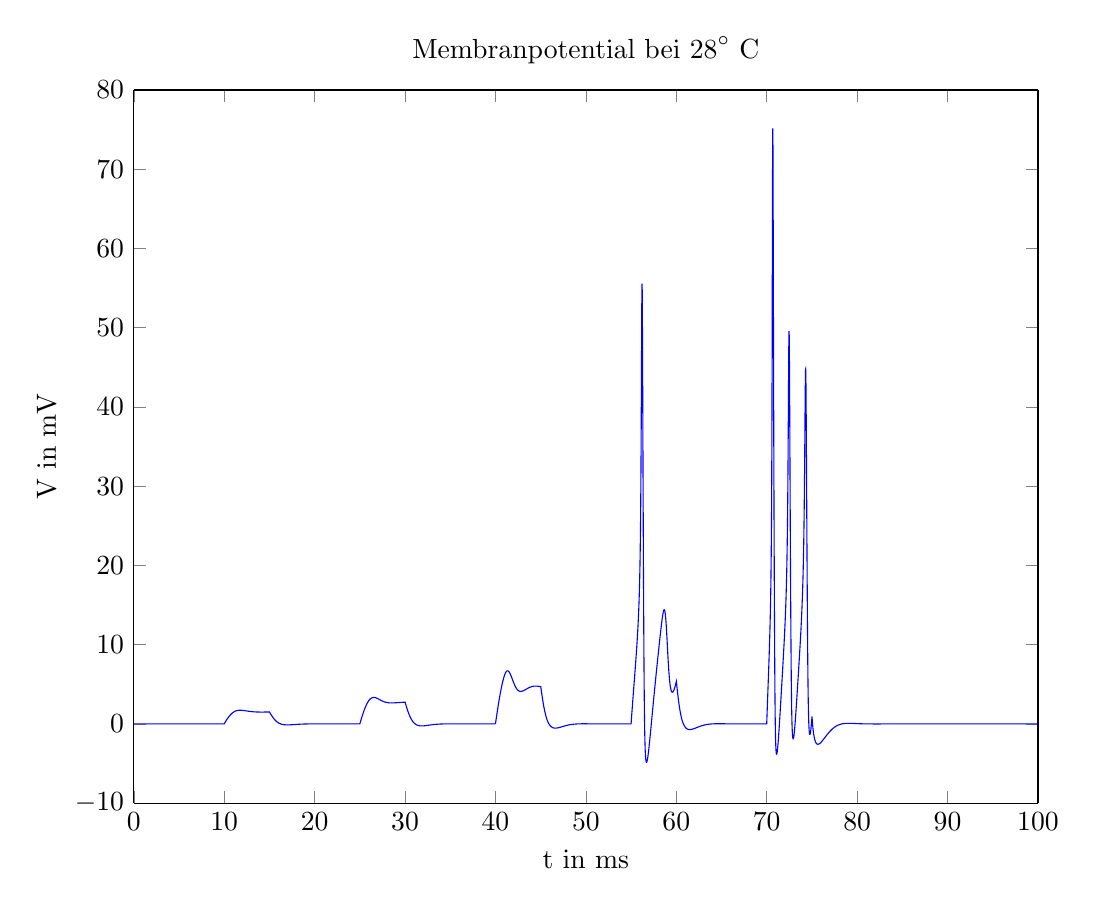
\begin{tikzpicture}

\begin{axis}[%
width=4.520833in,
height=3.565625in,
at={(0.758333in,0.48125in)},
scale only axis,
separate axis lines,
every outer x axis line/.append style={black},
every x tick label/.append style={font=\color{black}},
xmin=0,
xmax=100,
xlabel={t in ms},
every outer y axis line/.append style={black},
every y tick label/.append style={font=\color{black}},
ymin=-10,
ymax=80,
ylabel={V in mV},
title={$\text{Membranpotential bei 28}^\circ\text{ C}$}
]
\addplot [color=blue,solid,forget plot]
  table[row sep=crcr]{%
0	0\\
0.01	3.23709182497467e-06\\
0.02	6.47418364995822e-06\\
0.03	9.69391697885236e-06\\
0.04	1.28989802461721e-05\\
0.05	1.60909721056601e-05\\
0.06	1.92707180516782e-05\\
0.07	2.24385621119039e-05\\
0.08	2.55945506158817e-05\\
0.09	2.87385475514546e-05\\
0.1	3.18703069511539e-05\\
0.11	3.49895182914306e-05\\
0.12	3.80958349430793e-05\\
0.13	4.11888919773285e-05\\
0.14	4.42683172870195e-05\\
0.15	4.73337385098693e-05\\
0.16	5.03847873154539e-05\\
0.17	5.34211020370767e-05\\
0.18	5.64423292643079e-05\\
0.19	5.94481247833345e-05\\
0.2	6.24381541081442e-05\\
0.21	6.54120927549684e-05\\
0.22	6.83696263561284e-05\\
0.23	7.13104506731854e-05\\
0.24	7.42342715474553e-05\\
0.25	7.71408048116662e-05\\
0.26	8.00297761773727e-05\\
0.27	8.29009211078846e-05\\
0.28	8.57539846823396e-05\\
0.29	8.85887214547365e-05\\
0.3	9.14048953102409e-05\\
0.31	9.42022793201769e-05\\
0.32	9.69806555967523e-05\\
0.33	9.97398151478812e-05\\
0.34	0.000102479557732744\\
0.35	0.000105199691718072\\
0.36	0.000107900033935473\\
0.37	0.000110580409539827\\
0.38	0.000113240651868733\\
0.39	0.00011588060230324\\
0.4	0.00011850011012974\\
0.41	0.000121099032403018\\
0.42	0.000123677233810633\\
0.43	0.000126234586538381\\
0.44	0.000128770970137251\\
0.45	0.000131286271391295\\
0.46	0.000133780384187077\\
0.47	0.000136253209384143\\
0.48	0.000138704654686843\\
0.49	0.000141134634517366\\
0.5	0.00014354306989012\\
0.51	0.000145929888287255\\
0.52	0.000148295023535523\\
0.53	0.000150638415684301\\
0.54	0.000152960010885024\\
0.55	0.000155259761271753\\
0.56	0.000157537624842985\\
0.57	0.000159793565344821\\
0.58	0.000162027552155326\\
0.59	0.000164239560170061\\
0.6	0.000166429569688993\\
0.61	0.000168597566304616\\
0.62	0.000170743540791309\\
0.63	0.000172867488995871\\
0.64	0.000174969411729404\\
0.65	0.000177049314660396\\
0.66	0.000179107208208942\\
0.67	0.000181143107442323\\
0.68	0.000183157031971781\\
0.69	0.000185149005850462\\
0.7	0.000187119057472556\\
0.71	0.000189067219473809\\
0.72	0.000190993528633099\\
0.73	0.000192898025775223\\
0.74	0.00019478075567501\\
0.75	0.000196641766962422\\
0.76	0.000198481112029003\\
0.77	0.000200298846935509\\
0.78	0.000202095031320657\\
0.79	0.000203869728311128\\
0.8	0.000205623004432534\\
0.81	0.000207354929521841\\
0.82	0.000209065576640763\\
0.83	0.000210755021990341\\
0.84	0.000212423344826664\\
0.85	0.000214070627377816\\
0.86	0.000215696954761819\\
0.87	0.000217302414905793\\
0.88	0.000218887098466216\\
0.89	0.000220451098750254\\
0.9	0.000221994511638268\\
0.91	0.000223517435507419\\
0.92	0.000225019971156253\\
0.93	0.000226502221730582\\
0.94	0.00022796429265016\\
0.95	0.000229406291536747\\
0.96	0.000230828328143016\\
0.97	0.000232230514282516\\
0.98	0.000233612963760872\\
0.99	0.000234975792307814\\
1	0.00023631911751036\\
1.01	0.000237643058747063\\
1.02	0.00023894773712311\\
1.03	0.000240233275406618\\
1.04	0.000241499797965812\\
1.05	0.000242747430707268\\
1.06	0.000243976301015096\\
1.07	0.000245186537691078\\
1.08	0.000246378270895979\\
1.09	0.000247551632091549\\
1.1	0.000248706753983607\\
1.11	0.000249843770466094\\
1.12	0.000250962816566074\\
1.13	0.000252064028389611\\
1.14	0.000253147543068564\\
1.15	0.000254213498708378\\
1.16	0.000255262034336687\\
1.17	0.000256293289852944\\
1.18	0.000257307405978797\\
1.19	0.000258304524209403\\
1.2	0.00025928478676569\\
1.21	0.000260248336547377\\
1.22	0.000261195317086846\\
1.23	0.000262125872504057\\
1.24	0.000263040147462017\\
1.25	0.000263938287123313\\
1.26	0.000264820437107431\\
1.27	0.000265686743448725\\
1.28	0.000266537352555369\\
1.29	0.000267372411169089\\
1.3	0.000268192066325592\\
1.31	0.000268996465315889\\
1.32	0.000269785755648337\\
1.33	0.000270560085011411\\
1.34	0.000271319601237363\\
1.35	0.000272064452266458\\
1.36	0.000272794786112023\\
1.37	0.00027351075082636\\
1.38	0.000274212494467165\\
1.39	0.000274900165064817\\
1.4	0.000275573910590316\\
1.41	0.000276233878923921\\
1.42	0.000276880217824504\\
1.43	0.000277513074899556\\
1.44	0.000278132597575955\\
1.45	0.000278738933071279\\
1.46	0.000279332228365852\\
1.47	0.000279912630175385\\
1.48	0.000280480284924342\\
1.49	0.000281035338719921\\
1.5	0.000281577937326651\\
1.51	0.000282108226141555\\
1.52	0.000282626350169996\\
1.53	0.000283132454002119\\
1.54	0.000283626681789859\\
1.55	0.000284109177224581\\
1.56	0.000284580083515204\\
1.57	0.000285039543367094\\
1.58	0.000285487698961284\\
1.59	0.000285924691934482\\
1.6	0.000286350663359358\\
1.61	0.000286765753725668\\
1.62	0.000287170102921741\\
1.63	0.000287563850216479\\
1.64	0.000287947134242024\\
1.65	0.000288320092976781\\
1.66	0.000288682863728962\\
1.67	0.000289035583120807\\
1.68	0.000289378387073107\\
1.69	0.000289711410790234\\
1.7	0.000290034788745728\\
1.71	0.000290348654668304\\
1.72	0.000290653141528328\\
1.73	0.000290948381524791\\
1.74	0.000291234506072615\\
1.75	0.000291511645790585\\
1.76	0.000291779930489509\\
1.77	0.000292039489160953\\
1.78	0.000292290449966472\\
1.79	0.000292532940226931\\
1.8	0.000292767086412584\\
1.81	0.000292993014133422\\
1.82	0.00029321084812985\\
1.83	0.000293420712263828\\
1.84	0.000293622729510452\\
1.85	0.000293817021949727\\
1.86	0.000294003710758988\\
1.87	0.00029418291620535\\
1.88	0.000294354757638815\\
1.89	0.000294519353485554\\
1.9	0.000294676821241588\\
1.91	0.000294827277466849\\
1.92	0.000294970837779447\\
1.93	0.000295107616850494\\
1.94	0.00029523772839894\\
1.95	0.000295361285187075\\
1.96	0.000295478399016025\\
1.97	0.000295589180721696\\
1.98	0.000295693740171088\\
1.99	0.000295792186258761\\
2	0.000295884626903673\\
2.01	0.000295971169046298\\
2.02	0.000296051918645972\\
2.03	0.000296126980678548\\
2.04	0.00029619645913435\\
2.05	0.000296260457016242\\
2.06	0.000296319076338238\\
2.07	0.000296372418124005\\
2.08	0.000296420582405927\\
2.09	0.000296463668224258\\
2.1	0.000296501773626434\\
2.11	0.000296534995666815\\
2.12	0.000296563430406489\\
2.13	0.000296587172913392\\
2.14	0.000296606317262578\\
2.15	0.000296620956536757\\
2.16	0.000296631182827007\\
2.17	0.000296637087233682\\
2.18	0.000296638759867584\\
2.19	0.00029663628985126\\
2.2	0.000296629765320451\\
2.21	0.000296619273425871\\
2.22	0.000296604900334958\\
2.23	0.000296586731234054\\
2.24	0.000296564850330543\\
2.25	0.000296539340855246\\
2.26	0.000296510285064975\\
2.27	0.000296477764245235\\
2.28	0.000296441858713101\\
2.29	0.000296402647820231\\
2.3	0.000296360209955968\\
2.31	0.000296314622550797\\
2.32	0.000296265962079643\\
2.33	0.000296214304065532\\
2.34	0.000296159723083242\\
2.35	0.000296102292763276\\
2.36	0.000296042085795705\\
2.37	0.000295979173934255\\
2.38	0.000295913628000619\\
2.39	0.000295845517888695\\
2.4	0.000295774912569113\\
2.41	0.000295701880093713\\
2.42	0.000295626487600145\\
2.43	0.000295548801316743\\
2.44	0.000295468886567249\\
2.45	0.000295386807775868\\
2.46	0.000295302628472207\\
2.47	0.000295216411296488\\
2.48	0.000295128218004668\\
2.49	0.000295038109473813\\
2.5	0.000294946145707491\\
2.51	0.000294852385841082\\
2.52	0.000294756888147449\\
2.53	0.00029465971004246\\
2.54	0.000294560908090635\\
2.55	0.000294460538010934\\
2.56	0.000294358654682561\\
2.57	0.000294255312150731\\
2.58	0.000294150563632698\\
2.59	0.000294044461523675\\
2.6	0.000293937057402762\\
2.61	0.000293828402039162\\
2.62	0.000293718545398232\\
2.63	0.000293607536647635\\
2.64	0.000293495424163606\\
2.65	0.000293382255537136\\
2.66	0.000293268077580304\\
2.67	0.000293152936332572\\
2.68	0.000293036877067188\\
2.69	0.000292919944297547\\
2.7	0.00029280218178362\\
2.71	0.000292683632538457\\
2.72	0.000292564338834556\\
2.73	0.000292444342210438\\
2.74	0.000292323683477194\\
2.75	0.000292202402724988\\
2.76	0.000292080539329604\\
2.77	0.000291958131959005\\
2.78	0.000291835218580059\\
2.79	0.000291711836465063\\
2.8	0.000291588022198255\\
2.81	0.000291463811682635\\
2.82	0.000291339240146464\\
2.83	0.000291214342150017\\
2.84	0.000291089151592136\\
2.85	0.000290963701716906\\
2.86	0.000290838025120314\\
2.87	0.000290712153756933\\
2.88	0.000290586118946576\\
2.89	0.000290459951380844\\
2.9	0.000290333681129882\\
2.91	0.000290207337648991\\
2.92	0.00029008094978523\\
2.93	0.000289954545784101\\
2.94	0.000289828153296079\\
2.95	0.000289701799383328\\
2.96	0.000289575510526121\\
2.97	0.000289449312629646\\
2.98	0.000289323231030356\\
2.99	0.000289197290502678\\
3	0.00028907151526552\\
3.01	0.000288945928988626\\
3.02	0.000288820554799343\\
3.03	0.000288695415288873\\
3.04	0.000288570532518815\\
3.05	0.000288445928027619\\
3.06	0.000288321622837042\\
3.07	0.000288197637458416\\
3.08	0.000288073991899087\\
3.09	0.000287950705668698\\
3.1	0.000287827797785614\\
3.11	0.00028770528678312\\
3.12	0.000287583190715703\\
3.13	0.000287461527165291\\
3.14	0.000287340313247464\\
3.15	0.000287219565617569\\
3.16	0.000287099300476945\\
3.17	0.000286979533578968\\
3.18	0.000286860280235168\\
3.19	0.000286741555321228\\
3.2	0.000286623373283055\\
3.21	0.000286505748142689\\
3.22	0.000286388693504311\\
3.23	0.000286272222560098\\
3.24	0.000286156348096127\\
3.25	0.000286041082498234\\
3.26	0.000285926437757755\\
3.27	0.000285812425477325\\
3.28	0.000285699056876583\\
3.29	0.000285586342797868\\
3.3	0.00028547429371188\\
3.31	0.000285362919723293\\
3.32	0.000285252230576267\\
3.33	0.000285142235660065\\
3.34	0.000285032944014443\\
3.35	0.000284924364335226\\
3.36	0.000284816504979606\\
3.37	0.000284709373971501\\
3.38	0.000284602979006996\\
3.39	0.000284497327459516\\
3.4	0.000284392426385129\\
3.41	0.000284288282527769\\
3.42	0.000284184902324291\\
3.43	0.000284082291909682\\
3.44	0.000283980457122088\\
3.45	0.000283879403507838\\
3.46	0.000283779136326476\\
3.47	0.000283679660555665\\
3.48	0.000283580980896083\\
3.49	0.000283483101776354\\
3.5	0.000283386027357708\\
3.51	0.000283289761538885\\
3.52	0.000283194307960799\\
3.53	0.000283099670011242\\
3.54	0.000283005850829494\\
3.55	0.000282912853310955\\
3.56	0.000282820680111633\\
3.57	0.000282729333652627\\
3.58	0.00028263881612474\\
3.59	0.000282549129492731\\
3.6	0.000282460275499767\\
3.61	0.000282372255671648\\
3.62	0.000282285071321202\\
3.63	0.000282198723552502\\
3.64	0.000282113213265003\\
3.65	0.000282028541157686\\
3.66	0.000281944707733199\\
3.67	0.000281861713301934\\
3.68	0.000281779557985966\\
3.69	0.000281698241723114\\
3.7	0.000281617764270789\\
3.71	0.000281538125209883\\
3.72	0.000281459323948629\\
3.73	0.000281381359726396\\
3.74	0.000281304231617452\\
3.75	0.000281227938534618\\
3.76	0.000281152479232958\\
3.77	0.00028107785231342\\
3.78	0.000281004056226375\\
3.79	0.000280931089275169\\
3.8	0.000280858949619582\\
3.81	0.000280787635279336\\
3.82	0.000280717144137408\\
3.83	0.000280647473943456\\
3.84	0.000280578622317162\\
3.85	0.000280510586751417\\
3.86	0.000280443364615652\\
3.87	0.000280376953158923\\
3.88	0.000280311349513194\\
3.89	0.00028024655069633\\
3.9	0.000280182553615229\\
3.91	0.000280119355068828\\
3.92	0.000280056951751084\\
3.93	0.00027999534025394\\
3.94	0.000279934517070197\\
3.95	0.000279874478596427\\
3.96	0.000279815221135764\\
3.97	0.000279756740900669\\
3.98	0.000279699034015719\\
3.99	0.000279642096520338\\
4	0.000279585924371357\\
4.01	0.000279530513445745\\
4.02	0.000279475859543194\\
4.03	0.000279421958388588\\
4.04	0.000279368805634603\\
4.05	0.000279316396864124\\
4.06	0.000279264727592778\\
4.07	0.000279213793271222\\
4.08	0.000279163589287563\\
4.09	0.000279114110969702\\
4.1	0.000279065353587602\\
4.11	0.000279017312355551\\
4.12	0.000278969982434369\\
4.13	0.000278923358933594\\
4.14	0.000278877436913656\\
4.15	0.000278832211387976\\
4.16	0.000278787677325063\\
4.17	0.000278743829650549\\
4.18	0.000278700663249194\\
4.19	0.000278658172966834\\
4.2	0.000278616353612393\\
4.21	0.000278575199959747\\
4.22	0.00027853470674958\\
4.23	0.000278494868691288\\
4.24	0.000278455680464753\\
4.25	0.000278417136722169\\
4.26	0.000278379232089718\\
4.27	0.000278341961169359\\
4.28	0.000278305318540481\\
4.29	0.000278269298761509\\
4.3	0.000278233896371627\\
4.31	0.000278199105892325\\
4.32	0.000278164921828954\\
4.33	0.000278131338672276\\
4.34	0.000278098350899971\\
4.35	0.000278065952978066\\
4.36	0.000278034139362462\\
4.37	0.000278002904500316\\
4.38	0.000277972242831366\\
4.39	0.000277942148789414\\
4.4	0.000277912616803584\\
4.41	0.000277883641299645\\
4.42	0.000277855216701299\\
4.43	0.000277827337431415\\
4.44	0.000277799997913308\\
4.45	0.000277773192571846\\
4.46	0.000277746915834718\\
4.47	0.000277721162133546\\
4.48	0.000277695925905008\\
4.49	0.000277671201591989\\
4.5	0.000277646983644506\\
4.51	0.000277623266520912\\
4.52	0.000277600044688872\\
4.53	0.000277577312626382\\
4.54	0.000277555064822716\\
4.55	0.000277533295779331\\
4.56	0.00027751200001096\\
4.57	0.000277491172046389\\
4.58	0.000277470806429329\\
4.59	0.000277450897719427\\
4.6	0.000277431440492925\\
4.61	0.000277412429343631\\
4.62	0.000277393858883674\\
4.63	0.000277375723744226\\
4.64	0.000277358018576303\\
4.65	0.000277340738051559\\
4.66	0.000277323876862909\\
4.67	0.000277307429725293\\
4.68	0.000277291391376328\\
4.69	0.000277275756576962\\
4.7	0.000277260520112161\\
4.71	0.00027724567679142\\
4.72	0.000277231221449496\\
4.73	0.000277217148946969\\
4.74	0.000277203454170722\\
4.75	0.000277190132034564\\
4.76	0.000277177177479753\\
4.77	0.000277164585475464\\
4.78	0.00027715235101935\\
4.79	0.000277140469138026\\
4.8	0.00027712893488744\\
4.81	0.000277117743353417\\
4.82	0.000277106889652043\\
4.83	0.00027709636893011\\
4.84	0.000277086176365531\\
4.85	0.000277076307167614\\
4.86	0.000277066756577562\\
4.87	0.000277057519868808\\
4.88	0.000277048592347282\\
4.89	0.000277039969351791\\
4.9	0.000277031646254344\\
4.91	0.00027702361846043\\
4.92	0.000277015881409284\\
4.93	0.000277008430574215\\
4.94	0.000277001261462799\\
4.95	0.000276994369617158\\
4.96	0.000276987750614164\\
4.97	0.000276981400065752\\
4.98	0.000276975313618961\\
4.99	0.000276969486956293\\
5	0.000276963915795867\\
5.01	0.000276958595891514\\
5.02	0.00027695352303299\\
5.03	0.000276948693046104\\
5.04	0.000276944101792851\\
5.05	0.000276939745171583\\
5.06	0.000276935619117125\\
5.07	0.000276931719600832\\
5.08	0.000276928042630722\\
5.09	0.000276924584251534\\
5.1	0.000276921340544827\\
5.11	0.000276918307629081\\
5.12	0.000276915481659698\\
5.13	0.000276912858829057\\
5.14	0.000276910435366582\\
5.15	0.000276908207538744\\
5.16	0.00027690617164914\\
5.17	0.000276904324038405\\
5.18	0.000276902661084315\\
5.19	0.000276901179201707\\
5.2	0.000276899874842527\\
5.21	0.000276898744495799\\
5.22	0.000276897784687597\\
5.23	0.000276896991980999\\
5.24	0.000276896362976018\\
5.25	0.000276895894309583\\
5.26	0.00027689558265549\\
5.27	0.000276895424724404\\
5.28	0.000276895417263616\\
5.29	0.000276895557057166\\
5.3	0.000276895840925593\\
5.31	0.000276896265725961\\
5.32	0.000276896828351694\\
5.33	0.000276897525732544\\
5.34	0.000276898354834438\\
5.35	0.000276899312659355\\
5.36	0.000276900396245296\\
5.37	0.000276901602666042\\
5.38	0.000276902929031064\\
5.39	0.000276904372485434\\
5.4	0.000276905930209623\\
5.41	0.000276907599419482\\
5.42	0.000276909377365935\\
5.43	0.000276911261334973\\
5.44	0.000276913248647363\\
5.45	0.000276915336658576\\
5.46	0.000276917522758575\\
5.47	0.000276919804371736\\
5.48	0.000276922178956598\\
5.49	0.000276924644005647\\
5.5	0.000276927197045262\\
5.51	0.000276929835635373\\
5.52	0.000276932557369442\\
5.53	0.000276935359874204\\
5.54	0.000276938240809374\\
5.55	0.000276941197867626\\
5.56	0.000276944228774276\\
5.57	0.000276947331287101\\
5.58	0.000276950503196178\\
5.59	0.000276953742323638\\
5.6	0.000276957046523458\\
5.61	0.000276960413681277\\
5.62	0.000276963841714131\\
5.63	0.000276967328570308\\
5.64	0.00027697087222903\\
5.65	0.000276974470700297\\
5.66	0.000276978122024705\\
5.67	0.000276981824273132\\
5.68	0.000276985575546562\\
5.69	0.000276989373975853\\
5.7	0.000276993217721468\\
5.71	0.000276997104973309\\
5.72	0.000277001033950448\\
5.73	0.000277005002900865\\
5.74	0.000277009010101268\\
5.75	0.000277013053856785\\
5.76	0.000277017132500834\\
5.77	0.000277021244394802\\
5.78	0.000277025387927789\\
5.79	0.00027702956151642\\
5.8	0.000277033763604599\\
5.81	0.000277037992663249\\
5.82	0.000277042247190065\\
5.83	0.000277046525709257\\
5.84	0.000277050826771346\\
5.85	0.000277055148952905\\
5.86	0.000277059490856284\\
5.87	0.00027706385110938\\
5.88	0.000277068228365409\\
5.89	0.000277072621302654\\
5.9	0.000277077028624242\\
5.91	0.000277081449057808\\
5.92	0.000277085881355346\\
5.93	0.00027709032429287\\
5.94	0.000277094776670257\\
5.95	0.000277099237310958\\
5.96	0.000277103705061772\\
5.97	0.000277108178792575\\
5.98	0.000277112657396059\\
5.99	0.000277117139787535\\
6	0.000277121624904617\\
6.01	0.000277126111707062\\
6.02	0.000277130599176516\\
6.03	0.000277135086316163\\
6.04	0.000277139572150578\\
6.05	0.000277144055725498\\
6.06	0.000277148536107523\\
6.07	0.000277153012383864\\
6.08	0.000277157483662149\\
6.09	0.000277161949070188\\
6.1	0.000277166407755658\\
6.11	0.000277170858885953\\
6.12	0.000277175301647885\\
6.13	0.000277179735247484\\
6.14	0.000277184158909778\\
6.15	0.000277188571878462\\
6.16	0.000277192973415779\\
6.17	0.000277197362802166\\
6.18	0.000277201739336124\\
6.19	0.000277206102333993\\
6.2	0.000277210451129606\\
6.21	0.000277214785074169\\
6.22	0.000277219103536002\\
6.23	0.00027722340590028\\
6.24	0.000277227691568842\\
6.25	0.000277231959959954\\
6.26	0.000277236210508094\\
6.27	0.000277240442663742\\
6.28	0.000277244655893108\\
6.29	0.000277248849677934\\
6.3	0.000277253023515312\\
6.31	0.000277257176917427\\
6.32	0.000277261309411352\\
6.33	0.000277265420538857\\
6.34	0.000277269509856129\\
6.35	0.000277273576933634\\
6.36	0.000277277621355849\\
6.37	0.000277281642721103\\
6.38	0.000277285640641374\\
6.39	0.000277289614742\\
6.4	0.000277293564661596\\
6.41	0.00027729749005172\\
6.42	0.000277301390576743\\
6.43	0.000277305265913683\\
6.44	0.000277309115751927\\
6.45	0.000277312939793086\\
6.46	0.00027731673775079\\
6.47	0.000277320509350507\\
6.48	0.00027732425432931\\
6.49	0.000277327972435724\\
6.5	0.000277331663429483\\
6.51	0.000277335327081385\\
6.52	0.000277338963173142\\
6.53	0.000277342571497155\\
6.54	0.000277346151856337\\
6.55	0.000277349704063861\\
6.56	0.000277353227943125\\
6.57	0.00027735672332744\\
6.58	0.000277360190059932\\
6.59	0.000277363627993337\\
6.6	0.000277367036989853\\
6.61	0.000277370416920944\\
6.62	0.000277373767667153\\
6.63	0.000277377089117987\\
6.64	0.000277380381171697\\
6.65	0.000277383643735147\\
6.66	0.000277386876723633\\
6.67	0.000277390080060709\\
6.68	0.0002773932536781\\
6.69	0.000277396397515442\\
6.7	0.000277399511520167\\
6.71	0.000277402595647374\\
6.72	0.000277405649859688\\
6.73	0.000277408674127044\\
6.74	0.000277411668426564\\
6.75	0.00027741463274241\\
6.76	0.000277417567065625\\
6.77	0.00027742047139403\\
6.78	0.000277423345732104\\
6.79	0.000277426190090715\\
6.8	0.000277429004487075\\
6.81	0.000277431788944553\\
6.82	0.000277434543492596\\
6.83	0.000277437268166572\\
6.84	0.000277439963007615\\
6.85	0.000277442628062521\\
6.86	0.00027744526338358\\
6.87	0.000277447869028498\\
6.88	0.000277450445060206\\
6.89	0.000277452991546787\\
6.9	0.000277455508561335\\
6.91	0.000277457996181822\\
6.92	0.000277460454490992\\
6.93	0.000277462883576232\\
6.94	0.000277465283529428\\
6.95	0.00027746765444693\\
6.96	0.000277469996429311\\
6.97	0.000277472309581364\\
6.98	0.000277474594011959\\
6.99	0.000277476849833933\\
7	0.000277479077163933\\
7.01	0.000277481276122393\\
7.02	0.000277483446833351\\
7.03	0.00027748558942442\\
7.04	0.000277487704026558\\
7.05	0.000277489790774115\\
7.06	0.000277491849804639\\
7.07	0.000277493881258795\\
7.08	0.000277495885280286\\
7.09	0.000277497862015759\\
7.1	0.00027749981161469\\
7.11	0.000277501734229286\\
7.12	0.000277503630014424\\
7.13	0.000277505499127546\\
7.14	0.000277507341728551\\
7.15	0.000277509157979758\\
7.16	0.000277510948045765\\
7.17	0.00027751271209334\\
7.18	0.000277514450291489\\
7.19	0.000277516162811153\\
7.2	0.000277517849825308\\
7.21	0.000277519511508788\\
7.22	0.000277521148038229\\
7.23	0.000277522759592021\\
7.24	0.000277524346350169\\
7.25	0.000277525908494303\\
7.26	0.000277527446207562\\
7.27	0.000277528959674496\\
7.28	0.000277530449081014\\
7.29	0.000277531914614375\\
7.3	0.000277533356462971\\
7.31	0.000277534774816441\\
7.32	0.000277536169865438\\
7.33	0.000277537541801731\\
7.34	0.000277538890818003\\
7.35	0.000277540217107801\\
7.36	0.000277541520865561\\
7.37	0.00027754280228649\\
7.38	0.000277544061566499\\
7.39	0.000277545298902209\\
7.4	0.000277546514490776\\
7.41	0.000277547708529986\\
7.42	0.000277548881218004\\
7.43	0.000277550032753524\\
7.44	0.000277551163335583\\
7.45	0.000277552273163617\\
7.46	0.000277553362437293\\
7.47	0.000277554431356499\\
7.48	0.00027755548012133\\
7.49	0.000277556508932033\\
7.5	0.00027755751798892\\
7.51	0.000277558507492359\\
7.52	0.000277559477642732\\
7.53	0.000277560428640409\\
7.54	0.000277561360685592\\
7.55	0.000277562273978411\\
7.56	0.000277563168718804\\
7.57	0.000277564045106553\\
7.58	0.000277564903341112\\
7.59	0.000277565743621717\\
7.6	0.00027756656614724\\
7.61	0.000277567371116203\\
7.62	0.000277568158726722\\
7.63	0.000277568929176493\\
7.64	0.000277569682662748\\
7.65	0.000277570419382207\\
7.66	0.000277571139531112\\
7.67	0.000277571843305071\\
7.68	0.000277572530899133\\
7.69	0.000277573202507746\\
7.7	0.000277573858324653\\
7.71	0.000277574498542963\\
7.72	0.000277575123355058\\
7.73	0.000277575732952595\\
7.74	0.000277576327526447\\
7.75	0.000277576907266712\\
7.76	0.000277577472362718\\
7.77	0.000277578023002909\\
7.78	0.00027757855937486\\
7.79	0.000277579081665307\\
7.8	0.000277579590060051\\
7.81	0.00027758008474398\\
7.82	0.000277580565901041\\
7.83	0.000277581033714216\\
7.84	0.000277581488365484\\
7.85	0.000277581930035833\\
7.86	0.000277582358905235\\
7.87	0.000277582775152623\\
7.88	0.000277583178955876\\
7.89	0.000277583570491791\\
7.9	0.000277583949936067\\
7.91	0.000277584317463337\\
7.92	0.000277584673247069\\
7.93	0.000277585017459625\\
7.94	0.000277585350272185\\
7.95	0.000277585671854852\\
7.96	0.000277585982376491\\
7.97	0.000277586282004791\\
7.98	0.000277586570906254\\
7.99	0.000277586849246143\\
8	0.000277587117188576\\
8.01	0.000277587374896391\\
8.02	0.000277587622531228\\
8.03	0.000277587860253447\\
8.04	0.000277588088222189\\
8.05	0.00027758830659534\\
8.06	0.00027758851552949\\
8.07	0.000277588715179968\\
8.08	0.000277588905700794\\
8.09	0.000277589087244681\\
8.1	0.000277589259963129\\
8.11	0.000277589424006299\\
8.12	0.000277589579523023\\
8.13	0.000277589726660836\\
8.14	0.00027758986556595\\
8.15	0.000277589996383312\\
8.16	0.000277590119256485\\
8.17	0.000277590234327767\\
8.18	0.000277590341738083\\
8.19	0.000277590441627042\\
8.2	0.00027759053413293\\
8.21	0.000277590619392689\\
8.22	0.000277590697541927\\
8.23	0.000277590768714897\\
8.24	0.000277590833044541\\
8.25	0.000277590890662407\\
8.26	0.000277590941698769\\
8.27	0.000277590986282541\\
8.28	0.00027759102454135\\
8.29	0.000277591056601398\\
8.3	0.000277591082587603\\
8.31	0.000277591102623536\\
8.32	0.000277591116831415\\
8.33	0.000277591125332153\\
8.34	0.000277591128245329\\
8.35	0.0002775911256892\\
8.36	0.000277591117780718\\
8.37	0.000277591104635486\\
8.38	0.000277591086367743\\
8.39	0.000277591063090488\\
8.4	0.000277591034915376\\
8.41	0.000277591001952757\\
8.42	0.000277590964311658\\
8.43	0.000277590922099846\\
8.44	0.000277590875423717\\
8.45	0.000277590824388483\\
8.46	0.000277590769097973\\
8.47	0.000277590709654758\\
8.48	0.000277590646160126\\
8.49	0.000277590578714122\\
8.5	0.000277590507415488\\
8.51	0.000277590432361729\\
8.52	0.000277590353649084\\
8.53	0.000277590271372556\\
8.54	0.000277590185625849\\
8.55	0.000277590096501492\\
8.56	0.000277590004090769\\
8.57	0.000277589908483695\\
8.58	0.000277589809769116\\
8.59	0.000277589708034638\\
8.6	0.000277589603366684\\
8.61	0.000277589495850425\\
8.62	0.000277589385569885\\
8.63	0.000277589272607912\\
8.64	0.000277589157046112\\
8.65	0.000277589038964976\\
8.66	0.000277588918443827\\
8.67	0.000277588795560812\\
8.68	0.000277588670392945\\
8.69	0.000277588543016067\\
8.7	0.000277588413504915\\
8.71	0.000277588281933094\\
8.72	0.000277588148373096\\
8.73	0.000277588012896288\\
8.74	0.000277587875572962\\
8.75	0.000277587736472293\\
8.76	0.000277587595662387\\
8.77	0.000277587453210257\\
8.78	0.000277587309181873\\
8.79	0.00027758716364211\\
8.8	0.000277587016654808\\
8.81	0.000277586868282769\\
8.82	0.000277586718587757\\
8.83	0.000277586567630483\\
8.84	0.000277586415470683\\
8.85	0.000277586262167087\\
8.86	0.000277586107777368\\
8.87	0.000277585952358232\\
8.88	0.000277585795965418\\
8.89	0.000277585638653699\\
8.9	0.000277585480476867\\
8.91	0.000277585321487721\\
8.92	0.000277585161738179\\
8.93	0.000277585001279212\\
8.94	0.000277584840160845\\
8.95	0.000277584678432126\\
8.96	0.000277584516141291\\
8.97	0.000277584353335625\\
8.98	0.000277584190061479\\
8.99	0.000277584026364366\\
9	0.000277583862288915\\
9.01	0.000277583697878909\\
9.02	0.000277583533177212\\
9.03	0.000277583368225929\\
9.04	0.000277583203066238\\
9.05	0.000277583037738553\\
9.06	0.000277582872282371\\
9.07	0.000277582706736466\\
9.08	0.00027758254113877\\
9.09	0.000277582375526424\\
9.1	0.000277582209935763\\
9.11	0.000277582044402371\\
9.12	0.000277581878961035\\
9.13	0.000277581713645851\\
9.14	0.000277581548490073\\
9.15	0.000277581383526253\\
9.16	0.000277581218786258\\
9.17	0.000277581054301144\\
9.18	0.000277580890101303\\
9.19	0.000277580726216349\\
9.2	0.000277580562675284\\
9.21	0.000277580399506352\\
9.22	0.000277580236737109\\
9.23	0.000277580074394503\\
9.24	0.000277579912504779\\
9.25	0.000277579751093557\\
9.26	0.000277579590185755\\
9.27	0.000277579429805685\\
9.28	0.000277579269977024\\
9.29	0.000277579110722823\\
9.3	0.000277578952065509\\
9.31	0.000277578794026922\\
9.32	0.000277578636628251\\
9.33	0.000277578479890148\\
9.34	0.000277578323832648\\
9.35	0.000277578168475232\\
9.36	0.000277578013836797\\
9.37	0.00027757785993566\\
9.38	0.000277577706789658\\
9.39	0.000277577554416033\\
9.4	0.000277577402831523\\
9.41	0.00027757725205229\\
9.42	0.000277577102094004\\
9.43	0.000277576952971801\\
9.44	0.000277576804700361\\
9.45	0.000277576657293878\\
9.46	0.000277576510766004\\
9.47	0.000277576365129883\\
9.48	0.000277576220398252\\
9.49	0.000277576076583332\\
9.5	0.000277575933696918\\
9.51	0.000277575791750371\\
9.52	0.000277575650754529\\
9.53	0.000277575510719834\\
9.54	0.000277575371656287\\
9.55	0.000277575233573484\\
9.56	0.000277575096480649\\
9.57	0.000277574960386504\\
9.58	0.000277574825299416\\
9.59	0.000277574691227316\\
9.6	0.000277574558177802\\
9.61	0.000277574426158038\\
9.62	0.000277574295174858\\
9.63	0.000277574165234653\\
9.64	0.000277574036343497\\
9.65	0.000277573908507107\\
9.66	0.000277573781730842\\
9.67	0.000277573656019734\\
9.68	0.000277573531378481\\
9.69	0.000277573407811431\\
9.7	0.000277573285322616\\
9.71	0.000277573163915727\\
9.72	0.00027757304359413\\
9.73	0.000277572924360898\\
9.74	0.000277572806218811\\
9.75	0.00027757268917036\\
9.76	0.000277572573217739\\
9.77	0.000277572458362849\\
9.78	0.000277572344607284\\
9.79	0.000277572231952416\\
9.8	0.000277572120399325\\
9.81	0.000277572009948805\\
9.82	0.000277571900601461\\
9.83	0.000277571792357563\\
9.84	0.000277571685217195\\
9.85	0.000277571579180189\\
9.86	0.000277571474246114\\
9.87	0.000277571370414318\\
9.88	0.000277571267683911\\
9.89	0.000277571166053807\\
9.9	0.00027757106552269\\
9.91	0.000277570966089051\\
9.92	0.000277570867751127\\
9.93	0.000277570770506998\\
9.94	0.000277570674354508\\
9.95	0.000277570579291386\\
9.96	0.000277570485315133\\
9.97	0.000277570392423012\\
9.98	0.000277570300612191\\
9.99	0.000277570209879592\\
10	0.000277570120222061\\
10.01	0.0202775700316362\\
10.02	0.0402775699441184\\
10.03	0.0601703440088578\\
10.04	0.0799726347542786\\
10.05	0.0996945686203909\\
10.06	0.119341576493257\\
10.07	0.138916158718843\\
10.08	0.158418992720354\\
10.09	0.177849627512881\\
10.1	0.197206919897128\\
10.11	0.21648930866649\\
10.12	0.235694987038146\\
10.13	0.254822011053473\\
10.14	0.273868367657838\\
10.15	0.292832017374496\\
10.16	0.311710920964274\\
10.17	0.330503055989382\\
10.18	0.349206427013223\\
10.19	0.367819071790415\\
10.2	0.386339064932798\\
10.21	0.404764519989363\\
10.22	0.423093590532321\\
10.23	0.441324470623278\\
10.24	0.459455394895623\\
10.25	0.477484638402145\\
10.26	0.495410516321855\\
10.27	0.513231383585167\\
10.28	0.530945634454634\\
10.29	0.548551702084454\\
10.3	0.566048058073235\\
10.31	0.583433212018865\\
10.32	0.600705711080889\\
10.33	0.61786413955351\\
10.34	0.634907118450974\\
10.35	0.651833305106193\\
10.36	0.668641392782918\\
10.37	0.685330110301427\\
10.38	0.701898221677475\\
10.39	0.71834452577414\\
10.4	0.734667855966093\\
10.41	0.750867079815824\\
10.42	0.766941098761278\\
10.43	0.782888847814395\\
10.44	0.79870929527002\\
10.45	0.814401442424654\\
10.46	0.829964323304549\\
10.47	0.845397004402624\\
10.48	0.860698584423716\\
10.49	0.875868194037689\\
10.5	0.890904995639908\\
10.51	0.905808183118645\\
10.52	0.920576981628943\\
10.53	0.935210647372515\\
10.54	0.949708467383242\\
10.55	0.964069759317859\\
10.56	0.978293871251415\\
10.57	0.992380181477127\\
10.58	1.00632809831021\\
10.59	1.02013705989537\\
10.6	1.0338065340175\\
10.61	1.04733601791529\\
10.62	1.06072503809746\\
10.63	1.07397315016109\\
10.64	1.08707993861194\\
10.65	1.10004501668628\\
10.66	1.11286802617401\\
10.67	1.12554863724273\\
10.68	1.13808654826249\\
10.69	1.15048148563088\\
10.7	1.16273320359831\\
10.71	1.1748414840931\\
10.72	1.1868061365461\\
10.73	1.19862699771477\\
10.74	1.21030393150624\\
10.75	1.22183682879938\\
10.76	1.23322560726536\\
10.77	1.24447021118681\\
10.78	1.25557061127505\\
10.79	1.2665268044855\\
10.8	1.27733881383085\\
10.81	1.2880066881919\\
10.82	1.29853050212591\\
10.83	1.30891035567231\\
10.84	1.31914637415551\\
10.85	1.32923870798479\\
10.86	1.33918753245111\\
10.87	1.34899304752055\\
10.88	1.35865547762456\\
10.89	1.36817507144658\\
10.9	1.37755210170516\\
10.91	1.38678686493336\\
10.92	1.39587968125443\\
10.93	1.40483089415353\\
10.94	1.41364087024563\\
10.95	1.42230999903939\\
10.96	1.4308386926969\\
10.97	1.43922738578946\\
10.98	1.44747653504907\\
10.99	1.45558661911588\\
11	1.46355813828132\\
11.01	1.47139161422703\\
11.02	1.4790875897596\\
11.03	1.48664662854103\\
11.04	1.49406931481494\\
11.05	1.50135625312854\\
11.06	1.50850806805046\\
11.07	1.51552540388428\\
11.08	1.52240892437802\\
11.09	1.52915931242939\\
11.1	1.53577726978707\\
11.11	1.54226351674791\\
11.12	1.54861879185014\\
11.13	1.55484385156277\\
11.14	1.56093946997106\\
11.15	1.56690643845829\\
11.16	1.57274556538382\\
11.17	1.57845767575762\\
11.18	1.58404361091124\\
11.19	1.58950422816545\\
11.2	1.59484040049451\\
11.21	1.60005301618737\\
11.22	1.6051429785057\\
11.23	1.61011120533904\\
11.24	1.61495862885706\\
11.25	1.61968619515922\\
11.26	1.62429486392177\\
11.27	1.62878560804233\\
11.28	1.63315941328228\\
11.29	1.63741727790685\\
11.3	1.64156021232332\\
11.31	1.64558923871732\\
11.32	1.64950539068744\\
11.33	1.65330971287827\\
11.34	1.65700326061209\\
11.35	1.66058709951929\\
11.36	1.66406230516774\\
11.37	1.66742996269124\\
11.38	1.67069116641724\\
11.39	1.67384701949397\\
11.4	1.67689863351717\\
11.41	1.67984712815659\\
11.42	1.68269363078234\\
11.43	1.68543927609147\\
11.44	1.6880852057347\\
11.45	1.69063256794361\\
11.46	1.69308251715849\\
11.47	1.6954362136569\\
11.48	1.69769482318316\\
11.49	1.69985951657906\\
11.5	1.7019314694157\\
11.51	1.70391186162686\\
11.52	1.70580187714399\\
11.53	1.70760270353288\\
11.54	1.70931553163239\\
11.55	1.71094155519514\\
11.56	1.71248197053055\\
11.57	1.71393797615022\\
11.58	1.71531077241592\\
11.59	1.71660156119022\\
11.6	1.71781154549005\\
11.61	1.71894192914323\\
11.62	1.71999391644811\\
11.63	1.72096871183655\\
11.64	1.72186751954028\\
11.65	1.72269154326084\\
11.66	1.72344198584318\\
11.67	1.72412004895308\\
11.68	1.72472693275848\\
11.69	1.7252638356149\\
11.7	1.72573195375499\\
11.71	1.72613248098235\\
11.72	1.72646660836976\\
11.73	1.7267355239619\\
11.74	1.72694041248259\\
11.75	1.7270824550468\\
11.76	1.72716282887737\\
11.77	1.72718270702662\\
11.78	1.72714325810285\\
11.79	1.72704564600193\\
11.8	1.72689102964391\\
11.81	1.72668056271485\\
11.82	1.72641539341385\\
11.83	1.72609666420535\\
11.84	1.7257255115768\\
11.85	1.72530306580173\\
11.86	1.72483045070821\\
11.87	1.72430878345289\\
11.88	1.7237391743005\\
11.89	1.72312272640888\\
11.9	1.72246053561971\\
11.91	1.72175369025475\\
11.92	1.7210032709178\\
11.93	1.72021035030227\\
11.94	1.71937599300442\\
11.95	1.71850125534234\\
11.96	1.71758718518056\\
11.97	1.7166348217604\\
11.98	1.71564519553595\\
11.99	1.71461932801579\\
12	1.71355823161039\\
12.01	1.71246290948513\\
12.02	1.71133435541898\\
12.03	1.71017355366886\\
12.04	1.70898147883954\\
12.05	1.70775909575914\\
12.06	1.70650735936023\\
12.07	1.70522721456633\\
12.08	1.70391959618406\\
12.09	1.70258542880056\\
12.1	1.70122562668643\\
12.11	1.69984109370399\\
12.12	1.69843272322087\\
12.13	1.6970013980288\\
12.14	1.6955479902677\\
12.15	1.69407336135485\\
12.16	1.69257836191922\\
12.17	1.69106383174079\\
12.18	1.6895305996949\\
12.19	1.68797948370145\\
12.2	1.68641129067904\\
12.21	1.68482681650381\\
12.22	1.68322684597307\\
12.23	1.68161215277352\\
12.24	1.67998349945412\\
12.25	1.67834163740336\\
12.26	1.67668730683106\\
12.27	1.67502123675448\\
12.28	1.67334414498873\\
12.29	1.67165673814131\\
12.3	1.6699597116109\\
12.31	1.6682537495901\\
12.32	1.66653952507215\\
12.33	1.66481769986155\\
12.34	1.66308892458847\\
12.35	1.66135383872689\\
12.36	1.65961307061639\\
12.37	1.65786723748746\\
12.38	1.65611694549028\\
12.39	1.65436278972696\\
12.4	1.652605354287\\
12.41	1.65084521228601\\
12.42	1.64908292590757\\
12.43	1.64731904644816\\
12.44	1.64555411436498\\
12.45	1.64378865932681\\
12.46	1.64202320026748\\
12.47	1.64025824544226\\
12.48	1.63849429248674\\
12.49	1.63673182847835\\
12.5	1.6349713300003\\
12.51	1.63321326320797\\
12.52	1.63145808389762\\
12.53	1.62970623757722\\
12.54	1.6279581595396\\
12.55	1.62621427493758\\
12.56	1.62447499886107\\
12.57	1.62274073641622\\
12.58	1.62101188280625\\
12.59	1.61928882341421\\
12.6	1.61757193388729\\
12.61	1.61586158022289\\
12.62	1.61415811885612\\
12.63	1.61246189674885\\
12.64	1.61077325148016\\
12.65	1.60909251133807\\
12.66	1.60741999541262\\
12.67	1.60575601369008\\
12.68	1.60410086714835\\
12.69	1.60245484785336\\
12.7	1.60081823905657\\
12.71	1.59919131529327\\
12.72	1.59757434248193\\
12.73	1.59596757802418\\
12.74	1.59437127090573\\
12.75	1.59278566179782\\
12.76	1.59121098315942\\
12.77	1.58964745933997\\
12.78	1.58809530668268\\
12.79	1.5865547336282\\
12.8	1.58502594081886\\
12.81	1.58350912120317\\
12.82	1.58200446014067\\
12.83	1.58051213550704\\
12.84	1.57903231779943\\
12.85	1.57756517024197\\
12.86	1.57611084889139\\
12.87	1.57466950274275\\
12.88	1.57324127383516\\
12.89	1.5718262973575\\
12.9	1.57042470175415\\
12.91	1.56903660883057\\
12.92	1.56766213385876\\
12.93	1.56630138568258\\
12.94	1.56495446682284\\
12.95	1.56362147358219\\
12.96	1.56230249614966\\
12.97	1.56099761870498\\
12.98	1.55970691952249\\
12.99	1.55843047107474\\
13	1.55716834013563\\
13.01	1.55592058788314\\
13.02	1.55468727000159\\
13.03	1.55346843678345\\
13.04	1.55226413323056\\
13.05	1.5510743991549\\
13.06	1.5498992692787\\
13.07	1.54873877333403\\
13.08	1.54759293616172\\
13.09	1.54646177780971\\
13.1	1.54534531363071\\
13.11	1.54424355437913\\
13.12	1.54315650630743\\
13.13	1.54208417126163\\
13.14	1.5410265467762\\
13.15	1.53998362616812\\
13.16	1.5389553986302\\
13.17	1.53794184932361\\
13.18	1.53694295946969\\
13.19	1.53595870644079\\
13.2	1.53498906385047\\
13.21	1.53403400164271\\
13.22	1.53309348618041\\
13.23	1.53216748033288\\
13.24	1.53125594356265\\
13.25	1.5303588320112\\
13.26	1.52947609858397\\
13.27	1.52860769303438\\
13.28	1.52775356204698\\
13.29	1.52691364931966\\
13.3	1.52608789564503\\
13.31	1.52527623899075\\
13.32	1.52447861457901\\
13.33	1.52369495496511\\
13.34	1.522925190115\\
13.35	1.52216924748194\\
13.36	1.52142705208225\\
13.37	1.52069852657003\\
13.38	1.51998359131097\\
13.39	1.51928216445523\\
13.4	1.51859416200934\\
13.41	1.5179194979071\\
13.42	1.51725808407965\\
13.43	1.51660983052442\\
13.44	1.51597464537327\\
13.45	1.51535243495956\\
13.46	1.51474310388436\\
13.47	1.5141465550816\\
13.48	1.51356268988238\\
13.49	1.51299140807825\\
13.5	1.51243260798356\\
13.51	1.51188618649685\\
13.52	1.51135203916137\\
13.53	1.51083006022451\\
13.54	1.51032014269645\\
13.55	1.5098221784078\\
13.56	1.50933605806626\\
13.57	1.50886167131248\\
13.58	1.50839890677485\\
13.59	1.50794765212352\\
13.6	1.50750779412334\\
13.61	1.50707921868606\\
13.62	1.50666181092152\\
13.63	1.50625545518794\\
13.64	1.50586003514137\\
13.65	1.50547543378422\\
13.66	1.50510153351292\\
13.67	1.50473821616467\\
13.68	1.50438536306337\\
13.69	1.50404285506466\\
13.7	1.50371057260006\\
13.71	1.50338839572039\\
13.72	1.50307620413817\\
13.73	1.5027738772693\\
13.74	1.5024812942739\\
13.75	1.50219833409627\\
13.76	1.50192487550408\\
13.77	1.50166079712674\\
13.78	1.50140597749295\\
13.79	1.50116029506748\\
13.8	1.50092362828714\\
13.81	1.50069585559598\\
13.82	1.50047685547971\\
13.83	1.50026650649937\\
13.84	1.50006468732421\\
13.85	1.49987127676388\\
13.86	1.49968615379976\\
13.87	1.49950919761573\\
13.88	1.49934028762803\\
13.89	1.49917930351453\\
13.9	1.49902612524324\\
13.91	1.49888063310008\\
13.92	1.49874270771607\\
13.93	1.49861223009367\\
13.94	1.49848908163259\\
13.95	1.49837314415482\\
13.96	1.49826429992906\\
13.97	1.49816243169449\\
13.98	1.49806742268384\\
13.99	1.49797915664588\\
14	1.49789751786725\\
14.01	1.49782239119364\\
14.02	1.49775366205044\\
14.03	1.49769121646267\\
14.04	1.4976349410744\\
14.05	1.49758472316752\\
14.06	1.49754045067996\\
14.07	1.49750201222331\\
14.08	1.49746929709992\\
14.09	1.49744219531932\\
14.1	1.49742059761426\\
14.11	1.49740439545607\\
14.12	1.49739348106951\\
14.13	1.49738774744713\\
14.14	1.4973870883631\\
14.15	1.49739139838647\\
14.16	1.49740057289398\\
14.17	1.49741450808238\\
14.18	1.49743310098018\\
14.19	1.49745624945902\\
14.2	1.49748385224448\\
14.21	1.49751580892648\\
14.22	1.49755201996914\\
14.23	1.49759238672031\\
14.24	1.49763681142052\\
14.25	1.49768519721158\\
14.26	1.49773744814472\\
14.27	1.49779346918828\\
14.28	1.49785316623502\\
14.29	1.49791644610902\\
14.3	1.49798321657212\\
14.31	1.49805338633004\\
14.32	1.49812686503804\\
14.33	1.49820356330626\\
14.34	1.49828339270465\\
14.35	1.49836626576748\\
14.36	1.49845209599763\\
14.37	1.49854079787035\\
14.38	1.4986322868368\\
14.39	1.4987264793272\\
14.4	1.49882329275364\\
14.41	1.49892264551252\\
14.42	1.4990244569868\\
14.43	1.49912864754776\\
14.44	1.49923513855658\\
14.45	1.49934385236554\\
14.46	1.49945471231898\\
14.47	1.49956764275391\\
14.48	1.49968256900034\\
14.49	1.49979941738141\\
14.5	1.49991811521313\\
14.51	1.50003859080393\\
14.52	1.50016077345391\\
14.53	1.50028459345387\\
14.54	1.500409982084\\
14.55	1.50053687161249\\
14.56	1.5006651952937\\
14.57	1.50079488736625\\
14.58	1.50092588305081\\
14.59	1.50105811854765\\
14.6	1.50119153103406\\
14.61	1.50132605866146\\
14.62	1.50146164055233\\
14.63	1.50159821679698\\
14.64	1.50173572845008\\
14.65	1.50187411752699\\
14.66	1.50201332699993\\
14.67	1.50215330079397\\
14.68	1.50229398378282\\
14.69	1.50243532178444\\
14.7	1.50257726155654\\
14.71	1.50271975079183\\
14.72	1.50286273811319\\
14.73	1.50300617306863\\
14.74	1.50315000612614\\
14.75	1.50329418866837\\
14.76	1.50343867298718\\
14.77	1.50358341227805\\
14.78	1.50372836063436\\
14.79	1.50387347304153\\
14.8	1.50401870537107\\
14.81	1.50416401437448\\
14.82	1.50430935767703\\
14.83	1.50445469377148\\
14.84	1.50459998201159\\
14.85	1.50474518260566\\
14.86	1.50489025660988\\
14.87	1.50503516592157\\
14.88	1.50517987327242\\
14.89	1.50532434222158\\
14.9	1.50546853714862\\
14.91	1.50561242324653\\
14.92	1.50575596651454\\
14.93	1.50589913375088\\
14.94	1.50604189254556\\
14.95	1.50618421127293\\
14.96	1.50632605908435\\
14.97	1.50646740590061\\
14.98	1.50660822240448\\
14.99	1.50674848003308\\
15	1.50688815097024\\
15.01	1.50702720813881\\
15.02	1.48716562519295\\
15.03	1.46730337651031\\
15.04	1.44756142656562\\
15.05	1.4279157099181\\
15.06	1.40835163333392\\
15.07	1.38886154074954\\
15.08	1.36944222099132\\
15.09	1.35009328260795\\
15.1	1.3308161017018\\
15.11	1.3116131422797\\
15.12	1.29248751802093\\
15.13	1.27344271018392\\
15.14	1.25448238635948\\
15.15	1.23561028429932\\
15.16	1.21683013771226\\
15.17	1.19814562911714\\
15.18	1.17956036013771\\
15.19	1.16107783304353\\
15.2	1.14270143954537\\
15.21	1.12443445427445\\
15.22	1.10628003129007\\
15.23	1.08824120254932\\
15.24	1.07032087765182\\
15.25	1.0525218444164\\
15.26	1.03484677000369\\
15.27	1.01729820239925\\
15.28	0.999878572137154\\
15.29	0.982590194185352\\
15.3	0.965435269941223\\
15.31	0.948415889302873\\
15.32	0.931534032793015\\
15.33	0.914791573719372\\
15.34	0.898190280360261\\
15.35	0.881731818167075\\
15.36	0.865417751977336\\
15.37	0.849249548233377\\
15.38	0.833228577202571\\
15.39	0.817356115195683\\
15.4	0.801633346780335\\
15.41	0.786061366986943\\
15.42	0.770641183504709\\
15.43	0.755373718865478\\
15.44	0.740259812613439\\
15.45	0.725300223458805\\
15.46	0.710495631413742\\
15.47	0.695846639908948\\
15.48	0.681353777889386\\
15.49	0.667017501887829\\
15.5	0.652838198074915\\
15.51	0.638816184284581\\
15.52	0.624951712013789\\
15.53	0.611244968395585\\
15.54	0.597696078144602\\
15.55	0.584305105474204\\
15.56	0.571072055984569\\
15.57	0.557996878521064\\
15.58	0.545079467002345\\
15.59	0.532319662217711\\
15.6	0.519717253593262\\
15.61	0.507271980926532\\
15.62	0.494983536089275\\
15.63	0.482851564698186\\
15.64	0.470875667753367\\
15.65	0.459055403244408\\
15.66	0.447390287724007\\
15.67	0.435879797849094\\
15.68	0.424523371889476\\
15.69	0.413320411204044\\
15.7	0.402270281684648\\
15.71	0.391372315167767\\
15.72	0.380625810814119\\
15.73	0.370030036456432\\
15.74	0.359584229915584\\
15.75	0.349287600285366\\
15.76	0.339139329186143\\
15.77	0.329138571987728\\
15.78	0.319284459001769\\
15.79	0.30957609664401\\
15.8	0.300012568566775\\
15.81	0.290592936762056\\
15.82	0.2813162426356\\
15.83	0.272181508052393\\
15.84	0.263187736353956\\
15.85	0.254333913347899\\
15.86	0.245619008270144\\
15.87	0.237041974720278\\
15.88	0.22860175157049\\
15.89	0.220297263848542\\
15.9	0.212127423595237\\
15.91	0.204091130696855\\
15.92	0.196187273693034\\
15.93	0.188414730560546\\
15.94	0.180772369473468\\
15.95	0.1732590495402\\
15.96	0.165873621517824\\
15.97	0.158614928504254\\
15.98	0.151481806608672\\
15.99	0.144473085600707\\
16	0.137587589538826\\
16.01	0.130824137378402\\
16.02	0.124181543559923\\
16.03	0.117658618577799\\
16.04	0.111254169530215\\
16.05	0.104967000650483\\
16.06	0.0987959138203389\\
16.07	0.0927397090656177\\
16.08	0.086797185034741\\
16.09	0.0809671394604489\\
16.1	0.0752483696051921\\
16.11	0.0696396726906039\\
16.12	0.0641398463114583\\
16.13	0.0587476888345192\\
16.14	0.0534619997826763\\
16.15	0.0482815802047565\\
16.16	0.0432052330313955\\
16.17	0.0382317634173438\\
16.18	0.0333599790705781\\
16.19	0.0285886905685792\\
16.2	0.0239167116621323\\
16.21	0.0193428595669982\\
16.22	0.0148659552437967\\
16.23	0.0104848236664363\\
16.24	0.00619829407941854\\
16.25	0.00200520024433684\\
16.26	-0.0020956193241165\\
16.27	-0.00610532113232807\\
16.28	-0.0100250564918262\\
16.29	-0.0138559713129356\\
16.3	-0.0175992059077376\\
16.31	-0.0212558948020564\\
16.32	-0.0248271665561971\\
16.33	-0.0283141435941705\\
16.34	-0.0317179420411433\\
16.35	-0.03503967156886\\
16.36	-0.0382804352487894\\
16.37	-0.0414413294127537\\
16.38	-0.0445234435208056\\
16.39	-0.0475278600361232\\
16.4	-0.0504556543066998\\
16.41	-0.0533078944536112\\
16.42	-0.0560856412656481\\
16.43	-0.0587899481001069\\
16.44	-0.0614218607895399\\
16.45	-0.063982417554267\\
16.46	-0.0664726489204603\\
16.47	-0.0688935776436165\\
16.48	-0.0712462186372369\\
16.49	-0.0735315789065401\\
16.5	-0.0757506574870375\\
16.51	-0.077904445387807\\
16.52	-0.0799939255393026\\
16.53	-0.0820200727455462\\
16.54	-0.083983853640548\\
16.55	-0.0858862266488098\\
16.56	-0.0877281419497674\\
16.57	-0.0895105414460337\\
16.58	-0.0912343587353085\\
16.59	-0.0929005190858225\\
16.6	-0.0945099394151909\\
16.61	-0.0960635282725522\\
16.62	-0.0975621858238726\\
16.63	-0.0990068038403019\\
16.64	-0.100398265689467\\
16.65	-0.101737446329594\\
16.66	-0.103025212306356\\
16.67	-0.104262421752341\\
16.68	-0.105449924389044\\
16.69	-0.106588561531284\\
16.7	-0.107679166093951\\
16.71	-0.108722562601009\\
16.72	-0.10971956719664\\
16.73	-0.110670987658466\\
16.74	-0.111577623412766\\
16.75	-0.112440265551593\\
16.76	-0.113259696851736\\
16.77	-0.114036691795429\\
16.78	-0.114772016592761\\
16.79	-0.115466429205695\\
16.8	-0.116120679373642\\
16.81	-0.116735508640518\\
16.82	-0.117311650383229\\
16.83	-0.117849829841513\\
16.84	-0.118350764149089\\
16.85	-0.118815162366047\\
16.86	-0.11924372551244\\
16.87	-0.119637146603001\\
16.88	-0.119996110682956\\
16.89	-0.120321294864872\\
16.9	-0.120613368366491\\
16.91	-0.120872992549514\\
16.92	-0.121100820959272\\
16.93	-0.121297499365264\\
16.94	-0.121463665802498\\
16.95	-0.12159995061361\\
16.96	-0.121706976491714\\
16.97	-0.121785358523952\\
16.98	-0.121835704235696\\
16.99	-0.121858613635384\\
17	-0.121854679259937\\
17.01	-0.121824486220745\\
17.02	-0.121768612250166\\
17.03	-0.121687627748536\\
17.04	-0.121582095831632\\
17.05	-0.121452572378586\\
17.06	-0.121299606080197\\
17.07	-0.121123738487642\\
17.08	-0.120925504061534\\
17.09	-0.120705430221321\\
17.1	-0.120464037394999\\
17.11	-0.120201839069106\\
17.12	-0.119919341838991\\
17.13	-0.119617045459318\\
17.14	-0.11929544289481\\
17.15	-0.118955020371181\\
17.16	-0.118596257426272\\
17.17	-0.118219626961341\\
17.18	-0.117825595292511\\
17.19	-0.117414622202352\\
17.2	-0.116987160991577\\
17.21	-0.116543658530845\\
17.22	-0.116084555312642\\
17.23	-0.115610285503246\\
17.24	-0.115121276994741\\
17.25	-0.114617951457077\\
17.26	-0.114100724390167\\
17.27	-0.113570005175994\\
17.28	-0.113026197130737\\
17.29	-0.11246969755688\\
17.3	-0.111900897795316\\
17.31	-0.111320183277414\\
17.32	-0.110727933577062\\
17.33	-0.110124522462652\\
17.34	-0.109510317949014\\
17.35	-0.108885682349284\\
17.36	-0.108250972326698\\
17.37	-0.107606538946303\\
17.38	-0.106952727726575\\
17.39	-0.106289878690941\\
17.4	-0.105618326419195\\
17.41	-0.104938400098794\\
17.42	-0.104250423576044\\
17.43	-0.103554715407147\\
17.44	-0.102851588909124\\
17.45	-0.102141352210588\\
17.46	-0.101424308302381\\
17.47	-0.100700755088053\\
17.48	-0.0999709854341815\\
17.49	-0.0992352872205365\\
17.5	-0.0984939433900679\\
17.51	-0.0977472319987267\\
17.52	-0.0969954262651065\\
17.53	-0.0962387946199026\\
17.54	-0.0954776007551851\\
17.55	-0.0947121036734812\\
17.56	-0.0939425577366628\\
17.57	-0.0931692127146359\\
17.58	-0.092392313833827\\
17.59	-0.0916121018254643\\
17.6	-0.0908288129736496\\
17.61	-0.0900426791632169\\
17.62	-0.0892539279273762\\
17.63	-0.088462782495138\\
17.64	-0.0876694618385161\\
17.65	-0.0868741807195062\\
17.66	-0.0860771497368368\\
17.67	-0.0852785753724909\\
17.68	-0.0844786600379949\\
17.69	-0.0836776021204735\\
17.7	-0.0828755960284667\\
17.71	-0.0820728322375089\\
17.72	-0.081269497335466\\
17.73	-0.080465774067629\\
17.74	-0.0796618413815637\\
17.75	-0.0788578744717119\\
17.76	-0.0780540448237448\\
17.77	-0.0772505202586657\\
17.78	-0.0764474649766603\\
17.79	-0.0756450396006938\\
17.8	-0.0748434012198525\\
17.81	-0.0740427034324289\\
17.82	-0.0732430963887489\\
17.83	-0.0724447268337398\\
17.84	-0.0716477381492378\\
17.85	-0.0708522703960338\\
17.86	-0.0700584603556561\\
17.87	-0.0692664415718901\\
17.88	-0.0684763443920319\\
17.89	-0.0676882960078771\\
17.9	-0.0669024204964419\\
17.91	-0.0661188388604175\\
17.92	-0.0653376690683546\\
17.93	-0.0645590260945802\\
17.94	-0.0637830219588431\\
17.95	-0.063009765765689\\
17.96	-0.0622393637435642\\
17.97	-0.0614719192836479\\
17.98	-0.0607075329784102\\
17.99	-0.0599463026598986\\
18	-0.0591883234377501\\
18.01	-0.0584336877369288\\
18.02	-0.0576824853351897\\
18.03	-0.0569348034002664\\
18.04	-0.0561907265267848\\
18.05	-0.0554503367728995\\
18.06	-0.0547137136966557\\
18.07	-0.0539809343920733\\
18.08	-0.053252073524956\\
18.09	-0.0525272033684222\\
18.1	-0.0518063938381599\\
18.11	-0.0510897125274045\\
18.12	-0.0503772247416383\\
18.13	-0.0496689935330145\\
18.14	-0.0489650797345019\\
18.15	-0.0482655419937538\\
18.16	-0.0475704368066986\\
18.17	-0.046879818550853\\
18.18	-0.0461937395183582\\
18.19	-0.0455122499487387\\
18.2	-0.0448353980613838\\
18.21	-0.0441632300877524\\
18.22	-0.0434957903032999\\
18.23	-0.0428331210591298\\
18.24	-0.0421752628133674\\
18.25	-0.0415222541622585\\
18.26	-0.0408741318709903\\
18.27	-0.0402309309042386\\
18.28	-0.0395926844564376\\
18.29	-0.0389594239817756\\
18.3	-0.0383311792239159\\
18.31	-0.0377079782454422\\
18.32	-0.0370898474570312\\
18.33	-0.036476811646351\\
18.34	-0.035868894006686\\
18.35	-0.0352661161652892\\
18.36	-0.0346684982114626\\
18.37	-0.0340760587243653\\
18.38	-0.0334888148005506\\
18.39	-0.0329067820812324\\
18.4	-0.0323299747792814\\
18.41	-0.0317584057059519\\
18.42	-0.0311920862973391\\
18.43	-0.0306310266405694\\
18.44	-0.0300752354997213\\
18.45	-0.0295247203414811\\
18.46	-0.028979487360531\\
18.47	-0.0284395415046725\\
18.48	-0.0279048864996846\\
18.49	-0.027375524873918\\
18.5	-0.0268514579826264\\
18.51	-0.0263326860320349\\
18.52	-0.0258192081031468\\
18.53	-0.0253110221752903\\
18.54	-0.0248081251494042\\
18.55	-0.0243105128710655\\
18.56	-0.0238181801532583\\
18.57	-0.0233311207988858\\
18.58	-0.0228493276230256\\
18.59	-0.0223727924749304\\
18.6	-0.0219015062597735\\
18.61	-0.0214354589601413\\
18.62	-0.0209746396572741\\
18.63	-0.0205190365520541\\
18.64	-0.0200686369857447\\
18.65	-0.0196234274604796\\
18.66	-0.0191833936595039\\
18.67	-0.0187485204671689\\
18.68	-0.0183187919886799\\
18.69	-0.0178941915696\\
18.7	-0.0174747018151098\\
18.71	-0.0170603046090254\\
18.72	-0.0166509811325739\\
18.73	-0.01624671188293\\
18.74	-0.015847476691513\\
18.75	-0.0154532547420464\\
18.76	-0.0150640245883812\\
18.77	-0.0146797641720838\\
18.78	-0.0143004508397901\\
18.79	-0.0139260613603271\\
18.8	-0.0135565719416031\\
18.81	-0.0131919582472683\\
18.82	-0.0128321954131459\\
18.83	-0.0124772580634369\\
18.84	-0.0121271203266981\\
18.85	-0.0117817558515961\\
18.86	-0.0114411378224376\\
18.87	-0.0111052389744784\\
18.88	-0.0107740316090112\\
18.89	-0.0104474876082355\\
18.9	-0.0101255784499087\\
18.91	-0.00980827522178186\\
18.92	-0.00949554863582051\\
18.93	-0.00918736904221214\\
18.94	-0.00888370644316192\\
18.95	-0.00858453050647816\\
18.96	-0.00828981057894884\\
18.97	-0.007999515699511\\
18.98	-0.00771361461221396\\
18.99	-0.00743207577897863\\
19	-0.00715486739215362\\
19.01	-0.00688195738687036\\
19.02	-0.00661331345319829\\
19.03	-0.00634890304810205\\
19.04	-0.00608869340720167\\
19.05	-0.00583265155633821\\
19.06	-0.00558074432294528\\
19.07	-0.00533293834722896\\
19.08	-0.00508920009315728\\
19.09	-0.00484949585926077\\
19.1	-0.00461379178924594\\
19.11	-0.00438205388242299\\
19.12	-0.00415424800394959\\
19.13	-0.00393033989489221\\
19.14	-0.0037102951821065\\
19.15	-0.00349407938793857\\
19.16	-0.00328165793974859\\
19.17	-0.00307299617925848\\
19.18	-0.00286805937172504\\
19.19	-0.0026668127149405\\
19.2	-0.00246922134806178\\
19.21	-0.0022752503602703\\
19.22	-0.00208486479926395\\
19.23	-0.00189802967958263\\
19.24	-0.00171470999076934\\
19.25	-0.00153487070536802\\
19.26	-0.00135847678676025\\
19.27	-0.00118549319684214\\
19.28	-0.00101588490354294\\
19.29	-0.000849616888187347\\
19.3	-0.00068665415270284\\
19.31	-0.000526961726673764\\
19.32	-0.000370504674243918\\
19.33	-0.000217248100869035\\
19.34	-6.71571599210177e-05\\
19.35	7.98029408546617e-05\\
19.36	0.000223666933026615\\
19.37	0.000364469481308754\\
19.38	0.00050224517753327\\
19.39	0.000637028534763991\\
19.4	0.000768853981548437\\
19.41	0.000897755856306702\\
19.42	0.00102376840185602\\
19.43	0.00114692576006908\\
19.44	0.00126726196666466\\
19.45	0.00138481094612873\\
19.46	0.00149960650676493\\
19.47	0.0016116823358723\\
19.48	0.00172107199504906\\
19.49	0.00182780891562063\\
19.5	0.00193192639419054\\
19.51	0.00203345758831238\\
19.52	0.00213243551228175\\
19.53	0.00222889303304586\\
19.54	0.00232286286623007\\
19.55	0.00241437757227935\\
19.56	0.00250346955271314\\
19.57	0.00259017104649225\\
19.58	0.00267451412649626\\
19.59	0.00275653069610991\\
19.6	0.00283625248591668\\
19.61	0.00291371105049857\\
19.62	0.00298893776534031\\
19.63	0.00306196382383638\\
19.64	0.00313282023439972\\
19.65	0.0032015378176704\\
19.66	0.00326814720382282\\
19.67	0.00333267882997013\\
19.68	0.00339516293766427\\
19.69	0.00345562957049032\\
19.7	0.00351410857175366\\
19.71	0.00357062958225859\\
19.72	0.00362522203817689\\
19.73	0.00367791516900505\\
19.74	0.00372873799560875\\
19.75	0.00377771932835311\\
19.76	0.00382488776531751\\
19.77	0.00387027169059354\\
19.78	0.00391389927266466\\
19.79	0.00395579846286633\\
19.8	0.00399599699392518\\
19.81	0.00403452237857609\\
19.82	0.00407140190825575\\
19.83	0.00410666265187115\\
19.84	0.00414033145464227\\
19.85	0.0041724349370172\\
19.86	0.00420299949365855\\
19.87	0.00423205129250011\\
19.88	0.0042596162738722\\
19.89	0.00428572014969459\\
19.9	0.00431038840273597\\
19.91	0.00433364628593833\\
19.92	0.00435551882180534\\
19.93	0.00437603080185361\\
19.94	0.00439520678612535\\
19.95	0.00441307110276148\\
19.96	0.00442964784763393\\
19.97	0.00444496088403601\\
19.98	0.0044590338424297\\
19.99	0.00447189012024883\\
20	0.0044835528817567\\
20.01	0.0044940450579576\\
20.02	0.00450338934656044\\
20.03	0.00451160821199406\\
20.04	0.00451872388547268\\
20.05	0.00452475836511066\\
20.06	0.00452973341608537\\
20.07	0.00453367057084733\\
20.08	0.00453659112937634\\
20.09	0.00453851615948285\\
20.1	0.00453946649715326\\
20.11	0.00453946274693843\\
20.12	0.0045385252823842\\
20.13	0.00453667424650316\\
20.14	0.00453392955228649\\
20.15	0.00453031088325509\\
20.16	0.00452583769404884\\
20.17	0.00452052921105335\\
20.18	0.00451440443306312\\
20.19	0.00450748213198008\\
20.2	0.00449978085354687\\
20.21	0.00449131891811382\\
20.22	0.00448211442143879\\
20.23	0.00447218523551893\\
20.24	0.00446154900945365\\
20.25	0.00445022317033792\\
20.26	0.00443822492418489\\
20.27	0.00442557125687724\\
20.28	0.0044122789351464\\
20.29	0.00439836450757867\\
20.3	0.00438384430564772\\
20.31	0.00436873444477244\\
20.32	0.00435305082539951\\
20.33	0.00433680913411001\\
20.34	0.00432002484474905\\
20.35	0.00430271321957799\\
20.36	0.00428488931044835\\
20.37	0.00426656795999668\\
20.38	0.00424776380285978\\
20.39	0.00422849126690963\\
20.4	0.00420876457450701\\
20.41	0.00418859774377362\\
20.42	0.00416800458988168\\
20.43	0.00414699872636046\\
20.44	0.00412559356641912\\
20.45	0.00410380232428521\\
20.46	0.00408163801655818\\
20.47	0.00405911346357736\\
20.48	0.00403624129080372\\
20.49	0.00401303393021493\\
20.5	0.00398950362171282\\
20.51	0.00396566241454318\\
20.52	0.0039415221687269\\
20.53	0.00391709455650202\\
20.54	0.00389239106377631\\
20.55	0.00386742299158952\\
20.56	0.00384220145758508\\
20.57	0.0038167373974905\\
20.58	0.00379104156660612\\
20.59	0.00376512454130166\\
20.6	0.00373899672052002\\
20.61	0.00371266832728781\\
20.62	0.00368614941023241\\
20.63	0.00365944984510463\\
20.64	0.00363257933630704\\
20.65	0.00360554741842702\\
20.66	0.00357836345777452\\
20.67	0.00355103665392365\\
20.68	0.00352357604125825\\
20.69	0.00349599049052044\\
20.7	0.00346828871036202\\
20.71	0.00344047924889842\\
20.72	0.00341257049526456\\
20.73	0.00338457068117241\\
20.74	0.00335648788246984\\
20.75	0.00332833002070035\\
20.76	0.00330010486466326\\
20.77	0.00327182003197423\\
20.78	0.00324348299062553\\
20.79	0.0032151010605458\\
20.8	0.00318668141515898\\
20.81	0.00315823108294209\\
20.82	0.0031297569489816\\
20.83	0.00310126575652786\\
20.84	0.00307276410854763\\
20.85	0.00304425846927404\\
20.86	0.00301575516575397\\
20.87	0.00298726038939248\\
20.88	0.00295878019749393\\
20.89	0.00293032051479962\\
20.9	0.00290188713502176\\
20.91	0.00287348572237325\\
20.92	0.00284512181309331\\
20.93	0.00281680081696843\\
20.94	0.00278852801884879\\
20.95	0.00276030858015952\\
20.96	0.00273214754040674\\
20.97	0.00270404981867831\\
20.98	0.00267602021513873\\
20.99	0.0026480634125183\\
21	0.00262018397759621\\
21.01	0.00259238636267735\\
21.02	0.00256467490706269\\
21.03	0.00253705383851299\\
21.04	0.00250952727470571\\
21.05	0.00248209922468497\\
21.06	0.00245477359030417\\
21.07	0.00242755416766168\\
21.08	0.00240044464852856\\
21.09	0.00237344862176901\\
21.1	0.00234656957475285\\
21.11	0.00231981089476015\\
21.12	0.00229317587037772\\
21.13	0.00226666769288743\\
21.14	0.00224028945764625\\
21.15	0.00221404416545775\\
21.16	0.00218793472393501\\
21.17	0.00216196394885489\\
21.18	0.00213613456550349\\
21.19	0.00211044921001266\\
21.2	0.00208491043068751\\
21.21	0.00205952068932482\\
21.22	0.00203428236252212\\
21.23	0.00200919774297759\\
21.24	0.00198426904078055\\
21.25	0.00195949838469255\\
21.26	0.00193488782341864\\
21.27	0.00191043932686931\\
21.28	0.00188615478741254\\
21.29	0.00186203602111623\\
21.3	0.00183808476898063\\
21.31	0.00181430269816095\\
21.32	0.00179069140318019\\
21.33	0.00176725240713165\\
21.34	0.00174398716287164\\
21.35	0.00172089705420193\\
21.36	0.00169798339704219\\
21.37	0.00167524744059216\\
21.38	0.00165269036848357\\
21.39	0.00163031329992195\\
21.4	0.00160811729081793\\
21.41	0.00158610333490844\\
21.42	0.00156427236486743\\
21.43	0.00154262525340624\\
21.44	0.00152116281436371\\
21.45	0.00149988580378571\\
21.46	0.00147879492099435\\
21.47	0.00145789080964676\\
21.48	0.00143717405878336\\
21.49	0.00141664520386583\\
21.5	0.00139630472780452\\
21.51	0.00137615306197539\\
21.52	0.0013561905872266\\
21.53	0.00133641763487454\\
21.54	0.00131683448768952\\
21.55	0.0012974413808709\\
21.56	0.00127823850301196\\
21.57	0.00125922599705422\\
21.58	0.00124040396123137\\
21.59	0.00122177245000287\\
21.6	0.00120333147497715\\
21.61	0.00118508100582444\\
21.62	0.00116702097117937\\
21.63	0.00114915125953311\\
21.64	0.00113147172011531\\
21.65	0.00111398216376576\\
21.66	0.00109668236379597\\
21.67	0.00107957205684027\\
21.68	0.00106265094369699\\
21.69	0.00104591869015946\\
21.7	0.00102937492783674\\
21.71	0.0010130192549645\\
21.72	0.000996851237205802\\
21.73	0.000980870408441883\\
21.74	0.000965076271553002\\
21.75	0.00094946829918934\\
21.76	0.00093404593453217\\
21.77	0.000918808592045035\\
21.78	0.000903755658215253\\
21.79	0.000888886492285705\\
21.8	0.000874200426977005\\
21.81	0.000859696769199825\\
21.82	0.000845374800757834\\
21.83	0.000831233779041083\\
21.84	0.000817272937709841\\
21.85	0.000803491487369145\\
21.86	0.000789888616233722\\
21.87	0.000776463490783918\\
21.88	0.000763215256412162\\
21.89	0.000750143038060271\\
21.9	0.000737245940847566\\
21.91	0.000724523050690109\\
21.92	0.000711973434910542\\
21.93	0.000699596142839371\\
21.94	0.000687390206407039\\
21.95	0.000675354640727235\\
21.96	0.000663488444671534\\
21.97	0.000651790601435082\\
21.98	0.00064026007909385\\
21.99	0.000628895831153178\\
22	0.00061769679708773\\
22.01	0.000606661902873096\\
22.02	0.000595790061508989\\
22.03	0.000585080173534005\\
22.04	0.000574531127532125\\
22.05	0.000564141800631048\\
22.06	0.000553911058992427\\
22.07	0.000543837758293908\\
22.08	0.000533920744203298\\
22.09	0.000524158852844667\\
22.1	0.000514550911256639\\
22.11	0.00050509573784294\\
22.12	0.00049579214281499\\
22.13	0.000486638928627216\\
22.14	0.00047763489040433\\
22.15	0.000468778816361321\\
22.16	0.000460069488215995\\
22.17	0.000451505681594042\\
22.18	0.000443086166426833\\
22.19	0.000434809707341863\\
22.2	0.000426675064046178\\
22.21	0.000418680991702571\\
22.22	0.00041082624129874\\
22.23	0.00040310956000954\\
22.24	0.000395529691552238\\
22.25	0.000388085376535005\\
22.26	0.000380775352798663\\
22.27	0.000373598355751594\\
22.28	0.000366553118698262\\
22.29	0.000359638373160937\\
22.3	0.000352852849195064\\
22.31	0.000346195275698282\\
22.32	0.00033966438071286\\
22.33	0.000333258891722125\\
22.34	0.000326977535940564\\
22.35	0.000320819040597728\\
22.36	0.000314782133216142\\
22.37	0.000308865541883298\\
22.38	0.000303067995517507\\
22.39	0.000297388224128083\\
22.4	0.000291824959069597\\
22.41	0.000286376933290524\\
22.42	0.000281042881576147\\
22.43	0.00027582154078585\\
22.44	0.000270711650085042\\
22.45	0.000265711951171476\\
22.46	0.000260821188496123\\
22.47	0.000256038109479048\\
22.48	0.000251361464719599\\
22.49	0.000246790008201742\\
22.5	0.000242322497494107\\
22.51	0.000237957693945076\\
22.52	0.000233694362872796\\
22.53	0.000229531273750283\\
22.54	0.000225467200385682\\
22.55	0.000221500921097816\\
22.56	0.000217631218886775\\
22.57	0.000213856881600056\\
22.58	0.000210176702094078\\
22.59	0.000206589478390977\\
22.6	0.00020309401383119\\
22.61	0.000199689117221344\\
22.62	0.000196373602978028\\
22.63	0.000193146291267038\\
22.64	0.000190006008138643\\
22.65	0.000186951585658505\\
22.66	0.000183981862034523\\
22.67	0.000181095681739693\\
22.68	0.000178291895630884\\
22.69	0.000175569361063769\\
22.7	0.000172926942003808\\
22.71	0.000170363509133435\\
22.72	0.000167877939955534\\
22.73	0.000165469118893188\\
22.74	0.000163135937385796\\
22.75	0.000160877293981556\\
22.76	0.00015869209442654\\
22.77	0.000156579251750106\\
22.78	0.000154537686347075\\
22.79	0.00015256632605648\\
22.8	0.000150664106237006\\
22.81	0.000148829969839117\\
22.82	0.000147062867474099\\
22.83	0.000145361757479831\\
22.84	0.000143725605983686\\
22.85	0.000142153386962087\\
22.86	0.000140644082297252\\
22.87	0.000139196681831068\\
22.88	0.000137810183415874\\
22.89	0.000136483592962537\\
22.9	0.000135215924485769\\
22.91	0.000134006200146676\\
22.92	0.000132853450292567\\
22.93	0.000131756713494179\\
22.94	0.000130715036580248\\
22.95	0.000129727474669747\\
22.96	0.000128793091201233\\
22.97	0.000127910957960184\\
22.98	0.000127080155103607\\
22.99	0.000126299771182483\\
23	0.000125568903161858\\
23.01	0.000124886656438516\\
23.02	0.000124252144856706\\
23.03	0.000123664490721433\\
23.04	0.000123122824809793\\
23.05	0.000122626286380176\\
23.06	0.000122174023179295\\
23.07	0.000121765191447404\\
23.08	0.000121398955921396\\
23.09	0.000121074489836072\\
23.1	0.000120790974923508\\
23.11	0.000120547601410441\\
23.12	0.000120343568014236\\
23.13	0.000120178081936608\\
23.14	0.000120050358855923\\
23.15	0.000119959622917746\\
23.16	0.000119905106723738\\
23.17	0.000119886051318951\\
23.18	0.000119901706177472\\
23.19	0.000119951329186653\\
23.2	0.000120034186629795\\
23.21	0.000120149553167319\\
23.22	0.00012029671181654\\
23.23	0.000120474953930111\\
23.24	0.000120683579173059\\
23.25	0.000120921895498466\\
23.26	0.000121189219121837\\
23.27	0.000121484874494341\\
23.28	0.000121808194274615\\
23.29	0.000122158519299697\\
23.3	0.000122535198554418\\
23.31	0.000122937589139915\\
23.32	0.000123365056241013\\
23.33	0.000123816973092456\\
23.34	0.000124292720944183\\
23.35	0.000124791689025525\\
23.36	0.000125313274508445\\
23.37	0.000125856882469903\\
23.38	0.000126421925853208\\
23.39	0.00012700782542846\\
23.4	0.000127614009752201\\
23.41	0.000128239915126233\\
23.42	0.000128884985555568\\
23.43	0.000129548672705539\\
23.44	0.000130230435858333\\
23.45	0.000130929741868606\\
23.46	0.000131646065118526\\
23.47	0.000132378887472033\\
23.48	0.000133127698228479\\
23.49	0.000133891994075627\\
23.5	0.000134671279042077\\
23.51	0.000135465064449087\\
23.52	0.000136272868861768\\
23.53	0.000137094218039825\\
23.54	0.000137928644887705\\
23.55	0.000138775689404304\\
23.56	0.000139634898632181\\
23.57	0.000140505826606307\\
23.58	0.000141388034302394\\
23.59	0.00014228108958479\\
23.6	0.000143184567153957\\
23.61	0.000144098048493732\\
23.62	0.000145021121817998\\
23.63	0.000145953382017174\\
23.64	0.000146894430604385\\
23.65	0.000147843875661284\\
23.66	0.000148801331783541\\
23.67	0.000149766420026293\\
23.68	0.00015073876784905\\
23.69	0.000151718009060661\\
23.7	0.00015270378376383\\
23.71	0.000153695738299572\\
23.72	0.000154693525191482\\
23.73	0.000155696803089837\\
23.74	0.000156705236715521\\
23.75	0.000157718496803818\\
23.76	0.000158736260048131\\
23.77	0.000159758209043616\\
23.78	0.000160784032230669\\
23.79	0.000161813423838321\\
23.8	0.000162846083827707\\
23.81	0.000163881717835374\\
23.82	0.000164920037116524\\
23.83	0.000165960758488414\\
23.84	0.000167003604273594\\
23.85	0.000168048302243139\\
23.86	0.000169094585560121\\
23.87	0.000170142192722775\\
23.88	0.000171190867508015\\
23.89	0.000172240358914865\\
23.9	0.000173290421107863\\
23.91	0.000174340813360795\\
23.92	0.000175391300000227\\
23.93	0.000176441650349412\\
23.94	0.000177491638672064\\
23.95	0.000178541044116415\\
23.96	0.000179589650659306\\
23.97	0.000180637247050456\\
23.98	0.000181683626756894\\
23.99	0.000182728587907521\\
24	0.000183771933237821\\
24.01	0.000184813470034741\\
24.02	0.000185853010081837\\
24.03	0.000186890369604479\\
24.04	0.000187925369215371\\
24.05	0.000188957833860212\\
24.06	0.000189987592763596\\
24.07	0.000191014479375028\\
24.08	0.000192038331315378\\
24.09	0.000193058990323391\\
24.1	0.000194076302202488\\
24.11	0.000195090116767817\\
24.12	0.000196100287793579\\
24.13	0.000197106672960607\\
24.14	0.000198109133804129\\
24.15	0.000199107535661984\\
24.16	0.000200101747622867\\
24.17	0.00020109164247507\\
24.18	0.000202077096655421\\
24.19	0.000203057990198505\\
24.2	0.000204034206686178\\
24.21	0.00020500563319745\\
24.22	0.000205972160258596\\
24.23	0.000206933681793601\\
24.24	0.000207890095074951\\
24.25	0.00020884130067474\\
24.26	0.000209787202416025\\
24.27	0.0002107277073246\\
24.28	0.000211662725581016\\
24.29	0.000212592170473018\\
24.3	0.000213515958348253\\
24.31	0.000214434008567379\\
24.32	0.000215346243457432\\
24.33	0.000216252588265606\\
24.34	0.000217152971113379\\
24.35	0.000218047322950984\\
24.36	0.000218935577512164\\
24.37	0.000219817671269388\\
24.38	0.000220693543389345\\
24.39	0.000221563135688886\\
24.4	0.000222426392591248\\
24.41	0.000223283261082622\\
24.42	0.000224133690669166\\
24.43	0.000224977633334344\\
24.44	0.000225815043496633\\
24.45	0.000226645877967663\\
24.46	0.000227470095910569\\
24.47	0.000228287658798873\\
24.48	0.000229098530375686\\
24.49	0.000229902676613311\\
24.5	0.000230700065673048\\
24.51	0.000231490667865734\\
24.52	0.000232274455612253\\
24.53	0.000233051403404742\\
24.54	0.000233821487767975\\
24.55	0.000234584687221237\\
24.56	0.000235340982240492\\
24.57	0.000236090355221005\\
24.58	0.000236832790440295\\
24.59	0.000237568274021475\\
24.6	0.000238296793896994\\
24.61	0.000239018339772749\\
24.62	0.000239732903092553\\
24.63	0.000240440477002941\\
24.64	0.000241141056318492\\
24.65	0.000241834637487359\\
24.66	0.000242521218557347\\
24.67	0.000243200799142162\\
24.68	0.000243873380388277\\
24.69	0.000244538964941993\\
24.7	0.000245197556916883\\
24.71	0.000245849161861715\\
24.72	0.000246493786728632\\
24.73	0.000247131439841747\\
24.74	0.000247762130866211\\
24.75	0.000248385870777452\\
24.76	0.00024900267183088\\
24.77	0.000249612547532065\\
24.78	0.000250215512607068\\
24.79	0.000250811582973276\\
24.8	0.000251400775710595\\
24.81	0.000251983109032896\\
24.82	0.00025255860226\\
24.83	0.000253127275789906\\
24.84	0.000253689151071301\\
24.85	0.000254244250576582\\
24.86	0.00025479259777515\\
24.87	0.000255334217107077\\
24.88	0.000255869133957091\\
24.89	0.000256397374628936\\
24.9	0.000256918966320054\\
24.91	0.000257433937096671\\
24.92	0.000257942315869186\\
24.93	0.000258444132367785\\
24.94	0.000258939417118708\\
24.95	0.000259428201420421\\
24.96	0.000259910517320525\\
24.97	0.000260386397592731\\
24.98	0.000260855875714318\\
24.99	0.000261318985843848\\
25	0.000261775762799134\\
25.01	0.0402622262420357\\
25.02	0.0802626704596255\\
25.03	0.120048705795487\\
25.04	0.159654080731973\\
25.05	0.199099550223851\\
25.06	0.238396648403502\\
25.07	0.277551146537468\\
25.08	0.31656521410661\\
25.09	0.355438772082405\\
25.1	0.394170343385372\\
25.11	0.432757588564923\\
25.12	0.471197643639157\\
25.13	0.509487333252704\\
25.14	0.547623305108282\\
25.15	0.585602114622401\\
25.16	0.623420278080793\\
25.17	0.661074305848378\\
25.18	0.698560722948428\\
25.19	0.735876081646055\\
25.2	0.773016968975675\\
25.21	0.80998001107819\\
25.22	0.846761875532681\\
25.23	0.883359272435371\\
25.24	0.919768954704207\\
25.25	0.955987717913039\\
25.26	0.992012399848509\\
25.27	1.02783987991216\\
25.28	1.06346707844537\\
25.29	1.0988909560262\\
25.3	1.13410851276872\\
25.31	1.16911678764427\\
25.32	1.20391285783609\\
25.33	1.2384938381346\\
25.34	1.27285688037728\\
25.35	1.3069991729353\\
25.36	1.3409179402478\\
25.37	1.37461044240412\\
25.38	1.40807397477357\\
25.39	1.44130586768223\\
25.4	1.47430348613592\\
25.41	1.50706422958866\\
25.42	1.53958553175549\\
25.43	1.57186486046877\\
25.44	1.6038997175771\\
25.45	1.63568763888569\\
25.46	1.66722619413735\\
25.47	1.69851298703311\\
25.48	1.72954565529151\\
25.49	1.76032187074549\\
25.5	1.79083933947625\\
25.51	1.82109580198274\\
25.52	1.85108903338613\\
25.53	1.88081684366827\\
25.54	1.91027707794312\\
25.55	1.93946761676026\\
25.56	1.96838637643963\\
25.57	1.99703130943641\\
25.58	2.02540040473517\\
25.59	2.05349168827239\\
25.6	2.08130322338625\\
25.61	2.10883311129283\\
25.62	2.13607949158766\\
25.63	2.1630405427717\\
25.64	2.18971448280065\\
25.65	2.21609956965663\\
25.66	2.24219410194111\\
25.67	2.26799641948811\\
25.68	2.29350490399659\\
25.69	2.31871797968079\\
25.7	2.34363411393768\\
25.71	2.36825181803001\\
25.72	2.39256964778423\\
25.73	2.41658620430171\\
25.74	2.44030013468236\\
25.75	2.46371013275921\\
25.76	2.48681493984298\\
25.77	2.509613345475\\
25.78	2.53210418818764\\
25.79	2.55428635627059\\
25.8	2.57615878854189\\
25.81	2.59772047512228\\
25.82	2.61897045821154\\
25.83	2.63990783286546\\
25.84	2.66053174777207\\
25.85	2.68084140602557\\
25.86	2.70083606589687\\
25.87	2.7205150415989\\
25.88	2.73987770404561\\
25.89	2.75892348160293\\
25.9	2.77765186083043\\
25.91	2.79606238721206\\
25.92	2.81415466587458\\
25.93	2.83192836229215\\
25.94	2.84938320297566\\
25.95	2.86651897614518\\
25.96	2.8833355323843\\
25.97	2.89983278527452\\
25.98	2.91601071200861\\
25.99	2.93186935398116\\
26	2.94740881735511\\
26.01	2.96262927360259\\
26.02	2.97753096001891\\
26.03	2.99211418020805\\
26.04	3.00637930453849\\
26.05	3.02032677056784\\
26.06	3.03395708343505\\
26.07	3.04727081621892\\
26.08	3.06026861026159\\
26.09	3.07295117545574\\
26.1	3.08531929049446\\
26.11	3.09737380308249\\
26.12	3.10911563010783\\
26.13	3.12054575777259\\
26.14	3.13166524168209\\
26.15	3.14247520689134\\
26.16	3.15297684790784\\
26.17	3.16317142865\\
26.18	3.17306028236028\\
26.19	3.18264481147246\\
26.2	3.19192648743226\\
26.21	3.20090685047072\\
26.22	3.20958750932996\\
26.23	3.2179701409407\\
26.24	3.22605649005118\\
26.25	3.23384836880733\\
26.26	3.24134765628372\\
26.27	3.24855629796532\\
26.28	3.2554763051799\\
26.29	3.26210975448105\\
26.3	3.268458786982\\
26.31	3.2745256076403\\
26.32	3.28031248449355\\
26.33	3.2858217478467\\
26.34	3.2910557894111\\
26.35	3.29601706139585\\
26.36	3.30070807555208\\
26.37	3.30513140217068\\
26.38	3.30928966903423\\
26.39	3.31318556032402\\
26.4	3.31682181548284\\
26.41	3.32020122803462\\
26.42	3.32332664436191\\
26.43	3.32620096244222\\
26.44	3.3288271305445\\
26.45	3.33120814588683\\
26.46	3.3333470532567\\
26.47	3.33524694359523\\
26.48	3.33691095254671\\
26.49	3.33834225897495\\
26.5	3.33954408344786\\
26.51	3.34051968669206\\
26.52	3.34127236801886\\
26.53	3.34180546372348\\
26.54	3.34212234545911\\
26.55	3.34222641858761\\
26.56	3.34212112050856\\
26.57	3.34180991896856\\
26.58	3.3412963103525\\
26.59	3.34058381795873\\
26.6	3.33967599026001\\
26.61	3.3385763991521\\
26.62	3.33728863819187\\
26.63	3.33581632082687\\
26.64	3.33416307861834\\
26.65	3.33233255945936\\
26.66	3.33032842579033\\
26.67	3.32815435281346\\
26.68	3.32581402670821\\
26.69	3.32331114284966\\
26.7	3.32064940403152\\
26.71	3.31783251869569\\
26.72	3.31486419917015\\
26.73	3.31174815991702\\
26.74	3.30848811579241\\
26.75	3.30508778031992\\
26.76	3.30155086397935\\
26.77	3.29788107251228\\
26.78	3.29408210524623\\
26.79	3.29015765343869\\
26.8	3.2861113986428\\
26.81	3.28194701109593\\
26.82	3.27766814813262\\
26.83	3.27327845262329\\
26.84	3.26878155143987\\
26.85	3.26418105394968\\
26.86	3.25948055053873\\
26.87	3.25468361116544\\
26.88	3.24979378394604\\
26.89	3.24481459377241\\
26.9	3.23974954096348\\
26.91	3.23460209995086\\
26.92	3.22937571799978\\
26.93	3.22407381396574\\
26.94	3.21869977708787\\
26.95	3.21325696581937\\
26.96	3.20774870669574\\
26.97	3.2021782932412\\
26.98	3.19654898491379\\
26.99	3.19086400608944\\
27	3.18512654508544\\
27.01	3.17933975322341\\
27.02	3.17350674393205\\
27.03	3.16763059188985\\
27.04	3.1617143322077\\
27.05	3.15576095965148\\
27.06	3.14977342790471\\
27.07	3.14375464887099\\
27.08	3.13770749201623\\
27.09	3.13163478375042\\
27.1	3.12553930684876\\
27.11	3.11942379991185\\
27.12	3.11329095686458\\
27.13	3.10714342649348\\
27.14	3.10098381202196\\
27.15	3.09481467072319\\
27.16	3.08863851356999\\
27.17	3.08245780492129\\
27.18	3.07627496224464\\
27.19	3.07009235587414\\
27.2	3.06391230880324\\
27.21	3.05773709651175\\
27.22	3.05156894682645\\
27.23	3.04541003981454\\
27.24	3.03926250770938\\
27.25	3.03312843486763\\
27.26	3.02700985775718\\
27.27	3.02090876497511\\
27.28	3.01482709729483\\
27.29	3.00876674774176\\
27.3	3.00272956169664\\
27.31	2.99671733702573\\
27.32	2.99073182423715\\
27.33	2.98477472666239\\
27.34	2.9788477006624\\
27.35	2.97295235585724\\
27.36	2.96709025537861\\
27.37	2.96126291614434\\
27.38	2.95547180915414\\
27.39	2.94971835980566\\
27.4	2.94400394823014\\
27.41	2.93832990964682\\
27.42	2.93269753473531\\
27.43	2.92710807002507\\
27.44	2.92156271830134\\
27.45	2.91606263902653\\
27.46	2.91060894877654\\
27.47	2.90520272169108\\
27.48	2.89984498993724\\
27.49	2.89453674418573\\
27.5	2.8892789340988\\
27.51	2.8840724688294\\
27.52	2.87891821753063\\
27.53	2.873817009875\\
27.54	2.86876963658267\\
27.55	2.86377684995804\\
27.56	2.85883936443411\\
27.57	2.85395785712395\\
27.58	2.84913296837851\\
27.59	2.84436530235048\\
27.6	2.83965542756325\\
27.61	2.83500387748472\\
27.62	2.83041115110516\\
27.63	2.82587771351873\\
27.64	2.82140399650803\\
27.65	2.81699039913132\\
27.66	2.81263728831169\\
27.67	2.80834499942796\\
27.68	2.80411383690661\\
27.69	2.79994407481451\\
27.7	2.79583595745182\\
27.71	2.79178969994483\\
27.72	2.78780548883817\\
27.73	2.78388348268617\\
27.74	2.78002381264284\\
27.75	2.77622658305029\\
27.76	2.77249187202504\\
27.77	2.76881973204215\\
27.78	2.76521019051662\\
27.79	2.76166325038187\\
27.8	2.75817889066514\\
27.81	2.75475706705921\\
27.82	2.75139771249058\\
27.83	2.74810073768359\\
27.84	2.7448660317203\\
27.85	2.74169346259604\\
27.86	2.73858287777029\\
27.87	2.7355341047127\\
27.88	2.73254695144417\\
27.89	2.72962120707272\\
27.9	2.72675664232403\\
27.91	2.7239530100665\\
27.92	2.72121004583068\\
27.93	2.71852746832294\\
27.94	2.71590497993327\\
27.95	2.71334226723712\\
27.96	2.71083900149107\\
27.97	2.70839483912241\\
27.98	2.70600942221243\\
27.99	2.70368237897333\\
28	2.70141332421873\\
28.01	2.69920185982778\\
28.02	2.69704757520263\\
28.03	2.69495004771943\\
28.04	2.69290884317265\\
28.05	2.69092351621276\\
28.06	2.68899361077731\\
28.07	2.68711866051521\\
28.08	2.6852981892044\\
28.09	2.68353171116272\\
28.1	2.68181873165209\\
28.11	2.68015874727601\\
28.12	2.67855124637023\\
28.13	2.67699570938686\\
28.14	2.67549160927162\\
28.15	2.67403841183456\\
28.16	2.67263557611405\\
28.17	2.67128255473412\\
28.18	2.66997879425524\\
28.19	2.66872373551854\\
28.2	2.66751681398346\\
28.21	2.66635746005891\\
28.22	2.66524509942802\\
28.23	2.66417915336639\\
28.24	2.66315903905409\\
28.25	2.66218416988124\\
28.26	2.66125395574739\\
28.27	2.66036780335464\\
28.28	2.65952511649467\\
28.29	2.65872529632958\\
28.3	2.65796774166674\\
28.31	2.65725184922764\\
28.32	2.65657701391081\\
28.33	2.6559426290489\\
28.34	2.65534808665991\\
28.35	2.65479277769272\\
28.36	2.65427609226692\\
28.37	2.65379741990708\\
28.38	2.65335614977141\\
28.39	2.65295167087498\\
28.4	2.65258337230757\\
28.41	2.65225064344607\\
28.42	2.65195287416172\\
28.43	2.65168945502209\\
28.44	2.65145977748792\\
28.45	2.65126323410492\\
28.46	2.65109921869055\\
28.47	2.65096712651586\\
28.48	2.65086635448249\\
28.49	2.65079630129488\\
28.5	2.65075636762772\\
28.51	2.65074595628881\\
28.52	2.65076447237724\\
28.53	2.65081132343711\\
28.54	2.65088591960681\\
28.55	2.65098767376387\\
28.56	2.65111600166554\\
28.57	2.65127032208502\\
28.58	2.65145005694365\\
28.59	2.65165463143888\\
28.6	2.65188347416818\\
28.61	2.65213601724899\\
28.62	2.65241169643479\\
28.63	2.65270995122719\\
28.64	2.65303022498432\\
28.65	2.65337196502543\\
28.66	2.65373462273186\\
28.67	2.65411765364434\\
28.68	2.65452051755674\\
28.69	2.6549426786064\\
28.7	2.65538360536094\\
28.71	2.6558427709017\\
28.72	2.65631965290396\\
28.73	2.65681373371372\\
28.74	2.65732450042147\\
28.75	2.65785144493268\\
28.76	2.65839406403522\\
28.77	2.65895185946382\\
28.78	2.6595243379614\\
28.79	2.66011101133762\\
28.8	2.66071139652444\\
28.81	2.66132501562894\\
28.82	2.66195139598327\\
28.83	2.66259007019197\\
28.84	2.66324057617653\\
28.85	2.66390245721742\\
28.86	2.66457526199343\\
28.87	2.66525854461859\\
28.88	2.66595186467652\\
28.89	2.66665478725243\\
28.9	2.66736688296265\\
28.91	2.66808772798187\\
28.92	2.66881690406807\\
28.93	2.66955399858517\\
28.94	2.67029860452356\\
28.95	2.67105032051831\\
28.96	2.67180875086543\\
28.97	2.67257350553588\\
28.98	2.67334420018772\\
28.99	2.67412045617607\\
29	2.67490190056128\\
29.01	2.67568816611505\\
29.02	2.67647889132477\\
29.03	2.67727372039596\\
29.04	2.67807230325293\\
29.05	2.67887429553764\\
29.06	2.6796793586069\\
29.07	2.68048715952783\\
29.08	2.68129737107165\\
29.09	2.68210967170593\\
29.1	2.68292374558515\\
29.11	2.68373928253978\\
29.12	2.68455597806387\\
29.13	2.68537353330108\\
29.14	2.6861916550293\\
29.15	2.68701005564391\\
29.16	2.68782845313957\\
29.17	2.68864657109071\\
29.18	2.68946413863071\\
29.19	2.69028089042981\\
29.2	2.69109656667167\\
29.21	2.69191091302884\\
29.22	2.69272368063696\\
29.23	2.6935346260678\\
29.24	2.69434351130119\\
29.25	2.69515010369588\\
29.26	2.69595417595919\\
29.27	2.69675550611581\\
29.28	2.69755387747544\\
29.29	2.69834907859947\\
29.3	2.69914090326674\\
29.31	2.69992915043835\\
29.32	2.70071362422149\\
29.33	2.70149413383255\\
29.34	2.70227049355919\\
29.35	2.70304252272172\\
29.36	2.70381004563365\\
29.37	2.70457289156137\\
29.38	2.70533089468323\\
29.39	2.70608389404779\\
29.4	2.70683173353139\\
29.41	2.70757426179507\\
29.42	2.70831133224078\\
29.43	2.70904280296706\\
29.44	2.709768536724\\
29.45	2.71048840086772\\
29.46	2.7112022673142\\
29.47	2.71191001249266\\
29.48	2.71261151729835\\
29.49	2.71330666704492\\
29.5	2.71399535141627\\
29.51	2.71467746441795\\
29.52	2.71535290432821\\
29.53	2.71602157364853\\
29.54	2.71668337905387\\
29.55	2.7173382313425\\
29.56	2.71798604538548\\
29.57	2.71862674007591\\
29.58	2.71926023827774\\
29.59	2.71988646677438\\
29.6	2.72050535621711\\
29.61	2.72111684107308\\
29.62	2.72172085957323\\
29.63	2.72231735365996\\
29.64	2.72290626893461\\
29.65	2.72348755460476\\
29.66	2.72406116343141\\
29.67	2.72462705167599\\
29.68	2.72518517904733\\
29.69	2.72573550864843\\
29.7	2.72627800692322\\
29.71	2.72681264360327\\
29.72	2.72733939165439\\
29.73	2.72785822722326\\
29.74	2.72836912958401\\
29.75	2.72887208108483\\
29.76	2.72936706709458\\
29.77	2.72985407594946\\
29.78	2.73033309889966\\
29.79	2.73080413005621\\
29.8	2.73126716633773\\
29.81	2.73172220741744\\
29.82	2.73216925567017\\
29.83	2.73260831611956\\
29.84	2.73303939638533\\
29.85	2.73346250663076\\
29.86	2.7338776595103\\
29.87	2.73428487011737\\
29.88	2.73468415593233\\
29.89	2.73507553677069\\
29.9	2.73545903473148\\
29.91	2.73583467414589\\
29.92	2.73620248152614\\
29.93	2.73656248551456\\
29.94	2.73691471683299\\
29.95	2.73725920823243\\
29.96	2.73759599444294\\
29.97	2.73792511212386\\
29.98	2.73824659981438\\
29.99	2.73856049788429\\
30	2.73886684848524\\
30.01	2.73916569550216\\
30.02	2.69945708450511\\
30.03	2.6597410627015\\
30.04	2.62028581506994\\
30.05	2.58102748292089\\
30.06	2.54192683228186\\
30.07	2.50296316135836\\
30.08	2.46412789298025\\
30.09	2.42542028216127\\
30.1	2.38684457144078\\
30.11	2.34840811351547\\
30.12	2.31012013602057\\
30.13	2.27199093085926\\
30.14	2.23403132344806\\
30.15	2.19625232618957\\
30.16	2.1586649130654\\
30.17	2.12127987382152\\
30.18	2.08410772046108\\
30.19	2.04715862813673\\
30.2	2.01044239869676\\
30.21	1.9739684391838\\
30.22	1.93774575023604\\
30.23	1.9017829210776\\
30.24	1.86608812892152\\
30.25	1.83066914135242\\
30.26	1.79553332074264\\
30.27	1.76068763007318\\
30.28	1.72613863973941\\
30.29	1.69189253505729\\
30.3	1.65795512427512\\
30.31	1.62433184695476\\
30.32	1.59102778262444\\
30.33	1.55804765963142\\
30.34	1.52539586413949\\
30.35	1.49307644922831\\
30.36	1.46109314405929\\
30.37	1.4294493630787\\
30.38	1.39814821523256\\
30.39	1.36719251317124\\
30.4	1.33658478242395\\
30.41	1.30632727052552\\
30.42	1.2764219560794\\
30.43	1.24687055774233\\
30.44	1.21767454311772\\
30.45	1.18883513754556\\
30.46	1.16035333277825\\
30.47	1.1322298955326\\
30.48	1.1044653759092\\
30.49	1.07706011567143\\
30.5	1.05001425637725\\
30.51	1.02332774735762\\
30.52	0.99700035353639\\
30.53	0.971031663087078\\
30.54	0.945421094922745\\
30.55	0.920167906015802\\
30.56	0.89527119854521\\
30.57	0.870729926869116\\
30.58	0.846542904321492\\
30.59	0.822708809831857\\
30.6	0.799226194367618\\
30.61	0.776093487199002\\
30.62	0.753309001986949\\
30.63	0.730870942694687\\
30.64	0.708777409324063\\
30.65	0.687026403477997\\
30.66	0.665615833750704\\
30.67	0.644543520947598\\
30.68	0.623807203136979\\
30.69	0.60340454053587\\
30.7	0.583333120232476\\
30.71	0.563590460747975\\
30.72	0.544174016440427\\
30.73	0.525081181753763\\
30.74	0.506309295314869\\
30.75	0.487855643881932\\
30.76	0.469717466147224\\
30.77	0.451891956397617\\
30.78	0.434376268036135\\
30.79	0.417167516967899\\
30.8	0.400262784853846\\
30.81	0.383659122235618\\
30.82	0.36735355153502\\
30.83	0.351343069931442\\
30.84	0.335624652120637\\
30.85	0.320195252958225\\
30.86	0.305051809991269\\
30.87	0.290191245881236\\
30.88	0.275610470721625\\
30.89	0.261306384253516\\
30.9	0.247275877982214\\
30.91	0.233515837198161\\
30.92	0.220023142905201\\
30.93	0.206794673659253\\
30.94	0.19382730732037\\
30.95	0.181117922721126\\
30.96	0.168663401254197\\
30.97	0.156460628381943\\
30.98	0.144506495070736\\
30.99	0.132797899152729\\
31	0.121331746617662\\
31.01	0.110104952837285\\
31.02	0.0991144437248565\\
31.03	0.0883571568321673\\
31.04	0.0778300423864296\\
31.05	0.0675300642693298\\
31.06	0.0574542009404743\\
31.07	0.0475994463073891\\
31.08	0.0379628105441766\\
31.09	0.0285413208608653\\
31.1	0.0193320222254294\\
31.11	0.0103319780403931\\
31.12	0.00153827077587288\\
31.13	-0.00705199743914401\\
31.14	-0.01544170426555\\
31.15	-0.0236337066412138\\
31.16	-0.0316308403048005\\
31.17	-0.0394359193547421\\
31.18	-0.0470517358418444\\
31.19	-0.054481059394064\\
31.2	-0.0617266368720423\\
31.21	-0.0687911920540324\\
31.22	-0.0756774253489031\\
31.23	-0.0823880135359528\\
31.24	-0.0889256095303097\\
31.25	-0.0952928421727415\\
31.26	-0.10149231604274\\
31.27	-0.10752661129379\\
31.28	-0.113398283509768\\
31.29	-0.119109863581467\\
31.3	-0.124663857602263\\
31.31	-0.130062746782003\\
31.32	-0.135308987378203\\
31.33	-0.140405010643702\\
31.34	-0.14535322278993\\
31.35	-0.150156004965013\\
31.36	-0.154815713245927\\
31.37	-0.15933467864399\\
31.38	-0.163715207122966\\
31.39	-0.167959579629125\\
31.4	-0.172070052132597\\
31.41	-0.176048855679406\\
31.42	-0.179898196453593\\
31.43	-0.183620255848844\\
31.44	-0.187217190549098\\
31.45	-0.190691132617589\\
31.46	-0.194044189593843\\
31.47	-0.197278444598139\\
31.48	-0.200395956442981\\
31.49	-0.203398759751139\\
31.5	-0.206288865079849\\
31.51	-0.209068259050765\\
31.52	-0.211738904485279\\
31.53	-0.214302740544856\\
31.54	-0.216761682876025\\
31.55	-0.219117623759695\\
31.56	-0.221372432264485\\
31.57	-0.22352795440376\\
31.58	-0.225586013296091\\
31.59	-0.227548409328852\\
31.6	-0.229416920324709\\
31.61	-0.231193301710742\\
31.62	-0.232879286689964\\
31.63	-0.23447658641501\\
31.64	-0.235986890163789\\
31.65	-0.23741186551689\\
31.66	-0.238753158536543\\
31.67	-0.240012393946965\\
31.68	-0.2411911753159\\
31.69	-0.242291085237204\\
31.7	-0.243313685514304\\
31.71	-0.244260517344389\\
31.72	-0.245133101503197\\
31.73	-0.245932938530249\\
31.74	-0.246661508914422\\
31.75	-0.247320273279733\\
31.76	-0.247910672571218\\
31.77	-0.248434128240807\\
31.78	-0.248892042433091\\
31.79	-0.249285798170889\\
31.8	-0.249616759540522\\
31.81	-0.249886271876714\\
31.82	-0.250095661947042\\
31.83	-0.250246238135856\\
31.84	-0.250339290627608\\
31.85	-0.250376091589515\\
31.86	-0.250357895353509\\
31.87	-0.250285938597402\\
31.88	-0.250161440525225\\
31.89	-0.249985603046687\\
31.9	-0.24975961095571\\
31.91	-0.249484632107995\\
31.92	-0.24916181759758\\
31.93	-0.248792301932362\\
31.94	-0.248377203208535\\
31.95	-0.247917623283927\\
31.96	-0.247414647950196\\
31.97	-0.246869347103874\\
31.98	-0.246282774916219\\
31.99	-0.245655970001863\\
32	-0.244989955586244\\
32.01	-0.244285739671784\\
32.02	-0.243544315202821\\
32.03	-0.242766660229266\\
32.04	-0.241953738068977\\
32.05	-0.241106497468848\\
32.06	-0.240225872764591\\
32.07	-0.239312784039211\\
32.08	-0.238368137280173\\
32.09	-0.237392824535243\\
32.1	-0.236387724067015\\
32.11	-0.235353700506109\\
32.12	-0.234291605003047\\
32.13	-0.233202275378804\\
32.14	-0.23208653627403\\
32.15	-0.230945199296958\\
32.16	-0.229779063169983\\
32.17	-0.228588913874931\\
32.18	-0.227375524797007\\
32.19	-0.226139656867445\\
32.2	-0.224882058704845\\
32.21	-0.223603466755218\\
32.22	-0.222304605430739\\
32.23	-0.220986187247217\\
32.24	-0.219648912960283\\
32.25	-0.21829347170032\\
32.26	-0.216920541106118\\
32.27	-0.21553078745729\\
32.28	-0.214124865805434\\
32.29	-0.21270342010407\\
32.3	-0.211267083337349\\
32.31	-0.209816477647539\\
32.32	-0.208352214461322\\
32.33	-0.206874894614882\\
32.34	-0.205385108477815\\
32.35	-0.203883436075863\\
32.36	-0.202370447212488\\
32.37	-0.200846701589284\\
32.38	-0.199312748925261\\
32.39	-0.197769129074982\\
32.4	-0.196216372145593\\
32.41	-0.194654998612739\\
32.42	-0.193085519435376\\
32.43	-0.191508436169507\\
32.44	-0.18992424108083\\
32.45	-0.188333417256335\\
32.46	-0.186736438714831\\
32.47	-0.18513377051644\\
32.48	-0.183525868871059\\
32.49	-0.181913181245797\\
32.5	-0.180296146471401\\
32.51	-0.178675194847689\\
32.52	-0.177050748247982\\
32.53	-0.175423220222575\\
32.54	-0.173793016101222\\
32.55	-0.172160533094675\\
32.56	-0.170526160395277\\
32.57	-0.168890279276607\\
32.58	-0.167253263192212\\
32.59	-0.165615477873415\\
32.6	-0.163977281426216\\
32.61	-0.162339024427299\\
32.62	-0.16070105001915\\
32.63	-0.1590636940043\\
32.64	-0.157427284938694\\
32.65	-0.155792144224205\\
32.66	-0.154158586200302\\
32.67	-0.152526918234867\\
32.68	-0.150897440814189\\
32.69	-0.149270447632128\\
32.7	-0.147646225678472\\
32.71	-0.146025055326478\\
32.72	-0.144407210419624\\
32.73	-0.142792958357565\\
32.74	-0.141182560181307\\
32.75	-0.139576270657614\\
32.76	-0.137974338362642\\
32.77	-0.136377005764813\\
32.78	-0.134784509306943\\
32.79	-0.133197079487627\\
32.8	-0.131614940941877\\
32.81	-0.130038312521044\\
32.82	-0.128467407372006\\
32.83	-0.126902433015645\\
32.84	-0.125343591424616\\
32.85	-0.123791079100409\\
32.86	-0.122245087149714\\
32.87	-0.1207058013601\\
32.88	-0.119173402275008\\
32.89	-0.117648065268063\\
32.9	-0.116129960616715\\
32.91	-0.114619253575214\\
32.92	-0.113116104446924\\
32.93	-0.111620668655979\\
32.94	-0.110133096818294\\
32.95	-0.108653534811919\\
32.96	-0.107182123846771\\
32.97	-0.105719000533713\\
32.98	-0.104264296953014\\
32.99	-0.102818140722183\\
33	-0.101380655063177\\
33.01	-0.0999519588689978\\
33.02	-0.098532166769675\\
33.03	-0.0971213891976443\\
33.04	-0.095719732452521\\
33.05	-0.0943272987652756\\
33.06	-0.0929441863618155\\
33.07	-0.0915704895259763\\
33.08	-0.0902062986619258\\
33.09	-0.0888517003559875\\
33.1	-0.0875067774378831\\
33.11	-0.086171609041402\\
33.12	-0.0848462706644983\\
33.13	-0.0835308342288205\\
33.14	-0.0822253681386767\\
33.15	-0.0809299373394394\\
33.16	-0.0796446033753925\\
33.17	-0.0783694244470238\\
33.18	-0.0771044554677674\\
33.19	-0.0758497481201975\\
33.2	-0.0746053509116781\\
33.21	-0.0733713092294704\\
33.22	-0.0721476653953026\\
33.23	-0.0709344587194032\\
33.24	-0.0697317255540015\\
33.25	-0.0685394993462994\\
33.26	-0.0673578106909142\\
33.27	-0.0661866873817988\\
33.28	-0.0650261544636395\\
33.29	-0.0638762342827348\\
33.3	-0.0627369465373584\\
33.31	-0.061608308327608\\
33.32	-0.0604903342047437\\
33.33	-0.0593830362200174\\
33.34	-0.0582864239729959\\
33.35	-0.0572005046593818\\
33.36	-0.0561252831183316\\
33.37	-0.0550607618792766\\
33.38	-0.0540069412082468\\
33.39	-0.0529638191537014\\
33.4	-0.0519313915918679\\
33.41	-0.0509096522715918\\
33.42	-0.0498985928586996\\
33.43	-0.0488982029798781\\
33.44	-0.0479084702660708\\
33.45	-0.0469293803953944\\
33.46	-0.0459609171355791\\
33.47	-0.0450030623859318\\
33.48	-0.0440557962188278\\
33.49	-0.0431190969207312\\
33.5	-0.0421929410327468\\
33.51	-0.0412773033907061\\
33.52	-0.0403721571647888\\
33.53	-0.0394774738986833\\
33.54	-0.0385932235482871\\
33.55	-0.0377193745199502\\
33.56	-0.0368558937082635\\
33.57	-0.0360027465333943\\
33.58	-0.0351598969779718\\
33.59	-0.0343273076235231\\
33.6	-0.0335049396864646\\
33.61	-0.0326927530536485\\
33.62	-0.0318907063174686\\
33.63	-0.0310987568105259\\
33.64	-0.0303168606398581\\
33.65	-0.0295449727207337\\
33.66	-0.0287830468100142\\
33.67	-0.0280310355390855\\
33.68	-0.0272888904463618\\
33.69	-0.0265565620093644\\
33.7	-0.0258339996763759\\
33.71	-0.025121151897675\\
33.72	-0.024417966156352\\
33.73	-0.0237243889987078\\
33.74	-0.0230403660642396\\
33.75	-0.0223658421152149\\
33.76	-0.0217007610658362\\
33.77	-0.0210450660109992\\
33.78	-0.0203986992546467\\
33.79	-0.0197616023377204\\
33.8	-0.0191337160657134\\
33.81	-0.0185149805358256\\
33.82	-0.0179053351637247\\
33.83	-0.0173047187099151\\
33.84	-0.0167130693057169\\
33.85	-0.016130324478858\\
33.86	-0.0155564211786821\\
33.87	-0.0149912958009734\\
33.88	-0.0144348842124035\\
33.89	-0.0138871217745993\\
33.9	-0.0133479433678388\\
33.91	-0.0128172834143725\\
33.92	-0.012295075901378\\
33.93	-0.0117812544035465\\
33.94	-0.0112757521053054\\
33.95	-0.0107785018226798\\
33.96	-0.0102894360247957\\
33.97	-0.0098084868550262\\
33.98	-0.00933558615178449\\
33.99	-0.00887066546896669\\
34	-0.00841365609604603\\
34.01	-0.00796448907782175\\
34.02	-0.00752309523382557\\
34.03	-0.00708940517738797\\
34.04	-0.00666334933436748\\
34.05	-0.00624485796154534\\
34.06	-0.00583386116468852\\
34.07	-0.00543028891628389\\
34.08	-0.00503407107294598\\
34.09	-0.00464513739250156\\
34.1	-0.00426341755075356\\
34.11	-0.00388884115792705\\
34.12	-0.00352133777480044\\
34.13	-0.0031608369285242\\
34.14	-0.00280726812813052\\
34.15	-0.00246056087973605\\
34.16	-0.00212064470144129\\
34.17	-0.00178744913792878\\
34.18	-0.00146090377476341\\
34.19	-0.00114093825239747\\
34.2	-0.000827482279883369\\
34.21	-0.000520465648296862\\
34.22	-0.000219818243873615\\
34.23	7.45299391379527e-05\\
34.24	0.00036264878590482\\
34.25	0.000644608048715505\\
34.26	0.000920477334961356\\
34.27	0.00119032609539027\\
34.28	0.00145422361262972\\
34.29	0.00171223898997637\\
34.3	0.00196444114044947\\
34.31	0.00221089877610491\\
34.32	0.00245168039760738\\
34.33	0.00268685428405762\\
34.34	0.00291648848307172\\
34.35	0.00314065080110998\\
34.36	0.00335940879405211\\
34.37	0.00357282975801608\\
34.38	0.00378098072041788\\
34.39	0.003983928431269\\
34.4	0.00418173935470913\\
34.41	0.00437447966077115\\
34.42	0.0045622152173753\\
34.43	0.00474501158255017\\
34.44	0.00492293399687725\\
34.45	0.00509604737615644\\
34.46	0.00526441630428981\\
34.47	0.00542810502638052\\
34.48	0.00558717744204436\\
34.49	0.00574169709893086\\
34.5	0.00589172718645161\\
34.51	0.00603733052971243\\
34.52	0.00617856958364734\\
34.53	0.00631550642735085\\
34.54	0.00644820275860642\\
34.55	0.00657671988860799\\
34.56	0.00670111873687203\\
34.57	0.00682145982633733\\
34.58	0.00693780327865003\\
34.59	0.00705020880963072\\
34.6	0.00715873572492163\\
34.61	0.0072634429158106\\
34.62	0.00736438885522961\\
34.63	0.00746163159392514\\
34.64	0.00755522875679747\\
34.65	0.00764523753940681\\
34.66	0.00773171470464323\\
34.67	0.00781471657955796\\
34.68	0.00789429905235374\\
34.69	0.00797051756953126\\
34.7	0.00804342713318937\\
34.71	0.00811308229847661\\
34.72	0.00817953717119143\\
34.73	0.00824284540552875\\
34.74	0.00830306020197018\\
34.75	0.00836023430531571\\
34.76	0.0084144200028542\\
34.77	0.00846566912267049\\
34.78	0.00851403303208659\\
34.79	0.00855956263623442\\
34.8	0.00860230837675817\\
34.81	0.00864232023064345\\
34.82	0.00867964770917127\\
34.83	0.00871433985699436\\
34.84	0.00874644525133349\\
34.85	0.00877601200129172\\
34.86	0.00880308774728417\\
34.87	0.00882771966058122\\
34.88	0.00884995444296258\\
34.89	0.00886983832648057\\
34.9	0.00888741707332995\\
34.91	0.00890273597582253\\
34.92	0.00891583985646404\\
34.93	0.00892677306813144\\
34.94	0.00893557949434856\\
34.95	0.00894230254965777\\
34.96	0.00894698518008582\\
34.97	0.00894966986370179\\
34.98	0.00895039861126511\\
34.99	0.00894921296696158\\
35	0.00894615400922554\\
35.01	0.0089412623516463\\
35.02	0.00893457814395656\\
35.03	0.00892614107310123\\
35.04	0.00891599036438471\\
35.05	0.00890416478269461\\
35.06	0.00889070263380022\\
35.07	0.00887564176572383\\
35.08	0.00885901957018314\\
35.09	0.00884087298410272\\
35.1	0.0088212384911932\\
35.11	0.00880015212359613\\
35.12	0.0087776494635928\\
35.13	0.00875376564537551\\
35.14	0.00872853535687925\\
35.15	0.00870199284167247\\
35.16	0.00867417190090525\\
35.17	0.00864510589531304\\
35.18	0.00861482774727454\\
35.19	0.00858336994292212\\
35.2	0.00855076453430318\\
35.21	0.00851704314159092\\
35.22	0.00848223695534303\\
35.23	0.00844637673880669\\
35.24	0.00840949283026862\\
35.25	0.00837161514544854\\
35.26	0.00833277317993465\\
35.27	0.00829299601165967\\
35.28	0.00825231230341619\\
35.29	0.00821075030540976\\
35.3	0.00816833785784854\\
35.31	0.00812510239356796\\
35.32	0.00808107094068934\\
35.33	0.00803627012531099\\
35.34	0.00799072617423045\\
35.35	0.00794446491769686\\
35.36	0.007897511792192\\
35.37	0.00784989184323884\\
35.38	0.0078016297282364\\
35.39	0.00775274971931989\\
35.4	0.00770327570624465\\
35.41	0.00765323119929292\\
35.42	0.00760263933220252\\
35.43	0.00755152286511598\\
35.44	0.00749990418754913\\
35.45	0.00744780532137824\\
35.46	0.00739524792384451\\
35.47	0.00734225329057494\\
35.48	0.00728884235861855\\
35.49	0.00723503570949681\\
35.5	0.0071808535722676\\
35.51	0.00712631582660148\\
35.52	0.00707144200586953\\
35.53	0.00701625130024146\\
35.54	0.00696076255979363\\
35.55	0.00690499429762565\\
35.56	0.00684896469298476\\
35.57	0.0067926915943974\\
35.58	0.00673619252280665\\
35.59	0.00667948467471521\\
35.6	0.0066225849253328\\
35.61	0.00656550983172725\\
35.62	0.00650827563597858\\
35.63	0.00645089826833515\\
35.64	0.00639339335037138\\
35.65	0.00633577619814592\\
35.66	0.0062780618253601\\
35.67	0.00622026494651542\\
35.68	0.00616239998006966\\
35.69	0.00610448105159097\\
35.7	0.00604652199690918\\
35.71	0.00598853636526376\\
35.72	0.00593053742244765\\
35.73	0.00587253815394663\\
35.74	0.00581455126807333\\
35.75	0.00575658919909555\\
35.76	0.00569866411035802\\
35.77	0.00564078789739748\\
35.78	0.00558297219104996\\
35.79	0.00552522836055034\\
35.8	0.0054675675166232\\
35.81	0.00541000051456466\\
35.82	0.00535253795731477\\
35.83	0.00529519019851975\\
35.84	0.00523796734558386\\
35.85	0.0051808792627104\\
35.86	0.0051239355739311\\
35.87	0.00506714566612397\\
35.88	0.00501051869201874\\
35.89	0.0049540635731898\\
35.9	0.004897789003036\\
35.91	0.00484170344974725\\
35.92	0.00478581515925693\\
35.93	0.00473013215818068\\
35.94	0.00467466225674026\\
35.95	0.00461941305167289\\
35.96	0.00456439192912516\\
35.97	0.00450960606753173\\
35.98	0.004455062440478\\
35.99	0.00440076781954691\\
36	0.00434672877714911\\
36.01	0.00429295168933681\\
36.02	0.00423944273860042\\
36.03	0.00418620791664813\\
36.04	0.0041332530271681\\
36.05	0.00408058368857287\\
36.06	0.00402820533672598\\
36.07	0.0039761232276504\\
36.08	0.00392434244021877\\
36.09	0.00387286787882478\\
36.1	0.00382170427603621\\
36.11	0.00377085619522875\\
36.12	0.00372032803320087\\
36.13	0.00367012402276941\\
36.14	0.00362024823534567\\
36.15	0.00357070458349195\\
36.16	0.00352149682345843\\
36.17	0.00347262855770003\\
36.18	0.00342410323737333\\
36.19	0.00337592416481343\\
36.2	0.00332809449599044\\
36.21	0.00328061724294571\\
36.22	0.00323349527620751\\
36.23	0.00318673132718628\\
36.24	0.00314032799054905\\
36.25	0.00309428772657324\\
36.26	0.00304861286347969\\
36.27	0.00300330559974479\\
36.28	0.00295836800639153\\
36.29	0.00291380202925976\\
36.3	0.00286960949125522\\
36.31	0.00282579209457753\\
36.32	0.00278235142292712\\
36.33	0.00273928894369087\\
36.34	0.0026966060101066\\
36.35	0.0026543038634063\\
36.36	0.00261238363493816\\
36.37	0.00257084634826731\\
36.38	0.0025296929212553\\
36.39	0.00248892416811827\\
36.4	0.00244854080146385\\
36.41	0.0024085434343069\\
36.42	0.00236893258206384\\
36.43	0.0023297086645259\\
36.44	0.00229087200781093\\
36.45	0.00225242284629432\\
36.46	0.00221436132451842\\
36.47	0.00217668749908103\\
36.48	0.00213940134050281\\
36.49	0.00210250273507349\\
36.5	0.00206599148667711\\
36.51	0.00202986731859639\\
36.52	0.00199412987529611\\
36.53	0.00195877872418557\\
36.54	0.00192381335736032\\
36.55	0.00188923319332321\\
36.56	0.00185503757868465\\
36.57	0.00182122578984221\\
36.58	0.00178779703463994\\
36.59	0.00175475045400694\\
36.6	0.0017220851235758\\
36.61	0.00168980005528045\\
36.62	0.0016578941989341\\
36.63	0.00162636644378682\\
36.64	0.00159521562006318\\
36.65	0.00156444050047991\\
36.66	0.0015340398017437\\
36.67	0.00150401218602917\\
36.68	0.00147435626243737\\
36.69	0.00144507058843446\\
36.7	0.00141615367127111\\
36.71	0.0013876039693825\\
36.72	0.00135941989376898\\
36.73	0.00133159980935768\\
36.74	0.00130414203634513\\
36.75	0.00127704485152084\\
36.76	0.00125030648957222\\
36.77	0.00122392514437054\\
36.78	0.00119789897023872\\
36.79	0.00117222608320028\\
36.8	0.0011469045622103\\
36.81	0.00112193245036783\\
36.82	0.00109730775611055\\
36.83	0.00107302845439122\\
36.84	0.00104909248783641\\
36.85	0.00102549776788753\\
36.86	0.00100224217592424\\
36.87	0.000979323564370444\\
36.88	0.000956739757783009\\
36.89	0.000934488553923142\\
36.9	0.000912567724810906\\
36.91	0.000890975017762673\\
36.92	0.000869708156411923\\
36.93	0.000848764841713367\\
36.94	0.000828142752930429\\
36.95	0.000807839548606512\\
36.96	0.000787852867519922\\
36.97	0.000768180329622807\\
36.98	0.000748819536964044\\
36.99	0.000729768074596343\\
37	0.000711023511467674\\
37.01	0.000692583401297093\\
37.02	0.000674445283435285\\
37.03	0.000656606683709752\\
37.04	0.000639065115254986\\
37.05	0.00062181807932752\\
37.06	0.000604863066106302\\
37.07	0.000588197555478302\\
37.08	0.000571819017809511\\
37.09	0.000555724914701744\\
37.1	0.000539912699734896\\
37.11	0.000524379819195312\\
37.12	0.000509123712790037\\
37.13	0.000494141814347397\\
37.14	0.000479431552503654\\
37.15	0.000464990351376352\\
37.16	0.000450815631224088\\
37.17	0.000436904809093085\\
37.18	0.000423255299450681\\
37.19	0.00040986451480577\\
37.2	0.000396729866316407\\
37.21	0.000383848764384806\\
37.22	0.000371218619239707\\
37.23	0.000358836841506384\\
37.24	0.00034670084276425\\
37.25	0.000334808036092523\\
37.26	0.000323155836603751\\
37.27	0.000311741661965613\\
37.28	0.000300562932910896\\
37.29	0.000289617073735949\\
37.3	0.000278901512787718\\
37.31	0.000268413682939456\\
37.32	0.000258151022055321\\
37.33	0.000248110973443917\\
37.34	0.000238290986300916\\
37.35	0.000228688516140981\\
37.36	0.000219301025219146\\
37.37	0.000210125982941517\\
37.38	0.000201160866265891\\
37.39	0.000192403160091893\\
37.4	0.000183850357641296\\
37.41	0.000175499960828195\\
37.42	0.000167349480619537\\
37.43	0.000159396437385774\\
37.44	0.000151638361242202\\
37.45	0.000144072792380639\\
37.46	0.000136697281392019\\
37.47	0.000129509389579611\\
37.48	0.000122506689263465\\
37.49	0.000115686764075685\\
37.5	0.000109047209247145\\
37.51	0.000102585631885338\\
37.52	9.62996512438596e-05\\
37.53	9.01868989833987e-05\\
37.54	8.42450194244859e-05\\
37.55	7.84716697919962e-05\\
37.56	7.28645204516842e-05\\
37.57	6.74212551388098e-05\\
37.58	6.21395711788774e-05\\
37.59	5.70171797007368e-05\\
37.6	5.20518058421915e-05\\
37.61	4.72411889479918e-05\\
37.62	4.25830827606244e-05\\
37.63	3.8075255603841e-05\\
37.64	3.37154905590153e-05\\
37.65	2.95015856346825e-05\\
37.66	2.5431353929014e-05\\
37.67	2.1502623785613e-05\\
37.68	1.7713238942626e-05\\
37.69	1.40610586753575e-05\\
37.7	1.0543957932464e-05\\
37.71	7.15982746562701e-06\\
37.72	3.90657395325064e-06\\
37.73	7.8212011783815e-07\\
37.74	-2.21559516250139e-06\\
37.75	-5.08861674851094e-06\\
37.76	-7.83897314002083e-06\\
37.77	-1.04686763819795e-05\\
37.78	-1.2979721975982e-05\\
37.79	-1.53740887972787e-05\\
37.8	-1.76537390173526e-05\\
37.81	-1.9820618031613e-05\\
37.82	-2.18766543923643e-05\\
37.83	-2.38237597469582e-05\\
37.84	-2.56638287808164e-05\\
37.85	-2.73987391655306e-05\\
37.86	-2.90303515116641e-05\\
37.87	-3.05605093262929e-05\\
37.88	-3.19910389753064e-05\\
37.89	-3.33237496500794e-05\\
37.9	-3.45604333387739e-05\\
37.91	-3.57028648018931e-05\\
37.92	-3.67528015521812e-05\\
37.93	-3.77119838386586e-05\\
37.94	-3.85821346348892e-05\\
37.95	-3.93649596311197e-05\\
37.96	-4.00621472304119e-05\\
37.97	-4.06753685487582e-05\\
37.98	-4.12062774187316e-05\\
37.99	-4.16565103970357e-05\\
38	-4.2027686775562e-05\\
38.01	-4.23214085960366e-05\\
38.02	-4.25392606680364e-05\\
38.03	-4.26828105904742e-05\\
38.04	-4.27536087763614e-05\\
38.05	-4.27531884807275e-05\\
38.06	-4.26830658318622e-05\\
38.07	-4.25447398653678e-05\\
38.08	-4.2339692561405e-05\\
38.09	-4.20693888848567e-05\\
38.1	-4.17352768282753e-05\\
38.11	-4.13387874576865e-05\\
38.12	-4.08813349610526e-05\\
38.13	-4.03643166994583e-05\\
38.14	-3.97891132607919e-05\\
38.15	-3.91570885159587e-05\\
38.16	-3.84695896776466e-05\\
38.17	-3.7727947361309e-05\\
38.18	-3.69334756486739e-05\\
38.19	-3.60874721532645e-05\\
38.2	-3.51912180883629e-05\\
38.21	-3.42459783369142e-05\\
38.22	-3.32530015235666e-05\\
38.23	-3.22135200887452e-05\\
38.24	-3.11287503647029e-05\\
38.25	-2.99998926533596e-05\\
38.26	-2.88281313060923e-05\\
38.27	-2.76146348052209e-05\\
38.28	-2.6360555847319e-05\\
38.29	-2.50670314280754e-05\\
38.3	-2.3735182928829e-05\\
38.31	-2.23661162046851e-05\\
38.32	-2.09609216741502e-05\\
38.33	-1.95206744101528e-05\\
38.34	-1.80464342324938e-05\\
38.35	-1.65392458016867e-05\\
38.36	-1.50001387141485e-05\\
38.37	-1.34301275985316e-05\\
38.38	-1.18302122133429e-05\\
38.39	-1.02013775456789e-05\\
38.4	-8.54459391117169e-06\\
38.41	-6.86081705488673e-06\\
38.42	-5.15098825336958e-06\\
38.43	-3.41603441753714e-06\\
38.44	-1.65686819662115e-06\\
38.45	1.25611916991222e-07\\
38.46	1.93052148217076e-06\\
38.47	3.75699000257578e-06\\
38.48	5.60416081938241e-06\\
38.49	7.47119100330428e-06\\
38.5	9.35725124597275e-06\\
38.51	1.12615257505266e-05\\
38.52	1.31832121217534e-05\\
38.53	1.51215212555422e-05\\
38.54	1.70756772278302e-05\\
38.55	1.90449171830254e-05\\
38.56	2.10284912219094e-05\\
38.57	2.30256622892211e-05\\
38.58	2.50357060608042e-05\\
38.59	2.7057910830276e-05\\
38.6	2.90915773954292e-05\\
38.61	3.11360189443632e-05\\
38.62	3.31905609413219e-05\\
38.63	3.52545410121852e-05\\
38.64	3.73273088299564e-05\\
38.65	3.94082259998807e-05\\
38.66	4.14966659444349e-05\\
38.67	4.35920137882684e-05\\
38.68	4.56936662429797e-05\\
38.69	4.78010314918531e-05\\
38.7	4.99135290745956e-05\\
38.71	5.20305897718509e-05\\
38.72	5.41516554900079e-05\\
38.73	5.62761791457944e-05\\
38.74	5.84036245511299e-05\\
38.75	6.05334662978974e-05\\
38.76	6.26651896428931e-05\\
38.77	6.47982903928168e-05\\
38.78	6.69322747896295e-05\\
38.79	6.90666593958367e-05\\
38.8	7.12009709800732e-05\\
38.81	7.33347464028877e-05\\
38.82	7.54675325027587e-05\\
38.83	7.75988859823584e-05\\
38.84	7.97283732951637e-05\\
38.85	8.18555705321644e-05\\
38.86	8.39800633091137e-05\\
38.87	8.610144665396e-05\\
38.88	8.82193248946572e-05\\
38.89	9.03333115473382e-05\\
38.9	9.24430292048795e-05\\
38.91	9.45481094258749e-05\\
38.92	9.66481926239416e-05\\
38.93	9.8742927957568e-05\\
38.94	0.000100831973220304\\
38.95	0.000102914994731481\\
38.96	0.000104991667227371\\
38.97	0.000107061673752739\\
38.98	0.000109124705553109\\
38.99	0.000111180461967292\\
39	0.000113228650320648\\
39.01	0.000115268985818736\\
39.02	0.00011730119144158\\
39.03	0.000119324997838434\\
39.04	0.000121340143223251\\
39.05	0.000123346373270551\\
39.06	0.000125343441011973\\
39.07	0.000127331106733525\\
39.08	0.000129309137873176\\
39.09	0.000131277308919316\\
39.1	0.000133235401309809\\
39.11	0.000135183203331523\\
39.12	0.000137120510020677\\
39.13	0.000139047123063775\\
39.14	0.00014096285069919\\
39.15	0.000142867507619385\\
39.16	0.000144760914873924\\
39.17	0.000146642899773019\\
39.18	0.000148513295791893\\
39.19	0.000150371942475774\\
39.2	0.000152218685345597\\
39.21	0.000154053375804394\\
39.22	0.000155875871044432\\
39.23	0.000157686033954997\\
39.24	0.000159483733031002\\
39.25	0.000161268842282304\\
39.26	0.000163041241143617\\
39.27	0.000164800814385327\\
39.28	0.000166547452024969\\
39.29	0.000168281049239453\\
39.3	0.000170001506278011\\
39.31	0.000171708728375964\\
39.32	0.000173402625669107\\
39.33	0.000175083113109026\\
39.34	0.000176750110379013\\
39.35	0.000178403541810884\\
39.36	0.000180043336302392\\
39.37	0.000181669427235497\\
39.38	0.000183281752395431\\
39.39	0.000184880253890442\\
39.4	0.00018646487807238\\
39.41	0.00018803557545802\\
39.42	0.000189592300651137\\
39.43	0.000191135012265392\\
39.44	0.000192663672847878\\
39.45	0.000194178248803597\\
39.46	0.000195678710320569\\
39.47	0.00019716503129584\\
39.48	0.000198637189262113\\
39.49	0.000200095165315294\\
39.5	0.000201538944042626\\
39.51	0.000202968513451792\\
39.52	0.000204383864900642\\
39.53	0.000205784993027768\\
39.54	0.000207171895683763\\
39.55	0.000208544573863326\\
39.56	0.000209903031638085\\
39.57	0.000211247276090169\\
39.58	0.000212577317246566\\
39.59	0.000213893168014198\\
39.6	0.00021519484411581\\
39.61	0.00021648236402659\\
39.62	0.000217755748911491\\
39.63	0.000219015022563388\\
39.64	0.000220260211341902\\
39.65	0.000221491344112955\\
39.66	0.000222708452189216\\
39.67	0.000223911569271035\\
39.68	0.000225100731388371\\
39.69	0.000226275976843308\\
39.7	0.000227437346153269\\
39.71	0.000228584881995028\\
39.72	0.00022971862914951\\
39.73	0.000230838634447065\\
39.74	0.000231944946713786\\
39.75	0.000233037616718236\\
39.76	0.000234116697119132\\
39.77	0.000235182242413535\\
39.78	0.000236234308885911\\
39.79	0.000237272954557674\\
39.8	0.000238298239137665\\
39.81	0.000239310223973218\\
39.82	0.000240308972001845\\
39.83	0.00024129454770362\\
39.84	0.000242267017054373\\
39.85	0.000243226447479404\\
39.86	0.000244172907807981\\
39.87	0.00024510646822835\\
39.88	0.000246027200243647\\
39.89	0.000246935176628135\\
39.9	0.000247830471384408\\
39.91	0.000248713159701038\\
39.92	0.000249583317911041\\
39.93	0.000250441023450726\\
39.94	0.00025128635481947\\
39.95	0.000252119391539879\\
39.96	0.00025294021411867\\
39.97	0.00025374890400827\\
39.98	0.000254545543568859\\
39.99	0.000255330216031026\\
40	0.000256103005459222\\
};
\addplot [color=blue,solid,forget plot]
  table[row sep=crcr]{%
40	0.000256103005459222\\
40.01	0.0802568639967157\\
40.02	0.160257613275425\\
40.03	0.239829739419177\\
40.04	0.319041800116969\\
40.05	0.397937343133874\\
40.06	0.476542197926139\\
40.07	0.554871119357491\\
40.08	0.632931903959778\\
40.09	0.710727959671333\\
40.1	0.788259922142341\\
40.11	0.865526676374094\\
40.12	0.94252600445528\\
40.13	1.01925499687046\\
40.14	1.095710313699\\
40.15	1.17188835021755\\
40.16	1.24778534147887\\
40.17	1.32339742786304\\
40.18	1.39872069563137\\
40.19	1.47375120145072\\
40.2	1.54848498663081\\
40.21	1.62291808475737\\
40.22	1.69704652508669\\
40.23	1.77086633322293\\
40.24	1.84437353005775\\
40.25	1.91756412960376\\
40.26	1.990434136129\\
40.27	2.06297954085563\\
40.28	2.13519631839257\\
40.29	2.20708042301207\\
40.3	2.27862778484107\\
40.31	2.34983430601331\\
40.32	2.42069585681194\\
40.33	2.49120827182191\\
40.34	2.56136734610465\\
40.35	2.63116883140354\\
40.36	2.70060843238558\\
40.37	2.76968180292326\\
40.38	2.83838454241962\\
40.39	2.90671219217876\\
40.4	2.97466023182394\\
40.41	3.04222407576523\\
40.42	3.10939906971881\\
40.43	3.17618048728001\\
40.44	3.24256352655257\\
40.45	3.30854330683654\\
40.46	3.37411486537787\\
40.47	3.4392731541827\\
40.48	3.50401303689983\\
40.49	3.56832928577513\\
40.5	3.63221657868206\\
40.51	3.69566949623257\\
40.52	3.75868251897343\\
40.53	3.82125002467288\\
40.54	3.88336628570339\\
40.55	3.94502546652625\\
40.56	4.00622162128452\\
40.57	4.06694869151082\\
40.58	4.12720050395741\\
40.59	4.18697076855581\\
40.6	4.24625307651415\\
40.61	4.30504089856065\\
40.62	4.36332758334196\\
40.63	4.42110635598583\\
40.64	4.47837031683778\\
40.65	4.53511244038195\\
40.66	4.59132557435674\\
40.67	4.64700243907651\\
40.68	4.7021356269706\\
40.69	4.7567176023518\\
40.7	4.81074070142671\\
40.71	4.86419713256062\\
40.72	4.91707897681019\\
40.73	4.96937818873767\\
40.74	5.02108659752036\\
40.75	5.07219590836981\\
40.76	5.12269770427528\\
40.77	5.17258344808641\\
40.78	5.22184448495022\\
40.79	5.27047204511773\\
40.8	5.31845724713591\\
40.81	5.3657911014403\\
40.82	5.41246451436429\\
40.83	5.45846829258049\\
40.84	5.50379314798994\\
40.85	5.54842970307461\\
40.86	5.59236849672837\\
40.87	5.63559999058148\\
40.88	5.678114575833\\
40.89	5.71990258060536\\
40.9	5.76095427783433\\
40.91	5.80125989370735\\
40.92	5.84080961666194\\
40.93	5.87959360695536\\
40.94	5.91760200681531\\
40.95	5.95482495118039\\
40.96	5.99125257903772\\
40.97	6.0268750453636\\
40.98	6.06168253367136\\
40.99	6.095665269169\\
41	6.12881353252703\\
41.01	6.16111767425495\\
41.02	6.19256812968265\\
41.03	6.22315543454034\\
41.04	6.25287024112838\\
41.05	6.28170333506546\\
41.06	6.30964565260069\\
41.07	6.33668829847246\\
41.08	6.3628225642933\\
41.09	6.38803994743723\\
41.1	6.41233217040235\\
41.11	6.43569120061801\\
41.12	6.45810927066252\\
41.13	6.4795788988534\\
41.14	6.50009291016874\\
41.15	6.51964445745436\\
41.16	6.5382270428678\\
41.17	6.55583453950628\\
41.18	6.57246121316235\\
41.19	6.58810174414697\\
41.2	6.6027512491166\\
41.21	6.61640530283707\\
41.22	6.62905995981419\\
41.23	6.64071177571754\\
41.24	6.65135782852149\\
41.25	6.66099573928454\\
41.26	6.66962369248616\\
41.27	6.67724045583795\\
41.28	6.68384539948483\\
41.29	6.68943851451033\\
41.3	6.69402043065963\\
41.31	6.69759243319361\\
41.32	6.70015647878712\\
41.33	6.70171521038586\\
41.34	6.70227197093704\\
41.35	6.70183081591102\\
41.36	6.70039652453335\\
41.37	6.69797460964976\\
41.38	6.69457132614983\\
41.39	6.69019367787942\\
41.4	6.6848494229765\\
41.41	6.67854707757017\\
41.42	6.67129591778855\\
41.43	6.66310598002723\\
41.44	6.65398805943719\\
41.45	6.64395370659768\\
41.46	6.63301522234787\\
41.47	6.62118565075843\\
41.48	6.608478770233\\
41.49	6.59490908273779\\
41.5	6.58049180116643\\
41.51	6.56524283485608\\
41.52	6.54917877327967\\
41.53	6.53231686794834\\
41.54	6.51467501256674\\
41.55	6.49627172149286\\
41.56	6.47712610656246\\
41.57	6.45725785234635\\
41.58	6.43668718991691\\
41.59	6.41543486920743\\
41.6	6.39352213005505\\
41.61	6.37097067202432\\
41.62	6.34780262311467\\
41.63	6.32404050745962\\
41.64	6.29970721213097\\
41.65	6.27482595316414\\
41.66	6.24942024092469\\
41.67	6.22351384493787\\
41.68	6.19713075830473\\
41.69	6.17029516182932\\
41.7	6.14303138798114\\
41.71	6.1153638848165\\
41.72	6.08731717998091\\
41.73	6.05891584491221\\
41.74	6.03018445936157\\
41.75	6.00114757634547\\
41.76	5.97182968763809\\
41.77	5.94225518990837\\
41.78	5.91244835160098\\
41.79	5.88243328065468\\
41.8	5.85223389314553\\
41.81	5.82187388293563\\
41.82	5.7913766924019\\
41.83	5.76076548431192\\
41.84	5.73006311490711\\
41.85	5.69929210824611\\
41.86	5.66847463185415\\
41.87	5.63763247371682\\
41.88	5.60678702064952\\
41.89	5.57595923806699\\
41.9	5.54516965116996\\
41.91	5.51443832755999\\
41.92	5.48378486128634\\
41.93	5.45322835832316\\
41.94	5.42278742346897\\
41.95	5.39248014865521\\
41.96	5.36232410264519\\
41.97	5.33233632209995\\
41.98	5.30253330398333\\
41.99	5.27293099927413\\
42	5.2435448079499\\
42.01	5.21438957520325\\
42.02	5.18547958884909\\
42.03	5.15682857787823\\
42.04	5.12844971211108\\
42.05	5.10035560290295\\
42.06	5.07255830485152\\
42.07	5.04506931845541\\
42.08	5.01789959367249\\
42.09	4.99105953432578\\
42.1	4.9645590033047\\
42.11	4.93840732850963\\
42.12	4.91261330948769\\
42.13	4.88718522470875\\
42.14	4.86213083943081\\
42.15	4.83745741410533\\
42.16	4.81317171327396\\
42.17	4.78928001490927\\
42.18	4.76578812015369\\
42.19	4.74270136341213\\
42.2	4.72002462275559\\
42.21	4.69776233059429\\
42.22	4.67591848458107\\
42.23	4.65449665870716\\
42.24	4.63350001455446\\
42.25	4.61293131267015\\
42.26	4.59279292403126\\
42.27	4.57308684156888\\
42.28	4.55381469172308\\
42.29	4.53497774600181\\
42.3	4.51657693251868\\
42.31	4.49861284748597\\
42.32	4.48108576664151\\
42.33	4.46399565658903\\
42.34	4.44734218603378\\
42.35	4.43112473689637\\
42.36	4.41534241528932\\
42.37	4.39999406234261\\
42.38	4.38507826486526\\
42.39	4.37059336583195\\
42.4	4.35653747468436\\
42.41	4.34290847743856\\
42.42	4.3297040465907\\
42.43	4.31692165081417\\
42.44	4.30455856444279\\
42.45	4.29261187673516\\
42.46	4.2810785009165\\
42.47	4.26995518299476\\
42.48	4.25923851034913\\
42.49	4.24892492008905\\
42.5	4.23901070718329\\
42.51	4.22949203235864\\
42.52	4.22036492976867\\
42.53	4.21162531443349\\
42.54	4.2032689894518\\
42.55	4.19529165298714\\
42.56	4.18768890503053\\
42.57	4.18045625394198\\
42.58	4.17358912277393\\
42.59	4.16708285537966\\
42.6	4.16093272231025\\
42.61	4.15513392650363\\
42.62	4.14968160876969\\
42.63	4.14457085307549\\
42.64	4.13979669163468\\
42.65	4.13535410980552\\
42.66	4.13123805080199\\
42.67	4.12744342022223\\
42.68	4.12396509039926\\
42.69	4.12079790457823\\
42.7	4.11793668092505\\
42.71	4.11537621637107\\
42.72	4.11311129029835\\
42.73	4.11113666807024\\
42.74	4.10944710441198\\
42.75	4.1080373466458\\
42.76	4.10690213778518\\
42.77	4.10603621949273\\
42.78	4.10543433490619\\
42.79	4.10509123133699\\
42.8	4.10500166284564\\
42.81	4.1051603926982\\
42.82	4.10556219570815\\
42.83	4.10620186046767\\
42.84	4.10707419147231\\
42.85	4.10817401114314\\
42.86	4.1094961617501\\
42.87	4.1110355072404\\
42.88	4.11278693497556\\
42.89	4.11474535738076\\
42.9	4.11690571350987\\
42.91	4.11926297052969\\
42.92	4.12181212512658\\
42.93	4.12454820483867\\
42.94	4.12746626931693\\
42.95	4.13056141151787\\
42.96	4.13382875883096\\
42.97	4.13726347414354\\
42.98	4.14086075684596\\
42.99	4.1446158437796\\
43	4.14852401013029\\
43.01	4.15258057026972\\
43.02	4.15678087854702\\
43.03	4.16112033003302\\
43.04	4.16559436121927\\
43.05	4.170198450674\\
43.06	4.17492811965704\\
43.07	4.1797789326958\\
43.08	4.18474649812397\\
43.09	4.18982646858504\\
43.1	4.19501454150219\\
43.11	4.20030645951631\\
43.12	4.20569801089376\\
43.13	4.21118502990541\\
43.14	4.2167633971784\\
43.15	4.22242904002212\\
43.16	4.22817793272964\\
43.17	4.23400609685598\\
43.18	4.23990960147442\\
43.19	4.24588456341199\\
43.2	4.25192714746528\\
43.21	4.25803356659769\\
43.22	4.26420008211901\\
43.23	4.27042300384837\\
43.24	4.27669869026148\\
43.25	4.28302354862298\\
43.26	4.28939403510473\\
43.27	4.29580665489079\\
43.28	4.30225796226986\\
43.29	4.30874456071587\\
43.3	4.31526310295725\\
43.31	4.32181029103562\\
43.32	4.32838287635446\\
43.33	4.33497765971813\\
43.34	4.34159149136191\\
43.35	4.34822127097349\\
43.36	4.3548639477062\\
43.37	4.36151652018455\\
43.38	4.36817603650234\\
43.39	4.37483959421369\\
43.4	4.3815043403173\\
43.41	4.38816747123423\\
43.42	4.3948262327794\\
43.43	4.40147792012717\\
43.44	4.40811987777096\\
43.45	4.41474949947732\\
43.46	4.42136422823453\\
43.47	4.42796155619575\\
43.48	4.43453902461706\\
43.49	4.44109422379021\\
43.5	4.4476247929704\\
43.51	4.45412842029901\\
43.52	4.46060284272132\\
43.53	4.46704584589933\\
43.54	4.47345526411958\\
43.55	4.47982898019602\\
43.56	4.48616492536797\\
43.57	4.49246107919299\\
43.58	4.49871546943474\\
43.59	4.50492617194571\\
43.6	4.51109131054484\\
43.61	4.51720905688976\\
43.62	4.52327763034387\\
43.63	4.52929529783784\\
43.64	4.53526037372566\\
43.65	4.54117121963503\\
43.66	4.54702624431206\\
43.67	4.55282390345998\\
43.68	4.55856269957201\\
43.69	4.56424118175799\\
43.7	4.56985794556489\\
43.71	4.57541163279081\\
43.72	4.58090093129254\\
43.73	4.58632457478651\\
43.74	4.59168134264288\\
43.75	4.59697005967274\\
43.76	4.60218959590823\\
43.77	4.60733886637557\\
43.78	4.61241683086059\\
43.79	4.61742249366696\\
43.8	4.62235490336675\\
43.81	4.62721315254329\\
43.82	4.63199637752624\\
43.83	4.63670375811865\\
43.84	4.64133451731598\\
43.85	4.64588792101697\\
43.86	4.6503632777262\\
43.87	4.65475993824835\\
43.88	4.65907729537389\\
43.89	4.66331478355634\\
43.9	4.66747187858087\\
43.91	4.67154809722422\\
43.92	4.67554299690588\\
43.93	4.67945617533048\\
43.94	4.68328727012136\\
43.95	4.68703595844529\\
43.96	4.69070195662822\\
43.97	4.69428501976226\\
43.98	4.69778494130362\\
43.99	4.70120155266176\\
44	4.70453472277957\\
44.01	4.70778435770475\\
44.02	4.71095040015235\\
44.03	4.71403282905851\\
44.04	4.71703165912555\\
44.05	4.71994694035832\\
44.06	4.72277875759209\\
44.07	4.72552723001185\\
44.08	4.72819251066335\\
44.09	4.73077478595581\\
44.1	4.73327427515648\\
44.11	4.73569122987726\\
44.12	4.73802593355341\\
44.13	4.74027870091454\\
44.14	4.74244987744818\\
44.15	4.74453983885583\\
44.16	4.74654899050195\\
44.17	4.74847776685594\\
44.18	4.75032663092736\\
44.19	4.75209607369461\\
44.2	4.75378661352723\\
44.21	4.7553987956022\\
44.22	4.75693319131433\\
44.23	4.75839039768109\\
44.24	4.75977103674209\\
44.25	4.76107575495352\\
44.26	4.76230522257781\\
44.27	4.76346013306879\\
44.28	4.7645412024526\\
44.29	4.76554916870477\\
44.3	4.76648479112363\\
44.31	4.76734884970049\\
44.32	4.76814214448677\\
44.33	4.76886549495851\\
44.34	4.76951973937858\\
44.35	4.77010573415682\\
44.36	4.77062435320855\\
44.37	4.77107648731177\\
44.38	4.77146304346328\\
44.39	4.77178494423427\\
44.4	4.77204312712545\\
44.41	4.77223854392237\\
44.42	4.77237216005101\\
44.43	4.77244495393411\\
44.44	4.77245791634862\\
44.45	4.77241204978452\\
44.46	4.77230836780543\\
44.47	4.77214789441129\\
44.48	4.77193166340354\\
44.49	4.771660717753\\
44.5	4.77133610897098\\
44.51	4.77095889648378\\
44.52	4.77053014701096\\
44.53	4.77005093394775\\
44.54	4.76952233675193\\
44.55	4.76894544033538\\
44.56	4.76832133446077\\
44.57	4.76765111314358\\
44.58	4.76693587405976\\
44.59	4.76617671795947\\
44.6	4.76537474808693\\
44.61	4.76453106960692\\
44.62	4.76364678903805\\
44.63	4.76272301369307\\
44.64	4.7617608511266\\
44.65	4.76076140859039\\
44.66	4.75972579249642\\
44.67	4.75865510788813\\
44.68	4.75755045791985\\
44.69	4.75641294334481\\
44.7	4.7552436620119\\
44.71	4.75404370837127\\
44.72	4.75281417298913\\
44.73	4.75155614207182\\
44.74	4.75027069699933\\
44.75	4.74895891386848\\
44.76	4.74762186304591\\
44.77	4.74626060873095\\
44.78	4.74487620852861\\
44.79	4.74346971303273\\
44.8	4.74204216541942\\
44.81	4.74059460105102\\
44.82	4.73912804709038\\
44.83	4.73764352212595\\
44.84	4.73614203580735\\
44.85	4.73462458849181\\
44.86	4.73309217090131\\
44.87	4.73154576379068\\
44.88	4.72998633762643\\
44.89	4.72841485227659\\
44.9	4.7268322567115\\
44.91	4.72523948871544\\
44.92	4.72363747460929\\
44.93	4.72202712898409\\
44.94	4.72040935444555\\
44.95	4.71878504136942\\
44.96	4.71715506766776\\
44.97	4.715520298566\\
44.98	4.71388158639087\\
44.99	4.71223977036893\\
45	4.71059567643587\\
45.01	4.70895011705636\\
45.02	4.62730389105439\\
45.03	4.54565778345416\\
45.04	4.46465958495711\\
45.05	4.38411706344076\\
45.06	4.30391019783043\\
45.07	4.22397595219513\\
45.08	4.14428960823876\\
45.09	4.0648517373672\\
45.1	3.98567927327776\\
45.11	3.90679944190999\\
45.12	3.82824565694219\\
45.13	3.75005475631607\\
45.14	3.67226514886027\\
45.15	3.59491557655225\\
45.16	3.51804429252821\\
45.17	3.44168851974728\\
45.18	3.36588409927289\\
45.19	3.29066526692851\\
45.2	3.21606451715677\\
45.21	3.14211252639586\\
45.22	3.0688381173285\\
45.23	2.99626825141294\\
45.24	2.92442804115518\\
45.25	2.85334077629148\\
45.26	2.78302795986294\\
45.27	2.7135093513795\\
45.28	2.64480301508773\\
45.29	2.5769253719083\\
45.3	2.50989125398429\\
45.31	2.4437139610394\\
45.32	2.37840531792464\\
45.33	2.31397573285968\\
45.34	2.25043425596789\\
45.35	2.18778863777343\\
45.36	2.12604538738193\\
45.37	2.06520983010937\\
45.38	2.00528616435824\\
45.39	1.94627751756967\\
45.4	1.88818600110577\\
45.41	1.8310127639384\\
45.42	1.77475804504075\\
45.43	1.71942122439546\\
45.44	1.66500087254939\\
45.45	1.61149479865934\\
45.46	1.55890009698595\\
45.47	1.50721319180517\\
45.48	1.45642988071675\\
45.49	1.40654537633911\\
45.5	1.35755434638803\\
45.51	1.30945095214457\\
45.52	1.26222888532373\\
45.53	1.21588140336169\\
45.54	1.1704013631443\\
45.55	1.1257812532038\\
45.56	1.08201322441475\\
45.57	1.03908911922312\\
45.58	0.997000499445192\\
45.59	0.955738672675097\\
45.6	0.915294717341471\\
45.61	0.875659506455107\\
45.62	0.836823730090371\\
45.63	0.798777916643853\\
45.64	0.761512452914048\\
45.65	0.725017603046016\\
45.66	0.689283526384821\\
45.67	0.654300294281291\\
45.68	0.620057905893141\\
45.69	0.586546303023906\\
45.7	0.553755384041399\\
45.71	0.521675016916545\\
45.72	0.490295051422541\\
45.73	0.459605330533277\\
45.74	0.429595701058882\\
45.75	0.400256023555188\\
45.76	0.37157618154272\\
45.77	0.343546090069703\\
45.78	0.31615570365236\\
45.79	0.289395023624598\\
45.8	0.263254104928007\\
45.81	0.237723062371892\\
45.82	0.212792076391875\\
45.83	0.188451398334489\\
45.84	0.164691355293979\\
45.85	0.141502354526469\\
45.86	0.118874887465498\\
45.87	0.0967995333619127\\
45.88	0.0752669625700073\\
45.89	0.0542679395008398\\
45.9	0.0337933252626268\\
45.91	0.0138340800071958\\
45.92	-0.00561873499945683\\
45.93	-0.0245739555653433\\
45.94	-0.0430403130030883\\
45.95	-0.0610264327874787\\
45.96	-0.0785408334252686\\
45.97	-0.0955919255233079\\
45.98	-0.112188011041795\\
45.99	-0.128337282720151\\
46	-0.144047823663676\\
46.01	-0.159327607079807\\
46.02	-0.174184496153375\\
46.03	-0.18862624405088\\
46.04	-0.202660494044329\\
46.05	-0.216294779745734\\
46.06	-0.22953652544385\\
46.07	-0.242393046535246\\
46.08	-0.254871550042229\\
46.09	-0.266979135210592\\
46.1	-0.27872279418057\\
46.11	-0.290109412724781\\
46.12	-0.301145771047292\\
46.13	-0.311838544638328\\
46.14	-0.322194305179446\\
46.15	-0.332219521494335\\
46.16	-0.341920560540706\\
46.17	-0.351303688439009\\
46.18	-0.36037507153399\\
46.19	-0.369140777485359\\
46.2	-0.377606776384075\\
46.21	-0.385778941890995\\
46.22	-0.393663052394828\\
46.23	-0.401264792186571\\
46.24	-0.408589752647756\\
46.25	-0.415643433450057\\
46.26	-0.422431243763954\\
46.27	-0.428958503474318\\
46.28	-0.435230444400934\\
46.29	-0.441252211522132\\
46.3	-0.447028864199805\\
46.31	-0.452565377404247\\
46.32	-0.457866642937362\\
46.33	-0.462937470652875\\
46.34	-0.467782589672334\\
46.35	-0.472406649595736\\
46.36	-0.476814221705758\\
46.37	-0.481009800164609\\
46.38	-0.484997803202643\\
46.39	-0.488782574297934\\
46.4	-0.492368383346072\\
46.41	-0.495759427819535\\
46.42	-0.498959833916045\\
46.43	-0.501973657695351\\
46.44	-0.504804886203984\\
46.45	-0.507457438587539\\
46.46	-0.509935167190115\\
46.47	-0.512241858640569\\
46.48	-0.514381234925305\\
46.49	-0.516356954447334\\
46.5	-0.518172613071396\\
46.51	-0.519831745154968\\
46.52	-0.521337824564993\\
46.53	-0.522694265680237\\
46.54	-0.523904424379151\\
46.55	-0.524971599013201\\
46.56	-0.525899031365604\\
46.57	-0.526689907595463\\
46.58	-0.527347359167286\\
46.59	-0.52787446376593\\
46.6	-0.528274246196981\\
46.61	-0.528549679272644\\
46.62	-0.528703684683191\\
46.63	-0.528739133854067\\
46.64	-0.528658848788727\\
46.65	-0.528465602897323\\
46.66	-0.528162121811344\\
46.67	-0.527751084184338\\
46.68	-0.527235122478854\\
46.69	-0.526616823739724\\
46.7	-0.525898730353856\\
46.71	-0.525083340796669\\
46.72	-0.524173110365344\\
46.73	-0.523170451899043\\
46.74	-0.522077736486268\\
46.75	-0.52089729415953\\
46.76	-0.519631414577507\\
46.77	-0.518282347694853\\
46.78	-0.516852304419859\\
46.79	-0.515343457260127\\
46.8	-0.513757940956454\\
46.81	-0.512097853105098\\
46.82	-0.510365254768625\\
46.83	-0.508562171075507\\
46.84	-0.506690591808668\\
46.85	-0.504752471983161\\
46.86	-0.502749732413152\\
46.87	-0.500684260268417\\
46.88	-0.49855790962051\\
46.89	-0.496372501978807\\
46.9	-0.494129826816599\\
46.91	-0.491831642087419\\
46.92	-0.48947967473177\\
46.93	-0.487075621174461\\
46.94	-0.484621147812694\\
46.95	-0.482117891495105\\
46.96	-0.479567459991917\\
46.97	-0.476971432456382\\
46.98	-0.47433135987768\\
46.99	-0.471648765525451\\
47	-0.468925145386107\\
47.01	-0.466161968591111\\
47.02	-0.463360677837368\\
47.03	-0.460522689799892\\
47.04	-0.457649395536911\\
47.05	-0.454742160887554\\
47.06	-0.451802326862282\\
47.07	-0.448831210026213\\
47.08	-0.445830102875483\\
47.09	-0.442800274206785\\
47.1	-0.439742969480251\\
47.11	-0.436659411175782\\
47.12	-0.433550799143002\\
47.13	-0.430418310944942\\
47.14	-0.427263102195607\\
47.15	-0.424086306891545\\
47.16	-0.420889037737554\\
47.17	-0.417672386466652\\
47.18	-0.414437424154429\\
47.19	-0.411185201527914\\
47.2	-0.407916749269063\\
47.21	-0.404633078312993\\
47.22	-0.40133518014108\\
47.23	-0.398024027069025\\
47.24	-0.394700572530004\\
47.25	-0.391365751353008\\
47.26	-0.388020480036481\\
47.27	-0.384665657017363\\
47.28	-0.381302162935626\\
47.29	-0.377930860894423\\
47.3	-0.37455259671593\\
47.31	-0.371168199192985\\
47.32	-0.367778480336618\\
47.33	-0.364384235619561\\
47.34	-0.360986244215821\\
47.35	-0.357585269236426\\
47.36	-0.354182057961394\\
47.37	-0.350777342068046\\
47.38	-0.347371837855719\\
47.39	-0.343966246466968\\
47.4	-0.340561254105338\\
47.41	-0.337157532249778\\
47.42	-0.333755737865771\\
47.43	-0.33035651361326\\
47.44	-0.32696048805143\\
47.45	-0.323568275840429\\
47.46	-0.320180477940081\\
47.47	-0.316797681805675\\
47.48	-0.313420461580874\\
47.49	-0.310049378287831\\
47.5	-0.306684980014549\\
47.51	-0.303327802099564\\
47.52	-0.299978367314004\\
47.53	-0.29663718604108\\
47.54	-0.293304756453058\\
47.55	-0.289981564685786\\
47.56	-0.286668085010807\\
47.57	-0.283364780005124\\
47.58	-0.280072100718668\\
47.59	-0.2767904868395\\
47.6	-0.273520366856826\\
47.61	-0.270262158221838\\
47.62	-0.267016267506456\\
47.63	-0.263783090559991\\
47.64	-0.260563012663792\\
47.65	-0.257356408683904\\
47.66	-0.25416364322179\\
47.67	-0.250985070763139\\
47.68	-0.247821035824831\\
47.69	-0.244671873100052\\
47.7	-0.241537907601639\\
47.71	-0.238419454803663\\
47.72	-0.235316820781294\\
47.73	-0.232230302348979\\
47.74	-0.229160187196974\\
47.75	-0.226106754026247\\
47.76	-0.223070272681798\\
47.77	-0.220051004284417\\
47.78	-0.217049201360908\\
47.79	-0.214065107972817\\
47.8	-0.211098959843682\\
47.81	-0.208150984484834\\
47.82	-0.205221401319777\\
47.83	-0.202310421807175\\
47.84	-0.199418249562457\\
47.85	-0.196545080478086\\
47.86	-0.193691102842488\\
47.87	-0.190856497457691\\
47.88	-0.188041437755671\\
47.89	-0.185246089913445\\
47.9	-0.182470612966916\\
47.91	-0.179715158923504\\
47.92	-0.176979872873571\\
47.93	-0.17426489310066\\
47.94	-0.171570351190574\\
47.95	-0.168896372139302\\
47.96	-0.166243074459815\\
47.97	-0.163610570287745\\
47.98	-0.160998965485966\\
47.99	-0.158408359748092\\
48	-0.155838846700895\\
48.01	-0.153290514005681\\
48.02	-0.150763443458616\\
48.03	-0.148257711090023\\
48.04	-0.145773387262663\\
48.05	-0.143310536769017\\
48.06	-0.140869218927573\\
48.07	-0.138449487678129\\
48.08	-0.136051391676135\\
48.09	-0.133674974386073\\
48.1	-0.131320274173888\\
48.11	-0.128987324398484\\
48.12	-0.126676153502294\\
48.13	-0.124386785100925\\
48.14	-0.122119238071902\\
48.15	-0.119873526642508\\
48.16	-0.117649660476727\\
48.17	-0.115447644761318\\
48.18	-0.113267480290996\\
48.19	-0.111109163552757\\
48.2	-0.108972686809337\\
48.21	-0.10685803818182\\
48.22	-0.1047652017314\\
48.23	-0.102694157540299\\
48.24	-0.100644881791857\\
48.25	-0.0986173468497916\\
48.26	-0.0966115213366401\\
48.27	-0.0946273702113804\\
48.28	-0.0926648548462489\\
48.29	-0.090723933102751\\
48.3	-0.0888045594068737\\
48.31	-0.0869066848235049\\
48.32	-0.0850302571300643\\
48.33	-0.0831752208893507\\
48.34	-0.08134151752161\\
48.35	-0.0795290853758294\\
48.36	-0.0777378598002619\\
48.37	-0.0759677732121847\\
48.38	-0.0742187551668968\\
48.39	-0.0724907324259591\\
48.4	-0.0707836290246817\\
48.41	-0.0690973663388619\\
48.42	-0.0674318631507762\\
48.43	-0.0657870357144313\\
48.44	-0.0641627978200769\\
48.45	-0.0625590608579838\\
48.46	-0.0609757338814915\\
48.47	-0.0594127236693278\\
48.48	-0.0578699347872047\\
48.49	-0.0563472696486936\\
48.5	-0.0548446285753829\\
48.51	-0.0533619098563215\\
48.52	-0.0518990098067511\\
48.53	-0.0504558228261312\\
48.54	-0.0490322414554592\\
48.55	-0.0476281564338886\\
48.56	-0.0462434567546491\\
48.57	-0.0448780297202715\\
48.58	-0.04353176099712\\
48.59	-0.0422045346692352\\
48.6	-0.040896233291491\\
48.61	-0.039606737942068\\
48.62	-0.0383359282742472\\
48.63	-0.0370836825675255\\
48.64	-0.0358498777780587\\
48.65	-0.034634389588431\\
48.66	-0.0334370924567588\\
48.67	-0.0322578596651277\\
48.68	-0.0310965633673678\\
48.69	-0.0299530746361706\\
48.7	-0.0288272635095493\\
48.71	-0.0277189990366464\\
48.72	-0.026628149322892\\
48.73	-0.0255545815745149\\
48.74	-0.0244981621424105\\
48.75	-0.0234587565653685\\
48.76	-0.0224362296126635\\
48.77	-0.0214304453260118\\
48.78	-0.0204412670608973\\
48.79	-0.0194685575272704\\
48.8	-0.0185121788296229\\
48.81	-0.0175719925064422\\
48.82	-0.0166478595690479\\
48.83	-0.0157396405398152\\
48.84	-0.0148471954897873\\
48.85	-0.0139703840756808\\
48.86	-0.0131090655762883\\
48.87	-0.0122630989282806\\
48.88	-0.0114323427614123\\
48.89	-0.0106166554331355\\
48.9	-0.00981589506262372\\
48.91	-0.00902991956421067\\
48.92	-0.00825858668024758\\
48.93	-0.00750175401338235\\
48.94	-0.00675927905826478\\
48.95	-0.00603101923268134\\
48.96	-0.00531683190812377\\
48.97	-0.00461657443979495\\
48.98	-0.00393010419605637\\
48.99	-0.00325727858732093\\
49	-0.00259795509439517\\
49.01	-0.00195199129627489\\
49.02	-0.00131924489739845\\
49.03	-0.000699573754361633\\
49.04	-9.283590209818e-05\\
49.05	0.00050111042046946\\
49.06	0.00108240674530546\\
49.07	0.00165119435065739\\
49.08	0.0022076142369703\\
49.09	0.00275180710331395\\
49.1	0.00328391332431854\\
49.11	0.00380407292761499\\
49.12	0.0043124255717749\\
49.13	0.00480911052474631\\
49.14	0.00529426664278029\\
49.15	0.00576803234984443\\
49.16	0.00623054561751818\\
49.17	0.00668194394536596\\
49.18	0.00712236434178338\\
49.19	0.00755194330531183\\
49.2	0.00797081680641721\\
49.21	0.00837912026972789\\
49.22	0.00877698855672734\\
49.23	0.00916455594889704\\
49.24	0.00954195613130457\\
49.25	0.00990932217663282\\
49.26	0.0102667865296449\\
49.27	0.0106144809920807\\
49.28	0.0109525367079802\\
49.29	0.0112810841494284\\
49.3	0.0116002531027178\\
49.31	0.0119101726549232\\
49.32	0.0122109711808844\\
49.33	0.0125027763305918\\
49.34	0.0127857150169701\\
49.35	0.0130599134040557\\
49.36	0.0133254968955626\\
49.37	0.0135825901238322\\
49.38	0.0138313169391624\\
49.39	0.0140718003995111\\
49.4	0.0143041627605686\\
49.41	0.0145285254661961\\
49.42	0.0147450091392228\\
49.43	0.0149537335725992\\
49.44	0.0151548177209004\\
49.45	0.0153483796921758\\
49.46	0.0155345367401388\\
49.47	0.0157134052566931\\
49.48	0.0158851007647914\\
49.49	0.0160497379116192\\
49.5	0.0162074304621018\\
49.51	0.0163582912927283\\
49.52	0.0165024323856884\\
49.53	0.0166399648233165\\
49.54	0.0167709987828401\\
49.55	0.0168956435314258\\
49.56	0.01701400742152\\
49.57	0.0171261978864784\\
49.58	0.017232321436481\\
49.59	0.0173324836547262\\
49.6	0.0174267891939016\\
49.61	0.0175153417729251\\
49.62	0.0175982441739526\\
49.63	0.0176755982396483\\
49.64	0.0177475048707115\\
49.65	0.0178140640236577\\
49.66	0.0178753747088471\\
49.67	0.0179315349887585\\
49.68	0.0179826419765017\\
49.69	0.0180287918345671\\
49.7	0.0180700797738047\\
49.71	0.0181066000526309\\
49.72	0.0181384459764579\\
49.73	0.0181657098973409\\
49.74	0.0181884832138398\\
49.75	0.0182068563710906\\
49.76	0.0182209188610824\\
49.77	0.0182307592231367\\
49.78	0.018236465044583\\
49.79	0.0182381229616289\\
49.8	0.0182358186604193\\
49.81	0.0182296368782803\\
49.82	0.0182196614051459\\
49.83	0.0182059750851609\\
49.84	0.0181886598184578\\
49.85	0.018167796563104\\
49.86	0.0181434653372138\\
49.87	0.0181157452212234\\
49.88	0.0180847143603237\\
49.89	0.0180504499670481\\
49.9	0.0180130283240105\\
49.91	0.0179725247867916\\
49.92	0.0179290137869677\\
49.93	0.0178825688352805\\
49.94	0.0178332625249426\\
49.95	0.0177811665350767\\
49.96	0.0177263516342837\\
49.97	0.0176688876843374\\
49.98	0.0176088436440015\\
49.99	0.0175462875729665\\
50	0.0174812866359018\\
50.01	0.0174139071066211\\
50.02	0.0173442143723574\\
50.03	0.0172722729381441\\
50.04	0.0171981464312989\\
50.05	0.0171218976060087\\
50.06	0.01704358834801\\
50.07	0.0169632796793647\\
50.08	0.0168810317633256\\
50.09	0.0167969039092908\\
50.1	0.0167109545778417\\
50.11	0.0166232413858648\\
50.12	0.0165338211117516\\
50.13	0.0164427497006749\\
50.14	0.0163500822699395\\
50.15	0.0162558731144032\\
50.16	0.016160175711966\\
50.17	0.0160630427291256\\
50.18	0.0159645260265948\\
50.19	0.0158646766649798\\
50.2	0.0157635449105168\\
50.21	0.0156611802408628\\
50.22	0.0155576313509404\\
50.23	0.0154529461588322\\
50.24	0.0153471718117236\\
50.25	0.0152403546918912\\
50.26	0.015132540422735\\
50.27	0.0150237738748509\\
50.28	0.0149140991721425\\
50.29	0.0148035596979698\\
50.3	0.0146921981013321\\
50.31	0.014580056303083\\
50.32	0.0144671755021765\\
50.33	0.0143535961819405\\
50.34	0.0142393581163768\\
50.35	0.0141245003764855\\
50.36	0.0140090613366116\\
50.37	0.0138930786808117\\
50.38	0.0137765894092394\\
50.39	0.0136596298445477\\
50.4	0.0135422356383053\\
50.41	0.013424441777427\\
50.42	0.013306282590615\\
50.43	0.0131877917548094\\
50.44	0.0130690023016474\\
50.45	0.0129499466239287\\
50.46	0.0128306564820848\\
50.47	0.0127111630106525\\
50.48	0.0125914967247488\\
50.49	0.0124716875265449\\
50.5	0.0123517647117404\\
50.51	0.0122317569760333\\
50.52	0.0121116924215868\\
50.53	0.0119915985634897\\
50.54	0.0118715023362106\\
50.55	0.0117514301000428\\
50.56	0.011631407647541\\
50.57	0.011511460209946\\
50.58	0.0113916124635977\\
50.59	0.0112718885363352\\
50.6	0.011152312013882\\
50.61	0.0110329059462161\\
50.62	0.0109136928539227\\
50.63	0.01079469473453\\
50.64	0.0106759330688255\\
50.65	0.0105574288271527\\
50.66	0.0104392024756871\\
50.67	0.0103212739826898\\
50.68	0.0102036628247389\\
50.69	0.010086387992937\\
50.7	0.00996946799909368\\
50.71	0.00985292088188299\\
50.72	0.0097367642129743\\
50.73	0.00962101510313607\\
50.74	0.00950569020831159\\
50.75	0.00939080573566587\\
50.76	0.00927637744960323\\
50.77	0.0091624206777544\\
50.78	0.00904895031693278\\
50.79	0.00893598083905901\\
50.8	0.00882352629705324\\
50.81	0.00871160033069447\\
50.82	0.00860021617244628\\
50.83	0.00848938665324838\\
50.84	0.00837912420827349\\
50.85	0.00826944088264873\\
50.86	0.00816034833714132\\
50.87	0.00805185785380797\\
50.88	0.00794398034160718\\
50.89	0.00783672634197444\\
50.9	0.0077301060343595\\
50.91	0.00762412924172544\\
50.92	0.00751880543600907\\
50.93	0.00741414374354232\\
50.94	0.00731015295043415\\
50.95	0.00720684150791262\\
50.96	0.00710421753762691\\
50.97	0.00700228883690871\\
50.98	0.00690106288399284\\
50.99	0.00680054684319684\\
51	0.00670074757005907\\
51.01	0.00660167161643519\\
51.02	0.00650332523555283\\
51.03	0.00640571438702386\\
51.04	0.00630884474181454\\
51.05	0.00621272168717293\\
51.06	0.00611735033151365\\
51.07	0.00602273550925957\\
51.08	0.00592888178564051\\
51.09	0.0058357934614485\\
51.1	0.00574347457774988\\
51.11	0.00565192892055367\\
51.12	0.00556116002543637\\
51.13	0.005471171182123\\
51.14	0.00538196543902444\\
51.15	0.00529354560773062\\
51.16	0.00520591426746\\
51.17	0.00511907376946493\\
51.18	0.00503302624139285\\
51.19	0.00494777359160359\\
51.2	0.0048633175134425\\
51.21	0.00477965948946944\\
51.22	0.00469680079564361\\
51.23	0.0046147425054645\\
51.24	0.0045334854940685\\
51.25	0.00445303044228163\\
51.26	0.00437337784062828\\
51.27	0.0042945279932959\\
51.28	0.00421648102205591\\
51.29	0.00413923687014074\\
51.3	0.00406279530607714\\
51.31	0.00398715592747587\\
51.32	0.00391231816477777\\
51.33	0.00383828128495636\\
51.34	0.00376504439517719\\
51.35	0.0036926064464139\\
51.36	0.00362096623702118\\
51.37	0.00355012241626471\\
51.38	0.00348007348780837\\
51.39	0.00341081781315856\\
51.4	0.00334235361506636\\
51.41	0.00327467898088686\\
51.42	0.00320779186589659\\
51.43	0.00314169009656874\\
51.44	0.00307637137380665\\
51.45	0.00301183327613546\\
51.46	0.00294807326285239\\
51.47	0.00288508867713568\\
51.48	0.00282287674911236\\
51.49	0.00276143459888528\\
51.5	0.0027007592395192\\
51.51	0.00264084757998668\\
51.52	0.00258169642807346\\
51.53	0.00252330249324395\\
51.54	0.0024656623894669\\
51.55	0.00240877263800137\\
51.56	0.00235262967014352\\
51.57	0.00229722982993411\\
51.58	0.00224256937682723\\
51.59	0.00218864448832052\\
51.6	0.00213545126254671\\
51.61	0.00208298572082732\\
51.62	0.00203124381018829\\
51.63	0.00198022140583824\\
51.64	0.00192991431360913\\
51.65	0.00188031827235997\\
51.66	0.00183142895634369\\
51.67	0.00178324197753742\\
51.68	0.00173575288793654\\
51.69	0.00168895718181275\\
51.7	0.00164285029793626\\
51.71	0.00159742762176273\\
51.72	0.00155268448758484\\
51.73	0.00150861618064919\\
51.74	0.00146521793923839\\
51.75	0.00142248495671894\\
51.76	0.00138041238355501\\
51.77	0.00133899532928854\\
51.78	0.00129822886448582\\
51.79	0.0012581080226509\\
51.8	0.00121862780210616\\
51.81	0.0011797831678403\\
51.82	0.00114156905332402\\
51.83	0.00110398036229366\\
51.84	0.00106701197050316\\
51.85	0.0010306587274447\\
51.86	0.00099491545803801\\
51.87	0.00095977696428924\\
51.88	0.000925238026918886\\
51.89	0.000891293406959763\\
51.9	0.000857937847324936\\
51.91	0.000825166074346144\\
51.92	0.000792972799282798\\
51.93	0.000761352719802028\\
51.94	0.000730300521429872\\
51.95	0.000699810878974178\\
51.96	0.000669878457919306\\
51.97	0.000640497915793056\\
51.98	0.000611663903505854\\
51.99	0.000583371066663029\\
52	0.000555614046849888\\
52.01	0.000528387482890207\\
52.02	0.00050168601207839\\
52.03	0.000475504271385622\\
52.04	0.000449836898640188\\
52.05	0.000424678533682339\\
52.06	0.000400023819494011\\
52.07	0.000375867403303653\\
52.08	0.000352203937666428\\
52.09	0.000329028081520215\\
52.1	0.000306334501217418\\
52.11	0.000284117871533344\\
52.12	0.000262372876650871\\
52.13	0.000241094211122148\\
52.14	0.000220276580807252\\
52.15	0.000199914703790595\\
52.16	0.000180003311274623\\
52.17	0.000160537148451915\\
52.18	0.000141510975355243\\
52.19	0.00012291956768639\\
52.2	0.00010475771762364\\
52.21	8.70202346085831e-05\\
52.22	6.97019461120681e-05\\
52.23	5.27976983799912e-05\\
52.24	3.63023571589567e-05\\
52.25	2.02108084021031e-05\\
52.26	4.51795895552292e-06\\
52.27	-1.0781262774751e-05\\
52.28	-2.56919061745435e-05\\
52.29	-4.02189977921834e-05\\
52.3	-5.43675407276982e-05\\
52.31	-6.81425140399509e-05\\
52.32	-8.15488721720241e-05\\
52.33	-9.45915443938831e-05\\
52.34	-0.000107275434262977\\
52.35	-0.000119605419101545\\
52.36	-0.000131586349491053\\
52.37	-0.000143223048783308\\
52.38	-0.000154520312627849\\
52.39	-0.0001654829085157\\
52.4	-0.000176115575338776\\
52.41	-0.000186423022965208\\
52.42	-0.000196409931829929\\
52.43	-0.000206080952540646\\
52.44	-0.000215440705498387\\
52.45	-0.000224493780533191\\
52.46	-0.000233244736554042\\
52.47	-0.000241698101213002\\
52.48	-0.000249858370583465\\
52.49	-0.000257730008852184\\
52.5	-0.000265317448024763\\
52.51	-0.000272625087644627\\
52.52	-0.000279657294524929\\
52.53	-0.000286418402493392\\
52.54	-0.000292912712149834\\
52.55	-0.000299144490636179\\
52.56	-0.000305117971418601\\
52.57	-0.000310837354081686\\
52.58	-0.000316306804134501\\
52.59	-0.000321530452828121\\
52.6	-0.000326512396984596\\
52.61	-0.000331256698837093\\
52.62	-0.00033576738588107\\
52.63	-0.000340048450736046\\
52.64	-0.000344103851018092\\
52.65	-0.000347937509222598\\
52.66	-0.000351553312617357\\
52.67	-0.000354955113145439\\
52.68	-0.000358146727338021\\
52.69	-0.000361131936236643\\
52.7	-0.000363914485325004\\
52.71	-0.000366498084469938\\
52.72	-0.000368886407871403\\
52.73	-0.000371083094021401\\
52.74	-0.000373091745671455\\
52.75	-0.000374915929808639\\
52.76	-0.000376559177639984\\
52.77	-0.000378024984584975\\
52.78	-0.000379316810275972\\
52.79	-0.000380438078566543\\
52.8	-0.000381392177547275\\
52.81	-0.000382182459569272\\
52.82	-0.000382812241274733\\
52.83	-0.000383284803634794\\
52.84	-0.000383603391994279\\
52.85	-0.000383771216123361\\
52.86	-0.000383791450275817\\
52.87	-0.000383667233253775\\
52.88	-0.000383401668478863\\
52.89	-0.000382997824069598\\
52.9	-0.000382458732924651\\
52.91	-0.000381787392812234\\
52.92	-0.000380986766465086\\
52.93	-0.000380059781681219\\
52.94	-0.000379009331429961\\
52.95	-0.000377838273963487\\
52.96	-0.000376549432933489\\
52.97	-0.000375145597512859\\
52.98	-0.000373629522522377\\
52.99	-0.000372003928562139\\
53	-0.000370271502147704\\
53.01	-0.000368434895850636\\
53.02	-0.000366496728443646\\
53.03	-0.000364459585049806\\
53.04	-0.00036232601729618\\
53.05	-0.00036009854347112\\
53.06	-0.000357779648685852\\
53.07	-0.000355371785039591\\
53.08	-0.000352877371788465\\
53.09	-0.000350298795517954\\
53.1	-0.000347638410318718\\
53.11	-0.000344898537966006\\
53.12	-0.000342081468101852\\
53.13	-0.000339189458420884\\
53.14	-0.000336224734858733\\
53.15	-0.00033318949178357\\
53.16	-0.00033008589219046\\
53.17	-0.00032691606789822\\
53.18	-0.000323682119749076\\
53.19	-0.000320386117810763\\
53.2	-0.000317030101580909\\
53.21	-0.000313616080193866\\
53.22	-0.000310146032629717\\
53.23	-0.00030662190792538\\
53.24	-0.000303045625387768\\
53.25	-0.000299419074808827\\
53.26	-0.000295744116682502\\
53.27	-0.000292022582423391\\
53.28	-0.00028825627458714\\
53.29	-0.000284446967092371\\
53.3	-0.000280596405444234\\
53.31	-0.000276706306959198\\
53.32	-0.000272778360991371\\
53.33	-0.000268814229160042\\
53.34	-0.000264815545578355\\
53.35	-0.00026078391708319\\
53.36	-0.000256720923466019\\
53.37	-0.000252628117704828\\
53.38	-0.000248507026196816\\
53.39	-0.000244359148992006\\
53.4	-0.000240185960027615\\
53.41	-0.000235988907363181\\
53.42	-0.000231769413416146\\
53.43	-0.000227528875198202\\
53.44	-0.000223268664551973\\
53.45	-0.00021899012838827\\
53.46	-0.000214694588923637\\
53.47	-0.000210383343918308\\
53.48	-0.000206057666914281\\
53.49	-0.000201718807473708\\
53.5	-0.000197367991417428\\
53.51	-0.000193006421063544\\
53.52	-0.000188635275466045\\
53.53	-0.000184255710653514\\
53.54	-0.000179868859867563\\
53.55	-0.00017547583380136\\
53.56	-0.000171077720837863\\
53.57	-0.00016667558728791\\
53.58	-0.000162270477627969\\
53.59	-0.000157863414737658\\
53.6	-0.000153455400136846\\
53.61	-0.000149047414222417\\
53.62	-0.000144640416504583\\
53.63	-0.000140235345842615\\
53.64	-0.000135833120680251\\
53.65	-0.000131434639280299\\
53.66	-0.000127040779958858\\
53.67	-0.000122652401318708\\
53.68	-0.000118270342482186\\
53.69	-0.000113895423323254\\
53.7	-0.000109528444698815\\
53.71	-0.000105170188679245\\
53.72	-0.000100821418778192\\
53.73	-9.6482880181437e-05\\
53.74	-9.21552999748236e-05\\
53.75	-8.78393873714271e-05\\
53.76	-8.35358339376961e-05\\
53.77	-7.92453138185971e-05\\
53.78	-7.49684839617996e-05\\
53.79	-7.07059843408091e-05\\
53.8	-6.64584381771087e-05\\
53.81	-6.22264521610675e-05\\
53.82	-5.80106166719112e-05\\
53.83	-5.38115059964754e-05\\
53.84	-4.96296785468723e-05\\
53.85	-4.54656770768728e-05\\
53.86	-4.13200288971564e-05\\
53.87	-3.71932460893136e-05\\
53.88	-3.30858257187198e-05\\
53.89	-2.89982500459844e-05\\
53.9	-2.49309867372131e-05\\
53.91	-2.08844890729347e-05\\
53.92	-1.68591961557922e-05\\
53.93	-1.28555331166983e-05\\
53.94	-8.873911319978e-06\\
53.95	-4.91472856673875e-06\\
53.96	-9.78369297251313e-07\\
53.97	2.9347952083621e-06\\
53.98	6.82440663067846e-06\\
53.99	1.06901194130567e-05\\
54	1.45316005650438e-05\\
54.01	1.83485294673354e-05\\
54.02	2.2140597678086e-05\\
54.03	2.59075087408541e-05\\
54.04	2.96489779938166e-05\\
54.05	3.33647323806715e-05\\
54.06	3.70545102629212e-05\\
54.07	4.07180612337151e-05\\
54.08	4.43551459331655e-05\\
54.09	4.7965535865215e-05\\
54.1	5.15490132160697e-05\\
54.11	5.51053706741396e-05\\
54.12	5.86344112515276e-05\\
54.13	6.21359481070956e-05\\
54.14	6.56098043709914e-05\\
54.15	6.90558129708725e-05\\
54.16	7.24738164596302e-05\\
54.17	7.58636668447351e-05\\
54.18	7.92252254190436e-05\\
54.19	8.25583625932698e-05\\
54.2	8.58629577301047e-05\\
54.21	8.91388989797211e-05\\
54.22	9.23860831170416e-05\\
54.23	9.56044153805476e-05\\
54.24	9.8793809312709e-05\\
54.25	0.000101954186601858\\
54.26	0.000105085476925845\\
54.27	0.000108187617797115\\
54.28	0.000111260554409533\\
54.29	0.0001143042394867\\
54.3	0.000117318633131884\\
54.31	0.000120303702679509\\
54.32	0.000123259422548314\\
54.33	0.000126185774095966\\
54.34	0.000129082745475435\\
54.35	0.000131950331492765\\
54.36	0.000134788533466514\\
54.37	0.000137597359088814\\
54.38	0.000140376822287844\\
54.39	0.000143126943092137\\
54.4	0.000145847747496124\\
54.41	0.000148539267327489\\
54.42	0.000151201540115961\\
54.43	0.000153834608963732\\
54.44	0.000156438522417301\\
54.45	0.00015901333434108\\
54.46	0.000161559103792232\\
54.47	0.000164075894897288\\
54.48	0.000166563776730199\\
54.49	0.0001690228231919\\
54.5	0.000171453112891406\\
54.51	0.000173854729028437\\
54.52	0.000176227759277416\\
54.53	0.000178572295673122\\
54.54	0.000180888434497796\\
54.55	0.000183176276169636\\
54.56	0.000185435925132886\\
54.57	0.000187667489749265\\
54.58	0.000189871082190962\\
54.59	0.000192046818335025\\
54.6	0.000194194817659145\\
54.61	0.000196315203138979\\
54.62	0.000198408101146874\\
54.63	0.000200473641352003\\
54.64	0.000202511956621822\\
54.65	0.000204523182924993\\
54.66	0.000206507459235736\\
54.67	0.000208464927439571\\
54.68	0.00021039573224032\\
54.69	0.000212300021068581\\
54.7	0.000214177943991515\\
54.71	0.000216029653624032\\
54.72	0.000217855305041199\\
54.73	0.000219655055692082\\
54.74	0.000221429065314888\\
54.75	0.000223177495853386\\
54.76	0.00022490051137465\\
54.77	0.000226598277988048\\
54.78	0.000228270963765575\\
54.79	0.000229918738663468\\
54.8	0.000231541774444978\\
54.81	0.000233140244604428\\
54.82	0.000234714324292635\\
54.83	0.000236264190243347\\
54.84	0.000237790020701107\\
54.85	0.000239291995350197\\
54.86	0.000240770295244854\\
54.87	0.000242225102740618\\
54.88	0.000243656601426767\\
54.89	0.000245064976060247\\
54.9	0.000246450412500347\\
54.91	0.000247813097644826\\
54.92	0.000249153219367042\\
54.93	0.000250470966454219\\
54.94	0.000251766528546866\\
54.95	0.00025304009607922\\
54.96	0.000254291860220969\\
54.97	0.000255522012819822\\
54.98	0.000256730746345288\\
54.99	0.000257918253833484\\
55	0.000259084728833023\\
55.01	0.160260230365352\\
55.02	0.320261355357805\\
55.03	0.47940601372159\\
55.04	0.637835618999238\\
55.05	0.795645657530441\\
55.06	0.95289942107763\\
55.07	1.10964034759036\\
55.08	1.26589953521417\\
55.09	1.42170040805013\\
55.1	1.57706166251075\\
55.11	1.7319991513717\\
55.12	1.88652710067847\\
55.13	2.04065890282349\\
55.14	2.19440763815124\\
55.15	2.34778642165156\\
55.16	2.50080863648758\\
55.17	2.65348809411784\\
55.18	2.8058391467634\\
55.19	2.95787676898571\\
55.2	3.10961661934957\\
55.21	3.2610750893967\\
55.22	3.41226934472224\\
55.23	3.56321736136263\\
55.24	3.713937959672\\
55.25	3.86445083719165\\
55.26	4.01477660158027\\
55.27	4.16493680439007\\
55.28	4.31495397629332\\
55.29	4.464851664251\\
55.3	4.61465447104797\\
55.31	4.76438809758231\\
55.32	4.91407938828137\\
55.33	5.06375638001684\\
55.34	5.21344835490219\\
55.35	5.36318589737551\\
55.36	5.51300095599773\\
55.37	5.66292691042942\\
55.38	5.81299864408845\\
55.39	5.96325262303624\\
55.4	6.11372698169168\\
55.41	6.26446161602999\\
55.42	6.41549828498933\\
55.43	6.56688072088175\\
55.44	6.71865474968777\\
55.45	6.87086842220744\\
55.46	7.02357215714523\\
55.47	7.1768188973247\\
55.48	7.33066428036206\\
55.49	7.48516682527851\\
55.5	7.64038813670158\\
55.51	7.79639312849886\\
55.52	7.95325026890631\\
55.53	8.11103184946233\\
55.54	8.2698142803418\\
55.55	8.42967841500696\\
55.56	8.59070990746023\\
55.57	8.75299960580559\\
55.58	8.9166439863071\\
55.59	9.08174563268703\\
55.6	9.24841376604218\\
55.61	9.41676483148972\\
55.62	9.58692314849903\\
55.63	9.75902163284342\\
55.64	9.93320259923689\\
55.65	10.1096186550344\\
55.66	10.2884336969015\\
55.67	10.4698240241368\\
55.68	10.6539795844117\\
55.69	10.8411053701171\\
55.7	11.0314229863636\\
55.71	11.2251724150256\\
55.72	11.4226140031693\\
55.73	11.6240307088573\\
55.74	11.8297306428331\\
55.75	12.040049951115\\
55.76	12.2553560912899\\
55.77	12.476051564526\\
55.78	12.7025781763432\\
55.79	12.9354219123423\\
55.8	13.1751185308576\\
55.81	13.4222599933991\\
55.82	13.6775018764497\\
55.83	13.9415719354684\\
55.84	14.2152800247692\\
55.85	14.4995296164228\\
55.86	14.7953312087794\\
55.87	15.103817972158\\
55.88	15.4262640473723\\
55.89	15.7641059938853\\
55.9	16.118967980243\\
55.91	16.4926914214677\\
55.92	16.8873698968006\\
55.93	17.3053903252297\\
55.94	17.749481530721\\
55.95	18.2227714827118\\
55.96	18.7288546278396\\
55.97	19.271870794822\\
55.98	19.8565970831609\\
55.99	20.4885538135761\\
56	21.1741248160575\\
56.01	21.9206907204244\\
56.02	22.7367709504945\\
56.03	23.6321649581485\\
56.04	24.6180745891101\\
56.05	25.707175515021\\
56.06	26.9135839741082\\
56.07	28.2526328946631\\
56.08	29.7403268021683\\
56.09	31.3922890113358\\
56.1	33.2219573556538\\
56.11	35.2377533424532\\
56.12	37.4389992345502\\
56.13	39.8105748173624\\
56.14	42.3167858072192\\
56.15	44.895686237556\\
56.16	47.4559807399768\\
56.17	49.8791265667099\\
56.18	52.0286218793146\\
56.19	53.7662544075014\\
56.2	54.971915299419\\
56.21	55.561321408507\\
56.22	55.4964453696821\\
56.23	54.7865360522474\\
56.24	53.4812189005865\\
56.25	51.6591724448814\\
56.26	49.4158304259708\\
56.27	46.8523894088362\\
56.28	44.0671591968535\\
56.29	41.1494507763219\\
56.3	38.17575597458\\
56.31	35.2078006862984\\
56.32	32.2920548911289\\
56.33	29.4603971039184\\
56.34	26.7317727162402\\
56.35	24.114744153622\\
56.36	21.6107447974455\\
56.37	19.2176659284192\\
56.38	16.9332448874784\\
56.39	14.757679547861\\
56.4	12.6949982357719\\
56.41	10.7529510630842\\
56.42	8.94152765016903\\
56.43	7.27058251213411\\
56.44	5.74733223968128\\
56.45	4.37451700448809\\
56.46	3.14972584583836\\
56.47	2.06590023622051\\
56.48	1.11261700126581\\
56.49	0.277606374237972\\
56.5	-0.451921520185678\\
56.51	-1.0883396661412\\
56.52	-1.64306244959387\\
56.53	-2.12630818725728\\
56.54	-2.54705683900765\\
56.55	-2.91311481666986\\
56.56	-3.2312284631983\\
56.57	-3.5072122805395\\
56.58	-3.74607432608429\\
56.59	-3.95213082125838\\
56.6	-4.12910720914587\\
56.61	-4.28022549149144\\
56.62	-4.40827884977887\\
56.63	-4.5156949947946\\
56.64	-4.60458976737994\\
56.65	-4.67681242574252\\
56.66	-4.73398390143825\\
56.67	-4.7775291360939\\
56.68	-4.80870444712225\\
56.69	-4.82862072278034\\
56.7	-4.83826311797737\\
56.71	-4.83850781209734\\
56.72	-4.83013629718706\\
56.73	-4.81384758707966\\
56.74	-4.79026867321867\\
56.75	-4.75996349910039\\
56.76	-4.72344068056964\\
56.77	-4.68116016214175\\
56.78	-4.63353896877311\\
56.79	-4.5809561869683\\
56.8	-4.52375728788533\\
56.81	-4.46225788742878\\
56.82	-4.39674702358555\\
56.83	-4.32749001894922\\
56.84	-4.25473098607771\\
56.85	-4.17869502469138\\
56.86	-4.09959015246172\\
56.87	-4.0176090050306\\
56.88	-3.93293033574623\\
56.89	-3.84572034124496\\
56.9	-3.75613383531738\\
56.91	-3.66431529036526\\
56.92	-3.57039976309184\\
56.93	-3.47451371879832\\
56.94	-3.37677576672139\\
56.95	-3.27729731718921\\
56.96	-3.17618316995264\\
56.97	-3.07353204182882\\
56.98	-2.96943704074556\\
56.99	-2.86398609237113\\
57	-2.75726232473394\\
57.01	-2.64934441556281\\
57.02	-2.54030690649426\\
57.03	-2.4302204877873\\
57.04	-2.31915225674639\\
57.05	-2.20716595267064\\
57.06	-2.09432217081431\\
57.07	-1.98067855755287\\
57.08	-1.86628998869504\\
57.09	-1.75120873265914\\
57.1	-1.63548460003753\\
57.11	-1.51916508090237\\
57.12	-1.40229547105602\\
57.13	-1.28491898829803\\
57.14	-1.16707687966414\\
57.15	-1.04880852049122\\
57.16	-0.930151506071514\\
57.17	-0.811141736579922\\
57.18	-0.691813495887832\\
57.19	-0.572199524814438\\
57.2	-0.452331089311257\\
57.21	-0.332238044026452\\
57.22	-0.211948891651915\\
57.23	-0.0914908384172596\\
57.24	0.0291101539397695\\
57.25	0.149829319427824\\
57.26	0.270643042010365\\
57.27	0.391528812521609\\
57.28	0.512465188065787\\
57.29	0.633431753695359\\
57.3	0.754409086181677\\
57.31	0.875378719707681\\
57.32	0.996323113326725\\
57.33	1.1172256200447\\
57.34	1.23807045739455\\
57.35	1.35884267938293\\
57.36	1.47952814969868\\
57.37	1.60011351608151\\
57.38	1.72058618575749\\
57.39	1.84093430185535\\
57.4	1.96114672072434\\
57.41	2.08121299008052\\
57.42	2.20112332791415\\
57.43	2.32086860209605\\
57.44	2.44044031062543\\
57.45	2.55983056246642\\
57.46	2.67903205892417\\
57.47	2.79803807551547\\
57.48	2.91684244429213\\
57.49	3.03543953657844\\
57.5	3.15382424608703\\
57.51	3.27199197238009\\
57.52	3.38993860464524\\
57.53	3.50766050575767\\
57.54	3.62515449660193\\
57.55	3.74241784062897\\
57.56	3.85944822862514\\
57.57	3.97624376367163\\
57.58	4.09280294627394\\
57.59	4.20912465964216\\
57.6	4.32520815510349\\
57.61	4.44105303762957\\
57.62	4.55665925146138\\
57.63	4.67202706581519\\
57.64	4.7871570606531\\
57.65	4.90205011250203\\
57.66	5.01670738030471\\
57.67	5.13113029128639\\
57.68	5.24532052682023\\
57.69	5.35928000827416\\
57.7	5.47301088282127\\
57.71	5.58651550919474\\
57.72	5.69979644336789\\
57.73	5.81285642413813\\
57.74	5.92569835859297\\
57.75	6.03832530743435\\
57.76	6.15074047013618\\
57.77	6.26294716990821\\
57.78	6.37494883843719\\
57.79	6.48674900037462\\
57.8	6.59835125753753\\
57.81	6.70975927278682\\
57.82	6.82097675354454\\
57.83	6.93200743490896\\
57.84	7.04285506232306\\
57.85	7.15352337374886\\
57.86	7.26401608129637\\
57.87	7.37433685225233\\
57.88	7.48448928945001\\
57.89	7.59447691091684\\
57.9	7.70430312873231\\
57.91	7.81397122702398\\
57.92	7.92348433902401\\
57.93	8.0328454231036\\
57.94	8.14205723769684\\
57.95	8.25112231501978\\
57.96	8.36004293348377\\
57.97	8.46882108869599\\
57.98	8.57745846293265\\
57.99	8.68595639296321\\
58	8.79431583609617\\
58.01	8.90253733430882\\
58.02	9.01062097631499\\
58.03	9.11856635741586\\
58.04	9.22637253696966\\
58.05	9.33403799330674\\
58.06	9.44156057590614\\
58.07	9.54893745464022\\
58.08	9.65616506588268\\
58.09	9.76323905526518\\
58.1	9.87015421685661\\
58.11	9.97690442852795\\
58.12	10.0834825832551\\
58.13	10.1898805161004\\
58.14	10.2960889266041\\
58.15	10.4020972963049\\
58.16	10.5078938011013\\
58.17	10.6134652181542\\
58.18	10.7187968270255\\
58.19	10.8238723047386\\
58.2	10.9286736144447\\
58.21	11.0331808873727\\
58.22	11.1373722977436\\
58.23	11.241223930331\\
58.24	11.3447096403563\\
58.25	11.4478009054186\\
58.26	11.5504666691761\\
58.27	11.6526731765148\\
58.28	11.7543837999735\\
58.29	11.8555588572285\\
58.3	11.9561554194871\\
58.31	12.0561271106988\\
58.32	12.1554238975591\\
58.33	12.2539918703644\\
58.34	12.3517730148734\\
58.35	12.4487049754464\\
58.36	12.5447208098657\\
58.37	12.6397487363961\\
58.38	12.7337118738223\\
58.39	12.8265279754012\\
58.4	12.918109157901\\
58.41	13.0083616271546\\
58.42	13.097185401851\\
58.43	13.1844740376094\\
58.44	13.2701143537442\\
58.45	13.3539861655246\\
58.46	13.4359620251655\\
58.47	13.5159069752592\\
58.48	13.5936783188645\\
58.49	13.6691254110113\\
58.5	13.7420894769547\\
58.51	13.8124034631136\\
58.52	13.8798919272521\\
58.53	13.9443709750965\\
58.54	14.0056482512237\\
58.55	14.0635229926786\\
58.56	14.1177861543854\\
58.57	14.168220615971\\
58.58	14.2146014801076\\
58.59	14.2566964728761\\
58.6	14.2942664569237\\
58.61	14.3270660683029\\
58.62	14.3548444878026\\
58.63	14.3773463572716\\
58.64	14.3943128508496\\
58.65	14.4054829101218\\
58.66	14.4105946509457\\
58.67	14.4093869480349\\
58.68	14.4016012012636\\
58.69	14.3869832850656\\
58.7	14.3652856791914\\
58.71	14.3362697754527\\
58.72	14.2997083509218\\
58.73	14.2553881933674\\
58.74	14.2031128595475\\
58.75	14.1427055413951\\
58.76	14.074012009229\\
58.77	13.9969035950081\\
58.78	13.9112801725111\\
58.79	13.8170730853404\\
58.8	13.7142479680837\\
58.81	13.602807401079\\
58.82	13.4827933353348\\
58.83	13.3542892215791\\
58.84	13.2174217764879\\
58.85	13.072362320193\\
58.86	12.9193276224862\\
58.87	12.7585802009417\\
58.88	12.5904280226265\\
58.89	12.4152235721657\\
58.9	12.2333622625769\\
58.91	12.0452801811893\\
58.92	11.8514511806809\\
58.93	11.6523833441667\\
58.94	11.4486148725921\\
58.95	11.2407094615275\\
58.96	11.0292512518787\\
58.97	10.8148394540571\\
58.98	10.5980827569234\\
58.99	10.3795936405763\\
59	10.1599827152953\\
59.01	9.93985320739782\\
59.02	9.71979570648323\\
59.03	9.50038327784489\\
59.04	9.28216702936622\\
59.05	9.06567220481309\\
59.06	8.8513948561026\\
59.07	8.6397991269371\\
59.08	8.43131516020464\\
59.09	8.2263376227288\\
59.1	8.02522482411149\\
59.11	7.82829839215808\\
59.12	7.63584345608817\\
59.13	7.4481092805762\\
59.14	7.26531028859054\\
59.15	7.08762740879353\\
59.16	6.91520968358837\\
59.17	6.74817607632823\\
59.18	6.58661742027966\\
59.19	6.43059845719151\\
59.2	6.28015991933196\\
59.21	6.13532061523336\\
59.22	5.9960794858076\\
59.23	5.86241760370812\\
59.24	5.73430009463006\\
59.25	5.6116779645302\\
59.26	5.49448982143825\\
59.27	5.38266348459023\\
59.28	5.27611747704601\\
59.29	5.17476240078538\\
59.3	5.07850219555522\\
59.31	4.98723528452078\\
59.32	4.90085561111718\\
59.33	4.81925357246462\\
59.34	4.74231685536226\\
59.35	4.66993118126606\\
59.36	4.60198096683563\\
59.37	4.5383499066487\\
59.38	4.47892148456638\\
59.39	4.42357942002199\\
59.4	4.37220805522636\\
59.41	4.32469268895654\\
59.42	4.28091986223993\\
59.43	4.24077760087633\\
59.44	4.20415561936759\\
59.45	4.17094549045599\\
59.46	4.14104078411548\\
59.47	4.11433717949733\\
59.48	4.090732553008\\
59.49	4.07012704539297\\
59.5	4.05242311041697\\
59.51	4.03752554746908\\
59.52	4.02534152018005\\
59.53	4.01578056291817\\
59.54	4.00875457682853\\
59.55	4.00417781689738\\
59.56	4.00196687135738\\
59.57	4.00204063459942\\
59.58	4.00432027462199\\
59.59	4.00872919592712\\
59.6	4.01519299866357\\
59.61	4.02363943471986\\
59.62	4.03399836138296\\
59.63	4.04620169310059\\
59.64	4.0601833518158\\
59.65	4.07587921628094\\
59.66	4.09322707070349\\
59.67	4.11216655302779\\
59.68	4.13263910311363\\
59.69	4.15458791103504\\
59.7	4.17795786568882\\
59.71	4.20269550387315\\
59.72	4.22874895997058\\
59.73	4.25606791634686\\
59.74	4.28460355455727\\
59.75	4.31430850743457\\
59.76	4.34513681211748\\
59.77	4.37704386406533\\
59.78	4.40998637209308\\
59.79	4.44392231445097\\
59.8	4.47881089596424\\
59.81	4.51461250624137\\
59.82	4.55128867895266\\
59.83	4.58880205217573\\
59.84	4.6271163298\\
59.85	4.66619624397835\\
59.86	4.706007518611\\
59.87	4.74651683384409\\
59.88	4.78769179156326\\
59.89	4.82950088186088\\
59.9	4.87191345045428\\
59.91	4.91489966703134\\
59.92	4.95843049449909\\
59.93	5.00247765911049\\
59.94	5.0470136214445\\
59.95	5.09201154821422\\
59.96	5.13744528487815\\
59.97	5.18328932903003\\
59.98	5.22951880454264\\
59.99	5.27610943644185\\
60	5.32303752648752\\
60.01	5.37027992943851\\
60.02	5.25781402997977\\
60.03	5.1456177202901\\
60.04	5.03519248781045\\
60.05	4.92611233999124\\
60.06	4.81808761146465\\
60.07	4.71094508402201\\
60.08	4.60459194878314\\
60.09	4.49898955090027\\
60.1	4.3941348996229\\
60.11	4.29004785531268\\
60.12	4.18676235151241\\
60.13	4.08432043502547\\
60.14	3.98276825148097\\
60.15	3.88215336381407\\
60.16	3.78252297942461\\
60.17	3.68392279485786\\
60.18	3.58639625938141\\
60.19	3.48998412247756\\
60.2	3.39472417372441\\
60.21	3.30065111305686\\
60.22	3.20779650937954\\
60.23	3.11618881899818\\
60.24	3.02585344443837\\
60.25	2.93681282035862\\
60.26	2.84908651740688\\
60.27	2.76269135767022\\
60.28	2.6776415372676\\
60.29	2.5939487529315\\
60.3	2.51162233031466\\
60.31	2.43066935237578\\
60.32	2.35109478663272\\
60.33	2.27290161038188\\
60.34	2.19609093320814\\
60.35	2.12066211627807\\
60.36	2.04661288803616\\
60.37	1.97393945602337\\
60.38	1.90263661461576\\
60.39	1.8326978485445\\
60.4	1.76411543211052\\
60.41	1.69688052405015\\
60.42	1.63098325804416\\
60.43	1.56641282889245\\
60.44	1.50315757440197\\
60.45	1.44120505305629\\
60.46	1.38054211755282\\
60.47	1.32115498430753\\
60.48	1.26302929903898\\
60.49	1.20615019855219\\
60.5	1.15050236885012\\
60.51	1.09607009970551\\
60.52	1.04283733582958\\
60.53	0.990787724776031\\
60.54	0.939904661719839\\
60.55	0.89017133125033\\
60.56	0.841570746316823\\
60.57	0.794085784463574\\
60.58	0.747699221488311\\
60.59	0.702393762655757\\
60.6	0.658152071594242\\
60.61	0.614956796999829\\
60.62	0.572790597268464\\
60.63	0.531636163172524\\
60.64	0.49147623869386\\
60.65	0.452293640121105\\
60.66	0.414071273514535\\
60.67	0.376792150637417\\
60.68	0.340439403448312\\
60.69	0.304996297244464\\
60.7	0.27044624254209\\
60.71	0.236772805775194\\
60.72	0.203959718890388\\
60.73	0.171990887911212\\
60.74	0.140850400541588\\
60.75	0.110522532874242\\
60.76	0.0809917552663625\\
60.77	0.0522427374412493\\
60.78	0.0242603528713892\\
60.79	-0.00297031750482547\\
60.8	-0.0294639821835626\\
60.81	-0.0552351365669564\\
60.82	-0.0802980609619955\\
60.83	-0.104666819066082\\
60.84	-0.128355256900975\\
60.85	-0.151377002159216\\
60.86	-0.173745463929418\\
60.87	-0.195473832768929\\
60.88	-0.216575081094428\\
60.89	-0.237061963862939\\
60.9	-0.256947019517545\\
60.91	-0.276242571173815\\
60.92	-0.294960728024576\\
60.93	-0.313113386942165\\
60.94	-0.330712234258744\\
60.95	-0.347768747706619\\
60.96	-0.364294198501748\\
60.97	-0.380299653554837\\
60.98	-0.39579597779553\\
60.99	-0.410793836596254\\
61	-0.425303698283258\\
61.01	-0.43933583672333\\
61.02	-0.452900333975499\\
61.03	-0.466007082997892\\
61.04	-0.478665790400627\\
61.05	-0.490885979236358\\
61.06	-0.502676991820746\\
61.07	-0.514047992575739\\
61.08	-0.525007970889142\\
61.09	-0.535565743984468\\
61.1	-0.545729959795595\\
61.11	-0.555509099841204\\
61.12	-0.564911482094418\\
61.13	-0.573945263843456\\
61.14	-0.582618444539519\\
61.15	-0.59093886862846\\
61.16	-0.598914228363109\\
61.17	-0.606552066593463\\
61.18	-0.61385977953219\\
61.19	-0.62084461949319\\
61.2	-0.627513697601195\\
61.21	-0.633873986470595\\
61.22	-0.639932322851911\\
61.23	-0.64569541024452\\
61.24	-0.651169821474403\\
61.25	-0.656362001235877\\
61.26	-0.6612782685964\\
61.27	-0.6659248194637\\
61.28	-0.670307729014586\\
61.29	-0.674432954084938\\
61.3	-0.678306335520474\\
61.31	-0.681933600487989\\
61.32	-0.68532036474686\\
61.33	-0.688472134880698\\
61.34	-0.691394310489084\\
61.35	-0.694092186339437\\
61.36	-0.696570954479076\\
61.37	-0.698835706307644\\
61.38	-0.700891434610076\\
61.39	-0.702743035550376\\
61.4	-0.704395310626474\\
61.41	-0.705852968586509\\
61.42	-0.707120627306899\\
61.43	-0.708202815632584\\
61.44	-0.709103975179885\\
61.45	-0.709828462102407\\
61.46	-0.710380548820473\\
61.47	-0.710764425714575\\
61.48	-0.710984202783339\\
61.49	-0.711043911266533\\
61.5	-0.710947505233658\\
61.51	-0.710698863138646\\
61.52	-0.71030178934123\\
61.53	-0.709760015595542\\
61.54	-0.709077202506501\\
61.55	-0.708256940954553\\
61.56	-0.707302753489343\\
61.57	-0.706218095692878\\
61.58	-0.705006357512762\\
61.59	-0.703670864566065\\
61.6	-0.702214879414401\\
61.61	-0.700641602810778\\
61.62	-0.698954174918782\\
61.63	-0.697155676504658\\
61.64	-0.695249130102837\\
61.65	-0.693237501155471\\
61.66	-0.691123699126499\\
61.67	-0.688910578590809\\
61.68	-0.686600940299006\\
61.69	-0.684197532218324\\
61.7	-0.681703050550202\\
61.71	-0.679120140725023\\
61.72	-0.67645139837454\\
61.73	-0.67369937028247\\
61.74	-0.670866555313748\\
61.75	-0.667955405322936\\
61.76	-0.664968326042242\\
61.77	-0.661907677949625\\
61.78	-0.658775777117446\\
61.79	-0.655574896042103\\
61.8	-0.652307264455108\\
61.81	-0.648975070116024\\
61.82	-0.645580459587694\\
61.83	-0.642125538994179\\
61.84	-0.638612374761819\\
61.85	-0.635042994343799\\
61.86	-0.631419386928637\\
61.87	-0.627743504132968\\
61.88	-0.624017260678992\\
61.89	-0.620242535056969\\
61.9	-0.616421170173124\\
61.91	-0.612554973983296\\
61.92	-0.6086457201127\\
61.93	-0.60469514846213\\
61.94	-0.600704965800931\\
61.95	-0.596676846347075\\
61.96	-0.592612432334648\\
61.97	-0.588513334569062\\
61.98	-0.584381132970296\\
61.99	-0.580217377104461\\
62	-0.576023586703978\\
62.01	-0.571801252176649\\
62.02	-0.56755183510391\\
62.03	-0.563276768728513\\
62.04	-0.558977458431928\\
62.05	-0.554655282201701\\
62.06	-0.550311591089027\\
62.07	-0.545947709656789\\
62.08	-0.541564936418294\\
62.09	-0.537164544266946\\
62.1	-0.532747780897082\\
62.11	-0.528315869216192\\
62.12	-0.523870007748753\\
62.13	-0.519411371031862\\
62.14	-0.514941110002916\\
62.15	-0.510460352379494\\
62.16	-0.505970203031687\\
62.17	-0.501471744347023\\
62.18	-0.496966036588208\\
62.19	-0.492454118243854\\
62.2	-0.487937006372368\\
62.21	-0.48341569693918\\
62.22	-0.478891165147489\\
62.23	-0.474364365762676\\
62.24	-0.469836233430555\\
62.25	-0.465307682989625\\
62.26	-0.460779609777459\\
62.27	-0.456252889931397\\
62.28	-0.451728380683682\\
62.29	-0.447206920651175\\
62.3	-0.442689330119802\\
62.31	-0.438176411323849\\
62.32	-0.433668948720254\\
62.33	-0.429167709258013\\
62.34	-0.424673442642825\\
62.35	-0.420186881597109\\
62.36	-0.415708742115493\\
62.37	-0.411239723715905\\
62.38	-0.406780509686371\\
62.39	-0.402331767327631\\
62.4	-0.397894148191678\\
62.41	-0.393468288316329\\
62.42	-0.389054808455917\\
62.43	-0.384654314308216\\
62.44	-0.380267396737681\\
62.45	-0.37589463199511\\
62.46	-0.371536581933804\\
62.47	-0.367193794222319\\
62.48	-0.362866802553902\\
62.49	-0.358556126852682\\
62.5	-0.354262273476704\\
62.51	-0.34998573541788\\
62.52	-0.345726992498945\\
62.53	-0.341486511567472\\
62.54	-0.33726474668704\\
62.55	-0.333062139325602\\
62.56	-0.32887911854115\\
62.57	-0.324716101164712\\
62.58	-0.320573491980768\\
62.59	-0.316451683905134\\
62.6	-0.312351058160391\\
62.61	-0.308271984448888\\
62.62	-0.304214821123417\\
62.63	-0.300179915355573\\
62.64	-0.296167603301887\\
62.65	-0.292178210267763\\
62.66	-0.288212050869282\\
62.67	-0.284269429192909\\
62.68	-0.28035063895317\\
62.69	-0.27645596364832\\
62.7	-0.272585676714071\\
62.71	-0.268740041675411\\
62.72	-0.264919312296551\\
62.73	-0.261123732729053\\
62.74	-0.257353537658176\\
62.75	-0.253608952447464\\
62.76	-0.249890193281637\\
62.77	-0.246197467307794\\
62.78	-0.242530972774988\\
62.79	-0.23889089917219\\
62.8	-0.235277427364673\\
62.81	-0.231690729728866\\
62.82	-0.228130970285684\\
62.83	-0.224598304832378\\
62.84	-0.221092881072935\\
62.85	-0.217614838747044\\
62.86	-0.214164309757663\\
62.87	-0.210741418297211\\
62.88	-0.207346280972406\\
62.89	-0.203979006927777\\
62.9	-0.200639697967874\\
62.91	-0.197328448678188\\
62.92	-0.194045346544818\\
62.93	-0.19079047207289\\
62.94	-0.187563898903756\\
62.95	-0.184365693930996\\
62.96	-0.181195917415231\\
62.97	-0.178054623097768\\
62.98	-0.174941858313101\\
62.99	-0.171857664100276\\
63	-0.168802075313137\\
63.01	-0.165775120729473\\
63.02	-0.162776823159077\\
63.03	-0.159807199550725\\
63.04	-0.156866261098107\\
63.05	-0.153954013344695\\
63.06	-0.151070456287589\\
63.07	-0.148215584480332\\
63.08	-0.145389387134715\\
63.09	-0.142591848221583\\
63.1	-0.139822946570646\\
63.11	-0.137082655969315\\
63.12	-0.13437094526056\\
63.13	-0.131687778439813\\
63.14	-0.129033114750915\\
63.15	-0.126406908781119\\
63.16	-0.123809110555155\\
63.17	-0.12123966562837\\
63.18	-0.118698515178942\\
63.19	-0.116185596099188\\
63.2	-0.113700841085953\\
63.21	-0.11124417873011\\
63.22	-0.108815533605158\\
63.23	-0.106414826354937\\
63.24	-0.104041973780452\\
63.25	-0.101696888925831\\
63.26	-0.0993794811634022\\
63.27	-0.0970896562779084\\
63.28	-0.0948273165498569\\
63.29	-0.0925923608380149\\
63.3	-0.0903846846610493\\
63.31	-0.0882041802783192\\
63.32	-0.0860507367698228\\
63.33	-0.083924240115305\\
63.34	-0.0818245732725261\\
63.35	-0.079751616254699\\
63.36	-0.0777052462070957\\
63.37	-0.0756853374828279\\
63.38	-0.0736917617178042\\
63.39	-0.0717243879048675\\
63.4	-0.0697830824671159\\
63.41	-0.0678677093304093\\
63.42	-0.0659781299950653\\
63.43	-0.0641142036067474\\
63.44	-0.0622757870265468\\
63.45	-0.0604627349002629\\
63.46	-0.058674899726883\\
63.47	-0.0569121319262645\\
63.48	-0.0551742799060227\\
63.49	-0.0534611901276261\\
63.5	-0.0517727071717018\\
63.51	-0.0501086738025536\\
63.52	-0.0484689310318947\\
63.53	-0.0468533181817986\\
63.54	-0.0452616729468693\\
63.55	-0.043693831455634\\
63.56	-0.0421496283311601\\
63.57	-0.0406288967509\\
63.58	-0.0391314685057642\\
63.59	-0.0376571740584281\\
63.6	-0.036205842600871\\
63.61	-0.0347773021111536\\
63.62	-0.033371379409434\\
63.63	-0.0319879002132255\\
63.64	-0.0306266891918989\\
63.65	-0.0292875700204317\\
63.66	-0.0279703654324065\\
63.67	-0.026674897272262\\
63.68	-0.0254009865467985\\
63.69	-0.0241484534759406\\
63.7	-0.022917117542761\\
63.71	-0.0217067975427666\\
63.72	-0.0205173116324512\\
63.73	-0.0193484773771165\\
63.74	-0.0182001117979654\\
63.75	-0.0170720314184699\\
63.76	-0.015964052310017\\
63.77	-0.0148759901368359\\
63.78	-0.0138076602002087\\
63.79	-0.0127588774819695\\
63.8	-0.011729456687294\\
63.81	-0.0107192122867826\\
63.82	-0.00972795855784243\\
63.83	-0.0087555096253689\\
63.84	-0.00780167950173317\\
63.85	-0.00686628212607723\\
63.86	-0.00594913140292095\\
63.87	-0.00505004124008492\\
63.88	-0.00416882558593278\\
63.89	-0.00330529846593662\\
63.9	-0.00245927401856995\\
63.91	-0.00163056653053173\\
63.92	-0.000818990471305869\\
63.93	-2.43605270599227e-05\\
63.94	0.000753508366112433\\
63.95	0.00151480098960108\\
63.96	0.00225970181033709\\
63.97	0.0029883949494938\\
63.98	0.00370106415182689\\
63.99	0.00439789275564919\\
64	0.00507906366343538\\
64.01	0.00574475931305221\\
64.02	0.00639516164960953\\
64.03	0.00703045209792746\\
64.04	0.00765081153561476\\
64.05	0.00825642026675379\\
64.06	0.00884745799618715\\
64.07	0.00942410380440097\\
64.08	0.00998653612300002\\
64.09	0.0105349327107695\\
64.1	0.0110694706303186\\
64.11	0.0115903262253007\\
64.12	0.0120976750982044\\
64.13	0.0125916920887119\\
64.14	0.0130725512526171\\
64.15	0.0135404258413007\\
64.16	0.0139954882817542\\
64.17	0.0144379101571502\\
64.18	0.0148678621879518\\
64.19	0.0152855142135564\\
64.2	0.0156910351744679\\
64.21	0.0160845930949924\\
64.22	0.0164663550664518\\
64.23	0.0168364872309098\\
64.24	0.0171951547654035\\
64.25	0.0175425218666774\\
64.26	0.0178787517364116\\
64.27	0.0182040065669411\\
64.28	0.0185184475274577\\
64.29	0.0188222347506914\\
64.3	0.0191155273200643\\
64.31	0.0193984832573113\\
64.32	0.0196712595105626\\
64.33	0.0199340119428808\\
64.34	0.0201868953212489\\
64.35	0.0204300633060017\\
64.36	0.0206636684406958\\
64.37	0.0208878621424118\\
64.38	0.0211027946924834\\
64.39	0.0213086152276477\\
64.4	0.0215054717316103\\
64.41	0.0216935110270201\\
64.42	0.0218728787678477\\
64.43	0.0220437194321612\\
64.44	0.022206176315295\\
64.45	0.0223603915234041\\
64.46	0.0225065059673994\\
64.47	0.0226446593572577\\
64.48	0.0227749901967007\\
64.49	0.0228976357782381\\
64.5	0.0230127321785669\\
64.51	0.0231204142543244\\
64.52	0.0232208156381862\\
64.53	0.0233140687353054\\
64.54	0.023400304720087\\
64.55	0.023479653533291\\
64.56	0.0235522438794597\\
64.57	0.0236182032246638\\
64.58	0.0236776577945596\\
64.59	0.0237307325727548\\
64.6	0.0237775512994754\\
64.61	0.0238182364705283\\
64.62	0.0238529093365551\\
64.63	0.0238816899025712\\
64.64	0.0239046969277842\\
64.65	0.0239220479256872\\
64.66	0.0239338591644218\\
64.67	0.0239402456674037\\
64.68	0.0239413212142079\\
64.69	0.0239371983417071\\
64.7	0.0239279883454581\\
64.71	0.0239138012813312\\
64.72	0.0238947459673781\\
64.73	0.0238709299859317\\
64.74	0.0238424596859343\\
64.75	0.0238094401854888\\
64.76	0.0237719753746267\\
64.77	0.0237301679182906\\
64.78	0.0236841192595229\\
64.79	0.0236339296228592\\
64.8	0.0235796980179192\\
64.81	0.0235215222431917\\
64.82	0.023459498890008\\
64.83	0.0233937233467001\\
64.84	0.0233242898029383\\
64.85	0.0232512912542438\\
64.86	0.0231748195066719\\
64.87	0.0230949651816611\\
64.88	0.0230118177210443\\
64.89	0.0229254653922163\\
64.9	0.0228359952934551\\
64.91	0.0227434933593913\\
64.92	0.0226480443666218\\
64.93	0.0225497319394638\\
64.94	0.0224486385558447\\
64.95	0.022344845553324\\
64.96	0.0222384331352423\\
64.97	0.0221294803769958\\
64.98	0.0220180652324282\\
64.99	0.021904264540341\\
65	0.0217881540311141\\
65.01	0.0216698083334357\\
65.02	0.0215493009811361\\
65.03	0.0214267044201231\\
65.04	0.0213020900154132\\
65.05	0.0211755280582581\\
65.06	0.0210470877733595\\
65.07	0.0209168373261719\\
65.08	0.0207848438302869\\
65.09	0.0206511733548984\\
65.1	0.0205158909323436\\
65.11	0.0203790605657163\\
65.12	0.0202407452365511\\
65.13	0.0201010069125731\\
65.14	0.0199599065555111\\
65.15	0.0198175041289714\\
65.16	0.0196738586063684\\
65.17	0.0195290279789093\\
65.18	0.0193830692636299\\
65.19	0.0192360385114791\\
65.2	0.0190879908154482\\
65.21	0.0189389803187431\\
65.22	0.018789060222996\\
65.23	0.0186382827965145\\
65.24	0.0184866993825649\\
65.25	0.0183343604076869\\
65.26	0.0181813153900386\\
65.27	0.0180276129477664\\
65.28	0.0178733008074006\\
65.29	0.017718425812272\\
65.3	0.0175630339309477\\
65.31	0.0174071702656845\\
65.32	0.0172508790608957\\
65.33	0.0170942037116322\\
65.34	0.0169371867720716\\
65.35	0.016779869964017\\
65.36	0.016622294185401\\
65.37	0.0164644995187931\\
65.38	0.0163065252399099\\
65.39	0.0161484098261238\\
65.4	0.0159901909649708\\
65.41	0.0158319055626527\\
65.42	0.015673589752535\\
65.43	0.0155152789036351\\
65.44	0.0153570076291029\\
65.45	0.0151988097946882\\
65.46	0.0150407185271964\\
65.47	0.0148827662229285\\
65.48	0.0147249845561054\\
65.49	0.0145674044872739\\
65.5	0.0144100562716933\\
65.51	0.0142529694677008\\
65.52	0.0140961729450551\\
65.53	0.0139396948932545\\
65.54	0.0137835628298316\\
65.55	0.0136278036086199\\
65.56	0.0134724434279929\\
65.57	0.0133175078390738\\
65.58	0.0131630217539143\\
65.59	0.0130090094536425\\
65.6	0.0128554945965764\\
65.61	0.0127025002263045\\
65.62	0.0125500487797303\\
65.63	0.0123981620950809\\
65.64	0.0122468614198777\\
65.65	0.0120961674188692\\
65.66	0.0119461001819237\\
65.67	0.0117966792318822\\
65.68	0.0116479235323693\\
65.69	0.0114998514955625\\
65.7	0.011352480989918\\
65.71	0.0112058293478522\\
65.72	0.0110599133733792\\
65.73	0.0109147493497021\\
65.74	0.0107703530467581\\
65.75	0.0106267397287166\\
65.76	0.0104839241614295\\
65.77	0.0103419206198333\\
65.78	0.0102007428953014\\
65.79	0.0100604043029475\\
65.8	0.00992091768887833\\
65.81	0.00978229543739517\\
65.82	0.00964454947814459\\
65.83	0.00950769129321667\\
65.84	0.00937173192419105\\
65.85	0.00923668197912992\\
65.86	0.00910255163951766\\
65.87	0.00896935066714661\\
65.88	0.00883708841094873\\
65.89	0.00870577381377246\\
65.9	0.00857541541910477\\
65.91	0.00844602137773772\\
65.92	0.00831759945437953\\
65.93	0.00819015703420951\\
65.94	0.00806370112937697\\
65.95	0.00793823838544346\\
65.96	0.00781377508776832\\
65.97	0.00769031716783735\\
65.98	0.00756787020953408\\
65.99	0.00744643945535388\\
66	0.00732602981256044\\
66.01	0.00720664585928463\\
66.02	0.0070882918505655\\
66.03	0.00697097172433323\\
66.04	0.00685468910733419\\
66.05	0.00673944732099779\\
66.06	0.00662524938724516\\
66.07	0.00651209803423955\\
66.08	0.00639999570207826\\
66.09	0.00628894454842655\\
66.1	0.00617894645409291\\
66.11	0.00607000302854625\\
66.12	0.00596211561537455\\
66.13	0.0058552852976852\\
66.14	0.00574951290344726\\
66.15	0.00564479901077542\\
66.16	0.00554114395315572\\
66.17	0.00543854782461344\\
66.18	0.00533701048482279\\
66.19	0.00523653156415884\\
66.2	0.00513711046869166\\
66.21	0.00503874638512298\\
66.22	0.00494143828566506\\
66.23	0.00484518493286256\\
66.24	0.00474998488435685\\
66.25	0.00465583649759365\\
66.26	0.00456273793447352\\
66.27	0.00447068716594596\\
66.28	0.00437968197654674\\
66.29	0.00428971996887926\\
66.3	0.00420079856803961\\
66.31	0.00411291502598587\\
66.32	0.00402606642585189\\
66.33	0.00394024968620556\\
66.34	0.00385546156525206\\
66.35	0.0037716986649821\\
66.36	0.00368895743526563\\
66.37	0.00360723417789123\\
66.38	0.00352652505055128\\
66.39	0.00344682607077337\\
66.4	0.0033681331197983\\
66.41	0.00329044194640471\\
66.42	0.00321374817068073\\
66.43	0.00313804728774319\\
66.44	0.00306333467140429\\
66.45	0.00298960557778642\\
66.46	0.00291685514888515\\
66.47	0.00284507841608087\\
66.48	0.00277427030359953\\
66.49	0.00270442563192243\\
66.5	0.00263553912114576\\
66.51	0.00256760539429005\\
66.52	0.00250061898055997\\
66.53	0.00243457431855475\\
66.54	0.00236946575942965\\
66.55	0.00230528757000875\\
66.56	0.00224203393584935\\
66.57	0.00217969896425858\\
66.58	0.0021182766872625\\
66.59	0.00205776106452786\\
66.6	0.00199814598623712\\
66.61	0.001939425275917\\
66.62	0.001881592693221\\
66.63	0.00182464193666611\\
66.64	0.00176856664632435\\
66.65	0.00171336040646927\\
66.66	0.00165901674817795\\
66.67	0.00160552915188877\\
66.68	0.00155289104991551\\
66.69	0.00150109582891793\\
66.7	0.00145013683232943\\
66.71	0.00140000736274206\\
66.72	0.00135070068424934\\
66.73	0.00130221002474719\\
66.74	0.00125452857819347\\
66.75	0.00120764950682645\\
66.76	0.00116156594334269\\
66.77	0.00111627099303461\\
66.78	0.00107175773588815\\
66.79	0.00102801922864116\\
66.8	0.000985048506802466\\
66.81	0.000942838586632437\\
66.82	0.000901382467085343\\
66.83	0.000860673131713587\\
66.84	0.00082070355053476\\
66.85	0.000781466681861287\\
66.86	0.000742955474093663\\
66.87	0.000705162867477218\\
66.88	0.000668081795823115\\
66.89	0.000631705188193747\\
66.9	0.000596025970553076\\
66.91	0.000561037067382133\\
66.92	0.000526731403260425\\
66.93	0.000493101904413213\\
66.94	0.000460141500225186\\
66.95	0.00042784312472129\\
66.96	0.000396199718014387\\
66.97	0.000365204227720939\\
66.98	0.000334849610344283\\
66.99	0.000305128832626667\\
67	0.000276034872869817\\
67.01	0.000247560722224713\\
67.02	0.00021969938595096\\
67.03	0.000192443884646003\\
67.04	0.000165787255444638\\
67.05	0.000139722553189212\\
67.06	0.000114242851570932\\
67.07	8.93412442423958e-05\\
67.08	6.50108459020449e-05\\
67.09	4.12447933508298e-05\\
67.1	1.80362465211759e-05\\
67.11	-4.62161052097843e-06\\
67.12	-2.67355686009441e-05\\
67.13	-4.83123924865114e-05\\
67.14	-6.93588199651241e-05\\
67.15	-8.98815609467429e-05\\
67.16	-0.000109887296592077\\
67.17	-0.000129382678465821\\
67.18	-0.000148374327714287\\
67.19	-0.000166868834267591\\
67.2	-0.000184872756065622\\
67.21	-0.000202392618307556\\
67.22	-0.00021943491272469\\
67.23	-0.000236006096876136\\
67.24	-0.000252112593467\\
67.25	-0.000267760789688982\\
67.26	-0.000282957036582638\\
67.27	-0.000297707648421362\\
67.28	-0.000312018902116515\\
67.29	-0.000325897036643508\\
67.3	-0.000339348252488441\\
67.31	-0.000352378711115031\\
67.32	-0.000364994534451457\\
67.33	-0.000377201804396783\\
67.34	-0.000389006562346854\\
67.35	-0.00040041480873904\\
67.36	-0.000411432502615801\\
67.37	-0.000422065561206468\\
67.38	-0.000432319859527348\\
67.39	-0.000442201229999368\\
67.4	-0.000451715462083444\\
67.41	-0.000460868301932862\\
67.42	-0.000469665452062615\\
67.43	-0.000478112571035425\\
67.44	-0.000486215273163955\\
67.45	-0.000493979128229174\\
67.46	-0.000501409661214474\\
67.47	-0.000508512352055128\\
67.48	-0.000515292635403097\\
67.49	-0.000521755900406757\\
67.5	-0.000527907490505142\\
67.51	-0.000533752703236765\\
67.52	-0.00053929679006228\\
67.53	-0.00054454495620136\\
67.54	-0.000549502360482854\\
67.55	-0.000554174115208485\\
67.56	-0.000558565286029433\\
67.57	-0.000562680891835956\\
67.58	-0.000566525904659449\\
67.59	-0.000570105249586834\\
67.6	-0.00057342380468709\\
67.61	-0.000576486400949585\\
67.62	-0.000579297822234015\\
67.63	-0.00058186280523165\\
67.64	-0.000584186039437846\\
67.65	-0.000586272167135313\\
67.66	-0.000588125783388096\\
67.67	-0.000589751436045993\\
67.68	-0.000591153625759195\\
67.69	-0.0005923368060029\\
67.7	-0.000593305383111697\\
67.71	-0.00059406371632354\\
67.72	-0.000594616117833022\\
67.73	-0.000594966852853804\\
67.74	-0.000595120139690033\\
67.75	-0.000595080149816251\\
67.76	-0.000594851007966015\\
67.77	-0.000594436792228838\\
67.78	-0.000593841534155121\\
67.79	-0.000593069218869055\\
67.8	-0.000592123785189262\\
67.81	-0.000591009125756938\\
67.82	-0.000589729087171335\\
67.83	-0.000588287470132396\\
67.84	-0.000586688029590363\\
67.85	-0.000584934474902219\\
67.86	-0.000583030469994672\\
67.87	-0.000580979633533582\\
67.88	-0.000578785539099657\\
67.89	-0.000576451715370269\\
67.9	-0.000573981646307075\\
67.91	-0.000571378771349573\\
67.92	-0.000568646485614061\\
67.93	-0.000565788140098077\\
67.94	-0.000562807041890118\\
67.95	-0.000559706454384494\\
67.96	-0.000556489597501006\\
67.97	-0.000553159647909604\\
67.98	-0.000549719739259482\\
67.99	-0.000546172962412778\\
68	-0.000542522365682633\\
68.01	-0.000538770955075393\\
68.02	-0.000534921694536911\\
68.03	-0.000530977506202801\\
68.04	-0.000526941270652299\\
68.05	-0.000522815827166007\\
68.06	-0.000518603973986959\\
68.07	-0.000514308468585171\\
68.08	-0.000509932027925381\\
68.09	-0.000505477328737964\\
68.1	-0.000500947007792789\\
68.11	-0.000496343662175957\\
68.12	-0.000491669849569353\\
68.13	-0.000486928088532685\\
68.14	-0.000482120858788219\\
68.15	-0.000477250601507781\\
68.16	-0.000472319719602054\\
68.17	-0.000467330578012055\\
68.18	-0.00046228550400275\\
68.19	-0.000457186787458569\\
68.2	-0.000452036681180671\\
68.21	-0.000446837401186177\\
68.22	-0.000441591127008755\\
68.23	-0.000436300002000986\\
68.24	-0.000430966133638117\\
68.25	-0.000425591593823046\\
68.26	-0.000420178419192704\\
68.27	-0.000414728611425478\\
68.28	-0.000409244137549815\\
68.29	-0.00040372693025364\\
68.3	-0.000398178888194811\\
68.31	-0.000392601876312357\\
68.32	-0.000386997726138311\\
68.33	-0.000381368236110339\\
68.34	-0.000375715171884751\\
68.35	-0.000370040266650104\\
68.36	-0.000364345221441222\\
68.37	-0.000358631705453411\\
68.38	-0.00035290135635696\\
68.39	-0.000347155780611856\\
68.4	-0.00034139655378256\\
68.41	-0.000335625220852821\\
68.42	-0.000329843296540397\\
68.43	-0.000324052265611724\\
68.44	-0.000318253583196412\\
68.45	-0.000312448675101382\\
68.46	-0.000306638938124892\\
68.47	-0.000300825740369965\\
68.48	-0.000295010421557646\\
68.49	-0.000289194293339545\\
68.5	-0.000283378639609932\\
68.51	-0.000277564716817242\\
68.52	-0.00027175375427493\\
68.53	-0.000265946954471509\\
68.54	-0.000260145493380001\\
68.55	-0.000254350520766404\\
68.56	-0.000248563160497401\\
68.57	-0.000242784510847131\\
68.58	-0.000237015644802991\\
68.59	-0.000231257610370378\\
68.6	-0.000225511430876592\\
68.61	-0.000219778105273331\\
68.62	-0.000214058608438298\\
68.63	-0.000208353891475494\\
68.64	-0.00020266488201442\\
68.65	-0.000196992484507838\\
68.66	-0.000191337580528376\\
68.67	-0.000185701029063796\\
68.68	-0.000180083666810821\\
68.69	-0.000174486308467629\\
68.7	-0.000168909747024883\\
68.71	-0.000163354754055251\\
68.72	-0.000157822080001463\\
68.73	-0.000152312454462826\\
68.74	-0.000146826586480293\\
68.75	-0.000141365164819682\\
68.76	-0.000135928858253475\\
68.77	-0.000130518315840955\\
68.78	-0.000125134167206637\\
68.79	-0.000119777022816929\\
68.8	-0.000114447474255265\\
68.81	-0.000109146094495218\\
68.82	-0.000103873438172203\\
68.83	-9.86300418530178e-05\\
68.84	-9.34164243038555e-05\\
68.85	-8.82330867563946e-05\\
68.86	-8.30805131719242e-05\\
68.87	-7.79591705037913e-05\\
68.88	-7.28695089579262e-05\\
68.89	-6.78119622513068e-05\\
68.9	-6.27869478687265e-05\\
68.91	-5.7794867317546e-05\\
68.92	-5.28361063803889e-05\\
68.93	-4.791103536607e-05\\
68.94	-4.30200093584004e-05\\
68.95	-3.81633684631327e-05\\
68.96	-3.33414380528224e-05\\
68.97	-2.8554529009665e-05\\
68.98	-2.38029379663834e-05\\
68.99	-1.90869475451433e-05\\
69	-1.44068265942837e-05\\
69.01	-9.76283042307179e-06\\
69.02	-5.15520103447185e-06\\
69.03	-5.84167355738837e-07\\
69.04	3.95005453293797e-06\\
69.05	8.44726117194052e-06\\
69.06	1.29072614977527e-05\\
69.07	1.73298766206226e-05\\
69.08	2.17149396042721e-05\\
69.09	2.60622952476891e-05\\
69.1	3.03717998689673e-05\\
69.11	3.46433210913616e-05\\
69.12	3.88767376313687e-05\\
69.13	4.30719390888818e-05\\
69.14	4.72288257394543e-05\\
69.15	5.13473083286736e-05\\
69.16	5.54273078686435e-05\\
69.17	5.94687554365364e-05\\
69.18	6.34715919752821e-05\\
69.19	6.74357680962895e-05\\
69.2	7.13612438843542e-05\\
69.21	7.52479887045637e-05\\
69.22	7.90959810113795e-05\\
69.23	8.29052081596721e-05\\
69.24	8.6675666217973e-05\\
69.25	9.04073597838179e-05\\
69.26	9.41003018010084e-05\\
69.27	9.77545133791119e-05\\
69.28	0.00010137002361492\\
69.29	0.000104946869416034\\
69.3	0.000108485095326428\\
69.31	0.000111984753354205\\
69.32	0.000115445902801231\\
69.33	0.000118868610094889\\
69.34	0.000122252948621913\\
69.35	0.000125598998564141\\
69.36	0.000128906846736253\\
69.37	0.000132176586425746\\
69.38	0.000135408317234738\\
69.39	0.000138602144923657\\
69.4	0.000141758181257193\\
69.41	0.000144876543851929\\
69.42	0.000147957356026221\\
69.43	0.000151000746651844\\
69.44	0.000154006850007627\\
69.45	0.000156975805635098\\
69.46	0.000159907758195919\\
69.47	0.000162802857331371\\
69.48	0.000165661257523755\\
69.49	0.000168483117959538\\
69.5	0.000171268602394508\\
69.51	0.000174017879020825\\
69.52	0.000176731120335847\\
69.53	0.000179408503012899\\
69.54	0.000182050207773779\\
69.55	0.000184656419263212\\
69.56	0.000187227325925082\\
69.57	0.000189763119880418\\
69.58	0.000192263996807268\\
69.59	0.000194730155822256\\
69.6	0.000197161799364032\\
69.61	0.000199559133078322\\
69.62	0.000201922365704921\\
69.63	0.00020425170896625\\
69.64	0.000206547377457683\\
69.65	0.000208809588539703\\
69.66	0.000211038562231559\\
69.67	0.000213234521106756\\
69.68	0.000215397690190156\\
69.69	0.000217528296856656\\
69.7	0.000219626570731697\\
69.71	0.000221692743593252\\
69.72	0.000223727049275551\\
69.73	0.0002257297235742\\
69.74	0.000227701004153185\\
69.75	0.000229641130453191\\
69.76	0.000231550343601608\\
69.77	0.000233428886324141\\
69.78	0.000235277002857804\\
69.79	0.00023709493886553\\
69.8	0.000238882941352292\\
69.81	0.000240641258582673\\
69.82	0.000242370140000044\\
69.83	0.000244069836146948\\
69.84	0.000245740598587217\\
69.85	0.000247382679829367\\
69.86	0.000248996333251455\\
69.87	0.000250581813027393\\
69.88	0.000252139374054566\\
69.89	0.000253669271882918\\
69.9	0.000255171762645328\\
69.91	0.000256647102989421\\
69.92	0.000258095550010709\\
69.93	0.000259517361186957\\
69.94	0.000260912794314046\\
69.95	0.000262282107442913\\
69.96	0.000263625558817984\\
69.97	0.000264943406816743\\
69.98	0.000266235909890582\\
69.99	0.000267503326506942\\
70	0.000268745915092657\\
70.01	0.320269963933979\\
70.02	0.640271157641345\\
70.03	0.958562551786135\\
70.04	1.2754446095816\\
70.05	1.59114383228609\\
70.06	1.90583825950566\\
70.07	2.21967973029825\\
70.08	2.53280721533659\\
70.09	2.84535527570618\\
70.1	3.15745974784778\\
70.11	3.46926179352968\\
70.12	3.78091097099598\\
70.13	4.09256772533187\\
70.14	4.4044055509201\\
70.15	4.71661299423102\\
70.16	5.02939561491518\\
70.17	5.34297799340894\\
70.18	5.65760585634525\\
70.19	5.97354838258858\\
70.2	6.29110075013022\\
70.21	6.61058698592953\\
70.22	6.93236318629987\\
70.23	7.25682118430878\\
70.24	7.58439275293403\\
70.25	7.91555444871498\\
70.26	8.25083322096051\\
70.27	8.59081293710428\\
70.28	8.93614200674964\\
70.29	9.2875423269412\\
70.3	9.64581982137498\\
70.31	10.0118769094171\\
70.32	10.386727320621\\
70.33	10.7715137717515\\
70.34	11.1675291525089\\
70.35	11.5762420316161\\
70.36	11.9993275078309\\
70.37	12.4387047055554\\
70.38	12.8965825716604\\
70.39	13.3755160949413\\
70.4	13.8784756766524\\
70.41	14.4089331749215\\
70.42	14.9709691858956\\
70.43	15.5694074840431\\
70.44	16.2099843127639\\
70.45	16.8995624949098\\
70.46	17.6464032153766\\
70.47	18.4605118582352\\
70.48	19.3540783495378\\
70.49	20.3420365803198\\
70.5	21.4427703456533\\
70.51	22.6789917648341\\
70.52	24.0788057430511\\
70.53	25.6769372933283\\
70.54	27.5160117210183\\
70.55	29.6475947462621\\
70.56	32.1323471171245\\
70.57	35.0380330965661\\
70.58	38.4331947829924\\
70.59	42.3732551352937\\
70.6	46.8754789544676\\
70.61	51.8815700053732\\
70.62	57.2145858109269\\
70.63	62.5511920453532\\
70.64	67.4424389436367\\
70.65	71.4037653993176\\
70.66	74.0460099877959\\
70.67	75.1749026855834\\
70.68	74.8067415378328\\
70.69	73.1139930522817\\
70.7	70.3507022300351\\
70.71	66.793058190066\\
70.72	62.702946425196\\
70.73	58.3088263169359\\
70.74	53.79732183425\\
70.75	49.3115120548374\\
70.76	44.9536619550906\\
70.77	40.7906574538086\\
70.78	36.8605027960929\\
70.79	33.1785718265473\\
70.8	29.7430561912031\\
70.81	26.5398690268995\\
70.82	23.5475794702286\\
70.83	20.7425911496576\\
70.84	18.1041365953479\\
70.85	15.6182600609473\\
70.86	13.2799814572235\\
70.87	11.0931559642835\\
70.88	9.06803817132203\\
70.89	7.21716743925273\\
70.9	5.55077241772487\\
70.91	4.07313396687752\\
70.92	2.7809675750974\\
70.93	1.66399631278025\\
70.94	0.707012169722666\\
70.95	-0.107625197863269\\
70.96	-0.797872621697025\\
70.97	-1.38061428979525\\
70.98	-1.8709622690543\\
70.99	-2.28204402183921\\
71	-2.62506830295056\\
71.01	-2.90951920922965\\
71.02	-3.14338997661937\\
71.03	-3.33341206937749\\
71.04	-3.48526084678488\\
71.05	-3.60373234751724\\
71.06	-3.69289182362898\\
71.07	-3.75619705666872\\
71.08	-3.79660013490386\\
71.09	-3.81663125254957\\
71.1	-3.81846768562783\\
71.11	-3.80399062195488\\
71.12	-3.77483206694649\\
71.13	-3.73241364615758\\
71.14	-3.67797878721709\\
71.15	-3.61261948456314\\
71.16	-3.53729862266754\\
71.17	-3.45286864901894\\
71.18	-3.3600872393103\\
71.19	-3.25963047735282\\
71.2	-3.15210397561323\\
71.21	-3.03805228435367\\
71.22	-2.91796687442927\\
71.23	-2.79229292788586\\
71.24	-2.66143512921522\\
71.25	-2.52576261656534\\
71.26	-2.38561322485326\\
71.27	-2.24129713037881\\
71.28	-2.09309998822571\\
71.29	-1.9412856386902\\
71.3	-1.78609844658208\\
71.31	-1.62776532700153\\
71.32	-1.46649750271213\\
71.33	-1.30249203118443\\
71.34	-1.13593313351661\\
71.35	-0.96699335254014\\
71.36	-0.795834563318189\\
71.37	-0.622608855804829\\
71.38	-0.447459306540034\\
71.39	-0.270520653817451\\
71.4	-0.0919198887020284\\
71.41	0.0882232274690367\\
71.42	0.269795709947951\\
71.43	0.452690953904123\\
71.44	0.636808387393073\\
71.45	0.822053168056137\\
71.46	1.00833591842326\\
71.47	1.19557249536235\\
71.48	1.38368378979561\\
71.49	1.5725955533008\\
71.5	1.76223824864545\\
71.51	1.95254692167538\\
71.52	2.14346109230435\\
71.53	2.33492466263644\\
71.54	2.5268858405039\\
71.55	2.71929707692553\\
71.56	2.91211501618981\\
71.57	3.10530045744586\\
71.58	3.29881832684901\\
71.59	3.49263765945772\\
71.6	3.68673159021874\\
71.61	3.8810773535097\\
71.62	4.07565629083436\\
71.63	4.27045386638833\\
71.64	4.46545969033291\\
71.65	4.66066754973392\\
71.66	4.85607544724225\\
71.67	5.05168564771408\\
71.68	5.24750473309392\\
71.69	5.44354366601218\\
71.7	5.63981786268413\\
71.71	5.83634727583829\\
71.72	6.03315648855271\\
71.73	6.23027482003717\\
71.74	6.4277364445709\\
71.75	6.62558052499075\\
71.76	6.8238513623253\\
71.77	7.02259856338978\\
71.78	7.22187722839724\\
71.79	7.4217481609067\\
71.8	7.62227810272295\\
71.81	7.82353999669013\\
71.82	8.0256132806877\\
71.83	8.22858421654848\\
71.84	8.43254625808296\\
71.85	8.63760046291888\\
71.86	8.84385595346233\\
71.87	9.05143043296616\\
71.88	9.26045076346884\\
71.89	9.47105361325738\\
71.9	9.683386182531\\
71.91	9.89760701712038\\
71.92	10.1138869214767\\
71.93	10.3324099837164\\
71.94	10.5533747273291\\
71.95	10.7769954062675\\
71.96	11.0035034625967\\
71.97	11.2331491687348\\
71.98	11.4662034796538\\
71.99	11.7029601242949\\
72	11.9437379699976\\
72.01	12.1888836990585\\
72.02	12.438774842752\\
72.03	12.6938232254325\\
72.04	12.9544788798679\\
72.05	13.2212345049431\\
72.06	13.4946305485681\\
72.07	13.7752610122843\\
72.08	14.0637800900018\\
72.09	14.3609097718267\\
72.1	14.6674485653735\\
72.11	14.9842815116018\\
72.12	15.3123917002829\\
72.13	15.6528735217384\\
72.14	16.0069479262552\\
72.15	16.37597999978\\
72.16	16.7614992024986\\
72.17	17.1652226526333\\
72.18	17.5890818659525\\
72.19	18.035253373254\\
72.2	18.5061936191954\\
72.21	19.0046784737108\\
72.22	19.5338475266424\\
72.23	20.0972530330181\\
72.24	20.6989128486349\\
72.25	21.343365820954\\
72.26	22.0357266996855\\
72.27	22.7817354488294\\
72.28	23.587792523493\\
72.29	24.4609667554038\\
72.3	25.4089554077662\\
72.31	26.4399661322499\\
72.32	27.5624776090241\\
72.33	28.7848198723485\\
72.34	30.1144985825565\\
72.35	31.5571746633487\\
72.36	33.1152115315988\\
72.37	34.7857328450012\\
72.38	36.5582163166198\\
72.39	38.4118049023719\\
72.4	40.3127493216681\\
72.41	42.2126652535897\\
72.42	44.0484865218123\\
72.43	45.7449541118174\\
72.44	47.2200467292279\\
72.45	48.3929319370258\\
72.46	49.1930644323085\\
72.47	49.568450294529\\
72.48	49.4912172883273\\
72.49	48.9594656008331\\
72.5	47.9954850768369\\
72.51	46.6412837220885\\
72.52	44.9527068841963\\
72.53	42.9933034617218\\
72.54	40.8287474122921\\
72.55	38.5222558758297\\
72.56	36.1311642120999\\
72.57	33.7046477469079\\
72.58	31.2825048726502\\
72.59	28.8949022032479\\
72.6	26.5629846276044\\
72.61	24.300230025702\\
72.62	22.1143646086426\\
72.63	20.0095702938456\\
72.64	17.9886506021989\\
72.65	16.0548108440259\\
72.66	14.2127662801993\\
72.67	12.469015477821\\
72.68	10.8312902980998\\
72.69	9.30738800620969\\
72.7	7.90375092877148\\
72.71	6.62421833356807\\
72.72	5.46929249035067\\
72.73	4.43606114358989\\
72.74	3.51869266287576\\
72.75	2.70926952840011\\
72.76	1.99869767354164\\
72.77	1.37749785499143\\
72.78	0.836387901216346\\
72.79	0.366649194543279\\
72.8	-0.0396830607152744\\
72.81	-0.389753137366195\\
72.82	-0.689894707896655\\
72.83	-0.945682695180056\\
72.84	-1.16200429859933\\
72.85	-1.34313557532017\\
72.86	-1.49281609296832\\
72.87	-1.61431796335029\\
72.88	-1.71050776983\\
72.89	-1.78390110925925\\
72.9	-1.83671008785035\\
72.91	-1.87088439276578\\
72.92	-1.88814665890478\\
72.93	-1.89002285097872\\
72.94	-1.87786833399184\\
72.95	-1.85289023806035\\
72.96	-1.81616665084088\\
72.97	-1.76866310028258\\
72.98	-1.71124672555446\\
72.99	-1.64469847622753\\
73	-1.56972362933124\\
73.01	-1.4869608703836\\
73.02	-1.39699014726965\\
73.03	-1.30033947417628\\
73.04	-1.19749083594821\\
73.05	-1.08888532052469\\
73.06	-0.974927587934059\\
73.07	-0.855989768124809\\
73.08	-0.732414866232374\\
73.09	-0.604519742322897\\
73.1	-0.47259772288286\\
73.11	-0.336920893052039\\
73.12	-0.197742111588372\\
73.13	-0.0552967846065602\\
73.14	0.0901955709205105\\
73.15	0.23852994720765\\
73.16	0.389514626224352\\
73.17	0.542970100883541\\
73.18	0.69872811962557\\
73.19	0.856630839459361\\
73.2	1.01653007448493\\
73.21	1.17828662860698\\
73.22	1.34176970259938\\
73.23	1.50685636692974\\
73.24	1.67343109283228\\
73.25	1.84138533504975\\
73.26	2.01061716047351\\
73.27	2.18103091761277\\
73.28	2.35253694243416\\
73.29	2.52505129664574\\
73.3	2.69849553496486\\
73.31	2.87279649831806\\
73.32	3.04788613028043\\
73.33	3.22370131437951\\
73.34	3.40018373017039\\
73.35	3.57727972624004\\
73.36	3.7549402085235\\
73.37	3.93312054251791\\
73.38	4.11178046816406\\
73.39	4.29088402633372\\
73.4	4.4703994960158\\
73.41	4.65029934143835\\
73.42	4.83056016849825\\
73.43	5.01116268999785\\
73.44	5.19209169930906\\
73.45	5.37333605220274\\
73.46	5.55488865669433\\
73.47	5.7367464708684\\
73.48	5.91891050875455\\
73.49	6.10138585443753\\
73.5	6.28418168469463\\
73.51	6.46731130056621\\
73.52	6.65079216838027\\
73.53	6.83464597087103\\
73.54	7.01889866915538\\
73.55	7.20358057646105\\
73.56	7.38872644463831\\
73.57	7.57437556463337\\
73.58	7.76057188225944\\
73.59	7.94736413077189\\
73.6	8.13480598193903\\
73.61	8.32295621750358\\
73.62	8.51187892315308\\
73.63	8.70164370736541\\
73.64	8.89232594777078\\
73.65	9.08400706797909\\
73.66	9.2767748481667\\
73.67	9.47072377310424\\
73.68	9.66595542174545\\
73.69	9.86257890299202\\
73.7	10.0607113428114\\
73.71	10.2604784285233\\
73.72	10.4620150167964\\
73.73	10.6654658127271\\
73.74	10.8709861283167\\
73.75	11.0787427297465\\
73.76	11.2889147840857\\
73.77	11.5016949174877\\
73.78	11.7172903985495\\
73.79	11.9359244623768\\
73.8	12.1578377930269\\
73.81	12.3832901844532\\
73.82	12.6125624028831\\
73.83	12.8459582767747\\
73.84	13.0838070441821\\
73.85	13.3264659915672\\
73.86	13.5743234228929\\
73.87	13.8278020032913\\
73.88	14.0873625277755\\
73.89	14.3535081724231\\
73.9	14.6267892932302\\
73.91	14.9078088464361\\
73.92	15.1972285134949\\
73.93	15.4957756238968\\
73.94	15.8042509794365\\
73.95	16.123537693834\\
73.96	16.4546111710127\\
73.97	16.798550352611\\
73.98	17.1565503684679\\
73.99	17.5299367199576\\
74	17.9201811107227\\
74.01	18.3289190060682\\
74.02	18.7579689414894\\
74.03	19.2093534987303\\
74.04	19.6853217046162\\
74.05	20.1883723556206\\
74.06	20.721277390426\\
74.07	21.2871038694838\\
74.08	21.8892323017499\\
74.09	22.5313678887243\\
74.1	23.2175396146641\\
74.11	23.9520798588378\\
74.12	24.7395741955412\\
74.13	25.5847671688068\\
74.14	26.492405082722\\
74.15	27.4669914927281\\
74.16	28.5124258662432\\
74.17	29.6314923791913\\
74.18	30.8251668412526\\
74.19	32.0917196702263\\
74.2	33.425617482407\\
74.21	34.8162713109929\\
74.22	36.2467490331685\\
74.23	37.6926586263995\\
74.24	39.1214984595344\\
74.25	40.492824259526\\
74.26	41.7595510215541\\
74.27	42.8705518828469\\
74.28	43.774435467825\\
74.29	44.4240450971282\\
74.3	44.7809515559153\\
74.31	44.8191316963844\\
74.32	44.5271899304681\\
74.33	43.9088274204934\\
74.34	42.9816540757381\\
74.35	41.774734138796\\
74.36	40.325390121476\\
74.37	38.6757752987356\\
74.38	36.8696204985281\\
74.39	34.9494287918972\\
74.4	32.9542741064912\\
74.41	30.9182743959096\\
74.42	28.8697548191867\\
74.43	26.831077680044\\
74.44	24.8190774817601\\
74.45	22.8459921936993\\
74.46	20.9207287861154\\
74.47	19.0502554539749\\
74.48	17.2408905793972\\
74.49	15.4992712771465\\
74.5	13.8328378601195\\
74.51	12.2497634100655\\
74.52	10.7583787428624\\
74.53	9.3662667353463\\
74.54	8.0792867551666\\
74.55	6.90080106235215\\
74.56	5.83129743027996\\
74.57	4.8684647850887\\
74.58	4.00764104501273\\
74.59	3.24246974036814\\
74.6	2.56559379443029\\
74.61	1.96926145718837\\
74.62	1.44578413501421\\
74.63	0.987839461220586\\
74.64	0.588643793822289\\
74.65	0.242028791522049\\
74.66	-0.0575452708518142\\
74.67	-0.315013908434428\\
74.68	-0.534752754131189\\
74.69	-0.720630393757241\\
74.7	-0.876062887766376\\
74.71	-1.00406619554018\\
74.72	-1.10730461032799\\
74.73	-1.18813443704348\\
74.74	-1.24864278238962\\
74.75	-1.29068166718956\\
74.76	-1.31589783557522\\
74.77	-1.32575869949558\\
74.78	-1.32157486477895\\
74.79	-1.3045196632846\\
74.8	-1.27564607996307\\
74.81	-1.23590142272226\\
74.82	-1.18614004173828\\
74.83	-1.12713436580739\\
74.84	-1.05958448771253\\
74.85	-0.984126498803232\\
74.86	-0.901339745065528\\
74.87	-0.811753152664916\\
74.88	-0.715850749953254\\
74.89	-0.614076494875147\\
74.9	-0.506838501228445\\
74.91	-0.394512743986341\\
74.92	-0.277446312566543\\
74.93	-0.155960271261771\\
74.94	-0.0303521777855811\\
74.95	0.0991016961692242\\
74.96	0.23214440449422\\
74.97	0.368536593645152\\
74.98	0.50805496874932\\
74.99	0.65049093433767\\
75	0.795649388446729\\
75.01	0.943347651625532\\
75.02	0.773414514782319\\
75.03	0.605689391872314\\
75.04	0.445786419569281\\
75.05	0.293272030595632\\
75.06	0.147692771768282\\
75.07	0.00866488153795331\\
75.08	-0.124144362300528\\
75.09	-0.251031272825835\\
75.1	-0.372265614834375\\
75.11	-0.488097074626026\\
75.12	-0.598759461016219\\
75.13	-0.704473436930184\\
75.14	-0.805448319247846\\
75.15	-0.901883296419928\\
75.16	-0.993968286003944\\
75.17	-1.08188457102383\\
75.18	-1.16580530086496\\
75.19	-1.2458959089576\\
75.2	-1.32231447870901\\
75.21	-1.39521207635795\\
75.22	-1.46473306164425\\
75.23	-1.5310153825061\\
75.24	-1.59419085724415\\
75.25	-1.65438544597949\\
75.26	-1.71171951232237\\
75.27	-1.76630807567612\\
75.28	-1.81826105435442\\
75.29	-1.86768349958388\\
75.3	-1.91467582043547\\
75.31	-1.95933399974086\\
75.32	-2.0017498010799\\
75.33	-2.04201096696309\\
75.34	-2.08020140836927\\
75.35	-2.11640138583176\\
75.36	-2.1506876822943\\
75.37	-2.18313376797988\\
75.38	-2.2138099575328\\
75.39	-2.24278355970604\\
75.4	-2.27011901987378\\
75.41	-2.29587805565292\\
75.42	-2.32011978591838\\
75.43	-2.3429008534955\\
75.44	-2.36427554180893\\
75.45	-2.38429588576259\\
75.46	-2.40301177711837\\
75.47	-2.42047106463382\\
75.48	-2.43671964921097\\
75.49	-2.45180157429959\\
75.5	-2.46575911178893\\
75.51	-2.47863284361304\\
75.52	-2.4904617392852\\
75.53	-2.50128322956762\\
75.54	-2.51113327647343\\
75.55	-2.52004643978896\\
75.56	-2.52805594029517\\
75.57	-2.53519371985878\\
75.58	-2.54149049855509\\
75.59	-2.54697582897635\\
75.6	-2.55167814787194\\
75.61	-2.55562482525908\\
75.62	-2.55884221113551\\
75.63	-2.56135567991888\\
75.64	-2.56318967273111\\
75.65	-2.56436773763937\\
75.66	-2.56491256796008\\
75.67	-2.56484603872584\\
75.68	-2.56418924141067\\
75.69	-2.56296251700315\\
75.7	-2.56118548751275\\
75.71	-2.55887708598976\\
75.72	-2.55605558513493\\
75.73	-2.55273862457109\\
75.74	-2.5489432368446\\
75.75	-2.54468587222151\\
75.76	-2.53998242233912\\
75.77	-2.53484824277099\\
75.78	-2.52929817455975\\
75.79	-2.5233465647697\\
75.8	-2.51700728610794\\
75.81	-2.51029375566043\\
75.82	-2.50321895278681\\
75.83	-2.4957954362155\\
75.84	-2.48803536037843\\
75.85	-2.47995049102248\\
75.86	-2.47155222013308\\
75.87	-2.46285158020316\\
75.88	-2.45385925787926\\
75.89	-2.44458560701474\\
75.9	-2.43504066115835\\
75.91	-2.42523414550536\\
75.92	-2.41517548833657\\
75.93	-2.40487383196952\\
75.94	-2.39433804324485\\
75.95	-2.3835767235696\\
75.96	-2.37259821853809\\
75.97	-2.36141062715006\\
75.98	-2.35002181064468\\
75.99	-2.33843940096806\\
76	-2.32667080889116\\
76.01	-2.31472323179391\\
76.02	-2.30260366113081\\
76.03	-2.29031888959238\\
76.04	-2.2778755179761\\
76.05	-2.26527996177994\\
76.06	-2.25253845753071\\
76.07	-2.23965706885916\\
76.08	-2.22664169233289\\
76.09	-2.21349806305781\\
76.1	-2.20023176005825\\
76.11	-2.18684821144526\\
76.12	-2.17335269938256\\
76.13	-2.15975036485857\\
76.14	-2.14604621227303\\
76.15	-2.13224511384617\\
76.16	-2.11835181385786\\
76.17	-2.10437093272406\\
76.18	-2.09030697091738\\
76.19	-2.07616431273839\\
76.2	-2.06194722994381\\
76.21	-2.04765988523761\\
76.22	-2.03330633563074\\
76.23	-2.01889053567486\\
76.24	-2.00441634057527\\
76.25	-1.98988750918799\\
76.26	-1.97530770690578\\
76.27	-1.96068050843746\\
76.28	-1.94600940048501\\
76.29	-1.93129778432251\\
76.3	-1.91654897828078\\
76.31	-1.90176622014163\\
76.32	-1.88695266944523\\
76.33	-1.87211140971402\\
76.34	-1.85724545059657\\
76.35	-1.84235772993443\\
76.36	-1.82745111575499\\
76.37	-1.8125284081934\\
76.38	-1.79759234134604\\
76.39	-1.78264558505847\\
76.4	-1.76769074665018\\
76.41	-1.7527303725787\\
76.42	-1.73776695004533\\
76.43	-1.72280290854477\\
76.44	-1.70784062136077\\
76.45	-1.6928824070098\\
76.46	-1.67793053063481\\
76.47	-1.66298720535086\\
76.48	-1.64805459354452\\
76.49	-1.63313480812873\\
76.5	-1.61822991375474\\
76.51	-1.60334192798287\\
76.52	-1.58847282241348\\
76.53	-1.57362452377967\\
76.54	-1.55879891500322\\
76.55	-1.54399783621497\\
76.56	-1.52922308574106\\
76.57	-1.51447642105629\\
76.58	-1.49975955970573\\
76.59	-1.48507418019581\\
76.6	-1.47042192285598\\
76.61	-1.45580439067202\\
76.62	-1.44122315009208\\
76.63	-1.4266797318063\\
76.64	-1.41217563150114\\
76.65	-1.3977123105893\\
76.66	-1.38329119691596\\
76.67	-1.36891368544247\\
76.68	-1.35458113890801\\
76.69	-1.34029488847033\\
76.7	-1.32605623432599\\
76.71	-1.31186644631116\\
76.72	-1.29772676448346\\
76.73	-1.28363839968562\\
76.74	-1.26960253409162\\
76.75	-1.25562032173591\\
76.76	-1.24169288902634\\
76.77	-1.22782133524141\\
76.78	-1.21400673301237\\
76.79	-1.20025012879074\\
76.8	-1.18655254330181\\
76.81	-1.17291497198456\\
76.82	-1.15933838541859\\
76.83	-1.1458237297384\\
76.84	-1.13237192703567\\
76.85	-1.11898387574981\\
76.86	-1.10566045104727\\
76.87	-1.09240250519012\\
76.88	-1.07921086789407\\
76.89	-1.06608634667663\\
76.9	-1.05302972719546\\
76.91	-1.04004177357756\\
76.92	-1.02712322873942\\
76.93	-1.01427481469859\\
76.94	-1.001497232877\\
76.95	-0.988791164396317\\
76.96	-0.976157270365557\\
76.97	-0.963596192161454\\
76.98	-0.951108551701667\\
76.99	-0.938694951711213\\
77	-0.926355975982354\\
77.01	-0.914092189628209\\
77.02	-0.901904139330335\\
77.03	-0.88979235358051\\
77.04	-0.87775734291697\\
77.05	-0.865799600155305\\
77.06	-0.853919600614245\\
77.07	-0.842117802336542\\
77.08	-0.830394646305148\\
77.09	-0.818750556654894\\
77.1	-0.807185940879857\\
77.11	-0.795701190036588\\
77.12	-0.784296678943398\\
77.13	-0.772972766375864\\
77.14	-0.761729795258713\\
77.15	-0.750568092854261\\
77.16	-0.73948797094755\\
77.17	-0.728489726028334\\
77.18	-0.717573639470065\\
77.19	-0.706739977706016\\
77.2	-0.695988992402661\\
77.21	-0.685320920630476\\
77.22	-0.674735985032246\\
77.23	-0.664234393989028\\
77.24	-0.653816341783881\\
77.25	-0.643482008763459\\
77.26	-0.6332315614976\\
77.27	-0.623065152937001\\
77.28	-0.612982922569073\\
77.29	-0.602984996572097\\
77.3	-0.593071487967743\\
77.31	-0.58324249677207\\
77.32	-0.573498110145073\\
77.33	-0.563838402538868\\
77.34	-0.554263435844594\\
77.35	-0.544773259538108\\
77.36	-0.535367910824542\\
77.37	-0.526047414781795\\
77.38	-0.516811784503032\\
77.39	-0.507661021238237\\
77.4	-0.498595114534906\\
77.41	-0.489614042377913\\
77.42	-0.480717771328619\\
77.43	-0.471906256663281\\
77.44	-0.46317944251079\\
77.45	-0.454537261989812\\
77.46	-0.445979637345361\\
77.47	-0.437506480084844\\
77.48	-0.429117691113635\\
77.49	-0.420813160870201\\
77.5	-0.412592769460822\\
77.51	-0.404456386793934\\
77.52	-0.39640387271414\\
77.53	-0.388435077135897\\
77.54	-0.380549840176927\\
77.55	-0.372747992291366\\
77.56	-0.365029354402679\\
77.57	-0.357393738036354\\
77.58	-0.349840945452416\\
77.59	-0.34237076977775\\
77.6	-0.334982995138275\\
77.61	-0.327677396790968\\
77.62	-0.320453741255758\\
77.63	-0.3133117864473\\
77.64	-0.306251281806636\\
77.65	-0.299271968432755\\
77.66	-0.292373579214061\\
77.67	-0.285555838959742\\
77.68	-0.278818464531066\\
77.69	-0.27216116497258\\
77.7	-0.265583641643235\\
77.71	-0.259085588347432\\
77.72	-0.252666691465976\\
77.73	-0.246326630086951\\
77.74	-0.240065076136509\\
77.75	-0.233881694509556\\
77.76	-0.22777614320035\\
77.77	-0.221748073432986\\
77.78	-0.215797129791775\\
77.79	-0.209922950351495\\
77.8	-0.204125166807514\\
77.81	-0.19840340460577\\
77.82	-0.192757283072606\\
77.83	-0.187186415544425\\
77.84	-0.181690409497185\\
77.85	-0.176268866675691\\
77.86	-0.170921383222688\\
77.87	-0.165647549807732\\
77.88	-0.160446951755825\\
77.89	-0.1553191691758\\
77.9	-0.150263777088441\\
77.91	-0.145280345554306\\
77.92	-0.140368439801264\\
77.93	-0.135527620351697\\
77.94	-0.130757443149369\\
77.95	-0.126057459685936\\
77.96	-0.121427217127076\\
77.97	-0.11686625843822\\
77.98	-0.112374122509876\\
77.99	-0.107950344282498\\
78	-0.103594454870911\\
78.01	-0.099305981688253\\
78.02	-0.0950844485694141\\
78.03	-0.090929375893958\\
78.04	-0.0868402807085009\\
78.05	-0.082816676848527\\
78.06	-0.0788580750596188\\
78.07	-0.0749639831180824\\
78.08	-0.0711339059509448\\
78.09	-0.0673673457553024\\
78.1	-0.0636638021169998\\
78.11	-0.060022772128616\\
78.12	-0.0564437505067388\\
78.13	-0.0529262297085047\\
78.14	-0.0494697000473837\\
78.15	-0.0460736498081882\\
78.16	-0.0427375653612855\\
78.17	-0.0394609312759919\\
78.18	-0.0362432304331308\\
78.19	-0.0330839441367311\\
78.2	-0.0299825522248493\\
78.21	-0.0269385331794936\\
78.22	-0.023951364235631\\
78.23	-0.0210205214892593\\
78.24	-0.0181454800045234\\
78.25	-0.0153257139198597\\
78.26	-0.0125606965531484\\
78.27	-0.00984990050585734\\
78.28	-0.00719279776615945\\
78.29	-0.00458885981100692\\
78.3	-0.00203755770714537\\
78.31	0.000461637788947927\\
78.32	0.00290925613221781\\
78.33	0.00530582689129208\\
78.34	0.00765187965186451\\
78.35	0.00994794392121448\\
78.36	0.0121945490338769\\
78.37	0.0143922240584767\\
78.38	0.0165414977057398\\
78.39	0.0186428982376945\\
78.4	0.0206969533780739\\
78.41	0.0227041902239321\\
78.42	0.0246651351584849\\
78.43	0.0265803137651853\\
78.44	0.0284502507430442\\
78.45	0.0302754698232054\\
78.46	0.0320564936867849\\
78.47	0.0337938438839818\\
78.48	0.0354880407544696\\
78.49	0.0371396033490748\\
78.5	0.0387490493527509\\
78.51	0.0403168950088524\\
78.52	0.0418436550447163\\
78.53	0.0433298425985557\\
78.54	0.0447759691476701\\
78.55	0.0461825444379779\\
78.56	0.0475500764148733\\
78.57	0.0488790711554117\\
78.58	0.0501700328018273\\
78.59	0.0514234634963825\\
78.6	0.052639863317554\\
78.61	0.0538197302175543\\
78.62	0.054963559961191\\
78.63	0.0560718460660625\\
78.64	0.057145079744092\\
78.65	0.0581837498443964\\
78.66	0.0591883427974916\\
78.67	0.0601593425608298\\
78.68	0.061097230565669\\
78.69	0.06200248566527\\
78.7	0.0628755840844196\\
78.71	0.0637169993702745\\
78.72	0.0645272023445241\\
78.73	0.0653066610568653\\
78.74	0.0660558407397867\\
78.75	0.0667752037646553\\
78.76	0.0674652095991007\\
78.77	0.0681263147656901\\
78.78	0.0687589728018889\\
78.79	0.0693636342212979\\
78.8	0.0699407464761619\\
78.81	0.0704907539211408\\
78.82	0.0710140977783348\\
78.83	0.0715112161035573\\
78.84	0.0719825437538446\\
78.85	0.0724285123561939\\
78.86	0.0728495502775216\\
78.87	0.0732460825958305\\
78.88	0.0736185310725764\\
78.89	0.0739673141262241\\
78.9	0.0742928468069825\\
78.91	0.0745955407727067\\
78.92	0.0748758042659578\\
78.93	0.0751340420922067\\
78.94	0.0753706555991729\\
78.95	0.0755860426572844\\
78.96	0.075780597641247\\
78.97	0.0759547114127122\\
78.98	0.0761087713040286\\
78.99	0.0762431611030664\\
79	0.0763582610391007\\
79.01	0.0764544477697413\\
79.02	0.0765320943688953\\
79.03	0.0765915703157487\\
79.04	0.0766332414847552\\
79.05	0.0766574701366158\\
79.06	0.0766646149102375\\
79.07	0.0766550308156567\\
79.08	0.0766290692279122\\
79.09	0.076587077881855\\
79.1	0.0765294008678792\\
79.11	0.0764563786285616\\
79.12	0.0763683479561931\\
79.13	0.0762656419911894\\
79.14	0.0761485902213653\\
79.15	0.0760175184820582\\
79.16	0.0758727489570868\\
79.17	0.0757146001805288\\
79.18	0.0755433870393044\\
79.19	0.0753594207765498\\
79.2	0.0751630089957666\\
79.21	0.0749544556657311\\
79.22	0.0747340611261505\\
79.23	0.0745021220940496\\
79.24	0.0742589316708738\\
79.25	0.0740047793502943\\
79.26	0.073739951026699\\
79.27	0.0734647290043563\\
79.28	0.073179392007236\\
79.29	0.0728842151894731\\
79.3	0.0725794701464595\\
79.31	0.0722654249265492\\
79.32	0.0719423440433636\\
79.33	0.0716104884886802\\
79.34	0.0712701157458924\\
79.35	0.0709214798040259\\
79.36	0.0705648311722959\\
79.37	0.0702004168951936\\
79.38	0.0698284805680852\\
79.39	0.0694492623533118\\
79.4	0.0690629989967753\\
79.41	0.0686699238449964\\
79.42	0.068270266862632\\
79.43	0.0678642546504375\\
79.44	0.0674521104636614\\
79.45	0.0670340542308588\\
79.46	0.06661030257311\\
79.47	0.0661810688236324\\
79.48	0.0657465630477717\\
79.49	0.0653069920633601\\
79.5	0.0648625594614293\\
79.51	0.0644134656272651\\
79.52	0.0639599077617914\\
79.53	0.0635020799032723\\
79.54	0.0630401729493184\\
79.55	0.0625743746791877\\
79.56	0.0621048697763675\\
79.57	0.0616318398514263\\
79.58	0.0611554634651243\\
79.59	0.0606759161517717\\
79.6	0.0601933704428224\\
79.61	0.0597079958906931\\
79.62	0.0592199590927966\\
79.63	0.0587294237157786\\
79.64	0.0582365505199479\\
79.65	0.0577414973838885\\
79.66	0.0572444193292446\\
79.67	0.0567454685456683\\
79.68	0.0562447944159187\\
79.69	0.0557425435411049\\
79.7	0.0552388597660614\\
79.71	0.0547338842048476\\
79.72	0.0542277552663612\\
79.73	0.0537206086800582\\
79.74	0.0532125775217677\\
79.75	0.0527037922395958\\
79.76	0.0521943806799082\\
79.77	0.0516844681133825\\
79.78	0.0511741772611245\\
79.79	0.0506636283208373\\
79.8	0.0501529389930372\\
79.81	0.0496422245073081\\
79.82	0.0491315976485865\\
79.83	0.0486211687834703\\
79.84	0.0481110458865422\\
79.85	0.0476013345667038\\
79.86	0.0470921380935099\\
79.87	0.0465835574234982\\
79.88	0.0460756912265076\\
79.89	0.045568635911977\\
79.9	0.0450624856552205\\
79.91	0.0445573324236708\\
79.92	0.0440532660030852\\
79.93	0.0435503740237094\\
79.94	0.0430487419863907\\
79.95	0.0425484532886383\\
79.96	0.0420495892506223\\
79.97	0.0415522291411068\\
79.98	0.0410564502033133\\
79.99	0.0405623276807071\\
80	0.040069934842703\\
};
\addplot [color=blue,solid,forget plot]
  table[row sep=crcr]{%
80	0.040069934842703\\
80.01	0.0395793430102856\\
80.02	0.0390906215815385\\
80.03	0.0386038380570787\\
80.04	0.0381190580653916\\
80.05	0.0376363453880621\\
80.06	0.0371557619848972\\
80.07	0.0366773680189376\\
80.08	0.0362012218813522\\
80.09	0.0357273802162132\\
80.1	0.0352558979451483\\
80.11	0.0347868282918647\\
80.12	0.0343202228065436\\
80.13	0.0338561313901005\\
80.14	0.033394602318308\\
80.15	0.0329356822657797\\
80.16	0.0324794163298095\\
80.17	0.0320258480540658\\
80.18	0.0315750194521369\\
80.19	0.0311269710309245\\
80.2	0.0306817418138837\\
80.21	0.030239369364106\\
80.22	0.0297998898072442\\
80.23	0.0293633378542758\\
80.24	0.0289297468241031\\
80.25	0.028499148665988\\
80.26	0.0280715739818205\\
80.27	0.0276470520482163\\
80.28	0.0272256108384455\\
80.29	0.0268072770441874\\
80.3	0.0263920760971112\\
80.31	0.0259800321902819\\
80.32	0.0255711682993879\\
80.33	0.0251655062037914\\
80.34	0.0247630665073976\\
80.35	0.0243638686593446\\
80.36	0.0239679309745095\\
80.37	0.0235752706538331\\
80.38	0.0231859038044596\\
80.39	0.0227998454596915\\
80.4	0.0224171095987588\\
80.41	0.0220377091664024\\
80.42	0.0216616560922692\\
80.43	0.0212889613101203\\
80.44	0.0209196347768508\\
80.45	0.0205536854913208\\
80.46	0.0201911215129968\\
80.47	0.0198319499804045\\
80.48	0.0194761771293908\\
80.49	0.0191238083111965\\
80.5	0.0187748480103385\\
80.51	0.0184292998623016\\
80.52	0.0180871666710398\\
80.53	0.0177484504262878\\
80.54	0.0174131523206816\\
80.55	0.0170812727666883\\
80.56	0.0167528114133474\\
80.57	0.0164277671628203\\
80.58	0.0161061381867512\\
80.59	0.0157879219424385\\
80.6	0.0154731151888164\\
80.61	0.0151617140022484\\
80.62	0.0148537137921322\\
80.63	0.0145491093163168\\
80.64	0.0142478946963321\\
80.65	0.0139500634324314\\
80.66	0.0136556084184484\\
80.67	0.0133645219564669\\
80.68	0.0130767957713074\\
80.69	0.0127924210248275\\
80.7	0.0125113883300398\\
80.71	0.012233687765046\\
80.72	0.011959308886789\\
80.73	0.011688240744624\\
80.74	0.0114204718937084\\
80.75	0.0111559904082119\\
80.76	0.0108947838943481\\
80.77	0.0106368395032279\\
80.78	0.0103821439435357\\
80.79	0.0101306834940297\\
80.8	0.00988244401586673\\
80.81	0.0096374109647532\\
80.82	0.0093955694029227\\
80.83	0.00915690401094164\\
80.84	0.0089213990993437\\
80.85	0.00868903862009429\\
80.86	0.00845980617788623\\
80.87	0.00823368504126745\\
80.88	0.0080106581536023\\
80.89	0.00779070814386715\\
80.9	0.00757381733728158\\
80.91	0.0073599677657765\\
80.92	0.00714914117830033\\
80.93	0.00694131905096423\\
80.94	0.00673648259702779\\
80.95	0.00653461277672636\\
80.96	0.00633569030694125\\
80.97	0.00613969567071405\\
80.98	0.00594660912660621\\
80.99	0.00575641071790547\\
81	0.00556908028167994\\
81.01	0.0053845974576816\\
81.02	0.00520294169710003\\
81.03	0.00502409227116812\\
81.04	0.0048480282796207\\
81.05	0.00467472865900759\\
81.06	0.00450417219086239\\
81.07	0.00433633750972822\\
81.08	0.00417120311104179\\
81.09	0.00400874735887713\\
81.1	0.00384894849355036\\
81.11	0.00369178463908671\\
81.12	0.00353723381055124\\
81.13	0.00338527392124454\\
81.14	0.00323588278976473\\
81.15	0.00308903814693725\\
81.16	0.00294471764261354\\
81.17	0.00280289885234019\\
81.18	0.00266355928389973\\
81.19	0.00252667638372441\\
81.2	0.00239222754318461\\
81.21	0.00226019010475277\\
81.22	0.00213054136804441\\
81.23	0.00200325859573778\\
81.24	0.00187831901937296\\
81.25	0.00175569984503235\\
81.26	0.00163537825890341\\
81.27	0.00151733143272518\\
81.28	0.00140153652911997\\
81.29	0.00128797070681144\\
81.3	0.00117661112573034\\
81.31	0.00106743495200938\\
81.32	0.000960419362868563\\
81.33	0.000855541551392022\\
81.34	0.000752778731197898\\
81.35	0.000652108141002651\\
81.36	0.000553507049080754\\
81.37	0.000456952757621433\\
81.38	0.000362422606983468\\
81.39	0.000269893979849469\\
81.4	0.000179344305280928\\
81.41	9.07510626751514e-05\\
81.42	4.0917856256125e-06\\
81.43	-8.06559343132899e-05\\
81.44	-0.000163514443955755\\
81.45	-0.000244506024906983\\
81.46	-0.000323652890077309\\
81.47	-0.000400977180287055\\
81.48	-0.000476500960960389\\
81.49	-0.000550246218907507\\
81.5	-0.000622234859193565\\
81.51	-0.000692488702093337\\
81.52	-0.000761029480130205\\
81.53	-0.000827878835198577\\
81.54	-0.00089305831576841\\
81.55	-0.000956589374170507\\
81.56	-0.00101849336396175\\
81.57	-0.00107879153736877\\
81.58	-0.00113750504280929\\
81.59	-0.00119465492248949\\
81.6	-0.00125026211007685\\
81.61	-0.00130434742844687\\
81.62	-0.0013569315875028\\
81.63	-0.00140803518206725\\
81.64	-0.00145767868984433\\
81.65	-0.00150588246945169\\
81.66	-0.00155266675852093\\
81.67	-0.00159805167186571\\
81.68	-0.00164205719971603\\
81.69	-0.00168470320601802\\
81.7	-0.00172600942679812\\
81.71	-0.00176599546859033\\
81.72	-0.00180468080692598\\
81.73	-0.00184208478488454\\
81.74	-0.00187822661170461\\
81.75	-0.00191312536145439\\
81.76	-0.0019467999717601\\
81.77	-0.0019792692425918\\
81.78	-0.00201055183510539\\
81.79	-0.00204066627054002\\
81.8	-0.00206963092916965\\
81.81	-0.00209746404930818\\
81.82	-0.00212418372636702\\
81.83	-0.00214980791196404\\
81.84	-0.00217435441308331\\
81.85	-0.00219784089128429\\
81.86	-0.00222028486196013\\
81.87	-0.00224170369364356\\
81.88	-0.00226211460735993\\
81.89	-0.00228153467602635\\
81.9	-0.00229998082389612\\
81.91	-0.00231746982604756\\
81.92	-0.00233401830791636\\
81.93	-0.00234964274487071\\
81.94	-0.00236435946182823\\
81.95	-0.00237818463291407\\
81.96	-0.0023911342811592\\
81.97	-0.0024032242782381\\
81.98	-0.00241447034424524\\
81.99	-0.00242488804750934\\
82	-0.00243449280444472\\
82.01	-0.00244329987943899\\
82.02	-0.00245132438477631\\
82.03	-0.00245858128059544\\
82.04	-0.00246508537488193\\
82.05	-0.00247085132349353\\
82.06	-0.00247589363021834\\
82.07	-0.00248022664686475\\
82.08	-0.00248386457338267\\
82.09	-0.00248682145801522\\
82.1	-0.00248911119748011\\
82.11	-0.00249074753718036\\
82.12	-0.00249174407144332\\
82.13	-0.00249211424378742\\
82.14	-0.00249187134721627\\
82.15	-0.00249102852453901\\
82.16	-0.00248959876871663\\
82.17	-0.00248759492323347\\
82.18	-0.00248502968249333\\
82.19	-0.00248191559223945\\
82.2	-0.00247826504999802\\
82.21	-0.00247409030554431\\
82.22	-0.00246940346139107\\
82.23	-0.00246421647329849\\
82.24	-0.00245854115080518\\
82.25	-0.00245238915777958\\
82.26	-0.00244577201299135\\
82.27	-0.00243870109070194\\
82.28	-0.00243118762127419\\
82.29	-0.0024232426918\\
82.3	-0.00241487724674575\\
82.31	-0.00240610208861506\\
82.32	-0.0023969278786281\\
82.33	-0.00238736513741729\\
82.34	-0.00237742424573849\\
82.35	-0.00236711544519748\\
82.36	-0.00235644883899124\\
82.37	-0.00234543439266336\\
82.38	-0.00233408193487326\\
82.39	-0.0023224011581788\\
82.4	-0.00231040161983169\\
82.41	-0.00229809274258522\\
82.42	-0.00228548381551419\\
82.43	-0.00227258399484614\\
82.44	-0.00225940230480387\\
82.45	-0.0022459476384586\\
82.46	-0.00223222875859331\\
82.47	-0.00221825429857605\\
82.48	-0.00220403276324275\\
82.49	-0.00218957252978906\\
82.5	-0.00217488184867075\\
82.51	-0.00215996884451268\\
82.52	-0.00214484151702548\\
82.53	-0.00212950774192991\\
82.54	-0.00211397527188837\\
82.55	-0.00209825173744333\\
82.56	-0.00208234464796214\\
82.57	-0.00206626139258813\\
82.58	-0.00205000924119735\\
82.59	-0.00203359534536103\\
82.6	-0.00201702673931303\\
82.61	-0.00200031034092211\\
82.62	-0.00198345295266892\\
82.63	-0.00196646126262698\\
82.64	-0.00194934184544766\\
82.65	-0.00193210116334891\\
82.66	-0.00191474556710704\\
82.67	-0.00189728129705188\\
82.68	-0.00187971448406443\\
82.69	-0.00186205115057711\\
82.7	-0.00184429721157624\\
82.71	-0.00182645847560632\\
82.72	-0.00180854064577631\\
82.73	-0.00179054932076708\\
82.74	-0.00177248999584014\\
82.75	-0.00175436806384732\\
82.76	-0.0017361888162412\\
82.77	-0.00171795744408594\\
82.78	-0.00169967903906843\\
82.79	-0.00168135859450936\\
82.8	-0.00166300100637417\\
82.81	-0.00164461107428361\\
82.82	-0.00162619350252369\\
82.83	-0.0016077529010547\\
82.84	-0.00158929378651927\\
82.85	-0.00157082058324916\\
82.86	-0.00155233762427077\\
82.87	-0.00153384915230889\\
82.88	-0.0015153593207887\\
82.89	-0.00149687219483593\\
82.9	-0.00147839175227469\\
82.91	-0.00145992188462314\\
82.92	-0.00144146639808668\\
82.93	-0.00142302901454832\\
82.94	-0.00140461337255648\\
82.95	-0.00138622302830971\\
82.96	-0.00136786145663841\\
82.97	-0.00134953205198318\\
82.98	-0.00133123812936986\\
82.99	-0.00131298292538106\\
83	-0.00129476959912396\\
83.01	-0.00127660123319431\\
83.02	-0.00125848083463663\\
83.03	-0.00124041133590026\\
83.04	-0.00122239559579122\\
83.05	-0.00120443640041988\\
83.06	-0.00118653646414413\\
83.07	-0.00116869843050816\\
83.08	-0.00115092487317649\\
83.09	-0.00113321829686336\\
83.1	-0.0011155811382573\\
83.11	-0.00109801576694079\\
83.12	-0.00108052448630483\\
83.13	-0.00106310953445852\\
83.14	-0.00104577308513336\\
83.15	-0.00102851724858229\\
83.16	-0.0010113440724734\\
83.17	-0.000994255542778188\\
83.18	-0.000977253584654284\\
83.19	-0.000960340063322586\\
83.2	-0.000943516784938788\\
83.21	-0.000926785497459067\\
83.22	-0.000910147891500158\\
83.23	-0.000893605601193363\\
83.24	-0.000877160205032744\\
83.25	-0.000860813226717444\\
83.26	-0.000844566135987724\\
83.27	-0.000828420349455147\\
83.28	-0.000812377231426548\\
83.29	-0.000796438094721784\\
83.3	-0.000780604201485299\\
83.31	-0.00076487676399139\\
83.32	-0.000749256945443254\\
83.33	-0.000733745860765532\\
83.34	-0.000718344577390594\\
83.35	-0.000703054116038303\\
83.36	-0.000687875451489454\\
83.37	-0.000672809513352582\\
83.38	-0.000657857186824312\\
83.39	-0.000643019313443259\\
83.4	-0.000628296691837179\\
83.41	-0.000613690078463728\\
83.42	-0.000599200188344552\\
83.43	-0.000584827695792666\\
83.44	-0.000570573235133221\\
83.45	-0.000556437401417792\\
83.46	-0.000542420751131692\\
83.47	-0.000528523802894884\\
83.48	-0.000514747038156024\\
83.49	-0.000501090901879876\\
83.5	-0.000487555803228069\\
83.51	-0.000474142116233004\\
83.52	-0.000460850180465154\\
83.53	-0.00044768030169361\\
83.54	-0.000434632752539973\\
83.55	-0.00042170777312544\\
83.56	-0.00040890557171119\\
83.57	-0.000396226325332173\\
83.58	-0.000383670180423982\\
83.59	-0.000371237253443278\\
83.6	-0.000358927631481357\\
83.61	-0.000346741372871041\\
83.62	-0.000334678507786993\\
83.63	-0.00032273903883932\\
83.64	-0.000310922941660524\\
83.65	-0.000299230165485812\\
83.66	-0.000287660633726844\\
83.67	-0.000276214244538798\\
83.68	-0.000264890871380928\\
83.69	-0.000253690363570559\\
83.7	-0.000242612546830391\\
83.71	-0.00023165722382949\\
83.72	-0.000220824174717679\\
83.73	-0.000210113157653437\\
83.74	-0.000199523909325298\\
83.75	-0.000189056145466932\\
83.76	-0.000178709561365727\\
83.77	-0.000168483832365042\\
83.78	-0.000158378614360032\\
83.79	-0.000148393544287208\\
83.8	-0.000138528240607733\\
83.81	-0.000128782303784271\\
83.82	-0.000119155316751852\\
83.83	-0.000109646845382317\\
83.84	-0.000100256438942646\\
83.85	-9.09836305471401e-05\\
83.86	-8.18279376036235e-05\\
83.87	-7.2788862253298e-05\\
83.88	-6.38658918047053e-05\\
83.89	-5.50584991617764e-05\\
83.9	-4.63661432456009e-05\\
83.91	-3.77882694105958e-05\\
83.92	-2.93243098545337e-05\\
83.93	-2.09736840227881e-05\\
83.94	-1.27357990067034e-05\\
83.95	-4.61004993625005e-06\\
83.96	3.40417963312076e-06\\
83.97	1.13075173394172e-05\\
83.98	1.91006016386164e-05\\
83.99	2.67840814349063e-05\\
84	3.43586157164755e-05\\
84.01	4.18248731967996e-05\\
84.02	4.91835319615863e-05\\
84.03	5.64352791211775e-05\\
84.04	6.35808104682767e-05\\
84.05	7.06208301411915e-05\\
84.06	7.75560502923922e-05\\
84.07	8.43871907623861e-05\\
84.08	9.11149787588006e-05\\
84.09	9.77401485408935e-05\\
84.1	0.000104263441109002\\
84.11	0.0001106856038993\\
84.12	0.000117007390483593\\
84.13	0.000123229560274233\\
84.14	0.000129352878233943\\
84.15	0.000135378114590666\\
84.16	0.00014130604455744\\
84.17	0.000147137448056963\\
84.18	0.000152873109451145\\
84.19	0.000158513817275417\\
84.2	0.000164060363977737\\
84.21	0.000169513545662437\\
84.22	0.000174874161838555\\
84.23	0.000180143015172965\\
84.24	0.000185320911247931\\
84.25	0.000190408658323223\\
84.26	0.000195407067102812\\
84.27	0.000200316950505927\\
84.28	0.000205139123442463\\
84.29	0.000209874402592854\\
84.3	0.000214523606192182\\
84.31	0.000219087553818468\\
84.32	0.000223567066185361\\
84.33	0.000227962964938918\\
84.34	0.000232276072458412\\
84.35	0.00023650721166142\\
84.36	0.000240657205812719\\
84.37	0.000244726878337299\\
84.38	0.000248717052637467\\
84.39	0.000252628551913531\\
84.4	0.000256462198988637\\
84.41	0.000260218816137231\\
84.42	0.000263899224917466\\
84.43	0.000267504246007145\\
84.44	0.000271034699043456\\
84.45	0.000274491402466476\\
84.46	0.000277875173365981\\
84.47	0.000281186827332035\\
84.48	0.000284427178309002\\
84.49	0.000287597038453075\\
84.5	0.000290697217993238\\
84.51	0.000293728525095523\\
84.52	0.000296691765730676\\
84.53	0.000299587743545123\\
84.54	0.000302417259735171\\
84.55	0.000305181112924485\\
84.56	0.000307880099044603\\
84.57	0.000310515011218709\\
84.58	0.000313086639648447\\
84.59	0.000315595771503828\\
84.6	0.000318043190816054\\
84.61	0.000320429678373354\\
84.62	0.000322756011619806\\
84.63	0.000325022964556983\\
84.64	0.000327231307648416\\
84.65	0.000329381807726975\\
84.66	0.000331475227904853\\
84.67	0.000333512327486481\\
84.68	0.00033549386188395\\
84.69	0.000337420582535121\\
84.7	0.000339293236824482\\
84.71	0.000341112568006375\\
84.72	0.000342879315130992\\
84.73	0.000344594212972568\\
84.74	0.000346257991960358\\
84.75	0.000347871378111703\\
84.76	0.000349435092967828\\
84.77	0.000350949853531707\\
84.78	0.000352416372208425\\
84.79	0.00035383535674765\\
84.8	0.000355207510188503\\
84.81	0.00035653353080655\\
84.82	0.000357814112062954\\
84.83	0.00035904994255581\\
84.84	0.000360241705973535\\
84.85	0.000361390081050336\\
84.86	0.000362495741523655\\
84.87	0.000363559356093767\\
84.88	0.000364581588385181\\
84.89	0.000365563096910032\\
84.9	0.000366504535033375\\
84.91	0.000367406550940293\\
84.92	0.000368269787604888\\
84.93	0.000369094882761073\\
84.94	0.000369882468875066\\
84.95	0.000370633173119713\\
84.96	0.0003713476173504\\
84.97	0.000372026418082819\\
84.98	0.000372670186472109\\
84.99	0.000373279528293869\\
85	0.000373855043926553\\
85.01	0.000374397328335535\\
85.02	0.000374906971058696\\
85.03	0.000375384556193424\\
85.04	0.000375830662385167\\
85.05	0.000376245862817323\\
85.06	0.00037663072520255\\
85.07	0.000376985811775655\\
85.08	0.000377311679287483\\
85.09	0.000377608879000421\\
85.1	0.000377877956685105\\
85.11	0.000378119452618276\\
85.12	0.000378333901582099\\
85.13	0.000378521832864523\\
85.14	0.000378683770260865\\
85.15	0.000378820232076659\\
85.16	0.000378931731131528\\
85.17	0.000379018774764225\\
85.18	0.000379081864838714\\
85.19	0.000379121497751377\\
85.2	0.000379138164439229\\
85.21	0.000379132350389125\\
85.22	0.000379104535648046\\
85.23	0.000379055194834247\\
85.24	0.000378984797149401\\
85.25	0.000378893806391681\\
85.26	0.00037878268096975\\
85.27	0.000378651873917525\\
85.28	0.000378501832909951\\
85.29	0.000378333000279519\\
85.3	0.000378145813033536\\
85.31	0.000377940702872409\\
85.32	0.00037771809620844\\
85.33	0.000377478414185523\\
85.34	0.00037722207269952\\
85.35	0.000376949482419412\\
85.36	0.000376661048809052\\
85.37	0.000376357172149643\\
85.38	0.000376038247562837\\
85.39	0.000375704665034507\\
85.4	0.000375356809439104\\
85.41	0.000374995060564586\\
85.42	0.000374619793137968\\
85.43	0.000374231376851469\\
85.44	0.000373830176389133\\
85.45	0.000373416551453928\\
85.46	0.000372990856795484\\
85.47	0.000372553442238265\\
85.48	0.000372104652710138\\
85.49	0.000371644828271532\\
85.5	0.000371174304144951\\
85.51	0.00037069341074493\\
85.52	0.000370202473708413\\
85.53	0.000369701813925546\\
85.54	0.000369191747570797\\
85.55	0.00036867258613449\\
85.56	0.000368144636454654\\
85.57	0.000367608200749233\\
85.58	0.000367063576648606\\
85.59	0.000366511057228399\\
85.6	0.00036595093104261\\
85.61	0.000365383482157064\\
85.62	0.000364808990183027\\
85.63	0.000364227730311161\\
85.64	0.00036363997334565\\
85.65	0.00036304598573866\\
85.66	0.000362446029624902\\
85.67	0.000361840362856493\\
85.68	0.00036122923903792\\
85.69	0.000360612907561261\\
85.7	0.000359991613641532\\
85.71	0.000359365598352192\\
85.72	0.000358735098660828\\
85.73	0.000358100347464913\\
85.74	0.000357461573627772\\
85.75	0.000356819002014636\\
85.76	0.000356172853528719\\
85.77	0.000355523345147512\\
85.78	0.000354870689959054\\
85.79	0.000354215097198419\\
85.8	0.000353556772284086\\
85.81	0.000352895916854453\\
85.82	0.000352232728804475\\
85.83	0.000351567402322216\\
85.84	0.000350900127925434\\
85.85	0.000350231092498362\\
85.86	0.000349560479328207\\
85.87	0.000348888468141905\\
85.88	0.000348215235142769\\
85.89	0.000347540953047162\\
85.9	0.000346865791121075\\
85.91	0.00034618991521672\\
85.92	0.000345513487809145\\
85.93	0.00034483666803273\\
85.94	0.000344159611717619\\
85.95	0.000343482471426234\\
85.96	0.000342805396489526\\
85.97	0.000342128533043248\\
85.98	0.000341452024064283\\
85.99	0.000340776009406657\\
86	0.000340100625837653\\
86.01	0.000339426007073632\\
86.02	0.000338752283816027\\
86.03	0.000338079583786933\\
86.04	0.000337408031764849\\
86.05	0.000336737749620096\\
86.06	0.000336068856350221\\
86.07	0.000335401468115296\\
86.08	0.000334735698273022\\
86.09	0.000334071657413665\\
86.1	0.000333409453394956\\
86.11	0.00033274919137675\\
86.12	0.000332090973855653\\
86.13	0.000331434900699269\\
86.14	0.000330781069180578\\
86.15	0.000330129574011929\\
86.16	0.000329480507378978\\
86.17	0.000328833958974363\\
86.18	0.000328190016031306\\
86.19	0.000327548763356967\\
86.2	0.000326910283365686\\
86.21	0.000326274656111886\\
86.22	0.000325641959323001\\
86.23	0.000325012268432038\\
86.24	0.000324385656610092\\
86.25	0.000323762194798466\\
86.26	0.000323141951740801\\
86.27	0.000322524994014858\\
86.28	0.000321911386064154\\
86.29	0.000321301190229401\\
86.3	0.00032069446677972\\
86.31	0.000320091273943587\\
86.32	0.000319491667939619\\
86.33	0.000318895703007131\\
86.34	0.000318303431436579\\
86.35	0.000317714903599541\\
86.36	0.00031713016797868\\
86.37	0.000316549271197412\\
86.38	0.00031597225804935\\
86.39	0.000315399171527507\\
86.4	0.000314830052853342\\
86.41	0.00031426494150539\\
86.42	0.00031370387524791\\
86.43	0.000313146890159081\\
86.44	0.000312594020659108\\
86.45	0.000312045299538088\\
86.46	0.000311500757983471\\
86.47	0.000310960425607464\\
86.48	0.000310424330474174\\
86.49	0.000309892499126382\\
86.5	0.00030936495661226\\
86.51	0.000308841726511667\\
86.52	0.000308322830962374\\
86.53	0.000307808290685882\\
86.54	0.000307298125013095\\
86.55	0.000306792351909785\\
86.56	0.000306290988001684\\
86.57	0.000305794048599456\\
86.58	0.000305301547723361\\
86.59	0.000304813498127695\\
86.6	0.000304329911324947\\
86.61	0.000303850797609814\\
86.62	0.000303376166082813\\
86.63	0.000302906024673814\\
86.64	0.000302440380165209\\
86.65	0.000301979238214855\\
86.66	0.000301522603378858\\
86.67	0.000301070479134068\\
86.68	0.000300622867900195\\
86.69	0.000300179771061907\\
86.7	0.000299741188990589\\
86.71	0.000299307121065741\\
86.72	0.000298877565696302\\
86.73	0.000298452520341767\\
86.74	0.000298031981532844\\
86.75	0.000297615944892021\\
86.76	0.000297204405153898\\
86.77	0.00029679735618522\\
86.78	0.000296394791004754\\
86.79	0.000295996701802809\\
86.8	0.000295603079960666\\
86.81	0.000295213916069598\\
86.82	0.00029482919994981\\
86.83	0.000294448920669065\\
86.84	0.000294073066561139\\
86.85	0.000293701625243937\\
86.86	0.000293334583637496\\
86.87	0.000292971927981657\\
86.88	0.000292613643853598\\
86.89	0.000292259716185083\\
86.9	0.000291910129279486\\
86.91	0.000291564866828585\\
86.92	0.000291223911929183\\
86.93	0.000290887247099466\\
86.94	0.000290554854295088\\
86.95	0.000290226714925141\\
86.96	0.000289902809867845\\
86.97	0.000289583119486011\\
86.98	0.000289267623642308\\
86.99	0.000288956301714311\\
87	0.000288649132609279\\
87.01	0.000288346094778885\\
87.02	0.000288047166233528\\
87.03	0.000287752324556517\\
87.04	0.000287461546918137\\
87.05	0.000287174810089376\\
87.06	0.000286892090455463\\
87.07	0.000286613364029288\\
87.08	0.000286338606464548\\
87.09	0.000286067793068706\\
87.1	0.000285800898815746\\
87.11	0.000285537898358716\\
87.12	0.000285278766042084\\
87.13	0.000285023475913958\\
87.14	0.000284772001738013\\
87.15	0.00028452431700528\\
87.16	0.000284280394945774\\
87.17	0.000284040208539761\\
87.18	0.000283803730529099\\
87.19	0.000283570933428196\\
87.2	0.000283341789534905\\
87.21	0.000283116270941123\\
87.22	0.000282894349543216\\
87.23	0.000282675997052452\\
87.24	0.000282461185004982\\
87.25	0.000282249884771849\\
87.26	0.000282042067568692\\
87.27	0.000281837704465363\\
87.28	0.000281636766395309\\
87.29	0.000281439224164865\\
87.3	0.000281245048462303\\
87.31	0.000281054209866684\\
87.32	0.000280866678856665\\
87.33	0.000280682425819051\\
87.34	0.00028050142105717\\
87.35	0.000280323634799188\\
87.36	0.000280149037206218\\
87.37	0.000279977598380131\\
87.38	0.000279809288371486\\
87.39	0.000279644077187002\\
87.4	0.000279481934797109\\
87.41	0.000279322831143275\\
87.42	0.000279166736145135\\
87.43	0.000279013619707579\\
87.44	0.000278863451727555\\
87.45	0.000278716202100792\\
87.46	0.000278571840728509\\
87.47	0.000278430337523702\\
87.48	0.000278291662417517\\
87.49	0.00027815578536545\\
87.5	0.000278022676353308\\
87.51	0.000277892305403202\\
87.52	0.000277764642579201\\
87.53	0.000277639657993022\\
87.54	0.000277517321809528\\
87.55	0.00027739760425206\\
87.56	0.000277280475607761\\
87.57	0.000277165906232587\\
87.58	0.000277053866556406\\
87.59	0.000276944327087777\\
87.6	0.000276837258418766\\
87.61	0.000276732631229512\\
87.62	0.000276630416292819\\
87.63	0.000276530584478533\\
87.64	0.000276433106757776\\
87.65	0.000276337954207155\\
87.66	0.000276245098012816\\
87.67	0.000276154509474364\\
87.68	0.000276066160008727\\
87.69	0.000275980021153869\\
87.7	0.000275896064572449\\
87.71	0.000275814262055315\\
87.72	0.00027573458552492\\
87.73	0.000275657007038609\\
87.74	0.000275581498791901\\
87.75	0.000275508033121558\\
87.76	0.000275436582508638\\
87.77	0.00027536711958141\\
87.78	0.000275299617118116\\
87.79	0.000275234048049807\\
87.8	0.000275170385462903\\
87.81	0.000275108602601836\\
87.82	0.000275048672871444\\
87.83	0.000274990569839396\\
87.84	0.000274934267238451\\
87.85	0.000274879738968729\\
87.86	0.000274826959099698\\
87.87	0.000274775901872372\\
87.88	0.000274726541701146\\
87.89	0.000274678853175773\\
87.9	0.000274632811063068\\
87.91	0.000274588390308753\\
87.92	0.000274545566039028\\
87.93	0.000274504313562189\\
87.94	0.000274464608370068\\
87.95	0.000274426426139522\\
87.96	0.000274389742733769\\
87.97	0.000274354534203682\\
87.98	0.000274320776789013\\
87.99	0.000274288446919561\\
88	0.000274257521216207\\
88.01	0.00027422797649202\\
88.02	0.000274199789753117\\
88.03	0.000274172938199643\\
88.04	0.000274147399226573\\
88.05	0.000274123150424522\\
88.06	0.000274100169580433\\
88.07	0.000274078434678203\\
88.08	0.000274057923899337\\
88.09	0.000274038615623461\\
88.1	0.000274020488428831\\
88.11	0.000274003521092762\\
88.12	0.000273987692592038\\
88.13	0.000273972982103171\\
88.14	0.000273959369002778\\
88.15	0.000273946832867754\\
88.16	0.000273935353475486\\
88.17	0.000273924910803928\\
88.18	0.000273915485031783\\
88.19	0.000273907056538457\\
88.2	0.000273899605904117\\
88.21	0.000273893113909655\\
88.22	0.000273887561536547\\
88.23	0.00027388292996673\\
88.24	0.000273879200582484\\
88.25	0.00027387635496624\\
88.26	0.000273874374900235\\
88.27	0.000273873242366257\\
88.28	0.000273872939545364\\
88.29	0.000273873448817496\\
88.3	0.000273874752761009\\
88.31	0.000273876834152384\\
88.32	0.000273879675965648\\
88.33	0.000273883261371945\\
88.34	0.000273887573738972\\
88.35	0.000273892596630435\\
88.36	0.000273898313805386\\
88.37	0.00027390470921768\\
88.38	0.000273911767015284\\
88.39	0.000273919471539587\\
88.4	0.000273927807324738\\
88.41	0.000273936759096866\\
88.42	0.000273946311773351\\
88.43	0.000273956450462009\\
88.44	0.000273967160460279\\
88.45	0.000273978427254426\\
88.46	0.000273990236518623\\
88.47	0.000274002574114115\\
88.48	0.00027401542608828\\
88.49	0.000274028778673775\\
88.5	0.000274042618287483\\
88.51	0.000274056931529608\\
88.52	0.000274071705182727\\
88.53	0.000274086926210698\\
88.54	0.000274102581757699\\
88.55	0.000274118659147195\\
88.56	0.000274135145880831\\
88.57	0.00027415202963737\\
88.58	0.000274169298271626\\
88.59	0.000274186939813365\\
88.6	0.000274204942466209\\
88.61	0.000274223294606398\\
88.62	0.000274241984781801\\
88.63	0.00027426100171058\\
88.64	0.000274280334280191\\
88.65	0.00027429997154608\\
88.66	0.000274319902730517\\
88.67	0.000274340117221389\\
88.68	0.000274360604571032\\
88.69	0.000274381354494931\\
88.7	0.000274402356870552\\
88.71	0.000274423601736068\\
88.72	0.000274445079289115\\
88.73	0.000274466779885475\\
88.74	0.000274488694037857\\
88.75	0.000274510812414667\\
88.76	0.000274533125838629\\
88.77	0.000274555625285565\\
88.78	0.000274578301883067\\
88.79	0.000274601146909209\\
88.8	0.000274624151791249\\
88.81	0.000274647308104324\\
88.82	0.000274670607570086\\
88.83	0.000274694042055398\\
88.84	0.000274717603571083\\
88.85	0.000274741284270529\\
88.86	0.000274765076448379\\
88.87	0.000274788972539214\\
88.88	0.000274812965116188\\
88.89	0.000274837046889732\\
88.9	0.000274861210706187\\
88.91	0.000274885449546446\\
88.92	0.000274909756524703\\
88.93	0.000274934124887031\\
88.94	0.00027495854801011\\
88.95	0.000274983019399803\\
88.96	0.000275007532689903\\
88.97	0.000275032081640762\\
88.98	0.000275056660137928\\
88.99	0.000275081262190834\\
89	0.000275105881931476\\
89.01	0.000275130513613041\\
89.02	0.000275155151608614\\
89.03	0.000275179790409822\\
89.04	0.000275204424625547\\
89.05	0.000275229048980578\\
89.06	0.000275253658314335\\
89.07	0.000275278247579404\\
89.08	0.000275302811840384\\
89.09	0.000275327346272555\\
89.1	0.000275351846160495\\
89.11	0.000275376306896825\\
89.12	0.000275400723980922\\
89.13	0.000275425093017635\\
89.14	0.000275449409715939\\
89.15	0.000275473669887686\\
89.16	0.000275497869446349\\
89.17	0.000275522004405714\\
89.18	0.0002755460708786\\
89.19	0.000275570065075593\\
89.2	0.000275593983303862\\
89.21	0.000275617821965791\\
89.22	0.000275641577557894\\
89.23	0.000275665246669364\\
89.24	0.000275688825981032\\
89.25	0.000275712312264017\\
89.26	0.000275735702378547\\
89.27	0.000275758993272769\\
89.28	0.000275782181981504\\
89.29	0.000275805265625101\\
89.3	0.000275828241408128\\
89.31	0.000275851106618307\\
89.32	0.000275873858625283\\
89.33	0.000275896494879434\\
89.34	0.000275919012910709\\
89.35	0.000275941410327524\\
89.36	0.000275963684815569\\
89.37	0.000275985834136653\\
89.38	0.000276007856127573\\
89.39	0.000276029748699057\\
89.4	0.000276051509834573\\
89.41	0.00027607313758916\\
89.42	0.000276094630088491\\
89.43	0.000276115985527646\\
89.44	0.00027613720217008\\
89.45	0.000276158278346511\\
89.46	0.000276179212453879\\
89.47	0.000276200002954307\\
89.48	0.000276220648373983\\
89.49	0.000276241147302151\\
89.5	0.000276261498390064\\
89.51	0.000276281700349982\\
89.52	0.000276301751954128\\
89.53	0.000276321652033699\\
89.54	0.000276341399477827\\
89.55	0.000276360993232624\\
89.56	0.000276380432300188\\
89.57	0.000276399715737595\\
89.58	0.000276418842655964\\
89.59	0.000276437812219524\\
89.6	0.000276456623644595\\
89.61	0.000276475276198723\\
89.62	0.000276493769199667\\
89.63	0.000276512102014587\\
89.64	0.000276530274059038\\
89.65	0.000276548284796082\\
89.66	0.000276566133735453\\
89.67	0.000276583820432569\\
89.68	0.000276601344487713\\
89.69	0.000276618705545167\\
89.7	0.000276635903292354\\
89.71	0.000276652937458991\\
89.72	0.000276669807816178\\
89.73	0.00027668651417566\\
89.74	0.000276703056388917\\
89.75	0.000276719434346432\\
89.76	0.000276735647976857\\
89.77	0.000276751697246179\\
89.78	0.00027676758215693\\
89.79	0.000276783302747462\\
89.8	0.000276798859091155\\
89.81	0.000276814251295666\\
89.82	0.000276829479502104\\
89.83	0.000276844543884361\\
89.84	0.000276859444648353\\
89.85	0.000276874182031298\\
89.86	0.000276888756300987\\
89.87	0.000276903167755075\\
89.88	0.000276917416720349\\
89.89	0.000276931503552121\\
89.9	0.000276945428633454\\
89.91	0.00027695919237453\\
89.92	0.000276972795212022\\
89.93	0.000276986237608315\\
89.94	0.000276999520050959\\
89.95	0.000277012643051991\\
89.96	0.000277025607147326\\
89.97	0.000277038412896095\\
89.98	0.000277051060880057\\
89.99	0.000277063551702971\\
90	0.000277075885990016\\
90.01	0.000277088064387164\\
90.02	0.000277100087560665\\
90.03	0.000277111956196375\\
90.04	0.000277123670999263\\
90.05	0.000277135232692781\\
90.06	0.000277146642018385\\
90.07	0.000277157899734962\\
90.08	0.000277169006618313\\
90.09	0.000277179963460538\\
90.1	0.000277190771069625\\
90.11	0.000277201430268886\\
90.12	0.000277211941896419\\
90.13	0.000277222306804671\\
90.14	0.000277232525859891\\
90.15	0.000277242599941731\\
90.16	0.000277252529942668\\
90.17	0.000277262316767596\\
90.18	0.000277271961333355\\
90.19	0.000277281464568239\\
90.2	0.000277290827411615\\
90.21	0.000277300050813404\\
90.22	0.000277309135733744\\
90.23	0.000277318083142492\\
90.24	0.000277326894018778\\
90.25	0.000277335569350706\\
90.26	0.000277344110134857\\
90.27	0.000277352517375898\\
90.28	0.000277360792086282\\
90.29	0.000277368935285717\\
90.3	0.00027737694800083\\
90.31	0.000277384831264925\\
90.32	0.000277392586117437\\
90.33	0.000277400213603675\\
90.34	0.000277407714774466\\
90.35	0.000277415090685788\\
90.36	0.000277422342398418\\
90.37	0.000277429470977576\\
90.38	0.000277436477492682\\
90.39	0.000277443363016948\\
90.4	0.000277450128627158\\
90.41	0.000277456775403261\\
90.42	0.000277463304428111\\
90.43	0.000277469716787172\\
90.44	0.000277476013568184\\
90.45	0.000277482195860955\\
90.46	0.000277488264757017\\
90.47	0.000277494221349378\\
90.48	0.000277500066732231\\
90.49	0.000277505802000683\\
90.5	0.000277511428250584\\
90.51	0.000277516946578139\\
90.52	0.000277522358079728\\
90.53	0.000277527663851692\\
90.54	0.000277532864990061\\
90.55	0.000277537962590327\\
90.56	0.000277542957747216\\
90.57	0.000277547851554473\\
90.58	0.000277552645104603\\
90.59	0.000277557339488707\\
90.6	0.000277561935796277\\
90.61	0.000277566435114972\\
90.62	0.00027757083853044\\
90.63	0.000277575147126049\\
90.64	0.00027757936198277\\
90.65	0.000277583484178977\\
90.66	0.000277587514790337\\
90.67	0.000277591454889491\\
90.68	0.000277595305545987\\
90.69	0.000277599067826123\\
90.7	0.000277602742792716\\
90.71	0.000277606331504906\\
90.72	0.000277609835018163\\
90.73	0.000277613254384038\\
90.74	0.000277616590649964\\
90.75	0.00027761984485923\\
90.76	0.000277623018050784\\
90.77	0.000277626111259069\\
90.78	0.000277629125513928\\
90.79	0.000277632061840506\\
90.8	0.000277634921259052\\
90.81	0.000277637704784893\\
90.82	0.000277640413428225\\
90.83	0.000277643048194071\\
90.84	0.000277645610082181\\
90.85	0.000277648100086824\\
90.86	0.000277650519196807\\
90.87	0.000277652868395283\\
90.88	0.000277655148659713\\
90.89	0.000277657360961784\\
90.9	0.000277659506267259\\
90.91	0.000277661585535923\\
90.92	0.00027766359972159\\
90.93	0.000277665549771876\\
90.94	0.000277667436628161\\
90.95	0.000277669261225598\\
90.96	0.000277671024492993\\
90.97	0.000277672727352699\\
90.98	0.000277674370720603\\
90.99	0.00027767595550607\\
91	0.000277677482611841\\
91.01	0.000277678952933959\\
91.02	0.000277680367361773\\
91.03	0.000277681726777918\\
91.04	0.000277683032058193\\
91.05	0.000277684284071517\\
91.06	0.000277685483679898\\
91.07	0.000277686631738449\\
91.08	0.000277687729095258\\
91.09	0.000277688776591433\\
91.1	0.000277689775061015\\
91.11	0.000277690725330922\\
91.12	0.000277691628221036\\
91.13	0.000277692484544044\\
91.14	0.00027769329510548\\
91.15	0.000277694060703723\\
91.16	0.000277694782129913\\
91.17	0.000277695460167956\\
91.18	0.000277696095594547\\
91.19	0.000277696689179089\\
91.2	0.000277697241683722\\
91.21	0.000277697753863296\\
91.22	0.000277698226465383\\
91.23	0.000277698660230291\\
91.24	0.000277699055890995\\
91.25	0.000277699414173119\\
91.26	0.000277699735795008\\
91.27	0.000277700021467689\\
91.28	0.000277700271894884\\
91.29	0.000277700487772982\\
91.3	0.000277700669791067\\
91.31	0.000277700818630932\\
91.32	0.000277700934967081\\
91.33	0.000277701019466746\\
91.34	0.000277701072789834\\
91.35	0.000277701095589028\\
91.36	0.000277701088509793\\
91.37	0.000277701052190277\\
91.38	0.000277700987261463\\
91.39	0.000277700894347076\\
91.4	0.000277700774063719\\
91.41	0.000277700627020773\\
91.42	0.000277700453820479\\
91.43	0.000277700255057965\\
91.44	0.000277700031321225\\
91.45	0.000277699783191184\\
91.46	0.000277699511241695\\
91.47	0.000277699216039578\\
91.48	0.000277698898144673\\
91.49	0.000277698558109806\\
91.5	0.000277698196480861\\
91.51	0.000277697813796821\\
91.52	0.000277697410589731\\
91.53	0.000277696987384816\\
91.54	0.00027769654470042\\
91.55	0.000277696083048152\\
91.56	0.000277695602932814\\
91.57	0.000277695104852481\\
91.58	0.000277694589298539\\
91.59	0.000277694056755712\\
91.6	0.000277693507702123\\
91.61	0.000277692942609257\\
91.62	0.000277692361942076\\
91.63	0.000277691766159035\\
91.64	0.000277691155712093\\
91.65	0.000277690531046814\\
91.66	0.000277689892602303\\
91.67	0.000277689240811397\\
91.68	0.000277688576100564\\
91.69	0.000277687898889983\\
91.7	0.000277687209593643\\
91.71	0.000277686508619365\\
91.72	0.000277685796368822\\
91.73	0.000277685073237538\\
91.74	0.000277684339615024\\
91.75	0.000277683595884756\\
91.76	0.000277682842424262\\
91.77	0.000277682079605107\\
91.78	0.000277681307793008\\
91.79	0.000277680527347851\\
91.8	0.000277679738623756\\
91.81	0.000277678941969063\\
91.82	0.000277678137726475\\
91.83	0.000277677326232962\\
91.84	0.000277676507819985\\
91.85	0.000277675682813384\\
91.86	0.000277674851533526\\
91.87	0.000277674014295305\\
91.88	0.000277673171408167\\
91.89	0.000277672323176278\\
91.9	0.000277671469898398\\
91.91	0.000277670611868098\\
91.92	0.000277669749373707\\
91.93	0.000277668882698384\\
91.94	0.000277668012120161\\
91.95	0.000277667137911993\\
91.96	0.00027766626034179\\
91.97	0.000277665379672524\\
91.98	0.000277664496162214\\
91.99	0.000277663610064046\\
92	0.000277662721626354\\
92.01	0.000277661831092636\\
92.02	0.000277660938701679\\
92.03	0.00027766004468767\\
92.04	0.000277659149280033\\
92.05	0.000277658252703695\\
92.06	0.00027765735517901\\
92.07	0.000277656456921848\\
92.08	0.000277655558143685\\
92.09	0.000277654659051537\\
92.1	0.000277653759848105\\
92.11	0.000277652860731786\\
92.12	0.000277651961896749\\
92.13	0.000277651063532965\\
92.14	0.00027765016582623\\
92.15	0.000277649268958241\\
92.16	0.000277648373106661\\
92.17	0.000277647478445125\\
92.18	0.00027764658514332\\
92.19	0.000277645693367009\\
92.2	0.000277644803278113\\
92.21	0.000277643915034719\\
92.22	0.000277643028791156\\
92.23	0.000277642144698006\\
92.24	0.000277641262902209\\
92.25	0.000277640383547056\\
92.26	0.000277639506772248\\
92.27	0.000277638632713933\\
92.28	0.000277637761504784\\
92.29	0.000277636893274021\\
92.3	0.000277636028147455\\
92.31	0.000277635166247526\\
92.32	0.000277634307693414\\
92.33	0.000277633452600982\\
92.34	0.000277632601082868\\
92.35	0.000277631753248558\\
92.36	0.00027763090920443\\
92.37	0.000277630069053681\\
92.38	0.000277629232896533\\
92.39	0.000277628400830184\\
92.4	0.000277627572948856\\
92.41	0.000277626749343828\\
92.42	0.000277625930103574\\
92.43	0.000277625115313659\\
92.44	0.00027762430505689\\
92.45	0.000277623499413316\\
92.46	0.000277622698460248\\
92.47	0.000277621902272372\\
92.48	0.000277621110921712\\
92.49	0.00027762032447774\\
92.5	0.000277619543007349\\
92.51	0.000277618766574902\\
92.52	0.00027761799524234\\
92.53	0.000277617229069144\\
92.54	0.000277616468112384\\
92.55	0.000277615712426843\\
92.56	0.000277614962064915\\
92.57	0.000277614217076746\\
92.58	0.000277613477510253\\
92.59	0.00027761274341117\\
92.6	0.000277612014822944\\
92.61	0.000277611291787046\\
92.62	0.00027761057434276\\
92.63	0.000277609862527331\\
92.64	0.000277609156376021\\
92.65	0.000277608455922072\\
92.66	0.000277607761196786\\
92.67	0.000277607072229561\\
92.68	0.000277606389047898\\
92.69	0.000277605711677441\\
92.7	0.000277605040142049\\
92.71	0.000277604374463786\\
92.72	0.000277603714662954\\
92.73	0.000277603060758144\\
92.74	0.000277602412766292\\
92.75	0.000277601770702668\\
92.76	0.000277601134580926\\
92.77	0.000277600504413106\\
92.78	0.000277599880209741\\
92.79	0.000277599261979812\\
92.8	0.000277598649730822\\
92.81	0.000277598043468826\\
92.82	0.000277597443198388\\
92.83	0.000277596848922697\\
92.84	0.000277596260643579\\
92.85	0.000277595678361476\\
92.86	0.000277595102075559\\
92.87	0.00027759453178367\\
92.88	0.000277593967482433\\
92.89	0.000277593409167226\\
92.9	0.000277592856832204\\
92.91	0.000277592310470363\\
92.92	0.000277591770073507\\
92.93	0.000277591235632354\\
92.94	0.000277590707136498\\
92.95	0.000277590184574446\\
92.96	0.000277589667933712\\
92.97	0.000277589157200758\\
92.98	0.000277588652360997\\
92.99	0.000277588153398912\\
93	0.000277587660298036\\
93.01	0.000277587173040993\\
93.02	0.000277586691609498\\
93.03	0.000277586215984345\\
93.04	0.000277585746145502\\
93.05	0.000277585282072078\\
93.06	0.000277584823742388\\
93.07	0.000277584371133962\\
93.08	0.000277583924223564\\
93.09	0.000277583482987175\\
93.1	0.000277583047400102\\
93.11	0.000277582617436925\\
93.12	0.000277582193071547\\
93.13	0.000277581774277188\\
93.14	0.000277581361026439\\
93.15	0.000277580953291282\\
93.16	0.000277580551043065\\
93.17	0.000277580154252558\\
93.18	0.000277579762889967\\
93.19	0.000277579376924929\\
93.2	0.000277578996326594\\
93.21	0.00027757862106356\\
93.22	0.000277578251103959\\
93.23	0.000277577886415435\\
93.24	0.000277577526965148\\
93.25	0.000277577172719862\\
93.26	0.00027757682364587\\
93.27	0.000277576479709093\\
93.28	0.000277576140875048\\
93.29	0.000277575807108846\\
93.3	0.000277575478375304\\
93.31	0.000277575154638799\\
93.32	0.000277574835863438\\
93.33	0.000277574522012981\\
93.34	0.000277574213050934\\
93.35	0.000277573908940459\\
93.36	0.000277573609644467\\
93.37	0.000277573315125609\\
93.38	0.000277573025346297\\
93.39	0.000277572740268731\\
93.4	0.000277572459854852\\
93.41	0.000277572184066429\\
93.42	0.000277571912865008\\
93.43	0.000277571646211975\\
93.44	0.00027757138406853\\
93.45	0.000277571126395722\\
93.46	0.000277570873154463\\
93.47	0.000277570624305517\\
93.48	0.000277570379809565\\
93.49	0.0002775701396271\\
93.5	0.000277569903718598\\
93.51	0.000277569672044403\\
93.52	0.000277569444564803\\
93.53	0.000277569221239983\\
93.54	0.000277569002030119\\
93.55	0.00027756878689532\\
93.56	0.000277568575795618\\
93.57	0.000277568368691067\\
93.58	0.000277568165541676\\
93.59	0.000277567966307469\\
93.6	0.000277567770948438\\
93.61	0.000277567579424588\\
93.62	0.000277567391695955\\
93.63	0.000277567207722567\\
93.64	0.000277567027464519\\
93.65	0.000277566850881926\\
93.66	0.000277566677935007\\
93.67	0.000277566508583967\\
93.68	0.000277566342789056\\
93.69	0.000277566180510665\\
93.7	0.000277566021709267\\
93.71	0.000277565866345349\\
93.72	0.000277565714379541\\
93.73	0.00027756556577256\\
93.74	0.000277565420485254\\
93.75	0.000277565278478514\\
93.76	0.000277565139713412\\
93.77	0.000277565004151131\\
93.78	0.000277564871752945\\
93.79	0.000277564742480313\\
93.8	0.000277564616294806\\
93.81	0.000277564493158163\\
93.82	0.000277564373032245\\
93.83	0.00027756425587906\\
93.84	0.000277564141660816\\
93.85	0.000277564030339886\\
93.86	0.000277563921878788\\
93.87	0.000277563816240184\\
93.88	0.000277563713387018\\
93.89	0.00027756361328232\\
93.9	0.00027756351588936\\
93.91	0.000277563421171557\\
93.92	0.000277563329092586\\
93.93	0.000277563239616244\\
93.94	0.000277563152706613\\
93.95	0.000277563068327954\\
93.96	0.000277562986444707\\
93.97	0.000277562907021554\\
93.98	0.000277562830023373\\
93.99	0.000277562755415307\\
94	0.000277562683162672\\
94.01	0.00027756261323098\\
94.02	0.000277562545586046\\
94.03	0.000277562480193857\\
94.04	0.00027756241702067\\
94.05	0.00027756235603298\\
94.06	0.000277562297197505\\
94.07	0.000277562240481203\\
94.08	0.000277562185851271\\
94.09	0.000277562133275172\\
94.1	0.000277562082720611\\
94.11	0.000277562034155526\\
94.12	0.000277561987548093\\
94.13	0.00027756194286679\\
94.14	0.000277561900080277\\
94.15	0.000277561859157559\\
94.16	0.000277561820067787\\
94.17	0.000277561782780445\\
94.18	0.000277561747265228\\
94.19	0.000277561713492141\\
94.2	0.00027756168143141\\
94.21	0.0002775616510535\\
94.22	0.000277561622329206\\
94.23	0.000277561595229555\\
94.24	0.000277561569725836\\
94.25	0.000277561545789587\\
94.26	0.00027756152339261\\
94.27	0.000277561502506979\\
94.28	0.000277561483105063\\
94.29	0.000277561465159458\\
94.3	0.00027756144864303\\
94.31	0.000277561433528947\\
94.32	0.000277561419790607\\
94.33	0.000277561407401695\\
94.34	0.000277561396336129\\
94.35	0.000277561386568151\\
94.36	0.000277561378072205\\
94.37	0.000277561370823044\\
94.38	0.000277561364795696\\
94.39	0.00027756135996544\\
94.4	0.000277561356307788\\
94.41	0.000277561353798546\\
94.42	0.000277561352413805\\
94.43	0.000277561352129917\\
94.44	0.000277561352923477\\
94.45	0.000277561354771324\\
94.46	0.000277561357650594\\
94.47	0.000277561361538675\\
94.48	0.000277561366413225\\
94.49	0.000277561372252172\\
94.5	0.000277561379033707\\
94.51	0.000277561386736261\\
94.52	0.000277561395338491\\
94.53	0.000277561404819352\\
94.54	0.000277561415158086\\
94.55	0.000277561426334106\\
94.56	0.000277561438327171\\
94.57	0.00027756145111726\\
94.58	0.00027756146468458\\
94.59	0.000277561479009623\\
94.6	0.000277561494073081\\
94.61	0.000277561509855984\\
94.62	0.000277561526339537\\
94.63	0.00027756154350521\\
94.64	0.000277561561334735\\
94.65	0.00027756157981004\\
94.66	0.000277561598913364\\
94.67	0.000277561618627154\\
94.68	0.00027756163893411\\
94.69	0.000277561659817144\\
94.7	0.000277561681259431\\
94.71	0.000277561703244383\\
94.72	0.000277561725755656\\
94.73	0.000277561748777085\\
94.74	0.000277561772292812\\
94.75	0.000277561796287152\\
94.76	0.000277561820744681\\
94.77	0.000277561845650186\\
94.78	0.000277561870988668\\
94.79	0.000277561896745425\\
94.8	0.000277561922905912\\
94.81	0.000277561949455843\\
94.82	0.000277561976381092\\
94.83	0.00027756200366778\\
94.84	0.000277562031302293\\
94.85	0.000277562059271169\\
94.86	0.000277562087561179\\
94.87	0.00027756211615933\\
94.88	0.000277562145052813\\
94.89	0.000277562174229061\\
94.9	0.00027756220367564\\
94.91	0.000277562233380389\\
94.92	0.000277562263331315\\
94.93	0.000277562293516645\\
94.94	0.000277562323924819\\
94.95	0.000277562354544415\\
94.96	0.000277562385364277\\
94.97	0.000277562416373446\\
94.98	0.000277562447561085\\
94.99	0.000277562478916581\\
95	0.000277562510429555\\
95.01	0.000277562542089763\\
95.02	0.000277562573887168\\
95.03	0.000277562605811879\\
95.04	0.000277562637854257\\
95.05	0.000277562670004806\\
95.06	0.000277562702254196\\
95.07	0.000277562734593296\\
95.08	0.00027756276701315\\
95.09	0.000277562799504932\\
95.1	0.000277562832060068\\
95.11	0.000277562864670085\\
95.12	0.000277562897326718\\
95.13	0.000277562930021858\\
95.14	0.000277562962747538\\
95.15	0.000277562995496\\
95.16	0.000277563028259587\\
95.17	0.000277563061030826\\
95.18	0.000277563093802425\\
95.19	0.000277563126567225\\
95.2	0.000277563159318214\\
95.21	0.000277563192048565\\
95.22	0.000277563224751588\\
95.23	0.000277563257420726\\
95.24	0.000277563290049586\\
95.25	0.000277563322631901\\
95.26	0.000277563355161546\\
95.27	0.000277563387632594\\
95.28	0.000277563420039183\\
95.29	0.000277563452375641\\
95.3	0.00027756348463639\\
95.31	0.00027756351681604\\
95.32	0.000277563548909235\\
95.33	0.000277563580910885\\
95.34	0.000277563612815924\\
95.35	0.000277563644619453\\
95.36	0.000277563676316707\\
95.37	0.00027756370790304\\
95.38	0.000277563739373919\\
95.39	0.000277563770724974\\
95.4	0.000277563801951907\\
95.41	0.000277563833050546\\
95.42	0.000277563864016842\\
95.43	0.000277563894846865\\
95.44	0.000277563925536782\\
95.45	0.000277563956082895\\
95.46	0.000277563986481609\\
95.47	0.000277564016729453\\
95.48	0.000277564046823021\\
95.49	0.000277564076759061\\
95.5	0.000277564106534399\\
95.51	0.00027756413614597\\
95.52	0.000277564165590808\\
95.53	0.000277564194866052\\
95.54	0.000277564223968919\\
95.55	0.000277564252896752\\
95.56	0.000277564281646932\\
95.57	0.000277564310217003\\
95.58	0.000277564338604562\\
95.59	0.000277564366807304\\
95.6	0.000277564394823032\\
95.61	0.000277564422649613\\
95.62	0.000277564450285031\\
95.63	0.000277564477727311\\
95.64	0.000277564504974582\\
95.65	0.000277564532025068\\
95.66	0.000277564558877056\\
95.67	0.000277564585528945\\
95.68	0.000277564611979178\\
95.69	0.00027756463822629\\
95.7	0.000277564664268889\\
95.71	0.000277564690105639\\
95.72	0.000277564715735315\\
95.73	0.000277564741156736\\
95.74	0.000277564766368773\\
95.75	0.000277564791370378\\
95.76	0.000277564816160597\\
95.77	0.00027756484073855\\
95.78	0.000277564865103398\\
95.79	0.000277564889254372\\
95.8	0.000277564913190772\\
95.81	0.000277564936911935\\
95.82	0.000277564960417283\\
95.83	0.000277564983706294\\
95.84	0.000277565006778487\\
95.85	0.000277565029633445\\
95.86	0.000277565052270839\\
95.87	0.000277565074690337\\
95.88	0.000277565096891724\\
95.89	0.000277565118874784\\
95.9	0.000277565140639383\\
95.91	0.000277565162185428\\
95.92	0.000277565183512896\\
95.93	0.000277565204621784\\
95.94	0.000277565225512141\\
95.95	0.000277565246184054\\
95.96	0.000277565266637715\\
95.97	0.000277565286873301\\
95.98	0.000277565306891066\\
95.99	0.000277565326691255\\
96	0.000277565346274145\\
96.01	0.000277565365640165\\
96.02	0.000277565384789696\\
96.03	0.000277565403723155\\
96.04	0.000277565422441041\\
96.05	0.000277565440943866\\
96.06	0.000277565459232126\\
96.07	0.000277565477306451\\
96.08	0.000277565495167448\\
96.09	0.00027756551281577\\
96.1	0.000277565530252121\\
96.11	0.000277565547477209\\
96.12	0.000277565564491794\\
96.13	0.000277565581296614\\
96.14	0.000277565597892485\\
96.15	0.000277565614280247\\
96.16	0.000277565630460753\\
96.17	0.000277565646434935\\
96.18	0.000277565662203664\\
96.19	0.000277565677767893\\
96.2	0.000277565693128597\\
96.21	0.000277565708286761\\
96.22	0.000277565723243392\\
96.23	0.00027756573799954\\
96.24	0.000277565752556229\\
96.25	0.000277565766914575\\
96.26	0.000277565781075651\\
96.27	0.000277565795040574\\
96.28	0.000277565808810492\\
96.29	0.000277565822386526\\
96.3	0.000277565835769847\\
96.31	0.000277565848961677\\
96.32	0.000277565861963219\\
96.33	0.000277565874775681\\
96.34	0.000277565887400263\\
96.35	0.00027756589983826\\
96.36	0.000277565912090934\\
96.37	0.000277565924159543\\
96.38	0.000277565936045373\\
96.39	0.000277565947749753\\
96.4	0.000277565959273979\\
96.41	0.000277565970619379\\
96.42	0.000277565981787285\\
96.43	0.000277565992779048\\
96.44	0.000277566003596062\\
96.45	0.000277566014239677\\
96.46	0.000277566024711243\\
96.47	0.000277566035012145\\
96.48	0.000277566045143788\\
96.49	0.000277566055107564\\
96.5	0.000277566064904865\\
96.51	0.000277566074537115\\
96.52	0.00027756608400571\\
96.53	0.000277566093312106\\
96.54	0.000277566102457706\\
96.55	0.000277566111443935\\
96.56	0.000277566120272233\\
96.57	0.000277566128944039\\
96.58	0.000277566137460822\\
96.59	0.000277566145824034\\
96.6	0.000277566154035093\\
96.61	0.000277566162095476\\
96.62	0.000277566170006628\\
96.63	0.000277566177769982\\
96.64	0.000277566185387023\\
96.65	0.000277566192859205\\
96.66	0.000277566200187947\\
96.67	0.000277566207374772\\
96.68	0.000277566214421135\\
96.69	0.000277566221328459\\
96.7	0.000277566228098208\\
96.71	0.000277566234731849\\
96.72	0.000277566241230797\\
96.73	0.000277566247596536\\
96.74	0.0002775662538305\\
96.75	0.000277566259934164\\
96.76	0.000277566265908954\\
96.77	0.000277566271756339\\
96.78	0.000277566277477727\\
96.79	0.000277566283074547\\
96.8	0.000277566288548258\\
96.81	0.000277566293900292\\
96.82	0.00027756629913208\\
96.83	0.000277566304245044\\
96.84	0.000277566309240608\\
96.85	0.000277566314120167\\
96.86	0.000277566318885106\\
96.87	0.000277566323536834\\
96.88	0.000277566328076763\\
96.89	0.000277566332506317\\
96.9	0.000277566336826861\\
96.91	0.000277566341039753\\
96.92	0.000277566345146375\\
96.93	0.000277566349148089\\
96.94	0.000277566353046291\\
96.95	0.000277566356842317\\
96.96	0.000277566360537517\\
96.97	0.000277566364133227\\
96.98	0.000277566367630789\\
96.99	0.000277566371031536\\
97	0.000277566374336781\\
97.01	0.000277566377547834\\
97.02	0.000277566380666033\\
97.03	0.000277566383692652\\
97.04	0.000277566386628988\\
97.05	0.000277566389476297\\
97.06	0.000277566392235872\\
97.07	0.000277566394909022\\
97.08	0.000277566397496957\\
97.09	0.000277566400000971\\
97.1	0.000277566402422279\\
97.11	0.000277566404762105\\
97.12	0.000277566407021693\\
97.13	0.000277566409202242\\
97.14	0.000277566411305\\
97.15	0.000277566413331131\\
97.16	0.000277566415281828\\
97.17	0.000277566417158256\\
97.18	0.000277566418961644\\
97.19	0.000277566420693108\\
97.2	0.000277566422353789\\
97.21	0.000277566423944854\\
97.22	0.000277566425467454\\
97.23	0.000277566426922734\\
97.24	0.000277566428311792\\
97.25	0.000277566429635715\\
97.26	0.0002775664308956\\
97.27	0.000277566432092559\\
97.28	0.000277566433227655\\
97.29	0.000277566434301991\\
97.3	0.000277566435316628\\
97.31	0.000277566436272619\\
97.32	0.000277566437171007\\
97.33	0.000277566438012796\\
97.34	0.000277566438799012\\
97.35	0.000277566439530671\\
97.36	0.000277566440208769\\
97.37	0.000277566440834313\\
97.38	0.000277566441408311\\
97.39	0.000277566441931684\\
97.4	0.000277566442405447\\
97.41	0.000277566442830511\\
97.42	0.000277566443207854\\
97.43	0.000277566443538381\\
97.44	0.000277566443823024\\
97.45	0.000277566444062712\\
97.46	0.00027756644425836\\
97.47	0.000277566444410834\\
97.48	0.00027756644452103\\
97.49	0.000277566444589837\\
97.5	0.000277566444618112\\
97.51	0.000277566444606713\\
97.52	0.000277566444556482\\
97.53	0.000277566444468286\\
97.54	0.000277566444342941\\
97.55	0.000277566444181249\\
97.56	0.000277566443984042\\
97.57	0.00027756644375213\\
97.58	0.000277566443486307\\
97.59	0.000277566443187288\\
97.6	0.000277566442855887\\
97.61	0.000277566442492866\\
97.62	0.000277566442098985\\
97.63	0.000277566441674996\\
97.64	0.000277566441221612\\
97.65	0.00027756644073958\\
97.66	0.000277566440229614\\
97.67	0.000277566439692386\\
97.68	0.000277566439128606\\
97.69	0.000277566438538949\\
97.7	0.000277566437924138\\
97.71	0.000277566437284801\\
97.72	0.000277566436621594\\
97.73	0.000277566435935214\\
97.74	0.000277566435226305\\
97.75	0.000277566434495463\\
97.76	0.000277566433743336\\
97.77	0.000277566432970519\\
97.78	0.000277566432177677\\
97.79	0.000277566431365376\\
97.8	0.000277566430534205\\
97.81	0.000277566429684756\\
97.82	0.000277566428817578\\
97.83	0.000277566427933259\\
97.84	0.00027756642703234\\
97.85	0.000277566426115402\\
97.86	0.00027756642518297\\
97.87	0.000277566424235581\\
97.88	0.000277566423273751\\
97.89	0.000277566422297989\\
97.9	0.00027756642130882\\
97.91	0.000277566420306746\\
97.92	0.000277566419292251\\
97.93	0.000277566418265823\\
97.94	0.000277566417227951\\
97.95	0.000277566416179088\\
97.96	0.000277566415119731\\
97.97	0.000277566414050333\\
97.98	0.000277566412971308\\
97.99	0.000277566411883107\\
98	0.000277566410786136\\
98.01	0.000277566409680846\\
98.02	0.000277566408567683\\
98.03	0.000277566407447011\\
98.04	0.000277566406319251\\
98.05	0.000277566405184807\\
98.06	0.000277566404044066\\
98.07	0.000277566402897419\\
98.08	0.000277566401745243\\
98.09	0.00027756640058792\\
98.1	0.000277566399425769\\
98.11	0.000277566398259183\\
98.12	0.000277566397088506\\
98.13	0.000277566395914081\\
98.14	0.000277566394736205\\
98.15	0.00027756639355523\\
98.16	0.000277566392371461\\
98.17	0.000277566391185232\\
98.18	0.000277566389996885\\
98.19	0.000277566388806682\\
98.2	0.00027756638761495\\
98.21	0.000277566386421976\\
98.22	0.000277566385228069\\
98.23	0.000277566384033455\\
98.24	0.000277566382838456\\
98.25	0.00027756638164331\\
98.26	0.000277566380448297\\
98.27	0.000277566379253661\\
98.28	0.000277566378059665\\
98.29	0.000277566376866588\\
98.3	0.000277566375674608\\
98.31	0.000277566374484001\\
98.32	0.000277566373294996\\
98.33	0.000277566372107817\\
98.34	0.000277566370922672\\
98.35	0.000277566369739783\\
98.36	0.000277566368559358\\
98.37	0.000277566367381567\\
98.38	0.000277566366206631\\
98.39	0.000277566365034773\\
98.4	0.000277566363866188\\
98.41	0.000277566362701044\\
98.42	0.000277566361539524\\
98.43	0.000277566360381788\\
98.44	0.000277566359228035\\
98.45	0.000277566358078417\\
98.46	0.000277566356933098\\
98.47	0.000277566355792246\\
98.48	0.000277566354656008\\
98.49	0.000277566353524504\\
98.5	0.000277566352397943\\
98.51	0.000277566351276445\\
98.52	0.000277566350160129\\
98.53	0.000277566349049124\\
98.54	0.000277566347943542\\
98.55	0.000277566346843555\\
98.56	0.000277566345749253\\
98.57	0.000277566344660755\\
98.58	0.00027756634357815\\
98.59	0.000277566342501593\\
98.6	0.000277566341431156\\
98.61	0.000277566340366954\\
98.62	0.000277566339309107\\
98.63	0.000277566338257703\\
98.64	0.000277566337212828\\
98.65	0.00027756633617457\\
98.66	0.000277566335142995\\
98.67	0.000277566334118192\\
98.68	0.000277566333100233\\
98.69	0.000277566332089198\\
98.7	0.000277566331085192\\
98.71	0.000277566330088251\\
98.72	0.000277566329098465\\
98.73	0.000277566328115891\\
98.74	0.0002775663271406\\
98.75	0.000277566326172628\\
98.76	0.000277566325212059\\
98.77	0.000277566324258928\\
98.78	0.000277566323313271\\
98.79	0.00027756632237515\\
98.8	0.000277566321444614\\
98.81	0.000277566320521726\\
98.82	0.00027756631960648\\
98.83	0.000277566318698926\\
98.84	0.000277566317799091\\
98.85	0.000277566316907026\\
98.86	0.000277566316022738\\
98.87	0.000277566315146262\\
98.88	0.000277566314277636\\
98.89	0.000277566313416863\\
98.9	0.000277566312563958\\
98.91	0.000277566311718954\\
98.92	0.000277566310881864\\
98.93	0.000277566310052656\\
98.94	0.00027756630923142\\
98.95	0.000277566308418159\\
98.96	0.000277566307612843\\
98.97	0.000277566306815508\\
98.98	0.000277566306026144\\
98.99	0.000277566305244755\\
99	0.000277566304471316\\
99.01	0.000277566303705862\\
99.02	0.000277566302948357\\
99.03	0.00027756630219881\\
99.04	0.000277566301457234\\
99.05	0.000277566300723585\\
99.06	0.000277566299997868\\
99.07	0.000277566299280069\\
99.08	0.000277566298570201\\
99.09	0.000277566297868234\\
99.1	0.000277566297174189\\
99.11	0.000277566296488004\\
99.12	0.000277566295809645\\
99.13	0.000277566295139132\\
99.14	0.000277566294476418\\
99.15	0.000277566293821484\\
99.16	0.000277566293174304\\
99.17	0.000277566292534847\\
99.18	0.000277566291903125\\
99.19	0.000277566291279095\\
99.2	0.000277566290662757\\
99.21	0.000277566290054035\\
99.22	0.000277566289452925\\
99.23	0.000277566288859418\\
99.24	0.000277566288273438\\
99.25	0.000277566287694976\\
99.26	0.000277566287124002\\
99.27	0.00027756628656047\\
99.28	0.000277566286004333\\
99.29	0.000277566285455541\\
99.3	0.000277566284914085\\
99.31	0.000277566284379903\\
99.32	0.000277566283852969\\
99.33	0.000277566283333269\\
99.34	0.000277566282820715\\
99.35	0.000277566282315288\\
99.36	0.000277566281816944\\
99.37	0.000277566281325671\\
99.38	0.000277566280841391\\
99.39	0.000277566280364071\\
99.4	0.000277566279893656\\
99.41	0.000277566279430098\\
99.42	0.000277566278973357\\
99.43	0.000277566278523366\\
99.44	0.000277566278080142\\
99.45	0.000277566277643616\\
99.46	0.000277566277213698\\
99.47	0.00027756627679037\\
99.48	0.000277566276373579\\
99.49	0.000277566275963285\\
99.5	0.000277566275559421\\
99.51	0.000277566275161952\\
99.52	0.000277566274770838\\
99.53	0.000277566274386031\\
99.54	0.00027756627400748\\
99.55	0.000277566273635156\\
99.56	0.000277566273269\\
99.57	0.000277566272908941\\
99.58	0.000277566272554927\\
99.59	0.00027756627220692\\
99.6	0.000277566271864834\\
99.61	0.000277566271528641\\
99.62	0.000277566271198269\\
99.63	0.000277566270873667\\
99.64	0.000277566270554784\\
99.65	0.000277566270241564\\
99.66	0.000277566269933979\\
99.67	0.000277566269631967\\
99.68	0.000277566269335497\\
99.69	0.000277566269044495\\
99.7	0.000277566268758905\\
99.71	0.000277566268478667\\
99.72	0.000277566268203723\\
99.73	0.000277566267934049\\
99.74	0.000277566267669581\\
99.75	0.000277566267410277\\
99.76	0.000277566267156058\\
99.77	0.000277566266906893\\
99.78	0.000277566266662715\\
99.79	0.000277566266423458\\
99.8	0.00027756626618909\\
99.81	0.000277566265959576\\
99.82	0.000277566265734849\\
99.83	0.000277566265514838\\
99.84	0.000277566265299464\\
99.85	0.000277566265088712\\
99.86	0.000277566264882522\\
99.87	0.000277566264680838\\
99.88	0.000277566264483605\\
99.89	0.000277566264290786\\
99.9	0.000277566264102332\\
99.91	0.000277566263918182\\
99.92	0.000277566263738277\\
99.93	0.000277566263562582\\
99.94	0.000277566263391052\\
99.95	0.000277566263223617\\
99.96	0.000277566263060219\\
99.97	0.000277566262900805\\
99.98	0.000277566262745351\\
99.99	0.000277566262593806\\
100	0.000277566262446079\\
};
\end{axis}
\end{tikzpicture}%}
    \caption{Membranpotential bei $28^\circ C$}
    \label{fig:Membranpotential28}
\end{figure}

\begin{figure}[h!]
  	\centering
    \scalebox{.6}{% This file was created by matlab2tikz.
% Minimal pgfplots version: 1.3
%
%The latest updates can be retrieved from
%  http://www.mathworks.com/matlabcentral/fileexchange/22022-matlab2tikz
%where you can also make suggestions and rate matlab2tikz.
%
\begin{tikzpicture}

\begin{axis}[%
width=4.520833in,
height=3.565625in,
at={(0.758333in,0.48125in)},
scale only axis,
separate axis lines,
every outer x axis line/.append style={black},
every x tick label/.append style={font=\color{black}},
xmin=0,
xmax=100,
xlabel={t in ms},
every outer y axis line/.append style={black},
every y tick label/.append style={font=\color{black}},
ymin=0,
ymax=1,
ylabel={WSK},
title={$\text{Gating Variablen bei 28}^\circ\text{ C}$},
legend style={legend cell align=left,align=left,draw=black}
]
\addplot [color=blue,solid,forget plot]
  table[row sep=crcr]{%
0	0.0529324852572496\\
0.01	0.0529324852572496\\
0.02	0.0529324926832276\\
0.03	0.0529325048056648\\
0.04	0.0529325198584942\\
0.05	0.0529325367309588\\
0.06	0.0529325547242429\\
0.07	0.052932573398284\\
0.08	0.0529325924755596\\
0.09	0.052932611780661\\
0.1	0.052932631202341\\
0.11	0.0529326506696786\\
0.12	0.0529326701371087\\
0.13	0.0529326895750186\\
0.14	0.0529327089638434\\
0.15	0.0529327282903555\\
0.16	0.0529327475453354\\
0.17	0.052932766722107\\
0.18	0.0529327858156187\\
0.19	0.0529328048218647\\
0.2	0.052932823737522\\
0.21	0.0529328425597216\\
0.22	0.0529328612859048\\
0.23	0.0529328799137319\\
0.24	0.0529328984410254\\
0.25	0.0529329168657333\\
0.26	0.0529329351859059\\
0.27	0.0529329533996808\\
0.28	0.0529329715052734\\
0.29	0.0529329895009701\\
0.3	0.0529330073851242\\
0.31	0.0529330251561523\\
0.32	0.0529330428125326\\
0.33	0.0529330603528027\\
0.34	0.0529330777755583\\
0.35	0.0529330950794517\\
0.36	0.0529331122631912\\
0.37	0.0529331293255394\\
0.38	0.0529331462653127\\
0.39	0.0529331630813801\\
0.4	0.0529331797726625\\
0.41	0.0529331963381315\\
0.42	0.0529332127768089\\
0.43	0.0529332290877655\\
0.44	0.0529332452701204\\
0.45	0.0529332613230402\\
0.46	0.0529332772457379\\
0.47	0.0529332930374725\\
0.48	0.0529333086975477\\
0.49	0.0529333242253116\\
0.5	0.0529333396201553\\
0.51	0.0529333548815126\\
0.52	0.0529333700088591\\
0.53	0.0529333850017112\\
0.54	0.0529333998596254\\
0.55	0.0529334145821978\\
0.56	0.0529334291690631\\
0.57	0.0529334436198938\\
0.58	0.0529334579343996\\
0.59	0.0529334721123267\\
0.6	0.0529334861534568\\
0.61	0.0529335000576067\\
0.62	0.0529335138246275\\
0.63	0.0529335274544038\\
0.64	0.052933540946853\\
0.65	0.0529335543019247\\
0.66	0.0529335675196\\
0.67	0.0529335805998909\\
0.68	0.0529335935428394\\
0.69	0.0529336063485171\\
0.7	0.0529336190170244\\
0.71	0.0529336315484898\\
0.72	0.0529336439430697\\
0.73	0.052933656200947\\
0.74	0.0529336683223312\\
0.75	0.0529336803074575\\
0.76	0.0529336921565861\\
0.77	0.0529337038700017\\
0.78	0.052933715448013\\
0.79	0.0529337268909519\\
0.8	0.0529337381991733\\
0.81	0.0529337493730541\\
0.82	0.0529337604129929\\
0.83	0.0529337713194092\\
0.84	0.0529337820927434\\
0.85	0.0529337927334556\\
0.86	0.0529338032420254\\
0.87	0.0529338136189515\\
0.88	0.0529338238647507\\
0.89	0.0529338339799582\\
0.9	0.0529338439651262\\
0.91	0.0529338538208239\\
0.92	0.0529338635476371\\
0.93	0.0529338731461673\\
0.94	0.0529338826170316\\
0.95	0.0529338919608622\\
0.96	0.0529339011783056\\
0.97	0.0529339102700226\\
0.98	0.0529339192366875\\
0.99	0.0529339280789878\\
1	0.0529339367976239\\
1.01	0.0529339453933084\\
1.02	0.0529339538667658\\
1.03	0.0529339622187321\\
1.04	0.0529339704499545\\
1.05	0.0529339785611907\\
1.06	0.0529339865532088\\
1.07	0.0529339944267869\\
1.08	0.0529340021827123\\
1.09	0.0529340098217818\\
1.1	0.0529340173448006\\
1.11	0.0529340247525826\\
1.12	0.0529340320459495\\
1.13	0.0529340392257309\\
1.14	0.0529340462927636\\
1.15	0.0529340532478914\\
1.16	0.0529340600919647\\
1.17	0.0529340668258404\\
1.18	0.0529340734503812\\
1.19	0.0529340799664557\\
1.2	0.0529340863749376\\
1.21	0.052934092676706\\
1.22	0.0529340988726444\\
1.23	0.0529341049636409\\
1.24	0.052934110950588\\
1.25	0.0529341168343817\\
1.26	0.0529341226159218\\
1.27	0.0529341282961115\\
1.28	0.0529341338758569\\
1.29	0.052934139356067\\
1.3	0.0529341447376532\\
1.31	0.0529341500215293\\
1.32	0.0529341552086112\\
1.33	0.0529341602998162\\
1.34	0.0529341652960636\\
1.35	0.0529341701982738\\
1.36	0.0529341750073683\\
1.37	0.0529341797242693\\
1.38	0.0529341843498998\\
1.39	0.0529341888851832\\
1.4	0.052934193331043\\
1.41	0.0529341976884028\\
1.42	0.0529342019581859\\
1.43	0.0529342061413152\\
1.44	0.052934210238713\\
1.45	0.0529342142513008\\
1.46	0.0529342181799991\\
1.47	0.0529342220257273\\
1.48	0.0529342257894033\\
1.49	0.0529342294719438\\
1.5	0.0529342330742633\\
1.51	0.052934236597275\\
1.52	0.0529342400418897\\
1.53	0.0529342434090162\\
1.54	0.0529342466995609\\
1.55	0.0529342499144277\\
1.56	0.052934253054518\\
1.57	0.0529342561207304\\
1.58	0.0529342591139605\\
1.59	0.052934262035101\\
1.6	0.0529342648850412\\
1.61	0.0529342676646674\\
1.62	0.0529342703748622\\
1.63	0.0529342730165049\\
1.64	0.052934275590471\\
1.65	0.0529342780976322\\
1.66	0.0529342805388563\\
1.67	0.0529342829150073\\
1.68	0.0529342852269448\\
1.69	0.0529342874755246\\
1.7	0.0529342896615977\\
1.71	0.052934291786011\\
1.72	0.052934293849607\\
1.73	0.0529342958532234\\
1.74	0.0529342977976933\\
1.75	0.0529342996838451\\
1.76	0.0529343015125023\\
1.77	0.0529343032844837\\
1.78	0.0529343050006028\\
1.79	0.0529343066616682\\
1.8	0.0529343082684834\\
1.81	0.0529343098218467\\
1.82	0.0529343113225511\\
1.83	0.0529343127713843\\
1.84	0.0529343141691287\\
1.85	0.052934315516561\\
1.86	0.0529343168144528\\
1.87	0.0529343180635698\\
1.88	0.0529343192646723\\
1.89	0.0529343204185149\\
1.9	0.0529343215258465\\
1.91	0.0529343225874104\\
1.92	0.0529343236039439\\
1.93	0.0529343245761787\\
1.94	0.0529343255048406\\
1.95	0.0529343263906493\\
1.96	0.0529343272343189\\
1.97	0.0529343280365574\\
1.98	0.0529343287980669\\
1.99	0.0529343295195433\\
2	0.0529343302016768\\
2.01	0.0529343308451512\\
2.02	0.0529343314506445\\
2.03	0.0529343320188284\\
2.04	0.0529343325503688\\
2.05	0.0529343330459251\\
2.06	0.0529343335061508\\
2.07	0.0529343339316932\\
2.08	0.0529343343231934\\
2.09	0.0529343346812864\\
2.1	0.0529343350066009\\
2.11	0.0529343352997596\\
2.12	0.0529343355613788\\
2.13	0.0529343357920688\\
2.14	0.0529343359924335\\
2.15	0.0529343361630708\\
2.16	0.0529343363045723\\
2.17	0.0529343364175235\\
2.18	0.0529343365025035\\
2.19	0.0529343365600854\\
2.2	0.0529343365908362\\
2.21	0.0529343365953164\\
2.22	0.0529343365740808\\
2.23	0.0529343365276776\\
2.24	0.052934336456649\\
2.25	0.0529343363615313\\
2.26	0.0529343362428544\\
2.27	0.0529343361011422\\
2.28	0.0529343359369125\\
2.29	0.0529343357506771\\
2.3	0.0529343355429416\\
2.31	0.0529343353142057\\
2.32	0.052934335064963\\
2.33	0.0529343347957011\\
2.34	0.0529343345069017\\
2.35	0.0529343341990405\\
2.36	0.0529343338725872\\
2.37	0.0529343335280058\\
2.38	0.0529343331657541\\
2.39	0.0529343327862843\\
2.4	0.0529343323900426\\
2.41	0.0529343319774695\\
2.42	0.0529343315489998\\
2.43	0.0529343311050623\\
2.44	0.0529343306460802\\
2.45	0.052934330172471\\
2.46	0.0529343296846467\\
2.47	0.0529343291830133\\
2.48	0.0529343286679715\\
2.49	0.0529343281399164\\
2.5	0.0529343275992374\\
2.51	0.0529343270463185\\
2.52	0.0529343264815383\\
2.53	0.0529343259052697\\
2.54	0.0529343253178804\\
2.55	0.0529343247197327\\
2.56	0.0529343241111837\\
2.57	0.0529343234925848\\
2.58	0.0529343228642825\\
2.59	0.052934322226618\\
2.6	0.0529343215799271\\
2.61	0.0529343209245408\\
2.62	0.0529343202607846\\
2.63	0.0529343195889792\\
2.64	0.0529343189094401\\
2.65	0.0529343182224778\\
2.66	0.052934317528398\\
2.67	0.0529343168275014\\
2.68	0.0529343161200835\\
2.69	0.0529343154064354\\
2.7	0.0529343146868432\\
2.71	0.0529343139615882\\
2.72	0.0529343132309471\\
2.73	0.0529343124951916\\
2.74	0.052934311754589\\
2.75	0.0529343110094022\\
2.76	0.052934310259889\\
2.77	0.052934309506303\\
2.78	0.0529343087488934\\
2.79	0.0529343079879047\\
2.8	0.0529343072235771\\
2.81	0.0529343064561465\\
2.82	0.0529343056858445\\
2.83	0.0529343049128981\\
2.84	0.0529343041375306\\
2.85	0.0529343033599606\\
2.86	0.0529343025804027\\
2.87	0.0529343017990676\\
2.88	0.0529343010161617\\
2.89	0.0529343002318873\\
2.9	0.052934299446443\\
2.91	0.0529342986600232\\
2.92	0.0529342978728184\\
2.93	0.0529342970850153\\
2.94	0.0529342962967969\\
2.95	0.0529342955083423\\
2.96	0.0529342947198266\\
2.97	0.0529342939314217\\
2.98	0.0529342931432955\\
2.99	0.0529342923556124\\
3	0.052934291568533\\
3.01	0.0529342907822148\\
3.02	0.0529342899968114\\
3.03	0.0529342892124731\\
3.04	0.0529342884293468\\
3.05	0.052934287647576\\
3.06	0.0529342868673009\\
3.07	0.0529342860886584\\
3.08	0.052934285311782\\
3.09	0.0529342845368021\\
3.1	0.0529342837638461\\
3.11	0.0529342829930379\\
3.12	0.0529342822244987\\
3.13	0.0529342814583462\\
3.14	0.0529342806946956\\
3.15	0.0529342799336586\\
3.16	0.0529342791753443\\
3.17	0.0529342784198589\\
3.18	0.0529342776673055\\
3.19	0.0529342769177847\\
3.2	0.0529342761713939\\
3.21	0.0529342754282282\\
3.22	0.0529342746883797\\
3.23	0.0529342739519379\\
3.24	0.0529342732189897\\
3.25	0.0529342724896193\\
3.26	0.0529342717639085\\
3.27	0.0529342710419364\\
3.28	0.0529342703237798\\
3.29	0.0529342696095129\\
3.3	0.0529342688992075\\
3.31	0.052934268192933\\
3.32	0.0529342674907567\\
3.33	0.0529342667927432\\
3.34	0.0529342660989551\\
3.35	0.0529342654094527\\
3.36	0.0529342647242939\\
3.37	0.0529342640435349\\
3.38	0.0529342633672291\\
3.39	0.0529342626954285\\
3.4	0.0529342620281824\\
3.41	0.0529342613655386\\
3.42	0.0529342607075424\\
3.43	0.0529342600542375\\
3.44	0.0529342594056655\\
3.45	0.0529342587618662\\
3.46	0.0529342581228773\\
3.47	0.0529342574887349\\
3.48	0.0529342568594731\\
3.49	0.0529342562351244\\
3.5	0.0529342556157195\\
3.51	0.0529342550012872\\
3.52	0.0529342543918547\\
3.53	0.0529342537874478\\
3.54	0.0529342531880903\\
3.55	0.0529342525938045\\
3.56	0.0529342520046113\\
3.57	0.0529342514205299\\
3.58	0.052934250841578\\
3.59	0.0529342502677718\\
3.6	0.0529342496991261\\
3.61	0.0529342491356543\\
3.62	0.0529342485773682\\
3.63	0.0529342480242785\\
3.64	0.0529342474763944\\
3.65	0.0529342469337237\\
3.66	0.0529342463962731\\
3.67	0.0529342458640478\\
3.68	0.0529342453370519\\
3.69	0.0529342448152884\\
3.7	0.0529342442987588\\
3.71	0.0529342437874637\\
3.72	0.0529342432814024\\
3.73	0.0529342427805732\\
3.74	0.0529342422849731\\
3.75	0.0529342417945983\\
3.76	0.0529342413094438\\
3.77	0.0529342408295035\\
3.78	0.0529342403547705\\
3.79	0.0529342398852368\\
3.8	0.0529342394208934\\
3.81	0.0529342389617304\\
3.82	0.0529342385077371\\
3.83	0.0529342380589018\\
3.84	0.0529342376152118\\
3.85	0.052934237176654\\
3.86	0.0529342367432139\\
3.87	0.0529342363148766\\
3.88	0.0529342358916262\\
3.89	0.0529342354734462\\
3.9	0.0529342350603193\\
3.91	0.0529342346522274\\
3.92	0.0529342342491516\\
3.93	0.0529342338510727\\
3.94	0.0529342334579704\\
3.95	0.052934233069824\\
3.96	0.052934232686612\\
3.97	0.0529342323083126\\
3.98	0.052934231934903\\
3.99	0.05293423156636\\
4	0.05293423120266\\
4.01	0.0529342308437785\\
4.02	0.0529342304896909\\
4.03	0.0529342301403717\\
4.04	0.0529342297957951\\
4.05	0.0529342294559348\\
4.06	0.0529342291207641\\
4.07	0.0529342287902556\\
4.08	0.0529342284643819\\
4.09	0.0529342281431147\\
4.1	0.0529342278264256\\
4.11	0.0529342275142858\\
4.12	0.0529342272066661\\
4.13	0.0529342269035368\\
4.14	0.052934226604868\\
4.15	0.0529342263106295\\
4.16	0.0529342260207907\\
4.17	0.0529342257353207\\
4.18	0.0529342254541883\\
4.19	0.052934225177362\\
4.2	0.0529342249048103\\
4.21	0.052934224636501\\
4.22	0.0529342243724021\\
4.23	0.052934224112481\\
4.24	0.0529342238567051\\
4.25	0.0529342236050416\\
4.26	0.0529342233574574\\
4.27	0.0529342231139193\\
4.28	0.0529342228743939\\
4.29	0.0529342226388476\\
4.3	0.0529342224072467\\
4.31	0.0529342221795574\\
4.32	0.0529342219557458\\
4.33	0.0529342217357776\\
4.34	0.0529342215196188\\
4.35	0.0529342213072349\\
4.36	0.0529342210985917\\
4.37	0.0529342208936547\\
4.38	0.0529342206923893\\
4.39	0.0529342204947609\\
4.4	0.0529342203007349\\
4.41	0.0529342201102766\\
4.42	0.0529342199233513\\
4.43	0.0529342197399242\\
4.44	0.0529342195599604\\
4.45	0.0529342193834254\\
4.46	0.0529342192102841\\
4.47	0.052934219040502\\
4.48	0.0529342188740441\\
4.49	0.0529342187108758\\
4.5	0.0529342185509622\\
4.51	0.0529342183942688\\
4.52	0.0529342182407608\\
4.53	0.0529342180904037\\
4.54	0.0529342179431628\\
4.55	0.0529342177990037\\
4.56	0.052934217657892\\
4.57	0.0529342175197933\\
4.58	0.0529342173846733\\
4.59	0.0529342172524978\\
4.6	0.0529342171232327\\
4.61	0.0529342169968441\\
4.62	0.0529342168732979\\
4.63	0.0529342167525603\\
4.64	0.0529342166345978\\
4.65	0.0529342165193766\\
4.66	0.0529342164068633\\
4.67	0.0529342162970247\\
4.68	0.0529342161898274\\
4.69	0.0529342160852385\\
4.7	0.0529342159832249\\
4.71	0.0529342158837538\\
4.72	0.0529342157867927\\
4.73	0.0529342156923091\\
4.74	0.0529342156002705\\
4.75	0.0529342155106448\\
4.76	0.0529342154234\\
4.77	0.0529342153385042\\
4.78	0.0529342152559257\\
4.79	0.0529342151756331\\
4.8	0.0529342150975949\\
4.81	0.0529342150217801\\
4.82	0.0529342149481575\\
4.83	0.0529342148766965\\
4.84	0.0529342148073664\\
4.85	0.0529342147401368\\
4.86	0.0529342146749775\\
4.87	0.0529342146118584\\
4.88	0.0529342145507497\\
4.89	0.0529342144916217\\
4.9	0.052934214434445\\
4.91	0.0529342143791904\\
4.92	0.0529342143258289\\
4.93	0.0529342142743315\\
4.94	0.0529342142246698\\
4.95	0.0529342141768153\\
4.96	0.0529342141307398\\
4.97	0.0529342140864153\\
4.98	0.0529342140438142\\
4.99	0.0529342140029087\\
5	0.0529342139636717\\
5.01	0.052934213926076\\
5.02	0.0529342138900947\\
5.03	0.0529342138557013\\
5.04	0.0529342138228691\\
5.05	0.0529342137915721\\
5.06	0.0529342137617842\\
5.07	0.0529342137334796\\
5.08	0.052934213706633\\
5.09	0.0529342136812188\\
5.1	0.0529342136572121\\
5.11	0.052934213634588\\
5.12	0.0529342136133219\\
5.13	0.0529342135933894\\
5.14	0.0529342135747663\\
5.15	0.0529342135574287\\
5.16	0.052934213541353\\
5.17	0.0529342135265155\\
5.18	0.0529342135128932\\
5.19	0.0529342135004629\\
5.2	0.052934213489202\\
5.21	0.0529342134790878\\
5.22	0.0529342134700981\\
5.23	0.0529342134622108\\
5.24	0.052934213455404\\
5.25	0.0529342134496562\\
5.26	0.0529342134449459\\
5.27	0.0529342134412519\\
5.28	0.0529342134385534\\
5.29	0.0529342134368296\\
5.3	0.0529342134360601\\
5.31	0.0529342134362247\\
5.32	0.0529342134373033\\
5.33	0.0529342134392761\\
5.34	0.0529342134421237\\
5.35	0.0529342134458266\\
5.36	0.0529342134503658\\
5.37	0.0529342134557224\\
5.38	0.0529342134618777\\
5.39	0.0529342134688134\\
5.4	0.0529342134765112\\
5.41	0.0529342134849531\\
5.42	0.0529342134941214\\
5.43	0.0529342135039985\\
5.44	0.0529342135145672\\
5.45	0.0529342135258102\\
5.46	0.0529342135377108\\
5.47	0.0529342135502523\\
5.48	0.0529342135634183\\
5.49	0.0529342135771924\\
5.5	0.0529342135915587\\
5.51	0.0529342136065014\\
5.52	0.0529342136220049\\
5.53	0.0529342136380537\\
5.54	0.0529342136546328\\
5.55	0.0529342136717272\\
5.56	0.052934213689322\\
5.57	0.0529342137074028\\
5.58	0.0529342137259552\\
5.59	0.0529342137449651\\
5.6	0.0529342137644185\\
5.61	0.0529342137843017\\
5.62	0.0529342138046011\\
5.63	0.0529342138253034\\
5.64	0.0529342138463955\\
5.65	0.0529342138678644\\
5.66	0.0529342138896973\\
5.67	0.0529342139118817\\
5.68	0.0529342139344052\\
5.69	0.0529342139572557\\
5.7	0.0529342139804211\\
5.71	0.0529342140038897\\
5.72	0.0529342140276498\\
5.73	0.05293421405169\\
5.74	0.052934214075999\\
5.75	0.0529342141005658\\
5.76	0.0529342141253795\\
5.77	0.0529342141504294\\
5.78	0.0529342141757049\\
5.79	0.0529342142011958\\
5.8	0.0529342142268917\\
5.81	0.0529342142527827\\
5.82	0.052934214278859\\
5.83	0.0529342143051109\\
5.84	0.0529342143315288\\
5.85	0.0529342143581035\\
5.86	0.0529342143848259\\
5.87	0.0529342144116867\\
5.88	0.0529342144386774\\
5.89	0.0529342144657891\\
5.9	0.0529342144930133\\
5.91	0.0529342145203417\\
5.92	0.0529342145477661\\
5.93	0.0529342145752784\\
5.94	0.0529342146028707\\
5.95	0.0529342146305352\\
5.96	0.0529342146582644\\
5.97	0.0529342146860508\\
5.98	0.0529342147138871\\
5.99	0.0529342147417661\\
6	0.0529342147696808\\
6.01	0.0529342147976244\\
6.02	0.05293421482559\\
6.03	0.0529342148535712\\
6.04	0.0529342148815615\\
6.05	0.0529342149095545\\
6.06	0.052934214937544\\
6.07	0.052934214965524\\
6.08	0.0529342149934886\\
6.09	0.0529342150214319\\
6.1	0.0529342150493484\\
6.11	0.0529342150772324\\
6.12	0.0529342151050786\\
6.13	0.0529342151328817\\
6.14	0.0529342151606364\\
6.15	0.0529342151883379\\
6.16	0.052934215215981\\
6.17	0.0529342152435611\\
6.18	0.0529342152710734\\
6.19	0.0529342152985134\\
6.2	0.0529342153258765\\
6.21	0.0529342153531586\\
6.22	0.0529342153803552\\
6.23	0.0529342154074623\\
6.24	0.0529342154344758\\
6.25	0.0529342154613919\\
6.26	0.0529342154882067\\
6.27	0.0529342155149165\\
6.28	0.0529342155415177\\
6.29	0.0529342155680068\\
6.3	0.0529342155943805\\
6.31	0.0529342156206353\\
6.32	0.0529342156467681\\
6.33	0.0529342156727757\\
6.34	0.0529342156986552\\
6.35	0.0529342157244037\\
6.36	0.0529342157500182\\
6.37	0.052934215775496\\
6.38	0.0529342158008345\\
6.39	0.0529342158260311\\
6.4	0.0529342158510833\\
6.41	0.0529342158759887\\
6.42	0.052934215900745\\
6.43	0.05293421592535\\
6.44	0.0529342159498015\\
6.45	0.0529342159740974\\
6.46	0.0529342159982357\\
6.47	0.0529342160222145\\
6.48	0.052934216046032\\
6.49	0.0529342160696864\\
6.5	0.052934216093176\\
6.51	0.0529342161164991\\
6.52	0.0529342161396543\\
6.53	0.05293421616264\\
6.54	0.0529342161854548\\
6.55	0.0529342162080975\\
6.56	0.0529342162305666\\
6.57	0.052934216252861\\
6.58	0.0529342162749795\\
6.59	0.0529342162969211\\
6.6	0.0529342163186847\\
6.61	0.0529342163402693\\
6.62	0.0529342163616741\\
6.63	0.0529342163828983\\
6.64	0.0529342164039409\\
6.65	0.0529342164248013\\
6.66	0.0529342164454788\\
6.67	0.0529342164659728\\
6.68	0.0529342164862827\\
6.69	0.052934216506408\\
6.7	0.0529342165263482\\
6.71	0.052934216546103\\
6.72	0.0529342165656719\\
6.73	0.0529342165850546\\
6.74	0.0529342166042509\\
6.75	0.0529342166232606\\
6.76	0.0529342166420834\\
6.77	0.0529342166607192\\
6.78	0.052934216679168\\
6.79	0.0529342166974297\\
6.8	0.0529342167155043\\
6.81	0.0529342167333918\\
6.82	0.0529342167510924\\
6.83	0.052934216768606\\
6.84	0.052934216785933\\
6.85	0.0529342168030734\\
6.86	0.0529342168200275\\
6.87	0.0529342168367955\\
6.88	0.0529342168533779\\
6.89	0.0529342168697748\\
6.9	0.0529342168859867\\
6.91	0.052934216902014\\
6.92	0.052934216917857\\
6.93	0.0529342169335164\\
6.94	0.0529342169489925\\
6.95	0.0529342169642858\\
6.96	0.052934216979397\\
6.97	0.0529342169943266\\
6.98	0.0529342170090752\\
6.99	0.0529342170236435\\
7	0.052934217038032\\
7.01	0.0529342170522416\\
7.02	0.0529342170662729\\
7.03	0.0529342170801266\\
7.04	0.0529342170938034\\
7.05	0.0529342171073043\\
7.06	0.0529342171206299\\
7.07	0.0529342171337812\\
7.08	0.0529342171467588\\
7.09	0.0529342171595638\\
7.1	0.0529342171721969\\
7.11	0.0529342171846592\\
7.12	0.0529342171969514\\
7.13	0.0529342172090746\\
7.14	0.0529342172210296\\
7.15	0.0529342172328175\\
7.16	0.0529342172444393\\
7.17	0.0529342172558959\\
7.18	0.0529342172671883\\
7.19	0.0529342172783177\\
7.2	0.052934217289285\\
7.21	0.0529342173000913\\
7.22	0.0529342173107376\\
7.23	0.0529342173212251\\
7.24	0.0529342173315549\\
7.25	0.0529342173417279\\
7.26	0.0529342173517455\\
7.27	0.0529342173616086\\
7.28	0.0529342173713184\\
7.29	0.0529342173808761\\
7.3	0.0529342173902828\\
7.31	0.0529342173995397\\
7.32	0.0529342174086479\\
7.33	0.0529342174176087\\
7.34	0.0529342174264231\\
7.35	0.0529342174350925\\
7.36	0.0529342174436179\\
7.37	0.0529342174520007\\
7.38	0.0529342174602419\\
7.39	0.0529342174683429\\
7.4	0.0529342174763048\\
7.41	0.0529342174841289\\
7.42	0.0529342174918164\\
7.43	0.0529342174993685\\
7.44	0.0529342175067864\\
7.45	0.0529342175140715\\
7.46	0.0529342175212249\\
7.47	0.0529342175282478\\
7.48	0.0529342175351416\\
7.49	0.0529342175419075\\
7.5	0.0529342175485466\\
7.51	0.0529342175550603\\
7.52	0.0529342175614498\\
7.53	0.0529342175677164\\
7.54	0.0529342175738613\\
7.55	0.0529342175798858\\
7.56	0.0529342175857911\\
7.57	0.0529342175915784\\
7.58	0.052934217597249\\
7.59	0.0529342176028042\\
7.6	0.0529342176082452\\
7.61	0.0529342176135732\\
7.62	0.0529342176187895\\
7.63	0.0529342176238954\\
7.64	0.052934217628892\\
7.65	0.0529342176337806\\
7.66	0.0529342176385624\\
7.67	0.0529342176432387\\
7.68	0.0529342176478107\\
7.69	0.0529342176522796\\
7.7	0.0529342176566466\\
7.71	0.052934217660913\\
7.72	0.0529342176650799\\
7.73	0.0529342176691486\\
7.74	0.0529342176731203\\
7.75	0.0529342176769961\\
7.76	0.0529342176807773\\
7.77	0.0529342176844651\\
7.78	0.0529342176880606\\
7.79	0.052934217691565\\
7.8	0.0529342176949795\\
7.81	0.0529342176983053\\
7.82	0.0529342177015434\\
7.83	0.0529342177046952\\
7.84	0.0529342177077617\\
7.85	0.0529342177107441\\
7.86	0.0529342177136435\\
7.87	0.052934217716461\\
7.88	0.0529342177191979\\
7.89	0.0529342177218551\\
7.9	0.0529342177244339\\
7.91	0.0529342177269353\\
7.92	0.0529342177293604\\
7.93	0.0529342177317103\\
7.94	0.0529342177339861\\
7.95	0.0529342177361889\\
7.96	0.0529342177383198\\
7.97	0.0529342177403799\\
7.98	0.0529342177423701\\
7.99	0.0529342177442915\\
8	0.0529342177461452\\
8.01	0.0529342177479323\\
8.02	0.0529342177496537\\
8.03	0.0529342177513105\\
8.04	0.0529342177529036\\
8.05	0.0529342177544342\\
8.06	0.0529342177559032\\
8.07	0.0529342177573115\\
8.08	0.0529342177586602\\
8.09	0.0529342177599502\\
8.1	0.0529342177611826\\
8.11	0.0529342177623582\\
8.12	0.052934217763478\\
8.13	0.052934217764543\\
8.14	0.0529342177655541\\
8.15	0.0529342177665122\\
8.16	0.0529342177674183\\
8.17	0.0529342177682732\\
8.18	0.0529342177690778\\
8.19	0.0529342177698331\\
8.2	0.05293421777054\\
8.21	0.0529342177711992\\
8.22	0.0529342177718117\\
8.23	0.0529342177723784\\
8.24	0.0529342177729001\\
8.25	0.0529342177733776\\
8.26	0.0529342177738117\\
8.27	0.0529342177742034\\
8.28	0.0529342177745534\\
8.29	0.0529342177748625\\
8.3	0.0529342177751315\\
8.31	0.0529342177753613\\
8.32	0.0529342177755526\\
8.33	0.0529342177757061\\
8.34	0.0529342177758228\\
8.35	0.0529342177759032\\
8.36	0.0529342177759482\\
8.37	0.0529342177759585\\
8.38	0.0529342177759349\\
8.39	0.052934217775878\\
8.4	0.0529342177757887\\
8.41	0.0529342177756675\\
8.42	0.0529342177755153\\
8.43	0.0529342177753327\\
8.44	0.0529342177751203\\
8.45	0.052934217774879\\
8.46	0.0529342177746092\\
8.47	0.0529342177743118\\
8.48	0.0529342177739873\\
8.49	0.0529342177736365\\
8.5	0.0529342177732598\\
8.51	0.0529342177728581\\
8.52	0.0529342177724318\\
8.53	0.0529342177719817\\
8.54	0.0529342177715082\\
8.55	0.0529342177710121\\
8.56	0.0529342177704938\\
8.57	0.0529342177699541\\
8.58	0.0529342177693934\\
8.59	0.0529342177688123\\
8.6	0.0529342177682115\\
8.61	0.0529342177675913\\
8.62	0.0529342177669525\\
8.63	0.0529342177662955\\
8.64	0.0529342177656208\\
8.65	0.052934217764929\\
8.66	0.0529342177642206\\
8.67	0.0529342177634961\\
8.68	0.052934217762756\\
8.69	0.0529342177620007\\
8.7	0.0529342177612309\\
8.71	0.0529342177604469\\
8.72	0.0529342177596493\\
8.73	0.0529342177588384\\
8.74	0.0529342177580148\\
8.75	0.0529342177571789\\
8.76	0.0529342177563311\\
8.77	0.0529342177554719\\
8.78	0.0529342177546017\\
8.79	0.0529342177537209\\
8.8	0.05293421775283\\
8.81	0.0529342177519294\\
8.82	0.0529342177510194\\
8.83	0.0529342177501005\\
8.84	0.052934217749173\\
8.85	0.0529342177482374\\
8.86	0.052934217747294\\
8.87	0.0529342177463431\\
8.88	0.0529342177453853\\
8.89	0.0529342177444207\\
8.9	0.0529342177434497\\
8.91	0.0529342177424728\\
8.92	0.0529342177414902\\
8.93	0.0529342177405023\\
8.94	0.0529342177395094\\
8.95	0.0529342177385119\\
8.96	0.05293421773751\\
8.97	0.052934217736504\\
8.98	0.0529342177354943\\
8.99	0.0529342177344812\\
9	0.0529342177334649\\
9.01	0.0529342177324458\\
9.02	0.0529342177314241\\
9.03	0.0529342177304001\\
9.04	0.052934217729374\\
9.05	0.0529342177283462\\
9.06	0.0529342177273169\\
9.07	0.0529342177262864\\
9.08	0.0529342177252549\\
9.09	0.0529342177242226\\
9.1	0.0529342177231898\\
9.11	0.0529342177221568\\
9.12	0.0529342177211237\\
9.13	0.0529342177200908\\
9.14	0.0529342177190583\\
9.15	0.0529342177180264\\
9.16	0.0529342177169954\\
9.17	0.0529342177159654\\
9.18	0.0529342177149367\\
9.19	0.0529342177139094\\
9.2	0.0529342177128837\\
9.21	0.0529342177118598\\
9.22	0.052934217710838\\
9.23	0.0529342177098183\\
9.24	0.052934217708801\\
9.25	0.0529342177077863\\
9.26	0.0529342177067742\\
9.27	0.052934217705765\\
9.28	0.0529342177047588\\
9.29	0.0529342177037558\\
9.3	0.0529342177027561\\
9.31	0.0529342177017599\\
9.32	0.0529342177007673\\
9.33	0.0529342176997785\\
9.34	0.0529342176987935\\
9.35	0.0529342176978126\\
9.36	0.0529342176968358\\
9.37	0.0529342176958633\\
9.38	0.0529342176948952\\
9.39	0.0529342176939316\\
9.4	0.0529342176929726\\
9.41	0.0529342176920184\\
9.42	0.052934217691069\\
9.43	0.0529342176901245\\
9.44	0.0529342176891851\\
9.45	0.0529342176882508\\
9.46	0.0529342176873218\\
9.47	0.0529342176863981\\
9.48	0.0529342176854798\\
9.49	0.052934217684567\\
9.5	0.0529342176836598\\
9.51	0.0529342176827583\\
9.52	0.0529342176818625\\
9.53	0.0529342176809725\\
9.54	0.0529342176800884\\
9.55	0.0529342176792102\\
9.56	0.052934217678338\\
9.57	0.0529342176774719\\
9.58	0.052934217676612\\
9.59	0.0529342176757582\\
9.6	0.0529342176749107\\
9.61	0.0529342176740694\\
9.62	0.0529342176732345\\
9.63	0.052934217672406\\
9.64	0.052934217671584\\
9.65	0.0529342176707684\\
9.66	0.0529342176699593\\
9.67	0.0529342176691568\\
9.68	0.0529342176683608\\
9.69	0.0529342176675715\\
9.7	0.0529342176667888\\
9.71	0.0529342176660128\\
9.72	0.0529342176652435\\
9.73	0.052934217664481\\
9.74	0.0529342176637252\\
9.75	0.0529342176629762\\
9.76	0.0529342176622339\\
9.77	0.0529342176614985\\
9.78	0.0529342176607699\\
9.79	0.0529342176600482\\
9.8	0.0529342176593333\\
9.81	0.0529342176586252\\
9.82	0.052934217657924\\
9.83	0.0529342176572297\\
9.84	0.0529342176565423\\
9.85	0.0529342176558618\\
9.86	0.0529342176551881\\
9.87	0.0529342176545213\\
9.88	0.0529342176538614\\
9.89	0.0529342176532084\\
9.9	0.0529342176525623\\
9.91	0.052934217651923\\
9.92	0.0529342176512906\\
9.93	0.0529342176506651\\
9.94	0.0529342176500463\\
9.95	0.0529342176494345\\
9.96	0.0529342176488294\\
9.97	0.0529342176482312\\
9.98	0.0529342176476397\\
9.99	0.052934217647055\\
10	0.0529342176464771\\
10.01	0.0529342176459059\\
10.02	0.0529801124080101\\
10.03	0.0530550856090664\\
10.04	0.0531482800531522\\
10.05	0.0532528792849115\\
10.06	0.0533646006130513\\
10.07	0.0534807496291345\\
10.08	0.0535996280043218\\
10.09	0.0537201623932933\\
10.1	0.0538416717865993\\
10.11	0.0539637215954178\\
10.12	0.0540860320953376\\
10.13	0.0542084209542087\\
10.14	0.0543307671403907\\
10.15	0.0544529882481935\\
10.16	0.0545750262467085\\
10.17	0.0546968385190647\\
10.18	0.0548183922257668\\
10.19	0.0549396607574803\\
10.2	0.055060621501738\\
10.21	0.0551812544362355\\
10.22	0.0553015412423552\\
10.23	0.0554214647462512\\
10.24	0.0555410085662769\\
10.25	0.0556601568904623\\
10.26	0.055778894336001\\
10.27	0.0558972058604865\\
10.28	0.0560150767058283\\
10.29	0.056132492362825\\
10.3	0.0562494385488109\\
10.31	0.0563659011935908\\
10.32	0.0564818664306411\\
10.33	0.0565973205916672\\
10.34	0.0567122502033098\\
10.35	0.0568266419852364\\
10.36	0.0569404828491316\\
10.37	0.0570537598982793\\
10.38	0.0571664604275395\\
10.39	0.0572785719235948\\
10.4	0.0573900820653847\\
10.41	0.0575009787246754\\
10.42	0.0576112499667295\\
10.43	0.0577208840510531\\
10.44	0.0578298694322034\\
10.45	0.0579381947606446\\
10.46	0.0580458488836448\\
10.47	0.0581528208462055\\
10.48	0.0582590998920188\\
10.49	0.0583646754644475\\
10.5	0.0584695372075236\\
10.51	0.0585736749669614\\
10.52	0.0586770787911804\\
10.53	0.0587797389323368\\
10.54	0.0588816458473575\\
10.55	0.058982790198975\\
10.56	0.0590831628567596\\
10.57	0.0591827548981455\\
10.58	0.0592815576094477\\
10.59	0.0593795624868669\\
10.6	0.05947676123748\\
10.61	0.0595731457802115\\
10.62	0.0596687082467855\\
10.63	0.0597634409826531\\
10.64	0.0598573365478945\\
10.65	0.0599503877180915\\
10.66	0.0600425874851691\\
10.67	0.0601339290582031\\
10.68	0.060224405864191\\
10.69	0.0603140115487843\\
10.7	0.06040273997698\\
10.71	0.060490585233768\\
10.72	0.0605775416247337\\
10.73	0.0606636036766124\\
10.74	0.0607487661377941\\
10.75	0.0608330239787764\\
10.76	0.0609163723925646\\
10.77	0.0609988067950146\\
10.78	0.0610803228251207\\
10.79	0.0611609163452424\\
10.8	0.0612405834412721\\
10.81	0.0613193204227397\\
10.82	0.0613971238228547\\
10.83	0.061473990398482\\
10.84	0.0615499171300526\\
10.85	0.061624901221406\\
10.86	0.0616989400995645\\
10.87	0.0617720314144373\\
10.88	0.0618441730384543\\
10.89	0.0619153630661282\\
10.9	0.0619855998135438\\
10.91	0.0620548818177748\\
10.92	0.062123207836226\\
10.93	0.0621905768459022\\
10.94	0.0622569880426007\\
10.95	0.0623224408400304\\
10.96	0.0623869348688535\\
10.97	0.0624504699756528\\
10.98	0.0625130462218221\\
10.99	0.0625746638823815\\
11	0.0626353234447156\\
11.01	0.062695025607237\\
11.02	0.062753771277973\\
11.03	0.0628115615730778\\
11.04	0.0628683978152694\\
11.05	0.0629242815321913\\
11.06	0.0629792144547009\\
11.07	0.0630331985150841\\
11.08	0.0630862358451969\\
11.09	0.0631383287745352\\
11.1	0.063189479828233\\
11.11	0.0632396917249911\\
11.12	0.063288967374935\\
11.13	0.0633373098774064\\
11.14	0.0633847225186855\\
11.15	0.0634312087696489\\
11.16	0.0634767722833622\\
11.17	0.0635214168926088\\
11.18	0.0635651466073573\\
11.19	0.0636079656121681\\
11.2	0.0636498782635408\\
11.21	0.0636908890872044\\
11.22	0.0637310027753513\\
11.23	0.0637702241838172\\
11.24	0.0638085583292089\\
11.25	0.0638460103859806\\
11.26	0.0638825856834621\\
11.27	0.0639182897028395\\
11.28	0.063953128074091\\
11.29	0.0639871065728794\\
11.3	0.0640202311174033\\
11.31	0.0640525077652093\\
11.32	0.0640839427099671\\
11.33	0.0641145422782091\\
11.34	0.0641443129260372\\
11.35	0.064173261235799\\
11.36	0.0642013939127349\\
11.37	0.0642287177815985\\
11.38	0.064255239783253\\
11.39	0.0642809669712448\\
11.4	0.0643059065083574\\
11.41	0.0643300656631474\\
11.42	0.0643534518064644\\
11.43	0.0643760724079581\\
11.44	0.0643979350325731\\
11.45	0.0644190473370357\\
11.46	0.064439417066333\\
11.47	0.0644590520501874\\
11.48	0.0644779601995285\\
11.49	0.0644961495029647\\
11.5	0.0645136280232564\\
11.51	0.0645304038937929\\
11.52	0.0645464853150751\\
11.53	0.0645618805512064\\
11.54	0.0645765979263933\\
11.55	0.0645906458214581\\
11.56	0.064604032670366\\
11.57	0.064616766956767\\
11.58	0.0646288572105571\\
11.59	0.0646403120044579\\
11.6	0.0646511399506188\\
11.61	0.064661349697242\\
11.62	0.0646709499252327\\
11.63	0.0646799493448763\\
11.64	0.0646883566925442\\
11.65	0.0646961807274297\\
11.66	0.0647034302283159\\
11.67	0.0647101139903761\\
11.68	0.0647162408220106\\
11.69	0.0647218195417181\\
11.7	0.0647268589750058\\
11.71	0.0647313679513386\\
11.72	0.0647353553011276\\
11.73	0.0647388298527616\\
11.74	0.0647418004296803\\
11.75	0.0647442758474919\\
11.76	0.0647462649111353\\
11.77	0.0647477764120893\\
11.78	0.0647488191256274\\
11.79	0.064749401808122\\
11.8	0.0647495331943961\\
11.81	0.064749221995126\\
11.82	0.0647484768942934\\
11.83	0.0647473065466887\\
11.84	0.0647457195754671\\
11.85	0.0647437245697556\\
11.86	0.0647413300823145\\
11.87	0.0647385446272512\\
11.88	0.0647353766777882\\
11.89	0.0647318346640864\\
11.9	0.0647279269711212\\
11.91	0.0647236619366155\\
11.92	0.0647190478490269\\
11.93	0.06471409294559\\
11.94	0.0647088054104157\\
11.95	0.0647031933726446\\
11.96	0.0646972649046574\\
11.97	0.0646910280203402\\
11.98	0.0646844906734063\\
11.99	0.0646776607557732\\
12	0.0646705460959953\\
12.01	0.0646631544577522\\
12.02	0.0646554935383923\\
12.03	0.064647570967531\\
12.04	0.064639394305704\\
12.05	0.0646309710430753\\
12.06	0.0646223085981987\\
12.07	0.0646134143168334\\
12.08	0.0646042954708131\\
12.09	0.064594959256968\\
12.1	0.0645854127960986\\
12.11	0.0645756631320024\\
12.12	0.0645657172305516\\
12.13	0.0645555819788215\\
12.14	0.0645452641842694\\
12.15	0.0645347705739635\\
12.16	0.0645241077938604\\
12.17	0.0645132824081314\\
12.18	0.0645023008985364\\
12.19	0.0644911696638451\\
12.2	0.0644798950193044\\
12.21	0.0644684831961517\\
12.22	0.064456940341173\\
12.23	0.0644452725163052\\
12.24	0.0644334856982819\\
12.25	0.0644215857783223\\
12.26	0.0644095785618609\\
12.27	0.0643974697683195\\
12.28	0.0643852650309187\\
12.29	0.0643729698965291\\
12.3	0.0643605898255615\\
12.31	0.064348130191894\\
12.32	0.0643355962828374\\
12.33	0.0643229932991354\\
12.34	0.0643103263550012\\
12.35	0.0642976004781877\\
12.36	0.0642848206100922\\
12.37	0.0642719916058929\\
12.38	0.0642591182347181\\
12.39	0.0642462051798464\\
12.4	0.0642332570389365\\
12.41	0.064220278324287\\
12.42	0.0642072734631246\\
12.43	0.0641942467979202\\
12.44	0.0641812025867312\\
12.45	0.0641681450035707\\
12.46	0.0641550781388014\\
12.47	0.0641420059995539\\
12.48	0.0641289325101692\\
12.49	0.0641158615126631\\
12.5	0.064102796767213\\
12.51	0.0640897419526665\\
12.52	0.0640767006670692\\
12.53	0.0640636764282134\\
12.54	0.0640506726742047\\
12.55	0.0640376927640473\\
12.56	0.0640247399782468\\
12.57	0.0640118175194289\\
12.58	0.0639989285129751\\
12.59	0.0639860760076724\\
12.6	0.063973262976379\\
12.61	0.0639604923167024\\
12.62	0.0639477668516914\\
12.63	0.0639350893305406\\
12.64	0.0639224624293064\\
12.65	0.0639098887516344\\
12.66	0.0638973708294974\\
12.67	0.063884911123943\\
12.68	0.0638725120258509\\
12.69	0.0638601758566985\\
12.7	0.0638479048693353\\
12.71	0.063835701248764\\
12.72	0.0638235671129296\\
12.73	0.0638115045135137\\
12.74	0.0637995154367359\\
12.75	0.0637876018041602\\
12.76	0.0637757654735057\\
12.77	0.063764008239463\\
12.78	0.063752331834513\\
12.79	0.0637407379297501\\
12.8	0.0637292281357084\\
12.81	0.0637178040031898\\
12.82	0.0637064670240947\\
12.83	0.0636952186322544\\
12.84	0.0636840602042641\\
12.85	0.0636729930603179\\
12.86	0.0636620184650431\\
12.87	0.063651137628335\\
12.88	0.0636403517061922\\
12.89	0.06362966180155\\
12.9	0.0636190689651134\\
12.91	0.0636085741961892\\
12.92	0.0635981784435159\\
12.93	0.0635878826060918\\
12.94	0.0635776875340008\\
12.95	0.0635675940292362\\
12.96	0.063557602846521\\
12.97	0.0635477146941254\\
12.98	0.0635379302346812\\
12.99	0.0635282500859921\\
13	0.0635186748218409\\
13.01	0.0635092049727918\\
13.02	0.0634998410269893\\
13.03	0.0634905834309517\\
13.04	0.063481432590361\\
13.05	0.0634723888708467\\
13.06	0.0634634525987657\\
13.07	0.063454624061976\\
13.08	0.0634459035106056\\
13.09	0.0634372911578157\\
13.1	0.0634287871805579\\
13.11	0.0634203917203257\\
13.12	0.0634121048839003\\
13.13	0.0634039267440897\\
13.14	0.0633958573404619\\
13.15	0.0633878966800717\\
13.16	0.0633800447381806\\
13.17	0.0633723014589708\\
13.18	0.0633646667562519\\
13.19	0.0633571405141613\\
13.2	0.0633497225878568\\
13.21	0.0633424128042038\\
13.22	0.063335210962454\\
13.23	0.0633281168349174\\
13.24	0.0633211301676282\\
13.25	0.0633142506810015\\
13.26	0.0633074780704848\\
13.27	0.0633008120072005\\
13.28	0.0632942521385823\\
13.29	0.0632877980890032\\
13.3	0.063281449460397\\
13.31	0.0632752058328715\\
13.32	0.0632690667653148\\
13.33	0.0632630317959938\\
13.34	0.0632571004431451\\
13.35	0.0632512722055591\\
13.36	0.0632455465631551\\
13.37	0.0632399229775506\\
13.38	0.0632344008926216\\
13.39	0.0632289797350559\\
13.4	0.0632236589148994\\
13.41	0.0632184378260937\\
13.42	0.0632133158470071\\
13.43	0.0632082923409577\\
13.44	0.0632033666567291\\
13.45	0.0631985381290783\\
13.46	0.0631938060792369\\
13.47	0.0631891698154038\\
13.48	0.0631846286332315\\
13.49	0.063180181816304\\
13.5	0.0631758286366084\\
13.51	0.0631715683549983\\
13.52	0.0631674002216505\\
13.53	0.0631633234765136\\
13.54	0.0631593373497507\\
13.55	0.0631554410621736\\
13.56	0.0631516338256707\\
13.57	0.0631479148436273\\
13.58	0.0631442833113389\\
13.59	0.0631407384164182\\
13.6	0.0631372793391938\\
13.61	0.0631339052531032\\
13.62	0.0631306153250782\\
13.63	0.0631274087159237\\
13.64	0.0631242845806899\\
13.65	0.0631212420690373\\
13.66	0.0631182803255958\\
13.67	0.0631153984903159\\
13.68	0.0631125956988149\\
13.69	0.0631098710827155\\
13.7	0.0631072237699781\\
13.71	0.063104652885227\\
13.72	0.0631021575500704\\
13.73	0.0630997368834131\\
13.74	0.0630973900017643\\
13.75	0.0630951160195385\\
13.76	0.0630929140493501\\
13.77	0.0630907832023027\\
13.78	0.0630887225882715\\
13.79	0.0630867313161806\\
13.8	0.0630848084942737\\
13.81	0.0630829532303797\\
13.82	0.0630811646321718\\
13.83	0.0630794418074216\\
13.84	0.0630777838642469\\
13.85	0.0630761899113547\\
13.86	0.063074659058278\\
13.87	0.0630731904156073\\
13.88	0.0630717830952172\\
13.89	0.0630704362104871\\
13.9	0.0630691488765167\\
13.91	0.0630679202103367\\
13.92	0.063066749331114\\
13.93	0.0630656353603519\\
13.94	0.0630645774220852\\
13.95	0.0630635746430707\\
13.96	0.0630626261529721\\
13.97	0.0630617310845411\\
13.98	0.0630608885737926\\
13.99	0.063060097760176\\
14	0.0630593577867413\\
14.01	0.0630586678003012\\
14.02	0.0630580269515881\\
14.03	0.0630574343954067\\
14.04	0.0630568892907827\\
14.05	0.0630563908011066\\
14.06	0.0630559380942731\\
14.07	0.063055530342817\\
14.08	0.0630551667240441\\
14.09	0.0630548464201584\\
14.1	0.0630545686183853\\
14.11	0.0630543325110905\\
14.12	0.063054137295895\\
14.13	0.0630539821757866\\
14.14	0.0630538663592268\\
14.15	0.0630537890602551\\
14.16	0.0630537494985879\\
14.17	0.0630537468997154\\
14.18	0.063053780494994\\
14.19	0.0630538495217351\\
14.2	0.0630539532232907\\
14.21	0.0630540908491355\\
14.22	0.0630542616549454\\
14.23	0.063054464902673\\
14.24	0.0630546998606194\\
14.25	0.0630549658035029\\
14.26	0.0630552620125247\\
14.27	0.0630555877754313\\
14.28	0.0630559423865739\\
14.29	0.0630563251469646\\
14.3	0.0630567353643295\\
14.31	0.0630571723531596\\
14.32	0.0630576354347579\\
14.33	0.0630581239372841\\
14.34	0.0630586371957966\\
14.35	0.0630591745522915\\
14.36	0.0630597353557392\\
14.37	0.0630603189621178\\
14.38	0.0630609247344451\\
14.39	0.0630615520428061\\
14.4	0.0630622002643804\\
14.41	0.0630628687834649\\
14.42	0.0630635569914955\\
14.43	0.0630642642870662\\
14.44	0.0630649900759452\\
14.45	0.0630657337710896\\
14.46	0.0630664947926574\\
14.47	0.0630672725680173\\
14.48	0.0630680665317566\\
14.49	0.0630688761256868\\
14.5	0.063069700798847\\
14.51	0.0630705400075057\\
14.52	0.0630713932151605\\
14.53	0.0630722598925353\\
14.54	0.0630731395175765\\
14.55	0.0630740315754469\\
14.56	0.0630749355585172\\
14.57	0.0630758509663573\\
14.58	0.0630767773057241\\
14.59	0.0630777140905485\\
14.6	0.063078660841921\\
14.61	0.063079617088075\\
14.62	0.063080582364369\\
14.63	0.0630815562132668\\
14.64	0.0630825381843167\\
14.65	0.0630835278341291\\
14.66	0.0630845247263523\\
14.67	0.0630855284316473\\
14.68	0.063086538527661\\
14.69	0.0630875545989984\\
14.7	0.0630885762371928\\
14.71	0.0630896030406758\\
14.72	0.0630906346147451\\
14.73	0.0630916705715315\\
14.74	0.0630927105299647\\
14.75	0.0630937541157382\\
14.76	0.0630948009612727\\
14.77	0.0630958507056787\\
14.78	0.0630969029947179\\
14.79	0.0630979574807636\\
14.8	0.0630990138227607\\
14.81	0.0631000716861835\\
14.82	0.0631011307429941\\
14.83	0.0631021906715986\\
14.84	0.0631032511568034\\
14.85	0.0631043118897699\\
14.86	0.0631053725679692\\
14.87	0.0631064328951355\\
14.88	0.0631074925812185\\
14.89	0.063108551342336\\
14.9	0.0631096089007251\\
14.91	0.0631106649846926\\
14.92	0.0631117193285655\\
14.93	0.0631127716726403\\
14.94	0.0631138217631318\\
14.95	0.0631148693521214\\
14.96	0.0631159141975053\\
14.97	0.0631169560629411\\
14.98	0.0631179947177952\\
14.99	0.0631190299370887\\
15	0.0631200615014436\\
15.01	0.0631210891970282\\
15.02	0.0631221128155019\\
15.03	0.0630724621260172\\
15.04	0.0629897645549088\\
15.05	0.0628858653695044\\
15.06	0.062768453177847\\
15.07	0.0626425187351759\\
15.08	0.0625113044958919\\
15.09	0.0623769202673001\\
15.1	0.0622407421816993\\
15.11	0.0621036711445895\\
15.12	0.0619663001913943\\
15.13	0.0618290228208695\\
15.14	0.0616921030989919\\
15.15	0.0615557210108386\\
15.16	0.0614200017924592\\
15.17	0.061285034898023\\
15.18	0.0611508862635377\\
15.19	0.0610176062366531\\
15.2	0.0608852347054957\\
15.21	0.060753804417916\\
15.22	0.0606233431320562\\
15.23	0.0604938750124255\\
15.24	0.0603654215390519\\
15.25	0.0602380021024954\\
15.26	0.0601116343962593\\
15.27	0.0599863346785668\\
15.28	0.0598621179499201\\
15.29	0.059738998076365\\
15.3	0.0596169878777394\\
15.31	0.0594960991933199\\
15.32	0.0593763429328551\\
15.33	0.0592577291181183\\
15.34	0.0591402669182777\\
15.35	0.0590239646811968\\
15.36	0.058908829962017\\
15.37	0.0587948695498865\\
15.38	0.0586820894933814\\
15.39	0.0585704951249677\\
15.4	0.0584600910847206\\
15.41	0.0583508813434364\\
15.42	0.0582428692252199\\
15.43	0.0581360574295959\\
15.44	0.0580304480531739\\
15.45	0.057926042610882\\
15.46	0.0578228420567755\\
15.47	0.0577208468044267\\
15.48	0.057620056746893\\
15.49	0.0575204712762639\\
15.5	0.0574220893027865\\
15.51	0.057324909273565\\
15.52	0.0572289291908375\\
15.53	0.0571341466298248\\
15.54	0.0570405587561548\\
15.55	0.056948162342861\\
15.56	0.0568569537869573\\
15.57	0.0567669291255896\\
15.58	0.0566780840517683\\
15.59	0.0565904139296825\\
15.6	0.0565039138096013\\
15.61	0.0564185784423641\\
15.62	0.0563344022934659\\
15.63	0.0562513795567409\\
15.64	0.0561695041676506\\
15.65	0.0560887698161805\\
15.66	0.0560091699593522\\
15.67	0.0559306978333565\\
15.68	0.0558533464653131\\
15.69	0.0557771086846643\\
15.7	0.0557019771342079\\
15.71	0.0556279442807777\\
15.72	0.0555550024255769\\
15.73	0.0554831437141725\\
15.74	0.0554123601461566\\
15.75	0.0553426435844832\\
15.76	0.0552739857644859\\
15.77	0.0552063783025858\\
15.78	0.0551398127046945\\
15.79	0.055074280374321\\
15.8	0.0550097726203899\\
15.81	0.0549462806647765\\
15.82	0.0548837956495676\\
15.83	0.054822308644054\\
15.84	0.054761810651463\\
15.85	0.0547022926154356\\
15.86	0.0546437454262588\\
15.87	0.0545861599268557\\
15.88	0.0545295269185443\\
15.89	0.0544738371665682\\
15.9	0.0544190814054077\\
15.91	0.0543652503438776\\
15.92	0.0543123346700174\\
15.93	0.0542603250557804\\
15.94	0.0542092121615278\\
15.95	0.0541589866403347\\
15.96	0.0541096391421123\\
15.97	0.0540611603175527\\
15.98	0.0540135408219033\\
15.99	0.053966771318574\\
16	0.0539208424825844\\
16.01	0.0538757450038552\\
16.02	0.0538314695903504\\
16.03	0.053788006971073\\
16.04	0.0537453478989212\\
16.05	0.0537034831534099\\
16.06	0.0536624035432597\\
16.07	0.0536220999088611\\
16.08	0.0535825631246167\\
16.09	0.0535437841011651\\
16.1	0.0535057537874925\\
16.11	0.0534684631729345\\
16.12	0.0534319032890728\\
16.13	0.0533960652115304\\
16.14	0.0533609400616693\\
16.15	0.0533265190081939\\
16.16	0.0532927932686638\\
16.17	0.0532597541109203\\
16.18	0.0532273928544274\\
16.19	0.0531957008715341\\
16.2	0.0531646695886575\\
16.21	0.053134290487393\\
16.22	0.0531045551055511\\
16.23	0.0530754550381271\\
16.24	0.053046981938204\\
16.25	0.0530191275177916\\
16.26	0.0529918835486057\\
16.27	0.0529652418627881\\
16.28	0.0529391943535713\\
16.29	0.0529137329758887\\
16.3	0.0528888497469341\\
16.31	0.0528645367466716\\
16.32	0.0528407861182983\\
16.33	0.0528175900686616\\
16.34	0.0527949408686334\\
16.35	0.052772830853443\\
16.36	0.0527512524229703\\
16.37	0.0527301980420009\\
16.38	0.0527096602404453\\
16.39	0.0526896316135231\\
16.4	0.0526701048219152\\
16.41	0.0526510725918828\\
16.42	0.0526325277153578\\
16.43	0.0526144630500038\\
16.44	0.0525968715192499\\
16.45	0.0525797461122984\\
16.46	0.0525630798841075\\
16.47	0.0525468659553506\\
16.48	0.0525310975123532\\
16.49	0.0525157678070079\\
16.5	0.0525008701566693\\
16.51	0.0524863979440301\\
16.52	0.0524723446169778\\
16.53	0.0524587036884351\\
16.54	0.0524454687361829\\
16.55	0.0524326334026679\\
16.56	0.0524201913947962\\
16.57	0.0524081364837112\\
16.58	0.0523964625045602\\
16.59	0.0523851633562468\\
16.6	0.0523742330011724\\
16.61	0.0523636654649667\\
16.62	0.0523534548362068\\
16.63	0.0523435952661274\\
16.64	0.052334080968321\\
16.65	0.05232490621843\\
16.66	0.0523160653538298\\
16.67	0.0523075527733054\\
16.68	0.0522993629367194\\
16.69	0.0522914903646748\\
16.7	0.0522839296381702\\
16.71	0.0522766753982504\\
16.72	0.0522697223456506\\
16.73	0.0522630652404365\\
16.74	0.052256698901639\\
16.75	0.0522506182068852\\
16.76	0.0522448180920251\\
16.77	0.0522392935507552\\
16.78	0.0522340396342382\\
16.79	0.0522290514507206\\
16.8	0.0522243241651464\\
16.81	0.0522198529987697\\
16.82	0.0522156332287641\\
16.83	0.0522116601878308\\
16.84	0.0522079292638048\\
16.85	0.0522044358992595\\
16.86	0.0522011755911106\\
16.87	0.0521981438902181\\
16.88	0.0521953364009882\\
16.89	0.052192748780974\\
16.9	0.0521903767404761\\
16.91	0.0521882160421425\\
16.92	0.0521862625005684\\
16.93	0.0521845119818964\\
16.94	0.0521829604034156\\
16.95	0.0521816037331625\\
16.96	0.0521804379895209\\
16.97	0.0521794592408229\\
16.98	0.0521786636049501\\
16.99	0.0521780472489363\\
17	0.0521776063885694\\
17.01	0.0521773372879958\\
17.02	0.0521772362593246\\
17.03	0.0521772996622334\\
17.04	0.0521775239035746\\
17.05	0.0521779054369838\\
17.06	0.0521784407624881\\
17.07	0.052179126426117\\
17.08	0.0521799590195139\\
17.09	0.0521809351795486\\
17.1	0.0521820515879327\\
17.11	0.0521833049708346\\
17.12	0.0521846920984974\\
17.13	0.0521862097848579\\
17.14	0.052187854887167\\
17.15	0.0521896243056121\\
17.16	0.0521915149829408\\
17.17	0.0521935239040869\\
17.18	0.0521956480957969\\
17.19	0.0521978846262596\\
17.2	0.052200230604737\\
17.21	0.0522026831811961\\
17.22	0.0522052395459438\\
17.23	0.0522078969292631\\
17.24	0.0522106526010506\\
17.25	0.0522135038704565\\
17.26	0.0522164480855263\\
17.27	0.052219482632844\\
17.28	0.0522226049371776\\
17.29	0.0522258124611264\\
17.3	0.0522291027047695\\
17.31	0.0522324732053174\\
17.32	0.0522359215367642\\
17.33	0.0522394453095424\\
17.34	0.0522430421701796\\
17.35	0.0522467098009567\\
17.36	0.0522504459195681\\
17.37	0.0522542482787841\\
17.38	0.0522581146661146\\
17.39	0.052262042903475\\
17.4	0.052266030846854\\
17.41	0.0522700763859834\\
17.42	0.0522741774440089\\
17.43	0.052278331977164\\
17.44	0.0522825379744449\\
17.45	0.0522867934572873\\
17.46	0.0522910964792453\\
17.47	0.0522954451256722\\
17.48	0.0522998375134027\\
17.49	0.0523042717904371\\
17.5	0.0523087461356276\\
17.51	0.052313258758366\\
17.52	0.0523178078982733\\
17.53	0.0523223918248912\\
17.54	0.0523270088373755\\
17.55	0.0523316572641907\\
17.56	0.052336335462807\\
17.57	0.0523410418193988\\
17.58	0.0523457747485448\\
17.59	0.0523505326929303\\
17.6	0.0523553141230505\\
17.61	0.0523601175369166\\
17.62	0.0523649414597623\\
17.63	0.0523697844437531\\
17.64	0.0523746450676971\\
17.65	0.0523795219367568\\
17.66	0.0523844136821637\\
17.67	0.0523893189609334\\
17.68	0.0523942364555836\\
17.69	0.0523991648738528\\
17.7	0.0524041029484213\\
17.71	0.0524090494366335\\
17.72	0.0524140031202217\\
17.73	0.0524189628050324\\
17.74	0.0524239273207534\\
17.75	0.0524288955206428\\
17.76	0.0524338662812598\\
17.77	0.0524388385021969\\
17.78	0.052443811105814\\
17.79	0.0524487830369737\\
17.8	0.052453753262779\\
17.81	0.0524587207723118\\
17.82	0.052463684576373\\
17.83	0.0524686437072254\\
17.84	0.0524735972183367\\
17.85	0.0524785441841249\\
17.86	0.0524834836997053\\
17.87	0.0524884148806389\\
17.88	0.0524933368626825\\
17.89	0.0524982488015403\\
17.9	0.0525031498726172\\
17.91	0.0525080392707737\\
17.92	0.0525129162100821\\
17.93	0.0525177799235847\\
17.94	0.0525226296630535\\
17.95	0.0525274646987511\\
17.96	0.0525322843191938\\
17.97	0.0525370878309153\\
17.98	0.0525418745582334\\
17.99	0.052546643843017\\
18	0.0525513950444553\\
18.01	0.0525561275388281\\
18.02	0.0525608407192787\\
18.03	0.0525655339955868\\
18.04	0.0525702067939446\\
18.05	0.0525748585567331\\
18.06	0.052579488742301\\
18.07	0.0525840968247445\\
18.08	0.0525886822936887\\
18.09	0.0525932446540714\\
18.1	0.0525977834259272\\
18.11	0.0526022981441738\\
18.12	0.0526067883584004\\
18.13	0.0526112536326566\\
18.14	0.0526156935452434\\
18.15	0.0526201076885061\\
18.16	0.0526244956686279\\
18.17	0.052628857105426\\
18.18	0.0526331916321485\\
18.19	0.0526374988952732\\
18.2	0.0526417785543083\\
18.21	0.0526460302815937\\
18.22	0.0526502537621048\\
18.23	0.0526544486932577\\
18.24	0.0526586147847153\\
18.25	0.0526627517581958\\
18.26	0.052666859347282\\
18.27	0.0526709372972331\\
18.28	0.052674985364797\\
18.29	0.0526790033180247\\
18.3	0.0526829909360865\\
18.31	0.0526869480090893\\
18.32	0.0526908743378953\\
18.33	0.0526947697339433\\
18.34	0.05269863401907\\
18.35	0.0527024670253341\\
18.36	0.0527062685948417\\
18.37	0.0527100385795724\\
18.38	0.0527137768412085\\
18.39	0.0527174832509641\\
18.4	0.0527211576894168\\
18.41	0.0527248000463407\\
18.42	0.0527284102205408\\
18.43	0.0527319881196893\\
18.44	0.0527355336601627\\
18.45	0.0527390467668811\\
18.46	0.0527425273731492\\
18.47	0.0527459754204978\\
18.48	0.0527493908585283\\
18.49	0.0527527736447573\\
18.5	0.0527561237444635\\
18.51	0.0527594411305363\\
18.52	0.0527627257833253\\
18.53	0.0527659776904919\\
18.54	0.0527691968468617\\
18.55	0.0527723832542795\\
18.56	0.0527755369214646\\
18.57	0.0527786578638685\\
18.58	0.0527817461035338\\
18.59	0.0527848016689545\\
18.6	0.0527878245949377\\
18.61	0.0527908149224676\\
18.62	0.0527937726985697\\
18.63	0.0527966979761774\\
18.64	0.0527995908140001\\
18.65	0.0528024512763923\\
18.66	0.0528052794332242\\
18.67	0.0528080753597546\\
18.68	0.0528108391365039\\
18.69	0.0528135708491299\\
18.7	0.0528162705883042\\
18.71	0.0528189384495902\\
18.72	0.052821574533323\\
18.73	0.0528241789444903\\
18.74	0.0528267517926144\\
18.75	0.0528292931916368\\
18.76	0.0528318032598032\\
18.77	0.0528342821195499\\
18.78	0.0528367298973924\\
18.79	0.0528391467238149\\
18.8	0.0528415327331611\\
18.81	0.0528438880635265\\
18.82	0.0528462128566524\\
18.83	0.0528485072578208\\
18.84	0.0528507714157512\\
18.85	0.0528530054824982\\
18.86	0.052855209613351\\
18.87	0.0528573839667338\\
18.88	0.0528595287041078\\
18.89	0.0528616439898749\\
18.9	0.0528637299912819\\
18.91	0.0528657868783265\\
18.92	0.052867814823665\\
18.93	0.0528698140025207\\
18.94	0.0528717845925938\\
18.95	0.0528737267739727\\
18.96	0.0528756407290468\\
18.97	0.0528775266424197\\
18.98	0.0528793847008251\\
18.99	0.0528812150930427\\
19	0.0528830180098158\\
19.01	0.0528847936437707\\
19.02	0.0528865421893363\\
19.03	0.0528882638426659\\
19.04	0.0528899588015596\\
19.05	0.0528916272653882\\
19.06	0.0528932694350184\\
19.07	0.052894885512739\\
19.08	0.0528964757021882\\
19.09	0.0528980402082826\\
19.1	0.0528995792371468\\
19.11	0.0529010929960447\\
19.12	0.0529025816933111\\
19.13	0.0529040455382857\\
19.14	0.0529054847412474\\
19.15	0.0529068995133495\\
19.16	0.052908290066557\\
19.17	0.0529096566135842\\
19.18	0.0529109993678336\\
19.19	0.0529123185433363\\
19.2	0.0529136143546927\\
19.21	0.0529148870170152\\
19.22	0.0529161367458712\\
19.23	0.0529173637572276\\
19.24	0.0529185682673963\\
19.25	0.0529197504929804\\
19.26	0.0529209106508222\\
19.27	0.0529220489579512\\
19.28	0.052923165631534\\
19.29	0.0529242608888247\\
19.3	0.0529253349471165\\
19.31	0.0529263880236944\\
19.32	0.0529274203357883\\
19.33	0.0529284321005278\\
19.34	0.0529294235348976\\
19.35	0.0529303948556938\\
19.36	0.0529313462794814\\
19.37	0.0529322780225522\\
19.38	0.0529331903008844\\
19.39	0.0529340833301023\\
19.4	0.0529349573254374\\
19.41	0.0529358125016905\\
19.42	0.0529366490731941\\
19.43	0.0529374672537761\\
19.44	0.0529382672567245\\
19.45	0.0529390492947523\\
19.46	0.052939813579964\\
19.47	0.0529405603238227\\
19.48	0.0529412897371174\\
19.49	0.052942002029932\\
19.5	0.0529426974116149\\
19.51	0.0529433760907486\\
19.52	0.0529440382751214\\
19.53	0.0529446841716986\\
19.54	0.0529453139865955\\
19.55	0.0529459279250502\\
19.56	0.0529465261913982\\
19.57	0.0529471089890465\\
19.58	0.0529476765204499\\
19.59	0.0529482289870863\\
19.6	0.0529487665894345\\
19.61	0.052949289526951\\
19.62	0.0529497979980489\\
19.63	0.0529502922000766\\
19.64	0.0529507723292975\\
19.65	0.0529512385808703\\
19.66	0.0529516911488298\\
19.67	0.0529521302260689\\
19.68	0.0529525560043202\\
19.69	0.0529529686741396\\
19.7	0.0529533684248891\\
19.71	0.0529537554447212\\
19.72	0.0529541299205634\\
19.73	0.0529544920381037\\
19.74	0.0529548419817762\\
19.75	0.0529551799347474\\
19.76	0.0529555060789035\\
19.77	0.0529558205948376\\
19.78	0.0529561236618379\\
19.79	0.0529564154578762\\
19.8	0.0529566961595971\\
19.81	0.0529569659423076\\
19.82	0.052957224979967\\
19.83	0.0529574734451781\\
19.84	0.0529577115091776\\
19.85	0.0529579393418283\\
19.86	0.0529581571116109\\
19.87	0.0529583649856168\\
19.88	0.0529585631295406\\
19.89	0.0529587517076742\\
19.9	0.0529589308829003\\
19.91	0.0529591008166868\\
19.92	0.0529592616690817\\
19.93	0.0529594135987082\\
19.94	0.0529595567627605\\
19.95	0.0529596913169994\\
19.96	0.052959817415749\\
19.97	0.0529599352118936\\
19.98	0.0529600448568745\\
19.99	0.0529601465006881\\
20	0.0529602402918832\\
20.01	0.0529603263775596\\
20.02	0.0529604049033671\\
20.03	0.0529604760135036\\
20.04	0.0529605398507154\\
20.05	0.0529605965562959\\
20.06	0.0529606462700866\\
20.07	0.0529606891304764\\
20.08	0.052960725274403\\
20.09	0.0529607548373533\\
20.1	0.0529607779533648\\
20.11	0.0529607947550273\\
20.12	0.0529608053734844\\
20.13	0.0529608099384355\\
20.14	0.0529608085781385\\
20.15	0.0529608014194123\\
20.16	0.0529607885876394\\
20.17	0.0529607702067692\\
20.18	0.0529607463993217\\
20.19	0.0529607172863905\\
20.2	0.052960682987647\\
20.21	0.0529606436213446\\
20.22	0.0529605993043227\\
20.23	0.0529605501520114\\
20.24	0.0529604962784362\\
20.25	0.0529604377962231\\
20.26	0.0529603748166033\\
20.27	0.0529603074494192\\
20.28	0.0529602358031294\\
20.29	0.0529601599848146\\
20.3	0.0529600801001836\\
20.31	0.0529599962535792\\
20.32	0.0529599085479847\\
20.33	0.05295981708503\\
20.34	0.0529597219649985\\
20.35	0.0529596232868335\\
20.36	0.0529595211481455\\
20.37	0.0529594156452188\\
20.38	0.052959306873019\\
20.39	0.0529591949252001\\
20.4	0.0529590798941121\\
20.41	0.0529589618708085\\
20.42	0.0529588409450539\\
20.43	0.052958717205332\\
20.44	0.0529585907388536\\
20.45	0.0529584616315641\\
20.46	0.0529583299681524\\
20.47	0.0529581958320587\\
20.48	0.0529580593054829\\
20.49	0.052957920469393\\
20.5	0.0529577794035339\\
20.51	0.0529576361864358\\
20.52	0.0529574908954228\\
20.53	0.0529573436066222\\
20.54	0.0529571943949725\\
20.55	0.0529570433342333\\
20.56	0.0529568904969937\\
20.57	0.0529567359546814\\
20.58	0.052956579777572\\
20.59	0.0529564220347982\\
20.6	0.052956262794359\\
20.61	0.052956102123129\\
20.62	0.0529559400868675\\
20.63	0.0529557767502283\\
20.64	0.0529556121767691\\
20.65	0.0529554464289605\\
20.66	0.052955279568196\\
20.67	0.0529551116548016\\
20.68	0.0529549427480447\\
20.69	0.0529547729061447\\
20.7	0.0529546021862817\\
20.71	0.0529544306446068\\
20.72	0.0529542583362512\\
20.73	0.0529540853153367\\
20.74	0.0529539116349846\\
20.75	0.0529537373473258\\
20.76	0.0529535625035105\\
20.77	0.0529533871537179\\
20.78	0.052953211347166\\
20.79	0.0529530351321214\\
20.8	0.0529528585559087\\
20.81	0.0529526816649207\\
20.82	0.0529525045046278\\
20.83	0.052952327119588\\
20.84	0.0529521495534565\\
20.85	0.0529519718489954\\
20.86	0.0529517940480833\\
20.87	0.0529516161917255\\
20.88	0.0529514383200629\\
20.89	0.0529512604723823\\
20.9	0.0529510826871258\\
20.91	0.0529509050019005\\
20.92	0.0529507274534879\\
20.93	0.0529505500778537\\
20.94	0.0529503729101575\\
20.95	0.0529501959847617\\
20.96	0.0529500193352417\\
20.97	0.052949842994395\\
20.98	0.0529496669942507\\
20.99	0.052949491366079\\
21	0.0529493161404003\\
21.01	0.0529491413469948\\
21.02	0.0529489670149118\\
21.03	0.0529487931724788\\
21.04	0.0529486198473108\\
21.05	0.0529484470663194\\
21.06	0.0529482748557221\\
21.07	0.0529481032410513\\
21.08	0.0529479322471633\\
21.09	0.0529477618982473\\
21.1	0.0529475922178344\\
21.11	0.0529474232288068\\
21.12	0.0529472549534059\\
21.13	0.0529470874132421\\
21.14	0.0529469206293027\\
21.15	0.0529467546219611\\
21.16	0.0529465894109854\\
21.17	0.0529464250155468\\
21.18	0.0529462614542284\\
21.19	0.0529460987450337\\
21.2	0.0529459369053947\\
21.21	0.0529457759521807\\
21.22	0.0529456159017066\\
21.23	0.0529454567697408\\
21.24	0.0529452985715139\\
21.25	0.0529451413217265\\
21.26	0.0529449850345576\\
21.27	0.0529448297236723\\
21.28	0.0529446754022303\\
21.29	0.0529445220828932\\
21.3	0.0529443697778328\\
21.31	0.052944218498739\\
21.32	0.052944068256827\\
21.33	0.0529439190628455\\
21.34	0.0529437709270842\\
21.35	0.0529436238593811\\
21.36	0.0529434778691306\\
21.37	0.05294333296529\\
21.38	0.0529431891563878\\
21.39	0.0529430464505305\\
21.4	0.05294290485541\\
21.41	0.0529427643783105\\
21.42	0.0529426250261163\\
21.43	0.052942486805318\\
21.44	0.05294234972202\\
21.45	0.0529422137819474\\
21.46	0.0529420789904527\\
21.47	0.0529419453525227\\
21.48	0.052941812872785\\
21.49	0.0529416815555152\\
21.5	0.0529415514046427\\
21.51	0.052941422423758\\
21.52	0.0529412946161188\\
21.53	0.0529411679846563\\
21.54	0.0529410425319816\\
21.55	0.0529409182603924\\
21.56	0.0529407951718784\\
21.57	0.0529406732681282\\
21.58	0.052940552550535\\
21.59	0.0529404330202024\\
21.6	0.0529403146779509\\
21.61	0.0529401975243233\\
21.62	0.0529400815595909\\
21.63	0.0529399667837588\\
21.64	0.0529398531965719\\
21.65	0.0529397407975206\\
21.66	0.0529396295858459\\
21.67	0.0529395195605454\\
21.68	0.0529394107203784\\
21.69	0.0529393030638715\\
21.7	0.0529391965893237\\
21.71	0.0529390912948116\\
21.72	0.0529389871781949\\
21.73	0.052938884237121\\
21.74	0.0529387824690307\\
21.75	0.0529386818711623\\
21.76	0.0529385824405576\\
21.77	0.0529384841740657\\
21.78	0.0529383870683487\\
21.79	0.0529382911198858\\
21.8	0.0529381963249781\\
21.81	0.0529381026797534\\
21.82	0.052938010180171\\
21.83	0.0529379188220252\\
21.84	0.052937828600951\\
21.85	0.0529377395124274\\
21.86	0.0529376515517824\\
21.87	0.0529375647141971\\
21.88	0.0529374789947095\\
21.89	0.0529373943882194\\
21.9	0.0529373108894915\\
21.91	0.0529372284931604\\
21.92	0.0529371471937339\\
21.93	0.0529370669855971\\
21.94	0.0529369878630165\\
21.95	0.0529369098201432\\
21.96	0.0529368328510172\\
21.97	0.052936756949571\\
21.98	0.0529366821096328\\
21.99	0.0529366083249306\\
22	0.0529365355890955\\
22.01	0.0529364638956651\\
22.02	0.0529363932380868\\
22.03	0.0529363236097216\\
22.04	0.0529362550038469\\
22.05	0.0529361874136602\\
22.06	0.0529361208322819\\
22.07	0.0529360552527587\\
22.08	0.0529359906680664\\
22.09	0.0529359270711137\\
22.1	0.052935864454744\\
22.11	0.0529358028117394\\
22.12	0.0529357421348232\\
22.13	0.0529356824166626\\
22.14	0.0529356236498717\\
22.15	0.0529355658270142\\
22.16	0.0529355089406061\\
22.17	0.0529354529831185\\
22.18	0.0529353979469797\\
22.19	0.0529353438245784\\
22.2	0.052935290608266\\
22.21	0.0529352382903587\\
22.22	0.0529351868631406\\
22.23	0.0529351363188653\\
22.24	0.0529350866497591\\
22.25	0.0529350378480225\\
22.26	0.052934989905833\\
22.27	0.0529349428153469\\
22.28	0.0529348965687018\\
22.29	0.0529348511580186\\
22.3	0.0529348065754034\\
22.31	0.0529347628129499\\
22.32	0.052934719862741\\
22.33	0.0529346777168511\\
22.34	0.0529346363673477\\
22.35	0.0529345958062938\\
22.36	0.0529345560257489\\
22.37	0.0529345170177716\\
22.38	0.052934478774421\\
22.39	0.0529344412877584\\
22.4	0.0529344045498491\\
22.41	0.052934368552764\\
22.42	0.0529343332885812\\
22.43	0.0529342987493877\\
22.44	0.0529342649272807\\
22.45	0.0529342318143693\\
22.46	0.0529341994027758\\
22.47	0.0529341676846376\\
22.48	0.0529341366521078\\
22.49	0.0529341062973574\\
22.5	0.0529340766125761\\
22.51	0.0529340475899737\\
22.52	0.0529340192217815\\
22.53	0.0529339915002536\\
22.54	0.0529339644176679\\
22.55	0.0529339379663272\\
22.56	0.0529339121385608\\
22.57	0.0529338869267252\\
22.58	0.0529338623232052\\
22.59	0.0529338383204153\\
22.6	0.0529338149108003\\
22.61	0.0529337920868367\\
22.62	0.0529337698410332\\
22.63	0.0529337481659322\\
22.64	0.0529337270541103\\
22.65	0.0529337064981793\\
22.66	0.0529336864907872\\
22.67	0.0529336670246187\\
22.68	0.0529336480923964\\
22.69	0.0529336296868815\\
22.7	0.0529336118008743\\
22.71	0.0529335944272152\\
22.72	0.0529335775587853\\
22.73	0.052933561188507\\
22.74	0.0529335453093451\\
22.75	0.0529335299143067\\
22.76	0.0529335149964425\\
22.77	0.052933500548847\\
22.78	0.0529334865646593\\
22.79	0.0529334730370634\\
22.8	0.0529334599592889\\
22.81	0.0529334473246117\\
22.82	0.0529334351263538\\
22.83	0.0529334233578848\\
22.84	0.0529334120126212\\
22.85	0.0529334010840279\\
22.86	0.0529333905656178\\
22.87	0.0529333804509525\\
22.88	0.0529333707336428\\
22.89	0.0529333614073488\\
22.9	0.0529333524657804\\
22.91	0.0529333439026975\\
22.92	0.0529333357119104\\
22.93	0.05293332788728\\
22.94	0.0529333204227181\\
22.95	0.0529333133121875\\
22.96	0.0529333065497025\\
22.97	0.052933300129329\\
22.98	0.0529332940451845\\
22.99	0.0529332882914387\\
23	0.0529332828623131\\
23.01	0.0529332777520817\\
23.02	0.0529332729550709\\
23.03	0.0529332684656593\\
23.04	0.0529332642782786\\
23.05	0.0529332603874129\\
23.06	0.0529332567875992\\
23.07	0.0529332534734273\\
23.08	0.05293325043954\\
23.09	0.0529332476806332\\
23.1	0.0529332451914554\\
23.11	0.0529332429668084\\
23.12	0.0529332410015471\\
23.13	0.0529332392905792\\
23.14	0.0529332378288654\\
23.15	0.0529332366114194\\
23.16	0.0529332356333079\\
23.17	0.0529332348896504\\
23.18	0.0529332343756192\\
23.19	0.0529332340864393\\
23.2	0.0529332340173884\\
23.21	0.0529332341637968\\
23.22	0.0529332345210472\\
23.23	0.0529332350845747\\
23.24	0.0529332358498665\\
23.25	0.052933236812462\\
23.26	0.0529332379679527\\
23.27	0.0529332393119816\\
23.28	0.0529332408402437\\
23.29	0.0529332425484852\\
23.3	0.0529332444325039\\
23.31	0.0529332464881486\\
23.32	0.0529332487113192\\
23.33	0.0529332510979662\\
23.34	0.0529332536440908\\
23.35	0.0529332563457446\\
23.36	0.0529332591990293\\
23.37	0.0529332622000966\\
23.38	0.0529332653451479\\
23.39	0.0529332686304341\\
23.4	0.0529332720522553\\
23.41	0.0529332756069607\\
23.42	0.0529332792909483\\
23.43	0.0529332831006644\\
23.44	0.0529332870326039\\
23.45	0.0529332910833093\\
23.46	0.0529332952493711\\
23.47	0.0529332995274271\\
23.48	0.0529333039141625\\
23.49	0.052933308406309\\
23.5	0.0529333130006453\\
23.51	0.0529333176939962\\
23.52	0.0529333224832326\\
23.53	0.052933327365271\\
23.54	0.0529333323370735\\
23.55	0.0529333373956472\\
23.56	0.052933342538044\\
23.57	0.0529333477613605\\
23.58	0.0529333530627371\\
23.59	0.0529333584393583\\
23.6	0.0529333638884523\\
23.61	0.0529333694072902\\
23.62	0.0529333749931861\\
23.63	0.0529333806434969\\
23.64	0.0529333863556214\\
23.65	0.0529333921270005\\
23.66	0.0529333979551165\\
23.67	0.0529334038374933\\
23.68	0.0529334097716953\\
23.69	0.0529334157553275\\
23.7	0.0529334217860355\\
23.71	0.0529334278615043\\
23.72	0.0529334339794586\\
23.73	0.0529334401376624\\
23.74	0.0529334463339184\\
23.75	0.0529334525660678\\
23.76	0.0529334588319901\\
23.77	0.0529334651296022\\
23.78	0.0529334714568589\\
23.79	0.0529334778117517\\
23.8	0.0529334841923091\\
23.81	0.0529334905965959\\
23.82	0.0529334970227129\\
23.83	0.0529335034687966\\
23.84	0.0529335099330187\\
23.85	0.0529335164135861\\
23.86	0.0529335229087401\\
23.87	0.0529335294167564\\
23.88	0.0529335359359446\\
23.89	0.0529335424646478\\
23.9	0.0529335490012422\\
23.91	0.052933555544137\\
23.92	0.0529335620917739\\
23.93	0.0529335686426267\\
23.94	0.0529335751952009\\
23.95	0.0529335817480336\\
23.96	0.0529335882996929\\
23.97	0.0529335948487776\\
23.98	0.052933601393917\\
23.99	0.0529336079337704\\
24	0.0529336144670266\\
24.01	0.0529336209924041\\
24.02	0.0529336275086501\\
24.03	0.0529336340145407\\
24.04	0.05293364050888\\
24.05	0.0529336469905005\\
24.06	0.0529336534582619\\
24.07	0.0529336599110514\\
24.08	0.0529336663477832\\
24.09	0.052933672767398\\
24.1	0.0529336791688629\\
24.11	0.0529336855511708\\
24.12	0.0529336919133402\\
24.13	0.0529336982544151\\
24.14	0.0529337045734643\\
24.15	0.0529337108695811\\
24.16	0.0529337171418833\\
24.17	0.0529337233895126\\
24.18	0.0529337296116344\\
24.19	0.0529337358074372\\
24.2	0.0529337419761328\\
24.21	0.0529337481169555\\
24.22	0.0529337542291621\\
24.23	0.0529337603120313\\
24.24	0.0529337663648636\\
24.25	0.052933772386981\\
24.26	0.0529337783777267\\
24.27	0.0529337843364644\\
24.28	0.0529337902625786\\
24.29	0.052933796155474\\
24.3	0.052933802014575\\
24.31	0.0529338078393258\\
24.32	0.0529338136291899\\
24.33	0.0529338193836498\\
24.34	0.0529338251022066\\
24.35	0.05293383078438\\
24.36	0.0529338364297078\\
24.37	0.0529338420377456\\
24.38	0.0529338476080668\\
24.39	0.0529338531402618\\
24.4	0.0529338586339383\\
24.41	0.0529338640887205\\
24.42	0.0529338695042491\\
24.43	0.0529338748801813\\
24.44	0.0529338802161898\\
24.45	0.0529338855119632\\
24.46	0.0529338907672056\\
24.47	0.0529338959816359\\
24.48	0.052933901154988\\
24.49	0.0529339062870107\\
24.5	0.0529339113774667\\
24.51	0.0529339164261332\\
24.52	0.0529339214328009\\
24.53	0.0529339263972743\\
24.54	0.0529339313193712\\
24.55	0.0529339361989226\\
24.56	0.0529339410357722\\
24.57	0.0529339458297765\\
24.58	0.0529339505808042\\
24.59	0.0529339552887363\\
24.6	0.0529339599534656\\
24.61	0.0529339645748968\\
24.62	0.0529339691529458\\
24.63	0.05293397368754\\
24.64	0.0529339781786174\\
24.65	0.0529339826261273\\
24.66	0.0529339870300293\\
24.67	0.0529339913902933\\
24.68	0.0529339957068995\\
24.69	0.0529339999798379\\
24.7	0.0529340042091083\\
24.71	0.05293400839472\\
24.72	0.0529340125366917\\
24.73	0.0529340166350509\\
24.74	0.0529340206898344\\
24.75	0.0529340247010874\\
24.76	0.0529340286688639\\
24.77	0.0529340325932259\\
24.78	0.0529340364742438\\
24.79	0.0529340403119958\\
24.8	0.0529340441065679\\
24.81	0.0529340478580537\\
24.82	0.0529340515665541\\
24.83	0.0529340552321772\\
24.84	0.0529340588550384\\
24.85	0.0529340624352595\\
24.86	0.0529340659729695\\
24.87	0.0529340694683035\\
24.88	0.0529340729214031\\
24.89	0.0529340763324162\\
24.9	0.0529340797014966\\
24.91	0.0529340830288038\\
24.92	0.0529340863145034\\
24.93	0.0529340895587661\\
24.94	0.0529340927617683\\
24.95	0.0529340959236915\\
24.96	0.0529340990447223\\
24.97	0.0529341021250521\\
24.98	0.0529341051648774\\
24.99	0.0529341081643991\\
25	0.0529341111238226\\
25.01	0.0529341140433577\\
25.02	0.0530259330694073\\
25.03	0.0531760313070359\\
25.04	0.0533628033259009\\
25.05	0.0535727092979207\\
25.06	0.053797254437602\\
25.07	0.0540311000356488\\
25.08	0.0542708835205959\\
25.09	0.0545144807255312\\
25.1	0.0547605442177163\\
25.11	0.0550082141357517\\
25.12	0.0552569369216912\\
25.13	0.0555063515948496\\
25.14	0.0557562183421695\\
25.15	0.0560063736429886\\
25.16	0.0562567020457102\\
25.17	0.0565071184030081\\
25.18	0.0567575566810041\\
25.19	0.0570079629040059\\
25.2	0.0572582907029456\\
25.21	0.0575084985044093\\
25.22	0.057758547754256\\
25.23	0.0580084017942262\\
25.24	0.0582580251510568\\
25.25	0.0585073830864332\\
25.26	0.0587564413120542\\
25.27	0.0590051658093412\\
25.28	0.0592535227155711\\
25.29	0.059501478252252\\
25.3	0.0597489986804348\\
25.31	0.0599960502732599\\
25.32	0.0602425992995905\\
25.33	0.0604886120148286\\
25.34	0.0607340546564369\\
25.35	0.0609788934425869\\
25.36	0.0612230945729354\\
25.37	0.0614666242308858\\
25.38	0.0617094485869298\\
25.39	0.061951533802807\\
25.4	0.0621928460363159\\
25.41	0.0624333514466683\\
25.42	0.0626730162003181\\
25.43	0.0629118064772178\\
25.44	0.0631496884774732\\
25.45	0.0633866284283759\\
25.46	0.0636225925917988\\
25.47	0.0638575472719431\\
25.48	0.0640914588234317\\
25.49	0.0643242936597383\\
25.5	0.0645560182619497\\
25.51	0.0647865991878537\\
25.52	0.0650160030813488\\
25.53	0.0652441966821691\\
25.54	0.0654711468359201\\
25.55	0.0656968205044192\\
25.56	0.0659211847763355\\
25.57	0.0661442068781222\\
25.58	0.0663658541852353\\
25.59	0.0665860942336329\\
25.6	0.0668048947315455\\
25.61	0.0670222235715123\\
25.62	0.067238048842674\\
25.63	0.067452338843314\\
25.64	0.0676650620936392\\
25.65	0.0678761873487914\\
25.66	0.0680856836120794\\
25.67	0.0682935201484213\\
25.68	0.0684996664979868\\
25.69	0.0687040924900286\\
25.7	0.0689067682568906\\
25.71	0.0691076642481814\\
25.72	0.069306751245101\\
25.73	0.069504000374906\\
25.74	0.0696993831255025\\
25.75	0.0698928713601505\\
25.76	0.070084437332266\\
25.77	0.0702740537003073\\
25.78	0.0704616935427276\\
25.79	0.0706473303729812\\
25.8	0.0708309381545639\\
25.81	0.0710124913160743\\
25.82	0.0711919647662764\\
25.83	0.0713693339091465\\
25.84	0.0715445746588886\\
25.85	0.0717176634548973\\
25.86	0.0718885772766518\\
25.87	0.0720572936585209\\
25.88	0.0722237907044611\\
25.89	0.072388047102587\\
25.9	0.0725500421395954\\
25.91	0.0727097557150231\\
25.92	0.0728671683553177\\
25.93	0.0730222612277024\\
25.94	0.0731750161538125\\
25.95	0.0733254156230862\\
25.96	0.0734734428058854\\
25.97	0.0736190815663297\\
25.98	0.0737623164748206\\
25.99	0.0739031328202366\\
26	0.074041516621778\\
26.01	0.0741774546404432\\
26.02	0.0743109343901133\\
26.03	0.0744419441482286\\
26.04	0.0745704729660345\\
26.05	0.0746965106783806\\
26.06	0.0748200479130507\\
26.07	0.0749410760996086\\
26.08	0.0750595874777394\\
26.09	0.0751755751050696\\
26.1	0.0752890328644495\\
26.11	0.0753999554706802\\
26.12	0.0755083384766706\\
26.13	0.0756141782790092\\
26.14	0.0757174721229355\\
26.15	0.0758182181066979\\
26.16	0.0759164151852853\\
26.17	0.0760120631735205\\
26.18	0.0761051627485033\\
26.19	0.0761957154513946\\
26.2	0.0762837236885304\\
26.21	0.0763691907318592\\
26.22	0.0764521207186942\\
26.23	0.0765325186507739\\
26.24	0.0766103903926273\\
26.25	0.0766857426692376\\
26.26	0.0767585830630033\\
26.27	0.0768289200099929\\
26.28	0.0768967627954939\\
26.29	0.076962121548856\\
26.3	0.0770250072376296\\
26.31	0.0770854316610027\\
26.32	0.0771434074425408\\
26.33	0.0771989480222327\\
26.34	0.0772520676478518\\
26.35	0.0773027813656366\\
26.36	0.0773511050103017\\
26.37	0.0773970551943886\\
26.38	0.0774406492969655\\
26.39	0.07748190545169\\
26.4	0.0775208425342474\\
26.41	0.0775574801491775\\
26.42	0.0775918386161068\\
26.43	0.0776239389554016\\
26.44	0.0776538028732581\\
26.45	0.0776814527462504\\
26.46	0.0777069116053522\\
26.47	0.0777302031194545\\
26.48	0.0777513515783991\\
26.49	0.0777703818755497\\
26.5	0.0777873194899221\\
26.51	0.0778021904678979\\
26.52	0.0778150214045438\\
26.53	0.0778258394245613\\
26.54	0.0778346721628917\\
26.55	0.0778415477450009\\
26.56	0.07784649476687\\
26.57	0.0778495422747175\\
26.58	0.077850719744479\\
26.59	0.0778500570610709\\
26.6	0.077847584497465\\
26.61	0.0778433326936007\\
26.62	0.0778373326351606\\
26.63	0.0778296156322377\\
26.64	0.0778202132979193\\
26.65	0.0778091575268161\\
26.66	0.0777964804735605\\
26.67	0.077782214531303\\
26.68	0.0777663923102297\\
26.69	0.0777490466161291\\
26.7	0.0777302104290312\\
26.71	0.0777099168819454\\
26.72	0.0776881992397202\\
26.73	0.0776650908780487\\
26.74	0.0776406252626438\\
26.75	0.0776148359286043\\
26.76	0.0775877564599953\\
26.77	0.077559420469663\\
26.78	0.0775298615793046\\
26.79	0.0774991133998134\\
26.8	0.0774672095119184\\
26.81	0.0774341834471347\\
26.82	0.0774000686690452\\
26.83	0.0773648985549265\\
26.84	0.0773287063777381\\
26.85	0.0772915252884866\\
26.86	0.0772533882989812\\
26.87	0.0772143282649918\\
26.88	0.0771743778698231\\
26.89	0.0771335696083143\\
26.9	0.0770919357712764\\
26.91	0.0770495084303752\\
26.92	0.0770063194234688\\
26.93	0.076962400340407\\
26.94	0.0769177825092998\\
26.95	0.0768724969832602\\
26.96	0.0768265745276256\\
26.97	0.0767800456076639\\
26.98	0.0767329403767645\\
26.99	0.0766852886651194\\
27	0.0766371199688939\\
27.01	0.0765884634398888\\
27.02	0.0765393478756929\\
27.03	0.0764898017103271\\
27.04	0.0764398530053762\\
27.05	0.0763895294416073\\
27.06	0.0763388583110728\\
27.07	0.0762878665096929\\
27.08	0.0762365805303142\\
27.09	0.0761850264562401\\
27.1	0.0761332299552271\\
27.11	0.0760812162739413\\
27.12	0.0760290102328692\\
27.13	0.0759766362216754\\
27.14	0.0759241181950007\\
27.15	0.0758714796686919\\
27.16	0.075818743716457\\
27.17	0.075765932966935\\
27.18	0.0757130696011742\\
27.19	0.0756601753505081\\
27.2	0.0756072714948201\\
27.21	0.0755543788611877\\
27.22	0.0755015178228971\\
27.23	0.0754487082988163\\
27.24	0.0753959697531184\\
27.25	0.0753433211953448\\
27.26	0.0752907811807962\\
27.27	0.0752383678112431\\
27.28	0.075186098735944\\
27.29	0.0751339911529608\\
27.3	0.0750820618107611\\
27.31	0.0750303270100972\\
27.32	0.0749788026061496\\
27.33	0.0749275040109268\\
27.34	0.0748764461959085\\
27.35	0.0748256436949233\\
27.36	0.0747751106072502\\
27.37	0.0747248606009328\\
27.38	0.0746749069162973\\
27.39	0.0746252623696633\\
27.4	0.0745759393572377\\
27.41	0.0745269498591821\\
27.42	0.074478305443844\\
27.43	0.0744300172721419\\
27.44	0.074382096102096\\
27.45	0.0743345522934941\\
27.46	0.0742873958126852\\
27.47	0.0742406362374906\\
27.48	0.0741942827622254\\
27.49	0.0741483442028207\\
27.5	0.0741028290020397\\
27.51	0.0740577452347787\\
27.52	0.0740131006134464\\
27.53	0.0739689024934128\\
27.54	0.0739251578785213\\
27.55	0.0738818734266576\\
27.56	0.0738390554553664\\
27.57	0.073796709947512\\
27.58	0.0737548425569746\\
27.59	0.0737134586143768\\
27.6	0.0736725631328348\\
27.61	0.0736321608137277\\
27.62	0.0735922560524806\\
27.63	0.0735528529443549\\
27.64	0.0735139552902419\\
27.65	0.0734755666024548\\
27.66	0.0734376901105136\\
27.67	0.0734003287669194\\
27.68	0.0733634852529137\\
27.69	0.0733271619842183\\
27.7	0.0732913611167527\\
27.71	0.0732560845523245\\
27.72	0.0732213339442905\\
27.73	0.073187110703184\\
27.74	0.0731534160023061\\
27.75	0.0731202507832785\\
27.76	0.0730876157615531\\
27.77	0.0730555114318785\\
27.78	0.0730239380737192\\
27.79	0.0729928957566258\\
27.8	0.0729623843455538\\
27.81	0.0729324035061301\\
27.82	0.0729029527098636\\
27.83	0.0728740312393006\\
27.84	0.0728456381931207\\
27.85	0.0728177724911746\\
27.86	0.0727904328794598\\
27.87	0.0727636179350359\\
27.88	0.0727373260708758\\
27.89	0.0727115555406534\\
27.9	0.0726863044434666\\
27.91	0.0726615707284951\\
27.92	0.0726373521995913\\
27.93	0.0726136465198057\\
27.94	0.0725904512158442\\
27.95	0.0725677636824586\\
27.96	0.0725455811867688\\
27.97	0.0725239008725175\\
27.98	0.0725027197642565\\
27.99	0.0724820347714649\\
28	0.0724618426925991\\
28.01	0.0724421402190744\\
28.02	0.0724229239391789\\
28.03	0.0724041903419195\\
28.04	0.0723859358207998\\
28.05	0.072368156677531\\
28.06	0.0723508491256758\\
28.07	0.0723340092942251\\
28.08	0.0723176332311091\\
28.09	0.0723017169066414\\
28.1	0.0722862562168989\\
28.11	0.0722712469870359\\
28.12	0.0722566849745343\\
28.13	0.0722425658723897\\
28.14	0.0722288853122344\\
28.15	0.0722156388673974\\
28.16	0.0722028220559035\\
28.17	0.0721904303434093\\
28.18	0.0721784591460804\\
28.19	0.0721669038334069\\
28.2	0.0721557597309613\\
28.21	0.0721450221230963\\
28.22	0.0721346862555856\\
28.23	0.0721247473382076\\
28.24	0.0721152005472724\\
28.25	0.0721060410280936\\
28.26	0.0720972638974045\\
28.27	0.0720888642457212\\
28.28	0.0720808371396517\\
28.29	0.0720731776241526\\
28.3	0.0720658807247338\\
28.31	0.0720589414496131\\
28.32	0.0720523547918192\\
28.33	0.072046115731246\\
28.34	0.0720402192366585\\
28.35	0.0720346602676497\\
28.36	0.0720294337765514\\
28.37	0.072024534710298\\
28.38	0.0720199580122445\\
28.39	0.0720156986239401\\
28.4	0.0720117514868569\\
28.41	0.0720081115440759\\
28.42	0.0720047737419297\\
28.43	0.0720017330316032\\
28.44	0.0719989843706936\\
28.45	0.0719965227247289\\
28.46	0.0719943430686472\\
28.47	0.0719924403882365\\
28.48	0.0719908096815363\\
28.49	0.0719894459602005\\
28.5	0.0719883442508242\\
28.51	0.071987499596233\\
28.52	0.0719869070567371\\
28.53	0.07198656171135\\
28.54	0.0719864586589718\\
28.55	0.0719865930195398\\
28.56	0.0719869599351445\\
28.57	0.0719875545711135\\
28.58	0.0719883721170625\\
28.59	0.0719894077879157\\
28.6	0.0719906568248938\\
28.61	0.0719921144964725\\
28.62	0.0719937760993104\\
28.63	0.071995636959148\\
28.64	0.0719976924316767\\
28.65	0.0719999379033812\\
28.66	0.072002368792352\\
28.67	0.072004980549072\\
28.68	0.0720077686571752\\
28.69	0.07201072863418\\
28.7	0.0720138560321953\\
28.71	0.0720171464386023\\
28.72	0.0720205954767106\\
28.73	0.0720241988063896\\
28.74	0.0720279521246763\\
28.75	0.0720318511663594\\
28.76	0.0720358917045389\\
28.77	0.0720400695511647\\
28.78	0.0720443805575514\\
28.79	0.072048820614871\\
28.8	0.072053385654625\\
28.81	0.0720580716490941\\
28.82	0.0720628746117674\\
28.83	0.072067790597751\\
28.84	0.0720728157041567\\
28.85	0.0720779460704704\\
28.86	0.0720831778789012\\
28.87	0.0720885073547114\\
28.88	0.0720939307665276\\
28.89	0.0720994444266338\\
28.9	0.0721050446912451\\
28.91	0.0721107279607654\\
28.92	0.0721164906800257\\
28.93	0.0721223293385067\\
28.94	0.0721282404705433\\
28.95	0.0721342206555138\\
28.96	0.0721402665180111\\
28.97	0.0721463747279994\\
28.98	0.0721525420009546\\
28.99	0.0721587650979886\\
29	0.0721650408259596\\
29.01	0.0721713660375665\\
29.02	0.0721777376314288\\
29.03	0.0721841525521528\\
29.04	0.0721906077903828\\
29.05	0.0721971003828388\\
29.06	0.0722036274123403\\
29.07	0.0722101860078175\\
29.08	0.0722167733443082\\
29.09	0.0722233866429425\\
29.1	0.0722300231709151\\
29.11	0.0722366802414442\\
29.12	0.0722433552137191\\
29.13	0.0722500454928356\\
29.14	0.0722567485297193\\
29.15	0.0722634618210379\\
29.16	0.0722701829091016\\
29.17	0.0722769093817531\\
29.18	0.0722836388722464\\
29.19	0.0722903690591147\\
29.2	0.0722970976660282\\
29.21	0.072303822461642\\
29.22	0.0723105412594329\\
29.23	0.0723172519175278\\
29.24	0.072323952338521\\
29.25	0.0723306404692838\\
29.26	0.0723373143007632\\
29.27	0.0723439718677728\\
29.28	0.0723506112487741\\
29.29	0.0723572305656502\\
29.3	0.07236382798347\\
29.31	0.0723704017102448\\
29.32	0.0723769499966765\\
29.33	0.0723834711358989\\
29.34	0.0723899634632098\\
29.35	0.0723964253557972\\
29.36	0.0724028552324571\\
29.37	0.0724092515533051\\
29.38	0.0724156128194804\\
29.39	0.0724219375728433\\
29.4	0.0724282243956668\\
29.41	0.0724344719103204\\
29.42	0.0724406787789498\\
29.43	0.0724468437031483\\
29.44	0.0724529654236243\\
29.45	0.0724590427198625\\
29.46	0.0724650744097789\\
29.47	0.0724710593493718\\
29.48	0.0724769964323671\\
29.49	0.072482884589858\\
29.5	0.0724887227899416\\
29.51	0.0724945100373491\\
29.52	0.0725002453730727\\
29.53	0.072505927873988\\
29.54	0.0725115566524724\\
29.55	0.072517130856019\\
29.56	0.0725226496668476\\
29.57	0.0725281123015115\\
29.58	0.0725335180105012\\
29.59	0.0725388660778448\\
29.6	0.0725441558207051\\
29.61	0.0725493865889739\\
29.62	0.0725545577648635\\
29.63	0.0725596687624957\\
29.64	0.072564719027488\\
29.65	0.0725697080365381\\
29.66	0.0725746352970053\\
29.67	0.0725795003464908\\
29.68	0.0725843027524158\\
29.69	0.0725890421115976\\
29.7	0.0725937180498247\\
29.71	0.0725983302214299\\
29.72	0.0726028783088628\\
29.73	0.0726073620222604\\
29.74	0.0726117810990174\\
29.75	0.0726161353033554\\
29.76	0.0726204244258911\\
29.77	0.0726246482832046\\
29.78	0.0726288067174068\\
29.79	0.0726328995957063\\
29.8	0.0726369268099768\\
29.81	0.0726408882763242\\
29.82	0.0726447839346533\\
29.83	0.0726486137482357\\
29.84	0.072652377703277\\
29.85	0.0726560758084854\\
29.86	0.0726597080946406\\
29.87	0.0726632746141629\\
29.88	0.0726667754406839\\
29.89	0.0726702106686181\\
29.9	0.0726735804127348\\
29.91	0.0726768848077323\\
29.92	0.0726801240078125\\
29.93	0.0726832981862575\\
29.94	0.0726864075350073\\
29.95	0.0726894522642398\\
29.96	0.0726924326019514\\
29.97	0.0726953487935409\\
29.98	0.072698201101394\\
29.99	0.0727009898044708\\
30	0.0727037151978949\\
30.01	0.0727063775925449\\
30.02	0.0727089773146482\\
30.03	0.0726020164253142\\
30.04	0.0724219424329301\\
30.05	0.0721939817802445\\
30.06	0.0719348938013598\\
30.07	0.071655811566937\\
30.08	0.0713641383487889\\
30.09	0.0710648061046546\\
30.1	0.0707611098217358\\
30.11	0.0704552602487113\\
30.12	0.0701487498209711\\
30.13	0.069842594766477\\
30.14	0.0695374952010138\\
30.15	0.069233940941378\\
30.16	0.0689322814132537\\
30.17	0.0686327718244336\\
30.18	0.0683356036585856\\
30.19	0.0680409248175343\\
30.2	0.0677488529339322\\
30.21	0.0674594841808549\\
30.22	0.0671728991142355\\
30.23	0.0668891665614408\\
30.24	0.0666083462240447\\
30.25	0.0663304904349265\\
30.26	0.0660556453594348\\
30.27	0.0657838518312016\\
30.28	0.0655151459478522\\
30.29	0.0652495595088335\\
30.3	0.064987120349277\\
30.31	0.0647278526051958\\
30.32	0.0644717769330947\\
30.33	0.064218910699043\\
30.34	0.0639692681470025\\
30.35	0.0637228605527607\\
30.36	0.0634796963675673\\
30.37	0.0632397813541044\\
30.38	0.0630031187164714\\
30.39	0.0627697092252402\\
30.4	0.0625395513382462\\
30.41	0.0623126413175211\\
30.42	0.0620889733426142\\
30.43	0.0618685396204503\\
30.44	0.0616513304918099\\
30.45	0.0614373345344831\\
30.46	0.0612265386631297\\
30.47	0.0610189282258692\\
30.48	0.0608144870976213\\
30.49	0.0606131977702203\\
30.5	0.0604150414393294\\
30.51	0.060219998088185\\
30.52	0.0600280465682083\\
30.53	0.0598391646765257\\
30.54	0.0596533292304434\\
30.55	0.059470516138929\\
30.56	0.0592907004711544\\
30.57	0.0591138565221608\\
30.58	0.0589399578757075\\
30.59	0.0587689774643712\\
30.6	0.0586008876269632\\
30.61	0.0584356601633345\\
30.62	0.0582732663866424\\
30.63	0.0581136771731477\\
30.64	0.057956863009621\\
30.65	0.0578027940384279\\
30.66	0.0576514401003703\\
30.67	0.0575027707753576\\
30.68	0.0573567554209806\\
30.69	0.057213363209064\\
30.7	0.0570725631602679\\
30.71	0.0569343241768119\\
30.72	0.0567986150733918\\
30.73	0.0566654046063597\\
30.74	0.0565346615012342\\
30.75	0.0564063544786101\\
30.76	0.0562804522785305\\
30.77	0.0561569236833881\\
30.78	0.0560357375394157\\
30.79	0.0559168627768285\\
30.8	0.0558002684286764\\
30.81	0.0556859236484639\\
30.82	0.055573797726593\\
30.83	0.0554638601056837\\
30.84	0.0553560803948242\\
30.85	0.0552504283828002\\
30.86	0.0551468740503532\\
30.87	0.0550453875815151\\
30.88	0.0549459393740628\\
30.89	0.0548485000491381\\
30.9	0.0547530404600746\\
30.91	0.054659531700471\\
30.92	0.0545679451115514\\
30.93	0.0544782522888482\\
30.94	0.0543904250882444\\
30.95	0.0543044356314099\\
30.96	0.0542202563106634\\
30.97	0.0541378597932926\\
30.98	0.054057219025363\\
30.99	0.0539783072350426\\
31	0.0539010979354722\\
31.01	0.0538255649272054\\
31.02	0.0537516823002461\\
31.03	0.0536794244357047\\
31.04	0.0536087660070978\\
31.05	0.0535396819813133\\
31.06	0.0534721476192595\\
31.07	0.0534061384762214\\
31.08	0.0533416304019403\\
31.09	0.0532785995404355\\
31.1	0.0532170223295856\\
31.11	0.0531568755004855\\
31.12	0.0530981360765938\\
31.13	0.0530407813726856\\
31.14	0.0529847889936256\\
31.15	0.0529301368329727\\
31.16	0.05287680307143\\
31.17	0.0528247661751521\\
31.18	0.0527740048939194\\
31.19	0.0527244982591923\\
31.2	0.052676225582053\\
31.21	0.0526291664510462\\
31.22	0.052583300729926\\
31.23	0.0525386085553198\\
31.24	0.0524950703343142\\
31.25	0.0524526667419727\\
31.26	0.0524113787187921\\
31.27	0.0523711874681029\\
31.28	0.0523320744534209\\
31.29	0.052294021395757\\
31.3	0.0522570102708884\\
31.31	0.0522210233065984\\
31.32	0.0521860429798891\\
31.33	0.052152052014171\\
31.34	0.0521190333764355\\
31.35	0.0520869702744118\\
31.36	0.0520558461537146\\
31.37	0.0520256446949845\\
31.38	0.051996349811025\\
31.39	0.0519679456439391\\
31.4	0.051940416562268\\
31.41	0.0519137471581359\\
31.42	0.0518879222444011\\
31.43	0.0518629268518182\\
31.44	0.0518387462262116\\
31.45	0.0518153658256638\\
31.46	0.0517927713177186\\
31.47	0.051770948576603\\
31.48	0.0517498836804671\\
31.49	0.0517295629086456\\
31.5	0.0517099727389402\\
31.51	0.0516910998449259\\
31.52	0.0516729310932806\\
31.53	0.0516554535411405\\
31.54	0.0516386544334809\\
31.55	0.0516225212005242\\
31.56	0.0516070414551749\\
31.57	0.0515922029904833\\
31.58	0.0515779937771376\\
31.59	0.0515644019609845\\
31.6	0.0515514158605807\\
31.61	0.051539023964773\\
31.62	0.0515272149303095\\
31.63	0.0515159775794805\\
31.64	0.051505300897791\\
31.65	0.0514951740316631\\
31.66	0.0514855862861695\\
31.67	0.0514765271227984\\
31.68	0.0514679861572491\\
31.69	0.051459953157258\\
31.7	0.0514524180404566\\
31.71	0.051445370872259\\
31.72	0.0514388018637818\\
31.73	0.0514327013697925\\
31.74	0.0514270598866902\\
31.75	0.0514218680505154\\
31.76	0.0514171166349899\\
31.77	0.0514127965495874\\
31.78	0.0514088988376319\\
31.79	0.0514054146744277\\
31.8	0.0514023353654159\\
31.81	0.0513996523443618\\
31.82	0.0513973571715691\\
31.83	0.0513954415321235\\
31.84	0.0513938972341629\\
31.85	0.0513927162071757\\
31.86	0.0513918905003264\\
31.87	0.0513914122808074\\
31.88	0.0513912738322173\\
31.89	0.0513914675529659\\
31.9	0.0513919859547037\\
31.91	0.051392821660778\\
31.92	0.051393967404713\\
31.93	0.0513954160287148\\
31.94	0.0513971604822006\\
31.95	0.0513991938203518\\
31.96	0.0514015092026903\\
31.97	0.0514040998916779\\
31.98	0.0514069592513387\\
31.99	0.0514100807459035\\
32	0.0514134579384757\\
32.01	0.05141708448972\\
32.02	0.0514209541565709\\
32.03	0.0514250607909627\\
32.04	0.05142939833858\\
32.05	0.0514339608376278\\
32.06	0.0514387424176216\\
32.07	0.0514437372981971\\
32.08	0.051448939787938\\
32.09	0.0514543442832236\\
32.1	0.0514599452670933\\
32.11	0.0514657373081303\\
32.12	0.0514717150593622\\
32.13	0.0514778732571785\\
32.14	0.0514842067202662\\
32.15	0.0514907103485602\\
32.16	0.0514973791222118\\
32.17	0.0515042081005715\\
32.18	0.0515111924211885\\
32.19	0.0515183272988247\\
32.2	0.0515256080244845\\
32.21	0.0515330299644581\\
32.22	0.0515405885593803\\
32.23	0.0515482793233026\\
32.24	0.0515560978427793\\
32.25	0.0515640397759672\\
32.26	0.0515721008517385\\
32.27	0.0515802768688061\\
32.28	0.051588563694862\\
32.29	0.0515969572657286\\
32.3	0.0516054535845206\\
32.31	0.0516140487208203\\
32.32	0.0516227388098638\\
32.33	0.0516315200517384\\
32.34	0.0516403887105916\\
32.35	0.0516493411138504\\
32.36	0.0516583736514519\\
32.37	0.0516674827750836\\
32.38	0.0516766649974345\\
32.39	0.0516859168914559\\
32.4	0.0516952350896316\\
32.41	0.0517046162832586\\
32.42	0.0517140572217358\\
32.43	0.0517235547118633\\
32.44	0.0517331056171491\\
32.45	0.051742706857126\\
32.46	0.0517523554066759\\
32.47	0.0517620482953632\\
32.48	0.0517717826067761\\
32.49	0.0517815554778758\\
32.5	0.0517913640983538\\
32.51	0.0518012057099966\\
32.52	0.0518110776060582\\
32.53	0.0518209771306398\\
32.54	0.0518309016780766\\
32.55	0.0518408486923319\\
32.56	0.0518508156663974\\
32.57	0.0518608001417017\\
32.58	0.0518707997075236\\
32.59	0.0518808120004132\\
32.6	0.051890834703619\\
32.61	0.0519008655465205\\
32.62	0.0519109023040682\\
32.63	0.0519209427962285\\
32.64	0.0519309848874346\\
32.65	0.0519410264860437\\
32.66	0.051951065543799\\
32.67	0.051961100055298\\
32.68	0.0519711280574654\\
32.69	0.0519811476290321\\
32.7	0.0519911568900187\\
32.71	0.0520011540012243\\
32.72	0.0520111371637206\\
32.73	0.0520211046183507\\
32.74	0.0520310546452323\\
32.75	0.0520409855632664\\
32.76	0.05205089572965\\
32.77	0.0520607835393937\\
32.78	0.0520706474248439\\
32.79	0.0520804858552088\\
32.8	0.0520902973360893\\
32.81	0.0521000804090142\\
32.82	0.0521098336509792\\
32.83	0.0521195556739901\\
32.84	0.0521292451246105\\
32.85	0.0521389006835128\\
32.86	0.0521485210650339\\
32.87	0.0521581050167341\\
32.88	0.0521676513189601\\
32.89	0.0521771587844122\\
32.9	0.0521866262577143\\
32.91	0.0521960526149883\\
32.92	0.052205436763432\\
32.93	0.0522147776409002\\
32.94	0.0522240742154898\\
32.95	0.0522333254851281\\
32.96	0.0522425304771647\\
32.97	0.0522516882479666\\
32.98	0.0522607978825167\\
32.99	0.052269858494016\\
33	0.0522788692234887\\
33.01	0.0522878292393902\\
33.02	0.0522967377372196\\
33.03	0.0523055939391338\\
33.04	0.052314397093566\\
33.05	0.0523231464748468\\
33.06	0.0523318413828282\\
33.07	0.0523404811425111\\
33.08	0.0523490651036759\\
33.09	0.0523575926405156\\
33.1	0.0523660631512724\\
33.11	0.0523744760578771\\
33.12	0.0523828308055914\\
33.13	0.0523911268626533\\
33.14	0.0523993637199252\\
33.15	0.0524075408905453\\
33.16	0.0524156579095813\\
33.17	0.0524237143336875\\
33.18	0.0524317097407645\\
33.19	0.0524396437296216\\
33.2	0.0524475159196426\\
33.21	0.0524553259504536\\
33.22	0.0524630734815941\\
33.23	0.052470758192191\\
33.24	0.0524783797806347\\
33.25	0.0524859379642591\\
33.26	0.0524934324790228\\
33.27	0.0525008630791946\\
33.28	0.0525082295370407\\
33.29	0.0525155316425149\\
33.3	0.0525227692029516\\
33.31	0.0525299420427614\\
33.32	0.0525370500031297\\
33.33	0.052544092941717\\
33.34	0.0525510707323634\\
33.35	0.0525579832647944\\
33.36	0.0525648304443301\\
33.37	0.0525716121915969\\
33.38	0.0525783284422416\\
33.39	0.0525849791466484\\
33.4	0.0525915642696586\\
33.41	0.0525980837902927\\
33.42	0.0526045377014751\\
33.43	0.0526109260097619\\
33.44	0.0526172487350703\\
33.45	0.0526235059104119\\
33.46	0.0526296975816275\\
33.47	0.052635823807125\\
33.48	0.0526418846576201\\
33.49	0.0526478802158789\\
33.5	0.0526538105764635\\
33.51	0.0526596758454807\\
33.52	0.052665476140332\\
33.53	0.0526712115894671\\
33.54	0.05267688233214\\
33.55	0.0526824885181671\\
33.56	0.0526880303076881\\
33.57	0.0526935078709296\\
33.58	0.052698921387971\\
33.59	0.0527042710485132\\
33.6	0.0527095570516493\\
33.61	0.0527147796056386\\
33.62	0.0527199389276823\\
33.63	0.0527250352437022\\
33.64	0.052730068788122\\
33.65	0.0527350398036505\\
33.66	0.052739948541068\\
33.67	0.0527447952590147\\
33.68	0.0527495802237816\\
33.69	0.0527543037091043\\
33.7	0.0527589659959586\\
33.71	0.0527635673723592\\
33.72	0.0527681081331605\\
33.73	0.0527725885798596\\
33.74	0.0527770090204025\\
33.75	0.0527813697689919\\
33.76	0.0527856711458977\\
33.77	0.0527899134772705\\
33.78	0.0527940970949564\\
33.79	0.0527982223363151\\
33.8	0.0528022895440399\\
33.81	0.0528062990659803\\
33.82	0.0528102512549669\\
33.83	0.0528141464686388\\
33.84	0.0528179850692727\\
33.85	0.0528217674236154\\
33.86	0.0528254939027178\\
33.87	0.0528291648817717\\
33.88	0.0528327807399481\\
33.89	0.0528363418602393\\
33.9	0.0528398486293015\\
33.91	0.0528433014373011\\
33.92	0.0528467006777626\\
33.93	0.0528500467474188\\
33.94	0.0528533400460632\\
33.95	0.052856580976405\\
33.96	0.052859769943926\\
33.97	0.0528629073567396\\
33.98	0.0528659936254522\\
33.99	0.0528690291630271\\
34	0.0528720143846496\\
34.01	0.0528749497075954\\
34.02	0.0528778355511005\\
34.03	0.0528806723362329\\
34.04	0.0528834604857677\\
34.05	0.0528862004240627\\
34.06	0.0528888925769372\\
34.07	0.0528915373715525\\
34.08	0.0528941352362946\\
34.09	0.0528966866006585\\
34.1	0.0528991918951353\\
34.11	0.0529016515511007\\
34.12	0.0529040660007056\\
34.13	0.052906435676769\\
34.14	0.0529087610126725\\
34.15	0.0529110424422572\\
34.16	0.0529132803997219\\
34.17	0.0529154753195237\\
34.18	0.0529176276362806\\
34.19	0.052919737784676\\
34.2	0.0529218061993641\\
34.21	0.0529238333148788\\
34.22	0.0529258195655434\\
34.23	0.0529277653853819\\
34.24	0.0529296712080333\\
34.25	0.0529315374666663\\
34.26	0.0529333645938971\\
34.27	0.0529351530217076\\
34.28	0.0529369031813669\\
34.29	0.052938615503353\\
34.3	0.0529402904172774\\
34.31	0.0529419283518108\\
34.32	0.0529435297346106\\
34.33	0.0529450949922501\\
34.34	0.0529466245501494\\
34.35	0.0529481188325081\\
34.36	0.0529495782622388\\
34.37	0.0529510032609037\\
34.38	0.052952394248651\\
34.39	0.0529537516441544\\
34.4	0.0529550758645534\\
34.41	0.0529563673253948\\
34.42	0.0529576264405768\\
34.43	0.0529588536222937\\
34.44	0.0529600492809823\\
34.45	0.0529612138252697\\
34.46	0.052962347661923\\
34.47	0.0529634511957999\\
34.48	0.0529645248298007\\
34.49	0.0529655689648224\\
34.5	0.0529665839997132\\
34.51	0.0529675703312289\\
34.52	0.052968528353991\\
34.53	0.0529694584604452\\
34.54	0.0529703610408219\\
34.55	0.052971236483098\\
34.56	0.0529720851729593\\
34.57	0.0529729074937653\\
34.58	0.052973703826514\\
34.59	0.0529744745498088\\
34.6	0.0529752200398263\\
34.61	0.052975940670285\\
34.62	0.052976636812416\\
34.63	0.0529773088349339\\
34.64	0.0529779571040094\\
34.65	0.052978581983243\\
34.66	0.0529791838336394\\
34.67	0.0529797630135837\\
34.68	0.0529803198788178\\
34.69	0.0529808547824188\\
34.7	0.0529813680747775\\
34.71	0.0529818601035786\\
34.72	0.0529823312137817\\
34.73	0.0529827817476033\\
34.74	0.0529832120444995\\
34.75	0.0529836224411502\\
34.76	0.052984013271444\\
34.77	0.0529843848664634\\
34.78	0.0529847375544723\\
34.79	0.052985071660903\\
34.8	0.052985387508345\\
34.81	0.0529856854165341\\
34.82	0.0529859657023426\\
34.83	0.0529862286797705\\
34.84	0.0529864746599374\\
34.85	0.0529867039510746\\
34.86	0.0529869168585193\\
34.87	0.0529871136847081\\
34.88	0.0529872947291725\\
34.89	0.0529874602885343\\
34.9	0.0529876106565022\\
34.91	0.0529877461238688\\
34.92	0.0529878669785088\\
34.93	0.0529879735053771\\
34.94	0.0529880659865084\\
34.95	0.0529881447010169\\
34.96	0.052988209925097\\
34.97	0.0529882619320242\\
34.98	0.0529883009921571\\
34.99	0.05298832737294\\
35	0.0529883413389055\\
35.01	0.0529883431516782\\
35.02	0.0529883330699789\\
35.03	0.0529883113496295\\
35.04	0.0529882782435578\\
35.05	0.0529882340018038\\
35.06	0.0529881788715254\\
35.07	0.0529881130970058\\
35.08	0.0529880369196605\\
35.09	0.0529879505780448\\
35.1	0.0529878543078628\\
35.11	0.0529877483419753\\
35.12	0.0529876329104094\\
35.13	0.0529875082403681\\
35.14	0.0529873745562402\\
35.15	0.0529872320796105\\
35.16	0.0529870810292712\\
35.17	0.0529869216212325\\
35.18	0.0529867540687345\\
35.19	0.0529865785822594\\
35.2	0.0529863953695434\\
35.21	0.0529862046355893\\
35.22	0.0529860065826803\\
35.23	0.0529858014103922\\
35.24	0.0529855893156082\\
35.25	0.052985370492532\\
35.26	0.0529851451327024\\
35.27	0.052984913425008\\
35.28	0.0529846755557019\\
35.29	0.0529844317084166\\
35.3	0.0529841820641797\\
35.31	0.0529839268014295\\
35.32	0.0529836660960305\\
35.33	0.0529834001212899\\
35.34	0.0529831290479738\\
35.35	0.0529828530443237\\
35.36	0.0529825722760733\\
35.37	0.0529822869064652\\
35.38	0.0529819970962687\\
35.39	0.0529817030037963\\
35.4	0.0529814047849217\\
35.41	0.0529811025930977\\
35.42	0.0529807965793733\\
35.43	0.0529804868924124\\
35.44	0.0529801736785115\\
35.45	0.0529798570816183\\
35.46	0.0529795372433498\\
35.47	0.0529792143030111\\
35.48	0.0529788883976139\\
35.49	0.0529785596618952\\
35.5	0.0529782282283365\\
35.51	0.0529778942271824\\
35.52	0.0529775577864599\\
35.53	0.0529772190319974\\
35.54	0.0529768780874441\\
35.55	0.0529765350742891\\
35.56	0.0529761901118808\\
35.57	0.0529758433174466\\
35.58	0.0529754948061121\\
35.59	0.0529751446909207\\
35.6	0.0529747930828532\\
35.61	0.0529744400908474\\
35.62	0.052974085821818\\
35.63	0.0529737303806758\\
35.64	0.0529733738703478\\
35.65	0.0529730163917969\\
35.66	0.0529726580440416\\
35.67	0.0529722989241754\\
35.68	0.0529719391273872\\
35.69	0.0529715787469806\\
35.7	0.0529712178743939\\
35.71	0.0529708565992194\\
35.72	0.0529704950092239\\
35.73	0.0529701331903676\\
35.74	0.0529697712268245\\
35.75	0.0529694092010014\\
35.76	0.0529690471935583\\
35.77	0.0529686852834271\\
35.78	0.0529683235478321\\
35.79	0.0529679620623087\\
35.8	0.0529676009007236\\
35.81	0.0529672401352937\\
35.82	0.0529668798366058\\
35.83	0.0529665200736358\\
35.84	0.0529661609137679\\
35.85	0.0529658024228141\\
35.86	0.0529654446650332\\
35.87	0.0529650877031496\\
35.88	0.0529647315983729\\
35.89	0.0529643764104162\\
35.9	0.0529640221975157\\
35.91	0.0529636690164488\\
35.92	0.0529633169225531\\
35.93	0.0529629659697453\\
35.94	0.0529626162105392\\
35.95	0.0529622676960646\\
35.96	0.0529619204760855\\
35.97	0.0529615745990185\\
35.98	0.0529612301119506\\
35.99	0.0529608870606578\\
36	0.052960545489623\\
36.01	0.0529602054420533\\
36.02	0.0529598669598988\\
36.03	0.0529595300838694\\
36.04	0.0529591948534527\\
36.05	0.0529588613069318\\
36.06	0.052958529481402\\
36.07	0.0529581994127886\\
36.08	0.052957871135864\\
36.09	0.0529575446842643\\
36.1	0.0529572200905068\\
36.11	0.0529568973860064\\
36.12	0.0529565766010924\\
36.13	0.052956257765025\\
36.14	0.0529559409060121\\
36.15	0.0529556260512251\\
36.16	0.0529553132268155\\
36.17	0.0529550024579308\\
36.18	0.0529546937687305\\
36.19	0.052954387182402\\
36.2	0.0529540827211761\\
36.21	0.0529537804063431\\
36.22	0.0529534802582675\\
36.23	0.052953182296404\\
36.24	0.0529528865393123\\
36.25	0.0529525930046725\\
36.26	0.0529523017092997\\
36.27	0.052952012669159\\
36.28	0.0529517258993802\\
36.29	0.0529514414142725\\
36.3	0.0529511592273383\\
36.31	0.0529508793512884\\
36.32	0.0529506017980554\\
36.33	0.0529503265788081\\
36.34	0.0529500537039656\\
36.35	0.0529497831832102\\
36.36	0.0529495150255022\\
36.37	0.0529492492390925\\
36.38	0.0529489858315363\\
36.39	0.0529487248097064\\
36.4	0.052948466179806\\
36.41	0.0529482099473821\\
36.42	0.052947956117338\\
36.43	0.0529477046939461\\
36.44	0.0529474556808603\\
36.45	0.0529472090811288\\
36.46	0.0529469648972061\\
36.47	0.0529467231309651\\
36.48	0.0529464837837095\\
36.49	0.0529462468561853\\
36.5	0.0529460123485927\\
36.51	0.0529457802605979\\
36.52	0.0529455505913445\\
36.53	0.0529453233394646\\
36.54	0.0529450985030904\\
36.55	0.0529448760798652\\
36.56	0.0529446560669544\\
36.57	0.0529444384610561\\
36.58	0.0529442232584122\\
36.59	0.0529440104548187\\
36.6	0.0529438000456363\\
36.61	0.0529435920258007\\
36.62	0.0529433863898328\\
36.63	0.0529431831318487\\
36.64	0.0529429822455696\\
36.65	0.052942783724332\\
36.66	0.052942587561097\\
36.67	0.0529423937484598\\
36.68	0.0529422022786596\\
36.69	0.0529420131435886\\
36.7	0.0529418263348011\\
36.71	0.0529416418435228\\
36.72	0.0529414596606598\\
36.73	0.052941279776807\\
36.74	0.0529411021822575\\
36.75	0.0529409268670105\\
36.76	0.0529407538207802\\
36.77	0.0529405830330039\\
36.78	0.0529404144928504\\
36.79	0.0529402481892282\\
36.8	0.0529400841107931\\
36.81	0.0529399222459566\\
36.82	0.0529397625828932\\
36.83	0.0529396051095483\\
36.84	0.0529394498136458\\
36.85	0.0529392966826954\\
36.86	0.0529391457039997\\
36.87	0.0529389968646619\\
36.88	0.0529388501515926\\
36.89	0.0529387055515166\\
36.9	0.0529385630509802\\
36.91	0.0529384226363577\\
36.92	0.052938284293858\\
36.93	0.0529381480095313\\
36.94	0.0529380137692756\\
36.95	0.0529378815588428\\
36.96	0.0529377513638451\\
36.97	0.0529376231697611\\
36.98	0.052937496961942\\
36.99	0.0529373727256172\\
37	0.0529372504459003\\
37.01	0.0529371301077949\\
37.02	0.0529370116962003\\
37.03	0.0529368951959166\\
37.04	0.0529367805916506\\
37.05	0.0529366678680212\\
37.06	0.052936557009564\\
37.07	0.0529364480007372\\
37.08	0.0529363408259262\\
37.09	0.0529362354694488\\
37.1	0.0529361319155599\\
37.11	0.0529360301484565\\
37.12	0.0529359301522821\\
37.13	0.0529358319111316\\
37.14	0.0529357354090556\\
37.15	0.0529356406300651\\
37.16	0.0529355475581354\\
37.17	0.0529354561772108\\
37.18	0.0529353664712087\\
37.19	0.0529352784240234\\
37.2	0.0529351920195305\\
37.21	0.0529351072415903\\
37.22	0.0529350240740525\\
37.23	0.0529349425007591\\
37.24	0.0529348625055484\\
37.25	0.0529347840722589\\
37.26	0.0529347071847325\\
37.27	0.052934631826818\\
37.28	0.0529345579823744\\
37.29	0.0529344856352747\\
37.3	0.0529344147694084\\
37.31	0.0529343453686852\\
37.32	0.0529342774170379\\
37.33	0.0529342108984255\\
37.34	0.052934145796836\\
37.35	0.0529340820962894\\
37.36	0.0529340197808404\\
37.37	0.0529339588345813\\
37.38	0.0529338992416445\\
37.39	0.0529338409862054\\
37.4	0.0529337840524845\\
37.41	0.0529337284247502\\
37.42	0.0529336740873212\\
37.43	0.0529336210245687\\
37.44	0.0529335692209189\\
37.45	0.0529335186608551\\
37.46	0.0529334693289198\\
37.47	0.0529334212097168\\
37.48	0.0529333742879137\\
37.49	0.0529333285482432\\
37.5	0.0529332839755056\\
37.51	0.0529332405545703\\
37.52	0.0529331982703779\\
37.53	0.0529331571079418\\
37.54	0.0529331170523501\\
37.55	0.0529330780887671\\
37.56	0.0529330402024348\\
37.57	0.0529330033786749\\
37.58	0.0529329676028897\\
37.59	0.0529329328605643\\
37.6	0.0529328991372674\\
37.61	0.0529328664186526\\
37.62	0.0529328346904606\\
37.63	0.0529328039385192\\
37.64	0.0529327741487457\\
37.65	0.0529327453071473\\
37.66	0.0529327173998225\\
37.67	0.0529326904129622\\
37.68	0.0529326643328507\\
37.69	0.0529326391458668\\
37.7	0.0529326148384846\\
37.71	0.0529325913972745\\
37.72	0.0529325688089042\\
37.73	0.0529325470601393\\
37.74	0.0529325261378441\\
37.75	0.0529325060289828\\
37.76	0.0529324867206196\\
37.77	0.0529324681999198\\
37.78	0.0529324504541503\\
37.79	0.0529324334706803\\
37.8	0.0529324172369818\\
37.81	0.0529324017406301\\
37.82	0.0529323869693044\\
37.83	0.0529323729107882\\
37.84	0.05293235955297\\
37.85	0.0529323468838432\\
37.86	0.0529323348915069\\
37.87	0.0529323235641661\\
37.88	0.0529323128901321\\
37.89	0.0529323028578227\\
37.9	0.0529322934557623\\
37.91	0.0529322846725826\\
37.92	0.0529322764970223\\
37.93	0.0529322689179274\\
37.94	0.0529322619242517\\
37.95	0.0529322555050564\\
37.96	0.0529322496495106\\
37.97	0.0529322443468909\\
37.98	0.0529322395865822\\
37.99	0.0529322353580768\\
38	0.0529322316509751\\
38.01	0.0529322284549853\\
38.02	0.0529322257599233\\
38.03	0.0529322235557127\\
38.04	0.0529322218323848\\
38.05	0.0529322205800783\\
38.06	0.0529322197890392\\
38.07	0.0529322194496206\\
38.08	0.0529322195522829\\
38.09	0.052932220087593\\
38.1	0.0529322210462245\\
38.11	0.0529322224189573\\
38.12	0.0529322241966774\\
38.13	0.0529322263703767\\
38.14	0.0529322289311525\\
38.15	0.0529322318702074\\
38.16	0.0529322351788489\\
38.17	0.0529322388484889\\
38.18	0.0529322428706437\\
38.19	0.0529322472369334\\
38.2	0.0529322519390814\\
38.21	0.0529322569689143\\
38.22	0.0529322623183612\\
38.23	0.0529322679794536\\
38.24	0.0529322739443246\\
38.25	0.0529322802052087\\
38.26	0.0529322867544411\\
38.27	0.0529322935844575\\
38.28	0.0529323006877936\\
38.29	0.0529323080570842\\
38.3	0.0529323156850632\\
38.31	0.0529323235645628\\
38.32	0.0529323316885129\\
38.33	0.0529323400499408\\
38.34	0.0529323486419704\\
38.35	0.052932357457822\\
38.36	0.0529323664908112\\
38.37	0.0529323757343489\\
38.38	0.0529323851819401\\
38.39	0.0529323948271838\\
38.4	0.0529324046637724\\
38.41	0.0529324146854906\\
38.42	0.0529324248862153\\
38.43	0.0529324352599147\\
38.44	0.0529324458006477\\
38.45	0.0529324565025634\\
38.46	0.0529324673599004\\
38.47	0.0529324783669859\\
38.48	0.0529324895182354\\
38.49	0.052932500808152\\
38.5	0.0529325122313253\\
38.51	0.0529325237824315\\
38.52	0.0529325354562319\\
38.53	0.0529325472475728\\
38.54	0.0529325591513847\\
38.55	0.0529325711626812\\
38.56	0.052932583276559\\
38.57	0.0529325954881968\\
38.58	0.0529326077928544\\
38.59	0.0529326201858725\\
38.6	0.0529326326626718\\
38.61	0.052932645218752\\
38.62	0.0529326578496916\\
38.63	0.0529326705511467\\
38.64	0.0529326833188507\\
38.65	0.0529326961486133\\
38.66	0.0529327090363201\\
38.67	0.0529327219779313\\
38.68	0.0529327349694818\\
38.69	0.0529327480070798\\
38.7	0.0529327610869062\\
38.71	0.0529327742052144\\
38.72	0.0529327873583289\\
38.73	0.0529328005426449\\
38.74	0.0529328137546276\\
38.75	0.0529328269908115\\
38.76	0.0529328402477995\\
38.77	0.0529328535222624\\
38.78	0.0529328668109379\\
38.79	0.0529328801106303\\
38.8	0.0529328934182093\\
38.81	0.0529329067306098\\
38.82	0.0529329200448306\\
38.83	0.0529329333579343\\
38.84	0.052932946667046\\
38.85	0.0529329599693532\\
38.86	0.0529329732621045\\
38.87	0.0529329865426092\\
38.88	0.0529329998082367\\
38.89	0.0529330130564155\\
38.9	0.0529330262846328\\
38.91	0.0529330394904335\\
38.92	0.0529330526714197\\
38.93	0.05293306582525\\
38.94	0.0529330789496387\\
38.95	0.0529330920423553\\
38.96	0.0529331051012235\\
38.97	0.0529331181241209\\
38.98	0.052933131108978\\
38.99	0.0529331440537778\\
39	0.0529331569565547\\
39.01	0.0529331698153944\\
39.02	0.0529331826284327\\
39.03	0.0529331953938553\\
39.04	0.0529332081098966\\
39.05	0.0529332207748395\\
39.06	0.0529332333870148\\
39.07	0.0529332459448\\
39.08	0.0529332584466192\\
39.09	0.052933270890942\\
39.1	0.0529332832762835\\
39.11	0.0529332956012029\\
39.12	0.0529333078643035\\
39.13	0.0529333200642316\\
39.14	0.0529333321996761\\
39.15	0.0529333442693681\\
39.16	0.0529333562720798\\
39.17	0.0529333682066242\\
39.18	0.0529333800718543\\
39.19	0.052933391866663\\
39.2	0.0529334035899816\\
39.21	0.0529334152407801\\
39.22	0.0529334268180661\\
39.23	0.0529334383208843\\
39.24	0.052933449748316\\
39.25	0.0529334610994786\\
39.26	0.0529334723735247\\
39.27	0.0529334835696418\\
39.28	0.0529334946870518\\
39.29	0.0529335057250102\\
39.3	0.0529335166828056\\
39.31	0.0529335275597593\\
39.32	0.0529335383552247\\
39.33	0.0529335490685866\\
39.34	0.0529335596992609\\
39.35	0.0529335702466938\\
39.36	0.0529335807103615\\
39.37	0.0529335910897697\\
39.38	0.0529336013844529\\
39.39	0.0529336115939738\\
39.4	0.0529336217179232\\
39.41	0.0529336317559191\\
39.42	0.0529336417076065\\
39.43	0.0529336515726567\\
39.44	0.0529336613507667\\
39.45	0.0529336710416591\\
39.46	0.0529336806450813\\
39.47	0.0529336901608052\\
39.48	0.0529336995886266\\
39.49	0.0529337089283648\\
39.5	0.0529337181798621\\
39.51	0.0529337273429835\\
39.52	0.052933736417616\\
39.53	0.0529337454036684\\
39.54	0.0529337543010705\\
39.55	0.0529337631097731\\
39.56	0.0529337718297475\\
39.57	0.0529337804609845\\
39.58	0.0529337890034949\\
39.59	0.0529337974573083\\
39.6	0.052933805822473\\
39.61	0.0529338140990558\\
39.62	0.052933822287141\\
39.63	0.0529338303868308\\
39.64	0.0529338383982441\\
39.65	0.0529338463215168\\
39.66	0.0529338541568009\\
39.67	0.0529338619042644\\
39.68	0.0529338695640909\\
39.69	0.0529338771364791\\
39.7	0.0529338846216425\\
39.71	0.052933892019809\\
39.72	0.0529338993312209\\
39.73	0.0529339065561339\\
39.74	0.0529339136948171\\
39.75	0.052933920747553\\
39.76	0.0529339277146364\\
39.77	0.0529339345963746\\
39.78	0.0529339413930871\\
39.79	0.052933948105105\\
39.8	0.0529339547327707\\
39.81	0.0529339612764378\\
39.82	0.0529339677364707\\
39.83	0.0529339741132442\\
39.84	0.0529339804071431\\
39.85	0.0529339866185624\\
39.86	0.0529339927479063\\
39.87	0.0529339987955884\\
39.88	0.0529340047620315\\
39.89	0.0529340106476667\\
39.9	0.0529340164529338\\
39.91	0.0529340221782806\\
39.92	0.0529340278241628\\
39.93	0.0529340333910438\\
39.94	0.0529340388793942\\
39.95	0.0529340442896917\\
39.96	0.0529340496224209\\
39.97	0.0529340548780729\\
39.98	0.0529340600571453\\
39.99	0.0529340651601415\\
40	0.0529340701875709\\
};
\addplot [color=blue,solid,forget plot]
  table[row sep=crcr]{%
40	0.0529340701875709\\
40.01	0.0529340751399486\\
40.02	0.0531178192356597\\
40.03	0.0534186119364661\\
40.04	0.053793678750583\\
40.05	0.0542163140706424\\
40.06	0.0546698143161974\\
40.07	0.0551437082278545\\
40.08	0.0556314147939462\\
40.09	0.0561287854033851\\
40.1	0.0566331947550902\\
40.11	0.0571429729791049\\
40.12	0.0576570503024581\\
40.13	0.0581747343406966\\
40.14	0.0586955702853124\\
40.15	0.0592192529890524\\
40.16	0.0597455715947093\\
40.17	0.0602743746031489\\
40.18	0.0608055477983916\\
40.19	0.0613390002726842\\
40.2	0.0618746555623114\\
40.21	0.0624124460128543\\
40.22	0.0629523091880946\\
40.23	0.0634941855740051\\
40.24	0.0640380171045859\\
40.25	0.0645837462099139\\
40.26	0.0651313151964217\\
40.27	0.0656806658387683\\
40.28	0.0662317391065935\\
40.29	0.066784474977307\\
40.3	0.0673388123037702\\
40.31	0.0678946887169847\\
40.32	0.0684520405510786\\
40.33	0.0690108027824591\\
40.34	0.069570908977923\\
40.35	0.070132291248392\\
40.36	0.0706948802061364\\
40.37	0.071258604924125\\
40.38	0.0718233928966319\\
40.39	0.0723891700005554\\
40.4	0.0729558604571072\\
40.41	0.0735233867936694\\
40.42	0.0740916698057036\\
40.43	0.0746606285186545\\
40.44	0.0752301801498323\\
40.45	0.0758002400702845\\
40.46	0.0763707217666854\\
40.47	0.07694153680329\\
40.48	0.0775125947840064\\
40.49	0.0780838033146518\\
40.5	0.0786550679654653\\
40.51	0.0792262922339581\\
40.52	0.0797973775081878\\
40.53	0.0803682230305501\\
40.54	0.0809387258621897\\
40.55	0.0815087808481379\\
40.56	0.0820782805832891\\
40.57	0.0826471153793403\\
40.58	0.0832151732328193\\
40.59	0.083782339794339\\
40.6	0.0843484983392205\\
40.61	0.0849135297396348\\
40.62	0.0854773124384232\\
40.63	0.0860397224247613\\
40.64	0.0866006332118422\\
40.65	0.0871599158167604\\
40.66	0.0877174387427882\\
40.67	0.0882730679642425\\
40.68	0.0888266669141501\\
40.69	0.0893780964749264\\
40.7	0.0899272149722915\\
40.71	0.0904738781726552\\
40.72	0.0910179392842103\\
40.73	0.0915592489619824\\
40.74	0.0920976553170893\\
40.75	0.0926330039304742\\
40.76	0.0931651378713793\\
40.77	0.0936938977208364\\
40.78	0.0942191216004536\\
40.79	0.0947406452067861\\
40.8	0.0952583018515796\\
40.81	0.095771922508181\\
40.82	0.096281335864414\\
40.83	0.0967863683822168\\
40.84	0.0972868443643423\\
40.85	0.0977825860284195\\
40.86	0.0982734135886731\\
40.87	0.0987591453455942\\
40.88	0.0992395977838531\\
40.89	0.0997145856787348\\
40.9	0.100183922211373\\
40.91	0.100647419093047\\
40.92	0.101104886698789\\
40.93	0.101556134210551\\
40.94	0.102000969770136\\
40.95	0.102439200642109\\
40.96	0.102870633386864\\
40.97	0.103295074044\\
40.98	0.103712328326142\\
40.99	0.104122201823301\\
41	0.10452450021784\\
41.01	0.10491902951009\\
41.02	0.105305596254594\\
41.03	0.105684007806935\\
41.04	0.106054072581071\\
41.05	0.106415600317017\\
41.06	0.106768402358695\\
41.07	0.107112291941717\\
41.08	0.107447084490787\\
41.09	0.107772597926382\\
41.1	0.108088652980281\\
41.11	0.108395073519481\\
41.12	0.108691686877929\\
41.13	0.108978324195493\\
41.14	0.109254820763465\\
41.15	0.109521016375857\\
41.16	0.10977675568569\\
41.17	0.110021888565357\\
41.18	0.110256270470142\\
41.19	0.11047976280384\\
41.2	0.110692233285405\\
41.21	0.110893556315469\\
41.22	0.111083613341506\\
41.23	0.111262293220372\\
41.24	0.111429492576889\\
41.25	0.11158511615709\\
41.26	0.111729077174687\\
41.27	0.111861297649316\\
41.28	0.111981708735046\\
41.29	0.112090251037625\\
41.3	0.112186874918932\\
41.31	0.112271540787082\\
41.32	0.112344219370622\\
41.33	0.112404891975304\\
41.34	0.112453550721884\\
41.35	0.112490198763492\\
41.36	0.112514850481097\\
41.37	0.112527531655698\\
41.38	0.112528279615891\\
41.39	0.112517143359579\\
41.4	0.112494183648635\\
41.41	0.112459473075469\\
41.42	0.112413096100524\\
41.43	0.112355149059855\\
41.44	0.112285740142091\\
41.45	0.112204989334177\\
41.46	0.112113028335486\\
41.47	0.112010000439997\\
41.48	0.111896060386424\\
41.49	0.111771374176335\\
41.5	0.11163611886046\\
41.51	0.111490482293567\\
41.52	0.111334662858439\\
41.53	0.111168869159678\\
41.54	0.11099331968821\\
41.55	0.110808242457531\\
41.56	0.110613874612904\\
41.57	0.11041046201487\\
41.58	0.110198258798558\\
41.59	0.109977526910448\\
41.6	0.109748535624352\\
41.61	0.109511561038483\\
41.62	0.109266885555595\\
41.63	0.109014797348279\\
41.64	0.108755589811534\\
41.65	0.108489561004835\\
41.66	0.108217013085943\\
41.67	0.107938251738716\\
41.68	0.107653585597226\\
41.69	0.107363325668452\\
41.7	0.107067784755824\\
41.71	0.106767276885823\\
41.72	0.106462116739843\\
41.73	0.106152619093411\\
41.74	0.105839098264797\\
41.75	0.105521867574983\\
41.76	0.105201238820812\\
41.77	0.104877521763063\\
41.78	0.104551023631065\\
41.79	0.104222048645337\\
41.8	0.103890897559599\\
41.81	0.103557867223365\\
41.82	0.103223250166203\\
41.83	0.102887334204558\\
41.84	0.102550402071937\\
41.85	0.102212731073075\\
41.86	0.101874592762568\\
41.87	0.101536252648319\\
41.88	0.101197969919997\\
41.89	0.100859997202585\\
41.9	0.100522580334955\\
41.91	0.100185958173286\\
41.92	0.0998503624190461\\
41.93	0.0995160174711131\\
41.94	0.0991831403015545\\
41.95	0.0988519403544586\\
41.96	0.0985226194671499\\
41.97	0.0981953718130367\\
41.98	0.0978703838652791\\
41.99	0.0975478343804074\\
42	0.0972278944009739\\
42.01	0.0969107272762841\\
42.02	0.0965964887002187\\
42.03	0.0962853267651398\\
42.04	0.095977382030856\\
42.05	0.0956727876076133\\
42.06	0.0953716692520802\\
42.07	0.0950741454752957\\
42.08	0.0947803276615621\\
42.09	0.094490320197281\\
42.1	0.0942042206087469\\
42.11	0.0939221197079421\\
42.12	0.0936441017454018\\
42.13	0.0933702445692503\\
42.14	0.093100619789543\\
42.15	0.0928352929470858\\
42.16	0.0925743236859406\\
42.17	0.0923177659288657\\
42.18	0.0920656680549794\\
42.19	0.0918180730789781\\
42.2	0.0915750188312787\\
42.21	0.0913365381384993\\
42.22	0.0911026590037318\\
42.23	0.0908734047861007\\
42.24	0.0906487943791424\\
42.25	0.0904288423875798\\
42.26	0.0902135593021015\\
42.27	0.0900029516717959\\
42.28	0.089797022273922\\
42.29	0.0895957702807348\\
42.3	0.0893991914231162\\
42.31	0.0892072781507907\\
42.32	0.0890200197889361\\
42.33	0.0888374026910285\\
42.34	0.0886594103877829\\
42.35	0.0884860237320793\\
42.36	0.0883172210397849\\
42.37	0.0881529782264041\\
42.38	0.0879932689395077\\
42.39	0.0878380646869131\\
42.4	0.0876873349605996\\
42.41	0.0875410473563627\\
42.42	0.0873991676892223\\
42.43	0.0872616601046132\\
42.44	0.0871284871853978\\
42.45	0.0869996100547512\\
42.46	0.0868749884749775\\
42.47	0.0867545809423246\\
42.48	0.0866383447778707\\
42.49	0.0865262362145649\\
42.5	0.0864182104805048\\
42.51	0.0863142218785431\\
42.52	0.0862142238623157\\
42.53	0.0861181691087886\\
42.54	0.0860260095874226\\
42.55	0.0859376966260561\\
42.56	0.0858531809736094\\
42.57	0.085772412859712\\
42.58	0.0856953420513576\\
42.59	0.0856219179066883\\
42.6	0.0855520894260132\\
42.61	0.0854858053001613\\
42.62	0.0854230139562706\\
42.63	0.0853636636011143\\
42.64	0.08530770226206\\
42.65	0.0852550778257611\\
42.66	0.0852057380746735\\
42.67	0.085159630721491\\
42.68	0.0851167034415903\\
42.69	0.0850769039035732\\
42.7	0.0850401797979936\\
42.71	0.0850064788643511\\
42.72	0.0849757489164349\\
42.73	0.0849479378660948\\
42.74	0.0849229937455175\\
42.75	0.0849008647280804\\
42.76	0.0848814991478566\\
42.77	0.0848648455178383\\
42.78	0.0848508525469456\\
42.79	0.0848394691558855\\
42.8	0.0848306444919228\\
42.81	0.0848243279426206\\
42.82	0.0848204691486105\\
42.83	0.0848190180154439\\
42.84	0.08481992472458\\
42.85	0.0848231397435584\\
42.86	0.0848286138354061\\
42.87	0.0848362980673247\\
42.88	0.0848461438187011\\
42.89	0.0848581027884857\\
42.9	0.0848721270019757\\
42.91	0.0848881688170449\\
42.92	0.0849061809298546\\
42.93	0.0849261163800804\\
42.94	0.0849479285556906\\
42.95	0.084971571197304\\
42.96	0.0849969984021607\\
42.97	0.0850241646277323\\
42.98	0.0850530246949993\\
42.99	0.0850835337914217\\
43	0.0851156474736263\\
43.01	0.0851493216698349\\
43.02	0.0851845126820542\\
43.03	0.0852211771880488\\
43.04	0.085259272243116\\
43.05	0.0852987552816818\\
43.06	0.0853395841187345\\
43.07	0.085381716951113\\
43.08	0.0854251123586638\\
43.09	0.0854697293052835\\
43.1	0.0855155271398574\\
43.11	0.085562465597109\\
43.12	0.0856105047983717\\
43.13	0.0856596052522933\\
43.14	0.0857097278554837\\
43.15	0.0857608338931156\\
43.16	0.0858128850394876\\
43.17	0.0858658433585561\\
43.18	0.0859196713044462\\
43.19	0.0859743317219461\\
43.2	0.0860297878469926\\
43.21	0.0860860033071539\\
43.22	0.0861429421221139\\
43.23	0.0862005687041639\\
43.24	0.0862588478587046\\
43.25	0.0863177447847639\\
43.26	0.0863772250755331\\
43.27	0.0864372547189234\\
43.28	0.0864978000981477\\
43.29	0.0865588279923273\\
43.3	0.0866203055771273\\
43.31	0.0866822004254202\\
43.32	0.0867444805079811\\
43.33	0.0868071141942131\\
43.34	0.0868700702529047\\
43.35	0.0869333178530184\\
43.36	0.0869968265645117\\
43.37	0.0870605663591883\\
43.38	0.0871245076115809\\
43.39	0.0871886210998624\\
43.4	0.0872528780067866\\
43.41	0.0873172499206552\\
43.42	0.0873817088363111\\
43.43	0.0874462271561544\\
43.44	0.0875107776911816\\
43.45	0.0875753336620426\\
43.46	0.0876398687001169\\
43.47	0.087704356848603\\
43.48	0.0877687725636211\\
43.49	0.0878330907153245\\
43.5	0.0878972865890179\\
43.51	0.0879613358862792\\
43.52	0.088025214726081\\
43.53	0.0880888996459099\\
43.54	0.0881523676028794\\
43.55	0.0882155959748322\\
43.56	0.0882785625614307\\
43.57	0.0883412455852294\\
43.58	0.0884036236927271\\
43.59	0.0884656759553952\\
43.6	0.0885273818706777\\
43.61	0.0885887213629594\\
43.62	0.0886496747844982\\
43.63	0.0887102229163182\\
43.64	0.0887703469690592\\
43.65	0.0888300285837786\\
43.66	0.0888892498327026\\
43.67	0.0889479932199213\\
43.68	0.0890062416820258\\
43.69	0.0890639785886813\\
43.7	0.0891211877431341\\
43.71	0.0891778533826478\\
43.72	0.0892339601788648\\
43.73	0.0892894932380896\\
43.74	0.089344438101491\\
43.75	0.0893987807452178\\
43.76	0.0894525075804258\\
43.77	0.089505605453213\\
43.78	0.0895580616444574\\
43.79	0.0896098638695569\\
43.8	0.0896610002780658\\
43.81	0.0897114594532261\\
43.82	0.08976123041139\\
43.83	0.0898103026013305\\
43.84	0.0898586659034382\\
43.85	0.0899063106288002\\
43.86	0.0899532275181599\\
43.87	0.0899994077407547\\
43.88	0.0900448428930287\\
43.89	0.0900895249972192\\
43.9	0.0901334464998149\\
43.91	0.0901766002698828\\
43.92	0.0902189795972635\\
43.93	0.0902605781906327\\
43.94	0.0903013901754273\\
43.95	0.0903414100916351\\
43.96	0.0903806328914471\\
43.97	0.0904190539367713\\
43.98	0.0904566689966076\\
43.99	0.0904934742442822\\
44	0.090529466254543\\
44.01	0.0905646420005137\\
44.02	0.0905989988505082\\
44.03	0.0906325345647038\\
44.04	0.090665247291676\\
44.05	0.090697135564792\\
44.06	0.0907281982984671\\
44.07	0.0907584347842818\\
44.08	0.0907878446869629\\
44.09	0.0908164280402286\\
44.1	0.0908441852424995\\
44.11	0.0908711170524757\\
44.12	0.090897224584585\\
44.13	0.0909225093042995\\
44.14	0.0909469730233271\\
44.15	0.090970617894677\\
44.16	0.0909934464076029\\
44.17	0.0910154613824266\\
44.18	0.0910366659652441\\
44.19	0.0910570636225175\\
44.2	0.0910766581355551\\
44.21	0.0910954535948838\\
44.22	0.0911134543945162\\
44.23	0.0911306652261162\\
44.24	0.0911470910730668\\
44.25	0.0911627372044432\\
44.26	0.0911776091688956\\
44.27	0.0911917127884449\\
44.28	0.0912050541521967\\
44.29	0.0912176396099753\\
44.3	0.0912294757658845\\
44.31	0.0912405694717977\\
44.32	0.0912509278207823\\
44.33	0.0912605581404624\\
44.34	0.0912694679863258\\
44.35	0.091277665134977\\
44.36	0.091285157577344\\
44.37	0.0912919535118412\\
44.38	0.0912980613374943\\
44.39	0.0913034896470313\\
44.4	0.091308247219945\\
44.41	0.091312343015531\\
44.42	0.0913157861659067\\
44.43	0.0913185859690157\\
44.44	0.0913207518816219\\
44.45	0.0913222935122997\\
44.46	0.091323220614423\\
44.47	0.0913235430791592\\
44.48	0.0913232709284723\\
44.49	0.0913224143081398\\
44.5	0.0913209834807887\\
44.51	0.0913189888189536\\
44.52	0.0913164407981634\\
44.53	0.0913133499900599\\
44.54	0.0913097270555522\\
44.55	0.0913055827380135\\
44.56	0.0913009278565214\\
44.57	0.0912957732991488\\
44.58	0.0912901300163073\\
44.59	0.0912840090141487\\
44.6	0.0912774213480279\\
44.61	0.0912703781160301\\
44.62	0.0912628904525681\\
44.63	0.0912549695220509\\
44.64	0.0912466265126297\\
44.65	0.0912378726300219\\
44.66	0.0912287190914184\\
44.67	0.0912191771194773\\
44.68	0.0912092579364053\\
44.69	0.0911989727581317\\
44.7	0.0911883327885767\\
44.71	0.0911773492140168\\
44.72	0.0911660331975505\\
44.73	0.0911543958736654\\
44.74	0.0911424483429102\\
44.75	0.0911302016666731\\
44.76	0.0911176668620693\\
44.77	0.0911048548969378\\
44.78	0.091091776684952\\
44.79	0.0910784430808425\\
44.8	0.0910648648757366\\
44.81	0.0910510527926136\\
44.82	0.0910370174818785\\
44.83	0.0910227695170542\\
44.84	0.091008319390594\\
44.85	0.0909936775098149\\
44.86	0.0909788541929525\\
44.87	0.0909638596653375\\
44.88	0.0909487040556952\\
44.89	0.0909333973925682\\
44.9	0.0909179496008613\\
44.91	0.0909023704985108\\
44.92	0.0908866697932764\\
44.93	0.0908708570796561\\
44.94	0.0908549418359249\\
44.95	0.0908389334212954\\
44.96	0.0908228410732006\\
44.97	0.0908066739046992\\
44.98	0.0907904409020008\\
44.99	0.0907741509221129\\
45	0.0907578126906056\\
45.01	0.0907414347994973\\
45.02	0.090725025705256\\
45.03	0.0904625280182074\\
45.04	0.0900304947157141\\
45.05	0.0894843977665567\\
45.06	0.0888623198862351\\
45.07	0.0881904015087788\\
45.08	0.0874866151420152\\
45.09	0.0867633510609087\\
45.1	0.0860291853205592\\
45.11	0.0852900869918856\\
45.12	0.0845502415612587\\
45.13	0.0838126120178972\\
45.14	0.0830793209159996\\
45.15	0.0823519103981074\\
45.16	0.0816315191174453\\
45.17	0.0809190026328393\\
45.18	0.0802150153918473\\
45.19	0.079520066638829\\
45.2	0.0788345586404456\\
45.21	0.0781588129317318\\
45.22	0.0774930884539339\\
45.23	0.0768375942086189\\
45.24	0.0761924982049935\\
45.25	0.0755579339017494\\
45.26	0.074934004954263\\
45.27	0.0743207888133984\\
45.28	0.0737183395431374\\
45.29	0.0731266901033169\\
45.3	0.0725458542621951\\
45.31	0.0719758282486755\\
45.32	0.0714165922171851\\
45.33	0.0708681115735471\\
45.34	0.0703303381937621\\
45.35	0.0698032115567162\\
45.36	0.0692866598046525\\
45.37	0.0687806007405537\\
45.38	0.0682849427685465\\
45.39	0.06779958578151\\
45.4	0.0673244219988622\\
45.41	0.0668593367567694\\
45.42	0.0664042092525979\\
45.43	0.0659589132451963\\
45.44	0.0655233177124888\\
45.45	0.0650972874678183\\
45.46	0.0646806837364819\\
45.47	0.0642733646939195\\
45.48	0.0638751859670433\\
45.49	0.063486001100222\\
45.5	0.0631056619874517\\
45.51	0.0627340192722581\\
45.52	0.0623709227168756\\
45.53	0.0620162215422424\\
45.54	0.0616697647403371\\
45.55	0.0613314013603558\\
45.56	0.0610009807702009\\
45.57	0.0606783528947174\\
45.58	0.060363368432068\\
45.59	0.0600558790495976\\
45.6	0.0597557375604871\\
45.61	0.0594627980824458\\
45.62	0.0591769161796413\\
45.63	0.0588979489890114\\
45.64	0.0586257553320486\\
45.65	0.0583601958130959\\
45.66	0.0581011329051375\\
45.67	0.0578484310240173\\
45.68	0.0576019565919646\\
45.69	0.0573615780912598\\
45.7	0.0571271661088199\\
45.71	0.0568985933724411\\
45.72	0.0566757347793856\\
45.73	0.0564584674179623\\
45.74	0.0562466705827031\\
45.75	0.056040225783701\\
45.76	0.0558390167506373\\
45.77	0.0556429294319887\\
45.78	0.0554518519898708\\
45.79	0.0552656747909437\\
45.8	0.0550842903937722\\
45.81	0.0549075935330085\\
45.82	0.0547354811007331\\
45.83	0.0545678521252679\\
45.84	0.0544046077477512\\
45.85	0.0542456511967395\\
45.86	0.0540908877610829\\
45.87	0.0539402247612988\\
45.88	0.053793571519653\\
45.89	0.0536508393291374\\
45.9	0.0535119414215188\\
45.91	0.0533767929346196\\
45.92	0.053245310878975\\
45.93	0.0531174141040001\\
45.94	0.0529930232637888\\
45.95	0.052872060782653\\
45.96	0.0527544508205036\\
45.97	0.0526401192381623\\
45.98	0.0525289935626868\\
45.99	0.0524210029527823\\
46	0.0523160781643652\\
46.01	0.0522141515163391\\
46.02	0.0521151568566349\\
46.03	0.0520190295285616\\
46.04	0.0519257063375113\\
46.05	0.0518351255180527\\
46.06	0.0517472267014463\\
46.07	0.0516619508836102\\
46.08	0.0515792403935577\\
46.09	0.0514990388623312\\
46.1	0.0514212911924461\\
46.11	0.0513459435278626\\
46.12	0.0512729432244945\\
46.13	0.0512022388212663\\
46.14	0.0511337800117254\\
46.15	0.0510675176162149\\
46.16	0.0510034035546092\\
46.17	0.0509413908196174\\
46.18	0.0508814334506515\\
46.19	0.0508234865082604\\
46.2	0.0507675060491282\\
46.21	0.0507134491016316\\
46.22	0.0506612736419552\\
46.23	0.0506109385707564\\
46.24	0.0505624036903784\\
46.25	0.0505156296826009\\
46.26	0.050470578086925\\
46.27	0.0504272112793827\\
46.28	0.050385492451865\\
46.29	0.0503453855919591\\
46.3	0.0503068554632871\\
46.31	0.0502698675863369\\
46.32	0.0502343882197777\\
46.33	0.0502003843422485\\
46.34	0.050167823634614\\
46.35	0.0501366744626746\\
46.36	0.0501069058603247\\
46.37	0.0500784875131474\\
46.38	0.0500513897424376\\
46.39	0.0500255834896431\\
46.4	0.0500010403012152\\
46.41	0.0499777323138592\\
46.42	0.0499556322401748\\
46.43	0.0499347133546787\\
46.44	0.0499149494801984\\
46.45	0.0498963149746305\\
46.46	0.049878784718052\\
46.47	0.0498623341001783\\
46.48	0.049846939008158\\
46.49	0.0498325758146951\\
46.5	0.0498192213664934\\
46.51	0.0498068529730107\\
46.52	0.0497954483955185\\
46.53	0.0497849858364566\\
46.54	0.0497754439290768\\
46.55	0.0497668017273664\\
46.56	0.0497590386962457\\
46.57	0.0497521347020309\\
46.58	0.0497460700031557\\
46.59	0.0497408252411455\\
46.6	0.0497363814318357\\
46.61	0.0497327199568291\\
46.62	0.0497298225551848\\
46.63	0.0497276713153325\\
46.64	0.0497262486672068\\
46.65	0.0497255373745942\\
46.66	0.049725520527688\\
46.67	0.0497261815358441\\
46.68	0.0497275041205339\\
46.69	0.0497294723084872\\
46.7	0.0497320704250205\\
46.71	0.0497352830875455\\
46.72	0.0497390951992526\\
46.73	0.0497434919429646\\
46.74	0.0497484587751558\\
46.75	0.0497539814201318\\
46.76	0.0497600458643653\\
46.77	0.0497666383509838\\
46.78	0.0497737453744052\\
46.79	0.0497813536751155\\
46.8	0.0497894502345868\\
46.81	0.0497980222703306\\
46.82	0.0498070572310811\\
46.83	0.0498165427921081\\
46.84	0.0498264668506522\\
46.85	0.0498368175214818\\
46.86	0.0498475831325658\\
46.87	0.0498587522208614\\
46.88	0.0498703135282112\\
46.89	0.0498822559973477\\
46.9	0.0498945687680027\\
46.91	0.049907241173117\\
46.92	0.0499202627351487\\
46.93	0.049933623162477\\
46.94	0.0499473123458986\\
46.95	0.0499613203552139\\
46.96	0.0499756374359012\\
46.97	0.0499902540058747\\
46.98	0.0500051606523263\\
46.99	0.0500203481286459\\
47	0.0500358073514211\\
47.01	0.0500515293975106\\
47.02	0.0500675055011923\\
47.03	0.0500837270513817\\
47.04	0.0501001855889197\\
47.05	0.0501168728039273\\
47.06	0.0501337805332253\\
47.07	0.0501509007578178\\
47.08	0.0501682256004362\\
47.09	0.0501857473231433\\
47.1	0.050203458324995\\
47.11	0.0502213511397583\\
47.12	0.0502394184336836\\
47.13	0.0502576530033298\\
47.14	0.0502760477734411\\
47.15	0.050294595794873\\
47.16	0.0503132902425675\\
47.17	0.0503321244135741\\
47.18	0.0503510917251172\\
47.19	0.0503701857127075\\
47.2	0.050389400028296\\
47.21	0.05040872843847\\
47.22	0.0504281648226889\\
47.23	0.0504477031715595\\
47.24	0.0504673375851499\\
47.25	0.0504870622713389\\
47.26	0.0505068715442023\\
47.27	0.0505267598224337\\
47.28	0.0505467216277984\\
47.29	0.0505667515836207\\
47.3	0.0505868444133023\\
47.31	0.0506069949388716\\
47.32	0.0506271980795634\\
47.33	0.0506474488504261\\
47.34	0.0506677423609586\\
47.35	0.050688073813773\\
47.36	0.0507084385032846\\
47.37	0.050728831814427\\
47.38	0.0507492492213922\\
47.39	0.0507696862863945\\
47.4	0.0507901386584582\\
47.41	0.0508106020722271\\
47.42	0.0508310723467971\\
47.43	0.0508515453845689\\
47.44	0.050872017170122\\
47.45	0.0508924837691084\\
47.46	0.050912941327166\\
47.47	0.0509333860688503\\
47.48	0.0509538142965848\\
47.49	0.0509742223896287\\
47.5	0.050994606803062\\
47.51	0.0510149640667872\\
47.52	0.0510352907845466\\
47.53	0.0510555836329561\\
47.54	0.0510758393605533\\
47.55	0.051096054786861\\
47.56	0.0511162268014641\\
47.57	0.051136352363101\\
47.58	0.0511564284987685\\
47.59	0.0511764523028386\\
47.6	0.0511964209361895\\
47.61	0.0512163316253474\\
47.62	0.0512361816616406\\
47.63	0.0512559684003659\\
47.64	0.0512756892599648\\
47.65	0.0512953417212116\\
47.66	0.0513149233264112\\
47.67	0.051334431678608\\
47.68	0.0513538644408039\\
47.69	0.0513732193351862\\
47.7	0.051392494142365\\
47.71	0.0514116867006193\\
47.72	0.0514307949051524\\
47.73	0.0514498167073553\\
47.74	0.0514687501140789\\
47.75	0.0514875931869142\\
47.76	0.0515063440414799\\
47.77	0.0515250008467182\\
47.78	0.0515435618241977\\
47.79	0.0515620252474243\\
47.8	0.0515803894411574\\
47.81	0.0515986527807354\\
47.82	0.0516168136914056\\
47.83	0.051634870647662\\
47.84	0.0516528221725892\\
47.85	0.0516706668372123\\
47.86	0.0516884032598527\\
47.87	0.0517060301054905\\
47.88	0.0517235460851316\\
47.89	0.0517409499551818\\
47.9	0.0517582405168252\\
47.91	0.0517754166154082\\
47.92	0.0517924771398299\\
47.93	0.051809421021936\\
47.94	0.0518262472359191\\
47.95	0.0518429547977228\\
47.96	0.0518595427644524\\
47.97	0.051876010233788\\
47.98	0.0518923563434046\\
47.99	0.0519085802703954\\
48	0.0519246812306998\\
48.01	0.0519406584785365\\
48.02	0.0519565113058405\\
48.03	0.0519722390417044\\
48.04	0.051987841051824\\
48.05	0.0520033167379483\\
48.06	0.0520186655373337\\
48.07	0.0520338869222018\\
48.08	0.0520489803992018\\
48.09	0.0520639455088768\\
48.1	0.0520787818251335\\
48.11	0.0520934889547168\\
48.12	0.0521080665366875\\
48.13	0.0521225142419041\\
48.14	0.0521368317725087\\
48.15	0.0521510188614159\\
48.16	0.0521650752718068\\
48.17	0.0521790007966251\\
48.18	0.0521927952580783\\
48.19	0.0522064585071419\\
48.2	0.0522199904230675\\
48.21	0.0522333909128942\\
48.22	0.0522466599109645\\
48.23	0.0522597973784427\\
48.24	0.0522728033028378\\
48.25	0.0522856776975299\\
48.26	0.0522984206012994\\
48.27	0.0523110320778611\\
48.28	0.0523235122154007\\
48.29	0.0523358611261158\\
48.3	0.0523480789457596\\
48.31	0.0523601658331892\\
48.32	0.0523721219699163\\
48.33	0.0523839475596626\\
48.34	0.0523956428279181\\
48.35	0.0524072080215032\\
48.36	0.0524186434081342\\
48.37	0.0524299492759925\\
48.38	0.0524411259332978\\
48.39	0.052452173707884\\
48.4	0.0524630929467793\\
48.41	0.05247388401579\\
48.42	0.0524845472990876\\
48.43	0.0524950831987993\\
48.44	0.0525054921346028\\
48.45	0.052515774543324\\
48.46	0.0525259308785389\\
48.47	0.0525359616101786\\
48.48	0.0525458672241386\\
48.49	0.0525556482218909\\
48.5	0.0525653051201007\\
48.51	0.0525748384502457\\
48.52	0.0525842487582402\\
48.53	0.0525935366040619\\
48.54	0.0526027025613829\\
48.55	0.0526117472172044\\
48.56	0.0526206711714947\\
48.57	0.0526294750368315\\
48.58	0.0526381594380471\\
48.59	0.0526467250118782\\
48.6	0.0526551724066184\\
48.61	0.052663502281776\\
48.62	0.0526717153077331\\
48.63	0.0526798121654113\\
48.64	0.0526877935459384\\
48.65	0.0526956601503211\\
48.66	0.0527034126891198\\
48.67	0.0527110518821279\\
48.68	0.0527185784580549\\
48.69	0.0527259931542131\\
48.7	0.0527332967162077\\
48.71	0.0527404898976312\\
48.72	0.052747573459761\\
48.73	0.0527545481712617\\
48.74	0.0527614148078897\\
48.75	0.0527681741522028\\
48.76	0.0527748269932732\\
48.77	0.0527813741264034\\
48.78	0.0527878163528475\\
48.79	0.0527941544795347\\
48.8	0.0528003893187972\\
48.81	0.0528065216881018\\
48.82	0.0528125524097853\\
48.83	0.0528184823107932\\
48.84	0.0528243122224226\\
48.85	0.0528300429800684\\
48.86	0.0528356754229737\\
48.87	0.0528412103939832\\
48.88	0.052846648739301\\
48.89	0.0528519913082511\\
48.9	0.0528572389530431\\
48.91	0.0528623925285397\\
48.92	0.0528674528920293\\
48.93	0.0528724209030016\\
48.94	0.0528772974229265\\
48.95	0.0528820833150376\\
48.96	0.0528867794441182\\
48.97	0.0528913866762915\\
48.98	0.052895905878814\\
48.99	0.0529003379198732\\
49	0.0529046836683875\\
49.01	0.0529089439938109\\
49.02	0.0529131197659405\\
49.03	0.0529172118547277\\
49.04	0.0529212211300926\\
49.05	0.0529251484617423\\
49.06	0.0529289947189922\\
49.07	0.052932760770591\\
49.08	0.0529364474845485\\
49.09	0.0529400557279678\\
49.1	0.05294358636688\\
49.11	0.0529470402660822\\
49.12	0.0529504182889795\\
49.13	0.0529537212974293\\
49.14	0.0529569501515899\\
49.15	0.0529601057097716\\
49.16	0.0529631888282911\\
49.17	0.0529662003613292\\
49.18	0.052969141160792\\
49.19	0.0529720120761743\\
49.2	0.0529748139544272\\
49.21	0.0529775476398282\\
49.22	0.052980213973854\\
49.23	0.0529828137950572\\
49.24	0.0529853479389456\\
49.25	0.052987817237864\\
49.26	0.0529902225208799\\
49.27	0.0529925646136713\\
49.28	0.0529948443384177\\
49.29	0.0529970625136941\\
49.3	0.0529992199543677\\
49.31	0.0530013174714975\\
49.32	0.0530033558722364\\
49.33	0.0530053359597365\\
49.34	0.0530072585330565\\
49.35	0.0530091243870728\\
49.36	0.0530109343123922\\
49.37	0.0530126890952676\\
49.38	0.0530143895175168\\
49.39	0.0530160363564434\\
49.4	0.0530176303847598\\
49.41	0.0530191723705139\\
49.42	0.0530206630770174\\
49.43	0.0530221032627766\\
49.44	0.0530234936814261\\
49.45	0.0530248350816642\\
49.46	0.0530261282071916\\
49.47	0.0530273737966516\\
49.48	0.0530285725835729\\
49.49	0.0530297252963146\\
49.5	0.0530308326580141\\
49.51	0.0530318953865357\\
49.52	0.0530329141944232\\
49.53	0.0530338897888533\\
49.54	0.0530348228715916\\
49.55	0.053035714138951\\
49.56	0.0530365642817516\\
49.57	0.0530373739852827\\
49.58	0.0530381439292674\\
49.59	0.0530388747878284\\
49.6	0.0530395672294563\\
49.61	0.0530402219169793\\
49.62	0.0530408395075353\\
49.63	0.0530414206525456\\
49.64	0.0530419659976902\\
49.65	0.0530424761828853\\
49.66	0.0530429518422622\\
49.67	0.0530433936041482\\
49.68	0.0530438020910492\\
49.69	0.0530441779196334\\
49.7	0.0530445217007175\\
49.71	0.0530448340392541\\
49.72	0.0530451155343202\\
49.73	0.0530453667791082\\
49.74	0.0530455883609176\\
49.75	0.053045780861149\\
49.76	0.0530459448552984\\
49.77	0.0530460809129541\\
49.78	0.0530461895977946\\
49.79	0.0530462714675873\\
49.8	0.0530463270741895\\
49.81	0.0530463569635504\\
49.82	0.0530463616757136\\
49.83	0.0530463417448222\\
49.84	0.0530462976991244\\
49.85	0.05304623006098\\
49.86	0.053046139346869\\
49.87	0.0530460260674003\\
49.88	0.0530458907273228\\
49.89	0.0530457338255361\\
49.9	0.0530455558551039\\
49.91	0.0530453573032669\\
49.92	0.053045138651458\\
49.93	0.0530449003753176\\
49.94	0.0530446429447108\\
49.95	0.0530443668237445\\
49.96	0.0530440724707861\\
49.97	0.0530437603384832\\
49.98	0.053043430873784\\
49.99	0.053043084517958\\
50	0.0530427217066187\\
50.01	0.0530423428697463\\
50.02	0.0530419484317113\\
50.03	0.053041538811299\\
50.04	0.0530411144217348\\
50.05	0.0530406756707102\\
50.06	0.0530402229604091\\
50.07	0.0530397566875359\\
50.08	0.0530392772433426\\
50.09	0.0530387850136583\\
50.1	0.0530382803789179\\
50.11	0.0530377637141924\\
50.12	0.0530372353892192\\
50.13	0.053036695768433\\
50.14	0.0530361452109978\\
50.15	0.0530355840708387\\
50.16	0.0530350126966747\\
50.17	0.0530344314320518\\
50.18	0.0530338406153764\\
50.19	0.0530332405799498\\
50.2	0.0530326316540022\\
50.21	0.0530320141607281\\
50.22	0.0530313884183212\\
50.23	0.0530307547400102\\
50.24	0.053030113434095\\
50.25	0.0530294648039831\\
50.26	0.0530288091482263\\
50.27	0.0530281467605577\\
50.28	0.0530274779299291\\
50.29	0.053026802940549\\
50.3	0.0530261220719199\\
50.31	0.0530254355988772\\
50.32	0.053024743791627\\
50.33	0.0530240469157855\\
50.34	0.053023345232417\\
50.35	0.0530226389980737\\
50.36	0.053021928464835\\
50.37	0.0530212138803462\\
50.38	0.053020495487859\\
50.39	0.0530197735262708\\
50.4	0.0530190482301647\\
50.41	0.0530183198298494\\
50.42	0.0530175885513996\\
50.43	0.0530168546166962\\
50.44	0.0530161182434662\\
50.45	0.0530153796453238\\
50.46	0.0530146390318103\\
50.47	0.0530138966084349\\
50.48	0.0530131525767152\\
50.49	0.0530124071342178\\
50.5	0.0530116604745988\\
50.51	0.0530109127876449\\
50.52	0.0530101642593134\\
50.53	0.0530094150717733\\
50.54	0.0530086654034457\\
50.55	0.0530079154290447\\
50.56	0.0530071653196174\\
50.57	0.053006415242585\\
50.58	0.0530056653617829\\
50.59	0.0530049158375014\\
50.6	0.0530041668265255\\
50.61	0.0530034184821761\\
50.62	0.0530026709543491\\
50.63	0.0530019243895564\\
50.64	0.0530011789309652\\
50.65	0.0530004347184384\\
50.66	0.0529996918885742\\
50.67	0.0529989505747455\\
50.68	0.0529982109071399\\
50.69	0.0529974730127987\\
50.7	0.0529967370156563\\
50.71	0.0529960030365795\\
50.72	0.052995271193406\\
50.73	0.0529945416009837\\
50.74	0.052993814371209\\
50.75	0.0529930896130654\\
50.76	0.0529923674326619\\
50.77	0.0529916479332709\\
50.78	0.0529909312153664\\
50.79	0.0529902173766613\\
50.8	0.0529895065121456\\
50.81	0.0529887987141233\\
50.82	0.0529880940722496\\
50.83	0.0529873926735679\\
50.84	0.0529866946025469\\
50.85	0.0529859999411163\\
50.86	0.052985308768704\\
50.87	0.0529846211622717\\
50.88	0.0529839371963507\\
50.89	0.0529832569430779\\
50.9	0.052982580472231\\
50.91	0.0529819078512636\\
50.92	0.0529812391453401\\
50.93	0.0529805744173708\\
50.94	0.0529799137280457\\
50.95	0.0529792571358693\\
50.96	0.0529786046971943\\
50.97	0.0529779564662551\\
50.98	0.0529773124952018\\
50.99	0.0529766728341326\\
51	0.0529760375311277\\
51.01	0.0529754066322812\\
51.02	0.0529747801817337\\
51.03	0.0529741582217049\\
51.04	0.0529735407925247\\
51.05	0.0529729279326657\\
51.06	0.0529723196787739\\
51.07	0.0529717160657\\
51.08	0.0529711171265304\\
51.09	0.0529705228926174\\
51.1	0.0529699333936098\\
51.11	0.0529693486574826\\
51.12	0.0529687687105672\\
51.13	0.0529681935775803\\
51.14	0.0529676232816535\\
51.15	0.0529670578443618\\
51.16	0.0529664972857527\\
51.17	0.0529659416243743\\
51.18	0.0529653908773032\\
51.19	0.0529648450601727\\
51.2	0.0529643041871999\\
51.21	0.0529637682712134\\
51.22	0.0529632373236797\\
51.23	0.0529627113547304\\
51.24	0.0529621903731882\\
51.25	0.0529616743865934\\
51.26	0.0529611634012294\\
51.27	0.0529606574221484\\
51.28	0.0529601564531969\\
51.29	0.0529596604970403\\
51.3	0.0529591695551879\\
51.31	0.0529586836280175\\
51.32	0.0529582027147991\\
51.33	0.0529577268137194\\
51.34	0.052957255921905\\
51.35	0.0529567900354457\\
51.36	0.0529563291494183\\
51.37	0.0529558732579083\\
51.38	0.0529554223540335\\
51.39	0.0529549764299655\\
51.4	0.0529545354769522\\
51.41	0.0529540994853391\\
51.42	0.0529536684445914\\
51.43	0.0529532423433143\\
51.44	0.0529528211692747\\
51.45	0.0529524049094216\\
51.46	0.0529519935499063\\
51.47	0.0529515870761029\\
51.48	0.0529511854726278\\
51.49	0.0529507887233596\\
51.5	0.0529503968114583\\
51.51	0.0529500097193846\\
51.52	0.0529496274289183\\
51.53	0.0529492499211776\\
51.54	0.0529488771766365\\
51.55	0.0529485091751437\\
51.56	0.05294814589594\\
51.57	0.0529477873176762\\
51.58	0.0529474334184298\\
51.59	0.0529470841757228\\
51.6	0.0529467395665382\\
51.61	0.0529463995673367\\
51.62	0.0529460641540727\\
51.63	0.0529457333022109\\
51.64	0.0529454069867421\\
51.65	0.0529450851821985\\
51.66	0.0529447678626694\\
51.67	0.0529444550018162\\
51.68	0.0529441465728876\\
51.69	0.0529438425487338\\
51.7	0.0529435429018217\\
51.71	0.0529432476042486\\
51.72	0.0529429566277561\\
51.73	0.0529426699437447\\
51.74	0.0529423875232864\\
51.75	0.0529421093371388\\
51.76	0.0529418353557579\\
51.77	0.0529415655493111\\
51.78	0.0529412998876899\\
51.79	0.0529410383405224\\
51.8	0.0529407808771856\\
51.81	0.0529405274668176\\
51.82	0.0529402780783292\\
51.83	0.0529400326804158\\
51.84	0.0529397912415688\\
51.85	0.0529395537300869\\
51.86	0.052939320114087\\
51.87	0.0529390903615154\\
51.88	0.0529388644401581\\
51.89	0.0529386423176515\\
51.9	0.0529384239614926\\
51.91	0.0529382093390492\\
51.92	0.0529379984175696\\
51.93	0.0529377911641926\\
51.94	0.0529375875459569\\
51.95	0.0529373875298103\\
51.96	0.0529371910826191\\
51.97	0.052936998171177\\
51.98	0.052936808762214\\
51.99	0.0529366228224049\\
52	0.0529364403183779\\
52.01	0.0529362612167227\\
52.02	0.052936085483999\\
52.03	0.052935913086744\\
52.04	0.0529357439914805\\
52.05	0.0529355781647245\\
52.06	0.0529354155729926\\
52.07	0.0529352561828093\\
52.08	0.0529350999607141\\
52.09	0.0529349468732689\\
52.1	0.0529347968870641\\
52.11	0.052934649968726\\
52.12	0.0529345060849227\\
52.13	0.0529343652023712\\
52.14	0.0529342272878431\\
52.15	0.0529340923081707\\
52.16	0.0529339602302533\\
52.17	0.0529338310210626\\
52.18	0.0529337046476489\\
52.19	0.0529335810771459\\
52.2	0.0529334602767768\\
52.21	0.052933342213859\\
52.22	0.0529332268558097\\
52.23	0.0529331141701505\\
52.24	0.0529330041245124\\
52.25	0.0529328966866407\\
52.26	0.0529327918243993\\
52.27	0.0529326895057755\\
52.28	0.052932589698884\\
52.29	0.0529324923719716\\
52.3	0.0529323974934208\\
52.31	0.0529323050317542\\
52.32	0.0529322149556384\\
52.33	0.0529321272338873\\
52.34	0.0529320418354662\\
52.35	0.0529319587294954\\
52.36	0.0529318778852531\\
52.37	0.0529317992721795\\
52.38	0.0529317228598793\\
52.39	0.0529316486181253\\
52.4	0.0529315765168612\\
52.41	0.0529315065262044\\
52.42	0.0529314386164491\\
52.43	0.052931372758069\\
52.44	0.0529313089217197\\
52.45	0.0529312470782411\\
52.46	0.0529311871986603\\
52.47	0.0529311292541936\\
52.48	0.0529310732162488\\
52.49	0.0529310190564274\\
52.5	0.0529309667465266\\
52.51	0.0529309162585414\\
52.52	0.0529308675646662\\
52.53	0.0529308206372969\\
52.54	0.0529307754490327\\
52.55	0.0529307319726774\\
52.56	0.0529306901812413\\
52.57	0.0529306500479422\\
52.58	0.0529306115462075\\
52.59	0.052930574649675\\
52.6	0.0529305393321943\\
52.61	0.0529305055678283\\
52.62	0.0529304733308536\\
52.63	0.0529304425957622\\
52.64	0.0529304133372623\\
52.65	0.0529303855302791\\
52.66	0.0529303591499556\\
52.67	0.0529303341716536\\
52.68	0.0529303105709542\\
52.69	0.0529302883236585\\
52.7	0.0529302674057884\\
52.71	0.0529302477935866\\
52.72	0.0529302294635177\\
52.73	0.0529302123922682\\
52.74	0.0529301965567469\\
52.75	0.0529301819340853\\
52.76	0.0529301685016378\\
52.77	0.0529301562369817\\
52.78	0.0529301451179179\\
52.79	0.0529301351224702\\
52.8	0.052930126228886\\
52.81	0.0529301184156356\\
52.82	0.052930111661413\\
52.83	0.052930105945135\\
52.84	0.0529301012459416\\
52.85	0.0529300975431952\\
52.86	0.0529300948164811\\
52.87	0.0529300930456066\\
52.88	0.0529300922106008\\
52.89	0.0529300922917145\\
52.9	0.0529300932694195\\
52.91	0.0529300951244081\\
52.92	0.0529300978375929\\
52.93	0.052930101390106\\
52.94	0.0529301057632986\\
52.95	0.0529301109387403\\
52.96	0.0529301168982185\\
52.97	0.0529301236237378\\
52.98	0.0529301310975189\\
52.99	0.0529301393019985\\
53	0.0529301482198282\\
53.01	0.0529301578338735\\
53.02	0.0529301681272134\\
53.03	0.0529301790831391\\
53.04	0.0529301906851535\\
53.05	0.05293020291697\\
53.06	0.0529302157625119\\
53.07	0.052930229205911\\
53.08	0.052930243231507\\
53.09	0.0529302578238461\\
53.1	0.0529302729676803\\
53.11	0.0529302886479664\\
53.12	0.0529303048498645\\
53.13	0.0529303215587371\\
53.14	0.0529303387601482\\
53.15	0.052930356439862\\
53.16	0.0529303745838414\\
53.17	0.0529303931782473\\
53.18	0.0529304122094375\\
53.19	0.0529304316639647\\
53.2	0.0529304515285761\\
53.21	0.0529304717902117\\
53.22	0.0529304924360034\\
53.23	0.0529305134532731\\
53.24	0.052930534829532\\
53.25	0.0529305565524792\\
53.26	0.05293057861\\
53.27	0.052930600990165\\
53.28	0.0529306236812285\\
53.29	0.0529306466716273\\
53.3	0.0529306699499793\\
53.31	0.0529306935050818\\
53.32	0.0529307173259108\\
53.33	0.052930741401619\\
53.34	0.0529307657215345\\
53.35	0.0529307902751596\\
53.36	0.0529308150521693\\
53.37	0.0529308400424098\\
53.38	0.052930865235897\\
53.39	0.0529308906228153\\
53.4	0.0529309161935159\\
53.41	0.0529309419385155\\
53.42	0.0529309678484948\\
53.43	0.0529309939142971\\
53.44	0.0529310201269266\\
53.45	0.0529310464775473\\
53.46	0.0529310729574811\\
53.47	0.0529310995582067\\
53.48	0.0529311262713579\\
53.49	0.0529311530887222\\
53.5	0.0529311800022395\\
53.51	0.0529312070039999\\
53.52	0.0529312340862433\\
53.53	0.0529312612413569\\
53.54	0.0529312884618745\\
53.55	0.0529313157404744\\
53.56	0.0529313430699782\\
53.57	0.0529313704433495\\
53.58	0.0529313978536919\\
53.59	0.0529314252942481\\
53.6	0.052931452758398\\
53.61	0.0529314802396572\\
53.62	0.0529315077316758\\
53.63	0.052931535228237\\
53.64	0.052931562723255\\
53.65	0.0529315902107742\\
53.66	0.0529316176849675\\
53.67	0.0529316451401346\\
53.68	0.0529316725707008\\
53.69	0.0529316999712157\\
53.7	0.0529317273363513\\
53.71	0.0529317546609008\\
53.72	0.0529317819397771\\
53.73	0.0529318091680115\\
53.74	0.0529318363407522\\
53.75	0.0529318634532625\\
53.76	0.0529318905009201\\
53.77	0.0529319174792149\\
53.78	0.0529319443837482\\
53.79	0.0529319712102311\\
53.8	0.0529319979544827\\
53.81	0.0529320246124294\\
53.82	0.052932051180103\\
53.83	0.0529320776536395\\
53.84	0.0529321040292777\\
53.85	0.0529321303033578\\
53.86	0.0529321564723201\\
53.87	0.0529321825327036\\
53.88	0.0529322084811447\\
53.89	0.0529322343143757\\
53.9	0.0529322600292237\\
53.91	0.0529322856226091\\
53.92	0.0529323110915445\\
53.93	0.0529323364331329\\
53.94	0.0529323616445671\\
53.95	0.0529323867231278\\
53.96	0.0529324116661827\\
53.97	0.052932436471185\\
53.98	0.0529324611356722\\
53.99	0.052932485657265\\
54	0.0529325100336656\\
54.01	0.0529325342626571\\
54.02	0.0529325583421017\\
54.03	0.0529325822699398\\
54.04	0.0529326060441886\\
54.05	0.0529326296629413\\
54.06	0.0529326531243651\\
54.07	0.0529326764267009\\
54.08	0.0529326995682615\\
54.09	0.0529327225474307\\
54.1	0.0529327453626622\\
54.11	0.0529327680124783\\
54.12	0.0529327904954687\\
54.13	0.0529328128102896\\
54.14	0.0529328349556623\\
54.15	0.0529328569303726\\
54.16	0.0529328787332689\\
54.17	0.0529329003632618\\
54.18	0.0529329218193227\\
54.19	0.0529329431004829\\
54.2	0.0529329642058322\\
54.21	0.0529329851345185\\
54.22	0.0529330058857458\\
54.23	0.0529330264587741\\
54.24	0.0529330468529179\\
54.25	0.0529330670675452\\
54.26	0.0529330871020767\\
54.27	0.0529331069559844\\
54.28	0.0529331266287911\\
54.29	0.0529331461200693\\
54.3	0.05293316542944\\
54.31	0.0529331845565719\\
54.32	0.0529332035011806\\
54.33	0.0529332222630272\\
54.34	0.0529332408419182\\
54.35	0.0529332592377036\\
54.36	0.0529332774502768\\
54.37	0.0529332954795732\\
54.38	0.0529333133255696\\
54.39	0.0529333309882833\\
54.4	0.0529333484677709\\
54.41	0.0529333657641279\\
54.42	0.0529333828774877\\
54.43	0.0529333998080207\\
54.44	0.0529334165559334\\
54.45	0.0529334331214677\\
54.46	0.0529334495049003\\
54.47	0.0529334657065413\\
54.48	0.0529334817267342\\
54.49	0.0529334975658544\\
54.5	0.0529335132243089\\
54.51	0.0529335287025355\\
54.52	0.0529335440010016\\
54.53	0.0529335591202041\\
54.54	0.0529335740606684\\
54.55	0.0529335888229474\\
54.56	0.0529336034076212\\
54.57	0.0529336178152962\\
54.58	0.0529336320466046\\
54.59	0.0529336461022033\\
54.6	0.0529336599827736\\
54.61	0.0529336736890205\\
54.62	0.0529336872216718\\
54.63	0.0529337005814778\\
54.64	0.0529337137692104\\
54.65	0.0529337267856625\\
54.66	0.0529337396316474\\
54.67	0.0529337523079984\\
54.68	0.0529337648155678\\
54.69	0.0529337771552266\\
54.7	0.0529337893278639\\
54.71	0.0529338013343862\\
54.72	0.0529338131757167\\
54.73	0.0529338248527953\\
54.74	0.0529338363665773\\
54.75	0.0529338477180335\\
54.76	0.0529338589081491\\
54.77	0.0529338699379239\\
54.78	0.0529338808083709\\
54.79	0.0529338915205164\\
54.8	0.0529339020753994\\
54.81	0.052933912474071\\
54.82	0.0529339227175938\\
54.83	0.0529339328070418\\
54.84	0.0529339427434995\\
54.85	0.0529339525280617\\
54.86	0.052933962161833\\
54.87	0.0529339716459274\\
54.88	0.0529339809814675\\
54.89	0.0529339901695847\\
54.9	0.0529339992114182\\
54.91	0.0529340081081148\\
54.92	0.0529340168608286\\
54.93	0.0529340254707204\\
54.94	0.0529340339389575\\
54.95	0.0529340422667131\\
54.96	0.052934050455166\\
54.97	0.0529340585055004\\
54.98	0.0529340664189051\\
54.99	0.0529340741965736\\
55	0.0529340818397036\\
55.01	0.0529340893494964\\
55.02	0.053302004152195\\
55.03	0.0539059806121324\\
55.04	0.0546622198975667\\
55.05	0.055518820854169\\
55.06	0.0564435486791357\\
55.07	0.0574163303970476\\
55.08	0.0584246416255915\\
55.09	0.0594606600531413\\
55.1	0.0605195027993036\\
55.11	0.0615981312589636\\
55.12	0.0626946684732733\\
55.13	0.0638079723325436\\
55.14	0.0649373679638159\\
55.15	0.0660824794889856\\
55.16	0.0672431240129235\\
55.17	0.0684192447059302\\
55.18	0.0696108685238513\\
55.19	0.0708180795049027\\
55.2	0.0720410019473028\\
55.21	0.0732797898768739\\
55.22	0.074534620534622\\
55.23	0.0758056904455652\\
55.24	0.0770932131547739\\
55.25	0.0783974180487581\\
55.26	0.0797185498912603\\
55.27	0.0810568688368591\\
55.28	0.0824126507716497\\
55.29	0.0837861878853371\\
55.3	0.0851777894145603\\
55.31	0.0865877825202535\\
55.32	0.0880165132768549\\
55.33	0.0894643477610742\\
55.34	0.0909316732345688\\
55.35	0.0924188994194392\\
55.36	0.0939264598686881\\
55.37	0.0954548134362049\\
55.38	0.0970044458527488\\
55.39	0.0985758714160199\\
55.4	0.100169634804387\\
55.41	0.101786313025263\\
55.42	0.103426517510558\\
55.43	0.105090896373175\\
55.44	0.106780136840133\\
55.45	0.108494967879692\\
55.46	0.110236163041859\\
55.47	0.112004543533807\\
55.48	0.113800981554264\\
55.49	0.115626403913638\\
55.5	0.11748179596979\\
55.51	0.119368205912879\\
55.52	0.121286749436646\\
55.53	0.123238614838037\\
55.54	0.125225068592129\\
55.55	0.12724746145514\\
55.56	0.129307235154899\\
55.57	0.131405929735658\\
55.58	0.133545191632728\\
55.59	0.135726782562255\\
55.6	0.137952589322686\\
55.61	0.140224634617424\\
55.62	0.142545089023029\\
55.63	0.144916284244426\\
55.64	0.147340727818368\\
55.65	0.149821119449203\\
55.66	0.152360369187485\\
55.67	0.154961617692614\\
55.68	0.157628258856388\\
55.69	0.160363965105852\\
55.7	0.163172715752283\\
55.71	0.166058828809742\\
55.72	0.169026996772877\\
55.73	0.17208232692134\\
55.74	0.175230386809427\\
55.75	0.178477255706856\\
55.76	0.181829582883016\\
55.77	0.185294653776147\\
55.78	0.188880465264976\\
55.79	0.192595811468477\\
55.8	0.196450381745532\\
55.81	0.200454872857424\\
55.82	0.204621117600399\\
55.83	0.208962232622312\\
55.84	0.213492788617133\\
55.85	0.218229006655296\\
55.86	0.22318898506846\\
55.87	0.228392962075739\\
55.88	0.233863620223965\\
55.89	0.239626439721115\\
55.9	0.245710108862775\\
55.91	0.252147000960733\\
55.92	0.25897372842141\\
55.93	0.266231785775213\\
55.94	0.273968294320115\\
55.95	0.282236861260105\\
55.96	0.2910985652022\\
55.97	0.300623076663276\\
55.98	0.310889915289274\\
55.99	0.321989832373713\\
56	0.334026284206382\\
56.01	0.347116923039511\\
56.02	0.361394969487827\\
56.03	0.377010230728928\\
56.04	0.394129376292986\\
56.05	0.412934856924859\\
56.06	0.433621531024646\\
56.07	0.456389637122516\\
56.08	0.481432245263473\\
56.09	0.508914846865004\\
56.1	0.538944583388035\\
56.11	0.5715273261866\\
56.12	0.606513285467316\\
56.13	0.643537037821285\\
56.14	0.681966092517101\\
56.15	0.720881282788749\\
56.16	0.759116313339304\\
56.17	0.795373844071438\\
56.18	0.828406864298348\\
56.19	0.857216556660462\\
56.2	0.881196456263174\\
56.21	0.900169222497795\\
56.22	0.914310779936941\\
56.23	0.924004028767848\\
56.24	0.92968114607095\\
56.25	0.931698209038424\\
56.26	0.930258618603956\\
56.27	0.925381665671735\\
56.28	0.916905391857015\\
56.29	0.904514484599548\\
56.3	0.887787910341248\\
56.31	0.866263093777944\\
56.32	0.839512392017736\\
56.33	0.807224400900395\\
56.34	0.769279701145257\\
56.35	0.725810535655261\\
56.36	0.677237475847505\\
56.37	0.624281524540809\\
56.38	0.567953718688808\\
56.39	0.509523561260888\\
56.4	0.450463364485057\\
56.41	0.39236217150445\\
56.42	0.336805734957495\\
56.43	0.285230552418189\\
56.44	0.238776331894578\\
56.45	0.198172540650054\\
56.46	0.163690945322849\\
56.47	0.135176031584141\\
56.48	0.112139132261736\\
56.49	0.0938842764470217\\
56.5	0.0796316712730806\\
56.51	0.068615248529778\\
56.52	0.06014526770211\\
56.53	0.0536384699214639\\
56.54	0.0486241172656864\\
56.55	0.0447352967809001\\
56.56	0.041693228549603\\
56.57	0.0392898261336188\\
56.58	0.0373714823507837\\
56.59	0.0358253977725574\\
56.6	0.0345687486127769\\
56.61	0.0335404598314245\\
56.62	0.0326951373333259\\
56.63	0.0319986807184073\\
56.64	0.0314251506128896\\
56.65	0.0309545462903992\\
56.66	0.0305712312929968\\
56.67	0.0302628148882837\\
56.68	0.0300193522440137\\
56.69	0.0298327671749552\\
56.7	0.0296964307635606\\
56.71	0.0296048498255045\\
56.72	0.0295534334775748\\
56.73	0.0295383158497387\\
56.74	0.0295562196564502\\
56.75	0.0296043498937477\\
56.76	0.0296803100439627\\
56.77	0.029782035315832\\
56.78	0.0299077389390425\\
56.79	0.0300558685794296\\
56.8	0.0302250706850739\\
56.81	0.0304141611087615\\
56.82	0.0306221007421638\\
56.83	0.0308479751846975\\
56.84	0.0310909776847198\\
56.85	0.0313503947528378\\
56.86	0.0316255939708306\\
56.87	0.0319160136150366\\
56.88	0.0322211537872157\\
56.89	0.0325405688040491\\
56.9	0.0328738606423963\\
56.91	0.0332206732739923\\
56.92	0.033580687752559\\
56.93	0.0339536179399005\\
56.94	0.0343392067766695\\
56.95	0.0347372230190612\\
56.96	0.0351474583754327\\
56.97	0.0355697249873181\\
56.98	0.0360038532079584\\
56.99	0.0364496896386296\\
57	0.0369070953890214\\
57.01	0.0373759445328963\\
57.02	0.0378561227344358\\
57.03	0.0383475260241898\\
57.04	0.0388500597065071\\
57.05	0.0393636373828286\\
57.06	0.039888180077351\\
57.07	0.0404236154533772\\
57.08	0.0409698771102111\\
57.09	0.041526903951773\\
57.1	0.0420946396192446\\
57.11	0.0426730319810198\\
57.12	0.043262032674075\\
57.13	0.0438615966915955\\
57.14	0.0444716820123117\\
57.15	0.045092249267545\\
57.16	0.0457232614424235\\
57.17	0.0463646836081388\\
57.18	0.0470164826824644\\
57.19	0.0476786272160652\\
57.2	0.0483510872023927\\
57.21	0.0490338339091963\\
57.22	0.0497268397298835\\
57.23	0.0504300780531374\\
57.24	0.0511435231493605\\
57.25	0.0518671500726438\\
57.26	0.0526009345770825\\
57.27	0.0533448530463632\\
57.28	0.0540988824356374\\
57.29	0.0548630002247757\\
57.3	0.0556371843821686\\
57.31	0.0564214133382983\\
57.32	0.0572156659683612\\
57.33	0.0580199215832665\\
57.34	0.0588341599283779\\
57.35	0.0596583611894011\\
57.36	0.0604925060048518\\
57.37	0.0613365754845653\\
57.38	0.0621905512337352\\
57.39	0.0630544153819888\\
57.4	0.0639281506170259\\
57.41	0.0648117402223665\\
57.42	0.0657051681187639\\
57.43	0.0666084189088592\\
57.44	0.0675214779246591\\
57.45	0.0684443312774349\\
57.46	0.0693769659096476\\
57.47	0.0703193696485144\\
57.48	0.0712715312608412\\
57.49	0.0722334405087505\\
57.5	0.0732050882059467\\
57.51	0.0741864662741608\\
57.52	0.0751775677994293\\
57.53	0.0761783870878644\\
57.54	0.0771889197205778\\
57.55	0.0782091626074277\\
57.56	0.0792391140392618\\
57.57	0.0802787737383328\\
57.58	0.0813281429065674\\
57.59	0.0823872242713718\\
57.6	0.0834560221286606\\
57.61	0.0845345423827949\\
57.62	0.0856227925831186\\
57.63	0.0867207819567812\\
57.64	0.0878285214375322\\
57.65	0.0889460236901741\\
57.66	0.0900733031303518\\
57.67	0.091210375939357\\
57.68	0.092357260073617\\
57.69	0.0935139752685281\\
57.7	0.0946805430362884\\
57.71	0.0958569866573683\\
57.72	0.0970433311652482\\
57.73	0.0982396033240334\\
57.74	0.09944583159854\\
57.75	0.100662046116426\\
57.76	0.101888278621915\\
57.77	0.103124562420641\\
57.78	0.104370932315098\\
57.79	0.105627424530176\\
57.8	0.106894076628186\\
57.81	0.108170927412785\\
57.82	0.109458016821122\\
57.83	0.110755385803518\\
57.84	0.11206307618992\\
57.85	0.113381130542312\\
57.86	0.114709591992216\\
57.87	0.116048504062339\\
57.88	0.117397910471361\\
57.89	0.118757854920759\\
57.9	0.120128380862523\\
57.91	0.121509531246467\\
57.92	0.122901348245804\\
57.93	0.124303872959505\\
57.94	0.125717145089874\\
57.95	0.12714120259365\\
57.96	0.128576081304805\\
57.97	0.130021814527097\\
57.98	0.131478432594266\\
57.99	0.132945962395633\\
58	0.134424426864679\\
58.01	0.135913844428017\\
58.02	0.137414228411999\\
58.03	0.138925586403983\\
58.04	0.140447919565108\\
58.05	0.14198122189119\\
58.06	0.14352547941815\\
58.07	0.145080669368135\\
58.08	0.146646759232256\\
58.09	0.148223705785612\\
58.1	0.149811454030017\\
58.11	0.151409936059555\\
58.12	0.153019069843839\\
58.13	0.154638757923551\\
58.14	0.156268886012543\\
58.15	0.157909321500538\\
58.16	0.159559911850116\\
58.17	0.161220482881456\\
58.18	0.16289083693799\\
58.19	0.164570750925889\\
58.2	0.166259974220042\\
58.21	0.167958226429004\\
58.22	0.169665195011197\\
58.23	0.171380532734492\\
58.24	0.173103854971261\\
58.25	0.174834736820938\\
58.26	0.176572710052201\\
58.27	0.178317259857046\\
58.28	0.180067821409294\\
58.29	0.181823776220476\\
58.3	0.183584448286597\\
58.31	0.185349100020025\\
58.32	0.187116927961688\\
58.33	0.18888705826998\\
58.34	0.190658541984197\\
58.35	0.192430350062141\\
58.36	0.194201368193643\\
58.37	0.195970391394269\\
58.38	0.19773611838648\\
58.39	0.199497145778948\\
58.4	0.201251962058764\\
58.41	0.20299894141589\\
58.42	0.20473633742449\\
58.43	0.206462276611738\\
58.44	0.208174751951508\\
58.45	0.209871616327904\\
58.46	0.211550576022052\\
58.47	0.213209184284953\\
58.48	0.214844835069508\\
58.49	0.216454757006091\\
58.5	0.218036007718278\\
58.51	0.219585468588545\\
58.52	0.221099840097753\\
58.53	0.222575637877164\\
58.54	0.224009189627248\\
58.55	0.225396633073603\\
58.56	0.226733915146686\\
58.57	0.22801679258837\\
58.58	0.229240834204317\\
58.59	0.230401424996346\\
58.6	0.231493772422769\\
58.61	0.232512915046514\\
58.62	0.233453733839978\\
58.63	0.234310966421109\\
58.64	0.235079224496232\\
58.65	0.235753014780602\\
58.66	0.236326763656275\\
58.67	0.23679484580757\\
58.68	0.237151617045588\\
58.69	0.237391451493786\\
58.7	0.23750878325498\\
58.71	0.237498152615105\\
58.72	0.237354256759487\\
58.73	0.237072004882288\\
58.74	0.236646577458656\\
58.75	0.236073489321881\\
58.76	0.235348656045121\\
58.77	0.234468462970304\\
58.78	0.23342983605823\\
58.79	0.232230313557013\\
58.8	0.23086811730584\\
58.81	0.229342222313796\\
58.82	0.227652423086983\\
58.83	0.225799395030491\\
58.84	0.223784749135355\\
58.85	0.221611078085726\\
58.86	0.219281991899693\\
58.87	0.216802141259922\\
58.88	0.214177226807484\\
58.89	0.21141399287188\\
58.9	0.208520204396796\\
58.91	0.205504606194505\\
58.92	0.202376864116842\\
58.93	0.199147488255662\\
58.94	0.195827738863012\\
58.95	0.192429516286779\\
58.96	0.188965236822466\\
58.97	0.185447696953223\\
58.98	0.18188992895435\\
58.99	0.178305051242464\\
59	0.174706117124648\\
59.01	0.171105965727269\\
59.02	0.167517078845162\\
59.03	0.163951447247252\\
59.04	0.160420449613956\\
59.05	0.156934746784733\\
59.06	0.153504193390475\\
59.07	0.150137768271085\\
59.08	0.146843524373495\\
59.09	0.143628558129657\\
59.1	0.140498997664895\\
59.11	0.137460008616047\\
59.12	0.13451581586968\\
59.13	0.131669739178368\\
59.14	0.128924240383263\\
59.15	0.126280979861456\\
59.16	0.123740879817052\\
59.17	0.121304192130348\\
59.18	0.118970568651407\\
59.19	0.116739132052357\\
59.2	0.114608545616965\\
59.21	0.112577080627745\\
59.22	0.110642680293979\\
59.23	0.108803019435481\\
59.24	0.107055559386844\\
59.25	0.105397597808679\\
59.26	0.103826313282195\\
59.27	0.102338804720117\\
59.28	0.100932125751033\\
59.29	0.0996033143279156\\
59.3	0.0983494178778803\\
59.31	0.0971675143528248\\
59.32	0.0960547295632984\\
59.33	0.0950082511845684\\
59.34	0.0940253398179246\\
59.35	0.0931033374750011\\
59.36	0.0922396738310494\\
59.37	0.091431870567007\\
59.38	0.0906775440917568\\
59.39	0.0899744069066494\\
59.4	0.0893202678452974\\
59.41	0.0887130313936607\\
59.42	0.0881506962690904\\
59.43	0.0876313534126365\\
59.44	0.0871531835267404\\
59.45	0.0867144542704956\\
59.46	0.0863135172069312\\
59.47	0.0859488045811739\\
59.48	0.0856188259947322\\
59.49	0.0853221650293661\\
59.5	0.0850574758638841\\
59.51	0.0848234799185749\\
59.52	0.0846189625546654\\
59.53	0.0844427698500309\\
59.54	0.0842938054672324\\
59.55	0.0841710276256693\\
59.56	0.084073446186099\\
59.57	0.0840001198528796\\
59.58	0.0839501534969334\\
59.59	0.0839226956005367\\
59.6	0.0839169358235246\\
59.61	0.0839321026893182\\
59.62	0.0839674613882535\\
59.63	0.0840223116950009\\
59.64	0.0840959859963448\\
59.65	0.0841878474252294\\
59.66	0.0842972880967373\\
59.67	0.0844237274415195\\
59.68	0.0845666106321347\\
59.69	0.0847254070977528\\
59.7	0.0848996091227247\\
59.71	0.0850887305246076\\
59.72	0.085292305407349\\
59.73	0.0855098869854685\\
59.74	0.0857410464752293\\
59.75	0.0859853720489494\\
59.76	0.0862424678487744\\
59.77	0.0865119530564018\\
59.78	0.0867934610154176\\
59.79	0.0870866384030772\\
59.8	0.0873911444485277\\
59.81	0.0877066501946321\\
59.82	0.0880328378007109\\
59.83	0.0883693998836714\\
59.84	0.0887160388951373\\
59.85	0.0890724665323308\\
59.86	0.0894384031805952\\
59.87	0.0898135773855655\\
59.88	0.0901977253531222\\
59.89	0.0905905904753699\\
59.9	0.0909919228809941\\
59.91	0.0914014790084485\\
59.92	0.0918190212005231\\
59.93	0.092244317318931\\
59.94	0.0926771403776391\\
59.95	0.0931172681937475\\
59.96	0.0935644830547981\\
59.97	0.094018571401463\\
59.98	0.0944793235246324\\
59.99	0.0949465332759841\\
60	0.0954199977911754\\
60.01	0.0958995172248555\\
60.02	0.09638489449675\\
60.03	0.0963671608008704\\
60.04	0.0959989471560814\\
60.05	0.0953931150983719\\
60.06	0.0946280005460776\\
60.07	0.0937578694689141\\
60.08	0.0928203103431804\\
60.09	0.0918413757213768\\
60.1	0.0908391463159974\\
60.11	0.0898261957867684\\
60.12	0.0888112922406253\\
60.13	0.0878005712010846\\
60.14	0.0867983433915729\\
60.15	0.08580765064248\\
60.16	0.0848306483379648\\
60.17	0.0838688685663564\\
60.18	0.0829234013250429\\
60.19	0.0819950194985766\\
60.2	0.0810842652944395\\
60.21	0.0801915102798725\\
60.22	0.0793169973468851\\
60.23	0.0784608703076577\\
60.24	0.0776231950195076\\
60.25	0.076803974701781\\
60.26	0.0760031612598705\\
60.27	0.0752206638521825\\
60.28	0.0744563555403078\\
60.29	0.0737100785930651\\
60.3	0.0729816488317299\\
60.31	0.0722708592793312\\
60.32	0.071577483292657\\
60.33	0.0709012772987357\\
60.34	0.0702419832192682\\
60.35	0.0695993306407887\\
60.36	0.0689730387711415\\
60.37	0.0683628182113966\\
60.38	0.0677683725646999\\
60.39	0.0671893998984913\\
60.4	0.0666255940731566\\
60.41	0.066076645947932\\
60.42	0.0655422444733636\\
60.43	0.0650220776785767\\
60.44	0.0645158335608671\\
60.45	0.0640232008845684\\
60.46	0.0635438698957107\\
60.47	0.0630775329586149\\
60.48	0.0626238851202396\\
60.49	0.0621826246077912\\
60.5	0.0617534532648172\\
60.51	0.0613360769307214\\
60.52	0.0609302057683587\\
60.53	0.0605355545441007\\
60.54	0.060151842864493\\
60.55	0.0597787953733656\\
60.56	0.0594161419130074\\
60.57	0.0590636176527673\\
60.58	0.0587209631882106\\
60.59	0.0583879246137325\\
60.6	0.0580642535713155\\
60.61	0.05774970727791\\
60.62	0.0574440485337249\\
60.63	0.0571470457135305\\
60.64	0.0568584727429037\\
60.65	0.0565781090611824\\
60.66	0.0563057395727468\\
60.67	0.0560411545881011\\
60.68	0.0557841497560999\\
60.69	0.0555345259885404\\
60.7	0.0552920893782293\\
60.71	0.0550566511115265\\
60.72	0.0548280273762746\\
60.73	0.0546060392659311\\
60.74	0.0543905126806403\\
60.75	0.0541812782259065\\
60.76	0.0539781711094597\\
60.77	0.053781031036845\\
60.78	0.0535897021062062\\
60.79	0.0534040327026837\\
60.8	0.0532238753927976\\
60.81	0.0530490868191436\\
60.82	0.0528795275956906\\
60.83	0.0527150622039313\\
60.84	0.0525555588901057\\
60.85	0.0524008895636874\\
60.86	0.0522509296972964\\
60.87	0.052105558228177\\
60.88	0.0519646574613592\\
60.89	0.0518281129746016\\
60.9	0.0516958135251957\\
60.91	0.0515676509586976\\
60.92	0.0514435201196383\\
60.93	0.0513233187642489\\
60.94	0.0512069474752316\\
60.95	0.0510943095785904\\
60.96	0.0509853110625328\\
60.97	0.0508798604984423\\
60.98	0.0507778689639161\\
60.99	0.0506792499678566\\
61	0.0505839193775997\\
61.01	0.0504917953480573\\
61.02	0.0504027982528513\\
61.03	0.0503168506174079\\
61.04	0.0502338770539817\\
61.05	0.0501538041985762\\
61.06	0.0500765606497244\\
61.07	0.0500020769090924\\
61.08	0.0499302853238659\\
61.09	0.0498611200308828\\
61.1	0.0497945169024682\\
61.11	0.0497304134939329\\
61.12	0.049668748992693\\
61.13	0.0496094641689702\\
61.14	0.04955250132803\\
61.15	0.0494978042639174\\
61.16	0.0494453182146488\\
61.17	0.0493949898188197\\
61.18	0.0493467670735871\\
61.19	0.0493005992939882\\
61.2	0.0492564370735549\\
61.21	0.0492142322461871\\
61.22	0.0491739378492458\\
61.23	0.0491355080878301\\
61.24	0.0490988983002006\\
61.25	0.0490640649243157\\
61.26	0.0490309654654438\\
61.27	0.0489995584648202\\
61.28	0.0489698034693128\\
61.29	0.0489416610020682\\
61.3	0.048915092534103\\
61.31	0.0488900604568132\\
61.32	0.0488665280553704\\
61.33	0.0488444594829759\\
61.34	0.0488238197359464\\
61.35	0.048804574629602\\
61.36	0.0487866907749328\\
61.37	0.0487701355560158\\
61.38	0.04875487710816\\
61.39	0.0487408842967534\\
61.4	0.0487281266967913\\
61.41	0.0487165745730603\\
61.42	0.0487061988609595\\
61.43	0.0486969711479349\\
61.44	0.0486888636555088\\
61.45	0.0486818492218832\\
61.46	0.0486759012850988\\
61.47	0.0486709938667302\\
61.48	0.0486671015561012\\
61.49	0.0486641994950005\\
61.5	0.0486622633628832\\
61.51	0.0486612693625415\\
61.52	0.0486611942062272\\
61.53	0.0486620151022141\\
61.54	0.048663709741783\\
61.55	0.0486662562866163\\
61.56	0.0486696333565888\\
61.57	0.0486738200179409\\
61.58	0.0486787957718222\\
61.59	0.0486845405431928\\
61.6	0.0486910346700702\\
61.61	0.0486982588931107\\
61.62	0.0487061943455148\\
61.63	0.0487148225432445\\
61.64	0.0487241253755433\\
61.65	0.0487340850957486\\
61.66	0.0487446843123867\\
61.67	0.0487559059805414\\
61.68	0.0487677333934867\\
61.69	0.0487801501745758\\
61.7	0.0487931402693765\\
61.71	0.0488066879380468\\
61.72	0.0488207777479413\\
61.73	0.0488353945664415\\
61.74	0.0488505235540023\\
61.75	0.0488661501574088\\
61.76	0.0488822601032344\\
61.77	0.0488988393914959\\
61.78	0.0489158742894979\\
61.79	0.0489333513258597\\
61.8	0.0489512572847215\\
61.81	0.0489695792001203\\
61.82	0.0489883043505334\\
61.83	0.0490074202535816\\
61.84	0.0490269146608886\\
61.85	0.0490467755530905\\
61.86	0.0490669911349912\\
61.87	0.0490875498308581\\
61.88	0.0491084402798551\\
61.89	0.0491296513316066\\
61.9	0.0491511720418901\\
61.91	0.0491729916684514\\
61.92	0.0491950996669401\\
61.93	0.0492174856869608\\
61.94	0.0492401395682359\\
61.95	0.0492630513368772\\
61.96	0.0492862112017624\\
61.97	0.0493096095510126\\
61.98	0.0493332369485691\\
61.99	0.0493570841308644\\
62	0.0493811420035855\\
62.01	0.0494054016385266\\
62.02	0.0494298542705279\\
62.03	0.0494544912944973\\
62.04	0.0494793042625141\\
62.05	0.0495042848810094\\
62.06	0.0495294250080234\\
62.07	0.0495547166505353\\
62.08	0.0495801519618639\\
62.09	0.0496057232391375\\
62.1	0.0496314229208294\\
62.11	0.049657243584358\\
62.12	0.0496831779437491\\
62.13	0.0497092188473581\\
62.14	0.0497353592756507\\
62.15	0.0497615923390394\\
62.16	0.0497879112757753\\
62.17	0.0498143094498916\\
62.18	0.0498407803491991\\
62.19	0.0498673175833301\\
62.2	0.049893914881831\\
62.21	0.0499205660923002\\
62.22	0.0499472651785712\\
62.23	0.0499740062189388\\
62.24	0.0500007834044268\\
62.25	0.0500275910370968\\
62.26	0.0500544235283952\\
62.27	0.0500812753975388\\
62.28	0.0501081412699364\\
62.29	0.0501350158756463\\
62.3	0.050161894047867\\
62.31	0.0501887707214623\\
62.32	0.0502156409315175\\
62.33	0.0502424998119262\\
62.34	0.050269342594008\\
62.35	0.0502961646051539\\
62.36	0.0503229612675007\\
62.37	0.0503497280966314\\
62.38	0.0503764607003021\\
62.39	0.0504031547771944\\
62.4	0.0504298061156913\\
62.41	0.0504564105926775\\
62.42	0.0504829641723616\\
62.43	0.0505094629051211\\
62.44	0.0505359029263676\\
62.45	0.0505622804554335\\
62.46	0.0505885917944777\\
62.47	0.0506148333274107\\
62.48	0.0506410015188384\\
62.49	0.0506670929130231\\
62.5	0.0506931041328623\\
62.51	0.0507190318788841\\
62.52	0.0507448729282579\\
62.53	0.0507706241338216\\
62.54	0.0507962824231234\\
62.55	0.0508218447974774\\
62.56	0.0508473083310344\\
62.57	0.0508726701698652\\
62.58	0.0508979275310571\\
62.59	0.0509230777018233\\
62.6	0.0509481180386242\\
62.61	0.0509730459663005\\
62.62	0.0509978589772173\\
62.63	0.0510225546304198\\
62.64	0.051047130550799\\
62.65	0.0510715844282675\\
62.66	0.0510959140169461\\
62.67	0.0511201171343586\\
62.68	0.0511441916606368\\
62.69	0.0511681355377342\\
62.7	0.0511919467686479\\
62.71	0.0512156234166491\\
62.72	0.051239163604522\\
62.73	0.0512625655138098\\
62.74	0.0512858273840688\\
62.75	0.0513089475121292\\
62.76	0.0513319242513639\\
62.77	0.0513547560109633\\
62.78	0.0513774412552169\\
62.79	0.0513999785028016\\
62.8	0.0514223663260761\\
62.81	0.0514446033503813\\
62.82	0.0514666882533466\\
62.83	0.0514886197642021\\
62.84	0.0515103966630958\\
62.85	0.051532017780417\\
62.86	0.0515534819961245\\
62.87	0.0515747882390795\\
62.88	0.0515959354863845\\
62.89	0.0516169227627261\\
62.9	0.0516377491397233\\
62.91	0.0516584137352798\\
62.92	0.051678915712941\\
62.93	0.0516992542812561\\
62.94	0.0517194286931434\\
62.95	0.0517394382452607\\
62.96	0.0517592822773797\\
62.97	0.0517789601717642\\
62.98	0.0517984713525527\\
62.99	0.0518178152851447\\
63	0.0518369914755912\\
63.01	0.0518559994699885\\
63.02	0.0518748388538762\\
63.03	0.0518935092516394\\
63.04	0.0519120103259132\\
63.05	0.0519303417769925\\
63.06	0.0519485033422441\\
63.07	0.0519664947955234\\
63.08	0.0519843159465938\\
63.09	0.0520019666405502\\
63.1	0.0520194467572461\\
63.11	0.0520367562107233\\
63.12	0.0520538949486464\\
63.13	0.0520708629517399\\
63.14	0.0520876602332285\\
63.15	0.0521042868382819\\
63.16	0.052120742843462\\
63.17	0.0521370283561743\\
63.18	0.0521531435141218\\
63.19	0.0521690884847637\\
63.2	0.0521848634647762\\
63.21	0.0522004686795175\\
63.22	0.052215904382496\\
63.23	0.0522311708548421\\
63.24	0.0522462684047832\\
63.25	0.0522611973671228\\
63.26	0.0522759581027218\\
63.27	0.0522905509979852\\
63.28	0.0523049764643505\\
63.29	0.0523192349377805\\
63.3	0.0523333268782601\\
63.31	0.0523472527692954\\
63.32	0.0523610131174176\\
63.33	0.0523746084516899\\
63.34	0.0523880393232181\\
63.35	0.0524013063046652\\
63.36	0.0524144099897688\\
63.37	0.0524273509928633\\
63.38	0.0524401299484051\\
63.39	0.0524527475105019\\
63.4	0.0524652043524452\\
63.41	0.0524775011662474\\
63.42	0.0524896386621821\\
63.43	0.0525016175683284\\
63.44	0.0525134386301192\\
63.45	0.0525251026098931\\
63.46	0.0525366102864503\\
63.47	0.052547962454613\\
63.48	0.0525591599247886\\
63.49	0.0525702035225376\\
63.5	0.0525810940881458\\
63.51	0.0525918324761997\\
63.52	0.0526024195551666\\
63.53	0.0526128562069781\\
63.54	0.0526231433266186\\
63.55	0.0526332818217171\\
63.56	0.0526432726121433\\
63.57	0.0526531166296082\\
63.58	0.0526628148172682\\
63.59	0.0526723681293341\\
63.6	0.0526817775306838\\
63.61	0.0526910439964794\\
63.62	0.0527001685117884\\
63.63	0.0527091520712091\\
63.64	0.0527179956785008\\
63.65	0.0527267003462173\\
63.66	0.0527352670953454\\
63.67	0.0527436969549478\\
63.68	0.0527519909618093\\
63.69	0.0527601501600887\\
63.7	0.052768175600974\\
63.71	0.0527760683423423\\
63.72	0.0527838294484237\\
63.73	0.0527914599894705\\
63.74	0.0527989610414293\\
63.75	0.0528063336856189\\
63.76	0.0528135790084113\\
63.77	0.0528206981009182\\
63.78	0.0528276920586809\\
63.79	0.0528345619813651\\
63.8	0.0528413089724598\\
63.81	0.0528479341389811\\
63.82	0.0528544385911795\\
63.83	0.0528608234422521\\
63.84	0.0528670898080594\\
63.85	0.0528732388068456\\
63.86	0.0528792715589641\\
63.87	0.052885189186607\\
63.88	0.0528909928135387\\
63.89	0.0528966835648341\\
63.9	0.0529022625666213\\
63.91	0.0529077309458279\\
63.92	0.0529130898299326\\
63.93	0.0529183403467198\\
63.94	0.05292348362404\\
63.95	0.0529285207895731\\
63.96	0.0529334529705964\\
63.97	0.0529382812937575\\
63.98	0.0529430068848498\\
63.99	0.0529476308685944\\
64	0.0529521543684238\\
64.01	0.0529565785062717\\
64.02	0.0529609044023658\\
64.03	0.0529651331750249\\
64.04	0.0529692659404606\\
64.05	0.0529733038125824\\
64.06	0.0529772479028072\\
64.07	0.052981099319873\\
64.08	0.0529848591696557\\
64.09	0.0529885285549916\\
64.1	0.0529921085755014\\
64.11	0.0529956003274209\\
64.12	0.052999004903433\\
64.13	0.0530023233925054\\
64.14	0.0530055568797315\\
64.15	0.0530087064461746\\
64.16	0.0530117731687169\\
64.17	0.0530147581199114\\
64.18	0.053017662367838\\
64.19	0.0530204869759629\\
64.2	0.0530232330030022\\
64.21	0.0530259015027885\\
64.22	0.0530284935241415\\
64.23	0.0530310101107423\\
64.24	0.0530334523010106\\
64.25	0.0530358211279857\\
64.26	0.0530381176192117\\
64.27	0.0530403427966246\\
64.28	0.0530424976764442\\
64.29	0.0530445832690687\\
64.3	0.0530466005789725\\
64.31	0.0530485506046077\\
64.32	0.0530504343383085\\
64.33	0.0530522527661992\\
64.34	0.0530540068681046\\
64.35	0.0530556976174646\\
64.36	0.0530573259812513\\
64.37	0.0530588929198887\\
64.38	0.0530603993871765\\
64.39	0.053061846330216\\
64.4	0.0530632346893396\\
64.41	0.0530645653980424\\
64.42	0.0530658393829175\\
64.43	0.0530670575635938\\
64.44	0.0530682208526764\\
64.45	0.05306933015569\\
64.46	0.0530703863710251\\
64.47	0.0530713903898864\\
64.48	0.0530723430962446\\
64.49	0.05307324536679\\
64.5	0.0530740980708894\\
64.51	0.0530749020705446\\
64.52	0.0530756582203548\\
64.53	0.0530763673674797\\
64.54	0.0530770303516065\\
64.55	0.0530776480049186\\
64.56	0.0530782211520663\\
64.57	0.0530787506101409\\
64.58	0.0530792371886497\\
64.59	0.0530796816894942\\
64.6	0.05308008490695\\
64.61	0.0530804476276492\\
64.62	0.0530807706305646\\
64.63	0.0530810546869959\\
64.64	0.0530813005605583\\
64.65	0.0530815090071727\\
64.66	0.0530816807750583\\
64.67	0.0530818166047265\\
64.68	0.0530819172289773\\
64.69	0.0530819833728969\\
64.7	0.0530820157538582\\
64.71	0.0530820150815214\\
64.72	0.0530819820578379\\
64.73	0.0530819173770553\\
64.74	0.0530818217257235\\
64.75	0.0530816957827035\\
64.76	0.0530815402191772\\
64.77	0.0530813556986582\\
64.78	0.0530811428770058\\
64.79	0.0530809024024383\\
64.8	0.0530806349155497\\
64.81	0.0530803410493266\\
64.82	0.0530800214291669\\
64.83	0.0530796766729\\
64.84	0.053079307390808\\
64.85	0.0530789141856485\\
64.86	0.0530784976526784\\
64.87	0.053078058379679\\
64.88	0.0530775969469824\\
64.89	0.053077113927499\\
64.9	0.053076609886746\\
64.91	0.0530760853828773\\
64.92	0.0530755409667142\\
64.93	0.0530749771817771\\
64.94	0.0530743945643186\\
64.95	0.0530737936433571\\
64.96	0.0530731749407117\\
64.97	0.053072538971038\\
64.98	0.0530718862418643\\
64.99	0.0530712172536297\\
65	0.0530705324997218\\
65.01	0.0530698324665163\\
65.02	0.0530691176334163\\
65.03	0.053068388472894\\
65.04	0.0530676454505308\\
65.05	0.0530668890250608\\
65.06	0.0530661196484123\\
65.07	0.0530653377657523\\
65.08	0.05306454381553\\
65.09	0.0530637382295218\\
65.1	0.0530629214328763\\
65.11	0.0530620938441605\\
65.12	0.0530612558754061\\
65.13	0.0530604079321561\\
65.14	0.0530595504135129\\
65.15	0.0530586837121853\\
65.16	0.0530578082145375\\
65.17	0.0530569243006378\\
65.18	0.0530560323443075\\
65.19	0.0530551327131705\\
65.2	0.0530542257687034\\
65.21	0.0530533118662857\\
65.22	0.0530523913552505\\
65.23	0.0530514645789351\\
65.24	0.0530505318747325\\
65.25	0.0530495935741428\\
65.26	0.0530486500028248\\
65.27	0.0530477014806482\\
65.28	0.0530467483217455\\
65.29	0.0530457908345645\\
65.3	0.0530448293219209\\
65.31	0.0530438640810509\\
65.32	0.0530428954036642\\
65.33	0.0530419235759968\\
65.34	0.0530409488788645\\
65.35	0.0530399715877156\\
65.36	0.0530389919726847\\
65.37	0.0530380102986457\\
65.38	0.0530370268252655\\
65.39	0.0530360418070573\\
65.4	0.0530350554934344\\
65.41	0.0530340681287632\\
65.42	0.0530330799524174\\
65.43	0.0530320911988309\\
65.44	0.0530311020975517\\
65.45	0.0530301128732952\\
65.46	0.0530291237459977\\
65.47	0.0530281349308697\\
65.48	0.0530271466384492\\
65.49	0.053026159074655\\
65.5	0.0530251724408396\\
65.51	0.0530241869338424\\
65.52	0.0530232027460425\\
65.53	0.0530222200654116\\
65.54	0.0530212390755665\\
65.55	0.0530202599558216\\
65.56	0.0530192828812414\\
65.57	0.0530183080226926\\
65.58	0.0530173355468959\\
65.59	0.0530163656164784\\
65.6	0.0530153983900245\\
65.61	0.053014434022128\\
65.62	0.0530134726634428\\
65.63	0.0530125144607346\\
65.64	0.0530115595569309\\
65.65	0.0530106080911724\\
65.66	0.0530096601988626\\
65.67	0.0530087160117188\\
65.68	0.0530077756578209\\
65.69	0.053006839261662\\
65.7	0.0530059069441972\\
65.71	0.0530049788228928\\
65.72	0.0530040550117751\\
65.73	0.0530031356214793\\
65.74	0.0530022207592971\\
65.75	0.0530013105292253\\
65.76	0.0530004050320132\\
65.77	0.0529995043652099\\
65.78	0.0529986086232116\\
65.79	0.0529977178973083\\
65.8	0.0529968322757303\\
65.81	0.0529959518436941\\
65.82	0.0529950766834489\\
65.83	0.0529942068743212\\
65.84	0.0529933424927608\\
65.85	0.0529924836123852\\
65.86	0.0529916303040243\\
65.87	0.0529907826357645\\
65.88	0.0529899406729927\\
65.89	0.0529891044784398\\
65.9	0.0529882741122237\\
65.91	0.0529874496318922\\
65.92	0.0529866310924658\\
65.93	0.0529858185464791\\
65.94	0.0529850120440235\\
65.95	0.0529842116327877\\
65.96	0.0529834173580997\\
65.97	0.0529826292629666\\
65.98	0.0529818473881156\\
65.99	0.0529810717720337\\
66	0.0529803024510074\\
66.01	0.0529795394591618\\
66.02	0.0529787828284998\\
66.03	0.0529780325889405\\
66.04	0.052977288768357\\
66.05	0.052976551392615\\
66.06	0.0529758204856094\\
66.07	0.0529750960693018\\
66.08	0.0529743781637571\\
66.09	0.0529736667871799\\
66.1	0.0529729619559502\\
66.11	0.0529722636846594\\
66.12	0.052971571986145\\
66.13	0.0529708868715258\\
66.14	0.0529702083502365\\
66.15	0.0529695364300612\\
66.16	0.0529688711171678\\
66.17	0.0529682124161409\\
66.18	0.0529675603300152\\
66.19	0.0529669148603076\\
66.2	0.0529662760070502\\
66.21	0.0529656437688213\\
66.22	0.0529650181427777\\
66.23	0.0529643991246855\\
66.24	0.0529637867089509\\
66.25	0.0529631808886507\\
66.26	0.0529625816555627\\
66.27	0.0529619890001945\\
66.28	0.052961402911814\\
66.29	0.0529608233784776\\
66.3	0.0529602503870591\\
66.31	0.052959683923278\\
66.32	0.0529591239717275\\
66.33	0.0529585705159018\\
66.34	0.0529580235382237\\
66.35	0.0529574830200711\\
66.36	0.052956948941804\\
66.37	0.0529564212827899\\
66.38	0.0529559000214308\\
66.39	0.0529553851351873\\
66.4	0.0529548766006051\\
66.41	0.0529543743933387\\
66.42	0.0529538784881767\\
66.43	0.0529533888590654\\
66.44	0.0529529054791328\\
66.45	0.052952428320712\\
66.46	0.0529519573553645\\
66.47	0.052951492553903\\
66.48	0.0529510338864135\\
66.49	0.0529505813222781\\
66.5	0.0529501348301961\\
66.51	0.0529496943782061\\
66.52	0.052949259933707\\
66.53	0.052948831463479\\
66.54	0.0529484089337038\\
66.55	0.0529479923099852\\
66.56	0.052947581557369\\
66.57	0.0529471766403627\\
66.58	0.0529467775229545\\
66.59	0.0529463841686327\\
66.6	0.0529459965404045\\
66.61	0.0529456146008138\\
66.62	0.0529452383119603\\
66.63	0.0529448676355164\\
66.64	0.0529445025327455\\
66.65	0.052944142964519\\
66.66	0.0529437888913329\\
66.67	0.0529434402733254\\
66.68	0.0529430970702923\\
66.69	0.0529427592417039\\
66.7	0.0529424267467206\\
66.71	0.0529420995442084\\
66.72	0.0529417775927544\\
66.73	0.0529414608506816\\
66.74	0.0529411492760642\\
66.75	0.0529408428267416\\
66.76	0.0529405414603328\\
66.77	0.0529402451342506\\
66.78	0.0529399538057151\\
66.79	0.0529396674317675\\
66.8	0.052939385969283\\
66.81	0.0529391093749839\\
66.82	0.0529388376054527\\
66.83	0.0529385706171441\\
66.84	0.0529383083663976\\
66.85	0.0529380508094494\\
66.86	0.0529377979024441\\
66.87	0.0529375496014466\\
66.88	0.0529373058624531\\
66.89	0.0529370666414022\\
66.9	0.0529368318941862\\
66.91	0.052936601576661\\
66.92	0.0529363756446574\\
66.93	0.0529361540539907\\
66.94	0.0529359367604708\\
66.95	0.0529357237199121\\
66.96	0.0529355148881433\\
66.97	0.0529353102210161\\
66.98	0.052935109674415\\
66.99	0.052934913204266\\
67	0.0529347207665454\\
67.01	0.052934532317288\\
67.02	0.0529343478125963\\
67.03	0.0529341672086476\\
67.04	0.052933990461703\\
67.05	0.0529338175281144\\
67.06	0.0529336483643325\\
67.07	0.052933482926914\\
67.08	0.052933321172529\\
67.09	0.0529331630579679\\
67.1	0.0529330085401486\\
67.11	0.0529328575761226\\
67.12	0.0529327101230821\\
67.13	0.052932566138366\\
67.14	0.0529324255794664\\
67.15	0.0529322884040342\\
67.16	0.0529321545698852\\
67.17	0.052932024035006\\
67.18	0.052931896757559\\
67.19	0.0529317726958882\\
67.2	0.0529316518085245\\
67.21	0.0529315340541903\\
67.22	0.0529314193918048\\
67.23	0.0529313077804887\\
67.24	0.0529311991795687\\
67.25	0.0529310935485822\\
67.26	0.0529309908472813\\
67.27	0.0529308910356374\\
67.28	0.052930794073845\\
67.29	0.0529306999223257\\
67.3	0.0529306085417319\\
67.31	0.0529305198929506\\
67.32	0.0529304339371069\\
67.33	0.0529303506355673\\
67.34	0.0529302699499431\\
67.35	0.0529301918420936\\
67.36	0.0529301162741287\\
67.37	0.0529300432084126\\
67.38	0.0529299726075658\\
67.39	0.0529299044344682\\
67.4	0.0529298386522616\\
67.41	0.0529297752243523\\
67.42	0.052929714114413\\
67.43	0.0529296552863855\\
67.44	0.0529295987044826\\
67.45	0.05292954433319\\
67.46	0.0529294921372688\\
67.47	0.0529294420817564\\
67.48	0.0529293941319691\\
67.49	0.0529293482535031\\
67.5	0.0529293044122365\\
67.51	0.0529292625743304\\
67.52	0.0529292227062302\\
67.53	0.0529291847746672\\
67.54	0.0529291487466595\\
67.55	0.0529291145895131\\
67.56	0.052929082270823\\
67.57	0.0529290517584738\\
67.58	0.052929023020641\\
67.59	0.0529289960257914\\
67.6	0.0529289707426837\\
67.61	0.0529289471403695\\
67.62	0.0529289251881932\\
67.63	0.0529289048557931\\
67.64	0.0529288861131012\\
67.65	0.0529288689303437\\
67.66	0.0529288532780413\\
67.67	0.0529288391270093\\
67.68	0.0529288264483577\\
67.69	0.052928815213491\\
67.7	0.0529288053941084\\
67.71	0.0529287969622036\\
67.72	0.0529287898900647\\
67.73	0.0529287841502738\\
67.74	0.0529287797157068\\
67.75	0.0529287765595332\\
67.76	0.0529287746552154\\
67.77	0.0529287739765084\\
67.78	0.0529287744974592\\
67.79	0.0529287761924065\\
67.8	0.0529287790359796\\
67.81	0.0529287830030982\\
67.82	0.0529287880689714\\
67.83	0.0529287942090969\\
67.84	0.0529288013992606\\
67.85	0.0529288096155351\\
67.86	0.0529288188342794\\
67.87	0.0529288290321375\\
67.88	0.0529288401860376\\
67.89	0.0529288522731912\\
67.9	0.0529288652710917\\
67.91	0.0529288791575138\\
67.92	0.0529288939105117\\
67.93	0.0529289095084185\\
67.94	0.0529289259298445\\
67.95	0.0529289431536766\\
67.96	0.0529289611590761\\
67.97	0.0529289799254782\\
67.98	0.0529289994325904\\
67.99	0.0529290196603908\\
68	0.0529290405891271\\
68.01	0.052929062199315\\
68.02	0.0529290844717367\\
68.03	0.0529291073874396\\
68.04	0.0529291309277344\\
68.05	0.052929155074194\\
68.06	0.0529291798086516\\
68.07	0.0529292051131993\\
68.08	0.0529292309701863\\
68.09	0.0529292573622175\\
68.1	0.0529292842721517\\
68.11	0.0529293116830999\\
68.12	0.0529293395784238\\
68.13	0.0529293679417338\\
68.14	0.0529293967568875\\
68.15	0.0529294260079877\\
68.16	0.0529294556793811\\
68.17	0.0529294857556559\\
68.18	0.0529295162216405\\
68.19	0.0529295470624015\\
68.2	0.052929578263242\\
68.21	0.0529296098096994\\
68.22	0.052929641687544\\
68.23	0.052929673882777\\
68.24	0.0529297063816284\\
68.25	0.0529297391705555\\
68.26	0.0529297722362407\\
68.27	0.0529298055655899\\
68.28	0.0529298391457302\\
68.29	0.0529298729640083\\
68.3	0.0529299070079886\\
68.31	0.0529299412654511\\
68.32	0.0529299757243893\\
68.33	0.0529300103730088\\
68.34	0.0529300451997251\\
68.35	0.0529300801931613\\
68.36	0.0529301153421467\\
68.37	0.0529301506357145\\
68.38	0.0529301860631\\
68.39	0.0529302216137385\\
68.4	0.0529302572772637\\
68.41	0.052930293043505\\
68.42	0.0529303289024864\\
68.43	0.0529303648444241\\
68.44	0.0529304008597243\\
68.45	0.0529304369389819\\
68.46	0.0529304730729779\\
68.47	0.0529305092526777\\
68.48	0.0529305454692292\\
68.49	0.0529305817139609\\
68.5	0.0529306179783795\\
68.51	0.0529306542541686\\
68.52	0.0529306905331863\\
68.53	0.0529307268074633\\
68.54	0.0529307630692011\\
68.55	0.05293079931077\\
68.56	0.0529308355247072\\
68.57	0.0529308717037147\\
68.58	0.0529309078406577\\
68.59	0.0529309439285624\\
68.6	0.0529309799606142\\
68.61	0.0529310159301557\\
68.62	0.0529310518306851\\
68.63	0.0529310876558537\\
68.64	0.0529311233994649\\
68.65	0.0529311590554714\\
68.66	0.052931194617974\\
68.67	0.0529312300812193\\
68.68	0.0529312654395983\\
68.69	0.052931300687644\\
68.7	0.05293133582003\\
68.71	0.0529313708315685\\
68.72	0.0529314057172085\\
68.73	0.0529314404720339\\
68.74	0.0529314750912619\\
68.75	0.052931509570241\\
68.76	0.0529315439044493\\
68.77	0.0529315780894928\\
68.78	0.0529316121211035\\
68.79	0.0529316459951377\\
68.8	0.0529316797075742\\
68.81	0.0529317132545127\\
68.82	0.0529317466321722\\
68.83	0.0529317798368886\\
68.84	0.052931812865114\\
68.85	0.0529318457134142\\
68.86	0.0529318783784674\\
68.87	0.0529319108570625\\
68.88	0.0529319431460972\\
68.89	0.0529319752425769\\
68.9	0.0529320071436123\\
68.91	0.0529320388464186\\
68.92	0.0529320703483131\\
68.93	0.0529321016467142\\
68.94	0.0529321327391397\\
68.95	0.0529321636232049\\
68.96	0.0529321942966214\\
68.97	0.0529322247571953\\
68.98	0.0529322550028259\\
68.99	0.0529322850315041\\
69	0.0529323148413105\\
69.01	0.0529323444304148\\
69.02	0.0529323737970733\\
69.03	0.0529324029396279\\
69.04	0.052932431856505\\
69.05	0.0529324605462133\\
69.06	0.0529324890073429\\
69.07	0.0529325172385637\\
69.08	0.0529325452386238\\
69.09	0.0529325730063487\\
69.1	0.0529326005406393\\
69.11	0.0529326278404707\\
69.12	0.0529326549048909\\
69.13	0.0529326817330196\\
69.14	0.0529327083240466\\
69.15	0.0529327346772307\\
69.16	0.0529327607918981\\
69.17	0.0529327866674415\\
69.18	0.0529328123033185\\
69.19	0.0529328376990506\\
69.2	0.0529328628542216\\
69.21	0.0529328877684767\\
69.22	0.0529329124415211\\
69.23	0.0529329368731188\\
69.24	0.0529329610630915\\
69.25	0.0529329850113172\\
69.26	0.0529330087177292\\
69.27	0.0529330321823151\\
69.28	0.0529330554051151\\
69.29	0.0529330783862213\\
69.3	0.0529331011257768\\
69.31	0.0529331236239738\\
69.32	0.0529331458810534\\
69.33	0.0529331678973038\\
69.34	0.0529331896730596\\
69.35	0.0529332112087007\\
69.36	0.0529332325046512\\
69.37	0.0529332535613784\\
69.38	0.0529332743793918\\
69.39	0.0529332949592418\\
69.4	0.0529333153015193\\
69.41	0.0529333354068541\\
69.42	0.0529333552759145\\
69.43	0.0529333749094056\\
69.44	0.0529333943080692\\
69.45	0.0529334134726823\\
69.46	0.0529334324040562\\
69.47	0.0529334511030361\\
69.48	0.0529334695704993\\
69.49	0.0529334878073554\\
69.5	0.0529335058145445\\
69.51	0.0529335235930367\\
69.52	0.0529335411438316\\
69.53	0.0529335584679566\\
69.54	0.0529335755664671\\
69.55	0.0529335924404448\\
69.56	0.0529336090909975\\
69.57	0.052933625519258\\
69.58	0.0529336417263834\\
69.59	0.0529336577135542\\
69.6	0.0529336734819739\\
69.61	0.0529336890328679\\
69.62	0.0529337043674829\\
69.63	0.0529337194870861\\
69.64	0.0529337343929647\\
69.65	0.0529337490864249\\
69.66	0.0529337635687914\\
69.67	0.0529337778414067\\
69.68	0.0529337919056303\\
69.69	0.0529338057628384\\
69.7	0.0529338194144226\\
69.71	0.05293383286179\\
69.72	0.052933846106362\\
69.73	0.0529338591495741\\
69.74	0.0529338719928748\\
69.75	0.0529338846377255\\
69.76	0.0529338970855997\\
69.77	0.0529339093379825\\
69.78	0.0529339213963697\\
69.79	0.0529339332622677\\
69.8	0.0529339449371928\\
69.81	0.0529339564226704\\
69.82	0.0529339677202348\\
69.83	0.0529339788314285\\
69.84	0.0529339897578019\\
69.85	0.0529340005009125\\
69.86	0.0529340110623245\\
69.87	0.0529340214436086\\
69.88	0.052934031646341\\
69.89	0.0529340416721034\\
69.9	0.0529340515224822\\
69.91	0.0529340611990686\\
69.92	0.0529340707034572\\
69.93	0.0529340800372467\\
69.94	0.0529340892020384\\
69.95	0.0529340981994368\\
69.96	0.0529341070310484\\
69.97	0.0529341156984816\\
69.98	0.0529341242033464\\
69.99	0.0529341325472538\\
70	0.0529341407318158\\
70.01	0.0529341487586445\\
70.02	0.0536716950844584\\
70.03	0.0548892502041189\\
70.04	0.0564262538152625\\
70.05	0.0581850495435692\\
70.06	0.0601060718873159\\
70.07	0.0621529926070726\\
70.08	0.0643037787602715\\
70.09	0.0665452719658752\\
70.1	0.0688698818975787\\
70.11	0.0712735589502457\\
70.12	0.0737545466491645\\
70.13	0.076312612969494\\
70.14	0.0789485781596467\\
70.15	0.0816640278003549\\
70.16	0.0844611428675298\\
70.17	0.0873426047873072\\
70.18	0.0903115495639065\\
70.19	0.0933715550170948\\
70.2	0.0965266513855578\\
70.21	0.099781349487787\\
70.22	0.103140683168987\\
70.23	0.106610264445896\\
70.24	0.110196350930253\\
70.25	0.113905925980119\\
70.26	0.117746792735286\\
70.27	0.121727683832442\\
70.28	0.125858389235383\\
70.29	0.130149905309444\\
70.3	0.134614609065782\\
70.31	0.13926646244897\\
70.32	0.144121252694506\\
70.33	0.149196876205018\\
70.34	0.154513675162913\\
70.35	0.160094838309997\\
70.36	0.165966880102708\\
70.37	0.172160215947447\\
70.38	0.178709855623261\\
70.39	0.185656242539895\\
70.4	0.193046273432121\\
70.41	0.200934541764426\\
70.42	0.209384858825963\\
70.43	0.218472119477069\\
70.44	0.228284594779245\\
70.45	0.23892675075921\\
70.46	0.250522709585956\\
70.47	0.263220482307426\\
70.48	0.277197102062873\\
70.49	0.292664755316483\\
70.5	0.30987791110547\\
70.51	0.329141218565724\\
70.52	0.350817460657192\\
70.53	0.375333906117841\\
70.54	0.403183645821364\\
70.55	0.43491542938693\\
70.56	0.471100584771638\\
70.57	0.512258784931029\\
70.58	0.558717924404485\\
70.59	0.610385264070569\\
70.6	0.666435711240942\\
70.61	0.725003129972754\\
70.62	0.783086489161689\\
70.63	0.836947210757928\\
70.64	0.883075156007772\\
70.65	0.919316877035334\\
70.66	0.945448536081991\\
70.67	0.962835927302453\\
70.68	0.973542483731001\\
70.69	0.979519726212753\\
70.7	0.982200626511289\\
70.71	0.982433311550722\\
70.72	0.980567905430179\\
70.73	0.976566872580229\\
70.74	0.970092649699078\\
70.75	0.960574154322095\\
70.76	0.947269392769986\\
70.77	0.929340297229558\\
70.78	0.905947678569998\\
70.79	0.87636320718339\\
70.8	0.840084725146179\\
70.81	0.796935133772948\\
70.82	0.747127833445245\\
70.83	0.691292880006491\\
70.84	0.630470066942102\\
70.85	0.566078304800254\\
70.86	0.499861999520215\\
70.87	0.43380190642749\\
70.88	0.369973116070445\\
70.89	0.310346557726074\\
70.9	0.256561291071656\\
70.91	0.209725728504523\\
70.92	0.170312051308513\\
70.93	0.138177930647458\\
70.94	0.112699432710932\\
70.95	0.0929607447329509\\
70.96	0.0779400364081196\\
70.97	0.0666509690264662\\
70.98	0.0582270112725666\\
70.99	0.0519558471128316\\
71	0.0472796205411822\\
71.01	0.0437766234154951\\
71.02	0.0411359951148706\\
71.03	0.0391324125325396\\
71.04	0.0376041415994461\\
71.05	0.036435517651556\\
71.06	0.0355436920139677\\
71.07	0.034868963839259\\
71.08	0.0343678988733499\\
71.09	0.0340085092287696\\
71.1	0.0337669073660425\\
71.11	0.033624991324479\\
71.12	0.033568841189356\\
71.13	0.0335876022645207\\
71.14	0.033672700427671\\
71.15	0.0338172845964912\\
71.16	0.0340158253078566\\
71.17	0.0342638215136038\\
71.18	0.0345575832060596\\
71.19	0.0348940678506354\\
71.2	0.0352707555248905\\
71.21	0.0356855523005319\\
71.22	0.0361367145296703\\
71.23	0.0366227888201786\\
71.24	0.0371425639430533\\
71.25	0.0376950319276672\\
71.26	0.0382793563136166\\
71.27	0.0388948460361468\\
71.28	0.0395409337894527\\
71.29	0.0402171579811059\\
71.3	0.0409231475902911\\
71.31	0.0416586093922041\\
71.32	0.0424233171245444\\
71.33	0.0432171022591395\\
71.34	0.0440398461091681\\
71.35	0.0448914730551244\\
71.36	0.0457719447141377\\
71.37	0.0466812549101616\\
71.38	0.0476194253288259\\
71.39	0.048586501761864\\
71.4	0.0495825508631008\\
71.41	0.0506076573518594\\
71.42	0.0516619216109739\\
71.43	0.0527454576358863\\
71.44	0.0538583912989547\\
71.45	0.0550008588994214\\
71.46	0.0561730059747295\\
71.47	0.0573749863532295\\
71.48	0.0586069614319492\\
71.49	0.0598690996661257\\
71.5	0.0611615762597394\\
71.51	0.0624845730484115\\
71.52	0.0638382785678174\\
71.53	0.0652228883022765\\
71.54	0.0666386051094595\\
71.55	0.0680856398182469\\
71.56	0.0695642119977184\\
71.57	0.071074550896081\\
71.58	0.0726168965490879\\
71.59	0.0741915010581812\\
71.6	0.0757986300392422\\
71.61	0.0774385642434702\\
71.62	0.0791116013525603\\
71.63	0.0808180579510327\\
71.64	0.0825582716793043\\
71.65	0.0843326035719067\\
71.66	0.0861414405861639\\
71.67	0.0879851983276757\\
71.68	0.0898643239801225\\
71.69	0.0917792994482438\\
71.7	0.0937306447243711\\
71.71	0.0957189214906363\\
71.72	0.0977447369709621\\
71.73	0.0998087480492035\\
71.74	0.101911665672374\\
71.75	0.104054259560803\\
71.76	0.106237363250376\\
71.77	0.108461879495727\\
71.78	0.110728786067477\\
71.79	0.113039141981391\\
71.8	0.115394094202664\\
71.81	0.117794884874669\\
71.82	0.120242859128331\\
71.83	0.12273947353606\\
71.84	0.125286305282964\\
71.85	0.127885062137998\\
71.86	0.130537593318998\\
71.87	0.133245901358373\\
71.88	0.136012155090797\\
71.89	0.138838703900891\\
71.9	0.141728093387839\\
71.91	0.144683082625607\\
71.92	0.147706663222261\\
71.93	0.150802080410428\\
71.94	0.153972856433684\\
71.95	0.157222816531377\\
71.96	0.160556117867822\\
71.97	0.163977281801941\\
71.98	0.167491229951287\\
71.99	0.171103324571291\\
72	0.174819413847924\\
72.01	0.178645882791458\\
72.02	0.182589710522489\\
72.03	0.186658534861071\\
72.04	0.190860725267949\\
72.05	0.195205465346211\\
72.06	0.199702846294826\\
72.07	0.204363972915365\\
72.08	0.209201084012311\\
72.09	0.21422768929787\\
72.1	0.219458725215123\\
72.11	0.224910732427854\\
72.12	0.230602058087176\\
72.13	0.236553086364584\\
72.14	0.242786501120143\\
72.15	0.249327584921684\\
72.16	0.256204558894331\\
72.17	0.263448967976606\\
72.18	0.271096115960735\\
72.19	0.279185554002194\\
72.2	0.287761624797144\\
72.21	0.29687406189715\\
72.22	0.306578638995041\\
72.23	0.316937856505244\\
72.24	0.328021640983097\\
72.25	0.33990801491372\\
72.26	0.352683667445105\\
72.27	0.366444317150603\\
72.28	0.381294701379918\\
72.29	0.397347948077613\\
72.3	0.41472398039812\\
72.31	0.433546470150505\\
72.32	0.453937699000796\\
72.33	0.476010529183921\\
72.34	0.499856582093788\\
72.35	0.525529777501703\\
72.36	0.553024769271233\\
72.37	0.582250758137681\\
72.38	0.613002896104681\\
72.39	0.644936060545522\\
72.4	0.677548704818957\\
72.41	0.710186489762505\\
72.42	0.742074386371399\\
72.43	0.772380006688023\\
72.44	0.800300253745974\\
72.45	0.825151874949706\\
72.46	0.846440766889164\\
72.47	0.863889858447321\\
72.48	0.877419742386235\\
72.49	0.887092356647123\\
72.5	0.893037687647403\\
72.51	0.895383598551091\\
72.52	0.894202411881782\\
72.53	0.88948003155829\\
72.54	0.881107774867312\\
72.55	0.868894420255486\\
72.56	0.852595119355293\\
72.57	0.831953309751718\\
72.58	0.8067508131638\\
72.59	0.776860074995892\\
72.6	0.742291816910778\\
72.61	0.703232051993083\\
72.62	0.660064552049827\\
72.63	0.613377559491379\\
72.64	0.563955380069145\\
72.65	0.512755531054129\\
72.66	0.460870702232634\\
72.67	0.40947359149765\\
72.68	0.359743825514359\\
72.69	0.312780800773448\\
72.7	0.26951325442074\\
72.71	0.230622200622087\\
72.72	0.196494421006456\\
72.73	0.167217150645674\\
72.74	0.14261328172294\\
72.75	0.122305600931531\\
72.76	0.105793001571385\\
72.77	0.09252258527268\\
72.78	0.0819470101195483\\
72.79	0.0735630013742451\\
72.8	0.0669320925868705\\
72.81	0.0616874741495709\\
72.82	0.0575315777844375\\
72.83	0.0542285000510049\\
72.84	0.0515943125501648\\
72.85	0.0494872164787291\\
72.86	0.0477986140293626\\
72.87	0.0464455520229791\\
72.88	0.0453646153829169\\
72.89	0.0445071483267986\\
72.9	0.0438355979196185\\
72.91	0.0433207591914061\\
72.92	0.0429397198546242\\
72.93	0.0426743350863915\\
72.94	0.0425100974345421\\
72.95	0.0424352981754491\\
72.96	0.0424404023786682\\
72.97	0.0425175803267499\\
72.98	0.0426603534309019\\
72.99	0.0428633242775153\\
73	0.0431219688333417\\
73.01	0.043432474902061\\
73.02	0.043791615281554\\
73.03	0.0441966471928108\\
73.04	0.0446452317889914\\
73.05	0.0451353691614537\\
73.06	0.0456653454209588\\
73.07	0.0462336892761643\\
73.08	0.0468391361492451\\
73.09	0.0474805983244074\\
73.1	0.0481571399645184\\
73.11	0.0488679560861232\\
73.12	0.0496123547764998\\
73.13	0.0503897420843498\\
73.14	0.0511996091298972\\
73.15	0.0520415210690241\\
73.16	0.0529151076157694\\
73.17	0.0538200548825922\\
73.18	0.054756098341633\\
73.19	0.0557230167453081\\
73.2	0.0567206268728545\\
73.21	0.0577487789923595\\
73.22	0.0588073529464652\\
73.23	0.0598962547852036\\
73.24	0.0610154138819611\\
73.25	0.0621647804789102\\
73.26	0.0633443236168113\\
73.27	0.0645540294111943\\
73.28	0.0657938996428505\\
73.29	0.0670639506355125\\
73.3	0.0683642123977385\\
73.31	0.0696947280094988\\
73.32	0.0710555532368933\\
73.33	0.0724467563609045\\
73.34	0.0738684182082019\\
73.35	0.075320632373806\\
73.36	0.0768035056269755\\
73.37	0.0783171584930262\\
73.38	0.0798617260049764\\
73.39	0.0814373586199809\\
73.4	0.083044223296483\\
73.41	0.0846825047289248\\
73.42	0.0863524067377224\\
73.43	0.0880541538130684\\
73.44	0.0897879928119832\\
73.45	0.0915541948089199\\
73.46	0.0933530571011596\\
73.47	0.0951849053712228\\
73.48	0.097050096009593\\
73.49	0.0989490186022152\\
73.5	0.100882098588508\\
73.51	0.10284980009704\\
73.52	0.10485262896757\\
73.53	0.106891135969884\\
73.54	0.108965920231744\\
73.55	0.111077632890418\\
73.56	0.113226980984554\\
73.57	0.115414731605805\\
73.58	0.117641716332481\\
73.59	0.119908835970698\\
73.6	0.122217065632076\\
73.61	0.124567460180984\\
73.62	0.126961160088754\\
73.63	0.129399397737177\\
73.64	0.131883504219094\\
73.65	0.134414916690025\\
73.66	0.136995186331616\\
73.67	0.139625986995401\\
73.68	0.142309124603969\\
73.69	0.145046547396369\\
73.7	0.147840357115489\\
73.71	0.150692821247486\\
73.72	0.153606386437278\\
73.73	0.15658369321984\\
73.74	0.159627592224934\\
73.75	0.162741162033075\\
73.76	0.165927728883543\\
73.77	0.169190888461281\\
73.78	0.172534530019144\\
73.79	0.175962863125618\\
73.8	0.179480447366331\\
73.81	0.183092225371127\\
73.82	0.18680355958769\\
73.83	0.190620273278557\\
73.84	0.194548696281413\\
73.85	0.198595716143745\\
73.86	0.202768835322822\\
73.87	0.207076235231233\\
73.88	0.211526848007296\\
73.89	0.21613043699853\\
73.9	0.220897687064574\\
73.91	0.22584030593194\\
73.92	0.230971137964014\\
73.93	0.236304291840641\\
73.94	0.241855283764525\\
73.95	0.24764119791384\\
73.96	0.253680865922655\\
73.97	0.259995067164546\\
73.98	0.266606751498017\\
73.99	0.273541285844126\\
74	0.280826725419416\\
74.01	0.288494109516014\\
74.02	0.296577780229552\\
74.03	0.305115720238008\\
74.04	0.314149902290438\\
74.05	0.32372663800924\\
74.06	0.33389690632033\\
74.07	0.344716631485594\\
74.08	0.356246866284585\\
74.09	0.368553816123332\\
74.1	0.38170861333561\\
74.11	0.395786716342364\\
74.12	0.41086676481649\\
74.13	0.427028670118433\\
74.14	0.444350663496808\\
74.15	0.462904971722221\\
74.16	0.482751758625402\\
74.17	0.503930992166174\\
74.18	0.526452017336045\\
74.19	0.550280897968469\\
74.2	0.575326101149301\\
74.21	0.601423872677818\\
74.22	0.628325638131373\\
74.23	0.655690742019136\\
74.24	0.683088368831498\\
74.25	0.710011976088617\\
74.26	0.73590751122928\\
74.27	0.760213120269115\\
74.28	0.782403936789705\\
74.29	0.802032611645734\\
74.3	0.818756217711883\\
74.31	0.83234355722447\\
74.32	0.842662466439116\\
74.33	0.849652085999478\\
74.34	0.853288191321491\\
74.35	0.853549908345902\\
74.36	0.850394237758523\\
74.37	0.843742108503527\\
74.38	0.833477215011124\\
74.39	0.819457049346647\\
74.4	0.801534220823107\\
74.41	0.779585142555842\\
74.42	0.753542396448927\\
74.43	0.723426718950189\\
74.44	0.68937479055745\\
74.45	0.651659883876246\\
74.46	0.610703611362111\\
74.47	0.567077957612125\\
74.48	0.521497015826768\\
74.49	0.474797371761904\\
74.5	0.42790551652508\\
74.51	0.381791063521684\\
74.52	0.337406774010368\\
74.53	0.295620446584087\\
74.54	0.257148246618319\\
74.55	0.222501701072518\\
74.56	0.191959305720326\\
74.57	0.165568222973689\\
74.58	0.143173930935114\\
74.59	0.124469146958475\\
74.6	0.109050348627748\\
74.61	0.0964711805083924\\
74.62	0.0862856050033234\\
74.63	0.0780778701956129\\
74.64	0.071479752532223\\
74.65	0.0661774983698115\\
74.66	0.0619115496793282\\
74.67	0.0584719310818618\\
74.68	0.0556915516706284\\
74.69	0.0534389637418489\\
74.7	0.0516115011339258\\
74.71	0.0501292583475285\\
74.72	0.0489300671052008\\
74.73	0.0479654489736872\\
74.74	0.0471974338860879\\
74.75	0.046596102144345\\
74.76	0.0461377072713307\\
74.77	0.0458032525244138\\
74.78	0.0455774150156296\\
74.79	0.0454477327512432\\
74.8	0.0454039889233432\\
74.81	0.0454377435541216\\
74.82	0.0455419750914956\\
74.83	0.0457108041670814\\
74.84	0.0459392789697212\\
74.85	0.0462232070685934\\
74.86	0.0465590224820198\\
74.87	0.0469436796905697\\
74.88	0.0473745684150437\\
74.89	0.0478494445320608\\
74.9	0.0483663736382312\\
74.91	0.0489236846121792\\
74.92	0.0495199311444884\\
74.93	0.0501538596684178\\
74.94	0.0508243824717221\\
74.95	0.051530555032862\\
74.96	0.0522715568254487\\
74.97	0.0530466749889783\\
74.98	0.053855290383421\\
74.99	0.0546968656385599\\
75	0.0555709348824011\\
75.01	0.0564770948911507\\
75.02	0.0574149974496452\\
75.03	0.0576102538581643\\
75.04	0.057332409265725\\
75.05	0.0567720575394639\\
75.06	0.056052308015816\\
75.07	0.0552516329224932\\
75.08	0.0544193633995197\\
75.09	0.0535859375766594\\
75.1	0.0527696329494346\\
75.11	0.0519809635808315\\
75.12	0.0512255359226787\\
75.13	0.0505058929623055\\
75.14	0.0498226978814197\\
75.15	0.0491754887058669\\
75.16	0.0485631557038073\\
75.17	0.0479842405224934\\
75.18	0.0474371213218137\\
75.19	0.0469201254205711\\
75.2	0.046431596153285\\
75.21	0.0459699310255867\\
75.22	0.0455336020525868\\
75.23	0.0451211651774257\\
75.24	0.0447312631158174\\
75.25	0.0443626243468678\\
75.26	0.0440140599394123\\
75.27	0.0436844592522089\\
75.28	0.0433727851374674\\
75.29	0.0430780690218466\\
75.3	0.0427994060806542\\
75.31	0.0425359506235611\\
75.32	0.0422869117508788\\
75.33	0.0420515493039704\\
75.34	0.0418291701125977\\
75.35	0.0416191245302952\\
75.36	0.0414208032426544\\
75.37	0.041233634330515\\
75.38	0.0410570805691207\\
75.39	0.0408906369444875\\
75.4	0.040733828369033\\
75.41	0.0405862075796263\\
75.42	0.0404473532024549\\
75.43	0.0403168679703678\\
75.44	0.0401943770795723\\
75.45	0.0400795266737213\\
75.46	0.0399719824444979\\
75.47	0.0398714283387916\\
75.48	0.0397775653634601\\
75.49	0.0396901104794914\\
75.5	0.0396087955781218\\
75.51	0.0395333665321402\\
75.52	0.0394635823162173\\
75.53	0.0393992141906491\\
75.54	0.0393400449434038\\
75.55	0.0392858681858116\\
75.56	0.0392364876976447\\
75.57	0.0391917168177065\\
75.58	0.0391513778763831\\
75.59	0.0391153016669133\\
75.6	0.0390833269524123\\
75.61	0.0390553000059308\\
75.62	0.0390310741810609\\
75.63	0.0390105095108085\\
75.64	0.0389934723326357\\
75.65	0.0389798349377531\\
75.66	0.0389694752428939\\
75.67	0.0389622764829471\\
75.68	0.0389581269229547\\
75.69	0.0389569195880977\\
75.7	0.0389585520104028\\
75.71	0.0389629259910027\\
75.72	0.0389699473768709\\
75.73	0.0389795258510362\\
75.74	0.0389915747353588\\
75.75	0.0390060108050173\\
75.76	0.0390227541139223\\
75.77	0.0390417278303279\\
75.78	0.0390628580819703\\
75.79	0.0390860738101067\\
75.8	0.0391113066318798\\
75.81	0.0391384907104674\\
75.82	0.0391675626325236\\
75.83	0.0391984612924451\\
75.84	0.0392311277830357\\
75.85	0.0392655052921683\\
75.86	0.0393015390050727\\
75.87	0.039339176011904\\
75.88	0.0393783652202681\\
75.89	0.0394190572724057\\
75.9	0.0394612044667533\\
75.91	0.0395047606836214\\
75.92	0.0395496813147454\\
75.93	0.0395959231964821\\
75.94	0.0396434445464392\\
75.95	0.0396922049033389\\
75.96	0.0397421650699302\\
75.97	0.0397932870587754\\
75.98	0.0398455340407489\\
75.99	0.0398988702960955\\
76	0.0399532611679054\\
76.01	0.0400086730178721\\
76.02	0.0400650731842075\\
76.03	0.0401224299415976\\
76.04	0.0401807124630857\\
76.05	0.0402398907837829\\
76.06	0.0402999357663044\\
76.07	0.0403608190678435\\
76.08	0.0404225131087948\\
76.09	0.0404849910428462\\
76.1	0.0405482267284638\\
76.11	0.0406121947016974\\
76.12	0.0406768701502388\\
76.13	0.0407422288886694\\
76.14	0.0408082473348374\\
76.15	0.0408749024873072\\
76.16	0.0409421719038271\\
76.17	0.0410100336807669\\
76.18	0.041078466433475\\
76.19	0.0411474492775124\\
76.2	0.0412169618107191\\
76.21	0.0412869840960744\\
76.22	0.0413574966453116\\
76.23	0.0414284804032524\\
76.24	0.041499916732826\\
76.25	0.0415717874007411\\
76.26	0.0416440745637804\\
76.27	0.0417167607556882\\
76.28	0.0417898288746246\\
76.29	0.0418632621711592\\
76.3	0.0419370442367806\\
76.31	0.0420111589928974\\
76.32	0.0420855906803099\\
76.33	0.0421603238491298\\
76.34	0.042235343349129\\
76.35	0.0423106343204984\\
76.36	0.0423861821849982\\
76.37	0.0424619726374821\\
76.38	0.0425379916377813\\
76.39	0.0426142254029293\\
76.4	0.042690660399716\\
76.41	0.0427672833375546\\
76.42	0.0428440811616492\\
76.43	0.0429210410464504\\
76.44	0.0429981503893851\\
76.45	0.0430753968048518\\
76.46	0.0431527681184665\\
76.47	0.0432302523615523\\
76.48	0.0433078377658607\\
76.49	0.0433855127585144\\
76.5	0.0434632659571642\\
76.51	0.0435410861653502\\
76.52	0.0436189623680583\\
76.53	0.043696883727465\\
76.54	0.0437748395788628\\
76.55	0.0438528194267582\\
76.56	0.0439308129411349\\
76.57	0.0440088099538774\\
76.58	0.0440868004553461\\
76.59	0.0441647745910994\\
76.6	0.0442427226587561\\
76.61	0.0443206351049931\\
76.62	0.044398502522672\\
76.63	0.0444763156480898\\
76.64	0.0445540653583491\\
76.65	0.0446317426688428\\
76.66	0.0447093387308474\\
76.67	0.0447868448292232\\
76.68	0.0448642523802139\\
76.69	0.0449415529293438\\
76.7	0.0450187381494079\\
76.71	0.0450957998385513\\
76.72	0.0451727299184329\\
76.73	0.0452495204324727\\
76.74	0.0453261635441759\\
76.75	0.0454026515355338\\
76.76	0.0454789768054953\\
76.77	0.045555131868509\\
76.78	0.0456311093531296\\
76.79	0.0457069020006895\\
76.8	0.0457825026640295\\
76.81	0.0458579043062881\\
76.82	0.0459330999997462\\
76.83	0.0460080829247243\\
76.84	0.0460828463685309\\
76.85	0.0461573837244585\\
76.86	0.0462316884908264\\
76.87	0.0463057542700667\\
76.88	0.0463795747678527\\
76.89	0.0464531437922667\\
76.9	0.0465264552530064\\
76.91	0.0465995031606266\\
76.92	0.0466722816258154\\
76.93	0.0467447848587034\\
76.94	0.0468170071682028\\
76.95	0.0468889429613763\\
76.96	0.0469605867428335\\
76.97	0.047031933114153\\
76.98	0.0471029767733292\\
76.99	0.0471737125142425\\
77	0.0472441352261505\\
77.01	0.0473142398932004\\
77.02	0.0473840215939595\\
77.03	0.0474534755009641\\
77.04	0.0475225968802849\\
77.05	0.0475913810911074\\
77.06	0.0476598235853263\\
77.07	0.0477279199071541\\
77.08	0.0477956656927398\\
77.09	0.0478630566698006\\
77.1	0.0479300886572616\\
77.11	0.047996757564906\\
77.12	0.048063059393032\\
77.13	0.0481289902321178\\
77.14	0.0481945462624918\\
77.15	0.0482597237540091\\
77.16	0.0483245190657316\\
77.17	0.0483889286456123\\
77.18	0.0484529490301822\\
77.19	0.0485165768442395\\
77.2	0.0485798088005403\\
77.21	0.0486426416994896\\
77.22	0.0487050724288331\\
77.23	0.0487670979633475\\
77.24	0.0488287153645304\\
77.25	0.0488899217802878\\
77.26	0.0489507144446193\\
77.27	0.049011090677301\\
77.28	0.0490710478835638\\
77.29	0.0491305835537687\\
77.3	0.049189695263077\\
77.31	0.0492483806711159\\
77.32	0.0493066375216387\\
77.33	0.0493644636421789\\
77.34	0.0494218569436986\\
77.35	0.0494788154202296\\
77.36	0.0495353371485084\\
77.37	0.049591420287603\\
77.38	0.0496470630785328\\
77.39	0.0497022638438804\\
77.4	0.0497570209873946\\
77.41	0.0498113329935858\\
77.42	0.0498651984273121\\
77.43	0.0499186159333566\\
77.44	0.049971584235995\\
77.45	0.0500241021385551\\
77.46	0.0500761685229652\\
77.47	0.0501277823492935\\
77.48	0.0501789426552779\\
77.49	0.0502296485558449\\
77.5	0.0502798992426193\\
77.51	0.0503296939834229\\
77.52	0.0503790321217633\\
77.53	0.0504279130763118\\
77.54	0.0504763363403717\\
77.55	0.0505243014813351\\
77.56	0.0505718081401296\\
77.57	0.0506188560306546\\
77.58	0.0506654449392067\\
77.59	0.0507115747238946\\
77.6	0.0507572453140438\\
77.61	0.0508024567095902\\
77.62	0.0508472089804636\\
77.63	0.050891502265961\\
77.64	0.0509353367741091\\
77.65	0.0509787127810169\\
77.66	0.0510216306302182\\
77.67	0.0510640907320034\\
77.68	0.0511060935627426\\
77.69	0.0511476396641974\\
77.7	0.0511887296428247\\
77.71	0.0512293641690693\\
77.72	0.0512695439766483\\
77.73	0.0513092698618261\\
77.74	0.05134854268268\\
77.75	0.0513873633583574\\
77.76	0.0514257328683238\\
77.77	0.0514636522516033\\
77.78	0.0515011226060096\\
77.79	0.0515381450873703\\
77.8	0.0515747209087423\\
77.81	0.0516108513396202\\
77.82	0.0516465377051374\\
77.83	0.0516817813852599\\
77.84	0.0517165838139731\\
77.85	0.0517509464784623\\
77.86	0.051784870918287\\
77.87	0.0518183587245485\\
77.88	0.0518514115390525\\
77.89	0.0518840310534653\\
77.9	0.0519162190084656\\
77.91	0.0519479771928905\\
77.92	0.0519793074428777\\
77.93	0.0520102116410023\\
77.94	0.0520406917154101\\
77.95	0.0520707496389474\\
77.96	0.052100387428286\\
77.97	0.0521296071430465\\
77.98	0.0521584108849175\\
77.99	0.0521868007967726\\
78	0.0522147790617852\\
78.01	0.0522423479025411\\
78.02	0.0522695095801491\\
78.03	0.0522962663933507\\
78.04	0.0523226206776281\\
78.05	0.0523485748043119\\
78.06	0.0523741311796878\\
78.07	0.0523992922441033\\
78.08	0.0524240604710747\\
78.09	0.0524484383663938\\
78.1	0.0524724284672358\\
78.11	0.0524960333412683\\
78.12	0.0525192555857608\\
78.13	0.0525420978266967\\
78.14	0.0525645627178862\\
78.15	0.052586652940082\\
78.16	0.0526083712000973\\
78.17	0.0526297202299261\\
78.18	0.0526507027858668\\
78.19	0.052671321647649\\
78.2	0.0526915796175635\\
78.21	0.0527114795195968\\
78.22	0.0527310241985689\\
78.23	0.0527502165192754\\
78.24	0.0527690593656349\\
78.25	0.0527875556398404\\
78.26	0.0528057082615161\\
78.27	0.0528235201668796\\
78.28	0.0528409943079092\\
78.29	0.0528581336515176\\
78.3	0.0528749411787309\\
78.31	0.0528914198838744\\
78.32	0.0529075727737643\\
78.33	0.0529234028669064\\
78.34	0.0529389131927018\\
78.35	0.052954106790659\\
78.36	0.0529689867096137\\
78.37	0.0529835560069562\\
78.38	0.0529978177478661\\
78.39	0.0530117750045547\\
78.4	0.0530254308555155\\
78.41	0.0530387883847832\\
78.42	0.0530518506812004\\
78.43	0.0530646208376931\\
78.44	0.0530771019505546\\
78.45	0.0530892971187384\\
78.46	0.0531012094431599\\
78.47	0.0531128420260065\\
78.48	0.0531241979700581\\
78.49	0.0531352803780158\\
78.5	0.0531460923518402\\
78.51	0.0531566369920993\\
78.52	0.0531669173973262\\
78.53	0.0531769366633857\\
78.54	0.053186697882852\\
78.55	0.0531962041443945\\
78.56	0.0532054585321751\\
78.57	0.0532144641252546\\
78.58	0.0532232239970093\\
78.59	0.0532317412145582\\
78.6	0.0532400188381996\\
78.61	0.0532480599208586\\
78.62	0.0532558675075442\\
78.63	0.0532634446348179\\
78.64	0.0532707943302709\\
78.65	0.0532779196120134\\
78.66	0.0532848234881728\\
78.67	0.0532915089564038\\
78.68	0.0532979790034074\\
78.69	0.0533042366044616\\
78.7	0.0533102847229617\\
78.71	0.0533161263099713\\
78.72	0.0533217643037839\\
78.73	0.0533272016294947\\
78.74	0.0533324411985826\\
78.75	0.0533374859085032\\
78.76	0.0533423386422913\\
78.77	0.0533470022681743\\
78.78	0.0533514796391959\\
78.79	0.0533557735928495\\
78.8	0.0533598869507225\\
78.81	0.0533638225181501\\
78.82	0.0533675830838795\\
78.83	0.0533711714197444\\
78.84	0.0533745902803488\\
78.85	0.0533778424027616\\
78.86	0.0533809305062199\\
78.87	0.0533838572918436\\
78.88	0.0533866254423584\\
78.89	0.0533892376218288\\
78.9	0.0533916964754012\\
78.91	0.0533940046290559\\
78.92	0.0533961646893687\\
78.93	0.0533981792432818\\
78.94	0.0534000508578838\\
78.95	0.0534017820801993\\
78.96	0.0534033754369869\\
78.97	0.0534048334345467\\
78.98	0.0534061585585363\\
78.99	0.0534073532737957\\
79	0.0534084200241807\\
79.01	0.0534093612324054\\
79.02	0.0534101792998922\\
79.03	0.053410876606631\\
79.04	0.0534114555110461\\
79.05	0.0534119183498716\\
79.06	0.0534122674380345\\
79.07	0.0534125050685459\\
79.08	0.0534126335123995\\
79.09	0.0534126550184791\\
79.1	0.0534125718134715\\
79.11	0.0534123861017892\\
79.12	0.0534121000654985\\
79.13	0.053411715864256\\
79.14	0.0534112356352515\\
79.15	0.0534106614931584\\
79.16	0.0534099955300906\\
79.17	0.0534092398155661\\
79.18	0.0534083963964774\\
79.19	0.0534074672970682\\
79.2	0.0534064545189168\\
79.21	0.0534053600409254\\
79.22	0.0534041858193154\\
79.23	0.0534029337876292\\
79.24	0.0534016058567379\\
79.25	0.0534002039148536\\
79.26	0.0533987298275491\\
79.27	0.0533971854377819\\
79.28	0.0533955725659237\\
79.29	0.053393893009796\\
79.3	0.0533921485447097\\
79.31	0.0533903409235107\\
79.32	0.05338847187663\\
79.33	0.0533865431121383\\
79.34	0.0533845563158065\\
79.35	0.0533825131511689\\
79.36	0.0533804152595927\\
79.37	0.0533782642603505\\
79.38	0.0533760617506982\\
79.39	0.0533738093059556\\
79.4	0.0533715084795926\\
79.41	0.0533691608033177\\
79.42	0.0533667677871719\\
79.43	0.053364330919625\\
79.44	0.0533618516676758\\
79.45	0.0533593314769564\\
79.46	0.0533567717718389\\
79.47	0.0533541739555461\\
79.48	0.053351539410265\\
79.49	0.0533488694972633\\
79.5	0.0533461655570089\\
79.51	0.0533434289092927\\
79.52	0.0533406608533532\\
79.53	0.0533378626680048\\
79.54	0.0533350356117678\\
79.55	0.0533321809230014\\
79.56	0.0533292998200387\\
79.57	0.0533263935013242\\
79.58	0.0533234631455537\\
79.59	0.0533205099118155\\
79.6	0.0533175349397345\\
79.61	0.0533145393496179\\
79.62	0.0533115242426021\\
79.63	0.0533084907008025\\
79.64	0.0533054397874643\\
79.65	0.0533023725471144\\
79.66	0.0532992900057159\\
79.67	0.0532961931708235\\
79.68	0.0532930830317397\\
79.69	0.0532899605596731\\
79.7	0.0532868267078977\\
79.71	0.0532836824119127\\
79.72	0.0532805285896044\\
79.73	0.053277366141408\\
79.74	0.0532741959504712\\
79.75	0.0532710188828179\\
79.76	0.0532678357875132\\
79.77	0.0532646474968289\\
79.78	0.0532614548264096\\
79.79	0.0532582585754395\\
79.8	0.0532550595268094\\
79.81	0.0532518584472849\\
79.82	0.053248656087674\\
79.83	0.0532454531829957\\
79.84	0.0532422504526488\\
79.85	0.0532390486005809\\
79.86	0.0532358483154572\\
79.87	0.0532326502708302\\
79.88	0.0532294551253086\\
79.89	0.053226263522727\\
79.9	0.0532230760923147\\
79.91	0.0532198934488655\\
79.92	0.0532167161929067\\
79.93	0.0532135449108676\\
79.94	0.0532103801752487\\
79.95	0.05320722254479\\
79.96	0.0532040725646392\\
79.97	0.0532009307665196\\
79.98	0.0531977976688975\\
79.99	0.0531946737771492\\
80	0.0531915595837279\\
};
\addplot [color=blue,solid]
  table[row sep=crcr]{%
80	0.0531915595837279\\
80.01	0.0531884555683295\\
80.02	0.0531853621980583\\
80.03	0.053182279927592\\
80.04	0.0531792091993465\\
80.05	0.0531761504436392\\
80.06	0.0531731040788524\\
80.07	0.0531700705115961\\
80.08	0.0531670501368694\\
80.09	0.0531640433382215\\
80.1	0.0531610504879126\\
80.11	0.0531580719470724\\
80.12	0.05315510806586\\
80.13	0.0531521591836204\\
80.14	0.0531492256290427\\
80.15	0.0531463077203153\\
80.16	0.0531434057652815\\
80.17	0.0531405200615936\\
80.18	0.0531376508968664\\
80.19	0.0531347985488292\\
80.2	0.0531319632854773\\
80.21	0.0531291453652224\\
80.22	0.0531263450370417\\
80.23	0.0531235625406264\\
80.24	0.0531207981065289\\
80.25	0.0531180519563085\\
80.26	0.0531153243026773\\
80.27	0.0531126153496432\\
80.28	0.0531099252926535\\
80.29	0.0531072543187362\\
80.3	0.0531046026066409\\
80.31	0.0531019703269781\\
80.32	0.0530993576423573\\
80.33	0.0530967647075246\\
80.34	0.0530941916694983\\
80.35	0.0530916386677038\\
80.36	0.0530891058341072\\
80.37	0.0530865932933477\\
80.38	0.0530841011628688\\
80.39	0.0530816295530484\\
80.4	0.0530791785673274\\
80.41	0.0530767483023373\\
80.42	0.0530743388480266\\
80.43	0.0530719502877859\\
80.44	0.0530695826985717\\
80.45	0.0530672361510293\\
80.46	0.0530649107096138\\
80.47	0.0530626064327105\\
80.48	0.0530603233727539\\
80.49	0.0530580615763453\\
80.5	0.0530558210843691\\
80.51	0.0530536019321081\\
80.52	0.0530514041493577\\
80.53	0.0530492277605381\\
80.54	0.0530470727848062\\
80.55	0.0530449392361655\\
80.56	0.0530428271235753\\
80.57	0.0530407364510584\\
80.58	0.0530386672178073\\
80.59	0.0530366194182898\\
80.6	0.0530345930423531\\
80.61	0.0530325880753259\\
80.62	0.0530306044981209\\
80.63	0.0530286422873344\\
80.64	0.0530267014153456\\
80.65	0.0530247818504147\\
80.66	0.0530228835567794\\
80.67	0.0530210064947501\\
80.68	0.0530191506208046\\
80.69	0.053017315887681\\
80.7	0.0530155022444694\\
80.71	0.0530137096367025\\
80.72	0.0530119380064455\\
80.73	0.0530101872923839\\
80.74	0.0530084574299108\\
80.75	0.0530067483512128\\
80.76	0.053005059985355\\
80.77	0.0530033922583643\\
80.78	0.0530017450933118\\
80.79	0.0530001184103947\\
80.8	0.0529985121270156\\
80.81	0.0529969261578624\\
80.82	0.0529953604149857\\
80.83	0.0529938148078756\\
80.84	0.0529922892435378\\
80.85	0.0529907836265676\\
80.86	0.0529892978592239\\
80.87	0.0529878318415014\\
80.88	0.0529863854712018\\
80.89	0.0529849586440042\\
80.9	0.0529835512535343\\
80.91	0.0529821631914323\\
80.92	0.0529807943474203\\
80.93	0.0529794446093679\\
80.94	0.0529781138633578\\
80.95	0.0529768019937491\\
80.96	0.0529755088832406\\
80.97	0.0529742344129329\\
80.98	0.0529729784623888\\
80.99	0.0529717409096939\\
81	0.0529705216315149\\
81.01	0.0529693205031583\\
81.02	0.0529681373986268\\
81.03	0.0529669721906755\\
81.04	0.0529658247508674\\
81.05	0.0529646949496271\\
81.06	0.0529635826562941\\
81.07	0.0529624877391755\\
81.08	0.052961410065597\\
81.09	0.0529603495019533\\
81.1	0.0529593059137581\\
81.11	0.0529582791656927\\
81.12	0.0529572691216534\\
81.13	0.0529562756447991\\
81.14	0.0529552985975968\\
81.15	0.0529543378418673\\
81.16	0.0529533932388292\\
81.17	0.0529524646491427\\
81.18	0.0529515519329524\\
81.19	0.0529506549499288\\
81.2	0.0529497735593097\\
81.21	0.0529489076199408\\
81.22	0.0529480569903144\\
81.23	0.0529472215286089\\
81.24	0.0529464010927261\\
81.25	0.0529455955403291\\
81.26	0.052944804728878\\
81.27	0.052944028515666\\
81.28	0.0529432667578542\\
81.29	0.0529425193125058\\
81.3	0.0529417860366197\\
81.31	0.0529410667871629\\
81.32	0.052940361421103\\
81.33	0.0529396697954394\\
81.34	0.0529389917672338\\
81.35	0.0529383271936403\\
81.36	0.0529376759319349\\
81.37	0.0529370378395438\\
81.38	0.0529364127740716\\
81.39	0.0529358005933287\\
81.4	0.0529352011553579\\
81.41	0.0529346143184604\\
81.42	0.0529340399412216\\
81.43	0.0529334778825353\\
81.44	0.0529329280016287\\
81.45	0.0529323901580856\\
81.46	0.0529318642118692\\
81.47	0.0529313500233452\\
81.48	0.0529308474533032\\
81.49	0.0529303563629781\\
81.5	0.0529298766140711\\
81.51	0.0529294080687695\\
81.52	0.0529289505897667\\
81.53	0.0529285040402813\\
81.54	0.0529280682840753\\
81.55	0.0529276431854728\\
81.56	0.052927228609377\\
81.57	0.0529268244212876\\
81.58	0.0529264304873172\\
81.59	0.0529260466742076\\
81.6	0.0529256728493447\\
81.61	0.0529253088807747\\
81.62	0.0529249546372175\\
81.63	0.052924609988082\\
81.64	0.052924274803479\\
81.65	0.0529239489542347\\
81.66	0.0529236323119037\\
81.67	0.0529233247487813\\
81.68	0.0529230261379153\\
81.69	0.0529227363531177\\
81.7	0.0529224552689756\\
81.71	0.0529221827608622\\
81.72	0.0529219187049469\\
81.73	0.0529216629782055\\
81.74	0.0529214154584291\\
81.75	0.0529211760242339\\
81.76	0.0529209445550697\\
81.77	0.0529207209312282\\
81.78	0.0529205050338512\\
81.79	0.0529202967449381\\
81.8	0.0529200959473533\\
81.81	0.0529199025248334\\
81.82	0.0529197163619933\\
81.83	0.052919537344333\\
81.84	0.0529193653582433\\
81.85	0.0529192002910117\\
81.86	0.0529190420308275\\
81.87	0.0529188904667866\\
81.88	0.0529187454888969\\
81.89	0.0529186069880822\\
81.9	0.0529184748561864\\
81.91	0.0529183489859774\\
81.92	0.0529182292711507\\
81.93	0.0529181156063326\\
81.94	0.0529180078870831\\
81.95	0.0529179060098989\\
81.96	0.0529178098722157\\
81.97	0.0529177193724105\\
81.98	0.0529176344098034\\
81.99	0.0529175548846595\\
82	0.0529174806981903\\
82.01	0.0529174117525548\\
82.02	0.052917347950861\\
82.03	0.0529172891971661\\
82.04	0.0529172353964772\\
82.05	0.052917186454752\\
82.06	0.0529171422788985\\
82.07	0.0529171027767752\\
82.08	0.0529170678571904\\
82.09	0.0529170374299025\\
82.1	0.0529170114056183\\
82.11	0.0529169896959932\\
82.12	0.052916972213629\\
82.13	0.0529169588720738\\
82.14	0.0529169495858197\\
82.15	0.0529169442703017\\
82.16	0.0529169428418957\\
82.17	0.0529169452179167\\
82.18	0.0529169513166166\\
82.19	0.0529169610571822\\
82.2	0.0529169743597322\\
82.21	0.0529169911453156\\
82.22	0.0529170113359079\\
82.23	0.0529170348544092\\
82.24	0.0529170616246406\\
82.25	0.0529170915713414\\
82.26	0.0529171246201658\\
82.27	0.0529171606976793\\
82.28	0.0529171997313555\\
82.29	0.0529172416495722\\
82.3	0.0529172863816081\\
82.31	0.0529173338576383\\
82.32	0.0529173840087308\\
82.33	0.0529174367668423\\
82.34	0.0529174920648139\\
82.35	0.052917549836367\\
82.36	0.0529176100160988\\
82.37	0.0529176725394779\\
82.38	0.0529177373428396\\
82.39	0.0529178043633812\\
82.4	0.0529178735391577\\
82.41	0.0529179448090761\\
82.42	0.0529180181128915\\
82.43	0.0529180933912013\\
82.44	0.0529181705854405\\
82.45	0.0529182496378766\\
82.46	0.052918330491604\\
82.47	0.0529184130905393\\
82.48	0.0529184973794155\\
82.49	0.0529185833037768\\
82.5	0.0529186708099728\\
82.51	0.0529187598451536\\
82.52	0.0529188503572637\\
82.53	0.0529189422950365\\
82.54	0.0529190356079885\\
82.55	0.052919130246414\\
82.56	0.0529192261613787\\
82.57	0.0529193233047144\\
82.58	0.0529194216290129\\
82.59	0.05291952108762\\
82.6	0.0529196216346297\\
82.61	0.0529197232248783\\
82.62	0.0529198258139382\\
82.63	0.052919929358112\\
82.64	0.0529200338144262\\
82.65	0.0529201391406255\\
82.66	0.0529202452951662\\
82.67	0.0529203522372107\\
82.68	0.0529204599266204\\
82.69	0.0529205683239504\\
82.7	0.0529206773904427\\
82.71	0.0529207870880205\\
82.72	0.0529208973792815\\
82.73	0.0529210082274916\\
82.74	0.0529211195965792\\
82.75	0.0529212314511283\\
82.76	0.0529213437563726\\
82.77	0.0529214564781892\\
82.78	0.0529215695830921\\
82.79	0.0529216830382259\\
82.8	0.0529217968113598\\
82.81	0.052921910870881\\
82.82	0.0529220251857885\\
82.83	0.0529221397256868\\
82.84	0.0529222544607797\\
82.85	0.0529223693618637\\
82.86	0.0529224844003222\\
82.87	0.0529225995481186\\
82.88	0.0529227147777908\\
82.89	0.0529228300624441\\
82.9	0.0529229453757456\\
82.91	0.0529230606919176\\
82.92	0.0529231759857316\\
82.93	0.0529232912325018\\
82.94	0.0529234064080791\\
82.95	0.0529235214888451\\
82.96	0.0529236364517054\\
82.97	0.0529237512740841\\
82.98	0.0529238659339169\\
82.99	0.0529239804096458\\
83	0.0529240946802125\\
83.01	0.0529242087250524\\
83.02	0.0529243225240886\\
83.03	0.0529244360577261\\
83.04	0.0529245493068452\\
83.05	0.0529246622527963\\
83.06	0.0529247748773933\\
83.07	0.052924887162908\\
83.08	0.052924999092064\\
83.09	0.0529251106480313\\
83.1	0.0529252218144197\\
83.11	0.0529253325752736\\
83.12	0.0529254429150661\\
83.13	0.052925552818693\\
83.14	0.0529256622714674\\
83.15	0.0529257712591136\\
83.16	0.0529258797677618\\
83.17	0.0529259877839425\\
83.18	0.0529260952945806\\
83.19	0.05292620228699\\
83.2	0.0529263087488682\\
83.21	0.0529264146682904\\
83.22	0.0529265200337047\\
83.23	0.052926624833926\\
83.24	0.0529267290581311\\
83.25	0.0529268326958529\\
83.26	0.0529269357369756\\
83.27	0.0529270381717292\\
83.28	0.0529271399906839\\
83.29	0.0529272411847455\\
83.3	0.0529273417451498\\
83.31	0.0529274416634579\\
83.32	0.0529275409315505\\
83.33	0.0529276395416234\\
83.34	0.0529277374861822\\
83.35	0.0529278347580374\\
83.36	0.0529279313502997\\
83.37	0.0529280272563744\\
83.38	0.0529281224699577\\
83.39	0.0529282169850305\\
83.4	0.0529283107958551\\
83.41	0.052928403896969\\
83.42	0.0529284962831815\\
83.43	0.0529285879495683\\
83.44	0.0529286788914669\\
83.45	0.0529287691044724\\
83.46	0.0529288585844328\\
83.47	0.0529289473274444\\
83.48	0.0529290353298476\\
83.49	0.0529291225882221\\
83.5	0.0529292090993831\\
83.51	0.0529292948603765\\
83.52	0.0529293798684749\\
83.53	0.0529294641211732\\
83.54	0.0529295476161845\\
83.55	0.052929630351436\\
83.56	0.0529297123250646\\
83.57	0.0529297935354133\\
83.58	0.0529298739810269\\
83.59	0.0529299536606478\\
83.6	0.0529300325732126\\
83.61	0.0529301107178479\\
83.62	0.0529301880938661\\
83.63	0.0529302647007622\\
83.64	0.0529303405382098\\
83.65	0.0529304156060572\\
83.66	0.0529304899043238\\
83.67	0.0529305634331966\\
83.68	0.0529306361930263\\
83.69	0.0529307081843241\\
83.7	0.0529307794077578\\
83.71	0.0529308498641485\\
83.72	0.0529309195544673\\
83.73	0.0529309884798316\\
83.74	0.0529310566415019\\
83.75	0.0529311240408784\\
83.76	0.0529311906794979\\
83.77	0.0529312565590303\\
83.78	0.0529313216812755\\
83.79	0.0529313860481603\\
83.8	0.0529314496617354\\
83.81	0.0529315125241719\\
83.82	0.0529315746377586\\
83.83	0.0529316360048989\\
83.84	0.0529316966281078\\
83.85	0.0529317565100092\\
83.86	0.0529318156533325\\
83.87	0.0529318740609103\\
83.88	0.0529319317356753\\
83.89	0.0529319886806576\\
83.9	0.0529320448989819\\
83.91	0.0529321003938648\\
83.92	0.0529321551686124\\
83.93	0.0529322092266173\\
83.94	0.0529322625713561\\
83.95	0.0529323152063871\\
83.96	0.0529323671353476\\
83.97	0.0529324183619513\\
83.98	0.0529324688899862\\
83.99	0.0529325187233118\\
84	0.052932567865857\\
84.01	0.0529326163216177\\
84.02	0.0529326640946546\\
84.03	0.0529327111890905\\
84.04	0.0529327576091088\\
84.05	0.0529328033589507\\
84.06	0.0529328484429131\\
84.07	0.0529328928653469\\
84.08	0.0529329366306545\\
84.09	0.0529329797432877\\
84.1	0.0529330222077461\\
84.11	0.0529330640285747\\
84.12	0.0529331052103621\\
84.13	0.0529331457577386\\
84.14	0.052933185675374\\
84.15	0.0529332249679764\\
84.16	0.0529332636402895\\
84.17	0.0529333016970917\\
84.18	0.0529333391431935\\
84.19	0.0529333759834364\\
84.2	0.0529334122226907\\
84.21	0.0529334478658542\\
84.22	0.0529334829178503\\
84.23	0.0529335173836265\\
84.24	0.0529335512681528\\
84.25	0.0529335845764202\\
84.26	0.0529336173134389\\
84.27	0.052933649484237\\
84.28	0.0529336810938591\\
84.29	0.0529337121473646\\
84.3	0.0529337426498267\\
84.31	0.0529337726063305\\
84.32	0.0529338020219718\\
84.33	0.052933830901856\\
84.34	0.0529338592510965\\
84.35	0.0529338870748136\\
84.36	0.052933914378133\\
84.37	0.0529339411661849\\
84.38	0.0529339674441026\\
84.39	0.0529339932170212\\
84.4	0.0529340184900765\\
84.41	0.0529340432684042\\
84.42	0.0529340675571382\\
84.43	0.0529340913614101\\
84.44	0.0529341146863477\\
84.45	0.052934137537074\\
84.46	0.0529341599187066\\
84.47	0.0529341818363561\\
84.48	0.0529342032951257\\
84.49	0.0529342243001099\\
84.5	0.0529342448563934\\
84.51	0.0529342649690508\\
84.52	0.0529342846431453\\
84.53	0.0529343038837276\\
84.54	0.0529343226958357\\
84.55	0.0529343410844937\\
84.56	0.0529343590547108\\
84.57	0.0529343766114809\\
84.58	0.0529343937597818\\
84.59	0.0529344105045742\\
84.6	0.0529344268508013\\
84.61	0.0529344428033876\\
84.62	0.0529344583672389\\
84.63	0.0529344735472412\\
84.64	0.05293448834826\\
84.65	0.0529345027751399\\
84.66	0.0529345168327039\\
84.67	0.0529345305257529\\
84.68	0.0529345438590648\\
84.69	0.0529345568373945\\
84.7	0.0529345694654726\\
84.71	0.0529345817480057\\
84.72	0.0529345936896754\\
84.73	0.0529346052951379\\
84.74	0.0529346165690234\\
84.75	0.052934627515936\\
84.76	0.0529346381404529\\
84.77	0.0529346484471242\\
84.78	0.0529346584404723\\
84.79	0.0529346681249916\\
84.8	0.0529346775051482\\
84.81	0.0529346865853794\\
84.82	0.0529346953700933\\
84.83	0.0529347038636687\\
84.84	0.0529347120704545\\
84.85	0.0529347199947696\\
84.86	0.0529347276409024\\
84.87	0.0529347350131108\\
84.88	0.0529347421156214\\
84.89	0.0529347489526298\\
84.9	0.0529347555283003\\
84.91	0.0529347618467651\\
84.92	0.0529347679121248\\
84.93	0.0529347737284477\\
84.94	0.0529347792997696\\
84.95	0.0529347846300941\\
84.96	0.0529347897233918\\
84.97	0.0529347945836006\\
84.98	0.0529347992146251\\
84.99	0.0529348036203369\\
85	0.0529348078045742\\
85.01	0.0529348117711418\\
85.02	0.0529348155238108\\
85.03	0.0529348190663187\\
85.04	0.0529348224023693\\
85.05	0.0529348255356322\\
85.06	0.0529348284697435\\
85.07	0.0529348312083048\\
85.08	0.0529348337548841\\
85.09	0.0529348361130149\\
85.1	0.0529348382861967\\
85.11	0.0529348402778947\\
85.12	0.0529348420915399\\
85.13	0.052934843730529\\
85.14	0.0529348451982245\\
85.15	0.0529348464979547\\
85.16	0.0529348476330133\\
85.17	0.0529348486066601\\
85.18	0.0529348494221204\\
85.19	0.0529348500825856\\
85.2	0.0529348505912126\\
85.21	0.0529348509511244\\
85.22	0.0529348511654096\\
85.23	0.0529348512371231\\
85.24	0.0529348511692856\\
85.25	0.052934850964884\\
85.26	0.0529348506268712\\
85.27	0.0529348501581666\\
85.28	0.0529348495616555\\
85.29	0.0529348488401901\\
85.3	0.0529348479965887\\
85.31	0.0529348470336364\\
85.32	0.0529348459540848\\
85.33	0.0529348447606526\\
85.34	0.0529348434560252\\
85.35	0.0529348420428551\\
85.36	0.0529348405237619\\
85.37	0.0529348389013326\\
85.38	0.0529348371781217\\
85.39	0.0529348353566509\\
85.4	0.0529348334394101\\
85.41	0.0529348314288566\\
85.42	0.052934829327416\\
85.43	0.0529348271374819\\
85.44	0.0529348248614163\\
85.45	0.0529348225015495\\
85.46	0.0529348200601807\\
85.47	0.0529348175395776\\
85.48	0.0529348149419771\\
85.49	0.052934812269585\\
85.5	0.0529348095245768\\
85.51	0.0529348067090971\\
85.52	0.0529348038252604\\
85.53	0.052934800875151\\
85.54	0.0529347978608232\\
85.55	0.0529347947843016\\
85.56	0.0529347916475812\\
85.57	0.0529347884526278\\
85.58	0.0529347852013777\\
85.59	0.0529347818957385\\
85.6	0.0529347785375889\\
85.61	0.052934775128779\\
85.62	0.0529347716711307\\
85.63	0.0529347681664376\\
85.64	0.0529347646164653\\
85.65	0.0529347610229519\\
85.66	0.0529347573876076\\
85.67	0.0529347537121156\\
85.68	0.0529347499981319\\
85.69	0.0529347462472857\\
85.7	0.0529347424611793\\
85.71	0.0529347386413887\\
85.72	0.0529347347894638\\
85.73	0.0529347309069283\\
85.74	0.0529347269952802\\
85.75	0.0529347230559919\\
85.76	0.0529347190905105\\
85.77	0.0529347151002579\\
85.78	0.0529347110866312\\
85.79	0.0529347070510028\\
85.8	0.0529347029947208\\
85.81	0.0529346989191088\\
85.82	0.0529346948254667\\
85.83	0.0529346907150704\\
85.84	0.0529346865891726\\
85.85	0.0529346824490022\\
85.86	0.0529346782957656\\
85.87	0.0529346741306459\\
85.88	0.0529346699548038\\
85.89	0.0529346657693776\\
85.9	0.0529346615754834\\
85.91	0.0529346573742155\\
85.92	0.0529346531666462\\
85.93	0.0529346489538266\\
85.94	0.0529346447367866\\
85.95	0.0529346405165347\\
85.96	0.0529346362940591\\
85.97	0.0529346320703272\\
85.98	0.0529346278462859\\
85.99	0.0529346236228623\\
86	0.0529346194009635\\
86.01	0.0529346151814769\\
86.02	0.0529346109652705\\
86.03	0.0529346067531931\\
86.04	0.0529346025460746\\
86.05	0.0529345983447259\\
86.06	0.0529345941499397\\
86.07	0.0529345899624902\\
86.08	0.0529345857831334\\
86.09	0.0529345816126077\\
86.1	0.0529345774516336\\
86.11	0.0529345733009143\\
86.12	0.0529345691611358\\
86.13	0.0529345650329671\\
86.14	0.0529345609170602\\
86.15	0.052934556814051\\
86.16	0.0529345527245585\\
86.17	0.0529345486491859\\
86.18	0.0529345445885206\\
86.19	0.0529345405431338\\
86.2	0.0529345365135817\\
86.21	0.0529345325004048\\
86.22	0.052934528504129\\
86.23	0.0529345245252647\\
86.24	0.0529345205643082\\
86.25	0.0529345166217409\\
86.26	0.0529345126980303\\
86.27	0.0529345087936295\\
86.28	0.052934504908978\\
86.29	0.0529345010445014\\
86.3	0.052934497200612\\
86.31	0.0529344933777088\\
86.32	0.0529344895761778\\
86.33	0.0529344857963919\\
86.34	0.0529344820387116\\
86.35	0.0529344783034846\\
86.36	0.0529344745910466\\
86.37	0.0529344709017209\\
86.38	0.0529344672358191\\
86.39	0.052934463593641\\
86.4	0.0529344599754747\\
86.41	0.0529344563815972\\
86.42	0.052934452812274\\
86.43	0.0529344492677598\\
86.44	0.0529344457482984\\
86.45	0.052934442254123\\
86.46	0.0529344387854562\\
86.47	0.0529344353425105\\
86.48	0.0529344319254881\\
86.49	0.0529344285345812\\
86.5	0.0529344251699723\\
86.51	0.0529344218318344\\
86.52	0.0529344185203309\\
86.53	0.0529344152356159\\
86.54	0.0529344119778344\\
86.55	0.0529344087471225\\
86.56	0.0529344055436075\\
86.57	0.052934402367408\\
86.58	0.052934399218634\\
86.59	0.0529343960973876\\
86.6	0.0529343930037623\\
86.61	0.0529343899378437\\
86.62	0.0529343868997097\\
86.63	0.0529343838894302\\
86.64	0.0529343809070679\\
86.65	0.0529343779526777\\
86.66	0.0529343750263076\\
86.67	0.0529343721279981\\
86.68	0.0529343692577831\\
86.69	0.0529343664156893\\
86.7	0.052934363601737\\
86.71	0.0529343608159396\\
86.72	0.0529343580583046\\
86.73	0.0529343553288326\\
86.74	0.0529343526275185\\
86.75	0.052934349954351\\
86.76	0.0529343473093128\\
86.77	0.052934344692381\\
86.78	0.0529343421035271\\
86.79	0.052934339542717\\
86.8	0.052934337009911\\
86.81	0.0529343345050646\\
86.82	0.0529343320281279\\
86.83	0.0529343295790459\\
86.84	0.0529343271577588\\
86.85	0.052934324764202\\
86.86	0.0529343223983064\\
86.87	0.052934320059998\\
86.88	0.0529343177491987\\
86.89	0.0529343154658258\\
86.9	0.0529343132097926\\
86.91	0.0529343109810082\\
86.92	0.0529343087793777\\
86.93	0.0529343066048022\\
86.94	0.0529343044571792\\
86.95	0.0529343023364024\\
86.96	0.052934300242362\\
86.97	0.0529342981749445\\
86.98	0.0529342961340333\\
86.99	0.0529342941195083\\
87	0.0529342921312463\\
87.01	0.052934290169121\\
87.02	0.052934288233003\\
87.03	0.0529342863227602\\
87.04	0.0529342844382574\\
87.05	0.0529342825793569\\
87.06	0.0529342807459183\\
87.07	0.0529342789377985\\
87.08	0.0529342771548521\\
87.09	0.0529342753969312\\
87.1	0.0529342736638857\\
87.11	0.0529342719555633\\
87.12	0.0529342702718093\\
87.13	0.0529342686124673\\
87.14	0.0529342669773786\\
87.15	0.0529342653663828\\
87.16	0.0529342637793175\\
87.17	0.0529342622160188\\
87.18	0.0529342606763209\\
87.19	0.0529342591600563\\
87.2	0.0529342576670563\\
87.21	0.0529342561971505\\
87.22	0.0529342547501671\\
87.23	0.0529342533259329\\
87.24	0.0529342519242736\\
87.25	0.0529342505450136\\
87.26	0.0529342491879763\\
87.27	0.0529342478529837\\
87.28	0.0529342465398571\\
87.29	0.0529342452484167\\
87.3	0.0529342439784819\\
87.31	0.052934242729871\\
87.32	0.052934241502402\\
87.33	0.0529342402958916\\
87.34	0.0529342391101564\\
87.35	0.0529342379450119\\
87.36	0.0529342368002733\\
87.37	0.0529342356757552\\
87.38	0.0529342345712719\\
87.39	0.0529342334866371\\
87.4	0.0529342324216643\\
87.41	0.0529342313761664\\
87.42	0.0529342303499565\\
87.43	0.052934229342847\\
87.44	0.0529342283546505\\
87.45	0.0529342273851793\\
87.46	0.0529342264342457\\
87.47	0.0529342255016618\\
87.48	0.0529342245872399\\
87.49	0.0529342236907922\\
87.5	0.052934222812131\\
87.51	0.0529342219510689\\
87.52	0.0529342211074184\\
87.53	0.0529342202809924\\
87.54	0.0529342194716038\\
87.55	0.0529342186790662\\
87.56	0.0529342179031929\\
87.57	0.0529342171437981\\
87.58	0.0529342164006961\\
87.59	0.0529342156737016\\
87.6	0.0529342149626298\\
87.61	0.0529342142672963\\
87.62	0.0529342135875173\\
87.63	0.0529342129231095\\
87.64	0.05293421227389\\
87.65	0.0529342116396768\\
87.66	0.0529342110202883\\
87.67	0.0529342104155434\\
87.68	0.0529342098252619\\
87.69	0.0529342092492643\\
87.7	0.0529342086873717\\
87.71	0.0529342081394059\\
87.72	0.0529342076051896\\
87.73	0.0529342070845462\\
87.74	0.0529342065772999\\
87.75	0.0529342060832757\\
87.76	0.0529342056022995\\
87.77	0.0529342051341982\\
87.78	0.0529342046787992\\
87.79	0.0529342042359312\\
87.8	0.0529342038054237\\
87.81	0.052934203387107\\
87.82	0.0529342029808124\\
87.83	0.0529342025863725\\
87.84	0.0529342022036203\\
87.85	0.0529342018323904\\
87.86	0.052934201472518\\
87.87	0.0529342011238395\\
87.88	0.0529342007861924\\
87.89	0.0529342004594151\\
87.9	0.0529342001433471\\
87.91	0.0529341998378293\\
87.92	0.0529341995427031\\
87.93	0.0529341992578117\\
87.94	0.0529341989829988\\
87.95	0.0529341987181096\\
87.96	0.0529341984629903\\
87.97	0.0529341982174883\\
87.98	0.0529341979814522\\
87.99	0.0529341977547315\\
88	0.0529341975371773\\
88.01	0.0529341973286416\\
88.02	0.0529341971289775\\
88.03	0.0529341969380396\\
88.04	0.0529341967556835\\
88.05	0.0529341965817659\\
88.06	0.052934196416145\\
88.07	0.0529341962586801\\
88.08	0.0529341961092315\\
88.09	0.0529341959676611\\
88.1	0.0529341958338317\\
88.11	0.0529341957076076\\
88.12	0.0529341955888541\\
88.13	0.052934195477438\\
88.14	0.052934195373227\\
88.15	0.0529341952760905\\
88.16	0.0529341951858986\\
88.17	0.0529341951025231\\
88.18	0.0529341950258369\\
88.19	0.0529341949557141\\
88.2	0.05293419489203\\
88.21	0.0529341948346614\\
88.22	0.0529341947834861\\
88.23	0.0529341947383832\\
88.24	0.0529341946992332\\
88.25	0.0529341946659177\\
88.26	0.0529341946383196\\
88.27	0.0529341946163231\\
88.28	0.0529341945998135\\
88.29	0.0529341945886774\\
88.3	0.0529341945828029\\
88.31	0.0529341945820789\\
88.32	0.0529341945863959\\
88.33	0.0529341945956454\\
88.34	0.0529341946097204\\
88.35	0.0529341946285148\\
88.36	0.052934194651924\\
88.37	0.0529341946798446\\
88.38	0.0529341947121742\\
88.39	0.0529341947488118\\
88.4	0.0529341947896576\\
88.41	0.052934194834613\\
88.42	0.0529341948835806\\
88.43	0.0529341949364642\\
88.44	0.0529341949931687\\
88.45	0.0529341950536005\\
88.46	0.0529341951176667\\
88.47	0.0529341951852761\\
88.48	0.0529341952563383\\
88.49	0.0529341953307642\\
88.5	0.0529341954084659\\
88.51	0.0529341954893566\\
88.52	0.0529341955733507\\
88.53	0.0529341956603638\\
88.54	0.0529341957503124\\
88.55	0.0529341958431145\\
88.56	0.0529341959386889\\
88.57	0.0529341960369557\\
88.58	0.0529341961378361\\
88.59	0.0529341962412524\\
88.6	0.0529341963471279\\
88.61	0.0529341964553872\\
88.62	0.0529341965659558\\
88.63	0.0529341966787604\\
88.64	0.0529341967937288\\
88.65	0.0529341969107896\\
88.66	0.0529341970298729\\
88.67	0.0529341971509094\\
88.68	0.0529341972738313\\
88.69	0.0529341973985714\\
88.7	0.0529341975250638\\
88.71	0.0529341976532437\\
88.72	0.052934197783047\\
88.73	0.0529341979144108\\
88.74	0.0529341980472732\\
88.75	0.0529341981815733\\
88.76	0.0529341983172513\\
88.77	0.052934198454248\\
88.78	0.0529341985925055\\
88.79	0.0529341987319668\\
88.8	0.0529341988725759\\
88.81	0.0529341990142775\\
88.82	0.0529341991570175\\
88.83	0.0529341993007426\\
88.84	0.0529341994454005\\
88.85	0.0529341995909397\\
88.86	0.0529341997373098\\
88.87	0.052934199884461\\
88.88	0.0529342000323446\\
88.89	0.0529342001809129\\
88.9	0.0529342003301186\\
88.91	0.0529342004799159\\
88.92	0.0529342006302592\\
88.93	0.0529342007811043\\
88.94	0.0529342009324076\\
88.95	0.0529342010841262\\
88.96	0.0529342012362182\\
88.97	0.0529342013886425\\
88.98	0.0529342015413588\\
88.99	0.0529342016943275\\
89	0.0529342018475099\\
89.01	0.052934202000868\\
89.02	0.0529342021543646\\
89.03	0.0529342023079634\\
89.04	0.0529342024616285\\
89.05	0.0529342026153252\\
89.06	0.0529342027690191\\
89.07	0.0529342029226768\\
89.08	0.0529342030762657\\
89.09	0.0529342032297536\\
89.1	0.0529342033831092\\
89.11	0.0529342035363019\\
89.12	0.0529342036893018\\
89.13	0.0529342038420795\\
89.14	0.0529342039946066\\
89.15	0.0529342041468551\\
89.16	0.0529342042987977\\
89.17	0.0529342044504078\\
89.18	0.0529342046016594\\
89.19	0.0529342047525272\\
89.2	0.0529342049029864\\
89.21	0.0529342050530129\\
89.22	0.0529342052025833\\
89.23	0.0529342053516746\\
89.24	0.0529342055002646\\
89.25	0.0529342056483314\\
89.26	0.052934205795854\\
89.27	0.0529342059428118\\
89.28	0.0529342060891848\\
89.29	0.0529342062349534\\
89.3	0.0529342063800989\\
89.31	0.0529342065246028\\
89.32	0.0529342066684473\\
89.33	0.052934206811615\\
89.34	0.0529342069540892\\
89.35	0.0529342070958535\\
89.36	0.0529342072368922\\
89.37	0.05293420737719\\
89.38	0.0529342075167321\\
89.39	0.0529342076555041\\
89.4	0.0529342077934922\\
89.41	0.052934207930683\\
89.42	0.0529342080670635\\
89.43	0.0529342082026214\\
89.44	0.0529342083373445\\
89.45	0.0529342084712213\\
89.46	0.0529342086042405\\
89.47	0.0529342087363916\\
89.48	0.0529342088676641\\
89.49	0.0529342089980482\\
89.5	0.0529342091275343\\
89.51	0.0529342092561133\\
89.52	0.0529342093837766\\
89.53	0.0529342095105158\\
89.54	0.0529342096363229\\
89.55	0.0529342097611904\\
89.56	0.0529342098851111\\
89.57	0.0529342100080781\\
89.58	0.052934210130085\\
89.59	0.0529342102511255\\
89.6	0.0529342103711939\\
89.61	0.0529342104902847\\
89.62	0.0529342106083928\\
89.63	0.0529342107255134\\
89.64	0.0529342108416419\\
89.65	0.0529342109567741\\
89.66	0.0529342110709063\\
89.67	0.0529342111840348\\
89.68	0.0529342112961564\\
89.69	0.052934211407268\\
89.7	0.0529342115173669\\
89.71	0.0529342116264507\\
89.72	0.0529342117345173\\
89.73	0.0529342118415647\\
89.74	0.0529342119475914\\
89.75	0.0529342120525959\\
89.76	0.0529342121565772\\
89.77	0.0529342122595343\\
89.78	0.0529342123614667\\
89.79	0.052934212462374\\
89.8	0.0529342125622559\\
89.81	0.0529342126611126\\
89.82	0.0529342127589444\\
89.83	0.0529342128557517\\
89.84	0.0529342129515353\\
89.85	0.0529342130462961\\
89.86	0.0529342131400352\\
89.87	0.052934213232754\\
89.88	0.052934213324454\\
89.89	0.0529342134151369\\
89.9	0.0529342135048046\\
89.91	0.0529342135934591\\
89.92	0.0529342136811028\\
89.93	0.0529342137677381\\
89.94	0.0529342138533675\\
89.95	0.0529342139379939\\
89.96	0.0529342140216201\\
89.97	0.0529342141042492\\
89.98	0.0529342141858845\\
89.99	0.0529342142665293\\
90	0.0529342143461871\\
90.01	0.0529342144248616\\
90.02	0.0529342145025567\\
90.03	0.0529342145792762\\
90.04	0.0529342146550241\\
90.05	0.0529342147298048\\
90.06	0.0529342148036224\\
90.07	0.0529342148764814\\
90.08	0.0529342149483864\\
90.09	0.052934215019342\\
90.1	0.0529342150893529\\
90.11	0.0529342151584241\\
90.12	0.0529342152265604\\
90.13	0.0529342152937669\\
90.14	0.0529342153600489\\
90.15	0.0529342154254115\\
90.16	0.0529342154898601\\
90.17	0.0529342155534001\\
90.18	0.052934215616037\\
90.19	0.0529342156777765\\
90.2	0.052934215738624\\
90.21	0.0529342157985855\\
90.22	0.0529342158576667\\
90.23	0.0529342159158735\\
90.24	0.0529342159732118\\
90.25	0.0529342160296876\\
90.26	0.052934216085307\\
90.27	0.0529342161400761\\
90.28	0.0529342161940011\\
90.29	0.0529342162470881\\
90.3	0.0529342162993436\\
90.31	0.0529342163507738\\
90.32	0.0529342164013851\\
90.33	0.0529342164511839\\
90.34	0.0529342165001767\\
90.35	0.0529342165483699\\
90.36	0.0529342165957701\\
90.37	0.0529342166423838\\
90.38	0.0529342166882176\\
90.39	0.0529342167332783\\
90.4	0.0529342167775723\\
90.41	0.0529342168211064\\
90.42	0.0529342168638873\\
90.43	0.0529342169059217\\
90.44	0.0529342169472163\\
90.45	0.052934216987778\\
90.46	0.0529342170276134\\
90.47	0.0529342170667294\\
90.48	0.0529342171051328\\
90.49	0.0529342171428304\\
90.5	0.0529342171798289\\
90.51	0.0529342172161353\\
90.52	0.0529342172517564\\
90.53	0.0529342172866989\\
90.54	0.0529342173209698\\
90.55	0.0529342173545759\\
90.56	0.052934217387524\\
90.57	0.0529342174198209\\
90.58	0.0529342174514735\\
90.59	0.0529342174824887\\
90.6	0.0529342175128731\\
90.61	0.0529342175426337\\
90.62	0.0529342175717773\\
90.63	0.0529342176003106\\
90.64	0.0529342176282404\\
90.65	0.0529342176555736\\
90.66	0.0529342176823168\\
90.67	0.0529342177084767\\
90.68	0.0529342177340602\\
90.69	0.0529342177590739\\
90.7	0.0529342177835245\\
90.71	0.0529342178074187\\
90.72	0.0529342178307631\\
90.73	0.0529342178535643\\
90.74	0.052934217875829\\
90.75	0.0529342178975637\\
90.76	0.052934217918775\\
90.77	0.0529342179394694\\
90.78	0.0529342179596534\\
90.79	0.0529342179793335\\
90.8	0.0529342179985162\\
90.81	0.0529342180172077\\
90.82	0.0529342180354146\\
90.83	0.0529342180531432\\
90.84	0.0529342180703998\\
90.85	0.0529342180871908\\
90.86	0.0529342181035223\\
90.87	0.0529342181194006\\
90.88	0.0529342181348319\\
90.89	0.0529342181498224\\
90.9	0.0529342181643781\\
90.91	0.0529342181785052\\
90.92	0.0529342181922098\\
90.93	0.0529342182054978\\
90.94	0.0529342182183752\\
90.95	0.052934218230848\\
90.96	0.052934218242922\\
90.97	0.0529342182546032\\
90.98	0.0529342182658973\\
90.99	0.0529342182768102\\
91	0.0529342182873475\\
91.01	0.052934218297515\\
91.02	0.0529342183073184\\
91.03	0.0529342183167632\\
91.04	0.0529342183258551\\
91.05	0.0529342183345996\\
91.06	0.0529342183430022\\
91.07	0.0529342183510683\\
91.08	0.0529342183588034\\
91.09	0.0529342183662128\\
91.1	0.0529342183733018\\
91.11	0.0529342183800757\\
91.12	0.0529342183865398\\
91.13	0.0529342183926993\\
91.14	0.0529342183985592\\
91.15	0.0529342184041248\\
91.16	0.052934218409401\\
91.17	0.0529342184143929\\
91.18	0.0529342184191054\\
91.19	0.0529342184235435\\
91.2	0.0529342184277121\\
91.21	0.0529342184316159\\
91.22	0.0529342184352599\\
91.23	0.0529342184386486\\
91.24	0.0529342184417869\\
91.25	0.0529342184446793\\
91.26	0.0529342184473306\\
91.27	0.0529342184497451\\
91.28	0.0529342184519275\\
91.29	0.0529342184538823\\
91.3	0.0529342184556138\\
91.31	0.0529342184571264\\
91.32	0.0529342184584245\\
91.33	0.0529342184595124\\
91.34	0.0529342184603942\\
91.35	0.0529342184610743\\
91.36	0.0529342184615566\\
91.37	0.0529342184618455\\
91.38	0.0529342184619448\\
91.39	0.0529342184618587\\
91.4	0.0529342184615911\\
91.41	0.0529342184611459\\
91.42	0.0529342184605271\\
91.43	0.0529342184597383\\
91.44	0.0529342184587835\\
91.45	0.0529342184576664\\
91.46	0.0529342184563906\\
91.47	0.0529342184549599\\
91.48	0.0529342184533779\\
91.49	0.0529342184516481\\
91.5	0.052934218449774\\
91.51	0.0529342184477591\\
91.52	0.052934218445607\\
91.53	0.0529342184433209\\
91.54	0.0529342184409042\\
91.55	0.0529342184383602\\
91.56	0.0529342184356923\\
91.57	0.0529342184329035\\
91.58	0.0529342184299972\\
91.59	0.0529342184269764\\
91.6	0.0529342184238442\\
91.61	0.0529342184206037\\
91.62	0.0529342184172579\\
91.63	0.0529342184138099\\
91.64	0.0529342184102624\\
91.65	0.0529342184066184\\
91.66	0.0529342184028808\\
91.67	0.0529342183990523\\
91.68	0.0529342183951358\\
91.69	0.0529342183911339\\
91.7	0.0529342183870494\\
91.71	0.0529342183828849\\
91.72	0.052934218378643\\
91.73	0.0529342183743263\\
91.74	0.0529342183699374\\
91.75	0.0529342183654786\\
91.76	0.0529342183609526\\
91.77	0.0529342183563616\\
91.78	0.0529342183517082\\
91.79	0.0529342183469945\\
91.8	0.052934218342223\\
91.81	0.052934218337396\\
91.82	0.0529342183325156\\
91.83	0.052934218327584\\
91.84	0.0529342183226035\\
91.85	0.0529342183175761\\
91.86	0.0529342183125039\\
91.87	0.0529342183073891\\
91.88	0.0529342183022336\\
91.89	0.0529342182970394\\
91.9	0.0529342182918084\\
91.91	0.0529342182865427\\
91.92	0.0529342182812441\\
91.93	0.0529342182759144\\
91.94	0.0529342182705555\\
91.95	0.0529342182651691\\
91.96	0.052934218259757\\
91.97	0.052934218254321\\
91.98	0.0529342182488627\\
91.99	0.0529342182433839\\
92	0.0529342182378861\\
92.01	0.0529342182323709\\
92.02	0.0529342182268399\\
92.03	0.0529342182212947\\
92.04	0.0529342182157368\\
92.05	0.0529342182101676\\
92.06	0.0529342182045886\\
92.07	0.0529342181990012\\
92.08	0.0529342181934069\\
92.09	0.0529342181878069\\
92.1	0.0529342181822027\\
92.11	0.0529342181765955\\
92.12	0.0529342181709867\\
92.13	0.0529342181653774\\
92.14	0.052934218159769\\
92.15	0.0529342181541626\\
92.16	0.0529342181485594\\
92.17	0.0529342181429606\\
92.18	0.0529342181373673\\
92.19	0.0529342181317805\\
92.2	0.0529342181262014\\
92.21	0.0529342181206311\\
92.22	0.0529342181150705\\
92.23	0.0529342181095206\\
92.24	0.0529342181039825\\
92.25	0.052934218098457\\
92.26	0.0529342180929452\\
92.27	0.052934218087448\\
92.28	0.0529342180819661\\
92.29	0.0529342180765006\\
92.3	0.0529342180710521\\
92.31	0.0529342180656217\\
92.32	0.05293421806021\\
92.33	0.0529342180548178\\
92.34	0.052934218049446\\
92.35	0.0529342180440951\\
92.36	0.0529342180387661\\
92.37	0.0529342180334594\\
92.38	0.052934218028176\\
92.39	0.0529342180229163\\
92.4	0.052934218017681\\
92.41	0.0529342180124708\\
92.42	0.0529342180072863\\
92.43	0.0529342180021279\\
92.44	0.0529342179969964\\
92.45	0.0529342179918923\\
92.46	0.052934217986816\\
92.47	0.0529342179817681\\
92.48	0.0529342179767491\\
92.49	0.0529342179717595\\
92.5	0.0529342179667997\\
92.51	0.0529342179618701\\
92.52	0.0529342179569713\\
92.53	0.0529342179521036\\
92.54	0.0529342179472674\\
92.55	0.0529342179424631\\
92.56	0.0529342179376911\\
92.57	0.0529342179329517\\
92.58	0.0529342179282453\\
92.59	0.0529342179235721\\
92.6	0.0529342179189325\\
92.61	0.0529342179143269\\
92.62	0.0529342179097554\\
92.63	0.0529342179052183\\
92.64	0.0529342179007159\\
92.65	0.0529342178962484\\
92.66	0.0529342178918162\\
92.67	0.0529342178874192\\
92.68	0.0529342178830579\\
92.69	0.0529342178787324\\
92.7	0.0529342178744428\\
92.71	0.0529342178701894\\
92.72	0.0529342178659722\\
92.73	0.0529342178617914\\
92.74	0.0529342178576473\\
92.75	0.0529342178535398\\
92.76	0.0529342178494691\\
92.77	0.0529342178454354\\
92.78	0.0529342178414386\\
92.79	0.0529342178374789\\
92.8	0.0529342178335564\\
92.81	0.0529342178296711\\
92.82	0.0529342178258231\\
92.83	0.0529342178220123\\
92.84	0.052934217818239\\
92.85	0.052934217814503\\
92.86	0.0529342178108044\\
92.87	0.0529342178071433\\
92.88	0.0529342178035195\\
92.89	0.0529342177999331\\
92.9	0.0529342177963842\\
92.91	0.0529342177928726\\
92.92	0.0529342177893983\\
92.93	0.0529342177859613\\
92.94	0.0529342177825616\\
92.95	0.052934217779199\\
92.96	0.0529342177758736\\
92.97	0.0529342177725853\\
92.98	0.052934217769334\\
92.99	0.0529342177661196\\
93	0.052934217762942\\
93.01	0.0529342177598012\\
93.02	0.052934217756697\\
93.03	0.0529342177536293\\
93.04	0.0529342177505981\\
93.05	0.0529342177476032\\
93.06	0.0529342177446445\\
93.07	0.0529342177417218\\
93.08	0.0529342177388351\\
93.09	0.0529342177359842\\
93.1	0.0529342177331689\\
93.11	0.0529342177303892\\
93.12	0.0529342177276448\\
93.13	0.0529342177249356\\
93.14	0.0529342177222614\\
93.15	0.0529342177196222\\
93.16	0.0529342177170176\\
93.17	0.0529342177144476\\
93.18	0.052934217711912\\
93.19	0.0529342177094105\\
93.2	0.0529342177069431\\
93.21	0.0529342177045094\\
93.22	0.0529342177021094\\
93.23	0.0529342176997429\\
93.24	0.0529342176974095\\
93.25	0.0529342176951092\\
93.26	0.0529342176928417\\
93.27	0.0529342176906069\\
93.28	0.0529342176884045\\
93.29	0.0529342176862343\\
93.3	0.0529342176840961\\
93.31	0.0529342176819897\\
93.32	0.0529342176799148\\
93.33	0.0529342176778713\\
93.34	0.0529342176758589\\
93.35	0.0529342176738774\\
93.36	0.0529342176719265\\
93.37	0.0529342176700061\\
93.38	0.052934217668116\\
93.39	0.0529342176662558\\
93.4	0.0529342176644253\\
93.41	0.0529342176626244\\
93.42	0.0529342176608527\\
93.43	0.0529342176591101\\
93.44	0.0529342176573962\\
93.45	0.052934217655711\\
93.46	0.052934217654054\\
93.47	0.0529342176524251\\
93.48	0.0529342176508241\\
93.49	0.0529342176492507\\
93.5	0.0529342176477045\\
93.51	0.0529342176461855\\
93.52	0.0529342176446934\\
93.53	0.0529342176432278\\
93.54	0.0529342176417886\\
93.55	0.0529342176403755\\
93.56	0.0529342176389883\\
93.57	0.0529342176376267\\
93.58	0.0529342176362904\\
93.59	0.0529342176349793\\
93.6	0.052934217633693\\
93.61	0.0529342176324313\\
93.62	0.052934217631194\\
93.63	0.0529342176299809\\
93.64	0.0529342176287916\\
93.65	0.0529342176276259\\
93.66	0.0529342176264835\\
93.67	0.0529342176253643\\
93.68	0.052934217624268\\
93.69	0.0529342176231943\\
93.7	0.052934217622143\\
93.71	0.0529342176211137\\
93.72	0.0529342176201064\\
93.73	0.0529342176191207\\
93.74	0.0529342176181564\\
93.75	0.0529342176172132\\
93.76	0.052934217616291\\
93.77	0.0529342176153893\\
93.78	0.0529342176145081\\
93.79	0.0529342176136471\\
93.8	0.052934217612806\\
93.81	0.0529342176119845\\
93.82	0.0529342176111826\\
93.83	0.0529342176103998\\
93.84	0.0529342176096359\\
93.85	0.0529342176088908\\
93.86	0.0529342176081642\\
93.87	0.0529342176074559\\
93.88	0.0529342176067656\\
93.89	0.052934217606093\\
93.9	0.052934217605438\\
93.91	0.0529342176048003\\
93.92	0.0529342176041798\\
93.93	0.052934217603576\\
93.94	0.052934217602989\\
93.95	0.0529342176024183\\
93.96	0.0529342176018638\\
93.97	0.0529342176013253\\
93.98	0.0529342176008025\\
93.99	0.0529342176002952\\
94	0.0529342175998033\\
94.01	0.0529342175993264\\
94.02	0.0529342175988643\\
94.03	0.0529342175984169\\
94.04	0.052934217597984\\
94.05	0.0529342175975652\\
94.06	0.0529342175971605\\
94.07	0.0529342175967695\\
94.08	0.0529342175963922\\
94.09	0.0529342175960282\\
94.1	0.0529342175956774\\
94.11	0.0529342175953395\\
94.12	0.0529342175950145\\
94.13	0.0529342175947019\\
94.14	0.0529342175944018\\
94.15	0.0529342175941138\\
94.16	0.0529342175938378\\
94.17	0.0529342175935736\\
94.18	0.0529342175933209\\
94.19	0.0529342175930797\\
94.2	0.0529342175928496\\
94.21	0.0529342175926305\\
94.22	0.0529342175924223\\
94.23	0.0529342175922247\\
94.24	0.0529342175920376\\
94.25	0.0529342175918607\\
94.26	0.052934217591694\\
94.27	0.0529342175915371\\
94.28	0.05293421759139\\
94.29	0.0529342175912525\\
94.3	0.0529342175911243\\
94.31	0.0529342175910054\\
94.32	0.0529342175908955\\
94.33	0.0529342175907945\\
94.34	0.0529342175907021\\
94.35	0.0529342175906184\\
94.36	0.052934217590543\\
94.37	0.0529342175904758\\
94.38	0.0529342175904167\\
94.39	0.0529342175903655\\
94.4	0.052934217590322\\
94.41	0.0529342175902862\\
94.42	0.0529342175902577\\
94.43	0.0529342175902365\\
94.44	0.0529342175902225\\
94.45	0.0529342175902154\\
94.46	0.0529342175902152\\
94.47	0.0529342175902217\\
94.48	0.0529342175902347\\
94.49	0.0529342175902541\\
94.5	0.0529342175902798\\
94.51	0.0529342175903116\\
94.52	0.0529342175903493\\
94.53	0.052934217590393\\
94.54	0.0529342175904423\\
94.55	0.0529342175904972\\
94.56	0.0529342175905576\\
94.57	0.0529342175906233\\
94.58	0.0529342175906942\\
94.59	0.0529342175907701\\
94.6	0.052934217590851\\
94.61	0.0529342175909368\\
94.62	0.0529342175910272\\
94.63	0.0529342175911222\\
94.64	0.0529342175912216\\
94.65	0.0529342175913255\\
94.66	0.0529342175914335\\
94.67	0.0529342175915456\\
94.68	0.0529342175916618\\
94.69	0.0529342175917818\\
94.7	0.0529342175919057\\
94.71	0.0529342175920332\\
94.72	0.0529342175921642\\
94.73	0.0529342175922988\\
94.74	0.0529342175924367\\
94.75	0.0529342175925778\\
94.76	0.0529342175927222\\
94.77	0.0529342175928696\\
94.78	0.0529342175930199\\
94.79	0.0529342175931731\\
94.8	0.0529342175933291\\
94.81	0.0529342175934878\\
94.82	0.052934217593649\\
94.83	0.0529342175938128\\
94.84	0.0529342175939789\\
94.85	0.0529342175941474\\
94.86	0.0529342175943181\\
94.87	0.052934217594491\\
94.88	0.0529342175946659\\
94.89	0.0529342175948428\\
94.9	0.0529342175950217\\
94.91	0.0529342175952023\\
94.92	0.0529342175953847\\
94.93	0.0529342175955688\\
94.94	0.0529342175957544\\
94.95	0.0529342175959416\\
94.96	0.0529342175961302\\
94.97	0.0529342175963202\\
94.98	0.0529342175965115\\
94.99	0.052934217596704\\
95	0.0529342175968977\\
95.01	0.0529342175970925\\
95.02	0.0529342175972883\\
95.03	0.0529342175974852\\
95.04	0.0529342175976828\\
95.05	0.0529342175978814\\
95.06	0.0529342175980807\\
95.07	0.0529342175982808\\
95.08	0.0529342175984815\\
95.09	0.0529342175986828\\
95.1	0.0529342175988846\\
95.11	0.052934217599087\\
95.12	0.0529342175992897\\
95.13	0.0529342175994929\\
95.14	0.0529342175996964\\
95.15	0.0529342175999002\\
95.16	0.0529342176001042\\
95.17	0.0529342176003084\\
95.18	0.0529342176005127\\
95.19	0.0529342176007171\\
95.2	0.0529342176009215\\
95.21	0.0529342176011259\\
95.22	0.0529342176013303\\
95.23	0.0529342176015346\\
95.24	0.0529342176017387\\
95.25	0.0529342176019426\\
95.26	0.0529342176021464\\
95.27	0.0529342176023499\\
95.28	0.052934217602553\\
95.29	0.0529342176027559\\
95.3	0.0529342176029583\\
95.31	0.0529342176031604\\
95.32	0.052934217603362\\
95.33	0.0529342176035632\\
95.34	0.0529342176037638\\
95.35	0.0529342176039638\\
95.36	0.0529342176041633\\
95.37	0.0529342176043622\\
95.38	0.0529342176045604\\
95.39	0.052934217604758\\
95.4	0.0529342176049549\\
95.41	0.052934217605151\\
95.42	0.0529342176053464\\
95.43	0.0529342176055411\\
95.44	0.0529342176057349\\
95.45	0.0529342176059278\\
95.46	0.05293421760612\\
95.47	0.0529342176063112\\
95.48	0.0529342176065015\\
95.49	0.052934217606691\\
95.5	0.0529342176068794\\
95.51	0.0529342176070669\\
95.52	0.0529342176072534\\
95.53	0.052934217607439\\
95.54	0.0529342176076234\\
95.55	0.0529342176078069\\
95.56	0.0529342176079893\\
95.57	0.0529342176081706\\
95.58	0.0529342176083508\\
95.59	0.0529342176085298\\
95.6	0.0529342176087078\\
95.61	0.0529342176088846\\
95.62	0.0529342176090603\\
95.63	0.0529342176092348\\
95.64	0.0529342176094081\\
95.65	0.0529342176095802\\
95.66	0.0529342176097511\\
95.67	0.0529342176099208\\
95.68	0.0529342176100893\\
95.69	0.0529342176102565\\
95.7	0.0529342176104225\\
95.71	0.0529342176105872\\
95.72	0.0529342176107506\\
95.73	0.0529342176109128\\
95.74	0.0529342176110737\\
95.75	0.0529342176112332\\
95.76	0.0529342176113915\\
95.77	0.0529342176115485\\
95.78	0.0529342176117042\\
95.79	0.0529342176118585\\
95.8	0.0529342176120115\\
95.81	0.0529342176121632\\
95.82	0.0529342176123135\\
95.83	0.0529342176124625\\
95.84	0.0529342176126102\\
95.85	0.0529342176127565\\
95.86	0.0529342176129015\\
95.87	0.0529342176130451\\
95.88	0.0529342176131874\\
95.89	0.0529342176133283\\
95.9	0.0529342176134678\\
95.91	0.052934217613606\\
95.92	0.0529342176137428\\
95.93	0.0529342176138783\\
95.94	0.0529342176140124\\
95.95	0.0529342176141451\\
95.96	0.0529342176142765\\
95.97	0.0529342176144065\\
95.98	0.0529342176145351\\
95.99	0.0529342176146624\\
96	0.0529342176147883\\
96.01	0.0529342176149129\\
96.02	0.0529342176150361\\
96.03	0.0529342176151579\\
96.04	0.0529342176152784\\
96.05	0.0529342176153976\\
96.06	0.0529342176155154\\
96.07	0.0529342176156318\\
96.08	0.052934217615747\\
96.09	0.0529342176158607\\
96.1	0.0529342176159732\\
96.11	0.0529342176160843\\
96.12	0.0529342176161941\\
96.13	0.0529342176163025\\
96.14	0.0529342176164097\\
96.15	0.0529342176165155\\
96.16	0.0529342176166201\\
96.17	0.0529342176167233\\
96.18	0.0529342176168252\\
96.19	0.0529342176169259\\
96.2	0.0529342176170252\\
96.21	0.0529342176171233\\
96.22	0.0529342176172201\\
96.23	0.0529342176173156\\
96.24	0.0529342176174099\\
96.25	0.0529342176175029\\
96.26	0.0529342176175947\\
96.27	0.0529342176176852\\
96.28	0.0529342176177745\\
96.29	0.0529342176178625\\
96.3	0.0529342176179494\\
96.31	0.052934217618035\\
96.32	0.0529342176181194\\
96.33	0.0529342176182026\\
96.34	0.0529342176182847\\
96.35	0.0529342176183655\\
96.36	0.0529342176184451\\
96.37	0.0529342176185236\\
96.38	0.0529342176186009\\
96.39	0.0529342176186771\\
96.4	0.0529342176187521\\
96.41	0.052934217618826\\
96.42	0.0529342176188988\\
96.43	0.0529342176189704\\
96.44	0.0529342176190409\\
96.45	0.0529342176191104\\
96.46	0.0529342176191787\\
96.47	0.0529342176192459\\
96.48	0.0529342176193121\\
96.49	0.0529342176193771\\
96.5	0.0529342176194412\\
96.51	0.0529342176195041\\
96.52	0.052934217619566\\
96.53	0.0529342176196269\\
96.54	0.0529342176196868\\
96.55	0.0529342176197456\\
96.56	0.0529342176198034\\
96.57	0.0529342176198602\\
96.58	0.0529342176199161\\
96.59	0.0529342176199709\\
96.6	0.0529342176200248\\
96.61	0.0529342176200777\\
96.62	0.0529342176201296\\
96.63	0.0529342176201807\\
96.64	0.0529342176202307\\
96.65	0.0529342176202799\\
96.66	0.0529342176203281\\
96.67	0.0529342176203754\\
96.68	0.0529342176204218\\
96.69	0.0529342176204673\\
96.7	0.0529342176205119\\
96.71	0.0529342176205557\\
96.72	0.0529342176205986\\
96.73	0.0529342176206406\\
96.74	0.0529342176206818\\
96.75	0.0529342176207222\\
96.76	0.0529342176207617\\
96.77	0.0529342176208004\\
96.78	0.0529342176208383\\
96.79	0.0529342176208754\\
96.8	0.0529342176209117\\
96.81	0.0529342176209472\\
96.82	0.0529342176209819\\
96.83	0.0529342176210159\\
96.84	0.0529342176210491\\
96.85	0.0529342176210816\\
96.86	0.0529342176211133\\
96.87	0.0529342176211443\\
96.88	0.0529342176211746\\
96.89	0.0529342176212041\\
96.9	0.052934217621233\\
96.91	0.0529342176212611\\
96.92	0.0529342176212886\\
96.93	0.0529342176213154\\
96.94	0.0529342176213416\\
96.95	0.052934217621367\\
96.96	0.0529342176213918\\
96.97	0.052934217621416\\
96.98	0.0529342176214395\\
96.99	0.0529342176214624\\
97	0.0529342176214847\\
97.01	0.0529342176215064\\
97.02	0.0529342176215275\\
97.03	0.052934217621548\\
97.04	0.0529342176215679\\
97.05	0.0529342176215872\\
97.06	0.0529342176216059\\
97.07	0.0529342176216241\\
97.08	0.0529342176216418\\
97.09	0.0529342176216589\\
97.1	0.0529342176216754\\
97.11	0.0529342176216914\\
97.12	0.0529342176217069\\
97.13	0.0529342176217219\\
97.14	0.0529342176217364\\
97.15	0.0529342176217504\\
97.16	0.0529342176217639\\
97.17	0.0529342176217769\\
97.18	0.0529342176217894\\
97.19	0.0529342176218015\\
97.2	0.0529342176218131\\
97.21	0.0529342176218242\\
97.22	0.0529342176218349\\
97.23	0.0529342176218452\\
97.24	0.052934217621855\\
97.25	0.0529342176218644\\
97.26	0.0529342176218734\\
97.27	0.052934217621882\\
97.28	0.0529342176218901\\
97.29	0.0529342176218979\\
97.3	0.0529342176219053\\
97.31	0.0529342176219123\\
97.32	0.0529342176219189\\
97.33	0.0529342176219251\\
97.34	0.052934217621931\\
97.35	0.0529342176219365\\
97.36	0.0529342176219417\\
97.37	0.0529342176219465\\
97.38	0.052934217621951\\
97.39	0.0529342176219552\\
97.4	0.052934217621959\\
97.41	0.0529342176219625\\
97.42	0.0529342176219657\\
97.43	0.0529342176219686\\
97.44	0.0529342176219712\\
97.45	0.0529342176219735\\
97.46	0.0529342176219755\\
97.47	0.0529342176219772\\
97.48	0.0529342176219786\\
97.49	0.0529342176219798\\
97.5	0.0529342176219807\\
97.51	0.0529342176219813\\
97.52	0.0529342176219817\\
97.53	0.0529342176219818\\
97.54	0.0529342176219816\\
97.55	0.0529342176219813\\
97.56	0.0529342176219807\\
97.57	0.0529342176219798\\
97.58	0.0529342176219788\\
97.59	0.0529342176219775\\
97.6	0.052934217621976\\
97.61	0.0529342176219743\\
97.62	0.0529342176219724\\
97.63	0.0529342176219703\\
97.64	0.052934217621968\\
97.65	0.0529342176219655\\
97.66	0.0529342176219628\\
97.67	0.0529342176219599\\
97.68	0.0529342176219569\\
97.69	0.0529342176219536\\
97.7	0.0529342176219503\\
97.71	0.0529342176219467\\
97.72	0.052934217621943\\
97.73	0.0529342176219391\\
97.74	0.0529342176219351\\
97.75	0.0529342176219309\\
97.76	0.0529342176219266\\
97.77	0.0529342176219222\\
97.78	0.0529342176219176\\
97.79	0.0529342176219128\\
97.8	0.052934217621908\\
97.81	0.052934217621903\\
97.82	0.0529342176218979\\
97.83	0.0529342176218927\\
97.84	0.0529342176218874\\
97.85	0.052934217621882\\
97.86	0.0529342176218764\\
97.87	0.0529342176218708\\
97.88	0.052934217621865\\
97.89	0.0529342176218592\\
97.9	0.0529342176218533\\
97.91	0.0529342176218472\\
97.92	0.0529342176218411\\
97.93	0.052934217621835\\
97.94	0.0529342176218287\\
97.95	0.0529342176218223\\
97.96	0.0529342176218159\\
97.97	0.0529342176218094\\
97.98	0.0529342176218029\\
97.99	0.0529342176217962\\
98	0.0529342176217895\\
98.01	0.0529342176217828\\
98.02	0.052934217621776\\
98.03	0.0529342176217692\\
98.04	0.0529342176217622\\
98.05	0.0529342176217553\\
98.06	0.0529342176217483\\
98.07	0.0529342176217412\\
98.08	0.0529342176217342\\
98.09	0.052934217621727\\
98.1	0.0529342176217199\\
98.11	0.0529342176217127\\
98.12	0.0529342176217055\\
98.13	0.0529342176216982\\
98.14	0.0529342176216909\\
98.15	0.0529342176216836\\
98.16	0.0529342176216763\\
98.17	0.0529342176216689\\
98.18	0.0529342176216615\\
98.19	0.0529342176216542\\
98.2	0.0529342176216468\\
98.21	0.0529342176216393\\
98.22	0.0529342176216319\\
98.23	0.0529342176216245\\
98.24	0.052934217621617\\
98.25	0.0529342176216096\\
98.26	0.0529342176216021\\
98.27	0.0529342176215947\\
98.28	0.0529342176215872\\
98.29	0.0529342176215798\\
98.3	0.0529342176215723\\
98.31	0.0529342176215649\\
98.32	0.0529342176215574\\
98.33	0.05293421762155\\
98.34	0.0529342176215426\\
98.35	0.0529342176215352\\
98.36	0.0529342176215278\\
98.37	0.0529342176215204\\
98.38	0.052934217621513\\
98.39	0.0529342176215056\\
98.4	0.0529342176214983\\
98.41	0.052934217621491\\
98.42	0.0529342176214837\\
98.43	0.0529342176214764\\
98.44	0.0529342176214691\\
98.45	0.0529342176214619\\
98.46	0.0529342176214547\\
98.47	0.0529342176214475\\
98.48	0.0529342176214403\\
98.49	0.0529342176214332\\
98.5	0.0529342176214261\\
98.51	0.052934217621419\\
98.52	0.0529342176214119\\
98.53	0.0529342176214049\\
98.54	0.0529342176213979\\
98.55	0.052934217621391\\
98.56	0.052934217621384\\
98.57	0.0529342176213771\\
98.58	0.0529342176213703\\
98.59	0.0529342176213635\\
98.6	0.0529342176213567\\
98.61	0.0529342176213499\\
98.62	0.0529342176213432\\
98.63	0.0529342176213366\\
98.64	0.0529342176213299\\
98.65	0.0529342176213233\\
98.66	0.0529342176213168\\
98.67	0.0529342176213103\\
98.68	0.0529342176213038\\
98.69	0.0529342176212974\\
98.7	0.052934217621291\\
98.71	0.0529342176212847\\
98.72	0.0529342176212784\\
98.73	0.0529342176212721\\
98.74	0.0529342176212659\\
98.75	0.0529342176212597\\
98.76	0.0529342176212536\\
98.77	0.0529342176212476\\
98.78	0.0529342176212415\\
98.79	0.0529342176212356\\
98.8	0.0529342176212296\\
98.81	0.0529342176212237\\
98.82	0.0529342176212179\\
98.83	0.0529342176212121\\
98.84	0.0529342176212063\\
98.85	0.0529342176212007\\
98.86	0.052934217621195\\
98.87	0.0529342176211894\\
98.88	0.0529342176211838\\
98.89	0.0529342176211783\\
98.9	0.0529342176211729\\
98.91	0.0529342176211675\\
98.92	0.0529342176211621\\
98.93	0.0529342176211568\\
98.94	0.0529342176211515\\
98.95	0.0529342176211463\\
98.96	0.0529342176211412\\
98.97	0.0529342176211361\\
98.98	0.052934217621131\\
98.99	0.052934217621126\\
99	0.052934217621121\\
99.01	0.0529342176211161\\
99.02	0.0529342176211112\\
99.03	0.0529342176211064\\
99.04	0.0529342176211017\\
99.05	0.052934217621097\\
99.06	0.0529342176210923\\
99.07	0.0529342176210877\\
99.08	0.0529342176210831\\
99.09	0.0529342176210786\\
99.1	0.0529342176210741\\
99.11	0.0529342176210697\\
99.12	0.0529342176210653\\
99.13	0.052934217621061\\
99.14	0.0529342176210568\\
99.15	0.0529342176210525\\
99.16	0.0529342176210484\\
99.17	0.0529342176210442\\
99.18	0.0529342176210402\\
99.19	0.0529342176210362\\
99.2	0.0529342176210322\\
99.21	0.0529342176210282\\
99.22	0.0529342176210244\\
99.23	0.0529342176210205\\
99.24	0.0529342176210167\\
99.25	0.052934217621013\\
99.26	0.0529342176210093\\
99.27	0.0529342176210057\\
99.28	0.0529342176210021\\
99.29	0.0529342176209985\\
99.3	0.052934217620995\\
99.31	0.0529342176209915\\
99.32	0.0529342176209881\\
99.33	0.0529342176209848\\
99.34	0.0529342176209814\\
99.35	0.0529342176209782\\
99.36	0.0529342176209749\\
99.37	0.0529342176209717\\
99.38	0.0529342176209686\\
99.39	0.0529342176209655\\
99.4	0.0529342176209625\\
99.41	0.0529342176209594\\
99.42	0.0529342176209565\\
99.43	0.0529342176209536\\
99.44	0.0529342176209507\\
99.45	0.0529342176209478\\
99.46	0.052934217620945\\
99.47	0.0529342176209423\\
99.48	0.0529342176209396\\
99.49	0.0529342176209369\\
99.5	0.0529342176209343\\
99.51	0.0529342176209317\\
99.52	0.0529342176209291\\
99.53	0.0529342176209266\\
99.54	0.0529342176209241\\
99.55	0.0529342176209217\\
99.56	0.0529342176209193\\
99.57	0.052934217620917\\
99.58	0.0529342176209146\\
99.59	0.0529342176209124\\
99.6	0.0529342176209101\\
99.61	0.0529342176209079\\
99.62	0.0529342176209058\\
99.63	0.0529342176209036\\
99.64	0.0529342176209016\\
99.65	0.0529342176208995\\
99.66	0.0529342176208975\\
99.67	0.0529342176208955\\
99.68	0.0529342176208936\\
99.69	0.0529342176208916\\
99.7	0.0529342176208898\\
99.71	0.0529342176208879\\
99.72	0.0529342176208861\\
99.73	0.0529342176208844\\
99.74	0.0529342176208826\\
99.75	0.0529342176208809\\
99.76	0.0529342176208792\\
99.77	0.0529342176208776\\
99.78	0.052934217620876\\
99.79	0.0529342176208744\\
99.8	0.0529342176208729\\
99.81	0.0529342176208713\\
99.82	0.0529342176208698\\
99.83	0.0529342176208684\\
99.84	0.052934217620867\\
99.85	0.0529342176208656\\
99.86	0.0529342176208642\\
99.87	0.0529342176208629\\
99.88	0.0529342176208616\\
99.89	0.0529342176208603\\
99.9	0.052934217620859\\
99.91	0.0529342176208578\\
99.92	0.0529342176208566\\
99.93	0.0529342176208554\\
99.94	0.0529342176208543\\
99.95	0.0529342176208532\\
99.96	0.0529342176208521\\
99.97	0.052934217620851\\
99.98	0.05293421762085\\
99.99	0.052934217620849\\
100	0.052934217620848\\
};
\addlegendentry{m};

\addplot [color=black!50!green,solid,forget plot]
  table[row sep=crcr]{%
0	0.317676914060697\\
0.01	0.317676914060697\\
0.02	0.317676915036812\\
0.03	0.317676916969833\\
0.04	0.317676919835698\\
0.05	0.317676923611627\\
0.06	0.317676928275771\\
0.07	0.31767693380696\\
0.08	0.317676940184544\\
0.09	0.317676947388294\\
0.1	0.317676955398336\\
0.11	0.317676964195116\\
0.12	0.317676973759369\\
0.13	0.317676984072105\\
0.14	0.317676995114597\\
0.15	0.317677006868376\\
0.16	0.317677019315222\\
0.17	0.317677032437164\\
0.18	0.317677046216476\\
0.19	0.317677060635672\\
0.2	0.317677075677508\\
0.21	0.317677091324978\\
0.22	0.317677107561314\\
0.23	0.31767712436998\\
0.24	0.317677141734677\\
0.25	0.317677159639337\\
0.26	0.317677178068121\\
0.27	0.31767719700542\\
0.28	0.317677216435854\\
0.29	0.317677236344266\\
0.3	0.317677256715724\\
0.31	0.317677277535521\\
0.32	0.317677298789167\\
0.33	0.317677320462395\\
0.34	0.317677342541153\\
0.35	0.317677365011607\\
0.36	0.317677387860136\\
0.37	0.317677411073334\\
0.38	0.317677434638003\\
0.39	0.317677458541157\\
0.4	0.317677482770017\\
0.41	0.317677507312008\\
0.42	0.317677532154763\\
0.43	0.317677557286115\\
0.44	0.317677582694098\\
0.45	0.317677608366947\\
0.46	0.317677634293091\\
0.47	0.317677660461158\\
0.48	0.317677686859968\\
0.49	0.317677713478534\\
0.5	0.317677740306059\\
0.51	0.317677767331935\\
0.52	0.31767779454574\\
0.53	0.317677821937238\\
0.54	0.317677849496377\\
0.55	0.317677877213284\\
0.56	0.317677905078269\\
0.57	0.317677933081817\\
0.58	0.317677961214591\\
0.59	0.31767798946743\\
0.6	0.317678017831342\\
0.61	0.317678046297508\\
0.62	0.31767807485728\\
0.63	0.317678103502173\\
0.64	0.317678132223872\\
0.65	0.317678161014224\\
0.66	0.317678189865237\\
0.67	0.317678218769082\\
0.68	0.317678247718086\\
0.69	0.317678276704735\\
0.7	0.317678305721669\\
0.71	0.317678334761681\\
0.72	0.317678363817718\\
0.73	0.317678392882873\\
0.74	0.31767842195039\\
0.75	0.31767845101366\\
0.76	0.317678480066216\\
0.77	0.317678509101737\\
0.78	0.31767853811404\\
0.79	0.317678567097085\\
0.8	0.317678596044967\\
0.81	0.317678624951921\\
0.82	0.317678653812312\\
0.83	0.31767868262064\\
0.84	0.317678711371538\\
0.85	0.317678740059765\\
0.86	0.31767876868021\\
0.87	0.317678797227889\\
0.88	0.31767882569794\\
0.89	0.317678854085626\\
0.9	0.317678882386332\\
0.91	0.31767891059556\\
0.92	0.317678938708933\\
0.93	0.317678966722188\\
0.94	0.317678994631179\\
0.95	0.317679022431873\\
0.96	0.317679050120347\\
0.97	0.317679077692792\\
0.98	0.317679105145503\\
0.99	0.317679132474886\\
1	0.31767915967745\\
1.01	0.317679186749811\\
1.02	0.317679213688686\\
1.03	0.317679240490891\\
1.04	0.317679267153346\\
1.05	0.317679293673065\\
1.06	0.317679320047162\\
1.07	0.317679346272844\\
1.08	0.317679372347413\\
1.09	0.317679398268263\\
1.1	0.317679424032879\\
1.11	0.317679449638834\\
1.12	0.317679475083792\\
1.13	0.317679500365501\\
1.14	0.317679525481796\\
1.15	0.317679550430596\\
1.16	0.317679575209902\\
1.17	0.317679599817795\\
1.18	0.317679624252439\\
1.19	0.317679648512074\\
1.2	0.317679672595017\\
1.21	0.317679696499664\\
1.22	0.317679720224483\\
1.23	0.317679743768016\\
1.24	0.317679767128878\\
1.25	0.317679790305754\\
1.26	0.317679813297398\\
1.27	0.317679836102634\\
1.28	0.317679858720352\\
1.29	0.31767988114951\\
1.3	0.317679903389127\\
1.31	0.31767992543829\\
1.32	0.317679947296145\\
1.33	0.3176799689619\\
1.34	0.317679990434825\\
1.35	0.317680011714247\\
1.36	0.317680032799551\\
1.37	0.317680053690179\\
1.38	0.317680074385631\\
1.39	0.317680094885456\\
1.4	0.317680115189262\\
1.41	0.317680135296707\\
1.42	0.3176801552075\\
1.43	0.3176801749214\\
1.44	0.317680194438217\\
1.45	0.317680213757808\\
1.46	0.317680232880078\\
1.47	0.317680251804976\\
1.48	0.317680270532499\\
1.49	0.317680289062686\\
1.5	0.317680307395621\\
1.51	0.317680325531431\\
1.52	0.31768034347028\\
1.53	0.317680361212378\\
1.54	0.317680378757971\\
1.55	0.317680396107344\\
1.56	0.317680413260821\\
1.57	0.317680430218762\\
1.58	0.317680446981562\\
1.59	0.317680463549654\\
1.6	0.317680479923502\\
1.61	0.317680496103606\\
1.62	0.317680512090495\\
1.63	0.317680527884735\\
1.64	0.317680543486917\\
1.65	0.317680558897667\\
1.66	0.317680574117637\\
1.67	0.31768058914751\\
1.68	0.317680603987996\\
1.69	0.31768061863983\\
1.7	0.317680633103776\\
1.71	0.317680647380623\\
1.72	0.317680661471184\\
1.73	0.317680675376296\\
1.74	0.317680689096821\\
1.75	0.31768070263364\\
1.76	0.317680715987661\\
1.77	0.31768072915981\\
1.78	0.317680742151034\\
1.79	0.317680754962302\\
1.8	0.317680767594598\\
1.81	0.317680780048931\\
1.82	0.317680792326322\\
1.83	0.317680804427813\\
1.84	0.317680816354462\\
1.85	0.317680828107344\\
1.86	0.317680839687548\\
1.87	0.317680851096179\\
1.88	0.317680862334357\\
1.89	0.317680873403215\\
1.9	0.3176808843039\\
1.91	0.317680895037572\\
1.92	0.317680905605403\\
1.93	0.317680916008578\\
1.94	0.31768092624829\\
1.95	0.317680936325746\\
1.96	0.317680946242163\\
1.97	0.317680955998766\\
1.98	0.317680965596791\\
1.99	0.317680975037481\\
2	0.317680984322089\\
2.01	0.317680993451876\\
2.02	0.31768100242811\\
2.03	0.317681011252064\\
2.04	0.317681019925022\\
2.05	0.317681028448269\\
2.06	0.3176810368231\\
2.07	0.317681045050812\\
2.08	0.317681053132711\\
2.09	0.317681061070102\\
2.1	0.317681068864299\\
2.11	0.317681076516618\\
2.12	0.317681084028377\\
2.13	0.3176810914009\\
2.14	0.31768109863551\\
2.15	0.317681105733535\\
2.16	0.317681112696305\\
2.17	0.31768111952515\\
2.18	0.317681126221401\\
2.19	0.317681132786393\\
2.2	0.317681139221458\\
2.21	0.317681145527931\\
2.22	0.317681151707146\\
2.23	0.317681157760437\\
2.24	0.317681163689136\\
2.25	0.317681169494576\\
2.26	0.317681175178088\\
2.27	0.317681180741002\\
2.28	0.317681186184647\\
2.29	0.317681191510348\\
2.3	0.317681196719431\\
2.31	0.317681201813215\\
2.32	0.317681206793021\\
2.33	0.317681211660164\\
2.34	0.317681216415958\\
2.35	0.317681221061712\\
2.36	0.317681225598733\\
2.37	0.317681230028322\\
2.38	0.317681234351778\\
2.39	0.317681238570395\\
2.4	0.317681242685463\\
2.41	0.317681246698267\\
2.42	0.317681250610087\\
2.43	0.317681254422199\\
2.44	0.317681258135873\\
2.45	0.317681261752374\\
2.46	0.317681265272962\\
2.47	0.31768126869889\\
2.48	0.317681272031408\\
2.49	0.317681275271756\\
2.5	0.317681278421171\\
2.51	0.317681281480883\\
2.52	0.317681284452116\\
2.53	0.317681287336086\\
2.54	0.317681290134004\\
2.55	0.317681292847073\\
2.56	0.317681295476491\\
2.57	0.317681298023446\\
2.58	0.317681300489122\\
2.59	0.317681302874695\\
2.6	0.317681305181331\\
2.61	0.317681307410191\\
2.62	0.31768130956243\\
2.63	0.317681311639192\\
2.64	0.317681313641614\\
2.65	0.317681315570828\\
2.66	0.317681317427955\\
2.67	0.317681319214109\\
2.68	0.317681320930396\\
2.69	0.317681322577915\\
2.7	0.317681324157754\\
2.71	0.317681325670996\\
2.72	0.317681327118714\\
2.73	0.317681328501973\\
2.74	0.317681329821828\\
2.75	0.317681331079329\\
2.76	0.317681332275514\\
2.77	0.317681333411415\\
2.78	0.317681334488052\\
2.79	0.317681335506441\\
2.8	0.317681336467586\\
2.81	0.317681337372483\\
2.82	0.317681338222119\\
2.83	0.317681339017473\\
2.84	0.317681339759514\\
2.85	0.317681340449204\\
2.86	0.317681341087494\\
2.87	0.317681341675327\\
2.88	0.317681342213638\\
2.89	0.317681342703351\\
2.9	0.317681343145383\\
2.91	0.317681343540642\\
2.92	0.317681343890024\\
2.93	0.317681344194421\\
2.94	0.317681344454711\\
2.95	0.317681344671768\\
2.96	0.317681344846451\\
2.97	0.317681344979617\\
2.98	0.317681345072107\\
2.99	0.317681345124759\\
3	0.317681345138398\\
3.01	0.317681345113843\\
3.02	0.317681345051901\\
3.03	0.317681344953372\\
3.04	0.317681344819047\\
3.05	0.317681344649708\\
3.06	0.317681344446127\\
3.07	0.317681344209069\\
3.08	0.317681343939289\\
3.09	0.317681343637532\\
3.1	0.317681343304538\\
3.11	0.317681342941034\\
3.12	0.317681342547741\\
3.13	0.317681342125369\\
3.14	0.317681341674622\\
3.15	0.317681341196193\\
3.16	0.317681340690768\\
3.17	0.317681340159023\\
3.18	0.317681339601626\\
3.19	0.317681339019238\\
3.2	0.317681338412509\\
3.21	0.317681337782082\\
3.22	0.317681337128591\\
3.23	0.317681336452662\\
3.24	0.317681335754912\\
3.25	0.317681335035951\\
3.26	0.31768133429638\\
3.27	0.317681333536792\\
3.28	0.31768133275777\\
3.29	0.317681331959893\\
3.3	0.317681331143727\\
3.31	0.317681330309833\\
3.32	0.317681329458765\\
3.33	0.317681328591066\\
3.34	0.317681327707272\\
3.35	0.317681326807913\\
3.36	0.31768132589351\\
3.37	0.317681324964575\\
3.38	0.317681324021615\\
3.39	0.317681323065127\\
3.4	0.317681322095602\\
3.41	0.317681321113523\\
3.42	0.317681320119364\\
3.43	0.317681319113594\\
3.44	0.317681318096674\\
3.45	0.317681317069056\\
3.46	0.317681316031187\\
3.47	0.317681314983506\\
3.48	0.317681313926444\\
3.49	0.317681312860427\\
3.5	0.31768131178587\\
3.51	0.317681310703187\\
3.52	0.317681309612779\\
3.53	0.317681308515044\\
3.54	0.317681307410373\\
3.55	0.317681306299147\\
3.56	0.317681305181746\\
3.57	0.317681304058537\\
3.58	0.317681302929885\\
3.59	0.317681301796148\\
3.6	0.317681300657675\\
3.61	0.31768129951481\\
3.62	0.317681298367893\\
3.63	0.317681297217254\\
3.64	0.317681296063219\\
3.65	0.317681294906107\\
3.66	0.317681293746232\\
3.67	0.317681292583901\\
3.68	0.317681291419415\\
3.69	0.317681290253069\\
3.7	0.317681289085154\\
3.71	0.317681287915953\\
3.72	0.317681286745745\\
3.73	0.3176812855748\\
3.74	0.317681284403388\\
3.75	0.317681283231768\\
3.76	0.317681282060197\\
3.77	0.317681280888925\\
3.78	0.317681279718197\\
3.79	0.317681278548254\\
3.8	0.317681277379329\\
3.81	0.317681276211652\\
3.82	0.317681275045448\\
3.83	0.317681273880936\\
3.84	0.317681272718329\\
3.85	0.317681271557838\\
3.86	0.317681270399666\\
3.87	0.317681269244014\\
3.88	0.317681268091076\\
3.89	0.317681266941043\\
3.9	0.3176812657941\\
3.91	0.317681264650427\\
3.92	0.317681263510202\\
3.93	0.317681262373596\\
3.94	0.317681261240777\\
3.95	0.317681260111908\\
3.96	0.317681258987148\\
3.97	0.317681257866652\\
3.98	0.31768125675057\\
3.99	0.317681255639048\\
4	0.317681254532229\\
4.01	0.317681253430251\\
4.02	0.317681252333248\\
4.03	0.317681251241351\\
4.04	0.317681250154686\\
4.05	0.317681249073375\\
4.06	0.317681247997539\\
4.07	0.317681246927291\\
4.08	0.317681245862745\\
4.09	0.317681244804007\\
4.1	0.317681243751182\\
4.11	0.317681242704372\\
4.12	0.317681241663674\\
4.13	0.317681240629182\\
4.14	0.317681239600987\\
4.15	0.317681238579176\\
4.16	0.317681237563835\\
4.17	0.317681236555044\\
4.18	0.317681235552881\\
4.19	0.317681234557422\\
4.2	0.317681233568738\\
4.21	0.317681232586898\\
4.22	0.317681231611969\\
4.23	0.317681230644013\\
4.24	0.317681229683092\\
4.25	0.317681228729261\\
4.26	0.317681227782577\\
4.27	0.317681226843092\\
4.28	0.317681225910854\\
4.29	0.317681224985911\\
4.3	0.317681224068306\\
4.31	0.317681223158083\\
4.32	0.317681222255279\\
4.33	0.317681221359932\\
4.34	0.317681220472076\\
4.35	0.317681219591744\\
4.36	0.317681218718965\\
4.37	0.317681217853767\\
4.38	0.317681216996175\\
4.39	0.317681216146212\\
4.4	0.3176812153039\\
4.41	0.317681214469257\\
4.42	0.3176812136423\\
4.43	0.317681212823044\\
4.44	0.317681212011502\\
4.45	0.317681211207685\\
4.46	0.317681210411602\\
4.47	0.317681209623261\\
4.48	0.317681208842666\\
4.49	0.317681208069821\\
4.5	0.317681207304728\\
4.51	0.317681206547388\\
4.52	0.317681205797798\\
4.53	0.317681205055955\\
4.54	0.317681204321856\\
4.55	0.317681203595493\\
4.56	0.317681202876859\\
4.57	0.317681202165943\\
4.58	0.317681201462737\\
4.59	0.317681200767226\\
4.6	0.317681200079398\\
4.61	0.317681199399237\\
4.62	0.317681198726727\\
4.63	0.317681198061851\\
4.64	0.317681197404589\\
4.65	0.317681196754922\\
4.66	0.317681196112827\\
4.67	0.317681195478283\\
4.68	0.317681194851265\\
4.69	0.317681194231749\\
4.7	0.317681193619709\\
4.71	0.317681193015118\\
4.72	0.317681192417947\\
4.73	0.317681191828169\\
4.74	0.317681191245752\\
4.75	0.317681190670666\\
4.76	0.317681190102879\\
4.77	0.317681189542359\\
4.78	0.31768118898907\\
4.79	0.31768118844298\\
4.8	0.317681187904053\\
4.81	0.317681187372252\\
4.82	0.31768118684754\\
4.83	0.317681186329881\\
4.84	0.317681185819236\\
4.85	0.317681185315565\\
4.86	0.317681184818829\\
4.87	0.317681184328988\\
4.88	0.317681183846\\
4.89	0.317681183369824\\
4.9	0.317681182900417\\
4.91	0.317681182437738\\
4.92	0.317681181981742\\
4.93	0.317681181532386\\
4.94	0.317681181089625\\
4.95	0.317681180653415\\
4.96	0.31768118022371\\
4.97	0.317681179800465\\
4.98	0.317681179383632\\
4.99	0.317681178973167\\
5	0.317681178569022\\
5.01	0.317681178171149\\
5.02	0.317681177779501\\
5.03	0.31768117739403\\
5.04	0.317681177014688\\
5.05	0.317681176641425\\
5.06	0.317681176274194\\
5.07	0.317681175912944\\
5.08	0.317681175557628\\
5.09	0.317681175208194\\
5.1	0.317681174864593\\
5.11	0.317681174526775\\
5.12	0.31768117419469\\
5.13	0.317681173868287\\
5.14	0.317681173547517\\
5.15	0.317681173232327\\
5.16	0.317681172922667\\
5.17	0.317681172618487\\
5.18	0.317681172319736\\
5.19	0.317681172026361\\
5.2	0.317681171738313\\
5.21	0.317681171455539\\
5.22	0.317681171177988\\
5.23	0.31768117090561\\
5.24	0.317681170638352\\
5.25	0.317681170376164\\
5.26	0.317681170118993\\
5.27	0.317681169866789\\
5.28	0.3176811696195\\
5.29	0.317681169377074\\
5.3	0.317681169139461\\
5.31	0.317681168906609\\
5.32	0.317681168678468\\
5.33	0.317681168454985\\
5.34	0.31768116823611\\
5.35	0.317681168021791\\
5.36	0.317681167811979\\
5.37	0.317681167606622\\
5.38	0.31768116740567\\
5.39	0.317681167209072\\
5.4	0.317681167016778\\
5.41	0.317681166828737\\
5.42	0.3176811666449\\
5.43	0.317681166465216\\
5.44	0.317681166289636\\
5.45	0.31768116611811\\
5.46	0.31768116595059\\
5.47	0.317681165787024\\
5.48	0.317681165627365\\
5.49	0.317681165471564\\
5.5	0.317681165319572\\
5.51	0.317681165171341\\
5.52	0.317681165026822\\
5.53	0.317681164885967\\
5.54	0.317681164748729\\
5.55	0.317681164615061\\
5.56	0.317681164484914\\
5.57	0.317681164358242\\
5.58	0.317681164234999\\
5.59	0.317681164115137\\
5.6	0.31768116399861\\
5.61	0.317681163885372\\
5.62	0.317681163775378\\
5.63	0.317681163668582\\
5.64	0.317681163564939\\
5.65	0.317681163464404\\
5.66	0.317681163366933\\
5.67	0.31768116327248\\
5.68	0.317681163181002\\
5.69	0.317681163092456\\
5.7	0.317681163006797\\
5.71	0.317681162923983\\
5.72	0.31768116284397\\
5.73	0.317681162766717\\
5.74	0.317681162692181\\
5.75	0.317681162620319\\
5.76	0.317681162551092\\
5.77	0.317681162484456\\
5.78	0.317681162420371\\
5.79	0.317681162358797\\
5.8	0.317681162299693\\
5.81	0.317681162243019\\
5.82	0.317681162188735\\
5.83	0.317681162136803\\
5.84	0.317681162087183\\
5.85	0.317681162039836\\
5.86	0.317681161994724\\
5.87	0.317681161951809\\
5.88	0.317681161911053\\
5.89	0.317681161872419\\
5.9	0.31768116183587\\
5.91	0.317681161801369\\
5.92	0.31768116176888\\
5.93	0.317681161738366\\
5.94	0.317681161709793\\
5.95	0.317681161683125\\
5.96	0.317681161658327\\
5.97	0.317681161635363\\
5.98	0.317681161614201\\
5.99	0.317681161594806\\
6	0.317681161577143\\
6.01	0.317681161561181\\
6.02	0.317681161546886\\
6.03	0.317681161534225\\
6.04	0.317681161523167\\
6.05	0.317681161513679\\
6.06	0.317681161505729\\
6.07	0.317681161499287\\
6.08	0.317681161494322\\
6.09	0.317681161490802\\
6.1	0.317681161488698\\
6.11	0.31768116148798\\
6.12	0.317681161488619\\
6.13	0.317681161490584\\
6.14	0.317681161493848\\
6.15	0.317681161498382\\
6.16	0.317681161504157\\
6.17	0.317681161511145\\
6.18	0.31768116151932\\
6.19	0.317681161528653\\
6.2	0.317681161539119\\
6.21	0.31768116155069\\
6.22	0.31768116156334\\
6.23	0.317681161577043\\
6.24	0.317681161591774\\
6.25	0.317681161607508\\
6.26	0.317681161624219\\
6.27	0.317681161641883\\
6.28	0.317681161660475\\
6.29	0.317681161679973\\
6.3	0.317681161700351\\
6.31	0.317681161721586\\
6.32	0.317681161743657\\
6.33	0.317681161766539\\
6.34	0.31768116179021\\
6.35	0.317681161814649\\
6.36	0.317681161839833\\
6.37	0.317681161865742\\
6.38	0.317681161892353\\
6.39	0.317681161919646\\
6.4	0.3176811619476\\
6.41	0.317681161976196\\
6.42	0.317681162005412\\
6.43	0.317681162035229\\
6.44	0.317681162065629\\
6.45	0.317681162096591\\
6.46	0.317681162128097\\
6.47	0.317681162160128\\
6.48	0.317681162192667\\
6.49	0.317681162225694\\
6.5	0.317681162259193\\
6.51	0.317681162293145\\
6.52	0.317681162327534\\
6.53	0.317681162362343\\
6.54	0.317681162397555\\
6.55	0.317681162433154\\
6.56	0.317681162469123\\
6.57	0.317681162505447\\
6.58	0.317681162542111\\
6.59	0.317681162579098\\
6.6	0.317681162616395\\
6.61	0.317681162653985\\
6.62	0.317681162691855\\
6.63	0.31768116272999\\
6.64	0.317681162768376\\
6.65	0.317681162806999\\
6.66	0.317681162845847\\
6.67	0.317681162884905\\
6.68	0.31768116292416\\
6.69	0.3176811629636\\
6.7	0.317681163003211\\
6.71	0.317681163042983\\
6.72	0.317681163082901\\
6.73	0.317681163122955\\
6.74	0.317681163163133\\
6.75	0.317681163203423\\
6.76	0.317681163243815\\
6.77	0.317681163284296\\
6.78	0.317681163324857\\
6.79	0.317681163365486\\
6.8	0.317681163406173\\
6.81	0.317681163446908\\
6.82	0.317681163487682\\
6.83	0.317681163528484\\
6.84	0.317681163569304\\
6.85	0.317681163610134\\
6.86	0.317681163650964\\
6.87	0.317681163691786\\
6.88	0.317681163732589\\
6.89	0.317681163773367\\
6.9	0.31768116381411\\
6.91	0.317681163854811\\
6.92	0.31768116389546\\
6.93	0.317681163936051\\
6.94	0.317681163976576\\
6.95	0.317681164017027\\
6.96	0.317681164057397\\
6.97	0.317681164097679\\
6.98	0.317681164137866\\
6.99	0.317681164177951\\
7	0.317681164217927\\
7.01	0.317681164257788\\
7.02	0.317681164297528\\
7.03	0.317681164337141\\
7.04	0.31768116437662\\
7.05	0.31768116441596\\
7.06	0.317681164455155\\
7.07	0.3176811644942\\
7.08	0.317681164533089\\
7.09	0.317681164571817\\
7.1	0.31768116461038\\
7.11	0.317681164648771\\
7.12	0.317681164686986\\
7.13	0.317681164725022\\
7.14	0.317681164762872\\
7.15	0.317681164800533\\
7.16	0.317681164838001\\
7.17	0.317681164875271\\
7.18	0.31768116491234\\
7.19	0.317681164949204\\
7.2	0.317681164985858\\
7.21	0.317681165022301\\
7.22	0.317681165058527\\
7.23	0.317681165094533\\
7.24	0.317681165130318\\
7.25	0.317681165165876\\
7.26	0.317681165201206\\
7.27	0.317681165236304\\
7.28	0.317681165271168\\
7.29	0.317681165305795\\
7.3	0.317681165340183\\
7.31	0.317681165374329\\
7.32	0.317681165408231\\
7.33	0.317681165441886\\
7.34	0.317681165475293\\
7.35	0.317681165508449\\
7.36	0.317681165541352\\
7.37	0.317681165574002\\
7.38	0.317681165606395\\
7.39	0.31768116563853\\
7.4	0.317681165670407\\
7.41	0.317681165702022\\
7.42	0.317681165733376\\
7.43	0.317681165764466\\
7.44	0.317681165795292\\
7.45	0.317681165825852\\
7.46	0.317681165856145\\
7.47	0.317681165886171\\
7.48	0.317681165915928\\
7.49	0.317681165945416\\
7.5	0.317681165974634\\
7.51	0.317681166003581\\
7.52	0.317681166032257\\
7.53	0.317681166060662\\
7.54	0.317681166088794\\
7.55	0.317681166116654\\
7.56	0.31768116614424\\
7.57	0.317681166171554\\
7.58	0.317681166198595\\
7.59	0.317681166225362\\
7.6	0.317681166251856\\
7.61	0.317681166278077\\
7.62	0.317681166304024\\
7.63	0.317681166329699\\
7.64	0.3176811663551\\
7.65	0.317681166380229\\
7.66	0.317681166405086\\
7.67	0.31768116642967\\
7.68	0.317681166453983\\
7.69	0.317681166478025\\
7.7	0.317681166501797\\
7.71	0.317681166525298\\
7.72	0.31768116654853\\
7.73	0.317681166571493\\
7.74	0.317681166594189\\
7.75	0.317681166616617\\
7.76	0.317681166638778\\
7.77	0.317681166660674\\
7.78	0.317681166682305\\
7.79	0.317681166703672\\
7.8	0.317681166724776\\
7.81	0.317681166745618\\
7.82	0.317681166766199\\
7.83	0.317681166786521\\
7.84	0.317681166806583\\
7.85	0.317681166826388\\
7.86	0.317681166845936\\
7.87	0.317681166865229\\
7.88	0.317681166884268\\
7.89	0.317681166903054\\
7.9	0.317681166921588\\
7.91	0.317681166939873\\
7.92	0.317681166957908\\
7.93	0.317681166975695\\
7.94	0.317681166993237\\
7.95	0.317681167010533\\
7.96	0.317681167027586\\
7.97	0.317681167044397\\
7.98	0.317681167060968\\
7.99	0.3176811670773\\
8	0.317681167093394\\
8.01	0.317681167109253\\
8.02	0.317681167124877\\
8.03	0.317681167140268\\
8.04	0.317681167155429\\
8.05	0.317681167170359\\
8.06	0.317681167185062\\
8.07	0.317681167199538\\
8.08	0.31768116721379\\
8.09	0.317681167227819\\
8.1	0.317681167241626\\
8.11	0.317681167255214\\
8.12	0.317681167268584\\
8.13	0.317681167281738\\
8.14	0.317681167294677\\
8.15	0.317681167307403\\
8.16	0.317681167319919\\
8.17	0.317681167332225\\
8.18	0.317681167344324\\
8.19	0.317681167356217\\
8.2	0.317681167367907\\
8.21	0.317681167379394\\
8.22	0.317681167390681\\
8.23	0.317681167401769\\
8.24	0.31768116741266\\
8.25	0.317681167423357\\
8.26	0.317681167433861\\
8.27	0.317681167444173\\
8.28	0.317681167454296\\
8.29	0.317681167464231\\
8.3	0.31768116747398\\
8.31	0.317681167483546\\
8.32	0.317681167492929\\
8.33	0.317681167502132\\
8.34	0.317681167511156\\
8.35	0.317681167520003\\
8.36	0.317681167528676\\
8.37	0.317681167537176\\
8.38	0.317681167545504\\
8.39	0.317681167553663\\
8.4	0.317681167561655\\
8.41	0.31768116756948\\
8.42	0.317681167577142\\
8.43	0.317681167584642\\
8.44	0.317681167591981\\
8.45	0.317681167599162\\
8.46	0.317681167606186\\
8.47	0.317681167613056\\
8.48	0.317681167619772\\
8.49	0.317681167626337\\
8.5	0.317681167632752\\
8.51	0.31768116763902\\
8.52	0.317681167645142\\
8.53	0.317681167651119\\
8.54	0.317681167656954\\
8.55	0.317681167662649\\
8.56	0.317681167668204\\
8.57	0.317681167673622\\
8.58	0.317681167678905\\
8.59	0.317681167684054\\
8.6	0.317681167689072\\
8.61	0.317681167693958\\
8.62	0.317681167698717\\
8.63	0.317681167703348\\
8.64	0.317681167707854\\
8.65	0.317681167712237\\
8.66	0.317681167716498\\
8.67	0.317681167720638\\
8.68	0.31768116772466\\
8.69	0.317681167728566\\
8.7	0.317681167732356\\
8.71	0.317681167736032\\
8.72	0.317681167739596\\
8.73	0.31768116774305\\
8.74	0.317681167746395\\
8.75	0.317681167749633\\
8.76	0.317681167752765\\
8.77	0.317681167755793\\
8.78	0.317681167758719\\
8.79	0.317681167761544\\
8.8	0.317681167764269\\
8.81	0.317681167766896\\
8.82	0.317681167769427\\
8.83	0.317681167771862\\
8.84	0.317681167774205\\
8.85	0.317681167776455\\
8.86	0.317681167778615\\
8.87	0.317681167780686\\
8.88	0.317681167782669\\
8.89	0.317681167784566\\
8.9	0.317681167786378\\
8.91	0.317681167788107\\
8.92	0.317681167789754\\
8.93	0.31768116779132\\
8.94	0.317681167792807\\
8.95	0.317681167794217\\
8.96	0.317681167795549\\
8.97	0.317681167796807\\
8.98	0.317681167797991\\
8.99	0.317681167799102\\
9	0.317681167800142\\
9.01	0.317681167801112\\
9.02	0.317681167802014\\
9.03	0.317681167802848\\
9.04	0.317681167803615\\
9.05	0.317681167804318\\
9.06	0.317681167804958\\
9.07	0.317681167805534\\
9.08	0.31768116780605\\
9.09	0.317681167806505\\
9.1	0.317681167806902\\
9.11	0.317681167807241\\
9.12	0.317681167807523\\
9.13	0.31768116780775\\
9.14	0.317681167807922\\
9.15	0.317681167808042\\
9.16	0.317681167808109\\
9.17	0.317681167808125\\
9.18	0.317681167808091\\
9.19	0.317681167808009\\
9.2	0.317681167807878\\
9.21	0.317681167807701\\
9.22	0.317681167807478\\
9.23	0.317681167807211\\
9.24	0.3176811678069\\
9.25	0.317681167806546\\
9.26	0.31768116780615\\
9.27	0.317681167805714\\
9.28	0.317681167805238\\
9.29	0.317681167804723\\
9.3	0.31768116780417\\
9.31	0.31768116780358\\
9.32	0.317681167802954\\
9.33	0.317681167802293\\
9.34	0.317681167801598\\
9.35	0.317681167800869\\
9.36	0.317681167800108\\
9.37	0.317681167799315\\
9.38	0.317681167798492\\
9.39	0.317681167797638\\
9.4	0.317681167796755\\
9.41	0.317681167795844\\
9.42	0.317681167794906\\
9.43	0.31768116779394\\
9.44	0.317681167792949\\
9.45	0.317681167791932\\
9.46	0.317681167790891\\
9.47	0.317681167789827\\
9.48	0.317681167788739\\
9.49	0.317681167787629\\
9.5	0.317681167786498\\
9.51	0.317681167785345\\
9.52	0.317681167784173\\
9.53	0.317681167782981\\
9.54	0.317681167781771\\
9.55	0.317681167780542\\
9.56	0.317681167779296\\
9.57	0.317681167778033\\
9.58	0.317681167776754\\
9.59	0.317681167775459\\
9.6	0.317681167774149\\
9.61	0.317681167772825\\
9.62	0.317681167771487\\
9.63	0.317681167770137\\
9.64	0.317681167768773\\
9.65	0.317681167767397\\
9.66	0.31768116776601\\
9.67	0.317681167764612\\
9.68	0.317681167763204\\
9.69	0.317681167761786\\
9.7	0.317681167760358\\
9.71	0.317681167758922\\
9.72	0.317681167757477\\
9.73	0.317681167756024\\
9.74	0.317681167754564\\
9.75	0.317681167753097\\
9.76	0.317681167751624\\
9.77	0.317681167750144\\
9.78	0.31768116774866\\
9.79	0.31768116774717\\
9.8	0.317681167745675\\
9.81	0.317681167744176\\
9.82	0.317681167742674\\
9.83	0.317681167741167\\
9.84	0.317681167739658\\
9.85	0.317681167738147\\
9.86	0.317681167736633\\
9.87	0.317681167735117\\
9.88	0.3176811677336\\
9.89	0.317681167732081\\
9.9	0.317681167730562\\
9.91	0.317681167729043\\
9.92	0.317681167727523\\
9.93	0.317681167726004\\
9.94	0.317681167724485\\
9.95	0.317681167722967\\
9.96	0.317681167721451\\
9.97	0.317681167719935\\
9.98	0.317681167718422\\
9.99	0.317681167716911\\
10	0.317681167715402\\
10.01	0.317681167713895\\
10.02	0.317687200629928\\
10.03	0.317699151841355\\
10.04	0.317716876514717\\
10.05	0.317740237598115\\
10.06	0.317769103682562\\
10.07	0.317803347479903\\
10.08	0.317842844860536\\
10.09	0.317887474242848\\
10.1	0.317937116203488\\
10.11	0.317991653226589\\
10.12	0.318050969540516\\
10.13	0.31811495100983\\
10.14	0.318183485062099\\
10.15	0.318256460636745\\
10.16	0.31833376814782\\
10.17	0.318415299455618\\
10.18	0.318500947843896\\
10.19	0.318590608000668\\
10.2	0.318684176001296\\
10.21	0.318781549293062\\
10.22	0.31888262668071\\
10.23	0.318987308312639\\
10.24	0.319095495667543\\
10.25	0.319207091541375\\
10.26	0.319322000034548\\
10.27	0.319440126539335\\
10.28	0.319561377727423\\
10.29	0.319685661537621\\
10.3	0.319812887163693\\
10.31	0.319942965042331\\
10.32	0.320075806841239\\
10.33	0.320211325447346\\
10.34	0.320349434955148\\
10.35	0.320490050655163\\
10.36	0.320633089022512\\
10.37	0.32077846770563\\
10.38	0.320926105515095\\
10.39	0.321075922412583\\
10.4	0.32122783949995\\
10.41	0.32138177900844\\
10.42	0.321537664288017\\
10.43	0.321695419796827\\
10.44	0.321854971090777\\
10.45	0.322016244813251\\
10.46	0.322179168684943\\
10.47	0.322343671493818\\
10.48	0.322509683085198\\
10.49	0.322677134351967\\
10.5	0.322845957224904\\
10.51	0.323016084663136\\
10.52	0.323187450644708\\
10.53	0.323359990157277\\
10.54	0.323533639188923\\
10.55	0.323708334719074\\
10.56	0.323884014709553\\
10.57	0.324060618095729\\
10.58	0.324238084777792\\
10.59	0.324416355612128\\
10.6	0.324595372402812\\
10.61	0.3247750778932\\
10.62	0.324955415757635\\
10.63	0.32513633059325\\
10.64	0.325317767911874\\
10.65	0.325499674132041\\
10.66	0.325681996571092\\
10.67	0.325864683437378\\
10.68	0.326047683822549\\
10.69	0.326230947693942\\
10.7	0.326414425887052\\
10.71	0.326598070098095\\
10.72	0.326781832876656\\
10.73	0.326965667618408\\
10.74	0.327149528557931\\
10.75	0.327333370761591\\
10.76	0.327517150120504\\
10.77	0.327700823343572\\
10.78	0.32788434795059\\
10.79	0.328067682265416\\
10.8	0.32825078540922\\
10.81	0.328433617293784\\
10.82	0.328616138614869\\
10.83	0.328798310845647\\
10.84	0.328980096230179\\
10.85	0.329161457776957\\
10.86	0.329342359252495\\
10.87	0.329522765174971\\
10.88	0.329702640807914\\
10.89	0.329881952153943\\
10.9	0.330060665948545\\
10.91	0.330238749653895\\
10.92	0.330416171452716\\
10.93	0.330592900242176\\
10.94	0.33076890562782\\
10.95	0.330944157917537\\
10.96	0.331118628115553\\
10.97	0.331292287916454\\
10.98	0.331465109699244\\
10.99	0.331637066521415\\
11	0.33180813211305\\
11.01	0.331978280870944\\
11.02	0.332147487852742\\
11.03	0.332315728771099\\
11.04	0.332482979987851\\
11.05	0.332649218508206\\
11.06	0.332814421974942\\
11.07	0.332978568662621\\
11.08	0.333141637471806\\
11.09	0.333303607923292\\
11.1	0.333464460152342\\
11.11	0.333624174902927\\
11.12	0.33378273352197\\
11.13	0.333940117953591\\
11.14	0.334096310733357\\
11.15	0.334251294982532\\
11.16	0.334405054402321\\
11.17	0.334557573268117\\
11.18	0.334708836423742\\
11.19	0.334858829275688\\
11.2	0.335007537787348\\
11.21	0.335154948473245\\
11.22	0.335301048393255\\
11.23	0.335445825146819\\
11.24	0.335589266867153\\
11.25	0.335731362215442\\
11.26	0.335872100375034\\
11.27	0.336011471045622\\
11.28	0.336149464437407\\
11.29	0.336286071265268\\
11.3	0.336421282742907\\
11.31	0.336555090576989\\
11.32	0.336687486961276\\
11.33	0.336818464570739\\
11.34	0.336948016555672\\
11.35	0.337076136535783\\
11.36	0.337202818594284\\
11.37	0.337328057271965\\
11.38	0.337451847561257\\
11.39	0.337574184900289\\
11.4	0.337695065166931\\
11.41	0.337814484672826\\
11.42	0.33793244015742\\
11.43	0.338048928781974\\
11.44	0.338163948123572\\
11.45	0.338277496169123\\
11.46	0.338389571309349\\
11.47	0.338500172332773\\
11.48	0.338609298419698\\
11.49	0.338716949136177\\
11.5	0.338823124427986\\
11.51	0.338927824614584\\
11.52	0.339031050383078\\
11.53	0.339132802782178\\
11.54	0.339233083216158\\
11.55	0.339331893438808\\
11.56	0.339429235547393\\
11.57	0.339525111976611\\
11.58	0.339619525492555\\
11.59	0.33971247918667\\
11.6	0.339803976469728\\
11.61	0.339894021065794\\
11.62	0.339982617006214\\
11.63	0.340069768623591\\
11.64	0.34015548054579\\
11.65	0.340239757689941\\
11.66	0.34032260525645\\
11.67	0.340404028723037\\
11.68	0.340484033838768\\
11.69	0.340562626618122\\
11.7	0.340639813335053\\
11.71	0.340715600517088\\
11.72	0.340789994939431\\
11.73	0.340863003619088\\
11.74	0.340934633809019\\
11.75	0.341004892992307\\
11.76	0.341073788876348\\
11.77	0.341141329387074\\
11.78	0.341207522663192\\
11.79	0.341272377050454\\
11.8	0.34133590109596\\
11.81	0.341398103542479\\
11.82	0.341458993322815\\
11.83	0.341518579554193\\
11.84	0.34157687153268\\
11.85	0.34163387872765\\
11.86	0.341689610776268\\
11.87	0.341744077478029\\
11.88	0.341797288789315\\
11.89	0.341849254818012\\
11.9	0.341899985818148\\
11.91	0.341949492184583\\
11.92	0.341997784447738\\
11.93	0.34204487326837\\
11.94	0.342090769432385\\
11.95	0.342135483845704\\
11.96	0.342179027529168\\
11.97	0.342221411613496\\
11.98	0.342262647334288\\
11.99	0.34230274602708\\
12	0.342341719122442\\
12.01	0.342379578141141\\
12.02	0.342416334689336\\
12.03	0.342452000453845\\
12.04	0.342486587197454\\
12.05	0.342520106754283\\
12.06	0.342552571025204\\
12.07	0.342583991973325\\
12.08	0.342614381619514\\
12.09	0.342643752037995\\
12.1	0.342672115351994\\
12.11	0.342699483729443\\
12.12	0.342725869378746\\
12.13	0.342751284544602\\
12.14	0.342775741503889\\
12.15	0.342799252561605\\
12.16	0.342821830046879\\
12.17	0.342843486309028\\
12.18	0.34286423371369\\
12.19	0.342884084639011\\
12.2	0.342903051471897\\
12.21	0.342921146604326\\
12.22	0.342938382429725\\
12.23	0.342954771339411\\
12.24	0.342970325719091\\
12.25	0.34298505794543\\
12.26	0.34299898038268\\
12.27	0.343012105379371\\
12.28	0.343024445265072\\
12.29	0.343036012347208\\
12.3	0.343046818907945\\
12.31	0.343056877201141\\
12.32	0.343066199449354\\
12.33	0.343074797840922\\
12.34	0.3430826845271\\
12.35	0.343089871619264\\
12.36	0.343096371186176\\
12.37	0.343102195251317\\
12.38	0.34310735579028\\
12.39	0.343111864728221\\
12.4	0.343115733937386\\
12.41	0.343118975234684\\
12.42	0.343121600379337\\
12.43	0.343123621070581\\
12.44	0.343125048945436\\
12.45	0.343125895576534\\
12.46	0.343126172470005\\
12.47	0.343125891063433\\
12.48	0.34312506272386\\
12.49	0.343123698745857\\
12.5	0.343121810349659\\
12.51	0.343119408679343\\
12.52	0.343116504801085\\
12.53	0.343113109701454\\
12.54	0.343109234285783\\
12.55	0.343104889376583\\
12.56	0.343100085712017\\
12.57	0.343094833944436\\
12.58	0.343089144638961\\
12.59	0.343083028272125\\
12.6	0.34307649523057\\
12.61	0.343069555809796\\
12.62	0.34306222021296\\
12.63	0.343054498549733\\
12.64	0.343046400835207\\
12.65	0.343037936988847\\
12.66	0.343029116833505\\
12.67	0.343019950094475\\
12.68	0.343010446398598\\
12.69	0.343000615273421\\
12.7	0.342990466146395\\
12.71	0.342980008344132\\
12.72	0.342969251091694\\
12.73	0.342958203511944\\
12.74	0.342946874624926\\
12.75	0.342935273347301\\
12.76	0.342923408491824\\
12.77	0.342911288766859\\
12.78	0.342898922775944\\
12.79	0.342886319017391\\
12.8	0.34287348588393\\
12.81	0.342860431662394\\
12.82	0.342847164533442\\
12.83	0.342833692571318\\
12.84	0.342820023743655\\
12.85	0.34280616591131\\
12.86	0.342792126828237\\
12.87	0.342777914141399\\
12.88	0.342763535390709\\
12.89	0.342748998009015\\
12.9	0.342734309322106\\
12.91	0.342719476548763\\
12.92	0.342704506800834\\
12.93	0.342689407083344\\
12.94	0.34267418429464\\
12.95	0.342658845226553\\
12.96	0.342643396564608\\
12.97	0.342627844888245\\
12.98	0.34261219667108\\
12.99	0.34259645828119\\
13	0.342580635981421\\
13.01	0.342564735929729\\
13.02	0.342548764179539\\
13.03	0.342532726680133\\
13.04	0.342516629277066\\
13.05	0.342500477712594\\
13.06	0.342484277626135\\
13.07	0.342468034554747\\
13.08	0.342451753933633\\
13.09	0.342435441096656\\
13.1	0.342419101276887\\
13.11	0.342402739607164\\
13.12	0.342386361120672\\
13.13	0.342369970751544\\
13.14	0.342353573335476\\
13.15	0.342337173610361\\
13.16	0.34232077621694\\
13.17	0.342304385699467\\
13.18	0.342288006506393\\
13.19	0.342271642991062\\
13.2	0.342255299412421\\
13.21	0.342238979935744\\
13.22	0.342222688633373\\
13.23	0.342206429485466\\
13.24	0.342190206380762\\
13.25	0.342174023117354\\
13.26	0.342157883403474\\
13.27	0.34214179085829\\
13.28	0.342125749012714\\
13.29	0.342109761310215\\
13.3	0.342093831107646\\
13.31	0.342077961676078\\
13.32	0.34206215620164\\
13.33	0.342046417786374\\
13.34	0.342030749449084\\
13.35	0.342015154126207\\
13.36	0.341999634672683\\
13.37	0.341984193862827\\
13.38	0.341968834391214\\
13.39	0.341953558873569\\
13.4	0.341938369847654\\
13.41	0.341923269774167\\
13.42	0.341908261037645\\
13.43	0.341893345947363\\
13.44	0.341878526738247\\
13.45	0.34186380557178\\
13.46	0.341849184536918\\
13.47	0.341834665651004\\
13.48	0.341820250860684\\
13.49	0.341805942042827\\
13.5	0.341791741005446\\
13.51	0.341777649488615\\
13.52	0.341763669165394\\
13.53	0.341749801642748\\
13.54	0.34173604846247\\
13.55	0.341722411102101\\
13.56	0.341708890975853\\
13.57	0.341695489435524\\
13.58	0.341682207771423\\
13.59	0.34166904721328\\
13.6	0.341656008931169\\
13.61	0.341643094036415\\
13.62	0.34163030358251\\
13.63	0.341617638566019\\
13.64	0.341605099927489\\
13.65	0.341592688552352\\
13.66	0.341580405271823\\
13.67	0.3415682508638\\
13.68	0.341556226053758\\
13.69	0.341544331515638\\
13.7	0.341532567872732\\
13.71	0.341520935698568\\
13.72	0.341509435517786\\
13.73	0.341498067807013\\
13.74	0.341486832995731\\
13.75	0.341475731467139\\
13.76	0.341464763559019\\
13.77	0.341453929564583\\
13.78	0.341443229733325\\
13.79	0.341432664271866\\
13.8	0.341422233344791\\
13.81	0.34141193707548\\
13.82	0.341401775546938\\
13.83	0.341391748802613\\
13.84	0.341381856847214\\
13.85	0.341372099647516\\
13.86	0.341362477133168\\
13.87	0.341352989197483\\
13.88	0.341343635698233\\
13.89	0.341334416458429\\
13.9	0.341325331267102\\
13.91	0.341316379880067\\
13.92	0.341307562020693\\
13.93	0.341298877380654\\
13.94	0.34129032562068\\
13.95	0.341281906371303\\
13.96	0.341273619233588\\
13.97	0.341265463779864\\
13.98	0.341257439554441\\
13.99	0.341249546074331\\
14	0.341241782829949\\
14.01	0.341234149285814\\
14.02	0.341226644881239\\
14.03	0.341219269031021\\
14.04	0.341212021126109\\
14.05	0.341204900534281\\
14.06	0.341197906600805\\
14.07	0.341191038649088\\
14.08	0.341184295981328\\
14.09	0.34117767787915\\
14.1	0.341171183604241\\
14.11	0.34116481239897\\
14.12	0.341158563487003\\
14.13	0.341152436073919\\
14.14	0.3411464293478\\
14.15	0.341140542479834\\
14.16	0.341134774624892\\
14.17	0.341129124922112\\
14.18	0.341123592495464\\
14.19	0.341118176454315\\
14.2	0.341112875893981\\
14.21	0.341107689896279\\
14.22	0.341102617530057\\
14.23	0.341097657851733\\
14.24	0.341092809905817\\
14.25	0.341088072725425\\
14.26	0.341083445332787\\
14.27	0.341078926739751\\
14.28	0.341074515948272\\
14.29	0.341070211950902\\
14.3	0.341066013731265\\
14.31	0.341061920264527\\
14.32	0.341057930517861\\
14.33	0.341054043450902\\
14.34	0.341050258016192\\
14.35	0.341046573159626\\
14.36	0.341042987820881\\
14.37	0.341039500933844\\
14.38	0.341036111427031\\
14.39	0.341032818223993\\
14.4	0.34102962024373\\
14.41	0.341026516401078\\
14.42	0.341023505607106\\
14.43	0.341020586769492\\
14.44	0.341017758792907\\
14.45	0.341015020579376\\
14.46	0.341012371028643\\
14.47	0.341009809038524\\
14.48	0.341007333505259\\
14.49	0.341004943323847\\
14.5	0.341002637388385\\
14.51	0.341000414592393\\
14.52	0.340998273829134\\
14.53	0.340996213991933\\
14.54	0.340994233974477\\
14.55	0.340992332671124\\
14.56	0.34099050897719\\
14.57	0.340988761789244\\
14.58	0.340987090005384\\
14.59	0.340985492525519\\
14.6	0.340983968251629\\
14.61	0.340982516088039\\
14.62	0.340981134941667\\
14.63	0.34097982372228\\
14.64	0.340978581342735\\
14.65	0.340977406719221\\
14.66	0.340976298771493\\
14.67	0.340975256423094\\
14.68	0.340974278601581\\
14.69	0.340973364238737\\
14.7	0.340972512270787\\
14.71	0.340971721638594\\
14.72	0.340970991287865\\
14.73	0.340970320169338\\
14.74	0.340969707238979\\
14.75	0.340969151458153\\
14.76	0.34096865179381\\
14.77	0.340968207218655\\
14.78	0.340967816711312\\
14.79	0.340967479256489\\
14.8	0.340967193845133\\
14.81	0.340966959474582\\
14.82	0.340966775148713\\
14.83	0.340966639878081\\
14.84	0.340966552680061\\
14.85	0.340966512578975\\
14.86	0.340966518606223\\
14.87	0.340966569800404\\
14.88	0.340966665207438\\
14.89	0.340966803880676\\
14.9	0.340966984881013\\
14.91	0.34096720727699\\
14.92	0.340967470144898\\
14.93	0.340967772568874\\
14.94	0.340968113640992\\
14.95	0.340968492461353\\
14.96	0.340968908138168\\
14.97	0.34096935978784\\
14.98	0.340969846535039\\
14.99	0.340970367512777\\
15	0.340970921862474\\
15.01	0.340971508734023\\
15.02	0.340972127285853\\
15.03	0.340966534917974\\
15.04	0.340954859557729\\
15.05	0.340937264184912\\
15.06	0.340913900878016\\
15.07	0.340884914002812\\
15.08	0.340850442538938\\
15.09	0.340810621578304\\
15.1	0.340765583284288\\
15.11	0.340715457502361\\
15.12	0.340660372145926\\
15.13	0.340600453437529\\
15.14	0.340535826057234\\
15.15	0.340466613231562\\
15.16	0.340392936784534\\
15.17	0.340314917164681\\
15.18	0.340232673456957\\
15.19	0.340146323385276\\
15.2	0.340055983309382\\
15.21	0.339961768218401\\
15.22	0.33986379172261\\
15.23	0.339762166044388\\
15.24	0.33965700200897\\
15.25	0.339548409035398\\
15.26	0.339436495127926\\
15.27	0.339321366868014\\
15.28	0.339203129407035\\
15.29	0.339081886459722\\
15.3	0.338957740298402\\
15.31	0.338830791748023\\
15.32	0.338701140181979\\
15.33	0.338568883518733\\
15.34	0.338434118219218\\
15.35	0.338296939285013\\
15.36	0.338157440257273\\
15.37	0.338015713216407\\
15.38	0.337871848782473\\
15.39	0.337725936116283\\
15.4	0.337578062921192\\
15.41	0.337428315445559\\
15.42	0.337276778485856\\
15.43	0.33712353539041\\
15.44	0.336968668063749\\
15.45	0.336812256971545\\
15.46	0.336654381146124\\
15.47	0.336495118192534\\
15.48	0.336334544295137\\
15.49	0.336172734224718\\
15.5	0.336009761346085\\
15.51	0.335845697626148\\
15.52	0.335680613642442\\
15.53	0.335514578592095\\
15.54	0.33534766030121\\
15.55	0.335179925234642\\
15.56	0.335011438506158\\
15.57	0.334842263888958\\
15.58	0.334672463826541\\
15.59	0.334502099443893\\
15.6	0.33433123055899\\
15.61	0.33415991569459\\
15.62	0.3339882120903\\
15.63	0.333816175714906\\
15.64	0.333643861278942\\
15.65	0.333471322247491\\
15.66	0.333298610853197\\
15.67	0.333125778109475\\
15.68	0.332952873823903\\
15.69	0.332779946611788\\
15.7	0.332607043909881\\
15.71	0.33243421199024\\
15.72	0.332261495974219\\
15.73	0.332088939846576\\
15.74	0.331916586469679\\
15.75	0.331744477597814\\
15.76	0.331572653891564\\
15.77	0.331401154932266\\
15.78	0.33123001923652\\
15.79	0.33105928427075\\
15.8	0.330888986465802\\
15.81	0.330719161231568\\
15.82	0.330549842971638\\
15.83	0.330381065097945\\
15.84	0.330212860045429\\
15.85	0.330045259286684\\
15.86	0.329878293346587\\
15.87	0.329711991816915\\
15.88	0.329546383370917\\
15.89	0.329381495777861\\
15.9	0.329217355917525\\
15.91	0.32905398979465\\
15.92	0.328891422553318\\
15.93	0.328729678491285\\
15.94	0.32856878107423\\
15.95	0.328408752949939\\
15.96	0.3282496159624\\
15.97	0.328091391165827\\
15.98	0.327934098838575\\
15.99	0.327777758496983\\
16	0.327622388909099\\
16.01	0.327468008108318\\
16.02	0.327314633406905\\
16.03	0.327162281409412\\
16.04	0.327010968025984\\
16.05	0.326860708485546\\
16.06	0.326711517348873\\
16.07	0.32656340852154\\
16.08	0.326416395266744\\
16.09	0.326270490218005\\
16.1	0.326125705391739\\
16.11	0.325982052199689\\
16.12	0.325839541461243\\
16.13	0.325698183415604\\
16.14	0.325557987733826\\
16.15	0.32541896353072\\
16.16	0.325281119376618\\
16.17	0.325144463308995\\
16.18	0.325009002843959\\
16.19	0.32487474498759\\
16.2	0.324741696247146\\
16.21	0.324609862642125\\
16.22	0.324479249715179\\
16.23	0.324349862542893\\
16.24	0.324221705746414\\
16.25	0.324094783501941\\
16.26	0.323969099551071\\
16.27	0.323844657210997\\
16.28	0.323721459384569\\
16.29	0.323599508570207\\
16.3	0.323478806871676\\
16.31	0.323359356007709\\
16.32	0.3232411573215\\
16.33	0.323124211790047\\
16.34	0.323008520033354\\
16.35	0.322894082323497\\
16.36	0.322780898593546\\
16.37	0.322668968446349\\
16.38	0.322558291163179\\
16.39	0.32244886571224\\
16.4	0.322340690757038\\
16.41	0.322233764664618\\
16.42	0.322128085513663\\
16.43	0.32202365110246\\
16.44	0.321920458956734\\
16.45	0.321818506337349\\
16.46	0.321717790247878\\
16.47	0.321618307442044\\
16.48	0.321520054431034\\
16.49	0.321423027490681\\
16.5	0.321327222668525\\
16.51	0.321232635790746\\
16.52	0.321139262468975\\
16.53	0.321047098106978\\
16.54	0.320956137907229\\
16.55	0.320866376877348\\
16.56	0.320777809836439\\
16.57	0.320690431421291\\
16.58	0.320604236092478\\
16.59	0.320519218140338\\
16.6	0.32043537169084\\
16.61	0.320352690711339\\
16.62	0.320271169016219\\
16.63	0.320190800272429\\
16.64	0.32011157800491\\
16.65	0.320033495601916\\
16.66	0.319956546320229\\
16.67	0.319880723290272\\
16.68	0.319806019521118\\
16.69	0.319732427905398\\
16.7	0.31965994122411\\
16.71	0.31958855215133\\
16.72	0.319518253258826\\
16.73	0.319449037020574\\
16.74	0.319380895817186\\
16.75	0.319313821940237\\
16.76	0.319247807596505\\
16.77	0.319182844912124\\
16.78	0.31911892593664\\
16.79	0.319056042646986\\
16.8	0.318994186951369\\
16.81	0.318933350693071\\
16.82	0.318873525654166\\
16.83	0.318814703559157\\
16.84	0.318756876078533\\
16.85	0.318700034832239\\
16.86	0.318644171393074\\
16.87	0.318589277290014\\
16.88	0.318535344011446\\
16.89	0.318482363008346\\
16.9	0.318430325697365\\
16.91	0.318379223463857\\
16.92	0.318329047664823\\
16.93	0.3182797896318\\
16.94	0.318231440673663\\
16.95	0.318183992079376\\
16.96	0.318137435120665\\
16.97	0.318091761054631\\
16.98	0.318046961126296\\
16.99	0.318003026571088\\
17	0.317959948617263\\
17.01	0.317917718488261\\
17.02	0.317876327405012\\
17.03	0.317835766588173\\
17.04	0.317796027260314\\
17.05	0.317757100648042\\
17.06	0.317718977984072\\
17.07	0.317681650509242\\
17.08	0.317645109474474\\
17.09	0.317609346142682\\
17.1	0.317574351790631\\
17.11	0.317540117710737\\
17.12	0.317506635212824\\
17.13	0.317473895625832\\
17.14	0.317441890299467\\
17.15	0.317410610605821\\
17.16	0.317380047940926\\
17.17	0.317350193726274\\
17.18	0.317321039410292\\
17.19	0.317292576469767\\
17.2	0.317264796411234\\
17.21	0.317237690772316\\
17.22	0.317211251123026\\
17.23	0.317185469067032\\
17.24	0.317160336242868\\
17.25	0.317135844325126\\
17.26	0.317111985025591\\
17.27	0.31708875009435\\
17.28	0.317066131320859\\
17.29	0.317044120534974\\
17.3	0.31702270960795\\
17.31	0.317001890453399\\
17.32	0.316981655028222\\
17.33	0.316961995333499\\
17.34	0.31694290341535\\
17.35	0.316924371365768\\
17.36	0.316906391323414\\
17.37	0.316888955474383\\
17.38	0.316872056052943\\
17.39	0.316855685342238\\
17.4	0.316839835674971\\
17.41	0.316824499434051\\
17.42	0.316809669053214\\
17.43	0.31679533701762\\
17.44	0.316781495864418\\
17.45	0.316768138183291\\
17.46	0.316755256616969\\
17.47	0.316742843861726\\
17.48	0.316730892667838\\
17.49	0.316719395840035\\
17.5	0.316708346237915\\
17.51	0.316697736776343\\
17.52	0.316687560425823\\
17.53	0.316677810212855\\
17.54	0.316668479220258\\
17.55	0.316659560587488\\
17.56	0.316651047510922\\
17.57	0.316642933244129\\
17.58	0.316635211098121\\
17.59	0.316627874441579\\
17.6	0.316620916701072\\
17.61	0.316614331361243\\
17.62	0.316608111964988\\
17.63	0.316602252113616\\
17.64	0.316596745466985\\
17.65	0.316591585743631\\
17.66	0.316586766720873\\
17.67	0.316582282234906\\
17.68	0.316578126180877\\
17.69	0.316574292512949\\
17.7	0.316570775244343\\
17.71	0.316567568447374\\
17.72	0.316564666253467\\
17.73	0.316562062853161\\
17.74	0.316559752496103\\
17.75	0.31655772949102\\
17.76	0.316555988205689\\
17.77	0.316554523066887\\
17.78	0.316553328560334\\
17.79	0.316552399230616\\
17.8	0.316551729681111\\
17.81	0.316551314573884\\
17.82	0.31655114862959\\
17.83	0.316551226627357\\
17.84	0.316551543404656\\
17.85	0.31655209385717\\
17.86	0.316552872938643\\
17.87	0.316553875660727\\
17.88	0.31655509709282\\
17.89	0.316556532361886\\
17.9	0.316558176652278\\
17.91	0.316560025205541\\
17.92	0.316562073320219\\
17.93	0.316564316351645\\
17.94	0.316566749711722\\
17.95	0.316569368868705\\
17.96	0.316572169346972\\
17.97	0.316575146726778\\
17.98	0.316578296644021\\
17.99	0.316581614789985\\
18	0.316585096911084\\
18.01	0.316588738808599\\
18.02	0.316592536338406\\
18.03	0.316596485410703\\
18.04	0.316600581989728\\
18.05	0.31660482209347\\
18.06	0.316609201793378\\
18.07	0.316613717214066\\
18.08	0.316618364533007\\
18.09	0.316623139980227\\
18.1	0.316628039837996\\
18.11	0.316633060440508\\
18.12	0.316638198173562\\
18.13	0.316643449474241\\
18.14	0.316648810830576\\
18.15	0.316654278781223\\
18.16	0.316659849915119\\
18.17	0.316665520871149\\
18.18	0.3166712883378\\
18.19	0.316677149052814\\
18.2	0.316683099802846\\
18.21	0.316689137423102\\
18.22	0.316695258796994\\
18.23	0.316701460855779\\
18.24	0.316707740578197\\
18.25	0.316714094990113\\
18.26	0.316720521164154\\
18.27	0.316727016219336\\
18.28	0.316733577320703\\
18.29	0.316740201678953\\
18.3	0.316746886550068\\
18.31	0.316753629234939\\
18.32	0.316760427078992\\
18.33	0.316767277471812\\
18.34	0.316774177846763\\
18.35	0.316781125680614\\
18.36	0.316788118493152\\
18.37	0.316795153846808\\
18.38	0.316802229346271\\
18.39	0.316809342638108\\
18.4	0.316816491410376\\
18.41	0.316823673392244\\
18.42	0.316830886353607\\
18.43	0.316838128104696\\
18.44	0.316845396495701\\
18.45	0.316852689416379\\
18.46	0.316860004795673\\
18.47	0.316867340601321\\
18.48	0.316874694839478\\
18.49	0.316882065554323\\
18.5	0.316889450827678\\
18.51	0.316896848778621\\
18.52	0.316904257563103\\
18.53	0.31691167537356\\
18.54	0.316919100438533\\
18.55	0.316926531022283\\
18.56	0.316933965424405\\
18.57	0.316941401979452\\
18.58	0.316948839056549\\
18.59	0.316956275059011\\
18.6	0.316963708423967\\
18.61	0.316971137621981\\
18.62	0.316978561156669\\
18.63	0.316985977564326\\
18.64	0.31699338541355\\
18.65	0.317000783304865\\
18.66	0.317008169870351\\
18.67	0.317015543773266\\
18.68	0.317022903707679\\
18.69	0.317030248398101\\
18.7	0.31703757659911\\
18.71	0.317044887094994\\
18.72	0.317052178699376\\
18.73	0.317059450254856\\
18.74	0.317066700632644\\
18.75	0.317073928732203\\
18.76	0.317081133480888\\
18.77	0.317088313833589\\
18.78	0.317095468772372\\
18.79	0.31710259730613\\
18.8	0.317109698470226\\
18.81	0.317116771326146\\
18.82	0.317123814961147\\
18.83	0.317130828487912\\
18.84	0.317137811044207\\
18.85	0.317144761792533\\
18.86	0.317151679919789\\
18.87	0.317158564636933\\
18.88	0.317165415178641\\
18.89	0.317172230802978\\
18.9	0.317179010791061\\
18.91	0.317185754446729\\
18.92	0.317192461096216\\
18.93	0.317199130087821\\
18.94	0.317205760791589\\
18.95	0.317212352598986\\
18.96	0.317218904922576\\
18.97	0.317225417195711\\
18.98	0.317231888872208\\
18.99	0.317238319426042\\
19	0.317244708351031\\
19.01	0.317251055160529\\
19.02	0.31725735938712\\
19.03	0.317263620582315\\
19.04	0.317269838316249\\
19.05	0.317276012177383\\
19.06	0.317282141772208\\
19.07	0.317288226724946\\
19.08	0.317294266677267\\
19.09	0.317300261287989\\
19.1	0.317306210232801\\
19.11	0.317312113203969\\
19.12	0.317317969910062\\
19.13	0.317323780075667\\
19.14	0.317329543441113\\
19.15	0.317335259762197\\
19.16	0.317340928809912\\
19.17	0.317346550370174\\
19.18	0.317352124243558\\
19.19	0.317357650245032\\
19.2	0.317363128203695\\
19.21	0.317368557962514\\
19.22	0.317373939378072\\
19.23	0.317379272320307\\
19.24	0.317384556672266\\
19.25	0.317389792329847\\
19.26	0.31739497920156\\
19.27	0.317400117208276\\
19.28	0.317405206282986\\
19.29	0.317410246370562\\
19.3	0.317415237427519\\
19.31	0.317420179421781\\
19.32	0.317425072332445\\
19.33	0.317429916149554\\
19.34	0.317434710873869\\
19.35	0.317439456516644\\
19.36	0.317444153099401\\
19.37	0.317448800653714\\
19.38	0.317453399220987\\
19.39	0.317457948852242\\
19.4	0.317462449607904\\
19.41	0.317466901557593\\
19.42	0.317471304779912\\
19.43	0.317475659362247\\
19.44	0.317479965400559\\
19.45	0.317484222999186\\
19.46	0.317488432270645\\
19.47	0.317492593335434\\
19.48	0.317496706321841\\
19.49	0.317500771365752\\
19.5	0.317504788610461\\
19.51	0.317508758206485\\
19.52	0.317512680311381\\
19.53	0.317516555089561\\
19.54	0.317520382712119\\
19.55	0.317524163356645\\
19.56	0.317527897207059\\
19.57	0.317531584453433\\
19.58	0.317535225291824\\
19.59	0.317538819924104\\
19.6	0.317542368557798\\
19.61	0.317545871405915\\
19.62	0.317549328686793\\
19.63	0.317552740623937\\
19.64	0.317556107445861\\
19.65	0.317559429385939\\
19.66	0.317562706682247\\
19.67	0.317565939577416\\
19.68	0.317569128318484\\
19.69	0.317572273156749\\
19.7	0.317575374347629\\
19.71	0.317578432150516\\
19.72	0.317581446828637\\
19.73	0.317584418648923\\
19.74	0.317587347881865\\
19.75	0.317590234801389\\
19.76	0.317593079684718\\
19.77	0.317595882812248\\
19.78	0.31759864446742\\
19.79	0.317601364936594\\
19.8	0.317604044508925\\
19.81	0.317606683476246\\
19.82	0.317609282132945\\
19.83	0.31761184077585\\
19.84	0.317614359704113\\
19.85	0.317616839219097\\
19.86	0.317619279624265\\
19.87	0.317621681225072\\
19.88	0.317624044328852\\
19.89	0.31762636924472\\
19.9	0.317628656283462\\
19.91	0.317630905757435\\
19.92	0.317633117980469\\
19.93	0.317635293267764\\
19.94	0.317637431935796\\
19.95	0.317639534302225\\
19.96	0.317641600685794\\
19.97	0.317643631406244\\
19.98	0.317645626784224\\
19.99	0.317647587141199\\
20	0.317649512799367\\
20.01	0.317651404081572\\
20.02	0.317653261311222\\
20.03	0.31765508481221\\
20.04	0.317656874908829\\
20.05	0.317658631925696\\
20.06	0.317660356187678\\
20.07	0.317662048019812\\
20.08	0.317663707747235\\
20.09	0.317665335695111\\
20.1	0.317666932188559\\
20.11	0.317668497552587\\
20.12	0.317670032112021\\
20.13	0.317671536191441\\
20.14	0.317673010115113\\
20.15	0.317674454206933\\
20.16	0.317675868790358\\
20.17	0.317677254188347\\
20.18	0.317678610723304\\
20.19	0.317679938717019\\
20.2	0.317681238490614\\
20.21	0.317682510364481\\
20.22	0.317683754658238\\
20.23	0.317684971690668\\
20.24	0.317686161779674\\
20.25	0.317687325242225\\
20.26	0.317688462394309\\
20.27	0.317689573550886\\
20.28	0.317690659025842\\
20.29	0.317691719131941\\
20.3	0.317692754180787\\
20.31	0.317693764482775\\
20.32	0.317694750347054\\
20.33	0.317695712081486\\
20.34	0.317696649992604\\
20.35	0.317697564385577\\
20.36	0.317698455564173\\
20.37	0.31769932383072\\
20.38	0.317700169486075\\
20.39	0.317700992829587\\
20.4	0.317701794159069\\
20.41	0.317702573770759\\
20.42	0.317703331959295\\
20.43	0.317704069017685\\
20.44	0.317704785237275\\
20.45	0.317705480907725\\
20.46	0.317706156316978\\
20.47	0.317706811751239\\
20.48	0.317707447494945\\
20.49	0.317708063830746\\
20.5	0.317708661039477\\
20.51	0.31770923940014\\
20.52	0.31770979918988\\
20.53	0.317710340683964\\
20.54	0.317710864155764\\
20.55	0.317711369876736\\
20.56	0.317711858116401\\
20.57	0.317712329142332\\
20.58	0.317712783220132\\
20.59	0.317713220613422\\
20.6	0.317713641583825\\
20.61	0.317714046390952\\
20.62	0.317714435292388\\
20.63	0.317714808543679\\
20.64	0.317715166398323\\
20.65	0.317715509107752\\
20.66	0.31771583692133\\
20.67	0.317716150086336\\
20.68	0.317716448847958\\
20.69	0.317716733449283\\
20.7	0.317717004131291\\
20.71	0.317717261132844\\
20.72	0.317717504690683\\
20.73	0.317717735039421\\
20.74	0.317717952411535\\
20.75	0.317718157037362\\
20.76	0.317718349145097\\
20.77	0.317718528960787\\
20.78	0.317718696708327\\
20.79	0.317718852609459\\
20.8	0.317718996883768\\
20.81	0.317719129748683\\
20.82	0.317719251419471\\
20.83	0.317719362109242\\
20.84	0.317719462028943\\
20.85	0.317719551387364\\
20.86	0.317719630391133\\
20.87	0.317719699244722\\
20.88	0.317719758150446\\
20.89	0.317719807308463\\
20.9	0.317719846916781\\
20.91	0.31771987717126\\
20.92	0.31771989826561\\
20.93	0.317719910391401\\
20.94	0.317719913738065\\
20.95	0.317719908492899\\
20.96	0.31771989484107\\
20.97	0.317719872965621\\
20.98	0.317719843047479\\
20.99	0.317719805265454\\
21	0.317719759796252\\
21.01	0.317719706814478\\
21.02	0.317719646492645\\
21.03	0.317719579001177\\
21.04	0.31771950450842\\
21.05	0.317719423180652\\
21.06	0.317719335182083\\
21.07	0.317719240674872\\
21.08	0.317719139819128\\
21.09	0.317719032772927\\
21.1	0.317718919692313\\
21.11	0.317718800731311\\
21.12	0.317718676041938\\
21.13	0.317718545774212\\
21.14	0.317718410076157\\
21.15	0.317718269093822\\
21.16	0.317718122971284\\
21.17	0.317717971850663\\
21.18	0.31771781587213\\
21.19	0.317717655173922\\
21.2	0.317717489892347\\
21.21	0.317717320161801\\
21.22	0.317717146114779\\
21.23	0.317716967881882\\
21.24	0.317716785591834\\
21.25	0.317716599371494\\
21.26	0.317716409345864\\
21.27	0.317716215638104\\
21.28	0.317716018369546\\
21.29	0.317715817659704\\
21.3	0.317715613626288\\
21.31	0.317715406385215\\
21.32	0.317715196050626\\
21.33	0.317714982734896\\
21.34	0.317714766548647\\
21.35	0.317714547600763\\
21.36	0.317714325998402\\
21.37	0.317714101847011\\
21.38	0.317713875250337\\
21.39	0.317713646310444\\
21.4	0.317713415127724\\
21.41	0.317713181800912\\
21.42	0.3177129464271\\
21.43	0.31771270910175\\
21.44	0.317712469918709\\
21.45	0.317712228970222\\
21.46	0.317711986346949\\
21.47	0.317711742137973\\
21.48	0.317711496430821\\
21.49	0.317711249311474\\
21.5	0.317711000864383\\
21.51	0.317710751172482\\
21.52	0.317710500317204\\
21.53	0.317710248378494\\
21.54	0.317709995434823\\
21.55	0.317709741563203\\
21.56	0.317709486839202\\
21.57	0.31770923133696\\
21.58	0.317708975129196\\
21.59	0.317708718287232\\
21.6	0.317708460881001\\
21.61	0.317708202979063\\
21.62	0.317707944648622\\
21.63	0.317707685955535\\
21.64	0.317707426964331\\
21.65	0.317707167738224\\
21.66	0.317706908339125\\
21.67	0.317706648827662\\
21.68	0.317706389263186\\
21.69	0.317706129703793\\
21.7	0.317705870206334\\
21.71	0.31770561082643\\
21.72	0.317705351618487\\
21.73	0.317705092635708\\
21.74	0.31770483393011\\
21.75	0.317704575552535\\
21.76	0.317704317552668\\
21.77	0.317704059979045\\
21.78	0.317703802879073\\
21.79	0.317703546299039\\
21.8	0.317703290284128\\
21.81	0.317703034878433\\
21.82	0.317702780124972\\
21.83	0.317702526065697\\
21.84	0.317702272741513\\
21.85	0.317702020192289\\
21.86	0.31770176845687\\
21.87	0.317701517573093\\
21.88	0.317701267577799\\
21.89	0.317701018506844\\
21.9	0.317700770395118\\
21.91	0.317700523276552\\
21.92	0.317700277184136\\
21.93	0.317700032149927\\
21.94	0.317699788205066\\
21.95	0.31769954537979\\
21.96	0.317699303703441\\
21.97	0.317699063204485\\
21.98	0.31769882391052\\
21.99	0.317698585848289\\
22	0.317698349043695\\
22.01	0.317698113521809\\
22.02	0.317697879306886\\
22.03	0.317697646422377\\
22.04	0.317697414890939\\
22.05	0.317697184734447\\
22.06	0.317696955974009\\
22.07	0.317696728629974\\
22.08	0.317696502721947\\
22.09	0.317696278268797\\
22.1	0.317696055288673\\
22.11	0.317695833799012\\
22.12	0.317695613816551\\
22.13	0.317695395357341\\
22.14	0.317695178436754\\
22.15	0.317694963069497\\
22.16	0.317694749269621\\
22.17	0.317694537050536\\
22.18	0.317694326425015\\
22.19	0.317694117405213\\
22.2	0.31769391000267\\
22.21	0.317693704228326\\
22.22	0.31769350009253\\
22.23	0.317693297605052\\
22.24	0.31769309677509\\
22.25	0.317692897611285\\
22.26	0.317692700121724\\
22.27	0.317692504313959\\
22.28	0.317692310195008\\
22.29	0.317692117771371\\
22.3	0.317691927049039\\
22.31	0.317691738033498\\
22.32	0.317691550729747\\
22.33	0.317691365142301\\
22.34	0.317691181275202\\
22.35	0.317690999132029\\
22.36	0.317690818715909\\
22.37	0.317690640029521\\
22.38	0.317690463075108\\
22.39	0.317690287854487\\
22.4	0.317690114369055\\
22.41	0.3176899426198\\
22.42	0.317689772607308\\
22.43	0.317689604331772\\
22.44	0.317689437792999\\
22.45	0.317689272990423\\
22.46	0.317689109923106\\
22.47	0.317688948589752\\
22.48	0.317688788988711\\
22.49	0.317688631117992\\
22.5	0.317688474975265\\
22.51	0.31768832055787\\
22.52	0.317688167862828\\
22.53	0.317688016886847\\
22.54	0.317687867626326\\
22.55	0.317687720077368\\
22.56	0.317687574235781\\
22.57	0.317687430097092\\
22.58	0.317687287656549\\
22.59	0.317687146909128\\
22.6	0.317687007849543\\
22.61	0.317686870472252\\
22.62	0.317686734771461\\
22.63	0.317686600741134\\
22.64	0.317686468374997\\
22.65	0.317686337666546\\
22.66	0.317686208609053\\
22.67	0.31768608119557\\
22.68	0.317685955418941\\
22.69	0.317685831271801\\
22.7	0.317685708746586\\
22.71	0.317685587835541\\
22.72	0.31768546853072\\
22.73	0.317685350823996\\
22.74	0.317685234707064\\
22.75	0.317685120171452\\
22.76	0.317685007208518\\
22.77	0.317684895809463\\
22.78	0.317684785965333\\
22.79	0.317684677667023\\
22.8	0.317684570905286\\
22.81	0.317684465670735\\
22.82	0.31768436195385\\
22.83	0.317684259744978\\
22.84	0.317684159034347\\
22.85	0.317684059812063\\
22.86	0.317683962068117\\
22.87	0.317683865792391\\
22.88	0.317683770974661\\
22.89	0.317683677604601\\
22.9	0.317683585671791\\
22.91	0.317683495165716\\
22.92	0.317683406075774\\
22.93	0.317683318391281\\
22.94	0.31768323210147\\
22.95	0.317683147195501\\
22.96	0.317683063662461\\
22.97	0.317682981491371\\
22.98	0.317682900671186\\
22.99	0.317682821190803\\
23	0.317682743039061\\
23.01	0.317682666204747\\
23.02	0.317682590676599\\
23.03	0.317682516443309\\
23.04	0.317682443493528\\
23.05	0.317682371815866\\
23.06	0.3176823013989\\
23.07	0.317682232231173\\
23.08	0.317682164301201\\
23.09	0.317682097597471\\
23.1	0.31768203210845\\
23.11	0.317681967822584\\
23.12	0.317681904728302\\
23.13	0.317681842814021\\
23.14	0.317681782068144\\
23.15	0.317681722479068\\
23.16	0.317681664035182\\
23.17	0.317681606724875\\
23.18	0.317681550536533\\
23.19	0.317681495458546\\
23.2	0.317681441479308\\
23.21	0.31768138858722\\
23.22	0.317681336770693\\
23.23	0.317681286018149\\
23.24	0.317681236318024\\
23.25	0.317681187658773\\
23.26	0.317681140028865\\
23.27	0.317681093416794\\
23.28	0.317681047811075\\
23.29	0.317681003200246\\
23.3	0.317680959572875\\
23.31	0.317680916917557\\
23.32	0.317680875222917\\
23.33	0.317680834477613\\
23.34	0.317680794670338\\
23.35	0.31768075578982\\
23.36	0.317680717824824\\
23.37	0.317680680764156\\
23.38	0.317680644596661\\
23.39	0.317680609311229\\
23.4	0.317680574896791\\
23.41	0.317680541342325\\
23.42	0.317680508636857\\
23.43	0.317680476769459\\
23.44	0.317680445729253\\
23.45	0.317680415505415\\
23.46	0.317680386087169\\
23.47	0.317680357463796\\
23.48	0.317680329624629\\
23.49	0.317680302559059\\
23.5	0.317680276256533\\
23.51	0.317680250706555\\
23.52	0.317680225898691\\
23.53	0.317680201822565\\
23.54	0.317680178467863\\
23.55	0.317680155824332\\
23.56	0.317680133881783\\
23.57	0.317680112630091\\
23.58	0.317680092059196\\
23.59	0.317680072159102\\
23.6	0.317680052919882\\
23.61	0.317680034331673\\
23.62	0.317680016384682\\
23.63	0.317679999069184\\
23.64	0.317679982375523\\
23.65	0.317679966294113\\
23.66	0.317679950815439\\
23.67	0.317679935930056\\
23.68	0.317679921628591\\
23.69	0.317679907901743\\
23.7	0.317679894740285\\
23.71	0.31767988213506\\
23.72	0.317679870076988\\
23.73	0.317679858557059\\
23.74	0.317679847566342\\
23.75	0.317679837095977\\
23.76	0.31767982713718\\
23.77	0.317679817681244\\
23.78	0.317679808719535\\
23.79	0.317679800243496\\
23.8	0.317679792244647\\
23.81	0.317679784714584\\
23.82	0.317679777644979\\
23.83	0.317679771027581\\
23.84	0.317679764854216\\
23.85	0.317679759116788\\
23.86	0.317679753807277\\
23.87	0.31767974891774\\
23.88	0.317679744440314\\
23.89	0.317679740367211\\
23.9	0.31767973669072\\
23.91	0.317679733403211\\
23.92	0.317679730497128\\
23.93	0.317679727964994\\
23.94	0.317679725799411\\
23.95	0.317679723993055\\
23.96	0.317679722538683\\
23.97	0.317679721429128\\
23.98	0.3176797206573\\
23.99	0.317679720216187\\
24	0.317679720098853\\
24.01	0.317679720298441\\
24.02	0.317679720808167\\
24.03	0.317679721621329\\
24.04	0.317679722731297\\
24.05	0.317679724131519\\
24.06	0.317679725815521\\
24.07	0.317679727776901\\
24.08	0.317679730009335\\
24.09	0.317679732506576\\
24.1	0.317679735262449\\
24.11	0.317679738270856\\
24.12	0.317679741525774\\
24.13	0.317679745021252\\
24.14	0.317679748751416\\
24.15	0.317679752710465\\
24.16	0.31767975689267\\
24.17	0.317679761292377\\
24.18	0.317679765904004\\
24.19	0.317679770722044\\
24.2	0.317679775741057\\
24.21	0.31767978095568\\
24.22	0.31767978636062\\
24.23	0.317679791950653\\
24.24	0.317679797720629\\
24.25	0.317679803665466\\
24.26	0.317679809780153\\
24.27	0.317679816059748\\
24.28	0.31767982249938\\
24.29	0.317679829094245\\
24.3	0.317679835839607\\
24.31	0.317679842730799\\
24.32	0.317679849763223\\
24.33	0.317679856932344\\
24.34	0.317679864233697\\
24.35	0.317679871662883\\
24.36	0.317679879215567\\
24.37	0.317679886887481\\
24.38	0.31767989467442\\
24.39	0.317679902572246\\
24.4	0.317679910576883\\
24.41	0.317679918684319\\
24.42	0.317679926890603\\
24.43	0.317679935191851\\
24.44	0.317679943584237\\
24.45	0.317679952063997\\
24.46	0.317679960627431\\
24.47	0.317679969270896\\
24.48	0.31767997799081\\
24.49	0.317679986783652\\
24.5	0.317679995645958\\
24.51	0.317680004574324\\
24.52	0.317680013565405\\
24.53	0.31768002261591\\
24.54	0.317680031722608\\
24.55	0.317680040882323\\
24.56	0.317680050091937\\
24.57	0.317680059348386\\
24.58	0.31768006864866\\
24.59	0.317680077989805\\
24.6	0.317680087368921\\
24.61	0.317680096783161\\
24.62	0.31768010622973\\
24.63	0.317680115705888\\
24.64	0.317680125208943\\
24.65	0.317680134736259\\
24.66	0.317680144285246\\
24.67	0.317680153853368\\
24.68	0.317680163438138\\
24.69	0.317680173037117\\
24.7	0.317680182647916\\
24.71	0.317680192268193\\
24.72	0.317680201895656\\
24.73	0.317680211528057\\
24.74	0.317680221163199\\
24.75	0.317680230798926\\
24.76	0.317680240433133\\
24.77	0.317680250063756\\
24.78	0.317680259688777\\
24.79	0.317680269306224\\
24.8	0.317680278914165\\
24.81	0.317680288510715\\
24.82	0.317680298094028\\
24.83	0.317680307662303\\
24.84	0.317680317213779\\
24.85	0.317680326746737\\
24.86	0.317680336259498\\
24.87	0.317680345750424\\
24.88	0.317680355217915\\
24.89	0.317680364660411\\
24.9	0.317680374076391\\
24.91	0.317680383464372\\
24.92	0.317680392822908\\
24.93	0.317680402150591\\
24.94	0.317680411446049\\
24.95	0.317680420707947\\
24.96	0.317680429934985\\
24.97	0.317680439125898\\
24.98	0.317680448279457\\
24.99	0.317680457394466\\
25	0.317680466469763\\
25.01	0.317680475504221\\
25.02	0.317692554467264\\
25.03	0.317716482217868\\
25.04	0.317751976785594\\
25.05	0.317798771461326\\
25.06	0.317856610616474\\
25.07	0.317925246723893\\
25.08	0.318004438470812\\
25.09	0.318093949555725\\
25.1	0.318193547914611\\
25.11	0.318303005217749\\
25.12	0.318422096537553\\
25.13	0.318550600124758\\
25.14	0.318688297253395\\
25.15	0.318834972109531\\
25.16	0.318990411707913\\
25.17	0.319154405826487\\
25.18	0.319326746952389\\
25.19	0.31950723023538\\
25.2	0.31969565344614\\
25.21	0.319891816937797\\
25.22	0.320095523609646\\
25.23	0.320306578872402\\
25.24	0.320524790614579\\
25.25	0.32074996916972\\
25.26	0.320981927284325\\
25.27	0.321220480086364\\
25.28	0.321465445054318\\
25.29	0.321716641986715\\
25.3	0.321973892972121\\
25.31	0.3222370223596\\
25.32	0.32250585672961\\
25.33	0.322780224865357\\
25.34	0.323059957724591\\
25.35	0.323344888411854\\
25.36	0.323634852151175\\
25.37	0.323929686259232\\
25.38	0.324229230118961\\
25.39	0.324533325153631\\
25.4	0.324841814801384\\
25.41	0.32515454449024\\
25.42	0.325471361613575\\
25.43	0.325792115506067\\
25.44	0.326116657420121\\
25.45	0.326444840502761\\
25.46	0.326776519773009\\
25.47	0.32711155209974\\
25.48	0.327449796180006\\
25.49	0.327791112517859\\
25.5	0.328135363403637\\
25.51	0.328482412893739\\
25.52	0.328832126790881\\
25.53	0.32918437262483\\
25.54	0.329539019633618\\
25.55	0.329895938745239\\
25.56	0.330255002559813\\
25.57	0.330616085332244\\
25.58	0.330979062955334\\
25.59	0.331343812943389\\
25.6	0.33171021441628\\
25.61	0.332078148083983\\
25.62	0.332447496231585\\
25.63	0.332818142704748\\
25.64	0.333189972895641\\
25.65	0.333562873729323\\
25.66	0.333936733650585\\
25.67	0.334311442611241\\
25.68	0.33468689205786\\
25.69	0.335062974919949\\
25.7	0.335439585598567\\
25.71	0.335816619955371\\
25.72	0.336193975302093\\
25.73	0.336571550390434\\
25.74	0.336949245402381\\
25.75	0.337326961940927\\
25.76	0.337704603021198\\
25.77	0.338082073061982\\
25.78	0.338459277877637\\
25.79	0.338836124670397\\
25.8	0.339212522023042\\
25.81	0.339588379891946\\
25.82	0.339963609600478\\
25.83	0.340338123832761\\
25.84	0.34071183662777\\
25.85	0.341084663373773\\
25.86	0.341456520803087\\
25.87	0.341827326987161\\
25.88	0.342197001331962\\
25.89	0.342565464573653\\
25.9	0.342932638774571\\
25.91	0.343298447319464\\
25.92	0.343662814912011\\
25.93	0.344025667571587\\
25.94	0.344386932630271\\
25.95	0.344746538730092\\
25.96	0.345104415820492\\
25.97	0.345460495155993\\
25.98	0.345814709294072\\
25.99	0.346166992093208\\
26	0.346517278711104\\
26.01	0.346865505603072\\
26.02	0.347211610520556\\
26.03	0.347555532509794\\
26.04	0.347897211910593\\
26.05	0.348236590355212\\
26.06	0.34857361076734\\
26.07	0.348908217361147\\
26.08	0.349240355640399\\
26.09	0.34956997239763\\
26.1	0.349897015713343\\
26.11	0.350221434955236\\
26.12	0.350543180777437\\
26.13	0.35086220511973\\
26.14	0.351178461206767\\
26.15	0.351491903547237\\
26.16	0.351802487932994\\
26.17	0.352110171438119\\
26.18	0.352414912417908\\
26.19	0.352716670507764\\
26.2	0.353015406621995\\
26.21	0.353311082952487\\
26.22	0.353603662967243\\
26.23	0.353893111408791\\
26.24	0.354179394292419\\
26.25	0.354462478904252\\
26.26	0.354742333799137\\
26.27	0.35501892879834\\
26.28	0.355292234987029\\
26.29	0.355562224711548\\
26.3	0.355828871576448\\
26.31	0.356092150441284\\
26.32	0.356352037417161\\
26.33	0.35660850986301\\
26.34	0.3568615463816\\
26.35	0.357111126815263\\
26.36	0.357357232241324\\
26.37	0.357599844967242\\
26.38	0.35783894852543\\
26.39	0.358074527667772\\
26.4	0.358306568359803\\
26.41	0.358535057774573\\
26.42	0.358759984286164\\
26.43	0.358981337462874\\
26.44	0.359199108060047\\
26.45	0.359413288012557\\
26.46	0.359623870426936\\
26.47	0.35983084957314\\
26.48	0.36003422087596\\
26.49	0.36023398090606\\
26.5	0.360430127370661\\
26.51	0.36062265910385\\
26.52	0.360811576056525\\
26.53	0.360996879285972\\
26.54	0.361178570945083\\
26.55	0.361356654271197\\
26.56	0.361531133574586\\
26.57	0.361702014226585\\
26.58	0.36186930264735\\
26.59	0.362033006293279\\
26.6	0.362193133644069\\
26.61	0.362349694189441\\
26.62	0.362502698415512\\
26.63	0.362652157790845\\
26.64	0.362798084752164\\
26.65	0.362940492689749\\
26.66	0.363079395932522\\
26.67	0.36321480973282\\
26.68	0.363346750250876\\
26.69	0.363475234539009\\
26.7	0.363600280525532\\
26.71	0.363721906998395\\
26.72	0.363840133588558\\
26.73	0.363954980753127\\
26.74	0.364066469758233\\
26.75	0.364174622661699\\
26.76	0.364279462295476\\
26.77	0.364381012247882\\
26.78	0.364479296845636\\
26.79	0.364574341135724\\
26.8	0.364666170867075\\
26.81	0.364754812472098\\
26.82	0.364840293048061\\
26.83	0.364922640338341\\
26.84	0.36500188271355\\
26.85	0.365078049152563\\
26.86	0.365151169223441\\
26.87	0.365221273064277\\
26.88	0.365288391363974\\
26.89	0.365352555342969\\
26.9	0.36541379673391\\
26.91	0.365472147762309\\
26.92	0.365527641127177\\
26.93	0.365580309981652\\
26.94	0.365630187913644\\
26.95	0.365677308926496\\
26.96	0.365721707419682\\
26.97	0.365763418169553\\
26.98	0.36580247631014\\
26.99	0.365838917314035\\
27	0.365872776973344\\
27.01	0.365904091380749\\
27.02	0.365932896910668\\
27.03	0.365959230200533\\
27.04	0.365983128132201\\
27.05	0.366004627813505\\
27.06	0.366023766559949\\
27.07	0.366040581876571\\
27.08	0.36605511143997\\
27.09	0.366067393080519\\
27.1	0.366077464764761\\
27.11	0.366085364578006\\
27.12	0.366091130707138\\
27.13	0.366094801423628\\
27.14	0.366096415066783\\
27.15	0.36609601002721\\
27.16	0.366093624730534\\
27.17	0.366089297621348\\
27.18	0.366083067147421\\
27.19	0.366074971744165\\
27.2	0.366065049819357\\
27.21	0.366053339738143\\
27.22	0.366039879808305\\
27.23	0.366024708265813\\
27.24	0.366007863260661\\
27.25	0.365989382842986\\
27.26	0.365969304949486\\
27.27	0.365947667390128\\
27.28	0.365924507835153\\
27.29	0.36589986380239\\
27.3	0.365873772644864\\
27.31	0.365846271538719\\
27.32	0.36581739747144\\
27.33	0.365787187230389\\
27.34	0.365755677391655\\
27.35	0.365722904309205\\
27.36	0.36568890410436\\
27.37	0.365653712655573\\
27.38	0.365617365588522\\
27.39	0.365579898266523\\
27.4	0.365541345781243\\
27.41	0.365501742943731\\
27.42	0.365461124275764\\
27.43	0.365419524001487\\
27.44	0.36537697603938\\
27.45	0.365333513994514\\
27.46	0.365289171151124\\
27.47	0.365243980465475\\
27.48	0.365197974559034\\
27.49	0.365151185711939\\
27.5	0.365103645856757\\
27.51	0.365055386572541\\
27.52	0.365006439079177\\
27.53	0.364956834232006\\
27.54	0.364906602516745\\
27.55	0.364855774044672\\
27.56	0.3648043785481\\
27.57	0.364752445376111\\
27.58	0.364700003490572\\
27.59	0.3646470814624\\
27.6	0.364593707468101\\
27.61	0.364539909286561\\
27.62	0.364485714296086\\
27.63	0.364431149471692\\
27.64	0.364376241382643\\
27.65	0.364321016190222\\
27.66	0.364265499645745\\
27.67	0.364209717088792\\
27.68	0.36415369344568\\
27.69	0.364097453228147\\
27.7	0.364041020532256\\
27.71	0.36398441903751\\
27.72	0.363927672006173\\
27.73	0.363870802282803\\
27.74	0.363813832293968\\
27.75	0.363756784048165\\
27.76	0.363699679135929\\
27.77	0.363642538730119\\
27.78	0.36358538358639\\
27.79	0.363528234043831\\
27.8	0.363471110025786\\
27.81	0.363414031040822\\
27.82	0.363357016183878\\
27.83	0.36330008413755\\
27.84	0.363243253173545\\
27.85	0.363186541154266\\
27.86	0.363129965534553\\
27.87	0.363073543363548\\
27.88	0.36301729128671\\
27.89	0.362961225547937\\
27.9	0.362905361991836\\
27.91	0.362849716066095\\
27.92	0.362794302823978\\
27.93	0.362739136926936\\
27.94	0.362684232647313\\
27.95	0.36262960387117\\
27.96	0.362575264101198\\
27.97	0.362521226459729\\
27.98	0.36246750369184\\
27.99	0.362414108168545\\
28	0.362361051890068\\
28.01	0.362308346489194\\
28.02	0.362256003234705\\
28.03	0.36220403303488\\
28.04	0.362152446441066\\
28.05	0.362101253651318\\
28.06	0.362050464514096\\
28.07	0.362000088532029\\
28.08	0.36195013486572\\
28.09	0.361900612337622\\
28.1	0.361851529435947\\
28.11	0.361802894318628\\
28.12	0.361754714817327\\
28.13	0.361706998441474\\
28.14	0.361659752382352\\
28.15	0.361612983517213\\
28.16	0.361566698413422\\
28.17	0.361520903332635\\
28.18	0.361475604235002\\
28.19	0.361430806783388\\
28.2	0.361386516347627\\
28.21	0.36134273800878\\
28.22	0.361299476563422\\
28.23	0.361256736527935\\
28.24	0.361214522142815\\
28.25	0.361172837376991\\
28.26	0.361131685932146\\
28.27	0.361091071247049\\
28.28	0.361050996501885\\
28.29	0.361011464622593\\
28.3	0.360972478285195\\
28.31	0.360934039920129\\
28.32	0.360896151716578\\
28.33	0.360858815626787\\
28.34	0.360822033370376\\
28.35	0.36078580643865\\
28.36	0.360750136098885\\
28.37	0.360715023398615\\
28.38	0.360680469169894\\
28.39	0.360646474033551\\
28.4	0.360613038403426\\
28.41	0.360580162490587\\
28.42	0.360547846307526\\
28.43	0.360516089672341\\
28.44	0.36048489221289\\
28.45	0.360454253370926\\
28.46	0.360424172406207\\
28.47	0.360394648400581\\
28.48	0.360365680262047\\
28.49	0.360337266728786\\
28.5	0.360309406373166\\
28.51	0.36028209760572\\
28.52	0.360255338679093\\
28.53	0.360229127691959\\
28.54	0.360203462592903\\
28.55	0.360178341184281\\
28.56	0.360153761126039\\
28.57	0.3601297199395\\
28.58	0.360106215011122\\
28.59	0.360083243596215\\
28.6	0.360060802822629\\
28.61	0.360038889694403\\
28.62	0.360017501095382\\
28.63	0.359996633792789\\
28.64	0.359976284440771\\
28.65	0.359956449583899\\
28.66	0.359937125660636\\
28.67	0.359918309006763\\
28.68	0.359899995858771\\
28.69	0.359882182357206\\
28.7	0.359864864549987\\
28.71	0.359848038395673\\
28.72	0.359831699766698\\
28.73	0.359815844452563\\
28.74	0.359800468162989\\
28.75	0.359785566531028\\
28.76	0.359771135116137\\
28.77	0.35975716940721\\
28.78	0.359743664825565\\
28.79	0.3597306167279\\
28.8	0.359718020409198\\
28.81	0.359705871105597\\
28.82	0.359694163997219\\
28.83	0.359682894210952\\
28.84	0.359672056823203\\
28.85	0.359661646862594\\
28.86	0.359651659312631\\
28.87	0.359642089114326\\
28.88	0.359632931168777\\
28.89	0.359624180339708\\
28.9	0.359615831455971\\
28.91	0.359607879314004\\
28.92	0.359600318680248\\
28.93	0.359593144293526\\
28.94	0.359586350867379\\
28.95	0.359579933092366\\
28.96	0.359573885638316\\
28.97	0.359568203156546\\
28.98	0.35956288028204\\
28.99	0.359557911635581\\
29	0.359553291825853\\
29.01	0.359549015451496\\
29.02	0.359545077103123\\
29.03	0.359541471365302\\
29.04	0.359538192818496\\
29.05	0.359535236040961\\
29.06	0.359532595610617\\
29.07	0.359530266106866\\
29.08	0.35952824211238\\
29.09	0.359526518214854\\
29.1	0.359525089008716\\
29.11	0.359523949096801\\
29.12	0.359523093091988\\
29.13	0.359522515618803\\
29.14	0.359522211314983\\
29.15	0.359522174833002\\
29.16	0.359522400841565\\
29.17	0.359522884027065\\
29.18	0.359523619095004\\
29.19	0.359524600771376\\
29.2	0.359525823804025\\
29.21	0.359527282963956\\
29.22	0.35952897304662\\
29.23	0.359530888873161\\
29.24	0.359533025291637\\
29.25	0.359535377178193\\
29.26	0.359537939438218\\
29.27	0.359540707007456\\
29.28	0.359543674853094\\
29.29	0.359546837974812\\
29.3	0.359550191405802\\
29.31	0.35955373021376\\
29.32	0.359557449501843\\
29.33	0.359561344409596\\
29.34	0.359565410113847\\
29.35	0.359569641829577\\
29.36	0.359574034810756\\
29.37	0.359578584351151\\
29.38	0.359583285785105\\
29.39	0.359588134488285\\
29.4	0.359593125878408\\
29.41	0.359598255415929\\
29.42	0.359603518604715\\
29.43	0.359608910992674\\
29.44	0.359614428172377\\
29.45	0.359620065781636\\
29.46	0.359625819504064\\
29.47	0.359631685069611\\
29.48	0.359637658255069\\
29.49	0.359643734884556\\
29.5	0.359649910829971\\
29.51	0.359656182011426\\
29.52	0.359662544397658\\
29.53	0.359668994006413\\
29.54	0.359675526904803\\
29.55	0.359682139209648\\
29.56	0.359688827087791\\
29.57	0.359695586756389\\
29.58	0.359702414483183\\
29.59	0.359709306586749\\
29.6	0.359716259436725\\
29.61	0.359723269454014\\
29.62	0.359730333110973\\
29.63	0.359737446931578\\
29.64	0.359744607491568\\
29.65	0.359751811418567\\
29.66	0.359759055392196\\
29.67	0.359766336144157\\
29.68	0.3597736504583\\
29.69	0.359780995170673\\
29.7	0.359788367169557\\
29.71	0.359795763395475\\
29.72	0.359803180841194\\
29.73	0.3598106165517\\
29.74	0.359818067624163\\
29.75	0.359825531207885\\
29.76	0.359833004504228\\
29.77	0.35984048476653\\
29.78	0.359847969300007\\
29.79	0.359855455461631\\
29.8	0.359862940660006\\
29.81	0.359870422355222\\
29.82	0.359877898058693\\
29.83	0.359885365332987\\
29.84	0.359892821791641\\
29.85	0.359900265098959\\
29.86	0.359907692969801\\
29.87	0.359915103169361\\
29.88	0.359922493512927\\
29.89	0.359929861865631\\
29.9	0.359937206142195\\
29.91	0.359944524306653\\
29.92	0.359951814372073\\
29.93	0.359959074400259\\
29.94	0.359966302501453\\
29.95	0.359973496834016\\
29.96	0.359980655604108\\
29.97	0.359987777065353\\
29.98	0.359994859518498\\
29.99	0.360001901311058\\
30	0.360008900836963\\
30.01	0.360015856536182\\
30.02	0.360022766894351\\
30.03	0.360016828799862\\
30.04	0.359998316155273\\
30.05	0.359967582508327\\
30.06	0.359924953226243\\
30.07	0.359870734023342\\
30.08	0.359805217328192\\
30.09	0.359728686449948\\
30.1	0.359641418275036\\
30.11	0.359543684992914\\
30.12	0.359435755183411\\
30.13	0.359317894485896\\
30.14	0.359190365995623\\
30.15	0.359053430482881\\
30.16	0.358907346497726\\
30.17	0.358752370401469\\
30.18	0.358588756351904\\
30.19	0.358416756259889\\
30.2	0.358236619728854\\
30.21	0.358048593984745\\
30.22	0.357852923801343\\
30.23	0.357649851424151\\
30.24	0.357439616494927\\
30.25	0.357222455978226\\
30.26	0.356998604090786\\
30.27	0.35676829223433\\
30.28	0.35653174893209\\
30.29	0.356289199769268\\
30.3	0.356040867337529\\
30.31	0.355786971183561\\
30.32	0.355527727761697\\
30.33	0.355263350390573\\
30.34	0.35499404921376\\
30.35	0.354720031164307\\
30.36	0.354441499933104\\
30.37	0.354158655940985\\
30.38	0.353871696314477\\
30.39	0.353580814865093\\
30.4	0.353286202072057\\
30.41	0.352988045068375\\
30.42	0.352686527630129\\
30.43	0.352381830168886\\
30.44	0.352074129727117\\
30.45	0.351763599976515\\
30.46	0.351450411219095\\
30.47	0.351134730390973\\
30.48	0.350816721068703\\
30.49	0.350496543478079\\
30.5	0.350174354505269\\
30.51	0.349850307710206\\
30.52	0.349524553342089\\
30.53	0.349197238356935\\
30.54	0.348868506437034\\
30.55	0.348538498012246\\
30.56	0.34820735028301\\
30.57	0.347875197244989\\
30.58	0.347542169715241\\
30.59	0.34720839535984\\
30.6	0.346873998722838\\
30.61	0.346539101256498\\
30.62	0.346203821352699\\
30.63	0.345868274375444\\
30.64	0.345532572694374\\
30.65	0.345196825719228\\
30.66	0.34486113993516\\
30.67	0.344525618938851\\
30.68	0.344190363475336\\
30.69	0.343855471475489\\
30.7	0.343521038094096\\
30.71	0.343187155748447\\
30.72	0.342853914157402\\
30.73	0.34252140038086\\
30.74	0.342189698859585\\
30.75	0.341858891455325\\
30.76	0.341529057491193\\
30.77	0.341200273792234\\
30.78	0.340872614726162\\
30.79	0.340546152244198\\
30.8	0.340220955921985\\
30.81	0.339897093000528\\
30.82	0.339574628427125\\
30.83	0.339253624896265\\
30.84	0.338934142890433\\
30.85	0.338616240720816\\
30.86	0.338299974567869\\
30.87	0.337985398521705\\
30.88	0.337672564622296\\
30.89	0.337361522899449\\
30.9	0.337052321412544\\
30.91	0.336745006289992\\
30.92	0.336439621768419\\
30.93	0.336136210231535\\
30.94	0.335834812248676\\
30.95	0.335535466613006\\
30.96	0.335238210379365\\
30.97	0.334943078901734\\
30.98	0.33465010587032\\
30.99	0.334359323348247\\
31	0.334070761807826\\
31.01	0.333784450166414\\
31.02	0.333500415821843\\
31.03	0.333218684687405\\
31.04	0.332939281226401\\
31.05	0.332662228486231\\
31.06	0.332387548132029\\
31.07	0.332115260479837\\
31.08	0.331845384529307\\
31.09	0.331577937995937\\
31.1	0.33131293734283\\
31.11	0.331050397811979\\
31.12	0.330790333455067\\
31.13	0.330532757163796\\
31.14	0.33027768069973\\
31.15	0.330025114723655\\
31.16	0.329775068824464\\
31.17	0.329527551547557\\
31.18	0.329282570422764\\
31.19	0.329040131991783\\
31.2	0.328800241835157\\
31.21	0.328562904598755\\
31.22	0.328328124019802\\
31.23	0.328095902952424\\
31.24	0.327866243392735\\
31.25	0.327639146503458\\
31.26	0.327414612638086\\
31.27	0.327192641364585\\
31.28	0.326973231488651\\
31.29	0.32675638107651\\
31.3	0.326542087477283\\
31.31	0.326330347344902\\
31.32	0.326121156659599\\
31.33	0.325914510748961\\
31.34	0.32571040430856\\
31.35	0.325508831422158\\
31.36	0.325309785581509\\
31.37	0.325113259705734\\
31.38	0.324919246160303\\
31.39	0.324727736775613\\
31.4	0.324538722865168\\
31.41	0.324352195243377\\
31.42	0.324168144242962\\
31.43	0.323986559731988\\
31.44	0.323807431130524\\
31.45	0.323630747426933\\
31.46	0.323456497193804\\
31.47	0.323284668603518\\
31.48	0.323115249443481\\
31.49	0.322948227130991\\
31.5	0.32278358872778\\
31.51	0.322621320954218\\
31.52	0.322461410203184\\
31.53	0.32230384255362\\
31.54	0.322148603783763\\
31.55	0.321995679384068\\
31.56	0.32184505456982\\
31.57	0.321696714293448\\
31.58	0.321550643256541\\
31.59	0.321406825921577\\
31.6	0.321265246523355\\
31.61	0.321125889080165\\
31.62	0.320988737404665\\
31.63	0.320853775114497\\
31.64	0.320720985642637\\
31.65	0.320590352247484\\
31.66	0.320461858022691\\
31.67	0.320335485906753\\
31.68	0.320211218692341\\
31.69	0.3200890390354\\
31.7	0.319968929464013\\
31.71	0.319850872387029\\
31.72	0.319734850102466\\
31.73	0.319620844805692\\
31.74	0.319508838597391\\
31.75	0.319398813491311\\
31.76	0.319290751421805\\
31.77	0.319184634251169\\
31.78	0.319080443776779\\
31.79	0.318978161738027\\
31.8	0.318877769823074\\
31.81	0.318779249675406\\
31.82	0.318682582900208\\
31.83	0.318587751070565\\
31.84	0.318494735733476\\
31.85	0.318403518415701\\
31.86	0.318314080629437\\
31.87	0.318226403877833\\
31.88	0.318140469660338\\
31.89	0.318056259477891\\
31.9	0.317973754837962\\
31.91	0.317892937259434\\
31.92	0.317813788277345\\
31.93	0.317736289447478\\
31.94	0.317660422350813\\
31.95	0.317586168597842\\
31.96	0.317513509832746\\
31.97	0.31744242773744\\
31.98	0.317372904035494\\
31.99	0.317304920495919\\
32	0.317238458936837\\
32.01	0.317173501229029\\
32.02	0.317110029299359\\
32.03	0.317048025134096\\
32.04	0.31698747078211\\
32.05	0.316928348357964\\
32.06	0.316870640044904\\
32.07	0.316814328097734\\
32.08	0.316759394845597\\
32.09	0.316705822694652\\
32.1	0.316653594130656\\
32.11	0.31660269172145\\
32.12	0.31655309811935\\
32.13	0.316504796063451\\
32.14	0.316457768381841\\
32.15	0.316411997993727\\
32.16	0.316367467911482\\
32.17	0.316324161242602\\
32.18	0.316282061191588\\
32.19	0.316241151061752\\
32.2	0.316201414256939\\
32.21	0.316162834283184\\
32.22	0.316125394750285\\
32.23	0.316089079373319\\
32.24	0.316053871974076\\
32.25	0.316019756482435\\
32.26	0.315986716937667\\
32.27	0.315954737489683\\
32.28	0.315923802400209\\
32.29	0.315893896043909\\
32.3	0.315865002909444\\
32.31	0.315837107600475\\
32.32	0.315810194836608\\
32.33	0.315784249454288\\
32.34	0.315759256407636\\
32.35	0.315735200769233\\
32.36	0.315712067730859\\
32.37	0.315689842604175\\
32.38	0.315668510821365\\
32.39	0.315648057935723\\
32.4	0.315628469622203\\
32.41	0.315609731677915\\
32.42	0.315591830022586\\
32.43	0.315574750698976\\
32.44	0.315558479873251\\
32.45	0.315543003835322\\
32.46	0.315528308999136\\
32.47	0.315514381902938\\
32.48	0.31550120920949\\
32.49	0.315488777706264\\
32.5	0.315477074305585\\
32.51	0.315466086044753\\
32.52	0.31545580008613\\
32.53	0.315446203717189\\
32.54	0.315437284350538\\
32.55	0.315429029523912\\
32.56	0.315421426900137\\
32.57	0.315414464267061\\
32.58	0.315408129537463\\
32.59	0.315402410748933\\
32.6	0.315397296063725\\
32.61	0.315392773768585\\
32.62	0.315388832274557\\
32.63	0.315385460116759\\
32.64	0.315382645954144\\
32.65	0.315380378569234\\
32.66	0.31537864686783\\
32.67	0.315377439878705\\
32.68	0.315376746753278\\
32.69	0.31537655676526\\
32.7	0.315376859310291\\
32.71	0.315377643905551\\
32.72	0.315378900189356\\
32.73	0.315380617920736\\
32.74	0.315382786978996\\
32.75	0.315385397363261\\
32.76	0.315388439192004\\
32.77	0.315391902702563\\
32.78	0.315395778250634\\
32.79	0.315400056309761\\
32.8	0.315404727470803\\
32.81	0.315409782441396\\
32.82	0.31541521204539\\
32.83	0.315421007222289\\
32.84	0.315427159026666\\
32.85	0.315433658627574\\
32.86	0.315440497307942\\
32.87	0.315447666463961\\
32.88	0.315455157604464\\
32.89	0.315462962350289\\
32.9	0.315471072433636\\
32.91	0.315479479697417\\
32.92	0.315488176094591\\
32.93	0.315497153687501\\
32.94	0.315506404647187\\
32.95	0.315515921252711\\
32.96	0.315525695890456\\
32.97	0.315535721053429\\
32.98	0.315545989340555\\
32.99	0.315556493455963\\
33	0.315567226208268\\
33.01	0.315578180509841\\
33.02	0.315589349376084\\
33.03	0.315600725924692\\
33.04	0.315612303374908\\
33.05	0.315624075046783\\
33.06	0.315636034360423\\
33.07	0.31564817483523\\
33.08	0.315660490089151\\
33.09	0.315672973837911\\
33.1	0.315685619894246\\
33.11	0.315698422167138\\
33.12	0.315711374661037\\
33.13	0.315724471475092\\
33.14	0.315737706802369\\
33.15	0.315751074929072\\
33.16	0.31576457023376\\
33.17	0.315778187186565\\
33.18	0.315791920348404\\
33.19	0.315805764370191\\
33.2	0.315819713992049\\
33.21	0.315833764042518\\
33.22	0.315847909437768\\
33.23	0.3158621451808\\
33.24	0.315876466360659\\
33.25	0.315890868151638\\
33.26	0.315905345812483\\
33.27	0.315919894685603\\
33.28	0.315934510196271\\
33.29	0.315949187851835\\
33.3	0.315963923240919\\
33.31	0.315978712032636\\
33.32	0.315993549975789\\
33.33	0.316008432898084\\
33.34	0.316023356705335\\
33.35	0.316038317380677\\
33.36	0.316053310983775\\
33.37	0.316068333650035\\
33.38	0.31608338158982\\
33.39	0.316098451087664\\
33.4	0.316113538501488\\
33.41	0.316128640261816\\
33.42	0.316143752871\\
33.43	0.316158872902437\\
33.44	0.316173996999795\\
33.45	0.316189121876239\\
33.46	0.316204244313659\\
33.47	0.316219361161898\\
33.48	0.31623446933799\\
33.49	0.316249565825391\\
33.5	0.316264647673217\\
33.51	0.316279711995489\\
33.52	0.316294755970371\\
33.53	0.316309776839419\\
33.54	0.316324771906832\\
33.55	0.316339738538701\\
33.56	0.316354674162263\\
33.57	0.316369576265165\\
33.58	0.316384442394722\\
33.59	0.316399270157182\\
33.6	0.316414057216996\\
33.61	0.316428801296089\\
33.62	0.316443500173133\\
33.63	0.316458151682832\\
33.64	0.316472753715198\\
33.65	0.316487304214843\\
33.66	0.316501801180263\\
33.67	0.316516242663137\\
33.68	0.316530626767625\\
33.69	0.316544951649663\\
33.7	0.316559215516277\\
33.71	0.316573416624888\\
33.72	0.316587553282626\\
33.73	0.316601623845649\\
33.74	0.316615626718465\\
33.75	0.316629560353256\\
33.76	0.316643423249213\\
33.77	0.316657213951866\\
33.78	0.316670931052427\\
33.79	0.31668457318713\\
33.8	0.31669813903658\\
33.81	0.316711627325108\\
33.82	0.316725036820125\\
33.83	0.316738366331482\\
33.84	0.31675161471084\\
33.85	0.316764780851037\\
33.86	0.316777863685464\\
33.87	0.316790862187444\\
33.88	0.316803775369618\\
33.89	0.316816602283332\\
33.9	0.316829342018032\\
33.91	0.316841993700659\\
33.92	0.316854556495058\\
33.93	0.31686702960138\\
33.94	0.316879412255498\\
33.95	0.316891703728421\\
33.96	0.316903903325721\\
33.97	0.316916010386955\\
33.98	0.3169280242851\\
33.99	0.316939944425989\\
34	0.316951770247749\\
34.01	0.316963501220254\\
34.02	0.31697513684457\\
34.03	0.316986676652415\\
34.04	0.316998120205616\\
34.05	0.317009467095581\\
34.06	0.317020716942762\\
34.07	0.317031869396138\\
34.08	0.317042924132691\\
34.09	0.317053880856891\\
34.1	0.317064739300193\\
34.11	0.317075499220522\\
34.12	0.317086160401782\\
34.13	0.317096722653357\\
34.14	0.317107185809622\\
34.15	0.317117549729458\\
34.16	0.317127814295773\\
34.17	0.317137979415023\\
34.18	0.317148045016746\\
34.19	0.317158011053095\\
34.2	0.317167877498377\\
34.21	0.317177644348599\\
34.22	0.317187311621014\\
34.23	0.317196879353678\\
34.24	0.317206347605008\\
34.25	0.317215716453347\\
34.26	0.31722498599653\\
34.27	0.317234156351459\\
34.28	0.317243227653683\\
34.29	0.317252200056979\\
34.3	0.317261073732938\\
34.31	0.317269848870562\\
34.32	0.31727852567586\\
34.33	0.317287104371447\\
34.34	0.317295585196156\\
34.35	0.317303968404645\\
34.36	0.317312254267017\\
34.37	0.317320443068437\\
34.38	0.317328535108763\\
34.39	0.317336530702171\\
34.4	0.317344430176791\\
34.41	0.317352233874352\\
34.42	0.317359942149817\\
34.43	0.317367555371039\\
34.44	0.317375073918411\\
34.45	0.317382498184524\\
34.46	0.31738982857383\\
34.47	0.317397065502309\\
34.48	0.317404209397138\\
34.49	0.317411260696368\\
34.5	0.317418219848607\\
34.51	0.317425087312698\\
34.52	0.317431863557413\\
34.53	0.317438549061144\\
34.54	0.317445144311602\\
34.55	0.317451649805515\\
34.56	0.317458066048339\\
34.57	0.317464393553965\\
34.58	0.317470632844433\\
34.59	0.317476784449654\\
34.6	0.31748284890713\\
34.61	0.317488826761679\\
34.62	0.317494718565171\\
34.63	0.317500524876261\\
34.64	0.317506246260126\\
34.65	0.317511883288211\\
34.66	0.317517436537974\\
34.67	0.317522906592638\\
34.68	0.317528294040948\\
34.69	0.317533599476927\\
34.7	0.317538823499639\\
34.71	0.317543966712957\\
34.72	0.317549029725336\\
34.73	0.317554013149579\\
34.74	0.317558917602624\\
34.75	0.317563743705323\\
34.76	0.317568492082223\\
34.77	0.317573163361362\\
34.78	0.317577758174056\\
34.79	0.3175822771547\\
34.8	0.317586720940564\\
34.81	0.3175910901716\\
34.82	0.317595385490245\\
34.83	0.317599607541235\\
34.84	0.317603756971418\\
34.85	0.31760783442957\\
34.86	0.317611840566217\\
34.87	0.317615776033459\\
34.88	0.317619641484796\\
34.89	0.317623437574961\\
34.9	0.317627164959752\\
34.91	0.317630824295871\\
34.92	0.317634416240762\\
34.93	0.317637941452457\\
34.94	0.317641400589419\\
34.95	0.317644794310397\\
34.96	0.317648123274275\\
34.97	0.317651388139929\\
34.98	0.317654589566086\\
34.99	0.317657728211186\\
35	0.317660804733244\\
35.01	0.317663819789724\\
35.02	0.317666774037402\\
35.03	0.317669668132247\\
35.04	0.317672502729289\\
35.05	0.317675278482507\\
35.06	0.317677996044702\\
35.07	0.317680656067389\\
35.08	0.317683259200678\\
35.09	0.31768580609317\\
35.1	0.317688297391842\\
35.11	0.31769073374195\\
35.12	0.31769311578692\\
35.13	0.317695444168253\\
35.14	0.317697719525425\\
35.15	0.317699942495792\\
35.16	0.317702113714499\\
35.17	0.31770423381439\\
35.18	0.317706303425917\\
35.19	0.31770832317706\\
35.2	0.31771029369324\\
35.21	0.317712215597241\\
35.22	0.317714089509128\\
35.23	0.317715916046175\\
35.24	0.317717695822787\\
35.25	0.317719429450431\\
35.26	0.317721117537567\\
35.27	0.317722760689576\\
35.28	0.317724359508699\\
35.29	0.317725914593972\\
35.3	0.317727426541162\\
35.31	0.317728895942713\\
35.32	0.317730323387682\\
35.33	0.317731709461691\\
35.34	0.317733054746864\\
35.35	0.317734359821786\\
35.36	0.317735625261442\\
35.37	0.317736851637178\\
35.38	0.317738039516651\\
35.39	0.317739189463781\\
35.4	0.317740302038717\\
35.41	0.317741377797785\\
35.42	0.317742417293459\\
35.43	0.317743421074315\\
35.44	0.317744389685001\\
35.45	0.317745323666199\\
35.46	0.317746223554591\\
35.47	0.317747089882834\\
35.48	0.317747923179521\\
35.49	0.317748723969161\\
35.5	0.317749492772147\\
35.51	0.317750230104733\\
35.52	0.317750936479008\\
35.53	0.317751612402877\\
35.54	0.317752258380037\\
35.55	0.317752874909955\\
35.56	0.317753462487856\\
35.57	0.3177540216047\\
35.58	0.317754552747169\\
35.59	0.317755056397652\\
35.6	0.31775553303423\\
35.61	0.317755983130665\\
35.62	0.317756407156391\\
35.63	0.3177568055765\\
35.64	0.317757178851736\\
35.65	0.317757527438489\\
35.66	0.317757851788784\\
35.67	0.317758152350278\\
35.68	0.31775842956626\\
35.69	0.317758683875638\\
35.7	0.317758915712946\\
35.71	0.317759125508338\\
35.72	0.317759313687589\\
35.73	0.317759480672095\\
35.74	0.317759626878877\\
35.75	0.317759752720578\\
35.76	0.317759858605474\\
35.77	0.317759944937473\\
35.78	0.317760012116119\\
35.79	0.317760060536604\\
35.8	0.31776009058977\\
35.81	0.317760102662118\\
35.82	0.317760097135815\\
35.83	0.317760074388707\\
35.84	0.317760034794324\\
35.85	0.317759978721893\\
35.86	0.317759906536352\\
35.87	0.317759818598357\\
35.88	0.317759715264296\\
35.89	0.317759596886306\\
35.9	0.317759463812282\\
35.91	0.317759316385897\\
35.92	0.31775915494661\\
35.93	0.31775897982969\\
35.94	0.317758791366226\\
35.95	0.317758589883146\\
35.96	0.317758375703237\\
35.97	0.31775814914516\\
35.98	0.317757910523467\\
35.99	0.317757660148626\\
36	0.317757398327036\\
36.01	0.317757125361045\\
36.02	0.317756841548978\\
36.03	0.31775654718515\\
36.04	0.317756242559892\\
36.05	0.31775592795957\\
36.06	0.317755603666611\\
36.07	0.31775526995952\\
36.08	0.317754927112908\\
36.09	0.317754575397512\\
36.1	0.31775421508022\\
36.11	0.317753846424096\\
36.12	0.317753469688399\\
36.13	0.317753085128617\\
36.14	0.317752692996482\\
36.15	0.317752293540001\\
36.16	0.317751887003481\\
36.17	0.317751473627552\\
36.18	0.317751053649194\\
36.19	0.317750627301768\\
36.2	0.317750194815033\\
36.21	0.31774975641518\\
36.22	0.317749312324859\\
36.23	0.3177488627632\\
36.24	0.317748407945847\\
36.25	0.31774794808498\\
36.26	0.317747483389347\\
36.27	0.317747014064289\\
36.28	0.317746540311769\\
36.29	0.3177460623304\\
36.3	0.317745580315473\\
36.31	0.317745094458984\\
36.32	0.317744604949665\\
36.33	0.317744111973012\\
36.34	0.31774361571131\\
36.35	0.317743116343669\\
36.36	0.317742614046043\\
36.37	0.317742108991269\\
36.38	0.317741601349089\\
36.39	0.317741091286181\\
36.4	0.317740578966189\\
36.41	0.317740064549751\\
36.42	0.317739548194528\\
36.43	0.317739030055234\\
36.44	0.317738510283666\\
36.45	0.317737989028731\\
36.46	0.317737466436474\\
36.47	0.317736942650112\\
36.48	0.317736417810061\\
36.49	0.317735892053962\\
36.5	0.317735365516715\\
36.51	0.317734838330506\\
36.52	0.317734310624835\\
36.53	0.317733782526546\\
36.54	0.317733254159858\\
36.55	0.317732725646391\\
36.56	0.317732197105196\\
36.57	0.317731668652784\\
36.58	0.317731140403156\\
36.59	0.317730612467829\\
36.6	0.317730084955868\\
36.61	0.317729557973911\\
36.62	0.3177290316262\\
36.63	0.317728506014611\\
36.64	0.317727981238676\\
36.65	0.317727457395619\\
36.66	0.31772693458038\\
36.67	0.317726412885641\\
36.68	0.31772589240186\\
36.69	0.317725373217293\\
36.7	0.317724855418026\\
36.71	0.317724339087999\\
36.72	0.317723824309036\\
36.73	0.317723311160872\\
36.74	0.317722799721178\\
36.75	0.317722290065593\\
36.76	0.317721782267745\\
36.77	0.317721276399282\\
36.78	0.317720772529897\\
36.79	0.317720270727355\\
36.8	0.317719771057519\\
36.81	0.317719273584377\\
36.82	0.317718778370068\\
36.83	0.317718285474907\\
36.84	0.31771779495741\\
36.85	0.317717306874324\\
36.86	0.317716821280648\\
36.87	0.317716338229658\\
36.88	0.317715857772938\\
36.89	0.317715379960397\\
36.9	0.317714904840299\\
36.91	0.317714432459288\\
36.92	0.317713962862408\\
36.93	0.317713496093133\\
36.94	0.317713032193386\\
36.95	0.317712571203566\\
36.96	0.31771211316257\\
36.97	0.31771165810782\\
36.98	0.317711206075281\\
36.99	0.317710757099488\\
37	0.31771031121357\\
37.01	0.317709868449269\\
37.02	0.317709428836964\\
37.03	0.317708992405697\\
37.04	0.31770855918319\\
37.05	0.317708129195871\\
37.06	0.317707702468892\\
37.07	0.317707279026157\\
37.08	0.317706858890337\\
37.09	0.317706442082894\\
37.1	0.317706028624103\\
37.11	0.317705618533074\\
37.12	0.317705211827766\\
37.13	0.317704808525017\\
37.14	0.317704408640559\\
37.15	0.317704012189038\\
37.16	0.317703619184034\\
37.17	0.317703229638085\\
37.18	0.3177028435627\\
37.19	0.317702460968385\\
37.2	0.317702081864657\\
37.21	0.317701706260066\\
37.22	0.317701334162211\\
37.23	0.317700965577764\\
37.24	0.317700600512481\\
37.25	0.317700238971228\\
37.26	0.317699880957992\\
37.27	0.317699526475903\\
37.28	0.317699175527253\\
37.29	0.317698828113507\\
37.3	0.317698484235328\\
37.31	0.317698143892589\\
37.32	0.317697807084392\\
37.33	0.317697473809083\\
37.34	0.317697144064271\\
37.35	0.317696817846841\\
37.36	0.317696495152974\\
37.37	0.31769617597816\\
37.38	0.317695860317215\\
37.39	0.317695548164296\\
37.4	0.317695239512916\\
37.41	0.317694934355961\\
37.42	0.317694632685703\\
37.43	0.317694334493815\\
37.44	0.317694039771386\\
37.45	0.317693748508938\\
37.46	0.317693460696436\\
37.47	0.317693176323302\\
37.48	0.317692895378435\\
37.49	0.317692617850216\\
37.5	0.31769234372653\\
37.51	0.317692072994772\\
37.52	0.317691805641866\\
37.53	0.317691541654274\\
37.54	0.31769128101801\\
37.55	0.317691023718654\\
37.56	0.317690769741362\\
37.57	0.317690519070882\\
37.58	0.31769027169156\\
37.59	0.317690027587359\\
37.6	0.317689786741866\\
37.61	0.317689549138305\\
37.62	0.317689314759548\\
37.63	0.317689083588129\\
37.64	0.317688855606249\\
37.65	0.317688630795794\\
37.66	0.317688409138341\\
37.67	0.31768819061517\\
37.68	0.317687975207276\\
37.69	0.317687762895375\\
37.7	0.31768755365992\\
37.71	0.317687347481106\\
37.72	0.317687144338881\\
37.73	0.31768694421296\\
37.74	0.317686747082826\\
37.75	0.317686552927748\\
37.76	0.317686361726784\\
37.77	0.317686173458793\\
37.78	0.317685988102445\\
37.79	0.317685805636225\\
37.8	0.317685626038447\\
37.81	0.31768544928726\\
37.82	0.317685275360654\\
37.83	0.317685104236473\\
37.84	0.31768493589242\\
37.85	0.317684770306065\\
37.86	0.317684607454854\\
37.87	0.317684447316114\\
37.88	0.317684289867064\\
37.89	0.317684135084819\\
37.9	0.317683982946402\\
37.91	0.317683833428743\\
37.92	0.317683686508695\\
37.93	0.317683542163034\\
37.94	0.317683400368469\\
37.95	0.317683261101648\\
37.96	0.317683124339164\\
37.97	0.317682990057562\\
37.98	0.317682858233344\\
37.99	0.317682728842975\\
38	0.317682601862891\\
38.01	0.317682477269503\\
38.02	0.317682355039202\\
38.03	0.317682235148368\\
38.04	0.31768211757337\\
38.05	0.317682002290578\\
38.06	0.317681889276362\\
38.07	0.3176817785071\\
38.08	0.317681669959184\\
38.09	0.317681563609023\\
38.1	0.317681459433049\\
38.11	0.31768135740772\\
38.12	0.317681257509527\\
38.13	0.317681159714997\\
38.14	0.317681064000696\\
38.15	0.317680970343236\\
38.16	0.317680878719279\\
38.17	0.317680789105537\\
38.18	0.317680701478783\\
38.19	0.317680615815848\\
38.2	0.317680532093627\\
38.21	0.317680450289087\\
38.22	0.317680370379262\\
38.23	0.317680292341266\\
38.24	0.317680216152288\\
38.25	0.317680141789601\\
38.26	0.317680069230563\\
38.27	0.317679998452621\\
38.28	0.317679929433312\\
38.29	0.317679862150269\\
38.3	0.31767979658122\\
38.31	0.317679732703996\\
38.32	0.317679670496528\\
38.33	0.317679609936855\\
38.34	0.317679551003122\\
38.35	0.317679493673586\\
38.36	0.317679437926615\\
38.37	0.317679383740694\\
38.38	0.317679331094425\\
38.39	0.317679279966529\\
38.4	0.317679230335848\\
38.41	0.317679182181349\\
38.42	0.317679135482125\\
38.43	0.317679090217396\\
38.44	0.317679046366511\\
38.45	0.317679003908951\\
38.46	0.317678962824328\\
38.47	0.317678923092391\\
38.48	0.317678884693023\\
38.49	0.317678847606246\\
38.5	0.31767881181222\\
38.51	0.317678777291245\\
38.52	0.317678744023765\\
38.53	0.317678711990363\\
38.54	0.317678681171769\\
38.55	0.317678651548858\\
38.56	0.317678623102649\\
38.57	0.317678595814313\\
38.58	0.317678569665163\\
38.59	0.317678544636667\\
38.6	0.31767852071044\\
38.61	0.317678497868249\\
38.62	0.317678476092011\\
38.63	0.317678455363798\\
38.64	0.317678435665833\\
38.65	0.317678416980494\\
38.66	0.317678399290312\\
38.67	0.317678382577975\\
38.68	0.317678366826323\\
38.69	0.317678352018354\\
38.7	0.317678338137222\\
38.71	0.317678325166236\\
38.72	0.317678313088865\\
38.73	0.317678301888731\\
38.74	0.317678291549615\\
38.75	0.317678282055457\\
38.76	0.317678273390352\\
38.77	0.317678265538554\\
38.78	0.317678258484475\\
38.79	0.317678252212685\\
38.8	0.317678246707911\\
38.81	0.317678241955038\\
38.82	0.31767823793911\\
38.83	0.317678234645326\\
38.84	0.317678232059045\\
38.85	0.317678230165784\\
38.86	0.317678228951213\\
38.87	0.317678228401164\\
38.88	0.317678228501623\\
38.89	0.317678229238732\\
38.9	0.317678230598791\\
38.91	0.317678232568254\\
38.92	0.317678235133732\\
38.93	0.317678238281989\\
38.94	0.317678241999947\\
38.95	0.317678246274678\\
38.96	0.317678251093412\\
38.97	0.317678256443528\\
38.98	0.317678262312561\\
38.99	0.317678268688196\\
39	0.317678275558272\\
39.01	0.317678282910777\\
39.02	0.31767829073385\\
39.03	0.31767829901578\\
39.04	0.317678307745006\\
39.05	0.317678316910114\\
39.06	0.317678326499839\\
39.07	0.317678336503063\\
39.08	0.317678346908815\\
39.09	0.317678357706267\\
39.1	0.317678368884741\\
39.11	0.317678380433699\\
39.12	0.317678392342747\\
39.13	0.317678404601636\\
39.14	0.317678417200258\\
39.15	0.317678430128644\\
39.16	0.317678443376968\\
39.17	0.317678456935542\\
39.18	0.317678470794817\\
39.19	0.317678484945381\\
39.2	0.31767849937796\\
39.21	0.317678514083415\\
39.22	0.317678529052742\\
39.23	0.317678544277071\\
39.24	0.317678559747666\\
39.25	0.317678575455924\\
39.26	0.31767859139337\\
39.27	0.317678607551663\\
39.28	0.317678623922589\\
39.29	0.317678640498063\\
39.3	0.31767865727013\\
39.31	0.317678674230957\\
39.32	0.31767869137284\\
39.33	0.317678708688198\\
39.34	0.317678726169574\\
39.35	0.317678743809633\\
39.36	0.317678761601162\\
39.37	0.317678779537069\\
39.38	0.31767879761038\\
39.39	0.317678815814242\\
39.4	0.317678834141915\\
39.41	0.31767885258678\\
39.42	0.317678871142331\\
39.43	0.317678889802177\\
39.44	0.31767890856004\\
39.45	0.317678927409754\\
39.46	0.317678946345265\\
39.47	0.317678965360629\\
39.48	0.317678984450009\\
39.49	0.31767900360768\\
39.5	0.317679022828021\\
39.51	0.317679042105517\\
39.52	0.31767906143476\\
39.53	0.317679080810443\\
39.54	0.317679100227364\\
39.55	0.317679119680422\\
39.56	0.317679139164616\\
39.57	0.317679158675047\\
39.58	0.317679178206911\\
39.59	0.317679197755504\\
39.6	0.317679217316218\\
39.61	0.317679236884541\\
39.62	0.317679256456053\\
39.63	0.317679276026429\\
39.64	0.317679295591438\\
39.65	0.317679315146937\\
39.66	0.317679334688874\\
39.67	0.317679354213289\\
39.68	0.317679373716306\\
39.69	0.31767939319414\\
39.7	0.317679412643088\\
39.71	0.317679432059534\\
39.72	0.317679451439949\\
39.73	0.317679470780881\\
39.74	0.317679490078965\\
39.75	0.317679509330915\\
39.76	0.317679528533524\\
39.77	0.317679547683666\\
39.78	0.317679566778292\\
39.79	0.317679585814429\\
39.8	0.317679604789182\\
39.81	0.31767962369973\\
39.82	0.317679642543325\\
39.83	0.317679661317294\\
39.84	0.317679680019035\\
39.85	0.317679698646016\\
39.86	0.317679717195778\\
39.87	0.317679735665927\\
39.88	0.317679754054142\\
39.89	0.317679772358166\\
39.9	0.31767979057581\\
39.91	0.317679808704948\\
39.92	0.317679826743522\\
39.93	0.317679844689535\\
39.94	0.317679862541053\\
39.95	0.317679880296204\\
39.96	0.317679897953178\\
39.97	0.317679915510223\\
39.98	0.317679932965646\\
39.99	0.317679950317815\\
40	0.317679967565151\\
};
\addplot [color=black!50!green,solid,forget plot]
  table[row sep=crcr]{%
40	0.317679967565151\\
40.01	0.317679984706135\\
40.02	0.317704158236052\\
40.03	0.317752078328185\\
40.04	0.317823211898551\\
40.05	0.317917055203461\\
40.06	0.318033125867603\\
40.07	0.31817095719804\\
40.08	0.318330094577761\\
40.09	0.318510093152693\\
40.1	0.318710516329588\\
40.11	0.318930934786351\\
40.12	0.319170925808033\\
40.13	0.319430072830725\\
40.14	0.319707965118628\\
40.15	0.320004197526702\\
40.16	0.320318370318496\\
40.17	0.320650089019658\\
40.18	0.32099896429464\\
40.19	0.321364611838532\\
40.2	0.321746652278846\\
40.21	0.322144711083907\\
40.22	0.32255841847567\\
40.23	0.322987409345563\\
40.24	0.323431323172454\\
40.25	0.323889803942119\\
40.26	0.324362500067846\\
40.27	0.324849064311901\\
40.28	0.325349153707697\\
40.29	0.325862429482538\\
40.3	0.326388556980878\\
40.31	0.326927205588029\\
40.32	0.327478048654284\\
40.33	0.32804076341944\\
40.34	0.328615030937681\\
40.35	0.329200536002833\\
40.36	0.32979696707396\\
40.37	0.330404016201311\\
40.38	0.331021378952593\\
40.39	0.331648754339592\\
40.4	0.332285844745122\\
40.41	0.332932355850303\\
40.42	0.333587996562183\\
40.43	0.334252478941691\\
40.44	0.334925518131934\\
40.45	0.335606832286842\\
40.46	0.336296142500167\\
40.47	0.336993172734843\\
40.48	0.337697649752725\\
40.49	0.338409303044701\\
40.5	0.339127864761217\\
40.51	0.339853069643202\\
40.52	0.340584654953433\\
40.53	0.341322360408341\\
40.54	0.342065928110293\\
40.55	0.342815102480367\\
40.56	0.343569630191638\\
40.57	0.344329260103018\\
40.58	0.345093743193669\\
40.59	0.345862832498017\\
40.6	0.346636283041418\\
40.61	0.347413851776491\\
40.62	0.348195297520183\\
40.63	0.348980380891584\\
40.64	0.349768864250551\\
40.65	0.350560511637191\\
40.66	0.351355088712244\\
40.67	0.352152362698427\\
40.68	0.352952102322799\\
40.69	0.353754077760197\\
40.7	0.354558060577817\\
40.71	0.355363823681\\
40.72	0.3561711412603\\
40.73	0.3569797887399\\
40.74	0.357789542727456\\
40.75	0.358600180965456\\
40.76	0.35941148228416\\
40.77	0.360223226556234\\
40.78	0.361035194653144\\
40.79	0.361847168403416\\
40.8	0.362658930552864\\
40.81	0.363470264726872\\
40.82	0.364280955394844\\
40.83	0.365090787836934\\
40.84	0.365899548113145\\
40.85	0.366707023034935\\
40.86	0.367513000139423\\
40.87	0.36831726766633\\
40.88	0.36911961453776\\
40.89	0.369919830340955\\
40.9	0.370717705314134\\
40.91	0.371513030335556\\
40.92	0.372305596915917\\
40.93	0.373095197194214\\
40.94	0.373881623937206\\
40.95	0.37466467054259\\
40.96	0.375444131046017\\
40.97	0.376219800132076\\
40.98	0.376991473149366\\
40.99	0.377758946129772\\
41	0.378522015812057\\
41.01	0.379280479669897\\
41.02	0.380034135944437\\
41.03	0.380782783681503\\
41.04	0.381526222773536\\
41.05	0.382264254006355\\
41.06	0.382996679110811\\
41.07	0.383723300819422\\
41.08	0.384443922928034\\
41.09	0.385158350362567\\
41.1	0.385866389250876\\
41.11	0.386567846999763\\
41.12	0.387262532377148\\
41.13	0.387950255599383\\
41.14	0.388630828423722\\
41.15	0.389304064245874\\
41.16	0.389969778202623\\
41.17	0.390627787279414\\
41.18	0.391277910422839\\
41.19	0.391919968657908\\
41.2	0.392553785209957\\
41.21	0.393179185631075\\
41.22	0.393795997930853\\
41.23	0.394404052711261\\
41.24	0.395003183305456\\
41.25	0.395593225920255\\
41.26	0.396174019782024\\
41.27	0.396745407285703\\
41.28	0.397307234146633\\
41.29	0.397859349554888\\
41.3	0.398401606331726\\
41.31	0.3989338610878\\
41.32	0.399455974382734\\
41.33	0.399967810885639\\
41.34	0.400469239536131\\
41.35	0.400960133705421\\
41.36	0.401440371356967\\
41.37	0.401909835206252\\
41.38	0.40236841287914\\
41.39	0.402815997068352\\
41.4	0.4032524856875\\
41.41	0.403677782022186\\
41.42	0.404091794877622\\
41.43	0.404494438722247\\
41.44	0.404885633826799\\
41.45	0.405265306398334\\
41.46	0.405633388708652\\
41.47	0.405989819216624\\
41.48	0.406334542683923\\
41.49	0.406667510283658\\
41.5	0.406988679701453\\
41.51	0.407298015228516\\
41.52	0.407595487846253\\
41.53	0.407881075302054\\
41.54	0.408154762175834\\
41.55	0.408416539937014\\
41.56	0.408666406991605\\
41.57	0.408904368719119\\
41.58	0.40913043749906\\
41.59	0.409344632726776\\
41.6	0.409546980818515\\
41.61	0.409737515205534\\
41.62	0.409916276317183\\
41.63	0.410083311552903\\
41.64	0.410238675243134\\
41.65	0.410382428599163\\
41.66	0.410514639651979\\
41.67	0.410635383180263\\
41.68	0.410744740627644\\
41.69	0.410842800009444\\
41.7	0.410929655809111\\
41.71	0.41100540886464\\
41.72	0.411070166245254\\
41.73	0.411124041118706\\
41.74	0.411167152609559\\
41.75	0.411199625648829\\
41.76	0.411221590815442\\
41.77	0.411233184169922\\
41.78	0.411234547080794\\
41.79	0.411225826044189\\
41.8	0.41120717249715\\
41.81	0.411178742625159\\
41.82	0.411140697164406\\
41.83	0.411093201199351\\
41.84	0.4110364239561\\
41.85	0.410970538592155\\
41.86	0.410895721983078\\
41.87	0.410812154506601\\
41.88	0.410720019824731\\
41.89	0.410619504664375\\
41.9	0.410510798597005\\
41.91	0.410394093817872\\
41.92	0.410269584925269\\
41.93	0.410137468700316\\
41.94	0.409997943887749\\
41.95	0.409851210978139\\
41.96	0.409697471991989\\
41.97	0.409536930266106\\
41.98	0.409369790242643\\
41.99	0.409196257261177\\
42	0.409016537354155\\
42.01	0.408830837046055\\
42.02	0.408639363156533\\
42.03	0.408442322607855\\
42.04	0.40823992223685\\
42.05	0.408032368611624\\
42.06	0.407819867853239\\
42.07	0.407602625462539\\
42.08	0.407380846152293\\
42.09	0.407154733684786\\
42.1	0.406924490714988\\
42.11	0.406690318639393\\
42.12	0.406452417450615\\
42.13	0.406210985597796\\
42.14	0.405966219852877\\
42.15	0.405718315182745\\
42.16	0.405467464627287\\
42.17	0.40521385918332\\
42.18	0.404957687694402\\
42.19	0.404699136746462\\
42.2	0.404438390569235\\
42.21	0.404175630943414\\
42.22	0.403911037113465\\
42.23	0.403644785706022\\
42.24	0.403377050653775\\
42.25	0.403108003124749\\
42.26	0.402837811456868\\
42.27	0.402566641097706\\
42.28	0.402294654549284\\
42.29	0.402022011317814\\
42.3	0.401748867868241\\
42.31	0.401475377583472\\
42.32	0.401201690728137\\
42.33	0.40092795441676\\
42.34	0.40065431258619\\
42.35	0.400380905972158\\
42.36	0.400107872089814\\
42.37	0.399835345218097\\
42.38	0.399563456387809\\
42.39	0.399292333373231\\
42.4	0.39902210068715\\
42.41	0.398752879579163\\
42.42	0.398484788037095\\
42.43	0.398217940791418\\
42.44	0.39795244932252\\
42.45	0.397688421870686\\
42.46	0.397425963448678\\
42.47	0.397165175856763\\
42.48	0.39690615770007\\
42.49	0.396649004408155\\
42.5	0.396393808256653\\
42.51	0.396140658390893\\
42.52	0.395889640851354\\
42.53	0.395640838600878\\
42.54	0.395394331553496\\
42.55	0.395150196604783\\
42.56	0.394908507663635\\
42.57	0.394669335685368\\
42.58	0.394432748706044\\
42.59	0.394198811877923\\
42.6	0.393967587505975\\
42.61	0.393739135085337\\
42.62	0.393513511339654\\
42.63	0.393290770260214\\
42.64	0.393070963145805\\
42.65	0.392854138643222\\
42.66	0.392640342788347\\
42.67	0.392429619047742\\
42.68	0.392222008360693\\
42.69	0.392017549181632\\
42.7	0.391816277522894\\
42.71	0.391618226997741\\
42.72	0.391423428863604\\
42.73	0.3912319120655\\
42.74	0.391043703279564\\
42.75	0.390858826956658\\
42.76	0.390677305366017\\
42.77	0.390499158638878\\
42.78	0.390324404812076\\
42.79	0.390153059871545\\
42.8	0.389985137795711\\
42.81	0.389820650598734\\
42.82	0.389659608373574\\
42.83	0.389502019334843\\
42.84	0.389347889861434\\
42.85	0.389197224538887\\
42.86	0.389050026201472\\
42.87	0.388906295973977\\
42.88	0.388766033313168\\
42.89	0.388629236048908\\
42.9	0.388495900424925\\
42.91	0.388366021139201\\
42.92	0.388239591383975\\
42.93	0.388116602885346\\
42.94	0.387997045942463\\
42.95	0.387880909466293\\
42.96	0.387768181017954\\
42.97	0.387658846846602\\
42.98	0.387552891926879\\
42.99	0.387450299995893\\
43	0.38735105358974\\
43.01	0.387255134079558\\
43.02	0.387162521707109\\
43.03	0.38707319561988\\
43.04	0.386987133905713\\
43.05	0.386904313626943\\
43.06	0.386824710854061\\
43.07	0.386748300698892\\
43.08	0.386675057347277\\
43.09	0.386604954091286\\
43.1	0.386537963360934\\
43.11	0.386474056755417\\
43.12	0.386413205073864\\
43.13	0.386355378345611\\
43.14	0.386300545859989\\
43.15	0.386248676195643\\
43.16	0.386199737249374\\
43.17	0.386153696264504\\
43.18	0.386110519858782\\
43.19	0.386070174051817\\
43.2	0.38603262429206\\
43.21	0.385997835483317\\
43.22	0.38596577201082\\
43.23	0.385936397766842\\
43.24	0.385909676175868\\
43.25	0.385885570219333\\
43.26	0.385864042459918\\
43.27	0.385845055065417\\
43.28	0.385828569832179\\
43.29	0.385814548208131\\
43.3	0.385802951315381\\
43.31	0.385793739972417\\
43.32	0.385786874715894\\
43.33	0.38578231582202\\
43.34	0.385780023327557\\
43.35	0.385779957050414\\
43.36	0.385782076609874\\
43.37	0.385786341446427\\
43.38	0.385792710841231\\
43.39	0.385801143935209\\
43.4	0.385811599747772\\
43.41	0.38582403719519\\
43.42	0.385838415108601\\
43.43	0.385854692251676\\
43.44	0.385872827337933\\
43.45	0.385892779047714\\
43.46	0.385914506044826\\
43.47	0.385937966992845\\
43.48	0.385963120571104\\
43.49	0.385989925490347\\
43.5	0.386018340508072\\
43.51	0.386048324443558\\
43.52	0.386079836192582\\
43.53	0.386112834741833\\
43.54	0.38614727918302\\
43.55	0.38618312872669\\
43.56	0.386220342715742\\
43.57	0.386258880638658\\
43.58	0.38629870214245\\
43.59	0.386339767045314\\
43.6	0.386382035349017\\
43.61	0.386425467250997\\
43.62	0.386470023156197\\
43.63	0.386515663688628\\
43.64	0.386562349702663\\
43.65	0.386610042294067\\
43.66	0.386658702810774\\
43.67	0.386708292863391\\
43.68	0.386758774335462\\
43.69	0.386810109393469\\
43.7	0.386862260496583\\
43.71	0.386915190406175\\
43.72	0.386968862195071\\
43.73	0.387023239256569\\
43.74	0.38707828531321\\
43.75	0.38713396442532\\
43.76	0.387190240999296\\
43.77	0.387247079795677\\
43.78	0.387304445936963\\
43.79	0.387362304915216\\
43.8	0.38742062259942\\
43.81	0.387479365242616\\
43.82	0.387538499488811\\
43.83	0.38759799237966\\
43.84	0.387657811360921\\
43.85	0.387717924288689\\
43.86	0.387778299435406\\
43.87	0.387838905495657\\
43.88	0.387899711591732\\
43.89	0.387960687278989\\
43.9	0.388021802550983\\
43.91	0.388083027844384\\
43.92	0.388144334043689\\
43.93	0.388205692485705\\
43.94	0.388267074963829\\
43.95	0.388328453732114\\
43.96	0.388389801509122\\
43.97	0.388451091481569\\
43.98	0.388512297307761\\
43.99	0.388573393120819\\
44	0.388634353531702\\
44.01	0.388695153632018\\
44.02	0.388755768996635\\
44.03	0.388816175686084\\
44.04	0.388876350248763\\
44.05	0.388936269722933\\
44.06	0.388995911638518\\
44.07	0.389055254018702\\
44.08	0.38911427538133\\
44.09	0.389172954740109\\
44.1	0.389231271605609\\
44.11	0.389289205986077\\
44.12	0.389346738388049\\
44.13	0.389403849816771\\
44.14	0.389460521776432\\
44.15	0.389516736270201\\
44.16	0.389572475800076\\
44.17	0.389627723366551\\
44.18	0.389682462468093\\
44.19	0.389736677100427\\
44.2	0.389790351755657\\
44.21	0.389843471421182\\
44.22	0.389896021578457\\
44.23	0.389947988201553\\
44.24	0.389999357755559\\
44.25	0.390050117194803\\
44.26	0.390100253960894\\
44.27	0.390149755980613\\
44.28	0.390198611663612\\
44.29	0.390246809899969\\
44.3	0.390294340057564\\
44.31	0.390341191979303\\
44.32	0.390387355980179\\
44.33	0.390432822844178\\
44.34	0.390477583821032\\
44.35	0.390521630622814\\
44.36	0.390564955420397\\
44.37	0.390607550839755\\
44.38	0.390649409958127\\
44.39	0.390690526300038\\
44.4	0.390730893833185\\
44.41	0.390770506964184\\
44.42	0.39080936053419\\
44.43	0.390847449814387\\
44.44	0.390884770501351\\
44.45	0.390921318712289\\
44.46	0.390957090980167\\
44.47	0.390992084248714\\
44.48	0.391026295867315\\
44.49	0.391059723585798\\
44.5	0.391092365549112\\
44.51	0.391124220291905\\
44.52	0.391155286733005\\
44.53	0.391185564169795\\
44.54	0.391215052272516\\
44.55	0.391243751078459\\
44.56	0.391271660986091\\
44.57	0.391298782749093\\
44.58	0.391325117470316\\
44.59	0.391350666595675\\
44.6	0.391375431907961\\
44.61	0.391399415520596\\
44.62	0.391422619871326\\
44.63	0.391445047715844\\
44.64	0.391466702121375\\
44.65	0.391487586460196\\
44.66	0.391507704403119\\
44.67	0.391527059912924\\
44.68	0.391545657237753\\
44.69	0.391563500904475\\
44.7	0.391580595712008\\
44.71	0.391596946724622\\
44.72	0.391612559265216\\
44.73	0.391627438908564\\
44.74	0.391641591474562\\
44.75	0.391655023021442\\
44.76	0.391667739838991\\
44.77	0.391679748441756\\
44.78	0.391691055562248\\
44.79	0.391701668144146\\
44.8	0.391711593335507\\
44.81	0.391720838481981\\
44.82	0.391729411120042\\
44.83	0.391737318970226\\
44.84	0.391744569930394\\
44.85	0.391751172069009\\
44.86	0.391757133618447\\
44.87	0.391762462968322\\
44.88	0.391767168658854\\
44.89	0.391771259374265\\
44.9	0.391774743936209\\
44.91	0.391777631297246\\
44.92	0.391779930534355\\
44.93	0.391781650842498\\
44.94	0.391782801528219\\
44.95	0.391783392003311\\
44.96	0.391783431778519\\
44.97	0.391782930457311\\
44.98	0.391781897729701\\
44.99	0.391780343366132\\
45	0.391778277211427\\
45.01	0.391775709178798\\
45.02	0.391772649243925\\
45.03	0.39174262985099\\
45.04	0.391686274997525\\
45.05	0.391604406992795\\
45.06	0.391497764703258\\
45.07	0.391367029635319\\
45.08	0.391212846204563\\
45.09	0.391035835272459\\
45.1	0.390836603016228\\
45.11	0.390615746621885\\
45.12	0.390373857833549\\
45.13	0.390111525066508\\
45.14	0.389829334564711\\
45.15	0.389527870927488\\
45.16	0.389207717224157\\
45.17	0.388869454843389\\
45.18	0.388513663175757\\
45.19	0.388140919195427\\
45.2	0.387751796985078\\
45.21	0.38734686723354\\
45.22	0.386926696725797\\
45.23	0.386491847838457\\
45.24	0.386042878049301\\
45.25	0.385580339466605\\
45.26	0.385104778381831\\
45.27	0.384616734847942\\
45.28	0.384116742284651\\
45.29	0.383605327111202\\
45.3	0.383083008406885\\
45.31	0.3825502975991\\
45.32	0.382007698178592\\
45.33	0.381455705441261\\
45.34	0.380894806255871\\
45.35	0.380325478856852\\
45.36	0.379748192661347\\
45.37	0.379163408109573\\
45.38	0.378571576527572\\
45.39	0.377973140011369\\
45.4	0.377368531331556\\
45.41	0.376758173857315\\
45.42	0.376142481498889\\
45.43	0.375521858667517\\
45.44	0.374896700251867\\
45.45	0.374267391610002\\
45.46	0.373634308575956\\
45.47	0.372997817479983\\
45.48	0.372358275181615\\
45.49	0.371716029114635\\
45.5	0.371071417343146\\
45.51	0.370424768627923\\
45.52	0.369776402502262\\
45.53	0.369126629356585\\
45.54	0.36847575053108\\
45.55	0.367824058415686\\
45.56	0.36717183655677\\
45.57	0.366519359769878\\
45.58	0.365866894257942\\
45.59	0.365214697734413\\
45.6	0.36456301955075\\
45.61	0.363912100827782\\
45.62	0.363262174590461\\
45.63	0.362613465905542\\
45.64	0.361966192021784\\
45.65	0.361320562512258\\
45.66	0.360676779418396\\
45.67	0.360035037395436\\
45.68	0.359395523858912\\
45.69	0.35875841913192\\
45.7	0.358123896592837\\
45.71	0.357492122823257\\
45.72	0.356863257755889\\
45.73	0.356237454822177\\
45.74	0.355614861099456\\
45.75	0.354995617457432\\
45.76	0.354379858703812\\
45.77	0.353767713728929\\
45.78	0.353159305649194\\
45.79	0.352554751949265\\
45.8	0.351954164622784\\
45.81	0.351357650311581\\
45.82	0.350765310443256\\
45.83	0.350177241367016\\
45.84	0.349593534487725\\
45.85	0.349014276398061\\
45.86	0.348439549008744\\
45.87	0.347869429676758\\
45.88	0.347303991331534\\
45.89	0.346743302599044\\
45.9	0.346187427923782\\
45.91	0.345636427688587\\
45.92	0.345090358332308\\
45.93	0.344549272465266\\
45.94	0.344013218982531\\
45.95	0.343482243174979\\
45.96	0.34295638683814\\
45.97	0.342435688378835\\
45.98	0.341920182919602\\
45.99	0.341409902400919\\
46	0.340904875681231\\
46.01	0.340405128634803\\
46.02	0.339910684247401\\
46.03	0.339421562709824\\
46.04	0.338937781509311\\
46.05	0.33845935551883\\
46.06	0.33798629708429\\
46.07	0.337518616109684\\
46.08	0.337056320140199\\
46.09	0.336599414443311\\
46.1	0.336147902087899\\
46.11	0.33570178402141\\
46.12	0.335261059145092\\
46.13	0.334825724387335\\
46.14	0.33439577477515\\
46.15	0.333971203503811\\
46.16	0.333552002004702\\
46.17	0.333138160011388\\
46.18	0.332729665623952\\
46.19	0.332326505371629\\
46.2	0.331928664273764\\
46.21	0.331536125899134\\
46.22	0.331148872423655\\
46.23	0.330766884686525\\
46.24	0.330390142244812\\
46.25	0.330018623426542\\
46.26	0.329652305382302\\
46.27	0.329291164135395\\
46.28	0.328935174630584\\
46.29	0.328584310781448\\
46.3	0.328238545516388\\
46.31	0.327897850823301\\
46.32	0.327562197792974\\
46.33	0.327231556661205\\
46.34	0.326905896849694\\
46.35	0.326585187005727\\
46.36	0.326269395040688\\
46.37	0.325958488167417\\
46.38	0.325652432936453\\
46.39	0.325351195271184\\
46.4	0.32505474050192\\
46.41	0.324763033398946\\
46.42	0.324476038204538\\
46.43	0.324193718664009\\
46.44	0.323916038055781\\
46.45	0.323642959220519\\
46.46	0.323374444589355\\
46.47	0.323110456211212\\
46.48	0.322850955779265\\
46.49	0.322595904656557\\
46.5	0.322345263900782\\
46.51	0.322098994288281\\
46.52	0.321857056337239\\
46.53	0.321619410330136\\
46.54	0.321386016335452\\
46.55	0.321156834228648\\
46.56	0.320931823712456\\
46.57	0.320710944336478\\
46.58	0.320494155516126\\
46.59	0.320281416550919\\
46.6	0.320072686642143\\
46.61	0.319867924909915\\
46.62	0.319667090409643\\
46.63	0.31947014214791\\
46.64	0.319277039097807\\
46.65	0.319087740213707\\
46.66	0.318902204445519\\
46.67	0.318720390752428\\
46.68	0.318542258116127\\
46.69	0.318367765553569\\
46.7	0.31819687212925\\
46.71	0.318029536967023\\
46.72	0.317865719261482\\
46.73	0.317705378288895\\
46.74	0.317548473417738\\
46.75	0.317394964118801\\
46.76	0.317244809974917\\
46.77	0.31709797069029\\
46.78	0.316954406099464\\
46.79	0.316814076175924\\
46.8	0.316676941040342\\
46.81	0.316542960968492\\
46.82	0.316412096398828\\
46.83	0.31628430793974\\
46.84	0.316159556376506\\
46.85	0.316037802677936\\
46.86	0.315919008002726\\
46.87	0.315803133705531\\
46.88	0.315690141342754\\
46.89	0.315579992678084\\
46.9	0.31547264968776\\
46.91	0.315368074565592\\
46.92	0.315266229727741\\
46.93	0.31516707781726\\
46.94	0.31507058170841\\
46.95	0.314976704510752\\
46.96	0.314885409573029\\
46.97	0.314796660486837\\
46.98	0.314710421090101\\
46.99	0.314626655470352\\
47	0.314545327967817\\
47.01	0.314466403178329\\
47.02	0.314389845956058\\
47.03	0.314315621416075\\
47.04	0.314243694936748\\
47.05	0.314174032161982\\
47.06	0.314106599003298\\
47.07	0.31404136164177\\
47.08	0.313978286529815\\
47.09	0.313917340392842\\
47.1	0.313858490230765\\
47.11	0.313801703319393\\
47.12	0.313746947211681\\
47.13	0.31369418973887\\
47.14	0.313643399011509\\
47.15	0.313594543420351\\
47.16	0.313547591637157\\
47.17	0.313502512615377\\
47.18	0.313459275590743\\
47.19	0.313417850081749\\
47.2	0.313378205890049\\
47.21	0.313340313100751\\
47.22	0.313304142082632\\
47.23	0.313269663488258\\
47.24	0.31323684825403\\
47.25	0.313205667600144\\
47.26	0.313176093030475\\
47.27	0.31314809633239\\
47.28	0.313121649576485\\
47.29	0.31309672511626\\
47.3	0.313073295587715\\
47.31	0.3130513339089\\
47.32	0.313030813279386\\
47.33	0.31301170717969\\
47.34	0.312993989370633\\
47.35	0.312977633892651\\
47.36	0.312962615065052\\
47.37	0.312948907485214\\
47.38	0.312936486027748\\
47.39	0.312925325843604\\
47.4	0.312915402359134\\
47.41	0.312906691275117\\
47.42	0.312899168565734\\
47.43	0.312892810477515\\
47.44	0.312887593528233\\
47.45	0.312883494505775\\
47.46	0.312880490466972\\
47.47	0.312878558736396\\
47.48	0.312877676905124\\
47.49	0.312877822829474\\
47.5	0.312878974629711\\
47.51	0.312881110688724\\
47.52	0.312884209650673\\
47.53	0.312888250419621\\
47.54	0.31289321215813\\
47.55	0.312899074285839\\
47.56	0.312905816478022\\
47.57	0.312913418664121\\
47.58	0.31292186102626\\
47.59	0.312931123997742\\
47.6	0.312941188261526\\
47.61	0.312952034748688\\
47.62	0.312963644636865\\
47.63	0.312975999348684\\
47.64	0.312989080550179\\
47.65	0.313002870149188\\
47.66	0.313017350293743\\
47.67	0.31303250337045\\
47.68	0.313048312002846\\
47.69	0.313064759049763\\
47.7	0.313081827603662\\
47.71	0.313099500988978\\
47.72	0.313117762760439\\
47.73	0.313136596701389\\
47.74	0.313155986822098\\
47.75	0.313175917358065\\
47.76	0.313196372768317\\
47.77	0.313217337733706\\
47.78	0.313238797155187\\
47.79	0.31326073615211\\
47.8	0.313283140060494\\
47.81	0.313305994431303\\
47.82	0.313329285028717\\
47.83	0.313352997828401\\
47.84	0.313377119015776\\
47.85	0.313401634984275\\
47.86	0.313426532333617\\
47.87	0.313451797868058\\
47.88	0.313477418594663\\
47.89	0.313503381721558\\
47.9	0.313529674656198\\
47.91	0.313556285003624\\
47.92	0.313583200564725\\
47.93	0.313610409334504\\
47.94	0.313637899500339\\
47.95	0.313665659440249\\
47.96	0.313693677721162\\
47.97	0.313721943097186\\
47.98	0.313750444507877\\
47.99	0.31377917107652\\
48	0.313808112108397\\
48.01	0.313837257089075\\
48.02	0.31386659568269\\
48.03	0.313896117730228\\
48.04	0.313925813247822\\
48.05	0.313955672425044\\
48.06	0.313985685623207\\
48.07	0.314015843373666\\
48.08	0.314046136376128\\
48.09	0.314076555496963\\
48.1	0.314107091767525\\
48.11	0.314137736382472\\
48.12	0.314168480698098\\
48.13	0.314199316230661\\
48.14	0.31423023465473\\
48.15	0.314261227801522\\
48.16	0.314292287657258\\
48.17	0.31432340636152\\
48.18	0.314354576205611\\
48.19	0.314385789630927\\
48.2	0.314417039227332\\
48.21	0.31444831773154\\
48.22	0.314479618025504\\
48.23	0.314510933134811\\
48.24	0.314542256227088\\
48.25	0.314573580610406\\
48.26	0.314604899731701\\
48.27	0.314636207175196\\
48.28	0.314667496660834\\
48.29	0.314698762042712\\
48.3	0.314729997307532\\
48.31	0.314761196573053\\
48.32	0.314792354086548\\
48.33	0.314823464223281\\
48.34	0.314854521484975\\
48.35	0.314885520498303\\
48.36	0.314916456013377\\
48.37	0.314947322902248\\
48.38	0.314978116157419\\
48.39	0.315008830890357\\
48.4	0.315039462330019\\
48.41	0.315070005821388\\
48.42	0.31510045682401\\
48.43	0.31513081091055\\
48.44	0.315161063765344\\
48.45	0.315191211182972\\
48.46	0.315221249066828\\
48.47	0.315251173427709\\
48.48	0.315280980382405\\
48.49	0.315310666152302\\
48.5	0.315340227061992\\
48.51	0.315369659537893\\
48.52	0.315398960106874\\
48.53	0.315428125394896\\
48.54	0.315457152125657\\
48.55	0.315486037119245\\
48.56	0.315514777290803\\
48.57	0.315543369649202\\
48.58	0.315571811295724\\
48.59	0.315600099422753\\
48.6	0.315628231312472\\
48.61	0.315656204335579\\
48.62	0.315684015949999\\
48.63	0.315711663699616\\
48.64	0.31573914521301\\
48.65	0.315766458202203\\
48.66	0.315793600461413\\
48.67	0.315820569865821\\
48.68	0.315847364370348\\
48.69	0.315873982008433\\
48.7	0.315900420890831\\
48.71	0.315926679204414\\
48.72	0.315952755210985\\
48.73	0.315978647246095\\
48.74	0.316004353717879\\
48.75	0.316029873105893\\
48.76	0.316055203959968\\
48.77	0.316080344899064\\
48.78	0.316105294610144\\
48.79	0.316130051847048\\
48.8	0.316154615429385\\
48.81	0.316178984241428\\
48.82	0.316203157231022\\
48.83	0.3162271334085\\
48.84	0.316250911845608\\
48.85	0.316274491674444\\
48.86	0.316297872086399\\
48.87	0.316321052331115\\
48.88	0.316344031715447\\
48.89	0.316366809602436\\
48.9	0.316389385410296\\
48.91	0.316411758611402\\
48.92	0.316433928731295\\
48.93	0.316455895347694\\
48.94	0.316477658089516\\
48.95	0.316499216635907\\
48.96	0.31652057071528\\
48.97	0.31654172010437\\
48.98	0.316562664627289\\
48.99	0.316583404154593\\
49	0.316603938602366\\
49.01	0.316624267931301\\
49.02	0.316644392145799\\
49.03	0.316664311293079\\
49.04	0.316684025462285\\
49.05	0.31670353478362\\
49.06	0.316722839427473\\
49.07	0.316741939603567\\
49.08	0.316760835560109\\
49.09	0.316779527582954\\
49.1	0.316798015994774\\
49.11	0.316816301154241\\
49.12	0.316834383455213\\
49.13	0.316852263325937\\
49.14	0.316869941228253\\
49.15	0.316887417656815\\
49.16	0.316904693138312\\
49.17	0.316921768230707\\
49.18	0.316938643522482\\
49.19	0.316955319631885\\
49.2	0.3169717972062\\
49.21	0.316988076921011\\
49.22	0.317004159479487\\
49.23	0.317020045611668\\
49.24	0.317035736073761\\
49.25	0.317051231647452\\
49.26	0.317066533139216\\
49.27	0.31708164137964\\
49.28	0.31709655722276\\
49.29	0.317111281545398\\
49.3	0.317125815246516\\
49.31	0.317140159246567\\
49.32	0.31715431448687\\
49.33	0.317168281928979\\
49.34	0.317182062554068\\
49.35	0.317195657362327\\
49.36	0.317209067372355\\
49.37	0.317222293620575\\
49.38	0.317235337160649\\
49.39	0.317248199062899\\
49.4	0.317260880413747\\
49.41	0.317273382315152\\
49.42	0.317285705884058\\
49.43	0.317297852251857\\
49.44	0.31730982256385\\
49.45	0.317321617978718\\
49.46	0.317333239668011\\
49.47	0.317344688815629\\
49.48	0.317355966617323\\
49.49	0.317367074280199\\
49.5	0.317378013022228\\
49.51	0.317388784071769\\
49.52	0.317399388667093\\
49.53	0.31740982805592\\
49.54	0.317420103494959\\
49.55	0.317430216249461\\
49.56	0.317440167592772\\
49.57	0.317449958805901\\
49.58	0.31745959117709\\
49.59	0.317469066001389\\
49.6	0.31747838458025\\
49.61	0.317487548221112\\
49.62	0.317496558237006\\
49.63	0.317505415946157\\
49.64	0.317514122671603\\
49.65	0.317522679740813\\
49.66	0.317531088485315\\
49.67	0.317539350240327\\
49.68	0.317547466344404\\
49.69	0.317555438139081\\
49.7	0.317563266968526\\
49.71	0.317570954179204\\
49.72	0.317578501119542\\
49.73	0.317585909139603\\
49.74	0.317593179590764\\
49.75	0.317600313825403\\
49.76	0.317607313196593\\
49.77	0.317614179057795\\
49.78	0.317620912762569\\
49.79	0.317627515664279\\
49.8	0.31763398911581\\
49.81	0.317640334469294\\
49.82	0.317646553075833\\
49.83	0.317652646285236\\
49.84	0.317658615445759\\
49.85	0.317664461903848\\
49.86	0.317670187003888\\
49.87	0.317675792087968\\
49.88	0.317681278495631\\
49.89	0.31768664756365\\
49.9	0.3176919006258\\
49.91	0.317697039012629\\
49.92	0.317702064051249\\
49.93	0.317706977065122\\
49.94	0.317711779373851\\
49.95	0.317716472292982\\
49.96	0.317721057133804\\
49.97	0.317725535203164\\
49.98	0.31772990780327\\
49.99	0.317734176231521\\
50	0.317738341780321\\
50.01	0.317742405736911\\
50.02	0.317746369383201\\
50.03	0.317750233995606\\
50.04	0.317754000844889\\
50.05	0.317757671196004\\
50.06	0.317761246307951\\
50.07	0.317764727433628\\
50.08	0.317768115819689\\
50.09	0.317771412706411\\
50.1	0.317774619327556\\
50.11	0.317777736910251\\
50.12	0.317780766674854\\
50.13	0.317783709834843\\
50.14	0.317786567596692\\
50.15	0.317789341159764\\
50.16	0.317792031716201\\
50.17	0.317794640450819\\
50.18	0.317797168541005\\
50.19	0.317799617156623\\
50.2	0.317801987459922\\
50.21	0.31780428060544\\
50.22	0.317806497739921\\
50.23	0.317808640002233\\
50.24	0.317810708523287\\
50.25	0.31781270442596\\
50.26	0.317814628825025\\
50.27	0.317816482827078\\
50.28	0.317818267530473\\
50.29	0.317819984025259\\
50.3	0.317821633393119\\
50.31	0.317823216707314\\
50.32	0.317824735032629\\
50.33	0.31782618942532\\
50.34	0.317827580933068\\
50.35	0.317828910594932\\
50.36	0.317830179441307\\
50.37	0.317831388493884\\
50.38	0.317832538765614\\
50.39	0.317833631260671\\
50.4	0.317834666974424\\
50.41	0.317835646893405\\
50.42	0.317836571995282\\
50.43	0.317837443248836\\
50.44	0.317838261613939\\
50.45	0.317839028041535\\
50.46	0.31783974347362\\
50.47	0.317840408843233\\
50.48	0.317841025074437\\
50.49	0.317841593082313\\
50.5	0.31784211377295\\
50.51	0.317842588043438\\
50.52	0.317843016781869\\
50.53	0.317843400867327\\
50.54	0.317843741169895\\
50.55	0.317844038550655\\
50.56	0.317844293861689\\
50.57	0.317844507946088\\
50.58	0.317844681637959\\
50.59	0.317844815762435\\
50.6	0.317844911135683\\
50.61	0.317844968564921\\
50.62	0.317844988848429\\
50.63	0.317844972775568\\
50.64	0.317844921126795\\
50.65	0.317844834673687\\
50.66	0.317844714178954\\
50.67	0.31784456039647\\
50.68	0.317844374071289\\
50.69	0.317844155939678\\
50.7	0.317843906729137\\
50.71	0.317843627158429\\
50.72	0.317843317937611\\
50.73	0.317842979768062\\
50.74	0.317842613342517\\
50.75	0.317842219345098\\
50.76	0.317841798451349\\
50.77	0.317841351328271\\
50.78	0.31784087863436\\
50.79	0.31784038101964\\
50.8	0.31783985912571\\
50.81	0.317839313585771\\
50.82	0.317838745024681\\
50.83	0.317838154058983\\
50.84	0.317837541296958\\
50.85	0.317836907338662\\
50.86	0.317836252775972\\
50.87	0.317835578192633\\
50.88	0.317834884164299\\
50.89	0.317834171258587\\
50.9	0.317833440035115\\
50.91	0.317832691045561\\
50.92	0.317831924833702\\
50.93	0.317831141935469\\
50.94	0.317830342878998\\
50.95	0.317829528184676\\
50.96	0.317828698365197\\
50.97	0.317827853925612\\
50.98	0.317826995363382\\
50.99	0.317826123168432\\
51	0.317825237823203\\
51.01	0.317824339802708\\
51.02	0.317823429574584\\
51.03	0.317822507599152\\
51.04	0.317821574329466\\
51.05	0.317820630211374\\
51.06	0.317819675683572\\
51.07	0.317818711177661\\
51.08	0.317817737118207\\
51.09	0.317816753922792\\
51.1	0.317815762002077\\
51.11	0.317814761759859\\
51.12	0.317813753593127\\
51.13	0.317812737892122\\
51.14	0.317811715040398\\
51.15	0.317810685414875\\
51.16	0.317809649385904\\
51.17	0.317808607317323\\
51.18	0.317807559566519\\
51.19	0.317806506484483\\
51.2	0.317805448415875\\
51.21	0.317804385699081\\
51.22	0.317803318666273\\
51.23	0.31780224764347\\
51.24	0.317801172950597\\
51.25	0.317800094901545\\
51.26	0.317799013804234\\
51.27	0.317797929960669\\
51.28	0.317796843667003\\
51.29	0.317795755213596\\
51.3	0.317794664885077\\
51.31	0.3177935729604\\
51.32	0.31779247971291\\
51.33	0.317791385410397\\
51.34	0.317790290315162\\
51.35	0.317789194684071\\
51.36	0.31778809876862\\
51.37	0.317787002814991\\
51.38	0.317785907064113\\
51.39	0.317784811751722\\
51.4	0.317783717108421\\
51.41	0.317782623359735\\
51.42	0.317781530726177\\
51.43	0.317780439423301\\
51.44	0.317779349661763\\
51.45	0.317778261647378\\
51.46	0.317777175581183\\
51.47	0.317776091659489\\
51.48	0.317775010073944\\
51.49	0.317773931011587\\
51.5	0.317772854654908\\
51.51	0.317771781181904\\
51.52	0.317770710766136\\
51.53	0.317769643576788\\
51.54	0.317768579778719\\
51.55	0.317767519532525\\
51.56	0.31776646299459\\
51.57	0.317765410317145\\
51.58	0.317764361648322\\
51.59	0.317763317132209\\
51.6	0.317762276908906\\
51.61	0.317761241114578\\
51.62	0.317760209881512\\
51.63	0.317759183338166\\
51.64	0.31775816160923\\
51.65	0.317757144815671\\
51.66	0.317756133074793\\
51.67	0.317755126500286\\
51.68	0.317754125202278\\
51.69	0.31775312928739\\
51.7	0.317752138858786\\
51.71	0.317751154016221\\
51.72	0.317750174856099\\
51.73	0.317749201471517\\
51.74	0.317748233952319\\
51.75	0.317747272385146\\
51.76	0.317746316853481\\
51.77	0.317745367437706\\
51.78	0.317744424215142\\
51.79	0.317743487260104\\
51.8	0.317742556643948\\
51.81	0.317741632435114\\
51.82	0.317740714699179\\
51.83	0.317739803498902\\
51.84	0.317738898894269\\
51.85	0.317738000942539\\
51.86	0.317737109698294\\
51.87	0.317736225213479\\
51.88	0.317735347537449\\
51.89	0.317734476717016\\
51.9	0.317733612796489\\
51.91	0.31773275581772\\
51.92	0.317731905820148\\
51.93	0.31773106284084\\
51.94	0.317730226914534\\
51.95	0.317729398073684\\
51.96	0.317728576348498\\
51.97	0.317727761766981\\
51.98	0.317726954354976\\
51.99	0.317726154136204\\
52	0.317725361132306\\
52.01	0.317724575362879\\
52.02	0.317723796845519\\
52.03	0.31772302559586\\
52.04	0.317722261627609\\
52.05	0.317721504952586\\
52.06	0.317720755580764\\
52.07	0.317720013520304\\
52.08	0.317719278777591\\
52.09	0.317718551357272\\
52.1	0.317717831262294\\
52.11	0.317717118493935\\
52.12	0.317716413051844\\
52.13	0.317715714934073\\
52.14	0.317715024137114\\
52.15	0.317714340655928\\
52.16	0.317713664483987\\
52.17	0.3177129956133\\
52.18	0.317712334034449\\
52.19	0.317711679736622\\
52.2	0.317711032707643\\
52.21	0.317710392934008\\
52.22	0.317709760400911\\
52.23	0.317709135092278\\
52.24	0.317708516990798\\
52.25	0.317707906077953\\
52.26	0.317707302334046\\
52.27	0.317706705738232\\
52.28	0.317706116268548\\
52.29	0.317705533901939\\
52.3	0.31770495861429\\
52.31	0.317704390380451\\
52.32	0.317703829174264\\
52.33	0.317703274968594\\
52.34	0.317702727735353\\
52.35	0.317702187445527\\
52.36	0.317701654069203\\
52.37	0.317701127575591\\
52.38	0.317700607933056\\
52.39	0.317700095109139\\
52.4	0.31769958907058\\
52.41	0.317699089783346\\
52.42	0.317698597212655\\
52.43	0.317698111322994\\
52.44	0.317697632078152\\
52.45	0.317697159441232\\
52.46	0.317696693374682\\
52.47	0.317696233840315\\
52.48	0.317695780799328\\
52.49	0.317695334212327\\
52.5	0.317694894039347\\
52.51	0.317694460239872\\
52.52	0.31769403277286\\
52.53	0.317693611596755\\
52.54	0.317693196669516\\
52.55	0.31769278794863\\
52.56	0.317692385391136\\
52.57	0.317691988953639\\
52.58	0.317691598592335\\
52.59	0.317691214263023\\
52.6	0.317690835921129\\
52.61	0.317690463521717\\
52.62	0.317690097019513\\
52.63	0.31768973636892\\
52.64	0.317689381524032\\
52.65	0.317689032438655\\
52.66	0.31768868906632\\
52.67	0.317688351360301\\
52.68	0.317688019273629\\
52.69	0.31768769275911\\
52.7	0.317687371769338\\
52.71	0.317687056256709\\
52.72	0.317686746173439\\
52.73	0.317686441471576\\
52.74	0.317686142103013\\
52.75	0.317685848019505\\
52.76	0.317685559172679\\
52.77	0.317685275514053\\
52.78	0.317684996995039\\
52.79	0.317684723566967\\
52.8	0.317684455181091\\
52.81	0.3176841917886\\
52.82	0.317683933340636\\
52.83	0.317683679788301\\
52.84	0.31768343108267\\
52.85	0.317683187174802\\
52.86	0.31768294801575\\
52.87	0.317682713556576\\
52.88	0.317682483748355\\
52.89	0.317682258542192\\
52.9	0.317682037889227\\
52.91	0.317681821740648\\
52.92	0.317681610047699\\
52.93	0.31768140276169\\
52.94	0.317681199834007\\
52.95	0.317681001216119\\
52.96	0.317680806859589\\
52.97	0.317680616716081\\
52.98	0.317680430737371\\
52.99	0.317680248875351\\
53	0.317680071082039\\
53.01	0.317679897309591\\
53.02	0.317679727510299\\
53.03	0.317679561636609\\
53.04	0.31767939964112\\
53.05	0.317679241476595\\
53.06	0.317679087095969\\
53.07	0.317678936452352\\
53.08	0.317678789499038\\
53.09	0.317678646189509\\
53.1	0.317678506477445\\
53.11	0.317678370316726\\
53.12	0.317678237661441\\
53.13	0.317678108465889\\
53.14	0.317677982684592\\
53.15	0.317677860272291\\
53.16	0.317677741183959\\
53.17	0.317677625374802\\
53.18	0.317677512800264\\
53.19	0.317677403416033\\
53.2	0.317677297178045\\
53.21	0.317677194042486\\
53.22	0.317677093965801\\
53.23	0.317676996904694\\
53.24	0.317676902816133\\
53.25	0.317676811657354\\
53.26	0.317676723385867\\
53.27	0.317676637959453\\
53.28	0.317676555336174\\
53.29	0.317676475474374\\
53.3	0.317676398332681\\
53.31	0.317676323870011\\
53.32	0.317676252045569\\
53.33	0.317676182818857\\
53.34	0.317676116149668\\
53.35	0.317676051998098\\
53.36	0.317675990324541\\
53.37	0.317675931089694\\
53.38	0.317675874254561\\
53.39	0.317675819780451\\
53.4	0.317675767628983\\
53.41	0.317675717762087\\
53.42	0.317675670142004\\
53.43	0.317675624731291\\
53.44	0.31767558149282\\
53.45	0.317675540389779\\
53.46	0.317675501385674\\
53.47	0.317675464444332\\
53.48	0.3176754295299\\
53.49	0.317675396606845\\
53.5	0.317675365639959\\
53.51	0.317675336594355\\
53.52	0.317675309435469\\
53.53	0.317675284129066\\
53.54	0.317675260641231\\
53.55	0.317675238938378\\
53.56	0.317675218987245\\
53.57	0.317675200754898\\
53.58	0.317675184208728\\
53.59	0.317675169316454\\
53.6	0.31767515604612\\
53.61	0.317675144366099\\
53.62	0.31767513424509\\
53.63	0.317675125652116\\
53.64	0.317675118556531\\
53.65	0.317675112928012\\
53.66	0.317675108736561\\
53.67	0.317675105952509\\
53.68	0.317675104546509\\
53.69	0.317675104489539\\
53.7	0.317675105752902\\
53.71	0.317675108308222\\
53.72	0.317675112127448\\
53.73	0.317675117182849\\
53.74	0.317675123447015\\
53.75	0.317675130892858\\
53.76	0.317675139493607\\
53.77	0.317675149222809\\
53.78	0.317675160054331\\
53.79	0.317675171962354\\
53.8	0.317675184921374\\
53.81	0.317675198906201\\
53.82	0.317675213891959\\
53.83	0.317675229854082\\
53.84	0.317675246768315\\
53.85	0.317675264610712\\
53.86	0.317675283357633\\
53.87	0.317675302985747\\
53.88	0.317675323472024\\
53.89	0.317675344793741\\
53.9	0.317675366928474\\
53.91	0.317675389854101\\
53.92	0.317675413548797\\
53.93	0.317675437991036\\
53.94	0.317675463159585\\
53.95	0.317675489033507\\
53.96	0.317675515592155\\
53.97	0.317675542815174\\
53.98	0.317675570682497\\
53.99	0.317675599174344\\
54	0.317675628271219\\
54.01	0.317675657953911\\
54.02	0.317675688203488\\
54.03	0.3176757190013\\
54.04	0.317675750328973\\
54.05	0.317675782168409\\
54.06	0.317675814501784\\
54.07	0.317675847311546\\
54.08	0.317675880580412\\
54.09	0.317675914291368\\
54.1	0.317675948427666\\
54.11	0.31767598297282\\
54.12	0.317676017910607\\
54.13	0.317676053225066\\
54.14	0.317676088900489\\
54.15	0.317676124921429\\
54.16	0.317676161272689\\
54.17	0.317676197939323\\
54.18	0.317676234906639\\
54.19	0.317676272160187\\
54.2	0.317676309685765\\
54.21	0.317676347469415\\
54.22	0.317676385497417\\
54.23	0.317676423756292\\
54.24	0.317676462232797\\
54.25	0.317676500913923\\
54.26	0.317676539786896\\
54.27	0.317676578839167\\
54.28	0.317676618058421\\
54.29	0.317676657432565\\
54.3	0.31767669694973\\
54.31	0.31767673659827\\
54.32	0.317676776366757\\
54.33	0.317676816243981\\
54.34	0.317676856218946\\
54.35	0.317676896280871\\
54.36	0.317676936419182\\
54.37	0.317676976623517\\
54.38	0.317677016883717\\
54.39	0.317677057189831\\
54.4	0.317677097532106\\
54.41	0.31767713790099\\
54.42	0.317677178287131\\
54.43	0.317677218681368\\
54.44	0.317677259074737\\
54.45	0.317677299458462\\
54.46	0.317677339823959\\
54.47	0.317677380162829\\
54.48	0.317677420466857\\
54.49	0.317677460728012\\
54.5	0.317677500938442\\
54.51	0.317677541090474\\
54.52	0.317677581176611\\
54.53	0.317677621189529\\
54.54	0.317677661122078\\
54.55	0.317677700967276\\
54.56	0.317677740718308\\
54.57	0.317677780368527\\
54.58	0.317677819911447\\
54.59	0.317677859340746\\
54.6	0.317677898650259\\
54.61	0.317677937833979\\
54.62	0.317677976886055\\
54.63	0.317678015800789\\
54.64	0.317678054572633\\
54.65	0.31767809319619\\
54.66	0.31767813166621\\
54.67	0.317678169977587\\
54.68	0.317678208125358\\
54.69	0.317678246104704\\
54.7	0.317678283910942\\
54.71	0.317678321539528\\
54.72	0.317678358986054\\
54.73	0.317678396246245\\
54.74	0.317678433315957\\
54.75	0.317678470191175\\
54.76	0.317678506868015\\
54.77	0.317678543342716\\
54.78	0.317678579611641\\
54.79	0.317678615671277\\
54.8	0.31767865151823\\
54.81	0.317678687149227\\
54.82	0.317678722561108\\
54.83	0.31767875775083\\
54.84	0.317678792715463\\
54.85	0.31767882745219\\
54.86	0.3176788619583\\
54.87	0.317678896231193\\
54.88	0.317678930268374\\
54.89	0.317678964067452\\
54.9	0.317678997626141\\
54.91	0.317679030942252\\
54.92	0.3176790640137\\
54.93	0.317679096838494\\
54.94	0.317679129414741\\
54.95	0.317679161740643\\
54.96	0.317679193814492\\
54.97	0.317679225634674\\
54.98	0.317679257199664\\
54.99	0.317679288508025\\
55	0.317679319558405\\
55.01	0.317679350349539\\
55.02	0.317727760163697\\
55.03	0.317823859470157\\
55.04	0.317966706060493\\
55.05	0.318155411866009\\
55.06	0.318389128599973\\
55.07	0.31866703757227\\
55.08	0.318988343299861\\
55.09	0.319352269443687\\
55.1	0.319758056200415\\
55.11	0.320204958620093\\
55.12	0.320692245521074\\
55.13	0.32121919879456\\
55.14	0.321785112966051\\
55.15	0.322389294928093\\
55.16	0.323031063788765\\
55.17	0.323709750799645\\
55.18	0.324424699339528\\
55.19	0.325175264938265\\
55.2	0.32596081533046\\
55.21	0.326780730532261\\
55.22	0.327634402936802\\
55.23	0.3285212374254\\
55.24	0.329440651492672\\
55.25	0.330392075384438\\
55.26	0.331374952247768\\
55.27	0.332388738292917\\
55.28	0.333432902967116\\
55.29	0.334506929140424\\
55.3	0.335610313303992\\
55.31	0.336742565781259\\
55.32	0.337903210952716\\
55.33	0.339091787495002\\
55.34	0.340307848635248\\
55.35	0.341550962421687\\
55.36	0.342820712011709\\
55.37	0.344116695978689\\
55.38	0.345438528639054\\
55.39	0.346785840401253\\
55.4	0.348158278138471\\
55.41	0.349555505587131\\
55.42	0.350977203773454\\
55.43	0.352423071470601\\
55.44	0.353892825689185\\
55.45	0.355386202204248\\
55.46	0.356902956122123\\
55.47	0.358442862490975\\
55.48	0.360005716959228\\
55.49	0.361591336486532\\
55.5	0.363199560112432\\
55.51	0.364830249788485\\
55.52	0.366483291280181\\
55.53	0.368158595145751\\
55.54	0.369856097799755\\
55.55	0.371575762670218\\
55.56	0.37331758145912\\
55.57	0.37508157551719\\
55.58	0.376867797345242\\
55.59	0.378676332235779\\
55.6	0.380507300070264\\
55.61	0.38236085728935\\
55.62	0.384237199055556\\
55.63	0.386136561630353\\
55.64	0.388059224990462\\
55.65	0.390005515711454\\
55.66	0.391975810150474\\
55.67	0.39397053796427\\
55.68	0.395990186003662\\
55.69	0.398035302631424\\
55.7	0.400106502517202\\
55.71	0.402204471970934\\
55.72	0.404329974885267\\
55.73	0.406483859368108\\
55.74	0.408667065158809\\
55.75	0.410880631936037\\
55.76	0.413125708642479\\
55.77	0.415403563971641\\
55.78	0.4177155981858\\
55.79	0.420063356462284\\
55.8	0.422448543998658\\
55.81	0.424873043147041\\
55.82	0.427338932895078\\
55.83	0.429848511067495\\
55.84	0.43240431968963\\
55.85	0.435009174035121\\
55.86	0.437666195976799\\
55.87	0.440378852376039\\
55.88	0.44315099938531\\
55.89	0.445986933705923\\
55.9	0.448891452043251\\
55.91	0.451869920240729\\
55.92	0.454928353857792\\
55.93	0.458073512291207\\
55.94	0.461313008928252\\
55.95	0.464655440264206\\
55.96	0.468110537408547\\
55.97	0.471689343922697\\
55.98	0.475404424430269\\
55.99	0.479270108827729\\
56	0.483302777033698\\
56.01	0.487521188759863\\
56.02	0.491946861275617\\
56.03	0.496604494763363\\
56.04	0.501522438321634\\
56.05	0.506733177943885\\
56.06	0.512273807859412\\
56.07	0.518186414234884\\
56.08	0.524518250072296\\
56.09	0.531321506845354\\
56.1	0.538652389778271\\
56.11	0.546569087622362\\
56.12	0.555128124733024\\
56.13	0.564378562137712\\
56.14	0.57435369190904\\
56.15	0.585060387438747\\
56.16	0.596467209971511\\
56.17	0.608493587524619\\
56.18	0.621003378621453\\
56.19	0.633806140724469\\
56.2	0.646667859189387\\
56.21	0.659330009345871\\
56.22	0.671532921316763\\
56.23	0.683038096207604\\
56.24	0.693645044945858\\
56.25	0.703200613996854\\
56.26	0.711601181221343\\
56.27	0.718789553066706\\
56.28	0.724748735840846\\
56.29	0.729494389971816\\
56.3	0.733067172439687\\
56.31	0.735525624072056\\
56.32	0.736939881152575\\
56.33	0.737386293995754\\
56.34	0.73694297950822\\
56.35	0.73568635759365\\
56.36	0.733688749929756\\
56.37	0.731017095259214\\
56.38	0.727732739421543\\
56.39	0.723892117672456\\
56.4	0.719548011526515\\
56.41	0.714750979261149\\
56.42	0.709550558703216\\
56.43	0.703995933705701\\
56.44	0.698135927858198\\
56.45	0.692018395186052\\
56.46	0.685689248035652\\
56.47	0.679191433333187\\
56.48	0.672564121642274\\
56.49	0.665842249071949\\
56.5	0.659056419637117\\
56.51	0.652233088362161\\
56.52	0.645394916638386\\
56.53	0.638561204041622\\
56.54	0.631748330173169\\
56.55	0.624970168718204\\
56.56	0.618238456731992\\
56.57	0.611563114759805\\
56.58	0.604952519924483\\
56.59	0.598413736916176\\
56.6	0.591952712604819\\
56.61	0.585574439813746\\
56.62	0.579283095213575\\
56.63	0.573082155605188\\
56.64	0.566974496189715\\
56.65	0.560962473824029\\
56.66	0.55504799774633\\
56.67	0.549232589825522\\
56.68	0.543517436031078\\
56.69	0.537903430526266\\
56.7	0.532391213546404\\
56.71	0.526981204026129\\
56.72	0.521673627777458\\
56.73	0.516468541887253\\
56.74	0.511365855893167\\
56.75	0.506365350206833\\
56.76	0.501466692178426\\
56.77	0.496669450134913\\
56.78	0.491973105672988\\
56.79	0.487377064444868\\
56.8	0.482880665639492\\
56.81	0.478483190331707\\
56.82	0.474183868846963\\
56.83	0.469981887267887\\
56.84	0.465876393191293\\
56.85	0.46186650082908\\
56.86	0.457951295533676\\
56.87	0.454129837817813\\
56.88	0.450401166929118\\
56.89	0.446764304032086\\
56.9	0.443218255043218\\
56.91	0.439762013159267\\
56.92	0.436394561113516\\
56.93	0.433114873190693\\
56.94	0.429921917027396\\
56.95	0.426814655221649\\
56.96	0.423792046772418\\
56.97	0.420853048367453\\
56.98	0.417996615535728\\
56.99	0.415221703678855\\
57	0.412527268994249\\
57.01	0.4099122693014\\
57.02	0.407375664781334\\
57.03	0.404916418638276\\
57.04	0.402533497691546\\
57.05	0.400225872904853\\
57.06	0.397992519859428\\
57.07	0.395832419176733\\
57.08	0.393744556895921\\
57.09	0.391727924810668\\
57.1	0.389781520769544\\
57.11	0.387904348943678\\
57.12	0.386095420065066\\
57.13	0.384353751638589\\
57.14	0.382678368130455\\
57.15	0.381068301135535\\
57.16	0.37952258952584\\
57.17	0.378040279582126\\
57.18	0.376620425110449\\
57.19	0.375262087545307\\
57.2	0.373964336040847\\
57.21	0.372726247551461\\
57.22	0.371546906902969\\
57.23	0.370425406855484\\
57.24	0.369360848158907\\
57.25	0.368352339601941\\
57.26	0.367398998055396\\
57.27	0.366499948510489\\
57.28	0.365654324112759\\
57.29	0.364861266192154\\
57.3	0.364119924289781\\
57.31	0.363429456181753\\
57.32	0.362789027900509\\
57.33	0.362197813753957\\
57.34	0.3616549963427\\
57.35	0.361159766575621\\
57.36	0.360711323684021\\
57.37	0.360308875234487\\
57.38	0.359951637140641\\
57.39	0.359638833673885\\
57.4	0.359369697473228\\
57.41	0.359143469554262\\
57.42	0.358959399317342\\
57.43	0.358816744554976\\
57.44	0.358714771458454\\
57.45	0.358652754623691\\
57.46	0.358629977056269\\
57.47	0.358645730175641\\
57.48	0.358699313818447\\
57.49	0.35879003624089\\
57.5	0.358917214120094\\
57.51	0.359080172554389\\
57.52	0.35927824506242\\
57.53	0.359510773581012\\
57.54	0.359777108461683\\
57.55	0.360076608465726\\
57.56	0.360408640757748\\
57.57	0.36077258089757\\
57.58	0.361167812830379\\
57.59	0.361593728875046\\
57.6	0.362049729710471\\
57.61	0.362535224359883\\
57.62	0.363049630172966\\
57.63	0.363592372805713\\
57.64	0.364162886197904\\
57.65	0.364760612548092\\
57.66	0.365385002286008\\
57.67	0.366035514042269\\
57.68	0.366711614615282\\
57.69	0.367412778935257\\
57.7	0.368138490025212\\
57.71	0.368888238958865\\
57.72	0.369661524815326\\
57.73	0.370457854630471\\
57.74	0.371276743344896\\
57.75	0.37211771374835\\
57.76	0.37298029642054\\
57.77	0.373864029668187\\
57.78	0.374768459458235\\
57.79	0.375693139347086\\
57.8	0.376637630405743\\
57.81	0.377601501140735\\
57.82	0.378584327410689\\
57.83	0.379585692338414\\
57.84	0.380605186218344\\
57.85	0.381642406419185\\
57.86	0.382696957281601\\
57.87	0.383768450010761\\
57.88	0.384856502563549\\
57.89	0.385960739530242\\
57.9	0.387080792010434\\
57.91	0.388216297482962\\
57.92	0.38936689966959\\
57.93	0.390532248392169\\
57.94	0.39171199942298\\
57.95	0.392905814327949\\
57.96	0.394113360302369\\
57.97	0.395334309998792\\
57.98	0.396568341346661\\
57.99	0.39781513736327\\
58	0.39907438595559\\
58.01	0.400345779712462\\
58.02	0.401629015686614\\
58.03	0.402923795165953\\
58.04	0.404229823433494\\
58.05	0.40554680951528\\
58.06	0.406874465915588\\
58.07	0.408212508338667\\
58.08	0.409560655396204\\
58.09	0.410918628299651\\
58.1	0.412286150536522\\
58.11	0.413662947529659\\
58.12	0.415048746278459\\
58.13	0.416443274980944\\
58.14	0.417846262635535\\
58.15	0.419257438621286\\
58.16	0.420676532255292\\
58.17	0.42210327232591\\
58.18	0.423537386600348\\
58.19	0.424978601305134\\
58.2	0.426426640577892\\
58.21	0.427881225888781\\
58.22	0.429342075429899\\
58.23	0.430808903470899\\
58.24	0.432281419678982\\
58.25	0.433759328401414\\
58.26	0.43524232790866\\
58.27	0.436730109596176\\
58.28	0.438222357142939\\
58.29	0.439718745624721\\
58.3	0.441218940580188\\
58.31	0.442722597027914\\
58.32	0.444229358432468\\
58.33	0.445738855617829\\
58.34	0.447250705626515\\
58.35	0.448764510522977\\
58.36	0.450279856140019\\
58.37	0.451796310767293\\
58.38	0.453313423781205\\
58.39	0.454830724216019\\
58.4	0.456347719276349\\
58.41	0.457863892791838\\
58.42	0.459378703615424\\
58.43	0.460891583967366\\
58.44	0.462401937728043\\
58.45	0.463909138683522\\
58.46	0.465412528729\\
58.47	0.466911416036456\\
58.48	0.468405073194261\\
58.49	0.469892735328024\\
58.5	0.471373598213671\\
58.51	0.472846816395613\\
58.52	0.474311501324899\\
58.53	0.475766719534458\\
58.54	0.47721149087087\\
58.55	0.478644786804612\\
58.56	0.480065528843368\\
58.57	0.481472587075704\\
58.58	0.482864778875228\\
58.59	0.484240867798194\\
58.6	0.485599562710341\\
58.61	0.486939517181498\\
58.62	0.488259329189111\\
58.63	0.489557541174207\\
58.64	0.490832640495373\\
58.65	0.492083060327961\\
58.66	0.493307181056796\\
58.67	0.494503332211045\\
58.68	0.495669794989537\\
58.69	0.496804805423369\\
58.7	0.497906558220213\\
58.71	0.498973211330936\\
58.72	0.500002891274027\\
58.73	0.500993699246636\\
58.74	0.501943718042722\\
58.75	0.502851019788784\\
58.76	0.503713674495852\\
58.77	0.504529759412898\\
58.78	0.505297369151612\\
58.79	0.506014626535733\\
58.8	0.50667969411006\\
58.81	0.507290786225187\\
58.82	0.50784618159431\\
58.83	0.508344236198688\\
58.84	0.508783396399039\\
58.85	0.509162212092034\\
58.86	0.509479349734918\\
58.87	0.509733605047814\\
58.88	0.509923915193423\\
58.89	0.510049370228249\\
58.9	0.510109223619016\\
58.91	0.510102901623006\\
58.92	0.510030011342229\\
58.93	0.509890347278598\\
58.94	0.50968389624069\\
58.95	0.509410840481683\\
58.96	0.509071558982025\\
58.97	0.50866662682825\\
58.98	0.508196812679838\\
58.99	0.50766307435763\\
59	0.507066552628427\\
59.01	0.506408563299434\\
59.02	0.505690587771557\\
59.03	0.504914262230855\\
59.04	0.504081365681616\\
59.05	0.503193807041722\\
59.06	0.502253611530863\\
59.07	0.50126290658472\\
59.08	0.50022390752373\\
59.09	0.499138903194367\\
59.1	0.498010241784654\\
59.11	0.496840316995264\\
59.12	0.495631554724037\\
59.13	0.494386400396416\\
59.14	0.493107307048192\\
59.15	0.491796724241167\\
59.16	0.490457087867717\\
59.17	0.489090810877412\\
59.18	0.487700274938427\\
59.19	0.486287823028571\\
59.2	0.484855752935778\\
59.21	0.483406311635544\\
59.22	0.481941690503269\\
59.23	0.480464021312265\\
59.24	0.478975372963371\\
59.25	0.477477748889148\\
59.26	0.47597308507437\\
59.27	0.474463248634655\\
59.28	0.472950036896282\\
59.29	0.471435176922324\\
59.3	0.469920325432912\\
59.31	0.468407069070606\\
59.32	0.466896924965253\\
59.33	0.465391341556277\\
59.34	0.463891699633943\\
59.35	0.462399313564675\\
59.36	0.460915432668956\\
59.37	0.459441242723601\\
59.38	0.457977867563291\\
59.39	0.456526370759132\\
59.4	0.455087757354669\\
59.41	0.453662975642206\\
59.42	0.452252918964541\\
59.43	0.450858427529204\\
59.44	0.449480290224109\\
59.45	0.448119246425164\\
59.46	0.446775987787804\\
59.47	0.445451160015729\\
59.48	0.444145364601231\\
59.49	0.44285916053252\\
59.5	0.441593065964315\\
59.51	0.440347559848756\\
59.52	0.439123083524326\\
59.53	0.437920042261091\\
59.54	0.43673880676103\\
59.55	0.435579714612668\\
59.56	0.434443071699611\\
59.57	0.433329153562853\\
59.58	0.43223820671703\\
59.59	0.431170449920996\\
59.6	0.430126075403272\\
59.61	0.429105250043101\\
59.62	0.428108116507937\\
59.63	0.427134794348308\\
59.64	0.426185381051065\\
59.65	0.425259953052109\\
59.66	0.424358566709693\\
59.67	0.423481259239473\\
59.68	0.422628049612457\\
59.69	0.421798939417054\\
59.7	0.420993913686379\\
59.71	0.420212941692014\\
59.72	0.419455977705366\\
59.73	0.418722961727787\\
59.74	0.418013820190567\\
59.75	0.417328466625915\\
59.76	0.416666802309996\\
59.77	0.416028716879083\\
59.78	0.415414088919828\\
59.79	0.414822786534658\\
59.8	0.414254667883241\\
59.81	0.413709581700951\\
59.82	0.413187367795233\\
59.83	0.41268785752072\\
59.84	0.412210874233933\\
59.85	0.411756233728384\\
59.86	0.411323744650812\\
59.87	0.410913208899338\\
59.88	0.410524422004206\\
59.89	0.410157173491827\\
59.9	0.40981124723275\\
59.91	0.409486421774212\\
59.92	0.409182470657853\\
59.93	0.408899162723172\\
59.94	0.40863626239729\\
59.95	0.408393529971535\\
59.96	0.408170721865358\\
59.97	0.407967590878072\\
59.98	0.407783886428876\\
59.99	0.407619354785608\\
60	0.407473739282651\\
60.01	0.407346780528411\\
60.02	0.407238216602748\\
60.03	0.407094509947369\\
60.04	0.406916597724463\\
60.05	0.406705888979419\\
60.06	0.40646361456366\\
60.07	0.406190877623658\\
60.08	0.405888695770864\\
60.09	0.405558029999083\\
60.1	0.405199804045397\\
60.11	0.40481491707922\\
60.12	0.40440425180863\\
60.13	0.403968679477847\\
60.14	0.403509062778425\\
60.15	0.403026257375677\\
60.16	0.402521112527789\\
60.17	0.401994471120748\\
60.18	0.401447169336743\\
60.19	0.400880036102123\\
60.2	0.400293892412495\\
60.21	0.399689550599901\\
60.22	0.399067813584914\\
60.23	0.398429474141692\\
60.24	0.397775314194\\
60.25	0.397106104153463\\
60.26	0.396422602306768\\
60.27	0.395725554255451\\
60.28	0.395015692409811\\
60.29	0.394293735537082\\
60.3	0.393560388363047\\
60.31	0.392816341225629\\
60.32	0.39206226977855\\
60.33	0.391298834742906\\
60.34	0.390526681704281\\
60.35	0.389746440952978\\
60.36	0.388958727364852\\
60.37	0.388164140320248\\
60.38	0.387363263658567\\
60.39	0.386556665666014\\
60.4	0.385744899094161\\
60.41	0.384928501207005\\
60.42	0.384107993854301\\
60.43	0.383283883569028\\
60.44	0.382456661686934\\
60.45	0.381626804486208\\
60.46	0.380794773345411\\
60.47	0.379961014917905\\
60.48	0.379125961321103\\
60.49	0.378290030338963\\
60.5	0.377453625636249\\
60.51	0.376617136983152\\
60.52	0.375780940488967\\
60.53	0.374945398843613\\
60.54	0.37411086156584\\
60.55	0.373277665257072\\
60.56	0.372446133859898\\
60.57	0.371616578920294\\
60.58	0.370789299852724\\
60.59	0.369964584207358\\
60.6	0.369142707938663\\
60.61	0.36832393567473\\
60.62	0.367508520986716\\
60.63	0.366696706657847\\
60.64	0.365888724951498\\
60.65	0.365084797877859\\
60.66	0.364285137458803\\
60.67	0.363489945990561\\
60.68	0.362699416303872\\
60.69	0.361913732021312\\
60.7	0.36113306781152\\
60.71	0.360357589640091\\
60.72	0.35958745501693\\
60.73	0.358822813239864\\
60.74	0.358063805634373\\
60.75	0.357310565789288\\
60.76	0.356563219788341\\
60.77	0.35582188643748\\
60.78	0.355086677487853\\
60.79	0.354357697854406\\
60.8	0.353635045830046\\
60.81	0.35291881329533\\
60.82	0.352209085923657\\
60.83	0.351505943381958\\
60.84	0.350809459526866\\
60.85	0.350119702596397\\
60.86	0.349436735397137\\
60.87	0.348760615486973\\
60.88	0.348091395353391\\
60.89	0.347429122587383\\
60.9	0.346773840053\\
60.91	0.34612558605261\\
60.92	0.345484394487893\\
60.93	0.344850295016656\\
60.94	0.344223313205498\\
60.95	0.343603470678412\\
60.96	0.342990785261373\\
60.97	0.342385271122988\\
60.98	0.341786938911265\\
60.99	0.341195795886592\\
61	0.340611846050974\\
61.01	0.340035090273612\\
61.02	0.339465526412907\\
61.03	0.338903149434937\\
61.04	0.338347951528506\\
61.05	0.337799922216829\\
61.06	0.337259048465922\\
61.07	0.336725314789779\\
61.08	0.336198703352409\\
61.09	0.335679194066802\\
61.1	0.335166764690894\\
61.11	0.334661390920617\\
61.12	0.334163046480089\\
61.13	0.333671703209019\\
61.14	0.333187331147406\\
61.15	0.332709898617586\\
61.16	0.332239372303708\\
61.17	0.33177571732869\\
61.18	0.331318897328742\\
61.19	0.330868874525496\\
61.2	0.330425609795829\\
61.21	0.329989062739418\\
61.22	0.329559191744116\\
61.23	0.329135954049177\\
61.24	0.328719305806417\\
61.25	0.328309202139346\\
61.26	0.327905597200346\\
61.27	0.327508444225936\\
61.28	0.32711769559018\\
61.29	0.326733302856298\\
61.3	0.326355216826529\\
61.31	0.325983387590283\\
61.32	0.325617764570649\\
61.33	0.325258296569304\\
61.34	0.324904931809851\\
61.35	0.32455761797966\\
61.36	0.324216302270234\\
61.37	0.323880931416149\\
61.38	0.323551451732624\\
61.39	0.323227809151734\\
61.4	0.322909949257339\\
61.41	0.322597817318736\\
61.42	0.322291358323102\\
61.43	0.321990517006743\\
61.44	0.321695237885188\\
61.45	0.321405465282182\\
61.46	0.321121143357581\\
61.47	0.320842216134212\\
61.48	0.320568627523712\\
61.49	0.320300321351381\\
61.5	0.320037241380084\\
61.51	0.319779331333232\\
61.52	0.31952653491686\\
61.53	0.319278795840841\\
61.54	0.319036057839269\\
61.55	0.318798264690011\\
61.56	0.318565360233491\\
61.57	0.318337288390695\\
61.58	0.31811399318045\\
61.59	0.317895418735978\\
61.6	0.317681509320768\\
61.61	0.317472209343776\\
61.62	0.317267463373968\\
61.63	0.317067216154251\\
61.64	0.316871412614788\\
61.65	0.316679997885727\\
61.66	0.31649291730937\\
61.67	0.316310116451782\\
61.68	0.316131541113876\\
61.69	0.315957137341988\\
61.7	0.315786851437948\\
61.71	0.315620629968678\\
61.72	0.315458419775322\\
61.73	0.315300167981931\\
61.74	0.315145822003713\\
61.75	0.314995329554868\\
61.76	0.314848638656014\\
61.77	0.314705697641226\\
61.78	0.314566455164699\\
61.79	0.314430860207042\\
61.8	0.314298862081227\\
61.81	0.31417041043819\\
61.82	0.314045455272117\\
61.83	0.313923946925399\\
61.84	0.313805836093293\\
61.85	0.313691073828283\\
61.86	0.313579611544157\\
61.87	0.313471401019817\\
61.88	0.313366394402811\\
61.89	0.313264544212625\\
61.9	0.313165803343718\\
61.91	0.313070125068327\\
61.92	0.31297746303904\\
61.93	0.312887771291152\\
61.94	0.312801004244804\\
61.95	0.312717116706926\\
61.96	0.312636063872975\\
61.97	0.312557801328488\\
61.98	0.312482285050453\\
61.99	0.312409471408503\\
62	0.312339317165942\\
62.01	0.312271779480609\\
62.02	0.312206815905584\\
62.03	0.312144384389746\\
62.04	0.312084443278189\\
62.05	0.312026951312488\\
62.06	0.311971867630849\\
62.07	0.311919151768114\\
62.08	0.311868763655657\\
62.09	0.311820663621149\\
62.1	0.311774812388223\\
62.11	0.311731171076018\\
62.12	0.311689701198627\\
62.13	0.311650364664442\\
62.14	0.311613123775402\\
62.15	0.311577941226151\\
62.16	0.31154478010311\\
62.17	0.311513603883457\\
62.18	0.311484376434038\\
62.19	0.311457062010188\\
62.2	0.311431625254489\\
62.21	0.311408031195454\\
62.22	0.311386245246139\\
62.23	0.311366233202698\\
62.24	0.311347961242873\\
62.25	0.311331395924422\\
62.26	0.311316504183502\\
62.27	0.311303253332983\\
62.28	0.31129161106073\\
62.29	0.311281545427817\\
62.3	0.311273024866713\\
62.31	0.311266018179415\\
62.32	0.311260494535536\\
62.33	0.311256423470369\\
62.34	0.311253774882893\\
62.35	0.311252519033766\\
62.36	0.311252626543266\\
62.37	0.31125406838921\\
62.38	0.311256815904845\\
62.39	0.311260840776705\\
62.4	0.311266115042442\\
62.41	0.311272611088642\\
62.42	0.311280301648604\\
62.43	0.311289159800107\\
62.44	0.311299158963152\\
62.45	0.311310272897688\\
62.46	0.311322475701319\\
62.47	0.311335741806994\\
62.48	0.311350045980683\\
62.49	0.311365363319036\\
62.5	0.311381669247036\\
62.51	0.311398939515631\\
62.52	0.311417150199365\\
62.53	0.31143627769399\\
62.54	0.311456298714073\\
62.55	0.3114771902906\\
62.56	0.311498929768564\\
62.57	0.311521494804552\\
62.58	0.311544863364328\\
62.59	0.311569013720407\\
62.6	0.311593924449628\\
62.61	0.311619574430723\\
62.62	0.311645942841886\\
62.63	0.311673009158334\\
62.64	0.311700753149875\\
62.65	0.311729154878467\\
62.66	0.311758194695786\\
62.67	0.311787853240787\\
62.68	0.311818111437272\\
62.69	0.311848950491452\\
62.7	0.31188035188952\\
62.71	0.311912297395223\\
62.72	0.311944769047434\\
62.73	0.311977749157731\\
62.74	0.312011220307981\\
62.75	0.312045165347921\\
62.76	0.312079567392758\\
62.77	0.312114409820756\\
62.78	0.312149676270843\\
62.79	0.312185350640217\\
62.8	0.312221417081958\\
62.81	0.312257860002648\\
62.82	0.312294664059998\\
62.83	0.31233181416048\\
62.84	0.31236929545697\\
62.85	0.312407093346389\\
62.86	0.312445193467368\\
62.87	0.3124835816979\\
62.88	0.312522244153021\\
62.89	0.312561167182484\\
62.9	0.312600337368446\\
62.91	0.31263974152317\\
62.92	0.312679366686726\\
62.93	0.312719200124705\\
62.94	0.312759229325946\\
62.95	0.312799442000268\\
62.96	0.312839826076209\\
62.97	0.312880369698783\\
62.98	0.312921061227239\\
62.99	0.312961889232833\\
63	0.313002842496609\\
63.01	0.313043910007193\\
63.02	0.313085080958593\\
63.03	0.313126344748013\\
63.04	0.313167690973674\\
63.05	0.313209109432646\\
63.06	0.313250590118698\\
63.07	0.313292123220145\\
63.08	0.313333699117717\\
63.09	0.313375308382438\\
63.1	0.313416941773505\\
63.11	0.313458590236194\\
63.12	0.313500244899765\\
63.13	0.313541897075384\\
63.14	0.313583538254052\\
63.15	0.313625160104551\\
63.16	0.313666754471392\\
63.17	0.313708313372789\\
63.18	0.313749828998627\\
63.19	0.313791293708453\\
63.2	0.313832700029479\\
63.21	0.313874040654586\\
63.22	0.313915308440353\\
63.23	0.313956496405086\\
63.24	0.313997597726866\\
63.25	0.314038605741606\\
63.26	0.31407951394112\\
63.27	0.314120315971202\\
63.28	0.314161005629723\\
63.29	0.314201576864726\\
63.3	0.314242023772552\\
63.31	0.314282340595962\\
63.32	0.314322521722276\\
63.33	0.314362561681528\\
63.34	0.314402455144626\\
63.35	0.314442196921526\\
63.36	0.314481781959425\\
63.37	0.314521205340953\\
63.38	0.314560462282387\\
63.39	0.314599548131874\\
63.4	0.314638458367666\\
63.41	0.314677188596362\\
63.42	0.314715734551175\\
63.43	0.314754092090196\\
63.44	0.314792257194678\\
63.45	0.314830225967333\\
63.46	0.314867994630636\\
63.47	0.314905559525147\\
63.48	0.314942917107837\\
63.49	0.314980063950436\\
63.5	0.315016996737785\\
63.51	0.315053712266204\\
63.52	0.315090207441869\\
63.53	0.315126479279208\\
63.54	0.315162524899299\\
63.55	0.315198341528288\\
63.56	0.315233926495816\\
63.57	0.315269277233459\\
63.58	0.315304391273178\\
63.59	0.315339266245787\\
63.6	0.315373899879421\\
63.61	0.315408289998032\\
63.62	0.315442434519884\\
63.63	0.315476331456068\\
63.64	0.315509978909024\\
63.65	0.315543375071078\\
63.66	0.31557651822299\\
63.67	0.315609406732518\\
63.68	0.315642039052983\\
63.69	0.315674413721861\\
63.7	0.315706529359377\\
63.71	0.315738384667112\\
63.72	0.315769978426626\\
63.73	0.315801309498091\\
63.74	0.315832376818933\\
63.75	0.315863179402493\\
63.76	0.315893716336691\\
63.77	0.315923986782713\\
63.78	0.315953989973699\\
63.79	0.31598372521345\\
63.8	0.316013191875142\\
63.81	0.316042389400061\\
63.82	0.316071317296337\\
63.83	0.316099975137701\\
63.84	0.316128362562247\\
63.85	0.316156479271213\\
63.86	0.316184325027762\\
63.87	0.316211899655787\\
63.88	0.316239203038726\\
63.89	0.316266235118378\\
63.9	0.316292995893744\\
63.91	0.316319485419875\\
63.92	0.316345703806728\\
63.93	0.316371651218039\\
63.94	0.316397327870205\\
63.95	0.316422734031179\\
63.96	0.316447870019374\\
63.97	0.316472736202584\\
63.98	0.31649733299691\\
63.99	0.316521660865701\\
64	0.31654572031851\\
64.01	0.316569511910052\\
64.02	0.316593036239186\\
64.03	0.316616293947894\\
64.04	0.316639285720287\\
64.05	0.316662012281608\\
64.06	0.316684474397258\\
64.07	0.316706672871824\\
64.08	0.316728608548126\\
64.09	0.316750282306268\\
64.1	0.316771695062709\\
64.11	0.316792847769335\\
64.12	0.316813741412549\\
64.13	0.316834377012372\\
64.14	0.316854755621551\\
64.15	0.31687487832468\\
64.16	0.316894746237335\\
64.17	0.316914360505215\\
64.18	0.316933722303297\\
64.19	0.316952832834999\\
64.2	0.316971693331357\\
64.21	0.316990305050213\\
64.22	0.317008669275408\\
64.23	0.317026787315994\\
64.24	0.317044660505449\\
64.25	0.317062290200905\\
64.26	0.317079677782392\\
64.27	0.317096824652082\\
64.28	0.317113732233554\\
64.29	0.317130401971058\\
64.3	0.317146835328803\\
64.31	0.317163033790242\\
64.32	0.317178998857375\\
64.33	0.317194732050061\\
64.34	0.317210234905336\\
64.35	0.317225508976747\\
64.36	0.317240555833692\\
64.37	0.317255377060769\\
64.38	0.317269974257139\\
64.39	0.317284349035896\\
64.4	0.317298503023444\\
64.41	0.317312437858891\\
64.42	0.317326155193443\\
64.43	0.317339656689818\\
64.44	0.317352944021661\\
64.45	0.317366018872971\\
64.46	0.317378882937537\\
64.47	0.317391537918389\\
64.48	0.317403985527245\\
64.49	0.317416227483982\\
64.5	0.317428265516106\\
64.51	0.317440101358234\\
64.52	0.317451736751587\\
64.53	0.317463173443486\\
64.54	0.317474413186865\\
64.55	0.317485457739785\\
64.56	0.317496308864963\\
64.57	0.317506968329302\\
64.58	0.317517437903437\\
64.59	0.317527719361286\\
64.6	0.31753781447961\\
64.61	0.317547725037578\\
64.62	0.317557452816348\\
64.63	0.317566999598644\\
64.64	0.317576367168357\\
64.65	0.317585557310137\\
64.66	0.317594571809008\\
64.67	0.317603412449978\\
64.68	0.317612081017665\\
64.69	0.317620579295932\\
64.7	0.317628909067518\\
64.71	0.317637072113693\\
64.72	0.317645070213904\\
64.73	0.317652905145444\\
64.74	0.317660578683114\\
64.75	0.317668092598903\\
64.76	0.317675448661669\\
64.77	0.317682648636829\\
64.78	0.317689694286059\\
64.79	0.317696587366994\\
64.8	0.31770332963294\\
64.81	0.317709922832594\\
64.82	0.317716368709767\\
64.83	0.317722669003113\\
64.84	0.317728825445869\\
64.85	0.317734839765599\\
64.86	0.317740713683944\\
64.87	0.317746448916377\\
64.88	0.317752047171971\\
64.89	0.31775751015316\\
64.9	0.317762839555525\\
64.91	0.317768037067566\\
64.92	0.317773104370496\\
64.93	0.317778043138028\\
64.94	0.317782855036182\\
64.95	0.317787541723082\\
64.96	0.317792104848772\\
64.97	0.31779654605503\\
64.98	0.317800866975189\\
64.99	0.317805069233966\\
65	0.317809154447293\\
65.01	0.317813124222155\\
65.02	0.317816980156435\\
65.03	0.317820723838757\\
65.04	0.317824356848347\\
65.05	0.317827880754885\\
65.06	0.317831297118372\\
65.07	0.317834607488994\\
65.08	0.317837813407\\
65.09	0.317840916402577\\
65.1	0.317843917995732\\
65.11	0.317846819696182\\
65.12	0.317849623003242\\
65.13	0.317852329405721\\
65.14	0.317854940381826\\
65.15	0.317857457399064\\
65.16	0.317859881914152\\
65.17	0.317862215372928\\
65.18	0.317864459210274\\
65.19	0.317866614850029\\
65.2	0.317868683704923\\
65.21	0.317870667176499\\
65.22	0.317872566655053\\
65.23	0.317874383519565\\
65.24	0.317876119137644\\
65.25	0.317877774865469\\
65.26	0.317879352047741\\
65.27	0.317880852017631\\
65.28	0.317882276096738\\
65.29	0.317883625595045\\
65.3	0.317884901810883\\
65.31	0.317886106030893\\
65.32	0.31788723953\\
65.33	0.31788830357138\\
65.34	0.317889299406435\\
65.35	0.317890228274772\\
65.36	0.317891091404186\\
65.37	0.317891890010641\\
65.38	0.317892625298254\\
65.39	0.317893298459293\\
65.4	0.317893910674159\\
65.41	0.317894463111391\\
65.42	0.317894956927656\\
65.43	0.317895393267752\\
65.44	0.317895773264613\\
65.45	0.317896098039311\\
65.46	0.317896368701066\\
65.47	0.317896586347256\\
65.48	0.317896752063429\\
65.49	0.317896866923318\\
65.5	0.317896931988859\\
65.51	0.317896948310209\\
65.52	0.317896916925769\\
65.53	0.317896838862207\\
65.54	0.317896715134482\\
65.55	0.317896546745875\\
65.56	0.317896334688016\\
65.57	0.317896079940917\\
65.58	0.317895783473005\\
65.59	0.317895446241156\\
65.6	0.317895069190734\\
65.61	0.317894653255628\\
65.62	0.317894199358293\\
65.63	0.317893708409792\\
65.64	0.317893181309842\\
65.65	0.317892618946855\\
65.66	0.317892022197985\\
65.67	0.317891391929182\\
65.68	0.317890728995233\\
65.69	0.31789003423982\\
65.7	0.317889308495569\\
65.71	0.317888552584104\\
65.72	0.317887767316101\\
65.73	0.317886953491347\\
65.74	0.317886111898795\\
65.75	0.317885243316622\\
65.76	0.317884348512289\\
65.77	0.317883428242604\\
65.78	0.31788248325378\\
65.79	0.317881514281501\\
65.8	0.317880522050982\\
65.81	0.317879507277037\\
65.82	0.317878470664143\\
65.83	0.317877412906506\\
65.84	0.317876334688129\\
65.85	0.31787523668288\\
65.86	0.317874119554559\\
65.87	0.317872983956972\\
65.88	0.317871830533994\\
65.89	0.317870659919647\\
65.9	0.317869472738169\\
65.91	0.317868269604083\\
65.92	0.317867051122276\\
65.93	0.317865817888065\\
65.94	0.317864570487279\\
65.95	0.317863309496326\\
65.96	0.317862035482272\\
65.97	0.317860749002916\\
65.98	0.317859450606863\\
65.99	0.317858140833604\\
66	0.317856820213591\\
66.01	0.317855489268311\\
66.02	0.317854148510369\\
66.03	0.317852798443559\\
66.04	0.317851439562947\\
66.05	0.317850072354947\\
66.06	0.317848697297397\\
66.07	0.317847314859642\\
66.08	0.317845925502611\\
66.09	0.317844529678892\\
66.1	0.317843127832816\\
66.11	0.317841720400535\\
66.12	0.317840307810101\\
66.13	0.317838890481541\\
66.14	0.317837468826944\\
66.15	0.317836043250535\\
66.16	0.317834614148756\\
66.17	0.317833181910345\\
66.18	0.317831746916419\\
66.19	0.317830309540545\\
66.2	0.317828870148829\\
66.21	0.317827429099989\\
66.22	0.317825986745437\\
66.23	0.317824543429358\\
66.24	0.317823099488788\\
66.25	0.317821655253692\\
66.26	0.317820211047047\\
66.27	0.317818767184915\\
66.28	0.317817323976528\\
66.29	0.317815881724359\\
66.3	0.317814440724207\\
66.31	0.31781300126527\\
66.32	0.317811563630224\\
66.33	0.317810128095304\\
66.34	0.317808694930374\\
66.35	0.317807264399012\\
66.36	0.31780583675858\\
66.37	0.317804412260306\\
66.38	0.317802991149356\\
66.39	0.31780157366491\\
66.4	0.317800160040243\\
66.41	0.317798750502792\\
66.42	0.317797345274238\\
66.43	0.317795944570575\\
66.44	0.31779454860219\\
66.45	0.317793157573931\\
66.46	0.317791771685184\\
66.47	0.317790391129946\\
66.48	0.317789016096897\\
66.49	0.317787646769472\\
66.5	0.317786283325933\\
66.51	0.317784925939443\\
66.52	0.317783574778131\\
66.53	0.317782230005172\\
66.54	0.317780891778849\\
66.55	0.317779560252626\\
66.56	0.317778235575218\\
66.57	0.31777691789066\\
66.58	0.317775607338375\\
66.59	0.31777430405324\\
66.6	0.317773008165659\\
66.61	0.317771719801624\\
66.62	0.317770439082786\\
66.63	0.31776916612652\\
66.64	0.317767901045989\\
66.65	0.317766643950212\\
66.66	0.317765394944128\\
66.67	0.317764154128659\\
66.68	0.317762921600774\\
66.69	0.317761697453554\\
66.7	0.317760481776254\\
66.71	0.317759274654363\\
66.72	0.317758076169671\\
66.73	0.317756886400324\\
66.74	0.317755705420888\\
66.75	0.317754533302411\\
66.76	0.31775337011248\\
66.77	0.31775221591528\\
66.78	0.317751070771654\\
66.79	0.317749934739161\\
66.8	0.317748807872133\\
66.81	0.317747690221734\\
66.82	0.317746581836014\\
66.83	0.317745482759965\\
66.84	0.317744393035579\\
66.85	0.317743312701903\\
66.86	0.317742241795089\\
66.87	0.317741180348453\\
66.88	0.317740128392527\\
66.89	0.31773908595511\\
66.9	0.317738053061322\\
66.91	0.317737029733656\\
66.92	0.317736015992027\\
66.93	0.317735011853828\\
66.94	0.317734017333974\\
66.95	0.317733032444954\\
66.96	0.317732057196881\\
66.97	0.317731091597542\\
66.98	0.317730135652442\\
66.99	0.317729189364855\\
67	0.317728252735867\\
67.01	0.317727325764429\\
67.02	0.317726408447398\\
67.03	0.317725500779582\\
67.04	0.317724602753789\\
67.05	0.317723714360866\\
67.06	0.31772283558975\\
67.07	0.317721966427503\\
67.08	0.317721106859362\\
67.09	0.317720256868776\\
67.1	0.317719416437452\\
67.11	0.317718585545395\\
67.12	0.317717764170945\\
67.13	0.317716952290824\\
67.14	0.317716149880171\\
67.15	0.317715356912581\\
67.16	0.317714573360149\\
67.17	0.3177137991935\\
67.18	0.317713034381836\\
67.19	0.317712278892965\\
67.2	0.317711532693342\\
67.21	0.317710795748107\\
67.22	0.317710068021116\\
67.23	0.317709349474979\\
67.24	0.317708640071096\\
67.25	0.317707939769689\\
67.26	0.317707248529836\\
67.27	0.317706566309508\\
67.28	0.317705893065596\\
67.29	0.317705228753948\\
67.3	0.317704573329401\\
67.31	0.317703926745807\\
67.32	0.317703288956073\\
67.33	0.317702659912183\\
67.34	0.317702039565235\\
67.35	0.317701427865466\\
67.36	0.317700824762283\\
67.37	0.317700230204291\\
67.38	0.317699644139324\\
67.39	0.31769906651447\\
67.4	0.3176984972761\\
67.41	0.317697936369894\\
67.42	0.317697383740868\\
67.43	0.317696839333401\\
67.44	0.317696303091262\\
67.45	0.31769577495763\\
67.46	0.317695254875126\\
67.47	0.317694742785832\\
67.48	0.317694238631318\\
67.49	0.317693742352666\\
67.5	0.317693253890492\\
67.51	0.317692773184967\\
67.52	0.317692300175846\\
67.53	0.317691834802483\\
67.54	0.317691377003857\\
67.55	0.317690926718592\\
67.56	0.317690483884977\\
67.57	0.317690048440992\\
67.58	0.317689620324319\\
67.59	0.317689199472369\\
67.6	0.317688785822302\\
67.61	0.31768837931104\\
67.62	0.317687979875291\\
67.63	0.317687587451566\\
67.64	0.317687201976198\\
67.65	0.317686823385357\\
67.66	0.317686451615071\\
67.67	0.31768608660124\\
67.68	0.317685728279654\\
67.69	0.31768537658601\\
67.7	0.317685031455927\\
67.71	0.317684692824964\\
67.72	0.31768436062863\\
67.73	0.317684034802407\\
67.74	0.317683715281758\\
67.75	0.317683402002143\\
67.76	0.317683094899036\\
67.77	0.317682793907938\\
67.78	0.317682498964386\\
67.79	0.317682210003973\\
67.8	0.317681926962357\\
67.81	0.317681649775273\\
67.82	0.317681378378548\\
67.83	0.317681112708112\\
67.84	0.317680852700009\\
67.85	0.31768059829041\\
67.86	0.317680349415624\\
67.87	0.317680106012106\\
67.88	0.317679868016473\\
67.89	0.31767963536551\\
67.9	0.317679407996183\\
67.91	0.317679185845647\\
67.92	0.317678968851258\\
67.93	0.317678756950578\\
67.94	0.317678550081389\\
67.95	0.317678348181701\\
67.96	0.317678151189759\\
67.97	0.317677959044052\\
67.98	0.31767777168332\\
67.99	0.317677589046567\\
68	0.317677411073062\\
68.01	0.317677237702352\\
68.02	0.317677068874267\\
68.03	0.317676904528925\\
68.04	0.317676744606744\\
68.05	0.317676589048443\\
68.06	0.317676437795055\\
68.07	0.317676290787927\\
68.08	0.317676147968728\\
68.09	0.317676009279458\\
68.1	0.317675874662449\\
68.11	0.317675744060374\\
68.12	0.31767561741625\\
68.13	0.317675494673445\\
68.14	0.317675375775682\\
68.15	0.317675260667041\\
68.16	0.31767514929197\\
68.17	0.317675041595284\\
68.18	0.317674937522169\\
68.19	0.317674837018191\\
68.2	0.317674740029295\\
68.21	0.317674646501809\\
68.22	0.317674556382452\\
68.23	0.317674469618332\\
68.24	0.317674386156952\\
68.25	0.317674305946212\\
68.26	0.317674228934414\\
68.27	0.317674155070262\\
68.28	0.317674084302864\\
68.29	0.317674016581741\\
68.3	0.317673951856819\\
68.31	0.317673890078442\\
68.32	0.317673831197364\\
68.33	0.317673775164759\\
68.34	0.317673721932219\\
68.35	0.317673671451754\\
68.36	0.317673623675798\\
68.37	0.317673578557208\\
68.38	0.317673536049263\\
68.39	0.317673496105671\\
68.4	0.317673458680563\\
68.41	0.317673423728499\\
68.42	0.317673391204468\\
68.43	0.317673361063887\\
68.44	0.317673333262603\\
68.45	0.317673307756893\\
68.46	0.317673284503463\\
68.47	0.317673263459452\\
68.48	0.317673244582429\\
68.49	0.317673227830393\\
68.5	0.317673213161774\\
68.51	0.317673200535435\\
68.52	0.317673189910667\\
68.53	0.317673181247193\\
68.54	0.317673174505166\\
68.55	0.317673169645166\\
68.56	0.317673166628205\\
68.57	0.317673165415721\\
68.58	0.317673165969582\\
68.59	0.317673168252081\\
68.6	0.317673172225938\\
68.61	0.317673177854296\\
68.62	0.317673185100724\\
68.63	0.317673193929213\\
68.64	0.317673204304177\\
68.65	0.317673216190449\\
68.66	0.317673229553282\\
68.67	0.317673244358346\\
68.68	0.317673260571729\\
68.69	0.317673278159933\\
68.7	0.317673297089873\\
68.71	0.317673317328877\\
68.72	0.317673338844683\\
68.73	0.317673361605437\\
68.74	0.317673385579693\\
68.75	0.317673410736408\\
68.76	0.317673437044943\\
68.77	0.317673464475061\\
68.78	0.317673492996923\\
68.79	0.31767352258109\\
68.8	0.317673553198513\\
68.81	0.317673584820542\\
68.82	0.317673617418915\\
68.83	0.317673650965757\\
68.84	0.317673685433585\\
68.85	0.317673720795295\\
68.86	0.317673757024168\\
68.87	0.317673794093864\\
68.88	0.317673831978422\\
68.89	0.317673870652254\\
68.9	0.317673910090145\\
68.91	0.317673950267252\\
68.92	0.317673991159097\\
68.93	0.31767403274157\\
68.94	0.317674074990922\\
68.95	0.317674117883766\\
68.96	0.317674161397071\\
68.97	0.31767420550816\\
68.98	0.317674250194712\\
68.99	0.317674295434754\\
69	0.317674341206658\\
69.01	0.317674387489144\\
69.02	0.317674434261272\\
69.03	0.31767448150244\\
69.04	0.317674529192386\\
69.05	0.317674577311177\\
69.06	0.317674625839214\\
69.07	0.317674674757224\\
69.08	0.317674724046262\\
69.09	0.317674773687703\\
69.1	0.317674823663242\\
69.11	0.317674873954892\\
69.12	0.317674924544979\\
69.13	0.31767497541614\\
69.14	0.317675026551322\\
69.15	0.317675077933776\\
69.16	0.317675129547057\\
69.17	0.317675181375016\\
69.18	0.317675233401807\\
69.19	0.317675285611873\\
69.2	0.31767533798995\\
69.21	0.317675390521063\\
69.22	0.317675443190521\\
69.23	0.317675495983918\\
69.24	0.317675548887124\\
69.25	0.317675601886288\\
69.26	0.317675654967834\\
69.27	0.317675708118456\\
69.28	0.317675761325114\\
69.29	0.317675814575037\\
69.3	0.317675867855715\\
69.31	0.317675921154896\\
69.32	0.317675974460586\\
69.33	0.317676027761047\\
69.34	0.317676081044789\\
69.35	0.317676134300571\\
69.36	0.317676187517397\\
69.37	0.317676240684516\\
69.38	0.317676293791413\\
69.39	0.317676346827813\\
69.4	0.317676399783673\\
69.41	0.317676452649183\\
69.42	0.317676505414759\\
69.43	0.317676558071047\\
69.44	0.317676610608912\\
69.45	0.31767666301944\\
69.46	0.317676715293936\\
69.47	0.317676767423918\\
69.48	0.317676819401117\\
69.49	0.317676871217474\\
69.5	0.317676922865135\\
69.51	0.317676974336451\\
69.52	0.317677025623973\\
69.53	0.317677076720452\\
69.54	0.317677127618835\\
69.55	0.31767717831226\\
69.56	0.317677228794058\\
69.57	0.317677279057748\\
69.58	0.317677329097034\\
69.59	0.317677378905801\\
69.6	0.317677428478118\\
69.61	0.317677477808229\\
69.62	0.317677526890554\\
69.63	0.317677575719686\\
69.64	0.317677624290388\\
69.65	0.317677672597591\\
69.66	0.317677720636391\\
69.67	0.317677768402047\\
69.68	0.317677815889978\\
69.69	0.317677863095762\\
69.7	0.317677910015132\\
69.71	0.317677956643974\\
69.72	0.317678002978325\\
69.73	0.31767804901437\\
69.74	0.317678094748441\\
69.75	0.317678140177014\\
69.76	0.317678185296705\\
69.77	0.317678230104271\\
69.78	0.317678274596605\\
69.79	0.317678318770736\\
69.8	0.317678362623824\\
69.81	0.31767840615316\\
69.82	0.317678449356163\\
69.83	0.317678492230379\\
69.84	0.317678534773476\\
69.85	0.317678576983245\\
69.86	0.317678618857598\\
69.87	0.31767866039456\\
69.88	0.317678701592277\\
69.89	0.317678742449005\\
69.9	0.317678782963111\\
69.91	0.317678823133074\\
69.92	0.317678862957478\\
69.93	0.317678902435013\\
69.94	0.317678941564473\\
69.95	0.317678980344753\\
69.96	0.317679018774847\\
69.97	0.317679056853849\\
69.98	0.317679094580945\\
69.99	0.317679131955419\\
70	0.317679168976643\\
70.01	0.317679205644083\\
70.02	0.317776266057402\\
70.03	0.317969494029547\\
70.04	0.31825750510956\\
70.05	0.318639006301845\\
70.06	0.319112773878677\\
70.07	0.319677638585342\\
70.08	0.320332477555159\\
70.09	0.321076210315662\\
70.1	0.321907797451801\\
70.11	0.322826241107468\\
70.12	0.323830586841669\\
70.13	0.324919926549739\\
70.14	0.326093402278757\\
70.15	0.327350210842843\\
70.16	0.328689609195894\\
70.17	0.330110920556739\\
70.18	0.3316135413107\\
70.19	0.333196948736027\\
70.2	0.334860709626277\\
70.21	0.336604489902316\\
70.22	0.338428065331733\\
70.23	0.340331333500493\\
70.24	0.342314327212781\\
70.25	0.344377229531772\\
70.26	0.346520390717933\\
70.27	0.348744347374452\\
70.28	0.351049844173728\\
70.29	0.353437858617582\\
70.3	0.355909629380499\\
70.31	0.358466688904736\\
70.32	0.361110901064378\\
70.33	0.363844504900505\\
70.34	0.366670165661594\\
70.35	0.369591034675735\\
70.36	0.372610819951582\\
70.37	0.375733869876582\\
70.38	0.378965272984449\\
70.39	0.38231097753981\\
70.4	0.385777935690397\\
70.41	0.389374278237666\\
70.42	0.393109527769991\\
70.43	0.396994860113131\\
70.44	0.401043426941939\\
70.45	0.405270756170108\\
70.46	0.409695251640354\\
70.47	0.414338819955354\\
70.48	0.419227660280165\\
70.49	0.424393262718434\\
70.5	0.429873672070059\\
70.51	0.435715084948283\\
70.52	0.441973855396504\\
70.53	0.448718978066022\\
70.54	0.456035078986843\\
70.55	0.464025832710478\\
70.56	0.472817468707354\\
70.57	0.482561510426345\\
70.58	0.493434951166947\\
70.59	0.50563461372495\\
70.6	0.519360723195365\\
70.61	0.534783922219978\\
70.62	0.55199262746474\\
70.63	0.570926756278993\\
70.64	0.591319101733321\\
70.65	0.612678054633432\\
70.66	0.634338187189654\\
70.67	0.655570906441353\\
70.68	0.675709207430094\\
70.69	0.694235562999321\\
70.7	0.710812654013762\\
70.71	0.725269277387289\\
70.72	0.737564999402624\\
70.73	0.747751561978674\\
70.74	0.755939779583292\\
70.75	0.762274297380099\\
70.76	0.766915622146074\\
70.77	0.770027921974675\\
70.78	0.771771060813008\\
70.79	0.772295576965024\\
70.8	0.771739615464744\\
70.81	0.770227164764382\\
70.82	0.767867312333773\\
70.83	0.764754510768063\\
70.84	0.760969912602513\\
70.85	0.756583686719899\\
70.86	0.751657994004178\\
70.87	0.746250111228943\\
70.88	0.74041512723404\\
70.89	0.734207718550509\\
70.9	0.727682736850366\\
70.91	0.720894661650971\\
70.92	0.713896283948989\\
70.93	0.706737157673013\\
70.94	0.699462311685887\\
70.95	0.692111502456306\\
70.96	0.684719039713362\\
70.97	0.677314051221762\\
70.98	0.669921001473879\\
70.99	0.662560307070944\\
71	0.655248947208759\\
71.01	0.648001017584324\\
71.02	0.640828209161754\\
71.03	0.633740211178661\\
71.04	0.626745045737809\\
71.05	0.619849343837854\\
71.06	0.613058572633506\\
71.07	0.606377222635643\\
71.08	0.599808962212806\\
71.09	0.593356765457256\\
71.1	0.587023018345455\\
71.11	0.580809607177745\\
71.12	0.574717992511672\\
71.13	0.56874927118276\\
71.14	0.562904228509268\\
71.15	0.55718338237969\\
71.16	0.551587020603581\\
71.17	0.546115232651407\\
71.18	0.540767936704422\\
71.19	0.535544902770796\\
71.2	0.530445772491153\\
71.21	0.525470076148849\\
71.22	0.520617247312679\\
71.23	0.515886635468234\\
71.24	0.511277516935632\\
71.25	0.506789104323324\\
71.26	0.502420554728101\\
71.27	0.498170976858744\\
71.28	0.494039437233631\\
71.29	0.490024965580077\\
71.3	0.486126559544364\\
71.31	0.482343188805667\\
71.32	0.47867379867386\\
71.33	0.475117313240089\\
71.34	0.47167263813955\\
71.35	0.468338662978011\\
71.36	0.465114263466821\\
71.37	0.4619983033054\\
71.38	0.458989635845306\\
71.39	0.45608710556574\\
71.4	0.453289549386746\\
71.41	0.45059579784322\\
71.42	0.448004676140178\\
71.43	0.445515005107351\\
71.44	0.443125602069162\\
71.45	0.440835281644344\\
71.46	0.438642856487909\\
71.47	0.436547137986773\\
71.48	0.434546936919168\\
71.49	0.432641064086849\\
71.5	0.430828330928182\\
71.51	0.429107550119306\\
71.52	0.427477536169832\\
71.53	0.425937106018809\\
71.54	0.424485079636104\\
71.55	0.423120280633752\\
71.56	0.421841536891347\\
71.57	0.420647681199077\\
71.58	0.419537551921601\\
71.59	0.418509993685605\\
71.6	0.417563858093536\\
71.61	0.416698004465741\\
71.62	0.415911300612993\\
71.63	0.415202623641161\\
71.64	0.414570860789636\\
71.65	0.414014910304987\\
71.66	0.413533682351228\\
71.67	0.413126099958041\\
71.68	0.412791100008295\\
71.69	0.412527634266258\\
71.7	0.412334670447957\\
71.71	0.412211193335345\\
71.72	0.412156205936071\\
71.73	0.412168730690961\\
71.74	0.41224781073159\\
71.75	0.412392511190753\\
71.76	0.412601920569067\\
71.77	0.412875152161492\\
71.78	0.413211345548167\\
71.79	0.413609668154654\\
71.8	0.414069316887533\\
71.81	0.414589519852146\\
71.82	0.415169538160391\\
71.83	0.415808667837598\\
71.84	0.416506241838869\\
71.85	0.417261632186742\\
71.86	0.418074252243755\\
71.87	0.418943559135355\\
71.88	0.419869056340779\\
71.89	0.420850296471954\\
71.9	0.421886884263227\\
71.91	0.422978479797872\\
71.92	0.424124802000867\\
71.93	0.425325632431516\\
71.94	0.426580819414106\\
71.95	0.427890282550103\\
71.96	0.429254017661478\\
71.97	0.430672102221741\\
71.98	0.432144701339308\\
71.99	0.433672074367142\\
72	0.43525458222333\\
72.01	0.436892695519723\\
72.02	0.438587003610221\\
72.03	0.440338224687034\\
72.04	0.442147217072854\\
72.05	0.444014991879573\\
72.06	0.445942727230783\\
72.07	0.447931784276235\\
72.08	0.449983725262632\\
72.09	0.452100333967266\\
72.1	0.45428363885022\\
72.11	0.456535939338034\\
72.12	0.4588598357181\\
72.13	0.461258263199751\\
72.14	0.46373453078596\\
72.15	0.466292365699741\\
72.16	0.468935964221758\\
72.17	0.471670049919503\\
72.18	0.474499940381046\\
72.19	0.477431623701797\\
72.2	0.480471846100366\\
72.21	0.483628212140477\\
72.22	0.486909299078811\\
72.23	0.490324786793061\\
72.24	0.493885604490189\\
72.25	0.497604094827659\\
72.26	0.501494195010045\\
72.27	0.505571632564909\\
72.28	0.509854130436441\\
72.29	0.514361611164892\\
72.3	0.519116382421464\\
72.31	0.524143274973326\\
72.32	0.529469688000202\\
72.33	0.535125474344027\\
72.34	0.541142569120814\\
72.35	0.547554230294489\\
72.36	0.554393724210137\\
72.37	0.561692264267549\\
72.38	0.569476018120617\\
72.39	0.577762069705843\\
72.4	0.586553393114747\\
72.41	0.595833187824166\\
72.42	0.605559315021635\\
72.43	0.615659959793501\\
72.44	0.626031839858123\\
72.45	0.636542087450528\\
72.46	0.647034258609516\\
72.47	0.657337919199432\\
72.48	0.66728029322267\\
72.49	0.67669795152975\\
72.5	0.685446668679221\\
72.51	0.693408250832286\\
72.52	0.700493989711678\\
72.53	0.706645093475946\\
72.54	0.711830824029414\\
72.55	0.716045149468456\\
72.56	0.719302610926066\\
72.57	0.721633923335222\\
72.58	0.723081661505555\\
72.59	0.723696264383771\\
72.6	0.72353252420803\\
72.61	0.722646693582402\\
72.62	0.721094313712905\\
72.63	0.718928818493962\\
72.64	0.716200895503341\\
72.65	0.712958497305704\\
72.66	0.709247315666055\\
72.67	0.705111478581033\\
72.68	0.700594220847428\\
72.69	0.695738319627447\\
72.7	0.690586171833703\\
72.71	0.685179500745948\\
72.72	0.67955878379364\\
72.73	0.67376255921543\\
72.74	0.667826777889322\\
72.75	0.661784323914715\\
72.76	0.655664759510459\\
72.77	0.649494286579887\\
72.78	0.64329587777037\\
72.79	0.637089516897286\\
72.8	0.630892494367425\\
72.81	0.624719717349973\\
72.82	0.618584009257264\\
72.83	0.612496384916616\\
72.84	0.606466295828057\\
72.85	0.600501844700401\\
72.86	0.594609971000311\\
72.87	0.588796610385569\\
72.88	0.583066831230744\\
72.89	0.577424951374725\\
72.9	0.571874637949334\\
72.91	0.566418992809545\\
72.92	0.561060625741665\\
72.93	0.555801717305952\\
72.94	0.550644072886028\\
72.95	0.545589169271679\\
72.96	0.540638194892209\\
72.97	0.535792084640745\\
72.98	0.531051550081396\\
72.99	0.526417105706953\\
73	0.521889091810813\\
73.01	0.517467694450017\\
73.02	0.513152962903577\\
73.03	0.508944824969463\\
73.04	0.504843100392619\\
73.05	0.500847512673506\\
73.06	0.496957699470678\\
73.07	0.493173221780432\\
73.08	0.489493572050964\\
73.09	0.485918181366666\\
73.1	0.482446425819756\\
73.11	0.479077632170747\\
73.12	0.475811082885864\\
73.13	0.472646020628071\\
73.14	0.469581652268606\\
73.15	0.46661715247746\\
73.16	0.463751666944061\\
73.17	0.460984315273107\\
73.18	0.45831419359516\\
73.19	0.455740376926873\\
73.2	0.453261921311692\\
73.21	0.450877865768317\\
73.22	0.448587234071082\\
73.23	0.44638903638375\\
73.24	0.444282270765778\\
73.25	0.44226592456805\\
73.26	0.4403389757332\\
73.27	0.43850039401399\\
73.28	0.436749142121795\\
73.29	0.435084176815872\\
73.3	0.433504449943014\\
73.31	0.43200890943608\\
73.32	0.430596500279003\\
73.33	0.429266165445021\\
73.34	0.428016846814144\\
73.35	0.426847486075165\\
73.36	0.425757025616957\\
73.37	0.424744409413196\\
73.38	0.423808583904237\\
73.39	0.422948498879349\\
73.4	0.422163108362211\\
73.41	0.421451371502168\\
73.42	0.420812253473491\\
73.43	0.420244726384619\\
73.44	0.419747770199144\\
73.45	0.419320373670153\\
73.46	0.418961535289386\\
73.47	0.418670264252601\\
73.48	0.418445581442476\\
73.49	0.418286520430375\\
73.5	0.418192128498345\\
73.51	0.41816146768276\\
73.52	0.418193615841187\\
73.53	0.418287667744159\\
73.54	0.418442736193797\\
73.55	0.418657953171435\\
73.56	0.418932471016732\\
73.57	0.419265463641091\\
73.58	0.419656127778623\\
73.59	0.420103684278367\\
73.6	0.420607379441983\\
73.61	0.421166486411764\\
73.62	0.421780306614455\\
73.63	0.422448171267125\\
73.64	0.423169442952191\\
73.65	0.423943517269596\\
73.66	0.424769824575217\\
73.67	0.425647831815724\\
73.68	0.426577044471401\\
73.69	0.427557008619921\\
73.7	0.428587313135659\\
73.71	0.429667592040959\\
73.72	0.43079752702782\\
73.73	0.43197685017074\\
73.74	0.433205346854065\\
73.75	0.434482858940096\\
73.76	0.435809288207498\\
73.77	0.437184600093297\\
73.78	0.43860882777598\\
73.79	0.44008207664201\\
73.8	0.44160452918356\\
73.81	0.443176450381437\\
73.82	0.444798193634337\\
73.83	0.446470207303571\\
73.84	0.448193041951714\\
73.85	0.449967358364104\\
73.86	0.451793936454177\\
73.87	0.453673685167332\\
73.88	0.455607653513677\\
73.89	0.457597042877773\\
73.9	0.459643220773723\\
73.91	0.461747736236802\\
73.92	0.463912337068549\\
73.93	0.466138989181043\\
73.94	0.468429898317995\\
73.95	0.470787534465235\\
73.96	0.473214659300797\\
73.97	0.475714357074205\\
73.98	0.478290069344388\\
73.99	0.480945634043158\\
74	0.483685329362502\\
74.01	0.486513922982506\\
74.02	0.489436727152996\\
74.03	0.492459660101197\\
74.04	0.495589314138477\\
74.05	0.4988330306499\\
74.06	0.502198981825297\\
74.07	0.505696258465002\\
74.08	0.509334962375498\\
74.09	0.513126300633758\\
74.1	0.517082677172547\\
74.11	0.521217774498104\\
74.12	0.525546614614693\\
74.13	0.530085583068479\\
74.14	0.534852393096969\\
74.15	0.53986595792254\\
74.16	0.54514612826485\\
74.17	0.550713239754734\\
74.18	0.556587402777337\\
74.19	0.56278745876244\\
74.2	0.569329527910649\\
74.21	0.576225092353949\\
74.22	0.583478606200703\\
74.23	0.591084708924621\\
74.24	0.599025242790733\\
74.25	0.607266424272968\\
74.26	0.615756656872139\\
74.27	0.624425540882382\\
74.28	0.633184573793233\\
74.29	0.641929811342509\\
74.3	0.65054640257012\\
74.31	0.658914519039663\\
74.32	0.666915899280208\\
74.33	0.674440127230393\\
74.34	0.68138988113322\\
74.35	0.687684663923691\\
74.36	0.693262849210074\\
74.37	0.698082150455818\\
74.38	0.702118793143071\\
74.39	0.70536573820811\\
74.4	0.707830298484433\\
74.41	0.709531445177843\\
74.42	0.710497047995022\\
74.43	0.710761245903313\\
74.44	0.710362107569733\\
74.45	0.709339704685068\\
74.46	0.707734679210691\\
74.47	0.70558733282736\\
74.48	0.702937206139202\\
74.49	0.699823055046793\\
74.5	0.696283083542904\\
74.51	0.692355266969268\\
74.52	0.688077605303322\\
74.53	0.683488184277095\\
74.54	0.678624986568812\\
74.55	0.673525470192851\\
74.56	0.66822599504282\\
74.57	0.662761212279215\\
74.58	0.657163527319996\\
74.59	0.651462713065467\\
74.6	0.645685703352637\\
74.61	0.63985655552141\\
74.62	0.633996545814259\\
74.63	0.628124353180695\\
74.64	0.622256290956376\\
74.65	0.616406555449338\\
74.66	0.610587470840928\\
74.67	0.604809718460148\\
74.68	0.599082544679701\\
74.69	0.593413945639323\\
74.7	0.587810829288883\\
74.71	0.582279156417717\\
74.72	0.576824062829366\\
74.73	0.57144996492595\\
74.74	0.566160650868401\\
74.75	0.560959359286564\\
74.76	0.555848847288046\\
74.77	0.550831449289047\\
74.78	0.54590912798006\\
74.79	0.541083518550858\\
74.8	0.536355967134241\\
74.81	0.531727564285716\\
74.82	0.52719917419459\\
74.83	0.522771460218497\\
74.84	0.518444907245673\\
74.85	0.514219841315116\\
74.86	0.510096446861999\\
74.87	0.506074781902696\\
74.88	0.502154791428854\\
74.89	0.498336319241956\\
74.9	0.494619118427556\\
74.91	0.491002860640997\\
74.92	0.487487144353095\\
74.93	0.484071502184441\\
74.94	0.480755407439975\\
74.95	0.477538279941005\\
74.96	0.47441949123936\\
74.97	0.471398369287713\\
74.98	0.468474202630874\\
74.99	0.465646244174903\\
75	0.462913714584057\\
75.01	0.46027580534959\\
75.02	0.457731681569265\\
75.03	0.455190332565589\\
75.04	0.452652370023501\\
75.05	0.450119957211289\\
75.06	0.447595079535212\\
75.07	0.445079544838067\\
75.08	0.442575008320228\\
75.09	0.440082991388429\\
75.1	0.437604895782787\\
75.11	0.435142014475475\\
75.12	0.432695540394824\\
75.13	0.430266573679309\\
75.14	0.42785612792001\\
75.15	0.42546513568577\\
75.16	0.423094453518842\\
75.17	0.420744866521156\\
75.18	0.418417092608896\\
75.19	0.41611178648666\\
75.2	0.413829543376147\\
75.21	0.411570902524188\\
75.22	0.409336350508691\\
75.23	0.407126324357167\\
75.24	0.404941214490016\\
75.25	0.402781367499156\\
75.26	0.400647088771478\\
75.27	0.398538644965826\\
75.28	0.396456266351594\\
75.29	0.394400149016579\\
75.3	0.39237045695126\\
75.31	0.390367324016331\\
75.32	0.388390855799937\\
75.33	0.386441131370755\\
75.34	0.384518204932718\\
75.35	0.382622107386881\\
75.36	0.380752847805658\\
75.37	0.378910414824334\\
75.38	0.377094777954539\\
75.39	0.375305888824056\\
75.4	0.373543682347153\\
75.41	0.371808077829335\\
75.42	0.370098980010227\\
75.43	0.368416280048082\\
75.44	0.366759856449198\\
75.45	0.365129575945346\\
75.46	0.363525294322126\\
75.47	0.361946857201016\\
75.48	0.36039410077769\\
75.49	0.358866852519071\\
75.5	0.357364931821391\\
75.51	0.355888150631454\\
75.52	0.354436314033127\\
75.53	0.353009220800988\\
75.54	0.351606663922949\\
75.55	0.350228431093555\\
75.56	0.34887430517957\\
75.57	0.347544064659375\\
75.58	0.346237484037602\\
75.59	0.344954334236349\\
75.6	0.343694382964263\\
75.61	0.342457395064675\\
75.62	0.341243132843923\\
75.63	0.340051356380944\\
75.64	0.338881823819118\\
75.65	0.33773429164134\\
75.66	0.336608514929202\\
75.67	0.335504247607142\\
75.68	0.334421242672356\\
75.69	0.333359252411232\\
75.7	0.332318028603022\\
75.71	0.331297322711427\\
75.72	0.330296886064734\\
75.73	0.329316470025107\\
75.74	0.328355826147613\\
75.75	0.327414706329505\\
75.76	0.326492862950295\\
75.77	0.32559004900309\\
75.78	0.324706018217644\\
75.79	0.323840525175571\\
75.8	0.322993325418124\\
75.81	0.322164175546934\\
75.82	0.321352833318062\\
75.83	0.32055905772974\\
75.84	0.319782609104106\\
75.85	0.319023249163262\\
75.86	0.318280741099947\\
75.87	0.317554849643111\\
75.88	0.316845341118649\\
75.89	0.316151983505563\\
75.9	0.315474546487773\\
75.91	0.314812801501831\\
75.92	0.314166521780725\\
75.93	0.313535482394007\\
75.94	0.31291946028442\\
75.95	0.312318234301221\\
75.96	0.311731585230369\\
75.97	0.311159295821752\\
75.98	0.310601150813606\\
75.99	0.310056936954279\\
76	0.309526443021485\\
76.01	0.309009459839182\\
76.02	0.308505780292203\\
76.03	0.308015199338769\\
76.04	0.30753751402099\\
76.05	0.307072523473473\\
76.06	0.306620028930147\\
76.07	0.306179833729388\\
76.08	0.305751743317563\\
76.09	0.305335565251063\\
76.1	0.304931109196922\\
76.11	0.304538186932105\\
76.12	0.304156612341536\\
76.13	0.303786201414949\\
76.14	0.303426772242619\\
76.15	0.30307814501006\\
76.16	0.302740141991735\\
76.17	0.302412587543849\\
76.18	0.30209530809628\\
76.19	0.301788132143698\\
76.2	0.301490890235944\\
76.21	0.301203414967679\\
76.22	0.300925540967403\\
76.23	0.300657104885836\\
76.24	0.300397945383743\\
76.25	0.300147903119227\\
76.26	0.299906820734522\\
76.27	0.299674542842342\\
76.28	0.299450916011801\\
76.29	0.299235788753951\\
76.3	0.299029011506962\\
76.31	0.298830436620975\\
76.32	0.298639918342656\\
76.33	0.298457312799488\\
76.34	0.298282477983803\\
76.35	0.298115273736606\\
76.36	0.297955561731195\\
76.37	0.2978032054566\\
76.38	0.297658070200879\\
76.39	0.297520023034264\\
76.4	0.297388932792199\\
76.41	0.297264670058272\\
76.42	0.297147107147072\\
76.43	0.297036118086966\\
76.44	0.296931578602835\\
76.45	0.296833366098764\\
76.46	0.296741359640716\\
76.47	0.296655439939178\\
76.48	0.296575489331826\\
76.49	0.296501391766182\\
76.5	0.296433032782308\\
76.51	0.296370299495521\\
76.52	0.296313080579153\\
76.53	0.296261266247357\\
76.54	0.296214748237981\\
76.55	0.296173419795493\\
76.56	0.296137175653992\\
76.57	0.296105912020289\\
76.58	0.296079526557086\\
76.59	0.296057918366235\\
76.6	0.296040987972103\\
76.61	0.296028637305043\\
76.62	0.296020769684959\\
76.63	0.296017289805007\\
76.64	0.296018103715387\\
76.65	0.29602311880728\\
76.66	0.296032243796892\\
76.67	0.296045388709636\\
76.68	0.29606246486444\\
76.69	0.296083384858193\\
76.7	0.296108062550322\\
76.71	0.296136413047515\\
76.72	0.296168352688577\\
76.73	0.296203799029433\\
76.74	0.296242670828277\\
76.75	0.296284888030863\\
76.76	0.296330371755943\\
76.77	0.296379044280857\\
76.78	0.296430829027271\\
76.79	0.296485650547063\\
76.8	0.296543434508359\\
76.81	0.296604107681725\\
76.82	0.296667597926507\\
76.83	0.296733834177322\\
76.84	0.296802746430704\\
76.85	0.296874265731898\\
76.86	0.296948324161811\\
76.87	0.297024854824109\\
76.88	0.297103791832469\\
76.89	0.297185070297982\\
76.9	0.297268626316704\\
76.91	0.297354396957357\\
76.92	0.297442320249182\\
76.93	0.297532335169939\\
76.94	0.297624381634055\\
76.95	0.297718400480915\\
76.96	0.297814333463306\\
76.97	0.297912123236\\
76.98	0.298011713344486\\
76.99	0.298113048213836\\
77	0.298216073137726\\
77.01	0.298320734267583\\
77.02	0.298426978601886\\
77.03	0.298534753975591\\
77.04	0.298644009049701\\
77.05	0.298754693300972\\
77.06	0.29886675701175\\
77.07	0.298980151259939\\
77.08	0.299094827909104\\
77.09	0.299210739598706\\
77.1	0.299327839734456\\
77.11	0.299446082478809\\
77.12	0.299565422741568\\
77.13	0.299685816170631\\
77.14	0.299807219142838\\
77.15	0.299929588754963\\
77.16	0.300052882814801\\
77.17	0.300177059832395\\
77.18	0.300302079011364\\
77.19	0.300427900240352\\
77.2	0.300554484084587\\
77.21	0.300681791777558\\
77.22	0.300809785212795\\
77.23	0.300938426935758\\
77.24	0.301067680135837\\
77.25	0.301197508638455\\
77.26	0.301327876897276\\
77.27	0.301458749986509\\
77.28	0.301590093593322\\
77.29	0.30172187401035\\
77.3	0.301854058128298\\
77.31	0.301986613428645\\
77.32	0.302119507976439\\
77.33	0.302252710413189\\
77.34	0.302386189949839\\
77.35	0.302519916359847\\
77.36	0.302653859972334\\
77.37	0.302787991665338\\
77.38	0.302922282859138\\
77.39	0.303056705509674\\
77.4	0.303191232102039\\
77.41	0.303325835644063\\
77.42	0.303460489659966\\
77.43	0.303595168184098\\
77.44	0.303729845754749\\
77.45	0.303864497408038\\
77.46	0.303999098671878\\
77.47	0.30413362556001\\
77.48	0.304268054566108\\
77.49	0.304402362657958\\
77.5	0.304536527271704\\
77.51	0.304670526306162\\
77.52	0.304804338117199\\
77.53	0.304937941512176\\
77.54	0.30507131574446\\
77.55	0.305204440507996\\
77.56	0.305337295931936\\
77.57	0.305469862575336\\
77.58	0.305602121421909\\
77.59	0.305734053874832\\
77.6	0.305865641751618\\
77.61	0.305996867279038\\
77.62	0.306127713088096\\
77.63	0.306258162209068\\
77.64	0.306388198066582\\
77.65	0.306517804474757\\
77.66	0.306646965632388\\
77.67	0.306775666118186\\
77.68	0.306903890886064\\
77.69	0.307031625260468\\
77.7	0.307158854931763\\
77.71	0.307285565951656\\
77.72	0.307411744728668\\
77.73	0.307537378023657\\
77.74	0.307662452945369\\
77.75	0.307786956946049\\
77.76	0.307910877817082\\
77.77	0.308034203684682\\
77.78	0.308156923005613\\
77.79	0.308279024562963\\
77.8	0.308400497461944\\
77.81	0.308521331125735\\
77.82	0.308641515291368\\
77.83	0.308761040005639\\
77.84	0.30887989562107\\
77.85	0.308998072791891\\
77.86	0.309115562470073\\
77.87	0.309232355901378\\
77.88	0.30934844462146\\
77.89	0.30946382045199\\
77.9	0.30957847549681\\
77.91	0.309692402138132\\
77.92	0.309805593032753\\
77.93	0.309918041108317\\
77.94	0.310029739559597\\
77.95	0.310140681844808\\
77.96	0.310250861681955\\
77.97	0.31036027304521\\
77.98	0.310468910161308\\
77.99	0.310576767505989\\
78	0.31068383980045\\
78.01	0.310790122007841\\
78.02	0.310895609329774\\
78.03	0.31100029720287\\
78.04	0.311104181295329\\
78.05	0.311207257503525\\
78.06	0.31130952194863\\
78.07	0.31141097097326\\
78.08	0.311511601138155\\
78.09	0.311611409218871\\
78.1	0.31171039220251\\
78.11	0.311808547284471\\
78.12	0.311905871865218\\
78.13	0.312002363547087\\
78.14	0.312098020131102\\
78.15	0.312192839613827\\
78.16	0.312286820184236\\
78.17	0.312379960220606\\
78.18	0.312472258287438\\
78.19	0.312563713132397\\
78.2	0.31265432368328\\
78.21	0.312744089045\\
78.22	0.312833008496599\\
78.23	0.312921081488284\\
78.24	0.31300830763848\\
78.25	0.313094686730914\\
78.26	0.313180218711714\\
78.27	0.313264903686533\\
78.28	0.313348741917699\\
78.29	0.31343173382138\\
78.3	0.31351387996478\\
78.31	0.313595181063349\\
78.32	0.313675637978022\\
78.33	0.313755251712473\\
78.34	0.3138340234104\\
78.35	0.31391195435282\\
78.36	0.3139890459554\\
78.37	0.314065299765798\\
78.38	0.314140717461033\\
78.39	0.314215300844875\\
78.4	0.314289051845252\\
78.41	0.314361972511689\\
78.42	0.314434065012761\\
78.43	0.314505331633567\\
78.44	0.314575774773233\\
78.45	0.314645396942432\\
78.46	0.314714200760924\\
78.47	0.314782188955119\\
78.48	0.31484936435567\\
78.49	0.314915729895072\\
78.5	0.314981288605298\\
78.51	0.315046043615449\\
78.52	0.315109998149425\\
78.53	0.315173155523622\\
78.54	0.315235519144651\\
78.55	0.315297092507072\\
78.56	0.31535787919116\\
78.57	0.315417882860685\\
78.58	0.315477107260716\\
78.59	0.31553555621545\\
78.6	0.31559323362606\\
78.61	0.315650143468563\\
78.62	0.315706289791716\\
78.63	0.315761676714928\\
78.64	0.315816308426198\\
78.65	0.315870189180071\\
78.66	0.315923323295623\\
78.67	0.315975715154456\\
78.68	0.316027369198732\\
78.69	0.316078289929212\\
78.7	0.316128481903327\\
78.71	0.31617794973327\\
78.72	0.316226698084104\\
78.73	0.316274731671904\\
78.74	0.316322055261905\\
78.75	0.316368673666688\\
78.76	0.316414591744376\\
78.77	0.316459814396858\\
78.78	0.316504346568034\\
78.79	0.31654819324208\\
78.8	0.316591359441739\\
78.81	0.316633850226627\\
78.82	0.316675670691571\\
78.83	0.316716825964959\\
78.84	0.316757321207115\\
78.85	0.3167971616087\\
78.86	0.316836352389131\\
78.87	0.31687489879502\\
78.88	0.316912806098637\\
78.89	0.316950079596399\\
78.9	0.31698672460737\\
78.91	0.317022746471792\\
78.92	0.317058150549633\\
78.93	0.317092942219159\\
78.94	0.317127126875526\\
78.95	0.317160709929391\\
78.96	0.317193696805548\\
78.97	0.317226092941584\\
78.98	0.317257903786557\\
78.99	0.31728913479969\\
79	0.317319791449094\\
79.01	0.317349879210507\\
79.02	0.317379403566052\\
79.03	0.317408370003021\\
79.04	0.317436784012677\\
79.05	0.317464651089074\\
79.06	0.317491976727902\\
79.07	0.317518766425351\\
79.08	0.317545025676993\\
79.09	0.317570759976685\\
79.1	0.317595974815496\\
79.11	0.317620675680648\\
79.12	0.31764486805448\\
79.13	0.317668557413431\\
79.14	0.317691749227046\\
79.15	0.317714448956995\\
79.16	0.317736662056114\\
79.17	0.317758393967471\\
79.18	0.317779650123441\\
79.19	0.317800435944807\\
79.2	0.31782075683988\\
79.21	0.317840618203632\\
79.22	0.317860025416855\\
79.23	0.317878983845332\\
79.24	0.317897498839031\\
79.25	0.317915575731316\\
79.26	0.317933219838171\\
79.27	0.317950436457452\\
79.28	0.317967230868147\\
79.29	0.317983608329661\\
79.3	0.31799957408111\\
79.31	0.318015133340645\\
79.32	0.318030291304777\\
79.33	0.318045053147734\\
79.34	0.318059424020826\\
79.35	0.318073409051829\\
79.36	0.318087013344386\\
79.37	0.318100241977423\\
79.38	0.318113100004583\\
79.39	0.318125592453678\\
79.4	0.318137724326147\\
79.41	0.318149500596544\\
79.42	0.31816092621203\\
79.43	0.318172006091887\\
79.44	0.318182745127043\\
79.45	0.318193148179615\\
79.46	0.318203220082466\\
79.47	0.318212965638776\\
79.48	0.318222389621629\\
79.49	0.318231496773611\\
79.5	0.318240291806427\\
79.51	0.318248779400528\\
79.52	0.318256964204755\\
79.53	0.318264850835994\\
79.54	0.318272443878843\\
79.55	0.318279747885301\\
79.56	0.318286767374457\\
79.57	0.318293506832205\\
79.58	0.318299970710961\\
79.59	0.3183061634294\\
79.6	0.3183120893722\\
79.61	0.318317752889807\\
79.62	0.318323158298196\\
79.63	0.318328309878666\\
79.64	0.318333211877624\\
79.65	0.318337868506398\\
79.66	0.31834228394105\\
79.67	0.318346462322211\\
79.68	0.318350407754914\\
79.69	0.318354124308448\\
79.7	0.31835761601622\\
79.71	0.318360886875626\\
79.72	0.318363940847933\\
79.73	0.318366781858171\\
79.74	0.318369413795037\\
79.75	0.318371840510807\\
79.76	0.318374065821254\\
79.77	0.318376093505585\\
79.78	0.318377927306381\\
79.79	0.318379570929541\\
79.8	0.318381028044248\\
79.81	0.318382302282932\\
79.82	0.318383397241249\\
79.83	0.318384316478064\\
79.84	0.318385063515444\\
79.85	0.318385641838664\\
79.86	0.318386054896207\\
79.87	0.318386306099791\\
79.88	0.318386398824387\\
79.89	0.318386336408256\\
79.9	0.318386122152985\\
79.91	0.318385759323535\\
79.92	0.318385251148299\\
79.93	0.318384600819156\\
79.94	0.318383811491546\\
79.95	0.318382886284536\\
79.96	0.318381828280911\\
79.97	0.318380640527252\\
79.98	0.318379326034034\\
79.99	0.318377887775726\\
80	0.318376328690892\\
};
\addplot [color=black!50!green,solid]
  table[row sep=crcr]{%
80	0.318376328690892\\
80.01	0.318374651682306\\
80.02	0.318372859617067\\
80.03	0.31837095532672\\
80.04	0.318368941607387\\
80.05	0.318366821219894\\
80.06	0.318364596889914\\
80.07	0.318362271308104\\
80.08	0.318359847130259\\
80.09	0.318357326977457\\
80.1	0.318354713436221\\
80.11	0.318352009058675\\
80.12	0.318349216362714\\
80.13	0.318346337832169\\
80.14	0.318343375916983\\
80.15	0.318340333033388\\
80.16	0.318337211564083\\
80.17	0.318334013858422\\
80.18	0.318330742232602\\
80.19	0.318327398969852\\
80.2	0.31832398632063\\
80.21	0.318320506502819\\
80.22	0.318316961701932\\
80.23	0.318313354071313\\
80.24	0.318309685732344\\
80.25	0.318305958774655\\
80.26	0.318302175256338\\
80.27	0.318298337204161\\
80.28	0.318294446613785\\
80.29	0.318290505449984\\
80.3	0.318286515646866\\
80.31	0.318282479108101\\
80.32	0.318278397707142\\
80.33	0.318274273287456\\
80.34	0.318270107662754\\
80.35	0.318265902617223\\
80.36	0.318261659905758\\
80.37	0.3182573812542\\
80.38	0.318253068359568\\
80.39	0.318248722890301\\
80.4	0.318244346486497\\
80.41	0.318239940760153\\
80.42	0.318235507295403\\
80.43	0.318231047648768\\
80.44	0.318226563349395\\
80.45	0.318222055899303\\
80.46	0.31821752677363\\
80.47	0.318212977420876\\
80.48	0.318208409263155\\
80.49	0.318203823696439\\
80.5	0.318199222090807\\
80.51	0.318194605790696\\
80.52	0.318189976115149\\
80.53	0.318185334358063\\
80.54	0.318180681788443\\
80.55	0.318176019650648\\
80.56	0.318171349164644\\
80.57	0.318166671526255\\
80.58	0.31816198790741\\
80.59	0.318157299456398\\
80.6	0.318152607298116\\
80.61	0.318147912534321\\
80.62	0.318143216243877\\
80.63	0.318138519483008\\
80.64	0.318133823285549\\
80.65	0.318129128663191\\
80.66	0.318124436605733\\
80.67	0.318119748081331\\
80.68	0.318115064036743\\
80.69	0.31811038539758\\
80.7	0.318105713068553\\
80.71	0.318101047933715\\
80.72	0.318096390856712\\
80.73	0.318091742681026\\
80.74	0.318087104230218\\
80.75	0.318082476308174\\
80.76	0.318077859699346\\
80.77	0.318073255168995\\
80.78	0.318068663463429\\
80.79	0.318064085310248\\
80.8	0.31805952141858\\
80.81	0.318054972479319\\
80.82	0.318050439165362\\
80.83	0.318045922131846\\
80.84	0.318041422016384\\
80.85	0.318036939439294\\
80.86	0.318032475003839\\
80.87	0.318028029296451\\
80.88	0.318023602886964\\
80.89	0.318019196328848\\
80.9	0.318014810159427\\
80.91	0.318010444900114\\
80.92	0.318006101056632\\
80.93	0.318001779119238\\
80.94	0.317997479562946\\
80.95	0.31799320284775\\
80.96	0.31798894941884\\
80.97	0.317984719706822\\
80.98	0.317980514127936\\
80.99	0.31797633308427\\
81	0.317972176963974\\
81.01	0.317968046141472\\
81.02	0.317963940977676\\
81.03	0.317959861820189\\
81.04	0.317955809003521\\
81.05	0.317951782849289\\
81.06	0.317947783666422\\
81.07	0.31794381175137\\
81.08	0.317939867388299\\
81.09	0.317935950849294\\
81.1	0.317932062394557\\
81.11	0.317928202272606\\
81.12	0.317924370720464\\
81.13	0.317920567963859\\
81.14	0.317916794217413\\
81.15	0.317913049684832\\
81.16	0.317909334559095\\
81.17	0.317905649022641\\
81.18	0.317901993247555\\
81.19	0.317898367395749\\
81.2	0.317894771619146\\
81.21	0.317891206059861\\
81.22	0.317887670850377\\
81.23	0.317884166113723\\
81.24	0.317880691963647\\
81.25	0.317877248504795\\
81.26	0.317873835832876\\
81.27	0.317870454034836\\
81.28	0.317867103189025\\
81.29	0.317863783365364\\
81.3	0.317860494625509\\
81.31	0.317857237023015\\
81.32	0.317854010603496\\
81.33	0.317850815404787\\
81.34	0.3178476514571\\
81.35	0.317844518783182\\
81.36	0.317841417398466\\
81.37	0.31783834731123\\
81.38	0.317835308522742\\
81.39	0.317832301027413\\
81.4	0.317829324812944\\
81.41	0.317826379860473\\
81.42	0.317823466144715\\
81.43	0.317820583634113\\
81.44	0.317817732290972\\
81.45	0.317814912071598\\
81.46	0.317812122926443\\
81.47	0.317809364800234\\
81.48	0.31780663763211\\
81.49	0.317803941355755\\
81.5	0.317801275899527\\
81.51	0.317798641186592\\
81.52	0.317796037135047\\
81.53	0.317793463658048\\
81.54	0.317790920663937\\
81.55	0.31778840805636\\
81.56	0.317785925734392\\
81.57	0.317783473592657\\
81.58	0.317781051521445\\
81.59	0.317778659406826\\
81.6	0.317776297130771\\
81.61	0.317773964571262\\
81.62	0.317771661602401\\
81.63	0.317769388094527\\
81.64	0.317767143914319\\
81.65	0.317764928924908\\
81.66	0.317762742985977\\
81.67	0.317760585953873\\
81.68	0.317758457681701\\
81.69	0.317756358019434\\
81.7	0.317754286814004\\
81.71	0.31775224390941\\
81.72	0.317750229146805\\
81.73	0.317748242364599\\
81.74	0.317746283398549\\
81.75	0.317744352081854\\
81.76	0.317742448245242\\
81.77	0.317740571717066\\
81.78	0.317738722323386\\
81.79	0.317736899888061\\
81.8	0.317735104232829\\
81.81	0.317733335177398\\
81.82	0.317731592539523\\
81.83	0.317729876135091\\
81.84	0.317728185778199\\
81.85	0.317726521281234\\
81.86	0.317724882454949\\
81.87	0.317723269108542\\
81.88	0.317721681049729\\
81.89	0.317720118084817\\
81.9	0.317718580018778\\
81.91	0.317717066655318\\
81.92	0.317715577796951\\
81.93	0.317714113245061\\
81.94	0.317712672799976\\
81.95	0.317711256261031\\
81.96	0.317709863426632\\
81.97	0.317708494094322\\
81.98	0.317707148060844\\
81.99	0.317705825122199\\
82	0.31770452507371\\
82.01	0.317703247710078\\
82.02	0.317701992825445\\
82.03	0.317700760213445\\
82.04	0.317699549667263\\
82.05	0.317698360979689\\
82.06	0.317697193943173\\
82.07	0.317696048349874\\
82.08	0.317694923991716\\
82.09	0.317693820660435\\
82.1	0.317692738147631\\
82.11	0.317691676244814\\
82.12	0.317690634743453\\
82.13	0.31768961343502\\
82.14	0.31768861211104\\
82.15	0.31768763056313\\
82.16	0.317686668583047\\
82.17	0.317685725962726\\
82.18	0.317684802494326\\
82.19	0.317683897970268\\
82.2	0.317683012183274\\
82.21	0.317682144926408\\
82.22	0.317681295993113\\
82.23	0.317680465177245\\
82.24	0.317679652273115\\
82.25	0.317678857075519\\
82.26	0.317678079379775\\
82.27	0.317677318981754\\
82.28	0.317676575677916\\
82.29	0.317675849265341\\
82.3	0.317675139541756\\
82.31	0.317674446305571\\
82.32	0.317673769355905\\
82.33	0.317673108492614\\
82.34	0.317672463516323\\
82.35	0.317671834228448\\
82.36	0.317671220431225\\
82.37	0.317670621927736\\
82.38	0.317670038521933\\
82.39	0.317669470018661\\
82.4	0.317668916223684\\
82.41	0.317668376943706\\
82.42	0.317667851986394\\
82.43	0.317667341160397\\
82.44	0.317666844275371\\
82.45	0.317666361141994\\
82.46	0.317665891571989\\
82.47	0.317665435378143\\
82.48	0.317664992374321\\
82.49	0.317664562375489\\
82.5	0.317664145197726\\
82.51	0.317663740658243\\
82.52	0.317663348575399\\
82.53	0.317662968768713\\
82.54	0.317662601058882\\
82.55	0.317662245267794\\
82.56	0.31766190121854\\
82.57	0.317661568735428\\
82.58	0.317661247643995\\
82.59	0.31766093777102\\
82.6	0.317660638944533\\
82.61	0.317660350993826\\
82.62	0.317660073749467\\
82.63	0.317659807043303\\
82.64	0.317659550708476\\
82.65	0.317659304579428\\
82.66	0.317659068491909\\
82.67	0.317658842282988\\
82.68	0.317658625791057\\
82.69	0.317658418855841\\
82.7	0.317658221318399\\
82.71	0.317658033021137\\
82.72	0.317657853807811\\
82.73	0.31765768352353\\
82.74	0.317657522014763\\
82.75	0.317657369129343\\
82.76	0.317657224716471\\
82.77	0.317657088626721\\
82.78	0.31765696071204\\
82.79	0.317656840825754\\
82.8	0.317656728822569\\
82.81	0.317656624558574\\
82.82	0.317656527891242\\
82.83	0.317656438679433\\
82.84	0.317656356783392\\
82.85	0.317656282064754\\
82.86	0.317656214386542\\
82.87	0.317656153613167\\
82.88	0.31765609961043\\
82.89	0.317656052245517\\
82.9	0.317656011387007\\
82.91	0.31765597690486\\
82.92	0.317655948670424\\
82.93	0.317655926556431\\
82.94	0.317655910436993\\
82.95	0.317655900187605\\
82.96	0.317655895685136\\
82.97	0.317655896807832\\
82.98	0.317655903435311\\
82.99	0.31765591544856\\
83	0.317655932729932\\
83.01	0.317655955163141\\
83.02	0.317655982633261\\
83.03	0.31765601502672\\
83.04	0.317656052231298\\
83.05	0.317656094136118\\
83.06	0.317656140631646\\
83.07	0.317656191609687\\
83.08	0.317656246963374\\
83.09	0.317656306587169\\
83.1	0.317656370376855\\
83.11	0.31765643822953\\
83.12	0.317656510043604\\
83.13	0.31765658571879\\
83.14	0.317656665156098\\
83.15	0.317656748257834\\
83.16	0.317656834927587\\
83.17	0.317656925070227\\
83.18	0.317657018591896\\
83.19	0.317657115400002\\
83.2	0.317657215403215\\
83.21	0.317657318511454\\
83.22	0.317657424635886\\
83.23	0.317657533688914\\
83.24	0.317657645584173\\
83.25	0.317657760236523\\
83.26	0.317657877562036\\
83.27	0.317657997477996\\
83.28	0.317658119902884\\
83.29	0.317658244756376\\
83.3	0.317658371959333\\
83.31	0.31765850143379\\
83.32	0.317658633102952\\
83.33	0.317658766891185\\
83.34	0.317658902724006\\
83.35	0.317659040528076\\
83.36	0.317659180231191\\
83.37	0.317659321762274\\
83.38	0.317659465051367\\
83.39	0.31765961002962\\
83.4	0.317659756629285\\
83.41	0.317659904783706\\
83.42	0.31766005442731\\
83.43	0.317660205495599\\
83.44	0.317660357925142\\
83.45	0.317660511653563\\
83.46	0.317660666619534\\
83.47	0.317660822762766\\
83.48	0.317660980024002\\
83.49	0.317661138345003\\
83.5	0.317661297668542\\
83.51	0.317661457938398\\
83.52	0.317661619099338\\
83.53	0.317661781097119\\
83.54	0.317661943878468\\
83.55	0.317662107391082\\
83.56	0.317662271583612\\
83.57	0.317662436405659\\
83.58	0.317662601807761\\
83.59	0.317662767741383\\
83.6	0.317662934158914\\
83.61	0.317663101013651\\
83.62	0.317663268259793\\
83.63	0.31766343585243\\
83.64	0.317663603747537\\
83.65	0.317663771901961\\
83.66	0.317663940273413\\
83.67	0.317664108820462\\
83.68	0.317664277502519\\
83.69	0.317664446279835\\
83.7	0.317664615113486\\
83.71	0.317664783965369\\
83.72	0.317664952798188\\
83.73	0.31766512157545\\
83.74	0.317665290261448\\
83.75	0.317665458821263\\
83.76	0.317665627220744\\
83.77	0.317665795426507\\
83.78	0.317665963405921\\
83.79	0.317666131127101\\
83.8	0.3176662985589\\
83.81	0.317666465670897\\
83.82	0.317666632433392\\
83.83	0.317666798817394\\
83.84	0.317666964794614\\
83.85	0.317667130337454\\
83.86	0.317667295419003\\
83.87	0.317667460013022\\
83.88	0.317667624093939\\
83.89	0.317667787636842\\
83.9	0.317667950617464\\
83.91	0.317668113012182\\
83.92	0.317668274798005\\
83.93	0.317668435952564\\
83.94	0.317668596454106\\
83.95	0.317668756281484\\
83.96	0.317668915414151\\
83.97	0.317669073832149\\
83.98	0.317669231516103\\
83.99	0.31766938844721\\
84	0.317669544607234\\
84.01	0.317669699978497\\
84.02	0.317669854543869\\
84.03	0.317670008286763\\
84.04	0.317670161191125\\
84.05	0.317670313241425\\
84.06	0.317670464422655\\
84.07	0.317670614720312\\
84.08	0.317670764120399\\
84.09	0.317670912609413\\
84.1	0.317671060174337\\
84.11	0.317671206802635\\
84.12	0.317671352482243\\
84.13	0.317671497201559\\
84.14	0.317671640949442\\
84.15	0.317671783715198\\
84.16	0.317671925488578\\
84.17	0.317672066259766\\
84.18	0.317672206019377\\
84.19	0.317672344758445\\
84.2	0.317672482468418\\
84.21	0.317672619141154\\
84.22	0.317672754768909\\
84.23	0.317672889344332\\
84.24	0.317673022860461\\
84.25	0.317673155310711\\
84.26	0.317673286688873\\
84.27	0.317673416989103\\
84.28	0.317673546205917\\
84.29	0.317673674334187\\
84.3	0.317673801369128\\
84.31	0.3176739273063\\
84.32	0.317674052141596\\
84.33	0.317674175871235\\
84.34	0.317674298491762\\
84.35	0.317674420000036\\
84.36	0.317674540393226\\
84.37	0.317674659668804\\
84.38	0.317674777824543\\
84.39	0.317674894858505\\
84.4	0.31767501076904\\
84.41	0.317675125554777\\
84.42	0.317675239214623\\
84.43	0.317675351747752\\
84.44	0.317675463153601\\
84.45	0.317675573431867\\
84.46	0.317675682582499\\
84.47	0.317675790605694\\
84.48	0.317675897501889\\
84.49	0.317676003271761\\
84.5	0.317676107916216\\
84.51	0.317676211436388\\
84.52	0.317676313833631\\
84.53	0.317676415109517\\
84.54	0.317676515265829\\
84.55	0.317676614304554\\
84.56	0.317676712227885\\
84.57	0.317676809038209\\
84.58	0.317676904738106\\
84.59	0.317676999330342\\
84.6	0.31767709281787\\
84.61	0.317677185203816\\
84.62	0.317677276491485\\
84.63	0.317677366684347\\
84.64	0.31767745578604\\
84.65	0.317677543800361\\
84.66	0.317677630731266\\
84.67	0.31767771658286\\
84.68	0.317677801359398\\
84.69	0.31767788506528\\
84.7	0.317677967705045\\
84.71	0.317678049283366\\
84.72	0.317678129805052\\
84.73	0.317678209275037\\
84.74	0.317678287698381\\
84.75	0.317678365080266\\
84.76	0.317678441425988\\
84.77	0.317678516740958\\
84.78	0.317678591030697\\
84.79	0.317678664300831\\
84.8	0.317678736557091\\
84.81	0.317678807805304\\
84.82	0.317678878051396\\
84.83	0.317678947301383\\
84.84	0.317679015561371\\
84.85	0.317679082837554\\
84.86	0.317679149136206\\
84.87	0.317679214463683\\
84.88	0.317679278826414\\
84.89	0.317679342230907\\
84.9	0.317679404683736\\
84.91	0.317679466191544\\
84.92	0.317679526761039\\
84.93	0.317679586398992\\
84.94	0.317679645112231\\
84.95	0.317679702907642\\
84.96	0.317679759792162\\
84.97	0.317679815772783\\
84.98	0.317679870856543\\
84.99	0.317679925050525\\
85	0.317679978361857\\
85.01	0.317680030797707\\
85.02	0.317680082365282\\
85.03	0.317680133071823\\
85.04	0.317680182924607\\
85.05	0.317680231930942\\
85.06	0.317680280098164\\
85.07	0.317680327433635\\
85.08	0.317680373944745\\
85.09	0.317680419638903\\
85.1	0.317680464523541\\
85.11	0.317680508606106\\
85.12	0.317680551894066\\
85.13	0.3176805943949\\
85.14	0.317680636116099\\
85.15	0.317680677065168\\
85.16	0.317680717249617\\
85.17	0.317680756676965\\
85.18	0.317680795354736\\
85.19	0.317680833290454\\
85.2	0.317680870491651\\
85.21	0.317680906965852\\
85.22	0.317680942720584\\
85.23	0.317680977763372\\
85.24	0.317681012101732\\
85.25	0.317681045743177\\
85.26	0.317681078695209\\
85.27	0.317681110965325\\
85.28	0.317681142561006\\
85.29	0.317681173489724\\
85.3	0.317681203758937\\
85.31	0.317681233376088\\
85.32	0.317681262348602\\
85.33	0.317681290683889\\
85.34	0.317681318389338\\
85.35	0.317681345472319\\
85.36	0.317681371940181\\
85.37	0.317681397800251\\
85.38	0.317681423059832\\
85.39	0.317681447726202\\
85.4	0.317681471806613\\
85.41	0.317681495308293\\
85.42	0.317681518238439\\
85.43	0.317681540604222\\
85.44	0.317681562412781\\
85.45	0.317681583671226\\
85.46	0.317681604386636\\
85.47	0.317681624566056\\
85.48	0.317681644216499\\
85.49	0.317681663344945\\
85.5	0.317681681958336\\
85.51	0.317681700063583\\
85.52	0.317681717667555\\
85.53	0.31768173477709\\
85.54	0.317681751398984\\
85.55	0.317681767539997\\
85.56	0.317681783206847\\
85.57	0.317681798406216\\
85.58	0.317681813144743\\
85.59	0.317681827429028\\
85.6	0.317681841265627\\
85.61	0.317681854661057\\
85.62	0.31768186762179\\
85.63	0.317681880154256\\
85.64	0.317681892264841\\
85.65	0.317681903959888\\
85.66	0.317681915245695\\
85.67	0.317681926128515\\
85.68	0.317681936614555\\
85.69	0.317681946709977\\
85.7	0.317681956420898\\
85.71	0.317681965753386\\
85.72	0.317681974713466\\
85.73	0.317681983307112\\
85.74	0.317681991540254\\
85.75	0.317681999418771\\
85.76	0.317682006948497\\
85.77	0.317682014135216\\
85.78	0.317682020984665\\
85.79	0.317682027502531\\
85.8	0.317682033694454\\
85.81	0.317682039566023\\
85.82	0.317682045122778\\
85.83	0.317682050370212\\
85.84	0.317682055313765\\
85.85	0.317682059958831\\
85.86	0.317682064310751\\
85.87	0.317682068374818\\
85.88	0.317682072156275\\
85.89	0.317682075660314\\
85.9	0.317682078892078\\
85.91	0.317682081856659\\
85.92	0.317682084559099\\
85.93	0.31768208700439\\
85.94	0.317682089197475\\
85.95	0.317682091143243\\
85.96	0.317682092846538\\
85.97	0.317682094312149\\
85.98	0.317682095544817\\
85.99	0.317682096549233\\
86	0.317682097330037\\
86.01	0.31768209789182\\
86.02	0.317682098239122\\
86.03	0.317682098376433\\
86.04	0.317682098308195\\
86.05	0.317682098038798\\
86.06	0.317682097572582\\
86.07	0.317682096913841\\
86.08	0.317682096066816\\
86.09	0.317682095035699\\
86.1	0.317682093824636\\
86.11	0.31768209243772\\
86.12	0.317682090878998\\
86.13	0.317682089152466\\
86.14	0.317682087262074\\
86.15	0.317682085211721\\
86.16	0.31768208300526\\
86.17	0.317682080646495\\
86.18	0.317682078139182\\
86.19	0.31768207548703\\
86.2	0.3176820726937\\
86.21	0.317682069762806\\
86.22	0.317682066697915\\
86.23	0.317682063502549\\
86.24	0.317682060180179\\
86.25	0.317682056734235\\
86.26	0.317682053168098\\
86.27	0.317682049485102\\
86.28	0.317682045688539\\
86.29	0.317682041781653\\
86.3	0.317682037767644\\
86.31	0.317682033649667\\
86.32	0.317682029430833\\
86.33	0.317682025114206\\
86.34	0.317682020702811\\
86.35	0.317682016199625\\
86.36	0.317682011607583\\
86.37	0.317682006929578\\
86.38	0.317682002168458\\
86.39	0.31768199732703\\
86.4	0.317681992408058\\
86.41	0.317681987414265\\
86.42	0.317681982348331\\
86.43	0.317681977212896\\
86.44	0.317681972010557\\
86.45	0.317681966743873\\
86.46	0.317681961415361\\
86.47	0.317681956027497\\
86.48	0.317681950582718\\
86.49	0.317681945083422\\
86.5	0.317681939531968\\
86.51	0.317681933930675\\
86.52	0.317681928281825\\
86.53	0.317681922587659\\
86.54	0.317681916850384\\
86.55	0.317681911072166\\
86.56	0.317681905255136\\
86.57	0.317681899401387\\
86.58	0.317681893512975\\
86.59	0.317681887591922\\
86.6	0.317681881640211\\
86.61	0.317681875659793\\
86.62	0.317681869652579\\
86.63	0.31768186362045\\
86.64	0.317681857565249\\
86.65	0.317681851488787\\
86.66	0.317681845392839\\
86.67	0.317681839279149\\
86.68	0.317681833149425\\
86.69	0.317681827005343\\
86.7	0.317681820848548\\
86.71	0.317681814680651\\
86.72	0.317681808503232\\
86.73	0.317681802317839\\
86.74	0.317681796125988\\
86.75	0.317681789929166\\
86.76	0.317681783728829\\
86.77	0.3176817775264\\
86.78	0.317681771323276\\
86.79	0.317681765120823\\
86.8	0.317681758920376\\
86.81	0.317681752723243\\
86.82	0.317681746530705\\
86.83	0.31768174034401\\
86.84	0.317681734164383\\
86.85	0.317681727993018\\
86.86	0.317681721831084\\
86.87	0.317681715679721\\
86.88	0.317681709540045\\
86.89	0.317681703413143\\
86.9	0.317681697300078\\
86.91	0.317681691201887\\
86.92	0.31768168511958\\
86.93	0.317681679054144\\
86.94	0.317681673006541\\
86.95	0.317681666977709\\
86.96	0.317681660968559\\
86.97	0.317681654979982\\
86.98	0.317681649012844\\
86.99	0.317681643067988\\
87	0.317681637146235\\
87.01	0.31768163124838\\
87.02	0.317681625375201\\
87.03	0.317681619527451\\
87.04	0.317681613705862\\
87.05	0.317681607911144\\
87.06	0.317681602143987\\
87.07	0.31768159640506\\
87.08	0.317681590695012\\
87.09	0.317681585014472\\
87.1	0.317681579364048\\
87.11	0.317681573744329\\
87.12	0.317681568155885\\
87.13	0.317681562599267\\
87.14	0.317681557075008\\
87.15	0.317681551583621\\
87.16	0.317681546125603\\
87.17	0.317681540701431\\
87.18	0.317681535311565\\
87.19	0.31768152995645\\
87.2	0.317681524636511\\
87.21	0.317681519352157\\
87.22	0.317681514103782\\
87.23	0.317681508891762\\
87.24	0.317681503716458\\
87.25	0.317681498578215\\
87.26	0.317681493477363\\
87.27	0.317681488414217\\
87.28	0.317681483389075\\
87.29	0.317681478402223\\
87.3	0.317681473453932\\
87.31	0.317681468544458\\
87.32	0.317681463674043\\
87.33	0.317681458842917\\
87.34	0.317681454051293\\
87.35	0.317681449299376\\
87.36	0.317681444587353\\
87.37	0.317681439915402\\
87.38	0.317681435283686\\
87.39	0.317681430692357\\
87.4	0.317681426141556\\
87.41	0.317681421631409\\
87.42	0.317681417162033\\
87.43	0.317681412733533\\
87.44	0.317681408346003\\
87.45	0.317681403999525\\
87.46	0.317681399694173\\
87.47	0.317681395430008\\
87.48	0.317681391207081\\
87.49	0.317681387025433\\
87.5	0.317681382885096\\
87.51	0.317681378786091\\
87.52	0.317681374728432\\
87.53	0.317681370712121\\
87.54	0.317681366737152\\
87.55	0.31768136280351\\
87.56	0.317681358911172\\
87.57	0.317681355060105\\
87.58	0.31768135125027\\
87.59	0.317681347481617\\
87.6	0.31768134375409\\
87.61	0.317681340067625\\
87.62	0.317681336422151\\
87.63	0.317681332817587\\
87.64	0.317681329253848\\
87.65	0.31768132573084\\
87.66	0.317681322248463\\
87.67	0.31768131880661\\
87.68	0.317681315405167\\
87.69	0.317681312044014\\
87.7	0.317681308723025\\
87.71	0.317681305442068\\
87.72	0.317681302201005\\
87.73	0.31768129899969\\
87.74	0.317681295837976\\
87.75	0.317681292715707\\
87.76	0.317681289632723\\
87.77	0.317681286588859\\
87.78	0.317681283583943\\
87.79	0.317681280617802\\
87.8	0.317681277690254\\
87.81	0.317681274801115\\
87.82	0.317681271950197\\
87.83	0.317681269137306\\
87.84	0.317681266362244\\
87.85	0.317681263624811\\
87.86	0.317681260924801\\
87.87	0.317681258262004\\
87.88	0.317681255636207\\
87.89	0.317681253047196\\
87.9	0.317681250494749\\
87.91	0.317681247978643\\
87.92	0.317681245498653\\
87.93	0.31768124305455\\
87.94	0.3176812406461\\
87.95	0.317681238273069\\
87.96	0.31768123593522\\
87.97	0.317681233632312\\
87.98	0.317681231364102\\
87.99	0.317681229130344\\
88	0.317681226930793\\
88.01	0.317681224765197\\
88.02	0.317681222633306\\
88.03	0.317681220534864\\
88.04	0.317681218469618\\
88.05	0.317681216437309\\
88.06	0.317681214437679\\
88.07	0.317681212470466\\
88.08	0.317681210535408\\
88.09	0.317681208632243\\
88.1	0.317681206760704\\
88.11	0.317681204920526\\
88.12	0.317681203111442\\
88.13	0.317681201333182\\
88.14	0.317681199585478\\
88.15	0.317681197868059\\
88.16	0.317681196180654\\
88.17	0.317681194522992\\
88.18	0.317681192894798\\
88.19	0.317681191295801\\
88.2	0.317681189725727\\
88.21	0.3176811881843\\
88.22	0.317681186671248\\
88.23	0.317681185186293\\
88.24	0.317681183729162\\
88.25	0.317681182299579\\
88.26	0.317681180897268\\
88.27	0.317681179521954\\
88.28	0.317681178173361\\
88.29	0.317681176851213\\
88.3	0.317681175555235\\
88.31	0.317681174285151\\
88.32	0.317681173040687\\
88.33	0.317681171821568\\
88.34	0.317681170627519\\
88.35	0.317681169458266\\
88.36	0.317681168313535\\
88.37	0.317681167193054\\
88.38	0.317681166096549\\
88.39	0.317681165023748\\
88.4	0.317681163974381\\
88.41	0.317681162948176\\
88.42	0.317681161944863\\
88.43	0.317681160964173\\
88.44	0.317681160005838\\
88.45	0.31768115906959\\
88.46	0.317681158155162\\
88.47	0.317681157262289\\
88.48	0.317681156390705\\
88.49	0.317681155540147\\
88.5	0.317681154710352\\
88.51	0.317681153901059\\
88.52	0.317681153112006\\
88.53	0.317681152342935\\
88.54	0.317681151593587\\
88.55	0.317681150863704\\
88.56	0.317681150153032\\
88.57	0.317681149461316\\
88.58	0.317681148788301\\
88.59	0.317681148133737\\
88.6	0.317681147497373\\
88.61	0.31768114687896\\
88.62	0.317681146278249\\
88.63	0.317681145694994\\
88.64	0.31768114512895\\
88.65	0.317681144579875\\
88.66	0.317681144047525\\
88.67	0.31768114353166\\
88.68	0.317681143032042\\
88.69	0.317681142548433\\
88.7	0.317681142080597\\
88.71	0.3176811416283\\
88.72	0.317681141191309\\
88.73	0.317681140769393\\
88.74	0.317681140362323\\
88.75	0.317681139969871\\
88.76	0.317681139591811\\
88.77	0.317681139227919\\
88.78	0.317681138877972\\
88.79	0.317681138541748\\
88.8	0.31768113821903\\
88.81	0.317681137909598\\
88.82	0.317681137613238\\
88.83	0.317681137329736\\
88.84	0.317681137058878\\
88.85	0.317681136800455\\
88.86	0.317681136554258\\
88.87	0.31768113632008\\
88.88	0.317681136097715\\
88.89	0.317681135886961\\
88.9	0.317681135687615\\
88.91	0.317681135499479\\
88.92	0.317681135322353\\
88.93	0.317681135156043\\
88.94	0.317681135000353\\
88.95	0.317681134855091\\
88.96	0.317681134720067\\
88.97	0.317681134595091\\
88.98	0.317681134479977\\
88.99	0.31768113437454\\
89	0.317681134278596\\
89.01	0.317681134191964\\
89.02	0.317681134114464\\
89.03	0.317681134045919\\
89.04	0.317681133986152\\
89.05	0.317681133934989\\
89.06	0.317681133892258\\
89.07	0.317681133857789\\
89.08	0.317681133831413\\
89.09	0.317681133812963\\
89.1	0.317681133802274\\
89.11	0.317681133799183\\
89.12	0.31768113380353\\
89.13	0.317681133815153\\
89.14	0.317681133833896\\
89.15	0.317681133859602\\
89.16	0.317681133892119\\
89.17	0.317681133931292\\
89.18	0.317681133976973\\
89.19	0.317681134029012\\
89.2	0.317681134087262\\
89.21	0.317681134151578\\
89.22	0.317681134221817\\
89.23	0.317681134297837\\
89.24	0.317681134379498\\
89.25	0.317681134466663\\
89.26	0.317681134559195\\
89.27	0.317681134656959\\
89.28	0.317681134759823\\
89.29	0.317681134867654\\
89.3	0.317681134980325\\
89.31	0.317681135097707\\
89.32	0.317681135219674\\
89.33	0.317681135346102\\
89.34	0.317681135476867\\
89.35	0.31768113561185\\
89.36	0.31768113575093\\
89.37	0.317681135893991\\
89.38	0.317681136040915\\
89.39	0.317681136191588\\
89.4	0.317681136345899\\
89.41	0.317681136503735\\
89.42	0.317681136664987\\
89.43	0.317681136829546\\
89.44	0.317681136997307\\
89.45	0.317681137168165\\
89.46	0.317681137342016\\
89.47	0.317681137518759\\
89.48	0.317681137698293\\
89.49	0.31768113788052\\
89.5	0.317681138065343\\
89.51	0.317681138252665\\
89.52	0.317681138442393\\
89.53	0.317681138634434\\
89.54	0.317681138828697\\
89.55	0.317681139025092\\
89.56	0.317681139223531\\
89.57	0.317681139423927\\
89.58	0.317681139626195\\
89.59	0.31768113983025\\
89.6	0.317681140036009\\
89.61	0.317681140243393\\
89.62	0.31768114045232\\
89.63	0.317681140662713\\
89.64	0.317681140874493\\
89.65	0.317681141087586\\
89.66	0.317681141301917\\
89.67	0.317681141517413\\
89.68	0.317681141734002\\
89.69	0.317681141951613\\
89.7	0.317681142170177\\
89.71	0.317681142389626\\
89.72	0.317681142609893\\
89.73	0.317681142830914\\
89.74	0.317681143052623\\
89.75	0.317681143274957\\
89.76	0.317681143497856\\
89.77	0.317681143721257\\
89.78	0.317681143945102\\
89.79	0.317681144169332\\
89.8	0.31768114439389\\
89.81	0.317681144618721\\
89.82	0.317681144843769\\
89.83	0.31768114506898\\
89.84	0.317681145294303\\
89.85	0.317681145519685\\
89.86	0.317681145745076\\
89.87	0.317681145970427\\
89.88	0.317681146195689\\
89.89	0.317681146420815\\
89.9	0.317681146645759\\
89.91	0.317681146870476\\
89.92	0.317681147094921\\
89.93	0.317681147319052\\
89.94	0.317681147542825\\
89.95	0.317681147766201\\
89.96	0.317681147989139\\
89.97	0.317681148211599\\
89.98	0.317681148433543\\
89.99	0.317681148654933\\
90	0.317681148875734\\
90.01	0.317681149095909\\
90.02	0.317681149315424\\
90.03	0.317681149534245\\
90.04	0.31768114975234\\
90.05	0.317681149969675\\
90.06	0.31768115018622\\
90.07	0.317681150401944\\
90.08	0.317681150616819\\
90.09	0.317681150830814\\
90.1	0.317681151043902\\
90.11	0.317681151256056\\
90.12	0.31768115146725\\
90.13	0.317681151677458\\
90.14	0.317681151886655\\
90.15	0.317681152094817\\
90.16	0.317681152301921\\
90.17	0.317681152507943\\
90.18	0.317681152712863\\
90.19	0.317681152916659\\
90.2	0.317681153119311\\
90.21	0.317681153320798\\
90.22	0.317681153521101\\
90.23	0.317681153720203\\
90.24	0.317681153918085\\
90.25	0.31768115411473\\
90.26	0.317681154310121\\
90.27	0.317681154504243\\
90.28	0.31768115469708\\
90.29	0.317681154888619\\
90.3	0.317681155078843\\
90.31	0.317681155267741\\
90.32	0.317681155455299\\
90.33	0.317681155641504\\
90.34	0.317681155826346\\
90.35	0.317681156009812\\
90.36	0.317681156191893\\
90.37	0.317681156372577\\
90.38	0.317681156551855\\
90.39	0.317681156729719\\
90.4	0.317681156906159\\
90.41	0.317681157081167\\
90.42	0.317681157254735\\
90.43	0.317681157426858\\
90.44	0.317681157597526\\
90.45	0.317681157766736\\
90.46	0.31768115793448\\
90.47	0.317681158100753\\
90.48	0.31768115826555\\
90.49	0.317681158428868\\
90.5	0.317681158590701\\
90.51	0.317681158751046\\
90.52	0.3176811589099\\
90.53	0.31768115906726\\
90.54	0.317681159223124\\
90.55	0.317681159377489\\
90.56	0.317681159530354\\
90.57	0.317681159681716\\
90.58	0.317681159831577\\
90.59	0.317681159979933\\
90.6	0.317681160126786\\
90.61	0.317681160272136\\
90.62	0.317681160415982\\
90.63	0.317681160558325\\
90.64	0.317681160699167\\
90.65	0.317681160838508\\
90.66	0.317681160976351\\
90.67	0.317681161112696\\
90.68	0.317681161247547\\
90.69	0.317681161380905\\
90.7	0.317681161512773\\
90.71	0.317681161643155\\
90.72	0.317681161772054\\
90.73	0.317681161899472\\
90.74	0.317681162025415\\
90.75	0.317681162149885\\
90.76	0.317681162272887\\
90.77	0.317681162394426\\
90.78	0.317681162514506\\
90.79	0.317681162633132\\
90.8	0.317681162750309\\
90.81	0.317681162866043\\
90.82	0.317681162980339\\
90.83	0.317681163093202\\
90.84	0.317681163204639\\
90.85	0.317681163314656\\
90.86	0.317681163423259\\
90.87	0.317681163530454\\
90.88	0.317681163636249\\
90.89	0.317681163740649\\
90.9	0.317681163843662\\
90.91	0.317681163945295\\
90.92	0.317681164045555\\
90.93	0.317681164144449\\
90.94	0.317681164241986\\
90.95	0.317681164338172\\
90.96	0.317681164433016\\
90.97	0.317681164526525\\
90.98	0.317681164618708\\
90.99	0.317681164709572\\
91	0.317681164799126\\
91.01	0.317681164887379\\
91.02	0.317681164974338\\
91.03	0.317681165060013\\
91.04	0.317681165144412\\
91.05	0.317681165227543\\
91.06	0.317681165309417\\
91.07	0.317681165390041\\
91.08	0.317681165469425\\
91.09	0.317681165547577\\
91.1	0.317681165624508\\
91.11	0.317681165700226\\
91.12	0.31768116577474\\
91.13	0.317681165848061\\
91.14	0.317681165920197\\
91.15	0.317681165991158\\
91.16	0.317681166060954\\
91.17	0.317681166129593\\
91.18	0.317681166197087\\
91.19	0.317681166263444\\
91.2	0.317681166328674\\
91.21	0.317681166392788\\
91.22	0.317681166455794\\
91.23	0.317681166517703\\
91.24	0.317681166578524\\
91.25	0.317681166638268\\
91.26	0.317681166696945\\
91.27	0.317681166754563\\
91.28	0.317681166811135\\
91.29	0.317681166866668\\
91.3	0.317681166921174\\
91.31	0.317681166974662\\
91.32	0.317681167027143\\
91.33	0.317681167078626\\
91.34	0.317681167129121\\
91.35	0.317681167178639\\
91.36	0.31768116722719\\
91.37	0.317681167274783\\
91.38	0.317681167321428\\
91.39	0.317681167367136\\
91.4	0.317681167411917\\
91.41	0.31768116745578\\
91.42	0.317681167498736\\
91.43	0.317681167540794\\
91.44	0.317681167581965\\
91.45	0.317681167622258\\
91.46	0.317681167661683\\
91.47	0.317681167700251\\
91.48	0.317681167737971\\
91.49	0.317681167774853\\
91.5	0.317681167810906\\
91.51	0.317681167846141\\
91.52	0.317681167880567\\
91.53	0.317681167914194\\
91.54	0.317681167947032\\
91.55	0.31768116797909\\
91.56	0.317681168010378\\
91.57	0.317681168040906\\
91.58	0.317681168070683\\
91.59	0.317681168099719\\
91.6	0.317681168128022\\
91.61	0.317681168155603\\
91.62	0.317681168182471\\
91.63	0.317681168208635\\
91.64	0.317681168234105\\
91.65	0.317681168258889\\
91.66	0.317681168282997\\
91.67	0.317681168306439\\
91.68	0.317681168329223\\
91.69	0.317681168351357\\
91.7	0.317681168372853\\
91.71	0.317681168393717\\
91.72	0.317681168413959\\
91.73	0.317681168433588\\
91.74	0.317681168452613\\
91.75	0.317681168471043\\
91.76	0.317681168488885\\
91.77	0.317681168506149\\
91.78	0.317681168522844\\
91.79	0.317681168538977\\
91.8	0.317681168554558\\
91.81	0.317681168569594\\
91.82	0.317681168584093\\
91.83	0.317681168598065\\
91.84	0.317681168611518\\
91.85	0.317681168624459\\
91.86	0.317681168636896\\
91.87	0.317681168648838\\
91.88	0.317681168660293\\
91.89	0.317681168671268\\
91.9	0.317681168681772\\
91.91	0.317681168691811\\
91.92	0.317681168701394\\
91.93	0.317681168710529\\
91.94	0.317681168719222\\
91.95	0.317681168727482\\
91.96	0.317681168735316\\
91.97	0.31768116874273\\
91.98	0.317681168749734\\
91.99	0.317681168756333\\
92	0.317681168762535\\
92.01	0.317681168768347\\
92.02	0.317681168773777\\
92.03	0.31768116877883\\
92.04	0.317681168783514\\
92.05	0.317681168787837\\
92.06	0.317681168791803\\
92.07	0.317681168795421\\
92.08	0.317681168798698\\
92.09	0.317681168801638\\
92.1	0.31768116880425\\
92.11	0.317681168806539\\
92.12	0.317681168808511\\
92.13	0.317681168810175\\
92.14	0.317681168811534\\
92.15	0.317681168812596\\
92.16	0.317681168813366\\
92.17	0.317681168813852\\
92.18	0.317681168814058\\
92.19	0.31768116881399\\
92.2	0.317681168813655\\
92.21	0.317681168813059\\
92.22	0.317681168812206\\
92.23	0.317681168811102\\
92.24	0.317681168809754\\
92.25	0.317681168808166\\
92.26	0.317681168806345\\
92.27	0.317681168804295\\
92.28	0.317681168802021\\
92.29	0.31768116879953\\
92.3	0.317681168796826\\
92.31	0.317681168793914\\
92.32	0.3176811687908\\
92.33	0.317681168787488\\
92.34	0.317681168783983\\
92.35	0.317681168780291\\
92.36	0.317681168776415\\
92.37	0.317681168772362\\
92.38	0.317681168768134\\
92.39	0.317681168763738\\
92.4	0.317681168759177\\
92.41	0.317681168754457\\
92.42	0.317681168749581\\
92.43	0.317681168744554\\
92.44	0.31768116873938\\
92.45	0.317681168734063\\
92.46	0.317681168728609\\
92.47	0.31768116872302\\
92.48	0.317681168717301\\
92.49	0.317681168711456\\
92.5	0.317681168705489\\
92.51	0.317681168699403\\
92.52	0.317681168693203\\
92.53	0.317681168686893\\
92.54	0.317681168680476\\
92.55	0.317681168673955\\
92.56	0.317681168667335\\
92.57	0.317681168660619\\
92.58	0.31768116865381\\
92.59	0.317681168646913\\
92.6	0.31768116863993\\
92.61	0.317681168632864\\
92.62	0.31768116862572\\
92.63	0.3176811686185\\
92.64	0.317681168611207\\
92.65	0.317681168603845\\
92.66	0.317681168596416\\
92.67	0.317681168588924\\
92.68	0.317681168581372\\
92.69	0.317681168573762\\
92.7	0.317681168566098\\
92.71	0.317681168558382\\
92.72	0.317681168550617\\
92.73	0.317681168542807\\
92.74	0.317681168534952\\
92.75	0.317681168527057\\
92.76	0.317681168519123\\
92.77	0.317681168511154\\
92.78	0.317681168503152\\
92.79	0.317681168495119\\
92.8	0.317681168487057\\
92.81	0.31768116847897\\
92.82	0.317681168470858\\
92.83	0.317681168462726\\
92.84	0.317681168454574\\
92.85	0.317681168446405\\
92.86	0.317681168438222\\
92.87	0.317681168430025\\
92.88	0.317681168421818\\
92.89	0.317681168413603\\
92.9	0.31768116840538\\
92.91	0.317681168397153\\
92.92	0.317681168388923\\
92.93	0.317681168380692\\
92.94	0.317681168372462\\
92.95	0.317681168364234\\
92.96	0.317681168356011\\
92.97	0.317681168347794\\
92.98	0.317681168339584\\
92.99	0.317681168331384\\
93	0.317681168323194\\
93.01	0.317681168315017\\
93.02	0.317681168306854\\
93.03	0.317681168298707\\
93.04	0.317681168290576\\
93.05	0.317681168282464\\
93.06	0.317681168274372\\
93.07	0.3176811682663\\
93.08	0.317681168258251\\
93.09	0.317681168250225\\
93.1	0.317681168242225\\
93.11	0.31768116823425\\
93.12	0.317681168226303\\
93.13	0.317681168218384\\
93.14	0.317681168210494\\
93.15	0.317681168202635\\
93.16	0.317681168194808\\
93.17	0.317681168187014\\
93.18	0.317681168179253\\
93.19	0.317681168171527\\
93.2	0.317681168163837\\
93.21	0.317681168156183\\
93.22	0.317681168148567\\
93.23	0.317681168140989\\
93.24	0.31768116813345\\
93.25	0.317681168125951\\
93.26	0.317681168118493\\
93.27	0.317681168111076\\
93.28	0.317681168103702\\
93.29	0.31768116809637\\
93.3	0.317681168089083\\
93.31	0.317681168081839\\
93.32	0.31768116807464\\
93.33	0.317681168067487\\
93.34	0.31768116806038\\
93.35	0.31768116805332\\
93.36	0.317681168046307\\
93.37	0.317681168039341\\
93.38	0.317681168032424\\
93.39	0.317681168025556\\
93.4	0.317681168018736\\
93.41	0.317681168011967\\
93.42	0.317681168005247\\
93.43	0.317681167998578\\
93.44	0.31768116799196\\
93.45	0.317681167985393\\
93.46	0.317681167978877\\
93.47	0.317681167972414\\
93.48	0.317681167966002\\
93.49	0.317681167959643\\
93.5	0.317681167953337\\
93.51	0.317681167947083\\
93.52	0.317681167940883\\
93.53	0.317681167934736\\
93.54	0.317681167928643\\
93.55	0.317681167922603\\
93.56	0.317681167916618\\
93.57	0.317681167910686\\
93.58	0.317681167904809\\
93.59	0.317681167898986\\
93.6	0.317681167893218\\
93.61	0.317681167887505\\
93.62	0.317681167881846\\
93.63	0.317681167876241\\
93.64	0.317681167870692\\
93.65	0.317681167865197\\
93.66	0.317681167859758\\
93.67	0.317681167854373\\
93.68	0.317681167849043\\
93.69	0.317681167843768\\
93.7	0.317681167838548\\
93.71	0.317681167833383\\
93.72	0.317681167828272\\
93.73	0.317681167823216\\
93.74	0.317681167818215\\
93.75	0.317681167813269\\
93.76	0.317681167808377\\
93.77	0.317681167803539\\
93.78	0.317681167798756\\
93.79	0.317681167794027\\
93.8	0.317681167789352\\
93.81	0.31768116778473\\
93.82	0.317681167780163\\
93.83	0.31768116777565\\
93.84	0.317681167771189\\
93.85	0.317681167766783\\
93.86	0.317681167762429\\
93.87	0.317681167758128\\
93.88	0.31768116775388\\
93.89	0.317681167749685\\
93.9	0.317681167745542\\
93.91	0.317681167741451\\
93.92	0.317681167737412\\
93.93	0.317681167733425\\
93.94	0.317681167729489\\
93.95	0.317681167725605\\
93.96	0.317681167721771\\
93.97	0.317681167717989\\
93.98	0.317681167714256\\
93.99	0.317681167710574\\
94	0.317681167706942\\
94.01	0.31768116770336\\
94.02	0.317681167699827\\
94.03	0.317681167696343\\
94.04	0.317681167692908\\
94.05	0.317681167689522\\
94.06	0.317681167686183\\
94.07	0.317681167682893\\
94.08	0.31768116767965\\
94.09	0.317681167676455\\
94.1	0.317681167673307\\
94.11	0.317681167670205\\
94.12	0.31768116766715\\
94.13	0.317681167664141\\
94.14	0.317681167661177\\
94.15	0.317681167658259\\
94.16	0.317681167655386\\
94.17	0.317681167652558\\
94.18	0.317681167649775\\
94.19	0.317681167647035\\
94.2	0.317681167644339\\
94.21	0.317681167641686\\
94.22	0.317681167639077\\
94.23	0.31768116763651\\
94.24	0.317681167633985\\
94.25	0.317681167631503\\
94.26	0.317681167629062\\
94.27	0.317681167626662\\
94.28	0.317681167624303\\
94.29	0.317681167621985\\
94.3	0.317681167619707\\
94.31	0.317681167617469\\
94.32	0.317681167615271\\
94.33	0.317681167613111\\
94.34	0.31768116761099\\
94.35	0.317681167608908\\
94.36	0.317681167606864\\
94.37	0.317681167604857\\
94.38	0.317681167602888\\
94.39	0.317681167600955\\
94.4	0.317681167599059\\
94.41	0.3176811675972\\
94.42	0.317681167595376\\
94.43	0.317681167593588\\
94.44	0.317681167591834\\
94.45	0.317681167590116\\
94.46	0.317681167588432\\
94.47	0.317681167586782\\
94.48	0.317681167585165\\
94.49	0.317681167583582\\
94.5	0.317681167582032\\
94.51	0.317681167580514\\
94.52	0.317681167579028\\
94.53	0.317681167577575\\
94.54	0.317681167576152\\
94.55	0.317681167574761\\
94.56	0.317681167573401\\
94.57	0.317681167572071\\
94.58	0.317681167570771\\
94.59	0.3176811675695\\
94.6	0.317681167568259\\
94.61	0.317681167567047\\
94.62	0.317681167565864\\
94.63	0.317681167564709\\
94.64	0.317681167563581\\
94.65	0.317681167562482\\
94.66	0.317681167561409\\
94.67	0.317681167560363\\
94.68	0.317681167559344\\
94.69	0.317681167558351\\
94.7	0.317681167557384\\
94.71	0.317681167556443\\
94.72	0.317681167555526\\
94.73	0.317681167554635\\
94.74	0.317681167553767\\
94.75	0.317681167552924\\
94.76	0.317681167552105\\
94.77	0.31768116755131\\
94.78	0.317681167550537\\
94.79	0.317681167549787\\
94.8	0.31768116754906\\
94.81	0.317681167548355\\
94.82	0.317681167547672\\
94.83	0.317681167547011\\
94.84	0.31768116754637\\
94.85	0.317681167545751\\
94.86	0.317681167545152\\
94.87	0.317681167544574\\
94.88	0.317681167544015\\
94.89	0.317681167543477\\
94.9	0.317681167542958\\
94.91	0.317681167542457\\
94.92	0.317681167541976\\
94.93	0.317681167541513\\
94.94	0.317681167541068\\
94.95	0.317681167540642\\
94.96	0.317681167540232\\
94.97	0.317681167539841\\
94.98	0.317681167539466\\
94.99	0.317681167539108\\
95	0.317681167538766\\
95.01	0.317681167538441\\
95.02	0.317681167538132\\
95.03	0.317681167537838\\
95.04	0.31768116753756\\
95.05	0.317681167537297\\
95.06	0.317681167537049\\
95.07	0.317681167536815\\
95.08	0.317681167536596\\
95.09	0.317681167536391\\
95.1	0.3176811675362\\
95.11	0.317681167536022\\
95.12	0.317681167535857\\
95.13	0.317681167535706\\
95.14	0.317681167535568\\
95.15	0.317681167535442\\
95.16	0.317681167535328\\
95.17	0.317681167535227\\
95.18	0.317681167535137\\
95.19	0.317681167535059\\
95.2	0.317681167534993\\
95.21	0.317681167534938\\
95.22	0.317681167534893\\
95.23	0.31768116753486\\
95.24	0.317681167534836\\
95.25	0.317681167534824\\
95.26	0.317681167534821\\
95.27	0.317681167534828\\
95.28	0.317681167534845\\
95.29	0.317681167534871\\
95.3	0.317681167534906\\
95.31	0.317681167534951\\
95.32	0.317681167535004\\
95.33	0.317681167535066\\
95.34	0.317681167535136\\
95.35	0.317681167535215\\
95.36	0.317681167535302\\
95.37	0.317681167535396\\
95.38	0.317681167535498\\
95.39	0.317681167535608\\
95.4	0.317681167535725\\
95.41	0.317681167535849\\
95.42	0.31768116753598\\
95.43	0.317681167536118\\
95.44	0.317681167536262\\
95.45	0.317681167536413\\
95.46	0.31768116753657\\
95.47	0.317681167536733\\
95.48	0.317681167536902\\
95.49	0.317681167537077\\
95.5	0.317681167537257\\
95.51	0.317681167537443\\
95.52	0.317681167537634\\
95.53	0.31768116753783\\
95.54	0.317681167538031\\
95.55	0.317681167538237\\
95.56	0.317681167538448\\
95.57	0.317681167538663\\
95.58	0.317681167538882\\
95.59	0.317681167539106\\
95.6	0.317681167539334\\
95.61	0.317681167539566\\
95.62	0.317681167539802\\
95.63	0.317681167540041\\
95.64	0.317681167540284\\
95.65	0.31768116754053\\
95.66	0.31768116754078\\
95.67	0.317681167541033\\
95.68	0.317681167541289\\
95.69	0.317681167541547\\
95.7	0.317681167541809\\
95.71	0.317681167542073\\
95.72	0.31768116754234\\
95.73	0.31768116754261\\
95.74	0.317681167542882\\
95.75	0.317681167543156\\
95.76	0.317681167543432\\
95.77	0.31768116754371\\
95.78	0.31768116754399\\
95.79	0.317681167544272\\
95.8	0.317681167544556\\
95.81	0.317681167544841\\
95.82	0.317681167545128\\
95.83	0.317681167545417\\
95.84	0.317681167545706\\
95.85	0.317681167545997\\
95.86	0.31768116754629\\
95.87	0.317681167546583\\
95.88	0.317681167546877\\
95.89	0.317681167547172\\
95.9	0.317681167547468\\
95.91	0.317681167547765\\
95.92	0.317681167548062\\
95.93	0.31768116754836\\
95.94	0.317681167548658\\
95.95	0.317681167548957\\
95.96	0.317681167549256\\
95.97	0.317681167549556\\
95.98	0.317681167549855\\
95.99	0.317681167550155\\
96	0.317681167550455\\
96.01	0.317681167550755\\
96.02	0.317681167551055\\
96.03	0.317681167551355\\
96.04	0.317681167551654\\
96.05	0.317681167551953\\
96.06	0.317681167552252\\
96.07	0.317681167552551\\
96.08	0.317681167552849\\
96.09	0.317681167553147\\
96.1	0.317681167553444\\
96.11	0.317681167553741\\
96.12	0.317681167554036\\
96.13	0.317681167554332\\
96.14	0.317681167554626\\
96.15	0.31768116755492\\
96.16	0.317681167555213\\
96.17	0.317681167555505\\
96.18	0.317681167555796\\
96.19	0.317681167556086\\
96.2	0.317681167556375\\
96.21	0.317681167556663\\
96.22	0.31768116755695\\
96.23	0.317681167557236\\
96.24	0.31768116755752\\
96.25	0.317681167557803\\
96.26	0.317681167558086\\
96.27	0.317681167558366\\
96.28	0.317681167558646\\
96.29	0.317681167558924\\
96.3	0.317681167559201\\
96.31	0.317681167559476\\
96.32	0.31768116755975\\
96.33	0.317681167560023\\
96.34	0.317681167560294\\
96.35	0.317681167560563\\
96.36	0.317681167560831\\
96.37	0.317681167561097\\
96.38	0.317681167561362\\
96.39	0.317681167561625\\
96.4	0.317681167561887\\
96.41	0.317681167562147\\
96.42	0.317681167562405\\
96.43	0.317681167562661\\
96.44	0.317681167562916\\
96.45	0.317681167563169\\
96.46	0.31768116756342\\
96.47	0.317681167563669\\
96.48	0.317681167563917\\
96.49	0.317681167564162\\
96.5	0.317681167564406\\
96.51	0.317681167564648\\
96.52	0.317681167564889\\
96.53	0.317681167565127\\
96.54	0.317681167565363\\
96.55	0.317681167565598\\
96.56	0.317681167565831\\
96.57	0.317681167566061\\
96.58	0.31768116756629\\
96.59	0.317681167566517\\
96.6	0.317681167566742\\
96.61	0.317681167566965\\
96.62	0.317681167567186\\
96.63	0.317681167567405\\
96.64	0.317681167567622\\
96.65	0.317681167567837\\
96.66	0.31768116756805\\
96.67	0.317681167568262\\
96.68	0.317681167568471\\
96.69	0.317681167568678\\
96.7	0.317681167568883\\
96.71	0.317681167569086\\
96.72	0.317681167569287\\
96.73	0.317681167569487\\
96.74	0.317681167569684\\
96.75	0.317681167569879\\
96.76	0.317681167570072\\
96.77	0.317681167570263\\
96.78	0.317681167570453\\
96.79	0.31768116757064\\
96.8	0.317681167570825\\
96.81	0.317681167571008\\
96.82	0.317681167571189\\
96.83	0.317681167571369\\
96.84	0.317681167571546\\
96.85	0.317681167571721\\
96.86	0.317681167571894\\
96.87	0.317681167572066\\
96.88	0.317681167572235\\
96.89	0.317681167572402\\
96.9	0.317681167572568\\
96.91	0.317681167572731\\
96.92	0.317681167572893\\
96.93	0.317681167573052\\
96.94	0.31768116757321\\
96.95	0.317681167573366\\
96.96	0.31768116757352\\
96.97	0.317681167573672\\
96.98	0.317681167573822\\
96.99	0.31768116757397\\
97	0.317681167574116\\
97.01	0.31768116757426\\
97.02	0.317681167574403\\
97.03	0.317681167574543\\
97.04	0.317681167574682\\
97.05	0.317681167574819\\
97.06	0.317681167574954\\
97.07	0.317681167575087\\
97.08	0.317681167575219\\
97.09	0.317681167575348\\
97.1	0.317681167575476\\
97.11	0.317681167575602\\
97.12	0.317681167575726\\
97.13	0.317681167575849\\
97.14	0.317681167575969\\
97.15	0.317681167576089\\
97.16	0.317681167576206\\
97.17	0.317681167576321\\
97.18	0.317681167576435\\
97.19	0.317681167576547\\
97.2	0.317681167576658\\
97.21	0.317681167576767\\
97.22	0.317681167576874\\
97.23	0.317681167576979\\
97.24	0.317681167577083\\
97.25	0.317681167577185\\
97.26	0.317681167577286\\
97.27	0.317681167577385\\
97.28	0.317681167577482\\
97.29	0.317681167577578\\
97.3	0.317681167577672\\
97.31	0.317681167577765\\
97.32	0.317681167577856\\
97.33	0.317681167577946\\
97.34	0.317681167578034\\
97.35	0.317681167578121\\
97.36	0.317681167578206\\
97.37	0.31768116757829\\
97.38	0.317681167578372\\
97.39	0.317681167578453\\
97.4	0.317681167578532\\
97.41	0.31768116757861\\
97.42	0.317681167578686\\
97.43	0.317681167578762\\
97.44	0.317681167578835\\
97.45	0.317681167578908\\
97.46	0.317681167578979\\
97.47	0.317681167579049\\
97.48	0.317681167579117\\
97.49	0.317681167579184\\
97.5	0.31768116757925\\
97.51	0.317681167579314\\
97.52	0.317681167579377\\
97.53	0.317681167579439\\
97.54	0.3176811675795\\
97.55	0.31768116757956\\
97.56	0.317681167579618\\
97.57	0.317681167579675\\
97.58	0.317681167579731\\
97.59	0.317681167579785\\
97.6	0.317681167579839\\
97.61	0.317681167579891\\
97.62	0.317681167579942\\
97.63	0.317681167579993\\
97.64	0.317681167580042\\
97.65	0.317681167580089\\
97.66	0.317681167580136\\
97.67	0.317681167580182\\
97.68	0.317681167580227\\
97.69	0.31768116758027\\
97.7	0.317681167580313\\
97.71	0.317681167580354\\
97.72	0.317681167580395\\
97.73	0.317681167580434\\
97.74	0.317681167580473\\
97.75	0.317681167580511\\
97.76	0.317681167580547\\
97.77	0.317681167580583\\
97.78	0.317681167580618\\
97.79	0.317681167580651\\
97.8	0.317681167580684\\
97.81	0.317681167580716\\
97.82	0.317681167580748\\
97.83	0.317681167580778\\
97.84	0.317681167580807\\
97.85	0.317681167580836\\
97.86	0.317681167580863\\
97.87	0.31768116758089\\
97.88	0.317681167580916\\
97.89	0.317681167580942\\
97.9	0.317681167580966\\
97.91	0.31768116758099\\
97.92	0.317681167581013\\
97.93	0.317681167581035\\
97.94	0.317681167581056\\
97.95	0.317681167581077\\
97.96	0.317681167581097\\
97.97	0.317681167581116\\
97.98	0.317681167581135\\
97.99	0.317681167581153\\
98	0.31768116758117\\
98.01	0.317681167581186\\
98.02	0.317681167581202\\
98.03	0.317681167581217\\
98.04	0.317681167581232\\
98.05	0.317681167581246\\
98.06	0.317681167581259\\
98.07	0.317681167581272\\
98.08	0.317681167581284\\
98.09	0.317681167581296\\
98.1	0.317681167581306\\
98.11	0.317681167581317\\
98.12	0.317681167581327\\
98.13	0.317681167581336\\
98.14	0.317681167581345\\
98.15	0.317681167581353\\
98.16	0.317681167581361\\
98.17	0.317681167581368\\
98.18	0.317681167581375\\
98.19	0.317681167581381\\
98.2	0.317681167581387\\
98.21	0.317681167581392\\
98.22	0.317681167581397\\
98.23	0.317681167581401\\
98.24	0.317681167581405\\
98.25	0.317681167581408\\
98.26	0.317681167581411\\
98.27	0.317681167581414\\
98.28	0.317681167581416\\
98.29	0.317681167581418\\
98.3	0.317681167581419\\
98.31	0.31768116758142\\
98.32	0.317681167581421\\
98.33	0.317681167581421\\
98.34	0.317681167581421\\
98.35	0.317681167581421\\
98.36	0.31768116758142\\
98.37	0.317681167581419\\
98.38	0.317681167581417\\
98.39	0.317681167581415\\
98.4	0.317681167581413\\
98.41	0.317681167581411\\
98.42	0.317681167581408\\
98.43	0.317681167581405\\
98.44	0.317681167581402\\
98.45	0.317681167581398\\
98.46	0.317681167581394\\
98.47	0.31768116758139\\
98.48	0.317681167581386\\
98.49	0.317681167581381\\
98.5	0.317681167581376\\
98.51	0.317681167581371\\
98.52	0.317681167581366\\
98.53	0.31768116758136\\
98.54	0.317681167581354\\
98.55	0.317681167581348\\
98.56	0.317681167581342\\
98.57	0.317681167581335\\
98.58	0.317681167581329\\
98.59	0.317681167581322\\
98.6	0.317681167581315\\
98.61	0.317681167581307\\
98.62	0.3176811675813\\
98.63	0.317681167581292\\
98.64	0.317681167581285\\
98.65	0.317681167581277\\
98.66	0.317681167581269\\
98.67	0.31768116758126\\
98.68	0.317681167581252\\
98.69	0.317681167581243\\
98.7	0.317681167581235\\
98.71	0.317681167581226\\
98.72	0.317681167581217\\
98.73	0.317681167581208\\
98.74	0.317681167581199\\
98.75	0.317681167581189\\
98.76	0.31768116758118\\
98.77	0.317681167581171\\
98.78	0.317681167581161\\
98.79	0.317681167581151\\
98.8	0.317681167581141\\
98.81	0.317681167581132\\
98.82	0.317681167581122\\
98.83	0.317681167581112\\
98.84	0.317681167581101\\
98.85	0.317681167581091\\
98.86	0.317681167581081\\
98.87	0.317681167581071\\
98.88	0.31768116758106\\
98.89	0.31768116758105\\
98.9	0.317681167581039\\
98.91	0.317681167581029\\
98.92	0.317681167581018\\
98.93	0.317681167581008\\
98.94	0.317681167580997\\
98.95	0.317681167580986\\
98.96	0.317681167580975\\
98.97	0.317681167580965\\
98.98	0.317681167580954\\
98.99	0.317681167580943\\
99	0.317681167580932\\
99.01	0.317681167580921\\
99.02	0.31768116758091\\
99.03	0.317681167580899\\
99.04	0.317681167580889\\
99.05	0.317681167580878\\
99.06	0.317681167580867\\
99.07	0.317681167580856\\
99.08	0.317681167580845\\
99.09	0.317681167580834\\
99.1	0.317681167580823\\
99.11	0.317681167580812\\
99.12	0.317681167580801\\
99.13	0.31768116758079\\
99.14	0.317681167580779\\
99.15	0.317681167580768\\
99.16	0.317681167580758\\
99.17	0.317681167580747\\
99.18	0.317681167580736\\
99.19	0.317681167580725\\
99.2	0.317681167580714\\
99.21	0.317681167580704\\
99.22	0.317681167580693\\
99.23	0.317681167580682\\
99.24	0.317681167580671\\
99.25	0.317681167580661\\
99.26	0.31768116758065\\
99.27	0.31768116758064\\
99.28	0.317681167580629\\
99.29	0.317681167580619\\
99.3	0.317681167580608\\
99.31	0.317681167580598\\
99.32	0.317681167580587\\
99.33	0.317681167580577\\
99.34	0.317681167580567\\
99.35	0.317681167580557\\
99.36	0.317681167580546\\
99.37	0.317681167580536\\
99.38	0.317681167580526\\
99.39	0.317681167580516\\
99.4	0.317681167580506\\
99.41	0.317681167580497\\
99.42	0.317681167580487\\
99.43	0.317681167580477\\
99.44	0.317681167580467\\
99.45	0.317681167580457\\
99.46	0.317681167580448\\
99.47	0.317681167580438\\
99.48	0.317681167580429\\
99.49	0.317681167580419\\
99.5	0.31768116758041\\
99.51	0.317681167580401\\
99.52	0.317681167580391\\
99.53	0.317681167580382\\
99.54	0.317681167580373\\
99.55	0.317681167580364\\
99.56	0.317681167580355\\
99.57	0.317681167580346\\
99.58	0.317681167580337\\
99.59	0.317681167580328\\
99.6	0.31768116758032\\
99.61	0.317681167580311\\
99.62	0.317681167580302\\
99.63	0.317681167580294\\
99.64	0.317681167580285\\
99.65	0.317681167580277\\
99.66	0.317681167580269\\
99.67	0.31768116758026\\
99.68	0.317681167580252\\
99.69	0.317681167580244\\
99.7	0.317681167580236\\
99.71	0.317681167580228\\
99.72	0.31768116758022\\
99.73	0.317681167580213\\
99.74	0.317681167580205\\
99.75	0.317681167580197\\
99.76	0.31768116758019\\
99.77	0.317681167580182\\
99.78	0.317681167580175\\
99.79	0.317681167580167\\
99.8	0.31768116758016\\
99.81	0.317681167580153\\
99.82	0.317681167580146\\
99.83	0.317681167580138\\
99.84	0.317681167580131\\
99.85	0.317681167580125\\
99.86	0.317681167580118\\
99.87	0.317681167580111\\
99.88	0.317681167580104\\
99.89	0.317681167580098\\
99.9	0.317681167580091\\
99.91	0.317681167580085\\
99.92	0.317681167580078\\
99.93	0.317681167580072\\
99.94	0.317681167580065\\
99.95	0.317681167580059\\
99.96	0.317681167580053\\
99.97	0.317681167580047\\
99.98	0.317681167580041\\
99.99	0.317681167580035\\
100	0.317681167580029\\
};
\addlegendentry{n};

\addplot [color=red,solid,forget plot]
  table[row sep=crcr]{%
0	0.59612075350846\\
0.01	0.59612075350846\\
0.02	0.596120752075504\\
0.03	0.59612074922773\\
0.04	0.596120744990729\\
0.05	0.59612073938858\\
0.06	0.596120732444349\\
0.07	0.596120724180444\\
0.08	0.596120714618838\\
0.09	0.596120703781203\\
0.1	0.596120691689001\\
0.11	0.596120678363527\\
0.12	0.596120663825946\\
0.13	0.59612064809731\\
0.14	0.596120631198562\\
0.15	0.596120613150549\\
0.16	0.596120593974017\\
0.17	0.596120573689611\\
0.18	0.596120552317877\\
0.19	0.596120529879258\\
0.2	0.596120506394087\\
0.21	0.596120481882591\\
0.22	0.596120456364884\\
0.23	0.596120429860963\\
0.24	0.596120402390709\\
0.25	0.59612037397388\\
0.26	0.59612034463011\\
0.27	0.596120314378905\\
0.28	0.596120283239642\\
0.29	0.596120251231568\\
0.3	0.59612021837379\\
0.31	0.596120184685282\\
0.32	0.596120150184876\\
0.33	0.596120114891262\\
0.34	0.596120078822989\\
0.35	0.596120041998456\\
0.36	0.596120004435915\\
0.37	0.59611996615347\\
0.38	0.59611992716907\\
0.39	0.596119887500515\\
0.4	0.596119847165445\\
0.41	0.596119806181346\\
0.42	0.596119764565547\\
0.43	0.596119722335215\\
0.44	0.596119679507359\\
0.45	0.596119636098823\\
0.46	0.59611959212629\\
0.47	0.596119547606279\\
0.48	0.596119502555142\\
0.49	0.596119456989066\\
0.5	0.596119410924073\\
0.51	0.596119364376012\\
0.52	0.596119317360569\\
0.53	0.596119269893258\\
0.54	0.596119221989422\\
0.55	0.596119173664238\\
0.56	0.596119124932706\\
0.57	0.596119075809661\\
0.58	0.596119026309761\\
0.59	0.596118976447495\\
0.6	0.59611892623718\\
0.61	0.596118875692958\\
0.62	0.596118824828801\\
0.63	0.596118773658506\\
0.64	0.5961187221957\\
0.65	0.596118670453834\\
0.66	0.596118618446188\\
0.67	0.59611856618587\\
0.68	0.596118513685813\\
0.69	0.59611846095878\\
0.7	0.596118408017361\\
0.71	0.596118354873973\\
0.72	0.596118301540863\\
0.73	0.596118248030106\\
0.74	0.596118194353606\\
0.75	0.596118140523096\\
0.76	0.59611808655014\\
0.77	0.596118032446133\\
0.78	0.596117978222298\\
0.79	0.596117923889694\\
0.8	0.596117869459207\\
0.81	0.59611781494156\\
0.82	0.596117760347307\\
0.83	0.596117705686837\\
0.84	0.596117650970374\\
0.85	0.596117596207976\\
0.86	0.596117541409538\\
0.87	0.596117486584794\\
0.88	0.596117431743314\\
0.89	0.596117376894506\\
0.9	0.59611732204762\\
0.91	0.596117267211743\\
0.92	0.596117212395808\\
0.93	0.596117157608586\\
0.94	0.596117102858693\\
0.95	0.596117048154592\\
0.96	0.596116993504586\\
0.97	0.596116938916827\\
0.98	0.596116884399317\\
0.99	0.596116829959901\\
1	0.596116775606276\\
1.01	0.596116721345992\\
1.02	0.596116667186446\\
1.03	0.596116613134892\\
1.04	0.596116559198433\\
1.05	0.596116505384033\\
1.06	0.596116451698507\\
1.07	0.59611639814853\\
1.08	0.596116344740634\\
1.09	0.596116291481213\\
1.1	0.59611623837652\\
1.11	0.596116185432669\\
1.12	0.596116132655641\\
1.13	0.596116080051278\\
1.14	0.59611602762529\\
1.15	0.596115975383252\\
1.16	0.59611592333061\\
1.17	0.596115871472677\\
1.18	0.596115819814638\\
1.19	0.59611576836155\\
1.2	0.596115717118344\\
1.21	0.596115666089823\\
1.22	0.59611561528067\\
1.23	0.596115564695442\\
1.24	0.596115514338576\\
1.25	0.596115464214388\\
1.26	0.596115414327075\\
1.27	0.596115364680718\\
1.28	0.59611531527928\\
1.29	0.596115266126609\\
1.3	0.596115217226441\\
1.31	0.596115168582398\\
1.32	0.596115120197991\\
1.33	0.596115072076624\\
1.34	0.596115024221587\\
1.35	0.596114976636069\\
1.36	0.596114929323149\\
1.37	0.596114882285804\\
1.38	0.596114835526905\\
1.39	0.596114789049224\\
1.4	0.596114742855431\\
1.41	0.596114696948097\\
1.42	0.596114651329694\\
1.43	0.596114606002599\\
1.44	0.596114560969093\\
1.45	0.596114516231362\\
1.46	0.596114471791499\\
1.47	0.596114427651508\\
1.48	0.5961143838133\\
1.49	0.596114340278697\\
1.5	0.596114297049436\\
1.51	0.596114254127164\\
1.52	0.596114211513446\\
1.53	0.59611416920976\\
1.54	0.596114127217503\\
1.55	0.596114085537991\\
1.56	0.596114044172458\\
1.57	0.59611400312206\\
1.58	0.596113962387876\\
1.59	0.596113921970907\\
1.6	0.596113881872079\\
1.61	0.596113842092245\\
1.62	0.596113802632183\\
1.63	0.5961137634926\\
1.64	0.596113724674133\\
1.65	0.596113686177349\\
1.66	0.596113648002748\\
1.67	0.596113610150761\\
1.68	0.596113572621754\\
1.69	0.596113535416028\\
1.7	0.596113498533821\\
1.71	0.596113461975307\\
1.72	0.5961134257406\\
1.73	0.596113389829753\\
1.74	0.59611335424276\\
1.75	0.596113318979558\\
1.76	0.596113284040025\\
1.77	0.596113249423983\\
1.78	0.596113215131202\\
1.79	0.596113181161395\\
1.8	0.596113147514223\\
1.81	0.596113114189298\\
1.82	0.596113081186178\\
1.83	0.596113048504372\\
1.84	0.596113016143341\\
1.85	0.5961129841025\\
1.86	0.596112952381214\\
1.87	0.596112920978805\\
1.88	0.596112889894548\\
1.89	0.596112859127678\\
1.9	0.596112828677383\\
1.91	0.596112798542812\\
1.92	0.596112768723073\\
1.93	0.596112739217233\\
1.94	0.596112710024321\\
1.95	0.596112681143327\\
1.96	0.596112652573205\\
1.97	0.596112624312872\\
1.98	0.59611259636121\\
1.99	0.596112568717067\\
2	0.596112541379255\\
2.01	0.596112514346556\\
2.02	0.596112487617719\\
2.03	0.596112461191462\\
2.04	0.596112435066473\\
2.05	0.59611240924141\\
2.06	0.596112383714903\\
2.07	0.596112358485554\\
2.08	0.596112333551937\\
2.09	0.596112308912602\\
2.1	0.596112284566071\\
2.11	0.596112260510842\\
2.12	0.596112236745392\\
2.13	0.59611221326817\\
2.14	0.596112190077605\\
2.15	0.596112167172105\\
2.16	0.596112144550056\\
2.17	0.596112122209823\\
2.18	0.596112100149752\\
2.19	0.596112078368171\\
2.2	0.596112056863388\\
2.21	0.596112035633694\\
2.22	0.596112014677363\\
2.23	0.596111993992655\\
2.24	0.59611197357781\\
2.25	0.596111953431056\\
2.26	0.596111933550606\\
2.27	0.596111913934659\\
2.28	0.596111894581401\\
2.29	0.596111875489005\\
2.3	0.596111856655633\\
2.31	0.596111838079433\\
2.32	0.596111819758546\\
2.33	0.5961118016911\\
2.34	0.596111783875214\\
2.35	0.596111766308998\\
2.36	0.596111748990552\\
2.37	0.59611173191797\\
2.38	0.596111715089337\\
2.39	0.596111698502731\\
2.4	0.596111682156224\\
2.41	0.596111666047881\\
2.42	0.596111650175762\\
2.43	0.596111634537922\\
2.44	0.59611161913241\\
2.45	0.596111603957273\\
2.46	0.596111589010552\\
2.47	0.596111574290286\\
2.48	0.596111559794511\\
2.49	0.59611154552126\\
2.5	0.596111531468564\\
2.51	0.596111517634452\\
2.52	0.596111504016954\\
2.53	0.596111490614096\\
2.54	0.596111477423905\\
2.55	0.596111464444408\\
2.56	0.596111451673634\\
2.57	0.596111439109608\\
2.58	0.596111426750362\\
2.59	0.596111414593924\\
2.6	0.596111402638327\\
2.61	0.596111390881606\\
2.62	0.596111379321796\\
2.63	0.596111367956937\\
2.64	0.596111356785072\\
2.65	0.596111345804246\\
2.66	0.596111335012508\\
2.67	0.596111324407913\\
2.68	0.596111313988517\\
2.69	0.596111303752383\\
2.7	0.596111293697577\\
2.71	0.596111283822173\\
2.72	0.596111274124247\\
2.73	0.596111264601882\\
2.74	0.596111255253168\\
2.75	0.596111246076199\\
2.76	0.596111237069078\\
2.77	0.596111228229911\\
2.78	0.596111219556814\\
2.79	0.596111211047909\\
2.8	0.596111202701325\\
2.81	0.596111194515198\\
2.82	0.596111186487674\\
2.83	0.596111178616904\\
2.84	0.596111170901048\\
2.85	0.596111163338276\\
2.86	0.596111155926765\\
2.87	0.5961111486647\\
2.88	0.596111141550275\\
2.89	0.596111134581695\\
2.9	0.596111127757172\\
2.91	0.596111121074928\\
2.92	0.596111114533194\\
2.93	0.596111108130212\\
2.94	0.596111101864233\\
2.95	0.596111095733517\\
2.96	0.596111089736335\\
2.97	0.596111083870968\\
2.98	0.596111078135708\\
2.99	0.596111072528856\\
3	0.596111067048723\\
3.01	0.596111061693634\\
3.02	0.596111056461922\\
3.03	0.59611105135193\\
3.04	0.596111046362015\\
3.05	0.596111041490543\\
3.06	0.596111036735892\\
3.07	0.59611103209645\\
3.08	0.596111027570617\\
3.09	0.596111023156806\\
3.1	0.596111018853438\\
3.11	0.596111014658949\\
3.12	0.596111010571785\\
3.13	0.596111006590404\\
3.14	0.596111002713275\\
3.15	0.596110998938879\\
3.16	0.59611099526571\\
3.17	0.596110991692273\\
3.18	0.596110988217085\\
3.19	0.596110984838675\\
3.2	0.596110981555584\\
3.21	0.596110978366365\\
3.22	0.596110975269584\\
3.23	0.596110972263817\\
3.24	0.596110969347656\\
3.25	0.5961109665197\\
3.26	0.596110963778565\\
3.27	0.596110961122876\\
3.28	0.596110958551272\\
3.29	0.596110956062404\\
3.3	0.596110953654934\\
3.31	0.596110951327539\\
3.32	0.596110949078905\\
3.33	0.596110946907733\\
3.34	0.596110944812734\\
3.35	0.596110942792634\\
3.36	0.596110940846169\\
3.37	0.596110938972087\\
3.38	0.596110937169151\\
3.39	0.596110935436135\\
3.4	0.596110933771823\\
3.41	0.596110932175014\\
3.42	0.596110930644519\\
3.43	0.59611092917916\\
3.44	0.596110927777772\\
3.45	0.596110926439201\\
3.46	0.596110925162307\\
3.47	0.596110923945961\\
3.48	0.596110922789047\\
3.49	0.596110921690459\\
3.5	0.596110920649105\\
3.51	0.596110919663904\\
3.52	0.596110918733788\\
3.53	0.5961109178577\\
3.54	0.596110917034594\\
3.55	0.596110916263438\\
3.56	0.596110915543211\\
3.57	0.596110914872902\\
3.58	0.596110914251515\\
3.59	0.596110913678062\\
3.6	0.59611091315157\\
3.61	0.596110912671075\\
3.62	0.596110912235626\\
3.63	0.596110911844283\\
3.64	0.596110911496117\\
3.65	0.596110911190211\\
3.66	0.596110910925659\\
3.67	0.596110910701567\\
3.68	0.59611091051705\\
3.69	0.596110910371237\\
3.7	0.596110910263265\\
3.71	0.596110910192286\\
3.72	0.596110910157459\\
3.73	0.596110910157956\\
3.74	0.596110910192959\\
3.75	0.596110910261661\\
3.76	0.596110910363267\\
3.77	0.59611091049699\\
3.78	0.596110910662056\\
3.79	0.5961109108577\\
3.8	0.596110911083168\\
3.81	0.596110911337716\\
3.82	0.596110911620611\\
3.83	0.59611091193113\\
3.84	0.59611091226856\\
3.85	0.596110912632197\\
3.86	0.596110913021348\\
3.87	0.596110913435331\\
3.88	0.596110913873473\\
3.89	0.596110914335109\\
3.9	0.596110914819587\\
3.91	0.596110915326263\\
3.92	0.596110915854501\\
3.93	0.596110916403677\\
3.94	0.596110916973175\\
3.95	0.59611091756239\\
3.96	0.596110918170724\\
3.97	0.596110918797589\\
3.98	0.596110919442407\\
3.99	0.596110920104609\\
4	0.596110920783633\\
4.01	0.596110921478928\\
4.02	0.596110922189951\\
4.03	0.596110922916168\\
4.04	0.596110923657053\\
4.05	0.59611092441209\\
4.06	0.596110925180769\\
4.07	0.596110925962592\\
4.08	0.596110926757065\\
4.09	0.596110927563706\\
4.1	0.596110928382039\\
4.11	0.596110929211598\\
4.12	0.596110930051923\\
4.13	0.596110930902563\\
4.14	0.596110931763075\\
4.15	0.596110932633023\\
4.16	0.59611093351198\\
4.17	0.596110934399525\\
4.18	0.596110935295245\\
4.19	0.596110936198737\\
4.2	0.596110937109602\\
4.21	0.596110938027449\\
4.22	0.596110938951897\\
4.23	0.596110939882568\\
4.24	0.596110940819094\\
4.25	0.596110941761113\\
4.26	0.596110942708271\\
4.27	0.596110943660219\\
4.28	0.596110944616617\\
4.29	0.596110945577129\\
4.3	0.596110946541429\\
4.31	0.596110947509194\\
4.32	0.59611094848011\\
4.33	0.59611094945387\\
4.34	0.59611095043017\\
4.35	0.596110951408715\\
4.36	0.596110952389215\\
4.37	0.596110953371388\\
4.38	0.596110954354955\\
4.39	0.596110955339646\\
4.4	0.596110956325194\\
4.41	0.596110957311341\\
4.42	0.596110958297832\\
4.43	0.596110959284419\\
4.44	0.59611096027086\\
4.45	0.596110961256917\\
4.46	0.596110962242358\\
4.47	0.596110963226959\\
4.48	0.596110964210496\\
4.49	0.596110965192756\\
4.5	0.596110966173528\\
4.51	0.596110967152606\\
4.52	0.59611096812979\\
4.53	0.596110969104884\\
4.54	0.596110970077699\\
4.55	0.596110971048049\\
4.56	0.596110972015753\\
4.57	0.596110972980635\\
4.58	0.596110973942524\\
4.59	0.596110974901253\\
4.6	0.59611097585666\\
4.61	0.596110976808586\\
4.62	0.596110977756879\\
4.63	0.59611097870139\\
4.64	0.596110979641973\\
4.65	0.596110980578488\\
4.66	0.596110981510798\\
4.67	0.596110982438772\\
4.68	0.59611098336228\\
4.69	0.596110984281199\\
4.7	0.596110985195407\\
4.71	0.596110986104788\\
4.72	0.596110987009229\\
4.73	0.596110987908621\\
4.74	0.596110988802858\\
4.75	0.596110989691839\\
4.76	0.596110990575464\\
4.77	0.59611099145364\\
4.78	0.596110992326274\\
4.79	0.596110993193278\\
4.8	0.596110994054567\\
4.81	0.596110994910061\\
4.82	0.59611099575968\\
4.83	0.59611099660335\\
4.84	0.596110997440998\\
4.85	0.596110998272555\\
4.86	0.596110999097956\\
4.87	0.596110999917136\\
4.88	0.596111000730036\\
4.89	0.596111001536599\\
4.9	0.59611100233677\\
4.91	0.596111003130497\\
4.92	0.596111003917731\\
4.93	0.596111004698425\\
4.94	0.596111005472536\\
4.95	0.596111006240022\\
4.96	0.596111007000844\\
4.97	0.596111007754965\\
4.98	0.596111008502353\\
4.99	0.596111009242975\\
5	0.596111009976801\\
5.01	0.596111010703805\\
5.02	0.596111011423962\\
5.03	0.596111012137249\\
5.04	0.596111012843645\\
5.05	0.596111013543133\\
5.06	0.596111014235695\\
5.07	0.596111014921317\\
5.08	0.596111015599988\\
5.09	0.596111016271695\\
5.1	0.596111016936431\\
5.11	0.596111017594189\\
5.12	0.596111018244964\\
5.13	0.596111018888753\\
5.14	0.596111019525553\\
5.15	0.596111020155367\\
5.16	0.596111020778194\\
5.17	0.596111021394039\\
5.18	0.596111022002907\\
5.19	0.596111022604803\\
5.2	0.596111023199738\\
5.21	0.596111023787719\\
5.22	0.596111024368758\\
5.23	0.596111024942867\\
5.24	0.596111025510061\\
5.25	0.596111026070353\\
5.26	0.596111026623761\\
5.27	0.596111027170302\\
5.28	0.596111027709995\\
5.29	0.59611102824286\\
5.3	0.596111028768918\\
5.31	0.596111029288192\\
5.32	0.596111029800705\\
5.33	0.596111030306482\\
5.34	0.596111030805548\\
5.35	0.59611103129793\\
5.36	0.596111031783656\\
5.37	0.596111032262753\\
5.38	0.596111032735253\\
5.39	0.596111033201184\\
5.4	0.596111033660579\\
5.41	0.59611103411347\\
5.42	0.596111034559889\\
5.43	0.59611103499987\\
5.44	0.596111035433448\\
5.45	0.596111035860659\\
5.46	0.596111036281537\\
5.47	0.596111036696121\\
5.48	0.596111037104447\\
5.49	0.596111037506553\\
5.5	0.596111037902478\\
5.51	0.596111038292262\\
5.52	0.596111038675944\\
5.53	0.596111039053564\\
5.54	0.596111039425164\\
5.55	0.596111039790785\\
5.56	0.596111040150469\\
5.57	0.596111040504259\\
5.58	0.596111040852197\\
5.59	0.596111041194327\\
5.6	0.596111041530693\\
5.61	0.596111041861338\\
5.62	0.596111042186307\\
5.63	0.596111042505646\\
5.64	0.596111042819399\\
5.65	0.596111043127612\\
5.66	0.596111043430331\\
5.67	0.596111043727601\\
5.68	0.59611104401947\\
5.69	0.596111044305984\\
5.7	0.59611104458719\\
5.71	0.596111044863135\\
5.72	0.596111045133867\\
5.73	0.596111045399432\\
5.74	0.596111045659879\\
5.75	0.596111045915255\\
5.76	0.596111046165609\\
5.77	0.596111046410989\\
5.78	0.596111046651442\\
5.79	0.596111046887018\\
5.8	0.596111047117764\\
5.81	0.596111047343729\\
5.82	0.596111047564962\\
5.83	0.596111047781511\\
5.84	0.596111047993426\\
5.85	0.596111048200753\\
5.86	0.596111048403544\\
5.87	0.596111048601845\\
5.88	0.596111048795707\\
5.89	0.596111048985176\\
5.9	0.596111049170303\\
5.91	0.596111049351136\\
5.92	0.596111049527723\\
5.93	0.596111049700113\\
5.94	0.596111049868353\\
5.95	0.596111050032494\\
5.96	0.596111050192582\\
5.97	0.596111050348666\\
5.98	0.596111050500794\\
5.99	0.596111050649014\\
6	0.596111050793373\\
6.01	0.59611105093392\\
6.02	0.596111051070702\\
6.03	0.596111051203766\\
6.04	0.596111051333159\\
6.05	0.596111051458928\\
6.06	0.596111051581121\\
6.07	0.596111051699784\\
6.08	0.596111051814963\\
6.09	0.596111051926705\\
6.1	0.596111052035057\\
6.11	0.596111052140062\\
6.12	0.596111052241769\\
6.13	0.596111052340221\\
6.14	0.596111052435464\\
6.15	0.596111052527544\\
6.16	0.596111052616505\\
6.17	0.596111052702391\\
6.18	0.596111052785247\\
6.19	0.596111052865117\\
6.2	0.596111052942044\\
6.21	0.596111053016073\\
6.22	0.596111053087246\\
6.23	0.596111053155606\\
6.24	0.596111053221197\\
6.25	0.596111053284061\\
6.26	0.596111053344239\\
6.27	0.596111053401774\\
6.28	0.596111053456707\\
6.29	0.59611105350908\\
6.3	0.596111053558933\\
6.31	0.596111053606308\\
6.32	0.596111053651244\\
6.33	0.596111053693782\\
6.34	0.596111053733962\\
6.35	0.596111053771824\\
6.36	0.596111053807405\\
6.37	0.596111053840746\\
6.38	0.596111053871885\\
6.39	0.596111053900859\\
6.4	0.596111053927708\\
6.41	0.596111053952469\\
6.42	0.596111053975178\\
6.43	0.596111053995873\\
6.44	0.596111054014591\\
6.45	0.596111054031368\\
6.46	0.596111054046239\\
6.47	0.596111054059241\\
6.48	0.596111054070409\\
6.49	0.596111054079778\\
6.5	0.596111054087382\\
6.51	0.596111054093256\\
6.52	0.596111054097434\\
6.53	0.596111054099949\\
6.54	0.596111054100836\\
6.55	0.596111054100126\\
6.56	0.596111054097853\\
6.57	0.596111054094048\\
6.58	0.596111054088745\\
6.59	0.596111054081973\\
6.6	0.596111054073766\\
6.61	0.596111054064154\\
6.62	0.596111054053167\\
6.63	0.596111054040836\\
6.64	0.59611105402719\\
6.65	0.59611105401226\\
6.66	0.596111053996075\\
6.67	0.596111053978663\\
6.68	0.596111053960054\\
6.69	0.596111053940276\\
6.7	0.596111053919356\\
6.71	0.596111053897322\\
6.72	0.596111053874202\\
6.73	0.596111053850023\\
6.74	0.596111053824811\\
6.75	0.596111053798593\\
6.76	0.596111053771394\\
6.77	0.596111053743241\\
6.78	0.596111053714158\\
6.79	0.596111053684171\\
6.8	0.596111053653305\\
6.81	0.596111053621583\\
6.82	0.59611105358903\\
6.83	0.59611105355567\\
6.84	0.596111053521526\\
6.85	0.596111053486622\\
6.86	0.596111053450979\\
6.87	0.596111053414621\\
6.88	0.59611105337757\\
6.89	0.596111053339847\\
6.9	0.596111053301475\\
6.91	0.596111053262474\\
6.92	0.596111053222866\\
6.93	0.59611105318267\\
6.94	0.596111053141908\\
6.95	0.5961110531006\\
6.96	0.596111053058765\\
6.97	0.596111053016423\\
6.98	0.596111052973593\\
6.99	0.596111052930294\\
7	0.596111052886544\\
7.01	0.596111052842362\\
7.02	0.596111052797766\\
7.03	0.596111052752773\\
7.04	0.596111052707402\\
7.05	0.596111052661669\\
7.06	0.59611105261559\\
7.07	0.596111052569184\\
7.08	0.596111052522466\\
7.09	0.596111052475452\\
7.1	0.596111052428158\\
7.11	0.596111052380599\\
7.12	0.596111052332792\\
7.13	0.59611105228475\\
7.14	0.596111052236489\\
7.15	0.596111052188023\\
7.16	0.596111052139367\\
7.17	0.596111052090534\\
7.18	0.596111052041539\\
7.19	0.596111051992394\\
7.2	0.596111051943113\\
7.21	0.596111051893709\\
7.22	0.596111051844195\\
7.23	0.596111051794583\\
7.24	0.596111051744886\\
7.25	0.596111051695115\\
7.26	0.596111051645283\\
7.27	0.596111051595401\\
7.28	0.596111051545481\\
7.29	0.596111051495532\\
7.3	0.596111051445568\\
7.31	0.596111051395597\\
7.32	0.596111051345632\\
7.33	0.596111051295681\\
7.34	0.596111051245755\\
7.35	0.596111051195863\\
7.36	0.596111051146017\\
7.37	0.596111051096224\\
7.38	0.596111051046494\\
7.39	0.596111050996836\\
7.4	0.596111050947259\\
7.41	0.596111050897771\\
7.42	0.596111050848381\\
7.43	0.596111050799097\\
7.44	0.596111050749928\\
7.45	0.59611105070088\\
7.46	0.596111050651962\\
7.47	0.59611105060318\\
7.48	0.596111050554543\\
7.49	0.596111050506058\\
7.5	0.59611105045773\\
7.51	0.596111050409568\\
7.52	0.596111050361577\\
7.53	0.596111050313765\\
7.54	0.596111050266136\\
7.55	0.596111050218698\\
7.56	0.596111050171456\\
7.57	0.596111050124416\\
7.58	0.596111050077583\\
7.59	0.596111050030963\\
7.6	0.596111049984561\\
7.61	0.596111049938383\\
7.62	0.596111049892433\\
7.63	0.596111049846715\\
7.64	0.596111049801236\\
7.65	0.596111049755998\\
7.66	0.596111049711007\\
7.67	0.596111049666266\\
7.68	0.596111049621781\\
7.69	0.596111049577554\\
7.7	0.596111049533589\\
7.71	0.596111049489891\\
7.72	0.596111049446463\\
7.73	0.596111049403307\\
7.74	0.596111049360428\\
7.75	0.596111049317829\\
7.76	0.596111049275512\\
7.77	0.59611104923348\\
7.78	0.596111049191737\\
7.79	0.596111049150285\\
7.8	0.596111049109126\\
7.81	0.596111049068264\\
7.82	0.596111049027699\\
7.83	0.596111048987435\\
7.84	0.596111048947473\\
7.85	0.596111048907817\\
7.86	0.596111048868466\\
7.87	0.596111048829424\\
7.88	0.596111048790691\\
7.89	0.596111048752271\\
7.9	0.596111048714163\\
7.91	0.596111048676369\\
7.92	0.596111048638892\\
7.93	0.596111048601731\\
7.94	0.596111048564888\\
7.95	0.596111048528364\\
7.96	0.59611104849216\\
7.97	0.596111048456277\\
7.98	0.596111048420716\\
7.99	0.596111048385476\\
8	0.59611104835056\\
8.01	0.596111048315967\\
8.02	0.596111048281697\\
8.03	0.596111048247752\\
8.04	0.596111048214131\\
8.05	0.596111048180835\\
8.06	0.596111048147864\\
8.07	0.596111048115217\\
8.08	0.596111048082896\\
8.09	0.596111048050899\\
8.1	0.596111048019227\\
8.11	0.596111047987879\\
8.12	0.596111047956855\\
8.13	0.596111047926156\\
8.14	0.596111047895779\\
8.15	0.596111047865726\\
8.16	0.596111047835995\\
8.17	0.596111047806586\\
8.18	0.596111047777499\\
8.19	0.596111047748732\\
8.2	0.596111047720285\\
8.21	0.596111047692157\\
8.22	0.596111047664347\\
8.23	0.596111047636855\\
8.24	0.596111047609679\\
8.25	0.596111047582819\\
8.26	0.596111047556274\\
8.27	0.596111047530041\\
8.28	0.596111047504121\\
8.29	0.596111047478513\\
8.3	0.596111047453214\\
8.31	0.596111047428223\\
8.32	0.596111047403541\\
8.33	0.596111047379164\\
8.34	0.596111047355092\\
8.35	0.596111047331324\\
8.36	0.596111047307857\\
8.37	0.596111047284692\\
8.38	0.596111047261825\\
8.39	0.596111047239256\\
8.4	0.596111047216982\\
8.41	0.596111047195003\\
8.42	0.596111047173317\\
8.43	0.596111047151922\\
8.44	0.596111047130817\\
8.45	0.596111047109999\\
8.46	0.596111047089468\\
8.47	0.59611104706922\\
8.48	0.596111047049256\\
8.49	0.596111047029572\\
8.5	0.596111047010167\\
8.51	0.59611104699104\\
8.52	0.596111046972187\\
8.53	0.596111046953609\\
8.54	0.596111046935301\\
8.55	0.596111046917264\\
8.56	0.596111046899494\\
8.57	0.59611104688199\\
8.58	0.59611104686475\\
8.59	0.596111046847772\\
8.6	0.596111046831054\\
8.61	0.596111046814594\\
8.62	0.596111046798389\\
8.63	0.596111046782439\\
8.64	0.59611104676674\\
8.65	0.596111046751292\\
8.66	0.596111046736091\\
8.67	0.596111046721136\\
8.68	0.596111046706425\\
8.69	0.596111046691955\\
8.7	0.596111046677725\\
8.71	0.596111046663732\\
8.72	0.596111046649975\\
8.73	0.596111046636451\\
8.74	0.596111046623158\\
8.75	0.596111046610094\\
8.76	0.596111046597257\\
8.77	0.596111046584645\\
8.78	0.596111046572255\\
8.79	0.596111046560086\\
8.8	0.596111046548136\\
8.81	0.596111046536402\\
8.82	0.596111046524882\\
8.83	0.596111046513574\\
8.84	0.596111046502476\\
8.85	0.596111046491586\\
8.86	0.596111046480902\\
8.87	0.596111046470421\\
8.88	0.596111046460142\\
8.89	0.596111046450062\\
8.9	0.596111046440179\\
8.91	0.596111046430492\\
8.92	0.596111046420997\\
8.93	0.596111046411694\\
8.94	0.596111046402579\\
8.95	0.596111046393651\\
8.96	0.596111046384907\\
8.97	0.596111046376346\\
8.98	0.596111046367965\\
8.99	0.596111046359763\\
9	0.596111046351737\\
9.01	0.596111046343885\\
9.02	0.596111046336206\\
9.03	0.596111046328696\\
9.04	0.596111046321355\\
9.05	0.59611104631418\\
9.06	0.596111046307168\\
9.07	0.596111046300319\\
9.08	0.596111046293629\\
9.09	0.596111046287098\\
9.1	0.596111046280723\\
9.11	0.596111046274501\\
9.12	0.596111046268432\\
9.13	0.596111046262512\\
9.14	0.596111046256741\\
9.15	0.596111046251116\\
9.16	0.596111046245635\\
9.17	0.596111046240296\\
9.18	0.596111046235098\\
9.19	0.596111046230038\\
9.2	0.596111046225115\\
9.21	0.596111046220327\\
9.22	0.596111046215671\\
9.23	0.596111046211147\\
9.24	0.596111046206751\\
9.25	0.596111046202483\\
9.26	0.596111046198341\\
9.27	0.596111046194322\\
9.28	0.596111046190424\\
9.29	0.596111046186647\\
9.3	0.596111046182989\\
9.31	0.596111046179447\\
9.32	0.596111046176019\\
9.33	0.596111046172705\\
9.34	0.596111046169502\\
9.35	0.596111046166408\\
9.36	0.596111046163423\\
9.37	0.596111046160544\\
9.38	0.596111046157769\\
9.39	0.596111046155097\\
9.4	0.596111046152527\\
9.41	0.596111046150056\\
9.42	0.596111046147683\\
9.43	0.596111046145407\\
9.44	0.596111046143225\\
9.45	0.596111046141137\\
9.46	0.59611104613914\\
9.47	0.596111046137234\\
9.48	0.596111046135416\\
9.49	0.596111046133685\\
9.5	0.59611104613204\\
9.51	0.596111046130479\\
9.52	0.596111046129\\
9.53	0.596111046127603\\
9.54	0.596111046126285\\
9.55	0.596111046125045\\
9.56	0.596111046123883\\
9.57	0.596111046122795\\
9.58	0.596111046121782\\
9.59	0.596111046120841\\
9.6	0.596111046119972\\
9.61	0.596111046119172\\
9.62	0.596111046118441\\
9.63	0.596111046117778\\
9.64	0.59611104611718\\
9.65	0.596111046116647\\
9.66	0.596111046116177\\
9.67	0.596111046115769\\
9.68	0.596111046115422\\
9.69	0.596111046115135\\
9.7	0.596111046114906\\
9.71	0.596111046114734\\
9.72	0.596111046114618\\
9.73	0.596111046114557\\
9.74	0.596111046114549\\
9.75	0.596111046114594\\
9.76	0.59611104611469\\
9.77	0.596111046114836\\
9.78	0.596111046115031\\
9.79	0.596111046115274\\
9.8	0.596111046115563\\
9.81	0.596111046115899\\
9.82	0.596111046116279\\
9.83	0.596111046116703\\
9.84	0.596111046117169\\
9.85	0.596111046117677\\
9.86	0.596111046118225\\
9.87	0.596111046118813\\
9.88	0.596111046119439\\
9.89	0.596111046120103\\
9.9	0.596111046120803\\
9.91	0.596111046121539\\
9.92	0.59611104612231\\
9.93	0.596111046123115\\
9.94	0.596111046123952\\
9.95	0.596111046124821\\
9.96	0.596111046125722\\
9.97	0.596111046126652\\
9.98	0.596111046127612\\
9.99	0.596111046128601\\
10	0.596111046129617\\
10.01	0.59611104613066\\
10.02	0.59610218897091\\
10.03	0.596084579337664\\
10.04	0.596058368218006\\
10.05	0.596023697409988\\
10.06	0.595980702554714\\
10.07	0.59592951528799\\
10.08	0.595870264587574\\
10.09	0.595803077615168\\
10.1	0.595728080241305\\
10.11	0.595645397370928\\
10.12	0.595555153143538\\
10.13	0.595457471054431\\
10.14	0.595352474026265\\
10.15	0.595240284449418\\
10.16	0.595121024202766\\
10.17	0.594994814662213\\
10.18	0.594861776701613\\
10.19	0.594722030688995\\
10.2	0.594575696479932\\
10.21	0.594422893409222\\
10.22	0.594263740281596\\
10.23	0.594098355361927\\
10.24	0.593926856365209\\
10.25	0.593749360446487\\
10.26	0.593565984190854\\
10.27	0.593376843603567\\
10.28	0.59318205410033\\
10.29	0.592981730497755\\
10.3	0.59277598700402\\
10.31	0.59256493720972\\
10.32	0.592348694078916\\
10.33	0.592127369940373\\
10.34	0.591901076478983\\
10.35	0.591669924727378\\
10.36	0.591434025057713\\
10.37	0.59119348717362\\
10.38	0.590948420102332\\
10.39	0.59069893218696\\
10.4	0.590445131078932\\
10.41	0.590187123730579\\
10.42	0.589925016387864\\
10.43	0.589658914583255\\
10.44	0.589388923128737\\
10.45	0.589115146108952\\
10.46	0.588837686874476\\
10.47	0.588556648035217\\
10.48	0.588272131453941\\
10.49	0.587984238239917\\
10.5	0.587693068742684\\
10.51	0.58739872254593\\
10.52	0.587101298461493\\
10.53	0.58680089452347\\
10.54	0.586497607982439\\
10.55	0.586191535299793\\
10.56	0.585882772142183\\
10.57	0.585571413376064\\
10.58	0.585257553062363\\
10.59	0.584941284451236\\
10.6	0.584622699976944\\
10.61	0.584301891252835\\
10.62	0.583978949066424\\
10.63	0.583653963374588\\
10.64	0.583327023298863\\
10.65	0.582998217120849\\
10.66	0.582667632277723\\
10.67	0.582335355357856\\
10.68	0.582001472096543\\
10.69	0.581666067371838\\
10.7	0.5813292252005\\
10.71	0.58099102873405\\
10.72	0.580651560254937\\
10.73	0.580310901172821\\
10.74	0.579969132020961\\
10.75	0.57962633245273\\
10.76	0.579282581238233\\
10.77	0.57893795626105\\
10.78	0.578592534515092\\
10.79	0.578246392101584\\
10.8	0.577899604226161\\
10.81	0.577552245196087\\
10.82	0.577204388417604\\
10.83	0.576856106393402\\
10.84	0.576507470720212\\
10.85	0.576158552086533\\
10.86	0.575809420270483\\
10.87	0.575460144137788\\
10.88	0.575110791639894\\
10.89	0.574761429812221\\
10.9	0.574412124772546\\
10.91	0.574062941719526\\
10.92	0.573713944931358\\
10.93	0.573365197764579\\
10.94	0.573016762653002\\
10.95	0.572668701106804\\
10.96	0.572321073711745\\
10.97	0.57197394012854\\
10.98	0.571627359092372\\
10.99	0.571281388412556\\
11	0.570936084972347\\
11.01	0.570591504728896\\
11.02	0.570247702713364\\
11.03	0.569904733031173\\
11.04	0.569562648862423\\
11.05	0.569221502462454\\
11.06	0.568881345162557\\
11.07	0.568542227370853\\
11.08	0.568204198573311\\
11.09	0.56786730733493\\
11.1	0.567531601301077\\
11.11	0.567197127198975\\
11.12	0.566863930839355\\
11.13	0.566532057118256\\
11.14	0.566201550018993\\
11.15	0.565872452614267\\
11.16	0.565544807068449\\
11.17	0.565218654640007\\
11.18	0.564894035684096\\
11.19	0.564570989655304\\
11.2	0.564249555110553\\
11.21	0.56392976971216\\
11.22	0.563611670231044\\
11.23	0.563295292550097\\
11.24	0.562980671667706\\
11.25	0.562667841701427\\
11.26	0.562356835891815\\
11.27	0.562047686606399\\
11.28	0.561740425343815\\
11.29	0.561435082738087\\
11.3	0.561131688563052\\
11.31	0.560830271736937\\
11.32	0.560530860327079\\
11.33	0.560233481554792\\
11.34	0.559938161800375\\
11.35	0.559644926608264\\
11.36	0.559353800692316\\
11.37	0.559064807941243\\
11.38	0.558777971424175\\
11.39	0.558493313396356\\
11.4	0.558210855304975\\
11.41	0.557930617795132\\
11.42	0.55765262071592\\
11.43	0.557376883126648\\
11.44	0.557103423303176\\
11.45	0.556832258744377\\
11.46	0.55656340617872\\
11.47	0.556296881570963\\
11.48	0.556032700128968\\
11.49	0.555770876310624\\
11.5	0.555511423830877\\
11.51	0.555254355668873\\
11.52	0.554999684075197\\
11.53	0.554747420579221\\
11.54	0.554497575996543\\
11.55	0.554250160436528\\
11.56	0.554005183309934\\
11.57	0.553762653336637\\
11.58	0.553522578553436\\
11.59	0.553284966321941\\
11.6	0.553049823336548\\
11.61	0.552817155632484\\
11.62	0.552586968593936\\
11.63	0.552359266962238\\
11.64	0.55213405484414\\
11.65	0.551911335720135\\
11.66	0.551691112452846\\
11.67	0.551473387295481\\
11.68	0.55125816190033\\
11.69	0.551045437327328\\
11.7	0.55083521405266\\
11.71	0.550627491977409\\
11.72	0.550422270436256\\
11.73	0.550219548206212\\
11.74	0.55001932351539\\
11.75	0.549821594051805\\
11.76	0.549626356972212\\
11.77	0.549433608910964\\
11.78	0.549243345988899\\
11.79	0.549055563822238\\
11.8	0.548870257531512\\
11.81	0.548687421750496\\
11.82	0.548507050635154\\
11.83	0.548329137872592\\
11.84	0.548153676690023\\
11.85	0.54798065986372\\
11.86	0.54781007972798\\
11.87	0.547641928184078\\
11.88	0.547476196709213\\
11.89	0.547312876365448\\
11.9	0.547151957808632\\
11.91	0.546993431297313\\
11.92	0.546837286701622\\
11.93	0.546683513512144\\
11.94	0.546532100848763\\
11.95	0.546383037469477\\
11.96	0.546236311779188\\
11.97	0.546091911838455\\
11.98	0.545949825372213\\
11.99	0.545810039778462\\
12	0.545672542136905\\
12.01	0.54553731921755\\
12.02	0.54540435748927\\
12.03	0.545273643128311\\
12.04	0.54514516202675\\
12.05	0.54501889980091\\
12.06	0.544894841799712\\
12.07	0.544772973112977\\
12.08	0.544653278579668\\
12.09	0.544535742796075\\
12.1	0.544420350123936\\
12.11	0.544307084698492\\
12.12	0.544195930436485\\
12.13	0.544086871044081\\
12.14	0.54397989002473\\
12.15	0.543874970686946\\
12.16	0.543772096152031\\
12.17	0.543671249361709\\
12.18	0.543572413085696\\
12.19	0.543475569929187\\
12.2	0.543380702340271\\
12.21	0.543287792617262\\
12.22	0.54319682291595\\
12.23	0.543107775256772\\
12.24	0.543020631531903\\
12.25	0.542935373512256\\
12.26	0.542851982854403\\
12.27	0.542770441107409\\
12.28	0.542690729719575\\
12.29	0.542612830045101\\
12.3	0.542536723350651\\
12.31	0.542462390821841\\
12.32	0.542389813569623\\
12.33	0.542318972636588\\
12.34	0.542249849003177\\
12.35	0.542182423593794\\
12.36	0.542116677282835\\
12.37	0.542052590900618\\
12.38	0.54199014523922\\
12.39	0.541929321058228\\
12.4	0.541870099090385\\
12.41	0.541812460047149\\
12.42	0.541756384624158\\
12.43	0.541701853506595\\
12.44	0.541648847374467\\
12.45	0.541597346907777\\
12.46	0.541547332791615\\
12.47	0.541498785721144\\
12.48	0.541451686406494\\
12.49	0.541406015577567\\
12.5	0.541361753988735\\
12.51	0.541318882423457\\
12.52	0.541277381698794\\
12.53	0.541237232669832\\
12.54	0.54119841623401\\
12.55	0.541160913335357\\
12.56	0.541124704968634\\
12.57	0.541089772183384\\
12.58	0.541056096087889\\
12.59	0.541023657853036\\
12.6	0.540992438716092\\
12.61	0.540962419984385\\
12.62	0.540933583038897\\
12.63	0.540905909337769\\
12.64	0.540879380419711\\
12.65	0.54085397790733\\
12.66	0.540829683510364\\
12.67	0.540806479028829\\
12.68	0.540784346356087\\
12.69	0.540763267481817\\
12.7	0.540743224494904\\
12.71	0.540724199586252\\
12.72	0.540706175051496\\
12.73	0.540689133293649\\
12.74	0.540673056825651\\
12.75	0.540657928272849\\
12.76	0.540643730375386\\
12.77	0.540630445990517\\
12.78	0.540618058094843\\
12.79	0.540606549786464\\
12.8	0.540595904287063\\
12.81	0.540586104943902\\
12.82	0.540577135231752\\
12.83	0.540568978754744\\
12.84	0.540561619248145\\
12.85	0.540555040580063\\
12.86	0.540549226753083\\
12.87	0.540544161905823\\
12.88	0.540539830314428\\
12.89	0.540536216393997\\
12.9	0.540533304699926\\
12.91	0.540531079929208\\
12.92	0.540529526921643\\
12.93	0.540528630660998\\
12.94	0.540528376276099\\
12.95	0.540528749041855\\
12.96	0.540529734380226\\
12.97	0.540531317861127\\
12.98	0.540533485203267\\
12.99	0.540536222274941\\
13	0.540539515094747\\
13.01	0.540543349832261\\
13.02	0.540547712808645\\
13.03	0.540552590497203\\
13.04	0.540557969523886\\
13.05	0.540563836667736\\
13.06	0.540570178861288\\
13.07	0.540576983190905\\
13.08	0.540584236897081\\
13.09	0.54059192737468\\
13.1	0.540600042173129\\
13.11	0.540608568996575\\
13.12	0.540617495703974\\
13.13	0.540626810309157\\
13.14	0.540636500980834\\
13.15	0.540646556042563\\
13.16	0.540656963972672\\
13.17	0.540667713404143\\
13.18	0.54067879312445\\
13.19	0.540690192075364\\
13.2	0.540701899352708\\
13.21	0.540713904206084\\
13.22	0.540726196038559\\
13.23	0.54073876440631\\
13.24	0.540751599018243\\
13.25	0.540764689735564\\
13.26	0.540778026571333\\
13.27	0.540791599689966\\
13.28	0.540805399406721\\
13.29	0.540819416187144\\
13.3	0.540833640646485\\
13.31	0.540848063549089\\
13.32	0.540862675807752\\
13.33	0.540877468483052\\
13.34	0.540892432782655\\
13.35	0.540907560060591\\
13.36	0.540922841816504\\
13.37	0.540938269694881\\
13.38	0.540953835484252\\
13.39	0.54096953111637\\
13.4	0.540985348665369\\
13.41	0.541001280346897\\
13.42	0.541017318517229\\
13.43	0.541033455672359\\
13.44	0.541049684447075\\
13.45	0.541065997614014\\
13.46	0.541082388082693\\
13.47	0.541098848898533\\
13.48	0.541115373241853\\
13.49	0.541131954426862\\
13.5	0.541148585900621\\
13.51	0.541165261242002\\
13.52	0.541181974160625\\
13.53	0.541198718495782\\
13.54	0.541215488215352\\
13.55	0.5412322774147\\
13.56	0.541249080315563\\
13.57	0.541265891264927\\
13.58	0.541282704733895\\
13.59	0.541299515316538\\
13.6	0.541316317728739\\
13.61	0.541333106807037\\
13.62	0.541349877507445\\
13.63	0.541366624904275\\
13.64	0.541383344188947\\
13.65	0.541400030668794\\
13.66	0.541416679765862\\
13.67	0.541433287015695\\
13.68	0.54144984806613\\
13.69	0.54146635867607\\
13.7	0.541482814714265\\
13.71	0.541499212158079\\
13.72	0.541515547092263\\
13.73	0.541531815707716\\
13.74	0.541548014300247\\
13.75	0.541564139269334\\
13.76	0.54158018711688\\
13.77	0.54159615444597\\
13.78	0.541612037959622\\
13.79	0.54162783445954\\
13.8	0.541643540844868\\
13.81	0.541659154110939\\
13.82	0.541674671348026\\
13.83	0.541690089740098\\
13.84	0.541705406563569\\
13.85	0.541720619186055\\
13.86	0.541735725065126\\
13.87	0.541750721747068\\
13.88	0.541765606865637\\
13.89	0.541780378140824\\
13.9	0.54179503337762\\
13.91	0.541809570464779\\
13.92	0.541823987373595\\
13.93	0.541838282156669\\
13.94	0.541852452946693\\
13.95	0.541866497955227\\
13.96	0.541880415471489\\
13.97	0.541894203861141\\
13.98	0.541907861565092\\
13.99	0.54192138709829\\
14	0.541934779048532\\
14.01	0.541948036075276\\
14.02	0.541961156908456\\
14.03	0.541974140347305\\
14.04	0.541986985259182\\
14.05	0.541999690578412\\
14.06	0.542012255305121\\
14.07	0.542024678504091\\
14.08	0.542036959303607\\
14.09	0.542049096894325\\
14.1	0.542061090528139\\
14.11	0.542072939517057\\
14.12	0.542084643232085\\
14.13	0.542096201102119\\
14.14	0.542107612612842\\
14.15	0.542118877305632\\
14.16	0.54212999477648\\
14.17	0.542140964674908\\
14.18	0.542151786702902\\
14.19	0.542162460613856\\
14.2	0.542172986211513\\
14.21	0.542183363348928\\
14.22	0.54219359192743\\
14.23	0.542203671895597\\
14.24	0.542213603248242\\
14.25	0.542223386025399\\
14.26	0.542233020311331\\
14.27	0.542242506233537\\
14.28	0.542251843961772\\
14.29	0.542261033707073\\
14.3	0.542270075720806\\
14.31	0.542278970293703\\
14.32	0.542287717754925\\
14.33	0.54229631847113\\
14.34	0.542304772845545\\
14.35	0.542313081317054\\
14.36	0.542321244359294\\
14.37	0.54232926247976\\
14.38	0.542337136218921\\
14.39	0.542344866149341\\
14.4	0.542352452874819\\
14.41	0.54235989702953\\
14.42	0.542367199277181\\
14.43	0.542374360310175\\
14.44	0.542381380848784\\
14.45	0.542388261640335\\
14.46	0.542395003458404\\
14.47	0.542401607102018\\
14.48	0.542408073394872\\
14.49	0.542414403184548\\
14.5	0.542420597341757\\
14.51	0.542426656759574\\
14.52	0.542432582352699\\
14.53	0.542438375056715\\
14.54	0.542444035827368\\
14.55	0.542449565639842\\
14.56	0.542454965488063\\
14.57	0.542460236383993\\
14.58	0.54246537935695\\
14.59	0.542470395452925\\
14.6	0.542475285733921\\
14.61	0.542480051277294\\
14.62	0.542484693175102\\
14.63	0.54248921253347\\
14.64	0.542493610471965\\
14.65	0.54249788812297\\
14.66	0.542502046631083\\
14.67	0.542506087152514\\
14.68	0.542510010854495\\
14.69	0.542513818914701\\
14.7	0.542517512520681\\
14.71	0.542521092869294\\
14.72	0.542524561166157\\
14.73	0.542527918625108\\
14.74	0.542531166467666\\
14.75	0.54253430592251\\
14.76	0.542537338224965\\
14.77	0.542540264616496\\
14.78	0.542543086344212\\
14.79	0.542545804660376\\
14.8	0.54254842082193\\
14.81	0.542550936090021\\
14.82	0.542553351729546\\
14.83	0.542555669008695\\
14.84	0.542557889198511\\
14.85	0.542560013572452\\
14.86	0.542562043405971\\
14.87	0.54256397997609\\
14.88	0.542565824560999\\
14.89	0.542567578439652\\
14.9	0.542569242891372\\
14.91	0.542570819195475\\
14.92	0.542572308630884\\
14.93	0.542573712475769\\
14.94	0.542575032007186\\
14.95	0.542576268500723\\
14.96	0.542577423230158\\
14.97	0.542578497467122\\
14.98	0.542579492480774\\
14.99	0.542580409537475\\
15	0.542581249900484\\
15.01	0.542582014829642\\
15.02	0.542582705581084\\
15.03	0.542592569788384\\
15.04	0.542611482139628\\
15.05	0.542639263254201\\
15.06	0.542675747414591\\
15.07	0.542720777985546\\
15.08	0.542774204077275\\
15.09	0.542835878410934\\
15.1	0.542905655966718\\
15.11	0.542983393137688\\
15.12	0.543068947209516\\
15.13	0.543162176049797\\
15.14	0.543262937931696\\
15.15	0.543371091443468\\
15.16	0.543486495452556\\
15.17	0.543609009104168\\
15.18	0.543738491841363\\
15.19	0.543874803438328\\
15.2	0.544017804041481\\
15.21	0.544167354214981\\
15.22	0.544323314988419\\
15.23	0.5444855479053\\
15.24	0.544653915071392\\
15.25	0.544828279202389\\
15.26	0.545008503670508\\
15.27	0.545194452549816\\
15.28	0.545385990660117\\
15.29	0.545582983609352\\
15.3	0.545785297834444\\
15.31	0.545992800640576\\
15.32	0.546205360238893\\
15.33	0.546422845782645\\
15.34	0.546645127401764\\
15.35	0.546872076235912\\
15.36	0.547103564466009\\
15.37	0.547339465344264\\
15.38	0.547579653222739\\
15.39	0.547824003580465\\
15.4	0.548072393049149\\
15.41	0.548324699437477\\
15.42	0.548580801754069\\
15.43	0.548840580229087\\
15.44	0.549103916334547\\
15.45	0.549370692803347\\
15.46	0.549640793647056\\
15.47	0.549914104172476\\
15.48	0.550190510997024\\
15.49	0.550469902062945\\
15.5	0.550752166650402\\
15.51	0.551037195389467\\
15.52	0.551324880271031\\
15.53	0.551615114656683\\
15.54	0.551907793287571\\
15.55	0.552202812292273\\
15.56	0.552500069193725\\
15.57	0.552799462915209\\
15.58	0.553100893785449\\
15.59	0.553404263542832\\
15.6	0.553709475338788\\
15.61	0.554016433740347\\
15.62	0.554325044731913\\
15.63	0.554635215716272\\
15.64	0.554946855514855\\
15.65	0.5552598743673\\
15.66	0.55557418393032\\
15.67	0.555889697275908\\
15.68	0.55620632888891\\
15.69	0.556523994663979\\
15.7	0.556842611901939\\
15.71	0.557162099305584\\
15.72	0.557482376974929\\
15.73	0.557803366401942\\
15.74	0.558124990464772\\
15.75	0.558447173421496\\
15.76	0.558769840903411\\
15.77	0.559092919907883\\
15.78	0.55941633879078\\
15.79	0.5597400272585\\
15.8	0.560063916359627\\
15.81	0.56038793847621\\
15.82	0.560712027314715\\
15.83	0.561036117896633\\
15.84	0.561360146548788\\
15.85	0.56168405089335\\
15.86	0.562007769837563\\
15.87	0.56233124356322\\
15.88	0.562654413515885\\
15.89	0.562977222393886\\
15.9	0.56329961413709\\
15.91	0.563621533915471\\
15.92	0.56394292811749\\
15.93	0.564263744338297\\
15.94	0.564583931367772\\
15.95	0.564903439178406\\
15.96	0.565222218913047\\
15.97	0.565540222872517\\
15.98	0.56585740450311\\
15.99	0.566173718383982\\
16	0.566489120214444\\
16.01	0.566803566801172\\
16.02	0.567117016045339\\
16.03	0.567429426929674\\
16.04	0.56774075950547\\
16.05	0.568050974879538\\
16.06	0.568360035201121\\
16.07	0.568667903648772\\
16.08	0.568974544417214\\
16.09	0.56927992270417\\
16.1	0.569584004697194\\
16.11	0.56988675756049\\
16.12	0.570188149421736\\
16.13	0.57048814935892\\
16.14	0.570786727387186\\
16.15	0.571083854445704\\
16.16	0.571379502384566\\
16.17	0.571673643951717\\
16.18	0.571966252779913\\
16.19	0.572257303373734\\
16.2	0.572546771096636\\
16.21	0.572834632158054\\
16.22	0.573120863600564\\
16.23	0.5734054432871\\
16.24	0.573688349888239\\
16.25	0.573969562869549\\
16.26	0.574249062479009\\
16.27	0.574526829734501\\
16.28	0.574802846411386\\
16.29	0.575077095030146\\
16.3	0.575349558844124\\
16.31	0.575620221827337\\
16.32	0.575889068662384\\
16.33	0.576156084728442\\
16.34	0.576421256089354\\
16.35	0.576684569481807\\
16.36	0.57694601230362\\
16.37	0.577205572602109\\
16.38	0.577463239062573\\
16.39	0.577719000996868\\
16.4	0.577972848332084\\
16.41	0.578224771599337\\
16.42	0.578474761922651\\
16.43	0.578722811007961\\
16.44	0.57896891113221\\
16.45	0.579213055132567\\
16.46	0.579455236395746\\
16.47	0.579695448847433\\
16.48	0.579933686941836\\
16.49	0.580169945651331\\
16.5	0.580404220456229\\
16.51	0.580636507334655\\
16.52	0.580866802752533\\
16.53	0.581095103653693\\
16.54	0.58132140745008\\
16.55	0.581545712012087\\
16.56	0.581768015658995\\
16.57	0.581988317149529\\
16.58	0.582206615672521\\
16.59	0.582422910837697\\
16.6	0.582637202666568\\
16.61	0.582849491583437\\
16.62	0.583059778406519\\
16.63	0.583268064339174\\
16.64	0.58347435096125\\
16.65	0.583678640220538\\
16.66	0.583880934424341\\
16.67	0.584081236231152\\
16.68	0.584279548642439\\
16.69	0.584475874994551\\
16.7	0.584670218950716\\
16.71	0.584862584493166\\
16.72	0.585052975915358\\
16.73	0.58524139781431\\
16.74	0.585427855083037\\
16.75	0.5856123529031\\
16.76	0.585794896737259\\
16.77	0.585975492322227\\
16.78	0.586154145661534\\
16.79	0.586330863018493\\
16.8	0.586505650909265\\
16.81	0.586678516096033\\
16.82	0.586849465580268\\
16.83	0.587018506596109\\
16.84	0.587185646603825\\
16.85	0.587350893283395\\
16.86	0.58751425452817\\
16.87	0.587675738438642\\
16.88	0.587835353316304\\
16.89	0.587993107657612\\
16.9	0.588149010148032\\
16.91	0.588303069656189\\
16.92	0.588455295228108\\
16.93	0.588605696081541\\
16.94	0.588754281600392\\
16.95	0.588901061329228\\
16.96	0.589046044967881\\
16.97	0.58918924236614\\
16.98	0.589330663518527\\
16.99	0.589470318559161\\
17	0.58960821775671\\
17.01	0.589744371509423\\
17.02	0.589878790340254\\
17.03	0.590011484892057\\
17.04	0.590142465922877\\
17.05	0.59027174430131\\
17.06	0.590399331001951\\
17.07	0.59052523710092\\
17.08	0.590649473771461\\
17.09	0.59077205227963\\
17.1	0.590892983980048\\
17.11	0.591012280311734\\
17.12	0.591129952794017\\
17.13	0.59124601302252\\
17.14	0.591360472665208\\
17.15	0.591473343458528\\
17.16	0.591584637203598\\
17.17	0.591694365762484\\
17.18	0.591802541054539\\
17.19	0.591909175052811\\
17.2	0.592014279780518\\
17.21	0.5921178673076\\
17.22	0.592219949747319\\
17.23	0.592320539252944\\
17.24	0.592419648014489\\
17.25	0.592517288255514\\
17.26	0.592613472230001\\
17.27	0.592708212219276\\
17.28	0.592801520529006\\
17.29	0.592893409486247\\
17.3	0.592983891436561\\
17.31	0.593072978741182\\
17.32	0.593160683774252\\
17.33	0.5932470189201\\
17.34	0.593331996570591\\
17.35	0.593415629122527\\
17.36	0.593497928975097\\
17.37	0.593578908527392\\
17.38	0.593658580175964\\
17.39	0.593736956312445\\
17.4	0.593814049321215\\
17.41	0.593889871577122\\
17.42	0.593964435443256\\
17.43	0.594037753268766\\
17.44	0.594109837386733\\
17.45	0.594180700112092\\
17.46	0.594250353739595\\
17.47	0.594318810541832\\
17.48	0.59438608276729\\
17.49	0.594452182638459\\
17.5	0.594517122349991\\
17.51	0.594580914066895\\
17.52	0.59464356992278\\
17.53	0.594705102018141\\
17.54	0.594765522418689\\
17.55	0.594824843153723\\
17.56	0.594883076214542\\
17.57	0.594940233552896\\
17.58	0.594996327079488\\
17.59	0.5950513686625\\
17.6	0.595105370126172\\
17.61	0.595158343249412\\
17.62	0.595210299764448\\
17.63	0.595261251355513\\
17.64	0.595311209657573\\
17.65	0.595360186255086\\
17.66	0.595408192680801\\
17.67	0.595455240414586\\
17.68	0.595501340882301\\
17.69	0.595546505454695\\
17.7	0.595590745446343\\
17.71	0.595634072114611\\
17.72	0.595676496658663\\
17.73	0.595718030218486\\
17.74	0.595758683873961\\
17.75	0.595798468643955\\
17.76	0.595837395485449\\
17.77	0.595875475292692\\
17.78	0.595912718896391\\
17.79	0.595949137062923\\
17.8	0.595984740493578\\
17.81	0.596019539823835\\
17.82	0.596053545622659\\
17.83	0.596086768391831\\
17.84	0.596119218565297\\
17.85	0.596150906508554\\
17.86	0.596181842518054\\
17.87	0.596212036820636\\
17.88	0.596241499572983\\
17.89	0.596270240861105\\
17.9	0.596298270699845\\
17.91	0.596325599032408\\
17.92	0.596352235729914\\
17.93	0.596378190590976\\
17.94	0.596403473341299\\
17.95	0.596428093633301\\
17.96	0.596452061045754\\
17.97	0.596475385083453\\
17.98	0.596498075176897\\
17.99	0.596520140681999\\
18	0.596541590879812\\
18.01	0.596562434976273\\
18.02	0.596582682101973\\
18.03	0.596602341311941\\
18.04	0.596621421585446\\
18.05	0.596639931825824\\
18.06	0.596657880860316\\
18.07	0.59667527743993\\
18.08	0.596692130239312\\
18.09	0.596708447856645\\
18.1	0.596724238813557\\
18.11	0.596739511555048\\
18.12	0.596754274449432\\
18.13	0.596768535788297\\
18.14	0.596782303786481\\
18.15	0.596795586582057\\
18.16	0.596808392236343\\
18.17	0.596820728733916\\
18.18	0.596832603982649\\
18.19	0.596844025813758\\
18.2	0.596855001981862\\
18.21	0.596865540165058\\
18.22	0.596875647965009\\
18.23	0.596885332907043\\
18.24	0.59689460244027\\
18.25	0.596903463937704\\
18.26	0.596911924696401\\
18.27	0.596919991937611\\
18.28	0.596927672806936\\
18.29	0.5969349743745\\
18.3	0.59694190363514\\
18.31	0.596948467508592\\
18.32	0.596954672839696\\
18.33	0.596960526398616\\
18.34	0.596966034881059\\
18.35	0.596971204908511\\
18.36	0.596976043028481\\
18.37	0.596980555714755\\
18.38	0.596984749367653\\
18.39	0.596988630314308\\
18.4	0.596992204808938\\
18.41	0.596995479033138\\
18.42	0.596998459096172\\
18.43	0.597001151035284\\
18.44	0.597003560815999\\
18.45	0.597005694332451\\
18.46	0.597007557407707\\
18.47	0.597009155794095\\
18.48	0.597010495173553\\
18.49	0.597011581157968\\
18.5	0.597012419289534\\
18.51	0.59701301504111\\
18.52	0.597013373816585\\
18.53	0.597013500951252\\
18.54	0.597013401712182\\
18.55	0.59701308129861\\
18.56	0.597012544842319\\
18.57	0.59701179740804\\
18.58	0.597010843993842\\
18.59	0.597009689531542\\
18.6	0.597008338887109\\
18.61	0.597006796861077\\
18.62	0.597005068188963\\
18.63	0.597003157541684\\
18.64	0.597001069525985\\
18.65	0.596998808684868\\
18.66	0.596996379498021\\
18.67	0.596993786382254\\
18.68	0.596991033691941\\
18.69	0.596988125719459\\
18.7	0.596985066695636\\
18.71	0.596981860790195\\
18.72	0.596978512112209\\
18.73	0.596975024710554\\
18.74	0.596971402574362\\
18.75	0.596967649633483\\
18.76	0.596963769758942\\
18.77	0.596959766763406\\
18.78	0.596955644401645\\
18.79	0.596951406370999\\
18.8	0.59694705631185\\
18.81	0.596942597808086\\
18.82	0.596938034387575\\
18.83	0.59693336952264\\
18.84	0.596928606630528\\
18.85	0.596923749073889\\
18.86	0.596918800161248\\
18.87	0.596913763147487\\
18.88	0.596908641234318\\
18.89	0.596903437570762\\
18.9	0.59689815525363\\
18.91	0.596892797328002\\
18.92	0.596887366787704\\
18.93	0.596881866575789\\
18.94	0.59687629958502\\
18.95	0.596870668658346\\
18.96	0.596864976589385\\
18.97	0.596859226122901\\
18.98	0.59685341995529\\
18.99	0.59684756073505\\
19	0.596841651063269\\
19.01	0.596835693494099\\
19.02	0.596829690535235\\
19.03	0.596823644648394\\
19.04	0.596817558249788\\
19.05	0.596811433710604\\
19.06	0.596805273357479\\
19.07	0.596799079472969\\
19.08	0.59679285429603\\
19.09	0.596786600022483\\
19.1	0.596780318805489\\
19.11	0.596774012756018\\
19.12	0.596767683943316\\
19.13	0.596761334395375\\
19.14	0.596754966099394\\
19.15	0.596748581002249\\
19.16	0.59674218101095\\
19.17	0.596735767993104\\
19.18	0.596729343777378\\
19.19	0.596722910153951\\
19.2	0.596716468874973\\
19.21	0.596710021655018\\
19.22	0.596703570171536\\
19.23	0.596697116065306\\
19.24	0.596690660940879\\
19.25	0.596684206367029\\
19.26	0.596677753877195\\
19.27	0.596671304969923\\
19.28	0.596664861109306\\
19.29	0.596658423725421\\
19.3	0.596651994214768\\
19.31	0.596645573940698\\
19.32	0.596639164233846\\
19.33	0.596632766392561\\
19.34	0.596626381683329\\
19.35	0.596620011341198\\
19.36	0.596613656570201\\
19.37	0.596607318543771\\
19.38	0.596600998405159\\
19.39	0.596594697267847\\
19.4	0.59658841621596\\
19.41	0.596582156304673\\
19.42	0.596575918560617\\
19.43	0.596569703982281\\
19.44	0.596563513540414\\
19.45	0.596557348178421\\
19.46	0.596551208812757\\
19.47	0.596545096333322\\
19.48	0.596539011603848\\
19.49	0.596532955462283\\
19.5	0.59652692872118\\
19.51	0.596520932168072\\
19.52	0.596514966565853\\
19.53	0.596509032653152\\
19.54	0.596503131144705\\
19.55	0.596497262731723\\
19.56	0.596491428082259\\
19.57	0.59648562784157\\
19.58	0.59647986263248\\
19.59	0.596474133055733\\
19.6	0.596468439690349\\
19.61	0.596462783093977\\
19.62	0.596457163803239\\
19.63	0.596451582334078\\
19.64	0.596446039182101\\
19.65	0.596440534822913\\
19.66	0.59643506971246\\
19.67	0.596429644287356\\
19.68	0.596424258965214\\
19.69	0.596418914144978\\
19.7	0.596413610207239\\
19.71	0.596408347514561\\
19.72	0.596403126411795\\
19.73	0.596397947226399\\
19.74	0.596392810268743\\
19.75	0.596387715832422\\
19.76	0.596382664194559\\
19.77	0.596377655616109\\
19.78	0.596372690342157\\
19.79	0.596367768602215\\
19.8	0.596362890610512\\
19.81	0.596358056566291\\
19.82	0.596353266654089\\
19.83	0.596348521044024\\
19.84	0.596343819892076\\
19.85	0.596339163340365\\
19.86	0.596334551517424\\
19.87	0.596329984538474\\
19.88	0.596325462505688\\
19.89	0.596320985508465\\
19.9	0.596316553623682\\
19.91	0.596312166915963\\
19.92	0.596307825437931\\
19.93	0.596303529230464\\
19.94	0.596299278322945\\
19.95	0.596295072733507\\
19.96	0.596290912469286\\
19.97	0.596286797526655\\
19.98	0.596282727891465\\
19.99	0.596278703539286\\
20	0.596274724435635\\
20.01	0.596270790536206\\
20.02	0.596266901787104\\
20.03	0.596263058125061\\
20.04	0.596259259477666\\
20.05	0.596255505763579\\
20.06	0.596251796892748\\
20.07	0.596248132766623\\
20.08	0.596244513278367\\
20.09	0.596240938313063\\
20.1	0.596237407747921\\
20.11	0.596233921452477\\
20.12	0.596230479288794\\
20.13	0.596227081111661\\
20.14	0.596223726768784\\
20.15	0.596220416100981\\
20.16	0.596217148942365\\
20.17	0.596213925120538\\
20.18	0.596210744456768\\
20.19	0.596207606766173\\
20.2	0.596204511857899\\
20.21	0.596201459535295\\
20.22	0.596198449596088\\
20.23	0.59619548183255\\
20.24	0.596192556031672\\
20.25	0.596189671975321\\
20.26	0.596186829440414\\
20.27	0.596184028199068\\
20.28	0.596181268018767\\
20.29	0.596178548662509\\
20.3	0.596175869888969\\
20.31	0.596173231452642\\
20.32	0.596170633103996\\
20.33	0.596168074589616\\
20.34	0.596165555652349\\
20.35	0.596163076031446\\
20.36	0.596160635462698\\
20.37	0.596158233678579\\
20.38	0.596155870408375\\
20.39	0.596153545378318\\
20.4	0.596151258311718\\
20.41	0.59614900892909\\
20.42	0.596146796948278\\
20.43	0.596144622084582\\
20.44	0.596142484050878\\
20.45	0.596140382557736\\
20.46	0.596138317313539\\
20.47	0.596136288024598\\
20.48	0.596134294395265\\
20.49	0.596132336128045\\
20.5	0.596130412923702\\
20.51	0.59612852448137\\
20.52	0.596126670498655\\
20.53	0.596124850671741\\
20.54	0.596123064695489\\
20.55	0.596121312263536\\
20.56	0.596119593068394\\
20.57	0.596117906801546\\
20.58	0.596116253153535\\
20.59	0.596114631814064\\
20.6	0.596113042472076\\
20.61	0.596111484815851\\
20.62	0.596109958533086\\
20.63	0.596108463310984\\
20.64	0.596106998836334\\
20.65	0.596105564795594\\
20.66	0.596104160874967\\
20.67	0.596102786760485\\
20.68	0.596101442138077\\
20.69	0.596100126693653\\
20.7	0.596098840113165\\
20.71	0.596097582082691\\
20.72	0.596096352288493\\
20.73	0.596095150417094\\
20.74	0.596093976155339\\
20.75	0.596092829190461\\
20.76	0.596091709210147\\
20.77	0.596090615902595\\
20.78	0.59608954895658\\
20.79	0.59608850806151\\
20.8	0.596087492907483\\
20.81	0.596086503185344\\
20.82	0.59608553858674\\
20.83	0.596084598804175\\
20.84	0.596083683531056\\
20.85	0.596082792461753\\
20.86	0.596081925291638\\
20.87	0.596081081717142\\
20.88	0.596080261435795\\
20.89	0.596079464146276\\
20.9	0.596078689548454\\
20.91	0.596077937343434\\
20.92	0.596077207233596\\
20.93	0.596076498922635\\
20.94	0.596075812115606\\
20.95	0.596075146518953\\
20.96	0.596074501840556\\
20.97	0.596073877789758\\
20.98	0.596073274077405\\
20.99	0.59607269041588\\
21	0.596072126519131\\
21.01	0.596071582102706\\
21.02	0.596071056883786\\
21.03	0.596070550581206\\
21.04	0.596070062915494\\
21.05	0.596069593608888\\
21.06	0.59606914238537\\
21.07	0.59606870897069\\
21.08	0.596068293092385\\
21.09	0.596067894479812\\
21.1	0.596067512864161\\
21.11	0.596067147978484\\
21.12	0.59606679955771\\
21.13	0.596066467338671\\
21.14	0.596066151060115\\
21.15	0.596065850462727\\
21.16	0.596065565289149\\
21.17	0.59606529528399\\
21.18	0.596065040193849\\
21.19	0.596064799767324\\
21.2	0.596064573755029\\
21.21	0.596064361909608\\
21.22	0.596064163985745\\
21.23	0.596063979740179\\
21.24	0.596063808931712\\
21.25	0.596063651321222\\
21.26	0.596063506671671\\
21.27	0.596063374748115\\
21.28	0.596063255317713\\
21.29	0.596063148149733\\
21.3	0.59606305301556\\
21.31	0.596062969688702\\
21.32	0.596062897944798\\
21.33	0.596062837561618\\
21.34	0.596062788319074\\
21.35	0.596062749999221\\
21.36	0.596062722386258\\
21.37	0.596062705266536\\
21.38	0.596062698428555\\
21.39	0.596062701662971\\
21.4	0.596062714762593\\
21.41	0.596062737522387\\
21.42	0.596062769739473\\
21.43	0.596062811213126\\
21.44	0.596062861744779\\
21.45	0.596062921138014\\
21.46	0.596062989198569\\
21.47	0.596063065734328\\
21.48	0.596063150555326\\
21.49	0.596063243473737\\
21.5	0.596063344303881\\
21.51	0.596063452862211\\
21.52	0.596063568967314\\
21.53	0.596063692439905\\
21.54	0.596063823102822\\
21.55	0.59606396078102\\
21.56	0.596064105301567\\
21.57	0.596064256493635\\
21.58	0.596064414188497\\
21.59	0.596064578219517\\
21.6	0.596064748422144\\
21.61	0.596064924633908\\
21.62	0.596065106694406\\
21.63	0.596065294445298\\
21.64	0.596065487730299\\
21.65	0.596065686395167\\
21.66	0.596065890287699\\
21.67	0.596066099257716\\
21.68	0.596066313157059\\
21.69	0.596066531839577\\
21.7	0.596066755161116\\
21.71	0.59606698297951\\
21.72	0.596067215154572\\
21.73	0.59606745154808\\
21.74	0.596067692023769\\
21.75	0.596067936447319\\
21.76	0.596068184686344\\
21.77	0.596068436610381\\
21.78	0.596068692090876\\
21.79	0.596068951001174\\
21.8	0.59606921321651\\
21.81	0.59606947861399\\
21.82	0.596069747072585\\
21.83	0.596070018473114\\
21.84	0.596070292698237\\
21.85	0.596070569632434\\
21.86	0.596070849162001\\
21.87	0.596071131175029\\
21.88	0.596071415561398\\
21.89	0.596071702212757\\
21.9	0.596071991022518\\
21.91	0.596072281885835\\
21.92	0.596072574699595\\
21.93	0.596072869362403\\
21.94	0.59607316577457\\
21.95	0.596073463838094\\
21.96	0.596073763456653\\
21.97	0.596074064535586\\
21.98	0.596074366981881\\
21.99	0.596074670704159\\
22	0.596074975612662\\
22.01	0.596075281619238\\
22.02	0.596075588637325\\
22.03	0.59607589658194\\
22.04	0.59607620536966\\
22.05	0.596076514918612\\
22.06	0.596076825148456\\
22.07	0.59607713598037\\
22.08	0.596077447337037\\
22.09	0.596077759142631\\
22.1	0.596078071322799\\
22.11	0.596078383804649\\
22.12	0.596078696516735\\
22.13	0.596079009389043\\
22.14	0.596079322352974\\
22.15	0.596079635341332\\
22.16	0.596079948288306\\
22.17	0.596080261129459\\
22.18	0.596080573801713\\
22.19	0.59608088624333\\
22.2	0.596081198393901\\
22.21	0.596081510194333\\
22.22	0.59608182158683\\
22.23	0.596082132514881\\
22.24	0.596082442923246\\
22.25	0.596082752757937\\
22.26	0.596083061966212\\
22.27	0.596083370496551\\
22.28	0.596083678298648\\
22.29	0.596083985323394\\
22.3	0.596084291522864\\
22.31	0.5960845968503\\
22.32	0.596084901260101\\
22.33	0.596085204707804\\
22.34	0.596085507150073\\
22.35	0.596085808544685\\
22.36	0.596086108850514\\
22.37	0.596086408027517\\
22.38	0.596086706036722\\
22.39	0.596087002840213\\
22.4	0.596087298401116\\
22.41	0.596087592683586\\
22.42	0.59608788565279\\
22.43	0.596088177274899\\
22.44	0.596088467517071\\
22.45	0.596088756347436\\
22.46	0.596089043735086\\
22.47	0.59608932965006\\
22.48	0.596089614063329\\
22.49	0.596089896946787\\
22.5	0.596090178273235\\
22.51	0.596090458016365\\
22.52	0.596090736150755\\
22.53	0.596091012651848\\
22.54	0.596091287495945\\
22.55	0.596091560660186\\
22.56	0.596091832122547\\
22.57	0.596092101861815\\
22.58	0.596092369857588\\
22.59	0.596092636090252\\
22.6	0.596092900540975\\
22.61	0.596093163191696\\
22.62	0.596093424025104\\
22.63	0.596093683024638\\
22.64	0.596093940174464\\
22.65	0.596094195459471\\
22.66	0.596094448865256\\
22.67	0.596094700378111\\
22.68	0.596094949985016\\
22.69	0.596095197673621\\
22.7	0.59609544343224\\
22.71	0.596095687249838\\
22.72	0.596095929116019\\
22.73	0.596096169021015\\
22.74	0.596096406955678\\
22.75	0.596096642911463\\
22.76	0.596096876880423\\
22.77	0.596097108855195\\
22.78	0.596097338828991\\
22.79	0.596097566795587\\
22.8	0.596097792749311\\
22.81	0.596098016685036\\
22.82	0.596098238598166\\
22.83	0.59609845848463\\
22.84	0.596098676340867\\
22.85	0.59609889216382\\
22.86	0.596099105950925\\
22.87	0.596099317700102\\
22.88	0.596099527409741\\
22.89	0.596099735078701\\
22.9	0.596099940706292\\
22.91	0.59610014429227\\
22.92	0.596100345836827\\
22.93	0.596100545340583\\
22.94	0.596100742804573\\
22.95	0.596100938230244\\
22.96	0.59610113161944\\
22.97	0.596101322974399\\
22.98	0.596101512297739\\
22.99	0.596101699592455\\
23	0.596101884861904\\
23.01	0.596102068109803\\
23.02	0.596102249340217\\
23.03	0.596102428557552\\
23.04	0.596102605766547\\
23.05	0.596102780972265\\
23.06	0.596102954180086\\
23.07	0.5961031253957\\
23.08	0.596103294625097\\
23.09	0.596103461874564\\
23.1	0.596103627150671\\
23.11	0.596103790460268\\
23.12	0.596103951810478\\
23.13	0.596104111208687\\
23.14	0.59610426866254\\
23.15	0.596104424179931\\
23.16	0.596104577768998\\
23.17	0.596104729438117\\
23.18	0.596104879195891\\
23.19	0.596105027051148\\
23.2	0.596105173012935\\
23.21	0.596105317090505\\
23.22	0.596105459293318\\
23.23	0.59610559963103\\
23.24	0.59610573811349\\
23.25	0.596105874750732\\
23.26	0.596106009552967\\
23.27	0.596106142530583\\
23.28	0.596106273694134\\
23.29	0.596106403054334\\
23.3	0.596106530622056\\
23.31	0.596106656408323\\
23.32	0.596106780424301\\
23.33	0.596106902681298\\
23.34	0.596107023190756\\
23.35	0.596107141964244\\
23.36	0.596107259013458\\
23.37	0.596107374350211\\
23.38	0.59610748798643\\
23.39	0.59610759993415\\
23.4	0.596107710205512\\
23.41	0.596107818812756\\
23.42	0.596107925768215\\
23.43	0.596108031084313\\
23.44	0.596108134773559\\
23.45	0.596108236848545\\
23.46	0.596108337321937\\
23.47	0.596108436206475\\
23.48	0.596108533514966\\
23.49	0.596108629260282\\
23.5	0.596108723455354\\
23.51	0.596108816113169\\
23.52	0.596108907246767\\
23.53	0.596108996869235\\
23.54	0.596109084993704\\
23.55	0.596109171633346\\
23.56	0.596109256801371\\
23.57	0.596109340511021\\
23.58	0.596109422775567\\
23.59	0.596109503608309\\
23.6	0.596109583022568\\
23.61	0.596109661031684\\
23.62	0.596109737649015\\
23.63	0.596109812887932\\
23.64	0.596109886761816\\
23.65	0.596109959284054\\
23.66	0.596110030468039\\
23.67	0.596110100327163\\
23.68	0.596110168874816\\
23.69	0.596110236124387\\
23.7	0.596110302089254\\
23.71	0.596110366782786\\
23.72	0.596110430218339\\
23.73	0.596110492409256\\
23.74	0.596110553368859\\
23.75	0.596110613110451\\
23.76	0.596110671647314\\
23.77	0.596110728992703\\
23.78	0.596110785159847\\
23.79	0.596110840161943\\
23.8	0.59611089401216\\
23.81	0.59611094672363\\
23.82	0.596110998309452\\
23.83	0.596111048782684\\
23.84	0.596111098156345\\
23.85	0.596111146443414\\
23.86	0.596111193656824\\
23.87	0.596111239809464\\
23.88	0.596111284914174\\
23.89	0.596111328983745\\
23.9	0.59611137203092\\
23.91	0.596111414068386\\
23.92	0.596111455108778\\
23.93	0.596111495164675\\
23.94	0.596111534248598\\
23.95	0.59611157237301\\
23.96	0.596111609550316\\
23.97	0.596111645792856\\
23.98	0.596111681112909\\
23.99	0.596111715522692\\
24	0.596111749034353\\
24.01	0.596111781659976\\
24.02	0.596111813411576\\
24.03	0.596111844301102\\
24.04	0.596111874340429\\
24.05	0.596111903541365\\
24.06	0.596111931915642\\
24.07	0.596111959474924\\
24.08	0.596111986230796\\
24.09	0.596112012194772\\
24.1	0.596112037378288\\
24.11	0.596112061792706\\
24.12	0.596112085449308\\
24.13	0.596112108359299\\
24.14	0.596112130533805\\
24.15	0.596112151983874\\
24.16	0.596112172720472\\
24.17	0.596112192754483\\
24.18	0.596112212096713\\
24.19	0.596112230757884\\
24.2	0.596112248748635\\
24.21	0.596112266079522\\
24.22	0.596112282761018\\
24.23	0.596112298803512\\
24.24	0.596112314217307\\
24.25	0.596112329012624\\
24.26	0.596112343199595\\
24.27	0.596112356788268\\
24.28	0.596112369788607\\
24.29	0.596112382210486\\
24.3	0.596112394063695\\
24.31	0.596112405357935\\
24.32	0.596112416102823\\
24.33	0.596112426307885\\
24.34	0.596112435982563\\
24.35	0.596112445136208\\
24.36	0.596112453778086\\
24.37	0.596112461917373\\
24.38	0.596112469563158\\
24.39	0.596112476724442\\
24.4	0.596112483410138\\
24.41	0.596112489629069\\
24.42	0.596112495389973\\
24.43	0.596112500701496\\
24.44	0.596112505572198\\
24.45	0.596112510010552\\
24.46	0.59611251402494\\
24.47	0.596112517623657\\
24.48	0.596112520814912\\
24.49	0.596112523606823\\
24.5	0.596112526007423\\
24.51	0.596112528024656\\
24.52	0.596112529666379\\
24.53	0.596112530940361\\
24.54	0.596112531854285\\
24.55	0.596112532415746\\
24.56	0.596112532632255\\
24.57	0.596112532511233\\
24.58	0.596112532060017\\
24.59	0.596112531285858\\
24.6	0.59611253019592\\
24.61	0.596112528797284\\
24.62	0.596112527096944\\
24.63	0.596112525101809\\
24.64	0.596112522818705\\
24.65	0.596112520254374\\
24.66	0.596112517415474\\
24.67	0.596112514308577\\
24.68	0.596112510940176\\
24.69	0.596112507316678\\
24.7	0.59611250344441\\
24.71	0.596112499329617\\
24.72	0.596112494978461\\
24.73	0.596112490397023\\
24.74	0.596112485591305\\
24.75	0.596112480567227\\
24.76	0.596112475330631\\
24.77	0.596112469887277\\
24.78	0.59611246424285\\
24.79	0.596112458402952\\
24.8	0.596112452373111\\
24.81	0.596112446158775\\
24.82	0.596112439765316\\
24.83	0.596112433198029\\
24.84	0.596112426462133\\
24.85	0.596112419562772\\
24.86	0.596112412505014\\
24.87	0.596112405293853\\
24.88	0.59611239793421\\
24.89	0.59611239043093\\
24.9	0.596112382788787\\
24.91	0.596112375012483\\
24.92	0.596112367106645\\
24.93	0.596112359075833\\
24.94	0.596112350924532\\
24.95	0.59611234265716\\
24.96	0.596112334278062\\
24.97	0.596112325791517\\
24.98	0.596112317201733\\
24.99	0.596112308512852\\
25	0.596112299728946\\
25.01	0.596112290854022\\
25.02	0.596094560113296\\
25.03	0.596059302054258\\
25.04	0.596006804237897\\
25.05	0.59593733611636\\
25.06	0.595851154966955\\
25.07	0.595748510112631\\
25.08	0.595629645574463\\
25.09	0.595494801742219\\
25.1	0.595344216428735\\
25.11	0.595178125536149\\
25.12	0.59499676347701\\
25.13	0.594800363440314\\
25.14	0.594589157559311\\
25.15	0.594363377017036\\
25.16	0.594123252112354\\
25.17	0.593869012300929\\
25.18	0.59360088622031\\
25.19	0.593319101704917\\
25.2	0.59302388579463\\
25.21	0.592715464739314\\
25.22	0.592394064000757\\
25.23	0.592059908252959\\
25.24	0.59171322138135\\
25.25	0.59135422648132\\
25.26	0.590983145856262\\
25.27	0.590600201015287\\
25.28	0.590205612670678\\
25.29	0.589799600735126\\
25.3	0.589382384318779\\
25.31	0.588954181726102\\
25.32	0.588515210452547\\
25.33	0.588065687181035\\
25.34	0.587605827778229\\
25.35	0.58713584729059\\
25.36	0.586655959940216\\
25.37	0.586166379120426\\
25.38	0.585667317391106\\
25.39	0.585158986473784\\
25.4	0.584641597246431\\
25.41	0.584115359737975\\
25.42	0.583580483122526\\
25.43	0.583037175713286\\
25.44	0.582485644956157\\
25.45	0.58192609742301\\
25.46	0.581358738804647\\
25.47	0.580783773903403\\
25.48	0.580201406625427\\
25.49	0.5796118399726\\
25.5	0.579015276034104\\
25.51	0.578411915977642\\
25.52	0.577801960040285\\
25.53	0.577185607518961\\
25.54	0.576563056760583\\
25.55	0.575934505151795\\
25.56	0.575300149108363\\
25.57	0.574660184064187\\
25.58	0.574014804459944\\
25.59	0.573364203731366\\
25.6	0.572708574297136\\
25.61	0.572048107546435\\
25.62	0.571382993826107\\
25.63	0.570713422427468\\
25.64	0.570039581572758\\
25.65	0.569361658401231\\
25.66	0.568679838954899\\
25.67	0.567994308163923\\
25.68	0.567305249831668\\
25.69	0.566612846619422\\
25.7	0.565917280030783\\
25.71	0.565218730395723\\
25.72	0.564517376854347\\
25.73	0.563813397340333\\
25.74	0.563106968564084\\
25.75	0.562398265995586\\
25.76	0.56168746384699\\
25.77	0.560974735054926\\
25.78	0.560260251262558\\
25.79	0.559544182801389\\
25.8	0.558826698672843\\
25.81	0.558107966529609\\
25.82	0.557388152656788\\
25.83	0.556667421952839\\
25.84	0.555945937910342\\
25.85	0.555223862596595\\
25.86	0.554501356634057\\
25.87	0.55377857918065\\
25.88	0.553055687909948\\
25.89	0.552332838991244\\
25.9	0.551610187069547\\
25.91	0.550887885245487\\
25.92	0.550166085055182\\
25.93	0.549444936450054\\
25.94	0.548724587776632\\
25.95	0.548005185756355\\
25.96	0.547286875465394\\
25.97	0.546569800314504\\
25.98	0.545854102028942\\
25.99	0.545139920628456\\
26	0.544427394407374\\
26.01	0.543716659914808\\
26.02	0.543007851934996\\
26.03	0.542301103467803\\
26.04	0.541596545709403\\
26.05	0.540894308033154\\
26.06	0.540194517970706\\
26.07	0.539497301193344\\
26.08	0.538802781493595\\
26.09	0.538111080767124\\
26.1	0.537422318994935\\
26.11	0.536736614225905\\
26.12	0.536054082559656\\
26.13	0.535374838129813\\
26.14	0.534698993087643\\
26.15	0.534026657586116\\
26.16	0.533357939764387\\
26.17	0.532692945732751\\
26.18	0.532031779558054\\
26.19	0.531374543249617\\
26.2	0.530721336745661\\
26.21	0.530072257900273\\
26.22	0.529427402470929\\
26.23	0.52878686410658\\
26.24	0.52815073433634\\
26.25	0.527519102558775\\
26.26	0.526892056031819\\
26.27	0.526269679863339\\
26.28	0.52565205700235\\
26.29	0.525039268230913\\
26.3	0.524431392156717\\
26.31	0.523828505206373\\
26.32	0.523230681619417\\
26.33	0.522637993443054\\
26.34	0.522050510527636\\
26.35	0.521468300522906\\
26.36	0.520891428875\\
26.37	0.520319958824232\\
26.38	0.519753951403655\\
26.39	0.519193465438433\\
26.4	0.518638557545997\\
26.41	0.51808928213702\\
26.42	0.517545691417209\\
26.43	0.517007835389904\\
26.44	0.51647576185952\\
26.45	0.515949516435794\\
26.46	0.515429142538883\\
26.47	0.514914681405277\\
26.48	0.514406172094552\\
26.49	0.513903651496951\\
26.5	0.513407154341794\\
26.51	0.512916713206718\\
26.52	0.512432358527741\\
26.53	0.511954118610141\\
26.54	0.511482019640158\\
26.55	0.511016085697501\\
26.56	0.510556338768654\\
26.57	0.510102798760988\\
26.58	0.509655483517643\\
26.59	0.509214408833204\\
26.6	0.508779588470131\\
26.61	0.508351034175948\\
26.62	0.507928755701182\\
26.63	0.507512760818022\\
26.64	0.507103055339708\\
26.65	0.506699643140612\\
26.66	0.506302526177016\\
26.67	0.505911704508563\\
26.68	0.505527176320359\\
26.69	0.505148937945723\\
26.7	0.504776983889556\\
26.71	0.504411306852316\\
26.72	0.504051897754579\\
26.73	0.503698745762171\\
26.74	0.503351838311846\\
26.75	0.503011161137488\\
26.76	0.502676698296834\\
26.77	0.502348432198667\\
26.78	0.502026343630491\\
26.79	0.501710411786644\\
26.8	0.501400614296832\\
26.81	0.50109692725507\\
26.82	0.500799325249001\\
26.83	0.500507781389569\\
26.84	0.500222267341033\\
26.85	0.499942753351287\\
26.86	0.499669208282475\\
26.87	0.499401599641869\\
26.88	0.499139893612995\\
26.89	0.498884055086977\\
26.9	0.498634047694086\\
26.91	0.498389833835461\\
26.92	0.498151374714984\\
26.93	0.497918630371292\\
26.94	0.497691559709895\\
26.95	0.497470120535382\\
26.96	0.497254269583697\\
26.97	0.497043962554455\\
26.98	0.496839154143288\\
26.99	0.496639798074185\\
27	0.496445847131825\\
27.01	0.496257253193863\\
27.02	0.496073967263161\\
27.03	0.495895939499947\\
27.04	0.495723119253865\\
27.05	0.495555455095923\\
27.06	0.4953928948503\\
27.07	0.495235385625999\\
27.08	0.495082873848339\\
27.09	0.494935305290254\\
27.1	0.494792625103389\\
27.11	0.494654777848986\\
27.12	0.494521707528524\\
27.13	0.494393357614117\\
27.14	0.494269671078647\\
27.15	0.494150590425615\\
27.16	0.494036057718709\\
27.17	0.493926014611057\\
27.18	0.493820402374171\\
27.19	0.493719161926558\\
27.2	0.493622233861993\\
27.21	0.493529558477435\\
27.22	0.493441075800593\\
27.23	0.493356725617108\\
27.24	0.493276447497359\\
27.25	0.493200180822882\\
27.26	0.493127864812388\\
27.27	0.493059438547372\\
27.28	0.492994840997321\\
27.29	0.492934011044483\\
27.3	0.492876887508232\\
27.31	0.49282340916898\\
27.32	0.492773514791668\\
27.33	0.492727143148809\\
27.34	0.492684233043081\\
27.35	0.492644723329474\\
27.36	0.492608552936988\\
27.37	0.492575660889862\\
27.38	0.492545986328355\\
27.39	0.492519468529062\\
27.4	0.492496046924765\\
27.41	0.492475661123823\\
27.42	0.492458250929092\\
27.43	0.492443756356386\\
27.44	0.492432117652467\\
27.45	0.492423275312571\\
27.46	0.492417170097465\\
27.47	0.492413743050046\\
27.48	0.492412935511475\\
27.49	0.492414689136842\\
27.5	0.492418945910384\\
27.51	0.492425648160232\\
27.52	0.492434738572713\\
27.53	0.492446160206194\\
27.54	0.492459856504477\\
27.55	0.492475771309746\\
27.56	0.492493848875077\\
27.57	0.492514033876496\\
27.58	0.492536271424619\\
27.59	0.492560507075841\\
27.6	0.492586686843112\\
27.61	0.492614757206282\\
27.62	0.492644665122032\\
27.63	0.492676358033389\\
27.64	0.492709783878831\\
27.65	0.492744891100993\\
27.66	0.492781628654966\\
27.67	0.492819946016213\\
27.68	0.492859793188091\\
27.69	0.492901120708989\\
27.7	0.492943879659096\\
27.71	0.492988021666792\\
27.72	0.493033498914675\\
27.73	0.493080264145235\\
27.74	0.493128270666162\\
27.75	0.493177472355321\\
27.76	0.493227823665375\\
27.77	0.493279279628078\\
27.78	0.49333179585824\\
27.79	0.493385328557362\\
27.8	0.493439834516965\\
27.81	0.493495271121601\\
27.82	0.493551596351559\\
27.83	0.493608768785281\\
27.84	0.493666747601477\\
27.85	0.493725492580961\\
27.86	0.493784964108205\\
27.87	0.493845123172619\\
27.88	0.493905931369569\\
27.89	0.493967350901126\\
27.9	0.494029344576569\\
27.91	0.494091875812637\\
27.92	0.494154908633531\\
27.93	0.494218407670696\\
27.94	0.494282338162353\\
27.95	0.494346665952825\\
27.96	0.494411357491632\\
27.97	0.494476379832376\\
27.98	0.494541700631426\\
27.99	0.494607288146394\\
28	0.494673111234417\\
28.01	0.494739139350255\\
28.02	0.494805342544198\\
28.03	0.494871691459797\\
28.04	0.494938157331424\\
28.05	0.495004711981662\\
28.06	0.495071327818531\\
28.07	0.495137977832561\\
28.08	0.495204635593711\\
28.09	0.495271275248136\\
28.1	0.495337871514825\\
28.11	0.495404399682085\\
28.12	0.495470835603908\\
28.13	0.495537155696203\\
28.14	0.495603336932905\\
28.15	0.495669356841968\\
28.16	0.495735193501249\\
28.17	0.495800825534273\\
28.18	0.495866232105903\\
28.19	0.495931392917903\\
28.2	0.495996288204413\\
28.21	0.496060898727323\\
28.22	0.496125205771566\\
28.23	0.496189191140327\\
28.24	0.496252837150168\\
28.25	0.496316126626083\\
28.26	0.496379042896476\\
28.27	0.496441569788075\\
28.28	0.49650369162078\\
28.29	0.496565393202447\\
28.3	0.49662665982362\\
28.31	0.496687477252206\\
28.32	0.496747831728097\\
28.33	0.496807709957749\\
28.34	0.496867099108717\\
28.35	0.496925986804142\\
28.36	0.496984361117208\\
28.37	0.497042210565561\\
28.38	0.497099524105692\\
28.39	0.497156291127301\\
28.4	0.497212501447621\\
28.41	0.497268145305729\\
28.42	0.497323213356832\\
28.43	0.497377696666535\\
28.44	0.497431586705089\\
28.45	0.497484875341634\\
28.46	0.497537554838424\\
28.47	0.497589617845045\\
28.48	0.497641057392627\\
28.49	0.497691866888052\\
28.5	0.497742040108158\\
28.51	0.497791571193948\\
28.52	0.497840454644792\\
28.53	0.497888685312643\\
28.54	0.497936258396254\\
28.55	0.497983169435399\\
28.56	0.498029414305115\\
28.57	0.498074989209942\\
28.58	0.498119890678184\\
28.59	0.498164115556188\\
28.6	0.498207661002626\\
28.61	0.498250524482813\\
28.62	0.498292703763031\\
28.63	0.498334196904875\\
28.64	0.498375002259633\\
28.65	0.498415118462674\\
28.66	0.498454544427874\\
28.67	0.49849327934206\\
28.68	0.498531322659489\\
28.69	0.498568674096349\\
28.7	0.498605333625292\\
28.71	0.498641301470004\\
28.72	0.498676578099801\\
28.73	0.498711164224259\\
28.74	0.498745060787881\\
28.75	0.498778268964799\\
28.76	0.498810790153511\\
28.77	0.498842625971655\\
28.78	0.498873778250824\\
28.79	0.498904249031418\\
28.8	0.498934040557534\\
28.81	0.498963155271901\\
28.82	0.498991595810854\\
28.83	0.499019364999349\\
28.84	0.49904646584602\\
28.85	0.499072901538286\\
28.86	0.499098675437495\\
28.87	0.499123791074113\\
28.88	0.499148252142962\\
28.89	0.499172062498505\\
28.9	0.499195226150169\\
28.91	0.49921774725772\\
28.92	0.499239630126691\\
28.93	0.499260879203847\\
28.94	0.499281499072704\\
28.95	0.499301494449095\\
28.96	0.499320870176786\\
28.97	0.499339631223141\\
28.98	0.499357782674834\\
28.99	0.499375329733615\\
29	0.499392277712122\\
29.01	0.499408632029746\\
29.02	0.499424398208545\\
29.03	0.49943958186921\\
29.04	0.499454188727083\\
29.05	0.49946822458822\\
29.06	0.499481695345517\\
29.07	0.499494606974874\\
29.08	0.49950696553142\\
29.09	0.499518777145788\\
29.1	0.499530048020437\\
29.11	0.499540784426034\\
29.12	0.499550992697879\\
29.13	0.499560679232389\\
29.14	0.499569850483631\\
29.15	0.499578512959905\\
29.16	0.499586673220386\\
29.17	0.499594337871809\\
29.18	0.499601513565212\\
29.19	0.49960820699273\\
29.2	0.499614424884437\\
29.21	0.499620174005248\\
29.22	0.499625461151862\\
29.23	0.499630293149763\\
29.24	0.499634676850278\\
29.25	0.499638619127668\\
29.26	0.499642126876295\\
29.27	0.499645207007817\\
29.28	0.499647866448448\\
29.29	0.499650112136267\\
29.3	0.499651951018571\\
29.31	0.499653390049286\\
29.32	0.499654436186421\\
29.33	0.499655096389582\\
29.34	0.499655377617524\\
29.35	0.499655286825758\\
29.36	0.499654830964213\\
29.37	0.499654016974934\\
29.38	0.499652851789842\\
29.39	0.499651342328532\\
29.4	0.499649495496129\\
29.41	0.49964731818118\\
29.42	0.499644817253606\\
29.43	0.499641999562695\\
29.44	0.499638871935138\\
29.45	0.499635441173123\\
29.46	0.499631714052465\\
29.47	0.499627697320786\\
29.48	0.499623397695742\\
29.49	0.499618821863297\\
29.5	0.49961397647603\\
29.51	0.499608868151508\\
29.52	0.499603503470681\\
29.53	0.499597888976338\\
29.54	0.499592031171598\\
29.55	0.499585936518442\\
29.56	0.4995796114363\\
29.57	0.499573062300667\\
29.58	0.499566295441767\\
29.59	0.499559317143259\\
29.6	0.499552133640985\\
29.61	0.499544751121756\\
29.62	0.49953717572218\\
29.63	0.49952941352753\\
29.64	0.499521470570653\\
29.65	0.499513352830915\\
29.66	0.499505066233189\\
29.67	0.499496616646876\\
29.68	0.49948800988497\\
29.69	0.499479251703158\\
29.7	0.499470347798953\\
29.71	0.499461303810872\\
29.72	0.499452125317639\\
29.73	0.49944281783744\\
29.74	0.499433386827195\\
29.75	0.499423837681877\\
29.76	0.499414175733861\\
29.77	0.499404406252311\\
29.78	0.49939453444259\\
29.79	0.49938456544572\\
29.8	0.499374504337857\\
29.81	0.499364356129812\\
29.82	0.499354125766591\\
29.83	0.49934381812698\\
29.84	0.499333438023151\\
29.85	0.499322990200299\\
29.86	0.499312479336314\\
29.87	0.499301910041476\\
29.88	0.499291286858187\\
29.89	0.49928061426072\\
29.9	0.499269896655007\\
29.91	0.49925913837845\\
29.92	0.499248343699755\\
29.93	0.499237516818802\\
29.94	0.49922666186653\\
29.95	0.499215782904859\\
29.96	0.499204883926624\\
29.97	0.499193968855551\\
29.98	0.499183041546237\\
29.99	0.49917210578417\\
30	0.499161165285767\\
30.01	0.499150223698431\\
30.02	0.499139284600635\\
30.03	0.499147335035285\\
30.04	0.499174098483241\\
30.05	0.499219176061244\\
30.06	0.49928220561064\\
30.07	0.499362849382115\\
30.08	0.499460784845144\\
30.09	0.499575698698876\\
30.1	0.499707283020302\\
30.11	0.499855232823917\\
30.12	0.500019244549165\\
30.13	0.500199015155307\\
30.14	0.500394241612445\\
30.15	0.50060462064969\\
30.16	0.50082984866929\\
30.17	0.501069621766885\\
30.18	0.501323635818763\\
30.19	0.501591586610483\\
30.2	0.501873169990139\\
30.21	0.502168082035303\\
30.22	0.502476019226529\\
30.23	0.502796678622745\\
30.24	0.503129758035518\\
30.25	0.503474956200234\\
30.26	0.503831972942907\\
30.27	0.504200509341852\\
30.28	0.504580267883678\\
30.29	0.504970952613342\\
30.3	0.505372269278066\\
30.31	0.505783925465057\\
30.32	0.506205630733012\\
30.33	0.506637096737433\\
30.34	0.507078037349802\\
30.35	0.507528168770709\\
30.36	0.507987209637009\\
30.37	0.508454881123122\\
30.38	0.508930907036586\\
30.39	0.509415013907988\\
30.4	0.509906931075381\\
30.41	0.510406390763348\\
30.42	0.51091312815681\\
30.43	0.511426881469743\\
30.44	0.511947392008923\\
30.45	0.512474404232849\\
30.46	0.513007665805974\\
30.47	0.5135469276484\\
30.48	0.514091943981154\\
30.49	0.514642472367219\\
30.5	0.51519827374842\\
30.51	0.515759112478345\\
30.52	0.516324756351405\\
30.53	0.516894976628197\\
30.54	0.517469548057287\\
30.55	0.518048248893555\\
30.56	0.518630860913235\\
30.57	0.51921716942578\\
30.58	0.519806963282674\\
30.59	0.520400034883325\\
30.6	0.520996180178157\\
30.61	0.521595198669025\\
30.62	0.522196893407065\\
30.63	0.522801070988109\\
30.64	0.523407541545757\\
30.65	0.524016118742238\\
30.66	0.524626619757149\\
30.67	0.525238865274193\\
30.68	0.525852679465999\\
30.69	0.526467889977145\\
30.7	0.527084327905461\\
30.71	0.527701827781718\\
30.72	0.528320227547785\\
30.73	0.528939368533348\\
30.74	0.52955909543127\\
30.75	0.530179256271684\\
30.76	0.530799702394886\\
30.77	0.531420288423113\\
30.78	0.532040872231277\\
30.79	0.532661314916727\\
30.8	0.533281480768112\\
30.81	0.533901237233404\\
30.82	0.534520454887146\\
30.83	0.535139007396996\\
30.84	0.535756771489616\\
30.85	0.536373626915959\\
30.86	0.536989456416032\\
30.87	0.537604145683151\\
30.88	0.538217583327773\\
30.89	0.538829660840929\\
30.9	0.539440272557322\\
30.91	0.54004931561811\\
30.92	0.540656689933448\\
30.93	0.5412622981448\\
30.94	0.541866045587078\\
30.95	0.542467840250633\\
30.96	0.543067592743144\\
30.97	0.543665216251422\\
30.98	0.544260626503186\\
30.99	0.544853741728809\\
31	0.545444482623091\\
31.01	0.546032772307067\\
31.02	0.546618536289891\\
31.03	0.547201702430799\\
31.04	0.5477822009012\\
31.05	0.5483599641469\\
31.06	0.548934926850475\\
31.07	0.549507025893832\\
31.08	0.550076200320961\\
31.09	0.550642391300892\\
31.1	0.551205542090889\\
31.11	0.551765597999883\\
31.12	0.552322506352162\\
31.13	0.552876216451326\\
31.14	0.553426679544538\\
31.15	0.553973848787049\\
31.16	0.554517679207048\\
31.17	0.555058127670807\\
31.18	0.555595152848165\\
31.19	0.556128715178332\\
31.2	0.556658776836035\\
31.21	0.557185301698016\\
31.22	0.557708255309872\\
31.23	0.558227604853261\\
31.24	0.558743319113467\\
31.25	0.559255368447336\\
31.26	0.559763724751581\\
31.27	0.560268361431463\\
31.28	0.560769253369851\\
31.29	0.561266376896664\\
31.3	0.561759709758698\\
31.31	0.56224923108983\\
31.32	0.562734921381625\\
31.33	0.56321676245431\\
31.34	0.563694737428157\\
31.35	0.56416883069524\\
31.36	0.564639027891588\\
31.37	0.56510531586973\\
31.38	0.565567682671618\\
31.39	0.566026117501949\\
31.4	0.566480610701868\\
31.41	0.566931153723054\\
31.42	0.5673777391022\\
31.43	0.567820360435863\\
31.44	0.568259012355704\\
31.45	0.568693690504104\\
31.46	0.569124391510152\\
31.47	0.569551112966015\\
31.48	0.569973853403672\\
31.49	0.570392612272022\\
31.5	0.570807389914357\\
31.51	0.571218187546194\\
31.52	0.571625007233476\\
31.53	0.572027851871121\\
31.54	0.57242672516193\\
31.55	0.572821631595846\\
31.56	0.573212576429557\\
31.57	0.573599565666445\\
31.58	0.573982606036876\\
31.59	0.574361704978827\\
31.6	0.574736870618841\\
31.61	0.575108111753321\\
31.62	0.575475437830139\\
31.63	0.575838858930579\\
31.64	0.576198385751585\\
31.65	0.576554029588338\\
31.66	0.576905802317128\\
31.67	0.57725371637855\\
31.68	0.577597784760985\\
31.69	0.577938020984399\\
31.7	0.57827443908442\\
31.71	0.578607053596718\\
31.72	0.57893587954167\\
31.73	0.579260932409302\\
31.74	0.579582228144524\\
31.75	0.57989978313263\\
31.76	0.580213614185071\\
31.77	0.580523738525505\\
31.78	0.580830173776101\\
31.79	0.581132937944112\\
31.8	0.581432049408699\\
31.81	0.581727526908011\\
31.82	0.582019389526519\\
31.83	0.582307656682585\\
31.84	0.582592348116281\\
31.85	0.582873483877451\\
31.86	0.583151084313992\\
31.87	0.583425170060387\\
31.88	0.583695762026446\\
31.89	0.583962881386286\\
31.9	0.584226549567525\\
31.91	0.584486788240693\\
31.92	0.584743619308859\\
31.93	0.584997064897472\\
31.94	0.585247147344397\\
31.95	0.585493889190171\\
31.96	0.585737313168448\\
31.97	0.585977442196645\\
31.98	0.586214299366783\\
31.99	0.586447907936518\\
32	0.586678291320359\\
32.01	0.586905473081074\\
32.02	0.587129476921274\\
32.03	0.587350326675179\\
32.04	0.587568046300555\\
32.05	0.587782659870831\\
32.06	0.587994191567381\\
32.07	0.58820266567197\\
32.08	0.588408106559376\\
32.09	0.58861053869016\\
32.1	0.588809986603602\\
32.11	0.589006474910796\\
32.12	0.589200028287887\\
32.13	0.589390671469474\\
32.14	0.589578429242149\\
32.15	0.589763326438188\\
32.16	0.589945387929382\\
32.17	0.590124638621015\\
32.18	0.590301103445967\\
32.19	0.590474807358971\\
32.2	0.590645775330989\\
32.21	0.590814032343725\\
32.22	0.590979603384269\\
32.23	0.591142513439861\\
32.24	0.59130278749279\\
32.25	0.591460450515402\\
32.26	0.591615527465242\\
32.27	0.591768043280303\\
32.28	0.5919180228744\\
32.29	0.592065491132647\\
32.3	0.592210472907061\\
32.31	0.592352993012261\\
32.32	0.592493076221285\\
32.33	0.592630747261509\\
32.34	0.59276603081067\\
32.35	0.592898951492997\\
32.36	0.593029533875434\\
32.37	0.593157802463966\\
32.38	0.593283781700046\\
32.39	0.593407495957109\\
32.4	0.59352896953719\\
32.41	0.593648226667621\\
32.42	0.593765291497831\\
32.43	0.593880188096227\\
32.44	0.593992940447165\\
32.45	0.594103572448006\\
32.46	0.594212107906255\\
32.47	0.594318570536783\\
32.48	0.594422983959133\\
32.49	0.594525371694901\\
32.5	0.594625757165197\\
32.51	0.594724163688184\\
32.52	0.594820614476689\\
32.53	0.594915132635894\\
32.54	0.595007741161091\\
32.55	0.595098462935516\\
32.56	0.59518732072825\\
32.57	0.595274337192186\\
32.58	0.59535953486207\\
32.59	0.595442936152602\\
32.6	0.595524563356603\\
32.61	0.595604438643252\\
32.62	0.595682584056375\\
32.63	0.595759021512807\\
32.64	0.595833772800804\\
32.65	0.595906859578522\\
32.66	0.59597830337255\\
32.67	0.5960481255765\\
32.68	0.596116347449658\\
32.69	0.596182990115682\\
32.7	0.59624807456136\\
32.71	0.59631162163542\\
32.72	0.596373652047388\\
32.73	0.596434186366504\\
32.74	0.59649324502068\\
32.75	0.596550848295516\\
32.76	0.596607016333353\\
32.77	0.596661769132384\\
32.78	0.596715126545806\\
32.79	0.596767108281018\\
32.8	0.596817733898862\\
32.81	0.596867022812913\\
32.82	0.596914994288805\\
32.83	0.596961667443604\\
32.84	0.597007061245223\\
32.85	0.597051194511871\\
32.86	0.597094085911546\\
32.87	0.597135753961573\\
32.88	0.597176217028166\\
32.89	0.597215493326039\\
32.9	0.597253600918049\\
32.91	0.597290557714878\\
32.92	0.597326381474742\\
32.93	0.597361089803149\\
32.94	0.597394700152673\\
32.95	0.597427229822777\\
32.96	0.59745869595966\\
32.97	0.597489115556133\\
32.98	0.597518505451539\\
32.99	0.597546882331687\\
33	0.597574262728827\\
33.01	0.597600663021654\\
33.02	0.597626099435332\\
33.03	0.597650588041556\\
33.04	0.597674144758635\\
33.05	0.597696785351605\\
33.06	0.597718525432365\\
33.07	0.597739380459845\\
33.08	0.59775936574019\\
33.09	0.597778496426976\\
33.1	0.59779678752145\\
33.11	0.597814253872785\\
33.12	0.597830910178368\\
33.13	0.597846770984108\\
33.14	0.597861850684758\\
33.15	0.597876163524273\\
33.16	0.597889723596173\\
33.17	0.597902544843939\\
33.18	0.597914641061422\\
33.19	0.597926025893275\\
33.2	0.597936712835402\\
33.21	0.597946715235424\\
33.22	0.597956046293168\\
33.23	0.59796471906117\\
33.24	0.597972746445197\\
33.25	0.597980141204783\\
33.26	0.597986915953784\\
33.27	0.597993083160948\\
33.28	0.597998655150502\\
33.29	0.598003644102751\\
33.3	0.598008062054695\\
33.31	0.598011920900656\\
33.32	0.598015232392926\\
33.33	0.598018008142421\\
33.34	0.598020259619351\\
33.35	0.598021998153904\\
33.36	0.598023234936944\\
33.37	0.598023981020713\\
33.38	0.598024247319557\\
33.39	0.598024044610648\\
33.4	0.598023383534735\\
33.41	0.598022274596887\\
33.42	0.598020728167263\\
33.43	0.598018754481878\\
33.44	0.59801636364339\\
33.45	0.598013565621887\\
33.46	0.598010370255691\\
33.47	0.598006787252163\\
33.48	0.598002826188523\\
33.49	0.597998496512673\\
33.5	0.597993807544033\\
33.51	0.597988768474379\\
33.52	0.597983388368689\\
33.53	0.597977676166002\\
33.54	0.597971640680276\\
33.55	0.597965290601252\\
33.56	0.597958634495337\\
33.57	0.597951680806471\\
33.58	0.597944437857022\\
33.59	0.597936913848668\\
33.6	0.597929116863296\\
33.61	0.5979210548639\\
33.62	0.597912735695486\\
33.63	0.597904167085977\\
33.64	0.597895356647129\\
33.65	0.597886311875445\\
33.66	0.597877040153093\\
33.67	0.597867548748831\\
33.68	0.597857844818928\\
33.69	0.5978479354081\\
33.7	0.597837827450434\\
33.71	0.597827527770323\\
33.72	0.597817043083404\\
33.73	0.597806379997492\\
33.74	0.597795545013523\\
33.75	0.597784544526489\\
33.76	0.597773384826386\\
33.77	0.597762072099153\\
33.78	0.597750612427619\\
33.79	0.597739011792445\\
33.8	0.597727276073072\\
33.81	0.597715411048664\\
33.82	0.597703422399058\\
33.83	0.597691315705706\\
33.84	0.597679096452623\\
33.85	0.597666770027331\\
33.86	0.597654341721808\\
33.87	0.597641816733426\\
33.88	0.597629200165902\\
33.89	0.597616497030234\\
33.9	0.597603712245648\\
33.91	0.597590850640535\\
33.92	0.59757791695339\\
33.93	0.59756491583375\\
33.94	0.597551851843132\\
33.95	0.597538729455962\\
33.96	0.59752555306051\\
33.97	0.59751232695982\\
33.98	0.597499055372636\\
33.99	0.597485742434325\\
34	0.597472392197805\\
34.01	0.597459008634461\\
34.02	0.597445595635061\\
34.03	0.597432157010675\\
34.04	0.597418696493581\\
34.05	0.597405217738178\\
34.06	0.597391724321888\\
34.07	0.597378219746056\\
34.08	0.597364707436853\\
34.09	0.597351190746169\\
34.1	0.597337672952502\\
34.11	0.597324157261845\\
34.12	0.597310646808576\\
34.13	0.597297144656329\\
34.14	0.597283653798875\\
34.15	0.597270177160994\\
34.16	0.597256717599336\\
34.17	0.597243277903294\\
34.18	0.597229860795855\\
34.19	0.597216468934456\\
34.2	0.597203104911838\\
34.21	0.597189771256884\\
34.22	0.597176470435468\\
34.23	0.597163204851284\\
34.24	0.597149976846682\\
34.25	0.597136788703489\\
34.26	0.597123642643837\\
34.27	0.597110540830976\\
34.28	0.597097485370084\\
34.29	0.597084478309076\\
34.3	0.597071521639403\\
34.31	0.597058617296852\\
34.32	0.59704576716233\\
34.33	0.597032973062658\\
34.34	0.597020236771343\\
34.35	0.597007560009357\\
34.36	0.596994944445907\\
34.37	0.596982391699195\\
34.38	0.59696990333718\\
34.39	0.596957480878331\\
34.4	0.59694512579237\\
34.41	0.596932839501016\\
34.42	0.596920623378723\\
34.43	0.596908478753407\\
34.44	0.59689640690717\\
34.45	0.596884409077022\\
34.46	0.596872486455592\\
34.47	0.596860640191834\\
34.48	0.596848871391731\\
34.49	0.596837181118986\\
34.5	0.596825570395717\\
34.51	0.596814040203138\\
34.52	0.596802591482235\\
34.53	0.596791225134441\\
34.54	0.5967799420223\\
34.55	0.596768742970127\\
34.56	0.596757628764663\\
34.57	0.596746600155722\\
34.58	0.596735657856834\\
34.59	0.596724802545879\\
34.6	0.596714034865719\\
34.61	0.596703355424824\\
34.62	0.596692764797884\\
34.63	0.596682263526425\\
34.64	0.596671852119417\\
34.65	0.596661531053869\\
34.66	0.596651300775426\\
34.67	0.596641161698958\\
34.68	0.596631114209139\\
34.69	0.596621158661024\\
34.7	0.596611295380621\\
34.71	0.596601524665452\\
34.72	0.596591846785115\\
34.73	0.596582261981829\\
34.74	0.596572770470989\\
34.75	0.5965633724417\\
34.76	0.596554068057312\\
34.77	0.596544857455951\\
34.78	0.596535740751038\\
34.79	0.596526718031809\\
34.8	0.596517789363821\\
34.81	0.596508954789462\\
34.82	0.596500214328446\\
34.83	0.596491567978307\\
34.84	0.596483015714888\\
34.85	0.596474557492819\\
34.86	0.596466193245995\\
34.87	0.596457922888048\\
34.88	0.596449746312805\\
34.89	0.596441663394752\\
34.9	0.596433673989487\\
34.91	0.596425777934161\\
34.92	0.596417975047926\\
34.93	0.59641026513237\\
34.94	0.596402647971942\\
34.95	0.596395123334384\\
34.96	0.596387690971144\\
34.97	0.596380350617796\\
34.98	0.596373101994442\\
34.99	0.596365944806118\\
35	0.596358878743191\\
35.01	0.596351903481752\\
35.02	0.596345018684\\
35.03	0.596338223998625\\
35.04	0.596331519061186\\
35.05	0.596324903494478\\
35.06	0.596318376908898\\
35.07	0.596311938902809\\
35.08	0.596305589062892\\
35.09	0.596299326964495\\
35.1	0.596293152171982\\
35.11	0.596287064239069\\
35.12	0.596281062709161\\
35.13	0.596275147115682\\
35.14	0.596269316982398\\
35.15	0.596263571823739\\
35.16	0.596257911145113\\
35.17	0.596252334443215\\
35.18	0.596246841206337\\
35.19	0.596241430914664\\
35.2	0.596236103040571\\
35.21	0.596230857048916\\
35.22	0.596225692397323\\
35.23	0.59622060853647\\
35.24	0.596215604910359\\
35.25	0.596210680956595\\
35.26	0.59620583610665\\
35.27	0.596201069786128\\
35.28	0.596196381415027\\
35.29	0.59619177040799\\
35.3	0.596187236174558\\
35.31	0.596182778119415\\
35.32	0.596178395642632\\
35.33	0.596174088139902\\
35.34	0.596169855002776\\
35.35	0.59616569561889\\
35.36	0.596161609372193\\
35.37	0.596157595643168\\
35.38	0.596153653809044\\
35.39	0.596149783244016\\
35.4	0.596145983319452\\
35.41	0.596142253404096\\
35.42	0.59613859286427\\
35.43	0.596135001064075\\
35.44	0.596131477365579\\
35.45	0.596128021129013\\
35.46	0.596124631712952\\
35.47	0.596121308474502\\
35.48	0.596118050769473\\
35.49	0.596114857952561\\
35.5	0.596111729377515\\
35.51	0.596108664397308\\
35.52	0.596105662364299\\
35.53	0.596102722630395\\
35.54	0.596099844547211\\
35.55	0.596097027466222\\
35.56	0.596094270738914\\
35.57	0.596091573716933\\
35.58	0.596088935752229\\
35.59	0.596086356197198\\
35.6	0.596083834404819\\
35.61	0.596081369728788\\
35.62	0.596078961523653\\
35.63	0.596076609144941\\
35.64	0.596074311949283\\
35.65	0.596072069294537\\
35.66	0.596069880539909\\
35.67	0.596067745046071\\
35.68	0.596065662175269\\
35.69	0.596063631291444\\
35.7	0.596061651760329\\
35.71	0.596059722949565\\
35.72	0.596057844228796\\
35.73	0.596056014969775\\
35.74	0.596054234546457\\
35.75	0.596052502335095\\
35.76	0.596050817714337\\
35.77	0.596049180065307\\
35.78	0.596047588771701\\
35.79	0.596046043219864\\
35.8	0.596044542798879\\
35.81	0.596043086900643\\
35.82	0.596041674919946\\
35.83	0.596040306254542\\
35.84	0.596038980305231\\
35.85	0.59603769647592\\
35.86	0.596036454173697\\
35.87	0.596035252808895\\
35.88	0.596034091795155\\
35.89	0.596032970549491\\
35.9	0.596031888492349\\
35.91	0.596030845047659\\
35.92	0.5960298396429\\
35.93	0.596028871709146\\
35.94	0.59602794068112\\
35.95	0.596027045997245\\
35.96	0.596026187099689\\
35.97	0.596025363434415\\
35.98	0.59602457445122\\
35.99	0.59602381960378\\
36	0.59602309834969\\
36.01	0.596022410150503\\
36.02	0.596021754471764\\
36.03	0.596021130783052\\
36.04	0.596020538558003\\
36.05	0.596019977274352\\
36.06	0.596019446413958\\
36.07	0.596018945462832\\
36.08	0.596018473911167\\
36.09	0.596018031253362\\
36.1	0.596017616988044\\
36.11	0.596017230618096\\
36.12	0.596016871650673\\
36.13	0.596016539597221\\
36.14	0.596016233973502\\
36.15	0.596015954299603\\
36.16	0.596015700099956\\
36.17	0.596015470903351\\
36.18	0.596015266242951\\
36.19	0.596015085656298\\
36.2	0.59601492868533\\
36.21	0.596014794876387\\
36.22	0.596014683780218\\
36.23	0.59601459495199\\
36.24	0.596014527951292\\
36.25	0.596014482342142\\
36.26	0.596014457692987\\
36.27	0.596014453576708\\
36.28	0.596014469570621\\
36.29	0.596014505256475\\
36.3	0.596014560220454\\
36.31	0.596014634053174\\
36.32	0.596014726349681\\
36.33	0.596014836709446\\
36.34	0.596014964736364\\
36.35	0.596015110038743\\
36.36	0.596015272229301\\
36.37	0.59601545092516\\
36.38	0.596015645747836\\
36.39	0.59601585632323\\
36.4	0.596016082281619\\
36.41	0.596016323257646\\
36.42	0.596016578890307\\
36.43	0.596016848822942\\
36.44	0.59601713270322\\
36.45	0.596017430183128\\
36.46	0.596017740918952\\
36.47	0.596018064571268\\
36.48	0.596018400804925\\
36.49	0.596018749289026\\
36.5	0.596019109696915\\
36.51	0.596019481706159\\
36.52	0.596019864998529\\
36.53	0.596020259259981\\
36.54	0.596020664180642\\
36.55	0.596021079454785\\
36.56	0.596021504780809\\
36.57	0.596021939861224\\
36.58	0.596022384402626\\
36.59	0.596022838115675\\
36.6	0.596023300715076\\
36.61	0.596023771919554\\
36.62	0.596024251451833\\
36.63	0.596024739038612\\
36.64	0.596025234410542\\
36.65	0.596025737302203\\
36.66	0.596026247452077\\
36.67	0.596026764602526\\
36.68	0.596027288499765\\
36.69	0.596027818893839\\
36.7	0.596028355538595\\
36.71	0.596028898191658\\
36.72	0.596029446614403\\
36.73	0.596030000571931\\
36.74	0.59603055983304\\
36.75	0.596031124170197\\
36.76	0.596031693359515\\
36.77	0.596032267180722\\
36.78	0.596032845417133\\
36.79	0.596033427855625\\
36.8	0.596034014286607\\
36.81	0.59603460450399\\
36.82	0.596035198305163\\
36.83	0.596035795490959\\
36.84	0.596036395865632\\
36.85	0.596036999236821\\
36.86	0.596037605415529\\
36.87	0.596038214216087\\
36.88	0.596038825456127\\
36.89	0.596039438956554\\
36.9	0.596040054541514\\
36.91	0.596040672038368\\
36.92	0.596041291277657\\
36.93	0.596041912093077\\
36.94	0.596042534321444\\
36.95	0.596043157802672\\
36.96	0.596043782379734\\
36.97	0.596044407898638\\
36.98	0.596045034208395\\
36.99	0.596045661160988\\
37	0.596046288611345\\
37.01	0.596046916417305\\
37.02	0.596047544439589\\
37.03	0.596048172541771\\
37.04	0.59604880059025\\
37.05	0.596049428454213\\
37.06	0.596050056005611\\
37.07	0.596050683119129\\
37.08	0.59605130967215\\
37.09	0.596051935544733\\
37.1	0.596052560619576\\
37.11	0.596053184781991\\
37.12	0.596053807919872\\
37.13	0.596054429923664\\
37.14	0.596055050686338\\
37.15	0.596055670103355\\
37.16	0.596056288072642\\
37.17	0.596056904494558\\
37.18	0.596057519271869\\
37.19	0.596058132309715\\
37.2	0.596058743515583\\
37.21	0.596059352799276\\
37.22	0.596059960072886\\
37.23	0.596060565250764\\
37.24	0.596061168249492\\
37.25	0.596061768987854\\
37.26	0.596062367386806\\
37.27	0.596062963369449\\
37.28	0.596063556861003\\
37.29	0.596064147788772\\
37.3	0.596064736082125\\
37.31	0.59606532167246\\
37.32	0.596065904493182\\
37.33	0.596066484479673\\
37.34	0.596067061569263\\
37.35	0.596067635701207\\
37.36	0.596068206816653\\
37.37	0.596068774858618\\
37.38	0.596069339771962\\
37.39	0.596069901503359\\
37.4	0.59607046000127\\
37.41	0.59607101521592\\
37.42	0.596071567099269\\
37.43	0.596072115604987\\
37.44	0.596072660688429\\
37.45	0.596073202306607\\
37.46	0.596073740418166\\
37.47	0.596074274983361\\
37.48	0.596074805964028\\
37.49	0.59607533332356\\
37.5	0.596075857026884\\
37.51	0.596076377040436\\
37.52	0.596076893332136\\
37.53	0.596077405871362\\
37.54	0.596077914628931\\
37.55	0.59607841957707\\
37.56	0.596078920689395\\
37.57	0.596079417940888\\
37.58	0.596079911307872\\
37.59	0.596080400767991\\
37.6	0.596080886300182\\
37.61	0.596081367884658\\
37.62	0.596081845502884\\
37.63	0.59608231913755\\
37.64	0.596082788772558\\
37.65	0.596083254392991\\
37.66	0.596083715985097\\
37.67	0.596084173536268\\
37.68	0.596084627035015\\
37.69	0.596085076470947\\
37.7	0.596085521834757\\
37.71	0.596085963118192\\
37.72	0.59608640031404\\
37.73	0.596086833416106\\
37.74	0.596087262419193\\
37.75	0.596087687319081\\
37.76	0.59608810811251\\
37.77	0.596088524797159\\
37.78	0.596088937371627\\
37.79	0.596089345835414\\
37.8	0.596089750188902\\
37.81	0.596090150433338\\
37.82	0.596090546570812\\
37.83	0.596090938604242\\
37.84	0.596091326537358\\
37.85	0.596091710374679\\
37.86	0.596092090121497\\
37.87	0.596092465783862\\
37.88	0.596092837368565\\
37.89	0.596093204883117\\
37.9	0.596093568335736\\
37.91	0.596093927735328\\
37.92	0.596094283091475\\
37.93	0.596094634414411\\
37.94	0.596094981715015\\
37.95	0.596095325004789\\
37.96	0.596095664295845\\
37.97	0.596095999600888\\
37.98	0.596096330933203\\
37.99	0.59609665830664\\
38	0.596096981735596\\
38.01	0.596097301235002\\
38.02	0.596097616820313\\
38.03	0.596097928507486\\
38.04	0.596098236312972\\
38.05	0.596098540253699\\
38.06	0.596098840347061\\
38.07	0.596099136610901\\
38.08	0.5960994290635\\
38.09	0.596099717723565\\
38.1	0.596100002610214\\
38.11	0.596100283742965\\
38.12	0.596100561141719\\
38.13	0.596100834826754\\
38.14	0.596101104818711\\
38.15	0.596101371138577\\
38.16	0.596101633807681\\
38.17	0.596101892847676\\
38.18	0.59610214828053\\
38.19	0.596102400128517\\
38.2	0.596102648414199\\
38.21	0.596102893160424\\
38.22	0.596103134390309\\
38.23	0.59610337212723\\
38.24	0.596103606394815\\
38.25	0.596103837216929\\
38.26	0.596104064617668\\
38.27	0.596104288621346\\
38.28	0.596104509252488\\
38.29	0.596104726535817\\
38.3	0.596104940496248\\
38.31	0.596105151158875\\
38.32	0.596105358548966\\
38.33	0.596105562691952\\
38.34	0.596105763613416\\
38.35	0.596105961339087\\
38.36	0.596106155894832\\
38.37	0.596106347306644\\
38.38	0.59610653560064\\
38.39	0.596106720803044\\
38.4	0.596106902940189\\
38.41	0.5961070820385\\
38.42	0.596107258124493\\
38.43	0.596107431224765\\
38.44	0.596107601365986\\
38.45	0.596107768574893\\
38.46	0.59610793287828\\
38.47	0.596108094302997\\
38.48	0.596108252875937\\
38.49	0.596108408624033\\
38.5	0.596108561574249\\
38.51	0.596108711753576\\
38.52	0.596108859189024\\
38.53	0.596109003907616\\
38.54	0.596109145936383\\
38.55	0.596109285302358\\
38.56	0.596109422032566\\
38.57	0.596109556154026\\
38.58	0.596109687693739\\
38.59	0.596109816678686\\
38.6	0.59610994313582\\
38.61	0.596110067092064\\
38.62	0.596110188574304\\
38.63	0.596110307609383\\
38.64	0.596110424224099\\
38.65	0.596110538445198\\
38.66	0.596110650299369\\
38.67	0.596110759813242\\
38.68	0.596110867013383\\
38.69	0.596110971926286\\
38.7	0.596111074578374\\
38.71	0.59611117499599\\
38.72	0.5961112732054\\
38.73	0.596111369232779\\
38.74	0.596111463104217\\
38.75	0.596111554845709\\
38.76	0.596111644483155\\
38.77	0.596111732042354\\
38.78	0.596111817549002\\
38.79	0.596111901028687\\
38.8	0.59611198250689\\
38.81	0.596112062008977\\
38.82	0.596112139560198\\
38.83	0.596112215185685\\
38.84	0.596112288910445\\
38.85	0.596112360759366\\
38.86	0.596112430757203\\
38.87	0.596112498928584\\
38.88	0.596112565298005\\
38.89	0.596112629889825\\
38.9	0.596112692728267\\
38.91	0.596112753837415\\
38.92	0.59611281324121\\
38.93	0.59611287096345\\
38.94	0.596112927027787\\
38.95	0.596112981457724\\
38.96	0.596113034276616\\
38.97	0.596113085507666\\
38.98	0.596113135173921\\
38.99	0.596113183298278\\
39	0.596113229903472\\
39.01	0.596113275012083\\
39.02	0.59611331864653\\
39.03	0.596113360829072\\
39.04	0.596113401581804\\
39.05	0.596113440926658\\
39.06	0.596113478885402\\
39.07	0.596113515479635\\
39.08	0.596113550730792\\
39.09	0.596113584660137\\
39.1	0.596113617288767\\
39.11	0.596113648637605\\
39.12	0.596113678727408\\
39.13	0.596113707578757\\
39.14	0.596113735212063\\
39.15	0.59611376164756\\
39.16	0.596113786905311\\
39.17	0.596113811005204\\
39.18	0.59611383396695\\
39.19	0.596113855810087\\
39.2	0.596113876553973\\
39.21	0.596113896217792\\
39.22	0.596113914820551\\
39.23	0.596113932381078\\
39.24	0.596113948918025\\
39.25	0.596113964449866\\
39.26	0.596113978994895\\
39.27	0.59611399257123\\
39.28	0.596114005196809\\
39.29	0.596114016889394\\
39.3	0.596114027666567\\
39.31	0.59611403754573\\
39.32	0.596114046544109\\
39.33	0.596114054678753\\
39.34	0.596114061966528\\
39.35	0.596114068424127\\
39.36	0.596114074068063\\
39.37	0.596114078914672\\
39.38	0.596114082980111\\
39.39	0.596114086280363\\
39.4	0.596114088831232\\
39.41	0.596114090648347\\
39.42	0.59611409174716\\
39.43	0.596114092142948\\
39.44	0.596114091850813\\
39.45	0.596114090885684\\
39.46	0.596114089262312\\
39.47	0.596114086995278\\
39.48	0.59611408409899\\
39.49	0.59611408058768\\
39.5	0.596114076475412\\
39.51	0.596114071776078\\
39.52	0.596114066503397\\
39.53	0.596114060670922\\
39.54	0.596114054292034\\
39.55	0.596114047379947\\
39.56	0.596114039947706\\
39.57	0.596114032008191\\
39.58	0.596114023574114\\
39.59	0.596114014658022\\
39.6	0.596114005272299\\
39.61	0.596113995429162\\
39.62	0.59611398514067\\
39.63	0.596113974418716\\
39.64	0.596113963275033\\
39.65	0.596113951721194\\
39.66	0.596113939768613\\
39.67	0.596113927428546\\
39.68	0.596113914712091\\
39.69	0.596113901630188\\
39.7	0.596113888193626\\
39.71	0.596113874413034\\
39.72	0.596113860298892\\
39.73	0.596113845861525\\
39.74	0.596113831111108\\
39.75	0.596113816057665\\
39.76	0.596113800711069\\
39.77	0.596113785081049\\
39.78	0.596113769177182\\
39.79	0.596113753008902\\
39.8	0.596113736585496\\
39.81	0.596113719916109\\
39.82	0.596113703009741\\
39.83	0.596113685875251\\
39.84	0.596113668521359\\
39.85	0.596113650956642\\
39.86	0.596113633189542\\
39.87	0.596113615228361\\
39.88	0.596113597081267\\
39.89	0.596113578756291\\
39.9	0.596113560261332\\
39.91	0.596113541604156\\
39.92	0.596113522792395\\
39.93	0.596113503833553\\
39.94	0.596113484735005\\
39.95	0.596113465503997\\
39.96	0.596113446147647\\
39.97	0.596113426672949\\
39.98	0.596113407086771\\
39.99	0.59611338739586\\
40	0.596113367606838\\
};
\addplot [color=red,solid,forget plot]
  table[row sep=crcr]{%
40	0.596113367606838\\
40.01	0.596113347726208\\
40.02	0.596077854270677\\
40.03	0.596007216551483\\
40.04	0.595901951147515\\
40.05	0.595762539119743\\
40.06	0.595589437381787\\
40.07	0.595383086818384\\
40.08	0.595143917421101\\
40.09	0.5948723515685\\
40.1	0.594568806142718\\
40.11	0.594233693910418\\
40.12	0.593867424435866\\
40.13	0.593470404695102\\
40.14	0.593043039498351\\
40.15	0.592585731788996\\
40.16	0.592098882862741\\
40.17	0.591582892534931\\
40.18	0.591038159274009\\
40.19	0.590465080312645\\
40.2	0.589864051743995\\
40.21	0.589235468607905\\
40.22	0.588579724970155\\
40.23	0.587897213996779\\
40.24	0.587188328024757\\
40.25	0.586453458629943\\
40.26	0.585692996692777\\
40.27	0.584907332462154\\
40.28	0.5840968556177\\
40.29	0.583261955330595\\
40.3	0.582403020323081\\
40.31	0.5815204389267\\
40.32	0.580614599139339\\
40.33	0.579685888681104\\
40.34	0.578734695049055\\
40.35	0.577761405570821\\
40.36	0.576766407457113\\
40.37	0.575750087853143\\
40.38	0.574712833888955\\
40.39	0.573655032728686\\
40.4	0.572577071618749\\
40.41	0.571479337934943\\
40.42	0.570362219228497\\
40.43	0.569226103271042\\
40.44	0.568071378098501\\
40.45	0.566898432053907\\
40.46	0.565707653829126\\
40.47	0.564499432505483\\
40.48	0.56327415759328\\
40.49	0.562032219070184\\
40.5	0.560774007418472\\
40.51	0.55949991366112\\
40.52	0.558210329396699\\
40.53	0.556905646833057\\
40.54	0.555586258819771\\
40.55	0.554252558879311\\
40.56	0.55290494123691\\
40.57	0.551543800849076\\
40.58	0.550169533430719\\
40.59	0.548782535480839\\
40.6	0.547383204306732\\
40.61	0.545971938046651\\
40.62	0.544549135690875\\
40.63	0.543115197101116\\
40.64	0.541670523028201\\
40.65	0.54021551512796\\
40.66	0.538750575975249\\
40.67	0.537276109076018\\
40.68	0.535792518877357\\
40.69	0.534300210775418\\
40.7	0.532799591121133\\
40.71	0.531291067223626\\
40.72	0.529775047351217\\
40.73	0.528251940729922\\
40.74	0.52672215753933\\
40.75	0.525186108905748\\
40.76	0.523644206892498\\
40.77	0.522096864487244\\
40.78	0.52054449558622\\
40.79	0.518987514975234\\
40.8	0.517426338307314\\
40.81	0.51586138207686\\
40.82	0.514293063590159\\
40.83	0.512721800932135\\
40.84	0.511148012929162\\
40.85	0.509572119107826\\
40.86	0.507994539649466\\
40.87	0.506415695340347\\
40.88	0.504836007517323\\
40.89	0.50325589800883\\
40.9	0.501675789071064\\
40.91	0.50009610331919\\
40.92	0.49851726365344\\
40.93	0.496939693179938\\
40.94	0.495363815126136\\
40.95	0.49379005275069\\
40.96	0.492218829247666\\
40.97	0.490650567644927\\
40.98	0.489085690696595\\
40.99	0.487524620769457\\
41	0.485967779723212\\
41.01	0.484415588784468\\
41.02	0.482868468414383\\
41.03	0.481326838169892\\
41.04	0.479791116558443\\
41.05	0.478261720886195\\
41.06	0.476739067099642\\
41.07	0.475223569620646\\
41.08	0.473715641174873\\
41.09	0.472215692613642\\
41.1	0.470724132729242\\
41.11	0.469241368063748\\
41.12	0.467767802711433\\
41.13	0.466303838114867\\
41.14	0.464849872854835\\
41.15	0.46340630243421\\
41.16	0.461973519055983\\
41.17	0.460551911395614\\
41.18	0.459141864367974\\
41.19	0.457743758889106\\
41.2	0.456357971633104\\
41.21	0.454984874784423\\
41.22	0.453624835785966\\
41.23	0.452278217083315\\
41.24	0.450945375865515\\
41.25	0.449626663802843\\
41.26	0.448322426782014\\
41.27	0.447033004639327\\
41.28	0.445758730892247\\
41.29	0.444499932469982\\
41.3	0.443256929443618\\
41.31	0.442030034756386\\
41.32	0.440819553954708\\
41.33	0.439625784920612\\
41.34	0.43844901760621\\
41.35	0.437289533770873\\
41.36	0.436147606721801\\
41.37	0.435023501058683\\
41.38	0.433917472423137\\
41.39	0.432829767253644\\
41.4	0.431760622546688\\
41.41	0.430710265624803\\
41.42	0.429678913912243\\
41.43	0.428666774718961\\
41.44	0.427674045033596\\
41.45	0.426700911326141\\
41.46	0.425747549360939\\
41.47	0.424814124020656\\
41.48	0.423900789141833\\
41.49	0.423007687362609\\
41.5	0.422134949983166\\
41.51	0.421282696839414\\
41.52	0.420451036190407\\
41.53	0.419640064619924\\
41.54	0.418849866952626\\
41.55	0.418080516185143\\
41.56	0.417332073432402\\
41.57	0.416604587889462\\
41.58	0.415898096809065\\
41.59	0.415212625495066\\
41.6	0.414548187311855\\
41.61	0.413904783709826\\
41.62	0.41328240426689\\
41.63	0.412681026745996\\
41.64	0.412100617168545\\
41.65	0.411541129903551\\
41.66	0.411002507772333\\
41.67	0.410484682168495\\
41.68	0.409987573192878\\
41.69	0.409511089803136\\
41.7	0.40905512997754\\
41.71	0.408619580892578\\
41.72	0.40820431911385\\
41.73	0.407809210799774\\
41.74	0.407434111917522\\
41.75	0.407078868470625\\
41.76	0.406743316737628\\
41.77	0.406427283521158\\
41.78	0.406130586406756\\
41.79	0.405853034030788\\
41.8	0.405594426356753\\
41.81	0.405354554959282\\
41.82	0.405133203315115\\
41.83	0.404930147100343\\
41.84	0.404745154493202\\
41.85	0.404577986481692\\
41.86	0.404428397175316\\
41.87	0.404296134120225\\
41.88	0.404180938617089\\
41.89	0.404082546040984\\
41.9	0.404000686162649\\
41.91	0.403935083470442\\
41.92	0.40388545749237\\
41.93	0.403851523117571\\
41.94	0.403832990916656\\
41.95	0.403829567460345\\
41.96	0.403840955635846\\
41.97	0.403866854960457\\
41.98	0.403906961891902\\
41.99	0.403960970134928\\
42	0.404028570943726\\
42.01	0.40410945341977\\
42.02	0.404203304804678\\
42.03	0.404309810767755\\
42.04	0.404428655687878\\
42.05	0.404559522929434\\
42.06	0.40470209511203\\
42.07	0.404856054373737\\
42.08	0.405021082627653\\
42.09	0.405196861811576\\
42.1	0.405383074130643\\
42.11	0.405579402292772\\
42.12	0.405785529736804\\
42.13	0.406001140853232\\
42.14	0.406225921197463\\
42.15	0.406459557695533\\
42.16	0.406701738842265\\
42.17	0.406952154891841\\
42.18	0.40721049804079\\
42.19	0.407476462603421\\
42.2	0.407749745179717\\
42.21	0.408030044815764\\
42.22	0.408317063156752\\
42.23	0.408610504592646\\
42.24	0.408910076396592\\
42.25	0.40921548885618\\
42.26	0.409526455397649\\
42.27	0.409842692703166\\
42.28	0.410163920821295\\
42.29	0.41048986327079\\
42.3	0.410820247137855\\
42.31	0.411154803167004\\
42.32	0.411493265845679\\
42.33	0.411835373482777\\
42.34	0.412180868281232\\
42.35	0.412529496404832\\
42.36	0.41288100803941\\
42.37	0.413235157448583\\
42.38	0.413591703024207\\
42.39	0.413950407331703\\
42.4	0.414311037150427\\
42.41	0.414673363509243\\
42.42	0.415037161717473\\
42.43	0.415402211391374\\
42.44	0.415768296476317\\
42.45	0.416135205264822\\
42.46	0.416502730410608\\
42.47	0.41687066893882\\
42.48	0.417238822252579\\
42.49	0.41760699613602\\
42.5	0.417975000753947\\
42.51	0.41834265064828\\
42.52	0.418709764731409\\
42.53	0.419076166276613\\
42.54	0.419441682905678\\
42.55	0.419806146573841\\
42.56	0.420169393552206\\
42.57	0.420531264407738\\
42.58	0.420891603980975\\
42.59	0.42125026136158\\
42.6	0.421607089861826\\
42.61	0.421961946988167\\
42.62	0.422314694410959\\
42.63	0.422665197932478\\
42.64	0.423013327453311\\
42.65	0.42335895693723\\
42.66	0.423701964374642\\
42.67	0.424042231744711\\
42.68	0.424379644976238\\
42.69	0.424714093907381\\
42.7	0.425045472244308\\
42.71	0.425373677518849\\
42.72	0.425698611045242\\
42.73	0.426020177876017\\
42.74	0.426338286757124\\
42.75	0.426652850082341\\
42.76	0.426963783847044\\
42.77	0.427271007601397\\
42.78	0.427574444403019\\
42.79	0.42787402076918\\
42.8	0.428169666628591\\
42.81	0.428461315272834\\
42.82	0.42874890330747\\
42.83	0.429032370602891\\
42.84	0.429311660244944\\
42.85	0.429586718485378\\
42.86	0.429857494692148\\
42.87	0.430123941299622\\
42.88	0.430386013758711\\
42.89	0.430643670486981\\
42.9	0.430896872818749\\
42.91	0.431145584955219\\
42.92	0.431389773914673\\
42.93	0.431629409482744\\
42.94	0.431864464162804\\
42.95	0.432094913126481\\
42.96	0.43232073416434\\
42.97	0.432541907636733\\
42.98	0.432758416424852\\
42.99	0.432970245881993\\
43	0.433177383785059\\
43.01	0.433379820286305\\
43.02	0.433577547865352\\
43.03	0.433770561281471\\
43.04	0.433958857526168\\
43.05	0.434142435776061\\
43.06	0.434321297346078\\
43.07	0.43449544564297\\
43.08	0.434664886119163\\
43.09	0.434829626226948\\
43.1	0.434989675373019\\
43.11	0.435145044873372\\
43.12	0.435295747908556\\
43.13	0.435441799479298\\
43.14	0.435583216362502\\
43.15	0.435720017067625\\
43.16	0.435852221793428\\
43.17	0.43597985238512\\
43.18	0.436102932291885\\
43.19	0.436221486524805\\
43.2	0.43633554161517\\
43.21	0.436445125573188\\
43.22	0.436550267847088\\
43.23	0.436650999282621\\
43.24	0.436747352082966\\
43.25	0.436839359769026\\
43.26	0.436927057140131\\
43.27	0.437010480235134\\
43.28	0.437089666293917\\
43.29	0.437164653719287\\
43.3	0.437235482039277\\
43.31	0.437302191869841\\
43.32	0.437364824877952\\
43.33	0.437423423745097\\
43.34	0.43747803213116\\
43.35	0.437528694638713\\
43.36	0.437575456777688\\
43.37	0.437618364930453\\
43.38	0.437657466317271\\
43.39	0.437692808962157\\
43.4	0.437724441659113\\
43.41	0.437752413938763\\
43.42	0.437776776035366\\
43.43	0.437797578854216\\
43.44	0.437814873939426\\
43.45	0.437828713442094\\
43.46	0.437839150088846\\
43.47	0.437846237150765\\
43.48	0.437850028412691\\
43.49	0.437850578142904\\
43.5	0.437847941063178\\
43.51	0.437842172319211\\
43.52	0.437833327451426\\
43.53	0.437821462366149\\
43.54	0.437806633307155\\
43.55	0.43778889682758\\
43.56	0.43776830976221\\
43.57	0.437744929200134\\
43.58	0.437718812457765\\
43.59	0.437690017052227\\
43.6	0.437658600675111\\
43.61	0.437624621166591\\
43.62	0.437588136489917\\
43.63	0.437549204706254\\
43.64	0.437507883949907\\
43.65	0.43746423240389\\
43.66	0.437418308275875\\
43.67	0.437370169774495\\
43.68	0.437319875086012\\
43.69	0.437267482351354\\
43.7	0.43721304964351\\
43.71	0.437156634945288\\
43.72	0.437098296127444\\
43.73	0.437038090927171\\
43.74	0.436976076926946\\
43.75	0.436912311533755\\
43.76	0.436846851958672\\
43.77	0.436779755196812\\
43.78	0.436711078007639\\
43.79	0.436640876895653\\
43.8	0.436569208091436\\
43.81	0.436496127533068\\
43.82	0.436421690847911\\
43.83	0.436345953334763\\
43.84	0.436268969946377\\
43.85	0.436190795272355\\
43.86	0.436111483522411\\
43.87	0.436031088510004\\
43.88	0.435949663636343\\
43.89	0.435867261874768\\
43.9	0.435783935755496\\
43.91	0.435699737350753\\
43.92	0.435614718260267\\
43.93	0.435528929597145\\
43.94	0.43544242197412\\
43.95	0.435355245490182\\
43.96	0.435267449717569\\
43.97	0.435179083689157\\
43.98	0.435090195886204\\
43.99	0.435000834226489\\
44	0.43491104605282\\
44.01	0.43482087812192\\
44.02	0.434730376593692\\
44.03	0.434639587020862\\
44.04	0.434548554339002\\
44.05	0.434457322856922\\
44.06	0.434365936247452\\
44.07	0.43427443753859\\
44.08	0.434182869105029\\
44.09	0.434091272660068\\
44.1	0.433999689247887\\
44.11	0.433908159236205\\
44.12	0.433816722309306\\
44.13	0.433725417461445\\
44.14	0.433634282990618\\
44.15	0.43354335649271\\
44.16	0.433452674856005\\
44.17	0.433362274256073\\
44.18	0.433272190151016\\
44.19	0.43318245727708\\
44.2	0.433093109644637\\
44.21	0.433004180534517\\
44.22	0.432915702494706\\
44.23	0.432827707337405\\
44.24	0.43274022613643\\
44.25	0.432653289224979\\
44.26	0.43256692619374\\
44.27	0.432481165889345\\
44.28	0.432396036413175\\
44.29	0.432311565120498\\
44.3	0.43222777861995\\
44.31	0.432144702773349\\
44.32	0.432062362695837\\
44.33	0.431980782756355\\
44.34	0.431899986578439\\
44.35	0.431819997041334\\
44.36	0.431740836281426\\
44.37	0.43166252569399\\
44.38	0.431585085935234\\
44.39	0.431508536924662\\
44.4	0.431432897847724\\
44.41	0.431358187158763\\
44.42	0.431284422584256\\
44.43	0.431211621126335\\
44.44	0.43113979906659\\
44.45	0.431068971970146\\
44.46	0.430999154690012\\
44.47	0.43093036137169\\
44.48	0.430862605458046\\
44.49	0.430795899694437\\
44.5	0.430730256134082\\
44.51	0.430665686143674\\
44.52	0.430602200409236\\
44.53	0.430539808942202\\
44.54	0.430478521085725\\
44.55	0.430418345521202\\
44.56	0.430359290275018\\
44.57	0.430301362725487\\
44.58	0.430244569610006\\
44.59	0.430188917032397\\
44.6	0.430134410470433\\
44.61	0.430081054783559\\
44.62	0.430028854220774\\
44.63	0.429977812428699\\
44.64	0.429927932459789\\
44.65	0.429879216780721\\
44.66	0.429831667280918\\
44.67	0.429785285281224\\
44.68	0.429740071542717\\
44.69	0.429696026275647\\
44.7	0.429653149148505\\
44.71	0.429611439297207\\
44.72	0.42957089533439\\
44.73	0.429531515358816\\
44.74	0.429493296964869\\
44.75	0.429456237252148\\
44.76	0.42942033283515\\
44.77	0.429385579853024\\
44.78	0.429351973979407\\
44.79	0.42931951043232\\
44.8	0.429288183984131\\
44.81	0.429257988971572\\
44.82	0.429228919305799\\
44.83	0.429200968482502\\
44.84	0.429174129592046\\
44.85	0.429148395329649\\
44.86	0.429123758005579\\
44.87	0.429100209555375\\
44.88	0.429077741550075\\
44.89	0.42905634520646\\
44.9	0.429036011397295\\
44.91	0.429016730661569\\
44.92	0.428998493214723\\
44.93	0.428981288958869\\
44.94	0.428965107492989\\
44.95	0.428949938123105\\
44.96	0.428935769872427\\
44.97	0.428922591491462\\
44.98	0.428910391468086\\
44.99	0.428899158037572\\
45	0.428888879192571\\
45.01	0.428879542693039\\
45.02	0.428871136076104\\
45.03	0.428902475939981\\
45.04	0.428972891250503\\
45.05	0.429081413459223\\
45.06	0.429227187511342\\
45.07	0.429409434286125\\
45.08	0.429627421394332\\
45.09	0.429880443692597\\
45.1	0.430167810527625\\
45.11	0.430488837557855\\
45.12	0.430842841662039\\
45.13	0.431229137915146\\
45.14	0.431647037939726\\
45.15	0.432095849165845\\
45.16	0.432574874685677\\
45.17	0.433083413492254\\
45.18	0.43362076096149\\
45.19	0.434186209483307\\
45.2	0.43477904917897\\
45.21	0.435398568662699\\
45.22	0.436044055819643\\
45.23	0.43671479858165\\
45.24	0.437410085688599\\
45.25	0.438129207427245\\
45.26	0.438871456342394\\
45.27	0.43963612791715\\
45.28	0.440422521220287\\
45.29	0.441229939519696\\
45.3	0.442057690861485\\
45.31	0.442905088614757\\
45.32	0.443771451982374\\
45.33	0.44465610647827\\
45.34	0.445558384372005\\
45.35	0.446477625101389\\
45.36	0.447413175654082\\
45.37	0.448364390919145\\
45.38	0.449330634009543\\
45.39	0.450311276556652\\
45.4	0.451305698977845\\
45.41	0.452313290718202\\
45.42	0.453333450467451\\
45.43	0.454365586353202\\
45.44	0.455409116111541\\
45.45	0.456463467236045\\
45.46	0.457528077106249\\
45.47	0.458602393096604\\
45.48	0.459685872666902\\
45.49	0.460777983435166\\
45.5	0.461878203233946\\
45.51	0.462986020150942\\
45.52	0.464100932554869\\
45.53	0.465222449107408\\
45.54	0.466350088762101\\
45.55	0.467483380750992\\
45.56	0.468621864559795\\
45.57	0.469765089892342\\
45.58	0.470912616625025\\
45.59	0.472064014751925\\
45.6	0.473218864321298\\
45.61	0.474376755364034\\
45.62	0.475537287814712\\
45.63	0.47670007142581\\
45.64	0.477864725675633\\
45.65	0.479030879670481\\
45.66	0.48019817204154\\
45.67	0.481366250836992\\
45.68	0.482534773409773\\
45.69	0.483703406301414\\
45.7	0.484871825122366\\
45.71	0.486039714429185\\
45.72	0.487206767598947\\
45.73	0.48837268670122\\
45.74	0.489537182367926\\
45.75	0.490699973661386\\
45.76	0.491860787940828\\
45.77	0.493019360727647\\
45.78	0.494175435569632\\
45.79	0.495328763904431\\
45.8	0.496479104922447\\
45.81	0.497626225429384\\
45.82	0.498769899708634\\
45.83	0.499909909383676\\
45.84	0.501046043280667\\
45.85	0.50217809729137\\
45.86	0.50330587423656\\
45.87	0.504429183730061\\
45.88	0.505547842043505\\
45.89	0.506661671971968\\
45.9	0.507770502700543\\
45.91	0.508874169671987\\
45.92	0.509972514455499\\
45.93	0.511065384616734\\
45.94	0.51215263358911\\
45.95	0.513234120546476\\
45.96	0.514309710277216\\
45.97	0.515379273059825\\
45.98	0.516442684540019\\
45.99	0.517499825609407\\
46	0.518550582285789\\
46.01	0.519594845595082\\
46.02	0.520632511454928\\
46.03	0.521663480559997\\
46.04	0.522687658269009\\
46.05	0.523704954493488\\
46.06	0.524715283588273\\
46.07	0.525718564243787\\
46.08	0.52671471938007\\
46.09	0.52770367604259\\
46.1	0.528685365299834\\
46.11	0.529659722142664\\
46.12	0.530626685385457\\
46.13	0.53158619756901\\
46.14	0.532538204865213\\
46.15	0.533482656983466\\
46.16	0.53441950707886\\
46.17	0.535348711662078\\
46.18	0.536270230511027\\
46.19	0.537184026584174\\
46.2	0.538090065935581\\
46.21	0.538988317631615\\
46.22	0.539878753669323\\
46.23	0.540761348896445\\
46.24	0.541636080933061\\
46.25	0.542502930094836\\
46.26	0.54336187931786\\
46.27	0.544212914085044\\
46.28	0.545056022354073\\
46.29	0.545891194486873\\
46.3	0.546718423180591\\
46.31	0.547537703400045\\
46.32	0.548349032311643\\
46.33	0.54915240921873\\
46.34	0.549947835498353\\
46.35	0.550735314539419\\
46.36	0.551514851682217\\
46.37	0.552286454159287\\
46.38	0.553050131037615\\
46.39	0.553805893162125\\
46.4	0.554553753100445\\
46.41	0.555293725088937\\
46.42	0.556025824979951\\
46.43	0.556750070190288\\
46.44	0.557466479650856\\
46.45	0.558175073757489\\
46.46	0.558875874322902\\
46.47	0.559568904529776\\
46.48	0.560254188884939\\
46.49	0.560931753174621\\
46.5	0.561601624420771\\
46.51	0.562263830838409\\
46.52	0.562918401793986\\
46.53	0.563565367764748\\
46.54	0.564204760299068\\
46.55	0.56483661197773\\
46.56	0.565460956376157\\
46.57	0.566077828027543\\
46.58	0.566687262386884\\
46.59	0.567289295795892\\
46.6	0.567883965448758\\
46.61	0.568471309358763\\
46.62	0.569051366325704\\
46.63	0.56962417590413\\
46.64	0.570189778372361\\
46.65	0.57074821470228\\
46.66	0.571299526529876\\
46.67	0.571843756126523\\
46.68	0.572380946370981\\
46.69	0.572911140722099\\
46.7	0.573434383192212\\
46.71	0.573950718321201\\
46.72	0.574460191151223\\
46.73	0.57496284720208\\
46.74	0.575458732447209\\
46.75	0.575947893290301\\
46.76	0.576430376542514\\
46.77	0.576906229400265\\
46.78	0.577375499423617\\
46.79	0.577838234515199\\
46.8	0.578294482899703\\
46.81	0.578744293103889\\
46.82	0.579187713937137\\
46.83	0.579624794472492\\
46.84	0.580055584028216\\
46.85	0.580480132149829\\
46.86	0.580898488592625\\
46.87	0.581310703304646\\
46.88	0.581716826410124\\
46.89	0.582116908193356\\
46.9	0.582510999083015\\
46.91	0.582899149636887\\
46.92	0.583281410527018\\
46.93	0.583657832525271\\
46.94	0.584028466489264\\
46.95	0.584393363348709\\
46.96	0.584752574092117\\
46.97	0.585106149753873\\
46.98	0.585454141401665\\
46.99	0.585796600124273\\
47	0.586133577019691\\
47.01	0.586465123183581\\
47.02	0.586791289698064\\
47.03	0.587112127620816\\
47.04	0.587427687974486\\
47.05	0.587738021736403\\
47.06	0.588043179828596\\
47.07	0.588343213108091\\
47.08	0.588638172357491\\
47.09	0.588928108275838\\
47.1	0.589213071469737\\
47.11	0.589493112444746\\
47.12	0.589768281597021\\
47.13	0.590038629205213\\
47.14	0.590304205422604\\
47.15	0.590565060269491\\
47.16	0.590821243625793\\
47.17	0.591072805223889\\
47.18	0.591319794641682\\
47.19	0.59156226129587\\
47.2	0.591800254435441\\
47.21	0.592033823135362\\
47.22	0.59226301629048\\
47.23	0.59248788260961\\
47.24	0.592708470609825\\
47.25	0.592924828610927\\
47.26	0.593137004730103\\
47.27	0.59334504687676\\
47.28	0.593549002747535\\
47.29	0.593748919821475\\
47.3	0.593944845355382\\
47.31	0.594136826379326\\
47.32	0.59432490969231\\
47.33	0.59450914185809\\
47.34	0.594689569201157\\
47.35	0.594866237802853\\
47.36	0.595039193497638\\
47.37	0.5952084818695\\
47.38	0.595374148248498\\
47.39	0.595536237707442\\
47.4	0.595694795058704\\
47.41	0.595849864851157\\
47.42	0.596001491367238\\
47.43	0.596149718620136\\
47.44	0.596294590351098\\
47.45	0.596436150026852\\
47.46	0.59657444083714\\
47.47	0.596709505692374\\
47.48	0.596841387221383\\
47.49	0.596970127769283\\
47.5	0.597095769395442\\
47.51	0.597218353871547\\
47.52	0.597337922679772\\
47.53	0.597454517011041\\
47.54	0.59756817776339\\
47.55	0.597678945540413\\
47.56	0.597786860649804\\
47.57	0.597891963101988\\
47.58	0.597994292608837\\
47.59	0.598093888582465\\
47.6	0.598190790134113\\
47.61	0.59828503607311\\
47.62	0.598376664905913\\
47.63	0.598465714835224\\
47.64	0.598552223759182\\
47.65	0.598636229270626\\
47.66	0.598717768656436\\
47.67	0.598796878896935\\
47.68	0.598873596665366\\
47.69	0.598947958327432\\
47.7	0.599019999940904\\
47.71	0.599089757255291\\
47.72	0.599157265711571\\
47.73	0.599222560441983\\
47.74	0.599285676269886\\
47.75	0.599346647709663\\
47.76	0.599405508966691\\
47.77	0.599462293937363\\
47.78	0.599517036209167\\
47.79	0.599569769060814\\
47.8	0.599620525462417\\
47.81	0.599669338075729\\
47.82	0.59971623925442\\
47.83	0.599761261044404\\
47.84	0.599804435184224\\
47.85	0.599845793105462\\
47.86	0.599885365933219\\
47.87	0.599923184486615\\
47.88	0.59995927927935\\
47.89	0.599993680520296\\
47.9	0.600026418114133\\
47.91	0.600057521662029\\
47.92	0.60008702046235\\
47.93	0.600114943511415\\
47.94	0.600141319504286\\
47.95	0.600166176835593\\
47.96	0.600189543600398\\
47.97	0.600211447595086\\
47.98	0.6002319163183\\
47.99	0.600250976971896\\
48	0.600268656461942\\
48.01	0.600284981399743\\
48.02	0.600299978102891\\
48.03	0.600313672596357\\
48.04	0.600326090613599\\
48.05	0.600337257597705\\
48.06	0.600347198702565\\
48.07	0.600355938794061\\
48.08	0.600363502451295\\
48.09	0.60036991396783\\
48.1	0.600375197352966\\
48.11	0.600379376333033\\
48.12	0.600382474352707\\
48.13	0.600384514576358\\
48.14	0.600385519889406\\
48.15	0.600385512899708\\
48.16	0.600384515938966\\
48.17	0.600382551064147\\
48.18	0.600379640058933\\
48.19	0.600375804435179\\
48.2	0.6003710654344\\
48.21	0.600365444029271\\
48.22	0.60035896092514\\
48.23	0.600351636561566\\
48.24	0.600343491113865\\
48.25	0.600334544494683\\
48.26	0.600324816355567\\
48.27	0.60031432608857\\
48.28	0.600303092827853\\
48.29	0.600291135451315\\
48.3	0.600278472582221\\
48.31	0.600265122590861\\
48.32	0.600251103596202\\
48.33	0.600236433467567\\
48.34	0.600221129826316\\
48.35	0.60020521004754\\
48.36	0.600188691261771\\
48.37	0.600171590356691\\
48.38	0.600153923978858\\
48.39	0.600135708535444\\
48.4	0.60011696019597\\
48.41	0.600097694894061\\
48.42	0.600077928329203\\
48.43	0.600057675968506\\
48.44	0.60003695304848\\
48.45	0.60001577457681\\
48.46	0.599994155334142\\
48.47	0.599972109875876\\
48.48	0.599949652533959\\
48.49	0.599926797418688\\
48.5	0.599903558420515\\
48.51	0.599879949211857\\
48.52	0.599855983248909\\
48.53	0.599831673773464\\
48.54	0.599807033814732\\
48.55	0.599782076191164\\
48.56	0.599756813512279\\
48.57	0.599731258180489\\
48.58	0.599705422392936\\
48.59	0.599679318143317\\
48.6	0.599652957223721\\
48.61	0.599626351226463\\
48.62	0.599599511545916\\
48.63	0.59957244938035\\
48.64	0.599545175733765\\
48.65	0.599517701417725\\
48.66	0.599490037053192\\
48.67	0.599462193072363\\
48.68	0.599434179720498\\
48.69	0.599406007057754\\
48.7	0.599377684961011\\
48.71	0.599349223125703\\
48.72	0.599320631067641\\
48.73	0.599291918124834\\
48.74	0.599263093459311\\
48.75	0.599234166058938\\
48.76	0.599205144739231\\
48.77	0.599176038145166\\
48.78	0.599146854752984\\
48.79	0.599117602871997\\
48.8	0.599088290646383\\
48.81	0.599058926056983\\
48.82	0.599029516923084\\
48.83	0.599000070904214\\
48.84	0.59897059550191\\
48.85	0.5989410980615\\
48.86	0.598911585773869\\
48.87	0.598882065677221\\
48.88	0.598852544658837\\
48.89	0.598823029456826\\
48.9	0.598793526661869\\
48.91	0.59876404271896\\
48.92	0.598734583929133\\
48.93	0.59870515645119\\
48.94	0.598675766303418\\
48.95	0.598646419365301\\
48.96	0.59861712137922\\
48.97	0.598587877952151\\
48.98	0.598558694557353\\
48.99	0.59852957653605\\
49	0.598500529099099\\
49.01	0.598471557328657\\
49.02	0.598442666179838\\
49.03	0.598413860482358\\
49.04	0.598385144942174\\
49.05	0.598356524143118\\
49.06	0.598328002548514\\
49.07	0.598299584502792\\
49.08	0.598271274233092\\
49.09	0.598243075850858\\
49.1	0.598214993353424\\
49.11	0.598187030625586\\
49.12	0.598159191441171\\
49.13	0.598131479464593\\
49.14	0.598103898252398\\
49.15	0.598076451254803\\
49.16	0.598049141817219\\
49.17	0.598021973181772\\
49.18	0.597994948488807\\
49.19	0.597968070778383\\
49.2	0.597941342991762\\
49.21	0.597914767972884\\
49.22	0.597888348469829\\
49.23	0.597862087136275\\
49.24	0.597835986532939\\
49.25	0.597810049129015\\
49.26	0.597784277303588\\
49.27	0.597758673347056\\
49.28	0.597733239462521\\
49.29	0.597707977767185\\
49.3	0.597682890293726\\
49.31	0.597657978991667\\
49.32	0.597633245728732\\
49.33	0.59760869229219\\
49.34	0.597584320390191\\
49.35	0.597560131653089\\
49.36	0.597536127634753\\
49.37	0.597512309813865\\
49.38	0.597488679595215\\
49.39	0.597465238310972\\
49.4	0.597441987221956\\
49.41	0.597418927518886\\
49.42	0.597396060323632\\
49.43	0.597373386690438\\
49.44	0.59735090760715\\
49.45	0.597328623996418\\
49.46	0.597306536716899\\
49.47	0.597284646564439\\
49.48	0.597262954273251\\
49.49	0.597241460517072\\
49.5	0.59722016591032\\
49.51	0.597199071009231\\
49.52	0.597178176312986\\
49.53	0.59715748226483\\
49.54	0.597136989253175\\
49.55	0.597116697612694\\
49.56	0.597096607625403\\
49.57	0.597076719521732\\
49.58	0.597057033481583\\
49.59	0.597037549635377\\
49.6	0.597018268065091\\
49.61	0.596999188805283\\
49.62	0.596980311844101\\
49.63	0.596961637124292\\
49.64	0.596943164544185\\
49.65	0.596924893958673\\
49.66	0.596906825180181\\
49.67	0.596888957979622\\
49.68	0.596871292087342\\
49.69	0.596853827194052\\
49.7	0.596836562951753\\
49.71	0.596819498974646\\
49.72	0.596802634840033\\
49.73	0.596785970089206\\
49.74	0.596769504228323\\
49.75	0.596753236729281\\
49.76	0.596737167030565\\
49.77	0.596721294538098\\
49.78	0.596705618626074\\
49.79	0.596690138637781\\
49.8	0.596674853886414\\
49.81	0.596659763655879\\
49.82	0.596644867201582\\
49.83	0.59663016375121\\
49.84	0.596615652505503\\
49.85	0.596601332639012\\
49.86	0.596587203300849\\
49.87	0.596573263615426\\
49.88	0.596559512683183\\
49.89	0.596545949581305\\
49.9	0.596532573364436\\
49.91	0.596519383065367\\
49.92	0.596506377695732\\
49.93	0.596493556246684\\
49.94	0.596480917689559\\
49.95	0.596468460976539\\
49.96	0.596456185041297\\
49.97	0.596444088799633\\
49.98	0.596432171150111\\
49.99	0.596420430974666\\
50	0.596408867139225\\
50.01	0.596397478494298\\
50.02	0.596386263875573\\
50.03	0.596375222104496\\
50.04	0.596364351988843\\
50.05	0.596353652323279\\
50.06	0.596343121889919\\
50.07	0.596332759458865\\
50.08	0.596322563788743\\
50.09	0.596312533627232\\
50.1	0.59630266771158\\
50.11	0.596292964769112\\
50.12	0.596283423517728\\
50.13	0.596274042666399\\
50.14	0.596264820915649\\
50.15	0.596255756958023\\
50.16	0.596246849478561\\
50.17	0.596238097155253\\
50.18	0.596229498659483\\
50.19	0.596221052656479\\
50.2	0.596212757805738\\
50.21	0.596204612761456\\
50.22	0.596196616172944\\
50.23	0.596188766685035\\
50.24	0.596181062938486\\
50.25	0.596173503570374\\
50.26	0.596166087214481\\
50.27	0.596158812501668\\
50.28	0.596151678060253\\
50.29	0.596144682516369\\
50.3	0.596137824494324\\
50.31	0.596131102616945\\
50.32	0.596124515505926\\
50.33	0.596118061782156\\
50.34	0.596111740066051\\
50.35	0.596105548977875\\
50.36	0.596099487138051\\
50.37	0.596093553167467\\
50.38	0.596087745687781\\
50.39	0.596082063321711\\
50.4	0.596076504693324\\
50.41	0.596071068428312\\
50.42	0.596065753154274\\
50.43	0.596060557500976\\
50.44	0.596055480100617\\
50.45	0.596050519588084\\
50.46	0.596045674601199\\
50.47	0.596040943780964\\
50.48	0.5960363257718\\
50.49	0.596031819221772\\
50.5	0.596027422782824\\
50.51	0.596023135110989\\
50.52	0.596018954866611\\
50.53	0.596014880714548\\
50.54	0.596010911324379\\
50.55	0.596007045370601\\
50.56	0.596003281532818\\
50.57	0.595999618495931\\
50.58	0.595996054950321\\
50.59	0.59599258959202\\
50.6	0.59598922112289\\
50.61	0.595985948250783\\
50.62	0.595982769689707\\
50.63	0.595979684159979\\
50.64	0.59597669038838\\
50.65	0.595973787108302\\
50.66	0.595970973059887\\
50.67	0.59596824699017\\
50.68	0.595965607653208\\
50.69	0.595963053810212\\
50.7	0.595960584229669\\
50.71	0.595958197687464\\
50.72	0.595955892966996\\
50.73	0.595953668859289\\
50.74	0.5959515241631\\
50.75	0.595949457685022\\
50.76	0.595947468239585\\
50.77	0.59594555464935\\
50.78	0.595943715745001\\
50.79	0.595941950365436\\
50.8	0.595940257357846\\
50.81	0.5959386355778\\
50.82	0.595937083889319\\
50.83	0.595935601164953\\
50.84	0.595934186285845\\
50.85	0.595932838141805\\
50.86	0.595931555631366\\
50.87	0.595930337661848\\
50.88	0.595929183149414\\
50.89	0.595928091019121\\
50.9	0.595927060204973\\
50.91	0.595926089649966\\
50.92	0.595925178306133\\
50.93	0.595924325134585\\
50.94	0.595923529105548\\
50.95	0.5959227891984\\
50.96	0.595922104401702\\
50.97	0.595921473713228\\
50.98	0.595920896139993\\
50.99	0.595920370698275\\
51	0.59591989641364\\
51.01	0.595919472320957\\
51.02	0.595919097464418\\
51.03	0.595918770897551\\
51.04	0.595918491683232\\
51.05	0.595918258893693\\
51.06	0.595918071610531\\
51.07	0.595917928924713\\
51.08	0.595917829936577\\
51.09	0.595917773755833\\
51.1	0.595917759501563\\
51.11	0.595917786302215\\
51.12	0.595917853295598\\
51.13	0.595917959628876\\
51.14	0.595918104458556\\
51.15	0.595918286950478\\
51.16	0.595918506279801\\
51.17	0.595918761630987\\
51.18	0.595919052197787\\
51.19	0.59591937718322\\
51.2	0.595919735799552\\
51.21	0.595920127268276\\
51.22	0.595920550820089\\
51.23	0.595921005694863\\
51.24	0.595921491141623\\
51.25	0.595922006418516\\
51.26	0.595922550792783\\
51.27	0.595923123540727\\
51.28	0.595923723947681\\
51.29	0.595924351307976\\
51.3	0.595925004924901\\
51.31	0.595925684110676\\
51.32	0.595926388186404\\
51.33	0.595927116482039\\
51.34	0.595927868336348\\
51.35	0.595928643096862\\
51.36	0.595929440119842\\
51.37	0.595930258770232\\
51.38	0.595931098421618\\
51.39	0.595931958456178\\
51.4	0.59593283826464\\
51.41	0.595933737246237\\
51.42	0.595934654808654\\
51.43	0.595935590367981\\
51.44	0.595936543348668\\
51.45	0.595937513183467\\
51.46	0.595938499313388\\
51.47	0.595939501187644\\
51.48	0.595940518263599\\
51.49	0.595941550006713\\
51.5	0.595942595890492\\
51.51	0.59594365539643\\
51.52	0.595944728013955\\
51.53	0.595945813240376\\
51.54	0.595946910580821\\
51.55	0.595948019548186\\
51.56	0.595949139663073\\
51.57	0.595950270453735\\
51.58	0.595951411456019\\
51.59	0.595952562213303\\
51.6	0.595953722276439\\
51.61	0.595954891203697\\
51.62	0.595956068560697\\
51.63	0.595957253920358\\
51.64	0.59595844686283\\
51.65	0.595959646975436\\
51.66	0.595960853852613\\
51.67	0.595962067095847\\
51.68	0.595963286313612\\
51.69	0.595964511121309\\
51.7	0.595965741141204\\
51.71	0.595966976002366\\
51.72	0.5959682153406\\
51.73	0.595969458798392\\
51.74	0.59597070602484\\
51.75	0.595971956675593\\
51.76	0.595973210412787\\
51.77	0.595974466904985\\
51.78	0.59597572582711\\
51.79	0.595976986860384\\
51.8	0.595978249692263\\
51.81	0.595979514016375\\
51.82	0.595980779532455\\
51.83	0.595982045946285\\
51.84	0.595983312969625\\
51.85	0.595984580320156\\
51.86	0.595985847721411\\
51.87	0.595987114902716\\
51.88	0.595988381599125\\
51.89	0.595989647551356\\
51.9	0.59599091250573\\
51.91	0.595992176214106\\
51.92	0.59599343843382\\
51.93	0.595994698927621\\
51.94	0.59599595746361\\
51.95	0.595997213815176\\
51.96	0.595998467760934\\
51.97	0.595999719084663\\
51.98	0.596000967575247\\
51.99	0.596002213026607\\
52	0.596003455237647\\
52.01	0.596004694012187\\
52.02	0.596005929158903\\
52.03	0.59600716049127\\
52.04	0.596008387827497\\
52.05	0.596009610990466\\
52.06	0.596010829807679\\
52.07	0.59601204411119\\
52.08	0.596013253737549\\
52.09	0.596014458527742\\
52.1	0.596015658327135\\
52.11	0.596016852985409\\
52.12	0.59601804235651\\
52.13	0.596019226298581\\
52.14	0.596020404673913\\
52.15	0.596021577348883\\
52.16	0.596022744193898\\
52.17	0.596023905083337\\
52.18	0.596025059895496\\
52.19	0.596026208512532\\
52.2	0.596027350820406\\
52.21	0.596028486708827\\
52.22	0.596029616071199\\
52.23	0.596030738804565\\
52.24	0.596031854809553\\
52.25	0.59603296399032\\
52.26	0.596034066254504\\
52.27	0.596035161513162\\
52.28	0.596036249680726\\
52.29	0.596037330674944\\
52.3	0.596038404416831\\
52.31	0.596039470830616\\
52.32	0.596040529843693\\
52.33	0.596041581386566\\
52.34	0.596042625392803\\
52.35	0.596043661798981\\
52.36	0.596044690544641\\
52.37	0.596045711572236\\
52.38	0.596046724827082\\
52.39	0.59604773025731\\
52.4	0.596048727813819\\
52.41	0.596049717450227\\
52.42	0.596050699122823\\
52.43	0.596051672790523\\
52.44	0.596052638414819\\
52.45	0.596053595959738\\
52.46	0.596054545391793\\
52.47	0.596055486679939\\
52.48	0.59605641979553\\
52.49	0.59605734471227\\
52.5	0.596058261406174\\
52.51	0.59605916985552\\
52.52	0.596060070040812\\
52.53	0.596060961944732\\
52.54	0.596061845552098\\
52.55	0.596062720849827\\
52.56	0.596063587826888\\
52.57	0.596064446474264\\
52.58	0.596065296784913\\
52.59	0.596066138753724\\
52.6	0.596066972377479\\
52.61	0.596067797654817\\
52.62	0.596068614586189\\
52.63	0.596069423173826\\
52.64	0.596070223421695\\
52.65	0.596071015335468\\
52.66	0.59607179892248\\
52.67	0.596072574191693\\
52.68	0.596073341153661\\
52.69	0.596074099820495\\
52.7	0.596074850205825\\
52.71	0.596075592324767\\
52.72	0.596076326193889\\
52.73	0.596077051831173\\
52.74	0.596077769255986\\
52.75	0.596078478489044\\
52.76	0.59607917955238\\
52.77	0.59607987246931\\
52.78	0.596080557264405\\
52.79	0.596081233963453\\
52.8	0.596081902593432\\
52.81	0.59608256318248\\
52.82	0.596083215759862\\
52.83	0.596083860355939\\
52.84	0.596084497002142\\
52.85	0.59608512573094\\
52.86	0.596085746575812\\
52.87	0.596086359571218\\
52.88	0.59608696475257\\
52.89	0.596087562156209\\
52.9	0.596088151819371\\
52.91	0.596088733780163\\
52.92	0.596089308077539\\
52.93	0.596089874751271\\
52.94	0.59609043384192\\
52.95	0.596090985390819\\
52.96	0.59609152944004\\
52.97	0.596092066032373\\
52.98	0.596092595211301\\
52.99	0.596093117020978\\
53	0.5960936315062\\
53.01	0.596094138712386\\
53.02	0.596094638685557\\
53.03	0.596095131472308\\
53.04	0.596095617119789\\
53.05	0.596096095675683\\
53.06	0.596096567188184\\
53.07	0.596097031705976\\
53.08	0.596097489278212\\
53.09	0.596097939954495\\
53.1	0.596098383784855\\
53.11	0.596098820819731\\
53.12	0.596099251109952\\
53.13	0.596099674706717\\
53.14	0.596100091661576\\
53.15	0.596100502026412\\
53.16	0.596100905853422\\
53.17	0.5961013031951\\
53.18	0.596101694104221\\
53.19	0.596102078633819\\
53.2	0.596102456837176\\
53.21	0.596102828767799\\
53.22	0.596103194479411\\
53.23	0.596103554025927\\
53.24	0.596103907461445\\
53.25	0.596104254840227\\
53.26	0.596104596216685\\
53.27	0.596104931645366\\
53.28	0.596105261180936\\
53.29	0.596105584878169\\
53.3	0.596105902791928\\
53.31	0.596106214977157\\
53.32	0.596106521488864\\
53.33	0.596106822382108\\
53.34	0.596107117711987\\
53.35	0.596107407533624\\
53.36	0.596107691902158\\
53.37	0.596107970872725\\
53.38	0.596108244500456\\
53.39	0.596108512840456\\
53.4	0.596108775947798\\
53.41	0.596109033877509\\
53.42	0.596109286684563\\
53.43	0.596109534423865\\
53.44	0.596109777150245\\
53.45	0.596110014918446\\
53.46	0.596110247783115\\
53.47	0.596110475798792\\
53.48	0.596110699019899\\
53.49	0.596110917500737\\
53.5	0.596111131295471\\
53.51	0.59611134045812\\
53.52	0.596111545042557\\
53.53	0.596111745102491\\
53.54	0.596111940691465\\
53.55	0.596112131862844\\
53.56	0.59611231866981\\
53.57	0.596112501165355\\
53.58	0.596112679402271\\
53.59	0.596112853433144\\
53.6	0.596113023310347\\
53.61	0.596113189086034\\
53.62	0.596113350812134\\
53.63	0.596113508540341\\
53.64	0.596113662322112\\
53.65	0.596113812208658\\
53.66	0.596113958250941\\
53.67	0.596114100499666\\
53.68	0.596114239005275\\
53.69	0.596114373817945\\
53.7	0.596114504987579\\
53.71	0.596114632563805\\
53.72	0.596114756595968\\
53.73	0.596114877133125\\
53.74	0.596114994224044\\
53.75	0.596115107917196\\
53.76	0.596115218260754\\
53.77	0.596115325302587\\
53.78	0.596115429090255\\
53.79	0.596115529671007\\
53.8	0.596115627091781\\
53.81	0.596115721399191\\
53.82	0.596115812639534\\
53.83	0.596115900858781\\
53.84	0.596115986102574\\
53.85	0.596116068416226\\
53.86	0.596116147844716\\
53.87	0.596116224432689\\
53.88	0.596116298224448\\
53.89	0.596116369263958\\
53.9	0.59611643759484\\
53.91	0.596116503260371\\
53.92	0.596116566303479\\
53.93	0.596116626766745\\
53.94	0.596116684692398\\
53.95	0.596116740122314\\
53.96	0.596116793098017\\
53.97	0.596116843660674\\
53.98	0.596116891851095\\
53.99	0.596116937709734\\
54	0.596116981276684\\
54.01	0.59611702259168\\
54.02	0.596117061694093\\
54.03	0.596117098622934\\
54.04	0.596117133416853\\
54.05	0.596117166114134\\
54.06	0.596117196752697\\
54.07	0.596117225370102\\
54.08	0.59611725200354\\
54.09	0.596117276689839\\
54.1	0.596117299465463\\
54.11	0.596117320366508\\
54.12	0.596117339428708\\
54.13	0.596117356687431\\
54.14	0.596117372177678\\
54.15	0.596117385934088\\
54.16	0.596117397990934\\
54.17	0.596117408382125\\
54.18	0.596117417141208\\
54.19	0.596117424301363\\
54.2	0.596117429895412\\
54.21	0.596117433955812\\
54.22	0.596117436514659\\
54.23	0.596117437603689\\
54.24	0.596117437254279\\
54.25	0.596117435497445\\
54.26	0.596117432363847\\
54.27	0.596117427883787\\
54.28	0.596117422087211\\
54.29	0.596117415003712\\
54.3	0.596117406662527\\
54.31	0.596117397092542\\
54.32	0.596117386322292\\
54.33	0.596117374379961\\
54.34	0.596117361293385\\
54.35	0.596117347090053\\
54.36	0.596117331797109\\
54.37	0.596117315441352\\
54.38	0.596117298049238\\
54.39	0.596117279646884\\
54.4	0.596117260260065\\
54.41	0.59611723991422\\
54.42	0.596117218634451\\
54.43	0.596117196445526\\
54.44	0.596117173371881\\
54.45	0.59611714943762\\
54.46	0.596117124666518\\
54.47	0.596117099082025\\
54.48	0.596117072707264\\
54.49	0.596117045565034\\
54.5	0.596117017677816\\
54.51	0.596116989067767\\
54.52	0.596116959756732\\
54.53	0.596116929766235\\
54.54	0.596116899117492\\
54.55	0.596116867831404\\
54.56	0.596116835928565\\
54.57	0.596116803429263\\
54.58	0.596116770353478\\
54.59	0.59611673672089\\
54.6	0.596116702550878\\
54.61	0.596116667862523\\
54.62	0.596116632674609\\
54.63	0.596116597005628\\
54.64	0.59611656087378\\
54.65	0.596116524296974\\
54.66	0.596116487292834\\
54.67	0.5961164498787\\
54.68	0.596116412071628\\
54.69	0.596116373888394\\
54.7	0.596116335345499\\
54.71	0.596116296459165\\
54.72	0.596116257245344\\
54.73	0.596116217719716\\
54.74	0.596116177897694\\
54.75	0.596116137794423\\
54.76	0.596116097424787\\
54.77	0.596116056803408\\
54.78	0.596116015944649\\
54.79	0.596115974862618\\
54.8	0.596115933571168\\
54.81	0.5961158920839\\
54.82	0.596115850414169\\
54.83	0.59611580857508\\
54.84	0.596115766579496\\
54.85	0.596115724440038\\
54.86	0.596115682169086\\
54.87	0.596115639778786\\
54.88	0.596115597281047\\
54.89	0.596115554687548\\
54.9	0.596115512009737\\
54.91	0.596115469258836\\
54.92	0.59611542644584\\
54.93	0.596115383581523\\
54.94	0.596115340676441\\
54.95	0.59611529774093\\
54.96	0.596115254785111\\
54.97	0.596115211818893\\
54.98	0.596115168851975\\
54.99	0.596115125893846\\
55	0.596115082953792\\
55.01	0.596115040040895\\
55.02	0.596043929790654\\
55.03	0.595902167999814\\
55.04	0.595690546606056\\
55.05	0.595409786256479\\
55.06	0.59506055723196\\
55.07	0.594643494445104\\
55.08	0.594159206992372\\
55.09	0.593608284363312\\
55.1	0.592991300553328\\
55.11	0.592308816835957\\
55.12	0.591561383664152\\
55.13	0.59074954199718\\
55.14	0.589873824242729\\
55.15	0.588934754936565\\
55.16	0.587932851239151\\
55.17	0.586868623301102\\
55.18	0.585742574531477\\
55.19	0.584555201791284\\
55.2	0.583306995526985\\
55.21	0.58199843985374\\
55.22	0.58063001259486\\
55.23	0.579202185281693\\
55.24	0.577715423116717\\
55.25	0.576170184901571\\
55.26	0.574566922931096\\
55.27	0.572906082853925\\
55.28	0.571188103499814\\
55.29	0.569413416673633\\
55.3	0.567582446915683\\
55.31	0.565695611227831\\
55.32	0.563753318764752\\
55.33	0.561755970489408\\
55.34	0.559703958791705\\
55.35	0.557597667069077\\
55.36	0.555437469267563\\
55.37	0.553223729381731\\
55.38	0.550956800911553\\
55.39	0.548637026274096\\
55.4	0.546264736167638\\
55.41	0.54384024888547\\
55.42	0.541363869576347\\
55.43	0.538835889448178\\
55.44	0.536256584911123\\
55.45	0.533626216655817\\
55.46	0.530945028661967\\
55.47	0.52821324713198\\
55.48	0.525431079343688\\
55.49	0.522598712415538\\
55.5	0.519716311976878\\
55.51	0.516784020735086\\
55.52	0.513801956930363\\
55.53	0.510770212667954\\
55.54	0.507688852116343\\
55.55	0.504557909558669\\
55.56	0.501377387283069\\
55.57	0.498147253296002\\
55.58	0.49486743884066\\
55.59	0.491537835700453\\
55.6	0.488158293265083\\
55.61	0.484728615333967\\
55.62	0.481248556628638\\
55.63	0.477717818982152\\
55.64	0.474136047169466\\
55.65	0.470502824338104\\
55.66	0.466817666993103\\
55.67	0.463080019484128\\
55.68	0.459289247935672\\
55.69	0.455444633553201\\
55.7	0.451545365228887\\
55.71	0.44759053135987\\
55.72	0.443579110779736\\
55.73	0.439509962689629\\
55.74	0.435381815458988\\
55.75	0.431193254146803\\
55.76	0.426942706572194\\
55.77	0.422628427737436\\
55.78	0.418248482376774\\
55.79	0.413800725369834\\
55.8	0.409282779718329\\
55.81	0.404692011738375\\
55.82	0.400025503067135\\
55.83	0.395280019020777\\
55.84	0.390451972770192\\
55.85	0.385537384720674\\
55.86	0.380531836391859\\
55.87	0.375430417994946\\
55.88	0.37022766879763\\
55.89	0.364917509257263\\
55.9	0.359493163797638\\
55.91	0.35394707301823\\
55.92	0.348270794080714\\
55.93	0.342454888055202\\
55.94	0.336488793191746\\
55.95	0.330360683513147\\
55.96	0.324057312964736\\
55.97	0.317563846859365\\
55.98	0.31086368491584\\
55.99	0.303938284412435\\
56	0.296766998779703\\
56.01	0.289326957690077\\
56.02	0.281593031288387\\
56.03	0.273537946218291\\
56.04	0.265132657594935\\
56.05	0.256347131796838\\
56.06	0.247151760040359\\
56.07	0.237519694485313\\
56.08	0.227430451586417\\
56.09	0.216875102642293\\
56.1	0.205863161485787\\
56.11	0.194430736737159\\
56.12	0.182648538945715\\
56.13	0.170627080077651\\
56.14	0.15851556986705\\
56.15	0.146491782294476\\
56.16	0.134743286378787\\
56.17	0.123444777520027\\
56.18	0.112738761998916\\
56.19	0.10272525169347\\
56.2	0.0934615792651571\\
56.21	0.0849694173948614\\
56.22	0.0772447945084141\\
56.23	0.0702678885193323\\
56.24	0.0640110288453579\\
56.25	0.0584445471301873\\
56.26	0.053540659301932\\
56.27	0.0492756506316925\\
56.28	0.0456305513018429\\
56.29	0.0425904470885638\\
56.3	0.040142697223633\\
56.31	0.0382746311821385\\
56.32	0.0369715835717347\\
56.33	0.0362160973775708\\
56.34	0.0359886333720709\\
56.35	0.0362694147368127\\
56.36	0.0370405763790005\\
56.37	0.0382878105909363\\
56.38	0.0400010419239642\\
56.39	0.0421740290246537\\
56.4	0.0448030291117248\\
56.41	0.0478847912810167\\
56.42	0.0514142374011778\\
56.43	0.0553822671865174\\
56.44	0.0597741441220765\\
56.45	0.0645688157707182\\
56.46	0.0697392820359301\\
56.47	0.0752538310156825\\
56.48	0.0810777517837122\\
56.49	0.0871750965371997\\
56.5	0.0935101802392585\\
56.51	0.100048678282601\\
56.52	0.106758323185764\\
56.53	0.113609275298569\\
56.54	0.120574260658904\\
56.55	0.127628557433466\\
56.56	0.134749891526453\\
56.57	0.141918282531363\\
56.58	0.149115866524783\\
56.59	0.156326712135106\\
56.6	0.163536639737956\\
56.61	0.170733049421437\\
56.62	0.177904760701069\\
56.63	0.185041865292916\\
56.64	0.192135593218625\\
56.65	0.199178191891758\\
56.66	0.206162817475872\\
56.67	0.213083437617269\\
56.68	0.219934744577607\\
56.69	0.226712077782683\\
56.7	0.233411354836805\\
56.71	0.240029010109209\\
56.72	0.246561940068304\\
56.73	0.253007454613555\\
56.74	0.259363233728714\\
56.75	0.26562728885105\\
56.76	0.271797928417536\\
56.77	0.277873727109837\\
56.78	0.283853498375129\\
56.79	0.289736269849332\\
56.8	0.295521261353532\\
56.81	0.301207865173523\\
56.82	0.306795628367089\\
56.83	0.312284236874062\\
56.84	0.317673501231092\\
56.85	0.322963343716543\\
56.86	0.328153786771582\\
56.87	0.333244942561652\\
56.88	0.338237003558298\\
56.89	0.343130234035277\\
56.9	0.347924962384994\\
56.91	0.352621574172002\\
56.92	0.357220505849657\\
56.93	0.361722239074243\\
56.94	0.366127295558074\\
56.95	0.370436232409478\\
56.96	0.374649637913102\\
56.97	0.378768127708943\\
56.98	0.382792341332852\\
56.99	0.386722939085072\\
57	0.390560599196804\\
57.01	0.39430601526778\\
57.02	0.397959893950504\\
57.03	0.401522952859189\\
57.04	0.404995918683526\\
57.05	0.408379525489299\\
57.06	0.411674513189552\\
57.07	0.41488162617149\\
57.08	0.418001612065651\\
57.09	0.421035220645085\\
57.1	0.423983202843359\\
57.11	0.426846309881168\\
57.12	0.429625292492223\\
57.13	0.432320900239849\\
57.14	0.434933880916475\\
57.15	0.437464980018812\\
57.16	0.439914940292112\\
57.17	0.442284501337439\\
57.18	0.444574399276356\\
57.19	0.446785366467882\\
57.2	0.448918131272959\\
57.21	0.450973417862066\\
57.22	0.452951946061919\\
57.23	0.454854431237533\\
57.24	0.456681584206197\\
57.25	0.458434111180164\\
57.26	0.460112713735122\\
57.27	0.461718088801708\\
57.28	0.46325092867756\\
57.29	0.464711921057575\\
57.3	0.46610174908022\\
57.31	0.467421091387919\\
57.32	0.46867062219968\\
57.33	0.469851011394282\\
57.34	0.470962924602453\\
57.35	0.472007023306635\\
57.36	0.472983964946992\\
57.37	0.473894403032492\\
57.38	0.474738987255939\\
57.39	0.475518363611963\\
57.4	0.476233174517054\\
57.41	0.476884058930808\\
57.42	0.47747165247765\\
57.43	0.477996587568349\\
57.44	0.47845949352073\\
57.45	0.478860996679053\\
57.46	0.479201720531586\\
57.47	0.479482285825952\\
57.48	0.479703310681918\\
57.49	0.479865410701295\\
57.5	0.479969199074718\\
57.51	0.480015286685088\\
57.52	0.480004282207518\\
57.53	0.479936792205666\\
57.54	0.479813421224354\\
57.55	0.479634771878458\\
57.56	0.479401444938021\\
57.57	0.479114039409636\\
57.58	0.478773152614136\\
57.59	0.478379380260662\\
57.6	0.477933316517228\\
57.61	0.477435554077892\\
57.62	0.476886684226692\\
57.63	0.476287296898513\\
57.64	0.475637980737079\\
57.65	0.474939323150267\\
57.66	0.474191910362972\\
57.67	0.473396327467771\\
57.68	0.472553158473619\\
57.69	0.471662986352864\\
57.7	0.470726393086848\\
57.71	0.46974395971039\\
57.72	0.468716266355449\\
57.73	0.467643892294293\\
57.74	0.466527415982471\\
57.75	0.465367415101947\\
57.76	0.46416446660472\\
57.77	0.462919146757295\\
57.78	0.461632031186342\\
57.79	0.46030369492594\\
57.8	0.458934712466762\\
57.81	0.457525657807601\\
57.82	0.456077104509625\\
57.83	0.454589625753779\\
57.84	0.453063794401739\\
57.85	0.451500183060863\\
57.86	0.449899364153563\\
57.87	0.448261909991569\\
57.88	0.44658839285554\\
57.89	0.44487938508051\\
57.9	0.443135459147672\\
57.91	0.441357187783005\\
57.92	0.439545144063286\\
57.93	0.437699901530037\\
57.94	0.435822034311982\\
57.95	0.433912117256607\\
57.96	0.43197072607145\\
57.97	0.429998437475753\\
57.98	0.427995829363167\\
57.99	0.425963480976195\\
58	0.423901973093108\\
58.01	0.421811888228102\\
58.02	0.419693810845488\\
58.03	0.41754832758874\\
58.04	0.415376027525286\\
58.05	0.413177502407925\\
58.06	0.410953346953836\\
58.07	0.408704159142146\\
58.08	0.406430540531106\\
58.09	0.404133096595915\\
58.1	0.401812437088339\\
58.11	0.39946917641925\\
58.12	0.397103934065307\\
58.13	0.394717335001002\\
58.14	0.392310010157373\\
58.15	0.389882596908681\\
58.16	0.387435739588441\\
58.17	0.384970090036171\\
58.18	0.382486308176302\\
58.19	0.379985062630679\\
58.2	0.377467031366139\\
58.21	0.374932902378606\\
58.22	0.372383374415215\\
58.23	0.36981915773589\\
58.24	0.367240974915838\\
58.25	0.364649561690338\\
58.26	0.362045667843168\\
58.27	0.359430058139924\\
58.28	0.356803513307383\\
58.29	0.354166831059924\\
58.3	0.35152082717388\\
58.31	0.348866336610458\\
58.32	0.34620421468767\\
58.33	0.343535338301415\\
58.34	0.340860607195513\\
58.35	0.338180945280143\\
58.36	0.335497301997654\\
58.37	0.332810653734252\\
58.38	0.330122005275452\\
58.39	0.327432391302563\\
58.4	0.324742877926715\\
58.41	0.322054564256121\\
58.42	0.319368583991368\\
58.43	0.316686107042491\\
58.44	0.314008341160478\\
58.45	0.311336533574658\\
58.46	0.308671972626052\\
58.47	0.306015989385371\\
58.48	0.303369959242783\\
58.49	0.300735303454922\\
58.5	0.298113490632902\\
58.51	0.295506038153208\\
58.52	0.292914513471493\\
58.53	0.290340535317297\\
58.54	0.287785774745717\\
58.55	0.28525195602002\\
58.56	0.282740857297205\\
58.57	0.280254311086543\\
58.58	0.277794204449263\\
58.59	0.275362478905856\\
58.6	0.272961130015889\\
58.61	0.270592206594007\\
58.62	0.268257809524791\\
58.63	0.265960090138609\\
58.64	0.263701248110487\\
58.65	0.261483528844468\\
58.66	0.259309220307035\\
58.67	0.257180649274925\\
58.68	0.255100176965293\\
58.69	0.253070194019664\\
58.7	0.251093114817511\\
58.71	0.249171371100825\\
58.72	0.247307404897552\\
58.73	0.245503660739504\\
58.74	0.243762577179152\\
58.75	0.242086577619737\\
58.76	0.240478060484216\\
58.77	0.238939388760692\\
58.78	0.237472878975048\\
58.79	0.236080789655295\\
58.8	0.234765309366462\\
58.81	0.23352854440943\\
58.82	0.232372506291563\\
58.83	0.231299099090924\\
58.84	0.230310106848855\\
58.85	0.229407181137179\\
58.86	0.228591828955816\\
58.87	0.227865401123528\\
58.88	0.227229081328411\\
58.89	0.226683876005099\\
58.9	0.226230605202028\\
58.91	0.225869894594286\\
58.92	0.225602168785372\\
58.93	0.225427646024617\\
58.94	0.22534633444637\\
58.95	0.225358029912661\\
58.96	0.225462315513574\\
58.97	0.225658562749796\\
58.98	0.22594593439069\\
58.99	0.226323388969761\\
59	0.226789686848713\\
59.01	0.227343397752461\\
59.02	0.227982909651484\\
59.03	0.228706438845631\\
59.04	0.229512041085718\\
59.05	0.230397623556306\\
59.06	0.231360957535337\\
59.07	0.232399691543727\\
59.08	0.233511364800356\\
59.09	0.234693420804814\\
59.1	0.235943220881019\\
59.11	0.237258057528869\\
59.12	0.238635167447515\\
59.13	0.240071744111923\\
59.14	0.241564949803344\\
59.15	0.243111927013397\\
59.16	0.244709809160117\\
59.17	0.246355730571959\\
59.18	0.248046835712083\\
59.19	0.249780287629848\\
59.2	0.251553275639338\\
59.21	0.25336302223568\\
59.22	0.25520678926902\\
59.23	0.257081883403364\\
59.24	0.258985660893096\\
59.25	0.260915531714156\\
59.26	0.262868963089669\\
59.27	0.26484348245144\\
59.28	0.266836679879451\\
59.29	0.268846210061342\\
59.3	0.270869793813129\\
59.31	0.272905219201117\\
59.32	0.274950342303353\\
59.33	0.277003087647038\\
59.34	0.279061448356239\\
59.35	0.281123486042044\\
59.36	0.283187330465069\\
59.37	0.285251178997996\\
59.38	0.28731329591362\\
59.39	0.289372011521776\\
59.4	0.291425721176466\\
59.41	0.293472884172588\\
59.42	0.295512022549834\\
59.43	0.297541719819643\\
59.44	0.299560619629475\\
59.45	0.301567424377234\\
59.46	0.303560893787287\\
59.47	0.30553984345829\\
59.48	0.307503143391886\\
59.49	0.309449716510282\\
59.5	0.311378537169799\\
59.51	0.313288629676553\\
59.52	0.31517906680973\\
59.53	0.317048968357126\\
59.54	0.318897499667031\\
59.55	0.320723870219948\\
59.56	0.322527332223101\\
59.57	0.324307179230254\\
59.58	0.326062744788902\\
59.59	0.327793401116569\\
59.6	0.329498557807574\\
59.61	0.33117766057136\\
59.62	0.332830190003203\\
59.63	0.334455660387888\\
59.64	0.336053618536737\\
59.65	0.337623642658205\\
59.66	0.339165341262061\\
59.67	0.340678352097097\\
59.68	0.342162341122127\\
59.69	0.343617001509975\\
59.7	0.345042052684038\\
59.71	0.346437239386959\\
59.72	0.347802330780841\\
59.73	0.349137119578435\\
59.74	0.350441421204629\\
59.75	0.351715072987587\\
59.76	0.352957933378803\\
59.77	0.35416988120137\\
59.78	0.355350814925692\\
59.79	0.356500651971897\\
59.8	0.357619328038182\\
59.81	0.358706796454327\\
59.82	0.359763027559605\\
59.83	0.360788008104331\\
59.84	0.36178174067429\\
59.85	0.362744243137303\\
59.86	0.363675548111179\\
59.87	0.364575702452347\\
59.88	0.365444766764436\\
59.89	0.36628281492612\\
59.9	0.367089933637532\\
59.91	0.367866221984598\\
59.92	0.368611791020618\\
59.93	0.369326763364486\\
59.94	0.370011272814908\\
59.95	0.370665463980041\\
59.96	0.371289491921965\\
59.97	0.371883521815412\\
59.98	0.372447728620233\\
59.99	0.372982296767047\\
60	0.373487419855577\\
60.01	0.373963300365173\\
60.02	0.374410149377046\\
60.03	0.374903643921002\\
60.04	0.37544285606031\\
60.05	0.376026178928486\\
60.06	0.37665224240477\\
60.07	0.377319843172253\\
60.08	0.37802788612882\\
60.09	0.378775344179203\\
60.1	0.379561231285327\\
60.11	0.380384584775975\\
60.12	0.381244454020625\\
60.13	0.382139893425828\\
60.14	0.383069958338231\\
60.15	0.384033702883385\\
60.16	0.385030179079761\\
60.17	0.386058436781089\\
60.18	0.387117524145963\\
60.19	0.388206488432657\\
60.2	0.389324376983944\\
60.21	0.390470238311828\\
60.22	0.391643123222442\\
60.23	0.392842085941725\\
60.24	0.394066185216265\\
60.25	0.395314485372858\\
60.26	0.39658605732657\\
60.27	0.397879979531285\\
60.28	0.399195338869509\\
60.29	0.400531231480137\\
60.3	0.401886763524184\\
60.31	0.403261051889344\\
60.32	0.40465322483482\\
60.33	0.406062422578295\\
60.34	0.407487797827135\\
60.35	0.408928516256111\\
60.36	0.410383756933989\\
60.37	0.411852712701427\\
60.38	0.413334590502588\\
60.39	0.414828611672908\\
60.4	0.416334012185393\\
60.41	0.417850042857799\\
60.42	0.419375969522973\\
60.43	0.42091107316459\\
60.44	0.422454650020433\\
60.45	0.424006011655305\\
60.46	0.425564485005567\\
60.47	0.427129412397243\\
60.48	0.428700151539517\\
60.49	0.430276075495418\\
60.5	0.431856572631347\\
60.51	0.433441046547076\\
60.52	0.435028915987746\\
60.53	0.436619614739299\\
60.54	0.438212591508755\\
60.55	0.439807309790602\\
60.56	0.441403247720568\\
60.57	0.44299989791792\\
60.58	0.444596767317397\\
60.59	0.446193376991816\\
60.6	0.447789261966329\\
60.61	0.449383971025239\\
60.62	0.450977066512247\\
60.63	0.452568124124927\\
60.64	0.454156732704196\\
60.65	0.455742494019474\\
60.66	0.457325022550202\\
60.67	0.458903945264334\\
60.68	0.460478901394365\\
60.69	0.462049542211451\\
60.7	0.46361553079809\\
60.71	0.465176541819844\\
60.72	0.466732261296518\\
60.73	0.468282386373189\\
60.74	0.469826625091455\\
60.75	0.47136469616123\\
60.76	0.472896328733397\\
60.77	0.474421262173602\\
60.78	0.475939245837445\\
60.79	0.4774500388473\\
60.8	0.478953409870986\\
60.81	0.480449136902482\\
60.82	0.48193700704485\\
60.83	0.483416816295551\\
60.84	0.484888369334259\\
60.85	0.486351479313342\\
60.86	0.487805967651083\\
60.87	0.489251663827769\\
60.88	0.490688405184727\\
60.89	0.492116036726369\\
60.9	0.493534410925335\\
60.91	0.494943387530766\\
60.92	0.496342833379768\\
60.93	0.497732622212092\\
60.94	0.499112634488074\\
60.95	0.500482757209835\\
60.96	0.501842883745777\\
60.97	0.503192913658365\\
60.98	0.50453275253522\\
60.99	0.505862311823486\\
61	0.507181508667502\\
61.01	0.508490265749735\\
61.02	0.509788511134978\\
61.03	0.511076178117782\\
61.04	0.512353205073098\\
61.05	0.513619535310114\\
61.06	0.514875116929241\\
61.07	0.51611990268223\\
61.08	0.517353849835373\\
61.09	0.518576920035767\\
61.1	0.519789079180585\\
61.11	0.520990297289329\\
61.12	0.522180548379019\\
61.13	0.523359810342267\\
61.14	0.52452806482821\\
61.15	0.525685297126239\\
61.16	0.526831496052493\\
61.17	0.527966653839066\\
61.18	0.52909076602588\\
61.19	0.530203831355176\\
61.2	0.531305851668587\\
61.21	0.532396831806732\\
61.22	0.533476779511285\\
61.23	0.534545705329492\\
61.24	0.535603622521051\\
61.25	0.536650546967352\\
61.26	0.537686497082991\\
61.27	0.538711493729542\\
61.28	0.539725560131515\\
61.29	0.540728721794479\\
61.3	0.541721006425282\\
61.31	0.542702443854338\\
61.32	0.543673065959929\\
61.33	0.544632906594486\\
61.34	0.54558200151279\\
61.35	0.546520388302066\\
61.36	0.547448106313925\\
61.37	0.548365196598099\\
61.38	0.549271701837941\\
61.39	0.550167666287653\\
61.4	0.551053135711183\\
61.41	0.551928157322775\\
61.42	0.552792779729108\\
61.43	0.553647052873016\\
61.44	0.554491027978726\\
61.45	0.555324757498584\\
61.46	0.55614829506125\\
61.47	0.556961695421296\\
61.48	0.557765014410202\\
61.49	0.558558308888699\\
61.5	0.559341636700428\\
61.51	0.56011505662689\\
61.52	0.560878628343645\\
61.53	0.561632412377735\\
61.54	0.562376470066301\\
61.55	0.563110863516363\\
61.56	0.563835655565724\\
61.57	0.564550909744992\\
61.58	0.565256690240669\\
61.59	0.565953061859288\\
61.6	0.56664008999258\\
61.61	0.567317840583628\\
61.62	0.567986380094001\\
61.63	0.56864577547182\\
61.64	0.569296094120762\\
61.65	0.569937403869944\\
61.66	0.570569772944698\\
61.67	0.571193269938178\\
61.68	0.571807963783815\\
61.69	0.572413923728567\\
61.7	0.57301121930696\\
61.71	0.57359992031589\\
61.72	0.574180096790181\\
61.73	0.574751818978856\\
61.74	0.575315157322123\\
61.75	0.575870182429046\\
61.76	0.576416965055889\\
61.77	0.576955576085106\\
61.78	0.577486086504973\\
61.79	0.578008567389834\\
61.8	0.578523089880945\\
61.81	0.579029725167914\\
61.82	0.5795285444707\\
61.83	0.580019619022172\\
61.84	0.580503020051209\\
61.85	0.580978818766319\\
61.86	0.581447086339776\\
61.87	0.581907893892255\\
61.88	0.58236131247794\\
61.89	0.582807413070122\\
61.9	0.583246266547236\\
61.91	0.583677943679358\\
61.92	0.584102515115132\\
61.93	0.584520051369115\\
61.94	0.584930622809539\\
61.95	0.585334299646474\\
61.96	0.585731151920372\\
61.97	0.586121249490997\\
61.98	0.586504662026724\\
61.99	0.58688145899419\\
62	0.5872517096483\\
62.01	0.58761548302257\\
62.02	0.587972847919799\\
62.03	0.588323872903065\\
62.04	0.588668626287034\\
62.05	0.589007176129569\\
62.06	0.589339590223636\\
62.07	0.589665936089504\\
62.08	0.589986280967218\\
62.09	0.590300691809348\\
62.1	0.590609235273999\\
62.11	0.590911977718089\\
62.12	0.591208985190866\\
62.13	0.591500323427677\\
62.14	0.591786057843973\\
62.15	0.592066253529543\\
62.16	0.592340975242979\\
62.17	0.59261028740635\\
62.18	0.592874254100102\\
62.19	0.593132939058152\\
62.2	0.593386405663196\\
62.21	0.593634716942204\\
62.22	0.593877935562109\\
62.23	0.594116123825688\\
62.24	0.594349343667614\\
62.25	0.594577656650691\\
62.26	0.594801123962256\\
62.27	0.595019806410754\\
62.28	0.59523376442247\\
62.29	0.595443058038419\\
62.3	0.595647746911394\\
62.31	0.595847890303161\\
62.32	0.596043547081798\\
62.33	0.596234775719181\\
62.34	0.596421634288604\\
62.35	0.596604180462534\\
62.36	0.596782471510498\\
62.37	0.596956564297098\\
62.38	0.597126515280149\\
62.39	0.597292380508938\\
62.4	0.597454215622599\\
62.41	0.597612075848608\\
62.42	0.597766016001383\\
62.43	0.597916090480997\\
62.44	0.598062353271997\\
62.45	0.598204857942319\\
62.46	0.598343657642315\\
62.47	0.59847880510387\\
62.48	0.598610352639613\\
62.49	0.598738352142229\\
62.5	0.598862855083849\\
62.51	0.598983912515543\\
62.52	0.599101575066884\\
62.53	0.599215892945606\\
62.54	0.599326915937339\\
62.55	0.599434693405422\\
62.56	0.5995392742908\\
62.57	0.599640707111985\\
62.58	0.599739039965103\\
62.59	0.599834320524001\\
62.6	0.599926596040433\\
62.61	0.600015913344308\\
62.62	0.600102318844007\\
62.63	0.600185858526759\\
62.64	0.600266577959091\\
62.65	0.600344522287328\\
62.66	0.600419736238157\\
62.67	0.600492264119251\\
62.68	0.600562149819945\\
62.69	0.600629436811974\\
62.7	0.600694168150257\\
62.71	0.600756386473739\\
62.72	0.600816134006281\\
62.73	0.600873452557603\\
62.74	0.600928383524273\\
62.75	0.600980967890743\\
62.76	0.601031246230432\\
62.77	0.601079258706855\\
62.78	0.601125045074795\\
62.79	0.601168644681515\\
62.8	0.601210096468018\\
62.81	0.601249438970338\\
62.82	0.601286710320882\\
62.83	0.601321948249797\\
62.84	0.601355190086389\\
62.85	0.601386472760566\\
62.86	0.601415832804325\\
62.87	0.601443306353267\\
62.88	0.601468929148151\\
62.89	0.601492736536478\\
62.9	0.601514763474109\\
62.91	0.601535044526909\\
62.92	0.601553613872429\\
62.93	0.601570505301608\\
62.94	0.601585752220516\\
62.95	0.60159938765211\\
62.96	0.601611444238031\\
62.97	0.601621954240415\\
62.98	0.601630949543741\\
62.99	0.601638461656694\\
63	0.601644521714059\\
63.01	0.601649160478636\\
63.02	0.601652408343174\\
63.03	0.601654295332335\\
63.04	0.601654851104674\\
63.05	0.601654104954639\\
63.06	0.601652085814593\\
63.07	0.601648822256859\\
63.08	0.601644342495776\\
63.09	0.601638674389781\\
63.1	0.601631845443502\\
63.11	0.601623882809875\\
63.12	0.601614813292273\\
63.13	0.601604663346647\\
63.14	0.601593459083697\\
63.15	0.601581226271041\\
63.16	0.601567990335405\\
63.17	0.601553776364833\\
63.18	0.601538609110901\\
63.19	0.601522512990948\\
63.2	0.601505512090318\\
63.21	0.601487630164615\\
63.22	0.60146889064197\\
63.23	0.601449316625317\\
63.24	0.601428930894679\\
63.25	0.601407755909462\\
63.26	0.601385813810769\\
63.27	0.601363126423707\\
63.28	0.601339715259713\\
63.29	0.601315601518889\\
63.3	0.601290806092333\\
63.31	0.601265349564494\\
63.32	0.601239252215519\\
63.33	0.601212534023614\\
63.34	0.60118521466741\\
63.35	0.601157313528329\\
63.36	0.601128849692966\\
63.37	0.601099841955465\\
63.38	0.601070308819902\\
63.39	0.601040268502678\\
63.4	0.601009738934905\\
63.41	0.600978737764807\\
63.42	0.600947282360111\\
63.43	0.600915389810451\\
63.44	0.600883076929769\\
63.45	0.600850360258715\\
63.46	0.600817256067057\\
63.47	0.600783780356082\\
63.48	0.600749948861003\\
63.49	0.600715777053368\\
63.5	0.60068128014346\\
63.51	0.600646473082707\\
63.52	0.600611370566087\\
63.53	0.600575987034528\\
63.54	0.600540336677311\\
63.55	0.600504433434473\\
63.56	0.6004682909992\\
63.57	0.600431922820227\\
63.58	0.60039534210423\\
63.59	0.600358561818211\\
63.6	0.600321594691892\\
63.61	0.600284453220091\\
63.62	0.600247149665106\\
63.63	0.600209696059084\\
63.64	0.600172104206398\\
63.65	0.600134385686004\\
63.66	0.60009655185381\\
63.67	0.600058613845021\\
63.68	0.600020582576498\\
63.69	0.599982468749096\\
63.7	0.59994428285\\
63.71	0.599906035155058\\
63.72	0.599867735731108\\
63.73	0.599829394438288\\
63.74	0.599791020932352\\
63.75	0.599752624666973\\
63.76	0.599714214896033\\
63.77	0.599675800675915\\
63.78	0.59963739086778\\
63.79	0.599598994139839\\
63.8	0.599560618969614\\
63.81	0.599522273646192\\
63.82	0.599483966272473\\
63.83	0.5994457047674\\
63.84	0.599407496868189\\
63.85	0.599369350132544\\
63.86	0.599331271940864\\
63.87	0.599293269498441\\
63.88	0.599255349837645\\
63.89	0.599217519820103\\
63.9	0.599179786138861\\
63.91	0.599142155320544\\
63.92	0.599104633727496\\
63.93	0.599067227559915\\
63.94	0.599029942857976\\
63.95	0.59899278550394\\
63.96	0.598955761224258\\
63.97	0.598918875591649\\
63.98	0.598882134027186\\
63.99	0.598845541802353\\
64	0.598809104041101\\
64.01	0.598772825721885\\
64.02	0.598736711679689\\
64.03	0.598700766608047\\
64.04	0.598664995061037\\
64.05	0.598629401455277\\
64.06	0.598593990071898\\
64.07	0.598558765058504\\
64.08	0.59852373043113\\
64.09	0.598488890076171\\
64.1	0.598454247752311\\
64.11	0.59841980709243\\
64.12	0.598385571605502\\
64.13	0.598351544678476\\
64.14	0.598317729578149\\
64.15	0.598284129453017\\
64.16	0.59825074733512\\
64.17	0.598217586141866\\
64.18	0.59818464867785\\
64.19	0.598151937636647\\
64.2	0.598119455602602\\
64.21	0.598087205052597\\
64.22	0.598055188357813\\
64.23	0.598023407785465\\
64.24	0.597991865500537\\
64.25	0.59796056356749\\
64.26	0.597929503951963\\
64.27	0.597898688522459\\
64.28	0.59786811905201\\
64.29	0.597837797219835\\
64.3	0.597807724612981\\
64.31	0.597777902727946\\
64.32	0.59774833297229\\
64.33	0.597719016666234\\
64.34	0.597689955044235\\
64.35	0.59766114925656\\
64.36	0.59763260037083\\
64.37	0.597604309373561\\
64.38	0.597576277171685\\
64.39	0.597548504594055\\
64.4	0.597520992392939\\
64.41	0.597493741245493\\
64.42	0.597466751755231\\
64.43	0.597440024453461\\
64.44	0.597413559800726\\
64.45	0.597387358188219\\
64.46	0.597361419939183\\
64.47	0.5973357453103\\
64.48	0.597310334493066\\
64.49	0.597285187615144\\
64.5	0.597260304741712\\
64.51	0.597235685876788\\
64.52	0.597211330964543\\
64.53	0.597187239890603\\
64.54	0.597163412483331\\
64.55	0.597139848515095\\
64.56	0.597116547703525\\
64.57	0.59709350971275\\
64.58	0.597070734154628\\
64.59	0.597048220589953\\
64.6	0.597025968529651\\
64.61	0.597003977435967\\
64.62	0.596982246723627\\
64.63	0.596960775760994\\
64.64	0.596939563871204\\
64.65	0.596918610333297\\
64.66	0.59689791438332\\
64.67	0.596877475215429\\
64.68	0.596857291982965\\
64.69	0.596837363799531\\
64.7	0.596817689740037\\
64.71	0.596798268841748\\
64.72	0.596779100105304\\
64.73	0.596760182495737\\
64.74	0.596741514943469\\
64.75	0.596723096345298\\
64.76	0.596704925565366\\
64.77	0.596687001436124\\
64.78	0.59666932275927\\
64.79	0.596651888306687\\
64.8	0.596634696821354\\
64.81	0.596617747018258\\
64.82	0.596601037585284\\
64.83	0.59658456718409\\
64.84	0.596568334450979\\
64.85	0.596552337997747\\
64.86	0.596536576412528\\
64.87	0.596521048260617\\
64.88	0.59650575208529\\
64.89	0.596490686408601\\
64.9	0.596475849732178\\
64.91	0.596461240537994\\
64.92	0.596446857289141\\
64.93	0.596432698430573\\
64.94	0.596418762389857\\
64.95	0.596405047577896\\
64.96	0.596391552389648\\
64.97	0.596378275204832\\
64.98	0.596365214388621\\
64.99	0.596352368292325\\
65	0.596339735254061\\
65.01	0.596327313599413\\
65.02	0.596315101642077\\
65.03	0.596303097684503\\
65.04	0.596291300018513\\
65.05	0.596279706925925\\
65.06	0.596268316679147\\
65.07	0.596257127541775\\
65.08	0.596246137769174\\
65.09	0.596235345609049\\
65.1	0.596224749302004\\
65.11	0.596214347082097\\
65.12	0.596204137177372\\
65.13	0.596194117810397\\
65.14	0.596184287198777\\
65.15	0.596174643555669\\
65.16	0.596165185090275\\
65.17	0.596155910008337\\
65.18	0.596146816512615\\
65.19	0.596137902803354\\
65.2	0.596129167078752\\
65.21	0.596120607535403\\
65.22	0.596112222368744\\
65.23	0.596104009773486\\
65.24	0.596095967944038\\
65.25	0.596088095074919\\
65.26	0.596080389361167\\
65.27	0.596072848998733\\
65.28	0.596065472184869\\
65.29	0.596058257118509\\
65.3	0.596051202000636\\
65.31	0.59604430503465\\
65.32	0.596037564426713\\
65.33	0.596030978386106\\
65.34	0.596024545125554\\
65.35	0.596018262861567\\
65.36	0.596012129814753\\
65.37	0.596006144210134\\
65.38	0.596000304277452\\
65.39	0.595994608251471\\
65.4	0.59598905437226\\
65.41	0.595983640885481\\
65.42	0.595978366042665\\
65.43	0.595973228101476\\
65.44	0.59596822532598\\
65.45	0.595963355986892\\
65.46	0.595958618361825\\
65.47	0.595954010735532\\
65.48	0.595949531400139\\
65.49	0.595945178655372\\
65.5	0.595940950808776\\
65.51	0.595936846175928\\
65.52	0.595932863080648\\
65.53	0.595928999855196\\
65.54	0.595925254840468\\
65.55	0.595921626386186\\
65.56	0.595918112851078\\
65.57	0.595914712603056\\
65.58	0.595911424019385\\
65.59	0.595908245486853\\
65.6	0.595905175401921\\
65.61	0.595902212170884\\
65.62	0.595899354210018\\
65.63	0.595896599945718\\
65.64	0.595893947814641\\
65.65	0.595891396263832\\
65.66	0.595888943750857\\
65.67	0.595886588743918\\
65.68	0.595884329721975\\
65.69	0.595882165174855\\
65.7	0.595880093603357\\
65.71	0.595878113519359\\
65.72	0.595876223445909\\
65.73	0.595874421917322\\
65.74	0.595872707479269\\
65.75	0.595871078688854\\
65.76	0.595869534114702\\
65.77	0.595868072337025\\
65.78	0.595866691947702\\
65.79	0.595865391550336\\
65.8	0.595864169760325\\
65.81	0.595863025204912\\
65.82	0.595861956523249\\
65.83	0.595860962366439\\
65.84	0.595860041397586\\
65.85	0.595859192291842\\
65.86	0.595858413736439\\
65.87	0.59585770443073\\
65.88	0.595857063086222\\
65.89	0.5958564884266\\
65.9	0.595855979187758\\
65.91	0.595855534117816\\
65.92	0.595855151977146\\
65.93	0.595854831538379\\
65.94	0.595854571586426\\
65.95	0.595854370918481\\
65.96	0.595854228344035\\
65.97	0.59585414268487\\
65.98	0.595854112775071\\
65.99	0.595854137461014\\
66	0.595854215601369\\
66.01	0.595854346067088\\
66.02	0.595854527741398\\
66.03	0.595854759519788\\
66.04	0.595855040309991\\
66.05	0.595855369031971\\
66.06	0.595855744617903\\
66.07	0.595856166012145\\
66.08	0.595856632171223\\
66.09	0.595857142063796\\
66.1	0.595857694670631\\
66.11	0.595858288984575\\
66.12	0.595858924010516\\
66.13	0.595859598765352\\
66.14	0.595860312277955\\
66.15	0.595861063589128\\
66.16	0.59586185175157\\
66.17	0.595862675829828\\
66.18	0.595863534900259\\
66.19	0.595864428050977\\
66.2	0.595865354381813\\
66.21	0.595866313004259\\
66.22	0.595867303041423\\
66.23	0.595868323627974\\
66.24	0.595869373910089\\
66.25	0.595870453045395\\
66.26	0.595871560202919\\
66.27	0.595872694563025\\
66.28	0.595873855317355\\
66.29	0.595875041668772\\
66.3	0.595876252831295\\
66.31	0.595877488030039\\
66.32	0.595878746501147\\
66.33	0.595880027491731\\
66.34	0.5958813302598\\
66.35	0.595882654074197\\
66.36	0.595883998214529\\
66.37	0.595885361971098\\
66.38	0.595886744644832\\
66.39	0.595888145547213\\
66.4	0.595889564000206\\
66.41	0.595890999336188\\
66.42	0.595892450897872\\
66.43	0.595893918038233\\
66.44	0.595895400120437\\
66.45	0.595896896517762\\
66.46	0.595898406613522\\
66.47	0.595899929800995\\
66.48	0.595901465483338\\
66.49	0.595903013073517\\
66.5	0.595904571994222\\
66.51	0.595906141677795\\
66.52	0.595907721566146\\
66.53	0.595909311110672\\
66.54	0.595910909772182\\
66.55	0.595912517020814\\
66.56	0.595914132335954\\
66.57	0.595915755206152\\
66.58	0.595917385129048\\
66.59	0.595919021611282\\
66.6	0.595920664168418\\
66.61	0.595922312324857\\
66.62	0.595923965613759\\
66.63	0.595925623576958\\
66.64	0.595927285764879\\
66.65	0.595928951736454\\
66.66	0.595930621059042\\
66.67	0.595932293308346\\
66.68	0.595933968068324\\
66.69	0.595935644931112\\
66.7	0.595937323496939\\
66.71	0.595939003374041\\
66.72	0.595940684178581\\
66.73	0.595942365534564\\
66.74	0.595944047073752\\
66.75	0.595945728435586\\
66.76	0.595947409267098\\
66.77	0.595949089222828\\
66.78	0.595950767964745\\
66.79	0.595952445162159\\
66.8	0.595954120491643\\
66.81	0.595955793636947\\
66.82	0.595957464288916\\
66.83	0.595959132145413\\
66.84	0.595960796911227\\
66.85	0.595962458298\\
66.86	0.595964116024141\\
66.87	0.595965769814749\\
66.88	0.595967419401525\\
66.89	0.595969064522696\\
66.9	0.595970704922935\\
66.91	0.595972340353278\\
66.92	0.595973970571046\\
66.93	0.595975595339765\\
66.94	0.595977214429085\\
66.95	0.595978827614703\\
66.96	0.595980434678285\\
66.97	0.595982035407386\\
66.98	0.59598362959537\\
66.99	0.59598521704134\\
67	0.595986797550052\\
67.01	0.595988370931843\\
67.02	0.595989937002554\\
67.03	0.595991495583456\\
67.04	0.595993046501169\\
67.05	0.595994589587593\\
67.06	0.595996124679829\\
67.07	0.595997651620106\\
67.08	0.59599917025571\\
67.09	0.596000680438906\\
67.1	0.596002182026867\\
67.11	0.596003674881605\\
67.12	0.596005158869894\\
67.13	0.5960066338632\\
67.14	0.596008099737613\\
67.15	0.596009556373773\\
67.16	0.596011003656799\\
67.17	0.596012441476227\\
67.18	0.596013869725932\\
67.19	0.596015288304063\\
67.2	0.596016697112979\\
67.21	0.596018096059175\\
67.22	0.596019485053218\\
67.23	0.596020864009683\\
67.24	0.596022232847084\\
67.25	0.596023591487809\\
67.26	0.596024939858056\\
67.27	0.596026277887769\\
67.28	0.596027605510573\\
67.29	0.596028922663714\\
67.3	0.596030229287991\\
67.31	0.596031525327699\\
67.32	0.596032810730566\\
67.33	0.596034085447691\\
67.34	0.596035349433483\\
67.35	0.596036602645604\\
67.36	0.596037845044908\\
67.37	0.596039076595381\\
67.38	0.596040297264085\\
67.39	0.5960415070211\\
67.4	0.596042705839466\\
67.41	0.596043893695126\\
67.42	0.596045070566874\\
67.43	0.596046236436292\\
67.44	0.596047391287705\\
67.45	0.596048535108118\\
67.46	0.596049667887166\\
67.47	0.596050789617064\\
67.48	0.596051900292549\\
67.49	0.596052999910829\\
67.5	0.596054088471535\\
67.51	0.596055165976667\\
67.52	0.596056232430545\\
67.53	0.596057287839759\\
67.54	0.596058332213118\\
67.55	0.596059365561606\\
67.56	0.596060387898328\\
67.57	0.596061399238467\\
67.58	0.596062399599235\\
67.59	0.596063388999827\\
67.6	0.596064367461374\\
67.61	0.596065335006902\\
67.62	0.59606629166128\\
67.63	0.596067237451182\\
67.64	0.596068172405041\\
67.65	0.596069096553004\\
67.66	0.596070009926895\\
67.67	0.596070912560164\\
67.68	0.596071804487856\\
67.69	0.59607268574656\\
67.7	0.596073556374377\\
67.71	0.596074416410874\\
67.72	0.596075265897046\\
67.73	0.596076104875279\\
67.74	0.596076933389312\\
67.75	0.596077751484195\\
67.76	0.596078559206254\\
67.77	0.596079356603058\\
67.78	0.596080143723375\\
67.79	0.596080920617142\\
67.8	0.596081687335429\\
67.81	0.5960824439304\\
67.82	0.596083190455284\\
67.83	0.596083926964339\\
67.84	0.596084653512818\\
67.85	0.596085370156936\\
67.86	0.59608607695384\\
67.87	0.596086773961574\\
67.88	0.59608746123905\\
67.89	0.596088138846016\\
67.9	0.596088806843025\\
67.91	0.596089465291406\\
67.92	0.596090114253234\\
67.93	0.596090753791302\\
67.94	0.596091383969091\\
67.95	0.596092004850742\\
67.96	0.596092616501029\\
67.97	0.596093218985331\\
67.98	0.596093812369606\\
67.99	0.596094396720364\\
68	0.596094972104641\\
68.01	0.596095538589975\\
68.02	0.596096096244378\\
68.03	0.596096645136314\\
68.04	0.596097185334675\\
68.05	0.596097716908754\\
68.06	0.596098239928225\\
68.07	0.596098754463119\\
68.08	0.596099260583799\\
68.09	0.596099758360942\\
68.1	0.596100247865516\\
68.11	0.596100729168756\\
68.12	0.596101202342145\\
68.13	0.596101667457395\\
68.14	0.596102124586423\\
68.15	0.596102573801336\\
68.16	0.596103015174406\\
68.17	0.596103448778056\\
68.18	0.596103874684838\\
68.19	0.596104292967416\\
68.2	0.596104703698549\\
68.21	0.59610510695107\\
68.22	0.596105502797873\\
68.23	0.596105891311894\\
68.24	0.596106272566093\\
68.25	0.596106646633442\\
68.26	0.596107013586903\\
68.27	0.596107373499419\\
68.28	0.596107726443894\\
68.29	0.596108072493181\\
68.3	0.596108411720067\\
68.31	0.596108744197255\\
68.32	0.596109069997358\\
68.33	0.596109389192876\\
68.34	0.59610970185619\\
68.35	0.596110008059546\\
68.36	0.596110307875043\\
68.37	0.59611060137462\\
68.38	0.596110888630043\\
68.39	0.596111169712898\\
68.4	0.596111444694572\\
68.41	0.596111713646248\\
68.42	0.596111976638893\\
68.43	0.596112233743244\\
68.44	0.596112485029801\\
68.45	0.596112730568815\\
68.46	0.59611297043028\\
68.47	0.596113204683921\\
68.48	0.596113433399188\\
68.49	0.596113656645244\\
68.5	0.596113874490956\\
68.51	0.59611408700489\\
68.52	0.596114294255298\\
68.53	0.596114496310114\\
68.54	0.596114693236943\\
68.55	0.596114885103056\\
68.56	0.59611507197538\\
68.57	0.596115253920496\\
68.58	0.596115431004624\\
68.59	0.596115603293622\\
68.6	0.596115770852981\\
68.61	0.596115933747812\\
68.62	0.596116092042847\\
68.63	0.59611624580243\\
68.64	0.59611639509051\\
68.65	0.596116539970637\\
68.66	0.59611668050596\\
68.67	0.596116816759216\\
68.68	0.596116948792729\\
68.69	0.596117076668405\\
68.7	0.596117200447726\\
68.71	0.596117320191749\\
68.72	0.596117435961097\\
68.73	0.596117547815959\\
68.74	0.596117655816087\\
68.75	0.596117760020786\\
68.76	0.596117860488921\\
68.77	0.596117957278903\\
68.78	0.596118050448694\\
68.79	0.596118140055799\\
68.8	0.596118226157268\\
68.81	0.596118308809688\\
68.82	0.596118388069185\\
68.83	0.596118463991419\\
68.84	0.596118536631586\\
68.85	0.596118606044408\\
68.86	0.59611867228414\\
68.87	0.596118735404564\\
68.88	0.596118795458987\\
68.89	0.596118852500241\\
68.9	0.596118906580682\\
68.91	0.596118957752186\\
68.92	0.596119006066152\\
68.93	0.5961190515735\\
68.94	0.596119094324666\\
68.95	0.596119134369608\\
68.96	0.596119171757801\\
68.97	0.596119206538239\\
68.98	0.596119238759431\\
68.99	0.596119268469405\\
69	0.596119295715706\\
69.01	0.596119320545397\\
69.02	0.596119343005056\\
69.03	0.596119363140781\\
69.04	0.596119380998187\\
69.05	0.596119396622407\\
69.06	0.596119410058093\\
69.07	0.596119421349416\\
69.08	0.596119430540067\\
69.09	0.59611943767326\\
69.1	0.596119442791728\\
69.11	0.596119445937728\\
69.12	0.596119447153041\\
69.13	0.596119446478971\\
69.14	0.596119443956351\\
69.15	0.596119439625539\\
69.16	0.596119433526423\\
69.17	0.59611942569842\\
69.18	0.59611941618048\\
69.19	0.596119405011084\\
69.2	0.59611939222825\\
69.21	0.596119377869531\\
69.22	0.596119361972019\\
69.23	0.596119344572345\\
69.24	0.596119325706685\\
69.25	0.596119305410754\\
69.26	0.596119283719817\\
69.27	0.596119260668685\\
69.28	0.59611923629172\\
69.29	0.596119210622835\\
69.3	0.596119183695498\\
69.31	0.596119155542734\\
69.32	0.596119126197127\\
69.33	0.596119095690821\\
69.34	0.596119064055525\\
69.35	0.596119031322515\\
69.36	0.596118997522634\\
69.37	0.596118962686296\\
69.38	0.59611892684349\\
69.39	0.596118890023781\\
69.4	0.596118852256312\\
69.41	0.596118813569809\\
69.42	0.596118773992581\\
69.43	0.596118733552526\\
69.44	0.59611869227713\\
69.45	0.596118650193472\\
69.46	0.596118607328227\\
69.47	0.596118563707669\\
69.48	0.596118519357671\\
69.49	0.596118474303712\\
69.5	0.596118428570877\\
69.51	0.596118382183862\\
69.52	0.596118335166976\\
69.53	0.596118287544142\\
69.54	0.596118239338904\\
69.55	0.596118190574428\\
69.56	0.596118141273503\\
69.57	0.596118091458549\\
69.58	0.596118041151615\\
69.59	0.596117990374385\\
69.6	0.59611793914818\\
69.61	0.596117887493963\\
69.62	0.596117835432338\\
69.63	0.596117782983558\\
69.64	0.596117730167526\\
69.65	0.596117677003797\\
69.66	0.596117623511582\\
69.67	0.596117569709752\\
69.68	0.596117515616842\\
69.69	0.59611746125105\\
69.7	0.596117406630245\\
69.71	0.596117351771968\\
69.72	0.596117296693434\\
69.73	0.596117241411538\\
69.74	0.596117185942856\\
69.75	0.596117130303651\\
69.76	0.596117074509871\\
69.77	0.596117018577157\\
69.78	0.596116962520844\\
69.79	0.596116906355967\\
69.8	0.596116850097259\\
69.81	0.596116793759158\\
69.82	0.59611673735581\\
69.83	0.596116680901072\\
69.84	0.596116624408513\\
69.85	0.596116567891421\\
69.86	0.596116511362801\\
69.87	0.596116454835385\\
69.88	0.596116398321628\\
69.89	0.596116341833717\\
69.9	0.59611628538357\\
69.91	0.596116228982841\\
69.92	0.596116172642923\\
69.93	0.596116116374953\\
69.94	0.596116060189809\\
69.95	0.596116004098121\\
69.96	0.596115948110267\\
69.97	0.596115892236383\\
69.98	0.596115836486359\\
69.99	0.596115780869847\\
70	0.596115725396261\\
70.01	0.596115670074785\\
70.02	0.595972993620634\\
70.03	0.59568752661608\\
70.04	0.595259831096881\\
70.05	0.594690300512779\\
70.06	0.593979195525225\\
70.07	0.593126669173167\\
70.08	0.592132782257387\\
70.09	0.590997512675431\\
70.1	0.589720760734732\\
70.11	0.588302351586269\\
70.12	0.586742035439389\\
70.13	0.58503948593909\\
70.14	0.583194296915415\\
70.15	0.581205977603122\\
70.16	0.579073946353041\\
70.17	0.576797522799904\\
70.18	0.574375918406055\\
70.19	0.571808225260676\\
70.2	0.569093402976049\\
70.21	0.566230263482892\\
70.22	0.563217453483518\\
70.23	0.560053434272214\\
70.24	0.55673645857442\\
70.25	0.553264543987504\\
70.26	0.549635442523183\\
70.27	0.545846605651387\\
70.28	0.541895144123249\\
70.29	0.537777781701476\\
70.3	0.533490801742883\\
70.31	0.529029985351755\\
70.32	0.524390539543175\\
70.33	0.519567013508812\\
70.34	0.514553200646659\\
70.35	0.509342023479032\\
70.36	0.503925397912479\\
70.37	0.498294072455356\\
70.38	0.49243743696245\\
70.39	0.486343294172918\\
70.4	0.479997585693935\\
70.41	0.473384062104694\\
70.42	0.466483884475811\\
70.43	0.459275141826589\\
70.44	0.451732265998686\\
70.45	0.443825322474181\\
70.46	0.435519153674522\\
70.47	0.426772352108267\\
70.48	0.417536048203503\\
70.49	0.407752519315111\\
70.5	0.397353676788584\\
70.51	0.386259594326342\\
70.52	0.374377452125643\\
70.53	0.361601668962036\\
70.54	0.347816696031466\\
70.55	0.33290506170666\\
70.56	0.316764689222691\\
70.57	0.299340394331649\\
70.58	0.280672144049811\\
70.59	0.260952324571471\\
70.6	0.240563858739022\\
70.61	0.220055123111476\\
70.62	0.200030949442782\\
70.63	0.181007195459273\\
70.64	0.16331631844555\\
70.65	0.147103463207721\\
70.66	0.132379625508358\\
70.67	0.119081471470628\\
70.68	0.107113570308403\\
70.69	0.0963723179129192\\
70.7	0.0867582141274594\\
70.71	0.0781821357264366\\
70.72	0.070568763967584\\
70.73	0.0638584891891935\\
70.74	0.0580079499299108\\
70.75	0.0529886596650671\\
70.76	0.0487830140556205\\
70.77	0.0453776604080588\\
70.78	0.0427557607113728\\
70.79	0.0408911402988677\\
70.8	0.0397470617450173\\
70.81	0.0392799506391518\\
70.82	0.0394457058615879\\
70.83	0.0402054705253735\\
70.84	0.0415289463388661\\
70.85	0.0433949221456974\\
70.86	0.0457895730679725\\
70.87	0.0487032923767737\\
70.88	0.052126787411017\\
70.89	0.0560471821986757\\
70.9	0.0604449153191909\\
70.91	0.0652921270382256\\
70.92	0.0705528597280773\\
70.93	0.0761848359400077\\
70.94	0.0821421183070358\\
70.95	0.0883778430588175\\
70.96	0.0948464469154694\\
70.97	0.101505161609365\\
70.98	0.108314824885982\\
70.99	0.115240180807338\\
71	0.122249852443152\\
71.01	0.129316129921342\\
71.02	0.136414669257841\\
71.03	0.14352415974111\\
71.04	0.15062599243021\\
71.05	0.157703946819101\\
71.06	0.164743903621635\\
71.07	0.171733586453658\\
71.08	0.178662332331309\\
71.09	0.185520889404197\\
71.1	0.19230123963043\\
71.11	0.198996443842741\\
71.12	0.205600506653009\\
71.13	0.212108258778118\\
71.14	0.218515254572881\\
71.15	0.224817682784238\\
71.16	0.231012288771067\\
71.17	0.23709630665263\\
71.18	0.243067400049334\\
71.19	0.248923610259407\\
71.2	0.254663310874055\\
71.21	0.260285167972482\\
71.22	0.265788105158604\\
71.23	0.271171272805107\\
71.24	0.276434020959726\\
71.25	0.281575875445089\\
71.26	0.286596516748833\\
71.27	0.291495761356611\\
71.28	0.296273545228317\\
71.29	0.3009299091586\\
71.3	0.305464985797567\\
71.31	0.309878988137289\\
71.32	0.314172199295177\\
71.33	0.318344963447045\\
71.34	0.322397677781328\\
71.35	0.326330785361907\\
71.36	0.330144768800722\\
71.37	0.333840144653154\\
71.38	0.33741745845932\\
71.39	0.340877280363172\\
71.4	0.344220201248875\\
71.41	0.347446829340445\\
71.42	0.350557787216341\\
71.43	0.353553709195566\\
71.44	0.356435239056169\\
71.45	0.359203028050722\\
71.46	0.36185773318663\\
71.47	0.36440001574198\\
71.48	0.366830539990146\\
71.49	0.369149972108582\\
71.5	0.371358979249188\\
71.51	0.373458228749383\\
71.52	0.375448387464566\\
71.53	0.377330121204038\\
71.54	0.379104094253727\\
71.55	0.380770968970167\\
71.56	0.382331405431239\\
71.57	0.383786061130125\\
71.58	0.385135590699762\\
71.59	0.386380645655933\\
71.6	0.387521874147821\\
71.61	0.388559920705551\\
71.62	0.389495425974901\\
71.63	0.390329026429892\\
71.64	0.39106135405456\\
71.65	0.391693035985666\\
71.66	0.392224694108565\\
71.67	0.392656944598831\\
71.68	0.392990397402621\\
71.69	0.393225655649005\\
71.7	0.393363314987773\\
71.71	0.393403962846372\\
71.72	0.393348177599764\\
71.73	0.393196527647014\\
71.74	0.392949570388386\\
71.75	0.392607851096601\\
71.76	0.392171901675674\\
71.77	0.391642239300456\\
71.78	0.391019364929525\\
71.79	0.390303761683573\\
71.8	0.389495893080669\\
71.81	0.388596201119005\\
71.82	0.387605104196692\\
71.83	0.386522994856982\\
71.84	0.385350237345953\\
71.85	0.384087164968041\\
71.86	0.38273407722301\\
71.87	0.381291236705801\\
71.88	0.379758865748304\\
71.89	0.378137142779349\\
71.9	0.376426198376066\\
71.91	0.374626110976215\\
71.92	0.372736902217055\\
71.93	0.370758531861733\\
71.94	0.368690892268984\\
71.95	0.366533802356068\\
71.96	0.36428700099818\\
71.97	0.361950139800047\\
71.98	0.35952277516688\\
71.99	0.357004359592184\\
72	0.354394232069029\\
72.01	0.35169160751909\\
72.02	0.348895565119918\\
72.03	0.346005035395402\\
72.04	0.343018785917079\\
72.05	0.339935405444784\\
72.06	0.336753286314044\\
72.07	0.333470604854806\\
72.08	0.330085299601728\\
72.09	0.326595047031027\\
72.1	0.322997234533742\\
72.11	0.319288930311966\\
72.12	0.315466849865808\\
72.13	0.311527318728768\\
72.14	0.307466231114271\\
72.15	0.303279004165912\\
72.16	0.298960527572934\\
72.17	0.294505108441887\\
72.18	0.289906411536697\\
72.19	0.285157395358317\\
72.2	0.280250245098603\\
72.21	0.275176304367141\\
72.22	0.26992600889224\\
72.23	0.264488827332297\\
72.24	0.258853217170381\\
72.25	0.253006607765977\\
72.26	0.246935428472536\\
72.27	0.240625207862365\\
72.28	0.234060781123985\\
72.29	0.227226657039454\\
72.3	0.220107613444404\\
72.31	0.212689609113534\\
72.32	0.204961116069511\\
72.33	0.1969149797023\\
72.34	0.18855088738869\\
72.35	0.179878443175681\\
72.36	0.170920675846762\\
72.37	0.161717532892813\\
72.38	0.152328565902362\\
72.39	0.142833721761327\\
72.4	0.133331153176781\\
72.41	0.123931492539031\\
72.42	0.114749112158957\\
72.43	0.105892114243786\\
72.44	0.0974534535308358\\
72.45	0.0895052176720911\\
72.46	0.0820968757543595\\
72.47	0.0752569849732807\\
72.48	0.0689970713027557\\
72.49	0.0633163218467495\\
72.5	0.0582060810249892\\
72.51	0.0536535880828117\\
72.52	0.0496447298331235\\
72.53	0.0461657734029682\\
72.54	0.0432041427128373\\
72.55	0.0407483813005768\\
72.56	0.0387875457411724\\
72.57	0.0373103843953527\\
72.58	0.0363047058582259\\
72.59	0.0357572544680769\\
72.6	0.0356541842254135\\
72.61	0.035981959820442\\
72.62	0.0367283500988132\\
72.63	0.037883176098724\\
72.64	0.0394385885856745\\
72.65	0.0413887933940254\\
72.66	0.0437292616298503\\
72.67	0.0464555472438361\\
72.68	0.0495618987975217\\
72.69	0.0530398994773361\\
72.7	0.0568773849570246\\
72.71	0.0610578495778275\\
72.72	0.0655604490985167\\
72.73	0.0703605674276025\\
72.74	0.0754307872758371\\
72.75	0.0807420398193054\\
72.76	0.0862647216680815\\
72.77	0.0919696351802802\\
72.78	0.0978286898902943\\
72.79	0.103815367122308\\
72.8	0.10990498550714\\
72.81	0.11607481638589\\
72.82	0.12230409485917\\
72.83	0.128573963160718\\
72.84	0.134867373260799\\
72.85	0.141168967353943\\
72.86	0.147464948666146\\
72.87	0.15374295060489\\
72.88	0.159991909249698\\
72.89	0.166201942146396\\
72.9	0.172364235018186\\
72.91	0.178470937122168\\
72.92	0.184515065410267\\
72.93	0.190490417296041\\
72.94	0.196391491614212\\
72.95	0.202213417240581\\
72.96	0.207951888784271\\
72.97	0.213603108749696\\
72.98	0.219163735577468\\
72.99	0.224630837001081\\
73	0.230001848192976\\
73.01	0.235274534214542\\
73.02	0.240446956326912\\
73.03	0.245517441760955\\
73.04	0.250484556584541\\
73.05	0.255347081342175\\
73.06	0.260103989176257\\
73.07	0.264754426170276\\
73.08	0.269297693682329\\
73.09	0.273733232462607\\
73.1	0.278060608370971\\
73.11	0.282279499530866\\
73.12	0.286389684773609\\
73.13	0.290391033242915\\
73.14	0.294283495043484\\
73.15	0.298067092829855\\
73.16	0.301741914242645\\
73.17	0.305308105108942\\
73.18	0.308765863332159\\
73.19	0.312115433404157\\
73.2	0.315357101479139\\
73.21	0.318491190954675\\
73.22	0.321518058510463\\
73.23	0.324438090560018\\
73.24	0.327251700074633\\
73.25	0.329959323742556\\
73.26	0.332561419429633\\
73.27	0.335058463910515\\
73.28	0.33745095084218\\
73.29	0.339739388953818\\
73.3	0.341924300429229\\
73.31	0.344006219459804\\
73.32	0.345985690947834\\
73.33	0.347863269341492\\
73.34	0.34963951758421\\
73.35	0.351315006162502\\
73.36	0.352890312237469\\
73.37	0.354366018846289\\
73.38	0.355742714161055\\
73.39	0.357020990793189\\
73.4	0.358201445132597\\
73.41	0.35928467671146\\
73.42	0.360271287583341\\
73.43	0.361161881708953\\
73.44	0.361957064340559\\
73.45	0.362657441397564\\
73.46	0.363263618826383\\
73.47	0.363776201938141\\
73.48	0.364195794718192\\
73.49	0.364522999101833\\
73.5	0.36475841421088\\
73.51	0.364902635546086\\
73.52	0.364956254130565\\
73.53	0.364919855599548\\
73.54	0.364794019231908\\
73.55	0.364579316918903\\
73.56	0.364276312065578\\
73.57	0.363885558420122\\
73.58	0.363407598826356\\
73.59	0.36284296389421\\
73.6	0.362192170582759\\
73.61	0.361455720689928\\
73.62	0.360634099242458\\
73.63	0.35972777277913\\
73.64	0.35873718751947\\
73.65	0.357662767409348\\
73.66	0.356504912033894\\
73.67	0.355263994387052\\
73.68	0.353940358485832\\
73.69	0.352534316815917\\
73.7	0.351046147593669\\
73.71	0.34947609182782\\
73.72	0.347824350162118\\
73.73	0.346091079477981\\
73.74	0.34427638923373\\
73.75	0.342380337514226\\
73.76	0.340402926761648\\
73.77	0.338344099154782\\
73.78	0.33620373160043\\
73.79	0.333981630296386\\
73.8	0.331677524820915\\
73.81	0.329291061698636\\
73.82	0.326821797387307\\
73.83	0.324269190624114\\
73.84	0.321632594063761\\
73.85	0.318911245133987\\
73.86	0.316104256027151\\
73.87	0.313210602739497\\
73.88	0.310229113062748\\
73.89	0.307158453426328\\
73.9	0.303997114483201\\
73.91	0.300743395329053\\
73.92	0.297395386244385\\
73.93	0.293950949853868\\
73.94	0.290407700609486\\
73.95	0.286762982526878\\
73.96	0.283013845142926\\
73.97	0.279157017723466\\
73.98	0.275188881842621\\
73.99	0.271105442592301\\
74	0.266902298879791\\
74.01	0.262574613557224\\
74.02	0.258117084532009\\
74.03	0.253523918576377\\
74.04	0.248788810345855\\
74.05	0.243904930207519\\
74.06	0.238864925966767\\
74.07	0.233660945584998\\
74.08	0.228284690635877\\
74.09	0.22272751369186\\
74.1	0.216980577167305\\
74.11	0.211035096362203\\
74.12	0.204882695299883\\
74.13	0.198515909710193\\
74.14	0.191928875638288\\
74.15	0.185118241844741\\
74.16	0.178084334846628\\
74.17	0.1708325806581\\
74.18	0.163375139436219\\
74.19	0.155732632463579\\
74.2	0.147935737028839\\
74.21	0.140026312128485\\
74.22	0.132057639000702\\
74.23	0.124093378883959\\
74.24	0.116205025271693\\
74.25	0.108467966161704\\
74.26	0.100956684993663\\
74.27	0.0937399451210624\\
74.28	0.0868768559344704\\
74.29	0.0804144651673256\\
74.3	0.0743870797951832\\
74.31	0.0688170885790666\\
74.32	0.0637167974440269\\
74.33	0.0590907311507976\\
74.34	0.0549379420374311\\
74.35	0.0512540123120253\\
74.36	0.0480325785857813\\
74.37	0.0452663231019426\\
74.38	0.0429474686289858\\
74.39	0.04106789151676\\
74.4	0.0396190269658941\\
74.41	0.0385917642839426\\
74.42	0.0379764978008653\\
74.43	0.0377634108379248\\
74.44	0.0379429563803581\\
74.45	0.0385064064230468\\
74.46	0.0394463062604377\\
74.47	0.0407566918581491\\
74.48	0.042432984975727\\
74.49	0.0444715463148327\\
74.5	0.0468689277462123\\
74.51	0.0496209176763081\\
74.52	0.0527215176721841\\
74.53	0.0561620164502402\\
74.54	0.0599303260720832\\
74.55	0.0640107037855414\\
74.56	0.0683839044685854\\
74.57	0.073027715326937\\
74.58	0.0779177492646772\\
74.59	0.0830283414994255\\
74.6	0.0883334093050177\\
74.61	0.093807180597986\\
74.62	0.0994247496020593\\
74.63	0.105162459350957\\
74.64	0.110998134904451\\
74.65	0.116911200043801\\
74.66	0.122882709465926\\
74.67	0.12889532330794\\
74.68	0.13493324458333\\
74.69	0.140982134457342\\
74.7	0.147029015783518\\
74.71	0.153062171967795\\
74.72	0.159071045821581\\
74.73	0.165046141379561\\
74.74	0.170978930493022\\
74.75	0.176861765213134\\
74.76	0.182687796440538\\
74.77	0.188450898959713\\
74.78	0.194145602744039\\
74.79	0.199767030271941\\
74.8	0.205310839508988\\
74.81	0.210773172166382\\
74.82	0.216150606829634\\
74.83	0.221440116552862\\
74.84	0.226639030527598\\
74.85	0.23174499945554\\
74.86	0.236755964279227\\
74.87	0.2416701279509\\
74.88	0.246485929946455\\
74.89	0.251202023257347\\
74.9	0.255817253618111\\
74.91	0.260330640750309\\
74.92	0.264741361425181\\
74.93	0.269048734166942\\
74.94	0.273252205436504\\
74.95	0.277351337151599\\
74.96	0.281345795413838\\
74.97	0.28523534032631\\
74.98	0.289019816797036\\
74.99	0.292699146234078\\
75	0.296273319047416\\
75.01	0.299742387881068\\
75.02	0.303106461506356\\
75.03	0.30649745850926\\
75.04	0.309914261342353\\
75.05	0.3133534439821\\
75.06	0.316811788935734\\
75.07	0.3202862936049\\
75.08	0.323774139711327\\
75.09	0.327272670784103\\
75.1	0.330779375947994\\
75.11	0.334291877964209\\
75.12	0.337807924067208\\
75.13	0.341325378621552\\
75.14	0.344842216965064\\
75.15	0.3483565200351\\
75.16	0.351866469524985\\
75.17	0.355370343413538\\
75.18	0.358866511770803\\
75.19	0.362353432780529\\
75.2	0.365829648942877\\
75.21	0.369293783434828\\
75.22	0.372744536614123\\
75.23	0.376180682657541\\
75.24	0.379601066327201\\
75.25	0.383004599860181\\
75.26	0.386390259977645\\
75.27	0.389757085010075\\
75.28	0.393104172135452\\
75.29	0.396430674727242\\
75.3	0.399735799809084\\
75.31	0.403018805613013\\
75.32	0.40627899923806\\
75.33	0.409515734406002\\
75.34	0.412728409311053\\
75.35	0.415916464560274\\
75.36	0.419079381201498\\
75.37	0.422216678835592\\
75.38	0.425327913809934\\
75.39	0.428412677490005\\
75.4	0.431470594606089\\
75.41	0.434501321672115\\
75.42	0.437504545473763\\
75.43	0.440479981623036\\
75.44	0.443427373176564\\
75.45	0.446346489315005\\
75.46	0.449237124080986\\
75.47	0.452099095173126\\
75.48	0.454932242793739\\
75.49	0.457736428547936\\
75.5	0.460511534391901\\
75.51	0.463257461628228\\
75.52	0.465974129946254\\
75.53	0.468661476505435\\
75.54	0.47131945505988\\
75.55	0.473948035122216\\
75.56	0.476547201165071\\
75.57	0.479116951858496\\
75.58	0.481657299341737\\
75.59	0.484168268527834\\
75.6	0.486649896439588\\
75.61	0.48910223157549\\
75.62	0.491525333304291\\
75.63	0.493919271286921\\
75.64	0.496284124924545\\
75.65	0.49861998283158\\
75.66	0.500926942332573\\
75.67	0.50320510898185\\
75.68	0.505454596104942\\
75.69	0.507675524360795\\
75.7	0.509868021323853\\
75.71	0.512032221085108\\
75.72	0.514168263871282\\
75.73	0.516276295681334\\
75.74	0.518356467939504\\
75.75	0.520408937164167\\
75.76	0.522433864651802\\
75.77	0.524431416175374\\
75.78	0.526401761696518\\
75.79	0.528345075090897\\
75.8	0.530261533886139\\
75.81	0.53215131901182\\
75.82	0.534014614560933\\
75.83	0.535851607562344\\
75.84	0.537662487763752\\
75.85	0.539447447424685\\
75.86	0.541206681119078\\
75.87	0.542940385547029\\
75.88	0.544648759355309\\
75.89	0.546332002966251\\
75.9	0.547990318414642\\
75.91	0.549623909192268\\
75.92	0.551232980099779\\
75.93	0.552817737105539\\
75.94	0.554378387211167\\
75.95	0.55591513832347\\
75.96	0.55742819913248\\
75.97	0.558917778995344\\
75.98	0.560384087825784\\
75.99	0.56182733598891\\
76	0.563247734201133\\
76.01	0.564645493434957\\
76.02	0.56602082482844\\
76.03	0.56737393959912\\
76.04	0.568705048962199\\
76.05	0.570014364052814\\
76.06	0.571302095852205\\
76.07	0.572568455117607\\
76.08	0.573813652315711\\
76.09	0.575037897559535\\
76.1	0.576241400548543\\
76.11	0.577424370511893\\
76.12	0.578587016154646\\
76.13	0.579729545606837\\
76.14	0.580852166375252\\
76.15	0.581955085297817\\
76.16	0.583038508500466\\
76.17	0.584102641356385\\
76.18	0.585147688447527\\
76.19	0.586173853528296\\
76.2	0.587181339491304\\
76.21	0.588170348335109\\
76.22	0.589141081133842\\
76.23	0.590093738008645\\
76.24	0.591028518100834\\
76.25	0.59194561954671\\
76.26	0.592845239453946\\
76.27	0.593727573879478\\
76.28	0.594592817808827\\
76.29	0.5954411651368\\
76.3	0.59627280864949\\
76.31	0.597087940007528\\
76.32	0.597886749730529\\
76.33	0.598669427182668\\
76.34	0.599436160559344\\
76.35	0.600187136874876\\
76.36	0.600922541951186\\
76.37	0.601642560407419\\
76.38	0.602347375650461\\
76.39	0.603037169866306\\
76.4	0.603712124012241\\
76.41	0.604372417809798\\
76.42	0.605018229738453\\
76.43	0.605649737030012\\
76.44	0.606267115663679\\
76.45	0.60687054036175\\
76.46	0.60746018458591\\
76.47	0.608036220534111\\
76.48	0.608598819137986\\
76.49	0.609148150060789\\
76.5	0.609684381695824\\
76.51	0.610207681165334\\
76.52	0.610718214319847\\
76.53	0.611216145737927\\
76.54	0.611701638726333\\
76.55	0.612174855320552\\
76.56	0.612635956285686\\
76.57	0.613085101117678\\
76.58	0.613522448044863\\
76.59	0.613948154029814\\
76.6	0.614362374771471\\
76.61	0.614765264707551\\
76.62	0.615156977017196\\
76.63	0.615537663623874\\
76.64	0.615907475198492\\
76.65	0.616266561162734\\
76.66	0.616615069692589\\
76.67	0.616953147722065\\
76.68	0.617280940947085\\
76.69	0.61759859382954\\
76.7	0.617906249601501\\
76.71	0.618204050269571\\
76.72	0.618492136619369\\
76.73	0.618770648220146\\
76.74	0.619039723429507\\
76.75	0.619299499398249\\
76.76	0.619550112075292\\
76.77	0.619791696212706\\
76.78	0.620024385370826\\
76.79	0.620248311923434\\
76.8	0.620463607063024\\
76.81	0.620670400806129\\
76.82	0.620868821998705\\
76.83	0.621058998321569\\
76.84	0.621241056295895\\
76.85	0.621415121288739\\
76.86	0.621581317518614\\
76.87	0.621739768061101\\
76.88	0.62189059485448\\
76.89	0.622033918705399\\
76.9	0.622169859294559\\
76.91	0.62229853518242\\
76.92	0.622420063814925\\
76.93	0.622534561529236\\
76.94	0.622642143559478\\
76.95	0.622742924042492\\
76.96	0.622837016023592\\
76.97	0.622924531462327\\
76.98	0.623005581238238\\
76.99	0.623080275156617\\
77	0.62314872195426\\
77.01	0.623211029305218\\
77.02	0.62326730382653\\
77.03	0.623317651083962\\
77.04	0.623362175597724\\
77.05	0.623400980848179\\
77.06	0.62343416928154\\
77.07	0.623461842315548\\
77.08	0.623484100345148\\
77.09	0.623501042748128\\
77.1	0.623512767890762\\
77.11	0.623519373133423\\
77.12	0.623520954836181\\
77.13	0.623517608364385\\
77.14	0.62350942809422\\
77.15	0.623496507418254\\
77.16	0.623478938750952\\
77.17	0.623456813534183\\
77.18	0.623430222242699\\
77.19	0.623399254389593\\
77.2	0.623363998531744\\
77.21	0.623324542275228\\
77.22	0.623280972280727\\
77.23	0.623233374268897\\
77.24	0.623181833025732\\
77.25	0.623126432407899\\
77.26	0.623067255348055\\
77.27	0.623004383860144\\
77.28	0.622937899044675\\
77.29	0.622867881093979\\
77.3	0.622794409297451\\
77.31	0.622717562046764\\
77.32	0.62263741684108\\
77.33	0.622554050292223\\
77.34	0.622467538129854\\
77.35	0.622377955206616\\
77.36	0.622285375503266\\
77.37	0.622189872133791\\
77.38	0.622091517350508\\
77.39	0.621990382549151\\
77.4	0.621886538273935\\
77.41	0.621780054222618\\
77.42	0.621670999251537\\
77.43	0.621559441380639\\
77.44	0.621445447798495\\
77.45	0.621329084867301\\
77.46	0.621210418127874\\
77.47	0.621089512304625\\
77.48	0.620966431310532\\
77.49	0.6208412382521\\
77.5	0.620713995434304\\
77.51	0.620584764365534\\
77.52	0.620453605762522\\
77.53	0.620320579555268\\
77.54	0.620185744891952\\
77.55	0.620049160143844\\
77.56	0.619910882910201\\
77.57	0.619770970023169\\
77.58	0.619629477552663\\
77.59	0.619486460811258\\
77.6	0.619341974359063\\
77.61	0.619196072008598\\
77.62	0.619048806829663\\
77.63	0.618900231154204\\
77.64	0.618750396581181\\
77.65	0.618599353981422\\
77.66	0.618447153502486\\
77.67	0.618293844573519\\
77.68	0.618139475910107\\
77.69	0.617984095519132\\
77.7	0.617827750703621\\
77.71	0.617670488067601\\
77.72	0.617512353520946\\
77.73	0.617353392284233\\
77.74	0.617193648893591\\
77.75	0.617033167205553\\
77.76	0.616871990401905\\
77.77	0.616710160994545\\
77.78	0.616547720830333\\
77.79	0.616384711095947\\
77.8	0.616221172322739\\
77.81	0.616057144391595\\
77.82	0.615892666537796\\
77.83	0.615727777355872\\
77.84	0.615562514804477\\
77.85	0.615396916211243\\
77.86	0.615231018277655\\
77.87	0.615064857083918\\
77.88	0.614898468093828\\
77.89	0.614731886159646\\
77.9	0.614565145526974\\
77.91	0.614398279839632\\
77.92	0.614231322144539\\
77.93	0.614064304896594\\
77.94	0.613897259963561\\
77.95	0.613730218630952\\
77.96	0.613563211606917\\
77.97	0.613396269027134\\
77.98	0.613229420459694\\
77.99	0.613062694910001\\
78	0.612896120825657\\
78.01	0.612729726101365\\
78.02	0.612563538083816\\
78.03	0.612397583576589\\
78.04	0.612231888845047\\
78.05	0.612066479621235\\
78.06	0.611901381108772\\
78.07	0.611736617987754\\
78.08	0.611572214419641\\
78.09	0.611408194052164\\
78.1	0.611244580024206\\
78.11	0.611081394970705\\
78.12	0.610918661027541\\
78.13	0.610756399836423\\
78.14	0.610594632549782\\
78.15	0.610433379835646\\
78.16	0.610272661882532\\
78.17	0.610112498404315\\
78.18	0.609952908645107\\
78.19	0.609793911384123\\
78.2	0.609635524940553\\
78.21	0.609477767178417\\
78.22	0.609320655511422\\
78.23	0.609164206907814\\
78.24	0.609008437895218\\
78.25	0.608853364565481\\
78.26	0.608699002579497\\
78.27	0.608545367172031\\
78.28	0.608392473156539\\
78.29	0.60824033492997\\
78.3	0.608088966477566\\
78.31	0.607938381377654\\
78.32	0.607788592806421\\
78.33	0.607639613542691\\
78.34	0.607491455972677\\
78.35	0.607344132094736\\
78.36	0.607197653524101\\
78.37	0.607052031497612\\
78.38	0.606907276878424\\
78.39	0.606763400160711\\
78.4	0.606620411474352\\
78.41	0.606478320589605\\
78.42	0.606337136921765\\
78.43	0.606196869535812\\
78.44	0.606057527151038\\
78.45	0.605919118145661\\
78.46	0.605781650561428\\
78.47	0.605645132108189\\
78.48	0.605509570168469\\
78.49	0.605374971802011\\
78.5	0.60524134375031\\
78.51	0.60510869244112\\
78.52	0.604977023992947\\
78.53	0.604846344219528\\
78.54	0.604716658634277\\
78.55	0.604587972454725\\
78.56	0.604460290606931\\
78.57	0.604333617729874\\
78.58	0.604207958179824\\
78.59	0.604083316034693\\
78.6	0.60395969509836\\
78.61	0.603837098904978\\
78.62	0.603715530723251\\
78.63	0.603594993560698\\
78.64	0.603475490167884\\
78.65	0.603357023042628\\
78.66	0.603239594434194\\
78.67	0.603123206347447\\
78.68	0.60300786054699\\
78.69	0.602893558561275\\
78.7	0.602780301686683\\
78.71	0.602668090991584\\
78.72	0.602556927320367\\
78.73	0.602446811297444\\
78.74	0.602337743331224\\
78.75	0.602229723618064\\
78.76	0.602122752146187\\
78.77	0.602016828699574\\
78.78	0.601911952861831\\
78.79	0.60180812402002\\
78.8	0.601705341368464\\
78.81	0.601603603912526\\
78.82	0.601502910472353\\
78.83	0.601403259686593\\
78.84	0.60130465001608\\
78.85	0.601207079747491\\
78.86	0.60111054699697\\
78.87	0.601015049713722\\
78.88	0.600920585683577\\
78.89	0.60082715253252\\
78.9	0.600734747730192\\
78.91	0.60064336859336\\
78.92	0.600553012289348\\
78.93	0.600463675839448\\
78.94	0.60037535612229\\
78.95	0.60028804987718\\
78.96	0.600201753707408\\
78.97	0.600116464083525\\
78.98	0.600032177346584\\
78.99	0.599948889711347\\
79	0.599866597269464\\
79.01	0.599785295992614\\
79.02	0.599704981735617\\
79.03	0.599625650239508\\
79.04	0.599547297134583\\
79.05	0.599469917943405\\
79.06	0.599393508083785\\
79.07	0.599318062871722\\
79.08	0.599243577524313\\
79.09	0.599170047162627\\
79.1	0.59909746681455\\
79.11	0.599025831417593\\
79.12	0.598955135821665\\
79.13	0.598885374791812\\
79.14	0.598816543010932\\
79.15	0.59874863508244\\
79.16	0.598681645532915\\
79.17	0.598615568814702\\
79.18	0.598550399308488\\
79.19	0.598486131325838\\
79.2	0.598422759111706\\
79.21	0.598360276846902\\
79.22	0.598298678650537\\
79.23	0.598237958582421\\
79.24	0.598178110645446\\
79.25	0.598119128787916\\
79.26	0.598061006905859\\
79.27	0.598003738845299\\
79.28	0.597947318404495\\
79.29	0.597891739336153\\
79.3	0.597836995349598\\
79.31	0.597783080112917\\
79.32	0.597729987255071\\
79.33	0.597677710367971\\
79.34	0.597626243008526\\
79.35	0.597575578700656\\
79.36	0.597525710937275\\
79.37	0.597476633182239\\
79.38	0.597428338872269\\
79.39	0.597380821418834\\
79.4	0.597334074210013\\
79.41	0.597288090612312\\
79.42	0.59724286397247\\
79.43	0.597198387619209\\
79.44	0.597154654864982\\
79.45	0.597111659007662\\
79.46	0.597069393332226\\
79.47	0.597027851112391\\
79.48	0.59698702561223\\
79.49	0.596946910087757\\
79.5	0.596907497788478\\
79.51	0.596868781958916\\
79.52	0.596830755840115\\
79.53	0.596793412671096\\
79.54	0.596756745690306\\
79.55	0.596720748137024\\
79.56	0.596685413252746\\
79.57	0.596650734282539\\
79.58	0.596616704476371\\
79.59	0.596583317090407\\
79.6	0.596550565388287\\
79.61	0.59651844264237\\
79.62	0.596486942134956\\
79.63	0.596456057159474\\
79.64	0.596425781021658\\
79.65	0.59639610704068\\
79.66	0.596367028550273\\
79.67	0.596338538899815\\
79.68	0.596310631455401\\
79.69	0.596283299600879\\
79.7	0.596256536738866\\
79.71	0.596230336291743\\
79.72	0.596204691702618\\
79.73	0.596179596436275\\
79.74	0.596155043980089\\
79.75	0.596131027844924\\
79.76	0.596107541566008\\
79.77	0.596084578703785\\
79.78	0.59606213284474\\
79.79	0.596040197602205\\
79.8	0.596018766617146\\
79.81	0.595997833558924\\
79.82	0.595977392126035\\
79.83	0.595957436046828\\
79.84	0.595937959080207\\
79.85	0.595918955016306\\
79.86	0.595900417677148\\
79.87	0.59588234091728\\
79.88	0.595864718624392\\
79.89	0.595847544719916\\
79.9	0.595830813159597\\
79.91	0.595814517934063\\
79.92	0.595798653069353\\
79.93	0.595783212627449\\
79.94	0.595768190706771\\
79.95	0.595753581442669\\
79.96	0.595739379007882\\
79.97	0.595725577612994\\
79.98	0.595712171506866\\
79.99	0.595699154977044\\
80	0.595686522350167\\
};
\addplot [color=red,solid]
  table[row sep=crcr]{%
80	0.595686522350167\\
80.01	0.595674267992341\\
80.02	0.595662386309509\\
80.03	0.595650871747795\\
80.04	0.595639718793844\\
80.05	0.595628921975136\\
80.06	0.595618475860287\\
80.07	0.59560837505934\\
80.08	0.595598614224036\\
80.09	0.595589188048071\\
80.1	0.595580091267341\\
80.11	0.595571318660169\\
80.12	0.595562865047526\\
80.13	0.595554725293226\\
80.14	0.595546894304119\\
80.15	0.595539367030267\\
80.16	0.595532138465102\\
80.17	0.595525203645581\\
80.18	0.595518557652317\\
80.19	0.595512195609711\\
80.2	0.595506112686061\\
80.21	0.595500304093663\\
80.22	0.5954947650889\\
80.23	0.595489490972324\\
80.24	0.595484477088719\\
80.25	0.595479718827159\\
80.26	0.595475211621053\\
80.27	0.595470950948179\\
80.28	0.595466932330711\\
80.29	0.595463151335232\\
80.3	0.595459603572737\\
80.31	0.595456284698632\\
80.32	0.595453190412716\\
80.33	0.595450316459159\\
80.34	0.595447658626467\\
80.35	0.595445212747445\\
80.36	0.595442974699142\\
80.37	0.595440940402793\\
80.38	0.595439105823753\\
80.39	0.595437466971424\\
80.4	0.595436019899167\\
80.41	0.595434760704212\\
80.42	0.595433685527563\\
80.43	0.595432790553892\\
80.44	0.595432072011419\\
80.45	0.595431526171802\\
80.46	0.595431149350002\\
80.47	0.595430937904156\\
80.48	0.595430888235429\\
80.49	0.595430996787877\\
80.5	0.595431260048288\\
80.51	0.595431674546025\\
80.52	0.595432236852861\\
80.53	0.595432943582813\\
80.54	0.595433791391961\\
80.55	0.595434776978269\\
80.56	0.5954358970814\\
80.57	0.595437148482526\\
80.58	0.595438528004127\\
80.59	0.595440032509795\\
80.6	0.595441658904025\\
80.61	0.595443404132009\\
80.62	0.595445265179416\\
80.63	0.59544723907218\\
80.64	0.595449322876272\\
80.65	0.595451513697478\\
80.66	0.595453808681163\\
80.67	0.595456205012045\\
80.68	0.595458699913949\\
80.69	0.595461290649572\\
80.7	0.595463974520238\\
80.71	0.595466748865648\\
80.72	0.595469611063632\\
80.73	0.595472558529897\\
80.74	0.595475588717767\\
80.75	0.595478699117926\\
80.76	0.595481887258161\\
80.77	0.59548515070309\\
80.78	0.595488487053903\\
80.79	0.595491893948091\\
80.8	0.595495369059175\\
80.81	0.595498910096436\\
80.82	0.595502514804636\\
80.83	0.595506180963748\\
80.84	0.595509906388674\\
80.85	0.595513688928964\\
80.86	0.59551752646854\\
80.87	0.595521416925411\\
80.88	0.595525358251389\\
80.89	0.595529348431802\\
80.9	0.595533385485213\\
80.91	0.595537467463127\\
80.92	0.595541592449708\\
80.93	0.595545758561484\\
80.94	0.595549963947064\\
80.95	0.595554206786841\\
80.96	0.595558485292705\\
80.97	0.595562797707748\\
80.98	0.595567142305973\\
80.99	0.595571517392003\\
81	0.595575921300784\\
81.01	0.595580352397294\\
81.02	0.59558480907625\\
81.03	0.59558928976181\\
81.04	0.595593792907284\\
81.05	0.595598316994839\\
81.06	0.595602860535203\\
81.07	0.595607422067373\\
81.08	0.59561200015832\\
81.09	0.595616593402697\\
81.1	0.595621200422547\\
81.11	0.595625819867009\\
81.12	0.595630450412023\\
81.13	0.595635090760044\\
81.14	0.595639739639746\\
81.15	0.595644395805734\\
81.16	0.595649058038254\\
81.17	0.5956537251429\\
81.18	0.595658395950331\\
81.19	0.595663069315979\\
81.2	0.595667744119761\\
81.21	0.5956724192658\\
81.22	0.59567709368213\\
81.23	0.595681766320418\\
81.24	0.59568643615568\\
81.25	0.595691102185997\\
81.26	0.595695763432235\\
81.27	0.595700418937764\\
81.28	0.59570506776818\\
81.29	0.595709709011025\\
81.3	0.595714341775515\\
81.31	0.595718965192259\\
81.32	0.595723578412991\\
81.33	0.595728180610292\\
81.34	0.59573277097732\\
81.35	0.595737348727543\\
81.36	0.595741913094467\\
81.37	0.595746463331372\\
81.38	0.595750998711041\\
81.39	0.595755518525502\\
81.4	0.595760022085762\\
81.41	0.595764508721547\\
81.42	0.595768977781041\\
81.43	0.59577342863063\\
81.44	0.595777860654645\\
81.45	0.595782273255104\\
81.46	0.595786665851467\\
81.47	0.595791037880375\\
81.48	0.595795388795408\\
81.49	0.595799718066831\\
81.5	0.595804025181352\\
81.51	0.595808309641876\\
81.52	0.595812570967263\\
81.53	0.595816808692084\\
81.54	0.595821022366385\\
81.55	0.595825211555449\\
81.56	0.595829375839561\\
81.57	0.595833514813769\\
81.58	0.595837628087661\\
81.59	0.595841715285127\\
81.6	0.595845776044134\\
81.61	0.595849810016502\\
81.62	0.595853816867672\\
81.63	0.595857796276494\\
81.64	0.595861747934995\\
81.65	0.595865671548171\\
81.66	0.595869566833759\\
81.67	0.595873433522033\\
81.68	0.595877271355583\\
81.69	0.595881080089105\\
81.7	0.595884859489197\\
81.71	0.595888609334144\\
81.72	0.595892329413718\\
81.73	0.595896019528974\\
81.74	0.595899679492047\\
81.75	0.59590330912595\\
81.76	0.595906908264383\\
81.77	0.595910476751531\\
81.78	0.595914014441875\\
81.79	0.595917521199995\\
81.8	0.595920996900386\\
81.81	0.595924441427265\\
81.82	0.595927854674389\\
81.83	0.595931236544867\\
81.84	0.595934586950981\\
81.85	0.595937905814007\\
81.86	0.595941193064031\\
81.87	0.595944448639779\\
81.88	0.595947672488438\\
81.89	0.595950864565487\\
81.9	0.595954024834524\\
81.91	0.5959571532671\\
81.92	0.595960249842549\\
81.93	0.595963314547826\\
81.94	0.595966347377341\\
81.95	0.595969348332803\\
81.96	0.595972317423055\\
81.97	0.595975254663922\\
81.98	0.595978160078051\\
81.99	0.595981033694761\\
82	0.595983875549892\\
82.01	0.595986685685649\\
82.02	0.595989464150463\\
82.03	0.595992210998837\\
82.04	0.595994926291207\\
82.05	0.595997610093797\\
82.06	0.596000262478481\\
82.07	0.596002883522638\\
82.08	0.596005473309024\\
82.09	0.59600803192563\\
82.1	0.59601055946555\\
82.11	0.596013056026851\\
82.12	0.596015521712442\\
82.13	0.596017956629946\\
82.14	0.596020360891572\\
82.15	0.596022734613995\\
82.16	0.596025077918227\\
82.17	0.596027390929499\\
82.18	0.596029673777144\\
82.19	0.596031926594471\\
82.2	0.59603414951866\\
82.21	0.596036342690636\\
82.22	0.596038506254966\\
82.23	0.59604064035974\\
82.24	0.596042745156468\\
82.25	0.596044820799966\\
82.26	0.596046867448256\\
82.27	0.596048885262454\\
82.28	0.596050874406673\\
82.29	0.596052835047918\\
82.3	0.596054767355989\\
82.31	0.596056671503378\\
82.32	0.596058547665177\\
82.33	0.596060396018978\\
82.34	0.596062216744782\\
82.35	0.596064010024908\\
82.36	0.596065776043898\\
82.37	0.59606751498843\\
82.38	0.59606922704723\\
82.39	0.596070912410985\\
82.4	0.596072571272259\\
82.41	0.596074203825409\\
82.42	0.596075810266499\\
82.43	0.596077390793227\\
82.44	0.596078945604838\\
82.45	0.596080474902051\\
82.46	0.596081978886979\\
82.47	0.596083457763056\\
82.48	0.596084911734962\\
82.49	0.596086341008551\\
82.5	0.596087745790778\\
82.51	0.596089126289632\\
82.52	0.596090482714062\\
82.53	0.596091815273916\\
82.54	0.596093124179872\\
82.55	0.59609440964337\\
82.56	0.596095671876554\\
82.57	0.596096911092203\\
82.58	0.596098127503678\\
82.59	0.596099321324852\\
82.6	0.59610049277006\\
82.61	0.596101642054036\\
82.62	0.596102769391859\\
82.63	0.596103874998896\\
82.64	0.596104959090746\\
82.65	0.596106021883193\\
82.66	0.596107063592149\\
82.67	0.596108084433602\\
82.68	0.59610908462357\\
82.69	0.59611006437805\\
82.7	0.596111023912971\\
82.71	0.596111963444148\\
82.72	0.596112883187232\\
82.73	0.596113783357674\\
82.74	0.596114664170671\\
82.75	0.596115525841131\\
82.76	0.59611636858363\\
82.77	0.596117192612367\\
82.78	0.596117998141131\\
82.79	0.596118785383257\\
82.8	0.59611955455159\\
82.81	0.596120305858448\\
82.82	0.596121039515586\\
82.83	0.596121755734163\\
82.84	0.596122454724703\\
82.85	0.596123136697067\\
82.86	0.596123801860417\\
82.87	0.596124450423186\\
82.88	0.596125082593045\\
82.89	0.596125698576878\\
82.9	0.596126298580748\\
82.91	0.596126882809872\\
82.92	0.596127451468589\\
82.93	0.596128004760341\\
82.94	0.596128542887638\\
82.95	0.596129066052041\\
82.96	0.596129574454131\\
82.97	0.596130068293492\\
82.98	0.59613054776868\\
82.99	0.596131013077209\\
83	0.596131464415524\\
83.01	0.596131901978983\\
83.02	0.596132325961833\\
83.03	0.596132736557198\\
83.04	0.596133133957052\\
83.05	0.596133518352207\\
83.06	0.596133889932291\\
83.07	0.596134248885735\\
83.08	0.596134595399755\\
83.09	0.596134929660338\\
83.1	0.596135251852222\\
83.11	0.596135562158888\\
83.12	0.596135860762544\\
83.13	0.596136147844111\\
83.14	0.59613642358321\\
83.15	0.596136688158151\\
83.16	0.596136941745922\\
83.17	0.596137184522177\\
83.18	0.596137416661226\\
83.19	0.596137638336024\\
83.2	0.596137849718164\\
83.21	0.596138050977866\\
83.22	0.596138242283969\\
83.23	0.596138423803924\\
83.24	0.596138595703786\\
83.25	0.596138758148207\\
83.26	0.596138911300429\\
83.27	0.596139055322279\\
83.28	0.596139190374162\\
83.29	0.596139316615058\\
83.3	0.596139434202516\\
83.31	0.596139543292647\\
83.32	0.596139644040127\\
83.33	0.596139736598186\\
83.34	0.596139821118609\\
83.35	0.596139897751733\\
83.36	0.596139966646444\\
83.37	0.596140027950174\\
83.38	0.596140081808901\\
83.39	0.596140128367148\\
83.4	0.59614016776798\\
83.41	0.596140200153007\\
83.42	0.59614022566238\\
83.43	0.596140244434791\\
83.44	0.596140256607478\\
83.45	0.596140262316223\\
83.46	0.596140261695349\\
83.47	0.59614025487773\\
83.48	0.596140241994785\\
83.49	0.596140223176482\\
83.5	0.596140198551345\\
83.51	0.596140168246448\\
83.52	0.596140132387424\\
83.53	0.596140091098468\\
83.54	0.596140044502335\\
83.55	0.59613999272035\\
83.56	0.596139935872406\\
83.57	0.596139874076974\\
83.58	0.596139807451101\\
83.59	0.596139736110419\\
83.6	0.596139660169147\\
83.61	0.596139579740098\\
83.62	0.596139494934683\\
83.63	0.596139405862914\\
83.64	0.596139312633414\\
83.65	0.596139215353421\\
83.66	0.596139114128792\\
83.67	0.596139009064009\\
83.68	0.596138900262188\\
83.69	0.596138787825085\\
83.7	0.5961386718531\\
83.71	0.596138552445284\\
83.72	0.59613842969935\\
83.73	0.596138303711674\\
83.74	0.596138174577306\\
83.75	0.596138042389978\\
83.76	0.596137907242107\\
83.77	0.596137769224809\\
83.78	0.596137628427899\\
83.79	0.596137484939906\\
83.8	0.596137338848077\\
83.81	0.596137190238385\\
83.82	0.596137039195538\\
83.83	0.596136885802988\\
83.84	0.59613673014294\\
83.85	0.596136572296355\\
83.86	0.596136412342966\\
83.87	0.596136250361282\\
83.88	0.596136086428599\\
83.89	0.596135920621006\\
83.9	0.596135753013396\\
83.91	0.596135583679476\\
83.92	0.596135412691773\\
83.93	0.596135240121645\\
83.94	0.596135066039291\\
83.95	0.596134890513758\\
83.96	0.596134713612951\\
83.97	0.596134535403643\\
83.98	0.596134355951484\\
83.99	0.596134175321011\\
84	0.596133993575657\\
84.01	0.596133810777759\\
84.02	0.59613362698857\\
84.03	0.596133442268267\\
84.04	0.596133256675963\\
84.05	0.596133070269713\\
84.06	0.596132883106524\\
84.07	0.596132695242371\\
84.08	0.596132506732197\\
84.09	0.59613231762993\\
84.1	0.59613212798849\\
84.11	0.5961319378598\\
84.12	0.596131747294793\\
84.13	0.596131556343426\\
84.14	0.596131365054686\\
84.15	0.596131173476601\\
84.16	0.596130981656252\\
84.17	0.59613078963978\\
84.18	0.596130597472395\\
84.19	0.596130405198391\\
84.2	0.596130212861149\\
84.21	0.596130020503152\\
84.22	0.596129828165993\\
84.23	0.596129635890383\\
84.24	0.596129443716165\\
84.25	0.596129251682318\\
84.26	0.596129059826972\\
84.27	0.596128868187415\\
84.28	0.596128676800103\\
84.29	0.59612848570067\\
84.3	0.596128294923938\\
84.31	0.596128104503924\\
84.32	0.596127914473854\\
84.33	0.596127724866169\\
84.34	0.596127535712535\\
84.35	0.596127347043856\\
84.36	0.596127158890277\\
84.37	0.596126971281199\\
84.38	0.596126784245285\\
84.39	0.596126597810474\\
84.4	0.596126412003982\\
84.41	0.59612622685232\\
84.42	0.596126042381299\\
84.43	0.596125858616038\\
84.44	0.596125675580976\\
84.45	0.596125493299879\\
84.46	0.596125311795851\\
84.47	0.596125131091342\\
84.48	0.596124951208155\\
84.49	0.596124772167458\\
84.5	0.596124593989792\\
84.51	0.596124416695078\\
84.52	0.596124240302628\\
84.53	0.596124064831152\\
84.54	0.596123890298769\\
84.55	0.596123716723013\\
84.56	0.596123544120842\\
84.57	0.596123372508648\\
84.58	0.596123201902264\\
84.59	0.596123032316972\\
84.6	0.596122863767513\\
84.61	0.596122696268095\\
84.62	0.596122529832399\\
84.63	0.596122364473591\\
84.64	0.596122200204324\\
84.65	0.596122037036753\\
84.66	0.596121874982539\\
84.67	0.596121714052857\\
84.68	0.596121554258404\\
84.69	0.596121395609408\\
84.7	0.596121238115636\\
84.71	0.596121081786398\\
84.72	0.596120926630559\\
84.73	0.596120772656544\\
84.74	0.596120619872346\\
84.75	0.596120468285533\\
84.76	0.596120317903258\\
84.77	0.596120168732261\\
84.78	0.596120020778882\\
84.79	0.596119874049063\\
84.8	0.59611972854836\\
84.81	0.596119584281945\\
84.82	0.596119441254618\\
84.83	0.596119299470808\\
84.84	0.596119158934586\\
84.85	0.596119019649667\\
84.86	0.596118881619421\\
84.87	0.596118744846873\\
84.88	0.596118609334718\\
84.89	0.596118475085321\\
84.9	0.596118342100724\\
84.91	0.596118210382658\\
84.92	0.596118079932541\\
84.93	0.596117950751491\\
84.94	0.596117822840329\\
84.95	0.596117696199586\\
84.96	0.596117570829506\\
84.97	0.596117446730059\\
84.98	0.596117323900938\\
84.99	0.596117202341574\\
85	0.596117082051132\\
85.01	0.596116963028526\\
85.02	0.596116845272419\\
85.03	0.596116728781228\\
85.04	0.596116613553135\\
85.05	0.596116499586085\\
85.06	0.596116386877799\\
85.07	0.596116275425773\\
85.08	0.596116165227287\\
85.09	0.596116056279408\\
85.1	0.596115948578997\\
85.11	0.596115842122713\\
85.12	0.596115736907017\\
85.13	0.596115632928181\\
85.14	0.596115530182286\\
85.15	0.596115428665234\\
85.16	0.596115328372746\\
85.17	0.596115229300375\\
85.18	0.5961151314435\\
85.19	0.596115034797342\\
85.2	0.596114939356958\\
85.21	0.596114845117252\\
85.22	0.59611475207298\\
85.23	0.596114660218747\\
85.24	0.596114569549021\\
85.25	0.59611448005813\\
85.26	0.596114391740267\\
85.27	0.596114304589498\\
85.28	0.596114218599764\\
85.29	0.596114133764882\\
85.3	0.596114050078553\\
85.31	0.596113967534365\\
85.32	0.596113886125794\\
85.33	0.596113805846211\\
85.34	0.596113726688884\\
85.35	0.596113648646984\\
85.36	0.596113571713584\\
85.37	0.596113495881668\\
85.38	0.596113421144127\\
85.39	0.596113347493773\\
85.4	0.596113274923331\\
85.41	0.596113203425452\\
85.42	0.596113132992709\\
85.43	0.596113063617604\\
85.44	0.596112995292571\\
85.45	0.596112928009977\\
85.46	0.596112861762127\\
85.47	0.596112796541268\\
85.48	0.596112732339587\\
85.49	0.59611266914922\\
85.5	0.59611260696225\\
85.51	0.596112545770714\\
85.52	0.596112485566601\\
85.53	0.596112426341859\\
85.54	0.596112368088396\\
85.55	0.596112310798081\\
85.56	0.596112254462749\\
85.57	0.596112199074203\\
85.58	0.596112144624215\\
85.59	0.59611209110453\\
85.6	0.596112038506867\\
85.61	0.596111986822923\\
85.62	0.596111936044374\\
85.63	0.596111886162877\\
85.64	0.596111837170075\\
85.65	0.596111789057593\\
85.66	0.596111741817047\\
85.67	0.596111695440044\\
85.68	0.596111649918179\\
85.69	0.596111605243045\\
85.7	0.59611156140623\\
85.71	0.596111518399319\\
85.72	0.596111476213896\\
85.73	0.59611143484155\\
85.74	0.596111394273871\\
85.75	0.596111354502453\\
85.76	0.5961113155189\\
85.77	0.596111277314822\\
85.78	0.59611123988184\\
85.79	0.596111203211586\\
85.8	0.596111167295708\\
85.81	0.596111132125865\\
85.82	0.596111097693734\\
85.83	0.596111063991011\\
85.84	0.596111031009409\\
85.85	0.596110998740663\\
85.86	0.59611096717653\\
85.87	0.596110936308789\\
85.88	0.596110906129243\\
85.89	0.596110876629724\\
85.9	0.596110847802087\\
85.91	0.596110819638219\\
85.92	0.596110792130032\\
85.93	0.596110765269472\\
85.94	0.596110739048515\\
85.95	0.596110713459169\\
85.96	0.596110688493478\\
85.97	0.596110664143518\\
85.98	0.596110640401402\\
85.99	0.596110617259279\\
86	0.596110594709335\\
86.01	0.596110572743796\\
86.02	0.596110551354926\\
86.03	0.596110530535028\\
86.04	0.596110510276449\\
86.05	0.596110490571575\\
86.06	0.596110471412835\\
86.07	0.596110452792702\\
86.08	0.596110434703692\\
86.09	0.596110417138365\\
86.1	0.596110400089327\\
86.11	0.596110383549231\\
86.12	0.596110367510775\\
86.13	0.596110351966703\\
86.14	0.59611033690981\\
86.15	0.596110322332936\\
86.16	0.59611030822897\\
86.17	0.596110294590853\\
86.18	0.596110281411572\\
86.19	0.596110268684166\\
86.2	0.596110256401726\\
86.21	0.59611024455739\\
86.22	0.596110233144351\\
86.23	0.596110222155853\\
86.24	0.596110211585191\\
86.25	0.596110201425712\\
86.26	0.596110191670819\\
86.27	0.596110182313965\\
86.28	0.596110173348658\\
86.29	0.596110164768458\\
86.3	0.596110156566981\\
86.31	0.596110148737895\\
86.32	0.596110141274925\\
86.33	0.596110134171848\\
86.34	0.596110127422496\\
86.35	0.596110121020759\\
86.36	0.596110114960577\\
86.37	0.59611010923595\\
86.38	0.596110103840931\\
86.39	0.596110098769628\\
86.4	0.596110094016205\\
86.41	0.596110089574883\\
86.42	0.596110085439937\\
86.43	0.596110081605699\\
86.44	0.596110078066555\\
86.45	0.596110074816949\\
86.46	0.596110071851379\\
86.47	0.596110069164399\\
86.48	0.596110066750621\\
86.49	0.59611006460471\\
86.5	0.596110062721389\\
86.51	0.596110061095434\\
86.52	0.59611005972168\\
86.53	0.596110058595015\\
86.54	0.596110057710384\\
86.55	0.596110057062786\\
86.56	0.596110056647277\\
86.57	0.596110056458967\\
86.58	0.596110056493022\\
86.59	0.596110056744663\\
86.6	0.596110057209164\\
86.61	0.596110057881857\\
86.62	0.596110058758124\\
86.63	0.596110059833407\\
86.64	0.596110061103197\\
86.65	0.596110062563043\\
86.66	0.596110064208545\\
86.67	0.596110066035358\\
86.68	0.596110068039191\\
86.69	0.596110070215805\\
86.7	0.596110072561014\\
86.71	0.596110075070687\\
86.72	0.596110077740743\\
86.73	0.596110080567154\\
86.74	0.596110083545945\\
86.75	0.596110086673192\\
86.76	0.596110089945023\\
86.77	0.596110093357617\\
86.78	0.596110096907205\\
86.79	0.596110100590068\\
86.8	0.596110104402537\\
86.81	0.596110108340994\\
86.82	0.596110112401872\\
86.83	0.596110116581651\\
86.84	0.596110120876863\\
86.85	0.596110125284088\\
86.86	0.596110129799953\\
86.87	0.596110134421138\\
86.88	0.596110139144366\\
86.89	0.596110143966411\\
86.9	0.596110148884095\\
86.91	0.596110153894283\\
86.92	0.596110158993893\\
86.93	0.596110164179884\\
86.94	0.596110169449265\\
86.95	0.596110174799088\\
86.96	0.596110180226454\\
86.97	0.596110185728504\\
86.98	0.59611019130243\\
86.99	0.596110196945463\\
87	0.596110202654882\\
87.01	0.596110208428008\\
87.02	0.596110214262206\\
87.03	0.596110220154884\\
87.04	0.596110226103492\\
87.05	0.596110232105524\\
87.06	0.596110238158513\\
87.07	0.596110244260038\\
87.08	0.596110250407716\\
87.09	0.596110256599206\\
87.1	0.596110262832208\\
87.11	0.596110269104461\\
87.12	0.596110275413744\\
87.13	0.596110281757877\\
87.14	0.596110288134717\\
87.15	0.596110294542162\\
87.16	0.596110300978146\\
87.17	0.596110307440643\\
87.18	0.596110313927664\\
87.19	0.596110320437256\\
87.2	0.596110326967504\\
87.21	0.596110333516529\\
87.22	0.59611034008249\\
87.23	0.596110346663579\\
87.24	0.596110353258025\\
87.25	0.596110359864092\\
87.26	0.596110366480078\\
87.27	0.596110373104316\\
87.28	0.596110379735172\\
87.29	0.596110386371046\\
87.3	0.596110393010372\\
87.31	0.596110399651615\\
87.32	0.596110406293274\\
87.33	0.596110412933879\\
87.34	0.596110419571994\\
87.35	0.596110426206211\\
87.36	0.596110432835155\\
87.37	0.596110439457481\\
87.38	0.596110446071875\\
87.39	0.596110452677052\\
87.4	0.596110459271756\\
87.41	0.596110465854763\\
87.42	0.596110472424875\\
87.43	0.596110478980924\\
87.44	0.596110485521768\\
87.45	0.596110492046295\\
87.46	0.59611049855342\\
87.47	0.596110505042085\\
87.48	0.596110511511257\\
87.49	0.596110517959932\\
87.5	0.596110524387131\\
87.51	0.5961105307919\\
87.52	0.59611053717331\\
87.53	0.596110543530459\\
87.54	0.596110549862469\\
87.55	0.596110556168485\\
87.56	0.596110562447676\\
87.57	0.596110568699237\\
87.58	0.596110574922385\\
87.59	0.596110581116358\\
87.6	0.59611058728042\\
87.61	0.596110593413855\\
87.62	0.596110599515971\\
87.63	0.596110605586096\\
87.64	0.596110611623579\\
87.65	0.596110617627793\\
87.66	0.596110623598128\\
87.67	0.596110629533998\\
87.68	0.596110635434833\\
87.69	0.596110641300088\\
87.7	0.596110647129234\\
87.71	0.596110652921761\\
87.72	0.596110658677179\\
87.73	0.596110664395018\\
87.74	0.596110670074824\\
87.75	0.596110675716162\\
87.76	0.596110681318615\\
87.77	0.596110686881782\\
87.78	0.596110692405282\\
87.79	0.596110697888749\\
87.8	0.596110703331834\\
87.81	0.596110708734203\\
87.82	0.59611071409554\\
87.83	0.596110719415543\\
87.84	0.596110724693929\\
87.85	0.596110729930426\\
87.86	0.596110735124779\\
87.87	0.596110740276747\\
87.88	0.596110745386105\\
87.89	0.596110750452641\\
87.9	0.596110755476157\\
87.91	0.596110760456467\\
87.92	0.596110765393403\\
87.93	0.596110770286805\\
87.94	0.596110775136529\\
87.95	0.596110779942444\\
87.96	0.596110784704428\\
87.97	0.596110789422376\\
87.98	0.596110794096191\\
87.99	0.59611079872579\\
88	0.5961108033111\\
88.01	0.596110807852061\\
88.02	0.596110812348622\\
88.03	0.596110816800744\\
88.04	0.5961108212084\\
88.05	0.59611082557157\\
88.06	0.596110829890246\\
88.07	0.596110834164431\\
88.08	0.596110838394136\\
88.09	0.596110842579382\\
88.1	0.5961108467202\\
88.11	0.596110850816629\\
88.12	0.596110854868718\\
88.13	0.596110858876523\\
88.14	0.596110862840111\\
88.15	0.596110866759555\\
88.16	0.596110870634937\\
88.17	0.596110874466348\\
88.18	0.596110878253884\\
88.19	0.596110881997651\\
88.2	0.596110885697762\\
88.21	0.596110889354336\\
88.22	0.5961108929675\\
88.23	0.596110896537388\\
88.24	0.596110900064139\\
88.25	0.596110903547901\\
88.26	0.596110906988826\\
88.27	0.596110910387073\\
88.28	0.596110913742808\\
88.29	0.5961109170562\\
88.3	0.596110920327428\\
88.31	0.596110923556672\\
88.32	0.59611092674412\\
88.33	0.596110929889964\\
88.34	0.596110932994402\\
88.35	0.596110936057635\\
88.36	0.596110939079872\\
88.37	0.596110942061324\\
88.38	0.596110945002206\\
88.39	0.596110947902739\\
88.4	0.596110950763147\\
88.41	0.596110953583659\\
88.42	0.596110956364507\\
88.43	0.596110959105928\\
88.44	0.59611096180816\\
88.45	0.596110964471447\\
88.46	0.596110967096036\\
88.47	0.596110969682175\\
88.48	0.596110972230119\\
88.49	0.596110974740122\\
88.5	0.596110977212444\\
88.51	0.596110979647345\\
88.52	0.59611098204509\\
88.53	0.596110984405945\\
88.54	0.596110986730179\\
88.55	0.596110989018064\\
88.56	0.596110991269872\\
88.57	0.596110993485879\\
88.58	0.596110995666363\\
88.59	0.596110997811602\\
88.6	0.596110999921879\\
88.61	0.596111001997474\\
88.62	0.596111004038674\\
88.63	0.596111006045763\\
88.64	0.596111008019029\\
88.65	0.596111009958759\\
88.66	0.596111011865244\\
88.67	0.596111013738775\\
88.68	0.596111015579643\\
88.69	0.59611101738814\\
88.7	0.596111019164561\\
88.71	0.596111020909199\\
88.72	0.596111022622349\\
88.73	0.596111024304307\\
88.74	0.596111025955369\\
88.75	0.596111027575832\\
88.76	0.596111029165993\\
88.77	0.596111030726148\\
88.78	0.596111032256595\\
88.79	0.596111033757632\\
88.8	0.596111035229557\\
88.81	0.596111036672666\\
88.82	0.596111038087259\\
88.83	0.596111039473632\\
88.84	0.596111040832083\\
88.85	0.596111042162909\\
88.86	0.596111043466407\\
88.87	0.596111044742874\\
88.88	0.596111045992606\\
88.89	0.596111047215898\\
88.9	0.596111048413045\\
88.91	0.596111049584343\\
88.92	0.596111050730085\\
88.93	0.596111051850565\\
88.94	0.596111052946074\\
88.95	0.596111054016906\\
88.96	0.596111055063351\\
88.97	0.596111056085698\\
88.98	0.596111057084238\\
88.99	0.596111058059259\\
89	0.596111059011047\\
89.01	0.596111059939889\\
89.02	0.596111060846071\\
89.03	0.596111061729876\\
89.04	0.596111062591587\\
89.05	0.596111063431486\\
89.06	0.596111064249854\\
89.07	0.596111065046968\\
89.08	0.596111065823108\\
89.09	0.596111066578551\\
89.1	0.59611106731357\\
89.11	0.59611106802844\\
89.12	0.596111068723434\\
89.13	0.596111069398821\\
89.14	0.596111070054873\\
89.15	0.596111070691856\\
89.16	0.596111071310037\\
89.17	0.59611107190968\\
89.18	0.59611107249105\\
89.19	0.596111073054408\\
89.2	0.596111073600013\\
89.21	0.596111074128124\\
89.22	0.596111074638997\\
89.23	0.596111075132889\\
89.24	0.596111075610051\\
89.25	0.596111076070735\\
89.26	0.596111076515191\\
89.27	0.596111076943668\\
89.28	0.596111077356411\\
89.29	0.596111077753664\\
89.3	0.596111078135671\\
89.31	0.596111078502671\\
89.32	0.596111078854905\\
89.33	0.596111079192608\\
89.34	0.596111079516017\\
89.35	0.596111079825363\\
89.36	0.596111080120879\\
89.37	0.596111080402795\\
89.38	0.596111080671337\\
89.39	0.596111080926731\\
89.4	0.596111081169202\\
89.41	0.59611108139897\\
89.42	0.596111081616256\\
89.43	0.596111081821278\\
89.44	0.596111082014251\\
89.45	0.59611108219539\\
89.46	0.596111082364905\\
89.47	0.596111082523009\\
89.48	0.596111082669907\\
89.49	0.596111082805807\\
89.5	0.596111082930913\\
89.51	0.596111083045426\\
89.52	0.596111083149547\\
89.53	0.596111083243474\\
89.54	0.596111083327402\\
89.55	0.596111083401527\\
89.56	0.59611108346604\\
89.57	0.596111083521131\\
89.58	0.596111083566988\\
89.59	0.596111083603799\\
89.6	0.596111083631745\\
89.61	0.596111083651011\\
89.62	0.596111083661776\\
89.63	0.596111083664219\\
89.64	0.596111083658515\\
89.65	0.596111083644839\\
89.66	0.596111083623363\\
89.67	0.596111083594258\\
89.68	0.596111083557692\\
89.69	0.596111083513831\\
89.7	0.596111083462841\\
89.71	0.596111083404882\\
89.72	0.596111083340117\\
89.73	0.596111083268704\\
89.74	0.596111083190799\\
89.75	0.596111083106557\\
89.76	0.596111083016132\\
89.77	0.596111082919674\\
89.78	0.596111082817332\\
89.79	0.596111082709254\\
89.8	0.596111082595585\\
89.81	0.596111082476468\\
89.82	0.596111082352045\\
89.83	0.596111082222456\\
89.84	0.596111082087839\\
89.85	0.59611108194833\\
89.86	0.596111081804063\\
89.87	0.59611108165517\\
89.88	0.596111081501782\\
89.89	0.596111081344028\\
89.9	0.596111081182035\\
89.91	0.596111081015929\\
89.92	0.596111080845832\\
89.93	0.596111080671866\\
89.94	0.596111080494152\\
89.95	0.596111080312808\\
89.96	0.59611108012795\\
89.97	0.596111079939692\\
89.98	0.59611107974815\\
89.99	0.596111079553432\\
90	0.59611107935565\\
90.01	0.596111079154912\\
90.02	0.596111078951323\\
90.03	0.596111078744989\\
90.04	0.596111078536012\\
90.05	0.596111078324496\\
90.06	0.596111078110538\\
90.07	0.596111077894238\\
90.08	0.596111077675692\\
90.09	0.596111077454996\\
90.1	0.596111077232243\\
90.11	0.596111077007526\\
90.12	0.596111076780934\\
90.13	0.596111076552557\\
90.14	0.596111076322483\\
90.15	0.596111076090798\\
90.16	0.596111075857585\\
90.17	0.596111075622928\\
90.18	0.59611107538691\\
90.19	0.596111075149609\\
90.2	0.596111074911106\\
90.21	0.596111074671476\\
90.22	0.596111074430797\\
90.23	0.596111074189143\\
90.24	0.596111073946586\\
90.25	0.5961110737032\\
90.26	0.596111073459054\\
90.27	0.596111073214217\\
90.28	0.596111072968758\\
90.29	0.596111072722743\\
90.3	0.596111072476237\\
90.31	0.596111072229304\\
90.32	0.596111071982007\\
90.33	0.596111071734408\\
90.34	0.596111071486566\\
90.35	0.596111071238541\\
90.36	0.59611107099039\\
90.37	0.59611107074217\\
90.38	0.596111070493936\\
90.39	0.596111070245742\\
90.4	0.596111069997642\\
90.41	0.596111069749688\\
90.42	0.59611106950193\\
90.43	0.596111069254417\\
90.44	0.596111069007199\\
90.45	0.596111068760323\\
90.46	0.596111068513835\\
90.47	0.59611106826778\\
90.48	0.596111068022203\\
90.49	0.596111067777147\\
90.5	0.596111067532654\\
90.51	0.596111067288765\\
90.52	0.596111067045521\\
90.53	0.59611106680296\\
90.54	0.59611106656112\\
90.55	0.596111066320039\\
90.56	0.596111066079753\\
90.57	0.596111065840297\\
90.58	0.596111065601706\\
90.59	0.596111065364013\\
90.6	0.59611106512725\\
90.61	0.59611106489145\\
90.62	0.596111064656643\\
90.63	0.596111064422858\\
90.64	0.596111064190125\\
90.65	0.596111063958473\\
90.66	0.596111063727928\\
90.67	0.596111063498516\\
90.68	0.596111063270265\\
90.69	0.596111063043198\\
90.7	0.59611106281734\\
90.71	0.596111062592713\\
90.72	0.596111062369342\\
90.73	0.596111062147246\\
90.74	0.596111061926449\\
90.75	0.596111061706969\\
90.76	0.596111061488827\\
90.77	0.596111061272041\\
90.78	0.59611106105663\\
90.79	0.596111060842612\\
90.8	0.596111060630002\\
90.81	0.596111060418818\\
90.82	0.596111060209075\\
90.83	0.596111060000788\\
90.84	0.59611105979397\\
90.85	0.596111059588637\\
90.86	0.5961110593848\\
90.87	0.596111059182473\\
90.88	0.596111058981666\\
90.89	0.596111058782392\\
90.9	0.596111058584661\\
90.91	0.596111058388483\\
90.92	0.596111058193868\\
90.93	0.596111058000825\\
90.94	0.596111057809361\\
90.95	0.596111057619487\\
90.96	0.596111057431207\\
90.97	0.596111057244531\\
90.98	0.596111057059463\\
90.99	0.596111056876011\\
91	0.596111056694179\\
91.01	0.596111056513972\\
91.02	0.596111056335396\\
91.03	0.596111056158454\\
91.04	0.59611105598315\\
91.05	0.596111055809487\\
91.06	0.596111055637468\\
91.07	0.596111055467096\\
91.08	0.596111055298371\\
91.09	0.596111055131297\\
91.1	0.596111054965873\\
91.11	0.596111054802102\\
91.12	0.596111054639983\\
91.13	0.596111054479516\\
91.14	0.596111054320701\\
91.15	0.596111054163538\\
91.16	0.596111054008025\\
91.17	0.596111053854161\\
91.18	0.596111053701944\\
91.19	0.596111053551373\\
91.2	0.596111053402446\\
91.21	0.596111053255158\\
91.22	0.596111053109508\\
91.23	0.596111052965493\\
91.24	0.596111052823109\\
91.25	0.596111052682351\\
91.26	0.596111052543217\\
91.27	0.596111052405701\\
91.28	0.5961110522698\\
91.29	0.596111052135508\\
91.3	0.59611105200282\\
91.31	0.596111051871731\\
91.32	0.596111051742236\\
91.33	0.596111051614328\\
91.34	0.596111051488001\\
91.35	0.596111051363251\\
91.36	0.596111051240069\\
91.37	0.596111051118449\\
91.38	0.596111050998385\\
91.39	0.596111050879869\\
91.4	0.596111050762895\\
91.41	0.596111050647455\\
91.42	0.596111050533541\\
91.43	0.596111050421145\\
91.44	0.59611105031026\\
91.45	0.596111050200878\\
91.46	0.59611105009299\\
91.47	0.596111049986588\\
91.48	0.596111049881664\\
91.49	0.596111049778208\\
91.5	0.596111049676212\\
91.51	0.596111049575668\\
91.52	0.596111049476565\\
91.53	0.596111049378896\\
91.54	0.59611104928265\\
91.55	0.596111049187818\\
91.56	0.596111049094391\\
91.57	0.596111049002359\\
91.58	0.596111048911713\\
91.59	0.596111048822442\\
91.6	0.596111048734536\\
91.61	0.596111048647987\\
91.62	0.596111048562783\\
91.63	0.596111048478915\\
91.64	0.596111048396372\\
91.65	0.596111048315144\\
91.66	0.596111048235221\\
91.67	0.596111048156592\\
91.68	0.596111048079247\\
91.69	0.596111048003175\\
91.7	0.596111047928365\\
91.71	0.596111047854808\\
91.72	0.596111047782492\\
91.73	0.596111047711407\\
91.74	0.596111047641542\\
91.75	0.596111047572886\\
91.76	0.596111047505428\\
91.77	0.596111047439157\\
91.78	0.596111047374063\\
91.79	0.596111047310135\\
91.8	0.596111047247361\\
91.81	0.596111047185731\\
91.82	0.596111047125234\\
91.83	0.596111047065858\\
91.84	0.596111047007593\\
91.85	0.596111046950428\\
91.86	0.596111046894352\\
91.87	0.596111046839354\\
91.88	0.596111046785422\\
91.89	0.596111046732546\\
91.9	0.596111046680715\\
91.91	0.596111046629918\\
91.92	0.596111046580144\\
91.93	0.596111046531381\\
91.94	0.596111046483619\\
91.95	0.596111046436847\\
91.96	0.596111046391055\\
91.97	0.59611104634623\\
91.98	0.596111046302362\\
91.99	0.596111046259441\\
92	0.596111046217455\\
92.01	0.596111046176395\\
92.02	0.596111046136248\\
92.03	0.596111046097004\\
92.04	0.596111046058653\\
92.05	0.596111046021183\\
92.06	0.596111045984585\\
92.07	0.596111045948847\\
92.08	0.59611104591396\\
92.09	0.596111045879911\\
92.1	0.596111045846692\\
92.11	0.596111045814291\\
92.12	0.596111045782699\\
92.13	0.596111045751904\\
92.14	0.596111045721897\\
92.15	0.596111045692666\\
92.16	0.596111045664203\\
92.17	0.596111045636497\\
92.18	0.596111045609538\\
92.19	0.596111045583315\\
92.2	0.596111045557818\\
92.21	0.596111045533039\\
92.22	0.596111045508967\\
92.23	0.596111045485591\\
92.24	0.596111045462903\\
92.25	0.596111045440892\\
92.26	0.596111045419549\\
92.27	0.596111045398864\\
92.28	0.596111045378828\\
92.29	0.596111045359432\\
92.3	0.596111045340665\\
92.31	0.596111045322519\\
92.32	0.596111045304984\\
92.33	0.596111045288051\\
92.34	0.59611104527171\\
92.35	0.596111045255954\\
92.36	0.596111045240772\\
92.37	0.596111045226157\\
92.38	0.596111045212098\\
92.39	0.596111045198587\\
92.4	0.596111045185615\\
92.41	0.596111045173174\\
92.42	0.596111045161256\\
92.43	0.59611104514985\\
92.44	0.59611104513895\\
92.45	0.596111045128547\\
92.46	0.596111045118631\\
92.47	0.596111045109196\\
92.48	0.596111045100233\\
92.49	0.596111045091734\\
92.5	0.59611104508369\\
92.51	0.596111045076094\\
92.52	0.596111045068938\\
92.53	0.596111045062213\\
92.54	0.596111045055913\\
92.55	0.59611104505003\\
92.56	0.596111045044556\\
92.57	0.596111045039483\\
92.58	0.596111045034804\\
92.59	0.596111045030512\\
92.6	0.596111045026599\\
92.61	0.596111045023058\\
92.62	0.596111045019882\\
92.63	0.596111045017064\\
92.64	0.596111045014596\\
92.65	0.596111045012473\\
92.66	0.596111045010686\\
92.67	0.59611104500923\\
92.68	0.596111045008096\\
92.69	0.59611104500728\\
92.7	0.596111045006774\\
92.71	0.596111045006571\\
92.72	0.596111045006666\\
92.73	0.596111045007052\\
92.74	0.596111045007722\\
92.75	0.596111045008671\\
92.76	0.596111045009892\\
92.77	0.596111045011378\\
92.78	0.596111045013126\\
92.79	0.596111045015127\\
92.8	0.596111045017377\\
92.81	0.596111045019869\\
92.82	0.596111045022598\\
92.83	0.596111045025558\\
92.84	0.596111045028744\\
92.85	0.59611104503215\\
92.86	0.59611104503577\\
92.87	0.5961110450396\\
92.88	0.596111045043634\\
92.89	0.596111045047866\\
92.9	0.596111045052292\\
92.91	0.596111045056907\\
92.92	0.596111045061705\\
92.93	0.596111045066681\\
92.94	0.596111045071831\\
92.95	0.59611104507715\\
92.96	0.596111045082633\\
92.97	0.596111045088275\\
92.98	0.596111045094072\\
92.99	0.596111045100019\\
93	0.596111045106112\\
93.01	0.596111045112345\\
93.02	0.596111045118716\\
93.03	0.596111045125219\\
93.04	0.59611104513185\\
93.05	0.596111045138605\\
93.06	0.59611104514548\\
93.07	0.596111045152471\\
93.08	0.596111045159574\\
93.09	0.596111045166785\\
93.1	0.5961110451741\\
93.11	0.596111045181515\\
93.12	0.596111045189027\\
93.13	0.596111045196631\\
93.14	0.596111045204325\\
93.15	0.596111045212104\\
93.16	0.596111045219965\\
93.17	0.596111045227904\\
93.18	0.596111045235919\\
93.19	0.596111045244006\\
93.2	0.596111045252161\\
93.21	0.596111045260381\\
93.22	0.596111045268664\\
93.23	0.596111045277005\\
93.24	0.596111045285402\\
93.25	0.596111045293852\\
93.26	0.596111045302352\\
93.27	0.596111045310899\\
93.28	0.59611104531949\\
93.29	0.596111045328122\\
93.3	0.596111045336793\\
93.31	0.596111045345499\\
93.32	0.596111045354239\\
93.33	0.596111045363009\\
93.34	0.596111045371807\\
93.35	0.59611104538063\\
93.36	0.596111045389476\\
93.37	0.596111045398343\\
93.38	0.596111045407228\\
93.39	0.596111045416129\\
93.4	0.596111045425043\\
93.41	0.596111045433969\\
93.42	0.596111045442903\\
93.43	0.596111045451845\\
93.44	0.596111045460792\\
93.45	0.596111045469741\\
93.46	0.596111045478691\\
93.47	0.59611104548764\\
93.48	0.596111045496586\\
93.49	0.596111045505527\\
93.5	0.59611104551446\\
93.51	0.596111045523386\\
93.52	0.596111045532301\\
93.53	0.596111045541203\\
93.54	0.596111045550092\\
93.55	0.596111045558966\\
93.56	0.596111045567822\\
93.57	0.59611104557666\\
93.58	0.596111045585477\\
93.59	0.596111045594273\\
93.6	0.596111045603046\\
93.61	0.596111045611794\\
93.62	0.596111045620516\\
93.63	0.596111045629211\\
93.64	0.596111045637877\\
93.65	0.596111045646513\\
93.66	0.596111045655119\\
93.67	0.596111045663691\\
93.68	0.596111045672231\\
93.69	0.596111045680735\\
93.7	0.596111045689204\\
93.71	0.596111045697636\\
93.72	0.59611104570603\\
93.73	0.596111045714385\\
93.74	0.5961110457227\\
93.75	0.596111045730974\\
93.76	0.596111045739206\\
93.77	0.596111045747395\\
93.78	0.596111045755541\\
93.79	0.596111045763643\\
93.8	0.596111045771699\\
93.81	0.596111045779708\\
93.82	0.596111045787671\\
93.83	0.596111045795587\\
93.84	0.596111045803454\\
93.85	0.596111045811272\\
93.86	0.59611104581904\\
93.87	0.596111045826758\\
93.88	0.596111045834425\\
93.89	0.596111045842041\\
93.9	0.596111045849604\\
93.91	0.596111045857115\\
93.92	0.596111045864573\\
93.93	0.596111045871977\\
93.94	0.596111045879327\\
93.95	0.596111045886622\\
93.96	0.596111045893863\\
93.97	0.596111045901048\\
93.98	0.596111045908177\\
93.99	0.59611104591525\\
94	0.596111045922266\\
94.01	0.596111045929226\\
94.02	0.596111045936129\\
94.03	0.596111045942974\\
94.04	0.596111045949761\\
94.05	0.596111045956491\\
94.06	0.596111045963162\\
94.07	0.596111045969775\\
94.08	0.596111045976329\\
94.09	0.596111045982825\\
94.1	0.596111045989262\\
94.11	0.596111045995639\\
94.12	0.596111046001957\\
94.13	0.596111046008216\\
94.14	0.596111046014416\\
94.15	0.596111046020556\\
94.16	0.596111046026636\\
94.17	0.596111046032657\\
94.18	0.596111046038618\\
94.19	0.596111046044519\\
94.2	0.596111046050361\\
94.21	0.596111046056143\\
94.22	0.596111046061865\\
94.23	0.596111046067527\\
94.24	0.59611104607313\\
94.25	0.596111046078673\\
94.26	0.596111046084156\\
94.27	0.59611104608958\\
94.28	0.596111046094945\\
94.29	0.59611104610025\\
94.3	0.596111046105496\\
94.31	0.596111046110683\\
94.32	0.596111046115811\\
94.33	0.59611104612088\\
94.34	0.596111046125891\\
94.35	0.596111046130843\\
94.36	0.596111046135736\\
94.37	0.596111046140572\\
94.38	0.596111046145349\\
94.39	0.596111046150069\\
94.4	0.596111046154731\\
94.41	0.596111046159336\\
94.42	0.596111046163883\\
94.43	0.596111046168374\\
94.44	0.596111046172807\\
94.45	0.596111046177185\\
94.46	0.596111046181506\\
94.47	0.596111046185771\\
94.48	0.59611104618998\\
94.49	0.596111046194134\\
94.5	0.596111046198233\\
94.51	0.596111046202277\\
94.52	0.596111046206267\\
94.53	0.596111046210202\\
94.54	0.596111046214083\\
94.55	0.59611104621791\\
94.56	0.596111046221684\\
94.57	0.596111046225405\\
94.58	0.596111046229073\\
94.59	0.596111046232689\\
94.6	0.596111046236252\\
94.61	0.596111046239764\\
94.62	0.596111046243224\\
94.63	0.596111046246633\\
94.64	0.596111046249992\\
94.65	0.5961110462533\\
94.66	0.596111046256558\\
94.67	0.596111046259766\\
94.68	0.596111046262925\\
94.69	0.596111046266035\\
94.7	0.596111046269097\\
94.71	0.59611104627211\\
94.72	0.596111046275075\\
94.73	0.596111046277993\\
94.74	0.596111046280864\\
94.75	0.596111046283688\\
94.76	0.596111046286465\\
94.77	0.596111046289197\\
94.78	0.596111046291883\\
94.79	0.596111046294523\\
94.8	0.596111046297119\\
94.81	0.596111046299671\\
94.82	0.596111046302178\\
94.83	0.596111046304642\\
94.84	0.596111046307063\\
94.85	0.59611104630944\\
94.86	0.596111046311776\\
94.87	0.596111046314069\\
94.88	0.59611104631632\\
94.89	0.59611104631853\\
94.9	0.5961110463207\\
94.91	0.596111046322828\\
94.92	0.596111046324917\\
94.93	0.596111046326966\\
94.94	0.596111046328976\\
94.95	0.596111046330946\\
94.96	0.596111046332879\\
94.97	0.596111046334773\\
94.98	0.596111046336629\\
94.99	0.596111046338448\\
95	0.596111046340231\\
95.01	0.596111046341976\\
95.02	0.596111046343686\\
95.03	0.59611104634536\\
95.04	0.596111046346999\\
95.05	0.596111046348602\\
95.06	0.596111046350171\\
95.07	0.596111046351706\\
95.08	0.596111046353208\\
95.09	0.596111046354675\\
95.1	0.59611104635611\\
95.11	0.596111046357513\\
95.12	0.596111046358883\\
95.13	0.596111046360221\\
95.14	0.596111046361528\\
95.15	0.596111046362804\\
95.16	0.59611104636405\\
95.17	0.596111046365265\\
95.18	0.59611104636645\\
95.19	0.596111046367605\\
95.2	0.596111046368732\\
95.21	0.59611104636983\\
95.22	0.596111046370899\\
95.23	0.59611104637194\\
95.24	0.596111046372954\\
95.25	0.596111046373941\\
95.26	0.5961110463749\\
95.27	0.596111046375833\\
95.28	0.59611104637674\\
95.29	0.596111046377621\\
95.3	0.596111046378476\\
95.31	0.596111046379307\\
95.32	0.596111046380112\\
95.33	0.596111046380894\\
95.34	0.596111046381651\\
95.35	0.596111046382384\\
95.36	0.596111046383094\\
95.37	0.596111046383781\\
95.38	0.596111046384446\\
95.39	0.596111046385088\\
95.4	0.596111046385708\\
95.41	0.596111046386306\\
95.42	0.596111046386883\\
95.43	0.596111046387439\\
95.44	0.596111046387975\\
95.45	0.59611104638849\\
95.46	0.596111046388985\\
95.47	0.59611104638946\\
95.48	0.596111046389916\\
95.49	0.596111046390352\\
95.5	0.59611104639077\\
95.51	0.59611104639117\\
95.52	0.596111046391551\\
95.53	0.596111046391914\\
95.54	0.59611104639226\\
95.55	0.596111046392589\\
95.56	0.5961110463929\\
95.57	0.596111046393195\\
95.58	0.596111046393474\\
95.59	0.596111046393736\\
95.6	0.596111046393983\\
95.61	0.596111046394215\\
95.62	0.59611104639443\\
95.63	0.596111046394632\\
95.64	0.596111046394818\\
95.65	0.59611104639499\\
95.66	0.596111046395147\\
95.67	0.596111046395291\\
95.68	0.596111046395421\\
95.69	0.596111046395538\\
95.7	0.596111046395642\\
95.71	0.596111046395733\\
95.72	0.596111046395811\\
95.73	0.596111046395877\\
95.74	0.596111046395931\\
95.75	0.596111046395973\\
95.76	0.596111046396004\\
95.77	0.596111046396023\\
95.78	0.596111046396031\\
95.79	0.596111046396028\\
95.8	0.596111046396014\\
95.81	0.59611104639599\\
95.82	0.596111046395956\\
95.83	0.596111046395912\\
95.84	0.596111046395858\\
95.85	0.596111046395794\\
95.86	0.596111046395722\\
95.87	0.59611104639564\\
95.88	0.596111046395549\\
95.89	0.59611104639545\\
95.9	0.596111046395342\\
95.91	0.596111046395226\\
95.92	0.596111046395101\\
95.93	0.596111046394969\\
95.94	0.596111046394829\\
95.95	0.596111046394682\\
95.96	0.596111046394528\\
95.97	0.596111046394366\\
95.98	0.596111046394197\\
95.99	0.596111046394022\\
96	0.59611104639384\\
96.01	0.596111046393652\\
96.02	0.596111046393458\\
96.03	0.596111046393257\\
96.04	0.596111046393051\\
96.05	0.596111046392839\\
96.06	0.596111046392622\\
96.07	0.596111046392399\\
96.08	0.596111046392171\\
96.09	0.596111046391938\\
96.1	0.5961110463917\\
96.11	0.596111046391458\\
96.12	0.596111046391211\\
96.13	0.596111046390959\\
96.14	0.596111046390703\\
96.15	0.596111046390444\\
96.16	0.59611104639018\\
96.17	0.596111046389912\\
96.18	0.596111046389641\\
96.19	0.596111046389366\\
96.2	0.596111046389088\\
96.21	0.596111046388806\\
96.22	0.596111046388521\\
96.23	0.596111046388234\\
96.24	0.596111046387943\\
96.25	0.59611104638765\\
96.26	0.596111046387354\\
96.27	0.596111046387055\\
96.28	0.596111046386754\\
96.29	0.596111046386451\\
96.3	0.596111046386145\\
96.31	0.596111046385838\\
96.32	0.596111046385529\\
96.33	0.596111046385217\\
96.34	0.596111046384904\\
96.35	0.59611104638459\\
96.36	0.596111046384274\\
96.37	0.596111046383956\\
96.38	0.596111046383637\\
96.39	0.596111046383317\\
96.4	0.596111046382996\\
96.41	0.596111046382673\\
96.42	0.59611104638235\\
96.43	0.596111046382026\\
96.44	0.596111046381701\\
96.45	0.596111046381376\\
96.46	0.59611104638105\\
96.47	0.596111046380723\\
96.48	0.596111046380396\\
96.49	0.596111046380069\\
96.5	0.596111046379741\\
96.51	0.596111046379413\\
96.52	0.596111046379085\\
96.53	0.596111046378757\\
96.54	0.596111046378429\\
96.55	0.596111046378101\\
96.56	0.596111046377774\\
96.57	0.596111046377446\\
96.58	0.596111046377119\\
96.59	0.596111046376792\\
96.6	0.596111046376466\\
96.61	0.59611104637614\\
96.62	0.596111046375815\\
96.63	0.59611104637549\\
96.64	0.596111046375166\\
96.65	0.596111046374843\\
96.66	0.596111046374521\\
96.67	0.596111046374199\\
96.68	0.596111046373878\\
96.69	0.596111046373558\\
96.7	0.59611104637324\\
96.71	0.596111046372922\\
96.72	0.596111046372605\\
96.73	0.59611104637229\\
96.74	0.596111046371975\\
96.75	0.596111046371662\\
96.76	0.59611104637135\\
96.77	0.596111046371039\\
96.78	0.59611104637073\\
96.79	0.596111046370422\\
96.8	0.596111046370116\\
96.81	0.596111046369811\\
96.82	0.596111046369507\\
96.83	0.596111046369205\\
96.84	0.596111046368905\\
96.85	0.596111046368606\\
96.86	0.596111046368309\\
96.87	0.596111046368013\\
96.88	0.596111046367719\\
96.89	0.596111046367427\\
96.9	0.596111046367137\\
96.91	0.596111046366848\\
96.92	0.596111046366561\\
96.93	0.596111046366276\\
96.94	0.596111046365993\\
96.95	0.596111046365712\\
96.96	0.596111046365432\\
96.97	0.596111046365155\\
96.98	0.596111046364879\\
96.99	0.596111046364605\\
97	0.596111046364333\\
97.01	0.596111046364064\\
97.02	0.596111046363796\\
97.03	0.59611104636353\\
97.04	0.596111046363266\\
97.05	0.596111046363004\\
97.06	0.596111046362745\\
97.07	0.596111046362487\\
97.08	0.596111046362232\\
97.09	0.596111046361978\\
97.1	0.596111046361727\\
97.11	0.596111046361478\\
97.12	0.596111046361231\\
97.13	0.596111046360986\\
97.14	0.596111046360743\\
97.15	0.596111046360502\\
97.16	0.596111046360264\\
97.17	0.596111046360027\\
97.18	0.596111046359793\\
97.19	0.596111046359561\\
97.2	0.596111046359331\\
97.21	0.596111046359103\\
97.22	0.596111046358878\\
97.23	0.596111046358654\\
97.24	0.596111046358433\\
97.25	0.596111046358214\\
97.26	0.596111046357997\\
97.27	0.596111046357783\\
97.28	0.59611104635757\\
97.29	0.59611104635736\\
97.3	0.596111046357152\\
97.31	0.596111046356946\\
97.32	0.596111046356742\\
97.33	0.596111046356541\\
97.34	0.596111046356341\\
97.35	0.596111046356144\\
97.36	0.596111046355949\\
97.37	0.596111046355756\\
97.38	0.596111046355566\\
97.39	0.596111046355377\\
97.4	0.596111046355191\\
97.41	0.596111046355006\\
97.42	0.596111046354824\\
97.43	0.596111046354645\\
97.44	0.596111046354467\\
97.45	0.596111046354291\\
97.46	0.596111046354118\\
97.47	0.596111046353946\\
97.48	0.596111046353777\\
97.49	0.596111046353609\\
97.5	0.596111046353444\\
97.51	0.596111046353281\\
97.52	0.59611104635312\\
97.53	0.596111046352961\\
97.54	0.596111046352804\\
97.55	0.596111046352649\\
97.56	0.596111046352497\\
97.57	0.596111046352346\\
97.58	0.596111046352197\\
97.59	0.59611104635205\\
97.6	0.596111046351905\\
97.61	0.596111046351762\\
97.62	0.596111046351622\\
97.63	0.596111046351483\\
97.64	0.596111046351346\\
97.65	0.596111046351211\\
97.66	0.596111046351078\\
97.67	0.596111046350947\\
97.68	0.596111046350817\\
97.69	0.59611104635069\\
97.7	0.596111046350564\\
97.71	0.596111046350441\\
97.72	0.596111046350319\\
97.73	0.596111046350199\\
97.74	0.596111046350081\\
97.75	0.596111046349965\\
97.76	0.59611104634985\\
97.77	0.596111046349737\\
97.78	0.596111046349626\\
97.79	0.596111046349517\\
97.8	0.596111046349409\\
97.81	0.596111046349304\\
97.82	0.5961110463492\\
97.83	0.596111046349097\\
97.84	0.596111046348997\\
97.85	0.596111046348898\\
97.86	0.5961110463488\\
97.87	0.596111046348704\\
97.88	0.59611104634861\\
97.89	0.596111046348518\\
97.9	0.596111046348427\\
97.91	0.596111046348338\\
97.92	0.59611104634825\\
97.93	0.596111046348164\\
97.94	0.59611104634808\\
97.95	0.596111046347997\\
97.96	0.596111046347915\\
97.97	0.596111046347835\\
97.98	0.596111046347757\\
97.99	0.59611104634768\\
98	0.596111046347604\\
98.01	0.59611104634753\\
98.02	0.596111046347457\\
98.03	0.596111046347386\\
98.04	0.596111046347316\\
98.05	0.596111046347247\\
98.06	0.59611104634718\\
98.07	0.596111046347114\\
98.08	0.59611104634705\\
98.09	0.596111046346987\\
98.1	0.596111046346925\\
98.11	0.596111046346864\\
98.12	0.596111046346805\\
98.13	0.596111046346747\\
98.14	0.59611104634669\\
98.15	0.596111046346635\\
98.16	0.596111046346581\\
98.17	0.596111046346528\\
98.18	0.596111046346476\\
98.19	0.596111046346425\\
98.2	0.596111046346375\\
98.21	0.596111046346327\\
98.22	0.59611104634628\\
98.23	0.596111046346234\\
98.24	0.596111046346189\\
98.25	0.596111046346145\\
98.26	0.596111046346102\\
98.27	0.59611104634606\\
98.28	0.59611104634602\\
98.29	0.59611104634598\\
98.3	0.596111046345942\\
98.31	0.596111046345904\\
98.32	0.596111046345867\\
98.33	0.596111046345832\\
98.34	0.596111046345797\\
98.35	0.596111046345764\\
98.36	0.596111046345731\\
98.37	0.596111046345699\\
98.38	0.596111046345668\\
98.39	0.596111046345638\\
98.4	0.596111046345609\\
98.41	0.596111046345581\\
98.42	0.596111046345554\\
98.43	0.596111046345528\\
98.44	0.596111046345502\\
98.45	0.596111046345477\\
98.46	0.596111046345453\\
98.47	0.59611104634543\\
98.48	0.596111046345408\\
98.49	0.596111046345386\\
98.5	0.596111046345366\\
98.51	0.596111046345346\\
98.52	0.596111046345326\\
98.53	0.596111046345308\\
98.54	0.59611104634529\\
98.55	0.596111046345273\\
98.56	0.596111046345257\\
98.57	0.596111046345241\\
98.58	0.596111046345226\\
98.59	0.596111046345212\\
98.6	0.596111046345198\\
98.61	0.596111046345185\\
98.62	0.596111046345173\\
98.63	0.596111046345161\\
98.64	0.59611104634515\\
98.65	0.596111046345139\\
98.66	0.596111046345129\\
98.67	0.59611104634512\\
98.68	0.596111046345111\\
98.69	0.596111046345103\\
98.7	0.596111046345095\\
98.71	0.596111046345088\\
98.72	0.596111046345082\\
98.73	0.596111046345076\\
98.74	0.59611104634507\\
98.75	0.596111046345065\\
98.76	0.596111046345061\\
98.77	0.596111046345056\\
98.78	0.596111046345053\\
98.79	0.59611104634505\\
98.8	0.596111046345047\\
98.81	0.596111046345045\\
98.82	0.596111046345043\\
98.83	0.596111046345042\\
98.84	0.596111046345041\\
98.85	0.59611104634504\\
98.86	0.59611104634504\\
98.87	0.59611104634504\\
98.88	0.596111046345041\\
98.89	0.596111046345042\\
98.9	0.596111046345043\\
98.91	0.596111046345045\\
98.92	0.596111046345047\\
98.93	0.59611104634505\\
98.94	0.596111046345052\\
98.95	0.596111046345055\\
98.96	0.596111046345059\\
98.97	0.596111046345063\\
98.98	0.596111046345067\\
98.99	0.596111046345071\\
99	0.596111046345075\\
99.01	0.59611104634508\\
99.02	0.596111046345085\\
99.03	0.596111046345091\\
99.04	0.596111046345097\\
99.05	0.596111046345102\\
99.06	0.596111046345109\\
99.07	0.596111046345115\\
99.08	0.596111046345122\\
99.09	0.596111046345129\\
99.1	0.596111046345136\\
99.11	0.596111046345143\\
99.12	0.596111046345151\\
99.13	0.596111046345158\\
99.14	0.596111046345166\\
99.15	0.596111046345175\\
99.16	0.596111046345183\\
99.17	0.596111046345192\\
99.18	0.5961110463452\\
99.19	0.596111046345209\\
99.2	0.596111046345218\\
99.21	0.596111046345227\\
99.22	0.596111046345237\\
99.23	0.596111046345246\\
99.24	0.596111046345256\\
99.25	0.596111046345266\\
99.26	0.596111046345276\\
99.27	0.596111046345286\\
99.28	0.596111046345296\\
99.29	0.596111046345306\\
99.3	0.596111046345317\\
99.31	0.596111046345327\\
99.32	0.596111046345338\\
99.33	0.596111046345348\\
99.34	0.596111046345359\\
99.35	0.59611104634537\\
99.36	0.596111046345381\\
99.37	0.596111046345392\\
99.38	0.596111046345403\\
99.39	0.596111046345414\\
99.4	0.596111046345426\\
99.41	0.596111046345437\\
99.42	0.596111046345449\\
99.43	0.59611104634546\\
99.44	0.596111046345472\\
99.45	0.596111046345483\\
99.46	0.596111046345495\\
99.47	0.596111046345506\\
99.48	0.596111046345518\\
99.49	0.59611104634553\\
99.5	0.596111046345541\\
99.51	0.596111046345553\\
99.52	0.596111046345565\\
99.53	0.596111046345577\\
99.54	0.596111046345589\\
99.55	0.596111046345601\\
99.56	0.596111046345613\\
99.57	0.596111046345624\\
99.58	0.596111046345636\\
99.59	0.596111046345648\\
99.6	0.59611104634566\\
99.61	0.596111046345672\\
99.62	0.596111046345684\\
99.63	0.596111046345696\\
99.64	0.596111046345708\\
99.65	0.59611104634572\\
99.66	0.596111046345732\\
99.67	0.596111046345743\\
99.68	0.596111046345755\\
99.69	0.596111046345767\\
99.7	0.596111046345779\\
99.71	0.596111046345791\\
99.72	0.596111046345802\\
99.73	0.596111046345814\\
99.74	0.596111046345826\\
99.75	0.596111046345838\\
99.76	0.596111046345849\\
99.77	0.596111046345861\\
99.78	0.596111046345873\\
99.79	0.596111046345884\\
99.8	0.596111046345896\\
99.81	0.596111046345907\\
99.82	0.596111046345918\\
99.83	0.59611104634593\\
99.84	0.596111046345941\\
99.85	0.596111046345952\\
99.86	0.596111046345964\\
99.87	0.596111046345975\\
99.88	0.596111046345986\\
99.89	0.596111046345997\\
99.9	0.596111046346008\\
99.91	0.596111046346019\\
99.92	0.59611104634603\\
99.93	0.596111046346041\\
99.94	0.596111046346052\\
99.95	0.596111046346062\\
99.96	0.596111046346073\\
99.97	0.596111046346084\\
99.98	0.596111046346094\\
99.99	0.596111046346105\\
100	0.596111046346115\\
};
\addlegendentry{h};

\end{axis}
\end{tikzpicture}%}
    \caption{Gating Konstanten bei $28^\circ C$}
    \label{fig:Gating28}
\end{figure}

\begin{figure}[h!]
  	\centering
    \scalebox{.6}{% This file was created by matlab2tikz.
% Minimal pgfplots version: 1.3
%
%The latest updates can be retrieved from
%  http://www.mathworks.com/matlabcentral/fileexchange/22022-matlab2tikz
%where you can also make suggestions and rate matlab2tikz.
%
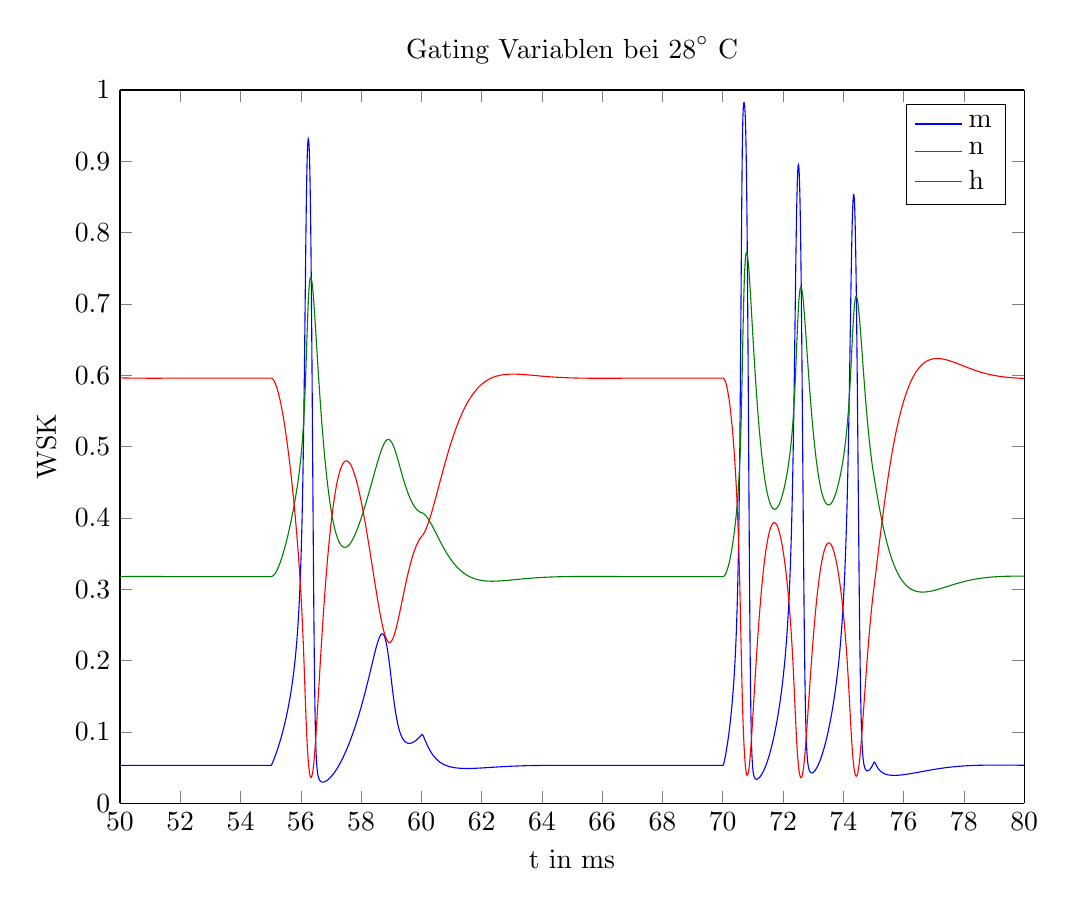
\begin{tikzpicture}

\begin{axis}[%
width=4.520833in,
height=3.565625in,
at={(0.758333in,0.48125in)},
scale only axis,
separate axis lines,
every outer x axis line/.append style={black},
every x tick label/.append style={font=\color{black}},
xmin=50,
xmax=80,
xlabel={t in ms},
every outer y axis line/.append style={black},
every y tick label/.append style={font=\color{black}},
ymin=0,
ymax=1,
ylabel={WSK},
title={$\text{Gating Variablen bei 28}^\circ\text{ C}$},
legend style={legend cell align=left,align=left,draw=black}
]
\addplot [color=blue,solid]
  table[row sep=crcr]{%
50	0.0530427217066187\\
50.01	0.0530423428697463\\
50.02	0.0530419484317113\\
50.03	0.053041538811299\\
50.04	0.0530411144217348\\
50.05	0.0530406756707102\\
50.06	0.0530402229604091\\
50.07	0.0530397566875359\\
50.08	0.0530392772433426\\
50.09	0.0530387850136583\\
50.1	0.0530382803789179\\
50.11	0.0530377637141924\\
50.12	0.0530372353892192\\
50.13	0.053036695768433\\
50.14	0.0530361452109978\\
50.15	0.0530355840708387\\
50.16	0.0530350126966747\\
50.17	0.0530344314320518\\
50.18	0.0530338406153764\\
50.19	0.0530332405799498\\
50.2	0.0530326316540022\\
50.21	0.0530320141607281\\
50.22	0.0530313884183212\\
50.23	0.0530307547400102\\
50.24	0.053030113434095\\
50.25	0.0530294648039831\\
50.26	0.0530288091482263\\
50.27	0.0530281467605577\\
50.28	0.0530274779299291\\
50.29	0.053026802940549\\
50.3	0.0530261220719199\\
50.31	0.0530254355988772\\
50.32	0.053024743791627\\
50.33	0.0530240469157855\\
50.34	0.053023345232417\\
50.35	0.0530226389980737\\
50.36	0.053021928464835\\
50.37	0.0530212138803462\\
50.38	0.053020495487859\\
50.39	0.0530197735262708\\
50.4	0.0530190482301647\\
50.41	0.0530183198298494\\
50.42	0.0530175885513996\\
50.43	0.0530168546166962\\
50.44	0.0530161182434662\\
50.45	0.0530153796453238\\
50.46	0.0530146390318103\\
50.47	0.0530138966084349\\
50.48	0.0530131525767152\\
50.49	0.0530124071342178\\
50.5	0.0530116604745988\\
50.51	0.0530109127876449\\
50.52	0.0530101642593134\\
50.53	0.0530094150717733\\
50.54	0.0530086654034457\\
50.55	0.0530079154290447\\
50.56	0.0530071653196174\\
50.57	0.053006415242585\\
50.58	0.0530056653617829\\
50.59	0.0530049158375014\\
50.6	0.0530041668265255\\
50.61	0.0530034184821761\\
50.62	0.0530026709543491\\
50.63	0.0530019243895564\\
50.64	0.0530011789309652\\
50.65	0.0530004347184384\\
50.66	0.0529996918885742\\
50.67	0.0529989505747455\\
50.68	0.0529982109071399\\
50.69	0.0529974730127987\\
50.7	0.0529967370156563\\
50.71	0.0529960030365795\\
50.72	0.052995271193406\\
50.73	0.0529945416009837\\
50.74	0.052993814371209\\
50.75	0.0529930896130654\\
50.76	0.0529923674326619\\
50.77	0.0529916479332709\\
50.78	0.0529909312153664\\
50.79	0.0529902173766613\\
50.8	0.0529895065121456\\
50.81	0.0529887987141233\\
50.82	0.0529880940722496\\
50.83	0.0529873926735679\\
50.84	0.0529866946025469\\
50.85	0.0529859999411163\\
50.86	0.052985308768704\\
50.87	0.0529846211622717\\
50.88	0.0529839371963507\\
50.89	0.0529832569430779\\
50.9	0.052982580472231\\
50.91	0.0529819078512636\\
50.92	0.0529812391453401\\
50.93	0.0529805744173708\\
50.94	0.0529799137280457\\
50.95	0.0529792571358693\\
50.96	0.0529786046971943\\
50.97	0.0529779564662551\\
50.98	0.0529773124952018\\
50.99	0.0529766728341326\\
51	0.0529760375311277\\
51.01	0.0529754066322812\\
51.02	0.0529747801817337\\
51.03	0.0529741582217049\\
51.04	0.0529735407925247\\
51.05	0.0529729279326657\\
51.06	0.0529723196787739\\
51.07	0.0529717160657\\
51.08	0.0529711171265304\\
51.09	0.0529705228926174\\
51.1	0.0529699333936098\\
51.11	0.0529693486574826\\
51.12	0.0529687687105672\\
51.13	0.0529681935775803\\
51.14	0.0529676232816535\\
51.15	0.0529670578443618\\
51.16	0.0529664972857527\\
51.17	0.0529659416243743\\
51.18	0.0529653908773032\\
51.19	0.0529648450601727\\
51.2	0.0529643041871999\\
51.21	0.0529637682712134\\
51.22	0.0529632373236797\\
51.23	0.0529627113547304\\
51.24	0.0529621903731882\\
51.25	0.0529616743865934\\
51.26	0.0529611634012294\\
51.27	0.0529606574221484\\
51.28	0.0529601564531969\\
51.29	0.0529596604970403\\
51.3	0.0529591695551879\\
51.31	0.0529586836280175\\
51.32	0.0529582027147991\\
51.33	0.0529577268137194\\
51.34	0.052957255921905\\
51.35	0.0529567900354457\\
51.36	0.0529563291494183\\
51.37	0.0529558732579083\\
51.38	0.0529554223540335\\
51.39	0.0529549764299655\\
51.4	0.0529545354769522\\
51.41	0.0529540994853391\\
51.42	0.0529536684445914\\
51.43	0.0529532423433143\\
51.44	0.0529528211692747\\
51.45	0.0529524049094216\\
51.46	0.0529519935499063\\
51.47	0.0529515870761029\\
51.48	0.0529511854726278\\
51.49	0.0529507887233596\\
51.5	0.0529503968114583\\
51.51	0.0529500097193846\\
51.52	0.0529496274289183\\
51.53	0.0529492499211776\\
51.54	0.0529488771766365\\
51.55	0.0529485091751437\\
51.56	0.05294814589594\\
51.57	0.0529477873176762\\
51.58	0.0529474334184298\\
51.59	0.0529470841757228\\
51.6	0.0529467395665382\\
51.61	0.0529463995673367\\
51.62	0.0529460641540727\\
51.63	0.0529457333022109\\
51.64	0.0529454069867421\\
51.65	0.0529450851821985\\
51.66	0.0529447678626694\\
51.67	0.0529444550018162\\
51.68	0.0529441465728876\\
51.69	0.0529438425487338\\
51.7	0.0529435429018217\\
51.71	0.0529432476042486\\
51.72	0.0529429566277561\\
51.73	0.0529426699437447\\
51.74	0.0529423875232864\\
51.75	0.0529421093371388\\
51.76	0.0529418353557579\\
51.77	0.0529415655493111\\
51.78	0.0529412998876899\\
51.79	0.0529410383405224\\
51.8	0.0529407808771856\\
51.81	0.0529405274668176\\
51.82	0.0529402780783292\\
51.83	0.0529400326804158\\
51.84	0.0529397912415688\\
51.85	0.0529395537300869\\
51.86	0.052939320114087\\
51.87	0.0529390903615154\\
51.88	0.0529388644401581\\
51.89	0.0529386423176515\\
51.9	0.0529384239614926\\
51.91	0.0529382093390492\\
51.92	0.0529379984175696\\
51.93	0.0529377911641926\\
51.94	0.0529375875459569\\
51.95	0.0529373875298103\\
51.96	0.0529371910826191\\
51.97	0.052936998171177\\
51.98	0.052936808762214\\
51.99	0.0529366228224049\\
52	0.0529364403183779\\
52.01	0.0529362612167227\\
52.02	0.052936085483999\\
52.03	0.052935913086744\\
52.04	0.0529357439914805\\
52.05	0.0529355781647245\\
52.06	0.0529354155729926\\
52.07	0.0529352561828093\\
52.08	0.0529350999607141\\
52.09	0.0529349468732689\\
52.1	0.0529347968870641\\
52.11	0.052934649968726\\
52.12	0.0529345060849227\\
52.13	0.0529343652023712\\
52.14	0.0529342272878431\\
52.15	0.0529340923081707\\
52.16	0.0529339602302533\\
52.17	0.0529338310210626\\
52.18	0.0529337046476489\\
52.19	0.0529335810771459\\
52.2	0.0529334602767768\\
52.21	0.052933342213859\\
52.22	0.0529332268558097\\
52.23	0.0529331141701505\\
52.24	0.0529330041245124\\
52.25	0.0529328966866407\\
52.26	0.0529327918243993\\
52.27	0.0529326895057755\\
52.28	0.052932589698884\\
52.29	0.0529324923719716\\
52.3	0.0529323974934208\\
52.31	0.0529323050317542\\
52.32	0.0529322149556384\\
52.33	0.0529321272338873\\
52.34	0.0529320418354662\\
52.35	0.0529319587294954\\
52.36	0.0529318778852531\\
52.37	0.0529317992721795\\
52.38	0.0529317228598793\\
52.39	0.0529316486181253\\
52.4	0.0529315765168612\\
52.41	0.0529315065262044\\
52.42	0.0529314386164491\\
52.43	0.052931372758069\\
52.44	0.0529313089217197\\
52.45	0.0529312470782411\\
52.46	0.0529311871986603\\
52.47	0.0529311292541936\\
52.48	0.0529310732162488\\
52.49	0.0529310190564274\\
52.5	0.0529309667465266\\
52.51	0.0529309162585414\\
52.52	0.0529308675646662\\
52.53	0.0529308206372969\\
52.54	0.0529307754490327\\
52.55	0.0529307319726774\\
52.56	0.0529306901812413\\
52.57	0.0529306500479422\\
52.58	0.0529306115462075\\
52.59	0.052930574649675\\
52.6	0.0529305393321943\\
52.61	0.0529305055678283\\
52.62	0.0529304733308536\\
52.63	0.0529304425957622\\
52.64	0.0529304133372623\\
52.65	0.0529303855302791\\
52.66	0.0529303591499556\\
52.67	0.0529303341716536\\
52.68	0.0529303105709542\\
52.69	0.0529302883236585\\
52.7	0.0529302674057884\\
52.71	0.0529302477935866\\
52.72	0.0529302294635177\\
52.73	0.0529302123922682\\
52.74	0.0529301965567469\\
52.75	0.0529301819340853\\
52.76	0.0529301685016378\\
52.77	0.0529301562369817\\
52.78	0.0529301451179179\\
52.79	0.0529301351224702\\
52.8	0.052930126228886\\
52.81	0.0529301184156356\\
52.82	0.052930111661413\\
52.83	0.052930105945135\\
52.84	0.0529301012459416\\
52.85	0.0529300975431952\\
52.86	0.0529300948164811\\
52.87	0.0529300930456066\\
52.88	0.0529300922106008\\
52.89	0.0529300922917145\\
52.9	0.0529300932694195\\
52.91	0.0529300951244081\\
52.92	0.0529300978375929\\
52.93	0.052930101390106\\
52.94	0.0529301057632986\\
52.95	0.0529301109387403\\
52.96	0.0529301168982185\\
52.97	0.0529301236237378\\
52.98	0.0529301310975189\\
52.99	0.0529301393019985\\
53	0.0529301482198282\\
53.01	0.0529301578338735\\
53.02	0.0529301681272134\\
53.03	0.0529301790831391\\
53.04	0.0529301906851535\\
53.05	0.05293020291697\\
53.06	0.0529302157625119\\
53.07	0.052930229205911\\
53.08	0.052930243231507\\
53.09	0.0529302578238461\\
53.1	0.0529302729676803\\
53.11	0.0529302886479664\\
53.12	0.0529303048498645\\
53.13	0.0529303215587371\\
53.14	0.0529303387601482\\
53.15	0.052930356439862\\
53.16	0.0529303745838414\\
53.17	0.0529303931782473\\
53.18	0.0529304122094375\\
53.19	0.0529304316639647\\
53.2	0.0529304515285761\\
53.21	0.0529304717902117\\
53.22	0.0529304924360034\\
53.23	0.0529305134532731\\
53.24	0.052930534829532\\
53.25	0.0529305565524792\\
53.26	0.05293057861\\
53.27	0.052930600990165\\
53.28	0.0529306236812285\\
53.29	0.0529306466716273\\
53.3	0.0529306699499793\\
53.31	0.0529306935050818\\
53.32	0.0529307173259108\\
53.33	0.052930741401619\\
53.34	0.0529307657215345\\
53.35	0.0529307902751596\\
53.36	0.0529308150521693\\
53.37	0.0529308400424098\\
53.38	0.052930865235897\\
53.39	0.0529308906228153\\
53.4	0.0529309161935159\\
53.41	0.0529309419385155\\
53.42	0.0529309678484948\\
53.43	0.0529309939142971\\
53.44	0.0529310201269266\\
53.45	0.0529310464775473\\
53.46	0.0529310729574811\\
53.47	0.0529310995582067\\
53.48	0.0529311262713579\\
53.49	0.0529311530887222\\
53.5	0.0529311800022395\\
53.51	0.0529312070039999\\
53.52	0.0529312340862433\\
53.53	0.0529312612413569\\
53.54	0.0529312884618745\\
53.55	0.0529313157404744\\
53.56	0.0529313430699782\\
53.57	0.0529313704433495\\
53.58	0.0529313978536919\\
53.59	0.0529314252942481\\
53.6	0.052931452758398\\
53.61	0.0529314802396572\\
53.62	0.0529315077316758\\
53.63	0.052931535228237\\
53.64	0.052931562723255\\
53.65	0.0529315902107742\\
53.66	0.0529316176849675\\
53.67	0.0529316451401346\\
53.68	0.0529316725707008\\
53.69	0.0529316999712157\\
53.7	0.0529317273363513\\
53.71	0.0529317546609008\\
53.72	0.0529317819397771\\
53.73	0.0529318091680115\\
53.74	0.0529318363407522\\
53.75	0.0529318634532625\\
53.76	0.0529318905009201\\
53.77	0.0529319174792149\\
53.78	0.0529319443837482\\
53.79	0.0529319712102311\\
53.8	0.0529319979544827\\
53.81	0.0529320246124294\\
53.82	0.052932051180103\\
53.83	0.0529320776536395\\
53.84	0.0529321040292777\\
53.85	0.0529321303033578\\
53.86	0.0529321564723201\\
53.87	0.0529321825327036\\
53.88	0.0529322084811447\\
53.89	0.0529322343143757\\
53.9	0.0529322600292237\\
53.91	0.0529322856226091\\
53.92	0.0529323110915445\\
53.93	0.0529323364331329\\
53.94	0.0529323616445671\\
53.95	0.0529323867231278\\
53.96	0.0529324116661827\\
53.97	0.052932436471185\\
53.98	0.0529324611356722\\
53.99	0.052932485657265\\
54	0.0529325100336656\\
54.01	0.0529325342626571\\
54.02	0.0529325583421017\\
54.03	0.0529325822699398\\
54.04	0.0529326060441886\\
54.05	0.0529326296629413\\
54.06	0.0529326531243651\\
54.07	0.0529326764267009\\
54.08	0.0529326995682615\\
54.09	0.0529327225474307\\
54.1	0.0529327453626622\\
54.11	0.0529327680124783\\
54.12	0.0529327904954687\\
54.13	0.0529328128102896\\
54.14	0.0529328349556623\\
54.15	0.0529328569303726\\
54.16	0.0529328787332689\\
54.17	0.0529329003632618\\
54.18	0.0529329218193227\\
54.19	0.0529329431004829\\
54.2	0.0529329642058322\\
54.21	0.0529329851345185\\
54.22	0.0529330058857458\\
54.23	0.0529330264587741\\
54.24	0.0529330468529179\\
54.25	0.0529330670675452\\
54.26	0.0529330871020767\\
54.27	0.0529331069559844\\
54.28	0.0529331266287911\\
54.29	0.0529331461200693\\
54.3	0.05293316542944\\
54.31	0.0529331845565719\\
54.32	0.0529332035011806\\
54.33	0.0529332222630272\\
54.34	0.0529332408419182\\
54.35	0.0529332592377036\\
54.36	0.0529332774502768\\
54.37	0.0529332954795732\\
54.38	0.0529333133255696\\
54.39	0.0529333309882833\\
54.4	0.0529333484677709\\
54.41	0.0529333657641279\\
54.42	0.0529333828774877\\
54.43	0.0529333998080207\\
54.44	0.0529334165559334\\
54.45	0.0529334331214677\\
54.46	0.0529334495049003\\
54.47	0.0529334657065413\\
54.48	0.0529334817267342\\
54.49	0.0529334975658544\\
54.5	0.0529335132243089\\
54.51	0.0529335287025355\\
54.52	0.0529335440010016\\
54.53	0.0529335591202041\\
54.54	0.0529335740606684\\
54.55	0.0529335888229474\\
54.56	0.0529336034076212\\
54.57	0.0529336178152962\\
54.58	0.0529336320466046\\
54.59	0.0529336461022033\\
54.6	0.0529336599827736\\
54.61	0.0529336736890205\\
54.62	0.0529336872216718\\
54.63	0.0529337005814778\\
54.64	0.0529337137692104\\
54.65	0.0529337267856625\\
54.66	0.0529337396316474\\
54.67	0.0529337523079984\\
54.68	0.0529337648155678\\
54.69	0.0529337771552266\\
54.7	0.0529337893278639\\
54.71	0.0529338013343862\\
54.72	0.0529338131757167\\
54.73	0.0529338248527953\\
54.74	0.0529338363665773\\
54.75	0.0529338477180335\\
54.76	0.0529338589081491\\
54.77	0.0529338699379239\\
54.78	0.0529338808083709\\
54.79	0.0529338915205164\\
54.8	0.0529339020753994\\
54.81	0.052933912474071\\
54.82	0.0529339227175938\\
54.83	0.0529339328070418\\
54.84	0.0529339427434995\\
54.85	0.0529339525280617\\
54.86	0.052933962161833\\
54.87	0.0529339716459274\\
54.88	0.0529339809814675\\
54.89	0.0529339901695847\\
54.9	0.0529339992114182\\
54.91	0.0529340081081148\\
54.92	0.0529340168608286\\
54.93	0.0529340254707204\\
54.94	0.0529340339389575\\
54.95	0.0529340422667131\\
54.96	0.052934050455166\\
54.97	0.0529340585055004\\
54.98	0.0529340664189051\\
54.99	0.0529340741965736\\
55	0.0529340818397036\\
55.01	0.0529340893494964\\
55.02	0.053302004152195\\
55.03	0.0539059806121324\\
55.04	0.0546622198975667\\
55.05	0.055518820854169\\
55.06	0.0564435486791357\\
55.07	0.0574163303970476\\
55.08	0.0584246416255915\\
55.09	0.0594606600531413\\
55.1	0.0605195027993036\\
55.11	0.0615981312589636\\
55.12	0.0626946684732733\\
55.13	0.0638079723325436\\
55.14	0.0649373679638159\\
55.15	0.0660824794889856\\
55.16	0.0672431240129235\\
55.17	0.0684192447059302\\
55.18	0.0696108685238513\\
55.19	0.0708180795049027\\
55.2	0.0720410019473028\\
55.21	0.0732797898768739\\
55.22	0.074534620534622\\
55.23	0.0758056904455652\\
55.24	0.0770932131547739\\
55.25	0.0783974180487581\\
55.26	0.0797185498912603\\
55.27	0.0810568688368591\\
55.28	0.0824126507716497\\
55.29	0.0837861878853371\\
55.3	0.0851777894145603\\
55.31	0.0865877825202535\\
55.32	0.0880165132768549\\
55.33	0.0894643477610742\\
55.34	0.0909316732345688\\
55.35	0.0924188994194392\\
55.36	0.0939264598686881\\
55.37	0.0954548134362049\\
55.38	0.0970044458527488\\
55.39	0.0985758714160199\\
55.4	0.100169634804387\\
55.41	0.101786313025263\\
55.42	0.103426517510558\\
55.43	0.105090896373175\\
55.44	0.106780136840133\\
55.45	0.108494967879692\\
55.46	0.110236163041859\\
55.47	0.112004543533807\\
55.48	0.113800981554264\\
55.49	0.115626403913638\\
55.5	0.11748179596979\\
55.51	0.119368205912879\\
55.52	0.121286749436646\\
55.53	0.123238614838037\\
55.54	0.125225068592129\\
55.55	0.12724746145514\\
55.56	0.129307235154899\\
55.57	0.131405929735658\\
55.58	0.133545191632728\\
55.59	0.135726782562255\\
55.6	0.137952589322686\\
55.61	0.140224634617424\\
55.62	0.142545089023029\\
55.63	0.144916284244426\\
55.64	0.147340727818368\\
55.65	0.149821119449203\\
55.66	0.152360369187485\\
55.67	0.154961617692614\\
55.68	0.157628258856388\\
55.69	0.160363965105852\\
55.7	0.163172715752283\\
55.71	0.166058828809742\\
55.72	0.169026996772877\\
55.73	0.17208232692134\\
55.74	0.175230386809427\\
55.75	0.178477255706856\\
55.76	0.181829582883016\\
55.77	0.185294653776147\\
55.78	0.188880465264976\\
55.79	0.192595811468477\\
55.8	0.196450381745532\\
55.81	0.200454872857424\\
55.82	0.204621117600399\\
55.83	0.208962232622312\\
55.84	0.213492788617133\\
55.85	0.218229006655296\\
55.86	0.22318898506846\\
55.87	0.228392962075739\\
55.88	0.233863620223965\\
55.89	0.239626439721115\\
55.9	0.245710108862775\\
55.91	0.252147000960733\\
55.92	0.25897372842141\\
55.93	0.266231785775213\\
55.94	0.273968294320115\\
55.95	0.282236861260105\\
55.96	0.2910985652022\\
55.97	0.300623076663276\\
55.98	0.310889915289274\\
55.99	0.321989832373713\\
56	0.334026284206382\\
56.01	0.347116923039511\\
56.02	0.361394969487827\\
56.03	0.377010230728928\\
56.04	0.394129376292986\\
56.05	0.412934856924859\\
56.06	0.433621531024646\\
56.07	0.456389637122516\\
56.08	0.481432245263473\\
56.09	0.508914846865004\\
56.1	0.538944583388035\\
56.11	0.5715273261866\\
56.12	0.606513285467316\\
56.13	0.643537037821285\\
56.14	0.681966092517101\\
56.15	0.720881282788749\\
56.16	0.759116313339304\\
56.17	0.795373844071438\\
56.18	0.828406864298348\\
56.19	0.857216556660462\\
56.2	0.881196456263174\\
56.21	0.900169222497795\\
56.22	0.914310779936941\\
56.23	0.924004028767848\\
56.24	0.92968114607095\\
56.25	0.931698209038424\\
56.26	0.930258618603956\\
56.27	0.925381665671735\\
56.28	0.916905391857015\\
56.29	0.904514484599548\\
56.3	0.887787910341248\\
56.31	0.866263093777944\\
56.32	0.839512392017736\\
56.33	0.807224400900395\\
56.34	0.769279701145257\\
56.35	0.725810535655261\\
56.36	0.677237475847505\\
56.37	0.624281524540809\\
56.38	0.567953718688808\\
56.39	0.509523561260888\\
56.4	0.450463364485057\\
56.41	0.39236217150445\\
56.42	0.336805734957495\\
56.43	0.285230552418189\\
56.44	0.238776331894578\\
56.45	0.198172540650054\\
56.46	0.163690945322849\\
56.47	0.135176031584141\\
56.48	0.112139132261736\\
56.49	0.0938842764470217\\
56.5	0.0796316712730806\\
56.51	0.068615248529778\\
56.52	0.06014526770211\\
56.53	0.0536384699214639\\
56.54	0.0486241172656864\\
56.55	0.0447352967809001\\
56.56	0.041693228549603\\
56.57	0.0392898261336188\\
56.58	0.0373714823507837\\
56.59	0.0358253977725574\\
56.6	0.0345687486127769\\
56.61	0.0335404598314245\\
56.62	0.0326951373333259\\
56.63	0.0319986807184073\\
56.64	0.0314251506128896\\
56.65	0.0309545462903992\\
56.66	0.0305712312929968\\
56.67	0.0302628148882837\\
56.68	0.0300193522440137\\
56.69	0.0298327671749552\\
56.7	0.0296964307635606\\
56.71	0.0296048498255045\\
56.72	0.0295534334775748\\
56.73	0.0295383158497387\\
56.74	0.0295562196564502\\
56.75	0.0296043498937477\\
56.76	0.0296803100439627\\
56.77	0.029782035315832\\
56.78	0.0299077389390425\\
56.79	0.0300558685794296\\
56.8	0.0302250706850739\\
56.81	0.0304141611087615\\
56.82	0.0306221007421638\\
56.83	0.0308479751846975\\
56.84	0.0310909776847198\\
56.85	0.0313503947528378\\
56.86	0.0316255939708306\\
56.87	0.0319160136150366\\
56.88	0.0322211537872157\\
56.89	0.0325405688040491\\
56.9	0.0328738606423963\\
56.91	0.0332206732739923\\
56.92	0.033580687752559\\
56.93	0.0339536179399005\\
56.94	0.0343392067766695\\
56.95	0.0347372230190612\\
56.96	0.0351474583754327\\
56.97	0.0355697249873181\\
56.98	0.0360038532079584\\
56.99	0.0364496896386296\\
57	0.0369070953890214\\
57.01	0.0373759445328963\\
57.02	0.0378561227344358\\
57.03	0.0383475260241898\\
57.04	0.0388500597065071\\
57.05	0.0393636373828286\\
57.06	0.039888180077351\\
57.07	0.0404236154533772\\
57.08	0.0409698771102111\\
57.09	0.041526903951773\\
57.1	0.0420946396192446\\
57.11	0.0426730319810198\\
57.12	0.043262032674075\\
57.13	0.0438615966915955\\
57.14	0.0444716820123117\\
57.15	0.045092249267545\\
57.16	0.0457232614424235\\
57.17	0.0463646836081388\\
57.18	0.0470164826824644\\
57.19	0.0476786272160652\\
57.2	0.0483510872023927\\
57.21	0.0490338339091963\\
57.22	0.0497268397298835\\
57.23	0.0504300780531374\\
57.24	0.0511435231493605\\
57.25	0.0518671500726438\\
57.26	0.0526009345770825\\
57.27	0.0533448530463632\\
57.28	0.0540988824356374\\
57.29	0.0548630002247757\\
57.3	0.0556371843821686\\
57.31	0.0564214133382983\\
57.32	0.0572156659683612\\
57.33	0.0580199215832665\\
57.34	0.0588341599283779\\
57.35	0.0596583611894011\\
57.36	0.0604925060048518\\
57.37	0.0613365754845653\\
57.38	0.0621905512337352\\
57.39	0.0630544153819888\\
57.4	0.0639281506170259\\
57.41	0.0648117402223665\\
57.42	0.0657051681187639\\
57.43	0.0666084189088592\\
57.44	0.0675214779246591\\
57.45	0.0684443312774349\\
57.46	0.0693769659096476\\
57.47	0.0703193696485144\\
57.48	0.0712715312608412\\
57.49	0.0722334405087505\\
57.5	0.0732050882059467\\
57.51	0.0741864662741608\\
57.52	0.0751775677994293\\
57.53	0.0761783870878644\\
57.54	0.0771889197205778\\
57.55	0.0782091626074277\\
57.56	0.0792391140392618\\
57.57	0.0802787737383328\\
57.58	0.0813281429065674\\
57.59	0.0823872242713718\\
57.6	0.0834560221286606\\
57.61	0.0845345423827949\\
57.62	0.0856227925831186\\
57.63	0.0867207819567812\\
57.64	0.0878285214375322\\
57.65	0.0889460236901741\\
57.66	0.0900733031303518\\
57.67	0.091210375939357\\
57.68	0.092357260073617\\
57.69	0.0935139752685281\\
57.7	0.0946805430362884\\
57.71	0.0958569866573683\\
57.72	0.0970433311652482\\
57.73	0.0982396033240334\\
57.74	0.09944583159854\\
57.75	0.100662046116426\\
57.76	0.101888278621915\\
57.77	0.103124562420641\\
57.78	0.104370932315098\\
57.79	0.105627424530176\\
57.8	0.106894076628186\\
57.81	0.108170927412785\\
57.82	0.109458016821122\\
57.83	0.110755385803518\\
57.84	0.11206307618992\\
57.85	0.113381130542312\\
57.86	0.114709591992216\\
57.87	0.116048504062339\\
57.88	0.117397910471361\\
57.89	0.118757854920759\\
57.9	0.120128380862523\\
57.91	0.121509531246467\\
57.92	0.122901348245804\\
57.93	0.124303872959505\\
57.94	0.125717145089874\\
57.95	0.12714120259365\\
57.96	0.128576081304805\\
57.97	0.130021814527097\\
57.98	0.131478432594266\\
57.99	0.132945962395633\\
58	0.134424426864679\\
58.01	0.135913844428017\\
58.02	0.137414228411999\\
58.03	0.138925586403983\\
58.04	0.140447919565108\\
58.05	0.14198122189119\\
58.06	0.14352547941815\\
58.07	0.145080669368135\\
58.08	0.146646759232256\\
58.09	0.148223705785612\\
58.1	0.149811454030017\\
58.11	0.151409936059555\\
58.12	0.153019069843839\\
58.13	0.154638757923551\\
58.14	0.156268886012543\\
58.15	0.157909321500538\\
58.16	0.159559911850116\\
58.17	0.161220482881456\\
58.18	0.16289083693799\\
58.19	0.164570750925889\\
58.2	0.166259974220042\\
58.21	0.167958226429004\\
58.22	0.169665195011197\\
58.23	0.171380532734492\\
58.24	0.173103854971261\\
58.25	0.174834736820938\\
58.26	0.176572710052201\\
58.27	0.178317259857046\\
58.28	0.180067821409294\\
58.29	0.181823776220476\\
58.3	0.183584448286597\\
58.31	0.185349100020025\\
58.32	0.187116927961688\\
58.33	0.18888705826998\\
58.34	0.190658541984197\\
58.35	0.192430350062141\\
58.36	0.194201368193643\\
58.37	0.195970391394269\\
58.38	0.19773611838648\\
58.39	0.199497145778948\\
58.4	0.201251962058764\\
58.41	0.20299894141589\\
58.42	0.20473633742449\\
58.43	0.206462276611738\\
58.44	0.208174751951508\\
58.45	0.209871616327904\\
58.46	0.211550576022052\\
58.47	0.213209184284953\\
58.48	0.214844835069508\\
58.49	0.216454757006091\\
58.5	0.218036007718278\\
58.51	0.219585468588545\\
58.52	0.221099840097753\\
58.53	0.222575637877164\\
58.54	0.224009189627248\\
58.55	0.225396633073603\\
58.56	0.226733915146686\\
58.57	0.22801679258837\\
58.58	0.229240834204317\\
58.59	0.230401424996346\\
58.6	0.231493772422769\\
58.61	0.232512915046514\\
58.62	0.233453733839978\\
58.63	0.234310966421109\\
58.64	0.235079224496232\\
58.65	0.235753014780602\\
58.66	0.236326763656275\\
58.67	0.23679484580757\\
58.68	0.237151617045588\\
58.69	0.237391451493786\\
58.7	0.23750878325498\\
58.71	0.237498152615105\\
58.72	0.237354256759487\\
58.73	0.237072004882288\\
58.74	0.236646577458656\\
58.75	0.236073489321881\\
58.76	0.235348656045121\\
58.77	0.234468462970304\\
58.78	0.23342983605823\\
58.79	0.232230313557013\\
58.8	0.23086811730584\\
58.81	0.229342222313796\\
58.82	0.227652423086983\\
58.83	0.225799395030491\\
58.84	0.223784749135355\\
58.85	0.221611078085726\\
58.86	0.219281991899693\\
58.87	0.216802141259922\\
58.88	0.214177226807484\\
58.89	0.21141399287188\\
58.9	0.208520204396796\\
58.91	0.205504606194505\\
58.92	0.202376864116842\\
58.93	0.199147488255662\\
58.94	0.195827738863012\\
58.95	0.192429516286779\\
58.96	0.188965236822466\\
58.97	0.185447696953223\\
58.98	0.18188992895435\\
58.99	0.178305051242464\\
59	0.174706117124648\\
59.01	0.171105965727269\\
59.02	0.167517078845162\\
59.03	0.163951447247252\\
59.04	0.160420449613956\\
59.05	0.156934746784733\\
59.06	0.153504193390475\\
59.07	0.150137768271085\\
59.08	0.146843524373495\\
59.09	0.143628558129657\\
59.1	0.140498997664895\\
59.11	0.137460008616047\\
59.12	0.13451581586968\\
59.13	0.131669739178368\\
59.14	0.128924240383263\\
59.15	0.126280979861456\\
59.16	0.123740879817052\\
59.17	0.121304192130348\\
59.18	0.118970568651407\\
59.19	0.116739132052357\\
59.2	0.114608545616965\\
59.21	0.112577080627745\\
59.22	0.110642680293979\\
59.23	0.108803019435481\\
59.24	0.107055559386844\\
59.25	0.105397597808679\\
59.26	0.103826313282195\\
59.27	0.102338804720117\\
59.28	0.100932125751033\\
59.29	0.0996033143279156\\
59.3	0.0983494178778803\\
59.31	0.0971675143528248\\
59.32	0.0960547295632984\\
59.33	0.0950082511845684\\
59.34	0.0940253398179246\\
59.35	0.0931033374750011\\
59.36	0.0922396738310494\\
59.37	0.091431870567007\\
59.38	0.0906775440917568\\
59.39	0.0899744069066494\\
59.4	0.0893202678452974\\
59.41	0.0887130313936607\\
59.42	0.0881506962690904\\
59.43	0.0876313534126365\\
59.44	0.0871531835267404\\
59.45	0.0867144542704956\\
59.46	0.0863135172069312\\
59.47	0.0859488045811739\\
59.48	0.0856188259947322\\
59.49	0.0853221650293661\\
59.5	0.0850574758638841\\
59.51	0.0848234799185749\\
59.52	0.0846189625546654\\
59.53	0.0844427698500309\\
59.54	0.0842938054672324\\
59.55	0.0841710276256693\\
59.56	0.084073446186099\\
59.57	0.0840001198528796\\
59.58	0.0839501534969334\\
59.59	0.0839226956005367\\
59.6	0.0839169358235246\\
59.61	0.0839321026893182\\
59.62	0.0839674613882535\\
59.63	0.0840223116950009\\
59.64	0.0840959859963448\\
59.65	0.0841878474252294\\
59.66	0.0842972880967373\\
59.67	0.0844237274415195\\
59.68	0.0845666106321347\\
59.69	0.0847254070977528\\
59.7	0.0848996091227247\\
59.71	0.0850887305246076\\
59.72	0.085292305407349\\
59.73	0.0855098869854685\\
59.74	0.0857410464752293\\
59.75	0.0859853720489494\\
59.76	0.0862424678487744\\
59.77	0.0865119530564018\\
59.78	0.0867934610154176\\
59.79	0.0870866384030772\\
59.8	0.0873911444485277\\
59.81	0.0877066501946321\\
59.82	0.0880328378007109\\
59.83	0.0883693998836714\\
59.84	0.0887160388951373\\
59.85	0.0890724665323308\\
59.86	0.0894384031805952\\
59.87	0.0898135773855655\\
59.88	0.0901977253531222\\
59.89	0.0905905904753699\\
59.9	0.0909919228809941\\
59.91	0.0914014790084485\\
59.92	0.0918190212005231\\
59.93	0.092244317318931\\
59.94	0.0926771403776391\\
59.95	0.0931172681937475\\
59.96	0.0935644830547981\\
59.97	0.094018571401463\\
59.98	0.0944793235246324\\
59.99	0.0949465332759841\\
60	0.0954199977911754\\
60.01	0.0958995172248555\\
60.02	0.09638489449675\\
60.03	0.0963671608008704\\
60.04	0.0959989471560814\\
60.05	0.0953931150983719\\
60.06	0.0946280005460776\\
60.07	0.0937578694689141\\
60.08	0.0928203103431804\\
60.09	0.0918413757213768\\
60.1	0.0908391463159974\\
60.11	0.0898261957867684\\
60.12	0.0888112922406253\\
60.13	0.0878005712010846\\
60.14	0.0867983433915729\\
60.15	0.08580765064248\\
60.16	0.0848306483379648\\
60.17	0.0838688685663564\\
60.18	0.0829234013250429\\
60.19	0.0819950194985766\\
60.2	0.0810842652944395\\
60.21	0.0801915102798725\\
60.22	0.0793169973468851\\
60.23	0.0784608703076577\\
60.24	0.0776231950195076\\
60.25	0.076803974701781\\
60.26	0.0760031612598705\\
60.27	0.0752206638521825\\
60.28	0.0744563555403078\\
60.29	0.0737100785930651\\
60.3	0.0729816488317299\\
60.31	0.0722708592793312\\
60.32	0.071577483292657\\
60.33	0.0709012772987357\\
60.34	0.0702419832192682\\
60.35	0.0695993306407887\\
60.36	0.0689730387711415\\
60.37	0.0683628182113966\\
60.38	0.0677683725646999\\
60.39	0.0671893998984913\\
60.4	0.0666255940731566\\
60.41	0.066076645947932\\
60.42	0.0655422444733636\\
60.43	0.0650220776785767\\
60.44	0.0645158335608671\\
60.45	0.0640232008845684\\
60.46	0.0635438698957107\\
60.47	0.0630775329586149\\
60.48	0.0626238851202396\\
60.49	0.0621826246077912\\
60.5	0.0617534532648172\\
60.51	0.0613360769307214\\
60.52	0.0609302057683587\\
60.53	0.0605355545441007\\
60.54	0.060151842864493\\
60.55	0.0597787953733656\\
60.56	0.0594161419130074\\
60.57	0.0590636176527673\\
60.58	0.0587209631882106\\
60.59	0.0583879246137325\\
60.6	0.0580642535713155\\
60.61	0.05774970727791\\
60.62	0.0574440485337249\\
60.63	0.0571470457135305\\
60.64	0.0568584727429037\\
60.65	0.0565781090611824\\
60.66	0.0563057395727468\\
60.67	0.0560411545881011\\
60.68	0.0557841497560999\\
60.69	0.0555345259885404\\
60.7	0.0552920893782293\\
60.71	0.0550566511115265\\
60.72	0.0548280273762746\\
60.73	0.0546060392659311\\
60.74	0.0543905126806403\\
60.75	0.0541812782259065\\
60.76	0.0539781711094597\\
60.77	0.053781031036845\\
60.78	0.0535897021062062\\
60.79	0.0534040327026837\\
60.8	0.0532238753927976\\
60.81	0.0530490868191436\\
60.82	0.0528795275956906\\
60.83	0.0527150622039313\\
60.84	0.0525555588901057\\
60.85	0.0524008895636874\\
60.86	0.0522509296972964\\
60.87	0.052105558228177\\
60.88	0.0519646574613592\\
60.89	0.0518281129746016\\
60.9	0.0516958135251957\\
60.91	0.0515676509586976\\
60.92	0.0514435201196383\\
60.93	0.0513233187642489\\
60.94	0.0512069474752316\\
60.95	0.0510943095785904\\
60.96	0.0509853110625328\\
60.97	0.0508798604984423\\
60.98	0.0507778689639161\\
60.99	0.0506792499678566\\
61	0.0505839193775997\\
61.01	0.0504917953480573\\
61.02	0.0504027982528513\\
61.03	0.0503168506174079\\
61.04	0.0502338770539817\\
61.05	0.0501538041985762\\
61.06	0.0500765606497244\\
61.07	0.0500020769090924\\
61.08	0.0499302853238659\\
61.09	0.0498611200308828\\
61.1	0.0497945169024682\\
61.11	0.0497304134939329\\
61.12	0.049668748992693\\
61.13	0.0496094641689702\\
61.14	0.04955250132803\\
61.15	0.0494978042639174\\
61.16	0.0494453182146488\\
61.17	0.0493949898188197\\
61.18	0.0493467670735871\\
61.19	0.0493005992939882\\
61.2	0.0492564370735549\\
61.21	0.0492142322461871\\
61.22	0.0491739378492458\\
61.23	0.0491355080878301\\
61.24	0.0490988983002006\\
61.25	0.0490640649243157\\
61.26	0.0490309654654438\\
61.27	0.0489995584648202\\
61.28	0.0489698034693128\\
61.29	0.0489416610020682\\
61.3	0.048915092534103\\
61.31	0.0488900604568132\\
61.32	0.0488665280553704\\
61.33	0.0488444594829759\\
61.34	0.0488238197359464\\
61.35	0.048804574629602\\
61.36	0.0487866907749328\\
61.37	0.0487701355560158\\
61.38	0.04875487710816\\
61.39	0.0487408842967534\\
61.4	0.0487281266967913\\
61.41	0.0487165745730603\\
61.42	0.0487061988609595\\
61.43	0.0486969711479349\\
61.44	0.0486888636555088\\
61.45	0.0486818492218832\\
61.46	0.0486759012850988\\
61.47	0.0486709938667302\\
61.48	0.0486671015561012\\
61.49	0.0486641994950005\\
61.5	0.0486622633628832\\
61.51	0.0486612693625415\\
61.52	0.0486611942062272\\
61.53	0.0486620151022141\\
61.54	0.048663709741783\\
61.55	0.0486662562866163\\
61.56	0.0486696333565888\\
61.57	0.0486738200179409\\
61.58	0.0486787957718222\\
61.59	0.0486845405431928\\
61.6	0.0486910346700702\\
61.61	0.0486982588931107\\
61.62	0.0487061943455148\\
61.63	0.0487148225432445\\
61.64	0.0487241253755433\\
61.65	0.0487340850957486\\
61.66	0.0487446843123867\\
61.67	0.0487559059805414\\
61.68	0.0487677333934867\\
61.69	0.0487801501745758\\
61.7	0.0487931402693765\\
61.71	0.0488066879380468\\
61.72	0.0488207777479413\\
61.73	0.0488353945664415\\
61.74	0.0488505235540023\\
61.75	0.0488661501574088\\
61.76	0.0488822601032344\\
61.77	0.0488988393914959\\
61.78	0.0489158742894979\\
61.79	0.0489333513258597\\
61.8	0.0489512572847215\\
61.81	0.0489695792001203\\
61.82	0.0489883043505334\\
61.83	0.0490074202535816\\
61.84	0.0490269146608886\\
61.85	0.0490467755530905\\
61.86	0.0490669911349912\\
61.87	0.0490875498308581\\
61.88	0.0491084402798551\\
61.89	0.0491296513316066\\
61.9	0.0491511720418901\\
61.91	0.0491729916684514\\
61.92	0.0491950996669401\\
61.93	0.0492174856869608\\
61.94	0.0492401395682359\\
61.95	0.0492630513368772\\
61.96	0.0492862112017624\\
61.97	0.0493096095510126\\
61.98	0.0493332369485691\\
61.99	0.0493570841308644\\
62	0.0493811420035855\\
62.01	0.0494054016385266\\
62.02	0.0494298542705279\\
62.03	0.0494544912944973\\
62.04	0.0494793042625141\\
62.05	0.0495042848810094\\
62.06	0.0495294250080234\\
62.07	0.0495547166505353\\
62.08	0.0495801519618639\\
62.09	0.0496057232391375\\
62.1	0.0496314229208294\\
62.11	0.049657243584358\\
62.12	0.0496831779437491\\
62.13	0.0497092188473581\\
62.14	0.0497353592756507\\
62.15	0.0497615923390394\\
62.16	0.0497879112757753\\
62.17	0.0498143094498916\\
62.18	0.0498407803491991\\
62.19	0.0498673175833301\\
62.2	0.049893914881831\\
62.21	0.0499205660923002\\
62.22	0.0499472651785712\\
62.23	0.0499740062189388\\
62.24	0.0500007834044268\\
62.25	0.0500275910370968\\
62.26	0.0500544235283952\\
62.27	0.0500812753975388\\
62.28	0.0501081412699364\\
62.29	0.0501350158756463\\
62.3	0.050161894047867\\
62.31	0.0501887707214623\\
62.32	0.0502156409315175\\
62.33	0.0502424998119262\\
62.34	0.050269342594008\\
62.35	0.0502961646051539\\
62.36	0.0503229612675007\\
62.37	0.0503497280966314\\
62.38	0.0503764607003021\\
62.39	0.0504031547771944\\
62.4	0.0504298061156913\\
62.41	0.0504564105926775\\
62.42	0.0504829641723616\\
62.43	0.0505094629051211\\
62.44	0.0505359029263676\\
62.45	0.0505622804554335\\
62.46	0.0505885917944777\\
62.47	0.0506148333274107\\
62.48	0.0506410015188384\\
62.49	0.0506670929130231\\
62.5	0.0506931041328623\\
62.51	0.0507190318788841\\
62.52	0.0507448729282579\\
62.53	0.0507706241338216\\
62.54	0.0507962824231234\\
62.55	0.0508218447974774\\
62.56	0.0508473083310344\\
62.57	0.0508726701698652\\
62.58	0.0508979275310571\\
62.59	0.0509230777018233\\
62.6	0.0509481180386242\\
62.61	0.0509730459663005\\
62.62	0.0509978589772173\\
62.63	0.0510225546304198\\
62.64	0.051047130550799\\
62.65	0.0510715844282675\\
62.66	0.0510959140169461\\
62.67	0.0511201171343586\\
62.68	0.0511441916606368\\
62.69	0.0511681355377342\\
62.7	0.0511919467686479\\
62.71	0.0512156234166491\\
62.72	0.051239163604522\\
62.73	0.0512625655138098\\
62.74	0.0512858273840688\\
62.75	0.0513089475121292\\
62.76	0.0513319242513639\\
62.77	0.0513547560109633\\
62.78	0.0513774412552169\\
62.79	0.0513999785028016\\
62.8	0.0514223663260761\\
62.81	0.0514446033503813\\
62.82	0.0514666882533466\\
62.83	0.0514886197642021\\
62.84	0.0515103966630958\\
62.85	0.051532017780417\\
62.86	0.0515534819961245\\
62.87	0.0515747882390795\\
62.88	0.0515959354863845\\
62.89	0.0516169227627261\\
62.9	0.0516377491397233\\
62.91	0.0516584137352798\\
62.92	0.051678915712941\\
62.93	0.0516992542812561\\
62.94	0.0517194286931434\\
62.95	0.0517394382452607\\
62.96	0.0517592822773797\\
62.97	0.0517789601717642\\
62.98	0.0517984713525527\\
62.99	0.0518178152851447\\
63	0.0518369914755912\\
63.01	0.0518559994699885\\
63.02	0.0518748388538762\\
63.03	0.0518935092516394\\
63.04	0.0519120103259132\\
63.05	0.0519303417769925\\
63.06	0.0519485033422441\\
63.07	0.0519664947955234\\
63.08	0.0519843159465938\\
63.09	0.0520019666405502\\
63.1	0.0520194467572461\\
63.11	0.0520367562107233\\
63.12	0.0520538949486464\\
63.13	0.0520708629517399\\
63.14	0.0520876602332285\\
63.15	0.0521042868382819\\
63.16	0.052120742843462\\
63.17	0.0521370283561743\\
63.18	0.0521531435141218\\
63.19	0.0521690884847637\\
63.2	0.0521848634647762\\
63.21	0.0522004686795175\\
63.22	0.052215904382496\\
63.23	0.0522311708548421\\
63.24	0.0522462684047832\\
63.25	0.0522611973671228\\
63.26	0.0522759581027218\\
63.27	0.0522905509979852\\
63.28	0.0523049764643505\\
63.29	0.0523192349377805\\
63.3	0.0523333268782601\\
63.31	0.0523472527692954\\
63.32	0.0523610131174176\\
63.33	0.0523746084516899\\
63.34	0.0523880393232181\\
63.35	0.0524013063046652\\
63.36	0.0524144099897688\\
63.37	0.0524273509928633\\
63.38	0.0524401299484051\\
63.39	0.0524527475105019\\
63.4	0.0524652043524452\\
63.41	0.0524775011662474\\
63.42	0.0524896386621821\\
63.43	0.0525016175683284\\
63.44	0.0525134386301192\\
63.45	0.0525251026098931\\
63.46	0.0525366102864503\\
63.47	0.052547962454613\\
63.48	0.0525591599247886\\
63.49	0.0525702035225376\\
63.5	0.0525810940881458\\
63.51	0.0525918324761997\\
63.52	0.0526024195551666\\
63.53	0.0526128562069781\\
63.54	0.0526231433266186\\
63.55	0.0526332818217171\\
63.56	0.0526432726121433\\
63.57	0.0526531166296082\\
63.58	0.0526628148172682\\
63.59	0.0526723681293341\\
63.6	0.0526817775306838\\
63.61	0.0526910439964794\\
63.62	0.0527001685117884\\
63.63	0.0527091520712091\\
63.64	0.0527179956785008\\
63.65	0.0527267003462173\\
63.66	0.0527352670953454\\
63.67	0.0527436969549478\\
63.68	0.0527519909618093\\
63.69	0.0527601501600887\\
63.7	0.052768175600974\\
63.71	0.0527760683423423\\
63.72	0.0527838294484237\\
63.73	0.0527914599894705\\
63.74	0.0527989610414293\\
63.75	0.0528063336856189\\
63.76	0.0528135790084113\\
63.77	0.0528206981009182\\
63.78	0.0528276920586809\\
63.79	0.0528345619813651\\
63.8	0.0528413089724598\\
63.81	0.0528479341389811\\
63.82	0.0528544385911795\\
63.83	0.0528608234422521\\
63.84	0.0528670898080594\\
63.85	0.0528732388068456\\
63.86	0.0528792715589641\\
63.87	0.052885189186607\\
63.88	0.0528909928135387\\
63.89	0.0528966835648341\\
63.9	0.0529022625666213\\
63.91	0.0529077309458279\\
63.92	0.0529130898299326\\
63.93	0.0529183403467198\\
63.94	0.05292348362404\\
63.95	0.0529285207895731\\
63.96	0.0529334529705964\\
63.97	0.0529382812937575\\
63.98	0.0529430068848498\\
63.99	0.0529476308685944\\
64	0.0529521543684238\\
64.01	0.0529565785062717\\
64.02	0.0529609044023658\\
64.03	0.0529651331750249\\
64.04	0.0529692659404606\\
64.05	0.0529733038125824\\
64.06	0.0529772479028072\\
64.07	0.052981099319873\\
64.08	0.0529848591696557\\
64.09	0.0529885285549916\\
64.1	0.0529921085755014\\
64.11	0.0529956003274209\\
64.12	0.052999004903433\\
64.13	0.0530023233925054\\
64.14	0.0530055568797315\\
64.15	0.0530087064461746\\
64.16	0.0530117731687169\\
64.17	0.0530147581199114\\
64.18	0.053017662367838\\
64.19	0.0530204869759629\\
64.2	0.0530232330030022\\
64.21	0.0530259015027885\\
64.22	0.0530284935241415\\
64.23	0.0530310101107423\\
64.24	0.0530334523010106\\
64.25	0.0530358211279857\\
64.26	0.0530381176192117\\
64.27	0.0530403427966246\\
64.28	0.0530424976764442\\
64.29	0.0530445832690687\\
64.3	0.0530466005789725\\
64.31	0.0530485506046077\\
64.32	0.0530504343383085\\
64.33	0.0530522527661992\\
64.34	0.0530540068681046\\
64.35	0.0530556976174646\\
64.36	0.0530573259812513\\
64.37	0.0530588929198887\\
64.38	0.0530603993871765\\
64.39	0.053061846330216\\
64.4	0.0530632346893396\\
64.41	0.0530645653980424\\
64.42	0.0530658393829175\\
64.43	0.0530670575635938\\
64.44	0.0530682208526764\\
64.45	0.05306933015569\\
64.46	0.0530703863710251\\
64.47	0.0530713903898864\\
64.48	0.0530723430962446\\
64.49	0.05307324536679\\
64.5	0.0530740980708894\\
64.51	0.0530749020705446\\
64.52	0.0530756582203548\\
64.53	0.0530763673674797\\
64.54	0.0530770303516065\\
64.55	0.0530776480049186\\
64.56	0.0530782211520663\\
64.57	0.0530787506101409\\
64.58	0.0530792371886497\\
64.59	0.0530796816894942\\
64.6	0.05308008490695\\
64.61	0.0530804476276492\\
64.62	0.0530807706305646\\
64.63	0.0530810546869959\\
64.64	0.0530813005605583\\
64.65	0.0530815090071727\\
64.66	0.0530816807750583\\
64.67	0.0530818166047265\\
64.68	0.0530819172289773\\
64.69	0.0530819833728969\\
64.7	0.0530820157538582\\
64.71	0.0530820150815214\\
64.72	0.0530819820578379\\
64.73	0.0530819173770553\\
64.74	0.0530818217257235\\
64.75	0.0530816957827035\\
64.76	0.0530815402191772\\
64.77	0.0530813556986582\\
64.78	0.0530811428770058\\
64.79	0.0530809024024383\\
64.8	0.0530806349155497\\
64.81	0.0530803410493266\\
64.82	0.0530800214291669\\
64.83	0.0530796766729\\
64.84	0.053079307390808\\
64.85	0.0530789141856485\\
64.86	0.0530784976526784\\
64.87	0.053078058379679\\
64.88	0.0530775969469824\\
64.89	0.053077113927499\\
64.9	0.053076609886746\\
64.91	0.0530760853828773\\
64.92	0.0530755409667142\\
64.93	0.0530749771817771\\
64.94	0.0530743945643186\\
64.95	0.0530737936433571\\
64.96	0.0530731749407117\\
64.97	0.053072538971038\\
64.98	0.0530718862418643\\
64.99	0.0530712172536297\\
65	0.0530705324997218\\
65.01	0.0530698324665163\\
65.02	0.0530691176334163\\
65.03	0.053068388472894\\
65.04	0.0530676454505308\\
65.05	0.0530668890250608\\
65.06	0.0530661196484123\\
65.07	0.0530653377657523\\
65.08	0.05306454381553\\
65.09	0.0530637382295218\\
65.1	0.0530629214328763\\
65.11	0.0530620938441605\\
65.12	0.0530612558754061\\
65.13	0.0530604079321561\\
65.14	0.0530595504135129\\
65.15	0.0530586837121853\\
65.16	0.0530578082145375\\
65.17	0.0530569243006378\\
65.18	0.0530560323443075\\
65.19	0.0530551327131705\\
65.2	0.0530542257687034\\
65.21	0.0530533118662857\\
65.22	0.0530523913552505\\
65.23	0.0530514645789351\\
65.24	0.0530505318747325\\
65.25	0.0530495935741428\\
65.26	0.0530486500028248\\
65.27	0.0530477014806482\\
65.28	0.0530467483217455\\
65.29	0.0530457908345645\\
65.3	0.0530448293219209\\
65.31	0.0530438640810509\\
65.32	0.0530428954036642\\
65.33	0.0530419235759968\\
65.34	0.0530409488788645\\
65.35	0.0530399715877156\\
65.36	0.0530389919726847\\
65.37	0.0530380102986457\\
65.38	0.0530370268252655\\
65.39	0.0530360418070573\\
65.4	0.0530350554934344\\
65.41	0.0530340681287632\\
65.42	0.0530330799524174\\
65.43	0.0530320911988309\\
65.44	0.0530311020975517\\
65.45	0.0530301128732952\\
65.46	0.0530291237459977\\
65.47	0.0530281349308697\\
65.48	0.0530271466384492\\
65.49	0.053026159074655\\
65.5	0.0530251724408396\\
65.51	0.0530241869338424\\
65.52	0.0530232027460425\\
65.53	0.0530222200654116\\
65.54	0.0530212390755665\\
65.55	0.0530202599558216\\
65.56	0.0530192828812414\\
65.57	0.0530183080226926\\
65.58	0.0530173355468959\\
65.59	0.0530163656164784\\
65.6	0.0530153983900245\\
65.61	0.053014434022128\\
65.62	0.0530134726634428\\
65.63	0.0530125144607346\\
65.64	0.0530115595569309\\
65.65	0.0530106080911724\\
65.66	0.0530096601988626\\
65.67	0.0530087160117188\\
65.68	0.0530077756578209\\
65.69	0.053006839261662\\
65.7	0.0530059069441972\\
65.71	0.0530049788228928\\
65.72	0.0530040550117751\\
65.73	0.0530031356214793\\
65.74	0.0530022207592971\\
65.75	0.0530013105292253\\
65.76	0.0530004050320132\\
65.77	0.0529995043652099\\
65.78	0.0529986086232116\\
65.79	0.0529977178973083\\
65.8	0.0529968322757303\\
65.81	0.0529959518436941\\
65.82	0.0529950766834489\\
65.83	0.0529942068743212\\
65.84	0.0529933424927608\\
65.85	0.0529924836123852\\
65.86	0.0529916303040243\\
65.87	0.0529907826357645\\
65.88	0.0529899406729927\\
65.89	0.0529891044784398\\
65.9	0.0529882741122237\\
65.91	0.0529874496318922\\
65.92	0.0529866310924658\\
65.93	0.0529858185464791\\
65.94	0.0529850120440235\\
65.95	0.0529842116327877\\
65.96	0.0529834173580997\\
65.97	0.0529826292629666\\
65.98	0.0529818473881156\\
65.99	0.0529810717720337\\
66	0.0529803024510074\\
66.01	0.0529795394591618\\
66.02	0.0529787828284998\\
66.03	0.0529780325889405\\
66.04	0.052977288768357\\
66.05	0.052976551392615\\
66.06	0.0529758204856094\\
66.07	0.0529750960693018\\
66.08	0.0529743781637571\\
66.09	0.0529736667871799\\
66.1	0.0529729619559502\\
66.11	0.0529722636846594\\
66.12	0.052971571986145\\
66.13	0.0529708868715258\\
66.14	0.0529702083502365\\
66.15	0.0529695364300612\\
66.16	0.0529688711171678\\
66.17	0.0529682124161409\\
66.18	0.0529675603300152\\
66.19	0.0529669148603076\\
66.2	0.0529662760070502\\
66.21	0.0529656437688213\\
66.22	0.0529650181427777\\
66.23	0.0529643991246855\\
66.24	0.0529637867089509\\
66.25	0.0529631808886507\\
66.26	0.0529625816555627\\
66.27	0.0529619890001945\\
66.28	0.052961402911814\\
66.29	0.0529608233784776\\
66.3	0.0529602503870591\\
66.31	0.052959683923278\\
66.32	0.0529591239717275\\
66.33	0.0529585705159018\\
66.34	0.0529580235382237\\
66.35	0.0529574830200711\\
66.36	0.052956948941804\\
66.37	0.0529564212827899\\
66.38	0.0529559000214308\\
66.39	0.0529553851351873\\
66.4	0.0529548766006051\\
66.41	0.0529543743933387\\
66.42	0.0529538784881767\\
66.43	0.0529533888590654\\
66.44	0.0529529054791328\\
66.45	0.052952428320712\\
66.46	0.0529519573553645\\
66.47	0.052951492553903\\
66.48	0.0529510338864135\\
66.49	0.0529505813222781\\
66.5	0.0529501348301961\\
66.51	0.0529496943782061\\
66.52	0.052949259933707\\
66.53	0.052948831463479\\
66.54	0.0529484089337038\\
66.55	0.0529479923099852\\
66.56	0.052947581557369\\
66.57	0.0529471766403627\\
66.58	0.0529467775229545\\
66.59	0.0529463841686327\\
66.6	0.0529459965404045\\
66.61	0.0529456146008138\\
66.62	0.0529452383119603\\
66.63	0.0529448676355164\\
66.64	0.0529445025327455\\
66.65	0.052944142964519\\
66.66	0.0529437888913329\\
66.67	0.0529434402733254\\
66.68	0.0529430970702923\\
66.69	0.0529427592417039\\
66.7	0.0529424267467206\\
66.71	0.0529420995442084\\
66.72	0.0529417775927544\\
66.73	0.0529414608506816\\
66.74	0.0529411492760642\\
66.75	0.0529408428267416\\
66.76	0.0529405414603328\\
66.77	0.0529402451342506\\
66.78	0.0529399538057151\\
66.79	0.0529396674317675\\
66.8	0.052939385969283\\
66.81	0.0529391093749839\\
66.82	0.0529388376054527\\
66.83	0.0529385706171441\\
66.84	0.0529383083663976\\
66.85	0.0529380508094494\\
66.86	0.0529377979024441\\
66.87	0.0529375496014466\\
66.88	0.0529373058624531\\
66.89	0.0529370666414022\\
66.9	0.0529368318941862\\
66.91	0.052936601576661\\
66.92	0.0529363756446574\\
66.93	0.0529361540539907\\
66.94	0.0529359367604708\\
66.95	0.0529357237199121\\
66.96	0.0529355148881433\\
66.97	0.0529353102210161\\
66.98	0.052935109674415\\
66.99	0.052934913204266\\
67	0.0529347207665454\\
67.01	0.052934532317288\\
67.02	0.0529343478125963\\
67.03	0.0529341672086476\\
67.04	0.052933990461703\\
67.05	0.0529338175281144\\
67.06	0.0529336483643325\\
67.07	0.052933482926914\\
67.08	0.052933321172529\\
67.09	0.0529331630579679\\
67.1	0.0529330085401486\\
67.11	0.0529328575761226\\
67.12	0.0529327101230821\\
67.13	0.052932566138366\\
67.14	0.0529324255794664\\
67.15	0.0529322884040342\\
67.16	0.0529321545698852\\
67.17	0.052932024035006\\
67.18	0.052931896757559\\
67.19	0.0529317726958882\\
67.2	0.0529316518085245\\
67.21	0.0529315340541903\\
67.22	0.0529314193918048\\
67.23	0.0529313077804887\\
67.24	0.0529311991795687\\
67.25	0.0529310935485822\\
67.26	0.0529309908472813\\
67.27	0.0529308910356374\\
67.28	0.052930794073845\\
67.29	0.0529306999223257\\
67.3	0.0529306085417319\\
67.31	0.0529305198929506\\
67.32	0.0529304339371069\\
67.33	0.0529303506355673\\
67.34	0.0529302699499431\\
67.35	0.0529301918420936\\
67.36	0.0529301162741287\\
67.37	0.0529300432084126\\
67.38	0.0529299726075658\\
67.39	0.0529299044344682\\
67.4	0.0529298386522616\\
67.41	0.0529297752243523\\
67.42	0.052929714114413\\
67.43	0.0529296552863855\\
67.44	0.0529295987044826\\
67.45	0.05292954433319\\
67.46	0.0529294921372688\\
67.47	0.0529294420817564\\
67.48	0.0529293941319691\\
67.49	0.0529293482535031\\
67.5	0.0529293044122365\\
67.51	0.0529292625743304\\
67.52	0.0529292227062302\\
67.53	0.0529291847746672\\
67.54	0.0529291487466595\\
67.55	0.0529291145895131\\
67.56	0.052929082270823\\
67.57	0.0529290517584738\\
67.58	0.052929023020641\\
67.59	0.0529289960257914\\
67.6	0.0529289707426837\\
67.61	0.0529289471403695\\
67.62	0.0529289251881932\\
67.63	0.0529289048557931\\
67.64	0.0529288861131012\\
67.65	0.0529288689303437\\
67.66	0.0529288532780413\\
67.67	0.0529288391270093\\
67.68	0.0529288264483577\\
67.69	0.052928815213491\\
67.7	0.0529288053941084\\
67.71	0.0529287969622036\\
67.72	0.0529287898900647\\
67.73	0.0529287841502738\\
67.74	0.0529287797157068\\
67.75	0.0529287765595332\\
67.76	0.0529287746552154\\
67.77	0.0529287739765084\\
67.78	0.0529287744974592\\
67.79	0.0529287761924065\\
67.8	0.0529287790359796\\
67.81	0.0529287830030982\\
67.82	0.0529287880689714\\
67.83	0.0529287942090969\\
67.84	0.0529288013992606\\
67.85	0.0529288096155351\\
67.86	0.0529288188342794\\
67.87	0.0529288290321375\\
67.88	0.0529288401860376\\
67.89	0.0529288522731912\\
67.9	0.0529288652710917\\
67.91	0.0529288791575138\\
67.92	0.0529288939105117\\
67.93	0.0529289095084185\\
67.94	0.0529289259298445\\
67.95	0.0529289431536766\\
67.96	0.0529289611590761\\
67.97	0.0529289799254782\\
67.98	0.0529289994325904\\
67.99	0.0529290196603908\\
68	0.0529290405891271\\
68.01	0.052929062199315\\
68.02	0.0529290844717367\\
68.03	0.0529291073874396\\
68.04	0.0529291309277344\\
68.05	0.052929155074194\\
68.06	0.0529291798086516\\
68.07	0.0529292051131993\\
68.08	0.0529292309701863\\
68.09	0.0529292573622175\\
68.1	0.0529292842721517\\
68.11	0.0529293116830999\\
68.12	0.0529293395784238\\
68.13	0.0529293679417338\\
68.14	0.0529293967568875\\
68.15	0.0529294260079877\\
68.16	0.0529294556793811\\
68.17	0.0529294857556559\\
68.18	0.0529295162216405\\
68.19	0.0529295470624015\\
68.2	0.052929578263242\\
68.21	0.0529296098096994\\
68.22	0.052929641687544\\
68.23	0.052929673882777\\
68.24	0.0529297063816284\\
68.25	0.0529297391705555\\
68.26	0.0529297722362407\\
68.27	0.0529298055655899\\
68.28	0.0529298391457302\\
68.29	0.0529298729640083\\
68.3	0.0529299070079886\\
68.31	0.0529299412654511\\
68.32	0.0529299757243893\\
68.33	0.0529300103730088\\
68.34	0.0529300451997251\\
68.35	0.0529300801931613\\
68.36	0.0529301153421467\\
68.37	0.0529301506357145\\
68.38	0.0529301860631\\
68.39	0.0529302216137385\\
68.4	0.0529302572772637\\
68.41	0.052930293043505\\
68.42	0.0529303289024864\\
68.43	0.0529303648444241\\
68.44	0.0529304008597243\\
68.45	0.0529304369389819\\
68.46	0.0529304730729779\\
68.47	0.0529305092526777\\
68.48	0.0529305454692292\\
68.49	0.0529305817139609\\
68.5	0.0529306179783795\\
68.51	0.0529306542541686\\
68.52	0.0529306905331863\\
68.53	0.0529307268074633\\
68.54	0.0529307630692011\\
68.55	0.05293079931077\\
68.56	0.0529308355247072\\
68.57	0.0529308717037147\\
68.58	0.0529309078406577\\
68.59	0.0529309439285624\\
68.6	0.0529309799606142\\
68.61	0.0529310159301557\\
68.62	0.0529310518306851\\
68.63	0.0529310876558537\\
68.64	0.0529311233994649\\
68.65	0.0529311590554714\\
68.66	0.052931194617974\\
68.67	0.0529312300812193\\
68.68	0.0529312654395983\\
68.69	0.052931300687644\\
68.7	0.05293133582003\\
68.71	0.0529313708315685\\
68.72	0.0529314057172085\\
68.73	0.0529314404720339\\
68.74	0.0529314750912619\\
68.75	0.052931509570241\\
68.76	0.0529315439044493\\
68.77	0.0529315780894928\\
68.78	0.0529316121211035\\
68.79	0.0529316459951377\\
68.8	0.0529316797075742\\
68.81	0.0529317132545127\\
68.82	0.0529317466321722\\
68.83	0.0529317798368886\\
68.84	0.052931812865114\\
68.85	0.0529318457134142\\
68.86	0.0529318783784674\\
68.87	0.0529319108570625\\
68.88	0.0529319431460972\\
68.89	0.0529319752425769\\
68.9	0.0529320071436123\\
68.91	0.0529320388464186\\
68.92	0.0529320703483131\\
68.93	0.0529321016467142\\
68.94	0.0529321327391397\\
68.95	0.0529321636232049\\
68.96	0.0529321942966214\\
68.97	0.0529322247571953\\
68.98	0.0529322550028259\\
68.99	0.0529322850315041\\
69	0.0529323148413105\\
69.01	0.0529323444304148\\
69.02	0.0529323737970733\\
69.03	0.0529324029396279\\
69.04	0.052932431856505\\
69.05	0.0529324605462133\\
69.06	0.0529324890073429\\
69.07	0.0529325172385637\\
69.08	0.0529325452386238\\
69.09	0.0529325730063487\\
69.1	0.0529326005406393\\
69.11	0.0529326278404707\\
69.12	0.0529326549048909\\
69.13	0.0529326817330196\\
69.14	0.0529327083240466\\
69.15	0.0529327346772307\\
69.16	0.0529327607918981\\
69.17	0.0529327866674415\\
69.18	0.0529328123033185\\
69.19	0.0529328376990506\\
69.2	0.0529328628542216\\
69.21	0.0529328877684767\\
69.22	0.0529329124415211\\
69.23	0.0529329368731188\\
69.24	0.0529329610630915\\
69.25	0.0529329850113172\\
69.26	0.0529330087177292\\
69.27	0.0529330321823151\\
69.28	0.0529330554051151\\
69.29	0.0529330783862213\\
69.3	0.0529331011257768\\
69.31	0.0529331236239738\\
69.32	0.0529331458810534\\
69.33	0.0529331678973038\\
69.34	0.0529331896730596\\
69.35	0.0529332112087007\\
69.36	0.0529332325046512\\
69.37	0.0529332535613784\\
69.38	0.0529332743793918\\
69.39	0.0529332949592418\\
69.4	0.0529333153015193\\
69.41	0.0529333354068541\\
69.42	0.0529333552759145\\
69.43	0.0529333749094056\\
69.44	0.0529333943080692\\
69.45	0.0529334134726823\\
69.46	0.0529334324040562\\
69.47	0.0529334511030361\\
69.48	0.0529334695704993\\
69.49	0.0529334878073554\\
69.5	0.0529335058145445\\
69.51	0.0529335235930367\\
69.52	0.0529335411438316\\
69.53	0.0529335584679566\\
69.54	0.0529335755664671\\
69.55	0.0529335924404448\\
69.56	0.0529336090909975\\
69.57	0.052933625519258\\
69.58	0.0529336417263834\\
69.59	0.0529336577135542\\
69.6	0.0529336734819739\\
69.61	0.0529336890328679\\
69.62	0.0529337043674829\\
69.63	0.0529337194870861\\
69.64	0.0529337343929647\\
69.65	0.0529337490864249\\
69.66	0.0529337635687914\\
69.67	0.0529337778414067\\
69.68	0.0529337919056303\\
69.69	0.0529338057628384\\
69.7	0.0529338194144226\\
69.71	0.05293383286179\\
69.72	0.052933846106362\\
69.73	0.0529338591495741\\
69.74	0.0529338719928748\\
69.75	0.0529338846377255\\
69.76	0.0529338970855997\\
69.77	0.0529339093379825\\
69.78	0.0529339213963697\\
69.79	0.0529339332622677\\
69.8	0.0529339449371928\\
69.81	0.0529339564226704\\
69.82	0.0529339677202348\\
69.83	0.0529339788314285\\
69.84	0.0529339897578019\\
69.85	0.0529340005009125\\
69.86	0.0529340110623245\\
69.87	0.0529340214436086\\
69.88	0.052934031646341\\
69.89	0.0529340416721034\\
69.9	0.0529340515224822\\
69.91	0.0529340611990686\\
69.92	0.0529340707034572\\
69.93	0.0529340800372467\\
69.94	0.0529340892020384\\
69.95	0.0529340981994368\\
69.96	0.0529341070310484\\
69.97	0.0529341156984816\\
69.98	0.0529341242033464\\
69.99	0.0529341325472538\\
70	0.0529341407318158\\
70.01	0.0529341487586445\\
70.02	0.0536716950844584\\
70.03	0.0548892502041189\\
70.04	0.0564262538152625\\
70.05	0.0581850495435692\\
70.06	0.0601060718873159\\
70.07	0.0621529926070726\\
70.08	0.0643037787602715\\
70.09	0.0665452719658752\\
70.1	0.0688698818975787\\
70.11	0.0712735589502457\\
70.12	0.0737545466491645\\
70.13	0.076312612969494\\
70.14	0.0789485781596467\\
70.15	0.0816640278003549\\
70.16	0.0844611428675298\\
70.17	0.0873426047873072\\
70.18	0.0903115495639065\\
70.19	0.0933715550170948\\
70.2	0.0965266513855578\\
70.21	0.099781349487787\\
70.22	0.103140683168987\\
70.23	0.106610264445896\\
70.24	0.110196350930253\\
70.25	0.113905925980119\\
70.26	0.117746792735286\\
70.27	0.121727683832442\\
70.28	0.125858389235383\\
70.29	0.130149905309444\\
70.3	0.134614609065782\\
70.31	0.13926646244897\\
70.32	0.144121252694506\\
70.33	0.149196876205018\\
70.34	0.154513675162913\\
70.35	0.160094838309997\\
70.36	0.165966880102708\\
70.37	0.172160215947447\\
70.38	0.178709855623261\\
70.39	0.185656242539895\\
70.4	0.193046273432121\\
70.41	0.200934541764426\\
70.42	0.209384858825963\\
70.43	0.218472119477069\\
70.44	0.228284594779245\\
70.45	0.23892675075921\\
70.46	0.250522709585956\\
70.47	0.263220482307426\\
70.48	0.277197102062873\\
70.49	0.292664755316483\\
70.5	0.30987791110547\\
70.51	0.329141218565724\\
70.52	0.350817460657192\\
70.53	0.375333906117841\\
70.54	0.403183645821364\\
70.55	0.43491542938693\\
70.56	0.471100584771638\\
70.57	0.512258784931029\\
70.58	0.558717924404485\\
70.59	0.610385264070569\\
70.6	0.666435711240942\\
70.61	0.725003129972754\\
70.62	0.783086489161689\\
70.63	0.836947210757928\\
70.64	0.883075156007772\\
70.65	0.919316877035334\\
70.66	0.945448536081991\\
70.67	0.962835927302453\\
70.68	0.973542483731001\\
70.69	0.979519726212753\\
70.7	0.982200626511289\\
70.71	0.982433311550722\\
70.72	0.980567905430179\\
70.73	0.976566872580229\\
70.74	0.970092649699078\\
70.75	0.960574154322095\\
70.76	0.947269392769986\\
70.77	0.929340297229558\\
70.78	0.905947678569998\\
70.79	0.87636320718339\\
70.8	0.840084725146179\\
70.81	0.796935133772948\\
70.82	0.747127833445245\\
70.83	0.691292880006491\\
70.84	0.630470066942102\\
70.85	0.566078304800254\\
70.86	0.499861999520215\\
70.87	0.43380190642749\\
70.88	0.369973116070445\\
70.89	0.310346557726074\\
70.9	0.256561291071656\\
70.91	0.209725728504523\\
70.92	0.170312051308513\\
70.93	0.138177930647458\\
70.94	0.112699432710932\\
70.95	0.0929607447329509\\
70.96	0.0779400364081196\\
70.97	0.0666509690264662\\
70.98	0.0582270112725666\\
70.99	0.0519558471128316\\
71	0.0472796205411822\\
71.01	0.0437766234154951\\
71.02	0.0411359951148706\\
71.03	0.0391324125325396\\
71.04	0.0376041415994461\\
71.05	0.036435517651556\\
71.06	0.0355436920139677\\
71.07	0.034868963839259\\
71.08	0.0343678988733499\\
71.09	0.0340085092287696\\
71.1	0.0337669073660425\\
71.11	0.033624991324479\\
71.12	0.033568841189356\\
71.13	0.0335876022645207\\
71.14	0.033672700427671\\
71.15	0.0338172845964912\\
71.16	0.0340158253078566\\
71.17	0.0342638215136038\\
71.18	0.0345575832060596\\
71.19	0.0348940678506354\\
71.2	0.0352707555248905\\
71.21	0.0356855523005319\\
71.22	0.0361367145296703\\
71.23	0.0366227888201786\\
71.24	0.0371425639430533\\
71.25	0.0376950319276672\\
71.26	0.0382793563136166\\
71.27	0.0388948460361468\\
71.28	0.0395409337894527\\
71.29	0.0402171579811059\\
71.3	0.0409231475902911\\
71.31	0.0416586093922041\\
71.32	0.0424233171245444\\
71.33	0.0432171022591395\\
71.34	0.0440398461091681\\
71.35	0.0448914730551244\\
71.36	0.0457719447141377\\
71.37	0.0466812549101616\\
71.38	0.0476194253288259\\
71.39	0.048586501761864\\
71.4	0.0495825508631008\\
71.41	0.0506076573518594\\
71.42	0.0516619216109739\\
71.43	0.0527454576358863\\
71.44	0.0538583912989547\\
71.45	0.0550008588994214\\
71.46	0.0561730059747295\\
71.47	0.0573749863532295\\
71.48	0.0586069614319492\\
71.49	0.0598690996661257\\
71.5	0.0611615762597394\\
71.51	0.0624845730484115\\
71.52	0.0638382785678174\\
71.53	0.0652228883022765\\
71.54	0.0666386051094595\\
71.55	0.0680856398182469\\
71.56	0.0695642119977184\\
71.57	0.071074550896081\\
71.58	0.0726168965490879\\
71.59	0.0741915010581812\\
71.6	0.0757986300392422\\
71.61	0.0774385642434702\\
71.62	0.0791116013525603\\
71.63	0.0808180579510327\\
71.64	0.0825582716793043\\
71.65	0.0843326035719067\\
71.66	0.0861414405861639\\
71.67	0.0879851983276757\\
71.68	0.0898643239801225\\
71.69	0.0917792994482438\\
71.7	0.0937306447243711\\
71.71	0.0957189214906363\\
71.72	0.0977447369709621\\
71.73	0.0998087480492035\\
71.74	0.101911665672374\\
71.75	0.104054259560803\\
71.76	0.106237363250376\\
71.77	0.108461879495727\\
71.78	0.110728786067477\\
71.79	0.113039141981391\\
71.8	0.115394094202664\\
71.81	0.117794884874669\\
71.82	0.120242859128331\\
71.83	0.12273947353606\\
71.84	0.125286305282964\\
71.85	0.127885062137998\\
71.86	0.130537593318998\\
71.87	0.133245901358373\\
71.88	0.136012155090797\\
71.89	0.138838703900891\\
71.9	0.141728093387839\\
71.91	0.144683082625607\\
71.92	0.147706663222261\\
71.93	0.150802080410428\\
71.94	0.153972856433684\\
71.95	0.157222816531377\\
71.96	0.160556117867822\\
71.97	0.163977281801941\\
71.98	0.167491229951287\\
71.99	0.171103324571291\\
72	0.174819413847924\\
72.01	0.178645882791458\\
72.02	0.182589710522489\\
72.03	0.186658534861071\\
72.04	0.190860725267949\\
72.05	0.195205465346211\\
72.06	0.199702846294826\\
72.07	0.204363972915365\\
72.08	0.209201084012311\\
72.09	0.21422768929787\\
72.1	0.219458725215123\\
72.11	0.224910732427854\\
72.12	0.230602058087176\\
72.13	0.236553086364584\\
72.14	0.242786501120143\\
72.15	0.249327584921684\\
72.16	0.256204558894331\\
72.17	0.263448967976606\\
72.18	0.271096115960735\\
72.19	0.279185554002194\\
72.2	0.287761624797144\\
72.21	0.29687406189715\\
72.22	0.306578638995041\\
72.23	0.316937856505244\\
72.24	0.328021640983097\\
72.25	0.33990801491372\\
72.26	0.352683667445105\\
72.27	0.366444317150603\\
72.28	0.381294701379918\\
72.29	0.397347948077613\\
72.3	0.41472398039812\\
72.31	0.433546470150505\\
72.32	0.453937699000796\\
72.33	0.476010529183921\\
72.34	0.499856582093788\\
72.35	0.525529777501703\\
72.36	0.553024769271233\\
72.37	0.582250758137681\\
72.38	0.613002896104681\\
72.39	0.644936060545522\\
72.4	0.677548704818957\\
72.41	0.710186489762505\\
72.42	0.742074386371399\\
72.43	0.772380006688023\\
72.44	0.800300253745974\\
72.45	0.825151874949706\\
72.46	0.846440766889164\\
72.47	0.863889858447321\\
72.48	0.877419742386235\\
72.49	0.887092356647123\\
72.5	0.893037687647403\\
72.51	0.895383598551091\\
72.52	0.894202411881782\\
72.53	0.88948003155829\\
72.54	0.881107774867312\\
72.55	0.868894420255486\\
72.56	0.852595119355293\\
72.57	0.831953309751718\\
72.58	0.8067508131638\\
72.59	0.776860074995892\\
72.6	0.742291816910778\\
72.61	0.703232051993083\\
72.62	0.660064552049827\\
72.63	0.613377559491379\\
72.64	0.563955380069145\\
72.65	0.512755531054129\\
72.66	0.460870702232634\\
72.67	0.40947359149765\\
72.68	0.359743825514359\\
72.69	0.312780800773448\\
72.7	0.26951325442074\\
72.71	0.230622200622087\\
72.72	0.196494421006456\\
72.73	0.167217150645674\\
72.74	0.14261328172294\\
72.75	0.122305600931531\\
72.76	0.105793001571385\\
72.77	0.09252258527268\\
72.78	0.0819470101195483\\
72.79	0.0735630013742451\\
72.8	0.0669320925868705\\
72.81	0.0616874741495709\\
72.82	0.0575315777844375\\
72.83	0.0542285000510049\\
72.84	0.0515943125501648\\
72.85	0.0494872164787291\\
72.86	0.0477986140293626\\
72.87	0.0464455520229791\\
72.88	0.0453646153829169\\
72.89	0.0445071483267986\\
72.9	0.0438355979196185\\
72.91	0.0433207591914061\\
72.92	0.0429397198546242\\
72.93	0.0426743350863915\\
72.94	0.0425100974345421\\
72.95	0.0424352981754491\\
72.96	0.0424404023786682\\
72.97	0.0425175803267499\\
72.98	0.0426603534309019\\
72.99	0.0428633242775153\\
73	0.0431219688333417\\
73.01	0.043432474902061\\
73.02	0.043791615281554\\
73.03	0.0441966471928108\\
73.04	0.0446452317889914\\
73.05	0.0451353691614537\\
73.06	0.0456653454209588\\
73.07	0.0462336892761643\\
73.08	0.0468391361492451\\
73.09	0.0474805983244074\\
73.1	0.0481571399645184\\
73.11	0.0488679560861232\\
73.12	0.0496123547764998\\
73.13	0.0503897420843498\\
73.14	0.0511996091298972\\
73.15	0.0520415210690241\\
73.16	0.0529151076157694\\
73.17	0.0538200548825922\\
73.18	0.054756098341633\\
73.19	0.0557230167453081\\
73.2	0.0567206268728545\\
73.21	0.0577487789923595\\
73.22	0.0588073529464652\\
73.23	0.0598962547852036\\
73.24	0.0610154138819611\\
73.25	0.0621647804789102\\
73.26	0.0633443236168113\\
73.27	0.0645540294111943\\
73.28	0.0657938996428505\\
73.29	0.0670639506355125\\
73.3	0.0683642123977385\\
73.31	0.0696947280094988\\
73.32	0.0710555532368933\\
73.33	0.0724467563609045\\
73.34	0.0738684182082019\\
73.35	0.075320632373806\\
73.36	0.0768035056269755\\
73.37	0.0783171584930262\\
73.38	0.0798617260049764\\
73.39	0.0814373586199809\\
73.4	0.083044223296483\\
73.41	0.0846825047289248\\
73.42	0.0863524067377224\\
73.43	0.0880541538130684\\
73.44	0.0897879928119832\\
73.45	0.0915541948089199\\
73.46	0.0933530571011596\\
73.47	0.0951849053712228\\
73.48	0.097050096009593\\
73.49	0.0989490186022152\\
73.5	0.100882098588508\\
73.51	0.10284980009704\\
73.52	0.10485262896757\\
73.53	0.106891135969884\\
73.54	0.108965920231744\\
73.55	0.111077632890418\\
73.56	0.113226980984554\\
73.57	0.115414731605805\\
73.58	0.117641716332481\\
73.59	0.119908835970698\\
73.6	0.122217065632076\\
73.61	0.124567460180984\\
73.62	0.126961160088754\\
73.63	0.129399397737177\\
73.64	0.131883504219094\\
73.65	0.134414916690025\\
73.66	0.136995186331616\\
73.67	0.139625986995401\\
73.68	0.142309124603969\\
73.69	0.145046547396369\\
73.7	0.147840357115489\\
73.71	0.150692821247486\\
73.72	0.153606386437278\\
73.73	0.15658369321984\\
73.74	0.159627592224934\\
73.75	0.162741162033075\\
73.76	0.165927728883543\\
73.77	0.169190888461281\\
73.78	0.172534530019144\\
73.79	0.175962863125618\\
73.8	0.179480447366331\\
73.81	0.183092225371127\\
73.82	0.18680355958769\\
73.83	0.190620273278557\\
73.84	0.194548696281413\\
73.85	0.198595716143745\\
73.86	0.202768835322822\\
73.87	0.207076235231233\\
73.88	0.211526848007296\\
73.89	0.21613043699853\\
73.9	0.220897687064574\\
73.91	0.22584030593194\\
73.92	0.230971137964014\\
73.93	0.236304291840641\\
73.94	0.241855283764525\\
73.95	0.24764119791384\\
73.96	0.253680865922655\\
73.97	0.259995067164546\\
73.98	0.266606751498017\\
73.99	0.273541285844126\\
74	0.280826725419416\\
74.01	0.288494109516014\\
74.02	0.296577780229552\\
74.03	0.305115720238008\\
74.04	0.314149902290438\\
74.05	0.32372663800924\\
74.06	0.33389690632033\\
74.07	0.344716631485594\\
74.08	0.356246866284585\\
74.09	0.368553816123332\\
74.1	0.38170861333561\\
74.11	0.395786716342364\\
74.12	0.41086676481649\\
74.13	0.427028670118433\\
74.14	0.444350663496808\\
74.15	0.462904971722221\\
74.16	0.482751758625402\\
74.17	0.503930992166174\\
74.18	0.526452017336045\\
74.19	0.550280897968469\\
74.2	0.575326101149301\\
74.21	0.601423872677818\\
74.22	0.628325638131373\\
74.23	0.655690742019136\\
74.24	0.683088368831498\\
74.25	0.710011976088617\\
74.26	0.73590751122928\\
74.27	0.760213120269115\\
74.28	0.782403936789705\\
74.29	0.802032611645734\\
74.3	0.818756217711883\\
74.31	0.83234355722447\\
74.32	0.842662466439116\\
74.33	0.849652085999478\\
74.34	0.853288191321491\\
74.35	0.853549908345902\\
74.36	0.850394237758523\\
74.37	0.843742108503527\\
74.38	0.833477215011124\\
74.39	0.819457049346647\\
74.4	0.801534220823107\\
74.41	0.779585142555842\\
74.42	0.753542396448927\\
74.43	0.723426718950189\\
74.44	0.68937479055745\\
74.45	0.651659883876246\\
74.46	0.610703611362111\\
74.47	0.567077957612125\\
74.48	0.521497015826768\\
74.49	0.474797371761904\\
74.5	0.42790551652508\\
74.51	0.381791063521684\\
74.52	0.337406774010368\\
74.53	0.295620446584087\\
74.54	0.257148246618319\\
74.55	0.222501701072518\\
74.56	0.191959305720326\\
74.57	0.165568222973689\\
74.58	0.143173930935114\\
74.59	0.124469146958475\\
74.6	0.109050348627748\\
74.61	0.0964711805083924\\
74.62	0.0862856050033234\\
74.63	0.0780778701956129\\
74.64	0.071479752532223\\
74.65	0.0661774983698115\\
74.66	0.0619115496793282\\
74.67	0.0584719310818618\\
74.68	0.0556915516706284\\
74.69	0.0534389637418489\\
74.7	0.0516115011339258\\
74.71	0.0501292583475285\\
74.72	0.0489300671052008\\
74.73	0.0479654489736872\\
74.74	0.0471974338860879\\
74.75	0.046596102144345\\
74.76	0.0461377072713307\\
74.77	0.0458032525244138\\
74.78	0.0455774150156296\\
74.79	0.0454477327512432\\
74.8	0.0454039889233432\\
74.81	0.0454377435541216\\
74.82	0.0455419750914956\\
74.83	0.0457108041670814\\
74.84	0.0459392789697212\\
74.85	0.0462232070685934\\
74.86	0.0465590224820198\\
74.87	0.0469436796905697\\
74.88	0.0473745684150437\\
74.89	0.0478494445320608\\
74.9	0.0483663736382312\\
74.91	0.0489236846121792\\
74.92	0.0495199311444884\\
74.93	0.0501538596684178\\
74.94	0.0508243824717221\\
74.95	0.051530555032862\\
74.96	0.0522715568254487\\
74.97	0.0530466749889783\\
74.98	0.053855290383421\\
74.99	0.0546968656385599\\
75	0.0555709348824011\\
75.01	0.0564770948911507\\
75.02	0.0574149974496452\\
75.03	0.0576102538581643\\
75.04	0.057332409265725\\
75.05	0.0567720575394639\\
75.06	0.056052308015816\\
75.07	0.0552516329224932\\
75.08	0.0544193633995197\\
75.09	0.0535859375766594\\
75.1	0.0527696329494346\\
75.11	0.0519809635808315\\
75.12	0.0512255359226787\\
75.13	0.0505058929623055\\
75.14	0.0498226978814197\\
75.15	0.0491754887058669\\
75.16	0.0485631557038073\\
75.17	0.0479842405224934\\
75.18	0.0474371213218137\\
75.19	0.0469201254205711\\
75.2	0.046431596153285\\
75.21	0.0459699310255867\\
75.22	0.0455336020525868\\
75.23	0.0451211651774257\\
75.24	0.0447312631158174\\
75.25	0.0443626243468678\\
75.26	0.0440140599394123\\
75.27	0.0436844592522089\\
75.28	0.0433727851374674\\
75.29	0.0430780690218466\\
75.3	0.0427994060806542\\
75.31	0.0425359506235611\\
75.32	0.0422869117508788\\
75.33	0.0420515493039704\\
75.34	0.0418291701125977\\
75.35	0.0416191245302952\\
75.36	0.0414208032426544\\
75.37	0.041233634330515\\
75.38	0.0410570805691207\\
75.39	0.0408906369444875\\
75.4	0.040733828369033\\
75.41	0.0405862075796263\\
75.42	0.0404473532024549\\
75.43	0.0403168679703678\\
75.44	0.0401943770795723\\
75.45	0.0400795266737213\\
75.46	0.0399719824444979\\
75.47	0.0398714283387916\\
75.48	0.0397775653634601\\
75.49	0.0396901104794914\\
75.5	0.0396087955781218\\
75.51	0.0395333665321402\\
75.52	0.0394635823162173\\
75.53	0.0393992141906491\\
75.54	0.0393400449434038\\
75.55	0.0392858681858116\\
75.56	0.0392364876976447\\
75.57	0.0391917168177065\\
75.58	0.0391513778763831\\
75.59	0.0391153016669133\\
75.6	0.0390833269524123\\
75.61	0.0390553000059308\\
75.62	0.0390310741810609\\
75.63	0.0390105095108085\\
75.64	0.0389934723326357\\
75.65	0.0389798349377531\\
75.66	0.0389694752428939\\
75.67	0.0389622764829471\\
75.68	0.0389581269229547\\
75.69	0.0389569195880977\\
75.7	0.0389585520104028\\
75.71	0.0389629259910027\\
75.72	0.0389699473768709\\
75.73	0.0389795258510362\\
75.74	0.0389915747353588\\
75.75	0.0390060108050173\\
75.76	0.0390227541139223\\
75.77	0.0390417278303279\\
75.78	0.0390628580819703\\
75.79	0.0390860738101067\\
75.8	0.0391113066318798\\
75.81	0.0391384907104674\\
75.82	0.0391675626325236\\
75.83	0.0391984612924451\\
75.84	0.0392311277830357\\
75.85	0.0392655052921683\\
75.86	0.0393015390050727\\
75.87	0.039339176011904\\
75.88	0.0393783652202681\\
75.89	0.0394190572724057\\
75.9	0.0394612044667533\\
75.91	0.0395047606836214\\
75.92	0.0395496813147454\\
75.93	0.0395959231964821\\
75.94	0.0396434445464392\\
75.95	0.0396922049033389\\
75.96	0.0397421650699302\\
75.97	0.0397932870587754\\
75.98	0.0398455340407489\\
75.99	0.0398988702960955\\
76	0.0399532611679054\\
76.01	0.0400086730178721\\
76.02	0.0400650731842075\\
76.03	0.0401224299415976\\
76.04	0.0401807124630857\\
76.05	0.0402398907837829\\
76.06	0.0402999357663044\\
76.07	0.0403608190678435\\
76.08	0.0404225131087948\\
76.09	0.0404849910428462\\
76.1	0.0405482267284638\\
76.11	0.0406121947016974\\
76.12	0.0406768701502388\\
76.13	0.0407422288886694\\
76.14	0.0408082473348374\\
76.15	0.0408749024873072\\
76.16	0.0409421719038271\\
76.17	0.0410100336807669\\
76.18	0.041078466433475\\
76.19	0.0411474492775124\\
76.2	0.0412169618107191\\
76.21	0.0412869840960744\\
76.22	0.0413574966453116\\
76.23	0.0414284804032524\\
76.24	0.041499916732826\\
76.25	0.0415717874007411\\
76.26	0.0416440745637804\\
76.27	0.0417167607556882\\
76.28	0.0417898288746246\\
76.29	0.0418632621711592\\
76.3	0.0419370442367806\\
76.31	0.0420111589928974\\
76.32	0.0420855906803099\\
76.33	0.0421603238491298\\
76.34	0.042235343349129\\
76.35	0.0423106343204984\\
76.36	0.0423861821849982\\
76.37	0.0424619726374821\\
76.38	0.0425379916377813\\
76.39	0.0426142254029293\\
76.4	0.042690660399716\\
76.41	0.0427672833375546\\
76.42	0.0428440811616492\\
76.43	0.0429210410464504\\
76.44	0.0429981503893851\\
76.45	0.0430753968048518\\
76.46	0.0431527681184665\\
76.47	0.0432302523615523\\
76.48	0.0433078377658607\\
76.49	0.0433855127585144\\
76.5	0.0434632659571642\\
76.51	0.0435410861653502\\
76.52	0.0436189623680583\\
76.53	0.043696883727465\\
76.54	0.0437748395788628\\
76.55	0.0438528194267582\\
76.56	0.0439308129411349\\
76.57	0.0440088099538774\\
76.58	0.0440868004553461\\
76.59	0.0441647745910994\\
76.6	0.0442427226587561\\
76.61	0.0443206351049931\\
76.62	0.044398502522672\\
76.63	0.0444763156480898\\
76.64	0.0445540653583491\\
76.65	0.0446317426688428\\
76.66	0.0447093387308474\\
76.67	0.0447868448292232\\
76.68	0.0448642523802139\\
76.69	0.0449415529293438\\
76.7	0.0450187381494079\\
76.71	0.0450957998385513\\
76.72	0.0451727299184329\\
76.73	0.0452495204324727\\
76.74	0.0453261635441759\\
76.75	0.0454026515355338\\
76.76	0.0454789768054953\\
76.77	0.045555131868509\\
76.78	0.0456311093531296\\
76.79	0.0457069020006895\\
76.8	0.0457825026640295\\
76.81	0.0458579043062881\\
76.82	0.0459330999997462\\
76.83	0.0460080829247243\\
76.84	0.0460828463685309\\
76.85	0.0461573837244585\\
76.86	0.0462316884908264\\
76.87	0.0463057542700667\\
76.88	0.0463795747678527\\
76.89	0.0464531437922667\\
76.9	0.0465264552530064\\
76.91	0.0465995031606266\\
76.92	0.0466722816258154\\
76.93	0.0467447848587034\\
76.94	0.0468170071682028\\
76.95	0.0468889429613763\\
76.96	0.0469605867428335\\
76.97	0.047031933114153\\
76.98	0.0471029767733292\\
76.99	0.0471737125142425\\
77	0.0472441352261505\\
77.01	0.0473142398932004\\
77.02	0.0473840215939595\\
77.03	0.0474534755009641\\
77.04	0.0475225968802849\\
77.05	0.0475913810911074\\
77.06	0.0476598235853263\\
77.07	0.0477279199071541\\
77.08	0.0477956656927398\\
77.09	0.0478630566698006\\
77.1	0.0479300886572616\\
77.11	0.047996757564906\\
77.12	0.048063059393032\\
77.13	0.0481289902321178\\
77.14	0.0481945462624918\\
77.15	0.0482597237540091\\
77.16	0.0483245190657316\\
77.17	0.0483889286456123\\
77.18	0.0484529490301822\\
77.19	0.0485165768442395\\
77.2	0.0485798088005403\\
77.21	0.0486426416994896\\
77.22	0.0487050724288331\\
77.23	0.0487670979633475\\
77.24	0.0488287153645304\\
77.25	0.0488899217802878\\
77.26	0.0489507144446193\\
77.27	0.049011090677301\\
77.28	0.0490710478835638\\
77.29	0.0491305835537687\\
77.3	0.049189695263077\\
77.31	0.0492483806711159\\
77.32	0.0493066375216387\\
77.33	0.0493644636421789\\
77.34	0.0494218569436986\\
77.35	0.0494788154202296\\
77.36	0.0495353371485084\\
77.37	0.049591420287603\\
77.38	0.0496470630785328\\
77.39	0.0497022638438804\\
77.4	0.0497570209873946\\
77.41	0.0498113329935858\\
77.42	0.0498651984273121\\
77.43	0.0499186159333566\\
77.44	0.049971584235995\\
77.45	0.0500241021385551\\
77.46	0.0500761685229652\\
77.47	0.0501277823492935\\
77.48	0.0501789426552779\\
77.49	0.0502296485558449\\
77.5	0.0502798992426193\\
77.51	0.0503296939834229\\
77.52	0.0503790321217633\\
77.53	0.0504279130763118\\
77.54	0.0504763363403717\\
77.55	0.0505243014813351\\
77.56	0.0505718081401296\\
77.57	0.0506188560306546\\
77.58	0.0506654449392067\\
77.59	0.0507115747238946\\
77.6	0.0507572453140438\\
77.61	0.0508024567095902\\
77.62	0.0508472089804636\\
77.63	0.050891502265961\\
77.64	0.0509353367741091\\
77.65	0.0509787127810169\\
77.66	0.0510216306302182\\
77.67	0.0510640907320034\\
77.68	0.0511060935627426\\
77.69	0.0511476396641974\\
77.7	0.0511887296428247\\
77.71	0.0512293641690693\\
77.72	0.0512695439766483\\
77.73	0.0513092698618261\\
77.74	0.05134854268268\\
77.75	0.0513873633583574\\
77.76	0.0514257328683238\\
77.77	0.0514636522516033\\
77.78	0.0515011226060096\\
77.79	0.0515381450873703\\
77.8	0.0515747209087423\\
77.81	0.0516108513396202\\
77.82	0.0516465377051374\\
77.83	0.0516817813852599\\
77.84	0.0517165838139731\\
77.85	0.0517509464784623\\
77.86	0.051784870918287\\
77.87	0.0518183587245485\\
77.88	0.0518514115390525\\
77.89	0.0518840310534653\\
77.9	0.0519162190084656\\
77.91	0.0519479771928905\\
77.92	0.0519793074428777\\
77.93	0.0520102116410023\\
77.94	0.0520406917154101\\
77.95	0.0520707496389474\\
77.96	0.052100387428286\\
77.97	0.0521296071430465\\
77.98	0.0521584108849175\\
77.99	0.0521868007967726\\
78	0.0522147790617852\\
78.01	0.0522423479025411\\
78.02	0.0522695095801491\\
78.03	0.0522962663933507\\
78.04	0.0523226206776281\\
78.05	0.0523485748043119\\
78.06	0.0523741311796878\\
78.07	0.0523992922441033\\
78.08	0.0524240604710747\\
78.09	0.0524484383663938\\
78.1	0.0524724284672358\\
78.11	0.0524960333412683\\
78.12	0.0525192555857608\\
78.13	0.0525420978266967\\
78.14	0.0525645627178862\\
78.15	0.052586652940082\\
78.16	0.0526083712000973\\
78.17	0.0526297202299261\\
78.18	0.0526507027858668\\
78.19	0.052671321647649\\
78.2	0.0526915796175635\\
78.21	0.0527114795195968\\
78.22	0.0527310241985689\\
78.23	0.0527502165192754\\
78.24	0.0527690593656349\\
78.25	0.0527875556398404\\
78.26	0.0528057082615161\\
78.27	0.0528235201668796\\
78.28	0.0528409943079092\\
78.29	0.0528581336515176\\
78.3	0.0528749411787309\\
78.31	0.0528914198838744\\
78.32	0.0529075727737643\\
78.33	0.0529234028669064\\
78.34	0.0529389131927018\\
78.35	0.052954106790659\\
78.36	0.0529689867096137\\
78.37	0.0529835560069562\\
78.38	0.0529978177478661\\
78.39	0.0530117750045547\\
78.4	0.0530254308555155\\
78.41	0.0530387883847832\\
78.42	0.0530518506812004\\
78.43	0.0530646208376931\\
78.44	0.0530771019505546\\
78.45	0.0530892971187384\\
78.46	0.0531012094431599\\
78.47	0.0531128420260065\\
78.48	0.0531241979700581\\
78.49	0.0531352803780158\\
78.5	0.0531460923518402\\
78.51	0.0531566369920993\\
78.52	0.0531669173973262\\
78.53	0.0531769366633857\\
78.54	0.053186697882852\\
78.55	0.0531962041443945\\
78.56	0.0532054585321751\\
78.57	0.0532144641252546\\
78.58	0.0532232239970093\\
78.59	0.0532317412145582\\
78.6	0.0532400188381996\\
78.61	0.0532480599208586\\
78.62	0.0532558675075442\\
78.63	0.0532634446348179\\
78.64	0.0532707943302709\\
78.65	0.0532779196120134\\
78.66	0.0532848234881728\\
78.67	0.0532915089564038\\
78.68	0.0532979790034074\\
78.69	0.0533042366044616\\
78.7	0.0533102847229617\\
78.71	0.0533161263099713\\
78.72	0.0533217643037839\\
78.73	0.0533272016294947\\
78.74	0.0533324411985826\\
78.75	0.0533374859085032\\
78.76	0.0533423386422913\\
78.77	0.0533470022681743\\
78.78	0.0533514796391959\\
78.79	0.0533557735928495\\
78.8	0.0533598869507225\\
78.81	0.0533638225181501\\
78.82	0.0533675830838795\\
78.83	0.0533711714197444\\
78.84	0.0533745902803488\\
78.85	0.0533778424027616\\
78.86	0.0533809305062199\\
78.87	0.0533838572918436\\
78.88	0.0533866254423584\\
78.89	0.0533892376218288\\
78.9	0.0533916964754012\\
78.91	0.0533940046290559\\
78.92	0.0533961646893687\\
78.93	0.0533981792432818\\
78.94	0.0534000508578838\\
78.95	0.0534017820801993\\
78.96	0.0534033754369869\\
78.97	0.0534048334345467\\
78.98	0.0534061585585363\\
78.99	0.0534073532737957\\
79	0.0534084200241807\\
79.01	0.0534093612324054\\
79.02	0.0534101792998922\\
79.03	0.053410876606631\\
79.04	0.0534114555110461\\
79.05	0.0534119183498716\\
79.06	0.0534122674380345\\
79.07	0.0534125050685459\\
79.08	0.0534126335123995\\
79.09	0.0534126550184791\\
79.1	0.0534125718134715\\
79.11	0.0534123861017892\\
79.12	0.0534121000654985\\
79.13	0.053411715864256\\
79.14	0.0534112356352515\\
79.15	0.0534106614931584\\
79.16	0.0534099955300906\\
79.17	0.0534092398155661\\
79.18	0.0534083963964774\\
79.19	0.0534074672970682\\
79.2	0.0534064545189168\\
79.21	0.0534053600409254\\
79.22	0.0534041858193154\\
79.23	0.0534029337876292\\
79.24	0.0534016058567379\\
79.25	0.0534002039148536\\
79.26	0.0533987298275491\\
79.27	0.0533971854377819\\
79.28	0.0533955725659237\\
79.29	0.053393893009796\\
79.3	0.0533921485447097\\
79.31	0.0533903409235107\\
79.32	0.05338847187663\\
79.33	0.0533865431121383\\
79.34	0.0533845563158065\\
79.35	0.0533825131511689\\
79.36	0.0533804152595927\\
79.37	0.0533782642603505\\
79.38	0.0533760617506982\\
79.39	0.0533738093059556\\
79.4	0.0533715084795926\\
79.41	0.0533691608033177\\
79.42	0.0533667677871719\\
79.43	0.053364330919625\\
79.44	0.0533618516676758\\
79.45	0.0533593314769564\\
79.46	0.0533567717718389\\
79.47	0.0533541739555461\\
79.48	0.053351539410265\\
79.49	0.0533488694972633\\
79.5	0.0533461655570089\\
79.51	0.0533434289092927\\
79.52	0.0533406608533532\\
79.53	0.0533378626680048\\
79.54	0.0533350356117678\\
79.55	0.0533321809230014\\
79.56	0.0533292998200387\\
79.57	0.0533263935013242\\
79.58	0.0533234631455537\\
79.59	0.0533205099118155\\
79.6	0.0533175349397345\\
79.61	0.0533145393496179\\
79.62	0.0533115242426021\\
79.63	0.0533084907008025\\
79.64	0.0533054397874643\\
79.65	0.0533023725471144\\
79.66	0.0532992900057159\\
79.67	0.0532961931708235\\
79.68	0.0532930830317397\\
79.69	0.0532899605596731\\
79.7	0.0532868267078977\\
79.71	0.0532836824119127\\
79.72	0.0532805285896044\\
79.73	0.053277366141408\\
79.74	0.0532741959504712\\
79.75	0.0532710188828179\\
79.76	0.0532678357875132\\
79.77	0.0532646474968289\\
79.78	0.0532614548264096\\
79.79	0.0532582585754395\\
79.8	0.0532550595268094\\
79.81	0.0532518584472849\\
79.82	0.053248656087674\\
79.83	0.0532454531829957\\
79.84	0.0532422504526488\\
79.85	0.0532390486005809\\
79.86	0.0532358483154572\\
79.87	0.0532326502708302\\
79.88	0.0532294551253086\\
79.89	0.053226263522727\\
79.9	0.0532230760923147\\
79.91	0.0532198934488655\\
79.92	0.0532167161929067\\
79.93	0.0532135449108676\\
79.94	0.0532103801752487\\
79.95	0.05320722254479\\
79.96	0.0532040725646392\\
79.97	0.0532009307665196\\
79.98	0.0531977976688975\\
79.99	0.0531946737771492\\
};
\addlegendentry{m};

\addplot [color=black!50!green,solid]
  table[row sep=crcr]{%
50	0.317738341780321\\
50.01	0.317742405736911\\
50.02	0.317746369383201\\
50.03	0.317750233995606\\
50.04	0.317754000844889\\
50.05	0.317757671196004\\
50.06	0.317761246307951\\
50.07	0.317764727433628\\
50.08	0.317768115819689\\
50.09	0.317771412706411\\
50.1	0.317774619327556\\
50.11	0.317777736910251\\
50.12	0.317780766674854\\
50.13	0.317783709834843\\
50.14	0.317786567596692\\
50.15	0.317789341159764\\
50.16	0.317792031716201\\
50.17	0.317794640450819\\
50.18	0.317797168541005\\
50.19	0.317799617156623\\
50.2	0.317801987459922\\
50.21	0.31780428060544\\
50.22	0.317806497739921\\
50.23	0.317808640002233\\
50.24	0.317810708523287\\
50.25	0.31781270442596\\
50.26	0.317814628825025\\
50.27	0.317816482827078\\
50.28	0.317818267530473\\
50.29	0.317819984025259\\
50.3	0.317821633393119\\
50.31	0.317823216707314\\
50.32	0.317824735032629\\
50.33	0.31782618942532\\
50.34	0.317827580933068\\
50.35	0.317828910594932\\
50.36	0.317830179441307\\
50.37	0.317831388493884\\
50.38	0.317832538765614\\
50.39	0.317833631260671\\
50.4	0.317834666974424\\
50.41	0.317835646893405\\
50.42	0.317836571995282\\
50.43	0.317837443248836\\
50.44	0.317838261613939\\
50.45	0.317839028041535\\
50.46	0.31783974347362\\
50.47	0.317840408843233\\
50.48	0.317841025074437\\
50.49	0.317841593082313\\
50.5	0.31784211377295\\
50.51	0.317842588043438\\
50.52	0.317843016781869\\
50.53	0.317843400867327\\
50.54	0.317843741169895\\
50.55	0.317844038550655\\
50.56	0.317844293861689\\
50.57	0.317844507946088\\
50.58	0.317844681637959\\
50.59	0.317844815762435\\
50.6	0.317844911135683\\
50.61	0.317844968564921\\
50.62	0.317844988848429\\
50.63	0.317844972775568\\
50.64	0.317844921126795\\
50.65	0.317844834673687\\
50.66	0.317844714178954\\
50.67	0.31784456039647\\
50.68	0.317844374071289\\
50.69	0.317844155939678\\
50.7	0.317843906729137\\
50.71	0.317843627158429\\
50.72	0.317843317937611\\
50.73	0.317842979768062\\
50.74	0.317842613342517\\
50.75	0.317842219345098\\
50.76	0.317841798451349\\
50.77	0.317841351328271\\
50.78	0.31784087863436\\
50.79	0.31784038101964\\
50.8	0.31783985912571\\
50.81	0.317839313585771\\
50.82	0.317838745024681\\
50.83	0.317838154058983\\
50.84	0.317837541296958\\
50.85	0.317836907338662\\
50.86	0.317836252775972\\
50.87	0.317835578192633\\
50.88	0.317834884164299\\
50.89	0.317834171258587\\
50.9	0.317833440035115\\
50.91	0.317832691045561\\
50.92	0.317831924833702\\
50.93	0.317831141935469\\
50.94	0.317830342878998\\
50.95	0.317829528184676\\
50.96	0.317828698365197\\
50.97	0.317827853925612\\
50.98	0.317826995363382\\
50.99	0.317826123168432\\
51	0.317825237823203\\
51.01	0.317824339802708\\
51.02	0.317823429574584\\
51.03	0.317822507599152\\
51.04	0.317821574329466\\
51.05	0.317820630211374\\
51.06	0.317819675683572\\
51.07	0.317818711177661\\
51.08	0.317817737118207\\
51.09	0.317816753922792\\
51.1	0.317815762002077\\
51.11	0.317814761759859\\
51.12	0.317813753593127\\
51.13	0.317812737892122\\
51.14	0.317811715040398\\
51.15	0.317810685414875\\
51.16	0.317809649385904\\
51.17	0.317808607317323\\
51.18	0.317807559566519\\
51.19	0.317806506484483\\
51.2	0.317805448415875\\
51.21	0.317804385699081\\
51.22	0.317803318666273\\
51.23	0.31780224764347\\
51.24	0.317801172950597\\
51.25	0.317800094901545\\
51.26	0.317799013804234\\
51.27	0.317797929960669\\
51.28	0.317796843667003\\
51.29	0.317795755213596\\
51.3	0.317794664885077\\
51.31	0.3177935729604\\
51.32	0.31779247971291\\
51.33	0.317791385410397\\
51.34	0.317790290315162\\
51.35	0.317789194684071\\
51.36	0.31778809876862\\
51.37	0.317787002814991\\
51.38	0.317785907064113\\
51.39	0.317784811751722\\
51.4	0.317783717108421\\
51.41	0.317782623359735\\
51.42	0.317781530726177\\
51.43	0.317780439423301\\
51.44	0.317779349661763\\
51.45	0.317778261647378\\
51.46	0.317777175581183\\
51.47	0.317776091659489\\
51.48	0.317775010073944\\
51.49	0.317773931011587\\
51.5	0.317772854654908\\
51.51	0.317771781181904\\
51.52	0.317770710766136\\
51.53	0.317769643576788\\
51.54	0.317768579778719\\
51.55	0.317767519532525\\
51.56	0.31776646299459\\
51.57	0.317765410317145\\
51.58	0.317764361648322\\
51.59	0.317763317132209\\
51.6	0.317762276908906\\
51.61	0.317761241114578\\
51.62	0.317760209881512\\
51.63	0.317759183338166\\
51.64	0.31775816160923\\
51.65	0.317757144815671\\
51.66	0.317756133074793\\
51.67	0.317755126500286\\
51.68	0.317754125202278\\
51.69	0.31775312928739\\
51.7	0.317752138858786\\
51.71	0.317751154016221\\
51.72	0.317750174856099\\
51.73	0.317749201471517\\
51.74	0.317748233952319\\
51.75	0.317747272385146\\
51.76	0.317746316853481\\
51.77	0.317745367437706\\
51.78	0.317744424215142\\
51.79	0.317743487260104\\
51.8	0.317742556643948\\
51.81	0.317741632435114\\
51.82	0.317740714699179\\
51.83	0.317739803498902\\
51.84	0.317738898894269\\
51.85	0.317738000942539\\
51.86	0.317737109698294\\
51.87	0.317736225213479\\
51.88	0.317735347537449\\
51.89	0.317734476717016\\
51.9	0.317733612796489\\
51.91	0.31773275581772\\
51.92	0.317731905820148\\
51.93	0.31773106284084\\
51.94	0.317730226914534\\
51.95	0.317729398073684\\
51.96	0.317728576348498\\
51.97	0.317727761766981\\
51.98	0.317726954354976\\
51.99	0.317726154136204\\
52	0.317725361132306\\
52.01	0.317724575362879\\
52.02	0.317723796845519\\
52.03	0.31772302559586\\
52.04	0.317722261627609\\
52.05	0.317721504952586\\
52.06	0.317720755580764\\
52.07	0.317720013520304\\
52.08	0.317719278777591\\
52.09	0.317718551357272\\
52.1	0.317717831262294\\
52.11	0.317717118493935\\
52.12	0.317716413051844\\
52.13	0.317715714934073\\
52.14	0.317715024137114\\
52.15	0.317714340655928\\
52.16	0.317713664483987\\
52.17	0.3177129956133\\
52.18	0.317712334034449\\
52.19	0.317711679736622\\
52.2	0.317711032707643\\
52.21	0.317710392934008\\
52.22	0.317709760400911\\
52.23	0.317709135092278\\
52.24	0.317708516990798\\
52.25	0.317707906077953\\
52.26	0.317707302334046\\
52.27	0.317706705738232\\
52.28	0.317706116268548\\
52.29	0.317705533901939\\
52.3	0.31770495861429\\
52.31	0.317704390380451\\
52.32	0.317703829174264\\
52.33	0.317703274968594\\
52.34	0.317702727735353\\
52.35	0.317702187445527\\
52.36	0.317701654069203\\
52.37	0.317701127575591\\
52.38	0.317700607933056\\
52.39	0.317700095109139\\
52.4	0.31769958907058\\
52.41	0.317699089783346\\
52.42	0.317698597212655\\
52.43	0.317698111322994\\
52.44	0.317697632078152\\
52.45	0.317697159441232\\
52.46	0.317696693374682\\
52.47	0.317696233840315\\
52.48	0.317695780799328\\
52.49	0.317695334212327\\
52.5	0.317694894039347\\
52.51	0.317694460239872\\
52.52	0.31769403277286\\
52.53	0.317693611596755\\
52.54	0.317693196669516\\
52.55	0.31769278794863\\
52.56	0.317692385391136\\
52.57	0.317691988953639\\
52.58	0.317691598592335\\
52.59	0.317691214263023\\
52.6	0.317690835921129\\
52.61	0.317690463521717\\
52.62	0.317690097019513\\
52.63	0.31768973636892\\
52.64	0.317689381524032\\
52.65	0.317689032438655\\
52.66	0.31768868906632\\
52.67	0.317688351360301\\
52.68	0.317688019273629\\
52.69	0.31768769275911\\
52.7	0.317687371769338\\
52.71	0.317687056256709\\
52.72	0.317686746173439\\
52.73	0.317686441471576\\
52.74	0.317686142103013\\
52.75	0.317685848019505\\
52.76	0.317685559172679\\
52.77	0.317685275514053\\
52.78	0.317684996995039\\
52.79	0.317684723566967\\
52.8	0.317684455181091\\
52.81	0.3176841917886\\
52.82	0.317683933340636\\
52.83	0.317683679788301\\
52.84	0.31768343108267\\
52.85	0.317683187174802\\
52.86	0.31768294801575\\
52.87	0.317682713556576\\
52.88	0.317682483748355\\
52.89	0.317682258542192\\
52.9	0.317682037889227\\
52.91	0.317681821740648\\
52.92	0.317681610047699\\
52.93	0.31768140276169\\
52.94	0.317681199834007\\
52.95	0.317681001216119\\
52.96	0.317680806859589\\
52.97	0.317680616716081\\
52.98	0.317680430737371\\
52.99	0.317680248875351\\
53	0.317680071082039\\
53.01	0.317679897309591\\
53.02	0.317679727510299\\
53.03	0.317679561636609\\
53.04	0.31767939964112\\
53.05	0.317679241476595\\
53.06	0.317679087095969\\
53.07	0.317678936452352\\
53.08	0.317678789499038\\
53.09	0.317678646189509\\
53.1	0.317678506477445\\
53.11	0.317678370316726\\
53.12	0.317678237661441\\
53.13	0.317678108465889\\
53.14	0.317677982684592\\
53.15	0.317677860272291\\
53.16	0.317677741183959\\
53.17	0.317677625374802\\
53.18	0.317677512800264\\
53.19	0.317677403416033\\
53.2	0.317677297178045\\
53.21	0.317677194042486\\
53.22	0.317677093965801\\
53.23	0.317676996904694\\
53.24	0.317676902816133\\
53.25	0.317676811657354\\
53.26	0.317676723385867\\
53.27	0.317676637959453\\
53.28	0.317676555336174\\
53.29	0.317676475474374\\
53.3	0.317676398332681\\
53.31	0.317676323870011\\
53.32	0.317676252045569\\
53.33	0.317676182818857\\
53.34	0.317676116149668\\
53.35	0.317676051998098\\
53.36	0.317675990324541\\
53.37	0.317675931089694\\
53.38	0.317675874254561\\
53.39	0.317675819780451\\
53.4	0.317675767628983\\
53.41	0.317675717762087\\
53.42	0.317675670142004\\
53.43	0.317675624731291\\
53.44	0.31767558149282\\
53.45	0.317675540389779\\
53.46	0.317675501385674\\
53.47	0.317675464444332\\
53.48	0.3176754295299\\
53.49	0.317675396606845\\
53.5	0.317675365639959\\
53.51	0.317675336594355\\
53.52	0.317675309435469\\
53.53	0.317675284129066\\
53.54	0.317675260641231\\
53.55	0.317675238938378\\
53.56	0.317675218987245\\
53.57	0.317675200754898\\
53.58	0.317675184208728\\
53.59	0.317675169316454\\
53.6	0.31767515604612\\
53.61	0.317675144366099\\
53.62	0.31767513424509\\
53.63	0.317675125652116\\
53.64	0.317675118556531\\
53.65	0.317675112928012\\
53.66	0.317675108736561\\
53.67	0.317675105952509\\
53.68	0.317675104546509\\
53.69	0.317675104489539\\
53.7	0.317675105752902\\
53.71	0.317675108308222\\
53.72	0.317675112127448\\
53.73	0.317675117182849\\
53.74	0.317675123447015\\
53.75	0.317675130892858\\
53.76	0.317675139493607\\
53.77	0.317675149222809\\
53.78	0.317675160054331\\
53.79	0.317675171962354\\
53.8	0.317675184921374\\
53.81	0.317675198906201\\
53.82	0.317675213891959\\
53.83	0.317675229854082\\
53.84	0.317675246768315\\
53.85	0.317675264610712\\
53.86	0.317675283357633\\
53.87	0.317675302985747\\
53.88	0.317675323472024\\
53.89	0.317675344793741\\
53.9	0.317675366928474\\
53.91	0.317675389854101\\
53.92	0.317675413548797\\
53.93	0.317675437991036\\
53.94	0.317675463159585\\
53.95	0.317675489033507\\
53.96	0.317675515592155\\
53.97	0.317675542815174\\
53.98	0.317675570682497\\
53.99	0.317675599174344\\
54	0.317675628271219\\
54.01	0.317675657953911\\
54.02	0.317675688203488\\
54.03	0.3176757190013\\
54.04	0.317675750328973\\
54.05	0.317675782168409\\
54.06	0.317675814501784\\
54.07	0.317675847311546\\
54.08	0.317675880580412\\
54.09	0.317675914291368\\
54.1	0.317675948427666\\
54.11	0.31767598297282\\
54.12	0.317676017910607\\
54.13	0.317676053225066\\
54.14	0.317676088900489\\
54.15	0.317676124921429\\
54.16	0.317676161272689\\
54.17	0.317676197939323\\
54.18	0.317676234906639\\
54.19	0.317676272160187\\
54.2	0.317676309685765\\
54.21	0.317676347469415\\
54.22	0.317676385497417\\
54.23	0.317676423756292\\
54.24	0.317676462232797\\
54.25	0.317676500913923\\
54.26	0.317676539786896\\
54.27	0.317676578839167\\
54.28	0.317676618058421\\
54.29	0.317676657432565\\
54.3	0.31767669694973\\
54.31	0.31767673659827\\
54.32	0.317676776366757\\
54.33	0.317676816243981\\
54.34	0.317676856218946\\
54.35	0.317676896280871\\
54.36	0.317676936419182\\
54.37	0.317676976623517\\
54.38	0.317677016883717\\
54.39	0.317677057189831\\
54.4	0.317677097532106\\
54.41	0.31767713790099\\
54.42	0.317677178287131\\
54.43	0.317677218681368\\
54.44	0.317677259074737\\
54.45	0.317677299458462\\
54.46	0.317677339823959\\
54.47	0.317677380162829\\
54.48	0.317677420466857\\
54.49	0.317677460728012\\
54.5	0.317677500938442\\
54.51	0.317677541090474\\
54.52	0.317677581176611\\
54.53	0.317677621189529\\
54.54	0.317677661122078\\
54.55	0.317677700967276\\
54.56	0.317677740718308\\
54.57	0.317677780368527\\
54.58	0.317677819911447\\
54.59	0.317677859340746\\
54.6	0.317677898650259\\
54.61	0.317677937833979\\
54.62	0.317677976886055\\
54.63	0.317678015800789\\
54.64	0.317678054572633\\
54.65	0.31767809319619\\
54.66	0.31767813166621\\
54.67	0.317678169977587\\
54.68	0.317678208125358\\
54.69	0.317678246104704\\
54.7	0.317678283910942\\
54.71	0.317678321539528\\
54.72	0.317678358986054\\
54.73	0.317678396246245\\
54.74	0.317678433315957\\
54.75	0.317678470191175\\
54.76	0.317678506868015\\
54.77	0.317678543342716\\
54.78	0.317678579611641\\
54.79	0.317678615671277\\
54.8	0.31767865151823\\
54.81	0.317678687149227\\
54.82	0.317678722561108\\
54.83	0.31767875775083\\
54.84	0.317678792715463\\
54.85	0.31767882745219\\
54.86	0.3176788619583\\
54.87	0.317678896231193\\
54.88	0.317678930268374\\
54.89	0.317678964067452\\
54.9	0.317678997626141\\
54.91	0.317679030942252\\
54.92	0.3176790640137\\
54.93	0.317679096838494\\
54.94	0.317679129414741\\
54.95	0.317679161740643\\
54.96	0.317679193814492\\
54.97	0.317679225634674\\
54.98	0.317679257199664\\
54.99	0.317679288508025\\
55	0.317679319558405\\
55.01	0.317679350349539\\
55.02	0.317727760163697\\
55.03	0.317823859470157\\
55.04	0.317966706060493\\
55.05	0.318155411866009\\
55.06	0.318389128599973\\
55.07	0.31866703757227\\
55.08	0.318988343299861\\
55.09	0.319352269443687\\
55.1	0.319758056200415\\
55.11	0.320204958620093\\
55.12	0.320692245521074\\
55.13	0.32121919879456\\
55.14	0.321785112966051\\
55.15	0.322389294928093\\
55.16	0.323031063788765\\
55.17	0.323709750799645\\
55.18	0.324424699339528\\
55.19	0.325175264938265\\
55.2	0.32596081533046\\
55.21	0.326780730532261\\
55.22	0.327634402936802\\
55.23	0.3285212374254\\
55.24	0.329440651492672\\
55.25	0.330392075384438\\
55.26	0.331374952247768\\
55.27	0.332388738292917\\
55.28	0.333432902967116\\
55.29	0.334506929140424\\
55.3	0.335610313303992\\
55.31	0.336742565781259\\
55.32	0.337903210952716\\
55.33	0.339091787495002\\
55.34	0.340307848635248\\
55.35	0.341550962421687\\
55.36	0.342820712011709\\
55.37	0.344116695978689\\
55.38	0.345438528639054\\
55.39	0.346785840401253\\
55.4	0.348158278138471\\
55.41	0.349555505587131\\
55.42	0.350977203773454\\
55.43	0.352423071470601\\
55.44	0.353892825689185\\
55.45	0.355386202204248\\
55.46	0.356902956122123\\
55.47	0.358442862490975\\
55.48	0.360005716959228\\
55.49	0.361591336486532\\
55.5	0.363199560112432\\
55.51	0.364830249788485\\
55.52	0.366483291280181\\
55.53	0.368158595145751\\
55.54	0.369856097799755\\
55.55	0.371575762670218\\
55.56	0.37331758145912\\
55.57	0.37508157551719\\
55.58	0.376867797345242\\
55.59	0.378676332235779\\
55.6	0.380507300070264\\
55.61	0.38236085728935\\
55.62	0.384237199055556\\
55.63	0.386136561630353\\
55.64	0.388059224990462\\
55.65	0.390005515711454\\
55.66	0.391975810150474\\
55.67	0.39397053796427\\
55.68	0.395990186003662\\
55.69	0.398035302631424\\
55.7	0.400106502517202\\
55.71	0.402204471970934\\
55.72	0.404329974885267\\
55.73	0.406483859368108\\
55.74	0.408667065158809\\
55.75	0.410880631936037\\
55.76	0.413125708642479\\
55.77	0.415403563971641\\
55.78	0.4177155981858\\
55.79	0.420063356462284\\
55.8	0.422448543998658\\
55.81	0.424873043147041\\
55.82	0.427338932895078\\
55.83	0.429848511067495\\
55.84	0.43240431968963\\
55.85	0.435009174035121\\
55.86	0.437666195976799\\
55.87	0.440378852376039\\
55.88	0.44315099938531\\
55.89	0.445986933705923\\
55.9	0.448891452043251\\
55.91	0.451869920240729\\
55.92	0.454928353857792\\
55.93	0.458073512291207\\
55.94	0.461313008928252\\
55.95	0.464655440264206\\
55.96	0.468110537408547\\
55.97	0.471689343922697\\
55.98	0.475404424430269\\
55.99	0.479270108827729\\
56	0.483302777033698\\
56.01	0.487521188759863\\
56.02	0.491946861275617\\
56.03	0.496604494763363\\
56.04	0.501522438321634\\
56.05	0.506733177943885\\
56.06	0.512273807859412\\
56.07	0.518186414234884\\
56.08	0.524518250072296\\
56.09	0.531321506845354\\
56.1	0.538652389778271\\
56.11	0.546569087622362\\
56.12	0.555128124733024\\
56.13	0.564378562137712\\
56.14	0.57435369190904\\
56.15	0.585060387438747\\
56.16	0.596467209971511\\
56.17	0.608493587524619\\
56.18	0.621003378621453\\
56.19	0.633806140724469\\
56.2	0.646667859189387\\
56.21	0.659330009345871\\
56.22	0.671532921316763\\
56.23	0.683038096207604\\
56.24	0.693645044945858\\
56.25	0.703200613996854\\
56.26	0.711601181221343\\
56.27	0.718789553066706\\
56.28	0.724748735840846\\
56.29	0.729494389971816\\
56.3	0.733067172439687\\
56.31	0.735525624072056\\
56.32	0.736939881152575\\
56.33	0.737386293995754\\
56.34	0.73694297950822\\
56.35	0.73568635759365\\
56.36	0.733688749929756\\
56.37	0.731017095259214\\
56.38	0.727732739421543\\
56.39	0.723892117672456\\
56.4	0.719548011526515\\
56.41	0.714750979261149\\
56.42	0.709550558703216\\
56.43	0.703995933705701\\
56.44	0.698135927858198\\
56.45	0.692018395186052\\
56.46	0.685689248035652\\
56.47	0.679191433333187\\
56.48	0.672564121642274\\
56.49	0.665842249071949\\
56.5	0.659056419637117\\
56.51	0.652233088362161\\
56.52	0.645394916638386\\
56.53	0.638561204041622\\
56.54	0.631748330173169\\
56.55	0.624970168718204\\
56.56	0.618238456731992\\
56.57	0.611563114759805\\
56.58	0.604952519924483\\
56.59	0.598413736916176\\
56.6	0.591952712604819\\
56.61	0.585574439813746\\
56.62	0.579283095213575\\
56.63	0.573082155605188\\
56.64	0.566974496189715\\
56.65	0.560962473824029\\
56.66	0.55504799774633\\
56.67	0.549232589825522\\
56.68	0.543517436031078\\
56.69	0.537903430526266\\
56.7	0.532391213546404\\
56.71	0.526981204026129\\
56.72	0.521673627777458\\
56.73	0.516468541887253\\
56.74	0.511365855893167\\
56.75	0.506365350206833\\
56.76	0.501466692178426\\
56.77	0.496669450134913\\
56.78	0.491973105672988\\
56.79	0.487377064444868\\
56.8	0.482880665639492\\
56.81	0.478483190331707\\
56.82	0.474183868846963\\
56.83	0.469981887267887\\
56.84	0.465876393191293\\
56.85	0.46186650082908\\
56.86	0.457951295533676\\
56.87	0.454129837817813\\
56.88	0.450401166929118\\
56.89	0.446764304032086\\
56.9	0.443218255043218\\
56.91	0.439762013159267\\
56.92	0.436394561113516\\
56.93	0.433114873190693\\
56.94	0.429921917027396\\
56.95	0.426814655221649\\
56.96	0.423792046772418\\
56.97	0.420853048367453\\
56.98	0.417996615535728\\
56.99	0.415221703678855\\
57	0.412527268994249\\
57.01	0.4099122693014\\
57.02	0.407375664781334\\
57.03	0.404916418638276\\
57.04	0.402533497691546\\
57.05	0.400225872904853\\
57.06	0.397992519859428\\
57.07	0.395832419176733\\
57.08	0.393744556895921\\
57.09	0.391727924810668\\
57.1	0.389781520769544\\
57.11	0.387904348943678\\
57.12	0.386095420065066\\
57.13	0.384353751638589\\
57.14	0.382678368130455\\
57.15	0.381068301135535\\
57.16	0.37952258952584\\
57.17	0.378040279582126\\
57.18	0.376620425110449\\
57.19	0.375262087545307\\
57.2	0.373964336040847\\
57.21	0.372726247551461\\
57.22	0.371546906902969\\
57.23	0.370425406855484\\
57.24	0.369360848158907\\
57.25	0.368352339601941\\
57.26	0.367398998055396\\
57.27	0.366499948510489\\
57.28	0.365654324112759\\
57.29	0.364861266192154\\
57.3	0.364119924289781\\
57.31	0.363429456181753\\
57.32	0.362789027900509\\
57.33	0.362197813753957\\
57.34	0.3616549963427\\
57.35	0.361159766575621\\
57.36	0.360711323684021\\
57.37	0.360308875234487\\
57.38	0.359951637140641\\
57.39	0.359638833673885\\
57.4	0.359369697473228\\
57.41	0.359143469554262\\
57.42	0.358959399317342\\
57.43	0.358816744554976\\
57.44	0.358714771458454\\
57.45	0.358652754623691\\
57.46	0.358629977056269\\
57.47	0.358645730175641\\
57.48	0.358699313818447\\
57.49	0.35879003624089\\
57.5	0.358917214120094\\
57.51	0.359080172554389\\
57.52	0.35927824506242\\
57.53	0.359510773581012\\
57.54	0.359777108461683\\
57.55	0.360076608465726\\
57.56	0.360408640757748\\
57.57	0.36077258089757\\
57.58	0.361167812830379\\
57.59	0.361593728875046\\
57.6	0.362049729710471\\
57.61	0.362535224359883\\
57.62	0.363049630172966\\
57.63	0.363592372805713\\
57.64	0.364162886197904\\
57.65	0.364760612548092\\
57.66	0.365385002286008\\
57.67	0.366035514042269\\
57.68	0.366711614615282\\
57.69	0.367412778935257\\
57.7	0.368138490025212\\
57.71	0.368888238958865\\
57.72	0.369661524815326\\
57.73	0.370457854630471\\
57.74	0.371276743344896\\
57.75	0.37211771374835\\
57.76	0.37298029642054\\
57.77	0.373864029668187\\
57.78	0.374768459458235\\
57.79	0.375693139347086\\
57.8	0.376637630405743\\
57.81	0.377601501140735\\
57.82	0.378584327410689\\
57.83	0.379585692338414\\
57.84	0.380605186218344\\
57.85	0.381642406419185\\
57.86	0.382696957281601\\
57.87	0.383768450010761\\
57.88	0.384856502563549\\
57.89	0.385960739530242\\
57.9	0.387080792010434\\
57.91	0.388216297482962\\
57.92	0.38936689966959\\
57.93	0.390532248392169\\
57.94	0.39171199942298\\
57.95	0.392905814327949\\
57.96	0.394113360302369\\
57.97	0.395334309998792\\
57.98	0.396568341346661\\
57.99	0.39781513736327\\
58	0.39907438595559\\
58.01	0.400345779712462\\
58.02	0.401629015686614\\
58.03	0.402923795165953\\
58.04	0.404229823433494\\
58.05	0.40554680951528\\
58.06	0.406874465915588\\
58.07	0.408212508338667\\
58.08	0.409560655396204\\
58.09	0.410918628299651\\
58.1	0.412286150536522\\
58.11	0.413662947529659\\
58.12	0.415048746278459\\
58.13	0.416443274980944\\
58.14	0.417846262635535\\
58.15	0.419257438621286\\
58.16	0.420676532255292\\
58.17	0.42210327232591\\
58.18	0.423537386600348\\
58.19	0.424978601305134\\
58.2	0.426426640577892\\
58.21	0.427881225888781\\
58.22	0.429342075429899\\
58.23	0.430808903470899\\
58.24	0.432281419678982\\
58.25	0.433759328401414\\
58.26	0.43524232790866\\
58.27	0.436730109596176\\
58.28	0.438222357142939\\
58.29	0.439718745624721\\
58.3	0.441218940580188\\
58.31	0.442722597027914\\
58.32	0.444229358432468\\
58.33	0.445738855617829\\
58.34	0.447250705626515\\
58.35	0.448764510522977\\
58.36	0.450279856140019\\
58.37	0.451796310767293\\
58.38	0.453313423781205\\
58.39	0.454830724216019\\
58.4	0.456347719276349\\
58.41	0.457863892791838\\
58.42	0.459378703615424\\
58.43	0.460891583967366\\
58.44	0.462401937728043\\
58.45	0.463909138683522\\
58.46	0.465412528729\\
58.47	0.466911416036456\\
58.48	0.468405073194261\\
58.49	0.469892735328024\\
58.5	0.471373598213671\\
58.51	0.472846816395613\\
58.52	0.474311501324899\\
58.53	0.475766719534458\\
58.54	0.47721149087087\\
58.55	0.478644786804612\\
58.56	0.480065528843368\\
58.57	0.481472587075704\\
58.58	0.482864778875228\\
58.59	0.484240867798194\\
58.6	0.485599562710341\\
58.61	0.486939517181498\\
58.62	0.488259329189111\\
58.63	0.489557541174207\\
58.64	0.490832640495373\\
58.65	0.492083060327961\\
58.66	0.493307181056796\\
58.67	0.494503332211045\\
58.68	0.495669794989537\\
58.69	0.496804805423369\\
58.7	0.497906558220213\\
58.71	0.498973211330936\\
58.72	0.500002891274027\\
58.73	0.500993699246636\\
58.74	0.501943718042722\\
58.75	0.502851019788784\\
58.76	0.503713674495852\\
58.77	0.504529759412898\\
58.78	0.505297369151612\\
58.79	0.506014626535733\\
58.8	0.50667969411006\\
58.81	0.507290786225187\\
58.82	0.50784618159431\\
58.83	0.508344236198688\\
58.84	0.508783396399039\\
58.85	0.509162212092034\\
58.86	0.509479349734918\\
58.87	0.509733605047814\\
58.88	0.509923915193423\\
58.89	0.510049370228249\\
58.9	0.510109223619016\\
58.91	0.510102901623006\\
58.92	0.510030011342229\\
58.93	0.509890347278598\\
58.94	0.50968389624069\\
58.95	0.509410840481683\\
58.96	0.509071558982025\\
58.97	0.50866662682825\\
58.98	0.508196812679838\\
58.99	0.50766307435763\\
59	0.507066552628427\\
59.01	0.506408563299434\\
59.02	0.505690587771557\\
59.03	0.504914262230855\\
59.04	0.504081365681616\\
59.05	0.503193807041722\\
59.06	0.502253611530863\\
59.07	0.50126290658472\\
59.08	0.50022390752373\\
59.09	0.499138903194367\\
59.1	0.498010241784654\\
59.11	0.496840316995264\\
59.12	0.495631554724037\\
59.13	0.494386400396416\\
59.14	0.493107307048192\\
59.15	0.491796724241167\\
59.16	0.490457087867717\\
59.17	0.489090810877412\\
59.18	0.487700274938427\\
59.19	0.486287823028571\\
59.2	0.484855752935778\\
59.21	0.483406311635544\\
59.22	0.481941690503269\\
59.23	0.480464021312265\\
59.24	0.478975372963371\\
59.25	0.477477748889148\\
59.26	0.47597308507437\\
59.27	0.474463248634655\\
59.28	0.472950036896282\\
59.29	0.471435176922324\\
59.3	0.469920325432912\\
59.31	0.468407069070606\\
59.32	0.466896924965253\\
59.33	0.465391341556277\\
59.34	0.463891699633943\\
59.35	0.462399313564675\\
59.36	0.460915432668956\\
59.37	0.459441242723601\\
59.38	0.457977867563291\\
59.39	0.456526370759132\\
59.4	0.455087757354669\\
59.41	0.453662975642206\\
59.42	0.452252918964541\\
59.43	0.450858427529204\\
59.44	0.449480290224109\\
59.45	0.448119246425164\\
59.46	0.446775987787804\\
59.47	0.445451160015729\\
59.48	0.444145364601231\\
59.49	0.44285916053252\\
59.5	0.441593065964315\\
59.51	0.440347559848756\\
59.52	0.439123083524326\\
59.53	0.437920042261091\\
59.54	0.43673880676103\\
59.55	0.435579714612668\\
59.56	0.434443071699611\\
59.57	0.433329153562853\\
59.58	0.43223820671703\\
59.59	0.431170449920996\\
59.6	0.430126075403272\\
59.61	0.429105250043101\\
59.62	0.428108116507937\\
59.63	0.427134794348308\\
59.64	0.426185381051065\\
59.65	0.425259953052109\\
59.66	0.424358566709693\\
59.67	0.423481259239473\\
59.68	0.422628049612457\\
59.69	0.421798939417054\\
59.7	0.420993913686379\\
59.71	0.420212941692014\\
59.72	0.419455977705366\\
59.73	0.418722961727787\\
59.74	0.418013820190567\\
59.75	0.417328466625915\\
59.76	0.416666802309996\\
59.77	0.416028716879083\\
59.78	0.415414088919828\\
59.79	0.414822786534658\\
59.8	0.414254667883241\\
59.81	0.413709581700951\\
59.82	0.413187367795233\\
59.83	0.41268785752072\\
59.84	0.412210874233933\\
59.85	0.411756233728384\\
59.86	0.411323744650812\\
59.87	0.410913208899338\\
59.88	0.410524422004206\\
59.89	0.410157173491827\\
59.9	0.40981124723275\\
59.91	0.409486421774212\\
59.92	0.409182470657853\\
59.93	0.408899162723172\\
59.94	0.40863626239729\\
59.95	0.408393529971535\\
59.96	0.408170721865358\\
59.97	0.407967590878072\\
59.98	0.407783886428876\\
59.99	0.407619354785608\\
60	0.407473739282651\\
60.01	0.407346780528411\\
60.02	0.407238216602748\\
60.03	0.407094509947369\\
60.04	0.406916597724463\\
60.05	0.406705888979419\\
60.06	0.40646361456366\\
60.07	0.406190877623658\\
60.08	0.405888695770864\\
60.09	0.405558029999083\\
60.1	0.405199804045397\\
60.11	0.40481491707922\\
60.12	0.40440425180863\\
60.13	0.403968679477847\\
60.14	0.403509062778425\\
60.15	0.403026257375677\\
60.16	0.402521112527789\\
60.17	0.401994471120748\\
60.18	0.401447169336743\\
60.19	0.400880036102123\\
60.2	0.400293892412495\\
60.21	0.399689550599901\\
60.22	0.399067813584914\\
60.23	0.398429474141692\\
60.24	0.397775314194\\
60.25	0.397106104153463\\
60.26	0.396422602306768\\
60.27	0.395725554255451\\
60.28	0.395015692409811\\
60.29	0.394293735537082\\
60.3	0.393560388363047\\
60.31	0.392816341225629\\
60.32	0.39206226977855\\
60.33	0.391298834742906\\
60.34	0.390526681704281\\
60.35	0.389746440952978\\
60.36	0.388958727364852\\
60.37	0.388164140320248\\
60.38	0.387363263658567\\
60.39	0.386556665666014\\
60.4	0.385744899094161\\
60.41	0.384928501207005\\
60.42	0.384107993854301\\
60.43	0.383283883569028\\
60.44	0.382456661686934\\
60.45	0.381626804486208\\
60.46	0.380794773345411\\
60.47	0.379961014917905\\
60.48	0.379125961321103\\
60.49	0.378290030338963\\
60.5	0.377453625636249\\
60.51	0.376617136983152\\
60.52	0.375780940488967\\
60.53	0.374945398843613\\
60.54	0.37411086156584\\
60.55	0.373277665257072\\
60.56	0.372446133859898\\
60.57	0.371616578920294\\
60.58	0.370789299852724\\
60.59	0.369964584207358\\
60.6	0.369142707938663\\
60.61	0.36832393567473\\
60.62	0.367508520986716\\
60.63	0.366696706657847\\
60.64	0.365888724951498\\
60.65	0.365084797877859\\
60.66	0.364285137458803\\
60.67	0.363489945990561\\
60.68	0.362699416303872\\
60.69	0.361913732021312\\
60.7	0.36113306781152\\
60.71	0.360357589640091\\
60.72	0.35958745501693\\
60.73	0.358822813239864\\
60.74	0.358063805634373\\
60.75	0.357310565789288\\
60.76	0.356563219788341\\
60.77	0.35582188643748\\
60.78	0.355086677487853\\
60.79	0.354357697854406\\
60.8	0.353635045830046\\
60.81	0.35291881329533\\
60.82	0.352209085923657\\
60.83	0.351505943381958\\
60.84	0.350809459526866\\
60.85	0.350119702596397\\
60.86	0.349436735397137\\
60.87	0.348760615486973\\
60.88	0.348091395353391\\
60.89	0.347429122587383\\
60.9	0.346773840053\\
60.91	0.34612558605261\\
60.92	0.345484394487893\\
60.93	0.344850295016656\\
60.94	0.344223313205498\\
60.95	0.343603470678412\\
60.96	0.342990785261373\\
60.97	0.342385271122988\\
60.98	0.341786938911265\\
60.99	0.341195795886592\\
61	0.340611846050974\\
61.01	0.340035090273612\\
61.02	0.339465526412907\\
61.03	0.338903149434937\\
61.04	0.338347951528506\\
61.05	0.337799922216829\\
61.06	0.337259048465922\\
61.07	0.336725314789779\\
61.08	0.336198703352409\\
61.09	0.335679194066802\\
61.1	0.335166764690894\\
61.11	0.334661390920617\\
61.12	0.334163046480089\\
61.13	0.333671703209019\\
61.14	0.333187331147406\\
61.15	0.332709898617586\\
61.16	0.332239372303708\\
61.17	0.33177571732869\\
61.18	0.331318897328742\\
61.19	0.330868874525496\\
61.2	0.330425609795829\\
61.21	0.329989062739418\\
61.22	0.329559191744116\\
61.23	0.329135954049177\\
61.24	0.328719305806417\\
61.25	0.328309202139346\\
61.26	0.327905597200346\\
61.27	0.327508444225936\\
61.28	0.32711769559018\\
61.29	0.326733302856298\\
61.3	0.326355216826529\\
61.31	0.325983387590283\\
61.32	0.325617764570649\\
61.33	0.325258296569304\\
61.34	0.324904931809851\\
61.35	0.32455761797966\\
61.36	0.324216302270234\\
61.37	0.323880931416149\\
61.38	0.323551451732624\\
61.39	0.323227809151734\\
61.4	0.322909949257339\\
61.41	0.322597817318736\\
61.42	0.322291358323102\\
61.43	0.321990517006743\\
61.44	0.321695237885188\\
61.45	0.321405465282182\\
61.46	0.321121143357581\\
61.47	0.320842216134212\\
61.48	0.320568627523712\\
61.49	0.320300321351381\\
61.5	0.320037241380084\\
61.51	0.319779331333232\\
61.52	0.31952653491686\\
61.53	0.319278795840841\\
61.54	0.319036057839269\\
61.55	0.318798264690011\\
61.56	0.318565360233491\\
61.57	0.318337288390695\\
61.58	0.31811399318045\\
61.59	0.317895418735978\\
61.6	0.317681509320768\\
61.61	0.317472209343776\\
61.62	0.317267463373968\\
61.63	0.317067216154251\\
61.64	0.316871412614788\\
61.65	0.316679997885727\\
61.66	0.31649291730937\\
61.67	0.316310116451782\\
61.68	0.316131541113876\\
61.69	0.315957137341988\\
61.7	0.315786851437948\\
61.71	0.315620629968678\\
61.72	0.315458419775322\\
61.73	0.315300167981931\\
61.74	0.315145822003713\\
61.75	0.314995329554868\\
61.76	0.314848638656014\\
61.77	0.314705697641226\\
61.78	0.314566455164699\\
61.79	0.314430860207042\\
61.8	0.314298862081227\\
61.81	0.31417041043819\\
61.82	0.314045455272117\\
61.83	0.313923946925399\\
61.84	0.313805836093293\\
61.85	0.313691073828283\\
61.86	0.313579611544157\\
61.87	0.313471401019817\\
61.88	0.313366394402811\\
61.89	0.313264544212625\\
61.9	0.313165803343718\\
61.91	0.313070125068327\\
61.92	0.31297746303904\\
61.93	0.312887771291152\\
61.94	0.312801004244804\\
61.95	0.312717116706926\\
61.96	0.312636063872975\\
61.97	0.312557801328488\\
61.98	0.312482285050453\\
61.99	0.312409471408503\\
62	0.312339317165942\\
62.01	0.312271779480609\\
62.02	0.312206815905584\\
62.03	0.312144384389746\\
62.04	0.312084443278189\\
62.05	0.312026951312488\\
62.06	0.311971867630849\\
62.07	0.311919151768114\\
62.08	0.311868763655657\\
62.09	0.311820663621149\\
62.1	0.311774812388223\\
62.11	0.311731171076018\\
62.12	0.311689701198627\\
62.13	0.311650364664442\\
62.14	0.311613123775402\\
62.15	0.311577941226151\\
62.16	0.31154478010311\\
62.17	0.311513603883457\\
62.18	0.311484376434038\\
62.19	0.311457062010188\\
62.2	0.311431625254489\\
62.21	0.311408031195454\\
62.22	0.311386245246139\\
62.23	0.311366233202698\\
62.24	0.311347961242873\\
62.25	0.311331395924422\\
62.26	0.311316504183502\\
62.27	0.311303253332983\\
62.28	0.31129161106073\\
62.29	0.311281545427817\\
62.3	0.311273024866713\\
62.31	0.311266018179415\\
62.32	0.311260494535536\\
62.33	0.311256423470369\\
62.34	0.311253774882893\\
62.35	0.311252519033766\\
62.36	0.311252626543266\\
62.37	0.31125406838921\\
62.38	0.311256815904845\\
62.39	0.311260840776705\\
62.4	0.311266115042442\\
62.41	0.311272611088642\\
62.42	0.311280301648604\\
62.43	0.311289159800107\\
62.44	0.311299158963152\\
62.45	0.311310272897688\\
62.46	0.311322475701319\\
62.47	0.311335741806994\\
62.48	0.311350045980683\\
62.49	0.311365363319036\\
62.5	0.311381669247036\\
62.51	0.311398939515631\\
62.52	0.311417150199365\\
62.53	0.31143627769399\\
62.54	0.311456298714073\\
62.55	0.3114771902906\\
62.56	0.311498929768564\\
62.57	0.311521494804552\\
62.58	0.311544863364328\\
62.59	0.311569013720407\\
62.6	0.311593924449628\\
62.61	0.311619574430723\\
62.62	0.311645942841886\\
62.63	0.311673009158334\\
62.64	0.311700753149875\\
62.65	0.311729154878467\\
62.66	0.311758194695786\\
62.67	0.311787853240787\\
62.68	0.311818111437272\\
62.69	0.311848950491452\\
62.7	0.31188035188952\\
62.71	0.311912297395223\\
62.72	0.311944769047434\\
62.73	0.311977749157731\\
62.74	0.312011220307981\\
62.75	0.312045165347921\\
62.76	0.312079567392758\\
62.77	0.312114409820756\\
62.78	0.312149676270843\\
62.79	0.312185350640217\\
62.8	0.312221417081958\\
62.81	0.312257860002648\\
62.82	0.312294664059998\\
62.83	0.31233181416048\\
62.84	0.31236929545697\\
62.85	0.312407093346389\\
62.86	0.312445193467368\\
62.87	0.3124835816979\\
62.88	0.312522244153021\\
62.89	0.312561167182484\\
62.9	0.312600337368446\\
62.91	0.31263974152317\\
62.92	0.312679366686726\\
62.93	0.312719200124705\\
62.94	0.312759229325946\\
62.95	0.312799442000268\\
62.96	0.312839826076209\\
62.97	0.312880369698783\\
62.98	0.312921061227239\\
62.99	0.312961889232833\\
63	0.313002842496609\\
63.01	0.313043910007193\\
63.02	0.313085080958593\\
63.03	0.313126344748013\\
63.04	0.313167690973674\\
63.05	0.313209109432646\\
63.06	0.313250590118698\\
63.07	0.313292123220145\\
63.08	0.313333699117717\\
63.09	0.313375308382438\\
63.1	0.313416941773505\\
63.11	0.313458590236194\\
63.12	0.313500244899765\\
63.13	0.313541897075384\\
63.14	0.313583538254052\\
63.15	0.313625160104551\\
63.16	0.313666754471392\\
63.17	0.313708313372789\\
63.18	0.313749828998627\\
63.19	0.313791293708453\\
63.2	0.313832700029479\\
63.21	0.313874040654586\\
63.22	0.313915308440353\\
63.23	0.313956496405086\\
63.24	0.313997597726866\\
63.25	0.314038605741606\\
63.26	0.31407951394112\\
63.27	0.314120315971202\\
63.28	0.314161005629723\\
63.29	0.314201576864726\\
63.3	0.314242023772552\\
63.31	0.314282340595962\\
63.32	0.314322521722276\\
63.33	0.314362561681528\\
63.34	0.314402455144626\\
63.35	0.314442196921526\\
63.36	0.314481781959425\\
63.37	0.314521205340953\\
63.38	0.314560462282387\\
63.39	0.314599548131874\\
63.4	0.314638458367666\\
63.41	0.314677188596362\\
63.42	0.314715734551175\\
63.43	0.314754092090196\\
63.44	0.314792257194678\\
63.45	0.314830225967333\\
63.46	0.314867994630636\\
63.47	0.314905559525147\\
63.48	0.314942917107837\\
63.49	0.314980063950436\\
63.5	0.315016996737785\\
63.51	0.315053712266204\\
63.52	0.315090207441869\\
63.53	0.315126479279208\\
63.54	0.315162524899299\\
63.55	0.315198341528288\\
63.56	0.315233926495816\\
63.57	0.315269277233459\\
63.58	0.315304391273178\\
63.59	0.315339266245787\\
63.6	0.315373899879421\\
63.61	0.315408289998032\\
63.62	0.315442434519884\\
63.63	0.315476331456068\\
63.64	0.315509978909024\\
63.65	0.315543375071078\\
63.66	0.31557651822299\\
63.67	0.315609406732518\\
63.68	0.315642039052983\\
63.69	0.315674413721861\\
63.7	0.315706529359377\\
63.71	0.315738384667112\\
63.72	0.315769978426626\\
63.73	0.315801309498091\\
63.74	0.315832376818933\\
63.75	0.315863179402493\\
63.76	0.315893716336691\\
63.77	0.315923986782713\\
63.78	0.315953989973699\\
63.79	0.31598372521345\\
63.8	0.316013191875142\\
63.81	0.316042389400061\\
63.82	0.316071317296337\\
63.83	0.316099975137701\\
63.84	0.316128362562247\\
63.85	0.316156479271213\\
63.86	0.316184325027762\\
63.87	0.316211899655787\\
63.88	0.316239203038726\\
63.89	0.316266235118378\\
63.9	0.316292995893744\\
63.91	0.316319485419875\\
63.92	0.316345703806728\\
63.93	0.316371651218039\\
63.94	0.316397327870205\\
63.95	0.316422734031179\\
63.96	0.316447870019374\\
63.97	0.316472736202584\\
63.98	0.31649733299691\\
63.99	0.316521660865701\\
64	0.31654572031851\\
64.01	0.316569511910052\\
64.02	0.316593036239186\\
64.03	0.316616293947894\\
64.04	0.316639285720287\\
64.05	0.316662012281608\\
64.06	0.316684474397258\\
64.07	0.316706672871824\\
64.08	0.316728608548126\\
64.09	0.316750282306268\\
64.1	0.316771695062709\\
64.11	0.316792847769335\\
64.12	0.316813741412549\\
64.13	0.316834377012372\\
64.14	0.316854755621551\\
64.15	0.31687487832468\\
64.16	0.316894746237335\\
64.17	0.316914360505215\\
64.18	0.316933722303297\\
64.19	0.316952832834999\\
64.2	0.316971693331357\\
64.21	0.316990305050213\\
64.22	0.317008669275408\\
64.23	0.317026787315994\\
64.24	0.317044660505449\\
64.25	0.317062290200905\\
64.26	0.317079677782392\\
64.27	0.317096824652082\\
64.28	0.317113732233554\\
64.29	0.317130401971058\\
64.3	0.317146835328803\\
64.31	0.317163033790242\\
64.32	0.317178998857375\\
64.33	0.317194732050061\\
64.34	0.317210234905336\\
64.35	0.317225508976747\\
64.36	0.317240555833692\\
64.37	0.317255377060769\\
64.38	0.317269974257139\\
64.39	0.317284349035896\\
64.4	0.317298503023444\\
64.41	0.317312437858891\\
64.42	0.317326155193443\\
64.43	0.317339656689818\\
64.44	0.317352944021661\\
64.45	0.317366018872971\\
64.46	0.317378882937537\\
64.47	0.317391537918389\\
64.48	0.317403985527245\\
64.49	0.317416227483982\\
64.5	0.317428265516106\\
64.51	0.317440101358234\\
64.52	0.317451736751587\\
64.53	0.317463173443486\\
64.54	0.317474413186865\\
64.55	0.317485457739785\\
64.56	0.317496308864963\\
64.57	0.317506968329302\\
64.58	0.317517437903437\\
64.59	0.317527719361286\\
64.6	0.31753781447961\\
64.61	0.317547725037578\\
64.62	0.317557452816348\\
64.63	0.317566999598644\\
64.64	0.317576367168357\\
64.65	0.317585557310137\\
64.66	0.317594571809008\\
64.67	0.317603412449978\\
64.68	0.317612081017665\\
64.69	0.317620579295932\\
64.7	0.317628909067518\\
64.71	0.317637072113693\\
64.72	0.317645070213904\\
64.73	0.317652905145444\\
64.74	0.317660578683114\\
64.75	0.317668092598903\\
64.76	0.317675448661669\\
64.77	0.317682648636829\\
64.78	0.317689694286059\\
64.79	0.317696587366994\\
64.8	0.31770332963294\\
64.81	0.317709922832594\\
64.82	0.317716368709767\\
64.83	0.317722669003113\\
64.84	0.317728825445869\\
64.85	0.317734839765599\\
64.86	0.317740713683944\\
64.87	0.317746448916377\\
64.88	0.317752047171971\\
64.89	0.31775751015316\\
64.9	0.317762839555525\\
64.91	0.317768037067566\\
64.92	0.317773104370496\\
64.93	0.317778043138028\\
64.94	0.317782855036182\\
64.95	0.317787541723082\\
64.96	0.317792104848772\\
64.97	0.31779654605503\\
64.98	0.317800866975189\\
64.99	0.317805069233966\\
65	0.317809154447293\\
65.01	0.317813124222155\\
65.02	0.317816980156435\\
65.03	0.317820723838757\\
65.04	0.317824356848347\\
65.05	0.317827880754885\\
65.06	0.317831297118372\\
65.07	0.317834607488994\\
65.08	0.317837813407\\
65.09	0.317840916402577\\
65.1	0.317843917995732\\
65.11	0.317846819696182\\
65.12	0.317849623003242\\
65.13	0.317852329405721\\
65.14	0.317854940381826\\
65.15	0.317857457399064\\
65.16	0.317859881914152\\
65.17	0.317862215372928\\
65.18	0.317864459210274\\
65.19	0.317866614850029\\
65.2	0.317868683704923\\
65.21	0.317870667176499\\
65.22	0.317872566655053\\
65.23	0.317874383519565\\
65.24	0.317876119137644\\
65.25	0.317877774865469\\
65.26	0.317879352047741\\
65.27	0.317880852017631\\
65.28	0.317882276096738\\
65.29	0.317883625595045\\
65.3	0.317884901810883\\
65.31	0.317886106030893\\
65.32	0.31788723953\\
65.33	0.31788830357138\\
65.34	0.317889299406435\\
65.35	0.317890228274772\\
65.36	0.317891091404186\\
65.37	0.317891890010641\\
65.38	0.317892625298254\\
65.39	0.317893298459293\\
65.4	0.317893910674159\\
65.41	0.317894463111391\\
65.42	0.317894956927656\\
65.43	0.317895393267752\\
65.44	0.317895773264613\\
65.45	0.317896098039311\\
65.46	0.317896368701066\\
65.47	0.317896586347256\\
65.48	0.317896752063429\\
65.49	0.317896866923318\\
65.5	0.317896931988859\\
65.51	0.317896948310209\\
65.52	0.317896916925769\\
65.53	0.317896838862207\\
65.54	0.317896715134482\\
65.55	0.317896546745875\\
65.56	0.317896334688016\\
65.57	0.317896079940917\\
65.58	0.317895783473005\\
65.59	0.317895446241156\\
65.6	0.317895069190734\\
65.61	0.317894653255628\\
65.62	0.317894199358293\\
65.63	0.317893708409792\\
65.64	0.317893181309842\\
65.65	0.317892618946855\\
65.66	0.317892022197985\\
65.67	0.317891391929182\\
65.68	0.317890728995233\\
65.69	0.31789003423982\\
65.7	0.317889308495569\\
65.71	0.317888552584104\\
65.72	0.317887767316101\\
65.73	0.317886953491347\\
65.74	0.317886111898795\\
65.75	0.317885243316622\\
65.76	0.317884348512289\\
65.77	0.317883428242604\\
65.78	0.31788248325378\\
65.79	0.317881514281501\\
65.8	0.317880522050982\\
65.81	0.317879507277037\\
65.82	0.317878470664143\\
65.83	0.317877412906506\\
65.84	0.317876334688129\\
65.85	0.31787523668288\\
65.86	0.317874119554559\\
65.87	0.317872983956972\\
65.88	0.317871830533994\\
65.89	0.317870659919647\\
65.9	0.317869472738169\\
65.91	0.317868269604083\\
65.92	0.317867051122276\\
65.93	0.317865817888065\\
65.94	0.317864570487279\\
65.95	0.317863309496326\\
65.96	0.317862035482272\\
65.97	0.317860749002916\\
65.98	0.317859450606863\\
65.99	0.317858140833604\\
66	0.317856820213591\\
66.01	0.317855489268311\\
66.02	0.317854148510369\\
66.03	0.317852798443559\\
66.04	0.317851439562947\\
66.05	0.317850072354947\\
66.06	0.317848697297397\\
66.07	0.317847314859642\\
66.08	0.317845925502611\\
66.09	0.317844529678892\\
66.1	0.317843127832816\\
66.11	0.317841720400535\\
66.12	0.317840307810101\\
66.13	0.317838890481541\\
66.14	0.317837468826944\\
66.15	0.317836043250535\\
66.16	0.317834614148756\\
66.17	0.317833181910345\\
66.18	0.317831746916419\\
66.19	0.317830309540545\\
66.2	0.317828870148829\\
66.21	0.317827429099989\\
66.22	0.317825986745437\\
66.23	0.317824543429358\\
66.24	0.317823099488788\\
66.25	0.317821655253692\\
66.26	0.317820211047047\\
66.27	0.317818767184915\\
66.28	0.317817323976528\\
66.29	0.317815881724359\\
66.3	0.317814440724207\\
66.31	0.31781300126527\\
66.32	0.317811563630224\\
66.33	0.317810128095304\\
66.34	0.317808694930374\\
66.35	0.317807264399012\\
66.36	0.31780583675858\\
66.37	0.317804412260306\\
66.38	0.317802991149356\\
66.39	0.31780157366491\\
66.4	0.317800160040243\\
66.41	0.317798750502792\\
66.42	0.317797345274238\\
66.43	0.317795944570575\\
66.44	0.31779454860219\\
66.45	0.317793157573931\\
66.46	0.317791771685184\\
66.47	0.317790391129946\\
66.48	0.317789016096897\\
66.49	0.317787646769472\\
66.5	0.317786283325933\\
66.51	0.317784925939443\\
66.52	0.317783574778131\\
66.53	0.317782230005172\\
66.54	0.317780891778849\\
66.55	0.317779560252626\\
66.56	0.317778235575218\\
66.57	0.31777691789066\\
66.58	0.317775607338375\\
66.59	0.31777430405324\\
66.6	0.317773008165659\\
66.61	0.317771719801624\\
66.62	0.317770439082786\\
66.63	0.31776916612652\\
66.64	0.317767901045989\\
66.65	0.317766643950212\\
66.66	0.317765394944128\\
66.67	0.317764154128659\\
66.68	0.317762921600774\\
66.69	0.317761697453554\\
66.7	0.317760481776254\\
66.71	0.317759274654363\\
66.72	0.317758076169671\\
66.73	0.317756886400324\\
66.74	0.317755705420888\\
66.75	0.317754533302411\\
66.76	0.31775337011248\\
66.77	0.31775221591528\\
66.78	0.317751070771654\\
66.79	0.317749934739161\\
66.8	0.317748807872133\\
66.81	0.317747690221734\\
66.82	0.317746581836014\\
66.83	0.317745482759965\\
66.84	0.317744393035579\\
66.85	0.317743312701903\\
66.86	0.317742241795089\\
66.87	0.317741180348453\\
66.88	0.317740128392527\\
66.89	0.31773908595511\\
66.9	0.317738053061322\\
66.91	0.317737029733656\\
66.92	0.317736015992027\\
66.93	0.317735011853828\\
66.94	0.317734017333974\\
66.95	0.317733032444954\\
66.96	0.317732057196881\\
66.97	0.317731091597542\\
66.98	0.317730135652442\\
66.99	0.317729189364855\\
67	0.317728252735867\\
67.01	0.317727325764429\\
67.02	0.317726408447398\\
67.03	0.317725500779582\\
67.04	0.317724602753789\\
67.05	0.317723714360866\\
67.06	0.31772283558975\\
67.07	0.317721966427503\\
67.08	0.317721106859362\\
67.09	0.317720256868776\\
67.1	0.317719416437452\\
67.11	0.317718585545395\\
67.12	0.317717764170945\\
67.13	0.317716952290824\\
67.14	0.317716149880171\\
67.15	0.317715356912581\\
67.16	0.317714573360149\\
67.17	0.3177137991935\\
67.18	0.317713034381836\\
67.19	0.317712278892965\\
67.2	0.317711532693342\\
67.21	0.317710795748107\\
67.22	0.317710068021116\\
67.23	0.317709349474979\\
67.24	0.317708640071096\\
67.25	0.317707939769689\\
67.26	0.317707248529836\\
67.27	0.317706566309508\\
67.28	0.317705893065596\\
67.29	0.317705228753948\\
67.3	0.317704573329401\\
67.31	0.317703926745807\\
67.32	0.317703288956073\\
67.33	0.317702659912183\\
67.34	0.317702039565235\\
67.35	0.317701427865466\\
67.36	0.317700824762283\\
67.37	0.317700230204291\\
67.38	0.317699644139324\\
67.39	0.31769906651447\\
67.4	0.3176984972761\\
67.41	0.317697936369894\\
67.42	0.317697383740868\\
67.43	0.317696839333401\\
67.44	0.317696303091262\\
67.45	0.31769577495763\\
67.46	0.317695254875126\\
67.47	0.317694742785832\\
67.48	0.317694238631318\\
67.49	0.317693742352666\\
67.5	0.317693253890492\\
67.51	0.317692773184967\\
67.52	0.317692300175846\\
67.53	0.317691834802483\\
67.54	0.317691377003857\\
67.55	0.317690926718592\\
67.56	0.317690483884977\\
67.57	0.317690048440992\\
67.58	0.317689620324319\\
67.59	0.317689199472369\\
67.6	0.317688785822302\\
67.61	0.31768837931104\\
67.62	0.317687979875291\\
67.63	0.317687587451566\\
67.64	0.317687201976198\\
67.65	0.317686823385357\\
67.66	0.317686451615071\\
67.67	0.31768608660124\\
67.68	0.317685728279654\\
67.69	0.31768537658601\\
67.7	0.317685031455927\\
67.71	0.317684692824964\\
67.72	0.31768436062863\\
67.73	0.317684034802407\\
67.74	0.317683715281758\\
67.75	0.317683402002143\\
67.76	0.317683094899036\\
67.77	0.317682793907938\\
67.78	0.317682498964386\\
67.79	0.317682210003973\\
67.8	0.317681926962357\\
67.81	0.317681649775273\\
67.82	0.317681378378548\\
67.83	0.317681112708112\\
67.84	0.317680852700009\\
67.85	0.31768059829041\\
67.86	0.317680349415624\\
67.87	0.317680106012106\\
67.88	0.317679868016473\\
67.89	0.31767963536551\\
67.9	0.317679407996183\\
67.91	0.317679185845647\\
67.92	0.317678968851258\\
67.93	0.317678756950578\\
67.94	0.317678550081389\\
67.95	0.317678348181701\\
67.96	0.317678151189759\\
67.97	0.317677959044052\\
67.98	0.31767777168332\\
67.99	0.317677589046567\\
68	0.317677411073062\\
68.01	0.317677237702352\\
68.02	0.317677068874267\\
68.03	0.317676904528925\\
68.04	0.317676744606744\\
68.05	0.317676589048443\\
68.06	0.317676437795055\\
68.07	0.317676290787927\\
68.08	0.317676147968728\\
68.09	0.317676009279458\\
68.1	0.317675874662449\\
68.11	0.317675744060374\\
68.12	0.31767561741625\\
68.13	0.317675494673445\\
68.14	0.317675375775682\\
68.15	0.317675260667041\\
68.16	0.31767514929197\\
68.17	0.317675041595284\\
68.18	0.317674937522169\\
68.19	0.317674837018191\\
68.2	0.317674740029295\\
68.21	0.317674646501809\\
68.22	0.317674556382452\\
68.23	0.317674469618332\\
68.24	0.317674386156952\\
68.25	0.317674305946212\\
68.26	0.317674228934414\\
68.27	0.317674155070262\\
68.28	0.317674084302864\\
68.29	0.317674016581741\\
68.3	0.317673951856819\\
68.31	0.317673890078442\\
68.32	0.317673831197364\\
68.33	0.317673775164759\\
68.34	0.317673721932219\\
68.35	0.317673671451754\\
68.36	0.317673623675798\\
68.37	0.317673578557208\\
68.38	0.317673536049263\\
68.39	0.317673496105671\\
68.4	0.317673458680563\\
68.41	0.317673423728499\\
68.42	0.317673391204468\\
68.43	0.317673361063887\\
68.44	0.317673333262603\\
68.45	0.317673307756893\\
68.46	0.317673284503463\\
68.47	0.317673263459452\\
68.48	0.317673244582429\\
68.49	0.317673227830393\\
68.5	0.317673213161774\\
68.51	0.317673200535435\\
68.52	0.317673189910667\\
68.53	0.317673181247193\\
68.54	0.317673174505166\\
68.55	0.317673169645166\\
68.56	0.317673166628205\\
68.57	0.317673165415721\\
68.58	0.317673165969582\\
68.59	0.317673168252081\\
68.6	0.317673172225938\\
68.61	0.317673177854296\\
68.62	0.317673185100724\\
68.63	0.317673193929213\\
68.64	0.317673204304177\\
68.65	0.317673216190449\\
68.66	0.317673229553282\\
68.67	0.317673244358346\\
68.68	0.317673260571729\\
68.69	0.317673278159933\\
68.7	0.317673297089873\\
68.71	0.317673317328877\\
68.72	0.317673338844683\\
68.73	0.317673361605437\\
68.74	0.317673385579693\\
68.75	0.317673410736408\\
68.76	0.317673437044943\\
68.77	0.317673464475061\\
68.78	0.317673492996923\\
68.79	0.31767352258109\\
68.8	0.317673553198513\\
68.81	0.317673584820542\\
68.82	0.317673617418915\\
68.83	0.317673650965757\\
68.84	0.317673685433585\\
68.85	0.317673720795295\\
68.86	0.317673757024168\\
68.87	0.317673794093864\\
68.88	0.317673831978422\\
68.89	0.317673870652254\\
68.9	0.317673910090145\\
68.91	0.317673950267252\\
68.92	0.317673991159097\\
68.93	0.31767403274157\\
68.94	0.317674074990922\\
68.95	0.317674117883766\\
68.96	0.317674161397071\\
68.97	0.31767420550816\\
68.98	0.317674250194712\\
68.99	0.317674295434754\\
69	0.317674341206658\\
69.01	0.317674387489144\\
69.02	0.317674434261272\\
69.03	0.31767448150244\\
69.04	0.317674529192386\\
69.05	0.317674577311177\\
69.06	0.317674625839214\\
69.07	0.317674674757224\\
69.08	0.317674724046262\\
69.09	0.317674773687703\\
69.1	0.317674823663242\\
69.11	0.317674873954892\\
69.12	0.317674924544979\\
69.13	0.31767497541614\\
69.14	0.317675026551322\\
69.15	0.317675077933776\\
69.16	0.317675129547057\\
69.17	0.317675181375016\\
69.18	0.317675233401807\\
69.19	0.317675285611873\\
69.2	0.31767533798995\\
69.21	0.317675390521063\\
69.22	0.317675443190521\\
69.23	0.317675495983918\\
69.24	0.317675548887124\\
69.25	0.317675601886288\\
69.26	0.317675654967834\\
69.27	0.317675708118456\\
69.28	0.317675761325114\\
69.29	0.317675814575037\\
69.3	0.317675867855715\\
69.31	0.317675921154896\\
69.32	0.317675974460586\\
69.33	0.317676027761047\\
69.34	0.317676081044789\\
69.35	0.317676134300571\\
69.36	0.317676187517397\\
69.37	0.317676240684516\\
69.38	0.317676293791413\\
69.39	0.317676346827813\\
69.4	0.317676399783673\\
69.41	0.317676452649183\\
69.42	0.317676505414759\\
69.43	0.317676558071047\\
69.44	0.317676610608912\\
69.45	0.31767666301944\\
69.46	0.317676715293936\\
69.47	0.317676767423918\\
69.48	0.317676819401117\\
69.49	0.317676871217474\\
69.5	0.317676922865135\\
69.51	0.317676974336451\\
69.52	0.317677025623973\\
69.53	0.317677076720452\\
69.54	0.317677127618835\\
69.55	0.31767717831226\\
69.56	0.317677228794058\\
69.57	0.317677279057748\\
69.58	0.317677329097034\\
69.59	0.317677378905801\\
69.6	0.317677428478118\\
69.61	0.317677477808229\\
69.62	0.317677526890554\\
69.63	0.317677575719686\\
69.64	0.317677624290388\\
69.65	0.317677672597591\\
69.66	0.317677720636391\\
69.67	0.317677768402047\\
69.68	0.317677815889978\\
69.69	0.317677863095762\\
69.7	0.317677910015132\\
69.71	0.317677956643974\\
69.72	0.317678002978325\\
69.73	0.31767804901437\\
69.74	0.317678094748441\\
69.75	0.317678140177014\\
69.76	0.317678185296705\\
69.77	0.317678230104271\\
69.78	0.317678274596605\\
69.79	0.317678318770736\\
69.8	0.317678362623824\\
69.81	0.31767840615316\\
69.82	0.317678449356163\\
69.83	0.317678492230379\\
69.84	0.317678534773476\\
69.85	0.317678576983245\\
69.86	0.317678618857598\\
69.87	0.31767866039456\\
69.88	0.317678701592277\\
69.89	0.317678742449005\\
69.9	0.317678782963111\\
69.91	0.317678823133074\\
69.92	0.317678862957478\\
69.93	0.317678902435013\\
69.94	0.317678941564473\\
69.95	0.317678980344753\\
69.96	0.317679018774847\\
69.97	0.317679056853849\\
69.98	0.317679094580945\\
69.99	0.317679131955419\\
70	0.317679168976643\\
70.01	0.317679205644083\\
70.02	0.317776266057402\\
70.03	0.317969494029547\\
70.04	0.31825750510956\\
70.05	0.318639006301845\\
70.06	0.319112773878677\\
70.07	0.319677638585342\\
70.08	0.320332477555159\\
70.09	0.321076210315662\\
70.1	0.321907797451801\\
70.11	0.322826241107468\\
70.12	0.323830586841669\\
70.13	0.324919926549739\\
70.14	0.326093402278757\\
70.15	0.327350210842843\\
70.16	0.328689609195894\\
70.17	0.330110920556739\\
70.18	0.3316135413107\\
70.19	0.333196948736027\\
70.2	0.334860709626277\\
70.21	0.336604489902316\\
70.22	0.338428065331733\\
70.23	0.340331333500493\\
70.24	0.342314327212781\\
70.25	0.344377229531772\\
70.26	0.346520390717933\\
70.27	0.348744347374452\\
70.28	0.351049844173728\\
70.29	0.353437858617582\\
70.3	0.355909629380499\\
70.31	0.358466688904736\\
70.32	0.361110901064378\\
70.33	0.363844504900505\\
70.34	0.366670165661594\\
70.35	0.369591034675735\\
70.36	0.372610819951582\\
70.37	0.375733869876582\\
70.38	0.378965272984449\\
70.39	0.38231097753981\\
70.4	0.385777935690397\\
70.41	0.389374278237666\\
70.42	0.393109527769991\\
70.43	0.396994860113131\\
70.44	0.401043426941939\\
70.45	0.405270756170108\\
70.46	0.409695251640354\\
70.47	0.414338819955354\\
70.48	0.419227660280165\\
70.49	0.424393262718434\\
70.5	0.429873672070059\\
70.51	0.435715084948283\\
70.52	0.441973855396504\\
70.53	0.448718978066022\\
70.54	0.456035078986843\\
70.55	0.464025832710478\\
70.56	0.472817468707354\\
70.57	0.482561510426345\\
70.58	0.493434951166947\\
70.59	0.50563461372495\\
70.6	0.519360723195365\\
70.61	0.534783922219978\\
70.62	0.55199262746474\\
70.63	0.570926756278993\\
70.64	0.591319101733321\\
70.65	0.612678054633432\\
70.66	0.634338187189654\\
70.67	0.655570906441353\\
70.68	0.675709207430094\\
70.69	0.694235562999321\\
70.7	0.710812654013762\\
70.71	0.725269277387289\\
70.72	0.737564999402624\\
70.73	0.747751561978674\\
70.74	0.755939779583292\\
70.75	0.762274297380099\\
70.76	0.766915622146074\\
70.77	0.770027921974675\\
70.78	0.771771060813008\\
70.79	0.772295576965024\\
70.8	0.771739615464744\\
70.81	0.770227164764382\\
70.82	0.767867312333773\\
70.83	0.764754510768063\\
70.84	0.760969912602513\\
70.85	0.756583686719899\\
70.86	0.751657994004178\\
70.87	0.746250111228943\\
70.88	0.74041512723404\\
70.89	0.734207718550509\\
70.9	0.727682736850366\\
70.91	0.720894661650971\\
70.92	0.713896283948989\\
70.93	0.706737157673013\\
70.94	0.699462311685887\\
70.95	0.692111502456306\\
70.96	0.684719039713362\\
70.97	0.677314051221762\\
70.98	0.669921001473879\\
70.99	0.662560307070944\\
71	0.655248947208759\\
71.01	0.648001017584324\\
71.02	0.640828209161754\\
71.03	0.633740211178661\\
71.04	0.626745045737809\\
71.05	0.619849343837854\\
71.06	0.613058572633506\\
71.07	0.606377222635643\\
71.08	0.599808962212806\\
71.09	0.593356765457256\\
71.1	0.587023018345455\\
71.11	0.580809607177745\\
71.12	0.574717992511672\\
71.13	0.56874927118276\\
71.14	0.562904228509268\\
71.15	0.55718338237969\\
71.16	0.551587020603581\\
71.17	0.546115232651407\\
71.18	0.540767936704422\\
71.19	0.535544902770796\\
71.2	0.530445772491153\\
71.21	0.525470076148849\\
71.22	0.520617247312679\\
71.23	0.515886635468234\\
71.24	0.511277516935632\\
71.25	0.506789104323324\\
71.26	0.502420554728101\\
71.27	0.498170976858744\\
71.28	0.494039437233631\\
71.29	0.490024965580077\\
71.3	0.486126559544364\\
71.31	0.482343188805667\\
71.32	0.47867379867386\\
71.33	0.475117313240089\\
71.34	0.47167263813955\\
71.35	0.468338662978011\\
71.36	0.465114263466821\\
71.37	0.4619983033054\\
71.38	0.458989635845306\\
71.39	0.45608710556574\\
71.4	0.453289549386746\\
71.41	0.45059579784322\\
71.42	0.448004676140178\\
71.43	0.445515005107351\\
71.44	0.443125602069162\\
71.45	0.440835281644344\\
71.46	0.438642856487909\\
71.47	0.436547137986773\\
71.48	0.434546936919168\\
71.49	0.432641064086849\\
71.5	0.430828330928182\\
71.51	0.429107550119306\\
71.52	0.427477536169832\\
71.53	0.425937106018809\\
71.54	0.424485079636104\\
71.55	0.423120280633752\\
71.56	0.421841536891347\\
71.57	0.420647681199077\\
71.58	0.419537551921601\\
71.59	0.418509993685605\\
71.6	0.417563858093536\\
71.61	0.416698004465741\\
71.62	0.415911300612993\\
71.63	0.415202623641161\\
71.64	0.414570860789636\\
71.65	0.414014910304987\\
71.66	0.413533682351228\\
71.67	0.413126099958041\\
71.68	0.412791100008295\\
71.69	0.412527634266258\\
71.7	0.412334670447957\\
71.71	0.412211193335345\\
71.72	0.412156205936071\\
71.73	0.412168730690961\\
71.74	0.41224781073159\\
71.75	0.412392511190753\\
71.76	0.412601920569067\\
71.77	0.412875152161492\\
71.78	0.413211345548167\\
71.79	0.413609668154654\\
71.8	0.414069316887533\\
71.81	0.414589519852146\\
71.82	0.415169538160391\\
71.83	0.415808667837598\\
71.84	0.416506241838869\\
71.85	0.417261632186742\\
71.86	0.418074252243755\\
71.87	0.418943559135355\\
71.88	0.419869056340779\\
71.89	0.420850296471954\\
71.9	0.421886884263227\\
71.91	0.422978479797872\\
71.92	0.424124802000867\\
71.93	0.425325632431516\\
71.94	0.426580819414106\\
71.95	0.427890282550103\\
71.96	0.429254017661478\\
71.97	0.430672102221741\\
71.98	0.432144701339308\\
71.99	0.433672074367142\\
72	0.43525458222333\\
72.01	0.436892695519723\\
72.02	0.438587003610221\\
72.03	0.440338224687034\\
72.04	0.442147217072854\\
72.05	0.444014991879573\\
72.06	0.445942727230783\\
72.07	0.447931784276235\\
72.08	0.449983725262632\\
72.09	0.452100333967266\\
72.1	0.45428363885022\\
72.11	0.456535939338034\\
72.12	0.4588598357181\\
72.13	0.461258263199751\\
72.14	0.46373453078596\\
72.15	0.466292365699741\\
72.16	0.468935964221758\\
72.17	0.471670049919503\\
72.18	0.474499940381046\\
72.19	0.477431623701797\\
72.2	0.480471846100366\\
72.21	0.483628212140477\\
72.22	0.486909299078811\\
72.23	0.490324786793061\\
72.24	0.493885604490189\\
72.25	0.497604094827659\\
72.26	0.501494195010045\\
72.27	0.505571632564909\\
72.28	0.509854130436441\\
72.29	0.514361611164892\\
72.3	0.519116382421464\\
72.31	0.524143274973326\\
72.32	0.529469688000202\\
72.33	0.535125474344027\\
72.34	0.541142569120814\\
72.35	0.547554230294489\\
72.36	0.554393724210137\\
72.37	0.561692264267549\\
72.38	0.569476018120617\\
72.39	0.577762069705843\\
72.4	0.586553393114747\\
72.41	0.595833187824166\\
72.42	0.605559315021635\\
72.43	0.615659959793501\\
72.44	0.626031839858123\\
72.45	0.636542087450528\\
72.46	0.647034258609516\\
72.47	0.657337919199432\\
72.48	0.66728029322267\\
72.49	0.67669795152975\\
72.5	0.685446668679221\\
72.51	0.693408250832286\\
72.52	0.700493989711678\\
72.53	0.706645093475946\\
72.54	0.711830824029414\\
72.55	0.716045149468456\\
72.56	0.719302610926066\\
72.57	0.721633923335222\\
72.58	0.723081661505555\\
72.59	0.723696264383771\\
72.6	0.72353252420803\\
72.61	0.722646693582402\\
72.62	0.721094313712905\\
72.63	0.718928818493962\\
72.64	0.716200895503341\\
72.65	0.712958497305704\\
72.66	0.709247315666055\\
72.67	0.705111478581033\\
72.68	0.700594220847428\\
72.69	0.695738319627447\\
72.7	0.690586171833703\\
72.71	0.685179500745948\\
72.72	0.67955878379364\\
72.73	0.67376255921543\\
72.74	0.667826777889322\\
72.75	0.661784323914715\\
72.76	0.655664759510459\\
72.77	0.649494286579887\\
72.78	0.64329587777037\\
72.79	0.637089516897286\\
72.8	0.630892494367425\\
72.81	0.624719717349973\\
72.82	0.618584009257264\\
72.83	0.612496384916616\\
72.84	0.606466295828057\\
72.85	0.600501844700401\\
72.86	0.594609971000311\\
72.87	0.588796610385569\\
72.88	0.583066831230744\\
72.89	0.577424951374725\\
72.9	0.571874637949334\\
72.91	0.566418992809545\\
72.92	0.561060625741665\\
72.93	0.555801717305952\\
72.94	0.550644072886028\\
72.95	0.545589169271679\\
72.96	0.540638194892209\\
72.97	0.535792084640745\\
72.98	0.531051550081396\\
72.99	0.526417105706953\\
73	0.521889091810813\\
73.01	0.517467694450017\\
73.02	0.513152962903577\\
73.03	0.508944824969463\\
73.04	0.504843100392619\\
73.05	0.500847512673506\\
73.06	0.496957699470678\\
73.07	0.493173221780432\\
73.08	0.489493572050964\\
73.09	0.485918181366666\\
73.1	0.482446425819756\\
73.11	0.479077632170747\\
73.12	0.475811082885864\\
73.13	0.472646020628071\\
73.14	0.469581652268606\\
73.15	0.46661715247746\\
73.16	0.463751666944061\\
73.17	0.460984315273107\\
73.18	0.45831419359516\\
73.19	0.455740376926873\\
73.2	0.453261921311692\\
73.21	0.450877865768317\\
73.22	0.448587234071082\\
73.23	0.44638903638375\\
73.24	0.444282270765778\\
73.25	0.44226592456805\\
73.26	0.4403389757332\\
73.27	0.43850039401399\\
73.28	0.436749142121795\\
73.29	0.435084176815872\\
73.3	0.433504449943014\\
73.31	0.43200890943608\\
73.32	0.430596500279003\\
73.33	0.429266165445021\\
73.34	0.428016846814144\\
73.35	0.426847486075165\\
73.36	0.425757025616957\\
73.37	0.424744409413196\\
73.38	0.423808583904237\\
73.39	0.422948498879349\\
73.4	0.422163108362211\\
73.41	0.421451371502168\\
73.42	0.420812253473491\\
73.43	0.420244726384619\\
73.44	0.419747770199144\\
73.45	0.419320373670153\\
73.46	0.418961535289386\\
73.47	0.418670264252601\\
73.48	0.418445581442476\\
73.49	0.418286520430375\\
73.5	0.418192128498345\\
73.51	0.41816146768276\\
73.52	0.418193615841187\\
73.53	0.418287667744159\\
73.54	0.418442736193797\\
73.55	0.418657953171435\\
73.56	0.418932471016732\\
73.57	0.419265463641091\\
73.58	0.419656127778623\\
73.59	0.420103684278367\\
73.6	0.420607379441983\\
73.61	0.421166486411764\\
73.62	0.421780306614455\\
73.63	0.422448171267125\\
73.64	0.423169442952191\\
73.65	0.423943517269596\\
73.66	0.424769824575217\\
73.67	0.425647831815724\\
73.68	0.426577044471401\\
73.69	0.427557008619921\\
73.7	0.428587313135659\\
73.71	0.429667592040959\\
73.72	0.43079752702782\\
73.73	0.43197685017074\\
73.74	0.433205346854065\\
73.75	0.434482858940096\\
73.76	0.435809288207498\\
73.77	0.437184600093297\\
73.78	0.43860882777598\\
73.79	0.44008207664201\\
73.8	0.44160452918356\\
73.81	0.443176450381437\\
73.82	0.444798193634337\\
73.83	0.446470207303571\\
73.84	0.448193041951714\\
73.85	0.449967358364104\\
73.86	0.451793936454177\\
73.87	0.453673685167332\\
73.88	0.455607653513677\\
73.89	0.457597042877773\\
73.9	0.459643220773723\\
73.91	0.461747736236802\\
73.92	0.463912337068549\\
73.93	0.466138989181043\\
73.94	0.468429898317995\\
73.95	0.470787534465235\\
73.96	0.473214659300797\\
73.97	0.475714357074205\\
73.98	0.478290069344388\\
73.99	0.480945634043158\\
74	0.483685329362502\\
74.01	0.486513922982506\\
74.02	0.489436727152996\\
74.03	0.492459660101197\\
74.04	0.495589314138477\\
74.05	0.4988330306499\\
74.06	0.502198981825297\\
74.07	0.505696258465002\\
74.08	0.509334962375498\\
74.09	0.513126300633758\\
74.1	0.517082677172547\\
74.11	0.521217774498104\\
74.12	0.525546614614693\\
74.13	0.530085583068479\\
74.14	0.534852393096969\\
74.15	0.53986595792254\\
74.16	0.54514612826485\\
74.17	0.550713239754734\\
74.18	0.556587402777337\\
74.19	0.56278745876244\\
74.2	0.569329527910649\\
74.21	0.576225092353949\\
74.22	0.583478606200703\\
74.23	0.591084708924621\\
74.24	0.599025242790733\\
74.25	0.607266424272968\\
74.26	0.615756656872139\\
74.27	0.624425540882382\\
74.28	0.633184573793233\\
74.29	0.641929811342509\\
74.3	0.65054640257012\\
74.31	0.658914519039663\\
74.32	0.666915899280208\\
74.33	0.674440127230393\\
74.34	0.68138988113322\\
74.35	0.687684663923691\\
74.36	0.693262849210074\\
74.37	0.698082150455818\\
74.38	0.702118793143071\\
74.39	0.70536573820811\\
74.4	0.707830298484433\\
74.41	0.709531445177843\\
74.42	0.710497047995022\\
74.43	0.710761245903313\\
74.44	0.710362107569733\\
74.45	0.709339704685068\\
74.46	0.707734679210691\\
74.47	0.70558733282736\\
74.48	0.702937206139202\\
74.49	0.699823055046793\\
74.5	0.696283083542904\\
74.51	0.692355266969268\\
74.52	0.688077605303322\\
74.53	0.683488184277095\\
74.54	0.678624986568812\\
74.55	0.673525470192851\\
74.56	0.66822599504282\\
74.57	0.662761212279215\\
74.58	0.657163527319996\\
74.59	0.651462713065467\\
74.6	0.645685703352637\\
74.61	0.63985655552141\\
74.62	0.633996545814259\\
74.63	0.628124353180695\\
74.64	0.622256290956376\\
74.65	0.616406555449338\\
74.66	0.610587470840928\\
74.67	0.604809718460148\\
74.68	0.599082544679701\\
74.69	0.593413945639323\\
74.7	0.587810829288883\\
74.71	0.582279156417717\\
74.72	0.576824062829366\\
74.73	0.57144996492595\\
74.74	0.566160650868401\\
74.75	0.560959359286564\\
74.76	0.555848847288046\\
74.77	0.550831449289047\\
74.78	0.54590912798006\\
74.79	0.541083518550858\\
74.8	0.536355967134241\\
74.81	0.531727564285716\\
74.82	0.52719917419459\\
74.83	0.522771460218497\\
74.84	0.518444907245673\\
74.85	0.514219841315116\\
74.86	0.510096446861999\\
74.87	0.506074781902696\\
74.88	0.502154791428854\\
74.89	0.498336319241956\\
74.9	0.494619118427556\\
74.91	0.491002860640997\\
74.92	0.487487144353095\\
74.93	0.484071502184441\\
74.94	0.480755407439975\\
74.95	0.477538279941005\\
74.96	0.47441949123936\\
74.97	0.471398369287713\\
74.98	0.468474202630874\\
74.99	0.465646244174903\\
75	0.462913714584057\\
75.01	0.46027580534959\\
75.02	0.457731681569265\\
75.03	0.455190332565589\\
75.04	0.452652370023501\\
75.05	0.450119957211289\\
75.06	0.447595079535212\\
75.07	0.445079544838067\\
75.08	0.442575008320228\\
75.09	0.440082991388429\\
75.1	0.437604895782787\\
75.11	0.435142014475475\\
75.12	0.432695540394824\\
75.13	0.430266573679309\\
75.14	0.42785612792001\\
75.15	0.42546513568577\\
75.16	0.423094453518842\\
75.17	0.420744866521156\\
75.18	0.418417092608896\\
75.19	0.41611178648666\\
75.2	0.413829543376147\\
75.21	0.411570902524188\\
75.22	0.409336350508691\\
75.23	0.407126324357167\\
75.24	0.404941214490016\\
75.25	0.402781367499156\\
75.26	0.400647088771478\\
75.27	0.398538644965826\\
75.28	0.396456266351594\\
75.29	0.394400149016579\\
75.3	0.39237045695126\\
75.31	0.390367324016331\\
75.32	0.388390855799937\\
75.33	0.386441131370755\\
75.34	0.384518204932718\\
75.35	0.382622107386881\\
75.36	0.380752847805658\\
75.37	0.378910414824334\\
75.38	0.377094777954539\\
75.39	0.375305888824056\\
75.4	0.373543682347153\\
75.41	0.371808077829335\\
75.42	0.370098980010227\\
75.43	0.368416280048082\\
75.44	0.366759856449198\\
75.45	0.365129575945346\\
75.46	0.363525294322126\\
75.47	0.361946857201016\\
75.48	0.36039410077769\\
75.49	0.358866852519071\\
75.5	0.357364931821391\\
75.51	0.355888150631454\\
75.52	0.354436314033127\\
75.53	0.353009220800988\\
75.54	0.351606663922949\\
75.55	0.350228431093555\\
75.56	0.34887430517957\\
75.57	0.347544064659375\\
75.58	0.346237484037602\\
75.59	0.344954334236349\\
75.6	0.343694382964263\\
75.61	0.342457395064675\\
75.62	0.341243132843923\\
75.63	0.340051356380944\\
75.64	0.338881823819118\\
75.65	0.33773429164134\\
75.66	0.336608514929202\\
75.67	0.335504247607142\\
75.68	0.334421242672356\\
75.69	0.333359252411232\\
75.7	0.332318028603022\\
75.71	0.331297322711427\\
75.72	0.330296886064734\\
75.73	0.329316470025107\\
75.74	0.328355826147613\\
75.75	0.327414706329505\\
75.76	0.326492862950295\\
75.77	0.32559004900309\\
75.78	0.324706018217644\\
75.79	0.323840525175571\\
75.8	0.322993325418124\\
75.81	0.322164175546934\\
75.82	0.321352833318062\\
75.83	0.32055905772974\\
75.84	0.319782609104106\\
75.85	0.319023249163262\\
75.86	0.318280741099947\\
75.87	0.317554849643111\\
75.88	0.316845341118649\\
75.89	0.316151983505563\\
75.9	0.315474546487773\\
75.91	0.314812801501831\\
75.92	0.314166521780725\\
75.93	0.313535482394007\\
75.94	0.31291946028442\\
75.95	0.312318234301221\\
75.96	0.311731585230369\\
75.97	0.311159295821752\\
75.98	0.310601150813606\\
75.99	0.310056936954279\\
76	0.309526443021485\\
76.01	0.309009459839182\\
76.02	0.308505780292203\\
76.03	0.308015199338769\\
76.04	0.30753751402099\\
76.05	0.307072523473473\\
76.06	0.306620028930147\\
76.07	0.306179833729388\\
76.08	0.305751743317563\\
76.09	0.305335565251063\\
76.1	0.304931109196922\\
76.11	0.304538186932105\\
76.12	0.304156612341536\\
76.13	0.303786201414949\\
76.14	0.303426772242619\\
76.15	0.30307814501006\\
76.16	0.302740141991735\\
76.17	0.302412587543849\\
76.18	0.30209530809628\\
76.19	0.301788132143698\\
76.2	0.301490890235944\\
76.21	0.301203414967679\\
76.22	0.300925540967403\\
76.23	0.300657104885836\\
76.24	0.300397945383743\\
76.25	0.300147903119227\\
76.26	0.299906820734522\\
76.27	0.299674542842342\\
76.28	0.299450916011801\\
76.29	0.299235788753951\\
76.3	0.299029011506962\\
76.31	0.298830436620975\\
76.32	0.298639918342656\\
76.33	0.298457312799488\\
76.34	0.298282477983803\\
76.35	0.298115273736606\\
76.36	0.297955561731195\\
76.37	0.2978032054566\\
76.38	0.297658070200879\\
76.39	0.297520023034264\\
76.4	0.297388932792199\\
76.41	0.297264670058272\\
76.42	0.297147107147072\\
76.43	0.297036118086966\\
76.44	0.296931578602835\\
76.45	0.296833366098764\\
76.46	0.296741359640716\\
76.47	0.296655439939178\\
76.48	0.296575489331826\\
76.49	0.296501391766182\\
76.5	0.296433032782308\\
76.51	0.296370299495521\\
76.52	0.296313080579153\\
76.53	0.296261266247357\\
76.54	0.296214748237981\\
76.55	0.296173419795493\\
76.56	0.296137175653992\\
76.57	0.296105912020289\\
76.58	0.296079526557086\\
76.59	0.296057918366235\\
76.6	0.296040987972103\\
76.61	0.296028637305043\\
76.62	0.296020769684959\\
76.63	0.296017289805007\\
76.64	0.296018103715387\\
76.65	0.29602311880728\\
76.66	0.296032243796892\\
76.67	0.296045388709636\\
76.68	0.29606246486444\\
76.69	0.296083384858193\\
76.7	0.296108062550322\\
76.71	0.296136413047515\\
76.72	0.296168352688577\\
76.73	0.296203799029433\\
76.74	0.296242670828277\\
76.75	0.296284888030863\\
76.76	0.296330371755943\\
76.77	0.296379044280857\\
76.78	0.296430829027271\\
76.79	0.296485650547063\\
76.8	0.296543434508359\\
76.81	0.296604107681725\\
76.82	0.296667597926507\\
76.83	0.296733834177322\\
76.84	0.296802746430704\\
76.85	0.296874265731898\\
76.86	0.296948324161811\\
76.87	0.297024854824109\\
76.88	0.297103791832469\\
76.89	0.297185070297982\\
76.9	0.297268626316704\\
76.91	0.297354396957357\\
76.92	0.297442320249182\\
76.93	0.297532335169939\\
76.94	0.297624381634055\\
76.95	0.297718400480915\\
76.96	0.297814333463306\\
76.97	0.297912123236\\
76.98	0.298011713344486\\
76.99	0.298113048213836\\
77	0.298216073137726\\
77.01	0.298320734267583\\
77.02	0.298426978601886\\
77.03	0.298534753975591\\
77.04	0.298644009049701\\
77.05	0.298754693300972\\
77.06	0.29886675701175\\
77.07	0.298980151259939\\
77.08	0.299094827909104\\
77.09	0.299210739598706\\
77.1	0.299327839734456\\
77.11	0.299446082478809\\
77.12	0.299565422741568\\
77.13	0.299685816170631\\
77.14	0.299807219142838\\
77.15	0.299929588754963\\
77.16	0.300052882814801\\
77.17	0.300177059832395\\
77.18	0.300302079011364\\
77.19	0.300427900240352\\
77.2	0.300554484084587\\
77.21	0.300681791777558\\
77.22	0.300809785212795\\
77.23	0.300938426935758\\
77.24	0.301067680135837\\
77.25	0.301197508638455\\
77.26	0.301327876897276\\
77.27	0.301458749986509\\
77.28	0.301590093593322\\
77.29	0.30172187401035\\
77.3	0.301854058128298\\
77.31	0.301986613428645\\
77.32	0.302119507976439\\
77.33	0.302252710413189\\
77.34	0.302386189949839\\
77.35	0.302519916359847\\
77.36	0.302653859972334\\
77.37	0.302787991665338\\
77.38	0.302922282859138\\
77.39	0.303056705509674\\
77.4	0.303191232102039\\
77.41	0.303325835644063\\
77.42	0.303460489659966\\
77.43	0.303595168184098\\
77.44	0.303729845754749\\
77.45	0.303864497408038\\
77.46	0.303999098671878\\
77.47	0.30413362556001\\
77.48	0.304268054566108\\
77.49	0.304402362657958\\
77.5	0.304536527271704\\
77.51	0.304670526306162\\
77.52	0.304804338117199\\
77.53	0.304937941512176\\
77.54	0.30507131574446\\
77.55	0.305204440507996\\
77.56	0.305337295931936\\
77.57	0.305469862575336\\
77.58	0.305602121421909\\
77.59	0.305734053874832\\
77.6	0.305865641751618\\
77.61	0.305996867279038\\
77.62	0.306127713088096\\
77.63	0.306258162209068\\
77.64	0.306388198066582\\
77.65	0.306517804474757\\
77.66	0.306646965632388\\
77.67	0.306775666118186\\
77.68	0.306903890886064\\
77.69	0.307031625260468\\
77.7	0.307158854931763\\
77.71	0.307285565951656\\
77.72	0.307411744728668\\
77.73	0.307537378023657\\
77.74	0.307662452945369\\
77.75	0.307786956946049\\
77.76	0.307910877817082\\
77.77	0.308034203684682\\
77.78	0.308156923005613\\
77.79	0.308279024562963\\
77.8	0.308400497461944\\
77.81	0.308521331125735\\
77.82	0.308641515291368\\
77.83	0.308761040005639\\
77.84	0.30887989562107\\
77.85	0.308998072791891\\
77.86	0.309115562470073\\
77.87	0.309232355901378\\
77.88	0.30934844462146\\
77.89	0.30946382045199\\
77.9	0.30957847549681\\
77.91	0.309692402138132\\
77.92	0.309805593032753\\
77.93	0.309918041108317\\
77.94	0.310029739559597\\
77.95	0.310140681844808\\
77.96	0.310250861681955\\
77.97	0.31036027304521\\
77.98	0.310468910161308\\
77.99	0.310576767505989\\
78	0.31068383980045\\
78.01	0.310790122007841\\
78.02	0.310895609329774\\
78.03	0.31100029720287\\
78.04	0.311104181295329\\
78.05	0.311207257503525\\
78.06	0.31130952194863\\
78.07	0.31141097097326\\
78.08	0.311511601138155\\
78.09	0.311611409218871\\
78.1	0.31171039220251\\
78.11	0.311808547284471\\
78.12	0.311905871865218\\
78.13	0.312002363547087\\
78.14	0.312098020131102\\
78.15	0.312192839613827\\
78.16	0.312286820184236\\
78.17	0.312379960220606\\
78.18	0.312472258287438\\
78.19	0.312563713132397\\
78.2	0.31265432368328\\
78.21	0.312744089045\\
78.22	0.312833008496599\\
78.23	0.312921081488284\\
78.24	0.31300830763848\\
78.25	0.313094686730914\\
78.26	0.313180218711714\\
78.27	0.313264903686533\\
78.28	0.313348741917699\\
78.29	0.31343173382138\\
78.3	0.31351387996478\\
78.31	0.313595181063349\\
78.32	0.313675637978022\\
78.33	0.313755251712473\\
78.34	0.3138340234104\\
78.35	0.31391195435282\\
78.36	0.3139890459554\\
78.37	0.314065299765798\\
78.38	0.314140717461033\\
78.39	0.314215300844875\\
78.4	0.314289051845252\\
78.41	0.314361972511689\\
78.42	0.314434065012761\\
78.43	0.314505331633567\\
78.44	0.314575774773233\\
78.45	0.314645396942432\\
78.46	0.314714200760924\\
78.47	0.314782188955119\\
78.48	0.31484936435567\\
78.49	0.314915729895072\\
78.5	0.314981288605298\\
78.51	0.315046043615449\\
78.52	0.315109998149425\\
78.53	0.315173155523622\\
78.54	0.315235519144651\\
78.55	0.315297092507072\\
78.56	0.31535787919116\\
78.57	0.315417882860685\\
78.58	0.315477107260716\\
78.59	0.31553555621545\\
78.6	0.31559323362606\\
78.61	0.315650143468563\\
78.62	0.315706289791716\\
78.63	0.315761676714928\\
78.64	0.315816308426198\\
78.65	0.315870189180071\\
78.66	0.315923323295623\\
78.67	0.315975715154456\\
78.68	0.316027369198732\\
78.69	0.316078289929212\\
78.7	0.316128481903327\\
78.71	0.31617794973327\\
78.72	0.316226698084104\\
78.73	0.316274731671904\\
78.74	0.316322055261905\\
78.75	0.316368673666688\\
78.76	0.316414591744376\\
78.77	0.316459814396858\\
78.78	0.316504346568034\\
78.79	0.31654819324208\\
78.8	0.316591359441739\\
78.81	0.316633850226627\\
78.82	0.316675670691571\\
78.83	0.316716825964959\\
78.84	0.316757321207115\\
78.85	0.3167971616087\\
78.86	0.316836352389131\\
78.87	0.31687489879502\\
78.88	0.316912806098637\\
78.89	0.316950079596399\\
78.9	0.31698672460737\\
78.91	0.317022746471792\\
78.92	0.317058150549633\\
78.93	0.317092942219159\\
78.94	0.317127126875526\\
78.95	0.317160709929391\\
78.96	0.317193696805548\\
78.97	0.317226092941584\\
78.98	0.317257903786557\\
78.99	0.31728913479969\\
79	0.317319791449094\\
79.01	0.317349879210507\\
79.02	0.317379403566052\\
79.03	0.317408370003021\\
79.04	0.317436784012677\\
79.05	0.317464651089074\\
79.06	0.317491976727902\\
79.07	0.317518766425351\\
79.08	0.317545025676993\\
79.09	0.317570759976685\\
79.1	0.317595974815496\\
79.11	0.317620675680648\\
79.12	0.31764486805448\\
79.13	0.317668557413431\\
79.14	0.317691749227046\\
79.15	0.317714448956995\\
79.16	0.317736662056114\\
79.17	0.317758393967471\\
79.18	0.317779650123441\\
79.19	0.317800435944807\\
79.2	0.31782075683988\\
79.21	0.317840618203632\\
79.22	0.317860025416855\\
79.23	0.317878983845332\\
79.24	0.317897498839031\\
79.25	0.317915575731316\\
79.26	0.317933219838171\\
79.27	0.317950436457452\\
79.28	0.317967230868147\\
79.29	0.317983608329661\\
79.3	0.31799957408111\\
79.31	0.318015133340645\\
79.32	0.318030291304777\\
79.33	0.318045053147734\\
79.34	0.318059424020826\\
79.35	0.318073409051829\\
79.36	0.318087013344386\\
79.37	0.318100241977423\\
79.38	0.318113100004583\\
79.39	0.318125592453678\\
79.4	0.318137724326147\\
79.41	0.318149500596544\\
79.42	0.31816092621203\\
79.43	0.318172006091887\\
79.44	0.318182745127043\\
79.45	0.318193148179615\\
79.46	0.318203220082466\\
79.47	0.318212965638776\\
79.48	0.318222389621629\\
79.49	0.318231496773611\\
79.5	0.318240291806427\\
79.51	0.318248779400528\\
79.52	0.318256964204755\\
79.53	0.318264850835994\\
79.54	0.318272443878843\\
79.55	0.318279747885301\\
79.56	0.318286767374457\\
79.57	0.318293506832205\\
79.58	0.318299970710961\\
79.59	0.3183061634294\\
79.6	0.3183120893722\\
79.61	0.318317752889807\\
79.62	0.318323158298196\\
79.63	0.318328309878666\\
79.64	0.318333211877624\\
79.65	0.318337868506398\\
79.66	0.31834228394105\\
79.67	0.318346462322211\\
79.68	0.318350407754914\\
79.69	0.318354124308448\\
79.7	0.31835761601622\\
79.71	0.318360886875626\\
79.72	0.318363940847933\\
79.73	0.318366781858171\\
79.74	0.318369413795037\\
79.75	0.318371840510807\\
79.76	0.318374065821254\\
79.77	0.318376093505585\\
79.78	0.318377927306381\\
79.79	0.318379570929541\\
79.8	0.318381028044248\\
79.81	0.318382302282932\\
79.82	0.318383397241249\\
79.83	0.318384316478064\\
79.84	0.318385063515444\\
79.85	0.318385641838664\\
79.86	0.318386054896207\\
79.87	0.318386306099791\\
79.88	0.318386398824387\\
79.89	0.318386336408256\\
79.9	0.318386122152985\\
79.91	0.318385759323535\\
79.92	0.318385251148299\\
79.93	0.318384600819156\\
79.94	0.318383811491546\\
79.95	0.318382886284536\\
79.96	0.318381828280911\\
79.97	0.318380640527252\\
79.98	0.318379326034034\\
79.99	0.318377887775726\\
};
\addlegendentry{n};

\addplot [color=red,solid]
  table[row sep=crcr]{%
50	0.596408867139225\\
50.01	0.596397478494298\\
50.02	0.596386263875573\\
50.03	0.596375222104496\\
50.04	0.596364351988843\\
50.05	0.596353652323279\\
50.06	0.596343121889919\\
50.07	0.596332759458865\\
50.08	0.596322563788743\\
50.09	0.596312533627232\\
50.1	0.59630266771158\\
50.11	0.596292964769112\\
50.12	0.596283423517728\\
50.13	0.596274042666399\\
50.14	0.596264820915649\\
50.15	0.596255756958023\\
50.16	0.596246849478561\\
50.17	0.596238097155253\\
50.18	0.596229498659483\\
50.19	0.596221052656479\\
50.2	0.596212757805738\\
50.21	0.596204612761456\\
50.22	0.596196616172944\\
50.23	0.596188766685035\\
50.24	0.596181062938486\\
50.25	0.596173503570374\\
50.26	0.596166087214481\\
50.27	0.596158812501668\\
50.28	0.596151678060253\\
50.29	0.596144682516369\\
50.3	0.596137824494324\\
50.31	0.596131102616945\\
50.32	0.596124515505926\\
50.33	0.596118061782156\\
50.34	0.596111740066051\\
50.35	0.596105548977875\\
50.36	0.596099487138051\\
50.37	0.596093553167467\\
50.38	0.596087745687781\\
50.39	0.596082063321711\\
50.4	0.596076504693324\\
50.41	0.596071068428312\\
50.42	0.596065753154274\\
50.43	0.596060557500976\\
50.44	0.596055480100617\\
50.45	0.596050519588084\\
50.46	0.596045674601199\\
50.47	0.596040943780964\\
50.48	0.5960363257718\\
50.49	0.596031819221772\\
50.5	0.596027422782824\\
50.51	0.596023135110989\\
50.52	0.596018954866611\\
50.53	0.596014880714548\\
50.54	0.596010911324379\\
50.55	0.596007045370601\\
50.56	0.596003281532818\\
50.57	0.595999618495931\\
50.58	0.595996054950321\\
50.59	0.59599258959202\\
50.6	0.59598922112289\\
50.61	0.595985948250783\\
50.62	0.595982769689707\\
50.63	0.595979684159979\\
50.64	0.59597669038838\\
50.65	0.595973787108302\\
50.66	0.595970973059887\\
50.67	0.59596824699017\\
50.68	0.595965607653208\\
50.69	0.595963053810212\\
50.7	0.595960584229669\\
50.71	0.595958197687464\\
50.72	0.595955892966996\\
50.73	0.595953668859289\\
50.74	0.5959515241631\\
50.75	0.595949457685022\\
50.76	0.595947468239585\\
50.77	0.59594555464935\\
50.78	0.595943715745001\\
50.79	0.595941950365436\\
50.8	0.595940257357846\\
50.81	0.5959386355778\\
50.82	0.595937083889319\\
50.83	0.595935601164953\\
50.84	0.595934186285845\\
50.85	0.595932838141805\\
50.86	0.595931555631366\\
50.87	0.595930337661848\\
50.88	0.595929183149414\\
50.89	0.595928091019121\\
50.9	0.595927060204973\\
50.91	0.595926089649966\\
50.92	0.595925178306133\\
50.93	0.595924325134585\\
50.94	0.595923529105548\\
50.95	0.5959227891984\\
50.96	0.595922104401702\\
50.97	0.595921473713228\\
50.98	0.595920896139993\\
50.99	0.595920370698275\\
51	0.59591989641364\\
51.01	0.595919472320957\\
51.02	0.595919097464418\\
51.03	0.595918770897551\\
51.04	0.595918491683232\\
51.05	0.595918258893693\\
51.06	0.595918071610531\\
51.07	0.595917928924713\\
51.08	0.595917829936577\\
51.09	0.595917773755833\\
51.1	0.595917759501563\\
51.11	0.595917786302215\\
51.12	0.595917853295598\\
51.13	0.595917959628876\\
51.14	0.595918104458556\\
51.15	0.595918286950478\\
51.16	0.595918506279801\\
51.17	0.595918761630987\\
51.18	0.595919052197787\\
51.19	0.59591937718322\\
51.2	0.595919735799552\\
51.21	0.595920127268276\\
51.22	0.595920550820089\\
51.23	0.595921005694863\\
51.24	0.595921491141623\\
51.25	0.595922006418516\\
51.26	0.595922550792783\\
51.27	0.595923123540727\\
51.28	0.595923723947681\\
51.29	0.595924351307976\\
51.3	0.595925004924901\\
51.31	0.595925684110676\\
51.32	0.595926388186404\\
51.33	0.595927116482039\\
51.34	0.595927868336348\\
51.35	0.595928643096862\\
51.36	0.595929440119842\\
51.37	0.595930258770232\\
51.38	0.595931098421618\\
51.39	0.595931958456178\\
51.4	0.59593283826464\\
51.41	0.595933737246237\\
51.42	0.595934654808654\\
51.43	0.595935590367981\\
51.44	0.595936543348668\\
51.45	0.595937513183467\\
51.46	0.595938499313388\\
51.47	0.595939501187644\\
51.48	0.595940518263599\\
51.49	0.595941550006713\\
51.5	0.595942595890492\\
51.51	0.59594365539643\\
51.52	0.595944728013955\\
51.53	0.595945813240376\\
51.54	0.595946910580821\\
51.55	0.595948019548186\\
51.56	0.595949139663073\\
51.57	0.595950270453735\\
51.58	0.595951411456019\\
51.59	0.595952562213303\\
51.6	0.595953722276439\\
51.61	0.595954891203697\\
51.62	0.595956068560697\\
51.63	0.595957253920358\\
51.64	0.59595844686283\\
51.65	0.595959646975436\\
51.66	0.595960853852613\\
51.67	0.595962067095847\\
51.68	0.595963286313612\\
51.69	0.595964511121309\\
51.7	0.595965741141204\\
51.71	0.595966976002366\\
51.72	0.5959682153406\\
51.73	0.595969458798392\\
51.74	0.59597070602484\\
51.75	0.595971956675593\\
51.76	0.595973210412787\\
51.77	0.595974466904985\\
51.78	0.59597572582711\\
51.79	0.595976986860384\\
51.8	0.595978249692263\\
51.81	0.595979514016375\\
51.82	0.595980779532455\\
51.83	0.595982045946285\\
51.84	0.595983312969625\\
51.85	0.595984580320156\\
51.86	0.595985847721411\\
51.87	0.595987114902716\\
51.88	0.595988381599125\\
51.89	0.595989647551356\\
51.9	0.59599091250573\\
51.91	0.595992176214106\\
51.92	0.59599343843382\\
51.93	0.595994698927621\\
51.94	0.59599595746361\\
51.95	0.595997213815176\\
51.96	0.595998467760934\\
51.97	0.595999719084663\\
51.98	0.596000967575247\\
51.99	0.596002213026607\\
52	0.596003455237647\\
52.01	0.596004694012187\\
52.02	0.596005929158903\\
52.03	0.59600716049127\\
52.04	0.596008387827497\\
52.05	0.596009610990466\\
52.06	0.596010829807679\\
52.07	0.59601204411119\\
52.08	0.596013253737549\\
52.09	0.596014458527742\\
52.1	0.596015658327135\\
52.11	0.596016852985409\\
52.12	0.59601804235651\\
52.13	0.596019226298581\\
52.14	0.596020404673913\\
52.15	0.596021577348883\\
52.16	0.596022744193898\\
52.17	0.596023905083337\\
52.18	0.596025059895496\\
52.19	0.596026208512532\\
52.2	0.596027350820406\\
52.21	0.596028486708827\\
52.22	0.596029616071199\\
52.23	0.596030738804565\\
52.24	0.596031854809553\\
52.25	0.59603296399032\\
52.26	0.596034066254504\\
52.27	0.596035161513162\\
52.28	0.596036249680726\\
52.29	0.596037330674944\\
52.3	0.596038404416831\\
52.31	0.596039470830616\\
52.32	0.596040529843693\\
52.33	0.596041581386566\\
52.34	0.596042625392803\\
52.35	0.596043661798981\\
52.36	0.596044690544641\\
52.37	0.596045711572236\\
52.38	0.596046724827082\\
52.39	0.59604773025731\\
52.4	0.596048727813819\\
52.41	0.596049717450227\\
52.42	0.596050699122823\\
52.43	0.596051672790523\\
52.44	0.596052638414819\\
52.45	0.596053595959738\\
52.46	0.596054545391793\\
52.47	0.596055486679939\\
52.48	0.59605641979553\\
52.49	0.59605734471227\\
52.5	0.596058261406174\\
52.51	0.59605916985552\\
52.52	0.596060070040812\\
52.53	0.596060961944732\\
52.54	0.596061845552098\\
52.55	0.596062720849827\\
52.56	0.596063587826888\\
52.57	0.596064446474264\\
52.58	0.596065296784913\\
52.59	0.596066138753724\\
52.6	0.596066972377479\\
52.61	0.596067797654817\\
52.62	0.596068614586189\\
52.63	0.596069423173826\\
52.64	0.596070223421695\\
52.65	0.596071015335468\\
52.66	0.59607179892248\\
52.67	0.596072574191693\\
52.68	0.596073341153661\\
52.69	0.596074099820495\\
52.7	0.596074850205825\\
52.71	0.596075592324767\\
52.72	0.596076326193889\\
52.73	0.596077051831173\\
52.74	0.596077769255986\\
52.75	0.596078478489044\\
52.76	0.59607917955238\\
52.77	0.59607987246931\\
52.78	0.596080557264405\\
52.79	0.596081233963453\\
52.8	0.596081902593432\\
52.81	0.59608256318248\\
52.82	0.596083215759862\\
52.83	0.596083860355939\\
52.84	0.596084497002142\\
52.85	0.59608512573094\\
52.86	0.596085746575812\\
52.87	0.596086359571218\\
52.88	0.59608696475257\\
52.89	0.596087562156209\\
52.9	0.596088151819371\\
52.91	0.596088733780163\\
52.92	0.596089308077539\\
52.93	0.596089874751271\\
52.94	0.59609043384192\\
52.95	0.596090985390819\\
52.96	0.59609152944004\\
52.97	0.596092066032373\\
52.98	0.596092595211301\\
52.99	0.596093117020978\\
53	0.5960936315062\\
53.01	0.596094138712386\\
53.02	0.596094638685557\\
53.03	0.596095131472308\\
53.04	0.596095617119789\\
53.05	0.596096095675683\\
53.06	0.596096567188184\\
53.07	0.596097031705976\\
53.08	0.596097489278212\\
53.09	0.596097939954495\\
53.1	0.596098383784855\\
53.11	0.596098820819731\\
53.12	0.596099251109952\\
53.13	0.596099674706717\\
53.14	0.596100091661576\\
53.15	0.596100502026412\\
53.16	0.596100905853422\\
53.17	0.5961013031951\\
53.18	0.596101694104221\\
53.19	0.596102078633819\\
53.2	0.596102456837176\\
53.21	0.596102828767799\\
53.22	0.596103194479411\\
53.23	0.596103554025927\\
53.24	0.596103907461445\\
53.25	0.596104254840227\\
53.26	0.596104596216685\\
53.27	0.596104931645366\\
53.28	0.596105261180936\\
53.29	0.596105584878169\\
53.3	0.596105902791928\\
53.31	0.596106214977157\\
53.32	0.596106521488864\\
53.33	0.596106822382108\\
53.34	0.596107117711987\\
53.35	0.596107407533624\\
53.36	0.596107691902158\\
53.37	0.596107970872725\\
53.38	0.596108244500456\\
53.39	0.596108512840456\\
53.4	0.596108775947798\\
53.41	0.596109033877509\\
53.42	0.596109286684563\\
53.43	0.596109534423865\\
53.44	0.596109777150245\\
53.45	0.596110014918446\\
53.46	0.596110247783115\\
53.47	0.596110475798792\\
53.48	0.596110699019899\\
53.49	0.596110917500737\\
53.5	0.596111131295471\\
53.51	0.59611134045812\\
53.52	0.596111545042557\\
53.53	0.596111745102491\\
53.54	0.596111940691465\\
53.55	0.596112131862844\\
53.56	0.59611231866981\\
53.57	0.596112501165355\\
53.58	0.596112679402271\\
53.59	0.596112853433144\\
53.6	0.596113023310347\\
53.61	0.596113189086034\\
53.62	0.596113350812134\\
53.63	0.596113508540341\\
53.64	0.596113662322112\\
53.65	0.596113812208658\\
53.66	0.596113958250941\\
53.67	0.596114100499666\\
53.68	0.596114239005275\\
53.69	0.596114373817945\\
53.7	0.596114504987579\\
53.71	0.596114632563805\\
53.72	0.596114756595968\\
53.73	0.596114877133125\\
53.74	0.596114994224044\\
53.75	0.596115107917196\\
53.76	0.596115218260754\\
53.77	0.596115325302587\\
53.78	0.596115429090255\\
53.79	0.596115529671007\\
53.8	0.596115627091781\\
53.81	0.596115721399191\\
53.82	0.596115812639534\\
53.83	0.596115900858781\\
53.84	0.596115986102574\\
53.85	0.596116068416226\\
53.86	0.596116147844716\\
53.87	0.596116224432689\\
53.88	0.596116298224448\\
53.89	0.596116369263958\\
53.9	0.59611643759484\\
53.91	0.596116503260371\\
53.92	0.596116566303479\\
53.93	0.596116626766745\\
53.94	0.596116684692398\\
53.95	0.596116740122314\\
53.96	0.596116793098017\\
53.97	0.596116843660674\\
53.98	0.596116891851095\\
53.99	0.596116937709734\\
54	0.596116981276684\\
54.01	0.59611702259168\\
54.02	0.596117061694093\\
54.03	0.596117098622934\\
54.04	0.596117133416853\\
54.05	0.596117166114134\\
54.06	0.596117196752697\\
54.07	0.596117225370102\\
54.08	0.59611725200354\\
54.09	0.596117276689839\\
54.1	0.596117299465463\\
54.11	0.596117320366508\\
54.12	0.596117339428708\\
54.13	0.596117356687431\\
54.14	0.596117372177678\\
54.15	0.596117385934088\\
54.16	0.596117397990934\\
54.17	0.596117408382125\\
54.18	0.596117417141208\\
54.19	0.596117424301363\\
54.2	0.596117429895412\\
54.21	0.596117433955812\\
54.22	0.596117436514659\\
54.23	0.596117437603689\\
54.24	0.596117437254279\\
54.25	0.596117435497445\\
54.26	0.596117432363847\\
54.27	0.596117427883787\\
54.28	0.596117422087211\\
54.29	0.596117415003712\\
54.3	0.596117406662527\\
54.31	0.596117397092542\\
54.32	0.596117386322292\\
54.33	0.596117374379961\\
54.34	0.596117361293385\\
54.35	0.596117347090053\\
54.36	0.596117331797109\\
54.37	0.596117315441352\\
54.38	0.596117298049238\\
54.39	0.596117279646884\\
54.4	0.596117260260065\\
54.41	0.59611723991422\\
54.42	0.596117218634451\\
54.43	0.596117196445526\\
54.44	0.596117173371881\\
54.45	0.59611714943762\\
54.46	0.596117124666518\\
54.47	0.596117099082025\\
54.48	0.596117072707264\\
54.49	0.596117045565034\\
54.5	0.596117017677816\\
54.51	0.596116989067767\\
54.52	0.596116959756732\\
54.53	0.596116929766235\\
54.54	0.596116899117492\\
54.55	0.596116867831404\\
54.56	0.596116835928565\\
54.57	0.596116803429263\\
54.58	0.596116770353478\\
54.59	0.59611673672089\\
54.6	0.596116702550878\\
54.61	0.596116667862523\\
54.62	0.596116632674609\\
54.63	0.596116597005628\\
54.64	0.59611656087378\\
54.65	0.596116524296974\\
54.66	0.596116487292834\\
54.67	0.5961164498787\\
54.68	0.596116412071628\\
54.69	0.596116373888394\\
54.7	0.596116335345499\\
54.71	0.596116296459165\\
54.72	0.596116257245344\\
54.73	0.596116217719716\\
54.74	0.596116177897694\\
54.75	0.596116137794423\\
54.76	0.596116097424787\\
54.77	0.596116056803408\\
54.78	0.596116015944649\\
54.79	0.596115974862618\\
54.8	0.596115933571168\\
54.81	0.5961158920839\\
54.82	0.596115850414169\\
54.83	0.59611580857508\\
54.84	0.596115766579496\\
54.85	0.596115724440038\\
54.86	0.596115682169086\\
54.87	0.596115639778786\\
54.88	0.596115597281047\\
54.89	0.596115554687548\\
54.9	0.596115512009737\\
54.91	0.596115469258836\\
54.92	0.59611542644584\\
54.93	0.596115383581523\\
54.94	0.596115340676441\\
54.95	0.59611529774093\\
54.96	0.596115254785111\\
54.97	0.596115211818893\\
54.98	0.596115168851975\\
54.99	0.596115125893846\\
55	0.596115082953792\\
55.01	0.596115040040895\\
55.02	0.596043929790654\\
55.03	0.595902167999814\\
55.04	0.595690546606056\\
55.05	0.595409786256479\\
55.06	0.59506055723196\\
55.07	0.594643494445104\\
55.08	0.594159206992372\\
55.09	0.593608284363312\\
55.1	0.592991300553328\\
55.11	0.592308816835957\\
55.12	0.591561383664152\\
55.13	0.59074954199718\\
55.14	0.589873824242729\\
55.15	0.588934754936565\\
55.16	0.587932851239151\\
55.17	0.586868623301102\\
55.18	0.585742574531477\\
55.19	0.584555201791284\\
55.2	0.583306995526985\\
55.21	0.58199843985374\\
55.22	0.58063001259486\\
55.23	0.579202185281693\\
55.24	0.577715423116717\\
55.25	0.576170184901571\\
55.26	0.574566922931096\\
55.27	0.572906082853925\\
55.28	0.571188103499814\\
55.29	0.569413416673633\\
55.3	0.567582446915683\\
55.31	0.565695611227831\\
55.32	0.563753318764752\\
55.33	0.561755970489408\\
55.34	0.559703958791705\\
55.35	0.557597667069077\\
55.36	0.555437469267563\\
55.37	0.553223729381731\\
55.38	0.550956800911553\\
55.39	0.548637026274096\\
55.4	0.546264736167638\\
55.41	0.54384024888547\\
55.42	0.541363869576347\\
55.43	0.538835889448178\\
55.44	0.536256584911123\\
55.45	0.533626216655817\\
55.46	0.530945028661967\\
55.47	0.52821324713198\\
55.48	0.525431079343688\\
55.49	0.522598712415538\\
55.5	0.519716311976878\\
55.51	0.516784020735086\\
55.52	0.513801956930363\\
55.53	0.510770212667954\\
55.54	0.507688852116343\\
55.55	0.504557909558669\\
55.56	0.501377387283069\\
55.57	0.498147253296002\\
55.58	0.49486743884066\\
55.59	0.491537835700453\\
55.6	0.488158293265083\\
55.61	0.484728615333967\\
55.62	0.481248556628638\\
55.63	0.477717818982152\\
55.64	0.474136047169466\\
55.65	0.470502824338104\\
55.66	0.466817666993103\\
55.67	0.463080019484128\\
55.68	0.459289247935672\\
55.69	0.455444633553201\\
55.7	0.451545365228887\\
55.71	0.44759053135987\\
55.72	0.443579110779736\\
55.73	0.439509962689629\\
55.74	0.435381815458988\\
55.75	0.431193254146803\\
55.76	0.426942706572194\\
55.77	0.422628427737436\\
55.78	0.418248482376774\\
55.79	0.413800725369834\\
55.8	0.409282779718329\\
55.81	0.404692011738375\\
55.82	0.400025503067135\\
55.83	0.395280019020777\\
55.84	0.390451972770192\\
55.85	0.385537384720674\\
55.86	0.380531836391859\\
55.87	0.375430417994946\\
55.88	0.37022766879763\\
55.89	0.364917509257263\\
55.9	0.359493163797638\\
55.91	0.35394707301823\\
55.92	0.348270794080714\\
55.93	0.342454888055202\\
55.94	0.336488793191746\\
55.95	0.330360683513147\\
55.96	0.324057312964736\\
55.97	0.317563846859365\\
55.98	0.31086368491584\\
55.99	0.303938284412435\\
56	0.296766998779703\\
56.01	0.289326957690077\\
56.02	0.281593031288387\\
56.03	0.273537946218291\\
56.04	0.265132657594935\\
56.05	0.256347131796838\\
56.06	0.247151760040359\\
56.07	0.237519694485313\\
56.08	0.227430451586417\\
56.09	0.216875102642293\\
56.1	0.205863161485787\\
56.11	0.194430736737159\\
56.12	0.182648538945715\\
56.13	0.170627080077651\\
56.14	0.15851556986705\\
56.15	0.146491782294476\\
56.16	0.134743286378787\\
56.17	0.123444777520027\\
56.18	0.112738761998916\\
56.19	0.10272525169347\\
56.2	0.0934615792651571\\
56.21	0.0849694173948614\\
56.22	0.0772447945084141\\
56.23	0.0702678885193323\\
56.24	0.0640110288453579\\
56.25	0.0584445471301873\\
56.26	0.053540659301932\\
56.27	0.0492756506316925\\
56.28	0.0456305513018429\\
56.29	0.0425904470885638\\
56.3	0.040142697223633\\
56.31	0.0382746311821385\\
56.32	0.0369715835717347\\
56.33	0.0362160973775708\\
56.34	0.0359886333720709\\
56.35	0.0362694147368127\\
56.36	0.0370405763790005\\
56.37	0.0382878105909363\\
56.38	0.0400010419239642\\
56.39	0.0421740290246537\\
56.4	0.0448030291117248\\
56.41	0.0478847912810167\\
56.42	0.0514142374011778\\
56.43	0.0553822671865174\\
56.44	0.0597741441220765\\
56.45	0.0645688157707182\\
56.46	0.0697392820359301\\
56.47	0.0752538310156825\\
56.48	0.0810777517837122\\
56.49	0.0871750965371997\\
56.5	0.0935101802392585\\
56.51	0.100048678282601\\
56.52	0.106758323185764\\
56.53	0.113609275298569\\
56.54	0.120574260658904\\
56.55	0.127628557433466\\
56.56	0.134749891526453\\
56.57	0.141918282531363\\
56.58	0.149115866524783\\
56.59	0.156326712135106\\
56.6	0.163536639737956\\
56.61	0.170733049421437\\
56.62	0.177904760701069\\
56.63	0.185041865292916\\
56.64	0.192135593218625\\
56.65	0.199178191891758\\
56.66	0.206162817475872\\
56.67	0.213083437617269\\
56.68	0.219934744577607\\
56.69	0.226712077782683\\
56.7	0.233411354836805\\
56.71	0.240029010109209\\
56.72	0.246561940068304\\
56.73	0.253007454613555\\
56.74	0.259363233728714\\
56.75	0.26562728885105\\
56.76	0.271797928417536\\
56.77	0.277873727109837\\
56.78	0.283853498375129\\
56.79	0.289736269849332\\
56.8	0.295521261353532\\
56.81	0.301207865173523\\
56.82	0.306795628367089\\
56.83	0.312284236874062\\
56.84	0.317673501231092\\
56.85	0.322963343716543\\
56.86	0.328153786771582\\
56.87	0.333244942561652\\
56.88	0.338237003558298\\
56.89	0.343130234035277\\
56.9	0.347924962384994\\
56.91	0.352621574172002\\
56.92	0.357220505849657\\
56.93	0.361722239074243\\
56.94	0.366127295558074\\
56.95	0.370436232409478\\
56.96	0.374649637913102\\
56.97	0.378768127708943\\
56.98	0.382792341332852\\
56.99	0.386722939085072\\
57	0.390560599196804\\
57.01	0.39430601526778\\
57.02	0.397959893950504\\
57.03	0.401522952859189\\
57.04	0.404995918683526\\
57.05	0.408379525489299\\
57.06	0.411674513189552\\
57.07	0.41488162617149\\
57.08	0.418001612065651\\
57.09	0.421035220645085\\
57.1	0.423983202843359\\
57.11	0.426846309881168\\
57.12	0.429625292492223\\
57.13	0.432320900239849\\
57.14	0.434933880916475\\
57.15	0.437464980018812\\
57.16	0.439914940292112\\
57.17	0.442284501337439\\
57.18	0.444574399276356\\
57.19	0.446785366467882\\
57.2	0.448918131272959\\
57.21	0.450973417862066\\
57.22	0.452951946061919\\
57.23	0.454854431237533\\
57.24	0.456681584206197\\
57.25	0.458434111180164\\
57.26	0.460112713735122\\
57.27	0.461718088801708\\
57.28	0.46325092867756\\
57.29	0.464711921057575\\
57.3	0.46610174908022\\
57.31	0.467421091387919\\
57.32	0.46867062219968\\
57.33	0.469851011394282\\
57.34	0.470962924602453\\
57.35	0.472007023306635\\
57.36	0.472983964946992\\
57.37	0.473894403032492\\
57.38	0.474738987255939\\
57.39	0.475518363611963\\
57.4	0.476233174517054\\
57.41	0.476884058930808\\
57.42	0.47747165247765\\
57.43	0.477996587568349\\
57.44	0.47845949352073\\
57.45	0.478860996679053\\
57.46	0.479201720531586\\
57.47	0.479482285825952\\
57.48	0.479703310681918\\
57.49	0.479865410701295\\
57.5	0.479969199074718\\
57.51	0.480015286685088\\
57.52	0.480004282207518\\
57.53	0.479936792205666\\
57.54	0.479813421224354\\
57.55	0.479634771878458\\
57.56	0.479401444938021\\
57.57	0.479114039409636\\
57.58	0.478773152614136\\
57.59	0.478379380260662\\
57.6	0.477933316517228\\
57.61	0.477435554077892\\
57.62	0.476886684226692\\
57.63	0.476287296898513\\
57.64	0.475637980737079\\
57.65	0.474939323150267\\
57.66	0.474191910362972\\
57.67	0.473396327467771\\
57.68	0.472553158473619\\
57.69	0.471662986352864\\
57.7	0.470726393086848\\
57.71	0.46974395971039\\
57.72	0.468716266355449\\
57.73	0.467643892294293\\
57.74	0.466527415982471\\
57.75	0.465367415101947\\
57.76	0.46416446660472\\
57.77	0.462919146757295\\
57.78	0.461632031186342\\
57.79	0.46030369492594\\
57.8	0.458934712466762\\
57.81	0.457525657807601\\
57.82	0.456077104509625\\
57.83	0.454589625753779\\
57.84	0.453063794401739\\
57.85	0.451500183060863\\
57.86	0.449899364153563\\
57.87	0.448261909991569\\
57.88	0.44658839285554\\
57.89	0.44487938508051\\
57.9	0.443135459147672\\
57.91	0.441357187783005\\
57.92	0.439545144063286\\
57.93	0.437699901530037\\
57.94	0.435822034311982\\
57.95	0.433912117256607\\
57.96	0.43197072607145\\
57.97	0.429998437475753\\
57.98	0.427995829363167\\
57.99	0.425963480976195\\
58	0.423901973093108\\
58.01	0.421811888228102\\
58.02	0.419693810845488\\
58.03	0.41754832758874\\
58.04	0.415376027525286\\
58.05	0.413177502407925\\
58.06	0.410953346953836\\
58.07	0.408704159142146\\
58.08	0.406430540531106\\
58.09	0.404133096595915\\
58.1	0.401812437088339\\
58.11	0.39946917641925\\
58.12	0.397103934065307\\
58.13	0.394717335001002\\
58.14	0.392310010157373\\
58.15	0.389882596908681\\
58.16	0.387435739588441\\
58.17	0.384970090036171\\
58.18	0.382486308176302\\
58.19	0.379985062630679\\
58.2	0.377467031366139\\
58.21	0.374932902378606\\
58.22	0.372383374415215\\
58.23	0.36981915773589\\
58.24	0.367240974915838\\
58.25	0.364649561690338\\
58.26	0.362045667843168\\
58.27	0.359430058139924\\
58.28	0.356803513307383\\
58.29	0.354166831059924\\
58.3	0.35152082717388\\
58.31	0.348866336610458\\
58.32	0.34620421468767\\
58.33	0.343535338301415\\
58.34	0.340860607195513\\
58.35	0.338180945280143\\
58.36	0.335497301997654\\
58.37	0.332810653734252\\
58.38	0.330122005275452\\
58.39	0.327432391302563\\
58.4	0.324742877926715\\
58.41	0.322054564256121\\
58.42	0.319368583991368\\
58.43	0.316686107042491\\
58.44	0.314008341160478\\
58.45	0.311336533574658\\
58.46	0.308671972626052\\
58.47	0.306015989385371\\
58.48	0.303369959242783\\
58.49	0.300735303454922\\
58.5	0.298113490632902\\
58.51	0.295506038153208\\
58.52	0.292914513471493\\
58.53	0.290340535317297\\
58.54	0.287785774745717\\
58.55	0.28525195602002\\
58.56	0.282740857297205\\
58.57	0.280254311086543\\
58.58	0.277794204449263\\
58.59	0.275362478905856\\
58.6	0.272961130015889\\
58.61	0.270592206594007\\
58.62	0.268257809524791\\
58.63	0.265960090138609\\
58.64	0.263701248110487\\
58.65	0.261483528844468\\
58.66	0.259309220307035\\
58.67	0.257180649274925\\
58.68	0.255100176965293\\
58.69	0.253070194019664\\
58.7	0.251093114817511\\
58.71	0.249171371100825\\
58.72	0.247307404897552\\
58.73	0.245503660739504\\
58.74	0.243762577179152\\
58.75	0.242086577619737\\
58.76	0.240478060484216\\
58.77	0.238939388760692\\
58.78	0.237472878975048\\
58.79	0.236080789655295\\
58.8	0.234765309366462\\
58.81	0.23352854440943\\
58.82	0.232372506291563\\
58.83	0.231299099090924\\
58.84	0.230310106848855\\
58.85	0.229407181137179\\
58.86	0.228591828955816\\
58.87	0.227865401123528\\
58.88	0.227229081328411\\
58.89	0.226683876005099\\
58.9	0.226230605202028\\
58.91	0.225869894594286\\
58.92	0.225602168785372\\
58.93	0.225427646024617\\
58.94	0.22534633444637\\
58.95	0.225358029912661\\
58.96	0.225462315513574\\
58.97	0.225658562749796\\
58.98	0.22594593439069\\
58.99	0.226323388969761\\
59	0.226789686848713\\
59.01	0.227343397752461\\
59.02	0.227982909651484\\
59.03	0.228706438845631\\
59.04	0.229512041085718\\
59.05	0.230397623556306\\
59.06	0.231360957535337\\
59.07	0.232399691543727\\
59.08	0.233511364800356\\
59.09	0.234693420804814\\
59.1	0.235943220881019\\
59.11	0.237258057528869\\
59.12	0.238635167447515\\
59.13	0.240071744111923\\
59.14	0.241564949803344\\
59.15	0.243111927013397\\
59.16	0.244709809160117\\
59.17	0.246355730571959\\
59.18	0.248046835712083\\
59.19	0.249780287629848\\
59.2	0.251553275639338\\
59.21	0.25336302223568\\
59.22	0.25520678926902\\
59.23	0.257081883403364\\
59.24	0.258985660893096\\
59.25	0.260915531714156\\
59.26	0.262868963089669\\
59.27	0.26484348245144\\
59.28	0.266836679879451\\
59.29	0.268846210061342\\
59.3	0.270869793813129\\
59.31	0.272905219201117\\
59.32	0.274950342303353\\
59.33	0.277003087647038\\
59.34	0.279061448356239\\
59.35	0.281123486042044\\
59.36	0.283187330465069\\
59.37	0.285251178997996\\
59.38	0.28731329591362\\
59.39	0.289372011521776\\
59.4	0.291425721176466\\
59.41	0.293472884172588\\
59.42	0.295512022549834\\
59.43	0.297541719819643\\
59.44	0.299560619629475\\
59.45	0.301567424377234\\
59.46	0.303560893787287\\
59.47	0.30553984345829\\
59.48	0.307503143391886\\
59.49	0.309449716510282\\
59.5	0.311378537169799\\
59.51	0.313288629676553\\
59.52	0.31517906680973\\
59.53	0.317048968357126\\
59.54	0.318897499667031\\
59.55	0.320723870219948\\
59.56	0.322527332223101\\
59.57	0.324307179230254\\
59.58	0.326062744788902\\
59.59	0.327793401116569\\
59.6	0.329498557807574\\
59.61	0.33117766057136\\
59.62	0.332830190003203\\
59.63	0.334455660387888\\
59.64	0.336053618536737\\
59.65	0.337623642658205\\
59.66	0.339165341262061\\
59.67	0.340678352097097\\
59.68	0.342162341122127\\
59.69	0.343617001509975\\
59.7	0.345042052684038\\
59.71	0.346437239386959\\
59.72	0.347802330780841\\
59.73	0.349137119578435\\
59.74	0.350441421204629\\
59.75	0.351715072987587\\
59.76	0.352957933378803\\
59.77	0.35416988120137\\
59.78	0.355350814925692\\
59.79	0.356500651971897\\
59.8	0.357619328038182\\
59.81	0.358706796454327\\
59.82	0.359763027559605\\
59.83	0.360788008104331\\
59.84	0.36178174067429\\
59.85	0.362744243137303\\
59.86	0.363675548111179\\
59.87	0.364575702452347\\
59.88	0.365444766764436\\
59.89	0.36628281492612\\
59.9	0.367089933637532\\
59.91	0.367866221984598\\
59.92	0.368611791020618\\
59.93	0.369326763364486\\
59.94	0.370011272814908\\
59.95	0.370665463980041\\
59.96	0.371289491921965\\
59.97	0.371883521815412\\
59.98	0.372447728620233\\
59.99	0.372982296767047\\
60	0.373487419855577\\
60.01	0.373963300365173\\
60.02	0.374410149377046\\
60.03	0.374903643921002\\
60.04	0.37544285606031\\
60.05	0.376026178928486\\
60.06	0.37665224240477\\
60.07	0.377319843172253\\
60.08	0.37802788612882\\
60.09	0.378775344179203\\
60.1	0.379561231285327\\
60.11	0.380384584775975\\
60.12	0.381244454020625\\
60.13	0.382139893425828\\
60.14	0.383069958338231\\
60.15	0.384033702883385\\
60.16	0.385030179079761\\
60.17	0.386058436781089\\
60.18	0.387117524145963\\
60.19	0.388206488432657\\
60.2	0.389324376983944\\
60.21	0.390470238311828\\
60.22	0.391643123222442\\
60.23	0.392842085941725\\
60.24	0.394066185216265\\
60.25	0.395314485372858\\
60.26	0.39658605732657\\
60.27	0.397879979531285\\
60.28	0.399195338869509\\
60.29	0.400531231480137\\
60.3	0.401886763524184\\
60.31	0.403261051889344\\
60.32	0.40465322483482\\
60.33	0.406062422578295\\
60.34	0.407487797827135\\
60.35	0.408928516256111\\
60.36	0.410383756933989\\
60.37	0.411852712701427\\
60.38	0.413334590502588\\
60.39	0.414828611672908\\
60.4	0.416334012185393\\
60.41	0.417850042857799\\
60.42	0.419375969522973\\
60.43	0.42091107316459\\
60.44	0.422454650020433\\
60.45	0.424006011655305\\
60.46	0.425564485005567\\
60.47	0.427129412397243\\
60.48	0.428700151539517\\
60.49	0.430276075495418\\
60.5	0.431856572631347\\
60.51	0.433441046547076\\
60.52	0.435028915987746\\
60.53	0.436619614739299\\
60.54	0.438212591508755\\
60.55	0.439807309790602\\
60.56	0.441403247720568\\
60.57	0.44299989791792\\
60.58	0.444596767317397\\
60.59	0.446193376991816\\
60.6	0.447789261966329\\
60.61	0.449383971025239\\
60.62	0.450977066512247\\
60.63	0.452568124124927\\
60.64	0.454156732704196\\
60.65	0.455742494019474\\
60.66	0.457325022550202\\
60.67	0.458903945264334\\
60.68	0.460478901394365\\
60.69	0.462049542211451\\
60.7	0.46361553079809\\
60.71	0.465176541819844\\
60.72	0.466732261296518\\
60.73	0.468282386373189\\
60.74	0.469826625091455\\
60.75	0.47136469616123\\
60.76	0.472896328733397\\
60.77	0.474421262173602\\
60.78	0.475939245837445\\
60.79	0.4774500388473\\
60.8	0.478953409870986\\
60.81	0.480449136902482\\
60.82	0.48193700704485\\
60.83	0.483416816295551\\
60.84	0.484888369334259\\
60.85	0.486351479313342\\
60.86	0.487805967651083\\
60.87	0.489251663827769\\
60.88	0.490688405184727\\
60.89	0.492116036726369\\
60.9	0.493534410925335\\
60.91	0.494943387530766\\
60.92	0.496342833379768\\
60.93	0.497732622212092\\
60.94	0.499112634488074\\
60.95	0.500482757209835\\
60.96	0.501842883745777\\
60.97	0.503192913658365\\
60.98	0.50453275253522\\
60.99	0.505862311823486\\
61	0.507181508667502\\
61.01	0.508490265749735\\
61.02	0.509788511134978\\
61.03	0.511076178117782\\
61.04	0.512353205073098\\
61.05	0.513619535310114\\
61.06	0.514875116929241\\
61.07	0.51611990268223\\
61.08	0.517353849835373\\
61.09	0.518576920035767\\
61.1	0.519789079180585\\
61.11	0.520990297289329\\
61.12	0.522180548379019\\
61.13	0.523359810342267\\
61.14	0.52452806482821\\
61.15	0.525685297126239\\
61.16	0.526831496052493\\
61.17	0.527966653839066\\
61.18	0.52909076602588\\
61.19	0.530203831355176\\
61.2	0.531305851668587\\
61.21	0.532396831806732\\
61.22	0.533476779511285\\
61.23	0.534545705329492\\
61.24	0.535603622521051\\
61.25	0.536650546967352\\
61.26	0.537686497082991\\
61.27	0.538711493729542\\
61.28	0.539725560131515\\
61.29	0.540728721794479\\
61.3	0.541721006425282\\
61.31	0.542702443854338\\
61.32	0.543673065959929\\
61.33	0.544632906594486\\
61.34	0.54558200151279\\
61.35	0.546520388302066\\
61.36	0.547448106313925\\
61.37	0.548365196598099\\
61.38	0.549271701837941\\
61.39	0.550167666287653\\
61.4	0.551053135711183\\
61.41	0.551928157322775\\
61.42	0.552792779729108\\
61.43	0.553647052873016\\
61.44	0.554491027978726\\
61.45	0.555324757498584\\
61.46	0.55614829506125\\
61.47	0.556961695421296\\
61.48	0.557765014410202\\
61.49	0.558558308888699\\
61.5	0.559341636700428\\
61.51	0.56011505662689\\
61.52	0.560878628343645\\
61.53	0.561632412377735\\
61.54	0.562376470066301\\
61.55	0.563110863516363\\
61.56	0.563835655565724\\
61.57	0.564550909744992\\
61.58	0.565256690240669\\
61.59	0.565953061859288\\
61.6	0.56664008999258\\
61.61	0.567317840583628\\
61.62	0.567986380094001\\
61.63	0.56864577547182\\
61.64	0.569296094120762\\
61.65	0.569937403869944\\
61.66	0.570569772944698\\
61.67	0.571193269938178\\
61.68	0.571807963783815\\
61.69	0.572413923728567\\
61.7	0.57301121930696\\
61.71	0.57359992031589\\
61.72	0.574180096790181\\
61.73	0.574751818978856\\
61.74	0.575315157322123\\
61.75	0.575870182429046\\
61.76	0.576416965055889\\
61.77	0.576955576085106\\
61.78	0.577486086504973\\
61.79	0.578008567389834\\
61.8	0.578523089880945\\
61.81	0.579029725167914\\
61.82	0.5795285444707\\
61.83	0.580019619022172\\
61.84	0.580503020051209\\
61.85	0.580978818766319\\
61.86	0.581447086339776\\
61.87	0.581907893892255\\
61.88	0.58236131247794\\
61.89	0.582807413070122\\
61.9	0.583246266547236\\
61.91	0.583677943679358\\
61.92	0.584102515115132\\
61.93	0.584520051369115\\
61.94	0.584930622809539\\
61.95	0.585334299646474\\
61.96	0.585731151920372\\
61.97	0.586121249490997\\
61.98	0.586504662026724\\
61.99	0.58688145899419\\
62	0.5872517096483\\
62.01	0.58761548302257\\
62.02	0.587972847919799\\
62.03	0.588323872903065\\
62.04	0.588668626287034\\
62.05	0.589007176129569\\
62.06	0.589339590223636\\
62.07	0.589665936089504\\
62.08	0.589986280967218\\
62.09	0.590300691809348\\
62.1	0.590609235273999\\
62.11	0.590911977718089\\
62.12	0.591208985190866\\
62.13	0.591500323427677\\
62.14	0.591786057843973\\
62.15	0.592066253529543\\
62.16	0.592340975242979\\
62.17	0.59261028740635\\
62.18	0.592874254100102\\
62.19	0.593132939058152\\
62.2	0.593386405663196\\
62.21	0.593634716942204\\
62.22	0.593877935562109\\
62.23	0.594116123825688\\
62.24	0.594349343667614\\
62.25	0.594577656650691\\
62.26	0.594801123962256\\
62.27	0.595019806410754\\
62.28	0.59523376442247\\
62.29	0.595443058038419\\
62.3	0.595647746911394\\
62.31	0.595847890303161\\
62.32	0.596043547081798\\
62.33	0.596234775719181\\
62.34	0.596421634288604\\
62.35	0.596604180462534\\
62.36	0.596782471510498\\
62.37	0.596956564297098\\
62.38	0.597126515280149\\
62.39	0.597292380508938\\
62.4	0.597454215622599\\
62.41	0.597612075848608\\
62.42	0.597766016001383\\
62.43	0.597916090480997\\
62.44	0.598062353271997\\
62.45	0.598204857942319\\
62.46	0.598343657642315\\
62.47	0.59847880510387\\
62.48	0.598610352639613\\
62.49	0.598738352142229\\
62.5	0.598862855083849\\
62.51	0.598983912515543\\
62.52	0.599101575066884\\
62.53	0.599215892945606\\
62.54	0.599326915937339\\
62.55	0.599434693405422\\
62.56	0.5995392742908\\
62.57	0.599640707111985\\
62.58	0.599739039965103\\
62.59	0.599834320524001\\
62.6	0.599926596040433\\
62.61	0.600015913344308\\
62.62	0.600102318844007\\
62.63	0.600185858526759\\
62.64	0.600266577959091\\
62.65	0.600344522287328\\
62.66	0.600419736238157\\
62.67	0.600492264119251\\
62.68	0.600562149819945\\
62.69	0.600629436811974\\
62.7	0.600694168150257\\
62.71	0.600756386473739\\
62.72	0.600816134006281\\
62.73	0.600873452557603\\
62.74	0.600928383524273\\
62.75	0.600980967890743\\
62.76	0.601031246230432\\
62.77	0.601079258706855\\
62.78	0.601125045074795\\
62.79	0.601168644681515\\
62.8	0.601210096468018\\
62.81	0.601249438970338\\
62.82	0.601286710320882\\
62.83	0.601321948249797\\
62.84	0.601355190086389\\
62.85	0.601386472760566\\
62.86	0.601415832804325\\
62.87	0.601443306353267\\
62.88	0.601468929148151\\
62.89	0.601492736536478\\
62.9	0.601514763474109\\
62.91	0.601535044526909\\
62.92	0.601553613872429\\
62.93	0.601570505301608\\
62.94	0.601585752220516\\
62.95	0.60159938765211\\
62.96	0.601611444238031\\
62.97	0.601621954240415\\
62.98	0.601630949543741\\
62.99	0.601638461656694\\
63	0.601644521714059\\
63.01	0.601649160478636\\
63.02	0.601652408343174\\
63.03	0.601654295332335\\
63.04	0.601654851104674\\
63.05	0.601654104954639\\
63.06	0.601652085814593\\
63.07	0.601648822256859\\
63.08	0.601644342495776\\
63.09	0.601638674389781\\
63.1	0.601631845443502\\
63.11	0.601623882809875\\
63.12	0.601614813292273\\
63.13	0.601604663346647\\
63.14	0.601593459083697\\
63.15	0.601581226271041\\
63.16	0.601567990335405\\
63.17	0.601553776364833\\
63.18	0.601538609110901\\
63.19	0.601522512990948\\
63.2	0.601505512090318\\
63.21	0.601487630164615\\
63.22	0.60146889064197\\
63.23	0.601449316625317\\
63.24	0.601428930894679\\
63.25	0.601407755909462\\
63.26	0.601385813810769\\
63.27	0.601363126423707\\
63.28	0.601339715259713\\
63.29	0.601315601518889\\
63.3	0.601290806092333\\
63.31	0.601265349564494\\
63.32	0.601239252215519\\
63.33	0.601212534023614\\
63.34	0.60118521466741\\
63.35	0.601157313528329\\
63.36	0.601128849692966\\
63.37	0.601099841955465\\
63.38	0.601070308819902\\
63.39	0.601040268502678\\
63.4	0.601009738934905\\
63.41	0.600978737764807\\
63.42	0.600947282360111\\
63.43	0.600915389810451\\
63.44	0.600883076929769\\
63.45	0.600850360258715\\
63.46	0.600817256067057\\
63.47	0.600783780356082\\
63.48	0.600749948861003\\
63.49	0.600715777053368\\
63.5	0.60068128014346\\
63.51	0.600646473082707\\
63.52	0.600611370566087\\
63.53	0.600575987034528\\
63.54	0.600540336677311\\
63.55	0.600504433434473\\
63.56	0.6004682909992\\
63.57	0.600431922820227\\
63.58	0.60039534210423\\
63.59	0.600358561818211\\
63.6	0.600321594691892\\
63.61	0.600284453220091\\
63.62	0.600247149665106\\
63.63	0.600209696059084\\
63.64	0.600172104206398\\
63.65	0.600134385686004\\
63.66	0.60009655185381\\
63.67	0.600058613845021\\
63.68	0.600020582576498\\
63.69	0.599982468749096\\
63.7	0.59994428285\\
63.71	0.599906035155058\\
63.72	0.599867735731108\\
63.73	0.599829394438288\\
63.74	0.599791020932352\\
63.75	0.599752624666973\\
63.76	0.599714214896033\\
63.77	0.599675800675915\\
63.78	0.59963739086778\\
63.79	0.599598994139839\\
63.8	0.599560618969614\\
63.81	0.599522273646192\\
63.82	0.599483966272473\\
63.83	0.5994457047674\\
63.84	0.599407496868189\\
63.85	0.599369350132544\\
63.86	0.599331271940864\\
63.87	0.599293269498441\\
63.88	0.599255349837645\\
63.89	0.599217519820103\\
63.9	0.599179786138861\\
63.91	0.599142155320544\\
63.92	0.599104633727496\\
63.93	0.599067227559915\\
63.94	0.599029942857976\\
63.95	0.59899278550394\\
63.96	0.598955761224258\\
63.97	0.598918875591649\\
63.98	0.598882134027186\\
63.99	0.598845541802353\\
64	0.598809104041101\\
64.01	0.598772825721885\\
64.02	0.598736711679689\\
64.03	0.598700766608047\\
64.04	0.598664995061037\\
64.05	0.598629401455277\\
64.06	0.598593990071898\\
64.07	0.598558765058504\\
64.08	0.59852373043113\\
64.09	0.598488890076171\\
64.1	0.598454247752311\\
64.11	0.59841980709243\\
64.12	0.598385571605502\\
64.13	0.598351544678476\\
64.14	0.598317729578149\\
64.15	0.598284129453017\\
64.16	0.59825074733512\\
64.17	0.598217586141866\\
64.18	0.59818464867785\\
64.19	0.598151937636647\\
64.2	0.598119455602602\\
64.21	0.598087205052597\\
64.22	0.598055188357813\\
64.23	0.598023407785465\\
64.24	0.597991865500537\\
64.25	0.59796056356749\\
64.26	0.597929503951963\\
64.27	0.597898688522459\\
64.28	0.59786811905201\\
64.29	0.597837797219835\\
64.3	0.597807724612981\\
64.31	0.597777902727946\\
64.32	0.59774833297229\\
64.33	0.597719016666234\\
64.34	0.597689955044235\\
64.35	0.59766114925656\\
64.36	0.59763260037083\\
64.37	0.597604309373561\\
64.38	0.597576277171685\\
64.39	0.597548504594055\\
64.4	0.597520992392939\\
64.41	0.597493741245493\\
64.42	0.597466751755231\\
64.43	0.597440024453461\\
64.44	0.597413559800726\\
64.45	0.597387358188219\\
64.46	0.597361419939183\\
64.47	0.5973357453103\\
64.48	0.597310334493066\\
64.49	0.597285187615144\\
64.5	0.597260304741712\\
64.51	0.597235685876788\\
64.52	0.597211330964543\\
64.53	0.597187239890603\\
64.54	0.597163412483331\\
64.55	0.597139848515095\\
64.56	0.597116547703525\\
64.57	0.59709350971275\\
64.58	0.597070734154628\\
64.59	0.597048220589953\\
64.6	0.597025968529651\\
64.61	0.597003977435967\\
64.62	0.596982246723627\\
64.63	0.596960775760994\\
64.64	0.596939563871204\\
64.65	0.596918610333297\\
64.66	0.59689791438332\\
64.67	0.596877475215429\\
64.68	0.596857291982965\\
64.69	0.596837363799531\\
64.7	0.596817689740037\\
64.71	0.596798268841748\\
64.72	0.596779100105304\\
64.73	0.596760182495737\\
64.74	0.596741514943469\\
64.75	0.596723096345298\\
64.76	0.596704925565366\\
64.77	0.596687001436124\\
64.78	0.59666932275927\\
64.79	0.596651888306687\\
64.8	0.596634696821354\\
64.81	0.596617747018258\\
64.82	0.596601037585284\\
64.83	0.59658456718409\\
64.84	0.596568334450979\\
64.85	0.596552337997747\\
64.86	0.596536576412528\\
64.87	0.596521048260617\\
64.88	0.59650575208529\\
64.89	0.596490686408601\\
64.9	0.596475849732178\\
64.91	0.596461240537994\\
64.92	0.596446857289141\\
64.93	0.596432698430573\\
64.94	0.596418762389857\\
64.95	0.596405047577896\\
64.96	0.596391552389648\\
64.97	0.596378275204832\\
64.98	0.596365214388621\\
64.99	0.596352368292325\\
65	0.596339735254061\\
65.01	0.596327313599413\\
65.02	0.596315101642077\\
65.03	0.596303097684503\\
65.04	0.596291300018513\\
65.05	0.596279706925925\\
65.06	0.596268316679147\\
65.07	0.596257127541775\\
65.08	0.596246137769174\\
65.09	0.596235345609049\\
65.1	0.596224749302004\\
65.11	0.596214347082097\\
65.12	0.596204137177372\\
65.13	0.596194117810397\\
65.14	0.596184287198777\\
65.15	0.596174643555669\\
65.16	0.596165185090275\\
65.17	0.596155910008337\\
65.18	0.596146816512615\\
65.19	0.596137902803354\\
65.2	0.596129167078752\\
65.21	0.596120607535403\\
65.22	0.596112222368744\\
65.23	0.596104009773486\\
65.24	0.596095967944038\\
65.25	0.596088095074919\\
65.26	0.596080389361167\\
65.27	0.596072848998733\\
65.28	0.596065472184869\\
65.29	0.596058257118509\\
65.3	0.596051202000636\\
65.31	0.59604430503465\\
65.32	0.596037564426713\\
65.33	0.596030978386106\\
65.34	0.596024545125554\\
65.35	0.596018262861567\\
65.36	0.596012129814753\\
65.37	0.596006144210134\\
65.38	0.596000304277452\\
65.39	0.595994608251471\\
65.4	0.59598905437226\\
65.41	0.595983640885481\\
65.42	0.595978366042665\\
65.43	0.595973228101476\\
65.44	0.59596822532598\\
65.45	0.595963355986892\\
65.46	0.595958618361825\\
65.47	0.595954010735532\\
65.48	0.595949531400139\\
65.49	0.595945178655372\\
65.5	0.595940950808776\\
65.51	0.595936846175928\\
65.52	0.595932863080648\\
65.53	0.595928999855196\\
65.54	0.595925254840468\\
65.55	0.595921626386186\\
65.56	0.595918112851078\\
65.57	0.595914712603056\\
65.58	0.595911424019385\\
65.59	0.595908245486853\\
65.6	0.595905175401921\\
65.61	0.595902212170884\\
65.62	0.595899354210018\\
65.63	0.595896599945718\\
65.64	0.595893947814641\\
65.65	0.595891396263832\\
65.66	0.595888943750857\\
65.67	0.595886588743918\\
65.68	0.595884329721975\\
65.69	0.595882165174855\\
65.7	0.595880093603357\\
65.71	0.595878113519359\\
65.72	0.595876223445909\\
65.73	0.595874421917322\\
65.74	0.595872707479269\\
65.75	0.595871078688854\\
65.76	0.595869534114702\\
65.77	0.595868072337025\\
65.78	0.595866691947702\\
65.79	0.595865391550336\\
65.8	0.595864169760325\\
65.81	0.595863025204912\\
65.82	0.595861956523249\\
65.83	0.595860962366439\\
65.84	0.595860041397586\\
65.85	0.595859192291842\\
65.86	0.595858413736439\\
65.87	0.59585770443073\\
65.88	0.595857063086222\\
65.89	0.5958564884266\\
65.9	0.595855979187758\\
65.91	0.595855534117816\\
65.92	0.595855151977146\\
65.93	0.595854831538379\\
65.94	0.595854571586426\\
65.95	0.595854370918481\\
65.96	0.595854228344035\\
65.97	0.59585414268487\\
65.98	0.595854112775071\\
65.99	0.595854137461014\\
66	0.595854215601369\\
66.01	0.595854346067088\\
66.02	0.595854527741398\\
66.03	0.595854759519788\\
66.04	0.595855040309991\\
66.05	0.595855369031971\\
66.06	0.595855744617903\\
66.07	0.595856166012145\\
66.08	0.595856632171223\\
66.09	0.595857142063796\\
66.1	0.595857694670631\\
66.11	0.595858288984575\\
66.12	0.595858924010516\\
66.13	0.595859598765352\\
66.14	0.595860312277955\\
66.15	0.595861063589128\\
66.16	0.59586185175157\\
66.17	0.595862675829828\\
66.18	0.595863534900259\\
66.19	0.595864428050977\\
66.2	0.595865354381813\\
66.21	0.595866313004259\\
66.22	0.595867303041423\\
66.23	0.595868323627974\\
66.24	0.595869373910089\\
66.25	0.595870453045395\\
66.26	0.595871560202919\\
66.27	0.595872694563025\\
66.28	0.595873855317355\\
66.29	0.595875041668772\\
66.3	0.595876252831295\\
66.31	0.595877488030039\\
66.32	0.595878746501147\\
66.33	0.595880027491731\\
66.34	0.5958813302598\\
66.35	0.595882654074197\\
66.36	0.595883998214529\\
66.37	0.595885361971098\\
66.38	0.595886744644832\\
66.39	0.595888145547213\\
66.4	0.595889564000206\\
66.41	0.595890999336188\\
66.42	0.595892450897872\\
66.43	0.595893918038233\\
66.44	0.595895400120437\\
66.45	0.595896896517762\\
66.46	0.595898406613522\\
66.47	0.595899929800995\\
66.48	0.595901465483338\\
66.49	0.595903013073517\\
66.5	0.595904571994222\\
66.51	0.595906141677795\\
66.52	0.595907721566146\\
66.53	0.595909311110672\\
66.54	0.595910909772182\\
66.55	0.595912517020814\\
66.56	0.595914132335954\\
66.57	0.595915755206152\\
66.58	0.595917385129048\\
66.59	0.595919021611282\\
66.6	0.595920664168418\\
66.61	0.595922312324857\\
66.62	0.595923965613759\\
66.63	0.595925623576958\\
66.64	0.595927285764879\\
66.65	0.595928951736454\\
66.66	0.595930621059042\\
66.67	0.595932293308346\\
66.68	0.595933968068324\\
66.69	0.595935644931112\\
66.7	0.595937323496939\\
66.71	0.595939003374041\\
66.72	0.595940684178581\\
66.73	0.595942365534564\\
66.74	0.595944047073752\\
66.75	0.595945728435586\\
66.76	0.595947409267098\\
66.77	0.595949089222828\\
66.78	0.595950767964745\\
66.79	0.595952445162159\\
66.8	0.595954120491643\\
66.81	0.595955793636947\\
66.82	0.595957464288916\\
66.83	0.595959132145413\\
66.84	0.595960796911227\\
66.85	0.595962458298\\
66.86	0.595964116024141\\
66.87	0.595965769814749\\
66.88	0.595967419401525\\
66.89	0.595969064522696\\
66.9	0.595970704922935\\
66.91	0.595972340353278\\
66.92	0.595973970571046\\
66.93	0.595975595339765\\
66.94	0.595977214429085\\
66.95	0.595978827614703\\
66.96	0.595980434678285\\
66.97	0.595982035407386\\
66.98	0.59598362959537\\
66.99	0.59598521704134\\
67	0.595986797550052\\
67.01	0.595988370931843\\
67.02	0.595989937002554\\
67.03	0.595991495583456\\
67.04	0.595993046501169\\
67.05	0.595994589587593\\
67.06	0.595996124679829\\
67.07	0.595997651620106\\
67.08	0.59599917025571\\
67.09	0.596000680438906\\
67.1	0.596002182026867\\
67.11	0.596003674881605\\
67.12	0.596005158869894\\
67.13	0.5960066338632\\
67.14	0.596008099737613\\
67.15	0.596009556373773\\
67.16	0.596011003656799\\
67.17	0.596012441476227\\
67.18	0.596013869725932\\
67.19	0.596015288304063\\
67.2	0.596016697112979\\
67.21	0.596018096059175\\
67.22	0.596019485053218\\
67.23	0.596020864009683\\
67.24	0.596022232847084\\
67.25	0.596023591487809\\
67.26	0.596024939858056\\
67.27	0.596026277887769\\
67.28	0.596027605510573\\
67.29	0.596028922663714\\
67.3	0.596030229287991\\
67.31	0.596031525327699\\
67.32	0.596032810730566\\
67.33	0.596034085447691\\
67.34	0.596035349433483\\
67.35	0.596036602645604\\
67.36	0.596037845044908\\
67.37	0.596039076595381\\
67.38	0.596040297264085\\
67.39	0.5960415070211\\
67.4	0.596042705839466\\
67.41	0.596043893695126\\
67.42	0.596045070566874\\
67.43	0.596046236436292\\
67.44	0.596047391287705\\
67.45	0.596048535108118\\
67.46	0.596049667887166\\
67.47	0.596050789617064\\
67.48	0.596051900292549\\
67.49	0.596052999910829\\
67.5	0.596054088471535\\
67.51	0.596055165976667\\
67.52	0.596056232430545\\
67.53	0.596057287839759\\
67.54	0.596058332213118\\
67.55	0.596059365561606\\
67.56	0.596060387898328\\
67.57	0.596061399238467\\
67.58	0.596062399599235\\
67.59	0.596063388999827\\
67.6	0.596064367461374\\
67.61	0.596065335006902\\
67.62	0.59606629166128\\
67.63	0.596067237451182\\
67.64	0.596068172405041\\
67.65	0.596069096553004\\
67.66	0.596070009926895\\
67.67	0.596070912560164\\
67.68	0.596071804487856\\
67.69	0.59607268574656\\
67.7	0.596073556374377\\
67.71	0.596074416410874\\
67.72	0.596075265897046\\
67.73	0.596076104875279\\
67.74	0.596076933389312\\
67.75	0.596077751484195\\
67.76	0.596078559206254\\
67.77	0.596079356603058\\
67.78	0.596080143723375\\
67.79	0.596080920617142\\
67.8	0.596081687335429\\
67.81	0.5960824439304\\
67.82	0.596083190455284\\
67.83	0.596083926964339\\
67.84	0.596084653512818\\
67.85	0.596085370156936\\
67.86	0.59608607695384\\
67.87	0.596086773961574\\
67.88	0.59608746123905\\
67.89	0.596088138846016\\
67.9	0.596088806843025\\
67.91	0.596089465291406\\
67.92	0.596090114253234\\
67.93	0.596090753791302\\
67.94	0.596091383969091\\
67.95	0.596092004850742\\
67.96	0.596092616501029\\
67.97	0.596093218985331\\
67.98	0.596093812369606\\
67.99	0.596094396720364\\
68	0.596094972104641\\
68.01	0.596095538589975\\
68.02	0.596096096244378\\
68.03	0.596096645136314\\
68.04	0.596097185334675\\
68.05	0.596097716908754\\
68.06	0.596098239928225\\
68.07	0.596098754463119\\
68.08	0.596099260583799\\
68.09	0.596099758360942\\
68.1	0.596100247865516\\
68.11	0.596100729168756\\
68.12	0.596101202342145\\
68.13	0.596101667457395\\
68.14	0.596102124586423\\
68.15	0.596102573801336\\
68.16	0.596103015174406\\
68.17	0.596103448778056\\
68.18	0.596103874684838\\
68.19	0.596104292967416\\
68.2	0.596104703698549\\
68.21	0.59610510695107\\
68.22	0.596105502797873\\
68.23	0.596105891311894\\
68.24	0.596106272566093\\
68.25	0.596106646633442\\
68.26	0.596107013586903\\
68.27	0.596107373499419\\
68.28	0.596107726443894\\
68.29	0.596108072493181\\
68.3	0.596108411720067\\
68.31	0.596108744197255\\
68.32	0.596109069997358\\
68.33	0.596109389192876\\
68.34	0.59610970185619\\
68.35	0.596110008059546\\
68.36	0.596110307875043\\
68.37	0.59611060137462\\
68.38	0.596110888630043\\
68.39	0.596111169712898\\
68.4	0.596111444694572\\
68.41	0.596111713646248\\
68.42	0.596111976638893\\
68.43	0.596112233743244\\
68.44	0.596112485029801\\
68.45	0.596112730568815\\
68.46	0.59611297043028\\
68.47	0.596113204683921\\
68.48	0.596113433399188\\
68.49	0.596113656645244\\
68.5	0.596113874490956\\
68.51	0.59611408700489\\
68.52	0.596114294255298\\
68.53	0.596114496310114\\
68.54	0.596114693236943\\
68.55	0.596114885103056\\
68.56	0.59611507197538\\
68.57	0.596115253920496\\
68.58	0.596115431004624\\
68.59	0.596115603293622\\
68.6	0.596115770852981\\
68.61	0.596115933747812\\
68.62	0.596116092042847\\
68.63	0.59611624580243\\
68.64	0.59611639509051\\
68.65	0.596116539970637\\
68.66	0.59611668050596\\
68.67	0.596116816759216\\
68.68	0.596116948792729\\
68.69	0.596117076668405\\
68.7	0.596117200447726\\
68.71	0.596117320191749\\
68.72	0.596117435961097\\
68.73	0.596117547815959\\
68.74	0.596117655816087\\
68.75	0.596117760020786\\
68.76	0.596117860488921\\
68.77	0.596117957278903\\
68.78	0.596118050448694\\
68.79	0.596118140055799\\
68.8	0.596118226157268\\
68.81	0.596118308809688\\
68.82	0.596118388069185\\
68.83	0.596118463991419\\
68.84	0.596118536631586\\
68.85	0.596118606044408\\
68.86	0.59611867228414\\
68.87	0.596118735404564\\
68.88	0.596118795458987\\
68.89	0.596118852500241\\
68.9	0.596118906580682\\
68.91	0.596118957752186\\
68.92	0.596119006066152\\
68.93	0.5961190515735\\
68.94	0.596119094324666\\
68.95	0.596119134369608\\
68.96	0.596119171757801\\
68.97	0.596119206538239\\
68.98	0.596119238759431\\
68.99	0.596119268469405\\
69	0.596119295715706\\
69.01	0.596119320545397\\
69.02	0.596119343005056\\
69.03	0.596119363140781\\
69.04	0.596119380998187\\
69.05	0.596119396622407\\
69.06	0.596119410058093\\
69.07	0.596119421349416\\
69.08	0.596119430540067\\
69.09	0.59611943767326\\
69.1	0.596119442791728\\
69.11	0.596119445937728\\
69.12	0.596119447153041\\
69.13	0.596119446478971\\
69.14	0.596119443956351\\
69.15	0.596119439625539\\
69.16	0.596119433526423\\
69.17	0.59611942569842\\
69.18	0.59611941618048\\
69.19	0.596119405011084\\
69.2	0.59611939222825\\
69.21	0.596119377869531\\
69.22	0.596119361972019\\
69.23	0.596119344572345\\
69.24	0.596119325706685\\
69.25	0.596119305410754\\
69.26	0.596119283719817\\
69.27	0.596119260668685\\
69.28	0.59611923629172\\
69.29	0.596119210622835\\
69.3	0.596119183695498\\
69.31	0.596119155542734\\
69.32	0.596119126197127\\
69.33	0.596119095690821\\
69.34	0.596119064055525\\
69.35	0.596119031322515\\
69.36	0.596118997522634\\
69.37	0.596118962686296\\
69.38	0.59611892684349\\
69.39	0.596118890023781\\
69.4	0.596118852256312\\
69.41	0.596118813569809\\
69.42	0.596118773992581\\
69.43	0.596118733552526\\
69.44	0.59611869227713\\
69.45	0.596118650193472\\
69.46	0.596118607328227\\
69.47	0.596118563707669\\
69.48	0.596118519357671\\
69.49	0.596118474303712\\
69.5	0.596118428570877\\
69.51	0.596118382183862\\
69.52	0.596118335166976\\
69.53	0.596118287544142\\
69.54	0.596118239338904\\
69.55	0.596118190574428\\
69.56	0.596118141273503\\
69.57	0.596118091458549\\
69.58	0.596118041151615\\
69.59	0.596117990374385\\
69.6	0.59611793914818\\
69.61	0.596117887493963\\
69.62	0.596117835432338\\
69.63	0.596117782983558\\
69.64	0.596117730167526\\
69.65	0.596117677003797\\
69.66	0.596117623511582\\
69.67	0.596117569709752\\
69.68	0.596117515616842\\
69.69	0.59611746125105\\
69.7	0.596117406630245\\
69.71	0.596117351771968\\
69.72	0.596117296693434\\
69.73	0.596117241411538\\
69.74	0.596117185942856\\
69.75	0.596117130303651\\
69.76	0.596117074509871\\
69.77	0.596117018577157\\
69.78	0.596116962520844\\
69.79	0.596116906355967\\
69.8	0.596116850097259\\
69.81	0.596116793759158\\
69.82	0.59611673735581\\
69.83	0.596116680901072\\
69.84	0.596116624408513\\
69.85	0.596116567891421\\
69.86	0.596116511362801\\
69.87	0.596116454835385\\
69.88	0.596116398321628\\
69.89	0.596116341833717\\
69.9	0.59611628538357\\
69.91	0.596116228982841\\
69.92	0.596116172642923\\
69.93	0.596116116374953\\
69.94	0.596116060189809\\
69.95	0.596116004098121\\
69.96	0.596115948110267\\
69.97	0.596115892236383\\
69.98	0.596115836486359\\
69.99	0.596115780869847\\
70	0.596115725396261\\
70.01	0.596115670074785\\
70.02	0.595972993620634\\
70.03	0.59568752661608\\
70.04	0.595259831096881\\
70.05	0.594690300512779\\
70.06	0.593979195525225\\
70.07	0.593126669173167\\
70.08	0.592132782257387\\
70.09	0.590997512675431\\
70.1	0.589720760734732\\
70.11	0.588302351586269\\
70.12	0.586742035439389\\
70.13	0.58503948593909\\
70.14	0.583194296915415\\
70.15	0.581205977603122\\
70.16	0.579073946353041\\
70.17	0.576797522799904\\
70.18	0.574375918406055\\
70.19	0.571808225260676\\
70.2	0.569093402976049\\
70.21	0.566230263482892\\
70.22	0.563217453483518\\
70.23	0.560053434272214\\
70.24	0.55673645857442\\
70.25	0.553264543987504\\
70.26	0.549635442523183\\
70.27	0.545846605651387\\
70.28	0.541895144123249\\
70.29	0.537777781701476\\
70.3	0.533490801742883\\
70.31	0.529029985351755\\
70.32	0.524390539543175\\
70.33	0.519567013508812\\
70.34	0.514553200646659\\
70.35	0.509342023479032\\
70.36	0.503925397912479\\
70.37	0.498294072455356\\
70.38	0.49243743696245\\
70.39	0.486343294172918\\
70.4	0.479997585693935\\
70.41	0.473384062104694\\
70.42	0.466483884475811\\
70.43	0.459275141826589\\
70.44	0.451732265998686\\
70.45	0.443825322474181\\
70.46	0.435519153674522\\
70.47	0.426772352108267\\
70.48	0.417536048203503\\
70.49	0.407752519315111\\
70.5	0.397353676788584\\
70.51	0.386259594326342\\
70.52	0.374377452125643\\
70.53	0.361601668962036\\
70.54	0.347816696031466\\
70.55	0.33290506170666\\
70.56	0.316764689222691\\
70.57	0.299340394331649\\
70.58	0.280672144049811\\
70.59	0.260952324571471\\
70.6	0.240563858739022\\
70.61	0.220055123111476\\
70.62	0.200030949442782\\
70.63	0.181007195459273\\
70.64	0.16331631844555\\
70.65	0.147103463207721\\
70.66	0.132379625508358\\
70.67	0.119081471470628\\
70.68	0.107113570308403\\
70.69	0.0963723179129192\\
70.7	0.0867582141274594\\
70.71	0.0781821357264366\\
70.72	0.070568763967584\\
70.73	0.0638584891891935\\
70.74	0.0580079499299108\\
70.75	0.0529886596650671\\
70.76	0.0487830140556205\\
70.77	0.0453776604080588\\
70.78	0.0427557607113728\\
70.79	0.0408911402988677\\
70.8	0.0397470617450173\\
70.81	0.0392799506391518\\
70.82	0.0394457058615879\\
70.83	0.0402054705253735\\
70.84	0.0415289463388661\\
70.85	0.0433949221456974\\
70.86	0.0457895730679725\\
70.87	0.0487032923767737\\
70.88	0.052126787411017\\
70.89	0.0560471821986757\\
70.9	0.0604449153191909\\
70.91	0.0652921270382256\\
70.92	0.0705528597280773\\
70.93	0.0761848359400077\\
70.94	0.0821421183070358\\
70.95	0.0883778430588175\\
70.96	0.0948464469154694\\
70.97	0.101505161609365\\
70.98	0.108314824885982\\
70.99	0.115240180807338\\
71	0.122249852443152\\
71.01	0.129316129921342\\
71.02	0.136414669257841\\
71.03	0.14352415974111\\
71.04	0.15062599243021\\
71.05	0.157703946819101\\
71.06	0.164743903621635\\
71.07	0.171733586453658\\
71.08	0.178662332331309\\
71.09	0.185520889404197\\
71.1	0.19230123963043\\
71.11	0.198996443842741\\
71.12	0.205600506653009\\
71.13	0.212108258778118\\
71.14	0.218515254572881\\
71.15	0.224817682784238\\
71.16	0.231012288771067\\
71.17	0.23709630665263\\
71.18	0.243067400049334\\
71.19	0.248923610259407\\
71.2	0.254663310874055\\
71.21	0.260285167972482\\
71.22	0.265788105158604\\
71.23	0.271171272805107\\
71.24	0.276434020959726\\
71.25	0.281575875445089\\
71.26	0.286596516748833\\
71.27	0.291495761356611\\
71.28	0.296273545228317\\
71.29	0.3009299091586\\
71.3	0.305464985797567\\
71.31	0.309878988137289\\
71.32	0.314172199295177\\
71.33	0.318344963447045\\
71.34	0.322397677781328\\
71.35	0.326330785361907\\
71.36	0.330144768800722\\
71.37	0.333840144653154\\
71.38	0.33741745845932\\
71.39	0.340877280363172\\
71.4	0.344220201248875\\
71.41	0.347446829340445\\
71.42	0.350557787216341\\
71.43	0.353553709195566\\
71.44	0.356435239056169\\
71.45	0.359203028050722\\
71.46	0.36185773318663\\
71.47	0.36440001574198\\
71.48	0.366830539990146\\
71.49	0.369149972108582\\
71.5	0.371358979249188\\
71.51	0.373458228749383\\
71.52	0.375448387464566\\
71.53	0.377330121204038\\
71.54	0.379104094253727\\
71.55	0.380770968970167\\
71.56	0.382331405431239\\
71.57	0.383786061130125\\
71.58	0.385135590699762\\
71.59	0.386380645655933\\
71.6	0.387521874147821\\
71.61	0.388559920705551\\
71.62	0.389495425974901\\
71.63	0.390329026429892\\
71.64	0.39106135405456\\
71.65	0.391693035985666\\
71.66	0.392224694108565\\
71.67	0.392656944598831\\
71.68	0.392990397402621\\
71.69	0.393225655649005\\
71.7	0.393363314987773\\
71.71	0.393403962846372\\
71.72	0.393348177599764\\
71.73	0.393196527647014\\
71.74	0.392949570388386\\
71.75	0.392607851096601\\
71.76	0.392171901675674\\
71.77	0.391642239300456\\
71.78	0.391019364929525\\
71.79	0.390303761683573\\
71.8	0.389495893080669\\
71.81	0.388596201119005\\
71.82	0.387605104196692\\
71.83	0.386522994856982\\
71.84	0.385350237345953\\
71.85	0.384087164968041\\
71.86	0.38273407722301\\
71.87	0.381291236705801\\
71.88	0.379758865748304\\
71.89	0.378137142779349\\
71.9	0.376426198376066\\
71.91	0.374626110976215\\
71.92	0.372736902217055\\
71.93	0.370758531861733\\
71.94	0.368690892268984\\
71.95	0.366533802356068\\
71.96	0.36428700099818\\
71.97	0.361950139800047\\
71.98	0.35952277516688\\
71.99	0.357004359592184\\
72	0.354394232069029\\
72.01	0.35169160751909\\
72.02	0.348895565119918\\
72.03	0.346005035395402\\
72.04	0.343018785917079\\
72.05	0.339935405444784\\
72.06	0.336753286314044\\
72.07	0.333470604854806\\
72.08	0.330085299601728\\
72.09	0.326595047031027\\
72.1	0.322997234533742\\
72.11	0.319288930311966\\
72.12	0.315466849865808\\
72.13	0.311527318728768\\
72.14	0.307466231114271\\
72.15	0.303279004165912\\
72.16	0.298960527572934\\
72.17	0.294505108441887\\
72.18	0.289906411536697\\
72.19	0.285157395358317\\
72.2	0.280250245098603\\
72.21	0.275176304367141\\
72.22	0.26992600889224\\
72.23	0.264488827332297\\
72.24	0.258853217170381\\
72.25	0.253006607765977\\
72.26	0.246935428472536\\
72.27	0.240625207862365\\
72.28	0.234060781123985\\
72.29	0.227226657039454\\
72.3	0.220107613444404\\
72.31	0.212689609113534\\
72.32	0.204961116069511\\
72.33	0.1969149797023\\
72.34	0.18855088738869\\
72.35	0.179878443175681\\
72.36	0.170920675846762\\
72.37	0.161717532892813\\
72.38	0.152328565902362\\
72.39	0.142833721761327\\
72.4	0.133331153176781\\
72.41	0.123931492539031\\
72.42	0.114749112158957\\
72.43	0.105892114243786\\
72.44	0.0974534535308358\\
72.45	0.0895052176720911\\
72.46	0.0820968757543595\\
72.47	0.0752569849732807\\
72.48	0.0689970713027557\\
72.49	0.0633163218467495\\
72.5	0.0582060810249892\\
72.51	0.0536535880828117\\
72.52	0.0496447298331235\\
72.53	0.0461657734029682\\
72.54	0.0432041427128373\\
72.55	0.0407483813005768\\
72.56	0.0387875457411724\\
72.57	0.0373103843953527\\
72.58	0.0363047058582259\\
72.59	0.0357572544680769\\
72.6	0.0356541842254135\\
72.61	0.035981959820442\\
72.62	0.0367283500988132\\
72.63	0.037883176098724\\
72.64	0.0394385885856745\\
72.65	0.0413887933940254\\
72.66	0.0437292616298503\\
72.67	0.0464555472438361\\
72.68	0.0495618987975217\\
72.69	0.0530398994773361\\
72.7	0.0568773849570246\\
72.71	0.0610578495778275\\
72.72	0.0655604490985167\\
72.73	0.0703605674276025\\
72.74	0.0754307872758371\\
72.75	0.0807420398193054\\
72.76	0.0862647216680815\\
72.77	0.0919696351802802\\
72.78	0.0978286898902943\\
72.79	0.103815367122308\\
72.8	0.10990498550714\\
72.81	0.11607481638589\\
72.82	0.12230409485917\\
72.83	0.128573963160718\\
72.84	0.134867373260799\\
72.85	0.141168967353943\\
72.86	0.147464948666146\\
72.87	0.15374295060489\\
72.88	0.159991909249698\\
72.89	0.166201942146396\\
72.9	0.172364235018186\\
72.91	0.178470937122168\\
72.92	0.184515065410267\\
72.93	0.190490417296041\\
72.94	0.196391491614212\\
72.95	0.202213417240581\\
72.96	0.207951888784271\\
72.97	0.213603108749696\\
72.98	0.219163735577468\\
72.99	0.224630837001081\\
73	0.230001848192976\\
73.01	0.235274534214542\\
73.02	0.240446956326912\\
73.03	0.245517441760955\\
73.04	0.250484556584541\\
73.05	0.255347081342175\\
73.06	0.260103989176257\\
73.07	0.264754426170276\\
73.08	0.269297693682329\\
73.09	0.273733232462607\\
73.1	0.278060608370971\\
73.11	0.282279499530866\\
73.12	0.286389684773609\\
73.13	0.290391033242915\\
73.14	0.294283495043484\\
73.15	0.298067092829855\\
73.16	0.301741914242645\\
73.17	0.305308105108942\\
73.18	0.308765863332159\\
73.19	0.312115433404157\\
73.2	0.315357101479139\\
73.21	0.318491190954675\\
73.22	0.321518058510463\\
73.23	0.324438090560018\\
73.24	0.327251700074633\\
73.25	0.329959323742556\\
73.26	0.332561419429633\\
73.27	0.335058463910515\\
73.28	0.33745095084218\\
73.29	0.339739388953818\\
73.3	0.341924300429229\\
73.31	0.344006219459804\\
73.32	0.345985690947834\\
73.33	0.347863269341492\\
73.34	0.34963951758421\\
73.35	0.351315006162502\\
73.36	0.352890312237469\\
73.37	0.354366018846289\\
73.38	0.355742714161055\\
73.39	0.357020990793189\\
73.4	0.358201445132597\\
73.41	0.35928467671146\\
73.42	0.360271287583341\\
73.43	0.361161881708953\\
73.44	0.361957064340559\\
73.45	0.362657441397564\\
73.46	0.363263618826383\\
73.47	0.363776201938141\\
73.48	0.364195794718192\\
73.49	0.364522999101833\\
73.5	0.36475841421088\\
73.51	0.364902635546086\\
73.52	0.364956254130565\\
73.53	0.364919855599548\\
73.54	0.364794019231908\\
73.55	0.364579316918903\\
73.56	0.364276312065578\\
73.57	0.363885558420122\\
73.58	0.363407598826356\\
73.59	0.36284296389421\\
73.6	0.362192170582759\\
73.61	0.361455720689928\\
73.62	0.360634099242458\\
73.63	0.35972777277913\\
73.64	0.35873718751947\\
73.65	0.357662767409348\\
73.66	0.356504912033894\\
73.67	0.355263994387052\\
73.68	0.353940358485832\\
73.69	0.352534316815917\\
73.7	0.351046147593669\\
73.71	0.34947609182782\\
73.72	0.347824350162118\\
73.73	0.346091079477981\\
73.74	0.34427638923373\\
73.75	0.342380337514226\\
73.76	0.340402926761648\\
73.77	0.338344099154782\\
73.78	0.33620373160043\\
73.79	0.333981630296386\\
73.8	0.331677524820915\\
73.81	0.329291061698636\\
73.82	0.326821797387307\\
73.83	0.324269190624114\\
73.84	0.321632594063761\\
73.85	0.318911245133987\\
73.86	0.316104256027151\\
73.87	0.313210602739497\\
73.88	0.310229113062748\\
73.89	0.307158453426328\\
73.9	0.303997114483201\\
73.91	0.300743395329053\\
73.92	0.297395386244385\\
73.93	0.293950949853868\\
73.94	0.290407700609486\\
73.95	0.286762982526878\\
73.96	0.283013845142926\\
73.97	0.279157017723466\\
73.98	0.275188881842621\\
73.99	0.271105442592301\\
74	0.266902298879791\\
74.01	0.262574613557224\\
74.02	0.258117084532009\\
74.03	0.253523918576377\\
74.04	0.248788810345855\\
74.05	0.243904930207519\\
74.06	0.238864925966767\\
74.07	0.233660945584998\\
74.08	0.228284690635877\\
74.09	0.22272751369186\\
74.1	0.216980577167305\\
74.11	0.211035096362203\\
74.12	0.204882695299883\\
74.13	0.198515909710193\\
74.14	0.191928875638288\\
74.15	0.185118241844741\\
74.16	0.178084334846628\\
74.17	0.1708325806581\\
74.18	0.163375139436219\\
74.19	0.155732632463579\\
74.2	0.147935737028839\\
74.21	0.140026312128485\\
74.22	0.132057639000702\\
74.23	0.124093378883959\\
74.24	0.116205025271693\\
74.25	0.108467966161704\\
74.26	0.100956684993663\\
74.27	0.0937399451210624\\
74.28	0.0868768559344704\\
74.29	0.0804144651673256\\
74.3	0.0743870797951832\\
74.31	0.0688170885790666\\
74.32	0.0637167974440269\\
74.33	0.0590907311507976\\
74.34	0.0549379420374311\\
74.35	0.0512540123120253\\
74.36	0.0480325785857813\\
74.37	0.0452663231019426\\
74.38	0.0429474686289858\\
74.39	0.04106789151676\\
74.4	0.0396190269658941\\
74.41	0.0385917642839426\\
74.42	0.0379764978008653\\
74.43	0.0377634108379248\\
74.44	0.0379429563803581\\
74.45	0.0385064064230468\\
74.46	0.0394463062604377\\
74.47	0.0407566918581491\\
74.48	0.042432984975727\\
74.49	0.0444715463148327\\
74.5	0.0468689277462123\\
74.51	0.0496209176763081\\
74.52	0.0527215176721841\\
74.53	0.0561620164502402\\
74.54	0.0599303260720832\\
74.55	0.0640107037855414\\
74.56	0.0683839044685854\\
74.57	0.073027715326937\\
74.58	0.0779177492646772\\
74.59	0.0830283414994255\\
74.6	0.0883334093050177\\
74.61	0.093807180597986\\
74.62	0.0994247496020593\\
74.63	0.105162459350957\\
74.64	0.110998134904451\\
74.65	0.116911200043801\\
74.66	0.122882709465926\\
74.67	0.12889532330794\\
74.68	0.13493324458333\\
74.69	0.140982134457342\\
74.7	0.147029015783518\\
74.71	0.153062171967795\\
74.72	0.159071045821581\\
74.73	0.165046141379561\\
74.74	0.170978930493022\\
74.75	0.176861765213134\\
74.76	0.182687796440538\\
74.77	0.188450898959713\\
74.78	0.194145602744039\\
74.79	0.199767030271941\\
74.8	0.205310839508988\\
74.81	0.210773172166382\\
74.82	0.216150606829634\\
74.83	0.221440116552862\\
74.84	0.226639030527598\\
74.85	0.23174499945554\\
74.86	0.236755964279227\\
74.87	0.2416701279509\\
74.88	0.246485929946455\\
74.89	0.251202023257347\\
74.9	0.255817253618111\\
74.91	0.260330640750309\\
74.92	0.264741361425181\\
74.93	0.269048734166942\\
74.94	0.273252205436504\\
74.95	0.277351337151599\\
74.96	0.281345795413838\\
74.97	0.28523534032631\\
74.98	0.289019816797036\\
74.99	0.292699146234078\\
75	0.296273319047416\\
75.01	0.299742387881068\\
75.02	0.303106461506356\\
75.03	0.30649745850926\\
75.04	0.309914261342353\\
75.05	0.3133534439821\\
75.06	0.316811788935734\\
75.07	0.3202862936049\\
75.08	0.323774139711327\\
75.09	0.327272670784103\\
75.1	0.330779375947994\\
75.11	0.334291877964209\\
75.12	0.337807924067208\\
75.13	0.341325378621552\\
75.14	0.344842216965064\\
75.15	0.3483565200351\\
75.16	0.351866469524985\\
75.17	0.355370343413538\\
75.18	0.358866511770803\\
75.19	0.362353432780529\\
75.2	0.365829648942877\\
75.21	0.369293783434828\\
75.22	0.372744536614123\\
75.23	0.376180682657541\\
75.24	0.379601066327201\\
75.25	0.383004599860181\\
75.26	0.386390259977645\\
75.27	0.389757085010075\\
75.28	0.393104172135452\\
75.29	0.396430674727242\\
75.3	0.399735799809084\\
75.31	0.403018805613013\\
75.32	0.40627899923806\\
75.33	0.409515734406002\\
75.34	0.412728409311053\\
75.35	0.415916464560274\\
75.36	0.419079381201498\\
75.37	0.422216678835592\\
75.38	0.425327913809934\\
75.39	0.428412677490005\\
75.4	0.431470594606089\\
75.41	0.434501321672115\\
75.42	0.437504545473763\\
75.43	0.440479981623036\\
75.44	0.443427373176564\\
75.45	0.446346489315005\\
75.46	0.449237124080986\\
75.47	0.452099095173126\\
75.48	0.454932242793739\\
75.49	0.457736428547936\\
75.5	0.460511534391901\\
75.51	0.463257461628228\\
75.52	0.465974129946254\\
75.53	0.468661476505435\\
75.54	0.47131945505988\\
75.55	0.473948035122216\\
75.56	0.476547201165071\\
75.57	0.479116951858496\\
75.58	0.481657299341737\\
75.59	0.484168268527834\\
75.6	0.486649896439588\\
75.61	0.48910223157549\\
75.62	0.491525333304291\\
75.63	0.493919271286921\\
75.64	0.496284124924545\\
75.65	0.49861998283158\\
75.66	0.500926942332573\\
75.67	0.50320510898185\\
75.68	0.505454596104942\\
75.69	0.507675524360795\\
75.7	0.509868021323853\\
75.71	0.512032221085108\\
75.72	0.514168263871282\\
75.73	0.516276295681334\\
75.74	0.518356467939504\\
75.75	0.520408937164167\\
75.76	0.522433864651802\\
75.77	0.524431416175374\\
75.78	0.526401761696518\\
75.79	0.528345075090897\\
75.8	0.530261533886139\\
75.81	0.53215131901182\\
75.82	0.534014614560933\\
75.83	0.535851607562344\\
75.84	0.537662487763752\\
75.85	0.539447447424685\\
75.86	0.541206681119078\\
75.87	0.542940385547029\\
75.88	0.544648759355309\\
75.89	0.546332002966251\\
75.9	0.547990318414642\\
75.91	0.549623909192268\\
75.92	0.551232980099779\\
75.93	0.552817737105539\\
75.94	0.554378387211167\\
75.95	0.55591513832347\\
75.96	0.55742819913248\\
75.97	0.558917778995344\\
75.98	0.560384087825784\\
75.99	0.56182733598891\\
76	0.563247734201133\\
76.01	0.564645493434957\\
76.02	0.56602082482844\\
76.03	0.56737393959912\\
76.04	0.568705048962199\\
76.05	0.570014364052814\\
76.06	0.571302095852205\\
76.07	0.572568455117607\\
76.08	0.573813652315711\\
76.09	0.575037897559535\\
76.1	0.576241400548543\\
76.11	0.577424370511893\\
76.12	0.578587016154646\\
76.13	0.579729545606837\\
76.14	0.580852166375252\\
76.15	0.581955085297817\\
76.16	0.583038508500466\\
76.17	0.584102641356385\\
76.18	0.585147688447527\\
76.19	0.586173853528296\\
76.2	0.587181339491304\\
76.21	0.588170348335109\\
76.22	0.589141081133842\\
76.23	0.590093738008645\\
76.24	0.591028518100834\\
76.25	0.59194561954671\\
76.26	0.592845239453946\\
76.27	0.593727573879478\\
76.28	0.594592817808827\\
76.29	0.5954411651368\\
76.3	0.59627280864949\\
76.31	0.597087940007528\\
76.32	0.597886749730529\\
76.33	0.598669427182668\\
76.34	0.599436160559344\\
76.35	0.600187136874876\\
76.36	0.600922541951186\\
76.37	0.601642560407419\\
76.38	0.602347375650461\\
76.39	0.603037169866306\\
76.4	0.603712124012241\\
76.41	0.604372417809798\\
76.42	0.605018229738453\\
76.43	0.605649737030012\\
76.44	0.606267115663679\\
76.45	0.60687054036175\\
76.46	0.60746018458591\\
76.47	0.608036220534111\\
76.48	0.608598819137986\\
76.49	0.609148150060789\\
76.5	0.609684381695824\\
76.51	0.610207681165334\\
76.52	0.610718214319847\\
76.53	0.611216145737927\\
76.54	0.611701638726333\\
76.55	0.612174855320552\\
76.56	0.612635956285686\\
76.57	0.613085101117678\\
76.58	0.613522448044863\\
76.59	0.613948154029814\\
76.6	0.614362374771471\\
76.61	0.614765264707551\\
76.62	0.615156977017196\\
76.63	0.615537663623874\\
76.64	0.615907475198492\\
76.65	0.616266561162734\\
76.66	0.616615069692589\\
76.67	0.616953147722065\\
76.68	0.617280940947085\\
76.69	0.61759859382954\\
76.7	0.617906249601501\\
76.71	0.618204050269571\\
76.72	0.618492136619369\\
76.73	0.618770648220146\\
76.74	0.619039723429507\\
76.75	0.619299499398249\\
76.76	0.619550112075292\\
76.77	0.619791696212706\\
76.78	0.620024385370826\\
76.79	0.620248311923434\\
76.8	0.620463607063024\\
76.81	0.620670400806129\\
76.82	0.620868821998705\\
76.83	0.621058998321569\\
76.84	0.621241056295895\\
76.85	0.621415121288739\\
76.86	0.621581317518614\\
76.87	0.621739768061101\\
76.88	0.62189059485448\\
76.89	0.622033918705399\\
76.9	0.622169859294559\\
76.91	0.62229853518242\\
76.92	0.622420063814925\\
76.93	0.622534561529236\\
76.94	0.622642143559478\\
76.95	0.622742924042492\\
76.96	0.622837016023592\\
76.97	0.622924531462327\\
76.98	0.623005581238238\\
76.99	0.623080275156617\\
77	0.62314872195426\\
77.01	0.623211029305218\\
77.02	0.62326730382653\\
77.03	0.623317651083962\\
77.04	0.623362175597724\\
77.05	0.623400980848179\\
77.06	0.62343416928154\\
77.07	0.623461842315548\\
77.08	0.623484100345148\\
77.09	0.623501042748128\\
77.1	0.623512767890762\\
77.11	0.623519373133423\\
77.12	0.623520954836181\\
77.13	0.623517608364385\\
77.14	0.62350942809422\\
77.15	0.623496507418254\\
77.16	0.623478938750952\\
77.17	0.623456813534183\\
77.18	0.623430222242699\\
77.19	0.623399254389593\\
77.2	0.623363998531744\\
77.21	0.623324542275228\\
77.22	0.623280972280727\\
77.23	0.623233374268897\\
77.24	0.623181833025732\\
77.25	0.623126432407899\\
77.26	0.623067255348055\\
77.27	0.623004383860144\\
77.28	0.622937899044675\\
77.29	0.622867881093979\\
77.3	0.622794409297451\\
77.31	0.622717562046764\\
77.32	0.62263741684108\\
77.33	0.622554050292223\\
77.34	0.622467538129854\\
77.35	0.622377955206616\\
77.36	0.622285375503266\\
77.37	0.622189872133791\\
77.38	0.622091517350508\\
77.39	0.621990382549151\\
77.4	0.621886538273935\\
77.41	0.621780054222618\\
77.42	0.621670999251537\\
77.43	0.621559441380639\\
77.44	0.621445447798495\\
77.45	0.621329084867301\\
77.46	0.621210418127874\\
77.47	0.621089512304625\\
77.48	0.620966431310532\\
77.49	0.6208412382521\\
77.5	0.620713995434304\\
77.51	0.620584764365534\\
77.52	0.620453605762522\\
77.53	0.620320579555268\\
77.54	0.620185744891952\\
77.55	0.620049160143844\\
77.56	0.619910882910201\\
77.57	0.619770970023169\\
77.58	0.619629477552663\\
77.59	0.619486460811258\\
77.6	0.619341974359063\\
77.61	0.619196072008598\\
77.62	0.619048806829663\\
77.63	0.618900231154204\\
77.64	0.618750396581181\\
77.65	0.618599353981422\\
77.66	0.618447153502486\\
77.67	0.618293844573519\\
77.68	0.618139475910107\\
77.69	0.617984095519132\\
77.7	0.617827750703621\\
77.71	0.617670488067601\\
77.72	0.617512353520946\\
77.73	0.617353392284233\\
77.74	0.617193648893591\\
77.75	0.617033167205553\\
77.76	0.616871990401905\\
77.77	0.616710160994545\\
77.78	0.616547720830333\\
77.79	0.616384711095947\\
77.8	0.616221172322739\\
77.81	0.616057144391595\\
77.82	0.615892666537796\\
77.83	0.615727777355872\\
77.84	0.615562514804477\\
77.85	0.615396916211243\\
77.86	0.615231018277655\\
77.87	0.615064857083918\\
77.88	0.614898468093828\\
77.89	0.614731886159646\\
77.9	0.614565145526974\\
77.91	0.614398279839632\\
77.92	0.614231322144539\\
77.93	0.614064304896594\\
77.94	0.613897259963561\\
77.95	0.613730218630952\\
77.96	0.613563211606917\\
77.97	0.613396269027134\\
77.98	0.613229420459694\\
77.99	0.613062694910001\\
78	0.612896120825657\\
78.01	0.612729726101365\\
78.02	0.612563538083816\\
78.03	0.612397583576589\\
78.04	0.612231888845047\\
78.05	0.612066479621235\\
78.06	0.611901381108772\\
78.07	0.611736617987754\\
78.08	0.611572214419641\\
78.09	0.611408194052164\\
78.1	0.611244580024206\\
78.11	0.611081394970705\\
78.12	0.610918661027541\\
78.13	0.610756399836423\\
78.14	0.610594632549782\\
78.15	0.610433379835646\\
78.16	0.610272661882532\\
78.17	0.610112498404315\\
78.18	0.609952908645107\\
78.19	0.609793911384123\\
78.2	0.609635524940553\\
78.21	0.609477767178417\\
78.22	0.609320655511422\\
78.23	0.609164206907814\\
78.24	0.609008437895218\\
78.25	0.608853364565481\\
78.26	0.608699002579497\\
78.27	0.608545367172031\\
78.28	0.608392473156539\\
78.29	0.60824033492997\\
78.3	0.608088966477566\\
78.31	0.607938381377654\\
78.32	0.607788592806421\\
78.33	0.607639613542691\\
78.34	0.607491455972677\\
78.35	0.607344132094736\\
78.36	0.607197653524101\\
78.37	0.607052031497612\\
78.38	0.606907276878424\\
78.39	0.606763400160711\\
78.4	0.606620411474352\\
78.41	0.606478320589605\\
78.42	0.606337136921765\\
78.43	0.606196869535812\\
78.44	0.606057527151038\\
78.45	0.605919118145661\\
78.46	0.605781650561428\\
78.47	0.605645132108189\\
78.48	0.605509570168469\\
78.49	0.605374971802011\\
78.5	0.60524134375031\\
78.51	0.60510869244112\\
78.52	0.604977023992947\\
78.53	0.604846344219528\\
78.54	0.604716658634277\\
78.55	0.604587972454725\\
78.56	0.604460290606931\\
78.57	0.604333617729874\\
78.58	0.604207958179824\\
78.59	0.604083316034693\\
78.6	0.60395969509836\\
78.61	0.603837098904978\\
78.62	0.603715530723251\\
78.63	0.603594993560698\\
78.64	0.603475490167884\\
78.65	0.603357023042628\\
78.66	0.603239594434194\\
78.67	0.603123206347447\\
78.68	0.60300786054699\\
78.69	0.602893558561275\\
78.7	0.602780301686683\\
78.71	0.602668090991584\\
78.72	0.602556927320367\\
78.73	0.602446811297444\\
78.74	0.602337743331224\\
78.75	0.602229723618064\\
78.76	0.602122752146187\\
78.77	0.602016828699574\\
78.78	0.601911952861831\\
78.79	0.60180812402002\\
78.8	0.601705341368464\\
78.81	0.601603603912526\\
78.82	0.601502910472353\\
78.83	0.601403259686593\\
78.84	0.60130465001608\\
78.85	0.601207079747491\\
78.86	0.60111054699697\\
78.87	0.601015049713722\\
78.88	0.600920585683577\\
78.89	0.60082715253252\\
78.9	0.600734747730192\\
78.91	0.60064336859336\\
78.92	0.600553012289348\\
78.93	0.600463675839448\\
78.94	0.60037535612229\\
78.95	0.60028804987718\\
78.96	0.600201753707408\\
78.97	0.600116464083525\\
78.98	0.600032177346584\\
78.99	0.599948889711347\\
79	0.599866597269464\\
79.01	0.599785295992614\\
79.02	0.599704981735617\\
79.03	0.599625650239508\\
79.04	0.599547297134583\\
79.05	0.599469917943405\\
79.06	0.599393508083785\\
79.07	0.599318062871722\\
79.08	0.599243577524313\\
79.09	0.599170047162627\\
79.1	0.59909746681455\\
79.11	0.599025831417593\\
79.12	0.598955135821665\\
79.13	0.598885374791812\\
79.14	0.598816543010932\\
79.15	0.59874863508244\\
79.16	0.598681645532915\\
79.17	0.598615568814702\\
79.18	0.598550399308488\\
79.19	0.598486131325838\\
79.2	0.598422759111706\\
79.21	0.598360276846902\\
79.22	0.598298678650537\\
79.23	0.598237958582421\\
79.24	0.598178110645446\\
79.25	0.598119128787916\\
79.26	0.598061006905859\\
79.27	0.598003738845299\\
79.28	0.597947318404495\\
79.29	0.597891739336153\\
79.3	0.597836995349598\\
79.31	0.597783080112917\\
79.32	0.597729987255071\\
79.33	0.597677710367971\\
79.34	0.597626243008526\\
79.35	0.597575578700656\\
79.36	0.597525710937275\\
79.37	0.597476633182239\\
79.38	0.597428338872269\\
79.39	0.597380821418834\\
79.4	0.597334074210013\\
79.41	0.597288090612312\\
79.42	0.59724286397247\\
79.43	0.597198387619209\\
79.44	0.597154654864982\\
79.45	0.597111659007662\\
79.46	0.597069393332226\\
79.47	0.597027851112391\\
79.48	0.59698702561223\\
79.49	0.596946910087757\\
79.5	0.596907497788478\\
79.51	0.596868781958916\\
79.52	0.596830755840115\\
79.53	0.596793412671096\\
79.54	0.596756745690306\\
79.55	0.596720748137024\\
79.56	0.596685413252746\\
79.57	0.596650734282539\\
79.58	0.596616704476371\\
79.59	0.596583317090407\\
79.6	0.596550565388287\\
79.61	0.59651844264237\\
79.62	0.596486942134956\\
79.63	0.596456057159474\\
79.64	0.596425781021658\\
79.65	0.59639610704068\\
79.66	0.596367028550273\\
79.67	0.596338538899815\\
79.68	0.596310631455401\\
79.69	0.596283299600879\\
79.7	0.596256536738866\\
79.71	0.596230336291743\\
79.72	0.596204691702618\\
79.73	0.596179596436275\\
79.74	0.596155043980089\\
79.75	0.596131027844924\\
79.76	0.596107541566008\\
79.77	0.596084578703785\\
79.78	0.59606213284474\\
79.79	0.596040197602205\\
79.8	0.596018766617146\\
79.81	0.595997833558924\\
79.82	0.595977392126035\\
79.83	0.595957436046828\\
79.84	0.595937959080207\\
79.85	0.595918955016306\\
79.86	0.595900417677148\\
79.87	0.59588234091728\\
79.88	0.595864718624392\\
79.89	0.595847544719916\\
79.9	0.595830813159597\\
79.91	0.595814517934063\\
79.92	0.595798653069353\\
79.93	0.595783212627449\\
79.94	0.595768190706771\\
79.95	0.595753581442669\\
79.96	0.595739379007882\\
79.97	0.595725577612994\\
79.98	0.595712171506866\\
79.99	0.595699154977044\\
};
\addlegendentry{h};

\end{axis}
\end{tikzpicture}%}
    \caption{Gating Konstanten bei $28^\circ C$}
    \label{fig:GatingClose28}
\end{figure}

\begin{figure}[h!]
  	\centering
    \scalebox{.6}{% This file was created by matlab2tikz.
% Minimal pgfplots version: 1.3
%
%The latest updates can be retrieved from
%  http://www.mathworks.com/matlabcentral/fileexchange/22022-matlab2tikz
%where you can also make suggestions and rate matlab2tikz.
%
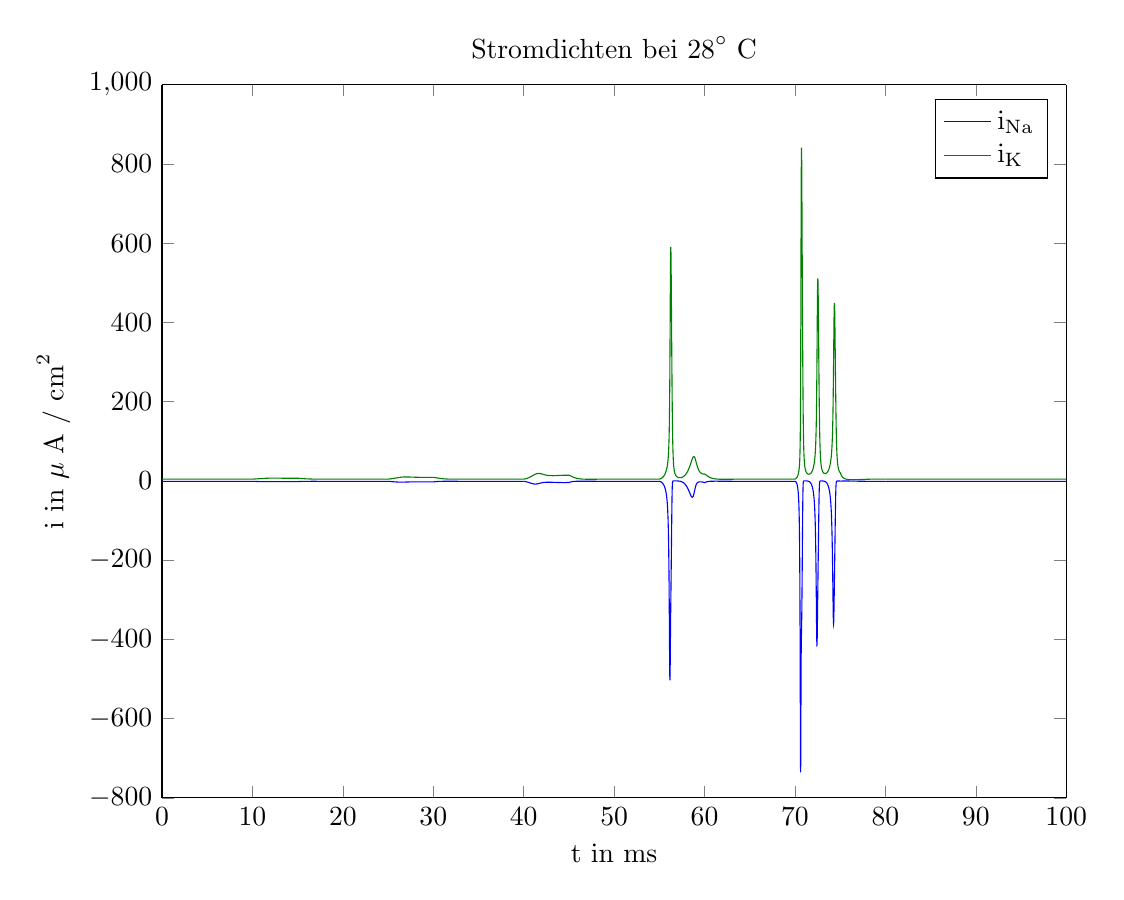
\begin{tikzpicture}

\begin{axis}[%
width=4.520833in,
height=3.565625in,
at={(0.758333in,0.48125in)},
scale only axis,
separate axis lines,
every outer x axis line/.append style={black},
every x tick label/.append style={font=\color{black}},
xmin=0,
xmax=100,
xlabel={t in ms},
every outer y axis line/.append style={black},
every y tick label/.append style={font=\color{black}},
ymin=-800,
ymax=1000,
ylabel={$\text{i in }\mu\text{ A / cm}^\text{2}$},
title={$\text{Stromdichten bei 28}^\circ\text{ C}$},
legend style={legend cell align=left,align=left,draw=black}
]
\addplot [color=blue,solid,forget plot]
  table[row sep=crcr]{%
0	-1.22005717646543\\
0.01	-1.22005717646543\\
0.02	-1.22005765268075\\
0.03	-1.22005845075113\\
0.04	-1.2200594487935\\
0.05	-1.22006057002223\\
0.06	-1.22006176614604\\
0.07	-1.22006300677265\\
0.08	-1.22006427275331\\
0.09	-1.22006555200271\\
0.1	-1.2200668368737\\
0.11	-1.22006812250843\\
0.12	-1.22006940580273\\
0.13	-1.2200706847557\\
0.14	-1.22007195806118\\
0.15	-1.2200732248511\\
0.16	-1.22007448453434\\
0.17	-1.22007573669541\\
0.18	-1.22007698103086\\
0.19	-1.22007821730927\\
0.2	-1.2200794453461\\
0.21	-1.22008066498791\\
0.22	-1.22008187610234\\
0.23	-1.22008307857186\\
0.24	-1.22008427228979\\
0.25	-1.22008545715778\\
0.26	-1.22008663308419\\
0.27	-1.22008779998306\\
0.28	-1.22008895777343\\
0.29	-1.22009010637888\\
0.3	-1.22009124572723\\
0.31	-1.22009237575032\\
0.32	-1.22009349638385\\
0.33	-1.22009460756725\\
0.34	-1.22009570924356\\
0.35	-1.22009680135937\\
0.36	-1.22009788386472\\
0.37	-1.22009895671302\\
0.38	-1.22010001986102\\
0.39	-1.22010107326867\\
0.4	-1.22010211689913\\
0.41	-1.22010315071867\\
0.42	-1.2201041746966\\
0.43	-1.22010518880522\\
0.44	-1.22010619301978\\
0.45	-1.22010718731838\\
0.46	-1.22010817168194\\
0.47	-1.22010914609412\\
0.48	-1.2201101105413\\
0.49	-1.22011106501247\\
0.5	-1.22011200949923\\
0.51	-1.22011294399568\\
0.52	-1.22011386849842\\
0.53	-1.22011478300644\\
0.54	-1.22011568752112\\
0.55	-1.22011658204613\\
0.56	-1.22011746658741\\
0.57	-1.22011834115311\\
0.58	-1.22011920575353\\
0.59	-1.22012006040109\\
0.6	-1.22012090511023\\
0.61	-1.22012173989745\\
0.62	-1.22012256478118\\
0.63	-1.22012337978175\\
0.64	-1.22012418492139\\
0.65	-1.22012498022413\\
0.66	-1.22012576571575\\
0.67	-1.2201265414238\\
0.68	-1.22012730737749\\
0.69	-1.22012806360766\\
0.7	-1.22012881014676\\
0.71	-1.22012954702879\\
0.72	-1.22013027428925\\
0.73	-1.22013099196513\\
0.74	-1.22013170009482\\
0.75	-1.22013239871813\\
0.76	-1.22013308787617\\
0.77	-1.22013376761141\\
0.78	-1.22013443796755\\
0.79	-1.22013509898955\\
0.8	-1.22013575072354\\
0.81	-1.22013639321681\\
0.82	-1.22013702651779\\
0.83	-1.22013765067597\\
0.84	-1.2201382657419\\
0.85	-1.22013887176715\\
0.86	-1.22013946880425\\
0.87	-1.22014005690669\\
0.88	-1.22014063612887\\
0.89	-1.22014120652607\\
0.9	-1.22014176815443\\
0.91	-1.22014232107087\\
0.92	-1.22014286533314\\
0.93	-1.22014340099971\\
0.94	-1.2201439281298\\
0.95	-1.22014444678329\\
0.96	-1.22014495702077\\
0.97	-1.22014545890343\\
0.98	-1.22014595249309\\
0.99	-1.22014643785214\\
1	-1.22014691504353\\
1.01	-1.22014738413074\\
1.02	-1.22014784517773\\
1.03	-1.22014829824896\\
1.04	-1.22014874340933\\
1.05	-1.22014918072418\\
1.06	-1.22014961025921\\
1.07	-1.22015003208054\\
1.08	-1.22015044625462\\
1.09	-1.22015085284825\\
1.1	-1.2201512519285\\
1.11	-1.22015164356277\\
1.12	-1.22015202781869\\
1.13	-1.22015240476415\\
1.14	-1.22015277446726\\
1.15	-1.22015313699631\\
1.16	-1.2201534924198\\
1.17	-1.22015384080638\\
1.18	-1.22015418222483\\
1.19	-1.22015451674407\\
1.2	-1.2201548444331\\
1.21	-1.22015516536104\\
1.22	-1.22015547959705\\
1.23	-1.22015578721034\\
1.24	-1.22015608827018\\
1.25	-1.22015638284583\\
1.26	-1.22015667100656\\
1.27	-1.22015695282163\\
1.28	-1.22015722836026\\
1.29	-1.22015749769163\\
1.3	-1.22015776088485\\
1.31	-1.22015801800898\\
1.32	-1.22015826913294\\
1.33	-1.2201585143256\\
1.34	-1.22015875365569\\
1.35	-1.2201589871918\\
1.36	-1.22015921500239\\
1.37	-1.22015943715576\\
1.38	-1.22015965372003\\
1.39	-1.22015986476317\\
1.4	-1.22016007035293\\
1.41	-1.22016027055686\\
1.42	-1.22016046544231\\
1.43	-1.22016065507639\\
1.44	-1.22016083952598\\
1.45	-1.22016101885771\\
1.46	-1.22016119313797\\
1.47	-1.22016136243287\\
1.48	-1.22016152680823\\
1.49	-1.22016168632963\\
1.5	-1.22016184106231\\
1.51	-1.22016199107123\\
1.52	-1.22016213642105\\
1.53	-1.2201622771761\\
1.54	-1.22016241340038\\
1.55	-1.22016254515755\\
1.56	-1.22016267251097\\
1.57	-1.2201627955236\\
1.58	-1.22016291425807\\
1.59	-1.22016302877666\\
1.6	-1.22016313914127\\
1.61	-1.22016324541341\\
1.62	-1.22016334765424\\
1.63	-1.22016344592451\\
1.64	-1.2201635402846\\
1.65	-1.22016363079447\\
1.66	-1.2201637175137\\
1.67	-1.22016380050145\\
1.68	-1.22016387981648\\
1.69	-1.22016395551712\\
1.7	-1.22016402766128\\
1.71	-1.22016409630647\\
1.72	-1.22016416150975\\
1.73	-1.22016422332774\\
1.74	-1.22016428181665\\
1.75	-1.22016433703223\\
1.76	-1.2201643890298\\
1.77	-1.22016443786423\\
1.78	-1.22016448358994\\
1.79	-1.22016452626091\\
1.8	-1.22016456593065\\
1.81	-1.22016460265222\\
1.82	-1.22016463647823\\
1.83	-1.22016466746082\\
1.84	-1.22016469565167\\
1.85	-1.220164721102\\
1.86	-1.22016474386256\\
1.87	-1.22016476398364\\
1.88	-1.22016478151505\\
1.89	-1.22016479650613\\
1.9	-1.22016480900577\\
1.91	-1.22016481906236\\
1.92	-1.22016482672384\\
1.93	-1.22016483203767\\
1.94	-1.22016483505082\\
1.95	-1.2201648358098\\
1.96	-1.22016483436066\\
1.97	-1.22016483074894\\
1.98	-1.22016482501973\\
1.99	-1.22016481721764\\
2	-1.22016480738679\\
2.01	-1.22016479557086\\
2.02	-1.22016478181302\\
2.03	-1.22016476615598\\
2.04	-1.22016474864197\\
2.05	-1.22016472931275\\
2.06	-1.22016470820963\\
2.07	-1.2201646853734\\
2.08	-1.22016466084442\\
2.09	-1.22016463466257\\
2.1	-1.22016460686725\\
2.11	-1.2201645774974\\
2.12	-1.22016454659149\\
2.13	-1.22016451418754\\
2.14	-1.22016448032309\\
2.15	-1.22016444503521\\
2.16	-1.22016440836053\\
2.17	-1.22016437033521\\
2.18	-1.22016433099496\\
2.19	-1.22016429037502\\
2.2	-1.22016424851018\\
2.21	-1.22016420543478\\
2.22	-1.22016416118273\\
2.23	-1.22016411578745\\
2.24	-1.22016406928195\\
2.25	-1.22016402169877\\
2.26	-1.22016397307003\\
2.27	-1.22016392342739\\
2.28	-1.22016387280209\\
2.29	-1.22016382122492\\
2.3	-1.22016376872625\\
2.31	-1.220163715336\\
2.32	-1.22016366108369\\
2.33	-1.22016360599839\\
2.34	-1.22016355010876\\
2.35	-1.22016349344303\\
2.36	-1.22016343602902\\
2.37	-1.22016337789412\\
2.38	-1.22016331906534\\
2.39	-1.22016325956925\\
2.4	-1.22016319943201\\
2.41	-1.22016313867941\\
2.42	-1.22016307733679\\
2.43	-1.22016301542914\\
2.44	-1.22016295298102\\
2.45	-1.22016289001661\\
2.46	-1.22016282655969\\
2.47	-1.22016276263368\\
2.48	-1.22016269826158\\
2.49	-1.22016263346604\\
2.5	-1.22016256826931\\
2.51	-1.22016250269327\\
2.52	-1.22016243675943\\
2.53	-1.22016237048895\\
2.54	-1.22016230390258\\
2.55	-1.22016223702076\\
2.56	-1.22016216986353\\
2.57	-1.22016210245058\\
2.58	-1.22016203480128\\
2.59	-1.2201619669346\\
2.6	-1.2201618988692\\
2.61	-1.22016183062338\\
2.62	-1.2201617622151\\
2.63	-1.220161693662\\
2.64	-1.22016162498136\\
2.65	-1.22016155619015\\
2.66	-1.220161487305\\
2.67	-1.22016141834221\\
2.68	-1.22016134931778\\
2.69	-1.22016128024738\\
2.7	-1.22016121114636\\
2.71	-1.22016114202976\\
2.72	-1.22016107291233\\
2.73	-1.22016100380849\\
2.74	-1.22016093473237\\
2.75	-1.2201608656978\\
2.76	-1.22016079671832\\
2.77	-1.22016072780716\\
2.78	-1.2201606589773\\
2.79	-1.22016059024138\\
2.8	-1.22016052161181\\
2.81	-1.22016045310068\\
2.82	-1.22016038471983\\
2.83	-1.22016031648081\\
2.84	-1.22016024839492\\
2.85	-1.22016018047317\\
2.86	-1.22016011272632\\
2.87	-1.22016004516488\\
2.88	-1.22015997779909\\
2.89	-1.22015991063892\\
2.9	-1.22015984369413\\
2.91	-1.2201597769742\\
2.92	-1.22015971048838\\
2.93	-1.22015964424566\\
2.94	-1.22015957825483\\
2.95	-1.22015951252439\\
2.96	-1.22015944706267\\
2.97	-1.22015938187772\\
2.98	-1.22015931697739\\
2.99	-1.2201592523693\\
3	-1.22015918806086\\
3.01	-1.22015912405923\\
3.02	-1.2201590603714\\
3.03	-1.22015899700413\\
3.04	-1.22015893396396\\
3.05	-1.22015887125724\\
3.06	-1.22015880889011\\
3.07	-1.22015874686852\\
3.08	-1.22015868519822\\
3.09	-1.22015862388475\\
3.1	-1.22015856293349\\
3.11	-1.2201585023496\\
3.12	-1.22015844213808\\
3.13	-1.22015838230373\\
3.14	-1.22015832285119\\
3.15	-1.2201582637849\\
3.16	-1.22015820510915\\
3.17	-1.22015814682803\\
3.18	-1.22015808894548\\
3.19	-1.22015803146528\\
3.2	-1.22015797439104\\
3.21	-1.22015791772619\\
3.22	-1.22015786147403\\
3.23	-1.22015780563769\\
3.24	-1.22015775022016\\
3.25	-1.22015769522426\\
3.26	-1.22015764065267\\
3.27	-1.22015758650794\\
3.28	-1.22015753279245\\
3.29	-1.22015747950845\\
3.3	-1.22015742665807\\
3.31	-1.22015737424329\\
3.32	-1.22015732226594\\
3.33	-1.22015727072775\\
3.34	-1.2201572196303\\
3.35	-1.22015716897506\\
3.36	-1.22015711876336\\
3.37	-1.22015706899642\\
3.38	-1.22015701967534\\
3.39	-1.22015697080109\\
3.4	-1.22015692237454\\
3.41	-1.22015687439644\\
3.42	-1.22015682686745\\
3.43	-1.22015677978808\\
3.44	-1.22015673315877\\
3.45	-1.22015668697985\\
3.46	-1.22015664125154\\
3.47	-1.22015659597395\\
3.48	-1.22015655114712\\
3.49	-1.22015650677098\\
3.5	-1.22015646284535\\
3.51	-1.22015641936999\\
3.52	-1.22015637634456\\
3.53	-1.22015633376861\\
3.54	-1.22015629164163\\
3.55	-1.22015624996302\\
3.56	-1.22015620873209\\
3.57	-1.22015616794808\\
3.58	-1.22015612761014\\
3.59	-1.22015608771736\\
3.6	-1.22015604826874\\
3.61	-1.22015600926322\\
3.62	-1.22015597069965\\
3.63	-1.22015593257683\\
3.64	-1.22015589489348\\
3.65	-1.22015585764827\\
3.66	-1.22015582083978\\
3.67	-1.22015578446655\\
3.68	-1.22015574852704\\
3.69	-1.22015571301967\\
3.7	-1.2201556779428\\
3.71	-1.22015564329471\\
3.72	-1.22015560907365\\
3.73	-1.22015557527781\\
3.74	-1.22015554190532\\
3.75	-1.22015550895427\\
3.76	-1.2201554764227\\
3.77	-1.2201554443086\\
3.78	-1.2201554126099\\
3.79	-1.22015538132452\\
3.8	-1.2201553504503\\
3.81	-1.22015531998507\\
3.82	-1.22015528992658\\
3.83	-1.22015526027259\\
3.84	-1.22015523102078\\
3.85	-1.22015520216881\\
3.86	-1.22015517371431\\
3.87	-1.22015514565487\\
3.88	-1.22015511798805\\
3.89	-1.22015509071137\\
3.9	-1.22015506382233\\
3.91	-1.2201550373184\\
3.92	-1.220155011197\\
3.93	-1.22015498545556\\
3.94	-1.22015496009146\\
3.95	-1.22015493510205\\
3.96	-1.22015491048468\\
3.97	-1.22015488623666\\
3.98	-1.22015486235527\\
3.99	-1.2201548388378\\
4	-1.22015481568149\\
4.01	-1.22015479288358\\
4.02	-1.22015477044128\\
4.03	-1.22015474835179\\
4.04	-1.22015472661229\\
4.05	-1.22015470521996\\
4.06	-1.22015468417195\\
4.07	-1.2201546634654\\
4.08	-1.22015464309744\\
4.09	-1.22015462306518\\
4.1	-1.22015460336574\\
4.11	-1.22015458399622\\
4.12	-1.2201545649537\\
4.13	-1.22015454623527\\
4.14	-1.220154527838\\
4.15	-1.22015450975896\\
4.16	-1.22015449199521\\
4.17	-1.22015447454381\\
4.18	-1.22015445740182\\
4.19	-1.22015444056628\\
4.2	-1.22015442403425\\
4.21	-1.22015440780276\\
4.22	-1.22015439186887\\
4.23	-1.22015437622961\\
4.24	-1.22015436088203\\
4.25	-1.22015434582317\\
4.26	-1.22015433105009\\
4.27	-1.22015431655982\\
4.28	-1.22015430234942\\
4.29	-1.22015428841593\\
4.3	-1.22015427475642\\
4.31	-1.22015426136794\\
4.32	-1.22015424824756\\
4.33	-1.22015423539235\\
4.34	-1.22015422279938\\
4.35	-1.22015421046573\\
4.36	-1.22015419838851\\
4.37	-1.22015418656478\\
4.38	-1.22015417499167\\
4.39	-1.22015416366629\\
4.4	-1.22015415258575\\
4.41	-1.22015414174717\\
4.42	-1.22015413114771\\
4.43	-1.2201541207845\\
4.44	-1.2201541106547\\
4.45	-1.22015410075549\\
4.46	-1.22015409108404\\
4.47	-1.22015408163754\\
4.48	-1.2201540724132\\
4.49	-1.22015406340823\\
4.5	-1.22015405461985\\
4.51	-1.2201540460453\\
4.52	-1.22015403768184\\
4.53	-1.22015402952674\\
4.54	-1.22015402157726\\
4.55	-1.22015401383072\\
4.56	-1.2201540062844\\
4.57	-1.22015399893564\\
4.58	-1.22015399178177\\
4.59	-1.22015398482015\\
4.6	-1.22015397804813\\
4.61	-1.22015397146311\\
4.62	-1.22015396506248\\
4.63	-1.22015395884365\\
4.64	-1.22015395280406\\
4.65	-1.22015394694115\\
4.66	-1.22015394125238\\
4.67	-1.22015393573524\\
4.68	-1.22015393038722\\
4.69	-1.22015392520584\\
4.7	-1.22015392018862\\
4.71	-1.22015391533311\\
4.72	-1.22015391063689\\
4.73	-1.22015390609754\\
4.74	-1.22015390171265\\
4.75	-1.22015389747985\\
4.76	-1.22015389339678\\
4.77	-1.22015388946108\\
4.78	-1.22015388567045\\
4.79	-1.22015388202256\\
4.8	-1.22015387851513\\
4.81	-1.2201538751459\\
4.82	-1.22015387191261\\
4.83	-1.22015386881303\\
4.84	-1.22015386584495\\
4.85	-1.22015386300617\\
4.86	-1.22015386029451\\
4.87	-1.22015385770783\\
4.88	-1.22015385524398\\
4.89	-1.22015385290086\\
4.9	-1.22015385067635\\
4.91	-1.22015384856839\\
4.92	-1.2201538465749\\
4.93	-1.22015384469386\\
4.94	-1.22015384292325\\
4.95	-1.22015384126105\\
4.96	-1.22015383970529\\
4.97	-1.22015383825401\\
4.98	-1.22015383690527\\
4.99	-1.22015383565713\\
5	-1.22015383450771\\
5.01	-1.22015383345511\\
5.02	-1.22015383249746\\
5.03	-1.22015383163293\\
5.04	-1.22015383085969\\
5.05	-1.22015383017593\\
5.06	-1.22015382957986\\
5.07	-1.22015382906972\\
5.08	-1.22015382864376\\
5.09	-1.22015382830024\\
5.1	-1.22015382803746\\
5.11	-1.22015382785373\\
5.12	-1.22015382774738\\
5.13	-1.22015382771675\\
5.14	-1.22015382776021\\
5.15	-1.22015382787615\\
5.16	-1.22015382806296\\
5.17	-1.22015382831909\\
5.18	-1.22015382864295\\
5.19	-1.22015382903303\\
5.2	-1.22015382948779\\
5.21	-1.22015383000574\\
5.22	-1.22015383058539\\
5.23	-1.22015383122527\\
5.24	-1.22015383192395\\
5.25	-1.22015383267999\\
5.26	-1.22015383349199\\
5.27	-1.22015383435854\\
5.28	-1.22015383527829\\
5.29	-1.22015383624986\\
5.3	-1.22015383727193\\
5.31	-1.22015383834318\\
5.32	-1.2201538394623\\
5.33	-1.22015384062801\\
5.34	-1.22015384183904\\
5.35	-1.22015384309414\\
5.36	-1.22015384439208\\
5.37	-1.22015384573164\\
5.38	-1.22015384711163\\
5.39	-1.22015384853086\\
5.4	-1.22015384998817\\
5.41	-1.22015385148241\\
5.42	-1.22015385301245\\
5.43	-1.22015385457718\\
5.44	-1.2201538561755\\
5.45	-1.22015385780632\\
5.46	-1.22015385946859\\
5.47	-1.22015386116125\\
5.48	-1.22015386288326\\
5.49	-1.22015386463362\\
5.5	-1.22015386641131\\
5.51	-1.22015386821536\\
5.52	-1.22015387004479\\
5.53	-1.22015387189864\\
5.54	-1.22015387377598\\
5.55	-1.22015387567589\\
5.56	-1.22015387759744\\
5.57	-1.22015387953975\\
5.58	-1.22015388150193\\
5.59	-1.22015388348312\\
5.6	-1.22015388548247\\
5.61	-1.22015388749914\\
5.62	-1.22015388953231\\
5.63	-1.22015389158116\\
5.64	-1.22015389364492\\
5.65	-1.22015389572278\\
5.66	-1.220153897814\\
5.67	-1.2201538999178\\
5.68	-1.22015390203347\\
5.69	-1.22015390416025\\
5.7	-1.22015390629746\\
5.71	-1.22015390844437\\
5.72	-1.22015391060032\\
5.73	-1.22015391276461\\
5.74	-1.22015391493659\\
5.75	-1.22015391711562\\
5.76	-1.22015391930105\\
5.77	-1.22015392149226\\
5.78	-1.22015392368864\\
5.79	-1.22015392588958\\
5.8	-1.22015392809451\\
5.81	-1.22015393030284\\
5.82	-1.220153932514\\
5.83	-1.22015393472745\\
5.84	-1.22015393694265\\
5.85	-1.22015393915906\\
5.86	-1.22015394137616\\
5.87	-1.22015394359345\\
5.88	-1.22015394581043\\
5.89	-1.22015394802661\\
5.9	-1.22015395024151\\
5.91	-1.22015395245468\\
5.92	-1.22015395466565\\
5.93	-1.22015395687399\\
5.94	-1.22015395907925\\
5.95	-1.22015396128102\\
5.96	-1.22015396347887\\
5.97	-1.22015396567241\\
5.98	-1.22015396786124\\
5.99	-1.22015397004497\\
6	-1.22015397222324\\
6.01	-1.22015397439566\\
6.02	-1.22015397656188\\
6.03	-1.22015397872157\\
6.04	-1.22015398087436\\
6.05	-1.22015398301995\\
6.06	-1.220153985158\\
6.07	-1.22015398728819\\
6.08	-1.22015398941024\\
6.09	-1.22015399152383\\
6.1	-1.22015399362869\\
6.11	-1.22015399572453\\
6.12	-1.22015399781107\\
6.13	-1.22015399988807\\
6.14	-1.22015400195525\\
6.15	-1.22015400401237\\
6.16	-1.2201540060592\\
6.17	-1.22015400809549\\
6.18	-1.22015401012102\\
6.19	-1.22015401213557\\
6.2	-1.22015401413893\\
6.21	-1.2201540161309\\
6.22	-1.22015401811128\\
6.23	-1.22015402007987\\
6.24	-1.22015402203649\\
6.25	-1.22015402398097\\
6.26	-1.22015402591313\\
6.27	-1.22015402783282\\
6.28	-1.22015402973986\\
6.29	-1.22015403163411\\
6.3	-1.22015403351542\\
6.31	-1.22015403538366\\
6.32	-1.22015403723868\\
6.33	-1.22015403908037\\
6.34	-1.22015404090859\\
6.35	-1.22015404272323\\
6.36	-1.22015404452418\\
6.37	-1.22015404631133\\
6.38	-1.22015404808459\\
6.39	-1.22015404984385\\
6.4	-1.22015405158903\\
6.41	-1.22015405332004\\
6.42	-1.2201540550368\\
6.43	-1.22015405673924\\
6.44	-1.22015405842728\\
6.45	-1.22015406010086\\
6.46	-1.22015406175992\\
6.47	-1.2201540634044\\
6.48	-1.22015406503425\\
6.49	-1.22015406664942\\
6.5	-1.22015406824987\\
6.51	-1.22015406983555\\
6.52	-1.22015407140644\\
6.53	-1.2201540729625\\
6.54	-1.2201540745037\\
6.55	-1.22015407603002\\
6.56	-1.22015407754145\\
6.57	-1.22015407903795\\
6.58	-1.22015408051953\\
6.59	-1.22015408198618\\
6.6	-1.22015408343788\\
6.61	-1.22015408487464\\
6.62	-1.22015408629646\\
6.63	-1.22015408770334\\
6.64	-1.22015408909529\\
6.65	-1.22015409047232\\
6.66	-1.22015409183445\\
6.67	-1.22015409318169\\
6.68	-1.22015409451407\\
6.69	-1.2201540958316\\
6.7	-1.22015409713431\\
6.71	-1.22015409842224\\
6.72	-1.2201540996954\\
6.73	-1.22015410095385\\
6.74	-1.2201541021976\\
6.75	-1.2201541034267\\
6.76	-1.2201541046412\\
6.77	-1.22015410584113\\
6.78	-1.22015410702654\\
6.79	-1.22015410819749\\
6.8	-1.22015410935401\\
6.81	-1.22015411049616\\
6.82	-1.220154111624\\
6.83	-1.22015411273758\\
6.84	-1.22015411383696\\
6.85	-1.2201541149222\\
6.86	-1.22015411599336\\
6.87	-1.22015411705051\\
6.88	-1.22015411809372\\
6.89	-1.22015411912304\\
6.9	-1.22015412013855\\
6.91	-1.22015412114032\\
6.92	-1.22015412212842\\
6.93	-1.22015412310292\\
6.94	-1.22015412406391\\
6.95	-1.22015412501144\\
6.96	-1.22015412594561\\
6.97	-1.22015412686649\\
6.98	-1.22015412777417\\
6.99	-1.22015412866871\\
7	-1.22015412955022\\
7.01	-1.22015413041876\\
7.02	-1.22015413127442\\
7.03	-1.2201541321173\\
7.04	-1.22015413294747\\
7.05	-1.22015413376502\\
7.06	-1.22015413457005\\
7.07	-1.22015413536264\\
7.08	-1.22015413614288\\
7.09	-1.22015413691087\\
7.1	-1.22015413766668\\
7.11	-1.22015413841043\\
7.12	-1.2201541391422\\
7.13	-1.22015413986208\\
7.14	-1.22015414057017\\
7.15	-1.22015414126657\\
7.16	-1.22015414195136\\
7.17	-1.22015414262465\\
7.18	-1.22015414328654\\
7.19	-1.22015414393711\\
7.2	-1.22015414457647\\
7.21	-1.22015414520472\\
7.22	-1.22015414582194\\
7.23	-1.22015414642825\\
7.24	-1.22015414702374\\
7.25	-1.22015414760852\\
7.26	-1.22015414818267\\
7.27	-1.22015414874629\\
7.28	-1.2201541492995\\
7.29	-1.22015414984239\\
7.3	-1.22015415037505\\
7.31	-1.2201541508976\\
7.32	-1.22015415141012\\
7.33	-1.22015415191272\\
7.34	-1.2201541524055\\
7.35	-1.22015415288857\\
7.36	-1.22015415336201\\
7.37	-1.22015415382593\\
7.38	-1.22015415428044\\
7.39	-1.22015415472563\\
7.4	-1.2201541551616\\
7.41	-1.22015415558845\\
7.42	-1.22015415600629\\
7.43	-1.22015415641521\\
7.44	-1.2201541568153\\
7.45	-1.22015415720668\\
7.46	-1.22015415758945\\
7.47	-1.22015415796368\\
7.48	-1.2201541583295\\
7.49	-1.220154158687\\
7.5	-1.22015415903627\\
7.51	-1.22015415937741\\
7.52	-1.22015415971053\\
7.53	-1.22015416003571\\
7.54	-1.22015416035306\\
7.55	-1.22015416066267\\
7.56	-1.22015416096464\\
7.57	-1.22015416125906\\
7.58	-1.22015416154603\\
7.59	-1.22015416182565\\
7.6	-1.22015416209801\\
7.61	-1.2201541623632\\
7.62	-1.22015416262132\\
7.63	-1.22015416287246\\
7.64	-1.22015416311671\\
7.65	-1.22015416335418\\
7.66	-1.22015416358494\\
7.67	-1.22015416380909\\
7.68	-1.22015416402673\\
7.69	-1.22015416423794\\
7.7	-1.22015416444281\\
7.71	-1.22015416464143\\
7.72	-1.22015416483389\\
7.73	-1.22015416502029\\
7.74	-1.2201541652007\\
7.75	-1.22015416537521\\
7.76	-1.22015416554392\\
7.77	-1.2201541657069\\
7.78	-1.22015416586425\\
7.79	-1.22015416601605\\
7.8	-1.22015416616238\\
7.81	-1.22015416630332\\
7.82	-1.22015416643897\\
7.83	-1.2201541665694\\
7.84	-1.22015416669469\\
7.85	-1.22015416681493\\
7.86	-1.22015416693019\\
7.87	-1.22015416704057\\
7.88	-1.22015416714613\\
7.89	-1.22015416724695\\
7.9	-1.22015416734312\\
7.91	-1.22015416743471\\
7.92	-1.2201541675218\\
7.93	-1.22015416760446\\
7.94	-1.22015416768277\\
7.95	-1.22015416775681\\
7.96	-1.22015416782665\\
7.97	-1.22015416789236\\
7.98	-1.22015416795401\\
7.99	-1.22015416801169\\
8	-1.22015416806545\\
8.01	-1.22015416811538\\
8.02	-1.22015416816154\\
8.03	-1.220154168204\\
8.04	-1.22015416824283\\
8.05	-1.2201541682781\\
8.06	-1.22015416830987\\
8.07	-1.22015416833822\\
8.08	-1.22015416836321\\
8.09	-1.2201541683849\\
8.1	-1.22015416840337\\
8.11	-1.22015416841866\\
8.12	-1.22015416843086\\
8.13	-1.22015416844002\\
8.14	-1.2201541684462\\
8.15	-1.22015416844946\\
8.16	-1.22015416844988\\
8.17	-1.22015416844749\\
8.18	-1.22015416844238\\
8.19	-1.22015416843459\\
8.2	-1.22015416842418\\
8.21	-1.22015416841121\\
8.22	-1.22015416839574\\
8.23	-1.22015416837783\\
8.24	-1.22015416835752\\
8.25	-1.22015416833488\\
8.26	-1.22015416830995\\
8.27	-1.2201541682828\\
8.28	-1.22015416825348\\
8.29	-1.22015416822203\\
8.3	-1.22015416818851\\
8.31	-1.22015416815297\\
8.32	-1.22015416811546\\
8.33	-1.22015416807604\\
8.34	-1.22015416803474\\
8.35	-1.22015416799162\\
8.36	-1.22015416794673\\
8.37	-1.22015416790011\\
8.38	-1.22015416785181\\
8.39	-1.22015416780187\\
8.4	-1.22015416775035\\
8.41	-1.22015416769729\\
8.42	-1.22015416764272\\
8.43	-1.2201541675867\\
8.44	-1.22015416752926\\
8.45	-1.22015416747046\\
8.46	-1.22015416741032\\
8.47	-1.2201541673489\\
8.48	-1.22015416728623\\
8.49	-1.22015416722235\\
8.5	-1.2201541671573\\
8.51	-1.22015416709112\\
8.52	-1.22015416702385\\
8.53	-1.22015416695553\\
8.54	-1.22015416688619\\
8.55	-1.22015416681587\\
8.56	-1.22015416674461\\
8.57	-1.22015416667244\\
8.58	-1.22015416659939\\
8.59	-1.22015416652551\\
8.6	-1.22015416645081\\
8.61	-1.22015416637535\\
8.62	-1.22015416629915\\
8.63	-1.22015416622224\\
8.64	-1.22015416614465\\
8.65	-1.22015416606641\\
8.66	-1.22015416598757\\
8.67	-1.22015416590813\\
8.68	-1.22015416582815\\
8.69	-1.22015416574763\\
8.7	-1.22015416566662\\
8.71	-1.22015416558514\\
8.72	-1.22015416550322\\
8.73	-1.22015416542088\\
8.74	-1.22015416533815\\
8.75	-1.22015416525507\\
8.76	-1.22015416517164\\
8.77	-1.22015416508791\\
8.78	-1.22015416500388\\
8.79	-1.2201541649196\\
8.8	-1.22015416483508\\
8.81	-1.22015416475034\\
8.82	-1.22015416466541\\
8.83	-1.2201541645803\\
8.84	-1.22015416449505\\
8.85	-1.22015416440968\\
8.86	-1.2201541643242\\
8.87	-1.22015416423863\\
8.88	-1.220154164153\\
8.89	-1.22015416406733\\
8.9	-1.22015416398163\\
8.91	-1.22015416389592\\
8.92	-1.22015416381023\\
8.93	-1.22015416372456\\
8.94	-1.22015416363895\\
8.95	-1.2201541635534\\
8.96	-1.22015416346794\\
8.97	-1.22015416338257\\
8.98	-1.22015416329732\\
8.99	-1.22015416321221\\
9	-1.22015416312724\\
9.01	-1.22015416304244\\
9.02	-1.22015416295781\\
9.03	-1.22015416287337\\
9.04	-1.22015416278915\\
9.05	-1.22015416270514\\
9.06	-1.22015416262136\\
9.07	-1.22015416253784\\
9.08	-1.22015416245457\\
9.09	-1.22015416237158\\
9.1	-1.22015416228887\\
9.11	-1.22015416220645\\
9.12	-1.22015416212435\\
9.13	-1.22015416204256\\
9.14	-1.2201541619611\\
9.15	-1.22015416187999\\
9.16	-1.22015416179922\\
9.17	-1.22015416171882\\
9.18	-1.22015416163878\\
9.19	-1.22015416155913\\
9.2	-1.22015416147986\\
9.21	-1.220154161401\\
9.22	-1.22015416132254\\
9.23	-1.22015416124449\\
9.24	-1.22015416116687\\
9.25	-1.22015416108968\\
9.26	-1.22015416101293\\
9.27	-1.22015416093662\\
9.28	-1.22015416086077\\
9.29	-1.22015416078537\\
9.3	-1.22015416071044\\
9.31	-1.22015416063599\\
9.32	-1.22015416056201\\
9.33	-1.22015416048852\\
9.34	-1.22015416041551\\
9.35	-1.220154160343\\
9.36	-1.220154160271\\
9.37	-1.22015416019949\\
9.38	-1.2201541601285\\
9.39	-1.22015416005802\\
9.4	-1.22015415998806\\
9.41	-1.22015415991863\\
9.42	-1.22015415984972\\
9.43	-1.22015415978134\\
9.44	-1.2201541597135\\
9.45	-1.22015415964619\\
9.46	-1.22015415957942\\
9.47	-1.2201541595132\\
9.48	-1.22015415944752\\
9.49	-1.2201541593824\\
9.5	-1.22015415931782\\
9.51	-1.2201541592538\\
9.52	-1.22015415919033\\
9.53	-1.22015415912742\\
9.54	-1.22015415906507\\
9.55	-1.22015415900329\\
9.56	-1.22015415894206\\
9.57	-1.2201541588814\\
9.58	-1.2201541588213\\
9.59	-1.22015415876177\\
9.6	-1.2201541587028\\
9.61	-1.22015415864441\\
9.62	-1.22015415858658\\
9.63	-1.22015415852932\\
9.64	-1.22015415847262\\
9.65	-1.2201541584165\\
9.66	-1.22015415836095\\
9.67	-1.22015415830596\\
9.68	-1.22015415825154\\
9.69	-1.2201541581977\\
9.7	-1.22015415814442\\
9.71	-1.2201541580917\\
9.72	-1.22015415803956\\
9.73	-1.22015415798798\\
9.74	-1.22015415793696\\
9.75	-1.22015415788651\\
9.76	-1.22015415783662\\
9.77	-1.2201541577873\\
9.78	-1.22015415773853\\
9.79	-1.22015415769033\\
9.8	-1.22015415764268\\
9.81	-1.22015415759559\\
9.82	-1.22015415754905\\
9.83	-1.22015415750306\\
9.84	-1.22015415745763\\
9.85	-1.22015415741275\\
9.86	-1.22015415736841\\
9.87	-1.22015415732462\\
9.88	-1.22015415728137\\
9.89	-1.22015415723866\\
9.9	-1.22015415719649\\
9.91	-1.22015415715486\\
9.92	-1.22015415711376\\
9.93	-1.22015415707319\\
9.94	-1.22015415703315\\
9.95	-1.22015415699364\\
9.96	-1.22015415695465\\
9.97	-1.22015415691618\\
9.98	-1.22015415687823\\
9.99	-1.2201541568408\\
10	-1.22015415680388\\
10.01	-1.22015415676747\\
10.02	-1.22309965811883\\
10.03	-1.22804957264378\\
10.04	-1.23426447455359\\
10.05	-1.24128005395475\\
10.06	-1.24880439182289\\
10.07	-1.2566534155444\\
10.08	-1.26471071021279\\
10.09	-1.27290238894121\\
10.1	-1.28118133334021\\
10.11	-1.28951729059071\\
10.12	-1.29789064200801\\
10.13	-1.30628847794215\\
10.14	-1.31470212352394\\
10.15	-1.32312557804133\\
10.16	-1.33155453010652\\
10.17	-1.33998573593264\\
10.18	-1.34841662672182\\
10.19	-1.35684506068636\\
10.2	-1.36526916641459\\
10.21	-1.37368724395167\\
10.22	-1.38209770236209\\
10.23	-1.3904990203626\\
10.24	-1.39888972155071\\
10.25	-1.40726835887174\\
10.26	-1.41563350493669\\
10.27	-1.42398374604752\\
10.28	-1.43231767857359\\
10.29	-1.44063390682018\\
10.3	-1.44893104184524\\
10.31	-1.45720770087936\\
10.32	-1.46546250713029\\
10.33	-1.47369408983328\\
10.34	-1.48190108445889\\
10.35	-1.49008213302224\\
10.36	-1.49823588445784\\
10.37	-1.5063609950371\\
10.38	-1.51445612881381\\
10.39	-1.52251995808803\\
10.4	-1.53055116388218\\
10.41	-1.5385484364251\\
10.42	-1.54651047564142\\
10.43	-1.55443599164406\\
10.44	-1.5623237052286\\
10.45	-1.57017234836833\\
10.46	-1.57798066470906\\
10.47	-1.58574741006313\\
10.48	-1.59347135290173\\
10.49	-1.6011512748451\\
10.5	-1.60878597115001\\
10.51	-1.61637425119399\\
10.52	-1.62391493895576\\
10.53	-1.63140687349141\\
10.54	-1.63884890940583\\
10.55	-1.64623991731882\\
10.56	-1.65357878432562\\
10.57	-1.66086441445105\\
10.58	-1.66809572909717\\
10.59	-1.6752716674837\\
10.6	-1.68239118708095\\
10.61	-1.6894532640347\\
10.62	-1.69645689358261\\
10.63	-1.70340109046189\\
10.64	-1.71028488930748\\
10.65	-1.71710734504075\\
10.66	-1.72386753324791\\
10.67	-1.73056455054811\\
10.68	-1.73719751495055\\
10.69	-1.74376556620048\\
10.7	-1.75026786611348\\
10.71	-1.75670359889798\\
10.72	-1.76307197146541\\
10.73	-1.76937221372781\\
10.74	-1.77560357888265\\
10.75	-1.78176534368434\\
10.76	-1.78785680870245\\
10.77	-1.79387729856615\\
10.78	-1.79982616219473\\
10.79	-1.80570277301397\\
10.8	-1.81150652915807\\
10.81	-1.81723685365707\\
10.82	-1.82289319460943\\
10.83	-1.82847502533973\\
10.84	-1.83398184454122\\
10.85	-1.83941317640322\\
10.86	-1.84476857072316\\
10.87	-1.85004760300314\\
10.88	-1.85524987453108\\
10.89	-1.86037501244614\\
10.9	-1.86542266978865\\
10.91	-1.8703925255343\\
10.92	-1.87528428461268\\
10.93	-1.88009767791015\\
10.94	-1.88483246225706\\
10.95	-1.88948842039938\\
10.96	-1.89406536095475\\
10.97	-1.89856311835308\\
10.98	-1.90298155276174\\
10.99	-1.90732054999548\\
11	-1.91158002141121\\
11.01	-1.91575990378773\\
11.02	-1.91986015919062\\
11.03	-1.92388077482242\\
11.04	-1.92782176285834\\
11.05	-1.93168316026764\\
11.06	-1.93546502862093\\
11.07	-1.93916745388361\\
11.08	-1.94279054619576\\
11.09	-1.94633443963857\\
11.1	-1.94979929198779\\
11.11	-1.95318528445434\\
11.12	-1.95649262141245\\
11.13	-1.95972153011558\\
11.14	-1.96287226040047\\
11.15	-1.96594508437973\\
11.16	-1.9689402961231\\
11.17	-1.97185821132797\\
11.18	-1.97469916697937\\
11.19	-1.97746352099987\\
11.2	-1.98015165188963\\
11.21	-1.98276395835725\\
11.22	-1.98530085894153\\
11.23	-1.98776279162465\\
11.24	-1.99015021343725\\
11.25	-1.99246360005569\\
11.26	-1.99470344539194\\
11.27	-1.99687026117652\\
11.28	-1.99896457653499\\
11.29	-2.00098693755821\\
11.3	-2.00293790686699\\
11.31	-2.00481806317146\\
11.32	-2.00662800082558\\
11.33	-2.00836832937728\\
11.34	-2.01003967311449\\
11.35	-2.01164267060776\\
11.36	-2.01317797424958\\
11.37	-2.01464624979105\\
11.38	-2.01604817587619\\
11.39	-2.01738444357435\\
11.4	-2.01865575591117\\
11.41	-2.01986282739833\\
11.42	-2.02100638356273\\
11.43	-2.0220871604753\\
11.44	-2.0231059042799\\
11.45	-2.02406337072272\\
11.46	-2.02496032468246\\
11.47	-2.02579753970186\\
11.48	-2.02657579752065\\
11.49	-2.02729588761051\\
11.5	-2.02795860671235\\
11.51	-2.02856475837609\\
11.52	-2.02911515250352\\
11.53	-2.02961060489432\\
11.54	-2.03005193679572\\
11.55	-2.03043997445601\\
11.56	-2.03077554868225\\
11.57	-2.03105949440241\\
11.58	-2.03129265023225\\
11.59	-2.03147585804721\\
11.6	-2.0316099625595\\
11.61	-2.03169581090072\\
11.62	-2.0317342522102\\
11.63	-2.03172613722922\\
11.64	-2.03167231790144\\
11.65	-2.03157364697968\\
11.66	-2.03143097763917\\
11.67	-2.03124516309761\\
11.68	-2.03101705624203\\
11.69	-2.03074750926275\\
11.7	-2.0304373732945\\
11.71	-2.03008749806486\\
11.72	-2.02969873155015\\
11.73	-2.02927191963889\\
11.74	-2.02880790580294\\
11.75	-2.02830753077635\\
11.76	-2.0277716322421\\
11.77	-2.02720104452678\\
11.78	-2.02659659830317\\
11.79	-2.02595912030095\\
11.8	-2.02528943302542\\
11.81	-2.02458835448441\\
11.82	-2.02385669792329\\
11.83	-2.02309527156815\\
11.84	-2.02230487837717\\
11.85	-2.02148631580019\\
11.86	-2.02064037554637\\
11.87	-2.01976784336014\\
11.88	-2.0188694988051\\
11.89	-2.01794611505625\\
11.9	-2.01699845870007\\
11.91	-2.01602728954279\\
11.92	-2.0150333604265\\
11.93	-2.01401741705331\\
11.94	-2.01298019781725\\
11.95	-2.01192243364402\\
11.96	-2.0108448478384\\
11.97	-2.00974815593936\\
11.98	-2.00863306558264\\
11.99	-2.00750027637082\\
12	-2.00635047975077\\
12.01	-2.00518435889831\\
12.02	-2.00400258861005\\
12.03	-2.00280583520231\\
12.04	-2.00159475641694\\
12.05	-2.00037000133399\\
12.06	-1.99913221029105\\
12.07	-1.99788201480924\\
12.08	-1.99662003752564\\
12.09	-1.995346892132\\
12.1	-1.9940631833198\\
12.11	-1.99276950673128\\
12.12	-1.99146644891644\\
12.13	-1.99015458729593\\
12.14	-1.98883449012956\\
12.15	-1.98750671649039\\
12.16	-1.98617181624426\\
12.17	-1.98483033003455\\
12.18	-1.98348278927215\\
12.19	-1.98212971613038\\
12.2	-1.98077162354484\\
12.21	-1.97940901521793\\
12.22	-1.97804238562804\\
12.23	-1.9766722200431\\
12.24	-1.9752989945386\\
12.25	-1.97392317601963\\
12.26	-1.97254522224708\\
12.27	-1.97116558186776\\
12.28	-1.96978469444825\\
12.29	-1.96840299051242\\
12.3	-1.96702089158249\\
12.31	-1.96563881022348\\
12.32	-1.96425715009088\\
12.33	-1.9628763059815\\
12.34	-1.96149666388735\\
12.35	-1.9601186010523\\
12.36	-1.95874248603163\\
12.37	-1.95736867875416\\
12.38	-1.95599753058686\\
12.39	-1.954629384402\\
12.4	-1.95326457464645\\
12.41	-1.95190342741324\\
12.42	-1.95054626051517\\
12.43	-1.94919338356039\\
12.44	-1.94784509802983\\
12.45	-1.94650169735636\\
12.46	-1.94516346700563\\
12.47	-1.94383068455843\\
12.48	-1.94250361979455\\
12.49	-1.94118253477792\\
12.5	-1.93986768394311\\
12.51	-1.93855931418285\\
12.52	-1.93725766493686\\
12.53	-1.93596296828143\\
12.54	-1.9346754490201\\
12.55	-1.93339532477509\\
12.56	-1.93212280607945\\
12.57	-1.93085809647\\
12.58	-1.92960139258075\\
12.59	-1.92835288423689\\
12.6	-1.92711275454928\\
12.61	-1.92588118000926\\
12.62	-1.92465833058383\\
12.63	-1.92344436981105\\
12.64	-1.92223945489567\\
12.65	-1.9210437368049\\
12.66	-1.91985736036421\\
12.67	-1.91868046435322\\
12.68	-1.91751318160148\\
12.69	-1.91635563908427\\
12.7	-1.91520795801816\\
12.71	-1.91407025395649\\
12.72	-1.91294263688454\\
12.73	-1.91182521131448\\
12.74	-1.91071807638001\\
12.75	-1.90962132593063\\
12.76	-1.9085350486255\\
12.77	-1.90745932802693\\
12.78	-1.90639424269336\\
12.79	-1.90533986627186\\
12.8	-1.9042962675901\\
12.81	-1.90326351074777\\
12.82	-1.90224165520739\\
12.83	-1.90123075588452\\
12.84	-1.90023086323733\\
12.85	-1.89924202335551\\
12.86	-1.89826427804847\\
12.87	-1.89729766493285\\
12.88	-1.89634221751929\\
12.89	-1.89539796529842\\
12.9	-1.89446493382616\\
12.91	-1.89354314480816\\
12.92	-1.89263261618343\\
12.93	-1.89173336220724\\
12.94	-1.89084539353311\\
12.95	-1.88996871729397\\
12.96	-1.88910333718249\\
12.97	-1.88824925353056\\
12.98	-1.88740646338782\\
12.99	-1.88657496059939\\
13	-1.88575473588268\\
13.01	-1.88494577690328\\
13.02	-1.88414806834996\\
13.03	-1.88336159200879\\
13.04	-1.88258632683631\\
13.05	-1.88182224903178\\
13.06	-1.88106933210854\\
13.07	-1.88032754696442\\
13.08	-1.87959686195125\\
13.09	-1.8788772429434\\
13.1	-1.87816865340543\\
13.11	-1.87747105445881\\
13.12	-1.87678440494772\\
13.13	-1.87610866150386\\
13.14	-1.87544377861044\\
13.15	-1.87478970866515\\
13.16	-1.87414640204227\\
13.17	-1.87351380715387\\
13.18	-1.87289187051001\\
13.19	-1.87228053677814\\
13.2	-1.87167974884152\\
13.21	-1.87108944785678\\
13.22	-1.87050957331052\\
13.23	-1.8699400630751\\
13.24	-1.8693808534635\\
13.25	-1.86883187928325\\
13.26	-1.8682930738896\\
13.27	-1.8677643692377\\
13.28	-1.86724569593399\\
13.29	-1.86673698328669\\
13.3	-1.86623815935548\\
13.31	-1.8657491510003\\
13.32	-1.86526988392933\\
13.33	-1.8648002827461\\
13.34	-1.86434027099588\\
13.35	-1.8638897712111\\
13.36	-1.86344870495613\\
13.37	-1.86301699287108\\
13.38	-1.86259455471501\\
13.39	-1.86218130940815\\
13.4	-1.86177717507348\\
13.41	-1.8613820690775\\
13.42	-1.86099590807024\\
13.43	-1.8606186080245\\
13.44	-1.86025008427435\\
13.45	-1.85989025155294\\
13.46	-1.85953902402949\\
13.47	-1.85919631534565\\
13.48	-1.85886203865109\\
13.49	-1.85853610663842\\
13.5	-1.85821843157737\\
13.51	-1.85790892534834\\
13.52	-1.85760749947522\\
13.53	-1.85731406515756\\
13.54	-1.85702853330211\\
13.55	-1.8567508145536\\
13.56	-1.85648081932502\\
13.57	-1.85621845782715\\
13.58	-1.85596364009749\\
13.59	-1.85571627602857\\
13.6	-1.85547627539568\\
13.61	-1.85524354788393\\
13.62	-1.85501800311476\\
13.63	-1.85479955067182\\
13.64	-1.85458810012633\\
13.65	-1.8543835610618\\
13.66	-1.85418584309819\\
13.67	-1.85399485591557\\
13.68	-1.85381050927717\\
13.69	-1.85363271305189\\
13.7	-1.8534613772363\\
13.71	-1.85329641197611\\
13.72	-1.85313772758707\\
13.73	-1.85298523457542\\
13.74	-1.85283884365781\\
13.75	-1.85269846578068\\
13.76	-1.8525640121392\\
13.77	-1.85243539419574\\
13.78	-1.85231252369775\\
13.79	-1.85219531269532\\
13.8	-1.85208367355815\\
13.81	-1.85197751899215\\
13.82	-1.85187676205552\\
13.83	-1.8517813161744\\
13.84	-1.85169109515818\\
13.85	-1.85160601321418\\
13.86	-1.8515259849621\\
13.87	-1.85145092544797\\
13.88	-1.85138075015764\\
13.89	-1.85131537502994\\
13.9	-1.85125471646942\\
13.91	-1.85119869135867\\
13.92	-1.8511472170703\\
13.93	-1.85110021147844\\
13.94	-1.85105759297003\\
13.95	-1.85101928045554\\
13.96	-1.85098519337948\\
13.97	-1.85095525173051\\
13.98	-1.85092937605115\\
13.99	-1.85090748744716\\
14	-1.85088950759665\\
14.01	-1.85087535875876\\
14.02	-1.85086496378203\\
14.03	-1.8508582461125\\
14.04	-1.85085512980141\\
14.05	-1.85085553951264\\
14.06	-1.85085940052981\\
14.07	-1.85086663876309\\
14.08	-1.85087718075573\\
14.09	-1.8508909536902\\
14.1	-1.8509078853942\\
14.11	-1.8509279043462\\
14.12	-1.85095093968086\\
14.13	-1.85097692119407\\
14.14	-1.85100577934777\\
14.15	-1.85103744527447\\
14.16	-1.85107185078152\\
14.17	-1.85110892835517\\
14.18	-1.85114861116426\\
14.19	-1.85119083306378\\
14.2	-1.85123552859814\\
14.21	-1.85128263300416\\
14.22	-1.85133208221391\\
14.23	-1.85138381285721\\
14.24	-1.85143776226404\\
14.25	-1.85149386846655\\
14.26	-1.85155207020105\\
14.27	-1.8516123069096\\
14.28	-1.8516745187415\\
14.29	-1.85173864655458\\
14.3	-1.85180463191617\\
14.31	-1.85187241710403\\
14.32	-1.85194194510695\\
14.33	-1.85201315962525\\
14.34	-1.85208600507102\\
14.35	-1.85216042656822\\
14.36	-1.85223636995259\\
14.37	-1.85231378177139\\
14.38	-1.85239260928294\\
14.39	-1.85247280045601\\
14.4	-1.85255430396903\\
14.41	-1.85263706920916\\
14.42	-1.8527210462712\\
14.43	-1.85280618595628\\
14.44	-1.85289243977049\\
14.45	-1.8529797599233\\
14.46	-1.85306809932584\\
14.47	-1.85315741158908\\
14.48	-1.85324765102178\\
14.49	-1.85333877262843\\
14.5	-1.8534307321069\\
14.51	-1.85352348584613\\
14.52	-1.85361699092356\\
14.53	-1.85371120510248\\
14.54	-1.85380608682928\\
14.55	-1.85390159523056\\
14.56	-1.85399769011011\\
14.57	-1.85409433194584\\
14.58	-1.85419148188648\\
14.59	-1.85428910174833\\
14.6	-1.85438715401176\\
14.61	-1.85448560181772\\
14.62	-1.85458440896407\\
14.63	-1.85468353990186\\
14.64	-1.85478295973154\\
14.65	-1.85488263419899\\
14.66	-1.85498252969154\\
14.67	-1.85508261323391\\
14.68	-1.85518285248401\\
14.69	-1.85528321572869\\
14.7	-1.85538367187943\\
14.71	-1.85548419046795\\
14.72	-1.85558474164169\\
14.73	-1.85568529615933\\
14.74	-1.85578582538612\\
14.75	-1.85588630128924\\
14.76	-1.85598669643306\\
14.77	-1.85608698397432\\
14.78	-1.8561871376573\\
14.79	-1.85628713180888\\
14.8	-1.8563869413336\\
14.81	-1.85648654170864\\
14.82	-1.85658590897871\\
14.83	-1.856685019751\\
14.84	-1.85678385118999\\
14.85	-1.85688238101225\\
14.86	-1.85698058748118\\
14.87	-1.85707844940178\\
14.88	-1.85717594611528\\
14.89	-1.85727305749382\\
14.9	-1.85736976393507\\
14.91	-1.85746604635677\\
14.92	-1.85756188619136\\
14.93	-1.85765726538043\\
14.94	-1.85775216636929\\
14.95	-1.85784657210141\\
14.96	-1.85794046601293\\
14.97	-1.85803383202702\\
14.98	-1.85812665454839\\
14.99	-1.85821891845763\\
15	-1.85831060910567\\
15.01	-1.85840171230807\\
15.02	-1.85849221433948\\
15.03	-1.85446828414782\\
15.04	-1.84757098820897\\
15.05	-1.83885739456286\\
15.06	-1.82901612444959\\
15.07	-1.81849340877078\\
15.08	-1.80757798281421\\
15.09	-1.79645653746474\\
15.1	-1.78524976215742\\
15.11	-1.77403570131398\\
15.12	-1.76286485873343\\
15.13	-1.75176995179683\\
15.14	-1.74077220452471\\
15.15	-1.72988540496937\\
15.16	-1.7191185201045\\
15.17	-1.70847738073898\\
15.18	-1.69796576725622\\
15.19	-1.68758610950575\\
15.2	-1.67733993832274\\
15.21	-1.66722817722212\\
15.22	-1.65725133127136\\
15.23	-1.64740960982463\\
15.24	-1.63770300671467\\
15.25	-1.62813135307518\\
15.26	-1.61869435254693\\
15.27	-1.60939160513455\\
15.28	-1.60022262373989\\
15.29	-1.59118684595733\\
15.3	-1.58228364279075\\
15.31	-1.57351232535786\\
15.32	-1.56487215026557\\
15.33	-1.55636232409549\\
15.34	-1.54798200728164\\
15.35	-1.53973031756133\\
15.36	-1.53160633311626\\
15.37	-1.52360909547901\\
15.38	-1.51573761225387\\
15.39	-1.50799085968432\\
15.4	-1.50036778508799\\
15.41	-1.49286730917393\\
15.42	-1.48548832825178\\
15.43	-1.47822971634025\\
15.44	-1.47109032718033\\
15.45	-1.46406899615738\\
15.46	-1.45716454213587\\
15.47	-1.45037576920981\\
15.48	-1.44370146837175\\
15.49	-1.43714041910308\\
15.5	-1.43069139088807\\
15.51	-1.42435314465432\\
15.52	-1.41812443414179\\
15.53	-1.41200400720306\\
15.54	-1.40599060703691\\
15.55	-1.40008297335767\\
15.56	-1.39427984350259\\
15.57	-1.38857995347936\\
15.58	-1.38298203895609\\
15.59	-1.37748483619582\\
15.6	-1.37208708293771\\
15.61	-1.36678751922694\\
15.62	-1.36158488819534\\
15.63	-1.3564779367948\\
15.64	-1.35146541648528\\
15.65	-1.34654608387931\\
15.66	-1.34171870134496\\
15.67	-1.33698203756878\\
15.68	-1.33233486808076\\
15.69	-1.32777597574269\\
15.7	-1.32330415120179\\
15.71	-1.318918193311\\
15.72	-1.31461690951761\\
15.73	-1.31039911622159\\
15.74	-1.30626363910512\\
15.75	-1.30220931343462\\
15.76	-1.29823498433678\\
15.77	-1.29433950704964\\
15.78	-1.29052174715015\\
15.79	-1.28678058075929\\
15.8	-1.283114894726\\
15.81	-1.27952358679084\\
15.82	-1.27600556573073\\
15.83	-1.27255975148544\\
15.84	-1.26918507526715\\
15.85	-1.26588047965371\\
15.86	-1.2626449186668\\
15.87	-1.25947735783553\\
15.88	-1.25637677424666\\
15.89	-1.25334215658183\\
15.9	-1.25037250514301\\
15.91	-1.24746683186643\\
15.92	-1.24462416032609\\
15.93	-1.24184352572718\\
15.94	-1.23912397489031\\
15.95	-1.23646456622693\\
15.96	-1.23386436970667\\
15.97	-1.23132246681704\\
15.98	-1.22883795051613\\
15.99	-1.22640992517866\\
16	-1.22403750653595\\
16.01	-1.22171982161027\\
16.02	-1.21945600864389\\
16.03	-1.21724521702337\\
16.04	-1.21508660719937\\
16.05	-1.21297935060241\\
16.06	-1.21092262955488\\
16.07	-1.20891563717965\\
16.08	-1.20695757730559\\
16.09	-1.20504766437035\\
16.1	-1.20318512332049\\
16.11	-1.2013691895095\\
16.12	-1.19959910859372\\
16.13	-1.19787413642651\\
16.14	-1.19619353895091\\
16.15	-1.19455659209086\\
16.16	-1.19296258164141\\
16.17	-1.19141080315783\\
16.18	-1.18990056184404\\
16.19	-1.18843117244038\\
16.2	-1.18700195911086\\
16.21	-1.18561225533019\\
16.22	-1.18426140377053\\
16.23	-1.1829487561882\\
16.24	-1.18167367331047\\
16.25	-1.18043552472247\\
16.26	-1.17923368875442\\
16.27	-1.17806755236917\\
16.28	-1.17693651105022\\
16.29	-1.17583996869026\\
16.3	-1.17477733748036\\
16.31	-1.17374803779976\\
16.32	-1.17275149810648\\
16.33	-1.17178715482872\\
16.34	-1.1708544522571\\
16.35	-1.16995284243783\\
16.36	-1.16908178506685\\
16.37	-1.1682407473849\\
16.38	-1.16742920407375\\
16.39	-1.16664663715341\\
16.4	-1.16589253588046\\
16.41	-1.16516639664755\\
16.42	-1.164467722884\\
16.43	-1.16379602495762\\
16.44	-1.16315082007771\\
16.45	-1.16253163219931\\
16.46	-1.1619379919286\\
16.47	-1.16136943642958\\
16.48	-1.16082550933205\\
16.49	-1.16030576064075\\
16.5	-1.15980974664581\\
16.51	-1.15933702983447\\
16.52	-1.15888717880405\\
16.53	-1.15845976817619\\
16.54	-1.15805437851232\\
16.55	-1.1576705962305\\
16.56	-1.15730801352335\\
16.57	-1.1569662282774\\
16.58	-1.15664484399357\\
16.59	-1.15634346970895\\
16.6	-1.1560617199198\\
16.61	-1.15579921450574\\
16.62	-1.15555557865521\\
16.63	-1.15533044279209\\
16.64	-1.1551234425035\\
16.65	-1.15493421846884\\
16.66	-1.15476241638997\\
16.67	-1.15460768692245\\
16.68	-1.15446968560813\\
16.69	-1.15434807280861\\
16.7	-1.15424251364005\\
16.71	-1.15415267790893\\
16.72	-1.1540782400489\\
16.73	-1.15401887905882\\
16.74	-1.15397427844167\\
16.75	-1.15394412614466\\
16.76	-1.15392811450029\\
16.77	-1.15392594016837\\
16.78	-1.15393730407915\\
16.79	-1.15396191137731\\
16.8	-1.15399947136694\\
16.81	-1.15404969745752\\
16.82	-1.15411230711075\\
16.83	-1.15418702178832\\
16.84	-1.15427356690057\\
16.85	-1.15437167175601\\
16.86	-1.15448106951175\\
16.87	-1.15460149712472\\
16.88	-1.15473269530375\\
16.89	-1.15487440846243\\
16.9	-1.15502638467281\\
16.91	-1.15518837561985\\
16.92	-1.15536013655666\\
16.93	-1.15554142626046\\
16.94	-1.15573200698928\\
16.95	-1.15593164443941\\
16.96	-1.15614010770354\\
16.97	-1.15635716922956\\
16.98	-1.15658260478008\\
16.99	-1.15681619339257\\
17	-1.15705771734019\\
17.01	-1.15730696209323\\
17.02	-1.15756371628114\\
17.03	-1.15782777165521\\
17.04	-1.15809892305185\\
17.05	-1.15837696835639\\
17.06	-1.15866170846746\\
17.07	-1.15895294726201\\
17.08	-1.15925049156074\\
17.09	-1.15955415109413\\
17.1	-1.15986373846897\\
17.11	-1.16017906913543\\
17.12	-1.16049996135452\\
17.13	-1.16082623616615\\
17.14	-1.16115771735759\\
17.15	-1.16149423143237\\
17.16	-1.16183560757969\\
17.17	-1.16218167764423\\
17.18	-1.16253227609635\\
17.19	-1.16288724000277\\
17.2	-1.16324640899761\\
17.21	-1.16360962525386\\
17.22	-1.16397673345516\\
17.23	-1.16434758076805\\
17.24	-1.16472201681455\\
17.25	-1.16509989364505\\
17.26	-1.16548106571161\\
17.27	-1.16586538984156\\
17.28	-1.16625272521147\\
17.29	-1.1666429333214\\
17.3	-1.16703587796949\\
17.31	-1.16743142522685\\
17.32	-1.16782944341275\\
17.33	-1.16822980307006\\
17.34	-1.1686323769411\\
17.35	-1.16903703994358\\
17.36	-1.169443669147\\
17.37	-1.16985214374914\\
17.38	-1.17026234505296\\
17.39	-1.17067415644364\\
17.4	-1.17108746336592\\
17.41	-1.17150215330165\\
17.42	-1.1719181157476\\
17.43	-1.17233524219345\\
17.44	-1.17275342610009\\
17.45	-1.17317256287802\\
17.46	-1.17359254986603\\
17.47	-1.17401328631009\\
17.48	-1.17443467334244\\
17.49	-1.17485661396078\\
17.5	-1.17527901300783\\
17.51	-1.1757017771509\\
17.52	-1.17612481486177\\
17.53	-1.17654803639665\\
17.54	-1.17697135377641\\
17.55	-1.17739468076689\\
17.56	-1.17781793285942\\
17.57	-1.17824102725155\\
17.58	-1.17866388282781\\
17.59	-1.17908642014077\\
17.6	-1.17950856139216\\
17.61	-1.17993023041416\\
17.62	-1.18035135265088\\
17.63	-1.18077185513988\\
17.64	-1.18119166649398\\
17.65	-1.18161071688306\\
17.66	-1.18202893801608\\
17.67	-1.18244626312324\\
17.68	-1.18286262693821\\
17.69	-1.18327796568053\\
17.7	-1.18369221703817\\
17.71	-1.18410532015009\\
17.72	-1.1845172155891\\
17.73	-1.18492784534468\\
17.74	-1.18533715280599\\
17.75	-1.18574508274505\\
17.76	-1.18615158129989\\
17.77	-1.18655659595796\\
17.78	-1.18696007553958\\
17.79	-1.18736197018148\\
17.8	-1.18776223132054\\
17.81	-1.18816081167752\\
17.82	-1.188557665241\\
17.83	-1.18895274725135\\
17.84	-1.18934601418486\\
17.85	-1.18973742373793\\
17.86	-1.19012693481143\\
17.87	-1.19051450749503\\
17.88	-1.1909001030518\\
17.89	-1.19128368390278\\
17.9	-1.19166521361171\\
17.91	-1.19204465686985\\
17.92	-1.19242197948087\\
17.93	-1.1927971483459\\
17.94	-1.1931701314486\\
17.95	-1.19354089784039\\
17.96	-1.19390941762573\\
17.97	-1.19427566194753\\
17.98	-1.19463960297266\\
17.99	-1.19500121387751\\
18	-1.19536046883369\\
18.01	-1.19571734299379\\
18.02	-1.19607181247728\\
18.03	-1.19642385435645\\
18.04	-1.1967734466425\\
18.05	-1.19712056827168\\
18.06	-1.19746519909151\\
18.07	-1.1978073198472\\
18.08	-1.19814691216801\\
18.09	-1.19848395855382\\
18.1	-1.19881844236175\\
18.11	-1.19915034779288\\
18.12	-1.19947965987905\\
18.13	-1.19980636446981\\
18.14	-1.20013044821935\\
18.15	-1.20045189857367\\
18.16	-1.2007707037577\\
18.17	-1.20108685276266\\
18.18	-1.20140033533337\\
18.19	-1.20171114195576\\
18.2	-1.20201926384442\\
18.21	-1.2023246929303\\
18.22	-1.20262742184842\\
18.23	-1.20292744392573\\
18.24	-1.20322475316908\\
18.25	-1.20351934425329\\
18.26	-1.20381121250919\\
18.27	-1.20410035391197\\
18.28	-1.20438676506944\\
18.29	-1.20467044321048\\
18.3	-1.20495138617356\\
18.31	-1.20522959239535\\
18.32	-1.20550506089947\\
18.33	-1.20577779128527\\
18.34	-1.20604778371673\\
18.35	-1.20631503891153\\
18.36	-1.20657955813007\\
18.37	-1.20684134316475\\
18.38	-1.20710039632922\\
18.39	-1.20735672044778\\
18.4	-1.20761031884492\\
18.41	-1.20786119533485\\
18.42	-1.20810935421124\\
18.43	-1.20835480023698\\
18.44	-1.20859753863409\\
18.45	-1.2088375750737\\
18.46	-1.2090749156661\\
18.47	-1.20930956695099\\
18.48	-1.20954153588771\\
18.49	-1.20977082984563\\
18.5	-1.20999745659465\\
18.51	-1.21022142429573\\
18.52	-1.21044274149163\\
18.53	-1.21066141709765\\
18.54	-1.21087746039249\\
18.55	-1.21109088100925\\
18.56	-1.21130168892648\\
18.57	-1.21150989445939\\
18.58	-1.21171550825105\\
18.59	-1.21191854126383\\
18.6	-1.21211900477081\\
18.61	-1.21231691034736\\
18.62	-1.21251226986283\\
18.63	-1.21270509547226\\
18.64	-1.2128953996083\\
18.65	-1.21308319497309\\
18.66	-1.21326849453039\\
18.67	-1.21345131149767\\
18.68	-1.21363165933839\\
18.69	-1.21380955175436\\
18.7	-1.21398500267813\\
18.71	-1.21415802626559\\
18.72	-1.21432863688855\\
18.73	-1.21449684912753\\
18.74	-1.21466267776454\\
18.75	-1.21482613777601\\
18.76	-1.21498724432585\\
18.77	-1.21514601275851\\
18.78	-1.21530245859223\\
18.79	-1.21545659751231\\
18.8	-1.21560844536454\\
18.81	-1.21575801814867\\
18.82	-1.215905332012\\
18.83	-1.21605040324306\\
18.84	-1.21619324826539\\
18.85	-1.21633388363137\\
18.86	-1.21647232601623\\
18.87	-1.21660859221204\\
18.88	-1.21674269912187\\
18.89	-1.21687466375403\\
18.9	-1.21700450321637\\
18.91	-1.2171322347107\\
18.92	-1.21725787552728\\
18.93	-1.21738144303941\\
18.94	-1.21750295469808\\
18.95	-1.21762242802678\\
18.96	-1.21773988061631\\
18.97	-1.2178553301197\\
18.98	-1.2179687942473\\
18.99	-1.21808029076181\\
19	-1.21818983747352\\
19.01	-1.21829745223556\\
19.02	-1.21840315293928\\
19.03	-1.21850695750968\\
19.04	-1.21860888390095\\
19.05	-1.21870895009205\\
19.06	-1.21880717408244\\
19.07	-1.21890357388781\\
19.08	-1.21899816753595\\
19.09	-1.21909097306271\\
19.1	-1.21918200850793\\
19.11	-1.21927129191163\\
19.12	-1.21935884131008\\
19.13	-1.21944467473211\\
19.14	-1.2195288101954\\
19.15	-1.21961126570289\\
19.16	-1.21969205923921\\
19.17	-1.21977120876729\\
19.18	-1.21984873222493\\
19.19	-1.2199246475215\\
19.2	-1.2199989725347\\
19.21	-1.22007172510744\\
19.22	-1.22014292304467\\
19.23	-1.22021258411042\\
19.24	-1.22028072602482\\
19.25	-1.22034736646122\\
19.26	-1.22041252304336\\
19.27	-1.22047621334265\\
19.28	-1.22053845487547\\
19.29	-1.22059926510056\\
19.3	-1.22065866141645\\
19.31	-1.220716661159\\
19.32	-1.22077328159898\\
19.33	-1.22082853993967\\
19.34	-1.22088245331462\\
19.35	-1.22093503878538\\
19.36	-1.22098631333933\\
19.37	-1.22103629388757\\
19.38	-1.22108499726289\\
19.39	-1.22113244021773\\
19.4	-1.22117863942227\\
19.41	-1.22122361146256\\
19.42	-1.22126737283868\\
19.43	-1.22130993996299\\
19.44	-1.22135132915839\\
19.45	-1.22139155665669\\
19.46	-1.22143063859702\\
19.47	-1.22146859102423\\
19.48	-1.22150542988744\\
19.49	-1.22154117103858\\
19.5	-1.22157583023099\\
19.51	-1.22160942311806\\
19.52	-1.22164196525199\\
19.53	-1.22167347208248\\
19.54	-1.22170395895558\\
19.55	-1.22173344111251\\
19.56	-1.22176193368856\\
19.57	-1.22178945171205\\
19.58	-1.22181601010331\\
19.59	-1.2218416236737\\
19.6	-1.22186630712469\\
19.61	-1.22189007504701\\
19.62	-1.22191294191974\\
19.63	-1.22193492210962\\
19.64	-1.22195602987019\\
19.65	-1.22197627934114\\
19.66	-1.22199568454761\\
19.67	-1.22201425939957\\
19.68	-1.22203201769121\\
19.69	-1.22204897310039\\
19.7	-1.22206513918811\\
19.71	-1.22208052939802\\
19.72	-1.22209515705601\\
19.73	-1.22210903536974\\
19.74	-1.2221221774283\\
19.75	-1.22213459620184\\
19.76	-1.2221463045413\\
19.77	-1.22215731517806\\
19.78	-1.22216764072377\\
19.79	-1.22217729367008\\
19.8	-1.2221862863885\\
19.81	-1.2221946311302\\
19.82	-1.22220234002592\\
19.83	-1.22220942508585\\
19.84	-1.2222158981996\\
19.85	-1.22222177113612\\
19.86	-1.22222705554372\\
19.87	-1.22223176295007\\
19.88	-1.22223590476224\\
19.89	-1.22223949226679\\
19.9	-1.22224253662983\\
19.91	-1.22224504889717\\
19.92	-1.22224703999445\\
19.93	-1.22224852072729\\
19.94	-1.2222495017815\\
19.95	-1.22224999372328\\
19.96	-1.22225000699946\\
19.97	-1.22224955193774\\
19.98	-1.22224863874701\\
19.99	-1.22224727751756\\
20	-1.22224547822148\\
20.01	-1.22224325071296\\
20.02	-1.22224060472865\\
20.03	-1.22223754988802\\
20.04	-1.22223409569375\\
20.05	-1.22223025153218\\
20.06	-1.22222602667369\\
20.07	-1.22222143027315\\
20.08	-1.22221647137038\\
20.09	-1.22221115889064\\
20.1	-1.22220550164512\\
20.11	-1.2221995083314\\
20.12	-1.22219318753402\\
20.13	-1.222186547725\\
20.14	-1.22217959726436\\
20.15	-1.22217234440071\\
20.16	-1.2221647972718\\
20.17	-1.22215696390512\\
20.18	-1.2221488522185\\
20.19	-1.2221404700207\\
20.2	-1.22213182501202\\
20.21	-1.22212292478498\\
20.22	-1.22211377682491\\
20.23	-1.22210438851061\\
20.24	-1.22209476711504\\
20.25	-1.22208491980595\\
20.26	-1.22207485364658\\
20.27	-1.22206457559634\\
20.28	-1.22205409251152\\
20.29	-1.22204341114597\\
20.3	-1.22203253815184\\
20.31	-1.22202148008025\\
20.32	-1.22201024338207\\
20.33	-1.22199883440863\\
20.34	-1.22198725941245\\
20.35	-1.22197552454799\\
20.36	-1.2219636358724\\
20.37	-1.22195159934628\\
20.38	-1.22193942083445\\
20.39	-1.2219271061067\\
20.4	-1.22191466083853\\
20.41	-1.22190209061202\\
20.42	-1.2218894009165\\
20.43	-1.22187659714941\\
20.44	-1.22186368461704\\
20.45	-1.22185066853535\\
20.46	-1.22183755403073\\
20.47	-1.22182434614086\\
20.48	-1.22181104981541\\
20.49	-1.22179766991692\\
20.5	-1.2217842112216\\
20.51	-1.22177067842007\\
20.52	-1.22175707611822\\
20.53	-1.22174340883803\\
20.54	-1.22172968101832\\
20.55	-1.22171589701562\\
20.56	-1.22170206110494\\
20.57	-1.2216881774806\\
20.58	-1.22167425025705\\
20.59	-1.22166028346964\\
20.6	-1.22164628107548\\
20.61	-1.22163224695425\\
20.62	-1.22161818490897\\
20.63	-1.22160409866685\\
20.64	-1.22158999188007\\
20.65	-1.22157586812663\\
20.66	-1.22156173091111\\
20.67	-1.22154758366553\\
20.68	-1.22153342975011\\
20.69	-1.22151927245409\\
20.7	-1.22150511499654\\
20.71	-1.22149096052717\\
20.72	-1.22147681212709\\
20.73	-1.22146267280967\\
20.74	-1.22144854552127\\
20.75	-1.22143443314206\\
20.76	-1.22142033848684\\
20.77	-1.22140626430577\\
20.78	-1.2213922132852\\
20.79	-1.22137818804844\\
20.8	-1.22136419115653\\
20.81	-1.22135022510903\\
20.82	-1.22133629234478\\
20.83	-1.22132239524267\\
20.84	-1.22130853612244\\
20.85	-1.22129471724538\\
20.86	-1.22128094081516\\
20.87	-1.22126720897854\\
20.88	-1.22125352382613\\
20.89	-1.22123988739313\\
20.9	-1.22122630166013\\
20.91	-1.22121276855377\\
20.92	-1.22119928994754\\
20.93	-1.22118586766246\\
20.94	-1.22117250346787\\
20.95	-1.22115919908209\\
20.96	-1.2211459561732\\
20.97	-1.22113277635969\\
20.98	-1.22111966121125\\
20.99	-1.22110661224938\\
21	-1.22109363094819\\
21.01	-1.22108071873503\\
21.02	-1.22106787699121\\
21.03	-1.22105510705266\\
21.04	-1.22104241021067\\
21.05	-1.22102978771251\\
21.06	-1.22101724076212\\
21.07	-1.22100477052079\\
21.08	-1.22099237810782\\
21.09	-1.22098006460116\\
21.1	-1.22096783103809\\
21.11	-1.22095567841586\\
21.12	-1.2209436076923\\
21.13	-1.22093161978651\\
21.14	-1.22091971557945\\
21.15	-1.22090789591461\\
21.16	-1.22089616159856\\
21.17	-1.22088451340166\\
21.18	-1.2208729520586\\
21.19	-1.22086147826904\\
21.2	-1.22085009269818\\
21.21	-1.22083879597739\\
21.22	-1.2208275887048\\
21.23	-1.22081647144584\\
21.24	-1.22080544473387\\
21.25	-1.22079450907072\\
21.26	-1.22078366492729\\
21.27	-1.22077291274408\\
21.28	-1.22076225293175\\
21.29	-1.22075168587171\\
21.3	-1.22074121191662\\
21.31	-1.22073083139095\\
21.32	-1.22072054459154\\
21.33	-1.22071035178808\\
21.34	-1.22070025322367\\
21.35	-1.22069024911533\\
21.36	-1.22068033965452\\
21.37	-1.22067052500764\\
21.38	-1.22066080531654\\
21.39	-1.22065118069899\\
21.4	-1.22064165124923\\
21.41	-1.22063221703839\\
21.42	-1.22062287811504\\
21.43	-1.22061363450558\\
21.44	-1.22060448621481\\
21.45	-1.2205954332263\\
21.46	-1.22058647550293\\
21.47	-1.22057761298729\\
21.48	-1.22056884560215\\
21.49	-1.22056017325091\\
21.5	-1.220551595818\\
21.51	-1.22054311316939\\
21.52	-1.22053472515294\\
21.53	-1.22052643159886\\
21.54	-1.22051823232012\\
21.55	-1.22051012711286\\
21.56	-1.22050211575681\\
21.57	-1.22049419801568\\
21.58	-1.22048637363756\\
21.59	-1.2204786423553\\
21.6	-1.22047100388692\\
21.61	-1.22046345793596\\
21.62	-1.22045600419192\\
21.63	-1.22044864233053\\
21.64	-1.2204413720142\\
21.65	-1.22043419289237\\
21.66	-1.22042710460183\\
21.67	-1.2204201067671\\
21.68	-1.22041319900077\\
21.69	-1.22040638090383\\
21.7	-1.22039965206605\\
21.71	-1.22039301206626\\
21.72	-1.22038646047269\\
21.73	-1.22037999684333\\
21.74	-1.2203736207262\\
21.75	-1.22036733165968\\
21.76	-1.22036112917284\\
21.77	-1.22035501278572\\
21.78	-1.22034898200963\\
21.79	-1.22034303634747\\
21.8	-1.22033717529399\\
21.81	-1.22033139833609\\
21.82	-1.22032570495309\\
21.83	-1.22032009461705\\
21.84	-1.22031456679298\\
21.85	-1.22030912093917\\
21.86	-1.22030375650738\\
21.87	-1.2202984729432\\
21.88	-1.22029326968621\\
21.89	-1.22028814617029\\
21.9	-1.22028310182384\\
21.91	-1.22027813607005\\
21.92	-1.22027324832712\\
21.93	-1.22026843800847\\
21.94	-1.22026370452304\\
21.95	-1.22025904727545\\
21.96	-1.22025446566626\\
21.97	-1.22024995909219\\
21.98	-1.2202455269463\\
21.99	-1.22024116861825\\
22	-1.22023688349447\\
22.01	-1.2202326709584\\
22.02	-1.22022853039065\\
22.03	-1.22022446116921\\
22.04	-1.22022046266969\\
22.05	-1.22021653426542\\
22.06	-1.22021267532771\\
22.07	-1.22020888522601\\
22.08	-1.22020516332809\\
22.09	-1.22020150900019\\
22.1	-1.22019792160723\\
22.11	-1.22019440051297\\
22.12	-1.22019094508014\\
22.13	-1.22018755467066\\
22.14	-1.22018422864575\\
22.15	-1.22018096636611\\
22.16	-1.22017776719206\\
22.17	-1.2201746304837\\
22.18	-1.22017155560105\\
22.19	-1.22016854190418\\
22.2	-1.22016558875338\\
22.21	-1.22016269550927\\
22.22	-1.22015986153294\\
22.23	-1.22015708618609\\
22.24	-1.22015436883115\\
22.25	-1.22015170883139\\
22.26	-1.22014910555108\\
22.27	-1.22014655835557\\
22.28	-1.22014406661142\\
22.29	-1.22014162968653\\
22.3	-1.22013924695023\\
22.31	-1.22013691777339\\
22.32	-1.22013464152854\\
22.33	-1.22013241758994\\
22.34	-1.22013024533372\\
22.35	-1.22012812413797\\
22.36	-1.22012605338281\\
22.37	-1.2201240324505\\
22.38	-1.22012206072553\\
22.39	-1.22012013759471\\
22.4	-1.22011826244723\\
22.41	-1.2201164346748\\
22.42	-1.22011465367167\\
22.43	-1.22011291883473\\
22.44	-1.22011122956361\\
22.45	-1.22010958526072\\
22.46	-1.22010798533133\\
22.47	-1.22010642918365\\
22.48	-1.22010491622889\\
22.49	-1.22010344588134\\
22.5	-1.2201020175584\\
22.51	-1.22010063068067\\
22.52	-1.220099284672\\
22.53	-1.22009797895954\\
22.54	-1.22009671297383\\
22.55	-1.22009548614879\\
22.56	-1.22009429792183\\
22.57	-1.22009314773386\\
22.58	-1.22009203502938\\
22.59	-1.22009095925647\\
22.6	-1.2200899198669\\
22.61	-1.2200889163161\\
22.62	-1.22008794806325\\
22.63	-1.22008701457132\\
22.64	-1.22008611530709\\
22.65	-1.22008524974118\\
22.66	-1.22008441734809\\
22.67	-1.22008361760624\\
22.68	-1.22008284999802\\
22.69	-1.22008211400975\\
22.7	-1.22008140913181\\
22.71	-1.22008073485855\\
22.72	-1.22008009068843\\
22.73	-1.22007947612396\\
22.74	-1.22007889067175\\
22.75	-1.22007833384253\\
22.76	-1.2200778051512\\
22.77	-1.22007730411679\\
22.78	-1.22007683026252\\
22.79	-1.22007638311578\\
22.8	-1.2200759622082\\
22.81	-1.2200755670756\\
22.82	-1.22007519725804\\
22.83	-1.22007485229984\\
22.84	-1.22007453174953\\
22.85	-1.22007423515995\\
22.86	-1.22007396208816\\
22.87	-1.22007371209551\\
22.88	-1.22007348474765\\
22.89	-1.22007327961447\\
22.9	-1.22007309627018\\
22.91	-1.22007293429326\\
22.92	-1.22007279326647\\
22.93	-1.22007267277688\\
22.94	-1.22007257241584\\
22.95	-1.22007249177896\\
22.96	-1.22007243046616\\
22.97	-1.22007238808164\\
22.98	-1.22007236423385\\
22.99	-1.22007235853553\\
23	-1.22007237060368\\
23.01	-1.22007240005956\\
23.02	-1.22007244652865\\
23.03	-1.2200725096407\\
23.04	-1.22007258902969\\
23.05	-1.2200726843338\\
23.06	-1.22007279519542\\
23.07	-1.22007292126118\\
23.08	-1.22007306218184\\
23.09	-1.22007321761236\\
23.1	-1.22007338721188\\
23.11	-1.22007357064365\\
23.12	-1.22007376757506\\
23.13	-1.22007397767765\\
23.14	-1.22007420062701\\
23.15	-1.22007443610285\\
23.16	-1.22007468378894\\
23.17	-1.22007494337309\\
23.18	-1.22007521454716\\
23.19	-1.22007549700701\\
23.2	-1.22007579045249\\
23.21	-1.22007609458745\\
23.22	-1.22007640911966\\
23.23	-1.22007673376087\\
23.24	-1.2200770682267\\
23.25	-1.22007741223669\\
23.26	-1.22007776551425\\
23.27	-1.22007812778664\\
23.28	-1.22007849878493\\
23.29	-1.22007887824402\\
23.3	-1.22007926590258\\
23.31	-1.22007966150305\\
23.32	-1.22008006479158\\
23.33	-1.22008047551806\\
23.34	-1.22008089343604\\
23.35	-1.22008131830276\\
23.36	-1.22008174987909\\
23.37	-1.22008218792949\\
23.38	-1.22008263222203\\
23.39	-1.22008308252834\\
23.4	-1.22008353862358\\
23.41	-1.22008400028642\\
23.42	-1.22008446729901\\
23.43	-1.22008493944697\\
23.44	-1.22008541651934\\
23.45	-1.22008589830855\\
23.46	-1.22008638461043\\
23.47	-1.22008687522416\\
23.48	-1.22008736995221\\
23.49	-1.22008786860038\\
23.5	-1.22008837097771\\
23.51	-1.22008887689651\\
23.52	-1.22008938617226\\
23.53	-1.22008989862366\\
23.54	-1.22009041407255\\
23.55	-1.22009093234388\\
23.56	-1.22009145326572\\
23.57	-1.22009197666921\\
23.58	-1.22009250238853\\
23.59	-1.22009303026086\\
23.6	-1.22009356012638\\
23.61	-1.22009409182821\\
23.62	-1.22009462521242\\
23.63	-1.22009516012796\\
23.64	-1.22009569642666\\
23.65	-1.22009623396319\\
23.66	-1.22009677259502\\
23.67	-1.22009731218243\\
23.68	-1.22009785258844\\
23.69	-1.22009839367878\\
23.7	-1.22009893532192\\
23.71	-1.22009947738896\\
23.72	-1.22010001975366\\
23.73	-1.22010056229239\\
23.74	-1.22010110488411\\
23.75	-1.22010164741031\\
23.76	-1.22010218975505\\
23.77	-1.22010273180484\\
23.78	-1.2201032734487\\
23.79	-1.22010381457806\\
23.8	-1.2201043550868\\
23.81	-1.22010489487114\\
23.82	-1.2201054338297\\
23.83	-1.2201059718634\\
23.84	-1.22010650887549\\
23.85	-1.22010704477146\\
23.86	-1.22010757945906\\
23.87	-1.22010811284827\\
23.88	-1.22010864485126\\
23.89	-1.22010917538234\\
23.9	-1.22010970435798\\
23.91	-1.22011023169675\\
23.92	-1.2201107573193\\
23.93	-1.22011128114834\\
23.94	-1.22011180310861\\
23.95	-1.22011232312684\\
23.96	-1.22011284113175\\
23.97	-1.220113357054\\
23.98	-1.22011387082618\\
23.99	-1.22011438238275\\
24	-1.22011489166008\\
24.01	-1.22011539859636\\
24.02	-1.2201159031316\\
24.03	-1.2201164052076\\
24.04	-1.22011690476795\\
24.05	-1.22011740175796\\
24.06	-1.22011789612465\\
24.07	-1.22011838781677\\
24.08	-1.2201188767847\\
24.09	-1.22011936298048\\
24.1	-1.22011984635776\\
24.11	-1.22012032687179\\
24.12	-1.2201208044794\\
24.13	-1.22012127913895\\
24.14	-1.22012175081032\\
24.15	-1.22012221945492\\
24.16	-1.22012268503558\\
24.17	-1.22012314751665\\
24.18	-1.22012360686384\\
24.19	-1.22012406304433\\
24.2	-1.22012451602663\\
24.21	-1.22012496578065\\
24.22	-1.22012541227762\\
24.23	-1.22012585549009\\
24.24	-1.2201262953919\\
24.25	-1.22012673195817\\
24.26	-1.22012716516527\\
24.27	-1.22012759499079\\
24.28	-1.22012802141354\\
24.29	-1.22012844441352\\
24.3	-1.22012886397189\\
24.31	-1.22012928007094\\
24.32	-1.22012969269412\\
24.33	-1.22013010182596\\
24.34	-1.22013050745208\\
24.35	-1.22013090955917\\
24.36	-1.22013130813495\\
24.37	-1.22013170316819\\
24.38	-1.22013209464866\\
24.39	-1.22013248256709\\
24.4	-1.22013286691522\\
24.41	-1.22013324768571\\
24.42	-1.22013362487216\\
24.43	-1.22013399846909\\
24.44	-1.2201343684719\\
24.45	-1.22013473487688\\
24.46	-1.22013509768117\\
24.47	-1.22013545688276\\
24.48	-1.22013581248046\\
24.49	-1.22013616447387\\
24.5	-1.2201365128634\\
24.51	-1.22013685765023\\
24.52	-1.2201371988363\\
24.53	-1.22013753642426\\
24.54	-1.22013787041753\\
24.55	-1.22013820082019\\
24.56	-1.22013852763705\\
24.57	-1.22013885087357\\
24.58	-1.22013917053588\\
24.59	-1.22013948663075\\
24.6	-1.2201397991656\\
24.61	-1.22014010814842\\
24.62	-1.22014041358785\\
24.63	-1.22014071549307\\
24.64	-1.22014101387388\\
24.65	-1.22014130874058\\
24.66	-1.22014160010407\\
24.67	-1.22014188797572\\
24.68	-1.22014217236747\\
24.69	-1.22014245329172\\
24.7	-1.22014273076138\\
24.71	-1.22014300478982\\
24.72	-1.2201432753909\\
24.73	-1.22014354257888\\
24.74	-1.22014380636852\\
24.75	-1.22014406677494\\
24.76	-1.22014432381371\\
24.77	-1.2201445775008\\
24.78	-1.22014482785254\\
24.79	-1.22014507488567\\
24.8	-1.22014531861727\\
24.81	-1.22014555906478\\
24.82	-1.22014579624599\\
24.83	-1.220146030179\\
24.84	-1.22014626088224\\
24.85	-1.22014648837446\\
24.86	-1.2201467126747\\
24.87	-1.22014693380227\\
24.88	-1.22014715177678\\
24.89	-1.2201473666181\\
24.9	-1.22014757834636\\
24.91	-1.22014778698193\\
24.92	-1.22014799254542\\
24.93	-1.22014819505767\\
24.94	-1.22014839453974\\
24.95	-1.22014859101289\\
24.96	-1.2201487844986\\
24.97	-1.22014897501852\\
24.98	-1.22014916259449\\
24.99	-1.22014934724853\\
25	-1.22014952900281\\
25.01	-1.22014970787969\\
25.02	-1.22604702255133\\
25.03	-1.2359847291914\\
25.04	-1.24851169838902\\
25.05	-1.26272030461751\\
25.06	-1.27804063286725\\
25.07	-1.29411313982692\\
25.08	-1.31071006905012\\
25.09	-1.32768653633937\\
25.1	-1.34494990375009\\
25.11	-1.36244052720975\\
25.12	-1.38011961978776\\
25.13	-1.39796158495052\\
25.14	-1.41594916588544\\
25.15	-1.43407037264742\\
25.16	-1.45231653346355\\
25.17	-1.4706810577848\\
25.18	-1.48915865046472\\
25.19	-1.50774481215634\\
25.2	-1.52643552146668\\
25.21	-1.54522703263622\\
25.22	-1.56411574671242\\
25.23	-1.58309812952344\\
25.24	-1.60217065948545\\
25.25	-1.62132979445204\\
25.26	-1.64057195073674\\
25.27	-1.65989348993348\\
25.28	-1.67929071074653\\
25.29	-1.69875984405156\\
25.3	-1.71829705005283\\
25.31	-1.73789841681225\\
25.32	-1.75755995968722\\
25.33	-1.77727762138183\\
25.34	-1.79704727242223\\
25.35	-1.81686471193554\\
25.36	-1.83672566865509\\
25.37	-1.85662580210268\\
25.38	-1.87656070391642\\
25.39	-1.8965258993041\\
25.4	-1.91651684860918\\
25.41	-1.9365289489814\\
25.42	-1.95655753614659\\
25.43	-1.97659788627236\\
25.44	-1.99664521792749\\
25.45	-2.0166946941332\\
25.46	-2.03674142450546\\
25.47	-2.05678046748709\\
25.48	-2.07680683266893\\
25.49	-2.09681548319916\\
25.5	-2.11680133827987\\
25.51	-2.13675927574984\\
25.52	-2.1566841347525\\
25.53	-2.17657071848774\\
25.54	-2.19641379704625\\
25.55	-2.21620811032496\\
25.56	-2.23594837102172\\
25.57	-2.25562926770767\\
25.58	-2.27524546797509\\
25.59	-2.29479162165878\\
25.6	-2.31426236412855\\
25.61	-2.33365231965047\\
25.62	-2.35295610481416\\
25.63	-2.37216833202348\\
25.64	-2.39128361304747\\
25.65	-2.41029656262864\\
25.66	-2.42920180214517\\
25.67	-2.44799396332373\\
25.68	-2.46666769199908\\
25.69	-2.48521765191707\\
25.7	-2.50363852857673\\
25.71	-2.52192503310765\\
25.72	-2.54007190617835\\
25.73	-2.55807392193125\\
25.74	-2.5759258919398\\
25.75	-2.59362266918313\\
25.76	-2.61115915203339\\
25.77	-2.62853028825099\\
25.78	-2.64573107898268\\
25.79	-2.66275658275736\\
25.8	-2.67960191947446\\
25.81	-2.69626227437948\\
25.82	-2.71273290202147\\
25.83	-2.72900913018676\\
25.84	-2.74508636380368\\
25.85	-2.76096008881241\\
25.86	-2.77662587599454\\
25.87	-2.79207938475657\\
25.88	-2.80731636686172\\
25.89	-2.82233267010432\\
25.9	-2.83712424192106\\
25.91	-2.85168713293355\\
25.92	-2.86601750041633\\
25.93	-2.8801116116849\\
25.94	-2.89396584739815\\
25.95	-2.90757670476964\\
25.96	-2.92094080068244\\
25.97	-2.934054874702\\
25.98	-2.94691579198214\\
25.99	-2.95952054605875\\
26	-2.97186626152648\\
26.01	-2.98395019659348\\
26.02	-2.99576974550958\\
26.03	-3.00732244086341\\
26.04	-3.01860595574427\\
26.05	-3.02961810576447\\
26.06	-3.04035685093849\\
26.07	-3.0508202974151\\
26.08	-3.0610066990592\\
26.09	-3.07091445888005\\
26.1	-3.08054213030314\\
26.11	-3.08988841828292\\
26.12	-3.09895218025404\\
26.13	-3.10773242691914\\
26.14	-3.11622832287121\\
26.15	-3.12443918704916\\
26.16	-3.13236449302538\\
26.17	-3.1400038691244\\
26.18	-3.14735709837211\\
26.19	-3.15442411827523\\
26.2	-3.16120502043128\\
26.21	-3.16770004996926\\
26.22	-3.1739096048219\\
26.23	-3.17983423483049\\
26.24	-3.1854746406837\\
26.25	-3.19083167269208\\
26.26	-3.19590632940022\\
26.27	-3.200699756039\\
26.28	-3.20521324282049\\
26.29	-3.20944822307855\\
26.3	-3.21340627125824\\
26.31	-3.21708910075772\\
26.32	-3.22049856162638\\
26.33	-3.22363663812331\\
26.34	-3.22650544614051\\
26.35	-3.22910723049528\\
26.36	-3.23144436209689\\
26.37	-3.23351933499234\\
26.38	-3.23533476329661\\
26.39	-3.23689337801289\\
26.4	-3.23819802374838\\
26.41	-3.23925165533148\\
26.42	-3.24005733433641\\
26.43	-3.2406182255213\\
26.44	-3.24093759318602\\
26.45	-3.24101879745604\\
26.46	-3.24086529049881\\
26.47	-3.24048061267904\\
26.48	-3.23986838865952\\
26.49	-3.239032323454\\
26.5	-3.23797619843875\\
26.51	-3.23670386732932\\
26.52	-3.23521925212923\\
26.53	-3.23352633905697\\
26.54	-3.23162917445793\\
26.55	-3.22953186070761\\
26.56	-3.22723855211259\\
26.57	-3.22475345081536\\
26.58	-3.22208080270928\\
26.59	-3.21922489336974\\
26.6	-3.21619004400731\\
26.61	-3.21298060744864\\
26.62	-3.20960096415089\\
26.63	-3.20605551825485\\
26.64	-3.20234869368219\\
26.65	-3.19848493028179\\
26.66	-3.19446868003011\\
26.67	-3.19030440329013\\
26.68	-3.18599656513335\\
26.69	-3.18154963172914\\
26.7	-3.17696806680525\\
26.71	-3.17225632818343\\
26.72	-3.16741886439358\\
26.73	-3.16246011136974\\
26.74	-3.15738448923094\\
26.75	-3.15219639914976\\
26.76	-3.1469002203112\\
26.77	-3.14150030696403\\
26.78	-3.13600098556686\\
26.79	-3.13040655203074\\
26.8	-3.1247212690598\\
26.81	-3.11894936359144\\
26.82	-3.11309502433709\\
26.83	-3.1071623994245\\
26.84	-3.10115559414233\\
26.85	-3.09507866878736\\
26.86	-3.08893563661471\\
26.87	-3.08273046189102\\
26.88	-3.07646705805067\\
26.89	-3.07014928595432\\
26.9	-3.06378095224974\\
26.91	-3.05736580783378\\
26.92	-3.05090754641493\\
26.93	-3.04440980317537\\
26.94	-3.03787615353118\\
26.95	-3.03131011198969\\
26.96	-3.02471513110219\\
26.97	-3.01809460051066\\
26.98	-3.01145184608671\\
26.99	-3.00479012916094\\
27	-2.99811264584075\\
27.01	-2.99142252641476\\
27.02	-2.98472283484145\\
27.03	-2.97801656832024\\
27.04	-2.97130665694237\\
27.05	-2.96459596341958\\
27.06	-2.95788728288811\\
27.07	-2.95118334278562\\
27.08	-2.94448680279858\\
27.09	-2.93780025487778\\
27.1	-2.93112622331929\\
27.11	-2.92446716490852\\
27.12	-2.91782546912479\\
27.13	-2.91120345840383\\
27.14	-2.90460338845585\\
27.15	-2.89802744863648\\
27.16	-2.89147776236821\\
27.17	-2.8849563876098\\
27.18	-2.87846531737116\\
27.19	-2.87200648027132\\
27.2	-2.86558174113711\\
27.21	-2.85919290164001\\
27.22	-2.8528417009691\\
27.23	-2.84652981653754\\
27.24	-2.84025886472057\\
27.25	-2.8340304016227\\
27.26	-2.82784592387187\\
27.27	-2.82170686943874\\
27.28	-2.81561461847877\\
27.29	-2.80957049419523\\
27.3	-2.80357576372129\\
27.31	-2.79763163901915\\
27.32	-2.79173927779447\\
27.33	-2.78589978442438\\
27.34	-2.78011421089732\\
27.35	-2.77438355776308\\
27.36	-2.76870877509146\\
27.37	-2.76309076343811\\
27.38	-2.75753037481595\\
27.39	-2.752028413671\\
27.4	-2.74658563786098\\
27.41	-2.74120275963577\\
27.42	-2.7358804466182\\
27.43	-2.73061932278424\\
27.44	-2.72541996944138\\
27.45	-2.72028292620416\\
27.46	-2.71520869196598\\
27.47	-2.71019772586609\\
27.48	-2.70525044825111\\
27.49	-2.70036724162997\\
27.5	-2.69554845162181\\
27.51	-2.69079438789591\\
27.52	-2.68610532510302\\
27.53	-2.68148150379755\\
27.54	-2.67692313134995\\
27.55	-2.67243038284878\\
27.56	-2.66800340199197\\
27.57	-2.66364230196685\\
27.58	-2.65934716631854\\
27.59	-2.65511804980623\\
27.6	-2.65095497924718\\
27.61	-2.64685795434799\\
27.62	-2.64282694852301\\
27.63	-2.63886190969953\\
27.64	-2.63496276110963\\
27.65	-2.63112940206846\\
27.66	-2.62736170873893\\
27.67	-2.6236595348825\\
27.68	-2.62002271259619\\
27.69	-2.6164510530355\\
27.7	-2.61294434712351\\
27.71	-2.60950236624579\\
27.72	-2.60612486293142\\
27.73	-2.60281157151993\\
27.74	-2.59956220881432\\
27.75	-2.59637647472014\\
27.76	-2.59325405287072\\
27.77	-2.59019461123869\\
27.78	-2.58719780273378\\
27.79	-2.58426326578708\\
27.8	-2.58139062492189\\
27.81	-2.57857949131126\\
27.82	-2.57582946332237\\
27.83	-2.57314012704791\\
27.84	-2.57051105682465\\
27.85	-2.56794181573926\\
27.86	-2.56543195612174\\
27.87	-2.56298102002645\\
27.88	-2.56058853970103\\
27.89	-2.55825403804343\\
27.9	-2.55597702904715\\
27.91	-2.55375701823498\\
27.92	-2.55159350308134\\
27.93	-2.54948597342359\\
27.94	-2.54743391186236\\
27.95	-2.54543679415114\\
27.96	-2.54349408957545\\
27.97	-2.54160526132168\\
27.98	-2.53976976683584\\
27.99	-2.53798705817245\\
28	-2.53625658233387\\
28.01	-2.53457778160004\\
28.02	-2.5329500938491\\
28.03	-2.53137295286899\\
28.04	-2.5298457886602\\
28.05	-2.52836802772989\\
28.06	-2.52693909337774\\
28.07	-2.52555840597345\\
28.08	-2.52422538322635\\
28.09	-2.52293944044714\\
28.1	-2.52169999080213\\
28.11	-2.52050644555993\\
28.12	-2.51935821433104\\
28.13	-2.51825470530035\\
28.14	-2.51719532545277\\
28.15	-2.51617948079228\\
28.16	-2.51520657655434\\
28.17	-2.51427601741215\\
28.18	-2.5133872076766\\
28.19	-2.51253955149036\\
28.2	-2.51173245301605\\
28.21	-2.51096531661887\\
28.22	-2.51023754704358\\
28.23	-2.50954854958624\\
28.24	-2.50889773026072\\
28.25	-2.5082844959601\\
28.26	-2.50770825461322\\
28.27	-2.50716841533644\\
28.28	-2.50666438858073\\
28.29	-2.50619558627424\\
28.3	-2.50576142196056\\
28.31	-2.5053613109326\\
28.32	-2.50499467036246\\
28.33	-2.50466091942719\\
28.34	-2.50435947943066\\
28.35	-2.50408977392166\\
28.36	-2.50385122880824\\
28.37	-2.50364327246861\\
28.38	-2.50346533585833\\
28.39	-2.50331685261435\\
28.4	-2.50319725915558\\
28.41	-2.50310599478035\\
28.42	-2.50304250176072\\
28.43	-2.50300622543378\\
28.44	-2.50299661428998\\
28.45	-2.50301312005865\\
28.46	-2.50305519779065\\
28.47	-2.5031223059384\\
28.48	-2.50321390643319\\
28.49	-2.50332946475997\\
28.5	-2.50346845002959\\
28.51	-2.50363033504867\\
28.52	-2.50381459638702\\
28.53	-2.50402071444278\\
28.54	-2.5042481735053\\
28.55	-2.50449646181582\\
28.56	-2.50476507162595\\
28.57	-2.50505349925413\\
28.58	-2.50536124513998\\
28.59	-2.50568781389669\\
28.6	-2.50603271436139\\
28.61	-2.5063954596437\\
28.62	-2.5067755671723\\
28.63	-2.5071725587398\\
28.64	-2.50758596054568\\
28.65	-2.50801530323757\\
28.66	-2.50846012195079\\
28.67	-2.5089199563462\\
28.68	-2.50939435064639\\
28.69	-2.50988285367027\\
28.7	-2.51038501886604\\
28.71	-2.51090040434268\\
28.72	-2.51142857289976\\
28.73	-2.51196909205593\\
28.74	-2.51252153407577\\
28.75	-2.51308547599527\\
28.76	-2.51366049964587\\
28.77	-2.51424619167708\\
28.78	-2.51484214357771\\
28.79	-2.51544795169574\\
28.8	-2.51606321725685\\
28.81	-2.51668754638162\\
28.82	-2.51732055010143\\
28.83	-2.51796184437306\\
28.84	-2.51861105009201\\
28.85	-2.5192677931046\\
28.86	-2.51993170421882\\
28.87	-2.52060241921391\\
28.88	-2.52127957884882\\
28.89	-2.52196282886939\\
28.9	-2.52265182001443\\
28.91	-2.52334620802055\\
28.92	-2.52404565362594\\
28.93	-2.52474982257292\\
28.94	-2.52545838560946\\
28.95	-2.52617101848944\\
28.96	-2.52688740197202\\
28.97	-2.52760722181973\\
28.98	-2.52833016879557\\
28.99	-2.52905593865911\\
29	-2.52978423216138\\
29.01	-2.53051475503887\\
29.02	-2.5312472180064\\
29.03	-2.53198133674907\\
29.04	-2.53271683191308\\
29.05	-2.53345342909568\\
29.06	-2.53419085883405\\
29.07	-2.53492885659325\\
29.08	-2.53566716275318\\
29.09	-2.53640552259463\\
29.1	-2.53714368628434\\
29.11	-2.53788140885917\\
29.12	-2.53861845020935\\
29.13	-2.53935457506079\\
29.14	-2.54008955295655\\
29.15	-2.54082315823739\\
29.16	-2.54155517002142\\
29.17	-2.542285372183\\
29.18	-2.54301355333064\\
29.19	-2.54373950678418\\
29.2	-2.54446303055114\\
29.21	-2.54518392730215\\
29.22	-2.54590200434572\\
29.23	-2.5466170736021\\
29.24	-2.54732895157649\\
29.25	-2.54803745933135\\
29.26	-2.54874242245806\\
29.27	-2.54944367104783\\
29.28	-2.55014103966181\\
29.29	-2.55083436730058\\
29.3	-2.55152349737293\\
29.31	-2.55220827766385\\
29.32	-2.55288856030201\\
29.33	-2.55356420172648\\
29.34	-2.5542350626528\\
29.35	-2.55490100803847\\
29.36	-2.55556190704781\\
29.37	-2.55621763301618\\
29.38	-2.55686806341369\\
29.39	-2.55751307980825\\
29.4	-2.55815256782812\\
29.41	-2.55878641712392\\
29.42	-2.55941452133005\\
29.43	-2.56003677802568\\
29.44	-2.56065308869516\\
29.45	-2.56126335868805\\
29.46	-2.56186749717854\\
29.47	-2.56246541712455\\
29.48	-2.56305703522636\\
29.49	-2.56364227188474\\
29.5	-2.56422105115875\\
29.51	-2.56479330072319\\
29.52	-2.56535895182554\\
29.53	-2.56591793924266\\
29.54	-2.56647020123712\\
29.55	-2.56701567951316\\
29.56	-2.56755431917238\\
29.57	-2.56808606866914\\
29.58	-2.56861087976564\\
29.59	-2.56912870748677\\
29.6	-2.56963951007472\\
29.61	-2.57014324894332\\
29.62	-2.57063988863219\\
29.63	-2.57112939676069\\
29.64	-2.57161174398169\\
29.65	-2.57208690393516\\
29.66	-2.57255485320159\\
29.67	-2.57301557125531\\
29.68	-2.57346904041771\\
29.69	-2.57391524581023\\
29.7	-2.57435417530744\\
29.71	-2.57478581948987\\
29.72	-2.57521017159695\\
29.73	-2.57562722747972\\
29.74	-2.5760369855537\\
29.75	-2.57643944675157\\
29.76	-2.576834614476\\
29.77	-2.5772224945524\\
29.78	-2.57760309518172\\
29.79	-2.57797642689334\\
29.8	-2.57834250249793\\
29.81	-2.57870133704047\\
29.82	-2.57905294775332\\
29.83	-2.57939735400934\\
29.84	-2.57973457727527\\
29.85	-2.58006464106503\\
29.86	-2.58038757089335\\
29.87	-2.58070339422946\\
29.88	-2.58101214045094\\
29.89	-2.58131384079777\\
29.9	-2.58160852832659\\
29.91	-2.58189623786516\\
29.92	-2.58217700596698\\
29.93	-2.5824508708662\\
29.94	-2.58271787243276\\
29.95	-2.58297805212775\\
29.96	-2.58323145295906\\
29.97	-2.5834781194373\\
29.98	-2.58371809753197\\
29.99	-2.58395143462799\\
30	-2.58417817948246\\
30.01	-2.58439838218178\\
30.02	-2.58461209409909\\
30.03	-2.57417404529841\\
30.04	-2.55610809373256\\
30.05	-2.53316462721349\\
30.06	-2.50718145131624\\
30.07	-2.479375874741\\
30.08	-2.45055133164656\\
30.09	-2.42123675326495\\
30.1	-2.39177965206944\\
30.11	-2.36240790373451\\
30.12	-2.3332705813228\\
30.13	-2.30446486740008\\
30.14	-2.27605375646986\\
30.15	-2.24807768468706\\
30.16	-2.22056216448064\\
30.17	-2.19352279529291\\
30.18	-2.16696855315951\\
30.19	-2.14090395234116\\
30.2	-2.11533046828006\\
30.21	-2.09024747704\\
30.22	-2.06565287832546\\
30.23	-2.04154351141624\\
30.24	-2.01791543550994\\
30.25	-1.99476412118924\\
30.26	-1.97208458352408\\
30.27	-1.94987147672468\\
30.28	-1.92811916334164\\
30.29	-1.90682176649168\\
30.3	-1.88597321064143\\
30.31	-1.86556725456098\\
30.32	-1.84559751880773\\
30.33	-1.82605750928722\\
30.34	-1.80694063790786\\
30.35	-1.78824024100242\\
30.36	-1.76994959596605\\
30.37	-1.75206193641522\\
30.38	-1.73457046607829\\
30.39	-1.71746837156722\\
30.4	-1.70074883414061\\
30.41	-1.68440504054229\\
30.42	-1.66843019298305\\
30.43	-1.65281751832191\\
30.44	-1.63756027649592\\
30.45	-1.62265176824267\\
30.46	-1.60808534215565\\
30.47	-1.59385440111056\\
30.48	-1.57995240809801\\
30.49	-1.56637289149688\\
30.5	-1.55310944982082\\
30.51	-1.54015575596913\\
30.52	-1.527505561012\\
30.53	-1.51515269753893\\
30.54	-1.50309108259781\\
30.55	-1.49131472025114\\
30.56	-1.47981770377466\\
30.57	-1.4685942175225\\
30.58	-1.45763853848184\\
30.59	-1.44694503753915\\
30.6	-1.43650818047863\\
30.61	-1.42632252873284\\
30.62	-1.41638273990426\\
30.63	-1.40668356807546\\
30.64	-1.39721986392475\\
30.65	-1.38798657466327\\
30.66	-1.37897874380829\\
30.67	-1.37019151080699\\
30.68	-1.36162011052386\\
30.69	-1.35325987260424\\
30.7	-1.34510622072568\\
30.71	-1.33715467174794\\
30.72	-1.32940083477207\\
30.73	-1.32184041011793\\
30.74	-1.31446918822925\\
30.75	-1.30728304851445\\
30.76	-1.30027795813095\\
30.77	-1.29344997072026\\
30.78	-1.28679522510049\\
30.79	-1.28030994392243\\
30.8	-1.27399043229501\\
30.81	-1.26783307638538\\
30.82	-1.26183434199857\\
30.83	-1.25599077314113\\
30.84	-1.25029899057307\\
30.85	-1.24475569035165\\
30.86	-1.23935764237078\\
30.87	-1.23410168889903\\
30.88	-1.22898474311921\\
30.89	-1.22400378767224\\
30.9	-1.21915587320757\\
30.91	-1.21443811694249\\
30.92	-1.20984770123212\\
30.93	-1.20538187215205\\
30.94	-1.20103793809501\\
30.95	-1.19681326838312\\
30.96	-1.19270529189691\\
30.97	-1.18871149572228\\
30.98	-1.18482942381627\\
30.99	-1.18105667569259\\
31	-1.17739090512757\\
31.01	-1.17382981888719\\
31.02	-1.17037117547572\\
31.03	-1.16701278390631\\
31.04	-1.16375250249407\\
31.05	-1.1605882376717\\
31.06	-1.15751794282799\\
31.07	-1.15453961716934\\
31.08	-1.15165130460434\\
31.09	-1.1488510926514\\
31.1	-1.14613711136953\\
31.11	-1.14350753231203\\
31.12	-1.14096056750316\\
31.13	-1.13849446843757\\
31.14	-1.13610752510225\\
31.15	-1.13379806502091\\
31.16	-1.13156445232052\\
31.17	-1.12940508681977\\
31.18	-1.12731840313909\\
31.19	-1.12530286983206\\
31.2	-1.12335698853794\\
31.21	-1.12147929315472\\
31.22	-1.11966834903279\\
31.23	-1.11792275218848\\
31.24	-1.11624112853741\\
31.25	-1.11462213314715\\
31.26	-1.11306444950888\\
31.27	-1.11156678882763\\
31.28	-1.11012788933087\\
31.29	-1.10874651559492\\
31.3	-1.10742145788886\\
31.31	-1.10615153153568\\
31.32	-1.10493557629011\\
31.33	-1.10377245573296\\
31.34	-1.10266105668138\\
31.35	-1.10160028861496\\
31.36	-1.10058908311701\\
31.37	-1.09962639333088\\
31.38	-1.09871119343089\\
31.39	-1.0978424781075\\
31.4	-1.09701926206638\\
31.41	-1.09624057954115\\
31.42	-1.09550548381923\\
31.43	-1.09481304678072\\
31.44	-1.09416235844981\\
31.45	-1.09355252655847\\
31.46	-1.09298267612212\\
31.47	-1.09245194902692\\
31.48	-1.09195950362846\\
31.49	-1.09150451436144\\
31.5	-1.09108617136017\\
31.51	-1.09070368008953\\
31.52	-1.09035626098612\\
31.53	-1.09004314910942\\
31.54	-1.08976359380247\\
31.55	-1.08951685836213\\
31.56	-1.08930221971833\\
31.57	-1.08911896812241\\
31.58	-1.08896640684389\\
31.59	-1.08884385187592\\
31.6	-1.0887506316487\\
31.61	-1.08868608675103\\
31.62	-1.0886495696595\\
31.63	-1.08864044447533\\
31.64	-1.08865808666837\\
31.65	-1.08870188282841\\
31.66	-1.08877123042324\\
31.67	-1.08886553756358\\
31.68	-1.0889842227744\\
31.69	-1.08912671477276\\
31.7	-1.08929245225166\\
31.71	-1.08948088367\\
31.72	-1.08969146704834\\
31.73	-1.08992366977028\\
31.74	-1.09017696838937\\
31.75	-1.09045084844139\\
31.76	-1.09074480426176\\
31.77	-1.09105833880803\\
31.78	-1.09139096348723\\
31.79	-1.09174219798804\\
31.8	-1.09211157011745\\
31.81	-1.09249861564204\\
31.82	-1.09290287813352\\
31.83	-1.0933239088185\\
31.84	-1.0937612664324\\
31.85	-1.09421451707729\\
31.86	-1.09468323408363\\
31.87	-1.09516699787574\\
31.88	-1.0956653958409\\
31.89	-1.096178022202\\
31.9	-1.09670447789359\\
31.91	-1.09724437044127\\
31.92	-1.09779731384432\\
31.93	-1.09836292846139\\
31.94	-1.09894084089932\\
31.95	-1.09953068390483\\
31.96	-1.10013209625908\\
31.97	-1.10074472267502\\
31.98	-1.10136821369741\\
31.99	-1.10200222560541\\
32	-1.10264642031778\\
32.01	-1.10330046530044\\
32.02	-1.1039640334764\\
32.03	-1.1046368031381\\
32.04	-1.10531845786184\\
32.05	-1.10600868642443\\
32.06	-1.10670718272198\\
32.07	-1.10741364569063\\
32.08	-1.10812777922927\\
32.09	-1.10884929212424\\
32.1	-1.10957789797573\\
32.11	-1.11031331512613\\
32.12	-1.11105526658995\\
32.13	-1.11180347998554\\
32.14	-1.11255768746836\\
32.15	-1.11331762566587\\
32.16	-1.11408303561387\\
32.17	-1.11485366269436\\
32.18	-1.11562925657487\\
32.19	-1.11640957114903\\
32.2	-1.11719436447864\\
32.21	-1.11798339873687\\
32.22	-1.11877644015286\\
32.23	-1.11957325895738\\
32.24	-1.1203736293298\\
32.25	-1.12117732934605\\
32.26	-1.1219841409278\\
32.27	-1.12279384979259\\
32.28	-1.12360624540505\\
32.29	-1.12442112092908\\
32.3	-1.12523827318096\\
32.31	-1.12605750258344\\
32.32	-1.12687861312066\\
32.33	-1.12770141229398\\
32.34	-1.12852571107858\\
32.35	-1.12935132388093\\
32.36	-1.13017806849697\\
32.37	-1.13100576607111\\
32.38	-1.13183424105587\\
32.39	-1.13266332117229\\
32.4	-1.13349283737097\\
32.41	-1.13432262379378\\
32.42	-1.13515251773615\\
32.43	-1.13598235961008\\
32.44	-1.13681199290758\\
32.45	-1.1376412641648\\
32.46	-1.13847002292664\\
32.47	-1.1392981217119\\
32.48	-1.14012541597894\\
32.49	-1.1409517640918\\
32.5	-1.14177702728684\\
32.51	-1.14260106963982\\
32.52	-1.14342375803334\\
32.53	-1.14424496212486\\
32.54	-1.14506455431496\\
32.55	-1.14588240971611\\
32.56	-1.14669840612175\\
32.57	-1.14751242397578\\
32.58	-1.14832434634238\\
32.59	-1.1491340588762\\
32.6	-1.14994144979278\\
32.61	-1.15074640983946\\
32.62	-1.15154883226641\\
32.63	-1.15234861279809\\
32.64	-1.15314564960494\\
32.65	-1.15393984327532\\
32.66	-1.15473109678779\\
32.67	-1.15551931548355\\
32.68	-1.15630440703924\\
32.69	-1.15708628143988\\
32.7	-1.15786485095209\\
32.71	-1.15864003009753\\
32.72	-1.15941173562654\\
32.73	-1.16017988649204\\
32.74	-1.16094440382354\\
32.75	-1.16170521090146\\
32.76	-1.16246223313155\\
32.77	-1.16321539801955\\
32.78	-1.163964635146\\
32.79	-1.16470987614124\\
32.8	-1.16545105466058\\
32.81	-1.16618810635963\\
32.82	-1.1669209688698\\
32.83	-1.16764958177395\\
32.84	-1.1683738865822\\
32.85	-1.16909382670788\\
32.86	-1.16980934744362\\
32.87	-1.17052039593764\\
32.88	-1.1712269211701\\
32.89	-1.17192887392962\\
32.9	-1.17262620678996\\
32.91	-1.17331887408683\\
32.92	-1.17400683189476\\
32.93	-1.17469003800421\\
32.94	-1.17536845189871\\
32.95	-1.17604203473218\\
32.96	-1.17671074930636\\
32.97	-1.17737456004835\\
32.98	-1.17803343298831\\
32.99	-1.17868733573719\\
33	-1.17933623746472\\
33.01	-1.17998010887737\\
33.02	-1.18061892219654\\
33.03	-1.18125265113679\\
33.04	-1.18188127088424\\
33.05	-1.18250475807506\\
33.06	-1.18312309077406\\
33.07	-1.18373624845345\\
33.08	-1.18434421197165\\
33.09	-1.18494696355226\\
33.1	-1.18554448676312\\
33.11	-1.18613676649551\\
33.12	-1.18672378894343\\
33.13	-1.18730554158306\\
33.14	-1.18788201315224\\
33.15	-1.18845319363014\\
33.16	-1.18901907421705\\
33.17	-1.18957964731424\\
33.18	-1.19013490650398\\
33.19	-1.19068484652965\\
33.2	-1.19122946327599\\
33.21	-1.19176875374944\\
33.22	-1.19230271605868\\
33.23	-1.19283134939517\\
33.24	-1.19335465401394\\
33.25	-1.19387263121437\\
33.26	-1.19438528332124\\
33.27	-1.19489261366579\\
33.28	-1.19539462656696\\
33.29	-1.19589132731274\\
33.3	-1.19638272214168\\
33.31	-1.19686881822445\\
33.32	-1.19734962364564\\
33.33	-1.19782514738559\\
33.34	-1.19829539930245\\
33.35	-1.19876039011424\\
33.36	-1.19922013138122\\
33.37	-1.19967463548821\\
33.38	-1.20012391562721\\
33.39	-1.20056798578001\\
33.4	-1.20100686070108\\
33.41	-1.20144055590048\\
33.42	-1.20186908762699\\
33.43	-1.20229247285132\\
33.44	-1.20271072924952\\
33.45	-1.20312387518649\\
33.46	-1.20353192969965\\
33.47	-1.20393491248277\\
33.48	-1.2043328438699\\
33.49	-1.20472574481949\\
33.5	-1.20511363689863\\
33.51	-1.20549654226748\\
33.52	-1.20587448366379\\
33.53	-1.2062474843876\\
33.54	-1.2066155682861\\
33.55	-1.20697875973859\\
33.56	-1.20733708364172\\
33.57	-1.20769056539467\\
33.58	-1.2080392308847\\
33.59	-1.20838310647272\\
33.6	-1.20872221897904\\
33.61	-1.20905659566932\\
33.62	-1.2093862642406\\
33.63	-1.20971125280755\\
33.64	-1.21003158988886\\
33.65	-1.21034730439376\\
33.66	-1.2106584256087\\
33.67	-1.21096498318423\\
33.68	-1.21126700712199\\
33.69	-1.21156452776188\\
33.7	-1.21185757576938\\
33.71	-1.21214618212302\\
33.72	-1.21243037810205\\
33.73	-1.21271019527418\\
33.74	-1.21298566548358\\
33.75	-1.21325682083897\\
33.76	-1.21352369370189\\
33.77	-1.21378631667514\\
33.78	-1.21404472259133\\
33.79	-1.21429894450167\\
33.8	-1.21454901566483\\
33.81	-1.21479496953602\\
33.82	-1.2150368397562\\
33.83	-1.21527466014144\\
33.84	-1.21550846467247\\
33.85	-1.21573828748434\\
33.86	-1.21596416285628\\
33.87	-1.2161861252017\\
33.88	-1.21640420905832\\
33.89	-1.2166184490785\\
33.9	-1.2168288800197\\
33.91	-1.21703553673507\\
33.92	-1.21723845416426\\
33.93	-1.21743766732431\\
33.94	-1.21763321130074\\
33.95	-1.21782512123879\\
33.96	-1.21801343233476\\
33.97	-1.21819817982757\\
33.98	-1.21837939899043\\
33.99	-1.21855712512268\\
34	-1.21873139354173\\
34.01	-1.21890223957523\\
34.02	-1.21906969855331\\
34.03	-1.21923380580099\\
34.04	-1.21939459663077\\
34.05	-1.21955210633533\\
34.06	-1.21970637018035\\
34.07	-1.21985742339754\\
34.08	-1.22000530117775\\
34.09	-1.22015003866424\\
34.1	-1.22029167094612\\
34.11	-1.22043023305189\\
34.12	-1.22056575994309\\
34.13	-1.22069828650821\\
34.14	-1.22082784755657\\
34.15	-1.22095447781245\\
34.16	-1.22107821190935\\
34.17	-1.22119908438428\\
34.18	-1.22131712967234\\
34.19	-1.22143238210125\\
34.2	-1.22154487588618\\
34.21	-1.2216546451246\\
34.22	-1.22176172379128\\
34.23	-1.22186614573341\\
34.24	-1.2219679446659\\
34.25	-1.22206715416672\\
34.26	-1.2221638076724\\
34.27	-1.22225793847367\\
34.28	-1.22234957971121\\
34.29	-1.22243876437145\\
34.3	-1.22252552528262\\
34.31	-1.22260989511078\\
34.32	-1.22269190635606\\
34.33	-1.22277159134896\\
34.34	-1.22284898224678\\
34.35	-1.22292411103017\\
34.36	-1.22299700949975\\
34.37	-1.2230677092729\\
34.38	-1.22313624178061\\
34.39	-1.22320263826441\\
34.4	-1.22326692977351\\
34.41	-1.22332914716191\\
34.42	-1.2233893210857\\
34.43	-1.22344748200044\\
34.44	-1.22350366015862\\
34.45	-1.22355788560721\\
34.46	-1.22361018818537\\
34.47	-1.22366059752218\\
34.48	-1.22370914303447\\
34.49	-1.22375585392482\\
34.5	-1.22380075917955\\
34.51	-1.22384388756684\\
34.52	-1.22388526763497\\
34.53	-1.22392492771059\\
34.54	-1.22396289589714\\
34.55	-1.22399920007325\\
34.56	-1.22403386789135\\
34.57	-1.22406692677628\\
34.58	-1.22409840392397\\
34.59	-1.22412832630027\\
34.6	-1.2241567206398\\
34.61	-1.22418361344487\\
34.62	-1.22420903098453\\
34.63	-1.22423299929363\\
34.64	-1.22425554417198\\
34.65	-1.22427669118361\\
34.66	-1.22429646565605\\
34.67	-1.22431489267969\\
34.68	-1.22433199710724\\
34.69	-1.22434780355321\\
34.7	-1.2243623363935\\
34.71	-1.22437561976499\\
34.72	-1.22438767756527\\
34.73	-1.2243985334524\\
34.74	-1.22440821084467\\
34.75	-1.22441673292051\\
34.76	-1.22442412261844\\
34.77	-1.22443040263699\\
34.78	-1.22443559543478\\
34.79	-1.22443972323063\\
34.8	-1.22444280800366\\
34.81	-1.22444487149353\\
34.82	-1.22444593520065\\
34.83	-1.2244460203865\\
34.84	-1.22444514807399\\
34.85	-1.2244433390478\\
34.86	-1.22444061385488\\
34.87	-1.22443699280489\\
34.88	-1.22443249597075\\
34.89	-1.22442714318919\\
34.9	-1.22442095406138\\
34.91	-1.22441394795359\\
34.92	-1.22440614399784\\
34.93	-1.22439756109268\\
34.94	-1.22438821790393\\
34.95	-1.2243781328655\\
34.96	-1.22436732418021\\
34.97	-1.2243558098207\\
34.98	-1.2243436075303\\
34.99	-1.22433073482401\\
35	-1.22431720898946\\
35.01	-1.22430304708788\\
35.02	-1.22428826595522\\
35.03	-1.22427288220313\\
35.04	-1.2242569122201\\
35.05	-1.22424037217256\\
35.06	-1.22422327800607\\
35.07	-1.22420564544641\\
35.08	-1.22418749000088\\
35.09	-1.22416882695944\\
35.1	-1.22414967139602\\
35.11	-1.22413003816972\\
35.12	-1.22410994192616\\
35.13	-1.22408939709878\\
35.14	-1.22406841791015\\
35.15	-1.22404701837333\\
35.16	-1.22402521229324\\
35.17	-1.22400301326807\\
35.18	-1.22398043469066\\
35.19	-1.22395748974991\\
35.2	-1.22393419143225\\
35.21	-1.22391055252308\\
35.22	-1.22388658560823\\
35.23	-1.22386230307545\\
35.24	-1.2238377171159\\
35.25	-1.22381283972567\\
35.26	-1.22378768270726\\
35.27	-1.22376225767116\\
35.28	-1.22373657603736\\
35.29	-1.22371064903691\\
35.3	-1.22368448771347\\
35.31	-1.22365810292491\\
35.32	-1.22363150534485\\
35.33	-1.22360470546426\\
35.34	-1.22357771359306\\
35.35	-1.22355053986172\\
35.36	-1.22352319422285\\
35.37	-1.22349568645282\\
35.38	-1.22346802615338\\
35.39	-1.2234402227533\\
35.4	-1.22341228550993\\
35.41	-1.22338422351091\\
35.42	-1.22335604567576\\
35.43	-1.22332776075752\\
35.44	-1.22329937734436\\
35.45	-1.2232709038613\\
35.46	-1.22324234857177\\
35.47	-1.22321371957927\\
35.48	-1.22318502482905\\
35.49	-1.22315627210972\\
35.5	-1.22312746905489\\
35.51	-1.22309862314483\\
35.52	-1.22306974170811\\
35.53	-1.22304083192324\\
35.54	-1.22301190082027\\
35.55	-1.2229829552825\\
35.56	-1.22295400204805\\
35.57	-1.22292504771153\\
35.58	-1.22289609872564\\
35.59	-1.22286716140284\\
35.6	-1.22283824191691\\
35.61	-1.22280934630462\\
35.62	-1.22278048046732\\
35.63	-1.22275165017256\\
35.64	-1.22272286105569\\
35.65	-1.22269411862144\\
35.66	-1.22266542824556\\
35.67	-1.22263679517637\\
35.68	-1.22260822453637\\
35.69	-1.22257972132378\\
35.7	-1.22255129041416\\
35.71	-1.22252293656193\\
35.72	-1.22249466440197\\
35.73	-1.22246647845112\\
35.74	-1.22243838310979\\
35.75	-1.22241038266342\\
35.76	-1.22238248128407\\
35.77	-1.22235468303192\\
35.78	-1.22232699185678\\
35.79	-1.2222994115996\\
35.8	-1.22227194599396\\
35.81	-1.22224459866758\\
35.82	-1.22221737314378\\
35.83	-1.22219027284295\\
35.84	-1.22216330108402\\
35.85	-1.22213646108593\\
35.86	-1.22210975596904\\
35.87	-1.22208318875659\\
35.88	-1.22205676237614\\
35.89	-1.22203047966093\\
35.9	-1.22200434335137\\
35.91	-1.22197835609634\\
35.92	-1.22195252045467\\
35.93	-1.22192683889646\\
35.94	-1.22190131380447\\
35.95	-1.22187594747545\\
35.96	-1.22185074212154\\
35.97	-1.22182569987155\\
35.98	-1.22180082277233\\
35.99	-1.22177611279005\\
36	-1.22175157181153\\
36.01	-1.22172720164554\\
36.02	-1.22170300402404\\
36.03	-1.22167898060353\\
36.04	-1.22165513296622\\
36.05	-1.22163146262137\\
36.06	-1.22160797100647\\
36.07	-1.2215846594885\\
36.08	-1.22156152936513\\
36.09	-1.22153858186594\\
36.1	-1.22151581815363\\
36.11	-1.22149323932517\\
36.12	-1.22147084641303\\
36.13	-1.22144864038626\\
36.14	-1.22142662215175\\
36.15	-1.22140479255527\\
36.16	-1.22138315238267\\
36.17	-1.22136170236096\\
36.18	-1.22134044315946\\
36.19	-1.22131937539084\\
36.2	-1.22129849961226\\
36.21	-1.22127781632639\\
36.22	-1.22125732598255\\
36.23	-1.22123702897766\\
36.24	-1.22121692565739\\
36.25	-1.22119701631712\\
36.26	-1.22117730120295\\
36.27	-1.22115778051278\\
36.28	-1.22113845439722\\
36.29	-1.22111932296064\\
36.3	-1.22110038626213\\
36.31	-1.22108164431642\\
36.32	-1.22106309709489\\
36.33	-1.22104474452649\\
36.34	-1.22102658649866\\
36.35	-1.22100862285826\\
36.36	-1.22099085341247\\
36.37	-1.22097327792971\\
36.38	-1.2209558961405\\
36.39	-1.22093870773834\\
36.4	-1.22092171238061\\
36.41	-1.22090490968935\\
36.42	-1.2208882992522\\
36.43	-1.22087188062316\\
36.44	-1.22085565332343\\
36.45	-1.22083961684224\\
36.46	-1.22082377063764\\
36.47	-1.2208081141373\\
36.48	-1.22079264673926\\
36.49	-1.22077736781274\\
36.5	-1.22076227669888\\
36.51	-1.22074737271149\\
36.52	-1.22073265513781\\
36.53	-1.2207181232392\\
36.54	-1.22070377625189\\
36.55	-1.22068961338769\\
36.56	-1.22067563383468\\
36.57	-1.2206618367579\\
36.58	-1.22064822130002\\
36.59	-1.22063478658204\\
36.6	-1.22062153170394\\
36.61	-1.22060845574529\\
36.62	-1.22059555776596\\
36.63	-1.2205828368067\\
36.64	-1.22057029188979\\
36.65	-1.22055792201963\\
36.66	-1.22054572618337\\
36.67	-1.22053370335149\\
36.68	-1.22052185247837\\
36.69	-1.22051017250291\\
36.7	-1.22049866234906\\
36.71	-1.22048732092637\\
36.72	-1.22047614713059\\
36.73	-1.22046513984416\\
36.74	-1.22045429793677\\
36.75	-1.22044362026588\\
36.76	-1.2204331056772\\
36.77	-1.22042275300527\\
36.78	-1.22041256107389\\
36.79	-1.22040252869662\\
36.8	-1.22039265467731\\
36.81	-1.2203829378105\\
36.82	-1.22037337688194\\
36.83	-1.22036397066904\\
36.84	-1.22035471794129\\
36.85	-1.22034561746072\\
36.86	-1.22033666798233\\
36.87	-1.22032786825452\\
36.88	-1.22031921701952\\
36.89	-1.22031071301375\\
36.9	-1.22030235496827\\
36.91	-1.22029414160918\\
36.92	-1.22028607165796\\
36.93	-1.22027814383189\\
36.94	-1.2202703568444\\
36.95	-1.22026270940546\\
36.96	-1.22025520022193\\
36.97	-1.22024782799788\\
36.98	-1.22024059143498\\
36.99	-1.22023348923281\\
37	-1.2202265200892\\
37.01	-1.22021968270057\\
37.02	-1.2202129757622\\
37.03	-1.22020639796859\\
37.04	-1.22019994801374\\
37.05	-1.22019362459145\\
37.06	-1.22018742639563\\
37.07	-1.22018135212056\\
37.08	-1.22017540046117\\
37.09	-1.22016957011333\\
37.1	-1.22016385977411\\
37.11	-1.22015826814205\\
37.12	-1.22015279391737\\
37.13	-1.2201474358023\\
37.14	-1.22014219250124\\
37.15	-1.22013706272106\\
37.16	-1.22013204517127\\
37.17	-1.22012713856433\\
37.18	-1.22012234161578\\
37.19	-1.22011765304453\\
37.2	-1.22011307157302\\
37.21	-1.22010859592744\\
37.22	-1.22010422483797\\
37.23	-1.22009995703888\\
37.24	-1.22009579126882\\
37.25	-1.22009172627094\\
37.26	-1.2200877607931\\
37.27	-1.22008389358804\\
37.28	-1.22008012341352\\
37.29	-1.22007644903253\\
37.3	-1.22007286921343\\
37.31	-1.22006938273009\\
37.32	-1.22006598836207\\
37.33	-1.22006268489475\\
37.34	-1.22005947111946\\
37.35	-1.22005634583365\\
37.36	-1.220053307841\\
37.37	-1.22005035595155\\
37.38	-1.22004748898184\\
37.39	-1.22004470575502\\
37.4	-1.22004200510095\\
37.41	-1.22003938585636\\
37.42	-1.2200368468649\\
37.43	-1.2200343869773\\
37.44	-1.22003200505143\\
37.45	-1.22002969995242\\
37.46	-1.22002747055276\\
37.47	-1.22002531573235\\
37.48	-1.22002323437864\\
37.49	-1.22002122538669\\
37.5	-1.22001928765922\\
37.51	-1.22001742010675\\
37.52	-1.22001562164761\\
37.53	-1.22001389120805\\
37.54	-1.22001222772229\\
37.55	-1.2200106301326\\
37.56	-1.22000909738932\\
37.57	-1.22000762845098\\
37.58	-1.22000622228428\\
37.59	-1.22000487786422\\
37.6	-1.22000359417409\\
37.61	-1.22000237020551\\
37.62	-1.22000120495854\\
37.63	-1.22000009744166\\
37.64	-1.2199990466718\\
37.65	-1.21999805167444\\
37.66	-1.21999711148356\\
37.67	-1.21999622514174\\
37.68	-1.21999539170014\\
37.69	-1.21999461021854\\
37.7	-1.21999387976538\\
37.71	-1.21999319941775\\
37.72	-1.21999256826141\\
37.73	-1.21999198539083\\
37.74	-1.21999144990919\\
37.75	-1.21999096092838\\
37.76	-1.21999051756901\\
37.77	-1.21999011896045\\
37.78	-1.21998976424077\\
37.79	-1.21998945255682\\
37.8	-1.21998918306415\\
37.81	-1.21998895492709\\
37.82	-1.21998876731868\\
37.83	-1.21998861942069\\
37.84	-1.21998851042362\\
37.85	-1.21998843952669\\
37.86	-1.21998840593782\\
37.87	-1.21998840887361\\
37.88	-1.21998844755935\\
37.89	-1.219988521229\\
37.9	-1.21998862912515\\
37.91	-1.21998877049902\\
37.92	-1.21998894461045\\
37.93	-1.21998915072785\\
37.94	-1.2199893881282\\
37.95	-1.21998965609701\\
37.96	-1.21998995392831\\
37.97	-1.21999028092463\\
37.98	-1.21999063639692\\
37.99	-1.2199910196646\\
38	-1.21999143005547\\
38.01	-1.21999186690567\\
38.02	-1.21999232955972\\
38.03	-1.2199928173704\\
38.04	-1.21999332969878\\
38.05	-1.21999386591413\\
38.06	-1.21999442539392\\
38.07	-1.2199950075238\\
38.08	-1.21999561169748\\
38.09	-1.21999623731678\\
38.1	-1.21999688379153\\
38.11	-1.21999755053957\\
38.12	-1.21999823698666\\
38.13	-1.21999894256648\\
38.14	-1.21999966672057\\
38.15	-1.22000040889825\\
38.16	-1.22000116855666\\
38.17	-1.22000194516061\\
38.18	-1.22000273818262\\
38.19	-1.22000354710279\\
38.2	-1.22000437140885\\
38.21	-1.22000521059601\\
38.22	-1.22000606416698\\
38.23	-1.22000693163188\\
38.24	-1.22000781250824\\
38.25	-1.22000870632086\\
38.26	-1.22000961260186\\
38.27	-1.22001053089054\\
38.28	-1.2200114607334\\
38.29	-1.22001240168402\\
38.3	-1.22001335330306\\
38.31	-1.22001431515818\\
38.32	-1.22001528682398\\
38.33	-1.22001626788197\\
38.34	-1.22001725792048\\
38.35	-1.22001825653464\\
38.36	-1.2200192633263\\
38.37	-1.22002027790399\\
38.38	-1.22002129988284\\
38.39	-1.22002232888454\\
38.4	-1.2200233645373\\
38.41	-1.22002440647576\\
38.42	-1.22002545434094\\
38.43	-1.22002650778021\\
38.44	-1.22002756644718\\
38.45	-1.22002863000172\\
38.46	-1.22002969810981\\
38.47	-1.22003077044355\\
38.48	-1.22003184668109\\
38.49	-1.22003292650653\\
38.5	-1.22003400960992\\
38.51	-1.22003509568717\\
38.52	-1.22003618444\\
38.53	-1.22003727557586\\
38.54	-1.2200383688079\\
38.55	-1.22003946385491\\
38.56	-1.22004056044125\\
38.57	-1.22004165829679\\
38.58	-1.22004275715685\\
38.59	-1.22004385676216\\
38.6	-1.22004495685879\\
38.61	-1.22004605719807\\
38.62	-1.22004715753659\\
38.63	-1.22004825763607\\
38.64	-1.22004935726337\\
38.65	-1.22005045619037\\
38.66	-1.22005155419397\\
38.67	-1.22005265105598\\
38.68	-1.2200537465631\\
38.69	-1.22005484050686\\
38.7	-1.22005593268353\\
38.71	-1.22005702289411\\
38.72	-1.22005811094423\\
38.73	-1.22005919664414\\
38.74	-1.22006027980859\\
38.75	-1.22006136025685\\
38.76	-1.22006243781258\\
38.77	-1.22006351230384\\
38.78	-1.22006458356298\\
38.79	-1.22006565142663\\
38.8	-1.22006671573561\\
38.81	-1.2200677763349\\
38.82	-1.22006883307356\\
38.83	-1.22006988580471\\
38.84	-1.22007093438544\\
38.85	-1.22007197867678\\
38.86	-1.22007301854365\\
38.87	-1.22007405385479\\
38.88	-1.2200750844827\\
38.89	-1.22007611030363\\
38.9	-1.22007713119748\\
38.91	-1.22007814704777\\
38.92	-1.22007915774159\\
38.93	-1.22008016316956\\
38.94	-1.22008116322573\\
38.95	-1.2200821578076\\
38.96	-1.22008314681601\\
38.97	-1.22008413015513\\
38.98	-1.22008510773239\\
38.99	-1.22008607945841\\
39	-1.22008704524703\\
39.01	-1.22008800501515\\
39.02	-1.22008895868278\\
39.03	-1.22008990617293\\
39.04	-1.22009084741161\\
39.05	-1.22009178232772\\
39.06	-1.22009271085307\\
39.07	-1.22009363292229\\
39.08	-1.22009454847282\\
39.09	-1.2200954574448\\
39.1	-1.22009635978112\\
39.11	-1.22009725542729\\
39.12	-1.22009814433142\\
39.13	-1.22009902644422\\
39.14	-1.22009990171888\\
39.15	-1.2201007701111\\
39.16	-1.220101631579\\
39.17	-1.22010248608308\\
39.18	-1.22010333358621\\
39.19	-1.22010417405356\\
39.2	-1.22010500745256\\
39.21	-1.22010583375287\\
39.22	-1.22010665292634\\
39.23	-1.22010746494695\\
39.24	-1.22010826979079\\
39.25	-1.22010906743602\\
39.26	-1.22010985786282\\
39.27	-1.22011064105336\\
39.28	-1.22011141699177\\
39.29	-1.22011218566405\\
39.3	-1.22011294705812\\
39.31	-1.22011370116371\\
39.32	-1.22011444797236\\
39.33	-1.22011518747737\\
39.34	-1.22011591967376\\
39.35	-1.22011664455824\\
39.36	-1.22011736212919\\
39.37	-1.2201180723866\\
39.38	-1.22011877533206\\
39.39	-1.22011947096869\\
39.4	-1.22012015930114\\
39.41	-1.22012084033556\\
39.42	-1.22012151407954\\
39.43	-1.22012218054207\\
39.44	-1.22012283973357\\
39.45	-1.22012349166578\\
39.46	-1.22012413635179\\
39.47	-1.22012477380597\\
39.48	-1.22012540404396\\
39.49	-1.22012602708263\\
39.5	-1.22012664294005\\
39.51	-1.22012725163547\\
39.52	-1.22012785318928\\
39.53	-1.220128447623\\
39.54	-1.22012903495921\\
39.55	-1.22012961522158\\
39.56	-1.22013018843479\\
39.57	-1.22013075462454\\
39.58	-1.22013131381748\\
39.59	-1.22013186604126\\
39.6	-1.22013241132441\\
39.61	-1.22013294969637\\
39.62	-1.22013348118748\\
39.63	-1.22013400582888\\
39.64	-1.22013452365258\\
39.65	-1.22013503469137\\
39.66	-1.22013553897881\\
39.67	-1.22013603654922\\
39.68	-1.22013652743764\\
39.69	-1.22013701167983\\
39.7	-1.22013748931221\\
39.71	-1.22013796037187\\
39.72	-1.22013842489655\\
39.73	-1.22013888292459\\
39.74	-1.22013933449493\\
39.75	-1.22013977964709\\
39.76	-1.22014021842112\\
39.77	-1.22014065085763\\
39.78	-1.22014107699772\\
39.79	-1.220141496883\\
39.8	-1.22014191055554\\
39.81	-1.22014231805787\\
39.82	-1.22014271943295\\
39.83	-1.22014311472416\\
39.84	-1.22014350397528\\
39.85	-1.22014388723047\\
39.86	-1.22014426453424\\
39.87	-1.22014463593145\\
39.88	-1.22014500146731\\
39.89	-1.2201453611873\\
39.9	-1.22014571513723\\
39.91	-1.22014606336317\\
39.92	-1.22014640591146\\
39.93	-1.22014674282869\\
39.94	-1.22014707416166\\
39.95	-1.22014739995742\\
39.96	-1.22014772026318\\
39.97	-1.22014803512638\\
39.98	-1.22014834459461\\
39.99	-1.22014864871562\\
40	-1.22014894753729\\
};
\addplot [color=blue,solid,forget plot]
  table[row sep=crcr]{%
40	-1.22014894753729\\
40.01	-1.22014924110767\\
40.02	-1.23196846063795\\
40.03	-1.25199550735644\\
40.04	-1.27744135808427\\
40.05	-1.30657912790369\\
40.06	-1.3383307725541\\
40.07	-1.37201890131964\\
40.08	-1.40721635040228\\
40.09	-1.44365344423467\\
40.1	-1.48116014404009\\
40.11	-1.51962966422139\\
40.12	-1.5589954575735\\
40.13	-1.59921659468306\\
40.14	-1.6402684446607\\
40.15	-1.68213671807358\\
40.16	-1.72481364907025\\
40.17	-1.76829554201586\\
40.18	-1.81258119033018\\
40.19	-1.85767085385561\\
40.2	-1.90356559446653\\
40.21	-1.95026684178951\\
40.22	-1.99777610692684\\
40.23	-2.04609479148524\\
40.24	-2.09522405803765\\
40.25	-2.1451647402163\\
40.26	-2.19591727838566\\
40.27	-2.24748167182851\\
40.28	-2.29985744158785\\
40.29	-2.35304360017792\\
40.3	-2.40703862571432\\
40.31	-2.46184043887819\\
40.32	-2.51744638168977\\
40.33	-2.57385319743008\\
40.34	-2.63105701128608\\
40.35	-2.68905331144865\\
40.36	-2.74783693049366\\
40.37	-2.80740202694242\\
40.38	-2.86774206694149\\
40.39	-2.92884980603117\\
40.4	-2.99071727099119\\
40.41	-3.05333574176609\\
40.42	-3.11669573348177\\
40.43	-3.18078697857191\\
40.44	-3.24559840903806\\
40.45	-3.31111813887128\\
40.46	-3.37733344666699\\
40.47	-3.44423075846724\\
40.48	-3.51179563086819\\
40.49	-3.58001273443255\\
40.5	-3.64886583744981\\
40.51	-3.71833779008963\\
40.52	-3.7884105089964\\
40.53	-3.85906496237529\\
40.54	-3.93028115562355\\
40.55	-4.00203811756263\\
40.56	-4.07431388733023\\
40.57	-4.14708550199372\\
40.58	-4.22032898494927\\
40.59	-4.29401933517412\\
40.6	-4.36813051740193\\
40.61	-4.44263545329417\\
40.62	-4.51750601368347\\
40.63	-4.59271301196726\\
40.64	-4.66822619873326\\
40.65	-4.74401425770078\\
40.66	-4.82004480306437\\
40.67	-4.89628437832904\\
40.68	-4.97269845672854\\
40.69	-5.04925144332036\\
40.7	-5.1259066788532\\
40.71	-5.20262644550442\\
40.72	-5.27937197458667\\
40.73	-5.35610345632407\\
40.74	-5.43278005179927\\
40.75	-5.50935990717353\\
40.76	-5.58580017028212\\
40.77	-5.6620570097071\\
40.78	-5.73808563642896\\
40.79	-5.8138403281576\\
40.8	-5.88927445644127\\
40.81	-5.96434051664969\\
40.82	-6.03899016092517\\
40.83	-6.11317423419125\\
40.84	-6.18684281330455\\
40.85	-6.25994524943034\\
40.86	-6.33243021371614\\
40.87	-6.40424574633137\\
40.88	-6.47533930893276\\
40.89	-6.54565784060749\\
40.9	-6.61514781733545\\
40.91	-6.68375531500238\\
40.92	-6.75142607598349\\
40.93	-6.81810557930477\\
40.94	-6.88373911437538\\
40.95	-6.9482718582701\\
40.96	-7.01164895652463\\
40.97	-7.07381560738995\\
40.98	-7.13471714947422\\
40.99	-7.19429915268137\\
41	-7.25250751233648\\
41.01	-7.30928854636661\\
41.02	-7.36458909538486\\
41.03	-7.41835662550274\\
41.04	-7.47053933367339\\
41.05	-7.52108625534453\\
41.06	-7.56994737417626\\
41.07	-7.61707373355486\\
41.08	-7.66241754960913\\
41.09	-7.70593232541238\\
41.1	-7.74757296602842\\
41.11	-7.78729589403714\\
41.12	-7.82505916515214\\
41.13	-7.860822583521\\
41.14	-7.8945478162783\\
41.15	-7.9261985069015\\
41.16	-7.95574038690276\\
41.17	-7.98314138537341\\
41.18	-8.00837173588405\\
41.19	-8.03140408023229\\
41.2	-8.05221356852105\\
41.21	-8.07077795504476\\
41.22	-8.08707768945826\\
41.23	-8.10109600270384\\
41.24	-8.112818987176\\
41.25	-8.12223567061203\\
41.26	-8.12933808320799\\
41.27	-8.13412131747598\\
41.28	-8.13658358037858\\
41.29	-8.13672623730061\\
41.3	-8.13455384744699\\
41.31	-8.13007419028776\\
41.32	-8.12329828270845\\
41.33	-8.11424038656408\\
41.34	-8.10291800638005\\
41.35	-8.08935187699028\\
41.36	-8.07356594095509\\
41.37	-8.05558731565433\\
41.38	-8.03544625000874\\
41.39	-8.0131760708405\\
41.4	-7.98881311894493\\
41.41	-7.96239667500619\\
41.42	-7.93396887555228\\
41.43	-7.90357461920669\\
41.44	-7.87126146355556\\
41.45	-7.83707951300962\\
41.46	-7.80108129809893\\
41.47	-7.76332164669489\\
41.48	-7.72385754770703\\
41.49	-7.68274800785244\\
41.5	-7.64005390214116\\
41.51	-7.59583781876255\\
41.52	-7.55016389909354\\
41.53	-7.50309767358101\\
41.54	-7.45470589427533\\
41.55	-7.40505636481148\\
41.56	-7.35421776864684\\
41.57	-7.30225949637127\\
41.58	-7.24925147290532\\
41.59	-7.19526398539555\\
41.6	-7.14036751260367\\
41.61	-7.08463255656689\\
41.62	-7.02812947728217\\
41.63	-6.97092833113651\\
41.64	-6.91309871376948\\
41.65	-6.85470960801381\\
41.66	-6.7958292375147\\
41.67	-6.73652492657981\\
41.68	-6.67686296675983\\
41.69	-6.61690849060486\\
41.7	-6.55672535298497\\
41.71	-6.4963760203052\\
41.72	-6.4359214678862\\
41.73	-6.37542108572235\\
41.74	-6.3149325927705\\
41.75	-6.25451195986416\\
41.76	-6.19421334129195\\
41.77	-6.13408901502405\\
41.78	-6.07418933151847\\
41.79	-6.01456267098962\\
41.8	-5.95525540897532\\
41.81	-5.89631188999555\\
41.82	-5.83777440905727\\
41.83	-5.77968320072427\\
41.84	-5.72207643543969\\
41.85	-5.66499022276169\\
41.86	-5.60845862114971\\
41.87	-5.55251365391935\\
41.88	-5.49718533096928\\
41.89	-5.44250167587189\\
41.9	-5.38848875791236\\
41.91	-5.33517072865652\\
41.92	-5.28256986262757\\
41.93	-5.23070660167418\\
41.94	-5.17959960261783\\
41.95	-5.1292657877754\\
41.96	-5.07972039796347\\
41.97	-5.03097704760294\\
41.98	-4.98304778155737\\
41.99	-4.93594313335366\\
42	-4.8896721844514\\
42.01	-4.84424262424474\\
42.02	-4.79966081050009\\
42.03	-4.75593182995196\\
42.04	-4.71305955879937\\
42.05	-4.67104672286501\\
42.06	-4.62989495719944\\
42.07	-4.589604864932\\
42.08	-4.55017607518993\\
42.09	-4.51160729992569\\
42.1	-4.47389638951094\\
42.11	-4.43704038697344\\
42.12	-4.40103558076971\\
42.13	-4.3658775560026\\
42.14	-4.3315612440081\\
42.15	-4.29808097024983\\
42.16	-4.26543050047347\\
42.17	-4.23360308508528\\
42.18	-4.2025915017309\\
42.19	-4.17238809606095\\
42.2	-4.14298482067964\\
42.21	-4.11437327228149\\
42.22	-4.0865447269891\\
42.23	-4.05949017391213\\
42.24	-4.03320034695373\\
42.25	-4.00766575489644\\
42.26	-3.98287670980426\\
42.27	-3.9588233537818\\
42.28	-3.93549568413478\\
42.29	-3.91288357697937\\
42.3	-3.89097680934994\\
42.31	-3.86976507985685\\
42.32	-3.84923802794718\\
42.33	-3.82938525182245\\
42.34	-3.8101963250679\\
42.35	-3.79166081204811\\
42.36	-3.77376828212384\\
42.37	-3.75650832274458\\
42.38	-3.73987055147062\\
42.39	-3.72384462697805\\
42.4	-3.70842025909865\\
42.41	-3.69358721794602\\
42.42	-3.67933534217757\\
42.43	-3.66565454644117\\
42.44	-3.65253482805333\\
42.45	-3.63996627295458\\
42.46	-3.62793906098603\\
42.47	-3.61644347052951\\
42.48	-3.60546988255204\\
42.49	-3.59500878409381\\
42.5	-3.58505077123704\\
42.51	-3.57558655159155\\
42.52	-3.56660694633137\\
42.53	-3.55810289181476\\
42.54	-3.55006544081881\\
42.55	-3.54248576341797\\
42.56	-3.53535514753448\\
42.57	-3.52866499918721\\
42.58	-3.52240684246382\\
42.59	-3.51657231924012\\
42.6	-3.51115318866868\\
42.61	-3.50614132645798\\
42.62	-3.50152872396177\\
42.63	-3.49730748709727\\
42.64	-3.49346983510977\\
42.65	-3.49000809919995\\
42.66	-3.48691472102934\\
42.67	-3.48418225111828\\
42.68	-3.48180334714981\\
42.69	-3.47977077219216\\
42.7	-3.4780773928513\\
42.71	-3.47671617736469\\
42.72	-3.47568019364627\\
42.73	-3.47496260729211\\
42.74	-3.4745566795555\\
42.75	-3.47445576529951\\
42.76	-3.47465331093463\\
42.77	-3.47514285234835\\
42.78	-3.4759180128331\\
42.79	-3.47697250101836\\
42.8	-3.47830010881256\\
42.81	-3.4798947093595\\
42.82	-3.48175025501404\\
42.83	-3.48386077534113\\
42.84	-3.48622037514203\\
42.85	-3.48882323251112\\
42.86	-3.49166359692652\\
42.87	-3.4947357873773\\
42.88	-3.49803419052992\\
42.89	-3.50155325893604\\
42.9	-3.50528750928395\\
42.91	-3.50923152069533\\
42.92	-3.51337993306898\\
42.93	-3.51772744547293\\
42.94	-3.52226881458622\\
42.95	-3.5269988531913\\
42.96	-3.53191242871805\\
42.97	-3.53700446184014\\
42.98	-3.54226992512434\\
42.99	-3.54770384173319\\
43	-3.55330128418156\\
43.01	-3.55905737314717\\
43.02	-3.56496727633529\\
43.03	-3.57102620739771\\
43.04	-3.5772294249058\\
43.05	-3.58357223137769\\
43.06	-3.59004997235924\\
43.07	-3.5966580355585\\
43.08	-3.60339185003348\\
43.09	-3.61024688543256\\
43.1	-3.61721865128721\\
43.11	-3.6243026963565\\
43.12	-3.63149460802269\\
43.13	-3.63879001173737\\
43.14	-3.64618457051739\\
43.15	-3.65367398448986\\
43.16	-3.6612539904855\\
43.17	-3.66892036167939\\
43.18	-3.6766689072784\\
43.19	-3.68449547225443\\
43.2	-3.69239593712227\\
43.21	-3.70036621776158\\
43.22	-3.70840226528153\\
43.23	-3.71650006592741\\
43.24	-3.7246556410281\\
43.25	-3.73286504698322\\
43.26	-3.74112437528898\\
43.27	-3.74942975260162\\
43.28	-3.75777734083724\\
43.29	-3.76616333730693\\
43.3	-3.77458397488592\\
43.31	-3.78303552221574\\
43.32	-3.79151428393796\\
43.33	-3.8000166009584\\
43.34	-3.80853885074063\\
43.35	-3.81707744762732\\
43.36	-3.82562884318827\\
43.37	-3.83418952659387\\
43.38	-3.84275602501262\\
43.39	-3.85132490403138\\
43.4	-3.8598927680971\\
43.41	-3.86845626097867\\
43.42	-3.8770120662475\\
43.43	-3.88555690777555\\
43.44	-3.89408755024942\\
43.45	-3.90260079969915\\
43.46	-3.91109350404034\\
43.47	-3.91956255362825\\
43.48	-3.92800488182257\\
43.49	-3.93641746556125\\
43.5	-3.94479732594239\\
43.51	-3.9531415288125\\
43.52	-3.96144718535986\\
43.53	-3.96971145271175\\
43.54	-3.97793153453397\\
43.55	-3.98610468163142\\
43.56	-3.99422819254847\\
43.57	-4.00229941416756\\
43.58	-4.01031574230494\\
43.59	-4.01827462230205\\
43.6	-4.02617354961141\\
43.61	-4.03401007037559\\
43.62	-4.04178178199799\\
43.63	-4.04948633370435\\
43.64	-4.05712142709351\\
43.65	-4.06468481667642\\
43.66	-4.07217431040201\\
43.67	-4.07958777016896\\
43.68	-4.086923112322\\
43.69	-4.0941783081318\\
43.7	-4.10135138425728\\
43.71	-4.10844042318919\\
43.72	-4.11544356367414\\
43.73	-4.12235900111784\\
43.74	-4.12918498796667\\
43.75	-4.13591983406675\\
43.76	-4.14256190699939\\
43.77	-4.14910963239219\\
43.78	-4.15556149420498\\
43.79	-4.16191603498965\\
43.8	-4.16817185612333\\
43.81	-4.17432761801401\\
43.82	-4.18038204027805\\
43.83	-4.18633390188884\\
43.84	-4.19218204129623\\
43.85	-4.19792535651587\\
43.86	-4.20356280518825\\
43.87	-4.20909340460685\\
43.88	-4.21451623171495\\
43.89	-4.21983042307088\\
43.9	-4.22503517478128\\
43.91	-4.23012974240208\\
43.92	-4.23511344080713\\
43.93	-4.23998564402413\\
43.94	-4.24474578503786\\
43.95	-4.24939335556054\\
43.96	-4.2539279057694\\
43.97	-4.25834904401137\\
43.98	-4.26265643647501\\
43.99	-4.26684980682978\\
44	-4.27092893583283\\
44.01	-4.27489366090351\\
44.02	-4.27874387566581\\
44.03	-4.28247952945906\\
44.04	-4.2861006268173\\
44.05	-4.28960722691759\\
44.06	-4.29299944299774\\
44.07	-4.29627744174395\\
44.08	-4.29944144264887\\
44.09	-4.30249171734062\\
44.1	-4.30542858888334\\
44.11	-4.30825243104995\\
44.12	-4.3109636675678\\
44.13	-4.31356277133779\\
44.14	-4.31605026362786\\
44.15	-4.31842671324155\\
44.16	-4.32069273566232\\
44.17	-4.32284899217474\\
44.18	-4.32489618896302\\
44.19	-4.32683507618819\\
44.2	-4.32866644704444\\
44.21	-4.33039113679585\\
44.22	-4.3320100217943\\
44.23	-4.33352401847958\\
44.24	-4.33493408236271\\
44.25	-4.3362412069934\\
44.26	-4.33744642291279\\
44.27	-4.33855079659238\\
44.28	-4.33955542936021\\
44.29	-4.34046145631552\\
44.3	-4.34127004523257\\
44.31	-4.34198239545513\\
44.32	-4.34259973678234\\
44.33	-4.3431233283472\\
44.34	-4.34355445748871\\
44.35	-4.34389443861867\\
44.36	-4.34414461208433\\
44.37	-4.34430634302777\\
44.38	-4.3443810202432\\
44.39	-4.34437005503315\\
44.4	-4.34427488006456\\
44.41	-4.34409694822587\\
44.42	-4.34383773148601\\
44.43	-4.34349871975633\\
44.44	-4.34308141975645\\
44.45	-4.34258735388497\\
44.46	-4.34201805909594\\
44.47	-4.34137508578205\\
44.48	-4.34065999666544\\
44.49	-4.33987436569696\\
44.5	-4.33901977696474\\
44.51	-4.33809782361291\\
44.52	-4.3371101067713\\
44.53	-4.33605823449679\\
44.54	-4.33494382072715\\
44.55	-4.33376848424808\\
44.56	-4.33253384767412\\
44.57	-4.33124153644403\\
44.58	-4.32989317783148\\
44.59	-4.32849039997134\\
44.6	-4.3270348309025\\
44.61	-4.32552809762744\\
44.62	-4.32397182518932\\
44.63	-4.32236763576691\\
44.64	-4.32071714778787\\
44.65	-4.31902197506091\\
44.66	-4.31728372592695\\
44.67	-4.31550400243\\
44.68	-4.31368439950778\\
44.69	-4.3118265042026\\
44.7	-4.30993189489265\\
44.71	-4.308002140544\\
44.72	-4.30603879998352\\
44.73	-4.30404342119291\\
44.74	-4.30201754062394\\
44.75	-4.2999626825352\\
44.76	-4.2978803583502\\
44.77	-4.29577206603714\\
44.78	-4.29363928951034\\
44.79	-4.29148349805323\\
44.8	-4.28930614576306\\
44.81	-4.28710867101725\\
44.82	-4.2848924959613\\
44.83	-4.28265902601823\\
44.84	-4.28040964941952\\
44.85	-4.27814573675724\\
44.86	-4.27586864055751\\
44.87	-4.27357969487489\\
44.88	-4.27128021490773\\
44.89	-4.26897149663414\\
44.9	-4.26665481646846\\
44.91	-4.26433143093798\\
44.92	-4.2620025763797\\
44.93	-4.25966946865682\\
44.94	-4.25733330289479\\
44.95	-4.2549952532365\\
44.96	-4.25265647261648\\
44.97	-4.25031809255373\\
44.98	-4.24798122296276\\
44.99	-4.2456469519828\\
45	-4.24331634582449\\
45.01	-4.24099044863407\\
45.02	-4.23867028237437\\
45.03	-4.20540291231652\\
45.04	-4.14918498388787\\
45.05	-4.07815812153701\\
45.06	-3.99796419032071\\
45.07	-3.91245240724616\\
45.08	-3.82422868162246\\
45.09	-3.7350460110266\\
45.1	-3.64607630977737\\
45.11	-3.55809728958895\\
45.12	-3.47161986428442\\
45.13	-3.38697452613439\\
45.14	-3.30436969823971\\
45.15	-3.22393107423244\\
45.16	-3.14572811905372\\
45.17	-3.06979192789889\\
45.18	-2.99612728115688\\
45.19	-2.92472080660863\\
45.2	-2.85554653237978\\
45.21	-2.788569690674\\
45.22	-2.72374934758849\\
45.23	-2.66104024336015\\
45.24	-2.60039409958852\\
45.25	-2.54176056459454\\
45.26	-2.48508791111111\\
45.27	-2.43032356255346\\
45.28	-2.3774144988681\\
45.29	-2.32630757617741\\
45.3	-2.27694978329452\\
45.31	-2.22928845078846\\
45.32	-2.18327142337453\\
45.33	-2.13884720314867\\
45.34	-2.0959650690203\\
45.35	-2.05457517625452\\
45.36	-2.01462863906639\\
45.37	-1.97607759855507\\
45.38	-1.93887527781562\\
45.39	-1.90297602575207\\
45.4	-1.868335350889\\
45.41	-1.83490994631131\\
45.42	-1.80265770673251\\
45.43	-1.77153773858778\\
45.44	-1.74151036396206\\
45.45	-1.71253711908827\\
45.46	-1.68458074808545\\
45.47	-1.65760519254633\\
45.48	-1.63157557753005\\
45.49	-1.60645819446481\\
45.5	-1.58222048141893\\
45.51	-1.55883100115535\\
45.52	-1.53625941734413\\
45.53	-1.51447646927037\\
45.54	-1.49345394533987\\
45.55	-1.47316465565322\\
45.56	-1.45358240388892\\
45.57	-1.43468195870939\\
45.58	-1.41643902487829\\
45.59	-1.39883021425516\\
45.6	-1.38183301681221\\
45.61	-1.36542577179948\\
45.62	-1.34958763916707\\
45.63	-1.33429857133801\\
45.64	-1.31953928541102\\
45.65	-1.30529123586013\\
45.66	-1.29153658778655\\
45.67	-1.27825819076855\\
45.68	-1.26543955334573\\
45.69	-1.25306481816632\\
45.7	-1.24111873781935\\
45.71	-1.22958665136676\\
45.72	-1.21845446158575\\
45.73	-1.20770861292649\\
45.74	-1.19733607018631\\
45.75	-1.18732429789809\\
45.76	-1.17766124042719\\
45.77	-1.16833530276897\\
45.78	-1.15933533203661\\
45.79	-1.15065059962689\\
45.8	-1.14227078405056\\
45.81	-1.13418595441208\\
45.82	-1.12638655452301\\
45.83	-1.1188633876322\\
45.84	-1.11160760175556\\
45.85	-1.10461067558773\\
45.86	-1.0978644049775\\
45.87	-1.09136088994904\\
45.88	-1.08509252225069\\
45.89	-1.07905197341319\\
45.9	-1.07323218329944\\
45.91	-1.06762634912806\\
45.92	-1.06222791495319\\
45.93	-1.05703056158353\\
45.94	-1.05202819692362\\
45.95	-1.04721494672124\\
45.96	-1.0425851457046\\
45.97	-1.0381333290941\\
45.98	-1.03385422447335\\
45.99	-1.02974274400489\\
46	-1.02579397697641\\
46.01	-1.02200318266382\\
46.02	-1.01836578349788\\
46.03	-1.01487735852166\\
46.04	-1.01153363712652\\
46.05	-1.00833049305477\\
46.06	-1.00526393865763\\
46.07	-1.00233011939746\\
46.08	-0.999525308583899\\
46.09	-0.996845902333621\\
46.1	-0.994288414744146\\
46.11	-0.991849473272359\\
46.12	-0.989525814308832\\
46.13	-0.98731427893942\\
46.14	-0.985211808885929\\
46.15	-0.983215442618066\\
46.16	-0.981322311629137\\
46.17	-0.979529636868355\\
46.18	-0.977834725322879\\
46.19	-0.976234966743032\\
46.2	-0.97472783050444\\
46.21	-0.97331086260107\\
46.22	-0.971981682763468\\
46.23	-0.970737981696704\\
46.24	-0.969577518432798\\
46.25	-0.968498117792629\\
46.26	-0.967497667952558\\
46.27	-0.966574118111205\\
46.28	-0.965725476252013\\
46.29	-0.964949806997461\\
46.3	-0.964245229550934\\
46.31	-0.963609915722475\\
46.32	-0.963042088034782\\
46.33	-0.962540017906\\
46.34	-0.962102023906004\\
46.35	-0.961726470083014\\
46.36	-0.961411764357545\\
46.37	-0.961156356980793\\
46.38	-0.960958739054725\\
46.39	-0.960817441111259\\
46.4	-0.960731031748\\
46.41	-0.960698116318169\\
46.42	-0.960717335672416\\
46.43	-0.960787364950354\\
46.44	-0.960906912419707\\
46.45	-0.961074718361098\\
46.46	-0.961289553996556\\
46.47	-0.961550220459938\\
46.48	-0.961855547807513\\
46.49	-0.96220439406706\\
46.5	-0.96259564432387\\
46.51	-0.963028209842159\\
46.52	-0.963501027220422\\
46.53	-0.964013057579348\\
46.54	-0.964563285780952\\
46.55	-0.965150719677689\\
46.56	-0.965774389390295\\
46.57	-0.966433346613213\\
46.58	-0.9671266639465\\
46.59	-0.967853434253129\\
46.6	-0.968612770040687\\
46.61	-0.969403802866479\\
46.62	-0.970225682765123\\
46.63	-0.971077577697719\\
46.64	-0.971958673021759\\
46.65	-0.972868170980943\\
46.66	-0.973805290214121\\
46.67	-0.974769265282613\\
46.68	-0.975759346215177\\
46.69	-0.976774798069945\\
46.7	-0.977814900512654\\
46.71	-0.978878947410547\\
46.72	-0.979966246441333\\
46.73	-0.981076118716609\\
46.74	-0.982207898419211\\
46.75	-0.98336093245393\\
46.76	-0.984534580111097\\
46.77	-0.985728212742528\\
46.78	-0.986941213449368\\
46.79	-0.988172976781368\\
46.8	-0.989422908447159\\
46.81	-0.990690425035111\\
46.82	-0.991974953744366\\
46.83	-0.993275932125653\\
46.84	-0.994592807831528\\
46.85	-0.995925038375663\\
46.86	-0.997272090900861\\
46.87	-0.99863344195544\\
46.88	-1.00000857727769\\
46.89	-1.00139699158811\\
46.9	-1.00279818838904\\
46.91	-1.0042116797716\\
46.92	-1.0056369862294\\
46.93	-1.007073636479\\
46.94	-1.00852116728675\\
46.95	-1.00997912330171\\
46.96	-1.01144705689464\\
46.97	-1.01292452800251\\
46.98	-1.01441110397864\\
46.99	-1.01590635944802\\
47	-1.01740987616775\\
47.01	-1.01892124289232\\
47.02	-1.02044005524362\\
47.03	-1.02196591558543\\
47.04	-1.02349843290229\\
47.05	-1.02503722268247\\
47.06	-1.02658190680502\\
47.07	-1.02813211343065\\
47.08	-1.02968747689633\\
47.09	-1.03124763761339\\
47.1	-1.03281224196915\\
47.11	-1.03438094223174\\
47.12	-1.03595339645815\\
47.13	-1.03752926840525\\
47.14	-1.03910822744379\\
47.15	-1.04068994847513\\
47.16	-1.04227411185073\\
47.17	-1.04386040329415\\
47.18	-1.04544851382557\\
47.19	-1.04703813968863\\
47.2	-1.04862898227961\\
47.21	-1.05022074807875\\
47.22	-1.05181314858365\\
47.23	-1.05340590024471\\
47.24	-1.05499872440246\\
47.25	-1.05659134722672\\
47.26	-1.05818349965756\\
47.27	-1.05977491734789\\
47.28	-1.06136534060769\\
47.29	-1.06295451434976\\
47.3	-1.06454218803697\\
47.31	-1.06612811563089\\
47.32	-1.06771205554172\\
47.33	-1.0692937705796\\
47.34	-1.07087302790705\\
47.35	-1.07244959899261\\
47.36	-1.07402325956559\\
47.37	-1.07559378957182\\
47.38	-1.07716097313054\\
47.39	-1.07872459849204\\
47.4	-1.08028445799644\\
47.41	-1.08184034803309\\
47.42	-1.08339206900101\\
47.43	-1.08493942526995\\
47.44	-1.08648222514222\\
47.45	-1.08802028081528\\
47.46	-1.08955340834491\\
47.47	-1.091081427609\\
47.48	-1.092604162272\\
47.49	-1.09412143974984\\
47.5	-1.0956330911754\\
47.51	-1.09713895136448\\
47.52	-1.09863885878221\\
47.53	-1.10013265550991\\
47.54	-1.10162018721232\\
47.55	-1.10310130310523\\
47.56	-1.10457585592345\\
47.57	-1.10604370188913\\
47.58	-1.10750470068036\\
47.59	-1.10895871540003\\
47.6	-1.11040561254501\\
47.61	-1.11184526197554\\
47.62	-1.1132775368848\\
47.63	-1.11470231376879\\
47.64	-1.11611947239627\\
47.65	-1.11752889577895\\
47.66	-1.11893047014182\\
47.67	-1.12032408489361\\
47.68	-1.12170963259739\\
47.69	-1.12308700894124\\
47.7	-1.12445611270907\\
47.71	-1.12581684575152\\
47.72	-1.12716911295689\\
47.73	-1.12851282222221\\
47.74	-1.1298478844243\\
47.75	-1.1311742133909\\
47.76	-1.13249172587188\\
47.77	-1.1338003415104\\
47.78	-1.13509998281416\\
47.79	-1.13639057512667\\
47.8	-1.13767204659844\\
47.81	-1.13894432815832\\
47.82	-1.1402073534847\\
47.83	-1.1414610589768\\
47.84	-1.14270538372592\\
47.85	-1.14394026948665\\
47.86	-1.14516566064812\\
47.87	-1.14638150420519\\
47.88	-1.14758774972963\\
47.89	-1.14878434934127\\
47.9	-1.14997125767918\\
47.91	-1.15114843187273\\
47.92	-1.15231583151268\\
47.93	-1.15347341862226\\
47.94	-1.15462115762821\\
47.95	-1.15575901533173\\
47.96	-1.15688696087952\\
47.97	-1.15800496573468\\
47.98	-1.15911300364768\\
47.99	-1.16021105062726\\
48	-1.16129908491127\\
48.01	-1.1623770869376\\
48.02	-1.16344503931499\\
48.03	-1.16450292679387\\
48.04	-1.16555073623717\\
48.05	-1.16658845659116\\
48.06	-1.16761607885625\\
48.07	-1.16863359605775\\
48.08	-1.16964100321674\\
48.09	-1.17063829732081\\
48.1	-1.17162547729491\\
48.11	-1.17260254397218\\
48.12	-1.17356950006476\\
48.13	-1.17452635013467\\
48.14	-1.17547310056466\\
48.15	-1.17640975952917\\
48.16	-1.17733633696522\\
48.17	-1.17825284454341\\
48.18	-1.17915929563893\\
48.19	-1.18005570530262\\
48.2	-1.18094209023209\\
48.21	-1.18181846874287\\
48.22	-1.18268486073967\\
48.23	-1.18354128768763\\
48.24	-1.18438777258369\\
48.25	-1.18522433992807\\
48.26	-1.18605101569571\\
48.27	-1.18686782730793\\
48.28	-1.18767480360407\\
48.29	-1.18847197481332\\
48.3	-1.18925937252656\\
48.31	-1.19003702966837\\
48.32	-1.1908049804691\\
48.33	-1.19156326043711\\
48.34	-1.19231190633107\\
48.35	-1.19305095613244\\
48.36	-1.193780449018\\
48.37	-1.19450042533261\\
48.38	-1.19521092656207\\
48.39	-1.19591199530604\\
48.4	-1.1966036752513\\
48.41	-1.19728601114492\\
48.42	-1.19795904876782\\
48.43	-1.19862283490831\\
48.44	-1.19927741733589\\
48.45	-1.19992284477524\\
48.46	-1.20055916688029\\
48.47	-1.20118643420853\\
48.48	-1.20180469819556\\
48.49	-1.20241401112966\\
48.5	-1.20301442612675\\
48.51	-1.20360599710541\\
48.52	-1.20418877876212\\
48.53	-1.20476282654676\\
48.54	-1.20532819663826\\
48.55	-1.20588494592046\\
48.56	-1.20643313195824\\
48.57	-1.20697281297379\\
48.58	-1.20750404782315\\
48.59	-1.20802689597298\\
48.6	-1.20854141747749\\
48.61	-1.20904767295568\\
48.62	-1.20954572356879\\
48.63	-1.21003563099791\\
48.64	-1.21051745742195\\
48.65	-1.21099126549574\\
48.66	-1.21145711832846\\
48.67	-1.21191507946223\\
48.68	-1.21236521285103\\
48.69	-1.2128075828398\\
48.7	-1.21324225414382\\
48.71	-1.21366929182837\\
48.72	-1.21408876128856\\
48.73	-1.21450072822953\\
48.74	-1.21490525864681\\
48.75	-1.21530241880697\\
48.76	-1.21569227522858\\
48.77	-1.21607489466333\\
48.78	-1.21645034407752\\
48.79	-1.21681869063373\\
48.8	-1.2171800016728\\
48.81	-1.21753434469607\\
48.82	-1.21788178734787\\
48.83	-1.21822239739825\\
48.84	-1.21855624272611\\
48.85	-1.21888339130236\\
48.86	-1.21920391117363\\
48.87	-1.21951787044599\\
48.88	-1.2198253372691\\
48.89	-1.22012637982061\\
48.9	-1.22042106629072\\
48.91	-1.22070946486716\\
48.92	-1.22099164372032\\
48.93	-1.22126767098872\\
48.94	-1.22153761476467\\
48.95	-1.2218015430803\\
48.96	-1.22205952389376\\
48.97	-1.22231162507572\\
48.98	-1.22255791439617\\
48.99	-1.22279845951143\\
49	-1.22303332795143\\
49.01	-1.22326258710728\\
49.02	-1.22348630421909\\
49.03	-1.22370454636403\\
49.04	-1.22391738044467\\
49.05	-1.22412487317755\\
49.06	-1.22432709108204\\
49.07	-1.22452410046945\\
49.08	-1.22471596743233\\
49.09	-1.22490275783413\\
49.1	-1.22508453729899\\
49.11	-1.2252613712019\\
49.12	-1.22543332465898\\
49.13	-1.22560046251811\\
49.14	-1.22576284934973\\
49.15	-1.22592054943792\\
49.16	-1.22607362677173\\
49.17	-1.22622214503667\\
49.18	-1.22636616760655\\
49.19	-1.22650575753542\\
49.2	-1.22664097754989\\
49.21	-1.22677189004154\\
49.22	-1.22689855705961\\
49.23	-1.22702104030398\\
49.24	-1.22713940111824\\
49.25	-1.2272537004831\\
49.26	-1.22736399900992\\
49.27	-1.22747035693453\\
49.28	-1.22757283411125\\
49.29	-1.22767149000704\\
49.3	-1.22776638369598\\
49.31	-1.22785757385386\\
49.32	-1.22794511875302\\
49.33	-1.22802907625737\\
49.34	-1.22810950381762\\
49.35	-1.22818645846669\\
49.36	-1.22825999681532\\
49.37	-1.22833017504787\\
49.38	-1.22839704891833\\
49.39	-1.22846067374646\\
49.4	-1.22852110441415\\
49.41	-1.22857839536197\\
49.42	-1.22863260058588\\
49.43	-1.22868377363407\\
49.44	-1.22873196760407\\
49.45	-1.22877723513997\\
49.46	-1.22881962842975\\
49.47	-1.22885919920292\\
49.48	-1.22889599872815\\
49.49	-1.22893007781123\\
49.5	-1.22896148679301\\
49.51	-1.22899027554766\\
49.52	-1.22901649348095\\
49.53	-1.22904018952875\\
49.54	-1.22906141215565\\
49.55	-1.22908020935374\\
49.56	-1.2290966286415\\
49.57	-1.22911071706287\\
49.58	-1.2291225211864\\
49.59	-1.22913208710458\\
49.6	-1.22913946043328\\
49.61	-1.22914468631131\\
49.62	-1.22914780940014\\
49.63	-1.22914887388369\\
49.64	-1.22914792346826\\
49.65	-1.22914500138261\\
49.66	-1.22914015037811\\
49.67	-1.22913341272903\\
49.68	-1.2291248302329\\
49.69	-1.22911444421106\\
49.7	-1.22910229550919\\
49.71	-1.22908842449809\\
49.72	-1.22907287107443\\
49.73	-1.22905567466167\\
49.74	-1.22903687421105\\
49.75	-1.2290165082027\\
49.76	-1.22899461464681\\
49.77	-1.22897123108487\\
49.78	-1.22894639459109\\
49.79	-1.22892014177379\\
49.8	-1.22889250877692\\
49.81	-1.22886353128171\\
49.82	-1.22883324450831\\
49.83	-1.22880168321754\\
49.84	-1.22876888171274\\
49.85	-1.22873487384168\\
49.86	-1.2286996929985\\
49.87	-1.22866337212575\\
49.88	-1.22862594371653\\
49.89	-1.2285874398166\\
49.9	-1.22854789202665\\
49.91	-1.22850733150456\\
49.92	-1.22846578896777\\
49.93	-1.22842329469565\\
49.94	-1.22837987853196\\
49.95	-1.22833556988738\\
49.96	-1.22829039774202\\
49.97	-1.22824439064806\\
49.98	-1.22819757673241\\
49.99	-1.22814998369935\\
50	-1.22810163883331\\
50.01	-1.22805256900166\\
50.02	-1.22800280065748\\
50.03	-1.22795235984247\\
50.04	-1.22790127218981\\
50.05	-1.22784956292712\\
50.06	-1.22779725687937\\
50.07	-1.22774437847195\\
50.08	-1.22769095173361\\
50.09	-1.2276370002996\\
50.1	-1.22758254741468\\
50.11	-1.22752761593628\\
50.12	-1.2274722283376\\
50.13	-1.22741640671078\\
50.14	-1.22736017277009\\
50.15	-1.2273035478551\\
50.16	-1.22724655293393\\
50.17	-1.22718920860646\\
50.18	-1.22713153510761\\
50.19	-1.22707355231058\\
50.2	-1.22701527973018\\
50.21	-1.22695673652607\\
50.22	-1.22689794150612\\
50.23	-1.2268389131297\\
50.24	-1.22677966951104\\
50.25	-1.22672022842253\\
50.26	-1.2266606072981\\
50.27	-1.22660082323658\\
50.28	-1.22654089300503\\
50.29	-1.22648083304213\\
50.3	-1.22642065946154\\
50.31	-1.22636038805528\\
50.32	-1.2263000342971\\
50.33	-1.22623961334585\\
50.34	-1.22617914004887\\
50.35	-1.22611862894535\\
50.36	-1.22605809426971\\
50.37	-1.22599754995499\\
50.38	-1.22593700963619\\
50.39	-1.22587648665364\\
50.4	-1.22581599405637\\
50.41	-1.22575554460547\\
50.42	-1.22569515077743\\
50.43	-1.22563482476747\\
50.44	-1.2255745784929\\
50.45	-1.22551442359642\\
50.46	-1.22545437144946\\
50.47	-1.22539443315548\\
50.48	-1.22533461955326\\
50.49	-1.2252749412202\\
50.5	-1.22521540847559\\
50.51	-1.22515603138387\\
50.52	-1.22509681975789\\
50.53	-1.22503778316216\\
50.54	-1.22497893091604\\
50.55	-1.22492027209698\\
50.56	-1.22486181554374\\
50.57	-1.22480356985952\\
50.58	-1.22474554341515\\
50.59	-1.22468774435227\\
50.6	-1.22463018058642\\
50.61	-1.22457285981019\\
50.62	-1.22451578949633\\
50.63	-1.22445897690081\\
50.64	-1.22440242906587\\
50.65	-1.22434615282315\\
50.66	-1.22429015479663\\
50.67	-1.22423444140571\\
50.68	-1.22417901886814\\
50.69	-1.22412389320307\\
50.7	-1.22406907023394\\
50.71	-1.22401455559146\\
50.72	-1.22396035471649\\
50.73	-1.22390647286296\\
50.74	-1.22385291510074\\
50.75	-1.22379968631847\\
50.76	-1.22374679122643\\
50.77	-1.22369423435933\\
50.78	-1.22364202007909\\
50.79	-1.22359015257764\\
50.8	-1.22353863587962\\
50.81	-1.22348747384515\\
50.82	-1.2234366701725\\
50.83	-1.22338622840081\\
50.84	-1.22333615191268\\
50.85	-1.22328644393687\\
50.86	-1.22323710755089\\
50.87	-1.22318814568356\\
50.88	-1.22313956111764\\
50.89	-1.2230913564923\\
50.9	-1.2230435343057\\
50.91	-1.22299609691746\\
50.92	-1.22294904655113\\
50.93	-1.22290238529666\\
50.94	-1.22285611511281\\
50.95	-1.22281023782957\\
50.96	-1.22276475515051\\
50.97	-1.22271966865519\\
50.98	-1.22267497980142\\
50.99	-1.22263068992766\\
51	-1.22258680025523\\
51.01	-1.22254331189059\\
51.02	-1.22250022582764\\
51.03	-1.22245754294983\\
51.04	-1.22241526403245\\
51.05	-1.22237338974474\\
51.06	-1.22233192065206\\
51.07	-1.22229085721802\\
51.08	-1.22225019980654\\
51.09	-1.22220994868396\\
51.1	-1.22217010402109\\
51.11	-1.22213066589522\\
51.12	-1.22209163429213\\
51.13	-1.22205300910811\\
51.14	-1.22201479015184\\
51.15	-1.2219769771464\\
51.16	-1.22193956973115\\
51.17	-1.22190256746362\\
51.18	-1.22186596982139\\
51.19	-1.2218297762039\\
51.2	-1.22179398593433\\
51.21	-1.22175859826135\\
51.22	-1.2217236123609\\
51.23	-1.22168902733797\\
51.24	-1.2216548422283\\
51.25	-1.22162105600012\\
51.26	-1.22158766755582\\
51.27	-1.22155467573361\\
51.28	-1.22152207930917\\
51.29	-1.22148987699728\\
51.3	-1.2214580674534\\
51.31	-1.22142664927525\\
51.32	-1.22139562100441\\
51.33	-1.22136498112777\\
51.34	-1.22133472807913\\
51.35	-1.22130486024064\\
51.36	-1.22127537594429\\
51.37	-1.22124627347336\\
51.38	-1.22121755106385\\
51.39	-1.22118920690588\\
51.4	-1.2211612391451\\
51.41	-1.22113364588402\\
51.42	-1.22110642518342\\
51.43	-1.22107957506362\\
51.44	-1.22105309350582\\
51.45	-1.22102697845336\\
51.46	-1.22100122781305\\
51.47	-1.22097583945634\\
51.48	-1.22095081122062\\
51.49	-1.22092614091039\\
51.5	-1.22090182629846\\
51.51	-1.22087786512713\\
51.52	-1.22085425510936\\
51.53	-1.22083099392987\\
51.54	-1.22080807924629\\
51.55	-1.22078550869023\\
51.56	-1.22076327986841\\
51.57	-1.22074139036365\\
51.58	-1.22071983773601\\
51.59	-1.22069861952372\\
51.6	-1.22067773324427\\
51.61	-1.22065717639535\\
51.62	-1.22063694645587\\
51.63	-1.22061704088689\\
51.64	-1.22059745713254\\
51.65	-1.22057819262103\\
51.66	-1.22055924476547\\
51.67	-1.2205406109648\\
51.68	-1.22052228860468\\
51.69	-1.22050427505833\\
51.7	-1.22048656768737\\
51.71	-1.22046916384267\\
51.72	-1.22045206086517\\
51.73	-1.22043525608664\\
51.74	-1.22041874683049\\
51.75	-1.22040253041254\\
51.76	-1.22038660414176\\
51.77	-1.22037096532102\\
51.78	-1.22035561124781\\
51.79	-1.22034053921495\\
51.8	-1.22032574651128\\
51.81	-1.22031123042233\\
51.82	-1.22029698823103\\
51.83	-1.22028301721831\\
51.84	-1.22026931466376\\
51.85	-1.22025587784629\\
51.86	-1.22024270404469\\
51.87	-1.22022979053824\\
51.88	-1.22021713460733\\
51.89	-1.220204733534\\
51.9	-1.22019258460252\\
51.91	-1.22018068509992\\
51.92	-1.22016903231654\\
51.93	-1.22015762354655\\
51.94	-1.22014645608846\\
51.95	-1.22013552724563\\
51.96	-1.22012483432672\\
51.97	-1.22011437464622\\
51.98	-1.22010414552489\\
51.99	-1.22009414429018\\
52	-1.22008436827674\\
52.01	-1.2200748148268\\
52.02	-1.22006548129059\\
52.03	-1.22005636502678\\
52.04	-1.22004746340285\\
52.05	-1.22003877379549\\
52.06	-1.220030293591\\
52.07	-1.22002202018559\\
52.08	-1.22001395098581\\
52.09	-1.22000608340887\\
52.1	-1.21999841488296\\
52.11	-1.2199909428476\\
52.12	-1.21998366475396\\
52.13	-1.21997657806516\\
52.14	-1.21996968025654\\
52.15	-1.21996296881603\\
52.16	-1.21995644124435\\
52.17	-1.21995009505532\\
52.18	-1.21994392777612\\
52.19	-1.21993793694755\\
52.2	-1.21993212012427\\
52.21	-1.21992647487504\\
52.22	-1.21992099878295\\
52.23	-1.21991568944565\\
52.24	-1.21991054447553\\
52.25	-1.2199055615\\
52.26	-1.2199007381616\\
52.27	-1.21989607211825\\
52.28	-1.21989156104344\\
52.29	-1.21988720262635\\
52.3	-1.21988299457207\\
52.31	-1.21987893460175\\
52.32	-1.21987502045274\\
52.33	-1.21987124987877\\
52.34	-1.21986762065004\\
52.35	-1.2198641305534\\
52.36	-1.21986077739249\\
52.37	-1.2198575589878\\
52.38	-1.21985447317684\\
52.39	-1.21985151781422\\
52.4	-1.21984869077179\\
52.41	-1.21984598993868\\
52.42	-1.21984341322145\\
52.43	-1.21984095854414\\
52.44	-1.21983862384836\\
52.45	-1.21983640709337\\
52.46	-1.21983430625613\\
52.47	-1.2198323193314\\
52.48	-1.21983044433176\\
52.49	-1.21982867928769\\
52.5	-1.21982702224759\\
52.51	-1.21982547127787\\
52.52	-1.21982402446294\\
52.53	-1.21982267990527\\
52.54	-1.21982143572541\\
52.55	-1.21982029006203\\
52.56	-1.21981924107192\\
52.57	-1.21981828693\\
52.58	-1.21981742582938\\
52.59	-1.2198166559813\\
52.6	-1.21981597561519\\
52.61	-1.21981538297861\\
52.62	-1.21981487633733\\
52.63	-1.21981445397524\\
52.64	-1.21981411419436\\
52.65	-1.21981385531486\\
52.66	-1.219813675675\\
52.67	-1.21981357363112\\
52.68	-1.21981354755761\\
52.69	-1.21981359584689\\
52.7	-1.21981371690936\\
52.71	-1.21981390917339\\
52.72	-1.21981417108525\\
52.73	-1.21981450110908\\
52.74	-1.21981489772685\\
52.75	-1.21981535943831\\
52.76	-1.21981588476093\\
52.77	-1.21981647222984\\
52.78	-1.2198171203978\\
52.79	-1.21981782783513\\
52.8	-1.21981859312961\\
52.81	-1.21981941488648\\
52.82	-1.21982029172832\\
52.83	-1.21982122229501\\
52.84	-1.21982220524365\\
52.85	-1.21982323924848\\
52.86	-1.21982432300081\\
52.87	-1.21982545520895\\
52.88	-1.21982663459811\\
52.89	-1.21982785991032\\
52.9	-1.21982912990439\\
52.91	-1.21983044335575\\
52.92	-1.21983179905642\\
52.93	-1.21983319581489\\
52.94	-1.21983463245606\\
52.95	-1.21983610782112\\
52.96	-1.21983762076744\\
52.97	-1.21983917016854\\
52.98	-1.2198407549139\\
52.99	-1.21984237390895\\
53	-1.21984402607493\\
53.01	-1.21984571034876\\
53.02	-1.21984742568299\\
53.03	-1.21984917104568\\
53.04	-1.21985094542026\\
53.05	-1.21985274780547\\
53.06	-1.21985457721525\\
53.07	-1.21985643267858\\
53.08	-1.21985831323944\\
53.09	-1.21986021795664\\
53.1	-1.21986214590376\\
53.11	-1.219864096169\\
53.12	-1.21986606785508\\
53.13	-1.21986806007913\\
53.14	-1.21987007197259\\
53.15	-1.21987210268105\\
53.16	-1.21987415136419\\
53.17	-1.21987621719561\\
53.18	-1.21987829936277\\
53.19	-1.21988039706682\\
53.2	-1.21988250952251\\
53.21	-1.21988463595808\\
53.22	-1.21988677561511\\
53.23	-1.21988892774844\\
53.24	-1.21989109162601\\
53.25	-1.21989326652877\\
53.26	-1.21989545175056\\
53.27	-1.21989764659797\\
53.28	-1.21989985039023\\
53.29	-1.2199020624591\\
53.3	-1.21990428214871\\
53.31	-1.21990650881551\\
53.32	-1.21990874182808\\
53.33	-1.21991098056704\\
53.34	-1.21991322442494\\
53.35	-1.21991547280609\\
53.36	-1.21991772512651\\
53.37	-1.21991998081375\\
53.38	-1.2199222393068\\
53.39	-1.21992450005595\\
53.4	-1.21992676252269\\
53.41	-1.21992902617958\\
53.42	-1.21993129051012\\
53.43	-1.21993355500863\\
53.44	-1.21993581918016\\
53.45	-1.21993808254032\\
53.46	-1.21994034461521\\
53.47	-1.21994260494128\\
53.48	-1.21994486306518\\
53.49	-1.2199471185437\\
53.5	-1.21994937094361\\
53.51	-1.21995161984156\\
53.52	-1.21995386482396\\
53.53	-1.21995610548683\\
53.54	-1.21995834143575\\
53.55	-1.21996057228569\\
53.56	-1.21996279766089\\
53.57	-1.21996501719479\\
53.58	-1.21996723052988\\
53.59	-1.2199694373176\\
53.6	-1.21997163721819\\
53.61	-1.21997382990065\\
53.62	-1.21997601504254\\
53.63	-1.21997819232993\\
53.64	-1.21998036145727\\
53.65	-1.21998252212728\\
53.66	-1.21998467405081\\
53.67	-1.21998681694678\\
53.68	-1.21998895054202\\
53.69	-1.21999107457122\\
53.7	-1.21999318877675\\
53.71	-1.21999529290861\\
53.72	-1.2199973867243\\
53.73	-1.21999946998871\\
53.74	-1.22000154247401\\
53.75	-1.22000360395957\\
53.76	-1.22000565423183\\
53.77	-1.22000769308421\\
53.78	-1.22000972031699\\
53.79	-1.22001173573722\\
53.8	-1.22001373915864\\
53.81	-1.22001573040153\\
53.82	-1.22001770929264\\
53.83	-1.22001967566508\\
53.84	-1.22002162935825\\
53.85	-1.2200235702177\\
53.86	-1.22002549809505\\
53.87	-1.22002741284789\\
53.88	-1.22002931433971\\
53.89	-1.22003120243976\\
53.9	-1.22003307702299\\
53.91	-1.22003493796994\\
53.92	-1.22003678516665\\
53.93	-1.22003861850457\\
53.94	-1.22004043788047\\
53.95	-1.22004224319635\\
53.96	-1.22004403435935\\
53.97	-1.22004581128164\\
53.98	-1.22004757388037\\
53.99	-1.22004932207756\\
54	-1.22005105580002\\
54.01	-1.22005277497923\\
54.02	-1.22005447955133\\
54.03	-1.22005616945697\\
54.04	-1.22005784464124\\
54.05	-1.22005950505361\\
54.06	-1.22006115064782\\
54.07	-1.22006278138183\\
54.08	-1.2200643972177\\
54.09	-1.22006599812156\\
54.1	-1.22006758406348\\
54.11	-1.22006915501744\\
54.12	-1.2200707109612\\
54.13	-1.22007225187627\\
54.14	-1.22007377774783\\
54.15	-1.22007528856463\\
54.16	-1.22007678431892\\
54.17	-1.22007826500641\\
54.18	-1.22007973062615\\
54.19	-1.22008118118052\\
54.2	-1.22008261667508\\
54.21	-1.22008403711856\\
54.22	-1.2200854425228\\
54.23	-1.22008683290262\\
54.24	-1.2200882082758\\
54.25	-1.22008956866301\\
54.26	-1.22009091408773\\
54.27	-1.22009224457619\\
54.28	-1.22009356015732\\
54.29	-1.22009486086266\\
54.3	-1.22009614672631\\
54.31	-1.22009741778488\\
54.32	-1.22009867407741\\
54.33	-1.22009991564533\\
54.34	-1.22010114253237\\
54.35	-1.22010235478454\\
54.36	-1.22010355245003\\
54.37	-1.22010473557919\\
54.38	-1.22010590422446\\
54.39	-1.22010705844029\\
54.4	-1.22010819828313\\
54.41	-1.22010932381135\\
54.42	-1.22011043508518\\
54.43	-1.22011153216667\\
54.44	-1.22011261511963\\
54.45	-1.22011368400958\\
54.46	-1.22011473890373\\
54.47	-1.22011577987086\\
54.48	-1.22011680698135\\
54.49	-1.22011782030707\\
54.5	-1.22011881992136\\
54.51	-1.22011980589898\\
54.52	-1.22012077831609\\
54.53	-1.22012173725013\\
54.54	-1.22012268277985\\
54.55	-1.22012361498524\\
54.56	-1.22012453394748\\
54.57	-1.22012543974889\\
54.58	-1.22012633247291\\
54.59	-1.22012721220404\\
54.6	-1.22012807902781\\
54.61	-1.22012893303075\\
54.62	-1.2201297743003\\
54.63	-1.22013060292484\\
54.64	-1.2201314189936\\
54.65	-1.22013222259664\\
54.66	-1.22013301382483\\
54.67	-1.22013379276977\\
54.68	-1.2201345595238\\
54.69	-1.22013531417995\\
54.7	-1.22013605683188\\
54.71	-1.22013678757387\\
54.72	-1.22013750650079\\
54.73	-1.22013821370806\\
54.74	-1.22013890929161\\
54.75	-1.22013959334786\\
54.76	-1.22014026597369\\
54.77	-1.22014092726638\\
54.78	-1.22014157732362\\
54.79	-1.22014221624347\\
54.8	-1.22014284412431\\
54.81	-1.22014346106482\\
54.82	-1.22014406716399\\
54.83	-1.22014466252102\\
54.84	-1.22014524723536\\
54.85	-1.22014582140664\\
54.86	-1.22014638513469\\
54.87	-1.22014693851944\\
54.88	-1.22014748166098\\
54.89	-1.22014801465948\\
54.9	-1.22014853761519\\
54.91	-1.2201490506284\\
54.92	-1.22014955379943\\
54.93	-1.22015004722861\\
54.94	-1.22015053101625\\
54.95	-1.22015100526262\\
54.96	-1.22015147006791\\
54.97	-1.22015192553227\\
54.98	-1.22015237175572\\
54.99	-1.22015280883816\\
55	-1.22015323687936\\
55.01	-1.22015365597894\\
55.02	-1.24389101702724\\
55.03	-1.28455811874984\\
55.04	-1.33704905322356\\
55.05	-1.39829975564604\\
55.06	-1.46645251697877\\
55.07	-1.54038210152836\\
55.08	-1.61941893559165\\
55.09	-1.70318206025653\\
55.1	-1.79147596055637\\
55.11	-1.88422580848393\\
55.12	-1.98143635966209\\
55.13	-2.08316566207811\\
55.14	-2.18950815327829\\
55.15	-2.30058376224454\\
55.16	-2.41653087913542\\
55.17	-2.53750183164255\\
55.18	-2.6636599951396\\
55.19	-2.79517797422358\\
55.2	-2.93223649191793\\
55.21	-3.07502375066222\\
55.22	-3.22373511188187\\
55.23	-3.37857299460792\\
55.24	-3.53974692861194\\
55.25	-3.70747372043362\\
55.26	-3.88197770575382\\
55.27	-4.06349107154488\\
55.28	-4.25225423808951\\
55.29	-4.44851629545635\\
55.3	-4.65253549210731\\
55.31	-4.86457977548584\\
55.32	-5.08492738602049\\
55.33	-5.31386750719193\\
55.34	-5.5517009752977\\
55.35	-5.7987410534059\\
55.36	-6.05531427478453\\
55.37	-6.32176136187524\\
55.38	-6.59843822768524\\
55.39	-6.88571706732693\\
55.4	-7.18398754836596\\
55.41	-7.49365810966577\\
55.42	-7.81515737956249\\
55.43	-8.14893572548955\\
55.44	-8.49546694862019\\
55.45	-8.85525013873496\\
55.46	-9.22881170637858\\
55.47	-9.61670761148179\\
55.48	-10.0195258100256\\
55.49	-10.4378889430657\\
55.5	-10.8724572955624\\
55.51	-11.3239320560433\\
55.52	-11.7930589122273\\
55.53	-12.2806320224487\\
55.54	-12.7874984081379\\
55.55	-13.3145628188557\\
55.56	-13.8627931285787\\
55.57	-14.433226330266\\
55.58	-15.0269752053837\\
55.59	-15.6452357562646\\
55.6	-16.2892955022101\\
55.61	-16.9605427554238\\
55.62	-17.6604770105962\\
55.63	-18.3907206027166\\
55.64	-19.1530318120239\\
55.65	-19.9493196236165\\
55.66	-20.7816603829413\\
55.67	-21.6523166281645\\
55.68	-22.5637584275028\\
55.69	-23.5186876054205\\
55.7	-24.5200653079555\\
55.71	-25.571143436492\\
55.72	-26.6755005736943\\
55.73	-27.8370831382784\\
55.74	-29.060252640791\\
55.75	-30.3498400754151\\
55.76	-31.7112086789733\\
55.77	-33.1503265250239\\
55.78	-34.6738507071411\\
55.79	-36.2892252120581\\
55.8	-38.0047950036192\\
55.81	-39.829939348637\\
55.82	-41.7752280353272\\
55.83	-43.8526048874774\\
55.84	-46.0756038906545\\
55.85	-48.459604352833\\
55.86	-51.0221328572596\\
55.87	-53.7832213693683\\
55.88	-56.7658327709218\\
55.89	-59.9963673451465\\
55.9	-63.5052663392152\\
55.91	-67.3277316567649\\
55.92	-71.5045838759624\\
55.93	-76.0832838965775\\
55.94	-81.1191460879523\\
55.95	-86.6767718994519\\
55.96	-92.8317308356919\\
55.97	-99.6725076107329\\
55.98	-107.302715331452\\
55.99	-115.843536735299\\
56	-125.436285955352\\
56.01	-136.244861812608\\
56.02	-148.457659639853\\
56.03	-162.288178083881\\
56.04	-177.973042015773\\
56.05	-195.765397537204\\
56.06	-215.920575838377\\
56.07	-238.669617031778\\
56.08	-264.174982295448\\
56.09	-292.462353363599\\
56.1	-323.324453305648\\
56.11	-356.199970571911\\
56.12	-390.045958189344\\
56.13	-423.246378128022\\
56.14	-453.626359779667\\
56.15	-478.652004323431\\
56.16	-495.858882674548\\
56.17	-503.44818869404\\
56.18	-500.847823679837\\
56.19	-488.959974354597\\
56.2	-469.919441130669\\
56.21	-446.447970566531\\
56.22	-421.115410775455\\
56.23	-395.82448419038\\
56.24	-371.647945467454\\
56.25	-348.946420594953\\
56.26	-327.612000018542\\
56.27	-307.309021221138\\
56.28	-287.647878192201\\
56.29	-268.279430743828\\
56.3	-248.925395129463\\
56.31	-229.371783928618\\
56.32	-209.45516195171\\
56.33	-189.065797158116\\
56.34	-168.177018833185\\
56.35	-146.891275615177\\
56.36	-125.480246531118\\
56.37	-104.395105509854\\
56.38	-84.2319409147224\\
56.39	-65.6509413999612\\
56.4	-49.262694606167\\
56.41	-35.5088903093063\\
56.42	-24.5734904018036\\
56.43	-16.3563152686084\\
56.44	-10.5196854147746\\
56.45	-6.58819658404899\\
56.46	-4.06057810235125\\
56.47	-2.49485891084691\\
56.48	-1.54945729655837\\
56.49	-0.985888696280844\\
56.5	-0.650048606572395\\
56.51	-0.447770717913163\\
56.52	-0.323575757423792\\
56.53	-0.245404821644581\\
56.54	-0.194825364997834\\
56.55	-0.161172831167254\\
56.56	-0.138187373185351\\
56.57	-0.122121495994308\\
56.58	-0.110680435297536\\
56.59	-0.102425186706401\\
56.6	-0.0964316320792223\\
56.61	-0.0920923949747167\\
56.62	-0.088999335722829\\
56.63	-0.0868724163032285\\
56.64	-0.0855157514637211\\
56.65	-0.0847899161736847\\
56.66	-0.0845941619887556\\
56.67	-0.0848547850474174\\
56.68	-0.085517380533614\\
56.69	-0.086541594254776\\
56.7	-0.0878975052288209\\
56.71	-0.0895630909493979\\
56.72	-0.0915224229499495\\
56.73	-0.0937643628595276\\
56.74	-0.0962816068750917\\
56.75	-0.0990699765363862\\
56.76	-0.102127886232602\\
56.77	-0.105455939352467\\
56.78	-0.109056619362061\\
56.79	-0.112934051840731\\
56.8	-0.117093820203502\\
56.81	-0.121542822502834\\
56.82	-0.126289159993289\\
56.83	-0.131342050493423\\
56.84	-0.13671176127883\\
56.85	-0.14240955748326\\
56.86	-0.148447662903575\\
56.87	-0.154839230790519\\
56.88	-0.161598322724539\\
56.89	-0.16873989406935\\
56.9	-0.176279784797582\\
56.91	-0.184234714715947\\
56.92	-0.192622282298731\\
56.93	-0.201460966480493\\
56.94	-0.210770130870842\\
56.95	-0.220570029942945\\
56.96	-0.230881816818213\\
56.97	-0.241727552326397\\
56.98	-0.253130215066059\\
56.99	-0.265113712227502\\
57	-0.277702890970475\\
57.01	-0.29092355017381\\
57.02	-0.304802452394636\\
57.03	-0.319367335891898\\
57.04	-0.334646926583241\\
57.05	-0.350670949816515\\
57.06	-0.367470141847545\\
57.07	-0.385076260924951\\
57.08	-0.403522097890759\\
57.09	-0.422841486212731\\
57.1	-0.443069311370859\\
57.11	-0.464241519526501\\
57.12	-0.486395125408278\\
57.13	-0.509568219354276\\
57.14	-0.533799973455273\\
57.15	-0.559130646748833\\
57.16	-0.585601589419088\\
57.17	-0.613255245962037\\
57.18	-0.642135157281143\\
57.19	-0.672285961682995\\
57.2	-0.703753394747785\\
57.21	-0.736584288054402\\
57.22	-0.770826566744926\\
57.23	-0.806529245918405\\
57.24	-0.84374242584881\\
57.25	-0.882517286027087\\
57.26	-0.922906078032215\\
57.27	-0.964962117241098\\
57.28	-1.00873977339193\\
57.29	-1.05429446002042\\
57.3	-1.10168262279273\\
57.31	-1.15096172676351\\
57.32	-1.20219024259144\\
57.33	-1.25542763174869\\
57.34	-1.31073433076429\\
57.35	-1.36817173454494\\
57.36	-1.42780217881931\\
57.37	-1.48968892175529\\
57.38	-1.55389612480089\\
57.39	-1.6204888328022\\
57.4	-1.68953295345255\\
57.41	-1.76109523612803\\
57.42	-1.83524325016503\\
57.43	-1.91204536263501\\
57.44	-1.99157071567116\\
57.45	-2.07388920340025\\
57.46	-2.15907144853125\\
57.47	-2.24718877864942\\
57.48	-2.33831320226223\\
57.49	-2.43251738463903\\
57.5	-2.52987462348284\\
57.51	-2.63045882446716\\
57.52	-2.73434447666575\\
57.53	-2.84160662789675\\
57.54	-2.95232085999626\\
57.55	-3.0665632640287\\
57.56	-3.18441041543383\\
57.57	-3.30593934910139\\
57.58	-3.43122753435529\\
57.59	-3.5603528498196\\
57.6	-3.69339355812811\\
57.61	-3.83042828042824\\
57.62	-3.97153597061853\\
57.63	-4.11679588924661\\
57.64	-4.26628757698173\\
57.65	-4.42009082756226\\
57.66	-4.57828566010446\\
57.67	-4.74095229064368\\
57.68	-4.90817110276371\\
57.69	-5.08002261715318\\
57.7	-5.25658745991093\\
57.71	-5.4379463294038\\
57.72	-5.62417996146153\\
57.73	-5.81536909267291\\
57.74	-6.01159442152653\\
57.75	-6.21293656711709\\
57.76	-6.41947602511441\\
57.77	-6.63129312066792\\
57.78	-6.84846795789251\\
57.79	-7.07108036555437\\
57.8	-7.29920983854547\\
57.81	-7.53293547470435\\
57.82	-7.7723359065074\\
57.83	-8.01748922711984\\
57.84	-8.26847291025776\\
57.85	-8.52536372327281\\
57.86	-8.78823763282873\\
57.87	-9.05716970249352\\
57.88	-9.33223398152303\\
57.89	-9.61350338406063\\
57.9	-9.90104955792293\\
57.91	-10.1949427420837\\
57.92	-10.4952516119066\\
57.93	-10.8020431111117\\
57.94	-11.1153822693908\\
57.95	-11.4353320045156\\
57.96	-11.7619529076995\\
57.97	-12.0953030108978\\
57.98	-12.4354375346389\\
57.99	-12.7824086148914\\
58	-13.1362650073719\\
58.01	-13.4970517676019\\
58.02	-13.8648099049128\\
58.03	-14.2395760084912\\
58.04	-14.6213818434413\\
58.05	-15.0102539147238\\
58.06	-15.4062129967105\\
58.07	-15.8092736259706\\
58.08	-16.219443554777\\
58.09	-16.6367231626993\\
58.1	-17.0611048235204\\
58.11	-17.4925722245925\\
58.12	-17.9310996356287\\
58.13	-18.3766511238126\\
58.14	-18.8291797120025\\
58.15	-19.2886264767169\\
58.16	-19.7549195825075\\
58.17	-20.2279732492713\\
58.18	-20.7076866490175\\
58.19	-21.1939427286068\\
58.2	-21.6866069550094\\
58.21	-22.1855259797128\\
58.22	-22.6905262190375\\
58.23	-23.2014123473152\\
58.24	-23.7179657001509\\
58.25	-24.2399425853419\\
58.26	-24.7670724994795\\
58.27	-25.2990562488235\\
58.28	-25.8355639737362\\
58.29	-26.3762330768047\\
58.3	-26.9206660557952\\
58.31	-27.4684282437822\\
58.32	-28.0190454602108\\
58.33	-28.572001578299\\
58.34	-29.1267360160992\\
58.35	-29.6826411607361\\
58.36	-30.2390597378518\\
58.37	-30.7952821411407\\
58.38	-31.3505437400757\\
58.39	-31.9040221875352\\
58.4	-32.4548347530564\\
58.41	-33.0020357118845\\
58.42	-33.5446138248675\\
58.43	-34.0814899495642\\
58.44	-34.6115148286843\\
58.45	-35.1334671081423\\
58.46	-35.6460516435438\\
58.47	-36.1478981607831\\
58.48	-36.6375603435373\\
58.49	-37.1135154276872\\
58.5	-37.5741643899535\\
58.51	-38.0178328251362\\
58.52	-38.4427726130838\\
58.53	-38.8471644826435\\
58.54	-39.2291215850751\\
58.55	-39.5866941933905\\
58.56	-39.9178756464339\\
58.57	-40.2206096567991\\
58.58	-40.4927990993923\\
58.59	-40.7323163920834\\
58.6	-40.9370155708493\\
58.61	-41.1047461485315\\
58.62	-41.2333688281938\\
58.63	-41.3207731184819\\
58.64	-41.3648968688175\\
58.65	-41.3637477062044\\
58.66	-41.3154263125424\\
58.67	-41.2181514313982\\
58.68	-41.0702864362047\\
58.69	-40.8703672281123\\
58.7	-40.6171311618315\\
58.71	-40.3095466228177\\
58.72	-39.9468428005703\\
58.73	-39.5285391227112\\
58.74	-39.0544737355295\\
58.75	-38.5248303421134\\
58.76	-37.9401626429578\\
58.77	-37.3014155705362\\
58.78	-36.6099424737599\\
58.79	-35.8675173958339\\
58.8	-35.076341605161\\
58.81	-34.2390435887903\\
58.82	-33.3586718059234\\
58.83	-32.4386796284792\\
58.84	-31.4829020682508\\
58.85	-30.4955241050301\\
58.86	-29.4810406837027\\
58.87	-28.4442087339361\\
58.88	-27.3899918734922\\
58.89	-26.3234987717873\\
58.9	-25.2499164575411\\
58.91	-24.1744401344968\\
58.92	-23.1022013026139\\
58.93	-22.0381961498424\\
58.94	-20.9872162649848\\
58.95	-19.9537837129206\\
58.96	-18.9420924031975\\
58.97	-17.955957472417\\
58.98	-16.998774098478\\
58.99	-16.0734867866236\\
59	-15.1825697359493\\
59.01	-14.3280184377748\\
59.02	-13.5113522035111\\
59.03	-12.733626898261\\
59.04	-11.9954567930447\\
59.05	-11.2970441633398\\
59.06	-10.6382150674985\\
59.07	-10.0184596405256\\
59.08	-9.4369752338724\\
59.09	-8.89271081071857\\
59.1	-8.38441115388\\
59.11	-7.91065964197265\\
59.12	-7.46991857957995\\
59.13	-7.06056631036404\\
59.14	-6.68093058193871\\
59.15	-6.32931785463433\\
59.16	-6.00403844342963\\
59.17	-5.70342754739204\\
59.18	-5.42586235142239\\
59.19	-5.16977548122898\\
59.2	-4.93366515668554\\
59.21	-4.71610242492559\\
59.22	-4.51573586734995\\
59.23	-4.33129416908549\\
59.24	-4.16158692008166\\
59.25	-4.00550398826915\\
59.26	-3.86201377072435\\
59.27	-3.73016059159358\\
59.28	-3.60906147796333\\
59.29	-3.49790250862006\\
59.3	-3.39593489688557\\
59.31	-3.30247093814662\\
59.32	-3.21687992567272\\
59.33	-3.13858411491598\\
59.34	-3.06705479660483\\
59.35	-3.00180852234625\\
59.36	-2.94240351283052\\
59.37	-2.88843626774523\\
59.38	-2.83953838779939\\
59.39	-2.79537361249362\\
59.4	-2.75563507213372\\
59.41	-2.72004274878536\\
59.42	-2.68834113815804\\
59.43	-2.6602971025679\\
59.44	-2.63569790397843\\
59.45	-2.61434940550109\\
59.46	-2.59607442952641\\
59.47	-2.58071126074809\\
59.48	-2.56811228265314\\
59.49	-2.55814273651526\\
59.5	-2.55067959249349\\
59.51	-2.5456105230644\\
59.52	-2.54283296967284\\
59.53	-2.54225329415035\\
59.54	-2.54378600710621\\
59.55	-2.54735306613046\\
59.56	-2.55288323725451\\
59.57	-2.56031151368703\\
59.58	-2.56957858637819\\
59.59	-2.58063036146324\\
59.6	-2.5934175200954\\
59.61	-2.6078951166011\\
59.62	-2.6240222112769\\
59.63	-2.64176153450083\\
59.64	-2.66107917915148\\
59.65	-2.68194431862043\\
59.66	-2.70432894796725\\
59.67	-2.72820764600584\\
59.68	-2.75355735632642\\
59.69	-2.78035718545285\\
59.7	-2.8085882165107\\
59.71	-2.83823333693972\\
59.72	-2.86927707892766\\
59.73	-2.90170547137054\\
59.74	-2.93550590228048\\
59.75	-2.97066699066654\\
59.76	-3.00717846700763\\
59.77	-3.04503106152151\\
59.78	-3.08421639950954\\
59.79	-3.12472690312596\\
59.8	-3.16655569898186\\
59.81	-3.20969653105011\\
59.82	-3.25414367838757\\
59.83	-3.29989187723635\\
59.84	-3.34693624710698\\
59.85	-3.39527222048331\\
59.86	-3.44489547582236\\
59.87	-3.49580187355299\\
59.88	-3.54798739480441\\
59.89	-3.6014480826206\\
59.9	-3.65617998543948\\
59.91	-3.71217910263589\\
59.92	-3.76944133194673\\
59.93	-3.82796241861295\\
59.94	-3.88773790608942\\
59.95	-3.94876308818748\\
59.96	-4.0110329625282\\
59.97	-4.07454218519648\\
59.98	-4.1392850264971\\
59.99	-4.20525532772413\\
60	-4.27244645886445\\
60.01	-4.3408512771652\\
60.02	-4.41046208650299\\
60.03	-4.41836617988566\\
60.04	-4.37866669160633\\
60.05	-4.30729026136523\\
60.06	-4.21565536907456\\
60.07	-4.1117280934362\\
60.08	-4.00098153867079\\
60.09	-3.88713029497911\\
60.1	-3.77266701267636\\
60.11	-3.65924369903185\\
60.12	-3.5479379153672\\
60.13	-3.4394364699701\\
60.14	-3.33416120730176\\
60.15	-3.23235471735831\\
60.16	-3.13413855919061\\
60.17	-3.03955275381906\\
60.18	-2.94858256702222\\
60.19	-2.86117669086858\\
60.2	-2.77725961338406\\
60.21	-2.69674006285392\\
60.22	-2.61951679921398\\
60.23	-2.54548260925724\\
60.24	-2.47452708186723\\
60.25	-2.40653855070107\\
60.26	-2.3414054649444\\
60.27	-2.27901736372494\\
60.28	-2.21926557280728\\
60.29	-2.16204370405609\\
60.3	-2.10724801262472\\
60.31	-2.05477764972413\\
60.32	-2.00453483734956\\
60.33	-1.95642498361695\\
60.34	-1.91035675213496\\
60.35	-1.86624209527791\\
60.36	-1.82399625877365\\
60.37	-1.78353776330984\\
60.38	-1.74478836764756\\
60.39	-1.70767301684956\\
60.4	-1.67211977857482\\
60.41	-1.63805976989105\\
60.42	-1.60542707666301\\
60.43	-1.57415866725912\\
60.44	-1.5441943020574\\
60.45	-1.51547644001344\\
60.46	-1.48795014336612\\
60.47	-1.46156298139606\\
60.48	-1.43626493401192\\
60.49	-1.4120082958176\\
60.5	-1.38874758120657\\
60.51	-1.36643943093601\\
60.52	-1.3450425205514\\
60.53	-1.3245174709609\\
60.54	-1.30482676139613\\
60.55	-1.28593464494211\\
60.56	-1.26780706677195\\
60.57	-1.25041158518171\\
60.58	-1.23371729548622\\
60.59	-1.21769475680693\\
60.6	-1.20231592175832\\
60.61	-1.18755406901812\\
60.62	-1.17338373874934\\
60.63	-1.15978067082768\\
60.64	-1.14672174581626\\
60.65	-1.13418492862043\\
60.66	-1.12214921474776\\
60.67	-1.11059457909323\\
60.68	-1.09950192716533\\
60.69	-1.08885304866594\\
60.7	-1.07863057333557\\
60.71	-1.06881792897431\\
60.72	-1.05939930154928\\
60.73	-1.05035959729979\\
60.74	-1.04168440675263\\
60.75	-1.03335997056178\\
60.76	-1.02537314708831\\
60.77	-1.01771138163906\\
60.78	-1.01036267728464\\
60.79	-1.00331556718025\\
60.8	-0.996559088315204\\
60.81	-0.990082756620144\\
60.82	-0.983876543363494\\
60.83	-0.977930852771641\\
60.84	-0.972236500810115\\
60.85	-0.966784695065797\\
60.86	-0.96156701567296\\
60.87	-0.956575397228543\\
60.88	-0.951802111644739\\
60.89	-0.947239751889422\\
60.9	-0.942881216567453\\
60.91	-0.938719695298188\\
60.92	-0.934748654846842\\
60.93	-0.93096182596948\\
60.94	-0.927353190933543\\
60.95	-0.923916971677768\\
60.96	-0.920647618577298\\
60.97	-0.917539799781591\\
60.98	-0.914588391094438\\
60.99	-0.911788466367104\\
61	-0.909135288377124\\
61.01	-0.906624300166783\\
61.02	-0.904251116816775\\
61.03	-0.902011517631769\\
61.04	-0.899901438716007\\
61.05	-0.897916965918152\\
61.06	-0.896054328125816\\
61.07	-0.894309890891237\\
61.08	-0.892680150370612\\
61.09	-0.891161727560543\\
61.1	-0.889751362815978\\
61.11	-0.88844591063488\\
61.12	-0.887242334695668\\
61.13	-0.886137703134253\\
61.14	-0.88512918404821\\
61.15	-0.884214041216303\\
61.16	-0.88338963002225\\
61.17	-0.882653393572193\\
61.18	-0.882002858995945\\
61.19	-0.881435633922604\\
61.2	-0.880949403121652\\
61.21	-0.880541925301136\\
61.22	-0.880211030054975\\
61.23	-0.879954614951893\\
61.24	-0.879770642758845\\
61.25	-0.879657138792229\\
61.26	-0.879612188390509\\
61.27	-0.879633934502216\\
61.28	-0.879720575383646\\
61.29	-0.879870362400833\\
61.3	-0.8800815979307\\
61.31	-0.880352633356547\\
61.32	-0.880681867153276\\
61.33	-0.881067743058027\\
61.34	-0.881508748322105\\
61.35	-0.882003412040276\\
61.36	-0.882550303553775\\
61.37	-0.883148030923472\\
61.38	-0.883795239469913\\
61.39	-0.884490610377055\\
61.4	-0.885232859356716\\
61.41	-0.886020735370903\\
61.42	-0.886853019409306\\
61.43	-0.887728523319434\\
61.44	-0.888646088686925\\
61.45	-0.889604585763757\\
61.46	-0.890602912442148\\
61.47	-0.891639993272078\\
61.48	-0.892714778520445\\
61.49	-0.893826243269982\\
61.5	-0.89497338655614\\
61.51	-0.896155230540251\\
61.52	-0.897370819717333\\
61.53	-0.898619220157026\\
61.54	-0.89989951877617\\
61.55	-0.901210822641644\\
61.56	-0.902552258302144\\
61.57	-0.903922971147627\\
61.58	-0.90532212479522\\
61.59	-0.906748900500456\\
61.6	-0.908202496592736\\
61.61	-0.909682127933974\\
61.62	-0.911187025399451\\
61.63	-0.912716435379896\\
61.64	-0.914269619303934\\
61.65	-0.915845853180004\\
61.66	-0.917444427156947\\
61.67	-0.919064645102464\\
61.68	-0.920705824198708\\
61.69	-0.922367294554287\\
61.7	-0.924048398831989\\
61.71	-0.925748491891597\\
61.72	-0.927466940447132\\
61.73	-0.929203122737979\\
61.74	-0.93095642821327\\
61.75	-0.932726257229018\\
61.76	-0.934512020757466\\
61.77	-0.93631314010815\\
61.78	-0.938129046660195\\
61.79	-0.939959181605396\\
61.8	-0.941802995701637\\
61.81	-0.943659949036232\\
61.82	-0.94552951079878\\
61.83	-0.947411159063158\\
61.84	-0.949304380578271\\
61.85	-0.951208670567213\\
61.86	-0.953123532534495\\
61.87	-0.955048478081015\\
61.88	-0.956983026726452\\
61.89	-0.958926705738798\\
61.9	-0.960879049970717\\
61.91	-0.962839601702477\\
61.92	-0.964807910491172\\
61.93	-0.966783533025991\\
61.94	-0.968766032989276\\
61.95	-0.970754980923149\\
61.96	-0.972749954101458\\
61.97	-0.974750536406852\\
61.98	-0.976756318212753\\
61.99	-0.978766896270036\\
62	-0.980781873598211\\
62.01	-0.982800859380936\\
62.02	-0.984823468865666\\
62.03	-0.986849323267279\\
62.04	-0.988878049675495\\
62.05	-0.990909280965947\\
62.06	-0.992942655714737\\
62.07	-0.994977818116325\\
62.08	-0.997014417904628\\
62.09	-0.999052110277161\\
62.1	-1.00109055582211\\
62.11	-1.00312942044822\\
62.12	-1.00516837531728\\
62.13	-1.00720709677931\\
62.14	-1.00924526631001\\
62.15	-1.01128257045064\\
62.16	-1.01331870075015\\
62.17	-1.0153533537093\\
62.18	-1.01738623072695\\
62.19	-1.01941703804815\\
62.2	-1.02144548671411\\
62.21	-1.02347129251394\\
62.22	-1.02549417593797\\
62.23	-1.02751386213274\\
62.24	-1.02953008085737\\
62.25	-1.03154256644142\\
62.26	-1.03355105774407\\
62.27	-1.03555529811458\\
62.28	-1.03755503535391\\
62.29	-1.03955002167753\\
62.3	-1.04154001367923\\
62.31	-1.04352477229602\\
62.32	-1.04550406277387\\
62.33	-1.04747765463446\\
62.34	-1.04944532164263\\
62.35	-1.05140684177476\\
62.36	-1.05336199718773\\
62.37	-1.05531057418868\\
62.38	-1.05725236320531\\
62.39	-1.05918715875685\\
62.4	-1.06111475942546\\
62.41	-1.06303496782828\\
62.42	-1.06494759058978\\
62.43	-1.06685243831467\\
62.44	-1.06874932556107\\
62.45	-1.07063807081413\\
62.46	-1.07251849645989\\
62.47	-1.07439042875945\\
62.48	-1.07625369782339\\
62.49	-1.07810813758639\\
62.5	-1.07995358578206\\
62.51	-1.08178988391789\\
62.52	-1.08361687725039\\
62.53	-1.0854344147603\\
62.54	-1.0872423491279\\
62.55	-1.08904053670836\\
62.56	-1.09082883750717\\
62.57	-1.09260711515555\\
62.58	-1.09437523688589\\
62.59	-1.09613307350715\\
62.6	-1.09788049938023\\
62.61	-1.09961739239331\\
62.62	-1.10134363393707\\
62.63	-1.10305910887989\\
62.64	-1.10476370554293\\
62.65	-1.10645731567505\\
62.66	-1.1081398344277\\
62.67	-1.10981116032962\\
62.68	-1.1114711952614\\
62.69	-1.11311984442991\\
62.7	-1.11475701634254\\
62.71	-1.1163826227813\\
62.72	-1.11799657877677\\
62.73	-1.11959880258175\\
62.74	-1.12118921564489\\
62.75	-1.12276774258397\\
62.76	-1.12433431115909\\
62.77	-1.12588885224564\\
62.78	-1.12743129980697\\
62.79	-1.12896159086702\\
62.8	-1.13047966548258\\
62.81	-1.13198546671543\\
62.82	-1.13347894060428\\
62.83	-1.13496003613638\\
62.84	-1.13642870521907\\
62.85	-1.13788490265104\\
62.86	-1.13932858609333\\
62.87	-1.14075971604025\\
62.88	-1.14217825578995\\
62.89	-1.14358417141492\\
62.9	-1.14497743173213\\
62.91	-1.14635800827316\\
62.92	-1.14772587525394\\
62.93	-1.14908100954445\\
62.94	-1.15042339063815\\
62.95	-1.15175300062122\\
62.96	-1.1530698241417\\
62.97	-1.15437384837835\\
62.98	-1.15566506300943\\
62.99	-1.15694346018126\\
63	-1.15820903447665\\
63.01	-1.15946178288317\\
63.02	-1.16070170476125\\
63.03	-1.16192880181223\\
63.04	-1.16314307804616\\
63.05	-1.16434453974954\\
63.06	-1.16553319545297\\
63.07	-1.16670905589861\\
63.08	-1.1678721340076\\
63.09	-1.16902244484739\\
63.1	-1.17016000559891\\
63.11	-1.17128483552376\\
63.12	-1.17239695593125\\
63.13	-1.17349639014542\\
63.14	-1.17458316347199\\
63.15	-1.17565730316524\\
63.16	-1.17671883839494\\
63.17	-1.1777678002131\\
63.18	-1.17880422152086\\
63.19	-1.17982813703526\\
63.2	-1.18083958325602\\
63.21	-1.18183859843239\\
63.22	-1.18282522252992\\
63.23	-1.1837994971973\\
63.24	-1.18476146573325\\
63.25	-1.18571117305342\\
63.26	-1.18664866565729\\
63.27	-1.18757399159524\\
63.28	-1.18848720043558\\
63.29	-1.1893883432317\\
63.3	-1.19027747248927\\
63.31	-1.19115464213358\\
63.32	-1.19201990747692\\
63.33	-1.19287332518608\\
63.34	-1.19371495325002\\
63.35	-1.19454485094753\\
63.36	-1.19536307881519\\
63.37	-1.1961696986153\\
63.38	-1.19696477330407\\
63.39	-1.1977483669999\\
63.4	-1.19852054495187\\
63.41	-1.19928137350832\\
63.42	-1.20003092008568\\
63.43	-1.20076925313745\\
63.44	-1.20149644212333\\
63.45	-1.20221255747862\\
63.46	-1.20291767058377\\
63.47	-1.20361185373411\\
63.48	-1.2042951801099\\
63.49	-1.20496772374646\\
63.5	-1.20562955950462\\
63.51	-1.20628076304141\\
63.52	-1.20692141078089\\
63.53	-1.20755157988537\\
63.54	-1.20817134822671\\
63.55	-1.208780794358\\
63.56	-1.20937999748549\\
63.57	-1.2099690374407\\
63.58	-1.21054799465286\\
63.59	-1.21111695012165\\
63.6	-1.21167598539016\\
63.61	-1.21222518251813\\
63.62	-1.21276462405554\\
63.63	-1.21329439301644\\
63.64	-1.21381457285309\\
63.65	-1.21432524743035\\
63.66	-1.21482650100049\\
63.67	-1.21531841817816\\
63.68	-1.21580108391578\\
63.69	-1.21627458347918\\
63.7	-1.21673900242355\\
63.71	-1.21719442656978\\
63.72	-1.21764094198102\\
63.73	-1.2180786349396\\
63.74	-1.21850759192433\\
63.75	-1.21892789958803\\
63.76	-1.21933964473542\\
63.77	-1.21974291430142\\
63.78	-1.2201377953296\\
63.79	-1.2205243749512\\
63.8	-1.22090274036422\\
63.81	-1.22127297881308\\
63.82	-1.22163517756848\\
63.83	-1.22198942390758\\
63.84	-1.22233580509464\\
63.85	-1.22267440836187\\
63.86	-1.22300532089067\\
63.87	-1.22332862979321\\
63.88	-1.22364442209436\\
63.89	-1.22395278471389\\
63.9	-1.2242538044491\\
63.91	-1.2245475679577\\
63.92	-1.22483416174109\\
63.93	-1.22511367212795\\
63.94	-1.22538618525816\\
63.95	-1.22565178706704\\
63.96	-1.22591056326998\\
63.97	-1.22616259934732\\
63.98	-1.22640798052965\\
63.99	-1.22664679178334\\
64	-1.2268791177965\\
64.01	-1.22710504296518\\
64.02	-1.22732465137994\\
64.03	-1.22753802681277\\
64.04	-1.22774525270421\\
64.05	-1.22794641215098\\
64.06	-1.22814158789374\\
64.07	-1.22833086230528\\
64.08	-1.22851431737899\\
64.09	-1.22869203471762\\
64.1	-1.22886409552242\\
64.11	-1.22903058058247\\
64.12	-1.22919157026441\\
64.13	-1.22934714450245\\
64.14	-1.22949738278864\\
64.15	-1.22964236416351\\
64.16	-1.22978216720688\\
64.17	-1.22991687002914\\
64.18	-1.23004655026261\\
64.19	-1.23017128505337\\
64.2	-1.23029115105325\\
64.21	-1.23040622441215\\
64.22	-1.23051658077061\\
64.23	-1.23062229525271\\
64.24	-1.23072344245915\\
64.25	-1.23082009646066\\
64.26	-1.23091233079167\\
64.27	-1.23100021844421\\
64.28	-1.23108383186208\\
64.29	-1.23116324293529\\
64.3	-1.23123852299472\\
64.31	-1.23130974280705\\
64.32	-1.23137697256992\\
64.33	-1.23144028190734\\
64.34	-1.23149973986533\\
64.35	-1.23155541490778\\
64.36	-1.23160737491259\\
64.37	-1.23165568716793\\
64.38	-1.23170041836887\\
64.39	-1.2317416346141\\
64.4	-1.23177940140291\\
64.41	-1.23181378363244\\
64.42	-1.23184484559502\\
64.43	-1.23187265097583\\
64.44	-1.23189726285067\\
64.45	-1.23191874368403\\
64.46	-1.23193715532722\\
64.47	-1.23195255901683\\
64.48	-1.23196501537326\\
64.49	-1.23197458439953\\
64.5	-1.2319813254802\\
64.51	-1.23198529738051\\
64.52	-1.23198655824566\\
64.53	-1.2319851656003\\
64.54	-1.23198117634815\\
64.55	-1.23197464677179\\
64.56	-1.23196563253264\\
64.57	-1.23195418867105\\
64.58	-1.23194036960659\\
64.59	-1.23192422913847\\
64.6	-1.23190582044607\\
64.61	-1.23188519608967\\
64.62	-1.23186240801132\\
64.63	-1.23183750753577\\
64.64	-1.23181054537165\\
64.65	-1.23178157161265\\
64.66	-1.23175063573897\\
64.67	-1.23171778661876\\
64.68	-1.23168307250977\\
64.69	-1.23164654106106\\
64.7	-1.2316082393149\\
64.71	-1.2315682137087\\
64.72	-1.23152651007708\\
64.73	-1.23148317365409\\
64.74	-1.23143824907542\\
64.75	-1.23139178038087\\
64.76	-1.23134381101676\\
64.77	-1.23129438383856\\
64.78	-1.23124354111349\\
64.79	-1.23119132452334\\
64.8	-1.23113777516727\\
64.81	-1.23108293356476\\
64.82	-1.23102683965858\\
64.83	-1.23096953281792\\
64.84	-1.2309110518415\\
64.85	-1.23085143496084\\
64.86	-1.23079071984356\\
64.87	-1.23072894359669\\
64.88	-1.23066614277021\\
64.89	-1.23060235336045\\
64.9	-1.23053761081371\\
64.91	-1.23047195002984\\
64.92	-1.23040540536595\\
64.93	-1.23033801064012\\
64.94	-1.23026979913515\\
64.95	-1.23020080360246\\
64.96	-1.23013105626588\\
64.97	-1.23006058882564\\
64.98	-1.2299894324623\\
64.99	-1.22991761784075\\
65	-1.22984517511428\\
65.01	-1.22977213392866\\
65.02	-1.22969852342619\\
65.03	-1.22962437224996\\
65.04	-1.22954970854794\\
65.05	-1.22947455997722\\
65.06	-1.22939895370826\\
65.07	-1.22932291642912\\
65.08	-1.22924647434979\\
65.09	-1.22916965320646\\
65.1	-1.22909247826587\\
65.11	-1.22901497432966\\
65.12	-1.22893716573873\\
65.13	-1.22885907637761\\
65.14	-1.22878072967889\\
65.15	-1.2287021486276\\
65.16	-1.22862335576565\\
65.17	-1.22854437319623\\
65.18	-1.22846522258831\\
65.19	-1.228385925181\\
65.2	-1.22830650178809\\
65.21	-1.22822697280245\\
65.22	-1.2281473582005\\
65.23	-1.22806767754671\\
65.24	-1.227987949998\\
65.25	-1.22790819430824\\
65.26	-1.22782842883273\\
65.27	-1.2277486715326\\
65.28	-1.22766893997933\\
65.29	-1.22758925135914\\
65.3	-1.22750962247747\\
65.31	-1.22743006976341\\
65.32	-1.22735060927413\\
65.33	-1.22727125669927\\
65.34	-1.2271920273654\\
65.35	-1.22711293624039\\
65.36	-1.22703399793776\\
65.37	-1.22695522672115\\
65.38	-1.22687663650857\\
65.39	-1.22679824087684\\
65.4	-1.22672005306585\\
65.41	-1.22664208598293\\
65.42	-1.22656435220711\\
65.43	-1.22648686399341\\
65.44	-1.22640963327714\\
65.45	-1.22633267167807\\
65.46	-1.22625599050474\\
65.47	-1.22617960075861\\
65.48	-1.22610351313826\\
65.49	-1.22602773804356\\
65.5	-1.22595228557979\\
65.51	-1.22587716556181\\
65.52	-1.22580238751809\\
65.53	-1.22572796069483\\
65.54	-1.22565389406001\\
65.55	-1.22558019630738\\
65.56	-1.22550687586049\\
65.57	-1.22543394087667\\
65.58	-1.22536139925095\\
65.59	-1.22528925862002\\
65.6	-1.2252175263661\\
65.61	-1.22514620962083\\
65.62	-1.22507531526907\\
65.63	-1.2250048499528\\
65.64	-1.22493482007482\\
65.65	-1.22486523180256\\
65.66	-1.22479609107181\\
65.67	-1.22472740359039\\
65.68	-1.22465917484186\\
65.69	-1.22459141008916\\
65.7	-1.2245241143782\\
65.71	-1.22445729254147\\
65.72	-1.2243909492016\\
65.73	-1.22432508877486\\
65.74	-1.22425971547468\\
65.75	-1.22419483331511\\
65.76	-1.22413044611423\\
65.77	-1.22406655749762\\
65.78	-1.22400317090163\\
65.79	-1.22394028957685\\
65.8	-1.2238779165913\\
65.81	-1.22381605483379\\
65.82	-1.22375470701714\\
65.83	-1.2236938756814\\
65.84	-1.22363356319705\\
65.85	-1.22357377176814\\
65.86	-1.2235145034354\\
65.87	-1.22345576007938\\
65.88	-1.22339754342346\\
65.89	-1.22333985503692\\
65.9	-1.2232826963379\\
65.91	-1.2232260685964\\
65.92	-1.22316997293721\\
65.93	-1.22311441034277\\
65.94	-1.2230593816561\\
65.95	-1.22300488758363\\
65.96	-1.22295092869796\\
65.97	-1.2228975054407\\
65.98	-1.22284461812518\\
65.99	-1.22279226693917\\
66	-1.22274045194758\\
66.01	-1.22268917309509\\
66.02	-1.22263843020878\\
66.03	-1.22258822300074\\
66.04	-1.22253855107059\\
66.05	-1.22248941390804\\
66.06	-1.2224408108954\\
66.07	-1.22239274130999\\
66.08	-1.22234520432664\\
66.09	-1.22229819902008\\
66.1	-1.22225172436728\\
66.11	-1.22220577924984\\
66.12	-1.2221603624563\\
66.13	-1.2221154726844\\
66.14	-1.22207110854338\\
66.15	-1.22202726855615\\
66.16	-1.22198395116155\\
66.17	-1.22194115471648\\
66.18	-1.22189887749803\\
66.19	-1.22185711770565\\
66.2	-1.22181587346316\\
66.21	-1.22177514282085\\
66.22	-1.22173492375749\\
66.23	-1.22169521418231\\
66.24	-1.22165601193701\\
66.25	-1.22161731479766\\
66.26	-1.22157912047665\\
66.27	-1.22154142662452\\
66.28	-1.22150423083189\\
66.29	-1.22146753063122\\
66.3	-1.22143132349866\\
66.31	-1.22139560685583\\
66.32	-1.22136037807154\\
66.33	-1.22132563446351\\
66.34	-1.22129137330011\\
66.35	-1.221257591802\\
66.36	-1.22122428714378\\
66.37	-1.22119145645562\\
66.38	-1.22115909682483\\
66.39	-1.22112720529745\\
66.4	-1.22109577887982\\
66.41	-1.22106481454002\\
66.42	-1.22103430920947\\
66.43	-1.22100425978429\\
66.44	-1.22097466312685\\
66.45	-1.22094551606712\\
66.46	-1.22091681540409\\
66.47	-1.22088855790716\\
66.48	-1.22086074031746\\
66.49	-1.22083335934923\\
66.5	-1.22080641169106\\
66.51	-1.22077989400722\\
66.52	-1.22075380293891\\
66.53	-1.2207281351055\\
66.54	-1.22070288710571\\
66.55	-1.22067805551887\\
66.56	-1.22065363690603\\
66.57	-1.22062962781116\\
66.58	-1.22060602476225\\
66.59	-1.22058282427241\\
66.6	-1.220560022841\\
66.61	-1.22053761695466\\
66.62	-1.22051560308836\\
66.63	-1.22049397770646\\
66.64	-1.22047273726367\\
66.65	-1.22045187820607\\
66.66	-1.22043139697208\\
66.67	-1.22041128999338\\
66.68	-1.22039155369585\\
66.69	-1.22037218450052\\
66.7	-1.22035317882439\\
66.71	-1.22033453308138\\
66.72	-1.22031624368312\\
66.73	-1.22029830703984\\
66.74	-1.22028071956113\\
66.75	-1.22026347765681\\
66.76	-1.22024657773767\\
66.77	-1.22023001621625\\
66.78	-1.22021378950759\\
66.79	-1.22019789402996\\
66.8	-1.22018232620558\\
66.81	-1.22016708246133\\
66.82	-1.22015215922941\\
66.83	-1.22013755294803\\
66.84	-1.22012326006208\\
66.85	-1.2201092770237\\
66.86	-1.22009560029298\\
66.87	-1.22008222633853\\
66.88	-1.22006915163805\\
66.89	-1.22005637267895\\
66.9	-1.22004388595891\\
66.91	-1.22003168798638\\
66.92	-1.22001977528117\\
66.93	-1.22000814437492\\
66.94	-1.21999679181167\\
66.95	-1.21998571414828\\
66.96	-1.21997490795496\\
66.97	-1.21996436981571\\
66.98	-1.2199540963288\\
66.99	-1.21994408410717\\
67	-1.2199343297789\\
67.01	-1.21992482998759\\
67.02	-1.21991558139277\\
67.03	-1.21990658067031\\
67.04	-1.21989782451279\\
67.05	-1.21988930962984\\
67.06	-1.21988103274854\\
67.07	-1.21987299061371\\
67.08	-1.21986517998831\\
67.09	-1.21985759765369\\
67.1	-1.21985024040994\\
67.11	-1.2198431050762\\
67.12	-1.2198361884909\\
67.13	-1.2198294875121\\
67.14	-1.21982299901771\\
67.15	-1.21981671990577\\
67.16	-1.21981064709468\\
67.17	-1.21980477752348\\
67.18	-1.21979910815202\\
67.19	-1.21979363596123\\
67.2	-1.2197883579533\\
67.21	-1.21978327115189\\
67.22	-1.21977837260232\\
67.23	-1.21977365937176\\
67.24	-1.2197691285494\\
67.25	-1.21976477724661\\
67.26	-1.2197606025971\\
67.27	-1.21975660175707\\
67.28	-1.21975277190535\\
67.29	-1.21974911024355\\
67.3	-1.21974561399616\\
67.31	-1.21974228041066\\
67.32	-1.21973910675767\\
67.33	-1.21973609033103\\
67.34	-1.21973322844787\\
67.35	-1.21973051844875\\
67.36	-1.2197279576977\\
67.37	-1.21972554358232\\
67.38	-1.21972327351382\\
67.39	-1.21972114492711\\
67.4	-1.21971915528083\\
67.41	-1.21971730205742\\
67.42	-1.21971558276315\\
67.43	-1.21971399492816\\
67.44	-1.21971253610646\\
67.45	-1.21971120387603\\
67.46	-1.21970999583875\\
67.47	-1.21970890962046\\
67.48	-1.21970794287098\\
67.49	-1.21970709326407\\
67.5	-1.21970635849745\\
67.51	-1.2197057362928\\
67.52	-1.21970522439573\\
67.53	-1.21970482057577\\
67.54	-1.21970452262633\\
67.55	-1.2197043283647\\
67.56	-1.219704235632\\
67.57	-1.21970424229315\\
67.58	-1.21970434623683\\
67.59	-1.21970454537539\\
67.6	-1.2197048376449\\
67.61	-1.21970522100499\\
67.62	-1.21970569343884\\
67.63	-1.21970625295314\\
67.64	-1.21970689757797\\
67.65	-1.21970762536677\\
67.66	-1.21970843439627\\
67.67	-1.21970932276639\\
67.68	-1.21971028860015\\
67.69	-1.21971133004364\\
67.7	-1.21971244526588\\
67.71	-1.21971363245876\\
67.72	-1.21971488983692\\
67.73	-1.21971621563769\\
67.74	-1.21971760812097\\
67.75	-1.21971906556913\\
67.76	-1.2197205862869\\
67.77	-1.21972216860129\\
67.78	-1.21972381086143\\
67.79	-1.21972551143852\\
67.8	-1.21972726872567\\
67.81	-1.21972908113781\\
67.82	-1.21973094711154\\
67.83	-1.21973286510505\\
67.84	-1.21973483359796\\
67.85	-1.21973685109121\\
67.86	-1.21973891610696\\
67.87	-1.2197410271884\\
67.88	-1.21974318289966\\
67.89	-1.21974538182569\\
67.9	-1.21974762257209\\
67.91	-1.219749903765\\
67.92	-1.21975222405092\\
67.93	-1.21975458209666\\
67.94	-1.21975697658909\\
67.95	-1.21975940623509\\
67.96	-1.21976186976133\\
67.97	-1.2197643659142\\
67.98	-1.2197668934596\\
67.99	-1.21976945118284\\
68	-1.21977203788846\\
68.01	-1.21977465240009\\
68.02	-1.21977729356032\\
68.03	-1.21977996023052\\
68.04	-1.21978265129071\\
68.05	-1.21978536563938\\
68.06	-1.21978810219338\\
68.07	-1.21979085988772\\
68.08	-1.21979363767545\\
68.09	-1.21979643452749\\
68.1	-1.21979924943246\\
68.11	-1.21980208139654\\
68.12	-1.21980492944334\\
68.13	-1.21980779261368\\
68.14	-1.21981066996548\\
68.15	-1.21981356057358\\
68.16	-1.21981646352961\\
68.17	-1.21981937794178\\
68.18	-1.21982230293478\\
68.19	-1.21982523764957\\
68.2	-1.21982818124325\\
68.21	-1.2198311328889\\
68.22	-1.2198340917754\\
68.23	-1.21983705710729\\
68.24	-1.21984002810462\\
68.25	-1.21984300400275\\
68.26	-1.21984598405222\\
68.27	-1.2198489675186\\
68.28	-1.2198519536823\\
68.29	-1.21985494183843\\
68.3	-1.21985793129666\\
68.31	-1.219860921381\\
68.32	-1.21986391142972\\
68.33	-1.21986690079511\\
68.34	-1.21986988884341\\
68.35	-1.21987287495458\\
68.36	-1.21987585852217\\
68.37	-1.21987883895316\\
68.38	-1.21988181566783\\
68.39	-1.21988478809956\\
68.4	-1.21988775569469\\
68.41	-1.21989071791238\\
68.42	-1.21989367422445\\
68.43	-1.21989662411521\\
68.44	-1.21989956708132\\
68.45	-1.21990250263164\\
68.46	-1.21990543028706\\
68.47	-1.21990834958038\\
68.48	-1.21991126005612\\
68.49	-1.2199141612704\\
68.5	-1.21991705279078\\
68.51	-1.21991993419611\\
68.52	-1.21992280507638\\
68.53	-1.21992566503257\\
68.54	-1.21992851367651\\
68.55	-1.21993135063075\\
68.56	-1.21993417552836\\
68.57	-1.21993698801285\\
68.58	-1.219939787738\\
68.59	-1.2199425743677\\
68.6	-1.21994534757583\\
68.61	-1.21994810704611\\
68.62	-1.21995085247196\\
68.63	-1.21995358355637\\
68.64	-1.21995630001176\\
68.65	-1.2199590015598\\
68.66	-1.21996168793136\\
68.67	-1.21996435886628\\
68.68	-1.21996701411331\\
68.69	-1.21996965342992\\
68.7	-1.21997227658221\\
68.71	-1.21997488334475\\
68.72	-1.21997747350046\\
68.73	-1.21998004684047\\
68.74	-1.21998260316402\\
68.75	-1.21998514227829\\
68.76	-1.2199876639983\\
68.77	-1.21999016814678\\
68.78	-1.21999265455403\\
68.79	-1.21999512305784\\
68.8	-1.21999757350329\\
68.81	-1.2200000057427\\
68.82	-1.22000241963548\\
68.83	-1.22000481504801\\
68.84	-1.22000719185351\\
68.85	-1.22000954993194\\
68.86	-1.2200118891699\\
68.87	-1.22001420946045\\
68.88	-1.22001651070307\\
68.89	-1.2200187928035\\
68.9	-1.22002105567363\\
68.91	-1.22002329923142\\
68.92	-1.22002552340075\\
68.93	-1.22002772811133\\
68.94	-1.2200299132986\\
68.95	-1.22003207890359\\
68.96	-1.22003422487286\\
68.97	-1.22003635115835\\
68.98	-1.22003845771731\\
68.99	-1.22004054451218\\
69	-1.22004261151048\\
69.01	-1.22004465868472\\
69.02	-1.22004668601232\\
69.03	-1.22004869347547\\
69.04	-1.22005068106105\\
69.05	-1.22005264876055\\
69.06	-1.22005459656995\\
69.07	-1.22005652448963\\
69.08	-1.2200584325243\\
69.09	-1.22006032068286\\
69.1	-1.22006218897837\\
69.11	-1.22006403742789\\
69.12	-1.22006586605246\\
69.13	-1.22006767487697\\
69.14	-1.22006946393005\\
69.15	-1.22007123324407\\
69.16	-1.22007298285495\\
69.17	-1.22007471280215\\
69.18	-1.22007642312855\\
69.19	-1.2200781138804\\
69.2	-1.22007978510719\\
69.21	-1.22008143686161\\
69.22	-1.22008306919947\\
69.23	-1.22008468217959\\
69.24	-1.22008627586377\\
69.25	-1.22008785031666\\
69.26	-1.22008940560572\\
69.27	-1.22009094180115\\
69.28	-1.22009245897579\\
69.29	-1.22009395720507\\
69.3	-1.22009543656693\\
69.31	-1.22009689714174\\
69.32	-1.22009833901226\\
69.33	-1.22009976226354\\
69.34	-1.22010116698288\\
69.35	-1.22010255325972\\
69.36	-1.22010392118563\\
69.37	-1.22010527085421\\
69.38	-1.22010660236103\\
69.39	-1.22010791580359\\
69.4	-1.22010921128121\\
69.41	-1.22011048889504\\
69.42	-1.22011174874792\\
69.43	-1.22011299094439\\
69.44	-1.22011421559057\\
69.45	-1.22011542279418\\
69.46	-1.22011661266439\\
69.47	-1.22011778531185\\
69.48	-1.22011894084858\\
69.49	-1.22012007938794\\
69.5	-1.22012120104457\\
69.51	-1.22012230593433\\
69.52	-1.22012339417428\\
69.53	-1.22012446588258\\
69.54	-1.22012552117848\\
69.55	-1.22012656018227\\
69.56	-1.22012758301521\\
69.57	-1.22012858979948\\
69.58	-1.22012958065817\\
69.59	-1.22013055571521\\
69.6	-1.2201315150953\\
69.61	-1.22013245892392\\
69.62	-1.22013338732726\\
69.63	-1.22013430043216\\
69.64	-1.22013519836609\\
69.65	-1.2201360812571\\
69.66	-1.22013694923381\\
69.67	-1.2201378024253\\
69.68	-1.22013864096116\\
69.69	-1.22013946497138\\
69.7	-1.22014027458634\\
69.71	-1.2201410699368\\
69.72	-1.22014185115379\\
69.73	-1.22014261836868\\
69.74	-1.22014337171303\\
69.75	-1.22014411131866\\
69.76	-1.22014483731755\\
69.77	-1.22014554984183\\
69.78	-1.22014624902374\\
69.79	-1.22014693499561\\
69.8	-1.22014760788983\\
69.81	-1.22014826783882\\
69.82	-1.22014891497497\\
69.83	-1.22014954943065\\
69.84	-1.22015017133819\\
69.85	-1.22015078082979\\
69.86	-1.22015137803756\\
69.87	-1.22015196309347\\
69.88	-1.22015253612931\\
69.89	-1.22015309727668\\
69.9	-1.22015364666696\\
69.91	-1.2201541844313\\
69.92	-1.22015471070058\\
69.93	-1.22015522560539\\
69.94	-1.22015572927601\\
69.95	-1.22015622184238\\
69.96	-1.2201567034341\\
69.97	-1.2201571741804\\
69.98	-1.2201576342101\\
69.99	-1.22015808365162\\
70	-1.22015852263294\\
70.01	-1.2201589512816\\
70.02	-1.26803261156424\\
70.03	-1.35186948214296\\
70.04	-1.46350482912791\\
70.05	-1.59867643793323\\
70.06	-1.75531267725546\\
70.07	-1.93265803639498\\
70.08	-2.13080231095448\\
70.09	-2.35041401076787\\
70.1	-2.59258462883846\\
70.11	-2.85873690810444\\
70.12	-3.15057207592885\\
70.13	-3.4700419971957\\
70.14	-3.81933808700369\\
70.15	-4.2008921720652\\
70.16	-4.61738649490658\\
70.17	-5.07177131679954\\
70.18	-5.56728941304172\\
70.19	-6.10750734749383\\
70.2	-6.69635386939666\\
70.21	-7.33816616248461\\
70.22	-8.03774504088098\\
70.23	-8.8004205634247\\
70.24	-9.63212995799361\\
70.25	-10.539510239194\\
70.26	-11.5300084980451\\
70.27	-12.6120135780533\\
70.28	-13.7950137741598\\
70.29	-15.089786357854\\
70.3	-16.5086262191698\\
70.31	-18.0656228239834\\
70.32	-19.7769971449947\\
70.33	-21.6615134125793\\
70.34	-23.7409846818212\\
70.35	-26.0408966383236\\
70.36	-28.5911811881592\\
70.37	-31.4271807588862\\
70.38	-34.5908566283027\\
70.39	-38.1323109864092\\
70.4	-42.1117141158569\\
70.41	-46.6017566909303\\
70.42	-51.6907847481304\\
70.43	-57.486823619056\\
70.44	-64.1227591141335\\
70.45	-71.7630203312272\\
70.46	-80.6121957214656\\
70.47	-90.9261003904468\\
70.48	-103.02586543502\\
70.49	-117.315563268023\\
70.5	-134.303551581933\\
70.51	-154.626774785756\\
70.52	-179.075045871662\\
70.53	-208.607635052515\\
70.54	-244.34530585063\\
70.55	-287.504511613201\\
70.56	-339.214730679727\\
70.57	-400.128840649937\\
70.58	-469.723014746224\\
70.59	-545.249232964564\\
70.6	-620.558872799425\\
70.61	-685.544792717621\\
70.62	-727.551638512393\\
70.63	-735.850374215892\\
70.64	-707.8470876808\\
70.65	-652.258003358497\\
70.66	-585.281849728217\\
70.67	-522.37035236933\\
70.68	-472.331936959992\\
70.69	-436.843950656694\\
70.7	-413.201063495423\\
70.71	-397.203117225699\\
70.72	-384.889763934459\\
70.73	-373.235608273588\\
70.74	-360.266477781312\\
70.75	-344.927085279205\\
70.76	-326.858404146319\\
70.77	-306.149172275592\\
70.78	-283.102573519127\\
70.79	-258.067603098493\\
70.8	-231.378284030221\\
70.81	-203.399958852332\\
70.82	-174.627768235087\\
70.83	-145.76318571753\\
70.84	-117.717511302375\\
70.85	-91.5282014662373\\
70.86	-68.2032079986145\\
70.87	-48.5311258437272\\
70.88	-32.9152276021223\\
70.89	-21.2962355900122\\
70.9	-13.2027381343111\\
70.91	-7.91060863280354\\
70.92	-4.63947405550377\\
70.93	-2.70665159194221\\
70.94	-1.59911695997828\\
70.95	-0.97374000552457\\
70.96	-0.620280629955455\\
70.97	-0.41762775889072\\
70.98	-0.298623024430427\\
70.99	-0.226670544248509\\
71	-0.181837337163009\\
71.01	-0.153130117210479\\
71.02	-0.134356045288882\\
71.03	-0.121934206626378\\
71.04	-0.113735382575548\\
71.05	-0.108458344146935\\
71.06	-0.105287439903118\\
71.07	-0.103699896587084\\
71.08	-0.10335451949305\\
71.09	-0.104025751100344\\
71.1	-0.105563656299882\\
71.11	-0.107869099112813\\
71.12	-0.110878030698434\\
71.13	-0.114551361440407\\
71.14	-0.11886832495207\\
71.15	-0.123822067608655\\
71.16	-0.12941668272121\\
71.17	-0.135665199526473\\
71.18	-0.142588214748918\\
71.19	-0.150212964591468\\
71.2	-0.158572704301071\\
71.21	-0.167706306684706\\
71.22	-0.177658019573628\\
71.23	-0.188477341005355\\
71.24	-0.200218983366726\\
71.25	-0.212942906137147\\
71.26	-0.226714402593057\\
71.27	-0.24160422978092\\
71.28	-0.257688773818777\\
71.29	-0.275050244526681\\
71.3	-0.293776894767269\\
71.31	-0.313963260869262\\
71.32	-0.335710421224567\\
71.33	-0.359126270673737\\
71.34	-0.384325808680868\\
71.35	-0.411431439587319\\
71.36	-0.4405732834529\\
71.37	-0.47188949616455\\
71.38	-0.505526597632143\\
71.39	-0.541639807011179\\
71.4	-0.580393384002529\\
71.41	-0.621960975387861\\
71.42	-0.666525966072353\\
71.43	-0.714281834029297\\
71.44	-0.765432508678723\\
71.45	-0.820192732388404\\
71.46	-0.878788424963964\\
71.47	-0.941457051198499\\
71.48	-1.00844799178383\\
71.49	-1.08002291814777\\
71.5	-1.15645617207647\\
71.51	-1.23803515131042\\
71.52	-1.32506070266795\\
71.53	-1.4178475246532\\
71.54	-1.51672458194712\\
71.55	-1.62203553466233\\
71.56	-1.73413918576503\\
71.57	-1.85340995063305\\
71.58	-1.98023835332741\\
71.59	-2.1150315548094\\
71.6	-2.25821391903599\\
71.61	-2.4102276236179\\
71.62	-2.57153332252816\\
71.63	-2.74261086921094\\
71.64	-2.92396010936375\\
71.65	-3.11610175366027\\
71.66	-3.3195783417523\\
71.67	-3.5349553100497\\
71.68	-3.76282217703943\\
71.69	-4.00379386128388\\
71.7	-4.25851214875475\\
71.71	-4.52764732783358\\
71.72	-4.81190001217038\\
71.73	-5.11200317367078\\
71.74	-5.42872441021506\\
71.75	-5.76286847534491\\
71.76	-6.11528010013615\\
71.77	-6.48684714086778\\
71.78	-6.87850408997011\\
71.79	-7.29123599216766\\
71.8	-7.72608281282249\\
71.81	-8.18414431133978\\
71.82	-8.66658547925127\\
71.83	-9.17464261039349\\
71.84	-9.70963007962536\\
71.85	-10.2729479169921\\
71.86	-10.8660902763843\\
71.87	-11.4906549118516\\
71.88	-12.1483537911518\\
71.89	-12.8410249952493\\
71.9	-13.5706460748032\\
71.91	-14.3393490607644\\
71.92	-15.1494373567172\\
71.93	-16.0034047763376\\
71.94	-16.9039570312671\\
71.95	-17.8540360239347\\
71.96	-18.8568473577578\\
71.97	-19.9158915453216\\
71.98	-21.0349994754764\\
71.99	-22.2183727950802\\
72	-23.4706299730315\\
72.01	-24.7968589464537\\
72.02	-26.2026774051406\\
72.03	-27.6943019549904\\
72.04	-29.2786276191781\\
72.05	-30.9633193929592\\
72.06	-32.7569178706714\\
72.07	-34.6689613186456\\
72.08	-36.7101269825513\\
72.09	-38.8923948990383\\
72.1	-41.2292380348986\\
72.11	-43.7358432047005\\
72.12	-46.429367916272\\
72.13	-49.329239048069\\
72.14	-52.4575000406784\\
72.15	-55.8392140237315\\
72.16	-59.5029308882237\\
72.17	-63.4812265648216\\
72.18	-67.8113223733933\\
72.19	-72.5357907745188\\
72.2	-77.703350403773\\
72.21	-83.3697467010132\\
72.22	-89.5987029235675\\
72.23	-96.4629070979687\\
72.24	-104.044969464566\\
72.25	-112.438236389998\\
72.26	-121.747272530682\\
72.27	-132.087712724352\\
72.28	-143.585026172488\\
72.29	-156.371515717533\\
72.3	-170.580588408484\\
72.31	-186.336993229884\\
72.32	-203.741384462792\\
72.33	-222.847374574373\\
72.34	-243.629465499777\\
72.35	-265.941351550149\\
72.36	-289.466691852426\\
72.37	-313.669125298941\\
72.38	-337.755009093616\\
72.39	-360.669518936765\\
72.4	-381.150307599367\\
72.41	-397.856646501685\\
72.42	-409.570550661803\\
72.43	-415.431668287764\\
72.44	-415.134440887963\\
72.45	-409.008691292686\\
72.46	-397.940287402127\\
72.47	-383.155316224548\\
72.48	-365.949632447709\\
72.49	-347.458519950808\\
72.5	-328.525848855808\\
72.51	-309.678809427364\\
72.52	-291.176155013147\\
72.53	-273.087189100179\\
72.54	-255.368088447377\\
72.55	-237.918517915676\\
72.56	-220.61606926067\\
72.57	-203.335524852479\\
72.58	-185.963675456405\\
72.59	-168.418596552904\\
72.6	-150.676191070766\\
72.61	-132.799398561281\\
72.62	-114.96035112431\\
72.63	-97.4450616587926\\
72.64	-80.6337197510206\\
72.65	-64.9557525202005\\
72.66	-50.8259348647246\\
72.67	-38.5746545039162\\
72.68	-28.3899322467224\\
72.69	-20.2881050365791\\
72.7	-14.1223146119462\\
72.71	-9.624991326326\\
72.72	-6.46853721628969\\
72.73	-4.32403229362679\\
72.74	-2.90284140954621\\
72.75	-1.9761597685114\\
72.76	-1.37635097846852\\
72.77	-0.987762277669953\\
72.78	-0.734025539094158\\
72.79	-0.56617268356048\\
72.8	-0.453328304607454\\
72.81	-0.376147250815151\\
72.82	-0.322484126103957\\
72.83	-0.284650846048123\\
72.84	-0.25772005648864\\
72.85	-0.23848642349473\\
72.86	-0.224831276523527\\
72.87	-0.215331709761751\\
72.88	-0.209017593421257\\
72.89	-0.205218545806122\\
72.9	-0.20346615824853\\
72.91	-0.203430584337719\\
72.92	-0.204878803016728\\
72.93	-0.207646751400579\\
72.94	-0.211620462591527\\
72.95	-0.216723133369034\\
72.96	-0.222906150833341\\
72.97	-0.230142797794962\\
72.98	-0.238423794625591\\
72.99	-0.247754116542505\\
73	-0.258150708160203\\
73.01	-0.269640837420135\\
73.02	-0.282260911002875\\
73.03	-0.296055627099688\\
73.04	-0.311077377944113\\
73.05	-0.327385839565627\\
73.06	-0.345047703596926\\
73.07	-0.364136518124468\\
73.08	-0.384732613165851\\
73.09	-0.406923092491284\\
73.1	-0.430801877926318\\
73.11	-0.456469795488651\\
73.12	-0.484034695074103\\
73.13	-0.513611597159645\\
73.14	-0.54532286130609\\
73.15	-0.579298372240904\\
73.16	-0.615675740069766\\
73.17	-0.654600511766663\\
73.18	-0.696226391572707\\
73.19	-0.74071546832736\\
73.2	-0.788238448087859\\
73.21	-0.838974890682542\\
73.22	-0.893113449106114\\
73.23	-0.950852110910952\\
73.24	-1.0123984409871\\
73.25	-1.07796982536137\\
73.26	-1.14779371588839\\
73.27	-1.22210787595767\\
73.28	-1.30116062760362\\
73.29	-1.38521110068349\\
73.3	-1.47452948508146\\
73.31	-1.56939728720913\\
73.32	-1.67010759240255\\
73.33	-1.77696533516521\\
73.34	-1.89028757957575\\
73.35	-2.01040381256817\\
73.36	-2.13765625320135\\
73.37	-2.27240018146504\\
73.38	-2.41500429061971\\
73.39	-2.56585106754019\\
73.4	-2.72533720602787\\
73.41	-2.8938740585748\\
73.42	-3.07188813260807\\
73.43	-3.25982163781599\\
73.44	-3.45813309176382\\
73.45	-3.667297991649\\
73.46	-3.88780956073127\\
73.47	-4.12017957870799\\
73.48	-4.3649393060978\\
73.49	-4.62264051355712\\
73.5	-4.8938566279959\\
73.51	-5.17918400839509\\
73.52	-5.47924336537618\\
73.53	-5.79468133985071\\
73.54	-6.12617225750839\\
73.55	-6.47442007751097\\
73.56	-6.84016055557478\\
73.57	-7.22416364368229\\
73.58	-7.62723615099945\\
73.59	-8.05022469323615\\
73.6	-8.49401896072188\\
73.61	-8.95955533893624\\
73.62	-9.44782091920014\\
73.63	-9.95985794177606\\
73.64	-10.4967687188321\\
73.65	-11.0597210906973\\
73.66	-11.6499544756916\\
73.67	-12.2687865816913\\
73.68	-12.9176208566439\\
73.69	-13.5979547656619\\
73.7	-14.3113889943161\\
73.71	-15.0596376915552\\
73.72	-15.8445398816009\\
73.73	-16.6680721925247\\
73.74	-17.5323630704069\\
73.75	-18.4397086724474\\
73.76	-19.3925906606806\\
73.77	-20.3936961506287\\
73.78	-21.4459401070289\\
73.79	-22.5524905224776\\
73.8	-23.7167967653727\\
73.81	-24.9426215419522\\
73.82	-26.2340769846822\\
73.83	-27.5956654570569\\
73.84	-29.0323257544376\\
73.85	-30.5494854833901\\
73.86	-32.1531205195966\\
73.87	-33.8498225782636\\
73.88	-35.6468760822181\\
73.89	-37.5523456822315\\
73.9	-39.5751759712476\\
73.91	-41.7253051372156\\
73.92	-44.0137945136407\\
73.93	-46.4529762042094\\
73.94	-49.0566211631343\\
73.95	-51.8401302819427\\
73.96	-54.8207511279668\\
73.97	-58.0178229405089\\
73.98	-61.4530522276194\\
73.99	-65.1508206850481\\
74	-69.1385259802351\\
74.01	-73.4469539172995\\
74.02	-78.1106772033327\\
74.03	-83.1684708714021\\
74.04	-88.6637265362872\\
74.05	-94.6448358966498\\
74.06	-101.165496675036\\
74.07	-108.284869446181\\
74.08	-116.067478988605\\
74.09	-124.582705982148\\
74.1	-133.903651221286\\
74.11	-144.105073301043\\
74.12	-155.260003461144\\
74.13	-167.434536446934\\
74.14	-180.680205516801\\
74.15	-195.023316762999\\
74.16	-210.450718900513\\
74.17	-226.891835980803\\
74.18	-244.19754260991\\
74.19	-262.117759494615\\
74.2	-280.281533549146\\
74.21	-298.185609518144\\
74.22	-315.199387805272\\
74.23	-330.594406945668\\
74.24	-343.603489006131\\
74.25	-353.507401711527\\
74.26	-359.736194544864\\
74.27	-361.962034792556\\
74.28	-360.156313084073\\
74.29	-354.590753728186\\
74.3	-345.779587782726\\
74.31	-334.380041821007\\
74.32	-321.081196527021\\
74.33	-306.510659715854\\
74.34	-291.176630992226\\
74.35	-275.447615799724\\
74.36	-259.560756625579\\
74.37	-243.645614778486\\
74.38	-227.752112706097\\
74.39	-211.876198776539\\
74.4	-195.981777908246\\
74.41	-180.020723308022\\
74.42	-163.953559437064\\
74.43	-147.771872875642\\
74.44	-131.520708156273\\
74.45	-115.316610885623\\
74.46	-99.3558127704306\\
74.47	-83.9078157832961\\
74.48	-69.2921656957222\\
74.49	-55.8400285735709\\
74.5	-43.8466261701895\\
74.51	-33.5245441903335\\
74.52	-24.9697027764995\\
74.53	-18.1496603411728\\
74.54	-12.9175817177659\\
74.55	-9.04681485006828\\
74.56	-6.27458673452783\\
74.57	-4.34208250781204\\
74.58	-3.02218597069352\\
74.59	-2.13248423944459\\
74.6	-1.53625818395469\\
74.61	-1.136342732888\\
74.62	-0.866337997510197\\
74.63	-0.682070265714521\\
74.64	-0.554622167776147\\
74.65	-0.465197675654065\\
74.66	-0.401577998483064\\
74.67	-0.3557753228463\\
74.68	-0.3225180461772\\
74.69	-0.298285437046781\\
74.7	-0.280694924218774\\
74.71	-0.26811226812896\\
74.72	-0.259401826079482\\
74.73	-0.253764990542906\\
74.74	-0.250634459267411\\
74.75	-0.249604182503208\\
74.76	-0.2503823593572\\
74.77	-0.252759503105698\\
74.78	-0.256586479592171\\
74.79	-0.261759227517218\\
74.8	-0.268208010098045\\
74.81	-0.275889776558995\\
74.82	-0.284782683090899\\
74.83	-0.294882130874809\\
74.84	-0.306197882232076\\
74.85	-0.318751951798513\\
74.86	-0.332577061220282\\
74.87	-0.347715508242666\\
74.88	-0.364218343940639\\
74.89	-0.382144781591922\\
74.9	-0.401561781528513\\
74.91	-0.422543771027368\\
74.92	-0.445172468802034\\
74.93	-0.469536791213981\\
74.94	-0.495732822809862\\
74.95	-0.523863837812136\\
74.96	-0.554040362164593\\
74.97	-0.586380267955309\\
74.98	-0.621008893715277\\
74.99	-0.65805918536976\\
75	-0.697671853607908\\
75.01	-0.739995544212051\\
75.02	-0.78518701850801\\
75.03	-0.803294300150556\\
75.04	-0.801729400987152\\
75.05	-0.788189580369503\\
75.06	-0.767983644399795\\
75.07	-0.74455138745592\\
75.08	-0.720027181752263\\
75.09	-0.695680617565128\\
75.1	-0.672228173108954\\
75.11	-0.650042077620215\\
75.12	-0.629285661495274\\
75.13	-0.609999054971362\\
75.14	-0.592152472438662\\
75.15	-0.575678798942283\\
75.16	-0.560493167241304\\
75.17	-0.546504459825211\\
75.18	-0.53362185561588\\
75.19	-0.521758372173486\\
75.2	-0.51083261241535\\
75.21	-0.5007694589805\\
75.22	-0.491500169094543\\
75.23	-0.482962143113897\\
75.24	-0.475098529398739\\
75.25	-0.467857760609748\\
75.26	-0.461193075544481\\
75.27	-0.455062056004322\\
75.28	-0.449426193571451\\
75.29	-0.444250492659033\\
75.3	-0.439503111365351\\
75.31	-0.435155039035731\\
75.32	-0.431179808113183\\
75.33	-0.427553237292725\\
75.34	-0.424253202855898\\
75.35	-0.421259435154702\\
75.36	-0.41855333742223\\
75.37	-0.41611782434397\\
75.38	-0.41393717809153\\
75.39	-0.411996919779307\\
75.4	-0.410283694544558\\
75.41	-0.408785168668308\\
75.42	-0.407489937347856\\
75.43	-0.406387441902263\\
75.44	-0.405467895341839\\
75.45	-0.404722215363534\\
75.46	-0.404141963948241\\
75.47	-0.403719292835624\\
75.48	-0.403446894238753\\
75.49	-0.403317956236556\\
75.5	-0.403326122348074\\
75.51	-0.403465454850198\\
75.52	-0.403730401451001\\
75.53	-0.404115764974923\\
75.54	-0.404616675754814\\
75.55	-0.405228566459801\\
75.56	-0.405947149117842\\
75.57	-0.406768394118133\\
75.58	-0.407688511001707\\
75.59	-0.408703930869048\\
75.6	-0.409811290251613\\
75.61	-0.411007416310173\\
75.62	-0.412289313237068\\
75.63	-0.413654149752053\\
75.64	-0.41509924759259\\
75.65	-0.416622070909416\\
75.66	-0.418220216487024\\
75.67	-0.419891404716629\\
75.68	-0.421633471256252\\
75.69	-0.423444359318807\\
75.7	-0.425322112534762\\
75.71	-0.427264868340981\\
75.72	-0.429270851851864\\
75.73	-0.431338370173003\\
75.74	-0.433465807121188\\
75.75	-0.435651618317919\\
75.76	-0.437894326626514\\
75.77	-0.440192517905579\\
75.78	-0.442544837054027\\
75.79	-0.444949984324988\\
75.8	-0.447406711887923\\
75.81	-0.44991382062005\\
75.82	-0.452470157109785\\
75.83	-0.455074610856356\\
75.84	-0.457726111651104\\
75.85	-0.460423627127155\\
75.86	-0.463166160465264\\
75.87	-0.465952748244619\\
75.88	-0.468782458428298\\
75.89	-0.471654388473911\\
75.9	-0.474567663560691\\
75.91	-0.477521434925015\\
75.92	-0.480514878296926\\
75.93	-0.483547192430847\\
75.94	-0.486617597724168\\
75.95	-0.489725334917873\\
75.96	-0.49286966387385\\
75.97	-0.496049862423863\\
75.98	-0.499265225285619\\
75.99	-0.502515063041633\\
76	-0.505798701176942\\
76.01	-0.509115479172009\\
76.02	-0.512464749647402\\
76.03	-0.515845877557095\\
76.04	-0.519258239427459\\
76.05	-0.522701222639201\\
76.06	-0.526174224749734\\
76.07	-0.5296766528536\\
76.08	-0.533207922978753\\
76.09	-0.536767459516662\\
76.1	-0.540354694684311\\
76.11	-0.543969068016322\\
76.12	-0.547610025885542\\
76.13	-0.551277021050536\\
76.14	-0.554969512228543\\
76.15	-0.558686963692531\\
76.16	-0.562428844891092\\
76.17	-0.566194630089985\\
76.18	-0.569983798034219\\
76.19	-0.573795831629635\\
76.2	-0.577630217643006\\
76.21	-0.58148644641975\\
76.22	-0.585364011618388\\
76.23	-0.589262409960939\\
76.24	-0.59318114099851\\
76.25	-0.597119706891345\\
76.26	-0.601077612202674\\
76.27	-0.605054363705738\\
76.28	-0.609049470203382\\
76.29	-0.613062442359658\\
76.3	-0.617092792542918\\
76.31	-0.621140034679881\\
76.32	-0.625203684120221\\
76.33	-0.629283257511217\\
76.34	-0.633378272682043\\
76.35	-0.637488248537308\\
76.36	-0.641612704959456\\
76.37	-0.645751162719673\\
76.38	-0.649903143396961\\
76.39	-0.654068169305045\\
76.4	-0.658245763426822\\
76.41	-0.662435449356044\\
76.42	-0.666636751245956\\
76.43	-0.670849193764637\\
76.44	-0.675072302056767\\
76.45	-0.679305601711602\\
76.46	-0.6835486187369\\
76.47	-0.687800879538596\\
76.48	-0.692061910905993\\
76.49	-0.696331240002287\\
76.5	-0.700608394360202\\
76.51	-0.704892901882571\\
76.52	-0.709184290847662\\
76.53	-0.713482089919084\\
76.54	-0.717785828160095\\
76.55	-0.722095035052159\\
76.56	-0.726409240517579\\
76.57	-0.730727974946062\\
76.58	-0.735050769225071\\
76.59	-0.739377154773796\\
76.6	-0.743706663580639\\
76.61	-0.748038828244046\\
76.62	-0.752373182016562\\
76.63	-0.756709258851987\\
76.64	-0.761046593455491\\
76.65	-0.765384721336581\\
76.66	-0.769723178864783\\
76.67	-0.774061503327927\\
76.68	-0.778399232992925\\
76.69	-0.78273590716891\\
76.7	-0.787071066272647\\
76.71	-0.791404251896085\\
76.72	-0.795735006875954\\
76.73	-0.800062875365299\\
76.74	-0.804387402906836\\
76.75	-0.808708136508051\\
76.76	-0.813024624717903\\
76.77	-0.817336417705072\\
76.78	-0.82164306733762\\
76.79	-0.825944127263981\\
76.8	-0.830239152995193\\
76.81	-0.834527701988253\\
76.82	-0.838809333730522\\
76.83	-0.843083609825081\\
76.84	-0.847350094076936\\
76.85	-0.851608352580001\\
76.86	-0.855857953804746\\
76.87	-0.860098468686443\\
76.88	-0.864329470713908\\
76.89	-0.868550536018658\\
76.9	-0.872761243464393\\
76.91	-0.876961174736725\\
76.92	-0.881149914433069\\
76.93	-0.885327050152599\\
76.94	-0.889492172586218\\
76.95	-0.893644875606423\\
76.96	-0.897784756357017\\
76.97	-0.90191141534258\\
76.98	-0.906024456517599\\
76.99	-0.910123487375229\\
77	-0.914208119035556\\
77.01	-0.918277966333327\\
77.02	-0.922332647905051\\
77.03	-0.926371786275412\\
77.04	-0.93039500794292\\
77.05	-0.934401943464723\\
77.06	-0.938392227540524\\
77.07	-0.942365499095519\\
77.08	-0.946321401362317\\
77.09	-0.950259581961743\\
77.1	-0.954179692982494\\
77.11	-0.958081391059559\\
77.12	-0.96196433745136\\
77.13	-0.96582819811555\\
77.14	-0.969672643783407\\
77.15	-0.97349735003277\\
77.16	-0.977301997359469\\
77.17	-0.98108627124718\\
77.18	-0.984849862235671\\
77.19	-0.988592465987376\\
77.2	-0.99231378335226\\
77.21	-0.996013520430913\\
77.22	-0.999691388635844\\
77.23	-1.00334710475092\\
77.24	-1.00698039098893\\
77.25	-1.01059097504716\\
77.26	-1.01417859016108\\
77.27	-1.01774297515597\\
77.28	-1.02128387449651\\
77.29	-1.02480103833429\\
77.3	-1.02829422255323\\
77.31	-1.03176318881288\\
77.32	-1.03520770458949\\
77.33	-1.03862754321497\\
77.34	-1.04202248391356\\
77.35	-1.04539231183636\\
77.36	-1.04873681809348\\
77.37	-1.05205579978407\\
77.38	-1.05534906002385\\
77.39	-1.0586164079706\\
77.4	-1.06185765884705\\
77.41	-1.0650726339617\\
77.42	-1.06826116072708\\
77.43	-1.07142307267584\\
77.44	-1.07455820947435\\
77.45	-1.07766641693407\\
77.46	-1.08074754702043\\
77.47	-1.0838014578595\\
77.48	-1.08682801374217\\
77.49	-1.08982708512606\\
77.5	-1.09279854863507\\
77.51	-1.09574228705657\\
77.52	-1.09865818933627\\
77.53	-1.1015461505708\\
77.54	-1.10440607199791\\
77.55	-1.10723786098449\\
77.56	-1.11004143101216\\
77.57	-1.11281670166078\\
77.58	-1.11556359858954\\
77.59	-1.11828205351597\\
77.6	-1.12097200419265\\
77.61	-1.12363339438183\\
77.62	-1.12626617382782\\
77.63	-1.12887029822729\\
77.64	-1.13144572919751\\
77.65	-1.13399243424241\\
77.66	-1.13651038671675\\
77.67	-1.13899956578817\\
77.68	-1.14145995639728\\
77.69	-1.14389154921588\\
77.7	-1.14629434060317\\
77.71	-1.14866833256021\\
77.72	-1.15101353268242\\
77.73	-1.15332995411038\\
77.74	-1.15561761547884\\
77.75	-1.15787654086403\\
77.76	-1.16010675972926\\
77.77	-1.16230830686894\\
77.78	-1.16448122235097\\
77.79	-1.16662555145759\\
77.8	-1.16874134462477\\
77.81	-1.17082865738007\\
77.82	-1.17288755027917\\
77.83	-1.17491808884094\\
77.84	-1.1769203434813\\
77.85	-1.17889438944572\\
77.86	-1.18084030674051\\
77.87	-1.18275818006301\\
77.88	-1.18464809873051\\
77.89	-1.18651015660823\\
77.9	-1.18834445203618\\
77.91	-1.19015108775507\\
77.92	-1.19193017083128\\
77.93	-1.1936818125809\\
77.94	-1.19540612849305\\
77.95	-1.19710323815227\\
77.96	-1.19877326516027\\
77.97	-1.20041633705695\\
77.98	-1.20203258524077\\
77.99	-1.20362214488858\\
78	-1.20518515487482\\
78.01	-1.20672175769032\\
78.02	-1.20823209936055\\
78.03	-1.2097163293636\\
78.04	-1.21117460054763\\
78.05	-1.21260706904822\\
78.06	-1.21401389420527\\
78.07	-1.21539523847981\\
78.08	-1.2167512673706\\
78.09	-1.21808214933059\\
78.1	-1.21938805568333\\
78.11	-1.22066916053933\\
78.12	-1.22192564071246\\
78.13	-1.22315767563631\\
78.14	-1.22436544728076\\
78.15	-1.2255491400686\\
78.16	-1.22670894079237\\
78.17	-1.22784503853138\\
78.18	-1.22895762456902\\
78.19	-1.23004689231033\\
78.2	-1.23111303719991\\
78.21	-1.2321562566402\\
78.22	-1.23317674991016\\
78.23	-1.2341747180844\\
78.24	-1.23515036395274\\
78.25	-1.23610389194033\\
78.26	-1.23703550802825\\
78.27	-1.23794541967475\\
78.28	-1.23883383573697\\
78.29	-1.23970096639348\\
78.3	-1.24054702306723\\
78.31	-1.24137221834942\\
78.32	-1.24217676592394\\
78.33	-1.2429608804926\\
78.34	-1.24372477770108\\
78.35	-1.24446867406574\\
78.36	-1.24519278690118\\
78.37	-1.24589733424867\\
78.38	-1.2465825348054\\
78.39	-1.24724860785461\\
78.4	-1.24789577319667\\
78.41	-1.248524251081\\
78.42	-1.24913426213896\\
78.43	-1.24972602731764\\
78.44	-1.25029976781473\\
78.45	-1.25085570501419\\
78.46	-1.25139406042309\\
78.47	-1.25191505560931\\
78.48	-1.25241891214037\\
78.49	-1.2529058515232\\
78.5	-1.25337609514498\\
78.51	-1.25382986421507\\
78.52	-1.25426737970793\\
78.53	-1.25468886230712\\
78.54	-1.25509453235042\\
78.55	-1.25548460977594\\
78.56	-1.25585931406941\\
78.57	-1.25621886421249\\
78.58	-1.25656347863216\\
78.59	-1.25689337515129\\
78.6	-1.25720877094022\\
78.61	-1.25750988246946\\
78.62	-1.2577969254635\\
78.63	-1.25807011485573\\
78.64	-1.25832966474445\\
78.65	-1.25857578834994\\
78.66	-1.25880869797269\\
78.67	-1.25902860495266\\
78.68	-1.25923571962971\\
78.69	-1.25943025130501\\
78.7	-1.25961240820364\\
78.71	-1.25978239743817\\
78.72	-1.2599404249734\\
78.73	-1.26008669559214\\
78.74	-1.26022141286197\\
78.75	-1.2603447791032\\
78.76	-1.26045699535775\\
78.77	-1.26055826135912\\
78.78	-1.26064877550343\\
78.79	-1.26072873482138\\
78.8	-1.26079833495132\\
78.81	-1.26085777011327\\
78.82	-1.26090723308399\\
78.83	-1.26094691517291\\
78.84	-1.26097700619922\\
78.85	-1.26099769446973\\
78.86	-1.26100916675785\\
78.87	-1.26101160828337\\
78.88	-1.26100520269325\\
78.89	-1.26099013204336\\
78.9	-1.26096657678098\\
78.91	-1.26093471572836\\
78.92	-1.26089472606707\\
78.93	-1.2608467833232\\
78.94	-1.26079106135352\\
78.95	-1.26072773233232\\
78.96	-1.26065696673924\\
78.97	-1.26057893334781\\
78.98	-1.26049379921484\\
78.99	-1.26040172967058\\
79	-1.26030288830964\\
79.01	-1.26019743698272\\
79.02	-1.26008553578902\\
79.03	-1.25996734306945\\
79.04	-1.25984301540052\\
79.05	-1.25971270758892\\
79.06	-1.25957657266682\\
79.07	-1.25943476188788\\
79.08	-1.25928742472383\\
79.09	-1.25913470886176\\
79.1	-1.25897676020208\\
79.11	-1.25881372285701\\
79.12	-1.25864573914974\\
79.13	-1.25847294961416\\
79.14	-1.25829549299522\\
79.15	-1.25811350624973\\
79.16	-1.25792712454789\\
79.17	-1.25773648127517\\
79.18	-1.25754170803487\\
79.19	-1.2573429346511\\
79.2	-1.25714028917228\\
79.21	-1.25693389787515\\
79.22	-1.2567238852692\\
79.23	-1.2565103741016\\
79.24	-1.25629348536256\\
79.25	-1.25607333829112\\
79.26	-1.25585005038137\\
79.27	-1.25562373738905\\
79.28	-1.25539451333857\\
79.29	-1.2551624905304\\
79.3	-1.25492777954884\\
79.31	-1.25469048927014\\
79.32	-1.25445072687093\\
79.33	-1.25420859783706\\
79.34	-1.25396420597272\\
79.35	-1.25371765340981\\
79.36	-1.25346904061774\\
79.37	-1.25321846641342\\
79.38	-1.25296602797151\\
79.39	-1.25271182083508\\
79.4	-1.2524559389263\\
79.41	-1.25219847455761\\
79.42	-1.25193951844294\\
79.43	-1.25167915970928\\
79.44	-1.25141748590835\\
79.45	-1.25115458302863\\
79.46	-1.2508905355074\\
79.47	-1.25062542624313\\
79.48	-1.25035933660792\\
79.49	-1.25009234646022\\
79.5	-1.24982453415759\\
79.51	-1.24955597656974\\
79.52	-1.24928674909158\\
79.53	-1.2490169256565\\
79.54	-1.24874657874975\\
79.55	-1.2484757794219\\
79.56	-1.24820459730244\\
79.57	-1.2479331006135\\
79.58	-1.24766135618362\\
79.59	-1.24738942946163\\
79.6	-1.24711738453062\\
79.61	-1.24684528412194\\
79.62	-1.24657318962933\\
79.63	-1.24630116112305\\
79.64	-1.24602925736408\\
79.65	-1.24575753581839\\
79.66	-1.2454860526712\\
79.67	-1.24521486284134\\
79.68	-1.24494401999558\\
79.69	-1.24467357656299\\
79.7	-1.24440358374934\\
79.71	-1.24413409155153\\
79.72	-1.24386514877195\\
79.73	-1.2435968030329\\
79.74	-1.24332910079101\\
79.75	-1.24306208735161\\
79.76	-1.24279580688311\\
79.77	-1.2425303024314\\
79.78	-1.24226561593412\\
79.79	-1.24200178823502\\
79.8	-1.24173885909824\\
79.81	-1.24147686722253\\
79.82	-1.24121585025546\\
79.83	-1.24095584480759\\
79.84	-1.24069688646659\\
79.85	-1.2404390098113\\
79.86	-1.24018224842576\\
79.87	-1.23992663491311\\
79.88	-1.23967220090958\\
79.89	-1.23941897709822\\
79.9	-1.23916699322277\\
79.91	-1.23891627810129\\
79.92	-1.23866685963981\\
79.93	-1.2384187648459\\
79.94	-1.23817201984213\\
79.95	-1.2379266498795\\
79.96	-1.23768267935072\\
79.97	-1.23744013180349\\
79.98	-1.23719902995363\\
79.99	-1.23695939569816\\
80	-1.23672125012827\\
};
\addplot [color=blue,solid]
  table[row sep=crcr]{%
80	-1.23672125012827\\
80.01	-1.2364846135422\\
80.02	-1.23624950545806\\
80.03	-1.23601594462652\\
80.04	-1.2357839490434\\
80.05	-1.2355535359622\\
80.06	-1.23532472190651\\
80.07	-1.23509752268231\\
80.08	-1.2348719533902\\
80.09	-1.2346480284375\\
80.1	-1.23442576155022\\
80.11	-1.23420516578504\\
80.12	-1.23398625354103\\
80.13	-1.23376903657141\\
80.14	-1.23355352599506\\
80.15	-1.23333973230807\\
80.16	-1.23312766539506\\
80.17	-1.23291733454045\\
80.18	-1.23270874843965\\
80.19	-1.23250191521002\\
80.2	-1.2322968424019\\
80.21	-1.23209353700936\\
80.22	-1.23189200548093\\
80.23	-1.23169225373021\\
80.24	-1.23149428714633\\
80.25	-1.23129811060435\\
80.26	-1.23110372847553\\
80.27	-1.23091114463744\\
80.28	-1.23072036248403\\
80.29	-1.23053138493557\\
80.3	-1.23034421444842\\
80.31	-1.23015885302477\\
80.32	-1.22997530222221\\
80.33	-1.22979356316322\\
80.34	-1.22961363654454\\
80.35	-1.22943552264639\\
80.36	-1.22925922134166\\
80.37	-1.22908473210492\\
80.38	-1.22891205402135\\
80.39	-1.22874118579551\\
80.4	-1.22857212576011\\
80.41	-1.22840487188455\\
80.42	-1.22823942178341\\
80.43	-1.22807577272483\\
80.44	-1.22791392163879\\
80.45	-1.22775386512521\\
80.46	-1.22759559946206\\
80.47	-1.22743912061327\\
80.48	-1.22728442423655\\
80.49	-1.22713150569115\\
80.5	-1.22698036004546\\
80.51	-1.22683098208454\\
80.52	-1.22668336631751\\
80.53	-1.2265375069849\\
80.54	-1.22639339806579\\
80.55	-1.226251033285\\
80.56	-1.22611040612001\\
80.57	-1.2259715098079\\
80.58	-1.22583433735215\\
80.59	-1.22569888152933\\
80.6	-1.2255651348957\\
80.61	-1.22543308979373\\
80.62	-1.22530273835847\\
80.63	-1.2251740725239\\
80.64	-1.22504708402909\\
80.65	-1.22492176442437\\
80.66	-1.22479810507732\\
80.67	-1.22467609717871\\
80.68	-1.22455573174832\\
80.69	-1.22443699964069\\
80.7	-1.22431989155078\\
80.71	-1.22420439801952\\
80.72	-1.22409050943926\\
80.73	-1.2239782160592\\
80.74	-1.22386750799065\\
80.75	-1.22375837521221\\
80.76	-1.22365080757495\\
80.77	-1.22354479480739\\
80.78	-1.22344032652047\\
80.79	-1.2233373922124\\
80.8	-1.22323598127347\\
80.81	-1.22313608299069\\
80.82	-1.22303768655247\\
80.83	-1.22294078105309\\
80.84	-1.22284535549721\\
80.85	-1.22275139880422\\
80.86	-1.22265889981252\\
80.87	-1.22256784728375\\
80.88	-1.22247822990696\\
80.89	-1.22239003630262\\
80.9	-1.22230325502666\\
80.91	-1.22221787457436\\
80.92	-1.22213388338418\\
80.93	-1.22205126984156\\
80.94	-1.22197002228261\\
80.95	-1.22189012899771\\
80.96	-1.22181157823509\\
80.97	-1.22173435820431\\
80.98	-1.22165845707968\\
80.99	-1.22158386300361\\
81	-1.22151056408988\\
81.01	-1.22143854842687\\
81.02	-1.22136780408069\\
81.03	-1.2212983190983\\
81.04	-1.22123008151051\\
81.05	-1.22116307933494\\
81.06	-1.2210973005789\\
81.07	-1.22103273324226\\
81.08	-1.2209693653202\\
81.09	-1.22090718480593\\
81.1	-1.22084617969333\\
81.11	-1.22078633797958\\
81.12	-1.22072764766766\\
81.13	-1.22067009676886\\
81.14	-1.22061367330516\\
81.15	-1.22055836531167\\
81.16	-1.22050416083889\\
81.17	-1.22045104795496\\
81.18	-1.22039901474792\\
81.19	-1.22034804932782\\
81.2	-1.22029813982883\\
81.21	-1.22024927441132\\
81.22	-1.2202014412638\\
81.23	-1.22015462860494\\
81.24	-1.2201088246854\\
81.25	-1.22006401778974\\
81.26	-1.22002019623822\\
81.27	-1.21997734838849\\
81.28	-1.21993546263741\\
81.29	-1.21989452742261\\
81.3	-1.21985453122417\\
81.31	-1.21981546256619\\
81.32	-1.21977731001831\\
81.33	-1.2197400621972\\
81.34	-1.219703707768\\
81.35	-1.21966823544574\\
81.36	-1.21963363399669\\
81.37	-1.2195998922397\\
81.38	-1.21956699904744\\
81.39	-1.2195349433477\\
81.4	-1.21950371412455\\
81.41	-1.21947330041951\\
81.42	-1.21944369133272\\
81.43	-1.21941487602397\\
81.44	-1.21938684371379\\
81.45	-1.21935958368447\\
81.46	-1.21933308528102\\
81.47	-1.21930733791215\\
81.48	-1.21928233105116\\
81.49	-1.21925805423683\\
81.5	-1.21923449707426\\
81.51	-1.2192116492357\\
81.52	-1.21918950046132\\
81.53	-1.21916804055996\\
81.54	-1.21914725940987\\
81.55	-1.21912714695937\\
81.56	-1.21910769322754\\
81.57	-1.21908888830483\\
81.58	-1.21907072235367\\
81.59	-1.21905318560906\\
81.6	-1.21903626837907\\
81.61	-1.21901996104542\\
81.62	-1.21900425406392\\
81.63	-1.21898913796496\\
81.64	-1.21897460335394\\
81.65	-1.21896064091171\\
81.66	-1.2189472413949\\
81.67	-1.21893439563635\\
81.68	-1.21892209454542\\
81.69	-1.2189103291083\\
81.7	-1.21889909038831\\
81.71	-1.21888836952618\\
81.72	-1.21887815774029\\
81.73	-1.21886844632689\\
81.74	-1.21885922666033\\
81.75	-1.21885049019319\\
81.76	-1.21884222845653\\
81.77	-1.21883443305995\\
81.78	-1.21882709569174\\
81.79	-1.21882020811902\\
81.8	-1.21881376218776\\
81.81	-1.21880774982292\\
81.82	-1.21880216302843\\
81.83	-1.21879699388726\\
81.84	-1.21879223456142\\
81.85	-1.21878787729196\\
81.86	-1.21878391439895\\
81.87	-1.21878033828144\\
81.88	-1.2187771414174\\
81.89	-1.21877431636365\\
81.9	-1.21877185575581\\
81.91	-1.21876975230815\\
81.92	-1.21876799881351\\
81.93	-1.21876658814314\\
81.94	-1.21876551324662\\
81.95	-1.21876476715162\\
81.96	-1.2187643429638\\
81.97	-1.2187642338666\\
81.98	-1.21876443312103\\
81.99	-1.2187649340655\\
82	-1.21876573011556\\
82.01	-1.21876681476372\\
82.02	-1.21876818157914\\
82.03	-1.21876982420745\\
82.04	-1.21877173637041\\
82.05	-1.21877391186571\\
82.06	-1.21877634456663\\
82.07	-1.21877902842177\\
82.08	-1.21878195745474\\
82.09	-1.21878512576383\\
82.1	-1.21878852752172\\
82.11	-1.21879215697512\\
82.12	-1.21879600844442\\
82.13	-1.21880007632339\\
82.14	-1.21880435507876\\
82.15	-1.2188088392499\\
82.16	-1.21881352344841\\
82.17	-1.21881840235778\\
82.18	-1.21882347073297\\
82.19	-1.21882872340003\\
82.2	-1.21883415525568\\
82.21	-1.21883976126692\\
82.22	-1.21884553647063\\
82.23	-1.2188514759731\\
82.24	-1.21885757494965\\
82.25	-1.21886382864417\\
82.26	-1.2188702323687\\
82.27	-1.21887678150298\\
82.28	-1.218883471494\\
82.29	-1.21889029785555\\
82.3	-1.21889725616776\\
82.31	-1.21890434207665\\
82.32	-1.21891155129362\\
82.33	-1.21891887959507\\
82.34	-1.21892632282181\\
82.35	-1.2189338768787\\
82.36	-1.21894153773405\\
82.37	-1.21894930141926\\
82.38	-1.21895716402822\\
82.39	-1.21896512171689\\
82.4	-1.21897317070279\\
82.41	-1.21898130726447\\
82.42	-1.21898952774109\\
82.43	-1.21899782853181\\
82.44	-1.2190062060954\\
82.45	-1.21901465694965\\
82.46	-1.21902317767089\\
82.47	-1.21903176489351\\
82.48	-1.2190404153094\\
82.49	-1.21904912566748\\
82.5	-1.21905789277317\\
82.51	-1.21906671348784\\
82.52	-1.21907558472839\\
82.53	-1.21908450346662\\
82.54	-1.21909346672879\\
82.55	-1.21910247159508\\
82.56	-1.21911151519905\\
82.57	-1.21912059472717\\
82.58	-1.21912970741825\\
82.59	-1.21913885056296\\
82.6	-1.21914802150327\\
82.61	-1.21915721763196\\
82.62	-1.21916643639212\\
82.63	-1.21917567527658\\
82.64	-1.21918493182741\\
82.65	-1.21919420363544\\
82.66	-1.21920348833969\\
82.67	-1.21921278362686\\
82.68	-1.21922208723087\\
82.69	-1.21923139693227\\
82.7	-1.21924071055776\\
82.71	-1.21925002597968\\
82.72	-1.2192593411155\\
82.73	-1.2192686539273\\
82.74	-1.21927796242125\\
82.75	-1.21928726464712\\
82.76	-1.21929655869777\\
82.77	-1.21930584270863\\
82.78	-1.21931511485722\\
82.79	-1.21932437336262\\
82.8	-1.219333616485\\
82.81	-1.21934284252508\\
82.82	-1.21935204982369\\
82.83	-1.21936123676123\\
82.84	-1.21937040175717\\
82.85	-1.2193795432696\\
82.86	-1.21938865979473\\
82.87	-1.21939774986637\\
82.88	-1.21940681205548\\
82.89	-1.21941584496969\\
82.9	-1.21942484725278\\
82.91	-1.21943381758425\\
82.92	-1.21944275467883\\
82.93	-1.21945165728599\\
82.94	-1.21946052418948\\
82.95	-1.21946935420689\\
82.96	-1.21947814618913\\
82.97	-1.21948689902003\\
82.98	-1.21949561161584\\
82.99	-1.21950428292476\\
83	-1.21951291192655\\
83.01	-1.21952149763201\\
83.02	-1.21953003908259\\
83.03	-1.21953853534988\\
83.04	-1.21954698553524\\
83.05	-1.2195553887693\\
83.06	-1.21956374421157\\
83.07	-1.21957205104997\\
83.08	-1.21958030850043\\
83.09	-1.21958851580645\\
83.1	-1.21959667223866\\
83.11	-1.21960477709444\\
83.12	-1.21961282969745\\
83.13	-1.21962082939726\\
83.14	-1.21962877556894\\
83.15	-1.2196366676126\\
83.16	-1.21964450495304\\
83.17	-1.21965228703933\\
83.18	-1.21966001334442\\
83.19	-1.21966768336471\\
83.2	-1.2196752966197\\
83.21	-1.2196828526516\\
83.22	-1.21969035102492\\
83.23	-1.2196977913261\\
83.24	-1.21970517316312\\
83.25	-1.21971249616518\\
83.26	-1.21971975998224\\
83.27	-1.21972696428474\\
83.28	-1.21973410876315\\
83.29	-1.21974119312771\\
83.3	-1.21974821710796\\
83.31	-1.21975518045249\\
83.32	-1.2197620829285\\
83.33	-1.21976892432153\\
83.34	-1.21977570443505\\
83.35	-1.21978242309018\\
83.36	-1.21978908012529\\
83.37	-1.21979567539573\\
83.38	-1.21980220877344\\
83.39	-1.21980868014667\\
83.4	-1.21981508941962\\
83.41	-1.21982143651218\\
83.42	-1.21982772135951\\
83.43	-1.21983394391184\\
83.44	-1.21984010413409\\
83.45	-1.21984620200558\\
83.46	-1.21985223751972\\
83.47	-1.21985821068375\\
83.48	-1.21986412151839\\
83.49	-1.21986997005756\\
83.5	-1.21987575634814\\
83.51	-1.2198814804496\\
83.52	-1.21988714243381\\
83.53	-1.21989274238467\\
83.54	-1.21989828039789\\
83.55	-1.21990375658073\\
83.56	-1.21990917105167\\
83.57	-1.2199145239402\\
83.58	-1.21991981538652\\
83.59	-1.21992504554131\\
83.6	-1.21993021456545\\
83.61	-1.21993532262978\\
83.62	-1.21994036991486\\
83.63	-1.21994535661068\\
83.64	-1.21995028291648\\
83.65	-1.21995514904044\\
83.66	-1.21995995519951\\
83.67	-1.21996470161914\\
83.68	-1.21996938853303\\
83.69	-1.21997401618297\\
83.7	-1.21997858481852\\
83.71	-1.21998309469688\\
83.72	-1.21998754608261\\
83.73	-1.21999193924745\\
83.74	-1.21999627447008\\
83.75	-1.22000055203594\\
83.76	-1.220004772237\\
83.77	-1.22000893537156\\
83.78	-1.22001304174405\\
83.79	-1.22001709166487\\
83.8	-1.22002108545011\\
83.81	-1.22002502342145\\
83.82	-1.22002890590592\\
83.83	-1.22003273323572\\
83.84	-1.22003650574805\\
83.85	-1.2200402237849\\
83.86	-1.22004388769294\\
83.87	-1.22004749782325\\
83.88	-1.22005105453123\\
83.89	-1.22005455817637\\
83.9	-1.22005800912216\\
83.91	-1.22006140773581\\
83.92	-1.22006475438822\\
83.93	-1.22006804945372\\
83.94	-1.22007129330996\\
83.95	-1.22007448633776\\
83.96	-1.22007762892093\\
83.97	-1.22008072144616\\
83.98	-1.22008376430284\\
83.99	-1.22008675788292\\
84	-1.22008970258082\\
84.01	-1.2200925987932\\
84.02	-1.22009544691892\\
84.03	-1.22009824735884\\
84.04	-1.22010100051572\\
84.05	-1.22010370679407\\
84.06	-1.22010636660007\\
84.07	-1.22010898034137\\
84.08	-1.22011154842705\\
84.09	-1.22011407126744\\
84.1	-1.22011654927404\\
84.11	-1.22011898285937\\
84.12	-1.2201213724369\\
84.13	-1.22012371842091\\
84.14	-1.22012602122639\\
84.15	-1.22012828126894\\
84.16	-1.22013049896464\\
84.17	-1.22013267473\\
84.18	-1.2201348089818\\
84.19	-1.22013690213704\\
84.2	-1.22013895461281\\
84.21	-1.22014096682623\\
84.22	-1.22014293919432\\
84.23	-1.22014487213395\\
84.24	-1.22014676606173\\
84.25	-1.22014862139391\\
84.26	-1.22015043854633\\
84.27	-1.22015221793432\\
84.28	-1.22015395997262\\
84.29	-1.2201556650753\\
84.3	-1.2201573336557\\
84.31	-1.22015896612632\\
84.32	-1.22016056289879\\
84.33	-1.22016212438376\\
84.34	-1.22016365099087\\
84.35	-1.22016514312865\\
84.36	-1.22016660120446\\
84.37	-1.22016802562445\\
84.38	-1.22016941679345\\
84.39	-1.22017077511496\\
84.4	-1.22017210099106\\
84.41	-1.22017339482237\\
84.42	-1.22017465700796\\
84.43	-1.22017588794534\\
84.44	-1.22017708803038\\
84.45	-1.22017825765726\\
84.46	-1.22017939721843\\
84.47	-1.22018050710455\\
84.48	-1.22018158770445\\
84.49	-1.22018263940508\\
84.5	-1.22018366259145\\
84.51	-1.22018465764664\\
84.52	-1.22018562495169\\
84.53	-1.22018656488561\\
84.54	-1.2201874778253\\
84.55	-1.22018836414556\\
84.56	-1.22018922421901\\
84.57	-1.22019005841606\\
84.58	-1.22019086710493\\
84.59	-1.22019165065153\\
84.6	-1.22019240941949\\
84.61	-1.22019314377013\\
84.62	-1.22019385406237\\
84.63	-1.22019454065278\\
84.64	-1.22019520389551\\
84.65	-1.22019584414226\\
84.66	-1.22019646174229\\
84.67	-1.22019705704234\\
84.68	-1.22019763038666\\
84.69	-1.22019818211696\\
84.7	-1.22019871257241\\
84.71	-1.2201992220896\\
84.72	-1.22019971100251\\
84.73	-1.22020017964255\\
84.74	-1.22020062833846\\
84.75	-1.22020105741636\\
84.76	-1.22020146719973\\
84.77	-1.22020185800934\\
84.78	-1.2202022301633\\
84.79	-1.22020258397702\\
84.8	-1.22020291976321\\
84.81	-1.22020323783184\\
84.82	-1.22020353849016\\
84.83	-1.22020382204269\\
84.84	-1.2202040887912\\
84.85	-1.2202043390347\\
84.86	-1.22020457306944\\
84.87	-1.22020479118892\\
84.88	-1.22020499368384\\
84.89	-1.22020518084216\\
84.9	-1.22020535294902\\
84.91	-1.22020551028681\\
84.92	-1.22020565313511\\
84.93	-1.22020578177074\\
84.94	-1.22020589646771\\
84.95	-1.22020599749725\\
84.96	-1.22020608512779\\
84.97	-1.22020615962499\\
84.98	-1.22020622125171\\
84.99	-1.22020627026803\\
85	-1.22020630693124\\
85.01	-1.22020633149588\\
85.02	-1.22020634421367\\
85.03	-1.2202063453336\\
85.04	-1.22020633510186\\
85.05	-1.22020631376189\\
85.06	-1.22020628155439\\
85.07	-1.2202062387173\\
85.08	-1.22020618548579\\
85.09	-1.22020612209234\\
85.1	-1.22020604876666\\
85.11	-1.22020596573577\\
85.12	-1.22020587322396\\
85.13	-1.22020577145283\\
85.14	-1.22020566064125\\
85.15	-1.22020554100546\\
85.16	-1.22020541275898\\
85.17	-1.22020527611268\\
85.18	-1.22020513127479\\
85.19	-1.22020497845087\\
85.2	-1.22020481784387\\
85.21	-1.22020464965411\\
85.22	-1.2202044740793\\
85.23	-1.22020429131457\\
85.24	-1.22020410155244\\
85.25	-1.22020390498289\\
85.26	-1.22020370179333\\
85.27	-1.22020349216862\\
85.28	-1.22020327629109\\
85.29	-1.22020305434058\\
85.3	-1.22020282649439\\
85.31	-1.22020259292737\\
85.32	-1.22020235381187\\
85.33	-1.2202021093178\\
85.34	-1.22020185961263\\
85.35	-1.22020160486138\\
85.36	-1.2202013452267\\
85.37	-1.22020108086881\\
85.38	-1.22020081194556\\
85.39	-1.22020053861245\\
85.4	-1.22020026102262\\
85.41	-1.22019997932689\\
85.42	-1.22019969367375\\
85.43	-1.22019940420942\\
85.44	-1.22019911107783\\
85.45	-1.22019881442064\\
85.46	-1.22019851437726\\
85.47	-1.2201982110849\\
85.48	-1.22019790467853\\
85.49	-1.22019759529094\\
85.5	-1.22019728305276\\
85.51	-1.22019696809244\\
85.52	-1.2201966505363\\
85.53	-1.22019633050854\\
85.54	-1.22019600813126\\
85.55	-1.22019568352447\\
85.56	-1.22019535680611\\
85.57	-1.22019502809208\\
85.58	-1.22019469749624\\
85.59	-1.22019436513045\\
85.6	-1.22019403110458\\
85.61	-1.22019369552649\\
85.62	-1.22019335850214\\
85.63	-1.22019302013551\\
85.64	-1.22019268052866\\
85.65	-1.22019233978178\\
85.66	-1.22019199799316\\
85.67	-1.22019165525921\\
85.68	-1.22019131167453\\
85.69	-1.22019096733187\\
85.7	-1.22019062232218\\
85.71	-1.2201902767346\\
85.72	-1.22018993065655\\
85.73	-1.22018958417365\\
85.74	-1.2201892373698\\
85.75	-1.2201888903272\\
85.76	-1.22018854312635\\
85.77	-1.22018819584604\\
85.78	-1.22018784856346\\
85.79	-1.2201875013541\\
85.8	-1.22018715429188\\
85.81	-1.22018680744907\\
85.82	-1.22018646089639\\
85.83	-1.22018611470298\\
85.84	-1.22018576893643\\
85.85	-1.22018542366279\\
85.86	-1.22018507894662\\
85.87	-1.22018473485098\\
85.88	-1.22018439143744\\
85.89	-1.22018404876612\\
85.9	-1.2201837068957\\
85.91	-1.22018336588344\\
85.92	-1.2201830257852\\
85.93	-1.22018268665545\\
85.94	-1.22018234854727\\
85.95	-1.22018201151242\\
85.96	-1.22018167560131\\
85.97	-1.22018134086304\\
85.98	-1.2201810073454\\
85.99	-1.2201806750949\\
86	-1.2201803441568\\
86.01	-1.2201800145751\\
86.02	-1.22017968639256\\
86.03	-1.22017935965075\\
86.04	-1.22017903439002\\
86.05	-1.22017871064955\\
86.06	-1.22017838846736\\
86.07	-1.22017806788031\\
86.08	-1.22017774892413\\
86.09	-1.22017743163346\\
86.1	-1.2201771160418\\
86.11	-1.22017680218161\\
86.12	-1.22017649008425\\
86.13	-1.22017617978004\\
86.14	-1.22017587129828\\
86.15	-1.22017556466723\\
86.16	-1.22017525991415\\
86.17	-1.22017495706531\\
86.18	-1.22017465614603\\
86.19	-1.22017435718065\\
86.2	-1.22017406019256\\
86.21	-1.22017376520424\\
86.22	-1.22017347223724\\
86.23	-1.22017318131224\\
86.24	-1.22017289244902\\
86.25	-1.22017260566647\\
86.26	-1.22017232098265\\
86.27	-1.22017203841478\\
86.28	-1.22017175797925\\
86.29	-1.22017147969163\\
86.3	-1.22017120356669\\
86.31	-1.22017092961843\\
86.32	-1.22017065786007\\
86.33	-1.22017038830407\\
86.34	-1.22017012096215\\
86.35	-1.22016985584529\\
86.36	-1.22016959296378\\
86.37	-1.22016933232717\\
86.38	-1.22016907394433\\
86.39	-1.22016881782346\\
86.4	-1.2201685639721\\
86.41	-1.22016831239711\\
86.42	-1.22016806310472\\
86.43	-1.22016781610055\\
86.44	-1.22016757138957\\
86.45	-1.22016732897618\\
86.46	-1.22016708886415\\
86.47	-1.22016685105671\\
86.48	-1.22016661555648\\
86.49	-1.22016638236555\\
86.5	-1.22016615148544\\
86.51	-1.22016592291717\\
86.52	-1.2201656966612\\
86.53	-1.2201654727175\\
86.54	-1.22016525108552\\
86.55	-1.22016503176424\\
86.56	-1.22016481475214\\
86.57	-1.22016460004724\\
86.58	-1.2201643876471\\
86.59	-1.22016417754882\\
86.6	-1.22016396974908\\
86.61	-1.22016376424411\\
86.62	-1.22016356102974\\
86.63	-1.22016336010139\\
86.64	-1.22016316145405\\
86.65	-1.22016296508236\\
86.66	-1.22016277098055\\
86.67	-1.2201625791425\\
86.68	-1.22016238956172\\
86.69	-1.22016220223136\\
86.7	-1.22016201714423\\
86.71	-1.22016183429282\\
86.72	-1.22016165366926\\
86.73	-1.22016147526541\\
86.74	-1.22016129907277\\
86.75	-1.22016112508258\\
86.76	-1.22016095328577\\
86.77	-1.22016078367298\\
86.78	-1.22016061623459\\
86.79	-1.22016045096069\\
86.8	-1.22016028784114\\
86.81	-1.22016012686553\\
86.82	-1.22015996802319\\
86.83	-1.22015981130325\\
86.84	-1.22015965669457\\
86.85	-1.22015950418582\\
86.86	-1.22015935376543\\
86.87	-1.22015920542164\\
86.88	-1.22015905914249\\
86.89	-1.22015891491581\\
86.9	-1.22015877272924\\
86.91	-1.22015863257027\\
86.92	-1.22015849442617\\
86.93	-1.22015835828409\\
86.94	-1.22015822413099\\
86.95	-1.22015809195367\\
86.96	-1.2201579617388\\
86.97	-1.22015783347289\\
86.98	-1.22015770714234\\
86.99	-1.22015758273338\\
87	-1.22015746023214\\
87.01	-1.22015733962464\\
87.02	-1.22015722089675\\
87.03	-1.22015710403427\\
87.04	-1.22015698902287\\
87.05	-1.22015687584814\\
87.06	-1.22015676449556\\
87.07	-1.22015665495054\\
87.08	-1.2201565471984\\
87.09	-1.22015644122437\\
87.1	-1.22015633701364\\
87.11	-1.22015623455129\\
87.12	-1.22015613382237\\
87.13	-1.22015603481186\\
87.14	-1.22015593750469\\
87.15	-1.22015584188573\\
87.16	-1.2201557479398\\
87.17	-1.22015565565172\\
87.18	-1.22015556500621\\
87.19	-1.22015547598802\\
87.2	-1.22015538858182\\
87.21	-1.22015530277229\\
87.22	-1.22015521854407\\
87.23	-1.22015513588179\\
87.24	-1.22015505477006\\
87.25	-1.22015497519351\\
87.26	-1.22015489713671\\
87.27	-1.22015482058427\\
87.28	-1.22015474552079\\
87.29	-1.22015467193088\\
87.3	-1.22015459979913\\
87.31	-1.22015452911017\\
87.32	-1.22015445984863\\
87.33	-1.22015439199917\\
87.34	-1.22015432554645\\
87.35	-1.22015426047516\\
87.36	-1.22015419677002\\
87.37	-1.22015413441579\\
87.38	-1.22015407339722\\
87.39	-1.22015401369915\\
87.4	-1.2201539553064\\
87.41	-1.22015389820388\\
87.42	-1.22015384237649\\
87.43	-1.22015378780922\\
87.44	-1.22015373448708\\
87.45	-1.22015368239514\\
87.46	-1.2201536315185\\
87.47	-1.22015358184234\\
87.48	-1.22015353335188\\
87.49	-1.2201534860324\\
87.5	-1.22015343986923\\
87.51	-1.22015339484777\\
87.52	-1.22015335095348\\
87.53	-1.2201533081719\\
87.54	-1.2201532664886\\
87.55	-1.22015322588925\\
87.56	-1.22015318635958\\
87.57	-1.22015314788538\\
87.58	-1.22015311045254\\
87.59	-1.22015307404699\\
87.6	-1.22015303865477\\
87.61	-1.22015300426196\\
87.62	-1.22015297085476\\
87.63	-1.22015293841941\\
87.64	-1.22015290694226\\
87.65	-1.22015287640973\\
87.66	-1.22015284680832\\
87.67	-1.22015281812463\\
87.68	-1.22015279034534\\
87.69	-1.2201527634572\\
87.7	-1.22015273744707\\
87.71	-1.2201527123019\\
87.72	-1.2201526880087\\
87.73	-1.2201526645546\\
87.74	-1.22015264192683\\
87.75	-1.22015262011267\\
87.76	-1.22015259909953\\
87.77	-1.22015257887491\\
87.78	-1.22015255942639\\
87.79	-1.22015254074166\\
87.8	-1.22015252280849\\
87.81	-1.22015250561477\\
87.82	-1.22015248914847\\
87.83	-1.22015247339765\\
87.84	-1.2201524583505\\
87.85	-1.22015244399527\\
87.86	-1.22015243032034\\
87.87	-1.22015241731418\\
87.88	-1.22015240496535\\
87.89	-1.22015239326252\\
87.9	-1.22015238219447\\
87.91	-1.22015237175006\\
87.92	-1.22015236191827\\
87.93	-1.22015235268817\\
87.94	-1.22015234404894\\
87.95	-1.22015233598985\\
87.96	-1.22015232850028\\
87.97	-1.22015232156972\\
87.98	-1.22015231518775\\
87.99	-1.22015230934406\\
88	-1.22015230402843\\
88.01	-1.22015229923077\\
88.02	-1.22015229494107\\
88.03	-1.22015229114942\\
88.04	-1.22015228784602\\
88.05	-1.22015228502118\\
88.06	-1.2201522826653\\
88.07	-1.22015228076889\\
88.08	-1.22015227932256\\
88.09	-1.22015227831702\\
88.1	-1.22015227774309\\
88.11	-1.22015227759168\\
88.12	-1.22015227785381\\
88.13	-1.2201522785206\\
88.14	-1.22015227958327\\
88.15	-1.22015228103314\\
88.16	-1.22015228286163\\
88.17	-1.22015228506026\\
88.18	-1.22015228762066\\
88.19	-1.22015229053454\\
88.2	-1.22015229379374\\
88.21	-1.22015229739016\\
88.22	-1.22015230131584\\
88.23	-1.22015230556288\\
88.24	-1.2201523101235\\
88.25	-1.22015231499002\\
88.26	-1.22015232015485\\
88.27	-1.22015232561049\\
88.28	-1.22015233134954\\
88.29	-1.22015233736472\\
88.3	-1.22015234364881\\
88.31	-1.22015235019471\\
88.32	-1.22015235699539\\
88.33	-1.22015236404394\\
88.34	-1.22015237133353\\
88.35	-1.22015237885742\\
88.36	-1.22015238660898\\
88.37	-1.22015239458166\\
88.38	-1.22015240276899\\
88.39	-1.2201524111646\\
88.4	-1.22015241976223\\
88.41	-1.22015242855568\\
88.42	-1.22015243753886\\
88.43	-1.22015244670575\\
88.44	-1.22015245605043\\
88.45	-1.22015246556708\\
88.46	-1.22015247524994\\
88.47	-1.22015248509336\\
88.48	-1.22015249509176\\
88.49	-1.22015250523964\\
88.5	-1.22015251553161\\
88.51	-1.22015252596234\\
88.52	-1.2201525365266\\
88.53	-1.22015254721922\\
88.54	-1.22015255803514\\
88.55	-1.22015256896937\\
88.56	-1.22015258001699\\
88.57	-1.22015259117317\\
88.58	-1.22015260243315\\
88.59	-1.22015261379227\\
88.6	-1.22015262524593\\
88.61	-1.22015263678962\\
88.62	-1.22015264841888\\
88.63	-1.22015266012936\\
88.64	-1.22015267191676\\
88.65	-1.22015268377688\\
88.66	-1.22015269570556\\
88.67	-1.22015270769875\\
88.68	-1.22015271975244\\
88.69	-1.22015273186272\\
88.7	-1.22015274402573\\
88.71	-1.22015275623769\\
88.72	-1.22015276849489\\
88.73	-1.22015278079369\\
88.74	-1.22015279313052\\
88.75	-1.22015280550186\\
88.76	-1.22015281790429\\
88.77	-1.22015283033443\\
88.78	-1.22015284278898\\
88.79	-1.22015285526469\\
88.8	-1.22015286775839\\
88.81	-1.22015288026696\\
88.82	-1.22015289278737\\
88.83	-1.22015290531662\\
88.84	-1.22015291785178\\
88.85	-1.22015293039\\
88.86	-1.22015294292847\\
88.87	-1.22015295546445\\
88.88	-1.22015296799525\\
88.89	-1.22015298051824\\
88.9	-1.22015299303087\\
88.91	-1.22015300553061\\
88.92	-1.22015301801502\\
88.93	-1.22015303048169\\
88.94	-1.22015304292827\\
88.95	-1.22015305535249\\
88.96	-1.2201530677521\\
88.97	-1.22015308012493\\
88.98	-1.22015309246883\\
88.99	-1.22015310478173\\
89	-1.22015311706161\\
89.01	-1.22015312930648\\
89.02	-1.22015314151443\\
89.03	-1.22015315368356\\
89.04	-1.22015316581206\\
89.05	-1.22015317789814\\
89.06	-1.22015318994006\\
89.07	-1.22015320193614\\
89.08	-1.22015321388473\\
89.09	-1.22015322578424\\
89.1	-1.22015323763312\\
89.11	-1.22015324942986\\
89.12	-1.220153261173\\
89.13	-1.22015327286111\\
89.14	-1.22015328449281\\
89.15	-1.22015329606678\\
89.16	-1.2201533075817\\
89.17	-1.22015331903634\\
89.18	-1.22015333042946\\
89.19	-1.22015334175991\\
89.2	-1.22015335302653\\
89.21	-1.22015336422822\\
89.22	-1.22015337536394\\
89.23	-1.22015338643265\\
89.24	-1.22015339743336\\
89.25	-1.22015340836513\\
89.26	-1.22015341922703\\
89.27	-1.22015343001819\\
89.28	-1.22015344073775\\
89.29	-1.22015345138491\\
89.3	-1.22015346195888\\
89.31	-1.22015347245891\\
89.32	-1.22015348288428\\
89.33	-1.22015349323433\\
89.34	-1.22015350350837\\
89.35	-1.22015351370581\\
89.36	-1.22015352382604\\
89.37	-1.2201535338685\\
89.38	-1.22015354383265\\
89.39	-1.22015355371799\\
89.4	-1.22015356352405\\
89.41	-1.22015357325036\\
89.42	-1.22015358289652\\
89.43	-1.22015359246211\\
89.44	-1.22015360194677\\
89.45	-1.22015361135016\\
89.46	-1.22015362067195\\
89.47	-1.22015362991185\\
89.48	-1.22015363906958\\
89.49	-1.22015364814491\\
89.5	-1.2201536571376\\
89.51	-1.22015366604745\\
89.52	-1.22015367487429\\
89.53	-1.22015368361795\\
89.54	-1.22015369227831\\
89.55	-1.22015370085524\\
89.56	-1.22015370934866\\
89.57	-1.22015371775848\\
89.58	-1.22015372608466\\
89.59	-1.22015373432716\\
89.6	-1.22015374248596\\
89.61	-1.22015375056107\\
89.62	-1.22015375855251\\
89.63	-1.22015376646032\\
89.64	-1.22015377428455\\
89.65	-1.22015378202528\\
89.66	-1.2201537896826\\
89.67	-1.22015379725661\\
89.68	-1.22015380474744\\
89.69	-1.22015381215523\\
89.7	-1.22015381948012\\
89.71	-1.22015382672229\\
89.72	-1.22015383388192\\
89.73	-1.22015384095921\\
89.74	-1.22015384795436\\
89.75	-1.2201538548676\\
89.76	-1.22015386169916\\
89.77	-1.2201538684493\\
89.78	-1.22015387511828\\
89.79	-1.22015388170637\\
89.8	-1.22015388821386\\
89.81	-1.22015389464105\\
89.82	-1.22015390098824\\
89.83	-1.22015390725576\\
89.84	-1.22015391344393\\
89.85	-1.22015391955309\\
89.86	-1.2201539255836\\
89.87	-1.22015393153581\\
89.88	-1.2201539374101\\
89.89	-1.22015394320685\\
89.9	-1.22015394892644\\
89.91	-1.22015395456926\\
89.92	-1.22015396013572\\
89.93	-1.22015396562624\\
89.94	-1.22015397104124\\
89.95	-1.22015397638113\\
89.96	-1.22015398164637\\
89.97	-1.22015398683738\\
89.98	-1.22015399195462\\
89.99	-1.22015399699855\\
90	-1.22015400196962\\
90.01	-1.22015400686831\\
90.02	-1.22015401169508\\
90.03	-1.22015401645041\\
90.04	-1.2201540211348\\
90.05	-1.22015402574873\\
90.06	-1.22015403029269\\
90.07	-1.22015403476719\\
90.08	-1.22015403917273\\
90.09	-1.22015404350981\\
90.1	-1.22015404777895\\
90.11	-1.22015405198067\\
90.12	-1.22015405611547\\
90.13	-1.2201540601839\\
90.14	-1.22015406418648\\
90.15	-1.22015406812372\\
90.16	-1.22015407199618\\
90.17	-1.22015407580438\\
90.18	-1.22015407954886\\
90.19	-1.22015408323016\\
90.2	-1.22015408684883\\
90.21	-1.22015409040541\\
90.22	-1.22015409390044\\
90.23	-1.22015409733448\\
90.24	-1.22015410070808\\
90.25	-1.22015410402179\\
90.26	-1.22015410727616\\
90.27	-1.22015411047174\\
90.28	-1.22015411360909\\
90.29	-1.22015411668878\\
90.3	-1.22015411971134\\
90.31	-1.22015412267735\\
90.32	-1.22015412558735\\
90.33	-1.22015412844192\\
90.34	-1.2201541312416\\
90.35	-1.22015413398695\\
90.36	-1.22015413667854\\
90.37	-1.22015413931692\\
90.38	-1.22015414190265\\
90.39	-1.22015414443629\\
90.4	-1.22015414691839\\
90.41	-1.22015414934952\\
90.42	-1.22015415173022\\
90.43	-1.22015415406105\\
90.44	-1.22015415634257\\
90.45	-1.22015415857532\\
90.46	-1.22015416075987\\
90.47	-1.22015416289676\\
90.48	-1.22015416498653\\
90.49	-1.22015416702975\\
90.5	-1.22015416902695\\
90.51	-1.22015417097868\\
90.52	-1.22015417288548\\
90.53	-1.22015417474789\\
90.54	-1.22015417656646\\
90.55	-1.22015417834171\\
90.56	-1.22015418007419\\
90.57	-1.22015418176443\\
90.58	-1.22015418341296\\
90.59	-1.22015418502031\\
90.6	-1.22015418658701\\
90.61	-1.22015418811357\\
90.62	-1.22015418960053\\
90.63	-1.22015419104839\\
90.64	-1.22015419245769\\
90.65	-1.22015419382893\\
90.66	-1.22015419516262\\
90.67	-1.22015419645927\\
90.68	-1.2201541977194\\
90.69	-1.2201541989435\\
90.7	-1.22015420013207\\
90.71	-1.22015420128561\\
90.72	-1.22015420240461\\
90.73	-1.22015420348958\\
90.74	-1.22015420454098\\
90.75	-1.22015420555932\\
90.76	-1.22015420654507\\
90.77	-1.22015420749872\\
90.78	-1.22015420842073\\
90.79	-1.22015420931159\\
90.8	-1.22015421017175\\
90.81	-1.22015421100169\\
90.82	-1.22015421180187\\
90.83	-1.22015421257275\\
90.84	-1.22015421331479\\
90.85	-1.22015421402843\\
90.86	-1.22015421471413\\
90.87	-1.22015421537233\\
90.88	-1.22015421600348\\
90.89	-1.220154216608\\
90.9	-1.22015421718635\\
90.91	-1.22015421773895\\
90.92	-1.22015421826622\\
90.93	-1.2201542187686\\
90.94	-1.2201542192465\\
90.95	-1.22015421970034\\
90.96	-1.22015422013054\\
90.97	-1.22015422053749\\
90.98	-1.22015422092162\\
90.99	-1.22015422128332\\
91	-1.22015422162299\\
91.01	-1.22015422194103\\
91.02	-1.22015422223782\\
91.03	-1.22015422251376\\
91.04	-1.22015422276923\\
91.05	-1.22015422300461\\
91.06	-1.22015422322028\\
91.07	-1.2201542234166\\
91.08	-1.22015422359395\\
91.09	-1.2201542237527\\
91.1	-1.2201542238932\\
91.11	-1.22015422401582\\
91.12	-1.2201542241209\\
91.13	-1.2201542242088\\
91.14	-1.22015422427987\\
91.15	-1.22015422433444\\
91.16	-1.22015422437286\\
91.17	-1.22015422439546\\
91.18	-1.22015422440258\\
91.19	-1.22015422439454\\
91.2	-1.22015422437167\\
91.21	-1.22015422433429\\
91.22	-1.22015422428271\\
91.23	-1.22015422421726\\
91.24	-1.22015422413823\\
91.25	-1.22015422404594\\
91.26	-1.22015422394068\\
91.27	-1.22015422382276\\
91.28	-1.22015422369248\\
91.29	-1.22015422355012\\
91.3	-1.22015422339597\\
91.31	-1.22015422323032\\
91.32	-1.22015422305345\\
91.33	-1.22015422286563\\
91.34	-1.22015422266714\\
91.35	-1.22015422245825\\
91.36	-1.22015422223923\\
91.37	-1.22015422201034\\
91.38	-1.22015422177185\\
91.39	-1.220154221524\\
91.4	-1.22015422126705\\
91.41	-1.22015422100125\\
91.42	-1.22015422072685\\
91.43	-1.22015422044408\\
91.44	-1.2201542201532\\
91.45	-1.22015421985443\\
91.46	-1.22015421954802\\
91.47	-1.22015421923418\\
91.48	-1.22015421891314\\
91.49	-1.22015421858514\\
91.5	-1.22015421825038\\
91.51	-1.22015421790909\\
91.52	-1.22015421756148\\
91.53	-1.22015421720775\\
91.54	-1.22015421684812\\
91.55	-1.2201542164828\\
91.56	-1.22015421611197\\
91.57	-1.22015421573584\\
91.58	-1.22015421535461\\
91.59	-1.22015421496846\\
91.6	-1.22015421457759\\
91.61	-1.22015421418218\\
91.62	-1.22015421378241\\
91.63	-1.22015421337846\\
91.64	-1.22015421297052\\
91.65	-1.22015421255875\\
91.66	-1.22015421214332\\
91.67	-1.22015421172441\\
91.68	-1.22015421130218\\
91.69	-1.22015421087679\\
91.7	-1.22015421044841\\
91.71	-1.22015421001718\\
91.72	-1.22015420958326\\
91.73	-1.22015420914682\\
91.74	-1.22015420870798\\
91.75	-1.22015420826691\\
91.76	-1.22015420782374\\
91.77	-1.22015420737862\\
91.78	-1.22015420693168\\
91.79	-1.22015420648307\\
91.8	-1.2201542060329\\
91.81	-1.22015420558133\\
91.82	-1.22015420512846\\
91.83	-1.22015420467444\\
91.84	-1.22015420421938\\
91.85	-1.22015420376341\\
91.86	-1.22015420330663\\
91.87	-1.22015420284918\\
91.88	-1.22015420239117\\
91.89	-1.2201542019327\\
91.9	-1.22015420147388\\
91.91	-1.22015420101483\\
91.92	-1.22015420055564\\
91.93	-1.22015420009643\\
91.94	-1.22015419963729\\
91.95	-1.22015419917832\\
91.96	-1.22015419871961\\
91.97	-1.22015419826126\\
91.98	-1.22015419780337\\
91.99	-1.22015419734602\\
92	-1.22015419688931\\
92.01	-1.2201541964333\\
92.02	-1.22015419597811\\
92.03	-1.22015419552379\\
92.04	-1.22015419507044\\
92.05	-1.22015419461813\\
92.06	-1.22015419416693\\
92.07	-1.22015419371693\\
92.08	-1.2201541932682\\
92.09	-1.2201541928208\\
92.1	-1.22015419237481\\
92.11	-1.22015419193029\\
92.12	-1.2201541914873\\
92.13	-1.22015419104592\\
92.14	-1.2201541906062\\
92.15	-1.22015419016821\\
92.16	-1.220154189732\\
92.17	-1.22015418929763\\
92.18	-1.22015418886515\\
92.19	-1.22015418843462\\
92.2	-1.2201541880061\\
92.21	-1.22015418757963\\
92.22	-1.22015418715525\\
92.23	-1.22015418673303\\
92.24	-1.220154186313\\
92.25	-1.22015418589522\\
92.26	-1.22015418547971\\
92.27	-1.22015418506653\\
92.28	-1.22015418465572\\
92.29	-1.22015418424731\\
92.3	-1.22015418384135\\
92.31	-1.22015418343786\\
92.32	-1.22015418303689\\
92.33	-1.22015418263846\\
92.34	-1.22015418224262\\
92.35	-1.22015418184939\\
92.36	-1.2201541814588\\
92.37	-1.22015418107088\\
92.38	-1.22015418068566\\
92.39	-1.22015418030316\\
92.4	-1.22015417992341\\
92.41	-1.22015417954644\\
92.42	-1.22015417917227\\
92.43	-1.22015417880091\\
92.44	-1.22015417843239\\
92.45	-1.22015417806674\\
92.46	-1.22015417770396\\
92.47	-1.22015417734408\\
92.48	-1.22015417698711\\
92.49	-1.22015417663307\\
92.5	-1.22015417628197\\
92.51	-1.22015417593383\\
92.52	-1.22015417558867\\
92.53	-1.22015417524648\\
92.54	-1.22015417490728\\
92.55	-1.22015417457109\\
92.56	-1.22015417423792\\
92.57	-1.22015417390776\\
92.58	-1.22015417358063\\
92.59	-1.22015417325654\\
92.6	-1.22015417293548\\
92.61	-1.22015417261748\\
92.62	-1.22015417230252\\
92.63	-1.22015417199062\\
92.64	-1.22015417168178\\
92.65	-1.220154171376\\
92.66	-1.22015417107327\\
92.67	-1.22015417077361\\
92.68	-1.22015417047701\\
92.69	-1.22015417018347\\
92.7	-1.220154169893\\
92.71	-1.22015416960558\\
92.72	-1.22015416932121\\
92.73	-1.2201541690399\\
92.74	-1.22015416876163\\
92.75	-1.22015416848641\\
92.76	-1.22015416821423\\
92.77	-1.22015416794509\\
92.78	-1.22015416767897\\
92.79	-1.22015416741587\\
92.8	-1.22015416715579\\
92.81	-1.22015416689871\\
92.82	-1.22015416664463\\
92.83	-1.22015416639355\\
92.84	-1.22015416614544\\
92.85	-1.22015416590031\\
92.86	-1.22015416565813\\
92.87	-1.22015416541891\\
92.88	-1.22015416518263\\
92.89	-1.22015416494928\\
92.9	-1.22015416471885\\
92.91	-1.22015416449133\\
92.92	-1.22015416426669\\
92.93	-1.22015416404494\\
92.94	-1.22015416382606\\
92.95	-1.22015416361003\\
92.96	-1.22015416339684\\
92.97	-1.22015416318648\\
92.98	-1.22015416297893\\
92.99	-1.22015416277418\\
93	-1.22015416257221\\
93.01	-1.22015416237301\\
93.02	-1.22015416217656\\
93.03	-1.22015416198285\\
93.04	-1.22015416179185\\
93.05	-1.22015416160356\\
93.06	-1.22015416141796\\
93.07	-1.22015416123503\\
93.08	-1.22015416105475\\
93.09	-1.22015416087711\\
93.1	-1.22015416070208\\
93.11	-1.22015416052966\\
93.12	-1.22015416035982\\
93.13	-1.22015416019254\\
93.14	-1.22015416002781\\
93.15	-1.22015415986561\\
93.16	-1.22015415970592\\
93.17	-1.22015415954872\\
93.18	-1.22015415939399\\
93.19	-1.22015415924172\\
93.2	-1.22015415909188\\
93.21	-1.22015415894446\\
93.22	-1.22015415879943\\
93.23	-1.22015415865677\\
93.24	-1.22015415851648\\
93.25	-1.22015415837852\\
93.26	-1.22015415824288\\
93.27	-1.22015415810954\\
93.28	-1.22015415797847\\
93.29	-1.22015415784966\\
93.3	-1.22015415772309\\
93.31	-1.22015415759874\\
93.32	-1.22015415747658\\
93.33	-1.2201541573566\\
93.34	-1.22015415723878\\
93.35	-1.2201541571231\\
93.36	-1.22015415700953\\
93.37	-1.22015415689805\\
93.38	-1.22015415678866\\
93.39	-1.22015415668132\\
93.4	-1.22015415657601\\
93.41	-1.22015415647272\\
93.42	-1.22015415637142\\
93.43	-1.22015415627209\\
93.44	-1.22015415617472\\
93.45	-1.22015415607928\\
93.46	-1.22015415598575\\
93.47	-1.22015415589412\\
93.48	-1.22015415580436\\
93.49	-1.22015415571645\\
93.5	-1.22015415563037\\
93.51	-1.2201541555461\\
93.52	-1.22015415546362\\
93.53	-1.22015415538291\\
93.54	-1.22015415530395\\
93.55	-1.22015415522672\\
93.56	-1.2201541551512\\
93.57	-1.22015415507737\\
93.58	-1.22015415500522\\
93.59	-1.22015415493471\\
93.6	-1.22015415486583\\
93.61	-1.22015415479856\\
93.62	-1.22015415473289\\
93.63	-1.22015415466879\\
93.64	-1.22015415460623\\
93.65	-1.22015415454522\\
93.66	-1.22015415448571\\
93.67	-1.2201541544277\\
93.68	-1.22015415437116\\
93.69	-1.22015415431608\\
93.7	-1.22015415426243\\
93.71	-1.22015415421021\\
93.72	-1.22015415415938\\
93.73	-1.22015415410993\\
93.74	-1.22015415406184\\
93.75	-1.2201541540151\\
93.76	-1.22015415396968\\
93.77	-1.22015415392557\\
93.78	-1.22015415388274\\
93.79	-1.22015415384119\\
93.8	-1.22015415380088\\
93.81	-1.22015415376181\\
93.82	-1.22015415372396\\
93.83	-1.22015415368731\\
93.84	-1.22015415365183\\
93.85	-1.22015415361752\\
93.86	-1.22015415358436\\
93.87	-1.22015415355232\\
93.88	-1.2201541535214\\
93.89	-1.22015415349157\\
93.9	-1.22015415346282\\
93.91	-1.22015415343513\\
93.92	-1.22015415340849\\
93.93	-1.22015415338287\\
93.94	-1.22015415335827\\
93.95	-1.22015415333466\\
93.96	-1.22015415331204\\
93.97	-1.22015415329037\\
93.98	-1.22015415326965\\
93.99	-1.22015415324987\\
94	-1.220154153231\\
94.01	-1.22015415321304\\
94.02	-1.22015415319596\\
94.03	-1.22015415317975\\
94.04	-1.2201541531644\\
94.05	-1.22015415314988\\
94.06	-1.2201541531362\\
94.07	-1.22015415312332\\
94.08	-1.22015415311125\\
94.09	-1.22015415309995\\
94.1	-1.22015415308942\\
94.11	-1.22015415307965\\
94.12	-1.22015415307062\\
94.13	-1.22015415306232\\
94.14	-1.22015415305472\\
94.15	-1.22015415304783\\
94.16	-1.22015415304163\\
94.17	-1.22015415303609\\
94.18	-1.22015415303122\\
94.19	-1.22015415302699\\
94.2	-1.2201541530234\\
94.21	-1.22015415302042\\
94.22	-1.22015415301806\\
94.23	-1.22015415301629\\
94.24	-1.22015415301511\\
94.25	-1.22015415301449\\
94.26	-1.22015415301444\\
94.27	-1.22015415301493\\
94.28	-1.22015415301596\\
94.29	-1.22015415301751\\
94.3	-1.22015415301958\\
94.31	-1.22015415302215\\
94.32	-1.2201541530252\\
94.33	-1.22015415302874\\
94.34	-1.22015415303274\\
94.35	-1.22015415303721\\
94.36	-1.22015415304211\\
94.37	-1.22015415304745\\
94.38	-1.22015415305322\\
94.39	-1.22015415305941\\
94.4	-1.22015415306599\\
94.41	-1.22015415307298\\
94.42	-1.22015415308034\\
94.43	-1.22015415308809\\
94.44	-1.22015415309619\\
94.45	-1.22015415310466\\
94.46	-1.22015415311347\\
94.47	-1.22015415312261\\
94.48	-1.22015415313209\\
94.49	-1.22015415314188\\
94.5	-1.22015415315198\\
94.51	-1.22015415316239\\
94.52	-1.22015415317308\\
94.53	-1.22015415318406\\
94.54	-1.22015415319532\\
94.55	-1.22015415320684\\
94.56	-1.22015415321862\\
94.57	-1.22015415323065\\
94.58	-1.22015415324293\\
94.59	-1.22015415325544\\
94.6	-1.22015415326817\\
94.61	-1.22015415328113\\
94.62	-1.2201541532943\\
94.63	-1.22015415330767\\
94.64	-1.22015415332124\\
94.65	-1.220154153335\\
94.66	-1.22015415334894\\
94.67	-1.22015415336306\\
94.68	-1.22015415337735\\
94.69	-1.2201541533918\\
94.7	-1.22015415340641\\
94.71	-1.22015415342117\\
94.72	-1.22015415343607\\
94.73	-1.22015415345111\\
94.74	-1.22015415346627\\
94.75	-1.22015415348157\\
94.76	-1.22015415349698\\
94.77	-1.2201541535125\\
94.78	-1.22015415352813\\
94.79	-1.22015415354386\\
94.8	-1.22015415355969\\
94.81	-1.22015415357561\\
94.82	-1.22015415359161\\
94.83	-1.22015415360769\\
94.84	-1.22015415362384\\
94.85	-1.22015415364007\\
94.86	-1.22015415365636\\
94.87	-1.2201541536727\\
94.88	-1.22015415368911\\
94.89	-1.22015415370556\\
94.9	-1.22015415372205\\
94.91	-1.22015415373859\\
94.92	-1.22015415375516\\
94.93	-1.22015415377177\\
94.94	-1.2201541537884\\
94.95	-1.22015415380505\\
94.96	-1.22015415382173\\
94.97	-1.22015415383842\\
94.98	-1.22015415385511\\
94.99	-1.22015415387182\\
95	-1.22015415388853\\
95.01	-1.22015415390524\\
95.02	-1.22015415392194\\
95.03	-1.22015415393864\\
95.04	-1.22015415395533\\
95.05	-1.220154153972\\
95.06	-1.22015415398865\\
95.07	-1.22015415400529\\
95.08	-1.2201541540219\\
95.09	-1.22015415403848\\
95.1	-1.22015415405503\\
95.11	-1.22015415407154\\
95.12	-1.22015415408803\\
95.13	-1.22015415410447\\
95.14	-1.22015415412087\\
95.15	-1.22015415413722\\
95.16	-1.22015415415353\\
95.17	-1.22015415416979\\
95.18	-1.220154154186\\
95.19	-1.22015415420215\\
95.2	-1.22015415421824\\
95.21	-1.22015415423428\\
95.22	-1.22015415425025\\
95.23	-1.22015415426616\\
95.24	-1.22015415428201\\
95.25	-1.22015415429778\\
95.26	-1.22015415431349\\
95.27	-1.22015415432913\\
95.28	-1.22015415434469\\
95.29	-1.22015415436017\\
95.3	-1.22015415437558\\
95.31	-1.22015415439091\\
95.32	-1.22015415440616\\
95.33	-1.22015415442133\\
95.34	-1.22015415443641\\
95.35	-1.22015415445141\\
95.36	-1.22015415446632\\
95.37	-1.22015415448114\\
95.38	-1.22015415449588\\
95.39	-1.22015415451052\\
95.4	-1.22015415452507\\
95.41	-1.22015415453953\\
95.42	-1.22015415455389\\
95.43	-1.22015415456816\\
95.44	-1.22015415458233\\
95.45	-1.2201541545964\\
95.46	-1.22015415461038\\
95.47	-1.22015415462425\\
95.48	-1.22015415463803\\
95.49	-1.2201541546517\\
95.5	-1.22015415466527\\
95.51	-1.22015415467874\\
95.52	-1.2201541546921\\
95.53	-1.22015415470536\\
95.54	-1.22015415471852\\
95.55	-1.22015415473156\\
95.56	-1.22015415474451\\
95.57	-1.22015415475734\\
95.58	-1.22015415477007\\
95.59	-1.22015415478269\\
95.6	-1.2201541547952\\
95.61	-1.22015415480761\\
95.62	-1.2201541548199\\
95.63	-1.22015415483209\\
95.64	-1.22015415484416\\
95.65	-1.22015415485613\\
95.66	-1.22015415486798\\
95.67	-1.22015415487972\\
95.68	-1.22015415489136\\
95.69	-1.22015415490288\\
95.7	-1.22015415491429\\
95.71	-1.22015415492559\\
95.72	-1.22015415493678\\
95.73	-1.22015415494786\\
95.74	-1.22015415495882\\
95.75	-1.22015415496967\\
95.76	-1.22015415498042\\
95.77	-1.22015415499105\\
95.78	-1.22015415500157\\
95.79	-1.22015415501198\\
95.8	-1.22015415502227\\
95.81	-1.22015415503246\\
95.82	-1.22015415504253\\
95.83	-1.2201541550525\\
95.84	-1.22015415506235\\
95.85	-1.22015415507209\\
95.86	-1.22015415508173\\
95.87	-1.22015415509125\\
95.88	-1.22015415510067\\
95.89	-1.22015415510997\\
95.9	-1.22015415511917\\
95.91	-1.22015415512825\\
95.92	-1.22015415513723\\
95.93	-1.2201541551461\\
95.94	-1.22015415515486\\
95.95	-1.22015415516352\\
95.96	-1.22015415517207\\
95.97	-1.22015415518051\\
95.98	-1.22015415518885\\
95.99	-1.22015415519708\\
96	-1.2201541552052\\
96.01	-1.22015415521322\\
96.02	-1.22015415522114\\
96.03	-1.22015415522895\\
96.04	-1.22015415523666\\
96.05	-1.22015415524427\\
96.06	-1.22015415525177\\
96.07	-1.22015415525917\\
96.08	-1.22015415526648\\
96.09	-1.22015415527368\\
96.1	-1.22015415528078\\
96.11	-1.22015415528778\\
96.12	-1.22015415529469\\
96.13	-1.22015415530149\\
96.14	-1.2201541553082\\
96.15	-1.22015415531481\\
96.16	-1.22015415532132\\
96.17	-1.22015415532774\\
96.18	-1.22015415533407\\
96.19	-1.2201541553403\\
96.2	-1.22015415534643\\
96.21	-1.22015415535248\\
96.22	-1.22015415535843\\
96.23	-1.22015415536428\\
96.24	-1.22015415537005\\
96.25	-1.22015415537573\\
96.26	-1.22015415538132\\
96.27	-1.22015415538681\\
96.28	-1.22015415539222\\
96.29	-1.22015415539755\\
96.3	-1.22015415540278\\
96.31	-1.22015415540793\\
96.32	-1.220154155413\\
96.33	-1.22015415541798\\
96.34	-1.22015415542287\\
96.35	-1.22015415542768\\
96.36	-1.22015415543241\\
96.37	-1.22015415543706\\
96.38	-1.22015415544163\\
96.39	-1.22015415544611\\
96.4	-1.22015415545052\\
96.41	-1.22015415545484\\
96.42	-1.22015415545909\\
96.43	-1.22015415546327\\
96.44	-1.22015415546736\\
96.45	-1.22015415547138\\
96.46	-1.22015415547532\\
96.47	-1.22015415547919\\
96.48	-1.22015415548299\\
96.49	-1.22015415548671\\
96.5	-1.22015415549036\\
96.51	-1.22015415549394\\
96.52	-1.22015415549745\\
96.53	-1.22015415550089\\
96.54	-1.22015415550426\\
96.55	-1.22015415550756\\
96.56	-1.22015415551079\\
96.57	-1.22015415551395\\
96.58	-1.22015415551705\\
96.59	-1.22015415552009\\
96.6	-1.22015415552306\\
96.61	-1.22015415552596\\
96.62	-1.2201541555288\\
96.63	-1.22015415553158\\
96.64	-1.2201541555343\\
96.65	-1.22015415553695\\
96.66	-1.22015415553955\\
96.67	-1.22015415554208\\
96.68	-1.22015415554456\\
96.69	-1.22015415554698\\
96.7	-1.22015415554934\\
96.71	-1.22015415555164\\
96.72	-1.22015415555389\\
96.73	-1.22015415555608\\
96.74	-1.22015415555822\\
96.75	-1.2201541555603\\
96.76	-1.22015415556233\\
96.77	-1.22015415556431\\
96.78	-1.22015415556623\\
96.79	-1.22015415556811\\
96.8	-1.22015415556993\\
96.81	-1.2201541555717\\
96.82	-1.22015415557343\\
96.83	-1.2201541555751\\
96.84	-1.22015415557673\\
96.85	-1.22015415557831\\
96.86	-1.22015415557984\\
96.87	-1.22015415558133\\
96.88	-1.22015415558277\\
96.89	-1.22015415558417\\
96.9	-1.22015415558553\\
96.91	-1.22015415558684\\
96.92	-1.22015415558811\\
96.93	-1.22015415558933\\
96.94	-1.22015415559052\\
96.95	-1.22015415559166\\
96.96	-1.22015415559276\\
96.97	-1.22015415559383\\
96.98	-1.22015415559485\\
96.99	-1.22015415559584\\
97	-1.22015415559679\\
97.01	-1.2201541555977\\
97.02	-1.22015415559858\\
97.03	-1.22015415559942\\
97.04	-1.22015415560022\\
97.05	-1.22015415560099\\
97.06	-1.22015415560172\\
97.07	-1.22015415560242\\
97.08	-1.22015415560309\\
97.09	-1.22015415560373\\
97.1	-1.22015415560433\\
97.11	-1.2201541556049\\
97.12	-1.22015415560545\\
97.13	-1.22015415560596\\
97.14	-1.22015415560644\\
97.15	-1.22015415560689\\
97.16	-1.22015415560731\\
97.17	-1.22015415560771\\
97.18	-1.22015415560808\\
97.19	-1.22015415560841\\
97.2	-1.22015415560873\\
97.21	-1.22015415560902\\
97.22	-1.22015415560928\\
97.23	-1.22015415560951\\
97.24	-1.22015415560972\\
97.25	-1.22015415560991\\
97.26	-1.22015415561007\\
97.27	-1.22015415561021\\
97.28	-1.22015415561033\\
97.29	-1.22015415561043\\
97.3	-1.2201541556105\\
97.31	-1.22015415561055\\
97.32	-1.22015415561058\\
97.33	-1.22015415561059\\
97.34	-1.22015415561058\\
97.35	-1.22015415561055\\
97.36	-1.2201541556105\\
97.37	-1.22015415561043\\
97.38	-1.22015415561035\\
97.39	-1.22015415561024\\
97.4	-1.22015415561012\\
97.41	-1.22015415560998\\
97.42	-1.22015415560982\\
97.43	-1.22015415560965\\
97.44	-1.22015415560946\\
97.45	-1.22015415560926\\
97.46	-1.22015415560904\\
97.47	-1.2201541556088\\
97.48	-1.22015415560855\\
97.49	-1.22015415560829\\
97.5	-1.22015415560801\\
97.51	-1.22015415560772\\
97.52	-1.22015415560742\\
97.53	-1.2201541556071\\
97.54	-1.22015415560677\\
97.55	-1.22015415560643\\
97.56	-1.22015415560608\\
97.57	-1.22015415560572\\
97.58	-1.22015415560534\\
97.59	-1.22015415560495\\
97.6	-1.22015415560456\\
97.61	-1.22015415560415\\
97.62	-1.22015415560373\\
97.63	-1.22015415560331\\
97.64	-1.22015415560287\\
97.65	-1.22015415560243\\
97.66	-1.22015415560197\\
97.67	-1.22015415560151\\
97.68	-1.22015415560104\\
97.69	-1.22015415560057\\
97.7	-1.22015415560008\\
97.71	-1.22015415559959\\
97.72	-1.22015415559909\\
97.73	-1.22015415559858\\
97.74	-1.22015415559807\\
97.75	-1.22015415559755\\
97.76	-1.22015415559703\\
97.77	-1.2201541555965\\
97.78	-1.22015415559596\\
97.79	-1.22015415559542\\
97.8	-1.22015415559487\\
97.81	-1.22015415559432\\
97.82	-1.22015415559376\\
97.83	-1.2201541555932\\
97.84	-1.22015415559264\\
97.85	-1.22015415559207\\
97.86	-1.2201541555915\\
97.87	-1.22015415559092\\
97.88	-1.22015415559034\\
97.89	-1.22015415558976\\
97.9	-1.22015415558917\\
97.91	-1.22015415558858\\
97.92	-1.22015415558799\\
97.93	-1.2201541555874\\
97.94	-1.2201541555868\\
97.95	-1.22015415558621\\
97.96	-1.22015415558561\\
97.97	-1.220154155585\\
97.98	-1.2201541555844\\
97.99	-1.2201541555838\\
98	-1.22015415558319\\
98.01	-1.22015415558258\\
98.02	-1.22015415558198\\
98.03	-1.22015415558137\\
98.04	-1.22015415558076\\
98.05	-1.22015415558015\\
98.06	-1.22015415557954\\
98.07	-1.22015415557893\\
98.08	-1.22015415557832\\
98.09	-1.22015415557771\\
98.1	-1.2201541555771\\
98.11	-1.22015415557649\\
98.12	-1.22015415557589\\
98.13	-1.22015415557528\\
98.14	-1.22015415557467\\
98.15	-1.22015415557406\\
98.16	-1.22015415557346\\
98.17	-1.22015415557285\\
98.18	-1.22015415557225\\
98.19	-1.22015415557165\\
98.2	-1.22015415557105\\
98.21	-1.22015415557045\\
98.22	-1.22015415556985\\
98.23	-1.22015415556926\\
98.24	-1.22015415556866\\
98.25	-1.22015415556807\\
98.26	-1.22015415556748\\
98.27	-1.22015415556689\\
98.28	-1.2201541555663\\
98.29	-1.22015415556572\\
98.3	-1.22015415556514\\
98.31	-1.22015415556456\\
98.32	-1.22015415556398\\
98.33	-1.22015415556341\\
98.34	-1.22015415556284\\
98.35	-1.22015415556227\\
98.36	-1.2201541555617\\
98.37	-1.22015415556114\\
98.38	-1.22015415556058\\
98.39	-1.22015415556002\\
98.4	-1.22015415555946\\
98.41	-1.22015415555891\\
98.42	-1.22015415555837\\
98.43	-1.22015415555782\\
98.44	-1.22015415555728\\
98.45	-1.22015415555674\\
98.46	-1.2201541555562\\
98.47	-1.22015415555567\\
98.48	-1.22015415555514\\
98.49	-1.22015415555461\\
98.5	-1.22015415555409\\
98.51	-1.22015415555357\\
98.52	-1.22015415555306\\
98.53	-1.22015415555255\\
98.54	-1.22015415555204\\
98.55	-1.22015415555154\\
98.56	-1.22015415555104\\
98.57	-1.22015415555054\\
98.58	-1.22015415555004\\
98.59	-1.22015415554956\\
98.6	-1.22015415554907\\
98.61	-1.22015415554859\\
98.62	-1.22015415554811\\
98.63	-1.22015415554764\\
98.64	-1.22015415554717\\
98.65	-1.2201541555467\\
98.66	-1.22015415554624\\
98.67	-1.22015415554578\\
98.68	-1.22015415554533\\
98.69	-1.22015415554488\\
98.7	-1.22015415554443\\
98.71	-1.22015415554399\\
98.72	-1.22015415554355\\
98.73	-1.22015415554311\\
98.74	-1.22015415554268\\
98.75	-1.22015415554226\\
98.76	-1.22015415554184\\
98.77	-1.22015415554142\\
98.78	-1.220154155541\\
98.79	-1.22015415554059\\
98.8	-1.22015415554019\\
98.81	-1.22015415553978\\
98.82	-1.22015415553939\\
98.83	-1.22015415553899\\
98.84	-1.2201541555386\\
98.85	-1.22015415553822\\
98.86	-1.22015415553784\\
98.87	-1.22015415553746\\
98.88	-1.22015415553709\\
98.89	-1.22015415553672\\
98.9	-1.22015415553635\\
98.91	-1.22015415553599\\
98.92	-1.22015415553563\\
98.93	-1.22015415553528\\
98.94	-1.22015415553493\\
98.95	-1.22015415553458\\
98.96	-1.22015415553424\\
98.97	-1.22015415553391\\
98.98	-1.22015415553357\\
98.99	-1.22015415553324\\
99	-1.22015415553292\\
99.01	-1.2201541555326\\
99.02	-1.22015415553228\\
99.03	-1.22015415553196\\
99.04	-1.22015415553166\\
99.05	-1.22015415553135\\
99.06	-1.22015415553105\\
99.07	-1.22015415553075\\
99.08	-1.22015415553045\\
99.09	-1.22015415553016\\
99.1	-1.22015415552988\\
99.11	-1.22015415552959\\
99.12	-1.22015415552931\\
99.13	-1.22015415552904\\
99.14	-1.22015415552877\\
99.15	-1.2201541555285\\
99.16	-1.22015415552823\\
99.17	-1.22015415552797\\
99.18	-1.22015415552772\\
99.19	-1.22015415552746\\
99.2	-1.22015415552721\\
99.21	-1.22015415552697\\
99.22	-1.22015415552673\\
99.23	-1.22015415552649\\
99.24	-1.22015415552625\\
99.25	-1.22015415552602\\
99.26	-1.22015415552579\\
99.27	-1.22015415552556\\
99.28	-1.22015415552534\\
99.29	-1.22015415552512\\
99.3	-1.22015415552491\\
99.31	-1.2201541555247\\
99.32	-1.22015415552449\\
99.33	-1.22015415552428\\
99.34	-1.22015415552408\\
99.35	-1.22015415552388\\
99.36	-1.22015415552368\\
99.37	-1.22015415552349\\
99.38	-1.2201541555233\\
99.39	-1.22015415552312\\
99.4	-1.22015415552293\\
99.41	-1.22015415552275\\
99.42	-1.22015415552258\\
99.43	-1.2201541555224\\
99.44	-1.22015415552223\\
99.45	-1.22015415552206\\
99.46	-1.2201541555219\\
99.47	-1.22015415552174\\
99.48	-1.22015415552158\\
99.49	-1.22015415552142\\
99.5	-1.22015415552127\\
99.51	-1.22015415552112\\
99.52	-1.22015415552097\\
99.53	-1.22015415552082\\
99.54	-1.22015415552068\\
99.55	-1.22015415552054\\
99.56	-1.2201541555204\\
99.57	-1.22015415552027\\
99.58	-1.22015415552014\\
99.59	-1.22015415552001\\
99.6	-1.22015415551988\\
99.61	-1.22015415551976\\
99.62	-1.22015415551964\\
99.63	-1.22015415551952\\
99.64	-1.2201541555194\\
99.65	-1.22015415551929\\
99.66	-1.22015415551917\\
99.67	-1.22015415551906\\
99.68	-1.22015415551896\\
99.69	-1.22015415551885\\
99.7	-1.22015415551875\\
99.71	-1.22015415551865\\
99.72	-1.22015415551855\\
99.73	-1.22015415551846\\
99.74	-1.22015415551836\\
99.75	-1.22015415551827\\
99.76	-1.22015415551818\\
99.77	-1.2201541555181\\
99.78	-1.22015415551801\\
99.79	-1.22015415551793\\
99.8	-1.22015415551785\\
99.81	-1.22015415551777\\
99.82	-1.22015415551769\\
99.83	-1.22015415551762\\
99.84	-1.22015415551754\\
99.85	-1.22015415551747\\
99.86	-1.2201541555174\\
99.87	-1.22015415551734\\
99.88	-1.22015415551727\\
99.89	-1.22015415551721\\
99.9	-1.22015415551714\\
99.91	-1.22015415551708\\
99.92	-1.22015415551703\\
99.93	-1.22015415551697\\
99.94	-1.22015415551691\\
99.95	-1.22015415551686\\
99.96	-1.22015415551681\\
99.97	-1.22015415551676\\
99.98	-1.22015415551671\\
99.99	-1.22015415551666\\
100	-1.22015415551662\\
};
\addlegendentry{$\text{i}_{\text{Na}}$};

\addplot [color=black!50!green,solid,forget plot]
  table[row sep=crcr]{%
0	4.39973346728294\\
0.01	4.39973346728294\\
0.02	4.39973470822032\\
0.03	4.3997360021693\\
0.04	4.39973734143245\\
0.05	4.39973872573356\\
0.06	4.39974015444838\\
0.07	4.39974162670683\\
0.08	4.39974314149111\\
0.09	4.39974469769755\\
0.1	4.39974629417541\\
0.11	4.39974792975118\\
0.12	4.39974960324381\\
0.13	4.39975131347425\\
0.14	4.3997530592713\\
0.15	4.39975483947536\\
0.16	4.39975665294063\\
0.17	4.3997584985365\\
0.18	4.39976037514835\\
0.19	4.39976228167801\\
0.2	4.39976421704399\\
0.21	4.39976618018156\\
0.22	4.3997681700428\\
0.23	4.39977018559652\\
0.24	4.39977222582816\\
0.25	4.39977428973974\\
0.26	4.3997763763497\\
0.27	4.39977848469276\\
0.28	4.39978061381986\\
0.29	4.39978276279792\\
0.3	4.39978493070979\\
0.31	4.39978711665407\\
0.32	4.39978931974494\\
0.33	4.39979153911208\\
0.34	4.39979377390048\\
0.35	4.39979602327031\\
0.36	4.39979828639677\\
0.37	4.39980056246995\\
0.38	4.3998028506947\\
0.39	4.39980515029046\\
0.4	4.39980746049111\\
0.41	4.39980978054487\\
0.42	4.3998121097141\\
0.43	4.39981444727519\\
0.44	4.39981679251842\\
0.45	4.39981914474776\\
0.46	4.39982150328081\\
0.47	4.39982386744859\\
0.48	4.39982623659543\\
0.49	4.39982861007879\\
0.5	4.39983098726916\\
0.51	4.39983336754989\\
0.52	4.39983575031706\\
0.53	4.39983813497931\\
0.54	4.39984052095774\\
0.55	4.39984290768574\\
0.56	4.39984529460885\\
0.57	4.39984768118461\\
0.58	4.39985006688246\\
0.59	4.39985245118355\\
0.6	4.39985483358062\\
0.61	4.39985721357788\\
0.62	4.39985959069083\\
0.63	4.39986196444616\\
0.64	4.3998643343816\\
0.65	4.39986670004575\\
0.66	4.39986906099802\\
0.67	4.39987141680839\\
0.68	4.39987376705739\\
0.69	4.39987611133586\\
0.7	4.39987844924488\\
0.71	4.39988078039562\\
0.72	4.3998831044092\\
0.73	4.39988542091656\\
0.74	4.39988772955835\\
0.75	4.39989002998476\\
0.76	4.39989232185543\\
0.77	4.39989460483929\\
0.78	4.39989687861443\\
0.79	4.39989914286801\\
0.8	4.39990139729611\\
0.81	4.39990364160359\\
0.82	4.39990587550398\\
0.83	4.39990809871935\\
0.84	4.39991031098019\\
0.85	4.3999125120253\\
0.86	4.39991470160163\\
0.87	4.39991687946421\\
0.88	4.39991904537599\\
0.89	4.39992119910773\\
0.9	4.39992334043789\\
0.91	4.3999254691525\\
0.92	4.39992758504506\\
0.93	4.39992968791641\\
0.94	4.39993177757462\\
0.95	4.39993385383487\\
0.96	4.39993591651936\\
0.97	4.39993796545716\\
0.98	4.39994000048411\\
0.99	4.39994202144276\\
1	4.39994402818217\\
1.01	4.39994602055788\\
1.02	4.39994799843175\\
1.03	4.3999499616719\\
1.04	4.39995191015257\\
1.05	4.399953843754\\
1.06	4.3999557623624\\
1.07	4.39995766586974\\
1.08	4.39995955417376\\
1.09	4.39996142717777\\
1.1	4.39996328479063\\
1.11	4.39996512692658\\
1.12	4.3999669535052\\
1.13	4.39996876445129\\
1.14	4.39997055969476\\
1.15	4.39997233917056\\
1.16	4.39997410281857\\
1.17	4.39997585058349\\
1.18	4.39997758241482\\
1.19	4.39997929826665\\
1.2	4.39998099809767\\
1.21	4.39998268187106\\
1.22	4.39998434955436\\
1.23	4.39998600111942\\
1.24	4.3999876365423\\
1.25	4.39998925580318\\
1.26	4.3999908588863\\
1.27	4.39999244577983\\
1.28	4.39999401647585\\
1.29	4.39999557097021\\
1.3	4.39999710926247\\
1.31	4.39999863135583\\
1.32	4.40000013725704\\
1.33	4.40000162697631\\
1.34	4.40000310052728\\
1.35	4.40000455792687\\
1.36	4.40000599919528\\
1.37	4.40000742435584\\
1.38	4.40000883343502\\
1.39	4.40001022646228\\
1.4	4.40001160347005\\
1.41	4.40001296449363\\
1.42	4.40001430957113\\
1.43	4.4000156387434\\
1.44	4.40001695205398\\
1.45	4.40001824954898\\
1.46	4.4000195312771\\
1.47	4.40002079728946\\
1.48	4.40002204763962\\
1.49	4.40002328238348\\
1.5	4.4000245015792\\
1.51	4.40002570528719\\
1.52	4.40002689357\\
1.53	4.40002806649227\\
1.54	4.4000292241207\\
1.55	4.40003036652395\\
1.56	4.40003149377261\\
1.57	4.40003260593912\\
1.58	4.40003370309774\\
1.59	4.40003478532449\\
1.6	4.40003585269706\\
1.61	4.4000369052948\\
1.62	4.40003794319865\\
1.63	4.40003896649108\\
1.64	4.40003997525606\\
1.65	4.40004096957898\\
1.66	4.40004194954662\\
1.67	4.4000429152471\\
1.68	4.40004386676983\\
1.69	4.40004480420544\\
1.7	4.40004572764579\\
1.71	4.40004663718384\\
1.72	4.4000475329137\\
1.73	4.4000484149305\\
1.74	4.40004928333039\\
1.75	4.40005013821052\\
1.76	4.40005097966892\\
1.77	4.40005180780453\\
1.78	4.40005262271715\\
1.79	4.40005342450736\\
1.8	4.4000542132765\\
1.81	4.40005498912665\\
1.82	4.40005575216059\\
1.83	4.40005650248172\\
1.84	4.40005724019406\\
1.85	4.40005796540222\\
1.86	4.40005867821134\\
1.87	4.40005937872706\\
1.88	4.40006006705551\\
1.89	4.40006074330324\\
1.9	4.4000614075772\\
1.91	4.40006205998473\\
1.92	4.4000627006335\\
1.93	4.40006332963149\\
1.94	4.40006394708695\\
1.95	4.40006455310839\\
1.96	4.40006514780453\\
1.97	4.40006573128429\\
1.98	4.40006630365674\\
1.99	4.40006686503109\\
2	4.40006741551665\\
2.01	4.40006795522282\\
2.02	4.40006848425905\\
2.03	4.4000690027348\\
2.04	4.40006951075957\\
2.05	4.40007000844281\\
2.06	4.40007049589394\\
2.07	4.40007097322231\\
2.08	4.40007144053715\\
2.09	4.40007189794763\\
2.1	4.40007234556274\\
2.11	4.40007278349134\\
2.12	4.4000732118421\\
2.13	4.4000736307235\\
2.14	4.40007404024379\\
2.15	4.400074440511\\
2.16	4.4000748316329\\
2.17	4.40007521371697\\
2.18	4.40007558687042\\
2.19	4.40007595120014\\
2.2	4.40007630681268\\
2.21	4.40007665381428\\
2.22	4.40007699231079\\
2.23	4.4000773224077\\
2.24	4.40007764421011\\
2.25	4.4000779578227\\
2.26	4.40007826334975\\
2.27	4.40007856089508\\
2.28	4.4000788505621\\
2.29	4.40007913245373\\
2.3	4.40007940667242\\
2.31	4.40007967332013\\
2.32	4.40007993249834\\
2.33	4.400080184308\\
2.34	4.40008042884954\\
2.35	4.40008066622286\\
2.36	4.40008089652733\\
2.37	4.40008111986175\\
2.38	4.40008133632435\\
2.39	4.4000815460128\\
2.4	4.40008174902419\\
2.41	4.40008194545499\\
2.42	4.4000821354011\\
2.43	4.40008231895781\\
2.44	4.40008249621976\\
2.45	4.400082667281\\
2.46	4.40008283223493\\
2.47	4.40008299117432\\
2.48	4.40008314419128\\
2.49	4.40008329137727\\
2.5	4.4000834328231\\
2.51	4.40008356861892\\
2.52	4.40008369885418\\
2.53	4.40008382361768\\
2.54	4.40008394299754\\
2.55	4.40008405708117\\
2.56	4.40008416595531\\
2.57	4.40008426970598\\
2.58	4.40008436841853\\
2.59	4.4000844621776\\
2.6	4.4000845510671\\
2.61	4.40008463517025\\
2.62	4.40008471456955\\
2.63	4.40008478934679\\
2.64	4.40008485958302\\
2.65	4.40008492535859\\
2.66	4.40008498675311\\
2.67	4.40008504384547\\
2.68	4.40008509671384\\
2.69	4.40008514543565\\
2.7	4.40008519008758\\
2.71	4.40008523074562\\
2.72	4.40008526748498\\
2.73	4.40008530038016\\
2.74	4.40008532950492\\
2.75	4.40008535493229\\
2.76	4.40008537673456\\
2.77	4.40008539498326\\
2.78	4.40008540974921\\
2.79	4.40008542110249\\
2.8	4.40008542911243\\
2.81	4.40008543384764\\
2.82	4.40008543537597\\
2.83	4.40008543376455\\
2.84	4.40008542907979\\
2.85	4.40008542138735\\
2.86	4.40008541075215\\
2.87	4.40008539723838\\
2.88	4.40008538090953\\
2.89	4.40008536182834\\
2.9	4.40008534005681\\
2.91	4.40008531565624\\
2.92	4.4000852886872\\
2.93	4.40008525920953\\
2.94	4.40008522728237\\
2.95	4.40008519296413\\
2.96	4.4000851563125\\
2.97	4.40008511738449\\
2.98	4.40008507623637\\
2.99	4.40008503292371\\
3	4.40008498750139\\
3.01	4.40008494002358\\
3.02	4.40008489054375\\
3.03	4.40008483911469\\
3.04	4.40008478578849\\
3.05	4.40008473061654\\
3.06	4.40008467364957\\
3.07	4.4000846149376\\
3.08	4.40008455453002\\
3.09	4.40008449247549\\
3.1	4.40008442882204\\
3.11	4.40008436361701\\
3.12	4.40008429690709\\
3.13	4.4000842287383\\
3.14	4.40008415915603\\
3.15	4.40008408820499\\
3.16	4.40008401592926\\
3.17	4.40008394237226\\
3.18	4.4000838675768\\
3.19	4.40008379158503\\
3.2	4.40008371443848\\
3.21	4.40008363617804\\
3.22	4.40008355684401\\
3.23	4.40008347647604\\
3.24	4.40008339511318\\
3.25	4.40008331279388\\
3.26	4.40008322955597\\
3.27	4.40008314543668\\
3.28	4.40008306047267\\
3.29	4.40008297469999\\
3.3	4.40008288815409\\
3.31	4.40008280086988\\
3.32	4.40008271288164\\
3.33	4.40008262422314\\
3.34	4.40008253492753\\
3.35	4.40008244502742\\
3.36	4.40008235455487\\
3.37	4.40008226354138\\
3.38	4.40008217201789\\
3.39	4.40008208001482\\
3.4	4.40008198756204\\
3.41	4.40008189468888\\
3.42	4.40008180142415\\
3.43	4.40008170779614\\
3.44	4.40008161383263\\
3.45	4.40008151956085\\
3.46	4.40008142500756\\
3.47	4.40008133019901\\
3.48	4.40008123516093\\
3.49	4.40008113991857\\
3.5	4.4000810444967\\
3.51	4.4000809489196\\
3.52	4.40008085321105\\
3.53	4.4000807573944\\
3.54	4.40008066149248\\
3.55	4.4000805655277\\
3.56	4.400080469522\\
3.57	4.40008037349683\\
3.58	4.40008027747325\\
3.59	4.40008018147182\\
3.6	4.40008008551271\\
3.61	4.40007998961561\\
3.62	4.40007989379982\\
3.63	4.40007979808418\\
3.64	4.40007970248715\\
3.65	4.40007960702674\\
3.66	4.40007951172056\\
3.67	4.40007941658582\\
3.68	4.40007932163934\\
3.69	4.40007922689751\\
3.7	4.40007913237637\\
3.71	4.40007903809155\\
3.72	4.40007894405831\\
3.73	4.40007885029152\\
3.74	4.40007875680569\\
3.75	4.40007866361495\\
3.76	4.40007857073309\\
3.77	4.40007847817353\\
3.78	4.40007838594933\\
3.79	4.40007829407321\\
3.8	4.40007820255754\\
3.81	4.40007811141437\\
3.82	4.40007802065539\\
3.83	4.40007793029197\\
3.84	4.40007784033517\\
3.85	4.40007775079569\\
3.86	4.40007766168396\\
3.87	4.40007757301006\\
3.88	4.40007748478379\\
3.89	4.40007739701463\\
3.9	4.40007730971177\\
3.91	4.40007722288409\\
3.92	4.4000771365402\\
3.93	4.40007705068841\\
3.94	4.40007696533676\\
3.95	4.400076880493\\
3.96	4.40007679616461\\
3.97	4.40007671235881\\
3.98	4.40007662908254\\
3.99	4.40007654634249\\
4	4.4000764641451\\
4.01	4.40007638249652\\
4.02	4.4000763014027\\
4.03	4.40007622086932\\
4.04	4.40007614090182\\
4.05	4.40007606150541\\
4.06	4.40007598268505\\
4.07	4.40007590444549\\
4.08	4.40007582679124\\
4.09	4.40007574972661\\
4.1	4.40007567325566\\
4.11	4.40007559738226\\
4.12	4.40007552211007\\
4.13	4.40007544744253\\
4.14	4.40007537338289\\
4.15	4.40007529993418\\
4.16	4.40007522709925\\
4.17	4.40007515488075\\
4.18	4.40007508328116\\
4.19	4.40007501230275\\
4.2	4.40007494194762\\
4.21	4.40007487221769\\
4.22	4.40007480311471\\
4.23	4.40007473464024\\
4.24	4.40007466679568\\
4.25	4.40007459958228\\
4.26	4.40007453300111\\
4.27	4.40007446705308\\
4.28	4.40007440173896\\
4.29	4.40007433705935\\
4.3	4.40007427301472\\
4.31	4.40007420960536\\
4.32	4.40007414683146\\
4.33	4.40007408469303\\
4.34	4.40007402318997\\
4.35	4.40007396232202\\
4.36	4.40007390208883\\
4.37	4.40007384248987\\
4.38	4.40007378352452\\
4.39	4.40007372519202\\
4.4	4.4000736674915\\
4.41	4.40007361042197\\
4.42	4.40007355398231\\
4.43	4.4000734981713\\
4.44	4.40007344298762\\
4.45	4.40007338842983\\
4.46	4.40007333449639\\
4.47	4.40007328118565\\
4.48	4.40007322849586\\
4.49	4.4000731764252\\
4.5	4.40007312497173\\
4.51	4.40007307413341\\
4.52	4.40007302390813\\
4.53	4.4000729742937\\
4.54	4.40007292528781\\
4.55	4.40007287688811\\
4.56	4.40007282909213\\
4.57	4.40007278189734\\
4.58	4.40007273530115\\
4.59	4.40007268930087\\
4.6	4.40007264389375\\
4.61	4.40007259907696\\
4.62	4.40007255484762\\
4.63	4.40007251120278\\
4.64	4.40007246813941\\
4.65	4.40007242565444\\
4.66	4.40007238374473\\
4.67	4.40007234240708\\
4.68	4.40007230163824\\
4.69	4.4000722614349\\
4.7	4.40007222179372\\
4.71	4.40007218271127\\
4.72	4.40007214418411\\
4.73	4.40007210620873\\
4.74	4.40007206878158\\
4.75	4.40007203189908\\
4.76	4.40007199555759\\
4.77	4.40007195975345\\
4.78	4.40007192448294\\
4.79	4.40007188974231\\
4.8	4.4000718555278\\
4.81	4.40007182183557\\
4.82	4.4000717886618\\
4.83	4.40007175600259\\
4.84	4.40007172385406\\
4.85	4.40007169221226\\
4.86	4.40007166107324\\
4.87	4.40007163043301\\
4.88	4.40007160028757\\
4.89	4.4000715706329\\
4.9	4.40007154146494\\
4.91	4.40007151277962\\
4.92	4.40007148457287\\
4.93	4.40007145684058\\
4.94	4.40007142957864\\
4.95	4.40007140278291\\
4.96	4.40007137644925\\
4.97	4.40007135057351\\
4.98	4.40007132515152\\
4.99	4.40007130017909\\
5	4.40007127565206\\
5.01	4.40007125156622\\
5.02	4.40007122791738\\
5.03	4.40007120470135\\
5.04	4.4000711819139\\
5.05	4.40007115955084\\
5.06	4.40007113760794\\
5.07	4.400071116081\\
5.08	4.40007109496579\\
5.09	4.40007107425812\\
5.1	4.40007105395376\\
5.11	4.40007103404851\\
5.12	4.40007101453815\\
5.13	4.4000709954185\\
5.14	4.40007097668535\\
5.15	4.4000709583345\\
5.16	4.40007094036178\\
5.17	4.400070922763\\
5.18	4.400070905534\\
5.19	4.40007088867062\\
5.2	4.4000708721687\\
5.21	4.4000708560241\\
5.22	4.4000708402327\\
5.23	4.40007082479036\\
5.24	4.400070809693\\
5.25	4.40007079493651\\
5.26	4.4000707805168\\
5.27	4.40007076642982\\
5.28	4.40007075267151\\
5.29	4.40007073923784\\
5.3	4.40007072612478\\
5.31	4.40007071332833\\
5.32	4.4000707008445\\
5.33	4.40007068866931\\
5.34	4.40007067679883\\
5.35	4.40007066522909\\
5.36	4.4000706539562\\
5.37	4.40007064297626\\
5.38	4.40007063228539\\
5.39	4.40007062187973\\
5.4	4.40007061175544\\
5.41	4.4000706019087\\
5.42	4.40007059233572\\
5.43	4.40007058303273\\
5.44	4.40007057399598\\
5.45	4.40007056522173\\
5.46	4.40007055670628\\
5.47	4.40007054844593\\
5.48	4.40007054043705\\
5.49	4.40007053267597\\
5.5	4.4000705251591\\
5.51	4.40007051788284\\
5.52	4.40007051084362\\
5.53	4.40007050403792\\
5.54	4.4000704974622\\
5.55	4.40007049111298\\
5.56	4.4000704849868\\
5.57	4.40007047908021\\
5.58	4.4000704733898\\
5.59	4.40007046791218\\
5.6	4.40007046264399\\
5.61	4.4000704575819\\
5.62	4.40007045272258\\
5.63	4.40007044806278\\
5.64	4.40007044359922\\
5.65	4.40007043932867\\
5.66	4.40007043524794\\
5.67	4.40007043135385\\
5.68	4.40007042764325\\
5.69	4.40007042411303\\
5.7	4.40007042076008\\
5.71	4.40007041758134\\
5.72	4.40007041457378\\
5.73	4.40007041173438\\
5.74	4.40007040906017\\
5.75	4.40007040654818\\
5.76	4.4000704041955\\
5.77	4.40007040199921\\
5.78	4.40007039995646\\
5.79	4.40007039806439\\
5.8	4.40007039632019\\
5.81	4.40007039472107\\
5.82	4.40007039326428\\
5.83	4.40007039194709\\
5.84	4.40007039076678\\
5.85	4.40007038972069\\
5.86	4.40007038880617\\
5.87	4.40007038802059\\
5.88	4.40007038736137\\
5.89	4.40007038682594\\
5.9	4.40007038641177\\
5.91	4.40007038611634\\
5.92	4.40007038593718\\
5.93	4.40007038587184\\
5.94	4.40007038591789\\
5.95	4.40007038607294\\
5.96	4.4000703863346\\
5.97	4.40007038670055\\
5.98	4.40007038716846\\
5.99	4.40007038773605\\
6	4.40007038840105\\
6.01	4.40007038916124\\
6.02	4.40007039001441\\
6.03	4.40007039095837\\
6.04	4.40007039199098\\
6.05	4.4000703931101\\
6.06	4.40007039431364\\
6.07	4.40007039559953\\
6.08	4.40007039696572\\
6.09	4.40007039841019\\
6.1	4.40007039993094\\
6.11	4.40007040152601\\
6.12	4.40007040319345\\
6.13	4.40007040493134\\
6.14	4.40007040673781\\
6.15	4.40007040861097\\
6.16	4.400070410549\\
6.17	4.40007041255007\\
6.18	4.40007041461239\\
6.19	4.40007041673421\\
6.2	4.40007041891378\\
6.21	4.40007042114938\\
6.22	4.40007042343933\\
6.23	4.40007042578195\\
6.24	4.40007042817561\\
6.25	4.40007043061869\\
6.26	4.40007043310958\\
6.27	4.40007043564673\\
6.28	4.40007043822858\\
6.29	4.4000704408536\\
6.3	4.40007044352031\\
6.31	4.40007044622721\\
6.32	4.40007044897286\\
6.33	4.40007045175581\\
6.34	4.40007045457467\\
6.35	4.40007045742805\\
6.36	4.40007046031457\\
6.37	4.4000704632329\\
6.38	4.40007046618171\\
6.39	4.4000704691597\\
6.4	4.4000704721656\\
6.41	4.40007047519814\\
6.42	4.40007047825609\\
6.43	4.40007048133824\\
6.44	4.40007048444339\\
6.45	4.40007048757037\\
6.46	4.40007049071801\\
6.47	4.4000704938852\\
6.48	4.40007049707081\\
6.49	4.40007050027375\\
6.5	4.40007050349295\\
6.51	4.40007050672735\\
6.52	4.40007050997592\\
6.53	4.40007051323763\\
6.54	4.4000705165115\\
6.55	4.40007051979654\\
6.56	4.4000705230918\\
6.57	4.40007052639632\\
6.58	4.4000705297092\\
6.59	4.40007053302951\\
6.6	4.40007053635637\\
6.61	4.40007053968892\\
6.62	4.4000705430263\\
6.63	4.40007054636767\\
6.64	4.40007054971221\\
6.65	4.40007055305912\\
6.66	4.40007055640762\\
6.67	4.40007055975693\\
6.68	4.40007056310631\\
6.69	4.40007056645502\\
6.7	4.40007056980234\\
6.71	4.40007057314755\\
6.72	4.40007057648997\\
6.73	4.40007057982894\\
6.74	4.40007058316378\\
6.75	4.40007058649385\\
6.76	4.40007058981854\\
6.77	4.4000705931372\\
6.78	4.40007059644926\\
6.79	4.40007059975413\\
6.8	4.40007060305123\\
6.81	4.40007060634001\\
6.82	4.40007060961991\\
6.83	4.40007061289042\\
6.84	4.40007061615102\\
6.85	4.40007061940119\\
6.86	4.40007062264045\\
6.87	4.40007062586833\\
6.88	4.40007062908435\\
6.89	4.40007063228807\\
6.9	4.40007063547904\\
6.91	4.40007063865683\\
6.92	4.40007064182104\\
6.93	4.40007064497126\\
6.94	4.40007064810708\\
6.95	4.40007065122815\\
6.96	4.40007065433407\\
6.97	4.40007065742451\\
6.98	4.4000706604991\\
6.99	4.40007066355751\\
7	4.40007066659942\\
7.01	4.40007066962451\\
7.02	4.40007067263248\\
7.03	4.40007067562303\\
7.04	4.40007067859589\\
7.05	4.40007068155076\\
7.06	4.4000706844874\\
7.07	4.40007068740555\\
7.08	4.40007069030496\\
7.09	4.40007069318539\\
7.1	4.40007069604662\\
7.11	4.40007069888843\\
7.12	4.40007070171062\\
7.13	4.40007070451298\\
7.14	4.40007070729531\\
7.15	4.40007071005745\\
7.16	4.40007071279921\\
7.17	4.40007071552042\\
7.18	4.40007071822094\\
7.19	4.40007072090061\\
7.2	4.40007072355928\\
7.21	4.40007072619682\\
7.22	4.40007072881311\\
7.23	4.40007073140803\\
7.24	4.40007073398145\\
7.25	4.40007073653328\\
7.26	4.40007073906342\\
7.27	4.40007074157178\\
7.28	4.40007074405826\\
7.29	4.4000707465228\\
7.3	4.40007074896532\\
7.31	4.40007075138576\\
7.32	4.40007075378405\\
7.33	4.40007075616013\\
7.34	4.40007075851398\\
7.35	4.40007076084554\\
7.36	4.40007076315479\\
7.37	4.40007076544167\\
7.38	4.40007076770618\\
7.39	4.4000707699483\\
7.4	4.40007077216801\\
7.41	4.4000707743653\\
7.42	4.40007077654018\\
7.43	4.40007077869263\\
7.44	4.40007078082267\\
7.45	4.40007078293032\\
7.46	4.40007078501558\\
7.47	4.40007078707847\\
7.48	4.40007078911903\\
7.49	4.40007079113727\\
7.5	4.40007079313324\\
7.51	4.40007079510698\\
7.52	4.40007079705851\\
7.53	4.4000707989879\\
7.54	4.40007080089518\\
7.55	4.40007080278042\\
7.56	4.40007080464367\\
7.57	4.40007080648499\\
7.58	4.40007080830444\\
7.59	4.40007081010209\\
7.6	4.40007081187802\\
7.61	4.4000708136323\\
7.62	4.40007081536501\\
7.63	4.40007081707622\\
7.64	4.40007081876602\\
7.65	4.40007082043449\\
7.66	4.40007082208173\\
7.67	4.40007082370783\\
7.68	4.40007082531288\\
7.69	4.40007082689698\\
7.7	4.40007082846022\\
7.71	4.40007083000272\\
7.72	4.40007083152458\\
7.73	4.40007083302589\\
7.74	4.40007083450678\\
7.75	4.40007083596735\\
7.76	4.40007083740772\\
7.77	4.400070838828\\
7.78	4.40007084022831\\
7.79	4.40007084160876\\
7.8	4.40007084296948\\
7.81	4.4000708443106\\
7.82	4.40007084563223\\
7.83	4.4000708469345\\
7.84	4.40007084821754\\
7.85	4.40007084948148\\
7.86	4.40007085072644\\
7.87	4.40007085195257\\
7.88	4.40007085315999\\
7.89	4.40007085434884\\
7.9	4.40007085551924\\
7.91	4.40007085667135\\
7.92	4.4000708578053\\
7.93	4.40007085892123\\
7.94	4.40007086001927\\
7.95	4.40007086109956\\
7.96	4.40007086216226\\
7.97	4.4000708632075\\
7.98	4.40007086423542\\
7.99	4.40007086524617\\
8	4.4000708662399\\
8.01	4.40007086721674\\
8.02	4.40007086817685\\
8.03	4.40007086912037\\
8.04	4.40007087004744\\
8.05	4.40007087095822\\
8.06	4.40007087185285\\
8.07	4.40007087273148\\
8.08	4.40007087359427\\
8.09	4.40007087444135\\
8.1	4.40007087527288\\
8.11	4.400070876089\\
8.12	4.40007087688988\\
8.13	4.40007087767565\\
8.14	4.40007087844646\\
8.15	4.40007087920248\\
8.16	4.40007087994383\\
8.17	4.40007088067069\\
8.18	4.40007088138318\\
8.19	4.40007088208148\\
8.2	4.40007088276571\\
8.21	4.40007088343605\\
8.22	4.40007088409263\\
8.23	4.4000708847356\\
8.24	4.40007088536512\\
8.25	4.40007088598133\\
8.26	4.40007088658438\\
8.27	4.40007088717441\\
8.28	4.40007088775159\\
8.29	4.40007088831605\\
8.3	4.40007088886794\\
8.31	4.40007088940741\\
8.32	4.4000708899346\\
8.33	4.40007089044967\\
8.34	4.40007089095275\\
8.35	4.40007089144399\\
8.36	4.40007089192354\\
8.37	4.40007089239155\\
8.38	4.40007089284814\\
8.39	4.40007089329348\\
8.4	4.40007089372769\\
8.41	4.40007089415092\\
8.42	4.40007089456332\\
8.43	4.40007089496502\\
8.44	4.40007089535616\\
8.45	4.40007089573688\\
8.46	4.40007089610733\\
8.47	4.40007089646763\\
8.48	4.40007089681793\\
8.49	4.40007089715836\\
8.5	4.40007089748906\\
8.51	4.40007089781016\\
8.52	4.4000708981218\\
8.53	4.40007089842411\\
8.54	4.40007089871721\\
8.55	4.40007089900126\\
8.56	4.40007089927637\\
8.57	4.40007089954267\\
8.58	4.40007089980029\\
8.59	4.40007090004937\\
8.6	4.40007090029003\\
8.61	4.40007090052239\\
8.62	4.40007090074659\\
8.63	4.40007090096274\\
8.64	4.40007090117098\\
8.65	4.40007090137141\\
8.66	4.40007090156418\\
8.67	4.40007090174939\\
8.68	4.40007090192717\\
8.69	4.40007090209763\\
8.7	4.4000709022609\\
8.71	4.40007090241709\\
8.72	4.40007090256632\\
8.73	4.4000709027087\\
8.74	4.40007090284435\\
8.75	4.40007090297339\\
8.76	4.40007090309591\\
8.77	4.40007090321205\\
8.78	4.4000709033219\\
8.79	4.40007090342557\\
8.8	4.40007090352319\\
8.81	4.40007090361484\\
8.82	4.40007090370065\\
8.83	4.40007090378071\\
8.84	4.40007090385513\\
8.85	4.40007090392401\\
8.86	4.40007090398746\\
8.87	4.40007090404558\\
8.88	4.40007090409847\\
8.89	4.40007090414622\\
8.9	4.40007090418894\\
8.91	4.40007090422673\\
8.92	4.40007090425968\\
8.93	4.40007090428788\\
8.94	4.40007090431144\\
8.95	4.40007090433044\\
8.96	4.40007090434497\\
8.97	4.40007090435515\\
8.98	4.40007090436104\\
8.99	4.40007090436274\\
9	4.40007090436033\\
9.01	4.40007090435392\\
9.02	4.40007090434357\\
9.03	4.40007090432939\\
9.04	4.40007090431145\\
9.05	4.40007090428984\\
9.06	4.40007090426463\\
9.07	4.40007090423592\\
9.08	4.40007090420379\\
9.09	4.4000709041683\\
9.1	4.40007090412955\\
9.11	4.4000709040876\\
9.12	4.40007090404254\\
9.13	4.40007090399445\\
9.14	4.40007090394339\\
9.15	4.40007090388944\\
9.16	4.40007090383267\\
9.17	4.40007090377316\\
9.18	4.40007090371099\\
9.19	4.4000709036462\\
9.2	4.40007090357889\\
9.21	4.40007090350912\\
9.22	4.40007090343695\\
9.23	4.40007090336244\\
9.24	4.40007090328567\\
9.25	4.40007090320671\\
9.26	4.4000709031256\\
9.27	4.40007090304243\\
9.28	4.40007090295724\\
9.29	4.40007090287011\\
9.3	4.40007090278108\\
9.31	4.40007090269023\\
9.32	4.40007090259761\\
9.33	4.40007090250328\\
9.34	4.40007090240729\\
9.35	4.4000709023097\\
9.36	4.40007090221057\\
9.37	4.40007090210994\\
9.38	4.40007090200788\\
9.39	4.40007090190444\\
9.4	4.40007090179966\\
9.41	4.40007090169361\\
9.42	4.40007090158632\\
9.43	4.40007090147786\\
9.44	4.40007090136825\\
9.45	4.40007090125757\\
9.46	4.40007090114585\\
9.47	4.40007090103313\\
9.48	4.40007090091948\\
9.49	4.40007090080492\\
9.5	4.4000709006895\\
9.51	4.40007090057327\\
9.52	4.40007090045628\\
9.53	4.40007090033855\\
9.54	4.40007090022014\\
9.55	4.40007090010107\\
9.56	4.4000708999814\\
9.57	4.40007089986116\\
9.58	4.40007089974039\\
9.59	4.40007089961913\\
9.6	4.40007089949741\\
9.61	4.40007089937527\\
9.62	4.40007089925275\\
9.63	4.40007089912988\\
9.64	4.40007089900669\\
9.65	4.40007089888322\\
9.66	4.4000708987595\\
9.67	4.40007089863557\\
9.68	4.40007089851144\\
9.69	4.40007089838716\\
9.7	4.40007089826276\\
9.71	4.40007089813827\\
9.72	4.40007089801371\\
9.73	4.40007089788911\\
9.74	4.4000708977645\\
9.75	4.40007089763991\\
9.76	4.40007089751536\\
9.77	4.40007089739089\\
9.78	4.40007089726651\\
9.79	4.40007089714225\\
9.8	4.40007089701814\\
9.81	4.4000708968942\\
9.82	4.40007089677045\\
9.83	4.40007089664692\\
9.84	4.40007089652362\\
9.85	4.40007089640059\\
9.86	4.40007089627783\\
9.87	4.40007089615538\\
9.88	4.40007089603325\\
9.89	4.40007089591147\\
9.9	4.40007089579004\\
9.91	4.40007089566899\\
9.92	4.40007089554835\\
9.93	4.40007089542811\\
9.94	4.40007089530831\\
9.95	4.40007089518896\\
9.96	4.40007089507008\\
9.97	4.40007089495167\\
9.98	4.40007089483377\\
9.99	4.40007089471637\\
10	4.4000708945995\\
10.01	4.40007089448318\\
10.02	4.40773898063541\\
10.03	4.41573722711846\\
10.04	4.4240199847397\\
10.05	4.43258747624184\\
10.06	4.44143779867822\\
10.07	4.45056754244527\\
10.08	4.45997238334449\\
10.09	4.46964745270041\\
10.1	4.4795875681501\\
10.11	4.48978737745596\\
10.12	4.50024144787534\\
10.13	4.51094432139426\\
10.14	4.52189054854203\\
10.15	4.53307470876626\\
10.16	4.54449142238337\\
10.17	4.55613535725925\\
10.18	4.56800123220583\\
10.19	4.58008381834407\\
10.2	4.59237793922094\\
10.21	4.604878470176\\
10.22	4.61758033726959\\
10.23	4.63047851596846\\
10.24	4.64356802971149\\
10.25	4.65684394843213\\
10.26	4.67030138708478\\
10.27	4.68393550420431\\
10.28	4.69774150051596\\
10.29	4.71171461760573\\
10.3	4.72585013665687\\
10.31	4.74014337725498\\
10.32	4.75458969626253\\
10.33	4.76918448676265\\
10.34	4.78392317707099\\
10.35	4.79880122981445\\
10.36	4.81381414107508\\
10.37	4.82895743959734\\
10.38	4.84422668605693\\
10.39	4.85961747238947\\
10.4	4.87512542117685\\
10.41	4.89074618508987\\
10.42	4.90647544638491\\
10.43	4.92230891645321\\
10.44	4.93824233542087\\
10.45	4.95427147179783\\
10.46	4.97039212217422\\
10.47	4.98660011096251\\
10.48	5.00289129018369\\
10.49	5.01926153929607\\
10.5	5.035706765065\\
10.51	5.0522229014722\\
10.52	5.06880590966296\\
10.53	5.08545177793002\\
10.54	5.10215652173243\\
10.55	5.11891618374818\\
10.56	5.13572683395914\\
10.57	5.15258456976687\\
10.58	5.1694855161381\\
10.59	5.18642582577842\\
10.6	5.20340167933291\\
10.61	5.22040928561254\\
10.62	5.23744488184479\\
10.63	5.25450473394762\\
10.64	5.27158513682513\\
10.65	5.28868241468411\\
10.66	5.3057929213699\\
10.67	5.32291304072067\\
10.68	5.34003918693873\\
10.69	5.35716780497786\\
10.7	5.37429537094545\\
10.71	5.39141839251832\\
10.72	5.40853340937118\\
10.73	5.42563699361645\\
10.74	5.44272575025464\\
10.75	5.45979631763399\\
10.76	5.47684536791836\\
10.77	5.49386960756247\\
10.78	5.51086577779324\\
10.79	5.5278306550965\\
10.8	5.54476105170777\\
10.81	5.56165381610642\\
10.82	5.57850583351205\\
10.83	5.59531402638225\\
10.84	5.61207535491076\\
10.85	5.62878681752519\\
10.86	5.64544545138326\\
10.87	5.66204833286691\\
10.88	5.67859257807315\\
10.89	5.69507534330109\\
10.9	5.71149382553406\\
10.91	5.72784526291621\\
10.92	5.74412693522275\\
10.93	5.76033616432296\\
10.94	5.77647031463541\\
10.95	5.79252679357447\\
10.96	5.80850305198759\\
10.97	5.82439658458247\\
10.98	5.84020493034359\\
10.99	5.85592567293741\\
11	5.87155644110564\\
11.01	5.88709490904589\\
11.02	5.90253879677925\\
11.03	5.91788587050412\\
11.04	5.93313394293583\\
11.05	5.94828087363155\\
11.06	5.96332456929986\\
11.07	5.97826298409472\\
11.08	5.99309411989324\\
11.09	6.00781602655686\\
11.1	6.02242680217559\\
11.11	6.03692459329489\\
11.12	6.05130759512485\\
11.13	6.06557405173139\\
11.14	6.07972225620904\\
11.15	6.09375055083523\\
11.16	6.10765732720566\\
11.17	6.1214410263506\\
11.18	6.13510013883186\\
11.19	6.14863320482034\\
11.2	6.16203881415394\\
11.21	6.17531560637565\\
11.22	6.18846227075182\\
11.23	6.2014775462704\\
11.24	6.21436022161926\\
11.25	6.22710913514428\\
11.26	6.2397231747875\\
11.27	6.2522012780051\\
11.28	6.26454243166534\\
11.29	6.27674567192647\\
11.3	6.2888100840948\\
11.31	6.30073480246275\\
11.32	6.31251901012737\\
11.33	6.32416193878907\\
11.34	6.33566286853104\\
11.35	6.34702112757935\\
11.36	6.35823609204394\\
11.37	6.36930718564084\\
11.38	6.3802338793956\\
11.39	6.39101569132853\\
11.4	6.40165218612164\\
11.41	6.41214297476782\\
11.42	6.42248771420249\\
11.43	6.43268610691801\\
11.44	6.44273790056115\\
11.45	6.45264288751409\\
11.46	6.46240090445914\\
11.47	6.47201183192767\\
11.48	6.48147559383363\\
11.49	6.49079215699195\\
11.5	6.49996153062235\\
11.51	6.50898376583895\\
11.52	6.517858955126\\
11.53	6.52658723180031\\
11.54	6.53516876946078\\
11.55	6.54360378142544\\
11.56	6.55189252015646\\
11.57	6.5600352766737\\
11.58	6.56803237995716\\
11.59	6.57588419633884\\
11.6	6.58359112888448\\
11.61	6.59115361676581\\
11.62	6.59857213462353\\
11.63	6.60584719192175\\
11.64	6.6129793322943\\
11.65	6.61996913288339\\
11.66	6.62681720367113\\
11.67	6.63352418680444\\
11.68	6.64009075591381\\
11.69	6.64651761542644\\
11.7	6.65280549987422\\
11.71	6.65895517319705\\
11.72	6.66496742804208\\
11.73	6.67084308505917\\
11.74	6.67658299219326\\
11.75	6.68218802397402\\
11.76	6.68765908080324\\
11.77	6.69299708824052\\
11.78	6.69820299628764\\
11.79	6.70327777867212\\
11.8	6.7082224321304\\
11.81	6.7130379756911\\
11.82	6.71772544995883\\
11.83	6.72228591639888\\
11.84	6.72672045662331\\
11.85	6.73103017167891\\
11.86	6.7352161813372\\
11.87	6.73927962338721\\
11.88	6.7432216529311\\
11.89	6.74704344168325\\
11.9	6.75074617727301\\
11.91	6.75433106255166\\
11.92	6.75779931490372\\
11.93	6.76115216556313\\
11.94	6.76439085893455\\
11.95	6.76751665192011\\
11.96	6.77053081325188\\
11.97	6.77343462283051\\
11.98	6.77622937107013\\
11.99	6.77891635824991\\
12	6.78149689387259\\
12.01	6.78397229603007\\
12.02	6.78634389077647\\
12.03	6.78861301150883\\
12.04	6.7907809983557\\
12.05	6.7928491975737\\
12.06	6.79481896095257\\
12.07	6.79669164522847\\
12.08	6.79846861150616\\
12.09	6.80015122468981\\
12.1	6.80174085292296\\
12.11	6.80323886703754\\
12.12	6.8046466400122\\
12.13	6.80596554644004\\
12.14	6.80719696200584\\
12.15	6.80834226297305\\
12.16	6.80940282568033\\
12.17	6.81038002604806\\
12.18	6.81127523909474\\
12.19	6.81208983846331\\
12.2	6.81282519595753\\
12.21	6.8134826810885\\
12.22	6.81406366063125\\
12.23	6.81456949819151\\
12.24	6.81500155378272\\
12.25	6.8153611834132\\
12.26	6.81564973868355\\
12.27	6.81586856639432\\
12.28	6.81601900816383\\
12.29	6.81610240005625\\
12.3	6.81612007221981\\
12.31	6.81607334853524\\
12.32	6.81596354627423\\
12.33	6.81579197576811\\
12.34	6.81555994008642\\
12.35	6.81526873472553\\
12.36	6.81491964730723\\
12.37	6.81451395728707\\
12.38	6.81405293567256\\
12.39	6.81353784475107\\
12.4	6.81296993782736\\
12.41	6.8123504589706\\
12.42	6.81168064277097\\
12.43	6.81096171410549\\
12.44	6.81019488791321\\
12.45	6.80938136897948\\
12.46	6.80852235172938\\
12.47	6.80761902002996\\
12.48	6.80667254700146\\
12.49	6.80568409483713\\
12.5	6.80465481463175\\
12.51	6.80358584621854\\
12.52	6.80247831801444\\
12.53	6.80133334687371\\
12.54	6.80015203794953\\
12.55	6.7989354845636\\
12.56	6.7976847680836\\
12.57	6.79640095780834\\
12.58	6.79508511086049\\
12.59	6.79373827208671\\
12.6	6.79236147396516\\
12.61	6.79095573652009\\
12.62	6.78952206724346\\
12.63	6.78806146102352\\
12.64	6.78657490008\\
12.65	6.78506335390606\\
12.66	6.78352777921654\\
12.67	6.78196911990263\\
12.68	6.78038830699275\\
12.69	6.77878625861932\\
12.7	6.77716387999159\\
12.71	6.77552206337413\\
12.72	6.77386168807099\\
12.73	6.77218362041527\\
12.74	6.77048871376413\\
12.75	6.76877780849892\\
12.76	6.7670517320304\\
12.77	6.76531129880894\\
12.78	6.76355731033937\\
12.79	6.76179055520071\\
12.8	6.76001180907024\\
12.81	6.75822183475203\\
12.82	6.75642138220975\\
12.83	6.75461118860364\\
12.84	6.75279197833141\\
12.85	6.7509644630731\\
12.86	6.74912934183965\\
12.87	6.74728730102514\\
12.88	6.74543901446251\\
12.89	6.7435851434827\\
12.9	6.74172633697707\\
12.91	6.73986323146293\\
12.92	6.73799645115221\\
12.93	6.73612660802292\\
12.94	6.73425430189358\\
12.95	6.73238012050026\\
12.96	6.73050463957625\\
12.97	6.72862842293424\\
12.98	6.72675202255087\\
12.99	6.7248759786536\\
13	6.72300081980971\\
13.01	6.7211270630175\\
13.02	6.71925521379933\\
13.03	6.71738576629672\\
13.04	6.71551920336716\\
13.05	6.71365599668265\\
13.06	6.71179660682986\\
13.07	6.70994148341189\\
13.08	6.70809106515144\\
13.09	6.7062457799953\\
13.1	6.70440604522023\\
13.11	6.70257226754001\\
13.12	6.70074484321359\\
13.13	6.69892415815431\\
13.14	6.69711058804016\\
13.15	6.69530449842489\\
13.16	6.69350624484994\\
13.17	6.69171617295722\\
13.18	6.68993461860252\\
13.19	6.68816190796962\\
13.2	6.68639835768488\\
13.21	6.68464427493248\\
13.22	6.68289995756999\\
13.23	6.6811656942444\\
13.24	6.67944176450844\\
13.25	6.67772843893727\\
13.26	6.67602597924528\\
13.27	6.67433463840316\\
13.28	6.67265466075504\\
13.29	6.67098628213576\\
13.3	6.6693297299881\\
13.31	6.66768522348005\\
13.32	6.66605297362201\\
13.33	6.66443318338385\\
13.34	6.66282604781187\\
13.35	6.66123175414553\\
13.36	6.65965048193398\\
13.37	6.65808240315236\\
13.38	6.65652768231768\\
13.39	6.65498647660453\\
13.4	6.6534589359603\\
13.41	6.65194520322003\\
13.42	6.65044541422083\\
13.43	6.64895969791586\\
13.44	6.64748817648778\\
13.45	6.64603096546169\\
13.46	6.64458817381755\\
13.47	6.64315990410197\\
13.48	6.64174625253948\\
13.49	6.64034730914307\\
13.5	6.6389631578242\\
13.51	6.63759387650209\\
13.52	6.63623953721228\\
13.53	6.63490020621457\\
13.54	6.63357594410017\\
13.55	6.63226680589813\\
13.56	6.630972841181\\
13.57	6.6296940941697\\
13.58	6.62843060383764\\
13.59	6.62718240401399\\
13.6	6.62594952348611\\
13.61	6.62473198610123\\
13.62	6.62352981086718\\
13.63	6.6223430120523\\
13.64	6.62117159928451\\
13.65	6.62001557764947\\
13.66	6.61887494778782\\
13.67	6.61774970599157\\
13.68	6.61663984429955\\
13.69	6.61554535059197\\
13.7	6.61446620868399\\
13.71	6.61340239841846\\
13.72	6.61235389575764\\
13.73	6.611320672874\\
13.74	6.61030269824009\\
13.75	6.60929993671741\\
13.76	6.60831234964441\\
13.77	6.60733989492342\\
13.78	6.60638252710672\\
13.79	6.60544019748152\\
13.8	6.60451285415412\\
13.81	6.60360044213298\\
13.82	6.60270290341085\\
13.83	6.60182017704597\\
13.84	6.60095219924222\\
13.85	6.60009890342836\\
13.86	6.59926022033623\\
13.87	6.59843607807806\\
13.88	6.59762640222272\\
13.89	6.59683111587105\\
13.9	6.59605013973018\\
13.91	6.59528339218691\\
13.92	6.5945307893801\\
13.93	6.59379224527212\\
13.94	6.59306767171925\\
13.95	6.59235697854128\\
13.96	6.59166007358995\\
13.97	6.59097686281659\\
13.98	6.59030725033872\\
13.99	6.58965113850574\\
14	6.58900842796363\\
14.01	6.5883790177188\\
14.02	6.58776280520084\\
14.03	6.58715968632451\\
14.04	6.58656955555066\\
14.05	6.58599230594633\\
14.06	6.58542782924382\\
14.07	6.58487601589896\\
14.08	6.58433675514836\\
14.09	6.58380993506582\\
14.1	6.58329544261783\\
14.11	6.58279316371813\\
14.12	6.58230298328145\\
14.13	6.58182478527627\\
14.14	6.58135845277682\\
14.15	6.58090386801408\\
14.16	6.580460912426\\
14.17	6.58002946670681\\
14.18	6.57960941085552\\
14.19	6.57920062422352\\
14.2	6.57880298556133\\
14.21	6.57841637306462\\
14.22	6.57804066441921\\
14.23	6.57767573684544\\
14.24	6.57732146714159\\
14.25	6.57697773172655\\
14.26	6.57664440668163\\
14.27	6.57632136779165\\
14.28	6.57600849058518\\
14.29	6.57570565037401\\
14.3	6.57541272229182\\
14.31	6.57512958133214\\
14.32	6.57485610238546\\
14.33	6.57459216027567\\
14.34	6.57433762979567\\
14.35	6.5740923857423\\
14.36	6.57385630295046\\
14.37	6.57362925632661\\
14.38	6.57341112088143\\
14.39	6.57320177176184\\
14.4	6.57300108428227\\
14.41	6.57280893395528\\
14.42	6.5726251965214\\
14.43	6.57244974797837\\
14.44	6.57228246460966\\
14.45	6.5721232230123\\
14.46	6.5719719001241\\
14.47	6.57182837325012\\
14.48	6.57169252008861\\
14.49	6.57156421875618\\
14.5	6.57144334781241\\
14.51	6.57132978628383\\
14.52	6.57122341368723\\
14.53	6.5711241100524\\
14.54	6.57103175594423\\
14.55	6.57094623248421\\
14.56	6.57086742137136\\
14.57	6.57079520490258\\
14.58	6.57072946599234\\
14.59	6.57067008819189\\
14.6	6.57061695570785\\
14.61	6.57056995342028\\
14.62	6.57052896690015\\
14.63	6.57049388242628\\
14.64	6.57046458700177\\
14.65	6.57044096836989\\
14.66	6.57042291502938\\
14.67	6.57041031624932\\
14.68	6.57040306208348\\
14.69	6.57040104338406\\
14.7	6.5704041518151\\
14.71	6.57041227986526\\
14.72	6.57042532086015\\
14.73	6.57044316897426\\
14.74	6.57046571924232\\
14.75	6.57049286757024\\
14.76	6.57052451074558\\
14.77	6.57056054644762\\
14.78	6.57060087325688\\
14.79	6.57064539066434\\
14.8	6.57069399908011\\
14.81	6.57074659984173\\
14.82	6.57080309522206\\
14.83	6.57086338843672\\
14.84	6.57092738365121\\
14.85	6.57099498598748\\
14.86	6.57106610153028\\
14.87	6.57114063733302\\
14.88	6.57121850142324\\
14.89	6.5712996028078\\
14.9	6.5713838514776\\
14.91	6.57147115841201\\
14.92	6.57156143558292\\
14.93	6.57165459595842\\
14.94	6.57175055350618\\
14.95	6.57184922319645\\
14.96	6.57195052100478\\
14.97	6.57205436391439\\
14.98	6.57216066991818\\
14.99	6.5722693580205\\
15	6.57238034823859\\
15.01	6.57249356160364\\
15.02	6.57260892016174\\
15.03	6.56251359105848\\
15.04	6.55195164000832\\
15.05	6.54099662501094\\
15.06	6.52965066991258\\
15.07	6.517919894592\\
15.08	6.50581335892688\\
15.09	6.49334196178196\\
15.1	6.48051771958504\\
15.11	6.46735329668026\\
15.12	6.45386169975077\\
15.13	6.44005607883455\\
15.14	6.42594959748565\\
15.15	6.41155534776717\\
15.16	6.39688629432669\\
15.17	6.38195523736822\\
15.18	6.36677478793894\\
15.19	6.35135735128078\\
15.2	6.33571511550205\\
15.21	6.31986004379659\\
15.22	6.3038038690639\\
15.23	6.28755809018783\\
15.24	6.27113396949113\\
15.25	6.25454253105067\\
15.26	6.23779455966605\\
15.27	6.22090060034328\\
15.28	6.20387095820023\\
15.29	6.18671569872916\\
15.3	6.16944464837014\\
15.31	6.15206739536123\\
15.32	6.13459329083905\\
15.33	6.11703145016864\\
15.34	6.09939075448444\\
15.35	6.08167985242714\\
15.36	6.06390716206208\\
15.37	6.04608087296637\\
15.38	6.0282089484727\\
15.39	6.01029912805835\\
15.4	5.99235892986847\\
15.41	5.97439565336322\\
15.42	5.95641638207881\\
15.43	5.93842798649277\\
15.44	5.92043712698409\\
15.45	5.90245025687958\\
15.46	5.88447362557771\\
15.47	5.86651328174182\\
15.48	5.84857507655478\\
15.49	5.83066466702765\\
15.5	5.81278751935517\\
15.51	5.79494891231107\\
15.52	5.77715394067677\\
15.53	5.75940751869726\\
15.54	5.74171438355804\\
15.55	5.72407909887773\\
15.56	5.70650605821088\\
15.57	5.68899948855584\\
15.58	5.67156345386321\\
15.59	5.65420185853997\\
15.6	5.6369184509454\\
15.61	5.61971682687467\\
15.62	5.60260043302626\\
15.63	5.58557257044991\\
15.64	5.56863639797173\\
15.65	5.55179493559343\\
15.66	5.53505106786289\\
15.67	5.51840754721342\\
15.68	5.50186699726929\\
15.69	5.48543191611536\\
15.7	5.46910467952871\\
15.71	5.45288754417045\\
15.72	5.43678265073596\\
15.73	5.42079202706212\\
15.74	5.40491759119006\\
15.75	5.38916115438221\\
15.76	5.37352442409265\\
15.77	5.35800900688966\\
15.78	5.34261641132973\\
15.79	5.32734805078232\\
15.8	5.31220524620469\\
15.81	5.29718922886637\\
15.82	5.28230114302289\\
15.83	5.26754204853841\\
15.84	5.25291292345709\\
15.85	5.23841466652309\\
15.86	5.22404809964904\\
15.87	5.20981397033323\\
15.88	5.19571295402536\\
15.89	5.18174565644126\\
15.9	5.16791261582659\\
15.91	5.15421430516998\\
15.92	5.14065113436582\\
15.93	5.12722345232711\\
15.94	5.11393154904888\\
15.95	5.10077565762253\\
15.96	5.08775595620164\\
15.97	5.07487256991986\\
15.98	5.06212557276129\\
15.99	5.04951498938415\\
16	5.03704079689817\\
16.01	5.02470292659651\\
16.02	5.01250126564277\\
16.03	5.00043565871383\\
16.04	4.98850590959924\\
16.05	4.97671178275774\\
16.06	4.96505300483186\\
16.07	4.95352926612121\\
16.08	4.94214022201512\\
16.09	4.9308854943856\\
16.1	4.91976467294118\\
16.11	4.9087773165425\\
16.12	4.89792295448044\\
16.13	4.88720108771737\\
16.14	4.87661119009253\\
16.15	4.86615270949216\\
16.16	4.85582506898515\\
16.17	4.84562766792498\\
16.18	4.83555988301873\\
16.19	4.82562106936389\\
16.2	4.81581056145369\\
16.21	4.80612767415171\\
16.22	4.79657170363647\\
16.23	4.78714192831684\\
16.24	4.7778376097187\\
16.25	4.76865799334398\\
16.26	4.75960230950227\\
16.27	4.75066977411621\\
16.28	4.74185958950085\\
16.29	4.73317094511802\\
16.3	4.72460301830612\\
16.31	4.71615497498615\\
16.32	4.70782597034443\\
16.33	4.69961514949286\\
16.34	4.69152164810702\\
16.35	4.68354459304311\\
16.36	4.67568310293394\\
16.37	4.66793628876472\\
16.38	4.66030325442933\\
16.39	4.65278309726731\\
16.4	4.64537490858245\\
16.41	4.63807777414324\\
16.42	4.63089077466596\\
16.43	4.62381298628061\\
16.44	4.61684348098045\\
16.45	4.6099813270555\\
16.46	4.6032255895105\\
16.47	4.59657533046776\\
16.48	4.59002960955545\\
16.49	4.58358748428166\\
16.5	4.57724801039472\\
16.51	4.57101024223014\\
16.52	4.56487323304475\\
16.53	4.55883603533816\\
16.54	4.55289770116217\\
16.55	4.54705728241842\\
16.56	4.54131383114463\\
16.57	4.5356663997898\\
16.58	4.53011404147878\\
16.59	4.52465581026639\\
16.6	4.51929076138167\\
16.61	4.51401795146234\\
16.62	4.50883643877991\\
16.63	4.50374528345574\\
16.64	4.49874354766828\\
16.65	4.49383029585189\\
16.66	4.48900459488739\\
16.67	4.48426551428469\\
16.68	4.47961212635773\\
16.69	4.47504350639208\\
16.7	4.47055873280524\\
16.71	4.46615688730014\\
16.72	4.46183705501183\\
16.73	4.4575983246478\\
16.74	4.45343978862198\\
16.75	4.44936054318275\\
16.76	4.44535968853508\\
16.77	4.44143632895711\\
16.78	4.43758957291119\\
16.79	4.43381853314979\\
16.8	4.43012232681625\\
16.81	4.42650007554072\\
16.82	4.42295090553132\\
16.83	4.41947394766083\\
16.84	4.41606833754888\\
16.85	4.41273321564002\\
16.86	4.40946772727764\\
16.87	4.40627102277395\\
16.88	4.40314225747622\\
16.89	4.40008059182927\\
16.9	4.39708519143454\\
16.91	4.39415522710564\\
16.92	4.39128987492072\\
16.93	4.38848831627162\\
16.94	4.38574973791002\\
16.95	4.38307333199059\\
16.96	4.38045829611139\\
16.97	4.3779038333515\\
16.98	4.37540915230603\\
16.99	4.37297346711864\\
17	4.37059599751156\\
17.01	4.36827596881334\\
17.02	4.36601261198433\\
17.03	4.36380516363992\\
17.04	4.36165286607177\\
17.05	4.35955496726702\\
17.06	4.35751072092552\\
17.07	4.35551938647521\\
17.08	4.35358022908576\\
17.09	4.35169251968039\\
17.1	4.34985553494612\\
17.11	4.34806855734236\\
17.12	4.346330875108\\
17.13	4.34464178226699\\
17.14	4.34300057863255\\
17.15	4.34140656980993\\
17.16	4.33985906719792\\
17.17	4.33835738798911\\
17.18	4.33690085516884\\
17.19	4.33548879751305\\
17.2	4.33412054958505\\
17.21	4.33279545173105\\
17.22	4.33151285007484\\
17.23	4.33027209651133\\
17.24	4.32907254869915\\
17.25	4.32791357005241\\
17.26	4.32679452973148\\
17.27	4.3257148026329\\
17.28	4.3246737693786\\
17.29	4.32367081630415\\
17.3	4.32270533544639\\
17.31	4.32177672453027\\
17.32	4.32088438695495\\
17.33	4.32002773177935\\
17.34	4.31920617370688\\
17.35	4.3184191330697\\
17.36	4.31766603581226\\
17.37	4.31694631347434\\
17.38	4.31625940317349\\
17.39	4.31560474758698\\
17.4	4.31498179493316\\
17.41	4.3143899989524\\
17.42	4.31382881888756\\
17.43	4.31329771946389\\
17.44	4.31279617086863\\
17.45	4.31232364873008\\
17.46	4.31187963409637\\
17.47	4.31146361341371\\
17.48	4.31107507850435\\
17.49	4.31071352654417\\
17.5	4.31037846003987\\
17.51	4.3100693868059\\
17.52	4.309785819941\\
17.53	4.30952727780443\\
17.54	4.30929328399199\\
17.55	4.3090833673116\\
17.56	4.30889706175878\\
17.57	4.30873390649166\\
17.58	4.30859344580593\\
17.59	4.30847522910944\\
17.6	4.30837881089653\\
17.61	4.30830375072219\\
17.62	4.30824961317602\\
17.63	4.30821596785591\\
17.64	4.30820238934153\\
17.65	4.30820845716767\\
17.66	4.30823375579734\\
17.67	4.30827787459469\\
17.68	4.30834040779781\\
17.69	4.30842095449126\\
17.7	4.30851911857853\\
17.71	4.30863450875434\\
17.72	4.30876673847666\\
17.73	4.30891542593878\\
17.74	4.3090801940411\\
17.75	4.30926067036281\\
17.76	4.30945648713349\\
17.77	4.30966728120455\\
17.78	4.30989269402053\\
17.79	4.31013237159035\\
17.8	4.31038596445839\\
17.81	4.31065312767548\\
17.82	4.31093352076982\\
17.83	4.31122680771777\\
17.84	4.31153265691457\\
17.85	4.31185074114494\\
17.86	4.31218073755364\\
17.87	4.3125223276159\\
17.88	4.31287519710788\\
17.89	4.31323903607687\\
17.9	4.31361353881162\\
17.91	4.31399840381249\\
17.92	4.31439333376156\\
17.93	4.3147980354927\\
17.94	4.31521221996156\\
17.95	4.31563560221557\\
17.96	4.3160679013638\\
17.97	4.31650884054683\\
17.98	4.3169581469066\\
17.99	4.31741555155619\\
18	4.31788078954953\\
18.01	4.3183535998512\\
18.02	4.31883372530603\\
18.03	4.31932091260885\\
18.04	4.31981491227406\\
18.05	4.32031547860532\\
18.06	4.32082236966515\\
18.07	4.32133534724446\\
18.08	4.32185417683225\\
18.09	4.32237862758508\\
18.1	4.32290847229673\\
18.11	4.32344348736771\\
18.12	4.32398345277489\\
18.13	4.32452815204104\\
18.14	4.32507737220445\\
18.15	4.3256309037885\\
18.16	4.32618854077127\\
18.17	4.32675008055519\\
18.18	4.32731532393668\\
18.19	4.32788407507578\\
18.2	4.3284561414659\\
18.21	4.32903133390347\\
18.22	4.32960946645773\\
18.23	4.33019035644048\\
18.24	4.33077382437593\\
18.25	4.33135969397048\\
18.26	4.3319477920827\\
18.27	4.33253794869317\\
18.28	4.33312999687452\\
18.29	4.33372377276144\\
18.3	4.33431911552072\\
18.31	4.33491586732143\\
18.32	4.33551387330509\\
18.33	4.33611298155587\\
18.34	4.33671304307096\\
18.35	4.33731391173087\\
18.36	4.33791544426993\\
18.37	4.33851750024672\\
18.38	4.33911994201471\\
18.39	4.33972263469285\\
18.4	4.34032544613634\\
18.41	4.34092824690736\\
18.42	4.34153091024605\\
18.43	4.34213331204138\\
18.44	4.34273533080224\\
18.45	4.3433368476286\\
18.46	4.3439377461827\\
18.47	4.34453791266036\\
18.48	4.34513723576246\\
18.49	4.34573560666638\\
18.5	4.34633291899766\\
18.51	4.34692906880171\\
18.52	4.34752395451559\\
18.53	4.34811747693998\\
18.54	4.3487095392112\\
18.55	4.34930004677335\\
18.56	4.34988890735055\\
18.57	4.35047603091935\\
18.58	4.3510613296812\\
18.59	4.35164471803504\\
18.6	4.35222611255007\\
18.61	4.35280543193857\\
18.62	4.35338259702887\\
18.63	4.35395753073851\\
18.64	4.3545301580474\\
18.65	4.35510040597125\\
18.66	4.35566820353503\\
18.67	4.35623348174662\\
18.68	4.35679617357055\\
18.69	4.35735621390195\\
18.7	4.35791353954057\\
18.71	4.35846808916497\\
18.72	4.35901980330687\\
18.73	4.3595686243256\\
18.74	4.36011449638276\\
18.75	4.36065736541695\\
18.76	4.36119717911872\\
18.77	4.36173388690565\\
18.78	4.36226743989755\\
18.79	4.36279779089185\\
18.8	4.36332489433915\\
18.81	4.36384870631891\\
18.82	4.36436918451528\\
18.83	4.36488628819313\\
18.84	4.36539997817422\\
18.85	4.36591021681354\\
18.86	4.36641696797578\\
18.87	4.36692019701205\\
18.88	4.36741987073664\\
18.89	4.36791595740405\\
18.9	4.36840842668615\\
18.91	4.36889724964954\\
18.92	4.36938239873298\\
18.93	4.36986384772513\\
18.94	4.37034157174237\\
18.95	4.3708155472068\\
18.96	4.37128575182447\\
18.97	4.37175216456368\\
18.98	4.37221476563362\\
18.99	4.37267353646297\\
19	4.37312845967888\\
19.01	4.373579519086\\
19.02	4.37402669964571\\
19.03	4.3744699874556\\
19.04	4.37490936972903\\
19.05	4.37534483477492\\
19.06	4.37577637197771\\
19.07	4.37620397177752\\
19.08	4.37662762565047\\
19.09	4.37704732608917\\
19.1	4.37746306658342\\
19.11	4.37787484160106\\
19.12	4.37828264656907\\
19.13	4.37868647785472\\
19.14	4.37908633274708\\
19.15	4.37948220943852\\
19.16	4.37987410700658\\
19.17	4.38026202539587\\
19.18	4.38064596540025\\
19.19	4.38102592864514\\
19.2	4.38140191757004\\
19.21	4.38177393541122\\
19.22	4.38214198618462\\
19.23	4.38250607466887\\
19.24	4.38286620638857\\
19.25	4.38322238759767\\
19.26	4.38357462526316\\
19.27	4.38392292704876\\
19.28	4.38426730129897\\
19.29	4.38460775702317\\
19.3	4.38494430388\\
19.31	4.38527695216183\\
19.32	4.38560571277949\\
19.33	4.38593059724714\\
19.34	4.38625161766732\\
19.35	4.38656878671616\\
19.36	4.38688211762886\\
19.37	4.38719162418521\\
19.38	4.38749732069542\\
19.39	4.38779922198602\\
19.4	4.38809734338601\\
19.41	4.38839170071316\\
19.42	4.38868231026048\\
19.43	4.38896918878287\\
19.44	4.38925235348396\\
19.45	4.38953182200307\\
19.46	4.38980761240245\\
19.47	4.39007974315453\\
19.48	4.39034823312952\\
19.49	4.39061310158308\\
19.5	4.39087436814411\\
19.51	4.39113205280287\\
19.52	4.39138617589909\\
19.53	4.39163675811038\\
19.54	4.39188382044074\\
19.55	4.39212738420926\\
19.56	4.39236747103897\\
19.57	4.39260410284584\\
19.58	4.392837301828\\
19.59	4.39306709045507\\
19.6	4.39329349145767\\
19.61	4.39351652781706\\
19.62	4.39373622275499\\
19.63	4.39395259972368\\
19.64	4.39416568239597\\
19.65	4.39437549465558\\
19.66	4.39458206058758\\
19.67	4.39478540446901\\
19.68	4.39498555075961\\
19.69	4.39518252409276\\
19.7	4.39537634926647\\
19.71	4.39556705123467\\
19.72	4.39575465509852\\
19.73	4.39593918609792\\
19.74	4.39612066960316\\
19.75	4.39629913110672\\
19.76	4.39647459621519\\
19.77	4.39664709064135\\
19.78	4.39681664019642\\
19.79	4.3969832707824\\
19.8	4.39714700838455\\
19.81	4.39730787906406\\
19.82	4.39746590895081\\
19.83	4.39762112423626\\
19.84	4.39777355116655\\
19.85	4.3979232160356\\
19.86	4.39807014517846\\
19.87	4.39821436496476\\
19.88	4.39835590179225\\
19.89	4.39849478208049\\
19.9	4.39863103226469\\
19.91	4.39876467878965\\
19.92	4.39889574810384\\
19.93	4.39902426665357\\
19.94	4.39915026087733\\
19.95	4.39927375720019\\
19.96	4.39939478202842\\
19.97	4.39951336174409\\
19.98	4.39962952269988\\
19.99	4.39974329121404\\
20	4.39985469356532\\
20.01	4.39996375598815\\
20.02	4.4000705046679\\
20.03	4.40017496573619\\
20.04	4.40027716526636\\
20.05	4.40037712926907\\
20.06	4.40047488368796\\
20.07	4.40057045439542\\
20.08	4.40066386718847\\
20.09	4.40075514778479\\
20.1	4.40084432181876\\
20.11	4.40093141483768\\
20.12	4.40101645229805\\
20.13	4.40109945956195\\
20.14	4.40118046189355\\
20.15	4.40125948445565\\
20.16	4.40133655230637\\
20.17	4.40141169039593\\
20.18	4.40148492356349\\
20.19	4.4015562765341\\
20.2	4.40162577391573\\
20.21	4.40169344019642\\
20.22	4.40175929974146\\
20.23	4.40182337679071\\
20.24	4.40188569545596\\
20.25	4.40194627971841\\
20.26	4.40200515342624\\
20.27	4.40206234029217\\
20.28	4.40211786389123\\
20.29	4.40217174765853\\
20.3	4.40222401488709\\
20.31	4.40227468872585\\
20.32	4.40232379217759\\
20.33	4.40237134809711\\
20.34	4.40241737918932\\
20.35	4.40246190800753\\
20.36	4.40250495695169\\
20.37	4.40254654826684\\
20.38	4.40258670404147\\
20.39	4.4026254462061\\
20.4	4.4026627965318\\
20.41	4.40269877662886\\
20.42	4.40273340794549\\
20.43	4.40276671176658\\
20.44	4.40279870921252\\
20.45	4.40282942123812\\
20.46	4.40285886863153\\
20.47	4.40288707201325\\
20.48	4.40291405183521\\
20.49	4.40293982837989\\
20.5	4.4029644217595\\
20.51	4.40298785191518\\
20.52	4.40301013861635\\
20.53	4.40303130145998\\
20.54	4.40305135987005\\
20.55	4.40307033309693\\
20.56	4.40308824021692\\
20.57	4.40310510013177\\
20.58	4.40312093156824\\
20.59	4.40313575307782\\
20.6	4.40314958303631\\
20.61	4.40316243964364\\
20.62	4.40317434092356\\
20.63	4.40318530472354\\
20.64	4.40319534871454\\
20.65	4.40320449039099\\
20.66	4.40321274707067\\
20.67	4.40322013589474\\
20.68	4.40322667382771\\
20.69	4.40323237765755\\
20.7	4.40323726399574\\
20.71	4.40324134927744\\
20.72	4.40324464976164\\
20.73	4.40324718153135\\
20.74	4.40324896049386\\
20.75	4.40325000238103\\
20.76	4.40325032274953\\
20.77	4.40324993698124\\
20.78	4.40324886028358\\
20.79	4.40324710768994\\
20.8	4.40324469406006\\
20.81	4.40324163408053\\
20.82	4.40323794226527\\
20.83	4.403233632956\\
20.84	4.40322872032284\\
20.85	4.40322321836483\\
20.86	4.40321714091053\\
20.87	4.40321050161867\\
20.88	4.40320331397874\\
20.89	4.40319559131167\\
20.9	4.40318734677054\\
20.91	4.40317859334126\\
20.92	4.40316934384331\\
20.93	4.4031596109305\\
20.94	4.40314940709171\\
20.95	4.40313874465172\\
20.96	4.40312763577199\\
20.97	4.40311609245153\\
20.98	4.40310412652769\\
20.99	4.40309174967705\\
21	4.40307897341632\\
21.01	4.40306580910322\\
21.02	4.40305226793737\\
21.03	4.40303836096127\\
21.04	4.40302409906119\\
21.05	4.40300949296818\\
21.06	4.40299455325896\\
21.07	4.40297929035701\\
21.08	4.40296371453347\\
21.09	4.40294783590822\\
21.1	4.40293166445083\\
21.11	4.40291520998168\\
21.12	4.4028984821729\\
21.13	4.40288149054951\\
21.14	4.40286424449044\\
21.15	4.40284675322958\\
21.16	4.40282902585694\\
21.17	4.40281107131962\\
21.18	4.40279289842303\\
21.19	4.4027745158319\\
21.2	4.40275593207144\\
21.21	4.40273715552845\\
21.22	4.40271819445245\\
21.23	4.40269905695678\\
21.24	4.40267975101977\\
21.25	4.40266028448588\\
21.26	4.40264066506682\\
21.27	4.40262090034273\\
21.28	4.40260099776332\\
21.29	4.40258096464905\\
21.3	4.40256080819225\\
21.31	4.40254053545834\\
21.32	4.40252015338695\\
21.33	4.40249966879313\\
21.34	4.4024790883685\\
21.35	4.40245841868244\\
21.36	4.40243766618326\\
21.37	4.40241683719939\\
21.38	4.40239593794052\\
21.39	4.40237497449885\\
21.4	4.4023539528502\\
21.41	4.40233287885525\\
21.42	4.40231175826068\\
21.43	4.40229059670038\\
21.44	4.40226939969659\\
21.45	4.40224817266113\\
21.46	4.40222692089656\\
21.47	4.40220564959734\\
21.48	4.40218436385101\\
21.49	4.4021630686394\\
21.5	4.40214176883976\\
21.51	4.40212046922593\\
21.52	4.40209917446956\\
21.53	4.40207788914119\\
21.54	4.40205661771152\\
21.55	4.40203536455244\\
21.56	4.40201413393832\\
21.57	4.40199293004706\\
21.58	4.40197175696129\\
21.59	4.4019506186695\\
21.6	4.40192951906719\\
21.61	4.40190846195798\\
21.62	4.40188745105479\\
21.63	4.40186648998095\\
21.64	4.4018455822713\\
21.65	4.40182473137332\\
21.66	4.40180394064827\\
21.67	4.40178321337229\\
21.68	4.40176255273747\\
21.69	4.401741961853\\
21.7	4.40172144374623\\
21.71	4.40170100136378\\
21.72	4.4016806375726\\
21.73	4.40166035516106\\
21.74	4.40164015684003\\
21.75	4.40162004524393\\
21.76	4.40160002293179\\
21.77	4.40158009238834\\
21.78	4.40156025602497\\
21.79	4.40154051618088\\
21.8	4.40152087512402\\
21.81	4.40150133505219\\
21.82	4.40148189809401\\
21.83	4.40146256630995\\
21.84	4.40144334169334\\
21.85	4.40142422617139\\
21.86	4.40140522160615\\
21.87	4.40138632979551\\
21.88	4.40136755247416\\
21.89	4.40134889131463\\
21.9	4.40133034792817\\
21.91	4.40131192386576\\
21.92	4.40129362061903\\
21.93	4.40127543962123\\
21.94	4.40125738224817\\
21.95	4.4012394498191\\
21.96	4.40122164359769\\
21.97	4.40120396479291\\
21.98	4.40118641455994\\
21.99	4.40116899400107\\
22	4.40115170416659\\
22.01	4.40113454605569\\
22.02	4.40111752061728\\
22.03	4.40110062875095\\
22.04	4.40108387130773\\
22.05	4.40106724909102\\
22.06	4.40105076285737\\
22.07	4.40103441331738\\
22.08	4.40101820113646\\
22.09	4.40100212693573\\
22.1	4.40098619129275\\
22.11	4.40097039474239\\
22.12	4.40095473777757\\
22.13	4.40093922085011\\
22.14	4.40092384437147\\
22.15	4.40090860871352\\
22.16	4.40089351420935\\
22.17	4.40087856115396\\
22.18	4.40086374980507\\
22.19	4.40084908038382\\
22.2	4.40083455307554\\
22.21	4.40082016803044\\
22.22	4.40080592536435\\
22.23	4.40079182515943\\
22.24	4.40077786746487\\
22.25	4.40076405229756\\
22.26	4.40075037964283\\
22.27	4.40073684945506\\
22.28	4.40072346165843\\
22.29	4.40071021614751\\
22.3	4.40069711278796\\
22.31	4.40068415141718\\
22.32	4.4006713318449\\
22.33	4.40065865385388\\
22.34	4.40064611720049\\
22.35	4.40063372161535\\
22.36	4.40062146680392\\
22.37	4.40060935244712\\
22.38	4.40059737820191\\
22.39	4.4005855437019\\
22.4	4.4005738485579\\
22.41	4.40056229235852\\
22.42	4.40055087467071\\
22.43	4.40053959504034\\
22.44	4.40052845299273\\
22.45	4.40051744803323\\
22.46	4.40050657964768\\
22.47	4.40049584730304\\
22.48	4.40048525044784\\
22.49	4.40047478851269\\
22.5	4.40046446091084\\
22.51	4.40045426703865\\
22.52	4.40044420627606\\
22.53	4.40043427798714\\
22.54	4.40042448152049\\
22.55	4.40041481620978\\
22.56	4.40040528137417\\
22.57	4.40039587631879\\
22.58	4.40038660033521\\
22.59	4.40037745270183\\
22.6	4.40036843268437\\
22.61	4.40035953953628\\
22.62	4.40035077249918\\
22.63	4.40034213080327\\
22.64	4.40033361366773\\
22.65	4.40032522030113\\
22.66	4.40031694990187\\
22.67	4.40030880165851\\
22.68	4.40030077475021\\
22.69	4.40029286834706\\
22.7	4.40028508161052\\
22.71	4.40027741369374\\
22.72	4.40026986374193\\
22.73	4.40026243089271\\
22.74	4.4002551142765\\
22.75	4.40024791301682\\
22.76	4.40024082623065\\
22.77	4.40023385302877\\
22.78	4.40022699251605\\
22.79	4.40022024379182\\
22.8	4.40021360595017\\
22.81	4.40020707808023\\
22.82	4.40020065926652\\
22.83	4.40019434858921\\
22.84	4.40018814512445\\
22.85	4.40018204794463\\
22.86	4.40017605611869\\
22.87	4.40017016871234\\
22.88	4.40016438478843\\
22.89	4.40015870340712\\
22.9	4.4001531236262\\
22.91	4.40014764450132\\
22.92	4.40014226508627\\
22.93	4.40013698443319\\
22.94	4.40013180159284\\
22.95	4.40012671561483\\
22.96	4.40012172554786\\
22.97	4.40011683043993\\
22.98	4.40011202933857\\
22.99	4.40010732129106\\
23	4.40010270534466\\
23.01	4.40009818054679\\
23.02	4.40009374594525\\
23.03	4.40008940058841\\
23.04	4.40008514352543\\
23.05	4.40008097380644\\
23.06	4.4000768904827\\
23.07	4.40007289260682\\
23.08	4.40006897923293\\
23.09	4.40006514941684\\
23.1	4.40006140221623\\
23.11	4.40005773669079\\
23.12	4.4000541519024\\
23.13	4.40005064691531\\
23.14	4.40004722079625\\
23.15	4.40004387261459\\
23.16	4.40004060144254\\
23.17	4.40003740635522\\
23.18	4.40003428643085\\
23.19	4.40003124075084\\
23.2	4.40002826839998\\
23.21	4.40002536846654\\
23.22	4.40002254004236\\
23.23	4.40001978222303\\
23.24	4.40001709410798\\
23.25	4.4000144748006\\
23.26	4.40001192340835\\
23.27	4.40000943904287\\
23.28	4.40000702082007\\
23.29	4.40000466786027\\
23.3	4.40000237928824\\
23.31	4.40000015423337\\
23.32	4.39999799182969\\
23.33	4.39999589121601\\
23.34	4.39999385153598\\
23.35	4.39999187193819\\
23.36	4.39998995157623\\
23.37	4.3999880896088\\
23.38	4.39998628519976\\
23.39	4.39998453751821\\
23.4	4.39998284573855\\
23.41	4.39998120904056\\
23.42	4.39997962660948\\
23.43	4.39997809763603\\
23.44	4.3999766213165\\
23.45	4.3999751968528\\
23.46	4.39997382345252\\
23.47	4.39997250032898\\
23.48	4.39997122670125\\
23.49	4.39997000179426\\
23.5	4.39996882483879\\
23.51	4.39996769507153\\
23.52	4.39996661173512\\
23.53	4.39996557407822\\
23.54	4.39996458135547\\
23.55	4.39996363282762\\
23.56	4.39996272776149\\
23.57	4.39996186543001\\
23.58	4.39996104511231\\
23.59	4.39996026609365\\
23.6	4.39995952766552\\
23.61	4.39995882912564\\
23.62	4.39995816977795\\
23.63	4.39995754893269\\
23.64	4.39995696590637\\
23.65	4.39995642002178\\
23.66	4.39995591060805\\
23.67	4.39995543700062\\
23.68	4.39995499854127\\
23.69	4.39995459457811\\
23.7	4.39995422446562\\
23.71	4.39995388756464\\
23.72	4.39995358324233\\
23.73	4.39995331087227\\
23.74	4.39995306983435\\
23.75	4.39995285951487\\
23.76	4.39995267930646\\
23.77	4.39995252860812\\
23.78	4.39995240682522\\
23.79	4.39995231336945\\
23.8	4.39995224765888\\
23.81	4.39995220911788\\
23.82	4.39995219717716\\
23.83	4.39995221127375\\
23.84	4.39995225085099\\
23.85	4.39995231535848\\
23.86	4.39995240425212\\
23.87	4.39995251699408\\
23.88	4.39995265305276\\
23.89	4.39995281190279\\
23.9	4.39995299302501\\
23.91	4.39995319590647\\
23.92	4.39995342004037\\
23.93	4.39995366492608\\
23.94	4.39995393006907\\
23.95	4.39995421498095\\
23.96	4.3999545191794\\
23.97	4.39995484218816\\
23.98	4.399955183537\\
23.99	4.39995554276169\\
24	4.39995591940402\\
24.01	4.39995631301168\\
24.02	4.39995672313832\\
24.03	4.39995714934349\\
24.04	4.39995759119258\\
24.05	4.39995804825685\\
24.06	4.39995852011335\\
24.07	4.39995900634491\\
24.08	4.39995950654009\\
24.09	4.39996002029317\\
24.1	4.39996054720413\\
24.11	4.39996108687856\\
24.12	4.39996163892767\\
24.13	4.39996220296826\\
24.14	4.39996277862265\\
24.15	4.39996336551869\\
24.16	4.39996396328966\\
24.17	4.39996457157432\\
24.18	4.39996519001679\\
24.19	4.39996581826656\\
24.2	4.39996645597845\\
24.21	4.39996710281253\\
24.22	4.39996775843416\\
24.23	4.39996842251387\\
24.24	4.39996909472738\\
24.25	4.39996977475552\\
24.26	4.39997046228421\\
24.27	4.39997115700442\\
24.28	4.39997185861215\\
24.29	4.39997256680832\\
24.3	4.39997328129883\\
24.31	4.39997400179444\\
24.32	4.39997472801074\\
24.33	4.39997545966815\\
24.34	4.39997619649184\\
24.35	4.39997693821172\\
24.36	4.39997768456235\\
24.37	4.39997843528295\\
24.38	4.39997919011732\\
24.39	4.39997994881384\\
24.4	4.39998071112537\\
24.41	4.39998147680928\\
24.42	4.39998224562732\\
24.43	4.39998301734566\\
24.44	4.3999837917348\\
24.45	4.39998456856954\\
24.46	4.39998534762895\\
24.47	4.39998612869631\\
24.48	4.39998691155905\\
24.49	4.39998769600878\\
24.5	4.39998848184115\\
24.51	4.39998926885588\\
24.52	4.39999005685669\\
24.53	4.39999084565126\\
24.54	4.39999163505118\\
24.55	4.39999242487194\\
24.56	4.39999321493283\\
24.57	4.39999400505697\\
24.58	4.3999947950712\\
24.59	4.39999558480607\\
24.6	4.39999637409581\\
24.61	4.39999716277827\\
24.62	4.39999795069488\\
24.63	4.39999873769059\\
24.64	4.39999952361389\\
24.65	4.40000030831669\\
24.66	4.40000109165434\\
24.67	4.40000187348554\\
24.68	4.40000265367235\\
24.69	4.40000343208011\\
24.7	4.40000420857741\\
24.71	4.40000498303606\\
24.72	4.40000575533102\\
24.73	4.40000652534042\\
24.74	4.40000729294544\\
24.75	4.40000805803033\\
24.76	4.40000882048236\\
24.77	4.40000958019175\\
24.78	4.40001033705166\\
24.79	4.40001109095816\\
24.8	4.40001184181015\\
24.81	4.40001258950936\\
24.82	4.40001333396029\\
24.83	4.40001407507018\\
24.84	4.40001481274898\\
24.85	4.40001554690928\\
24.86	4.40001627746633\\
24.87	4.40001700433793\\
24.88	4.40001772744446\\
24.89	4.4000184467088\\
24.9	4.40001916205631\\
24.91	4.40001987341478\\
24.92	4.40002058071443\\
24.93	4.40002128388782\\
24.94	4.40002198286986\\
24.95	4.40002267759775\\
24.96	4.40002336801095\\
24.97	4.40002405405116\\
24.98	4.40002473566226\\
24.99	4.40002541279028\\
25	4.4000260853834\\
25.01	4.40002675339187\\
25.02	4.41536482109253\\
25.03	4.43136843440497\\
25.04	4.44795013746259\\
25.05	4.46511426243278\\
25.06	4.48286095440355\\
25.07	4.5011873883916\\
25.08	4.52008892750944\\
25.09	4.53955984181065\\
25.1	4.55959375417025\\
25.11	4.58018391677079\\
25.12	4.60132338186351\\
25.13	4.62300510630104\\
25.14	4.64522201449769\\
25.15	4.66796703527569\\
25.16	4.69123312231836\\
25.17	4.71501326435554\\
25.18	4.73930048894757\\
25.19	4.76408786230978\\
25.2	4.78936848672135\\
25.21	4.81513549649438\\
25.22	4.84138205311994\\
25.23	4.86810133998014\\
25.24	4.89528655687161\\
25.25	4.92293091449377\\
25.26	4.9510276289981\\
25.27	4.97956991665731\\
25.28	5.00855098869048\\
25.29	5.03796404626541\\
25.3	5.06780227569016\\
25.31	5.09805884380006\\
25.32	5.12872689354286\\
25.33	5.15979953976244\\
25.34	5.1912698651802\\
25.35	5.22313091657252\\
25.36	5.25537570114241\\
25.37	5.28799718308283\\
25.38	5.32098828032978\\
25.39	5.35434186150269\\
25.4	5.38805074303006\\
25.41	5.4221076864583\\
25.42	5.45650539594184\\
25.43	5.49123651591278\\
25.44	5.52629362892823\\
25.45	5.56166925369398\\
25.46	5.5973558432629\\
25.47	5.63334578340677\\
25.48	5.66963139116023\\
25.49	5.70620491353567\\
25.5	5.74305852640796\\
25.51	5.78018433356791\\
25.52	5.8175743659434\\
25.53	5.85522058098738\\
25.54	5.89311486223153\\
25.55	5.93124901900483\\
25.56	5.96961478631608\\
25.57	6.00820382489939\\
25.58	6.04700772142182\\
25.59	6.08601798885206\\
25.6	6.12522606698943\\
25.61	6.16462332315187\\
25.62	6.20420105302225\\
25.63	6.24395048165152\\
25.64	6.28386276461795\\
25.65	6.32392898934085\\
25.66	6.36414017654783\\
25.67	6.40448728189402\\
25.68	6.44496119773182\\
25.69	6.48555275502981\\
25.7	6.52625272543893\\
25.71	6.56705182350436\\
25.72	6.60794070902117\\
25.73	6.64890998953183\\
25.74	6.68995022296338\\
25.75	6.7310519204021\\
25.76	6.77220554900335\\
25.77	6.81340153503404\\
25.78	6.85463026704509\\
25.79	6.89588209917118\\
25.8	6.93714735455469\\
25.81	6.97841632889104\\
25.82	7.01967929409191\\
25.83	7.06092650206308\\
25.84	7.1021481885934\\
25.85	7.14333457735111\\
25.86	7.18447588398363\\
25.87	7.2255623203169\\
25.88	7.26658409864995\\
25.89	7.30753143614052\\
25.9	7.34839455927706\\
25.91	7.38916370843256\\
25.92	7.42982914249542\\
25.93	7.47038114357224\\
25.94	7.5108100217576\\
25.95	7.55110611996546\\
25.96	7.59125981881683\\
25.97	7.63126154157805\\
25.98	7.67110175914418\\
25.99	7.71077099506162\\
26	7.75025983058399\\
26.01	7.7895589097553\\
26.02	7.82865894451428\\
26.03	7.86755071981357\\
26.04	7.9062250987475\\
26.05	7.94467302768203\\
26.06	7.98288554138037\\
26.07	8.0208537681177\\
26.08	8.05856893477851\\
26.09	8.09602237192972\\
26.1	8.13320551886315\\
26.11	8.17010992860046\\
26.12	8.20672727285397\\
26.13	8.24304934693659\\
26.14	8.27906807461428\\
26.15	8.31477551289426\\
26.16	8.35016385674254\\
26.17	8.38522544372399\\
26.18	8.41995275855865\\
26.19	8.45433843758782\\
26.2	8.48837527314347\\
26.21	8.52205621781506\\
26.22	8.5553743886073\\
26.23	8.58832307098322\\
26.24	8.62089572278652\\
26.25	8.6530859780376\\
26.26	8.6848876505978\\
26.27	8.71629473769649\\
26.28	8.74730142331593\\
26.29	8.77790208142892\\
26.3	8.80809127908462\\
26.31	8.83786377933801\\
26.32	8.86721454401872\\
26.33	8.89613873633531\\
26.34	8.92463172331122\\
26.35	8.95268907804891\\
26.36	8.98030658181898\\
26.37	9.00748022597138\\
26.38	9.03420621366606\\
26.39	9.06048096142064\\
26.4	9.08630110047317\\
26.41	9.11166347795822\\
26.42	9.13656515789468\\
26.43	9.16100342198441\\
26.44	9.18497577022069\\
26.45	9.20847992130614\\
26.46	9.23151381287976\\
26.47	9.25407560155333\\
26.48	9.2761636627575\\
26.49	9.29777659039847\\
26.5	9.31891319632608\\
26.51	9.33957250961492\\
26.52	9.35975377565993\\
26.53	9.37945645508845\\
26.54	9.39868022249122\\
26.55	9.41742496497443\\
26.56	9.43569078053604\\
26.57	9.45347797626913\\
26.58	9.4707870663959\\
26.59	9.48761877013562\\
26.6	9.5039740094106\\
26.61	9.51985390639413\\
26.62	9.53525978090467\\
26.63	9.55019314765086\\
26.64	9.56465571333199\\
26.65	9.57864937359882\\
26.66	9.5921762098798\\
26.67	9.60523848607803\\
26.68	9.61783864514412\\
26.69	9.62997930553064\\
26.7	9.64166325753376\\
26.71	9.65289345952767\\
26.72	9.66367303409796\\
26.73	9.67400526407944\\
26.74	9.68389358850478\\
26.75	9.69334159846976\\
26.76	9.70235303292148\\
26.77	9.71093177437528\\
26.78	9.71908184456692\\
26.79	9.72680740004589\\
26.8	9.73411272771602\\
26.81	9.74100224032963\\
26.82	9.74748047194122\\
26.83	9.75355207332662\\
26.84	9.75922180737381\\
26.85	9.76449454445112\\
26.86	9.76937525775877\\
26.87	9.77386901866943\\
26.88	9.77798099206342\\
26.89	9.78171643166419\\
26.9	9.78508067537942\\
26.91	9.78807914065301\\
26.92	9.79071731983333\\
26.93	9.79300077556242\\
26.94	9.79493513619137\\
26.95	9.79652609122639\\
26.96	9.79777938681022\\
26.97	9.79870082124331\\
26.98	9.79929624054902\\
26.99	9.79957153408685\\
27	9.79953263021768\\
27.01	9.79918549202476\\
27.02	9.79853611309389\\
27.03	9.79759051335633\\
27.04	9.79635473499744\\
27.05	9.79483483843423\\
27.06	9.79303689836449\\
27.07	9.7909669998903\\
27.08	9.7886312347182\\
27.09	9.78603569743843\\
27.1	9.78318648188532\\
27.11	9.78008967758065\\
27.12	9.77675136626184\\
27.13	9.77317761849649\\
27.14	9.76937449038462\\
27.15	9.76534802034993\\
27.16	9.76110422602104\\
27.17	9.75664910120373\\
27.18	9.75198861294479\\
27.19	9.74712869868817\\
27.2	9.7420752635238\\
27.21	9.73683417752954\\
27.22	9.73141127320611\\
27.23	9.7258123430053\\
27.24	9.72004313695127\\
27.25	9.71410936035463\\
27.26	9.70801667161899\\
27.27	9.70177068013958\\
27.28	9.69537694429321\\
27.29	9.68884096951904\\
27.3	9.68216820648922\\
27.31	9.67536404936863\\
27.32	9.66843383416273\\
27.33	9.66138283715235\\
27.34	9.65421627341449\\
27.35	9.64693929542769\\
27.36	9.63955699176091\\
27.37	9.63207438584432\\
27.38	9.62449643482088\\
27.39	9.61682802847706\\
27.4	9.60907398825115\\
27.41	9.60123906631786\\
27.42	9.59332794474732\\
27.43	9.58534523473703\\
27.44	9.57729547591501\\
27.45	9.56918313571251\\
27.46	9.56101260880453\\
27.47	9.55278821661647\\
27.48	9.54451420689498\\
27.49	9.53619475334153\\
27.5	9.52783395530665\\
27.51	9.51943583754317\\
27.52	9.51100435001675\\
27.53	9.50254336777176\\
27.54	9.4940566908508\\
27.55	9.48554804426615\\
27.56	9.4770210780212\\
27.57	9.46847936718024\\
27.58	9.45992641198494\\
27.59	9.45136563801546\\
27.6	9.44280039639483\\
27.61	9.43423396403476\\
27.62	9.42566954392109\\
27.63	9.41711026543745\\
27.64	9.40855918472529\\
27.65	9.40001928507876\\
27.66	9.39149347737299\\
27.67	9.38298460052386\\
27.68	9.37449542197814\\
27.69	9.36602863823228\\
27.7	9.35758687537838\\
27.71	9.34917268967595\\
27.72	9.34078856814815\\
27.73	9.33243692920095\\
27.74	9.32412012326399\\
27.75	9.31584043345185\\
27.76	9.3076000762444\\
27.77	9.29940120218499\\
27.78	9.29124589659531\\
27.79	9.28313618030582\\
27.8	9.27507401040037\\
27.81	9.26706128097421\\
27.82	9.25909982390413\\
27.83	9.25119140962973\\
27.84	9.24333774794483\\
27.85	9.23554048879811\\
27.86	9.22780122310193\\
27.87	9.2201214835485\\
27.88	9.21250274543251\\
27.89	9.20494642747941\\
27.9	9.19745389267847\\
27.91	9.19002644911992\\
27.92	9.18266535083531\\
27.93	9.17537179864055\\
27.94	9.16814694098076\\
27.95	9.16099187477638\\
27.96	9.15390764626986\\
27.97	9.14689525187239\\
27.98	9.13995563900998\\
27.99	9.1330897069685\\
28	9.126298307737\\
28.01	9.11958224684891\\
28.02	9.11294228422061\\
28.03	9.10637913498696\\
28.04	9.09989347033322\\
28.05	9.09348591832327\\
28.06	9.0871570647233\\
28.07	9.08090745382109\\
28.08	9.0747375892401\\
28.09	9.06864793474839\\
28.1	9.06263891506193\\
28.11	9.05671091664188\\
28.12	9.05086428848594\\
28.13	9.04509934291312\\
28.14	9.03941635634193\\
28.15	9.03381557006183\\
28.16	9.0282971909975\\
28.17	9.02286139246595\\
28.18	9.0175083149263\\
28.19	9.01223806672195\\
28.2	9.00705072481505\\
28.21	9.00194633551328\\
28.22	8.99692491518857\\
28.23	8.99198645098788\\
28.24	8.98713090153587\\
28.25	8.98235819762931\\
28.26	8.97766824292329\\
28.27	8.97306091460906\\
28.28	8.96853606408349\\
28.29	8.96409351761015\\
28.3	8.95973307697192\\
28.31	8.95545452011508\\
28.32	8.95125760178496\\
28.33	8.94714205415302\\
28.34	8.9431075874355\\
28.35	8.93915389050349\\
28.36	8.93528063148453\\
28.37	8.93148745835573\\
28.38	8.92777399952841\\
28.39	8.92413986442428\\
28.4	8.92058464404332\\
28.41	8.91710791152314\\
28.42	8.91370922269007\\
28.43	8.91038811660202\\
28.44	8.90714411608299\\
28.45	8.90397672824943\\
28.46	8.90088544502852\\
28.47	8.89786974366823\\
28.48	8.89492908723949\\
28.49	8.89206292513034\\
28.5	8.88927069353214\\
28.51	8.88655181591801\\
28.52	8.8839057035135\\
28.53	8.88133175575949\\
28.54	8.87882936076753\\
28.55	8.87639789576766\\
28.56	8.87403672754861\\
28.57	8.87174521289077\\
28.58	8.86952269899165\\
28.59	8.86736852388424\\
28.6	8.86528201684811\\
28.61	8.86326249881339\\
28.62	8.86130928275779\\
28.63	8.85942167409661\\
28.64	8.85759897106594\\
28.65	8.85584046509902\\
28.66	8.85414544119589\\
28.67	8.85251317828645\\
28.68	8.85094294958689\\
28.69	8.84943402294973\\
28.7	8.84798566120734\\
28.71	8.84659712250925\\
28.72	8.84526766065312\\
28.73	8.8439965254096\\
28.74	8.84278296284099\\
28.75	8.84162621561403\\
28.76	8.84052552330659\\
28.77	8.83948012270853\\
28.78	8.8384892481168\\
28.79	8.83755213162471\\
28.8	8.83666800340566\\
28.81	8.83583609199111\\
28.82	8.83505562454316\\
28.83	8.83432582712166\\
28.84	8.83364592494582\\
28.85	8.83301514265064\\
28.86	8.83243270453796\\
28.87	8.83189783482238\\
28.88	8.83140975787207\\
28.89	8.83096769844442\\
28.9	8.83057088191681\\
28.91	8.8302185345123\\
28.92	8.82990988352056\\
28.93	8.82964415751388\\
28.94	8.82942058655848\\
28.95	8.82923840242109\\
28.96	8.82909683877082\\
28.97	8.82899513137655\\
28.98	8.82893251829966\\
28.99	8.82890824008234\\
29	8.82892153993148\\
29.01	8.82897166389809\\
29.02	8.82905786105249\\
29.03	8.82917938365516\\
29.04	8.82933548732337\\
29.05	8.82952543119364\\
29.06	8.82974847808007\\
29.07	8.83000389462856\\
29.08	8.83029095146704\\
29.09	8.83060892335162\\
29.1	8.83095708930893\\
29.11	8.83133473277443\\
29.12	8.83174114172693\\
29.13	8.83217560881929\\
29.14	8.83263743150535\\
29.15	8.83312591216313\\
29.16	8.83364035821432\\
29.17	8.83418008224019\\
29.18	8.83474440209387\\
29.19	8.83533264100903\\
29.2	8.83594412770509\\
29.21	8.83657819648894\\
29.22	8.83723418735321\\
29.23	8.83791144607114\\
29.24	8.83860932428809\\
29.25	8.83932717960972\\
29.26	8.8400643756869\\
29.27	8.84082028229734\\
29.28	8.84159427542403\\
29.29	8.84238573733049\\
29.3	8.84319405663294\\
29.31	8.84401862836926\\
29.32	8.84485885406494\\
29.33	8.84571414179608\\
29.34	8.84658390624924\\
29.35	8.84746756877843\\
29.36	8.84836455745919\\
29.37	8.84927430713971\\
29.38	8.85019625948918\\
29.39	8.85112986304321\\
29.4	8.85207457324663\\
29.41	8.85302985249336\\
29.42	8.85399517016371\\
29.43	8.85497000265894\\
29.44	8.85595383343314\\
29.45	8.8569461530226\\
29.46	8.85794645907251\\
29.47	8.85895425636113\\
29.48	8.85996905682154\\
29.49	8.86099037956082\\
29.5	8.8620177508768\\
29.51	8.86305070427247\\
29.52	8.86408878046792\\
29.53	8.8651315274101\\
29.54	8.86617850028007\\
29.55	8.86722926149818\\
29.56	8.86828338072685\\
29.57	8.86934043487127\\
29.58	8.87040000807791\\
29.59	8.87146169173081\\
29.6	8.87252508444591\\
29.61	8.8735897920632\\
29.62	8.87465542763691\\
29.63	8.87572161142366\\
29.64	8.87678797086871\\
29.65	8.87785414059019\\
29.66	8.87891976236152\\
29.67	8.87998448509195\\
29.68	8.88104796480524\\
29.69	8.88210986461661\\
29.7	8.88316985470787\\
29.71	8.88422761230086\\
29.72	8.88528282162926\\
29.73	8.8863351739086\\
29.74	8.88738436730478\\
29.75	8.88843010690101\\
29.76	8.88947210466306\\
29.77	8.89051007940319\\
29.78	8.89154375674241\\
29.79	8.89257286907144\\
29.8	8.89359715551015\\
29.81	8.89461636186569\\
29.82	8.89563024058924\\
29.83	8.89663855073143\\
29.84	8.89764105789657\\
29.85	8.8986375341955\\
29.86	8.89962775819735\\
29.87	8.90061151488005\\
29.88	8.90158859557972\\
29.89	8.90255879793897\\
29.9	8.90352192585409\\
29.91	8.90447778942119\\
29.92	8.90542620488137\\
29.93	8.90636699456489\\
29.94	8.90729998683438\\
29.95	8.90822501602717\\
29.96	8.9091419223967\\
29.97	8.91005055205313\\
29.98	8.91095075690307\\
29.99	8.91184239458861\\
30	8.91272532842552\\
30.01	8.91359942734079\\
30.02	8.91446456580941\\
30.03	8.88986168310334\\
30.04	8.86401898982659\\
30.05	8.83714394659567\\
30.06	8.80924029879052\\
30.07	8.78032466286722\\
30.08	8.75042346513656\\
30.09	8.71956945742006\\
30.1	8.68779935995252\\
30.11	8.65515228179213\\
30.12	8.62166866339898\\
30.13	8.5873895677142\\
30.14	8.55235620306107\\
30.15	8.51660960006974\\
30.16	8.48019039101195\\
30.17	8.44313865741675\\
30.18	8.40549382344787\\
30.19	8.36729458020019\\
30.2	8.32857883113537\\
30.21	8.28938365220697\\
30.22	8.24974526241374\\
30.23	8.20969900195414\\
30.24	8.16927931609609\\
30.25	8.12851974349107\\
30.26	8.08745290806456\\
30.27	8.04611051387826\\
30.28	8.00452334253206\\
30.29	7.96272125278642\\
30.3	7.92073318216048\\
30.31	7.87858715031021\\
30.32	7.83631026402365\\
30.33	7.79392872369278\\
30.34	7.75146783113667\\
30.35	7.70895199866223\\
30.36	7.66640475925647\\
30.37	7.62384877781133\\
30.38	7.58130586328728\\
30.39	7.53879698172659\\
30.4	7.49634227003163\\
30.41	7.45396105042745\\
30.42	7.41167184553174\\
30.43	7.36949239395908\\
30.44	7.32743966638992\\
30.45	7.28552988203846\\
30.46	7.24377852545687\\
30.47	7.20220036361715\\
30.48	7.16080946321478\\
30.49	7.11961920814211\\
30.5	7.07864231708247\\
30.51	7.03789086117905\\
30.52	6.99737628173593\\
30.53	6.95710940791129\\
30.54	6.91710047436602\\
30.55	6.87735913883353\\
30.56	6.83789449957932\\
30.57	6.79871511272129\\
30.58	6.75982900938461\\
30.59	6.72124371266666\\
30.6	6.68296625439067\\
30.61	6.64500319162785\\
30.62	6.60736062297074\\
30.63	6.57004420454175\\
30.64	6.533059165723\\
30.65	6.4964103245953\\
30.66	6.46010210307557\\
30.67	6.4241385417436\\
30.68	6.38852331435051\\
30.69	6.35325974200255\\
30.7	6.31835080701508\\
30.71	6.28379916643294\\
30.72	6.24960716521414\\
30.73	6.21577684907516\\
30.74	6.18230997699683\\
30.75	6.14920803339077\\
30.76	6.11647223992703\\
30.77	6.08410356702429\\
30.78	6.05210274500486\\
30.79	6.02047027491693\\
30.8	5.9892064390274\\
30.81	5.95831131098899\\
30.82	5.92778476568569\\
30.83	5.89762648876115\\
30.84	5.86783598583482\\
30.85	5.83841259141106\\
30.86	5.8093554774867\\
30.87	5.78066366186269\\
30.88	5.75233601616573\\
30.89	5.72437127358595\\
30.9	5.69676803633684\\
30.91	5.66952478284379\\
30.92	5.6426398746675\\
30.93	5.61611156316883\\
30.94	5.58993799592161\\
30.95	5.56411722287985\\
30.96	5.53864720230601\\
30.97	5.51352580646669\\
30.98	5.48875082710244\\
30.99	5.464319980678\\
31	5.44023091341948\\
31.01	5.41648120614475\\
31.02	5.39306837889345\\
31.03	5.36998989536263\\
31.04	5.3472431671544\\
31.05	5.32482555784132\\
31.06	5.30273438685571\\
31.07	5.28096693320845\\
31.08	5.25952043904325\\
31.09	5.23839211303173\\
31.1	5.21757913361491\\
31.11	5.19707865209642\\
31.12	5.17688779559273\\
31.13	5.15700366984541\\
31.14	5.13742336190038\\
31.15	5.11814394265924\\
31.16	5.09916246930704\\
31.17	5.08047598762144\\
31.18	5.06208153416747\\
31.19	5.04397613838245\\
31.2	5.02615682455516\\
31.21	5.0086206137034\\
31.22	4.99136452535396\\
31.23	4.97438557922884\\
31.24	4.95768079684137\\
31.25	4.94124720300611\\
31.26	4.92508182726569\\
31.27	4.90918170523828\\
31.28	4.89354387988887\\
31.29	4.87816540272743\\
31.3	4.8630433349373\\
31.31	4.84817474843642\\
31.32	4.83355672687457\\
31.33	4.81918636656923\\
31.34	4.80506077738274\\
31.35	4.79117708354338\\
31.36	4.7775324244128\\
31.37	4.76412395520229\\
31.38	4.75094884763999\\
31.39	4.73800429059154\\
31.4	4.72528749063605\\
31.41	4.7127956725996\\
31.42	4.70052608004822\\
31.43	4.68847597574219\\
31.44	4.67664264205354\\
31.45	4.66502338134859\\
31.46	4.653615516337\\
31.47	4.64241639038924\\
31.48	4.63142336782371\\
31.49	4.62063383416539\\
31.5	4.61004519637708\\
31.51	4.59965488306487\\
31.52	4.58946034465908\\
31.53	4.57945905357188\\
31.54	4.5696485043329\\
31.55	4.56002621370391\\
31.56	4.55058972077381\\
31.57	4.54133658703483\\
31.58	4.53226439644109\\
31.59	4.52337075545048\\
31.6	4.51465329305071\\
31.61	4.5061096607706\\
31.62	4.49773753267729\\
31.63	4.48953460536025\\
31.64	4.48149859790296\\
31.65	4.47362725184288\\
31.66	4.46591833112048\\
31.67	4.45836962201805\\
31.68	4.45097893308889\\
31.69	4.44374409507749\\
31.7	4.43666296083137\\
31.71	4.42973340520506\\
31.72	4.42295332495682\\
31.73	4.41632063863858\\
31.74	4.40983328647957\\
31.75	4.40348923026421\\
31.76	4.39728645320455\\
31.77	4.3912229598078\\
31.78	4.38529677573928\\
31.79	4.37950594768126\\
31.8	4.37384854318795\\
31.81	4.368322650537\\
31.82	4.36292637857795\\
31.83	4.35765785657777\\
31.84	4.35251523406388\\
31.85	4.34749668066497\\
31.86	4.34260038594976\\
31.87	4.33782455926408\\
31.88	4.33316742956635\\
31.89	4.32862724526189\\
31.9	4.32420227403604\\
31.91	4.3198908026865\\
31.92	4.31569113695492\\
31.93	4.31160160135799\\
31.94	4.30762053901819\\
31.95	4.30374631149432\\
31.96	4.29997729861206\\
31.97	4.29631189829451\\
31.98	4.29274852639302\\
31.99	4.28928561651837\\
32	4.28592161987237\\
32.01	4.28265500508003\\
32.02	4.27948425802238\\
32.03	4.27640788167007\\
32.04	4.27342439591774\\
32.05	4.27053233741939\\
32.06	4.26773025942466\\
32.07	4.26501673161617\\
32.08	4.26239033994803\\
32.09	4.25984968648548\\
32.1	4.25739338924571\\
32.11	4.25502008204007\\
32.12	4.25272841431743\\
32.13	4.25051705100907\\
32.14	4.24838467237481\\
32.15	4.24632997385062\\
32.16	4.24435166589771\\
32.17	4.24244847385299\\
32.18	4.24061913778114\\
32.19	4.23886241232811\\
32.2	4.23717706657616\\
32.21	4.23556188390045\\
32.22	4.23401566182719\\
32.23	4.23253721189329\\
32.24	4.23112535950765\\
32.25	4.22977894381395\\
32.26	4.22849681755502\\
32.27	4.22727784693883\\
32.28	4.22612091150592\\
32.29	4.22502490399854\\
32.3	4.22398873023121\\
32.31	4.22301130896295\\
32.32	4.22209157177092\\
32.33	4.22122846292567\\
32.34	4.2204209392679\\
32.35	4.21966797008672\\
32.36	4.21896853699937\\
32.37	4.21832163383249\\
32.38	4.21772626650475\\
32.39	4.21718145291104\\
32.4	4.21668622280804\\
32.41	4.21623961770117\\
32.42	4.21584069073302\\
32.43	4.21548850657308\\
32.44	4.21518214130892\\
32.45	4.21492068233858\\
32.46	4.21470322826444\\
32.47	4.21452888878828\\
32.48	4.21439678460766\\
32.49	4.21430604731357\\
32.5	4.21425581928931\\
32.51	4.21424525361062\\
32.52	4.21427351394694\\
32.53	4.21433977446392\\
32.54	4.2144432197271\\
32.55	4.21458304460661\\
32.56	4.21475845418313\\
32.57	4.21496866365489\\
32.58	4.21521289824566\\
32.59	4.21549039311395\\
32.6	4.21580039326311\\
32.61	4.21614215345248\\
32.62	4.21651493810958\\
32.63	4.21691802124318\\
32.64	4.21735068635739\\
32.65	4.21781222636664\\
32.66	4.21830194351156\\
32.67	4.2188191492758\\
32.68	4.21936316430364\\
32.69	4.21993331831852\\
32.7	4.22052895004235\\
32.71	4.22114940711566\\
32.72	4.22179404601849\\
32.73	4.22246223199214\\
32.74	4.22315333896157\\
32.75	4.22386674945862\\
32.76	4.2246018545459\\
32.77	4.22535805374141\\
32.78	4.2261347549438\\
32.79	4.22693137435835\\
32.8	4.22774733642354\\
32.81	4.22858207373835\\
32.82	4.22943502699005\\
32.83	4.23030564488269\\
32.84	4.23119338406614\\
32.85	4.23209770906573\\
32.86	4.23301809221238\\
32.87	4.23395401357339\\
32.88	4.23490496088361\\
32.89	4.23587042947728\\
32.9	4.23684992222027\\
32.91	4.23784294944285\\
32.92	4.23884902887291\\
32.93	4.23986768556973\\
32.94	4.24089845185807\\
32.95	4.24194086726283\\
32.96	4.24299447844409\\
32.97	4.24405883913252\\
32.98	4.24513351006533\\
32.99	4.2462180589225\\
33	4.24731206026343\\
33.01	4.24841509546404\\
33.02	4.24952675265417\\
33.03	4.25064662665536\\
33.04	4.25177431891899\\
33.05	4.25290943746481\\
33.06	4.25405159681971\\
33.07	4.25520041795695\\
33.08	4.2563555282356\\
33.09	4.2575165613404\\
33.1	4.2586831572218\\
33.11	4.2598549620365\\
33.12	4.26103162808807\\
33.13	4.26221281376803\\
33.14	4.26339818349716\\
33.15	4.26458740766705\\
33.16	4.26578016258201\\
33.17	4.26697613040122\\
33.18	4.2681749990811\\
33.19	4.26937646231804\\
33.2	4.27058021949128\\
33.21	4.27178597560616\\
33.22	4.27299344123757\\
33.23	4.2742023324736\\
33.24	4.27541237085954\\
33.25	4.27662328334205\\
33.26	4.27783480221359\\
33.27	4.27904666505713\\
33.28	4.28025861469103\\
33.29	4.28147039911419\\
33.3	4.28268177145146\\
33.31	4.28389248989923\\
33.32	4.28510231767128\\
33.33	4.28631102294487\\
33.34	4.28751837880704\\
33.35	4.28872416320112\\
33.36	4.28992815887353\\
33.37	4.29113015332073\\
33.38	4.29232993873646\\
33.39	4.29352731195914\\
33.4	4.29472207441957\\
33.41	4.29591403208883\\
33.42	4.29710299542632\\
33.43	4.29828877932819\\
33.44	4.29947120307585\\
33.45	4.30065009028477\\
33.46	4.30182526885354\\
33.47	4.30299657091305\\
33.48	4.30416383277602\\
33.49	4.3053268948867\\
33.5	4.30648560177078\\
33.51	4.30763980198558\\
33.52	4.30878934807046\\
33.53	4.30993409649742\\
33.54	4.31107390762201\\
33.55	4.31220864563441\\
33.56	4.31333817851079\\
33.57	4.31446237796489\\
33.58	4.31558111939985\\
33.59	4.31669428186026\\
33.6	4.31780174798449\\
33.61	4.31890340395726\\
33.62	4.31999913946242\\
33.63	4.32108884763601\\
33.64	4.32217242501959\\
33.65	4.32324977151377\\
33.66	4.32432079033205\\
33.67	4.32538538795487\\
33.68	4.32644347408396\\
33.69	4.32749496159694\\
33.7	4.3285397665021\\
33.71	4.32957780789364\\
33.72	4.33060900790693\\
33.73	4.33163329167427\\
33.74	4.33265058728072\\
33.75	4.33366082572037\\
33.76	4.33466394085276\\
33.77	4.33565986935964\\
33.78	4.336648550702\\
33.79	4.33762992707736\\
33.8	4.33860394337736\\
33.81	4.33957054714565\\
33.82	4.34052968853599\\
33.83	4.34148132027074\\
33.84	4.34242539759956\\
33.85	4.34336187825846\\
33.86	4.34429072242908\\
33.87	4.34521189269831\\
33.88	4.3461253540182\\
33.89	4.34703107366616\\
33.9	4.34792902120545\\
33.91	4.34881916844598\\
33.92	4.34970148940541\\
33.93	4.3505759602706\\
33.94	4.35144255935925\\
33.95	4.35230126708197\\
33.96	4.35315206590461\\
33.97	4.35399494031083\\
33.98	4.35482987676516\\
33.99	4.35565686367615\\
34	4.35647589136\\
34.01	4.35728695200443\\
34.02	4.35809003963289\\
34.03	4.35888515006909\\
34.04	4.35967228090177\\
34.05	4.36045143144996\\
34.06	4.36122260272835\\
34.07	4.36198579741315\\
34.08	4.36274101980819\\
34.09	4.36348827581132\\
34.1	4.36422757288122\\
34.11	4.36495892000445\\
34.12	4.36568232766285\\
34.13	4.36639780780128\\
34.14	4.36710537379568\\
34.15	4.36780504042142\\
34.16	4.36849682382202\\
34.17	4.36918074147818\\
34.18	4.36985681217712\\
34.19	4.37052505598227\\
34.2	4.37118549420325\\
34.21	4.37183814936624\\
34.22	4.37248304518461\\
34.23	4.37312020652989\\
34.24	4.37374965940309\\
34.25	4.37437143090636\\
34.26	4.37498554921489\\
34.27	4.37559204354924\\
34.28	4.37619094414792\\
34.29	4.37678228224035\\
34.3	4.37736609002008\\
34.31	4.3779424006184\\
34.32	4.37851124807821\\
34.33	4.37907266732827\\
34.34	4.37962669415774\\
34.35	4.38017336519103\\
34.36	4.38071271786302\\
34.37	4.38124479039451\\
34.38	4.38176962176809\\
34.39	4.38228725170427\\
34.4	4.38279772063793\\
34.41	4.38330106969508\\
34.42	4.38379734066998\\
34.43	4.38428657600252\\
34.44	4.38476881875593\\
34.45	4.38524411259481\\
34.46	4.38571250176345\\
34.47	4.38617403106451\\
34.48	4.38662874583791\\
34.49	4.38707669194013\\
34.5	4.38751791572378\\
34.51	4.38795246401741\\
34.52	4.3883803841057\\
34.53	4.38880172370994\\
34.54	4.38921653096878\\
34.55	4.38962485441926\\
34.56	4.39002674297824\\
34.57	4.39042224592395\\
34.58	4.390811412878\\
34.59	4.39119429378759\\
34.6	4.39157093890801\\
34.61	4.39194139878549\\
34.62	4.39230572424024\\
34.63	4.39266396634982\\
34.64	4.39301617643287\\
34.65	4.39336240603293\\
34.66	4.39370270690276\\
34.67	4.39403713098872\\
34.68	4.39436573041562\\
34.69	4.3946885574717\\
34.7	4.39500566459391\\
34.71	4.39531710435355\\
34.72	4.395622929442\\
34.73	4.3959231926569\\
34.74	4.39621794688845\\
34.75	4.39650724510607\\
34.76	4.39679114034521\\
34.77	4.39706968569452\\
34.78	4.3973429342832\\
34.79	4.39761093926863\\
34.8	4.39787375382427\\
34.81	4.39813143112772\\
34.82	4.39838402434915\\
34.83	4.39863158663984\\
34.84	4.39887417112107\\
34.85	4.39911183087315\\
34.86	4.39934461892479\\
34.87	4.39957258824257\\
34.88	4.39979579172077\\
34.89	4.40001428217136\\
34.9	4.40022811231418\\
34.91	4.40043733476744\\
34.92	4.40064200203835\\
34.93	4.40084216651403\\
34.94	4.40103788045257\\
34.95	4.40122919597439\\
34.96	4.40141616505372\\
34.97	4.40159883951034\\
34.98	4.40177727100154\\
34.99	4.40195151101424\\
35	4.40212161085729\\
35.01	4.40228762165409\\
35.02	4.40244959433526\\
35.03	4.40260757963159\\
35.04	4.40276162806718\\
35.05	4.40291178995269\\
35.06	4.4030581153789\\
35.07	4.40320065421034\\
35.08	4.4033394560792\\
35.09	4.40347457037934\\
35.1	4.40360604626049\\
35.11	4.40373393262269\\
35.12	4.40385827811081\\
35.13	4.40397913110933\\
35.14	4.40409653973721\\
35.15	4.40421055184298\\
35.16	4.40432121499996\\
35.17	4.40442857650165\\
35.18	4.40453268335731\\
35.19	4.40463358228762\\
35.2	4.4047313197206\\
35.21	4.40482594178757\\
35.22	4.40491749431938\\
35.23	4.40500602284265\\
35.24	4.40509157257627\\
35.25	4.40517418842798\\
35.26	4.40525391499112\\
35.27	4.40533079654153\\
35.28	4.4054048770345\\
35.29	4.405476200102\\
35.3	4.40554480904991\\
35.31	4.40561074685542\\
35.32	4.40567405616461\\
35.33	4.40573477929011\\
35.34	4.40579295820883\\
35.35	4.40584863455994\\
35.36	4.40590184964285\\
35.37	4.4059526444154\\
35.38	4.40600105949206\\
35.39	4.40604713514235\\
35.4	4.40609091128931\\
35.41	4.40613242750808\\
35.42	4.40617172302463\\
35.43	4.40620883671454\\
35.44	4.40624380710192\\
35.45	4.40627667235841\\
35.46	4.40630747030231\\
35.47	4.40633623839776\\
35.48	4.40636301375405\\
35.49	4.40638783312505\\
35.5	4.40641073290865\\
35.51	4.40643174914635\\
35.52	4.40645091752294\\
35.53	4.40646827336626\\
35.54	4.40648385164699\\
35.55	4.40649768697865\\
35.56	4.40650981361749\\
35.57	4.4065202654627\\
35.58	4.40652907605647\\
35.59	4.40653627858424\\
35.6	4.40654190587505\\
35.61	4.40654599040189\\
35.62	4.40654856428215\\
35.63	4.40654965927815\\
35.64	4.40654930679773\\
35.65	4.40654753789491\\
35.66	4.40654438327058\\
35.67	4.40653987327334\\
35.68	4.40653403790028\\
35.69	4.40652690679794\\
35.7	4.40651850926322\\
35.71	4.40650887424447\\
35.72	4.40649803034249\\
35.73	4.40648600581172\\
35.74	4.40647282856138\\
35.75	4.40645852615675\\
35.76	4.40644312582039\\
35.77	4.40642665443356\\
35.78	4.40640913853752\\
35.79	4.40639060433499\\
35.8	4.40637107769165\\
35.81	4.40635058413759\\
35.82	4.40632914886891\\
35.83	4.40630679674934\\
35.84	4.40628355231181\\
35.85	4.40625943976018\\
35.86	4.40623448297094\\
35.87	4.40620870549494\\
35.88	4.4061821305592\\
35.89	4.40615478106871\\
35.9	4.40612667960829\\
35.91	4.40609784844446\\
35.92	4.40606830952738\\
35.93	4.40603808449273\\
35.94	4.40600719466375\\
35.95	4.4059756610532\\
35.96	4.40594350436538\\
35.97	4.40591074499819\\
35.98	4.40587740304518\\
35.99	4.40584349829768\\
36	4.4058090502469\\
36.01	4.40577407808603\\
36.02	4.40573860071247\\
36.03	4.40570263672995\\
36.04	4.40566620445075\\
36.05	4.40562932189791\\
36.06	4.40559200680746\\
36.07	4.40555427663065\\
36.08	4.40551614853623\\
36.09	4.40547763941273\\
36.1	4.40543876587073\\
36.11	4.40539954424515\\
36.12	4.4053599905976\\
36.13	4.40532012071868\\
36.14	4.40527995013029\\
36.15	4.40523949408801\\
36.16	4.40519876758346\\
36.17	4.4051577853466\\
36.18	4.40511656184814\\
36.19	4.40507511130193\\
36.2	4.40503344766729\\
36.21	4.40499158465142\\
36.22	4.40494953571178\\
36.23	4.40490731405852\\
36.24	4.40486493265682\\
36.25	4.40482240422931\\
36.26	4.40477974125847\\
36.27	4.40473695598906\\
36.28	4.40469406043047\\
36.29	4.40465106635918\\
36.3	4.40460798532112\\
36.31	4.40456482863408\\
36.32	4.40452160739014\\
36.33	4.40447833245804\\
36.34	4.40443501448558\\
36.35	4.40439166390204\\
36.36	4.40434829092053\\
36.37	4.40430490554043\\
36.38	4.40426151754972\\
36.39	4.40421813652741\\
36.4	4.40417477184586\\
36.41	4.40413143267322\\
36.42	4.4040881279757\\
36.43	4.40404486652003\\
36.44	4.40400165687573\\
36.45	4.40395850741749\\
36.46	4.40391542632749\\
36.47	4.40387242159776\\
36.48	4.40382950103246\\
36.49	4.40378667225022\\
36.5	4.40374394268643\\
36.51	4.40370131959552\\
36.52	4.40365881005329\\
36.53	4.40361642095914\\
36.54	4.40357415903835\\
36.55	4.40353203084434\\
36.56	4.40349004276093\\
36.57	4.40344820100452\\
36.58	4.40340651162637\\
36.59	4.40336498051476\\
36.6	4.40332361339727\\
36.61	4.40328241584285\\
36.62	4.4032413932641\\
36.63	4.40320055091939\\
36.64	4.40315989391498\\
36.65	4.40311942720724\\
36.66	4.40307915560468\\
36.67	4.40303908377015\\
36.68	4.40299921622286\\
36.69	4.40295955734052\\
36.7	4.40292011136139\\
36.71	4.40288088238634\\
36.72	4.4028418743809\\
36.73	4.40280309117728\\
36.74	4.40276453647639\\
36.75	4.40272621384983\\
36.76	4.40268812674191\\
36.77	4.40265027847158\\
36.78	4.40261267223442\\
36.79	4.40257531110455\\
36.8	4.4025381980366\\
36.81	4.40250133586756\\
36.82	4.40246472731877\\
36.83	4.40242837499769\\
36.84	4.40239228139986\\
36.85	4.40235644891069\\
36.86	4.40232087980734\\
36.87	4.40228557626049\\
36.88	4.40225054033619\\
36.89	4.40221577399763\\
36.9	4.40218127910692\\
36.91	4.40214705742681\\
36.92	4.40211311062249\\
36.93	4.40207944026326\\
36.94	4.40204604782428\\
36.95	4.40201293468824\\
36.96	4.40198010214706\\
36.97	4.4019475514035\\
36.98	4.40191528357286\\
36.99	4.40188329968459\\
37	4.40185160068388\\
37.01	4.40182018743331\\
37.02	4.40178906071436\\
37.03	4.40175822122903\\
37.04	4.40172766960137\\
37.05	4.401697406379\\
37.06	4.40166743203463\\
37.07	4.4016377469676\\
37.08	4.4016083515053\\
37.09	4.40157924590467\\
37.1	4.40155043035366\\
37.11	4.40152190497265\\
37.12	4.40149366981588\\
37.13	4.40146572487284\\
37.14	4.40143807006967\\
37.15	4.40141070527053\\
37.16	4.40138363027896\\
37.17	4.4013568448392\\
37.18	4.40133034863754\\
37.19	4.40130414130363\\
37.2	4.40127822241173\\
37.21	4.40125259148206\\
37.22	4.40122724798198\\
37.23	4.40120219132732\\
37.24	4.40117742088354\\
37.25	4.40115293596699\\
37.26	4.40112873584609\\
37.27	4.40110481974253\\
37.28	4.40108118683242\\
37.29	4.40105783624748\\
37.3	4.40103476707614\\
37.31	4.40101197836467\\
37.32	4.40098946911833\\
37.33	4.40096723830243\\
37.34	4.40094528484342\\
37.35	4.40092360762994\\
37.36	4.40090220551392\\
37.37	4.40088107731155\\
37.38	4.40086022180436\\
37.39	4.4008396377402\\
37.4	4.40081932383424\\
37.41	4.40079927876993\\
37.42	4.40077950120003\\
37.43	4.40075998974747\\
37.44	4.40074074300637\\
37.45	4.40072175954291\\
37.46	4.40070303789628\\
37.47	4.40068457657955\\
37.48	4.40066637408055\\
37.49	4.40064842886276\\
37.5	4.40063073936618\\
37.51	4.40061330400812\\
37.52	4.40059612118409\\
37.53	4.40057918926857\\
37.54	4.40056250661584\\
37.55	4.4005460715608\\
37.56	4.40052988241967\\
37.57	4.40051393749083\\
37.58	4.40049823505556\\
37.59	4.40048277337872\\
37.6	4.4004675507096\\
37.61	4.4004525652825\\
37.62	4.40043781531754\\
37.63	4.40042329902131\\
37.64	4.40040901458755\\
37.65	4.40039496019784\\
37.66	4.40038113402221\\
37.67	4.40036753421986\\
37.68	4.40035415893973\\
37.69	4.40034100632115\\
37.7	4.40032807449446\\
37.71	4.4003153615816\\
37.72	4.40030286569671\\
37.73	4.40029058494668\\
37.74	4.40027851743176\\
37.75	4.40026666124608\\
37.76	4.40025501447823\\
37.77	4.40024357521179\\
37.78	4.40023234152582\\
37.79	4.40022131149542\\
37.8	4.40021048319222\\
37.81	4.40019985468487\\
37.82	4.40018942403955\\
37.83	4.40017918932039\\
37.84	4.40016914859002\\
37.85	4.40015929990994\\
37.86	4.40014964134103\\
37.87	4.40014017094396\\
37.88	4.40013088677963\\
37.89	4.40012178690956\\
37.9	4.40011286939636\\
37.91	4.40010413230405\\
37.92	4.40009557369854\\
37.93	4.40008719164794\\
37.94	4.40007898422297\\
37.95	4.40007094949733\\
37.96	4.40006308554803\\
37.97	4.40005539045579\\
37.98	4.40004786230532\\
37.99	4.40004049918568\\
38	4.40003329919063\\
38.01	4.40002626041891\\
38.02	4.40001938097454\\
38.03	4.40001265896719\\
38.04	4.40000609251239\\
38.05	4.39999967973187\\
38.06	4.39999341875382\\
38.07	4.39998730771315\\
38.08	4.39998134475178\\
38.09	4.39997552801889\\
38.1	4.39996985567114\\
38.11	4.39996432587295\\
38.12	4.39995893679674\\
38.13	4.3999536866231\\
38.14	4.39994857354109\\
38.15	4.3999435957484\\
38.16	4.39993875145158\\
38.17	4.39993403886625\\
38.18	4.39992945621728\\
38.19	4.399925001739\\
38.2	4.39992067367535\\
38.21	4.3999164702801\\
38.22	4.39991238981699\\
38.23	4.39990843055994\\
38.24	4.39990459079313\\
38.25	4.39990086881125\\
38.26	4.39989726291957\\
38.27	4.39989377143414\\
38.28	4.39989039268191\\
38.29	4.39988712500085\\
38.3	4.39988396674007\\
38.31	4.39988091626\\
38.32	4.39987797193244\\
38.33	4.3998751321407\\
38.34	4.39987239527972\\
38.35	4.39986975975616\\
38.36	4.39986722398848\\
38.37	4.39986478640708\\
38.38	4.39986244545435\\
38.39	4.39986019958475\\
38.4	4.39985804726494\\
38.41	4.39985598697378\\
38.42	4.39985401720247\\
38.43	4.39985213645459\\
38.44	4.39985034324615\\
38.45	4.39984863610566\\
38.46	4.39984701357419\\
38.47	4.39984547420543\\
38.48	4.39984401656569\\
38.49	4.39984263923402\\
38.5	4.39984134080217\\
38.51	4.39984011987468\\
38.52	4.39983897506889\\
38.53	4.39983790501499\\
38.54	4.39983690835601\\
38.55	4.39983598374786\\
38.56	4.39983512985937\\
38.57	4.39983434537227\\
38.58	4.39983362898122\\
38.59	4.39983297939383\\
38.6	4.39983239533064\\
38.61	4.39983187552516\\
38.62	4.39983141872382\\
38.63	4.39983102368601\\
38.64	4.39983068918407\\
38.65	4.39983041400327\\
38.66	4.39983019694179\\
38.67	4.39983003681072\\
38.68	4.39982993243408\\
38.69	4.39982988264871\\
38.7	4.39982988630436\\
38.71	4.39982994226357\\
38.72	4.39983004940172\\
38.73	4.39983020660696\\
38.74	4.39983041278017\\
38.75	4.39983066683498\\
38.76	4.3998309676977\\
38.77	4.39983131430726\\
38.78	4.39983170561524\\
38.79	4.39983214058577\\
38.8	4.39983261819551\\
38.81	4.39983313743362\\
38.82	4.39983369730168\\
38.83	4.39983429681368\\
38.84	4.39983493499594\\
38.85	4.3998356108871\\
38.86	4.39983632353801\\
38.87	4.39983707201173\\
38.88	4.39983785538344\\
38.89	4.39983867274041\\
38.9	4.39983952318191\\
38.91	4.3998404058192\\
38.92	4.3998413197754\\
38.93	4.3998422641855\\
38.94	4.39984323819623\\
38.95	4.39984424096605\\
38.96	4.39984527166506\\
38.97	4.39984632947493\\
38.98	4.39984741358884\\
38.99	4.39984852321141\\
39	4.39984965755863\\
39.01	4.39985081585777\\
39.02	4.39985199734735\\
39.03	4.39985320127702\\
39.04	4.39985442690752\\
39.05	4.39985567351061\\
39.06	4.39985694036893\\
39.07	4.39985822677602\\
39.08	4.39985953203618\\
39.09	4.39986085546439\\
39.1	4.39986219638628\\
39.11	4.39986355413798\\
39.12	4.39986492806611\\
39.13	4.39986631752767\\
39.14	4.39986772188994\\
39.15	4.39986914053044\\
39.16	4.3998705728368\\
39.17	4.39987201820673\\
39.18	4.39987347604789\\
39.19	4.39987494577784\\
39.2	4.39987642682394\\
39.21	4.39987791862326\\
39.22	4.39987942062254\\
39.23	4.39988093227803\\
39.24	4.39988245305547\\
39.25	4.39988398242998\\
39.26	4.39988551988597\\
39.27	4.39988706491706\\
39.28	4.399888617026\\
39.29	4.39989017572459\\
39.3	4.39989174053355\\
39.31	4.39989331098252\\
39.32	4.39989488660986\\
39.33	4.39989646696267\\
39.34	4.39989805159663\\
39.35	4.39989964007597\\
39.36	4.39990123197334\\
39.37	4.39990282686972\\
39.38	4.39990442435439\\
39.39	4.39990602402478\\
39.4	4.39990762548641\\
39.41	4.39990922835283\\
39.42	4.39991083224547\\
39.43	4.39991243679363\\
39.44	4.39991404163432\\
39.45	4.39991564641223\\
39.46	4.39991725077962\\
39.47	4.39991885439625\\
39.48	4.39992045692925\\
39.49	4.39992205805312\\
39.5	4.39992365744954\\
39.51	4.39992525480737\\
39.52	4.39992684982253\\
39.53	4.39992844219793\\
39.54	4.39993003164335\\
39.55	4.3999316178754\\
39.56	4.39993320061742\\
39.57	4.3999347795994\\
39.58	4.39993635455789\\
39.59	4.39993792523592\\
39.6	4.39993949138293\\
39.61	4.39994105275465\\
39.62	4.39994260911308\\
39.63	4.39994416022636\\
39.64	4.39994570586871\\
39.65	4.39994724582034\\
39.66	4.3999487798674\\
39.67	4.39995030780183\\
39.68	4.39995182942137\\
39.69	4.39995334452941\\
39.7	4.39995485293498\\
39.71	4.39995635445258\\
39.72	4.3999578489022\\
39.73	4.39995933610918\\
39.74	4.39996081590416\\
39.75	4.39996228812298\\
39.76	4.39996375260666\\
39.77	4.39996520920125\\
39.78	4.39996665775782\\
39.79	4.39996809813233\\
39.8	4.39996953018562\\
39.81	4.39997095378326\\
39.82	4.39997236879558\\
39.83	4.39997377509749\\
39.84	4.39997517256847\\
39.85	4.3999765610925\\
39.86	4.39997794055796\\
39.87	4.39997931085758\\
39.88	4.39998067188839\\
39.89	4.3999820235516\\
39.9	4.39998336575258\\
39.91	4.39998469840076\\
39.92	4.39998602140959\\
39.93	4.39998733469644\\
39.94	4.39998863818259\\
39.95	4.39998993179309\\
39.96	4.39999121545676\\
39.97	4.39999248910609\\
39.98	4.39999375267719\\
39.99	4.39999500610972\\
40	4.39999624934684\\
};
\addplot [color=black!50!green,solid,forget plot]
  table[row sep=crcr]{%
40	4.39999624934684\\
40.01	4.39999748233512\\
40.02	4.43067878706376\\
40.03	4.46271215359459\\
40.04	4.49593813456801\\
40.05	4.53038110864204\\
40.06	4.5660574264788\\
40.07	4.60297778171303\\
40.08	4.64114944343954\\
40.09	4.68057762594595\\
40.1	4.72126633296342\\
40.11	4.76321887946008\\
40.12	4.8064382131428\\
40.13	4.85092711049324\\
40.14	4.89668829374466\\
40.15	4.94372449783176\\
40.16	4.99203850558742\\
40.17	5.0416331627397\\
40.18	5.09251138003653\\
40.19	5.14467612715685\\
40.2	5.19813042137482\\
40.21	5.25287731286813\\
40.22	5.3089198678763\\
40.23	5.36626115047711\\
40.24	5.42490420346982\\
40.25	5.48485202867446\\
40.26	5.54610756684192\\
40.27	5.60867367729598\\
40.28	5.67255311738115\\
40.29	5.7377485217603\\
40.3	5.80426238158658\\
40.31	5.87209702356228\\
40.32	5.94125458888946\\
40.33	6.01173701211246\\
40.34	6.08354599985018\\
40.35	6.15668300941365\\
40.36	6.23114922730469\\
40.37	6.30694554759055\\
40.38	6.38407255015007\\
40.39	6.46253047878721\\
40.4	6.54231921920846\\
40.41	6.62343827686129\\
40.42	6.70588675463185\\
40.43	6.78966333040079\\
40.44	6.87476623445731\\
40.45	6.96119322677227\\
40.46	7.04894157413278\\
40.47	7.13800802714113\\
40.48	7.22838879708298\\
40.49	7.32007953267023\\
40.5	7.41307529666587\\
40.51	7.50737054239916\\
40.52	7.60295909018123\\
40.53	7.69983410363254\\
40.54	7.79798806593527\\
40.55	7.89741275602555\\
40.56	7.99809922474204\\
40.57	8.10003777094928\\
40.58	8.2032179176562\\
40.59	8.30762838815226\\
40.6	8.4132570821855\\
40.61	8.52009105220954\\
40.62	8.62811647972817\\
40.63	8.73731865176917\\
40.64	8.84768193752115\\
40.65	8.95918976516979\\
40.66	9.07182459897257\\
40.67	9.18556791661392\\
40.68	9.30040018688526\\
40.69	9.41630084773764\\
40.7	9.53324828475751\\
40.71	9.6512198101191\\
40.72	9.77019164207032\\
40.73	9.89013888501193\\
40.74	10.0110355102332\\
40.75	10.1328543373703\\
40.76	10.2555670166576\\
40.77	10.3791440120441\\
40.78	10.5035545852516\\
40.79	10.6287667808552\\
40.8	10.7547474124668\\
40.81	10.8814620501099\\
40.82	11.0088750088732\\
40.83	11.1369493389367\\
40.84	11.2656468170634\\
40.85	11.3949279396569\\
40.86	11.5247519174832\\
40.87	11.6550766721607\\
40.88	11.7858588345227\\
40.89	11.9170537449603\\
40.9	12.0486154558522\\
40.91	12.1804967361931\\
40.92	12.3126490785288\\
40.93	12.445022708311\\
40.94	12.5775665957809\\
40.95	12.7102284704921\\
40.96	12.8429548385828\\
40.97	12.9756910029026\\
40.98	13.1083810861009\\
40.99	13.2409680567773\\
41	13.3733937587934\\
41.01	13.5055989438387\\
41.02	13.6375233073397\\
41.03	13.7691055277936\\
41.04	13.9002833096038\\
41.05	14.0309934294824\\
41.06	14.1611717864798\\
41.07	14.2907534556908\\
41.08	14.4196727456741\\
41.09	14.5478632596128\\
41.1	14.675257960231\\
41.11	14.8017892384653\\
41.12	14.9273889858788\\
41.13	15.0519886707885\\
41.14	15.1755194180599\\
41.15	15.2979120925071\\
41.16	15.4190973858183\\
41.17	15.5390059069065\\
41.18	15.6575682755698\\
41.19	15.7747152193209\\
41.2	15.8903776732294\\
41.21	16.0044868825979\\
41.22	16.1169745082721\\
41.23	16.2277727343652\\
41.24	16.3368143781553\\
41.25	16.4440330018938\\
41.26	16.5493630262433\\
41.27	16.6527398450423\\
41.28	16.7540999410778\\
41.29	16.8533810025243\\
41.3	16.9505220396962\\
41.31	17.0454635017392\\
41.32	17.1381473928763\\
41.33	17.2285173878096\\
41.34	17.3165189458668\\
41.35	17.4020994234759\\
41.36	17.4852081845404\\
41.37	17.5657967082874\\
41.38	17.6438186941549\\
41.39	17.7192301632878\\
41.4	17.7919895562135\\
41.41	17.8620578262758\\
41.42	17.9293985284127\\
41.43	17.9939779028746\\
41.44	18.0557649534979\\
41.45	18.1147315201593\\
41.46	18.1708523450638\\
41.47	18.2241051325339\\
41.48	18.2744706020009\\
41.49	18.3219325339182\\
41.5	18.366477808355\\
41.51	18.4080964360534\\
41.52	18.4467815817698\\
41.53	18.4825295797572\\
41.54	18.5153399412782\\
41.55	18.5452153540818\\
41.56	18.5721616738103\\
41.57	18.5961879073466\\
41.58	18.6173061881488\\
41.59	18.6355317436591\\
41.6	18.6508828549136\\
41.61	18.6633808085162\\
41.62	18.6730498411794\\
41.63	18.6799170770677\\
41.64	18.6840124582148\\
41.65	18.6853686683189\\
41.66	18.6840210502479\\
41.67	18.6800075176164\\
41.68	18.6733684608193\\
41.69	18.6641466479316\\
41.7	18.6523871208998\\
41.71	18.6381370874702\\
41.72	18.6214458093107\\
41.73	18.6023644867926\\
41.74	18.5809461409068\\
41.75	18.5572454927932\\
41.76	18.5313188413603\\
41.77	18.5032239394722\\
41.78	18.4730198691751\\
41.79	18.4407669164247\\
41.8	18.406526445769\\
41.81	18.3703607754249\\
41.82	18.3323330531741\\
41.83	18.2925071334847\\
41.84	18.2509474562461\\
41.85	18.2077189274856\\
41.86	18.1628868024096\\
41.87	18.1165165710923\\
41.88	18.0686738471081\\
41.89	18.0194242593798\\
41.9	17.9688333474892\\
41.91	17.91696646067\\
41.92	17.8638886606781\\
41.93	17.8096646287076\\
41.94	17.7543585764962\\
41.95	17.6980341617368\\
41.96	17.6407544078908\\
41.97	17.5825816284718\\
41.98	17.523577355847\\
41.99	17.463802274582\\
42	17.4033161593338\\
42.01	17.342177817276\\
42.02	17.2804450350247\\
42.03	17.2181745300129\\
42.04	17.1554219062484\\
42.05	17.0922416143746\\
42.06	17.0286869159395\\
42.07	16.9648098517686\\
42.08	16.900661214325\\
42.09	16.8362905239314\\
42.1	16.7717460087206\\
42.11	16.7070745881753\\
42.12	16.642321860111\\
42.13	16.5775320909511\\
42.14	16.5127482091432\\
42.15	16.4480118015572\\
42.16	16.3833631127106\\
42.17	16.3188410466618\\
42.18	16.2544831714135\\
42.19	16.1903257256688\\
42.2	16.1264036277859\\
42.21	16.0627504867771\\
42.22	15.9993986152018\\
42.23	15.9363790438074\\
42.24	15.8737215377732\\
42.25	15.8114546144186\\
42.26	15.7496055622413\\
42.27	15.6882004611531\\
42.28	15.6272642037903\\
42.29	15.5668205177758\\
42.3	15.50689198882\\
42.31	15.4475000845478\\
42.32	15.3886651789495\\
42.33	15.3304065773542\\
42.34	15.272742541833\\
42.35	15.2156903169427\\
42.36	15.1592661557262\\
42.37	15.103485345892\\
42.38	15.048362236099\\
42.39	14.9939102622782\\
42.4	14.9401419739284\\
42.41	14.8870690603266\\
42.42	14.8347023765989\\
42.43	14.7830519696024\\
42.44	14.7321271035716\\
42.45	14.6819362854885\\
42.46	14.6324872901387\\
42.47	14.5837871848182\\
42.48	14.5358423536618\\
42.49	14.4886585215648\\
42.5	14.4422407776752\\
42.51	14.3965935984332\\
42.52	14.3517208701421\\
42.53	14.3076259110535\\
42.54	14.2643114929541\\
42.55	14.2217798622434\\
42.56	14.1800327604933\\
42.57	14.1390714444836\\
42.58	14.0988967057082\\
42.59	14.0595088893491\\
42.6	14.020907912717\\
42.61	13.9830932831583\\
42.62	13.9460641154305\\
42.63	13.9098191485479\\
42.64	13.8743567621024\\
42.65	13.8396749920634\\
42.66	13.8057715460633\\
42.67	13.7726438181746\\
42.68	13.7402889031868\\
42.69	13.70870361039\\
42.7	13.6778844768753\\
42.71	13.6478277803596\\
42.72	13.618529551546\\
42.73	13.5899855860286\\
42.74	13.5621914557521\\
42.75	13.535142520038\\
42.76	13.5088339361866\\
42.77	13.4832606696667\\
42.78	13.4584175039046\\
42.79	13.4342990496819\\
42.8	13.4108997541557\\
42.81	13.3882139095101\\
42.82	13.3662356612528\\
42.83	13.3449590161649\\
42.84	13.3243778499191\\
42.85	13.3044859143733\\
42.86	13.2852768445535\\
42.87	13.2667441653359\\
42.88	13.2488812978381\\
42.89	13.2316815655322\\
42.9	13.2151382000873\\
42.91	13.1992443469542\\
42.92	13.1839930707008\\
42.93	13.1693773601087\\
42.94	13.1553901330405\\
42.95	13.1420242410872\\
42.96	13.1292724740046\\
42.97	13.1171275639488\\
42.98	13.1055821895179\\
42.99	13.09462897961\\
43	13.084260517105\\
43.01	13.0744693423781\\
43.02	13.0652479566541\\
43.03	13.0565888252084\\
43.04	13.0484843804234\\
43.05	13.0409270247073\\
43.06	13.0339091332814\\
43.07	13.0274230568443\\
43.08	13.0214611241174\\
43.09	13.0160156442802\\
43.1	13.0110789092997\\
43.11	13.0066431961607\\
43.12	13.0027007690031\\
43.13	12.99924388117\\
43.14	12.9962647771738\\
43.15	12.9937556945846\\
43.16	12.9917088658448\\
43.17	12.9901165200166\\
43.18	12.9889708844652\\
43.19	12.9882641864828\\
43.2	12.9879886548573\\
43.21	12.9881365213903\\
43.22	12.9887000223664\\
43.23	12.9896713999806\\
43.24	12.9910429037232\\
43.25	12.99280679173\\
43.26	12.9949553320965\\
43.27	12.9974808041626\\
43.28	13.0003754997692\\
43.29	13.0036317244886\\
43.3	13.0072417988335\\
43.31	13.0111980594445\\
43.32	13.0154928602608\\
43.33	13.0201185736736\\
43.34	13.0250675916674\\
43.35	13.0303323269479\\
43.36	13.035905214061\\
43.37	13.0417787105027\\
43.38	13.0479452978222\\
43.39	13.0543974827198\\
43.4	13.0611277981407\\
43.41	13.0681288043657\\
43.42	13.0753930901003\\
43.43	13.0829132735633\\
43.44	13.0906820035751\\
43.45	13.0986919606473\\
43.46	13.1069358580745\\
43.47	13.1154064430271\\
43.48	13.124096497649\\
43.49	13.1329988401569\\
43.5	13.1421063259444\\
43.51	13.15141184869\\
43.52	13.1609083414691\\
43.53	13.1705887778711\\
43.54	13.1804461731199\\
43.55	13.1904735852002\\
43.56	13.2006641159875\\
43.57	13.2110109123825\\
43.58	13.2215071674496\\
43.59	13.2321461215596\\
43.6	13.2429210635353\\
43.61	13.253825331801\\
43.62	13.2648523155342\\
43.63	13.2759954558195\\
43.64	13.2872482468044\\
43.65	13.2986042368562\\
43.66	13.3100570297195\\
43.67	13.3216002856728\\
43.68	13.3332277226851\\
43.69	13.3449331175702\\
43.7	13.3567103071386\\
43.71	13.3685531893464\\
43.72	13.3804557244394\\
43.73	13.3924119360931\\
43.74	13.4044159125456\\
43.75	13.4164618077241\\
43.76	13.4285438423639\\
43.77	13.4406563051177\\
43.78	13.4527935536554\\
43.79	13.4649500157528\\
43.8	13.4771201903687\\
43.81	13.4892986487087\\
43.82	13.5014800352743\\
43.83	13.5136590688982\\
43.84	13.525830543762\\
43.85	13.5379893303974\\
43.86	13.5501303766685\\
43.87	13.5622487087352\\
43.88	13.5743394319953\\
43.89	13.5863977320054\\
43.9	13.5984188753793\\
43.91	13.6103982106621\\
43.92	13.62233116918\\
43.93	13.6342132658638\\
43.94	13.6460401000463\\
43.95	13.6578073562309\\
43.96	13.6695108048322\\
43.97	13.6811463028867\\
43.98	13.6927097947326\\
43.99	13.7041973126577\\
44	13.715604977516\\
44.01	13.7269289993097\\
44.02	13.7381656777378\\
44.03	13.7493114027096\\
44.04	13.7603626548225\\
44.05	13.7713160058038\\
44.06	13.7821681189143\\
44.07	13.7929157493159\\
44.08	13.8035557443994\\
44.09	13.8140850440743\\
44.1	13.8245006810184\\
44.11	13.8347997808888\\
44.12	13.8449795624908\\
44.13	13.8550373379078\\
44.14	13.8649705125888\\
44.15	13.8747765853954\\
44.16	13.8844531486065\\
44.17	13.8939978878816\\
44.18	13.9034085821816\\
44.19	13.9126831036479\\
44.2	13.921819417439\\
44.21	13.9308155815246\\
44.22	13.939669746438\\
44.23	13.9483801549857\\
44.24	13.9569451419152\\
44.25	13.9653631335412\\
44.26	13.9736326473291\\
44.27	13.9817522914382\\
44.28	13.9897207642229\\
44.29	13.9975368536932\\
44.3	14.005199436935\\
44.31	14.0127074794904\\
44.32	14.0200600346979\\
44.33	14.0272562429943\\
44.34	14.0342953311775\\
44.35	14.0411766116317\\
44.36	14.0478994815157\\
44.37	14.0544634219138\\
44.38	14.0608679969514\\
44.39	14.0671128528758\\
44.4	14.0731977171018\\
44.41	14.0791223972245\\
44.42	14.0848867799993\\
44.43	14.09049083029\\
44.44	14.095934589986\\
44.45	14.1012181768895\\
44.46	14.1063417835744\\
44.47	14.1113056762163\\
44.48	14.116110193396\\
44.49	14.1207557448771\\
44.5	14.1252428103588\\
44.51	14.1295719382042\\
44.52	14.133743744147\\
44.53	14.1377589099757\\
44.54	14.1416181821975\\
44.55	14.1453223706832\\
44.56	14.1488723472933\\
44.57	14.1522690444875\\
44.58	14.1555134539178\\
44.59	14.1586066250074\\
44.6	14.1615496635151\\
44.61	14.1643437300887\\
44.62	14.1669900388052\\
44.63	14.1694898557024\\
44.64	14.1718444973012\\
44.65	14.1740553291191\\
44.66	14.1761237641788\\
44.67	14.1780512615095\\
44.68	14.179839324645\\
44.69	14.181489500118\\
44.7	14.1830033759522\\
44.71	14.184382580154\\
44.72	14.1856287792032\\
44.73	14.1867436765455\\
44.74	14.1877290110872\\
44.75	14.1885865556924\\
44.76	14.1893181156854\\
44.77	14.1899255273574\\
44.78	14.1904106564798\\
44.79	14.1907753968249\\
44.8	14.1910216686939\\
44.81	14.1911514174546\\
44.82	14.1911666120891\\
44.83	14.1910692437511\\
44.84	14.1908613243364\\
44.85	14.1905448850642\\
44.86	14.1901219750732\\
44.87	14.1895946600301\\
44.88	14.1889650207539\\
44.89	14.1882351518553\\
44.9	14.1874071603917\\
44.91	14.1864831645398\\
44.92	14.1854652922847\\
44.93	14.1843556801278\\
44.94	14.1831564718126\\
44.95	14.1818698170695\\
44.96	14.1804978703811\\
44.97	14.1790427897665\\
44.98	14.1775067355869\\
44.99	14.1758918693715\\
45	14.1742003526656\\
45.01	14.1724343458997\\
45.02	14.1705960072812\\
45.03	14.0970315947046\\
45.04	14.0197398004863\\
45.05	13.939446807083\\
45.06	13.856153634819\\
45.07	13.7699137435334\\
45.08	13.6808229831198\\
45.09	13.5890055374998\\
45.1	13.4946039253442\\
45.11	13.3977720043856\\
45.12	13.2986700943225\\
45.13	13.1974615746321\\
45.14	13.0943105021471\\
45.15	12.989379931978\\
45.16	12.8828307241811\\
45.17	12.7748206875797\\
45.18	12.6655039596705\\
45.19	12.5550305540004\\
45.2	12.4435460283931\\
45.21	12.3311912422625\\
45.22	12.2181021812261\\
45.23	12.1044098339375\\
45.24	11.9902401105341\\
45.25	11.8757137951022\\
45.26	11.7609465265679\\
45.27	11.6460488037714\\
45.28	11.5311260113976\\
45.29	11.4162784640521\\
45.3	11.3016014662103\\
45.31	11.1871853860691\\
45.32	11.0731157415594\\
45.33	10.9594732969496\\
45.34	10.8463341686089\\
45.35	10.7337699386143\\
45.36	10.6218477749897\\
45.37	10.5106305574535\\
45.38	10.4001770076396\\
45.39	10.2905418228351\\
45.4	10.1817758123548\\
45.41	10.073926035745\\
45.42	9.96703594208038\\
45.43	9.86114550968163\\
45.44	9.75629138564873\\
45.45	9.65250702466245\\
45.46	9.549822826566\\
45.47	9.44826627229218\\
45.48	9.34786205775307\\
45.49	9.24863222535712\\
45.5	9.15059629286327\\
45.51	9.05377137932356\\
45.52	8.95817232790442\\
45.53	8.86381182541216\\
45.54	8.77070051838141\\
45.55	8.67884712561494\\
45.56	8.58825854709082\\
45.57	8.49893996917761\\
45.58	8.41089496612089\\
45.59	8.32412559778419\\
45.6	8.23863250364611\\
45.61	8.15441499307059\\
45.62	8.07147113188237\\
45.63	7.98979782529137\\
45.64	7.9093908972211\\
45.65	7.8302451661054\\
45.66	7.75235451722572\\
45.67	7.67571197166814\\
45.68	7.6003097519848\\
45.69	7.52613934464909\\
45.7	7.45319155939762\\
45.71	7.3814565855547\\
45.72	7.31092404543722\\
45.73	7.24158304493919\\
45.74	7.17342222139579\\
45.75	7.10642978882723\\
45.76	7.04059358066225\\
45.77	6.97590109004049\\
45.78	6.91233950779194\\
45.79	6.8498957581902\\
45.8	6.78855653257474\\
45.81	6.72830832093534\\
45.82	6.66913744155009\\
45.83	6.61103006876559\\
45.84	6.55397225900626\\
45.85	6.49794997509659\\
45.86	6.44294910897813\\
45.87	6.38895550289993\\
45.88	6.33595496915886\\
45.89	6.28393330846349\\
45.9	6.23287632699228\\
45.91	6.18276985221453\\
45.92	6.13359974753968\\
45.93	6.08535192585786\\
45.94	6.03801236203227\\
45.95	5.99156710440115\\
45.96	5.94600228534478\\
45.97	5.90130413097042\\
45.98	5.85745896996591\\
45.99	5.81445324166997\\
46	5.77227350340553\\
46.01	5.7309064371197\\
46.02	5.6903388553723\\
46.03	5.65055770671263\\
46.04	5.61155008048224\\
46.05	5.57330321107965\\
46.06	5.53580448172098\\
46.07	5.49904142772895\\
46.08	5.46300173938078\\
46.09	5.4276732643441\\
46.1	5.39304400972833\\
46.11	5.35910214377763\\
46.12	5.32583599722993\\
46.13	5.29323406436539\\
46.14	5.26128500376629\\
46.15	5.22997763880899\\
46.16	5.19930095790776\\
46.17	5.16924411452871\\
46.18	5.13979642699147\\
46.19	5.11094737807484\\
46.2	5.08268661444197\\
46.21	5.05500394589961\\
46.22	5.02788934450507\\
46.23	5.00133294353365\\
46.24	4.97532503631889\\
46.25	4.94985607497667\\
46.26	4.92491666902392\\
46.27	4.90049758390205\\
46.28	4.87658973941414\\
46.29	4.85318420808496\\
46.3	4.83027221345181\\
46.31	4.80784512829389\\
46.32	4.78589447280742\\
46.33	4.76441191273307\\
46.34	4.74338925744212\\
46.35	4.72281845798691\\
46.36	4.70269160512131\\
46.37	4.68300092729597\\
46.38	4.6637387886332\\
46.39	4.64489768688577\\
46.4	4.62647025138374\\
46.41	4.60844924097299\\
46.42	4.59082754194888\\
46.43	4.57359816598845\\
46.44	4.55675424808383\\
46.45	4.54028904447987\\
46.46	4.52419593061825\\
46.47	4.50846839909059\\
46.48	4.49310005760255\\
46.49	4.47808462695088\\
46.5	4.4634159390152\\
46.51	4.44908793476614\\
46.52	4.4350946622913\\
46.53	4.42143027484025\\
46.54	4.40808902889002\\
46.55	4.39506528223178\\
46.56	4.38235349208009\\
46.57	4.36994821320522\\
46.58	4.35784409608953\\
46.59	4.34603588510844\\
46.6	4.33451841673669\\
46.61	4.32328661778028\\
46.62	4.31233550363452\\
46.63	4.30166017656874\\
46.64	4.29125582403759\\
46.65	4.2811177170196\\
46.66	4.27124120838276\\
46.67	4.26162173127757\\
46.68	4.25225479755749\\
46.69	4.24313599622678\\
46.7	4.2342609919159\\
46.71	4.22562552338423\\
46.72	4.21722540205023\\
46.73	4.20905651054867\\
46.74	4.20111480131516\\
46.75	4.19339629519746\\
46.76	4.18589708009357\\
46.77	4.17861330961639\\
46.78	4.17154120178466\\
46.79	4.16467703773999\\
46.8	4.15801716048961\\
46.81	4.15155797367473\\
46.82	4.14529594036409\\
46.83	4.1392275818724\\
46.84	4.13334947660344\\
46.85	4.12765825891742\\
46.86	4.12215061802229\\
46.87	4.11682329688863\\
46.88	4.1116730911879\\
46.89	4.10669684825355\\
46.9	4.10189146606462\\
46.91	4.09725389225172\\
46.92	4.09278112312469\\
46.93	4.08847020272182\\
46.94	4.0843182218802\\
46.95	4.08032231732673\\
46.96	4.07647967078964\\
46.97	4.07278750812996\\
46.98	4.06924309849262\\
46.99	4.06584375347691\\
47	4.06258682632578\\
47.01	4.05946971113384\\
47.02	4.0564898420734\\
47.03	4.05364469263854\\
47.04	4.05093177490649\\
47.05	4.04834863881634\\
47.06	4.04589287146445\\
47.07	4.04356209641628\\
47.08	4.04135397303447\\
47.09	4.03926619582258\\
47.1	4.03729649378429\\
47.11	4.0354426297978\\
47.12	4.03370240000491\\
47.13	4.03207363321465\\
47.14	4.03055419032106\\
47.15	4.02914196373472\\
47.16	4.02783487682795\\
47.17	4.02663088339315\\
47.18	4.02552796711407\\
47.19	4.02452414104981\\
47.2	4.02361744713099\\
47.21	4.02280595566821\\
47.22	4.02208776487209\\
47.23	4.02146100038492\\
47.24	4.02092381482351\\
47.25	4.02047438733306\\
47.26	4.02011092315163\\
47.27	4.01983165318515\\
47.28	4.0196348335926\\
47.29	4.01951874538112\\
47.3	4.01948169401081\\
47.31	4.01952200900902\\
47.32	4.01963804359385\\
47.33	4.01982817430668\\
47.34	4.02009080065338\\
47.35	4.02042434475416\\
47.36	4.02082725100174\\
47.37	4.02129798572752\\
47.38	4.02183503687583\\
47.39	4.02243691368576\\
47.4	4.0231021463805\\
47.41	4.02382928586401\\
47.42	4.02461690342483\\
47.43	4.0254635904467\\
47.44	4.02636795812606\\
47.45	4.02732863719595\\
47.46	4.02834427765641\\
47.47	4.029413548511\\
47.48	4.0305351375094\\
47.49	4.03170775089584\\
47.5	4.03293011316325\\
47.51	4.03420096681293\\
47.52	4.03551907211966\\
47.53	4.03688320690194\\
47.54	4.03829216629742\\
47.55	4.03974476254319\\
47.56	4.04123982476095\\
47.57	4.04277619874671\\
47.58	4.04435274676514\\
47.59	4.04596834734819\\
47.6	4.04762189509809\\
47.61	4.04931230049435\\
47.62	4.05103848970486\\
47.63	4.05279940440084\\
47.64	4.05459400157553\\
47.65	4.05642125336659\\
47.66	4.05828014688197\\
47.67	4.06016968402928\\
47.68	4.06208888134841\\
47.69	4.06403676984742\\
47.7	4.06601239484152\\
47.71	4.06801481579507\\
47.72	4.07004310616651\\
47.73	4.07209635325607\\
47.74	4.0741736580563\\
47.75	4.07627413510514\\
47.76	4.07839691234163\\
47.77	4.08054113096404\\
47.78	4.08270594529042\\
47.79	4.08489052262144\\
47.8	4.08709404310545\\
47.81	4.08931569960577\\
47.82	4.09155469756992\\
47.83	4.093810254901\\
47.84	4.09608160183094\\
47.85	4.09836798079562\\
47.86	4.10066864631183\\
47.87	4.10298286485595\\
47.88	4.10530991474428\\
47.89	4.10764908601507\\
47.9	4.10999968031205\\
47.91	4.11236101076948\\
47.92	4.11473240189863\\
47.93	4.11711318947574\\
47.94	4.11950272043121\\
47.95	4.12190035274018\\
47.96	4.12430545531431\\
47.97	4.1267174078948\\
47.98	4.12913560094653\\
47.99	4.13155943555333\\
48	4.13398832331434\\
48.01	4.13642168624139\\
48.02	4.13885895665734\\
48.03	4.14129957709546\\
48.04	4.14374300019964\\
48.05	4.14618868862552\\
48.06	4.14863611494253\\
48.07	4.15108476153664\\
48.08	4.15353412051396\\
48.09	4.15598369360514\\
48.1	4.15843299207039\\
48.11	4.16088153660534\\
48.12	4.16332885724743\\
48.13	4.16577449328308\\
48.14	4.16821799315545\\
48.15	4.17065891437272\\
48.16	4.17309682341708\\
48.17	4.17553129565423\\
48.18	4.1779619152434\\
48.19	4.1803882750479\\
48.2	4.18280997654624\\
48.21	4.18522662974364\\
48.22	4.18763785308408\\
48.23	4.19004327336283\\
48.24	4.19244252563929\\
48.25	4.19483525315047\\
48.26	4.19722110722468\\
48.27	4.19959974719577\\
48.28	4.20197084031769\\
48.29	4.20433406167946\\
48.3	4.20668909412051\\
48.31	4.20903562814637\\
48.32	4.21137336184479\\
48.33	4.21370200080206\\
48.34	4.21602125801982\\
48.35	4.21833085383217\\
48.36	4.22063051582303\\
48.37	4.2229199787439\\
48.38	4.22519898443195\\
48.39	4.22746728172838\\
48.4	4.2297246263971\\
48.41	4.23197078104375\\
48.42	4.23420551503499\\
48.43	4.2364286044181\\
48.44	4.23863983184092\\
48.45	4.24083898647204\\
48.46	4.24302586392131\\
48.47	4.24520026616067\\
48.48	4.24736200144524\\
48.49	4.24951088423475\\
48.5	4.25164673511521\\
48.51	4.25376938072098\\
48.52	4.25587865365704\\
48.53	4.25797439242159\\
48.54	4.26005644132903\\
48.55	4.26212465043315\\
48.56	4.26417887545065\\
48.57	4.26621897768503\\
48.58	4.26824482395075\\
48.59	4.27025628649769\\
48.6	4.27225324293596\\
48.61	4.27423557616104\\
48.62	4.27620317427925\\
48.63	4.2781559305335\\
48.64	4.28009374322944\\
48.65	4.28201651566194\\
48.66	4.28392415604187\\
48.67	4.28581657742327\\
48.68	4.28769369763085\\
48.69	4.28955543918787\\
48.7	4.29140172924438\\
48.71	4.29323249950579\\
48.72	4.29504768616184\\
48.73	4.29684722981596\\
48.74	4.29863107541496\\
48.75	4.3003991721792\\
48.76	4.30215147353302\\
48.77	4.30388793703568\\
48.78	4.30560852431263\\
48.79	4.30731320098725\\
48.8	4.30900193661291\\
48.81	4.31067470460554\\
48.82	4.31233148217653\\
48.83	4.31397225026617\\
48.84	4.3155969934774\\
48.85	4.31720570001005\\
48.86	4.31879836159556\\
48.87	4.32037497343205\\
48.88	4.32193553411991\\
48.89	4.32348004559785\\
48.9	4.32500851307935\\
48.91	4.32652094498964\\
48.92	4.32801735290306\\
48.93	4.32949775148103\\
48.94	4.33096215841034\\
48.95	4.33241059434202\\
48.96	4.33384308283068\\
48.97	4.3352596502743\\
48.98	4.33666032585457\\
48.99	4.33804514147767\\
49	4.33941413171559\\
49.01	4.34076733374795\\
49.02	4.34210478730429\\
49.03	4.34342653460691\\
49.04	4.34473262031422\\
49.05	4.34602309146458\\
49.06	4.34729799742071\\
49.07	4.34855738981456\\
49.08	4.34980132249277\\
49.09	4.35102985146257\\
49.1	4.35224303483835\\
49.11	4.35344093278861\\
49.12	4.35462360748356\\
49.13	4.35579112304318\\
49.14	4.35694354548589\\
49.15	4.35808094267771\\
49.16	4.359203384282\\
49.17	4.36031094170968\\
49.18	4.36140368807009\\
49.19	4.36248169812235\\
49.2	4.36354504822723\\
49.21	4.36459381629966\\
49.22	4.36562808176172\\
49.23	4.36664792549621\\
49.24	4.36765342980075\\
49.25	4.3686446783425\\
49.26	4.36962175611334\\
49.27	4.37058474938569\\
49.28	4.3715337456688\\
49.29	4.37246883366571\\
49.3	4.37339010323061\\
49.31	4.37429764532692\\
49.32	4.3751915519858\\
49.33	4.37607191626528\\
49.34	4.37693883220989\\
49.35	4.37779239481091\\
49.36	4.37863269996714\\
49.37	4.37945984444618\\
49.38	4.38027392584632\\
49.39	4.38107504255895\\
49.4	4.38186329373155\\
49.41	4.38263877923113\\
49.42	4.38340159960838\\
49.43	4.38415185606217\\
49.44	4.38488965040475\\
49.45	4.38561508502741\\
49.46	4.38632826286666\\
49.47	4.38702928737105\\
49.48	4.38771826246837\\
49.49	4.38839529253353\\
49.5	4.38906048235687\\
49.51	4.38971393711302\\
49.52	4.39035576233032\\
49.53	4.39098606386068\\
49.54	4.39160494785008\\
49.55	4.39221252070947\\
49.56	4.39280888908623\\
49.57	4.39339415983616\\
49.58	4.39396843999594\\
49.59	4.3945318367561\\
49.6	4.39508445743452\\
49.61	4.39562640945039\\
49.62	4.3961578002987\\
49.63	4.39667873752518\\
49.64	4.39718932870175\\
49.65	4.39768968140246\\
49.66	4.39817990317988\\
49.67	4.39866010154205\\
49.68	4.39913038392974\\
49.69	4.39959085769435\\
49.7	4.4000416300762\\
49.71	4.40048280818325\\
49.72	4.40091449897034\\
49.73	4.40133680921884\\
49.74	4.40174984551677\\
49.75	4.40215371423936\\
49.76	4.40254852153005\\
49.77	4.40293437328192\\
49.78	4.40331137511956\\
49.79	4.40367963238138\\
49.8	4.40403925010233\\
49.81	4.40439033299703\\
49.82	4.40473298544333\\
49.83	4.4050673114663\\
49.84	4.40539341472257\\
49.85	4.40571139848516\\
49.86	4.4060213656286\\
49.87	4.40632341861455\\
49.88	4.40661765947773\\
49.89	4.40690418981226\\
49.9	4.40718311075842\\
49.91	4.40745452298975\\
49.92	4.40771852670046\\
49.93	4.40797522159335\\
49.94	4.40822470686797\\
49.95	4.40846708120919\\
49.96	4.40870244277612\\
49.97	4.40893088919136\\
49.98	4.40915251753061\\
49.99	4.40936742431262\\
50	4.40957570548949\\
50.01	4.40977745643725\\
50.02	4.40997277194682\\
50.03	4.41016174621527\\
50.04	4.4103444728374\\
50.05	4.4105210447976\\
50.06	4.4106915544621\\
50.07	4.41085609357145\\
50.08	4.41101475323329\\
50.09	4.41116762391551\\
50.1	4.41131479543958\\
50.11	4.41145635697425\\
50.12	4.41159239702951\\
50.13	4.4117230034508\\
50.14	4.41184826341353\\
50.15	4.41196826341784\\
50.16	4.41208308928365\\
50.17	4.41219282614596\\
50.18	4.41229755845036\\
50.19	4.41239736994891\\
50.2	4.41249234369608\\
50.21	4.41258256204515\\
50.22	4.41266810664469\\
50.23	4.41274905843529\\
50.24	4.41282549764662\\
50.25	4.41289750379463\\
50.26	4.41296515567895\\
50.27	4.4130285313806\\
50.28	4.41308770825984\\
50.29	4.41314276295426\\
50.3	4.41319377137706\\
50.31	4.41324080871553\\
50.32	4.41328394942978\\
50.33	4.41332326725157\\
50.34	4.41335883518341\\
50.35	4.41339072549782\\
50.36	4.41341900973676\\
50.37	4.41344375871124\\
50.38	4.41346504250112\\
50.39	4.41348293045511\\
50.4	4.41349749119083\\
50.41	4.41350879259519\\
50.42	4.41351690182477\\
50.43	4.41352188530648\\
50.44	4.41352380873833\\
50.45	4.41352273709032\\
50.46	4.4135187346055\\
50.47	4.41351186480123\\
50.48	4.41350219047045\\
50.49	4.41348977368323\\
50.5	4.41347467578833\\
50.51	4.413456957415\\
50.52	4.41343667847479\\
50.53	4.4134138981636\\
50.54	4.41338867496377\\
50.55	4.4133610666463\\
50.56	4.41333113027323\\
50.57	4.41329892220009\\
50.58	4.41326449807842\\
50.59	4.4132279128585\\
50.6	4.41318922079211\\
50.61	4.41314847543537\\
50.62	4.41310572965174\\
50.63	4.41306103561508\\
50.64	4.41301444481279\\
50.65	4.41296600804906\\
50.66	4.41291577544822\\
50.67	4.41286379645809\\
50.68	4.41281011985352\\
50.69	4.41275479373998\\
50.7	4.41269786555713\\
50.71	4.4126393820826\\
50.72	4.41257938943575\\
50.73	4.41251793308152\\
50.74	4.41245505783437\\
50.75	4.41239080786224\\
50.76	4.41232522669062\\
50.77	4.41225835720661\\
50.78	4.41219024166314\\
50.79	4.41212092168313\\
50.8	4.41205043826378\\
50.81	4.41197883178085\\
50.82	4.41190614199308\\
50.83	4.41183240804656\\
50.84	4.41175766847918\\
50.85	4.41168196122513\\
50.86	4.41160532361943\\
50.87	4.4115277924025\\
50.88	4.41144940372477\\
50.89	4.41137019315131\\
50.9	4.41129019566651\\
50.91	4.41120944567878\\
50.92	4.41112797702529\\
50.93	4.41104582297667\\
50.94	4.4109630162419\\
50.95	4.41087958897301\\
50.96	4.41079557276996\\
50.97	4.41071099868549\\
50.98	4.41062589722995\\
50.99	4.41054029837624\\
51	4.41045423156465\\
51.01	4.41036772570781\\
51.02	4.4102808091956\\
51.03	4.41019350990009\\
51.04	4.4101058551805\\
51.05	4.41001787188812\\
51.06	4.40992958637132\\
51.07	4.40984102448047\\
51.08	4.40975221157296\\
51.09	4.40966317251813\\
51.1	4.40957393170227\\
51.11	4.40948451303362\\
51.12	4.4093949399473\\
51.13	4.40930523541033\\
51.14	4.40921542192658\\
51.15	4.40912552154175\\
51.16	4.40903555584834\\
51.17	4.40894554599059\\
51.18	4.40885551266947\\
51.19	4.40876547614759\\
51.2	4.40867545625416\\
51.21	4.4085854723899\\
51.22	4.40849554353197\\
51.23	4.40840568823887\\
51.24	4.40831592465534\\
51.25	4.40822627051723\\
51.26	4.40813674315637\\
51.27	4.40804735950542\\
51.28	4.4079581361027\\
51.29	4.40786908909702\\
51.3	4.40778023425248\\
51.31	4.40769158695324\\
51.32	4.4076031622083\\
51.33	4.40751497465625\\
51.34	4.40742703856997\\
51.35	4.40733936786136\\
51.36	4.40725197608601\\
51.37	4.40716487644789\\
51.38	4.40707808180395\\
51.39	4.40699160466876\\
51.4	4.4069054572191\\
51.41	4.40681965129853\\
51.42	4.40673419842194\\
51.43	4.40664910978006\\
51.44	4.40656439624396\\
51.45	4.40648006836952\\
51.46	4.40639613640188\\
51.47	4.40631261027981\\
51.48	4.40622949964019\\
51.49	4.40614681382226\\
51.5	4.40606456187204\\
51.51	4.4059827525466\\
51.52	4.40590139431832\\
51.53	4.40582049537915\\
51.54	4.40574006364487\\
51.55	4.40566010675918\\
51.56	4.40558063209795\\
51.57	4.4055016467733\\
51.58	4.4054231576377\\
51.59	4.40534517128805\\
51.6	4.40526769406971\\
51.61	4.40519073208049\\
51.62	4.40511429117463\\
51.63	4.40503837696674\\
51.64	4.40496299483571\\
51.65	4.40488814992858\\
51.66	4.40481384716439\\
51.67	4.40474009123799\\
51.68	4.4046668866238\\
51.69	4.40459423757959\\
51.7	4.40452214815018\\
51.71	4.40445062217108\\
51.72	4.40437966327221\\
51.73	4.40430927488144\\
51.74	4.40423946022824\\
51.75	4.40417022234716\\
51.76	4.40410156408139\\
51.77	4.40403348808623\\
51.78	4.40396599683252\\
51.79	4.40389909261008\\
51.8	4.40383277753107\\
51.81	4.40376705353333\\
51.82	4.40370192238371\\
51.83	4.40363738568136\\
51.84	4.40357344486092\\
51.85	4.40351010119581\\
51.86	4.40344735580133\\
51.87	4.40338520963786\\
51.88	4.40332366351396\\
51.89	4.40326271808941\\
51.9	4.40320237387831\\
51.91	4.40314263125206\\
51.92	4.40308349044232\\
51.93	4.40302495154398\\
51.94	4.40296701451809\\
51.95	4.40290967919469\\
51.96	4.40285294527565\\
51.97	4.40279681233757\\
51.98	4.40274127983443\\
51.99	4.40268634710044\\
52	4.40263201335271\\
52.01	4.40257827769393\\
52.02	4.402525139115\\
52.03	4.4024725964977\\
52.04	4.40242064861722\\
52.05	4.40236929414473\\
52.06	4.40231853164993\\
52.07	4.40226835960346\\
52.08	4.40221877637944\\
52.09	4.40216978025785\\
52.1	4.40212136942691\\
52.11	4.40207354198548\\
52.12	4.40202629594538\\
52.13	4.40197962923365\\
52.14	4.40193353969487\\
52.15	4.40188802509339\\
52.16	4.40184308311548\\
52.17	4.4017987113716\\
52.18	4.40175490739847\\
52.19	4.40171166866122\\
52.2	4.40166899255547\\
52.21	4.40162687640941\\
52.22	4.40158531748578\\
52.23	4.40154431298392\\
52.24	4.4015038600417\\
52.25	4.40146395573751\\
52.26	4.4014245970921\\
52.27	4.40138578107055\\
52.28	4.40134750458404\\
52.29	4.40130976449175\\
52.3	4.40127255760263\\
52.31	4.40123588067718\\
52.32	4.40119973042914\\
52.33	4.40116410352733\\
52.34	4.40112899659721\\
52.35	4.40109440622263\\
52.36	4.40106032894745\\
52.37	4.4010267612771\\
52.38	4.40099369968026\\
52.39	4.40096114059032\\
52.4	4.40092908040698\\
52.41	4.40089751549775\\
52.42	4.40086644219941\\
52.43	4.40083585681946\\
52.44	4.4008057556376\\
52.45	4.4007761349071\\
52.46	4.40074699085619\\
52.47	4.40071831968942\\
52.48	4.400690117589\\
52.49	4.40066238071612\\
52.5	4.40063510521223\\
52.51	4.40060828720031\\
52.52	4.40058192278608\\
52.53	4.40055600805927\\
52.54	4.40053053909479\\
52.55	4.40050551195392\\
52.56	4.40048092268542\\
52.57	4.40045676732671\\
52.58	4.40043304190497\\
52.59	4.40040974243819\\
52.6	4.40038686493628\\
52.61	4.40036440540211\\
52.62	4.40034235983248\\
52.63	4.40032072421921\\
52.64	4.40029949455003\\
52.65	4.40027866680964\\
52.66	4.40025823698057\\
52.67	4.40023820104416\\
52.68	4.40021855498141\\
52.69	4.40019929477392\\
52.7	4.40018041640472\\
52.71	4.40016191585913\\
52.72	4.40014378912559\\
52.73	4.40012603219645\\
52.74	4.40010864106878\\
52.75	4.40009161174515\\
52.76	4.40007494023437\\
52.77	4.40005862255223\\
52.78	4.40004265472224\\
52.79	4.40002703277628\\
52.8	4.40001175275538\\
52.81	4.39999681071029\\
52.82	4.39998220270219\\
52.83	4.39996792480334\\
52.84	4.39995397309765\\
52.85	4.39994034368132\\
52.86	4.39992703266344\\
52.87	4.39991403616654\\
52.88	4.39990135032715\\
52.89	4.39988897129637\\
52.9	4.39987689524037\\
52.91	4.39986511834091\\
52.92	4.39985363679587\\
52.93	4.39984244681971\\
52.94	4.39983154464392\\
52.95	4.39982092651755\\
52.96	4.39981058870757\\
52.97	4.39980052749937\\
52.98	4.39979073919713\\
52.99	4.39978122012427\\
53	4.39977196662379\\
53.01	4.3997629750587\\
53.02	4.39975424181236\\
53.03	4.39974576328885\\
53.04	4.39973753591327\\
53.05	4.39972955613214\\
53.06	4.39972182041366\\
53.07	4.39971432524807\\
53.08	4.3997070671479\\
53.09	4.39970004264825\\
53.1	4.39969324830714\\
53.11	4.39968668070567\\
53.12	4.39968033644837\\
53.13	4.39967421216335\\
53.14	4.3996683045026\\
53.15	4.3996626101422\\
53.16	4.3996571257825\\
53.17	4.39965184814836\\
53.18	4.39964677398931\\
53.19	4.39964190007976\\
53.2	4.39963722321915\\
53.21	4.39963274023214\\
53.22	4.39962844796873\\
53.23	4.39962434330446\\
53.24	4.39962042314049\\
53.25	4.39961668440376\\
53.26	4.39961312404709\\
53.27	4.39960973904935\\
53.28	4.39960652641548\\
53.29	4.39960348317666\\
53.3	4.39960060639034\\
53.31	4.39959789314036\\
53.32	4.39959534053704\\
53.33	4.39959294571717\\
53.34	4.39959070584417\\
53.35	4.39958861810804\\
53.36	4.39958667972551\\
53.37	4.39958488793998\\
53.38	4.39958324002163\\
53.39	4.39958173326737\\
53.4	4.39958036500095\\
53.41	4.39957913257289\\
53.42	4.39957803336053\\
53.43	4.39957706476803\\
53.44	4.39957622422635\\
53.45	4.39957550919322\\
53.46	4.3995749171532\\
53.47	4.39957444561755\\
53.48	4.39957409212429\\
53.49	4.39957385423814\\
53.5	4.39957372955047\\
53.51	4.39957371567924\\
53.52	4.39957381026902\\
53.53	4.39957401099088\\
53.54	4.39957431554233\\
53.55	4.3995747216473\\
53.56	4.39957522705603\\
53.57	4.39957582954505\\
53.58	4.39957652691704\\
53.59	4.39957731700081\\
53.6	4.39957819765117\\
53.61	4.3995791667489\\
53.62	4.39958022220061\\
53.63	4.39958136193864\\
53.64	4.39958258392103\\
53.65	4.39958388613134\\
53.66	4.39958526657858\\
53.67	4.39958672329711\\
53.68	4.39958825434652\\
53.69	4.39958985781152\\
53.7	4.39959153180179\\
53.71	4.39959327445192\\
53.72	4.39959508392123\\
53.73	4.39959695839368\\
53.74	4.39959889607772\\
53.75	4.39960089520619\\
53.76	4.39960295403613\\
53.77	4.39960507084871\\
53.78	4.39960724394903\\
53.79	4.39960947166604\\
53.8	4.39961175235234\\
53.81	4.39961408438406\\
53.82	4.39961646616074\\
53.83	4.39961889610512\\
53.84	4.39962137266305\\
53.85	4.39962389430329\\
53.86	4.39962645951739\\
53.87	4.3996290668195\\
53.88	4.39963171474627\\
53.89	4.3996344018566\\
53.9	4.39963712673158\\
53.91	4.39963988797425\\
53.92	4.39964268420946\\
53.93	4.39964551408374\\
53.94	4.39964837626508\\
53.95	4.3996512694428\\
53.96	4.39965419232736\\
53.97	4.3996571436502\\
53.98	4.39966012216357\\
53.99	4.39966312664038\\
54	4.39966615587396\\
54.01	4.39966920867799\\
54.02	4.39967228388622\\
54.03	4.39967538035237\\
54.04	4.39967849694993\\
54.05	4.39968163257198\\
54.06	4.39968478613102\\
54.07	4.3996879565588\\
54.08	4.39969114280613\\
54.09	4.3996943438427\\
54.1	4.39969755865692\\
54.11	4.39970078625573\\
54.12	4.39970402566444\\
54.13	4.39970727592651\\
54.14	4.39971053610341\\
54.15	4.39971380527444\\
54.16	4.39971708253652\\
54.17	4.39972036700404\\
54.18	4.39972365780868\\
54.19	4.39972695409921\\
54.2	4.39973025504134\\
54.21	4.39973355981751\\
54.22	4.39973686762676\\
54.23	4.39974017768447\\
54.24	4.39974348922227\\
54.25	4.39974680148782\\
54.26	4.39975011374462\\
54.27	4.39975342527187\\
54.28	4.39975673536427\\
54.29	4.39976004333182\\
54.3	4.3997633484997\\
54.31	4.39976665020806\\
54.32	4.39976994781184\\
54.33	4.39977324068062\\
54.34	4.39977652819841\\
54.35	4.39977980976352\\
54.36	4.39978308478835\\
54.37	4.39978635269925\\
54.38	4.3997896129363\\
54.39	4.39979286495321\\
54.4	4.39979610821707\\
54.41	4.39979934220826\\
54.42	4.39980256642021\\
54.43	4.39980578035927\\
54.44	4.39980898354456\\
54.45	4.39981217550774\\
54.46	4.39981535579292\\
54.47	4.39981852395644\\
54.48	4.39982167956671\\
54.49	4.3998248222041\\
54.5	4.3998279514607\\
54.51	4.39983106694022\\
54.52	4.39983416825781\\
54.53	4.39983725503988\\
54.54	4.39984032692397\\
54.55	4.39984338355857\\
54.56	4.39984642460299\\
54.57	4.39984944972718\\
54.58	4.39985245861157\\
54.59	4.39985545094697\\
54.6	4.39985842643433\\
54.61	4.39986138478466\\
54.62	4.39986432571884\\
54.63	4.39986724896751\\
54.64	4.39987015427087\\
54.65	4.39987304137858\\
54.66	4.39987591004956\\
54.67	4.39987876005192\\
54.68	4.39988159116275\\
54.69	4.39988440316798\\
54.7	4.3998871958623\\
54.71	4.39988996904895\\
54.72	4.39989272253961\\
54.73	4.39989545615427\\
54.74	4.39989816972105\\
54.75	4.39990086307614\\
54.76	4.39990353606359\\
54.77	4.39990618853521\\
54.78	4.39990882035043\\
54.79	4.39991143137619\\
54.8	4.39991402148676\\
54.81	4.39991659056367\\
54.82	4.39991913849554\\
54.83	4.39992166517796\\
54.84	4.39992417051338\\
54.85	4.39992665441097\\
54.86	4.3999291167865\\
54.87	4.39993155756225\\
54.88	4.39993397666681\\
54.89	4.39993637403504\\
54.9	4.39993874960792\\
54.91	4.39994110333243\\
54.92	4.39994343516142\\
54.93	4.39994574505354\\
54.94	4.39994803297308\\
54.95	4.39995029888988\\
54.96	4.3999525427792\\
54.97	4.39995476462166\\
54.98	4.39995696440305\\
54.99	4.3999591421143\\
55	4.39996129775133\\
55.01	4.39996343131494\\
55.02	4.46134711153917\\
55.03	4.52551918437773\\
55.04	4.59222339598674\\
55.05	4.66157271522735\\
55.06	4.7336661684464\\
55.07	4.80859351282397\\
55.08	4.88643954771861\\
55.09	4.96728675363058\\
55.1	5.05121695204662\\
55.11	5.13831237905387\\
55.12	5.22865639974816\\
55.13	5.32233399909926\\
55.14	5.41943213239932\\
55.15	5.52003998719768\\
55.16	5.6242491896134\\
55.17	5.73215397614043\\
55.18	5.84385134467328\\
55.19	5.95944119380901\\
55.2	6.07902645650859\\
55.21	6.20271323230365\\
55.22	6.33061092102418\\
55.23	6.46283236025401\\
55.24	6.59949396823805\\
55.25	6.74071589366983\\
55.26	6.88662217361597\\
55.27	7.03734090074601\\
55.28	7.19300440100449\\
55.29	7.35374942287159\\
55.3	7.51971733939829\\
55.31	7.69105436426532\\
55.32	7.86791178319826\\
55.33	8.05044620217264\\
55.34	8.23881981396143\\
55.35	8.43320068471306\\
55.36	8.63376306240267\\
55.37	8.84068770917311\\
55.38	9.05416225977768\\
55.39	9.27438160855644\\
55.4	9.50154832762403\\
55.41	9.73587311922363\\
55.42	9.97757530551209\\
55.43	10.2268833593907\\
55.44	10.4840354803887\\
55.45	10.7492802200494\\
55.46	11.0228771617693\\
55.47	11.3050976606021\\
55.48	11.5962256491835\\
55.49	11.8965585166497\\
55.5	12.2064080682508\\
55.51	12.5261015742883\\
55.52	12.8559829180758\\
55.53	13.1964138538289\\
55.54	13.5477753867836\\
55.55	13.9104692894258\\
55.56	14.2849197695404\\
55.57	14.6715753078773\\
55.58	15.0709106856496\\
55.59	15.4834292248571\\
55.6	15.9096652676504\\
55.61	16.3501869246799\\
55.62	16.8055991267096\\
55.63	17.2765470188201\\
55.64	17.7637197424164\\
55.65	18.2678546571431\\
55.66	18.7897420628946\\
55.67	19.3302304916063\\
55.68	19.890232649719\\
55.69	20.4707321054517\\
55.7	21.072790830721\\
55.71	21.6975577262133\\
55.72	22.3462782803804\\
55.73	23.0203055397559\\
55.74	23.7211125999413\\
55.75	24.450306865073\\
55.76	25.2096463700285\\
55.77	26.0010585159199\\
55.78	26.8266616378729\\
55.79	27.6887899076214\\
55.8	28.5900221757647\\
55.81	29.5332154843205\\
55.82	30.5215441354394\\
55.83	31.5585453944589\\
55.84	32.6481731446579\\
55.85	33.7948611097383\\
55.86	35.0035976344812\\
55.87	36.2800144853042\\
55.88	37.6304927279699\\
55.89	39.0622894951625\\
55.9	40.5836904185847\\
55.91	42.2041937294046\\
55.92	43.9347336066091\\
55.93	45.7879523784065\\
55.94	47.7785337913052\\
55.95	49.923612927451\\
55.96	52.2432826926405\\
55.97	54.7612223884865\\
55.98	57.5054810514852\\
55.99	60.5094573622189\\
56	63.8131293745823\\
56.01	67.4646013607839\\
56.02	71.5220516583295\\
56.03	76.0561837025722\\
56.04	81.1532999372358\\
56.05	86.9191292517482\\
56.06	93.4835311283866\\
56.07	101.006151089023\\
56.08	109.682971510303\\
56.09	119.753420891141\\
56.1	131.507167922313\\
56.11	145.288794155516\\
56.12	161.497073905384\\
56.13	180.57357937198\\
56.14	202.973144300775\\
56.15	229.107518339182\\
56.16	259.255594129972\\
56.17	293.441863211581\\
56.18	331.300832891144\\
56.19	371.965298599043\\
56.2	414.028953899614\\
56.21	455.623999859198\\
56.22	494.617946096367\\
56.23	528.887265745569\\
56.24	556.59663022229\\
56.25	576.416256815841\\
56.26	587.638349998537\\
56.27	590.187293291613\\
56.28	584.543003422714\\
56.29	571.608763158961\\
56.3	552.556088724731\\
56.31	528.673636653188\\
56.32	501.238600466877\\
56.33	471.420619458591\\
56.34	440.221755963832\\
56.35	408.451679417956\\
56.36	376.733710187663\\
56.37	345.533986164701\\
56.38	315.203175097936\\
56.39	286.019099142629\\
56.4	258.220108010576\\
56.41	232.022732130091\\
56.42	207.622118886371\\
56.43	185.17888421884\\
56.44	164.800034180454\\
56.45	146.523112777117\\
56.46	130.310783962791\\
56.47	116.058264652565\\
56.48	103.610749928476\\
56.49	92.7848930382661\\
56.5	83.3885812898533\\
56.51	75.2356255192363\\
56.52	68.1546514236064\\
56.53	61.9931887315596\\
56.54	56.6185155873969\\
56.55	51.9166545357135\\
56.56	47.7905035523059\\
56.57	44.1576945894328\\
56.58	40.9484936368688\\
56.59	38.1038862732799\\
56.6	35.5738991130143\\
56.61	33.3161603864617\\
56.62	31.2946814847428\\
56.63	29.4788333297714\\
56.64	27.8424900861594\\
56.65	26.3633144159612\\
56.66	25.0221613552766\\
56.67	23.8025810583133\\
56.68	22.6904036871713\\
56.69	21.6733924480942\\
56.7	20.7409531340594\\
56.71	19.8838905353151\\
56.72	19.0942037558389\\
56.73	18.3649138659165\\
56.74	17.6899184711714\\
56.75	17.063868725427\\
56.76	16.482065093174\\
56.77	15.9403688066586\\
56.78	15.4351264875237\\
56.79	14.9631058341761\\
56.8	14.5214406306384\\
56.81	14.1075836245454\\
56.82	13.7192660625897\\
56.83	13.3544628704178\\
56.84	13.011362628331\\
56.85	12.6883416303406\\
56.86	12.3839414271983\\
56.87	12.0968493480925\\
56.88	11.8258815741069\\
56.89	11.5699684020352\\
56.9	11.3281413919588\\
56.91	11.0995221379693\\
56.92	10.8833124400559\\
56.93	10.6787856877145\\
56.94	10.485279293293\\
56.95	10.3021880363024\\
56.96	10.1289581995925\\
56.97	9.9650823949868\\
56.98	9.81009499017121\\
56.99	9.66356806073223\\
57	9.52510780156886\\
57.01	9.3943513407388\\
57.02	9.27096390636787\\
57.03	9.15463630374929\\
57.04	9.0450826653444\\
57.05	8.94203844120728\\
57.06	8.84525860150448\\
57.07	8.75451602638621\\
57.08	8.66960006156682\\
57.09	8.59031522066062\\
57.1	8.51648001765171\\
57.11	8.44792591490373\\
57.12	8.38449637387993\\
57.13	8.32604599728142\\
57.14	8.27243975265291\\
57.15	8.22355226867748\\
57.16	8.17926719640723\\
57.17	8.13947662857449\\
57.18	8.10408057091573\\
57.19	8.07298646013131\\
57.2	8.04610872371155\\
57.21	8.02336837739406\\
57.22	8.00469265648736\\
57.23	7.99001467771107\\
57.24	7.97927312856851\\
57.25	7.97241198159107\\
57.26	7.96938023107951\\
57.27	7.97013165022016\\
57.28	7.97462456667823\\
57.29	7.98282165496895\\
57.3	7.99468974408365\\
57.31	8.01019963900461\\
57.32	8.02932595488144\\
57.33	8.05204696276596\\
57.34	8.0783444459128\\
57.35	8.1082035657512\\
57.36	8.14161273672153\\
57.37	8.17856350924809\\
57.38	8.21905046019015\\
57.39	8.26307109017567\\
57.4	8.31062572727816\\
57.41	8.36171743654766\\
57.42	8.4163519349517\\
57.43	8.47453751132251\\
57.44	8.53628495094315\\
57.45	8.60160746443785\\
57.46	8.67052062066103\\
57.47	8.74304228330584\\
57.48	8.81919255097685\\
57.49	8.89899370049267\\
57.5	8.98247013320342\\
57.51	9.06964832412528\\
57.52	9.16055677370947\\
57.53	9.25522596207732\\
57.54	9.35368830556471\\
57.55	9.45597811543098\\
57.56	9.56213155859654\\
57.57	9.67218662028236\\
57.58	9.78618306843213\\
57.59	9.90416241980433\\
57.6	10.0261679076274\\
57.61	10.1522444507158\\
57.62	10.2824386239487\\
57.63	10.4167986300169\\
57.64	10.5553742723448\\
57.65	10.6982169290981\\
57.66	10.8453795281858\\
57.67	10.9969165231686\\
57.68	11.1528838699842\\
57.69	11.3133390043969\\
57.7	11.4783408200812\\
57.71	11.6479496472427\\
57.72	11.8222272316792\\
57.73	12.0012367141787\\
57.74	12.1850426101472\\
57.75	12.3737107893553\\
57.76	12.5673084556815\\
57.77	12.7659041267288\\
57.78	12.9695676131777\\
57.79	13.1783699977319\\
57.8	13.3923836135038\\
57.81	13.6116820216713\\
57.82	13.8363399882299\\
57.83	14.066433459646\\
57.84	14.3020395372046\\
57.85	14.5432364498257\\
57.86	14.790103525108\\
57.87	15.0427211583359\\
57.88	15.301170779165\\
57.89	15.5655348156788\\
57.9	15.8358966554807\\
57.91	16.1123406034605\\
57.92	16.3949518358409\\
57.93	16.6838163500799\\
57.94	16.9790209101662\\
57.95	17.2806529868078\\
57.96	17.5888006919716\\
57.97	17.9035527071864\\
57.98	18.2249982049736\\
57.99	18.5532267627159\\
58	18.8883282682184\\
58.01	19.2303928161559\\
58.02	19.5795105945334\\
58.03	19.9357717602159\\
58.04	20.2992663025094\\
58.05	20.6700838936925\\
58.06	21.0483137253106\\
58.07	21.4340443289532\\
58.08	21.8273633801345\\
58.09	22.2283574837921\\
58.1	22.637111939806\\
58.11	23.0537104868221\\
58.12	23.4782350225367\\
58.13	23.9107652984669\\
58.14	24.3513785870912\\
58.15	24.8001493190975\\
58.16	25.2571486883233\\
58.17	25.7224442218141\\
58.18	26.1960993122586\\
58.19	26.6781727098927\\
58.2	27.1687179707908\\
58.21	27.6677828582854\\
58.22	28.1754086940827\\
58.23	28.6916296554669\\
58.24	29.2164720148158\\
58.25	29.7499533174876\\
58.26	30.2920814939884\\
58.27	30.842853902194\\
58.28	31.4022562952833\\
58.29	31.9702617109569\\
58.3	32.5468292774575\\
58.31	33.1319029319014\\
58.32	33.7254100464721\\
58.33	34.327259958132\\
58.34	34.9373423976915\\
58.35	35.5555258143463\\
58.36	36.1816555921716\\
58.37	36.8155521555636\\
58.38	37.457008961264\\
58.39	38.1057903754133\\
58.4	38.7616294350737\\
58.41	39.4242254948749\\
58.42	40.0932417608851\\
58.43	40.7683027155252\\
58.44	41.4489914393595\\
58.45	42.134846837932\\
58.46	42.8253607845148\\
58.47	43.5199751927036\\
58.48	44.2180790362829\\
58.49	44.919005337689\\
58.5	45.6220281507525\\
58.51	46.326359568208\\
58.52	47.0311467897049\\
58.53	47.735469291746\\
58.54	48.4383361470585\\
58.55	49.138683547345\\
58.56	49.8353725900691\\
58.57	50.5271873968229\\
58.58	51.2128336377474\\
58.59	51.8909375432922\\
58.6	52.5600454910709\\
58.61	53.2186242614821\\
58.62	53.8650620608052\\
58.63	54.497670414337\\
58.64	55.1146870344225\\
58.65	55.7142797685507\\
58.66	56.2945517305884\\
58.67	56.8535477132502\\
58.68	57.3892619715869\\
58.69	57.8996474551545\\
58.7	58.382626550185\\
58.71	58.8361033721539\\
58.72	59.2579776233671\\
58.73	59.6461599994293\\
58.74	59.9985890927547\\
58.75	60.3132497008676\\
58.76	60.5881924026277\\
58.77	60.8215542174639\\
58.78	61.0115801123249\\
58.79	61.156645069752\\
58.8	61.2552763800263\\
58.81	61.3061757727846\\
58.82	61.3082409611699\\
58.83	61.2605861370061\\
58.84	61.1625609312621\\
58.85	61.0137673427665\\
58.86	60.8140741420927\\
58.87	60.563628278713\\
58.88	60.2628628592874\\
58.89	59.9125013238825\\
58.9	59.5135575246496\\
58.91	59.0673315065667\\
58.92	58.5754008996773\\
58.93	58.0396079530993\\
58.94	57.4620423681865\\
58.95	56.8450202160267\\
58.96	56.1910593469005\\
58.97	55.5028518102211\\
58.98	54.7832338969676\\
58.99	54.0351544876523\\
59	53.2616424335228\\
59.01	52.4657737146452\\
59.02	51.6506391051252\\
59.03	50.8193130341834\\
59.04	49.9748242650041\\
59.05	49.1201289255786\\
59.06	48.2580863226044\\
59.07	47.3914378569411\\
59.08	46.5227892433752\\
59.09	45.6545961243884\\
59.1	44.7891530624022\\
59.11	43.9285858017301\\
59.12	43.0748466131293\\
59.13	42.2297124721043\\
59.14	41.3947857774662\\
59.15	40.571497288574\\
59.16	39.7611109468049\\
59.17	38.9647302471726\\
59.18	38.1833058373388\\
59.19	37.4176440410999\\
59.2	36.6684160293882\\
59.21	35.9361673917019\\
59.22	35.2213278927279\\
59.23	34.5242212311491\\
59.24	33.8450746489553\\
59.25	33.1840282690751\\
59.26	32.5411440661677\\
59.27	31.9164143995843\\
59.28	31.3097700586492\\
59.29	30.7210877885221\\
59.3	30.1501972800935\\
59.31	29.5968876198404\\
59.32	29.0609132055727\\
59.33	28.5419991418163\\
59.34	28.0398461344861\\
59.35	27.5541349087805\\
59.36	27.0845301771437\\
59.37	26.6306841859261\\
59.38	26.1922398702438\\
59.39	25.7688336466872\\
59.4	25.3600978731092\\
59.41	24.9656630038785\\
59.42	24.5851594678304\\
59.43	24.2182192947704\\
59.44	23.8644775148755\\
59.45	23.5235733537416\\
59.46	23.1951512442049\\
59.47	22.8788616744463\\
59.48	22.5743618903064\\
59.49	22.281316468213\\
59.5	21.9993977736649\\
59.51	21.7282863188423\\
59.52	21.4676710316201\\
59.53	21.2172494470606\\
59.54	20.9767278313452\\
59.55	20.7458212470823\\
59.56	20.5242535679809\\
59.57	20.3117574500235\\
59.58	20.108074265485\\
59.59	19.9129540054311\\
59.6	19.7261551556883\\
59.61	19.5474445506922\\
59.62	19.3765972090978\\
59.63	19.2133961545649\\
59.64	19.0576322247077\\
59.65	18.9091038708206\\
59.66	18.7676169506533\\
59.67	18.6329845162103\\
59.68	18.5050265982769\\
59.69	18.3835699891411\\
59.7	18.2684480247671\\
59.71	18.1595003674903\\
59.72	18.056572790138\\
59.73	17.9595169623383\\
59.74	17.8681902396458\\
59.75	17.7824554560083\\
59.76	17.7021807199928\\
59.77	17.6272392151106\\
59.78	17.557509004501\\
59.79	17.4928728401713\\
59.8	17.4332179769336\\
59.81	17.378435991132\\
59.82	17.3284226042082\\
59.83	17.2830775111234\\
59.84	17.2423042136192\\
59.85	17.2060098582781\\
59.86	17.1741050793196\\
59.87	17.1465038460526\\
59.88	17.1231233148894\\
59.89	17.1038836858116\\
59.9	17.088708063175\\
59.91	17.0775223207253\\
59.92	17.0702549706972\\
59.93	17.0668370368616\\
59.94	17.067201931385\\
59.95	17.0712853353607\\
59.96	17.0790250828758\\
59.97	17.0903610484724\\
59.98	17.1052350378675\\
59.99	17.1235906817944\\
60	17.1453733328322\\
60.01	17.1705299650932\\
60.02	17.1990090766385\\
60.03	17.0635452188568\\
60.04	16.9229961574399\\
60.05	16.7792053676812\\
60.06	16.632074411341\\
60.07	16.4816153338845\\
60.08	16.3279378017512\\
60.09	16.1712178380804\\
60.1	16.0116745784289\\
60.11	15.8495536091721\\
60.12	15.6851152074671\\
60.13	15.518626118966\\
60.14	15.3503538434847\\
60.15	15.1805626808598\\
60.16	15.0095110067218\\
60.17	14.8374494076365\\
60.18	14.6646194189497\\
60.19	14.4912526883694\\
60.2	14.3175704433958\\
60.21	14.1437831784684\\
60.22	13.9700905034326\\
60.23	13.7966811124248\\
60.24	13.623732844143\\
60.25	13.4514128125432\\
60.26	13.2798775925026\\
60.27	13.1092734487655\\
60.28	12.9397365991161\\
60.29	12.7713935045599\\
60.3	12.6043611806334\\
60.31	12.4387475249349\\
60.32	12.2746516567215\\
60.33	12.1121642650009\\
60.34	11.951367962027\\
60.35	11.7923376395065\\
60.36	11.6351408251697\\
60.37	11.47983803766\\
60.38	11.3264831379661\\
60.39	11.1751236758631\\
60.4	11.0258012300485\\
60.41	10.8785517408568\\
60.42	10.7334058346189\\
60.43	10.5903891388947\\
60.44	10.4495225879572\\
60.45	10.3108227180399\\
60.46	10.174301951978\\
60.47	10.0399688729852\\
60.48	9.90782848739855\\
60.49	9.77788247631342\\
60.5	9.65012943610185\\
60.51	9.52456510787347\\
60.52	9.40118259599492\\
60.53	9.27997257583123\\
60.54	9.16092349091422\\
60.55	9.04402173977693\\
60.56	8.92925185272174\\
60.57	8.81659665881295\\
60.58	8.70603744340254\\
60.59	8.59755409651197\\
60.6	8.49112525240289\\
60.61	8.38672842067628\\
60.62	8.28434010924347\\
60.63	8.18393593951345\\
60.64	8.08549075414002\\
60.65	7.98897871766929\\
60.66	7.89437341042323\\
60.67	7.80164791594935\\
60.68	7.71077490235895\\
60.69	7.62172669786883\\
60.7	7.53447536085177\\
60.71	7.44899274469236\\
60.72	7.36525055773428\\
60.73	7.28322041859505\\
60.74	7.20287390711386\\
60.75	7.12418261118731\\
60.76	7.04711816973736\\
60.77	6.97165231204515\\
60.78	6.89775689367374\\
60.79	6.82540392919255\\
60.8	6.75456562190604\\
60.81	6.68521439077912\\
60.82	6.61732289474224\\
60.83	6.5508640545495\\
60.84	6.48581107235406\\
60.85	6.42213744915634\\
60.86	6.3598170002718\\
60.87	6.29882386895729\\
60.88	6.23913253832652\\
60.89	6.18071784167826\\
60.9	6.12355497135334\\
60.91	6.06761948622963\\
60.92	6.01288731795788\\
60.93	5.95933477603476\\
60.94	5.90693855180367\\
60.95	5.85567572146827\\
60.96	5.80552374819819\\
60.97	5.75646048340144\\
60.98	5.70846416723323\\
60.99	5.66151342840622\\
61	5.61558728336315\\
61.01	5.57066513486865\\
61.02	5.52672677007309\\
61.03	5.48375235809791\\
61.04	5.44172244718848\\
61.05	5.40061796147711\\
61.06	5.36042019739609\\
61.07	5.32111081977778\\
61.08	5.2826718576759\\
61.09	5.24508569993996\\
61.1	5.20833509057229\\
61.11	5.17240312389495\\
61.12	5.13727323955178\\
61.13	5.10292921736891\\
61.14	5.06935517209529\\
61.15	5.0365355480431\\
61.16	5.00445511364622\\
61.17	4.97309895595377\\
61.18	4.94245247507399\\
61.19	4.91250137858276\\
61.2	4.88323167590958\\
61.21	4.85462967271315\\
61.22	4.82668196525707\\
61.23	4.79937543479577\\
61.24	4.77269724197955\\
61.25	4.74663482128687\\
61.26	4.72117587549129\\
61.27	4.69630837016974\\
61.28	4.67202052825797\\
61.29	4.6483008246588\\
61.3	4.62513798090764\\
61.31	4.60252095989982\\
61.32	4.58043896068341\\
61.33	4.55888141332071\\
61.34	4.5378379738216\\
61.35	4.51729851915092\\
61.36	4.49725314231238\\
61.37	4.47769214751046\\
61.38	4.45860604539221\\
61.39	4.43998554836985\\
61.4	4.42182156602537\\
61.41	4.40410520059782\\
61.42	4.3868277425538\\
61.43	4.36998066624157\\
61.44	4.35355562562885\\
61.45	4.33754445012439\\
61.46	4.3219391404831\\
61.47	4.30673186479454\\
61.48	4.29191495455425\\
61.49	4.27748090081752\\
61.5	4.26342235043488\\
61.51	4.24973210236872\\
61.52	4.23640310409014\\
61.53	4.22342844805526\\
61.54	4.21080136826004\\
61.55	4.19851523687258\\
61.56	4.18656356094201\\
61.57	4.17493997918281\\
61.58	4.16363825883338\\
61.59	4.15265229258791\\
61.6	4.14197609560027\\
61.61	4.1316038025587\\
61.62	4.12152966483023\\
61.63	4.11174804767349\\
61.64	4.1022534275187\\
61.65	4.09304038931368\\
61.66	4.08410362393459\\
61.67	4.07543792566008\\
61.68	4.06703818970778\\
61.69	4.05889940983174\\
61.7	4.0510166759796\\
61.71	4.0433851720084\\
61.72	4.03600017345757\\
61.73	4.02885704537815\\
61.74	4.02195124021685\\
61.75	4.01527829575375\\
61.76	4.00883383309269\\
61.77	4.00261355470288\\
61.78	3.99661324251079\\
61.79	3.99082875604115\\
61.8	3.98525603060584\\
61.81	3.97989107553972\\
61.82	3.97472997248217\\
61.83	3.96976887370343\\
61.84	3.96500400047448\\
61.85	3.96043164147963\\
61.86	3.95604815127074\\
61.87	3.95184994876193\\
61.88	3.94783351576411\\
61.89	3.94399539555799\\
61.9	3.94033219150498\\
61.91	3.93684056569482\\
61.92	3.93351723762911\\
61.93	3.93035898293989\\
61.94	3.92736263214232\\
61.95	3.92452506942072\\
61.96	3.92184323144698\\
61.97	3.91931410623068\\
61.98	3.91693473200001\\
61.99	3.91470219611278\\
62	3.91261363399669\\
62.01	3.91066622811816\\
62.02	3.90885720697898\\
62.03	3.90718384414\\
62.04	3.90564345727134\\
62.05	3.90423340722812\\
62.06	3.90295109715143\\
62.07	3.90179397159353\\
62.08	3.90075951566686\\
62.09	3.89984525421619\\
62.1	3.89904875101328\\
62.11	3.89836760797337\\
62.12	3.89779946439312\\
62.13	3.89734199620926\\
62.14	3.89699291527745\\
62.15	3.8967499686708\\
62.16	3.89661093799754\\
62.17	3.89657363873734\\
62.18	3.8966359195957\\
62.19	3.89679566187595\\
62.2	3.89705077886848\\
62.21	3.89739921525656\\
62.22	3.8978389465384\\
62.23	3.89836797846496\\
62.24	3.89898434649318\\
62.25	3.89968611525395\\
62.26	3.90047137803476\\
62.27	3.90133825627627\\
62.28	3.90228489908268\\
62.29	3.90330948274534\\
62.3	3.9044102102793\\
62.31	3.90558531097246\\
62.32	3.90683303994683\\
62.33	3.90815167773173\\
62.34	3.90953952984843\\
62.35	3.91099492640602\\
62.36	3.91251622170809\\
62.37	3.91410179386994\\
62.38	3.91575004444606\\
62.39	3.91745939806751\\
62.4	3.91922830208885\\
62.41	3.92105522624459\\
62.42	3.92293866231452\\
62.43	3.92487712379796\\
62.44	3.92686914559646\\
62.45	3.92891328370478\\
62.46	3.93100811490993\\
62.47	3.93315223649793\\
62.48	3.9353442659681\\
62.49	3.93758284075469\\
62.5	3.93986661795549\\
62.51	3.94219427406739\\
62.52	3.94456450472851\\
62.53	3.9469760244667\\
62.54	3.94942756645439\\
62.55	3.95191788226929\\
62.56	3.95444574166105\\
62.57	3.95700993232342\\
62.58	3.95960925967198\\
62.59	3.96224254662701\\
62.6	3.96490863340155\\
62.61	3.9676063772943\\
62.62	3.97033465248732\\
62.63	3.97309234984829\\
62.64	3.97587837673723\\
62.65	3.97869165681748\\
62.66	3.9815311298708\\
62.67	3.98439575161647\\
62.68	3.98728449353425\\
62.69	3.99019634269102\\
62.7	3.99313030157101\\
62.71	3.99608538790947\\
62.72	3.99906063452964\\
62.73	4.002055089183\\
62.74	4.00506781439246\\
62.75	4.00809788729866\\
62.76	4.01114439950902\\
62.77	4.01420645694958\\
62.78	4.01728317971945\\
62.79	4.02037370194786\\
62.8	4.02347717165354\\
62.81	4.02659275060656\\
62.82	4.02971961419234\\
62.83	4.0328569512778\\
62.84	4.03600396407971\\
62.85	4.03915986803486\\
62.86	4.04232389167223\\
62.87	4.045495276487\\
62.88	4.04867327681625\\
62.89	4.05185715971632\\
62.9	4.05504620484191\\
62.91	4.05823970432652\\
62.92	4.06143696266452\\
62.93	4.0646372965945\\
62.94	4.06784003498406\\
62.95	4.07104451871584\\
62.96	4.07425010057471\\
62.97	4.07745614513625\\
62.98	4.08066202865624\\
62.99	4.08386713896129\\
63	4.08707087534037\\
63.01	4.09027264843745\\
63.02	4.09347188014495\\
63.03	4.09666800349811\\
63.04	4.09986046257017\\
63.05	4.10304871236836\\
63.06	4.10623221873065\\
63.07	4.10941045822321\\
63.08	4.11258291803851\\
63.09	4.11574909589415\\
63.1	4.11890849993225\\
63.11	4.12206064861942\\
63.12	4.12520507064735\\
63.13	4.12834130483381\\
63.14	4.13146890002432\\
63.15	4.13458741499412\\
63.16	4.13769641835073\\
63.17	4.1407954884369\\
63.18	4.14388421323393\\
63.19	4.14696219026544\\
63.2	4.15002902650148\\
63.21	4.15308433826303\\
63.22	4.15612775112679\\
63.23	4.15915889983035\\
63.24	4.16217742817765\\
63.25	4.1651829889447\\
63.26	4.16817524378565\\
63.27	4.17115386313912\\
63.28	4.17411852613476\\
63.29	4.1770689205001\\
63.3	4.18000474246766\\
63.31	4.18292569668226\\
63.32	4.18583149610863\\
63.33	4.18872186193914\\
63.34	4.1915965235019\\
63.35	4.19445521816897\\
63.36	4.19729769126483\\
63.37	4.20012369597506\\
63.38	4.20293299325525\\
63.39	4.20572535174009\\
63.4	4.20850054765267\\
63.41	4.21125836471406\\
63.42	4.21399859405301\\
63.43	4.21672103411591\\
63.44	4.21942549057697\\
63.45	4.2221117762486\\
63.46	4.22477971099199\\
63.47	4.227429121628\\
63.48	4.23005984184812\\
63.49	4.23267171212583\\
63.5	4.23526457962808\\
63.51	4.23783829812703\\
63.52	4.24039272791205\\
63.53	4.24292773570201\\
63.54	4.24544319455771\\
63.55	4.24793898379467\\
63.56	4.25041498889616\\
63.57	4.25287110142647\\
63.58	4.25530721894452\\
63.59	4.25772324491768\\
63.6	4.26011908863595\\
63.61	4.26249466512643\\
63.62	4.26484989506803\\
63.63	4.26718470470661\\
63.64	4.26949902577033\\
63.65	4.2717927953854\\
63.66	4.27406595599217\\
63.67	4.27631845526153\\
63.68	4.27855024601167\\
63.69	4.28076128612525\\
63.7	4.28295153846689\\
63.71	4.28512097080107\\
63.72	4.28726955571037\\
63.73	4.28939727051423\\
63.74	4.29150409718792\\
63.75	4.29359002228213\\
63.76	4.29565503684285\\
63.77	4.2976991363317\\
63.78	4.29972232054674\\
63.79	4.30172459354371\\
63.8	4.30370596355768\\
63.81	4.30566644292525\\
63.82	4.30760604800716\\
63.83	4.30952479911136\\
63.84	4.31142272041666\\
63.85	4.31329983989676\\
63.86	4.31515618924489\\
63.87	4.31699180379887\\
63.88	4.31880672246677\\
63.89	4.32060098765301\\
63.9	4.32237464518506\\
63.91	4.32412774424068\\
63.92	4.32586033727566\\
63.93	4.32757247995211\\
63.94	4.32926423106741\\
63.95	4.3309356524836\\
63.96	4.33258680905743\\
63.97	4.33421776857091\\
63.98	4.33582860166257\\
63.99	4.33741938175917\\
64	4.33899018500812\\
64.01	4.34054109021041\\
64.02	4.34207217875424\\
64.03	4.34358353454915\\
64.04	4.34507524396093\\
64.05	4.34654739574696\\
64.06	4.34800008099233\\
64.07	4.34943339304652\\
64.08	4.35084742746072\\
64.09	4.35224228192581\\
64.1	4.35361805621099\\
64.11	4.354974852103\\
64.12	4.35631277334607\\
64.13	4.35763192558246\\
64.14	4.35893241629367\\
64.15	4.36021435474237\\
64.16	4.36147785191489\\
64.17	4.36272302046445\\
64.18	4.36394997465501\\
64.19	4.36515883030584\\
64.2	4.36634970473674\\
64.21	4.36752271671386\\
64.22	4.36867798639632\\
64.23	4.3698156352834\\
64.24	4.37093578616249\\
64.25	4.37203856305761\\
64.26	4.37312409117872\\
64.27	4.37419249687163\\
64.28	4.37524390756863\\
64.29	4.37627845173977\\
64.3	4.37729625884481\\
64.31	4.3782974592859\\
64.32	4.37928218436091\\
64.33	4.38025056621736\\
64.34	4.38120273780718\\
64.35	4.382138832842\\
64.36	4.38305898574919\\
64.37	4.38396333162857\\
64.38	4.38485200620972\\
64.39	4.38572514581009\\
64.4	4.38658288729363\\
64.41	4.3874253680302\\
64.42	4.38825272585556\\
64.43	4.38906509903209\\
64.44	4.38986262621011\\
64.45	4.39064544638991\\
64.46	4.39141369888438\\
64.47	4.3921675232823\\
64.48	4.39290705941235\\
64.49	4.39363244730763\\
64.5	4.39434382717097\\
64.51	4.39504133934076\\
64.52	4.39572512425744\\
64.53	4.39639532243069\\
64.54	4.39705207440716\\
64.55	4.39769552073888\\
64.56	4.39832580195224\\
64.57	4.39894305851763\\
64.58	4.39954743081967\\
64.59	4.40013905912804\\
64.6	4.40071808356895\\
64.61	4.40128464409714\\
64.62	4.40183888046855\\
64.63	4.40238093221351\\
64.64	4.40291093861057\\
64.65	4.40342903866086\\
64.66	4.40393537106308\\
64.67	4.40443007418902\\
64.68	4.40491328605963\\
64.69	4.4053851443217\\
64.7	4.40584578622507\\
64.71	4.40629534860037\\
64.72	4.40673396783733\\
64.73	4.40716177986361\\
64.74	4.4075789201242\\
64.75	4.40798552356129\\
64.76	4.40838172459473\\
64.77	4.40876765710294\\
64.78	4.40914345440437\\
64.79	4.40950924923948\\
64.8	4.40986517375317\\
64.81	4.41021135947775\\
64.82	4.41054793731641\\
64.83	4.41087503752709\\
64.84	4.41119278970694\\
64.85	4.41150132277716\\
64.86	4.41180076496836\\
64.87	4.41209124380637\\
64.88	4.41237288609851\\
64.89	4.41264581792025\\
64.9	4.41291016460242\\
64.91	4.41316605071875\\
64.92	4.41341360007393\\
64.93	4.41365293569204\\
64.94	4.41388417980539\\
64.95	4.41410745384387\\
64.96	4.41432287842454\\
64.97	4.41453057334183\\
64.98	4.41473065755792\\
64.99	4.41492324919371\\
65	4.41510846552002\\
65.01	4.41528642294927\\
65.02	4.41545723702747\\
65.03	4.41562102242661\\
65.04	4.41577789293742\\
65.05	4.41592796146245\\
65.06	4.41607134000955\\
65.07	4.41620813968562\\
65.08	4.41633847069078\\
65.09	4.41646244231286\\
65.1	4.41658016292213\\
65.11	4.41669173996648\\
65.12	4.41679727996682\\
65.13	4.41689688851284\\
65.14	4.41699067025908\\
65.15	4.41707872892125\\
65.16	4.41716116727287\\
65.17	4.41723808714226\\
65.18	4.41730958940971\\
65.19	4.417375774005\\
65.2	4.41743673990516\\
65.21	4.41749258513252\\
65.22	4.41754340675303\\
65.23	4.41758930087478\\
65.24	4.41763036264683\\
65.25	4.41766668625831\\
65.26	4.41769836493765\\
65.27	4.41772549095217\\
65.28	4.41774815560786\\
65.29	4.41776644924934\\
65.3	4.41778046126012\\
65.31	4.417790280063\\
65.32	4.41779599312077\\
65.33	4.41779768693706\\
65.34	4.41779544705737\\
65.35	4.41778935807037\\
65.36	4.41777950360934\\
65.37	4.41776596635385\\
65.38	4.41774882803154\\
65.39	4.41772816942017\\
65.4	4.41770407034982\\
65.41	4.41767660970522\\
65.42	4.4176458654283\\
65.43	4.41761191452088\\
65.44	4.41757483304751\\
65.45	4.41753469613852\\
65.46	4.41749157799313\\
65.47	4.41744555188277\\
65.48	4.41739669015454\\
65.49	4.41734506423479\\
65.5	4.41729074463285\\
65.51	4.41723380094488\\
65.52	4.41717430185784\\
65.53	4.41711231515361\\
65.54	4.4170479077132\\
65.55	4.41698114552113\\
65.56	4.41691209366982\\
65.57	4.41684081636422\\
65.58	4.41676737692641\\
65.59	4.41669183780046\\
65.6	4.4166142605572\\
65.61	4.41653470589927\\
65.62	4.41645323366612\\
65.63	4.4163699028392\\
65.64	4.41628477154715\\
65.65	4.41619789707115\\
65.66	4.4161093358503\\
65.67	4.4160191434871\\
65.68	4.41592737475297\\
65.69	4.4158340835939\\
65.7	4.4157393231361\\
65.71	4.41564314569179\\
65.72	4.41554560276495\\
65.73	4.41544674505725\\
65.74	4.41534662247392\\
65.75	4.41524528412979\\
65.76	4.41514277835524\\
65.77	4.41503915270237\\
65.78	4.41493445395107\\
65.79	4.41482872811518\\
65.8	4.41472202044873\\
65.81	4.41461437545218\\
65.82	4.41450583687871\\
65.83	4.41439644774052\\
65.84	4.4142862503152\\
65.85	4.41417528615211\\
65.86	4.41406359607877\\
65.87	4.41395122020731\\
65.88	4.41383819794094\\
65.89	4.4137245679804\\
65.9	4.41361036833047\\
65.91	4.41349563630649\\
65.92	4.41338040854089\\
65.93	4.41326472098971\\
65.94	4.41314860893919\\
65.95	4.41303210701233\\
65.96	4.41291524917542\\
65.97	4.4127980687447\\
65.98	4.41268059839285\\
65.99	4.41256287015566\\
66	4.41244491543855\\
66.01	4.41232676502323\\
66.02	4.41220844907422\\
66.03	4.41208999714547\\
66.04	4.41197143818693\\
66.05	4.4118528005511\\
66.06	4.41173411199966\\
66.07	4.41161539970994\\
66.08	4.41149669028154\\
66.09	4.41137800974282\\
66.1	4.41125938355741\\
66.11	4.41114083663078\\
66.12	4.41102239331667\\
66.13	4.41090407742359\\
66.14	4.41078591222126\\
66.15	4.41066792044709\\
66.16	4.41055012431254\\
66.17	4.41043254550959\\
66.18	4.41031520521704\\
66.19	4.41019812410692\\
66.2	4.41008132235078\\
66.21	4.40996481962604\\
66.22	4.4098486351222\\
66.23	4.40973278754718\\
66.24	4.40961729513347\\
66.25	4.40950217564437\\
66.26	4.40938744638013\\
66.27	4.4092731241841\\
66.28	4.40915922544885\\
66.29	4.40904576612222\\
66.3	4.40893276171337\\
66.31	4.40882022729882\\
66.32	4.40870817752837\\
66.33	4.4085966266311\\
66.34	4.40848558842125\\
66.35	4.40837507630407\\
66.36	4.40826510328173\\
66.37	4.40815568195903\\
66.38	4.40804682454925\\
66.39	4.4079385428798\\
66.4	4.40783084839794\\
66.41	4.40772375217648\\
66.42	4.4076172649193\\
66.43	4.40751139696698\\
66.44	4.40740615830232\\
66.45	4.40730155855583\\
66.46	4.40719760701118\\
66.47	4.40709431261062\\
66.48	4.40699168396035\\
66.49	4.40688972933582\\
66.5	4.40678845668705\\
66.51	4.40668787364389\\
66.52	4.40658798752115\\
66.53	4.40648880532384\\
66.54	4.40639033375223\\
66.55	4.40629257920698\\
66.56	4.4061955477941\\
66.57	4.40609924533002\\
66.58	4.40600367734643\\
66.59	4.40590884909531\\
66.6	4.40581476555365\\
66.61	4.40572143142839\\
66.62	4.40562885116108\\
66.63	4.40553702893267\\
66.64	4.40544596866818\\
66.65	4.40535567404131\\
66.66	4.40526614847906\\
66.67	4.40517739516625\\
66.68	4.40508941705004\\
66.69	4.40500221684439\\
66.7	4.40491579703446\\
66.71	4.40483015988096\\
66.72	4.40474530742452\\
66.73	4.40466124148993\\
66.74	4.4045779636904\\
66.75	4.40449547543173\\
66.76	4.40441377791643\\
66.77	4.40433287214789\\
66.78	4.40425275893438\\
66.79	4.40417343889306\\
66.8	4.40409491245399\\
66.81	4.40401717986399\\
66.82	4.40394024119059\\
66.83	4.40386409632579\\
66.84	4.40378874498991\\
66.85	4.4037141867353\\
66.86	4.40364042095007\\
66.87	4.40356744686171\\
66.88	4.40349526354074\\
66.89	4.40342386990427\\
66.9	4.40335326471955\\
66.91	4.40328344660739\\
66.92	4.40321441404567\\
66.93	4.40314616537275\\
66.94	4.40307869879074\\
66.95	4.4030120123689\\
66.96	4.40294610404689\\
66.97	4.40288097163797\\
66.98	4.40281661283225\\
66.99	4.40275302519976\\
67	4.40269020619362\\
67.01	4.4026281531531\\
67.02	4.4025668633066\\
67.03	4.40250633377466\\
67.04	4.40244656157294\\
67.05	4.40238754361503\\
67.06	4.40232927671543\\
67.07	4.40227175759228\\
67.08	4.40221498287016\\
67.09	4.40215894908288\\
67.1	4.40210365267615\\
67.11	4.40204909001024\\
67.12	4.40199525736261\\
67.13	4.40194215093054\\
67.14	4.40188976683362\\
67.15	4.40183810111629\\
67.16	4.40178714975034\\
67.17	4.4017369086373\\
67.18	4.40168737361089\\
67.19	4.40163854043935\\
67.2	4.40159040482777\\
67.21	4.40154296242042\\
67.22	4.40149620880296\\
67.23	4.40145013950467\\
67.24	4.40140475000067\\
67.25	4.40136003571402\\
67.26	4.40131599201788\\
67.27	4.40127261423756\\
67.28	4.40122989765258\\
67.29	4.40118783749868\\
67.3	4.40114642896981\\
67.31	4.40110566722005\\
67.32	4.40106554736554\\
67.33	4.40102606448637\\
67.34	4.40098721362841\\
67.35	4.40094898980513\\
67.36	4.40091138799939\\
67.37	4.40087440316519\\
67.38	4.40083803022939\\
67.39	4.40080226409338\\
67.4	4.40076709963477\\
67.41	4.40073253170902\\
67.42	4.40069855515101\\
67.43	4.40066516477663\\
67.44	4.4006323553843\\
67.45	4.40060012175651\\
67.46	4.40056845866128\\
67.47	4.40053736085363\\
67.48	4.40050682307697\\
67.49	4.40047684006453\\
67.5	4.40044740654074\\
67.51	4.40041851722251\\
67.52	4.40039016682061\\
67.53	4.40036235004093\\
67.54	4.40033506158575\\
67.55	4.40030829615494\\
67.56	4.40028204844722\\
67.57	4.40025631316131\\
67.58	4.40023108499711\\
67.59	4.40020635865682\\
67.6	4.40018212884603\\
67.61	4.40015839027483\\
67.62	4.40013513765889\\
67.63	4.40011236572043\\
67.64	4.40009006918928\\
67.65	4.40006824280388\\
67.66	4.4000468813122\\
67.67	4.40002597947272\\
67.68	4.40000553205534\\
67.69	4.39998553384225\\
67.7	4.39996597962887\\
67.71	4.39994686422464\\
67.72	4.3999281824539\\
67.73	4.39990992915667\\
67.74	4.39989209918945\\
67.75	4.39987468742602\\
67.76	4.39985768875813\\
67.77	4.39984109809631\\
67.78	4.39982491037049\\
67.79	4.39980912053079\\
67.8	4.3997937235481\\
67.81	4.39977871441481\\
67.82	4.39976408814537\\
67.83	4.39974983977699\\
67.84	4.39973596437018\\
67.85	4.39972245700934\\
67.86	4.39970931280332\\
67.87	4.399696526886\\
67.88	4.39968409441678\\
67.89	4.3996720105811\\
67.9	4.39966027059095\\
67.91	4.39964886968534\\
67.92	4.39963780313073\\
67.93	4.39962706622155\\
67.94	4.39961665428056\\
67.95	4.39960656265931\\
67.96	4.39959678673851\\
67.97	4.39958732192844\\
67.98	4.3995781636693\\
67.99	4.3995693074316\\
68	4.39956074871646\\
68.01	4.39955248305595\\
68.02	4.39954450601343\\
68.03	4.39953681318383\\
68.04	4.39952940019394\\
68.05	4.39952226270267\\
68.06	4.39951539640135\\
68.07	4.39950879701394\\
68.08	4.39950246029729\\
68.09	4.39949638204135\\
68.1	4.39949055806939\\
68.11	4.39948498423822\\
68.12	4.39947965643833\\
68.13	4.3994745705941\\
68.14	4.39946972266399\\
68.15	4.39946510864065\\
68.16	4.39946072455106\\
68.17	4.39945656645673\\
68.18	4.39945263045377\\
68.19	4.39944891267298\\
68.2	4.39944540928004\\
68.21	4.39944211647551\\
68.22	4.39943903049498\\
68.23	4.39943614760911\\
68.24	4.39943346412371\\
68.25	4.3994309763798\\
68.26	4.39942868075364\\
68.27	4.39942657365679\\
68.28	4.39942465153611\\
68.29	4.39942291087382\\
68.3	4.39942134818749\\
68.31	4.39941996003006\\
68.32	4.39941874298981\\
68.33	4.39941769369039\\
68.34	4.39941680879078\\
68.35	4.39941608498526\\
68.36	4.39941551900338\\
68.37	4.39941510760995\\
68.38	4.39941484760496\\
68.39	4.39941473582354\\
68.4	4.3994147691359\\
68.41	4.39941494444727\\
68.42	4.39941525869784\\
68.43	4.39941570886264\\
68.44	4.3994162919515\\
68.45	4.39941700500895\\
68.46	4.3994178451141\\
68.47	4.39941880938058\\
68.48	4.39941989495642\\
68.49	4.39942109902391\\
68.5	4.39942241879951\\
68.51	4.39942385153376\\
68.52	4.39942539451108\\
68.53	4.3994270450497\\
68.54	4.39942880050149\\
68.55	4.39943065825186\\
68.56	4.39943261571956\\
68.57	4.39943467035659\\
68.58	4.399436819648\\
68.59	4.39943906111176\\
68.6	4.39944139229861\\
68.61	4.39944381079187\\
68.62	4.39944631420726\\
68.63	4.3994489001928\\
68.64	4.39945156642854\\
68.65	4.39945431062646\\
68.66	4.39945713053025\\
68.67	4.39946002391514\\
68.68	4.39946298858771\\
68.69	4.39946602238569\\
68.7	4.39946912317779\\
68.71	4.39947228886348\\
68.72	4.39947551737281\\
68.73	4.39947880666622\\
68.74	4.3994821547343\\
68.75	4.39948555959761\\
68.76	4.39948901930649\\
68.77	4.39949253194082\\
68.78	4.39949609560981\\
68.79	4.39949970845183\\
68.8	4.39950336863413\\
68.81	4.39950707435267\\
68.82	4.39951082383191\\
68.83	4.39951461532454\\
68.84	4.39951844711132\\
68.85	4.39952231750079\\
68.86	4.39952622482911\\
68.87	4.39953016745982\\
68.88	4.39953414378356\\
68.89	4.39953815221793\\
68.9	4.39954219120719\\
68.91	4.39954625922207\\
68.92	4.39955035475951\\
68.93	4.39955447634248\\
68.94	4.39955862251968\\
68.95	4.39956279186536\\
68.96	4.39956698297908\\
68.97	4.39957119448544\\
68.98	4.39957542503389\\
68.99	4.39957967329848\\
69	4.39958393797762\\
69.01	4.39958821779384\\
69.02	4.39959251149358\\
69.03	4.39959681784691\\
69.04	4.39960113564736\\
69.05	4.39960546371161\\
69.06	4.39960980087931\\
69.07	4.39961414601282\\
69.08	4.39961849799697\\
69.09	4.39962285573885\\
69.1	4.39962721816755\\
69.11	4.39963158423393\\
69.12	4.39963595291038\\
69.13	4.39964032319062\\
69.14	4.39964469408941\\
69.15	4.39964906464235\\
69.16	4.39965343390566\\
69.17	4.39965780095591\\
69.18	4.39966216488982\\
69.19	4.399666524824\\
69.2	4.39967087989473\\
69.21	4.39967522925776\\
69.22	4.39967957208803\\
69.23	4.39968390757946\\
69.24	4.39968823494474\\
69.25	4.39969255341507\\
69.26	4.39969686223998\\
69.27	4.39970116068703\\
69.28	4.39970544804167\\
69.29	4.39970972360695\\
69.3	4.39971398670332\\
69.31	4.39971823666844\\
69.32	4.39972247285689\\
69.33	4.39972669464\\
69.34	4.39973090140563\\
69.35	4.39973509255792\\
69.36	4.39973926751711\\
69.37	4.39974342571929\\
69.38	4.39974756661621\\
69.39	4.39975168967506\\
69.4	4.39975579437826\\
69.41	4.39975988022323\\
69.42	4.3997639467222\\
69.43	4.399767993402\\
69.44	4.39977201980383\\
69.45	4.39977602548309\\
69.46	4.39978001000916\\
69.47	4.39978397296515\\
69.48	4.39978791394781\\
69.49	4.39979183256719\\
69.5	4.39979572844655\\
69.51	4.39979960122211\\
69.52	4.39980345054287\\
69.53	4.39980727607039\\
69.54	4.39981107747864\\
69.55	4.39981485445375\\
69.56	4.39981860669389\\
69.57	4.39982233390902\\
69.58	4.39982603582071\\
69.59	4.39982971216199\\
69.6	4.39983336267712\\
69.61	4.39983698712146\\
69.62	4.39984058526121\\
69.63	4.3998441568733\\
69.64	4.39984770174519\\
69.65	4.39985121967468\\
69.66	4.39985471046972\\
69.67	4.39985817394829\\
69.68	4.39986160993818\\
69.69	4.39986501827682\\
69.7	4.39986839881113\\
69.71	4.39987175139735\\
69.72	4.39987507590085\\
69.73	4.399878372196\\
69.74	4.39988164016596\\
69.75	4.39988487970258\\
69.76	4.39988809070616\\
69.77	4.39989127308538\\
69.78	4.39989442675707\\
69.79	4.39989755164608\\
69.8	4.39990064768514\\
69.81	4.39990371481468\\
69.82	4.3999067529827\\
69.83	4.39990976214463\\
69.84	4.39991274226313\\
69.85	4.399915693308\\
69.86	4.39991861525602\\
69.87	4.39992150809078\\
69.88	4.39992437180256\\
69.89	4.39992720638822\\
69.9	4.39993001185099\\
69.91	4.39993278820038\\
69.92	4.39993553545206\\
69.93	4.39993825362768\\
69.94	4.39994094275476\\
69.95	4.39994360286657\\
69.96	4.39994623400199\\
69.97	4.39994883620537\\
69.98	4.39995140952642\\
69.99	4.39995395402008\\
70	4.39995646974641\\
70.01	4.39995895677043\\
70.02	4.52281220790507\\
70.03	4.65158235530434\\
70.04	4.78601379314314\\
70.05	4.92660033310169\\
70.06	5.07382244831059\\
70.07	5.22815805470863\\
70.08	5.39009235490645\\
70.09	5.56012463200658\\
70.1	5.73877347793658\\
70.11	5.92658123712082\\
70.12	6.12411810428094\\
70.13	6.33198614707317\\
70.14	6.55082343831241\\
70.15	6.78130843837286\\
70.16	7.02416474726152\\
70.17	7.28016633869454\\
70.18	7.55014339068523\\
70.19	7.83498883642708\\
70.2	8.13566577468848\\
70.21	8.45321590041152\\
70.22	8.78876914421173\\
70.23	9.14355474500926\\
70.24	9.51891402460568\\
70.25	9.91631518876158\\
70.26	10.3373705490534\\
70.27	10.7838566472289\\
70.28	11.2577378738729\\
70.29	11.7611943124511\\
70.3	12.2966547168778\\
70.31	12.8668357571802\\
70.32	13.4747889591149\\
70.33	14.1239571406529\\
70.34	14.8182426395774\\
70.35	15.5620902710911\\
70.36	16.3605888062223\\
70.37	17.2195958960378\\
70.38	18.1458928885516\\
70.39	19.1473780437998\\
70.4	20.2333094604585\\
70.41	21.4146128905328\\
70.42	22.7042749809006\\
70.43	24.1178499912066\\
70.44	25.6741186543316\\
70.45	27.3959529907202\\
70.46	29.3114626871332\\
70.47	31.4555302955746\\
70.48	33.8718887993415\\
70.49	36.6159632298171\\
70.5	39.7587986897567\\
70.51	43.3925458603606\\
70.52	47.6381933144881\\
70.53	52.6565505606016\\
70.54	58.6639221382466\\
70.55	65.9544710106646\\
70.56	74.9318543116817\\
70.57	86.1529678721724\\
70.58	100.38556958712\\
70.59	118.676892612281\\
70.6	142.417791168273\\
70.61	173.36056847591\\
70.62	213.506544068155\\
70.63	264.741308644262\\
70.64	328.129084499103\\
70.65	402.980812827581\\
70.66	486.151450329672\\
70.67	572.152664148046\\
70.68	654.234314709431\\
70.69	725.91101042\\
70.7	782.211269576648\\
70.71	820.289083043692\\
70.72	839.443857303445\\
70.73	840.75517261462\\
70.74	826.534807827496\\
70.75	799.752898703604\\
70.76	763.545400658076\\
70.77	720.858539460627\\
70.78	674.238473237546\\
70.79	625.741015794083\\
70.8	576.923428912626\\
70.81	528.88599766206\\
70.82	482.344639584113\\
70.83	437.724367307427\\
70.84	395.262387397539\\
70.85	355.104820860016\\
70.86	317.380279274329\\
70.87	282.23891070271\\
70.88	249.854354019767\\
70.89	220.395326291401\\
70.9	193.98143298727\\
70.91	170.642016085498\\
70.92	150.294660097156\\
70.93	132.750775625171\\
70.94	117.743654824738\\
70.95	104.966378737983\\
70.96	94.1067349991372\\
70.97	84.871787471305\\
70.98	77.0009825898599\\
70.99	70.2703873361001\\
71	64.4915411716231\\
71.01	59.5077273470679\\
71.02	55.1894210838699\\
71.03	51.4298289403507\\
71.04	48.1409090766255\\
71.05	45.2499842093559\\
71.06	42.6969304481326\\
71.07	40.4318752671892\\
71.08	38.4133254010648\\
71.09	36.606649099398\\
71.1	34.9828466647693\\
71.11	33.517553903962\\
71.12	32.1902331383947\\
71.13	30.9835150874747\\
71.14	29.8826621534049\\
71.15	28.8751295142137\\
71.16	27.9502051632295\\
71.17	27.0987138154628\\
71.18	26.312772613707\\
71.19	25.5855889624256\\
71.2	24.911292721551\\
71.21	24.2847965069282\\
71.22	23.7016790505389\\
71.23	23.1580875362703\\
71.24	22.6506555967448\\
71.25	22.176434273693\\
71.26	21.7328337401184\\
71.27	21.3175739819261\\
71.28	20.9286429593813\\
71.29	20.5642610301829\\
71.3	20.2228506283191\\
71.31	19.9030103659038\\
71.32	19.6034928665552\\
71.33	19.3231857547058\\
71.34	19.0610953203888\\
71.35	18.8163324574472\\
71.36	18.5881005378789\\
71.37	18.3756849386806\\
71.38	18.1784439821153\\
71.39	17.9958010874309\\
71.4	17.8272379630413\\
71.41	17.672288694107\\
71.42	17.5305346022144\\
71.43	17.4015997721499\\
71.44	17.2851471562011\\
71.45	17.180875179458\\
71.46	17.0885147806384\\
71.47	17.0078268323458\\
71.48	16.9385998926559\\
71.49	16.8806482467441\\
71.5	16.8338102030931\\
71.51	16.7979466138199\\
71.52	16.7729395929561\\
71.53	16.7586914102164\\
71.54	16.7551235409928\\
71.55	16.7621758560835\\
71.56	16.7798059370824\\
71.57	16.8079885054605\\
71.58	16.8467149552228\\
71.59	16.8959929806526\\
71.6	16.9558462921027\\
71.61	17.0263144140861\\
71.62	17.1074525610782\\
71.63	17.1993315875035\\
71.64	17.3020380093459\\
71.65	17.4156740957276\\
71.66	17.5403580296487\\
71.67	17.6762241378934\\
71.68	17.8234231908989\\
71.69	17.9821227741613\\
71.7	18.1525077335351\\
71.71	18.3347806975854\\
71.72	18.5291626809732\\
71.73	18.7358937737322\\
71.74	18.9552339222186\\
71.75	19.1874638085186\\
71.76	19.4328858361915\\
71.77	19.6918252314242\\
71.78	19.9646312700065\\
71.79	20.2516786420239\\
71.8	20.5533689678325\\
71.81	20.8701324807665\\
71.82	21.2024298941654\\
71.83	21.5507544727392\\
71.84	21.9156343310689\\
71.85	22.2976349852224\\
71.86	22.6973621871259\\
71.87	23.1154650755451\\
71.88	23.5526396824082\\
71.89	24.0096328388465\\
71.9	24.4872465318872\\
71.91	24.9863427703749\\
71.92	25.5078490276096\\
71.93	26.0527643386294\\
71.94	26.6221661423053\\
71.95	27.2172179728182\\
71.96	27.8391781220676\\
71.97	28.4894094146389\\
71.98	29.1693902607539\\
71.99	29.8807271809136\\
72	30.6251690296519\\
72.01	31.4046231861042\\
72.02	32.2211740273662\\
72.03	33.0771040586341\\
72.04	33.974918144028\\
72.05	34.9173713664918\\
72.06	35.9075011475711\\
72.07	36.9486643823302\\
72.08	38.0445804963759\\
72.09	39.1993815173574\\
72.1	40.4176704805163\\
72.11	41.7045897669823\\
72.12	43.0659013172338\\
72.13	44.508081086303\\
72.14	46.0384306316796\\
72.15	47.6652093739998\\
72.16	49.3977918748218\\
72.17	51.2468554721434\\
72.18	53.2246048474535\\
72.19	55.3450416205969\\
72.2	57.6242889402538\\
72.21	60.0809833220944\\
72.22	62.7367487438863\\
72.23	65.6167712782972\\
72.24	68.750496322751\\
72.25	72.1724746622571\\
72.26	75.9233878700037\\
72.27	80.0512872480827\\
72.28	84.6130823467586\\
72.29	89.6763127242546\\
72.3	95.3212259334905\\
72.31	101.643158930134\\
72.32	108.755168290674\\
72.33	116.790760270867\\
72.34	125.906411458858\\
72.35	136.283315150367\\
72.36	148.127408113185\\
72.37	161.666214677598\\
72.38	177.140430664908\\
72.39	194.787612112159\\
72.4	214.815172936491\\
72.41	237.360694882924\\
72.42	262.43999208522\\
72.43	289.887860590168\\
72.44	319.302433874634\\
72.45	350.009427745643\\
72.46	381.063821598974\\
72.47	411.300697515018\\
72.48	439.434266108774\\
72.49	464.189207163932\\
72.5	484.438144650392\\
72.51	499.317847693538\\
72.52	508.304112143964\\
72.53	511.236981977897\\
72.54	508.299251055099\\
72.55	499.95906006497\\
72.56	486.89103901712\\
72.57	469.890463014616\\
72.58	449.792548072558\\
72.59	427.405602655466\\
72.6	403.463180600024\\
72.61	378.597044878948\\
72.62	353.329713596293\\
72.63	328.082721440875\\
72.64	303.19482448016\\
72.65	278.943613722201\\
72.66	255.564571849347\\
72.67	233.263342591976\\
72.68	212.21945679239\\
72.69	192.58242569097\\
72.7	174.463357730424\\
72.71	157.926450369435\\
72.72	142.984406392297\\
72.73	129.600092617935\\
72.74	117.694336514034\\
72.75	107.157737455496\\
72.76	97.8635519749691\\
72.77	89.6791483531163\\
72.78	82.4746468499034\\
72.79	76.128481839051\\
72.8	70.5303412113365\\
72.81	65.5822092220758\\
72.82	61.1982087956539\\
72.83	57.3037796003447\\
72.84	53.8345525371262\\
72.85	50.7351394778897\\
72.86	47.9579589873166\\
72.87	45.4621571856232\\
72.88	43.2126469253517\\
72.89	41.1792687358651\\
72.9	39.3360669825692\\
72.91	37.6606702245927\\
72.92	36.1337633282401\\
72.93	34.7386390503846\\
72.94	33.4608177247362\\
72.95	32.2877249116197\\
72.96	31.2084181664208\\
72.97	30.213355320235\\
72.98	29.2941977920177\\
72.99	28.4436434445796\\
73	27.6552843562644\\
73.01	26.923485614825\\
73.02	26.2432818627812\\
73.03	25.6102888484736\\
73.04	25.0206276778451\\
73.05	24.4708598312865\\
73.06	23.9579313188294\\
73.07	23.4791246052612\\
73.08	23.0320171526555\\
73.09	22.6144456083573\\
73.1	22.224474817541\\
73.11	21.8603709659868\\
73.12	21.5205782648085\\
73.13	21.2036986779291\\
73.14	20.9084742679741\\
73.15	20.6337717992945\\
73.16	20.3785692899886\\
73.17	20.1419442496965\\
73.18	19.9230633779286\\
73.19	19.7211735298829\\
73.2	19.5355937840445\\
73.21	19.3657084690974\\
73.22	19.210961027488\\
73.23	19.0708486098767\\
73.24	18.9449173091618\\
73.25	18.8327579551355\\
73.26	18.7340024014476\\
73.27	18.6483202456762\\
73.28	18.5754159311619\\
73.29	18.5150261860414\\
73.3	18.4669177607677\\
73.31	18.4308854304824\\
73.32	18.406750233\\
73.33	18.3943579169929\\
73.34	18.3935775782969\\
73.35	18.4043004651704\\
73.36	18.4264389358883\\
73.37	18.4599255542932\\
73.38	18.5047123108983\\
73.39	18.5607699588832\\
73.4	18.6280874558733\\
73.41	18.7066715037795\\
73.42	18.7965461802171\\
73.43	18.8977526561455\\
73.44	19.0103489953965\\
73.45	19.1344100326964\\
73.46	19.2700273276641\\
73.47	19.4173091930848\\
73.48	19.5763807965391\\
73.49	19.7473843352205\\
73.5	19.9304792845068\\
73.51	20.1258427215809\\
73.52	20.3336697261298\\
73.53	20.5541738609022\\
73.54	20.78758773568\\
73.55	21.0341636590379\\
73.56	21.2941743831309\\
73.57	21.5679139476833\\
73.58	21.8556986303648\\
73.59	22.1578680118441\\
73.6	22.4747861650355\\
73.61	22.8068429794048\\
73.62	23.1544556327157\\
73.63	23.5180702242934\\
73.64	23.8981635857908\\
73.65	24.2952452876054\\
73.66	24.709859861544\\
73.67	25.1425892631202\\
73.68	25.5940556000557\\
73.69	26.0649241571956\\
73.7	26.5559067522283\\
73.71	27.067765461403\\
73.72	27.6013167599778\\
73.73	28.1574361285227\\
73.74	28.7370631836124\\
73.75	29.3412074000264\\
73.76	29.9709545015648\\
73.77	30.6274736092225\\
73.78	31.3120252490477\\
73.79	32.0259703379087\\
73.8	32.7707802840282\\
73.81	33.5480483610503\\
73.82	34.3595025401899\\
73.83	35.2070199954524\\
73.84	36.0926435328969\\
73.85	37.0186002375594\\
73.86	37.9873226822883\\
73.87	39.0014731029757\\
73.88	40.063971016471\\
73.89	41.1780248431865\\
73.9	42.3471681989366\\
73.91	43.5753016433579\\
73.92	44.8667408195291\\
73.93	46.2262720961822\\
73.94	47.6592170362168\\
73.95	49.1715072702399\\
73.96	50.7697716599905\\
73.97	52.4614380035156\\
73.98	54.2548519728713\\
73.99	56.1594164979954\\
74	58.1857554296936\\
74.01	60.3459060419621\\
74.02	62.6535457774232\\
74.03	65.124259600369\\
74.04	67.7758553862272\\
74.05	70.6287359047209\\
74.06	73.7063370625739\\
74.07	77.0356430024385\\
74.08	80.647789130322\\
74.09	84.5787636976417\\
74.1	88.870216437297\\
74.11	93.5703777463038\\
74.12	98.7350821769301\\
74.13	104.428872796757\\
74.14	110.726134365554\\
74.15	117.712157886668\\
74.16	125.483970157887\\
74.17	134.150662014799\\
74.18	143.83281199878\\
74.19	154.660428224164\\
74.2	166.768634789493\\
74.21	180.29015205586\\
74.22	195.343547088878\\
74.23	212.016398922224\\
74.24	230.343111419049\\
74.25	250.278275970859\\
74.26	271.668261137727\\
74.27	294.225810988282\\
74.28	317.514184588896\\
74.29	340.947777209131\\
74.3	363.814360206673\\
74.31	385.319932945864\\
74.32	404.651708015579\\
74.33	421.049837212242\\
74.34	433.875976460284\\
74.35	442.667521309008\\
74.36	447.169818657974\\
74.37	447.343477762799\\
74.38	443.348550779561\\
74.39	435.51078116758\\
74.4	424.276920328843\\
74.41	410.166398748359\\
74.42	393.725791032559\\
74.43	375.490966258276\\
74.44	355.959913658345\\
74.45	335.577228399485\\
74.46	314.729348326373\\
74.47	293.74808460523\\
74.48	272.919019284595\\
74.49	252.491103102458\\
74.5	232.68428979244\\
74.51	213.693159552608\\
74.52	195.685974505092\\
74.53	178.800144736284\\
74.54	163.136270978607\\
74.55	148.753392030737\\
74.56	135.667610934949\\
74.57	123.855067286325\\
74.58	113.258776999626\\
74.59	103.797786519726\\
74.6	95.3767509860366\\
74.61	87.8943968119749\\
74.62	81.2500269397159\\
74.63	75.34790176504\\
74.64	70.099770559434\\
74.65	65.4260107748937\\
74.66	61.2558331192879\\
74.67	57.5269234737779\\
74.68	54.1847861813128\\
74.69	51.1819606641996\\
74.7	48.477214819726\\
74.71	46.0347726132407\\
74.72	43.8236043562902\\
74.73	41.8167909082549\\
74.74	39.9909632703743\\
74.75	38.3258138557863\\
74.76	36.8036732515499\\
74.77	35.4091453821156\\
74.78	34.1287939400063\\
74.79	32.9508733547971\\
74.8	31.8650981850029\\
74.81	30.8624455021494\\
74.82	29.9349855168188\\
74.83	29.0757363339105\\
74.84	28.2785393010444\\
74.85	27.5379519243418\\
74.86	26.8491557708001\\
74.87	26.2078771605961\\
74.88	25.6103187819294\\
74.89	25.0531006419077\\
74.9	24.5332090057806\\
74.91	24.0479521794162\\
74.92	23.5949221615207\\
74.93	23.1719613373649\\
74.94	22.7771335087079\\
74.95	22.4086986586482\\
74.96	22.0650909382206\\
74.97	21.7448994361903\\
74.98	21.4468513567867\\
74.99	21.1697972838391\\
75	20.9126982554263\\
75.01	20.6746144119993\\
75.02	20.4546950140209\\
75.03	19.7415671760191\\
75.04	19.0514614807904\\
75.05	18.3923795372336\\
75.06	17.762791058254\\
75.07	17.1611679397736\\
75.08	16.5861187698215\\
75.09	16.0363581271093\\
75.1	15.5106835341218\\
75.11	15.0079604010898\\
75.12	14.5271123752797\\
75.13	14.0671151250424\\
75.14	13.626992220726\\
75.15	13.2058122531182\\
75.16	12.8026866581559\\
75.17	12.4167679297396\\
75.18	12.0472480361873\\
75.19	11.6933569375737\\
75.2	11.3543611499965\\
75.21	11.0295623312231\\
75.22	10.7182958781872\\
75.23	10.419929535412\\
75.24	10.133862017685\\
75.25	9.85952165207062\\
75.26	9.59636504471287\\
75.27	9.34387577753185\\
75.28	9.10156313922\\
75.29	8.86896089412478\\
75.3	8.64562609177896\\
75.31	8.43113791907009\\
75.32	8.22509659635526\\
75.33	8.02712231823432\\
75.34	7.83685423919401\\
75.35	7.65394950391937\\
75.36	7.47808232172969\\
75.37	7.30894308432438\\
75.38	7.14623752580966\\
75.39	6.98968592381313\\
75.4	6.83902234036989\\
75.41	6.69399390117716\\
75.42	6.5543601117554\\
75.43	6.41989220902052\\
75.44	6.29037254675703\\
75.45	6.1655940134841\\
75.46	6.04535948122144\\
75.47	5.92948128368687\\
75.48	5.81778072249094\\
75.49	5.71008759993317\\
75.5	5.60623977704898\\
75.51	5.50608275560325\\
75.52	5.40946928277671\\
75.53	5.31625897734196\\
75.54	5.22631797617779\\
75.55	5.13951860002225\\
75.56	5.05573903741596\\
75.57	4.97486304583783\\
75.58	4.89677966908477\\
75.59	4.82138296999463\\
75.6	4.74857177765871\\
75.61	4.67824944831446\\
75.62	4.61032363915273\\
75.63	4.54470609431483\\
75.64	4.48131244239472\\
75.65	4.42006200479926\\
75.66	4.36087761435538\\
75.67	4.30368544358766\\
75.68	4.248414842122\\
75.69	4.1949981827023\\
75.7	4.14337071533604\\
75.71	4.09347042911261\\
75.72	4.04523792126433\\
75.73	3.99861627306484\\
75.74	3.95355093218303\\
75.75	3.90998960113277\\
75.76	3.86788213147932\\
75.77	3.82718042348321\\
75.78	3.78783833088068\\
75.79	3.74981157051728\\
75.8	3.71305763656761\\
75.81	3.67753571908974\\
75.82	3.6432066266772\\
75.83	3.61003271298531\\
75.84	3.57797780692134\\
75.85	3.54700714630035\\
75.86	3.5170873147796\\
75.87	3.48818618189552\\
75.88	3.46027284603703\\
75.89	3.4333175801987\\
75.9	3.40729178036598\\
75.91	3.38216791639329\\
75.92	3.35791948524358\\
75.93	3.3345209664653\\
75.94	3.31194777978999\\
75.95	3.29017624473989\\
75.96	3.26918354214158\\
75.97	3.24894767744701\\
75.98	3.22944744576929\\
75.99	3.21066239854527\\
76	3.19257281174202\\
76.01	3.17515965552911\\
76.02	3.1584045653423\\
76.03	3.14228981426902\\
76.04	3.12679828668918\\
76.05	3.11191345310894\\
76.06	3.0976193461282\\
76.07	3.08390053748576\\
76.08	3.07074211612925\\
76.09	3.05812966725965\\
76.1	3.04604925230297\\
76.11	3.03448738976396\\
76.12	3.02343103691958\\
76.13	3.01286757231165\\
76.14	3.00278477900052\\
76.15	2.9931708285436\\
76.16	2.9840142656644\\
76.17	2.97530399357952\\
76.18	2.96702925995266\\
76.19	2.95917964344645\\
76.2	2.95174504084435\\
76.21	2.94471565471608\\
76.22	2.93808198160177\\
76.23	2.93183480069092\\
76.24	2.92596516297364\\
76.25	2.9204643808428\\
76.26	2.91532401812669\\
76.27	2.91053588053275\\
76.28	2.90609200648423\\
76.29	2.90198465833198\\
76.3	2.898206313925\\
76.31	2.89474965852387\\
76.32	2.89160757704196\\
76.33	2.88877314660013\\
76.34	2.88623962938143\\
76.35	2.88400046577265\\
76.36	2.8820492677805\\
76.37	2.88037981271061\\
76.38	2.87898603709825\\
76.39	2.87786203087993\\
76.4	2.8770020317959\\
76.41	2.87640042001375\\
76.42	2.87605171296391\\
76.43	2.87595056037826\\
76.44	2.8760917395234\\
76.45	2.8764701506206\\
76.46	2.87708081244483\\
76.47	2.87791885809547\\
76.48	2.87897953093183\\
76.49	2.88025818066675\\
76.5	2.88175025961201\\
76.51	2.88345131906939\\
76.52	2.88535700586172\\
76.53	2.88746305899816\\
76.54	2.88976530646868\\
76.55	2.89225966216245\\
76.56	2.89494212290544\\
76.57	2.89780876561252\\
76.58	2.90085574454969\\
76.59	2.90407928870213\\
76.6	2.90747569924408\\
76.61	2.9110413471066\\
76.62	2.91477267063957\\
76.63	2.91866617336422\\
76.64	2.92271842181301\\
76.65	2.92692604345328\\
76.66	2.93128572469184\\
76.67	2.93579420895727\\
76.68	2.94044829485713\\
76.69	2.94524483440732\\
76.7	2.95018073133092\\
76.71	2.95525293942395\\
76.72	2.96045846098559\\
76.73	2.9657943453106\\
76.74	2.97125768724152\\
76.75	2.97684562577865\\
76.76	2.98255534274561\\
76.77	2.98838406150855\\
76.78	2.994329045747\\
76.79	3.00038759827458\\
76.8	3.00655705990781\\
76.81	3.01283480838116\\
76.82	3.0192182573069\\
76.83	3.02570485517792\\
76.84	3.03229208441223\\
76.85	3.03897746043746\\
76.86	3.04575853081409\\
76.87	3.0526328743959\\
76.88	3.05959810052648\\
76.89	3.06665184827035\\
76.9	3.07379178567763\\
76.91	3.08101560908088\\
76.92	3.08832104242318\\
76.93	3.09570583661616\\
76.94	3.10316776892704\\
76.95	3.1107046423935\\
76.96	3.11831428526561\\
76.97	3.12599455047358\\
76.98	3.1337433151206\\
76.99	3.14155847999981\\
77	3.14943796913449\\
77.01	3.1573797293406\\
77.02	3.16538172981103\\
77.03	3.17344196172051\\
77.04	3.18155843785057\\
77.05	3.18972919223383\\
77.06	3.19795227981677\\
77.07	3.20622577614037\\
77.08	3.21454777703797\\
77.09	3.22291639834956\\
77.1	3.23132977565201\\
77.11	3.23978606400456\\
77.12	3.24828343770893\\
77.13	3.25682009008348\\
77.14	3.26539423325098\\
77.15	3.27400409793923\\
77.16	3.28264793329412\\
77.17	3.29132400670463\\
77.18	3.30003060363918\\
77.19	3.30876602749296\\
77.2	3.31752859944555\\
77.21	3.32631665832865\\
77.22	3.33512856050325\\
77.23	3.34396267974585\\
77.24	3.35281740714342\\
77.25	3.3616911509965\\
77.26	3.37058233673017\\
77.27	3.3794894068125\\
77.28	3.38841082067996\\
77.29	3.39734505466961\\
77.3	3.40629060195758\\
77.31	3.4152459725035\\
77.32	3.4242096930006\\
77.33	3.43318030683112\\
77.34	3.44215637402663\\
77.35	3.4511364712331\\
77.36	3.46011919168026\\
77.37	3.46910314515507\\
77.38	3.47808695797893\\
77.39	3.48706927298841\\
77.4	3.49604874951917\\
77.41	3.50502406339283\\
77.42	3.51399390690661\\
77.43	3.52295698882532\\
77.44	3.5319120343756\\
77.45	3.54085778524215\\
77.46	3.54979299956564\\
77.47	3.55871645194223\\
77.48	3.56762693342426\\
77.49	3.57652325152221\\
77.5	3.58540423020738\\
77.51	3.59426870991538\\
77.52	3.60311554755012\\
77.53	3.61194361648805\\
77.54	3.62075180658264\\
77.55	3.62953902416881\\
77.56	3.63830419206714\\
77.57	3.64704624958778\\
77.58	3.65576415253385\\
77.59	3.66445687320417\\
77.6	3.67312340039526\\
77.61	3.68176273940233\\
77.62	3.69037391201929\\
77.63	3.69895595653758\\
77.64	3.70750792774363\\
77.65	3.71602889691497\\
77.66	3.72451795181475\\
77.67	3.73297419668477\\
77.68	3.74139675223653\\
77.69	3.74978475564073\\
77.7	3.75813736051464\\
77.71	3.76645373690757\\
77.72	3.77473307128423\\
77.73	3.78297456650595\\
77.74	3.79117744180961\\
77.75	3.79934093278433\\
77.76	3.80746429134576\\
77.77	3.81554678570797\\
77.78	3.82358770035285\\
77.79	3.83158633599697\\
77.8	3.83954200955589\\
77.81	3.84745405410586\\
77.82	3.8553218188428\\
77.83	3.86314466903871\\
77.84	3.87092198599524\\
77.85	3.87865316699459\\
77.86	3.88633762524761\\
77.87	3.89397478983911\\
77.88	3.9015641056704\\
77.89	3.90910503339899\\
77.9	3.91659704937544\\
77.91	3.9240396455774\\
77.92	3.93143232954086\\
77.93	3.93877462428851\\
77.94	3.94606606825527\\
77.95	3.95330621521102\\
77.96	3.96049463418054\\
77.97	3.96763090936063\\
77.98	3.9747146400344\\
77.99	3.98174544048287\\
78	3.98872293989377\\
78.01	3.99564678226769\\
78.02	4.00251662632142\\
78.03	4.00933214538872\\
78.04	4.01609302731843\\
78.05	4.02279897436995\\
78.06	4.02944970310619\\
78.07	4.03604494428394\\
78.08	4.04258444274179\\
78.09	4.04906795728561\\
78.1	4.05549526057153\\
78.11	4.06186613898671\\
78.12	4.06818039252763\\
78.13	4.07443783467623\\
78.14	4.08063829227376\\
78.15	4.08678160539254\\
78.16	4.09286762720547\\
78.17	4.09889622385365\\
78.18	4.10486727431185\\
78.19	4.11078067025209\\
78.2	4.11663631590536\\
78.21	4.1224341279214\\
78.22	4.12817403522683\\
78.23	4.1338559788815\\
78.24	4.13947991193315\\
78.25	4.14504579927055\\
78.26	4.1505536174751\\
78.27	4.1560033546709\\
78.28	4.16139501037348\\
78.29	4.16672859533717\\
78.3	4.1720041314012\\
78.31	4.17722165133457\\
78.32	4.18238119867983\\
78.33	4.18748282759569\\
78.34	4.19252660269869\\
78.35	4.19751259890393\\
78.36	4.20244090126484\\
78.37	4.20731160481219\\
78.38	4.21212481439238\\
78.39	4.21688064450495\\
78.4	4.22157921913955\\
78.41	4.2262206716123\\
78.42	4.23080514440174\\
78.43	4.23533278898421\\
78.44	4.23980376566905\\
78.45	4.24421824343332\\
78.46	4.24857639975643\\
78.47	4.2528784204545\\
78.48	4.25712449951465\\
78.49	4.26131483892924\\
78.5	4.26544964853011\\
78.51	4.26952914582286\\
78.52	4.27355355582134\\
78.53	4.27752311088226\\
78.54	4.28143805054007\\
78.55	4.28529862134211\\
78.56	4.28910507668417\\
78.57	4.29285767664647\\
78.58	4.29655668783002\\
78.59	4.3002023831936\\
78.6	4.30379504189127\\
78.61	4.30733494911052\\
78.62	4.31082239591108\\
78.63	4.31425767906443\\
78.64	4.31764110089419\\
78.65	4.32097296911719\\
78.66	4.32425359668554\\
78.67	4.3274833016295\\
78.68	4.33066240690136\\
78.69	4.33379124022036\\
78.7	4.33687013391856\\
78.71	4.33989942478789\\
78.72	4.3428794539282\\
78.73	4.34581056659664\\
78.74	4.34869311205805\\
78.75	4.35152744343673\\
78.76	4.35431391756941\\
78.77	4.35705289485952\\
78.78	4.35974473913282\\
78.79	4.36238981749441\\
78.8	4.36498850018704\\
78.81	4.36754116045102\\
78.82	4.37004817438539\\
78.83	4.37250992081069\\
78.84	4.37492678113322\\
78.85	4.3772991392108\\
78.86	4.3796273812201\\
78.87	4.38191189552552\\
78.88	4.38415307254973\\
78.89	4.38635130464575\\
78.9	4.38850698597068\\
78.91	4.39062051236116\\
78.92	4.39269228121036\\
78.93	4.39472269134679\\
78.94	4.39671214291471\\
78.95	4.3986610372563\\
78.96	4.40056977679553\\
78.97	4.4024387649238\\
78.98	4.40426840588725\\
78.99	4.40605910467594\\
79	4.40781126691466\\
79.01	4.40952529875559\\
79.02	4.41120160677275\\
79.03	4.41284059785814\\
79.04	4.41444267911974\\
79.05	4.41600825778132\\
79.06	4.41753774108392\\
79.07	4.41903153618926\\
79.08	4.42049005008486\\
79.09	4.42191368949097\\
79.1	4.42330286076928\\
79.11	4.42465796983349\\
79.12	4.42597942206153\\
79.13	4.42726762220972\\
79.14	4.42852297432857\\
79.15	4.42974588168047\\
79.16	4.43093674665908\\
79.17	4.43209597071049\\
79.18	4.43322395425617\\
79.19	4.43432109661763\\
79.2	4.43538779594287\\
79.21	4.43642444913448\\
79.22	4.43743145177958\\
79.23	4.43840919808133\\
79.24	4.43935808079229\\
79.25	4.44027849114939\\
79.26	4.44117081881055\\
79.27	4.44203545179307\\
79.28	4.44287277641355\\
79.29	4.44368317722959\\
79.3	4.44446703698302\\
79.31	4.44522473654476\\
79.32	4.44595665486131\\
79.33	4.44666316890283\\
79.34	4.44734465361277\\
79.35	4.44800148185904\\
79.36	4.44863402438677\\
79.37	4.44924264977257\\
79.38	4.4498277243803\\
79.39	4.4503896123183\\
79.4	4.45092867539819\\
79.41	4.45144527309502\\
79.42	4.4519397625089\\
79.43	4.45241249832809\\
79.44	4.45286383279348\\
79.45	4.45329411566441\\
79.46	4.45370369418591\\
79.47	4.45409291305727\\
79.48	4.45446211440199\\
79.49	4.45481163773896\\
79.5	4.455141819955\\
79.51	4.45545299527867\\
79.52	4.45574549525531\\
79.53	4.45601964872335\\
79.54	4.45627578179184\\
79.55	4.45651421781912\\
79.56	4.45673527739281\\
79.57	4.45693927831079\\
79.58	4.45712653556345\\
79.59	4.45729736131702\\
79.6	4.45745206489801\\
79.61	4.45759095277874\\
79.62	4.45771432856392\\
79.63	4.45782249297828\\
79.64	4.45791574385529\\
79.65	4.45799437612679\\
79.66	4.45805868181367\\
79.67	4.45810895001753\\
79.68	4.45814546691326\\
79.69	4.45816851574256\\
79.7	4.4581783768084\\
79.71	4.45817532747035\\
79.72	4.4581596421408\\
79.73	4.45813159228205\\
79.74	4.45809144640418\\
79.75	4.45803947006385\\
79.76	4.4579759258638\\
79.77	4.45790107345323\\
79.78	4.45781516952883\\
79.79	4.4577184678367\\
79.8	4.4576112191749\\
79.81	4.45749367139677\\
79.82	4.45736606941489\\
79.83	4.45722865520582\\
79.84	4.45708166781538\\
79.85	4.45692534336473\\
79.86	4.45675991505691\\
79.87	4.45658561318413\\
79.88	4.45640266513558\\
79.89	4.45621129540592\\
79.9	4.45601172560415\\
79.91	4.45580417446328\\
79.92	4.4555888578503\\
79.93	4.45536598877684\\
79.94	4.45513577741026\\
79.95	4.45489843108519\\
79.96	4.45465415431567\\
79.97	4.45440314880765\\
79.98	4.45414561347192\\
79.99	4.45388174443757\\
80	4.45361173506579\\
};
\addplot [color=black!50!green,solid]
  table[row sep=crcr]{%
80	4.45361173506579\\
80.01	4.4533357759641\\
80.02	4.45305405500096\\
80.03	4.45276675732076\\
80.04	4.45247406535923\\
80.05	4.45217615885907\\
80.06	4.45187321488605\\
80.07	4.45156540784539\\
80.08	4.45125290949842\\
80.09	4.45093588897958\\
80.1	4.45061451281371\\
80.11	4.4502889449336\\
80.12	4.44995934669779\\
80.13	4.44962587690869\\
80.14	4.44928869183086\\
80.15	4.4489479452096\\
80.16	4.44860378828969\\
80.17	4.4482563698344\\
80.18	4.44790583614467\\
80.19	4.44755233107847\\
80.2	4.4471959960704\\
80.21	4.44683697015137\\
80.22	4.44647538996854\\
80.23	4.44611138980531\\
80.24	4.44574510160155\\
80.25	4.44537665497388\\
80.26	4.44500617723615\\
80.27	4.44463379341997\\
80.28	4.44425962629538\\
80.29	4.44388379639166\\
80.3	4.4435064220181\\
80.31	4.44312761928503\\
80.32	4.44274750212478\\
80.33	4.44236618231278\\
80.34	4.44198376948871\\
80.35	4.44160037117767\\
80.36	4.44121609281149\\
80.37	4.44083103774992\\
80.38	4.44044530730201\\
80.39	4.44005900074743\\
80.4	4.43967221535784\\
80.41	4.43928504641824\\
80.42	4.43889758724838\\
80.43	4.4385099292241\\
80.44	4.43812216179876\\
80.45	4.43773437252455\\
80.46	4.4373466470739\\
80.47	4.43695906926074\\
80.48	4.43657172106185\\
80.49	4.43618468263813\\
80.5	4.4357980323558\\
80.51	4.43541184680761\\
80.52	4.43502620083401\\
80.53	4.43464116754421\\
80.54	4.43425681833723\\
80.55	4.43387322292289\\
80.56	4.43349044934271\\
80.57	4.4331085639908\\
80.58	4.43272763163457\\
80.59	4.43234771543552\\
80.6	4.43196887696978\\
80.61	4.43159117624871\\
80.62	4.43121467173934\\
80.63	4.43083942038473\\
80.64	4.43046547762425\\
80.65	4.43009289741378\\
80.66	4.42972173224574\\
80.67	4.42935203316913\\
80.68	4.42898384980937\\
80.69	4.42861723038807\\
80.7	4.42825222174272\\
80.71	4.4278888693462\\
80.72	4.42752721732624\\
80.73	4.42716730848473\\
80.74	4.42680918431691\\
80.75	4.42645288503048\\
80.76	4.42609844956451\\
80.77	4.4257459156083\\
80.78	4.4253953196201\\
80.79	4.42504669684564\\
80.8	4.42470008133661\\
80.81	4.42435550596898\\
80.82	4.42401300246114\\
80.83	4.42367260139201\\
80.84	4.42333433221887\\
80.85	4.42299822329522\\
80.86	4.42266430188836\\
80.87	4.4223325941969\\
80.88	4.42200312536809\\
80.89	4.4216759195151\\
80.9	4.42135099973401\\
80.91	4.42102838812079\\
80.92	4.42070810578805\\
80.93	4.42039017288172\\
80.94	4.42007460859746\\
80.95	4.41976143119711\\
80.96	4.41945065802479\\
80.97	4.41914230552301\\
80.98	4.41883638924854\\
80.99	4.41853292388818\\
81	4.41823192327434\\
81.01	4.41793340040052\\
81.02	4.41763736743658\\
81.03	4.41734383574392\\
81.04	4.41705281589047\\
81.05	4.41676431766557\\
81.06	4.41647835009461\\
81.07	4.41619492145364\\
81.08	4.41591403928375\\
81.09	4.41563571040529\\
81.1	4.41535994093203\\
81.11	4.41508673628507\\
81.12	4.41481610120661\\
81.13	4.41454803977367\\
81.14	4.41428255541154\\
81.15	4.41401965090712\\
81.16	4.41375932842214\\
81.17	4.41350158950622\\
81.18	4.41324643510975\\
81.19	4.41299386559663\\
81.2	4.4127438807569\\
81.21	4.4124964798192\\
81.22	4.41225166146304\\
81.23	4.412009423831\\
81.24	4.41176976454074\\
81.25	4.41153268069683\\
81.26	4.41129816890253\\
81.27	4.41106622527134\\
81.28	4.41083684543844\\
81.29	4.41061002457198\\
81.3	4.41038575738422\\
81.31	4.41016403814255\\
81.32	4.40994486068036\\
81.33	4.40972821840775\\
81.34	4.40951410432211\\
81.35	4.40930251101857\\
81.36	4.40909343070032\\
81.37	4.40888685518877\\
81.38	4.40868277593355\\
81.39	4.40848118402246\\
81.4	4.40828207019117\\
81.41	4.40808542483288\\
81.42	4.40789123800781\\
81.43	4.40769949945253\\
81.44	4.40751019858921\\
81.45	4.40732332453469\\
81.46	4.40713886610947\\
81.47	4.40695681184651\\
81.48	4.40677714999996\\
81.49	4.40659986855372\\
81.5	4.40642495522991\\
81.51	4.40625239749715\\
81.52	4.40608218257878\\
81.53	4.40591429746098\\
81.54	4.40574872890064\\
81.55	4.40558546343322\\
81.56	4.40542448738049\\
81.57	4.40526578685807\\
81.58	4.4051093477829\\
81.59	4.40495515588064\\
81.6	4.40480319669282\\
81.61	4.40465345558404\\
81.62	4.4045059177489\\
81.63	4.40436056821892\\
81.64	4.4042173918693\\
81.65	4.40407637342558\\
81.66	4.40393749747021\\
81.67	4.40380074844894\\
81.68	4.40366611067718\\
81.69	4.40353356834622\\
81.7	4.40340310552934\\
81.71	4.40327470618778\\
81.72	4.40314835417672\\
81.73	4.40302403325098\\
81.74	4.40290172707077\\
81.75	4.40278141920728\\
81.76	4.40266309314814\\
81.77	4.40254673230283\\
81.78	4.40243232000798\\
81.79	4.40231983953251\\
81.8	4.40220927408278\\
81.81	4.40210060680756\\
81.82	4.40199382080293\\
81.83	4.4018888991171\\
81.84	4.40178582475511\\
81.85	4.40168458068347\\
81.86	4.40158514983468\\
81.87	4.40148751511166\\
81.88	4.40139165939213\\
81.89	4.40129756553284\\
81.9	4.40120521637376\\
81.91	4.4011145947422\\
81.92	4.40102568345675\\
81.93	4.40093846533127\\
81.94	4.40085292317866\\
81.95	4.40076903981468\\
81.96	4.40068679806156\\
81.97	4.40060618075166\\
81.98	4.40052717073091\\
81.99	4.40044975086231\\
82	4.40037390402924\\
82.01	4.40029961313878\\
82.02	4.40022686112489\\
82.03	4.40015563095153\\
82.04	4.40008590561575\\
82.05	4.40001766815066\\
82.06	4.39995090162832\\
82.07	4.39988558916263\\
82.08	4.39982171391206\\
82.09	4.39975925908234\\
82.1	4.39969820792915\\
82.11	4.39963854376066\\
82.12	4.39958024993999\\
82.13	4.39952330988771\\
82.14	4.39946770708417\\
82.15	4.39941342507182\\
82.16	4.39936044745746\\
82.17	4.39930875791438\\
82.18	4.39925834018455\\
82.19	4.39920917808063\\
82.2	4.39916125548798\\
82.21	4.3991145563666\\
82.22	4.39906906475303\\
82.23	4.39902476476218\\
82.24	4.39898164058908\\
82.25	4.39893967651058\\
82.26	4.39889885688709\\
82.27	4.3988591661641\\
82.28	4.39882058887379\\
82.29	4.39878310963651\\
82.3	4.39874671316224\\
82.31	4.39871138425197\\
82.32	4.39867710779913\\
82.33	4.39864386879078\\
82.34	4.39861165230894\\
82.35	4.39858044353179\\
82.36	4.39855022773483\\
82.37	4.39852099029195\\
82.38	4.39849271667657\\
82.39	4.39846539246264\\
82.4	4.39843900332559\\
82.41	4.39841353504332\\
82.42	4.39838897349706\\
82.43	4.39836530467224\\
82.44	4.39834251465933\\
82.45	4.39832058965456\\
82.46	4.3982995159607\\
82.47	4.39827927998776\\
82.48	4.39825986825361\\
82.49	4.39824126738463\\
82.5	4.39822346411629\\
82.51	4.39820644529373\\
82.52	4.39819019787218\\
82.53	4.39817470891757\\
82.54	4.39815996560686\\
82.55	4.39814595522852\\
82.56	4.39813266518288\\
82.57	4.39812008298248\\
82.58	4.3981081962524\\
82.59	4.39809699273052\\
82.6	4.39808646026778\\
82.61	4.39807658682844\\
82.62	4.39806736049021\\
82.63	4.39805876944445\\
82.64	4.39805080199633\\
82.65	4.39804344656489\\
82.66	4.39803669168318\\
82.67	4.39803052599825\\
82.68	4.39802493827126\\
82.69	4.3980199173774\\
82.7	4.39801545230594\\
82.71	4.39801153216015\\
82.72	4.39800814615726\\
82.73	4.39800528362834\\
82.74	4.3980029340182\\
82.75	4.39800108688526\\
82.76	4.3979997319014\\
82.77	4.39799885885175\\
82.78	4.39799845763454\\
82.79	4.39799851826082\\
82.8	4.39799903085429\\
82.81	4.397999985651\\
82.82	4.39800137299908\\
82.83	4.39800318335844\\
82.84	4.39800540730047\\
82.85	4.39800803550772\\
82.86	4.39801105877352\\
82.87	4.39801446800163\\
82.88	4.3980182542059\\
82.89	4.3980224085098\\
82.9	4.39802692214608\\
82.91	4.39803178645629\\
82.92	4.39803699289038\\
82.93	4.39804253300623\\
82.94	4.39804839846917\\
82.95	4.39805458105152\\
82.96	4.3980610726321\\
82.97	4.39806786519569\\
82.98	4.39807495083255\\
82.99	4.39808232173786\\
83	4.3980899702112\\
83.01	4.39809788865598\\
83.02	4.39810606957891\\
83.03	4.39811450558937\\
83.04	4.39812318939887\\
83.05	4.39813211382046\\
83.06	4.3981412717681\\
83.07	4.39815065625605\\
83.08	4.39816026039827\\
83.09	4.3981700774078\\
83.1	4.39818010059607\\
83.11	4.39819032337232\\
83.12	4.3982007392429\\
83.13	4.39821134181064\\
83.14	4.39822212477417\\
83.15	4.39823308192725\\
83.16	4.39824420715809\\
83.17	4.39825549444868\\
83.18	4.39826693787408\\
83.19	4.39827853160172\\
83.2	4.39829026989073\\
83.21	4.3983021470912\\
83.22	4.39831415764348\\
83.23	4.39832629607748\\
83.24	4.39833855701195\\
83.25	4.39835093515372\\
83.26	4.398363425297\\
83.27	4.39837602232267\\
83.28	4.39838872119751\\
83.29	4.39840151697349\\
83.3	4.39841440478699\\
83.31	4.39842737985812\\
83.32	4.39844043748993\\
83.33	4.39845357306767\\
83.34	4.39846678205805\\
83.35	4.39848006000851\\
83.36	4.39849340254642\\
83.37	4.39850680537835\\
83.38	4.39852026428934\\
83.39	4.3985337751421\\
83.4	4.39854733387631\\
83.41	4.39856093650781\\
83.42	4.39857457912786\\
83.43	4.3985882579024\\
83.44	4.39860196907129\\
83.45	4.39861570894751\\
83.46	4.39862947391647\\
83.47	4.3986432604352\\
83.48	4.39865706503164\\
83.49	4.39867088430383\\
83.5	4.39868471491919\\
83.51	4.39869855361379\\
83.52	4.39871239719152\\
83.53	4.39872624252344\\
83.54	4.39874008654695\\
83.55	4.39875392626507\\
83.56	4.39876775874571\\
83.57	4.39878158112089\\
83.58	4.39879539058605\\
83.59	4.39880918439924\\
83.6	4.39882295988045\\
83.61	4.39883671441082\\
83.62	4.39885044543195\\
83.63	4.39886415044514\\
83.64	4.39887782701066\\
83.65	4.39889147274704\\
83.66	4.39890508533035\\
83.67	4.39891866249347\\
83.68	4.39893220202536\\
83.69	4.39894570177036\\
83.7	4.3989591596275\\
83.71	4.39897257354974\\
83.72	4.39898594154333\\
83.73	4.39899926166705\\
83.74	4.39901253203154\\
83.75	4.39902575079862\\
83.76	4.39903891618057\\
83.77	4.39905202643946\\
83.78	4.39906507988648\\
83.79	4.39907807488123\\
83.8	4.39909100983105\\
83.81	4.39910388319039\\
83.82	4.3991166934601\\
83.83	4.39912943918678\\
83.84	4.39914211896211\\
83.85	4.39915473142224\\
83.86	4.39916727524707\\
83.87	4.39917974915967\\
83.88	4.39919215192561\\
83.89	4.3992044823523\\
83.9	4.3992167392884\\
83.91	4.39922892162318\\
83.92	4.39924102828587\\
83.93	4.39925305824507\\
83.94	4.39926501050812\\
83.95	4.39927688412053\\
83.96	4.39928867816529\\
83.97	4.39930039176235\\
83.98	4.39931202406801\\
83.99	4.39932357427428\\
84	4.39933504160835\\
84.01	4.39934642533201\\
84.02	4.399357724741\\
84.03	4.39936893916454\\
84.04	4.39938006796469\\
84.05	4.39939111053581\\
84.06	4.39940206630403\\
84.07	4.39941293472664\\
84.08	4.39942371529162\\
84.09	4.39943440751701\\
84.1	4.39944501095045\\
84.11	4.39945552516861\\
84.12	4.39946594977667\\
84.13	4.3994762844078\\
84.14	4.39948652872264\\
84.15	4.39949668240879\\
84.16	4.39950674518031\\
84.17	4.39951671677721\\
84.18	4.39952659696496\\
84.19	4.39953638553397\\
84.2	4.39954608229916\\
84.21	4.39955568709942\\
84.22	4.39956519979718\\
84.23	4.3995746202779\\
84.24	4.39958394844965\\
84.25	4.39959318424257\\
84.26	4.39960232760852\\
84.27	4.39961137852054\\
84.28	4.39962033697243\\
84.29	4.39962920297834\\
84.3	4.39963797657229\\
84.31	4.39964665780777\\
84.32	4.39965524675729\\
84.33	4.39966374351196\\
84.34	4.39967214818109\\
84.35	4.39968046089178\\
84.36	4.39968868178851\\
84.37	4.39969681103269\\
84.38	4.39970484880234\\
84.39	4.39971279529166\\
84.4	4.39972065071063\\
84.41	4.39972841528465\\
84.42	4.39973608925415\\
84.43	4.39974367287423\\
84.44	4.39975116641428\\
84.45	4.3997585701576\\
84.46	4.39976588440109\\
84.47	4.39977310945485\\
84.48	4.39978024564184\\
84.49	4.39978729329757\\
84.5	4.39979425276969\\
84.51	4.39980112441773\\
84.52	4.39980790861272\\
84.53	4.39981460573688\\
84.54	4.39982121618331\\
84.55	4.39982774035563\\
84.56	4.39983417866772\\
84.57	4.39984053154338\\
84.58	4.39984679941603\\
84.59	4.39985298272841\\
84.6	4.39985908193231\\
84.61	4.39986509748824\\
84.62	4.39987102986514\\
84.63	4.39987687954015\\
84.64	4.39988264699829\\
84.65	4.39988833273218\\
84.66	4.39989393724181\\
84.67	4.39989946103422\\
84.68	4.39990490462329\\
84.69	4.39991026852946\\
84.7	4.39991555327946\\
84.71	4.39992075940609\\
84.72	4.39992588744795\\
84.73	4.39993093794923\\
84.74	4.39993591145943\\
84.75	4.39994080853316\\
84.76	4.3999456297299\\
84.77	4.39995037561377\\
84.78	4.39995504675332\\
84.79	4.39995964372128\\
84.8	4.39996416709438\\
84.81	4.39996861745314\\
84.82	4.39997299538163\\
84.83	4.3999773014673\\
84.84	4.39998153630075\\
84.85	4.39998570047557\\
84.86	4.39998979458812\\
84.87	4.39999381923732\\
84.88	4.39999777502453\\
84.89	4.40000166255331\\
84.9	4.40000548242925\\
84.91	4.40000923525984\\
84.92	4.40001292165421\\
84.93	4.40001654222306\\
84.94	4.40002009757842\\
84.95	4.40002358833352\\
84.96	4.40002701510261\\
84.97	4.40003037850085\\
84.98	4.40003367914411\\
84.99	4.40003691764882\\
85	4.40004009463186\\
85.01	4.40004321071038\\
85.02	4.4000462665017\\
85.03	4.4000492626231\\
85.04	4.40005219969178\\
85.05	4.40005507832465\\
85.06	4.40005789913824\\
85.07	4.40006066274855\\
85.08	4.40006336977096\\
85.09	4.40006602082008\\
85.1	4.40006861650964\\
85.11	4.40007115745239\\
85.12	4.40007364425994\\
85.13	4.40007607754272\\
85.14	4.40007845790981\\
85.15	4.40008078596889\\
85.16	4.40008306232609\\
85.17	4.40008528758589\\
85.18	4.40008746235109\\
85.19	4.40008958722263\\
85.2	4.40009166279955\\
85.21	4.40009368967888\\
85.22	4.40009566845556\\
85.23	4.40009759972236\\
85.24	4.40009948406976\\
85.25	4.40010132208594\\
85.26	4.40010311435664\\
85.27	4.40010486146508\\
85.28	4.40010656399196\\
85.29	4.4001082225153\\
85.3	4.40010983761042\\
85.31	4.40011140984985\\
85.32	4.4001129398033\\
85.33	4.40011442803754\\
85.34	4.40011587511638\\
85.35	4.40011728160061\\
85.36	4.40011864804791\\
85.37	4.40011997501285\\
85.38	4.40012126304675\\
85.39	4.40012251269772\\
85.4	4.40012372451056\\
85.41	4.40012489902672\\
85.42	4.40012603678423\\
85.43	4.40012713831772\\
85.44	4.4001282041583\\
85.45	4.40012923483356\\
85.46	4.40013023086755\\
85.47	4.40013119278067\\
85.48	4.40013212108971\\
85.49	4.40013301630779\\
85.5	4.40013387894428\\
85.51	4.40013470950485\\
85.52	4.40013550849137\\
85.53	4.40013627640191\\
85.54	4.40013701373072\\
85.55	4.40013772096818\\
85.56	4.40013839860081\\
85.57	4.4001390471112\\
85.58	4.40013966697804\\
85.59	4.40014025867604\\
85.6	4.40014082267596\\
85.61	4.40014135944459\\
85.62	4.40014186944468\\
85.63	4.400142353135\\
85.64	4.40014281097027\\
85.65	4.40014324340116\\
85.66	4.40014365087428\\
85.67	4.40014403383218\\
85.68	4.40014439271334\\
85.69	4.40014472795213\\
85.7	4.40014503997884\\
85.71	4.40014532921965\\
85.72	4.40014559609664\\
85.73	4.40014584102776\\
85.74	4.40014606442688\\
85.75	4.40014626670371\\
85.76	4.40014644826386\\
85.77	4.40014660950883\\
85.78	4.40014675083598\\
85.79	4.40014687263855\\
85.8	4.40014697530568\\
85.81	4.40014705922238\\
85.82	4.40014712476956\\
85.83	4.40014717232402\\
85.84	4.40014720225844\\
85.85	4.40014721494143\\
85.86	4.4001472107375\\
85.87	4.40014719000709\\
85.88	4.40014715310655\\
85.89	4.40014710038818\\
85.9	4.40014703220022\\
85.91	4.40014694888687\\
85.92	4.40014685078828\\
85.93	4.40014673824061\\
85.94	4.400146611576\\
85.95	4.40014647112258\\
85.96	4.40014631720451\\
85.97	4.40014615014199\\
85.98	4.40014597025125\\
85.99	4.40014577784458\\
86	4.40014557323038\\
86.01	4.40014535671311\\
86.02	4.40014512859335\\
86.03	4.40014488916781\\
86.04	4.40014463872936\\
86.05	4.40014437756701\\
86.06	4.40014410596596\\
86.07	4.40014382420763\\
86.08	4.40014353256963\\
86.09	4.40014323132585\\
86.1	4.4001429207464\\
86.11	4.4001426010977\\
86.12	4.40014227264247\\
86.13	4.40014193563976\\
86.14	4.40014159034494\\
86.15	4.40014123700977\\
86.16	4.4001408758824\\
86.17	4.40014050720741\\
86.18	4.40014013122577\\
86.19	4.40013974817496\\
86.2	4.40013935828893\\
86.21	4.40013896179811\\
86.22	4.40013855892951\\
86.23	4.40013814990664\\
86.24	4.40013773494965\\
86.25	4.40013731427525\\
86.26	4.40013688809681\\
86.27	4.40013645662433\\
86.28	4.40013602006452\\
86.29	4.40013557862078\\
86.3	4.40013513249324\\
86.31	4.40013468187879\\
86.32	4.40013422697113\\
86.33	4.40013376796074\\
86.34	4.40013330503495\\
86.35	4.40013283837795\\
86.36	4.40013236817082\\
86.37	4.40013189459158\\
86.38	4.40013141781515\\
86.39	4.40013093801347\\
86.4	4.40013045535543\\
86.41	4.400129970007\\
86.42	4.40012948213115\\
86.43	4.40012899188797\\
86.44	4.40012849943463\\
86.45	4.40012800492544\\
86.46	4.40012750851189\\
86.47	4.40012701034264\\
86.48	4.40012651056357\\
86.49	4.40012600931782\\
86.5	4.40012550674576\\
86.51	4.40012500298511\\
86.52	4.4001244981709\\
86.53	4.40012399243549\\
86.54	4.40012348590865\\
86.55	4.40012297871755\\
86.56	4.40012247098679\\
86.57	4.40012196283845\\
86.58	4.40012145439208\\
86.59	4.40012094576478\\
86.6	4.40012043707115\\
86.61	4.40011992842341\\
86.62	4.40011941993136\\
86.63	4.40011891170242\\
86.64	4.40011840384168\\
86.65	4.40011789645191\\
86.66	4.40011738963357\\
86.67	4.40011688348488\\
86.68	4.40011637810181\\
86.69	4.40011587357812\\
86.7	4.4001153700054\\
86.71	4.40011486747306\\
86.72	4.4001143660684\\
86.73	4.40011386587659\\
86.74	4.40011336698075\\
86.75	4.40011286946194\\
86.76	4.40011237339917\\
86.77	4.40011187886948\\
86.78	4.40011138594793\\
86.79	4.40011089470761\\
86.8	4.40011040521971\\
86.81	4.40010991755352\\
86.82	4.40010943177644\\
86.83	4.40010894795405\\
86.84	4.40010846615009\\
86.85	4.40010798642649\\
86.86	4.40010750884344\\
86.87	4.40010703345936\\
86.88	4.40010656033095\\
86.89	4.40010608951321\\
86.9	4.40010562105948\\
86.91	4.40010515502142\\
86.92	4.4001046914491\\
86.93	4.40010423039095\\
86.94	4.40010377189385\\
86.95	4.40010331600311\\
86.96	4.4001028627625\\
86.97	4.4001024122143\\
86.98	4.40010196439929\\
86.99	4.40010151935679\\
87	4.40010107712467\\
87.01	4.40010063773939\\
87.02	4.40010020123602\\
87.03	4.40009976764824\\
87.04	4.40009933700838\\
87.05	4.40009890934746\\
87.06	4.40009848469515\\
87.07	4.40009806307988\\
87.08	4.40009764452877\\
87.09	4.40009722906773\\
87.1	4.40009681672142\\
87.11	4.40009640751331\\
87.12	4.40009600146568\\
87.13	4.40009559859964\\
87.14	4.40009519893519\\
87.15	4.40009480249115\\
87.16	4.4000944092853\\
87.17	4.4000940193343\\
87.18	4.40009363265374\\
87.19	4.40009324925819\\
87.2	4.40009286916117\\
87.21	4.40009249237522\\
87.22	4.40009211891186\\
87.23	4.40009174878167\\
87.24	4.40009138199426\\
87.25	4.40009101855832\\
87.26	4.40009065848161\\
87.27	4.40009030177101\\
87.28	4.4000899484325\\
87.29	4.40008959847121\\
87.3	4.40008925189144\\
87.31	4.40008890869663\\
87.32	4.40008856888943\\
87.33	4.4000882324717\\
87.34	4.4000878994445\\
87.35	4.40008756980814\\
87.36	4.40008724356219\\
87.37	4.40008692070549\\
87.38	4.40008660123616\\
87.39	4.40008628515162\\
87.4	4.40008597244863\\
87.41	4.40008566312325\\
87.42	4.40008535717091\\
87.43	4.40008505458638\\
87.44	4.40008475536385\\
87.45	4.40008445949685\\
87.46	4.40008416697835\\
87.47	4.40008387780074\\
87.48	4.40008359195583\\
87.49	4.40008330943489\\
87.5	4.40008303022863\\
87.51	4.40008275432726\\
87.52	4.40008248172048\\
87.53	4.40008221239747\\
87.54	4.40008194634695\\
87.55	4.40008168355714\\
87.56	4.40008142401582\\
87.57	4.40008116771032\\
87.58	4.40008091462753\\
87.59	4.40008066475393\\
87.6	4.40008041807557\\
87.61	4.40008017457811\\
87.62	4.40007993424681\\
87.63	4.4000796970666\\
87.64	4.40007946302198\\
87.65	4.40007923209713\\
87.66	4.4000790042759\\
87.67	4.40007877954179\\
87.68	4.40007855787798\\
87.69	4.40007833926734\\
87.7	4.40007812369244\\
87.71	4.40007791113556\\
87.72	4.40007770157871\\
87.73	4.40007749500362\\
87.74	4.40007729139175\\
87.75	4.40007709072432\\
87.76	4.40007689298232\\
87.77	4.40007669814649\\
87.78	4.40007650619735\\
87.79	4.40007631711521\\
87.8	4.40007613088019\\
87.81	4.40007594747217\\
87.82	4.40007576687089\\
87.83	4.40007558905589\\
87.84	4.40007541400652\\
87.85	4.400075241702\\
87.86	4.40007507212138\\
87.87	4.40007490524357\\
87.88	4.40007474104732\\
87.89	4.40007457951128\\
87.9	4.40007442061395\\
87.91	4.40007426433372\\
87.92	4.40007411064886\\
87.93	4.40007395953757\\
87.94	4.40007381097792\\
87.95	4.40007366494791\\
87.96	4.40007352142544\\
87.97	4.40007338038836\\
87.98	4.40007324181443\\
87.99	4.40007310568136\\
88	4.40007297196678\\
88.01	4.4000728406483\\
88.02	4.40007271170347\\
88.03	4.4000725851098\\
88.04	4.40007246084476\\
88.05	4.40007233888582\\
88.06	4.40007221921039\\
88.07	4.4000721017959\\
88.08	4.40007198661974\\
88.09	4.40007187365931\\
88.1	4.40007176289201\\
88.11	4.40007165429523\\
88.12	4.40007154784637\\
88.13	4.40007144352286\\
88.14	4.40007134130214\\
88.15	4.40007124116166\\
88.16	4.40007114307892\\
88.17	4.40007104703143\\
88.18	4.40007095299675\\
88.19	4.40007086095247\\
88.2	4.40007077087622\\
88.21	4.4000706827457\\
88.22	4.40007059653864\\
88.23	4.40007051223284\\
88.24	4.40007042980613\\
88.25	4.40007034923644\\
88.26	4.40007027050175\\
88.27	4.40007019358011\\
88.28	4.40007011844962\\
88.29	4.40007004508851\\
88.3	4.40006997347503\\
88.31	4.40006990358755\\
88.32	4.40006983540451\\
88.33	4.40006976890445\\
88.34	4.40006970406597\\
88.35	4.40006964086781\\
88.36	4.40006957928876\\
88.37	4.40006951930775\\
88.38	4.40006946090379\\
88.39	4.40006940405598\\
88.4	4.40006934874355\\
88.41	4.40006929494583\\
88.42	4.40006924264226\\
88.43	4.40006919181239\\
88.44	4.40006914243588\\
88.45	4.40006909449252\\
88.46	4.40006904796222\\
88.47	4.40006900282499\\
88.48	4.40006895906097\\
88.49	4.40006891665044\\
88.5	4.40006887557379\\
88.51	4.40006883581154\\
88.52	4.40006879734434\\
88.53	4.40006876015297\\
88.54	4.40006872421833\\
88.55	4.40006868952148\\
88.56	4.40006865604359\\
88.57	4.40006862376598\\
88.58	4.40006859267009\\
88.59	4.40006856273751\\
88.6	4.40006853394997\\
88.61	4.40006850628934\\
88.62	4.40006847973762\\
88.63	4.40006845427696\\
88.64	4.40006842988966\\
88.65	4.40006840655815\\
88.66	4.40006838426501\\
88.67	4.40006836299296\\
88.68	4.40006834272489\\
88.69	4.40006832344378\\
88.7	4.40006830513283\\
88.71	4.40006828777532\\
88.72	4.40006827135473\\
88.73	4.40006825585467\\
88.74	4.40006824125887\\
88.75	4.40006822755125\\
88.76	4.40006821471587\\
88.77	4.40006820273693\\
88.78	4.40006819159878\\
88.79	4.40006818128592\\
88.8	4.40006817178301\\
88.81	4.40006816307485\\
88.82	4.40006815514641\\
88.83	4.40006814798278\\
88.84	4.40006814156922\\
88.85	4.40006813589115\\
88.86	4.40006813093411\\
88.87	4.40006812668382\\
88.88	4.40006812312613\\
88.89	4.40006812024706\\
88.9	4.40006811803278\\
88.91	4.40006811646957\\
88.92	4.40006811554392\\
88.93	4.40006811524242\\
88.94	4.40006811555184\\
88.95	4.40006811645908\\
88.96	4.4000681179512\\
88.97	4.4000681200154\\
88.98	4.40006812263904\\
88.99	4.40006812580963\\
89	4.4000681295148\\
89.01	4.40006813374235\\
89.02	4.40006813848022\\
89.03	4.40006814371651\\
89.04	4.40006814943943\\
89.05	4.40006815563737\\
89.06	4.40006816229886\\
89.07	4.40006816941254\\
89.08	4.40006817696724\\
89.09	4.4000681849519\\
89.1	4.40006819335561\\
89.11	4.4000682021676\\
89.12	4.40006821137726\\
89.13	4.40006822097408\\
89.14	4.40006823094773\\
89.15	4.400068241288\\
89.16	4.4000682519848\\
89.17	4.40006826302822\\
89.18	4.40006827440844\\
89.19	4.40006828611582\\
89.2	4.40006829814081\\
89.21	4.40006831047402\\
89.22	4.4000683231062\\
89.23	4.40006833602821\\
89.24	4.40006834923106\\
89.25	4.40006836270588\\
89.26	4.40006837644393\\
89.27	4.4000683904366\\
89.28	4.40006840467541\\
89.29	4.40006841915201\\
89.3	4.40006843385817\\
89.31	4.40006844878579\\
89.32	4.40006846392688\\
89.33	4.40006847927361\\
89.34	4.40006849481823\\
89.35	4.40006851055313\\
89.36	4.40006852647083\\
89.37	4.40006854256396\\
89.38	4.40006855882526\\
89.39	4.4000685752476\\
89.4	4.40006859182398\\
89.41	4.40006860854748\\
89.42	4.40006862541132\\
89.43	4.40006864240884\\
89.44	4.40006865953347\\
89.45	4.40006867677877\\
89.46	4.4000686941384\\
89.47	4.40006871160614\\
89.48	4.40006872917588\\
89.49	4.4000687468416\\
89.5	4.40006876459741\\
89.51	4.40006878243752\\
89.52	4.40006880035623\\
89.53	4.40006881834795\\
89.54	4.40006883640722\\
89.55	4.40006885452864\\
89.56	4.40006887270695\\
89.57	4.40006889093695\\
89.58	4.40006890921358\\
89.59	4.40006892753185\\
89.6	4.40006894588688\\
89.61	4.40006896427388\\
89.62	4.40006898268816\\
89.63	4.40006900112511\\
89.64	4.40006901958024\\
89.65	4.40006903804913\\
89.66	4.40006905652745\\
89.67	4.40006907501098\\
89.68	4.40006909349557\\
89.69	4.40006911197716\\
89.7	4.4000691304518\\
89.71	4.40006914891559\\
89.72	4.40006916736474\\
89.73	4.40006918579554\\
89.74	4.40006920420435\\
89.75	4.40006922258764\\
89.76	4.40006924094193\\
89.77	4.40006925926383\\
89.78	4.40006927755006\\
89.79	4.40006929579736\\
89.8	4.40006931400259\\
89.81	4.40006933216268\\
89.82	4.40006935027463\\
89.83	4.40006936833551\\
89.84	4.40006938634247\\
89.85	4.40006940429273\\
89.86	4.40006942218358\\
89.87	4.4000694400124\\
89.88	4.4000694577766\\
89.89	4.4000694754737\\
89.9	4.40006949310126\\
89.91	4.40006951065692\\
89.92	4.40006952813838\\
89.93	4.40006954554342\\
89.94	4.40006956286985\\
89.95	4.40006958011558\\
89.96	4.40006959727858\\
89.97	4.40006961435684\\
89.98	4.40006963134846\\
89.99	4.40006964825158\\
90	4.40006966506439\\
90.01	4.40006968178516\\
90.02	4.40006969841219\\
90.03	4.40006971494386\\
90.04	4.40006973137859\\
90.05	4.40006974771487\\
90.06	4.40006976395123\\
90.07	4.40006978008625\\
90.08	4.40006979611858\\
90.09	4.40006981204691\\
90.1	4.40006982786998\\
90.11	4.40006984358659\\
90.12	4.40006985919557\\
90.13	4.40006987469581\\
90.14	4.40006989008625\\
90.15	4.40006990536587\\
90.16	4.4000699205337\\
90.17	4.40006993558882\\
90.18	4.40006995053034\\
90.19	4.40006996535742\\
90.2	4.40006998006928\\
90.21	4.40006999466515\\
90.22	4.40007000914432\\
90.23	4.40007002350614\\
90.24	4.40007003774995\\
90.25	4.40007005187517\\
90.26	4.40007006588125\\
90.27	4.40007007976766\\
90.28	4.40007009353394\\
90.29	4.40007010717964\\
90.3	4.40007012070435\\
90.31	4.4000701341077\\
90.32	4.40007014738935\\
90.33	4.400070160549\\
90.34	4.40007017358639\\
90.35	4.40007018650126\\
90.36	4.40007019929342\\
90.37	4.40007021196269\\
90.38	4.40007022450893\\
90.39	4.40007023693202\\
90.4	4.40007024923188\\
90.41	4.40007026140844\\
90.42	4.40007027346169\\
90.43	4.40007028539162\\
90.44	4.40007029719825\\
90.45	4.40007030888165\\
90.46	4.40007032044187\\
90.47	4.40007033187904\\
90.48	4.40007034319328\\
90.49	4.40007035438474\\
90.5	4.40007036545359\\
90.51	4.40007037640004\\
90.52	4.40007038722431\\
90.53	4.40007039792663\\
90.54	4.40007040850727\\
90.55	4.40007041896653\\
90.56	4.40007042930469\\
90.57	4.4000704395221\\
90.58	4.40007044961909\\
90.59	4.40007045959602\\
90.6	4.40007046945329\\
90.61	4.40007047919129\\
90.62	4.40007048881043\\
90.63	4.40007049831116\\
90.64	4.40007050769393\\
90.65	4.4000705169592\\
90.66	4.40007052610745\\
90.67	4.40007053513919\\
90.68	4.40007054405492\\
90.69	4.40007055285517\\
90.7	4.4000705615405\\
90.71	4.40007057011144\\
90.72	4.40007057856857\\
90.73	4.40007058691248\\
90.74	4.40007059514374\\
90.75	4.40007060326297\\
90.76	4.40007061127079\\
90.77	4.40007061916782\\
90.78	4.4000706269547\\
90.79	4.40007063463208\\
90.8	4.40007064220062\\
90.81	4.40007064966098\\
90.82	4.40007065701385\\
90.83	4.40007066425991\\
90.84	4.40007067139987\\
90.85	4.40007067843441\\
90.86	4.40007068536426\\
90.87	4.40007069219013\\
90.88	4.40007069891275\\
90.89	4.40007070553286\\
90.9	4.4000707120512\\
90.91	4.4000707184685\\
90.92	4.40007072478554\\
90.93	4.40007073100306\\
90.94	4.40007073712183\\
90.95	4.40007074314261\\
90.96	4.4000707490662\\
90.97	4.40007075489336\\
90.98	4.40007076062487\\
90.99	4.40007076626153\\
91	4.40007077180413\\
91.01	4.40007077725346\\
91.02	4.40007078261033\\
91.03	4.40007078787553\\
91.04	4.40007079304987\\
91.05	4.40007079813416\\
91.06	4.4000708031292\\
91.07	4.40007080803582\\
91.08	4.40007081285481\\
91.09	4.40007081758701\\
91.1	4.40007082223323\\
91.11	4.40007082679429\\
91.12	4.400070831271\\
91.13	4.40007083566419\\
91.14	4.40007083997468\\
91.15	4.40007084420329\\
91.16	4.40007084835084\\
91.17	4.40007085241816\\
91.18	4.40007085640608\\
91.19	4.4000708603154\\
91.2	4.40007086414696\\
91.21	4.40007086790158\\
91.22	4.40007087158006\\
91.23	4.40007087518325\\
91.24	4.40007087871195\\
91.25	4.40007088216698\\
91.26	4.40007088554916\\
91.27	4.4000708888593\\
91.28	4.40007089209823\\
91.29	4.40007089526674\\
91.3	4.40007089836565\\
91.31	4.40007090139577\\
91.32	4.40007090435789\\
91.33	4.40007090725283\\
91.34	4.40007091008138\\
91.35	4.40007091284434\\
91.36	4.40007091554251\\
91.37	4.40007091817667\\
91.38	4.40007092074763\\
91.39	4.40007092325615\\
91.4	4.40007092570304\\
91.41	4.40007092808906\\
91.42	4.40007093041499\\
91.43	4.40007093268161\\
91.44	4.40007093488969\\
91.45	4.40007093703999\\
91.46	4.40007093913327\\
91.47	4.4000709411703\\
91.48	4.40007094315182\\
91.49	4.40007094507859\\
91.5	4.40007094695135\\
91.51	4.40007094877085\\
91.52	4.40007095053783\\
91.53	4.40007095225301\\
91.54	4.40007095391713\\
91.55	4.40007095553092\\
91.56	4.40007095709509\\
91.57	4.40007095861036\\
91.58	4.40007096007743\\
91.59	4.40007096149703\\
91.6	4.40007096286985\\
91.61	4.40007096419659\\
91.62	4.40007096547793\\
91.63	4.40007096671458\\
91.64	4.4000709679072\\
91.65	4.40007096905649\\
91.66	4.4000709701631\\
91.67	4.40007097122772\\
91.68	4.400070972251\\
91.69	4.4000709732336\\
91.7	4.40007097417617\\
91.71	4.40007097507935\\
91.72	4.40007097594381\\
91.73	4.40007097677016\\
91.74	4.40007097755904\\
91.75	4.40007097831107\\
91.76	4.40007097902689\\
91.77	4.4000709797071\\
91.78	4.40007098035232\\
91.79	4.40007098096314\\
91.8	4.40007098154017\\
91.81	4.400070982084\\
91.82	4.40007098259523\\
91.83	4.40007098307442\\
91.84	4.40007098352217\\
91.85	4.40007098393905\\
91.86	4.40007098432561\\
91.87	4.40007098468244\\
91.88	4.40007098501007\\
91.89	4.40007098530906\\
91.9	4.40007098557996\\
91.91	4.4000709858233\\
91.92	4.40007098603961\\
91.93	4.40007098622944\\
91.94	4.40007098639329\\
91.95	4.4000709865317\\
91.96	4.40007098664516\\
91.97	4.40007098673419\\
91.98	4.40007098679929\\
91.99	4.40007098684094\\
92	4.40007098685966\\
92.01	4.40007098685591\\
92.02	4.40007098683018\\
92.03	4.40007098678294\\
92.04	4.40007098671466\\
92.05	4.40007098662581\\
92.06	4.40007098651684\\
92.07	4.4000709863882\\
92.08	4.40007098624034\\
92.09	4.4000709860737\\
92.1	4.40007098588872\\
92.11	4.40007098568583\\
92.12	4.40007098546546\\
92.13	4.40007098522802\\
92.14	4.40007098497394\\
92.15	4.40007098470362\\
92.16	4.40007098441746\\
92.17	4.40007098411587\\
92.18	4.40007098379925\\
92.19	4.40007098346797\\
92.2	4.40007098312243\\
92.21	4.400070982763\\
92.22	4.40007098239006\\
92.23	4.40007098200397\\
92.24	4.40007098160511\\
92.25	4.40007098119383\\
92.26	4.40007098077048\\
92.27	4.40007098033542\\
92.28	4.40007097988898\\
92.29	4.40007097943152\\
92.3	4.40007097896336\\
92.31	4.40007097848483\\
92.32	4.40007097799626\\
92.33	4.40007097749797\\
92.34	4.40007097699027\\
92.35	4.40007097647348\\
92.36	4.4000709759479\\
92.37	4.40007097541383\\
92.38	4.40007097487158\\
92.39	4.40007097432142\\
92.4	4.40007097376367\\
92.41	4.40007097319858\\
92.42	4.40007097262645\\
92.43	4.40007097204755\\
92.44	4.40007097146216\\
92.45	4.40007097087053\\
92.46	4.40007097027292\\
92.47	4.40007096966961\\
92.48	4.40007096906082\\
92.49	4.40007096844683\\
92.5	4.40007096782787\\
92.51	4.40007096720419\\
92.52	4.40007096657601\\
92.53	4.40007096594358\\
92.54	4.40007096530712\\
92.55	4.40007096466685\\
92.56	4.400070964023\\
92.57	4.40007096337579\\
92.58	4.40007096272542\\
92.59	4.40007096207211\\
92.6	4.40007096141605\\
92.61	4.40007096075746\\
92.62	4.40007096009653\\
92.63	4.40007095943345\\
92.64	4.40007095876842\\
92.65	4.40007095810161\\
92.66	4.40007095743322\\
92.67	4.40007095676342\\
92.68	4.40007095609239\\
92.69	4.4000709554203\\
92.7	4.40007095474732\\
92.71	4.40007095407362\\
92.72	4.40007095339935\\
92.73	4.40007095272468\\
92.74	4.40007095204977\\
92.75	4.40007095137476\\
92.76	4.4000709506998\\
92.77	4.40007095002505\\
92.78	4.40007094935063\\
92.79	4.4000709486767\\
92.8	4.40007094800339\\
92.81	4.40007094733083\\
92.82	4.40007094665916\\
92.83	4.4000709459885\\
92.84	4.40007094531897\\
92.85	4.4000709446507\\
92.86	4.40007094398381\\
92.87	4.40007094331841\\
92.88	4.40007094265462\\
92.89	4.40007094199254\\
92.9	4.40007094133228\\
92.91	4.40007094067396\\
92.92	4.40007094001767\\
92.93	4.4000709393635\\
92.94	4.40007093871157\\
92.95	4.40007093806196\\
92.96	4.40007093741476\\
92.97	4.40007093677008\\
92.98	4.40007093612798\\
92.99	4.40007093548856\\
93	4.4000709348519\\
93.01	4.40007093421807\\
93.02	4.40007093358716\\
93.03	4.40007093295925\\
93.04	4.4000709323344\\
93.05	4.40007093171269\\
93.06	4.40007093109418\\
93.07	4.40007093047895\\
93.08	4.40007092986705\\
93.09	4.40007092925855\\
93.1	4.4000709286535\\
93.11	4.40007092805198\\
93.12	4.40007092745402\\
93.13	4.4000709268597\\
93.14	4.40007092626905\\
93.15	4.40007092568213\\
93.16	4.40007092509898\\
93.17	4.40007092451967\\
93.18	4.40007092394422\\
93.19	4.40007092337269\\
93.2	4.40007092280511\\
93.21	4.40007092224152\\
93.22	4.40007092168196\\
93.23	4.40007092112647\\
93.24	4.40007092057508\\
93.25	4.40007092002783\\
93.26	4.40007091948474\\
93.27	4.40007091894585\\
93.28	4.40007091841118\\
93.29	4.40007091788075\\
93.3	4.40007091735461\\
93.31	4.40007091683276\\
93.32	4.40007091631523\\
93.33	4.40007091580205\\
93.34	4.40007091529322\\
93.35	4.40007091478878\\
93.36	4.40007091428873\\
93.37	4.40007091379309\\
93.38	4.40007091330188\\
93.39	4.4000709128151\\
93.4	4.40007091233277\\
93.41	4.4000709118549\\
93.42	4.4000709113815\\
93.43	4.40007091091258\\
93.44	4.40007091044814\\
93.45	4.40007090998819\\
93.46	4.40007090953273\\
93.47	4.40007090908177\\
93.48	4.40007090863531\\
93.49	4.40007090819335\\
93.5	4.4000709077559\\
93.51	4.40007090732294\\
93.52	4.40007090689448\\
93.53	4.40007090647052\\
93.54	4.40007090605106\\
93.55	4.40007090563608\\
93.56	4.40007090522559\\
93.57	4.40007090481957\\
93.58	4.40007090441803\\
93.59	4.40007090402095\\
93.6	4.40007090362832\\
93.61	4.40007090324014\\
93.62	4.4000709028564\\
93.63	4.40007090247708\\
93.64	4.40007090210218\\
93.65	4.40007090173167\\
93.66	4.40007090136555\\
93.67	4.40007090100381\\
93.68	4.40007090064642\\
93.69	4.40007090029338\\
93.7	4.40007089994467\\
93.71	4.40007089960027\\
93.72	4.40007089926017\\
93.73	4.40007089892435\\
93.74	4.40007089859279\\
93.75	4.40007089826546\\
93.76	4.40007089794236\\
93.77	4.40007089762347\\
93.78	4.40007089730876\\
93.79	4.40007089699821\\
93.8	4.4000708966918\\
93.81	4.40007089638952\\
93.82	4.40007089609133\\
93.83	4.40007089579722\\
93.84	4.40007089550716\\
93.85	4.40007089522113\\
93.86	4.40007089493912\\
93.87	4.40007089466108\\
93.88	4.400070894387\\
93.89	4.40007089411685\\
93.9	4.40007089385062\\
93.91	4.40007089358826\\
93.92	4.40007089332977\\
93.93	4.40007089307511\\
93.94	4.40007089282425\\
93.95	4.40007089257718\\
93.96	4.40007089233385\\
93.97	4.40007089209425\\
93.98	4.40007089185835\\
93.99	4.40007089162613\\
94	4.40007089139755\\
94.01	4.40007089117258\\
94.02	4.40007089095121\\
94.03	4.40007089073339\\
94.04	4.40007089051911\\
94.05	4.40007089030833\\
94.06	4.40007089010102\\
94.07	4.40007088989716\\
94.08	4.40007088969671\\
94.09	4.40007088949965\\
94.1	4.40007088930595\\
94.11	4.40007088911558\\
94.12	4.40007088892851\\
94.13	4.4000708887447\\
94.14	4.40007088856414\\
94.15	4.40007088838679\\
94.16	4.40007088821261\\
94.17	4.40007088804159\\
94.18	4.40007088787369\\
94.19	4.40007088770888\\
94.2	4.40007088754714\\
94.21	4.40007088738842\\
94.22	4.40007088723271\\
94.23	4.40007088707996\\
94.24	4.40007088693016\\
94.25	4.40007088678327\\
94.26	4.40007088663926\\
94.27	4.40007088649811\\
94.28	4.40007088635977\\
94.29	4.40007088622423\\
94.3	4.40007088609144\\
94.31	4.40007088596139\\
94.32	4.40007088583404\\
94.33	4.40007088570936\\
94.34	4.40007088558732\\
94.35	4.4000708854679\\
94.36	4.40007088535106\\
94.37	4.40007088523677\\
94.38	4.400070885125\\
94.39	4.40007088501573\\
94.4	4.40007088490893\\
94.41	4.40007088480456\\
94.42	4.40007088470259\\
94.43	4.40007088460301\\
94.44	4.40007088450577\\
94.45	4.40007088441085\\
94.46	4.40007088431823\\
94.47	4.40007088422786\\
94.48	4.40007088413973\\
94.49	4.4000708840538\\
94.5	4.40007088397005\\
94.51	4.40007088388845\\
94.52	4.40007088380898\\
94.53	4.40007088373159\\
94.54	4.40007088365627\\
94.55	4.40007088358299\\
94.56	4.40007088351171\\
94.57	4.40007088344242\\
94.58	4.40007088337509\\
94.59	4.40007088330969\\
94.6	4.40007088324618\\
94.61	4.40007088318455\\
94.62	4.40007088312477\\
94.63	4.40007088306682\\
94.64	4.40007088301066\\
94.65	4.40007088295627\\
94.66	4.40007088290362\\
94.67	4.40007088285269\\
94.68	4.40007088280346\\
94.69	4.4000708827559\\
94.7	4.40007088270997\\
94.71	4.40007088266566\\
94.72	4.40007088262295\\
94.73	4.40007088258181\\
94.74	4.40007088254221\\
94.75	4.40007088250413\\
94.76	4.40007088246754\\
94.77	4.40007088243243\\
94.78	4.40007088239876\\
94.79	4.40007088236652\\
94.8	4.40007088233567\\
94.81	4.40007088230621\\
94.82	4.4000708822781\\
94.83	4.40007088225132\\
94.84	4.40007088222586\\
94.85	4.40007088220168\\
94.86	4.40007088217876\\
94.87	4.40007088215709\\
94.88	4.40007088213663\\
94.89	4.40007088211738\\
94.9	4.40007088209931\\
94.91	4.40007088208239\\
94.92	4.40007088206662\\
94.93	4.40007088205195\\
94.94	4.40007088203838\\
94.95	4.40007088202589\\
94.96	4.40007088201445\\
94.97	4.40007088200404\\
94.98	4.40007088199465\\
94.99	4.40007088198626\\
95	4.40007088197883\\
95.01	4.40007088197237\\
95.02	4.40007088196685\\
95.03	4.40007088196224\\
95.04	4.40007088195853\\
95.05	4.4000708819557\\
95.06	4.40007088195374\\
95.07	4.40007088195263\\
95.08	4.40007088195234\\
95.09	4.40007088195286\\
95.1	4.40007088195417\\
95.11	4.40007088195626\\
95.12	4.40007088195911\\
95.13	4.4000708819627\\
95.14	4.40007088196702\\
95.15	4.40007088197204\\
95.16	4.40007088197776\\
95.17	4.40007088198415\\
95.18	4.40007088199121\\
95.19	4.40007088199891\\
95.2	4.40007088200724\\
95.21	4.40007088201618\\
95.22	4.40007088202572\\
95.23	4.40007088203585\\
95.24	4.40007088204655\\
95.25	4.4000708820578\\
95.26	4.4000708820696\\
95.27	4.40007088208192\\
95.28	4.40007088209475\\
95.29	4.40007088210809\\
95.3	4.40007088212191\\
95.31	4.4000708821362\\
95.32	4.40007088215095\\
95.33	4.40007088216615\\
95.34	4.40007088218179\\
95.35	4.40007088219784\\
95.36	4.4000708822143\\
95.37	4.40007088223116\\
95.38	4.4000708822484\\
95.39	4.40007088226602\\
95.4	4.40007088228399\\
95.41	4.40007088230231\\
95.42	4.40007088232097\\
95.43	4.40007088233996\\
95.44	4.40007088235927\\
95.45	4.40007088237887\\
95.46	4.40007088239877\\
95.47	4.40007088241895\\
95.48	4.4000708824394\\
95.49	4.40007088246012\\
95.5	4.40007088248109\\
95.51	4.40007088250229\\
95.52	4.40007088252373\\
95.53	4.4000708825454\\
95.54	4.40007088256727\\
95.55	4.40007088258936\\
95.56	4.40007088261163\\
95.57	4.40007088263409\\
95.58	4.40007088265673\\
95.59	4.40007088267954\\
95.6	4.4000708827025\\
95.61	4.40007088272562\\
95.62	4.40007088274888\\
95.63	4.40007088277227\\
95.64	4.40007088279579\\
95.65	4.40007088281943\\
95.66	4.40007088284318\\
95.67	4.40007088286704\\
95.68	4.40007088289099\\
95.69	4.40007088291503\\
95.7	4.40007088293915\\
95.71	4.40007088296334\\
95.72	4.4000708829876\\
95.73	4.40007088301193\\
95.74	4.40007088303631\\
95.75	4.40007088306074\\
95.76	4.40007088308521\\
95.77	4.40007088310971\\
95.78	4.40007088313425\\
95.79	4.4000708831588\\
95.8	4.40007088318338\\
95.81	4.40007088320797\\
95.82	4.40007088323256\\
95.83	4.40007088325715\\
95.84	4.40007088328174\\
95.85	4.40007088330632\\
95.86	4.40007088333089\\
95.87	4.40007088335543\\
95.88	4.40007088337995\\
95.89	4.40007088340444\\
95.9	4.4000708834289\\
95.91	4.40007088345331\\
95.92	4.40007088347769\\
95.93	4.40007088350201\\
95.94	4.40007088352629\\
95.95	4.4000708835505\\
95.96	4.40007088357465\\
95.97	4.40007088359874\\
95.98	4.40007088362277\\
95.99	4.40007088364672\\
96	4.40007088367059\\
96.01	4.40007088369439\\
96.02	4.4000708837181\\
96.03	4.40007088374172\\
96.04	4.40007088376526\\
96.05	4.40007088378871\\
96.06	4.40007088381206\\
96.07	4.4000708838353\\
96.08	4.40007088385845\\
96.09	4.40007088388149\\
96.1	4.40007088390443\\
96.11	4.40007088392725\\
96.12	4.40007088394996\\
96.13	4.40007088397256\\
96.14	4.40007088399503\\
96.15	4.40007088401739\\
96.16	4.40007088403962\\
96.17	4.40007088406173\\
96.18	4.40007088408371\\
96.19	4.40007088410557\\
96.2	4.40007088412729\\
96.21	4.40007088414887\\
96.22	4.40007088417032\\
96.23	4.40007088419164\\
96.24	4.40007088421282\\
96.25	4.40007088423385\\
96.26	4.40007088425475\\
96.27	4.4000708842755\\
96.28	4.40007088429611\\
96.29	4.40007088431657\\
96.3	4.40007088433688\\
96.31	4.40007088435705\\
96.32	4.40007088437706\\
96.33	4.40007088439693\\
96.34	4.40007088441664\\
96.35	4.4000708844362\\
96.36	4.4000708844556\\
96.37	4.40007088447485\\
96.38	4.40007088449394\\
96.39	4.40007088451287\\
96.4	4.40007088453165\\
96.41	4.40007088455027\\
96.42	4.40007088456873\\
96.43	4.40007088458703\\
96.44	4.40007088460517\\
96.45	4.40007088462314\\
96.46	4.40007088464096\\
96.47	4.40007088465862\\
96.48	4.40007088467611\\
96.49	4.40007088469344\\
96.5	4.4000708847106\\
96.51	4.40007088472761\\
96.52	4.40007088474445\\
96.53	4.40007088476113\\
96.54	4.40007088477764\\
96.55	4.40007088479399\\
96.56	4.40007088481017\\
96.57	4.40007088482619\\
96.58	4.40007088484205\\
96.59	4.40007088485774\\
96.6	4.40007088487327\\
96.61	4.40007088488863\\
96.62	4.40007088490384\\
96.63	4.40007088491887\\
96.64	4.40007088493375\\
96.65	4.40007088494846\\
96.66	4.40007088496301\\
96.67	4.40007088497739\\
96.68	4.40007088499161\\
96.69	4.40007088500568\\
96.7	4.40007088501957\\
96.71	4.40007088503332\\
96.72	4.40007088504689\\
96.73	4.40007088506031\\
96.74	4.40007088507357\\
96.75	4.40007088508667\\
96.76	4.40007088509961\\
96.77	4.4000708851124\\
96.78	4.40007088512502\\
96.79	4.40007088513749\\
96.8	4.4000708851498\\
96.81	4.40007088516196\\
96.82	4.40007088517396\\
96.83	4.40007088518581\\
96.84	4.4000708851975\\
96.85	4.40007088520904\\
96.86	4.40007088522044\\
96.87	4.40007088523167\\
96.88	4.40007088524276\\
96.89	4.4000708852537\\
96.9	4.40007088526449\\
96.91	4.40007088527513\\
96.92	4.40007088528562\\
96.93	4.40007088529597\\
96.94	4.40007088530617\\
96.95	4.40007088531623\\
96.96	4.40007088532614\\
96.97	4.40007088533591\\
96.98	4.40007088534554\\
96.99	4.40007088535503\\
97	4.40007088536437\\
97.01	4.40007088537358\\
97.02	4.40007088538265\\
97.03	4.40007088539158\\
97.04	4.40007088540038\\
97.05	4.40007088540904\\
97.06	4.40007088541757\\
97.07	4.40007088542596\\
97.08	4.40007088543422\\
97.09	4.40007088544235\\
97.1	4.40007088545035\\
97.11	4.40007088545822\\
97.12	4.40007088546596\\
97.13	4.40007088547357\\
97.14	4.40007088548106\\
97.15	4.40007088548843\\
97.16	4.40007088549567\\
97.17	4.40007088550278\\
97.18	4.40007088550978\\
97.19	4.40007088551666\\
97.2	4.40007088552341\\
97.21	4.40007088553005\\
97.22	4.40007088553656\\
97.23	4.40007088554297\\
97.24	4.40007088554925\\
97.25	4.40007088555543\\
97.26	4.40007088556149\\
97.27	4.40007088556744\\
97.28	4.40007088557327\\
97.29	4.40007088557899\\
97.3	4.40007088558461\\
97.31	4.40007088559012\\
97.32	4.40007088559552\\
97.33	4.40007088560082\\
97.34	4.40007088560601\\
97.35	4.4000708856111\\
97.36	4.40007088561609\\
97.37	4.40007088562097\\
97.38	4.40007088562576\\
97.39	4.40007088563044\\
97.4	4.40007088563503\\
97.41	4.40007088563952\\
97.42	4.40007088564392\\
97.43	4.40007088564822\\
97.44	4.40007088565243\\
97.45	4.40007088565655\\
97.46	4.40007088566057\\
97.47	4.40007088566451\\
97.48	4.40007088566835\\
97.49	4.40007088567211\\
97.5	4.40007088567578\\
97.51	4.40007088567936\\
97.52	4.40007088568286\\
97.53	4.40007088568627\\
97.54	4.4000708856896\\
97.55	4.40007088569285\\
97.56	4.40007088569602\\
97.57	4.4000708856991\\
97.58	4.40007088570212\\
97.59	4.40007088570505\\
97.6	4.4000708857079\\
97.61	4.40007088571068\\
97.62	4.40007088571338\\
97.63	4.40007088571602\\
97.64	4.40007088571857\\
97.65	4.40007088572106\\
97.66	4.40007088572347\\
97.67	4.40007088572582\\
97.68	4.4000708857281\\
97.69	4.40007088573031\\
97.7	4.40007088573245\\
97.71	4.40007088573453\\
97.72	4.40007088573654\\
97.73	4.40007088573849\\
97.74	4.40007088574037\\
97.75	4.4000708857422\\
97.76	4.40007088574396\\
97.77	4.40007088574566\\
97.78	4.4000708857473\\
97.79	4.40007088574888\\
97.8	4.40007088575041\\
97.81	4.40007088575188\\
97.82	4.40007088575329\\
97.83	4.40007088575465\\
97.84	4.40007088575595\\
97.85	4.4000708857572\\
97.86	4.4000708857584\\
97.87	4.40007088575955\\
97.88	4.40007088576064\\
97.89	4.40007088576169\\
97.9	4.40007088576269\\
97.91	4.40007088576364\\
97.92	4.40007088576454\\
97.93	4.4000708857654\\
97.94	4.40007088576621\\
97.95	4.40007088576697\\
97.96	4.40007088576769\\
97.97	4.40007088576837\\
97.98	4.40007088576901\\
97.99	4.4000708857696\\
98	4.40007088577015\\
98.01	4.40007088577067\\
98.02	4.40007088577114\\
98.03	4.40007088577157\\
98.04	4.40007088577197\\
98.05	4.40007088577233\\
98.06	4.40007088577265\\
98.07	4.40007088577294\\
98.08	4.40007088577319\\
98.09	4.4000708857734\\
98.1	4.40007088577359\\
98.11	4.40007088577373\\
98.12	4.40007088577385\\
98.13	4.40007088577394\\
98.14	4.40007088577399\\
98.15	4.40007088577402\\
98.16	4.40007088577401\\
98.17	4.40007088577398\\
98.18	4.40007088577391\\
98.19	4.40007088577382\\
98.2	4.4000708857737\\
98.21	4.40007088577355\\
98.22	4.40007088577339\\
98.23	4.40007088577319\\
98.24	4.40007088577297\\
98.25	4.40007088577272\\
98.26	4.40007088577245\\
98.27	4.40007088577215\\
98.28	4.40007088577184\\
98.29	4.4000708857715\\
98.3	4.40007088577114\\
98.31	4.40007088577076\\
98.32	4.40007088577036\\
98.33	4.40007088576993\\
98.34	4.40007088576949\\
98.35	4.40007088576903\\
98.36	4.40007088576856\\
98.37	4.40007088576806\\
98.38	4.40007088576755\\
98.39	4.40007088576702\\
98.4	4.40007088576647\\
98.41	4.40007088576591\\
98.42	4.40007088576533\\
98.43	4.40007088576473\\
98.44	4.40007088576412\\
98.45	4.4000708857635\\
98.46	4.40007088576286\\
98.47	4.40007088576221\\
98.48	4.40007088576155\\
98.49	4.40007088576087\\
98.5	4.40007088576019\\
98.51	4.40007088575949\\
98.52	4.40007088575878\\
98.53	4.40007088575806\\
98.54	4.40007088575732\\
98.55	4.40007088575658\\
98.56	4.40007088575583\\
98.57	4.40007088575507\\
98.58	4.4000708857543\\
98.59	4.40007088575353\\
98.6	4.40007088575274\\
98.61	4.40007088575194\\
98.62	4.40007088575114\\
98.63	4.40007088575033\\
98.64	4.40007088574952\\
98.65	4.40007088574869\\
98.66	4.40007088574787\\
98.67	4.40007088574703\\
98.68	4.40007088574619\\
98.69	4.40007088574535\\
98.7	4.4000708857445\\
98.71	4.40007088574364\\
98.72	4.40007088574278\\
98.73	4.40007088574191\\
98.74	4.40007088574105\\
98.75	4.40007088574017\\
98.76	4.4000708857393\\
98.77	4.40007088573842\\
98.78	4.40007088573754\\
98.79	4.40007088573665\\
98.8	4.40007088573576\\
98.81	4.40007088573488\\
98.82	4.40007088573399\\
98.83	4.40007088573309\\
98.84	4.4000708857322\\
98.85	4.40007088573131\\
98.86	4.40007088573041\\
98.87	4.40007088572952\\
98.88	4.40007088572862\\
98.89	4.40007088572772\\
98.9	4.40007088572683\\
98.91	4.40007088572593\\
98.92	4.40007088572504\\
98.93	4.40007088572414\\
98.94	4.40007088572324\\
98.95	4.40007088572235\\
98.96	4.40007088572145\\
98.97	4.40007088572056\\
98.98	4.40007088571967\\
98.99	4.40007088571878\\
99	4.40007088571789\\
99.01	4.40007088571701\\
99.02	4.40007088571612\\
99.03	4.40007088571524\\
99.04	4.40007088571436\\
99.05	4.40007088571348\\
99.06	4.40007088571261\\
99.07	4.40007088571174\\
99.08	4.40007088571087\\
99.09	4.40007088571\\
99.1	4.40007088570913\\
99.11	4.40007088570828\\
99.12	4.40007088570742\\
99.13	4.40007088570657\\
99.14	4.40007088570572\\
99.15	4.40007088570487\\
99.16	4.40007088570403\\
99.17	4.40007088570319\\
99.18	4.40007088570236\\
99.19	4.40007088570153\\
99.2	4.4000708857007\\
99.21	4.40007088569988\\
99.22	4.40007088569906\\
99.23	4.40007088569825\\
99.24	4.40007088569744\\
99.25	4.40007088569663\\
99.26	4.40007088569583\\
99.27	4.40007088569504\\
99.28	4.40007088569425\\
99.29	4.40007088569347\\
99.3	4.40007088569269\\
99.31	4.40007088569191\\
99.32	4.40007088569114\\
99.33	4.40007088569038\\
99.34	4.40007088568962\\
99.35	4.40007088568887\\
99.36	4.40007088568812\\
99.37	4.40007088568737\\
99.38	4.40007088568664\\
99.39	4.40007088568591\\
99.4	4.40007088568518\\
99.41	4.40007088568446\\
99.42	4.40007088568375\\
99.43	4.40007088568303\\
99.44	4.40007088568233\\
99.45	4.40007088568163\\
99.46	4.40007088568094\\
99.47	4.40007088568025\\
99.48	4.40007088567957\\
99.49	4.4000708856789\\
99.5	4.40007088567822\\
99.51	4.40007088567756\\
99.52	4.4000708856769\\
99.53	4.40007088567625\\
99.54	4.4000708856756\\
99.55	4.40007088567495\\
99.56	4.40007088567432\\
99.57	4.40007088567369\\
99.58	4.40007088567307\\
99.59	4.40007088567245\\
99.6	4.40007088567184\\
99.61	4.40007088567123\\
99.62	4.40007088567064\\
99.63	4.40007088567005\\
99.64	4.40007088566946\\
99.65	4.40007088566888\\
99.66	4.4000708856683\\
99.67	4.40007088566773\\
99.68	4.40007088566717\\
99.69	4.40007088566661\\
99.7	4.40007088566606\\
99.71	4.40007088566552\\
99.72	4.40007088566498\\
99.73	4.40007088566444\\
99.74	4.40007088566391\\
99.75	4.40007088566339\\
99.76	4.40007088566288\\
99.77	4.40007088566237\\
99.78	4.40007088566186\\
99.79	4.40007088566137\\
99.8	4.40007088566087\\
99.81	4.40007088566038\\
99.82	4.4000708856599\\
99.83	4.40007088565943\\
99.84	4.40007088565896\\
99.85	4.4000708856585\\
99.86	4.40007088565804\\
99.87	4.40007088565759\\
99.88	4.40007088565715\\
99.89	4.40007088565671\\
99.9	4.40007088565627\\
99.91	4.40007088565584\\
99.92	4.40007088565542\\
99.93	4.400070885655\\
99.94	4.40007088565459\\
99.95	4.40007088565418\\
99.96	4.40007088565378\\
99.97	4.40007088565339\\
99.98	4.40007088565299\\
99.99	4.40007088565261\\
100	4.40007088565223\\
};
\addlegendentry{$\text{i}_\text{K}$};

\end{axis}
\end{tikzpicture}%}
    \caption{Stromdichten bei $28^\circ C$}
    \label{fig:Stromdichten28}
\end{figure}

\begin{figure}[h!]
  	\centering
    \scalebox{.6}{% This file was created by matlab2tikz.
% Minimal pgfplots version: 1.3
%
%The latest updates can be retrieved from
%  http://www.mathworks.com/matlabcentral/fileexchange/22022-matlab2tikz
%where you can also make suggestions and rate matlab2tikz.
%
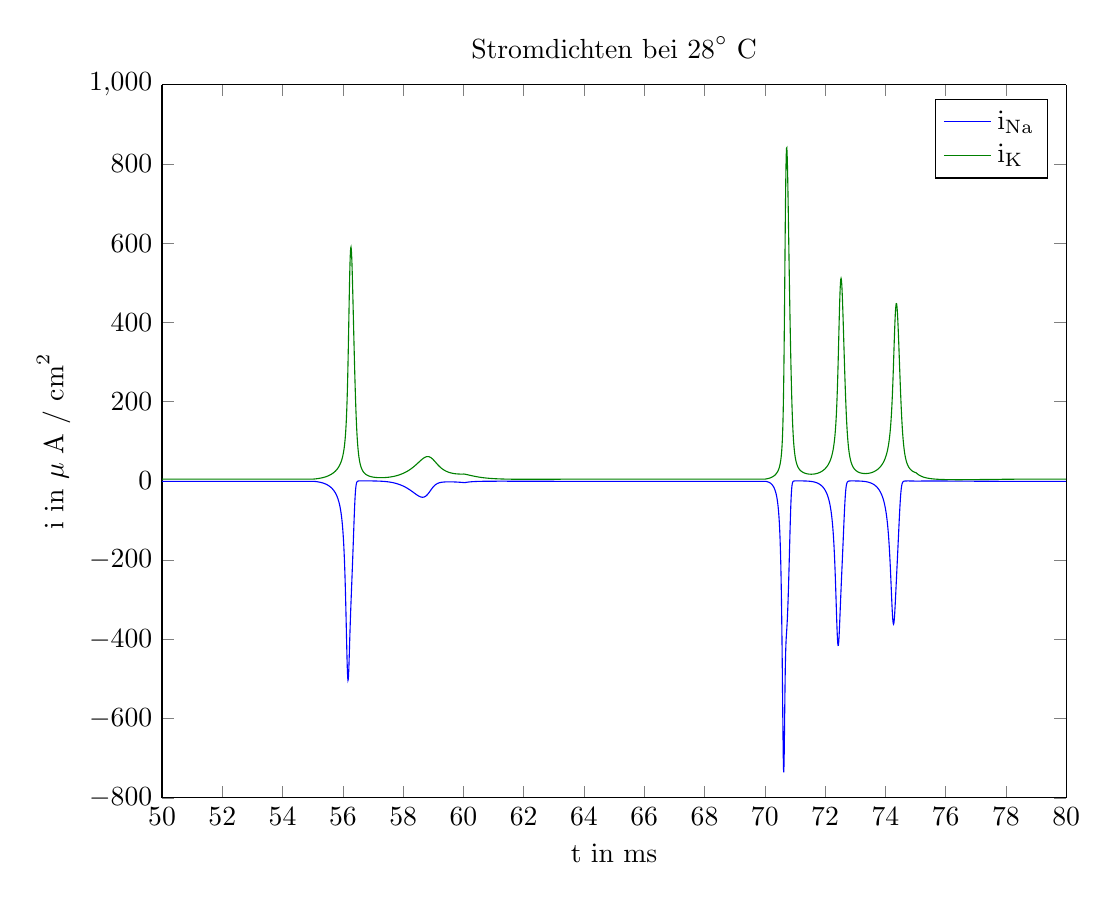
\begin{tikzpicture}

\begin{axis}[%
width=4.520833in,
height=3.565625in,
at={(0.758333in,0.48125in)},
scale only axis,
separate axis lines,
every outer x axis line/.append style={black},
every x tick label/.append style={font=\color{black}},
xmin=50,
xmax=80,
xlabel={t in ms},
every outer y axis line/.append style={black},
every y tick label/.append style={font=\color{black}},
ymin=-800,
ymax=1000,
ylabel={$\text{i in }\mu\text{ A / cm}^\text{2}$},
title={$\text{Stromdichten bei 28}^\circ\text{ C}$},
legend style={legend cell align=left,align=left,draw=black}
]
\addplot [color=blue,solid]
  table[row sep=crcr]{%
50	-1.22810163883331\\
50.01	-1.22805256900166\\
50.02	-1.22800280065748\\
50.03	-1.22795235984247\\
50.04	-1.22790127218981\\
50.05	-1.22784956292712\\
50.06	-1.22779725687937\\
50.07	-1.22774437847195\\
50.08	-1.22769095173361\\
50.09	-1.2276370002996\\
50.1	-1.22758254741468\\
50.11	-1.22752761593628\\
50.12	-1.2274722283376\\
50.13	-1.22741640671078\\
50.14	-1.22736017277009\\
50.15	-1.2273035478551\\
50.16	-1.22724655293393\\
50.17	-1.22718920860646\\
50.18	-1.22713153510761\\
50.19	-1.22707355231058\\
50.2	-1.22701527973018\\
50.21	-1.22695673652607\\
50.22	-1.22689794150612\\
50.23	-1.2268389131297\\
50.24	-1.22677966951104\\
50.25	-1.22672022842253\\
50.26	-1.2266606072981\\
50.27	-1.22660082323658\\
50.28	-1.22654089300503\\
50.29	-1.22648083304213\\
50.3	-1.22642065946154\\
50.31	-1.22636038805528\\
50.32	-1.2263000342971\\
50.33	-1.22623961334585\\
50.34	-1.22617914004887\\
50.35	-1.22611862894535\\
50.36	-1.22605809426971\\
50.37	-1.22599754995499\\
50.38	-1.22593700963619\\
50.39	-1.22587648665364\\
50.4	-1.22581599405637\\
50.41	-1.22575554460547\\
50.42	-1.22569515077743\\
50.43	-1.22563482476747\\
50.44	-1.2255745784929\\
50.45	-1.22551442359642\\
50.46	-1.22545437144946\\
50.47	-1.22539443315548\\
50.48	-1.22533461955326\\
50.49	-1.2252749412202\\
50.5	-1.22521540847559\\
50.51	-1.22515603138387\\
50.52	-1.22509681975789\\
50.53	-1.22503778316216\\
50.54	-1.22497893091604\\
50.55	-1.22492027209698\\
50.56	-1.22486181554374\\
50.57	-1.22480356985952\\
50.58	-1.22474554341515\\
50.59	-1.22468774435227\\
50.6	-1.22463018058642\\
50.61	-1.22457285981019\\
50.62	-1.22451578949633\\
50.63	-1.22445897690081\\
50.64	-1.22440242906587\\
50.65	-1.22434615282315\\
50.66	-1.22429015479663\\
50.67	-1.22423444140571\\
50.68	-1.22417901886814\\
50.69	-1.22412389320307\\
50.7	-1.22406907023394\\
50.71	-1.22401455559146\\
50.72	-1.22396035471649\\
50.73	-1.22390647286296\\
50.74	-1.22385291510074\\
50.75	-1.22379968631847\\
50.76	-1.22374679122643\\
50.77	-1.22369423435933\\
50.78	-1.22364202007909\\
50.79	-1.22359015257764\\
50.8	-1.22353863587962\\
50.81	-1.22348747384515\\
50.82	-1.2234366701725\\
50.83	-1.22338622840081\\
50.84	-1.22333615191268\\
50.85	-1.22328644393687\\
50.86	-1.22323710755089\\
50.87	-1.22318814568356\\
50.88	-1.22313956111764\\
50.89	-1.2230913564923\\
50.9	-1.2230435343057\\
50.91	-1.22299609691746\\
50.92	-1.22294904655113\\
50.93	-1.22290238529666\\
50.94	-1.22285611511281\\
50.95	-1.22281023782957\\
50.96	-1.22276475515051\\
50.97	-1.22271966865519\\
50.98	-1.22267497980142\\
50.99	-1.22263068992766\\
51	-1.22258680025523\\
51.01	-1.22254331189059\\
51.02	-1.22250022582764\\
51.03	-1.22245754294983\\
51.04	-1.22241526403245\\
51.05	-1.22237338974474\\
51.06	-1.22233192065206\\
51.07	-1.22229085721802\\
51.08	-1.22225019980654\\
51.09	-1.22220994868396\\
51.1	-1.22217010402109\\
51.11	-1.22213066589522\\
51.12	-1.22209163429213\\
51.13	-1.22205300910811\\
51.14	-1.22201479015184\\
51.15	-1.2219769771464\\
51.16	-1.22193956973115\\
51.17	-1.22190256746362\\
51.18	-1.22186596982139\\
51.19	-1.2218297762039\\
51.2	-1.22179398593433\\
51.21	-1.22175859826135\\
51.22	-1.2217236123609\\
51.23	-1.22168902733797\\
51.24	-1.2216548422283\\
51.25	-1.22162105600012\\
51.26	-1.22158766755582\\
51.27	-1.22155467573361\\
51.28	-1.22152207930917\\
51.29	-1.22148987699728\\
51.3	-1.2214580674534\\
51.31	-1.22142664927525\\
51.32	-1.22139562100441\\
51.33	-1.22136498112777\\
51.34	-1.22133472807913\\
51.35	-1.22130486024064\\
51.36	-1.22127537594429\\
51.37	-1.22124627347336\\
51.38	-1.22121755106385\\
51.39	-1.22118920690588\\
51.4	-1.2211612391451\\
51.41	-1.22113364588402\\
51.42	-1.22110642518342\\
51.43	-1.22107957506362\\
51.44	-1.22105309350582\\
51.45	-1.22102697845336\\
51.46	-1.22100122781305\\
51.47	-1.22097583945634\\
51.48	-1.22095081122062\\
51.49	-1.22092614091039\\
51.5	-1.22090182629846\\
51.51	-1.22087786512713\\
51.52	-1.22085425510936\\
51.53	-1.22083099392987\\
51.54	-1.22080807924629\\
51.55	-1.22078550869023\\
51.56	-1.22076327986841\\
51.57	-1.22074139036365\\
51.58	-1.22071983773601\\
51.59	-1.22069861952372\\
51.6	-1.22067773324427\\
51.61	-1.22065717639535\\
51.62	-1.22063694645587\\
51.63	-1.22061704088689\\
51.64	-1.22059745713254\\
51.65	-1.22057819262103\\
51.66	-1.22055924476547\\
51.67	-1.2205406109648\\
51.68	-1.22052228860468\\
51.69	-1.22050427505833\\
51.7	-1.22048656768737\\
51.71	-1.22046916384267\\
51.72	-1.22045206086517\\
51.73	-1.22043525608664\\
51.74	-1.22041874683049\\
51.75	-1.22040253041254\\
51.76	-1.22038660414176\\
51.77	-1.22037096532102\\
51.78	-1.22035561124781\\
51.79	-1.22034053921495\\
51.8	-1.22032574651128\\
51.81	-1.22031123042233\\
51.82	-1.22029698823103\\
51.83	-1.22028301721831\\
51.84	-1.22026931466376\\
51.85	-1.22025587784629\\
51.86	-1.22024270404469\\
51.87	-1.22022979053824\\
51.88	-1.22021713460733\\
51.89	-1.220204733534\\
51.9	-1.22019258460252\\
51.91	-1.22018068509992\\
51.92	-1.22016903231654\\
51.93	-1.22015762354655\\
51.94	-1.22014645608846\\
51.95	-1.22013552724563\\
51.96	-1.22012483432672\\
51.97	-1.22011437464622\\
51.98	-1.22010414552489\\
51.99	-1.22009414429018\\
52	-1.22008436827674\\
52.01	-1.2200748148268\\
52.02	-1.22006548129059\\
52.03	-1.22005636502678\\
52.04	-1.22004746340285\\
52.05	-1.22003877379549\\
52.06	-1.220030293591\\
52.07	-1.22002202018559\\
52.08	-1.22001395098581\\
52.09	-1.22000608340887\\
52.1	-1.21999841488296\\
52.11	-1.2199909428476\\
52.12	-1.21998366475396\\
52.13	-1.21997657806516\\
52.14	-1.21996968025654\\
52.15	-1.21996296881603\\
52.16	-1.21995644124435\\
52.17	-1.21995009505532\\
52.18	-1.21994392777612\\
52.19	-1.21993793694755\\
52.2	-1.21993212012427\\
52.21	-1.21992647487504\\
52.22	-1.21992099878295\\
52.23	-1.21991568944565\\
52.24	-1.21991054447553\\
52.25	-1.2199055615\\
52.26	-1.2199007381616\\
52.27	-1.21989607211825\\
52.28	-1.21989156104344\\
52.29	-1.21988720262635\\
52.3	-1.21988299457207\\
52.31	-1.21987893460175\\
52.32	-1.21987502045274\\
52.33	-1.21987124987877\\
52.34	-1.21986762065004\\
52.35	-1.2198641305534\\
52.36	-1.21986077739249\\
52.37	-1.2198575589878\\
52.38	-1.21985447317684\\
52.39	-1.21985151781422\\
52.4	-1.21984869077179\\
52.41	-1.21984598993868\\
52.42	-1.21984341322145\\
52.43	-1.21984095854414\\
52.44	-1.21983862384836\\
52.45	-1.21983640709337\\
52.46	-1.21983430625613\\
52.47	-1.2198323193314\\
52.48	-1.21983044433176\\
52.49	-1.21982867928769\\
52.5	-1.21982702224759\\
52.51	-1.21982547127787\\
52.52	-1.21982402446294\\
52.53	-1.21982267990527\\
52.54	-1.21982143572541\\
52.55	-1.21982029006203\\
52.56	-1.21981924107192\\
52.57	-1.21981828693\\
52.58	-1.21981742582938\\
52.59	-1.2198166559813\\
52.6	-1.21981597561519\\
52.61	-1.21981538297861\\
52.62	-1.21981487633733\\
52.63	-1.21981445397524\\
52.64	-1.21981411419436\\
52.65	-1.21981385531486\\
52.66	-1.219813675675\\
52.67	-1.21981357363112\\
52.68	-1.21981354755761\\
52.69	-1.21981359584689\\
52.7	-1.21981371690936\\
52.71	-1.21981390917339\\
52.72	-1.21981417108525\\
52.73	-1.21981450110908\\
52.74	-1.21981489772685\\
52.75	-1.21981535943831\\
52.76	-1.21981588476093\\
52.77	-1.21981647222984\\
52.78	-1.2198171203978\\
52.79	-1.21981782783513\\
52.8	-1.21981859312961\\
52.81	-1.21981941488648\\
52.82	-1.21982029172832\\
52.83	-1.21982122229501\\
52.84	-1.21982220524365\\
52.85	-1.21982323924848\\
52.86	-1.21982432300081\\
52.87	-1.21982545520895\\
52.88	-1.21982663459811\\
52.89	-1.21982785991032\\
52.9	-1.21982912990439\\
52.91	-1.21983044335575\\
52.92	-1.21983179905642\\
52.93	-1.21983319581489\\
52.94	-1.21983463245606\\
52.95	-1.21983610782112\\
52.96	-1.21983762076744\\
52.97	-1.21983917016854\\
52.98	-1.2198407549139\\
52.99	-1.21984237390895\\
53	-1.21984402607493\\
53.01	-1.21984571034876\\
53.02	-1.21984742568299\\
53.03	-1.21984917104568\\
53.04	-1.21985094542026\\
53.05	-1.21985274780547\\
53.06	-1.21985457721525\\
53.07	-1.21985643267858\\
53.08	-1.21985831323944\\
53.09	-1.21986021795664\\
53.1	-1.21986214590376\\
53.11	-1.219864096169\\
53.12	-1.21986606785508\\
53.13	-1.21986806007913\\
53.14	-1.21987007197259\\
53.15	-1.21987210268105\\
53.16	-1.21987415136419\\
53.17	-1.21987621719561\\
53.18	-1.21987829936277\\
53.19	-1.21988039706682\\
53.2	-1.21988250952251\\
53.21	-1.21988463595808\\
53.22	-1.21988677561511\\
53.23	-1.21988892774844\\
53.24	-1.21989109162601\\
53.25	-1.21989326652877\\
53.26	-1.21989545175056\\
53.27	-1.21989764659797\\
53.28	-1.21989985039023\\
53.29	-1.2199020624591\\
53.3	-1.21990428214871\\
53.31	-1.21990650881551\\
53.32	-1.21990874182808\\
53.33	-1.21991098056704\\
53.34	-1.21991322442494\\
53.35	-1.21991547280609\\
53.36	-1.21991772512651\\
53.37	-1.21991998081375\\
53.38	-1.2199222393068\\
53.39	-1.21992450005595\\
53.4	-1.21992676252269\\
53.41	-1.21992902617958\\
53.42	-1.21993129051012\\
53.43	-1.21993355500863\\
53.44	-1.21993581918016\\
53.45	-1.21993808254032\\
53.46	-1.21994034461521\\
53.47	-1.21994260494128\\
53.48	-1.21994486306518\\
53.49	-1.2199471185437\\
53.5	-1.21994937094361\\
53.51	-1.21995161984156\\
53.52	-1.21995386482396\\
53.53	-1.21995610548683\\
53.54	-1.21995834143575\\
53.55	-1.21996057228569\\
53.56	-1.21996279766089\\
53.57	-1.21996501719479\\
53.58	-1.21996723052988\\
53.59	-1.2199694373176\\
53.6	-1.21997163721819\\
53.61	-1.21997382990065\\
53.62	-1.21997601504254\\
53.63	-1.21997819232993\\
53.64	-1.21998036145727\\
53.65	-1.21998252212728\\
53.66	-1.21998467405081\\
53.67	-1.21998681694678\\
53.68	-1.21998895054202\\
53.69	-1.21999107457122\\
53.7	-1.21999318877675\\
53.71	-1.21999529290861\\
53.72	-1.2199973867243\\
53.73	-1.21999946998871\\
53.74	-1.22000154247401\\
53.75	-1.22000360395957\\
53.76	-1.22000565423183\\
53.77	-1.22000769308421\\
53.78	-1.22000972031699\\
53.79	-1.22001173573722\\
53.8	-1.22001373915864\\
53.81	-1.22001573040153\\
53.82	-1.22001770929264\\
53.83	-1.22001967566508\\
53.84	-1.22002162935825\\
53.85	-1.2200235702177\\
53.86	-1.22002549809505\\
53.87	-1.22002741284789\\
53.88	-1.22002931433971\\
53.89	-1.22003120243976\\
53.9	-1.22003307702299\\
53.91	-1.22003493796994\\
53.92	-1.22003678516665\\
53.93	-1.22003861850457\\
53.94	-1.22004043788047\\
53.95	-1.22004224319635\\
53.96	-1.22004403435935\\
53.97	-1.22004581128164\\
53.98	-1.22004757388037\\
53.99	-1.22004932207756\\
54	-1.22005105580002\\
54.01	-1.22005277497923\\
54.02	-1.22005447955133\\
54.03	-1.22005616945697\\
54.04	-1.22005784464124\\
54.05	-1.22005950505361\\
54.06	-1.22006115064782\\
54.07	-1.22006278138183\\
54.08	-1.2200643972177\\
54.09	-1.22006599812156\\
54.1	-1.22006758406348\\
54.11	-1.22006915501744\\
54.12	-1.2200707109612\\
54.13	-1.22007225187627\\
54.14	-1.22007377774783\\
54.15	-1.22007528856463\\
54.16	-1.22007678431892\\
54.17	-1.22007826500641\\
54.18	-1.22007973062615\\
54.19	-1.22008118118052\\
54.2	-1.22008261667508\\
54.21	-1.22008403711856\\
54.22	-1.2200854425228\\
54.23	-1.22008683290262\\
54.24	-1.2200882082758\\
54.25	-1.22008956866301\\
54.26	-1.22009091408773\\
54.27	-1.22009224457619\\
54.28	-1.22009356015732\\
54.29	-1.22009486086266\\
54.3	-1.22009614672631\\
54.31	-1.22009741778488\\
54.32	-1.22009867407741\\
54.33	-1.22009991564533\\
54.34	-1.22010114253237\\
54.35	-1.22010235478454\\
54.36	-1.22010355245003\\
54.37	-1.22010473557919\\
54.38	-1.22010590422446\\
54.39	-1.22010705844029\\
54.4	-1.22010819828313\\
54.41	-1.22010932381135\\
54.42	-1.22011043508518\\
54.43	-1.22011153216667\\
54.44	-1.22011261511963\\
54.45	-1.22011368400958\\
54.46	-1.22011473890373\\
54.47	-1.22011577987086\\
54.48	-1.22011680698135\\
54.49	-1.22011782030707\\
54.5	-1.22011881992136\\
54.51	-1.22011980589898\\
54.52	-1.22012077831609\\
54.53	-1.22012173725013\\
54.54	-1.22012268277985\\
54.55	-1.22012361498524\\
54.56	-1.22012453394748\\
54.57	-1.22012543974889\\
54.58	-1.22012633247291\\
54.59	-1.22012721220404\\
54.6	-1.22012807902781\\
54.61	-1.22012893303075\\
54.62	-1.2201297743003\\
54.63	-1.22013060292484\\
54.64	-1.2201314189936\\
54.65	-1.22013222259664\\
54.66	-1.22013301382483\\
54.67	-1.22013379276977\\
54.68	-1.2201345595238\\
54.69	-1.22013531417995\\
54.7	-1.22013605683188\\
54.71	-1.22013678757387\\
54.72	-1.22013750650079\\
54.73	-1.22013821370806\\
54.74	-1.22013890929161\\
54.75	-1.22013959334786\\
54.76	-1.22014026597369\\
54.77	-1.22014092726638\\
54.78	-1.22014157732362\\
54.79	-1.22014221624347\\
54.8	-1.22014284412431\\
54.81	-1.22014346106482\\
54.82	-1.22014406716399\\
54.83	-1.22014466252102\\
54.84	-1.22014524723536\\
54.85	-1.22014582140664\\
54.86	-1.22014638513469\\
54.87	-1.22014693851944\\
54.88	-1.22014748166098\\
54.89	-1.22014801465948\\
54.9	-1.22014853761519\\
54.91	-1.2201490506284\\
54.92	-1.22014955379943\\
54.93	-1.22015004722861\\
54.94	-1.22015053101625\\
54.95	-1.22015100526262\\
54.96	-1.22015147006791\\
54.97	-1.22015192553227\\
54.98	-1.22015237175572\\
54.99	-1.22015280883816\\
55	-1.22015323687936\\
55.01	-1.22015365597894\\
55.02	-1.24389101702724\\
55.03	-1.28455811874984\\
55.04	-1.33704905322356\\
55.05	-1.39829975564604\\
55.06	-1.46645251697877\\
55.07	-1.54038210152836\\
55.08	-1.61941893559165\\
55.09	-1.70318206025653\\
55.1	-1.79147596055637\\
55.11	-1.88422580848393\\
55.12	-1.98143635966209\\
55.13	-2.08316566207811\\
55.14	-2.18950815327829\\
55.15	-2.30058376224454\\
55.16	-2.41653087913542\\
55.17	-2.53750183164255\\
55.18	-2.6636599951396\\
55.19	-2.79517797422358\\
55.2	-2.93223649191793\\
55.21	-3.07502375066222\\
55.22	-3.22373511188187\\
55.23	-3.37857299460792\\
55.24	-3.53974692861194\\
55.25	-3.70747372043362\\
55.26	-3.88197770575382\\
55.27	-4.06349107154488\\
55.28	-4.25225423808951\\
55.29	-4.44851629545635\\
55.3	-4.65253549210731\\
55.31	-4.86457977548584\\
55.32	-5.08492738602049\\
55.33	-5.31386750719193\\
55.34	-5.5517009752977\\
55.35	-5.7987410534059\\
55.36	-6.05531427478453\\
55.37	-6.32176136187524\\
55.38	-6.59843822768524\\
55.39	-6.88571706732693\\
55.4	-7.18398754836596\\
55.41	-7.49365810966577\\
55.42	-7.81515737956249\\
55.43	-8.14893572548955\\
55.44	-8.49546694862019\\
55.45	-8.85525013873496\\
55.46	-9.22881170637858\\
55.47	-9.61670761148179\\
55.48	-10.0195258100256\\
55.49	-10.4378889430657\\
55.5	-10.8724572955624\\
55.51	-11.3239320560433\\
55.52	-11.7930589122273\\
55.53	-12.2806320224487\\
55.54	-12.7874984081379\\
55.55	-13.3145628188557\\
55.56	-13.8627931285787\\
55.57	-14.433226330266\\
55.58	-15.0269752053837\\
55.59	-15.6452357562646\\
55.6	-16.2892955022101\\
55.61	-16.9605427554238\\
55.62	-17.6604770105962\\
55.63	-18.3907206027166\\
55.64	-19.1530318120239\\
55.65	-19.9493196236165\\
55.66	-20.7816603829413\\
55.67	-21.6523166281645\\
55.68	-22.5637584275028\\
55.69	-23.5186876054205\\
55.7	-24.5200653079555\\
55.71	-25.571143436492\\
55.72	-26.6755005736943\\
55.73	-27.8370831382784\\
55.74	-29.060252640791\\
55.75	-30.3498400754151\\
55.76	-31.7112086789733\\
55.77	-33.1503265250239\\
55.78	-34.6738507071411\\
55.79	-36.2892252120581\\
55.8	-38.0047950036192\\
55.81	-39.829939348637\\
55.82	-41.7752280353272\\
55.83	-43.8526048874774\\
55.84	-46.0756038906545\\
55.85	-48.459604352833\\
55.86	-51.0221328572596\\
55.87	-53.7832213693683\\
55.88	-56.7658327709218\\
55.89	-59.9963673451465\\
55.9	-63.5052663392152\\
55.91	-67.3277316567649\\
55.92	-71.5045838759624\\
55.93	-76.0832838965775\\
55.94	-81.1191460879523\\
55.95	-86.6767718994519\\
55.96	-92.8317308356919\\
55.97	-99.6725076107329\\
55.98	-107.302715331452\\
55.99	-115.843536735299\\
56	-125.436285955352\\
56.01	-136.244861812608\\
56.02	-148.457659639853\\
56.03	-162.288178083881\\
56.04	-177.973042015773\\
56.05	-195.765397537204\\
56.06	-215.920575838377\\
56.07	-238.669617031778\\
56.08	-264.174982295448\\
56.09	-292.462353363599\\
56.1	-323.324453305648\\
56.11	-356.199970571911\\
56.12	-390.045958189344\\
56.13	-423.246378128022\\
56.14	-453.626359779667\\
56.15	-478.652004323431\\
56.16	-495.858882674548\\
56.17	-503.44818869404\\
56.18	-500.847823679837\\
56.19	-488.959974354597\\
56.2	-469.919441130669\\
56.21	-446.447970566531\\
56.22	-421.115410775455\\
56.23	-395.82448419038\\
56.24	-371.647945467454\\
56.25	-348.946420594953\\
56.26	-327.612000018542\\
56.27	-307.309021221138\\
56.28	-287.647878192201\\
56.29	-268.279430743828\\
56.3	-248.925395129463\\
56.31	-229.371783928618\\
56.32	-209.45516195171\\
56.33	-189.065797158116\\
56.34	-168.177018833185\\
56.35	-146.891275615177\\
56.36	-125.480246531118\\
56.37	-104.395105509854\\
56.38	-84.2319409147224\\
56.39	-65.6509413999612\\
56.4	-49.262694606167\\
56.41	-35.5088903093063\\
56.42	-24.5734904018036\\
56.43	-16.3563152686084\\
56.44	-10.5196854147746\\
56.45	-6.58819658404899\\
56.46	-4.06057810235125\\
56.47	-2.49485891084691\\
56.48	-1.54945729655837\\
56.49	-0.985888696280844\\
56.5	-0.650048606572395\\
56.51	-0.447770717913163\\
56.52	-0.323575757423792\\
56.53	-0.245404821644581\\
56.54	-0.194825364997834\\
56.55	-0.161172831167254\\
56.56	-0.138187373185351\\
56.57	-0.122121495994308\\
56.58	-0.110680435297536\\
56.59	-0.102425186706401\\
56.6	-0.0964316320792223\\
56.61	-0.0920923949747167\\
56.62	-0.088999335722829\\
56.63	-0.0868724163032285\\
56.64	-0.0855157514637211\\
56.65	-0.0847899161736847\\
56.66	-0.0845941619887556\\
56.67	-0.0848547850474174\\
56.68	-0.085517380533614\\
56.69	-0.086541594254776\\
56.7	-0.0878975052288209\\
56.71	-0.0895630909493979\\
56.72	-0.0915224229499495\\
56.73	-0.0937643628595276\\
56.74	-0.0962816068750917\\
56.75	-0.0990699765363862\\
56.76	-0.102127886232602\\
56.77	-0.105455939352467\\
56.78	-0.109056619362061\\
56.79	-0.112934051840731\\
56.8	-0.117093820203502\\
56.81	-0.121542822502834\\
56.82	-0.126289159993289\\
56.83	-0.131342050493423\\
56.84	-0.13671176127883\\
56.85	-0.14240955748326\\
56.86	-0.148447662903575\\
56.87	-0.154839230790519\\
56.88	-0.161598322724539\\
56.89	-0.16873989406935\\
56.9	-0.176279784797582\\
56.91	-0.184234714715947\\
56.92	-0.192622282298731\\
56.93	-0.201460966480493\\
56.94	-0.210770130870842\\
56.95	-0.220570029942945\\
56.96	-0.230881816818213\\
56.97	-0.241727552326397\\
56.98	-0.253130215066059\\
56.99	-0.265113712227502\\
57	-0.277702890970475\\
57.01	-0.29092355017381\\
57.02	-0.304802452394636\\
57.03	-0.319367335891898\\
57.04	-0.334646926583241\\
57.05	-0.350670949816515\\
57.06	-0.367470141847545\\
57.07	-0.385076260924951\\
57.08	-0.403522097890759\\
57.09	-0.422841486212731\\
57.1	-0.443069311370859\\
57.11	-0.464241519526501\\
57.12	-0.486395125408278\\
57.13	-0.509568219354276\\
57.14	-0.533799973455273\\
57.15	-0.559130646748833\\
57.16	-0.585601589419088\\
57.17	-0.613255245962037\\
57.18	-0.642135157281143\\
57.19	-0.672285961682995\\
57.2	-0.703753394747785\\
57.21	-0.736584288054402\\
57.22	-0.770826566744926\\
57.23	-0.806529245918405\\
57.24	-0.84374242584881\\
57.25	-0.882517286027087\\
57.26	-0.922906078032215\\
57.27	-0.964962117241098\\
57.28	-1.00873977339193\\
57.29	-1.05429446002042\\
57.3	-1.10168262279273\\
57.31	-1.15096172676351\\
57.32	-1.20219024259144\\
57.33	-1.25542763174869\\
57.34	-1.31073433076429\\
57.35	-1.36817173454494\\
57.36	-1.42780217881931\\
57.37	-1.48968892175529\\
57.38	-1.55389612480089\\
57.39	-1.6204888328022\\
57.4	-1.68953295345255\\
57.41	-1.76109523612803\\
57.42	-1.83524325016503\\
57.43	-1.91204536263501\\
57.44	-1.99157071567116\\
57.45	-2.07388920340025\\
57.46	-2.15907144853125\\
57.47	-2.24718877864942\\
57.48	-2.33831320226223\\
57.49	-2.43251738463903\\
57.5	-2.52987462348284\\
57.51	-2.63045882446716\\
57.52	-2.73434447666575\\
57.53	-2.84160662789675\\
57.54	-2.95232085999626\\
57.55	-3.0665632640287\\
57.56	-3.18441041543383\\
57.57	-3.30593934910139\\
57.58	-3.43122753435529\\
57.59	-3.5603528498196\\
57.6	-3.69339355812811\\
57.61	-3.83042828042824\\
57.62	-3.97153597061853\\
57.63	-4.11679588924661\\
57.64	-4.26628757698173\\
57.65	-4.42009082756226\\
57.66	-4.57828566010446\\
57.67	-4.74095229064368\\
57.68	-4.90817110276371\\
57.69	-5.08002261715318\\
57.7	-5.25658745991093\\
57.71	-5.4379463294038\\
57.72	-5.62417996146153\\
57.73	-5.81536909267291\\
57.74	-6.01159442152653\\
57.75	-6.21293656711709\\
57.76	-6.41947602511441\\
57.77	-6.63129312066792\\
57.78	-6.84846795789251\\
57.79	-7.07108036555437\\
57.8	-7.29920983854547\\
57.81	-7.53293547470435\\
57.82	-7.7723359065074\\
57.83	-8.01748922711984\\
57.84	-8.26847291025776\\
57.85	-8.52536372327281\\
57.86	-8.78823763282873\\
57.87	-9.05716970249352\\
57.88	-9.33223398152303\\
57.89	-9.61350338406063\\
57.9	-9.90104955792293\\
57.91	-10.1949427420837\\
57.92	-10.4952516119066\\
57.93	-10.8020431111117\\
57.94	-11.1153822693908\\
57.95	-11.4353320045156\\
57.96	-11.7619529076995\\
57.97	-12.0953030108978\\
57.98	-12.4354375346389\\
57.99	-12.7824086148914\\
58	-13.1362650073719\\
58.01	-13.4970517676019\\
58.02	-13.8648099049128\\
58.03	-14.2395760084912\\
58.04	-14.6213818434413\\
58.05	-15.0102539147238\\
58.06	-15.4062129967105\\
58.07	-15.8092736259706\\
58.08	-16.219443554777\\
58.09	-16.6367231626993\\
58.1	-17.0611048235204\\
58.11	-17.4925722245925\\
58.12	-17.9310996356287\\
58.13	-18.3766511238126\\
58.14	-18.8291797120025\\
58.15	-19.2886264767169\\
58.16	-19.7549195825075\\
58.17	-20.2279732492713\\
58.18	-20.7076866490175\\
58.19	-21.1939427286068\\
58.2	-21.6866069550094\\
58.21	-22.1855259797128\\
58.22	-22.6905262190375\\
58.23	-23.2014123473152\\
58.24	-23.7179657001509\\
58.25	-24.2399425853419\\
58.26	-24.7670724994795\\
58.27	-25.2990562488235\\
58.28	-25.8355639737362\\
58.29	-26.3762330768047\\
58.3	-26.9206660557952\\
58.31	-27.4684282437822\\
58.32	-28.0190454602108\\
58.33	-28.572001578299\\
58.34	-29.1267360160992\\
58.35	-29.6826411607361\\
58.36	-30.2390597378518\\
58.37	-30.7952821411407\\
58.38	-31.3505437400757\\
58.39	-31.9040221875352\\
58.4	-32.4548347530564\\
58.41	-33.0020357118845\\
58.42	-33.5446138248675\\
58.43	-34.0814899495642\\
58.44	-34.6115148286843\\
58.45	-35.1334671081423\\
58.46	-35.6460516435438\\
58.47	-36.1478981607831\\
58.48	-36.6375603435373\\
58.49	-37.1135154276872\\
58.5	-37.5741643899535\\
58.51	-38.0178328251362\\
58.52	-38.4427726130838\\
58.53	-38.8471644826435\\
58.54	-39.2291215850751\\
58.55	-39.5866941933905\\
58.56	-39.9178756464339\\
58.57	-40.2206096567991\\
58.58	-40.4927990993923\\
58.59	-40.7323163920834\\
58.6	-40.9370155708493\\
58.61	-41.1047461485315\\
58.62	-41.2333688281938\\
58.63	-41.3207731184819\\
58.64	-41.3648968688175\\
58.65	-41.3637477062044\\
58.66	-41.3154263125424\\
58.67	-41.2181514313982\\
58.68	-41.0702864362047\\
58.69	-40.8703672281123\\
58.7	-40.6171311618315\\
58.71	-40.3095466228177\\
58.72	-39.9468428005703\\
58.73	-39.5285391227112\\
58.74	-39.0544737355295\\
58.75	-38.5248303421134\\
58.76	-37.9401626429578\\
58.77	-37.3014155705362\\
58.78	-36.6099424737599\\
58.79	-35.8675173958339\\
58.8	-35.076341605161\\
58.81	-34.2390435887903\\
58.82	-33.3586718059234\\
58.83	-32.4386796284792\\
58.84	-31.4829020682508\\
58.85	-30.4955241050301\\
58.86	-29.4810406837027\\
58.87	-28.4442087339361\\
58.88	-27.3899918734922\\
58.89	-26.3234987717873\\
58.9	-25.2499164575411\\
58.91	-24.1744401344968\\
58.92	-23.1022013026139\\
58.93	-22.0381961498424\\
58.94	-20.9872162649848\\
58.95	-19.9537837129206\\
58.96	-18.9420924031975\\
58.97	-17.955957472417\\
58.98	-16.998774098478\\
58.99	-16.0734867866236\\
59	-15.1825697359493\\
59.01	-14.3280184377748\\
59.02	-13.5113522035111\\
59.03	-12.733626898261\\
59.04	-11.9954567930447\\
59.05	-11.2970441633398\\
59.06	-10.6382150674985\\
59.07	-10.0184596405256\\
59.08	-9.4369752338724\\
59.09	-8.89271081071857\\
59.1	-8.38441115388\\
59.11	-7.91065964197265\\
59.12	-7.46991857957995\\
59.13	-7.06056631036404\\
59.14	-6.68093058193871\\
59.15	-6.32931785463433\\
59.16	-6.00403844342963\\
59.17	-5.70342754739204\\
59.18	-5.42586235142239\\
59.19	-5.16977548122898\\
59.2	-4.93366515668554\\
59.21	-4.71610242492559\\
59.22	-4.51573586734995\\
59.23	-4.33129416908549\\
59.24	-4.16158692008166\\
59.25	-4.00550398826915\\
59.26	-3.86201377072435\\
59.27	-3.73016059159358\\
59.28	-3.60906147796333\\
59.29	-3.49790250862006\\
59.3	-3.39593489688557\\
59.31	-3.30247093814662\\
59.32	-3.21687992567272\\
59.33	-3.13858411491598\\
59.34	-3.06705479660483\\
59.35	-3.00180852234625\\
59.36	-2.94240351283052\\
59.37	-2.88843626774523\\
59.38	-2.83953838779939\\
59.39	-2.79537361249362\\
59.4	-2.75563507213372\\
59.41	-2.72004274878536\\
59.42	-2.68834113815804\\
59.43	-2.6602971025679\\
59.44	-2.63569790397843\\
59.45	-2.61434940550109\\
59.46	-2.59607442952641\\
59.47	-2.58071126074809\\
59.48	-2.56811228265314\\
59.49	-2.55814273651526\\
59.5	-2.55067959249349\\
59.51	-2.5456105230644\\
59.52	-2.54283296967284\\
59.53	-2.54225329415035\\
59.54	-2.54378600710621\\
59.55	-2.54735306613046\\
59.56	-2.55288323725451\\
59.57	-2.56031151368703\\
59.58	-2.56957858637819\\
59.59	-2.58063036146324\\
59.6	-2.5934175200954\\
59.61	-2.6078951166011\\
59.62	-2.6240222112769\\
59.63	-2.64176153450083\\
59.64	-2.66107917915148\\
59.65	-2.68194431862043\\
59.66	-2.70432894796725\\
59.67	-2.72820764600584\\
59.68	-2.75355735632642\\
59.69	-2.78035718545285\\
59.7	-2.8085882165107\\
59.71	-2.83823333693972\\
59.72	-2.86927707892766\\
59.73	-2.90170547137054\\
59.74	-2.93550590228048\\
59.75	-2.97066699066654\\
59.76	-3.00717846700763\\
59.77	-3.04503106152151\\
59.78	-3.08421639950954\\
59.79	-3.12472690312596\\
59.8	-3.16655569898186\\
59.81	-3.20969653105011\\
59.82	-3.25414367838757\\
59.83	-3.29989187723635\\
59.84	-3.34693624710698\\
59.85	-3.39527222048331\\
59.86	-3.44489547582236\\
59.87	-3.49580187355299\\
59.88	-3.54798739480441\\
59.89	-3.6014480826206\\
59.9	-3.65617998543948\\
59.91	-3.71217910263589\\
59.92	-3.76944133194673\\
59.93	-3.82796241861295\\
59.94	-3.88773790608942\\
59.95	-3.94876308818748\\
59.96	-4.0110329625282\\
59.97	-4.07454218519648\\
59.98	-4.1392850264971\\
59.99	-4.20525532772413\\
60	-4.27244645886445\\
60.01	-4.3408512771652\\
60.02	-4.41046208650299\\
60.03	-4.41836617988566\\
60.04	-4.37866669160633\\
60.05	-4.30729026136523\\
60.06	-4.21565536907456\\
60.07	-4.1117280934362\\
60.08	-4.00098153867079\\
60.09	-3.88713029497911\\
60.1	-3.77266701267636\\
60.11	-3.65924369903185\\
60.12	-3.5479379153672\\
60.13	-3.4394364699701\\
60.14	-3.33416120730176\\
60.15	-3.23235471735831\\
60.16	-3.13413855919061\\
60.17	-3.03955275381906\\
60.18	-2.94858256702222\\
60.19	-2.86117669086858\\
60.2	-2.77725961338406\\
60.21	-2.69674006285392\\
60.22	-2.61951679921398\\
60.23	-2.54548260925724\\
60.24	-2.47452708186723\\
60.25	-2.40653855070107\\
60.26	-2.3414054649444\\
60.27	-2.27901736372494\\
60.28	-2.21926557280728\\
60.29	-2.16204370405609\\
60.3	-2.10724801262472\\
60.31	-2.05477764972413\\
60.32	-2.00453483734956\\
60.33	-1.95642498361695\\
60.34	-1.91035675213496\\
60.35	-1.86624209527791\\
60.36	-1.82399625877365\\
60.37	-1.78353776330984\\
60.38	-1.74478836764756\\
60.39	-1.70767301684956\\
60.4	-1.67211977857482\\
60.41	-1.63805976989105\\
60.42	-1.60542707666301\\
60.43	-1.57415866725912\\
60.44	-1.5441943020574\\
60.45	-1.51547644001344\\
60.46	-1.48795014336612\\
60.47	-1.46156298139606\\
60.48	-1.43626493401192\\
60.49	-1.4120082958176\\
60.5	-1.38874758120657\\
60.51	-1.36643943093601\\
60.52	-1.3450425205514\\
60.53	-1.3245174709609\\
60.54	-1.30482676139613\\
60.55	-1.28593464494211\\
60.56	-1.26780706677195\\
60.57	-1.25041158518171\\
60.58	-1.23371729548622\\
60.59	-1.21769475680693\\
60.6	-1.20231592175832\\
60.61	-1.18755406901812\\
60.62	-1.17338373874934\\
60.63	-1.15978067082768\\
60.64	-1.14672174581626\\
60.65	-1.13418492862043\\
60.66	-1.12214921474776\\
60.67	-1.11059457909323\\
60.68	-1.09950192716533\\
60.69	-1.08885304866594\\
60.7	-1.07863057333557\\
60.71	-1.06881792897431\\
60.72	-1.05939930154928\\
60.73	-1.05035959729979\\
60.74	-1.04168440675263\\
60.75	-1.03335997056178\\
60.76	-1.02537314708831\\
60.77	-1.01771138163906\\
60.78	-1.01036267728464\\
60.79	-1.00331556718025\\
60.8	-0.996559088315204\\
60.81	-0.990082756620144\\
60.82	-0.983876543363494\\
60.83	-0.977930852771641\\
60.84	-0.972236500810115\\
60.85	-0.966784695065797\\
60.86	-0.96156701567296\\
60.87	-0.956575397228543\\
60.88	-0.951802111644739\\
60.89	-0.947239751889422\\
60.9	-0.942881216567453\\
60.91	-0.938719695298188\\
60.92	-0.934748654846842\\
60.93	-0.93096182596948\\
60.94	-0.927353190933543\\
60.95	-0.923916971677768\\
60.96	-0.920647618577298\\
60.97	-0.917539799781591\\
60.98	-0.914588391094438\\
60.99	-0.911788466367104\\
61	-0.909135288377124\\
61.01	-0.906624300166783\\
61.02	-0.904251116816775\\
61.03	-0.902011517631769\\
61.04	-0.899901438716007\\
61.05	-0.897916965918152\\
61.06	-0.896054328125816\\
61.07	-0.894309890891237\\
61.08	-0.892680150370612\\
61.09	-0.891161727560543\\
61.1	-0.889751362815978\\
61.11	-0.88844591063488\\
61.12	-0.887242334695668\\
61.13	-0.886137703134253\\
61.14	-0.88512918404821\\
61.15	-0.884214041216303\\
61.16	-0.88338963002225\\
61.17	-0.882653393572193\\
61.18	-0.882002858995945\\
61.19	-0.881435633922604\\
61.2	-0.880949403121652\\
61.21	-0.880541925301136\\
61.22	-0.880211030054975\\
61.23	-0.879954614951893\\
61.24	-0.879770642758845\\
61.25	-0.879657138792229\\
61.26	-0.879612188390509\\
61.27	-0.879633934502216\\
61.28	-0.879720575383646\\
61.29	-0.879870362400833\\
61.3	-0.8800815979307\\
61.31	-0.880352633356547\\
61.32	-0.880681867153276\\
61.33	-0.881067743058027\\
61.34	-0.881508748322105\\
61.35	-0.882003412040276\\
61.36	-0.882550303553775\\
61.37	-0.883148030923472\\
61.38	-0.883795239469913\\
61.39	-0.884490610377055\\
61.4	-0.885232859356716\\
61.41	-0.886020735370903\\
61.42	-0.886853019409306\\
61.43	-0.887728523319434\\
61.44	-0.888646088686925\\
61.45	-0.889604585763757\\
61.46	-0.890602912442148\\
61.47	-0.891639993272078\\
61.48	-0.892714778520445\\
61.49	-0.893826243269982\\
61.5	-0.89497338655614\\
61.51	-0.896155230540251\\
61.52	-0.897370819717333\\
61.53	-0.898619220157026\\
61.54	-0.89989951877617\\
61.55	-0.901210822641644\\
61.56	-0.902552258302144\\
61.57	-0.903922971147627\\
61.58	-0.90532212479522\\
61.59	-0.906748900500456\\
61.6	-0.908202496592736\\
61.61	-0.909682127933974\\
61.62	-0.911187025399451\\
61.63	-0.912716435379896\\
61.64	-0.914269619303934\\
61.65	-0.915845853180004\\
61.66	-0.917444427156947\\
61.67	-0.919064645102464\\
61.68	-0.920705824198708\\
61.69	-0.922367294554287\\
61.7	-0.924048398831989\\
61.71	-0.925748491891597\\
61.72	-0.927466940447132\\
61.73	-0.929203122737979\\
61.74	-0.93095642821327\\
61.75	-0.932726257229018\\
61.76	-0.934512020757466\\
61.77	-0.93631314010815\\
61.78	-0.938129046660195\\
61.79	-0.939959181605396\\
61.8	-0.941802995701637\\
61.81	-0.943659949036232\\
61.82	-0.94552951079878\\
61.83	-0.947411159063158\\
61.84	-0.949304380578271\\
61.85	-0.951208670567213\\
61.86	-0.953123532534495\\
61.87	-0.955048478081015\\
61.88	-0.956983026726452\\
61.89	-0.958926705738798\\
61.9	-0.960879049970717\\
61.91	-0.962839601702477\\
61.92	-0.964807910491172\\
61.93	-0.966783533025991\\
61.94	-0.968766032989276\\
61.95	-0.970754980923149\\
61.96	-0.972749954101458\\
61.97	-0.974750536406852\\
61.98	-0.976756318212753\\
61.99	-0.978766896270036\\
62	-0.980781873598211\\
62.01	-0.982800859380936\\
62.02	-0.984823468865666\\
62.03	-0.986849323267279\\
62.04	-0.988878049675495\\
62.05	-0.990909280965947\\
62.06	-0.992942655714737\\
62.07	-0.994977818116325\\
62.08	-0.997014417904628\\
62.09	-0.999052110277161\\
62.1	-1.00109055582211\\
62.11	-1.00312942044822\\
62.12	-1.00516837531728\\
62.13	-1.00720709677931\\
62.14	-1.00924526631001\\
62.15	-1.01128257045064\\
62.16	-1.01331870075015\\
62.17	-1.0153533537093\\
62.18	-1.01738623072695\\
62.19	-1.01941703804815\\
62.2	-1.02144548671411\\
62.21	-1.02347129251394\\
62.22	-1.02549417593797\\
62.23	-1.02751386213274\\
62.24	-1.02953008085737\\
62.25	-1.03154256644142\\
62.26	-1.03355105774407\\
62.27	-1.03555529811458\\
62.28	-1.03755503535391\\
62.29	-1.03955002167753\\
62.3	-1.04154001367923\\
62.31	-1.04352477229602\\
62.32	-1.04550406277387\\
62.33	-1.04747765463446\\
62.34	-1.04944532164263\\
62.35	-1.05140684177476\\
62.36	-1.05336199718773\\
62.37	-1.05531057418868\\
62.38	-1.05725236320531\\
62.39	-1.05918715875685\\
62.4	-1.06111475942546\\
62.41	-1.06303496782828\\
62.42	-1.06494759058978\\
62.43	-1.06685243831467\\
62.44	-1.06874932556107\\
62.45	-1.07063807081413\\
62.46	-1.07251849645989\\
62.47	-1.07439042875945\\
62.48	-1.07625369782339\\
62.49	-1.07810813758639\\
62.5	-1.07995358578206\\
62.51	-1.08178988391789\\
62.52	-1.08361687725039\\
62.53	-1.0854344147603\\
62.54	-1.0872423491279\\
62.55	-1.08904053670836\\
62.56	-1.09082883750717\\
62.57	-1.09260711515555\\
62.58	-1.09437523688589\\
62.59	-1.09613307350715\\
62.6	-1.09788049938023\\
62.61	-1.09961739239331\\
62.62	-1.10134363393707\\
62.63	-1.10305910887989\\
62.64	-1.10476370554293\\
62.65	-1.10645731567505\\
62.66	-1.1081398344277\\
62.67	-1.10981116032962\\
62.68	-1.1114711952614\\
62.69	-1.11311984442991\\
62.7	-1.11475701634254\\
62.71	-1.1163826227813\\
62.72	-1.11799657877677\\
62.73	-1.11959880258175\\
62.74	-1.12118921564489\\
62.75	-1.12276774258397\\
62.76	-1.12433431115909\\
62.77	-1.12588885224564\\
62.78	-1.12743129980697\\
62.79	-1.12896159086702\\
62.8	-1.13047966548258\\
62.81	-1.13198546671543\\
62.82	-1.13347894060428\\
62.83	-1.13496003613638\\
62.84	-1.13642870521907\\
62.85	-1.13788490265104\\
62.86	-1.13932858609333\\
62.87	-1.14075971604025\\
62.88	-1.14217825578995\\
62.89	-1.14358417141492\\
62.9	-1.14497743173213\\
62.91	-1.14635800827316\\
62.92	-1.14772587525394\\
62.93	-1.14908100954445\\
62.94	-1.15042339063815\\
62.95	-1.15175300062122\\
62.96	-1.1530698241417\\
62.97	-1.15437384837835\\
62.98	-1.15566506300943\\
62.99	-1.15694346018126\\
63	-1.15820903447665\\
63.01	-1.15946178288317\\
63.02	-1.16070170476125\\
63.03	-1.16192880181223\\
63.04	-1.16314307804616\\
63.05	-1.16434453974954\\
63.06	-1.16553319545297\\
63.07	-1.16670905589861\\
63.08	-1.1678721340076\\
63.09	-1.16902244484739\\
63.1	-1.17016000559891\\
63.11	-1.17128483552376\\
63.12	-1.17239695593125\\
63.13	-1.17349639014542\\
63.14	-1.17458316347199\\
63.15	-1.17565730316524\\
63.16	-1.17671883839494\\
63.17	-1.1777678002131\\
63.18	-1.17880422152086\\
63.19	-1.17982813703526\\
63.2	-1.18083958325602\\
63.21	-1.18183859843239\\
63.22	-1.18282522252992\\
63.23	-1.1837994971973\\
63.24	-1.18476146573325\\
63.25	-1.18571117305342\\
63.26	-1.18664866565729\\
63.27	-1.18757399159524\\
63.28	-1.18848720043558\\
63.29	-1.1893883432317\\
63.3	-1.19027747248927\\
63.31	-1.19115464213358\\
63.32	-1.19201990747692\\
63.33	-1.19287332518608\\
63.34	-1.19371495325002\\
63.35	-1.19454485094753\\
63.36	-1.19536307881519\\
63.37	-1.1961696986153\\
63.38	-1.19696477330407\\
63.39	-1.1977483669999\\
63.4	-1.19852054495187\\
63.41	-1.19928137350832\\
63.42	-1.20003092008568\\
63.43	-1.20076925313745\\
63.44	-1.20149644212333\\
63.45	-1.20221255747862\\
63.46	-1.20291767058377\\
63.47	-1.20361185373411\\
63.48	-1.2042951801099\\
63.49	-1.20496772374646\\
63.5	-1.20562955950462\\
63.51	-1.20628076304141\\
63.52	-1.20692141078089\\
63.53	-1.20755157988537\\
63.54	-1.20817134822671\\
63.55	-1.208780794358\\
63.56	-1.20937999748549\\
63.57	-1.2099690374407\\
63.58	-1.21054799465286\\
63.59	-1.21111695012165\\
63.6	-1.21167598539016\\
63.61	-1.21222518251813\\
63.62	-1.21276462405554\\
63.63	-1.21329439301644\\
63.64	-1.21381457285309\\
63.65	-1.21432524743035\\
63.66	-1.21482650100049\\
63.67	-1.21531841817816\\
63.68	-1.21580108391578\\
63.69	-1.21627458347918\\
63.7	-1.21673900242355\\
63.71	-1.21719442656978\\
63.72	-1.21764094198102\\
63.73	-1.2180786349396\\
63.74	-1.21850759192433\\
63.75	-1.21892789958803\\
63.76	-1.21933964473542\\
63.77	-1.21974291430142\\
63.78	-1.2201377953296\\
63.79	-1.2205243749512\\
63.8	-1.22090274036422\\
63.81	-1.22127297881308\\
63.82	-1.22163517756848\\
63.83	-1.22198942390758\\
63.84	-1.22233580509464\\
63.85	-1.22267440836187\\
63.86	-1.22300532089067\\
63.87	-1.22332862979321\\
63.88	-1.22364442209436\\
63.89	-1.22395278471389\\
63.9	-1.2242538044491\\
63.91	-1.2245475679577\\
63.92	-1.22483416174109\\
63.93	-1.22511367212795\\
63.94	-1.22538618525816\\
63.95	-1.22565178706704\\
63.96	-1.22591056326998\\
63.97	-1.22616259934732\\
63.98	-1.22640798052965\\
63.99	-1.22664679178334\\
64	-1.2268791177965\\
64.01	-1.22710504296518\\
64.02	-1.22732465137994\\
64.03	-1.22753802681277\\
64.04	-1.22774525270421\\
64.05	-1.22794641215098\\
64.06	-1.22814158789374\\
64.07	-1.22833086230528\\
64.08	-1.22851431737899\\
64.09	-1.22869203471762\\
64.1	-1.22886409552242\\
64.11	-1.22903058058247\\
64.12	-1.22919157026441\\
64.13	-1.22934714450245\\
64.14	-1.22949738278864\\
64.15	-1.22964236416351\\
64.16	-1.22978216720688\\
64.17	-1.22991687002914\\
64.18	-1.23004655026261\\
64.19	-1.23017128505337\\
64.2	-1.23029115105325\\
64.21	-1.23040622441215\\
64.22	-1.23051658077061\\
64.23	-1.23062229525271\\
64.24	-1.23072344245915\\
64.25	-1.23082009646066\\
64.26	-1.23091233079167\\
64.27	-1.23100021844421\\
64.28	-1.23108383186208\\
64.29	-1.23116324293529\\
64.3	-1.23123852299472\\
64.31	-1.23130974280705\\
64.32	-1.23137697256992\\
64.33	-1.23144028190734\\
64.34	-1.23149973986533\\
64.35	-1.23155541490778\\
64.36	-1.23160737491259\\
64.37	-1.23165568716793\\
64.38	-1.23170041836887\\
64.39	-1.2317416346141\\
64.4	-1.23177940140291\\
64.41	-1.23181378363244\\
64.42	-1.23184484559502\\
64.43	-1.23187265097583\\
64.44	-1.23189726285067\\
64.45	-1.23191874368403\\
64.46	-1.23193715532722\\
64.47	-1.23195255901683\\
64.48	-1.23196501537326\\
64.49	-1.23197458439953\\
64.5	-1.2319813254802\\
64.51	-1.23198529738051\\
64.52	-1.23198655824566\\
64.53	-1.2319851656003\\
64.54	-1.23198117634815\\
64.55	-1.23197464677179\\
64.56	-1.23196563253264\\
64.57	-1.23195418867105\\
64.58	-1.23194036960659\\
64.59	-1.23192422913847\\
64.6	-1.23190582044607\\
64.61	-1.23188519608967\\
64.62	-1.23186240801132\\
64.63	-1.23183750753577\\
64.64	-1.23181054537165\\
64.65	-1.23178157161265\\
64.66	-1.23175063573897\\
64.67	-1.23171778661876\\
64.68	-1.23168307250977\\
64.69	-1.23164654106106\\
64.7	-1.2316082393149\\
64.71	-1.2315682137087\\
64.72	-1.23152651007708\\
64.73	-1.23148317365409\\
64.74	-1.23143824907542\\
64.75	-1.23139178038087\\
64.76	-1.23134381101676\\
64.77	-1.23129438383856\\
64.78	-1.23124354111349\\
64.79	-1.23119132452334\\
64.8	-1.23113777516727\\
64.81	-1.23108293356476\\
64.82	-1.23102683965858\\
64.83	-1.23096953281792\\
64.84	-1.2309110518415\\
64.85	-1.23085143496084\\
64.86	-1.23079071984356\\
64.87	-1.23072894359669\\
64.88	-1.23066614277021\\
64.89	-1.23060235336045\\
64.9	-1.23053761081371\\
64.91	-1.23047195002984\\
64.92	-1.23040540536595\\
64.93	-1.23033801064012\\
64.94	-1.23026979913515\\
64.95	-1.23020080360246\\
64.96	-1.23013105626588\\
64.97	-1.23006058882564\\
64.98	-1.2299894324623\\
64.99	-1.22991761784075\\
65	-1.22984517511428\\
65.01	-1.22977213392866\\
65.02	-1.22969852342619\\
65.03	-1.22962437224996\\
65.04	-1.22954970854794\\
65.05	-1.22947455997722\\
65.06	-1.22939895370826\\
65.07	-1.22932291642912\\
65.08	-1.22924647434979\\
65.09	-1.22916965320646\\
65.1	-1.22909247826587\\
65.11	-1.22901497432966\\
65.12	-1.22893716573873\\
65.13	-1.22885907637761\\
65.14	-1.22878072967889\\
65.15	-1.2287021486276\\
65.16	-1.22862335576565\\
65.17	-1.22854437319623\\
65.18	-1.22846522258831\\
65.19	-1.228385925181\\
65.2	-1.22830650178809\\
65.21	-1.22822697280245\\
65.22	-1.2281473582005\\
65.23	-1.22806767754671\\
65.24	-1.227987949998\\
65.25	-1.22790819430824\\
65.26	-1.22782842883273\\
65.27	-1.2277486715326\\
65.28	-1.22766893997933\\
65.29	-1.22758925135914\\
65.3	-1.22750962247747\\
65.31	-1.22743006976341\\
65.32	-1.22735060927413\\
65.33	-1.22727125669927\\
65.34	-1.2271920273654\\
65.35	-1.22711293624039\\
65.36	-1.22703399793776\\
65.37	-1.22695522672115\\
65.38	-1.22687663650857\\
65.39	-1.22679824087684\\
65.4	-1.22672005306585\\
65.41	-1.22664208598293\\
65.42	-1.22656435220711\\
65.43	-1.22648686399341\\
65.44	-1.22640963327714\\
65.45	-1.22633267167807\\
65.46	-1.22625599050474\\
65.47	-1.22617960075861\\
65.48	-1.22610351313826\\
65.49	-1.22602773804356\\
65.5	-1.22595228557979\\
65.51	-1.22587716556181\\
65.52	-1.22580238751809\\
65.53	-1.22572796069483\\
65.54	-1.22565389406001\\
65.55	-1.22558019630738\\
65.56	-1.22550687586049\\
65.57	-1.22543394087667\\
65.58	-1.22536139925095\\
65.59	-1.22528925862002\\
65.6	-1.2252175263661\\
65.61	-1.22514620962083\\
65.62	-1.22507531526907\\
65.63	-1.2250048499528\\
65.64	-1.22493482007482\\
65.65	-1.22486523180256\\
65.66	-1.22479609107181\\
65.67	-1.22472740359039\\
65.68	-1.22465917484186\\
65.69	-1.22459141008916\\
65.7	-1.2245241143782\\
65.71	-1.22445729254147\\
65.72	-1.2243909492016\\
65.73	-1.22432508877486\\
65.74	-1.22425971547468\\
65.75	-1.22419483331511\\
65.76	-1.22413044611423\\
65.77	-1.22406655749762\\
65.78	-1.22400317090163\\
65.79	-1.22394028957685\\
65.8	-1.2238779165913\\
65.81	-1.22381605483379\\
65.82	-1.22375470701714\\
65.83	-1.2236938756814\\
65.84	-1.22363356319705\\
65.85	-1.22357377176814\\
65.86	-1.2235145034354\\
65.87	-1.22345576007938\\
65.88	-1.22339754342346\\
65.89	-1.22333985503692\\
65.9	-1.2232826963379\\
65.91	-1.2232260685964\\
65.92	-1.22316997293721\\
65.93	-1.22311441034277\\
65.94	-1.2230593816561\\
65.95	-1.22300488758363\\
65.96	-1.22295092869796\\
65.97	-1.2228975054407\\
65.98	-1.22284461812518\\
65.99	-1.22279226693917\\
66	-1.22274045194758\\
66.01	-1.22268917309509\\
66.02	-1.22263843020878\\
66.03	-1.22258822300074\\
66.04	-1.22253855107059\\
66.05	-1.22248941390804\\
66.06	-1.2224408108954\\
66.07	-1.22239274130999\\
66.08	-1.22234520432664\\
66.09	-1.22229819902008\\
66.1	-1.22225172436728\\
66.11	-1.22220577924984\\
66.12	-1.2221603624563\\
66.13	-1.2221154726844\\
66.14	-1.22207110854338\\
66.15	-1.22202726855615\\
66.16	-1.22198395116155\\
66.17	-1.22194115471648\\
66.18	-1.22189887749803\\
66.19	-1.22185711770565\\
66.2	-1.22181587346316\\
66.21	-1.22177514282085\\
66.22	-1.22173492375749\\
66.23	-1.22169521418231\\
66.24	-1.22165601193701\\
66.25	-1.22161731479766\\
66.26	-1.22157912047665\\
66.27	-1.22154142662452\\
66.28	-1.22150423083189\\
66.29	-1.22146753063122\\
66.3	-1.22143132349866\\
66.31	-1.22139560685583\\
66.32	-1.22136037807154\\
66.33	-1.22132563446351\\
66.34	-1.22129137330011\\
66.35	-1.221257591802\\
66.36	-1.22122428714378\\
66.37	-1.22119145645562\\
66.38	-1.22115909682483\\
66.39	-1.22112720529745\\
66.4	-1.22109577887982\\
66.41	-1.22106481454002\\
66.42	-1.22103430920947\\
66.43	-1.22100425978429\\
66.44	-1.22097466312685\\
66.45	-1.22094551606712\\
66.46	-1.22091681540409\\
66.47	-1.22088855790716\\
66.48	-1.22086074031746\\
66.49	-1.22083335934923\\
66.5	-1.22080641169106\\
66.51	-1.22077989400722\\
66.52	-1.22075380293891\\
66.53	-1.2207281351055\\
66.54	-1.22070288710571\\
66.55	-1.22067805551887\\
66.56	-1.22065363690603\\
66.57	-1.22062962781116\\
66.58	-1.22060602476225\\
66.59	-1.22058282427241\\
66.6	-1.220560022841\\
66.61	-1.22053761695466\\
66.62	-1.22051560308836\\
66.63	-1.22049397770646\\
66.64	-1.22047273726367\\
66.65	-1.22045187820607\\
66.66	-1.22043139697208\\
66.67	-1.22041128999338\\
66.68	-1.22039155369585\\
66.69	-1.22037218450052\\
66.7	-1.22035317882439\\
66.71	-1.22033453308138\\
66.72	-1.22031624368312\\
66.73	-1.22029830703984\\
66.74	-1.22028071956113\\
66.75	-1.22026347765681\\
66.76	-1.22024657773767\\
66.77	-1.22023001621625\\
66.78	-1.22021378950759\\
66.79	-1.22019789402996\\
66.8	-1.22018232620558\\
66.81	-1.22016708246133\\
66.82	-1.22015215922941\\
66.83	-1.22013755294803\\
66.84	-1.22012326006208\\
66.85	-1.2201092770237\\
66.86	-1.22009560029298\\
66.87	-1.22008222633853\\
66.88	-1.22006915163805\\
66.89	-1.22005637267895\\
66.9	-1.22004388595891\\
66.91	-1.22003168798638\\
66.92	-1.22001977528117\\
66.93	-1.22000814437492\\
66.94	-1.21999679181167\\
66.95	-1.21998571414828\\
66.96	-1.21997490795496\\
66.97	-1.21996436981571\\
66.98	-1.2199540963288\\
66.99	-1.21994408410717\\
67	-1.2199343297789\\
67.01	-1.21992482998759\\
67.02	-1.21991558139277\\
67.03	-1.21990658067031\\
67.04	-1.21989782451279\\
67.05	-1.21988930962984\\
67.06	-1.21988103274854\\
67.07	-1.21987299061371\\
67.08	-1.21986517998831\\
67.09	-1.21985759765369\\
67.1	-1.21985024040994\\
67.11	-1.2198431050762\\
67.12	-1.2198361884909\\
67.13	-1.2198294875121\\
67.14	-1.21982299901771\\
67.15	-1.21981671990577\\
67.16	-1.21981064709468\\
67.17	-1.21980477752348\\
67.18	-1.21979910815202\\
67.19	-1.21979363596123\\
67.2	-1.2197883579533\\
67.21	-1.21978327115189\\
67.22	-1.21977837260232\\
67.23	-1.21977365937176\\
67.24	-1.2197691285494\\
67.25	-1.21976477724661\\
67.26	-1.2197606025971\\
67.27	-1.21975660175707\\
67.28	-1.21975277190535\\
67.29	-1.21974911024355\\
67.3	-1.21974561399616\\
67.31	-1.21974228041066\\
67.32	-1.21973910675767\\
67.33	-1.21973609033103\\
67.34	-1.21973322844787\\
67.35	-1.21973051844875\\
67.36	-1.2197279576977\\
67.37	-1.21972554358232\\
67.38	-1.21972327351382\\
67.39	-1.21972114492711\\
67.4	-1.21971915528083\\
67.41	-1.21971730205742\\
67.42	-1.21971558276315\\
67.43	-1.21971399492816\\
67.44	-1.21971253610646\\
67.45	-1.21971120387603\\
67.46	-1.21970999583875\\
67.47	-1.21970890962046\\
67.48	-1.21970794287098\\
67.49	-1.21970709326407\\
67.5	-1.21970635849745\\
67.51	-1.2197057362928\\
67.52	-1.21970522439573\\
67.53	-1.21970482057577\\
67.54	-1.21970452262633\\
67.55	-1.2197043283647\\
67.56	-1.219704235632\\
67.57	-1.21970424229315\\
67.58	-1.21970434623683\\
67.59	-1.21970454537539\\
67.6	-1.2197048376449\\
67.61	-1.21970522100499\\
67.62	-1.21970569343884\\
67.63	-1.21970625295314\\
67.64	-1.21970689757797\\
67.65	-1.21970762536677\\
67.66	-1.21970843439627\\
67.67	-1.21970932276639\\
67.68	-1.21971028860015\\
67.69	-1.21971133004364\\
67.7	-1.21971244526588\\
67.71	-1.21971363245876\\
67.72	-1.21971488983692\\
67.73	-1.21971621563769\\
67.74	-1.21971760812097\\
67.75	-1.21971906556913\\
67.76	-1.2197205862869\\
67.77	-1.21972216860129\\
67.78	-1.21972381086143\\
67.79	-1.21972551143852\\
67.8	-1.21972726872567\\
67.81	-1.21972908113781\\
67.82	-1.21973094711154\\
67.83	-1.21973286510505\\
67.84	-1.21973483359796\\
67.85	-1.21973685109121\\
67.86	-1.21973891610696\\
67.87	-1.2197410271884\\
67.88	-1.21974318289966\\
67.89	-1.21974538182569\\
67.9	-1.21974762257209\\
67.91	-1.219749903765\\
67.92	-1.21975222405092\\
67.93	-1.21975458209666\\
67.94	-1.21975697658909\\
67.95	-1.21975940623509\\
67.96	-1.21976186976133\\
67.97	-1.2197643659142\\
67.98	-1.2197668934596\\
67.99	-1.21976945118284\\
68	-1.21977203788846\\
68.01	-1.21977465240009\\
68.02	-1.21977729356032\\
68.03	-1.21977996023052\\
68.04	-1.21978265129071\\
68.05	-1.21978536563938\\
68.06	-1.21978810219338\\
68.07	-1.21979085988772\\
68.08	-1.21979363767545\\
68.09	-1.21979643452749\\
68.1	-1.21979924943246\\
68.11	-1.21980208139654\\
68.12	-1.21980492944334\\
68.13	-1.21980779261368\\
68.14	-1.21981066996548\\
68.15	-1.21981356057358\\
68.16	-1.21981646352961\\
68.17	-1.21981937794178\\
68.18	-1.21982230293478\\
68.19	-1.21982523764957\\
68.2	-1.21982818124325\\
68.21	-1.2198311328889\\
68.22	-1.2198340917754\\
68.23	-1.21983705710729\\
68.24	-1.21984002810462\\
68.25	-1.21984300400275\\
68.26	-1.21984598405222\\
68.27	-1.2198489675186\\
68.28	-1.2198519536823\\
68.29	-1.21985494183843\\
68.3	-1.21985793129666\\
68.31	-1.219860921381\\
68.32	-1.21986391142972\\
68.33	-1.21986690079511\\
68.34	-1.21986988884341\\
68.35	-1.21987287495458\\
68.36	-1.21987585852217\\
68.37	-1.21987883895316\\
68.38	-1.21988181566783\\
68.39	-1.21988478809956\\
68.4	-1.21988775569469\\
68.41	-1.21989071791238\\
68.42	-1.21989367422445\\
68.43	-1.21989662411521\\
68.44	-1.21989956708132\\
68.45	-1.21990250263164\\
68.46	-1.21990543028706\\
68.47	-1.21990834958038\\
68.48	-1.21991126005612\\
68.49	-1.2199141612704\\
68.5	-1.21991705279078\\
68.51	-1.21991993419611\\
68.52	-1.21992280507638\\
68.53	-1.21992566503257\\
68.54	-1.21992851367651\\
68.55	-1.21993135063075\\
68.56	-1.21993417552836\\
68.57	-1.21993698801285\\
68.58	-1.219939787738\\
68.59	-1.2199425743677\\
68.6	-1.21994534757583\\
68.61	-1.21994810704611\\
68.62	-1.21995085247196\\
68.63	-1.21995358355637\\
68.64	-1.21995630001176\\
68.65	-1.2199590015598\\
68.66	-1.21996168793136\\
68.67	-1.21996435886628\\
68.68	-1.21996701411331\\
68.69	-1.21996965342992\\
68.7	-1.21997227658221\\
68.71	-1.21997488334475\\
68.72	-1.21997747350046\\
68.73	-1.21998004684047\\
68.74	-1.21998260316402\\
68.75	-1.21998514227829\\
68.76	-1.2199876639983\\
68.77	-1.21999016814678\\
68.78	-1.21999265455403\\
68.79	-1.21999512305784\\
68.8	-1.21999757350329\\
68.81	-1.2200000057427\\
68.82	-1.22000241963548\\
68.83	-1.22000481504801\\
68.84	-1.22000719185351\\
68.85	-1.22000954993194\\
68.86	-1.2200118891699\\
68.87	-1.22001420946045\\
68.88	-1.22001651070307\\
68.89	-1.2200187928035\\
68.9	-1.22002105567363\\
68.91	-1.22002329923142\\
68.92	-1.22002552340075\\
68.93	-1.22002772811133\\
68.94	-1.2200299132986\\
68.95	-1.22003207890359\\
68.96	-1.22003422487286\\
68.97	-1.22003635115835\\
68.98	-1.22003845771731\\
68.99	-1.22004054451218\\
69	-1.22004261151048\\
69.01	-1.22004465868472\\
69.02	-1.22004668601232\\
69.03	-1.22004869347547\\
69.04	-1.22005068106105\\
69.05	-1.22005264876055\\
69.06	-1.22005459656995\\
69.07	-1.22005652448963\\
69.08	-1.2200584325243\\
69.09	-1.22006032068286\\
69.1	-1.22006218897837\\
69.11	-1.22006403742789\\
69.12	-1.22006586605246\\
69.13	-1.22006767487697\\
69.14	-1.22006946393005\\
69.15	-1.22007123324407\\
69.16	-1.22007298285495\\
69.17	-1.22007471280215\\
69.18	-1.22007642312855\\
69.19	-1.2200781138804\\
69.2	-1.22007978510719\\
69.21	-1.22008143686161\\
69.22	-1.22008306919947\\
69.23	-1.22008468217959\\
69.24	-1.22008627586377\\
69.25	-1.22008785031666\\
69.26	-1.22008940560572\\
69.27	-1.22009094180115\\
69.28	-1.22009245897579\\
69.29	-1.22009395720507\\
69.3	-1.22009543656693\\
69.31	-1.22009689714174\\
69.32	-1.22009833901226\\
69.33	-1.22009976226354\\
69.34	-1.22010116698288\\
69.35	-1.22010255325972\\
69.36	-1.22010392118563\\
69.37	-1.22010527085421\\
69.38	-1.22010660236103\\
69.39	-1.22010791580359\\
69.4	-1.22010921128121\\
69.41	-1.22011048889504\\
69.42	-1.22011174874792\\
69.43	-1.22011299094439\\
69.44	-1.22011421559057\\
69.45	-1.22011542279418\\
69.46	-1.22011661266439\\
69.47	-1.22011778531185\\
69.48	-1.22011894084858\\
69.49	-1.22012007938794\\
69.5	-1.22012120104457\\
69.51	-1.22012230593433\\
69.52	-1.22012339417428\\
69.53	-1.22012446588258\\
69.54	-1.22012552117848\\
69.55	-1.22012656018227\\
69.56	-1.22012758301521\\
69.57	-1.22012858979948\\
69.58	-1.22012958065817\\
69.59	-1.22013055571521\\
69.6	-1.2201315150953\\
69.61	-1.22013245892392\\
69.62	-1.22013338732726\\
69.63	-1.22013430043216\\
69.64	-1.22013519836609\\
69.65	-1.2201360812571\\
69.66	-1.22013694923381\\
69.67	-1.2201378024253\\
69.68	-1.22013864096116\\
69.69	-1.22013946497138\\
69.7	-1.22014027458634\\
69.71	-1.2201410699368\\
69.72	-1.22014185115379\\
69.73	-1.22014261836868\\
69.74	-1.22014337171303\\
69.75	-1.22014411131866\\
69.76	-1.22014483731755\\
69.77	-1.22014554984183\\
69.78	-1.22014624902374\\
69.79	-1.22014693499561\\
69.8	-1.22014760788983\\
69.81	-1.22014826783882\\
69.82	-1.22014891497497\\
69.83	-1.22014954943065\\
69.84	-1.22015017133819\\
69.85	-1.22015078082979\\
69.86	-1.22015137803756\\
69.87	-1.22015196309347\\
69.88	-1.22015253612931\\
69.89	-1.22015309727668\\
69.9	-1.22015364666696\\
69.91	-1.2201541844313\\
69.92	-1.22015471070058\\
69.93	-1.22015522560539\\
69.94	-1.22015572927601\\
69.95	-1.22015622184238\\
69.96	-1.2201567034341\\
69.97	-1.2201571741804\\
69.98	-1.2201576342101\\
69.99	-1.22015808365162\\
70	-1.22015852263294\\
70.01	-1.2201589512816\\
70.02	-1.26803261156424\\
70.03	-1.35186948214296\\
70.04	-1.46350482912791\\
70.05	-1.59867643793323\\
70.06	-1.75531267725546\\
70.07	-1.93265803639498\\
70.08	-2.13080231095448\\
70.09	-2.35041401076787\\
70.1	-2.59258462883846\\
70.11	-2.85873690810444\\
70.12	-3.15057207592885\\
70.13	-3.4700419971957\\
70.14	-3.81933808700369\\
70.15	-4.2008921720652\\
70.16	-4.61738649490658\\
70.17	-5.07177131679954\\
70.18	-5.56728941304172\\
70.19	-6.10750734749383\\
70.2	-6.69635386939666\\
70.21	-7.33816616248461\\
70.22	-8.03774504088098\\
70.23	-8.8004205634247\\
70.24	-9.63212995799361\\
70.25	-10.539510239194\\
70.26	-11.5300084980451\\
70.27	-12.6120135780533\\
70.28	-13.7950137741598\\
70.29	-15.089786357854\\
70.3	-16.5086262191698\\
70.31	-18.0656228239834\\
70.32	-19.7769971449947\\
70.33	-21.6615134125793\\
70.34	-23.7409846818212\\
70.35	-26.0408966383236\\
70.36	-28.5911811881592\\
70.37	-31.4271807588862\\
70.38	-34.5908566283027\\
70.39	-38.1323109864092\\
70.4	-42.1117141158569\\
70.41	-46.6017566909303\\
70.42	-51.6907847481304\\
70.43	-57.486823619056\\
70.44	-64.1227591141335\\
70.45	-71.7630203312272\\
70.46	-80.6121957214656\\
70.47	-90.9261003904468\\
70.48	-103.02586543502\\
70.49	-117.315563268023\\
70.5	-134.303551581933\\
70.51	-154.626774785756\\
70.52	-179.075045871662\\
70.53	-208.607635052515\\
70.54	-244.34530585063\\
70.55	-287.504511613201\\
70.56	-339.214730679727\\
70.57	-400.128840649937\\
70.58	-469.723014746224\\
70.59	-545.249232964564\\
70.6	-620.558872799425\\
70.61	-685.544792717621\\
70.62	-727.551638512393\\
70.63	-735.850374215892\\
70.64	-707.8470876808\\
70.65	-652.258003358497\\
70.66	-585.281849728217\\
70.67	-522.37035236933\\
70.68	-472.331936959992\\
70.69	-436.843950656694\\
70.7	-413.201063495423\\
70.71	-397.203117225699\\
70.72	-384.889763934459\\
70.73	-373.235608273588\\
70.74	-360.266477781312\\
70.75	-344.927085279205\\
70.76	-326.858404146319\\
70.77	-306.149172275592\\
70.78	-283.102573519127\\
70.79	-258.067603098493\\
70.8	-231.378284030221\\
70.81	-203.399958852332\\
70.82	-174.627768235087\\
70.83	-145.76318571753\\
70.84	-117.717511302375\\
70.85	-91.5282014662373\\
70.86	-68.2032079986145\\
70.87	-48.5311258437272\\
70.88	-32.9152276021223\\
70.89	-21.2962355900122\\
70.9	-13.2027381343111\\
70.91	-7.91060863280354\\
70.92	-4.63947405550377\\
70.93	-2.70665159194221\\
70.94	-1.59911695997828\\
70.95	-0.97374000552457\\
70.96	-0.620280629955455\\
70.97	-0.41762775889072\\
70.98	-0.298623024430427\\
70.99	-0.226670544248509\\
71	-0.181837337163009\\
71.01	-0.153130117210479\\
71.02	-0.134356045288882\\
71.03	-0.121934206626378\\
71.04	-0.113735382575548\\
71.05	-0.108458344146935\\
71.06	-0.105287439903118\\
71.07	-0.103699896587084\\
71.08	-0.10335451949305\\
71.09	-0.104025751100344\\
71.1	-0.105563656299882\\
71.11	-0.107869099112813\\
71.12	-0.110878030698434\\
71.13	-0.114551361440407\\
71.14	-0.11886832495207\\
71.15	-0.123822067608655\\
71.16	-0.12941668272121\\
71.17	-0.135665199526473\\
71.18	-0.142588214748918\\
71.19	-0.150212964591468\\
71.2	-0.158572704301071\\
71.21	-0.167706306684706\\
71.22	-0.177658019573628\\
71.23	-0.188477341005355\\
71.24	-0.200218983366726\\
71.25	-0.212942906137147\\
71.26	-0.226714402593057\\
71.27	-0.24160422978092\\
71.28	-0.257688773818777\\
71.29	-0.275050244526681\\
71.3	-0.293776894767269\\
71.31	-0.313963260869262\\
71.32	-0.335710421224567\\
71.33	-0.359126270673737\\
71.34	-0.384325808680868\\
71.35	-0.411431439587319\\
71.36	-0.4405732834529\\
71.37	-0.47188949616455\\
71.38	-0.505526597632143\\
71.39	-0.541639807011179\\
71.4	-0.580393384002529\\
71.41	-0.621960975387861\\
71.42	-0.666525966072353\\
71.43	-0.714281834029297\\
71.44	-0.765432508678723\\
71.45	-0.820192732388404\\
71.46	-0.878788424963964\\
71.47	-0.941457051198499\\
71.48	-1.00844799178383\\
71.49	-1.08002291814777\\
71.5	-1.15645617207647\\
71.51	-1.23803515131042\\
71.52	-1.32506070266795\\
71.53	-1.4178475246532\\
71.54	-1.51672458194712\\
71.55	-1.62203553466233\\
71.56	-1.73413918576503\\
71.57	-1.85340995063305\\
71.58	-1.98023835332741\\
71.59	-2.1150315548094\\
71.6	-2.25821391903599\\
71.61	-2.4102276236179\\
71.62	-2.57153332252816\\
71.63	-2.74261086921094\\
71.64	-2.92396010936375\\
71.65	-3.11610175366027\\
71.66	-3.3195783417523\\
71.67	-3.5349553100497\\
71.68	-3.76282217703943\\
71.69	-4.00379386128388\\
71.7	-4.25851214875475\\
71.71	-4.52764732783358\\
71.72	-4.81190001217038\\
71.73	-5.11200317367078\\
71.74	-5.42872441021506\\
71.75	-5.76286847534491\\
71.76	-6.11528010013615\\
71.77	-6.48684714086778\\
71.78	-6.87850408997011\\
71.79	-7.29123599216766\\
71.8	-7.72608281282249\\
71.81	-8.18414431133978\\
71.82	-8.66658547925127\\
71.83	-9.17464261039349\\
71.84	-9.70963007962536\\
71.85	-10.2729479169921\\
71.86	-10.8660902763843\\
71.87	-11.4906549118516\\
71.88	-12.1483537911518\\
71.89	-12.8410249952493\\
71.9	-13.5706460748032\\
71.91	-14.3393490607644\\
71.92	-15.1494373567172\\
71.93	-16.0034047763376\\
71.94	-16.9039570312671\\
71.95	-17.8540360239347\\
71.96	-18.8568473577578\\
71.97	-19.9158915453216\\
71.98	-21.0349994754764\\
71.99	-22.2183727950802\\
72	-23.4706299730315\\
72.01	-24.7968589464537\\
72.02	-26.2026774051406\\
72.03	-27.6943019549904\\
72.04	-29.2786276191781\\
72.05	-30.9633193929592\\
72.06	-32.7569178706714\\
72.07	-34.6689613186456\\
72.08	-36.7101269825513\\
72.09	-38.8923948990383\\
72.1	-41.2292380348986\\
72.11	-43.7358432047005\\
72.12	-46.429367916272\\
72.13	-49.329239048069\\
72.14	-52.4575000406784\\
72.15	-55.8392140237315\\
72.16	-59.5029308882237\\
72.17	-63.4812265648216\\
72.18	-67.8113223733933\\
72.19	-72.5357907745188\\
72.2	-77.703350403773\\
72.21	-83.3697467010132\\
72.22	-89.5987029235675\\
72.23	-96.4629070979687\\
72.24	-104.044969464566\\
72.25	-112.438236389998\\
72.26	-121.747272530682\\
72.27	-132.087712724352\\
72.28	-143.585026172488\\
72.29	-156.371515717533\\
72.3	-170.580588408484\\
72.31	-186.336993229884\\
72.32	-203.741384462792\\
72.33	-222.847374574373\\
72.34	-243.629465499777\\
72.35	-265.941351550149\\
72.36	-289.466691852426\\
72.37	-313.669125298941\\
72.38	-337.755009093616\\
72.39	-360.669518936765\\
72.4	-381.150307599367\\
72.41	-397.856646501685\\
72.42	-409.570550661803\\
72.43	-415.431668287764\\
72.44	-415.134440887963\\
72.45	-409.008691292686\\
72.46	-397.940287402127\\
72.47	-383.155316224548\\
72.48	-365.949632447709\\
72.49	-347.458519950808\\
72.5	-328.525848855808\\
72.51	-309.678809427364\\
72.52	-291.176155013147\\
72.53	-273.087189100179\\
72.54	-255.368088447377\\
72.55	-237.918517915676\\
72.56	-220.61606926067\\
72.57	-203.335524852479\\
72.58	-185.963675456405\\
72.59	-168.418596552904\\
72.6	-150.676191070766\\
72.61	-132.799398561281\\
72.62	-114.96035112431\\
72.63	-97.4450616587926\\
72.64	-80.6337197510206\\
72.65	-64.9557525202005\\
72.66	-50.8259348647246\\
72.67	-38.5746545039162\\
72.68	-28.3899322467224\\
72.69	-20.2881050365791\\
72.7	-14.1223146119462\\
72.71	-9.624991326326\\
72.72	-6.46853721628969\\
72.73	-4.32403229362679\\
72.74	-2.90284140954621\\
72.75	-1.9761597685114\\
72.76	-1.37635097846852\\
72.77	-0.987762277669953\\
72.78	-0.734025539094158\\
72.79	-0.56617268356048\\
72.8	-0.453328304607454\\
72.81	-0.376147250815151\\
72.82	-0.322484126103957\\
72.83	-0.284650846048123\\
72.84	-0.25772005648864\\
72.85	-0.23848642349473\\
72.86	-0.224831276523527\\
72.87	-0.215331709761751\\
72.88	-0.209017593421257\\
72.89	-0.205218545806122\\
72.9	-0.20346615824853\\
72.91	-0.203430584337719\\
72.92	-0.204878803016728\\
72.93	-0.207646751400579\\
72.94	-0.211620462591527\\
72.95	-0.216723133369034\\
72.96	-0.222906150833341\\
72.97	-0.230142797794962\\
72.98	-0.238423794625591\\
72.99	-0.247754116542505\\
73	-0.258150708160203\\
73.01	-0.269640837420135\\
73.02	-0.282260911002875\\
73.03	-0.296055627099688\\
73.04	-0.311077377944113\\
73.05	-0.327385839565627\\
73.06	-0.345047703596926\\
73.07	-0.364136518124468\\
73.08	-0.384732613165851\\
73.09	-0.406923092491284\\
73.1	-0.430801877926318\\
73.11	-0.456469795488651\\
73.12	-0.484034695074103\\
73.13	-0.513611597159645\\
73.14	-0.54532286130609\\
73.15	-0.579298372240904\\
73.16	-0.615675740069766\\
73.17	-0.654600511766663\\
73.18	-0.696226391572707\\
73.19	-0.74071546832736\\
73.2	-0.788238448087859\\
73.21	-0.838974890682542\\
73.22	-0.893113449106114\\
73.23	-0.950852110910952\\
73.24	-1.0123984409871\\
73.25	-1.07796982536137\\
73.26	-1.14779371588839\\
73.27	-1.22210787595767\\
73.28	-1.30116062760362\\
73.29	-1.38521110068349\\
73.3	-1.47452948508146\\
73.31	-1.56939728720913\\
73.32	-1.67010759240255\\
73.33	-1.77696533516521\\
73.34	-1.89028757957575\\
73.35	-2.01040381256817\\
73.36	-2.13765625320135\\
73.37	-2.27240018146504\\
73.38	-2.41500429061971\\
73.39	-2.56585106754019\\
73.4	-2.72533720602787\\
73.41	-2.8938740585748\\
73.42	-3.07188813260807\\
73.43	-3.25982163781599\\
73.44	-3.45813309176382\\
73.45	-3.667297991649\\
73.46	-3.88780956073127\\
73.47	-4.12017957870799\\
73.48	-4.3649393060978\\
73.49	-4.62264051355712\\
73.5	-4.8938566279959\\
73.51	-5.17918400839509\\
73.52	-5.47924336537618\\
73.53	-5.79468133985071\\
73.54	-6.12617225750839\\
73.55	-6.47442007751097\\
73.56	-6.84016055557478\\
73.57	-7.22416364368229\\
73.58	-7.62723615099945\\
73.59	-8.05022469323615\\
73.6	-8.49401896072188\\
73.61	-8.95955533893624\\
73.62	-9.44782091920014\\
73.63	-9.95985794177606\\
73.64	-10.4967687188321\\
73.65	-11.0597210906973\\
73.66	-11.6499544756916\\
73.67	-12.2687865816913\\
73.68	-12.9176208566439\\
73.69	-13.5979547656619\\
73.7	-14.3113889943161\\
73.71	-15.0596376915552\\
73.72	-15.8445398816009\\
73.73	-16.6680721925247\\
73.74	-17.5323630704069\\
73.75	-18.4397086724474\\
73.76	-19.3925906606806\\
73.77	-20.3936961506287\\
73.78	-21.4459401070289\\
73.79	-22.5524905224776\\
73.8	-23.7167967653727\\
73.81	-24.9426215419522\\
73.82	-26.2340769846822\\
73.83	-27.5956654570569\\
73.84	-29.0323257544376\\
73.85	-30.5494854833901\\
73.86	-32.1531205195966\\
73.87	-33.8498225782636\\
73.88	-35.6468760822181\\
73.89	-37.5523456822315\\
73.9	-39.5751759712476\\
73.91	-41.7253051372156\\
73.92	-44.0137945136407\\
73.93	-46.4529762042094\\
73.94	-49.0566211631343\\
73.95	-51.8401302819427\\
73.96	-54.8207511279668\\
73.97	-58.0178229405089\\
73.98	-61.4530522276194\\
73.99	-65.1508206850481\\
74	-69.1385259802351\\
74.01	-73.4469539172995\\
74.02	-78.1106772033327\\
74.03	-83.1684708714021\\
74.04	-88.6637265362872\\
74.05	-94.6448358966498\\
74.06	-101.165496675036\\
74.07	-108.284869446181\\
74.08	-116.067478988605\\
74.09	-124.582705982148\\
74.1	-133.903651221286\\
74.11	-144.105073301043\\
74.12	-155.260003461144\\
74.13	-167.434536446934\\
74.14	-180.680205516801\\
74.15	-195.023316762999\\
74.16	-210.450718900513\\
74.17	-226.891835980803\\
74.18	-244.19754260991\\
74.19	-262.117759494615\\
74.2	-280.281533549146\\
74.21	-298.185609518144\\
74.22	-315.199387805272\\
74.23	-330.594406945668\\
74.24	-343.603489006131\\
74.25	-353.507401711527\\
74.26	-359.736194544864\\
74.27	-361.962034792556\\
74.28	-360.156313084073\\
74.29	-354.590753728186\\
74.3	-345.779587782726\\
74.31	-334.380041821007\\
74.32	-321.081196527021\\
74.33	-306.510659715854\\
74.34	-291.176630992226\\
74.35	-275.447615799724\\
74.36	-259.560756625579\\
74.37	-243.645614778486\\
74.38	-227.752112706097\\
74.39	-211.876198776539\\
74.4	-195.981777908246\\
74.41	-180.020723308022\\
74.42	-163.953559437064\\
74.43	-147.771872875642\\
74.44	-131.520708156273\\
74.45	-115.316610885623\\
74.46	-99.3558127704306\\
74.47	-83.9078157832961\\
74.48	-69.2921656957222\\
74.49	-55.8400285735709\\
74.5	-43.8466261701895\\
74.51	-33.5245441903335\\
74.52	-24.9697027764995\\
74.53	-18.1496603411728\\
74.54	-12.9175817177659\\
74.55	-9.04681485006828\\
74.56	-6.27458673452783\\
74.57	-4.34208250781204\\
74.58	-3.02218597069352\\
74.59	-2.13248423944459\\
74.6	-1.53625818395469\\
74.61	-1.136342732888\\
74.62	-0.866337997510197\\
74.63	-0.682070265714521\\
74.64	-0.554622167776147\\
74.65	-0.465197675654065\\
74.66	-0.401577998483064\\
74.67	-0.3557753228463\\
74.68	-0.3225180461772\\
74.69	-0.298285437046781\\
74.7	-0.280694924218774\\
74.71	-0.26811226812896\\
74.72	-0.259401826079482\\
74.73	-0.253764990542906\\
74.74	-0.250634459267411\\
74.75	-0.249604182503208\\
74.76	-0.2503823593572\\
74.77	-0.252759503105698\\
74.78	-0.256586479592171\\
74.79	-0.261759227517218\\
74.8	-0.268208010098045\\
74.81	-0.275889776558995\\
74.82	-0.284782683090899\\
74.83	-0.294882130874809\\
74.84	-0.306197882232076\\
74.85	-0.318751951798513\\
74.86	-0.332577061220282\\
74.87	-0.347715508242666\\
74.88	-0.364218343940639\\
74.89	-0.382144781591922\\
74.9	-0.401561781528513\\
74.91	-0.422543771027368\\
74.92	-0.445172468802034\\
74.93	-0.469536791213981\\
74.94	-0.495732822809862\\
74.95	-0.523863837812136\\
74.96	-0.554040362164593\\
74.97	-0.586380267955309\\
74.98	-0.621008893715277\\
74.99	-0.65805918536976\\
75	-0.697671853607908\\
75.01	-0.739995544212051\\
75.02	-0.78518701850801\\
75.03	-0.803294300150556\\
75.04	-0.801729400987152\\
75.05	-0.788189580369503\\
75.06	-0.767983644399795\\
75.07	-0.74455138745592\\
75.08	-0.720027181752263\\
75.09	-0.695680617565128\\
75.1	-0.672228173108954\\
75.11	-0.650042077620215\\
75.12	-0.629285661495274\\
75.13	-0.609999054971362\\
75.14	-0.592152472438662\\
75.15	-0.575678798942283\\
75.16	-0.560493167241304\\
75.17	-0.546504459825211\\
75.18	-0.53362185561588\\
75.19	-0.521758372173486\\
75.2	-0.51083261241535\\
75.21	-0.5007694589805\\
75.22	-0.491500169094543\\
75.23	-0.482962143113897\\
75.24	-0.475098529398739\\
75.25	-0.467857760609748\\
75.26	-0.461193075544481\\
75.27	-0.455062056004322\\
75.28	-0.449426193571451\\
75.29	-0.444250492659033\\
75.3	-0.439503111365351\\
75.31	-0.435155039035731\\
75.32	-0.431179808113183\\
75.33	-0.427553237292725\\
75.34	-0.424253202855898\\
75.35	-0.421259435154702\\
75.36	-0.41855333742223\\
75.37	-0.41611782434397\\
75.38	-0.41393717809153\\
75.39	-0.411996919779307\\
75.4	-0.410283694544558\\
75.41	-0.408785168668308\\
75.42	-0.407489937347856\\
75.43	-0.406387441902263\\
75.44	-0.405467895341839\\
75.45	-0.404722215363534\\
75.46	-0.404141963948241\\
75.47	-0.403719292835624\\
75.48	-0.403446894238753\\
75.49	-0.403317956236556\\
75.5	-0.403326122348074\\
75.51	-0.403465454850198\\
75.52	-0.403730401451001\\
75.53	-0.404115764974923\\
75.54	-0.404616675754814\\
75.55	-0.405228566459801\\
75.56	-0.405947149117842\\
75.57	-0.406768394118133\\
75.58	-0.407688511001707\\
75.59	-0.408703930869048\\
75.6	-0.409811290251613\\
75.61	-0.411007416310173\\
75.62	-0.412289313237068\\
75.63	-0.413654149752053\\
75.64	-0.41509924759259\\
75.65	-0.416622070909416\\
75.66	-0.418220216487024\\
75.67	-0.419891404716629\\
75.68	-0.421633471256252\\
75.69	-0.423444359318807\\
75.7	-0.425322112534762\\
75.71	-0.427264868340981\\
75.72	-0.429270851851864\\
75.73	-0.431338370173003\\
75.74	-0.433465807121188\\
75.75	-0.435651618317919\\
75.76	-0.437894326626514\\
75.77	-0.440192517905579\\
75.78	-0.442544837054027\\
75.79	-0.444949984324988\\
75.8	-0.447406711887923\\
75.81	-0.44991382062005\\
75.82	-0.452470157109785\\
75.83	-0.455074610856356\\
75.84	-0.457726111651104\\
75.85	-0.460423627127155\\
75.86	-0.463166160465264\\
75.87	-0.465952748244619\\
75.88	-0.468782458428298\\
75.89	-0.471654388473911\\
75.9	-0.474567663560691\\
75.91	-0.477521434925015\\
75.92	-0.480514878296926\\
75.93	-0.483547192430847\\
75.94	-0.486617597724168\\
75.95	-0.489725334917873\\
75.96	-0.49286966387385\\
75.97	-0.496049862423863\\
75.98	-0.499265225285619\\
75.99	-0.502515063041633\\
76	-0.505798701176942\\
76.01	-0.509115479172009\\
76.02	-0.512464749647402\\
76.03	-0.515845877557095\\
76.04	-0.519258239427459\\
76.05	-0.522701222639201\\
76.06	-0.526174224749734\\
76.07	-0.5296766528536\\
76.08	-0.533207922978753\\
76.09	-0.536767459516662\\
76.1	-0.540354694684311\\
76.11	-0.543969068016322\\
76.12	-0.547610025885542\\
76.13	-0.551277021050536\\
76.14	-0.554969512228543\\
76.15	-0.558686963692531\\
76.16	-0.562428844891092\\
76.17	-0.566194630089985\\
76.18	-0.569983798034219\\
76.19	-0.573795831629635\\
76.2	-0.577630217643006\\
76.21	-0.58148644641975\\
76.22	-0.585364011618388\\
76.23	-0.589262409960939\\
76.24	-0.59318114099851\\
76.25	-0.597119706891345\\
76.26	-0.601077612202674\\
76.27	-0.605054363705738\\
76.28	-0.609049470203382\\
76.29	-0.613062442359658\\
76.3	-0.617092792542918\\
76.31	-0.621140034679881\\
76.32	-0.625203684120221\\
76.33	-0.629283257511217\\
76.34	-0.633378272682043\\
76.35	-0.637488248537308\\
76.36	-0.641612704959456\\
76.37	-0.645751162719673\\
76.38	-0.649903143396961\\
76.39	-0.654068169305045\\
76.4	-0.658245763426822\\
76.41	-0.662435449356044\\
76.42	-0.666636751245956\\
76.43	-0.670849193764637\\
76.44	-0.675072302056767\\
76.45	-0.679305601711602\\
76.46	-0.6835486187369\\
76.47	-0.687800879538596\\
76.48	-0.692061910905993\\
76.49	-0.696331240002287\\
76.5	-0.700608394360202\\
76.51	-0.704892901882571\\
76.52	-0.709184290847662\\
76.53	-0.713482089919084\\
76.54	-0.717785828160095\\
76.55	-0.722095035052159\\
76.56	-0.726409240517579\\
76.57	-0.730727974946062\\
76.58	-0.735050769225071\\
76.59	-0.739377154773796\\
76.6	-0.743706663580639\\
76.61	-0.748038828244046\\
76.62	-0.752373182016562\\
76.63	-0.756709258851987\\
76.64	-0.761046593455491\\
76.65	-0.765384721336581\\
76.66	-0.769723178864783\\
76.67	-0.774061503327927\\
76.68	-0.778399232992925\\
76.69	-0.78273590716891\\
76.7	-0.787071066272647\\
76.71	-0.791404251896085\\
76.72	-0.795735006875954\\
76.73	-0.800062875365299\\
76.74	-0.804387402906836\\
76.75	-0.808708136508051\\
76.76	-0.813024624717903\\
76.77	-0.817336417705072\\
76.78	-0.82164306733762\\
76.79	-0.825944127263981\\
76.8	-0.830239152995193\\
76.81	-0.834527701988253\\
76.82	-0.838809333730522\\
76.83	-0.843083609825081\\
76.84	-0.847350094076936\\
76.85	-0.851608352580001\\
76.86	-0.855857953804746\\
76.87	-0.860098468686443\\
76.88	-0.864329470713908\\
76.89	-0.868550536018658\\
76.9	-0.872761243464393\\
76.91	-0.876961174736725\\
76.92	-0.881149914433069\\
76.93	-0.885327050152599\\
76.94	-0.889492172586218\\
76.95	-0.893644875606423\\
76.96	-0.897784756357017\\
76.97	-0.90191141534258\\
76.98	-0.906024456517599\\
76.99	-0.910123487375229\\
77	-0.914208119035556\\
77.01	-0.918277966333327\\
77.02	-0.922332647905051\\
77.03	-0.926371786275412\\
77.04	-0.93039500794292\\
77.05	-0.934401943464723\\
77.06	-0.938392227540524\\
77.07	-0.942365499095519\\
77.08	-0.946321401362317\\
77.09	-0.950259581961743\\
77.1	-0.954179692982494\\
77.11	-0.958081391059559\\
77.12	-0.96196433745136\\
77.13	-0.96582819811555\\
77.14	-0.969672643783407\\
77.15	-0.97349735003277\\
77.16	-0.977301997359469\\
77.17	-0.98108627124718\\
77.18	-0.984849862235671\\
77.19	-0.988592465987376\\
77.2	-0.99231378335226\\
77.21	-0.996013520430913\\
77.22	-0.999691388635844\\
77.23	-1.00334710475092\\
77.24	-1.00698039098893\\
77.25	-1.01059097504716\\
77.26	-1.01417859016108\\
77.27	-1.01774297515597\\
77.28	-1.02128387449651\\
77.29	-1.02480103833429\\
77.3	-1.02829422255323\\
77.31	-1.03176318881288\\
77.32	-1.03520770458949\\
77.33	-1.03862754321497\\
77.34	-1.04202248391356\\
77.35	-1.04539231183636\\
77.36	-1.04873681809348\\
77.37	-1.05205579978407\\
77.38	-1.05534906002385\\
77.39	-1.0586164079706\\
77.4	-1.06185765884705\\
77.41	-1.0650726339617\\
77.42	-1.06826116072708\\
77.43	-1.07142307267584\\
77.44	-1.07455820947435\\
77.45	-1.07766641693407\\
77.46	-1.08074754702043\\
77.47	-1.0838014578595\\
77.48	-1.08682801374217\\
77.49	-1.08982708512606\\
77.5	-1.09279854863507\\
77.51	-1.09574228705657\\
77.52	-1.09865818933627\\
77.53	-1.1015461505708\\
77.54	-1.10440607199791\\
77.55	-1.10723786098449\\
77.56	-1.11004143101216\\
77.57	-1.11281670166078\\
77.58	-1.11556359858954\\
77.59	-1.11828205351597\\
77.6	-1.12097200419265\\
77.61	-1.12363339438183\\
77.62	-1.12626617382782\\
77.63	-1.12887029822729\\
77.64	-1.13144572919751\\
77.65	-1.13399243424241\\
77.66	-1.13651038671675\\
77.67	-1.13899956578817\\
77.68	-1.14145995639728\\
77.69	-1.14389154921588\\
77.7	-1.14629434060317\\
77.71	-1.14866833256021\\
77.72	-1.15101353268242\\
77.73	-1.15332995411038\\
77.74	-1.15561761547884\\
77.75	-1.15787654086403\\
77.76	-1.16010675972926\\
77.77	-1.16230830686894\\
77.78	-1.16448122235097\\
77.79	-1.16662555145759\\
77.8	-1.16874134462477\\
77.81	-1.17082865738007\\
77.82	-1.17288755027917\\
77.83	-1.17491808884094\\
77.84	-1.1769203434813\\
77.85	-1.17889438944572\\
77.86	-1.18084030674051\\
77.87	-1.18275818006301\\
77.88	-1.18464809873051\\
77.89	-1.18651015660823\\
77.9	-1.18834445203618\\
77.91	-1.19015108775507\\
77.92	-1.19193017083128\\
77.93	-1.1936818125809\\
77.94	-1.19540612849305\\
77.95	-1.19710323815227\\
77.96	-1.19877326516027\\
77.97	-1.20041633705695\\
77.98	-1.20203258524077\\
77.99	-1.20362214488858\\
78	-1.20518515487482\\
78.01	-1.20672175769032\\
78.02	-1.20823209936055\\
78.03	-1.2097163293636\\
78.04	-1.21117460054763\\
78.05	-1.21260706904822\\
78.06	-1.21401389420527\\
78.07	-1.21539523847981\\
78.08	-1.2167512673706\\
78.09	-1.21808214933059\\
78.1	-1.21938805568333\\
78.11	-1.22066916053933\\
78.12	-1.22192564071246\\
78.13	-1.22315767563631\\
78.14	-1.22436544728076\\
78.15	-1.2255491400686\\
78.16	-1.22670894079237\\
78.17	-1.22784503853138\\
78.18	-1.22895762456902\\
78.19	-1.23004689231033\\
78.2	-1.23111303719991\\
78.21	-1.2321562566402\\
78.22	-1.23317674991016\\
78.23	-1.2341747180844\\
78.24	-1.23515036395274\\
78.25	-1.23610389194033\\
78.26	-1.23703550802825\\
78.27	-1.23794541967475\\
78.28	-1.23883383573697\\
78.29	-1.23970096639348\\
78.3	-1.24054702306723\\
78.31	-1.24137221834942\\
78.32	-1.24217676592394\\
78.33	-1.2429608804926\\
78.34	-1.24372477770108\\
78.35	-1.24446867406574\\
78.36	-1.24519278690118\\
78.37	-1.24589733424867\\
78.38	-1.2465825348054\\
78.39	-1.24724860785461\\
78.4	-1.24789577319667\\
78.41	-1.248524251081\\
78.42	-1.24913426213896\\
78.43	-1.24972602731764\\
78.44	-1.25029976781473\\
78.45	-1.25085570501419\\
78.46	-1.25139406042309\\
78.47	-1.25191505560931\\
78.48	-1.25241891214037\\
78.49	-1.2529058515232\\
78.5	-1.25337609514498\\
78.51	-1.25382986421507\\
78.52	-1.25426737970793\\
78.53	-1.25468886230712\\
78.54	-1.25509453235042\\
78.55	-1.25548460977594\\
78.56	-1.25585931406941\\
78.57	-1.25621886421249\\
78.58	-1.25656347863216\\
78.59	-1.25689337515129\\
78.6	-1.25720877094022\\
78.61	-1.25750988246946\\
78.62	-1.2577969254635\\
78.63	-1.25807011485573\\
78.64	-1.25832966474445\\
78.65	-1.25857578834994\\
78.66	-1.25880869797269\\
78.67	-1.25902860495266\\
78.68	-1.25923571962971\\
78.69	-1.25943025130501\\
78.7	-1.25961240820364\\
78.71	-1.25978239743817\\
78.72	-1.2599404249734\\
78.73	-1.26008669559214\\
78.74	-1.26022141286197\\
78.75	-1.2603447791032\\
78.76	-1.26045699535775\\
78.77	-1.26055826135912\\
78.78	-1.26064877550343\\
78.79	-1.26072873482138\\
78.8	-1.26079833495132\\
78.81	-1.26085777011327\\
78.82	-1.26090723308399\\
78.83	-1.26094691517291\\
78.84	-1.26097700619922\\
78.85	-1.26099769446973\\
78.86	-1.26100916675785\\
78.87	-1.26101160828337\\
78.88	-1.26100520269325\\
78.89	-1.26099013204336\\
78.9	-1.26096657678098\\
78.91	-1.26093471572836\\
78.92	-1.26089472606707\\
78.93	-1.2608467833232\\
78.94	-1.26079106135352\\
78.95	-1.26072773233232\\
78.96	-1.26065696673924\\
78.97	-1.26057893334781\\
78.98	-1.26049379921484\\
78.99	-1.26040172967058\\
79	-1.26030288830964\\
79.01	-1.26019743698272\\
79.02	-1.26008553578902\\
79.03	-1.25996734306945\\
79.04	-1.25984301540052\\
79.05	-1.25971270758892\\
79.06	-1.25957657266682\\
79.07	-1.25943476188788\\
79.08	-1.25928742472383\\
79.09	-1.25913470886176\\
79.1	-1.25897676020208\\
79.11	-1.25881372285701\\
79.12	-1.25864573914974\\
79.13	-1.25847294961416\\
79.14	-1.25829549299522\\
79.15	-1.25811350624973\\
79.16	-1.25792712454789\\
79.17	-1.25773648127517\\
79.18	-1.25754170803487\\
79.19	-1.2573429346511\\
79.2	-1.25714028917228\\
79.21	-1.25693389787515\\
79.22	-1.2567238852692\\
79.23	-1.2565103741016\\
79.24	-1.25629348536256\\
79.25	-1.25607333829112\\
79.26	-1.25585005038137\\
79.27	-1.25562373738905\\
79.28	-1.25539451333857\\
79.29	-1.2551624905304\\
79.3	-1.25492777954884\\
79.31	-1.25469048927014\\
79.32	-1.25445072687093\\
79.33	-1.25420859783706\\
79.34	-1.25396420597272\\
79.35	-1.25371765340981\\
79.36	-1.25346904061774\\
79.37	-1.25321846641342\\
79.38	-1.25296602797151\\
79.39	-1.25271182083508\\
79.4	-1.2524559389263\\
79.41	-1.25219847455761\\
79.42	-1.25193951844294\\
79.43	-1.25167915970928\\
79.44	-1.25141748590835\\
79.45	-1.25115458302863\\
79.46	-1.2508905355074\\
79.47	-1.25062542624313\\
79.48	-1.25035933660792\\
79.49	-1.25009234646022\\
79.5	-1.24982453415759\\
79.51	-1.24955597656974\\
79.52	-1.24928674909158\\
79.53	-1.2490169256565\\
79.54	-1.24874657874975\\
79.55	-1.2484757794219\\
79.56	-1.24820459730244\\
79.57	-1.2479331006135\\
79.58	-1.24766135618362\\
79.59	-1.24738942946163\\
79.6	-1.24711738453062\\
79.61	-1.24684528412194\\
79.62	-1.24657318962933\\
79.63	-1.24630116112305\\
79.64	-1.24602925736408\\
79.65	-1.24575753581839\\
79.66	-1.2454860526712\\
79.67	-1.24521486284134\\
79.68	-1.24494401999558\\
79.69	-1.24467357656299\\
79.7	-1.24440358374934\\
79.71	-1.24413409155153\\
79.72	-1.24386514877195\\
79.73	-1.2435968030329\\
79.74	-1.24332910079101\\
79.75	-1.24306208735161\\
79.76	-1.24279580688311\\
79.77	-1.2425303024314\\
79.78	-1.24226561593412\\
79.79	-1.24200178823502\\
79.8	-1.24173885909824\\
79.81	-1.24147686722253\\
79.82	-1.24121585025546\\
79.83	-1.24095584480759\\
79.84	-1.24069688646659\\
79.85	-1.2404390098113\\
79.86	-1.24018224842576\\
79.87	-1.23992663491311\\
79.88	-1.23967220090958\\
79.89	-1.23941897709822\\
79.9	-1.23916699322277\\
79.91	-1.23891627810129\\
79.92	-1.23866685963981\\
79.93	-1.2384187648459\\
79.94	-1.23817201984213\\
79.95	-1.2379266498795\\
79.96	-1.23768267935072\\
79.97	-1.23744013180349\\
79.98	-1.23719902995363\\
79.99	-1.23695939569816\\
};
\addlegendentry{$\text{i}_{\text{Na}}$};

\addplot [color=black!50!green,solid]
  table[row sep=crcr]{%
50	4.40957570548949\\
50.01	4.40977745643725\\
50.02	4.40997277194682\\
50.03	4.41016174621527\\
50.04	4.4103444728374\\
50.05	4.4105210447976\\
50.06	4.4106915544621\\
50.07	4.41085609357145\\
50.08	4.41101475323329\\
50.09	4.41116762391551\\
50.1	4.41131479543958\\
50.11	4.41145635697425\\
50.12	4.41159239702951\\
50.13	4.4117230034508\\
50.14	4.41184826341353\\
50.15	4.41196826341784\\
50.16	4.41208308928365\\
50.17	4.41219282614596\\
50.18	4.41229755845036\\
50.19	4.41239736994891\\
50.2	4.41249234369608\\
50.21	4.41258256204515\\
50.22	4.41266810664469\\
50.23	4.41274905843529\\
50.24	4.41282549764662\\
50.25	4.41289750379463\\
50.26	4.41296515567895\\
50.27	4.4130285313806\\
50.28	4.41308770825984\\
50.29	4.41314276295426\\
50.3	4.41319377137706\\
50.31	4.41324080871553\\
50.32	4.41328394942978\\
50.33	4.41332326725157\\
50.34	4.41335883518341\\
50.35	4.41339072549782\\
50.36	4.41341900973676\\
50.37	4.41344375871124\\
50.38	4.41346504250112\\
50.39	4.41348293045511\\
50.4	4.41349749119083\\
50.41	4.41350879259519\\
50.42	4.41351690182477\\
50.43	4.41352188530648\\
50.44	4.41352380873833\\
50.45	4.41352273709032\\
50.46	4.4135187346055\\
50.47	4.41351186480123\\
50.48	4.41350219047045\\
50.49	4.41348977368323\\
50.5	4.41347467578833\\
50.51	4.413456957415\\
50.52	4.41343667847479\\
50.53	4.4134138981636\\
50.54	4.41338867496377\\
50.55	4.4133610666463\\
50.56	4.41333113027323\\
50.57	4.41329892220009\\
50.58	4.41326449807842\\
50.59	4.4132279128585\\
50.6	4.41318922079211\\
50.61	4.41314847543537\\
50.62	4.41310572965174\\
50.63	4.41306103561508\\
50.64	4.41301444481279\\
50.65	4.41296600804906\\
50.66	4.41291577544822\\
50.67	4.41286379645809\\
50.68	4.41281011985352\\
50.69	4.41275479373998\\
50.7	4.41269786555713\\
50.71	4.4126393820826\\
50.72	4.41257938943575\\
50.73	4.41251793308152\\
50.74	4.41245505783437\\
50.75	4.41239080786224\\
50.76	4.41232522669062\\
50.77	4.41225835720661\\
50.78	4.41219024166314\\
50.79	4.41212092168313\\
50.8	4.41205043826378\\
50.81	4.41197883178085\\
50.82	4.41190614199308\\
50.83	4.41183240804656\\
50.84	4.41175766847918\\
50.85	4.41168196122513\\
50.86	4.41160532361943\\
50.87	4.4115277924025\\
50.88	4.41144940372477\\
50.89	4.41137019315131\\
50.9	4.41129019566651\\
50.91	4.41120944567878\\
50.92	4.41112797702529\\
50.93	4.41104582297667\\
50.94	4.4109630162419\\
50.95	4.41087958897301\\
50.96	4.41079557276996\\
50.97	4.41071099868549\\
50.98	4.41062589722995\\
50.99	4.41054029837624\\
51	4.41045423156465\\
51.01	4.41036772570781\\
51.02	4.4102808091956\\
51.03	4.41019350990009\\
51.04	4.4101058551805\\
51.05	4.41001787188812\\
51.06	4.40992958637132\\
51.07	4.40984102448047\\
51.08	4.40975221157296\\
51.09	4.40966317251813\\
51.1	4.40957393170227\\
51.11	4.40948451303362\\
51.12	4.4093949399473\\
51.13	4.40930523541033\\
51.14	4.40921542192658\\
51.15	4.40912552154175\\
51.16	4.40903555584834\\
51.17	4.40894554599059\\
51.18	4.40885551266947\\
51.19	4.40876547614759\\
51.2	4.40867545625416\\
51.21	4.4085854723899\\
51.22	4.40849554353197\\
51.23	4.40840568823887\\
51.24	4.40831592465534\\
51.25	4.40822627051723\\
51.26	4.40813674315637\\
51.27	4.40804735950542\\
51.28	4.4079581361027\\
51.29	4.40786908909702\\
51.3	4.40778023425248\\
51.31	4.40769158695324\\
51.32	4.4076031622083\\
51.33	4.40751497465625\\
51.34	4.40742703856997\\
51.35	4.40733936786136\\
51.36	4.40725197608601\\
51.37	4.40716487644789\\
51.38	4.40707808180395\\
51.39	4.40699160466876\\
51.4	4.4069054572191\\
51.41	4.40681965129853\\
51.42	4.40673419842194\\
51.43	4.40664910978006\\
51.44	4.40656439624396\\
51.45	4.40648006836952\\
51.46	4.40639613640188\\
51.47	4.40631261027981\\
51.48	4.40622949964019\\
51.49	4.40614681382226\\
51.5	4.40606456187204\\
51.51	4.4059827525466\\
51.52	4.40590139431832\\
51.53	4.40582049537915\\
51.54	4.40574006364487\\
51.55	4.40566010675918\\
51.56	4.40558063209795\\
51.57	4.4055016467733\\
51.58	4.4054231576377\\
51.59	4.40534517128805\\
51.6	4.40526769406971\\
51.61	4.40519073208049\\
51.62	4.40511429117463\\
51.63	4.40503837696674\\
51.64	4.40496299483571\\
51.65	4.40488814992858\\
51.66	4.40481384716439\\
51.67	4.40474009123799\\
51.68	4.4046668866238\\
51.69	4.40459423757959\\
51.7	4.40452214815018\\
51.71	4.40445062217108\\
51.72	4.40437966327221\\
51.73	4.40430927488144\\
51.74	4.40423946022824\\
51.75	4.40417022234716\\
51.76	4.40410156408139\\
51.77	4.40403348808623\\
51.78	4.40396599683252\\
51.79	4.40389909261008\\
51.8	4.40383277753107\\
51.81	4.40376705353333\\
51.82	4.40370192238371\\
51.83	4.40363738568136\\
51.84	4.40357344486092\\
51.85	4.40351010119581\\
51.86	4.40344735580133\\
51.87	4.40338520963786\\
51.88	4.40332366351396\\
51.89	4.40326271808941\\
51.9	4.40320237387831\\
51.91	4.40314263125206\\
51.92	4.40308349044232\\
51.93	4.40302495154398\\
51.94	4.40296701451809\\
51.95	4.40290967919469\\
51.96	4.40285294527565\\
51.97	4.40279681233757\\
51.98	4.40274127983443\\
51.99	4.40268634710044\\
52	4.40263201335271\\
52.01	4.40257827769393\\
52.02	4.402525139115\\
52.03	4.4024725964977\\
52.04	4.40242064861722\\
52.05	4.40236929414473\\
52.06	4.40231853164993\\
52.07	4.40226835960346\\
52.08	4.40221877637944\\
52.09	4.40216978025785\\
52.1	4.40212136942691\\
52.11	4.40207354198548\\
52.12	4.40202629594538\\
52.13	4.40197962923365\\
52.14	4.40193353969487\\
52.15	4.40188802509339\\
52.16	4.40184308311548\\
52.17	4.4017987113716\\
52.18	4.40175490739847\\
52.19	4.40171166866122\\
52.2	4.40166899255547\\
52.21	4.40162687640941\\
52.22	4.40158531748578\\
52.23	4.40154431298392\\
52.24	4.4015038600417\\
52.25	4.40146395573751\\
52.26	4.4014245970921\\
52.27	4.40138578107055\\
52.28	4.40134750458404\\
52.29	4.40130976449175\\
52.3	4.40127255760263\\
52.31	4.40123588067718\\
52.32	4.40119973042914\\
52.33	4.40116410352733\\
52.34	4.40112899659721\\
52.35	4.40109440622263\\
52.36	4.40106032894745\\
52.37	4.4010267612771\\
52.38	4.40099369968026\\
52.39	4.40096114059032\\
52.4	4.40092908040698\\
52.41	4.40089751549775\\
52.42	4.40086644219941\\
52.43	4.40083585681946\\
52.44	4.4008057556376\\
52.45	4.4007761349071\\
52.46	4.40074699085619\\
52.47	4.40071831968942\\
52.48	4.400690117589\\
52.49	4.40066238071612\\
52.5	4.40063510521223\\
52.51	4.40060828720031\\
52.52	4.40058192278608\\
52.53	4.40055600805927\\
52.54	4.40053053909479\\
52.55	4.40050551195392\\
52.56	4.40048092268542\\
52.57	4.40045676732671\\
52.58	4.40043304190497\\
52.59	4.40040974243819\\
52.6	4.40038686493628\\
52.61	4.40036440540211\\
52.62	4.40034235983248\\
52.63	4.40032072421921\\
52.64	4.40029949455003\\
52.65	4.40027866680964\\
52.66	4.40025823698057\\
52.67	4.40023820104416\\
52.68	4.40021855498141\\
52.69	4.40019929477392\\
52.7	4.40018041640472\\
52.71	4.40016191585913\\
52.72	4.40014378912559\\
52.73	4.40012603219645\\
52.74	4.40010864106878\\
52.75	4.40009161174515\\
52.76	4.40007494023437\\
52.77	4.40005862255223\\
52.78	4.40004265472224\\
52.79	4.40002703277628\\
52.8	4.40001175275538\\
52.81	4.39999681071029\\
52.82	4.39998220270219\\
52.83	4.39996792480334\\
52.84	4.39995397309765\\
52.85	4.39994034368132\\
52.86	4.39992703266344\\
52.87	4.39991403616654\\
52.88	4.39990135032715\\
52.89	4.39988897129637\\
52.9	4.39987689524037\\
52.91	4.39986511834091\\
52.92	4.39985363679587\\
52.93	4.39984244681971\\
52.94	4.39983154464392\\
52.95	4.39982092651755\\
52.96	4.39981058870757\\
52.97	4.39980052749937\\
52.98	4.39979073919713\\
52.99	4.39978122012427\\
53	4.39977196662379\\
53.01	4.3997629750587\\
53.02	4.39975424181236\\
53.03	4.39974576328885\\
53.04	4.39973753591327\\
53.05	4.39972955613214\\
53.06	4.39972182041366\\
53.07	4.39971432524807\\
53.08	4.3997070671479\\
53.09	4.39970004264825\\
53.1	4.39969324830714\\
53.11	4.39968668070567\\
53.12	4.39968033644837\\
53.13	4.39967421216335\\
53.14	4.3996683045026\\
53.15	4.3996626101422\\
53.16	4.3996571257825\\
53.17	4.39965184814836\\
53.18	4.39964677398931\\
53.19	4.39964190007976\\
53.2	4.39963722321915\\
53.21	4.39963274023214\\
53.22	4.39962844796873\\
53.23	4.39962434330446\\
53.24	4.39962042314049\\
53.25	4.39961668440376\\
53.26	4.39961312404709\\
53.27	4.39960973904935\\
53.28	4.39960652641548\\
53.29	4.39960348317666\\
53.3	4.39960060639034\\
53.31	4.39959789314036\\
53.32	4.39959534053704\\
53.33	4.39959294571717\\
53.34	4.39959070584417\\
53.35	4.39958861810804\\
53.36	4.39958667972551\\
53.37	4.39958488793998\\
53.38	4.39958324002163\\
53.39	4.39958173326737\\
53.4	4.39958036500095\\
53.41	4.39957913257289\\
53.42	4.39957803336053\\
53.43	4.39957706476803\\
53.44	4.39957622422635\\
53.45	4.39957550919322\\
53.46	4.3995749171532\\
53.47	4.39957444561755\\
53.48	4.39957409212429\\
53.49	4.39957385423814\\
53.5	4.39957372955047\\
53.51	4.39957371567924\\
53.52	4.39957381026902\\
53.53	4.39957401099088\\
53.54	4.39957431554233\\
53.55	4.3995747216473\\
53.56	4.39957522705603\\
53.57	4.39957582954505\\
53.58	4.39957652691704\\
53.59	4.39957731700081\\
53.6	4.39957819765117\\
53.61	4.3995791667489\\
53.62	4.39958022220061\\
53.63	4.39958136193864\\
53.64	4.39958258392103\\
53.65	4.39958388613134\\
53.66	4.39958526657858\\
53.67	4.39958672329711\\
53.68	4.39958825434652\\
53.69	4.39958985781152\\
53.7	4.39959153180179\\
53.71	4.39959327445192\\
53.72	4.39959508392123\\
53.73	4.39959695839368\\
53.74	4.39959889607772\\
53.75	4.39960089520619\\
53.76	4.39960295403613\\
53.77	4.39960507084871\\
53.78	4.39960724394903\\
53.79	4.39960947166604\\
53.8	4.39961175235234\\
53.81	4.39961408438406\\
53.82	4.39961646616074\\
53.83	4.39961889610512\\
53.84	4.39962137266305\\
53.85	4.39962389430329\\
53.86	4.39962645951739\\
53.87	4.3996290668195\\
53.88	4.39963171474627\\
53.89	4.3996344018566\\
53.9	4.39963712673158\\
53.91	4.39963988797425\\
53.92	4.39964268420946\\
53.93	4.39964551408374\\
53.94	4.39964837626508\\
53.95	4.3996512694428\\
53.96	4.39965419232736\\
53.97	4.3996571436502\\
53.98	4.39966012216357\\
53.99	4.39966312664038\\
54	4.39966615587396\\
54.01	4.39966920867799\\
54.02	4.39967228388622\\
54.03	4.39967538035237\\
54.04	4.39967849694993\\
54.05	4.39968163257198\\
54.06	4.39968478613102\\
54.07	4.3996879565588\\
54.08	4.39969114280613\\
54.09	4.3996943438427\\
54.1	4.39969755865692\\
54.11	4.39970078625573\\
54.12	4.39970402566444\\
54.13	4.39970727592651\\
54.14	4.39971053610341\\
54.15	4.39971380527444\\
54.16	4.39971708253652\\
54.17	4.39972036700404\\
54.18	4.39972365780868\\
54.19	4.39972695409921\\
54.2	4.39973025504134\\
54.21	4.39973355981751\\
54.22	4.39973686762676\\
54.23	4.39974017768447\\
54.24	4.39974348922227\\
54.25	4.39974680148782\\
54.26	4.39975011374462\\
54.27	4.39975342527187\\
54.28	4.39975673536427\\
54.29	4.39976004333182\\
54.3	4.3997633484997\\
54.31	4.39976665020806\\
54.32	4.39976994781184\\
54.33	4.39977324068062\\
54.34	4.39977652819841\\
54.35	4.39977980976352\\
54.36	4.39978308478835\\
54.37	4.39978635269925\\
54.38	4.3997896129363\\
54.39	4.39979286495321\\
54.4	4.39979610821707\\
54.41	4.39979934220826\\
54.42	4.39980256642021\\
54.43	4.39980578035927\\
54.44	4.39980898354456\\
54.45	4.39981217550774\\
54.46	4.39981535579292\\
54.47	4.39981852395644\\
54.48	4.39982167956671\\
54.49	4.3998248222041\\
54.5	4.3998279514607\\
54.51	4.39983106694022\\
54.52	4.39983416825781\\
54.53	4.39983725503988\\
54.54	4.39984032692397\\
54.55	4.39984338355857\\
54.56	4.39984642460299\\
54.57	4.39984944972718\\
54.58	4.39985245861157\\
54.59	4.39985545094697\\
54.6	4.39985842643433\\
54.61	4.39986138478466\\
54.62	4.39986432571884\\
54.63	4.39986724896751\\
54.64	4.39987015427087\\
54.65	4.39987304137858\\
54.66	4.39987591004956\\
54.67	4.39987876005192\\
54.68	4.39988159116275\\
54.69	4.39988440316798\\
54.7	4.3998871958623\\
54.71	4.39988996904895\\
54.72	4.39989272253961\\
54.73	4.39989545615427\\
54.74	4.39989816972105\\
54.75	4.39990086307614\\
54.76	4.39990353606359\\
54.77	4.39990618853521\\
54.78	4.39990882035043\\
54.79	4.39991143137619\\
54.8	4.39991402148676\\
54.81	4.39991659056367\\
54.82	4.39991913849554\\
54.83	4.39992166517796\\
54.84	4.39992417051338\\
54.85	4.39992665441097\\
54.86	4.3999291167865\\
54.87	4.39993155756225\\
54.88	4.39993397666681\\
54.89	4.39993637403504\\
54.9	4.39993874960792\\
54.91	4.39994110333243\\
54.92	4.39994343516142\\
54.93	4.39994574505354\\
54.94	4.39994803297308\\
54.95	4.39995029888988\\
54.96	4.3999525427792\\
54.97	4.39995476462166\\
54.98	4.39995696440305\\
54.99	4.3999591421143\\
55	4.39996129775133\\
55.01	4.39996343131494\\
55.02	4.46134711153917\\
55.03	4.52551918437773\\
55.04	4.59222339598674\\
55.05	4.66157271522735\\
55.06	4.7336661684464\\
55.07	4.80859351282397\\
55.08	4.88643954771861\\
55.09	4.96728675363058\\
55.1	5.05121695204662\\
55.11	5.13831237905387\\
55.12	5.22865639974816\\
55.13	5.32233399909926\\
55.14	5.41943213239932\\
55.15	5.52003998719768\\
55.16	5.6242491896134\\
55.17	5.73215397614043\\
55.18	5.84385134467328\\
55.19	5.95944119380901\\
55.2	6.07902645650859\\
55.21	6.20271323230365\\
55.22	6.33061092102418\\
55.23	6.46283236025401\\
55.24	6.59949396823805\\
55.25	6.74071589366983\\
55.26	6.88662217361597\\
55.27	7.03734090074601\\
55.28	7.19300440100449\\
55.29	7.35374942287159\\
55.3	7.51971733939829\\
55.31	7.69105436426532\\
55.32	7.86791178319826\\
55.33	8.05044620217264\\
55.34	8.23881981396143\\
55.35	8.43320068471306\\
55.36	8.63376306240267\\
55.37	8.84068770917311\\
55.38	9.05416225977768\\
55.39	9.27438160855644\\
55.4	9.50154832762403\\
55.41	9.73587311922363\\
55.42	9.97757530551209\\
55.43	10.2268833593907\\
55.44	10.4840354803887\\
55.45	10.7492802200494\\
55.46	11.0228771617693\\
55.47	11.3050976606021\\
55.48	11.5962256491835\\
55.49	11.8965585166497\\
55.5	12.2064080682508\\
55.51	12.5261015742883\\
55.52	12.8559829180758\\
55.53	13.1964138538289\\
55.54	13.5477753867836\\
55.55	13.9104692894258\\
55.56	14.2849197695404\\
55.57	14.6715753078773\\
55.58	15.0709106856496\\
55.59	15.4834292248571\\
55.6	15.9096652676504\\
55.61	16.3501869246799\\
55.62	16.8055991267096\\
55.63	17.2765470188201\\
55.64	17.7637197424164\\
55.65	18.2678546571431\\
55.66	18.7897420628946\\
55.67	19.3302304916063\\
55.68	19.890232649719\\
55.69	20.4707321054517\\
55.7	21.072790830721\\
55.71	21.6975577262133\\
55.72	22.3462782803804\\
55.73	23.0203055397559\\
55.74	23.7211125999413\\
55.75	24.450306865073\\
55.76	25.2096463700285\\
55.77	26.0010585159199\\
55.78	26.8266616378729\\
55.79	27.6887899076214\\
55.8	28.5900221757647\\
55.81	29.5332154843205\\
55.82	30.5215441354394\\
55.83	31.5585453944589\\
55.84	32.6481731446579\\
55.85	33.7948611097383\\
55.86	35.0035976344812\\
55.87	36.2800144853042\\
55.88	37.6304927279699\\
55.89	39.0622894951625\\
55.9	40.5836904185847\\
55.91	42.2041937294046\\
55.92	43.9347336066091\\
55.93	45.7879523784065\\
55.94	47.7785337913052\\
55.95	49.923612927451\\
55.96	52.2432826926405\\
55.97	54.7612223884865\\
55.98	57.5054810514852\\
55.99	60.5094573622189\\
56	63.8131293745823\\
56.01	67.4646013607839\\
56.02	71.5220516583295\\
56.03	76.0561837025722\\
56.04	81.1532999372358\\
56.05	86.9191292517482\\
56.06	93.4835311283866\\
56.07	101.006151089023\\
56.08	109.682971510303\\
56.09	119.753420891141\\
56.1	131.507167922313\\
56.11	145.288794155516\\
56.12	161.497073905384\\
56.13	180.57357937198\\
56.14	202.973144300775\\
56.15	229.107518339182\\
56.16	259.255594129972\\
56.17	293.441863211581\\
56.18	331.300832891144\\
56.19	371.965298599043\\
56.2	414.028953899614\\
56.21	455.623999859198\\
56.22	494.617946096367\\
56.23	528.887265745569\\
56.24	556.59663022229\\
56.25	576.416256815841\\
56.26	587.638349998537\\
56.27	590.187293291613\\
56.28	584.543003422714\\
56.29	571.608763158961\\
56.3	552.556088724731\\
56.31	528.673636653188\\
56.32	501.238600466877\\
56.33	471.420619458591\\
56.34	440.221755963832\\
56.35	408.451679417956\\
56.36	376.733710187663\\
56.37	345.533986164701\\
56.38	315.203175097936\\
56.39	286.019099142629\\
56.4	258.220108010576\\
56.41	232.022732130091\\
56.42	207.622118886371\\
56.43	185.17888421884\\
56.44	164.800034180454\\
56.45	146.523112777117\\
56.46	130.310783962791\\
56.47	116.058264652565\\
56.48	103.610749928476\\
56.49	92.7848930382661\\
56.5	83.3885812898533\\
56.51	75.2356255192363\\
56.52	68.1546514236064\\
56.53	61.9931887315596\\
56.54	56.6185155873969\\
56.55	51.9166545357135\\
56.56	47.7905035523059\\
56.57	44.1576945894328\\
56.58	40.9484936368688\\
56.59	38.1038862732799\\
56.6	35.5738991130143\\
56.61	33.3161603864617\\
56.62	31.2946814847428\\
56.63	29.4788333297714\\
56.64	27.8424900861594\\
56.65	26.3633144159612\\
56.66	25.0221613552766\\
56.67	23.8025810583133\\
56.68	22.6904036871713\\
56.69	21.6733924480942\\
56.7	20.7409531340594\\
56.71	19.8838905353151\\
56.72	19.0942037558389\\
56.73	18.3649138659165\\
56.74	17.6899184711714\\
56.75	17.063868725427\\
56.76	16.482065093174\\
56.77	15.9403688066586\\
56.78	15.4351264875237\\
56.79	14.9631058341761\\
56.8	14.5214406306384\\
56.81	14.1075836245454\\
56.82	13.7192660625897\\
56.83	13.3544628704178\\
56.84	13.011362628331\\
56.85	12.6883416303406\\
56.86	12.3839414271983\\
56.87	12.0968493480925\\
56.88	11.8258815741069\\
56.89	11.5699684020352\\
56.9	11.3281413919588\\
56.91	11.0995221379693\\
56.92	10.8833124400559\\
56.93	10.6787856877145\\
56.94	10.485279293293\\
56.95	10.3021880363024\\
56.96	10.1289581995925\\
56.97	9.9650823949868\\
56.98	9.81009499017121\\
56.99	9.66356806073223\\
57	9.52510780156886\\
57.01	9.3943513407388\\
57.02	9.27096390636787\\
57.03	9.15463630374929\\
57.04	9.0450826653444\\
57.05	8.94203844120728\\
57.06	8.84525860150448\\
57.07	8.75451602638621\\
57.08	8.66960006156682\\
57.09	8.59031522066062\\
57.1	8.51648001765171\\
57.11	8.44792591490373\\
57.12	8.38449637387993\\
57.13	8.32604599728142\\
57.14	8.27243975265291\\
57.15	8.22355226867748\\
57.16	8.17926719640723\\
57.17	8.13947662857449\\
57.18	8.10408057091573\\
57.19	8.07298646013131\\
57.2	8.04610872371155\\
57.21	8.02336837739406\\
57.22	8.00469265648736\\
57.23	7.99001467771107\\
57.24	7.97927312856851\\
57.25	7.97241198159107\\
57.26	7.96938023107951\\
57.27	7.97013165022016\\
57.28	7.97462456667823\\
57.29	7.98282165496895\\
57.3	7.99468974408365\\
57.31	8.01019963900461\\
57.32	8.02932595488144\\
57.33	8.05204696276596\\
57.34	8.0783444459128\\
57.35	8.1082035657512\\
57.36	8.14161273672153\\
57.37	8.17856350924809\\
57.38	8.21905046019015\\
57.39	8.26307109017567\\
57.4	8.31062572727816\\
57.41	8.36171743654766\\
57.42	8.4163519349517\\
57.43	8.47453751132251\\
57.44	8.53628495094315\\
57.45	8.60160746443785\\
57.46	8.67052062066103\\
57.47	8.74304228330584\\
57.48	8.81919255097685\\
57.49	8.89899370049267\\
57.5	8.98247013320342\\
57.51	9.06964832412528\\
57.52	9.16055677370947\\
57.53	9.25522596207732\\
57.54	9.35368830556471\\
57.55	9.45597811543098\\
57.56	9.56213155859654\\
57.57	9.67218662028236\\
57.58	9.78618306843213\\
57.59	9.90416241980433\\
57.6	10.0261679076274\\
57.61	10.1522444507158\\
57.62	10.2824386239487\\
57.63	10.4167986300169\\
57.64	10.5553742723448\\
57.65	10.6982169290981\\
57.66	10.8453795281858\\
57.67	10.9969165231686\\
57.68	11.1528838699842\\
57.69	11.3133390043969\\
57.7	11.4783408200812\\
57.71	11.6479496472427\\
57.72	11.8222272316792\\
57.73	12.0012367141787\\
57.74	12.1850426101472\\
57.75	12.3737107893553\\
57.76	12.5673084556815\\
57.77	12.7659041267288\\
57.78	12.9695676131777\\
57.79	13.1783699977319\\
57.8	13.3923836135038\\
57.81	13.6116820216713\\
57.82	13.8363399882299\\
57.83	14.066433459646\\
57.84	14.3020395372046\\
57.85	14.5432364498257\\
57.86	14.790103525108\\
57.87	15.0427211583359\\
57.88	15.301170779165\\
57.89	15.5655348156788\\
57.9	15.8358966554807\\
57.91	16.1123406034605\\
57.92	16.3949518358409\\
57.93	16.6838163500799\\
57.94	16.9790209101662\\
57.95	17.2806529868078\\
57.96	17.5888006919716\\
57.97	17.9035527071864\\
57.98	18.2249982049736\\
57.99	18.5532267627159\\
58	18.8883282682184\\
58.01	19.2303928161559\\
58.02	19.5795105945334\\
58.03	19.9357717602159\\
58.04	20.2992663025094\\
58.05	20.6700838936925\\
58.06	21.0483137253106\\
58.07	21.4340443289532\\
58.08	21.8273633801345\\
58.09	22.2283574837921\\
58.1	22.637111939806\\
58.11	23.0537104868221\\
58.12	23.4782350225367\\
58.13	23.9107652984669\\
58.14	24.3513785870912\\
58.15	24.8001493190975\\
58.16	25.2571486883233\\
58.17	25.7224442218141\\
58.18	26.1960993122586\\
58.19	26.6781727098927\\
58.2	27.1687179707908\\
58.21	27.6677828582854\\
58.22	28.1754086940827\\
58.23	28.6916296554669\\
58.24	29.2164720148158\\
58.25	29.7499533174876\\
58.26	30.2920814939884\\
58.27	30.842853902194\\
58.28	31.4022562952833\\
58.29	31.9702617109569\\
58.3	32.5468292774575\\
58.31	33.1319029319014\\
58.32	33.7254100464721\\
58.33	34.327259958132\\
58.34	34.9373423976915\\
58.35	35.5555258143463\\
58.36	36.1816555921716\\
58.37	36.8155521555636\\
58.38	37.457008961264\\
58.39	38.1057903754133\\
58.4	38.7616294350737\\
58.41	39.4242254948749\\
58.42	40.0932417608851\\
58.43	40.7683027155252\\
58.44	41.4489914393595\\
58.45	42.134846837932\\
58.46	42.8253607845148\\
58.47	43.5199751927036\\
58.48	44.2180790362829\\
58.49	44.919005337689\\
58.5	45.6220281507525\\
58.51	46.326359568208\\
58.52	47.0311467897049\\
58.53	47.735469291746\\
58.54	48.4383361470585\\
58.55	49.138683547345\\
58.56	49.8353725900691\\
58.57	50.5271873968229\\
58.58	51.2128336377474\\
58.59	51.8909375432922\\
58.6	52.5600454910709\\
58.61	53.2186242614821\\
58.62	53.8650620608052\\
58.63	54.497670414337\\
58.64	55.1146870344225\\
58.65	55.7142797685507\\
58.66	56.2945517305884\\
58.67	56.8535477132502\\
58.68	57.3892619715869\\
58.69	57.8996474551545\\
58.7	58.382626550185\\
58.71	58.8361033721539\\
58.72	59.2579776233671\\
58.73	59.6461599994293\\
58.74	59.9985890927547\\
58.75	60.3132497008676\\
58.76	60.5881924026277\\
58.77	60.8215542174639\\
58.78	61.0115801123249\\
58.79	61.156645069752\\
58.8	61.2552763800263\\
58.81	61.3061757727846\\
58.82	61.3082409611699\\
58.83	61.2605861370061\\
58.84	61.1625609312621\\
58.85	61.0137673427665\\
58.86	60.8140741420927\\
58.87	60.563628278713\\
58.88	60.2628628592874\\
58.89	59.9125013238825\\
58.9	59.5135575246496\\
58.91	59.0673315065667\\
58.92	58.5754008996773\\
58.93	58.0396079530993\\
58.94	57.4620423681865\\
58.95	56.8450202160267\\
58.96	56.1910593469005\\
58.97	55.5028518102211\\
58.98	54.7832338969676\\
58.99	54.0351544876523\\
59	53.2616424335228\\
59.01	52.4657737146452\\
59.02	51.6506391051252\\
59.03	50.8193130341834\\
59.04	49.9748242650041\\
59.05	49.1201289255786\\
59.06	48.2580863226044\\
59.07	47.3914378569411\\
59.08	46.5227892433752\\
59.09	45.6545961243884\\
59.1	44.7891530624022\\
59.11	43.9285858017301\\
59.12	43.0748466131293\\
59.13	42.2297124721043\\
59.14	41.3947857774662\\
59.15	40.571497288574\\
59.16	39.7611109468049\\
59.17	38.9647302471726\\
59.18	38.1833058373388\\
59.19	37.4176440410999\\
59.2	36.6684160293882\\
59.21	35.9361673917019\\
59.22	35.2213278927279\\
59.23	34.5242212311491\\
59.24	33.8450746489553\\
59.25	33.1840282690751\\
59.26	32.5411440661677\\
59.27	31.9164143995843\\
59.28	31.3097700586492\\
59.29	30.7210877885221\\
59.3	30.1501972800935\\
59.31	29.5968876198404\\
59.32	29.0609132055727\\
59.33	28.5419991418163\\
59.34	28.0398461344861\\
59.35	27.5541349087805\\
59.36	27.0845301771437\\
59.37	26.6306841859261\\
59.38	26.1922398702438\\
59.39	25.7688336466872\\
59.4	25.3600978731092\\
59.41	24.9656630038785\\
59.42	24.5851594678304\\
59.43	24.2182192947704\\
59.44	23.8644775148755\\
59.45	23.5235733537416\\
59.46	23.1951512442049\\
59.47	22.8788616744463\\
59.48	22.5743618903064\\
59.49	22.281316468213\\
59.5	21.9993977736649\\
59.51	21.7282863188423\\
59.52	21.4676710316201\\
59.53	21.2172494470606\\
59.54	20.9767278313452\\
59.55	20.7458212470823\\
59.56	20.5242535679809\\
59.57	20.3117574500235\\
59.58	20.108074265485\\
59.59	19.9129540054311\\
59.6	19.7261551556883\\
59.61	19.5474445506922\\
59.62	19.3765972090978\\
59.63	19.2133961545649\\
59.64	19.0576322247077\\
59.65	18.9091038708206\\
59.66	18.7676169506533\\
59.67	18.6329845162103\\
59.68	18.5050265982769\\
59.69	18.3835699891411\\
59.7	18.2684480247671\\
59.71	18.1595003674903\\
59.72	18.056572790138\\
59.73	17.9595169623383\\
59.74	17.8681902396458\\
59.75	17.7824554560083\\
59.76	17.7021807199928\\
59.77	17.6272392151106\\
59.78	17.557509004501\\
59.79	17.4928728401713\\
59.8	17.4332179769336\\
59.81	17.378435991132\\
59.82	17.3284226042082\\
59.83	17.2830775111234\\
59.84	17.2423042136192\\
59.85	17.2060098582781\\
59.86	17.1741050793196\\
59.87	17.1465038460526\\
59.88	17.1231233148894\\
59.89	17.1038836858116\\
59.9	17.088708063175\\
59.91	17.0775223207253\\
59.92	17.0702549706972\\
59.93	17.0668370368616\\
59.94	17.067201931385\\
59.95	17.0712853353607\\
59.96	17.0790250828758\\
59.97	17.0903610484724\\
59.98	17.1052350378675\\
59.99	17.1235906817944\\
60	17.1453733328322\\
60.01	17.1705299650932\\
60.02	17.1990090766385\\
60.03	17.0635452188568\\
60.04	16.9229961574399\\
60.05	16.7792053676812\\
60.06	16.632074411341\\
60.07	16.4816153338845\\
60.08	16.3279378017512\\
60.09	16.1712178380804\\
60.1	16.0116745784289\\
60.11	15.8495536091721\\
60.12	15.6851152074671\\
60.13	15.518626118966\\
60.14	15.3503538434847\\
60.15	15.1805626808598\\
60.16	15.0095110067218\\
60.17	14.8374494076365\\
60.18	14.6646194189497\\
60.19	14.4912526883694\\
60.2	14.3175704433958\\
60.21	14.1437831784684\\
60.22	13.9700905034326\\
60.23	13.7966811124248\\
60.24	13.623732844143\\
60.25	13.4514128125432\\
60.26	13.2798775925026\\
60.27	13.1092734487655\\
60.28	12.9397365991161\\
60.29	12.7713935045599\\
60.3	12.6043611806334\\
60.31	12.4387475249349\\
60.32	12.2746516567215\\
60.33	12.1121642650009\\
60.34	11.951367962027\\
60.35	11.7923376395065\\
60.36	11.6351408251697\\
60.37	11.47983803766\\
60.38	11.3264831379661\\
60.39	11.1751236758631\\
60.4	11.0258012300485\\
60.41	10.8785517408568\\
60.42	10.7334058346189\\
60.43	10.5903891388947\\
60.44	10.4495225879572\\
60.45	10.3108227180399\\
60.46	10.174301951978\\
60.47	10.0399688729852\\
60.48	9.90782848739855\\
60.49	9.77788247631342\\
60.5	9.65012943610185\\
60.51	9.52456510787347\\
60.52	9.40118259599492\\
60.53	9.27997257583123\\
60.54	9.16092349091422\\
60.55	9.04402173977693\\
60.56	8.92925185272174\\
60.57	8.81659665881295\\
60.58	8.70603744340254\\
60.59	8.59755409651197\\
60.6	8.49112525240289\\
60.61	8.38672842067628\\
60.62	8.28434010924347\\
60.63	8.18393593951345\\
60.64	8.08549075414002\\
60.65	7.98897871766929\\
60.66	7.89437341042323\\
60.67	7.80164791594935\\
60.68	7.71077490235895\\
60.69	7.62172669786883\\
60.7	7.53447536085177\\
60.71	7.44899274469236\\
60.72	7.36525055773428\\
60.73	7.28322041859505\\
60.74	7.20287390711386\\
60.75	7.12418261118731\\
60.76	7.04711816973736\\
60.77	6.97165231204515\\
60.78	6.89775689367374\\
60.79	6.82540392919255\\
60.8	6.75456562190604\\
60.81	6.68521439077912\\
60.82	6.61732289474224\\
60.83	6.5508640545495\\
60.84	6.48581107235406\\
60.85	6.42213744915634\\
60.86	6.3598170002718\\
60.87	6.29882386895729\\
60.88	6.23913253832652\\
60.89	6.18071784167826\\
60.9	6.12355497135334\\
60.91	6.06761948622963\\
60.92	6.01288731795788\\
60.93	5.95933477603476\\
60.94	5.90693855180367\\
60.95	5.85567572146827\\
60.96	5.80552374819819\\
60.97	5.75646048340144\\
60.98	5.70846416723323\\
60.99	5.66151342840622\\
61	5.61558728336315\\
61.01	5.57066513486865\\
61.02	5.52672677007309\\
61.03	5.48375235809791\\
61.04	5.44172244718848\\
61.05	5.40061796147711\\
61.06	5.36042019739609\\
61.07	5.32111081977778\\
61.08	5.2826718576759\\
61.09	5.24508569993996\\
61.1	5.20833509057229\\
61.11	5.17240312389495\\
61.12	5.13727323955178\\
61.13	5.10292921736891\\
61.14	5.06935517209529\\
61.15	5.0365355480431\\
61.16	5.00445511364622\\
61.17	4.97309895595377\\
61.18	4.94245247507399\\
61.19	4.91250137858276\\
61.2	4.88323167590958\\
61.21	4.85462967271315\\
61.22	4.82668196525707\\
61.23	4.79937543479577\\
61.24	4.77269724197955\\
61.25	4.74663482128687\\
61.26	4.72117587549129\\
61.27	4.69630837016974\\
61.28	4.67202052825797\\
61.29	4.6483008246588\\
61.3	4.62513798090764\\
61.31	4.60252095989982\\
61.32	4.58043896068341\\
61.33	4.55888141332071\\
61.34	4.5378379738216\\
61.35	4.51729851915092\\
61.36	4.49725314231238\\
61.37	4.47769214751046\\
61.38	4.45860604539221\\
61.39	4.43998554836985\\
61.4	4.42182156602537\\
61.41	4.40410520059782\\
61.42	4.3868277425538\\
61.43	4.36998066624157\\
61.44	4.35355562562885\\
61.45	4.33754445012439\\
61.46	4.3219391404831\\
61.47	4.30673186479454\\
61.48	4.29191495455425\\
61.49	4.27748090081752\\
61.5	4.26342235043488\\
61.51	4.24973210236872\\
61.52	4.23640310409014\\
61.53	4.22342844805526\\
61.54	4.21080136826004\\
61.55	4.19851523687258\\
61.56	4.18656356094201\\
61.57	4.17493997918281\\
61.58	4.16363825883338\\
61.59	4.15265229258791\\
61.6	4.14197609560027\\
61.61	4.1316038025587\\
61.62	4.12152966483023\\
61.63	4.11174804767349\\
61.64	4.1022534275187\\
61.65	4.09304038931368\\
61.66	4.08410362393459\\
61.67	4.07543792566008\\
61.68	4.06703818970778\\
61.69	4.05889940983174\\
61.7	4.0510166759796\\
61.71	4.0433851720084\\
61.72	4.03600017345757\\
61.73	4.02885704537815\\
61.74	4.02195124021685\\
61.75	4.01527829575375\\
61.76	4.00883383309269\\
61.77	4.00261355470288\\
61.78	3.99661324251079\\
61.79	3.99082875604115\\
61.8	3.98525603060584\\
61.81	3.97989107553972\\
61.82	3.97472997248217\\
61.83	3.96976887370343\\
61.84	3.96500400047448\\
61.85	3.96043164147963\\
61.86	3.95604815127074\\
61.87	3.95184994876193\\
61.88	3.94783351576411\\
61.89	3.94399539555799\\
61.9	3.94033219150498\\
61.91	3.93684056569482\\
61.92	3.93351723762911\\
61.93	3.93035898293989\\
61.94	3.92736263214232\\
61.95	3.92452506942072\\
61.96	3.92184323144698\\
61.97	3.91931410623068\\
61.98	3.91693473200001\\
61.99	3.91470219611278\\
62	3.91261363399669\\
62.01	3.91066622811816\\
62.02	3.90885720697898\\
62.03	3.90718384414\\
62.04	3.90564345727134\\
62.05	3.90423340722812\\
62.06	3.90295109715143\\
62.07	3.90179397159353\\
62.08	3.90075951566686\\
62.09	3.89984525421619\\
62.1	3.89904875101328\\
62.11	3.89836760797337\\
62.12	3.89779946439312\\
62.13	3.89734199620926\\
62.14	3.89699291527745\\
62.15	3.8967499686708\\
62.16	3.89661093799754\\
62.17	3.89657363873734\\
62.18	3.8966359195957\\
62.19	3.89679566187595\\
62.2	3.89705077886848\\
62.21	3.89739921525656\\
62.22	3.8978389465384\\
62.23	3.89836797846496\\
62.24	3.89898434649318\\
62.25	3.89968611525395\\
62.26	3.90047137803476\\
62.27	3.90133825627627\\
62.28	3.90228489908268\\
62.29	3.90330948274534\\
62.3	3.9044102102793\\
62.31	3.90558531097246\\
62.32	3.90683303994683\\
62.33	3.90815167773173\\
62.34	3.90953952984843\\
62.35	3.91099492640602\\
62.36	3.91251622170809\\
62.37	3.91410179386994\\
62.38	3.91575004444606\\
62.39	3.91745939806751\\
62.4	3.91922830208885\\
62.41	3.92105522624459\\
62.42	3.92293866231452\\
62.43	3.92487712379796\\
62.44	3.92686914559646\\
62.45	3.92891328370478\\
62.46	3.93100811490993\\
62.47	3.93315223649793\\
62.48	3.9353442659681\\
62.49	3.93758284075469\\
62.5	3.93986661795549\\
62.51	3.94219427406739\\
62.52	3.94456450472851\\
62.53	3.9469760244667\\
62.54	3.94942756645439\\
62.55	3.95191788226929\\
62.56	3.95444574166105\\
62.57	3.95700993232342\\
62.58	3.95960925967198\\
62.59	3.96224254662701\\
62.6	3.96490863340155\\
62.61	3.9676063772943\\
62.62	3.97033465248732\\
62.63	3.97309234984829\\
62.64	3.97587837673723\\
62.65	3.97869165681748\\
62.66	3.9815311298708\\
62.67	3.98439575161647\\
62.68	3.98728449353425\\
62.69	3.99019634269102\\
62.7	3.99313030157101\\
62.71	3.99608538790947\\
62.72	3.99906063452964\\
62.73	4.002055089183\\
62.74	4.00506781439246\\
62.75	4.00809788729866\\
62.76	4.01114439950902\\
62.77	4.01420645694958\\
62.78	4.01728317971945\\
62.79	4.02037370194786\\
62.8	4.02347717165354\\
62.81	4.02659275060656\\
62.82	4.02971961419234\\
62.83	4.0328569512778\\
62.84	4.03600396407971\\
62.85	4.03915986803486\\
62.86	4.04232389167223\\
62.87	4.045495276487\\
62.88	4.04867327681625\\
62.89	4.05185715971632\\
62.9	4.05504620484191\\
62.91	4.05823970432652\\
62.92	4.06143696266452\\
62.93	4.0646372965945\\
62.94	4.06784003498406\\
62.95	4.07104451871584\\
62.96	4.07425010057471\\
62.97	4.07745614513625\\
62.98	4.08066202865624\\
62.99	4.08386713896129\\
63	4.08707087534037\\
63.01	4.09027264843745\\
63.02	4.09347188014495\\
63.03	4.09666800349811\\
63.04	4.09986046257017\\
63.05	4.10304871236836\\
63.06	4.10623221873065\\
63.07	4.10941045822321\\
63.08	4.11258291803851\\
63.09	4.11574909589415\\
63.1	4.11890849993225\\
63.11	4.12206064861942\\
63.12	4.12520507064735\\
63.13	4.12834130483381\\
63.14	4.13146890002432\\
63.15	4.13458741499412\\
63.16	4.13769641835073\\
63.17	4.1407954884369\\
63.18	4.14388421323393\\
63.19	4.14696219026544\\
63.2	4.15002902650148\\
63.21	4.15308433826303\\
63.22	4.15612775112679\\
63.23	4.15915889983035\\
63.24	4.16217742817765\\
63.25	4.1651829889447\\
63.26	4.16817524378565\\
63.27	4.17115386313912\\
63.28	4.17411852613476\\
63.29	4.1770689205001\\
63.3	4.18000474246766\\
63.31	4.18292569668226\\
63.32	4.18583149610863\\
63.33	4.18872186193914\\
63.34	4.1915965235019\\
63.35	4.19445521816897\\
63.36	4.19729769126483\\
63.37	4.20012369597506\\
63.38	4.20293299325525\\
63.39	4.20572535174009\\
63.4	4.20850054765267\\
63.41	4.21125836471406\\
63.42	4.21399859405301\\
63.43	4.21672103411591\\
63.44	4.21942549057697\\
63.45	4.2221117762486\\
63.46	4.22477971099199\\
63.47	4.227429121628\\
63.48	4.23005984184812\\
63.49	4.23267171212583\\
63.5	4.23526457962808\\
63.51	4.23783829812703\\
63.52	4.24039272791205\\
63.53	4.24292773570201\\
63.54	4.24544319455771\\
63.55	4.24793898379467\\
63.56	4.25041498889616\\
63.57	4.25287110142647\\
63.58	4.25530721894452\\
63.59	4.25772324491768\\
63.6	4.26011908863595\\
63.61	4.26249466512643\\
63.62	4.26484989506803\\
63.63	4.26718470470661\\
63.64	4.26949902577033\\
63.65	4.2717927953854\\
63.66	4.27406595599217\\
63.67	4.27631845526153\\
63.68	4.27855024601167\\
63.69	4.28076128612525\\
63.7	4.28295153846689\\
63.71	4.28512097080107\\
63.72	4.28726955571037\\
63.73	4.28939727051423\\
63.74	4.29150409718792\\
63.75	4.29359002228213\\
63.76	4.29565503684285\\
63.77	4.2976991363317\\
63.78	4.29972232054674\\
63.79	4.30172459354371\\
63.8	4.30370596355768\\
63.81	4.30566644292525\\
63.82	4.30760604800716\\
63.83	4.30952479911136\\
63.84	4.31142272041666\\
63.85	4.31329983989676\\
63.86	4.31515618924489\\
63.87	4.31699180379887\\
63.88	4.31880672246677\\
63.89	4.32060098765301\\
63.9	4.32237464518506\\
63.91	4.32412774424068\\
63.92	4.32586033727566\\
63.93	4.32757247995211\\
63.94	4.32926423106741\\
63.95	4.3309356524836\\
63.96	4.33258680905743\\
63.97	4.33421776857091\\
63.98	4.33582860166257\\
63.99	4.33741938175917\\
64	4.33899018500812\\
64.01	4.34054109021041\\
64.02	4.34207217875424\\
64.03	4.34358353454915\\
64.04	4.34507524396093\\
64.05	4.34654739574696\\
64.06	4.34800008099233\\
64.07	4.34943339304652\\
64.08	4.35084742746072\\
64.09	4.35224228192581\\
64.1	4.35361805621099\\
64.11	4.354974852103\\
64.12	4.35631277334607\\
64.13	4.35763192558246\\
64.14	4.35893241629367\\
64.15	4.36021435474237\\
64.16	4.36147785191489\\
64.17	4.36272302046445\\
64.18	4.36394997465501\\
64.19	4.36515883030584\\
64.2	4.36634970473674\\
64.21	4.36752271671386\\
64.22	4.36867798639632\\
64.23	4.3698156352834\\
64.24	4.37093578616249\\
64.25	4.37203856305761\\
64.26	4.37312409117872\\
64.27	4.37419249687163\\
64.28	4.37524390756863\\
64.29	4.37627845173977\\
64.3	4.37729625884481\\
64.31	4.3782974592859\\
64.32	4.37928218436091\\
64.33	4.38025056621736\\
64.34	4.38120273780718\\
64.35	4.382138832842\\
64.36	4.38305898574919\\
64.37	4.38396333162857\\
64.38	4.38485200620972\\
64.39	4.38572514581009\\
64.4	4.38658288729363\\
64.41	4.3874253680302\\
64.42	4.38825272585556\\
64.43	4.38906509903209\\
64.44	4.38986262621011\\
64.45	4.39064544638991\\
64.46	4.39141369888438\\
64.47	4.3921675232823\\
64.48	4.39290705941235\\
64.49	4.39363244730763\\
64.5	4.39434382717097\\
64.51	4.39504133934076\\
64.52	4.39572512425744\\
64.53	4.39639532243069\\
64.54	4.39705207440716\\
64.55	4.39769552073888\\
64.56	4.39832580195224\\
64.57	4.39894305851763\\
64.58	4.39954743081967\\
64.59	4.40013905912804\\
64.6	4.40071808356895\\
64.61	4.40128464409714\\
64.62	4.40183888046855\\
64.63	4.40238093221351\\
64.64	4.40291093861057\\
64.65	4.40342903866086\\
64.66	4.40393537106308\\
64.67	4.40443007418902\\
64.68	4.40491328605963\\
64.69	4.4053851443217\\
64.7	4.40584578622507\\
64.71	4.40629534860037\\
64.72	4.40673396783733\\
64.73	4.40716177986361\\
64.74	4.4075789201242\\
64.75	4.40798552356129\\
64.76	4.40838172459473\\
64.77	4.40876765710294\\
64.78	4.40914345440437\\
64.79	4.40950924923948\\
64.8	4.40986517375317\\
64.81	4.41021135947775\\
64.82	4.41054793731641\\
64.83	4.41087503752709\\
64.84	4.41119278970694\\
64.85	4.41150132277716\\
64.86	4.41180076496836\\
64.87	4.41209124380637\\
64.88	4.41237288609851\\
64.89	4.41264581792025\\
64.9	4.41291016460242\\
64.91	4.41316605071875\\
64.92	4.41341360007393\\
64.93	4.41365293569204\\
64.94	4.41388417980539\\
64.95	4.41410745384387\\
64.96	4.41432287842454\\
64.97	4.41453057334183\\
64.98	4.41473065755792\\
64.99	4.41492324919371\\
65	4.41510846552002\\
65.01	4.41528642294927\\
65.02	4.41545723702747\\
65.03	4.41562102242661\\
65.04	4.41577789293742\\
65.05	4.41592796146245\\
65.06	4.41607134000955\\
65.07	4.41620813968562\\
65.08	4.41633847069078\\
65.09	4.41646244231286\\
65.1	4.41658016292213\\
65.11	4.41669173996648\\
65.12	4.41679727996682\\
65.13	4.41689688851284\\
65.14	4.41699067025908\\
65.15	4.41707872892125\\
65.16	4.41716116727287\\
65.17	4.41723808714226\\
65.18	4.41730958940971\\
65.19	4.417375774005\\
65.2	4.41743673990516\\
65.21	4.41749258513252\\
65.22	4.41754340675303\\
65.23	4.41758930087478\\
65.24	4.41763036264683\\
65.25	4.41766668625831\\
65.26	4.41769836493765\\
65.27	4.41772549095217\\
65.28	4.41774815560786\\
65.29	4.41776644924934\\
65.3	4.41778046126012\\
65.31	4.417790280063\\
65.32	4.41779599312077\\
65.33	4.41779768693706\\
65.34	4.41779544705737\\
65.35	4.41778935807037\\
65.36	4.41777950360934\\
65.37	4.41776596635385\\
65.38	4.41774882803154\\
65.39	4.41772816942017\\
65.4	4.41770407034982\\
65.41	4.41767660970522\\
65.42	4.4176458654283\\
65.43	4.41761191452088\\
65.44	4.41757483304751\\
65.45	4.41753469613852\\
65.46	4.41749157799313\\
65.47	4.41744555188277\\
65.48	4.41739669015454\\
65.49	4.41734506423479\\
65.5	4.41729074463285\\
65.51	4.41723380094488\\
65.52	4.41717430185784\\
65.53	4.41711231515361\\
65.54	4.4170479077132\\
65.55	4.41698114552113\\
65.56	4.41691209366982\\
65.57	4.41684081636422\\
65.58	4.41676737692641\\
65.59	4.41669183780046\\
65.6	4.4166142605572\\
65.61	4.41653470589927\\
65.62	4.41645323366612\\
65.63	4.4163699028392\\
65.64	4.41628477154715\\
65.65	4.41619789707115\\
65.66	4.4161093358503\\
65.67	4.4160191434871\\
65.68	4.41592737475297\\
65.69	4.4158340835939\\
65.7	4.4157393231361\\
65.71	4.41564314569179\\
65.72	4.41554560276495\\
65.73	4.41544674505725\\
65.74	4.41534662247392\\
65.75	4.41524528412979\\
65.76	4.41514277835524\\
65.77	4.41503915270237\\
65.78	4.41493445395107\\
65.79	4.41482872811518\\
65.8	4.41472202044873\\
65.81	4.41461437545218\\
65.82	4.41450583687871\\
65.83	4.41439644774052\\
65.84	4.4142862503152\\
65.85	4.41417528615211\\
65.86	4.41406359607877\\
65.87	4.41395122020731\\
65.88	4.41383819794094\\
65.89	4.4137245679804\\
65.9	4.41361036833047\\
65.91	4.41349563630649\\
65.92	4.41338040854089\\
65.93	4.41326472098971\\
65.94	4.41314860893919\\
65.95	4.41303210701233\\
65.96	4.41291524917542\\
65.97	4.4127980687447\\
65.98	4.41268059839285\\
65.99	4.41256287015566\\
66	4.41244491543855\\
66.01	4.41232676502323\\
66.02	4.41220844907422\\
66.03	4.41208999714547\\
66.04	4.41197143818693\\
66.05	4.4118528005511\\
66.06	4.41173411199966\\
66.07	4.41161539970994\\
66.08	4.41149669028154\\
66.09	4.41137800974282\\
66.1	4.41125938355741\\
66.11	4.41114083663078\\
66.12	4.41102239331667\\
66.13	4.41090407742359\\
66.14	4.41078591222126\\
66.15	4.41066792044709\\
66.16	4.41055012431254\\
66.17	4.41043254550959\\
66.18	4.41031520521704\\
66.19	4.41019812410692\\
66.2	4.41008132235078\\
66.21	4.40996481962604\\
66.22	4.4098486351222\\
66.23	4.40973278754718\\
66.24	4.40961729513347\\
66.25	4.40950217564437\\
66.26	4.40938744638013\\
66.27	4.4092731241841\\
66.28	4.40915922544885\\
66.29	4.40904576612222\\
66.3	4.40893276171337\\
66.31	4.40882022729882\\
66.32	4.40870817752837\\
66.33	4.4085966266311\\
66.34	4.40848558842125\\
66.35	4.40837507630407\\
66.36	4.40826510328173\\
66.37	4.40815568195903\\
66.38	4.40804682454925\\
66.39	4.4079385428798\\
66.4	4.40783084839794\\
66.41	4.40772375217648\\
66.42	4.4076172649193\\
66.43	4.40751139696698\\
66.44	4.40740615830232\\
66.45	4.40730155855583\\
66.46	4.40719760701118\\
66.47	4.40709431261062\\
66.48	4.40699168396035\\
66.49	4.40688972933582\\
66.5	4.40678845668705\\
66.51	4.40668787364389\\
66.52	4.40658798752115\\
66.53	4.40648880532384\\
66.54	4.40639033375223\\
66.55	4.40629257920698\\
66.56	4.4061955477941\\
66.57	4.40609924533002\\
66.58	4.40600367734643\\
66.59	4.40590884909531\\
66.6	4.40581476555365\\
66.61	4.40572143142839\\
66.62	4.40562885116108\\
66.63	4.40553702893267\\
66.64	4.40544596866818\\
66.65	4.40535567404131\\
66.66	4.40526614847906\\
66.67	4.40517739516625\\
66.68	4.40508941705004\\
66.69	4.40500221684439\\
66.7	4.40491579703446\\
66.71	4.40483015988096\\
66.72	4.40474530742452\\
66.73	4.40466124148993\\
66.74	4.4045779636904\\
66.75	4.40449547543173\\
66.76	4.40441377791643\\
66.77	4.40433287214789\\
66.78	4.40425275893438\\
66.79	4.40417343889306\\
66.8	4.40409491245399\\
66.81	4.40401717986399\\
66.82	4.40394024119059\\
66.83	4.40386409632579\\
66.84	4.40378874498991\\
66.85	4.4037141867353\\
66.86	4.40364042095007\\
66.87	4.40356744686171\\
66.88	4.40349526354074\\
66.89	4.40342386990427\\
66.9	4.40335326471955\\
66.91	4.40328344660739\\
66.92	4.40321441404567\\
66.93	4.40314616537275\\
66.94	4.40307869879074\\
66.95	4.4030120123689\\
66.96	4.40294610404689\\
66.97	4.40288097163797\\
66.98	4.40281661283225\\
66.99	4.40275302519976\\
67	4.40269020619362\\
67.01	4.4026281531531\\
67.02	4.4025668633066\\
67.03	4.40250633377466\\
67.04	4.40244656157294\\
67.05	4.40238754361503\\
67.06	4.40232927671543\\
67.07	4.40227175759228\\
67.08	4.40221498287016\\
67.09	4.40215894908288\\
67.1	4.40210365267615\\
67.11	4.40204909001024\\
67.12	4.40199525736261\\
67.13	4.40194215093054\\
67.14	4.40188976683362\\
67.15	4.40183810111629\\
67.16	4.40178714975034\\
67.17	4.4017369086373\\
67.18	4.40168737361089\\
67.19	4.40163854043935\\
67.2	4.40159040482777\\
67.21	4.40154296242042\\
67.22	4.40149620880296\\
67.23	4.40145013950467\\
67.24	4.40140475000067\\
67.25	4.40136003571402\\
67.26	4.40131599201788\\
67.27	4.40127261423756\\
67.28	4.40122989765258\\
67.29	4.40118783749868\\
67.3	4.40114642896981\\
67.31	4.40110566722005\\
67.32	4.40106554736554\\
67.33	4.40102606448637\\
67.34	4.40098721362841\\
67.35	4.40094898980513\\
67.36	4.40091138799939\\
67.37	4.40087440316519\\
67.38	4.40083803022939\\
67.39	4.40080226409338\\
67.4	4.40076709963477\\
67.41	4.40073253170902\\
67.42	4.40069855515101\\
67.43	4.40066516477663\\
67.44	4.4006323553843\\
67.45	4.40060012175651\\
67.46	4.40056845866128\\
67.47	4.40053736085363\\
67.48	4.40050682307697\\
67.49	4.40047684006453\\
67.5	4.40044740654074\\
67.51	4.40041851722251\\
67.52	4.40039016682061\\
67.53	4.40036235004093\\
67.54	4.40033506158575\\
67.55	4.40030829615494\\
67.56	4.40028204844722\\
67.57	4.40025631316131\\
67.58	4.40023108499711\\
67.59	4.40020635865682\\
67.6	4.40018212884603\\
67.61	4.40015839027483\\
67.62	4.40013513765889\\
67.63	4.40011236572043\\
67.64	4.40009006918928\\
67.65	4.40006824280388\\
67.66	4.4000468813122\\
67.67	4.40002597947272\\
67.68	4.40000553205534\\
67.69	4.39998553384225\\
67.7	4.39996597962887\\
67.71	4.39994686422464\\
67.72	4.3999281824539\\
67.73	4.39990992915667\\
67.74	4.39989209918945\\
67.75	4.39987468742602\\
67.76	4.39985768875813\\
67.77	4.39984109809631\\
67.78	4.39982491037049\\
67.79	4.39980912053079\\
67.8	4.3997937235481\\
67.81	4.39977871441481\\
67.82	4.39976408814537\\
67.83	4.39974983977699\\
67.84	4.39973596437018\\
67.85	4.39972245700934\\
67.86	4.39970931280332\\
67.87	4.399696526886\\
67.88	4.39968409441678\\
67.89	4.3996720105811\\
67.9	4.39966027059095\\
67.91	4.39964886968534\\
67.92	4.39963780313073\\
67.93	4.39962706622155\\
67.94	4.39961665428056\\
67.95	4.39960656265931\\
67.96	4.39959678673851\\
67.97	4.39958732192844\\
67.98	4.3995781636693\\
67.99	4.3995693074316\\
68	4.39956074871646\\
68.01	4.39955248305595\\
68.02	4.39954450601343\\
68.03	4.39953681318383\\
68.04	4.39952940019394\\
68.05	4.39952226270267\\
68.06	4.39951539640135\\
68.07	4.39950879701394\\
68.08	4.39950246029729\\
68.09	4.39949638204135\\
68.1	4.39949055806939\\
68.11	4.39948498423822\\
68.12	4.39947965643833\\
68.13	4.3994745705941\\
68.14	4.39946972266399\\
68.15	4.39946510864065\\
68.16	4.39946072455106\\
68.17	4.39945656645673\\
68.18	4.39945263045377\\
68.19	4.39944891267298\\
68.2	4.39944540928004\\
68.21	4.39944211647551\\
68.22	4.39943903049498\\
68.23	4.39943614760911\\
68.24	4.39943346412371\\
68.25	4.3994309763798\\
68.26	4.39942868075364\\
68.27	4.39942657365679\\
68.28	4.39942465153611\\
68.29	4.39942291087382\\
68.3	4.39942134818749\\
68.31	4.39941996003006\\
68.32	4.39941874298981\\
68.33	4.39941769369039\\
68.34	4.39941680879078\\
68.35	4.39941608498526\\
68.36	4.39941551900338\\
68.37	4.39941510760995\\
68.38	4.39941484760496\\
68.39	4.39941473582354\\
68.4	4.3994147691359\\
68.41	4.39941494444727\\
68.42	4.39941525869784\\
68.43	4.39941570886264\\
68.44	4.3994162919515\\
68.45	4.39941700500895\\
68.46	4.3994178451141\\
68.47	4.39941880938058\\
68.48	4.39941989495642\\
68.49	4.39942109902391\\
68.5	4.39942241879951\\
68.51	4.39942385153376\\
68.52	4.39942539451108\\
68.53	4.3994270450497\\
68.54	4.39942880050149\\
68.55	4.39943065825186\\
68.56	4.39943261571956\\
68.57	4.39943467035659\\
68.58	4.399436819648\\
68.59	4.39943906111176\\
68.6	4.39944139229861\\
68.61	4.39944381079187\\
68.62	4.39944631420726\\
68.63	4.3994489001928\\
68.64	4.39945156642854\\
68.65	4.39945431062646\\
68.66	4.39945713053025\\
68.67	4.39946002391514\\
68.68	4.39946298858771\\
68.69	4.39946602238569\\
68.7	4.39946912317779\\
68.71	4.39947228886348\\
68.72	4.39947551737281\\
68.73	4.39947880666622\\
68.74	4.3994821547343\\
68.75	4.39948555959761\\
68.76	4.39948901930649\\
68.77	4.39949253194082\\
68.78	4.39949609560981\\
68.79	4.39949970845183\\
68.8	4.39950336863413\\
68.81	4.39950707435267\\
68.82	4.39951082383191\\
68.83	4.39951461532454\\
68.84	4.39951844711132\\
68.85	4.39952231750079\\
68.86	4.39952622482911\\
68.87	4.39953016745982\\
68.88	4.39953414378356\\
68.89	4.39953815221793\\
68.9	4.39954219120719\\
68.91	4.39954625922207\\
68.92	4.39955035475951\\
68.93	4.39955447634248\\
68.94	4.39955862251968\\
68.95	4.39956279186536\\
68.96	4.39956698297908\\
68.97	4.39957119448544\\
68.98	4.39957542503389\\
68.99	4.39957967329848\\
69	4.39958393797762\\
69.01	4.39958821779384\\
69.02	4.39959251149358\\
69.03	4.39959681784691\\
69.04	4.39960113564736\\
69.05	4.39960546371161\\
69.06	4.39960980087931\\
69.07	4.39961414601282\\
69.08	4.39961849799697\\
69.09	4.39962285573885\\
69.1	4.39962721816755\\
69.11	4.39963158423393\\
69.12	4.39963595291038\\
69.13	4.39964032319062\\
69.14	4.39964469408941\\
69.15	4.39964906464235\\
69.16	4.39965343390566\\
69.17	4.39965780095591\\
69.18	4.39966216488982\\
69.19	4.399666524824\\
69.2	4.39967087989473\\
69.21	4.39967522925776\\
69.22	4.39967957208803\\
69.23	4.39968390757946\\
69.24	4.39968823494474\\
69.25	4.39969255341507\\
69.26	4.39969686223998\\
69.27	4.39970116068703\\
69.28	4.39970544804167\\
69.29	4.39970972360695\\
69.3	4.39971398670332\\
69.31	4.39971823666844\\
69.32	4.39972247285689\\
69.33	4.39972669464\\
69.34	4.39973090140563\\
69.35	4.39973509255792\\
69.36	4.39973926751711\\
69.37	4.39974342571929\\
69.38	4.39974756661621\\
69.39	4.39975168967506\\
69.4	4.39975579437826\\
69.41	4.39975988022323\\
69.42	4.3997639467222\\
69.43	4.399767993402\\
69.44	4.39977201980383\\
69.45	4.39977602548309\\
69.46	4.39978001000916\\
69.47	4.39978397296515\\
69.48	4.39978791394781\\
69.49	4.39979183256719\\
69.5	4.39979572844655\\
69.51	4.39979960122211\\
69.52	4.39980345054287\\
69.53	4.39980727607039\\
69.54	4.39981107747864\\
69.55	4.39981485445375\\
69.56	4.39981860669389\\
69.57	4.39982233390902\\
69.58	4.39982603582071\\
69.59	4.39982971216199\\
69.6	4.39983336267712\\
69.61	4.39983698712146\\
69.62	4.39984058526121\\
69.63	4.3998441568733\\
69.64	4.39984770174519\\
69.65	4.39985121967468\\
69.66	4.39985471046972\\
69.67	4.39985817394829\\
69.68	4.39986160993818\\
69.69	4.39986501827682\\
69.7	4.39986839881113\\
69.71	4.39987175139735\\
69.72	4.39987507590085\\
69.73	4.399878372196\\
69.74	4.39988164016596\\
69.75	4.39988487970258\\
69.76	4.39988809070616\\
69.77	4.39989127308538\\
69.78	4.39989442675707\\
69.79	4.39989755164608\\
69.8	4.39990064768514\\
69.81	4.39990371481468\\
69.82	4.3999067529827\\
69.83	4.39990976214463\\
69.84	4.39991274226313\\
69.85	4.399915693308\\
69.86	4.39991861525602\\
69.87	4.39992150809078\\
69.88	4.39992437180256\\
69.89	4.39992720638822\\
69.9	4.39993001185099\\
69.91	4.39993278820038\\
69.92	4.39993553545206\\
69.93	4.39993825362768\\
69.94	4.39994094275476\\
69.95	4.39994360286657\\
69.96	4.39994623400199\\
69.97	4.39994883620537\\
69.98	4.39995140952642\\
69.99	4.39995395402008\\
70	4.39995646974641\\
70.01	4.39995895677043\\
70.02	4.52281220790507\\
70.03	4.65158235530434\\
70.04	4.78601379314314\\
70.05	4.92660033310169\\
70.06	5.07382244831059\\
70.07	5.22815805470863\\
70.08	5.39009235490645\\
70.09	5.56012463200658\\
70.1	5.73877347793658\\
70.11	5.92658123712082\\
70.12	6.12411810428094\\
70.13	6.33198614707317\\
70.14	6.55082343831241\\
70.15	6.78130843837286\\
70.16	7.02416474726152\\
70.17	7.28016633869454\\
70.18	7.55014339068523\\
70.19	7.83498883642708\\
70.2	8.13566577468848\\
70.21	8.45321590041152\\
70.22	8.78876914421173\\
70.23	9.14355474500926\\
70.24	9.51891402460568\\
70.25	9.91631518876158\\
70.26	10.3373705490534\\
70.27	10.7838566472289\\
70.28	11.2577378738729\\
70.29	11.7611943124511\\
70.3	12.2966547168778\\
70.31	12.8668357571802\\
70.32	13.4747889591149\\
70.33	14.1239571406529\\
70.34	14.8182426395774\\
70.35	15.5620902710911\\
70.36	16.3605888062223\\
70.37	17.2195958960378\\
70.38	18.1458928885516\\
70.39	19.1473780437998\\
70.4	20.2333094604585\\
70.41	21.4146128905328\\
70.42	22.7042749809006\\
70.43	24.1178499912066\\
70.44	25.6741186543316\\
70.45	27.3959529907202\\
70.46	29.3114626871332\\
70.47	31.4555302955746\\
70.48	33.8718887993415\\
70.49	36.6159632298171\\
70.5	39.7587986897567\\
70.51	43.3925458603606\\
70.52	47.6381933144881\\
70.53	52.6565505606016\\
70.54	58.6639221382466\\
70.55	65.9544710106646\\
70.56	74.9318543116817\\
70.57	86.1529678721724\\
70.58	100.38556958712\\
70.59	118.676892612281\\
70.6	142.417791168273\\
70.61	173.36056847591\\
70.62	213.506544068155\\
70.63	264.741308644262\\
70.64	328.129084499103\\
70.65	402.980812827581\\
70.66	486.151450329672\\
70.67	572.152664148046\\
70.68	654.234314709431\\
70.69	725.91101042\\
70.7	782.211269576648\\
70.71	820.289083043692\\
70.72	839.443857303445\\
70.73	840.75517261462\\
70.74	826.534807827496\\
70.75	799.752898703604\\
70.76	763.545400658076\\
70.77	720.858539460627\\
70.78	674.238473237546\\
70.79	625.741015794083\\
70.8	576.923428912626\\
70.81	528.88599766206\\
70.82	482.344639584113\\
70.83	437.724367307427\\
70.84	395.262387397539\\
70.85	355.104820860016\\
70.86	317.380279274329\\
70.87	282.23891070271\\
70.88	249.854354019767\\
70.89	220.395326291401\\
70.9	193.98143298727\\
70.91	170.642016085498\\
70.92	150.294660097156\\
70.93	132.750775625171\\
70.94	117.743654824738\\
70.95	104.966378737983\\
70.96	94.1067349991372\\
70.97	84.871787471305\\
70.98	77.0009825898599\\
70.99	70.2703873361001\\
71	64.4915411716231\\
71.01	59.5077273470679\\
71.02	55.1894210838699\\
71.03	51.4298289403507\\
71.04	48.1409090766255\\
71.05	45.2499842093559\\
71.06	42.6969304481326\\
71.07	40.4318752671892\\
71.08	38.4133254010648\\
71.09	36.606649099398\\
71.1	34.9828466647693\\
71.11	33.517553903962\\
71.12	32.1902331383947\\
71.13	30.9835150874747\\
71.14	29.8826621534049\\
71.15	28.8751295142137\\
71.16	27.9502051632295\\
71.17	27.0987138154628\\
71.18	26.312772613707\\
71.19	25.5855889624256\\
71.2	24.911292721551\\
71.21	24.2847965069282\\
71.22	23.7016790505389\\
71.23	23.1580875362703\\
71.24	22.6506555967448\\
71.25	22.176434273693\\
71.26	21.7328337401184\\
71.27	21.3175739819261\\
71.28	20.9286429593813\\
71.29	20.5642610301829\\
71.3	20.2228506283191\\
71.31	19.9030103659038\\
71.32	19.6034928665552\\
71.33	19.3231857547058\\
71.34	19.0610953203888\\
71.35	18.8163324574472\\
71.36	18.5881005378789\\
71.37	18.3756849386806\\
71.38	18.1784439821153\\
71.39	17.9958010874309\\
71.4	17.8272379630413\\
71.41	17.672288694107\\
71.42	17.5305346022144\\
71.43	17.4015997721499\\
71.44	17.2851471562011\\
71.45	17.180875179458\\
71.46	17.0885147806384\\
71.47	17.0078268323458\\
71.48	16.9385998926559\\
71.49	16.8806482467441\\
71.5	16.8338102030931\\
71.51	16.7979466138199\\
71.52	16.7729395929561\\
71.53	16.7586914102164\\
71.54	16.7551235409928\\
71.55	16.7621758560835\\
71.56	16.7798059370824\\
71.57	16.8079885054605\\
71.58	16.8467149552228\\
71.59	16.8959929806526\\
71.6	16.9558462921027\\
71.61	17.0263144140861\\
71.62	17.1074525610782\\
71.63	17.1993315875035\\
71.64	17.3020380093459\\
71.65	17.4156740957276\\
71.66	17.5403580296487\\
71.67	17.6762241378934\\
71.68	17.8234231908989\\
71.69	17.9821227741613\\
71.7	18.1525077335351\\
71.71	18.3347806975854\\
71.72	18.5291626809732\\
71.73	18.7358937737322\\
71.74	18.9552339222186\\
71.75	19.1874638085186\\
71.76	19.4328858361915\\
71.77	19.6918252314242\\
71.78	19.9646312700065\\
71.79	20.2516786420239\\
71.8	20.5533689678325\\
71.81	20.8701324807665\\
71.82	21.2024298941654\\
71.83	21.5507544727392\\
71.84	21.9156343310689\\
71.85	22.2976349852224\\
71.86	22.6973621871259\\
71.87	23.1154650755451\\
71.88	23.5526396824082\\
71.89	24.0096328388465\\
71.9	24.4872465318872\\
71.91	24.9863427703749\\
71.92	25.5078490276096\\
71.93	26.0527643386294\\
71.94	26.6221661423053\\
71.95	27.2172179728182\\
71.96	27.8391781220676\\
71.97	28.4894094146389\\
71.98	29.1693902607539\\
71.99	29.8807271809136\\
72	30.6251690296519\\
72.01	31.4046231861042\\
72.02	32.2211740273662\\
72.03	33.0771040586341\\
72.04	33.974918144028\\
72.05	34.9173713664918\\
72.06	35.9075011475711\\
72.07	36.9486643823302\\
72.08	38.0445804963759\\
72.09	39.1993815173574\\
72.1	40.4176704805163\\
72.11	41.7045897669823\\
72.12	43.0659013172338\\
72.13	44.508081086303\\
72.14	46.0384306316796\\
72.15	47.6652093739998\\
72.16	49.3977918748218\\
72.17	51.2468554721434\\
72.18	53.2246048474535\\
72.19	55.3450416205969\\
72.2	57.6242889402538\\
72.21	60.0809833220944\\
72.22	62.7367487438863\\
72.23	65.6167712782972\\
72.24	68.750496322751\\
72.25	72.1724746622571\\
72.26	75.9233878700037\\
72.27	80.0512872480827\\
72.28	84.6130823467586\\
72.29	89.6763127242546\\
72.3	95.3212259334905\\
72.31	101.643158930134\\
72.32	108.755168290674\\
72.33	116.790760270867\\
72.34	125.906411458858\\
72.35	136.283315150367\\
72.36	148.127408113185\\
72.37	161.666214677598\\
72.38	177.140430664908\\
72.39	194.787612112159\\
72.4	214.815172936491\\
72.41	237.360694882924\\
72.42	262.43999208522\\
72.43	289.887860590168\\
72.44	319.302433874634\\
72.45	350.009427745643\\
72.46	381.063821598974\\
72.47	411.300697515018\\
72.48	439.434266108774\\
72.49	464.189207163932\\
72.5	484.438144650392\\
72.51	499.317847693538\\
72.52	508.304112143964\\
72.53	511.236981977897\\
72.54	508.299251055099\\
72.55	499.95906006497\\
72.56	486.89103901712\\
72.57	469.890463014616\\
72.58	449.792548072558\\
72.59	427.405602655466\\
72.6	403.463180600024\\
72.61	378.597044878948\\
72.62	353.329713596293\\
72.63	328.082721440875\\
72.64	303.19482448016\\
72.65	278.943613722201\\
72.66	255.564571849347\\
72.67	233.263342591976\\
72.68	212.21945679239\\
72.69	192.58242569097\\
72.7	174.463357730424\\
72.71	157.926450369435\\
72.72	142.984406392297\\
72.73	129.600092617935\\
72.74	117.694336514034\\
72.75	107.157737455496\\
72.76	97.8635519749691\\
72.77	89.6791483531163\\
72.78	82.4746468499034\\
72.79	76.128481839051\\
72.8	70.5303412113365\\
72.81	65.5822092220758\\
72.82	61.1982087956539\\
72.83	57.3037796003447\\
72.84	53.8345525371262\\
72.85	50.7351394778897\\
72.86	47.9579589873166\\
72.87	45.4621571856232\\
72.88	43.2126469253517\\
72.89	41.1792687358651\\
72.9	39.3360669825692\\
72.91	37.6606702245927\\
72.92	36.1337633282401\\
72.93	34.7386390503846\\
72.94	33.4608177247362\\
72.95	32.2877249116197\\
72.96	31.2084181664208\\
72.97	30.213355320235\\
72.98	29.2941977920177\\
72.99	28.4436434445796\\
73	27.6552843562644\\
73.01	26.923485614825\\
73.02	26.2432818627812\\
73.03	25.6102888484736\\
73.04	25.0206276778451\\
73.05	24.4708598312865\\
73.06	23.9579313188294\\
73.07	23.4791246052612\\
73.08	23.0320171526555\\
73.09	22.6144456083573\\
73.1	22.224474817541\\
73.11	21.8603709659868\\
73.12	21.5205782648085\\
73.13	21.2036986779291\\
73.14	20.9084742679741\\
73.15	20.6337717992945\\
73.16	20.3785692899886\\
73.17	20.1419442496965\\
73.18	19.9230633779286\\
73.19	19.7211735298829\\
73.2	19.5355937840445\\
73.21	19.3657084690974\\
73.22	19.210961027488\\
73.23	19.0708486098767\\
73.24	18.9449173091618\\
73.25	18.8327579551355\\
73.26	18.7340024014476\\
73.27	18.6483202456762\\
73.28	18.5754159311619\\
73.29	18.5150261860414\\
73.3	18.4669177607677\\
73.31	18.4308854304824\\
73.32	18.406750233\\
73.33	18.3943579169929\\
73.34	18.3935775782969\\
73.35	18.4043004651704\\
73.36	18.4264389358883\\
73.37	18.4599255542932\\
73.38	18.5047123108983\\
73.39	18.5607699588832\\
73.4	18.6280874558733\\
73.41	18.7066715037795\\
73.42	18.7965461802171\\
73.43	18.8977526561455\\
73.44	19.0103489953965\\
73.45	19.1344100326964\\
73.46	19.2700273276641\\
73.47	19.4173091930848\\
73.48	19.5763807965391\\
73.49	19.7473843352205\\
73.5	19.9304792845068\\
73.51	20.1258427215809\\
73.52	20.3336697261298\\
73.53	20.5541738609022\\
73.54	20.78758773568\\
73.55	21.0341636590379\\
73.56	21.2941743831309\\
73.57	21.5679139476833\\
73.58	21.8556986303648\\
73.59	22.1578680118441\\
73.6	22.4747861650355\\
73.61	22.8068429794048\\
73.62	23.1544556327157\\
73.63	23.5180702242934\\
73.64	23.8981635857908\\
73.65	24.2952452876054\\
73.66	24.709859861544\\
73.67	25.1425892631202\\
73.68	25.5940556000557\\
73.69	26.0649241571956\\
73.7	26.5559067522283\\
73.71	27.067765461403\\
73.72	27.6013167599778\\
73.73	28.1574361285227\\
73.74	28.7370631836124\\
73.75	29.3412074000264\\
73.76	29.9709545015648\\
73.77	30.6274736092225\\
73.78	31.3120252490477\\
73.79	32.0259703379087\\
73.8	32.7707802840282\\
73.81	33.5480483610503\\
73.82	34.3595025401899\\
73.83	35.2070199954524\\
73.84	36.0926435328969\\
73.85	37.0186002375594\\
73.86	37.9873226822883\\
73.87	39.0014731029757\\
73.88	40.063971016471\\
73.89	41.1780248431865\\
73.9	42.3471681989366\\
73.91	43.5753016433579\\
73.92	44.8667408195291\\
73.93	46.2262720961822\\
73.94	47.6592170362168\\
73.95	49.1715072702399\\
73.96	50.7697716599905\\
73.97	52.4614380035156\\
73.98	54.2548519728713\\
73.99	56.1594164979954\\
74	58.1857554296936\\
74.01	60.3459060419621\\
74.02	62.6535457774232\\
74.03	65.124259600369\\
74.04	67.7758553862272\\
74.05	70.6287359047209\\
74.06	73.7063370625739\\
74.07	77.0356430024385\\
74.08	80.647789130322\\
74.09	84.5787636976417\\
74.1	88.870216437297\\
74.11	93.5703777463038\\
74.12	98.7350821769301\\
74.13	104.428872796757\\
74.14	110.726134365554\\
74.15	117.712157886668\\
74.16	125.483970157887\\
74.17	134.150662014799\\
74.18	143.83281199878\\
74.19	154.660428224164\\
74.2	166.768634789493\\
74.21	180.29015205586\\
74.22	195.343547088878\\
74.23	212.016398922224\\
74.24	230.343111419049\\
74.25	250.278275970859\\
74.26	271.668261137727\\
74.27	294.225810988282\\
74.28	317.514184588896\\
74.29	340.947777209131\\
74.3	363.814360206673\\
74.31	385.319932945864\\
74.32	404.651708015579\\
74.33	421.049837212242\\
74.34	433.875976460284\\
74.35	442.667521309008\\
74.36	447.169818657974\\
74.37	447.343477762799\\
74.38	443.348550779561\\
74.39	435.51078116758\\
74.4	424.276920328843\\
74.41	410.166398748359\\
74.42	393.725791032559\\
74.43	375.490966258276\\
74.44	355.959913658345\\
74.45	335.577228399485\\
74.46	314.729348326373\\
74.47	293.74808460523\\
74.48	272.919019284595\\
74.49	252.491103102458\\
74.5	232.68428979244\\
74.51	213.693159552608\\
74.52	195.685974505092\\
74.53	178.800144736284\\
74.54	163.136270978607\\
74.55	148.753392030737\\
74.56	135.667610934949\\
74.57	123.855067286325\\
74.58	113.258776999626\\
74.59	103.797786519726\\
74.6	95.3767509860366\\
74.61	87.8943968119749\\
74.62	81.2500269397159\\
74.63	75.34790176504\\
74.64	70.099770559434\\
74.65	65.4260107748937\\
74.66	61.2558331192879\\
74.67	57.5269234737779\\
74.68	54.1847861813128\\
74.69	51.1819606641996\\
74.7	48.477214819726\\
74.71	46.0347726132407\\
74.72	43.8236043562902\\
74.73	41.8167909082549\\
74.74	39.9909632703743\\
74.75	38.3258138557863\\
74.76	36.8036732515499\\
74.77	35.4091453821156\\
74.78	34.1287939400063\\
74.79	32.9508733547971\\
74.8	31.8650981850029\\
74.81	30.8624455021494\\
74.82	29.9349855168188\\
74.83	29.0757363339105\\
74.84	28.2785393010444\\
74.85	27.5379519243418\\
74.86	26.8491557708001\\
74.87	26.2078771605961\\
74.88	25.6103187819294\\
74.89	25.0531006419077\\
74.9	24.5332090057806\\
74.91	24.0479521794162\\
74.92	23.5949221615207\\
74.93	23.1719613373649\\
74.94	22.7771335087079\\
74.95	22.4086986586482\\
74.96	22.0650909382206\\
74.97	21.7448994361903\\
74.98	21.4468513567867\\
74.99	21.1697972838391\\
75	20.9126982554263\\
75.01	20.6746144119993\\
75.02	20.4546950140209\\
75.03	19.7415671760191\\
75.04	19.0514614807904\\
75.05	18.3923795372336\\
75.06	17.762791058254\\
75.07	17.1611679397736\\
75.08	16.5861187698215\\
75.09	16.0363581271093\\
75.1	15.5106835341218\\
75.11	15.0079604010898\\
75.12	14.5271123752797\\
75.13	14.0671151250424\\
75.14	13.626992220726\\
75.15	13.2058122531182\\
75.16	12.8026866581559\\
75.17	12.4167679297396\\
75.18	12.0472480361873\\
75.19	11.6933569375737\\
75.2	11.3543611499965\\
75.21	11.0295623312231\\
75.22	10.7182958781872\\
75.23	10.419929535412\\
75.24	10.133862017685\\
75.25	9.85952165207062\\
75.26	9.59636504471287\\
75.27	9.34387577753185\\
75.28	9.10156313922\\
75.29	8.86896089412478\\
75.3	8.64562609177896\\
75.31	8.43113791907009\\
75.32	8.22509659635526\\
75.33	8.02712231823432\\
75.34	7.83685423919401\\
75.35	7.65394950391937\\
75.36	7.47808232172969\\
75.37	7.30894308432438\\
75.38	7.14623752580966\\
75.39	6.98968592381313\\
75.4	6.83902234036989\\
75.41	6.69399390117716\\
75.42	6.5543601117554\\
75.43	6.41989220902052\\
75.44	6.29037254675703\\
75.45	6.1655940134841\\
75.46	6.04535948122144\\
75.47	5.92948128368687\\
75.48	5.81778072249094\\
75.49	5.71008759993317\\
75.5	5.60623977704898\\
75.51	5.50608275560325\\
75.52	5.40946928277671\\
75.53	5.31625897734196\\
75.54	5.22631797617779\\
75.55	5.13951860002225\\
75.56	5.05573903741596\\
75.57	4.97486304583783\\
75.58	4.89677966908477\\
75.59	4.82138296999463\\
75.6	4.74857177765871\\
75.61	4.67824944831446\\
75.62	4.61032363915273\\
75.63	4.54470609431483\\
75.64	4.48131244239472\\
75.65	4.42006200479926\\
75.66	4.36087761435538\\
75.67	4.30368544358766\\
75.68	4.248414842122\\
75.69	4.1949981827023\\
75.7	4.14337071533604\\
75.71	4.09347042911261\\
75.72	4.04523792126433\\
75.73	3.99861627306484\\
75.74	3.95355093218303\\
75.75	3.90998960113277\\
75.76	3.86788213147932\\
75.77	3.82718042348321\\
75.78	3.78783833088068\\
75.79	3.74981157051728\\
75.8	3.71305763656761\\
75.81	3.67753571908974\\
75.82	3.6432066266772\\
75.83	3.61003271298531\\
75.84	3.57797780692134\\
75.85	3.54700714630035\\
75.86	3.5170873147796\\
75.87	3.48818618189552\\
75.88	3.46027284603703\\
75.89	3.4333175801987\\
75.9	3.40729178036598\\
75.91	3.38216791639329\\
75.92	3.35791948524358\\
75.93	3.3345209664653\\
75.94	3.31194777978999\\
75.95	3.29017624473989\\
75.96	3.26918354214158\\
75.97	3.24894767744701\\
75.98	3.22944744576929\\
75.99	3.21066239854527\\
76	3.19257281174202\\
76.01	3.17515965552911\\
76.02	3.1584045653423\\
76.03	3.14228981426902\\
76.04	3.12679828668918\\
76.05	3.11191345310894\\
76.06	3.0976193461282\\
76.07	3.08390053748576\\
76.08	3.07074211612925\\
76.09	3.05812966725965\\
76.1	3.04604925230297\\
76.11	3.03448738976396\\
76.12	3.02343103691958\\
76.13	3.01286757231165\\
76.14	3.00278477900052\\
76.15	2.9931708285436\\
76.16	2.9840142656644\\
76.17	2.97530399357952\\
76.18	2.96702925995266\\
76.19	2.95917964344645\\
76.2	2.95174504084435\\
76.21	2.94471565471608\\
76.22	2.93808198160177\\
76.23	2.93183480069092\\
76.24	2.92596516297364\\
76.25	2.9204643808428\\
76.26	2.91532401812669\\
76.27	2.91053588053275\\
76.28	2.90609200648423\\
76.29	2.90198465833198\\
76.3	2.898206313925\\
76.31	2.89474965852387\\
76.32	2.89160757704196\\
76.33	2.88877314660013\\
76.34	2.88623962938143\\
76.35	2.88400046577265\\
76.36	2.8820492677805\\
76.37	2.88037981271061\\
76.38	2.87898603709825\\
76.39	2.87786203087993\\
76.4	2.8770020317959\\
76.41	2.87640042001375\\
76.42	2.87605171296391\\
76.43	2.87595056037826\\
76.44	2.8760917395234\\
76.45	2.8764701506206\\
76.46	2.87708081244483\\
76.47	2.87791885809547\\
76.48	2.87897953093183\\
76.49	2.88025818066675\\
76.5	2.88175025961201\\
76.51	2.88345131906939\\
76.52	2.88535700586172\\
76.53	2.88746305899816\\
76.54	2.88976530646868\\
76.55	2.89225966216245\\
76.56	2.89494212290544\\
76.57	2.89780876561252\\
76.58	2.90085574454969\\
76.59	2.90407928870213\\
76.6	2.90747569924408\\
76.61	2.9110413471066\\
76.62	2.91477267063957\\
76.63	2.91866617336422\\
76.64	2.92271842181301\\
76.65	2.92692604345328\\
76.66	2.93128572469184\\
76.67	2.93579420895727\\
76.68	2.94044829485713\\
76.69	2.94524483440732\\
76.7	2.95018073133092\\
76.71	2.95525293942395\\
76.72	2.96045846098559\\
76.73	2.9657943453106\\
76.74	2.97125768724152\\
76.75	2.97684562577865\\
76.76	2.98255534274561\\
76.77	2.98838406150855\\
76.78	2.994329045747\\
76.79	3.00038759827458\\
76.8	3.00655705990781\\
76.81	3.01283480838116\\
76.82	3.0192182573069\\
76.83	3.02570485517792\\
76.84	3.03229208441223\\
76.85	3.03897746043746\\
76.86	3.04575853081409\\
76.87	3.0526328743959\\
76.88	3.05959810052648\\
76.89	3.06665184827035\\
76.9	3.07379178567763\\
76.91	3.08101560908088\\
76.92	3.08832104242318\\
76.93	3.09570583661616\\
76.94	3.10316776892704\\
76.95	3.1107046423935\\
76.96	3.11831428526561\\
76.97	3.12599455047358\\
76.98	3.1337433151206\\
76.99	3.14155847999981\\
77	3.14943796913449\\
77.01	3.1573797293406\\
77.02	3.16538172981103\\
77.03	3.17344196172051\\
77.04	3.18155843785057\\
77.05	3.18972919223383\\
77.06	3.19795227981677\\
77.07	3.20622577614037\\
77.08	3.21454777703797\\
77.09	3.22291639834956\\
77.1	3.23132977565201\\
77.11	3.23978606400456\\
77.12	3.24828343770893\\
77.13	3.25682009008348\\
77.14	3.26539423325098\\
77.15	3.27400409793923\\
77.16	3.28264793329412\\
77.17	3.29132400670463\\
77.18	3.30003060363918\\
77.19	3.30876602749296\\
77.2	3.31752859944555\\
77.21	3.32631665832865\\
77.22	3.33512856050325\\
77.23	3.34396267974585\\
77.24	3.35281740714342\\
77.25	3.3616911509965\\
77.26	3.37058233673017\\
77.27	3.3794894068125\\
77.28	3.38841082067996\\
77.29	3.39734505466961\\
77.3	3.40629060195758\\
77.31	3.4152459725035\\
77.32	3.4242096930006\\
77.33	3.43318030683112\\
77.34	3.44215637402663\\
77.35	3.4511364712331\\
77.36	3.46011919168026\\
77.37	3.46910314515507\\
77.38	3.47808695797893\\
77.39	3.48706927298841\\
77.4	3.49604874951917\\
77.41	3.50502406339283\\
77.42	3.51399390690661\\
77.43	3.52295698882532\\
77.44	3.5319120343756\\
77.45	3.54085778524215\\
77.46	3.54979299956564\\
77.47	3.55871645194223\\
77.48	3.56762693342426\\
77.49	3.57652325152221\\
77.5	3.58540423020738\\
77.51	3.59426870991538\\
77.52	3.60311554755012\\
77.53	3.61194361648805\\
77.54	3.62075180658264\\
77.55	3.62953902416881\\
77.56	3.63830419206714\\
77.57	3.64704624958778\\
77.58	3.65576415253385\\
77.59	3.66445687320417\\
77.6	3.67312340039526\\
77.61	3.68176273940233\\
77.62	3.69037391201929\\
77.63	3.69895595653758\\
77.64	3.70750792774363\\
77.65	3.71602889691497\\
77.66	3.72451795181475\\
77.67	3.73297419668477\\
77.68	3.74139675223653\\
77.69	3.74978475564073\\
77.7	3.75813736051464\\
77.71	3.76645373690757\\
77.72	3.77473307128423\\
77.73	3.78297456650595\\
77.74	3.79117744180961\\
77.75	3.79934093278433\\
77.76	3.80746429134576\\
77.77	3.81554678570797\\
77.78	3.82358770035285\\
77.79	3.83158633599697\\
77.8	3.83954200955589\\
77.81	3.84745405410586\\
77.82	3.8553218188428\\
77.83	3.86314466903871\\
77.84	3.87092198599524\\
77.85	3.87865316699459\\
77.86	3.88633762524761\\
77.87	3.89397478983911\\
77.88	3.9015641056704\\
77.89	3.90910503339899\\
77.9	3.91659704937544\\
77.91	3.9240396455774\\
77.92	3.93143232954086\\
77.93	3.93877462428851\\
77.94	3.94606606825527\\
77.95	3.95330621521102\\
77.96	3.96049463418054\\
77.97	3.96763090936063\\
77.98	3.9747146400344\\
77.99	3.98174544048287\\
78	3.98872293989377\\
78.01	3.99564678226769\\
78.02	4.00251662632142\\
78.03	4.00933214538872\\
78.04	4.01609302731843\\
78.05	4.02279897436995\\
78.06	4.02944970310619\\
78.07	4.03604494428394\\
78.08	4.04258444274179\\
78.09	4.04906795728561\\
78.1	4.05549526057153\\
78.11	4.06186613898671\\
78.12	4.06818039252763\\
78.13	4.07443783467623\\
78.14	4.08063829227376\\
78.15	4.08678160539254\\
78.16	4.09286762720547\\
78.17	4.09889622385365\\
78.18	4.10486727431185\\
78.19	4.11078067025209\\
78.2	4.11663631590536\\
78.21	4.1224341279214\\
78.22	4.12817403522683\\
78.23	4.1338559788815\\
78.24	4.13947991193315\\
78.25	4.14504579927055\\
78.26	4.1505536174751\\
78.27	4.1560033546709\\
78.28	4.16139501037348\\
78.29	4.16672859533717\\
78.3	4.1720041314012\\
78.31	4.17722165133457\\
78.32	4.18238119867983\\
78.33	4.18748282759569\\
78.34	4.19252660269869\\
78.35	4.19751259890393\\
78.36	4.20244090126484\\
78.37	4.20731160481219\\
78.38	4.21212481439238\\
78.39	4.21688064450495\\
78.4	4.22157921913955\\
78.41	4.2262206716123\\
78.42	4.23080514440174\\
78.43	4.23533278898421\\
78.44	4.23980376566905\\
78.45	4.24421824343332\\
78.46	4.24857639975643\\
78.47	4.2528784204545\\
78.48	4.25712449951465\\
78.49	4.26131483892924\\
78.5	4.26544964853011\\
78.51	4.26952914582286\\
78.52	4.27355355582134\\
78.53	4.27752311088226\\
78.54	4.28143805054007\\
78.55	4.28529862134211\\
78.56	4.28910507668417\\
78.57	4.29285767664647\\
78.58	4.29655668783002\\
78.59	4.3002023831936\\
78.6	4.30379504189127\\
78.61	4.30733494911052\\
78.62	4.31082239591108\\
78.63	4.31425767906443\\
78.64	4.31764110089419\\
78.65	4.32097296911719\\
78.66	4.32425359668554\\
78.67	4.3274833016295\\
78.68	4.33066240690136\\
78.69	4.33379124022036\\
78.7	4.33687013391856\\
78.71	4.33989942478789\\
78.72	4.3428794539282\\
78.73	4.34581056659664\\
78.74	4.34869311205805\\
78.75	4.35152744343673\\
78.76	4.35431391756941\\
78.77	4.35705289485952\\
78.78	4.35974473913282\\
78.79	4.36238981749441\\
78.8	4.36498850018704\\
78.81	4.36754116045102\\
78.82	4.37004817438539\\
78.83	4.37250992081069\\
78.84	4.37492678113322\\
78.85	4.3772991392108\\
78.86	4.3796273812201\\
78.87	4.38191189552552\\
78.88	4.38415307254973\\
78.89	4.38635130464575\\
78.9	4.38850698597068\\
78.91	4.39062051236116\\
78.92	4.39269228121036\\
78.93	4.39472269134679\\
78.94	4.39671214291471\\
78.95	4.3986610372563\\
78.96	4.40056977679553\\
78.97	4.4024387649238\\
78.98	4.40426840588725\\
78.99	4.40605910467594\\
79	4.40781126691466\\
79.01	4.40952529875559\\
79.02	4.41120160677275\\
79.03	4.41284059785814\\
79.04	4.41444267911974\\
79.05	4.41600825778132\\
79.06	4.41753774108392\\
79.07	4.41903153618926\\
79.08	4.42049005008486\\
79.09	4.42191368949097\\
79.1	4.42330286076928\\
79.11	4.42465796983349\\
79.12	4.42597942206153\\
79.13	4.42726762220972\\
79.14	4.42852297432857\\
79.15	4.42974588168047\\
79.16	4.43093674665908\\
79.17	4.43209597071049\\
79.18	4.43322395425617\\
79.19	4.43432109661763\\
79.2	4.43538779594287\\
79.21	4.43642444913448\\
79.22	4.43743145177958\\
79.23	4.43840919808133\\
79.24	4.43935808079229\\
79.25	4.44027849114939\\
79.26	4.44117081881055\\
79.27	4.44203545179307\\
79.28	4.44287277641355\\
79.29	4.44368317722959\\
79.3	4.44446703698302\\
79.31	4.44522473654476\\
79.32	4.44595665486131\\
79.33	4.44666316890283\\
79.34	4.44734465361277\\
79.35	4.44800148185904\\
79.36	4.44863402438677\\
79.37	4.44924264977257\\
79.38	4.4498277243803\\
79.39	4.4503896123183\\
79.4	4.45092867539819\\
79.41	4.45144527309502\\
79.42	4.4519397625089\\
79.43	4.45241249832809\\
79.44	4.45286383279348\\
79.45	4.45329411566441\\
79.46	4.45370369418591\\
79.47	4.45409291305727\\
79.48	4.45446211440199\\
79.49	4.45481163773896\\
79.5	4.455141819955\\
79.51	4.45545299527867\\
79.52	4.45574549525531\\
79.53	4.45601964872335\\
79.54	4.45627578179184\\
79.55	4.45651421781912\\
79.56	4.45673527739281\\
79.57	4.45693927831079\\
79.58	4.45712653556345\\
79.59	4.45729736131702\\
79.6	4.45745206489801\\
79.61	4.45759095277874\\
79.62	4.45771432856392\\
79.63	4.45782249297828\\
79.64	4.45791574385529\\
79.65	4.45799437612679\\
79.66	4.45805868181367\\
79.67	4.45810895001753\\
79.68	4.45814546691326\\
79.69	4.45816851574256\\
79.7	4.4581783768084\\
79.71	4.45817532747035\\
79.72	4.4581596421408\\
79.73	4.45813159228205\\
79.74	4.45809144640418\\
79.75	4.45803947006385\\
79.76	4.4579759258638\\
79.77	4.45790107345323\\
79.78	4.45781516952883\\
79.79	4.4577184678367\\
79.8	4.4576112191749\\
79.81	4.45749367139677\\
79.82	4.45736606941489\\
79.83	4.45722865520582\\
79.84	4.45708166781538\\
79.85	4.45692534336473\\
79.86	4.45675991505691\\
79.87	4.45658561318413\\
79.88	4.45640266513558\\
79.89	4.45621129540592\\
79.9	4.45601172560415\\
79.91	4.45580417446328\\
79.92	4.4555888578503\\
79.93	4.45536598877684\\
79.94	4.45513577741026\\
79.95	4.45489843108519\\
79.96	4.45465415431567\\
79.97	4.45440314880765\\
79.98	4.45414561347192\\
79.99	4.45388174443757\\
};
\addlegendentry{$\text{i}_\text{K}$};

\end{axis}
\end{tikzpicture}%}
    \caption{Stromdichten bei $28^\circ C$}
    \label{fig:StromdichtenClose28}
\end{figure}

\begin{figure}[h!]
  	\centering
    \scalebox{.6}{% This file was created by matlab2tikz.
% Minimal pgfplots version: 1.3
%
%The latest updates can be retrieved from
%  http://www.mathworks.com/matlabcentral/fileexchange/22022-matlab2tikz
%where you can also make suggestions and rate matlab2tikz.
%
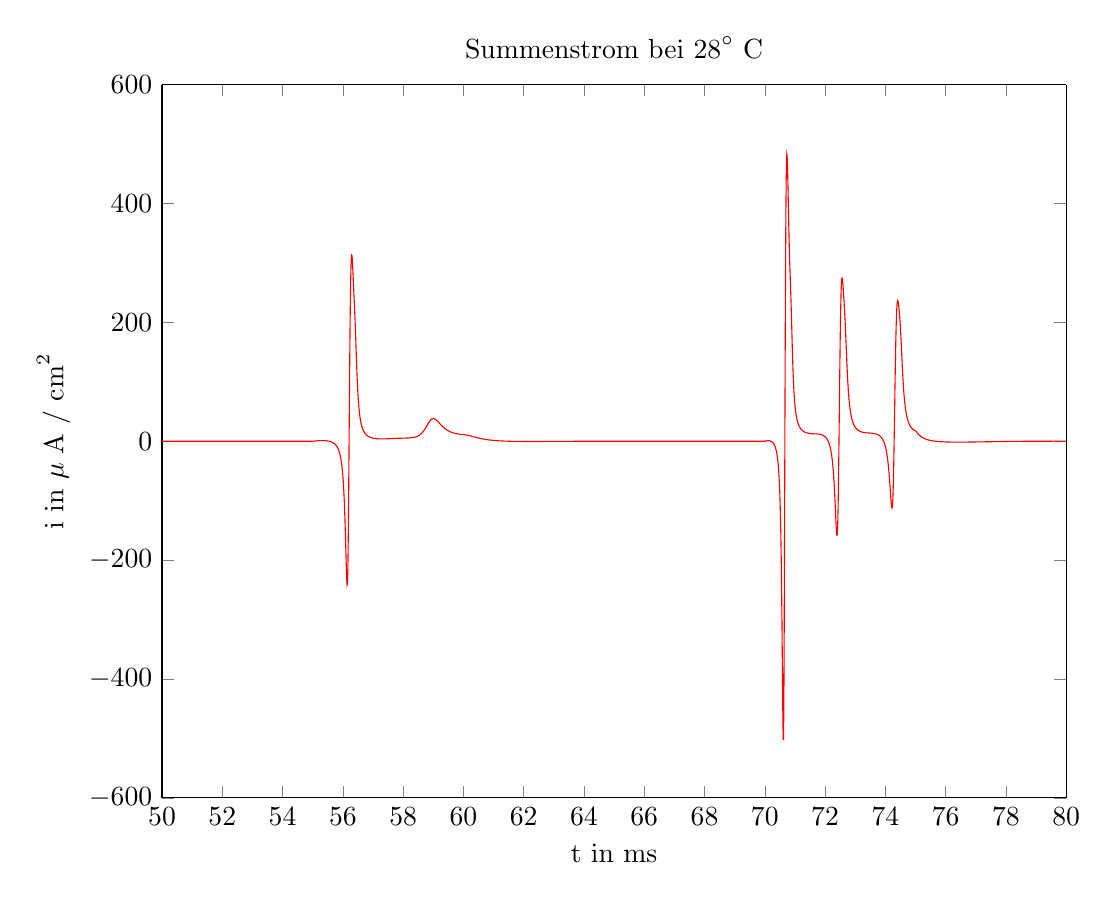
\begin{tikzpicture}

\begin{axis}[%
width=4.520833in,
height=3.565625in,
at={(0.758333in,0.48125in)},
scale only axis,
separate axis lines,
every outer x axis line/.append style={black},
every x tick label/.append style={font=\color{black}},
xmin=50,
xmax=80,
xlabel={t in ms},
every outer y axis line/.append style={black},
every y tick label/.append style={font=\color{black}},
ymin=-600,
ymax=600,
ylabel={$\text{i in }\mu\text{ A / cm}^\text{2}$},
title={$\text{Summenstrom bei 28}^\circ\text{ C}$}
]
\addplot [color=red,solid,forget plot]
  table[row sep=crcr]{%
50	0.00673795292807133\\
50.01	0.00696927342636799\\
50.02	0.00719414342133273\\
50.03	0.00741265068451336\\
50.04	0.00762488252902527\\
50.05	0.00783092579987121\\
50.06	0.00803086686453014\\
50.07	0.00822479160390222\\
50.08	0.00841278540348744\\
50.09	0.00859493314490889\\
50.1	0.0087713191976837\\
50.11	0.00894202741132322\\
50.12	0.0091071411076693\\
50.13	0.00926674307353936\\
50.14	0.00942091555363422\\
50.15	0.00956974024371338\\
50.16	0.00971329828403933\\
50.17	0.00985167025308487\\
50.18	0.00998493616149565\\
50.19	0.0101131754463042\\
50.2	0.0102364669653969\\
50.21	0.0103548889922385\\
50.22	0.0104685192108254\\
50.23	0.0105774347108643\\
50.24	0.0106817119832323\\
50.25	0.0107814269156186\\
50.26	0.0108766547884129\\
50.27	0.0109674702708409\\
50.28	0.0110539474172677\\
50.29	0.0111361596637747\\
50.3	0.0112141798249068\\
50.31	0.0112880800906501\\
50.32	0.0113579320236026\\
50.33	0.0114238065563703\\
50.34	0.0114857739891261\\
50.35	0.0115439039873908\\
50.36	0.0115982655799911\\
50.37	0.0116489271572258\\
50.38	0.0116959564691763\\
50.39	0.0117394206242403\\
50.4	0.0117793860878246\\
50.41	0.011815918681203\\
50.42	0.0118490835805636\\
50.43	0.0118789453161932\\
50.44	0.0119055677718753\\
50.45	0.0119290141843917\\
50.46	0.0119493471432217\\
50.47	0.0119666285903741\\
50.48	0.0119809198203877\\
50.49	0.0119922814804521\\
50.5	0.0120007735707084\\
50.51	0.0120064554446522\\
50.52	0.0120093858097055\\
50.53	0.0120096227279167\\
50.54	0.0120072236167768\\
50.55	0.0120022452501769\\
50.56	0.0119947437595029\\
50.57	0.0119847746348318\\
50.58	0.0119723927262512\\
50.59	0.0119576522453175\\
50.6	0.0119406067665935\\
50.61	0.01192130922934\\
50.62	0.0118998119392697\\
50.63	0.0118761665704517\\
50.64	0.0118504241672777\\
50.65	0.0118226351465602\\
50.66	0.0117928492997295\\
50.67	0.0117611157950859\\
50.68	0.0117274831801901\\
50.69	0.0116919993843347\\
50.7	0.0116547117210692\\
50.71	0.0116156668908687\\
50.72	0.011574910983823\\
50.73	0.0115324894824478\\
50.74	0.0114884472645724\\
50.75	0.0114428286062633\\
50.76	0.0113956771848835\\
50.77	0.0113470360821624\\
50.78	0.0112969477873768\\
50.79	0.0112454542005769\\
50.8	0.011192596635877\\
50.81	0.0111384158248193\\
50.82	0.0110829519197893\\
50.83	0.0110262444974891\\
50.84	0.0109683325624763\\
50.85	0.0109092545507408\\
50.86	0.0108490483333354\\
50.87	0.0107877512200782\\
50.88	0.0107253999632744\\
50.89	0.0106620307614942\\
50.9	0.0105976792634062\\
50.91	0.0105323805716369\\
50.92	0.010466169246675\\
50.93	0.0103990793108171\\
50.94	0.0103311442521523\\
50.95	0.0102623970285709\\
50.96	0.0101928700718203\\
50.97	0.0101225952915871\\
50.98	0.0100516040795995\\
50.99	0.00997992731377773\\
51	0.00990759536238794\\
51.01	0.00983463808823615\\
51.02	0.0097610848528964\\
51.03	0.00968696452093187\\
51.04	0.00961230546416125\\
51.05	0.00953713556592817\\
51.06	0.00946148222540844\\
51.07	0.00938537236190573\\
51.08	0.009308832419201\\
51.09	0.00923188836986188\\
51.1	0.00915456571962059\\
51.11	0.0090768895117308\\
51.12	0.00899888433133622\\
51.13	0.00892057430985593\\
51.14	0.00884198312938222\\
51.15	0.00876313402706197\\
51.16	0.00868404979950688\\
51.17	0.00860475280720863\\
51.18	0.00852526497892603\\
51.19	0.00844560781610859\\
51.2	0.00836580239730633\\
51.21	0.00828586938258224\\
51.22	0.008205829017911\\
51.23	0.00812570113960032\\
51.24	0.00804550517868696\\
51.25	0.00796526016533461\\
51.26	0.00788498473323829\\
51.27	0.00780469712399956\\
51.28	0.00772441519151679\\
51.29	0.00764415640636029\\
51.3	0.00756393786012621\\
51.31	0.00748377626981034\\
51.32	0.00740368798214064\\
51.33	0.00732368897791735\\
51.34	0.00724379487632865\\
51.35	0.00716402093927249\\
51.36	0.00708438207564654\\
51.37	0.00700489284563455\\
51.38	0.00692556746498108\\
51.39	0.0068464198092193\\
51.4	0.00676746341795065\\
51.41	0.00668871149902683\\
51.42	0.00661017693278465\\
51.43	0.00653187227620933\\
51.44	0.00645380976711918\\
51.45	0.00637600132830629\\
51.46	0.00629845857167188\\
51.47	0.00622119280233147\\
51.48	0.00614421502270845\\
51.49	0.0060675359366078\\
51.5	0.00599116595325144\\
51.51	0.0059151151913226\\
51.52	0.00583939348295059\\
51.53	0.00576401037770546\\
51.54	0.00568897514655253\\
51.55	0.00561429678578529\\
51.56	0.00553998402094136\\
51.57	0.00546604531068784\\
51.58	0.00539248885067112\\
51.59	0.00531932257738044\\
51.6	0.00524655417193953\\
51.61	0.00517419106390227\\
51.62	0.00510224043500518\\
51.63	0.00503070922291116\\
51.64	0.00495960412491581\\
51.65	0.00488893160162851\\
51.66	0.00481869788062728\\
51.67	0.00474890896008739\\
51.68	0.004679570612379\\
51.69	0.00461068838764866\\
51.7	0.00454226761735388\\
51.71	0.00447431341778826\\
51.72	0.00440683069356496\\
51.73	0.00433982414108014\\
51.74	0.00427329825194533\\
51.75	0.00420725731639315\\
51.76	0.0041417054266466\\
51.77	0.00407664648027195\\
51.78	0.00401208418349208\\
51.79	0.00394802205447409\\
51.8	0.00388446342658577\\
51.81	0.00382141145162818\\
51.82	0.00375886910303569\\
51.83	0.00369683917904995\\
51.84	0.00363532430584668\\
51.85	0.00357432694066873\\
51.86	0.00351384937487698\\
51.87	0.00345389373703542\\
51.88	0.00339446199591231\\
51.89	0.00333555596348267\\
51.9	0.00327717729787924\\
51.91	0.00321932750633458\\
51.92	0.00316200794807697\\
51.93	0.00310521983721568\\
51.94	0.00304896424556933\\
51.95	0.00299324210548724\\
51.96	0.00293805421262494\\
51.97	0.00288340122872022\\
51.98	0.00282928368428248\\
51.99	0.00277570198131416\\
52	0.00272265639596814\\
52.01	0.00267014708118163\\
52.02	0.00261817406927678\\
52.03	0.00256673727454348\\
52.04	0.00251583649578491\\
52.05	0.0024654714188328\\
52.06	0.00241564161903574\\
52.07	0.00236634656372248\\
52.08	0.00231758561462136\\
52.09	0.00226935803027972\\
52.1	0.00222166296840731\\
52.11	0.00217449948824733\\
52.12	0.00212786655287234\\
52.13	0.00208176303148955\\
52.14	0.00203618770166569\\
52.15	0.00199113925159722\\
52.16	0.00194661628227077\\
52.17	0.00190261730966723\\
52.18	0.00185914076688531\\
52.19	0.00181618500627501\\
52.2	0.00177374830150567\\
52.21	0.00173182884965151\\
52.22	0.00169042477320769\\
52.23	0.00164953412210345\\
52.24	0.00160915487568536\\
52.25	0.00156928494465802\\
52.26	0.00152992217302739\\
52.27	0.00149106433997925\\
52.28	0.00145270916176399\\
52.29	0.00141485429355148\\
52.3	0.00137749733122527\\
52.31	0.00134063581320731\\
52.32	0.00130426722218591\\
52.33	0.0012683889869094\\
52.34	0.00123299848385683\\
52.35	0.0011980930389508\\
52.36	0.00116366992922545\\
52.37	0.00112972638445408\\
52.38	0.00109625958878512\\
52.39	0.00106326668230761\\
52.4	0.0010307447626432\\
52.41	0.000998690886472087\\
52.42	0.000967102071071757\\
52.43	0.00093597529577405\\
52.44	0.00090530750348039\\
52.45	0.000875095602085096\\
52.46	0.000845336465896018\\
52.47	0.000816026937046299\\
52.48	0.000787163826871939\\
52.49	0.000758743917257831\\
52.5	0.000730763961986458\\
52.51	0.000703220688030193\\
52.52	0.000676110796846263\\
52.53	0.000649430965644182\\
52.54	0.000623177848634526\\
52.55	0.000597348078242188\\
52.56	0.000571938266308525\\
52.57	0.000546945005281518\\
52.58	0.000522364869361969\\
52.59	0.000498194415647468\\
52.6	0.00047443018524973\\
52.61	0.000451068704397706\\
52.62	0.000428106485497626\\
52.63	0.000405540028204587\\
52.64	0.000383365820450621\\
52.65	0.000361580339475864\\
52.66	0.000340180052808226\\
52.67	0.00031916141925814\\
52.68	0.000298520889862264\\
52.69	0.00027825490883604\\
52.7	0.000258359914493411\\
52.71	0.000238832340146544\\
52.72	0.00021966861499978\\
52.73	0.000200865165005393\\
52.74	0.000182418413718466\\
52.75	0.00016432478313444\\
52.76	0.000146580694499132\\
52.77	0.000129182569099662\\
52.78	0.000112126829057146\\
52.79	9.54098980732176e-05\\
52.8	7.90282021996269e-05\\
52.81	6.29781705461241e-05\\
52.82	4.72562360060991e-05\\
52.83	3.18588359484728e-05\\
52.84	1.67824129082561e-05\\
52.85	2.02341524557781e-06\\
52.86	-1.24217022041684e-05\\
52.87	-2.65564774912797e-05\\
52.88	-4.03844409264664e-05\\
52.89	-5.39091144946546e-05\\
52.9	-6.71340112416985e-05\\
52.91	-8.00626347148281e-05\\
52.92	-9.26984783866658e-05\\
52.93	-0.000105045025125872\\
52.94	-0.000117105746647361\\
52.95	-0.000128884102999827\\
52.96	-0.000140383542063027\\
52.97	-0.00015160749904819\\
52.98	-0.00016255939602372\\
52.99	-0.000173242641443583\\
53	-0.000183660629706761\\
53.01	-0.00019381674069896\\
53.02	-0.000203714339384042\\
53.03	-0.000213356775362605\\
53.04	-0.00022274738250605\\
53.05	-0.000231889478526703\\
53.06	-0.0002407863646261\\
53.07	-0.00024944132511262\\
53.08	-0.000257857627051106\\
53.09	-0.000266038519923573\\
53.1	-0.000273987235271278\\
53.11	-0.000281706986415387\\
53.12	-0.000289200968096814\\
53.13	-0.000296472356215105\\
53.14	-0.000303524307516234\\
53.15	-0.000310359959311057\\
53.16	-0.000316982429223955\\
53.17	-0.000323394814914391\\
53.18	-0.000329600193831325\\
53.19	-0.000335601622985404\\
53.2	-0.000341402138704261\\
53.21	-0.000347004756414915\\
53.22	-0.000352412470433716\\
53.23	-0.000357628253761177\\
53.24	-0.000362655057894123\\
53.25	-0.000367495812632512\\
53.26	-0.000372153425911126\\
53.27	-0.000376630783625043\\
53.28	-0.000380930749476871\\
53.29	-0.000385056164813768\\
53.3	-0.000389009848503541\\
53.31	-0.000392794596782764\\
53.32	-0.000396413183132882\\
53.33	-0.000399868358168742\\
53.34	-0.00040316284951647\\
53.35	-0.0004062993617171\\
53.36	-0.000409280576119109\\
53.37	-0.000412109150801143\\
53.38	-0.00041478772048098\\
53.39	-0.000417318896439145\\
53.4	-0.000419705266443415\\
53.41	-0.000421949394703525\\
53.42	-0.000424053821794335\\
53.43	-0.000426021064622972\\
53.44	-0.000427853616370211\\
53.45	-0.000429553946463379\\
53.46	-0.000431124500532842\\
53.47	-0.000432567700402675\\
53.48	-0.000433885944057355\\
53.49	-0.000435081605627996\\
53.5	-0.000436157035388351\\
53.51	-0.000437114559749929\\
53.52	-0.00043795648125311\\
53.53	-0.000438685078595125\\
53.54	-0.000439302606620284\\
53.55	-0.000439811296349735\\
53.56	-0.000440213354995223\\
53.57	-0.000440510965994179\\
53.58	-0.000440706289031034\\
53.59	-0.000440801460081186\\
53.6	-0.00044079859144297\\
53.61	-0.000440699771783404\\
53.62	-0.000440507066196805\\
53.63	-0.000440222516236322\\
53.64	-0.000439848139995203\\
53.65	-0.000439385932144098\\
53.66	-0.000438837864014996\\
53.67	-0.000438205883652287\\
53.68	-0.000437491915893151\\
53.69	-0.000436697862443935\\
53.7	-0.000435825601956985\\
53.71	-0.000434876990105249\\
53.72	-0.000433853859675537\\
53.73	-0.000432758020661339\\
53.74	-0.000431591260339648\\
53.75	-0.000430355343373101\\
53.76	-0.000429052011909903\\
53.77	-0.000427682985679745\\
53.78	-0.000426249962099057\\
53.79	-0.000424754616370038\\
53.8	-0.000423198601604113\\
53.81	-0.000421583548915638\\
53.82	-0.000419911067543577\\
53.83	-0.000418182744960305\\
53.84	-0.000416400146999951\\
53.85	-0.000414564817971641\\
53.86	-0.000412678280784284\\
53.87	-0.000410742037059375\\
53.88	-0.000408757567273543\\
53.89	-0.000406726330877127\\
53.9	-0.000404649766427845\\
53.91	-0.000402529291714249\\
53.92	-0.000400366303909383\\
53.93	-0.000398162179672035\\
53.94	-0.000395918275323925\\
53.95	-0.000393635926948743\\
53.96	-0.000391316450561341\\
53.97	-0.000388961142231636\\
53.98	-0.000386571278237824\\
53.99	-0.000384148115198713\\
54	-0.000381692890229157\\
54.01	-0.000379206821075062\\
54.02	-0.000376691106276805\\
54.03	-0.000374146925296248\\
54.04	-0.00037157543868549\\
54.05	-0.000368977788224978\\
54.06	-0.000366355097079385\\
54.07	-0.000363708469945045\\
54.08	-0.000361038993204943\\
54.09	-0.000358347735085474\\
54.1	-0.000355635745806993\\
54.11	-0.000352904057738801\\
54.12	-0.000350153685556798\\
54.13	-0.000347385626389585\\
54.14	-0.000344600859988109\\
54.15	-0.000341800348875765\\
54.16	-0.000338985038510486\\
54.17	-0.000336155857430853\\
54.18	-0.000333313717422623\\
54.19	-0.00033045951368349\\
54.2	-0.000327594124961639\\
54.21	-0.00032471841373205\\
54.22	-0.000321833226350599\\
54.23	-0.000318939393216144\\
54.24	-0.000316037728914864\\
54.25	-0.000313129032398773\\
54.26	-0.000310214087126948\\
54.27	-0.000307293661241825\\
54.28	-0.000304368507716646\\
54.29	-0.00030143936451843\\
54.3	-0.000298506954762523\\
54.31	-0.000295571986880461\\
54.32	-0.000292635154765186\\
54.33	-0.000289697137946909\\
54.34	-0.000286758601732995\\
54.35	-0.00028382019737494\\
54.36	-0.000280882562230023\\
54.37	-0.000277946319902966\\
54.38	-0.000275012080429349\\
54.39	-0.000272080440398614\\
54.4	-0.000269151983136595\\
54.41	-0.000266227278847175\\
54.42	-0.000263306884777048\\
54.43	-0.000260391345356936\\
54.44	-0.000257481192377895\\
54.45	-0.000254576945115215\\
54.46	-0.000251679110505609\\
54.47	-0.000248788183291104\\
54.48	-0.000245904646170025\\
54.49	-0.000243028969950654\\
54.5	-0.000240161613703105\\
54.51	-0.000237303024897884\\
54.52	-0.000234453639570642\\
54.53	-0.000231613882467396\\
54.54	-0.000228784167183971\\
54.55	-0.000225964896324982\\
54.56	-0.000223156461637952\\
54.57	-0.000220359244169632\\
54.58	-0.00021757361440633\\
54.59	-0.000214799932412024\\
54.6	-0.000212038547983351\\
54.61	-0.000209289800789492\\
54.62	-0.00020655402051295\\
54.63	-0.00020383152698189\\
54.64	-0.00020112263031713\\
54.65	-0.000198427631074249\\
54.66	-0.00019574682038348\\
54.67	-0.000193080480074936\\
54.68	-0.000190428882826055\\
54.69	-0.000187792292293487\\
54.7	-0.000185170963251657\\
54.71	-0.000182565141716662\\
54.72	-0.000179975065088378\\
54.73	-0.000177400962280583\\
54.74	-0.000174843053849738\\
54.75	-0.000172301552126441\\
54.76	-0.000169776661339771\\
54.77	-0.000167268577752733\\
54.78	-0.00016477748978927\\
54.79	-0.000162303578151057\\
54.8	-0.000159847015944958\\
54.81	-0.000157407968820689\\
54.82	-0.000154986595071183\\
54.83	-0.000152583045776034\\
54.84	-0.000150197464908963\\
54.85	-0.00014782998946572\\
54.86	-0.000145480749576432\\
54.87	-0.000143149868614856\\
54.88	-0.000140837463348031\\
54.89	-0.000138543644010003\\
54.9	-0.000136268514447924\\
54.91	-0.000134012172221532\\
54.92	-0.000131774708717725\\
54.93	-0.000129556209264692\\
54.94	-0.000127356753235386\\
54.95	-0.000125176414174977\\
54.96	-0.000123015259885229\\
54.97	-0.000120873352546624\\
54.98	-0.000118750748819618\\
54.99	-0.000116647499953881\\
55	-0.000114563651886002\\
55.01	-0.000112499245351838\\
55.02	0.0855341636215372\\
55.03	0.157039472235237\\
55.04	0.218996146879654\\
55.05	0.274623645281082\\
55.06	0.325907348726759\\
55.07	0.374081237618904\\
55.08	0.419912716404069\\
55.09	0.463874553938301\\
55.1	0.506251113905287\\
55.11	0.547205069323156\\
55.12	0.58681978549758\\
55.13	0.625126467224683\\
55.14	0.662121649968082\\
55.15	0.697778516398509\\
55.16	0.732054236973449\\
55.17	0.76489473544416\\
55.18	0.796237777769037\\
55.19	0.826014963614443\\
55.2	0.854152995286372\\
55.21	0.880574467446299\\
55.22	0.905198335961316\\
55.23	0.927940169062755\\
55.24	0.948712248034904\\
55.25	0.967423561137816\\
55.26	0.983979719019641\\
55.27	0.998282809675214\\
55.28	1.010231204232\\
55.29	1.01971932030323\\
55.3	1.02663734656628\\
55.31	1.03087093009388\\
55.32	1.03230082645247\\
55.33	1.03080251146512\\
55.34	1.02624575266878\\
55.35	1.01849413777782\\
55.36	1.00740455683079\\
55.37	0.99282663409719\\
55.38	0.974602105221273\\
55.39	0.952564134456048\\
55.4	0.926536566168942\\
55.41	0.896333104065363\\
55.42	0.861756410758595\\
55.43	0.822597119397946\\
55.44	0.778632748032996\\
55.45	0.729626506220816\\
55.46	0.675325982052942\\
55.47	0.615461696263919\\
55.48	0.54974550835528\\
55.49	0.477868857692624\\
55.5	0.399500820271878\\
55.51	0.314285959255446\\
55.52	0.221841944398149\\
55.53	0.121756912052145\\
55.54	0.0135865334843113\\
55.55	-0.103149245327313\\
55.56	-0.228969834536159\\
55.57	-0.364438050150665\\
55.58	-0.510164637992476\\
55.59	-0.666813335515307\\
55.6	-0.835106544753575\\
55.61	-1.01583170093121\\
55.62	-1.20984843443968\\
55.63	-1.41809663934677\\
55.64	-1.64160557975447\\
55.65	-1.88150418670232\\
55.66	-2.13903272353639\\
55.67	-2.41555602748776\\
55.68	-2.71257857054275\\
55.69	-3.03176162464531\\
55.7	-3.37494286619939\\
55.71	-3.7441588143697\\
55.72	-4.14167056880617\\
55.73	-4.5699933975717\\
55.74	-5.03193082819255\\
55.75	-5.53061401749213\\
55.76	-6.06954732361029\\
55.77	-6.65266118171702\\
55.78	-7.28437359991049\\
55.79	-7.9696618515337\\
55.8	-8.71414625415173\\
55.81	-9.52418830505926\\
55.82	-10.4070059018681\\
55.83	-11.3708089300836\\
55.84	-12.4249591653561\\
55.85	-13.580159235664\\
55.86	-14.8486763378515\\
55.87	-16.2446075214303\\
55.88	-17.7841946513045\\
55.89	-19.4861986357723\\
55.9	-21.3723441224649\\
55.91	-23.4678475332875\\
55.92	-25.8020428429129\\
55.93	-28.4091205491309\\
55.94	-31.3289951990781\\
55.95	-34.6083145127847\\
55.96	-38.3016166982378\\
55.97	-42.4726288338945\\
55.98	-47.1956730415202\\
55.99	-52.5571002481322\\
56	-58.6565904366973\\
56.01	-65.608023007007\\
56.02	-73.5394007653959\\
56.03	-82.5909630961605\\
56.04	-92.9100925910931\\
56.05	-104.640845908722\\
56.06	-117.904892055484\\
56.07	-132.769390750523\\
56.08	-149.196220916746\\
56.09	-166.966834431807\\
56.1	-185.579598679934\\
56.11	-204.124589209699\\
56.12	-221.157558281223\\
56.13	-234.621098985677\\
56.14	-241.890043033683\\
56.15	-240.029450242083\\
56.16	-226.31458267331\\
56.17	-198.949531260467\\
56.18	-157.76325281868\\
56.19	-104.56608919176\\
56.2	-42.9406109088037\\
56.21	22.4876038824934\\
56.22	86.990931743464\\
56.23	146.531715166093\\
56.24	198.20464557051\\
56.25	240.334201891064\\
56.26	272.344101713459\\
56.27	294.523021198267\\
56.28	307.770842053163\\
56.29	313.369480174189\\
56.3	312.795528828165\\
56.31	307.574579516944\\
56.32	299.165778721056\\
56.33	288.862438767813\\
56.34	277.702856261822\\
56.35	266.399935617651\\
56.36	255.307886902631\\
56.37	244.442104094081\\
56.38	233.556533961739\\
56.39	222.268131208911\\
56.4	210.204717268768\\
56.41	197.142341291516\\
56.42	183.094513803492\\
56.43	168.325027245282\\
56.44	153.281523519319\\
56.45	138.479115864973\\
56.46	124.382560961786\\
56.47	111.32832349547\\
56.48	99.5010627027836\\
56.49	88.952789442365\\
56.5	79.6418145955523\\
56.51	71.4722783452674\\
56.52	64.3245737663402\\
56.53	58.0748651750368\\
56.54	52.6057977662219\\
56.55	47.8113646528439\\
56.56	43.5983817341195\\
56.57	39.886204554479\\
56.58	36.6056495174094\\
56.59	33.6976387887482\\
56.6	31.1118282345575\\
56.61	28.8053358287433\\
56.62	26.7416145015725\\
56.63	24.8894772585345\\
56.64	23.2222658362573\\
56.65	21.7171475695735\\
56.66	20.3545234655651\\
56.67	19.1175311028344\\
56.68	17.9916275658095\\
56.69	16.9642395197028\\
56.7	16.0244694119965\\
56.71	15.1628485089725\\
56.72	14.3711289892597\\
56.73	13.6421086139008\\
56.74	12.9694825881724\\
56.75	12.347718146925\\
56.76	11.7719481572113\\
56.77	11.2378806631353\\
56.78	10.7417218195191\\
56.79	10.2801100917035\\
56.8	9.85005995434443\\
56.81	9.44891361567696\\
56.82	9.07429953636779\\
56.83	8.72409671284868\\
56.84	8.39640386136739\\
56.85	8.08951277703398\\
56.86	7.80188525688734\\
56.87	7.5321330715635\\
56.88	7.2790005498732\\
56.89	7.04134940724203\\
56.9	6.81814550478777\\
56.91	6.60844727265817\\
56.92	6.41139557064762\\
56.93	6.22620479230649\\
56.94	6.05215504678269\\
56.95	5.88858527634306\\
56.96	5.73488718761755\\
56.97	5.59049989167461\\
56.98	5.45490516255651\\
56.99	5.32762323628106\\
57	5.20820908288705\\
57.01	5.0962490931448\\
57.02	4.99135812930439\\
57.03	4.89317689590911\\
57.04	4.80136959242497\\
57.05	4.71562181436685\\
57.06	4.63563867385575\\
57.07	4.56114311421697\\
57.08	4.4918743964102\\
57.09	4.42758673783938\\
57.1	4.36804808648311\\
57.11	4.31303901536597\\
57.12	4.26235172420094\\
57.13	4.21578913661034\\
57.14	4.17316408270823\\
57.15	4.13429855802941\\
57.16	4.09902305084078\\
57.17	4.067175930791\\
57.18	4.03860289266061\\
57.19	4.01315644968196\\
57.2	3.99069547151944\\
57.21	3.97108476254628\\
57.22	3.9541946765345\\
57.23	3.93990076429709\\
57.24	3.92808345119452\\
57.25	3.91862774174591\\
57.26	3.91142294887564\\
57.27	3.90636244558217\\
57.28	3.90334343704278\\
57.29	3.90226675136826\\
57.3	3.90303664739952\\
57.31	3.9055606380956\\
57.32	3.9097493282023\\
57.33	3.91551626501529\\
57.34	3.92277780116191\\
57.35	3.93145296842463\\
57.36	3.94146336171709\\
57.37	3.9527330324024\\
57.38	3.96518839021371\\
57.39	3.97875811310072\\
57.4	3.99337306438222\\
57.41	4.00896621663694\\
57.42	4.02547258181083\\
57.43	4.04282914706174\\
57.44	4.0609748159008\\
57.45	4.07985035422522\\
57.46	4.09939834086971\\
57.47	4.11956312233367\\
57.48	4.14029077136927\\
57.49	4.16152904914128\\
57.5	4.18322737069412\\
57.51	4.20533677348423\\
57.52	4.22780988875775\\
57.53	4.25060091557413\\
57.54	4.27366559729575\\
57.55	4.29696120038286\\
57.56	4.32044649535141\\
57.57	4.34408173976852\\
57.58	4.36782866317833\\
57.59	4.39165045386691\\
57.6	4.41551174739197\\
57.61	4.43937861681864\\
57.62	4.46321856461908\\
57.63	4.48700051620871\\
57.64	4.51069481510767\\
57.65	4.53427321973179\\
57.66	4.55770890183191\\
57.67	4.58097644661636\\
57.68	4.60405185460644\\
57.69	4.62691254528981\\
57.7	4.64953736265248\\
57.71	4.67190658268525\\
57.72	4.69400192297611\\
57.73	4.71580655451611\\
57.74	4.73730511586213\\
57.75	4.75848372981608\\
57.76	4.77933002279738\\
57.77	4.79983314710177\\
57.78	4.81998380625763\\
57.79	4.83977428370873\\
57.8	4.85919847507073\\
57.81	4.8782519242282\\
57.82	4.89693186355851\\
57.83	4.91523725858953\\
57.84	4.93316885741951\\
57.85	4.9507292452498\\
57.86	4.96792290440396\\
57.87	4.98475628023129\\
57.88	5.00123785331766\\
57.89	5.01737821845314\\
57.9	5.03319017083282\\
57.91	5.04868879999644\\
57.92	5.06389159204142\\
57.93	5.07881854067545\\
57.94	5.09349226770646\\
57.95	5.10793815360123\\
57.96	5.12218447877797\\
57.97	5.13626257633375\\
57.98	5.15020699694353\\
57.99	5.1640556867043\\
58	5.1778501787354\\
58.01	5.19163579938284\\
58.02	5.20546188991325\\
58.03	5.21938204461913\\
58.04	5.23345436629282\\
58.05	5.2477417400596\\
58.06	5.26231212659206\\
58.07	5.27723887575444\\
58.08	5.29260106174963\\
58.09	5.30848384085763\\
58.1	5.32497883286519\\
58.11	5.34218452728661\\
58.12	5.36020671546641\\
58.13	5.37915894963085\\
58.14	5.39916302991881\\
58.15	5.42034952036176\\
58.16	5.44285829470723\\
58.17	5.46683911287326\\
58.18	5.49245222868732\\
58.19	5.51986902939354\\
58.2	5.54927270720299\\
58.21	5.58085896290602\\
58.22	5.61483674125702\\
58.23	5.65142899747482\\
58.24	5.69087349376418\\
58.25	5.73342362425251\\
58.26	5.77934926613449\\
58.27	5.82893765412325\\
58.28	5.88249427450146\\
58.29	5.94034377414421\\
58.3	6.00283087883082\\
58.31	6.07032131396531\\
58.32	6.14320271947092\\
58.33	6.22188554910067\\
58.34	6.30680394270156\\
58.35	6.39841655807221\\
58.36	6.49720734695369\\
58.37	6.60368625738254\\
58.38	6.71838984210709\\
58.39	6.84188175002476\\
58.4	6.97475307463765\\
58.41	7.11762253036069\\
58.42	7.27113642416397\\
58.43	7.43596838651639\\
58.44	7.612818821958\\
58.45	7.80241403591295\\
58.46	8.00550499062842\\
58.47	8.22286563947018\\
58.48	8.45529078532338\\
58.49	8.70359340566107\\
58.5	8.96860138410243\\
58.51	9.25115358615814\\
58.52	9.55209521555524\\
58.53	9.87227238727815\\
58.54	10.2125258545123\\
58.55	10.5736838293216\\
58.56	10.9565538414388\\
58.57	11.3619135863394\\
58.58	11.7905007231464\\
58.59	12.243001595241\\
58.6	12.7200388620844\\
58.61	13.2221580500277\\
58.62	13.7498130531023\\
58.63	14.3033506421959\\
58.64	14.8829940727865\\
58.65	15.4888259176011\\
58.66	16.1207702910825\\
58.67	16.7785746771357\\
58.68	17.4617916197927\\
58.69	18.1697605874212\\
58.7	18.9015903738731\\
58.71	19.6561424530936\\
58.72	20.4320157554326\\
58.73	21.2275333819947\\
58.74	22.0407318152354\\
58.75	22.8693532166185\\
58.76	23.7108414220884\\
58.77	24.5623422496964\\
58.78	25.4207087170675\\
58.79	26.2825117256715\\
58.8	27.1440567004674\\
58.81	28.0014065744194\\
58.82	28.8504113755702\\
58.83	29.6867445091273\\
58.84	30.505945629485\\
58.85	31.3034697706828\\
58.86	32.0747421544479\\
58.87	32.8152178315228\\
58.88	33.5204450460777\\
58.89	34.1861309588831\\
58.9	34.8082081387582\\
58.91	35.382900050843\\
58.92	35.9067836514202\\
58.93	36.3768471574611\\
58.94	36.7905411064517\\
58.95	37.1458209648836\\
58.96	37.4411797821613\\
58.97	37.6756697133677\\
58.98	37.8489116347067\\
58.99	37.9610925281057\\
59	38.0129507897465\\
59.01	38.005750091459\\
59.02	37.9412428638335\\
59.03	37.8216248478674\\
59.04	37.6494824553129\\
59.05	37.4277348710487\\
59.06	37.1595729165498\\
59.07	36.8483966732462\\
59.08	36.4977537475839\\
59.09	36.1112798617313\\
59.1	35.6926431953409\\
59.11	35.2454936069909\\
59.12	34.7734175511968\\
59.13	34.2798991985668\\
59.14	33.7682879797003\\
59.15	33.2417725205168\\
59.16	32.7033607260133\\
59.17	32.1558656048571\\
59.18	31.6018963088149\\
59.19	31.0438537859548\\
59.2	30.4839304098601\\
59.21	29.9241129425759\\
59.22	29.366188209948\\
59.23	28.8117509078059\\
59.24	28.2622130099861\\
59.25	27.718814309195\\
59.26	27.1826336848024\\
59.27	26.6546007544222\\
59.28	26.1355076260629\\
59.29	25.6260205230159\\
59.3	25.1266911034436\\
59.31	24.6379673403604\\
59.32	24.1602038652562\\
59.33	23.6936717102355\\
59.34	23.2385674096206\\
59.35	22.7950214430429\\
59.36	22.363106018693\\
59.37	21.9428422082316\\
59.38	21.534206454439\\
59.39	21.1371364795635\\
59.4	20.7515366269821\\
59.41	20.3772826716611\\
59.42	20.0142261363593\\
59.43	19.6621981508745\\
59.44	19.32101289116\\
59.45	18.9904706340508\\
59.46	18.6703604618153\\
59.47	18.3604626489329\\
59.48	18.0605507615025\\
59.49	17.7703934976002\\
59.5	17.4897562947893\\
59.51	17.218402728903\\
59.52	16.956095726188\\
59.53	16.7025986089642\\
59.54	16.4576759931145\\
59.55	16.2210945540004\\
59.56	15.9926236757956\\
59.57	15.7720359977437\\
59.58	15.5591078694866\\
59.59	15.3536197263545\\
59.6	15.1553563943711\\
59.61	14.9641073336902\\
59.62	14.7796668282368\\
59.63	14.6018341284789\\
59.64	14.4304135534864\\
59.65	14.2652145577449\\
59.66	14.1060517675704\\
59.67	13.9527449914155\\
59.68	13.8051192078588\\
59.69	13.6630045346223\\
59.7	13.526236181567\\
59.71	13.3946543902572\\
59.72	13.2681043623723\\
59.73	13.1464361789589\\
59.74	13.0295047122694\\
59.75	12.9171695317089\\
59.76	12.8092948052155\\
59.77	12.7057491972244\\
59.78	12.6064057642111\\
59.79	12.5111418486732\\
59.8	12.4198389722871\\
59.81	12.3323827288712\\
59.82	12.2486626776931\\
59.83	12.1685722375728\\
59.84	12.092008582165\\
59.85	12.0188725367348\\
59.86	11.9490684766907\\
59.87	11.882504228083\\
59.88	11.8190909702382\\
59.89	11.75874314066\\
59.9	11.7013783422938\\
59.91	11.6469172532257\\
59.92	11.5952835388598\\
59.93	11.5464037665984\\
59.94	11.5002073230287\\
59.95	11.4566263336066\\
59.96	11.4155955848119\\
59.97	11.3770524487394\\
59.98	11.3409368100795\\
59.99	11.307190995433\\
60	11.2757597049003\\
60.01	11.2465899458742\\
60.02	11.219630968967\\
60.03	11.0425232479651\\
60.04	10.9080147819206\\
60.05	10.8024728526591\\
60.06	10.7142527442638\\
60.07	10.6353135238877\\
60.08	10.560239788287\\
60.09	10.4854651277362\\
60.1	10.4087044310227\\
60.11	10.3285503800271\\
60.12	10.2441916486937\\
60.13	10.1552183544496\\
60.14	10.0614887666906\\
60.15	9.96303843894577\\
60.16	9.86001845667545\\
60.17	9.75265354764481\\
60.18	9.64121369038486\\
60.19	9.52599487531522\\
60.2	9.40730606675502\\
60.21	9.28546036773175\\
60.22	9.16076903813569\\
60.23	9.03353745598143\\
60.24	8.90406240797518\\
60.25	8.77263029517368\\
60.26	8.63951597366573\\
60.27	8.50498204026266\\
60.28	8.36927843360989\\
60.29	8.23264226168413\\
60.3	8.09529779388815\\
60.31	7.95745657430518\\
60.32	7.81931762508464\\
60.33	7.68106771737374\\
60.34	7.54288169300658\\
60.35	7.40492282419101\\
60.36	7.26734320127947\\
60.37	7.13028414076102\\
60.38	6.99387660712552\\
60.39	6.85824164339823\\
60.4	6.72349080603698\\
60.41	6.58972660059889\\
60.42	6.45704291517093\\
60.43	6.3255254490488\\
60.44	6.19525213456755\\
60.45	6.06629355034702\\
60.46	5.9387133245288\\
60.47	5.81256852685501\\
60.48	5.68791004867889\\
60.49	5.56478297020751\\
60.5	5.44322691446093\\
60.51	5.3232763875925\\
60.52	5.20496110535517\\
60.53	5.0883063056192\\
60.54	4.9733330469509\\
60.55	4.86005849335077\\
60.56	4.74849618532489\\
60.57	4.63865629752628\\
60.58	4.53054588325539\\
60.59	4.42416910615153\\
60.6	4.3195274594413\\
60.61	4.21661997313644\\
60.62	4.11544340959408\\
60.63	4.01599244786631\\
60.64	3.91825985727552\\
60.65	3.82223666065702\\
60.66	3.72791228771181\\
60.67	3.63527471891048\\
60.68	3.54431062038485\\
60.69	3.45500547023739\\
60.7	3.36734367668954\\
60.71	3.28130868848068\\
60.72	3.19688309791756\\
60.73	3.11404873696238\\
60.74	3.03278676673459\\
60.75	2.953077760788\\
60.76	2.87490178251132\\
60.77	2.798238456986\\
60.78	2.72306703762147\\
60.79	2.64936646787371\\
60.8	2.57711543833938\\
60.81	2.5062924395039\\
60.82	2.43687581040866\\
60.83	2.36884378348926\\
60.84	2.30217452582412\\
60.85	2.23684617702025\\
60.86	2.17283688395108\\
60.87	2.11012483254992\\
60.88	2.0486882768511\\
60.89	1.98850556546051\\
60.9	1.929555165627\\
60.91	1.87181568507618\\
60.92	1.81526589175889\\
60.93	1.7598847316579\\
60.94	1.70565134478748\\
60.95	1.65254507951288\\
60.96	1.6005455053089\\
60.97	1.54963242406933\\
60.98	1.49978588007235\\
60.99	1.45098616870045\\
61	1.40321384400715\\
61.01	1.35644972521689\\
61.02	1.31067490223931\\
61.03	1.26587074027349\\
61.04	1.22201888357311\\
61.05	1.17910125843877\\
61.06	1.13710007549937\\
61.07	1.09599783134032\\
61.08	1.05577730953257\\
61.09	1.01642158111267\\
61.1	0.977914004560968\\
61.11	0.940238225321388\\
61.12	0.903378174903749\\
61.13	0.867318069606328\\
61.14	0.832042408894047\\
61.15	0.797535973464944\\
61.16	0.763783823035431\\
61.17	0.730771293872643\\
61.18	0.698483996100011\\
61.19	0.666907810800496\\
61.2	0.636028886939973\\
61.21	0.605833638131656\\
61.22	0.576308739260916\\
61.23	0.547441122988305\\
61.24	0.519217976147349\\
61.25	0.49162673605232\\
61.26	0.46465508673002\\
61.27	0.438290955088601\\
61.28	0.412522507035217\\
61.29	0.387338143553593\\
61.3	0.362726496751454\\
61.31	0.338676425887131\\
61.32	0.315177013383734\\
61.33	0.292217560838627\\
61.34	0.269787585035283\\
61.35	0.247876813963922\\
61.36	0.226475182856769\\
61.37	0.205572830243264\\
61.38	0.185160094030005\\
61.39	0.165227507609773\\
61.4	0.145765796003542\\
61.41	0.126765872038973\\
61.42	0.108218832568542\\
61.43	0.0901159547300647\\
61.44	0.0724486922521499\\
61.45	0.0552086718066627\\
61.46	0.0383876894102273\\
61.47	0.0219777068763181\\
61.48	0.00597084831943251\\
61.49	-0.00964060328746807\\
61.5	-0.0248642095012213\\
61.51	-0.0397073797416292\\
61.52	-0.0541773745687841\\
61.53	-0.068281308904131\\
61.54	-0.0820261551947929\\
61.55	-0.0954187465210188\\
61.56	-0.108465779646496\\
61.57	-0.121173818011616\\
61.58	-0.133549294669701\\
61.59	-0.14559851516637\\
61.6	-0.157327660362286\\
61.61	-0.168742789199596\\
61.62	-0.17984984141245\\
61.63	-0.190654640182041\\
61.64	-0.201162894736635\\
61.65	-0.211380202897176\\
61.66	-0.221312053569003\\
61.67	-0.230963829180336\\
61.68	-0.240340808068167\\
61.69	-0.249448166812247\\
61.7	-0.258290982517883\\
61.71	-0.26687423504826\\
61.72	-0.275202809207072\\
61.73	-0.283281496872187\\
61.74	-0.291114999081166\\
61.75	-0.298707928069392\\
61.76	-0.306064809261655\\
61.77	-0.313190083217943\\
61.78	-0.320088107534288\\
61.79	-0.326763158699479\\
61.8	-0.333219433908427\\
61.81	-0.339461052833049\\
61.82	-0.345492059351413\\
61.83	-0.351316423236034\\
61.84	-0.356938041802048\\
61.85	-0.362360741516124\\
61.86	-0.367588279566897\\
61.87	-0.372624345397672\\
61.88	-0.377472562202233\\
61.89	-0.382136488384506\\
61.9	-0.386619618982823\\
61.91	-0.390925387059589\\
61.92	-0.395057165057047\\
61.93	-0.39901826611991\\
61.94	-0.402811945385593\\
61.95	-0.406441401242708\\
61.96	-0.409909776558599\\
61.97	-0.413220159876565\\
61.98	-0.416375586583457\\
61.99	-0.419379040048341\\
62	-0.422233452732855\\
62.01	-0.424941707273964\\
62.02	-0.427506637539686\\
62.03	-0.42993102965845\\
62.04	-0.43221762302271\\
62.05	-0.434369111267402\\
62.06	-0.436388143223812\\
62.07	-0.438277323849504\\
62.08	-0.440039215134806\\
62.09	-0.441676336986454\\
62.1	-0.443191168088918\\
62.11	-0.444586146743974\\
62.12	-0.445863671689024\\
62.13	-0.447026102894677\\
62.14	-0.448075762342114\\
62.15	-0.449014934780721\\
62.16	-0.449845868466457\\
62.17	-0.450570775881467\\
62.18	-0.451191834435365\\
62.19	-0.451711187148663\\
62.2	-0.452130943318782\\
62.21	-0.452453179169082\\
62.22	-0.452679938481331\\
62.23	-0.452813233212029\\
62.24	-0.452855044092998\\
62.25	-0.452807321216633\\
62.26	-0.452671984606195\\
62.27	-0.452450924771543\\
62.28	-0.452146003250648\\
62.29	-0.451759053137295\\
62.3	-0.451291879595284\\
62.31	-0.4507462603595\\
62.32	-0.450123946224195\\
62.33	-0.449426661518801\\
62.34	-0.4486561045716\\
62.35	-0.447813948161582\\
62.36	-0.446901839958776\\
62.37	-0.445921402953389\\
62.38	-0.444874235874022\\
62.39	-0.443761913595253\\
62.4	-0.442585987534903\\
62.41	-0.441347986041194\\
62.42	-0.440049414770158\\
62.43	-0.438691757053479\\
62.44	-0.437276474257076\\
62.45	-0.435805006130655\\
62.46	-0.434278771148491\\
62.47	-0.43269916684166\\
62.48	-0.431067570121981\\
62.49	-0.429385337597874\\
62.5	-0.427653805882373\\
62.51	-0.425874291893503\\
62.52	-0.424048093147245\\
62.53	-0.422176488043282\\
62.54	-0.420260736143754\\
62.55	-0.418302078445183\\
62.56	-0.416301737643805\\
62.57	-0.414260918394477\\
62.58	-0.412180807563327\\
62.59	-0.410062574474368\\
62.6	-0.407907371150219\\
62.61	-0.405716332547125\\
62.62	-0.403490576784417\\
62.63	-0.401231205368628\\
62.64	-0.398939303412367\\
62.65	-0.396615939848131\\
62.66	-0.394262167637233\\
62.67	-0.391879023973938\\
62.68	-0.389467530485024\\
62.69	-0.387028693424836\\
62.7	-0.384563503866019\\
62.71	-0.38207293788606\\
62.72	-0.379557956749751\\
62.73	-0.377019507087722\\
62.74	-0.374458521071145\\
62.75	-0.371875916582759\\
62.76	-0.369272597384311\\
62.77	-0.366649453280549\\
62.78	-0.364007360279855\\
62.79	-0.361347180751652\\
62.8	-0.358669763580691\\
62.81	-0.355975944318272\\
62.82	-0.353266545330599\\
62.83	-0.35054237594428\\
62.84	-0.347804232589077\\
62.85	-0.345052898938062\\
62.86	-0.342289146045213\\
62.87	-0.339513732480544\\
62.88	-0.336727404462871\\
62.89	-0.333930895990314\\
62.9	-0.331124928968556\\
62.91	-0.328310213336998\\
62.92	-0.325487447192881\\
62.93	-0.322657316913402\\
62.94	-0.319820497275948\\
62.95	-0.316977651576507\\
62.96	-0.314129431746287\\
62.97	-0.31127647846667\\
62.98	-0.30841942128252\\
62.99	-0.305558878713909\\
63	-0.30269545836637\\
63.01	-0.299829757039658\\
63.02	-0.296962360835139\\
63.03	-0.294093845261843\\
63.04	-0.291224775341205\\
63.05	-0.288355705710613\\
63.06	-0.285487180725724\\
63.07	-0.282619734561677\\
63.08	-0.279753891313194\\
63.09	-0.276890165093654\\
63.1	-0.274029060133137\\
63.11	-0.271171070875529\\
63.12	-0.268316682074696\\
63.13	-0.265466368889774\\
63.14	-0.262620596979611\\
63.15	-0.259779822596399\\
63.16	-0.256944492678538\\
63.17	-0.254115044942744\\
63.18	-0.25129190797544\\
63.19	-0.248475501323503\\
63.2	-0.245666235584301\\
63.21	-0.242864512495152\\
63.22	-0.240070725022162\\
63.23	-0.23728525744849\\
63.24	-0.234508485462082\\
63.25	-0.231740776242854\\
63.26	-0.228982488549387\\
63.27	-0.226233972805144\\
63.28	-0.2234955711842\\
63.29	-0.22076761769656\\
63.3	-0.218050438273018\\
63.31	-0.215344350849632\\
63.32	-0.212649665451785\\
63.33	-0.209966684277889\\
63.34	-0.207295701782711\\
63.35	-0.204637004760327\\
63.36	-0.201990872426777\\
63.37	-0.199357576502372\\
63.38	-0.196737381293669\\
63.39	-0.194130543775161\\
63.4	-0.191537313670663\\
63.41	-0.188957933534395\\
63.42	-0.186392638831798\\
63.43	-0.183841658020059\\
63.44	-0.181305212628384\\
63.45	-0.17878351733799\\
63.46	-0.176276780061853\\
63.47	-0.173785202024181\\
63.48	-0.171308977839659\\
63.49	-0.168848295592429\\
63.5	-0.166403336914825\\
63.51	-0.163974277065891\\
63.52	-0.161561285009607\\
63.53	-0.159164523492925\\
63.54	-0.15678414912353\\
63.55	-0.154420312447388\\
63.56	-0.15207315802602\\
63.57	-0.149742824513575\\
63.58	-0.147429444733614\\
63.59	-0.145133145755708\\
63.6	-0.142854048971736\\
63.61	-0.140592270171959\\
63.62	-0.138347919620852\\
63.63	-0.136121102132662\\
63.64	-0.133911917146725\\
63.65	-0.131720458802519\\
63.66	-0.129546816014443\\
63.67	-0.127391072546352\\
63.68	-0.125253307085789\\
63.69	-0.123133593317962\\
63.7	-0.12103199999944\\
63.71	-0.118948591031541\\
63.72	-0.116883425533473\\
63.73	-0.11483655791511\\
63.74	-0.112808037949549\\
63.75	-0.110797910845285\\
63.76	-0.108806217318116\\
63.77	-0.106832993662721\\
63.78	-0.104878271823915\\
63.79	-0.102942079467554\\
63.8	-0.101024440051134\\
63.81	-0.0991253728940209\\
63.82	-0.0972448932473537\\
63.83	-0.0953830123635728\\
63.84	-0.0935397375655938\\
63.85	-0.0917150723156284\\
63.86	-0.0899090162836025\\
63.87	-0.0881215654152139\\
63.88	-0.0863527119996168\\
63.89	-0.0846024447366669\\
63.9	-0.0828707488038214\\
63.91	-0.0811576059225865\\
63.92	-0.0794629944245946\\
63.93	-0.0777868893172355\\
63.94	-0.0761292623488652\\
63.95	-0.0744900820736008\\
63.96	-0.0728693139156706\\
63.97	-0.0712669202333087\\
63.98	-0.0696828603822306\\
63.99	-0.0681170907786184\\
64	-0.0665695649616831\\
64.01	-0.0650402336557327\\
64.02	-0.0635290448317924\\
64.03	-0.0620359437687301\\
64.04	-0.0605608731139031\\
64.05	-0.0591037729433364\\
64.06	-0.0576645808213816\\
64.07	-0.0562432318599049\\
64.08	-0.0548396587769489\\
64.09	-0.053453791954913\\
64.1	-0.0520855594982024\\
64.11	-0.0507348872903717\\
64.12	-0.0494016990507471\\
64.13	-0.0480859163905283\\
64.14	-0.0467874588683563\\
64.15	-0.0455062440453458\\
64.16	-0.0442421875396017\\
64.17	-0.0429952030801668\\
64.18	-0.0417652025604607\\
64.19	-0.0405520960911439\\
64.2	-0.0393557920524463\\
64.21	-0.0381761971459467\\
64.22	-0.0370132164457968\\
64.23	-0.0358667534493726\\
64.24	-0.0347367101273846\\
64.25	-0.0336229869734281\\
64.26	-0.0325254830529493\\
64.27	-0.0314440960516555\\
64.28	-0.0303787223233685\\
64.29	-0.0293292569372898\\
64.3	-0.0282955937247076\\
64.31	-0.0272776253251252\\
64.32	-0.0262752432318178\\
64.33	-0.0252883378368098\\
64.34	-0.0243167984752848\\
64.35	-0.0233605134694113\\
64.36	-0.0224193701715971\\
64.37	-0.0214932550071576\\
64.38	-0.0205820535164274\\
64.39	-0.0196856503962608\\
64.4	-0.0188039295409856\\
64.41	-0.0179367740827563\\
64.42	-0.017084066431353\\
64.43	-0.0162456883133819\\
64.44	-0.0154215208109112\\
64.45	-0.0146114443995278\\
64.46	-0.013815338985824\\
64.47	-0.0130330839443071\\
64.48	-0.0122645581537322\\
64.49	-0.0115096400328816\\
64.5	-0.0107682075757514\\
64.51	-0.0100401383861795\\
64.52	-0.00932530971192547\\
64.53	-0.00862359847815686\\
64.54	-0.00793488132039544\\
64.55	-0.00725903461687905\\
64.56	-0.00659593452040408\\
64.57	-0.00594545698957694\\
64.58	-0.00530747781952678\\
64.59	-0.00468187267206099\\
64.6	-0.00406851710528811\\
64.61	-0.00346728660268303\\
64.62	-0.00287805660160645\\
64.63	-0.00230070252129444\\
64.64	-0.0017350997903085\\
64.65	-0.00118112387345981\\
64.66	-0.000638650298186771\\
64.67	-0.000107554680419231\\
64.68	0.000412287250081356\\
64.69	0.000920999624903107\\
64.7	0.00141870641268405\\
64.71	0.0019055313953098\\
64.72	0.00238159814464201\\
64.73	0.00284702999973696\\
64.74	0.0033019500445568\\
64.75	0.00374648108620113\\
64.76	0.00418074563361293\\
64.77	0.00460486587677034\\
64.78	0.00501896366637089\\
64.79	0.00542316049399583\\
64.8	0.00581757747275224\\
64.81	0.00620233531837266\\
64.82	0.00657755433078799\\
64.83	0.00694335437617921\\
64.84	0.00729985486945184\\
64.85	0.00764717475719445\\
64.86	0.00798543250107375\\
64.87	0.0083147460616817\\
64.88	0.00863523288280055\\
64.89	0.00894700987611774\\
64.9	0.00925019340638134\\
64.91	0.00954489927695112\\
64.92	0.00983124271579783\\
64.93	0.0101093383619073\\
64.94	0.0103793002520796\\
64.95	0.0106412418081616\\
64.96	0.0108952758246588\\
64.97	0.0111415144567575\\
64.98	0.0113800692087227\\
64.99	0.0116110509226899\\
65	0.0118345697678399\\
65.01	0.0120507352299519\\
65.02	0.0122596561013051\\
65.03	0.0124614404709869\\
65.04	0.0126561957155147\\
65.05	0.0128440284898521\\
65.06	0.0130250447187668\\
65.07	0.0131993495885023\\
65.08	0.0133670475388437\\
65.09	0.0135282422554837\\
65.1	0.0136830366627261\\
65.11	0.0138315329165186\\
65.12	0.0139738323978045\\
65.13	0.014110035706199\\
65.14	0.0142402426539667\\
65.15	0.0143645522603006\\
65.16	0.0144830627459172\\
65.17	0.0145958715279408\\
65.18	0.0147030752150772\\
65.19	0.0148047696030873\\
65.2	0.0149010496705109\\
65.21	0.0149920095747098\\
65.22	0.0150777426481477\\
65.23	0.0151583413949661\\
65.24	0.0152338974877915\\
65.25	0.0153045017648332\\
65.26	0.0153702442272214\\
65.27	0.0154312140365787\\
65.28	0.0154874995128629\\
65.29	0.0155391881324243\\
65.3	0.0155863665263292\\
65.31	0.0156291204788723\\
65.32	0.0156675349263535\\
65.33	0.0157016939560592\\
65.34	0.0157316808054566\\
65.35	0.0157575778616055\\
65.36	0.0157794666607867\\
65.37	0.0157974278883235\\
65.38	0.0158115413786035\\
65.39	0.0158218861153059\\
65.4	0.0158285402318041\\
65.41	0.0158315810117782\\
65.42	0.0158310848899847\\
65.43	0.015827127453222\\
65.44	0.015819783441466\\
65.45	0.0158091267491796\\
65.46	0.0157952304267899\\
65.47	0.0157781666823107\\
65.48	0.0157580068831522\\
65.49	0.0157348215580644\\
65.5	0.0157086803992423\\
65.51	0.0156796522645779\\
65.52	0.0156478051800573\\
65.53	0.0156132063422891\\
65.54	0.0155759221211689\\
65.55	0.0155360180626984\\
65.56	0.0154935588919165\\
65.57	0.0154486085159458\\
65.58	0.0154012300271855\\
65.59	0.0153514857066095\\
65.6	0.0152994370271875\\
65.61	0.0152451446574169\\
65.62	0.0151886684649396\\
65.63	0.0151300675203174\\
65.64	0.0150694001008538\\
65.65	0.0150067236945493\\
65.66	0.0149420950041557\\
65.67	0.0148755699512884\\
65.68	0.0148072036806752\\
65.69	0.0147370505644537\\
65.7	0.014665164206578\\
65.71	0.0145915974472968\\
65.72	0.0145164023677093\\
65.73	0.0144396302944028\\
65.74	0.0143613318041518\\
65.75	0.0142815567287067\\
65.76	0.0142003541596218\\
65.77	0.0141177724531887\\
65.78	0.0140338592353881\\
65.79	0.0139486614069209\\
65.8	0.0138622251483165\\
65.81	0.0137745959250579\\
65.82	0.0136858184927915\\
65.83	0.0135959369025618\\
65.84	0.0135049945061128\\
65.85	0.0134130339612266\\
65.86	0.0133200972371048\\
65.87	0.0132262256197881\\
65.88	0.0131314597176266\\
65.89	0.0130358394667689\\
65.9	0.0129394041367048\\
65.91	0.0128421923358197\\
65.92	0.0127442420170021\\
65.93	0.0126455904832534\\
65.94	0.0125462743933515\\
65.95	0.012446329767513\\
65.96	0.0123457919930972\\
65.97	0.0122446958303271\\
65.98	0.0121430754180198\\
65.99	0.0120409642793446\\
66	0.0119383953275807\\
66.01	0.0118354008719126\\
66.02	0.0117320126232272\\
66.03	0.0116282616999039\\
66.04	0.0115241786336404\\
66.05	0.0114197933752624\\
66.06	0.0113151353005612\\
66.07	0.0112102332161292\\
66.08	0.0111051153651713\\
66.09	0.0109998094333634\\
66.1	0.0108943425546659\\
66.11	0.0107887413171706\\
66.12	0.0106830317689344\\
66.13	0.0105772394237942\\
66.14	0.0104713892671846\\
66.15	0.0103655057619698\\
66.16	0.0102596128542274\\
66.17	0.0101537339790649\\
66.18	0.0100478920663956\\
66.19	0.00994210954671804\\
66.2	0.00983640835686783\\
66.21	0.00973080994579156\\
66.22	0.00962533528025045\\
66.23	0.00952000485057036\\
66.24	0.00941483867632043\\
66.25	0.00930985631201331\\
66.26	0.00920507685275629\\
66.27	0.00910051893992181\\
66.28	0.00899620076674745\\
66.29	0.00889214008396522\\
66.3	0.00878835420537394\\
66.31	0.00868486001339797\\
66.32	0.00858167396463294\\
66.33	0.00847881209534984\\
66.34	0.00837629002699636\\
66.35	0.00827412297164676\\
66.36	0.0081723257374402\\
66.37	0.00807091273399552\\
66.38	0.00796989797779046\\
66.39	0.00786929509750767\\
66.4	0.00776911733935881\\
66.41	0.00766937757239727\\
66.42	0.00757008829375438\\
66.43	0.00747126163389034\\
66.44	0.00737290936178647\\
66.45	0.00727504289012693\\
66.46	0.00717767328042829\\
66.47	0.00708081124813376\\
66.48	0.0069844671677104\\
66.49	0.00688865107766645\\
66.5	0.00679337268557134\\
66.51	0.00669864137300857\\
66.52	0.00660446620052202\\
66.53	0.00651085591250933\\
66.54	0.00641781894209048\\
66.55	0.00632536341593992\\
66.56	0.00623349715907651\\
66.57	0.00614222769960815\\
66.58	0.00605156227346448\\
66.59	0.00596150782907401\\
66.6	0.00587207103201148\\
66.61	0.00578325826960047\\
66.62	0.00569507565548921\\
66.63	0.0056075290341755\\
66.64	0.00552062398550834\\
66.65	0.00543436582913204\\
66.66	0.00534875962891768\\
66.67	0.00526381019732591\\
66.68	0.00517952209975769\\
66.69	0.00509589965885082\\
66.7	0.005012946958737\\
66.71	0.00493066784927132\\
66.72	0.00484906595021473\\
66.73	0.0047681446553729\\
66.74	0.00468790713670186\\
66.75	0.00460835634837586\\
66.76	0.00452949503080768\\
66.77	0.0044513257146459\\
66.78	0.00437385072469887\\
66.79	0.00429707218386977\\
66.8	0.00422099201700288\\
66.81	0.00414561195470942\\
66.82	0.00407093353717558\\
66.83	0.0039969581178827\\
66.84	0.00392368686734734\\
66.85	0.00385112077676242\\
66.86	0.00377926066164447\\
66.87	0.00370810716541037\\
66.88	0.0036376607629367\\
66.89	0.00356792176406717\\
66.9	0.00349889031709427\\
66.91	0.00343056641217077\\
66.92	0.00336294988472119\\
66.93	0.00329604041880271\\
66.94	0.00322983755038964\\
66.95	0.00316434067069027\\
66.96	0.00309954902934484\\
66.97	0.00303546173766556\\
66.98	0.00297207777176167\\
66.99	0.00290939597568496\\
67	0.00284741506451036\\
67.01	0.00278613362737534\\
67.02	0.00272555013049569\\
67.03	0.00266566292013648\\
67.04	0.00260647022554261\\
67.05	0.00254797016182806\\
67.06	0.00249016073285357\\
67.07	0.00243303983403509\\
67.08	0.00237660525512151\\
67.09	0.00232085468296539\\
67.1	0.00226578570421543\\
67.11	0.00221139580799656\\
67.12	0.00215768238855674\\
67.13	0.00210464274786126\\
67.14	0.00205227409816189\\
67.15	0.00200057356453343\\
67.16	0.00194953818737442\\
67.17	0.00189916492484654\\
67.18	0.00184945065533038\\
67.19	0.0018003921798031\\
67.2	0.00175198622419348\\
67.21	0.00170422944171333\\
67.22	0.0016571184151446\\
67.23	0.00161064965908642\\
67.24	0.00156481962219823\\
67.25	0.00151962468936562\\
67.26	0.00147506118387231\\
67.27	0.0014311253695154\\
67.28	0.00138781345269923\\
67.29	0.00134512158449329\\
67.3	0.00130304586265906\\
67.31	0.0012615823336426\\
67.32	0.00122072699453257\\
67.33	0.00118047579500713\\
67.34	0.00114082463921861\\
67.35	0.00110176938767603\\
67.36	0.00106330585906678\\
67.37	0.00102542983208798\\
67.38	0.00098813704720202\\
67.39	0.000951423208407576\\
67.4	0.000915283984941784\\
67.41	0.000879715012975346\\
67.42	0.00084471189728097\\
67.43	0.000810270212852959\\
67.44	0.000776385506521926\\
67.45	0.000743053298529972\\
67.46	0.000710269084065462\\
67.47	0.00067802833479691\\
67.48	0.000646326500366001\\
67.49	0.00061515900983844\\
67.5	0.000584521273162331\\
67.51	0.000554408682551522\\
67.52	0.000524816613908019\\
67.53	0.000495740428149372\\
67.54	0.000467175472563142\\
67.55	0.000439117082094764\\
67.56	0.000411560580652282\\
67.57	0.000384501282349348\\
67.58	0.000357934492738465\\
67.59	0.000331855510025569\\
67.6	0.000306259626249528\\
67.61	0.00028114212844299\\
67.62	0.000256498299763486\\
67.63	0.000232323420619629\\
67.64	0.000208612769746708\\
67.65	0.000185361625278269\\
67.66	0.000162565265789727\\
67.67	0.000140218971320216\\
67.68	0.000118318024370456\\
67.69	9.68577108797497e-05\\
67.7	7.58333211843265e-05\\
67.71	5.52401509481548e-05\\
67.72	3.50735020782089e-05\\
67.73	1.53286836228617e-05\\
67.74	-3.99898737812876e-06\\
67.75	-2.29141850236481e-05\\
67.76	-4.14215737176704e-05\\
67.77	-5.95258073716742e-05\\
67.78	-7.72315286066139e-05\\
67.79	-9.45433679793162e-05\\
67.8	-0.000111465943232414\\
67.81	-0.000128003858560266\\
67.82	-0.000144161703893975\\
67.83	-0.000159944054203276\\
67.84	-0.00017535546881442\\
67.85	-0.000190400490754694\\
67.86	-0.000205083646108939\\
67.87	-0.000219409443392493\\
67.88	-0.000233382372938795\\
67.89	-0.000247006906319402\\
67.9	-0.000260287495750244\\
67.91	-0.000273228573551165\\
67.92	-0.000285834551598363\\
67.93	-0.000298109820795922\\
67.94	-0.000310058750562447\\
67.95	-0.000321685688348783\\
67.96	-0.000332994959140187\\
67.97	-0.000343990865012245\\
67.98	-0.000354677684670346\\
67.99	-0.000365059673014478\\
68	-0.000375141060724005\\
68.01	-0.000384926053848211\\
68.02	-0.00039441883341107\\
68.03	-0.000403623555050192\\
68.04	-0.00041254434862914\\
68.05	-0.000421185317904804\\
68.06	-0.000429550540178791\\
68.07	-0.000437644065979015\\
68.08	-0.000445469918741725\\
68.09	-0.000453032094517525\\
68.1	-0.000460334561683151\\
68.11	-0.000467381260660371\\
68.12	-0.000474176103666846\\
68.13	-0.000480722974446568\\
68.14	-0.000487025728043822\\
68.15	-0.000493088190572699\\
68.16	-0.000498914158999941\\
68.17	-0.000504507400930443\\
68.18	-0.00050987165441807\\
68.19	-0.000515010627789803\\
68.2	-0.000519927999449443\\
68.21	-0.000524627417742174\\
68.22	-0.000529112500776918\\
68.23	-0.000533386836286898\\
68.24	-0.000537453981507063\\
68.25	-0.000541317463034208\\
68.26	-0.000544980776722603\\
68.27	-0.00054844738756632\\
68.28	-0.000551720729617511\\
68.29	-0.000554804205882942\\
68.3	-0.000557701188245385\\
68.31	-0.000560415017404559\\
68.32	-0.000562949002797186\\
68.33	-0.000565306422558809\\
68.34	-0.00056749052346472\\
68.35	-0.00056950452088822\\
68.36	-0.000571351598781078\\
68.37	-0.000573034909645109\\
68.38	-0.000574557574510415\\
68.39	-0.000575922682929608\\
68.4	-0.000577133292973819\\
68.41	-0.000578192431242464\\
68.42	-0.000579103092867239\\
68.43	-0.000579868241531223\\
68.44	-0.000580490809503065\\
68.45	-0.000580973697648979\\
68.46	-0.000581319775492695\\
68.47	-0.000581531881231889\\
68.48	-0.000581612821810129\\
68.49	-0.000581565372961279\\
68.5	-0.000581392279269011\\
68.51	-0.000581096254231195\\
68.52	-0.000580679980342058\\
68.53	-0.000580146109150803\\
68.54	-0.000579497261359752\\
68.55	-0.000578736026900284\\
68.56	-0.000577864965026986\\
68.57	-0.000576886604414018\\
68.58	-0.000575803443261247\\
68.59	-0.000574617949378631\\
68.6	-0.000573332560326101\\
68.61	-0.00057194968350327\\
68.62	-0.000570471696280439\\
68.63	-0.000568900946107398\\
68.64	-0.000567239750658199\\
68.65	-0.000565490397946178\\
68.66	-0.000563655146458064\\
68.67	-0.000561736225297427\\
68.68	-0.00055973583431923\\
68.69	-0.00055765614427461\\
68.7	-0.000555499296963191\\
68.71	-0.000553267405378755\\
68.72	-0.000550962553863776\\
68.73	-0.000548586798253314\\
68.74	-0.000546142166061081\\
68.75	-0.000543630656620664\\
68.76	-0.000541054241252059\\
68.77	-0.000538414863431758\\
68.78	-0.000535714438970825\\
68.79	-0.000532954856166334\\
68.8	-0.000530137976004763\\
68.81	-0.000527265632301432\\
68.82	-0.000524339631918558\\
68.83	-0.000521361754916239\\
68.84	-0.000518333754746081\\
68.85	-0.000515257358447041\\
68.86	-0.000512134266813291\\
68.87	-0.00050896615458651\\
68.88	-0.00050575467066194\\
68.89	-0.00050250143825803\\
68.9	-0.00049920805511805\\
68.91	-0.000495876093715708\\
68.92	-0.000492507101431894\\
68.93	-0.000489102600766955\\
68.94	-0.000485664089526772\\
68.95	-0.000482193041031032\\
68.96	-0.000478690904315737\\
68.97	-0.00047515910432816\\
68.98	-0.000471599042124016\\
68.99	-0.000468012095085957\\
69	-0.000464399617121192\\
69.01	-0.000460762938859993\\
69.02	-0.000457103367873302\\
69.03	-0.00045342218886768\\
69.04	-0.000449720663900255\\
69.05	-0.000446000032581217\\
69.06	-0.00044226151228699\\
69.07	-0.000438506298364949\\
69.08	-0.000434735564341704\\
69.09	-0.000430950462127822\\
69.1	-0.000427152122239427\\
69.11	-0.000423341654000708\\
69.12	-0.000419520145751306\\
69.13	-0.000415688665057257\\
69.14	-0.000411848258921932\\
69.15	-0.000407999953996985\\
69.16	-0.000404144756789293\\
69.17	-0.000400283653874567\\
69.18	-0.000396417612100741\\
69.19	-0.000392547578806468\\
69.2	-0.000388674482020956\\
69.21	-0.000384799230681576\\
69.22	-0.000380922714829257\\
69.23	-0.00037704580583009\\
69.24	-0.000373169356584491\\
69.25	-0.00036929420171905\\
69.26	-0.000365421157810353\\
69.27	-0.000361551023580819\\
69.28	-0.000357684580111428\\
69.29	-0.000353822591039332\\
69.3	-0.000349965802777685\\
69.31	-0.000346114944702602\\
69.32	-0.000342270729365879\\
69.33	-0.00033843385270238\\
69.34	-0.000334604994222776\\
69.35	-0.00033078481721116\\
69.36	-0.000326973968949318\\
69.37	-0.000323173080899242\\
69.38	-0.000319382768891874\\
69.39	-0.000315603633353589\\
69.4	-0.000311836259473619\\
69.41	-0.000308081217429201\\
69.42	-0.000304339062562331\\
69.43	-0.000300610335578266\\
69.44	-0.000296895562747146\\
69.45	-0.000293195256082068\\
69.46	-0.00028950991354515\\
69.47	-0.000285840019238481\\
69.48	-0.000282186043578214\\
69.49	-0.000278548443497062\\
69.5	-0.000274927662631708\\
69.51	-0.000271324131502215\\
69.52	-0.000267738267705209\\
69.53	-0.000264170476087955\\
69.54	-0.000260621148943319\\
69.55	-0.000257090666186954\\
69.56	-0.00025357939553361\\
69.57	-0.000250087692684975\\
69.58	-0.000246615901498881\\
69.59	-0.000243164354177594\\
69.6	-0.000239733371429018\\
69.61	-0.000236323262659877\\
69.62	-0.000232934326132916\\
69.63	-0.000229566849143215\\
69.64	-0.000226221108202029\\
69.65	-0.000222897369185571\\
69.66	-0.000219595887519741\\
69.67	-0.000216316908340009\\
69.68	-0.000213060666649945\\
69.69	-0.000209827387504191\\
69.7	-0.000206617286155453\\
69.71	-0.000203430568229912\\
69.72	-0.000200267429864898\\
69.73	-0.00019712805789851\\
69.74	-0.000194012630000628\\
69.75	-0.000190921314841663\\
69.76	-0.000187854272253318\\
69.77	-0.000184811653366257\\
69.78	-0.00018179360077264\\
69.79	-0.000178800248676225\\
69.8	-0.000175831723038034\\
69.81	-0.000172888141737104\\
69.82	-0.000169969614690402\\
69.83	-0.000167076244026898\\
69.84	-0.000164208124215026\\
69.85	-0.000161365342208786\\
69.86	-0.000158547977593848\\
69.87	-0.000155756102717231\\
69.88	-0.000152989782835178\\
69.89	-0.00015024907624106\\
69.9	-0.000147534034409258\\
69.91	-0.000144844702128832\\
69.92	-0.000142181117624762\\
69.93	-0.000139543312708934\\
69.94	-0.000136931312886723\\
69.95	-0.000134345137507097\\
69.96	-0.000131784799875856\\
69.97	-0.000129250307383977\\
69.98	-0.000126741661635954\\
69.99	-0.00012425885857148\\
70	-0.000121801888581352\\
70.01	-0.000119370736637148\\
70.02	0.170860585521022\\
70.03	0.311794220453784\\
70.04	0.430077729551071\\
70.05	0.530557278042941\\
70.06	0.615852920740964\\
70.07	0.687251496165346\\
70.08	0.745193963041445\\
70.09	0.789552785839686\\
70.1	0.819795431809968\\
70.11	0.83508225337071\\
70.12	0.83432456641099\\
70.13	0.816217441176267\\
70.14	0.77925566890828\\
70.15	0.721737931583696\\
70.16	0.641762150624245\\
70.17	0.537213706369555\\
70.18	0.40574737566619\\
70.19	0.244763245836822\\
70.2	0.0513764200683982\\
70.21	-0.177620037034027\\
70.22	-0.445799800890391\\
70.23	-0.757156862525473\\
70.24	-1.11616957809529\\
70.25	-1.52787722455226\\
70.26	-1.9979716143772\\
70.27	-2.53290696453628\\
70.28	-3.14003201915561\\
70.29	-3.82774944337798\\
70.3	-4.60570880420967\\
70.31	-5.48504112039068\\
70.32	-6.47864511305468\\
70.33	-7.60153807574012\\
70.34	-8.87128791071831\\
70.35	-10.3085476214798\\
70.36	-11.9377197724521\\
70.37	-13.7877866104991\\
70.38	-15.8933523280845\\
70.39	-18.2959581711112\\
70.4	-21.045749826916\\
70.41	-24.2036010974017\\
70.42	-27.8438298147534\\
70.43	-32.0576828720807\\
70.44	-36.957818214589\\
70.45	-42.6840720466779\\
70.46	-49.4108642858595\\
70.47	-57.3566491302592\\
70.48	-66.7958230782084\\
70.49	-78.0733765333449\\
70.5	-91.6221419180807\\
70.51	-107.981397821699\\
70.52	-127.813155027724\\
70.53	-151.907442768998\\
70.54	-181.158302524385\\
70.55	-216.475237086231\\
70.56	-258.568597944167\\
70.57	-307.516168642627\\
70.58	-362.006035230134\\
70.59	-418.222381917385\\
70.6	-468.609105090564\\
70.61	-501.301580555371\\
70.62	-501.660623442626\\
70.63	-457.124689828352\\
70.64	-364.132645568091\\
70.65	-232.224458847825\\
70.66	-80.8892697787495\\
70.67	68.8161147750545\\
70.68	201.274848555114\\
70.69	308.329082224655\\
70.7	387.76440399691\\
70.71	441.011176487003\\
70.72	471.412010826006\\
70.73	483.150448268591\\
70.74	480.580977941265\\
70.75	467.785009974674\\
70.76	448.300450128208\\
70.77	425.015465771562\\
70.78	400.193096954562\\
70.79	375.551563534417\\
70.8	352.318716430369\\
70.81	331.228955667089\\
70.82	312.498832057096\\
70.83	295.845455430966\\
70.84	280.587653440061\\
70.85	265.827860372383\\
70.86	250.682549293998\\
70.87	234.51177929615\\
70.88	217.08707320693\\
70.89	198.639502152786\\
70.9	179.763845084735\\
70.91	161.216639178012\\
70.92	143.697126231715\\
70.93	127.698414305758\\
70.94	113.463736758594\\
70.95	101.024742383376\\
70.96	90.2741668098227\\
70.97	81.0347979259052\\
70.98	73.1081752784909\\
70.99	66.3024281111353\\
71	60.4450906279083\\
71.01	55.3870767389723\\
71.02	51.0022092758121\\
71.03	47.1848777407385\\
71.04	43.8471500732367\\
71.05	40.9159476111735\\
71.06	38.3305233039743\\
71.07	36.0403078235134\\
71.08	34.0031117645711\\
71.09	32.1836433078265\\
71.1	30.5522936327046\\
71.11	29.0841444991609\\
71.12	27.7581579211098\\
71.13	26.5565141059504\\
71.14	25.4640697346056\\
71.15	24.4679138104399\\
71.16	23.5570026351394\\
71.17	22.721859029136\\
71.18	21.9543238042524\\
71.19	21.2473498260411\\
71.2	20.5948308740441\\
71.21	19.9914590075595\\
71.22	19.4326053456592\\
71.23	18.9142201329362\\
71.24	18.4327487350123\\
71.25	17.9850608287913\\
71.26	17.5683905525558\\
71.27	17.1802857846892\\
71.28	16.8185650464489\\
71.29	16.4812807891885\\
71.3	16.1666880419448\\
71.31	15.8732175710599\\
71.32	15.5994528472302\\
71.33	15.3441102332184\\
71.34	15.1060219023526\\
71.35	14.8841210778049\\
71.36	14.6774292486639\\
71.37	14.4850450735206\\
71.38	14.3061347277417\\
71.39	14.1399234884577\\
71.4	13.9856883828935\\
71.41	13.8427517521086\\
71.42	13.7104756043828\\
71.43	13.588256651105\\
71.44	13.4755219336936\\
71.45	13.3717249632875\\
71.46	13.2763423060913\\
71.47	13.1888705566742\\
71.48	13.1088236494808\\
71.49	13.035730465535\\
71.5	12.9691326970069\\
71.51	12.9085829371031\\
71.52	12.8536429667907\\
71.53	12.8038822132545\\
71.54	12.7588763578366\\
71.55	12.7182060735724\\
71.56	12.681455874395\\
71.57	12.6482130596844\\
71.58	12.6180667391292\\
71.59	12.5906069238979\\
71.6	12.5654236709041\\
71.61	12.5421062675338\\
71.62	12.520242444603\\
71.63	12.4994176055429\\
71.64	12.4792140598987\\
71.65	12.4592102491672\\
71.66	12.4389799528165\\
71.67	12.4180914620163\\
71.68	12.3961067081737\\
71.69	12.3725803328056\\
71.7	12.347058684584\\
71.71	12.319078728557\\
71.72	12.2881668515543\\
71.73	12.2538375466273\\
71.74	12.2155919580147\\
71.75	12.1729162665449\\
71.76	12.1252798935526\\
71.77	12.072133499254\\
71.78	12.0129067490533\\
71.79	11.9470058183754\\
71.8	11.873810603282\\
71.81	11.7926716002436\\
71.82	11.7029064139212\\
71.83	11.603795846552\\
71.84	11.494579516408\\
71.85	11.3744509456552\\
71.86	11.2425520496173\\
71.87	11.0979669497322\\
71.88	10.9397150211463\\
71.89	10.7667430726378\\
71.9	10.5779165410612\\
71.91	10.3720095643698\\
71.92	10.1476937760285\\
71.93	9.90352563873485\\
71.94	9.63793210615314\\
71.95	9.34919436708226\\
71.96	9.03542938619006\\
71.97	8.69456890809627\\
71.98	8.32433553589794\\
71.99	7.92221542972948\\
72	7.48542709390884\\
72.01	7.0108856306497\\
72.02	6.49516173194307\\
72.03	5.9344345564693\\
72.04	5.32443749247963\\
72.05	4.66039563749293\\
72.06	3.93695362838261\\
72.07	3.14809222825497\\
72.08	2.2870318175099\\
72.09	1.34612064531968\\
72.1	0.316705377165752\\
72.11	-0.811018868106106\\
72.12	-2.04818214555768\\
72.13	-3.40744045168123\\
72.14	-4.90320735247732\\
72.15	-6.55192027185517\\
72.16	-8.37234501346793\\
72.17	-10.3859213319287\\
72.18	-12.6171507301498\\
72.19	-15.0940245941361\\
72.2	-17.848485451543\\
72.21	-20.9169052931601\\
72.22	-24.340550637568\\
72.23	-28.1659815616787\\
72.24	-32.4452972319093\\
72.25	-37.2360878731507\\
72.26	-42.6008749143919\\
72.27	-48.6057074663632\\
72.28	-55.3174231910806\\
72.29	-62.7988652362307\\
72.3	-71.1010724483727\\
72.31	-80.2511476774195\\
72.32	-90.2342263324437\\
72.33	-100.967871020799\\
72.34	-112.267608079214\\
72.35	-123.803686825015\\
72.36	-135.052131340237\\
72.37	-145.248347161864\\
72.38	-153.358858575207\\
72.39	-158.094441929621\\
72.4	-157.991593192164\\
72.41	-151.58212682226\\
72.42	-137.646759000506\\
72.43	-115.509261741052\\
72.44	-85.2885207797843\\
72.45	-48.0132495282751\\
72.46	-5.53858622204544\\
72.47	39.7233006201627\\
72.48	85.1751687494245\\
72.49	128.398052399623\\
72.5	167.420135474835\\
72.51	200.857683789225\\
72.52	227.940342247443\\
72.53	248.455604942977\\
72.54	262.649153646239\\
72.55	271.109166372981\\
72.56	274.651646519199\\
72.57	274.214287425768\\
72.58	270.760266940225\\
72.59	265.191757564358\\
72.6	258.275460190232\\
72.61	250.586541705948\\
72.62	242.479431479695\\
72.63	234.091969164676\\
72.64	225.383975817293\\
72.65	216.20445638266\\
72.66	206.37508023783\\
72.67	195.772517972119\\
72.68	184.390229189014\\
72.69	172.363707743821\\
72.7	159.953259520341\\
72.71	147.49258432174\\
72.72	135.323134676078\\
72.73	123.736848071414\\
72.74	112.942313447565\\
72.75	103.057185485847\\
72.76	94.1199818550206\\
72.77	86.1109953775088\\
72.78	78.9738706673066\\
72.79	72.6332255258554\\
72.8	67.007007665092\\
72.81	62.014157053046\\
72.82	57.5787987283401\\
72.83	53.6321603419276\\
72.84	50.1131276720835\\
72.85	46.9680517648152\\
72.86	44.150187038197\\
72.87	41.618980647971\\
72.88	39.3393339429254\\
72.89	37.28089785911\\
72.9	35.4174304915429\\
72.91	33.7262266138999\\
72.92	32.1876192073936\\
72.93	30.7845483013126\\
72.94	29.5021904068511\\
72.95	28.3276412780531\\
72.96	27.2496449441693\\
72.97	26.2583625271878\\
72.98	25.3451750673073\\
72.99	24.5025153103708\\
73	23.723724105236\\
73.01	23.0029276886055\\
73.02	22.3349326906633\\
73.03	21.715136177193\\
73.04	21.1394484576481\\
73.05	20.6042267409364\\
73.06	20.106218019075\\
73.07	19.6425098107565\\
73.08	19.2104876090523\\
73.09	18.8077980559963\\
73.1	18.4323170169179\\
73.11	18.0821218536333\\
73.12	17.7554673018188\\
73.13	17.4507644472929\\
73.14	17.1665623712861\\
73.15	16.9015320983298\\
73.16	16.6544525340811\\
73.17	16.4241981257972\\
73.18	16.2097280166209\\
73.19	16.0100764974432\\
73.2	15.8243445877945\\
73.21	15.6516926007603\\
73.22	15.491333566964\\
73.23	15.3425274097456\\
73.24	15.2045757782536\\
73.25	15.0768174576238\\
73.26	14.9586242860742\\
73.27	14.8493975178605\\
73.28	14.7485645788421\\
73.29	14.6555761680882\\
73.3	14.56990366468\\
73.31	14.4910368037627\\
73.32	14.4184815900928\\
73.33	14.3517584209118\\
73.34	14.290400393035\\
73.35	14.2339517716534\\
73.36	14.1819666005589\\
73.37	14.1340074353852\\
73.38	14.089644183034\\
73.39	14.0484530317923\\
73.4	14.0100154577455\\
73.41	13.9739172940094\\
73.42	13.9397478500405\\
73.43	13.907099068879\\
73.44	13.875564710632\\
73.45	13.8447395508401\\
73.46	13.8142185825937\\
73.47	13.7835962113851\\
73.48	13.7524654317018\\
73.49	13.7204169742897\\
73.5	13.6870384128422\\
73.51	13.6519132185942\\
73.52	13.6146197509235\\
73.53	13.5747301715656\\
73.54	13.5318092694329\\
73.55	13.4854131822736\\
73.56	13.4350880004944\\
73.57	13.3803682373926\\
73.58	13.3207751487554\\
73.59	13.2558148832858\\
73.6	13.1849764435452\\
73.61	13.1077294350502\\
73.62	13.0235215787666\\
73.63	12.9317759594633\\
73.64	12.8318879791683\\
73.65	12.7232219812394\\
73.66	12.6051075062462\\
73.67	12.4768351358789\\
73.68	12.3376518753431\\
73.69	12.1867560180573\\
73.7	12.0232914288098\\
73.71	11.8463411726913\\
73.72	11.6549204069339\\
73.73	11.4479684410369\\
73.74	11.2243398570237\\
73.75	10.982794566074\\
73.76	10.7219866598081\\
73.77	10.4404518938195\\
73.78	10.1365936172651\\
73.79	9.80866693499593\\
73.8	9.45476085736857\\
73.81	9.07277815700624\\
73.82	8.66041261084371\\
73.83	8.21512325926049\\
73.84	7.7341052614917\\
73.85	7.2142568674239\\
73.86	6.6521419601618\\
73.87	6.04394755157994\\
73.88	5.38543553524028\\
73.89	4.67188791928766\\
73.9	3.89804467941593\\
73.91	3.05803329411143\\
73.92	2.14528895981929\\
73.93	1.15246444602124\\
73.94	0.071328560251483\\
73.95	-1.10734771787184\\
73.96	-2.3939181598261\\
73.97	-3.80000158568947\\
73.98	-5.33863514896478\\
73.99	-7.02443907651237\\
74	-8.87378953455418\\
74.01	-10.9049935421206\\
74.02	-13.138455724089\\
74.03	-15.5968205885863\\
74.04	-18.3050651004409\\
74.05	-21.290503480544\\
74.06	-24.5826479057755\\
74.07	-28.2128432266146\\
74.08	-32.213558697438\\
74.09	-36.617172593981\\
74.1	-41.4540244173714\\
74.11	-46.7494336703396\\
74.12	-52.5192973265624\\
74.13	-58.763791391515\\
74.14	-65.4586410006054\\
74.15	-72.5434373515138\\
74.16	-79.9066512948072\\
74.17	-87.3674462061306\\
74.18	-94.655282897373\\
74.19	-101.389781218075\\
74.2	-107.065382858586\\
74.21	-111.047772217562\\
74.22	-112.590959323096\\
74.23	-110.883983313493\\
74.24	-105.132579999161\\
74.25	-94.6726762028079\\
74.26	-79.1000861292799\\
74.27	-58.3883584978078\\
74.28	-32.9609629303236\\
74.29	-3.69064587870736\\
74.3	28.1819859530848\\
74.31	61.1941765916325\\
74.32	93.8362509974734\\
74.33	124.717334475529\\
74.34	152.691993694206\\
74.35	176.934401732005\\
74.36	196.961482274034\\
74.37	212.615480020756\\
74.38	224.019170663085\\
74.39	231.515468540599\\
74.4	235.599971058166\\
74.41	236.851957672285\\
74.42	235.867713914267\\
74.43	233.20001982839\\
74.44	229.308528806086\\
74.45	224.526340758389\\
74.46	219.047333214052\\
74.47	212.936487457768\\
74.48	206.161930225065\\
74.49	198.643341702706\\
74.5	190.307445005395\\
74.51	181.138466720311\\
74.52	171.211200751612\\
74.53	160.69799801797\\
74.54	149.848569281445\\
74.55	138.950363207219\\
74.56	128.283264519127\\
74.57	118.082374007597\\
74.58	108.517130464459\\
74.59	99.687594593785\\
74.6	91.6332337241923\\
74.61	84.347732217416\\
74.62	77.7944673793622\\
74.63	71.9195667398297\\
74.64	66.661500230024\\
74.65	61.9574062373863\\
74.66	57.7468637582614\\
74.67	53.973884569676\\
74.68	50.5877639626053\\
74.69	47.5432494009134\\
74.7	44.80033077738\\
74.71	42.3238414787818\\
74.72	40.0829826715487\\
74.73	38.0508345346136\\
74.74	36.2038884799938\\
74.75	34.5216168385662\\
74.76	32.9860863920359\\
74.77	31.5816165283374\\
74.78	30.2944798505654\\
74.79	29.1126416678462\\
74.8	28.0255342759195\\
74.81	27.0238619016015\\
74.82	26.0994324069112\\
74.83	25.2450121905143\\
74.84	24.4542011090701\\
74.85	23.7213246262295\\
74.86	23.0413407599389\\
74.87	22.4097597288337\\
74.88	21.8225744921893\\
74.89	21.2762006353299\\
74.9	20.7674242757895\\
74.91	20.2933568580203\\
74.92	19.8513958695228\\
74.93	19.439190652381\\
74.94	19.0546126045195\\
74.95	18.6957291675004\\
74.96	18.3607810849068\\
74.97	18.0481624895832\\
74.98	17.756403441165\\
74.99	17.4841545890941\\
75	17.2301736821197\\
75.01	16.9933136843213\\
75.02	16.7725122910006\\
75.03	15.9902972303032\\
75.04	15.251438897365\\
75.05	14.5579258827349\\
75.06	13.9027890230329\\
75.07	13.2809243838481\\
75.08	12.6886910525306\\
75.09	12.123434200854\\
75.1	11.5831459791651\\
75.11	11.0662386390193\\
75.12	10.5713975913966\\
75.13	10.0974882317661\\
75.14	9.64349771720826\\
75.15	9.2084989584016\\
75.16	8.79162850198858\\
75.17	8.39207298411316\\
75.18	8.00906080926424\\
75.19	7.64185697514068\\
75.2	7.28975976489383\\
75.21	6.95209852862985\\
75.22	6.62823208618531\\
75.23	6.31754747380481\\
75.24	6.01945887353442\\
75.25	5.73340663428762\\
75.26	5.45885633537454\\
75.27	5.19529786783082\\
75.28	4.94224452294571\\
75.29	4.69923208515942\\
75.3	4.46581793053844\\
75.31	4.24158013390372\\
75.32	4.02611658831982\\
75.33	3.81904414061762\\
75.34	3.61999774624919\\
75.35	3.42862964625388\\
75.36	3.24460856855793\\
75.37	3.06761895529211\\
75.38	2.89736021732417\\
75.39	2.73354601677398\\
75.4	2.57590357791352\\
75.41	2.42417302654671\\
75.42	2.27810675771167\\
75.43	2.13746883134274\\
75.44	2.00203439536654\\
75.45	1.87158913557788\\
75.46	1.74592875154442\\
75.47	1.62485845771574\\
75.48	1.50819250886204\\
75.49	1.39575374893333\\
75.5	1.28737318241103\\
75.51	1.18288956721638\\
75.52	1.0821490282418\\
75.53	0.985004690581473\\
75.54	0.89131633155269\\
75.55	0.800950050620419\\
75.56	0.713777956361425\\
75.57	0.629677869631148\\
75.58	0.548533042125428\\
75.59	0.470231889559057\\
75.6	0.394667738714192\\
75.61	0.32173858764271\\
75.62	0.251346878337942\\
75.63	0.183399281222121\\
75.64	0.117806490826462\\
75.65	0.0544830320705105\\
75.66	-0.00665292342345181\\
75.67	-0.0656797315169904\\
75.68	-0.122672440752005\\
75.69	-0.177702949039709\\
75.7	-0.230840152299669\\
75.71	-0.282150085482193\\
75.72	-0.331696056384456\\
75.73	-0.379538772648645\\
75.74	-0.425736462309488\\
75.75	-0.470344988238534\\
75.76	-0.51341795681365\\
75.77	-0.555006821124105\\
75.78	-0.595160979004639\\
75.79	-0.633927866175633\\
75.8	-0.671353044751225\\
75.81	-0.707480287362697\\
75.82	-0.742351657130713\\
75.83	-0.776007583707091\\
75.84	-0.808486935594414\\
75.85	-0.83982708894033\\
75.86	-0.870063992992404\\
75.87	-0.89923223238902\\
75.88	-0.92736508645221\\
75.89	-0.954494585638987\\
75.9	-0.980651565299139\\
75.91	-1.00586571687923\\
75.92	-1.03016563670496\\
75.93	-1.05357887246652\\
75.94	-1.07613196752503\\
75.95	-1.09785050315144\\
75.96	-1.11875913880316\\
75.97	-1.13888165053828\\
75.98	-1.15824096766134\\
75.99	-1.17685920768977\\
76	-1.19475770972534\\
76.01	-1.21195706631025\\
76.02	-1.22847715384327\\
76.03	-1.24433716162732\\
76.04	-1.25955561961599\\
76.05	-1.27415042492309\\
76.06	-1.28813886715552\\
76.07	-1.30153765262706\\
76.08	-1.31436292750725\\
76.09	-1.32663029995687\\
76.1	-1.33835486129869\\
76.11	-1.34955120626984\\
76.12	-1.36023345239953\\
76.13	-1.37041525855365\\
76.14	-1.38010984268559\\
76.15	-1.38932999883084\\
76.16	-1.39808811338054\\
76.17	-1.40639618066782\\
76.18	-1.41426581789878\\
76.19	-1.4217082794584\\
76.2	-1.42873447062018\\
76.21	-1.43535496068681\\
76.22	-1.4415799955879\\
76.23	-1.44741950995924\\
76.24	-1.45288313872733\\
76.25	-1.45798022822112\\
76.26	-1.46271984683239\\
76.27	-1.46711079524472\\
76.28	-1.47116161625039\\
76.29	-1.47488060417319\\
76.3	-1.47827581391467\\
76.31	-1.48135506964024\\
76.32	-1.48412597312075\\
76.33	-1.48659591174465\\
76.34	-1.48877206621481\\
76.35	-1.49066141794363\\
76.36	-1.49227075615929\\
76.37	-1.49360668473556\\
76.38	-1.49467562875673\\
76.39	-1.49548384082893\\
76.4	-1.49603740714847\\
76.41	-1.49634225333735\\
76.42	-1.49640415005565\\
76.43	-1.49622871839997\\
76.44	-1.4958214350968\\
76.45	-1.49518763749924\\
76.46	-1.49433252839501\\
76.47	-1.49326118063357\\
76.48	-1.49197854157942\\
76.49	-1.49048943739889\\
76.5	-1.48879857718681\\
76.51	-1.4869105569396\\
76.52	-1.4848298633808\\
76.53	-1.48256087764496\\
76.54	-1.48010787882531\\
76.55	-1.47747504739067\\
76.56	-1.47466646847663\\
76.57	-1.47168613505586\\
76.58	-1.46853795099227\\
76.59	-1.46522573398339\\
76.6	-1.4617532183953\\
76.61	-1.45812405799424\\
76.62	-1.4543418285786\\
76.63	-1.45041003051539\\
76.64	-1.44633209118437\\
76.65	-1.44211136733365\\
76.66	-1.43775114734973\\
76.67	-1.43325465344544\\
76.68	-1.42862504376853\\
76.69	-1.42386541443399\\
76.7	-1.41897880148282\\
76.71	-1.41396818276993\\
76.72	-1.40883647978371\\
76.73	-1.40358655939974\\
76.74	-1.39822123557101\\
76.75	-1.39274327095689\\
76.76	-1.38715537849306\\
76.77	-1.38146022290442\\
76.78	-1.37566042216304\\
76.79	-1.36975854889311\\
76.8	-1.36375713172461\\
76.81	-1.35765865659763\\
76.82	-1.35146556801899\\
76.83	-1.34518027027274\\
76.84	-1.33880512858622\\
76.85	-1.33234247025324\\
76.86	-1.3257945857156\\
76.87	-1.31916372960473\\
76.88	-1.31245212174447\\
76.89	-1.30566194811652\\
76.9	-1.29879536178975\\
76.91	-1.29185448381448\\
76.92	-1.28484140408316\\
76.93	-1.27775818215826\\
76.94	-1.27060684806876\\
76.95	-1.26338940307602\\
76.96	-1.2561078204103\\
76.97	-1.24876404597867\\
76.98	-1.24135999904543\\
76.99	-1.23389757288591\\
77	-1.22637863541443\\
77.01	-1.21880502978743\\
77.02	-1.21117857498248\\
77.03	-1.20350106635401\\
77.04	-1.19577427616651\\
77.05	-1.18799995410599\\
77.06	-1.18017982777035\\
77.07	-1.17231560313942\\
77.08	-1.16440896502531\\
77.09	-1.15646157750373\\
77.1	-1.14847508432695\\
77.11	-1.14045110931895\\
77.12	-1.13239125675341\\
77.13	-1.12429711171509\\
77.14	-1.11617024044518\\
77.15	-1.10801219067115\\
77.16	-1.09982449192163\\
77.17	-1.09160865582682\\
77.18	-1.08336617640499\\
77.19	-1.07509853033544\\
77.2	-1.06680717721851\\
77.21	-1.05849355982306\\
77.22	-1.05015910432174\\
77.23	-1.04180522051475\\
77.24	-1.03343330204221\\
77.25	-1.02504472658582\\
77.26	-1.01664085605994\\
77.27	-1.00822303679275\\
77.28	-0.999792599697654\\
77.29	-0.991350860435401\\
77.3	-0.982899119567286\\
77.31	-0.974438662699709\\
77.32	-0.965970760620509\\
77.33	-0.957496669427365\\
77.34	-0.949017630648585\\
77.35	-0.940534871356631\\
77.36	-0.932049604274654\\
77.37	-0.923563027876356\\
77.38	-0.915076326479458\\
77.39	-0.906590670333093\\
77.4	-0.89810721569936\\
77.41	-0.889627104929342\\
77.42	-0.881151466533844\\
77.43	-0.872681415249104\\
77.44	-0.864218052097733\\
77.45	-0.855762464445151\\
77.46	-0.84731572605173\\
77.47	-0.838878897120883\\
77.48	-0.830453024343361\\
77.49	-0.822039140937942\\
77.5	-0.813638266688751\\
77.51	-0.805251407979431\\
77.52	-0.796879557824331\\
77.53	-0.788523695896993\\
77.54	-0.780184788556044\\
77.55	-0.771863788868756\\
77.56	-0.763561636632435\\
77.57	-0.755279258393803\\
77.58	-0.747017567466596\\
77.59	-0.738777463947517\\
77.6	-0.730559834730713\\
77.61	-0.722365553520987\\
77.62	-0.714195480845816\\
77.63	-0.706050464066436\\
77.64	-0.697931337388062\\
77.65	-0.689838921869435\\
77.66	-0.681774025431825\\
77.67	-0.67373744286762\\
77.68	-0.665729955848671\\
77.69	-0.657752332934468\\
77.7	-0.649805329580311\\
77.71	-0.641889688145616\\
77.72	-0.634006137902417\\
77.73	-0.62615539504422\\
77.74	-0.618338162695316\\
77.75	-0.610555130920655\\
77.76	-0.602806976736366\\
77.77	-0.595094364121072\\
77.78	-0.58741794402801\\
77.79	-0.579778354398151\\
77.8	-0.572176220174324\\
77.81	-0.564612153316469\\
77.82	-0.557086752818098\\
77.83	-0.549600604724012\\
77.84	-0.542154282149386\\
77.85	-0.534748345300278\\
77.86	-0.527383341495614\\
77.87	-0.520059805190705\\
77.88	-0.512778258002422\\
77.89	-0.505539208735982\\
77.9	-0.498343153413485\\
77.91	-0.491190575304207\\
77.92	-0.484081944956704\\
77.93	-0.477017720232765\\
77.94	-0.46999834634329\\
77.95	-0.463024255886061\\
77.96	-0.456095868885504\\
77.97	-0.449213592834436\\
77.98	-0.442377822737835\\
77.99	-0.435588941158675\\
78	-0.428847318265796\\
78.01	-0.422153311883897\\
78.02	-0.415507267545611\\
78.03	-0.408909518545702\\
78.04	-0.402360385997393\\
78.05	-0.39586017889082\\
78.06	-0.389409194153642\\
78.07	-0.383007716713762\\
78.08	-0.376656019564233\\
78.09	-0.370354363830262\\
78.1	-0.364102998838383\\
78.11	-0.35790216218772\\
78.12	-0.351752079823411\\
78.13	-0.345652966112101\\
78.14	-0.339605023919543\\
78.15	-0.333608444690277\\
78.16	-0.327663408529352\\
78.17	-0.321770084286115\\
78.18	-0.315928629639972\\
78.19	-0.310139191188179\\
78.2	-0.304401904535571\\
78.21	-0.298716894386255\\
78.22	-0.293084274637172\\
78.23	-0.287504148473586\\
78.24	-0.281976608466371\\
78.25	-0.276501736671131\\
78.26	-0.271079604729107\\
78.27	-0.26571027396979\\
78.28	-0.260393795515253\\
78.29	-0.255130210386155\\
78.3	-0.24991954960933\\
78.31	-0.244761834326988\\
78.32	-0.239657075907427\\
78.33	-0.234605276057243\\
78.34	-0.229606426934997\\
78.35	-0.224660511266244\\
78.36	-0.219767502459978\\
78.37	-0.214927364726314\\
78.38	-0.21014005319547\\
78.39	-0.205405514037936\\
78.4	-0.200723684585817\\
78.41	-0.19609449345528\\
78.42	-0.191517860670041\\
78.43	-0.186993697785888\\
78.44	-0.182521908016123\\
78.45	-0.178102386357954\\
78.46	-0.173735019719691\\
78.47	-0.169419687048773\\
78.48	-0.165156259460521\\
78.49	-0.16094460036761\\
78.5	-0.15678456561015\\
78.51	-0.152676003586393\\
78.52	-0.148618755383937\\
78.53	-0.144612654911445\\
78.54	-0.140657529030782\\
78.55	-0.136753197689533\\
78.56	-0.132899474053847\\
78.57	-0.129096164641553\\
78.58	-0.125343069455518\\
78.59	-0.121639982117151\\
78.6	-0.117986690000037\\
78.61	-0.114382974363668\\
78.62	-0.110828610487154\\
78.63	-0.107323367802943\\
78.64	-0.103867010030444\\
78.65	-0.100459295309518\\
78.66	-0.0970999763338218\\
78.67	-0.0937888004839169\\
78.68	-0.0905255099601034\\
78.69	-0.0873098419149563\\
78.7	-0.0841415285854947\\
78.71	-0.0810202974249545\\
78.72	-0.0779458712341174\\
78.73	-0.0749179682921444\\
78.74	-0.0719363024868653\\
78.75	-0.069000583444534\\
78.76	-0.0661105166589429\\
78.77	-0.0632658036198763\\
78.78	-0.0604661419409021\\
78.79	-0.0577112254864041\\
78.8	-0.0550007444978826\\
78.81	-0.0523343857194032\\
78.82	-0.0497118325222563\\
78.83	-0.0471327650287225\\
78.84	-0.0445968602349298\\
78.85	-0.0421037921327763\\
78.86	-0.0396532318308918\\
78.87	-0.0372448476745855\\
78.88	-0.0348783053647725\\
78.89	-0.0325532680758371\\
78.9	-0.0302693965724261\\
78.91	-0.0280263493251036\\
78.92	-0.0258237826248915\\
78.93	-0.0236613506966239\\
78.94	-0.021538705811142\\
78.95	-0.0194554983962667\\
78.96	-0.0174113771465199\\
78.97	-0.01540598913164\\
78.98	-0.013438979903778\\
78.99	-0.0115099936034313\\
79	-0.00961867306406372\\
79.01	-0.00776465991539377\\
79.02	-0.00594759468534578\\
79.03	-0.00416711690064719\\
79.04	-0.00242286518605406\\
79.05	-0.000714477362173227\\
79.06	0.000958409458079235\\
79.07	0.00259615877444608\\
79.08	0.00419913460572863\\
79.09	0.00576770139757699\\
79.1	0.00730222393175861\\
79.11	0.0088030672368471\\
79.12	0.010270596500368\\
79.13	0.0117051769824132\\
79.14	0.0131071739307083\\
79.15	0.0144769524971435\\
79.16	0.0158148776558034\\
79.17	0.0171213141224413\\
79.18	0.0183966262754529\\
79.19	0.0196411780783237\\
79.2	0.0208553330035506\\
79.21	0.0220394539580591\\
79.22	0.0231939032100938\\
79.23	0.0243190423175736\\
79.24	0.0254152320579504\\
79.25	0.026482832359533\\
79.26	0.0275222022342709\\
79.27	0.0285336997120282\\
79.28	0.0295176817762908\\
79.29	0.030474504301365\\
79.3	0.0314045219910226\\
79.31	0.0323080883185591\\
79.32	0.0331855554683473\\
79.33	0.0340372742787771\\
79.34	0.0348635941866542\\
79.35	0.0356648631729932\\
79.36	0.0364414277102325\\
79.37	0.0371936327108431\\
79.38	0.0379218214773394\\
79.39	0.0386263356536523\\
79.4	0.0393075151778874\\
79.41	0.0399656982364411\\
79.42	0.0406012212194526\\
79.43	0.041214418677606\\
79.44	0.0418056232802608\\
79.45	0.0423751657748763\\
79.46	0.0429233749477596\\
79.47	0.043450577586075\\
79.48	0.0439570984411612\\
79.49	0.0444432601930775\\
79.5	0.0449093834164218\\
79.51	0.0453557865473671\\
79.52	0.0457827858519155\\
79.53	0.046190695395389\\
79.54	0.0465798270130646\\
79.55	0.0469504902820184\\
79.56	0.0473029924941257\\
79.57	0.0476376386302011\\
79.58	0.0479547313352588\\
79.59	0.0482545708949287\\
79.6	0.0485374552129292\\
79.61	0.0488036797896512\\
79.62	0.0490535377017953\\
79.63	0.0492873195830708\\
79.64	0.0495053136059451\\
79.65	0.0497078054643851\\
79.66	0.0498950783576353\\
79.67	0.0500674129749599\\
79.68	0.0502250874813783\\
79.69	0.0503683775043471\\
79.7	0.0504975561213845\\
79.71	0.0506128938486339\\
79.72	0.0507146586303056\\
79.73	0.0508031158290514\\
79.74	0.0508785282171815\\
79.75	0.0509411559687676\\
79.76	0.0509912566525639\\
79.77	0.0510290852258004\\
79.78	0.0510548940287232\\
79.79	0.0510689327800131\\
79.8	0.0510714485729116\\
79.81	0.051062685872151\\
79.82	0.0510428865116292\\
79.83	0.0510122896928062\\
79.84	0.0509711319838373\\
79.85	0.0509196473193922\\
79.86	0.0508580670011662\\
79.87	0.0507866196990672\\
79.88	0.0507055314530582\\
79.89	0.050615025675647\\
79.9	0.0505153231549733\\
79.91	0.0504066420585536\\
79.92	0.0502891979375883\\
79.93	0.05016320373187\\
79.94	0.0500288697752347\\
79.95	0.0498864038016058\\
79.96	0.0497360109515474\\
79.97	0.0495778937793481\\
79.98	0.0494122522606211\\
79.99	0.0492392838004063\\
};
\end{axis}
\end{tikzpicture}%}
    \caption{Summenstrom $i_{Na}+i_K+i_L$ bei $28^\circ C$}
    \label{fig:Summenstrom28}
\end{figure}

\begin{figure}[h!]
  	\centering
    \scalebox{.6}{% This file was created by matlab2tikz.
% Minimal pgfplots version: 1.3
%
%The latest updates can be retrieved from
%  http://www.mathworks.com/matlabcentral/fileexchange/22022-matlab2tikz
%where you can also make suggestions and rate matlab2tikz.
%
\begin{tikzpicture}

\begin{axis}[%
width=4.520833in,
height=3.565625in,
at={(0.758333in,0.48125in)},
scale only axis,
separate axis lines,
every outer x axis line/.append style={black},
every x tick label/.append style={font=\color{black}},
xmin=-10,
xmax=80,
xlabel={V in mV},
every outer y axis line/.append style={black},
every y tick label/.append style={font=\color{black}},
ymin=-800,
ymax=1000,
ylabel={$\text{i in }\mu\text{ A / cm}^\text{2}$},
title={$\text{Phasenportrait bei 28}^\circ\text{ C}$},
legend style={legend cell align=left,align=left,draw=black}
]
\addplot [color=blue,solid,forget plot]
  table[row sep=crcr]{%
0	-1.22005717646543\\
3.23709182497467e-06	-1.22005717646543\\
6.47418364995822e-06	-1.22005765268075\\
9.69391697885236e-06	-1.22005845075113\\
1.28989802461721e-05	-1.2200594487935\\
1.60909721056601e-05	-1.22006057002223\\
1.92707180516782e-05	-1.22006176614604\\
2.24385621119039e-05	-1.22006300677265\\
2.55945506158817e-05	-1.22006427275331\\
2.87385475514546e-05	-1.22006555200271\\
3.18703069511539e-05	-1.2200668368737\\
3.49895182914306e-05	-1.22006812250843\\
3.80958349430793e-05	-1.22006940580273\\
4.11888919773285e-05	-1.2200706847557\\
4.42683172870195e-05	-1.22007195806118\\
4.73337385098693e-05	-1.2200732248511\\
5.03847873154539e-05	-1.22007448453434\\
5.34211020370767e-05	-1.22007573669541\\
5.64423292643079e-05	-1.22007698103086\\
5.94481247833345e-05	-1.22007821730927\\
6.24381541081442e-05	-1.2200794453461\\
6.54120927549684e-05	-1.22008066498791\\
6.83696263561284e-05	-1.22008187610234\\
7.13104506731854e-05	-1.22008307857186\\
7.42342715474553e-05	-1.22008427228979\\
7.71408048116662e-05	-1.22008545715778\\
8.00297761773727e-05	-1.22008663308419\\
8.29009211078846e-05	-1.22008779998306\\
8.57539846823396e-05	-1.22008895777343\\
8.85887214547365e-05	-1.22009010637888\\
9.14048953102409e-05	-1.22009124572723\\
9.42022793201769e-05	-1.22009237575032\\
9.69806555967523e-05	-1.22009349638385\\
9.97398151478812e-05	-1.22009460756725\\
0.000102479557732744	-1.22009570924356\\
0.000105199691718072	-1.22009680135937\\
0.000107900033935473	-1.22009788386472\\
0.000110580409539827	-1.22009895671302\\
0.000113240651868733	-1.22010001986102\\
0.00011588060230324	-1.22010107326867\\
0.00011850011012974	-1.22010211689913\\
0.000121099032403018	-1.22010315071867\\
0.000123677233810633	-1.2201041746966\\
0.000126234586538381	-1.22010518880522\\
0.000128770970137251	-1.22010619301978\\
0.000131286271391295	-1.22010718731838\\
0.000133780384187077	-1.22010817168194\\
0.000136253209384143	-1.22010914609412\\
0.000138704654686843	-1.2201101105413\\
0.000141134634517366	-1.22011106501247\\
0.00014354306989012	-1.22011200949923\\
0.000145929888287255	-1.22011294399568\\
0.000148295023535523	-1.22011386849842\\
0.000150638415684301	-1.22011478300644\\
0.000152960010885024	-1.22011568752112\\
0.000155259761271753	-1.22011658204613\\
0.000157537624842985	-1.22011746658741\\
0.000159793565344821	-1.22011834115311\\
0.000162027552155326	-1.22011920575353\\
0.000164239560170061	-1.22012006040109\\
0.000166429569688993	-1.22012090511023\\
0.000168597566304616	-1.22012173989745\\
0.000170743540791309	-1.22012256478118\\
0.000172867488995871	-1.22012337978175\\
0.000174969411729404	-1.22012418492139\\
0.000177049314660396	-1.22012498022413\\
0.000179107208208942	-1.22012576571575\\
0.000181143107442323	-1.2201265414238\\
0.000183157031971781	-1.22012730737749\\
0.000185149005850462	-1.22012806360766\\
0.000187119057472556	-1.22012881014676\\
0.000189067219473809	-1.22012954702879\\
0.000190993528633099	-1.22013027428925\\
0.000192898025775223	-1.22013099196513\\
0.00019478075567501	-1.22013170009482\\
0.000196641766962422	-1.22013239871813\\
0.000198481112029003	-1.22013308787617\\
0.000200298846935509	-1.22013376761141\\
0.000202095031320657	-1.22013443796755\\
0.000203869728311128	-1.22013509898955\\
0.000205623004432534	-1.22013575072354\\
0.000207354929521841	-1.22013639321681\\
0.000209065576640763	-1.22013702651779\\
0.000210755021990341	-1.22013765067597\\
0.000212423344826664	-1.2201382657419\\
0.000214070627377816	-1.22013887176715\\
0.000215696954761819	-1.22013946880425\\
0.000217302414905793	-1.22014005690669\\
0.000218887098466216	-1.22014063612887\\
0.000220451098750254	-1.22014120652607\\
0.000221994511638268	-1.22014176815443\\
0.000223517435507419	-1.22014232107087\\
0.000225019971156253	-1.22014286533314\\
0.000226502221730582	-1.22014340099971\\
0.00022796429265016	-1.2201439281298\\
0.000229406291536747	-1.22014444678329\\
0.000230828328143016	-1.22014495702077\\
0.000232230514282516	-1.22014545890343\\
0.000233612963760872	-1.22014595249309\\
0.000234975792307814	-1.22014643785214\\
0.00023631911751036	-1.22014691504353\\
0.000237643058747063	-1.22014738413074\\
0.00023894773712311	-1.22014784517773\\
0.000240233275406618	-1.22014829824896\\
0.000241499797965812	-1.22014874340933\\
0.000242747430707268	-1.22014918072418\\
0.000243976301015096	-1.22014961025921\\
0.000245186537691078	-1.22015003208054\\
0.000246378270895979	-1.22015044625462\\
0.000247551632091549	-1.22015085284825\\
0.000248706753983607	-1.2201512519285\\
0.000249843770466094	-1.22015164356277\\
0.000250962816566074	-1.22015202781869\\
0.000252064028389611	-1.22015240476415\\
0.000253147543068564	-1.22015277446726\\
0.000254213498708378	-1.22015313699631\\
0.000255262034336687	-1.2201534924198\\
0.000256293289852944	-1.22015384080638\\
0.000257307405978797	-1.22015418222483\\
0.000258304524209403	-1.22015451674407\\
0.00025928478676569	-1.2201548444331\\
0.000260248336547377	-1.22015516536104\\
0.000261195317086846	-1.22015547959705\\
0.000262125872504057	-1.22015578721034\\
0.000263040147462017	-1.22015608827018\\
0.000263938287123313	-1.22015638284583\\
0.000264820437107431	-1.22015667100656\\
0.000265686743448725	-1.22015695282163\\
0.000266537352555369	-1.22015722836026\\
0.000267372411169089	-1.22015749769163\\
0.000268192066325592	-1.22015776088485\\
0.000268996465315889	-1.22015801800898\\
0.000269785755648337	-1.22015826913294\\
0.000270560085011411	-1.2201585143256\\
0.000271319601237363	-1.22015875365569\\
0.000272064452266458	-1.2201589871918\\
0.000272794786112023	-1.22015921500239\\
0.00027351075082636	-1.22015943715576\\
0.000274212494467165	-1.22015965372003\\
0.000274900165064817	-1.22015986476317\\
0.000275573910590316	-1.22016007035293\\
0.000276233878923921	-1.22016027055686\\
0.000276880217824504	-1.22016046544231\\
0.000277513074899556	-1.22016065507639\\
0.000278132597575955	-1.22016083952598\\
0.000278738933071279	-1.22016101885771\\
0.000279332228365852	-1.22016119313797\\
0.000279912630175385	-1.22016136243287\\
0.000280480284924342	-1.22016152680823\\
0.000281035338719921	-1.22016168632963\\
0.000281577937326651	-1.22016184106231\\
0.000282108226141555	-1.22016199107123\\
0.000282626350169996	-1.22016213642105\\
0.000283132454002119	-1.2201622771761\\
0.000283626681789859	-1.22016241340038\\
0.000284109177224581	-1.22016254515755\\
0.000284580083515204	-1.22016267251097\\
0.000285039543367094	-1.2201627955236\\
0.000285487698961284	-1.22016291425807\\
0.000285924691934482	-1.22016302877666\\
0.000286350663359358	-1.22016313914127\\
0.000286765753725668	-1.22016324541341\\
0.000287170102921741	-1.22016334765424\\
0.000287563850216479	-1.22016344592451\\
0.000287947134242024	-1.2201635402846\\
0.000288320092976781	-1.22016363079447\\
0.000288682863728962	-1.2201637175137\\
0.000289035583120807	-1.22016380050145\\
0.000289378387073107	-1.22016387981648\\
0.000289711410790234	-1.22016395551712\\
0.000290034788745728	-1.22016402766128\\
0.000290348654668304	-1.22016409630647\\
0.000290653141528328	-1.22016416150975\\
0.000290948381524791	-1.22016422332774\\
0.000291234506072615	-1.22016428181665\\
0.000291511645790585	-1.22016433703223\\
0.000291779930489509	-1.2201643890298\\
0.000292039489160953	-1.22016443786423\\
0.000292290449966472	-1.22016448358994\\
0.000292532940226931	-1.22016452626091\\
0.000292767086412584	-1.22016456593065\\
0.000292993014133422	-1.22016460265222\\
0.00029321084812985	-1.22016463647823\\
0.000293420712263828	-1.22016466746082\\
0.000293622729510452	-1.22016469565167\\
0.000293817021949727	-1.220164721102\\
0.000294003710758988	-1.22016474386256\\
0.00029418291620535	-1.22016476398364\\
0.000294354757638815	-1.22016478151505\\
0.000294519353485554	-1.22016479650613\\
0.000294676821241588	-1.22016480900577\\
0.000294827277466849	-1.22016481906236\\
0.000294970837779447	-1.22016482672384\\
0.000295107616850494	-1.22016483203767\\
0.00029523772839894	-1.22016483505082\\
0.000295361285187075	-1.2201648358098\\
0.000295478399016025	-1.22016483436066\\
0.000295589180721696	-1.22016483074894\\
0.000295693740171088	-1.22016482501973\\
0.000295792186258761	-1.22016481721764\\
0.000295884626903673	-1.22016480738679\\
0.000295971169046298	-1.22016479557086\\
0.000296051918645972	-1.22016478181302\\
0.000296126980678548	-1.22016476615598\\
0.00029619645913435	-1.22016474864197\\
0.000296260457016242	-1.22016472931275\\
0.000296319076338238	-1.22016470820963\\
0.000296372418124005	-1.2201646853734\\
0.000296420582405927	-1.22016466084442\\
0.000296463668224258	-1.22016463466257\\
0.000296501773626434	-1.22016460686725\\
0.000296534995666815	-1.2201645774974\\
0.000296563430406489	-1.22016454659149\\
0.000296587172913392	-1.22016451418754\\
0.000296606317262578	-1.22016448032309\\
0.000296620956536757	-1.22016444503521\\
0.000296631182827007	-1.22016440836053\\
0.000296637087233682	-1.22016437033521\\
0.000296638759867584	-1.22016433099496\\
0.00029663628985126	-1.22016429037502\\
0.000296629765320451	-1.22016424851018\\
0.000296619273425871	-1.22016420543478\\
0.000296604900334958	-1.22016416118273\\
0.000296586731234054	-1.22016411578745\\
0.000296564850330543	-1.22016406928195\\
0.000296539340855246	-1.22016402169877\\
0.000296510285064975	-1.22016397307003\\
0.000296477764245235	-1.22016392342739\\
0.000296441858713101	-1.22016387280209\\
0.000296402647820231	-1.22016382122492\\
0.000296360209955968	-1.22016376872625\\
0.000296314622550797	-1.220163715336\\
0.000296265962079643	-1.22016366108369\\
0.000296214304065532	-1.22016360599839\\
0.000296159723083242	-1.22016355010876\\
0.000296102292763276	-1.22016349344303\\
0.000296042085795705	-1.22016343602902\\
0.000295979173934255	-1.22016337789412\\
0.000295913628000619	-1.22016331906534\\
0.000295845517888695	-1.22016325956925\\
0.000295774912569113	-1.22016319943201\\
0.000295701880093713	-1.22016313867941\\
0.000295626487600145	-1.22016307733679\\
0.000295548801316743	-1.22016301542914\\
0.000295468886567249	-1.22016295298102\\
0.000295386807775868	-1.22016289001661\\
0.000295302628472207	-1.22016282655969\\
0.000295216411296488	-1.22016276263368\\
0.000295128218004668	-1.22016269826158\\
0.000295038109473813	-1.22016263346604\\
0.000294946145707491	-1.22016256826931\\
0.000294852385841082	-1.22016250269327\\
0.000294756888147449	-1.22016243675943\\
0.00029465971004246	-1.22016237048895\\
0.000294560908090635	-1.22016230390258\\
0.000294460538010934	-1.22016223702076\\
0.000294358654682561	-1.22016216986353\\
0.000294255312150731	-1.22016210245058\\
0.000294150563632698	-1.22016203480128\\
0.000294044461523675	-1.2201619669346\\
0.000293937057402762	-1.2201618988692\\
0.000293828402039162	-1.22016183062338\\
0.000293718545398232	-1.2201617622151\\
0.000293607536647635	-1.220161693662\\
0.000293495424163606	-1.22016162498136\\
0.000293382255537136	-1.22016155619015\\
0.000293268077580304	-1.220161487305\\
0.000293152936332572	-1.22016141834221\\
0.000293036877067188	-1.22016134931778\\
0.000292919944297547	-1.22016128024738\\
0.00029280218178362	-1.22016121114636\\
0.000292683632538457	-1.22016114202976\\
0.000292564338834556	-1.22016107291233\\
0.000292444342210438	-1.22016100380849\\
0.000292323683477194	-1.22016093473237\\
0.000292202402724988	-1.2201608656978\\
0.000292080539329604	-1.22016079671832\\
0.000291958131959005	-1.22016072780716\\
0.000291835218580059	-1.2201606589773\\
0.000291711836465063	-1.22016059024138\\
0.000291588022198255	-1.22016052161181\\
0.000291463811682635	-1.22016045310068\\
0.000291339240146464	-1.22016038471983\\
0.000291214342150017	-1.22016031648081\\
0.000291089151592136	-1.22016024839492\\
0.000290963701716906	-1.22016018047317\\
0.000290838025120314	-1.22016011272632\\
0.000290712153756933	-1.22016004516488\\
0.000290586118946576	-1.22015997779909\\
0.000290459951380844	-1.22015991063892\\
0.000290333681129882	-1.22015984369413\\
0.000290207337648991	-1.2201597769742\\
0.00029008094978523	-1.22015971048838\\
0.000289954545784101	-1.22015964424566\\
0.000289828153296079	-1.22015957825483\\
0.000289701799383328	-1.22015951252439\\
0.000289575510526121	-1.22015944706267\\
0.000289449312629646	-1.22015938187772\\
0.000289323231030356	-1.22015931697739\\
0.000289197290502678	-1.2201592523693\\
0.00028907151526552	-1.22015918806086\\
0.000288945928988626	-1.22015912405923\\
0.000288820554799343	-1.2201590603714\\
0.000288695415288873	-1.22015899700413\\
0.000288570532518815	-1.22015893396396\\
0.000288445928027619	-1.22015887125724\\
0.000288321622837042	-1.22015880889011\\
0.000288197637458416	-1.22015874686852\\
0.000288073991899087	-1.22015868519822\\
0.000287950705668698	-1.22015862388475\\
0.000287827797785614	-1.22015856293349\\
0.00028770528678312	-1.2201585023496\\
0.000287583190715703	-1.22015844213808\\
0.000287461527165291	-1.22015838230373\\
0.000287340313247464	-1.22015832285119\\
0.000287219565617569	-1.2201582637849\\
0.000287099300476945	-1.22015820510915\\
0.000286979533578968	-1.22015814682803\\
0.000286860280235168	-1.22015808894548\\
0.000286741555321228	-1.22015803146528\\
0.000286623373283055	-1.22015797439104\\
0.000286505748142689	-1.22015791772619\\
0.000286388693504311	-1.22015786147403\\
0.000286272222560098	-1.22015780563769\\
0.000286156348096127	-1.22015775022016\\
0.000286041082498234	-1.22015769522426\\
0.000285926437757755	-1.22015764065267\\
0.000285812425477325	-1.22015758650794\\
0.000285699056876583	-1.22015753279245\\
0.000285586342797868	-1.22015747950845\\
0.00028547429371188	-1.22015742665807\\
0.000285362919723293	-1.22015737424329\\
0.000285252230576267	-1.22015732226594\\
0.000285142235660065	-1.22015727072775\\
0.000285032944014443	-1.2201572196303\\
0.000284924364335226	-1.22015716897506\\
0.000284816504979606	-1.22015711876336\\
0.000284709373971501	-1.22015706899642\\
0.000284602979006996	-1.22015701967534\\
0.000284497327459516	-1.22015697080109\\
0.000284392426385129	-1.22015692237454\\
0.000284288282527769	-1.22015687439644\\
0.000284184902324291	-1.22015682686745\\
0.000284082291909682	-1.22015677978808\\
0.000283980457122088	-1.22015673315877\\
0.000283879403507838	-1.22015668697985\\
0.000283779136326476	-1.22015664125154\\
0.000283679660555665	-1.22015659597395\\
0.000283580980896083	-1.22015655114712\\
0.000283483101776354	-1.22015650677098\\
0.000283386027357708	-1.22015646284535\\
0.000283289761538885	-1.22015641936999\\
0.000283194307960799	-1.22015637634456\\
0.000283099670011242	-1.22015633376861\\
0.000283005850829494	-1.22015629164163\\
0.000282912853310955	-1.22015624996302\\
0.000282820680111633	-1.22015620873209\\
0.000282729333652627	-1.22015616794808\\
0.00028263881612474	-1.22015612761014\\
0.000282549129492731	-1.22015608771736\\
0.000282460275499767	-1.22015604826874\\
0.000282372255671648	-1.22015600926322\\
0.000282285071321202	-1.22015597069965\\
0.000282198723552502	-1.22015593257683\\
0.000282113213265003	-1.22015589489348\\
0.000282028541157686	-1.22015585764827\\
0.000281944707733199	-1.22015582083978\\
0.000281861713301934	-1.22015578446655\\
0.000281779557985966	-1.22015574852704\\
0.000281698241723114	-1.22015571301967\\
0.000281617764270789	-1.2201556779428\\
0.000281538125209883	-1.22015564329471\\
0.000281459323948629	-1.22015560907365\\
0.000281381359726396	-1.22015557527781\\
0.000281304231617452	-1.22015554190532\\
0.000281227938534618	-1.22015550895427\\
0.000281152479232958	-1.2201554764227\\
0.00028107785231342	-1.2201554443086\\
0.000281004056226375	-1.2201554126099\\
0.000280931089275169	-1.22015538132452\\
0.000280858949619582	-1.2201553504503\\
0.000280787635279336	-1.22015531998507\\
0.000280717144137408	-1.22015528992658\\
0.000280647473943456	-1.22015526027259\\
0.000280578622317162	-1.22015523102078\\
0.000280510586751417	-1.22015520216881\\
0.000280443364615652	-1.22015517371431\\
0.000280376953158923	-1.22015514565487\\
0.000280311349513194	-1.22015511798805\\
0.00028024655069633	-1.22015509071137\\
0.000280182553615229	-1.22015506382233\\
0.000280119355068828	-1.2201550373184\\
0.000280056951751084	-1.220155011197\\
0.00027999534025394	-1.22015498545556\\
0.000279934517070197	-1.22015496009146\\
0.000279874478596427	-1.22015493510205\\
0.000279815221135764	-1.22015491048468\\
0.000279756740900669	-1.22015488623666\\
0.000279699034015719	-1.22015486235527\\
0.000279642096520338	-1.2201548388378\\
0.000279585924371357	-1.22015481568149\\
0.000279530513445745	-1.22015479288358\\
0.000279475859543194	-1.22015477044128\\
0.000279421958388588	-1.22015474835179\\
0.000279368805634603	-1.22015472661229\\
0.000279316396864124	-1.22015470521996\\
0.000279264727592778	-1.22015468417195\\
0.000279213793271222	-1.2201546634654\\
0.000279163589287563	-1.22015464309744\\
0.000279114110969702	-1.22015462306518\\
0.000279065353587602	-1.22015460336574\\
0.000279017312355551	-1.22015458399622\\
0.000278969982434369	-1.2201545649537\\
0.000278923358933594	-1.22015454623527\\
0.000278877436913656	-1.220154527838\\
0.000278832211387976	-1.22015450975896\\
0.000278787677325063	-1.22015449199521\\
0.000278743829650549	-1.22015447454381\\
0.000278700663249194	-1.22015445740182\\
0.000278658172966834	-1.22015444056628\\
0.000278616353612393	-1.22015442403425\\
0.000278575199959747	-1.22015440780276\\
0.00027853470674958	-1.22015439186887\\
0.000278494868691288	-1.22015437622961\\
0.000278455680464753	-1.22015436088203\\
0.000278417136722169	-1.22015434582317\\
0.000278379232089718	-1.22015433105009\\
0.000278341961169359	-1.22015431655982\\
0.000278305318540481	-1.22015430234942\\
0.000278269298761509	-1.22015428841593\\
0.000278233896371627	-1.22015427475642\\
0.000278199105892325	-1.22015426136794\\
0.000278164921828954	-1.22015424824756\\
0.000278131338672276	-1.22015423539235\\
0.000278098350899971	-1.22015422279938\\
0.000278065952978066	-1.22015421046573\\
0.000278034139362462	-1.22015419838851\\
0.000278002904500316	-1.22015418656478\\
0.000277972242831366	-1.22015417499167\\
0.000277942148789414	-1.22015416366629\\
0.000277912616803584	-1.22015415258575\\
0.000277883641299645	-1.22015414174717\\
0.000277855216701299	-1.22015413114771\\
0.000277827337431415	-1.2201541207845\\
0.000277799997913308	-1.2201541106547\\
0.000277773192571846	-1.22015410075549\\
0.000277746915834718	-1.22015409108404\\
0.000277721162133546	-1.22015408163754\\
0.000277695925905008	-1.2201540724132\\
0.000277671201591989	-1.22015406340823\\
0.000277646983644506	-1.22015405461985\\
0.000277623266520912	-1.2201540460453\\
0.000277600044688872	-1.22015403768184\\
0.000277577312626382	-1.22015402952674\\
0.000277555064822716	-1.22015402157726\\
0.000277533295779331	-1.22015401383072\\
0.00027751200001096	-1.2201540062844\\
0.000277491172046389	-1.22015399893564\\
0.000277470806429329	-1.22015399178177\\
0.000277450897719427	-1.22015398482015\\
0.000277431440492925	-1.22015397804813\\
0.000277412429343631	-1.22015397146311\\
0.000277393858883674	-1.22015396506248\\
0.000277375723744226	-1.22015395884365\\
0.000277358018576303	-1.22015395280406\\
0.000277340738051559	-1.22015394694115\\
0.000277323876862909	-1.22015394125238\\
0.000277307429725293	-1.22015393573524\\
0.000277291391376328	-1.22015393038722\\
0.000277275756576962	-1.22015392520584\\
0.000277260520112161	-1.22015392018862\\
0.00027724567679142	-1.22015391533311\\
0.000277231221449496	-1.22015391063689\\
0.000277217148946969	-1.22015390609754\\
0.000277203454170722	-1.22015390171265\\
0.000277190132034564	-1.22015389747985\\
0.000277177177479753	-1.22015389339678\\
0.000277164585475464	-1.22015388946108\\
0.00027715235101935	-1.22015388567045\\
0.000277140469138026	-1.22015388202256\\
0.00027712893488744	-1.22015387851513\\
0.000277117743353417	-1.2201538751459\\
0.000277106889652043	-1.22015387191261\\
0.00027709636893011	-1.22015386881303\\
0.000277086176365531	-1.22015386584495\\
0.000277076307167614	-1.22015386300617\\
0.000277066756577562	-1.22015386029451\\
0.000277057519868808	-1.22015385770783\\
0.000277048592347282	-1.22015385524398\\
0.000277039969351791	-1.22015385290086\\
0.000277031646254344	-1.22015385067635\\
0.00027702361846043	-1.22015384856839\\
0.000277015881409284	-1.2201538465749\\
0.000277008430574215	-1.22015384469386\\
0.000277001261462799	-1.22015384292325\\
0.000276994369617158	-1.22015384126105\\
0.000276987750614164	-1.22015383970529\\
0.000276981400065752	-1.22015383825401\\
0.000276975313618961	-1.22015383690527\\
0.000276969486956293	-1.22015383565713\\
0.000276963915795867	-1.22015383450771\\
0.000276958595891514	-1.22015383345511\\
0.00027695352303299	-1.22015383249746\\
0.000276948693046104	-1.22015383163293\\
0.000276944101792851	-1.22015383085969\\
0.000276939745171583	-1.22015383017593\\
0.000276935619117125	-1.22015382957986\\
0.000276931719600832	-1.22015382906972\\
0.000276928042630722	-1.22015382864376\\
0.000276924584251534	-1.22015382830024\\
0.000276921340544827	-1.22015382803746\\
0.000276918307629081	-1.22015382785373\\
0.000276915481659698	-1.22015382774738\\
0.000276912858829057	-1.22015382771675\\
0.000276910435366582	-1.22015382776021\\
0.000276908207538744	-1.22015382787615\\
0.00027690617164914	-1.22015382806296\\
0.000276904324038405	-1.22015382831909\\
0.000276902661084315	-1.22015382864295\\
0.000276901179201707	-1.22015382903303\\
0.000276899874842527	-1.22015382948779\\
0.000276898744495799	-1.22015383000574\\
0.000276897784687597	-1.22015383058539\\
0.000276896991980999	-1.22015383122527\\
0.000276896362976018	-1.22015383192395\\
0.000276895894309583	-1.22015383267999\\
0.00027689558265549	-1.22015383349199\\
0.000276895424724404	-1.22015383435854\\
0.000276895417263616	-1.22015383527829\\
0.000276895557057166	-1.22015383624986\\
0.000276895840925593	-1.22015383727193\\
0.000276896265725961	-1.22015383834318\\
0.000276896828351694	-1.2201538394623\\
0.000276897525732544	-1.22015384062801\\
0.000276898354834438	-1.22015384183904\\
0.000276899312659355	-1.22015384309414\\
0.000276900396245296	-1.22015384439208\\
0.000276901602666042	-1.22015384573164\\
0.000276902929031064	-1.22015384711163\\
0.000276904372485434	-1.22015384853086\\
0.000276905930209623	-1.22015384998817\\
0.000276907599419482	-1.22015385148241\\
0.000276909377365935	-1.22015385301245\\
0.000276911261334973	-1.22015385457718\\
0.000276913248647363	-1.2201538561755\\
0.000276915336658576	-1.22015385780632\\
0.000276917522758575	-1.22015385946859\\
0.000276919804371736	-1.22015386116125\\
0.000276922178956598	-1.22015386288326\\
0.000276924644005647	-1.22015386463362\\
0.000276927197045262	-1.22015386641131\\
0.000276929835635373	-1.22015386821536\\
0.000276932557369442	-1.22015387004479\\
0.000276935359874204	-1.22015387189864\\
0.000276938240809374	-1.22015387377598\\
0.000276941197867626	-1.22015387567589\\
0.000276944228774276	-1.22015387759744\\
0.000276947331287101	-1.22015387953975\\
0.000276950503196178	-1.22015388150193\\
0.000276953742323638	-1.22015388348312\\
0.000276957046523458	-1.22015388548247\\
0.000276960413681277	-1.22015388749914\\
0.000276963841714131	-1.22015388953231\\
0.000276967328570308	-1.22015389158116\\
0.00027697087222903	-1.22015389364492\\
0.000276974470700297	-1.22015389572278\\
0.000276978122024705	-1.220153897814\\
0.000276981824273132	-1.2201538999178\\
0.000276985575546562	-1.22015390203347\\
0.000276989373975853	-1.22015390416025\\
0.000276993217721468	-1.22015390629746\\
0.000276997104973309	-1.22015390844437\\
0.000277001033950448	-1.22015391060032\\
0.000277005002900865	-1.22015391276461\\
0.000277009010101268	-1.22015391493659\\
0.000277013053856785	-1.22015391711562\\
0.000277017132500834	-1.22015391930105\\
0.000277021244394802	-1.22015392149226\\
0.000277025387927789	-1.22015392368864\\
0.00027702956151642	-1.22015392588958\\
0.000277033763604599	-1.22015392809451\\
0.000277037992663249	-1.22015393030284\\
0.000277042247190065	-1.220153932514\\
0.000277046525709257	-1.22015393472745\\
0.000277050826771346	-1.22015393694265\\
0.000277055148952905	-1.22015393915906\\
0.000277059490856284	-1.22015394137616\\
0.00027706385110938	-1.22015394359345\\
0.000277068228365409	-1.22015394581043\\
0.000277072621302654	-1.22015394802661\\
0.000277077028624242	-1.22015395024151\\
0.000277081449057808	-1.22015395245468\\
0.000277085881355346	-1.22015395466565\\
0.00027709032429287	-1.22015395687399\\
0.000277094776670257	-1.22015395907925\\
0.000277099237310958	-1.22015396128102\\
0.000277103705061772	-1.22015396347887\\
0.000277108178792575	-1.22015396567241\\
0.000277112657396059	-1.22015396786124\\
0.000277117139787535	-1.22015397004497\\
0.000277121624904617	-1.22015397222324\\
0.000277126111707062	-1.22015397439566\\
0.000277130599176516	-1.22015397656188\\
0.000277135086316163	-1.22015397872157\\
0.000277139572150578	-1.22015398087436\\
0.000277144055725498	-1.22015398301995\\
0.000277148536107523	-1.220153985158\\
0.000277153012383864	-1.22015398728819\\
0.000277157483662149	-1.22015398941024\\
0.000277161949070188	-1.22015399152383\\
0.000277166407755658	-1.22015399362869\\
0.000277170858885953	-1.22015399572453\\
0.000277175301647885	-1.22015399781107\\
0.000277179735247484	-1.22015399988807\\
0.000277184158909778	-1.22015400195525\\
0.000277188571878462	-1.22015400401237\\
0.000277192973415779	-1.2201540060592\\
0.000277197362802166	-1.22015400809549\\
0.000277201739336124	-1.22015401012102\\
0.000277206102333993	-1.22015401213557\\
0.000277210451129606	-1.22015401413893\\
0.000277214785074169	-1.2201540161309\\
0.000277219103536002	-1.22015401811128\\
0.00027722340590028	-1.22015402007987\\
0.000277227691568842	-1.22015402203649\\
0.000277231959959954	-1.22015402398097\\
0.000277236210508094	-1.22015402591313\\
0.000277240442663742	-1.22015402783282\\
0.000277244655893108	-1.22015402973986\\
0.000277248849677934	-1.22015403163411\\
0.000277253023515312	-1.22015403351542\\
0.000277257176917427	-1.22015403538366\\
0.000277261309411352	-1.22015403723868\\
0.000277265420538857	-1.22015403908037\\
0.000277269509856129	-1.22015404090859\\
0.000277273576933634	-1.22015404272323\\
0.000277277621355849	-1.22015404452418\\
0.000277281642721103	-1.22015404631133\\
0.000277285640641374	-1.22015404808459\\
0.000277289614742	-1.22015404984385\\
0.000277293564661596	-1.22015405158903\\
0.00027729749005172	-1.22015405332004\\
0.000277301390576743	-1.2201540550368\\
0.000277305265913683	-1.22015405673924\\
0.000277309115751927	-1.22015405842728\\
0.000277312939793086	-1.22015406010086\\
0.00027731673775079	-1.22015406175992\\
0.000277320509350507	-1.2201540634044\\
0.00027732425432931	-1.22015406503425\\
0.000277327972435724	-1.22015406664942\\
0.000277331663429483	-1.22015406824987\\
0.000277335327081385	-1.22015406983555\\
0.000277338963173142	-1.22015407140644\\
0.000277342571497155	-1.2201540729625\\
0.000277346151856337	-1.2201540745037\\
0.000277349704063861	-1.22015407603002\\
0.000277353227943125	-1.22015407754145\\
0.00027735672332744	-1.22015407903795\\
0.000277360190059932	-1.22015408051953\\
0.000277363627993337	-1.22015408198618\\
0.000277367036989853	-1.22015408343788\\
0.000277370416920944	-1.22015408487464\\
0.000277373767667153	-1.22015408629646\\
0.000277377089117987	-1.22015408770334\\
0.000277380381171697	-1.22015408909529\\
0.000277383643735147	-1.22015409047232\\
0.000277386876723633	-1.22015409183445\\
0.000277390080060709	-1.22015409318169\\
0.0002773932536781	-1.22015409451407\\
0.000277396397515442	-1.2201540958316\\
0.000277399511520167	-1.22015409713431\\
0.000277402595647374	-1.22015409842224\\
0.000277405649859688	-1.2201540996954\\
0.000277408674127044	-1.22015410095385\\
0.000277411668426564	-1.2201541021976\\
0.00027741463274241	-1.2201541034267\\
0.000277417567065625	-1.2201541046412\\
0.00027742047139403	-1.22015410584113\\
0.000277423345732104	-1.22015410702654\\
0.000277426190090715	-1.22015410819749\\
0.000277429004487075	-1.22015410935401\\
0.000277431788944553	-1.22015411049616\\
0.000277434543492596	-1.220154111624\\
0.000277437268166572	-1.22015411273758\\
0.000277439963007615	-1.22015411383696\\
0.000277442628062521	-1.2201541149222\\
0.00027744526338358	-1.22015411599336\\
0.000277447869028498	-1.22015411705051\\
0.000277450445060206	-1.22015411809372\\
0.000277452991546787	-1.22015411912304\\
0.000277455508561335	-1.22015412013855\\
0.000277457996181822	-1.22015412114032\\
0.000277460454490992	-1.22015412212842\\
0.000277462883576232	-1.22015412310292\\
0.000277465283529428	-1.22015412406391\\
0.00027746765444693	-1.22015412501144\\
0.000277469996429311	-1.22015412594561\\
0.000277472309581364	-1.22015412686649\\
0.000277474594011959	-1.22015412777417\\
0.000277476849833933	-1.22015412866871\\
0.000277479077163933	-1.22015412955022\\
0.000277481276122393	-1.22015413041876\\
0.000277483446833351	-1.22015413127442\\
0.00027748558942442	-1.2201541321173\\
0.000277487704026558	-1.22015413294747\\
0.000277489790774115	-1.22015413376502\\
0.000277491849804639	-1.22015413457005\\
0.000277493881258795	-1.22015413536264\\
0.000277495885280286	-1.22015413614288\\
0.000277497862015759	-1.22015413691087\\
0.00027749981161469	-1.22015413766668\\
0.000277501734229286	-1.22015413841043\\
0.000277503630014424	-1.2201541391422\\
0.000277505499127546	-1.22015413986208\\
0.000277507341728551	-1.22015414057017\\
0.000277509157979758	-1.22015414126657\\
0.000277510948045765	-1.22015414195136\\
0.00027751271209334	-1.22015414262465\\
0.000277514450291489	-1.22015414328654\\
0.000277516162811153	-1.22015414393711\\
0.000277517849825308	-1.22015414457647\\
0.000277519511508788	-1.22015414520472\\
0.000277521148038229	-1.22015414582194\\
0.000277522759592021	-1.22015414642825\\
0.000277524346350169	-1.22015414702374\\
0.000277525908494303	-1.22015414760852\\
0.000277527446207562	-1.22015414818267\\
0.000277528959674496	-1.22015414874629\\
0.000277530449081014	-1.2201541492995\\
0.000277531914614375	-1.22015414984239\\
0.000277533356462971	-1.22015415037505\\
0.000277534774816441	-1.2201541508976\\
0.000277536169865438	-1.22015415141012\\
0.000277537541801731	-1.22015415191272\\
0.000277538890818003	-1.2201541524055\\
0.000277540217107801	-1.22015415288857\\
0.000277541520865561	-1.22015415336201\\
0.00027754280228649	-1.22015415382593\\
0.000277544061566499	-1.22015415428044\\
0.000277545298902209	-1.22015415472563\\
0.000277546514490776	-1.2201541551616\\
0.000277547708529986	-1.22015415558845\\
0.000277548881218004	-1.22015415600629\\
0.000277550032753524	-1.22015415641521\\
0.000277551163335583	-1.2201541568153\\
0.000277552273163617	-1.22015415720668\\
0.000277553362437293	-1.22015415758945\\
0.000277554431356499	-1.22015415796368\\
0.00027755548012133	-1.2201541583295\\
0.000277556508932033	-1.220154158687\\
0.00027755751798892	-1.22015415903627\\
0.000277558507492359	-1.22015415937741\\
0.000277559477642732	-1.22015415971053\\
0.000277560428640409	-1.22015416003571\\
0.000277561360685592	-1.22015416035306\\
0.000277562273978411	-1.22015416066267\\
0.000277563168718804	-1.22015416096464\\
0.000277564045106553	-1.22015416125906\\
0.000277564903341112	-1.22015416154603\\
0.000277565743621717	-1.22015416182565\\
0.00027756656614724	-1.22015416209801\\
0.000277567371116203	-1.2201541623632\\
0.000277568158726722	-1.22015416262132\\
0.000277568929176493	-1.22015416287246\\
0.000277569682662748	-1.22015416311671\\
0.000277570419382207	-1.22015416335418\\
0.000277571139531112	-1.22015416358494\\
0.000277571843305071	-1.22015416380909\\
0.000277572530899133	-1.22015416402673\\
0.000277573202507746	-1.22015416423794\\
0.000277573858324653	-1.22015416444281\\
0.000277574498542963	-1.22015416464143\\
0.000277575123355058	-1.22015416483389\\
0.000277575732952595	-1.22015416502029\\
0.000277576327526447	-1.2201541652007\\
0.000277576907266712	-1.22015416537521\\
0.000277577472362718	-1.22015416554392\\
0.000277578023002909	-1.2201541657069\\
0.00027757855937486	-1.22015416586425\\
0.000277579081665307	-1.22015416601605\\
0.000277579590060051	-1.22015416616238\\
0.00027758008474398	-1.22015416630332\\
0.000277580565901041	-1.22015416643897\\
0.000277581033714216	-1.2201541665694\\
0.000277581488365484	-1.22015416669469\\
0.000277581930035833	-1.22015416681493\\
0.000277582358905235	-1.22015416693019\\
0.000277582775152623	-1.22015416704057\\
0.000277583178955876	-1.22015416714613\\
0.000277583570491791	-1.22015416724695\\
0.000277583949936067	-1.22015416734312\\
0.000277584317463337	-1.22015416743471\\
0.000277584673247069	-1.2201541675218\\
0.000277585017459625	-1.22015416760446\\
0.000277585350272185	-1.22015416768277\\
0.000277585671854852	-1.22015416775681\\
0.000277585982376491	-1.22015416782665\\
0.000277586282004791	-1.22015416789236\\
0.000277586570906254	-1.22015416795401\\
0.000277586849246143	-1.22015416801169\\
0.000277587117188576	-1.22015416806545\\
0.000277587374896391	-1.22015416811538\\
0.000277587622531228	-1.22015416816154\\
0.000277587860253447	-1.220154168204\\
0.000277588088222189	-1.22015416824283\\
0.00027758830659534	-1.2201541682781\\
0.00027758851552949	-1.22015416830987\\
0.000277588715179968	-1.22015416833822\\
0.000277588905700794	-1.22015416836321\\
0.000277589087244681	-1.2201541683849\\
0.000277589259963129	-1.22015416840337\\
0.000277589424006299	-1.22015416841866\\
0.000277589579523023	-1.22015416843086\\
0.000277589726660836	-1.22015416844002\\
0.00027758986556595	-1.2201541684462\\
0.000277589996383312	-1.22015416844946\\
0.000277590119256485	-1.22015416844988\\
0.000277590234327767	-1.22015416844749\\
0.000277590341738083	-1.22015416844238\\
0.000277590441627042	-1.22015416843459\\
0.00027759053413293	-1.22015416842418\\
0.000277590619392689	-1.22015416841121\\
0.000277590697541927	-1.22015416839574\\
0.000277590768714897	-1.22015416837783\\
0.000277590833044541	-1.22015416835752\\
0.000277590890662407	-1.22015416833488\\
0.000277590941698769	-1.22015416830995\\
0.000277590986282541	-1.2201541682828\\
0.00027759102454135	-1.22015416825348\\
0.000277591056601398	-1.22015416822203\\
0.000277591082587603	-1.22015416818851\\
0.000277591102623536	-1.22015416815297\\
0.000277591116831415	-1.22015416811546\\
0.000277591125332153	-1.22015416807604\\
0.000277591128245329	-1.22015416803474\\
0.0002775911256892	-1.22015416799162\\
0.000277591117780718	-1.22015416794673\\
0.000277591104635486	-1.22015416790011\\
0.000277591086367743	-1.22015416785181\\
0.000277591063090488	-1.22015416780187\\
0.000277591034915376	-1.22015416775035\\
0.000277591001952757	-1.22015416769729\\
0.000277590964311658	-1.22015416764272\\
0.000277590922099846	-1.2201541675867\\
0.000277590875423717	-1.22015416752926\\
0.000277590824388483	-1.22015416747046\\
0.000277590769097973	-1.22015416741032\\
0.000277590709654758	-1.2201541673489\\
0.000277590646160126	-1.22015416728623\\
0.000277590578714122	-1.22015416722235\\
0.000277590507415488	-1.2201541671573\\
0.000277590432361729	-1.22015416709112\\
0.000277590353649084	-1.22015416702385\\
0.000277590271372556	-1.22015416695553\\
0.000277590185625849	-1.22015416688619\\
0.000277590096501492	-1.22015416681587\\
0.000277590004090769	-1.22015416674461\\
0.000277589908483695	-1.22015416667244\\
0.000277589809769116	-1.22015416659939\\
0.000277589708034638	-1.22015416652551\\
0.000277589603366684	-1.22015416645081\\
0.000277589495850425	-1.22015416637535\\
0.000277589385569885	-1.22015416629915\\
0.000277589272607912	-1.22015416622224\\
0.000277589157046112	-1.22015416614465\\
0.000277589038964976	-1.22015416606641\\
0.000277588918443827	-1.22015416598757\\
0.000277588795560812	-1.22015416590813\\
0.000277588670392945	-1.22015416582815\\
0.000277588543016067	-1.22015416574763\\
0.000277588413504915	-1.22015416566662\\
0.000277588281933094	-1.22015416558514\\
0.000277588148373096	-1.22015416550322\\
0.000277588012896288	-1.22015416542088\\
0.000277587875572962	-1.22015416533815\\
0.000277587736472293	-1.22015416525507\\
0.000277587595662387	-1.22015416517164\\
0.000277587453210257	-1.22015416508791\\
0.000277587309181873	-1.22015416500388\\
0.00027758716364211	-1.2201541649196\\
0.000277587016654808	-1.22015416483508\\
0.000277586868282769	-1.22015416475034\\
0.000277586718587757	-1.22015416466541\\
0.000277586567630483	-1.2201541645803\\
0.000277586415470683	-1.22015416449505\\
0.000277586262167087	-1.22015416440968\\
0.000277586107777368	-1.2201541643242\\
0.000277585952358232	-1.22015416423863\\
0.000277585795965418	-1.220154164153\\
0.000277585638653699	-1.22015416406733\\
0.000277585480476867	-1.22015416398163\\
0.000277585321487721	-1.22015416389592\\
0.000277585161738179	-1.22015416381023\\
0.000277585001279212	-1.22015416372456\\
0.000277584840160845	-1.22015416363895\\
0.000277584678432126	-1.2201541635534\\
0.000277584516141291	-1.22015416346794\\
0.000277584353335625	-1.22015416338257\\
0.000277584190061479	-1.22015416329732\\
0.000277584026364366	-1.22015416321221\\
0.000277583862288915	-1.22015416312724\\
0.000277583697878909	-1.22015416304244\\
0.000277583533177212	-1.22015416295781\\
0.000277583368225929	-1.22015416287337\\
0.000277583203066238	-1.22015416278915\\
0.000277583037738553	-1.22015416270514\\
0.000277582872282371	-1.22015416262136\\
0.000277582706736466	-1.22015416253784\\
0.00027758254113877	-1.22015416245457\\
0.000277582375526424	-1.22015416237158\\
0.000277582209935763	-1.22015416228887\\
0.000277582044402371	-1.22015416220645\\
0.000277581878961035	-1.22015416212435\\
0.000277581713645851	-1.22015416204256\\
0.000277581548490073	-1.2201541619611\\
0.000277581383526253	-1.22015416187999\\
0.000277581218786258	-1.22015416179922\\
0.000277581054301144	-1.22015416171882\\
0.000277580890101303	-1.22015416163878\\
0.000277580726216349	-1.22015416155913\\
0.000277580562675284	-1.22015416147986\\
0.000277580399506352	-1.220154161401\\
0.000277580236737109	-1.22015416132254\\
0.000277580074394503	-1.22015416124449\\
0.000277579912504779	-1.22015416116687\\
0.000277579751093557	-1.22015416108968\\
0.000277579590185755	-1.22015416101293\\
0.000277579429805685	-1.22015416093662\\
0.000277579269977024	-1.22015416086077\\
0.000277579110722823	-1.22015416078537\\
0.000277578952065509	-1.22015416071044\\
0.000277578794026922	-1.22015416063599\\
0.000277578636628251	-1.22015416056201\\
0.000277578479890148	-1.22015416048852\\
0.000277578323832648	-1.22015416041551\\
0.000277578168475232	-1.220154160343\\
0.000277578013836797	-1.220154160271\\
0.00027757785993566	-1.22015416019949\\
0.000277577706789658	-1.2201541601285\\
0.000277577554416033	-1.22015416005802\\
0.000277577402831523	-1.22015415998806\\
0.00027757725205229	-1.22015415991863\\
0.000277577102094004	-1.22015415984972\\
0.000277576952971801	-1.22015415978134\\
0.000277576804700361	-1.2201541597135\\
0.000277576657293878	-1.22015415964619\\
0.000277576510766004	-1.22015415957942\\
0.000277576365129883	-1.2201541595132\\
0.000277576220398252	-1.22015415944752\\
0.000277576076583332	-1.2201541593824\\
0.000277575933696918	-1.22015415931782\\
0.000277575791750371	-1.2201541592538\\
0.000277575650754529	-1.22015415919033\\
0.000277575510719834	-1.22015415912742\\
0.000277575371656287	-1.22015415906507\\
0.000277575233573484	-1.22015415900329\\
0.000277575096480649	-1.22015415894206\\
0.000277574960386504	-1.2201541588814\\
0.000277574825299416	-1.2201541588213\\
0.000277574691227316	-1.22015415876177\\
0.000277574558177802	-1.2201541587028\\
0.000277574426158038	-1.22015415864441\\
0.000277574295174858	-1.22015415858658\\
0.000277574165234653	-1.22015415852932\\
0.000277574036343497	-1.22015415847262\\
0.000277573908507107	-1.2201541584165\\
0.000277573781730842	-1.22015415836095\\
0.000277573656019734	-1.22015415830596\\
0.000277573531378481	-1.22015415825154\\
0.000277573407811431	-1.2201541581977\\
0.000277573285322616	-1.22015415814442\\
0.000277573163915727	-1.2201541580917\\
0.00027757304359413	-1.22015415803956\\
0.000277572924360898	-1.22015415798798\\
0.000277572806218811	-1.22015415793696\\
0.00027757268917036	-1.22015415788651\\
0.000277572573217739	-1.22015415783662\\
0.000277572458362849	-1.2201541577873\\
0.000277572344607284	-1.22015415773853\\
0.000277572231952416	-1.22015415769033\\
0.000277572120399325	-1.22015415764268\\
0.000277572009948805	-1.22015415759559\\
0.000277571900601461	-1.22015415754905\\
0.000277571792357563	-1.22015415750306\\
0.000277571685217195	-1.22015415745763\\
0.000277571579180189	-1.22015415741275\\
0.000277571474246114	-1.22015415736841\\
0.000277571370414318	-1.22015415732462\\
0.000277571267683911	-1.22015415728137\\
0.000277571166053807	-1.22015415723866\\
0.00027757106552269	-1.22015415719649\\
0.000277570966089051	-1.22015415715486\\
0.000277570867751127	-1.22015415711376\\
0.000277570770506998	-1.22015415707319\\
0.000277570674354508	-1.22015415703315\\
0.000277570579291386	-1.22015415699364\\
0.000277570485315133	-1.22015415695465\\
0.000277570392423012	-1.22015415691618\\
0.000277570300612191	-1.22015415687823\\
0.000277570209879592	-1.2201541568408\\
0.000277570120222061	-1.22015415680388\\
0.0202775700316362	-1.22015415676747\\
0.0402775699441184	-1.22309965811883\\
0.0601703440088578	-1.22804957264378\\
0.0799726347542786	-1.23426447455359\\
0.0996945686203909	-1.24128005395475\\
0.119341576493257	-1.24880439182289\\
0.138916158718843	-1.2566534155444\\
0.158418992720354	-1.26471071021279\\
0.177849627512881	-1.27290238894121\\
0.197206919897128	-1.28118133334021\\
0.21648930866649	-1.28951729059071\\
0.235694987038146	-1.29789064200801\\
0.254822011053473	-1.30628847794215\\
0.273868367657838	-1.31470212352394\\
0.292832017374496	-1.32312557804133\\
0.311710920964274	-1.33155453010652\\
0.330503055989382	-1.33998573593264\\
0.349206427013223	-1.34841662672182\\
0.367819071790415	-1.35684506068636\\
0.386339064932798	-1.36526916641459\\
0.404764519989363	-1.37368724395167\\
0.423093590532321	-1.38209770236209\\
0.441324470623278	-1.3904990203626\\
0.459455394895623	-1.39888972155071\\
0.477484638402145	-1.40726835887174\\
0.495410516321855	-1.41563350493669\\
0.513231383585167	-1.42398374604752\\
0.530945634454634	-1.43231767857359\\
0.548551702084454	-1.44063390682018\\
0.566048058073235	-1.44893104184524\\
0.583433212018865	-1.45720770087936\\
0.600705711080889	-1.46546250713029\\
0.61786413955351	-1.47369408983328\\
0.634907118450974	-1.48190108445889\\
0.651833305106193	-1.49008213302224\\
0.668641392782918	-1.49823588445784\\
0.685330110301427	-1.5063609950371\\
0.701898221677475	-1.51445612881381\\
0.71834452577414	-1.52251995808803\\
0.734667855966093	-1.53055116388218\\
0.750867079815824	-1.5385484364251\\
0.766941098761278	-1.54651047564142\\
0.782888847814395	-1.55443599164406\\
0.79870929527002	-1.5623237052286\\
0.814401442424654	-1.57017234836833\\
0.829964323304549	-1.57798066470906\\
0.845397004402624	-1.58574741006313\\
0.860698584423716	-1.59347135290173\\
0.875868194037689	-1.6011512748451\\
0.890904995639908	-1.60878597115001\\
0.905808183118645	-1.61637425119399\\
0.920576981628943	-1.62391493895576\\
0.935210647372515	-1.63140687349141\\
0.949708467383242	-1.63884890940583\\
0.964069759317859	-1.64623991731882\\
0.978293871251415	-1.65357878432562\\
0.992380181477127	-1.66086441445105\\
1.00632809831021	-1.66809572909717\\
1.02013705989537	-1.6752716674837\\
1.0338065340175	-1.68239118708095\\
1.04733601791529	-1.6894532640347\\
1.06072503809746	-1.69645689358261\\
1.07397315016109	-1.70340109046189\\
1.08707993861194	-1.71028488930748\\
1.10004501668628	-1.71710734504075\\
1.11286802617401	-1.72386753324791\\
1.12554863724273	-1.73056455054811\\
1.13808654826249	-1.73719751495055\\
1.15048148563088	-1.74376556620048\\
1.16273320359831	-1.75026786611348\\
1.1748414840931	-1.75670359889798\\
1.1868061365461	-1.76307197146541\\
1.19862699771477	-1.76937221372781\\
1.21030393150624	-1.77560357888265\\
1.22183682879938	-1.78176534368434\\
1.23322560726536	-1.78785680870245\\
1.24447021118681	-1.79387729856615\\
1.25557061127505	-1.79982616219473\\
1.2665268044855	-1.80570277301397\\
1.27733881383085	-1.81150652915807\\
1.2880066881919	-1.81723685365707\\
1.29853050212591	-1.82289319460943\\
1.30891035567231	-1.82847502533973\\
1.31914637415551	-1.83398184454122\\
1.32923870798479	-1.83941317640322\\
1.33918753245111	-1.84476857072316\\
1.34899304752055	-1.85004760300314\\
1.35865547762456	-1.85524987453108\\
1.36817507144658	-1.86037501244614\\
1.37755210170516	-1.86542266978865\\
1.38678686493336	-1.8703925255343\\
1.39587968125443	-1.87528428461268\\
1.40483089415353	-1.88009767791015\\
1.41364087024563	-1.88483246225706\\
1.42230999903939	-1.88948842039938\\
1.4308386926969	-1.89406536095475\\
1.43922738578946	-1.89856311835308\\
1.44747653504907	-1.90298155276174\\
1.45558661911588	-1.90732054999548\\
1.46355813828132	-1.91158002141121\\
1.47139161422703	-1.91575990378773\\
1.4790875897596	-1.91986015919062\\
1.48664662854103	-1.92388077482242\\
1.49406931481494	-1.92782176285834\\
1.50135625312854	-1.93168316026764\\
1.50850806805046	-1.93546502862093\\
1.51552540388428	-1.93916745388361\\
1.52240892437802	-1.94279054619576\\
1.52915931242939	-1.94633443963857\\
1.53577726978707	-1.94979929198779\\
1.54226351674791	-1.95318528445434\\
1.54861879185014	-1.95649262141245\\
1.55484385156277	-1.95972153011558\\
1.56093946997106	-1.96287226040047\\
1.56690643845829	-1.96594508437973\\
1.57274556538382	-1.9689402961231\\
1.57845767575762	-1.97185821132797\\
1.58404361091124	-1.97469916697937\\
1.58950422816545	-1.97746352099987\\
1.59484040049451	-1.98015165188963\\
1.60005301618737	-1.98276395835725\\
1.6051429785057	-1.98530085894153\\
1.61011120533904	-1.98776279162465\\
1.61495862885706	-1.99015021343725\\
1.61968619515922	-1.99246360005569\\
1.62429486392177	-1.99470344539194\\
1.62878560804233	-1.99687026117652\\
1.63315941328228	-1.99896457653499\\
1.63741727790685	-2.00098693755821\\
1.64156021232332	-2.00293790686699\\
1.64558923871732	-2.00481806317146\\
1.64950539068744	-2.00662800082558\\
1.65330971287827	-2.00836832937728\\
1.65700326061209	-2.01003967311449\\
1.66058709951929	-2.01164267060776\\
1.66406230516774	-2.01317797424958\\
1.66742996269124	-2.01464624979105\\
1.67069116641724	-2.01604817587619\\
1.67384701949397	-2.01738444357435\\
1.67689863351717	-2.01865575591117\\
1.67984712815659	-2.01986282739833\\
1.68269363078234	-2.02100638356273\\
1.68543927609147	-2.0220871604753\\
1.6880852057347	-2.0231059042799\\
1.69063256794361	-2.02406337072272\\
1.69308251715849	-2.02496032468246\\
1.6954362136569	-2.02579753970186\\
1.69769482318316	-2.02657579752065\\
1.69985951657906	-2.02729588761051\\
1.7019314694157	-2.02795860671235\\
1.70391186162686	-2.02856475837609\\
1.70580187714399	-2.02911515250352\\
1.70760270353288	-2.02961060489432\\
1.70931553163239	-2.03005193679572\\
1.71094155519514	-2.03043997445601\\
1.71248197053055	-2.03077554868225\\
1.71393797615022	-2.03105949440241\\
1.71531077241592	-2.03129265023225\\
1.71660156119022	-2.03147585804721\\
1.71781154549005	-2.0316099625595\\
1.71894192914323	-2.03169581090072\\
1.71999391644811	-2.0317342522102\\
1.72096871183655	-2.03172613722922\\
1.72186751954028	-2.03167231790144\\
1.72269154326084	-2.03157364697968\\
1.72344198584318	-2.03143097763917\\
1.72412004895308	-2.03124516309761\\
1.72472693275848	-2.03101705624203\\
1.7252638356149	-2.03074750926275\\
1.72573195375499	-2.0304373732945\\
1.72613248098235	-2.03008749806486\\
1.72646660836976	-2.02969873155015\\
1.7267355239619	-2.02927191963889\\
1.72694041248259	-2.02880790580294\\
1.7270824550468	-2.02830753077635\\
1.72716282887737	-2.0277716322421\\
1.72718270702662	-2.02720104452678\\
1.72714325810285	-2.02659659830317\\
1.72704564600193	-2.02595912030095\\
1.72689102964391	-2.02528943302542\\
1.72668056271485	-2.02458835448441\\
1.72641539341385	-2.02385669792329\\
1.72609666420535	-2.02309527156815\\
1.7257255115768	-2.02230487837717\\
1.72530306580173	-2.02148631580019\\
1.72483045070821	-2.02064037554637\\
1.72430878345289	-2.01976784336014\\
1.7237391743005	-2.0188694988051\\
1.72312272640888	-2.01794611505625\\
1.72246053561971	-2.01699845870007\\
1.72175369025475	-2.01602728954279\\
1.7210032709178	-2.0150333604265\\
1.72021035030227	-2.01401741705331\\
1.71937599300442	-2.01298019781725\\
1.71850125534234	-2.01192243364402\\
1.71758718518056	-2.0108448478384\\
1.7166348217604	-2.00974815593936\\
1.71564519553595	-2.00863306558264\\
1.71461932801579	-2.00750027637082\\
1.71355823161039	-2.00635047975077\\
1.71246290948513	-2.00518435889831\\
1.71133435541898	-2.00400258861005\\
1.71017355366886	-2.00280583520231\\
1.70898147883954	-2.00159475641694\\
1.70775909575914	-2.00037000133399\\
1.70650735936023	-1.99913221029105\\
1.70522721456633	-1.99788201480924\\
1.70391959618406	-1.99662003752564\\
1.70258542880056	-1.995346892132\\
1.70122562668643	-1.9940631833198\\
1.69984109370399	-1.99276950673128\\
1.69843272322087	-1.99146644891644\\
1.6970013980288	-1.99015458729593\\
1.6955479902677	-1.98883449012956\\
1.69407336135485	-1.98750671649039\\
1.69257836191922	-1.98617181624426\\
1.69106383174079	-1.98483033003455\\
1.6895305996949	-1.98348278927215\\
1.68797948370145	-1.98212971613038\\
1.68641129067904	-1.98077162354484\\
1.68482681650381	-1.97940901521793\\
1.68322684597307	-1.97804238562804\\
1.68161215277352	-1.9766722200431\\
1.67998349945412	-1.9752989945386\\
1.67834163740336	-1.97392317601963\\
1.67668730683106	-1.97254522224708\\
1.67502123675448	-1.97116558186776\\
1.67334414498873	-1.96978469444825\\
1.67165673814131	-1.96840299051242\\
1.6699597116109	-1.96702089158249\\
1.6682537495901	-1.96563881022348\\
1.66653952507215	-1.96425715009088\\
1.66481769986155	-1.9628763059815\\
1.66308892458847	-1.96149666388735\\
1.66135383872689	-1.9601186010523\\
1.65961307061639	-1.95874248603163\\
1.65786723748746	-1.95736867875416\\
1.65611694549028	-1.95599753058686\\
1.65436278972696	-1.954629384402\\
1.652605354287	-1.95326457464645\\
1.65084521228601	-1.95190342741324\\
1.64908292590757	-1.95054626051517\\
1.64731904644816	-1.94919338356039\\
1.64555411436498	-1.94784509802983\\
1.64378865932681	-1.94650169735636\\
1.64202320026748	-1.94516346700563\\
1.64025824544226	-1.94383068455843\\
1.63849429248674	-1.94250361979455\\
1.63673182847835	-1.94118253477792\\
1.6349713300003	-1.93986768394311\\
1.63321326320797	-1.93855931418285\\
1.63145808389762	-1.93725766493686\\
1.62970623757722	-1.93596296828143\\
1.6279581595396	-1.9346754490201\\
1.62621427493758	-1.93339532477509\\
1.62447499886107	-1.93212280607945\\
1.62274073641622	-1.93085809647\\
1.62101188280625	-1.92960139258075\\
1.61928882341421	-1.92835288423689\\
1.61757193388729	-1.92711275454928\\
1.61586158022289	-1.92588118000926\\
1.61415811885612	-1.92465833058383\\
1.61246189674885	-1.92344436981105\\
1.61077325148016	-1.92223945489567\\
1.60909251133807	-1.9210437368049\\
1.60741999541262	-1.91985736036421\\
1.60575601369008	-1.91868046435322\\
1.60410086714835	-1.91751318160148\\
1.60245484785336	-1.91635563908427\\
1.60081823905657	-1.91520795801816\\
1.59919131529327	-1.91407025395649\\
1.59757434248193	-1.91294263688454\\
1.59596757802418	-1.91182521131448\\
1.59437127090573	-1.91071807638001\\
1.59278566179782	-1.90962132593063\\
1.59121098315942	-1.9085350486255\\
1.58964745933997	-1.90745932802693\\
1.58809530668268	-1.90639424269336\\
1.5865547336282	-1.90533986627186\\
1.58502594081886	-1.9042962675901\\
1.58350912120317	-1.90326351074777\\
1.58200446014067	-1.90224165520739\\
1.58051213550704	-1.90123075588452\\
1.57903231779943	-1.90023086323733\\
1.57756517024197	-1.89924202335551\\
1.57611084889139	-1.89826427804847\\
1.57466950274275	-1.89729766493285\\
1.57324127383516	-1.89634221751929\\
1.5718262973575	-1.89539796529842\\
1.57042470175415	-1.89446493382616\\
1.56903660883057	-1.89354314480816\\
1.56766213385876	-1.89263261618343\\
1.56630138568258	-1.89173336220724\\
1.56495446682284	-1.89084539353311\\
1.56362147358219	-1.88996871729397\\
1.56230249614966	-1.88910333718249\\
1.56099761870498	-1.88824925353056\\
1.55970691952249	-1.88740646338782\\
1.55843047107474	-1.88657496059939\\
1.55716834013563	-1.88575473588268\\
1.55592058788314	-1.88494577690328\\
1.55468727000159	-1.88414806834996\\
1.55346843678345	-1.88336159200879\\
1.55226413323056	-1.88258632683631\\
1.5510743991549	-1.88182224903178\\
1.5498992692787	-1.88106933210854\\
1.54873877333403	-1.88032754696442\\
1.54759293616172	-1.87959686195125\\
1.54646177780971	-1.8788772429434\\
1.54534531363071	-1.87816865340543\\
1.54424355437913	-1.87747105445881\\
1.54315650630743	-1.87678440494772\\
1.54208417126163	-1.87610866150386\\
1.5410265467762	-1.87544377861044\\
1.53998362616812	-1.87478970866515\\
1.5389553986302	-1.87414640204227\\
1.53794184932361	-1.87351380715387\\
1.53694295946969	-1.87289187051001\\
1.53595870644079	-1.87228053677814\\
1.53498906385047	-1.87167974884152\\
1.53403400164271	-1.87108944785678\\
1.53309348618041	-1.87050957331052\\
1.53216748033288	-1.8699400630751\\
1.53125594356265	-1.8693808534635\\
1.5303588320112	-1.86883187928325\\
1.52947609858397	-1.8682930738896\\
1.52860769303438	-1.8677643692377\\
1.52775356204698	-1.86724569593399\\
1.52691364931966	-1.86673698328669\\
1.52608789564503	-1.86623815935548\\
1.52527623899075	-1.8657491510003\\
1.52447861457901	-1.86526988392933\\
1.52369495496511	-1.8648002827461\\
1.522925190115	-1.86434027099588\\
1.52216924748194	-1.8638897712111\\
1.52142705208225	-1.86344870495613\\
1.52069852657003	-1.86301699287108\\
1.51998359131097	-1.86259455471501\\
1.51928216445523	-1.86218130940815\\
1.51859416200934	-1.86177717507348\\
1.5179194979071	-1.8613820690775\\
1.51725808407965	-1.86099590807024\\
1.51660983052442	-1.8606186080245\\
1.51597464537327	-1.86025008427435\\
1.51535243495956	-1.85989025155294\\
1.51474310388436	-1.85953902402949\\
1.5141465550816	-1.85919631534565\\
1.51356268988238	-1.85886203865109\\
1.51299140807825	-1.85853610663842\\
1.51243260798356	-1.85821843157737\\
1.51188618649685	-1.85790892534834\\
1.51135203916137	-1.85760749947522\\
1.51083006022451	-1.85731406515756\\
1.51032014269645	-1.85702853330211\\
1.5098221784078	-1.8567508145536\\
1.50933605806626	-1.85648081932502\\
1.50886167131248	-1.85621845782715\\
1.50839890677485	-1.85596364009749\\
1.50794765212352	-1.85571627602857\\
1.50750779412334	-1.85547627539568\\
1.50707921868606	-1.85524354788393\\
1.50666181092152	-1.85501800311476\\
1.50625545518794	-1.85479955067182\\
1.50586003514137	-1.85458810012633\\
1.50547543378422	-1.8543835610618\\
1.50510153351292	-1.85418584309819\\
1.50473821616467	-1.85399485591557\\
1.50438536306337	-1.85381050927717\\
1.50404285506466	-1.85363271305189\\
1.50371057260006	-1.8534613772363\\
1.50338839572039	-1.85329641197611\\
1.50307620413817	-1.85313772758707\\
1.5027738772693	-1.85298523457542\\
1.5024812942739	-1.85283884365781\\
1.50219833409627	-1.85269846578068\\
1.50192487550408	-1.8525640121392\\
1.50166079712674	-1.85243539419574\\
1.50140597749295	-1.85231252369775\\
1.50116029506748	-1.85219531269532\\
1.50092362828714	-1.85208367355815\\
1.50069585559598	-1.85197751899215\\
1.50047685547971	-1.85187676205552\\
1.50026650649937	-1.8517813161744\\
1.50006468732421	-1.85169109515818\\
1.49987127676388	-1.85160601321418\\
1.49968615379976	-1.8515259849621\\
1.49950919761573	-1.85145092544797\\
1.49934028762803	-1.85138075015764\\
1.49917930351453	-1.85131537502994\\
1.49902612524324	-1.85125471646942\\
1.49888063310008	-1.85119869135867\\
1.49874270771607	-1.8511472170703\\
1.49861223009367	-1.85110021147844\\
1.49848908163259	-1.85105759297003\\
1.49837314415482	-1.85101928045554\\
1.49826429992906	-1.85098519337948\\
1.49816243169449	-1.85095525173051\\
1.49806742268384	-1.85092937605115\\
1.49797915664588	-1.85090748744716\\
1.49789751786725	-1.85088950759665\\
1.49782239119364	-1.85087535875876\\
1.49775366205044	-1.85086496378203\\
1.49769121646267	-1.8508582461125\\
1.4976349410744	-1.85085512980141\\
1.49758472316752	-1.85085553951264\\
1.49754045067996	-1.85085940052981\\
1.49750201222331	-1.85086663876309\\
1.49746929709992	-1.85087718075573\\
1.49744219531932	-1.8508909536902\\
1.49742059761426	-1.8509078853942\\
1.49740439545607	-1.8509279043462\\
1.49739348106951	-1.85095093968086\\
1.49738774744713	-1.85097692119407\\
1.4973870883631	-1.85100577934777\\
1.49739139838647	-1.85103744527447\\
1.49740057289398	-1.85107185078152\\
1.49741450808238	-1.85110892835517\\
1.49743310098018	-1.85114861116426\\
1.49745624945902	-1.85119083306378\\
1.49748385224448	-1.85123552859814\\
1.49751580892648	-1.85128263300416\\
1.49755201996914	-1.85133208221391\\
1.49759238672031	-1.85138381285721\\
1.49763681142052	-1.85143776226404\\
1.49768519721158	-1.85149386846655\\
1.49773744814472	-1.85155207020105\\
1.49779346918828	-1.8516123069096\\
1.49785316623502	-1.8516745187415\\
1.49791644610902	-1.85173864655458\\
1.49798321657212	-1.85180463191617\\
1.49805338633004	-1.85187241710403\\
1.49812686503804	-1.85194194510695\\
1.49820356330626	-1.85201315962525\\
1.49828339270465	-1.85208600507102\\
1.49836626576748	-1.85216042656822\\
1.49845209599763	-1.85223636995259\\
1.49854079787035	-1.85231378177139\\
1.4986322868368	-1.85239260928294\\
1.4987264793272	-1.85247280045601\\
1.49882329275364	-1.85255430396903\\
1.49892264551252	-1.85263706920916\\
1.4990244569868	-1.8527210462712\\
1.49912864754776	-1.85280618595628\\
1.49923513855658	-1.85289243977049\\
1.49934385236554	-1.8529797599233\\
1.49945471231898	-1.85306809932584\\
1.49956764275391	-1.85315741158908\\
1.49968256900034	-1.85324765102178\\
1.49979941738141	-1.85333877262843\\
1.49991811521313	-1.8534307321069\\
1.50003859080393	-1.85352348584613\\
1.50016077345391	-1.85361699092356\\
1.50028459345387	-1.85371120510248\\
1.500409982084	-1.85380608682928\\
1.50053687161249	-1.85390159523056\\
1.5006651952937	-1.85399769011011\\
1.50079488736625	-1.85409433194584\\
1.50092588305081	-1.85419148188648\\
1.50105811854765	-1.85428910174833\\
1.50119153103406	-1.85438715401176\\
1.50132605866146	-1.85448560181772\\
1.50146164055233	-1.85458440896407\\
1.50159821679698	-1.85468353990186\\
1.50173572845008	-1.85478295973154\\
1.50187411752699	-1.85488263419899\\
1.50201332699993	-1.85498252969154\\
1.50215330079397	-1.85508261323391\\
1.50229398378282	-1.85518285248401\\
1.50243532178444	-1.85528321572869\\
1.50257726155654	-1.85538367187943\\
1.50271975079183	-1.85548419046795\\
1.50286273811319	-1.85558474164169\\
1.50300617306863	-1.85568529615933\\
1.50315000612614	-1.85578582538612\\
1.50329418866837	-1.85588630128924\\
1.50343867298718	-1.85598669643306\\
1.50358341227805	-1.85608698397432\\
1.50372836063436	-1.8561871376573\\
1.50387347304153	-1.85628713180888\\
1.50401870537107	-1.8563869413336\\
1.50416401437448	-1.85648654170864\\
1.50430935767703	-1.85658590897871\\
1.50445469377148	-1.856685019751\\
1.50459998201159	-1.85678385118999\\
1.50474518260566	-1.85688238101225\\
1.50489025660988	-1.85698058748118\\
1.50503516592157	-1.85707844940178\\
1.50517987327242	-1.85717594611528\\
1.50532434222158	-1.85727305749382\\
1.50546853714862	-1.85736976393507\\
1.50561242324653	-1.85746604635677\\
1.50575596651454	-1.85756188619136\\
1.50589913375088	-1.85765726538043\\
1.50604189254556	-1.85775216636929\\
1.50618421127293	-1.85784657210141\\
1.50632605908435	-1.85794046601293\\
1.50646740590061	-1.85803383202702\\
1.50660822240448	-1.85812665454839\\
1.50674848003308	-1.85821891845763\\
1.50688815097024	-1.85831060910567\\
1.50702720813881	-1.85840171230807\\
1.48716562519295	-1.85849221433948\\
1.46730337651031	-1.85446828414782\\
1.44756142656562	-1.84757098820897\\
1.4279157099181	-1.83885739456286\\
1.40835163333392	-1.82901612444959\\
1.38886154074954	-1.81849340877078\\
1.36944222099132	-1.80757798281421\\
1.35009328260795	-1.79645653746474\\
1.3308161017018	-1.78524976215742\\
1.3116131422797	-1.77403570131398\\
1.29248751802093	-1.76286485873343\\
1.27344271018392	-1.75176995179683\\
1.25448238635948	-1.74077220452471\\
1.23561028429932	-1.72988540496937\\
1.21683013771226	-1.7191185201045\\
1.19814562911714	-1.70847738073898\\
1.17956036013771	-1.69796576725622\\
1.16107783304353	-1.68758610950575\\
1.14270143954537	-1.67733993832274\\
1.12443445427445	-1.66722817722212\\
1.10628003129007	-1.65725133127136\\
1.08824120254932	-1.64740960982463\\
1.07032087765182	-1.63770300671467\\
1.0525218444164	-1.62813135307518\\
1.03484677000369	-1.61869435254693\\
1.01729820239925	-1.60939160513455\\
0.999878572137154	-1.60022262373989\\
0.982590194185352	-1.59118684595733\\
0.965435269941223	-1.58228364279075\\
0.948415889302873	-1.57351232535786\\
0.931534032793015	-1.56487215026557\\
0.914791573719372	-1.55636232409549\\
0.898190280360261	-1.54798200728164\\
0.881731818167075	-1.53973031756133\\
0.865417751977336	-1.53160633311626\\
0.849249548233377	-1.52360909547901\\
0.833228577202571	-1.51573761225387\\
0.817356115195683	-1.50799085968432\\
0.801633346780335	-1.50036778508799\\
0.786061366986943	-1.49286730917393\\
0.770641183504709	-1.48548832825178\\
0.755373718865478	-1.47822971634025\\
0.740259812613439	-1.47109032718033\\
0.725300223458805	-1.46406899615738\\
0.710495631413742	-1.45716454213587\\
0.695846639908948	-1.45037576920981\\
0.681353777889386	-1.44370146837175\\
0.667017501887829	-1.43714041910308\\
0.652838198074915	-1.43069139088807\\
0.638816184284581	-1.42435314465432\\
0.624951712013789	-1.41812443414179\\
0.611244968395585	-1.41200400720306\\
0.597696078144602	-1.40599060703691\\
0.584305105474204	-1.40008297335767\\
0.571072055984569	-1.39427984350259\\
0.557996878521064	-1.38857995347936\\
0.545079467002345	-1.38298203895609\\
0.532319662217711	-1.37748483619582\\
0.519717253593262	-1.37208708293771\\
0.507271980926532	-1.36678751922694\\
0.494983536089275	-1.36158488819534\\
0.482851564698186	-1.3564779367948\\
0.470875667753367	-1.35146541648528\\
0.459055403244408	-1.34654608387931\\
0.447390287724007	-1.34171870134496\\
0.435879797849094	-1.33698203756878\\
0.424523371889476	-1.33233486808076\\
0.413320411204044	-1.32777597574269\\
0.402270281684648	-1.32330415120179\\
0.391372315167767	-1.318918193311\\
0.380625810814119	-1.31461690951761\\
0.370030036456432	-1.31039911622159\\
0.359584229915584	-1.30626363910512\\
0.349287600285366	-1.30220931343462\\
0.339139329186143	-1.29823498433678\\
0.329138571987728	-1.29433950704964\\
0.319284459001769	-1.29052174715015\\
0.30957609664401	-1.28678058075929\\
0.300012568566775	-1.283114894726\\
0.290592936762056	-1.27952358679084\\
0.2813162426356	-1.27600556573073\\
0.272181508052393	-1.27255975148544\\
0.263187736353956	-1.26918507526715\\
0.254333913347899	-1.26588047965371\\
0.245619008270144	-1.2626449186668\\
0.237041974720278	-1.25947735783553\\
0.22860175157049	-1.25637677424666\\
0.220297263848542	-1.25334215658183\\
0.212127423595237	-1.25037250514301\\
0.204091130696855	-1.24746683186643\\
0.196187273693034	-1.24462416032609\\
0.188414730560546	-1.24184352572718\\
0.180772369473468	-1.23912397489031\\
0.1732590495402	-1.23646456622693\\
0.165873621517824	-1.23386436970667\\
0.158614928504254	-1.23132246681704\\
0.151481806608672	-1.22883795051613\\
0.144473085600707	-1.22640992517866\\
0.137587589538826	-1.22403750653595\\
0.130824137378402	-1.22171982161027\\
0.124181543559923	-1.21945600864389\\
0.117658618577799	-1.21724521702337\\
0.111254169530215	-1.21508660719937\\
0.104967000650483	-1.21297935060241\\
0.0987959138203389	-1.21092262955488\\
0.0927397090656177	-1.20891563717965\\
0.086797185034741	-1.20695757730559\\
0.0809671394604489	-1.20504766437035\\
0.0752483696051921	-1.20318512332049\\
0.0696396726906039	-1.2013691895095\\
0.0641398463114583	-1.19959910859372\\
0.0587476888345192	-1.19787413642651\\
0.0534619997826763	-1.19619353895091\\
0.0482815802047565	-1.19455659209086\\
0.0432052330313955	-1.19296258164141\\
0.0382317634173438	-1.19141080315783\\
0.0333599790705781	-1.18990056184404\\
0.0285886905685792	-1.18843117244038\\
0.0239167116621323	-1.18700195911086\\
0.0193428595669982	-1.18561225533019\\
0.0148659552437967	-1.18426140377053\\
0.0104848236664363	-1.1829487561882\\
0.00619829407941854	-1.18167367331047\\
0.00200520024433684	-1.18043552472247\\
-0.0020956193241165	-1.17923368875442\\
-0.00610532113232807	-1.17806755236917\\
-0.0100250564918262	-1.17693651105022\\
-0.0138559713129356	-1.17583996869026\\
-0.0175992059077376	-1.17477733748036\\
-0.0212558948020564	-1.17374803779976\\
-0.0248271665561971	-1.17275149810648\\
-0.0283141435941705	-1.17178715482872\\
-0.0317179420411433	-1.1708544522571\\
-0.03503967156886	-1.16995284243783\\
-0.0382804352487894	-1.16908178506685\\
-0.0414413294127537	-1.1682407473849\\
-0.0445234435208056	-1.16742920407375\\
-0.0475278600361232	-1.16664663715341\\
-0.0504556543066998	-1.16589253588046\\
-0.0533078944536112	-1.16516639664755\\
-0.0560856412656481	-1.164467722884\\
-0.0587899481001069	-1.16379602495762\\
-0.0614218607895399	-1.16315082007771\\
-0.063982417554267	-1.16253163219931\\
-0.0664726489204603	-1.1619379919286\\
-0.0688935776436165	-1.16136943642958\\
-0.0712462186372369	-1.16082550933205\\
-0.0735315789065401	-1.16030576064075\\
-0.0757506574870375	-1.15980974664581\\
-0.077904445387807	-1.15933702983447\\
-0.0799939255393026	-1.15888717880405\\
-0.0820200727455462	-1.15845976817619\\
-0.083983853640548	-1.15805437851232\\
-0.0858862266488098	-1.1576705962305\\
-0.0877281419497674	-1.15730801352335\\
-0.0895105414460337	-1.1569662282774\\
-0.0912343587353085	-1.15664484399357\\
-0.0929005190858225	-1.15634346970895\\
-0.0945099394151909	-1.1560617199198\\
-0.0960635282725522	-1.15579921450574\\
-0.0975621858238726	-1.15555557865521\\
-0.0990068038403019	-1.15533044279209\\
-0.100398265689467	-1.1551234425035\\
-0.101737446329594	-1.15493421846884\\
-0.103025212306356	-1.15476241638997\\
-0.104262421752341	-1.15460768692245\\
-0.105449924389044	-1.15446968560813\\
-0.106588561531284	-1.15434807280861\\
-0.107679166093951	-1.15424251364005\\
-0.108722562601009	-1.15415267790893\\
-0.10971956719664	-1.1540782400489\\
-0.110670987658466	-1.15401887905882\\
-0.111577623412766	-1.15397427844167\\
-0.112440265551593	-1.15394412614466\\
-0.113259696851736	-1.15392811450029\\
-0.114036691795429	-1.15392594016837\\
-0.114772016592761	-1.15393730407915\\
-0.115466429205695	-1.15396191137731\\
-0.116120679373642	-1.15399947136694\\
-0.116735508640518	-1.15404969745752\\
-0.117311650383229	-1.15411230711075\\
-0.117849829841513	-1.15418702178832\\
-0.118350764149089	-1.15427356690057\\
-0.118815162366047	-1.15437167175601\\
-0.11924372551244	-1.15448106951175\\
-0.119637146603001	-1.15460149712472\\
-0.119996110682956	-1.15473269530375\\
-0.120321294864872	-1.15487440846243\\
-0.120613368366491	-1.15502638467281\\
-0.120872992549514	-1.15518837561985\\
-0.121100820959272	-1.15536013655666\\
-0.121297499365264	-1.15554142626046\\
-0.121463665802498	-1.15573200698928\\
-0.12159995061361	-1.15593164443941\\
-0.121706976491714	-1.15614010770354\\
-0.121785358523952	-1.15635716922956\\
-0.121835704235696	-1.15658260478008\\
-0.121858613635384	-1.15681619339257\\
-0.121854679259937	-1.15705771734019\\
-0.121824486220745	-1.15730696209323\\
-0.121768612250166	-1.15756371628114\\
-0.121687627748536	-1.15782777165521\\
-0.121582095831632	-1.15809892305185\\
-0.121452572378586	-1.15837696835639\\
-0.121299606080197	-1.15866170846746\\
-0.121123738487642	-1.15895294726201\\
-0.120925504061534	-1.15925049156074\\
-0.120705430221321	-1.15955415109413\\
-0.120464037394999	-1.15986373846897\\
-0.120201839069106	-1.16017906913543\\
-0.119919341838991	-1.16049996135452\\
-0.119617045459318	-1.16082623616615\\
-0.11929544289481	-1.16115771735759\\
-0.118955020371181	-1.16149423143237\\
-0.118596257426272	-1.16183560757969\\
-0.118219626961341	-1.16218167764423\\
-0.117825595292511	-1.16253227609635\\
-0.117414622202352	-1.16288724000277\\
-0.116987160991577	-1.16324640899761\\
-0.116543658530845	-1.16360962525386\\
-0.116084555312642	-1.16397673345516\\
-0.115610285503246	-1.16434758076805\\
-0.115121276994741	-1.16472201681455\\
-0.114617951457077	-1.16509989364505\\
-0.114100724390167	-1.16548106571161\\
-0.113570005175994	-1.16586538984156\\
-0.113026197130737	-1.16625272521147\\
-0.11246969755688	-1.1666429333214\\
-0.111900897795316	-1.16703587796949\\
-0.111320183277414	-1.16743142522685\\
-0.110727933577062	-1.16782944341275\\
-0.110124522462652	-1.16822980307006\\
-0.109510317949014	-1.1686323769411\\
-0.108885682349284	-1.16903703994358\\
-0.108250972326698	-1.169443669147\\
-0.107606538946303	-1.16985214374914\\
-0.106952727726575	-1.17026234505296\\
-0.106289878690941	-1.17067415644364\\
-0.105618326419195	-1.17108746336592\\
-0.104938400098794	-1.17150215330165\\
-0.104250423576044	-1.1719181157476\\
-0.103554715407147	-1.17233524219345\\
-0.102851588909124	-1.17275342610009\\
-0.102141352210588	-1.17317256287802\\
-0.101424308302381	-1.17359254986603\\
-0.100700755088053	-1.17401328631009\\
-0.0999709854341815	-1.17443467334244\\
-0.0992352872205365	-1.17485661396078\\
-0.0984939433900679	-1.17527901300783\\
-0.0977472319987267	-1.1757017771509\\
-0.0969954262651065	-1.17612481486177\\
-0.0962387946199026	-1.17654803639665\\
-0.0954776007551851	-1.17697135377641\\
-0.0947121036734812	-1.17739468076689\\
-0.0939425577366628	-1.17781793285942\\
-0.0931692127146359	-1.17824102725155\\
-0.092392313833827	-1.17866388282781\\
-0.0916121018254643	-1.17908642014077\\
-0.0908288129736496	-1.17950856139216\\
-0.0900426791632169	-1.17993023041416\\
-0.0892539279273762	-1.18035135265088\\
-0.088462782495138	-1.18077185513988\\
-0.0876694618385161	-1.18119166649398\\
-0.0868741807195062	-1.18161071688306\\
-0.0860771497368368	-1.18202893801608\\
-0.0852785753724909	-1.18244626312324\\
-0.0844786600379949	-1.18286262693821\\
-0.0836776021204735	-1.18327796568053\\
-0.0828755960284667	-1.18369221703817\\
-0.0820728322375089	-1.18410532015009\\
-0.081269497335466	-1.1845172155891\\
-0.080465774067629	-1.18492784534468\\
-0.0796618413815637	-1.18533715280599\\
-0.0788578744717119	-1.18574508274505\\
-0.0780540448237448	-1.18615158129989\\
-0.0772505202586657	-1.18655659595796\\
-0.0764474649766603	-1.18696007553958\\
-0.0756450396006938	-1.18736197018148\\
-0.0748434012198525	-1.18776223132054\\
-0.0740427034324289	-1.18816081167752\\
-0.0732430963887489	-1.188557665241\\
-0.0724447268337398	-1.18895274725135\\
-0.0716477381492378	-1.18934601418486\\
-0.0708522703960338	-1.18973742373793\\
-0.0700584603556561	-1.19012693481143\\
-0.0692664415718901	-1.19051450749503\\
-0.0684763443920319	-1.1909001030518\\
-0.0676882960078771	-1.19128368390278\\
-0.0669024204964419	-1.19166521361171\\
-0.0661188388604175	-1.19204465686985\\
-0.0653376690683546	-1.19242197948087\\
-0.0645590260945802	-1.1927971483459\\
-0.0637830219588431	-1.1931701314486\\
-0.063009765765689	-1.19354089784039\\
-0.0622393637435642	-1.19390941762573\\
-0.0614719192836479	-1.19427566194753\\
-0.0607075329784102	-1.19463960297266\\
-0.0599463026598986	-1.19500121387751\\
-0.0591883234377501	-1.19536046883369\\
-0.0584336877369288	-1.19571734299379\\
-0.0576824853351897	-1.19607181247728\\
-0.0569348034002664	-1.19642385435645\\
-0.0561907265267848	-1.1967734466425\\
-0.0554503367728995	-1.19712056827168\\
-0.0547137136966557	-1.19746519909151\\
-0.0539809343920733	-1.1978073198472\\
-0.053252073524956	-1.19814691216801\\
-0.0525272033684222	-1.19848395855382\\
-0.0518063938381599	-1.19881844236175\\
-0.0510897125274045	-1.19915034779288\\
-0.0503772247416383	-1.19947965987905\\
-0.0496689935330145	-1.19980636446981\\
-0.0489650797345019	-1.20013044821935\\
-0.0482655419937538	-1.20045189857367\\
-0.0475704368066986	-1.2007707037577\\
-0.046879818550853	-1.20108685276266\\
-0.0461937395183582	-1.20140033533337\\
-0.0455122499487387	-1.20171114195576\\
-0.0448353980613838	-1.20201926384442\\
-0.0441632300877524	-1.2023246929303\\
-0.0434957903032999	-1.20262742184842\\
-0.0428331210591298	-1.20292744392573\\
-0.0421752628133674	-1.20322475316908\\
-0.0415222541622585	-1.20351934425329\\
-0.0408741318709903	-1.20381121250919\\
-0.0402309309042386	-1.20410035391197\\
-0.0395926844564376	-1.20438676506944\\
-0.0389594239817756	-1.20467044321048\\
-0.0383311792239159	-1.20495138617356\\
-0.0377079782454422	-1.20522959239535\\
-0.0370898474570312	-1.20550506089947\\
-0.036476811646351	-1.20577779128527\\
-0.035868894006686	-1.20604778371673\\
-0.0352661161652892	-1.20631503891153\\
-0.0346684982114626	-1.20657955813007\\
-0.0340760587243653	-1.20684134316475\\
-0.0334888148005506	-1.20710039632922\\
-0.0329067820812324	-1.20735672044778\\
-0.0323299747792814	-1.20761031884492\\
-0.0317584057059519	-1.20786119533485\\
-0.0311920862973391	-1.20810935421124\\
-0.0306310266405694	-1.20835480023698\\
-0.0300752354997213	-1.20859753863409\\
-0.0295247203414811	-1.2088375750737\\
-0.028979487360531	-1.2090749156661\\
-0.0284395415046725	-1.20930956695099\\
-0.0279048864996846	-1.20954153588771\\
-0.027375524873918	-1.20977082984563\\
-0.0268514579826264	-1.20999745659465\\
-0.0263326860320349	-1.21022142429573\\
-0.0258192081031468	-1.21044274149163\\
-0.0253110221752903	-1.21066141709765\\
-0.0248081251494042	-1.21087746039249\\
-0.0243105128710655	-1.21109088100925\\
-0.0238181801532583	-1.21130168892648\\
-0.0233311207988858	-1.21150989445939\\
-0.0228493276230256	-1.21171550825105\\
-0.0223727924749304	-1.21191854126383\\
-0.0219015062597735	-1.21211900477081\\
-0.0214354589601413	-1.21231691034736\\
-0.0209746396572741	-1.21251226986283\\
-0.0205190365520541	-1.21270509547226\\
-0.0200686369857447	-1.2128953996083\\
-0.0196234274604796	-1.21308319497309\\
-0.0191833936595039	-1.21326849453039\\
-0.0187485204671689	-1.21345131149767\\
-0.0183187919886799	-1.21363165933839\\
-0.0178941915696	-1.21380955175436\\
-0.0174747018151098	-1.21398500267813\\
-0.0170603046090254	-1.21415802626559\\
-0.0166509811325739	-1.21432863688855\\
-0.01624671188293	-1.21449684912753\\
-0.015847476691513	-1.21466267776454\\
-0.0154532547420464	-1.21482613777601\\
-0.0150640245883812	-1.21498724432585\\
-0.0146797641720838	-1.21514601275851\\
-0.0143004508397901	-1.21530245859223\\
-0.0139260613603271	-1.21545659751231\\
-0.0135565719416031	-1.21560844536454\\
-0.0131919582472683	-1.21575801814867\\
-0.0128321954131459	-1.215905332012\\
-0.0124772580634369	-1.21605040324306\\
-0.0121271203266981	-1.21619324826539\\
-0.0117817558515961	-1.21633388363137\\
-0.0114411378224376	-1.21647232601623\\
-0.0111052389744784	-1.21660859221204\\
-0.0107740316090112	-1.21674269912187\\
-0.0104474876082355	-1.21687466375403\\
-0.0101255784499087	-1.21700450321637\\
-0.00980827522178186	-1.2171322347107\\
-0.00949554863582051	-1.21725787552728\\
-0.00918736904221214	-1.21738144303941\\
-0.00888370644316192	-1.21750295469808\\
-0.00858453050647816	-1.21762242802678\\
-0.00828981057894884	-1.21773988061631\\
-0.007999515699511	-1.2178553301197\\
-0.00771361461221396	-1.2179687942473\\
-0.00743207577897863	-1.21808029076181\\
-0.00715486739215362	-1.21818983747352\\
-0.00688195738687036	-1.21829745223556\\
-0.00661331345319829	-1.21840315293928\\
-0.00634890304810205	-1.21850695750968\\
-0.00608869340720167	-1.21860888390095\\
-0.00583265155633821	-1.21870895009205\\
-0.00558074432294528	-1.21880717408244\\
-0.00533293834722896	-1.21890357388781\\
-0.00508920009315728	-1.21899816753595\\
-0.00484949585926077	-1.21909097306271\\
-0.00461379178924594	-1.21918200850793\\
-0.00438205388242299	-1.21927129191163\\
-0.00415424800394959	-1.21935884131008\\
-0.00393033989489221	-1.21944467473211\\
-0.0037102951821065	-1.2195288101954\\
-0.00349407938793857	-1.21961126570289\\
-0.00328165793974859	-1.21969205923921\\
-0.00307299617925848	-1.21977120876729\\
-0.00286805937172504	-1.21984873222493\\
-0.0026668127149405	-1.2199246475215\\
-0.00246922134806178	-1.2199989725347\\
-0.0022752503602703	-1.22007172510744\\
-0.00208486479926395	-1.22014292304467\\
-0.00189802967958263	-1.22021258411042\\
-0.00171470999076934	-1.22028072602482\\
-0.00153487070536802	-1.22034736646122\\
-0.00135847678676025	-1.22041252304336\\
-0.00118549319684214	-1.22047621334265\\
-0.00101588490354294	-1.22053845487547\\
-0.000849616888187347	-1.22059926510056\\
-0.00068665415270284	-1.22065866141645\\
-0.000526961726673764	-1.220716661159\\
-0.000370504674243918	-1.22077328159898\\
-0.000217248100869035	-1.22082853993967\\
-6.71571599210177e-05	-1.22088245331462\\
7.98029408546617e-05	-1.22093503878538\\
0.000223666933026615	-1.22098631333933\\
0.000364469481308754	-1.22103629388757\\
0.00050224517753327	-1.22108499726289\\
0.000637028534763991	-1.22113244021773\\
0.000768853981548437	-1.22117863942227\\
0.000897755856306702	-1.22122361146256\\
0.00102376840185602	-1.22126737283868\\
0.00114692576006908	-1.22130993996299\\
0.00126726196666466	-1.22135132915839\\
0.00138481094612873	-1.22139155665669\\
0.00149960650676493	-1.22143063859702\\
0.0016116823358723	-1.22146859102423\\
0.00172107199504906	-1.22150542988744\\
0.00182780891562063	-1.22154117103858\\
0.00193192639419054	-1.22157583023099\\
0.00203345758831238	-1.22160942311806\\
0.00213243551228175	-1.22164196525199\\
0.00222889303304586	-1.22167347208248\\
0.00232286286623007	-1.22170395895558\\
0.00241437757227935	-1.22173344111251\\
0.00250346955271314	-1.22176193368856\\
0.00259017104649225	-1.22178945171205\\
0.00267451412649626	-1.22181601010331\\
0.00275653069610991	-1.2218416236737\\
0.00283625248591668	-1.22186630712469\\
0.00291371105049857	-1.22189007504701\\
0.00298893776534031	-1.22191294191974\\
0.00306196382383638	-1.22193492210962\\
0.00313282023439972	-1.22195602987019\\
0.0032015378176704	-1.22197627934114\\
0.00326814720382282	-1.22199568454761\\
0.00333267882997013	-1.22201425939957\\
0.00339516293766427	-1.22203201769121\\
0.00345562957049032	-1.22204897310039\\
0.00351410857175366	-1.22206513918811\\
0.00357062958225859	-1.22208052939802\\
0.00362522203817689	-1.22209515705601\\
0.00367791516900505	-1.22210903536974\\
0.00372873799560875	-1.2221221774283\\
0.00377771932835311	-1.22213459620184\\
0.00382488776531751	-1.2221463045413\\
0.00387027169059354	-1.22215731517806\\
0.00391389927266466	-1.22216764072377\\
0.00395579846286633	-1.22217729367008\\
0.00399599699392518	-1.2221862863885\\
0.00403452237857609	-1.2221946311302\\
0.00407140190825575	-1.22220234002592\\
0.00410666265187115	-1.22220942508585\\
0.00414033145464227	-1.2222158981996\\
0.0041724349370172	-1.22222177113612\\
0.00420299949365855	-1.22222705554372\\
0.00423205129250011	-1.22223176295007\\
0.0042596162738722	-1.22223590476224\\
0.00428572014969459	-1.22223949226679\\
0.00431038840273597	-1.22224253662983\\
0.00433364628593833	-1.22224504889717\\
0.00435551882180534	-1.22224703999445\\
0.00437603080185361	-1.22224852072729\\
0.00439520678612535	-1.2222495017815\\
0.00441307110276148	-1.22224999372328\\
0.00442964784763393	-1.22225000699946\\
0.00444496088403601	-1.22224955193774\\
0.0044590338424297	-1.22224863874701\\
0.00447189012024883	-1.22224727751756\\
0.0044835528817567	-1.22224547822148\\
0.0044940450579576	-1.22224325071296\\
0.00450338934656044	-1.22224060472865\\
0.00451160821199406	-1.22223754988802\\
0.00451872388547268	-1.22223409569375\\
0.00452475836511066	-1.22223025153218\\
0.00452973341608537	-1.22222602667369\\
0.00453367057084733	-1.22222143027315\\
0.00453659112937634	-1.22221647137038\\
0.00453851615948285	-1.22221115889064\\
0.00453946649715326	-1.22220550164512\\
0.00453946274693843	-1.2221995083314\\
0.0045385252823842	-1.22219318753402\\
0.00453667424650316	-1.222186547725\\
0.00453392955228649	-1.22217959726436\\
0.00453031088325509	-1.22217234440071\\
0.00452583769404884	-1.2221647972718\\
0.00452052921105335	-1.22215696390512\\
0.00451440443306312	-1.2221488522185\\
0.00450748213198008	-1.2221404700207\\
0.00449978085354687	-1.22213182501202\\
0.00449131891811382	-1.22212292478498\\
0.00448211442143879	-1.22211377682491\\
0.00447218523551893	-1.22210438851061\\
0.00446154900945365	-1.22209476711504\\
0.00445022317033792	-1.22208491980595\\
0.00443822492418489	-1.22207485364658\\
0.00442557125687724	-1.22206457559634\\
0.0044122789351464	-1.22205409251152\\
0.00439836450757867	-1.22204341114597\\
0.00438384430564772	-1.22203253815184\\
0.00436873444477244	-1.22202148008025\\
0.00435305082539951	-1.22201024338207\\
0.00433680913411001	-1.22199883440863\\
0.00432002484474905	-1.22198725941245\\
0.00430271321957799	-1.22197552454799\\
0.00428488931044835	-1.2219636358724\\
0.00426656795999668	-1.22195159934628\\
0.00424776380285978	-1.22193942083445\\
0.00422849126690963	-1.2219271061067\\
0.00420876457450701	-1.22191466083853\\
0.00418859774377362	-1.22190209061202\\
0.00416800458988168	-1.2218894009165\\
0.00414699872636046	-1.22187659714941\\
0.00412559356641912	-1.22186368461704\\
0.00410380232428521	-1.22185066853535\\
0.00408163801655818	-1.22183755403073\\
0.00405911346357736	-1.22182434614086\\
0.00403624129080372	-1.22181104981541\\
0.00401303393021493	-1.22179766991692\\
0.00398950362171282	-1.2217842112216\\
0.00396566241454318	-1.22177067842007\\
0.0039415221687269	-1.22175707611822\\
0.00391709455650202	-1.22174340883803\\
0.00389239106377631	-1.22172968101832\\
0.00386742299158952	-1.22171589701562\\
0.00384220145758508	-1.22170206110494\\
0.0038167373974905	-1.2216881774806\\
0.00379104156660612	-1.22167425025705\\
0.00376512454130166	-1.22166028346964\\
0.00373899672052002	-1.22164628107548\\
0.00371266832728781	-1.22163224695425\\
0.00368614941023241	-1.22161818490897\\
0.00365944984510463	-1.22160409866685\\
0.00363257933630704	-1.22158999188007\\
0.00360554741842702	-1.22157586812663\\
0.00357836345777452	-1.22156173091111\\
0.00355103665392365	-1.22154758366553\\
0.00352357604125825	-1.22153342975011\\
0.00349599049052044	-1.22151927245409\\
0.00346828871036202	-1.22150511499654\\
0.00344047924889842	-1.22149096052717\\
0.00341257049526456	-1.22147681212709\\
0.00338457068117241	-1.22146267280967\\
0.00335648788246984	-1.22144854552127\\
0.00332833002070035	-1.22143443314206\\
0.00330010486466326	-1.22142033848684\\
0.00327182003197423	-1.22140626430577\\
0.00324348299062553	-1.2213922132852\\
0.0032151010605458	-1.22137818804844\\
0.00318668141515898	-1.22136419115653\\
0.00315823108294209	-1.22135022510903\\
0.0031297569489816	-1.22133629234478\\
0.00310126575652786	-1.22132239524267\\
0.00307276410854763	-1.22130853612244\\
0.00304425846927404	-1.22129471724538\\
0.00301575516575397	-1.22128094081516\\
0.00298726038939248	-1.22126720897854\\
0.00295878019749393	-1.22125352382613\\
0.00293032051479962	-1.22123988739313\\
0.00290188713502176	-1.22122630166013\\
0.00287348572237325	-1.22121276855377\\
0.00284512181309331	-1.22119928994754\\
0.00281680081696843	-1.22118586766246\\
0.00278852801884879	-1.22117250346787\\
0.00276030858015952	-1.22115919908209\\
0.00273214754040674	-1.2211459561732\\
0.00270404981867831	-1.22113277635969\\
0.00267602021513873	-1.22111966121125\\
0.0026480634125183	-1.22110661224938\\
0.00262018397759621	-1.22109363094819\\
0.00259238636267735	-1.22108071873503\\
0.00256467490706269	-1.22106787699121\\
0.00253705383851299	-1.22105510705266\\
0.00250952727470571	-1.22104241021067\\
0.00248209922468497	-1.22102978771251\\
0.00245477359030417	-1.22101724076212\\
0.00242755416766168	-1.22100477052079\\
0.00240044464852856	-1.22099237810782\\
0.00237344862176901	-1.22098006460116\\
0.00234656957475285	-1.22096783103809\\
0.00231981089476015	-1.22095567841586\\
0.00229317587037772	-1.2209436076923\\
0.00226666769288743	-1.22093161978651\\
0.00224028945764625	-1.22091971557945\\
0.00221404416545775	-1.22090789591461\\
0.00218793472393501	-1.22089616159856\\
0.00216196394885489	-1.22088451340166\\
0.00213613456550349	-1.2208729520586\\
0.00211044921001266	-1.22086147826904\\
0.00208491043068751	-1.22085009269818\\
0.00205952068932482	-1.22083879597739\\
0.00203428236252212	-1.2208275887048\\
0.00200919774297759	-1.22081647144584\\
0.00198426904078055	-1.22080544473387\\
0.00195949838469255	-1.22079450907072\\
0.00193488782341864	-1.22078366492729\\
0.00191043932686931	-1.22077291274408\\
0.00188615478741254	-1.22076225293175\\
0.00186203602111623	-1.22075168587171\\
0.00183808476898063	-1.22074121191662\\
0.00181430269816095	-1.22073083139095\\
0.00179069140318019	-1.22072054459154\\
0.00176725240713165	-1.22071035178808\\
0.00174398716287164	-1.22070025322367\\
0.00172089705420193	-1.22069024911533\\
0.00169798339704219	-1.22068033965452\\
0.00167524744059216	-1.22067052500764\\
0.00165269036848357	-1.22066080531654\\
0.00163031329992195	-1.22065118069899\\
0.00160811729081793	-1.22064165124923\\
0.00158610333490844	-1.22063221703839\\
0.00156427236486743	-1.22062287811504\\
0.00154262525340624	-1.22061363450558\\
0.00152116281436371	-1.22060448621481\\
0.00149988580378571	-1.2205954332263\\
0.00147879492099435	-1.22058647550293\\
0.00145789080964676	-1.22057761298729\\
0.00143717405878336	-1.22056884560215\\
0.00141664520386583	-1.22056017325091\\
0.00139630472780452	-1.220551595818\\
0.00137615306197539	-1.22054311316939\\
0.0013561905872266	-1.22053472515294\\
0.00133641763487454	-1.22052643159886\\
0.00131683448768952	-1.22051823232012\\
0.0012974413808709	-1.22051012711286\\
0.00127823850301196	-1.22050211575681\\
0.00125922599705422	-1.22049419801568\\
0.00124040396123137	-1.22048637363756\\
0.00122177245000287	-1.2204786423553\\
0.00120333147497715	-1.22047100388692\\
0.00118508100582444	-1.22046345793596\\
0.00116702097117937	-1.22045600419192\\
0.00114915125953311	-1.22044864233053\\
0.00113147172011531	-1.2204413720142\\
0.00111398216376576	-1.22043419289237\\
0.00109668236379597	-1.22042710460183\\
0.00107957205684027	-1.2204201067671\\
0.00106265094369699	-1.22041319900077\\
0.00104591869015946	-1.22040638090383\\
0.00102937492783674	-1.22039965206605\\
0.0010130192549645	-1.22039301206626\\
0.000996851237205802	-1.22038646047269\\
0.000980870408441883	-1.22037999684333\\
0.000965076271553002	-1.2203736207262\\
0.00094946829918934	-1.22036733165968\\
0.00093404593453217	-1.22036112917284\\
0.000918808592045035	-1.22035501278572\\
0.000903755658215253	-1.22034898200963\\
0.000888886492285705	-1.22034303634747\\
0.000874200426977005	-1.22033717529399\\
0.000859696769199825	-1.22033139833609\\
0.000845374800757834	-1.22032570495309\\
0.000831233779041083	-1.22032009461705\\
0.000817272937709841	-1.22031456679298\\
0.000803491487369145	-1.22030912093917\\
0.000789888616233722	-1.22030375650738\\
0.000776463490783918	-1.2202984729432\\
0.000763215256412162	-1.22029326968621\\
0.000750143038060271	-1.22028814617029\\
0.000737245940847566	-1.22028310182384\\
0.000724523050690109	-1.22027813607005\\
0.000711973434910542	-1.22027324832712\\
0.000699596142839371	-1.22026843800847\\
0.000687390206407039	-1.22026370452304\\
0.000675354640727235	-1.22025904727545\\
0.000663488444671534	-1.22025446566626\\
0.000651790601435082	-1.22024995909219\\
0.00064026007909385	-1.2202455269463\\
0.000628895831153178	-1.22024116861825\\
0.00061769679708773	-1.22023688349447\\
0.000606661902873096	-1.2202326709584\\
0.000595790061508989	-1.22022853039065\\
0.000585080173534005	-1.22022446116921\\
0.000574531127532125	-1.22022046266969\\
0.000564141800631048	-1.22021653426542\\
0.000553911058992427	-1.22021267532771\\
0.000543837758293908	-1.22020888522601\\
0.000533920744203298	-1.22020516332809\\
0.000524158852844667	-1.22020150900019\\
0.000514550911256639	-1.22019792160723\\
0.00050509573784294	-1.22019440051297\\
0.00049579214281499	-1.22019094508014\\
0.000486638928627216	-1.22018755467066\\
0.00047763489040433	-1.22018422864575\\
0.000468778816361321	-1.22018096636611\\
0.000460069488215995	-1.22017776719206\\
0.000451505681594042	-1.2201746304837\\
0.000443086166426833	-1.22017155560105\\
0.000434809707341863	-1.22016854190418\\
0.000426675064046178	-1.22016558875338\\
0.000418680991702571	-1.22016269550927\\
0.00041082624129874	-1.22015986153294\\
0.00040310956000954	-1.22015708618609\\
0.000395529691552238	-1.22015436883115\\
0.000388085376535005	-1.22015170883139\\
0.000380775352798663	-1.22014910555108\\
0.000373598355751594	-1.22014655835557\\
0.000366553118698262	-1.22014406661142\\
0.000359638373160937	-1.22014162968653\\
0.000352852849195064	-1.22013924695023\\
0.000346195275698282	-1.22013691777339\\
0.00033966438071286	-1.22013464152854\\
0.000333258891722125	-1.22013241758994\\
0.000326977535940564	-1.22013024533372\\
0.000320819040597728	-1.22012812413797\\
0.000314782133216142	-1.22012605338281\\
0.000308865541883298	-1.2201240324505\\
0.000303067995517507	-1.22012206072553\\
0.000297388224128083	-1.22012013759471\\
0.000291824959069597	-1.22011826244723\\
0.000286376933290524	-1.2201164346748\\
0.000281042881576147	-1.22011465367167\\
0.00027582154078585	-1.22011291883473\\
0.000270711650085042	-1.22011122956361\\
0.000265711951171476	-1.22010958526072\\
0.000260821188496123	-1.22010798533133\\
0.000256038109479048	-1.22010642918365\\
0.000251361464719599	-1.22010491622889\\
0.000246790008201742	-1.22010344588134\\
0.000242322497494107	-1.2201020175584\\
0.000237957693945076	-1.22010063068067\\
0.000233694362872796	-1.220099284672\\
0.000229531273750283	-1.22009797895954\\
0.000225467200385682	-1.22009671297383\\
0.000221500921097816	-1.22009548614879\\
0.000217631218886775	-1.22009429792183\\
0.000213856881600056	-1.22009314773386\\
0.000210176702094078	-1.22009203502938\\
0.000206589478390977	-1.22009095925647\\
0.00020309401383119	-1.2200899198669\\
0.000199689117221344	-1.2200889163161\\
0.000196373602978028	-1.22008794806325\\
0.000193146291267038	-1.22008701457132\\
0.000190006008138643	-1.22008611530709\\
0.000186951585658505	-1.22008524974118\\
0.000183981862034523	-1.22008441734809\\
0.000181095681739693	-1.22008361760624\\
0.000178291895630884	-1.22008284999802\\
0.000175569361063769	-1.22008211400975\\
0.000172926942003808	-1.22008140913181\\
0.000170363509133435	-1.22008073485855\\
0.000167877939955534	-1.22008009068843\\
0.000165469118893188	-1.22007947612396\\
0.000163135937385796	-1.22007889067175\\
0.000160877293981556	-1.22007833384253\\
0.00015869209442654	-1.2200778051512\\
0.000156579251750106	-1.22007730411679\\
0.000154537686347075	-1.22007683026252\\
0.00015256632605648	-1.22007638311578\\
0.000150664106237006	-1.2200759622082\\
0.000148829969839117	-1.2200755670756\\
0.000147062867474099	-1.22007519725804\\
0.000145361757479831	-1.22007485229984\\
0.000143725605983686	-1.22007453174953\\
0.000142153386962087	-1.22007423515995\\
0.000140644082297252	-1.22007396208816\\
0.000139196681831068	-1.22007371209551\\
0.000137810183415874	-1.22007348474765\\
0.000136483592962537	-1.22007327961447\\
0.000135215924485769	-1.22007309627018\\
0.000134006200146676	-1.22007293429326\\
0.000132853450292567	-1.22007279326647\\
0.000131756713494179	-1.22007267277688\\
0.000130715036580248	-1.22007257241584\\
0.000129727474669747	-1.22007249177896\\
0.000128793091201233	-1.22007243046616\\
0.000127910957960184	-1.22007238808164\\
0.000127080155103607	-1.22007236423385\\
0.000126299771182483	-1.22007235853553\\
0.000125568903161858	-1.22007237060368\\
0.000124886656438516	-1.22007240005956\\
0.000124252144856706	-1.22007244652865\\
0.000123664490721433	-1.2200725096407\\
0.000123122824809793	-1.22007258902969\\
0.000122626286380176	-1.2200726843338\\
0.000122174023179295	-1.22007279519542\\
0.000121765191447404	-1.22007292126118\\
0.000121398955921396	-1.22007306218184\\
0.000121074489836072	-1.22007321761236\\
0.000120790974923508	-1.22007338721188\\
0.000120547601410441	-1.22007357064365\\
0.000120343568014236	-1.22007376757506\\
0.000120178081936608	-1.22007397767765\\
0.000120050358855923	-1.22007420062701\\
0.000119959622917746	-1.22007443610285\\
0.000119905106723738	-1.22007468378894\\
0.000119886051318951	-1.22007494337309\\
0.000119901706177472	-1.22007521454716\\
0.000119951329186653	-1.22007549700701\\
0.000120034186629795	-1.22007579045249\\
0.000120149553167319	-1.22007609458745\\
0.00012029671181654	-1.22007640911966\\
0.000120474953930111	-1.22007673376087\\
0.000120683579173059	-1.2200770682267\\
0.000120921895498466	-1.22007741223669\\
0.000121189219121837	-1.22007776551425\\
0.000121484874494341	-1.22007812778664\\
0.000121808194274615	-1.22007849878493\\
0.000122158519299697	-1.22007887824402\\
0.000122535198554418	-1.22007926590258\\
0.000122937589139915	-1.22007966150305\\
0.000123365056241013	-1.22008006479158\\
0.000123816973092456	-1.22008047551806\\
0.000124292720944183	-1.22008089343604\\
0.000124791689025525	-1.22008131830276\\
0.000125313274508445	-1.22008174987909\\
0.000125856882469903	-1.22008218792949\\
0.000126421925853208	-1.22008263222203\\
0.00012700782542846	-1.22008308252834\\
0.000127614009752201	-1.22008353862358\\
0.000128239915126233	-1.22008400028642\\
0.000128884985555568	-1.22008446729901\\
0.000129548672705539	-1.22008493944697\\
0.000130230435858333	-1.22008541651934\\
0.000130929741868606	-1.22008589830855\\
0.000131646065118526	-1.22008638461043\\
0.000132378887472033	-1.22008687522416\\
0.000133127698228479	-1.22008736995221\\
0.000133891994075627	-1.22008786860038\\
0.000134671279042077	-1.22008837097771\\
0.000135465064449087	-1.22008887689651\\
0.000136272868861768	-1.22008938617226\\
0.000137094218039825	-1.22008989862366\\
0.000137928644887705	-1.22009041407255\\
0.000138775689404304	-1.22009093234388\\
0.000139634898632181	-1.22009145326572\\
0.000140505826606307	-1.22009197666921\\
0.000141388034302394	-1.22009250238853\\
0.00014228108958479	-1.22009303026086\\
0.000143184567153957	-1.22009356012638\\
0.000144098048493732	-1.22009409182821\\
0.000145021121817998	-1.22009462521242\\
0.000145953382017174	-1.22009516012796\\
0.000146894430604385	-1.22009569642666\\
0.000147843875661284	-1.22009623396319\\
0.000148801331783541	-1.22009677259502\\
0.000149766420026293	-1.22009731218243\\
0.00015073876784905	-1.22009785258844\\
0.000151718009060661	-1.22009839367878\\
0.00015270378376383	-1.22009893532192\\
0.000153695738299572	-1.22009947738896\\
0.000154693525191482	-1.22010001975366\\
0.000155696803089837	-1.22010056229239\\
0.000156705236715521	-1.22010110488411\\
0.000157718496803818	-1.22010164741031\\
0.000158736260048131	-1.22010218975505\\
0.000159758209043616	-1.22010273180484\\
0.000160784032230669	-1.2201032734487\\
0.000161813423838321	-1.22010381457806\\
0.000162846083827707	-1.2201043550868\\
0.000163881717835374	-1.22010489487114\\
0.000164920037116524	-1.2201054338297\\
0.000165960758488414	-1.2201059718634\\
0.000167003604273594	-1.22010650887549\\
0.000168048302243139	-1.22010704477146\\
0.000169094585560121	-1.22010757945906\\
0.000170142192722775	-1.22010811284827\\
0.000171190867508015	-1.22010864485126\\
0.000172240358914865	-1.22010917538234\\
0.000173290421107863	-1.22010970435798\\
0.000174340813360795	-1.22011023169675\\
0.000175391300000227	-1.2201107573193\\
0.000176441650349412	-1.22011128114834\\
0.000177491638672064	-1.22011180310861\\
0.000178541044116415	-1.22011232312684\\
0.000179589650659306	-1.22011284113175\\
0.000180637247050456	-1.220113357054\\
0.000181683626756894	-1.22011387082618\\
0.000182728587907521	-1.22011438238275\\
0.000183771933237821	-1.22011489166008\\
0.000184813470034741	-1.22011539859636\\
0.000185853010081837	-1.2201159031316\\
0.000186890369604479	-1.2201164052076\\
0.000187925369215371	-1.22011690476795\\
0.000188957833860212	-1.22011740175796\\
0.000189987592763596	-1.22011789612465\\
0.000191014479375028	-1.22011838781677\\
0.000192038331315378	-1.2201188767847\\
0.000193058990323391	-1.22011936298048\\
0.000194076302202488	-1.22011984635776\\
0.000195090116767817	-1.22012032687179\\
0.000196100287793579	-1.2201208044794\\
0.000197106672960607	-1.22012127913895\\
0.000198109133804129	-1.22012175081032\\
0.000199107535661984	-1.22012221945492\\
0.000200101747622867	-1.22012268503558\\
0.00020109164247507	-1.22012314751665\\
0.000202077096655421	-1.22012360686384\\
0.000203057990198505	-1.22012406304433\\
0.000204034206686178	-1.22012451602663\\
0.00020500563319745	-1.22012496578065\\
0.000205972160258596	-1.22012541227762\\
0.000206933681793601	-1.22012585549009\\
0.000207890095074951	-1.2201262953919\\
0.00020884130067474	-1.22012673195817\\
0.000209787202416025	-1.22012716516527\\
0.0002107277073246	-1.22012759499079\\
0.000211662725581016	-1.22012802141354\\
0.000212592170473018	-1.22012844441352\\
0.000213515958348253	-1.22012886397189\\
0.000214434008567379	-1.22012928007094\\
0.000215346243457432	-1.22012969269412\\
0.000216252588265606	-1.22013010182596\\
0.000217152971113379	-1.22013050745208\\
0.000218047322950984	-1.22013090955917\\
0.000218935577512164	-1.22013130813495\\
0.000219817671269388	-1.22013170316819\\
0.000220693543389345	-1.22013209464866\\
0.000221563135688886	-1.22013248256709\\
0.000222426392591248	-1.22013286691522\\
0.000223283261082622	-1.22013324768571\\
0.000224133690669166	-1.22013362487216\\
0.000224977633334344	-1.22013399846909\\
0.000225815043496633	-1.2201343684719\\
0.000226645877967663	-1.22013473487688\\
0.000227470095910569	-1.22013509768117\\
0.000228287658798873	-1.22013545688276\\
0.000229098530375686	-1.22013581248046\\
0.000229902676613311	-1.22013616447387\\
0.000230700065673048	-1.2201365128634\\
0.000231490667865734	-1.22013685765023\\
0.000232274455612253	-1.2201371988363\\
0.000233051403404742	-1.22013753642426\\
0.000233821487767975	-1.22013787041753\\
0.000234584687221237	-1.22013820082019\\
0.000235340982240492	-1.22013852763705\\
0.000236090355221005	-1.22013885087357\\
0.000236832790440295	-1.22013917053588\\
0.000237568274021475	-1.22013948663075\\
0.000238296793896994	-1.2201397991656\\
0.000239018339772749	-1.22014010814842\\
0.000239732903092553	-1.22014041358785\\
0.000240440477002941	-1.22014071549307\\
0.000241141056318492	-1.22014101387388\\
0.000241834637487359	-1.22014130874058\\
0.000242521218557347	-1.22014160010407\\
0.000243200799142162	-1.22014188797572\\
0.000243873380388277	-1.22014217236747\\
0.000244538964941993	-1.22014245329172\\
0.000245197556916883	-1.22014273076138\\
0.000245849161861715	-1.22014300478982\\
0.000246493786728632	-1.2201432753909\\
0.000247131439841747	-1.22014354257888\\
0.000247762130866211	-1.22014380636852\\
0.000248385870777452	-1.22014406677494\\
0.00024900267183088	-1.22014432381371\\
0.000249612547532065	-1.2201445775008\\
0.000250215512607068	-1.22014482785254\\
0.000250811582973276	-1.22014507488567\\
0.000251400775710595	-1.22014531861727\\
0.000251983109032896	-1.22014555906478\\
0.00025255860226	-1.22014579624599\\
0.000253127275789906	-1.220146030179\\
0.000253689151071301	-1.22014626088224\\
0.000254244250576582	-1.22014648837446\\
0.00025479259777515	-1.2201467126747\\
0.000255334217107077	-1.22014693380227\\
0.000255869133957091	-1.22014715177678\\
0.000256397374628936	-1.2201473666181\\
0.000256918966320054	-1.22014757834636\\
0.000257433937096671	-1.22014778698193\\
0.000257942315869186	-1.22014799254542\\
0.000258444132367785	-1.22014819505767\\
0.000258939417118708	-1.22014839453974\\
0.000259428201420421	-1.22014859101289\\
0.000259910517320525	-1.2201487844986\\
0.000260386397592731	-1.22014897501852\\
0.000260855875714318	-1.22014916259449\\
0.000261318985843848	-1.22014934724853\\
0.000261775762799134	-1.22014952900281\\
0.0402622262420357	-1.22014970787969\\
0.0802626704596255	-1.22604702255133\\
0.120048705795487	-1.2359847291914\\
0.159654080731973	-1.24851169838902\\
0.199099550223851	-1.26272030461751\\
0.238396648403502	-1.27804063286725\\
0.277551146537468	-1.29411313982692\\
0.31656521410661	-1.31071006905012\\
0.355438772082405	-1.32768653633937\\
0.394170343385372	-1.34494990375009\\
0.432757588564923	-1.36244052720975\\
0.471197643639157	-1.38011961978776\\
0.509487333252704	-1.39796158495052\\
0.547623305108282	-1.41594916588544\\
0.585602114622401	-1.43407037264742\\
0.623420278080793	-1.45231653346355\\
0.661074305848378	-1.4706810577848\\
0.698560722948428	-1.48915865046472\\
0.735876081646055	-1.50774481215634\\
0.773016968975675	-1.52643552146668\\
0.80998001107819	-1.54522703263622\\
0.846761875532681	-1.56411574671242\\
0.883359272435371	-1.58309812952344\\
0.919768954704207	-1.60217065948545\\
0.955987717913039	-1.62132979445204\\
0.992012399848509	-1.64057195073674\\
1.02783987991216	-1.65989348993348\\
1.06346707844537	-1.67929071074653\\
1.0988909560262	-1.69875984405156\\
1.13410851276872	-1.71829705005283\\
1.16911678764427	-1.73789841681225\\
1.20391285783609	-1.75755995968722\\
1.2384938381346	-1.77727762138183\\
1.27285688037728	-1.79704727242223\\
1.3069991729353	-1.81686471193554\\
1.3409179402478	-1.83672566865509\\
1.37461044240412	-1.85662580210268\\
1.40807397477357	-1.87656070391642\\
1.44130586768223	-1.8965258993041\\
1.47430348613592	-1.91651684860918\\
1.50706422958866	-1.9365289489814\\
1.53958553175549	-1.95655753614659\\
1.57186486046877	-1.97659788627236\\
1.6038997175771	-1.99664521792749\\
1.63568763888569	-2.0166946941332\\
1.66722619413735	-2.03674142450546\\
1.69851298703311	-2.05678046748709\\
1.72954565529151	-2.07680683266893\\
1.76032187074549	-2.09681548319916\\
1.79083933947625	-2.11680133827987\\
1.82109580198274	-2.13675927574984\\
1.85108903338613	-2.1566841347525\\
1.88081684366827	-2.17657071848774\\
1.91027707794312	-2.19641379704625\\
1.93946761676026	-2.21620811032496\\
1.96838637643963	-2.23594837102172\\
1.99703130943641	-2.25562926770767\\
2.02540040473517	-2.27524546797509\\
2.05349168827239	-2.29479162165878\\
2.08130322338625	-2.31426236412855\\
2.10883311129283	-2.33365231965047\\
2.13607949158766	-2.35295610481416\\
2.1630405427717	-2.37216833202348\\
2.18971448280065	-2.39128361304747\\
2.21609956965663	-2.41029656262864\\
2.24219410194111	-2.42920180214517\\
2.26799641948811	-2.44799396332373\\
2.29350490399659	-2.46666769199908\\
2.31871797968079	-2.48521765191707\\
2.34363411393768	-2.50363852857673\\
2.36825181803001	-2.52192503310765\\
2.39256964778423	-2.54007190617835\\
2.41658620430171	-2.55807392193125\\
2.44030013468236	-2.5759258919398\\
2.46371013275921	-2.59362266918313\\
2.48681493984298	-2.61115915203339\\
2.509613345475	-2.62853028825099\\
2.53210418818764	-2.64573107898268\\
2.55428635627059	-2.66275658275736\\
2.57615878854189	-2.67960191947446\\
2.59772047512228	-2.69626227437948\\
2.61897045821154	-2.71273290202147\\
2.63990783286546	-2.72900913018676\\
2.66053174777207	-2.74508636380368\\
2.68084140602557	-2.76096008881241\\
2.70083606589687	-2.77662587599454\\
2.7205150415989	-2.79207938475657\\
2.73987770404561	-2.80731636686172\\
2.75892348160293	-2.82233267010432\\
2.77765186083043	-2.83712424192106\\
2.79606238721206	-2.85168713293355\\
2.81415466587458	-2.86601750041633\\
2.83192836229215	-2.8801116116849\\
2.84938320297566	-2.89396584739815\\
2.86651897614518	-2.90757670476964\\
2.8833355323843	-2.92094080068244\\
2.89983278527452	-2.934054874702\\
2.91601071200861	-2.94691579198214\\
2.93186935398116	-2.95952054605875\\
2.94740881735511	-2.97186626152648\\
2.96262927360259	-2.98395019659348\\
2.97753096001891	-2.99576974550958\\
2.99211418020805	-3.00732244086341\\
3.00637930453849	-3.01860595574427\\
3.02032677056784	-3.02961810576447\\
3.03395708343505	-3.04035685093849\\
3.04727081621892	-3.0508202974151\\
3.06026861026159	-3.0610066990592\\
3.07295117545574	-3.07091445888005\\
3.08531929049446	-3.08054213030314\\
3.09737380308249	-3.08988841828292\\
3.10911563010783	-3.09895218025404\\
3.12054575777259	-3.10773242691914\\
3.13166524168209	-3.11622832287121\\
3.14247520689134	-3.12443918704916\\
3.15297684790784	-3.13236449302538\\
3.16317142865	-3.1400038691244\\
3.17306028236028	-3.14735709837211\\
3.18264481147246	-3.15442411827523\\
3.19192648743226	-3.16120502043128\\
3.20090685047072	-3.16770004996926\\
3.20958750932996	-3.1739096048219\\
3.2179701409407	-3.17983423483049\\
3.22605649005118	-3.1854746406837\\
3.23384836880733	-3.19083167269208\\
3.24134765628372	-3.19590632940022\\
3.24855629796532	-3.200699756039\\
3.2554763051799	-3.20521324282049\\
3.26210975448105	-3.20944822307855\\
3.268458786982	-3.21340627125824\\
3.2745256076403	-3.21708910075772\\
3.28031248449355	-3.22049856162638\\
3.2858217478467	-3.22363663812331\\
3.2910557894111	-3.22650544614051\\
3.29601706139585	-3.22910723049528\\
3.30070807555208	-3.23144436209689\\
3.30513140217068	-3.23351933499234\\
3.30928966903423	-3.23533476329661\\
3.31318556032402	-3.23689337801289\\
3.31682181548284	-3.23819802374838\\
3.32020122803462	-3.23925165533148\\
3.32332664436191	-3.24005733433641\\
3.32620096244222	-3.2406182255213\\
3.3288271305445	-3.24093759318602\\
3.33120814588683	-3.24101879745604\\
3.3333470532567	-3.24086529049881\\
3.33524694359523	-3.24048061267904\\
3.33691095254671	-3.23986838865952\\
3.33834225897495	-3.239032323454\\
3.33954408344786	-3.23797619843875\\
3.34051968669206	-3.23670386732932\\
3.34127236801886	-3.23521925212923\\
3.34180546372348	-3.23352633905697\\
3.34212234545911	-3.23162917445793\\
3.34222641858761	-3.22953186070761\\
3.34212112050856	-3.22723855211259\\
3.34180991896856	-3.22475345081536\\
3.3412963103525	-3.22208080270928\\
3.34058381795873	-3.21922489336974\\
3.33967599026001	-3.21619004400731\\
3.3385763991521	-3.21298060744864\\
3.33728863819187	-3.20960096415089\\
3.33581632082687	-3.20605551825485\\
3.33416307861834	-3.20234869368219\\
3.33233255945936	-3.19848493028179\\
3.33032842579033	-3.19446868003011\\
3.32815435281346	-3.19030440329013\\
3.32581402670821	-3.18599656513335\\
3.32331114284966	-3.18154963172914\\
3.32064940403152	-3.17696806680525\\
3.31783251869569	-3.17225632818343\\
3.31486419917015	-3.16741886439358\\
3.31174815991702	-3.16246011136974\\
3.30848811579241	-3.15738448923094\\
3.30508778031992	-3.15219639914976\\
3.30155086397935	-3.1469002203112\\
3.29788107251228	-3.14150030696403\\
3.29408210524623	-3.13600098556686\\
3.29015765343869	-3.13040655203074\\
3.2861113986428	-3.1247212690598\\
3.28194701109593	-3.11894936359144\\
3.27766814813262	-3.11309502433709\\
3.27327845262329	-3.1071623994245\\
3.26878155143987	-3.10115559414233\\
3.26418105394968	-3.09507866878736\\
3.25948055053873	-3.08893563661471\\
3.25468361116544	-3.08273046189102\\
3.24979378394604	-3.07646705805067\\
3.24481459377241	-3.07014928595432\\
3.23974954096348	-3.06378095224974\\
3.23460209995086	-3.05736580783378\\
3.22937571799978	-3.05090754641493\\
3.22407381396574	-3.04440980317537\\
3.21869977708787	-3.03787615353118\\
3.21325696581937	-3.03131011198969\\
3.20774870669574	-3.02471513110219\\
3.2021782932412	-3.01809460051066\\
3.19654898491379	-3.01145184608671\\
3.19086400608944	-3.00479012916094\\
3.18512654508544	-2.99811264584075\\
3.17933975322341	-2.99142252641476\\
3.17350674393205	-2.98472283484145\\
3.16763059188985	-2.97801656832024\\
3.1617143322077	-2.97130665694237\\
3.15576095965148	-2.96459596341958\\
3.14977342790471	-2.95788728288811\\
3.14375464887099	-2.95118334278562\\
3.13770749201623	-2.94448680279858\\
3.13163478375042	-2.93780025487778\\
3.12553930684876	-2.93112622331929\\
3.11942379991185	-2.92446716490852\\
3.11329095686458	-2.91782546912479\\
3.10714342649348	-2.91120345840383\\
3.10098381202196	-2.90460338845585\\
3.09481467072319	-2.89802744863648\\
3.08863851356999	-2.89147776236821\\
3.08245780492129	-2.8849563876098\\
3.07627496224464	-2.87846531737116\\
3.07009235587414	-2.87200648027132\\
3.06391230880324	-2.86558174113711\\
3.05773709651175	-2.85919290164001\\
3.05156894682645	-2.8528417009691\\
3.04541003981454	-2.84652981653754\\
3.03926250770938	-2.84025886472057\\
3.03312843486763	-2.8340304016227\\
3.02700985775718	-2.82784592387187\\
3.02090876497511	-2.82170686943874\\
3.01482709729483	-2.81561461847877\\
3.00876674774176	-2.80957049419523\\
3.00272956169664	-2.80357576372129\\
2.99671733702573	-2.79763163901915\\
2.99073182423715	-2.79173927779447\\
2.98477472666239	-2.78589978442438\\
2.9788477006624	-2.78011421089732\\
2.97295235585724	-2.77438355776308\\
2.96709025537861	-2.76870877509146\\
2.96126291614434	-2.76309076343811\\
2.95547180915414	-2.75753037481595\\
2.94971835980566	-2.752028413671\\
2.94400394823014	-2.74658563786098\\
2.93832990964682	-2.74120275963577\\
2.93269753473531	-2.7358804466182\\
2.92710807002507	-2.73061932278424\\
2.92156271830134	-2.72541996944138\\
2.91606263902653	-2.72028292620416\\
2.91060894877654	-2.71520869196598\\
2.90520272169108	-2.71019772586609\\
2.89984498993724	-2.70525044825111\\
2.89453674418573	-2.70036724162997\\
2.8892789340988	-2.69554845162181\\
2.8840724688294	-2.69079438789591\\
2.87891821753063	-2.68610532510302\\
2.873817009875	-2.68148150379755\\
2.86876963658267	-2.67692313134995\\
2.86377684995804	-2.67243038284878\\
2.85883936443411	-2.66800340199197\\
2.85395785712395	-2.66364230196685\\
2.84913296837851	-2.65934716631854\\
2.84436530235048	-2.65511804980623\\
2.83965542756325	-2.65095497924718\\
2.83500387748472	-2.64685795434799\\
2.83041115110516	-2.64282694852301\\
2.82587771351873	-2.63886190969953\\
2.82140399650803	-2.63496276110963\\
2.81699039913132	-2.63112940206846\\
2.81263728831169	-2.62736170873893\\
2.80834499942796	-2.6236595348825\\
2.80411383690661	-2.62002271259619\\
2.79994407481451	-2.6164510530355\\
2.79583595745182	-2.61294434712351\\
2.79178969994483	-2.60950236624579\\
2.78780548883817	-2.60612486293142\\
2.78388348268617	-2.60281157151993\\
2.78002381264284	-2.59956220881432\\
2.77622658305029	-2.59637647472014\\
2.77249187202504	-2.59325405287072\\
2.76881973204215	-2.59019461123869\\
2.76521019051662	-2.58719780273378\\
2.76166325038187	-2.58426326578708\\
2.75817889066514	-2.58139062492189\\
2.75475706705921	-2.57857949131126\\
2.75139771249058	-2.57582946332237\\
2.74810073768359	-2.57314012704791\\
2.7448660317203	-2.57051105682465\\
2.74169346259604	-2.56794181573926\\
2.73858287777029	-2.56543195612174\\
2.7355341047127	-2.56298102002645\\
2.73254695144417	-2.56058853970103\\
2.72962120707272	-2.55825403804343\\
2.72675664232403	-2.55597702904715\\
2.7239530100665	-2.55375701823498\\
2.72121004583068	-2.55159350308134\\
2.71852746832294	-2.54948597342359\\
2.71590497993327	-2.54743391186236\\
2.71334226723712	-2.54543679415114\\
2.71083900149107	-2.54349408957545\\
2.70839483912241	-2.54160526132168\\
2.70600942221243	-2.53976976683584\\
2.70368237897333	-2.53798705817245\\
2.70141332421873	-2.53625658233387\\
2.69920185982778	-2.53457778160004\\
2.69704757520263	-2.5329500938491\\
2.69495004771943	-2.53137295286899\\
2.69290884317265	-2.5298457886602\\
2.69092351621276	-2.52836802772989\\
2.68899361077731	-2.52693909337774\\
2.68711866051521	-2.52555840597345\\
2.6852981892044	-2.52422538322635\\
2.68353171116272	-2.52293944044714\\
2.68181873165209	-2.52169999080213\\
2.68015874727601	-2.52050644555993\\
2.67855124637023	-2.51935821433104\\
2.67699570938686	-2.51825470530035\\
2.67549160927162	-2.51719532545277\\
2.67403841183456	-2.51617948079228\\
2.67263557611405	-2.51520657655434\\
2.67128255473412	-2.51427601741215\\
2.66997879425524	-2.5133872076766\\
2.66872373551854	-2.51253955149036\\
2.66751681398346	-2.51173245301605\\
2.66635746005891	-2.51096531661887\\
2.66524509942802	-2.51023754704358\\
2.66417915336639	-2.50954854958624\\
2.66315903905409	-2.50889773026072\\
2.66218416988124	-2.5082844959601\\
2.66125395574739	-2.50770825461322\\
2.66036780335464	-2.50716841533644\\
2.65952511649467	-2.50666438858073\\
2.65872529632958	-2.50619558627424\\
2.65796774166674	-2.50576142196056\\
2.65725184922764	-2.5053613109326\\
2.65657701391081	-2.50499467036246\\
2.6559426290489	-2.50466091942719\\
2.65534808665991	-2.50435947943066\\
2.65479277769272	-2.50408977392166\\
2.65427609226692	-2.50385122880824\\
2.65379741990708	-2.50364327246861\\
2.65335614977141	-2.50346533585833\\
2.65295167087498	-2.50331685261435\\
2.65258337230757	-2.50319725915558\\
2.65225064344607	-2.50310599478035\\
2.65195287416172	-2.50304250176072\\
2.65168945502209	-2.50300622543378\\
2.65145977748792	-2.50299661428998\\
2.65126323410492	-2.50301312005865\\
2.65109921869055	-2.50305519779065\\
2.65096712651586	-2.5031223059384\\
2.65086635448249	-2.50321390643319\\
2.65079630129488	-2.50332946475997\\
2.65075636762772	-2.50346845002959\\
2.65074595628881	-2.50363033504867\\
2.65076447237724	-2.50381459638702\\
2.65081132343711	-2.50402071444278\\
2.65088591960681	-2.5042481735053\\
2.65098767376387	-2.50449646181582\\
2.65111600166554	-2.50476507162595\\
2.65127032208502	-2.50505349925413\\
2.65145005694365	-2.50536124513998\\
2.65165463143888	-2.50568781389669\\
2.65188347416818	-2.50603271436139\\
2.65213601724899	-2.5063954596437\\
2.65241169643479	-2.5067755671723\\
2.65270995122719	-2.5071725587398\\
2.65303022498432	-2.50758596054568\\
2.65337196502543	-2.50801530323757\\
2.65373462273186	-2.50846012195079\\
2.65411765364434	-2.5089199563462\\
2.65452051755674	-2.50939435064639\\
2.6549426786064	-2.50988285367027\\
2.65538360536094	-2.51038501886604\\
2.6558427709017	-2.51090040434268\\
2.65631965290396	-2.51142857289976\\
2.65681373371372	-2.51196909205593\\
2.65732450042147	-2.51252153407577\\
2.65785144493268	-2.51308547599527\\
2.65839406403522	-2.51366049964587\\
2.65895185946382	-2.51424619167708\\
2.6595243379614	-2.51484214357771\\
2.66011101133762	-2.51544795169574\\
2.66071139652444	-2.51606321725685\\
2.66132501562894	-2.51668754638162\\
2.66195139598327	-2.51732055010143\\
2.66259007019197	-2.51796184437306\\
2.66324057617653	-2.51861105009201\\
2.66390245721742	-2.5192677931046\\
2.66457526199343	-2.51993170421882\\
2.66525854461859	-2.52060241921391\\
2.66595186467652	-2.52127957884882\\
2.66665478725243	-2.52196282886939\\
2.66736688296265	-2.52265182001443\\
2.66808772798187	-2.52334620802055\\
2.66881690406807	-2.52404565362594\\
2.66955399858517	-2.52474982257292\\
2.67029860452356	-2.52545838560946\\
2.67105032051831	-2.52617101848944\\
2.67180875086543	-2.52688740197202\\
2.67257350553588	-2.52760722181973\\
2.67334420018772	-2.52833016879557\\
2.67412045617607	-2.52905593865911\\
2.67490190056128	-2.52978423216138\\
2.67568816611505	-2.53051475503887\\
2.67647889132477	-2.5312472180064\\
2.67727372039596	-2.53198133674907\\
2.67807230325293	-2.53271683191308\\
2.67887429553764	-2.53345342909568\\
2.6796793586069	-2.53419085883405\\
2.68048715952783	-2.53492885659325\\
2.68129737107165	-2.53566716275318\\
2.68210967170593	-2.53640552259463\\
2.68292374558515	-2.53714368628434\\
2.68373928253978	-2.53788140885917\\
2.68455597806387	-2.53861845020935\\
2.68537353330108	-2.53935457506079\\
2.6861916550293	-2.54008955295655\\
2.68701005564391	-2.54082315823739\\
2.68782845313957	-2.54155517002142\\
2.68864657109071	-2.542285372183\\
2.68946413863071	-2.54301355333064\\
2.69028089042981	-2.54373950678418\\
2.69109656667167	-2.54446303055114\\
2.69191091302884	-2.54518392730215\\
2.69272368063696	-2.54590200434572\\
2.6935346260678	-2.5466170736021\\
2.69434351130119	-2.54732895157649\\
2.69515010369588	-2.54803745933135\\
2.69595417595919	-2.54874242245806\\
2.69675550611581	-2.54944367104783\\
2.69755387747544	-2.55014103966181\\
2.69834907859947	-2.55083436730058\\
2.69914090326674	-2.55152349737293\\
2.69992915043835	-2.55220827766385\\
2.70071362422149	-2.55288856030201\\
2.70149413383255	-2.55356420172648\\
2.70227049355919	-2.5542350626528\\
2.70304252272172	-2.55490100803847\\
2.70381004563365	-2.55556190704781\\
2.70457289156137	-2.55621763301618\\
2.70533089468323	-2.55686806341369\\
2.70608389404779	-2.55751307980825\\
2.70683173353139	-2.55815256782812\\
2.70757426179507	-2.55878641712392\\
2.70831133224078	-2.55941452133005\\
2.70904280296706	-2.56003677802568\\
2.709768536724	-2.56065308869516\\
2.71048840086772	-2.56126335868805\\
2.7112022673142	-2.56186749717854\\
2.71191001249266	-2.56246541712455\\
2.71261151729835	-2.56305703522636\\
2.71330666704492	-2.56364227188474\\
2.71399535141627	-2.56422105115875\\
2.71467746441795	-2.56479330072319\\
2.71535290432821	-2.56535895182554\\
2.71602157364853	-2.56591793924266\\
2.71668337905387	-2.56647020123712\\
2.7173382313425	-2.56701567951316\\
2.71798604538548	-2.56755431917238\\
2.71862674007591	-2.56808606866914\\
2.71926023827774	-2.56861087976564\\
2.71988646677438	-2.56912870748677\\
2.72050535621711	-2.56963951007472\\
2.72111684107308	-2.57014324894332\\
2.72172085957323	-2.57063988863219\\
2.72231735365996	-2.57112939676069\\
2.72290626893461	-2.57161174398169\\
2.72348755460476	-2.57208690393516\\
2.72406116343141	-2.57255485320159\\
2.72462705167599	-2.57301557125531\\
2.72518517904733	-2.57346904041771\\
2.72573550864843	-2.57391524581023\\
2.72627800692322	-2.57435417530744\\
2.72681264360327	-2.57478581948987\\
2.72733939165439	-2.57521017159695\\
2.72785822722326	-2.57562722747972\\
2.72836912958401	-2.5760369855537\\
2.72887208108483	-2.57643944675157\\
2.72936706709458	-2.576834614476\\
2.72985407594946	-2.5772224945524\\
2.73033309889966	-2.57760309518172\\
2.73080413005621	-2.57797642689334\\
2.73126716633773	-2.57834250249793\\
2.73172220741744	-2.57870133704047\\
2.73216925567017	-2.57905294775332\\
2.73260831611956	-2.57939735400934\\
2.73303939638533	-2.57973457727527\\
2.73346250663076	-2.58006464106503\\
2.7338776595103	-2.58038757089335\\
2.73428487011737	-2.58070339422946\\
2.73468415593233	-2.58101214045094\\
2.73507553677069	-2.58131384079777\\
2.73545903473148	-2.58160852832659\\
2.73583467414589	-2.58189623786516\\
2.73620248152614	-2.58217700596698\\
2.73656248551456	-2.5824508708662\\
2.73691471683299	-2.58271787243276\\
2.73725920823243	-2.58297805212775\\
2.73759599444294	-2.58323145295906\\
2.73792511212386	-2.5834781194373\\
2.73824659981438	-2.58371809753197\\
2.73856049788429	-2.58395143462799\\
2.73886684848524	-2.58417817948246\\
2.73916569550216	-2.58439838218178\\
2.69945708450511	-2.58461209409909\\
2.6597410627015	-2.57417404529841\\
2.62028581506994	-2.55610809373256\\
2.58102748292089	-2.53316462721349\\
2.54192683228186	-2.50718145131624\\
2.50296316135836	-2.479375874741\\
2.46412789298025	-2.45055133164656\\
2.42542028216127	-2.42123675326495\\
2.38684457144078	-2.39177965206944\\
2.34840811351547	-2.36240790373451\\
2.31012013602057	-2.3332705813228\\
2.27199093085926	-2.30446486740008\\
2.23403132344806	-2.27605375646986\\
2.19625232618957	-2.24807768468706\\
2.1586649130654	-2.22056216448064\\
2.12127987382152	-2.19352279529291\\
2.08410772046108	-2.16696855315951\\
2.04715862813673	-2.14090395234116\\
2.01044239869676	-2.11533046828006\\
1.9739684391838	-2.09024747704\\
1.93774575023604	-2.06565287832546\\
1.9017829210776	-2.04154351141624\\
1.86608812892152	-2.01791543550994\\
1.83066914135242	-1.99476412118924\\
1.79553332074264	-1.97208458352408\\
1.76068763007318	-1.94987147672468\\
1.72613863973941	-1.92811916334164\\
1.69189253505729	-1.90682176649168\\
1.65795512427512	-1.88597321064143\\
1.62433184695476	-1.86556725456098\\
1.59102778262444	-1.84559751880773\\
1.55804765963142	-1.82605750928722\\
1.52539586413949	-1.80694063790786\\
1.49307644922831	-1.78824024100242\\
1.46109314405929	-1.76994959596605\\
1.4294493630787	-1.75206193641522\\
1.39814821523256	-1.73457046607829\\
1.36719251317124	-1.71746837156722\\
1.33658478242395	-1.70074883414061\\
1.30632727052552	-1.68440504054229\\
1.2764219560794	-1.66843019298305\\
1.24687055774233	-1.65281751832191\\
1.21767454311772	-1.63756027649592\\
1.18883513754556	-1.62265176824267\\
1.16035333277825	-1.60808534215565\\
1.1322298955326	-1.59385440111056\\
1.1044653759092	-1.57995240809801\\
1.07706011567143	-1.56637289149688\\
1.05001425637725	-1.55310944982082\\
1.02332774735762	-1.54015575596913\\
0.99700035353639	-1.527505561012\\
0.971031663087078	-1.51515269753893\\
0.945421094922745	-1.50309108259781\\
0.920167906015802	-1.49131472025114\\
0.89527119854521	-1.47981770377466\\
0.870729926869116	-1.4685942175225\\
0.846542904321492	-1.45763853848184\\
0.822708809831857	-1.44694503753915\\
0.799226194367618	-1.43650818047863\\
0.776093487199002	-1.42632252873284\\
0.753309001986949	-1.41638273990426\\
0.730870942694687	-1.40668356807546\\
0.708777409324063	-1.39721986392475\\
0.687026403477997	-1.38798657466327\\
0.665615833750704	-1.37897874380829\\
0.644543520947598	-1.37019151080699\\
0.623807203136979	-1.36162011052386\\
0.60340454053587	-1.35325987260424\\
0.583333120232476	-1.34510622072568\\
0.563590460747975	-1.33715467174794\\
0.544174016440427	-1.32940083477207\\
0.525081181753763	-1.32184041011793\\
0.506309295314869	-1.31446918822925\\
0.487855643881932	-1.30728304851445\\
0.469717466147224	-1.30027795813095\\
0.451891956397617	-1.29344997072026\\
0.434376268036135	-1.28679522510049\\
0.417167516967899	-1.28030994392243\\
0.400262784853846	-1.27399043229501\\
0.383659122235618	-1.26783307638538\\
0.36735355153502	-1.26183434199857\\
0.351343069931442	-1.25599077314113\\
0.335624652120637	-1.25029899057307\\
0.320195252958225	-1.24475569035165\\
0.305051809991269	-1.23935764237078\\
0.290191245881236	-1.23410168889903\\
0.275610470721625	-1.22898474311921\\
0.261306384253516	-1.22400378767224\\
0.247275877982214	-1.21915587320757\\
0.233515837198161	-1.21443811694249\\
0.220023142905201	-1.20984770123212\\
0.206794673659253	-1.20538187215205\\
0.19382730732037	-1.20103793809501\\
0.181117922721126	-1.19681326838312\\
0.168663401254197	-1.19270529189691\\
0.156460628381943	-1.18871149572228\\
0.144506495070736	-1.18482942381627\\
0.132797899152729	-1.18105667569259\\
0.121331746617662	-1.17739090512757\\
0.110104952837285	-1.17382981888719\\
0.0991144437248565	-1.17037117547572\\
0.0883571568321673	-1.16701278390631\\
0.0778300423864296	-1.16375250249407\\
0.0675300642693298	-1.1605882376717\\
0.0574542009404743	-1.15751794282799\\
0.0475994463073891	-1.15453961716934\\
0.0379628105441766	-1.15165130460434\\
0.0285413208608653	-1.1488510926514\\
0.0193320222254294	-1.14613711136953\\
0.0103319780403931	-1.14350753231203\\
0.00153827077587288	-1.14096056750316\\
-0.00705199743914401	-1.13849446843757\\
-0.01544170426555	-1.13610752510225\\
-0.0236337066412138	-1.13379806502091\\
-0.0316308403048005	-1.13156445232052\\
-0.0394359193547421	-1.12940508681977\\
-0.0470517358418444	-1.12731840313909\\
-0.054481059394064	-1.12530286983206\\
-0.0617266368720423	-1.12335698853794\\
-0.0687911920540324	-1.12147929315472\\
-0.0756774253489031	-1.11966834903279\\
-0.0823880135359528	-1.11792275218848\\
-0.0889256095303097	-1.11624112853741\\
-0.0952928421727415	-1.11462213314715\\
-0.10149231604274	-1.11306444950888\\
-0.10752661129379	-1.11156678882763\\
-0.113398283509768	-1.11012788933087\\
-0.119109863581467	-1.10874651559492\\
-0.124663857602263	-1.10742145788886\\
-0.130062746782003	-1.10615153153568\\
-0.135308987378203	-1.10493557629011\\
-0.140405010643702	-1.10377245573296\\
-0.14535322278993	-1.10266105668138\\
-0.150156004965013	-1.10160028861496\\
-0.154815713245927	-1.10058908311701\\
-0.15933467864399	-1.09962639333088\\
-0.163715207122966	-1.09871119343089\\
-0.167959579629125	-1.0978424781075\\
-0.172070052132597	-1.09701926206638\\
-0.176048855679406	-1.09624057954115\\
-0.179898196453593	-1.09550548381923\\
-0.183620255848844	-1.09481304678072\\
-0.187217190549098	-1.09416235844981\\
-0.190691132617589	-1.09355252655847\\
-0.194044189593843	-1.09298267612212\\
-0.197278444598139	-1.09245194902692\\
-0.200395956442981	-1.09195950362846\\
-0.203398759751139	-1.09150451436144\\
-0.206288865079849	-1.09108617136017\\
-0.209068259050765	-1.09070368008953\\
-0.211738904485279	-1.09035626098612\\
-0.214302740544856	-1.09004314910942\\
-0.216761682876025	-1.08976359380247\\
-0.219117623759695	-1.08951685836213\\
-0.221372432264485	-1.08930221971833\\
-0.22352795440376	-1.08911896812241\\
-0.225586013296091	-1.08896640684389\\
-0.227548409328852	-1.08884385187592\\
-0.229416920324709	-1.0887506316487\\
-0.231193301710742	-1.08868608675103\\
-0.232879286689964	-1.0886495696595\\
-0.23447658641501	-1.08864044447533\\
-0.235986890163789	-1.08865808666837\\
-0.23741186551689	-1.08870188282841\\
-0.238753158536543	-1.08877123042324\\
-0.240012393946965	-1.08886553756358\\
-0.2411911753159	-1.0889842227744\\
-0.242291085237204	-1.08912671477276\\
-0.243313685514304	-1.08929245225166\\
-0.244260517344389	-1.08948088367\\
-0.245133101503197	-1.08969146704834\\
-0.245932938530249	-1.08992366977028\\
-0.246661508914422	-1.09017696838937\\
-0.247320273279733	-1.09045084844139\\
-0.247910672571218	-1.09074480426176\\
-0.248434128240807	-1.09105833880803\\
-0.248892042433091	-1.09139096348723\\
-0.249285798170889	-1.09174219798804\\
-0.249616759540522	-1.09211157011745\\
-0.249886271876714	-1.09249861564204\\
-0.250095661947042	-1.09290287813352\\
-0.250246238135856	-1.0933239088185\\
-0.250339290627608	-1.0937612664324\\
-0.250376091589515	-1.09421451707729\\
-0.250357895353509	-1.09468323408363\\
-0.250285938597402	-1.09516699787574\\
-0.250161440525225	-1.0956653958409\\
-0.249985603046687	-1.096178022202\\
-0.24975961095571	-1.09670447789359\\
-0.249484632107995	-1.09724437044127\\
-0.24916181759758	-1.09779731384432\\
-0.248792301932362	-1.09836292846139\\
-0.248377203208535	-1.09894084089932\\
-0.247917623283927	-1.09953068390483\\
-0.247414647950196	-1.10013209625908\\
-0.246869347103874	-1.10074472267502\\
-0.246282774916219	-1.10136821369741\\
-0.245655970001863	-1.10200222560541\\
-0.244989955586244	-1.10264642031778\\
-0.244285739671784	-1.10330046530044\\
-0.243544315202821	-1.1039640334764\\
-0.242766660229266	-1.1046368031381\\
-0.241953738068977	-1.10531845786184\\
-0.241106497468848	-1.10600868642443\\
-0.240225872764591	-1.10670718272198\\
-0.239312784039211	-1.10741364569063\\
-0.238368137280173	-1.10812777922927\\
-0.237392824535243	-1.10884929212424\\
-0.236387724067015	-1.10957789797573\\
-0.235353700506109	-1.11031331512613\\
-0.234291605003047	-1.11105526658995\\
-0.233202275378804	-1.11180347998554\\
-0.23208653627403	-1.11255768746836\\
-0.230945199296958	-1.11331762566587\\
-0.229779063169983	-1.11408303561387\\
-0.228588913874931	-1.11485366269436\\
-0.227375524797007	-1.11562925657487\\
-0.226139656867445	-1.11640957114903\\
-0.224882058704845	-1.11719436447864\\
-0.223603466755218	-1.11798339873687\\
-0.222304605430739	-1.11877644015286\\
-0.220986187247217	-1.11957325895738\\
-0.219648912960283	-1.1203736293298\\
-0.21829347170032	-1.12117732934605\\
-0.216920541106118	-1.1219841409278\\
-0.21553078745729	-1.12279384979259\\
-0.214124865805434	-1.12360624540505\\
-0.21270342010407	-1.12442112092908\\
-0.211267083337349	-1.12523827318096\\
-0.209816477647539	-1.12605750258344\\
-0.208352214461322	-1.12687861312066\\
-0.206874894614882	-1.12770141229398\\
-0.205385108477815	-1.12852571107858\\
-0.203883436075863	-1.12935132388093\\
-0.202370447212488	-1.13017806849697\\
-0.200846701589284	-1.13100576607111\\
-0.199312748925261	-1.13183424105587\\
-0.197769129074982	-1.13266332117229\\
-0.196216372145593	-1.13349283737097\\
-0.194654998612739	-1.13432262379378\\
-0.193085519435376	-1.13515251773615\\
-0.191508436169507	-1.13598235961008\\
-0.18992424108083	-1.13681199290758\\
-0.188333417256335	-1.1376412641648\\
-0.186736438714831	-1.13847002292664\\
-0.18513377051644	-1.1392981217119\\
-0.183525868871059	-1.14012541597894\\
-0.181913181245797	-1.1409517640918\\
-0.180296146471401	-1.14177702728684\\
-0.178675194847689	-1.14260106963982\\
-0.177050748247982	-1.14342375803334\\
-0.175423220222575	-1.14424496212486\\
-0.173793016101222	-1.14506455431496\\
-0.172160533094675	-1.14588240971611\\
-0.170526160395277	-1.14669840612175\\
-0.168890279276607	-1.14751242397578\\
-0.167253263192212	-1.14832434634238\\
-0.165615477873415	-1.1491340588762\\
-0.163977281426216	-1.14994144979278\\
-0.162339024427299	-1.15074640983946\\
-0.16070105001915	-1.15154883226641\\
-0.1590636940043	-1.15234861279809\\
-0.157427284938694	-1.15314564960494\\
-0.155792144224205	-1.15393984327532\\
-0.154158586200302	-1.15473109678779\\
-0.152526918234867	-1.15551931548355\\
-0.150897440814189	-1.15630440703924\\
-0.149270447632128	-1.15708628143988\\
-0.147646225678472	-1.15786485095209\\
-0.146025055326478	-1.15864003009753\\
-0.144407210419624	-1.15941173562654\\
-0.142792958357565	-1.16017988649204\\
-0.141182560181307	-1.16094440382354\\
-0.139576270657614	-1.16170521090146\\
-0.137974338362642	-1.16246223313155\\
-0.136377005764813	-1.16321539801955\\
-0.134784509306943	-1.163964635146\\
-0.133197079487627	-1.16470987614124\\
-0.131614940941877	-1.16545105466058\\
-0.130038312521044	-1.16618810635963\\
-0.128467407372006	-1.1669209688698\\
-0.126902433015645	-1.16764958177395\\
-0.125343591424616	-1.1683738865822\\
-0.123791079100409	-1.16909382670788\\
-0.122245087149714	-1.16980934744362\\
-0.1207058013601	-1.17052039593764\\
-0.119173402275008	-1.1712269211701\\
-0.117648065268063	-1.17192887392962\\
-0.116129960616715	-1.17262620678996\\
-0.114619253575214	-1.17331887408683\\
-0.113116104446924	-1.17400683189476\\
-0.111620668655979	-1.17469003800421\\
-0.110133096818294	-1.17536845189871\\
-0.108653534811919	-1.17604203473218\\
-0.107182123846771	-1.17671074930636\\
-0.105719000533713	-1.17737456004835\\
-0.104264296953014	-1.17803343298831\\
-0.102818140722183	-1.17868733573719\\
-0.101380655063177	-1.17933623746472\\
-0.0999519588689978	-1.17998010887737\\
-0.098532166769675	-1.18061892219654\\
-0.0971213891976443	-1.18125265113679\\
-0.095719732452521	-1.18188127088424\\
-0.0943272987652756	-1.18250475807506\\
-0.0929441863618155	-1.18312309077406\\
-0.0915704895259763	-1.18373624845345\\
-0.0902062986619258	-1.18434421197165\\
-0.0888517003559875	-1.18494696355226\\
-0.0875067774378831	-1.18554448676312\\
-0.086171609041402	-1.18613676649551\\
-0.0848462706644983	-1.18672378894343\\
-0.0835308342288205	-1.18730554158306\\
-0.0822253681386767	-1.18788201315224\\
-0.0809299373394394	-1.18845319363014\\
-0.0796446033753925	-1.18901907421705\\
-0.0783694244470238	-1.18957964731424\\
-0.0771044554677674	-1.19013490650398\\
-0.0758497481201975	-1.19068484652965\\
-0.0746053509116781	-1.19122946327599\\
-0.0733713092294704	-1.19176875374944\\
-0.0721476653953026	-1.19230271605868\\
-0.0709344587194032	-1.19283134939517\\
-0.0697317255540015	-1.19335465401394\\
-0.0685394993462994	-1.19387263121437\\
-0.0673578106909142	-1.19438528332124\\
-0.0661866873817988	-1.19489261366579\\
-0.0650261544636395	-1.19539462656696\\
-0.0638762342827348	-1.19589132731274\\
-0.0627369465373584	-1.19638272214168\\
-0.061608308327608	-1.19686881822445\\
-0.0604903342047437	-1.19734962364564\\
-0.0593830362200174	-1.19782514738559\\
-0.0582864239729959	-1.19829539930245\\
-0.0572005046593818	-1.19876039011424\\
-0.0561252831183316	-1.19922013138122\\
-0.0550607618792766	-1.19967463548821\\
-0.0540069412082468	-1.20012391562721\\
-0.0529638191537014	-1.20056798578001\\
-0.0519313915918679	-1.20100686070108\\
-0.0509096522715918	-1.20144055590048\\
-0.0498985928586996	-1.20186908762699\\
-0.0488982029798781	-1.20229247285132\\
-0.0479084702660708	-1.20271072924952\\
-0.0469293803953944	-1.20312387518649\\
-0.0459609171355791	-1.20353192969965\\
-0.0450030623859318	-1.20393491248277\\
-0.0440557962188278	-1.2043328438699\\
-0.0431190969207312	-1.20472574481949\\
-0.0421929410327468	-1.20511363689863\\
-0.0412773033907061	-1.20549654226748\\
-0.0403721571647888	-1.20587448366379\\
-0.0394774738986833	-1.2062474843876\\
-0.0385932235482871	-1.2066155682861\\
-0.0377193745199502	-1.20697875973859\\
-0.0368558937082635	-1.20733708364172\\
-0.0360027465333943	-1.20769056539467\\
-0.0351598969779718	-1.2080392308847\\
-0.0343273076235231	-1.20838310647272\\
-0.0335049396864646	-1.20872221897904\\
-0.0326927530536485	-1.20905659566932\\
-0.0318907063174686	-1.2093862642406\\
-0.0310987568105259	-1.20971125280755\\
-0.0303168606398581	-1.21003158988886\\
-0.0295449727207337	-1.21034730439376\\
-0.0287830468100142	-1.2106584256087\\
-0.0280310355390855	-1.21096498318423\\
-0.0272888904463618	-1.21126700712199\\
-0.0265565620093644	-1.21156452776188\\
-0.0258339996763759	-1.21185757576938\\
-0.025121151897675	-1.21214618212302\\
-0.024417966156352	-1.21243037810205\\
-0.0237243889987078	-1.21271019527418\\
-0.0230403660642396	-1.21298566548358\\
-0.0223658421152149	-1.21325682083897\\
-0.0217007610658362	-1.21352369370189\\
-0.0210450660109992	-1.21378631667514\\
-0.0203986992546467	-1.21404472259133\\
-0.0197616023377204	-1.21429894450167\\
-0.0191337160657134	-1.21454901566483\\
-0.0185149805358256	-1.21479496953602\\
-0.0179053351637247	-1.2150368397562\\
-0.0173047187099151	-1.21527466014144\\
-0.0167130693057169	-1.21550846467247\\
-0.016130324478858	-1.21573828748434\\
-0.0155564211786821	-1.21596416285628\\
-0.0149912958009734	-1.2161861252017\\
-0.0144348842124035	-1.21640420905832\\
-0.0138871217745993	-1.2166184490785\\
-0.0133479433678388	-1.2168288800197\\
-0.0128172834143725	-1.21703553673507\\
-0.012295075901378	-1.21723845416426\\
-0.0117812544035465	-1.21743766732431\\
-0.0112757521053054	-1.21763321130074\\
-0.0107785018226798	-1.21782512123879\\
-0.0102894360247957	-1.21801343233476\\
-0.0098084868550262	-1.21819817982757\\
-0.00933558615178449	-1.21837939899043\\
-0.00887066546896669	-1.21855712512268\\
-0.00841365609604603	-1.21873139354173\\
-0.00796448907782175	-1.21890223957523\\
-0.00752309523382557	-1.21906969855331\\
-0.00708940517738797	-1.21923380580099\\
-0.00666334933436748	-1.21939459663077\\
-0.00624485796154534	-1.21955210633533\\
-0.00583386116468852	-1.21970637018035\\
-0.00543028891628389	-1.21985742339754\\
-0.00503407107294598	-1.22000530117775\\
-0.00464513739250156	-1.22015003866424\\
-0.00426341755075356	-1.22029167094612\\
-0.00388884115792705	-1.22043023305189\\
-0.00352133777480044	-1.22056575994309\\
-0.0031608369285242	-1.22069828650821\\
-0.00280726812813052	-1.22082784755657\\
-0.00246056087973605	-1.22095447781245\\
-0.00212064470144129	-1.22107821190935\\
-0.00178744913792878	-1.22119908438428\\
-0.00146090377476341	-1.22131712967234\\
-0.00114093825239747	-1.22143238210125\\
-0.000827482279883369	-1.22154487588618\\
-0.000520465648296862	-1.2216546451246\\
-0.000219818243873615	-1.22176172379128\\
7.45299391379527e-05	-1.22186614573341\\
0.00036264878590482	-1.2219679446659\\
0.000644608048715505	-1.22206715416672\\
0.000920477334961356	-1.2221638076724\\
0.00119032609539027	-1.22225793847367\\
0.00145422361262972	-1.22234957971121\\
0.00171223898997637	-1.22243876437145\\
0.00196444114044947	-1.22252552528262\\
0.00221089877610491	-1.22260989511078\\
0.00245168039760738	-1.22269190635606\\
0.00268685428405762	-1.22277159134896\\
0.00291648848307172	-1.22284898224678\\
0.00314065080110998	-1.22292411103017\\
0.00335940879405211	-1.22299700949975\\
0.00357282975801608	-1.2230677092729\\
0.00378098072041788	-1.22313624178061\\
0.003983928431269	-1.22320263826441\\
0.00418173935470913	-1.22326692977351\\
0.00437447966077115	-1.22332914716191\\
0.0045622152173753	-1.2233893210857\\
0.00474501158255017	-1.22344748200044\\
0.00492293399687725	-1.22350366015862\\
0.00509604737615644	-1.22355788560721\\
0.00526441630428981	-1.22361018818537\\
0.00542810502638052	-1.22366059752218\\
0.00558717744204436	-1.22370914303447\\
0.00574169709893086	-1.22375585392482\\
0.00589172718645161	-1.22380075917955\\
0.00603733052971243	-1.22384388756684\\
0.00617856958364734	-1.22388526763497\\
0.00631550642735085	-1.22392492771059\\
0.00644820275860642	-1.22396289589714\\
0.00657671988860799	-1.22399920007325\\
0.00670111873687203	-1.22403386789135\\
0.00682145982633733	-1.22406692677628\\
0.00693780327865003	-1.22409840392397\\
0.00705020880963072	-1.22412832630027\\
0.00715873572492163	-1.2241567206398\\
0.0072634429158106	-1.22418361344487\\
0.00736438885522961	-1.22420903098453\\
0.00746163159392514	-1.22423299929363\\
0.00755522875679747	-1.22425554417198\\
0.00764523753940681	-1.22427669118361\\
0.00773171470464323	-1.22429646565605\\
0.00781471657955796	-1.22431489267969\\
0.00789429905235374	-1.22433199710724\\
0.00797051756953126	-1.22434780355321\\
0.00804342713318937	-1.2243623363935\\
0.00811308229847661	-1.22437561976499\\
0.00817953717119143	-1.22438767756527\\
0.00824284540552875	-1.2243985334524\\
0.00830306020197018	-1.22440821084467\\
0.00836023430531571	-1.22441673292051\\
0.0084144200028542	-1.22442412261844\\
0.00846566912267049	-1.22443040263699\\
0.00851403303208659	-1.22443559543478\\
0.00855956263623442	-1.22443972323063\\
0.00860230837675817	-1.22444280800366\\
0.00864232023064345	-1.22444487149353\\
0.00867964770917127	-1.22444593520065\\
0.00871433985699436	-1.2244460203865\\
0.00874644525133349	-1.22444514807399\\
0.00877601200129172	-1.2244433390478\\
0.00880308774728417	-1.22444061385488\\
0.00882771966058122	-1.22443699280489\\
0.00884995444296258	-1.22443249597075\\
0.00886983832648057	-1.22442714318919\\
0.00888741707332995	-1.22442095406138\\
0.00890273597582253	-1.22441394795359\\
0.00891583985646404	-1.22440614399784\\
0.00892677306813144	-1.22439756109268\\
0.00893557949434856	-1.22438821790393\\
0.00894230254965777	-1.2243781328655\\
0.00894698518008582	-1.22436732418021\\
0.00894966986370179	-1.2243558098207\\
0.00895039861126511	-1.2243436075303\\
0.00894921296696158	-1.22433073482401\\
0.00894615400922554	-1.22431720898946\\
0.0089412623516463	-1.22430304708788\\
0.00893457814395656	-1.22428826595522\\
0.00892614107310123	-1.22427288220313\\
0.00891599036438471	-1.2242569122201\\
0.00890416478269461	-1.22424037217256\\
0.00889070263380022	-1.22422327800607\\
0.00887564176572383	-1.22420564544641\\
0.00885901957018314	-1.22418749000088\\
0.00884087298410272	-1.22416882695944\\
0.0088212384911932	-1.22414967139602\\
0.00880015212359613	-1.22413003816972\\
0.0087776494635928	-1.22410994192616\\
0.00875376564537551	-1.22408939709878\\
0.00872853535687925	-1.22406841791015\\
0.00870199284167247	-1.22404701837333\\
0.00867417190090525	-1.22402521229324\\
0.00864510589531304	-1.22400301326807\\
0.00861482774727454	-1.22398043469066\\
0.00858336994292212	-1.22395748974991\\
0.00855076453430318	-1.22393419143225\\
0.00851704314159092	-1.22391055252308\\
0.00848223695534303	-1.22388658560823\\
0.00844637673880669	-1.22386230307545\\
0.00840949283026862	-1.2238377171159\\
0.00837161514544854	-1.22381283972567\\
0.00833277317993465	-1.22378768270726\\
0.00829299601165967	-1.22376225767116\\
0.00825231230341619	-1.22373657603736\\
0.00821075030540976	-1.22371064903691\\
0.00816833785784854	-1.22368448771347\\
0.00812510239356796	-1.22365810292491\\
0.00808107094068934	-1.22363150534485\\
0.00803627012531099	-1.22360470546426\\
0.00799072617423045	-1.22357771359306\\
0.00794446491769686	-1.22355053986172\\
0.007897511792192	-1.22352319422285\\
0.00784989184323884	-1.22349568645282\\
0.0078016297282364	-1.22346802615338\\
0.00775274971931989	-1.2234402227533\\
0.00770327570624465	-1.22341228550993\\
0.00765323119929292	-1.22338422351091\\
0.00760263933220252	-1.22335604567576\\
0.00755152286511598	-1.22332776075752\\
0.00749990418754913	-1.22329937734436\\
0.00744780532137824	-1.2232709038613\\
0.00739524792384451	-1.22324234857177\\
0.00734225329057494	-1.22321371957927\\
0.00728884235861855	-1.22318502482905\\
0.00723503570949681	-1.22315627210972\\
0.0071808535722676	-1.22312746905489\\
0.00712631582660148	-1.22309862314483\\
0.00707144200586953	-1.22306974170811\\
0.00701625130024146	-1.22304083192324\\
0.00696076255979363	-1.22301190082027\\
0.00690499429762565	-1.2229829552825\\
0.00684896469298476	-1.22295400204805\\
0.0067926915943974	-1.22292504771153\\
0.00673619252280665	-1.22289609872564\\
0.00667948467471521	-1.22286716140284\\
0.0066225849253328	-1.22283824191691\\
0.00656550983172725	-1.22280934630462\\
0.00650827563597858	-1.22278048046732\\
0.00645089826833515	-1.22275165017256\\
0.00639339335037138	-1.22272286105569\\
0.00633577619814592	-1.22269411862144\\
0.0062780618253601	-1.22266542824556\\
0.00622026494651542	-1.22263679517637\\
0.00616239998006966	-1.22260822453637\\
0.00610448105159097	-1.22257972132378\\
0.00604652199690918	-1.22255129041416\\
0.00598853636526376	-1.22252293656193\\
0.00593053742244765	-1.22249466440197\\
0.00587253815394663	-1.22246647845112\\
0.00581455126807333	-1.22243838310979\\
0.00575658919909555	-1.22241038266342\\
0.00569866411035802	-1.22238248128407\\
0.00564078789739748	-1.22235468303192\\
0.00558297219104996	-1.22232699185678\\
0.00552522836055034	-1.2222994115996\\
0.0054675675166232	-1.22227194599396\\
0.00541000051456466	-1.22224459866758\\
0.00535253795731477	-1.22221737314378\\
0.00529519019851975	-1.22219027284295\\
0.00523796734558386	-1.22216330108402\\
0.0051808792627104	-1.22213646108593\\
0.0051239355739311	-1.22210975596904\\
0.00506714566612397	-1.22208318875659\\
0.00501051869201874	-1.22205676237614\\
0.0049540635731898	-1.22203047966093\\
0.004897789003036	-1.22200434335137\\
0.00484170344974725	-1.22197835609634\\
0.00478581515925693	-1.22195252045467\\
0.00473013215818068	-1.22192683889646\\
0.00467466225674026	-1.22190131380447\\
0.00461941305167289	-1.22187594747545\\
0.00456439192912516	-1.22185074212154\\
0.00450960606753173	-1.22182569987155\\
0.004455062440478	-1.22180082277233\\
0.00440076781954691	-1.22177611279005\\
0.00434672877714911	-1.22175157181153\\
0.00429295168933681	-1.22172720164554\\
0.00423944273860042	-1.22170300402404\\
0.00418620791664813	-1.22167898060353\\
0.0041332530271681	-1.22165513296622\\
0.00408058368857287	-1.22163146262137\\
0.00402820533672598	-1.22160797100647\\
0.0039761232276504	-1.2215846594885\\
0.00392434244021877	-1.22156152936513\\
0.00387286787882478	-1.22153858186594\\
0.00382170427603621	-1.22151581815363\\
0.00377085619522875	-1.22149323932517\\
0.00372032803320087	-1.22147084641303\\
0.00367012402276941	-1.22144864038626\\
0.00362024823534567	-1.22142662215175\\
0.00357070458349195	-1.22140479255527\\
0.00352149682345843	-1.22138315238267\\
0.00347262855770003	-1.22136170236096\\
0.00342410323737333	-1.22134044315946\\
0.00337592416481343	-1.22131937539084\\
0.00332809449599044	-1.22129849961226\\
0.00328061724294571	-1.22127781632639\\
0.00323349527620751	-1.22125732598255\\
0.00318673132718628	-1.22123702897766\\
0.00314032799054905	-1.22121692565739\\
0.00309428772657324	-1.22119701631712\\
0.00304861286347969	-1.22117730120295\\
0.00300330559974479	-1.22115778051278\\
0.00295836800639153	-1.22113845439722\\
0.00291380202925976	-1.22111932296064\\
0.00286960949125522	-1.22110038626213\\
0.00282579209457753	-1.22108164431642\\
0.00278235142292712	-1.22106309709489\\
0.00273928894369087	-1.22104474452649\\
0.0026966060101066	-1.22102658649866\\
0.0026543038634063	-1.22100862285826\\
0.00261238363493816	-1.22099085341247\\
0.00257084634826731	-1.22097327792971\\
0.0025296929212553	-1.2209558961405\\
0.00248892416811827	-1.22093870773834\\
0.00244854080146385	-1.22092171238061\\
0.0024085434343069	-1.22090490968935\\
0.00236893258206384	-1.2208882992522\\
0.0023297086645259	-1.22087188062316\\
0.00229087200781093	-1.22085565332343\\
0.00225242284629432	-1.22083961684224\\
0.00221436132451842	-1.22082377063764\\
0.00217668749908103	-1.2208081141373\\
0.00213940134050281	-1.22079264673926\\
0.00210250273507349	-1.22077736781274\\
0.00206599148667711	-1.22076227669888\\
0.00202986731859639	-1.22074737271149\\
0.00199412987529611	-1.22073265513781\\
0.00195877872418557	-1.2207181232392\\
0.00192381335736032	-1.22070377625189\\
0.00188923319332321	-1.22068961338769\\
0.00185503757868465	-1.22067563383468\\
0.00182122578984221	-1.2206618367579\\
0.00178779703463994	-1.22064822130002\\
0.00175475045400694	-1.22063478658204\\
0.0017220851235758	-1.22062153170394\\
0.00168980005528045	-1.22060845574529\\
0.0016578941989341	-1.22059555776596\\
0.00162636644378682	-1.2205828368067\\
0.00159521562006318	-1.22057029188979\\
0.00156444050047991	-1.22055792201963\\
0.0015340398017437	-1.22054572618337\\
0.00150401218602917	-1.22053370335149\\
0.00147435626243737	-1.22052185247837\\
0.00144507058843446	-1.22051017250291\\
0.00141615367127111	-1.22049866234906\\
0.0013876039693825	-1.22048732092637\\
0.00135941989376898	-1.22047614713059\\
0.00133159980935768	-1.22046513984416\\
0.00130414203634513	-1.22045429793677\\
0.00127704485152084	-1.22044362026588\\
0.00125030648957222	-1.2204331056772\\
0.00122392514437054	-1.22042275300527\\
0.00119789897023872	-1.22041256107389\\
0.00117222608320028	-1.22040252869662\\
0.0011469045622103	-1.22039265467731\\
0.00112193245036783	-1.2203829378105\\
0.00109730775611055	-1.22037337688194\\
0.00107302845439122	-1.22036397066904\\
0.00104909248783641	-1.22035471794129\\
0.00102549776788753	-1.22034561746072\\
0.00100224217592424	-1.22033666798233\\
0.000979323564370444	-1.22032786825452\\
0.000956739757783009	-1.22031921701952\\
0.000934488553923142	-1.22031071301375\\
0.000912567724810906	-1.22030235496827\\
0.000890975017762673	-1.22029414160918\\
0.000869708156411923	-1.22028607165796\\
0.000848764841713367	-1.22027814383189\\
0.000828142752930429	-1.2202703568444\\
0.000807839548606512	-1.22026270940546\\
0.000787852867519922	-1.22025520022193\\
0.000768180329622807	-1.22024782799788\\
0.000748819536964044	-1.22024059143498\\
0.000729768074596343	-1.22023348923281\\
0.000711023511467674	-1.2202265200892\\
0.000692583401297093	-1.22021968270057\\
0.000674445283435285	-1.2202129757622\\
0.000656606683709752	-1.22020639796859\\
0.000639065115254986	-1.22019994801374\\
0.00062181807932752	-1.22019362459145\\
0.000604863066106302	-1.22018742639563\\
0.000588197555478302	-1.22018135212056\\
0.000571819017809511	-1.22017540046117\\
0.000555724914701744	-1.22016957011333\\
0.000539912699734896	-1.22016385977411\\
0.000524379819195312	-1.22015826814205\\
0.000509123712790037	-1.22015279391737\\
0.000494141814347397	-1.2201474358023\\
0.000479431552503654	-1.22014219250124\\
0.000464990351376352	-1.22013706272106\\
0.000450815631224088	-1.22013204517127\\
0.000436904809093085	-1.22012713856433\\
0.000423255299450681	-1.22012234161578\\
0.00040986451480577	-1.22011765304453\\
0.000396729866316407	-1.22011307157302\\
0.000383848764384806	-1.22010859592744\\
0.000371218619239707	-1.22010422483797\\
0.000358836841506384	-1.22009995703888\\
0.00034670084276425	-1.22009579126882\\
0.000334808036092523	-1.22009172627094\\
0.000323155836603751	-1.2200877607931\\
0.000311741661965613	-1.22008389358804\\
0.000300562932910896	-1.22008012341352\\
0.000289617073735949	-1.22007644903253\\
0.000278901512787718	-1.22007286921343\\
0.000268413682939456	-1.22006938273009\\
0.000258151022055321	-1.22006598836207\\
0.000248110973443917	-1.22006268489475\\
0.000238290986300916	-1.22005947111946\\
0.000228688516140981	-1.22005634583365\\
0.000219301025219146	-1.220053307841\\
0.000210125982941517	-1.22005035595155\\
0.000201160866265891	-1.22004748898184\\
0.000192403160091893	-1.22004470575502\\
0.000183850357641296	-1.22004200510095\\
0.000175499960828195	-1.22003938585636\\
0.000167349480619537	-1.2200368468649\\
0.000159396437385774	-1.2200343869773\\
0.000151638361242202	-1.22003200505143\\
0.000144072792380639	-1.22002969995242\\
0.000136697281392019	-1.22002747055276\\
0.000129509389579611	-1.22002531573235\\
0.000122506689263465	-1.22002323437864\\
0.000115686764075685	-1.22002122538669\\
0.000109047209247145	-1.22001928765922\\
0.000102585631885338	-1.22001742010675\\
9.62996512438596e-05	-1.22001562164761\\
9.01868989833987e-05	-1.22001389120805\\
8.42450194244859e-05	-1.22001222772229\\
7.84716697919962e-05	-1.2200106301326\\
7.28645204516842e-05	-1.22000909738932\\
6.74212551388098e-05	-1.22000762845098\\
6.21395711788774e-05	-1.22000622228428\\
5.70171797007368e-05	-1.22000487786422\\
5.20518058421915e-05	-1.22000359417409\\
4.72411889479918e-05	-1.22000237020551\\
4.25830827606244e-05	-1.22000120495854\\
3.8075255603841e-05	-1.22000009744166\\
3.37154905590153e-05	-1.2199990466718\\
2.95015856346825e-05	-1.21999805167444\\
2.5431353929014e-05	-1.21999711148356\\
2.1502623785613e-05	-1.21999622514174\\
1.7713238942626e-05	-1.21999539170014\\
1.40610586753575e-05	-1.21999461021854\\
1.0543957932464e-05	-1.21999387976538\\
7.15982746562701e-06	-1.21999319941775\\
3.90657395325064e-06	-1.21999256826141\\
7.8212011783815e-07	-1.21999198539083\\
-2.21559516250139e-06	-1.21999144990919\\
-5.08861674851094e-06	-1.21999096092838\\
-7.83897314002083e-06	-1.21999051756901\\
-1.04686763819795e-05	-1.21999011896045\\
-1.2979721975982e-05	-1.21998976424077\\
-1.53740887972787e-05	-1.21998945255682\\
-1.76537390173526e-05	-1.21998918306415\\
-1.9820618031613e-05	-1.21998895492709\\
-2.18766543923643e-05	-1.21998876731868\\
-2.38237597469582e-05	-1.21998861942069\\
-2.56638287808164e-05	-1.21998851042362\\
-2.73987391655306e-05	-1.21998843952669\\
-2.90303515116641e-05	-1.21998840593782\\
-3.05605093262929e-05	-1.21998840887361\\
-3.19910389753064e-05	-1.21998844755935\\
-3.33237496500794e-05	-1.219988521229\\
-3.45604333387739e-05	-1.21998862912515\\
-3.57028648018931e-05	-1.21998877049902\\
-3.67528015521812e-05	-1.21998894461045\\
-3.77119838386586e-05	-1.21998915072785\\
-3.85821346348892e-05	-1.2199893881282\\
-3.93649596311197e-05	-1.21998965609701\\
-4.00621472304119e-05	-1.21998995392831\\
-4.06753685487582e-05	-1.21999028092463\\
-4.12062774187316e-05	-1.21999063639692\\
-4.16565103970357e-05	-1.2199910196646\\
-4.2027686775562e-05	-1.21999143005547\\
-4.23214085960366e-05	-1.21999186690567\\
-4.25392606680364e-05	-1.21999232955972\\
-4.26828105904742e-05	-1.2199928173704\\
-4.27536087763614e-05	-1.21999332969878\\
-4.27531884807275e-05	-1.21999386591413\\
-4.26830658318622e-05	-1.21999442539392\\
-4.25447398653678e-05	-1.2199950075238\\
-4.2339692561405e-05	-1.21999561169748\\
-4.20693888848567e-05	-1.21999623731678\\
-4.17352768282753e-05	-1.21999688379153\\
-4.13387874576865e-05	-1.21999755053957\\
-4.08813349610526e-05	-1.21999823698666\\
-4.03643166994583e-05	-1.21999894256648\\
-3.97891132607919e-05	-1.21999966672057\\
-3.91570885159587e-05	-1.22000040889825\\
-3.84695896776466e-05	-1.22000116855666\\
-3.7727947361309e-05	-1.22000194516061\\
-3.69334756486739e-05	-1.22000273818262\\
-3.60874721532645e-05	-1.22000354710279\\
-3.51912180883629e-05	-1.22000437140885\\
-3.42459783369142e-05	-1.22000521059601\\
-3.32530015235666e-05	-1.22000606416698\\
-3.22135200887452e-05	-1.22000693163188\\
-3.11287503647029e-05	-1.22000781250824\\
-2.99998926533596e-05	-1.22000870632086\\
-2.88281313060923e-05	-1.22000961260186\\
-2.76146348052209e-05	-1.22001053089054\\
-2.6360555847319e-05	-1.2200114607334\\
-2.50670314280754e-05	-1.22001240168402\\
-2.3735182928829e-05	-1.22001335330306\\
-2.23661162046851e-05	-1.22001431515818\\
-2.09609216741502e-05	-1.22001528682398\\
-1.95206744101528e-05	-1.22001626788197\\
-1.80464342324938e-05	-1.22001725792048\\
-1.65392458016867e-05	-1.22001825653464\\
-1.50001387141485e-05	-1.2200192633263\\
-1.34301275985316e-05	-1.22002027790399\\
-1.18302122133429e-05	-1.22002129988284\\
-1.02013775456789e-05	-1.22002232888454\\
-8.54459391117169e-06	-1.2200233645373\\
-6.86081705488673e-06	-1.22002440647576\\
-5.15098825336958e-06	-1.22002545434094\\
-3.41603441753714e-06	-1.22002650778021\\
-1.65686819662115e-06	-1.22002756644718\\
1.25611916991222e-07	-1.22002863000172\\
1.93052148217076e-06	-1.22002969810981\\
3.75699000257578e-06	-1.22003077044355\\
5.60416081938241e-06	-1.22003184668109\\
7.47119100330428e-06	-1.22003292650653\\
9.35725124597275e-06	-1.22003400960992\\
1.12615257505266e-05	-1.22003509568717\\
1.31832121217534e-05	-1.22003618444\\
1.51215212555422e-05	-1.22003727557586\\
1.70756772278302e-05	-1.2200383688079\\
1.90449171830254e-05	-1.22003946385491\\
2.10284912219094e-05	-1.22004056044125\\
2.30256622892211e-05	-1.22004165829679\\
2.50357060608042e-05	-1.22004275715685\\
2.7057910830276e-05	-1.22004385676216\\
2.90915773954292e-05	-1.22004495685879\\
3.11360189443632e-05	-1.22004605719807\\
3.31905609413219e-05	-1.22004715753659\\
3.52545410121852e-05	-1.22004825763607\\
3.73273088299564e-05	-1.22004935726337\\
3.94082259998807e-05	-1.22005045619037\\
4.14966659444349e-05	-1.22005155419397\\
4.35920137882684e-05	-1.22005265105598\\
4.56936662429797e-05	-1.2200537465631\\
4.78010314918531e-05	-1.22005484050686\\
4.99135290745956e-05	-1.22005593268353\\
5.20305897718509e-05	-1.22005702289411\\
5.41516554900079e-05	-1.22005811094423\\
5.62761791457944e-05	-1.22005919664414\\
5.84036245511299e-05	-1.22006027980859\\
6.05334662978974e-05	-1.22006136025685\\
6.26651896428931e-05	-1.22006243781258\\
6.47982903928168e-05	-1.22006351230384\\
6.69322747896295e-05	-1.22006458356298\\
6.90666593958367e-05	-1.22006565142663\\
7.12009709800732e-05	-1.22006671573561\\
7.33347464028877e-05	-1.2200677763349\\
7.54675325027587e-05	-1.22006883307356\\
7.75988859823584e-05	-1.22006988580471\\
7.97283732951637e-05	-1.22007093438544\\
8.18555705321644e-05	-1.22007197867678\\
8.39800633091137e-05	-1.22007301854365\\
8.610144665396e-05	-1.22007405385479\\
8.82193248946572e-05	-1.2200750844827\\
9.03333115473382e-05	-1.22007611030363\\
9.24430292048795e-05	-1.22007713119748\\
9.45481094258749e-05	-1.22007814704777\\
9.66481926239416e-05	-1.22007915774159\\
9.8742927957568e-05	-1.22008016316956\\
0.000100831973220304	-1.22008116322573\\
0.000102914994731481	-1.2200821578076\\
0.000104991667227371	-1.22008314681601\\
0.000107061673752739	-1.22008413015513\\
0.000109124705553109	-1.22008510773239\\
0.000111180461967292	-1.22008607945841\\
0.000113228650320648	-1.22008704524703\\
0.000115268985818736	-1.22008800501515\\
0.00011730119144158	-1.22008895868278\\
0.000119324997838434	-1.22008990617293\\
0.000121340143223251	-1.22009084741161\\
0.000123346373270551	-1.22009178232772\\
0.000125343441011973	-1.22009271085307\\
0.000127331106733525	-1.22009363292229\\
0.000129309137873176	-1.22009454847282\\
0.000131277308919316	-1.2200954574448\\
0.000133235401309809	-1.22009635978112\\
0.000135183203331523	-1.22009725542729\\
0.000137120510020677	-1.22009814433142\\
0.000139047123063775	-1.22009902644422\\
0.00014096285069919	-1.22009990171888\\
0.000142867507619385	-1.2201007701111\\
0.000144760914873924	-1.220101631579\\
0.000146642899773019	-1.22010248608308\\
0.000148513295791893	-1.22010333358621\\
0.000150371942475774	-1.22010417405356\\
0.000152218685345597	-1.22010500745256\\
0.000154053375804394	-1.22010583375287\\
0.000155875871044432	-1.22010665292634\\
0.000157686033954997	-1.22010746494695\\
0.000159483733031002	-1.22010826979079\\
0.000161268842282304	-1.22010906743602\\
0.000163041241143617	-1.22010985786282\\
0.000164800814385327	-1.22011064105336\\
0.000166547452024969	-1.22011141699177\\
0.000168281049239453	-1.22011218566405\\
0.000170001506278011	-1.22011294705812\\
0.000171708728375964	-1.22011370116371\\
0.000173402625669107	-1.22011444797236\\
0.000175083113109026	-1.22011518747737\\
0.000176750110379013	-1.22011591967376\\
0.000178403541810884	-1.22011664455824\\
0.000180043336302392	-1.22011736212919\\
0.000181669427235497	-1.2201180723866\\
0.000183281752395431	-1.22011877533206\\
0.000184880253890442	-1.22011947096869\\
0.00018646487807238	-1.22012015930114\\
0.00018803557545802	-1.22012084033556\\
0.000189592300651137	-1.22012151407954\\
0.000191135012265392	-1.22012218054207\\
0.000192663672847878	-1.22012283973357\\
0.000194178248803597	-1.22012349166578\\
0.000195678710320569	-1.22012413635179\\
0.00019716503129584	-1.22012477380597\\
0.000198637189262113	-1.22012540404396\\
0.000200095165315294	-1.22012602708263\\
0.000201538944042626	-1.22012664294005\\
0.000202968513451792	-1.22012725163547\\
0.000204383864900642	-1.22012785318928\\
0.000205784993027768	-1.220128447623\\
0.000207171895683763	-1.22012903495921\\
0.000208544573863326	-1.22012961522158\\
0.000209903031638085	-1.22013018843479\\
0.000211247276090169	-1.22013075462454\\
0.000212577317246566	-1.22013131381748\\
0.000213893168014198	-1.22013186604126\\
0.00021519484411581	-1.22013241132441\\
0.00021648236402659	-1.22013294969637\\
0.000217755748911491	-1.22013348118748\\
0.000219015022563388	-1.22013400582888\\
0.000220260211341902	-1.22013452365258\\
0.000221491344112955	-1.22013503469137\\
0.000222708452189216	-1.22013553897881\\
0.000223911569271035	-1.22013603654922\\
0.000225100731388371	-1.22013652743764\\
0.000226275976843308	-1.22013701167983\\
0.000227437346153269	-1.22013748931221\\
0.000228584881995028	-1.22013796037187\\
0.00022971862914951	-1.22013842489655\\
0.000230838634447065	-1.22013888292459\\
0.000231944946713786	-1.22013933449493\\
0.000233037616718236	-1.22013977964709\\
0.000234116697119132	-1.22014021842112\\
0.000235182242413535	-1.22014065085763\\
0.000236234308885911	-1.22014107699772\\
0.000237272954557674	-1.220141496883\\
0.000238298239137665	-1.22014191055554\\
0.000239310223973218	-1.22014231805787\\
0.000240308972001845	-1.22014271943295\\
0.00024129454770362	-1.22014311472416\\
0.000242267017054373	-1.22014350397528\\
0.000243226447479404	-1.22014388723047\\
0.000244172907807981	-1.22014426453424\\
0.00024510646822835	-1.22014463593145\\
0.000246027200243647	-1.22014500146731\\
0.000246935176628135	-1.2201453611873\\
0.000247830471384408	-1.22014571513723\\
0.000248713159701038	-1.22014606336317\\
0.000249583317911041	-1.22014640591146\\
0.000250441023450726	-1.22014674282869\\
0.00025128635481947	-1.22014707416166\\
0.000252119391539879	-1.22014739995742\\
0.00025294021411867	-1.22014772026318\\
0.00025374890400827	-1.22014803512638\\
0.000254545543568859	-1.22014834459461\\
0.000255330216031026	-1.22014864871562\\
0.000256103005459222	-1.22014894753729\\
};
\addplot [color=blue,solid,forget plot]
  table[row sep=crcr]{%
0.000256103005459222	-1.22014894753729\\
0.0802568639967157	-1.22014924110767\\
0.160257613275425	-1.23196846063795\\
0.239829739419177	-1.25199550735644\\
0.319041800116969	-1.27744135808427\\
0.397937343133874	-1.30657912790369\\
0.476542197926139	-1.3383307725541\\
0.554871119357491	-1.37201890131964\\
0.632931903959778	-1.40721635040228\\
0.710727959671333	-1.44365344423467\\
0.788259922142341	-1.48116014404009\\
0.865526676374094	-1.51962966422139\\
0.94252600445528	-1.5589954575735\\
1.01925499687046	-1.59921659468306\\
1.095710313699	-1.6402684446607\\
1.17188835021755	-1.68213671807358\\
1.24778534147887	-1.72481364907025\\
1.32339742786304	-1.76829554201586\\
1.39872069563137	-1.81258119033018\\
1.47375120145072	-1.85767085385561\\
1.54848498663081	-1.90356559446653\\
1.62291808475737	-1.95026684178951\\
1.69704652508669	-1.99777610692684\\
1.77086633322293	-2.04609479148524\\
1.84437353005775	-2.09522405803765\\
1.91756412960376	-2.1451647402163\\
1.990434136129	-2.19591727838566\\
2.06297954085563	-2.24748167182851\\
2.13519631839257	-2.29985744158785\\
2.20708042301207	-2.35304360017792\\
2.27862778484107	-2.40703862571432\\
2.34983430601331	-2.46184043887819\\
2.42069585681194	-2.51744638168977\\
2.49120827182191	-2.57385319743008\\
2.56136734610465	-2.63105701128608\\
2.63116883140354	-2.68905331144865\\
2.70060843238558	-2.74783693049366\\
2.76968180292326	-2.80740202694242\\
2.83838454241962	-2.86774206694149\\
2.90671219217876	-2.92884980603117\\
2.97466023182394	-2.99071727099119\\
3.04222407576523	-3.05333574176609\\
3.10939906971881	-3.11669573348177\\
3.17618048728001	-3.18078697857191\\
3.24256352655257	-3.24559840903806\\
3.30854330683654	-3.31111813887128\\
3.37411486537787	-3.37733344666699\\
3.4392731541827	-3.44423075846724\\
3.50401303689983	-3.51179563086819\\
3.56832928577513	-3.58001273443255\\
3.63221657868206	-3.64886583744981\\
3.69566949623257	-3.71833779008963\\
3.75868251897343	-3.7884105089964\\
3.82125002467288	-3.85906496237529\\
3.88336628570339	-3.93028115562355\\
3.94502546652625	-4.00203811756263\\
4.00622162128452	-4.07431388733023\\
4.06694869151082	-4.14708550199372\\
4.12720050395741	-4.22032898494927\\
4.18697076855581	-4.29401933517412\\
4.24625307651415	-4.36813051740193\\
4.30504089856065	-4.44263545329417\\
4.36332758334196	-4.51750601368347\\
4.42110635598583	-4.59271301196726\\
4.47837031683778	-4.66822619873326\\
4.53511244038195	-4.74401425770078\\
4.59132557435674	-4.82004480306437\\
4.64700243907651	-4.89628437832904\\
4.7021356269706	-4.97269845672854\\
4.7567176023518	-5.04925144332036\\
4.81074070142671	-5.1259066788532\\
4.86419713256062	-5.20262644550442\\
4.91707897681019	-5.27937197458667\\
4.96937818873767	-5.35610345632407\\
5.02108659752036	-5.43278005179927\\
5.07219590836981	-5.50935990717353\\
5.12269770427528	-5.58580017028212\\
5.17258344808641	-5.6620570097071\\
5.22184448495022	-5.73808563642896\\
5.27047204511773	-5.8138403281576\\
5.31845724713591	-5.88927445644127\\
5.3657911014403	-5.96434051664969\\
5.41246451436429	-6.03899016092517\\
5.45846829258049	-6.11317423419125\\
5.50379314798994	-6.18684281330455\\
5.54842970307461	-6.25994524943034\\
5.59236849672837	-6.33243021371614\\
5.63559999058148	-6.40424574633137\\
5.678114575833	-6.47533930893276\\
5.71990258060536	-6.54565784060749\\
5.76095427783433	-6.61514781733545\\
5.80125989370735	-6.68375531500238\\
5.84080961666194	-6.75142607598349\\
5.87959360695536	-6.81810557930477\\
5.91760200681531	-6.88373911437538\\
5.95482495118039	-6.9482718582701\\
5.99125257903772	-7.01164895652463\\
6.0268750453636	-7.07381560738995\\
6.06168253367136	-7.13471714947422\\
6.095665269169	-7.19429915268137\\
6.12881353252703	-7.25250751233648\\
6.16111767425495	-7.30928854636661\\
6.19256812968265	-7.36458909538486\\
6.22315543454034	-7.41835662550274\\
6.25287024112838	-7.47053933367339\\
6.28170333506546	-7.52108625534453\\
6.30964565260069	-7.56994737417626\\
6.33668829847246	-7.61707373355486\\
6.3628225642933	-7.66241754960913\\
6.38803994743723	-7.70593232541238\\
6.41233217040235	-7.74757296602842\\
6.43569120061801	-7.78729589403714\\
6.45810927066252	-7.82505916515214\\
6.4795788988534	-7.860822583521\\
6.50009291016874	-7.8945478162783\\
6.51964445745436	-7.9261985069015\\
6.5382270428678	-7.95574038690276\\
6.55583453950628	-7.98314138537341\\
6.57246121316235	-8.00837173588405\\
6.58810174414697	-8.03140408023229\\
6.6027512491166	-8.05221356852105\\
6.61640530283707	-8.07077795504476\\
6.62905995981419	-8.08707768945826\\
6.64071177571754	-8.10109600270384\\
6.65135782852149	-8.112818987176\\
6.66099573928454	-8.12223567061203\\
6.66962369248616	-8.12933808320799\\
6.67724045583795	-8.13412131747598\\
6.68384539948483	-8.13658358037858\\
6.68943851451033	-8.13672623730061\\
6.69402043065963	-8.13455384744699\\
6.69759243319361	-8.13007419028776\\
6.70015647878712	-8.12329828270845\\
6.70171521038586	-8.11424038656408\\
6.70227197093704	-8.10291800638005\\
6.70183081591102	-8.08935187699028\\
6.70039652453335	-8.07356594095509\\
6.69797460964976	-8.05558731565433\\
6.69457132614983	-8.03544625000874\\
6.69019367787942	-8.0131760708405\\
6.6848494229765	-7.98881311894493\\
6.67854707757017	-7.96239667500619\\
6.67129591778855	-7.93396887555228\\
6.66310598002723	-7.90357461920669\\
6.65398805943719	-7.87126146355556\\
6.64395370659768	-7.83707951300962\\
6.63301522234787	-7.80108129809893\\
6.62118565075843	-7.76332164669489\\
6.608478770233	-7.72385754770703\\
6.59490908273779	-7.68274800785244\\
6.58049180116643	-7.64005390214116\\
6.56524283485608	-7.59583781876255\\
6.54917877327967	-7.55016389909354\\
6.53231686794834	-7.50309767358101\\
6.51467501256674	-7.45470589427533\\
6.49627172149286	-7.40505636481148\\
6.47712610656246	-7.35421776864684\\
6.45725785234635	-7.30225949637127\\
6.43668718991691	-7.24925147290532\\
6.41543486920743	-7.19526398539555\\
6.39352213005505	-7.14036751260367\\
6.37097067202432	-7.08463255656689\\
6.34780262311467	-7.02812947728217\\
6.32404050745962	-6.97092833113651\\
6.29970721213097	-6.91309871376948\\
6.27482595316414	-6.85470960801381\\
6.24942024092469	-6.7958292375147\\
6.22351384493787	-6.73652492657981\\
6.19713075830473	-6.67686296675983\\
6.17029516182932	-6.61690849060486\\
6.14303138798114	-6.55672535298497\\
6.1153638848165	-6.4963760203052\\
6.08731717998091	-6.4359214678862\\
6.05891584491221	-6.37542108572235\\
6.03018445936157	-6.3149325927705\\
6.00114757634547	-6.25451195986416\\
5.97182968763809	-6.19421334129195\\
5.94225518990837	-6.13408901502405\\
5.91244835160098	-6.07418933151847\\
5.88243328065468	-6.01456267098962\\
5.85223389314553	-5.95525540897532\\
5.82187388293563	-5.89631188999555\\
5.7913766924019	-5.83777440905727\\
5.76076548431192	-5.77968320072427\\
5.73006311490711	-5.72207643543969\\
5.69929210824611	-5.66499022276169\\
5.66847463185415	-5.60845862114971\\
5.63763247371682	-5.55251365391935\\
5.60678702064952	-5.49718533096928\\
5.57595923806699	-5.44250167587189\\
5.54516965116996	-5.38848875791236\\
5.51443832755999	-5.33517072865652\\
5.48378486128634	-5.28256986262757\\
5.45322835832316	-5.23070660167418\\
5.42278742346897	-5.17959960261783\\
5.39248014865521	-5.1292657877754\\
5.36232410264519	-5.07972039796347\\
5.33233632209995	-5.03097704760294\\
5.30253330398333	-4.98304778155737\\
5.27293099927413	-4.93594313335366\\
5.2435448079499	-4.8896721844514\\
5.21438957520325	-4.84424262424474\\
5.18547958884909	-4.79966081050009\\
5.15682857787823	-4.75593182995196\\
5.12844971211108	-4.71305955879937\\
5.10035560290295	-4.67104672286501\\
5.07255830485152	-4.62989495719944\\
5.04506931845541	-4.589604864932\\
5.01789959367249	-4.55017607518993\\
4.99105953432578	-4.51160729992569\\
4.9645590033047	-4.47389638951094\\
4.93840732850963	-4.43704038697344\\
4.91261330948769	-4.40103558076971\\
4.88718522470875	-4.3658775560026\\
4.86213083943081	-4.3315612440081\\
4.83745741410533	-4.29808097024983\\
4.81317171327396	-4.26543050047347\\
4.78928001490927	-4.23360308508528\\
4.76578812015369	-4.2025915017309\\
4.74270136341213	-4.17238809606095\\
4.72002462275559	-4.14298482067964\\
4.69776233059429	-4.11437327228149\\
4.67591848458107	-4.0865447269891\\
4.65449665870716	-4.05949017391213\\
4.63350001455446	-4.03320034695373\\
4.61293131267015	-4.00766575489644\\
4.59279292403126	-3.98287670980426\\
4.57308684156888	-3.9588233537818\\
4.55381469172308	-3.93549568413478\\
4.53497774600181	-3.91288357697937\\
4.51657693251868	-3.89097680934994\\
4.49861284748597	-3.86976507985685\\
4.48108576664151	-3.84923802794718\\
4.46399565658903	-3.82938525182245\\
4.44734218603378	-3.8101963250679\\
4.43112473689637	-3.79166081204811\\
4.41534241528932	-3.77376828212384\\
4.39999406234261	-3.75650832274458\\
4.38507826486526	-3.73987055147062\\
4.37059336583195	-3.72384462697805\\
4.35653747468436	-3.70842025909865\\
4.34290847743856	-3.69358721794602\\
4.3297040465907	-3.67933534217757\\
4.31692165081417	-3.66565454644117\\
4.30455856444279	-3.65253482805333\\
4.29261187673516	-3.63996627295458\\
4.2810785009165	-3.62793906098603\\
4.26995518299476	-3.61644347052951\\
4.25923851034913	-3.60546988255204\\
4.24892492008905	-3.59500878409381\\
4.23901070718329	-3.58505077123704\\
4.22949203235864	-3.57558655159155\\
4.22036492976867	-3.56660694633137\\
4.21162531443349	-3.55810289181476\\
4.2032689894518	-3.55006544081881\\
4.19529165298714	-3.54248576341797\\
4.18768890503053	-3.53535514753448\\
4.18045625394198	-3.52866499918721\\
4.17358912277393	-3.52240684246382\\
4.16708285537966	-3.51657231924012\\
4.16093272231025	-3.51115318866868\\
4.15513392650363	-3.50614132645798\\
4.14968160876969	-3.50152872396177\\
4.14457085307549	-3.49730748709727\\
4.13979669163468	-3.49346983510977\\
4.13535410980552	-3.49000809919995\\
4.13123805080199	-3.48691472102934\\
4.12744342022223	-3.48418225111828\\
4.12396509039926	-3.48180334714981\\
4.12079790457823	-3.47977077219216\\
4.11793668092505	-3.4780773928513\\
4.11537621637107	-3.47671617736469\\
4.11311129029835	-3.47568019364627\\
4.11113666807024	-3.47496260729211\\
4.10944710441198	-3.4745566795555\\
4.1080373466458	-3.47445576529951\\
4.10690213778518	-3.47465331093463\\
4.10603621949273	-3.47514285234835\\
4.10543433490619	-3.4759180128331\\
4.10509123133699	-3.47697250101836\\
4.10500166284564	-3.47830010881256\\
4.1051603926982	-3.4798947093595\\
4.10556219570815	-3.48175025501404\\
4.10620186046767	-3.48386077534113\\
4.10707419147231	-3.48622037514203\\
4.10817401114314	-3.48882323251112\\
4.1094961617501	-3.49166359692652\\
4.1110355072404	-3.4947357873773\\
4.11278693497556	-3.49803419052992\\
4.11474535738076	-3.50155325893604\\
4.11690571350987	-3.50528750928395\\
4.11926297052969	-3.50923152069533\\
4.12181212512658	-3.51337993306898\\
4.12454820483867	-3.51772744547293\\
4.12746626931693	-3.52226881458622\\
4.13056141151787	-3.5269988531913\\
4.13382875883096	-3.53191242871805\\
4.13726347414354	-3.53700446184014\\
4.14086075684596	-3.54226992512434\\
4.1446158437796	-3.54770384173319\\
4.14852401013029	-3.55330128418156\\
4.15258057026972	-3.55905737314717\\
4.15678087854702	-3.56496727633529\\
4.16112033003302	-3.57102620739771\\
4.16559436121927	-3.5772294249058\\
4.170198450674	-3.58357223137769\\
4.17492811965704	-3.59004997235924\\
4.1797789326958	-3.5966580355585\\
4.18474649812397	-3.60339185003348\\
4.18982646858504	-3.61024688543256\\
4.19501454150219	-3.61721865128721\\
4.20030645951631	-3.6243026963565\\
4.20569801089376	-3.63149460802269\\
4.21118502990541	-3.63879001173737\\
4.2167633971784	-3.64618457051739\\
4.22242904002212	-3.65367398448986\\
4.22817793272964	-3.6612539904855\\
4.23400609685598	-3.66892036167939\\
4.23990960147442	-3.6766689072784\\
4.24588456341199	-3.68449547225443\\
4.25192714746528	-3.69239593712227\\
4.25803356659769	-3.70036621776158\\
4.26420008211901	-3.70840226528153\\
4.27042300384837	-3.71650006592741\\
4.27669869026148	-3.7246556410281\\
4.28302354862298	-3.73286504698322\\
4.28939403510473	-3.74112437528898\\
4.29580665489079	-3.74942975260162\\
4.30225796226986	-3.75777734083724\\
4.30874456071587	-3.76616333730693\\
4.31526310295725	-3.77458397488592\\
4.32181029103562	-3.78303552221574\\
4.32838287635446	-3.79151428393796\\
4.33497765971813	-3.8000166009584\\
4.34159149136191	-3.80853885074063\\
4.34822127097349	-3.81707744762732\\
4.3548639477062	-3.82562884318827\\
4.36151652018455	-3.83418952659387\\
4.36817603650234	-3.84275602501262\\
4.37483959421369	-3.85132490403138\\
4.3815043403173	-3.8598927680971\\
4.38816747123423	-3.86845626097867\\
4.3948262327794	-3.8770120662475\\
4.40147792012717	-3.88555690777555\\
4.40811987777096	-3.89408755024942\\
4.41474949947732	-3.90260079969915\\
4.42136422823453	-3.91109350404034\\
4.42796155619575	-3.91956255362825\\
4.43453902461706	-3.92800488182257\\
4.44109422379021	-3.93641746556125\\
4.4476247929704	-3.94479732594239\\
4.45412842029901	-3.9531415288125\\
4.46060284272132	-3.96144718535986\\
4.46704584589933	-3.96971145271175\\
4.47345526411958	-3.97793153453397\\
4.47982898019602	-3.98610468163142\\
4.48616492536797	-3.99422819254847\\
4.49246107919299	-4.00229941416756\\
4.49871546943474	-4.01031574230494\\
4.50492617194571	-4.01827462230205\\
4.51109131054484	-4.02617354961141\\
4.51720905688976	-4.03401007037559\\
4.52327763034387	-4.04178178199799\\
4.52929529783784	-4.04948633370435\\
4.53526037372566	-4.05712142709351\\
4.54117121963503	-4.06468481667642\\
4.54702624431206	-4.07217431040201\\
4.55282390345998	-4.07958777016896\\
4.55856269957201	-4.086923112322\\
4.56424118175799	-4.0941783081318\\
4.56985794556489	-4.10135138425728\\
4.57541163279081	-4.10844042318919\\
4.58090093129254	-4.11544356367414\\
4.58632457478651	-4.12235900111784\\
4.59168134264288	-4.12918498796667\\
4.59697005967274	-4.13591983406675\\
4.60218959590823	-4.14256190699939\\
4.60733886637557	-4.14910963239219\\
4.61241683086059	-4.15556149420498\\
4.61742249366696	-4.16191603498965\\
4.62235490336675	-4.16817185612333\\
4.62721315254329	-4.17432761801401\\
4.63199637752624	-4.18038204027805\\
4.63670375811865	-4.18633390188884\\
4.64133451731598	-4.19218204129623\\
4.64588792101697	-4.19792535651587\\
4.6503632777262	-4.20356280518825\\
4.65475993824835	-4.20909340460685\\
4.65907729537389	-4.21451623171495\\
4.66331478355634	-4.21983042307088\\
4.66747187858087	-4.22503517478128\\
4.67154809722422	-4.23012974240208\\
4.67554299690588	-4.23511344080713\\
4.67945617533048	-4.23998564402413\\
4.68328727012136	-4.24474578503786\\
4.68703595844529	-4.24939335556054\\
4.69070195662822	-4.2539279057694\\
4.69428501976226	-4.25834904401137\\
4.69778494130362	-4.26265643647501\\
4.70120155266176	-4.26684980682978\\
4.70453472277957	-4.27092893583283\\
4.70778435770475	-4.27489366090351\\
4.71095040015235	-4.27874387566581\\
4.71403282905851	-4.28247952945906\\
4.71703165912555	-4.2861006268173\\
4.71994694035832	-4.28960722691759\\
4.72277875759209	-4.29299944299774\\
4.72552723001185	-4.29627744174395\\
4.72819251066335	-4.29944144264887\\
4.73077478595581	-4.30249171734062\\
4.73327427515648	-4.30542858888334\\
4.73569122987726	-4.30825243104995\\
4.73802593355341	-4.3109636675678\\
4.74027870091454	-4.31356277133779\\
4.74244987744818	-4.31605026362786\\
4.74453983885583	-4.31842671324155\\
4.74654899050195	-4.32069273566232\\
4.74847776685594	-4.32284899217474\\
4.75032663092736	-4.32489618896302\\
4.75209607369461	-4.32683507618819\\
4.75378661352723	-4.32866644704444\\
4.7553987956022	-4.33039113679585\\
4.75693319131433	-4.3320100217943\\
4.75839039768109	-4.33352401847958\\
4.75977103674209	-4.33493408236271\\
4.76107575495352	-4.3362412069934\\
4.76230522257781	-4.33744642291279\\
4.76346013306879	-4.33855079659238\\
4.7645412024526	-4.33955542936021\\
4.76554916870477	-4.34046145631552\\
4.76648479112363	-4.34127004523257\\
4.76734884970049	-4.34198239545513\\
4.76814214448677	-4.34259973678234\\
4.76886549495851	-4.3431233283472\\
4.76951973937858	-4.34355445748871\\
4.77010573415682	-4.34389443861867\\
4.77062435320855	-4.34414461208433\\
4.77107648731177	-4.34430634302777\\
4.77146304346328	-4.3443810202432\\
4.77178494423427	-4.34437005503315\\
4.77204312712545	-4.34427488006456\\
4.77223854392237	-4.34409694822587\\
4.77237216005101	-4.34383773148601\\
4.77244495393411	-4.34349871975633\\
4.77245791634862	-4.34308141975645\\
4.77241204978452	-4.34258735388497\\
4.77230836780543	-4.34201805909594\\
4.77214789441129	-4.34137508578205\\
4.77193166340354	-4.34065999666544\\
4.771660717753	-4.33987436569696\\
4.77133610897098	-4.33901977696474\\
4.77095889648378	-4.33809782361291\\
4.77053014701096	-4.3371101067713\\
4.77005093394775	-4.33605823449679\\
4.76952233675193	-4.33494382072715\\
4.76894544033538	-4.33376848424808\\
4.76832133446077	-4.33253384767412\\
4.76765111314358	-4.33124153644403\\
4.76693587405976	-4.32989317783148\\
4.76617671795947	-4.32849039997134\\
4.76537474808693	-4.3270348309025\\
4.76453106960692	-4.32552809762744\\
4.76364678903805	-4.32397182518932\\
4.76272301369307	-4.32236763576691\\
4.7617608511266	-4.32071714778787\\
4.76076140859039	-4.31902197506091\\
4.75972579249642	-4.31728372592695\\
4.75865510788813	-4.31550400243\\
4.75755045791985	-4.31368439950778\\
4.75641294334481	-4.3118265042026\\
4.7552436620119	-4.30993189489265\\
4.75404370837127	-4.308002140544\\
4.75281417298913	-4.30603879998352\\
4.75155614207182	-4.30404342119291\\
4.75027069699933	-4.30201754062394\\
4.74895891386848	-4.2999626825352\\
4.74762186304591	-4.2978803583502\\
4.74626060873095	-4.29577206603714\\
4.74487620852861	-4.29363928951034\\
4.74346971303273	-4.29148349805323\\
4.74204216541942	-4.28930614576306\\
4.74059460105102	-4.28710867101725\\
4.73912804709038	-4.2848924959613\\
4.73764352212595	-4.28265902601823\\
4.73614203580735	-4.28040964941952\\
4.73462458849181	-4.27814573675724\\
4.73309217090131	-4.27586864055751\\
4.73154576379068	-4.27357969487489\\
4.72998633762643	-4.27128021490773\\
4.72841485227659	-4.26897149663414\\
4.7268322567115	-4.26665481646846\\
4.72523948871544	-4.26433143093798\\
4.72363747460929	-4.2620025763797\\
4.72202712898409	-4.25966946865682\\
4.72040935444555	-4.25733330289479\\
4.71878504136942	-4.2549952532365\\
4.71715506766776	-4.25265647261648\\
4.715520298566	-4.25031809255373\\
4.71388158639087	-4.24798122296276\\
4.71223977036893	-4.2456469519828\\
4.71059567643587	-4.24331634582449\\
4.70895011705636	-4.24099044863407\\
4.62730389105439	-4.23867028237437\\
4.54565778345416	-4.20540291231652\\
4.46465958495711	-4.14918498388787\\
4.38411706344076	-4.07815812153701\\
4.30391019783043	-3.99796419032071\\
4.22397595219513	-3.91245240724616\\
4.14428960823876	-3.82422868162246\\
4.0648517373672	-3.7350460110266\\
3.98567927327776	-3.64607630977737\\
3.90679944190999	-3.55809728958895\\
3.82824565694219	-3.47161986428442\\
3.75005475631607	-3.38697452613439\\
3.67226514886027	-3.30436969823971\\
3.59491557655225	-3.22393107423244\\
3.51804429252821	-3.14572811905372\\
3.44168851974728	-3.06979192789889\\
3.36588409927289	-2.99612728115688\\
3.29066526692851	-2.92472080660863\\
3.21606451715677	-2.85554653237978\\
3.14211252639586	-2.788569690674\\
3.0688381173285	-2.72374934758849\\
2.99626825141294	-2.66104024336015\\
2.92442804115518	-2.60039409958852\\
2.85334077629148	-2.54176056459454\\
2.78302795986294	-2.48508791111111\\
2.7135093513795	-2.43032356255346\\
2.64480301508773	-2.3774144988681\\
2.5769253719083	-2.32630757617741\\
2.50989125398429	-2.27694978329452\\
2.4437139610394	-2.22928845078846\\
2.37840531792464	-2.18327142337453\\
2.31397573285968	-2.13884720314867\\
2.25043425596789	-2.0959650690203\\
2.18778863777343	-2.05457517625452\\
2.12604538738193	-2.01462863906639\\
2.06520983010937	-1.97607759855507\\
2.00528616435824	-1.93887527781562\\
1.94627751756967	-1.90297602575207\\
1.88818600110577	-1.868335350889\\
1.8310127639384	-1.83490994631131\\
1.77475804504075	-1.80265770673251\\
1.71942122439546	-1.77153773858778\\
1.66500087254939	-1.74151036396206\\
1.61149479865934	-1.71253711908827\\
1.55890009698595	-1.68458074808545\\
1.50721319180517	-1.65760519254633\\
1.45642988071675	-1.63157557753005\\
1.40654537633911	-1.60645819446481\\
1.35755434638803	-1.58222048141893\\
1.30945095214457	-1.55883100115535\\
1.26222888532373	-1.53625941734413\\
1.21588140336169	-1.51447646927037\\
1.1704013631443	-1.49345394533987\\
1.1257812532038	-1.47316465565322\\
1.08201322441475	-1.45358240388892\\
1.03908911922312	-1.43468195870939\\
0.997000499445192	-1.41643902487829\\
0.955738672675097	-1.39883021425516\\
0.915294717341471	-1.38183301681221\\
0.875659506455107	-1.36542577179948\\
0.836823730090371	-1.34958763916707\\
0.798777916643853	-1.33429857133801\\
0.761512452914048	-1.31953928541102\\
0.725017603046016	-1.30529123586013\\
0.689283526384821	-1.29153658778655\\
0.654300294281291	-1.27825819076855\\
0.620057905893141	-1.26543955334573\\
0.586546303023906	-1.25306481816632\\
0.553755384041399	-1.24111873781935\\
0.521675016916545	-1.22958665136676\\
0.490295051422541	-1.21845446158575\\
0.459605330533277	-1.20770861292649\\
0.429595701058882	-1.19733607018631\\
0.400256023555188	-1.18732429789809\\
0.37157618154272	-1.17766124042719\\
0.343546090069703	-1.16833530276897\\
0.31615570365236	-1.15933533203661\\
0.289395023624598	-1.15065059962689\\
0.263254104928007	-1.14227078405056\\
0.237723062371892	-1.13418595441208\\
0.212792076391875	-1.12638655452301\\
0.188451398334489	-1.1188633876322\\
0.164691355293979	-1.11160760175556\\
0.141502354526469	-1.10461067558773\\
0.118874887465498	-1.0978644049775\\
0.0967995333619127	-1.09136088994904\\
0.0752669625700073	-1.08509252225069\\
0.0542679395008398	-1.07905197341319\\
0.0337933252626268	-1.07323218329944\\
0.0138340800071958	-1.06762634912806\\
-0.00561873499945683	-1.06222791495319\\
-0.0245739555653433	-1.05703056158353\\
-0.0430403130030883	-1.05202819692362\\
-0.0610264327874787	-1.04721494672124\\
-0.0785408334252686	-1.0425851457046\\
-0.0955919255233079	-1.0381333290941\\
-0.112188011041795	-1.03385422447335\\
-0.128337282720151	-1.02974274400489\\
-0.144047823663676	-1.02579397697641\\
-0.159327607079807	-1.02200318266382\\
-0.174184496153375	-1.01836578349788\\
-0.18862624405088	-1.01487735852166\\
-0.202660494044329	-1.01153363712652\\
-0.216294779745734	-1.00833049305477\\
-0.22953652544385	-1.00526393865763\\
-0.242393046535246	-1.00233011939746\\
-0.254871550042229	-0.999525308583899\\
-0.266979135210592	-0.996845902333621\\
-0.27872279418057	-0.994288414744146\\
-0.290109412724781	-0.991849473272359\\
-0.301145771047292	-0.989525814308832\\
-0.311838544638328	-0.98731427893942\\
-0.322194305179446	-0.985211808885929\\
-0.332219521494335	-0.983215442618066\\
-0.341920560540706	-0.981322311629137\\
-0.351303688439009	-0.979529636868355\\
-0.36037507153399	-0.977834725322879\\
-0.369140777485359	-0.976234966743032\\
-0.377606776384075	-0.97472783050444\\
-0.385778941890995	-0.97331086260107\\
-0.393663052394828	-0.971981682763468\\
-0.401264792186571	-0.970737981696704\\
-0.408589752647756	-0.969577518432798\\
-0.415643433450057	-0.968498117792629\\
-0.422431243763954	-0.967497667952558\\
-0.428958503474318	-0.966574118111205\\
-0.435230444400934	-0.965725476252013\\
-0.441252211522132	-0.964949806997461\\
-0.447028864199805	-0.964245229550934\\
-0.452565377404247	-0.963609915722475\\
-0.457866642937362	-0.963042088034782\\
-0.462937470652875	-0.962540017906\\
-0.467782589672334	-0.962102023906004\\
-0.472406649595736	-0.961726470083014\\
-0.476814221705758	-0.961411764357545\\
-0.481009800164609	-0.961156356980793\\
-0.484997803202643	-0.960958739054725\\
-0.488782574297934	-0.960817441111259\\
-0.492368383346072	-0.960731031748\\
-0.495759427819535	-0.960698116318169\\
-0.498959833916045	-0.960717335672416\\
-0.501973657695351	-0.960787364950354\\
-0.504804886203984	-0.960906912419707\\
-0.507457438587539	-0.961074718361098\\
-0.509935167190115	-0.961289553996556\\
-0.512241858640569	-0.961550220459938\\
-0.514381234925305	-0.961855547807513\\
-0.516356954447334	-0.96220439406706\\
-0.518172613071396	-0.96259564432387\\
-0.519831745154968	-0.963028209842159\\
-0.521337824564993	-0.963501027220422\\
-0.522694265680237	-0.964013057579348\\
-0.523904424379151	-0.964563285780952\\
-0.524971599013201	-0.965150719677689\\
-0.525899031365604	-0.965774389390295\\
-0.526689907595463	-0.966433346613213\\
-0.527347359167286	-0.9671266639465\\
-0.52787446376593	-0.967853434253129\\
-0.528274246196981	-0.968612770040687\\
-0.528549679272644	-0.969403802866479\\
-0.528703684683191	-0.970225682765123\\
-0.528739133854067	-0.971077577697719\\
-0.528658848788727	-0.971958673021759\\
-0.528465602897323	-0.972868170980943\\
-0.528162121811344	-0.973805290214121\\
-0.527751084184338	-0.974769265282613\\
-0.527235122478854	-0.975759346215177\\
-0.526616823739724	-0.976774798069945\\
-0.525898730353856	-0.977814900512654\\
-0.525083340796669	-0.978878947410547\\
-0.524173110365344	-0.979966246441333\\
-0.523170451899043	-0.981076118716609\\
-0.522077736486268	-0.982207898419211\\
-0.52089729415953	-0.98336093245393\\
-0.519631414577507	-0.984534580111097\\
-0.518282347694853	-0.985728212742528\\
-0.516852304419859	-0.986941213449368\\
-0.515343457260127	-0.988172976781368\\
-0.513757940956454	-0.989422908447159\\
-0.512097853105098	-0.990690425035111\\
-0.510365254768625	-0.991974953744366\\
-0.508562171075507	-0.993275932125653\\
-0.506690591808668	-0.994592807831528\\
-0.504752471983161	-0.995925038375663\\
-0.502749732413152	-0.997272090900861\\
-0.500684260268417	-0.99863344195544\\
-0.49855790962051	-1.00000857727769\\
-0.496372501978807	-1.00139699158811\\
-0.494129826816599	-1.00279818838904\\
-0.491831642087419	-1.0042116797716\\
-0.48947967473177	-1.0056369862294\\
-0.487075621174461	-1.007073636479\\
-0.484621147812694	-1.00852116728675\\
-0.482117891495105	-1.00997912330171\\
-0.479567459991917	-1.01144705689464\\
-0.476971432456382	-1.01292452800251\\
-0.47433135987768	-1.01441110397864\\
-0.471648765525451	-1.01590635944802\\
-0.468925145386107	-1.01740987616775\\
-0.466161968591111	-1.01892124289232\\
-0.463360677837368	-1.02044005524362\\
-0.460522689799892	-1.02196591558543\\
-0.457649395536911	-1.02349843290229\\
-0.454742160887554	-1.02503722268247\\
-0.451802326862282	-1.02658190680502\\
-0.448831210026213	-1.02813211343065\\
-0.445830102875483	-1.02968747689633\\
-0.442800274206785	-1.03124763761339\\
-0.439742969480251	-1.03281224196915\\
-0.436659411175782	-1.03438094223174\\
-0.433550799143002	-1.03595339645815\\
-0.430418310944942	-1.03752926840525\\
-0.427263102195607	-1.03910822744379\\
-0.424086306891545	-1.04068994847513\\
-0.420889037737554	-1.04227411185073\\
-0.417672386466652	-1.04386040329415\\
-0.414437424154429	-1.04544851382557\\
-0.411185201527914	-1.04703813968863\\
-0.407916749269063	-1.04862898227961\\
-0.404633078312993	-1.05022074807875\\
-0.40133518014108	-1.05181314858365\\
-0.398024027069025	-1.05340590024471\\
-0.394700572530004	-1.05499872440246\\
-0.391365751353008	-1.05659134722672\\
-0.388020480036481	-1.05818349965756\\
-0.384665657017363	-1.05977491734789\\
-0.381302162935626	-1.06136534060769\\
-0.377930860894423	-1.06295451434976\\
-0.37455259671593	-1.06454218803697\\
-0.371168199192985	-1.06612811563089\\
-0.367778480336618	-1.06771205554172\\
-0.364384235619561	-1.0692937705796\\
-0.360986244215821	-1.07087302790705\\
-0.357585269236426	-1.07244959899261\\
-0.354182057961394	-1.07402325956559\\
-0.350777342068046	-1.07559378957182\\
-0.347371837855719	-1.07716097313054\\
-0.343966246466968	-1.07872459849204\\
-0.340561254105338	-1.08028445799644\\
-0.337157532249778	-1.08184034803309\\
-0.333755737865771	-1.08339206900101\\
-0.33035651361326	-1.08493942526995\\
-0.32696048805143	-1.08648222514222\\
-0.323568275840429	-1.08802028081528\\
-0.320180477940081	-1.08955340834491\\
-0.316797681805675	-1.091081427609\\
-0.313420461580874	-1.092604162272\\
-0.310049378287831	-1.09412143974984\\
-0.306684980014549	-1.0956330911754\\
-0.303327802099564	-1.09713895136448\\
-0.299978367314004	-1.09863885878221\\
-0.29663718604108	-1.10013265550991\\
-0.293304756453058	-1.10162018721232\\
-0.289981564685786	-1.10310130310523\\
-0.286668085010807	-1.10457585592345\\
-0.283364780005124	-1.10604370188913\\
-0.280072100718668	-1.10750470068036\\
-0.2767904868395	-1.10895871540003\\
-0.273520366856826	-1.11040561254501\\
-0.270262158221838	-1.11184526197554\\
-0.267016267506456	-1.1132775368848\\
-0.263783090559991	-1.11470231376879\\
-0.260563012663792	-1.11611947239627\\
-0.257356408683904	-1.11752889577895\\
-0.25416364322179	-1.11893047014182\\
-0.250985070763139	-1.12032408489361\\
-0.247821035824831	-1.12170963259739\\
-0.244671873100052	-1.12308700894124\\
-0.241537907601639	-1.12445611270907\\
-0.238419454803663	-1.12581684575152\\
-0.235316820781294	-1.12716911295689\\
-0.232230302348979	-1.12851282222221\\
-0.229160187196974	-1.1298478844243\\
-0.226106754026247	-1.1311742133909\\
-0.223070272681798	-1.13249172587188\\
-0.220051004284417	-1.1338003415104\\
-0.217049201360908	-1.13509998281416\\
-0.214065107972817	-1.13639057512667\\
-0.211098959843682	-1.13767204659844\\
-0.208150984484834	-1.13894432815832\\
-0.205221401319777	-1.1402073534847\\
-0.202310421807175	-1.1414610589768\\
-0.199418249562457	-1.14270538372592\\
-0.196545080478086	-1.14394026948665\\
-0.193691102842488	-1.14516566064812\\
-0.190856497457691	-1.14638150420519\\
-0.188041437755671	-1.14758774972963\\
-0.185246089913445	-1.14878434934127\\
-0.182470612966916	-1.14997125767918\\
-0.179715158923504	-1.15114843187273\\
-0.176979872873571	-1.15231583151268\\
-0.17426489310066	-1.15347341862226\\
-0.171570351190574	-1.15462115762821\\
-0.168896372139302	-1.15575901533173\\
-0.166243074459815	-1.15688696087952\\
-0.163610570287745	-1.15800496573468\\
-0.160998965485966	-1.15911300364768\\
-0.158408359748092	-1.16021105062726\\
-0.155838846700895	-1.16129908491127\\
-0.153290514005681	-1.1623770869376\\
-0.150763443458616	-1.16344503931499\\
-0.148257711090023	-1.16450292679387\\
-0.145773387262663	-1.16555073623717\\
-0.143310536769017	-1.16658845659116\\
-0.140869218927573	-1.16761607885625\\
-0.138449487678129	-1.16863359605775\\
-0.136051391676135	-1.16964100321674\\
-0.133674974386073	-1.17063829732081\\
-0.131320274173888	-1.17162547729491\\
-0.128987324398484	-1.17260254397218\\
-0.126676153502294	-1.17356950006476\\
-0.124386785100925	-1.17452635013467\\
-0.122119238071902	-1.17547310056466\\
-0.119873526642508	-1.17640975952917\\
-0.117649660476727	-1.17733633696522\\
-0.115447644761318	-1.17825284454341\\
-0.113267480290996	-1.17915929563893\\
-0.111109163552757	-1.18005570530262\\
-0.108972686809337	-1.18094209023209\\
-0.10685803818182	-1.18181846874287\\
-0.1047652017314	-1.18268486073967\\
-0.102694157540299	-1.18354128768763\\
-0.100644881791857	-1.18438777258369\\
-0.0986173468497916	-1.18522433992807\\
-0.0966115213366401	-1.18605101569571\\
-0.0946273702113804	-1.18686782730793\\
-0.0926648548462489	-1.18767480360407\\
-0.090723933102751	-1.18847197481332\\
-0.0888045594068737	-1.18925937252656\\
-0.0869066848235049	-1.19003702966837\\
-0.0850302571300643	-1.1908049804691\\
-0.0831752208893507	-1.19156326043711\\
-0.08134151752161	-1.19231190633107\\
-0.0795290853758294	-1.19305095613244\\
-0.0777378598002619	-1.193780449018\\
-0.0759677732121847	-1.19450042533261\\
-0.0742187551668968	-1.19521092656207\\
-0.0724907324259591	-1.19591199530604\\
-0.0707836290246817	-1.1966036752513\\
-0.0690973663388619	-1.19728601114492\\
-0.0674318631507762	-1.19795904876782\\
-0.0657870357144313	-1.19862283490831\\
-0.0641627978200769	-1.19927741733589\\
-0.0625590608579838	-1.19992284477524\\
-0.0609757338814915	-1.20055916688029\\
-0.0594127236693278	-1.20118643420853\\
-0.0578699347872047	-1.20180469819556\\
-0.0563472696486936	-1.20241401112966\\
-0.0548446285753829	-1.20301442612675\\
-0.0533619098563215	-1.20360599710541\\
-0.0518990098067511	-1.20418877876212\\
-0.0504558228261312	-1.20476282654676\\
-0.0490322414554592	-1.20532819663826\\
-0.0476281564338886	-1.20588494592046\\
-0.0462434567546491	-1.20643313195824\\
-0.0448780297202715	-1.20697281297379\\
-0.04353176099712	-1.20750404782315\\
-0.0422045346692352	-1.20802689597298\\
-0.040896233291491	-1.20854141747749\\
-0.039606737942068	-1.20904767295568\\
-0.0383359282742472	-1.20954572356879\\
-0.0370836825675255	-1.21003563099791\\
-0.0358498777780587	-1.21051745742195\\
-0.034634389588431	-1.21099126549574\\
-0.0334370924567588	-1.21145711832846\\
-0.0322578596651277	-1.21191507946223\\
-0.0310965633673678	-1.21236521285103\\
-0.0299530746361706	-1.2128075828398\\
-0.0288272635095493	-1.21324225414382\\
-0.0277189990366464	-1.21366929182837\\
-0.026628149322892	-1.21408876128856\\
-0.0255545815745149	-1.21450072822953\\
-0.0244981621424105	-1.21490525864681\\
-0.0234587565653685	-1.21530241880697\\
-0.0224362296126635	-1.21569227522858\\
-0.0214304453260118	-1.21607489466333\\
-0.0204412670608973	-1.21645034407752\\
-0.0194685575272704	-1.21681869063373\\
-0.0185121788296229	-1.2171800016728\\
-0.0175719925064422	-1.21753434469607\\
-0.0166478595690479	-1.21788178734787\\
-0.0157396405398152	-1.21822239739825\\
-0.0148471954897873	-1.21855624272611\\
-0.0139703840756808	-1.21888339130236\\
-0.0131090655762883	-1.21920391117363\\
-0.0122630989282806	-1.21951787044599\\
-0.0114323427614123	-1.2198253372691\\
-0.0106166554331355	-1.22012637982061\\
-0.00981589506262372	-1.22042106629072\\
-0.00902991956421067	-1.22070946486716\\
-0.00825858668024758	-1.22099164372032\\
-0.00750175401338235	-1.22126767098872\\
-0.00675927905826478	-1.22153761476467\\
-0.00603101923268134	-1.2218015430803\\
-0.00531683190812377	-1.22205952389376\\
-0.00461657443979495	-1.22231162507572\\
-0.00393010419605637	-1.22255791439617\\
-0.00325727858732093	-1.22279845951143\\
-0.00259795509439517	-1.22303332795143\\
-0.00195199129627489	-1.22326258710728\\
-0.00131924489739845	-1.22348630421909\\
-0.000699573754361633	-1.22370454636403\\
-9.283590209818e-05	-1.22391738044467\\
0.00050111042046946	-1.22412487317755\\
0.00108240674530546	-1.22432709108204\\
0.00165119435065739	-1.22452410046945\\
0.0022076142369703	-1.22471596743233\\
0.00275180710331395	-1.22490275783413\\
0.00328391332431854	-1.22508453729899\\
0.00380407292761499	-1.2252613712019\\
0.0043124255717749	-1.22543332465898\\
0.00480911052474631	-1.22560046251811\\
0.00529426664278029	-1.22576284934973\\
0.00576803234984443	-1.22592054943792\\
0.00623054561751818	-1.22607362677173\\
0.00668194394536596	-1.22622214503667\\
0.00712236434178338	-1.22636616760655\\
0.00755194330531183	-1.22650575753542\\
0.00797081680641721	-1.22664097754989\\
0.00837912026972789	-1.22677189004154\\
0.00877698855672734	-1.22689855705961\\
0.00916455594889704	-1.22702104030398\\
0.00954195613130457	-1.22713940111824\\
0.00990932217663282	-1.2272537004831\\
0.0102667865296449	-1.22736399900992\\
0.0106144809920807	-1.22747035693453\\
0.0109525367079802	-1.22757283411125\\
0.0112810841494284	-1.22767149000704\\
0.0116002531027178	-1.22776638369598\\
0.0119101726549232	-1.22785757385386\\
0.0122109711808844	-1.22794511875302\\
0.0125027763305918	-1.22802907625737\\
0.0127857150169701	-1.22810950381762\\
0.0130599134040557	-1.22818645846669\\
0.0133254968955626	-1.22825999681532\\
0.0135825901238322	-1.22833017504787\\
0.0138313169391624	-1.22839704891833\\
0.0140718003995111	-1.22846067374646\\
0.0143041627605686	-1.22852110441415\\
0.0145285254661961	-1.22857839536197\\
0.0147450091392228	-1.22863260058588\\
0.0149537335725992	-1.22868377363407\\
0.0151548177209004	-1.22873196760407\\
0.0153483796921758	-1.22877723513997\\
0.0155345367401388	-1.22881962842975\\
0.0157134052566931	-1.22885919920292\\
0.0158851007647914	-1.22889599872815\\
0.0160497379116192	-1.22893007781123\\
0.0162074304621018	-1.22896148679301\\
0.0163582912927283	-1.22899027554766\\
0.0165024323856884	-1.22901649348095\\
0.0166399648233165	-1.22904018952875\\
0.0167709987828401	-1.22906141215565\\
0.0168956435314258	-1.22908020935374\\
0.01701400742152	-1.2290966286415\\
0.0171261978864784	-1.22911071706287\\
0.017232321436481	-1.2291225211864\\
0.0173324836547262	-1.22913208710458\\
0.0174267891939016	-1.22913946043328\\
0.0175153417729251	-1.22914468631131\\
0.0175982441739526	-1.22914780940014\\
0.0176755982396483	-1.22914887388369\\
0.0177475048707115	-1.22914792346826\\
0.0178140640236577	-1.22914500138261\\
0.0178753747088471	-1.22914015037811\\
0.0179315349887585	-1.22913341272903\\
0.0179826419765017	-1.2291248302329\\
0.0180287918345671	-1.22911444421106\\
0.0180700797738047	-1.22910229550919\\
0.0181066000526309	-1.22908842449809\\
0.0181384459764579	-1.22907287107443\\
0.0181657098973409	-1.22905567466167\\
0.0181884832138398	-1.22903687421105\\
0.0182068563710906	-1.2290165082027\\
0.0182209188610824	-1.22899461464681\\
0.0182307592231367	-1.22897123108487\\
0.018236465044583	-1.22894639459109\\
0.0182381229616289	-1.22892014177379\\
0.0182358186604193	-1.22889250877692\\
0.0182296368782803	-1.22886353128171\\
0.0182196614051459	-1.22883324450831\\
0.0182059750851609	-1.22880168321754\\
0.0181886598184578	-1.22876888171274\\
0.018167796563104	-1.22873487384168\\
0.0181434653372138	-1.2286996929985\\
0.0181157452212234	-1.22866337212575\\
0.0180847143603237	-1.22862594371653\\
0.0180504499670481	-1.2285874398166\\
0.0180130283240105	-1.22854789202665\\
0.0179725247867916	-1.22850733150456\\
0.0179290137869677	-1.22846578896777\\
0.0178825688352805	-1.22842329469565\\
0.0178332625249426	-1.22837987853196\\
0.0177811665350767	-1.22833556988738\\
0.0177263516342837	-1.22829039774202\\
0.0176688876843374	-1.22824439064806\\
0.0176088436440015	-1.22819757673241\\
0.0175462875729665	-1.22814998369935\\
0.0174812866359018	-1.22810163883331\\
0.0174139071066211	-1.22805256900166\\
0.0173442143723574	-1.22800280065748\\
0.0172722729381441	-1.22795235984247\\
0.0171981464312989	-1.22790127218981\\
0.0171218976060087	-1.22784956292712\\
0.01704358834801	-1.22779725687937\\
0.0169632796793647	-1.22774437847195\\
0.0168810317633256	-1.22769095173361\\
0.0167969039092908	-1.2276370002996\\
0.0167109545778417	-1.22758254741468\\
0.0166232413858648	-1.22752761593628\\
0.0165338211117516	-1.2274722283376\\
0.0164427497006749	-1.22741640671078\\
0.0163500822699395	-1.22736017277009\\
0.0162558731144032	-1.2273035478551\\
0.016160175711966	-1.22724655293393\\
0.0160630427291256	-1.22718920860646\\
0.0159645260265948	-1.22713153510761\\
0.0158646766649798	-1.22707355231058\\
0.0157635449105168	-1.22701527973018\\
0.0156611802408628	-1.22695673652607\\
0.0155576313509404	-1.22689794150612\\
0.0154529461588322	-1.2268389131297\\
0.0153471718117236	-1.22677966951104\\
0.0152403546918912	-1.22672022842253\\
0.015132540422735	-1.2266606072981\\
0.0150237738748509	-1.22660082323658\\
0.0149140991721425	-1.22654089300503\\
0.0148035596979698	-1.22648083304213\\
0.0146921981013321	-1.22642065946154\\
0.014580056303083	-1.22636038805528\\
0.0144671755021765	-1.2263000342971\\
0.0143535961819405	-1.22623961334585\\
0.0142393581163768	-1.22617914004887\\
0.0141245003764855	-1.22611862894535\\
0.0140090613366116	-1.22605809426971\\
0.0138930786808117	-1.22599754995499\\
0.0137765894092394	-1.22593700963619\\
0.0136596298445477	-1.22587648665364\\
0.0135422356383053	-1.22581599405637\\
0.013424441777427	-1.22575554460547\\
0.013306282590615	-1.22569515077743\\
0.0131877917548094	-1.22563482476747\\
0.0130690023016474	-1.2255745784929\\
0.0129499466239287	-1.22551442359642\\
0.0128306564820848	-1.22545437144946\\
0.0127111630106525	-1.22539443315548\\
0.0125914967247488	-1.22533461955326\\
0.0124716875265449	-1.2252749412202\\
0.0123517647117404	-1.22521540847559\\
0.0122317569760333	-1.22515603138387\\
0.0121116924215868	-1.22509681975789\\
0.0119915985634897	-1.22503778316216\\
0.0118715023362106	-1.22497893091604\\
0.0117514301000428	-1.22492027209698\\
0.011631407647541	-1.22486181554374\\
0.011511460209946	-1.22480356985952\\
0.0113916124635977	-1.22474554341515\\
0.0112718885363352	-1.22468774435227\\
0.011152312013882	-1.22463018058642\\
0.0110329059462161	-1.22457285981019\\
0.0109136928539227	-1.22451578949633\\
0.01079469473453	-1.22445897690081\\
0.0106759330688255	-1.22440242906587\\
0.0105574288271527	-1.22434615282315\\
0.0104392024756871	-1.22429015479663\\
0.0103212739826898	-1.22423444140571\\
0.0102036628247389	-1.22417901886814\\
0.010086387992937	-1.22412389320307\\
0.00996946799909368	-1.22406907023394\\
0.00985292088188299	-1.22401455559146\\
0.0097367642129743	-1.22396035471649\\
0.00962101510313607	-1.22390647286296\\
0.00950569020831159	-1.22385291510074\\
0.00939080573566587	-1.22379968631847\\
0.00927637744960323	-1.22374679122643\\
0.0091624206777544	-1.22369423435933\\
0.00904895031693278	-1.22364202007909\\
0.00893598083905901	-1.22359015257764\\
0.00882352629705324	-1.22353863587962\\
0.00871160033069447	-1.22348747384515\\
0.00860021617244628	-1.2234366701725\\
0.00848938665324838	-1.22338622840081\\
0.00837912420827349	-1.22333615191268\\
0.00826944088264873	-1.22328644393687\\
0.00816034833714132	-1.22323710755089\\
0.00805185785380797	-1.22318814568356\\
0.00794398034160718	-1.22313956111764\\
0.00783672634197444	-1.2230913564923\\
0.0077301060343595	-1.2230435343057\\
0.00762412924172544	-1.22299609691746\\
0.00751880543600907	-1.22294904655113\\
0.00741414374354232	-1.22290238529666\\
0.00731015295043415	-1.22285611511281\\
0.00720684150791262	-1.22281023782957\\
0.00710421753762691	-1.22276475515051\\
0.00700228883690871	-1.22271966865519\\
0.00690106288399284	-1.22267497980142\\
0.00680054684319684	-1.22263068992766\\
0.00670074757005907	-1.22258680025523\\
0.00660167161643519	-1.22254331189059\\
0.00650332523555283	-1.22250022582764\\
0.00640571438702386	-1.22245754294983\\
0.00630884474181454	-1.22241526403245\\
0.00621272168717293	-1.22237338974474\\
0.00611735033151365	-1.22233192065206\\
0.00602273550925957	-1.22229085721802\\
0.00592888178564051	-1.22225019980654\\
0.0058357934614485	-1.22220994868396\\
0.00574347457774988	-1.22217010402109\\
0.00565192892055367	-1.22213066589522\\
0.00556116002543637	-1.22209163429213\\
0.005471171182123	-1.22205300910811\\
0.00538196543902444	-1.22201479015184\\
0.00529354560773062	-1.2219769771464\\
0.00520591426746	-1.22193956973115\\
0.00511907376946493	-1.22190256746362\\
0.00503302624139285	-1.22186596982139\\
0.00494777359160359	-1.2218297762039\\
0.0048633175134425	-1.22179398593433\\
0.00477965948946944	-1.22175859826135\\
0.00469680079564361	-1.2217236123609\\
0.0046147425054645	-1.22168902733797\\
0.0045334854940685	-1.2216548422283\\
0.00445303044228163	-1.22162105600012\\
0.00437337784062828	-1.22158766755582\\
0.0042945279932959	-1.22155467573361\\
0.00421648102205591	-1.22152207930917\\
0.00413923687014074	-1.22148987699728\\
0.00406279530607714	-1.2214580674534\\
0.00398715592747587	-1.22142664927525\\
0.00391231816477777	-1.22139562100441\\
0.00383828128495636	-1.22136498112777\\
0.00376504439517719	-1.22133472807913\\
0.0036926064464139	-1.22130486024064\\
0.00362096623702118	-1.22127537594429\\
0.00355012241626471	-1.22124627347336\\
0.00348007348780837	-1.22121755106385\\
0.00341081781315856	-1.22118920690588\\
0.00334235361506636	-1.2211612391451\\
0.00327467898088686	-1.22113364588402\\
0.00320779186589659	-1.22110642518342\\
0.00314169009656874	-1.22107957506362\\
0.00307637137380665	-1.22105309350582\\
0.00301183327613546	-1.22102697845336\\
0.00294807326285239	-1.22100122781305\\
0.00288508867713568	-1.22097583945634\\
0.00282287674911236	-1.22095081122062\\
0.00276143459888528	-1.22092614091039\\
0.0027007592395192	-1.22090182629846\\
0.00264084757998668	-1.22087786512713\\
0.00258169642807346	-1.22085425510936\\
0.00252330249324395	-1.22083099392987\\
0.0024656623894669	-1.22080807924629\\
0.00240877263800137	-1.22078550869023\\
0.00235262967014352	-1.22076327986841\\
0.00229722982993411	-1.22074139036365\\
0.00224256937682723	-1.22071983773601\\
0.00218864448832052	-1.22069861952372\\
0.00213545126254671	-1.22067773324427\\
0.00208298572082732	-1.22065717639535\\
0.00203124381018829	-1.22063694645587\\
0.00198022140583824	-1.22061704088689\\
0.00192991431360913	-1.22059745713254\\
0.00188031827235997	-1.22057819262103\\
0.00183142895634369	-1.22055924476547\\
0.00178324197753742	-1.2205406109648\\
0.00173575288793654	-1.22052228860468\\
0.00168895718181275	-1.22050427505833\\
0.00164285029793626	-1.22048656768737\\
0.00159742762176273	-1.22046916384267\\
0.00155268448758484	-1.22045206086517\\
0.00150861618064919	-1.22043525608664\\
0.00146521793923839	-1.22041874683049\\
0.00142248495671894	-1.22040253041254\\
0.00138041238355501	-1.22038660414176\\
0.00133899532928854	-1.22037096532102\\
0.00129822886448582	-1.22035561124781\\
0.0012581080226509	-1.22034053921495\\
0.00121862780210616	-1.22032574651128\\
0.0011797831678403	-1.22031123042233\\
0.00114156905332402	-1.22029698823103\\
0.00110398036229366	-1.22028301721831\\
0.00106701197050316	-1.22026931466376\\
0.0010306587274447	-1.22025587784629\\
0.00099491545803801	-1.22024270404469\\
0.00095977696428924	-1.22022979053824\\
0.000925238026918886	-1.22021713460733\\
0.000891293406959763	-1.220204733534\\
0.000857937847324936	-1.22019258460252\\
0.000825166074346144	-1.22018068509992\\
0.000792972799282798	-1.22016903231654\\
0.000761352719802028	-1.22015762354655\\
0.000730300521429872	-1.22014645608846\\
0.000699810878974178	-1.22013552724563\\
0.000669878457919306	-1.22012483432672\\
0.000640497915793056	-1.22011437464622\\
0.000611663903505854	-1.22010414552489\\
0.000583371066663029	-1.22009414429018\\
0.000555614046849888	-1.22008436827674\\
0.000528387482890207	-1.2200748148268\\
0.00050168601207839	-1.22006548129059\\
0.000475504271385622	-1.22005636502678\\
0.000449836898640188	-1.22004746340285\\
0.000424678533682339	-1.22003877379549\\
0.000400023819494011	-1.220030293591\\
0.000375867403303653	-1.22002202018559\\
0.000352203937666428	-1.22001395098581\\
0.000329028081520215	-1.22000608340887\\
0.000306334501217418	-1.21999841488296\\
0.000284117871533344	-1.2199909428476\\
0.000262372876650871	-1.21998366475396\\
0.000241094211122148	-1.21997657806516\\
0.000220276580807252	-1.21996968025654\\
0.000199914703790595	-1.21996296881603\\
0.000180003311274623	-1.21995644124435\\
0.000160537148451915	-1.21995009505532\\
0.000141510975355243	-1.21994392777612\\
0.00012291956768639	-1.21993793694755\\
0.00010475771762364	-1.21993212012427\\
8.70202346085831e-05	-1.21992647487504\\
6.97019461120681e-05	-1.21992099878295\\
5.27976983799912e-05	-1.21991568944565\\
3.63023571589567e-05	-1.21991054447553\\
2.02108084021031e-05	-1.2199055615\\
4.51795895552292e-06	-1.2199007381616\\
-1.0781262774751e-05	-1.21989607211825\\
-2.56919061745435e-05	-1.21989156104344\\
-4.02189977921834e-05	-1.21988720262635\\
-5.43675407276982e-05	-1.21988299457207\\
-6.81425140399509e-05	-1.21987893460175\\
-8.15488721720241e-05	-1.21987502045274\\
-9.45915443938831e-05	-1.21987124987877\\
-0.000107275434262977	-1.21986762065004\\
-0.000119605419101545	-1.2198641305534\\
-0.000131586349491053	-1.21986077739249\\
-0.000143223048783308	-1.2198575589878\\
-0.000154520312627849	-1.21985447317684\\
-0.0001654829085157	-1.21985151781422\\
-0.000176115575338776	-1.21984869077179\\
-0.000186423022965208	-1.21984598993868\\
-0.000196409931829929	-1.21984341322145\\
-0.000206080952540646	-1.21984095854414\\
-0.000215440705498387	-1.21983862384836\\
-0.000224493780533191	-1.21983640709337\\
-0.000233244736554042	-1.21983430625613\\
-0.000241698101213002	-1.2198323193314\\
-0.000249858370583465	-1.21983044433176\\
-0.000257730008852184	-1.21982867928769\\
-0.000265317448024763	-1.21982702224759\\
-0.000272625087644627	-1.21982547127787\\
-0.000279657294524929	-1.21982402446294\\
-0.000286418402493392	-1.21982267990527\\
-0.000292912712149834	-1.21982143572541\\
-0.000299144490636179	-1.21982029006203\\
-0.000305117971418601	-1.21981924107192\\
-0.000310837354081686	-1.21981828693\\
-0.000316306804134501	-1.21981742582938\\
-0.000321530452828121	-1.2198166559813\\
-0.000326512396984596	-1.21981597561519\\
-0.000331256698837093	-1.21981538297861\\
-0.00033576738588107	-1.21981487633733\\
-0.000340048450736046	-1.21981445397524\\
-0.000344103851018092	-1.21981411419436\\
-0.000347937509222598	-1.21981385531486\\
-0.000351553312617357	-1.219813675675\\
-0.000354955113145439	-1.21981357363112\\
-0.000358146727338021	-1.21981354755761\\
-0.000361131936236643	-1.21981359584689\\
-0.000363914485325004	-1.21981371690936\\
-0.000366498084469938	-1.21981390917339\\
-0.000368886407871403	-1.21981417108525\\
-0.000371083094021401	-1.21981450110908\\
-0.000373091745671455	-1.21981489772685\\
-0.000374915929808639	-1.21981535943831\\
-0.000376559177639984	-1.21981588476093\\
-0.000378024984584975	-1.21981647222984\\
-0.000379316810275972	-1.2198171203978\\
-0.000380438078566543	-1.21981782783513\\
-0.000381392177547275	-1.21981859312961\\
-0.000382182459569272	-1.21981941488648\\
-0.000382812241274733	-1.21982029172832\\
-0.000383284803634794	-1.21982122229501\\
-0.000383603391994279	-1.21982220524365\\
-0.000383771216123361	-1.21982323924848\\
-0.000383791450275817	-1.21982432300081\\
-0.000383667233253775	-1.21982545520895\\
-0.000383401668478863	-1.21982663459811\\
-0.000382997824069598	-1.21982785991032\\
-0.000382458732924651	-1.21982912990439\\
-0.000381787392812234	-1.21983044335575\\
-0.000380986766465086	-1.21983179905642\\
-0.000380059781681219	-1.21983319581489\\
-0.000379009331429961	-1.21983463245606\\
-0.000377838273963487	-1.21983610782112\\
-0.000376549432933489	-1.21983762076744\\
-0.000375145597512859	-1.21983917016854\\
-0.000373629522522377	-1.2198407549139\\
-0.000372003928562139	-1.21984237390895\\
-0.000370271502147704	-1.21984402607493\\
-0.000368434895850636	-1.21984571034876\\
-0.000366496728443646	-1.21984742568299\\
-0.000364459585049806	-1.21984917104568\\
-0.00036232601729618	-1.21985094542026\\
-0.00036009854347112	-1.21985274780547\\
-0.000357779648685852	-1.21985457721525\\
-0.000355371785039591	-1.21985643267858\\
-0.000352877371788465	-1.21985831323944\\
-0.000350298795517954	-1.21986021795664\\
-0.000347638410318718	-1.21986214590376\\
-0.000344898537966006	-1.219864096169\\
-0.000342081468101852	-1.21986606785508\\
-0.000339189458420884	-1.21986806007913\\
-0.000336224734858733	-1.21987007197259\\
-0.00033318949178357	-1.21987210268105\\
-0.00033008589219046	-1.21987415136419\\
-0.00032691606789822	-1.21987621719561\\
-0.000323682119749076	-1.21987829936277\\
-0.000320386117810763	-1.21988039706682\\
-0.000317030101580909	-1.21988250952251\\
-0.000313616080193866	-1.21988463595808\\
-0.000310146032629717	-1.21988677561511\\
-0.00030662190792538	-1.21988892774844\\
-0.000303045625387768	-1.21989109162601\\
-0.000299419074808827	-1.21989326652877\\
-0.000295744116682502	-1.21989545175056\\
-0.000292022582423391	-1.21989764659797\\
-0.00028825627458714	-1.21989985039023\\
-0.000284446967092371	-1.2199020624591\\
-0.000280596405444234	-1.21990428214871\\
-0.000276706306959198	-1.21990650881551\\
-0.000272778360991371	-1.21990874182808\\
-0.000268814229160042	-1.21991098056704\\
-0.000264815545578355	-1.21991322442494\\
-0.00026078391708319	-1.21991547280609\\
-0.000256720923466019	-1.21991772512651\\
-0.000252628117704828	-1.21991998081375\\
-0.000248507026196816	-1.2199222393068\\
-0.000244359148992006	-1.21992450005595\\
-0.000240185960027615	-1.21992676252269\\
-0.000235988907363181	-1.21992902617958\\
-0.000231769413416146	-1.21993129051012\\
-0.000227528875198202	-1.21993355500863\\
-0.000223268664551973	-1.21993581918016\\
-0.00021899012838827	-1.21993808254032\\
-0.000214694588923637	-1.21994034461521\\
-0.000210383343918308	-1.21994260494128\\
-0.000206057666914281	-1.21994486306518\\
-0.000201718807473708	-1.2199471185437\\
-0.000197367991417428	-1.21994937094361\\
-0.000193006421063544	-1.21995161984156\\
-0.000188635275466045	-1.21995386482396\\
-0.000184255710653514	-1.21995610548683\\
-0.000179868859867563	-1.21995834143575\\
-0.00017547583380136	-1.21996057228569\\
-0.000171077720837863	-1.21996279766089\\
-0.00016667558728791	-1.21996501719479\\
-0.000162270477627969	-1.21996723052988\\
-0.000157863414737658	-1.2199694373176\\
-0.000153455400136846	-1.21997163721819\\
-0.000149047414222417	-1.21997382990065\\
-0.000144640416504583	-1.21997601504254\\
-0.000140235345842615	-1.21997819232993\\
-0.000135833120680251	-1.21998036145727\\
-0.000131434639280299	-1.21998252212728\\
-0.000127040779958858	-1.21998467405081\\
-0.000122652401318708	-1.21998681694678\\
-0.000118270342482186	-1.21998895054202\\
-0.000113895423323254	-1.21999107457122\\
-0.000109528444698815	-1.21999318877675\\
-0.000105170188679245	-1.21999529290861\\
-0.000100821418778192	-1.2199973867243\\
-9.6482880181437e-05	-1.21999946998871\\
-9.21552999748236e-05	-1.22000154247401\\
-8.78393873714271e-05	-1.22000360395957\\
-8.35358339376961e-05	-1.22000565423183\\
-7.92453138185971e-05	-1.22000769308421\\
-7.49684839617996e-05	-1.22000972031699\\
-7.07059843408091e-05	-1.22001173573722\\
-6.64584381771087e-05	-1.22001373915864\\
-6.22264521610675e-05	-1.22001573040153\\
-5.80106166719112e-05	-1.22001770929264\\
-5.38115059964754e-05	-1.22001967566508\\
-4.96296785468723e-05	-1.22002162935825\\
-4.54656770768728e-05	-1.2200235702177\\
-4.13200288971564e-05	-1.22002549809505\\
-3.71932460893136e-05	-1.22002741284789\\
-3.30858257187198e-05	-1.22002931433971\\
-2.89982500459844e-05	-1.22003120243976\\
-2.49309867372131e-05	-1.22003307702299\\
-2.08844890729347e-05	-1.22003493796994\\
-1.68591961557922e-05	-1.22003678516665\\
-1.28555331166983e-05	-1.22003861850457\\
-8.873911319978e-06	-1.22004043788047\\
-4.91472856673875e-06	-1.22004224319635\\
-9.78369297251313e-07	-1.22004403435935\\
2.9347952083621e-06	-1.22004581128164\\
6.82440663067846e-06	-1.22004757388037\\
1.06901194130567e-05	-1.22004932207756\\
1.45316005650438e-05	-1.22005105580002\\
1.83485294673354e-05	-1.22005277497923\\
2.2140597678086e-05	-1.22005447955133\\
2.59075087408541e-05	-1.22005616945697\\
2.96489779938166e-05	-1.22005784464124\\
3.33647323806715e-05	-1.22005950505361\\
3.70545102629212e-05	-1.22006115064782\\
4.07180612337151e-05	-1.22006278138183\\
4.43551459331655e-05	-1.2200643972177\\
4.7965535865215e-05	-1.22006599812156\\
5.15490132160697e-05	-1.22006758406348\\
5.51053706741396e-05	-1.22006915501744\\
5.86344112515276e-05	-1.2200707109612\\
6.21359481070956e-05	-1.22007225187627\\
6.56098043709914e-05	-1.22007377774783\\
6.90558129708725e-05	-1.22007528856463\\
7.24738164596302e-05	-1.22007678431892\\
7.58636668447351e-05	-1.22007826500641\\
7.92252254190436e-05	-1.22007973062615\\
8.25583625932698e-05	-1.22008118118052\\
8.58629577301047e-05	-1.22008261667508\\
8.91388989797211e-05	-1.22008403711856\\
9.23860831170416e-05	-1.2200854425228\\
9.56044153805476e-05	-1.22008683290262\\
9.8793809312709e-05	-1.2200882082758\\
0.000101954186601858	-1.22008956866301\\
0.000105085476925845	-1.22009091408773\\
0.000108187617797115	-1.22009224457619\\
0.000111260554409533	-1.22009356015732\\
0.0001143042394867	-1.22009486086266\\
0.000117318633131884	-1.22009614672631\\
0.000120303702679509	-1.22009741778488\\
0.000123259422548314	-1.22009867407741\\
0.000126185774095966	-1.22009991564533\\
0.000129082745475435	-1.22010114253237\\
0.000131950331492765	-1.22010235478454\\
0.000134788533466514	-1.22010355245003\\
0.000137597359088814	-1.22010473557919\\
0.000140376822287844	-1.22010590422446\\
0.000143126943092137	-1.22010705844029\\
0.000145847747496124	-1.22010819828313\\
0.000148539267327489	-1.22010932381135\\
0.000151201540115961	-1.22011043508518\\
0.000153834608963732	-1.22011153216667\\
0.000156438522417301	-1.22011261511963\\
0.00015901333434108	-1.22011368400958\\
0.000161559103792232	-1.22011473890373\\
0.000164075894897288	-1.22011577987086\\
0.000166563776730199	-1.22011680698135\\
0.0001690228231919	-1.22011782030707\\
0.000171453112891406	-1.22011881992136\\
0.000173854729028437	-1.22011980589898\\
0.000176227759277416	-1.22012077831609\\
0.000178572295673122	-1.22012173725013\\
0.000180888434497796	-1.22012268277985\\
0.000183176276169636	-1.22012361498524\\
0.000185435925132886	-1.22012453394748\\
0.000187667489749265	-1.22012543974889\\
0.000189871082190962	-1.22012633247291\\
0.000192046818335025	-1.22012721220404\\
0.000194194817659145	-1.22012807902781\\
0.000196315203138979	-1.22012893303075\\
0.000198408101146874	-1.2201297743003\\
0.000200473641352003	-1.22013060292484\\
0.000202511956621822	-1.2201314189936\\
0.000204523182924993	-1.22013222259664\\
0.000206507459235736	-1.22013301382483\\
0.000208464927439571	-1.22013379276977\\
0.00021039573224032	-1.2201345595238\\
0.000212300021068581	-1.22013531417995\\
0.000214177943991515	-1.22013605683188\\
0.000216029653624032	-1.22013678757387\\
0.000217855305041199	-1.22013750650079\\
0.000219655055692082	-1.22013821370806\\
0.000221429065314888	-1.22013890929161\\
0.000223177495853386	-1.22013959334786\\
0.00022490051137465	-1.22014026597369\\
0.000226598277988048	-1.22014092726638\\
0.000228270963765575	-1.22014157732362\\
0.000229918738663468	-1.22014221624347\\
0.000231541774444978	-1.22014284412431\\
0.000233140244604428	-1.22014346106482\\
0.000234714324292635	-1.22014406716399\\
0.000236264190243347	-1.22014466252102\\
0.000237790020701107	-1.22014524723536\\
0.000239291995350197	-1.22014582140664\\
0.000240770295244854	-1.22014638513469\\
0.000242225102740618	-1.22014693851944\\
0.000243656601426767	-1.22014748166098\\
0.000245064976060247	-1.22014801465948\\
0.000246450412500347	-1.22014853761519\\
0.000247813097644826	-1.2201490506284\\
0.000249153219367042	-1.22014955379943\\
0.000250470966454219	-1.22015004722861\\
0.000251766528546866	-1.22015053101625\\
0.00025304009607922	-1.22015100526262\\
0.000254291860220969	-1.22015147006791\\
0.000255522012819822	-1.22015192553227\\
0.000256730746345288	-1.22015237175572\\
0.000257918253833484	-1.22015280883816\\
0.000259084728833023	-1.22015323687936\\
0.160260230365352	-1.22015365597894\\
0.320261355357805	-1.24389101702724\\
0.47940601372159	-1.28455811874984\\
0.637835618999238	-1.33704905322356\\
0.795645657530441	-1.39829975564604\\
0.95289942107763	-1.46645251697877\\
1.10964034759036	-1.54038210152836\\
1.26589953521417	-1.61941893559165\\
1.42170040805013	-1.70318206025653\\
1.57706166251075	-1.79147596055637\\
1.7319991513717	-1.88422580848393\\
1.88652710067847	-1.98143635966209\\
2.04065890282349	-2.08316566207811\\
2.19440763815124	-2.18950815327829\\
2.34778642165156	-2.30058376224454\\
2.50080863648758	-2.41653087913542\\
2.65348809411784	-2.53750183164255\\
2.8058391467634	-2.6636599951396\\
2.95787676898571	-2.79517797422358\\
3.10961661934957	-2.93223649191793\\
3.2610750893967	-3.07502375066222\\
3.41226934472224	-3.22373511188187\\
3.56321736136263	-3.37857299460792\\
3.713937959672	-3.53974692861194\\
3.86445083719165	-3.70747372043362\\
4.01477660158027	-3.88197770575382\\
4.16493680439007	-4.06349107154488\\
4.31495397629332	-4.25225423808951\\
4.464851664251	-4.44851629545635\\
4.61465447104797	-4.65253549210731\\
4.76438809758231	-4.86457977548584\\
4.91407938828137	-5.08492738602049\\
5.06375638001684	-5.31386750719193\\
5.21344835490219	-5.5517009752977\\
5.36318589737551	-5.7987410534059\\
5.51300095599773	-6.05531427478453\\
5.66292691042942	-6.32176136187524\\
5.81299864408845	-6.59843822768524\\
5.96325262303624	-6.88571706732693\\
6.11372698169168	-7.18398754836596\\
6.26446161602999	-7.49365810966577\\
6.41549828498933	-7.81515737956249\\
6.56688072088175	-8.14893572548955\\
6.71865474968777	-8.49546694862019\\
6.87086842220744	-8.85525013873496\\
7.02357215714523	-9.22881170637858\\
7.1768188973247	-9.61670761148179\\
7.33066428036206	-10.0195258100256\\
7.48516682527851	-10.4378889430657\\
7.64038813670158	-10.8724572955624\\
7.79639312849886	-11.3239320560433\\
7.95325026890631	-11.7930589122273\\
8.11103184946233	-12.2806320224487\\
8.2698142803418	-12.7874984081379\\
8.42967841500696	-13.3145628188557\\
8.59070990746023	-13.8627931285787\\
8.75299960580559	-14.433226330266\\
8.9166439863071	-15.0269752053837\\
9.08174563268703	-15.6452357562646\\
9.24841376604218	-16.2892955022101\\
9.41676483148972	-16.9605427554238\\
9.58692314849903	-17.6604770105962\\
9.75902163284342	-18.3907206027166\\
9.93320259923689	-19.1530318120239\\
10.1096186550344	-19.9493196236165\\
10.2884336969015	-20.7816603829413\\
10.4698240241368	-21.6523166281645\\
10.6539795844117	-22.5637584275028\\
10.8411053701171	-23.5186876054205\\
11.0314229863636	-24.5200653079555\\
11.2251724150256	-25.571143436492\\
11.4226140031693	-26.6755005736943\\
11.6240307088573	-27.8370831382784\\
11.8297306428331	-29.060252640791\\
12.040049951115	-30.3498400754151\\
12.2553560912899	-31.7112086789733\\
12.476051564526	-33.1503265250239\\
12.7025781763432	-34.6738507071411\\
12.9354219123423	-36.2892252120581\\
13.1751185308576	-38.0047950036192\\
13.4222599933991	-39.829939348637\\
13.6775018764497	-41.7752280353272\\
13.9415719354684	-43.8526048874774\\
14.2152800247692	-46.0756038906545\\
14.4995296164228	-48.459604352833\\
14.7953312087794	-51.0221328572596\\
15.103817972158	-53.7832213693683\\
15.4262640473723	-56.7658327709218\\
15.7641059938853	-59.9963673451465\\
16.118967980243	-63.5052663392152\\
16.4926914214677	-67.3277316567649\\
16.8873698968006	-71.5045838759624\\
17.3053903252297	-76.0832838965775\\
17.749481530721	-81.1191460879523\\
18.2227714827118	-86.6767718994519\\
18.7288546278396	-92.8317308356919\\
19.271870794822	-99.6725076107329\\
19.8565970831609	-107.302715331452\\
20.4885538135761	-115.843536735299\\
21.1741248160575	-125.436285955352\\
21.9206907204244	-136.244861812608\\
22.7367709504945	-148.457659639853\\
23.6321649581485	-162.288178083881\\
24.6180745891101	-177.973042015773\\
25.707175515021	-195.765397537204\\
26.9135839741082	-215.920575838377\\
28.2526328946631	-238.669617031778\\
29.7403268021683	-264.174982295448\\
31.3922890113358	-292.462353363599\\
33.2219573556538	-323.324453305648\\
35.2377533424532	-356.199970571911\\
37.4389992345502	-390.045958189344\\
39.8105748173624	-423.246378128022\\
42.3167858072192	-453.626359779667\\
44.895686237556	-478.652004323431\\
47.4559807399768	-495.858882674548\\
49.8791265667099	-503.44818869404\\
52.0286218793146	-500.847823679837\\
53.7662544075014	-488.959974354597\\
54.971915299419	-469.919441130669\\
55.561321408507	-446.447970566531\\
55.4964453696821	-421.115410775455\\
54.7865360522474	-395.82448419038\\
53.4812189005865	-371.647945467454\\
51.6591724448814	-348.946420594953\\
49.4158304259708	-327.612000018542\\
46.8523894088362	-307.309021221138\\
44.0671591968535	-287.647878192201\\
41.1494507763219	-268.279430743828\\
38.17575597458	-248.925395129463\\
35.2078006862984	-229.371783928618\\
32.2920548911289	-209.45516195171\\
29.4603971039184	-189.065797158116\\
26.7317727162402	-168.177018833185\\
24.114744153622	-146.891275615177\\
21.6107447974455	-125.480246531118\\
19.2176659284192	-104.395105509854\\
16.9332448874784	-84.2319409147224\\
14.757679547861	-65.6509413999612\\
12.6949982357719	-49.262694606167\\
10.7529510630842	-35.5088903093063\\
8.94152765016903	-24.5734904018036\\
7.27058251213411	-16.3563152686084\\
5.74733223968128	-10.5196854147746\\
4.37451700448809	-6.58819658404899\\
3.14972584583836	-4.06057810235125\\
2.06590023622051	-2.49485891084691\\
1.11261700126581	-1.54945729655837\\
0.277606374237972	-0.985888696280844\\
-0.451921520185678	-0.650048606572395\\
-1.0883396661412	-0.447770717913163\\
-1.64306244959387	-0.323575757423792\\
-2.12630818725728	-0.245404821644581\\
-2.54705683900765	-0.194825364997834\\
-2.91311481666986	-0.161172831167254\\
-3.2312284631983	-0.138187373185351\\
-3.5072122805395	-0.122121495994308\\
-3.74607432608429	-0.110680435297536\\
-3.95213082125838	-0.102425186706401\\
-4.12910720914587	-0.0964316320792223\\
-4.28022549149144	-0.0920923949747167\\
-4.40827884977887	-0.088999335722829\\
-4.5156949947946	-0.0868724163032285\\
-4.60458976737994	-0.0855157514637211\\
-4.67681242574252	-0.0847899161736847\\
-4.73398390143825	-0.0845941619887556\\
-4.7775291360939	-0.0848547850474174\\
-4.80870444712225	-0.085517380533614\\
-4.82862072278034	-0.086541594254776\\
-4.83826311797737	-0.0878975052288209\\
-4.83850781209734	-0.0895630909493979\\
-4.83013629718706	-0.0915224229499495\\
-4.81384758707966	-0.0937643628595276\\
-4.79026867321867	-0.0962816068750917\\
-4.75996349910039	-0.0990699765363862\\
-4.72344068056964	-0.102127886232602\\
-4.68116016214175	-0.105455939352467\\
-4.63353896877311	-0.109056619362061\\
-4.5809561869683	-0.112934051840731\\
-4.52375728788533	-0.117093820203502\\
-4.46225788742878	-0.121542822502834\\
-4.39674702358555	-0.126289159993289\\
-4.32749001894922	-0.131342050493423\\
-4.25473098607771	-0.13671176127883\\
-4.17869502469138	-0.14240955748326\\
-4.09959015246172	-0.148447662903575\\
-4.0176090050306	-0.154839230790519\\
-3.93293033574623	-0.161598322724539\\
-3.84572034124496	-0.16873989406935\\
-3.75613383531738	-0.176279784797582\\
-3.66431529036526	-0.184234714715947\\
-3.57039976309184	-0.192622282298731\\
-3.47451371879832	-0.201460966480493\\
-3.37677576672139	-0.210770130870842\\
-3.27729731718921	-0.220570029942945\\
-3.17618316995264	-0.230881816818213\\
-3.07353204182882	-0.241727552326397\\
-2.96943704074556	-0.253130215066059\\
-2.86398609237113	-0.265113712227502\\
-2.75726232473394	-0.277702890970475\\
-2.64934441556281	-0.29092355017381\\
-2.54030690649426	-0.304802452394636\\
-2.4302204877873	-0.319367335891898\\
-2.31915225674639	-0.334646926583241\\
-2.20716595267064	-0.350670949816515\\
-2.09432217081431	-0.367470141847545\\
-1.98067855755287	-0.385076260924951\\
-1.86628998869504	-0.403522097890759\\
-1.75120873265914	-0.422841486212731\\
-1.63548460003753	-0.443069311370859\\
-1.51916508090237	-0.464241519526501\\
-1.40229547105602	-0.486395125408278\\
-1.28491898829803	-0.509568219354276\\
-1.16707687966414	-0.533799973455273\\
-1.04880852049122	-0.559130646748833\\
-0.930151506071514	-0.585601589419088\\
-0.811141736579922	-0.613255245962037\\
-0.691813495887832	-0.642135157281143\\
-0.572199524814438	-0.672285961682995\\
-0.452331089311257	-0.703753394747785\\
-0.332238044026452	-0.736584288054402\\
-0.211948891651915	-0.770826566744926\\
-0.0914908384172596	-0.806529245918405\\
0.0291101539397695	-0.84374242584881\\
0.149829319427824	-0.882517286027087\\
0.270643042010365	-0.922906078032215\\
0.391528812521609	-0.964962117241098\\
0.512465188065787	-1.00873977339193\\
0.633431753695359	-1.05429446002042\\
0.754409086181677	-1.10168262279273\\
0.875378719707681	-1.15096172676351\\
0.996323113326725	-1.20219024259144\\
1.1172256200447	-1.25542763174869\\
1.23807045739455	-1.31073433076429\\
1.35884267938293	-1.36817173454494\\
1.47952814969868	-1.42780217881931\\
1.60011351608151	-1.48968892175529\\
1.72058618575749	-1.55389612480089\\
1.84093430185535	-1.6204888328022\\
1.96114672072434	-1.68953295345255\\
2.08121299008052	-1.76109523612803\\
2.20112332791415	-1.83524325016503\\
2.32086860209605	-1.91204536263501\\
2.44044031062543	-1.99157071567116\\
2.55983056246642	-2.07388920340025\\
2.67903205892417	-2.15907144853125\\
2.79803807551547	-2.24718877864942\\
2.91684244429213	-2.33831320226223\\
3.03543953657844	-2.43251738463903\\
3.15382424608703	-2.52987462348284\\
3.27199197238009	-2.63045882446716\\
3.38993860464524	-2.73434447666575\\
3.50766050575767	-2.84160662789675\\
3.62515449660193	-2.95232085999626\\
3.74241784062897	-3.0665632640287\\
3.85944822862514	-3.18441041543383\\
3.97624376367163	-3.30593934910139\\
4.09280294627394	-3.43122753435529\\
4.20912465964216	-3.5603528498196\\
4.32520815510349	-3.69339355812811\\
4.44105303762957	-3.83042828042824\\
4.55665925146138	-3.97153597061853\\
4.67202706581519	-4.11679588924661\\
4.7871570606531	-4.26628757698173\\
4.90205011250203	-4.42009082756226\\
5.01670738030471	-4.57828566010446\\
5.13113029128639	-4.74095229064368\\
5.24532052682023	-4.90817110276371\\
5.35928000827416	-5.08002261715318\\
5.47301088282127	-5.25658745991093\\
5.58651550919474	-5.4379463294038\\
5.69979644336789	-5.62417996146153\\
5.81285642413813	-5.81536909267291\\
5.92569835859297	-6.01159442152653\\
6.03832530743435	-6.21293656711709\\
6.15074047013618	-6.41947602511441\\
6.26294716990821	-6.63129312066792\\
6.37494883843719	-6.84846795789251\\
6.48674900037462	-7.07108036555437\\
6.59835125753753	-7.29920983854547\\
6.70975927278682	-7.53293547470435\\
6.82097675354454	-7.7723359065074\\
6.93200743490896	-8.01748922711984\\
7.04285506232306	-8.26847291025776\\
7.15352337374886	-8.52536372327281\\
7.26401608129637	-8.78823763282873\\
7.37433685225233	-9.05716970249352\\
7.48448928945001	-9.33223398152303\\
7.59447691091684	-9.61350338406063\\
7.70430312873231	-9.90104955792293\\
7.81397122702398	-10.1949427420837\\
7.92348433902401	-10.4952516119066\\
8.0328454231036	-10.8020431111117\\
8.14205723769684	-11.1153822693908\\
8.25112231501978	-11.4353320045156\\
8.36004293348377	-11.7619529076995\\
8.46882108869599	-12.0953030108978\\
8.57745846293265	-12.4354375346389\\
8.68595639296321	-12.7824086148914\\
8.79431583609617	-13.1362650073719\\
8.90253733430882	-13.4970517676019\\
9.01062097631499	-13.8648099049128\\
9.11856635741586	-14.2395760084912\\
9.22637253696966	-14.6213818434413\\
9.33403799330674	-15.0102539147238\\
9.44156057590614	-15.4062129967105\\
9.54893745464022	-15.8092736259706\\
9.65616506588268	-16.219443554777\\
9.76323905526518	-16.6367231626993\\
9.87015421685661	-17.0611048235204\\
9.97690442852795	-17.4925722245925\\
10.0834825832551	-17.9310996356287\\
10.1898805161004	-18.3766511238126\\
10.2960889266041	-18.8291797120025\\
10.4020972963049	-19.2886264767169\\
10.5078938011013	-19.7549195825075\\
10.6134652181542	-20.2279732492713\\
10.7187968270255	-20.7076866490175\\
10.8238723047386	-21.1939427286068\\
10.9286736144447	-21.6866069550094\\
11.0331808873727	-22.1855259797128\\
11.1373722977436	-22.6905262190375\\
11.241223930331	-23.2014123473152\\
11.3447096403563	-23.7179657001509\\
11.4478009054186	-24.2399425853419\\
11.5504666691761	-24.7670724994795\\
11.6526731765148	-25.2990562488235\\
11.7543837999735	-25.8355639737362\\
11.8555588572285	-26.3762330768047\\
11.9561554194871	-26.9206660557952\\
12.0561271106988	-27.4684282437822\\
12.1554238975591	-28.0190454602108\\
12.2539918703644	-28.572001578299\\
12.3517730148734	-29.1267360160992\\
12.4487049754464	-29.6826411607361\\
12.5447208098657	-30.2390597378518\\
12.6397487363961	-30.7952821411407\\
12.7337118738223	-31.3505437400757\\
12.8265279754012	-31.9040221875352\\
12.918109157901	-32.4548347530564\\
13.0083616271546	-33.0020357118845\\
13.097185401851	-33.5446138248675\\
13.1844740376094	-34.0814899495642\\
13.2701143537442	-34.6115148286843\\
13.3539861655246	-35.1334671081423\\
13.4359620251655	-35.6460516435438\\
13.5159069752592	-36.1478981607831\\
13.5936783188645	-36.6375603435373\\
13.6691254110113	-37.1135154276872\\
13.7420894769547	-37.5741643899535\\
13.8124034631136	-38.0178328251362\\
13.8798919272521	-38.4427726130838\\
13.9443709750965	-38.8471644826435\\
14.0056482512237	-39.2291215850751\\
14.0635229926786	-39.5866941933905\\
14.1177861543854	-39.9178756464339\\
14.168220615971	-40.2206096567991\\
14.2146014801076	-40.4927990993923\\
14.2566964728761	-40.7323163920834\\
14.2942664569237	-40.9370155708493\\
14.3270660683029	-41.1047461485315\\
14.3548444878026	-41.2333688281938\\
14.3773463572716	-41.3207731184819\\
14.3943128508496	-41.3648968688175\\
14.4054829101218	-41.3637477062044\\
14.4105946509457	-41.3154263125424\\
14.4093869480349	-41.2181514313982\\
14.4016012012636	-41.0702864362047\\
14.3869832850656	-40.8703672281123\\
14.3652856791914	-40.6171311618315\\
14.3362697754527	-40.3095466228177\\
14.2997083509218	-39.9468428005703\\
14.2553881933674	-39.5285391227112\\
14.2031128595475	-39.0544737355295\\
14.1427055413951	-38.5248303421134\\
14.074012009229	-37.9401626429578\\
13.9969035950081	-37.3014155705362\\
13.9112801725111	-36.6099424737599\\
13.8170730853404	-35.8675173958339\\
13.7142479680837	-35.076341605161\\
13.602807401079	-34.2390435887903\\
13.4827933353348	-33.3586718059234\\
13.3542892215791	-32.4386796284792\\
13.2174217764879	-31.4829020682508\\
13.072362320193	-30.4955241050301\\
12.9193276224862	-29.4810406837027\\
12.7585802009417	-28.4442087339361\\
12.5904280226265	-27.3899918734922\\
12.4152235721657	-26.3234987717873\\
12.2333622625769	-25.2499164575411\\
12.0452801811893	-24.1744401344968\\
11.8514511806809	-23.1022013026139\\
11.6523833441667	-22.0381961498424\\
11.4486148725921	-20.9872162649848\\
11.2407094615275	-19.9537837129206\\
11.0292512518787	-18.9420924031975\\
10.8148394540571	-17.955957472417\\
10.5980827569234	-16.998774098478\\
10.3795936405763	-16.0734867866236\\
10.1599827152953	-15.1825697359493\\
9.93985320739782	-14.3280184377748\\
9.71979570648323	-13.5113522035111\\
9.50038327784489	-12.733626898261\\
9.28216702936622	-11.9954567930447\\
9.06567220481309	-11.2970441633398\\
8.8513948561026	-10.6382150674985\\
8.6397991269371	-10.0184596405256\\
8.43131516020464	-9.4369752338724\\
8.2263376227288	-8.89271081071857\\
8.02522482411149	-8.38441115388\\
7.82829839215808	-7.91065964197265\\
7.63584345608817	-7.46991857957995\\
7.4481092805762	-7.06056631036404\\
7.26531028859054	-6.68093058193871\\
7.08762740879353	-6.32931785463433\\
6.91520968358837	-6.00403844342963\\
6.74817607632823	-5.70342754739204\\
6.58661742027966	-5.42586235142239\\
6.43059845719151	-5.16977548122898\\
6.28015991933196	-4.93366515668554\\
6.13532061523336	-4.71610242492559\\
5.9960794858076	-4.51573586734995\\
5.86241760370812	-4.33129416908549\\
5.73430009463006	-4.16158692008166\\
5.6116779645302	-4.00550398826915\\
5.49448982143825	-3.86201377072435\\
5.38266348459023	-3.73016059159358\\
5.27611747704601	-3.60906147796333\\
5.17476240078538	-3.49790250862006\\
5.07850219555522	-3.39593489688557\\
4.98723528452078	-3.30247093814662\\
4.90085561111718	-3.21687992567272\\
4.81925357246462	-3.13858411491598\\
4.74231685536226	-3.06705479660483\\
4.66993118126606	-3.00180852234625\\
4.60198096683563	-2.94240351283052\\
4.5383499066487	-2.88843626774523\\
4.47892148456638	-2.83953838779939\\
4.42357942002199	-2.79537361249362\\
4.37220805522636	-2.75563507213372\\
4.32469268895654	-2.72004274878536\\
4.28091986223993	-2.68834113815804\\
4.24077760087633	-2.6602971025679\\
4.20415561936759	-2.63569790397843\\
4.17094549045599	-2.61434940550109\\
4.14104078411548	-2.59607442952641\\
4.11433717949733	-2.58071126074809\\
4.090732553008	-2.56811228265314\\
4.07012704539297	-2.55814273651526\\
4.05242311041697	-2.55067959249349\\
4.03752554746908	-2.5456105230644\\
4.02534152018005	-2.54283296967284\\
4.01578056291817	-2.54225329415035\\
4.00875457682853	-2.54378600710621\\
4.00417781689738	-2.54735306613046\\
4.00196687135738	-2.55288323725451\\
4.00204063459942	-2.56031151368703\\
4.00432027462199	-2.56957858637819\\
4.00872919592712	-2.58063036146324\\
4.01519299866357	-2.5934175200954\\
4.02363943471986	-2.6078951166011\\
4.03399836138296	-2.6240222112769\\
4.04620169310059	-2.64176153450083\\
4.0601833518158	-2.66107917915148\\
4.07587921628094	-2.68194431862043\\
4.09322707070349	-2.70432894796725\\
4.11216655302779	-2.72820764600584\\
4.13263910311363	-2.75355735632642\\
4.15458791103504	-2.78035718545285\\
4.17795786568882	-2.8085882165107\\
4.20269550387315	-2.83823333693972\\
4.22874895997058	-2.86927707892766\\
4.25606791634686	-2.90170547137054\\
4.28460355455727	-2.93550590228048\\
4.31430850743457	-2.97066699066654\\
4.34513681211748	-3.00717846700763\\
4.37704386406533	-3.04503106152151\\
4.40998637209308	-3.08421639950954\\
4.44392231445097	-3.12472690312596\\
4.47881089596424	-3.16655569898186\\
4.51461250624137	-3.20969653105011\\
4.55128867895266	-3.25414367838757\\
4.58880205217573	-3.29989187723635\\
4.6271163298	-3.34693624710698\\
4.66619624397835	-3.39527222048331\\
4.706007518611	-3.44489547582236\\
4.74651683384409	-3.49580187355299\\
4.78769179156326	-3.54798739480441\\
4.82950088186088	-3.6014480826206\\
4.87191345045428	-3.65617998543948\\
4.91489966703134	-3.71217910263589\\
4.95843049449909	-3.76944133194673\\
5.00247765911049	-3.82796241861295\\
5.0470136214445	-3.88773790608942\\
5.09201154821422	-3.94876308818748\\
5.13744528487815	-4.0110329625282\\
5.18328932903003	-4.07454218519648\\
5.22951880454264	-4.1392850264971\\
5.27610943644185	-4.20525532772413\\
5.32303752648752	-4.27244645886445\\
5.37027992943851	-4.3408512771652\\
5.25781402997977	-4.41046208650299\\
5.1456177202901	-4.41836617988566\\
5.03519248781045	-4.37866669160633\\
4.92611233999124	-4.30729026136523\\
4.81808761146465	-4.21565536907456\\
4.71094508402201	-4.1117280934362\\
4.60459194878314	-4.00098153867079\\
4.49898955090027	-3.88713029497911\\
4.3941348996229	-3.77266701267636\\
4.29004785531268	-3.65924369903185\\
4.18676235151241	-3.5479379153672\\
4.08432043502547	-3.4394364699701\\
3.98276825148097	-3.33416120730176\\
3.88215336381407	-3.23235471735831\\
3.78252297942461	-3.13413855919061\\
3.68392279485786	-3.03955275381906\\
3.58639625938141	-2.94858256702222\\
3.48998412247756	-2.86117669086858\\
3.39472417372441	-2.77725961338406\\
3.30065111305686	-2.69674006285392\\
3.20779650937954	-2.61951679921398\\
3.11618881899818	-2.54548260925724\\
3.02585344443837	-2.47452708186723\\
2.93681282035862	-2.40653855070107\\
2.84908651740688	-2.3414054649444\\
2.76269135767022	-2.27901736372494\\
2.6776415372676	-2.21926557280728\\
2.5939487529315	-2.16204370405609\\
2.51162233031466	-2.10724801262472\\
2.43066935237578	-2.05477764972413\\
2.35109478663272	-2.00453483734956\\
2.27290161038188	-1.95642498361695\\
2.19609093320814	-1.91035675213496\\
2.12066211627807	-1.86624209527791\\
2.04661288803616	-1.82399625877365\\
1.97393945602337	-1.78353776330984\\
1.90263661461576	-1.74478836764756\\
1.8326978485445	-1.70767301684956\\
1.76411543211052	-1.67211977857482\\
1.69688052405015	-1.63805976989105\\
1.63098325804416	-1.60542707666301\\
1.56641282889245	-1.57415866725912\\
1.50315757440197	-1.5441943020574\\
1.44120505305629	-1.51547644001344\\
1.38054211755282	-1.48795014336612\\
1.32115498430753	-1.46156298139606\\
1.26302929903898	-1.43626493401192\\
1.20615019855219	-1.4120082958176\\
1.15050236885012	-1.38874758120657\\
1.09607009970551	-1.36643943093601\\
1.04283733582958	-1.3450425205514\\
0.990787724776031	-1.3245174709609\\
0.939904661719839	-1.30482676139613\\
0.89017133125033	-1.28593464494211\\
0.841570746316823	-1.26780706677195\\
0.794085784463574	-1.25041158518171\\
0.747699221488311	-1.23371729548622\\
0.702393762655757	-1.21769475680693\\
0.658152071594242	-1.20231592175832\\
0.614956796999829	-1.18755406901812\\
0.572790597268464	-1.17338373874934\\
0.531636163172524	-1.15978067082768\\
0.49147623869386	-1.14672174581626\\
0.452293640121105	-1.13418492862043\\
0.414071273514535	-1.12214921474776\\
0.376792150637417	-1.11059457909323\\
0.340439403448312	-1.09950192716533\\
0.304996297244464	-1.08885304866594\\
0.27044624254209	-1.07863057333557\\
0.236772805775194	-1.06881792897431\\
0.203959718890388	-1.05939930154928\\
0.171990887911212	-1.05035959729979\\
0.140850400541588	-1.04168440675263\\
0.110522532874242	-1.03335997056178\\
0.0809917552663625	-1.02537314708831\\
0.0522427374412493	-1.01771138163906\\
0.0242603528713892	-1.01036267728464\\
-0.00297031750482547	-1.00331556718025\\
-0.0294639821835626	-0.996559088315204\\
-0.0552351365669564	-0.990082756620144\\
-0.0802980609619955	-0.983876543363494\\
-0.104666819066082	-0.977930852771641\\
-0.128355256900975	-0.972236500810115\\
-0.151377002159216	-0.966784695065797\\
-0.173745463929418	-0.96156701567296\\
-0.195473832768929	-0.956575397228543\\
-0.216575081094428	-0.951802111644739\\
-0.237061963862939	-0.947239751889422\\
-0.256947019517545	-0.942881216567453\\
-0.276242571173815	-0.938719695298188\\
-0.294960728024576	-0.934748654846842\\
-0.313113386942165	-0.93096182596948\\
-0.330712234258744	-0.927353190933543\\
-0.347768747706619	-0.923916971677768\\
-0.364294198501748	-0.920647618577298\\
-0.380299653554837	-0.917539799781591\\
-0.39579597779553	-0.914588391094438\\
-0.410793836596254	-0.911788466367104\\
-0.425303698283258	-0.909135288377124\\
-0.43933583672333	-0.906624300166783\\
-0.452900333975499	-0.904251116816775\\
-0.466007082997892	-0.902011517631769\\
-0.478665790400627	-0.899901438716007\\
-0.490885979236358	-0.897916965918152\\
-0.502676991820746	-0.896054328125816\\
-0.514047992575739	-0.894309890891237\\
-0.525007970889142	-0.892680150370612\\
-0.535565743984468	-0.891161727560543\\
-0.545729959795595	-0.889751362815978\\
-0.555509099841204	-0.88844591063488\\
-0.564911482094418	-0.887242334695668\\
-0.573945263843456	-0.886137703134253\\
-0.582618444539519	-0.88512918404821\\
-0.59093886862846	-0.884214041216303\\
-0.598914228363109	-0.88338963002225\\
-0.606552066593463	-0.882653393572193\\
-0.61385977953219	-0.882002858995945\\
-0.62084461949319	-0.881435633922604\\
-0.627513697601195	-0.880949403121652\\
-0.633873986470595	-0.880541925301136\\
-0.639932322851911	-0.880211030054975\\
-0.64569541024452	-0.879954614951893\\
-0.651169821474403	-0.879770642758845\\
-0.656362001235877	-0.879657138792229\\
-0.6612782685964	-0.879612188390509\\
-0.6659248194637	-0.879633934502216\\
-0.670307729014586	-0.879720575383646\\
-0.674432954084938	-0.879870362400833\\
-0.678306335520474	-0.8800815979307\\
-0.681933600487989	-0.880352633356547\\
-0.68532036474686	-0.880681867153276\\
-0.688472134880698	-0.881067743058027\\
-0.691394310489084	-0.881508748322105\\
-0.694092186339437	-0.882003412040276\\
-0.696570954479076	-0.882550303553775\\
-0.698835706307644	-0.883148030923472\\
-0.700891434610076	-0.883795239469913\\
-0.702743035550376	-0.884490610377055\\
-0.704395310626474	-0.885232859356716\\
-0.705852968586509	-0.886020735370903\\
-0.707120627306899	-0.886853019409306\\
-0.708202815632584	-0.887728523319434\\
-0.709103975179885	-0.888646088686925\\
-0.709828462102407	-0.889604585763757\\
-0.710380548820473	-0.890602912442148\\
-0.710764425714575	-0.891639993272078\\
-0.710984202783339	-0.892714778520445\\
-0.711043911266533	-0.893826243269982\\
-0.710947505233658	-0.89497338655614\\
-0.710698863138646	-0.896155230540251\\
-0.71030178934123	-0.897370819717333\\
-0.709760015595542	-0.898619220157026\\
-0.709077202506501	-0.89989951877617\\
-0.708256940954553	-0.901210822641644\\
-0.707302753489343	-0.902552258302144\\
-0.706218095692878	-0.903922971147627\\
-0.705006357512762	-0.90532212479522\\
-0.703670864566065	-0.906748900500456\\
-0.702214879414401	-0.908202496592736\\
-0.700641602810778	-0.909682127933974\\
-0.698954174918782	-0.911187025399451\\
-0.697155676504658	-0.912716435379896\\
-0.695249130102837	-0.914269619303934\\
-0.693237501155471	-0.915845853180004\\
-0.691123699126499	-0.917444427156947\\
-0.688910578590809	-0.919064645102464\\
-0.686600940299006	-0.920705824198708\\
-0.684197532218324	-0.922367294554287\\
-0.681703050550202	-0.924048398831989\\
-0.679120140725023	-0.925748491891597\\
-0.67645139837454	-0.927466940447132\\
-0.67369937028247	-0.929203122737979\\
-0.670866555313748	-0.93095642821327\\
-0.667955405322936	-0.932726257229018\\
-0.664968326042242	-0.934512020757466\\
-0.661907677949625	-0.93631314010815\\
-0.658775777117446	-0.938129046660195\\
-0.655574896042103	-0.939959181605396\\
-0.652307264455108	-0.941802995701637\\
-0.648975070116024	-0.943659949036232\\
-0.645580459587694	-0.94552951079878\\
-0.642125538994179	-0.947411159063158\\
-0.638612374761819	-0.949304380578271\\
-0.635042994343799	-0.951208670567213\\
-0.631419386928637	-0.953123532534495\\
-0.627743504132968	-0.955048478081015\\
-0.624017260678992	-0.956983026726452\\
-0.620242535056969	-0.958926705738798\\
-0.616421170173124	-0.960879049970717\\
-0.612554973983296	-0.962839601702477\\
-0.6086457201127	-0.964807910491172\\
-0.60469514846213	-0.966783533025991\\
-0.600704965800931	-0.968766032989276\\
-0.596676846347075	-0.970754980923149\\
-0.592612432334648	-0.972749954101458\\
-0.588513334569062	-0.974750536406852\\
-0.584381132970296	-0.976756318212753\\
-0.580217377104461	-0.978766896270036\\
-0.576023586703978	-0.980781873598211\\
-0.571801252176649	-0.982800859380936\\
-0.56755183510391	-0.984823468865666\\
-0.563276768728513	-0.986849323267279\\
-0.558977458431928	-0.988878049675495\\
-0.554655282201701	-0.990909280965947\\
-0.550311591089027	-0.992942655714737\\
-0.545947709656789	-0.994977818116325\\
-0.541564936418294	-0.997014417904628\\
-0.537164544266946	-0.999052110277161\\
-0.532747780897082	-1.00109055582211\\
-0.528315869216192	-1.00312942044822\\
-0.523870007748753	-1.00516837531728\\
-0.519411371031862	-1.00720709677931\\
-0.514941110002916	-1.00924526631001\\
-0.510460352379494	-1.01128257045064\\
-0.505970203031687	-1.01331870075015\\
-0.501471744347023	-1.0153533537093\\
-0.496966036588208	-1.01738623072695\\
-0.492454118243854	-1.01941703804815\\
-0.487937006372368	-1.02144548671411\\
-0.48341569693918	-1.02347129251394\\
-0.478891165147489	-1.02549417593797\\
-0.474364365762676	-1.02751386213274\\
-0.469836233430555	-1.02953008085737\\
-0.465307682989625	-1.03154256644142\\
-0.460779609777459	-1.03355105774407\\
-0.456252889931397	-1.03555529811458\\
-0.451728380683682	-1.03755503535391\\
-0.447206920651175	-1.03955002167753\\
-0.442689330119802	-1.04154001367923\\
-0.438176411323849	-1.04352477229602\\
-0.433668948720254	-1.04550406277387\\
-0.429167709258013	-1.04747765463446\\
-0.424673442642825	-1.04944532164263\\
-0.420186881597109	-1.05140684177476\\
-0.415708742115493	-1.05336199718773\\
-0.411239723715905	-1.05531057418868\\
-0.406780509686371	-1.05725236320531\\
-0.402331767327631	-1.05918715875685\\
-0.397894148191678	-1.06111475942546\\
-0.393468288316329	-1.06303496782828\\
-0.389054808455917	-1.06494759058978\\
-0.384654314308216	-1.06685243831467\\
-0.380267396737681	-1.06874932556107\\
-0.37589463199511	-1.07063807081413\\
-0.371536581933804	-1.07251849645989\\
-0.367193794222319	-1.07439042875945\\
-0.362866802553902	-1.07625369782339\\
-0.358556126852682	-1.07810813758639\\
-0.354262273476704	-1.07995358578206\\
-0.34998573541788	-1.08178988391789\\
-0.345726992498945	-1.08361687725039\\
-0.341486511567472	-1.0854344147603\\
-0.33726474668704	-1.0872423491279\\
-0.333062139325602	-1.08904053670836\\
-0.32887911854115	-1.09082883750717\\
-0.324716101164712	-1.09260711515555\\
-0.320573491980768	-1.09437523688589\\
-0.316451683905134	-1.09613307350715\\
-0.312351058160391	-1.09788049938023\\
-0.308271984448888	-1.09961739239331\\
-0.304214821123417	-1.10134363393707\\
-0.300179915355573	-1.10305910887989\\
-0.296167603301887	-1.10476370554293\\
-0.292178210267763	-1.10645731567505\\
-0.288212050869282	-1.1081398344277\\
-0.284269429192909	-1.10981116032962\\
-0.28035063895317	-1.1114711952614\\
-0.27645596364832	-1.11311984442991\\
-0.272585676714071	-1.11475701634254\\
-0.268740041675411	-1.1163826227813\\
-0.264919312296551	-1.11799657877677\\
-0.261123732729053	-1.11959880258175\\
-0.257353537658176	-1.12118921564489\\
-0.253608952447464	-1.12276774258397\\
-0.249890193281637	-1.12433431115909\\
-0.246197467307794	-1.12588885224564\\
-0.242530972774988	-1.12743129980697\\
-0.23889089917219	-1.12896159086702\\
-0.235277427364673	-1.13047966548258\\
-0.231690729728866	-1.13198546671543\\
-0.228130970285684	-1.13347894060428\\
-0.224598304832378	-1.13496003613638\\
-0.221092881072935	-1.13642870521907\\
-0.217614838747044	-1.13788490265104\\
-0.214164309757663	-1.13932858609333\\
-0.210741418297211	-1.14075971604025\\
-0.207346280972406	-1.14217825578995\\
-0.203979006927777	-1.14358417141492\\
-0.200639697967874	-1.14497743173213\\
-0.197328448678188	-1.14635800827316\\
-0.194045346544818	-1.14772587525394\\
-0.19079047207289	-1.14908100954445\\
-0.187563898903756	-1.15042339063815\\
-0.184365693930996	-1.15175300062122\\
-0.181195917415231	-1.1530698241417\\
-0.178054623097768	-1.15437384837835\\
-0.174941858313101	-1.15566506300943\\
-0.171857664100276	-1.15694346018126\\
-0.168802075313137	-1.15820903447665\\
-0.165775120729473	-1.15946178288317\\
-0.162776823159077	-1.16070170476125\\
-0.159807199550725	-1.16192880181223\\
-0.156866261098107	-1.16314307804616\\
-0.153954013344695	-1.16434453974954\\
-0.151070456287589	-1.16553319545297\\
-0.148215584480332	-1.16670905589861\\
-0.145389387134715	-1.1678721340076\\
-0.142591848221583	-1.16902244484739\\
-0.139822946570646	-1.17016000559891\\
-0.137082655969315	-1.17128483552376\\
-0.13437094526056	-1.17239695593125\\
-0.131687778439813	-1.17349639014542\\
-0.129033114750915	-1.17458316347199\\
-0.126406908781119	-1.17565730316524\\
-0.123809110555155	-1.17671883839494\\
-0.12123966562837	-1.1777678002131\\
-0.118698515178942	-1.17880422152086\\
-0.116185596099188	-1.17982813703526\\
-0.113700841085953	-1.18083958325602\\
-0.11124417873011	-1.18183859843239\\
-0.108815533605158	-1.18282522252992\\
-0.106414826354937	-1.1837994971973\\
-0.104041973780452	-1.18476146573325\\
-0.101696888925831	-1.18571117305342\\
-0.0993794811634022	-1.18664866565729\\
-0.0970896562779084	-1.18757399159524\\
-0.0948273165498569	-1.18848720043558\\
-0.0925923608380149	-1.1893883432317\\
-0.0903846846610493	-1.19027747248927\\
-0.0882041802783192	-1.19115464213358\\
-0.0860507367698228	-1.19201990747692\\
-0.083924240115305	-1.19287332518608\\
-0.0818245732725261	-1.19371495325002\\
-0.079751616254699	-1.19454485094753\\
-0.0777052462070957	-1.19536307881519\\
-0.0756853374828279	-1.1961696986153\\
-0.0736917617178042	-1.19696477330407\\
-0.0717243879048675	-1.1977483669999\\
-0.0697830824671159	-1.19852054495187\\
-0.0678677093304093	-1.19928137350832\\
-0.0659781299950653	-1.20003092008568\\
-0.0641142036067474	-1.20076925313745\\
-0.0622757870265468	-1.20149644212333\\
-0.0604627349002629	-1.20221255747862\\
-0.058674899726883	-1.20291767058377\\
-0.0569121319262645	-1.20361185373411\\
-0.0551742799060227	-1.2042951801099\\
-0.0534611901276261	-1.20496772374646\\
-0.0517727071717018	-1.20562955950462\\
-0.0501086738025536	-1.20628076304141\\
-0.0484689310318947	-1.20692141078089\\
-0.0468533181817986	-1.20755157988537\\
-0.0452616729468693	-1.20817134822671\\
-0.043693831455634	-1.208780794358\\
-0.0421496283311601	-1.20937999748549\\
-0.0406288967509	-1.2099690374407\\
-0.0391314685057642	-1.21054799465286\\
-0.0376571740584281	-1.21111695012165\\
-0.036205842600871	-1.21167598539016\\
-0.0347773021111536	-1.21222518251813\\
-0.033371379409434	-1.21276462405554\\
-0.0319879002132255	-1.21329439301644\\
-0.0306266891918989	-1.21381457285309\\
-0.0292875700204317	-1.21432524743035\\
-0.0279703654324065	-1.21482650100049\\
-0.026674897272262	-1.21531841817816\\
-0.0254009865467985	-1.21580108391578\\
-0.0241484534759406	-1.21627458347918\\
-0.022917117542761	-1.21673900242355\\
-0.0217067975427666	-1.21719442656978\\
-0.0205173116324512	-1.21764094198102\\
-0.0193484773771165	-1.2180786349396\\
-0.0182001117979654	-1.21850759192433\\
-0.0170720314184699	-1.21892789958803\\
-0.015964052310017	-1.21933964473542\\
-0.0148759901368359	-1.21974291430142\\
-0.0138076602002087	-1.2201377953296\\
-0.0127588774819695	-1.2205243749512\\
-0.011729456687294	-1.22090274036422\\
-0.0107192122867826	-1.22127297881308\\
-0.00972795855784243	-1.22163517756848\\
-0.0087555096253689	-1.22198942390758\\
-0.00780167950173317	-1.22233580509464\\
-0.00686628212607723	-1.22267440836187\\
-0.00594913140292095	-1.22300532089067\\
-0.00505004124008492	-1.22332862979321\\
-0.00416882558593278	-1.22364442209436\\
-0.00330529846593662	-1.22395278471389\\
-0.00245927401856995	-1.2242538044491\\
-0.00163056653053173	-1.2245475679577\\
-0.000818990471305869	-1.22483416174109\\
-2.43605270599227e-05	-1.22511367212795\\
0.000753508366112433	-1.22538618525816\\
0.00151480098960108	-1.22565178706704\\
0.00225970181033709	-1.22591056326998\\
0.0029883949494938	-1.22616259934732\\
0.00370106415182689	-1.22640798052965\\
0.00439789275564919	-1.22664679178334\\
0.00507906366343538	-1.2268791177965\\
0.00574475931305221	-1.22710504296518\\
0.00639516164960953	-1.22732465137994\\
0.00703045209792746	-1.22753802681277\\
0.00765081153561476	-1.22774525270421\\
0.00825642026675379	-1.22794641215098\\
0.00884745799618715	-1.22814158789374\\
0.00942410380440097	-1.22833086230528\\
0.00998653612300002	-1.22851431737899\\
0.0105349327107695	-1.22869203471762\\
0.0110694706303186	-1.22886409552242\\
0.0115903262253007	-1.22903058058247\\
0.0120976750982044	-1.22919157026441\\
0.0125916920887119	-1.22934714450245\\
0.0130725512526171	-1.22949738278864\\
0.0135404258413007	-1.22964236416351\\
0.0139954882817542	-1.22978216720688\\
0.0144379101571502	-1.22991687002914\\
0.0148678621879518	-1.23004655026261\\
0.0152855142135564	-1.23017128505337\\
0.0156910351744679	-1.23029115105325\\
0.0160845930949924	-1.23040622441215\\
0.0164663550664518	-1.23051658077061\\
0.0168364872309098	-1.23062229525271\\
0.0171951547654035	-1.23072344245915\\
0.0175425218666774	-1.23082009646066\\
0.0178787517364116	-1.23091233079167\\
0.0182040065669411	-1.23100021844421\\
0.0185184475274577	-1.23108383186208\\
0.0188222347506914	-1.23116324293529\\
0.0191155273200643	-1.23123852299472\\
0.0193984832573113	-1.23130974280705\\
0.0196712595105626	-1.23137697256992\\
0.0199340119428808	-1.23144028190734\\
0.0201868953212489	-1.23149973986533\\
0.0204300633060017	-1.23155541490778\\
0.0206636684406958	-1.23160737491259\\
0.0208878621424118	-1.23165568716793\\
0.0211027946924834	-1.23170041836887\\
0.0213086152276477	-1.2317416346141\\
0.0215054717316103	-1.23177940140291\\
0.0216935110270201	-1.23181378363244\\
0.0218728787678477	-1.23184484559502\\
0.0220437194321612	-1.23187265097583\\
0.022206176315295	-1.23189726285067\\
0.0223603915234041	-1.23191874368403\\
0.0225065059673994	-1.23193715532722\\
0.0226446593572577	-1.23195255901683\\
0.0227749901967007	-1.23196501537326\\
0.0228976357782381	-1.23197458439953\\
0.0230127321785669	-1.2319813254802\\
0.0231204142543244	-1.23198529738051\\
0.0232208156381862	-1.23198655824566\\
0.0233140687353054	-1.2319851656003\\
0.023400304720087	-1.23198117634815\\
0.023479653533291	-1.23197464677179\\
0.0235522438794597	-1.23196563253264\\
0.0236182032246638	-1.23195418867105\\
0.0236776577945596	-1.23194036960659\\
0.0237307325727548	-1.23192422913847\\
0.0237775512994754	-1.23190582044607\\
0.0238182364705283	-1.23188519608967\\
0.0238529093365551	-1.23186240801132\\
0.0238816899025712	-1.23183750753577\\
0.0239046969277842	-1.23181054537165\\
0.0239220479256872	-1.23178157161265\\
0.0239338591644218	-1.23175063573897\\
0.0239402456674037	-1.23171778661876\\
0.0239413212142079	-1.23168307250977\\
0.0239371983417071	-1.23164654106106\\
0.0239279883454581	-1.2316082393149\\
0.0239138012813312	-1.2315682137087\\
0.0238947459673781	-1.23152651007708\\
0.0238709299859317	-1.23148317365409\\
0.0238424596859343	-1.23143824907542\\
0.0238094401854888	-1.23139178038087\\
0.0237719753746267	-1.23134381101676\\
0.0237301679182906	-1.23129438383856\\
0.0236841192595229	-1.23124354111349\\
0.0236339296228592	-1.23119132452334\\
0.0235796980179192	-1.23113777516727\\
0.0235215222431917	-1.23108293356476\\
0.023459498890008	-1.23102683965858\\
0.0233937233467001	-1.23096953281792\\
0.0233242898029383	-1.2309110518415\\
0.0232512912542438	-1.23085143496084\\
0.0231748195066719	-1.23079071984356\\
0.0230949651816611	-1.23072894359669\\
0.0230118177210443	-1.23066614277021\\
0.0229254653922163	-1.23060235336045\\
0.0228359952934551	-1.23053761081371\\
0.0227434933593913	-1.23047195002984\\
0.0226480443666218	-1.23040540536595\\
0.0225497319394638	-1.23033801064012\\
0.0224486385558447	-1.23026979913515\\
0.022344845553324	-1.23020080360246\\
0.0222384331352423	-1.23013105626588\\
0.0221294803769958	-1.23006058882564\\
0.0220180652324282	-1.2299894324623\\
0.021904264540341	-1.22991761784075\\
0.0217881540311141	-1.22984517511428\\
0.0216698083334357	-1.22977213392866\\
0.0215493009811361	-1.22969852342619\\
0.0214267044201231	-1.22962437224996\\
0.0213020900154132	-1.22954970854794\\
0.0211755280582581	-1.22947455997722\\
0.0210470877733595	-1.22939895370826\\
0.0209168373261719	-1.22932291642912\\
0.0207848438302869	-1.22924647434979\\
0.0206511733548984	-1.22916965320646\\
0.0205158909323436	-1.22909247826587\\
0.0203790605657163	-1.22901497432966\\
0.0202407452365511	-1.22893716573873\\
0.0201010069125731	-1.22885907637761\\
0.0199599065555111	-1.22878072967889\\
0.0198175041289714	-1.2287021486276\\
0.0196738586063684	-1.22862335576565\\
0.0195290279789093	-1.22854437319623\\
0.0193830692636299	-1.22846522258831\\
0.0192360385114791	-1.228385925181\\
0.0190879908154482	-1.22830650178809\\
0.0189389803187431	-1.22822697280245\\
0.018789060222996	-1.2281473582005\\
0.0186382827965145	-1.22806767754671\\
0.0184866993825649	-1.227987949998\\
0.0183343604076869	-1.22790819430824\\
0.0181813153900386	-1.22782842883273\\
0.0180276129477664	-1.2277486715326\\
0.0178733008074006	-1.22766893997933\\
0.017718425812272	-1.22758925135914\\
0.0175630339309477	-1.22750962247747\\
0.0174071702656845	-1.22743006976341\\
0.0172508790608957	-1.22735060927413\\
0.0170942037116322	-1.22727125669927\\
0.0169371867720716	-1.2271920273654\\
0.016779869964017	-1.22711293624039\\
0.016622294185401	-1.22703399793776\\
0.0164644995187931	-1.22695522672115\\
0.0163065252399099	-1.22687663650857\\
0.0161484098261238	-1.22679824087684\\
0.0159901909649708	-1.22672005306585\\
0.0158319055626527	-1.22664208598293\\
0.015673589752535	-1.22656435220711\\
0.0155152789036351	-1.22648686399341\\
0.0153570076291029	-1.22640963327714\\
0.0151988097946882	-1.22633267167807\\
0.0150407185271964	-1.22625599050474\\
0.0148827662229285	-1.22617960075861\\
0.0147249845561054	-1.22610351313826\\
0.0145674044872739	-1.22602773804356\\
0.0144100562716933	-1.22595228557979\\
0.0142529694677008	-1.22587716556181\\
0.0140961729450551	-1.22580238751809\\
0.0139396948932545	-1.22572796069483\\
0.0137835628298316	-1.22565389406001\\
0.0136278036086199	-1.22558019630738\\
0.0134724434279929	-1.22550687586049\\
0.0133175078390738	-1.22543394087667\\
0.0131630217539143	-1.22536139925095\\
0.0130090094536425	-1.22528925862002\\
0.0128554945965764	-1.2252175263661\\
0.0127025002263045	-1.22514620962083\\
0.0125500487797303	-1.22507531526907\\
0.0123981620950809	-1.2250048499528\\
0.0122468614198777	-1.22493482007482\\
0.0120961674188692	-1.22486523180256\\
0.0119461001819237	-1.22479609107181\\
0.0117966792318822	-1.22472740359039\\
0.0116479235323693	-1.22465917484186\\
0.0114998514955625	-1.22459141008916\\
0.011352480989918	-1.2245241143782\\
0.0112058293478522	-1.22445729254147\\
0.0110599133733792	-1.2243909492016\\
0.0109147493497021	-1.22432508877486\\
0.0107703530467581	-1.22425971547468\\
0.0106267397287166	-1.22419483331511\\
0.0104839241614295	-1.22413044611423\\
0.0103419206198333	-1.22406655749762\\
0.0102007428953014	-1.22400317090163\\
0.0100604043029475	-1.22394028957685\\
0.00992091768887833	-1.2238779165913\\
0.00978229543739517	-1.22381605483379\\
0.00964454947814459	-1.22375470701714\\
0.00950769129321667	-1.2236938756814\\
0.00937173192419105	-1.22363356319705\\
0.00923668197912992	-1.22357377176814\\
0.00910255163951766	-1.2235145034354\\
0.00896935066714661	-1.22345576007938\\
0.00883708841094873	-1.22339754342346\\
0.00870577381377246	-1.22333985503692\\
0.00857541541910477	-1.2232826963379\\
0.00844602137773772	-1.2232260685964\\
0.00831759945437953	-1.22316997293721\\
0.00819015703420951	-1.22311441034277\\
0.00806370112937697	-1.2230593816561\\
0.00793823838544346	-1.22300488758363\\
0.00781377508776832	-1.22295092869796\\
0.00769031716783735	-1.2228975054407\\
0.00756787020953408	-1.22284461812518\\
0.00744643945535388	-1.22279226693917\\
0.00732602981256044	-1.22274045194758\\
0.00720664585928463	-1.22268917309509\\
0.0070882918505655	-1.22263843020878\\
0.00697097172433323	-1.22258822300074\\
0.00685468910733419	-1.22253855107059\\
0.00673944732099779	-1.22248941390804\\
0.00662524938724516	-1.2224408108954\\
0.00651209803423955	-1.22239274130999\\
0.00639999570207826	-1.22234520432664\\
0.00628894454842655	-1.22229819902008\\
0.00617894645409291	-1.22225172436728\\
0.00607000302854625	-1.22220577924984\\
0.00596211561537455	-1.2221603624563\\
0.0058552852976852	-1.2221154726844\\
0.00574951290344726	-1.22207110854338\\
0.00564479901077542	-1.22202726855615\\
0.00554114395315572	-1.22198395116155\\
0.00543854782461344	-1.22194115471648\\
0.00533701048482279	-1.22189887749803\\
0.00523653156415884	-1.22185711770565\\
0.00513711046869166	-1.22181587346316\\
0.00503874638512298	-1.22177514282085\\
0.00494143828566506	-1.22173492375749\\
0.00484518493286256	-1.22169521418231\\
0.00474998488435685	-1.22165601193701\\
0.00465583649759365	-1.22161731479766\\
0.00456273793447352	-1.22157912047665\\
0.00447068716594596	-1.22154142662452\\
0.00437968197654674	-1.22150423083189\\
0.00428971996887926	-1.22146753063122\\
0.00420079856803961	-1.22143132349866\\
0.00411291502598587	-1.22139560685583\\
0.00402606642585189	-1.22136037807154\\
0.00394024968620556	-1.22132563446351\\
0.00385546156525206	-1.22129137330011\\
0.0037716986649821	-1.221257591802\\
0.00368895743526563	-1.22122428714378\\
0.00360723417789123	-1.22119145645562\\
0.00352652505055128	-1.22115909682483\\
0.00344682607077337	-1.22112720529745\\
0.0033681331197983	-1.22109577887982\\
0.00329044194640471	-1.22106481454002\\
0.00321374817068073	-1.22103430920947\\
0.00313804728774319	-1.22100425978429\\
0.00306333467140429	-1.22097466312685\\
0.00298960557778642	-1.22094551606712\\
0.00291685514888515	-1.22091681540409\\
0.00284507841608087	-1.22088855790716\\
0.00277427030359953	-1.22086074031746\\
0.00270442563192243	-1.22083335934923\\
0.00263553912114576	-1.22080641169106\\
0.00256760539429005	-1.22077989400722\\
0.00250061898055997	-1.22075380293891\\
0.00243457431855475	-1.2207281351055\\
0.00236946575942965	-1.22070288710571\\
0.00230528757000875	-1.22067805551887\\
0.00224203393584935	-1.22065363690603\\
0.00217969896425858	-1.22062962781116\\
0.0021182766872625	-1.22060602476225\\
0.00205776106452786	-1.22058282427241\\
0.00199814598623712	-1.220560022841\\
0.001939425275917	-1.22053761695466\\
0.001881592693221	-1.22051560308836\\
0.00182464193666611	-1.22049397770646\\
0.00176856664632435	-1.22047273726367\\
0.00171336040646927	-1.22045187820607\\
0.00165901674817795	-1.22043139697208\\
0.00160552915188877	-1.22041128999338\\
0.00155289104991551	-1.22039155369585\\
0.00150109582891793	-1.22037218450052\\
0.00145013683232943	-1.22035317882439\\
0.00140000736274206	-1.22033453308138\\
0.00135070068424934	-1.22031624368312\\
0.00130221002474719	-1.22029830703984\\
0.00125452857819347	-1.22028071956113\\
0.00120764950682645	-1.22026347765681\\
0.00116156594334269	-1.22024657773767\\
0.00111627099303461	-1.22023001621625\\
0.00107175773588815	-1.22021378950759\\
0.00102801922864116	-1.22019789402996\\
0.000985048506802466	-1.22018232620558\\
0.000942838586632437	-1.22016708246133\\
0.000901382467085343	-1.22015215922941\\
0.000860673131713587	-1.22013755294803\\
0.00082070355053476	-1.22012326006208\\
0.000781466681861287	-1.2201092770237\\
0.000742955474093663	-1.22009560029298\\
0.000705162867477218	-1.22008222633853\\
0.000668081795823115	-1.22006915163805\\
0.000631705188193747	-1.22005637267895\\
0.000596025970553076	-1.22004388595891\\
0.000561037067382133	-1.22003168798638\\
0.000526731403260425	-1.22001977528117\\
0.000493101904413213	-1.22000814437492\\
0.000460141500225186	-1.21999679181167\\
0.00042784312472129	-1.21998571414828\\
0.000396199718014387	-1.21997490795496\\
0.000365204227720939	-1.21996436981571\\
0.000334849610344283	-1.2199540963288\\
0.000305128832626667	-1.21994408410717\\
0.000276034872869817	-1.2199343297789\\
0.000247560722224713	-1.21992482998759\\
0.00021969938595096	-1.21991558139277\\
0.000192443884646003	-1.21990658067031\\
0.000165787255444638	-1.21989782451279\\
0.000139722553189212	-1.21988930962984\\
0.000114242851570932	-1.21988103274854\\
8.93412442423958e-05	-1.21987299061371\\
6.50108459020449e-05	-1.21986517998831\\
4.12447933508298e-05	-1.21985759765369\\
1.80362465211759e-05	-1.21985024040994\\
-4.62161052097843e-06	-1.2198431050762\\
-2.67355686009441e-05	-1.2198361884909\\
-4.83123924865114e-05	-1.2198294875121\\
-6.93588199651241e-05	-1.21982299901771\\
-8.98815609467429e-05	-1.21981671990577\\
-0.000109887296592077	-1.21981064709468\\
-0.000129382678465821	-1.21980477752348\\
-0.000148374327714287	-1.21979910815202\\
-0.000166868834267591	-1.21979363596123\\
-0.000184872756065622	-1.2197883579533\\
-0.000202392618307556	-1.21978327115189\\
-0.00021943491272469	-1.21977837260232\\
-0.000236006096876136	-1.21977365937176\\
-0.000252112593467	-1.2197691285494\\
-0.000267760789688982	-1.21976477724661\\
-0.000282957036582638	-1.2197606025971\\
-0.000297707648421362	-1.21975660175707\\
-0.000312018902116515	-1.21975277190535\\
-0.000325897036643508	-1.21974911024355\\
-0.000339348252488441	-1.21974561399616\\
-0.000352378711115031	-1.21974228041066\\
-0.000364994534451457	-1.21973910675767\\
-0.000377201804396783	-1.21973609033103\\
-0.000389006562346854	-1.21973322844787\\
-0.00040041480873904	-1.21973051844875\\
-0.000411432502615801	-1.2197279576977\\
-0.000422065561206468	-1.21972554358232\\
-0.000432319859527348	-1.21972327351382\\
-0.000442201229999368	-1.21972114492711\\
-0.000451715462083444	-1.21971915528083\\
-0.000460868301932862	-1.21971730205742\\
-0.000469665452062615	-1.21971558276315\\
-0.000478112571035425	-1.21971399492816\\
-0.000486215273163955	-1.21971253610646\\
-0.000493979128229174	-1.21971120387603\\
-0.000501409661214474	-1.21970999583875\\
-0.000508512352055128	-1.21970890962046\\
-0.000515292635403097	-1.21970794287098\\
-0.000521755900406757	-1.21970709326407\\
-0.000527907490505142	-1.21970635849745\\
-0.000533752703236765	-1.2197057362928\\
-0.00053929679006228	-1.21970522439573\\
-0.00054454495620136	-1.21970482057577\\
-0.000549502360482854	-1.21970452262633\\
-0.000554174115208485	-1.2197043283647\\
-0.000558565286029433	-1.219704235632\\
-0.000562680891835956	-1.21970424229315\\
-0.000566525904659449	-1.21970434623683\\
-0.000570105249586834	-1.21970454537539\\
-0.00057342380468709	-1.2197048376449\\
-0.000576486400949585	-1.21970522100499\\
-0.000579297822234015	-1.21970569343884\\
-0.00058186280523165	-1.21970625295314\\
-0.000584186039437846	-1.21970689757797\\
-0.000586272167135313	-1.21970762536677\\
-0.000588125783388096	-1.21970843439627\\
-0.000589751436045993	-1.21970932276639\\
-0.000591153625759195	-1.21971028860015\\
-0.0005923368060029	-1.21971133004364\\
-0.000593305383111697	-1.21971244526588\\
-0.00059406371632354	-1.21971363245876\\
-0.000594616117833022	-1.21971488983692\\
-0.000594966852853804	-1.21971621563769\\
-0.000595120139690033	-1.21971760812097\\
-0.000595080149816251	-1.21971906556913\\
-0.000594851007966015	-1.2197205862869\\
-0.000594436792228838	-1.21972216860129\\
-0.000593841534155121	-1.21972381086143\\
-0.000593069218869055	-1.21972551143852\\
-0.000592123785189262	-1.21972726872567\\
-0.000591009125756938	-1.21972908113781\\
-0.000589729087171335	-1.21973094711154\\
-0.000588287470132396	-1.21973286510505\\
-0.000586688029590363	-1.21973483359796\\
-0.000584934474902219	-1.21973685109121\\
-0.000583030469994672	-1.21973891610696\\
-0.000580979633533582	-1.2197410271884\\
-0.000578785539099657	-1.21974318289966\\
-0.000576451715370269	-1.21974538182569\\
-0.000573981646307075	-1.21974762257209\\
-0.000571378771349573	-1.219749903765\\
-0.000568646485614061	-1.21975222405092\\
-0.000565788140098077	-1.21975458209666\\
-0.000562807041890118	-1.21975697658909\\
-0.000559706454384494	-1.21975940623509\\
-0.000556489597501006	-1.21976186976133\\
-0.000553159647909604	-1.2197643659142\\
-0.000549719739259482	-1.2197668934596\\
-0.000546172962412778	-1.21976945118284\\
-0.000542522365682633	-1.21977203788846\\
-0.000538770955075393	-1.21977465240009\\
-0.000534921694536911	-1.21977729356032\\
-0.000530977506202801	-1.21977996023052\\
-0.000526941270652299	-1.21978265129071\\
-0.000522815827166007	-1.21978536563938\\
-0.000518603973986959	-1.21978810219338\\
-0.000514308468585171	-1.21979085988772\\
-0.000509932027925381	-1.21979363767545\\
-0.000505477328737964	-1.21979643452749\\
-0.000500947007792789	-1.21979924943246\\
-0.000496343662175957	-1.21980208139654\\
-0.000491669849569353	-1.21980492944334\\
-0.000486928088532685	-1.21980779261368\\
-0.000482120858788219	-1.21981066996548\\
-0.000477250601507781	-1.21981356057358\\
-0.000472319719602054	-1.21981646352961\\
-0.000467330578012055	-1.21981937794178\\
-0.00046228550400275	-1.21982230293478\\
-0.000457186787458569	-1.21982523764957\\
-0.000452036681180671	-1.21982818124325\\
-0.000446837401186177	-1.2198311328889\\
-0.000441591127008755	-1.2198340917754\\
-0.000436300002000986	-1.21983705710729\\
-0.000430966133638117	-1.21984002810462\\
-0.000425591593823046	-1.21984300400275\\
-0.000420178419192704	-1.21984598405222\\
-0.000414728611425478	-1.2198489675186\\
-0.000409244137549815	-1.2198519536823\\
-0.00040372693025364	-1.21985494183843\\
-0.000398178888194811	-1.21985793129666\\
-0.000392601876312357	-1.219860921381\\
-0.000386997726138311	-1.21986391142972\\
-0.000381368236110339	-1.21986690079511\\
-0.000375715171884751	-1.21986988884341\\
-0.000370040266650104	-1.21987287495458\\
-0.000364345221441222	-1.21987585852217\\
-0.000358631705453411	-1.21987883895316\\
-0.00035290135635696	-1.21988181566783\\
-0.000347155780611856	-1.21988478809956\\
-0.00034139655378256	-1.21988775569469\\
-0.000335625220852821	-1.21989071791238\\
-0.000329843296540397	-1.21989367422445\\
-0.000324052265611724	-1.21989662411521\\
-0.000318253583196412	-1.21989956708132\\
-0.000312448675101382	-1.21990250263164\\
-0.000306638938124892	-1.21990543028706\\
-0.000300825740369965	-1.21990834958038\\
-0.000295010421557646	-1.21991126005612\\
-0.000289194293339545	-1.2199141612704\\
-0.000283378639609932	-1.21991705279078\\
-0.000277564716817242	-1.21991993419611\\
-0.00027175375427493	-1.21992280507638\\
-0.000265946954471509	-1.21992566503257\\
-0.000260145493380001	-1.21992851367651\\
-0.000254350520766404	-1.21993135063075\\
-0.000248563160497401	-1.21993417552836\\
-0.000242784510847131	-1.21993698801285\\
-0.000237015644802991	-1.219939787738\\
-0.000231257610370378	-1.2199425743677\\
-0.000225511430876592	-1.21994534757583\\
-0.000219778105273331	-1.21994810704611\\
-0.000214058608438298	-1.21995085247196\\
-0.000208353891475494	-1.21995358355637\\
-0.00020266488201442	-1.21995630001176\\
-0.000196992484507838	-1.2199590015598\\
-0.000191337580528376	-1.21996168793136\\
-0.000185701029063796	-1.21996435886628\\
-0.000180083666810821	-1.21996701411331\\
-0.000174486308467629	-1.21996965342992\\
-0.000168909747024883	-1.21997227658221\\
-0.000163354754055251	-1.21997488334475\\
-0.000157822080001463	-1.21997747350046\\
-0.000152312454462826	-1.21998004684047\\
-0.000146826586480293	-1.21998260316402\\
-0.000141365164819682	-1.21998514227829\\
-0.000135928858253475	-1.2199876639983\\
-0.000130518315840955	-1.21999016814678\\
-0.000125134167206637	-1.21999265455403\\
-0.000119777022816929	-1.21999512305784\\
-0.000114447474255265	-1.21999757350329\\
-0.000109146094495218	-1.2200000057427\\
-0.000103873438172203	-1.22000241963548\\
-9.86300418530178e-05	-1.22000481504801\\
-9.34164243038555e-05	-1.22000719185351\\
-8.82330867563946e-05	-1.22000954993194\\
-8.30805131719242e-05	-1.2200118891699\\
-7.79591705037913e-05	-1.22001420946045\\
-7.28695089579262e-05	-1.22001651070307\\
-6.78119622513068e-05	-1.2200187928035\\
-6.27869478687265e-05	-1.22002105567363\\
-5.7794867317546e-05	-1.22002329923142\\
-5.28361063803889e-05	-1.22002552340075\\
-4.791103536607e-05	-1.22002772811133\\
-4.30200093584004e-05	-1.2200299132986\\
-3.81633684631327e-05	-1.22003207890359\\
-3.33414380528224e-05	-1.22003422487286\\
-2.8554529009665e-05	-1.22003635115835\\
-2.38029379663834e-05	-1.22003845771731\\
-1.90869475451433e-05	-1.22004054451218\\
-1.44068265942837e-05	-1.22004261151048\\
-9.76283042307179e-06	-1.22004465868472\\
-5.15520103447185e-06	-1.22004668601232\\
-5.84167355738837e-07	-1.22004869347547\\
3.95005453293797e-06	-1.22005068106105\\
8.44726117194052e-06	-1.22005264876055\\
1.29072614977527e-05	-1.22005459656995\\
1.73298766206226e-05	-1.22005652448963\\
2.17149396042721e-05	-1.2200584325243\\
2.60622952476891e-05	-1.22006032068286\\
3.03717998689673e-05	-1.22006218897837\\
3.46433210913616e-05	-1.22006403742789\\
3.88767376313687e-05	-1.22006586605246\\
4.30719390888818e-05	-1.22006767487697\\
4.72288257394543e-05	-1.22006946393005\\
5.13473083286736e-05	-1.22007123324407\\
5.54273078686435e-05	-1.22007298285495\\
5.94687554365364e-05	-1.22007471280215\\
6.34715919752821e-05	-1.22007642312855\\
6.74357680962895e-05	-1.2200781138804\\
7.13612438843542e-05	-1.22007978510719\\
7.52479887045637e-05	-1.22008143686161\\
7.90959810113795e-05	-1.22008306919947\\
8.29052081596721e-05	-1.22008468217959\\
8.6675666217973e-05	-1.22008627586377\\
9.04073597838179e-05	-1.22008785031666\\
9.41003018010084e-05	-1.22008940560572\\
9.77545133791119e-05	-1.22009094180115\\
0.00010137002361492	-1.22009245897579\\
0.000104946869416034	-1.22009395720507\\
0.000108485095326428	-1.22009543656693\\
0.000111984753354205	-1.22009689714174\\
0.000115445902801231	-1.22009833901226\\
0.000118868610094889	-1.22009976226354\\
0.000122252948621913	-1.22010116698288\\
0.000125598998564141	-1.22010255325972\\
0.000128906846736253	-1.22010392118563\\
0.000132176586425746	-1.22010527085421\\
0.000135408317234738	-1.22010660236103\\
0.000138602144923657	-1.22010791580359\\
0.000141758181257193	-1.22010921128121\\
0.000144876543851929	-1.22011048889504\\
0.000147957356026221	-1.22011174874792\\
0.000151000746651844	-1.22011299094439\\
0.000154006850007627	-1.22011421559057\\
0.000156975805635098	-1.22011542279418\\
0.000159907758195919	-1.22011661266439\\
0.000162802857331371	-1.22011778531185\\
0.000165661257523755	-1.22011894084858\\
0.000168483117959538	-1.22012007938794\\
0.000171268602394508	-1.22012120104457\\
0.000174017879020825	-1.22012230593433\\
0.000176731120335847	-1.22012339417428\\
0.000179408503012899	-1.22012446588258\\
0.000182050207773779	-1.22012552117848\\
0.000184656419263212	-1.22012656018227\\
0.000187227325925082	-1.22012758301521\\
0.000189763119880418	-1.22012858979948\\
0.000192263996807268	-1.22012958065817\\
0.000194730155822256	-1.22013055571521\\
0.000197161799364032	-1.2201315150953\\
0.000199559133078322	-1.22013245892392\\
0.000201922365704921	-1.22013338732726\\
0.00020425170896625	-1.22013430043216\\
0.000206547377457683	-1.22013519836609\\
0.000208809588539703	-1.2201360812571\\
0.000211038562231559	-1.22013694923381\\
0.000213234521106756	-1.2201378024253\\
0.000215397690190156	-1.22013864096116\\
0.000217528296856656	-1.22013946497138\\
0.000219626570731697	-1.22014027458634\\
0.000221692743593252	-1.2201410699368\\
0.000223727049275551	-1.22014185115379\\
0.0002257297235742	-1.22014261836868\\
0.000227701004153185	-1.22014337171303\\
0.000229641130453191	-1.22014411131866\\
0.000231550343601608	-1.22014483731755\\
0.000233428886324141	-1.22014554984183\\
0.000235277002857804	-1.22014624902374\\
0.00023709493886553	-1.22014693499561\\
0.000238882941352292	-1.22014760788983\\
0.000240641258582673	-1.22014826783882\\
0.000242370140000044	-1.22014891497497\\
0.000244069836146948	-1.22014954943065\\
0.000245740598587217	-1.22015017133819\\
0.000247382679829367	-1.22015078082979\\
0.000248996333251455	-1.22015137803756\\
0.000250581813027393	-1.22015196309347\\
0.000252139374054566	-1.22015253612931\\
0.000253669271882918	-1.22015309727668\\
0.000255171762645328	-1.22015364666696\\
0.000256647102989421	-1.2201541844313\\
0.000258095550010709	-1.22015471070058\\
0.000259517361186957	-1.22015522560539\\
0.000260912794314046	-1.22015572927601\\
0.000262282107442913	-1.22015622184238\\
0.000263625558817984	-1.2201567034341\\
0.000264943406816743	-1.2201571741804\\
0.000266235909890582	-1.2201576342101\\
0.000267503326506942	-1.22015808365162\\
0.000268745915092657	-1.22015852263294\\
0.320269963933979	-1.2201589512816\\
0.640271157641345	-1.26803261156424\\
0.958562551786135	-1.35186948214296\\
1.2754446095816	-1.46350482912791\\
1.59114383228609	-1.59867643793323\\
1.90583825950566	-1.75531267725546\\
2.21967973029825	-1.93265803639498\\
2.53280721533659	-2.13080231095448\\
2.84535527570618	-2.35041401076787\\
3.15745974784778	-2.59258462883846\\
3.46926179352968	-2.85873690810444\\
3.78091097099598	-3.15057207592885\\
4.09256772533187	-3.4700419971957\\
4.4044055509201	-3.81933808700369\\
4.71661299423102	-4.2008921720652\\
5.02939561491518	-4.61738649490658\\
5.34297799340894	-5.07177131679954\\
5.65760585634525	-5.56728941304172\\
5.97354838258858	-6.10750734749383\\
6.29110075013022	-6.69635386939666\\
6.61058698592953	-7.33816616248461\\
6.93236318629987	-8.03774504088098\\
7.25682118430878	-8.8004205634247\\
7.58439275293403	-9.63212995799361\\
7.91555444871498	-10.539510239194\\
8.25083322096051	-11.5300084980451\\
8.59081293710428	-12.6120135780533\\
8.93614200674964	-13.7950137741598\\
9.2875423269412	-15.089786357854\\
9.64581982137498	-16.5086262191698\\
10.0118769094171	-18.0656228239834\\
10.386727320621	-19.7769971449947\\
10.7715137717515	-21.6615134125793\\
11.1675291525089	-23.7409846818212\\
11.5762420316161	-26.0408966383236\\
11.9993275078309	-28.5911811881592\\
12.4387047055554	-31.4271807588862\\
12.8965825716604	-34.5908566283027\\
13.3755160949413	-38.1323109864092\\
13.8784756766524	-42.1117141158569\\
14.4089331749215	-46.6017566909303\\
14.9709691858956	-51.6907847481304\\
15.5694074840431	-57.486823619056\\
16.2099843127639	-64.1227591141335\\
16.8995624949098	-71.7630203312272\\
17.6464032153766	-80.6121957214656\\
18.4605118582352	-90.9261003904468\\
19.3540783495378	-103.02586543502\\
20.3420365803198	-117.315563268023\\
21.4427703456533	-134.303551581933\\
22.6789917648341	-154.626774785756\\
24.0788057430511	-179.075045871662\\
25.6769372933283	-208.607635052515\\
27.5160117210183	-244.34530585063\\
29.6475947462621	-287.504511613201\\
32.1323471171245	-339.214730679727\\
35.0380330965661	-400.128840649937\\
38.4331947829924	-469.723014746224\\
42.3732551352937	-545.249232964564\\
46.8754789544676	-620.558872799425\\
51.8815700053732	-685.544792717621\\
57.2145858109269	-727.551638512393\\
62.5511920453532	-735.850374215892\\
67.4424389436367	-707.8470876808\\
71.4037653993176	-652.258003358497\\
74.0460099877959	-585.281849728217\\
75.1749026855834	-522.37035236933\\
74.8067415378328	-472.331936959992\\
73.1139930522817	-436.843950656694\\
70.3507022300351	-413.201063495423\\
66.793058190066	-397.203117225699\\
62.702946425196	-384.889763934459\\
58.3088263169359	-373.235608273588\\
53.79732183425	-360.266477781312\\
49.3115120548374	-344.927085279205\\
44.9536619550906	-326.858404146319\\
40.7906574538086	-306.149172275592\\
36.8605027960929	-283.102573519127\\
33.1785718265473	-258.067603098493\\
29.7430561912031	-231.378284030221\\
26.5398690268995	-203.399958852332\\
23.5475794702286	-174.627768235087\\
20.7425911496576	-145.76318571753\\
18.1041365953479	-117.717511302375\\
15.6182600609473	-91.5282014662373\\
13.2799814572235	-68.2032079986145\\
11.0931559642835	-48.5311258437272\\
9.06803817132203	-32.9152276021223\\
7.21716743925273	-21.2962355900122\\
5.55077241772487	-13.2027381343111\\
4.07313396687752	-7.91060863280354\\
2.7809675750974	-4.63947405550377\\
1.66399631278025	-2.70665159194221\\
0.707012169722666	-1.59911695997828\\
-0.107625197863269	-0.97374000552457\\
-0.797872621697025	-0.620280629955455\\
-1.38061428979525	-0.41762775889072\\
-1.8709622690543	-0.298623024430427\\
-2.28204402183921	-0.226670544248509\\
-2.62506830295056	-0.181837337163009\\
-2.90951920922965	-0.153130117210479\\
-3.14338997661937	-0.134356045288882\\
-3.33341206937749	-0.121934206626378\\
-3.48526084678488	-0.113735382575548\\
-3.60373234751724	-0.108458344146935\\
-3.69289182362898	-0.105287439903118\\
-3.75619705666872	-0.103699896587084\\
-3.79660013490386	-0.10335451949305\\
-3.81663125254957	-0.104025751100344\\
-3.81846768562783	-0.105563656299882\\
-3.80399062195488	-0.107869099112813\\
-3.77483206694649	-0.110878030698434\\
-3.73241364615758	-0.114551361440407\\
-3.67797878721709	-0.11886832495207\\
-3.61261948456314	-0.123822067608655\\
-3.53729862266754	-0.12941668272121\\
-3.45286864901894	-0.135665199526473\\
-3.3600872393103	-0.142588214748918\\
-3.25963047735282	-0.150212964591468\\
-3.15210397561323	-0.158572704301071\\
-3.03805228435367	-0.167706306684706\\
-2.91796687442927	-0.177658019573628\\
-2.79229292788586	-0.188477341005355\\
-2.66143512921522	-0.200218983366726\\
-2.52576261656534	-0.212942906137147\\
-2.38561322485326	-0.226714402593057\\
-2.24129713037881	-0.24160422978092\\
-2.09309998822571	-0.257688773818777\\
-1.9412856386902	-0.275050244526681\\
-1.78609844658208	-0.293776894767269\\
-1.62776532700153	-0.313963260869262\\
-1.46649750271213	-0.335710421224567\\
-1.30249203118443	-0.359126270673737\\
-1.13593313351661	-0.384325808680868\\
-0.96699335254014	-0.411431439587319\\
-0.795834563318189	-0.4405732834529\\
-0.622608855804829	-0.47188949616455\\
-0.447459306540034	-0.505526597632143\\
-0.270520653817451	-0.541639807011179\\
-0.0919198887020284	-0.580393384002529\\
0.0882232274690367	-0.621960975387861\\
0.269795709947951	-0.666525966072353\\
0.452690953904123	-0.714281834029297\\
0.636808387393073	-0.765432508678723\\
0.822053168056137	-0.820192732388404\\
1.00833591842326	-0.878788424963964\\
1.19557249536235	-0.941457051198499\\
1.38368378979561	-1.00844799178383\\
1.5725955533008	-1.08002291814777\\
1.76223824864545	-1.15645617207647\\
1.95254692167538	-1.23803515131042\\
2.14346109230435	-1.32506070266795\\
2.33492466263644	-1.4178475246532\\
2.5268858405039	-1.51672458194712\\
2.71929707692553	-1.62203553466233\\
2.91211501618981	-1.73413918576503\\
3.10530045744586	-1.85340995063305\\
3.29881832684901	-1.98023835332741\\
3.49263765945772	-2.1150315548094\\
3.68673159021874	-2.25821391903599\\
3.8810773535097	-2.4102276236179\\
4.07565629083436	-2.57153332252816\\
4.27045386638833	-2.74261086921094\\
4.46545969033291	-2.92396010936375\\
4.66066754973392	-3.11610175366027\\
4.85607544724225	-3.3195783417523\\
5.05168564771408	-3.5349553100497\\
5.24750473309392	-3.76282217703943\\
5.44354366601218	-4.00379386128388\\
5.63981786268413	-4.25851214875475\\
5.83634727583829	-4.52764732783358\\
6.03315648855271	-4.81190001217038\\
6.23027482003717	-5.11200317367078\\
6.4277364445709	-5.42872441021506\\
6.62558052499075	-5.76286847534491\\
6.8238513623253	-6.11528010013615\\
7.02259856338978	-6.48684714086778\\
7.22187722839724	-6.87850408997011\\
7.4217481609067	-7.29123599216766\\
7.62227810272295	-7.72608281282249\\
7.82353999669013	-8.18414431133978\\
8.0256132806877	-8.66658547925127\\
8.22858421654848	-9.17464261039349\\
8.43254625808296	-9.70963007962536\\
8.63760046291888	-10.2729479169921\\
8.84385595346233	-10.8660902763843\\
9.05143043296616	-11.4906549118516\\
9.26045076346884	-12.1483537911518\\
9.47105361325738	-12.8410249952493\\
9.683386182531	-13.5706460748032\\
9.89760701712038	-14.3393490607644\\
10.1138869214767	-15.1494373567172\\
10.3324099837164	-16.0034047763376\\
10.5533747273291	-16.9039570312671\\
10.7769954062675	-17.8540360239347\\
11.0035034625967	-18.8568473577578\\
11.2331491687348	-19.9158915453216\\
11.4662034796538	-21.0349994754764\\
11.7029601242949	-22.2183727950802\\
11.9437379699976	-23.4706299730315\\
12.1888836990585	-24.7968589464537\\
12.438774842752	-26.2026774051406\\
12.6938232254325	-27.6943019549904\\
12.9544788798679	-29.2786276191781\\
13.2212345049431	-30.9633193929592\\
13.4946305485681	-32.7569178706714\\
13.7752610122843	-34.6689613186456\\
14.0637800900018	-36.7101269825513\\
14.3609097718267	-38.8923948990383\\
14.6674485653735	-41.2292380348986\\
14.9842815116018	-43.7358432047005\\
15.3123917002829	-46.429367916272\\
15.6528735217384	-49.329239048069\\
16.0069479262552	-52.4575000406784\\
16.37597999978	-55.8392140237315\\
16.7614992024986	-59.5029308882237\\
17.1652226526333	-63.4812265648216\\
17.5890818659525	-67.8113223733933\\
18.035253373254	-72.5357907745188\\
18.5061936191954	-77.703350403773\\
19.0046784737108	-83.3697467010132\\
19.5338475266424	-89.5987029235675\\
20.0972530330181	-96.4629070979687\\
20.6989128486349	-104.044969464566\\
21.343365820954	-112.438236389998\\
22.0357266996855	-121.747272530682\\
22.7817354488294	-132.087712724352\\
23.587792523493	-143.585026172488\\
24.4609667554038	-156.371515717533\\
25.4089554077662	-170.580588408484\\
26.4399661322499	-186.336993229884\\
27.5624776090241	-203.741384462792\\
28.7848198723485	-222.847374574373\\
30.1144985825565	-243.629465499777\\
31.5571746633487	-265.941351550149\\
33.1152115315988	-289.466691852426\\
34.7857328450012	-313.669125298941\\
36.5582163166198	-337.755009093616\\
38.4118049023719	-360.669518936765\\
40.3127493216681	-381.150307599367\\
42.2126652535897	-397.856646501685\\
44.0484865218123	-409.570550661803\\
45.7449541118174	-415.431668287764\\
47.2200467292279	-415.134440887963\\
48.3929319370258	-409.008691292686\\
49.1930644323085	-397.940287402127\\
49.568450294529	-383.155316224548\\
49.4912172883273	-365.949632447709\\
48.9594656008331	-347.458519950808\\
47.9954850768369	-328.525848855808\\
46.6412837220885	-309.678809427364\\
44.9527068841963	-291.176155013147\\
42.9933034617218	-273.087189100179\\
40.8287474122921	-255.368088447377\\
38.5222558758297	-237.918517915676\\
36.1311642120999	-220.61606926067\\
33.7046477469079	-203.335524852479\\
31.2825048726502	-185.963675456405\\
28.8949022032479	-168.418596552904\\
26.5629846276044	-150.676191070766\\
24.300230025702	-132.799398561281\\
22.1143646086426	-114.96035112431\\
20.0095702938456	-97.4450616587926\\
17.9886506021989	-80.6337197510206\\
16.0548108440259	-64.9557525202005\\
14.2127662801993	-50.8259348647246\\
12.469015477821	-38.5746545039162\\
10.8312902980998	-28.3899322467224\\
9.30738800620969	-20.2881050365791\\
7.90375092877148	-14.1223146119462\\
6.62421833356807	-9.624991326326\\
5.46929249035067	-6.46853721628969\\
4.43606114358989	-4.32403229362679\\
3.51869266287576	-2.90284140954621\\
2.70926952840011	-1.9761597685114\\
1.99869767354164	-1.37635097846852\\
1.37749785499143	-0.987762277669953\\
0.836387901216346	-0.734025539094158\\
0.366649194543279	-0.56617268356048\\
-0.0396830607152744	-0.453328304607454\\
-0.389753137366195	-0.376147250815151\\
-0.689894707896655	-0.322484126103957\\
-0.945682695180056	-0.284650846048123\\
-1.16200429859933	-0.25772005648864\\
-1.34313557532017	-0.23848642349473\\
-1.49281609296832	-0.224831276523527\\
-1.61431796335029	-0.215331709761751\\
-1.71050776983	-0.209017593421257\\
-1.78390110925925	-0.205218545806122\\
-1.83671008785035	-0.20346615824853\\
-1.87088439276578	-0.203430584337719\\
-1.88814665890478	-0.204878803016728\\
-1.89002285097872	-0.207646751400579\\
-1.87786833399184	-0.211620462591527\\
-1.85289023806035	-0.216723133369034\\
-1.81616665084088	-0.222906150833341\\
-1.76866310028258	-0.230142797794962\\
-1.71124672555446	-0.238423794625591\\
-1.64469847622753	-0.247754116542505\\
-1.56972362933124	-0.258150708160203\\
-1.4869608703836	-0.269640837420135\\
-1.39699014726965	-0.282260911002875\\
-1.30033947417628	-0.296055627099688\\
-1.19749083594821	-0.311077377944113\\
-1.08888532052469	-0.327385839565627\\
-0.974927587934059	-0.345047703596926\\
-0.855989768124809	-0.364136518124468\\
-0.732414866232374	-0.384732613165851\\
-0.604519742322897	-0.406923092491284\\
-0.47259772288286	-0.430801877926318\\
-0.336920893052039	-0.456469795488651\\
-0.197742111588372	-0.484034695074103\\
-0.0552967846065602	-0.513611597159645\\
0.0901955709205105	-0.54532286130609\\
0.23852994720765	-0.579298372240904\\
0.389514626224352	-0.615675740069766\\
0.542970100883541	-0.654600511766663\\
0.69872811962557	-0.696226391572707\\
0.856630839459361	-0.74071546832736\\
1.01653007448493	-0.788238448087859\\
1.17828662860698	-0.838974890682542\\
1.34176970259938	-0.893113449106114\\
1.50685636692974	-0.950852110910952\\
1.67343109283228	-1.0123984409871\\
1.84138533504975	-1.07796982536137\\
2.01061716047351	-1.14779371588839\\
2.18103091761277	-1.22210787595767\\
2.35253694243416	-1.30116062760362\\
2.52505129664574	-1.38521110068349\\
2.69849553496486	-1.47452948508146\\
2.87279649831806	-1.56939728720913\\
3.04788613028043	-1.67010759240255\\
3.22370131437951	-1.77696533516521\\
3.40018373017039	-1.89028757957575\\
3.57727972624004	-2.01040381256817\\
3.7549402085235	-2.13765625320135\\
3.93312054251791	-2.27240018146504\\
4.11178046816406	-2.41500429061971\\
4.29088402633372	-2.56585106754019\\
4.4703994960158	-2.72533720602787\\
4.65029934143835	-2.8938740585748\\
4.83056016849825	-3.07188813260807\\
5.01116268999785	-3.25982163781599\\
5.19209169930906	-3.45813309176382\\
5.37333605220274	-3.667297991649\\
5.55488865669433	-3.88780956073127\\
5.7367464708684	-4.12017957870799\\
5.91891050875455	-4.3649393060978\\
6.10138585443753	-4.62264051355712\\
6.28418168469463	-4.8938566279959\\
6.46731130056621	-5.17918400839509\\
6.65079216838027	-5.47924336537618\\
6.83464597087103	-5.79468133985071\\
7.01889866915538	-6.12617225750839\\
7.20358057646105	-6.47442007751097\\
7.38872644463831	-6.84016055557478\\
7.57437556463337	-7.22416364368229\\
7.76057188225944	-7.62723615099945\\
7.94736413077189	-8.05022469323615\\
8.13480598193903	-8.49401896072188\\
8.32295621750358	-8.95955533893624\\
8.51187892315308	-9.44782091920014\\
8.70164370736541	-9.95985794177606\\
8.89232594777078	-10.4967687188321\\
9.08400706797909	-11.0597210906973\\
9.2767748481667	-11.6499544756916\\
9.47072377310424	-12.2687865816913\\
9.66595542174545	-12.9176208566439\\
9.86257890299202	-13.5979547656619\\
10.0607113428114	-14.3113889943161\\
10.2604784285233	-15.0596376915552\\
10.4620150167964	-15.8445398816009\\
10.6654658127271	-16.6680721925247\\
10.8709861283167	-17.5323630704069\\
11.0787427297465	-18.4397086724474\\
11.2889147840857	-19.3925906606806\\
11.5016949174877	-20.3936961506287\\
11.7172903985495	-21.4459401070289\\
11.9359244623768	-22.5524905224776\\
12.1578377930269	-23.7167967653727\\
12.3832901844532	-24.9426215419522\\
12.6125624028831	-26.2340769846822\\
12.8459582767747	-27.5956654570569\\
13.0838070441821	-29.0323257544376\\
13.3264659915672	-30.5494854833901\\
13.5743234228929	-32.1531205195966\\
13.8278020032913	-33.8498225782636\\
14.0873625277755	-35.6468760822181\\
14.3535081724231	-37.5523456822315\\
14.6267892932302	-39.5751759712476\\
14.9078088464361	-41.7253051372156\\
15.1972285134949	-44.0137945136407\\
15.4957756238968	-46.4529762042094\\
15.8042509794365	-49.0566211631343\\
16.123537693834	-51.8401302819427\\
16.4546111710127	-54.8207511279668\\
16.798550352611	-58.0178229405089\\
17.1565503684679	-61.4530522276194\\
17.5299367199576	-65.1508206850481\\
17.9201811107227	-69.1385259802351\\
18.3289190060682	-73.4469539172995\\
18.7579689414894	-78.1106772033327\\
19.2093534987303	-83.1684708714021\\
19.6853217046162	-88.6637265362872\\
20.1883723556206	-94.6448358966498\\
20.721277390426	-101.165496675036\\
21.2871038694838	-108.284869446181\\
21.8892323017499	-116.067478988605\\
22.5313678887243	-124.582705982148\\
23.2175396146641	-133.903651221286\\
23.9520798588378	-144.105073301043\\
24.7395741955412	-155.260003461144\\
25.5847671688068	-167.434536446934\\
26.492405082722	-180.680205516801\\
27.4669914927281	-195.023316762999\\
28.5124258662432	-210.450718900513\\
29.6314923791913	-226.891835980803\\
30.8251668412526	-244.19754260991\\
32.0917196702263	-262.117759494615\\
33.425617482407	-280.281533549146\\
34.8162713109929	-298.185609518144\\
36.2467490331685	-315.199387805272\\
37.6926586263995	-330.594406945668\\
39.1214984595344	-343.603489006131\\
40.492824259526	-353.507401711527\\
41.7595510215541	-359.736194544864\\
42.8705518828469	-361.962034792556\\
43.774435467825	-360.156313084073\\
44.4240450971282	-354.590753728186\\
44.7809515559153	-345.779587782726\\
44.8191316963844	-334.380041821007\\
44.5271899304681	-321.081196527021\\
43.9088274204934	-306.510659715854\\
42.9816540757381	-291.176630992226\\
41.774734138796	-275.447615799724\\
40.325390121476	-259.560756625579\\
38.6757752987356	-243.645614778486\\
36.8696204985281	-227.752112706097\\
34.9494287918972	-211.876198776539\\
32.9542741064912	-195.981777908246\\
30.9182743959096	-180.020723308022\\
28.8697548191867	-163.953559437064\\
26.831077680044	-147.771872875642\\
24.8190774817601	-131.520708156273\\
22.8459921936993	-115.316610885623\\
20.9207287861154	-99.3558127704306\\
19.0502554539749	-83.9078157832961\\
17.2408905793972	-69.2921656957222\\
15.4992712771465	-55.8400285735709\\
13.8328378601195	-43.8466261701895\\
12.2497634100655	-33.5245441903335\\
10.7583787428624	-24.9697027764995\\
9.3662667353463	-18.1496603411728\\
8.0792867551666	-12.9175817177659\\
6.90080106235215	-9.04681485006828\\
5.83129743027996	-6.27458673452783\\
4.8684647850887	-4.34208250781204\\
4.00764104501273	-3.02218597069352\\
3.24246974036814	-2.13248423944459\\
2.56559379443029	-1.53625818395469\\
1.96926145718837	-1.136342732888\\
1.44578413501421	-0.866337997510197\\
0.987839461220586	-0.682070265714521\\
0.588643793822289	-0.554622167776147\\
0.242028791522049	-0.465197675654065\\
-0.0575452708518142	-0.401577998483064\\
-0.315013908434428	-0.3557753228463\\
-0.534752754131189	-0.3225180461772\\
-0.720630393757241	-0.298285437046781\\
-0.876062887766376	-0.280694924218774\\
-1.00406619554018	-0.26811226812896\\
-1.10730461032799	-0.259401826079482\\
-1.18813443704348	-0.253764990542906\\
-1.24864278238962	-0.250634459267411\\
-1.29068166718956	-0.249604182503208\\
-1.31589783557522	-0.2503823593572\\
-1.32575869949558	-0.252759503105698\\
-1.32157486477895	-0.256586479592171\\
-1.3045196632846	-0.261759227517218\\
-1.27564607996307	-0.268208010098045\\
-1.23590142272226	-0.275889776558995\\
-1.18614004173828	-0.284782683090899\\
-1.12713436580739	-0.294882130874809\\
-1.05958448771253	-0.306197882232076\\
-0.984126498803232	-0.318751951798513\\
-0.901339745065528	-0.332577061220282\\
-0.811753152664916	-0.347715508242666\\
-0.715850749953254	-0.364218343940639\\
-0.614076494875147	-0.382144781591922\\
-0.506838501228445	-0.401561781528513\\
-0.394512743986341	-0.422543771027368\\
-0.277446312566543	-0.445172468802034\\
-0.155960271261771	-0.469536791213981\\
-0.0303521777855811	-0.495732822809862\\
0.0991016961692242	-0.523863837812136\\
0.23214440449422	-0.554040362164593\\
0.368536593645152	-0.586380267955309\\
0.50805496874932	-0.621008893715277\\
0.65049093433767	-0.65805918536976\\
0.795649388446729	-0.697671853607908\\
0.943347651625532	-0.739995544212051\\
0.773414514782319	-0.78518701850801\\
0.605689391872314	-0.803294300150556\\
0.445786419569281	-0.801729400987152\\
0.293272030595632	-0.788189580369503\\
0.147692771768282	-0.767983644399795\\
0.00866488153795331	-0.74455138745592\\
-0.124144362300528	-0.720027181752263\\
-0.251031272825835	-0.695680617565128\\
-0.372265614834375	-0.672228173108954\\
-0.488097074626026	-0.650042077620215\\
-0.598759461016219	-0.629285661495274\\
-0.704473436930184	-0.609999054971362\\
-0.805448319247846	-0.592152472438662\\
-0.901883296419928	-0.575678798942283\\
-0.993968286003944	-0.560493167241304\\
-1.08188457102383	-0.546504459825211\\
-1.16580530086496	-0.53362185561588\\
-1.2458959089576	-0.521758372173486\\
-1.32231447870901	-0.51083261241535\\
-1.39521207635795	-0.5007694589805\\
-1.46473306164425	-0.491500169094543\\
-1.5310153825061	-0.482962143113897\\
-1.59419085724415	-0.475098529398739\\
-1.65438544597949	-0.467857760609748\\
-1.71171951232237	-0.461193075544481\\
-1.76630807567612	-0.455062056004322\\
-1.81826105435442	-0.449426193571451\\
-1.86768349958388	-0.444250492659033\\
-1.91467582043547	-0.439503111365351\\
-1.95933399974086	-0.435155039035731\\
-2.0017498010799	-0.431179808113183\\
-2.04201096696309	-0.427553237292725\\
-2.08020140836927	-0.424253202855898\\
-2.11640138583176	-0.421259435154702\\
-2.1506876822943	-0.41855333742223\\
-2.18313376797988	-0.41611782434397\\
-2.2138099575328	-0.41393717809153\\
-2.24278355970604	-0.411996919779307\\
-2.27011901987378	-0.410283694544558\\
-2.29587805565292	-0.408785168668308\\
-2.32011978591838	-0.407489937347856\\
-2.3429008534955	-0.406387441902263\\
-2.36427554180893	-0.405467895341839\\
-2.38429588576259	-0.404722215363534\\
-2.40301177711837	-0.404141963948241\\
-2.42047106463382	-0.403719292835624\\
-2.43671964921097	-0.403446894238753\\
-2.45180157429959	-0.403317956236556\\
-2.46575911178893	-0.403326122348074\\
-2.47863284361304	-0.403465454850198\\
-2.4904617392852	-0.403730401451001\\
-2.50128322956762	-0.404115764974923\\
-2.51113327647343	-0.404616675754814\\
-2.52004643978896	-0.405228566459801\\
-2.52805594029517	-0.405947149117842\\
-2.53519371985878	-0.406768394118133\\
-2.54149049855509	-0.407688511001707\\
-2.54697582897635	-0.408703930869048\\
-2.55167814787194	-0.409811290251613\\
-2.55562482525908	-0.411007416310173\\
-2.55884221113551	-0.412289313237068\\
-2.56135567991888	-0.413654149752053\\
-2.56318967273111	-0.41509924759259\\
-2.56436773763937	-0.416622070909416\\
-2.56491256796008	-0.418220216487024\\
-2.56484603872584	-0.419891404716629\\
-2.56418924141067	-0.421633471256252\\
-2.56296251700315	-0.423444359318807\\
-2.56118548751275	-0.425322112534762\\
-2.55887708598976	-0.427264868340981\\
-2.55605558513493	-0.429270851851864\\
-2.55273862457109	-0.431338370173003\\
-2.5489432368446	-0.433465807121188\\
-2.54468587222151	-0.435651618317919\\
-2.53998242233912	-0.437894326626514\\
-2.53484824277099	-0.440192517905579\\
-2.52929817455975	-0.442544837054027\\
-2.5233465647697	-0.444949984324988\\
-2.51700728610794	-0.447406711887923\\
-2.51029375566043	-0.44991382062005\\
-2.50321895278681	-0.452470157109785\\
-2.4957954362155	-0.455074610856356\\
-2.48803536037843	-0.457726111651104\\
-2.47995049102248	-0.460423627127155\\
-2.47155222013308	-0.463166160465264\\
-2.46285158020316	-0.465952748244619\\
-2.45385925787926	-0.468782458428298\\
-2.44458560701474	-0.471654388473911\\
-2.43504066115835	-0.474567663560691\\
-2.42523414550536	-0.477521434925015\\
-2.41517548833657	-0.480514878296926\\
-2.40487383196952	-0.483547192430847\\
-2.39433804324485	-0.486617597724168\\
-2.3835767235696	-0.489725334917873\\
-2.37259821853809	-0.49286966387385\\
-2.36141062715006	-0.496049862423863\\
-2.35002181064468	-0.499265225285619\\
-2.33843940096806	-0.502515063041633\\
-2.32667080889116	-0.505798701176942\\
-2.31472323179391	-0.509115479172009\\
-2.30260366113081	-0.512464749647402\\
-2.29031888959238	-0.515845877557095\\
-2.2778755179761	-0.519258239427459\\
-2.26527996177994	-0.522701222639201\\
-2.25253845753071	-0.526174224749734\\
-2.23965706885916	-0.5296766528536\\
-2.22664169233289	-0.533207922978753\\
-2.21349806305781	-0.536767459516662\\
-2.20023176005825	-0.540354694684311\\
-2.18684821144526	-0.543969068016322\\
-2.17335269938256	-0.547610025885542\\
-2.15975036485857	-0.551277021050536\\
-2.14604621227303	-0.554969512228543\\
-2.13224511384617	-0.558686963692531\\
-2.11835181385786	-0.562428844891092\\
-2.10437093272406	-0.566194630089985\\
-2.09030697091738	-0.569983798034219\\
-2.07616431273839	-0.573795831629635\\
-2.06194722994381	-0.577630217643006\\
-2.04765988523761	-0.58148644641975\\
-2.03330633563074	-0.585364011618388\\
-2.01889053567486	-0.589262409960939\\
-2.00441634057527	-0.59318114099851\\
-1.98988750918799	-0.597119706891345\\
-1.97530770690578	-0.601077612202674\\
-1.96068050843746	-0.605054363705738\\
-1.94600940048501	-0.609049470203382\\
-1.93129778432251	-0.613062442359658\\
-1.91654897828078	-0.617092792542918\\
-1.90176622014163	-0.621140034679881\\
-1.88695266944523	-0.625203684120221\\
-1.87211140971402	-0.629283257511217\\
-1.85724545059657	-0.633378272682043\\
-1.84235772993443	-0.637488248537308\\
-1.82745111575499	-0.641612704959456\\
-1.8125284081934	-0.645751162719673\\
-1.79759234134604	-0.649903143396961\\
-1.78264558505847	-0.654068169305045\\
-1.76769074665018	-0.658245763426822\\
-1.7527303725787	-0.662435449356044\\
-1.73776695004533	-0.666636751245956\\
-1.72280290854477	-0.670849193764637\\
-1.70784062136077	-0.675072302056767\\
-1.6928824070098	-0.679305601711602\\
-1.67793053063481	-0.6835486187369\\
-1.66298720535086	-0.687800879538596\\
-1.64805459354452	-0.692061910905993\\
-1.63313480812873	-0.696331240002287\\
-1.61822991375474	-0.700608394360202\\
-1.60334192798287	-0.704892901882571\\
-1.58847282241348	-0.709184290847662\\
-1.57362452377967	-0.713482089919084\\
-1.55879891500322	-0.717785828160095\\
-1.54399783621497	-0.722095035052159\\
-1.52922308574106	-0.726409240517579\\
-1.51447642105629	-0.730727974946062\\
-1.49975955970573	-0.735050769225071\\
-1.48507418019581	-0.739377154773796\\
-1.47042192285598	-0.743706663580639\\
-1.45580439067202	-0.748038828244046\\
-1.44122315009208	-0.752373182016562\\
-1.4266797318063	-0.756709258851987\\
-1.41217563150114	-0.761046593455491\\
-1.3977123105893	-0.765384721336581\\
-1.38329119691596	-0.769723178864783\\
-1.36891368544247	-0.774061503327927\\
-1.35458113890801	-0.778399232992925\\
-1.34029488847033	-0.78273590716891\\
-1.32605623432599	-0.787071066272647\\
-1.31186644631116	-0.791404251896085\\
-1.29772676448346	-0.795735006875954\\
-1.28363839968562	-0.800062875365299\\
-1.26960253409162	-0.804387402906836\\
-1.25562032173591	-0.808708136508051\\
-1.24169288902634	-0.813024624717903\\
-1.22782133524141	-0.817336417705072\\
-1.21400673301237	-0.82164306733762\\
-1.20025012879074	-0.825944127263981\\
-1.18655254330181	-0.830239152995193\\
-1.17291497198456	-0.834527701988253\\
-1.15933838541859	-0.838809333730522\\
-1.1458237297384	-0.843083609825081\\
-1.13237192703567	-0.847350094076936\\
-1.11898387574981	-0.851608352580001\\
-1.10566045104727	-0.855857953804746\\
-1.09240250519012	-0.860098468686443\\
-1.07921086789407	-0.864329470713908\\
-1.06608634667663	-0.868550536018658\\
-1.05302972719546	-0.872761243464393\\
-1.04004177357756	-0.876961174736725\\
-1.02712322873942	-0.881149914433069\\
-1.01427481469859	-0.885327050152599\\
-1.001497232877	-0.889492172586218\\
-0.988791164396317	-0.893644875606423\\
-0.976157270365557	-0.897784756357017\\
-0.963596192161454	-0.90191141534258\\
-0.951108551701667	-0.906024456517599\\
-0.938694951711213	-0.910123487375229\\
-0.926355975982354	-0.914208119035556\\
-0.914092189628209	-0.918277966333327\\
-0.901904139330335	-0.922332647905051\\
-0.88979235358051	-0.926371786275412\\
-0.87775734291697	-0.93039500794292\\
-0.865799600155305	-0.934401943464723\\
-0.853919600614245	-0.938392227540524\\
-0.842117802336542	-0.942365499095519\\
-0.830394646305148	-0.946321401362317\\
-0.818750556654894	-0.950259581961743\\
-0.807185940879857	-0.954179692982494\\
-0.795701190036588	-0.958081391059559\\
-0.784296678943398	-0.96196433745136\\
-0.772972766375864	-0.96582819811555\\
-0.761729795258713	-0.969672643783407\\
-0.750568092854261	-0.97349735003277\\
-0.73948797094755	-0.977301997359469\\
-0.728489726028334	-0.98108627124718\\
-0.717573639470065	-0.984849862235671\\
-0.706739977706016	-0.988592465987376\\
-0.695988992402661	-0.99231378335226\\
-0.685320920630476	-0.996013520430913\\
-0.674735985032246	-0.999691388635844\\
-0.664234393989028	-1.00334710475092\\
-0.653816341783881	-1.00698039098893\\
-0.643482008763459	-1.01059097504716\\
-0.6332315614976	-1.01417859016108\\
-0.623065152937001	-1.01774297515597\\
-0.612982922569073	-1.02128387449651\\
-0.602984996572097	-1.02480103833429\\
-0.593071487967743	-1.02829422255323\\
-0.58324249677207	-1.03176318881288\\
-0.573498110145073	-1.03520770458949\\
-0.563838402538868	-1.03862754321497\\
-0.554263435844594	-1.04202248391356\\
-0.544773259538108	-1.04539231183636\\
-0.535367910824542	-1.04873681809348\\
-0.526047414781795	-1.05205579978407\\
-0.516811784503032	-1.05534906002385\\
-0.507661021238237	-1.0586164079706\\
-0.498595114534906	-1.06185765884705\\
-0.489614042377913	-1.0650726339617\\
-0.480717771328619	-1.06826116072708\\
-0.471906256663281	-1.07142307267584\\
-0.46317944251079	-1.07455820947435\\
-0.454537261989812	-1.07766641693407\\
-0.445979637345361	-1.08074754702043\\
-0.437506480084844	-1.0838014578595\\
-0.429117691113635	-1.08682801374217\\
-0.420813160870201	-1.08982708512606\\
-0.412592769460822	-1.09279854863507\\
-0.404456386793934	-1.09574228705657\\
-0.39640387271414	-1.09865818933627\\
-0.388435077135897	-1.1015461505708\\
-0.380549840176927	-1.10440607199791\\
-0.372747992291366	-1.10723786098449\\
-0.365029354402679	-1.11004143101216\\
-0.357393738036354	-1.11281670166078\\
-0.349840945452416	-1.11556359858954\\
-0.34237076977775	-1.11828205351597\\
-0.334982995138275	-1.12097200419265\\
-0.327677396790968	-1.12363339438183\\
-0.320453741255758	-1.12626617382782\\
-0.3133117864473	-1.12887029822729\\
-0.306251281806636	-1.13144572919751\\
-0.299271968432755	-1.13399243424241\\
-0.292373579214061	-1.13651038671675\\
-0.285555838959742	-1.13899956578817\\
-0.278818464531066	-1.14145995639728\\
-0.27216116497258	-1.14389154921588\\
-0.265583641643235	-1.14629434060317\\
-0.259085588347432	-1.14866833256021\\
-0.252666691465976	-1.15101353268242\\
-0.246326630086951	-1.15332995411038\\
-0.240065076136509	-1.15561761547884\\
-0.233881694509556	-1.15787654086403\\
-0.22777614320035	-1.16010675972926\\
-0.221748073432986	-1.16230830686894\\
-0.215797129791775	-1.16448122235097\\
-0.209922950351495	-1.16662555145759\\
-0.204125166807514	-1.16874134462477\\
-0.19840340460577	-1.17082865738007\\
-0.192757283072606	-1.17288755027917\\
-0.187186415544425	-1.17491808884094\\
-0.181690409497185	-1.1769203434813\\
-0.176268866675691	-1.17889438944572\\
-0.170921383222688	-1.18084030674051\\
-0.165647549807732	-1.18275818006301\\
-0.160446951755825	-1.18464809873051\\
-0.1553191691758	-1.18651015660823\\
-0.150263777088441	-1.18834445203618\\
-0.145280345554306	-1.19015108775507\\
-0.140368439801264	-1.19193017083128\\
-0.135527620351697	-1.1936818125809\\
-0.130757443149369	-1.19540612849305\\
-0.126057459685936	-1.19710323815227\\
-0.121427217127076	-1.19877326516027\\
-0.11686625843822	-1.20041633705695\\
-0.112374122509876	-1.20203258524077\\
-0.107950344282498	-1.20362214488858\\
-0.103594454870911	-1.20518515487482\\
-0.099305981688253	-1.20672175769032\\
-0.0950844485694141	-1.20823209936055\\
-0.090929375893958	-1.2097163293636\\
-0.0868402807085009	-1.21117460054763\\
-0.082816676848527	-1.21260706904822\\
-0.0788580750596188	-1.21401389420527\\
-0.0749639831180824	-1.21539523847981\\
-0.0711339059509448	-1.2167512673706\\
-0.0673673457553024	-1.21808214933059\\
-0.0636638021169998	-1.21938805568333\\
-0.060022772128616	-1.22066916053933\\
-0.0564437505067388	-1.22192564071246\\
-0.0529262297085047	-1.22315767563631\\
-0.0494697000473837	-1.22436544728076\\
-0.0460736498081882	-1.2255491400686\\
-0.0427375653612855	-1.22670894079237\\
-0.0394609312759919	-1.22784503853138\\
-0.0362432304331308	-1.22895762456902\\
-0.0330839441367311	-1.23004689231033\\
-0.0299825522248493	-1.23111303719991\\
-0.0269385331794936	-1.2321562566402\\
-0.023951364235631	-1.23317674991016\\
-0.0210205214892593	-1.2341747180844\\
-0.0181454800045234	-1.23515036395274\\
-0.0153257139198597	-1.23610389194033\\
-0.0125606965531484	-1.23703550802825\\
-0.00984990050585734	-1.23794541967475\\
-0.00719279776615945	-1.23883383573697\\
-0.00458885981100692	-1.23970096639348\\
-0.00203755770714537	-1.24054702306723\\
0.000461637788947927	-1.24137221834942\\
0.00290925613221781	-1.24217676592394\\
0.00530582689129208	-1.2429608804926\\
0.00765187965186451	-1.24372477770108\\
0.00994794392121448	-1.24446867406574\\
0.0121945490338769	-1.24519278690118\\
0.0143922240584767	-1.24589733424867\\
0.0165414977057398	-1.2465825348054\\
0.0186428982376945	-1.24724860785461\\
0.0206969533780739	-1.24789577319667\\
0.0227041902239321	-1.248524251081\\
0.0246651351584849	-1.24913426213896\\
0.0265803137651853	-1.24972602731764\\
0.0284502507430442	-1.25029976781473\\
0.0302754698232054	-1.25085570501419\\
0.0320564936867849	-1.25139406042309\\
0.0337938438839818	-1.25191505560931\\
0.0354880407544696	-1.25241891214037\\
0.0371396033490748	-1.2529058515232\\
0.0387490493527509	-1.25337609514498\\
0.0403168950088524	-1.25382986421507\\
0.0418436550447163	-1.25426737970793\\
0.0433298425985557	-1.25468886230712\\
0.0447759691476701	-1.25509453235042\\
0.0461825444379779	-1.25548460977594\\
0.0475500764148733	-1.25585931406941\\
0.0488790711554117	-1.25621886421249\\
0.0501700328018273	-1.25656347863216\\
0.0514234634963825	-1.25689337515129\\
0.052639863317554	-1.25720877094022\\
0.0538197302175543	-1.25750988246946\\
0.054963559961191	-1.2577969254635\\
0.0560718460660625	-1.25807011485573\\
0.057145079744092	-1.25832966474445\\
0.0581837498443964	-1.25857578834994\\
0.0591883427974916	-1.25880869797269\\
0.0601593425608298	-1.25902860495266\\
0.061097230565669	-1.25923571962971\\
0.06200248566527	-1.25943025130501\\
0.0628755840844196	-1.25961240820364\\
0.0637169993702745	-1.25978239743817\\
0.0645272023445241	-1.2599404249734\\
0.0653066610568653	-1.26008669559214\\
0.0660558407397867	-1.26022141286197\\
0.0667752037646553	-1.2603447791032\\
0.0674652095991007	-1.26045699535775\\
0.0681263147656901	-1.26055826135912\\
0.0687589728018889	-1.26064877550343\\
0.0693636342212979	-1.26072873482138\\
0.0699407464761619	-1.26079833495132\\
0.0704907539211408	-1.26085777011327\\
0.0710140977783348	-1.26090723308399\\
0.0715112161035573	-1.26094691517291\\
0.0719825437538446	-1.26097700619922\\
0.0724285123561939	-1.26099769446973\\
0.0728495502775216	-1.26100916675785\\
0.0732460825958305	-1.26101160828337\\
0.0736185310725764	-1.26100520269325\\
0.0739673141262241	-1.26099013204336\\
0.0742928468069825	-1.26096657678098\\
0.0745955407727067	-1.26093471572836\\
0.0748758042659578	-1.26089472606707\\
0.0751340420922067	-1.2608467833232\\
0.0753706555991729	-1.26079106135352\\
0.0755860426572844	-1.26072773233232\\
0.075780597641247	-1.26065696673924\\
0.0759547114127122	-1.26057893334781\\
0.0761087713040286	-1.26049379921484\\
0.0762431611030664	-1.26040172967058\\
0.0763582610391007	-1.26030288830964\\
0.0764544477697413	-1.26019743698272\\
0.0765320943688953	-1.26008553578902\\
0.0765915703157487	-1.25996734306945\\
0.0766332414847552	-1.25984301540052\\
0.0766574701366158	-1.25971270758892\\
0.0766646149102375	-1.25957657266682\\
0.0766550308156567	-1.25943476188788\\
0.0766290692279122	-1.25928742472383\\
0.076587077881855	-1.25913470886176\\
0.0765294008678792	-1.25897676020208\\
0.0764563786285616	-1.25881372285701\\
0.0763683479561931	-1.25864573914974\\
0.0762656419911894	-1.25847294961416\\
0.0761485902213653	-1.25829549299522\\
0.0760175184820582	-1.25811350624973\\
0.0758727489570868	-1.25792712454789\\
0.0757146001805288	-1.25773648127517\\
0.0755433870393044	-1.25754170803487\\
0.0753594207765498	-1.2573429346511\\
0.0751630089957666	-1.25714028917228\\
0.0749544556657311	-1.25693389787515\\
0.0747340611261505	-1.2567238852692\\
0.0745021220940496	-1.2565103741016\\
0.0742589316708738	-1.25629348536256\\
0.0740047793502943	-1.25607333829112\\
0.073739951026699	-1.25585005038137\\
0.0734647290043563	-1.25562373738905\\
0.073179392007236	-1.25539451333857\\
0.0728842151894731	-1.2551624905304\\
0.0725794701464595	-1.25492777954884\\
0.0722654249265492	-1.25469048927014\\
0.0719423440433636	-1.25445072687093\\
0.0716104884886802	-1.25420859783706\\
0.0712701157458924	-1.25396420597272\\
0.0709214798040259	-1.25371765340981\\
0.0705648311722959	-1.25346904061774\\
0.0702004168951936	-1.25321846641342\\
0.0698284805680852	-1.25296602797151\\
0.0694492623533118	-1.25271182083508\\
0.0690629989967753	-1.2524559389263\\
0.0686699238449964	-1.25219847455761\\
0.068270266862632	-1.25193951844294\\
0.0678642546504375	-1.25167915970928\\
0.0674521104636614	-1.25141748590835\\
0.0670340542308588	-1.25115458302863\\
0.06661030257311	-1.2508905355074\\
0.0661810688236324	-1.25062542624313\\
0.0657465630477717	-1.25035933660792\\
0.0653069920633601	-1.25009234646022\\
0.0648625594614293	-1.24982453415759\\
0.0644134656272651	-1.24955597656974\\
0.0639599077617914	-1.24928674909158\\
0.0635020799032723	-1.2490169256565\\
0.0630401729493184	-1.24874657874975\\
0.0625743746791877	-1.2484757794219\\
0.0621048697763675	-1.24820459730244\\
0.0616318398514263	-1.2479331006135\\
0.0611554634651243	-1.24766135618362\\
0.0606759161517717	-1.24738942946163\\
0.0601933704428224	-1.24711738453062\\
0.0597079958906931	-1.24684528412194\\
0.0592199590927966	-1.24657318962933\\
0.0587294237157786	-1.24630116112305\\
0.0582365505199479	-1.24602925736408\\
0.0577414973838885	-1.24575753581839\\
0.0572444193292446	-1.2454860526712\\
0.0567454685456683	-1.24521486284134\\
0.0562447944159187	-1.24494401999558\\
0.0557425435411049	-1.24467357656299\\
0.0552388597660614	-1.24440358374934\\
0.0547338842048476	-1.24413409155153\\
0.0542277552663612	-1.24386514877195\\
0.0537206086800582	-1.2435968030329\\
0.0532125775217677	-1.24332910079101\\
0.0527037922395958	-1.24306208735161\\
0.0521943806799082	-1.24279580688311\\
0.0516844681133825	-1.2425303024314\\
0.0511741772611245	-1.24226561593412\\
0.0506636283208373	-1.24200178823502\\
0.0501529389930372	-1.24173885909824\\
0.0496422245073081	-1.24147686722253\\
0.0491315976485865	-1.24121585025546\\
0.0486211687834703	-1.24095584480759\\
0.0481110458865422	-1.24069688646659\\
0.0476013345667038	-1.2404390098113\\
0.0470921380935099	-1.24018224842576\\
0.0465835574234982	-1.23992663491311\\
0.0460756912265076	-1.23967220090958\\
0.045568635911977	-1.23941897709822\\
0.0450624856552205	-1.23916699322277\\
0.0445573324236708	-1.23891627810129\\
0.0440532660030852	-1.23866685963981\\
0.0435503740237094	-1.2384187648459\\
0.0430487419863907	-1.23817201984213\\
0.0425484532886383	-1.2379266498795\\
0.0420495892506223	-1.23768267935072\\
0.0415522291411068	-1.23744013180349\\
0.0410564502033133	-1.23719902995363\\
0.0405623276807071	-1.23695939569816\\
0.040069934842703	-1.23672125012827\\
};
\addplot [color=blue,solid]
  table[row sep=crcr]{%
0.040069934842703	-1.23672125012827\\
0.0395793430102856	-1.2364846135422\\
0.0390906215815385	-1.23624950545806\\
0.0386038380570787	-1.23601594462652\\
0.0381190580653916	-1.2357839490434\\
0.0376363453880621	-1.2355535359622\\
0.0371557619848972	-1.23532472190651\\
0.0366773680189376	-1.23509752268231\\
0.0362012218813522	-1.2348719533902\\
0.0357273802162132	-1.2346480284375\\
0.0352558979451483	-1.23442576155022\\
0.0347868282918647	-1.23420516578504\\
0.0343202228065436	-1.23398625354103\\
0.0338561313901005	-1.23376903657141\\
0.033394602318308	-1.23355352599506\\
0.0329356822657797	-1.23333973230807\\
0.0324794163298095	-1.23312766539506\\
0.0320258480540658	-1.23291733454045\\
0.0315750194521369	-1.23270874843965\\
0.0311269710309245	-1.23250191521002\\
0.0306817418138837	-1.2322968424019\\
0.030239369364106	-1.23209353700936\\
0.0297998898072442	-1.23189200548093\\
0.0293633378542758	-1.23169225373021\\
0.0289297468241031	-1.23149428714633\\
0.028499148665988	-1.23129811060435\\
0.0280715739818205	-1.23110372847553\\
0.0276470520482163	-1.23091114463744\\
0.0272256108384455	-1.23072036248403\\
0.0268072770441874	-1.23053138493557\\
0.0263920760971112	-1.23034421444842\\
0.0259800321902819	-1.23015885302477\\
0.0255711682993879	-1.22997530222221\\
0.0251655062037914	-1.22979356316322\\
0.0247630665073976	-1.22961363654454\\
0.0243638686593446	-1.22943552264639\\
0.0239679309745095	-1.22925922134166\\
0.0235752706538331	-1.22908473210492\\
0.0231859038044596	-1.22891205402135\\
0.0227998454596915	-1.22874118579551\\
0.0224171095987588	-1.22857212576011\\
0.0220377091664024	-1.22840487188455\\
0.0216616560922692	-1.22823942178341\\
0.0212889613101203	-1.22807577272483\\
0.0209196347768508	-1.22791392163879\\
0.0205536854913208	-1.22775386512521\\
0.0201911215129968	-1.22759559946206\\
0.0198319499804045	-1.22743912061327\\
0.0194761771293908	-1.22728442423655\\
0.0191238083111965	-1.22713150569115\\
0.0187748480103385	-1.22698036004546\\
0.0184292998623016	-1.22683098208454\\
0.0180871666710398	-1.22668336631751\\
0.0177484504262878	-1.2265375069849\\
0.0174131523206816	-1.22639339806579\\
0.0170812727666883	-1.226251033285\\
0.0167528114133474	-1.22611040612001\\
0.0164277671628203	-1.2259715098079\\
0.0161061381867512	-1.22583433735215\\
0.0157879219424385	-1.22569888152933\\
0.0154731151888164	-1.2255651348957\\
0.0151617140022484	-1.22543308979373\\
0.0148537137921322	-1.22530273835847\\
0.0145491093163168	-1.2251740725239\\
0.0142478946963321	-1.22504708402909\\
0.0139500634324314	-1.22492176442437\\
0.0136556084184484	-1.22479810507732\\
0.0133645219564669	-1.22467609717871\\
0.0130767957713074	-1.22455573174832\\
0.0127924210248275	-1.22443699964069\\
0.0125113883300398	-1.22431989155078\\
0.012233687765046	-1.22420439801952\\
0.011959308886789	-1.22409050943926\\
0.011688240744624	-1.2239782160592\\
0.0114204718937084	-1.22386750799065\\
0.0111559904082119	-1.22375837521221\\
0.0108947838943481	-1.22365080757495\\
0.0106368395032279	-1.22354479480739\\
0.0103821439435357	-1.22344032652047\\
0.0101306834940297	-1.2233373922124\\
0.00988244401586673	-1.22323598127347\\
0.0096374109647532	-1.22313608299069\\
0.0093955694029227	-1.22303768655247\\
0.00915690401094164	-1.22294078105309\\
0.0089213990993437	-1.22284535549721\\
0.00868903862009429	-1.22275139880422\\
0.00845980617788623	-1.22265889981252\\
0.00823368504126745	-1.22256784728375\\
0.0080106581536023	-1.22247822990696\\
0.00779070814386715	-1.22239003630262\\
0.00757381733728158	-1.22230325502666\\
0.0073599677657765	-1.22221787457436\\
0.00714914117830033	-1.22213388338418\\
0.00694131905096423	-1.22205126984156\\
0.00673648259702779	-1.22197002228261\\
0.00653461277672636	-1.22189012899771\\
0.00633569030694125	-1.22181157823509\\
0.00613969567071405	-1.22173435820431\\
0.00594660912660621	-1.22165845707968\\
0.00575641071790547	-1.22158386300361\\
0.00556908028167994	-1.22151056408988\\
0.0053845974576816	-1.22143854842687\\
0.00520294169710003	-1.22136780408069\\
0.00502409227116812	-1.2212983190983\\
0.0048480282796207	-1.22123008151051\\
0.00467472865900759	-1.22116307933494\\
0.00450417219086239	-1.2210973005789\\
0.00433633750972822	-1.22103273324226\\
0.00417120311104179	-1.2209693653202\\
0.00400874735887713	-1.22090718480593\\
0.00384894849355036	-1.22084617969333\\
0.00369178463908671	-1.22078633797958\\
0.00353723381055124	-1.22072764766766\\
0.00338527392124454	-1.22067009676886\\
0.00323588278976473	-1.22061367330516\\
0.00308903814693725	-1.22055836531167\\
0.00294471764261354	-1.22050416083889\\
0.00280289885234019	-1.22045104795496\\
0.00266355928389973	-1.22039901474792\\
0.00252667638372441	-1.22034804932782\\
0.00239222754318461	-1.22029813982883\\
0.00226019010475277	-1.22024927441132\\
0.00213054136804441	-1.2202014412638\\
0.00200325859573778	-1.22015462860494\\
0.00187831901937296	-1.2201088246854\\
0.00175569984503235	-1.22006401778974\\
0.00163537825890341	-1.22002019623822\\
0.00151733143272518	-1.21997734838849\\
0.00140153652911997	-1.21993546263741\\
0.00128797070681144	-1.21989452742261\\
0.00117661112573034	-1.21985453122417\\
0.00106743495200938	-1.21981546256619\\
0.000960419362868563	-1.21977731001831\\
0.000855541551392022	-1.2197400621972\\
0.000752778731197898	-1.219703707768\\
0.000652108141002651	-1.21966823544574\\
0.000553507049080754	-1.21963363399669\\
0.000456952757621433	-1.2195998922397\\
0.000362422606983468	-1.21956699904744\\
0.000269893979849469	-1.2195349433477\\
0.000179344305280928	-1.21950371412455\\
9.07510626751514e-05	-1.21947330041951\\
4.0917856256125e-06	-1.21944369133272\\
-8.06559343132899e-05	-1.21941487602397\\
-0.000163514443955755	-1.21938684371379\\
-0.000244506024906983	-1.21935958368447\\
-0.000323652890077309	-1.21933308528102\\
-0.000400977180287055	-1.21930733791215\\
-0.000476500960960389	-1.21928233105116\\
-0.000550246218907507	-1.21925805423683\\
-0.000622234859193565	-1.21923449707426\\
-0.000692488702093337	-1.2192116492357\\
-0.000761029480130205	-1.21918950046132\\
-0.000827878835198577	-1.21916804055996\\
-0.00089305831576841	-1.21914725940987\\
-0.000956589374170507	-1.21912714695937\\
-0.00101849336396175	-1.21910769322754\\
-0.00107879153736877	-1.21908888830483\\
-0.00113750504280929	-1.21907072235367\\
-0.00119465492248949	-1.21905318560906\\
-0.00125026211007685	-1.21903626837907\\
-0.00130434742844687	-1.21901996104542\\
-0.0013569315875028	-1.21900425406392\\
-0.00140803518206725	-1.21898913796496\\
-0.00145767868984433	-1.21897460335394\\
-0.00150588246945169	-1.21896064091171\\
-0.00155266675852093	-1.2189472413949\\
-0.00159805167186571	-1.21893439563635\\
-0.00164205719971603	-1.21892209454542\\
-0.00168470320601802	-1.2189103291083\\
-0.00172600942679812	-1.21889909038831\\
-0.00176599546859033	-1.21888836952618\\
-0.00180468080692598	-1.21887815774029\\
-0.00184208478488454	-1.21886844632689\\
-0.00187822661170461	-1.21885922666033\\
-0.00191312536145439	-1.21885049019319\\
-0.0019467999717601	-1.21884222845653\\
-0.0019792692425918	-1.21883443305995\\
-0.00201055183510539	-1.21882709569174\\
-0.00204066627054002	-1.21882020811902\\
-0.00206963092916965	-1.21881376218776\\
-0.00209746404930818	-1.21880774982292\\
-0.00212418372636702	-1.21880216302843\\
-0.00214980791196404	-1.21879699388726\\
-0.00217435441308331	-1.21879223456142\\
-0.00219784089128429	-1.21878787729196\\
-0.00222028486196013	-1.21878391439895\\
-0.00224170369364356	-1.21878033828144\\
-0.00226211460735993	-1.2187771414174\\
-0.00228153467602635	-1.21877431636365\\
-0.00229998082389612	-1.21877185575581\\
-0.00231746982604756	-1.21876975230815\\
-0.00233401830791636	-1.21876799881351\\
-0.00234964274487071	-1.21876658814314\\
-0.00236435946182823	-1.21876551324662\\
-0.00237818463291407	-1.21876476715162\\
-0.0023911342811592	-1.2187643429638\\
-0.0024032242782381	-1.2187642338666\\
-0.00241447034424524	-1.21876443312103\\
-0.00242488804750934	-1.2187649340655\\
-0.00243449280444472	-1.21876573011556\\
-0.00244329987943899	-1.21876681476372\\
-0.00245132438477631	-1.21876818157914\\
-0.00245858128059544	-1.21876982420745\\
-0.00246508537488193	-1.21877173637041\\
-0.00247085132349353	-1.21877391186571\\
-0.00247589363021834	-1.21877634456663\\
-0.00248022664686475	-1.21877902842177\\
-0.00248386457338267	-1.21878195745474\\
-0.00248682145801522	-1.21878512576383\\
-0.00248911119748011	-1.21878852752172\\
-0.00249074753718036	-1.21879215697512\\
-0.00249174407144332	-1.21879600844442\\
-0.00249211424378742	-1.21880007632339\\
-0.00249187134721627	-1.21880435507876\\
-0.00249102852453901	-1.2188088392499\\
-0.00248959876871663	-1.21881352344841\\
-0.00248759492323347	-1.21881840235778\\
-0.00248502968249333	-1.21882347073297\\
-0.00248191559223945	-1.21882872340003\\
-0.00247826504999802	-1.21883415525568\\
-0.00247409030554431	-1.21883976126692\\
-0.00246940346139107	-1.21884553647063\\
-0.00246421647329849	-1.2188514759731\\
-0.00245854115080518	-1.21885757494965\\
-0.00245238915777958	-1.21886382864417\\
-0.00244577201299135	-1.2188702323687\\
-0.00243870109070194	-1.21887678150298\\
-0.00243118762127419	-1.218883471494\\
-0.0024232426918	-1.21889029785555\\
-0.00241487724674575	-1.21889725616776\\
-0.00240610208861506	-1.21890434207665\\
-0.0023969278786281	-1.21891155129362\\
-0.00238736513741729	-1.21891887959507\\
-0.00237742424573849	-1.21892632282181\\
-0.00236711544519748	-1.2189338768787\\
-0.00235644883899124	-1.21894153773405\\
-0.00234543439266336	-1.21894930141926\\
-0.00233408193487326	-1.21895716402822\\
-0.0023224011581788	-1.21896512171689\\
-0.00231040161983169	-1.21897317070279\\
-0.00229809274258522	-1.21898130726447\\
-0.00228548381551419	-1.21898952774109\\
-0.00227258399484614	-1.21899782853181\\
-0.00225940230480387	-1.2190062060954\\
-0.0022459476384586	-1.21901465694965\\
-0.00223222875859331	-1.21902317767089\\
-0.00221825429857605	-1.21903176489351\\
-0.00220403276324275	-1.2190404153094\\
-0.00218957252978906	-1.21904912566748\\
-0.00217488184867075	-1.21905789277317\\
-0.00215996884451268	-1.21906671348784\\
-0.00214484151702548	-1.21907558472839\\
-0.00212950774192991	-1.21908450346662\\
-0.00211397527188837	-1.21909346672879\\
-0.00209825173744333	-1.21910247159508\\
-0.00208234464796214	-1.21911151519905\\
-0.00206626139258813	-1.21912059472717\\
-0.00205000924119735	-1.21912970741825\\
-0.00203359534536103	-1.21913885056296\\
-0.00201702673931303	-1.21914802150327\\
-0.00200031034092211	-1.21915721763196\\
-0.00198345295266892	-1.21916643639212\\
-0.00196646126262698	-1.21917567527658\\
-0.00194934184544766	-1.21918493182741\\
-0.00193210116334891	-1.21919420363544\\
-0.00191474556710704	-1.21920348833969\\
-0.00189728129705188	-1.21921278362686\\
-0.00187971448406443	-1.21922208723087\\
-0.00186205115057711	-1.21923139693227\\
-0.00184429721157624	-1.21924071055776\\
-0.00182645847560632	-1.21925002597968\\
-0.00180854064577631	-1.2192593411155\\
-0.00179054932076708	-1.2192686539273\\
-0.00177248999584014	-1.21927796242125\\
-0.00175436806384732	-1.21928726464712\\
-0.0017361888162412	-1.21929655869777\\
-0.00171795744408594	-1.21930584270863\\
-0.00169967903906843	-1.21931511485722\\
-0.00168135859450936	-1.21932437336262\\
-0.00166300100637417	-1.219333616485\\
-0.00164461107428361	-1.21934284252508\\
-0.00162619350252369	-1.21935204982369\\
-0.0016077529010547	-1.21936123676123\\
-0.00158929378651927	-1.21937040175717\\
-0.00157082058324916	-1.2193795432696\\
-0.00155233762427077	-1.21938865979473\\
-0.00153384915230889	-1.21939774986637\\
-0.0015153593207887	-1.21940681205548\\
-0.00149687219483593	-1.21941584496969\\
-0.00147839175227469	-1.21942484725278\\
-0.00145992188462314	-1.21943381758425\\
-0.00144146639808668	-1.21944275467883\\
-0.00142302901454832	-1.21945165728599\\
-0.00140461337255648	-1.21946052418948\\
-0.00138622302830971	-1.21946935420689\\
-0.00136786145663841	-1.21947814618913\\
-0.00134953205198318	-1.21948689902003\\
-0.00133123812936986	-1.21949561161584\\
-0.00131298292538106	-1.21950428292476\\
-0.00129476959912396	-1.21951291192655\\
-0.00127660123319431	-1.21952149763201\\
-0.00125848083463663	-1.21953003908259\\
-0.00124041133590026	-1.21953853534988\\
-0.00122239559579122	-1.21954698553524\\
-0.00120443640041988	-1.2195553887693\\
-0.00118653646414413	-1.21956374421157\\
-0.00116869843050816	-1.21957205104997\\
-0.00115092487317649	-1.21958030850043\\
-0.00113321829686336	-1.21958851580645\\
-0.0011155811382573	-1.21959667223866\\
-0.00109801576694079	-1.21960477709444\\
-0.00108052448630483	-1.21961282969745\\
-0.00106310953445852	-1.21962082939726\\
-0.00104577308513336	-1.21962877556894\\
-0.00102851724858229	-1.2196366676126\\
-0.0010113440724734	-1.21964450495304\\
-0.000994255542778188	-1.21965228703933\\
-0.000977253584654284	-1.21966001334442\\
-0.000960340063322586	-1.21966768336471\\
-0.000943516784938788	-1.2196752966197\\
-0.000926785497459067	-1.2196828526516\\
-0.000910147891500158	-1.21969035102492\\
-0.000893605601193363	-1.2196977913261\\
-0.000877160205032744	-1.21970517316312\\
-0.000860813226717444	-1.21971249616518\\
-0.000844566135987724	-1.21971975998224\\
-0.000828420349455147	-1.21972696428474\\
-0.000812377231426548	-1.21973410876315\\
-0.000796438094721784	-1.21974119312771\\
-0.000780604201485299	-1.21974821710796\\
-0.00076487676399139	-1.21975518045249\\
-0.000749256945443254	-1.2197620829285\\
-0.000733745860765532	-1.21976892432153\\
-0.000718344577390594	-1.21977570443505\\
-0.000703054116038303	-1.21978242309018\\
-0.000687875451489454	-1.21978908012529\\
-0.000672809513352582	-1.21979567539573\\
-0.000657857186824312	-1.21980220877344\\
-0.000643019313443259	-1.21980868014667\\
-0.000628296691837179	-1.21981508941962\\
-0.000613690078463728	-1.21982143651218\\
-0.000599200188344552	-1.21982772135951\\
-0.000584827695792666	-1.21983394391184\\
-0.000570573235133221	-1.21984010413409\\
-0.000556437401417792	-1.21984620200558\\
-0.000542420751131692	-1.21985223751972\\
-0.000528523802894884	-1.21985821068375\\
-0.000514747038156024	-1.21986412151839\\
-0.000501090901879876	-1.21986997005756\\
-0.000487555803228069	-1.21987575634814\\
-0.000474142116233004	-1.2198814804496\\
-0.000460850180465154	-1.21988714243381\\
-0.00044768030169361	-1.21989274238467\\
-0.000434632752539973	-1.21989828039789\\
-0.00042170777312544	-1.21990375658073\\
-0.00040890557171119	-1.21990917105167\\
-0.000396226325332173	-1.2199145239402\\
-0.000383670180423982	-1.21991981538652\\
-0.000371237253443278	-1.21992504554131\\
-0.000358927631481357	-1.21993021456545\\
-0.000346741372871041	-1.21993532262978\\
-0.000334678507786993	-1.21994036991486\\
-0.00032273903883932	-1.21994535661068\\
-0.000310922941660524	-1.21995028291648\\
-0.000299230165485812	-1.21995514904044\\
-0.000287660633726844	-1.21995995519951\\
-0.000276214244538798	-1.21996470161914\\
-0.000264890871380928	-1.21996938853303\\
-0.000253690363570559	-1.21997401618297\\
-0.000242612546830391	-1.21997858481852\\
-0.00023165722382949	-1.21998309469688\\
-0.000220824174717679	-1.21998754608261\\
-0.000210113157653437	-1.21999193924745\\
-0.000199523909325298	-1.21999627447008\\
-0.000189056145466932	-1.22000055203594\\
-0.000178709561365727	-1.220004772237\\
-0.000168483832365042	-1.22000893537156\\
-0.000158378614360032	-1.22001304174405\\
-0.000148393544287208	-1.22001709166487\\
-0.000138528240607733	-1.22002108545011\\
-0.000128782303784271	-1.22002502342145\\
-0.000119155316751852	-1.22002890590592\\
-0.000109646845382317	-1.22003273323572\\
-0.000100256438942646	-1.22003650574805\\
-9.09836305471401e-05	-1.2200402237849\\
-8.18279376036235e-05	-1.22004388769294\\
-7.2788862253298e-05	-1.22004749782325\\
-6.38658918047053e-05	-1.22005105453123\\
-5.50584991617764e-05	-1.22005455817637\\
-4.63661432456009e-05	-1.22005800912216\\
-3.77882694105958e-05	-1.22006140773581\\
-2.93243098545337e-05	-1.22006475438822\\
-2.09736840227881e-05	-1.22006804945372\\
-1.27357990067034e-05	-1.22007129330996\\
-4.61004993625005e-06	-1.22007448633776\\
3.40417963312076e-06	-1.22007762892093\\
1.13075173394172e-05	-1.22008072144616\\
1.91006016386164e-05	-1.22008376430284\\
2.67840814349063e-05	-1.22008675788292\\
3.43586157164755e-05	-1.22008970258082\\
4.18248731967996e-05	-1.2200925987932\\
4.91835319615863e-05	-1.22009544691892\\
5.64352791211775e-05	-1.22009824735884\\
6.35808104682767e-05	-1.22010100051572\\
7.06208301411915e-05	-1.22010370679407\\
7.75560502923922e-05	-1.22010636660007\\
8.43871907623861e-05	-1.22010898034137\\
9.11149787588006e-05	-1.22011154842705\\
9.77401485408935e-05	-1.22011407126744\\
0.000104263441109002	-1.22011654927404\\
0.0001106856038993	-1.22011898285937\\
0.000117007390483593	-1.2201213724369\\
0.000123229560274233	-1.22012371842091\\
0.000129352878233943	-1.22012602122639\\
0.000135378114590666	-1.22012828126894\\
0.00014130604455744	-1.22013049896464\\
0.000147137448056963	-1.22013267473\\
0.000152873109451145	-1.2201348089818\\
0.000158513817275417	-1.22013690213704\\
0.000164060363977737	-1.22013895461281\\
0.000169513545662437	-1.22014096682623\\
0.000174874161838555	-1.22014293919432\\
0.000180143015172965	-1.22014487213395\\
0.000185320911247931	-1.22014676606173\\
0.000190408658323223	-1.22014862139391\\
0.000195407067102812	-1.22015043854633\\
0.000200316950505927	-1.22015221793432\\
0.000205139123442463	-1.22015395997262\\
0.000209874402592854	-1.2201556650753\\
0.000214523606192182	-1.2201573336557\\
0.000219087553818468	-1.22015896612632\\
0.000223567066185361	-1.22016056289879\\
0.000227962964938918	-1.22016212438376\\
0.000232276072458412	-1.22016365099087\\
0.00023650721166142	-1.22016514312865\\
0.000240657205812719	-1.22016660120446\\
0.000244726878337299	-1.22016802562445\\
0.000248717052637467	-1.22016941679345\\
0.000252628551913531	-1.22017077511496\\
0.000256462198988637	-1.22017210099106\\
0.000260218816137231	-1.22017339482237\\
0.000263899224917466	-1.22017465700796\\
0.000267504246007145	-1.22017588794534\\
0.000271034699043456	-1.22017708803038\\
0.000274491402466476	-1.22017825765726\\
0.000277875173365981	-1.22017939721843\\
0.000281186827332035	-1.22018050710455\\
0.000284427178309002	-1.22018158770445\\
0.000287597038453075	-1.22018263940508\\
0.000290697217993238	-1.22018366259145\\
0.000293728525095523	-1.22018465764664\\
0.000296691765730676	-1.22018562495169\\
0.000299587743545123	-1.22018656488561\\
0.000302417259735171	-1.2201874778253\\
0.000305181112924485	-1.22018836414556\\
0.000307880099044603	-1.22018922421901\\
0.000310515011218709	-1.22019005841606\\
0.000313086639648447	-1.22019086710493\\
0.000315595771503828	-1.22019165065153\\
0.000318043190816054	-1.22019240941949\\
0.000320429678373354	-1.22019314377013\\
0.000322756011619806	-1.22019385406237\\
0.000325022964556983	-1.22019454065278\\
0.000327231307648416	-1.22019520389551\\
0.000329381807726975	-1.22019584414226\\
0.000331475227904853	-1.22019646174229\\
0.000333512327486481	-1.22019705704234\\
0.00033549386188395	-1.22019763038666\\
0.000337420582535121	-1.22019818211696\\
0.000339293236824482	-1.22019871257241\\
0.000341112568006375	-1.2201992220896\\
0.000342879315130992	-1.22019971100251\\
0.000344594212972568	-1.22020017964255\\
0.000346257991960358	-1.22020062833846\\
0.000347871378111703	-1.22020105741636\\
0.000349435092967828	-1.22020146719973\\
0.000350949853531707	-1.22020185800934\\
0.000352416372208425	-1.2202022301633\\
0.00035383535674765	-1.22020258397702\\
0.000355207510188503	-1.22020291976321\\
0.00035653353080655	-1.22020323783184\\
0.000357814112062954	-1.22020353849016\\
0.00035904994255581	-1.22020382204269\\
0.000360241705973535	-1.2202040887912\\
0.000361390081050336	-1.2202043390347\\
0.000362495741523655	-1.22020457306944\\
0.000363559356093767	-1.22020479118892\\
0.000364581588385181	-1.22020499368384\\
0.000365563096910032	-1.22020518084216\\
0.000366504535033375	-1.22020535294902\\
0.000367406550940293	-1.22020551028681\\
0.000368269787604888	-1.22020565313511\\
0.000369094882761073	-1.22020578177074\\
0.000369882468875066	-1.22020589646771\\
0.000370633173119713	-1.22020599749725\\
0.0003713476173504	-1.22020608512779\\
0.000372026418082819	-1.22020615962499\\
0.000372670186472109	-1.22020622125171\\
0.000373279528293869	-1.22020627026803\\
0.000373855043926553	-1.22020630693124\\
0.000374397328335535	-1.22020633149588\\
0.000374906971058696	-1.22020634421367\\
0.000375384556193424	-1.2202063453336\\
0.000375830662385167	-1.22020633510186\\
0.000376245862817323	-1.22020631376189\\
0.00037663072520255	-1.22020628155439\\
0.000376985811775655	-1.2202062387173\\
0.000377311679287483	-1.22020618548579\\
0.000377608879000421	-1.22020612209234\\
0.000377877956685105	-1.22020604876666\\
0.000378119452618276	-1.22020596573577\\
0.000378333901582099	-1.22020587322396\\
0.000378521832864523	-1.22020577145283\\
0.000378683770260865	-1.22020566064125\\
0.000378820232076659	-1.22020554100546\\
0.000378931731131528	-1.22020541275898\\
0.000379018774764225	-1.22020527611268\\
0.000379081864838714	-1.22020513127479\\
0.000379121497751377	-1.22020497845087\\
0.000379138164439229	-1.22020481784387\\
0.000379132350389125	-1.22020464965411\\
0.000379104535648046	-1.2202044740793\\
0.000379055194834247	-1.22020429131457\\
0.000378984797149401	-1.22020410155244\\
0.000378893806391681	-1.22020390498289\\
0.00037878268096975	-1.22020370179333\\
0.000378651873917525	-1.22020349216862\\
0.000378501832909951	-1.22020327629109\\
0.000378333000279519	-1.22020305434058\\
0.000378145813033536	-1.22020282649439\\
0.000377940702872409	-1.22020259292737\\
0.00037771809620844	-1.22020235381187\\
0.000377478414185523	-1.2202021093178\\
0.00037722207269952	-1.22020185961263\\
0.000376949482419412	-1.22020160486138\\
0.000376661048809052	-1.2202013452267\\
0.000376357172149643	-1.22020108086881\\
0.000376038247562837	-1.22020081194556\\
0.000375704665034507	-1.22020053861245\\
0.000375356809439104	-1.22020026102262\\
0.000374995060564586	-1.22019997932689\\
0.000374619793137968	-1.22019969367375\\
0.000374231376851469	-1.22019940420942\\
0.000373830176389133	-1.22019911107783\\
0.000373416551453928	-1.22019881442064\\
0.000372990856795484	-1.22019851437726\\
0.000372553442238265	-1.2201982110849\\
0.000372104652710138	-1.22019790467853\\
0.000371644828271532	-1.22019759529094\\
0.000371174304144951	-1.22019728305276\\
0.00037069341074493	-1.22019696809244\\
0.000370202473708413	-1.2201966505363\\
0.000369701813925546	-1.22019633050854\\
0.000369191747570797	-1.22019600813126\\
0.00036867258613449	-1.22019568352447\\
0.000368144636454654	-1.22019535680611\\
0.000367608200749233	-1.22019502809208\\
0.000367063576648606	-1.22019469749624\\
0.000366511057228399	-1.22019436513045\\
0.00036595093104261	-1.22019403110458\\
0.000365383482157064	-1.22019369552649\\
0.000364808990183027	-1.22019335850214\\
0.000364227730311161	-1.22019302013551\\
0.00036363997334565	-1.22019268052866\\
0.00036304598573866	-1.22019233978178\\
0.000362446029624902	-1.22019199799316\\
0.000361840362856493	-1.22019165525921\\
0.00036122923903792	-1.22019131167453\\
0.000360612907561261	-1.22019096733187\\
0.000359991613641532	-1.22019062232218\\
0.000359365598352192	-1.2201902767346\\
0.000358735098660828	-1.22018993065655\\
0.000358100347464913	-1.22018958417365\\
0.000357461573627772	-1.2201892373698\\
0.000356819002014636	-1.2201888903272\\
0.000356172853528719	-1.22018854312635\\
0.000355523345147512	-1.22018819584604\\
0.000354870689959054	-1.22018784856346\\
0.000354215097198419	-1.2201875013541\\
0.000353556772284086	-1.22018715429188\\
0.000352895916854453	-1.22018680744907\\
0.000352232728804475	-1.22018646089639\\
0.000351567402322216	-1.22018611470298\\
0.000350900127925434	-1.22018576893643\\
0.000350231092498362	-1.22018542366279\\
0.000349560479328207	-1.22018507894662\\
0.000348888468141905	-1.22018473485098\\
0.000348215235142769	-1.22018439143744\\
0.000347540953047162	-1.22018404876612\\
0.000346865791121075	-1.2201837068957\\
0.00034618991521672	-1.22018336588344\\
0.000345513487809145	-1.2201830257852\\
0.00034483666803273	-1.22018268665545\\
0.000344159611717619	-1.22018234854727\\
0.000343482471426234	-1.22018201151242\\
0.000342805396489526	-1.22018167560131\\
0.000342128533043248	-1.22018134086304\\
0.000341452024064283	-1.2201810073454\\
0.000340776009406657	-1.2201806750949\\
0.000340100625837653	-1.2201803441568\\
0.000339426007073632	-1.2201800145751\\
0.000338752283816027	-1.22017968639256\\
0.000338079583786933	-1.22017935965075\\
0.000337408031764849	-1.22017903439002\\
0.000336737749620096	-1.22017871064955\\
0.000336068856350221	-1.22017838846736\\
0.000335401468115296	-1.22017806788031\\
0.000334735698273022	-1.22017774892413\\
0.000334071657413665	-1.22017743163346\\
0.000333409453394956	-1.2201771160418\\
0.00033274919137675	-1.22017680218161\\
0.000332090973855653	-1.22017649008425\\
0.000331434900699269	-1.22017617978004\\
0.000330781069180578	-1.22017587129828\\
0.000330129574011929	-1.22017556466723\\
0.000329480507378978	-1.22017525991415\\
0.000328833958974363	-1.22017495706531\\
0.000328190016031306	-1.22017465614603\\
0.000327548763356967	-1.22017435718065\\
0.000326910283365686	-1.22017406019256\\
0.000326274656111886	-1.22017376520424\\
0.000325641959323001	-1.22017347223724\\
0.000325012268432038	-1.22017318131224\\
0.000324385656610092	-1.22017289244902\\
0.000323762194798466	-1.22017260566647\\
0.000323141951740801	-1.22017232098265\\
0.000322524994014858	-1.22017203841478\\
0.000321911386064154	-1.22017175797925\\
0.000321301190229401	-1.22017147969163\\
0.00032069446677972	-1.22017120356669\\
0.000320091273943587	-1.22017092961843\\
0.000319491667939619	-1.22017065786007\\
0.000318895703007131	-1.22017038830407\\
0.000318303431436579	-1.22017012096215\\
0.000317714903599541	-1.22016985584529\\
0.00031713016797868	-1.22016959296378\\
0.000316549271197412	-1.22016933232717\\
0.00031597225804935	-1.22016907394433\\
0.000315399171527507	-1.22016881782346\\
0.000314830052853342	-1.2201685639721\\
0.00031426494150539	-1.22016831239711\\
0.00031370387524791	-1.22016806310472\\
0.000313146890159081	-1.22016781610055\\
0.000312594020659108	-1.22016757138957\\
0.000312045299538088	-1.22016732897618\\
0.000311500757983471	-1.22016708886415\\
0.000310960425607464	-1.22016685105671\\
0.000310424330474174	-1.22016661555648\\
0.000309892499126382	-1.22016638236555\\
0.00030936495661226	-1.22016615148544\\
0.000308841726511667	-1.22016592291717\\
0.000308322830962374	-1.2201656966612\\
0.000307808290685882	-1.2201654727175\\
0.000307298125013095	-1.22016525108552\\
0.000306792351909785	-1.22016503176424\\
0.000306290988001684	-1.22016481475214\\
0.000305794048599456	-1.22016460004724\\
0.000305301547723361	-1.2201643876471\\
0.000304813498127695	-1.22016417754882\\
0.000304329911324947	-1.22016396974908\\
0.000303850797609814	-1.22016376424411\\
0.000303376166082813	-1.22016356102974\\
0.000302906024673814	-1.22016336010139\\
0.000302440380165209	-1.22016316145405\\
0.000301979238214855	-1.22016296508236\\
0.000301522603378858	-1.22016277098055\\
0.000301070479134068	-1.2201625791425\\
0.000300622867900195	-1.22016238956172\\
0.000300179771061907	-1.22016220223136\\
0.000299741188990589	-1.22016201714423\\
0.000299307121065741	-1.22016183429282\\
0.000298877565696302	-1.22016165366926\\
0.000298452520341767	-1.22016147526541\\
0.000298031981532844	-1.22016129907277\\
0.000297615944892021	-1.22016112508258\\
0.000297204405153898	-1.22016095328577\\
0.00029679735618522	-1.22016078367298\\
0.000296394791004754	-1.22016061623459\\
0.000295996701802809	-1.22016045096069\\
0.000295603079960666	-1.22016028784114\\
0.000295213916069598	-1.22016012686553\\
0.00029482919994981	-1.22015996802319\\
0.000294448920669065	-1.22015981130325\\
0.000294073066561139	-1.22015965669457\\
0.000293701625243937	-1.22015950418582\\
0.000293334583637496	-1.22015935376543\\
0.000292971927981657	-1.22015920542164\\
0.000292613643853598	-1.22015905914249\\
0.000292259716185083	-1.22015891491581\\
0.000291910129279486	-1.22015877272924\\
0.000291564866828585	-1.22015863257027\\
0.000291223911929183	-1.22015849442617\\
0.000290887247099466	-1.22015835828409\\
0.000290554854295088	-1.22015822413099\\
0.000290226714925141	-1.22015809195367\\
0.000289902809867845	-1.2201579617388\\
0.000289583119486011	-1.22015783347289\\
0.000289267623642308	-1.22015770714234\\
0.000288956301714311	-1.22015758273338\\
0.000288649132609279	-1.22015746023214\\
0.000288346094778885	-1.22015733962464\\
0.000288047166233528	-1.22015722089675\\
0.000287752324556517	-1.22015710403427\\
0.000287461546918137	-1.22015698902287\\
0.000287174810089376	-1.22015687584814\\
0.000286892090455463	-1.22015676449556\\
0.000286613364029288	-1.22015665495054\\
0.000286338606464548	-1.2201565471984\\
0.000286067793068706	-1.22015644122437\\
0.000285800898815746	-1.22015633701364\\
0.000285537898358716	-1.22015623455129\\
0.000285278766042084	-1.22015613382237\\
0.000285023475913958	-1.22015603481186\\
0.000284772001738013	-1.22015593750469\\
0.00028452431700528	-1.22015584188573\\
0.000284280394945774	-1.2201557479398\\
0.000284040208539761	-1.22015565565172\\
0.000283803730529099	-1.22015556500621\\
0.000283570933428196	-1.22015547598802\\
0.000283341789534905	-1.22015538858182\\
0.000283116270941123	-1.22015530277229\\
0.000282894349543216	-1.22015521854407\\
0.000282675997052452	-1.22015513588179\\
0.000282461185004982	-1.22015505477006\\
0.000282249884771849	-1.22015497519351\\
0.000282042067568692	-1.22015489713671\\
0.000281837704465363	-1.22015482058427\\
0.000281636766395309	-1.22015474552079\\
0.000281439224164865	-1.22015467193088\\
0.000281245048462303	-1.22015459979913\\
0.000281054209866684	-1.22015452911017\\
0.000280866678856665	-1.22015445984863\\
0.000280682425819051	-1.22015439199917\\
0.00028050142105717	-1.22015432554645\\
0.000280323634799188	-1.22015426047516\\
0.000280149037206218	-1.22015419677002\\
0.000279977598380131	-1.22015413441579\\
0.000279809288371486	-1.22015407339722\\
0.000279644077187002	-1.22015401369915\\
0.000279481934797109	-1.2201539553064\\
0.000279322831143275	-1.22015389820388\\
0.000279166736145135	-1.22015384237649\\
0.000279013619707579	-1.22015378780922\\
0.000278863451727555	-1.22015373448708\\
0.000278716202100792	-1.22015368239514\\
0.000278571840728509	-1.2201536315185\\
0.000278430337523702	-1.22015358184234\\
0.000278291662417517	-1.22015353335188\\
0.00027815578536545	-1.2201534860324\\
0.000278022676353308	-1.22015343986923\\
0.000277892305403202	-1.22015339484777\\
0.000277764642579201	-1.22015335095348\\
0.000277639657993022	-1.2201533081719\\
0.000277517321809528	-1.2201532664886\\
0.00027739760425206	-1.22015322588925\\
0.000277280475607761	-1.22015318635958\\
0.000277165906232587	-1.22015314788538\\
0.000277053866556406	-1.22015311045254\\
0.000276944327087777	-1.22015307404699\\
0.000276837258418766	-1.22015303865477\\
0.000276732631229512	-1.22015300426196\\
0.000276630416292819	-1.22015297085476\\
0.000276530584478533	-1.22015293841941\\
0.000276433106757776	-1.22015290694226\\
0.000276337954207155	-1.22015287640973\\
0.000276245098012816	-1.22015284680832\\
0.000276154509474364	-1.22015281812463\\
0.000276066160008727	-1.22015279034534\\
0.000275980021153869	-1.2201527634572\\
0.000275896064572449	-1.22015273744707\\
0.000275814262055315	-1.2201527123019\\
0.00027573458552492	-1.2201526880087\\
0.000275657007038609	-1.2201526645546\\
0.000275581498791901	-1.22015264192683\\
0.000275508033121558	-1.22015262011267\\
0.000275436582508638	-1.22015259909953\\
0.00027536711958141	-1.22015257887491\\
0.000275299617118116	-1.22015255942639\\
0.000275234048049807	-1.22015254074166\\
0.000275170385462903	-1.22015252280849\\
0.000275108602601836	-1.22015250561477\\
0.000275048672871444	-1.22015248914847\\
0.000274990569839396	-1.22015247339765\\
0.000274934267238451	-1.2201524583505\\
0.000274879738968729	-1.22015244399527\\
0.000274826959099698	-1.22015243032034\\
0.000274775901872372	-1.22015241731418\\
0.000274726541701146	-1.22015240496535\\
0.000274678853175773	-1.22015239326252\\
0.000274632811063068	-1.22015238219447\\
0.000274588390308753	-1.22015237175006\\
0.000274545566039028	-1.22015236191827\\
0.000274504313562189	-1.22015235268817\\
0.000274464608370068	-1.22015234404894\\
0.000274426426139522	-1.22015233598985\\
0.000274389742733769	-1.22015232850028\\
0.000274354534203682	-1.22015232156972\\
0.000274320776789013	-1.22015231518775\\
0.000274288446919561	-1.22015230934406\\
0.000274257521216207	-1.22015230402843\\
0.00027422797649202	-1.22015229923077\\
0.000274199789753117	-1.22015229494107\\
0.000274172938199643	-1.22015229114942\\
0.000274147399226573	-1.22015228784602\\
0.000274123150424522	-1.22015228502118\\
0.000274100169580433	-1.2201522826653\\
0.000274078434678203	-1.22015228076889\\
0.000274057923899337	-1.22015227932256\\
0.000274038615623461	-1.22015227831702\\
0.000274020488428831	-1.22015227774309\\
0.000274003521092762	-1.22015227759168\\
0.000273987692592038	-1.22015227785381\\
0.000273972982103171	-1.2201522785206\\
0.000273959369002778	-1.22015227958327\\
0.000273946832867754	-1.22015228103314\\
0.000273935353475486	-1.22015228286163\\
0.000273924910803928	-1.22015228506026\\
0.000273915485031783	-1.22015228762066\\
0.000273907056538457	-1.22015229053454\\
0.000273899605904117	-1.22015229379374\\
0.000273893113909655	-1.22015229739016\\
0.000273887561536547	-1.22015230131584\\
0.00027388292996673	-1.22015230556288\\
0.000273879200582484	-1.2201523101235\\
0.00027387635496624	-1.22015231499002\\
0.000273874374900235	-1.22015232015485\\
0.000273873242366257	-1.22015232561049\\
0.000273872939545364	-1.22015233134954\\
0.000273873448817496	-1.22015233736472\\
0.000273874752761009	-1.22015234364881\\
0.000273876834152384	-1.22015235019471\\
0.000273879675965648	-1.22015235699539\\
0.000273883261371945	-1.22015236404394\\
0.000273887573738972	-1.22015237133353\\
0.000273892596630435	-1.22015237885742\\
0.000273898313805386	-1.22015238660898\\
0.00027390470921768	-1.22015239458166\\
0.000273911767015284	-1.22015240276899\\
0.000273919471539587	-1.2201524111646\\
0.000273927807324738	-1.22015241976223\\
0.000273936759096866	-1.22015242855568\\
0.000273946311773351	-1.22015243753886\\
0.000273956450462009	-1.22015244670575\\
0.000273967160460279	-1.22015245605043\\
0.000273978427254426	-1.22015246556708\\
0.000273990236518623	-1.22015247524994\\
0.000274002574114115	-1.22015248509336\\
0.00027401542608828	-1.22015249509176\\
0.000274028778673775	-1.22015250523964\\
0.000274042618287483	-1.22015251553161\\
0.000274056931529608	-1.22015252596234\\
0.000274071705182727	-1.2201525365266\\
0.000274086926210698	-1.22015254721922\\
0.000274102581757699	-1.22015255803514\\
0.000274118659147195	-1.22015256896937\\
0.000274135145880831	-1.22015258001699\\
0.00027415202963737	-1.22015259117317\\
0.000274169298271626	-1.22015260243315\\
0.000274186939813365	-1.22015261379227\\
0.000274204942466209	-1.22015262524593\\
0.000274223294606398	-1.22015263678962\\
0.000274241984781801	-1.22015264841888\\
0.00027426100171058	-1.22015266012936\\
0.000274280334280191	-1.22015267191676\\
0.00027429997154608	-1.22015268377688\\
0.000274319902730517	-1.22015269570556\\
0.000274340117221389	-1.22015270769875\\
0.000274360604571032	-1.22015271975244\\
0.000274381354494931	-1.22015273186272\\
0.000274402356870552	-1.22015274402573\\
0.000274423601736068	-1.22015275623769\\
0.000274445079289115	-1.22015276849489\\
0.000274466779885475	-1.22015278079369\\
0.000274488694037857	-1.22015279313052\\
0.000274510812414667	-1.22015280550186\\
0.000274533125838629	-1.22015281790429\\
0.000274555625285565	-1.22015283033443\\
0.000274578301883067	-1.22015284278898\\
0.000274601146909209	-1.22015285526469\\
0.000274624151791249	-1.22015286775839\\
0.000274647308104324	-1.22015288026696\\
0.000274670607570086	-1.22015289278737\\
0.000274694042055398	-1.22015290531662\\
0.000274717603571083	-1.22015291785178\\
0.000274741284270529	-1.22015293039\\
0.000274765076448379	-1.22015294292847\\
0.000274788972539214	-1.22015295546445\\
0.000274812965116188	-1.22015296799525\\
0.000274837046889732	-1.22015298051824\\
0.000274861210706187	-1.22015299303087\\
0.000274885449546446	-1.22015300553061\\
0.000274909756524703	-1.22015301801502\\
0.000274934124887031	-1.22015303048169\\
0.00027495854801011	-1.22015304292827\\
0.000274983019399803	-1.22015305535249\\
0.000275007532689903	-1.2201530677521\\
0.000275032081640762	-1.22015308012493\\
0.000275056660137928	-1.22015309246883\\
0.000275081262190834	-1.22015310478173\\
0.000275105881931476	-1.22015311706161\\
0.000275130513613041	-1.22015312930648\\
0.000275155151608614	-1.22015314151443\\
0.000275179790409822	-1.22015315368356\\
0.000275204424625547	-1.22015316581206\\
0.000275229048980578	-1.22015317789814\\
0.000275253658314335	-1.22015318994006\\
0.000275278247579404	-1.22015320193614\\
0.000275302811840384	-1.22015321388473\\
0.000275327346272555	-1.22015322578424\\
0.000275351846160495	-1.22015323763312\\
0.000275376306896825	-1.22015324942986\\
0.000275400723980922	-1.220153261173\\
0.000275425093017635	-1.22015327286111\\
0.000275449409715939	-1.22015328449281\\
0.000275473669887686	-1.22015329606678\\
0.000275497869446349	-1.2201533075817\\
0.000275522004405714	-1.22015331903634\\
0.0002755460708786	-1.22015333042946\\
0.000275570065075593	-1.22015334175991\\
0.000275593983303862	-1.22015335302653\\
0.000275617821965791	-1.22015336422822\\
0.000275641577557894	-1.22015337536394\\
0.000275665246669364	-1.22015338643265\\
0.000275688825981032	-1.22015339743336\\
0.000275712312264017	-1.22015340836513\\
0.000275735702378547	-1.22015341922703\\
0.000275758993272769	-1.22015343001819\\
0.000275782181981504	-1.22015344073775\\
0.000275805265625101	-1.22015345138491\\
0.000275828241408128	-1.22015346195888\\
0.000275851106618307	-1.22015347245891\\
0.000275873858625283	-1.22015348288428\\
0.000275896494879434	-1.22015349323433\\
0.000275919012910709	-1.22015350350837\\
0.000275941410327524	-1.22015351370581\\
0.000275963684815569	-1.22015352382604\\
0.000275985834136653	-1.2201535338685\\
0.000276007856127573	-1.22015354383265\\
0.000276029748699057	-1.22015355371799\\
0.000276051509834573	-1.22015356352405\\
0.00027607313758916	-1.22015357325036\\
0.000276094630088491	-1.22015358289652\\
0.000276115985527646	-1.22015359246211\\
0.00027613720217008	-1.22015360194677\\
0.000276158278346511	-1.22015361135016\\
0.000276179212453879	-1.22015362067195\\
0.000276200002954307	-1.22015362991185\\
0.000276220648373983	-1.22015363906958\\
0.000276241147302151	-1.22015364814491\\
0.000276261498390064	-1.2201536571376\\
0.000276281700349982	-1.22015366604745\\
0.000276301751954128	-1.22015367487429\\
0.000276321652033699	-1.22015368361795\\
0.000276341399477827	-1.22015369227831\\
0.000276360993232624	-1.22015370085524\\
0.000276380432300188	-1.22015370934866\\
0.000276399715737595	-1.22015371775848\\
0.000276418842655964	-1.22015372608466\\
0.000276437812219524	-1.22015373432716\\
0.000276456623644595	-1.22015374248596\\
0.000276475276198723	-1.22015375056107\\
0.000276493769199667	-1.22015375855251\\
0.000276512102014587	-1.22015376646032\\
0.000276530274059038	-1.22015377428455\\
0.000276548284796082	-1.22015378202528\\
0.000276566133735453	-1.2201537896826\\
0.000276583820432569	-1.22015379725661\\
0.000276601344487713	-1.22015380474744\\
0.000276618705545167	-1.22015381215523\\
0.000276635903292354	-1.22015381948012\\
0.000276652937458991	-1.22015382672229\\
0.000276669807816178	-1.22015383388192\\
0.00027668651417566	-1.22015384095921\\
0.000276703056388917	-1.22015384795436\\
0.000276719434346432	-1.2201538548676\\
0.000276735647976857	-1.22015386169916\\
0.000276751697246179	-1.2201538684493\\
0.00027676758215693	-1.22015387511828\\
0.000276783302747462	-1.22015388170637\\
0.000276798859091155	-1.22015388821386\\
0.000276814251295666	-1.22015389464105\\
0.000276829479502104	-1.22015390098824\\
0.000276844543884361	-1.22015390725576\\
0.000276859444648353	-1.22015391344393\\
0.000276874182031298	-1.22015391955309\\
0.000276888756300987	-1.2201539255836\\
0.000276903167755075	-1.22015393153581\\
0.000276917416720349	-1.2201539374101\\
0.000276931503552121	-1.22015394320685\\
0.000276945428633454	-1.22015394892644\\
0.00027695919237453	-1.22015395456926\\
0.000276972795212022	-1.22015396013572\\
0.000276986237608315	-1.22015396562624\\
0.000276999520050959	-1.22015397104124\\
0.000277012643051991	-1.22015397638113\\
0.000277025607147326	-1.22015398164637\\
0.000277038412896095	-1.22015398683738\\
0.000277051060880057	-1.22015399195462\\
0.000277063551702971	-1.22015399699855\\
0.000277075885990016	-1.22015400196962\\
0.000277088064387164	-1.22015400686831\\
0.000277100087560665	-1.22015401169508\\
0.000277111956196375	-1.22015401645041\\
0.000277123670999263	-1.2201540211348\\
0.000277135232692781	-1.22015402574873\\
0.000277146642018385	-1.22015403029269\\
0.000277157899734962	-1.22015403476719\\
0.000277169006618313	-1.22015403917273\\
0.000277179963460538	-1.22015404350981\\
0.000277190771069625	-1.22015404777895\\
0.000277201430268886	-1.22015405198067\\
0.000277211941896419	-1.22015405611547\\
0.000277222306804671	-1.2201540601839\\
0.000277232525859891	-1.22015406418648\\
0.000277242599941731	-1.22015406812372\\
0.000277252529942668	-1.22015407199618\\
0.000277262316767596	-1.22015407580438\\
0.000277271961333355	-1.22015407954886\\
0.000277281464568239	-1.22015408323016\\
0.000277290827411615	-1.22015408684883\\
0.000277300050813404	-1.22015409040541\\
0.000277309135733744	-1.22015409390044\\
0.000277318083142492	-1.22015409733448\\
0.000277326894018778	-1.22015410070808\\
0.000277335569350706	-1.22015410402179\\
0.000277344110134857	-1.22015410727616\\
0.000277352517375898	-1.22015411047174\\
0.000277360792086282	-1.22015411360909\\
0.000277368935285717	-1.22015411668878\\
0.00027737694800083	-1.22015411971134\\
0.000277384831264925	-1.22015412267735\\
0.000277392586117437	-1.22015412558735\\
0.000277400213603675	-1.22015412844192\\
0.000277407714774466	-1.2201541312416\\
0.000277415090685788	-1.22015413398695\\
0.000277422342398418	-1.22015413667854\\
0.000277429470977576	-1.22015413931692\\
0.000277436477492682	-1.22015414190265\\
0.000277443363016948	-1.22015414443629\\
0.000277450128627158	-1.22015414691839\\
0.000277456775403261	-1.22015414934952\\
0.000277463304428111	-1.22015415173022\\
0.000277469716787172	-1.22015415406105\\
0.000277476013568184	-1.22015415634257\\
0.000277482195860955	-1.22015415857532\\
0.000277488264757017	-1.22015416075987\\
0.000277494221349378	-1.22015416289676\\
0.000277500066732231	-1.22015416498653\\
0.000277505802000683	-1.22015416702975\\
0.000277511428250584	-1.22015416902695\\
0.000277516946578139	-1.22015417097868\\
0.000277522358079728	-1.22015417288548\\
0.000277527663851692	-1.22015417474789\\
0.000277532864990061	-1.22015417656646\\
0.000277537962590327	-1.22015417834171\\
0.000277542957747216	-1.22015418007419\\
0.000277547851554473	-1.22015418176443\\
0.000277552645104603	-1.22015418341296\\
0.000277557339488707	-1.22015418502031\\
0.000277561935796277	-1.22015418658701\\
0.000277566435114972	-1.22015418811357\\
0.00027757083853044	-1.22015418960053\\
0.000277575147126049	-1.22015419104839\\
0.00027757936198277	-1.22015419245769\\
0.000277583484178977	-1.22015419382893\\
0.000277587514790337	-1.22015419516262\\
0.000277591454889491	-1.22015419645927\\
0.000277595305545987	-1.2201541977194\\
0.000277599067826123	-1.2201541989435\\
0.000277602742792716	-1.22015420013207\\
0.000277606331504906	-1.22015420128561\\
0.000277609835018163	-1.22015420240461\\
0.000277613254384038	-1.22015420348958\\
0.000277616590649964	-1.22015420454098\\
0.00027761984485923	-1.22015420555932\\
0.000277623018050784	-1.22015420654507\\
0.000277626111259069	-1.22015420749872\\
0.000277629125513928	-1.22015420842073\\
0.000277632061840506	-1.22015420931159\\
0.000277634921259052	-1.22015421017175\\
0.000277637704784893	-1.22015421100169\\
0.000277640413428225	-1.22015421180187\\
0.000277643048194071	-1.22015421257275\\
0.000277645610082181	-1.22015421331479\\
0.000277648100086824	-1.22015421402843\\
0.000277650519196807	-1.22015421471413\\
0.000277652868395283	-1.22015421537233\\
0.000277655148659713	-1.22015421600348\\
0.000277657360961784	-1.220154216608\\
0.000277659506267259	-1.22015421718635\\
0.000277661585535923	-1.22015421773895\\
0.00027766359972159	-1.22015421826622\\
0.000277665549771876	-1.2201542187686\\
0.000277667436628161	-1.2201542192465\\
0.000277669261225598	-1.22015421970034\\
0.000277671024492993	-1.22015422013054\\
0.000277672727352699	-1.22015422053749\\
0.000277674370720603	-1.22015422092162\\
0.00027767595550607	-1.22015422128332\\
0.000277677482611841	-1.22015422162299\\
0.000277678952933959	-1.22015422194103\\
0.000277680367361773	-1.22015422223782\\
0.000277681726777918	-1.22015422251376\\
0.000277683032058193	-1.22015422276923\\
0.000277684284071517	-1.22015422300461\\
0.000277685483679898	-1.22015422322028\\
0.000277686631738449	-1.2201542234166\\
0.000277687729095258	-1.22015422359395\\
0.000277688776591433	-1.2201542237527\\
0.000277689775061015	-1.2201542238932\\
0.000277690725330922	-1.22015422401582\\
0.000277691628221036	-1.2201542241209\\
0.000277692484544044	-1.2201542242088\\
0.00027769329510548	-1.22015422427987\\
0.000277694060703723	-1.22015422433444\\
0.000277694782129913	-1.22015422437286\\
0.000277695460167956	-1.22015422439546\\
0.000277696095594547	-1.22015422440258\\
0.000277696689179089	-1.22015422439454\\
0.000277697241683722	-1.22015422437167\\
0.000277697753863296	-1.22015422433429\\
0.000277698226465383	-1.22015422428271\\
0.000277698660230291	-1.22015422421726\\
0.000277699055890995	-1.22015422413823\\
0.000277699414173119	-1.22015422404594\\
0.000277699735795008	-1.22015422394068\\
0.000277700021467689	-1.22015422382276\\
0.000277700271894884	-1.22015422369248\\
0.000277700487772982	-1.22015422355012\\
0.000277700669791067	-1.22015422339597\\
0.000277700818630932	-1.22015422323032\\
0.000277700934967081	-1.22015422305345\\
0.000277701019466746	-1.22015422286563\\
0.000277701072789834	-1.22015422266714\\
0.000277701095589028	-1.22015422245825\\
0.000277701088509793	-1.22015422223923\\
0.000277701052190277	-1.22015422201034\\
0.000277700987261463	-1.22015422177185\\
0.000277700894347076	-1.220154221524\\
0.000277700774063719	-1.22015422126705\\
0.000277700627020773	-1.22015422100125\\
0.000277700453820479	-1.22015422072685\\
0.000277700255057965	-1.22015422044408\\
0.000277700031321225	-1.2201542201532\\
0.000277699783191184	-1.22015421985443\\
0.000277699511241695	-1.22015421954802\\
0.000277699216039578	-1.22015421923418\\
0.000277698898144673	-1.22015421891314\\
0.000277698558109806	-1.22015421858514\\
0.000277698196480861	-1.22015421825038\\
0.000277697813796821	-1.22015421790909\\
0.000277697410589731	-1.22015421756148\\
0.000277696987384816	-1.22015421720775\\
0.00027769654470042	-1.22015421684812\\
0.000277696083048152	-1.2201542164828\\
0.000277695602932814	-1.22015421611197\\
0.000277695104852481	-1.22015421573584\\
0.000277694589298539	-1.22015421535461\\
0.000277694056755712	-1.22015421496846\\
0.000277693507702123	-1.22015421457759\\
0.000277692942609257	-1.22015421418218\\
0.000277692361942076	-1.22015421378241\\
0.000277691766159035	-1.22015421337846\\
0.000277691155712093	-1.22015421297052\\
0.000277690531046814	-1.22015421255875\\
0.000277689892602303	-1.22015421214332\\
0.000277689240811397	-1.22015421172441\\
0.000277688576100564	-1.22015421130218\\
0.000277687898889983	-1.22015421087679\\
0.000277687209593643	-1.22015421044841\\
0.000277686508619365	-1.22015421001718\\
0.000277685796368822	-1.22015420958326\\
0.000277685073237538	-1.22015420914682\\
0.000277684339615024	-1.22015420870798\\
0.000277683595884756	-1.22015420826691\\
0.000277682842424262	-1.22015420782374\\
0.000277682079605107	-1.22015420737862\\
0.000277681307793008	-1.22015420693168\\
0.000277680527347851	-1.22015420648307\\
0.000277679738623756	-1.2201542060329\\
0.000277678941969063	-1.22015420558133\\
0.000277678137726475	-1.22015420512846\\
0.000277677326232962	-1.22015420467444\\
0.000277676507819985	-1.22015420421938\\
0.000277675682813384	-1.22015420376341\\
0.000277674851533526	-1.22015420330663\\
0.000277674014295305	-1.22015420284918\\
0.000277673171408167	-1.22015420239117\\
0.000277672323176278	-1.2201542019327\\
0.000277671469898398	-1.22015420147388\\
0.000277670611868098	-1.22015420101483\\
0.000277669749373707	-1.22015420055564\\
0.000277668882698384	-1.22015420009643\\
0.000277668012120161	-1.22015419963729\\
0.000277667137911993	-1.22015419917832\\
0.00027766626034179	-1.22015419871961\\
0.000277665379672524	-1.22015419826126\\
0.000277664496162214	-1.22015419780337\\
0.000277663610064046	-1.22015419734602\\
0.000277662721626354	-1.22015419688931\\
0.000277661831092636	-1.2201541964333\\
0.000277660938701679	-1.22015419597811\\
0.00027766004468767	-1.22015419552379\\
0.000277659149280033	-1.22015419507044\\
0.000277658252703695	-1.22015419461813\\
0.00027765735517901	-1.22015419416693\\
0.000277656456921848	-1.22015419371693\\
0.000277655558143685	-1.2201541932682\\
0.000277654659051537	-1.2201541928208\\
0.000277653759848105	-1.22015419237481\\
0.000277652860731786	-1.22015419193029\\
0.000277651961896749	-1.2201541914873\\
0.000277651063532965	-1.22015419104592\\
0.00027765016582623	-1.2201541906062\\
0.000277649268958241	-1.22015419016821\\
0.000277648373106661	-1.220154189732\\
0.000277647478445125	-1.22015418929763\\
0.00027764658514332	-1.22015418886515\\
0.000277645693367009	-1.22015418843462\\
0.000277644803278113	-1.2201541880061\\
0.000277643915034719	-1.22015418757963\\
0.000277643028791156	-1.22015418715525\\
0.000277642144698006	-1.22015418673303\\
0.000277641262902209	-1.220154186313\\
0.000277640383547056	-1.22015418589522\\
0.000277639506772248	-1.22015418547971\\
0.000277638632713933	-1.22015418506653\\
0.000277637761504784	-1.22015418465572\\
0.000277636893274021	-1.22015418424731\\
0.000277636028147455	-1.22015418384135\\
0.000277635166247526	-1.22015418343786\\
0.000277634307693414	-1.22015418303689\\
0.000277633452600982	-1.22015418263846\\
0.000277632601082868	-1.22015418224262\\
0.000277631753248558	-1.22015418184939\\
0.00027763090920443	-1.2201541814588\\
0.000277630069053681	-1.22015418107088\\
0.000277629232896533	-1.22015418068566\\
0.000277628400830184	-1.22015418030316\\
0.000277627572948856	-1.22015417992341\\
0.000277626749343828	-1.22015417954644\\
0.000277625930103574	-1.22015417917227\\
0.000277625115313659	-1.22015417880091\\
0.00027762430505689	-1.22015417843239\\
0.000277623499413316	-1.22015417806674\\
0.000277622698460248	-1.22015417770396\\
0.000277621902272372	-1.22015417734408\\
0.000277621110921712	-1.22015417698711\\
0.00027762032447774	-1.22015417663307\\
0.000277619543007349	-1.22015417628197\\
0.000277618766574902	-1.22015417593383\\
0.00027761799524234	-1.22015417558867\\
0.000277617229069144	-1.22015417524648\\
0.000277616468112384	-1.22015417490728\\
0.000277615712426843	-1.22015417457109\\
0.000277614962064915	-1.22015417423792\\
0.000277614217076746	-1.22015417390776\\
0.000277613477510253	-1.22015417358063\\
0.00027761274341117	-1.22015417325654\\
0.000277612014822944	-1.22015417293548\\
0.000277611291787046	-1.22015417261748\\
0.00027761057434276	-1.22015417230252\\
0.000277609862527331	-1.22015417199062\\
0.000277609156376021	-1.22015417168178\\
0.000277608455922072	-1.220154171376\\
0.000277607761196786	-1.22015417107327\\
0.000277607072229561	-1.22015417077361\\
0.000277606389047898	-1.22015417047701\\
0.000277605711677441	-1.22015417018347\\
0.000277605040142049	-1.220154169893\\
0.000277604374463786	-1.22015416960558\\
0.000277603714662954	-1.22015416932121\\
0.000277603060758144	-1.2201541690399\\
0.000277602412766292	-1.22015416876163\\
0.000277601770702668	-1.22015416848641\\
0.000277601134580926	-1.22015416821423\\
0.000277600504413106	-1.22015416794509\\
0.000277599880209741	-1.22015416767897\\
0.000277599261979812	-1.22015416741587\\
0.000277598649730822	-1.22015416715579\\
0.000277598043468826	-1.22015416689871\\
0.000277597443198388	-1.22015416664463\\
0.000277596848922697	-1.22015416639355\\
0.000277596260643579	-1.22015416614544\\
0.000277595678361476	-1.22015416590031\\
0.000277595102075559	-1.22015416565813\\
0.00027759453178367	-1.22015416541891\\
0.000277593967482433	-1.22015416518263\\
0.000277593409167226	-1.22015416494928\\
0.000277592856832204	-1.22015416471885\\
0.000277592310470363	-1.22015416449133\\
0.000277591770073507	-1.22015416426669\\
0.000277591235632354	-1.22015416404494\\
0.000277590707136498	-1.22015416382606\\
0.000277590184574446	-1.22015416361003\\
0.000277589667933712	-1.22015416339684\\
0.000277589157200758	-1.22015416318648\\
0.000277588652360997	-1.22015416297893\\
0.000277588153398912	-1.22015416277418\\
0.000277587660298036	-1.22015416257221\\
0.000277587173040993	-1.22015416237301\\
0.000277586691609498	-1.22015416217656\\
0.000277586215984345	-1.22015416198285\\
0.000277585746145502	-1.22015416179185\\
0.000277585282072078	-1.22015416160356\\
0.000277584823742388	-1.22015416141796\\
0.000277584371133962	-1.22015416123503\\
0.000277583924223564	-1.22015416105475\\
0.000277583482987175	-1.22015416087711\\
0.000277583047400102	-1.22015416070208\\
0.000277582617436925	-1.22015416052966\\
0.000277582193071547	-1.22015416035982\\
0.000277581774277188	-1.22015416019254\\
0.000277581361026439	-1.22015416002781\\
0.000277580953291282	-1.22015415986561\\
0.000277580551043065	-1.22015415970592\\
0.000277580154252558	-1.22015415954872\\
0.000277579762889967	-1.22015415939399\\
0.000277579376924929	-1.22015415924172\\
0.000277578996326594	-1.22015415909188\\
0.00027757862106356	-1.22015415894446\\
0.000277578251103959	-1.22015415879943\\
0.000277577886415435	-1.22015415865677\\
0.000277577526965148	-1.22015415851648\\
0.000277577172719862	-1.22015415837852\\
0.00027757682364587	-1.22015415824288\\
0.000277576479709093	-1.22015415810954\\
0.000277576140875048	-1.22015415797847\\
0.000277575807108846	-1.22015415784966\\
0.000277575478375304	-1.22015415772309\\
0.000277575154638799	-1.22015415759874\\
0.000277574835863438	-1.22015415747658\\
0.000277574522012981	-1.2201541573566\\
0.000277574213050934	-1.22015415723878\\
0.000277573908940459	-1.2201541571231\\
0.000277573609644467	-1.22015415700953\\
0.000277573315125609	-1.22015415689805\\
0.000277573025346297	-1.22015415678866\\
0.000277572740268731	-1.22015415668132\\
0.000277572459854852	-1.22015415657601\\
0.000277572184066429	-1.22015415647272\\
0.000277571912865008	-1.22015415637142\\
0.000277571646211975	-1.22015415627209\\
0.00027757138406853	-1.22015415617472\\
0.000277571126395722	-1.22015415607928\\
0.000277570873154463	-1.22015415598575\\
0.000277570624305517	-1.22015415589412\\
0.000277570379809565	-1.22015415580436\\
0.0002775701396271	-1.22015415571645\\
0.000277569903718598	-1.22015415563037\\
0.000277569672044403	-1.2201541555461\\
0.000277569444564803	-1.22015415546362\\
0.000277569221239983	-1.22015415538291\\
0.000277569002030119	-1.22015415530395\\
0.00027756878689532	-1.22015415522672\\
0.000277568575795618	-1.2201541551512\\
0.000277568368691067	-1.22015415507737\\
0.000277568165541676	-1.22015415500522\\
0.000277567966307469	-1.22015415493471\\
0.000277567770948438	-1.22015415486583\\
0.000277567579424588	-1.22015415479856\\
0.000277567391695955	-1.22015415473289\\
0.000277567207722567	-1.22015415466879\\
0.000277567027464519	-1.22015415460623\\
0.000277566850881926	-1.22015415454522\\
0.000277566677935007	-1.22015415448571\\
0.000277566508583967	-1.2201541544277\\
0.000277566342789056	-1.22015415437116\\
0.000277566180510665	-1.22015415431608\\
0.000277566021709267	-1.22015415426243\\
0.000277565866345349	-1.22015415421021\\
0.000277565714379541	-1.22015415415938\\
0.00027756556577256	-1.22015415410993\\
0.000277565420485254	-1.22015415406184\\
0.000277565278478514	-1.2201541540151\\
0.000277565139713412	-1.22015415396968\\
0.000277565004151131	-1.22015415392557\\
0.000277564871752945	-1.22015415388274\\
0.000277564742480313	-1.22015415384119\\
0.000277564616294806	-1.22015415380088\\
0.000277564493158163	-1.22015415376181\\
0.000277564373032245	-1.22015415372396\\
0.00027756425587906	-1.22015415368731\\
0.000277564141660816	-1.22015415365183\\
0.000277564030339886	-1.22015415361752\\
0.000277563921878788	-1.22015415358436\\
0.000277563816240184	-1.22015415355232\\
0.000277563713387018	-1.2201541535214\\
0.00027756361328232	-1.22015415349157\\
0.00027756351588936	-1.22015415346282\\
0.000277563421171557	-1.22015415343513\\
0.000277563329092586	-1.22015415340849\\
0.000277563239616244	-1.22015415338287\\
0.000277563152706613	-1.22015415335827\\
0.000277563068327954	-1.22015415333466\\
0.000277562986444707	-1.22015415331204\\
0.000277562907021554	-1.22015415329037\\
0.000277562830023373	-1.22015415326965\\
0.000277562755415307	-1.22015415324987\\
0.000277562683162672	-1.220154153231\\
0.00027756261323098	-1.22015415321304\\
0.000277562545586046	-1.22015415319596\\
0.000277562480193857	-1.22015415317975\\
0.00027756241702067	-1.2201541531644\\
0.00027756235603298	-1.22015415314988\\
0.000277562297197505	-1.2201541531362\\
0.000277562240481203	-1.22015415312332\\
0.000277562185851271	-1.22015415311125\\
0.000277562133275172	-1.22015415309995\\
0.000277562082720611	-1.22015415308942\\
0.000277562034155526	-1.22015415307965\\
0.000277561987548093	-1.22015415307062\\
0.00027756194286679	-1.22015415306232\\
0.000277561900080277	-1.22015415305472\\
0.000277561859157559	-1.22015415304783\\
0.000277561820067787	-1.22015415304163\\
0.000277561782780445	-1.22015415303609\\
0.000277561747265228	-1.22015415303122\\
0.000277561713492141	-1.22015415302699\\
0.00027756168143141	-1.2201541530234\\
0.0002775616510535	-1.22015415302042\\
0.000277561622329206	-1.22015415301806\\
0.000277561595229555	-1.22015415301629\\
0.000277561569725836	-1.22015415301511\\
0.000277561545789587	-1.22015415301449\\
0.00027756152339261	-1.22015415301444\\
0.000277561502506979	-1.22015415301493\\
0.000277561483105063	-1.22015415301596\\
0.000277561465159458	-1.22015415301751\\
0.00027756144864303	-1.22015415301958\\
0.000277561433528947	-1.22015415302215\\
0.000277561419790607	-1.2201541530252\\
0.000277561407401695	-1.22015415302874\\
0.000277561396336129	-1.22015415303274\\
0.000277561386568151	-1.22015415303721\\
0.000277561378072205	-1.22015415304211\\
0.000277561370823044	-1.22015415304745\\
0.000277561364795696	-1.22015415305322\\
0.00027756135996544	-1.22015415305941\\
0.000277561356307788	-1.22015415306599\\
0.000277561353798546	-1.22015415307298\\
0.000277561352413805	-1.22015415308034\\
0.000277561352129917	-1.22015415308809\\
0.000277561352923477	-1.22015415309619\\
0.000277561354771324	-1.22015415310466\\
0.000277561357650594	-1.22015415311347\\
0.000277561361538675	-1.22015415312261\\
0.000277561366413225	-1.22015415313209\\
0.000277561372252172	-1.22015415314188\\
0.000277561379033707	-1.22015415315198\\
0.000277561386736261	-1.22015415316239\\
0.000277561395338491	-1.22015415317308\\
0.000277561404819352	-1.22015415318406\\
0.000277561415158086	-1.22015415319532\\
0.000277561426334106	-1.22015415320684\\
0.000277561438327171	-1.22015415321862\\
0.00027756145111726	-1.22015415323065\\
0.00027756146468458	-1.22015415324293\\
0.000277561479009623	-1.22015415325544\\
0.000277561494073081	-1.22015415326817\\
0.000277561509855984	-1.22015415328113\\
0.000277561526339537	-1.2201541532943\\
0.00027756154350521	-1.22015415330767\\
0.000277561561334735	-1.22015415332124\\
0.00027756157981004	-1.220154153335\\
0.000277561598913364	-1.22015415334894\\
0.000277561618627154	-1.22015415336306\\
0.00027756163893411	-1.22015415337735\\
0.000277561659817144	-1.2201541533918\\
0.000277561681259431	-1.22015415340641\\
0.000277561703244383	-1.22015415342117\\
0.000277561725755656	-1.22015415343607\\
0.000277561748777085	-1.22015415345111\\
0.000277561772292812	-1.22015415346627\\
0.000277561796287152	-1.22015415348157\\
0.000277561820744681	-1.22015415349698\\
0.000277561845650186	-1.2201541535125\\
0.000277561870988668	-1.22015415352813\\
0.000277561896745425	-1.22015415354386\\
0.000277561922905912	-1.22015415355969\\
0.000277561949455843	-1.22015415357561\\
0.000277561976381092	-1.22015415359161\\
0.00027756200366778	-1.22015415360769\\
0.000277562031302293	-1.22015415362384\\
0.000277562059271169	-1.22015415364007\\
0.000277562087561179	-1.22015415365636\\
0.00027756211615933	-1.2201541536727\\
0.000277562145052813	-1.22015415368911\\
0.000277562174229061	-1.22015415370556\\
0.00027756220367564	-1.22015415372205\\
0.000277562233380389	-1.22015415373859\\
0.000277562263331315	-1.22015415375516\\
0.000277562293516645	-1.22015415377177\\
0.000277562323924819	-1.2201541537884\\
0.000277562354544415	-1.22015415380505\\
0.000277562385364277	-1.22015415382173\\
0.000277562416373446	-1.22015415383842\\
0.000277562447561085	-1.22015415385511\\
0.000277562478916581	-1.22015415387182\\
0.000277562510429555	-1.22015415388853\\
0.000277562542089763	-1.22015415390524\\
0.000277562573887168	-1.22015415392194\\
0.000277562605811879	-1.22015415393864\\
0.000277562637854257	-1.22015415395533\\
0.000277562670004806	-1.220154153972\\
0.000277562702254196	-1.22015415398865\\
0.000277562734593296	-1.22015415400529\\
0.00027756276701315	-1.2201541540219\\
0.000277562799504932	-1.22015415403848\\
0.000277562832060068	-1.22015415405503\\
0.000277562864670085	-1.22015415407154\\
0.000277562897326718	-1.22015415408803\\
0.000277562930021858	-1.22015415410447\\
0.000277562962747538	-1.22015415412087\\
0.000277562995496	-1.22015415413722\\
0.000277563028259587	-1.22015415415353\\
0.000277563061030826	-1.22015415416979\\
0.000277563093802425	-1.220154154186\\
0.000277563126567225	-1.22015415420215\\
0.000277563159318214	-1.22015415421824\\
0.000277563192048565	-1.22015415423428\\
0.000277563224751588	-1.22015415425025\\
0.000277563257420726	-1.22015415426616\\
0.000277563290049586	-1.22015415428201\\
0.000277563322631901	-1.22015415429778\\
0.000277563355161546	-1.22015415431349\\
0.000277563387632594	-1.22015415432913\\
0.000277563420039183	-1.22015415434469\\
0.000277563452375641	-1.22015415436017\\
0.00027756348463639	-1.22015415437558\\
0.00027756351681604	-1.22015415439091\\
0.000277563548909235	-1.22015415440616\\
0.000277563580910885	-1.22015415442133\\
0.000277563612815924	-1.22015415443641\\
0.000277563644619453	-1.22015415445141\\
0.000277563676316707	-1.22015415446632\\
0.00027756370790304	-1.22015415448114\\
0.000277563739373919	-1.22015415449588\\
0.000277563770724974	-1.22015415451052\\
0.000277563801951907	-1.22015415452507\\
0.000277563833050546	-1.22015415453953\\
0.000277563864016842	-1.22015415455389\\
0.000277563894846865	-1.22015415456816\\
0.000277563925536782	-1.22015415458233\\
0.000277563956082895	-1.2201541545964\\
0.000277563986481609	-1.22015415461038\\
0.000277564016729453	-1.22015415462425\\
0.000277564046823021	-1.22015415463803\\
0.000277564076759061	-1.2201541546517\\
0.000277564106534399	-1.22015415466527\\
0.00027756413614597	-1.22015415467874\\
0.000277564165590808	-1.2201541546921\\
0.000277564194866052	-1.22015415470536\\
0.000277564223968919	-1.22015415471852\\
0.000277564252896752	-1.22015415473156\\
0.000277564281646932	-1.22015415474451\\
0.000277564310217003	-1.22015415475734\\
0.000277564338604562	-1.22015415477007\\
0.000277564366807304	-1.22015415478269\\
0.000277564394823032	-1.2201541547952\\
0.000277564422649613	-1.22015415480761\\
0.000277564450285031	-1.2201541548199\\
0.000277564477727311	-1.22015415483209\\
0.000277564504974582	-1.22015415484416\\
0.000277564532025068	-1.22015415485613\\
0.000277564558877056	-1.22015415486798\\
0.000277564585528945	-1.22015415487972\\
0.000277564611979178	-1.22015415489136\\
0.00027756463822629	-1.22015415490288\\
0.000277564664268889	-1.22015415491429\\
0.000277564690105639	-1.22015415492559\\
0.000277564715735315	-1.22015415493678\\
0.000277564741156736	-1.22015415494786\\
0.000277564766368773	-1.22015415495882\\
0.000277564791370378	-1.22015415496967\\
0.000277564816160597	-1.22015415498042\\
0.00027756484073855	-1.22015415499105\\
0.000277564865103398	-1.22015415500157\\
0.000277564889254372	-1.22015415501198\\
0.000277564913190772	-1.22015415502227\\
0.000277564936911935	-1.22015415503246\\
0.000277564960417283	-1.22015415504253\\
0.000277564983706294	-1.2201541550525\\
0.000277565006778487	-1.22015415506235\\
0.000277565029633445	-1.22015415507209\\
0.000277565052270839	-1.22015415508173\\
0.000277565074690337	-1.22015415509125\\
0.000277565096891724	-1.22015415510067\\
0.000277565118874784	-1.22015415510997\\
0.000277565140639383	-1.22015415511917\\
0.000277565162185428	-1.22015415512825\\
0.000277565183512896	-1.22015415513723\\
0.000277565204621784	-1.2201541551461\\
0.000277565225512141	-1.22015415515486\\
0.000277565246184054	-1.22015415516352\\
0.000277565266637715	-1.22015415517207\\
0.000277565286873301	-1.22015415518051\\
0.000277565306891066	-1.22015415518885\\
0.000277565326691255	-1.22015415519708\\
0.000277565346274145	-1.2201541552052\\
0.000277565365640165	-1.22015415521322\\
0.000277565384789696	-1.22015415522114\\
0.000277565403723155	-1.22015415522895\\
0.000277565422441041	-1.22015415523666\\
0.000277565440943866	-1.22015415524427\\
0.000277565459232126	-1.22015415525177\\
0.000277565477306451	-1.22015415525917\\
0.000277565495167448	-1.22015415526648\\
0.00027756551281577	-1.22015415527368\\
0.000277565530252121	-1.22015415528078\\
0.000277565547477209	-1.22015415528778\\
0.000277565564491794	-1.22015415529469\\
0.000277565581296614	-1.22015415530149\\
0.000277565597892485	-1.2201541553082\\
0.000277565614280247	-1.22015415531481\\
0.000277565630460753	-1.22015415532132\\
0.000277565646434935	-1.22015415532774\\
0.000277565662203664	-1.22015415533407\\
0.000277565677767893	-1.2201541553403\\
0.000277565693128597	-1.22015415534643\\
0.000277565708286761	-1.22015415535248\\
0.000277565723243392	-1.22015415535843\\
0.00027756573799954	-1.22015415536428\\
0.000277565752556229	-1.22015415537005\\
0.000277565766914575	-1.22015415537573\\
0.000277565781075651	-1.22015415538132\\
0.000277565795040574	-1.22015415538681\\
0.000277565808810492	-1.22015415539222\\
0.000277565822386526	-1.22015415539755\\
0.000277565835769847	-1.22015415540278\\
0.000277565848961677	-1.22015415540793\\
0.000277565861963219	-1.220154155413\\
0.000277565874775681	-1.22015415541798\\
0.000277565887400263	-1.22015415542287\\
0.00027756589983826	-1.22015415542768\\
0.000277565912090934	-1.22015415543241\\
0.000277565924159543	-1.22015415543706\\
0.000277565936045373	-1.22015415544163\\
0.000277565947749753	-1.22015415544611\\
0.000277565959273979	-1.22015415545052\\
0.000277565970619379	-1.22015415545484\\
0.000277565981787285	-1.22015415545909\\
0.000277565992779048	-1.22015415546327\\
0.000277566003596062	-1.22015415546736\\
0.000277566014239677	-1.22015415547138\\
0.000277566024711243	-1.22015415547532\\
0.000277566035012145	-1.22015415547919\\
0.000277566045143788	-1.22015415548299\\
0.000277566055107564	-1.22015415548671\\
0.000277566064904865	-1.22015415549036\\
0.000277566074537115	-1.22015415549394\\
0.00027756608400571	-1.22015415549745\\
0.000277566093312106	-1.22015415550089\\
0.000277566102457706	-1.22015415550426\\
0.000277566111443935	-1.22015415550756\\
0.000277566120272233	-1.22015415551079\\
0.000277566128944039	-1.22015415551395\\
0.000277566137460822	-1.22015415551705\\
0.000277566145824034	-1.22015415552009\\
0.000277566154035093	-1.22015415552306\\
0.000277566162095476	-1.22015415552596\\
0.000277566170006628	-1.2201541555288\\
0.000277566177769982	-1.22015415553158\\
0.000277566185387023	-1.2201541555343\\
0.000277566192859205	-1.22015415553695\\
0.000277566200187947	-1.22015415553955\\
0.000277566207374772	-1.22015415554208\\
0.000277566214421135	-1.22015415554456\\
0.000277566221328459	-1.22015415554698\\
0.000277566228098208	-1.22015415554934\\
0.000277566234731849	-1.22015415555164\\
0.000277566241230797	-1.22015415555389\\
0.000277566247596536	-1.22015415555608\\
0.0002775662538305	-1.22015415555822\\
0.000277566259934164	-1.2201541555603\\
0.000277566265908954	-1.22015415556233\\
0.000277566271756339	-1.22015415556431\\
0.000277566277477727	-1.22015415556623\\
0.000277566283074547	-1.22015415556811\\
0.000277566288548258	-1.22015415556993\\
0.000277566293900292	-1.2201541555717\\
0.00027756629913208	-1.22015415557343\\
0.000277566304245044	-1.2201541555751\\
0.000277566309240608	-1.22015415557673\\
0.000277566314120167	-1.22015415557831\\
0.000277566318885106	-1.22015415557984\\
0.000277566323536834	-1.22015415558133\\
0.000277566328076763	-1.22015415558277\\
0.000277566332506317	-1.22015415558417\\
0.000277566336826861	-1.22015415558553\\
0.000277566341039753	-1.22015415558684\\
0.000277566345146375	-1.22015415558811\\
0.000277566349148089	-1.22015415558933\\
0.000277566353046291	-1.22015415559052\\
0.000277566356842317	-1.22015415559166\\
0.000277566360537517	-1.22015415559276\\
0.000277566364133227	-1.22015415559383\\
0.000277566367630789	-1.22015415559485\\
0.000277566371031536	-1.22015415559584\\
0.000277566374336781	-1.22015415559679\\
0.000277566377547834	-1.2201541555977\\
0.000277566380666033	-1.22015415559858\\
0.000277566383692652	-1.22015415559942\\
0.000277566386628988	-1.22015415560022\\
0.000277566389476297	-1.22015415560099\\
0.000277566392235872	-1.22015415560172\\
0.000277566394909022	-1.22015415560242\\
0.000277566397496957	-1.22015415560309\\
0.000277566400000971	-1.22015415560373\\
0.000277566402422279	-1.22015415560433\\
0.000277566404762105	-1.2201541556049\\
0.000277566407021693	-1.22015415560545\\
0.000277566409202242	-1.22015415560596\\
0.000277566411305	-1.22015415560644\\
0.000277566413331131	-1.22015415560689\\
0.000277566415281828	-1.22015415560731\\
0.000277566417158256	-1.22015415560771\\
0.000277566418961644	-1.22015415560808\\
0.000277566420693108	-1.22015415560841\\
0.000277566422353789	-1.22015415560873\\
0.000277566423944854	-1.22015415560902\\
0.000277566425467454	-1.22015415560928\\
0.000277566426922734	-1.22015415560951\\
0.000277566428311792	-1.22015415560972\\
0.000277566429635715	-1.22015415560991\\
0.0002775664308956	-1.22015415561007\\
0.000277566432092559	-1.22015415561021\\
0.000277566433227655	-1.22015415561033\\
0.000277566434301991	-1.22015415561043\\
0.000277566435316628	-1.2201541556105\\
0.000277566436272619	-1.22015415561055\\
0.000277566437171007	-1.22015415561058\\
0.000277566438012796	-1.22015415561059\\
0.000277566438799012	-1.22015415561058\\
0.000277566439530671	-1.22015415561055\\
0.000277566440208769	-1.2201541556105\\
0.000277566440834313	-1.22015415561043\\
0.000277566441408311	-1.22015415561035\\
0.000277566441931684	-1.22015415561024\\
0.000277566442405447	-1.22015415561012\\
0.000277566442830511	-1.22015415560998\\
0.000277566443207854	-1.22015415560982\\
0.000277566443538381	-1.22015415560965\\
0.000277566443823024	-1.22015415560946\\
0.000277566444062712	-1.22015415560926\\
0.00027756644425836	-1.22015415560904\\
0.000277566444410834	-1.2201541556088\\
0.00027756644452103	-1.22015415560855\\
0.000277566444589837	-1.22015415560829\\
0.000277566444618112	-1.22015415560801\\
0.000277566444606713	-1.22015415560772\\
0.000277566444556482	-1.22015415560742\\
0.000277566444468286	-1.2201541556071\\
0.000277566444342941	-1.22015415560677\\
0.000277566444181249	-1.22015415560643\\
0.000277566443984042	-1.22015415560608\\
0.00027756644375213	-1.22015415560572\\
0.000277566443486307	-1.22015415560534\\
0.000277566443187288	-1.22015415560495\\
0.000277566442855887	-1.22015415560456\\
0.000277566442492866	-1.22015415560415\\
0.000277566442098985	-1.22015415560373\\
0.000277566441674996	-1.22015415560331\\
0.000277566441221612	-1.22015415560287\\
0.00027756644073958	-1.22015415560243\\
0.000277566440229614	-1.22015415560197\\
0.000277566439692386	-1.22015415560151\\
0.000277566439128606	-1.22015415560104\\
0.000277566438538949	-1.22015415560057\\
0.000277566437924138	-1.22015415560008\\
0.000277566437284801	-1.22015415559959\\
0.000277566436621594	-1.22015415559909\\
0.000277566435935214	-1.22015415559858\\
0.000277566435226305	-1.22015415559807\\
0.000277566434495463	-1.22015415559755\\
0.000277566433743336	-1.22015415559703\\
0.000277566432970519	-1.2201541555965\\
0.000277566432177677	-1.22015415559596\\
0.000277566431365376	-1.22015415559542\\
0.000277566430534205	-1.22015415559487\\
0.000277566429684756	-1.22015415559432\\
0.000277566428817578	-1.22015415559376\\
0.000277566427933259	-1.2201541555932\\
0.00027756642703234	-1.22015415559264\\
0.000277566426115402	-1.22015415559207\\
0.00027756642518297	-1.2201541555915\\
0.000277566424235581	-1.22015415559092\\
0.000277566423273751	-1.22015415559034\\
0.000277566422297989	-1.22015415558976\\
0.00027756642130882	-1.22015415558917\\
0.000277566420306746	-1.22015415558858\\
0.000277566419292251	-1.22015415558799\\
0.000277566418265823	-1.2201541555874\\
0.000277566417227951	-1.2201541555868\\
0.000277566416179088	-1.22015415558621\\
0.000277566415119731	-1.22015415558561\\
0.000277566414050333	-1.220154155585\\
0.000277566412971308	-1.2201541555844\\
0.000277566411883107	-1.2201541555838\\
0.000277566410786136	-1.22015415558319\\
0.000277566409680846	-1.22015415558258\\
0.000277566408567683	-1.22015415558198\\
0.000277566407447011	-1.22015415558137\\
0.000277566406319251	-1.22015415558076\\
0.000277566405184807	-1.22015415558015\\
0.000277566404044066	-1.22015415557954\\
0.000277566402897419	-1.22015415557893\\
0.000277566401745243	-1.22015415557832\\
0.00027756640058792	-1.22015415557771\\
0.000277566399425769	-1.2201541555771\\
0.000277566398259183	-1.22015415557649\\
0.000277566397088506	-1.22015415557589\\
0.000277566395914081	-1.22015415557528\\
0.000277566394736205	-1.22015415557467\\
0.00027756639355523	-1.22015415557406\\
0.000277566392371461	-1.22015415557346\\
0.000277566391185232	-1.22015415557285\\
0.000277566389996885	-1.22015415557225\\
0.000277566388806682	-1.22015415557165\\
0.00027756638761495	-1.22015415557105\\
0.000277566386421976	-1.22015415557045\\
0.000277566385228069	-1.22015415556985\\
0.000277566384033455	-1.22015415556926\\
0.000277566382838456	-1.22015415556866\\
0.00027756638164331	-1.22015415556807\\
0.000277566380448297	-1.22015415556748\\
0.000277566379253661	-1.22015415556689\\
0.000277566378059665	-1.2201541555663\\
0.000277566376866588	-1.22015415556572\\
0.000277566375674608	-1.22015415556514\\
0.000277566374484001	-1.22015415556456\\
0.000277566373294996	-1.22015415556398\\
0.000277566372107817	-1.22015415556341\\
0.000277566370922672	-1.22015415556284\\
0.000277566369739783	-1.22015415556227\\
0.000277566368559358	-1.2201541555617\\
0.000277566367381567	-1.22015415556114\\
0.000277566366206631	-1.22015415556058\\
0.000277566365034773	-1.22015415556002\\
0.000277566363866188	-1.22015415555946\\
0.000277566362701044	-1.22015415555891\\
0.000277566361539524	-1.22015415555837\\
0.000277566360381788	-1.22015415555782\\
0.000277566359228035	-1.22015415555728\\
0.000277566358078417	-1.22015415555674\\
0.000277566356933098	-1.2201541555562\\
0.000277566355792246	-1.22015415555567\\
0.000277566354656008	-1.22015415555514\\
0.000277566353524504	-1.22015415555461\\
0.000277566352397943	-1.22015415555409\\
0.000277566351276445	-1.22015415555357\\
0.000277566350160129	-1.22015415555306\\
0.000277566349049124	-1.22015415555255\\
0.000277566347943542	-1.22015415555204\\
0.000277566346843555	-1.22015415555154\\
0.000277566345749253	-1.22015415555104\\
0.000277566344660755	-1.22015415555054\\
0.00027756634357815	-1.22015415555004\\
0.000277566342501593	-1.22015415554956\\
0.000277566341431156	-1.22015415554907\\
0.000277566340366954	-1.22015415554859\\
0.000277566339309107	-1.22015415554811\\
0.000277566338257703	-1.22015415554764\\
0.000277566337212828	-1.22015415554717\\
0.00027756633617457	-1.2201541555467\\
0.000277566335142995	-1.22015415554624\\
0.000277566334118192	-1.22015415554578\\
0.000277566333100233	-1.22015415554533\\
0.000277566332089198	-1.22015415554488\\
0.000277566331085192	-1.22015415554443\\
0.000277566330088251	-1.22015415554399\\
0.000277566329098465	-1.22015415554355\\
0.000277566328115891	-1.22015415554311\\
0.0002775663271406	-1.22015415554268\\
0.000277566326172628	-1.22015415554226\\
0.000277566325212059	-1.22015415554184\\
0.000277566324258928	-1.22015415554142\\
0.000277566323313271	-1.220154155541\\
0.00027756632237515	-1.22015415554059\\
0.000277566321444614	-1.22015415554019\\
0.000277566320521726	-1.22015415553978\\
0.00027756631960648	-1.22015415553939\\
0.000277566318698926	-1.22015415553899\\
0.000277566317799091	-1.2201541555386\\
0.000277566316907026	-1.22015415553822\\
0.000277566316022738	-1.22015415553784\\
0.000277566315146262	-1.22015415553746\\
0.000277566314277636	-1.22015415553709\\
0.000277566313416863	-1.22015415553672\\
0.000277566312563958	-1.22015415553635\\
0.000277566311718954	-1.22015415553599\\
0.000277566310881864	-1.22015415553563\\
0.000277566310052656	-1.22015415553528\\
0.00027756630923142	-1.22015415553493\\
0.000277566308418159	-1.22015415553458\\
0.000277566307612843	-1.22015415553424\\
0.000277566306815508	-1.22015415553391\\
0.000277566306026144	-1.22015415553357\\
0.000277566305244755	-1.22015415553324\\
0.000277566304471316	-1.22015415553292\\
0.000277566303705862	-1.2201541555326\\
0.000277566302948357	-1.22015415553228\\
0.00027756630219881	-1.22015415553196\\
0.000277566301457234	-1.22015415553166\\
0.000277566300723585	-1.22015415553135\\
0.000277566299997868	-1.22015415553105\\
0.000277566299280069	-1.22015415553075\\
0.000277566298570201	-1.22015415553045\\
0.000277566297868234	-1.22015415553016\\
0.000277566297174189	-1.22015415552988\\
0.000277566296488004	-1.22015415552959\\
0.000277566295809645	-1.22015415552931\\
0.000277566295139132	-1.22015415552904\\
0.000277566294476418	-1.22015415552877\\
0.000277566293821484	-1.2201541555285\\
0.000277566293174304	-1.22015415552823\\
0.000277566292534847	-1.22015415552797\\
0.000277566291903125	-1.22015415552772\\
0.000277566291279095	-1.22015415552746\\
0.000277566290662757	-1.22015415552721\\
0.000277566290054035	-1.22015415552697\\
0.000277566289452925	-1.22015415552673\\
0.000277566288859418	-1.22015415552649\\
0.000277566288273438	-1.22015415552625\\
0.000277566287694976	-1.22015415552602\\
0.000277566287124002	-1.22015415552579\\
0.00027756628656047	-1.22015415552556\\
0.000277566286004333	-1.22015415552534\\
0.000277566285455541	-1.22015415552512\\
0.000277566284914085	-1.22015415552491\\
0.000277566284379903	-1.2201541555247\\
0.000277566283852969	-1.22015415552449\\
0.000277566283333269	-1.22015415552428\\
0.000277566282820715	-1.22015415552408\\
0.000277566282315288	-1.22015415552388\\
0.000277566281816944	-1.22015415552368\\
0.000277566281325671	-1.22015415552349\\
0.000277566280841391	-1.2201541555233\\
0.000277566280364071	-1.22015415552312\\
0.000277566279893656	-1.22015415552293\\
0.000277566279430098	-1.22015415552275\\
0.000277566278973357	-1.22015415552258\\
0.000277566278523366	-1.2201541555224\\
0.000277566278080142	-1.22015415552223\\
0.000277566277643616	-1.22015415552206\\
0.000277566277213698	-1.2201541555219\\
0.00027756627679037	-1.22015415552174\\
0.000277566276373579	-1.22015415552158\\
0.000277566275963285	-1.22015415552142\\
0.000277566275559421	-1.22015415552127\\
0.000277566275161952	-1.22015415552112\\
0.000277566274770838	-1.22015415552097\\
0.000277566274386031	-1.22015415552082\\
0.00027756627400748	-1.22015415552068\\
0.000277566273635156	-1.22015415552054\\
0.000277566273269	-1.2201541555204\\
0.000277566272908941	-1.22015415552027\\
0.000277566272554927	-1.22015415552014\\
0.00027756627220692	-1.22015415552001\\
0.000277566271864834	-1.22015415551988\\
0.000277566271528641	-1.22015415551976\\
0.000277566271198269	-1.22015415551964\\
0.000277566270873667	-1.22015415551952\\
0.000277566270554784	-1.2201541555194\\
0.000277566270241564	-1.22015415551929\\
0.000277566269933979	-1.22015415551917\\
0.000277566269631967	-1.22015415551906\\
0.000277566269335497	-1.22015415551896\\
0.000277566269044495	-1.22015415551885\\
0.000277566268758905	-1.22015415551875\\
0.000277566268478667	-1.22015415551865\\
0.000277566268203723	-1.22015415551855\\
0.000277566267934049	-1.22015415551846\\
0.000277566267669581	-1.22015415551836\\
0.000277566267410277	-1.22015415551827\\
0.000277566267156058	-1.22015415551818\\
0.000277566266906893	-1.2201541555181\\
0.000277566266662715	-1.22015415551801\\
0.000277566266423458	-1.22015415551793\\
0.00027756626618909	-1.22015415551785\\
0.000277566265959576	-1.22015415551777\\
0.000277566265734849	-1.22015415551769\\
0.000277566265514838	-1.22015415551762\\
0.000277566265299464	-1.22015415551754\\
0.000277566265088712	-1.22015415551747\\
0.000277566264882522	-1.2201541555174\\
0.000277566264680838	-1.22015415551734\\
0.000277566264483605	-1.22015415551727\\
0.000277566264290786	-1.22015415551721\\
0.000277566264102332	-1.22015415551714\\
0.000277566263918182	-1.22015415551708\\
0.000277566263738277	-1.22015415551703\\
0.000277566263562582	-1.22015415551697\\
0.000277566263391052	-1.22015415551691\\
0.000277566263223617	-1.22015415551686\\
0.000277566263060219	-1.22015415551681\\
0.000277566262900805	-1.22015415551676\\
0.000277566262745351	-1.22015415551671\\
0.000277566262593806	-1.22015415551666\\
0.000277566262446079	-1.22015415551662\\
};
\addlegendentry{$\text{i}_{\text{Na}}$};

\addplot [color=black!50!green,solid,forget plot]
  table[row sep=crcr]{%
0	4.39973346728294\\
3.23709182497467e-06	4.39973346728294\\
6.47418364995822e-06	4.39973470822032\\
9.69391697885236e-06	4.3997360021693\\
1.28989802461721e-05	4.39973734143245\\
1.60909721056601e-05	4.39973872573356\\
1.92707180516782e-05	4.39974015444838\\
2.24385621119039e-05	4.39974162670683\\
2.55945506158817e-05	4.39974314149111\\
2.87385475514546e-05	4.39974469769755\\
3.18703069511539e-05	4.39974629417541\\
3.49895182914306e-05	4.39974792975118\\
3.80958349430793e-05	4.39974960324381\\
4.11888919773285e-05	4.39975131347425\\
4.42683172870195e-05	4.3997530592713\\
4.73337385098693e-05	4.39975483947536\\
5.03847873154539e-05	4.39975665294063\\
5.34211020370767e-05	4.3997584985365\\
5.64423292643079e-05	4.39976037514835\\
5.94481247833345e-05	4.39976228167801\\
6.24381541081442e-05	4.39976421704399\\
6.54120927549684e-05	4.39976618018156\\
6.83696263561284e-05	4.3997681700428\\
7.13104506731854e-05	4.39977018559652\\
7.42342715474553e-05	4.39977222582816\\
7.71408048116662e-05	4.39977428973974\\
8.00297761773727e-05	4.3997763763497\\
8.29009211078846e-05	4.39977848469276\\
8.57539846823396e-05	4.39978061381986\\
8.85887214547365e-05	4.39978276279792\\
9.14048953102409e-05	4.39978493070979\\
9.42022793201769e-05	4.39978711665407\\
9.69806555967523e-05	4.39978931974494\\
9.97398151478812e-05	4.39979153911208\\
0.000102479557732744	4.39979377390048\\
0.000105199691718072	4.39979602327031\\
0.000107900033935473	4.39979828639677\\
0.000110580409539827	4.39980056246995\\
0.000113240651868733	4.3998028506947\\
0.00011588060230324	4.39980515029046\\
0.00011850011012974	4.39980746049111\\
0.000121099032403018	4.39980978054487\\
0.000123677233810633	4.3998121097141\\
0.000126234586538381	4.39981444727519\\
0.000128770970137251	4.39981679251842\\
0.000131286271391295	4.39981914474776\\
0.000133780384187077	4.39982150328081\\
0.000136253209384143	4.39982386744859\\
0.000138704654686843	4.39982623659543\\
0.000141134634517366	4.39982861007879\\
0.00014354306989012	4.39983098726916\\
0.000145929888287255	4.39983336754989\\
0.000148295023535523	4.39983575031706\\
0.000150638415684301	4.39983813497931\\
0.000152960010885024	4.39984052095774\\
0.000155259761271753	4.39984290768574\\
0.000157537624842985	4.39984529460885\\
0.000159793565344821	4.39984768118461\\
0.000162027552155326	4.39985006688246\\
0.000164239560170061	4.39985245118355\\
0.000166429569688993	4.39985483358062\\
0.000168597566304616	4.39985721357788\\
0.000170743540791309	4.39985959069083\\
0.000172867488995871	4.39986196444616\\
0.000174969411729404	4.3998643343816\\
0.000177049314660396	4.39986670004575\\
0.000179107208208942	4.39986906099802\\
0.000181143107442323	4.39987141680839\\
0.000183157031971781	4.39987376705739\\
0.000185149005850462	4.39987611133586\\
0.000187119057472556	4.39987844924488\\
0.000189067219473809	4.39988078039562\\
0.000190993528633099	4.3998831044092\\
0.000192898025775223	4.39988542091656\\
0.00019478075567501	4.39988772955835\\
0.000196641766962422	4.39989002998476\\
0.000198481112029003	4.39989232185543\\
0.000200298846935509	4.39989460483929\\
0.000202095031320657	4.39989687861443\\
0.000203869728311128	4.39989914286801\\
0.000205623004432534	4.39990139729611\\
0.000207354929521841	4.39990364160359\\
0.000209065576640763	4.39990587550398\\
0.000210755021990341	4.39990809871935\\
0.000212423344826664	4.39991031098019\\
0.000214070627377816	4.3999125120253\\
0.000215696954761819	4.39991470160163\\
0.000217302414905793	4.39991687946421\\
0.000218887098466216	4.39991904537599\\
0.000220451098750254	4.39992119910773\\
0.000221994511638268	4.39992334043789\\
0.000223517435507419	4.3999254691525\\
0.000225019971156253	4.39992758504506\\
0.000226502221730582	4.39992968791641\\
0.00022796429265016	4.39993177757462\\
0.000229406291536747	4.39993385383487\\
0.000230828328143016	4.39993591651936\\
0.000232230514282516	4.39993796545716\\
0.000233612963760872	4.39994000048411\\
0.000234975792307814	4.39994202144276\\
0.00023631911751036	4.39994402818217\\
0.000237643058747063	4.39994602055788\\
0.00023894773712311	4.39994799843175\\
0.000240233275406618	4.3999499616719\\
0.000241499797965812	4.39995191015257\\
0.000242747430707268	4.399953843754\\
0.000243976301015096	4.3999557623624\\
0.000245186537691078	4.39995766586974\\
0.000246378270895979	4.39995955417376\\
0.000247551632091549	4.39996142717777\\
0.000248706753983607	4.39996328479063\\
0.000249843770466094	4.39996512692658\\
0.000250962816566074	4.3999669535052\\
0.000252064028389611	4.39996876445129\\
0.000253147543068564	4.39997055969476\\
0.000254213498708378	4.39997233917056\\
0.000255262034336687	4.39997410281857\\
0.000256293289852944	4.39997585058349\\
0.000257307405978797	4.39997758241482\\
0.000258304524209403	4.39997929826665\\
0.00025928478676569	4.39998099809767\\
0.000260248336547377	4.39998268187106\\
0.000261195317086846	4.39998434955436\\
0.000262125872504057	4.39998600111942\\
0.000263040147462017	4.3999876365423\\
0.000263938287123313	4.39998925580318\\
0.000264820437107431	4.3999908588863\\
0.000265686743448725	4.39999244577983\\
0.000266537352555369	4.39999401647585\\
0.000267372411169089	4.39999557097021\\
0.000268192066325592	4.39999710926247\\
0.000268996465315889	4.39999863135583\\
0.000269785755648337	4.40000013725704\\
0.000270560085011411	4.40000162697631\\
0.000271319601237363	4.40000310052728\\
0.000272064452266458	4.40000455792687\\
0.000272794786112023	4.40000599919528\\
0.00027351075082636	4.40000742435584\\
0.000274212494467165	4.40000883343502\\
0.000274900165064817	4.40001022646228\\
0.000275573910590316	4.40001160347005\\
0.000276233878923921	4.40001296449363\\
0.000276880217824504	4.40001430957113\\
0.000277513074899556	4.4000156387434\\
0.000278132597575955	4.40001695205398\\
0.000278738933071279	4.40001824954898\\
0.000279332228365852	4.4000195312771\\
0.000279912630175385	4.40002079728946\\
0.000280480284924342	4.40002204763962\\
0.000281035338719921	4.40002328238348\\
0.000281577937326651	4.4000245015792\\
0.000282108226141555	4.40002570528719\\
0.000282626350169996	4.40002689357\\
0.000283132454002119	4.40002806649227\\
0.000283626681789859	4.4000292241207\\
0.000284109177224581	4.40003036652395\\
0.000284580083515204	4.40003149377261\\
0.000285039543367094	4.40003260593912\\
0.000285487698961284	4.40003370309774\\
0.000285924691934482	4.40003478532449\\
0.000286350663359358	4.40003585269706\\
0.000286765753725668	4.4000369052948\\
0.000287170102921741	4.40003794319865\\
0.000287563850216479	4.40003896649108\\
0.000287947134242024	4.40003997525606\\
0.000288320092976781	4.40004096957898\\
0.000288682863728962	4.40004194954662\\
0.000289035583120807	4.4000429152471\\
0.000289378387073107	4.40004386676983\\
0.000289711410790234	4.40004480420544\\
0.000290034788745728	4.40004572764579\\
0.000290348654668304	4.40004663718384\\
0.000290653141528328	4.4000475329137\\
0.000290948381524791	4.4000484149305\\
0.000291234506072615	4.40004928333039\\
0.000291511645790585	4.40005013821052\\
0.000291779930489509	4.40005097966892\\
0.000292039489160953	4.40005180780453\\
0.000292290449966472	4.40005262271715\\
0.000292532940226931	4.40005342450736\\
0.000292767086412584	4.4000542132765\\
0.000292993014133422	4.40005498912665\\
0.00029321084812985	4.40005575216059\\
0.000293420712263828	4.40005650248172\\
0.000293622729510452	4.40005724019406\\
0.000293817021949727	4.40005796540222\\
0.000294003710758988	4.40005867821134\\
0.00029418291620535	4.40005937872706\\
0.000294354757638815	4.40006006705551\\
0.000294519353485554	4.40006074330324\\
0.000294676821241588	4.4000614075772\\
0.000294827277466849	4.40006205998473\\
0.000294970837779447	4.4000627006335\\
0.000295107616850494	4.40006332963149\\
0.00029523772839894	4.40006394708695\\
0.000295361285187075	4.40006455310839\\
0.000295478399016025	4.40006514780453\\
0.000295589180721696	4.40006573128429\\
0.000295693740171088	4.40006630365674\\
0.000295792186258761	4.40006686503109\\
0.000295884626903673	4.40006741551665\\
0.000295971169046298	4.40006795522282\\
0.000296051918645972	4.40006848425905\\
0.000296126980678548	4.4000690027348\\
0.00029619645913435	4.40006951075957\\
0.000296260457016242	4.40007000844281\\
0.000296319076338238	4.40007049589394\\
0.000296372418124005	4.40007097322231\\
0.000296420582405927	4.40007144053715\\
0.000296463668224258	4.40007189794763\\
0.000296501773626434	4.40007234556274\\
0.000296534995666815	4.40007278349134\\
0.000296563430406489	4.4000732118421\\
0.000296587172913392	4.4000736307235\\
0.000296606317262578	4.40007404024379\\
0.000296620956536757	4.400074440511\\
0.000296631182827007	4.4000748316329\\
0.000296637087233682	4.40007521371697\\
0.000296638759867584	4.40007558687042\\
0.00029663628985126	4.40007595120014\\
0.000296629765320451	4.40007630681268\\
0.000296619273425871	4.40007665381428\\
0.000296604900334958	4.40007699231079\\
0.000296586731234054	4.4000773224077\\
0.000296564850330543	4.40007764421011\\
0.000296539340855246	4.4000779578227\\
0.000296510285064975	4.40007826334975\\
0.000296477764245235	4.40007856089508\\
0.000296441858713101	4.4000788505621\\
0.000296402647820231	4.40007913245373\\
0.000296360209955968	4.40007940667242\\
0.000296314622550797	4.40007967332013\\
0.000296265962079643	4.40007993249834\\
0.000296214304065532	4.400080184308\\
0.000296159723083242	4.40008042884954\\
0.000296102292763276	4.40008066622286\\
0.000296042085795705	4.40008089652733\\
0.000295979173934255	4.40008111986175\\
0.000295913628000619	4.40008133632435\\
0.000295845517888695	4.4000815460128\\
0.000295774912569113	4.40008174902419\\
0.000295701880093713	4.40008194545499\\
0.000295626487600145	4.4000821354011\\
0.000295548801316743	4.40008231895781\\
0.000295468886567249	4.40008249621976\\
0.000295386807775868	4.400082667281\\
0.000295302628472207	4.40008283223493\\
0.000295216411296488	4.40008299117432\\
0.000295128218004668	4.40008314419128\\
0.000295038109473813	4.40008329137727\\
0.000294946145707491	4.4000834328231\\
0.000294852385841082	4.40008356861892\\
0.000294756888147449	4.40008369885418\\
0.00029465971004246	4.40008382361768\\
0.000294560908090635	4.40008394299754\\
0.000294460538010934	4.40008405708117\\
0.000294358654682561	4.40008416595531\\
0.000294255312150731	4.40008426970598\\
0.000294150563632698	4.40008436841853\\
0.000294044461523675	4.4000844621776\\
0.000293937057402762	4.4000845510671\\
0.000293828402039162	4.40008463517025\\
0.000293718545398232	4.40008471456955\\
0.000293607536647635	4.40008478934679\\
0.000293495424163606	4.40008485958302\\
0.000293382255537136	4.40008492535859\\
0.000293268077580304	4.40008498675311\\
0.000293152936332572	4.40008504384547\\
0.000293036877067188	4.40008509671384\\
0.000292919944297547	4.40008514543565\\
0.00029280218178362	4.40008519008758\\
0.000292683632538457	4.40008523074562\\
0.000292564338834556	4.40008526748498\\
0.000292444342210438	4.40008530038016\\
0.000292323683477194	4.40008532950492\\
0.000292202402724988	4.40008535493229\\
0.000292080539329604	4.40008537673456\\
0.000291958131959005	4.40008539498326\\
0.000291835218580059	4.40008540974921\\
0.000291711836465063	4.40008542110249\\
0.000291588022198255	4.40008542911243\\
0.000291463811682635	4.40008543384764\\
0.000291339240146464	4.40008543537597\\
0.000291214342150017	4.40008543376455\\
0.000291089151592136	4.40008542907979\\
0.000290963701716906	4.40008542138735\\
0.000290838025120314	4.40008541075215\\
0.000290712153756933	4.40008539723838\\
0.000290586118946576	4.40008538090953\\
0.000290459951380844	4.40008536182834\\
0.000290333681129882	4.40008534005681\\
0.000290207337648991	4.40008531565624\\
0.00029008094978523	4.4000852886872\\
0.000289954545784101	4.40008525920953\\
0.000289828153296079	4.40008522728237\\
0.000289701799383328	4.40008519296413\\
0.000289575510526121	4.4000851563125\\
0.000289449312629646	4.40008511738449\\
0.000289323231030356	4.40008507623637\\
0.000289197290502678	4.40008503292371\\
0.00028907151526552	4.40008498750139\\
0.000288945928988626	4.40008494002358\\
0.000288820554799343	4.40008489054375\\
0.000288695415288873	4.40008483911469\\
0.000288570532518815	4.40008478578849\\
0.000288445928027619	4.40008473061654\\
0.000288321622837042	4.40008467364957\\
0.000288197637458416	4.4000846149376\\
0.000288073991899087	4.40008455453002\\
0.000287950705668698	4.40008449247549\\
0.000287827797785614	4.40008442882204\\
0.00028770528678312	4.40008436361701\\
0.000287583190715703	4.40008429690709\\
0.000287461527165291	4.4000842287383\\
0.000287340313247464	4.40008415915603\\
0.000287219565617569	4.40008408820499\\
0.000287099300476945	4.40008401592926\\
0.000286979533578968	4.40008394237226\\
0.000286860280235168	4.4000838675768\\
0.000286741555321228	4.40008379158503\\
0.000286623373283055	4.40008371443848\\
0.000286505748142689	4.40008363617804\\
0.000286388693504311	4.40008355684401\\
0.000286272222560098	4.40008347647604\\
0.000286156348096127	4.40008339511318\\
0.000286041082498234	4.40008331279388\\
0.000285926437757755	4.40008322955597\\
0.000285812425477325	4.40008314543668\\
0.000285699056876583	4.40008306047267\\
0.000285586342797868	4.40008297469999\\
0.00028547429371188	4.40008288815409\\
0.000285362919723293	4.40008280086988\\
0.000285252230576267	4.40008271288164\\
0.000285142235660065	4.40008262422314\\
0.000285032944014443	4.40008253492753\\
0.000284924364335226	4.40008244502742\\
0.000284816504979606	4.40008235455487\\
0.000284709373971501	4.40008226354138\\
0.000284602979006996	4.40008217201789\\
0.000284497327459516	4.40008208001482\\
0.000284392426385129	4.40008198756204\\
0.000284288282527769	4.40008189468888\\
0.000284184902324291	4.40008180142415\\
0.000284082291909682	4.40008170779614\\
0.000283980457122088	4.40008161383263\\
0.000283879403507838	4.40008151956085\\
0.000283779136326476	4.40008142500756\\
0.000283679660555665	4.40008133019901\\
0.000283580980896083	4.40008123516093\\
0.000283483101776354	4.40008113991857\\
0.000283386027357708	4.4000810444967\\
0.000283289761538885	4.4000809489196\\
0.000283194307960799	4.40008085321105\\
0.000283099670011242	4.4000807573944\\
0.000283005850829494	4.40008066149248\\
0.000282912853310955	4.4000805655277\\
0.000282820680111633	4.400080469522\\
0.000282729333652627	4.40008037349683\\
0.00028263881612474	4.40008027747325\\
0.000282549129492731	4.40008018147182\\
0.000282460275499767	4.40008008551271\\
0.000282372255671648	4.40007998961561\\
0.000282285071321202	4.40007989379982\\
0.000282198723552502	4.40007979808418\\
0.000282113213265003	4.40007970248715\\
0.000282028541157686	4.40007960702674\\
0.000281944707733199	4.40007951172056\\
0.000281861713301934	4.40007941658582\\
0.000281779557985966	4.40007932163934\\
0.000281698241723114	4.40007922689751\\
0.000281617764270789	4.40007913237637\\
0.000281538125209883	4.40007903809155\\
0.000281459323948629	4.40007894405831\\
0.000281381359726396	4.40007885029152\\
0.000281304231617452	4.40007875680569\\
0.000281227938534618	4.40007866361495\\
0.000281152479232958	4.40007857073309\\
0.00028107785231342	4.40007847817353\\
0.000281004056226375	4.40007838594933\\
0.000280931089275169	4.40007829407321\\
0.000280858949619582	4.40007820255754\\
0.000280787635279336	4.40007811141437\\
0.000280717144137408	4.40007802065539\\
0.000280647473943456	4.40007793029197\\
0.000280578622317162	4.40007784033517\\
0.000280510586751417	4.40007775079569\\
0.000280443364615652	4.40007766168396\\
0.000280376953158923	4.40007757301006\\
0.000280311349513194	4.40007748478379\\
0.00028024655069633	4.40007739701463\\
0.000280182553615229	4.40007730971177\\
0.000280119355068828	4.40007722288409\\
0.000280056951751084	4.4000771365402\\
0.00027999534025394	4.40007705068841\\
0.000279934517070197	4.40007696533676\\
0.000279874478596427	4.400076880493\\
0.000279815221135764	4.40007679616461\\
0.000279756740900669	4.40007671235881\\
0.000279699034015719	4.40007662908254\\
0.000279642096520338	4.40007654634249\\
0.000279585924371357	4.4000764641451\\
0.000279530513445745	4.40007638249652\\
0.000279475859543194	4.4000763014027\\
0.000279421958388588	4.40007622086932\\
0.000279368805634603	4.40007614090182\\
0.000279316396864124	4.40007606150541\\
0.000279264727592778	4.40007598268505\\
0.000279213793271222	4.40007590444549\\
0.000279163589287563	4.40007582679124\\
0.000279114110969702	4.40007574972661\\
0.000279065353587602	4.40007567325566\\
0.000279017312355551	4.40007559738226\\
0.000278969982434369	4.40007552211007\\
0.000278923358933594	4.40007544744253\\
0.000278877436913656	4.40007537338289\\
0.000278832211387976	4.40007529993418\\
0.000278787677325063	4.40007522709925\\
0.000278743829650549	4.40007515488075\\
0.000278700663249194	4.40007508328116\\
0.000278658172966834	4.40007501230275\\
0.000278616353612393	4.40007494194762\\
0.000278575199959747	4.40007487221769\\
0.00027853470674958	4.40007480311471\\
0.000278494868691288	4.40007473464024\\
0.000278455680464753	4.40007466679568\\
0.000278417136722169	4.40007459958228\\
0.000278379232089718	4.40007453300111\\
0.000278341961169359	4.40007446705308\\
0.000278305318540481	4.40007440173896\\
0.000278269298761509	4.40007433705935\\
0.000278233896371627	4.40007427301472\\
0.000278199105892325	4.40007420960536\\
0.000278164921828954	4.40007414683146\\
0.000278131338672276	4.40007408469303\\
0.000278098350899971	4.40007402318997\\
0.000278065952978066	4.40007396232202\\
0.000278034139362462	4.40007390208883\\
0.000278002904500316	4.40007384248987\\
0.000277972242831366	4.40007378352452\\
0.000277942148789414	4.40007372519202\\
0.000277912616803584	4.4000736674915\\
0.000277883641299645	4.40007361042197\\
0.000277855216701299	4.40007355398231\\
0.000277827337431415	4.4000734981713\\
0.000277799997913308	4.40007344298762\\
0.000277773192571846	4.40007338842983\\
0.000277746915834718	4.40007333449639\\
0.000277721162133546	4.40007328118565\\
0.000277695925905008	4.40007322849586\\
0.000277671201591989	4.4000731764252\\
0.000277646983644506	4.40007312497173\\
0.000277623266520912	4.40007307413341\\
0.000277600044688872	4.40007302390813\\
0.000277577312626382	4.4000729742937\\
0.000277555064822716	4.40007292528781\\
0.000277533295779331	4.40007287688811\\
0.00027751200001096	4.40007282909213\\
0.000277491172046389	4.40007278189734\\
0.000277470806429329	4.40007273530115\\
0.000277450897719427	4.40007268930087\\
0.000277431440492925	4.40007264389375\\
0.000277412429343631	4.40007259907696\\
0.000277393858883674	4.40007255484762\\
0.000277375723744226	4.40007251120278\\
0.000277358018576303	4.40007246813941\\
0.000277340738051559	4.40007242565444\\
0.000277323876862909	4.40007238374473\\
0.000277307429725293	4.40007234240708\\
0.000277291391376328	4.40007230163824\\
0.000277275756576962	4.4000722614349\\
0.000277260520112161	4.40007222179372\\
0.00027724567679142	4.40007218271127\\
0.000277231221449496	4.40007214418411\\
0.000277217148946969	4.40007210620873\\
0.000277203454170722	4.40007206878158\\
0.000277190132034564	4.40007203189908\\
0.000277177177479753	4.40007199555759\\
0.000277164585475464	4.40007195975345\\
0.00027715235101935	4.40007192448294\\
0.000277140469138026	4.40007188974231\\
0.00027712893488744	4.4000718555278\\
0.000277117743353417	4.40007182183557\\
0.000277106889652043	4.4000717886618\\
0.00027709636893011	4.40007175600259\\
0.000277086176365531	4.40007172385406\\
0.000277076307167614	4.40007169221226\\
0.000277066756577562	4.40007166107324\\
0.000277057519868808	4.40007163043301\\
0.000277048592347282	4.40007160028757\\
0.000277039969351791	4.4000715706329\\
0.000277031646254344	4.40007154146494\\
0.00027702361846043	4.40007151277962\\
0.000277015881409284	4.40007148457287\\
0.000277008430574215	4.40007145684058\\
0.000277001261462799	4.40007142957864\\
0.000276994369617158	4.40007140278291\\
0.000276987750614164	4.40007137644925\\
0.000276981400065752	4.40007135057351\\
0.000276975313618961	4.40007132515152\\
0.000276969486956293	4.40007130017909\\
0.000276963915795867	4.40007127565206\\
0.000276958595891514	4.40007125156622\\
0.00027695352303299	4.40007122791738\\
0.000276948693046104	4.40007120470135\\
0.000276944101792851	4.4000711819139\\
0.000276939745171583	4.40007115955084\\
0.000276935619117125	4.40007113760794\\
0.000276931719600832	4.400071116081\\
0.000276928042630722	4.40007109496579\\
0.000276924584251534	4.40007107425812\\
0.000276921340544827	4.40007105395376\\
0.000276918307629081	4.40007103404851\\
0.000276915481659698	4.40007101453815\\
0.000276912858829057	4.4000709954185\\
0.000276910435366582	4.40007097668535\\
0.000276908207538744	4.4000709583345\\
0.00027690617164914	4.40007094036178\\
0.000276904324038405	4.400070922763\\
0.000276902661084315	4.400070905534\\
0.000276901179201707	4.40007088867062\\
0.000276899874842527	4.4000708721687\\
0.000276898744495799	4.4000708560241\\
0.000276897784687597	4.4000708402327\\
0.000276896991980999	4.40007082479036\\
0.000276896362976018	4.400070809693\\
0.000276895894309583	4.40007079493651\\
0.00027689558265549	4.4000707805168\\
0.000276895424724404	4.40007076642982\\
0.000276895417263616	4.40007075267151\\
0.000276895557057166	4.40007073923784\\
0.000276895840925593	4.40007072612478\\
0.000276896265725961	4.40007071332833\\
0.000276896828351694	4.4000707008445\\
0.000276897525732544	4.40007068866931\\
0.000276898354834438	4.40007067679883\\
0.000276899312659355	4.40007066522909\\
0.000276900396245296	4.4000706539562\\
0.000276901602666042	4.40007064297626\\
0.000276902929031064	4.40007063228539\\
0.000276904372485434	4.40007062187973\\
0.000276905930209623	4.40007061175544\\
0.000276907599419482	4.4000706019087\\
0.000276909377365935	4.40007059233572\\
0.000276911261334973	4.40007058303273\\
0.000276913248647363	4.40007057399598\\
0.000276915336658576	4.40007056522173\\
0.000276917522758575	4.40007055670628\\
0.000276919804371736	4.40007054844593\\
0.000276922178956598	4.40007054043705\\
0.000276924644005647	4.40007053267597\\
0.000276927197045262	4.4000705251591\\
0.000276929835635373	4.40007051788284\\
0.000276932557369442	4.40007051084362\\
0.000276935359874204	4.40007050403792\\
0.000276938240809374	4.4000704974622\\
0.000276941197867626	4.40007049111298\\
0.000276944228774276	4.4000704849868\\
0.000276947331287101	4.40007047908021\\
0.000276950503196178	4.4000704733898\\
0.000276953742323638	4.40007046791218\\
0.000276957046523458	4.40007046264399\\
0.000276960413681277	4.4000704575819\\
0.000276963841714131	4.40007045272258\\
0.000276967328570308	4.40007044806278\\
0.00027697087222903	4.40007044359922\\
0.000276974470700297	4.40007043932867\\
0.000276978122024705	4.40007043524794\\
0.000276981824273132	4.40007043135385\\
0.000276985575546562	4.40007042764325\\
0.000276989373975853	4.40007042411303\\
0.000276993217721468	4.40007042076008\\
0.000276997104973309	4.40007041758134\\
0.000277001033950448	4.40007041457378\\
0.000277005002900865	4.40007041173438\\
0.000277009010101268	4.40007040906017\\
0.000277013053856785	4.40007040654818\\
0.000277017132500834	4.4000704041955\\
0.000277021244394802	4.40007040199921\\
0.000277025387927789	4.40007039995646\\
0.00027702956151642	4.40007039806439\\
0.000277033763604599	4.40007039632019\\
0.000277037992663249	4.40007039472107\\
0.000277042247190065	4.40007039326428\\
0.000277046525709257	4.40007039194709\\
0.000277050826771346	4.40007039076678\\
0.000277055148952905	4.40007038972069\\
0.000277059490856284	4.40007038880617\\
0.00027706385110938	4.40007038802059\\
0.000277068228365409	4.40007038736137\\
0.000277072621302654	4.40007038682594\\
0.000277077028624242	4.40007038641177\\
0.000277081449057808	4.40007038611634\\
0.000277085881355346	4.40007038593718\\
0.00027709032429287	4.40007038587184\\
0.000277094776670257	4.40007038591789\\
0.000277099237310958	4.40007038607294\\
0.000277103705061772	4.4000703863346\\
0.000277108178792575	4.40007038670055\\
0.000277112657396059	4.40007038716846\\
0.000277117139787535	4.40007038773605\\
0.000277121624904617	4.40007038840105\\
0.000277126111707062	4.40007038916124\\
0.000277130599176516	4.40007039001441\\
0.000277135086316163	4.40007039095837\\
0.000277139572150578	4.40007039199098\\
0.000277144055725498	4.4000703931101\\
0.000277148536107523	4.40007039431364\\
0.000277153012383864	4.40007039559953\\
0.000277157483662149	4.40007039696572\\
0.000277161949070188	4.40007039841019\\
0.000277166407755658	4.40007039993094\\
0.000277170858885953	4.40007040152601\\
0.000277175301647885	4.40007040319345\\
0.000277179735247484	4.40007040493134\\
0.000277184158909778	4.40007040673781\\
0.000277188571878462	4.40007040861097\\
0.000277192973415779	4.400070410549\\
0.000277197362802166	4.40007041255007\\
0.000277201739336124	4.40007041461239\\
0.000277206102333993	4.40007041673421\\
0.000277210451129606	4.40007041891378\\
0.000277214785074169	4.40007042114938\\
0.000277219103536002	4.40007042343933\\
0.00027722340590028	4.40007042578195\\
0.000277227691568842	4.40007042817561\\
0.000277231959959954	4.40007043061869\\
0.000277236210508094	4.40007043310958\\
0.000277240442663742	4.40007043564673\\
0.000277244655893108	4.40007043822858\\
0.000277248849677934	4.4000704408536\\
0.000277253023515312	4.40007044352031\\
0.000277257176917427	4.40007044622721\\
0.000277261309411352	4.40007044897286\\
0.000277265420538857	4.40007045175581\\
0.000277269509856129	4.40007045457467\\
0.000277273576933634	4.40007045742805\\
0.000277277621355849	4.40007046031457\\
0.000277281642721103	4.4000704632329\\
0.000277285640641374	4.40007046618171\\
0.000277289614742	4.4000704691597\\
0.000277293564661596	4.4000704721656\\
0.00027729749005172	4.40007047519814\\
0.000277301390576743	4.40007047825609\\
0.000277305265913683	4.40007048133824\\
0.000277309115751927	4.40007048444339\\
0.000277312939793086	4.40007048757037\\
0.00027731673775079	4.40007049071801\\
0.000277320509350507	4.4000704938852\\
0.00027732425432931	4.40007049707081\\
0.000277327972435724	4.40007050027375\\
0.000277331663429483	4.40007050349295\\
0.000277335327081385	4.40007050672735\\
0.000277338963173142	4.40007050997592\\
0.000277342571497155	4.40007051323763\\
0.000277346151856337	4.4000705165115\\
0.000277349704063861	4.40007051979654\\
0.000277353227943125	4.4000705230918\\
0.00027735672332744	4.40007052639632\\
0.000277360190059932	4.4000705297092\\
0.000277363627993337	4.40007053302951\\
0.000277367036989853	4.40007053635637\\
0.000277370416920944	4.40007053968892\\
0.000277373767667153	4.4000705430263\\
0.000277377089117987	4.40007054636767\\
0.000277380381171697	4.40007054971221\\
0.000277383643735147	4.40007055305912\\
0.000277386876723633	4.40007055640762\\
0.000277390080060709	4.40007055975693\\
0.0002773932536781	4.40007056310631\\
0.000277396397515442	4.40007056645502\\
0.000277399511520167	4.40007056980234\\
0.000277402595647374	4.40007057314755\\
0.000277405649859688	4.40007057648997\\
0.000277408674127044	4.40007057982894\\
0.000277411668426564	4.40007058316378\\
0.00027741463274241	4.40007058649385\\
0.000277417567065625	4.40007058981854\\
0.00027742047139403	4.4000705931372\\
0.000277423345732104	4.40007059644926\\
0.000277426190090715	4.40007059975413\\
0.000277429004487075	4.40007060305123\\
0.000277431788944553	4.40007060634001\\
0.000277434543492596	4.40007060961991\\
0.000277437268166572	4.40007061289042\\
0.000277439963007615	4.40007061615102\\
0.000277442628062521	4.40007061940119\\
0.00027744526338358	4.40007062264045\\
0.000277447869028498	4.40007062586833\\
0.000277450445060206	4.40007062908435\\
0.000277452991546787	4.40007063228807\\
0.000277455508561335	4.40007063547904\\
0.000277457996181822	4.40007063865683\\
0.000277460454490992	4.40007064182104\\
0.000277462883576232	4.40007064497126\\
0.000277465283529428	4.40007064810708\\
0.00027746765444693	4.40007065122815\\
0.000277469996429311	4.40007065433407\\
0.000277472309581364	4.40007065742451\\
0.000277474594011959	4.4000706604991\\
0.000277476849833933	4.40007066355751\\
0.000277479077163933	4.40007066659942\\
0.000277481276122393	4.40007066962451\\
0.000277483446833351	4.40007067263248\\
0.00027748558942442	4.40007067562303\\
0.000277487704026558	4.40007067859589\\
0.000277489790774115	4.40007068155076\\
0.000277491849804639	4.4000706844874\\
0.000277493881258795	4.40007068740555\\
0.000277495885280286	4.40007069030496\\
0.000277497862015759	4.40007069318539\\
0.00027749981161469	4.40007069604662\\
0.000277501734229286	4.40007069888843\\
0.000277503630014424	4.40007070171062\\
0.000277505499127546	4.40007070451298\\
0.000277507341728551	4.40007070729531\\
0.000277509157979758	4.40007071005745\\
0.000277510948045765	4.40007071279921\\
0.00027751271209334	4.40007071552042\\
0.000277514450291489	4.40007071822094\\
0.000277516162811153	4.40007072090061\\
0.000277517849825308	4.40007072355928\\
0.000277519511508788	4.40007072619682\\
0.000277521148038229	4.40007072881311\\
0.000277522759592021	4.40007073140803\\
0.000277524346350169	4.40007073398145\\
0.000277525908494303	4.40007073653328\\
0.000277527446207562	4.40007073906342\\
0.000277528959674496	4.40007074157178\\
0.000277530449081014	4.40007074405826\\
0.000277531914614375	4.4000707465228\\
0.000277533356462971	4.40007074896532\\
0.000277534774816441	4.40007075138576\\
0.000277536169865438	4.40007075378405\\
0.000277537541801731	4.40007075616013\\
0.000277538890818003	4.40007075851398\\
0.000277540217107801	4.40007076084554\\
0.000277541520865561	4.40007076315479\\
0.00027754280228649	4.40007076544167\\
0.000277544061566499	4.40007076770618\\
0.000277545298902209	4.4000707699483\\
0.000277546514490776	4.40007077216801\\
0.000277547708529986	4.4000707743653\\
0.000277548881218004	4.40007077654018\\
0.000277550032753524	4.40007077869263\\
0.000277551163335583	4.40007078082267\\
0.000277552273163617	4.40007078293032\\
0.000277553362437293	4.40007078501558\\
0.000277554431356499	4.40007078707847\\
0.00027755548012133	4.40007078911903\\
0.000277556508932033	4.40007079113727\\
0.00027755751798892	4.40007079313324\\
0.000277558507492359	4.40007079510698\\
0.000277559477642732	4.40007079705851\\
0.000277560428640409	4.4000707989879\\
0.000277561360685592	4.40007080089518\\
0.000277562273978411	4.40007080278042\\
0.000277563168718804	4.40007080464367\\
0.000277564045106553	4.40007080648499\\
0.000277564903341112	4.40007080830444\\
0.000277565743621717	4.40007081010209\\
0.00027756656614724	4.40007081187802\\
0.000277567371116203	4.4000708136323\\
0.000277568158726722	4.40007081536501\\
0.000277568929176493	4.40007081707622\\
0.000277569682662748	4.40007081876602\\
0.000277570419382207	4.40007082043449\\
0.000277571139531112	4.40007082208173\\
0.000277571843305071	4.40007082370783\\
0.000277572530899133	4.40007082531288\\
0.000277573202507746	4.40007082689698\\
0.000277573858324653	4.40007082846022\\
0.000277574498542963	4.40007083000272\\
0.000277575123355058	4.40007083152458\\
0.000277575732952595	4.40007083302589\\
0.000277576327526447	4.40007083450678\\
0.000277576907266712	4.40007083596735\\
0.000277577472362718	4.40007083740772\\
0.000277578023002909	4.400070838828\\
0.00027757855937486	4.40007084022831\\
0.000277579081665307	4.40007084160876\\
0.000277579590060051	4.40007084296948\\
0.00027758008474398	4.4000708443106\\
0.000277580565901041	4.40007084563223\\
0.000277581033714216	4.4000708469345\\
0.000277581488365484	4.40007084821754\\
0.000277581930035833	4.40007084948148\\
0.000277582358905235	4.40007085072644\\
0.000277582775152623	4.40007085195257\\
0.000277583178955876	4.40007085315999\\
0.000277583570491791	4.40007085434884\\
0.000277583949936067	4.40007085551924\\
0.000277584317463337	4.40007085667135\\
0.000277584673247069	4.4000708578053\\
0.000277585017459625	4.40007085892123\\
0.000277585350272185	4.40007086001927\\
0.000277585671854852	4.40007086109956\\
0.000277585982376491	4.40007086216226\\
0.000277586282004791	4.4000708632075\\
0.000277586570906254	4.40007086423542\\
0.000277586849246143	4.40007086524617\\
0.000277587117188576	4.4000708662399\\
0.000277587374896391	4.40007086721674\\
0.000277587622531228	4.40007086817685\\
0.000277587860253447	4.40007086912037\\
0.000277588088222189	4.40007087004744\\
0.00027758830659534	4.40007087095822\\
0.00027758851552949	4.40007087185285\\
0.000277588715179968	4.40007087273148\\
0.000277588905700794	4.40007087359427\\
0.000277589087244681	4.40007087444135\\
0.000277589259963129	4.40007087527288\\
0.000277589424006299	4.400070876089\\
0.000277589579523023	4.40007087688988\\
0.000277589726660836	4.40007087767565\\
0.00027758986556595	4.40007087844646\\
0.000277589996383312	4.40007087920248\\
0.000277590119256485	4.40007087994383\\
0.000277590234327767	4.40007088067069\\
0.000277590341738083	4.40007088138318\\
0.000277590441627042	4.40007088208148\\
0.00027759053413293	4.40007088276571\\
0.000277590619392689	4.40007088343605\\
0.000277590697541927	4.40007088409263\\
0.000277590768714897	4.4000708847356\\
0.000277590833044541	4.40007088536512\\
0.000277590890662407	4.40007088598133\\
0.000277590941698769	4.40007088658438\\
0.000277590986282541	4.40007088717441\\
0.00027759102454135	4.40007088775159\\
0.000277591056601398	4.40007088831605\\
0.000277591082587603	4.40007088886794\\
0.000277591102623536	4.40007088940741\\
0.000277591116831415	4.4000708899346\\
0.000277591125332153	4.40007089044967\\
0.000277591128245329	4.40007089095275\\
0.0002775911256892	4.40007089144399\\
0.000277591117780718	4.40007089192354\\
0.000277591104635486	4.40007089239155\\
0.000277591086367743	4.40007089284814\\
0.000277591063090488	4.40007089329348\\
0.000277591034915376	4.40007089372769\\
0.000277591001952757	4.40007089415092\\
0.000277590964311658	4.40007089456332\\
0.000277590922099846	4.40007089496502\\
0.000277590875423717	4.40007089535616\\
0.000277590824388483	4.40007089573688\\
0.000277590769097973	4.40007089610733\\
0.000277590709654758	4.40007089646763\\
0.000277590646160126	4.40007089681793\\
0.000277590578714122	4.40007089715836\\
0.000277590507415488	4.40007089748906\\
0.000277590432361729	4.40007089781016\\
0.000277590353649084	4.4000708981218\\
0.000277590271372556	4.40007089842411\\
0.000277590185625849	4.40007089871721\\
0.000277590096501492	4.40007089900126\\
0.000277590004090769	4.40007089927637\\
0.000277589908483695	4.40007089954267\\
0.000277589809769116	4.40007089980029\\
0.000277589708034638	4.40007090004937\\
0.000277589603366684	4.40007090029003\\
0.000277589495850425	4.40007090052239\\
0.000277589385569885	4.40007090074659\\
0.000277589272607912	4.40007090096274\\
0.000277589157046112	4.40007090117098\\
0.000277589038964976	4.40007090137141\\
0.000277588918443827	4.40007090156418\\
0.000277588795560812	4.40007090174939\\
0.000277588670392945	4.40007090192717\\
0.000277588543016067	4.40007090209763\\
0.000277588413504915	4.4000709022609\\
0.000277588281933094	4.40007090241709\\
0.000277588148373096	4.40007090256632\\
0.000277588012896288	4.4000709027087\\
0.000277587875572962	4.40007090284435\\
0.000277587736472293	4.40007090297339\\
0.000277587595662387	4.40007090309591\\
0.000277587453210257	4.40007090321205\\
0.000277587309181873	4.4000709033219\\
0.00027758716364211	4.40007090342557\\
0.000277587016654808	4.40007090352319\\
0.000277586868282769	4.40007090361484\\
0.000277586718587757	4.40007090370065\\
0.000277586567630483	4.40007090378071\\
0.000277586415470683	4.40007090385513\\
0.000277586262167087	4.40007090392401\\
0.000277586107777368	4.40007090398746\\
0.000277585952358232	4.40007090404558\\
0.000277585795965418	4.40007090409847\\
0.000277585638653699	4.40007090414622\\
0.000277585480476867	4.40007090418894\\
0.000277585321487721	4.40007090422673\\
0.000277585161738179	4.40007090425968\\
0.000277585001279212	4.40007090428788\\
0.000277584840160845	4.40007090431144\\
0.000277584678432126	4.40007090433044\\
0.000277584516141291	4.40007090434497\\
0.000277584353335625	4.40007090435515\\
0.000277584190061479	4.40007090436104\\
0.000277584026364366	4.40007090436274\\
0.000277583862288915	4.40007090436033\\
0.000277583697878909	4.40007090435392\\
0.000277583533177212	4.40007090434357\\
0.000277583368225929	4.40007090432939\\
0.000277583203066238	4.40007090431145\\
0.000277583037738553	4.40007090428984\\
0.000277582872282371	4.40007090426463\\
0.000277582706736466	4.40007090423592\\
0.00027758254113877	4.40007090420379\\
0.000277582375526424	4.4000709041683\\
0.000277582209935763	4.40007090412955\\
0.000277582044402371	4.4000709040876\\
0.000277581878961035	4.40007090404254\\
0.000277581713645851	4.40007090399445\\
0.000277581548490073	4.40007090394339\\
0.000277581383526253	4.40007090388944\\
0.000277581218786258	4.40007090383267\\
0.000277581054301144	4.40007090377316\\
0.000277580890101303	4.40007090371099\\
0.000277580726216349	4.4000709036462\\
0.000277580562675284	4.40007090357889\\
0.000277580399506352	4.40007090350912\\
0.000277580236737109	4.40007090343695\\
0.000277580074394503	4.40007090336244\\
0.000277579912504779	4.40007090328567\\
0.000277579751093557	4.40007090320671\\
0.000277579590185755	4.4000709031256\\
0.000277579429805685	4.40007090304243\\
0.000277579269977024	4.40007090295724\\
0.000277579110722823	4.40007090287011\\
0.000277578952065509	4.40007090278108\\
0.000277578794026922	4.40007090269023\\
0.000277578636628251	4.40007090259761\\
0.000277578479890148	4.40007090250328\\
0.000277578323832648	4.40007090240729\\
0.000277578168475232	4.4000709023097\\
0.000277578013836797	4.40007090221057\\
0.00027757785993566	4.40007090210994\\
0.000277577706789658	4.40007090200788\\
0.000277577554416033	4.40007090190444\\
0.000277577402831523	4.40007090179966\\
0.00027757725205229	4.40007090169361\\
0.000277577102094004	4.40007090158632\\
0.000277576952971801	4.40007090147786\\
0.000277576804700361	4.40007090136825\\
0.000277576657293878	4.40007090125757\\
0.000277576510766004	4.40007090114585\\
0.000277576365129883	4.40007090103313\\
0.000277576220398252	4.40007090091948\\
0.000277576076583332	4.40007090080492\\
0.000277575933696918	4.4000709006895\\
0.000277575791750371	4.40007090057327\\
0.000277575650754529	4.40007090045628\\
0.000277575510719834	4.40007090033855\\
0.000277575371656287	4.40007090022014\\
0.000277575233573484	4.40007090010107\\
0.000277575096480649	4.4000708999814\\
0.000277574960386504	4.40007089986116\\
0.000277574825299416	4.40007089974039\\
0.000277574691227316	4.40007089961913\\
0.000277574558177802	4.40007089949741\\
0.000277574426158038	4.40007089937527\\
0.000277574295174858	4.40007089925275\\
0.000277574165234653	4.40007089912988\\
0.000277574036343497	4.40007089900669\\
0.000277573908507107	4.40007089888322\\
0.000277573781730842	4.4000708987595\\
0.000277573656019734	4.40007089863557\\
0.000277573531378481	4.40007089851144\\
0.000277573407811431	4.40007089838716\\
0.000277573285322616	4.40007089826276\\
0.000277573163915727	4.40007089813827\\
0.00027757304359413	4.40007089801371\\
0.000277572924360898	4.40007089788911\\
0.000277572806218811	4.4000708977645\\
0.00027757268917036	4.40007089763991\\
0.000277572573217739	4.40007089751536\\
0.000277572458362849	4.40007089739089\\
0.000277572344607284	4.40007089726651\\
0.000277572231952416	4.40007089714225\\
0.000277572120399325	4.40007089701814\\
0.000277572009948805	4.4000708968942\\
0.000277571900601461	4.40007089677045\\
0.000277571792357563	4.40007089664692\\
0.000277571685217195	4.40007089652362\\
0.000277571579180189	4.40007089640059\\
0.000277571474246114	4.40007089627783\\
0.000277571370414318	4.40007089615538\\
0.000277571267683911	4.40007089603325\\
0.000277571166053807	4.40007089591147\\
0.00027757106552269	4.40007089579004\\
0.000277570966089051	4.40007089566899\\
0.000277570867751127	4.40007089554835\\
0.000277570770506998	4.40007089542811\\
0.000277570674354508	4.40007089530831\\
0.000277570579291386	4.40007089518896\\
0.000277570485315133	4.40007089507008\\
0.000277570392423012	4.40007089495167\\
0.000277570300612191	4.40007089483377\\
0.000277570209879592	4.40007089471637\\
0.000277570120222061	4.4000708945995\\
0.0202775700316362	4.40007089448318\\
0.0402775699441184	4.40773898063541\\
0.0601703440088578	4.41573722711846\\
0.0799726347542786	4.4240199847397\\
0.0996945686203909	4.43258747624184\\
0.119341576493257	4.44143779867822\\
0.138916158718843	4.45056754244527\\
0.158418992720354	4.45997238334449\\
0.177849627512881	4.46964745270041\\
0.197206919897128	4.4795875681501\\
0.21648930866649	4.48978737745596\\
0.235694987038146	4.50024144787534\\
0.254822011053473	4.51094432139426\\
0.273868367657838	4.52189054854203\\
0.292832017374496	4.53307470876626\\
0.311710920964274	4.54449142238337\\
0.330503055989382	4.55613535725925\\
0.349206427013223	4.56800123220583\\
0.367819071790415	4.58008381834407\\
0.386339064932798	4.59237793922094\\
0.404764519989363	4.604878470176\\
0.423093590532321	4.61758033726959\\
0.441324470623278	4.63047851596846\\
0.459455394895623	4.64356802971149\\
0.477484638402145	4.65684394843213\\
0.495410516321855	4.67030138708478\\
0.513231383585167	4.68393550420431\\
0.530945634454634	4.69774150051596\\
0.548551702084454	4.71171461760573\\
0.566048058073235	4.72585013665687\\
0.583433212018865	4.74014337725498\\
0.600705711080889	4.75458969626253\\
0.61786413955351	4.76918448676265\\
0.634907118450974	4.78392317707099\\
0.651833305106193	4.79880122981445\\
0.668641392782918	4.81381414107508\\
0.685330110301427	4.82895743959734\\
0.701898221677475	4.84422668605693\\
0.71834452577414	4.85961747238947\\
0.734667855966093	4.87512542117685\\
0.750867079815824	4.89074618508987\\
0.766941098761278	4.90647544638491\\
0.782888847814395	4.92230891645321\\
0.79870929527002	4.93824233542087\\
0.814401442424654	4.95427147179783\\
0.829964323304549	4.97039212217422\\
0.845397004402624	4.98660011096251\\
0.860698584423716	5.00289129018369\\
0.875868194037689	5.01926153929607\\
0.890904995639908	5.035706765065\\
0.905808183118645	5.0522229014722\\
0.920576981628943	5.06880590966296\\
0.935210647372515	5.08545177793002\\
0.949708467383242	5.10215652173243\\
0.964069759317859	5.11891618374818\\
0.978293871251415	5.13572683395914\\
0.992380181477127	5.15258456976687\\
1.00632809831021	5.1694855161381\\
1.02013705989537	5.18642582577842\\
1.0338065340175	5.20340167933291\\
1.04733601791529	5.22040928561254\\
1.06072503809746	5.23744488184479\\
1.07397315016109	5.25450473394762\\
1.08707993861194	5.27158513682513\\
1.10004501668628	5.28868241468411\\
1.11286802617401	5.3057929213699\\
1.12554863724273	5.32291304072067\\
1.13808654826249	5.34003918693873\\
1.15048148563088	5.35716780497786\\
1.16273320359831	5.37429537094545\\
1.1748414840931	5.39141839251832\\
1.1868061365461	5.40853340937118\\
1.19862699771477	5.42563699361645\\
1.21030393150624	5.44272575025464\\
1.22183682879938	5.45979631763399\\
1.23322560726536	5.47684536791836\\
1.24447021118681	5.49386960756247\\
1.25557061127505	5.51086577779324\\
1.2665268044855	5.5278306550965\\
1.27733881383085	5.54476105170777\\
1.2880066881919	5.56165381610642\\
1.29853050212591	5.57850583351205\\
1.30891035567231	5.59531402638225\\
1.31914637415551	5.61207535491076\\
1.32923870798479	5.62878681752519\\
1.33918753245111	5.64544545138326\\
1.34899304752055	5.66204833286691\\
1.35865547762456	5.67859257807315\\
1.36817507144658	5.69507534330109\\
1.37755210170516	5.71149382553406\\
1.38678686493336	5.72784526291621\\
1.39587968125443	5.74412693522275\\
1.40483089415353	5.76033616432296\\
1.41364087024563	5.77647031463541\\
1.42230999903939	5.79252679357447\\
1.4308386926969	5.80850305198759\\
1.43922738578946	5.82439658458247\\
1.44747653504907	5.84020493034359\\
1.45558661911588	5.85592567293741\\
1.46355813828132	5.87155644110564\\
1.47139161422703	5.88709490904589\\
1.4790875897596	5.90253879677925\\
1.48664662854103	5.91788587050412\\
1.49406931481494	5.93313394293583\\
1.50135625312854	5.94828087363155\\
1.50850806805046	5.96332456929986\\
1.51552540388428	5.97826298409472\\
1.52240892437802	5.99309411989324\\
1.52915931242939	6.00781602655686\\
1.53577726978707	6.02242680217559\\
1.54226351674791	6.03692459329489\\
1.54861879185014	6.05130759512485\\
1.55484385156277	6.06557405173139\\
1.56093946997106	6.07972225620904\\
1.56690643845829	6.09375055083523\\
1.57274556538382	6.10765732720566\\
1.57845767575762	6.1214410263506\\
1.58404361091124	6.13510013883186\\
1.58950422816545	6.14863320482034\\
1.59484040049451	6.16203881415394\\
1.60005301618737	6.17531560637565\\
1.6051429785057	6.18846227075182\\
1.61011120533904	6.2014775462704\\
1.61495862885706	6.21436022161926\\
1.61968619515922	6.22710913514428\\
1.62429486392177	6.2397231747875\\
1.62878560804233	6.2522012780051\\
1.63315941328228	6.26454243166534\\
1.63741727790685	6.27674567192647\\
1.64156021232332	6.2888100840948\\
1.64558923871732	6.30073480246275\\
1.64950539068744	6.31251901012737\\
1.65330971287827	6.32416193878907\\
1.65700326061209	6.33566286853104\\
1.66058709951929	6.34702112757935\\
1.66406230516774	6.35823609204394\\
1.66742996269124	6.36930718564084\\
1.67069116641724	6.3802338793956\\
1.67384701949397	6.39101569132853\\
1.67689863351717	6.40165218612164\\
1.67984712815659	6.41214297476782\\
1.68269363078234	6.42248771420249\\
1.68543927609147	6.43268610691801\\
1.6880852057347	6.44273790056115\\
1.69063256794361	6.45264288751409\\
1.69308251715849	6.46240090445914\\
1.6954362136569	6.47201183192767\\
1.69769482318316	6.48147559383363\\
1.69985951657906	6.49079215699195\\
1.7019314694157	6.49996153062235\\
1.70391186162686	6.50898376583895\\
1.70580187714399	6.517858955126\\
1.70760270353288	6.52658723180031\\
1.70931553163239	6.53516876946078\\
1.71094155519514	6.54360378142544\\
1.71248197053055	6.55189252015646\\
1.71393797615022	6.5600352766737\\
1.71531077241592	6.56803237995716\\
1.71660156119022	6.57588419633884\\
1.71781154549005	6.58359112888448\\
1.71894192914323	6.59115361676581\\
1.71999391644811	6.59857213462353\\
1.72096871183655	6.60584719192175\\
1.72186751954028	6.6129793322943\\
1.72269154326084	6.61996913288339\\
1.72344198584318	6.62681720367113\\
1.72412004895308	6.63352418680444\\
1.72472693275848	6.64009075591381\\
1.7252638356149	6.64651761542644\\
1.72573195375499	6.65280549987422\\
1.72613248098235	6.65895517319705\\
1.72646660836976	6.66496742804208\\
1.7267355239619	6.67084308505917\\
1.72694041248259	6.67658299219326\\
1.7270824550468	6.68218802397402\\
1.72716282887737	6.68765908080324\\
1.72718270702662	6.69299708824052\\
1.72714325810285	6.69820299628764\\
1.72704564600193	6.70327777867212\\
1.72689102964391	6.7082224321304\\
1.72668056271485	6.7130379756911\\
1.72641539341385	6.71772544995883\\
1.72609666420535	6.72228591639888\\
1.7257255115768	6.72672045662331\\
1.72530306580173	6.73103017167891\\
1.72483045070821	6.7352161813372\\
1.72430878345289	6.73927962338721\\
1.7237391743005	6.7432216529311\\
1.72312272640888	6.74704344168325\\
1.72246053561971	6.75074617727301\\
1.72175369025475	6.75433106255166\\
1.7210032709178	6.75779931490372\\
1.72021035030227	6.76115216556313\\
1.71937599300442	6.76439085893455\\
1.71850125534234	6.76751665192011\\
1.71758718518056	6.77053081325188\\
1.7166348217604	6.77343462283051\\
1.71564519553595	6.77622937107013\\
1.71461932801579	6.77891635824991\\
1.71355823161039	6.78149689387259\\
1.71246290948513	6.78397229603007\\
1.71133435541898	6.78634389077647\\
1.71017355366886	6.78861301150883\\
1.70898147883954	6.7907809983557\\
1.70775909575914	6.7928491975737\\
1.70650735936023	6.79481896095257\\
1.70522721456633	6.79669164522847\\
1.70391959618406	6.79846861150616\\
1.70258542880056	6.80015122468981\\
1.70122562668643	6.80174085292296\\
1.69984109370399	6.80323886703754\\
1.69843272322087	6.8046466400122\\
1.6970013980288	6.80596554644004\\
1.6955479902677	6.80719696200584\\
1.69407336135485	6.80834226297305\\
1.69257836191922	6.80940282568033\\
1.69106383174079	6.81038002604806\\
1.6895305996949	6.81127523909474\\
1.68797948370145	6.81208983846331\\
1.68641129067904	6.81282519595753\\
1.68482681650381	6.8134826810885\\
1.68322684597307	6.81406366063125\\
1.68161215277352	6.81456949819151\\
1.67998349945412	6.81500155378272\\
1.67834163740336	6.8153611834132\\
1.67668730683106	6.81564973868355\\
1.67502123675448	6.81586856639432\\
1.67334414498873	6.81601900816383\\
1.67165673814131	6.81610240005625\\
1.6699597116109	6.81612007221981\\
1.6682537495901	6.81607334853524\\
1.66653952507215	6.81596354627423\\
1.66481769986155	6.81579197576811\\
1.66308892458847	6.81555994008642\\
1.66135383872689	6.81526873472553\\
1.65961307061639	6.81491964730723\\
1.65786723748746	6.81451395728707\\
1.65611694549028	6.81405293567256\\
1.65436278972696	6.81353784475107\\
1.652605354287	6.81296993782736\\
1.65084521228601	6.8123504589706\\
1.64908292590757	6.81168064277097\\
1.64731904644816	6.81096171410549\\
1.64555411436498	6.81019488791321\\
1.64378865932681	6.80938136897948\\
1.64202320026748	6.80852235172938\\
1.64025824544226	6.80761902002996\\
1.63849429248674	6.80667254700146\\
1.63673182847835	6.80568409483713\\
1.6349713300003	6.80465481463175\\
1.63321326320797	6.80358584621854\\
1.63145808389762	6.80247831801444\\
1.62970623757722	6.80133334687371\\
1.6279581595396	6.80015203794953\\
1.62621427493758	6.7989354845636\\
1.62447499886107	6.7976847680836\\
1.62274073641622	6.79640095780834\\
1.62101188280625	6.79508511086049\\
1.61928882341421	6.79373827208671\\
1.61757193388729	6.79236147396516\\
1.61586158022289	6.79095573652009\\
1.61415811885612	6.78952206724346\\
1.61246189674885	6.78806146102352\\
1.61077325148016	6.78657490008\\
1.60909251133807	6.78506335390606\\
1.60741999541262	6.78352777921654\\
1.60575601369008	6.78196911990263\\
1.60410086714835	6.78038830699275\\
1.60245484785336	6.77878625861932\\
1.60081823905657	6.77716387999159\\
1.59919131529327	6.77552206337413\\
1.59757434248193	6.77386168807099\\
1.59596757802418	6.77218362041527\\
1.59437127090573	6.77048871376413\\
1.59278566179782	6.76877780849892\\
1.59121098315942	6.7670517320304\\
1.58964745933997	6.76531129880894\\
1.58809530668268	6.76355731033937\\
1.5865547336282	6.76179055520071\\
1.58502594081886	6.76001180907024\\
1.58350912120317	6.75822183475203\\
1.58200446014067	6.75642138220975\\
1.58051213550704	6.75461118860364\\
1.57903231779943	6.75279197833141\\
1.57756517024197	6.7509644630731\\
1.57611084889139	6.74912934183965\\
1.57466950274275	6.74728730102514\\
1.57324127383516	6.74543901446251\\
1.5718262973575	6.7435851434827\\
1.57042470175415	6.74172633697707\\
1.56903660883057	6.73986323146293\\
1.56766213385876	6.73799645115221\\
1.56630138568258	6.73612660802292\\
1.56495446682284	6.73425430189358\\
1.56362147358219	6.73238012050026\\
1.56230249614966	6.73050463957625\\
1.56099761870498	6.72862842293424\\
1.55970691952249	6.72675202255087\\
1.55843047107474	6.7248759786536\\
1.55716834013563	6.72300081980971\\
1.55592058788314	6.7211270630175\\
1.55468727000159	6.71925521379933\\
1.55346843678345	6.71738576629672\\
1.55226413323056	6.71551920336716\\
1.5510743991549	6.71365599668265\\
1.5498992692787	6.71179660682986\\
1.54873877333403	6.70994148341189\\
1.54759293616172	6.70809106515144\\
1.54646177780971	6.7062457799953\\
1.54534531363071	6.70440604522023\\
1.54424355437913	6.70257226754001\\
1.54315650630743	6.70074484321359\\
1.54208417126163	6.69892415815431\\
1.5410265467762	6.69711058804016\\
1.53998362616812	6.69530449842489\\
1.5389553986302	6.69350624484994\\
1.53794184932361	6.69171617295722\\
1.53694295946969	6.68993461860252\\
1.53595870644079	6.68816190796962\\
1.53498906385047	6.68639835768488\\
1.53403400164271	6.68464427493248\\
1.53309348618041	6.68289995756999\\
1.53216748033288	6.6811656942444\\
1.53125594356265	6.67944176450844\\
1.5303588320112	6.67772843893727\\
1.52947609858397	6.67602597924528\\
1.52860769303438	6.67433463840316\\
1.52775356204698	6.67265466075504\\
1.52691364931966	6.67098628213576\\
1.52608789564503	6.6693297299881\\
1.52527623899075	6.66768522348005\\
1.52447861457901	6.66605297362201\\
1.52369495496511	6.66443318338385\\
1.522925190115	6.66282604781187\\
1.52216924748194	6.66123175414553\\
1.52142705208225	6.65965048193398\\
1.52069852657003	6.65808240315236\\
1.51998359131097	6.65652768231768\\
1.51928216445523	6.65498647660453\\
1.51859416200934	6.6534589359603\\
1.5179194979071	6.65194520322003\\
1.51725808407965	6.65044541422083\\
1.51660983052442	6.64895969791586\\
1.51597464537327	6.64748817648778\\
1.51535243495956	6.64603096546169\\
1.51474310388436	6.64458817381755\\
1.5141465550816	6.64315990410197\\
1.51356268988238	6.64174625253948\\
1.51299140807825	6.64034730914307\\
1.51243260798356	6.6389631578242\\
1.51188618649685	6.63759387650209\\
1.51135203916137	6.63623953721228\\
1.51083006022451	6.63490020621457\\
1.51032014269645	6.63357594410017\\
1.5098221784078	6.63226680589813\\
1.50933605806626	6.630972841181\\
1.50886167131248	6.6296940941697\\
1.50839890677485	6.62843060383764\\
1.50794765212352	6.62718240401399\\
1.50750779412334	6.62594952348611\\
1.50707921868606	6.62473198610123\\
1.50666181092152	6.62352981086718\\
1.50625545518794	6.6223430120523\\
1.50586003514137	6.62117159928451\\
1.50547543378422	6.62001557764947\\
1.50510153351292	6.61887494778782\\
1.50473821616467	6.61774970599157\\
1.50438536306337	6.61663984429955\\
1.50404285506466	6.61554535059197\\
1.50371057260006	6.61446620868399\\
1.50338839572039	6.61340239841846\\
1.50307620413817	6.61235389575764\\
1.5027738772693	6.611320672874\\
1.5024812942739	6.61030269824009\\
1.50219833409627	6.60929993671741\\
1.50192487550408	6.60831234964441\\
1.50166079712674	6.60733989492342\\
1.50140597749295	6.60638252710672\\
1.50116029506748	6.60544019748152\\
1.50092362828714	6.60451285415412\\
1.50069585559598	6.60360044213298\\
1.50047685547971	6.60270290341085\\
1.50026650649937	6.60182017704597\\
1.50006468732421	6.60095219924222\\
1.49987127676388	6.60009890342836\\
1.49968615379976	6.59926022033623\\
1.49950919761573	6.59843607807806\\
1.49934028762803	6.59762640222272\\
1.49917930351453	6.59683111587105\\
1.49902612524324	6.59605013973018\\
1.49888063310008	6.59528339218691\\
1.49874270771607	6.5945307893801\\
1.49861223009367	6.59379224527212\\
1.49848908163259	6.59306767171925\\
1.49837314415482	6.59235697854128\\
1.49826429992906	6.59166007358995\\
1.49816243169449	6.59097686281659\\
1.49806742268384	6.59030725033872\\
1.49797915664588	6.58965113850574\\
1.49789751786725	6.58900842796363\\
1.49782239119364	6.5883790177188\\
1.49775366205044	6.58776280520084\\
1.49769121646267	6.58715968632451\\
1.4976349410744	6.58656955555066\\
1.49758472316752	6.58599230594633\\
1.49754045067996	6.58542782924382\\
1.49750201222331	6.58487601589896\\
1.49746929709992	6.58433675514836\\
1.49744219531932	6.58380993506582\\
1.49742059761426	6.58329544261783\\
1.49740439545607	6.58279316371813\\
1.49739348106951	6.58230298328145\\
1.49738774744713	6.58182478527627\\
1.4973870883631	6.58135845277682\\
1.49739139838647	6.58090386801408\\
1.49740057289398	6.580460912426\\
1.49741450808238	6.58002946670681\\
1.49743310098018	6.57960941085552\\
1.49745624945902	6.57920062422352\\
1.49748385224448	6.57880298556133\\
1.49751580892648	6.57841637306462\\
1.49755201996914	6.57804066441921\\
1.49759238672031	6.57767573684544\\
1.49763681142052	6.57732146714159\\
1.49768519721158	6.57697773172655\\
1.49773744814472	6.57664440668163\\
1.49779346918828	6.57632136779165\\
1.49785316623502	6.57600849058518\\
1.49791644610902	6.57570565037401\\
1.49798321657212	6.57541272229182\\
1.49805338633004	6.57512958133214\\
1.49812686503804	6.57485610238546\\
1.49820356330626	6.57459216027567\\
1.49828339270465	6.57433762979567\\
1.49836626576748	6.5740923857423\\
1.49845209599763	6.57385630295046\\
1.49854079787035	6.57362925632661\\
1.4986322868368	6.57341112088143\\
1.4987264793272	6.57320177176184\\
1.49882329275364	6.57300108428227\\
1.49892264551252	6.57280893395528\\
1.4990244569868	6.5726251965214\\
1.49912864754776	6.57244974797837\\
1.49923513855658	6.57228246460966\\
1.49934385236554	6.5721232230123\\
1.49945471231898	6.5719719001241\\
1.49956764275391	6.57182837325012\\
1.49968256900034	6.57169252008861\\
1.49979941738141	6.57156421875618\\
1.49991811521313	6.57144334781241\\
1.50003859080393	6.57132978628383\\
1.50016077345391	6.57122341368723\\
1.50028459345387	6.5711241100524\\
1.500409982084	6.57103175594423\\
1.50053687161249	6.57094623248421\\
1.5006651952937	6.57086742137136\\
1.50079488736625	6.57079520490258\\
1.50092588305081	6.57072946599234\\
1.50105811854765	6.57067008819189\\
1.50119153103406	6.57061695570785\\
1.50132605866146	6.57056995342028\\
1.50146164055233	6.57052896690015\\
1.50159821679698	6.57049388242628\\
1.50173572845008	6.57046458700177\\
1.50187411752699	6.57044096836989\\
1.50201332699993	6.57042291502938\\
1.50215330079397	6.57041031624932\\
1.50229398378282	6.57040306208348\\
1.50243532178444	6.57040104338406\\
1.50257726155654	6.5704041518151\\
1.50271975079183	6.57041227986526\\
1.50286273811319	6.57042532086015\\
1.50300617306863	6.57044316897426\\
1.50315000612614	6.57046571924232\\
1.50329418866837	6.57049286757024\\
1.50343867298718	6.57052451074558\\
1.50358341227805	6.57056054644762\\
1.50372836063436	6.57060087325688\\
1.50387347304153	6.57064539066434\\
1.50401870537107	6.57069399908011\\
1.50416401437448	6.57074659984173\\
1.50430935767703	6.57080309522206\\
1.50445469377148	6.57086338843672\\
1.50459998201159	6.57092738365121\\
1.50474518260566	6.57099498598748\\
1.50489025660988	6.57106610153028\\
1.50503516592157	6.57114063733302\\
1.50517987327242	6.57121850142324\\
1.50532434222158	6.5712996028078\\
1.50546853714862	6.5713838514776\\
1.50561242324653	6.57147115841201\\
1.50575596651454	6.57156143558292\\
1.50589913375088	6.57165459595842\\
1.50604189254556	6.57175055350618\\
1.50618421127293	6.57184922319645\\
1.50632605908435	6.57195052100478\\
1.50646740590061	6.57205436391439\\
1.50660822240448	6.57216066991818\\
1.50674848003308	6.5722693580205\\
1.50688815097024	6.57238034823859\\
1.50702720813881	6.57249356160364\\
1.48716562519295	6.57260892016174\\
1.46730337651031	6.56251359105848\\
1.44756142656562	6.55195164000832\\
1.4279157099181	6.54099662501094\\
1.40835163333392	6.52965066991258\\
1.38886154074954	6.517919894592\\
1.36944222099132	6.50581335892688\\
1.35009328260795	6.49334196178196\\
1.3308161017018	6.48051771958504\\
1.3116131422797	6.46735329668026\\
1.29248751802093	6.45386169975077\\
1.27344271018392	6.44005607883455\\
1.25448238635948	6.42594959748565\\
1.23561028429932	6.41155534776717\\
1.21683013771226	6.39688629432669\\
1.19814562911714	6.38195523736822\\
1.17956036013771	6.36677478793894\\
1.16107783304353	6.35135735128078\\
1.14270143954537	6.33571511550205\\
1.12443445427445	6.31986004379659\\
1.10628003129007	6.3038038690639\\
1.08824120254932	6.28755809018783\\
1.07032087765182	6.27113396949113\\
1.0525218444164	6.25454253105067\\
1.03484677000369	6.23779455966605\\
1.01729820239925	6.22090060034328\\
0.999878572137154	6.20387095820023\\
0.982590194185352	6.18671569872916\\
0.965435269941223	6.16944464837014\\
0.948415889302873	6.15206739536123\\
0.931534032793015	6.13459329083905\\
0.914791573719372	6.11703145016864\\
0.898190280360261	6.09939075448444\\
0.881731818167075	6.08167985242714\\
0.865417751977336	6.06390716206208\\
0.849249548233377	6.04608087296637\\
0.833228577202571	6.0282089484727\\
0.817356115195683	6.01029912805835\\
0.801633346780335	5.99235892986847\\
0.786061366986943	5.97439565336322\\
0.770641183504709	5.95641638207881\\
0.755373718865478	5.93842798649277\\
0.740259812613439	5.92043712698409\\
0.725300223458805	5.90245025687958\\
0.710495631413742	5.88447362557771\\
0.695846639908948	5.86651328174182\\
0.681353777889386	5.84857507655478\\
0.667017501887829	5.83066466702765\\
0.652838198074915	5.81278751935517\\
0.638816184284581	5.79494891231107\\
0.624951712013789	5.77715394067677\\
0.611244968395585	5.75940751869726\\
0.597696078144602	5.74171438355804\\
0.584305105474204	5.72407909887773\\
0.571072055984569	5.70650605821088\\
0.557996878521064	5.68899948855584\\
0.545079467002345	5.67156345386321\\
0.532319662217711	5.65420185853997\\
0.519717253593262	5.6369184509454\\
0.507271980926532	5.61971682687467\\
0.494983536089275	5.60260043302626\\
0.482851564698186	5.58557257044991\\
0.470875667753367	5.56863639797173\\
0.459055403244408	5.55179493559343\\
0.447390287724007	5.53505106786289\\
0.435879797849094	5.51840754721342\\
0.424523371889476	5.50186699726929\\
0.413320411204044	5.48543191611536\\
0.402270281684648	5.46910467952871\\
0.391372315167767	5.45288754417045\\
0.380625810814119	5.43678265073596\\
0.370030036456432	5.42079202706212\\
0.359584229915584	5.40491759119006\\
0.349287600285366	5.38916115438221\\
0.339139329186143	5.37352442409265\\
0.329138571987728	5.35800900688966\\
0.319284459001769	5.34261641132973\\
0.30957609664401	5.32734805078232\\
0.300012568566775	5.31220524620469\\
0.290592936762056	5.29718922886637\\
0.2813162426356	5.28230114302289\\
0.272181508052393	5.26754204853841\\
0.263187736353956	5.25291292345709\\
0.254333913347899	5.23841466652309\\
0.245619008270144	5.22404809964904\\
0.237041974720278	5.20981397033323\\
0.22860175157049	5.19571295402536\\
0.220297263848542	5.18174565644126\\
0.212127423595237	5.16791261582659\\
0.204091130696855	5.15421430516998\\
0.196187273693034	5.14065113436582\\
0.188414730560546	5.12722345232711\\
0.180772369473468	5.11393154904888\\
0.1732590495402	5.10077565762253\\
0.165873621517824	5.08775595620164\\
0.158614928504254	5.07487256991986\\
0.151481806608672	5.06212557276129\\
0.144473085600707	5.04951498938415\\
0.137587589538826	5.03704079689817\\
0.130824137378402	5.02470292659651\\
0.124181543559923	5.01250126564277\\
0.117658618577799	5.00043565871383\\
0.111254169530215	4.98850590959924\\
0.104967000650483	4.97671178275774\\
0.0987959138203389	4.96505300483186\\
0.0927397090656177	4.95352926612121\\
0.086797185034741	4.94214022201512\\
0.0809671394604489	4.9308854943856\\
0.0752483696051921	4.91976467294118\\
0.0696396726906039	4.9087773165425\\
0.0641398463114583	4.89792295448044\\
0.0587476888345192	4.88720108771737\\
0.0534619997826763	4.87661119009253\\
0.0482815802047565	4.86615270949216\\
0.0432052330313955	4.85582506898515\\
0.0382317634173438	4.84562766792498\\
0.0333599790705781	4.83555988301873\\
0.0285886905685792	4.82562106936389\\
0.0239167116621323	4.81581056145369\\
0.0193428595669982	4.80612767415171\\
0.0148659552437967	4.79657170363647\\
0.0104848236664363	4.78714192831684\\
0.00619829407941854	4.7778376097187\\
0.00200520024433684	4.76865799334398\\
-0.0020956193241165	4.75960230950227\\
-0.00610532113232807	4.75066977411621\\
-0.0100250564918262	4.74185958950085\\
-0.0138559713129356	4.73317094511802\\
-0.0175992059077376	4.72460301830612\\
-0.0212558948020564	4.71615497498615\\
-0.0248271665561971	4.70782597034443\\
-0.0283141435941705	4.69961514949286\\
-0.0317179420411433	4.69152164810702\\
-0.03503967156886	4.68354459304311\\
-0.0382804352487894	4.67568310293394\\
-0.0414413294127537	4.66793628876472\\
-0.0445234435208056	4.66030325442933\\
-0.0475278600361232	4.65278309726731\\
-0.0504556543066998	4.64537490858245\\
-0.0533078944536112	4.63807777414324\\
-0.0560856412656481	4.63089077466596\\
-0.0587899481001069	4.62381298628061\\
-0.0614218607895399	4.61684348098045\\
-0.063982417554267	4.6099813270555\\
-0.0664726489204603	4.6032255895105\\
-0.0688935776436165	4.59657533046776\\
-0.0712462186372369	4.59002960955545\\
-0.0735315789065401	4.58358748428166\\
-0.0757506574870375	4.57724801039472\\
-0.077904445387807	4.57101024223014\\
-0.0799939255393026	4.56487323304475\\
-0.0820200727455462	4.55883603533816\\
-0.083983853640548	4.55289770116217\\
-0.0858862266488098	4.54705728241842\\
-0.0877281419497674	4.54131383114463\\
-0.0895105414460337	4.5356663997898\\
-0.0912343587353085	4.53011404147878\\
-0.0929005190858225	4.52465581026639\\
-0.0945099394151909	4.51929076138167\\
-0.0960635282725522	4.51401795146234\\
-0.0975621858238726	4.50883643877991\\
-0.0990068038403019	4.50374528345574\\
-0.100398265689467	4.49874354766828\\
-0.101737446329594	4.49383029585189\\
-0.103025212306356	4.48900459488739\\
-0.104262421752341	4.48426551428469\\
-0.105449924389044	4.47961212635773\\
-0.106588561531284	4.47504350639208\\
-0.107679166093951	4.47055873280524\\
-0.108722562601009	4.46615688730014\\
-0.10971956719664	4.46183705501183\\
-0.110670987658466	4.4575983246478\\
-0.111577623412766	4.45343978862198\\
-0.112440265551593	4.44936054318275\\
-0.113259696851736	4.44535968853508\\
-0.114036691795429	4.44143632895711\\
-0.114772016592761	4.43758957291119\\
-0.115466429205695	4.43381853314979\\
-0.116120679373642	4.43012232681625\\
-0.116735508640518	4.42650007554072\\
-0.117311650383229	4.42295090553132\\
-0.117849829841513	4.41947394766083\\
-0.118350764149089	4.41606833754888\\
-0.118815162366047	4.41273321564002\\
-0.11924372551244	4.40946772727764\\
-0.119637146603001	4.40627102277395\\
-0.119996110682956	4.40314225747622\\
-0.120321294864872	4.40008059182927\\
-0.120613368366491	4.39708519143454\\
-0.120872992549514	4.39415522710564\\
-0.121100820959272	4.39128987492072\\
-0.121297499365264	4.38848831627162\\
-0.121463665802498	4.38574973791002\\
-0.12159995061361	4.38307333199059\\
-0.121706976491714	4.38045829611139\\
-0.121785358523952	4.3779038333515\\
-0.121835704235696	4.37540915230603\\
-0.121858613635384	4.37297346711864\\
-0.121854679259937	4.37059599751156\\
-0.121824486220745	4.36827596881334\\
-0.121768612250166	4.36601261198433\\
-0.121687627748536	4.36380516363992\\
-0.121582095831632	4.36165286607177\\
-0.121452572378586	4.35955496726702\\
-0.121299606080197	4.35751072092552\\
-0.121123738487642	4.35551938647521\\
-0.120925504061534	4.35358022908576\\
-0.120705430221321	4.35169251968039\\
-0.120464037394999	4.34985553494612\\
-0.120201839069106	4.34806855734236\\
-0.119919341838991	4.346330875108\\
-0.119617045459318	4.34464178226699\\
-0.11929544289481	4.34300057863255\\
-0.118955020371181	4.34140656980993\\
-0.118596257426272	4.33985906719792\\
-0.118219626961341	4.33835738798911\\
-0.117825595292511	4.33690085516884\\
-0.117414622202352	4.33548879751305\\
-0.116987160991577	4.33412054958505\\
-0.116543658530845	4.33279545173105\\
-0.116084555312642	4.33151285007484\\
-0.115610285503246	4.33027209651133\\
-0.115121276994741	4.32907254869915\\
-0.114617951457077	4.32791357005241\\
-0.114100724390167	4.32679452973148\\
-0.113570005175994	4.3257148026329\\
-0.113026197130737	4.3246737693786\\
-0.11246969755688	4.32367081630415\\
-0.111900897795316	4.32270533544639\\
-0.111320183277414	4.32177672453027\\
-0.110727933577062	4.32088438695495\\
-0.110124522462652	4.32002773177935\\
-0.109510317949014	4.31920617370688\\
-0.108885682349284	4.3184191330697\\
-0.108250972326698	4.31766603581226\\
-0.107606538946303	4.31694631347434\\
-0.106952727726575	4.31625940317349\\
-0.106289878690941	4.31560474758698\\
-0.105618326419195	4.31498179493316\\
-0.104938400098794	4.3143899989524\\
-0.104250423576044	4.31382881888756\\
-0.103554715407147	4.31329771946389\\
-0.102851588909124	4.31279617086863\\
-0.102141352210588	4.31232364873008\\
-0.101424308302381	4.31187963409637\\
-0.100700755088053	4.31146361341371\\
-0.0999709854341815	4.31107507850435\\
-0.0992352872205365	4.31071352654417\\
-0.0984939433900679	4.31037846003987\\
-0.0977472319987267	4.3100693868059\\
-0.0969954262651065	4.309785819941\\
-0.0962387946199026	4.30952727780443\\
-0.0954776007551851	4.30929328399199\\
-0.0947121036734812	4.3090833673116\\
-0.0939425577366628	4.30889706175878\\
-0.0931692127146359	4.30873390649166\\
-0.092392313833827	4.30859344580593\\
-0.0916121018254643	4.30847522910944\\
-0.0908288129736496	4.30837881089653\\
-0.0900426791632169	4.30830375072219\\
-0.0892539279273762	4.30824961317602\\
-0.088462782495138	4.30821596785591\\
-0.0876694618385161	4.30820238934153\\
-0.0868741807195062	4.30820845716767\\
-0.0860771497368368	4.30823375579734\\
-0.0852785753724909	4.30827787459469\\
-0.0844786600379949	4.30834040779781\\
-0.0836776021204735	4.30842095449126\\
-0.0828755960284667	4.30851911857853\\
-0.0820728322375089	4.30863450875434\\
-0.081269497335466	4.30876673847666\\
-0.080465774067629	4.30891542593878\\
-0.0796618413815637	4.3090801940411\\
-0.0788578744717119	4.30926067036281\\
-0.0780540448237448	4.30945648713349\\
-0.0772505202586657	4.30966728120455\\
-0.0764474649766603	4.30989269402053\\
-0.0756450396006938	4.31013237159035\\
-0.0748434012198525	4.31038596445839\\
-0.0740427034324289	4.31065312767548\\
-0.0732430963887489	4.31093352076982\\
-0.0724447268337398	4.31122680771777\\
-0.0716477381492378	4.31153265691457\\
-0.0708522703960338	4.31185074114494\\
-0.0700584603556561	4.31218073755364\\
-0.0692664415718901	4.3125223276159\\
-0.0684763443920319	4.31287519710788\\
-0.0676882960078771	4.31323903607687\\
-0.0669024204964419	4.31361353881162\\
-0.0661188388604175	4.31399840381249\\
-0.0653376690683546	4.31439333376156\\
-0.0645590260945802	4.3147980354927\\
-0.0637830219588431	4.31521221996156\\
-0.063009765765689	4.31563560221557\\
-0.0622393637435642	4.3160679013638\\
-0.0614719192836479	4.31650884054683\\
-0.0607075329784102	4.3169581469066\\
-0.0599463026598986	4.31741555155619\\
-0.0591883234377501	4.31788078954953\\
-0.0584336877369288	4.3183535998512\\
-0.0576824853351897	4.31883372530603\\
-0.0569348034002664	4.31932091260885\\
-0.0561907265267848	4.31981491227406\\
-0.0554503367728995	4.32031547860532\\
-0.0547137136966557	4.32082236966515\\
-0.0539809343920733	4.32133534724446\\
-0.053252073524956	4.32185417683225\\
-0.0525272033684222	4.32237862758508\\
-0.0518063938381599	4.32290847229673\\
-0.0510897125274045	4.32344348736771\\
-0.0503772247416383	4.32398345277489\\
-0.0496689935330145	4.32452815204104\\
-0.0489650797345019	4.32507737220445\\
-0.0482655419937538	4.3256309037885\\
-0.0475704368066986	4.32618854077127\\
-0.046879818550853	4.32675008055519\\
-0.0461937395183582	4.32731532393668\\
-0.0455122499487387	4.32788407507578\\
-0.0448353980613838	4.3284561414659\\
-0.0441632300877524	4.32903133390347\\
-0.0434957903032999	4.32960946645773\\
-0.0428331210591298	4.33019035644048\\
-0.0421752628133674	4.33077382437593\\
-0.0415222541622585	4.33135969397048\\
-0.0408741318709903	4.3319477920827\\
-0.0402309309042386	4.33253794869317\\
-0.0395926844564376	4.33312999687452\\
-0.0389594239817756	4.33372377276144\\
-0.0383311792239159	4.33431911552072\\
-0.0377079782454422	4.33491586732143\\
-0.0370898474570312	4.33551387330509\\
-0.036476811646351	4.33611298155587\\
-0.035868894006686	4.33671304307096\\
-0.0352661161652892	4.33731391173087\\
-0.0346684982114626	4.33791544426993\\
-0.0340760587243653	4.33851750024672\\
-0.0334888148005506	4.33911994201471\\
-0.0329067820812324	4.33972263469285\\
-0.0323299747792814	4.34032544613634\\
-0.0317584057059519	4.34092824690736\\
-0.0311920862973391	4.34153091024605\\
-0.0306310266405694	4.34213331204138\\
-0.0300752354997213	4.34273533080224\\
-0.0295247203414811	4.3433368476286\\
-0.028979487360531	4.3439377461827\\
-0.0284395415046725	4.34453791266036\\
-0.0279048864996846	4.34513723576246\\
-0.027375524873918	4.34573560666638\\
-0.0268514579826264	4.34633291899766\\
-0.0263326860320349	4.34692906880171\\
-0.0258192081031468	4.34752395451559\\
-0.0253110221752903	4.34811747693998\\
-0.0248081251494042	4.3487095392112\\
-0.0243105128710655	4.34930004677335\\
-0.0238181801532583	4.34988890735055\\
-0.0233311207988858	4.35047603091935\\
-0.0228493276230256	4.3510613296812\\
-0.0223727924749304	4.35164471803504\\
-0.0219015062597735	4.35222611255007\\
-0.0214354589601413	4.35280543193857\\
-0.0209746396572741	4.35338259702887\\
-0.0205190365520541	4.35395753073851\\
-0.0200686369857447	4.3545301580474\\
-0.0196234274604796	4.35510040597125\\
-0.0191833936595039	4.35566820353503\\
-0.0187485204671689	4.35623348174662\\
-0.0183187919886799	4.35679617357055\\
-0.0178941915696	4.35735621390195\\
-0.0174747018151098	4.35791353954057\\
-0.0170603046090254	4.35846808916497\\
-0.0166509811325739	4.35901980330687\\
-0.01624671188293	4.3595686243256\\
-0.015847476691513	4.36011449638276\\
-0.0154532547420464	4.36065736541695\\
-0.0150640245883812	4.36119717911872\\
-0.0146797641720838	4.36173388690565\\
-0.0143004508397901	4.36226743989755\\
-0.0139260613603271	4.36279779089185\\
-0.0135565719416031	4.36332489433915\\
-0.0131919582472683	4.36384870631891\\
-0.0128321954131459	4.36436918451528\\
-0.0124772580634369	4.36488628819313\\
-0.0121271203266981	4.36539997817422\\
-0.0117817558515961	4.36591021681354\\
-0.0114411378224376	4.36641696797578\\
-0.0111052389744784	4.36692019701205\\
-0.0107740316090112	4.36741987073664\\
-0.0104474876082355	4.36791595740405\\
-0.0101255784499087	4.36840842668615\\
-0.00980827522178186	4.36889724964954\\
-0.00949554863582051	4.36938239873298\\
-0.00918736904221214	4.36986384772513\\
-0.00888370644316192	4.37034157174237\\
-0.00858453050647816	4.3708155472068\\
-0.00828981057894884	4.37128575182447\\
-0.007999515699511	4.37175216456368\\
-0.00771361461221396	4.37221476563362\\
-0.00743207577897863	4.37267353646297\\
-0.00715486739215362	4.37312845967888\\
-0.00688195738687036	4.373579519086\\
-0.00661331345319829	4.37402669964571\\
-0.00634890304810205	4.3744699874556\\
-0.00608869340720167	4.37490936972903\\
-0.00583265155633821	4.37534483477492\\
-0.00558074432294528	4.37577637197771\\
-0.00533293834722896	4.37620397177752\\
-0.00508920009315728	4.37662762565047\\
-0.00484949585926077	4.37704732608917\\
-0.00461379178924594	4.37746306658342\\
-0.00438205388242299	4.37787484160106\\
-0.00415424800394959	4.37828264656907\\
-0.00393033989489221	4.37868647785472\\
-0.0037102951821065	4.37908633274708\\
-0.00349407938793857	4.37948220943852\\
-0.00328165793974859	4.37987410700658\\
-0.00307299617925848	4.38026202539587\\
-0.00286805937172504	4.38064596540025\\
-0.0026668127149405	4.38102592864514\\
-0.00246922134806178	4.38140191757004\\
-0.0022752503602703	4.38177393541122\\
-0.00208486479926395	4.38214198618462\\
-0.00189802967958263	4.38250607466887\\
-0.00171470999076934	4.38286620638857\\
-0.00153487070536802	4.38322238759767\\
-0.00135847678676025	4.38357462526316\\
-0.00118549319684214	4.38392292704876\\
-0.00101588490354294	4.38426730129897\\
-0.000849616888187347	4.38460775702317\\
-0.00068665415270284	4.38494430388\\
-0.000526961726673764	4.38527695216183\\
-0.000370504674243918	4.38560571277949\\
-0.000217248100869035	4.38593059724714\\
-6.71571599210177e-05	4.38625161766732\\
7.98029408546617e-05	4.38656878671616\\
0.000223666933026615	4.38688211762886\\
0.000364469481308754	4.38719162418521\\
0.00050224517753327	4.38749732069542\\
0.000637028534763991	4.38779922198602\\
0.000768853981548437	4.38809734338601\\
0.000897755856306702	4.38839170071316\\
0.00102376840185602	4.38868231026048\\
0.00114692576006908	4.38896918878287\\
0.00126726196666466	4.38925235348396\\
0.00138481094612873	4.38953182200307\\
0.00149960650676493	4.38980761240245\\
0.0016116823358723	4.39007974315453\\
0.00172107199504906	4.39034823312952\\
0.00182780891562063	4.39061310158308\\
0.00193192639419054	4.39087436814411\\
0.00203345758831238	4.39113205280287\\
0.00213243551228175	4.39138617589909\\
0.00222889303304586	4.39163675811038\\
0.00232286286623007	4.39188382044074\\
0.00241437757227935	4.39212738420926\\
0.00250346955271314	4.39236747103897\\
0.00259017104649225	4.39260410284584\\
0.00267451412649626	4.392837301828\\
0.00275653069610991	4.39306709045507\\
0.00283625248591668	4.39329349145767\\
0.00291371105049857	4.39351652781706\\
0.00298893776534031	4.39373622275499\\
0.00306196382383638	4.39395259972368\\
0.00313282023439972	4.39416568239597\\
0.0032015378176704	4.39437549465558\\
0.00326814720382282	4.39458206058758\\
0.00333267882997013	4.39478540446901\\
0.00339516293766427	4.39498555075961\\
0.00345562957049032	4.39518252409276\\
0.00351410857175366	4.39537634926647\\
0.00357062958225859	4.39556705123467\\
0.00362522203817689	4.39575465509852\\
0.00367791516900505	4.39593918609792\\
0.00372873799560875	4.39612066960316\\
0.00377771932835311	4.39629913110672\\
0.00382488776531751	4.39647459621519\\
0.00387027169059354	4.39664709064135\\
0.00391389927266466	4.39681664019642\\
0.00395579846286633	4.3969832707824\\
0.00399599699392518	4.39714700838455\\
0.00403452237857609	4.39730787906406\\
0.00407140190825575	4.39746590895081\\
0.00410666265187115	4.39762112423626\\
0.00414033145464227	4.39777355116655\\
0.0041724349370172	4.3979232160356\\
0.00420299949365855	4.39807014517846\\
0.00423205129250011	4.39821436496476\\
0.0042596162738722	4.39835590179225\\
0.00428572014969459	4.39849478208049\\
0.00431038840273597	4.39863103226469\\
0.00433364628593833	4.39876467878965\\
0.00435551882180534	4.39889574810384\\
0.00437603080185361	4.39902426665357\\
0.00439520678612535	4.39915026087733\\
0.00441307110276148	4.39927375720019\\
0.00442964784763393	4.39939478202842\\
0.00444496088403601	4.39951336174409\\
0.0044590338424297	4.39962952269988\\
0.00447189012024883	4.39974329121404\\
0.0044835528817567	4.39985469356532\\
0.0044940450579576	4.39996375598815\\
0.00450338934656044	4.4000705046679\\
0.00451160821199406	4.40017496573619\\
0.00451872388547268	4.40027716526636\\
0.00452475836511066	4.40037712926907\\
0.00452973341608537	4.40047488368796\\
0.00453367057084733	4.40057045439542\\
0.00453659112937634	4.40066386718847\\
0.00453851615948285	4.40075514778479\\
0.00453946649715326	4.40084432181876\\
0.00453946274693843	4.40093141483768\\
0.0045385252823842	4.40101645229805\\
0.00453667424650316	4.40109945956195\\
0.00453392955228649	4.40118046189355\\
0.00453031088325509	4.40125948445565\\
0.00452583769404884	4.40133655230637\\
0.00452052921105335	4.40141169039593\\
0.00451440443306312	4.40148492356349\\
0.00450748213198008	4.4015562765341\\
0.00449978085354687	4.40162577391573\\
0.00449131891811382	4.40169344019642\\
0.00448211442143879	4.40175929974146\\
0.00447218523551893	4.40182337679071\\
0.00446154900945365	4.40188569545596\\
0.00445022317033792	4.40194627971841\\
0.00443822492418489	4.40200515342624\\
0.00442557125687724	4.40206234029217\\
0.0044122789351464	4.40211786389123\\
0.00439836450757867	4.40217174765853\\
0.00438384430564772	4.40222401488709\\
0.00436873444477244	4.40227468872585\\
0.00435305082539951	4.40232379217759\\
0.00433680913411001	4.40237134809711\\
0.00432002484474905	4.40241737918932\\
0.00430271321957799	4.40246190800753\\
0.00428488931044835	4.40250495695169\\
0.00426656795999668	4.40254654826684\\
0.00424776380285978	4.40258670404147\\
0.00422849126690963	4.4026254462061\\
0.00420876457450701	4.4026627965318\\
0.00418859774377362	4.40269877662886\\
0.00416800458988168	4.40273340794549\\
0.00414699872636046	4.40276671176658\\
0.00412559356641912	4.40279870921252\\
0.00410380232428521	4.40282942123812\\
0.00408163801655818	4.40285886863153\\
0.00405911346357736	4.40288707201325\\
0.00403624129080372	4.40291405183521\\
0.00401303393021493	4.40293982837989\\
0.00398950362171282	4.4029644217595\\
0.00396566241454318	4.40298785191518\\
0.0039415221687269	4.40301013861635\\
0.00391709455650202	4.40303130145998\\
0.00389239106377631	4.40305135987005\\
0.00386742299158952	4.40307033309693\\
0.00384220145758508	4.40308824021692\\
0.0038167373974905	4.40310510013177\\
0.00379104156660612	4.40312093156824\\
0.00376512454130166	4.40313575307782\\
0.00373899672052002	4.40314958303631\\
0.00371266832728781	4.40316243964364\\
0.00368614941023241	4.40317434092356\\
0.00365944984510463	4.40318530472354\\
0.00363257933630704	4.40319534871454\\
0.00360554741842702	4.40320449039099\\
0.00357836345777452	4.40321274707067\\
0.00355103665392365	4.40322013589474\\
0.00352357604125825	4.40322667382771\\
0.00349599049052044	4.40323237765755\\
0.00346828871036202	4.40323726399574\\
0.00344047924889842	4.40324134927744\\
0.00341257049526456	4.40324464976164\\
0.00338457068117241	4.40324718153135\\
0.00335648788246984	4.40324896049386\\
0.00332833002070035	4.40325000238103\\
0.00330010486466326	4.40325032274953\\
0.00327182003197423	4.40324993698124\\
0.00324348299062553	4.40324886028358\\
0.0032151010605458	4.40324710768994\\
0.00318668141515898	4.40324469406006\\
0.00315823108294209	4.40324163408053\\
0.0031297569489816	4.40323794226527\\
0.00310126575652786	4.403233632956\\
0.00307276410854763	4.40322872032284\\
0.00304425846927404	4.40322321836483\\
0.00301575516575397	4.40321714091053\\
0.00298726038939248	4.40321050161867\\
0.00295878019749393	4.40320331397874\\
0.00293032051479962	4.40319559131167\\
0.00290188713502176	4.40318734677054\\
0.00287348572237325	4.40317859334126\\
0.00284512181309331	4.40316934384331\\
0.00281680081696843	4.4031596109305\\
0.00278852801884879	4.40314940709171\\
0.00276030858015952	4.40313874465172\\
0.00273214754040674	4.40312763577199\\
0.00270404981867831	4.40311609245153\\
0.00267602021513873	4.40310412652769\\
0.0026480634125183	4.40309174967705\\
0.00262018397759621	4.40307897341632\\
0.00259238636267735	4.40306580910322\\
0.00256467490706269	4.40305226793737\\
0.00253705383851299	4.40303836096127\\
0.00250952727470571	4.40302409906119\\
0.00248209922468497	4.40300949296818\\
0.00245477359030417	4.40299455325896\\
0.00242755416766168	4.40297929035701\\
0.00240044464852856	4.40296371453347\\
0.00237344862176901	4.40294783590822\\
0.00234656957475285	4.40293166445083\\
0.00231981089476015	4.40291520998168\\
0.00229317587037772	4.4028984821729\\
0.00226666769288743	4.40288149054951\\
0.00224028945764625	4.40286424449044\\
0.00221404416545775	4.40284675322958\\
0.00218793472393501	4.40282902585694\\
0.00216196394885489	4.40281107131962\\
0.00213613456550349	4.40279289842303\\
0.00211044921001266	4.4027745158319\\
0.00208491043068751	4.40275593207144\\
0.00205952068932482	4.40273715552845\\
0.00203428236252212	4.40271819445245\\
0.00200919774297759	4.40269905695678\\
0.00198426904078055	4.40267975101977\\
0.00195949838469255	4.40266028448588\\
0.00193488782341864	4.40264066506682\\
0.00191043932686931	4.40262090034273\\
0.00188615478741254	4.40260099776332\\
0.00186203602111623	4.40258096464905\\
0.00183808476898063	4.40256080819225\\
0.00181430269816095	4.40254053545834\\
0.00179069140318019	4.40252015338695\\
0.00176725240713165	4.40249966879313\\
0.00174398716287164	4.4024790883685\\
0.00172089705420193	4.40245841868244\\
0.00169798339704219	4.40243766618326\\
0.00167524744059216	4.40241683719939\\
0.00165269036848357	4.40239593794052\\
0.00163031329992195	4.40237497449885\\
0.00160811729081793	4.4023539528502\\
0.00158610333490844	4.40233287885525\\
0.00156427236486743	4.40231175826068\\
0.00154262525340624	4.40229059670038\\
0.00152116281436371	4.40226939969659\\
0.00149988580378571	4.40224817266113\\
0.00147879492099435	4.40222692089656\\
0.00145789080964676	4.40220564959734\\
0.00143717405878336	4.40218436385101\\
0.00141664520386583	4.4021630686394\\
0.00139630472780452	4.40214176883976\\
0.00137615306197539	4.40212046922593\\
0.0013561905872266	4.40209917446956\\
0.00133641763487454	4.40207788914119\\
0.00131683448768952	4.40205661771152\\
0.0012974413808709	4.40203536455244\\
0.00127823850301196	4.40201413393832\\
0.00125922599705422	4.40199293004706\\
0.00124040396123137	4.40197175696129\\
0.00122177245000287	4.4019506186695\\
0.00120333147497715	4.40192951906719\\
0.00118508100582444	4.40190846195798\\
0.00116702097117937	4.40188745105479\\
0.00114915125953311	4.40186648998095\\
0.00113147172011531	4.4018455822713\\
0.00111398216376576	4.40182473137332\\
0.00109668236379597	4.40180394064827\\
0.00107957205684027	4.40178321337229\\
0.00106265094369699	4.40176255273747\\
0.00104591869015946	4.401741961853\\
0.00102937492783674	4.40172144374623\\
0.0010130192549645	4.40170100136378\\
0.000996851237205802	4.4016806375726\\
0.000980870408441883	4.40166035516106\\
0.000965076271553002	4.40164015684003\\
0.00094946829918934	4.40162004524393\\
0.00093404593453217	4.40160002293179\\
0.000918808592045035	4.40158009238834\\
0.000903755658215253	4.40156025602497\\
0.000888886492285705	4.40154051618088\\
0.000874200426977005	4.40152087512402\\
0.000859696769199825	4.40150133505219\\
0.000845374800757834	4.40148189809401\\
0.000831233779041083	4.40146256630995\\
0.000817272937709841	4.40144334169334\\
0.000803491487369145	4.40142422617139\\
0.000789888616233722	4.40140522160615\\
0.000776463490783918	4.40138632979551\\
0.000763215256412162	4.40136755247416\\
0.000750143038060271	4.40134889131463\\
0.000737245940847566	4.40133034792817\\
0.000724523050690109	4.40131192386576\\
0.000711973434910542	4.40129362061903\\
0.000699596142839371	4.40127543962123\\
0.000687390206407039	4.40125738224817\\
0.000675354640727235	4.4012394498191\\
0.000663488444671534	4.40122164359769\\
0.000651790601435082	4.40120396479291\\
0.00064026007909385	4.40118641455994\\
0.000628895831153178	4.40116899400107\\
0.00061769679708773	4.40115170416659\\
0.000606661902873096	4.40113454605569\\
0.000595790061508989	4.40111752061728\\
0.000585080173534005	4.40110062875095\\
0.000574531127532125	4.40108387130773\\
0.000564141800631048	4.40106724909102\\
0.000553911058992427	4.40105076285737\\
0.000543837758293908	4.40103441331738\\
0.000533920744203298	4.40101820113646\\
0.000524158852844667	4.40100212693573\\
0.000514550911256639	4.40098619129275\\
0.00050509573784294	4.40097039474239\\
0.00049579214281499	4.40095473777757\\
0.000486638928627216	4.40093922085011\\
0.00047763489040433	4.40092384437147\\
0.000468778816361321	4.40090860871352\\
0.000460069488215995	4.40089351420935\\
0.000451505681594042	4.40087856115396\\
0.000443086166426833	4.40086374980507\\
0.000434809707341863	4.40084908038382\\
0.000426675064046178	4.40083455307554\\
0.000418680991702571	4.40082016803044\\
0.00041082624129874	4.40080592536435\\
0.00040310956000954	4.40079182515943\\
0.000395529691552238	4.40077786746487\\
0.000388085376535005	4.40076405229756\\
0.000380775352798663	4.40075037964283\\
0.000373598355751594	4.40073684945506\\
0.000366553118698262	4.40072346165843\\
0.000359638373160937	4.40071021614751\\
0.000352852849195064	4.40069711278796\\
0.000346195275698282	4.40068415141718\\
0.00033966438071286	4.4006713318449\\
0.000333258891722125	4.40065865385388\\
0.000326977535940564	4.40064611720049\\
0.000320819040597728	4.40063372161535\\
0.000314782133216142	4.40062146680392\\
0.000308865541883298	4.40060935244712\\
0.000303067995517507	4.40059737820191\\
0.000297388224128083	4.4005855437019\\
0.000291824959069597	4.4005738485579\\
0.000286376933290524	4.40056229235852\\
0.000281042881576147	4.40055087467071\\
0.00027582154078585	4.40053959504034\\
0.000270711650085042	4.40052845299273\\
0.000265711951171476	4.40051744803323\\
0.000260821188496123	4.40050657964768\\
0.000256038109479048	4.40049584730304\\
0.000251361464719599	4.40048525044784\\
0.000246790008201742	4.40047478851269\\
0.000242322497494107	4.40046446091084\\
0.000237957693945076	4.40045426703865\\
0.000233694362872796	4.40044420627606\\
0.000229531273750283	4.40043427798714\\
0.000225467200385682	4.40042448152049\\
0.000221500921097816	4.40041481620978\\
0.000217631218886775	4.40040528137417\\
0.000213856881600056	4.40039587631879\\
0.000210176702094078	4.40038660033521\\
0.000206589478390977	4.40037745270183\\
0.00020309401383119	4.40036843268437\\
0.000199689117221344	4.40035953953628\\
0.000196373602978028	4.40035077249918\\
0.000193146291267038	4.40034213080327\\
0.000190006008138643	4.40033361366773\\
0.000186951585658505	4.40032522030113\\
0.000183981862034523	4.40031694990187\\
0.000181095681739693	4.40030880165851\\
0.000178291895630884	4.40030077475021\\
0.000175569361063769	4.40029286834706\\
0.000172926942003808	4.40028508161052\\
0.000170363509133435	4.40027741369374\\
0.000167877939955534	4.40026986374193\\
0.000165469118893188	4.40026243089271\\
0.000163135937385796	4.4002551142765\\
0.000160877293981556	4.40024791301682\\
0.00015869209442654	4.40024082623065\\
0.000156579251750106	4.40023385302877\\
0.000154537686347075	4.40022699251605\\
0.00015256632605648	4.40022024379182\\
0.000150664106237006	4.40021360595017\\
0.000148829969839117	4.40020707808023\\
0.000147062867474099	4.40020065926652\\
0.000145361757479831	4.40019434858921\\
0.000143725605983686	4.40018814512445\\
0.000142153386962087	4.40018204794463\\
0.000140644082297252	4.40017605611869\\
0.000139196681831068	4.40017016871234\\
0.000137810183415874	4.40016438478843\\
0.000136483592962537	4.40015870340712\\
0.000135215924485769	4.4001531236262\\
0.000134006200146676	4.40014764450132\\
0.000132853450292567	4.40014226508627\\
0.000131756713494179	4.40013698443319\\
0.000130715036580248	4.40013180159284\\
0.000129727474669747	4.40012671561483\\
0.000128793091201233	4.40012172554786\\
0.000127910957960184	4.40011683043993\\
0.000127080155103607	4.40011202933857\\
0.000126299771182483	4.40010732129106\\
0.000125568903161858	4.40010270534466\\
0.000124886656438516	4.40009818054679\\
0.000124252144856706	4.40009374594525\\
0.000123664490721433	4.40008940058841\\
0.000123122824809793	4.40008514352543\\
0.000122626286380176	4.40008097380644\\
0.000122174023179295	4.4000768904827\\
0.000121765191447404	4.40007289260682\\
0.000121398955921396	4.40006897923293\\
0.000121074489836072	4.40006514941684\\
0.000120790974923508	4.40006140221623\\
0.000120547601410441	4.40005773669079\\
0.000120343568014236	4.4000541519024\\
0.000120178081936608	4.40005064691531\\
0.000120050358855923	4.40004722079625\\
0.000119959622917746	4.40004387261459\\
0.000119905106723738	4.40004060144254\\
0.000119886051318951	4.40003740635522\\
0.000119901706177472	4.40003428643085\\
0.000119951329186653	4.40003124075084\\
0.000120034186629795	4.40002826839998\\
0.000120149553167319	4.40002536846654\\
0.00012029671181654	4.40002254004236\\
0.000120474953930111	4.40001978222303\\
0.000120683579173059	4.40001709410798\\
0.000120921895498466	4.4000144748006\\
0.000121189219121837	4.40001192340835\\
0.000121484874494341	4.40000943904287\\
0.000121808194274615	4.40000702082007\\
0.000122158519299697	4.40000466786027\\
0.000122535198554418	4.40000237928824\\
0.000122937589139915	4.40000015423337\\
0.000123365056241013	4.39999799182969\\
0.000123816973092456	4.39999589121601\\
0.000124292720944183	4.39999385153598\\
0.000124791689025525	4.39999187193819\\
0.000125313274508445	4.39998995157623\\
0.000125856882469903	4.3999880896088\\
0.000126421925853208	4.39998628519976\\
0.00012700782542846	4.39998453751821\\
0.000127614009752201	4.39998284573855\\
0.000128239915126233	4.39998120904056\\
0.000128884985555568	4.39997962660948\\
0.000129548672705539	4.39997809763603\\
0.000130230435858333	4.3999766213165\\
0.000130929741868606	4.3999751968528\\
0.000131646065118526	4.39997382345252\\
0.000132378887472033	4.39997250032898\\
0.000133127698228479	4.39997122670125\\
0.000133891994075627	4.39997000179426\\
0.000134671279042077	4.39996882483879\\
0.000135465064449087	4.39996769507153\\
0.000136272868861768	4.39996661173512\\
0.000137094218039825	4.39996557407822\\
0.000137928644887705	4.39996458135547\\
0.000138775689404304	4.39996363282762\\
0.000139634898632181	4.39996272776149\\
0.000140505826606307	4.39996186543001\\
0.000141388034302394	4.39996104511231\\
0.00014228108958479	4.39996026609365\\
0.000143184567153957	4.39995952766552\\
0.000144098048493732	4.39995882912564\\
0.000145021121817998	4.39995816977795\\
0.000145953382017174	4.39995754893269\\
0.000146894430604385	4.39995696590637\\
0.000147843875661284	4.39995642002178\\
0.000148801331783541	4.39995591060805\\
0.000149766420026293	4.39995543700062\\
0.00015073876784905	4.39995499854127\\
0.000151718009060661	4.39995459457811\\
0.00015270378376383	4.39995422446562\\
0.000153695738299572	4.39995388756464\\
0.000154693525191482	4.39995358324233\\
0.000155696803089837	4.39995331087227\\
0.000156705236715521	4.39995306983435\\
0.000157718496803818	4.39995285951487\\
0.000158736260048131	4.39995267930646\\
0.000159758209043616	4.39995252860812\\
0.000160784032230669	4.39995240682522\\
0.000161813423838321	4.39995231336945\\
0.000162846083827707	4.39995224765888\\
0.000163881717835374	4.39995220911788\\
0.000164920037116524	4.39995219717716\\
0.000165960758488414	4.39995221127375\\
0.000167003604273594	4.39995225085099\\
0.000168048302243139	4.39995231535848\\
0.000169094585560121	4.39995240425212\\
0.000170142192722775	4.39995251699408\\
0.000171190867508015	4.39995265305276\\
0.000172240358914865	4.39995281190279\\
0.000173290421107863	4.39995299302501\\
0.000174340813360795	4.39995319590647\\
0.000175391300000227	4.39995342004037\\
0.000176441650349412	4.39995366492608\\
0.000177491638672064	4.39995393006907\\
0.000178541044116415	4.39995421498095\\
0.000179589650659306	4.3999545191794\\
0.000180637247050456	4.39995484218816\\
0.000181683626756894	4.399955183537\\
0.000182728587907521	4.39995554276169\\
0.000183771933237821	4.39995591940402\\
0.000184813470034741	4.39995631301168\\
0.000185853010081837	4.39995672313832\\
0.000186890369604479	4.39995714934349\\
0.000187925369215371	4.39995759119258\\
0.000188957833860212	4.39995804825685\\
0.000189987592763596	4.39995852011335\\
0.000191014479375028	4.39995900634491\\
0.000192038331315378	4.39995950654009\\
0.000193058990323391	4.39996002029317\\
0.000194076302202488	4.39996054720413\\
0.000195090116767817	4.39996108687856\\
0.000196100287793579	4.39996163892767\\
0.000197106672960607	4.39996220296826\\
0.000198109133804129	4.39996277862265\\
0.000199107535661984	4.39996336551869\\
0.000200101747622867	4.39996396328966\\
0.00020109164247507	4.39996457157432\\
0.000202077096655421	4.39996519001679\\
0.000203057990198505	4.39996581826656\\
0.000204034206686178	4.39996645597845\\
0.00020500563319745	4.39996710281253\\
0.000205972160258596	4.39996775843416\\
0.000206933681793601	4.39996842251387\\
0.000207890095074951	4.39996909472738\\
0.00020884130067474	4.39996977475552\\
0.000209787202416025	4.39997046228421\\
0.0002107277073246	4.39997115700442\\
0.000211662725581016	4.39997185861215\\
0.000212592170473018	4.39997256680832\\
0.000213515958348253	4.39997328129883\\
0.000214434008567379	4.39997400179444\\
0.000215346243457432	4.39997472801074\\
0.000216252588265606	4.39997545966815\\
0.000217152971113379	4.39997619649184\\
0.000218047322950984	4.39997693821172\\
0.000218935577512164	4.39997768456235\\
0.000219817671269388	4.39997843528295\\
0.000220693543389345	4.39997919011732\\
0.000221563135688886	4.39997994881384\\
0.000222426392591248	4.39998071112537\\
0.000223283261082622	4.39998147680928\\
0.000224133690669166	4.39998224562732\\
0.000224977633334344	4.39998301734566\\
0.000225815043496633	4.3999837917348\\
0.000226645877967663	4.39998456856954\\
0.000227470095910569	4.39998534762895\\
0.000228287658798873	4.39998612869631\\
0.000229098530375686	4.39998691155905\\
0.000229902676613311	4.39998769600878\\
0.000230700065673048	4.39998848184115\\
0.000231490667865734	4.39998926885588\\
0.000232274455612253	4.39999005685669\\
0.000233051403404742	4.39999084565126\\
0.000233821487767975	4.39999163505118\\
0.000234584687221237	4.39999242487194\\
0.000235340982240492	4.39999321493283\\
0.000236090355221005	4.39999400505697\\
0.000236832790440295	4.3999947950712\\
0.000237568274021475	4.39999558480607\\
0.000238296793896994	4.39999637409581\\
0.000239018339772749	4.39999716277827\\
0.000239732903092553	4.39999795069488\\
0.000240440477002941	4.39999873769059\\
0.000241141056318492	4.39999952361389\\
0.000241834637487359	4.40000030831669\\
0.000242521218557347	4.40000109165434\\
0.000243200799142162	4.40000187348554\\
0.000243873380388277	4.40000265367235\\
0.000244538964941993	4.40000343208011\\
0.000245197556916883	4.40000420857741\\
0.000245849161861715	4.40000498303606\\
0.000246493786728632	4.40000575533102\\
0.000247131439841747	4.40000652534042\\
0.000247762130866211	4.40000729294544\\
0.000248385870777452	4.40000805803033\\
0.00024900267183088	4.40000882048236\\
0.000249612547532065	4.40000958019175\\
0.000250215512607068	4.40001033705166\\
0.000250811582973276	4.40001109095816\\
0.000251400775710595	4.40001184181015\\
0.000251983109032896	4.40001258950936\\
0.00025255860226	4.40001333396029\\
0.000253127275789906	4.40001407507018\\
0.000253689151071301	4.40001481274898\\
0.000254244250576582	4.40001554690928\\
0.00025479259777515	4.40001627746633\\
0.000255334217107077	4.40001700433793\\
0.000255869133957091	4.40001772744446\\
0.000256397374628936	4.4000184467088\\
0.000256918966320054	4.40001916205631\\
0.000257433937096671	4.40001987341478\\
0.000257942315869186	4.40002058071443\\
0.000258444132367785	4.40002128388782\\
0.000258939417118708	4.40002198286986\\
0.000259428201420421	4.40002267759775\\
0.000259910517320525	4.40002336801095\\
0.000260386397592731	4.40002405405116\\
0.000260855875714318	4.40002473566226\\
0.000261318985843848	4.40002541279028\\
0.000261775762799134	4.4000260853834\\
0.0402622262420357	4.40002675339187\\
0.0802626704596255	4.41536482109253\\
0.120048705795487	4.43136843440497\\
0.159654080731973	4.44795013746259\\
0.199099550223851	4.46511426243278\\
0.238396648403502	4.48286095440355\\
0.277551146537468	4.5011873883916\\
0.31656521410661	4.52008892750944\\
0.355438772082405	4.53955984181065\\
0.394170343385372	4.55959375417025\\
0.432757588564923	4.58018391677079\\
0.471197643639157	4.60132338186351\\
0.509487333252704	4.62300510630104\\
0.547623305108282	4.64522201449769\\
0.585602114622401	4.66796703527569\\
0.623420278080793	4.69123312231836\\
0.661074305848378	4.71501326435554\\
0.698560722948428	4.73930048894757\\
0.735876081646055	4.76408786230978\\
0.773016968975675	4.78936848672135\\
0.80998001107819	4.81513549649438\\
0.846761875532681	4.84138205311994\\
0.883359272435371	4.86810133998014\\
0.919768954704207	4.89528655687161\\
0.955987717913039	4.92293091449377\\
0.992012399848509	4.9510276289981\\
1.02783987991216	4.97956991665731\\
1.06346707844537	5.00855098869048\\
1.0988909560262	5.03796404626541\\
1.13410851276872	5.06780227569016\\
1.16911678764427	5.09805884380006\\
1.20391285783609	5.12872689354286\\
1.2384938381346	5.15979953976244\\
1.27285688037728	5.1912698651802\\
1.3069991729353	5.22313091657252\\
1.3409179402478	5.25537570114241\\
1.37461044240412	5.28799718308283\\
1.40807397477357	5.32098828032978\\
1.44130586768223	5.35434186150269\\
1.47430348613592	5.38805074303006\\
1.50706422958866	5.4221076864583\\
1.53958553175549	5.45650539594184\\
1.57186486046877	5.49123651591278\\
1.6038997175771	5.52629362892823\\
1.63568763888569	5.56166925369398\\
1.66722619413735	5.5973558432629\\
1.69851298703311	5.63334578340677\\
1.72954565529151	5.66963139116023\\
1.76032187074549	5.70620491353567\\
1.79083933947625	5.74305852640796\\
1.82109580198274	5.78018433356791\\
1.85108903338613	5.8175743659434\\
1.88081684366827	5.85522058098738\\
1.91027707794312	5.89311486223153\\
1.93946761676026	5.93124901900483\\
1.96838637643963	5.96961478631608\\
1.99703130943641	6.00820382489939\\
2.02540040473517	6.04700772142182\\
2.05349168827239	6.08601798885206\\
2.08130322338625	6.12522606698943\\
2.10883311129283	6.16462332315187\\
2.13607949158766	6.20420105302225\\
2.1630405427717	6.24395048165152\\
2.18971448280065	6.28386276461795\\
2.21609956965663	6.32392898934085\\
2.24219410194111	6.36414017654783\\
2.26799641948811	6.40448728189402\\
2.29350490399659	6.44496119773182\\
2.31871797968079	6.48555275502981\\
2.34363411393768	6.52625272543893\\
2.36825181803001	6.56705182350436\\
2.39256964778423	6.60794070902117\\
2.41658620430171	6.64890998953183\\
2.44030013468236	6.68995022296338\\
2.46371013275921	6.7310519204021\\
2.48681493984298	6.77220554900335\\
2.509613345475	6.81340153503404\\
2.53210418818764	6.85463026704509\\
2.55428635627059	6.89588209917118\\
2.57615878854189	6.93714735455469\\
2.59772047512228	6.97841632889104\\
2.61897045821154	7.01967929409191\\
2.63990783286546	7.06092650206308\\
2.66053174777207	7.1021481885934\\
2.68084140602557	7.14333457735111\\
2.70083606589687	7.18447588398363\\
2.7205150415989	7.2255623203169\\
2.73987770404561	7.26658409864995\\
2.75892348160293	7.30753143614052\\
2.77765186083043	7.34839455927706\\
2.79606238721206	7.38916370843256\\
2.81415466587458	7.42982914249542\\
2.83192836229215	7.47038114357224\\
2.84938320297566	7.5108100217576\\
2.86651897614518	7.55110611996546\\
2.8833355323843	7.59125981881683\\
2.89983278527452	7.63126154157805\\
2.91601071200861	7.67110175914418\\
2.93186935398116	7.71077099506162\\
2.94740881735511	7.75025983058399\\
2.96262927360259	7.7895589097553\\
2.97753096001891	7.82865894451428\\
2.99211418020805	7.86755071981357\\
3.00637930453849	7.9062250987475\\
3.02032677056784	7.94467302768203\\
3.03395708343505	7.98288554138037\\
3.04727081621892	8.0208537681177\\
3.06026861026159	8.05856893477851\\
3.07295117545574	8.09602237192972\\
3.08531929049446	8.13320551886315\\
3.09737380308249	8.17010992860046\\
3.10911563010783	8.20672727285397\\
3.12054575777259	8.24304934693659\\
3.13166524168209	8.27906807461428\\
3.14247520689134	8.31477551289426\\
3.15297684790784	8.35016385674254\\
3.16317142865	8.38522544372399\\
3.17306028236028	8.41995275855865\\
3.18264481147246	8.45433843758782\\
3.19192648743226	8.48837527314347\\
3.20090685047072	8.52205621781506\\
3.20958750932996	8.5553743886073\\
3.2179701409407	8.58832307098322\\
3.22605649005118	8.62089572278652\\
3.23384836880733	8.6530859780376\\
3.24134765628372	8.6848876505978\\
3.24855629796532	8.71629473769649\\
3.2554763051799	8.74730142331593\\
3.26210975448105	8.77790208142892\\
3.268458786982	8.80809127908462\\
3.2745256076403	8.83786377933801\\
3.28031248449355	8.86721454401872\\
3.2858217478467	8.89613873633531\\
3.2910557894111	8.92463172331122\\
3.29601706139585	8.95268907804891\\
3.30070807555208	8.98030658181898\\
3.30513140217068	9.00748022597138\\
3.30928966903423	9.03420621366606\\
3.31318556032402	9.06048096142064\\
3.31682181548284	9.08630110047317\\
3.32020122803462	9.11166347795822\\
3.32332664436191	9.13656515789468\\
3.32620096244222	9.16100342198441\\
3.3288271305445	9.18497577022069\\
3.33120814588683	9.20847992130614\\
3.3333470532567	9.23151381287976\\
3.33524694359523	9.25407560155333\\
3.33691095254671	9.2761636627575\\
3.33834225897495	9.29777659039847\\
3.33954408344786	9.31891319632608\\
3.34051968669206	9.33957250961492\\
3.34127236801886	9.35975377565993\\
3.34180546372348	9.37945645508845\\
3.34212234545911	9.39868022249122\\
3.34222641858761	9.41742496497443\\
3.34212112050856	9.43569078053604\\
3.34180991896856	9.45347797626913\\
3.3412963103525	9.4707870663959\\
3.34058381795873	9.48761877013562\\
3.33967599026001	9.5039740094106\\
3.3385763991521	9.51985390639413\\
3.33728863819187	9.53525978090467\\
3.33581632082687	9.55019314765086\\
3.33416307861834	9.56465571333199\\
3.33233255945936	9.57864937359882\\
3.33032842579033	9.5921762098798\\
3.32815435281346	9.60523848607803\\
3.32581402670821	9.61783864514412\\
3.32331114284966	9.62997930553064\\
3.32064940403152	9.64166325753376\\
3.31783251869569	9.65289345952767\\
3.31486419917015	9.66367303409796\\
3.31174815991702	9.67400526407944\\
3.30848811579241	9.68389358850478\\
3.30508778031992	9.69334159846976\\
3.30155086397935	9.70235303292148\\
3.29788107251228	9.71093177437528\\
3.29408210524623	9.71908184456692\\
3.29015765343869	9.72680740004589\\
3.2861113986428	9.73411272771602\\
3.28194701109593	9.74100224032963\\
3.27766814813262	9.74748047194122\\
3.27327845262329	9.75355207332662\\
3.26878155143987	9.75922180737381\\
3.26418105394968	9.76449454445112\\
3.25948055053873	9.76937525775877\\
3.25468361116544	9.77386901866943\\
3.24979378394604	9.77798099206342\\
3.24481459377241	9.78171643166419\\
3.23974954096348	9.78508067537942\\
3.23460209995086	9.78807914065301\\
3.22937571799978	9.79071731983333\\
3.22407381396574	9.79300077556242\\
3.21869977708787	9.79493513619137\\
3.21325696581937	9.79652609122639\\
3.20774870669574	9.79777938681022\\
3.2021782932412	9.79870082124331\\
3.19654898491379	9.79929624054902\\
3.19086400608944	9.79957153408685\\
3.18512654508544	9.79953263021768\\
3.17933975322341	9.79918549202476\\
3.17350674393205	9.79853611309389\\
3.16763059188985	9.79759051335633\\
3.1617143322077	9.79635473499744\\
3.15576095965148	9.79483483843423\\
3.14977342790471	9.79303689836449\\
3.14375464887099	9.7909669998903\\
3.13770749201623	9.7886312347182\\
3.13163478375042	9.78603569743843\\
3.12553930684876	9.78318648188532\\
3.11942379991185	9.78008967758065\\
3.11329095686458	9.77675136626184\\
3.10714342649348	9.77317761849649\\
3.10098381202196	9.76937449038462\\
3.09481467072319	9.76534802034993\\
3.08863851356999	9.76110422602104\\
3.08245780492129	9.75664910120373\\
3.07627496224464	9.75198861294479\\
3.07009235587414	9.74712869868817\\
3.06391230880324	9.7420752635238\\
3.05773709651175	9.73683417752954\\
3.05156894682645	9.73141127320611\\
3.04541003981454	9.7258123430053\\
3.03926250770938	9.72004313695127\\
3.03312843486763	9.71410936035463\\
3.02700985775718	9.70801667161899\\
3.02090876497511	9.70177068013958\\
3.01482709729483	9.69537694429321\\
3.00876674774176	9.68884096951904\\
3.00272956169664	9.68216820648922\\
2.99671733702573	9.67536404936863\\
2.99073182423715	9.66843383416273\\
2.98477472666239	9.66138283715235\\
2.9788477006624	9.65421627341449\\
2.97295235585724	9.64693929542769\\
2.96709025537861	9.63955699176091\\
2.96126291614434	9.63207438584432\\
2.95547180915414	9.62449643482088\\
2.94971835980566	9.61682802847706\\
2.94400394823014	9.60907398825115\\
2.93832990964682	9.60123906631786\\
2.93269753473531	9.59332794474732\\
2.92710807002507	9.58534523473703\\
2.92156271830134	9.57729547591501\\
2.91606263902653	9.56918313571251\\
2.91060894877654	9.56101260880453\\
2.90520272169108	9.55278821661647\\
2.89984498993724	9.54451420689498\\
2.89453674418573	9.53619475334153\\
2.8892789340988	9.52783395530665\\
2.8840724688294	9.51943583754317\\
2.87891821753063	9.51100435001675\\
2.873817009875	9.50254336777176\\
2.86876963658267	9.4940566908508\\
2.86377684995804	9.48554804426615\\
2.85883936443411	9.4770210780212\\
2.85395785712395	9.46847936718024\\
2.84913296837851	9.45992641198494\\
2.84436530235048	9.45136563801546\\
2.83965542756325	9.44280039639483\\
2.83500387748472	9.43423396403476\\
2.83041115110516	9.42566954392109\\
2.82587771351873	9.41711026543745\\
2.82140399650803	9.40855918472529\\
2.81699039913132	9.40001928507876\\
2.81263728831169	9.39149347737299\\
2.80834499942796	9.38298460052386\\
2.80411383690661	9.37449542197814\\
2.79994407481451	9.36602863823228\\
2.79583595745182	9.35758687537838\\
2.79178969994483	9.34917268967595\\
2.78780548883817	9.34078856814815\\
2.78388348268617	9.33243692920095\\
2.78002381264284	9.32412012326399\\
2.77622658305029	9.31584043345185\\
2.77249187202504	9.3076000762444\\
2.76881973204215	9.29940120218499\\
2.76521019051662	9.29124589659531\\
2.76166325038187	9.28313618030582\\
2.75817889066514	9.27507401040037\\
2.75475706705921	9.26706128097421\\
2.75139771249058	9.25909982390413\\
2.74810073768359	9.25119140962973\\
2.7448660317203	9.24333774794483\\
2.74169346259604	9.23554048879811\\
2.73858287777029	9.22780122310193\\
2.7355341047127	9.2201214835485\\
2.73254695144417	9.21250274543251\\
2.72962120707272	9.20494642747941\\
2.72675664232403	9.19745389267847\\
2.7239530100665	9.19002644911992\\
2.72121004583068	9.18266535083531\\
2.71852746832294	9.17537179864055\\
2.71590497993327	9.16814694098076\\
2.71334226723712	9.16099187477638\\
2.71083900149107	9.15390764626986\\
2.70839483912241	9.14689525187239\\
2.70600942221243	9.13995563900998\\
2.70368237897333	9.1330897069685\\
2.70141332421873	9.126298307737\\
2.69920185982778	9.11958224684891\\
2.69704757520263	9.11294228422061\\
2.69495004771943	9.10637913498696\\
2.69290884317265	9.09989347033322\\
2.69092351621276	9.09348591832327\\
2.68899361077731	9.0871570647233\\
2.68711866051521	9.08090745382109\\
2.6852981892044	9.0747375892401\\
2.68353171116272	9.06864793474839\\
2.68181873165209	9.06263891506193\\
2.68015874727601	9.05671091664188\\
2.67855124637023	9.05086428848594\\
2.67699570938686	9.04509934291312\\
2.67549160927162	9.03941635634193\\
2.67403841183456	9.03381557006183\\
2.67263557611405	9.0282971909975\\
2.67128255473412	9.02286139246595\\
2.66997879425524	9.0175083149263\\
2.66872373551854	9.01223806672195\\
2.66751681398346	9.00705072481505\\
2.66635746005891	9.00194633551328\\
2.66524509942802	8.99692491518857\\
2.66417915336639	8.99198645098788\\
2.66315903905409	8.98713090153587\\
2.66218416988124	8.98235819762931\\
2.66125395574739	8.97766824292329\\
2.66036780335464	8.97306091460906\\
2.65952511649467	8.96853606408349\\
2.65872529632958	8.96409351761015\\
2.65796774166674	8.95973307697192\\
2.65725184922764	8.95545452011508\\
2.65657701391081	8.95125760178496\\
2.6559426290489	8.94714205415302\\
2.65534808665991	8.9431075874355\\
2.65479277769272	8.93915389050349\\
2.65427609226692	8.93528063148453\\
2.65379741990708	8.93148745835573\\
2.65335614977141	8.92777399952841\\
2.65295167087498	8.92413986442428\\
2.65258337230757	8.92058464404332\\
2.65225064344607	8.91710791152314\\
2.65195287416172	8.91370922269007\\
2.65168945502209	8.91038811660202\\
2.65145977748792	8.90714411608299\\
2.65126323410492	8.90397672824943\\
2.65109921869055	8.90088544502852\\
2.65096712651586	8.89786974366823\\
2.65086635448249	8.89492908723949\\
2.65079630129488	8.89206292513034\\
2.65075636762772	8.88927069353214\\
2.65074595628881	8.88655181591801\\
2.65076447237724	8.8839057035135\\
2.65081132343711	8.88133175575949\\
2.65088591960681	8.87882936076753\\
2.65098767376387	8.87639789576766\\
2.65111600166554	8.87403672754861\\
2.65127032208502	8.87174521289077\\
2.65145005694365	8.86952269899165\\
2.65165463143888	8.86736852388424\\
2.65188347416818	8.86528201684811\\
2.65213601724899	8.86326249881339\\
2.65241169643479	8.86130928275779\\
2.65270995122719	8.85942167409661\\
2.65303022498432	8.85759897106594\\
2.65337196502543	8.85584046509902\\
2.65373462273186	8.85414544119589\\
2.65411765364434	8.85251317828645\\
2.65452051755674	8.85094294958689\\
2.6549426786064	8.84943402294973\\
2.65538360536094	8.84798566120734\\
2.6558427709017	8.84659712250925\\
2.65631965290396	8.84526766065312\\
2.65681373371372	8.8439965254096\\
2.65732450042147	8.84278296284099\\
2.65785144493268	8.84162621561403\\
2.65839406403522	8.84052552330659\\
2.65895185946382	8.83948012270853\\
2.6595243379614	8.8384892481168\\
2.66011101133762	8.83755213162471\\
2.66071139652444	8.83666800340566\\
2.66132501562894	8.83583609199111\\
2.66195139598327	8.83505562454316\\
2.66259007019197	8.83432582712166\\
2.66324057617653	8.83364592494582\\
2.66390245721742	8.83301514265064\\
2.66457526199343	8.83243270453796\\
2.66525854461859	8.83189783482238\\
2.66595186467652	8.83140975787207\\
2.66665478725243	8.83096769844442\\
2.66736688296265	8.83057088191681\\
2.66808772798187	8.8302185345123\\
2.66881690406807	8.82990988352056\\
2.66955399858517	8.82964415751388\\
2.67029860452356	8.82942058655848\\
2.67105032051831	8.82923840242109\\
2.67180875086543	8.82909683877082\\
2.67257350553588	8.82899513137655\\
2.67334420018772	8.82893251829966\\
2.67412045617607	8.82890824008234\\
2.67490190056128	8.82892153993148\\
2.67568816611505	8.82897166389809\\
2.67647889132477	8.82905786105249\\
2.67727372039596	8.82917938365516\\
2.67807230325293	8.82933548732337\\
2.67887429553764	8.82952543119364\\
2.6796793586069	8.82974847808007\\
2.68048715952783	8.83000389462856\\
2.68129737107165	8.83029095146704\\
2.68210967170593	8.83060892335162\\
2.68292374558515	8.83095708930893\\
2.68373928253978	8.83133473277443\\
2.68455597806387	8.83174114172693\\
2.68537353330108	8.83217560881929\\
2.6861916550293	8.83263743150535\\
2.68701005564391	8.83312591216313\\
2.68782845313957	8.83364035821432\\
2.68864657109071	8.83418008224019\\
2.68946413863071	8.83474440209387\\
2.69028089042981	8.83533264100903\\
2.69109656667167	8.83594412770509\\
2.69191091302884	8.83657819648894\\
2.69272368063696	8.83723418735321\\
2.6935346260678	8.83791144607114\\
2.69434351130119	8.83860932428809\\
2.69515010369588	8.83932717960972\\
2.69595417595919	8.8400643756869\\
2.69675550611581	8.84082028229734\\
2.69755387747544	8.84159427542403\\
2.69834907859947	8.84238573733049\\
2.69914090326674	8.84319405663294\\
2.69992915043835	8.84401862836926\\
2.70071362422149	8.84485885406494\\
2.70149413383255	8.84571414179608\\
2.70227049355919	8.84658390624924\\
2.70304252272172	8.84746756877843\\
2.70381004563365	8.84836455745919\\
2.70457289156137	8.84927430713971\\
2.70533089468323	8.85019625948918\\
2.70608389404779	8.85112986304321\\
2.70683173353139	8.85207457324663\\
2.70757426179507	8.85302985249336\\
2.70831133224078	8.85399517016371\\
2.70904280296706	8.85497000265894\\
2.709768536724	8.85595383343314\\
2.71048840086772	8.8569461530226\\
2.7112022673142	8.85794645907251\\
2.71191001249266	8.85895425636113\\
2.71261151729835	8.85996905682154\\
2.71330666704492	8.86099037956082\\
2.71399535141627	8.8620177508768\\
2.71467746441795	8.86305070427247\\
2.71535290432821	8.86408878046792\\
2.71602157364853	8.8651315274101\\
2.71668337905387	8.86617850028007\\
2.7173382313425	8.86722926149818\\
2.71798604538548	8.86828338072685\\
2.71862674007591	8.86934043487127\\
2.71926023827774	8.87040000807791\\
2.71988646677438	8.87146169173081\\
2.72050535621711	8.87252508444591\\
2.72111684107308	8.8735897920632\\
2.72172085957323	8.87465542763691\\
2.72231735365996	8.87572161142366\\
2.72290626893461	8.87678797086871\\
2.72348755460476	8.87785414059019\\
2.72406116343141	8.87891976236152\\
2.72462705167599	8.87998448509195\\
2.72518517904733	8.88104796480524\\
2.72573550864843	8.88210986461661\\
2.72627800692322	8.88316985470787\\
2.72681264360327	8.88422761230086\\
2.72733939165439	8.88528282162926\\
2.72785822722326	8.8863351739086\\
2.72836912958401	8.88738436730478\\
2.72887208108483	8.88843010690101\\
2.72936706709458	8.88947210466306\\
2.72985407594946	8.89051007940319\\
2.73033309889966	8.89154375674241\\
2.73080413005621	8.89257286907144\\
2.73126716633773	8.89359715551015\\
2.73172220741744	8.89461636186569\\
2.73216925567017	8.89563024058924\\
2.73260831611956	8.89663855073143\\
2.73303939638533	8.89764105789657\\
2.73346250663076	8.8986375341955\\
2.7338776595103	8.89962775819735\\
2.73428487011737	8.90061151488005\\
2.73468415593233	8.90158859557972\\
2.73507553677069	8.90255879793897\\
2.73545903473148	8.90352192585409\\
2.73583467414589	8.90447778942119\\
2.73620248152614	8.90542620488137\\
2.73656248551456	8.90636699456489\\
2.73691471683299	8.90729998683438\\
2.73725920823243	8.90822501602717\\
2.73759599444294	8.9091419223967\\
2.73792511212386	8.91005055205313\\
2.73824659981438	8.91095075690307\\
2.73856049788429	8.91184239458861\\
2.73886684848524	8.91272532842552\\
2.73916569550216	8.91359942734079\\
2.69945708450511	8.91446456580941\\
2.6597410627015	8.88986168310334\\
2.62028581506994	8.86401898982659\\
2.58102748292089	8.83714394659567\\
2.54192683228186	8.80924029879052\\
2.50296316135836	8.78032466286722\\
2.46412789298025	8.75042346513656\\
2.42542028216127	8.71956945742006\\
2.38684457144078	8.68779935995252\\
2.34840811351547	8.65515228179213\\
2.31012013602057	8.62166866339898\\
2.27199093085926	8.5873895677142\\
2.23403132344806	8.55235620306107\\
2.19625232618957	8.51660960006974\\
2.1586649130654	8.48019039101195\\
2.12127987382152	8.44313865741675\\
2.08410772046108	8.40549382344787\\
2.04715862813673	8.36729458020019\\
2.01044239869676	8.32857883113537\\
1.9739684391838	8.28938365220697\\
1.93774575023604	8.24974526241374\\
1.9017829210776	8.20969900195414\\
1.86608812892152	8.16927931609609\\
1.83066914135242	8.12851974349107\\
1.79553332074264	8.08745290806456\\
1.76068763007318	8.04611051387826\\
1.72613863973941	8.00452334253206\\
1.69189253505729	7.96272125278642\\
1.65795512427512	7.92073318216048\\
1.62433184695476	7.87858715031021\\
1.59102778262444	7.83631026402365\\
1.55804765963142	7.79392872369278\\
1.52539586413949	7.75146783113667\\
1.49307644922831	7.70895199866223\\
1.46109314405929	7.66640475925647\\
1.4294493630787	7.62384877781133\\
1.39814821523256	7.58130586328728\\
1.36719251317124	7.53879698172659\\
1.33658478242395	7.49634227003163\\
1.30632727052552	7.45396105042745\\
1.2764219560794	7.41167184553174\\
1.24687055774233	7.36949239395908\\
1.21767454311772	7.32743966638992\\
1.18883513754556	7.28552988203846\\
1.16035333277825	7.24377852545687\\
1.1322298955326	7.20220036361715\\
1.1044653759092	7.16080946321478\\
1.07706011567143	7.11961920814211\\
1.05001425637725	7.07864231708247\\
1.02332774735762	7.03789086117905\\
0.99700035353639	6.99737628173593\\
0.971031663087078	6.95710940791129\\
0.945421094922745	6.91710047436602\\
0.920167906015802	6.87735913883353\\
0.89527119854521	6.83789449957932\\
0.870729926869116	6.79871511272129\\
0.846542904321492	6.75982900938461\\
0.822708809831857	6.72124371266666\\
0.799226194367618	6.68296625439067\\
0.776093487199002	6.64500319162785\\
0.753309001986949	6.60736062297074\\
0.730870942694687	6.57004420454175\\
0.708777409324063	6.533059165723\\
0.687026403477997	6.4964103245953\\
0.665615833750704	6.46010210307557\\
0.644543520947598	6.4241385417436\\
0.623807203136979	6.38852331435051\\
0.60340454053587	6.35325974200255\\
0.583333120232476	6.31835080701508\\
0.563590460747975	6.28379916643294\\
0.544174016440427	6.24960716521414\\
0.525081181753763	6.21577684907516\\
0.506309295314869	6.18230997699683\\
0.487855643881932	6.14920803339077\\
0.469717466147224	6.11647223992703\\
0.451891956397617	6.08410356702429\\
0.434376268036135	6.05210274500486\\
0.417167516967899	6.02047027491693\\
0.400262784853846	5.9892064390274\\
0.383659122235618	5.95831131098899\\
0.36735355153502	5.92778476568569\\
0.351343069931442	5.89762648876115\\
0.335624652120637	5.86783598583482\\
0.320195252958225	5.83841259141106\\
0.305051809991269	5.8093554774867\\
0.290191245881236	5.78066366186269\\
0.275610470721625	5.75233601616573\\
0.261306384253516	5.72437127358595\\
0.247275877982214	5.69676803633684\\
0.233515837198161	5.66952478284379\\
0.220023142905201	5.6426398746675\\
0.206794673659253	5.61611156316883\\
0.19382730732037	5.58993799592161\\
0.181117922721126	5.56411722287985\\
0.168663401254197	5.53864720230601\\
0.156460628381943	5.51352580646669\\
0.144506495070736	5.48875082710244\\
0.132797899152729	5.464319980678\\
0.121331746617662	5.44023091341948\\
0.110104952837285	5.41648120614475\\
0.0991144437248565	5.39306837889345\\
0.0883571568321673	5.36998989536263\\
0.0778300423864296	5.3472431671544\\
0.0675300642693298	5.32482555784132\\
0.0574542009404743	5.30273438685571\\
0.0475994463073891	5.28096693320845\\
0.0379628105441766	5.25952043904325\\
0.0285413208608653	5.23839211303173\\
0.0193320222254294	5.21757913361491\\
0.0103319780403931	5.19707865209642\\
0.00153827077587288	5.17688779559273\\
-0.00705199743914401	5.15700366984541\\
-0.01544170426555	5.13742336190038\\
-0.0236337066412138	5.11814394265924\\
-0.0316308403048005	5.09916246930704\\
-0.0394359193547421	5.08047598762144\\
-0.0470517358418444	5.06208153416747\\
-0.054481059394064	5.04397613838245\\
-0.0617266368720423	5.02615682455516\\
-0.0687911920540324	5.0086206137034\\
-0.0756774253489031	4.99136452535396\\
-0.0823880135359528	4.97438557922884\\
-0.0889256095303097	4.95768079684137\\
-0.0952928421727415	4.94124720300611\\
-0.10149231604274	4.92508182726569\\
-0.10752661129379	4.90918170523828\\
-0.113398283509768	4.89354387988887\\
-0.119109863581467	4.87816540272743\\
-0.124663857602263	4.8630433349373\\
-0.130062746782003	4.84817474843642\\
-0.135308987378203	4.83355672687457\\
-0.140405010643702	4.81918636656923\\
-0.14535322278993	4.80506077738274\\
-0.150156004965013	4.79117708354338\\
-0.154815713245927	4.7775324244128\\
-0.15933467864399	4.76412395520229\\
-0.163715207122966	4.75094884763999\\
-0.167959579629125	4.73800429059154\\
-0.172070052132597	4.72528749063605\\
-0.176048855679406	4.7127956725996\\
-0.179898196453593	4.70052608004822\\
-0.183620255848844	4.68847597574219\\
-0.187217190549098	4.67664264205354\\
-0.190691132617589	4.66502338134859\\
-0.194044189593843	4.653615516337\\
-0.197278444598139	4.64241639038924\\
-0.200395956442981	4.63142336782371\\
-0.203398759751139	4.62063383416539\\
-0.206288865079849	4.61004519637708\\
-0.209068259050765	4.59965488306487\\
-0.211738904485279	4.58946034465908\\
-0.214302740544856	4.57945905357188\\
-0.216761682876025	4.5696485043329\\
-0.219117623759695	4.56002621370391\\
-0.221372432264485	4.55058972077381\\
-0.22352795440376	4.54133658703483\\
-0.225586013296091	4.53226439644109\\
-0.227548409328852	4.52337075545048\\
-0.229416920324709	4.51465329305071\\
-0.231193301710742	4.5061096607706\\
-0.232879286689964	4.49773753267729\\
-0.23447658641501	4.48953460536025\\
-0.235986890163789	4.48149859790296\\
-0.23741186551689	4.47362725184288\\
-0.238753158536543	4.46591833112048\\
-0.240012393946965	4.45836962201805\\
-0.2411911753159	4.45097893308889\\
-0.242291085237204	4.44374409507749\\
-0.243313685514304	4.43666296083137\\
-0.244260517344389	4.42973340520506\\
-0.245133101503197	4.42295332495682\\
-0.245932938530249	4.41632063863858\\
-0.246661508914422	4.40983328647957\\
-0.247320273279733	4.40348923026421\\
-0.247910672571218	4.39728645320455\\
-0.248434128240807	4.3912229598078\\
-0.248892042433091	4.38529677573928\\
-0.249285798170889	4.37950594768126\\
-0.249616759540522	4.37384854318795\\
-0.249886271876714	4.368322650537\\
-0.250095661947042	4.36292637857795\\
-0.250246238135856	4.35765785657777\\
-0.250339290627608	4.35251523406388\\
-0.250376091589515	4.34749668066497\\
-0.250357895353509	4.34260038594976\\
-0.250285938597402	4.33782455926408\\
-0.250161440525225	4.33316742956635\\
-0.249985603046687	4.32862724526189\\
-0.24975961095571	4.32420227403604\\
-0.249484632107995	4.3198908026865\\
-0.24916181759758	4.31569113695492\\
-0.248792301932362	4.31160160135799\\
-0.248377203208535	4.30762053901819\\
-0.247917623283927	4.30374631149432\\
-0.247414647950196	4.29997729861206\\
-0.246869347103874	4.29631189829451\\
-0.246282774916219	4.29274852639302\\
-0.245655970001863	4.28928561651837\\
-0.244989955586244	4.28592161987237\\
-0.244285739671784	4.28265500508003\\
-0.243544315202821	4.27948425802238\\
-0.242766660229266	4.27640788167007\\
-0.241953738068977	4.27342439591774\\
-0.241106497468848	4.27053233741939\\
-0.240225872764591	4.26773025942466\\
-0.239312784039211	4.26501673161617\\
-0.238368137280173	4.26239033994803\\
-0.237392824535243	4.25984968648548\\
-0.236387724067015	4.25739338924571\\
-0.235353700506109	4.25502008204007\\
-0.234291605003047	4.25272841431743\\
-0.233202275378804	4.25051705100907\\
-0.23208653627403	4.24838467237481\\
-0.230945199296958	4.24632997385062\\
-0.229779063169983	4.24435166589771\\
-0.228588913874931	4.24244847385299\\
-0.227375524797007	4.24061913778114\\
-0.226139656867445	4.23886241232811\\
-0.224882058704845	4.23717706657616\\
-0.223603466755218	4.23556188390045\\
-0.222304605430739	4.23401566182719\\
-0.220986187247217	4.23253721189329\\
-0.219648912960283	4.23112535950765\\
-0.21829347170032	4.22977894381395\\
-0.216920541106118	4.22849681755502\\
-0.21553078745729	4.22727784693883\\
-0.214124865805434	4.22612091150592\\
-0.21270342010407	4.22502490399854\\
-0.211267083337349	4.22398873023121\\
-0.209816477647539	4.22301130896295\\
-0.208352214461322	4.22209157177092\\
-0.206874894614882	4.22122846292567\\
-0.205385108477815	4.2204209392679\\
-0.203883436075863	4.21966797008672\\
-0.202370447212488	4.21896853699937\\
-0.200846701589284	4.21832163383249\\
-0.199312748925261	4.21772626650475\\
-0.197769129074982	4.21718145291104\\
-0.196216372145593	4.21668622280804\\
-0.194654998612739	4.21623961770117\\
-0.193085519435376	4.21584069073302\\
-0.191508436169507	4.21548850657308\\
-0.18992424108083	4.21518214130892\\
-0.188333417256335	4.21492068233858\\
-0.186736438714831	4.21470322826444\\
-0.18513377051644	4.21452888878828\\
-0.183525868871059	4.21439678460766\\
-0.181913181245797	4.21430604731357\\
-0.180296146471401	4.21425581928931\\
-0.178675194847689	4.21424525361062\\
-0.177050748247982	4.21427351394694\\
-0.175423220222575	4.21433977446392\\
-0.173793016101222	4.2144432197271\\
-0.172160533094675	4.21458304460661\\
-0.170526160395277	4.21475845418313\\
-0.168890279276607	4.21496866365489\\
-0.167253263192212	4.21521289824566\\
-0.165615477873415	4.21549039311395\\
-0.163977281426216	4.21580039326311\\
-0.162339024427299	4.21614215345248\\
-0.16070105001915	4.21651493810958\\
-0.1590636940043	4.21691802124318\\
-0.157427284938694	4.21735068635739\\
-0.155792144224205	4.21781222636664\\
-0.154158586200302	4.21830194351156\\
-0.152526918234867	4.2188191492758\\
-0.150897440814189	4.21936316430364\\
-0.149270447632128	4.21993331831852\\
-0.147646225678472	4.22052895004235\\
-0.146025055326478	4.22114940711566\\
-0.144407210419624	4.22179404601849\\
-0.142792958357565	4.22246223199214\\
-0.141182560181307	4.22315333896157\\
-0.139576270657614	4.22386674945862\\
-0.137974338362642	4.2246018545459\\
-0.136377005764813	4.22535805374141\\
-0.134784509306943	4.2261347549438\\
-0.133197079487627	4.22693137435835\\
-0.131614940941877	4.22774733642354\\
-0.130038312521044	4.22858207373835\\
-0.128467407372006	4.22943502699005\\
-0.126902433015645	4.23030564488269\\
-0.125343591424616	4.23119338406614\\
-0.123791079100409	4.23209770906573\\
-0.122245087149714	4.23301809221238\\
-0.1207058013601	4.23395401357339\\
-0.119173402275008	4.23490496088361\\
-0.117648065268063	4.23587042947728\\
-0.116129960616715	4.23684992222027\\
-0.114619253575214	4.23784294944285\\
-0.113116104446924	4.23884902887291\\
-0.111620668655979	4.23986768556973\\
-0.110133096818294	4.24089845185807\\
-0.108653534811919	4.24194086726283\\
-0.107182123846771	4.24299447844409\\
-0.105719000533713	4.24405883913252\\
-0.104264296953014	4.24513351006533\\
-0.102818140722183	4.2462180589225\\
-0.101380655063177	4.24731206026343\\
-0.0999519588689978	4.24841509546404\\
-0.098532166769675	4.24952675265417\\
-0.0971213891976443	4.25064662665536\\
-0.095719732452521	4.25177431891899\\
-0.0943272987652756	4.25290943746481\\
-0.0929441863618155	4.25405159681971\\
-0.0915704895259763	4.25520041795695\\
-0.0902062986619258	4.2563555282356\\
-0.0888517003559875	4.2575165613404\\
-0.0875067774378831	4.2586831572218\\
-0.086171609041402	4.2598549620365\\
-0.0848462706644983	4.26103162808807\\
-0.0835308342288205	4.26221281376803\\
-0.0822253681386767	4.26339818349716\\
-0.0809299373394394	4.26458740766705\\
-0.0796446033753925	4.26578016258201\\
-0.0783694244470238	4.26697613040122\\
-0.0771044554677674	4.2681749990811\\
-0.0758497481201975	4.26937646231804\\
-0.0746053509116781	4.27058021949128\\
-0.0733713092294704	4.27178597560616\\
-0.0721476653953026	4.27299344123757\\
-0.0709344587194032	4.2742023324736\\
-0.0697317255540015	4.27541237085954\\
-0.0685394993462994	4.27662328334205\\
-0.0673578106909142	4.27783480221359\\
-0.0661866873817988	4.27904666505713\\
-0.0650261544636395	4.28025861469103\\
-0.0638762342827348	4.28147039911419\\
-0.0627369465373584	4.28268177145146\\
-0.061608308327608	4.28389248989923\\
-0.0604903342047437	4.28510231767128\\
-0.0593830362200174	4.28631102294487\\
-0.0582864239729959	4.28751837880704\\
-0.0572005046593818	4.28872416320112\\
-0.0561252831183316	4.28992815887353\\
-0.0550607618792766	4.29113015332073\\
-0.0540069412082468	4.29232993873646\\
-0.0529638191537014	4.29352731195914\\
-0.0519313915918679	4.29472207441957\\
-0.0509096522715918	4.29591403208883\\
-0.0498985928586996	4.29710299542632\\
-0.0488982029798781	4.29828877932819\\
-0.0479084702660708	4.29947120307585\\
-0.0469293803953944	4.30065009028477\\
-0.0459609171355791	4.30182526885354\\
-0.0450030623859318	4.30299657091305\\
-0.0440557962188278	4.30416383277602\\
-0.0431190969207312	4.3053268948867\\
-0.0421929410327468	4.30648560177078\\
-0.0412773033907061	4.30763980198558\\
-0.0403721571647888	4.30878934807046\\
-0.0394774738986833	4.30993409649742\\
-0.0385932235482871	4.31107390762201\\
-0.0377193745199502	4.31220864563441\\
-0.0368558937082635	4.31333817851079\\
-0.0360027465333943	4.31446237796489\\
-0.0351598969779718	4.31558111939985\\
-0.0343273076235231	4.31669428186026\\
-0.0335049396864646	4.31780174798449\\
-0.0326927530536485	4.31890340395726\\
-0.0318907063174686	4.31999913946242\\
-0.0310987568105259	4.32108884763601\\
-0.0303168606398581	4.32217242501959\\
-0.0295449727207337	4.32324977151377\\
-0.0287830468100142	4.32432079033205\\
-0.0280310355390855	4.32538538795487\\
-0.0272888904463618	4.32644347408396\\
-0.0265565620093644	4.32749496159694\\
-0.0258339996763759	4.3285397665021\\
-0.025121151897675	4.32957780789364\\
-0.024417966156352	4.33060900790693\\
-0.0237243889987078	4.33163329167427\\
-0.0230403660642396	4.33265058728072\\
-0.0223658421152149	4.33366082572037\\
-0.0217007610658362	4.33466394085276\\
-0.0210450660109992	4.33565986935964\\
-0.0203986992546467	4.336648550702\\
-0.0197616023377204	4.33762992707736\\
-0.0191337160657134	4.33860394337736\\
-0.0185149805358256	4.33957054714565\\
-0.0179053351637247	4.34052968853599\\
-0.0173047187099151	4.34148132027074\\
-0.0167130693057169	4.34242539759956\\
-0.016130324478858	4.34336187825846\\
-0.0155564211786821	4.34429072242908\\
-0.0149912958009734	4.34521189269831\\
-0.0144348842124035	4.3461253540182\\
-0.0138871217745993	4.34703107366616\\
-0.0133479433678388	4.34792902120545\\
-0.0128172834143725	4.34881916844598\\
-0.012295075901378	4.34970148940541\\
-0.0117812544035465	4.3505759602706\\
-0.0112757521053054	4.35144255935925\\
-0.0107785018226798	4.35230126708197\\
-0.0102894360247957	4.35315206590461\\
-0.0098084868550262	4.35399494031083\\
-0.00933558615178449	4.35482987676516\\
-0.00887066546896669	4.35565686367615\\
-0.00841365609604603	4.35647589136\\
-0.00796448907782175	4.35728695200443\\
-0.00752309523382557	4.35809003963289\\
-0.00708940517738797	4.35888515006909\\
-0.00666334933436748	4.35967228090177\\
-0.00624485796154534	4.36045143144996\\
-0.00583386116468852	4.36122260272835\\
-0.00543028891628389	4.36198579741315\\
-0.00503407107294598	4.36274101980819\\
-0.00464513739250156	4.36348827581132\\
-0.00426341755075356	4.36422757288122\\
-0.00388884115792705	4.36495892000445\\
-0.00352133777480044	4.36568232766285\\
-0.0031608369285242	4.36639780780128\\
-0.00280726812813052	4.36710537379568\\
-0.00246056087973605	4.36780504042142\\
-0.00212064470144129	4.36849682382202\\
-0.00178744913792878	4.36918074147818\\
-0.00146090377476341	4.36985681217712\\
-0.00114093825239747	4.37052505598227\\
-0.000827482279883369	4.37118549420325\\
-0.000520465648296862	4.37183814936624\\
-0.000219818243873615	4.37248304518461\\
7.45299391379527e-05	4.37312020652989\\
0.00036264878590482	4.37374965940309\\
0.000644608048715505	4.37437143090636\\
0.000920477334961356	4.37498554921489\\
0.00119032609539027	4.37559204354924\\
0.00145422361262972	4.37619094414792\\
0.00171223898997637	4.37678228224035\\
0.00196444114044947	4.37736609002008\\
0.00221089877610491	4.3779424006184\\
0.00245168039760738	4.37851124807821\\
0.00268685428405762	4.37907266732827\\
0.00291648848307172	4.37962669415774\\
0.00314065080110998	4.38017336519103\\
0.00335940879405211	4.38071271786302\\
0.00357282975801608	4.38124479039451\\
0.00378098072041788	4.38176962176809\\
0.003983928431269	4.38228725170427\\
0.00418173935470913	4.38279772063793\\
0.00437447966077115	4.38330106969508\\
0.0045622152173753	4.38379734066998\\
0.00474501158255017	4.38428657600252\\
0.00492293399687725	4.38476881875593\\
0.00509604737615644	4.38524411259481\\
0.00526441630428981	4.38571250176345\\
0.00542810502638052	4.38617403106451\\
0.00558717744204436	4.38662874583791\\
0.00574169709893086	4.38707669194013\\
0.00589172718645161	4.38751791572378\\
0.00603733052971243	4.38795246401741\\
0.00617856958364734	4.3883803841057\\
0.00631550642735085	4.38880172370994\\
0.00644820275860642	4.38921653096878\\
0.00657671988860799	4.38962485441926\\
0.00670111873687203	4.39002674297824\\
0.00682145982633733	4.39042224592395\\
0.00693780327865003	4.390811412878\\
0.00705020880963072	4.39119429378759\\
0.00715873572492163	4.39157093890801\\
0.0072634429158106	4.39194139878549\\
0.00736438885522961	4.39230572424024\\
0.00746163159392514	4.39266396634982\\
0.00755522875679747	4.39301617643287\\
0.00764523753940681	4.39336240603293\\
0.00773171470464323	4.39370270690276\\
0.00781471657955796	4.39403713098872\\
0.00789429905235374	4.39436573041562\\
0.00797051756953126	4.3946885574717\\
0.00804342713318937	4.39500566459391\\
0.00811308229847661	4.39531710435355\\
0.00817953717119143	4.395622929442\\
0.00824284540552875	4.3959231926569\\
0.00830306020197018	4.39621794688845\\
0.00836023430531571	4.39650724510607\\
0.0084144200028542	4.39679114034521\\
0.00846566912267049	4.39706968569452\\
0.00851403303208659	4.3973429342832\\
0.00855956263623442	4.39761093926863\\
0.00860230837675817	4.39787375382427\\
0.00864232023064345	4.39813143112772\\
0.00867964770917127	4.39838402434915\\
0.00871433985699436	4.39863158663984\\
0.00874644525133349	4.39887417112107\\
0.00877601200129172	4.39911183087315\\
0.00880308774728417	4.39934461892479\\
0.00882771966058122	4.39957258824257\\
0.00884995444296258	4.39979579172077\\
0.00886983832648057	4.40001428217136\\
0.00888741707332995	4.40022811231418\\
0.00890273597582253	4.40043733476744\\
0.00891583985646404	4.40064200203835\\
0.00892677306813144	4.40084216651403\\
0.00893557949434856	4.40103788045257\\
0.00894230254965777	4.40122919597439\\
0.00894698518008582	4.40141616505372\\
0.00894966986370179	4.40159883951034\\
0.00895039861126511	4.40177727100154\\
0.00894921296696158	4.40195151101424\\
0.00894615400922554	4.40212161085729\\
0.0089412623516463	4.40228762165409\\
0.00893457814395656	4.40244959433526\\
0.00892614107310123	4.40260757963159\\
0.00891599036438471	4.40276162806718\\
0.00890416478269461	4.40291178995269\\
0.00889070263380022	4.4030581153789\\
0.00887564176572383	4.40320065421034\\
0.00885901957018314	4.4033394560792\\
0.00884087298410272	4.40347457037934\\
0.0088212384911932	4.40360604626049\\
0.00880015212359613	4.40373393262269\\
0.0087776494635928	4.40385827811081\\
0.00875376564537551	4.40397913110933\\
0.00872853535687925	4.40409653973721\\
0.00870199284167247	4.40421055184298\\
0.00867417190090525	4.40432121499996\\
0.00864510589531304	4.40442857650165\\
0.00861482774727454	4.40453268335731\\
0.00858336994292212	4.40463358228762\\
0.00855076453430318	4.4047313197206\\
0.00851704314159092	4.40482594178757\\
0.00848223695534303	4.40491749431938\\
0.00844637673880669	4.40500602284265\\
0.00840949283026862	4.40509157257627\\
0.00837161514544854	4.40517418842798\\
0.00833277317993465	4.40525391499112\\
0.00829299601165967	4.40533079654153\\
0.00825231230341619	4.4054048770345\\
0.00821075030540976	4.405476200102\\
0.00816833785784854	4.40554480904991\\
0.00812510239356796	4.40561074685542\\
0.00808107094068934	4.40567405616461\\
0.00803627012531099	4.40573477929011\\
0.00799072617423045	4.40579295820883\\
0.00794446491769686	4.40584863455994\\
0.007897511792192	4.40590184964285\\
0.00784989184323884	4.4059526444154\\
0.0078016297282364	4.40600105949206\\
0.00775274971931989	4.40604713514235\\
0.00770327570624465	4.40609091128931\\
0.00765323119929292	4.40613242750808\\
0.00760263933220252	4.40617172302463\\
0.00755152286511598	4.40620883671454\\
0.00749990418754913	4.40624380710192\\
0.00744780532137824	4.40627667235841\\
0.00739524792384451	4.40630747030231\\
0.00734225329057494	4.40633623839776\\
0.00728884235861855	4.40636301375405\\
0.00723503570949681	4.40638783312505\\
0.0071808535722676	4.40641073290865\\
0.00712631582660148	4.40643174914635\\
0.00707144200586953	4.40645091752294\\
0.00701625130024146	4.40646827336626\\
0.00696076255979363	4.40648385164699\\
0.00690499429762565	4.40649768697865\\
0.00684896469298476	4.40650981361749\\
0.0067926915943974	4.4065202654627\\
0.00673619252280665	4.40652907605647\\
0.00667948467471521	4.40653627858424\\
0.0066225849253328	4.40654190587505\\
0.00656550983172725	4.40654599040189\\
0.00650827563597858	4.40654856428215\\
0.00645089826833515	4.40654965927815\\
0.00639339335037138	4.40654930679773\\
0.00633577619814592	4.40654753789491\\
0.0062780618253601	4.40654438327058\\
0.00622026494651542	4.40653987327334\\
0.00616239998006966	4.40653403790028\\
0.00610448105159097	4.40652690679794\\
0.00604652199690918	4.40651850926322\\
0.00598853636526376	4.40650887424447\\
0.00593053742244765	4.40649803034249\\
0.00587253815394663	4.40648600581172\\
0.00581455126807333	4.40647282856138\\
0.00575658919909555	4.40645852615675\\
0.00569866411035802	4.40644312582039\\
0.00564078789739748	4.40642665443356\\
0.00558297219104996	4.40640913853752\\
0.00552522836055034	4.40639060433499\\
0.0054675675166232	4.40637107769165\\
0.00541000051456466	4.40635058413759\\
0.00535253795731477	4.40632914886891\\
0.00529519019851975	4.40630679674934\\
0.00523796734558386	4.40628355231181\\
0.0051808792627104	4.40625943976018\\
0.0051239355739311	4.40623448297094\\
0.00506714566612397	4.40620870549494\\
0.00501051869201874	4.4061821305592\\
0.0049540635731898	4.40615478106871\\
0.004897789003036	4.40612667960829\\
0.00484170344974725	4.40609784844446\\
0.00478581515925693	4.40606830952738\\
0.00473013215818068	4.40603808449273\\
0.00467466225674026	4.40600719466375\\
0.00461941305167289	4.4059756610532\\
0.00456439192912516	4.40594350436538\\
0.00450960606753173	4.40591074499819\\
0.004455062440478	4.40587740304518\\
0.00440076781954691	4.40584349829768\\
0.00434672877714911	4.4058090502469\\
0.00429295168933681	4.40577407808603\\
0.00423944273860042	4.40573860071247\\
0.00418620791664813	4.40570263672995\\
0.0041332530271681	4.40566620445075\\
0.00408058368857287	4.40562932189791\\
0.00402820533672598	4.40559200680746\\
0.0039761232276504	4.40555427663065\\
0.00392434244021877	4.40551614853623\\
0.00387286787882478	4.40547763941273\\
0.00382170427603621	4.40543876587073\\
0.00377085619522875	4.40539954424515\\
0.00372032803320087	4.4053599905976\\
0.00367012402276941	4.40532012071868\\
0.00362024823534567	4.40527995013029\\
0.00357070458349195	4.40523949408801\\
0.00352149682345843	4.40519876758346\\
0.00347262855770003	4.4051577853466\\
0.00342410323737333	4.40511656184814\\
0.00337592416481343	4.40507511130193\\
0.00332809449599044	4.40503344766729\\
0.00328061724294571	4.40499158465142\\
0.00323349527620751	4.40494953571178\\
0.00318673132718628	4.40490731405852\\
0.00314032799054905	4.40486493265682\\
0.00309428772657324	4.40482240422931\\
0.00304861286347969	4.40477974125847\\
0.00300330559974479	4.40473695598906\\
0.00295836800639153	4.40469406043047\\
0.00291380202925976	4.40465106635918\\
0.00286960949125522	4.40460798532112\\
0.00282579209457753	4.40456482863408\\
0.00278235142292712	4.40452160739014\\
0.00273928894369087	4.40447833245804\\
0.0026966060101066	4.40443501448558\\
0.0026543038634063	4.40439166390204\\
0.00261238363493816	4.40434829092053\\
0.00257084634826731	4.40430490554043\\
0.0025296929212553	4.40426151754972\\
0.00248892416811827	4.40421813652741\\
0.00244854080146385	4.40417477184586\\
0.0024085434343069	4.40413143267322\\
0.00236893258206384	4.4040881279757\\
0.0023297086645259	4.40404486652003\\
0.00229087200781093	4.40400165687573\\
0.00225242284629432	4.40395850741749\\
0.00221436132451842	4.40391542632749\\
0.00217668749908103	4.40387242159776\\
0.00213940134050281	4.40382950103246\\
0.00210250273507349	4.40378667225022\\
0.00206599148667711	4.40374394268643\\
0.00202986731859639	4.40370131959552\\
0.00199412987529611	4.40365881005329\\
0.00195877872418557	4.40361642095914\\
0.00192381335736032	4.40357415903835\\
0.00188923319332321	4.40353203084434\\
0.00185503757868465	4.40349004276093\\
0.00182122578984221	4.40344820100452\\
0.00178779703463994	4.40340651162637\\
0.00175475045400694	4.40336498051476\\
0.0017220851235758	4.40332361339727\\
0.00168980005528045	4.40328241584285\\
0.0016578941989341	4.4032413932641\\
0.00162636644378682	4.40320055091939\\
0.00159521562006318	4.40315989391498\\
0.00156444050047991	4.40311942720724\\
0.0015340398017437	4.40307915560468\\
0.00150401218602917	4.40303908377015\\
0.00147435626243737	4.40299921622286\\
0.00144507058843446	4.40295955734052\\
0.00141615367127111	4.40292011136139\\
0.0013876039693825	4.40288088238634\\
0.00135941989376898	4.4028418743809\\
0.00133159980935768	4.40280309117728\\
0.00130414203634513	4.40276453647639\\
0.00127704485152084	4.40272621384983\\
0.00125030648957222	4.40268812674191\\
0.00122392514437054	4.40265027847158\\
0.00119789897023872	4.40261267223442\\
0.00117222608320028	4.40257531110455\\
0.0011469045622103	4.4025381980366\\
0.00112193245036783	4.40250133586756\\
0.00109730775611055	4.40246472731877\\
0.00107302845439122	4.40242837499769\\
0.00104909248783641	4.40239228139986\\
0.00102549776788753	4.40235644891069\\
0.00100224217592424	4.40232087980734\\
0.000979323564370444	4.40228557626049\\
0.000956739757783009	4.40225054033619\\
0.000934488553923142	4.40221577399763\\
0.000912567724810906	4.40218127910692\\
0.000890975017762673	4.40214705742681\\
0.000869708156411923	4.40211311062249\\
0.000848764841713367	4.40207944026326\\
0.000828142752930429	4.40204604782428\\
0.000807839548606512	4.40201293468824\\
0.000787852867519922	4.40198010214706\\
0.000768180329622807	4.4019475514035\\
0.000748819536964044	4.40191528357286\\
0.000729768074596343	4.40188329968459\\
0.000711023511467674	4.40185160068388\\
0.000692583401297093	4.40182018743331\\
0.000674445283435285	4.40178906071436\\
0.000656606683709752	4.40175822122903\\
0.000639065115254986	4.40172766960137\\
0.00062181807932752	4.401697406379\\
0.000604863066106302	4.40166743203463\\
0.000588197555478302	4.4016377469676\\
0.000571819017809511	4.4016083515053\\
0.000555724914701744	4.40157924590467\\
0.000539912699734896	4.40155043035366\\
0.000524379819195312	4.40152190497265\\
0.000509123712790037	4.40149366981588\\
0.000494141814347397	4.40146572487284\\
0.000479431552503654	4.40143807006967\\
0.000464990351376352	4.40141070527053\\
0.000450815631224088	4.40138363027896\\
0.000436904809093085	4.4013568448392\\
0.000423255299450681	4.40133034863754\\
0.00040986451480577	4.40130414130363\\
0.000396729866316407	4.40127822241173\\
0.000383848764384806	4.40125259148206\\
0.000371218619239707	4.40122724798198\\
0.000358836841506384	4.40120219132732\\
0.00034670084276425	4.40117742088354\\
0.000334808036092523	4.40115293596699\\
0.000323155836603751	4.40112873584609\\
0.000311741661965613	4.40110481974253\\
0.000300562932910896	4.40108118683242\\
0.000289617073735949	4.40105783624748\\
0.000278901512787718	4.40103476707614\\
0.000268413682939456	4.40101197836467\\
0.000258151022055321	4.40098946911833\\
0.000248110973443917	4.40096723830243\\
0.000238290986300916	4.40094528484342\\
0.000228688516140981	4.40092360762994\\
0.000219301025219146	4.40090220551392\\
0.000210125982941517	4.40088107731155\\
0.000201160866265891	4.40086022180436\\
0.000192403160091893	4.4008396377402\\
0.000183850357641296	4.40081932383424\\
0.000175499960828195	4.40079927876993\\
0.000167349480619537	4.40077950120003\\
0.000159396437385774	4.40075998974747\\
0.000151638361242202	4.40074074300637\\
0.000144072792380639	4.40072175954291\\
0.000136697281392019	4.40070303789628\\
0.000129509389579611	4.40068457657955\\
0.000122506689263465	4.40066637408055\\
0.000115686764075685	4.40064842886276\\
0.000109047209247145	4.40063073936618\\
0.000102585631885338	4.40061330400812\\
9.62996512438596e-05	4.40059612118409\\
9.01868989833987e-05	4.40057918926857\\
8.42450194244859e-05	4.40056250661584\\
7.84716697919962e-05	4.4005460715608\\
7.28645204516842e-05	4.40052988241967\\
6.74212551388098e-05	4.40051393749083\\
6.21395711788774e-05	4.40049823505556\\
5.70171797007368e-05	4.40048277337872\\
5.20518058421915e-05	4.4004675507096\\
4.72411889479918e-05	4.4004525652825\\
4.25830827606244e-05	4.40043781531754\\
3.8075255603841e-05	4.40042329902131\\
3.37154905590153e-05	4.40040901458755\\
2.95015856346825e-05	4.40039496019784\\
2.5431353929014e-05	4.40038113402221\\
2.1502623785613e-05	4.40036753421986\\
1.7713238942626e-05	4.40035415893973\\
1.40610586753575e-05	4.40034100632115\\
1.0543957932464e-05	4.40032807449446\\
7.15982746562701e-06	4.4003153615816\\
3.90657395325064e-06	4.40030286569671\\
7.8212011783815e-07	4.40029058494668\\
-2.21559516250139e-06	4.40027851743176\\
-5.08861674851094e-06	4.40026666124608\\
-7.83897314002083e-06	4.40025501447823\\
-1.04686763819795e-05	4.40024357521179\\
-1.2979721975982e-05	4.40023234152582\\
-1.53740887972787e-05	4.40022131149542\\
-1.76537390173526e-05	4.40021048319222\\
-1.9820618031613e-05	4.40019985468487\\
-2.18766543923643e-05	4.40018942403955\\
-2.38237597469582e-05	4.40017918932039\\
-2.56638287808164e-05	4.40016914859002\\
-2.73987391655306e-05	4.40015929990994\\
-2.90303515116641e-05	4.40014964134103\\
-3.05605093262929e-05	4.40014017094396\\
-3.19910389753064e-05	4.40013088677963\\
-3.33237496500794e-05	4.40012178690956\\
-3.45604333387739e-05	4.40011286939636\\
-3.57028648018931e-05	4.40010413230405\\
-3.67528015521812e-05	4.40009557369854\\
-3.77119838386586e-05	4.40008719164794\\
-3.85821346348892e-05	4.40007898422297\\
-3.93649596311197e-05	4.40007094949733\\
-4.00621472304119e-05	4.40006308554803\\
-4.06753685487582e-05	4.40005539045579\\
-4.12062774187316e-05	4.40004786230532\\
-4.16565103970357e-05	4.40004049918568\\
-4.2027686775562e-05	4.40003329919063\\
-4.23214085960366e-05	4.40002626041891\\
-4.25392606680364e-05	4.40001938097454\\
-4.26828105904742e-05	4.40001265896719\\
-4.27536087763614e-05	4.40000609251239\\
-4.27531884807275e-05	4.39999967973187\\
-4.26830658318622e-05	4.39999341875382\\
-4.25447398653678e-05	4.39998730771315\\
-4.2339692561405e-05	4.39998134475178\\
-4.20693888848567e-05	4.39997552801889\\
-4.17352768282753e-05	4.39996985567114\\
-4.13387874576865e-05	4.39996432587295\\
-4.08813349610526e-05	4.39995893679674\\
-4.03643166994583e-05	4.3999536866231\\
-3.97891132607919e-05	4.39994857354109\\
-3.91570885159587e-05	4.3999435957484\\
-3.84695896776466e-05	4.39993875145158\\
-3.7727947361309e-05	4.39993403886625\\
-3.69334756486739e-05	4.39992945621728\\
-3.60874721532645e-05	4.399925001739\\
-3.51912180883629e-05	4.39992067367535\\
-3.42459783369142e-05	4.3999164702801\\
-3.32530015235666e-05	4.39991238981699\\
-3.22135200887452e-05	4.39990843055994\\
-3.11287503647029e-05	4.39990459079313\\
-2.99998926533596e-05	4.39990086881125\\
-2.88281313060923e-05	4.39989726291957\\
-2.76146348052209e-05	4.39989377143414\\
-2.6360555847319e-05	4.39989039268191\\
-2.50670314280754e-05	4.39988712500085\\
-2.3735182928829e-05	4.39988396674007\\
-2.23661162046851e-05	4.39988091626\\
-2.09609216741502e-05	4.39987797193244\\
-1.95206744101528e-05	4.3998751321407\\
-1.80464342324938e-05	4.39987239527972\\
-1.65392458016867e-05	4.39986975975616\\
-1.50001387141485e-05	4.39986722398848\\
-1.34301275985316e-05	4.39986478640708\\
-1.18302122133429e-05	4.39986244545435\\
-1.02013775456789e-05	4.39986019958475\\
-8.54459391117169e-06	4.39985804726494\\
-6.86081705488673e-06	4.39985598697378\\
-5.15098825336958e-06	4.39985401720247\\
-3.41603441753714e-06	4.39985213645459\\
-1.65686819662115e-06	4.39985034324615\\
1.25611916991222e-07	4.39984863610566\\
1.93052148217076e-06	4.39984701357419\\
3.75699000257578e-06	4.39984547420543\\
5.60416081938241e-06	4.39984401656569\\
7.47119100330428e-06	4.39984263923402\\
9.35725124597275e-06	4.39984134080217\\
1.12615257505266e-05	4.39984011987468\\
1.31832121217534e-05	4.39983897506889\\
1.51215212555422e-05	4.39983790501499\\
1.70756772278302e-05	4.39983690835601\\
1.90449171830254e-05	4.39983598374786\\
2.10284912219094e-05	4.39983512985937\\
2.30256622892211e-05	4.39983434537227\\
2.50357060608042e-05	4.39983362898122\\
2.7057910830276e-05	4.39983297939383\\
2.90915773954292e-05	4.39983239533064\\
3.11360189443632e-05	4.39983187552516\\
3.31905609413219e-05	4.39983141872382\\
3.52545410121852e-05	4.39983102368601\\
3.73273088299564e-05	4.39983068918407\\
3.94082259998807e-05	4.39983041400327\\
4.14966659444349e-05	4.39983019694179\\
4.35920137882684e-05	4.39983003681072\\
4.56936662429797e-05	4.39982993243408\\
4.78010314918531e-05	4.39982988264871\\
4.99135290745956e-05	4.39982988630436\\
5.20305897718509e-05	4.39982994226357\\
5.41516554900079e-05	4.39983004940172\\
5.62761791457944e-05	4.39983020660696\\
5.84036245511299e-05	4.39983041278017\\
6.05334662978974e-05	4.39983066683498\\
6.26651896428931e-05	4.3998309676977\\
6.47982903928168e-05	4.39983131430726\\
6.69322747896295e-05	4.39983170561524\\
6.90666593958367e-05	4.39983214058577\\
7.12009709800732e-05	4.39983261819551\\
7.33347464028877e-05	4.39983313743362\\
7.54675325027587e-05	4.39983369730168\\
7.75988859823584e-05	4.39983429681368\\
7.97283732951637e-05	4.39983493499594\\
8.18555705321644e-05	4.3998356108871\\
8.39800633091137e-05	4.39983632353801\\
8.610144665396e-05	4.39983707201173\\
8.82193248946572e-05	4.39983785538344\\
9.03333115473382e-05	4.39983867274041\\
9.24430292048795e-05	4.39983952318191\\
9.45481094258749e-05	4.3998404058192\\
9.66481926239416e-05	4.3998413197754\\
9.8742927957568e-05	4.3998422641855\\
0.000100831973220304	4.39984323819623\\
0.000102914994731481	4.39984424096605\\
0.000104991667227371	4.39984527166506\\
0.000107061673752739	4.39984632947493\\
0.000109124705553109	4.39984741358884\\
0.000111180461967292	4.39984852321141\\
0.000113228650320648	4.39984965755863\\
0.000115268985818736	4.39985081585777\\
0.00011730119144158	4.39985199734735\\
0.000119324997838434	4.39985320127702\\
0.000121340143223251	4.39985442690752\\
0.000123346373270551	4.39985567351061\\
0.000125343441011973	4.39985694036893\\
0.000127331106733525	4.39985822677602\\
0.000129309137873176	4.39985953203618\\
0.000131277308919316	4.39986085546439\\
0.000133235401309809	4.39986219638628\\
0.000135183203331523	4.39986355413798\\
0.000137120510020677	4.39986492806611\\
0.000139047123063775	4.39986631752767\\
0.00014096285069919	4.39986772188994\\
0.000142867507619385	4.39986914053044\\
0.000144760914873924	4.3998705728368\\
0.000146642899773019	4.39987201820673\\
0.000148513295791893	4.39987347604789\\
0.000150371942475774	4.39987494577784\\
0.000152218685345597	4.39987642682394\\
0.000154053375804394	4.39987791862326\\
0.000155875871044432	4.39987942062254\\
0.000157686033954997	4.39988093227803\\
0.000159483733031002	4.39988245305547\\
0.000161268842282304	4.39988398242998\\
0.000163041241143617	4.39988551988597\\
0.000164800814385327	4.39988706491706\\
0.000166547452024969	4.399888617026\\
0.000168281049239453	4.39989017572459\\
0.000170001506278011	4.39989174053355\\
0.000171708728375964	4.39989331098252\\
0.000173402625669107	4.39989488660986\\
0.000175083113109026	4.39989646696267\\
0.000176750110379013	4.39989805159663\\
0.000178403541810884	4.39989964007597\\
0.000180043336302392	4.39990123197334\\
0.000181669427235497	4.39990282686972\\
0.000183281752395431	4.39990442435439\\
0.000184880253890442	4.39990602402478\\
0.00018646487807238	4.39990762548641\\
0.00018803557545802	4.39990922835283\\
0.000189592300651137	4.39991083224547\\
0.000191135012265392	4.39991243679363\\
0.000192663672847878	4.39991404163432\\
0.000194178248803597	4.39991564641223\\
0.000195678710320569	4.39991725077962\\
0.00019716503129584	4.39991885439625\\
0.000198637189262113	4.39992045692925\\
0.000200095165315294	4.39992205805312\\
0.000201538944042626	4.39992365744954\\
0.000202968513451792	4.39992525480737\\
0.000204383864900642	4.39992684982253\\
0.000205784993027768	4.39992844219793\\
0.000207171895683763	4.39993003164335\\
0.000208544573863326	4.3999316178754\\
0.000209903031638085	4.39993320061742\\
0.000211247276090169	4.3999347795994\\
0.000212577317246566	4.39993635455789\\
0.000213893168014198	4.39993792523592\\
0.00021519484411581	4.39993949138293\\
0.00021648236402659	4.39994105275465\\
0.000217755748911491	4.39994260911308\\
0.000219015022563388	4.39994416022636\\
0.000220260211341902	4.39994570586871\\
0.000221491344112955	4.39994724582034\\
0.000222708452189216	4.3999487798674\\
0.000223911569271035	4.39995030780183\\
0.000225100731388371	4.39995182942137\\
0.000226275976843308	4.39995334452941\\
0.000227437346153269	4.39995485293498\\
0.000228584881995028	4.39995635445258\\
0.00022971862914951	4.3999578489022\\
0.000230838634447065	4.39995933610918\\
0.000231944946713786	4.39996081590416\\
0.000233037616718236	4.39996228812298\\
0.000234116697119132	4.39996375260666\\
0.000235182242413535	4.39996520920125\\
0.000236234308885911	4.39996665775782\\
0.000237272954557674	4.39996809813233\\
0.000238298239137665	4.39996953018562\\
0.000239310223973218	4.39997095378326\\
0.000240308972001845	4.39997236879558\\
0.00024129454770362	4.39997377509749\\
0.000242267017054373	4.39997517256847\\
0.000243226447479404	4.3999765610925\\
0.000244172907807981	4.39997794055796\\
0.00024510646822835	4.39997931085758\\
0.000246027200243647	4.39998067188839\\
0.000246935176628135	4.3999820235516\\
0.000247830471384408	4.39998336575258\\
0.000248713159701038	4.39998469840076\\
0.000249583317911041	4.39998602140959\\
0.000250441023450726	4.39998733469644\\
0.00025128635481947	4.39998863818259\\
0.000252119391539879	4.39998993179309\\
0.00025294021411867	4.39999121545676\\
0.00025374890400827	4.39999248910609\\
0.000254545543568859	4.39999375267719\\
0.000255330216031026	4.39999500610972\\
0.000256103005459222	4.39999624934684\\
};
\addplot [color=black!50!green,solid,forget plot]
  table[row sep=crcr]{%
0.000256103005459222	4.39999624934684\\
0.0802568639967157	4.39999748233512\\
0.160257613275425	4.43067878706376\\
0.239829739419177	4.46271215359459\\
0.319041800116969	4.49593813456801\\
0.397937343133874	4.53038110864204\\
0.476542197926139	4.5660574264788\\
0.554871119357491	4.60297778171303\\
0.632931903959778	4.64114944343954\\
0.710727959671333	4.68057762594595\\
0.788259922142341	4.72126633296342\\
0.865526676374094	4.76321887946008\\
0.94252600445528	4.8064382131428\\
1.01925499687046	4.85092711049324\\
1.095710313699	4.89668829374466\\
1.17188835021755	4.94372449783176\\
1.24778534147887	4.99203850558742\\
1.32339742786304	5.0416331627397\\
1.39872069563137	5.09251138003653\\
1.47375120145072	5.14467612715685\\
1.54848498663081	5.19813042137482\\
1.62291808475737	5.25287731286813\\
1.69704652508669	5.3089198678763\\
1.77086633322293	5.36626115047711\\
1.84437353005775	5.42490420346982\\
1.91756412960376	5.48485202867446\\
1.990434136129	5.54610756684192\\
2.06297954085563	5.60867367729598\\
2.13519631839257	5.67255311738115\\
2.20708042301207	5.7377485217603\\
2.27862778484107	5.80426238158658\\
2.34983430601331	5.87209702356228\\
2.42069585681194	5.94125458888946\\
2.49120827182191	6.01173701211246\\
2.56136734610465	6.08354599985018\\
2.63116883140354	6.15668300941365\\
2.70060843238558	6.23114922730469\\
2.76968180292326	6.30694554759055\\
2.83838454241962	6.38407255015007\\
2.90671219217876	6.46253047878721\\
2.97466023182394	6.54231921920846\\
3.04222407576523	6.62343827686129\\
3.10939906971881	6.70588675463185\\
3.17618048728001	6.78966333040079\\
3.24256352655257	6.87476623445731\\
3.30854330683654	6.96119322677227\\
3.37411486537787	7.04894157413278\\
3.4392731541827	7.13800802714113\\
3.50401303689983	7.22838879708298\\
3.56832928577513	7.32007953267023\\
3.63221657868206	7.41307529666587\\
3.69566949623257	7.50737054239916\\
3.75868251897343	7.60295909018123\\
3.82125002467288	7.69983410363254\\
3.88336628570339	7.79798806593527\\
3.94502546652625	7.89741275602555\\
4.00622162128452	7.99809922474204\\
4.06694869151082	8.10003777094928\\
4.12720050395741	8.2032179176562\\
4.18697076855581	8.30762838815226\\
4.24625307651415	8.4132570821855\\
4.30504089856065	8.52009105220954\\
4.36332758334196	8.62811647972817\\
4.42110635598583	8.73731865176917\\
4.47837031683778	8.84768193752115\\
4.53511244038195	8.95918976516979\\
4.59132557435674	9.07182459897257\\
4.64700243907651	9.18556791661392\\
4.7021356269706	9.30040018688526\\
4.7567176023518	9.41630084773764\\
4.81074070142671	9.53324828475751\\
4.86419713256062	9.6512198101191\\
4.91707897681019	9.77019164207032\\
4.96937818873767	9.89013888501193\\
5.02108659752036	10.0110355102332\\
5.07219590836981	10.1328543373703\\
5.12269770427528	10.2555670166576\\
5.17258344808641	10.3791440120441\\
5.22184448495022	10.5035545852516\\
5.27047204511773	10.6287667808552\\
5.31845724713591	10.7547474124668\\
5.3657911014403	10.8814620501099\\
5.41246451436429	11.0088750088732\\
5.45846829258049	11.1369493389367\\
5.50379314798994	11.2656468170634\\
5.54842970307461	11.3949279396569\\
5.59236849672837	11.5247519174832\\
5.63559999058148	11.6550766721607\\
5.678114575833	11.7858588345227\\
5.71990258060536	11.9170537449603\\
5.76095427783433	12.0486154558522\\
5.80125989370735	12.1804967361931\\
5.84080961666194	12.3126490785288\\
5.87959360695536	12.445022708311\\
5.91760200681531	12.5775665957809\\
5.95482495118039	12.7102284704921\\
5.99125257903772	12.8429548385828\\
6.0268750453636	12.9756910029026\\
6.06168253367136	13.1083810861009\\
6.095665269169	13.2409680567773\\
6.12881353252703	13.3733937587934\\
6.16111767425495	13.5055989438387\\
6.19256812968265	13.6375233073397\\
6.22315543454034	13.7691055277936\\
6.25287024112838	13.9002833096038\\
6.28170333506546	14.0309934294824\\
6.30964565260069	14.1611717864798\\
6.33668829847246	14.2907534556908\\
6.3628225642933	14.4196727456741\\
6.38803994743723	14.5478632596128\\
6.41233217040235	14.675257960231\\
6.43569120061801	14.8017892384653\\
6.45810927066252	14.9273889858788\\
6.4795788988534	15.0519886707885\\
6.50009291016874	15.1755194180599\\
6.51964445745436	15.2979120925071\\
6.5382270428678	15.4190973858183\\
6.55583453950628	15.5390059069065\\
6.57246121316235	15.6575682755698\\
6.58810174414697	15.7747152193209\\
6.6027512491166	15.8903776732294\\
6.61640530283707	16.0044868825979\\
6.62905995981419	16.1169745082721\\
6.64071177571754	16.2277727343652\\
6.65135782852149	16.3368143781553\\
6.66099573928454	16.4440330018938\\
6.66962369248616	16.5493630262433\\
6.67724045583795	16.6527398450423\\
6.68384539948483	16.7540999410778\\
6.68943851451033	16.8533810025243\\
6.69402043065963	16.9505220396962\\
6.69759243319361	17.0454635017392\\
6.70015647878712	17.1381473928763\\
6.70171521038586	17.2285173878096\\
6.70227197093704	17.3165189458668\\
6.70183081591102	17.4020994234759\\
6.70039652453335	17.4852081845404\\
6.69797460964976	17.5657967082874\\
6.69457132614983	17.6438186941549\\
6.69019367787942	17.7192301632878\\
6.6848494229765	17.7919895562135\\
6.67854707757017	17.8620578262758\\
6.67129591778855	17.9293985284127\\
6.66310598002723	17.9939779028746\\
6.65398805943719	18.0557649534979\\
6.64395370659768	18.1147315201593\\
6.63301522234787	18.1708523450638\\
6.62118565075843	18.2241051325339\\
6.608478770233	18.2744706020009\\
6.59490908273779	18.3219325339182\\
6.58049180116643	18.366477808355\\
6.56524283485608	18.4080964360534\\
6.54917877327967	18.4467815817698\\
6.53231686794834	18.4825295797572\\
6.51467501256674	18.5153399412782\\
6.49627172149286	18.5452153540818\\
6.47712610656246	18.5721616738103\\
6.45725785234635	18.5961879073466\\
6.43668718991691	18.6173061881488\\
6.41543486920743	18.6355317436591\\
6.39352213005505	18.6508828549136\\
6.37097067202432	18.6633808085162\\
6.34780262311467	18.6730498411794\\
6.32404050745962	18.6799170770677\\
6.29970721213097	18.6840124582148\\
6.27482595316414	18.6853686683189\\
6.24942024092469	18.6840210502479\\
6.22351384493787	18.6800075176164\\
6.19713075830473	18.6733684608193\\
6.17029516182932	18.6641466479316\\
6.14303138798114	18.6523871208998\\
6.1153638848165	18.6381370874702\\
6.08731717998091	18.6214458093107\\
6.05891584491221	18.6023644867926\\
6.03018445936157	18.5809461409068\\
6.00114757634547	18.5572454927932\\
5.97182968763809	18.5313188413603\\
5.94225518990837	18.5032239394722\\
5.91244835160098	18.4730198691751\\
5.88243328065468	18.4407669164247\\
5.85223389314553	18.406526445769\\
5.82187388293563	18.3703607754249\\
5.7913766924019	18.3323330531741\\
5.76076548431192	18.2925071334847\\
5.73006311490711	18.2509474562461\\
5.69929210824611	18.2077189274856\\
5.66847463185415	18.1628868024096\\
5.63763247371682	18.1165165710923\\
5.60678702064952	18.0686738471081\\
5.57595923806699	18.0194242593798\\
5.54516965116996	17.9688333474892\\
5.51443832755999	17.91696646067\\
5.48378486128634	17.8638886606781\\
5.45322835832316	17.8096646287076\\
5.42278742346897	17.7543585764962\\
5.39248014865521	17.6980341617368\\
5.36232410264519	17.6407544078908\\
5.33233632209995	17.5825816284718\\
5.30253330398333	17.523577355847\\
5.27293099927413	17.463802274582\\
5.2435448079499	17.4033161593338\\
5.21438957520325	17.342177817276\\
5.18547958884909	17.2804450350247\\
5.15682857787823	17.2181745300129\\
5.12844971211108	17.1554219062484\\
5.10035560290295	17.0922416143746\\
5.07255830485152	17.0286869159395\\
5.04506931845541	16.9648098517686\\
5.01789959367249	16.900661214325\\
4.99105953432578	16.8362905239314\\
4.9645590033047	16.7717460087206\\
4.93840732850963	16.7070745881753\\
4.91261330948769	16.642321860111\\
4.88718522470875	16.5775320909511\\
4.86213083943081	16.5127482091432\\
4.83745741410533	16.4480118015572\\
4.81317171327396	16.3833631127106\\
4.78928001490927	16.3188410466618\\
4.76578812015369	16.2544831714135\\
4.74270136341213	16.1903257256688\\
4.72002462275559	16.1264036277859\\
4.69776233059429	16.0627504867771\\
4.67591848458107	15.9993986152018\\
4.65449665870716	15.9363790438074\\
4.63350001455446	15.8737215377732\\
4.61293131267015	15.8114546144186\\
4.59279292403126	15.7496055622413\\
4.57308684156888	15.6882004611531\\
4.55381469172308	15.6272642037903\\
4.53497774600181	15.5668205177758\\
4.51657693251868	15.50689198882\\
4.49861284748597	15.4475000845478\\
4.48108576664151	15.3886651789495\\
4.46399565658903	15.3304065773542\\
4.44734218603378	15.272742541833\\
4.43112473689637	15.2156903169427\\
4.41534241528932	15.1592661557262\\
4.39999406234261	15.103485345892\\
4.38507826486526	15.048362236099\\
4.37059336583195	14.9939102622782\\
4.35653747468436	14.9401419739284\\
4.34290847743856	14.8870690603266\\
4.3297040465907	14.8347023765989\\
4.31692165081417	14.7830519696024\\
4.30455856444279	14.7321271035716\\
4.29261187673516	14.6819362854885\\
4.2810785009165	14.6324872901387\\
4.26995518299476	14.5837871848182\\
4.25923851034913	14.5358423536618\\
4.24892492008905	14.4886585215648\\
4.23901070718329	14.4422407776752\\
4.22949203235864	14.3965935984332\\
4.22036492976867	14.3517208701421\\
4.21162531443349	14.3076259110535\\
4.2032689894518	14.2643114929541\\
4.19529165298714	14.2217798622434\\
4.18768890503053	14.1800327604933\\
4.18045625394198	14.1390714444836\\
4.17358912277393	14.0988967057082\\
4.16708285537966	14.0595088893491\\
4.16093272231025	14.020907912717\\
4.15513392650363	13.9830932831583\\
4.14968160876969	13.9460641154305\\
4.14457085307549	13.9098191485479\\
4.13979669163468	13.8743567621024\\
4.13535410980552	13.8396749920634\\
4.13123805080199	13.8057715460633\\
4.12744342022223	13.7726438181746\\
4.12396509039926	13.7402889031868\\
4.12079790457823	13.70870361039\\
4.11793668092505	13.6778844768753\\
4.11537621637107	13.6478277803596\\
4.11311129029835	13.618529551546\\
4.11113666807024	13.5899855860286\\
4.10944710441198	13.5621914557521\\
4.1080373466458	13.535142520038\\
4.10690213778518	13.5088339361866\\
4.10603621949273	13.4832606696667\\
4.10543433490619	13.4584175039046\\
4.10509123133699	13.4342990496819\\
4.10500166284564	13.4108997541557\\
4.1051603926982	13.3882139095101\\
4.10556219570815	13.3662356612528\\
4.10620186046767	13.3449590161649\\
4.10707419147231	13.3243778499191\\
4.10817401114314	13.3044859143733\\
4.1094961617501	13.2852768445535\\
4.1110355072404	13.2667441653359\\
4.11278693497556	13.2488812978381\\
4.11474535738076	13.2316815655322\\
4.11690571350987	13.2151382000873\\
4.11926297052969	13.1992443469542\\
4.12181212512658	13.1839930707008\\
4.12454820483867	13.1693773601087\\
4.12746626931693	13.1553901330405\\
4.13056141151787	13.1420242410872\\
4.13382875883096	13.1292724740046\\
4.13726347414354	13.1171275639488\\
4.14086075684596	13.1055821895179\\
4.1446158437796	13.09462897961\\
4.14852401013029	13.084260517105\\
4.15258057026972	13.0744693423781\\
4.15678087854702	13.0652479566541\\
4.16112033003302	13.0565888252084\\
4.16559436121927	13.0484843804234\\
4.170198450674	13.0409270247073\\
4.17492811965704	13.0339091332814\\
4.1797789326958	13.0274230568443\\
4.18474649812397	13.0214611241174\\
4.18982646858504	13.0160156442802\\
4.19501454150219	13.0110789092997\\
4.20030645951631	13.0066431961607\\
4.20569801089376	13.0027007690031\\
4.21118502990541	12.99924388117\\
4.2167633971784	12.9962647771738\\
4.22242904002212	12.9937556945846\\
4.22817793272964	12.9917088658448\\
4.23400609685598	12.9901165200166\\
4.23990960147442	12.9889708844652\\
4.24588456341199	12.9882641864828\\
4.25192714746528	12.9879886548573\\
4.25803356659769	12.9881365213903\\
4.26420008211901	12.9887000223664\\
4.27042300384837	12.9896713999806\\
4.27669869026148	12.9910429037232\\
4.28302354862298	12.99280679173\\
4.28939403510473	12.9949553320965\\
4.29580665489079	12.9974808041626\\
4.30225796226986	13.0003754997692\\
4.30874456071587	13.0036317244886\\
4.31526310295725	13.0072417988335\\
4.32181029103562	13.0111980594445\\
4.32838287635446	13.0154928602608\\
4.33497765971813	13.0201185736736\\
4.34159149136191	13.0250675916674\\
4.34822127097349	13.0303323269479\\
4.3548639477062	13.035905214061\\
4.36151652018455	13.0417787105027\\
4.36817603650234	13.0479452978222\\
4.37483959421369	13.0543974827198\\
4.3815043403173	13.0611277981407\\
4.38816747123423	13.0681288043657\\
4.3948262327794	13.0753930901003\\
4.40147792012717	13.0829132735633\\
4.40811987777096	13.0906820035751\\
4.41474949947732	13.0986919606473\\
4.42136422823453	13.1069358580745\\
4.42796155619575	13.1154064430271\\
4.43453902461706	13.124096497649\\
4.44109422379021	13.1329988401569\\
4.4476247929704	13.1421063259444\\
4.45412842029901	13.15141184869\\
4.46060284272132	13.1609083414691\\
4.46704584589933	13.1705887778711\\
4.47345526411958	13.1804461731199\\
4.47982898019602	13.1904735852002\\
4.48616492536797	13.2006641159875\\
4.49246107919299	13.2110109123825\\
4.49871546943474	13.2215071674496\\
4.50492617194571	13.2321461215596\\
4.51109131054484	13.2429210635353\\
4.51720905688976	13.253825331801\\
4.52327763034387	13.2648523155342\\
4.52929529783784	13.2759954558195\\
4.53526037372566	13.2872482468044\\
4.54117121963503	13.2986042368562\\
4.54702624431206	13.3100570297195\\
4.55282390345998	13.3216002856728\\
4.55856269957201	13.3332277226851\\
4.56424118175799	13.3449331175702\\
4.56985794556489	13.3567103071386\\
4.57541163279081	13.3685531893464\\
4.58090093129254	13.3804557244394\\
4.58632457478651	13.3924119360931\\
4.59168134264288	13.4044159125456\\
4.59697005967274	13.4164618077241\\
4.60218959590823	13.4285438423639\\
4.60733886637557	13.4406563051177\\
4.61241683086059	13.4527935536554\\
4.61742249366696	13.4649500157528\\
4.62235490336675	13.4771201903687\\
4.62721315254329	13.4892986487087\\
4.63199637752624	13.5014800352743\\
4.63670375811865	13.5136590688982\\
4.64133451731598	13.525830543762\\
4.64588792101697	13.5379893303974\\
4.6503632777262	13.5501303766685\\
4.65475993824835	13.5622487087352\\
4.65907729537389	13.5743394319953\\
4.66331478355634	13.5863977320054\\
4.66747187858087	13.5984188753793\\
4.67154809722422	13.6103982106621\\
4.67554299690588	13.62233116918\\
4.67945617533048	13.6342132658638\\
4.68328727012136	13.6460401000463\\
4.68703595844529	13.6578073562309\\
4.69070195662822	13.6695108048322\\
4.69428501976226	13.6811463028867\\
4.69778494130362	13.6927097947326\\
4.70120155266176	13.7041973126577\\
4.70453472277957	13.715604977516\\
4.70778435770475	13.7269289993097\\
4.71095040015235	13.7381656777378\\
4.71403282905851	13.7493114027096\\
4.71703165912555	13.7603626548225\\
4.71994694035832	13.7713160058038\\
4.72277875759209	13.7821681189143\\
4.72552723001185	13.7929157493159\\
4.72819251066335	13.8035557443994\\
4.73077478595581	13.8140850440743\\
4.73327427515648	13.8245006810184\\
4.73569122987726	13.8347997808888\\
4.73802593355341	13.8449795624908\\
4.74027870091454	13.8550373379078\\
4.74244987744818	13.8649705125888\\
4.74453983885583	13.8747765853954\\
4.74654899050195	13.8844531486065\\
4.74847776685594	13.8939978878816\\
4.75032663092736	13.9034085821816\\
4.75209607369461	13.9126831036479\\
4.75378661352723	13.921819417439\\
4.7553987956022	13.9308155815246\\
4.75693319131433	13.939669746438\\
4.75839039768109	13.9483801549857\\
4.75977103674209	13.9569451419152\\
4.76107575495352	13.9653631335412\\
4.76230522257781	13.9736326473291\\
4.76346013306879	13.9817522914382\\
4.7645412024526	13.9897207642229\\
4.76554916870477	13.9975368536932\\
4.76648479112363	14.005199436935\\
4.76734884970049	14.0127074794904\\
4.76814214448677	14.0200600346979\\
4.76886549495851	14.0272562429943\\
4.76951973937858	14.0342953311775\\
4.77010573415682	14.0411766116317\\
4.77062435320855	14.0478994815157\\
4.77107648731177	14.0544634219138\\
4.77146304346328	14.0608679969514\\
4.77178494423427	14.0671128528758\\
4.77204312712545	14.0731977171018\\
4.77223854392237	14.0791223972245\\
4.77237216005101	14.0848867799993\\
4.77244495393411	14.09049083029\\
4.77245791634862	14.095934589986\\
4.77241204978452	14.1012181768895\\
4.77230836780543	14.1063417835744\\
4.77214789441129	14.1113056762163\\
4.77193166340354	14.116110193396\\
4.771660717753	14.1207557448771\\
4.77133610897098	14.1252428103588\\
4.77095889648378	14.1295719382042\\
4.77053014701096	14.133743744147\\
4.77005093394775	14.1377589099757\\
4.76952233675193	14.1416181821975\\
4.76894544033538	14.1453223706832\\
4.76832133446077	14.1488723472933\\
4.76765111314358	14.1522690444875\\
4.76693587405976	14.1555134539178\\
4.76617671795947	14.1586066250074\\
4.76537474808693	14.1615496635151\\
4.76453106960692	14.1643437300887\\
4.76364678903805	14.1669900388052\\
4.76272301369307	14.1694898557024\\
4.7617608511266	14.1718444973012\\
4.76076140859039	14.1740553291191\\
4.75972579249642	14.1761237641788\\
4.75865510788813	14.1780512615095\\
4.75755045791985	14.179839324645\\
4.75641294334481	14.181489500118\\
4.7552436620119	14.1830033759522\\
4.75404370837127	14.184382580154\\
4.75281417298913	14.1856287792032\\
4.75155614207182	14.1867436765455\\
4.75027069699933	14.1877290110872\\
4.74895891386848	14.1885865556924\\
4.74762186304591	14.1893181156854\\
4.74626060873095	14.1899255273574\\
4.74487620852861	14.1904106564798\\
4.74346971303273	14.1907753968249\\
4.74204216541942	14.1910216686939\\
4.74059460105102	14.1911514174546\\
4.73912804709038	14.1911666120891\\
4.73764352212595	14.1910692437511\\
4.73614203580735	14.1908613243364\\
4.73462458849181	14.1905448850642\\
4.73309217090131	14.1901219750732\\
4.73154576379068	14.1895946600301\\
4.72998633762643	14.1889650207539\\
4.72841485227659	14.1882351518553\\
4.7268322567115	14.1874071603917\\
4.72523948871544	14.1864831645398\\
4.72363747460929	14.1854652922847\\
4.72202712898409	14.1843556801278\\
4.72040935444555	14.1831564718126\\
4.71878504136942	14.1818698170695\\
4.71715506766776	14.1804978703811\\
4.715520298566	14.1790427897665\\
4.71388158639087	14.1775067355869\\
4.71223977036893	14.1758918693715\\
4.71059567643587	14.1742003526656\\
4.70895011705636	14.1724343458997\\
4.62730389105439	14.1705960072812\\
4.54565778345416	14.0970315947046\\
4.46465958495711	14.0197398004863\\
4.38411706344076	13.939446807083\\
4.30391019783043	13.856153634819\\
4.22397595219513	13.7699137435334\\
4.14428960823876	13.6808229831198\\
4.0648517373672	13.5890055374998\\
3.98567927327776	13.4946039253442\\
3.90679944190999	13.3977720043856\\
3.82824565694219	13.2986700943225\\
3.75005475631607	13.1974615746321\\
3.67226514886027	13.0943105021471\\
3.59491557655225	12.989379931978\\
3.51804429252821	12.8828307241811\\
3.44168851974728	12.7748206875797\\
3.36588409927289	12.6655039596705\\
3.29066526692851	12.5550305540004\\
3.21606451715677	12.4435460283931\\
3.14211252639586	12.3311912422625\\
3.0688381173285	12.2181021812261\\
2.99626825141294	12.1044098339375\\
2.92442804115518	11.9902401105341\\
2.85334077629148	11.8757137951022\\
2.78302795986294	11.7609465265679\\
2.7135093513795	11.6460488037714\\
2.64480301508773	11.5311260113976\\
2.5769253719083	11.4162784640521\\
2.50989125398429	11.3016014662103\\
2.4437139610394	11.1871853860691\\
2.37840531792464	11.0731157415594\\
2.31397573285968	10.9594732969496\\
2.25043425596789	10.8463341686089\\
2.18778863777343	10.7337699386143\\
2.12604538738193	10.6218477749897\\
2.06520983010937	10.5106305574535\\
2.00528616435824	10.4001770076396\\
1.94627751756967	10.2905418228351\\
1.88818600110577	10.1817758123548\\
1.8310127639384	10.073926035745\\
1.77475804504075	9.96703594208038\\
1.71942122439546	9.86114550968163\\
1.66500087254939	9.75629138564873\\
1.61149479865934	9.65250702466245\\
1.55890009698595	9.549822826566\\
1.50721319180517	9.44826627229218\\
1.45642988071675	9.34786205775307\\
1.40654537633911	9.24863222535712\\
1.35755434638803	9.15059629286327\\
1.30945095214457	9.05377137932356\\
1.26222888532373	8.95817232790442\\
1.21588140336169	8.86381182541216\\
1.1704013631443	8.77070051838141\\
1.1257812532038	8.67884712561494\\
1.08201322441475	8.58825854709082\\
1.03908911922312	8.49893996917761\\
0.997000499445192	8.41089496612089\\
0.955738672675097	8.32412559778419\\
0.915294717341471	8.23863250364611\\
0.875659506455107	8.15441499307059\\
0.836823730090371	8.07147113188237\\
0.798777916643853	7.98979782529137\\
0.761512452914048	7.9093908972211\\
0.725017603046016	7.8302451661054\\
0.689283526384821	7.75235451722572\\
0.654300294281291	7.67571197166814\\
0.620057905893141	7.6003097519848\\
0.586546303023906	7.52613934464909\\
0.553755384041399	7.45319155939762\\
0.521675016916545	7.3814565855547\\
0.490295051422541	7.31092404543722\\
0.459605330533277	7.24158304493919\\
0.429595701058882	7.17342222139579\\
0.400256023555188	7.10642978882723\\
0.37157618154272	7.04059358066225\\
0.343546090069703	6.97590109004049\\
0.31615570365236	6.91233950779194\\
0.289395023624598	6.8498957581902\\
0.263254104928007	6.78855653257474\\
0.237723062371892	6.72830832093534\\
0.212792076391875	6.66913744155009\\
0.188451398334489	6.61103006876559\\
0.164691355293979	6.55397225900626\\
0.141502354526469	6.49794997509659\\
0.118874887465498	6.44294910897813\\
0.0967995333619127	6.38895550289993\\
0.0752669625700073	6.33595496915886\\
0.0542679395008398	6.28393330846349\\
0.0337933252626268	6.23287632699228\\
0.0138340800071958	6.18276985221453\\
-0.00561873499945683	6.13359974753968\\
-0.0245739555653433	6.08535192585786\\
-0.0430403130030883	6.03801236203227\\
-0.0610264327874787	5.99156710440115\\
-0.0785408334252686	5.94600228534478\\
-0.0955919255233079	5.90130413097042\\
-0.112188011041795	5.85745896996591\\
-0.128337282720151	5.81445324166997\\
-0.144047823663676	5.77227350340553\\
-0.159327607079807	5.7309064371197\\
-0.174184496153375	5.6903388553723\\
-0.18862624405088	5.65055770671263\\
-0.202660494044329	5.61155008048224\\
-0.216294779745734	5.57330321107965\\
-0.22953652544385	5.53580448172098\\
-0.242393046535246	5.49904142772895\\
-0.254871550042229	5.46300173938078\\
-0.266979135210592	5.4276732643441\\
-0.27872279418057	5.39304400972833\\
-0.290109412724781	5.35910214377763\\
-0.301145771047292	5.32583599722993\\
-0.311838544638328	5.29323406436539\\
-0.322194305179446	5.26128500376629\\
-0.332219521494335	5.22997763880899\\
-0.341920560540706	5.19930095790776\\
-0.351303688439009	5.16924411452871\\
-0.36037507153399	5.13979642699147\\
-0.369140777485359	5.11094737807484\\
-0.377606776384075	5.08268661444197\\
-0.385778941890995	5.05500394589961\\
-0.393663052394828	5.02788934450507\\
-0.401264792186571	5.00133294353365\\
-0.408589752647756	4.97532503631889\\
-0.415643433450057	4.94985607497667\\
-0.422431243763954	4.92491666902392\\
-0.428958503474318	4.90049758390205\\
-0.435230444400934	4.87658973941414\\
-0.441252211522132	4.85318420808496\\
-0.447028864199805	4.83027221345181\\
-0.452565377404247	4.80784512829389\\
-0.457866642937362	4.78589447280742\\
-0.462937470652875	4.76441191273307\\
-0.467782589672334	4.74338925744212\\
-0.472406649595736	4.72281845798691\\
-0.476814221705758	4.70269160512131\\
-0.481009800164609	4.68300092729597\\
-0.484997803202643	4.6637387886332\\
-0.488782574297934	4.64489768688577\\
-0.492368383346072	4.62647025138374\\
-0.495759427819535	4.60844924097299\\
-0.498959833916045	4.59082754194888\\
-0.501973657695351	4.57359816598845\\
-0.504804886203984	4.55675424808383\\
-0.507457438587539	4.54028904447987\\
-0.509935167190115	4.52419593061825\\
-0.512241858640569	4.50846839909059\\
-0.514381234925305	4.49310005760255\\
-0.516356954447334	4.47808462695088\\
-0.518172613071396	4.4634159390152\\
-0.519831745154968	4.44908793476614\\
-0.521337824564993	4.4350946622913\\
-0.522694265680237	4.42143027484025\\
-0.523904424379151	4.40808902889002\\
-0.524971599013201	4.39506528223178\\
-0.525899031365604	4.38235349208009\\
-0.526689907595463	4.36994821320522\\
-0.527347359167286	4.35784409608953\\
-0.52787446376593	4.34603588510844\\
-0.528274246196981	4.33451841673669\\
-0.528549679272644	4.32328661778028\\
-0.528703684683191	4.31233550363452\\
-0.528739133854067	4.30166017656874\\
-0.528658848788727	4.29125582403759\\
-0.528465602897323	4.2811177170196\\
-0.528162121811344	4.27124120838276\\
-0.527751084184338	4.26162173127757\\
-0.527235122478854	4.25225479755749\\
-0.526616823739724	4.24313599622678\\
-0.525898730353856	4.2342609919159\\
-0.525083340796669	4.22562552338423\\
-0.524173110365344	4.21722540205023\\
-0.523170451899043	4.20905651054867\\
-0.522077736486268	4.20111480131516\\
-0.52089729415953	4.19339629519746\\
-0.519631414577507	4.18589708009357\\
-0.518282347694853	4.17861330961639\\
-0.516852304419859	4.17154120178466\\
-0.515343457260127	4.16467703773999\\
-0.513757940956454	4.15801716048961\\
-0.512097853105098	4.15155797367473\\
-0.510365254768625	4.14529594036409\\
-0.508562171075507	4.1392275818724\\
-0.506690591808668	4.13334947660344\\
-0.504752471983161	4.12765825891742\\
-0.502749732413152	4.12215061802229\\
-0.500684260268417	4.11682329688863\\
-0.49855790962051	4.1116730911879\\
-0.496372501978807	4.10669684825355\\
-0.494129826816599	4.10189146606462\\
-0.491831642087419	4.09725389225172\\
-0.48947967473177	4.09278112312469\\
-0.487075621174461	4.08847020272182\\
-0.484621147812694	4.0843182218802\\
-0.482117891495105	4.08032231732673\\
-0.479567459991917	4.07647967078964\\
-0.476971432456382	4.07278750812996\\
-0.47433135987768	4.06924309849262\\
-0.471648765525451	4.06584375347691\\
-0.468925145386107	4.06258682632578\\
-0.466161968591111	4.05946971113384\\
-0.463360677837368	4.0564898420734\\
-0.460522689799892	4.05364469263854\\
-0.457649395536911	4.05093177490649\\
-0.454742160887554	4.04834863881634\\
-0.451802326862282	4.04589287146445\\
-0.448831210026213	4.04356209641628\\
-0.445830102875483	4.04135397303447\\
-0.442800274206785	4.03926619582258\\
-0.439742969480251	4.03729649378429\\
-0.436659411175782	4.0354426297978\\
-0.433550799143002	4.03370240000491\\
-0.430418310944942	4.03207363321465\\
-0.427263102195607	4.03055419032106\\
-0.424086306891545	4.02914196373472\\
-0.420889037737554	4.02783487682795\\
-0.417672386466652	4.02663088339315\\
-0.414437424154429	4.02552796711407\\
-0.411185201527914	4.02452414104981\\
-0.407916749269063	4.02361744713099\\
-0.404633078312993	4.02280595566821\\
-0.40133518014108	4.02208776487209\\
-0.398024027069025	4.02146100038492\\
-0.394700572530004	4.02092381482351\\
-0.391365751353008	4.02047438733306\\
-0.388020480036481	4.02011092315163\\
-0.384665657017363	4.01983165318515\\
-0.381302162935626	4.0196348335926\\
-0.377930860894423	4.01951874538112\\
-0.37455259671593	4.01948169401081\\
-0.371168199192985	4.01952200900902\\
-0.367778480336618	4.01963804359385\\
-0.364384235619561	4.01982817430668\\
-0.360986244215821	4.02009080065338\\
-0.357585269236426	4.02042434475416\\
-0.354182057961394	4.02082725100174\\
-0.350777342068046	4.02129798572752\\
-0.347371837855719	4.02183503687583\\
-0.343966246466968	4.02243691368576\\
-0.340561254105338	4.0231021463805\\
-0.337157532249778	4.02382928586401\\
-0.333755737865771	4.02461690342483\\
-0.33035651361326	4.0254635904467\\
-0.32696048805143	4.02636795812606\\
-0.323568275840429	4.02732863719595\\
-0.320180477940081	4.02834427765641\\
-0.316797681805675	4.029413548511\\
-0.313420461580874	4.0305351375094\\
-0.310049378287831	4.03170775089584\\
-0.306684980014549	4.03293011316325\\
-0.303327802099564	4.03420096681293\\
-0.299978367314004	4.03551907211966\\
-0.29663718604108	4.03688320690194\\
-0.293304756453058	4.03829216629742\\
-0.289981564685786	4.03974476254319\\
-0.286668085010807	4.04123982476095\\
-0.283364780005124	4.04277619874671\\
-0.280072100718668	4.04435274676514\\
-0.2767904868395	4.04596834734819\\
-0.273520366856826	4.04762189509809\\
-0.270262158221838	4.04931230049435\\
-0.267016267506456	4.05103848970486\\
-0.263783090559991	4.05279940440084\\
-0.260563012663792	4.05459400157553\\
-0.257356408683904	4.05642125336659\\
-0.25416364322179	4.05828014688197\\
-0.250985070763139	4.06016968402928\\
-0.247821035824831	4.06208888134841\\
-0.244671873100052	4.06403676984742\\
-0.241537907601639	4.06601239484152\\
-0.238419454803663	4.06801481579507\\
-0.235316820781294	4.07004310616651\\
-0.232230302348979	4.07209635325607\\
-0.229160187196974	4.0741736580563\\
-0.226106754026247	4.07627413510514\\
-0.223070272681798	4.07839691234163\\
-0.220051004284417	4.08054113096404\\
-0.217049201360908	4.08270594529042\\
-0.214065107972817	4.08489052262144\\
-0.211098959843682	4.08709404310545\\
-0.208150984484834	4.08931569960577\\
-0.205221401319777	4.09155469756992\\
-0.202310421807175	4.093810254901\\
-0.199418249562457	4.09608160183094\\
-0.196545080478086	4.09836798079562\\
-0.193691102842488	4.10066864631183\\
-0.190856497457691	4.10298286485595\\
-0.188041437755671	4.10530991474428\\
-0.185246089913445	4.10764908601507\\
-0.182470612966916	4.10999968031205\\
-0.179715158923504	4.11236101076948\\
-0.176979872873571	4.11473240189863\\
-0.17426489310066	4.11711318947574\\
-0.171570351190574	4.11950272043121\\
-0.168896372139302	4.12190035274018\\
-0.166243074459815	4.12430545531431\\
-0.163610570287745	4.1267174078948\\
-0.160998965485966	4.12913560094653\\
-0.158408359748092	4.13155943555333\\
-0.155838846700895	4.13398832331434\\
-0.153290514005681	4.13642168624139\\
-0.150763443458616	4.13885895665734\\
-0.148257711090023	4.14129957709546\\
-0.145773387262663	4.14374300019964\\
-0.143310536769017	4.14618868862552\\
-0.140869218927573	4.14863611494253\\
-0.138449487678129	4.15108476153664\\
-0.136051391676135	4.15353412051396\\
-0.133674974386073	4.15598369360514\\
-0.131320274173888	4.15843299207039\\
-0.128987324398484	4.16088153660534\\
-0.126676153502294	4.16332885724743\\
-0.124386785100925	4.16577449328308\\
-0.122119238071902	4.16821799315545\\
-0.119873526642508	4.17065891437272\\
-0.117649660476727	4.17309682341708\\
-0.115447644761318	4.17553129565423\\
-0.113267480290996	4.1779619152434\\
-0.111109163552757	4.1803882750479\\
-0.108972686809337	4.18280997654624\\
-0.10685803818182	4.18522662974364\\
-0.1047652017314	4.18763785308408\\
-0.102694157540299	4.19004327336283\\
-0.100644881791857	4.19244252563929\\
-0.0986173468497916	4.19483525315047\\
-0.0966115213366401	4.19722110722468\\
-0.0946273702113804	4.19959974719577\\
-0.0926648548462489	4.20197084031769\\
-0.090723933102751	4.20433406167946\\
-0.0888045594068737	4.20668909412051\\
-0.0869066848235049	4.20903562814637\\
-0.0850302571300643	4.21137336184479\\
-0.0831752208893507	4.21370200080206\\
-0.08134151752161	4.21602125801982\\
-0.0795290853758294	4.21833085383217\\
-0.0777378598002619	4.22063051582303\\
-0.0759677732121847	4.2229199787439\\
-0.0742187551668968	4.22519898443195\\
-0.0724907324259591	4.22746728172838\\
-0.0707836290246817	4.2297246263971\\
-0.0690973663388619	4.23197078104375\\
-0.0674318631507762	4.23420551503499\\
-0.0657870357144313	4.2364286044181\\
-0.0641627978200769	4.23863983184092\\
-0.0625590608579838	4.24083898647204\\
-0.0609757338814915	4.24302586392131\\
-0.0594127236693278	4.24520026616067\\
-0.0578699347872047	4.24736200144524\\
-0.0563472696486936	4.24951088423475\\
-0.0548446285753829	4.25164673511521\\
-0.0533619098563215	4.25376938072098\\
-0.0518990098067511	4.25587865365704\\
-0.0504558228261312	4.25797439242159\\
-0.0490322414554592	4.26005644132903\\
-0.0476281564338886	4.26212465043315\\
-0.0462434567546491	4.26417887545065\\
-0.0448780297202715	4.26621897768503\\
-0.04353176099712	4.26824482395075\\
-0.0422045346692352	4.27025628649769\\
-0.040896233291491	4.27225324293596\\
-0.039606737942068	4.27423557616104\\
-0.0383359282742472	4.27620317427925\\
-0.0370836825675255	4.2781559305335\\
-0.0358498777780587	4.28009374322944\\
-0.034634389588431	4.28201651566194\\
-0.0334370924567588	4.28392415604187\\
-0.0322578596651277	4.28581657742327\\
-0.0310965633673678	4.28769369763085\\
-0.0299530746361706	4.28955543918787\\
-0.0288272635095493	4.29140172924438\\
-0.0277189990366464	4.29323249950579\\
-0.026628149322892	4.29504768616184\\
-0.0255545815745149	4.29684722981596\\
-0.0244981621424105	4.29863107541496\\
-0.0234587565653685	4.3003991721792\\
-0.0224362296126635	4.30215147353302\\
-0.0214304453260118	4.30388793703568\\
-0.0204412670608973	4.30560852431263\\
-0.0194685575272704	4.30731320098725\\
-0.0185121788296229	4.30900193661291\\
-0.0175719925064422	4.31067470460554\\
-0.0166478595690479	4.31233148217653\\
-0.0157396405398152	4.31397225026617\\
-0.0148471954897873	4.3155969934774\\
-0.0139703840756808	4.31720570001005\\
-0.0131090655762883	4.31879836159556\\
-0.0122630989282806	4.32037497343205\\
-0.0114323427614123	4.32193553411991\\
-0.0106166554331355	4.32348004559785\\
-0.00981589506262372	4.32500851307935\\
-0.00902991956421067	4.32652094498964\\
-0.00825858668024758	4.32801735290306\\
-0.00750175401338235	4.32949775148103\\
-0.00675927905826478	4.33096215841034\\
-0.00603101923268134	4.33241059434202\\
-0.00531683190812377	4.33384308283068\\
-0.00461657443979495	4.3352596502743\\
-0.00393010419605637	4.33666032585457\\
-0.00325727858732093	4.33804514147767\\
-0.00259795509439517	4.33941413171559\\
-0.00195199129627489	4.34076733374795\\
-0.00131924489739845	4.34210478730429\\
-0.000699573754361633	4.34342653460691\\
-9.283590209818e-05	4.34473262031422\\
0.00050111042046946	4.34602309146458\\
0.00108240674530546	4.34729799742071\\
0.00165119435065739	4.34855738981456\\
0.0022076142369703	4.34980132249277\\
0.00275180710331395	4.35102985146257\\
0.00328391332431854	4.35224303483835\\
0.00380407292761499	4.35344093278861\\
0.0043124255717749	4.35462360748356\\
0.00480911052474631	4.35579112304318\\
0.00529426664278029	4.35694354548589\\
0.00576803234984443	4.35808094267771\\
0.00623054561751818	4.359203384282\\
0.00668194394536596	4.36031094170968\\
0.00712236434178338	4.36140368807009\\
0.00755194330531183	4.36248169812235\\
0.00797081680641721	4.36354504822723\\
0.00837912026972789	4.36459381629966\\
0.00877698855672734	4.36562808176172\\
0.00916455594889704	4.36664792549621\\
0.00954195613130457	4.36765342980075\\
0.00990932217663282	4.3686446783425\\
0.0102667865296449	4.36962175611334\\
0.0106144809920807	4.37058474938569\\
0.0109525367079802	4.3715337456688\\
0.0112810841494284	4.37246883366571\\
0.0116002531027178	4.37339010323061\\
0.0119101726549232	4.37429764532692\\
0.0122109711808844	4.3751915519858\\
0.0125027763305918	4.37607191626528\\
0.0127857150169701	4.37693883220989\\
0.0130599134040557	4.37779239481091\\
0.0133254968955626	4.37863269996714\\
0.0135825901238322	4.37945984444618\\
0.0138313169391624	4.38027392584632\\
0.0140718003995111	4.38107504255895\\
0.0143041627605686	4.38186329373155\\
0.0145285254661961	4.38263877923113\\
0.0147450091392228	4.38340159960838\\
0.0149537335725992	4.38415185606217\\
0.0151548177209004	4.38488965040475\\
0.0153483796921758	4.38561508502741\\
0.0155345367401388	4.38632826286666\\
0.0157134052566931	4.38702928737105\\
0.0158851007647914	4.38771826246837\\
0.0160497379116192	4.38839529253353\\
0.0162074304621018	4.38906048235687\\
0.0163582912927283	4.38971393711302\\
0.0165024323856884	4.39035576233032\\
0.0166399648233165	4.39098606386068\\
0.0167709987828401	4.39160494785008\\
0.0168956435314258	4.39221252070947\\
0.01701400742152	4.39280888908623\\
0.0171261978864784	4.39339415983616\\
0.017232321436481	4.39396843999594\\
0.0173324836547262	4.3945318367561\\
0.0174267891939016	4.39508445743452\\
0.0175153417729251	4.39562640945039\\
0.0175982441739526	4.3961578002987\\
0.0176755982396483	4.39667873752518\\
0.0177475048707115	4.39718932870175\\
0.0178140640236577	4.39768968140246\\
0.0178753747088471	4.39817990317988\\
0.0179315349887585	4.39866010154205\\
0.0179826419765017	4.39913038392974\\
0.0180287918345671	4.39959085769435\\
0.0180700797738047	4.4000416300762\\
0.0181066000526309	4.40048280818325\\
0.0181384459764579	4.40091449897034\\
0.0181657098973409	4.40133680921884\\
0.0181884832138398	4.40174984551677\\
0.0182068563710906	4.40215371423936\\
0.0182209188610824	4.40254852153005\\
0.0182307592231367	4.40293437328192\\
0.018236465044583	4.40331137511956\\
0.0182381229616289	4.40367963238138\\
0.0182358186604193	4.40403925010233\\
0.0182296368782803	4.40439033299703\\
0.0182196614051459	4.40473298544333\\
0.0182059750851609	4.4050673114663\\
0.0181886598184578	4.40539341472257\\
0.018167796563104	4.40571139848516\\
0.0181434653372138	4.4060213656286\\
0.0181157452212234	4.40632341861455\\
0.0180847143603237	4.40661765947773\\
0.0180504499670481	4.40690418981226\\
0.0180130283240105	4.40718311075842\\
0.0179725247867916	4.40745452298975\\
0.0179290137869677	4.40771852670046\\
0.0178825688352805	4.40797522159335\\
0.0178332625249426	4.40822470686797\\
0.0177811665350767	4.40846708120919\\
0.0177263516342837	4.40870244277612\\
0.0176688876843374	4.40893088919136\\
0.0176088436440015	4.40915251753061\\
0.0175462875729665	4.40936742431262\\
0.0174812866359018	4.40957570548949\\
0.0174139071066211	4.40977745643725\\
0.0173442143723574	4.40997277194682\\
0.0172722729381441	4.41016174621527\\
0.0171981464312989	4.4103444728374\\
0.0171218976060087	4.4105210447976\\
0.01704358834801	4.4106915544621\\
0.0169632796793647	4.41085609357145\\
0.0168810317633256	4.41101475323329\\
0.0167969039092908	4.41116762391551\\
0.0167109545778417	4.41131479543958\\
0.0166232413858648	4.41145635697425\\
0.0165338211117516	4.41159239702951\\
0.0164427497006749	4.4117230034508\\
0.0163500822699395	4.41184826341353\\
0.0162558731144032	4.41196826341784\\
0.016160175711966	4.41208308928365\\
0.0160630427291256	4.41219282614596\\
0.0159645260265948	4.41229755845036\\
0.0158646766649798	4.41239736994891\\
0.0157635449105168	4.41249234369608\\
0.0156611802408628	4.41258256204515\\
0.0155576313509404	4.41266810664469\\
0.0154529461588322	4.41274905843529\\
0.0153471718117236	4.41282549764662\\
0.0152403546918912	4.41289750379463\\
0.015132540422735	4.41296515567895\\
0.0150237738748509	4.4130285313806\\
0.0149140991721425	4.41308770825984\\
0.0148035596979698	4.41314276295426\\
0.0146921981013321	4.41319377137706\\
0.014580056303083	4.41324080871553\\
0.0144671755021765	4.41328394942978\\
0.0143535961819405	4.41332326725157\\
0.0142393581163768	4.41335883518341\\
0.0141245003764855	4.41339072549782\\
0.0140090613366116	4.41341900973676\\
0.0138930786808117	4.41344375871124\\
0.0137765894092394	4.41346504250112\\
0.0136596298445477	4.41348293045511\\
0.0135422356383053	4.41349749119083\\
0.013424441777427	4.41350879259519\\
0.013306282590615	4.41351690182477\\
0.0131877917548094	4.41352188530648\\
0.0130690023016474	4.41352380873833\\
0.0129499466239287	4.41352273709032\\
0.0128306564820848	4.4135187346055\\
0.0127111630106525	4.41351186480123\\
0.0125914967247488	4.41350219047045\\
0.0124716875265449	4.41348977368323\\
0.0123517647117404	4.41347467578833\\
0.0122317569760333	4.413456957415\\
0.0121116924215868	4.41343667847479\\
0.0119915985634897	4.4134138981636\\
0.0118715023362106	4.41338867496377\\
0.0117514301000428	4.4133610666463\\
0.011631407647541	4.41333113027323\\
0.011511460209946	4.41329892220009\\
0.0113916124635977	4.41326449807842\\
0.0112718885363352	4.4132279128585\\
0.011152312013882	4.41318922079211\\
0.0110329059462161	4.41314847543537\\
0.0109136928539227	4.41310572965174\\
0.01079469473453	4.41306103561508\\
0.0106759330688255	4.41301444481279\\
0.0105574288271527	4.41296600804906\\
0.0104392024756871	4.41291577544822\\
0.0103212739826898	4.41286379645809\\
0.0102036628247389	4.41281011985352\\
0.010086387992937	4.41275479373998\\
0.00996946799909368	4.41269786555713\\
0.00985292088188299	4.4126393820826\\
0.0097367642129743	4.41257938943575\\
0.00962101510313607	4.41251793308152\\
0.00950569020831159	4.41245505783437\\
0.00939080573566587	4.41239080786224\\
0.00927637744960323	4.41232522669062\\
0.0091624206777544	4.41225835720661\\
0.00904895031693278	4.41219024166314\\
0.00893598083905901	4.41212092168313\\
0.00882352629705324	4.41205043826378\\
0.00871160033069447	4.41197883178085\\
0.00860021617244628	4.41190614199308\\
0.00848938665324838	4.41183240804656\\
0.00837912420827349	4.41175766847918\\
0.00826944088264873	4.41168196122513\\
0.00816034833714132	4.41160532361943\\
0.00805185785380797	4.4115277924025\\
0.00794398034160718	4.41144940372477\\
0.00783672634197444	4.41137019315131\\
0.0077301060343595	4.41129019566651\\
0.00762412924172544	4.41120944567878\\
0.00751880543600907	4.41112797702529\\
0.00741414374354232	4.41104582297667\\
0.00731015295043415	4.4109630162419\\
0.00720684150791262	4.41087958897301\\
0.00710421753762691	4.41079557276996\\
0.00700228883690871	4.41071099868549\\
0.00690106288399284	4.41062589722995\\
0.00680054684319684	4.41054029837624\\
0.00670074757005907	4.41045423156465\\
0.00660167161643519	4.41036772570781\\
0.00650332523555283	4.4102808091956\\
0.00640571438702386	4.41019350990009\\
0.00630884474181454	4.4101058551805\\
0.00621272168717293	4.41001787188812\\
0.00611735033151365	4.40992958637132\\
0.00602273550925957	4.40984102448047\\
0.00592888178564051	4.40975221157296\\
0.0058357934614485	4.40966317251813\\
0.00574347457774988	4.40957393170227\\
0.00565192892055367	4.40948451303362\\
0.00556116002543637	4.4093949399473\\
0.005471171182123	4.40930523541033\\
0.00538196543902444	4.40921542192658\\
0.00529354560773062	4.40912552154175\\
0.00520591426746	4.40903555584834\\
0.00511907376946493	4.40894554599059\\
0.00503302624139285	4.40885551266947\\
0.00494777359160359	4.40876547614759\\
0.0048633175134425	4.40867545625416\\
0.00477965948946944	4.4085854723899\\
0.00469680079564361	4.40849554353197\\
0.0046147425054645	4.40840568823887\\
0.0045334854940685	4.40831592465534\\
0.00445303044228163	4.40822627051723\\
0.00437337784062828	4.40813674315637\\
0.0042945279932959	4.40804735950542\\
0.00421648102205591	4.4079581361027\\
0.00413923687014074	4.40786908909702\\
0.00406279530607714	4.40778023425248\\
0.00398715592747587	4.40769158695324\\
0.00391231816477777	4.4076031622083\\
0.00383828128495636	4.40751497465625\\
0.00376504439517719	4.40742703856997\\
0.0036926064464139	4.40733936786136\\
0.00362096623702118	4.40725197608601\\
0.00355012241626471	4.40716487644789\\
0.00348007348780837	4.40707808180395\\
0.00341081781315856	4.40699160466876\\
0.00334235361506636	4.4069054572191\\
0.00327467898088686	4.40681965129853\\
0.00320779186589659	4.40673419842194\\
0.00314169009656874	4.40664910978006\\
0.00307637137380665	4.40656439624396\\
0.00301183327613546	4.40648006836952\\
0.00294807326285239	4.40639613640188\\
0.00288508867713568	4.40631261027981\\
0.00282287674911236	4.40622949964019\\
0.00276143459888528	4.40614681382226\\
0.0027007592395192	4.40606456187204\\
0.00264084757998668	4.4059827525466\\
0.00258169642807346	4.40590139431832\\
0.00252330249324395	4.40582049537915\\
0.0024656623894669	4.40574006364487\\
0.00240877263800137	4.40566010675918\\
0.00235262967014352	4.40558063209795\\
0.00229722982993411	4.4055016467733\\
0.00224256937682723	4.4054231576377\\
0.00218864448832052	4.40534517128805\\
0.00213545126254671	4.40526769406971\\
0.00208298572082732	4.40519073208049\\
0.00203124381018829	4.40511429117463\\
0.00198022140583824	4.40503837696674\\
0.00192991431360913	4.40496299483571\\
0.00188031827235997	4.40488814992858\\
0.00183142895634369	4.40481384716439\\
0.00178324197753742	4.40474009123799\\
0.00173575288793654	4.4046668866238\\
0.00168895718181275	4.40459423757959\\
0.00164285029793626	4.40452214815018\\
0.00159742762176273	4.40445062217108\\
0.00155268448758484	4.40437966327221\\
0.00150861618064919	4.40430927488144\\
0.00146521793923839	4.40423946022824\\
0.00142248495671894	4.40417022234716\\
0.00138041238355501	4.40410156408139\\
0.00133899532928854	4.40403348808623\\
0.00129822886448582	4.40396599683252\\
0.0012581080226509	4.40389909261008\\
0.00121862780210616	4.40383277753107\\
0.0011797831678403	4.40376705353333\\
0.00114156905332402	4.40370192238371\\
0.00110398036229366	4.40363738568136\\
0.00106701197050316	4.40357344486092\\
0.0010306587274447	4.40351010119581\\
0.00099491545803801	4.40344735580133\\
0.00095977696428924	4.40338520963786\\
0.000925238026918886	4.40332366351396\\
0.000891293406959763	4.40326271808941\\
0.000857937847324936	4.40320237387831\\
0.000825166074346144	4.40314263125206\\
0.000792972799282798	4.40308349044232\\
0.000761352719802028	4.40302495154398\\
0.000730300521429872	4.40296701451809\\
0.000699810878974178	4.40290967919469\\
0.000669878457919306	4.40285294527565\\
0.000640497915793056	4.40279681233757\\
0.000611663903505854	4.40274127983443\\
0.000583371066663029	4.40268634710044\\
0.000555614046849888	4.40263201335271\\
0.000528387482890207	4.40257827769393\\
0.00050168601207839	4.402525139115\\
0.000475504271385622	4.4024725964977\\
0.000449836898640188	4.40242064861722\\
0.000424678533682339	4.40236929414473\\
0.000400023819494011	4.40231853164993\\
0.000375867403303653	4.40226835960346\\
0.000352203937666428	4.40221877637944\\
0.000329028081520215	4.40216978025785\\
0.000306334501217418	4.40212136942691\\
0.000284117871533344	4.40207354198548\\
0.000262372876650871	4.40202629594538\\
0.000241094211122148	4.40197962923365\\
0.000220276580807252	4.40193353969487\\
0.000199914703790595	4.40188802509339\\
0.000180003311274623	4.40184308311548\\
0.000160537148451915	4.4017987113716\\
0.000141510975355243	4.40175490739847\\
0.00012291956768639	4.40171166866122\\
0.00010475771762364	4.40166899255547\\
8.70202346085831e-05	4.40162687640941\\
6.97019461120681e-05	4.40158531748578\\
5.27976983799912e-05	4.40154431298392\\
3.63023571589567e-05	4.4015038600417\\
2.02108084021031e-05	4.40146395573751\\
4.51795895552292e-06	4.4014245970921\\
-1.0781262774751e-05	4.40138578107055\\
-2.56919061745435e-05	4.40134750458404\\
-4.02189977921834e-05	4.40130976449175\\
-5.43675407276982e-05	4.40127255760263\\
-6.81425140399509e-05	4.40123588067718\\
-8.15488721720241e-05	4.40119973042914\\
-9.45915443938831e-05	4.40116410352733\\
-0.000107275434262977	4.40112899659721\\
-0.000119605419101545	4.40109440622263\\
-0.000131586349491053	4.40106032894745\\
-0.000143223048783308	4.4010267612771\\
-0.000154520312627849	4.40099369968026\\
-0.0001654829085157	4.40096114059032\\
-0.000176115575338776	4.40092908040698\\
-0.000186423022965208	4.40089751549775\\
-0.000196409931829929	4.40086644219941\\
-0.000206080952540646	4.40083585681946\\
-0.000215440705498387	4.4008057556376\\
-0.000224493780533191	4.4007761349071\\
-0.000233244736554042	4.40074699085619\\
-0.000241698101213002	4.40071831968942\\
-0.000249858370583465	4.400690117589\\
-0.000257730008852184	4.40066238071612\\
-0.000265317448024763	4.40063510521223\\
-0.000272625087644627	4.40060828720031\\
-0.000279657294524929	4.40058192278608\\
-0.000286418402493392	4.40055600805927\\
-0.000292912712149834	4.40053053909479\\
-0.000299144490636179	4.40050551195392\\
-0.000305117971418601	4.40048092268542\\
-0.000310837354081686	4.40045676732671\\
-0.000316306804134501	4.40043304190497\\
-0.000321530452828121	4.40040974243819\\
-0.000326512396984596	4.40038686493628\\
-0.000331256698837093	4.40036440540211\\
-0.00033576738588107	4.40034235983248\\
-0.000340048450736046	4.40032072421921\\
-0.000344103851018092	4.40029949455003\\
-0.000347937509222598	4.40027866680964\\
-0.000351553312617357	4.40025823698057\\
-0.000354955113145439	4.40023820104416\\
-0.000358146727338021	4.40021855498141\\
-0.000361131936236643	4.40019929477392\\
-0.000363914485325004	4.40018041640472\\
-0.000366498084469938	4.40016191585913\\
-0.000368886407871403	4.40014378912559\\
-0.000371083094021401	4.40012603219645\\
-0.000373091745671455	4.40010864106878\\
-0.000374915929808639	4.40009161174515\\
-0.000376559177639984	4.40007494023437\\
-0.000378024984584975	4.40005862255223\\
-0.000379316810275972	4.40004265472224\\
-0.000380438078566543	4.40002703277628\\
-0.000381392177547275	4.40001175275538\\
-0.000382182459569272	4.39999681071029\\
-0.000382812241274733	4.39998220270219\\
-0.000383284803634794	4.39996792480334\\
-0.000383603391994279	4.39995397309765\\
-0.000383771216123361	4.39994034368132\\
-0.000383791450275817	4.39992703266344\\
-0.000383667233253775	4.39991403616654\\
-0.000383401668478863	4.39990135032715\\
-0.000382997824069598	4.39988897129637\\
-0.000382458732924651	4.39987689524037\\
-0.000381787392812234	4.39986511834091\\
-0.000380986766465086	4.39985363679587\\
-0.000380059781681219	4.39984244681971\\
-0.000379009331429961	4.39983154464392\\
-0.000377838273963487	4.39982092651755\\
-0.000376549432933489	4.39981058870757\\
-0.000375145597512859	4.39980052749937\\
-0.000373629522522377	4.39979073919713\\
-0.000372003928562139	4.39978122012427\\
-0.000370271502147704	4.39977196662379\\
-0.000368434895850636	4.3997629750587\\
-0.000366496728443646	4.39975424181236\\
-0.000364459585049806	4.39974576328885\\
-0.00036232601729618	4.39973753591327\\
-0.00036009854347112	4.39972955613214\\
-0.000357779648685852	4.39972182041366\\
-0.000355371785039591	4.39971432524807\\
-0.000352877371788465	4.3997070671479\\
-0.000350298795517954	4.39970004264825\\
-0.000347638410318718	4.39969324830714\\
-0.000344898537966006	4.39968668070567\\
-0.000342081468101852	4.39968033644837\\
-0.000339189458420884	4.39967421216335\\
-0.000336224734858733	4.3996683045026\\
-0.00033318949178357	4.3996626101422\\
-0.00033008589219046	4.3996571257825\\
-0.00032691606789822	4.39965184814836\\
-0.000323682119749076	4.39964677398931\\
-0.000320386117810763	4.39964190007976\\
-0.000317030101580909	4.39963722321915\\
-0.000313616080193866	4.39963274023214\\
-0.000310146032629717	4.39962844796873\\
-0.00030662190792538	4.39962434330446\\
-0.000303045625387768	4.39962042314049\\
-0.000299419074808827	4.39961668440376\\
-0.000295744116682502	4.39961312404709\\
-0.000292022582423391	4.39960973904935\\
-0.00028825627458714	4.39960652641548\\
-0.000284446967092371	4.39960348317666\\
-0.000280596405444234	4.39960060639034\\
-0.000276706306959198	4.39959789314036\\
-0.000272778360991371	4.39959534053704\\
-0.000268814229160042	4.39959294571717\\
-0.000264815545578355	4.39959070584417\\
-0.00026078391708319	4.39958861810804\\
-0.000256720923466019	4.39958667972551\\
-0.000252628117704828	4.39958488793998\\
-0.000248507026196816	4.39958324002163\\
-0.000244359148992006	4.39958173326737\\
-0.000240185960027615	4.39958036500095\\
-0.000235988907363181	4.39957913257289\\
-0.000231769413416146	4.39957803336053\\
-0.000227528875198202	4.39957706476803\\
-0.000223268664551973	4.39957622422635\\
-0.00021899012838827	4.39957550919322\\
-0.000214694588923637	4.3995749171532\\
-0.000210383343918308	4.39957444561755\\
-0.000206057666914281	4.39957409212429\\
-0.000201718807473708	4.39957385423814\\
-0.000197367991417428	4.39957372955047\\
-0.000193006421063544	4.39957371567924\\
-0.000188635275466045	4.39957381026902\\
-0.000184255710653514	4.39957401099088\\
-0.000179868859867563	4.39957431554233\\
-0.00017547583380136	4.3995747216473\\
-0.000171077720837863	4.39957522705603\\
-0.00016667558728791	4.39957582954505\\
-0.000162270477627969	4.39957652691704\\
-0.000157863414737658	4.39957731700081\\
-0.000153455400136846	4.39957819765117\\
-0.000149047414222417	4.3995791667489\\
-0.000144640416504583	4.39958022220061\\
-0.000140235345842615	4.39958136193864\\
-0.000135833120680251	4.39958258392103\\
-0.000131434639280299	4.39958388613134\\
-0.000127040779958858	4.39958526657858\\
-0.000122652401318708	4.39958672329711\\
-0.000118270342482186	4.39958825434652\\
-0.000113895423323254	4.39958985781152\\
-0.000109528444698815	4.39959153180179\\
-0.000105170188679245	4.39959327445192\\
-0.000100821418778192	4.39959508392123\\
-9.6482880181437e-05	4.39959695839368\\
-9.21552999748236e-05	4.39959889607772\\
-8.78393873714271e-05	4.39960089520619\\
-8.35358339376961e-05	4.39960295403613\\
-7.92453138185971e-05	4.39960507084871\\
-7.49684839617996e-05	4.39960724394903\\
-7.07059843408091e-05	4.39960947166604\\
-6.64584381771087e-05	4.39961175235234\\
-6.22264521610675e-05	4.39961408438406\\
-5.80106166719112e-05	4.39961646616074\\
-5.38115059964754e-05	4.39961889610512\\
-4.96296785468723e-05	4.39962137266305\\
-4.54656770768728e-05	4.39962389430329\\
-4.13200288971564e-05	4.39962645951739\\
-3.71932460893136e-05	4.3996290668195\\
-3.30858257187198e-05	4.39963171474627\\
-2.89982500459844e-05	4.3996344018566\\
-2.49309867372131e-05	4.39963712673158\\
-2.08844890729347e-05	4.39963988797425\\
-1.68591961557922e-05	4.39964268420946\\
-1.28555331166983e-05	4.39964551408374\\
-8.873911319978e-06	4.39964837626508\\
-4.91472856673875e-06	4.3996512694428\\
-9.78369297251313e-07	4.39965419232736\\
2.9347952083621e-06	4.3996571436502\\
6.82440663067846e-06	4.39966012216357\\
1.06901194130567e-05	4.39966312664038\\
1.45316005650438e-05	4.39966615587396\\
1.83485294673354e-05	4.39966920867799\\
2.2140597678086e-05	4.39967228388622\\
2.59075087408541e-05	4.39967538035237\\
2.96489779938166e-05	4.39967849694993\\
3.33647323806715e-05	4.39968163257198\\
3.70545102629212e-05	4.39968478613102\\
4.07180612337151e-05	4.3996879565588\\
4.43551459331655e-05	4.39969114280613\\
4.7965535865215e-05	4.3996943438427\\
5.15490132160697e-05	4.39969755865692\\
5.51053706741396e-05	4.39970078625573\\
5.86344112515276e-05	4.39970402566444\\
6.21359481070956e-05	4.39970727592651\\
6.56098043709914e-05	4.39971053610341\\
6.90558129708725e-05	4.39971380527444\\
7.24738164596302e-05	4.39971708253652\\
7.58636668447351e-05	4.39972036700404\\
7.92252254190436e-05	4.39972365780868\\
8.25583625932698e-05	4.39972695409921\\
8.58629577301047e-05	4.39973025504134\\
8.91388989797211e-05	4.39973355981751\\
9.23860831170416e-05	4.39973686762676\\
9.56044153805476e-05	4.39974017768447\\
9.8793809312709e-05	4.39974348922227\\
0.000101954186601858	4.39974680148782\\
0.000105085476925845	4.39975011374462\\
0.000108187617797115	4.39975342527187\\
0.000111260554409533	4.39975673536427\\
0.0001143042394867	4.39976004333182\\
0.000117318633131884	4.3997633484997\\
0.000120303702679509	4.39976665020806\\
0.000123259422548314	4.39976994781184\\
0.000126185774095966	4.39977324068062\\
0.000129082745475435	4.39977652819841\\
0.000131950331492765	4.39977980976352\\
0.000134788533466514	4.39978308478835\\
0.000137597359088814	4.39978635269925\\
0.000140376822287844	4.3997896129363\\
0.000143126943092137	4.39979286495321\\
0.000145847747496124	4.39979610821707\\
0.000148539267327489	4.39979934220826\\
0.000151201540115961	4.39980256642021\\
0.000153834608963732	4.39980578035927\\
0.000156438522417301	4.39980898354456\\
0.00015901333434108	4.39981217550774\\
0.000161559103792232	4.39981535579292\\
0.000164075894897288	4.39981852395644\\
0.000166563776730199	4.39982167956671\\
0.0001690228231919	4.3998248222041\\
0.000171453112891406	4.3998279514607\\
0.000173854729028437	4.39983106694022\\
0.000176227759277416	4.39983416825781\\
0.000178572295673122	4.39983725503988\\
0.000180888434497796	4.39984032692397\\
0.000183176276169636	4.39984338355857\\
0.000185435925132886	4.39984642460299\\
0.000187667489749265	4.39984944972718\\
0.000189871082190962	4.39985245861157\\
0.000192046818335025	4.39985545094697\\
0.000194194817659145	4.39985842643433\\
0.000196315203138979	4.39986138478466\\
0.000198408101146874	4.39986432571884\\
0.000200473641352003	4.39986724896751\\
0.000202511956621822	4.39987015427087\\
0.000204523182924993	4.39987304137858\\
0.000206507459235736	4.39987591004956\\
0.000208464927439571	4.39987876005192\\
0.00021039573224032	4.39988159116275\\
0.000212300021068581	4.39988440316798\\
0.000214177943991515	4.3998871958623\\
0.000216029653624032	4.39988996904895\\
0.000217855305041199	4.39989272253961\\
0.000219655055692082	4.39989545615427\\
0.000221429065314888	4.39989816972105\\
0.000223177495853386	4.39990086307614\\
0.00022490051137465	4.39990353606359\\
0.000226598277988048	4.39990618853521\\
0.000228270963765575	4.39990882035043\\
0.000229918738663468	4.39991143137619\\
0.000231541774444978	4.39991402148676\\
0.000233140244604428	4.39991659056367\\
0.000234714324292635	4.39991913849554\\
0.000236264190243347	4.39992166517796\\
0.000237790020701107	4.39992417051338\\
0.000239291995350197	4.39992665441097\\
0.000240770295244854	4.3999291167865\\
0.000242225102740618	4.39993155756225\\
0.000243656601426767	4.39993397666681\\
0.000245064976060247	4.39993637403504\\
0.000246450412500347	4.39993874960792\\
0.000247813097644826	4.39994110333243\\
0.000249153219367042	4.39994343516142\\
0.000250470966454219	4.39994574505354\\
0.000251766528546866	4.39994803297308\\
0.00025304009607922	4.39995029888988\\
0.000254291860220969	4.3999525427792\\
0.000255522012819822	4.39995476462166\\
0.000256730746345288	4.39995696440305\\
0.000257918253833484	4.3999591421143\\
0.000259084728833023	4.39996129775133\\
0.160260230365352	4.39996343131494\\
0.320261355357805	4.46134711153917\\
0.47940601372159	4.52551918437773\\
0.637835618999238	4.59222339598674\\
0.795645657530441	4.66157271522735\\
0.95289942107763	4.7336661684464\\
1.10964034759036	4.80859351282397\\
1.26589953521417	4.88643954771861\\
1.42170040805013	4.96728675363058\\
1.57706166251075	5.05121695204662\\
1.7319991513717	5.13831237905387\\
1.88652710067847	5.22865639974816\\
2.04065890282349	5.32233399909926\\
2.19440763815124	5.41943213239932\\
2.34778642165156	5.52003998719768\\
2.50080863648758	5.6242491896134\\
2.65348809411784	5.73215397614043\\
2.8058391467634	5.84385134467328\\
2.95787676898571	5.95944119380901\\
3.10961661934957	6.07902645650859\\
3.2610750893967	6.20271323230365\\
3.41226934472224	6.33061092102418\\
3.56321736136263	6.46283236025401\\
3.713937959672	6.59949396823805\\
3.86445083719165	6.74071589366983\\
4.01477660158027	6.88662217361597\\
4.16493680439007	7.03734090074601\\
4.31495397629332	7.19300440100449\\
4.464851664251	7.35374942287159\\
4.61465447104797	7.51971733939829\\
4.76438809758231	7.69105436426532\\
4.91407938828137	7.86791178319826\\
5.06375638001684	8.05044620217264\\
5.21344835490219	8.23881981396143\\
5.36318589737551	8.43320068471306\\
5.51300095599773	8.63376306240267\\
5.66292691042942	8.84068770917311\\
5.81299864408845	9.05416225977768\\
5.96325262303624	9.27438160855644\\
6.11372698169168	9.50154832762403\\
6.26446161602999	9.73587311922363\\
6.41549828498933	9.97757530551209\\
6.56688072088175	10.2268833593907\\
6.71865474968777	10.4840354803887\\
6.87086842220744	10.7492802200494\\
7.02357215714523	11.0228771617693\\
7.1768188973247	11.3050976606021\\
7.33066428036206	11.5962256491835\\
7.48516682527851	11.8965585166497\\
7.64038813670158	12.2064080682508\\
7.79639312849886	12.5261015742883\\
7.95325026890631	12.8559829180758\\
8.11103184946233	13.1964138538289\\
8.2698142803418	13.5477753867836\\
8.42967841500696	13.9104692894258\\
8.59070990746023	14.2849197695404\\
8.75299960580559	14.6715753078773\\
8.9166439863071	15.0709106856496\\
9.08174563268703	15.4834292248571\\
9.24841376604218	15.9096652676504\\
9.41676483148972	16.3501869246799\\
9.58692314849903	16.8055991267096\\
9.75902163284342	17.2765470188201\\
9.93320259923689	17.7637197424164\\
10.1096186550344	18.2678546571431\\
10.2884336969015	18.7897420628946\\
10.4698240241368	19.3302304916063\\
10.6539795844117	19.890232649719\\
10.8411053701171	20.4707321054517\\
11.0314229863636	21.072790830721\\
11.2251724150256	21.6975577262133\\
11.4226140031693	22.3462782803804\\
11.6240307088573	23.0203055397559\\
11.8297306428331	23.7211125999413\\
12.040049951115	24.450306865073\\
12.2553560912899	25.2096463700285\\
12.476051564526	26.0010585159199\\
12.7025781763432	26.8266616378729\\
12.9354219123423	27.6887899076214\\
13.1751185308576	28.5900221757647\\
13.4222599933991	29.5332154843205\\
13.6775018764497	30.5215441354394\\
13.9415719354684	31.5585453944589\\
14.2152800247692	32.6481731446579\\
14.4995296164228	33.7948611097383\\
14.7953312087794	35.0035976344812\\
15.103817972158	36.2800144853042\\
15.4262640473723	37.6304927279699\\
15.7641059938853	39.0622894951625\\
16.118967980243	40.5836904185847\\
16.4926914214677	42.2041937294046\\
16.8873698968006	43.9347336066091\\
17.3053903252297	45.7879523784065\\
17.749481530721	47.7785337913052\\
18.2227714827118	49.923612927451\\
18.7288546278396	52.2432826926405\\
19.271870794822	54.7612223884865\\
19.8565970831609	57.5054810514852\\
20.4885538135761	60.5094573622189\\
21.1741248160575	63.8131293745823\\
21.9206907204244	67.4646013607839\\
22.7367709504945	71.5220516583295\\
23.6321649581485	76.0561837025722\\
24.6180745891101	81.1532999372358\\
25.707175515021	86.9191292517482\\
26.9135839741082	93.4835311283866\\
28.2526328946631	101.006151089023\\
29.7403268021683	109.682971510303\\
31.3922890113358	119.753420891141\\
33.2219573556538	131.507167922313\\
35.2377533424532	145.288794155516\\
37.4389992345502	161.497073905384\\
39.8105748173624	180.57357937198\\
42.3167858072192	202.973144300775\\
44.895686237556	229.107518339182\\
47.4559807399768	259.255594129972\\
49.8791265667099	293.441863211581\\
52.0286218793146	331.300832891144\\
53.7662544075014	371.965298599043\\
54.971915299419	414.028953899614\\
55.561321408507	455.623999859198\\
55.4964453696821	494.617946096367\\
54.7865360522474	528.887265745569\\
53.4812189005865	556.59663022229\\
51.6591724448814	576.416256815841\\
49.4158304259708	587.638349998537\\
46.8523894088362	590.187293291613\\
44.0671591968535	584.543003422714\\
41.1494507763219	571.608763158961\\
38.17575597458	552.556088724731\\
35.2078006862984	528.673636653188\\
32.2920548911289	501.238600466877\\
29.4603971039184	471.420619458591\\
26.7317727162402	440.221755963832\\
24.114744153622	408.451679417956\\
21.6107447974455	376.733710187663\\
19.2176659284192	345.533986164701\\
16.9332448874784	315.203175097936\\
14.757679547861	286.019099142629\\
12.6949982357719	258.220108010576\\
10.7529510630842	232.022732130091\\
8.94152765016903	207.622118886371\\
7.27058251213411	185.17888421884\\
5.74733223968128	164.800034180454\\
4.37451700448809	146.523112777117\\
3.14972584583836	130.310783962791\\
2.06590023622051	116.058264652565\\
1.11261700126581	103.610749928476\\
0.277606374237972	92.7848930382661\\
-0.451921520185678	83.3885812898533\\
-1.0883396661412	75.2356255192363\\
-1.64306244959387	68.1546514236064\\
-2.12630818725728	61.9931887315596\\
-2.54705683900765	56.6185155873969\\
-2.91311481666986	51.9166545357135\\
-3.2312284631983	47.7905035523059\\
-3.5072122805395	44.1576945894328\\
-3.74607432608429	40.9484936368688\\
-3.95213082125838	38.1038862732799\\
-4.12910720914587	35.5738991130143\\
-4.28022549149144	33.3161603864617\\
-4.40827884977887	31.2946814847428\\
-4.5156949947946	29.4788333297714\\
-4.60458976737994	27.8424900861594\\
-4.67681242574252	26.3633144159612\\
-4.73398390143825	25.0221613552766\\
-4.7775291360939	23.8025810583133\\
-4.80870444712225	22.6904036871713\\
-4.82862072278034	21.6733924480942\\
-4.83826311797737	20.7409531340594\\
-4.83850781209734	19.8838905353151\\
-4.83013629718706	19.0942037558389\\
-4.81384758707966	18.3649138659165\\
-4.79026867321867	17.6899184711714\\
-4.75996349910039	17.063868725427\\
-4.72344068056964	16.482065093174\\
-4.68116016214175	15.9403688066586\\
-4.63353896877311	15.4351264875237\\
-4.5809561869683	14.9631058341761\\
-4.52375728788533	14.5214406306384\\
-4.46225788742878	14.1075836245454\\
-4.39674702358555	13.7192660625897\\
-4.32749001894922	13.3544628704178\\
-4.25473098607771	13.011362628331\\
-4.17869502469138	12.6883416303406\\
-4.09959015246172	12.3839414271983\\
-4.0176090050306	12.0968493480925\\
-3.93293033574623	11.8258815741069\\
-3.84572034124496	11.5699684020352\\
-3.75613383531738	11.3281413919588\\
-3.66431529036526	11.0995221379693\\
-3.57039976309184	10.8833124400559\\
-3.47451371879832	10.6787856877145\\
-3.37677576672139	10.485279293293\\
-3.27729731718921	10.3021880363024\\
-3.17618316995264	10.1289581995925\\
-3.07353204182882	9.9650823949868\\
-2.96943704074556	9.81009499017121\\
-2.86398609237113	9.66356806073223\\
-2.75726232473394	9.52510780156886\\
-2.64934441556281	9.3943513407388\\
-2.54030690649426	9.27096390636787\\
-2.4302204877873	9.15463630374929\\
-2.31915225674639	9.0450826653444\\
-2.20716595267064	8.94203844120728\\
-2.09432217081431	8.84525860150448\\
-1.98067855755287	8.75451602638621\\
-1.86628998869504	8.66960006156682\\
-1.75120873265914	8.59031522066062\\
-1.63548460003753	8.51648001765171\\
-1.51916508090237	8.44792591490373\\
-1.40229547105602	8.38449637387993\\
-1.28491898829803	8.32604599728142\\
-1.16707687966414	8.27243975265291\\
-1.04880852049122	8.22355226867748\\
-0.930151506071514	8.17926719640723\\
-0.811141736579922	8.13947662857449\\
-0.691813495887832	8.10408057091573\\
-0.572199524814438	8.07298646013131\\
-0.452331089311257	8.04610872371155\\
-0.332238044026452	8.02336837739406\\
-0.211948891651915	8.00469265648736\\
-0.0914908384172596	7.99001467771107\\
0.0291101539397695	7.97927312856851\\
0.149829319427824	7.97241198159107\\
0.270643042010365	7.96938023107951\\
0.391528812521609	7.97013165022016\\
0.512465188065787	7.97462456667823\\
0.633431753695359	7.98282165496895\\
0.754409086181677	7.99468974408365\\
0.875378719707681	8.01019963900461\\
0.996323113326725	8.02932595488144\\
1.1172256200447	8.05204696276596\\
1.23807045739455	8.0783444459128\\
1.35884267938293	8.1082035657512\\
1.47952814969868	8.14161273672153\\
1.60011351608151	8.17856350924809\\
1.72058618575749	8.21905046019015\\
1.84093430185535	8.26307109017567\\
1.96114672072434	8.31062572727816\\
2.08121299008052	8.36171743654766\\
2.20112332791415	8.4163519349517\\
2.32086860209605	8.47453751132251\\
2.44044031062543	8.53628495094315\\
2.55983056246642	8.60160746443785\\
2.67903205892417	8.67052062066103\\
2.79803807551547	8.74304228330584\\
2.91684244429213	8.81919255097685\\
3.03543953657844	8.89899370049267\\
3.15382424608703	8.98247013320342\\
3.27199197238009	9.06964832412528\\
3.38993860464524	9.16055677370947\\
3.50766050575767	9.25522596207732\\
3.62515449660193	9.35368830556471\\
3.74241784062897	9.45597811543098\\
3.85944822862514	9.56213155859654\\
3.97624376367163	9.67218662028236\\
4.09280294627394	9.78618306843213\\
4.20912465964216	9.90416241980433\\
4.32520815510349	10.0261679076274\\
4.44105303762957	10.1522444507158\\
4.55665925146138	10.2824386239487\\
4.67202706581519	10.4167986300169\\
4.7871570606531	10.5553742723448\\
4.90205011250203	10.6982169290981\\
5.01670738030471	10.8453795281858\\
5.13113029128639	10.9969165231686\\
5.24532052682023	11.1528838699842\\
5.35928000827416	11.3133390043969\\
5.47301088282127	11.4783408200812\\
5.58651550919474	11.6479496472427\\
5.69979644336789	11.8222272316792\\
5.81285642413813	12.0012367141787\\
5.92569835859297	12.1850426101472\\
6.03832530743435	12.3737107893553\\
6.15074047013618	12.5673084556815\\
6.26294716990821	12.7659041267288\\
6.37494883843719	12.9695676131777\\
6.48674900037462	13.1783699977319\\
6.59835125753753	13.3923836135038\\
6.70975927278682	13.6116820216713\\
6.82097675354454	13.8363399882299\\
6.93200743490896	14.066433459646\\
7.04285506232306	14.3020395372046\\
7.15352337374886	14.5432364498257\\
7.26401608129637	14.790103525108\\
7.37433685225233	15.0427211583359\\
7.48448928945001	15.301170779165\\
7.59447691091684	15.5655348156788\\
7.70430312873231	15.8358966554807\\
7.81397122702398	16.1123406034605\\
7.92348433902401	16.3949518358409\\
8.0328454231036	16.6838163500799\\
8.14205723769684	16.9790209101662\\
8.25112231501978	17.2806529868078\\
8.36004293348377	17.5888006919716\\
8.46882108869599	17.9035527071864\\
8.57745846293265	18.2249982049736\\
8.68595639296321	18.5532267627159\\
8.79431583609617	18.8883282682184\\
8.90253733430882	19.2303928161559\\
9.01062097631499	19.5795105945334\\
9.11856635741586	19.9357717602159\\
9.22637253696966	20.2992663025094\\
9.33403799330674	20.6700838936925\\
9.44156057590614	21.0483137253106\\
9.54893745464022	21.4340443289532\\
9.65616506588268	21.8273633801345\\
9.76323905526518	22.2283574837921\\
9.87015421685661	22.637111939806\\
9.97690442852795	23.0537104868221\\
10.0834825832551	23.4782350225367\\
10.1898805161004	23.9107652984669\\
10.2960889266041	24.3513785870912\\
10.4020972963049	24.8001493190975\\
10.5078938011013	25.2571486883233\\
10.6134652181542	25.7224442218141\\
10.7187968270255	26.1960993122586\\
10.8238723047386	26.6781727098927\\
10.9286736144447	27.1687179707908\\
11.0331808873727	27.6677828582854\\
11.1373722977436	28.1754086940827\\
11.241223930331	28.6916296554669\\
11.3447096403563	29.2164720148158\\
11.4478009054186	29.7499533174876\\
11.5504666691761	30.2920814939884\\
11.6526731765148	30.842853902194\\
11.7543837999735	31.4022562952833\\
11.8555588572285	31.9702617109569\\
11.9561554194871	32.5468292774575\\
12.0561271106988	33.1319029319014\\
12.1554238975591	33.7254100464721\\
12.2539918703644	34.327259958132\\
12.3517730148734	34.9373423976915\\
12.4487049754464	35.5555258143463\\
12.5447208098657	36.1816555921716\\
12.6397487363961	36.8155521555636\\
12.7337118738223	37.457008961264\\
12.8265279754012	38.1057903754133\\
12.918109157901	38.7616294350737\\
13.0083616271546	39.4242254948749\\
13.097185401851	40.0932417608851\\
13.1844740376094	40.7683027155252\\
13.2701143537442	41.4489914393595\\
13.3539861655246	42.134846837932\\
13.4359620251655	42.8253607845148\\
13.5159069752592	43.5199751927036\\
13.5936783188645	44.2180790362829\\
13.6691254110113	44.919005337689\\
13.7420894769547	45.6220281507525\\
13.8124034631136	46.326359568208\\
13.8798919272521	47.0311467897049\\
13.9443709750965	47.735469291746\\
14.0056482512237	48.4383361470585\\
14.0635229926786	49.138683547345\\
14.1177861543854	49.8353725900691\\
14.168220615971	50.5271873968229\\
14.2146014801076	51.2128336377474\\
14.2566964728761	51.8909375432922\\
14.2942664569237	52.5600454910709\\
14.3270660683029	53.2186242614821\\
14.3548444878026	53.8650620608052\\
14.3773463572716	54.497670414337\\
14.3943128508496	55.1146870344225\\
14.4054829101218	55.7142797685507\\
14.4105946509457	56.2945517305884\\
14.4093869480349	56.8535477132502\\
14.4016012012636	57.3892619715869\\
14.3869832850656	57.8996474551545\\
14.3652856791914	58.382626550185\\
14.3362697754527	58.8361033721539\\
14.2997083509218	59.2579776233671\\
14.2553881933674	59.6461599994293\\
14.2031128595475	59.9985890927547\\
14.1427055413951	60.3132497008676\\
14.074012009229	60.5881924026277\\
13.9969035950081	60.8215542174639\\
13.9112801725111	61.0115801123249\\
13.8170730853404	61.156645069752\\
13.7142479680837	61.2552763800263\\
13.602807401079	61.3061757727846\\
13.4827933353348	61.3082409611699\\
13.3542892215791	61.2605861370061\\
13.2174217764879	61.1625609312621\\
13.072362320193	61.0137673427665\\
12.9193276224862	60.8140741420927\\
12.7585802009417	60.563628278713\\
12.5904280226265	60.2628628592874\\
12.4152235721657	59.9125013238825\\
12.2333622625769	59.5135575246496\\
12.0452801811893	59.0673315065667\\
11.8514511806809	58.5754008996773\\
11.6523833441667	58.0396079530993\\
11.4486148725921	57.4620423681865\\
11.2407094615275	56.8450202160267\\
11.0292512518787	56.1910593469005\\
10.8148394540571	55.5028518102211\\
10.5980827569234	54.7832338969676\\
10.3795936405763	54.0351544876523\\
10.1599827152953	53.2616424335228\\
9.93985320739782	52.4657737146452\\
9.71979570648323	51.6506391051252\\
9.50038327784489	50.8193130341834\\
9.28216702936622	49.9748242650041\\
9.06567220481309	49.1201289255786\\
8.8513948561026	48.2580863226044\\
8.6397991269371	47.3914378569411\\
8.43131516020464	46.5227892433752\\
8.2263376227288	45.6545961243884\\
8.02522482411149	44.7891530624022\\
7.82829839215808	43.9285858017301\\
7.63584345608817	43.0748466131293\\
7.4481092805762	42.2297124721043\\
7.26531028859054	41.3947857774662\\
7.08762740879353	40.571497288574\\
6.91520968358837	39.7611109468049\\
6.74817607632823	38.9647302471726\\
6.58661742027966	38.1833058373388\\
6.43059845719151	37.4176440410999\\
6.28015991933196	36.6684160293882\\
6.13532061523336	35.9361673917019\\
5.9960794858076	35.2213278927279\\
5.86241760370812	34.5242212311491\\
5.73430009463006	33.8450746489553\\
5.6116779645302	33.1840282690751\\
5.49448982143825	32.5411440661677\\
5.38266348459023	31.9164143995843\\
5.27611747704601	31.3097700586492\\
5.17476240078538	30.7210877885221\\
5.07850219555522	30.1501972800935\\
4.98723528452078	29.5968876198404\\
4.90085561111718	29.0609132055727\\
4.81925357246462	28.5419991418163\\
4.74231685536226	28.0398461344861\\
4.66993118126606	27.5541349087805\\
4.60198096683563	27.0845301771437\\
4.5383499066487	26.6306841859261\\
4.47892148456638	26.1922398702438\\
4.42357942002199	25.7688336466872\\
4.37220805522636	25.3600978731092\\
4.32469268895654	24.9656630038785\\
4.28091986223993	24.5851594678304\\
4.24077760087633	24.2182192947704\\
4.20415561936759	23.8644775148755\\
4.17094549045599	23.5235733537416\\
4.14104078411548	23.1951512442049\\
4.11433717949733	22.8788616744463\\
4.090732553008	22.5743618903064\\
4.07012704539297	22.281316468213\\
4.05242311041697	21.9993977736649\\
4.03752554746908	21.7282863188423\\
4.02534152018005	21.4676710316201\\
4.01578056291817	21.2172494470606\\
4.00875457682853	20.9767278313452\\
4.00417781689738	20.7458212470823\\
4.00196687135738	20.5242535679809\\
4.00204063459942	20.3117574500235\\
4.00432027462199	20.108074265485\\
4.00872919592712	19.9129540054311\\
4.01519299866357	19.7261551556883\\
4.02363943471986	19.5474445506922\\
4.03399836138296	19.3765972090978\\
4.04620169310059	19.2133961545649\\
4.0601833518158	19.0576322247077\\
4.07587921628094	18.9091038708206\\
4.09322707070349	18.7676169506533\\
4.11216655302779	18.6329845162103\\
4.13263910311363	18.5050265982769\\
4.15458791103504	18.3835699891411\\
4.17795786568882	18.2684480247671\\
4.20269550387315	18.1595003674903\\
4.22874895997058	18.056572790138\\
4.25606791634686	17.9595169623383\\
4.28460355455727	17.8681902396458\\
4.31430850743457	17.7824554560083\\
4.34513681211748	17.7021807199928\\
4.37704386406533	17.6272392151106\\
4.40998637209308	17.557509004501\\
4.44392231445097	17.4928728401713\\
4.47881089596424	17.4332179769336\\
4.51461250624137	17.378435991132\\
4.55128867895266	17.3284226042082\\
4.58880205217573	17.2830775111234\\
4.6271163298	17.2423042136192\\
4.66619624397835	17.2060098582781\\
4.706007518611	17.1741050793196\\
4.74651683384409	17.1465038460526\\
4.78769179156326	17.1231233148894\\
4.82950088186088	17.1038836858116\\
4.87191345045428	17.088708063175\\
4.91489966703134	17.0775223207253\\
4.95843049449909	17.0702549706972\\
5.00247765911049	17.0668370368616\\
5.0470136214445	17.067201931385\\
5.09201154821422	17.0712853353607\\
5.13744528487815	17.0790250828758\\
5.18328932903003	17.0903610484724\\
5.22951880454264	17.1052350378675\\
5.27610943644185	17.1235906817944\\
5.32303752648752	17.1453733328322\\
5.37027992943851	17.1705299650932\\
5.25781402997977	17.1990090766385\\
5.1456177202901	17.0635452188568\\
5.03519248781045	16.9229961574399\\
4.92611233999124	16.7792053676812\\
4.81808761146465	16.632074411341\\
4.71094508402201	16.4816153338845\\
4.60459194878314	16.3279378017512\\
4.49898955090027	16.1712178380804\\
4.3941348996229	16.0116745784289\\
4.29004785531268	15.8495536091721\\
4.18676235151241	15.6851152074671\\
4.08432043502547	15.518626118966\\
3.98276825148097	15.3503538434847\\
3.88215336381407	15.1805626808598\\
3.78252297942461	15.0095110067218\\
3.68392279485786	14.8374494076365\\
3.58639625938141	14.6646194189497\\
3.48998412247756	14.4912526883694\\
3.39472417372441	14.3175704433958\\
3.30065111305686	14.1437831784684\\
3.20779650937954	13.9700905034326\\
3.11618881899818	13.7966811124248\\
3.02585344443837	13.623732844143\\
2.93681282035862	13.4514128125432\\
2.84908651740688	13.2798775925026\\
2.76269135767022	13.1092734487655\\
2.6776415372676	12.9397365991161\\
2.5939487529315	12.7713935045599\\
2.51162233031466	12.6043611806334\\
2.43066935237578	12.4387475249349\\
2.35109478663272	12.2746516567215\\
2.27290161038188	12.1121642650009\\
2.19609093320814	11.951367962027\\
2.12066211627807	11.7923376395065\\
2.04661288803616	11.6351408251697\\
1.97393945602337	11.47983803766\\
1.90263661461576	11.3264831379661\\
1.8326978485445	11.1751236758631\\
1.76411543211052	11.0258012300485\\
1.69688052405015	10.8785517408568\\
1.63098325804416	10.7334058346189\\
1.56641282889245	10.5903891388947\\
1.50315757440197	10.4495225879572\\
1.44120505305629	10.3108227180399\\
1.38054211755282	10.174301951978\\
1.32115498430753	10.0399688729852\\
1.26302929903898	9.90782848739855\\
1.20615019855219	9.77788247631342\\
1.15050236885012	9.65012943610185\\
1.09607009970551	9.52456510787347\\
1.04283733582958	9.40118259599492\\
0.990787724776031	9.27997257583123\\
0.939904661719839	9.16092349091422\\
0.89017133125033	9.04402173977693\\
0.841570746316823	8.92925185272174\\
0.794085784463574	8.81659665881295\\
0.747699221488311	8.70603744340254\\
0.702393762655757	8.59755409651197\\
0.658152071594242	8.49112525240289\\
0.614956796999829	8.38672842067628\\
0.572790597268464	8.28434010924347\\
0.531636163172524	8.18393593951345\\
0.49147623869386	8.08549075414002\\
0.452293640121105	7.98897871766929\\
0.414071273514535	7.89437341042323\\
0.376792150637417	7.80164791594935\\
0.340439403448312	7.71077490235895\\
0.304996297244464	7.62172669786883\\
0.27044624254209	7.53447536085177\\
0.236772805775194	7.44899274469236\\
0.203959718890388	7.36525055773428\\
0.171990887911212	7.28322041859505\\
0.140850400541588	7.20287390711386\\
0.110522532874242	7.12418261118731\\
0.0809917552663625	7.04711816973736\\
0.0522427374412493	6.97165231204515\\
0.0242603528713892	6.89775689367374\\
-0.00297031750482547	6.82540392919255\\
-0.0294639821835626	6.75456562190604\\
-0.0552351365669564	6.68521439077912\\
-0.0802980609619955	6.61732289474224\\
-0.104666819066082	6.5508640545495\\
-0.128355256900975	6.48581107235406\\
-0.151377002159216	6.42213744915634\\
-0.173745463929418	6.3598170002718\\
-0.195473832768929	6.29882386895729\\
-0.216575081094428	6.23913253832652\\
-0.237061963862939	6.18071784167826\\
-0.256947019517545	6.12355497135334\\
-0.276242571173815	6.06761948622963\\
-0.294960728024576	6.01288731795788\\
-0.313113386942165	5.95933477603476\\
-0.330712234258744	5.90693855180367\\
-0.347768747706619	5.85567572146827\\
-0.364294198501748	5.80552374819819\\
-0.380299653554837	5.75646048340144\\
-0.39579597779553	5.70846416723323\\
-0.410793836596254	5.66151342840622\\
-0.425303698283258	5.61558728336315\\
-0.43933583672333	5.57066513486865\\
-0.452900333975499	5.52672677007309\\
-0.466007082997892	5.48375235809791\\
-0.478665790400627	5.44172244718848\\
-0.490885979236358	5.40061796147711\\
-0.502676991820746	5.36042019739609\\
-0.514047992575739	5.32111081977778\\
-0.525007970889142	5.2826718576759\\
-0.535565743984468	5.24508569993996\\
-0.545729959795595	5.20833509057229\\
-0.555509099841204	5.17240312389495\\
-0.564911482094418	5.13727323955178\\
-0.573945263843456	5.10292921736891\\
-0.582618444539519	5.06935517209529\\
-0.59093886862846	5.0365355480431\\
-0.598914228363109	5.00445511364622\\
-0.606552066593463	4.97309895595377\\
-0.61385977953219	4.94245247507399\\
-0.62084461949319	4.91250137858276\\
-0.627513697601195	4.88323167590958\\
-0.633873986470595	4.85462967271315\\
-0.639932322851911	4.82668196525707\\
-0.64569541024452	4.79937543479577\\
-0.651169821474403	4.77269724197955\\
-0.656362001235877	4.74663482128687\\
-0.6612782685964	4.72117587549129\\
-0.6659248194637	4.69630837016974\\
-0.670307729014586	4.67202052825797\\
-0.674432954084938	4.6483008246588\\
-0.678306335520474	4.62513798090764\\
-0.681933600487989	4.60252095989982\\
-0.68532036474686	4.58043896068341\\
-0.688472134880698	4.55888141332071\\
-0.691394310489084	4.5378379738216\\
-0.694092186339437	4.51729851915092\\
-0.696570954479076	4.49725314231238\\
-0.698835706307644	4.47769214751046\\
-0.700891434610076	4.45860604539221\\
-0.702743035550376	4.43998554836985\\
-0.704395310626474	4.42182156602537\\
-0.705852968586509	4.40410520059782\\
-0.707120627306899	4.3868277425538\\
-0.708202815632584	4.36998066624157\\
-0.709103975179885	4.35355562562885\\
-0.709828462102407	4.33754445012439\\
-0.710380548820473	4.3219391404831\\
-0.710764425714575	4.30673186479454\\
-0.710984202783339	4.29191495455425\\
-0.711043911266533	4.27748090081752\\
-0.710947505233658	4.26342235043488\\
-0.710698863138646	4.24973210236872\\
-0.71030178934123	4.23640310409014\\
-0.709760015595542	4.22342844805526\\
-0.709077202506501	4.21080136826004\\
-0.708256940954553	4.19851523687258\\
-0.707302753489343	4.18656356094201\\
-0.706218095692878	4.17493997918281\\
-0.705006357512762	4.16363825883338\\
-0.703670864566065	4.15265229258791\\
-0.702214879414401	4.14197609560027\\
-0.700641602810778	4.1316038025587\\
-0.698954174918782	4.12152966483023\\
-0.697155676504658	4.11174804767349\\
-0.695249130102837	4.1022534275187\\
-0.693237501155471	4.09304038931368\\
-0.691123699126499	4.08410362393459\\
-0.688910578590809	4.07543792566008\\
-0.686600940299006	4.06703818970778\\
-0.684197532218324	4.05889940983174\\
-0.681703050550202	4.0510166759796\\
-0.679120140725023	4.0433851720084\\
-0.67645139837454	4.03600017345757\\
-0.67369937028247	4.02885704537815\\
-0.670866555313748	4.02195124021685\\
-0.667955405322936	4.01527829575375\\
-0.664968326042242	4.00883383309269\\
-0.661907677949625	4.00261355470288\\
-0.658775777117446	3.99661324251079\\
-0.655574896042103	3.99082875604115\\
-0.652307264455108	3.98525603060584\\
-0.648975070116024	3.97989107553972\\
-0.645580459587694	3.97472997248217\\
-0.642125538994179	3.96976887370343\\
-0.638612374761819	3.96500400047448\\
-0.635042994343799	3.96043164147963\\
-0.631419386928637	3.95604815127074\\
-0.627743504132968	3.95184994876193\\
-0.624017260678992	3.94783351576411\\
-0.620242535056969	3.94399539555799\\
-0.616421170173124	3.94033219150498\\
-0.612554973983296	3.93684056569482\\
-0.6086457201127	3.93351723762911\\
-0.60469514846213	3.93035898293989\\
-0.600704965800931	3.92736263214232\\
-0.596676846347075	3.92452506942072\\
-0.592612432334648	3.92184323144698\\
-0.588513334569062	3.91931410623068\\
-0.584381132970296	3.91693473200001\\
-0.580217377104461	3.91470219611278\\
-0.576023586703978	3.91261363399669\\
-0.571801252176649	3.91066622811816\\
-0.56755183510391	3.90885720697898\\
-0.563276768728513	3.90718384414\\
-0.558977458431928	3.90564345727134\\
-0.554655282201701	3.90423340722812\\
-0.550311591089027	3.90295109715143\\
-0.545947709656789	3.90179397159353\\
-0.541564936418294	3.90075951566686\\
-0.537164544266946	3.89984525421619\\
-0.532747780897082	3.89904875101328\\
-0.528315869216192	3.89836760797337\\
-0.523870007748753	3.89779946439312\\
-0.519411371031862	3.89734199620926\\
-0.514941110002916	3.89699291527745\\
-0.510460352379494	3.8967499686708\\
-0.505970203031687	3.89661093799754\\
-0.501471744347023	3.89657363873734\\
-0.496966036588208	3.8966359195957\\
-0.492454118243854	3.89679566187595\\
-0.487937006372368	3.89705077886848\\
-0.48341569693918	3.89739921525656\\
-0.478891165147489	3.8978389465384\\
-0.474364365762676	3.89836797846496\\
-0.469836233430555	3.89898434649318\\
-0.465307682989625	3.89968611525395\\
-0.460779609777459	3.90047137803476\\
-0.456252889931397	3.90133825627627\\
-0.451728380683682	3.90228489908268\\
-0.447206920651175	3.90330948274534\\
-0.442689330119802	3.9044102102793\\
-0.438176411323849	3.90558531097246\\
-0.433668948720254	3.90683303994683\\
-0.429167709258013	3.90815167773173\\
-0.424673442642825	3.90953952984843\\
-0.420186881597109	3.91099492640602\\
-0.415708742115493	3.91251622170809\\
-0.411239723715905	3.91410179386994\\
-0.406780509686371	3.91575004444606\\
-0.402331767327631	3.91745939806751\\
-0.397894148191678	3.91922830208885\\
-0.393468288316329	3.92105522624459\\
-0.389054808455917	3.92293866231452\\
-0.384654314308216	3.92487712379796\\
-0.380267396737681	3.92686914559646\\
-0.37589463199511	3.92891328370478\\
-0.371536581933804	3.93100811490993\\
-0.367193794222319	3.93315223649793\\
-0.362866802553902	3.9353442659681\\
-0.358556126852682	3.93758284075469\\
-0.354262273476704	3.93986661795549\\
-0.34998573541788	3.94219427406739\\
-0.345726992498945	3.94456450472851\\
-0.341486511567472	3.9469760244667\\
-0.33726474668704	3.94942756645439\\
-0.333062139325602	3.95191788226929\\
-0.32887911854115	3.95444574166105\\
-0.324716101164712	3.95700993232342\\
-0.320573491980768	3.95960925967198\\
-0.316451683905134	3.96224254662701\\
-0.312351058160391	3.96490863340155\\
-0.308271984448888	3.9676063772943\\
-0.304214821123417	3.97033465248732\\
-0.300179915355573	3.97309234984829\\
-0.296167603301887	3.97587837673723\\
-0.292178210267763	3.97869165681748\\
-0.288212050869282	3.9815311298708\\
-0.284269429192909	3.98439575161647\\
-0.28035063895317	3.98728449353425\\
-0.27645596364832	3.99019634269102\\
-0.272585676714071	3.99313030157101\\
-0.268740041675411	3.99608538790947\\
-0.264919312296551	3.99906063452964\\
-0.261123732729053	4.002055089183\\
-0.257353537658176	4.00506781439246\\
-0.253608952447464	4.00809788729866\\
-0.249890193281637	4.01114439950902\\
-0.246197467307794	4.01420645694958\\
-0.242530972774988	4.01728317971945\\
-0.23889089917219	4.02037370194786\\
-0.235277427364673	4.02347717165354\\
-0.231690729728866	4.02659275060656\\
-0.228130970285684	4.02971961419234\\
-0.224598304832378	4.0328569512778\\
-0.221092881072935	4.03600396407971\\
-0.217614838747044	4.03915986803486\\
-0.214164309757663	4.04232389167223\\
-0.210741418297211	4.045495276487\\
-0.207346280972406	4.04867327681625\\
-0.203979006927777	4.05185715971632\\
-0.200639697967874	4.05504620484191\\
-0.197328448678188	4.05823970432652\\
-0.194045346544818	4.06143696266452\\
-0.19079047207289	4.0646372965945\\
-0.187563898903756	4.06784003498406\\
-0.184365693930996	4.07104451871584\\
-0.181195917415231	4.07425010057471\\
-0.178054623097768	4.07745614513625\\
-0.174941858313101	4.08066202865624\\
-0.171857664100276	4.08386713896129\\
-0.168802075313137	4.08707087534037\\
-0.165775120729473	4.09027264843745\\
-0.162776823159077	4.09347188014495\\
-0.159807199550725	4.09666800349811\\
-0.156866261098107	4.09986046257017\\
-0.153954013344695	4.10304871236836\\
-0.151070456287589	4.10623221873065\\
-0.148215584480332	4.10941045822321\\
-0.145389387134715	4.11258291803851\\
-0.142591848221583	4.11574909589415\\
-0.139822946570646	4.11890849993225\\
-0.137082655969315	4.12206064861942\\
-0.13437094526056	4.12520507064735\\
-0.131687778439813	4.12834130483381\\
-0.129033114750915	4.13146890002432\\
-0.126406908781119	4.13458741499412\\
-0.123809110555155	4.13769641835073\\
-0.12123966562837	4.1407954884369\\
-0.118698515178942	4.14388421323393\\
-0.116185596099188	4.14696219026544\\
-0.113700841085953	4.15002902650148\\
-0.11124417873011	4.15308433826303\\
-0.108815533605158	4.15612775112679\\
-0.106414826354937	4.15915889983035\\
-0.104041973780452	4.16217742817765\\
-0.101696888925831	4.1651829889447\\
-0.0993794811634022	4.16817524378565\\
-0.0970896562779084	4.17115386313912\\
-0.0948273165498569	4.17411852613476\\
-0.0925923608380149	4.1770689205001\\
-0.0903846846610493	4.18000474246766\\
-0.0882041802783192	4.18292569668226\\
-0.0860507367698228	4.18583149610863\\
-0.083924240115305	4.18872186193914\\
-0.0818245732725261	4.1915965235019\\
-0.079751616254699	4.19445521816897\\
-0.0777052462070957	4.19729769126483\\
-0.0756853374828279	4.20012369597506\\
-0.0736917617178042	4.20293299325525\\
-0.0717243879048675	4.20572535174009\\
-0.0697830824671159	4.20850054765267\\
-0.0678677093304093	4.21125836471406\\
-0.0659781299950653	4.21399859405301\\
-0.0641142036067474	4.21672103411591\\
-0.0622757870265468	4.21942549057697\\
-0.0604627349002629	4.2221117762486\\
-0.058674899726883	4.22477971099199\\
-0.0569121319262645	4.227429121628\\
-0.0551742799060227	4.23005984184812\\
-0.0534611901276261	4.23267171212583\\
-0.0517727071717018	4.23526457962808\\
-0.0501086738025536	4.23783829812703\\
-0.0484689310318947	4.24039272791205\\
-0.0468533181817986	4.24292773570201\\
-0.0452616729468693	4.24544319455771\\
-0.043693831455634	4.24793898379467\\
-0.0421496283311601	4.25041498889616\\
-0.0406288967509	4.25287110142647\\
-0.0391314685057642	4.25530721894452\\
-0.0376571740584281	4.25772324491768\\
-0.036205842600871	4.26011908863595\\
-0.0347773021111536	4.26249466512643\\
-0.033371379409434	4.26484989506803\\
-0.0319879002132255	4.26718470470661\\
-0.0306266891918989	4.26949902577033\\
-0.0292875700204317	4.2717927953854\\
-0.0279703654324065	4.27406595599217\\
-0.026674897272262	4.27631845526153\\
-0.0254009865467985	4.27855024601167\\
-0.0241484534759406	4.28076128612525\\
-0.022917117542761	4.28295153846689\\
-0.0217067975427666	4.28512097080107\\
-0.0205173116324512	4.28726955571037\\
-0.0193484773771165	4.28939727051423\\
-0.0182001117979654	4.29150409718792\\
-0.0170720314184699	4.29359002228213\\
-0.015964052310017	4.29565503684285\\
-0.0148759901368359	4.2976991363317\\
-0.0138076602002087	4.29972232054674\\
-0.0127588774819695	4.30172459354371\\
-0.011729456687294	4.30370596355768\\
-0.0107192122867826	4.30566644292525\\
-0.00972795855784243	4.30760604800716\\
-0.0087555096253689	4.30952479911136\\
-0.00780167950173317	4.31142272041666\\
-0.00686628212607723	4.31329983989676\\
-0.00594913140292095	4.31515618924489\\
-0.00505004124008492	4.31699180379887\\
-0.00416882558593278	4.31880672246677\\
-0.00330529846593662	4.32060098765301\\
-0.00245927401856995	4.32237464518506\\
-0.00163056653053173	4.32412774424068\\
-0.000818990471305869	4.32586033727566\\
-2.43605270599227e-05	4.32757247995211\\
0.000753508366112433	4.32926423106741\\
0.00151480098960108	4.3309356524836\\
0.00225970181033709	4.33258680905743\\
0.0029883949494938	4.33421776857091\\
0.00370106415182689	4.33582860166257\\
0.00439789275564919	4.33741938175917\\
0.00507906366343538	4.33899018500812\\
0.00574475931305221	4.34054109021041\\
0.00639516164960953	4.34207217875424\\
0.00703045209792746	4.34358353454915\\
0.00765081153561476	4.34507524396093\\
0.00825642026675379	4.34654739574696\\
0.00884745799618715	4.34800008099233\\
0.00942410380440097	4.34943339304652\\
0.00998653612300002	4.35084742746072\\
0.0105349327107695	4.35224228192581\\
0.0110694706303186	4.35361805621099\\
0.0115903262253007	4.354974852103\\
0.0120976750982044	4.35631277334607\\
0.0125916920887119	4.35763192558246\\
0.0130725512526171	4.35893241629367\\
0.0135404258413007	4.36021435474237\\
0.0139954882817542	4.36147785191489\\
0.0144379101571502	4.36272302046445\\
0.0148678621879518	4.36394997465501\\
0.0152855142135564	4.36515883030584\\
0.0156910351744679	4.36634970473674\\
0.0160845930949924	4.36752271671386\\
0.0164663550664518	4.36867798639632\\
0.0168364872309098	4.3698156352834\\
0.0171951547654035	4.37093578616249\\
0.0175425218666774	4.37203856305761\\
0.0178787517364116	4.37312409117872\\
0.0182040065669411	4.37419249687163\\
0.0185184475274577	4.37524390756863\\
0.0188222347506914	4.37627845173977\\
0.0191155273200643	4.37729625884481\\
0.0193984832573113	4.3782974592859\\
0.0196712595105626	4.37928218436091\\
0.0199340119428808	4.38025056621736\\
0.0201868953212489	4.38120273780718\\
0.0204300633060017	4.382138832842\\
0.0206636684406958	4.38305898574919\\
0.0208878621424118	4.38396333162857\\
0.0211027946924834	4.38485200620972\\
0.0213086152276477	4.38572514581009\\
0.0215054717316103	4.38658288729363\\
0.0216935110270201	4.3874253680302\\
0.0218728787678477	4.38825272585556\\
0.0220437194321612	4.38906509903209\\
0.022206176315295	4.38986262621011\\
0.0223603915234041	4.39064544638991\\
0.0225065059673994	4.39141369888438\\
0.0226446593572577	4.3921675232823\\
0.0227749901967007	4.39290705941235\\
0.0228976357782381	4.39363244730763\\
0.0230127321785669	4.39434382717097\\
0.0231204142543244	4.39504133934076\\
0.0232208156381862	4.39572512425744\\
0.0233140687353054	4.39639532243069\\
0.023400304720087	4.39705207440716\\
0.023479653533291	4.39769552073888\\
0.0235522438794597	4.39832580195224\\
0.0236182032246638	4.39894305851763\\
0.0236776577945596	4.39954743081967\\
0.0237307325727548	4.40013905912804\\
0.0237775512994754	4.40071808356895\\
0.0238182364705283	4.40128464409714\\
0.0238529093365551	4.40183888046855\\
0.0238816899025712	4.40238093221351\\
0.0239046969277842	4.40291093861057\\
0.0239220479256872	4.40342903866086\\
0.0239338591644218	4.40393537106308\\
0.0239402456674037	4.40443007418902\\
0.0239413212142079	4.40491328605963\\
0.0239371983417071	4.4053851443217\\
0.0239279883454581	4.40584578622507\\
0.0239138012813312	4.40629534860037\\
0.0238947459673781	4.40673396783733\\
0.0238709299859317	4.40716177986361\\
0.0238424596859343	4.4075789201242\\
0.0238094401854888	4.40798552356129\\
0.0237719753746267	4.40838172459473\\
0.0237301679182906	4.40876765710294\\
0.0236841192595229	4.40914345440437\\
0.0236339296228592	4.40950924923948\\
0.0235796980179192	4.40986517375317\\
0.0235215222431917	4.41021135947775\\
0.023459498890008	4.41054793731641\\
0.0233937233467001	4.41087503752709\\
0.0233242898029383	4.41119278970694\\
0.0232512912542438	4.41150132277716\\
0.0231748195066719	4.41180076496836\\
0.0230949651816611	4.41209124380637\\
0.0230118177210443	4.41237288609851\\
0.0229254653922163	4.41264581792025\\
0.0228359952934551	4.41291016460242\\
0.0227434933593913	4.41316605071875\\
0.0226480443666218	4.41341360007393\\
0.0225497319394638	4.41365293569204\\
0.0224486385558447	4.41388417980539\\
0.022344845553324	4.41410745384387\\
0.0222384331352423	4.41432287842454\\
0.0221294803769958	4.41453057334183\\
0.0220180652324282	4.41473065755792\\
0.021904264540341	4.41492324919371\\
0.0217881540311141	4.41510846552002\\
0.0216698083334357	4.41528642294927\\
0.0215493009811361	4.41545723702747\\
0.0214267044201231	4.41562102242661\\
0.0213020900154132	4.41577789293742\\
0.0211755280582581	4.41592796146245\\
0.0210470877733595	4.41607134000955\\
0.0209168373261719	4.41620813968562\\
0.0207848438302869	4.41633847069078\\
0.0206511733548984	4.41646244231286\\
0.0205158909323436	4.41658016292213\\
0.0203790605657163	4.41669173996648\\
0.0202407452365511	4.41679727996682\\
0.0201010069125731	4.41689688851284\\
0.0199599065555111	4.41699067025908\\
0.0198175041289714	4.41707872892125\\
0.0196738586063684	4.41716116727287\\
0.0195290279789093	4.41723808714226\\
0.0193830692636299	4.41730958940971\\
0.0192360385114791	4.417375774005\\
0.0190879908154482	4.41743673990516\\
0.0189389803187431	4.41749258513252\\
0.018789060222996	4.41754340675303\\
0.0186382827965145	4.41758930087478\\
0.0184866993825649	4.41763036264683\\
0.0183343604076869	4.41766668625831\\
0.0181813153900386	4.41769836493765\\
0.0180276129477664	4.41772549095217\\
0.0178733008074006	4.41774815560786\\
0.017718425812272	4.41776644924934\\
0.0175630339309477	4.41778046126012\\
0.0174071702656845	4.417790280063\\
0.0172508790608957	4.41779599312077\\
0.0170942037116322	4.41779768693706\\
0.0169371867720716	4.41779544705737\\
0.016779869964017	4.41778935807037\\
0.016622294185401	4.41777950360934\\
0.0164644995187931	4.41776596635385\\
0.0163065252399099	4.41774882803154\\
0.0161484098261238	4.41772816942017\\
0.0159901909649708	4.41770407034982\\
0.0158319055626527	4.41767660970522\\
0.015673589752535	4.4176458654283\\
0.0155152789036351	4.41761191452088\\
0.0153570076291029	4.41757483304751\\
0.0151988097946882	4.41753469613852\\
0.0150407185271964	4.41749157799313\\
0.0148827662229285	4.41744555188277\\
0.0147249845561054	4.41739669015454\\
0.0145674044872739	4.41734506423479\\
0.0144100562716933	4.41729074463285\\
0.0142529694677008	4.41723380094488\\
0.0140961729450551	4.41717430185784\\
0.0139396948932545	4.41711231515361\\
0.0137835628298316	4.4170479077132\\
0.0136278036086199	4.41698114552113\\
0.0134724434279929	4.41691209366982\\
0.0133175078390738	4.41684081636422\\
0.0131630217539143	4.41676737692641\\
0.0130090094536425	4.41669183780046\\
0.0128554945965764	4.4166142605572\\
0.0127025002263045	4.41653470589927\\
0.0125500487797303	4.41645323366612\\
0.0123981620950809	4.4163699028392\\
0.0122468614198777	4.41628477154715\\
0.0120961674188692	4.41619789707115\\
0.0119461001819237	4.4161093358503\\
0.0117966792318822	4.4160191434871\\
0.0116479235323693	4.41592737475297\\
0.0114998514955625	4.4158340835939\\
0.011352480989918	4.4157393231361\\
0.0112058293478522	4.41564314569179\\
0.0110599133733792	4.41554560276495\\
0.0109147493497021	4.41544674505725\\
0.0107703530467581	4.41534662247392\\
0.0106267397287166	4.41524528412979\\
0.0104839241614295	4.41514277835524\\
0.0103419206198333	4.41503915270237\\
0.0102007428953014	4.41493445395107\\
0.0100604043029475	4.41482872811518\\
0.00992091768887833	4.41472202044873\\
0.00978229543739517	4.41461437545218\\
0.00964454947814459	4.41450583687871\\
0.00950769129321667	4.41439644774052\\
0.00937173192419105	4.4142862503152\\
0.00923668197912992	4.41417528615211\\
0.00910255163951766	4.41406359607877\\
0.00896935066714661	4.41395122020731\\
0.00883708841094873	4.41383819794094\\
0.00870577381377246	4.4137245679804\\
0.00857541541910477	4.41361036833047\\
0.00844602137773772	4.41349563630649\\
0.00831759945437953	4.41338040854089\\
0.00819015703420951	4.41326472098971\\
0.00806370112937697	4.41314860893919\\
0.00793823838544346	4.41303210701233\\
0.00781377508776832	4.41291524917542\\
0.00769031716783735	4.4127980687447\\
0.00756787020953408	4.41268059839285\\
0.00744643945535388	4.41256287015566\\
0.00732602981256044	4.41244491543855\\
0.00720664585928463	4.41232676502323\\
0.0070882918505655	4.41220844907422\\
0.00697097172433323	4.41208999714547\\
0.00685468910733419	4.41197143818693\\
0.00673944732099779	4.4118528005511\\
0.00662524938724516	4.41173411199966\\
0.00651209803423955	4.41161539970994\\
0.00639999570207826	4.41149669028154\\
0.00628894454842655	4.41137800974282\\
0.00617894645409291	4.41125938355741\\
0.00607000302854625	4.41114083663078\\
0.00596211561537455	4.41102239331667\\
0.0058552852976852	4.41090407742359\\
0.00574951290344726	4.41078591222126\\
0.00564479901077542	4.41066792044709\\
0.00554114395315572	4.41055012431254\\
0.00543854782461344	4.41043254550959\\
0.00533701048482279	4.41031520521704\\
0.00523653156415884	4.41019812410692\\
0.00513711046869166	4.41008132235078\\
0.00503874638512298	4.40996481962604\\
0.00494143828566506	4.4098486351222\\
0.00484518493286256	4.40973278754718\\
0.00474998488435685	4.40961729513347\\
0.00465583649759365	4.40950217564437\\
0.00456273793447352	4.40938744638013\\
0.00447068716594596	4.4092731241841\\
0.00437968197654674	4.40915922544885\\
0.00428971996887926	4.40904576612222\\
0.00420079856803961	4.40893276171337\\
0.00411291502598587	4.40882022729882\\
0.00402606642585189	4.40870817752837\\
0.00394024968620556	4.4085966266311\\
0.00385546156525206	4.40848558842125\\
0.0037716986649821	4.40837507630407\\
0.00368895743526563	4.40826510328173\\
0.00360723417789123	4.40815568195903\\
0.00352652505055128	4.40804682454925\\
0.00344682607077337	4.4079385428798\\
0.0033681331197983	4.40783084839794\\
0.00329044194640471	4.40772375217648\\
0.00321374817068073	4.4076172649193\\
0.00313804728774319	4.40751139696698\\
0.00306333467140429	4.40740615830232\\
0.00298960557778642	4.40730155855583\\
0.00291685514888515	4.40719760701118\\
0.00284507841608087	4.40709431261062\\
0.00277427030359953	4.40699168396035\\
0.00270442563192243	4.40688972933582\\
0.00263553912114576	4.40678845668705\\
0.00256760539429005	4.40668787364389\\
0.00250061898055997	4.40658798752115\\
0.00243457431855475	4.40648880532384\\
0.00236946575942965	4.40639033375223\\
0.00230528757000875	4.40629257920698\\
0.00224203393584935	4.4061955477941\\
0.00217969896425858	4.40609924533002\\
0.0021182766872625	4.40600367734643\\
0.00205776106452786	4.40590884909531\\
0.00199814598623712	4.40581476555365\\
0.001939425275917	4.40572143142839\\
0.001881592693221	4.40562885116108\\
0.00182464193666611	4.40553702893267\\
0.00176856664632435	4.40544596866818\\
0.00171336040646927	4.40535567404131\\
0.00165901674817795	4.40526614847906\\
0.00160552915188877	4.40517739516625\\
0.00155289104991551	4.40508941705004\\
0.00150109582891793	4.40500221684439\\
0.00145013683232943	4.40491579703446\\
0.00140000736274206	4.40483015988096\\
0.00135070068424934	4.40474530742452\\
0.00130221002474719	4.40466124148993\\
0.00125452857819347	4.4045779636904\\
0.00120764950682645	4.40449547543173\\
0.00116156594334269	4.40441377791643\\
0.00111627099303461	4.40433287214789\\
0.00107175773588815	4.40425275893438\\
0.00102801922864116	4.40417343889306\\
0.000985048506802466	4.40409491245399\\
0.000942838586632437	4.40401717986399\\
0.000901382467085343	4.40394024119059\\
0.000860673131713587	4.40386409632579\\
0.00082070355053476	4.40378874498991\\
0.000781466681861287	4.4037141867353\\
0.000742955474093663	4.40364042095007\\
0.000705162867477218	4.40356744686171\\
0.000668081795823115	4.40349526354074\\
0.000631705188193747	4.40342386990427\\
0.000596025970553076	4.40335326471955\\
0.000561037067382133	4.40328344660739\\
0.000526731403260425	4.40321441404567\\
0.000493101904413213	4.40314616537275\\
0.000460141500225186	4.40307869879074\\
0.00042784312472129	4.4030120123689\\
0.000396199718014387	4.40294610404689\\
0.000365204227720939	4.40288097163797\\
0.000334849610344283	4.40281661283225\\
0.000305128832626667	4.40275302519976\\
0.000276034872869817	4.40269020619362\\
0.000247560722224713	4.4026281531531\\
0.00021969938595096	4.4025668633066\\
0.000192443884646003	4.40250633377466\\
0.000165787255444638	4.40244656157294\\
0.000139722553189212	4.40238754361503\\
0.000114242851570932	4.40232927671543\\
8.93412442423958e-05	4.40227175759228\\
6.50108459020449e-05	4.40221498287016\\
4.12447933508298e-05	4.40215894908288\\
1.80362465211759e-05	4.40210365267615\\
-4.62161052097843e-06	4.40204909001024\\
-2.67355686009441e-05	4.40199525736261\\
-4.83123924865114e-05	4.40194215093054\\
-6.93588199651241e-05	4.40188976683362\\
-8.98815609467429e-05	4.40183810111629\\
-0.000109887296592077	4.40178714975034\\
-0.000129382678465821	4.4017369086373\\
-0.000148374327714287	4.40168737361089\\
-0.000166868834267591	4.40163854043935\\
-0.000184872756065622	4.40159040482777\\
-0.000202392618307556	4.40154296242042\\
-0.00021943491272469	4.40149620880296\\
-0.000236006096876136	4.40145013950467\\
-0.000252112593467	4.40140475000067\\
-0.000267760789688982	4.40136003571402\\
-0.000282957036582638	4.40131599201788\\
-0.000297707648421362	4.40127261423756\\
-0.000312018902116515	4.40122989765258\\
-0.000325897036643508	4.40118783749868\\
-0.000339348252488441	4.40114642896981\\
-0.000352378711115031	4.40110566722005\\
-0.000364994534451457	4.40106554736554\\
-0.000377201804396783	4.40102606448637\\
-0.000389006562346854	4.40098721362841\\
-0.00040041480873904	4.40094898980513\\
-0.000411432502615801	4.40091138799939\\
-0.000422065561206468	4.40087440316519\\
-0.000432319859527348	4.40083803022939\\
-0.000442201229999368	4.40080226409338\\
-0.000451715462083444	4.40076709963477\\
-0.000460868301932862	4.40073253170902\\
-0.000469665452062615	4.40069855515101\\
-0.000478112571035425	4.40066516477663\\
-0.000486215273163955	4.4006323553843\\
-0.000493979128229174	4.40060012175651\\
-0.000501409661214474	4.40056845866128\\
-0.000508512352055128	4.40053736085363\\
-0.000515292635403097	4.40050682307697\\
-0.000521755900406757	4.40047684006453\\
-0.000527907490505142	4.40044740654074\\
-0.000533752703236765	4.40041851722251\\
-0.00053929679006228	4.40039016682061\\
-0.00054454495620136	4.40036235004093\\
-0.000549502360482854	4.40033506158575\\
-0.000554174115208485	4.40030829615494\\
-0.000558565286029433	4.40028204844722\\
-0.000562680891835956	4.40025631316131\\
-0.000566525904659449	4.40023108499711\\
-0.000570105249586834	4.40020635865682\\
-0.00057342380468709	4.40018212884603\\
-0.000576486400949585	4.40015839027483\\
-0.000579297822234015	4.40013513765889\\
-0.00058186280523165	4.40011236572043\\
-0.000584186039437846	4.40009006918928\\
-0.000586272167135313	4.40006824280388\\
-0.000588125783388096	4.4000468813122\\
-0.000589751436045993	4.40002597947272\\
-0.000591153625759195	4.40000553205534\\
-0.0005923368060029	4.39998553384225\\
-0.000593305383111697	4.39996597962887\\
-0.00059406371632354	4.39994686422464\\
-0.000594616117833022	4.3999281824539\\
-0.000594966852853804	4.39990992915667\\
-0.000595120139690033	4.39989209918945\\
-0.000595080149816251	4.39987468742602\\
-0.000594851007966015	4.39985768875813\\
-0.000594436792228838	4.39984109809631\\
-0.000593841534155121	4.39982491037049\\
-0.000593069218869055	4.39980912053079\\
-0.000592123785189262	4.3997937235481\\
-0.000591009125756938	4.39977871441481\\
-0.000589729087171335	4.39976408814537\\
-0.000588287470132396	4.39974983977699\\
-0.000586688029590363	4.39973596437018\\
-0.000584934474902219	4.39972245700934\\
-0.000583030469994672	4.39970931280332\\
-0.000580979633533582	4.399696526886\\
-0.000578785539099657	4.39968409441678\\
-0.000576451715370269	4.3996720105811\\
-0.000573981646307075	4.39966027059095\\
-0.000571378771349573	4.39964886968534\\
-0.000568646485614061	4.39963780313073\\
-0.000565788140098077	4.39962706622155\\
-0.000562807041890118	4.39961665428056\\
-0.000559706454384494	4.39960656265931\\
-0.000556489597501006	4.39959678673851\\
-0.000553159647909604	4.39958732192844\\
-0.000549719739259482	4.3995781636693\\
-0.000546172962412778	4.3995693074316\\
-0.000542522365682633	4.39956074871646\\
-0.000538770955075393	4.39955248305595\\
-0.000534921694536911	4.39954450601343\\
-0.000530977506202801	4.39953681318383\\
-0.000526941270652299	4.39952940019394\\
-0.000522815827166007	4.39952226270267\\
-0.000518603973986959	4.39951539640135\\
-0.000514308468585171	4.39950879701394\\
-0.000509932027925381	4.39950246029729\\
-0.000505477328737964	4.39949638204135\\
-0.000500947007792789	4.39949055806939\\
-0.000496343662175957	4.39948498423822\\
-0.000491669849569353	4.39947965643833\\
-0.000486928088532685	4.3994745705941\\
-0.000482120858788219	4.39946972266399\\
-0.000477250601507781	4.39946510864065\\
-0.000472319719602054	4.39946072455106\\
-0.000467330578012055	4.39945656645673\\
-0.00046228550400275	4.39945263045377\\
-0.000457186787458569	4.39944891267298\\
-0.000452036681180671	4.39944540928004\\
-0.000446837401186177	4.39944211647551\\
-0.000441591127008755	4.39943903049498\\
-0.000436300002000986	4.39943614760911\\
-0.000430966133638117	4.39943346412371\\
-0.000425591593823046	4.3994309763798\\
-0.000420178419192704	4.39942868075364\\
-0.000414728611425478	4.39942657365679\\
-0.000409244137549815	4.39942465153611\\
-0.00040372693025364	4.39942291087382\\
-0.000398178888194811	4.39942134818749\\
-0.000392601876312357	4.39941996003006\\
-0.000386997726138311	4.39941874298981\\
-0.000381368236110339	4.39941769369039\\
-0.000375715171884751	4.39941680879078\\
-0.000370040266650104	4.39941608498526\\
-0.000364345221441222	4.39941551900338\\
-0.000358631705453411	4.39941510760995\\
-0.00035290135635696	4.39941484760496\\
-0.000347155780611856	4.39941473582354\\
-0.00034139655378256	4.3994147691359\\
-0.000335625220852821	4.39941494444727\\
-0.000329843296540397	4.39941525869784\\
-0.000324052265611724	4.39941570886264\\
-0.000318253583196412	4.3994162919515\\
-0.000312448675101382	4.39941700500895\\
-0.000306638938124892	4.3994178451141\\
-0.000300825740369965	4.39941880938058\\
-0.000295010421557646	4.39941989495642\\
-0.000289194293339545	4.39942109902391\\
-0.000283378639609932	4.39942241879951\\
-0.000277564716817242	4.39942385153376\\
-0.00027175375427493	4.39942539451108\\
-0.000265946954471509	4.3994270450497\\
-0.000260145493380001	4.39942880050149\\
-0.000254350520766404	4.39943065825186\\
-0.000248563160497401	4.39943261571956\\
-0.000242784510847131	4.39943467035659\\
-0.000237015644802991	4.399436819648\\
-0.000231257610370378	4.39943906111176\\
-0.000225511430876592	4.39944139229861\\
-0.000219778105273331	4.39944381079187\\
-0.000214058608438298	4.39944631420726\\
-0.000208353891475494	4.3994489001928\\
-0.00020266488201442	4.39945156642854\\
-0.000196992484507838	4.39945431062646\\
-0.000191337580528376	4.39945713053025\\
-0.000185701029063796	4.39946002391514\\
-0.000180083666810821	4.39946298858771\\
-0.000174486308467629	4.39946602238569\\
-0.000168909747024883	4.39946912317779\\
-0.000163354754055251	4.39947228886348\\
-0.000157822080001463	4.39947551737281\\
-0.000152312454462826	4.39947880666622\\
-0.000146826586480293	4.3994821547343\\
-0.000141365164819682	4.39948555959761\\
-0.000135928858253475	4.39948901930649\\
-0.000130518315840955	4.39949253194082\\
-0.000125134167206637	4.39949609560981\\
-0.000119777022816929	4.39949970845183\\
-0.000114447474255265	4.39950336863413\\
-0.000109146094495218	4.39950707435267\\
-0.000103873438172203	4.39951082383191\\
-9.86300418530178e-05	4.39951461532454\\
-9.34164243038555e-05	4.39951844711132\\
-8.82330867563946e-05	4.39952231750079\\
-8.30805131719242e-05	4.39952622482911\\
-7.79591705037913e-05	4.39953016745982\\
-7.28695089579262e-05	4.39953414378356\\
-6.78119622513068e-05	4.39953815221793\\
-6.27869478687265e-05	4.39954219120719\\
-5.7794867317546e-05	4.39954625922207\\
-5.28361063803889e-05	4.39955035475951\\
-4.791103536607e-05	4.39955447634248\\
-4.30200093584004e-05	4.39955862251968\\
-3.81633684631327e-05	4.39956279186536\\
-3.33414380528224e-05	4.39956698297908\\
-2.8554529009665e-05	4.39957119448544\\
-2.38029379663834e-05	4.39957542503389\\
-1.90869475451433e-05	4.39957967329848\\
-1.44068265942837e-05	4.39958393797762\\
-9.76283042307179e-06	4.39958821779384\\
-5.15520103447185e-06	4.39959251149358\\
-5.84167355738837e-07	4.39959681784691\\
3.95005453293797e-06	4.39960113564736\\
8.44726117194052e-06	4.39960546371161\\
1.29072614977527e-05	4.39960980087931\\
1.73298766206226e-05	4.39961414601282\\
2.17149396042721e-05	4.39961849799697\\
2.60622952476891e-05	4.39962285573885\\
3.03717998689673e-05	4.39962721816755\\
3.46433210913616e-05	4.39963158423393\\
3.88767376313687e-05	4.39963595291038\\
4.30719390888818e-05	4.39964032319062\\
4.72288257394543e-05	4.39964469408941\\
5.13473083286736e-05	4.39964906464235\\
5.54273078686435e-05	4.39965343390566\\
5.94687554365364e-05	4.39965780095591\\
6.34715919752821e-05	4.39966216488982\\
6.74357680962895e-05	4.399666524824\\
7.13612438843542e-05	4.39967087989473\\
7.52479887045637e-05	4.39967522925776\\
7.90959810113795e-05	4.39967957208803\\
8.29052081596721e-05	4.39968390757946\\
8.6675666217973e-05	4.39968823494474\\
9.04073597838179e-05	4.39969255341507\\
9.41003018010084e-05	4.39969686223998\\
9.77545133791119e-05	4.39970116068703\\
0.00010137002361492	4.39970544804167\\
0.000104946869416034	4.39970972360695\\
0.000108485095326428	4.39971398670332\\
0.000111984753354205	4.39971823666844\\
0.000115445902801231	4.39972247285689\\
0.000118868610094889	4.39972669464\\
0.000122252948621913	4.39973090140563\\
0.000125598998564141	4.39973509255792\\
0.000128906846736253	4.39973926751711\\
0.000132176586425746	4.39974342571929\\
0.000135408317234738	4.39974756661621\\
0.000138602144923657	4.39975168967506\\
0.000141758181257193	4.39975579437826\\
0.000144876543851929	4.39975988022323\\
0.000147957356026221	4.3997639467222\\
0.000151000746651844	4.399767993402\\
0.000154006850007627	4.39977201980383\\
0.000156975805635098	4.39977602548309\\
0.000159907758195919	4.39978001000916\\
0.000162802857331371	4.39978397296515\\
0.000165661257523755	4.39978791394781\\
0.000168483117959538	4.39979183256719\\
0.000171268602394508	4.39979572844655\\
0.000174017879020825	4.39979960122211\\
0.000176731120335847	4.39980345054287\\
0.000179408503012899	4.39980727607039\\
0.000182050207773779	4.39981107747864\\
0.000184656419263212	4.39981485445375\\
0.000187227325925082	4.39981860669389\\
0.000189763119880418	4.39982233390902\\
0.000192263996807268	4.39982603582071\\
0.000194730155822256	4.39982971216199\\
0.000197161799364032	4.39983336267712\\
0.000199559133078322	4.39983698712146\\
0.000201922365704921	4.39984058526121\\
0.00020425170896625	4.3998441568733\\
0.000206547377457683	4.39984770174519\\
0.000208809588539703	4.39985121967468\\
0.000211038562231559	4.39985471046972\\
0.000213234521106756	4.39985817394829\\
0.000215397690190156	4.39986160993818\\
0.000217528296856656	4.39986501827682\\
0.000219626570731697	4.39986839881113\\
0.000221692743593252	4.39987175139735\\
0.000223727049275551	4.39987507590085\\
0.0002257297235742	4.399878372196\\
0.000227701004153185	4.39988164016596\\
0.000229641130453191	4.39988487970258\\
0.000231550343601608	4.39988809070616\\
0.000233428886324141	4.39989127308538\\
0.000235277002857804	4.39989442675707\\
0.00023709493886553	4.39989755164608\\
0.000238882941352292	4.39990064768514\\
0.000240641258582673	4.39990371481468\\
0.000242370140000044	4.3999067529827\\
0.000244069836146948	4.39990976214463\\
0.000245740598587217	4.39991274226313\\
0.000247382679829367	4.399915693308\\
0.000248996333251455	4.39991861525602\\
0.000250581813027393	4.39992150809078\\
0.000252139374054566	4.39992437180256\\
0.000253669271882918	4.39992720638822\\
0.000255171762645328	4.39993001185099\\
0.000256647102989421	4.39993278820038\\
0.000258095550010709	4.39993553545206\\
0.000259517361186957	4.39993825362768\\
0.000260912794314046	4.39994094275476\\
0.000262282107442913	4.39994360286657\\
0.000263625558817984	4.39994623400199\\
0.000264943406816743	4.39994883620537\\
0.000266235909890582	4.39995140952642\\
0.000267503326506942	4.39995395402008\\
0.000268745915092657	4.39995646974641\\
0.320269963933979	4.39995895677043\\
0.640271157641345	4.52281220790507\\
0.958562551786135	4.65158235530434\\
1.2754446095816	4.78601379314314\\
1.59114383228609	4.92660033310169\\
1.90583825950566	5.07382244831059\\
2.21967973029825	5.22815805470863\\
2.53280721533659	5.39009235490645\\
2.84535527570618	5.56012463200658\\
3.15745974784778	5.73877347793658\\
3.46926179352968	5.92658123712082\\
3.78091097099598	6.12411810428094\\
4.09256772533187	6.33198614707317\\
4.4044055509201	6.55082343831241\\
4.71661299423102	6.78130843837286\\
5.02939561491518	7.02416474726152\\
5.34297799340894	7.28016633869454\\
5.65760585634525	7.55014339068523\\
5.97354838258858	7.83498883642708\\
6.29110075013022	8.13566577468848\\
6.61058698592953	8.45321590041152\\
6.93236318629987	8.78876914421173\\
7.25682118430878	9.14355474500926\\
7.58439275293403	9.51891402460568\\
7.91555444871498	9.91631518876158\\
8.25083322096051	10.3373705490534\\
8.59081293710428	10.7838566472289\\
8.93614200674964	11.2577378738729\\
9.2875423269412	11.7611943124511\\
9.64581982137498	12.2966547168778\\
10.0118769094171	12.8668357571802\\
10.386727320621	13.4747889591149\\
10.7715137717515	14.1239571406529\\
11.1675291525089	14.8182426395774\\
11.5762420316161	15.5620902710911\\
11.9993275078309	16.3605888062223\\
12.4387047055554	17.2195958960378\\
12.8965825716604	18.1458928885516\\
13.3755160949413	19.1473780437998\\
13.8784756766524	20.2333094604585\\
14.4089331749215	21.4146128905328\\
14.9709691858956	22.7042749809006\\
15.5694074840431	24.1178499912066\\
16.2099843127639	25.6741186543316\\
16.8995624949098	27.3959529907202\\
17.6464032153766	29.3114626871332\\
18.4605118582352	31.4555302955746\\
19.3540783495378	33.8718887993415\\
20.3420365803198	36.6159632298171\\
21.4427703456533	39.7587986897567\\
22.6789917648341	43.3925458603606\\
24.0788057430511	47.6381933144881\\
25.6769372933283	52.6565505606016\\
27.5160117210183	58.6639221382466\\
29.6475947462621	65.9544710106646\\
32.1323471171245	74.9318543116817\\
35.0380330965661	86.1529678721724\\
38.4331947829924	100.38556958712\\
42.3732551352937	118.676892612281\\
46.8754789544676	142.417791168273\\
51.8815700053732	173.36056847591\\
57.2145858109269	213.506544068155\\
62.5511920453532	264.741308644262\\
67.4424389436367	328.129084499103\\
71.4037653993176	402.980812827581\\
74.0460099877959	486.151450329672\\
75.1749026855834	572.152664148046\\
74.8067415378328	654.234314709431\\
73.1139930522817	725.91101042\\
70.3507022300351	782.211269576648\\
66.793058190066	820.289083043692\\
62.702946425196	839.443857303445\\
58.3088263169359	840.75517261462\\
53.79732183425	826.534807827496\\
49.3115120548374	799.752898703604\\
44.9536619550906	763.545400658076\\
40.7906574538086	720.858539460627\\
36.8605027960929	674.238473237546\\
33.1785718265473	625.741015794083\\
29.7430561912031	576.923428912626\\
26.5398690268995	528.88599766206\\
23.5475794702286	482.344639584113\\
20.7425911496576	437.724367307427\\
18.1041365953479	395.262387397539\\
15.6182600609473	355.104820860016\\
13.2799814572235	317.380279274329\\
11.0931559642835	282.23891070271\\
9.06803817132203	249.854354019767\\
7.21716743925273	220.395326291401\\
5.55077241772487	193.98143298727\\
4.07313396687752	170.642016085498\\
2.7809675750974	150.294660097156\\
1.66399631278025	132.750775625171\\
0.707012169722666	117.743654824738\\
-0.107625197863269	104.966378737983\\
-0.797872621697025	94.1067349991372\\
-1.38061428979525	84.871787471305\\
-1.8709622690543	77.0009825898599\\
-2.28204402183921	70.2703873361001\\
-2.62506830295056	64.4915411716231\\
-2.90951920922965	59.5077273470679\\
-3.14338997661937	55.1894210838699\\
-3.33341206937749	51.4298289403507\\
-3.48526084678488	48.1409090766255\\
-3.60373234751724	45.2499842093559\\
-3.69289182362898	42.6969304481326\\
-3.75619705666872	40.4318752671892\\
-3.79660013490386	38.4133254010648\\
-3.81663125254957	36.606649099398\\
-3.81846768562783	34.9828466647693\\
-3.80399062195488	33.517553903962\\
-3.77483206694649	32.1902331383947\\
-3.73241364615758	30.9835150874747\\
-3.67797878721709	29.8826621534049\\
-3.61261948456314	28.8751295142137\\
-3.53729862266754	27.9502051632295\\
-3.45286864901894	27.0987138154628\\
-3.3600872393103	26.312772613707\\
-3.25963047735282	25.5855889624256\\
-3.15210397561323	24.911292721551\\
-3.03805228435367	24.2847965069282\\
-2.91796687442927	23.7016790505389\\
-2.79229292788586	23.1580875362703\\
-2.66143512921522	22.6506555967448\\
-2.52576261656534	22.176434273693\\
-2.38561322485326	21.7328337401184\\
-2.24129713037881	21.3175739819261\\
-2.09309998822571	20.9286429593813\\
-1.9412856386902	20.5642610301829\\
-1.78609844658208	20.2228506283191\\
-1.62776532700153	19.9030103659038\\
-1.46649750271213	19.6034928665552\\
-1.30249203118443	19.3231857547058\\
-1.13593313351661	19.0610953203888\\
-0.96699335254014	18.8163324574472\\
-0.795834563318189	18.5881005378789\\
-0.622608855804829	18.3756849386806\\
-0.447459306540034	18.1784439821153\\
-0.270520653817451	17.9958010874309\\
-0.0919198887020284	17.8272379630413\\
0.0882232274690367	17.672288694107\\
0.269795709947951	17.5305346022144\\
0.452690953904123	17.4015997721499\\
0.636808387393073	17.2851471562011\\
0.822053168056137	17.180875179458\\
1.00833591842326	17.0885147806384\\
1.19557249536235	17.0078268323458\\
1.38368378979561	16.9385998926559\\
1.5725955533008	16.8806482467441\\
1.76223824864545	16.8338102030931\\
1.95254692167538	16.7979466138199\\
2.14346109230435	16.7729395929561\\
2.33492466263644	16.7586914102164\\
2.5268858405039	16.7551235409928\\
2.71929707692553	16.7621758560835\\
2.91211501618981	16.7798059370824\\
3.10530045744586	16.8079885054605\\
3.29881832684901	16.8467149552228\\
3.49263765945772	16.8959929806526\\
3.68673159021874	16.9558462921027\\
3.8810773535097	17.0263144140861\\
4.07565629083436	17.1074525610782\\
4.27045386638833	17.1993315875035\\
4.46545969033291	17.3020380093459\\
4.66066754973392	17.4156740957276\\
4.85607544724225	17.5403580296487\\
5.05168564771408	17.6762241378934\\
5.24750473309392	17.8234231908989\\
5.44354366601218	17.9821227741613\\
5.63981786268413	18.1525077335351\\
5.83634727583829	18.3347806975854\\
6.03315648855271	18.5291626809732\\
6.23027482003717	18.7358937737322\\
6.4277364445709	18.9552339222186\\
6.62558052499075	19.1874638085186\\
6.8238513623253	19.4328858361915\\
7.02259856338978	19.6918252314242\\
7.22187722839724	19.9646312700065\\
7.4217481609067	20.2516786420239\\
7.62227810272295	20.5533689678325\\
7.82353999669013	20.8701324807665\\
8.0256132806877	21.2024298941654\\
8.22858421654848	21.5507544727392\\
8.43254625808296	21.9156343310689\\
8.63760046291888	22.2976349852224\\
8.84385595346233	22.6973621871259\\
9.05143043296616	23.1154650755451\\
9.26045076346884	23.5526396824082\\
9.47105361325738	24.0096328388465\\
9.683386182531	24.4872465318872\\
9.89760701712038	24.9863427703749\\
10.1138869214767	25.5078490276096\\
10.3324099837164	26.0527643386294\\
10.5533747273291	26.6221661423053\\
10.7769954062675	27.2172179728182\\
11.0035034625967	27.8391781220676\\
11.2331491687348	28.4894094146389\\
11.4662034796538	29.1693902607539\\
11.7029601242949	29.8807271809136\\
11.9437379699976	30.6251690296519\\
12.1888836990585	31.4046231861042\\
12.438774842752	32.2211740273662\\
12.6938232254325	33.0771040586341\\
12.9544788798679	33.974918144028\\
13.2212345049431	34.9173713664918\\
13.4946305485681	35.9075011475711\\
13.7752610122843	36.9486643823302\\
14.0637800900018	38.0445804963759\\
14.3609097718267	39.1993815173574\\
14.6674485653735	40.4176704805163\\
14.9842815116018	41.7045897669823\\
15.3123917002829	43.0659013172338\\
15.6528735217384	44.508081086303\\
16.0069479262552	46.0384306316796\\
16.37597999978	47.6652093739998\\
16.7614992024986	49.3977918748218\\
17.1652226526333	51.2468554721434\\
17.5890818659525	53.2246048474535\\
18.035253373254	55.3450416205969\\
18.5061936191954	57.6242889402538\\
19.0046784737108	60.0809833220944\\
19.5338475266424	62.7367487438863\\
20.0972530330181	65.6167712782972\\
20.6989128486349	68.750496322751\\
21.343365820954	72.1724746622571\\
22.0357266996855	75.9233878700037\\
22.7817354488294	80.0512872480827\\
23.587792523493	84.6130823467586\\
24.4609667554038	89.6763127242546\\
25.4089554077662	95.3212259334905\\
26.4399661322499	101.643158930134\\
27.5624776090241	108.755168290674\\
28.7848198723485	116.790760270867\\
30.1144985825565	125.906411458858\\
31.5571746633487	136.283315150367\\
33.1152115315988	148.127408113185\\
34.7857328450012	161.666214677598\\
36.5582163166198	177.140430664908\\
38.4118049023719	194.787612112159\\
40.3127493216681	214.815172936491\\
42.2126652535897	237.360694882924\\
44.0484865218123	262.43999208522\\
45.7449541118174	289.887860590168\\
47.2200467292279	319.302433874634\\
48.3929319370258	350.009427745643\\
49.1930644323085	381.063821598974\\
49.568450294529	411.300697515018\\
49.4912172883273	439.434266108774\\
48.9594656008331	464.189207163932\\
47.9954850768369	484.438144650392\\
46.6412837220885	499.317847693538\\
44.9527068841963	508.304112143964\\
42.9933034617218	511.236981977897\\
40.8287474122921	508.299251055099\\
38.5222558758297	499.95906006497\\
36.1311642120999	486.89103901712\\
33.7046477469079	469.890463014616\\
31.2825048726502	449.792548072558\\
28.8949022032479	427.405602655466\\
26.5629846276044	403.463180600024\\
24.300230025702	378.597044878948\\
22.1143646086426	353.329713596293\\
20.0095702938456	328.082721440875\\
17.9886506021989	303.19482448016\\
16.0548108440259	278.943613722201\\
14.2127662801993	255.564571849347\\
12.469015477821	233.263342591976\\
10.8312902980998	212.21945679239\\
9.30738800620969	192.58242569097\\
7.90375092877148	174.463357730424\\
6.62421833356807	157.926450369435\\
5.46929249035067	142.984406392297\\
4.43606114358989	129.600092617935\\
3.51869266287576	117.694336514034\\
2.70926952840011	107.157737455496\\
1.99869767354164	97.8635519749691\\
1.37749785499143	89.6791483531163\\
0.836387901216346	82.4746468499034\\
0.366649194543279	76.128481839051\\
-0.0396830607152744	70.5303412113365\\
-0.389753137366195	65.5822092220758\\
-0.689894707896655	61.1982087956539\\
-0.945682695180056	57.3037796003447\\
-1.16200429859933	53.8345525371262\\
-1.34313557532017	50.7351394778897\\
-1.49281609296832	47.9579589873166\\
-1.61431796335029	45.4621571856232\\
-1.71050776983	43.2126469253517\\
-1.78390110925925	41.1792687358651\\
-1.83671008785035	39.3360669825692\\
-1.87088439276578	37.6606702245927\\
-1.88814665890478	36.1337633282401\\
-1.89002285097872	34.7386390503846\\
-1.87786833399184	33.4608177247362\\
-1.85289023806035	32.2877249116197\\
-1.81616665084088	31.2084181664208\\
-1.76866310028258	30.213355320235\\
-1.71124672555446	29.2941977920177\\
-1.64469847622753	28.4436434445796\\
-1.56972362933124	27.6552843562644\\
-1.4869608703836	26.923485614825\\
-1.39699014726965	26.2432818627812\\
-1.30033947417628	25.6102888484736\\
-1.19749083594821	25.0206276778451\\
-1.08888532052469	24.4708598312865\\
-0.974927587934059	23.9579313188294\\
-0.855989768124809	23.4791246052612\\
-0.732414866232374	23.0320171526555\\
-0.604519742322897	22.6144456083573\\
-0.47259772288286	22.224474817541\\
-0.336920893052039	21.8603709659868\\
-0.197742111588372	21.5205782648085\\
-0.0552967846065602	21.2036986779291\\
0.0901955709205105	20.9084742679741\\
0.23852994720765	20.6337717992945\\
0.389514626224352	20.3785692899886\\
0.542970100883541	20.1419442496965\\
0.69872811962557	19.9230633779286\\
0.856630839459361	19.7211735298829\\
1.01653007448493	19.5355937840445\\
1.17828662860698	19.3657084690974\\
1.34176970259938	19.210961027488\\
1.50685636692974	19.0708486098767\\
1.67343109283228	18.9449173091618\\
1.84138533504975	18.8327579551355\\
2.01061716047351	18.7340024014476\\
2.18103091761277	18.6483202456762\\
2.35253694243416	18.5754159311619\\
2.52505129664574	18.5150261860414\\
2.69849553496486	18.4669177607677\\
2.87279649831806	18.4308854304824\\
3.04788613028043	18.406750233\\
3.22370131437951	18.3943579169929\\
3.40018373017039	18.3935775782969\\
3.57727972624004	18.4043004651704\\
3.7549402085235	18.4264389358883\\
3.93312054251791	18.4599255542932\\
4.11178046816406	18.5047123108983\\
4.29088402633372	18.5607699588832\\
4.4703994960158	18.6280874558733\\
4.65029934143835	18.7066715037795\\
4.83056016849825	18.7965461802171\\
5.01116268999785	18.8977526561455\\
5.19209169930906	19.0103489953965\\
5.37333605220274	19.1344100326964\\
5.55488865669433	19.2700273276641\\
5.7367464708684	19.4173091930848\\
5.91891050875455	19.5763807965391\\
6.10138585443753	19.7473843352205\\
6.28418168469463	19.9304792845068\\
6.46731130056621	20.1258427215809\\
6.65079216838027	20.3336697261298\\
6.83464597087103	20.5541738609022\\
7.01889866915538	20.78758773568\\
7.20358057646105	21.0341636590379\\
7.38872644463831	21.2941743831309\\
7.57437556463337	21.5679139476833\\
7.76057188225944	21.8556986303648\\
7.94736413077189	22.1578680118441\\
8.13480598193903	22.4747861650355\\
8.32295621750358	22.8068429794048\\
8.51187892315308	23.1544556327157\\
8.70164370736541	23.5180702242934\\
8.89232594777078	23.8981635857908\\
9.08400706797909	24.2952452876054\\
9.2767748481667	24.709859861544\\
9.47072377310424	25.1425892631202\\
9.66595542174545	25.5940556000557\\
9.86257890299202	26.0649241571956\\
10.0607113428114	26.5559067522283\\
10.2604784285233	27.067765461403\\
10.4620150167964	27.6013167599778\\
10.6654658127271	28.1574361285227\\
10.8709861283167	28.7370631836124\\
11.0787427297465	29.3412074000264\\
11.2889147840857	29.9709545015648\\
11.5016949174877	30.6274736092225\\
11.7172903985495	31.3120252490477\\
11.9359244623768	32.0259703379087\\
12.1578377930269	32.7707802840282\\
12.3832901844532	33.5480483610503\\
12.6125624028831	34.3595025401899\\
12.8459582767747	35.2070199954524\\
13.0838070441821	36.0926435328969\\
13.3264659915672	37.0186002375594\\
13.5743234228929	37.9873226822883\\
13.8278020032913	39.0014731029757\\
14.0873625277755	40.063971016471\\
14.3535081724231	41.1780248431865\\
14.6267892932302	42.3471681989366\\
14.9078088464361	43.5753016433579\\
15.1972285134949	44.8667408195291\\
15.4957756238968	46.2262720961822\\
15.8042509794365	47.6592170362168\\
16.123537693834	49.1715072702399\\
16.4546111710127	50.7697716599905\\
16.798550352611	52.4614380035156\\
17.1565503684679	54.2548519728713\\
17.5299367199576	56.1594164979954\\
17.9201811107227	58.1857554296936\\
18.3289190060682	60.3459060419621\\
18.7579689414894	62.6535457774232\\
19.2093534987303	65.124259600369\\
19.6853217046162	67.7758553862272\\
20.1883723556206	70.6287359047209\\
20.721277390426	73.7063370625739\\
21.2871038694838	77.0356430024385\\
21.8892323017499	80.647789130322\\
22.5313678887243	84.5787636976417\\
23.2175396146641	88.870216437297\\
23.9520798588378	93.5703777463038\\
24.7395741955412	98.7350821769301\\
25.5847671688068	104.428872796757\\
26.492405082722	110.726134365554\\
27.4669914927281	117.712157886668\\
28.5124258662432	125.483970157887\\
29.6314923791913	134.150662014799\\
30.8251668412526	143.83281199878\\
32.0917196702263	154.660428224164\\
33.425617482407	166.768634789493\\
34.8162713109929	180.29015205586\\
36.2467490331685	195.343547088878\\
37.6926586263995	212.016398922224\\
39.1214984595344	230.343111419049\\
40.492824259526	250.278275970859\\
41.7595510215541	271.668261137727\\
42.8705518828469	294.225810988282\\
43.774435467825	317.514184588896\\
44.4240450971282	340.947777209131\\
44.7809515559153	363.814360206673\\
44.8191316963844	385.319932945864\\
44.5271899304681	404.651708015579\\
43.9088274204934	421.049837212242\\
42.9816540757381	433.875976460284\\
41.774734138796	442.667521309008\\
40.325390121476	447.169818657974\\
38.6757752987356	447.343477762799\\
36.8696204985281	443.348550779561\\
34.9494287918972	435.51078116758\\
32.9542741064912	424.276920328843\\
30.9182743959096	410.166398748359\\
28.8697548191867	393.725791032559\\
26.831077680044	375.490966258276\\
24.8190774817601	355.959913658345\\
22.8459921936993	335.577228399485\\
20.9207287861154	314.729348326373\\
19.0502554539749	293.74808460523\\
17.2408905793972	272.919019284595\\
15.4992712771465	252.491103102458\\
13.8328378601195	232.68428979244\\
12.2497634100655	213.693159552608\\
10.7583787428624	195.685974505092\\
9.3662667353463	178.800144736284\\
8.0792867551666	163.136270978607\\
6.90080106235215	148.753392030737\\
5.83129743027996	135.667610934949\\
4.8684647850887	123.855067286325\\
4.00764104501273	113.258776999626\\
3.24246974036814	103.797786519726\\
2.56559379443029	95.3767509860366\\
1.96926145718837	87.8943968119749\\
1.44578413501421	81.2500269397159\\
0.987839461220586	75.34790176504\\
0.588643793822289	70.099770559434\\
0.242028791522049	65.4260107748937\\
-0.0575452708518142	61.2558331192879\\
-0.315013908434428	57.5269234737779\\
-0.534752754131189	54.1847861813128\\
-0.720630393757241	51.1819606641996\\
-0.876062887766376	48.477214819726\\
-1.00406619554018	46.0347726132407\\
-1.10730461032799	43.8236043562902\\
-1.18813443704348	41.8167909082549\\
-1.24864278238962	39.9909632703743\\
-1.29068166718956	38.3258138557863\\
-1.31589783557522	36.8036732515499\\
-1.32575869949558	35.4091453821156\\
-1.32157486477895	34.1287939400063\\
-1.3045196632846	32.9508733547971\\
-1.27564607996307	31.8650981850029\\
-1.23590142272226	30.8624455021494\\
-1.18614004173828	29.9349855168188\\
-1.12713436580739	29.0757363339105\\
-1.05958448771253	28.2785393010444\\
-0.984126498803232	27.5379519243418\\
-0.901339745065528	26.8491557708001\\
-0.811753152664916	26.2078771605961\\
-0.715850749953254	25.6103187819294\\
-0.614076494875147	25.0531006419077\\
-0.506838501228445	24.5332090057806\\
-0.394512743986341	24.0479521794162\\
-0.277446312566543	23.5949221615207\\
-0.155960271261771	23.1719613373649\\
-0.0303521777855811	22.7771335087079\\
0.0991016961692242	22.4086986586482\\
0.23214440449422	22.0650909382206\\
0.368536593645152	21.7448994361903\\
0.50805496874932	21.4468513567867\\
0.65049093433767	21.1697972838391\\
0.795649388446729	20.9126982554263\\
0.943347651625532	20.6746144119993\\
0.773414514782319	20.4546950140209\\
0.605689391872314	19.7415671760191\\
0.445786419569281	19.0514614807904\\
0.293272030595632	18.3923795372336\\
0.147692771768282	17.762791058254\\
0.00866488153795331	17.1611679397736\\
-0.124144362300528	16.5861187698215\\
-0.251031272825835	16.0363581271093\\
-0.372265614834375	15.5106835341218\\
-0.488097074626026	15.0079604010898\\
-0.598759461016219	14.5271123752797\\
-0.704473436930184	14.0671151250424\\
-0.805448319247846	13.626992220726\\
-0.901883296419928	13.2058122531182\\
-0.993968286003944	12.8026866581559\\
-1.08188457102383	12.4167679297396\\
-1.16580530086496	12.0472480361873\\
-1.2458959089576	11.6933569375737\\
-1.32231447870901	11.3543611499965\\
-1.39521207635795	11.0295623312231\\
-1.46473306164425	10.7182958781872\\
-1.5310153825061	10.419929535412\\
-1.59419085724415	10.133862017685\\
-1.65438544597949	9.85952165207062\\
-1.71171951232237	9.59636504471287\\
-1.76630807567612	9.34387577753185\\
-1.81826105435442	9.10156313922\\
-1.86768349958388	8.86896089412478\\
-1.91467582043547	8.64562609177896\\
-1.95933399974086	8.43113791907009\\
-2.0017498010799	8.22509659635526\\
-2.04201096696309	8.02712231823432\\
-2.08020140836927	7.83685423919401\\
-2.11640138583176	7.65394950391937\\
-2.1506876822943	7.47808232172969\\
-2.18313376797988	7.30894308432438\\
-2.2138099575328	7.14623752580966\\
-2.24278355970604	6.98968592381313\\
-2.27011901987378	6.83902234036989\\
-2.29587805565292	6.69399390117716\\
-2.32011978591838	6.5543601117554\\
-2.3429008534955	6.41989220902052\\
-2.36427554180893	6.29037254675703\\
-2.38429588576259	6.1655940134841\\
-2.40301177711837	6.04535948122144\\
-2.42047106463382	5.92948128368687\\
-2.43671964921097	5.81778072249094\\
-2.45180157429959	5.71008759993317\\
-2.46575911178893	5.60623977704898\\
-2.47863284361304	5.50608275560325\\
-2.4904617392852	5.40946928277671\\
-2.50128322956762	5.31625897734196\\
-2.51113327647343	5.22631797617779\\
-2.52004643978896	5.13951860002225\\
-2.52805594029517	5.05573903741596\\
-2.53519371985878	4.97486304583783\\
-2.54149049855509	4.89677966908477\\
-2.54697582897635	4.82138296999463\\
-2.55167814787194	4.74857177765871\\
-2.55562482525908	4.67824944831446\\
-2.55884221113551	4.61032363915273\\
-2.56135567991888	4.54470609431483\\
-2.56318967273111	4.48131244239472\\
-2.56436773763937	4.42006200479926\\
-2.56491256796008	4.36087761435538\\
-2.56484603872584	4.30368544358766\\
-2.56418924141067	4.248414842122\\
-2.56296251700315	4.1949981827023\\
-2.56118548751275	4.14337071533604\\
-2.55887708598976	4.09347042911261\\
-2.55605558513493	4.04523792126433\\
-2.55273862457109	3.99861627306484\\
-2.5489432368446	3.95355093218303\\
-2.54468587222151	3.90998960113277\\
-2.53998242233912	3.86788213147932\\
-2.53484824277099	3.82718042348321\\
-2.52929817455975	3.78783833088068\\
-2.5233465647697	3.74981157051728\\
-2.51700728610794	3.71305763656761\\
-2.51029375566043	3.67753571908974\\
-2.50321895278681	3.6432066266772\\
-2.4957954362155	3.61003271298531\\
-2.48803536037843	3.57797780692134\\
-2.47995049102248	3.54700714630035\\
-2.47155222013308	3.5170873147796\\
-2.46285158020316	3.48818618189552\\
-2.45385925787926	3.46027284603703\\
-2.44458560701474	3.4333175801987\\
-2.43504066115835	3.40729178036598\\
-2.42523414550536	3.38216791639329\\
-2.41517548833657	3.35791948524358\\
-2.40487383196952	3.3345209664653\\
-2.39433804324485	3.31194777978999\\
-2.3835767235696	3.29017624473989\\
-2.37259821853809	3.26918354214158\\
-2.36141062715006	3.24894767744701\\
-2.35002181064468	3.22944744576929\\
-2.33843940096806	3.21066239854527\\
-2.32667080889116	3.19257281174202\\
-2.31472323179391	3.17515965552911\\
-2.30260366113081	3.1584045653423\\
-2.29031888959238	3.14228981426902\\
-2.2778755179761	3.12679828668918\\
-2.26527996177994	3.11191345310894\\
-2.25253845753071	3.0976193461282\\
-2.23965706885916	3.08390053748576\\
-2.22664169233289	3.07074211612925\\
-2.21349806305781	3.05812966725965\\
-2.20023176005825	3.04604925230297\\
-2.18684821144526	3.03448738976396\\
-2.17335269938256	3.02343103691958\\
-2.15975036485857	3.01286757231165\\
-2.14604621227303	3.00278477900052\\
-2.13224511384617	2.9931708285436\\
-2.11835181385786	2.9840142656644\\
-2.10437093272406	2.97530399357952\\
-2.09030697091738	2.96702925995266\\
-2.07616431273839	2.95917964344645\\
-2.06194722994381	2.95174504084435\\
-2.04765988523761	2.94471565471608\\
-2.03330633563074	2.93808198160177\\
-2.01889053567486	2.93183480069092\\
-2.00441634057527	2.92596516297364\\
-1.98988750918799	2.9204643808428\\
-1.97530770690578	2.91532401812669\\
-1.96068050843746	2.91053588053275\\
-1.94600940048501	2.90609200648423\\
-1.93129778432251	2.90198465833198\\
-1.91654897828078	2.898206313925\\
-1.90176622014163	2.89474965852387\\
-1.88695266944523	2.89160757704196\\
-1.87211140971402	2.88877314660013\\
-1.85724545059657	2.88623962938143\\
-1.84235772993443	2.88400046577265\\
-1.82745111575499	2.8820492677805\\
-1.8125284081934	2.88037981271061\\
-1.79759234134604	2.87898603709825\\
-1.78264558505847	2.87786203087993\\
-1.76769074665018	2.8770020317959\\
-1.7527303725787	2.87640042001375\\
-1.73776695004533	2.87605171296391\\
-1.72280290854477	2.87595056037826\\
-1.70784062136077	2.8760917395234\\
-1.6928824070098	2.8764701506206\\
-1.67793053063481	2.87708081244483\\
-1.66298720535086	2.87791885809547\\
-1.64805459354452	2.87897953093183\\
-1.63313480812873	2.88025818066675\\
-1.61822991375474	2.88175025961201\\
-1.60334192798287	2.88345131906939\\
-1.58847282241348	2.88535700586172\\
-1.57362452377967	2.88746305899816\\
-1.55879891500322	2.88976530646868\\
-1.54399783621497	2.89225966216245\\
-1.52922308574106	2.89494212290544\\
-1.51447642105629	2.89780876561252\\
-1.49975955970573	2.90085574454969\\
-1.48507418019581	2.90407928870213\\
-1.47042192285598	2.90747569924408\\
-1.45580439067202	2.9110413471066\\
-1.44122315009208	2.91477267063957\\
-1.4266797318063	2.91866617336422\\
-1.41217563150114	2.92271842181301\\
-1.3977123105893	2.92692604345328\\
-1.38329119691596	2.93128572469184\\
-1.36891368544247	2.93579420895727\\
-1.35458113890801	2.94044829485713\\
-1.34029488847033	2.94524483440732\\
-1.32605623432599	2.95018073133092\\
-1.31186644631116	2.95525293942395\\
-1.29772676448346	2.96045846098559\\
-1.28363839968562	2.9657943453106\\
-1.26960253409162	2.97125768724152\\
-1.25562032173591	2.97684562577865\\
-1.24169288902634	2.98255534274561\\
-1.22782133524141	2.98838406150855\\
-1.21400673301237	2.994329045747\\
-1.20025012879074	3.00038759827458\\
-1.18655254330181	3.00655705990781\\
-1.17291497198456	3.01283480838116\\
-1.15933838541859	3.0192182573069\\
-1.1458237297384	3.02570485517792\\
-1.13237192703567	3.03229208441223\\
-1.11898387574981	3.03897746043746\\
-1.10566045104727	3.04575853081409\\
-1.09240250519012	3.0526328743959\\
-1.07921086789407	3.05959810052648\\
-1.06608634667663	3.06665184827035\\
-1.05302972719546	3.07379178567763\\
-1.04004177357756	3.08101560908088\\
-1.02712322873942	3.08832104242318\\
-1.01427481469859	3.09570583661616\\
-1.001497232877	3.10316776892704\\
-0.988791164396317	3.1107046423935\\
-0.976157270365557	3.11831428526561\\
-0.963596192161454	3.12599455047358\\
-0.951108551701667	3.1337433151206\\
-0.938694951711213	3.14155847999981\\
-0.926355975982354	3.14943796913449\\
-0.914092189628209	3.1573797293406\\
-0.901904139330335	3.16538172981103\\
-0.88979235358051	3.17344196172051\\
-0.87775734291697	3.18155843785057\\
-0.865799600155305	3.18972919223383\\
-0.853919600614245	3.19795227981677\\
-0.842117802336542	3.20622577614037\\
-0.830394646305148	3.21454777703797\\
-0.818750556654894	3.22291639834956\\
-0.807185940879857	3.23132977565201\\
-0.795701190036588	3.23978606400456\\
-0.784296678943398	3.24828343770893\\
-0.772972766375864	3.25682009008348\\
-0.761729795258713	3.26539423325098\\
-0.750568092854261	3.27400409793923\\
-0.73948797094755	3.28264793329412\\
-0.728489726028334	3.29132400670463\\
-0.717573639470065	3.30003060363918\\
-0.706739977706016	3.30876602749296\\
-0.695988992402661	3.31752859944555\\
-0.685320920630476	3.32631665832865\\
-0.674735985032246	3.33512856050325\\
-0.664234393989028	3.34396267974585\\
-0.653816341783881	3.35281740714342\\
-0.643482008763459	3.3616911509965\\
-0.6332315614976	3.37058233673017\\
-0.623065152937001	3.3794894068125\\
-0.612982922569073	3.38841082067996\\
-0.602984996572097	3.39734505466961\\
-0.593071487967743	3.40629060195758\\
-0.58324249677207	3.4152459725035\\
-0.573498110145073	3.4242096930006\\
-0.563838402538868	3.43318030683112\\
-0.554263435844594	3.44215637402663\\
-0.544773259538108	3.4511364712331\\
-0.535367910824542	3.46011919168026\\
-0.526047414781795	3.46910314515507\\
-0.516811784503032	3.47808695797893\\
-0.507661021238237	3.48706927298841\\
-0.498595114534906	3.49604874951917\\
-0.489614042377913	3.50502406339283\\
-0.480717771328619	3.51399390690661\\
-0.471906256663281	3.52295698882532\\
-0.46317944251079	3.5319120343756\\
-0.454537261989812	3.54085778524215\\
-0.445979637345361	3.54979299956564\\
-0.437506480084844	3.55871645194223\\
-0.429117691113635	3.56762693342426\\
-0.420813160870201	3.57652325152221\\
-0.412592769460822	3.58540423020738\\
-0.404456386793934	3.59426870991538\\
-0.39640387271414	3.60311554755012\\
-0.388435077135897	3.61194361648805\\
-0.380549840176927	3.62075180658264\\
-0.372747992291366	3.62953902416881\\
-0.365029354402679	3.63830419206714\\
-0.357393738036354	3.64704624958778\\
-0.349840945452416	3.65576415253385\\
-0.34237076977775	3.66445687320417\\
-0.334982995138275	3.67312340039526\\
-0.327677396790968	3.68176273940233\\
-0.320453741255758	3.69037391201929\\
-0.3133117864473	3.69895595653758\\
-0.306251281806636	3.70750792774363\\
-0.299271968432755	3.71602889691497\\
-0.292373579214061	3.72451795181475\\
-0.285555838959742	3.73297419668477\\
-0.278818464531066	3.74139675223653\\
-0.27216116497258	3.74978475564073\\
-0.265583641643235	3.75813736051464\\
-0.259085588347432	3.76645373690757\\
-0.252666691465976	3.77473307128423\\
-0.246326630086951	3.78297456650595\\
-0.240065076136509	3.79117744180961\\
-0.233881694509556	3.79934093278433\\
-0.22777614320035	3.80746429134576\\
-0.221748073432986	3.81554678570797\\
-0.215797129791775	3.82358770035285\\
-0.209922950351495	3.83158633599697\\
-0.204125166807514	3.83954200955589\\
-0.19840340460577	3.84745405410586\\
-0.192757283072606	3.8553218188428\\
-0.187186415544425	3.86314466903871\\
-0.181690409497185	3.87092198599524\\
-0.176268866675691	3.87865316699459\\
-0.170921383222688	3.88633762524761\\
-0.165647549807732	3.89397478983911\\
-0.160446951755825	3.9015641056704\\
-0.1553191691758	3.90910503339899\\
-0.150263777088441	3.91659704937544\\
-0.145280345554306	3.9240396455774\\
-0.140368439801264	3.93143232954086\\
-0.135527620351697	3.93877462428851\\
-0.130757443149369	3.94606606825527\\
-0.126057459685936	3.95330621521102\\
-0.121427217127076	3.96049463418054\\
-0.11686625843822	3.96763090936063\\
-0.112374122509876	3.9747146400344\\
-0.107950344282498	3.98174544048287\\
-0.103594454870911	3.98872293989377\\
-0.099305981688253	3.99564678226769\\
-0.0950844485694141	4.00251662632142\\
-0.090929375893958	4.00933214538872\\
-0.0868402807085009	4.01609302731843\\
-0.082816676848527	4.02279897436995\\
-0.0788580750596188	4.02944970310619\\
-0.0749639831180824	4.03604494428394\\
-0.0711339059509448	4.04258444274179\\
-0.0673673457553024	4.04906795728561\\
-0.0636638021169998	4.05549526057153\\
-0.060022772128616	4.06186613898671\\
-0.0564437505067388	4.06818039252763\\
-0.0529262297085047	4.07443783467623\\
-0.0494697000473837	4.08063829227376\\
-0.0460736498081882	4.08678160539254\\
-0.0427375653612855	4.09286762720547\\
-0.0394609312759919	4.09889622385365\\
-0.0362432304331308	4.10486727431185\\
-0.0330839441367311	4.11078067025209\\
-0.0299825522248493	4.11663631590536\\
-0.0269385331794936	4.1224341279214\\
-0.023951364235631	4.12817403522683\\
-0.0210205214892593	4.1338559788815\\
-0.0181454800045234	4.13947991193315\\
-0.0153257139198597	4.14504579927055\\
-0.0125606965531484	4.1505536174751\\
-0.00984990050585734	4.1560033546709\\
-0.00719279776615945	4.16139501037348\\
-0.00458885981100692	4.16672859533717\\
-0.00203755770714537	4.1720041314012\\
0.000461637788947927	4.17722165133457\\
0.00290925613221781	4.18238119867983\\
0.00530582689129208	4.18748282759569\\
0.00765187965186451	4.19252660269869\\
0.00994794392121448	4.19751259890393\\
0.0121945490338769	4.20244090126484\\
0.0143922240584767	4.20731160481219\\
0.0165414977057398	4.21212481439238\\
0.0186428982376945	4.21688064450495\\
0.0206969533780739	4.22157921913955\\
0.0227041902239321	4.2262206716123\\
0.0246651351584849	4.23080514440174\\
0.0265803137651853	4.23533278898421\\
0.0284502507430442	4.23980376566905\\
0.0302754698232054	4.24421824343332\\
0.0320564936867849	4.24857639975643\\
0.0337938438839818	4.2528784204545\\
0.0354880407544696	4.25712449951465\\
0.0371396033490748	4.26131483892924\\
0.0387490493527509	4.26544964853011\\
0.0403168950088524	4.26952914582286\\
0.0418436550447163	4.27355355582134\\
0.0433298425985557	4.27752311088226\\
0.0447759691476701	4.28143805054007\\
0.0461825444379779	4.28529862134211\\
0.0475500764148733	4.28910507668417\\
0.0488790711554117	4.29285767664647\\
0.0501700328018273	4.29655668783002\\
0.0514234634963825	4.3002023831936\\
0.052639863317554	4.30379504189127\\
0.0538197302175543	4.30733494911052\\
0.054963559961191	4.31082239591108\\
0.0560718460660625	4.31425767906443\\
0.057145079744092	4.31764110089419\\
0.0581837498443964	4.32097296911719\\
0.0591883427974916	4.32425359668554\\
0.0601593425608298	4.3274833016295\\
0.061097230565669	4.33066240690136\\
0.06200248566527	4.33379124022036\\
0.0628755840844196	4.33687013391856\\
0.0637169993702745	4.33989942478789\\
0.0645272023445241	4.3428794539282\\
0.0653066610568653	4.34581056659664\\
0.0660558407397867	4.34869311205805\\
0.0667752037646553	4.35152744343673\\
0.0674652095991007	4.35431391756941\\
0.0681263147656901	4.35705289485952\\
0.0687589728018889	4.35974473913282\\
0.0693636342212979	4.36238981749441\\
0.0699407464761619	4.36498850018704\\
0.0704907539211408	4.36754116045102\\
0.0710140977783348	4.37004817438539\\
0.0715112161035573	4.37250992081069\\
0.0719825437538446	4.37492678113322\\
0.0724285123561939	4.3772991392108\\
0.0728495502775216	4.3796273812201\\
0.0732460825958305	4.38191189552552\\
0.0736185310725764	4.38415307254973\\
0.0739673141262241	4.38635130464575\\
0.0742928468069825	4.38850698597068\\
0.0745955407727067	4.39062051236116\\
0.0748758042659578	4.39269228121036\\
0.0751340420922067	4.39472269134679\\
0.0753706555991729	4.39671214291471\\
0.0755860426572844	4.3986610372563\\
0.075780597641247	4.40056977679553\\
0.0759547114127122	4.4024387649238\\
0.0761087713040286	4.40426840588725\\
0.0762431611030664	4.40605910467594\\
0.0763582610391007	4.40781126691466\\
0.0764544477697413	4.40952529875559\\
0.0765320943688953	4.41120160677275\\
0.0765915703157487	4.41284059785814\\
0.0766332414847552	4.41444267911974\\
0.0766574701366158	4.41600825778132\\
0.0766646149102375	4.41753774108392\\
0.0766550308156567	4.41903153618926\\
0.0766290692279122	4.42049005008486\\
0.076587077881855	4.42191368949097\\
0.0765294008678792	4.42330286076928\\
0.0764563786285616	4.42465796983349\\
0.0763683479561931	4.42597942206153\\
0.0762656419911894	4.42726762220972\\
0.0761485902213653	4.42852297432857\\
0.0760175184820582	4.42974588168047\\
0.0758727489570868	4.43093674665908\\
0.0757146001805288	4.43209597071049\\
0.0755433870393044	4.43322395425617\\
0.0753594207765498	4.43432109661763\\
0.0751630089957666	4.43538779594287\\
0.0749544556657311	4.43642444913448\\
0.0747340611261505	4.43743145177958\\
0.0745021220940496	4.43840919808133\\
0.0742589316708738	4.43935808079229\\
0.0740047793502943	4.44027849114939\\
0.073739951026699	4.44117081881055\\
0.0734647290043563	4.44203545179307\\
0.073179392007236	4.44287277641355\\
0.0728842151894731	4.44368317722959\\
0.0725794701464595	4.44446703698302\\
0.0722654249265492	4.44522473654476\\
0.0719423440433636	4.44595665486131\\
0.0716104884886802	4.44666316890283\\
0.0712701157458924	4.44734465361277\\
0.0709214798040259	4.44800148185904\\
0.0705648311722959	4.44863402438677\\
0.0702004168951936	4.44924264977257\\
0.0698284805680852	4.4498277243803\\
0.0694492623533118	4.4503896123183\\
0.0690629989967753	4.45092867539819\\
0.0686699238449964	4.45144527309502\\
0.068270266862632	4.4519397625089\\
0.0678642546504375	4.45241249832809\\
0.0674521104636614	4.45286383279348\\
0.0670340542308588	4.45329411566441\\
0.06661030257311	4.45370369418591\\
0.0661810688236324	4.45409291305727\\
0.0657465630477717	4.45446211440199\\
0.0653069920633601	4.45481163773896\\
0.0648625594614293	4.455141819955\\
0.0644134656272651	4.45545299527867\\
0.0639599077617914	4.45574549525531\\
0.0635020799032723	4.45601964872335\\
0.0630401729493184	4.45627578179184\\
0.0625743746791877	4.45651421781912\\
0.0621048697763675	4.45673527739281\\
0.0616318398514263	4.45693927831079\\
0.0611554634651243	4.45712653556345\\
0.0606759161517717	4.45729736131702\\
0.0601933704428224	4.45745206489801\\
0.0597079958906931	4.45759095277874\\
0.0592199590927966	4.45771432856392\\
0.0587294237157786	4.45782249297828\\
0.0582365505199479	4.45791574385529\\
0.0577414973838885	4.45799437612679\\
0.0572444193292446	4.45805868181367\\
0.0567454685456683	4.45810895001753\\
0.0562447944159187	4.45814546691326\\
0.0557425435411049	4.45816851574256\\
0.0552388597660614	4.4581783768084\\
0.0547338842048476	4.45817532747035\\
0.0542277552663612	4.4581596421408\\
0.0537206086800582	4.45813159228205\\
0.0532125775217677	4.45809144640418\\
0.0527037922395958	4.45803947006385\\
0.0521943806799082	4.4579759258638\\
0.0516844681133825	4.45790107345323\\
0.0511741772611245	4.45781516952883\\
0.0506636283208373	4.4577184678367\\
0.0501529389930372	4.4576112191749\\
0.0496422245073081	4.45749367139677\\
0.0491315976485865	4.45736606941489\\
0.0486211687834703	4.45722865520582\\
0.0481110458865422	4.45708166781538\\
0.0476013345667038	4.45692534336473\\
0.0470921380935099	4.45675991505691\\
0.0465835574234982	4.45658561318413\\
0.0460756912265076	4.45640266513558\\
0.045568635911977	4.45621129540592\\
0.0450624856552205	4.45601172560415\\
0.0445573324236708	4.45580417446328\\
0.0440532660030852	4.4555888578503\\
0.0435503740237094	4.45536598877684\\
0.0430487419863907	4.45513577741026\\
0.0425484532886383	4.45489843108519\\
0.0420495892506223	4.45465415431567\\
0.0415522291411068	4.45440314880765\\
0.0410564502033133	4.45414561347192\\
0.0405623276807071	4.45388174443757\\
0.040069934842703	4.45361173506579\\
};
\addplot [color=black!50!green,solid]
  table[row sep=crcr]{%
0.040069934842703	4.45361173506579\\
0.0395793430102856	4.4533357759641\\
0.0390906215815385	4.45305405500096\\
0.0386038380570787	4.45276675732076\\
0.0381190580653916	4.45247406535923\\
0.0376363453880621	4.45217615885907\\
0.0371557619848972	4.45187321488605\\
0.0366773680189376	4.45156540784539\\
0.0362012218813522	4.45125290949842\\
0.0357273802162132	4.45093588897958\\
0.0352558979451483	4.45061451281371\\
0.0347868282918647	4.4502889449336\\
0.0343202228065436	4.44995934669779\\
0.0338561313901005	4.44962587690869\\
0.033394602318308	4.44928869183086\\
0.0329356822657797	4.4489479452096\\
0.0324794163298095	4.44860378828969\\
0.0320258480540658	4.4482563698344\\
0.0315750194521369	4.44790583614467\\
0.0311269710309245	4.44755233107847\\
0.0306817418138837	4.4471959960704\\
0.030239369364106	4.44683697015137\\
0.0297998898072442	4.44647538996854\\
0.0293633378542758	4.44611138980531\\
0.0289297468241031	4.44574510160155\\
0.028499148665988	4.44537665497388\\
0.0280715739818205	4.44500617723615\\
0.0276470520482163	4.44463379341997\\
0.0272256108384455	4.44425962629538\\
0.0268072770441874	4.44388379639166\\
0.0263920760971112	4.4435064220181\\
0.0259800321902819	4.44312761928503\\
0.0255711682993879	4.44274750212478\\
0.0251655062037914	4.44236618231278\\
0.0247630665073976	4.44198376948871\\
0.0243638686593446	4.44160037117767\\
0.0239679309745095	4.44121609281149\\
0.0235752706538331	4.44083103774992\\
0.0231859038044596	4.44044530730201\\
0.0227998454596915	4.44005900074743\\
0.0224171095987588	4.43967221535784\\
0.0220377091664024	4.43928504641824\\
0.0216616560922692	4.43889758724838\\
0.0212889613101203	4.4385099292241\\
0.0209196347768508	4.43812216179876\\
0.0205536854913208	4.43773437252455\\
0.0201911215129968	4.4373466470739\\
0.0198319499804045	4.43695906926074\\
0.0194761771293908	4.43657172106185\\
0.0191238083111965	4.43618468263813\\
0.0187748480103385	4.4357980323558\\
0.0184292998623016	4.43541184680761\\
0.0180871666710398	4.43502620083401\\
0.0177484504262878	4.43464116754421\\
0.0174131523206816	4.43425681833723\\
0.0170812727666883	4.43387322292289\\
0.0167528114133474	4.43349044934271\\
0.0164277671628203	4.4331085639908\\
0.0161061381867512	4.43272763163457\\
0.0157879219424385	4.43234771543552\\
0.0154731151888164	4.43196887696978\\
0.0151617140022484	4.43159117624871\\
0.0148537137921322	4.43121467173934\\
0.0145491093163168	4.43083942038473\\
0.0142478946963321	4.43046547762425\\
0.0139500634324314	4.43009289741378\\
0.0136556084184484	4.42972173224574\\
0.0133645219564669	4.42935203316913\\
0.0130767957713074	4.42898384980937\\
0.0127924210248275	4.42861723038807\\
0.0125113883300398	4.42825222174272\\
0.012233687765046	4.4278888693462\\
0.011959308886789	4.42752721732624\\
0.011688240744624	4.42716730848473\\
0.0114204718937084	4.42680918431691\\
0.0111559904082119	4.42645288503048\\
0.0108947838943481	4.42609844956451\\
0.0106368395032279	4.4257459156083\\
0.0103821439435357	4.4253953196201\\
0.0101306834940297	4.42504669684564\\
0.00988244401586673	4.42470008133661\\
0.0096374109647532	4.42435550596898\\
0.0093955694029227	4.42401300246114\\
0.00915690401094164	4.42367260139201\\
0.0089213990993437	4.42333433221887\\
0.00868903862009429	4.42299822329522\\
0.00845980617788623	4.42266430188836\\
0.00823368504126745	4.4223325941969\\
0.0080106581536023	4.42200312536809\\
0.00779070814386715	4.4216759195151\\
0.00757381733728158	4.42135099973401\\
0.0073599677657765	4.42102838812079\\
0.00714914117830033	4.42070810578805\\
0.00694131905096423	4.42039017288172\\
0.00673648259702779	4.42007460859746\\
0.00653461277672636	4.41976143119711\\
0.00633569030694125	4.41945065802479\\
0.00613969567071405	4.41914230552301\\
0.00594660912660621	4.41883638924854\\
0.00575641071790547	4.41853292388818\\
0.00556908028167994	4.41823192327434\\
0.0053845974576816	4.41793340040052\\
0.00520294169710003	4.41763736743658\\
0.00502409227116812	4.41734383574392\\
0.0048480282796207	4.41705281589047\\
0.00467472865900759	4.41676431766557\\
0.00450417219086239	4.41647835009461\\
0.00433633750972822	4.41619492145364\\
0.00417120311104179	4.41591403928375\\
0.00400874735887713	4.41563571040529\\
0.00384894849355036	4.41535994093203\\
0.00369178463908671	4.41508673628507\\
0.00353723381055124	4.41481610120661\\
0.00338527392124454	4.41454803977367\\
0.00323588278976473	4.41428255541154\\
0.00308903814693725	4.41401965090712\\
0.00294471764261354	4.41375932842214\\
0.00280289885234019	4.41350158950622\\
0.00266355928389973	4.41324643510975\\
0.00252667638372441	4.41299386559663\\
0.00239222754318461	4.4127438807569\\
0.00226019010475277	4.4124964798192\\
0.00213054136804441	4.41225166146304\\
0.00200325859573778	4.412009423831\\
0.00187831901937296	4.41176976454074\\
0.00175569984503235	4.41153268069683\\
0.00163537825890341	4.41129816890253\\
0.00151733143272518	4.41106622527134\\
0.00140153652911997	4.41083684543844\\
0.00128797070681144	4.41061002457198\\
0.00117661112573034	4.41038575738422\\
0.00106743495200938	4.41016403814255\\
0.000960419362868563	4.40994486068036\\
0.000855541551392022	4.40972821840775\\
0.000752778731197898	4.40951410432211\\
0.000652108141002651	4.40930251101857\\
0.000553507049080754	4.40909343070032\\
0.000456952757621433	4.40888685518877\\
0.000362422606983468	4.40868277593355\\
0.000269893979849469	4.40848118402246\\
0.000179344305280928	4.40828207019117\\
9.07510626751514e-05	4.40808542483288\\
4.0917856256125e-06	4.40789123800781\\
-8.06559343132899e-05	4.40769949945253\\
-0.000163514443955755	4.40751019858921\\
-0.000244506024906983	4.40732332453469\\
-0.000323652890077309	4.40713886610947\\
-0.000400977180287055	4.40695681184651\\
-0.000476500960960389	4.40677714999996\\
-0.000550246218907507	4.40659986855372\\
-0.000622234859193565	4.40642495522991\\
-0.000692488702093337	4.40625239749715\\
-0.000761029480130205	4.40608218257878\\
-0.000827878835198577	4.40591429746098\\
-0.00089305831576841	4.40574872890064\\
-0.000956589374170507	4.40558546343322\\
-0.00101849336396175	4.40542448738049\\
-0.00107879153736877	4.40526578685807\\
-0.00113750504280929	4.4051093477829\\
-0.00119465492248949	4.40495515588064\\
-0.00125026211007685	4.40480319669282\\
-0.00130434742844687	4.40465345558404\\
-0.0013569315875028	4.4045059177489\\
-0.00140803518206725	4.40436056821892\\
-0.00145767868984433	4.4042173918693\\
-0.00150588246945169	4.40407637342558\\
-0.00155266675852093	4.40393749747021\\
-0.00159805167186571	4.40380074844894\\
-0.00164205719971603	4.40366611067718\\
-0.00168470320601802	4.40353356834622\\
-0.00172600942679812	4.40340310552934\\
-0.00176599546859033	4.40327470618778\\
-0.00180468080692598	4.40314835417672\\
-0.00184208478488454	4.40302403325098\\
-0.00187822661170461	4.40290172707077\\
-0.00191312536145439	4.40278141920728\\
-0.0019467999717601	4.40266309314814\\
-0.0019792692425918	4.40254673230283\\
-0.00201055183510539	4.40243232000798\\
-0.00204066627054002	4.40231983953251\\
-0.00206963092916965	4.40220927408278\\
-0.00209746404930818	4.40210060680756\\
-0.00212418372636702	4.40199382080293\\
-0.00214980791196404	4.4018888991171\\
-0.00217435441308331	4.40178582475511\\
-0.00219784089128429	4.40168458068347\\
-0.00222028486196013	4.40158514983468\\
-0.00224170369364356	4.40148751511166\\
-0.00226211460735993	4.40139165939213\\
-0.00228153467602635	4.40129756553284\\
-0.00229998082389612	4.40120521637376\\
-0.00231746982604756	4.4011145947422\\
-0.00233401830791636	4.40102568345675\\
-0.00234964274487071	4.40093846533127\\
-0.00236435946182823	4.40085292317866\\
-0.00237818463291407	4.40076903981468\\
-0.0023911342811592	4.40068679806156\\
-0.0024032242782381	4.40060618075166\\
-0.00241447034424524	4.40052717073091\\
-0.00242488804750934	4.40044975086231\\
-0.00243449280444472	4.40037390402924\\
-0.00244329987943899	4.40029961313878\\
-0.00245132438477631	4.40022686112489\\
-0.00245858128059544	4.40015563095153\\
-0.00246508537488193	4.40008590561575\\
-0.00247085132349353	4.40001766815066\\
-0.00247589363021834	4.39995090162832\\
-0.00248022664686475	4.39988558916263\\
-0.00248386457338267	4.39982171391206\\
-0.00248682145801522	4.39975925908234\\
-0.00248911119748011	4.39969820792915\\
-0.00249074753718036	4.39963854376066\\
-0.00249174407144332	4.39958024993999\\
-0.00249211424378742	4.39952330988771\\
-0.00249187134721627	4.39946770708417\\
-0.00249102852453901	4.39941342507182\\
-0.00248959876871663	4.39936044745746\\
-0.00248759492323347	4.39930875791438\\
-0.00248502968249333	4.39925834018455\\
-0.00248191559223945	4.39920917808063\\
-0.00247826504999802	4.39916125548798\\
-0.00247409030554431	4.3991145563666\\
-0.00246940346139107	4.39906906475303\\
-0.00246421647329849	4.39902476476218\\
-0.00245854115080518	4.39898164058908\\
-0.00245238915777958	4.39893967651058\\
-0.00244577201299135	4.39889885688709\\
-0.00243870109070194	4.3988591661641\\
-0.00243118762127419	4.39882058887379\\
-0.0024232426918	4.39878310963651\\
-0.00241487724674575	4.39874671316224\\
-0.00240610208861506	4.39871138425197\\
-0.0023969278786281	4.39867710779913\\
-0.00238736513741729	4.39864386879078\\
-0.00237742424573849	4.39861165230894\\
-0.00236711544519748	4.39858044353179\\
-0.00235644883899124	4.39855022773483\\
-0.00234543439266336	4.39852099029195\\
-0.00233408193487326	4.39849271667657\\
-0.0023224011581788	4.39846539246264\\
-0.00231040161983169	4.39843900332559\\
-0.00229809274258522	4.39841353504332\\
-0.00228548381551419	4.39838897349706\\
-0.00227258399484614	4.39836530467224\\
-0.00225940230480387	4.39834251465933\\
-0.0022459476384586	4.39832058965456\\
-0.00223222875859331	4.3982995159607\\
-0.00221825429857605	4.39827927998776\\
-0.00220403276324275	4.39825986825361\\
-0.00218957252978906	4.39824126738463\\
-0.00217488184867075	4.39822346411629\\
-0.00215996884451268	4.39820644529373\\
-0.00214484151702548	4.39819019787218\\
-0.00212950774192991	4.39817470891757\\
-0.00211397527188837	4.39815996560686\\
-0.00209825173744333	4.39814595522852\\
-0.00208234464796214	4.39813266518288\\
-0.00206626139258813	4.39812008298248\\
-0.00205000924119735	4.3981081962524\\
-0.00203359534536103	4.39809699273052\\
-0.00201702673931303	4.39808646026778\\
-0.00200031034092211	4.39807658682844\\
-0.00198345295266892	4.39806736049021\\
-0.00196646126262698	4.39805876944445\\
-0.00194934184544766	4.39805080199633\\
-0.00193210116334891	4.39804344656489\\
-0.00191474556710704	4.39803669168318\\
-0.00189728129705188	4.39803052599825\\
-0.00187971448406443	4.39802493827126\\
-0.00186205115057711	4.3980199173774\\
-0.00184429721157624	4.39801545230594\\
-0.00182645847560632	4.39801153216015\\
-0.00180854064577631	4.39800814615726\\
-0.00179054932076708	4.39800528362834\\
-0.00177248999584014	4.3980029340182\\
-0.00175436806384732	4.39800108688526\\
-0.0017361888162412	4.3979997319014\\
-0.00171795744408594	4.39799885885175\\
-0.00169967903906843	4.39799845763454\\
-0.00168135859450936	4.39799851826082\\
-0.00166300100637417	4.39799903085429\\
-0.00164461107428361	4.397999985651\\
-0.00162619350252369	4.39800137299908\\
-0.0016077529010547	4.39800318335844\\
-0.00158929378651927	4.39800540730047\\
-0.00157082058324916	4.39800803550772\\
-0.00155233762427077	4.39801105877352\\
-0.00153384915230889	4.39801446800163\\
-0.0015153593207887	4.3980182542059\\
-0.00149687219483593	4.3980224085098\\
-0.00147839175227469	4.39802692214608\\
-0.00145992188462314	4.39803178645629\\
-0.00144146639808668	4.39803699289038\\
-0.00142302901454832	4.39804253300623\\
-0.00140461337255648	4.39804839846917\\
-0.00138622302830971	4.39805458105152\\
-0.00136786145663841	4.3980610726321\\
-0.00134953205198318	4.39806786519569\\
-0.00133123812936986	4.39807495083255\\
-0.00131298292538106	4.39808232173786\\
-0.00129476959912396	4.3980899702112\\
-0.00127660123319431	4.39809788865598\\
-0.00125848083463663	4.39810606957891\\
-0.00124041133590026	4.39811450558937\\
-0.00122239559579122	4.39812318939887\\
-0.00120443640041988	4.39813211382046\\
-0.00118653646414413	4.3981412717681\\
-0.00116869843050816	4.39815065625605\\
-0.00115092487317649	4.39816026039827\\
-0.00113321829686336	4.3981700774078\\
-0.0011155811382573	4.39818010059607\\
-0.00109801576694079	4.39819032337232\\
-0.00108052448630483	4.3982007392429\\
-0.00106310953445852	4.39821134181064\\
-0.00104577308513336	4.39822212477417\\
-0.00102851724858229	4.39823308192725\\
-0.0010113440724734	4.39824420715809\\
-0.000994255542778188	4.39825549444868\\
-0.000977253584654284	4.39826693787408\\
-0.000960340063322586	4.39827853160172\\
-0.000943516784938788	4.39829026989073\\
-0.000926785497459067	4.3983021470912\\
-0.000910147891500158	4.39831415764348\\
-0.000893605601193363	4.39832629607748\\
-0.000877160205032744	4.39833855701195\\
-0.000860813226717444	4.39835093515372\\
-0.000844566135987724	4.398363425297\\
-0.000828420349455147	4.39837602232267\\
-0.000812377231426548	4.39838872119751\\
-0.000796438094721784	4.39840151697349\\
-0.000780604201485299	4.39841440478699\\
-0.00076487676399139	4.39842737985812\\
-0.000749256945443254	4.39844043748993\\
-0.000733745860765532	4.39845357306767\\
-0.000718344577390594	4.39846678205805\\
-0.000703054116038303	4.39848006000851\\
-0.000687875451489454	4.39849340254642\\
-0.000672809513352582	4.39850680537835\\
-0.000657857186824312	4.39852026428934\\
-0.000643019313443259	4.3985337751421\\
-0.000628296691837179	4.39854733387631\\
-0.000613690078463728	4.39856093650781\\
-0.000599200188344552	4.39857457912786\\
-0.000584827695792666	4.3985882579024\\
-0.000570573235133221	4.39860196907129\\
-0.000556437401417792	4.39861570894751\\
-0.000542420751131692	4.39862947391647\\
-0.000528523802894884	4.3986432604352\\
-0.000514747038156024	4.39865706503164\\
-0.000501090901879876	4.39867088430383\\
-0.000487555803228069	4.39868471491919\\
-0.000474142116233004	4.39869855361379\\
-0.000460850180465154	4.39871239719152\\
-0.00044768030169361	4.39872624252344\\
-0.000434632752539973	4.39874008654695\\
-0.00042170777312544	4.39875392626507\\
-0.00040890557171119	4.39876775874571\\
-0.000396226325332173	4.39878158112089\\
-0.000383670180423982	4.39879539058605\\
-0.000371237253443278	4.39880918439924\\
-0.000358927631481357	4.39882295988045\\
-0.000346741372871041	4.39883671441082\\
-0.000334678507786993	4.39885044543195\\
-0.00032273903883932	4.39886415044514\\
-0.000310922941660524	4.39887782701066\\
-0.000299230165485812	4.39889147274704\\
-0.000287660633726844	4.39890508533035\\
-0.000276214244538798	4.39891866249347\\
-0.000264890871380928	4.39893220202536\\
-0.000253690363570559	4.39894570177036\\
-0.000242612546830391	4.3989591596275\\
-0.00023165722382949	4.39897257354974\\
-0.000220824174717679	4.39898594154333\\
-0.000210113157653437	4.39899926166705\\
-0.000199523909325298	4.39901253203154\\
-0.000189056145466932	4.39902575079862\\
-0.000178709561365727	4.39903891618057\\
-0.000168483832365042	4.39905202643946\\
-0.000158378614360032	4.39906507988648\\
-0.000148393544287208	4.39907807488123\\
-0.000138528240607733	4.39909100983105\\
-0.000128782303784271	4.39910388319039\\
-0.000119155316751852	4.3991166934601\\
-0.000109646845382317	4.39912943918678\\
-0.000100256438942646	4.39914211896211\\
-9.09836305471401e-05	4.39915473142224\\
-8.18279376036235e-05	4.39916727524707\\
-7.2788862253298e-05	4.39917974915967\\
-6.38658918047053e-05	4.39919215192561\\
-5.50584991617764e-05	4.3992044823523\\
-4.63661432456009e-05	4.3992167392884\\
-3.77882694105958e-05	4.39922892162318\\
-2.93243098545337e-05	4.39924102828587\\
-2.09736840227881e-05	4.39925305824507\\
-1.27357990067034e-05	4.39926501050812\\
-4.61004993625005e-06	4.39927688412053\\
3.40417963312076e-06	4.39928867816529\\
1.13075173394172e-05	4.39930039176235\\
1.91006016386164e-05	4.39931202406801\\
2.67840814349063e-05	4.39932357427428\\
3.43586157164755e-05	4.39933504160835\\
4.18248731967996e-05	4.39934642533201\\
4.91835319615863e-05	4.399357724741\\
5.64352791211775e-05	4.39936893916454\\
6.35808104682767e-05	4.39938006796469\\
7.06208301411915e-05	4.39939111053581\\
7.75560502923922e-05	4.39940206630403\\
8.43871907623861e-05	4.39941293472664\\
9.11149787588006e-05	4.39942371529162\\
9.77401485408935e-05	4.39943440751701\\
0.000104263441109002	4.39944501095045\\
0.0001106856038993	4.39945552516861\\
0.000117007390483593	4.39946594977667\\
0.000123229560274233	4.3994762844078\\
0.000129352878233943	4.39948652872264\\
0.000135378114590666	4.39949668240879\\
0.00014130604455744	4.39950674518031\\
0.000147137448056963	4.39951671677721\\
0.000152873109451145	4.39952659696496\\
0.000158513817275417	4.39953638553397\\
0.000164060363977737	4.39954608229916\\
0.000169513545662437	4.39955568709942\\
0.000174874161838555	4.39956519979718\\
0.000180143015172965	4.3995746202779\\
0.000185320911247931	4.39958394844965\\
0.000190408658323223	4.39959318424257\\
0.000195407067102812	4.39960232760852\\
0.000200316950505927	4.39961137852054\\
0.000205139123442463	4.39962033697243\\
0.000209874402592854	4.39962920297834\\
0.000214523606192182	4.39963797657229\\
0.000219087553818468	4.39964665780777\\
0.000223567066185361	4.39965524675729\\
0.000227962964938918	4.39966374351196\\
0.000232276072458412	4.39967214818109\\
0.00023650721166142	4.39968046089178\\
0.000240657205812719	4.39968868178851\\
0.000244726878337299	4.39969681103269\\
0.000248717052637467	4.39970484880234\\
0.000252628551913531	4.39971279529166\\
0.000256462198988637	4.39972065071063\\
0.000260218816137231	4.39972841528465\\
0.000263899224917466	4.39973608925415\\
0.000267504246007145	4.39974367287423\\
0.000271034699043456	4.39975116641428\\
0.000274491402466476	4.3997585701576\\
0.000277875173365981	4.39976588440109\\
0.000281186827332035	4.39977310945485\\
0.000284427178309002	4.39978024564184\\
0.000287597038453075	4.39978729329757\\
0.000290697217993238	4.39979425276969\\
0.000293728525095523	4.39980112441773\\
0.000296691765730676	4.39980790861272\\
0.000299587743545123	4.39981460573688\\
0.000302417259735171	4.39982121618331\\
0.000305181112924485	4.39982774035563\\
0.000307880099044603	4.39983417866772\\
0.000310515011218709	4.39984053154338\\
0.000313086639648447	4.39984679941603\\
0.000315595771503828	4.39985298272841\\
0.000318043190816054	4.39985908193231\\
0.000320429678373354	4.39986509748824\\
0.000322756011619806	4.39987102986514\\
0.000325022964556983	4.39987687954015\\
0.000327231307648416	4.39988264699829\\
0.000329381807726975	4.39988833273218\\
0.000331475227904853	4.39989393724181\\
0.000333512327486481	4.39989946103422\\
0.00033549386188395	4.39990490462329\\
0.000337420582535121	4.39991026852946\\
0.000339293236824482	4.39991555327946\\
0.000341112568006375	4.39992075940609\\
0.000342879315130992	4.39992588744795\\
0.000344594212972568	4.39993093794923\\
0.000346257991960358	4.39993591145943\\
0.000347871378111703	4.39994080853316\\
0.000349435092967828	4.3999456297299\\
0.000350949853531707	4.39995037561377\\
0.000352416372208425	4.39995504675332\\
0.00035383535674765	4.39995964372128\\
0.000355207510188503	4.39996416709438\\
0.00035653353080655	4.39996861745314\\
0.000357814112062954	4.39997299538163\\
0.00035904994255581	4.3999773014673\\
0.000360241705973535	4.39998153630075\\
0.000361390081050336	4.39998570047557\\
0.000362495741523655	4.39998979458812\\
0.000363559356093767	4.39999381923732\\
0.000364581588385181	4.39999777502453\\
0.000365563096910032	4.40000166255331\\
0.000366504535033375	4.40000548242925\\
0.000367406550940293	4.40000923525984\\
0.000368269787604888	4.40001292165421\\
0.000369094882761073	4.40001654222306\\
0.000369882468875066	4.40002009757842\\
0.000370633173119713	4.40002358833352\\
0.0003713476173504	4.40002701510261\\
0.000372026418082819	4.40003037850085\\
0.000372670186472109	4.40003367914411\\
0.000373279528293869	4.40003691764882\\
0.000373855043926553	4.40004009463186\\
0.000374397328335535	4.40004321071038\\
0.000374906971058696	4.4000462665017\\
0.000375384556193424	4.4000492626231\\
0.000375830662385167	4.40005219969178\\
0.000376245862817323	4.40005507832465\\
0.00037663072520255	4.40005789913824\\
0.000376985811775655	4.40006066274855\\
0.000377311679287483	4.40006336977096\\
0.000377608879000421	4.40006602082008\\
0.000377877956685105	4.40006861650964\\
0.000378119452618276	4.40007115745239\\
0.000378333901582099	4.40007364425994\\
0.000378521832864523	4.40007607754272\\
0.000378683770260865	4.40007845790981\\
0.000378820232076659	4.40008078596889\\
0.000378931731131528	4.40008306232609\\
0.000379018774764225	4.40008528758589\\
0.000379081864838714	4.40008746235109\\
0.000379121497751377	4.40008958722263\\
0.000379138164439229	4.40009166279955\\
0.000379132350389125	4.40009368967888\\
0.000379104535648046	4.40009566845556\\
0.000379055194834247	4.40009759972236\\
0.000378984797149401	4.40009948406976\\
0.000378893806391681	4.40010132208594\\
0.00037878268096975	4.40010311435664\\
0.000378651873917525	4.40010486146508\\
0.000378501832909951	4.40010656399196\\
0.000378333000279519	4.4001082225153\\
0.000378145813033536	4.40010983761042\\
0.000377940702872409	4.40011140984985\\
0.00037771809620844	4.4001129398033\\
0.000377478414185523	4.40011442803754\\
0.00037722207269952	4.40011587511638\\
0.000376949482419412	4.40011728160061\\
0.000376661048809052	4.40011864804791\\
0.000376357172149643	4.40011997501285\\
0.000376038247562837	4.40012126304675\\
0.000375704665034507	4.40012251269772\\
0.000375356809439104	4.40012372451056\\
0.000374995060564586	4.40012489902672\\
0.000374619793137968	4.40012603678423\\
0.000374231376851469	4.40012713831772\\
0.000373830176389133	4.4001282041583\\
0.000373416551453928	4.40012923483356\\
0.000372990856795484	4.40013023086755\\
0.000372553442238265	4.40013119278067\\
0.000372104652710138	4.40013212108971\\
0.000371644828271532	4.40013301630779\\
0.000371174304144951	4.40013387894428\\
0.00037069341074493	4.40013470950485\\
0.000370202473708413	4.40013550849137\\
0.000369701813925546	4.40013627640191\\
0.000369191747570797	4.40013701373072\\
0.00036867258613449	4.40013772096818\\
0.000368144636454654	4.40013839860081\\
0.000367608200749233	4.4001390471112\\
0.000367063576648606	4.40013966697804\\
0.000366511057228399	4.40014025867604\\
0.00036595093104261	4.40014082267596\\
0.000365383482157064	4.40014135944459\\
0.000364808990183027	4.40014186944468\\
0.000364227730311161	4.400142353135\\
0.00036363997334565	4.40014281097027\\
0.00036304598573866	4.40014324340116\\
0.000362446029624902	4.40014365087428\\
0.000361840362856493	4.40014403383218\\
0.00036122923903792	4.40014439271334\\
0.000360612907561261	4.40014472795213\\
0.000359991613641532	4.40014503997884\\
0.000359365598352192	4.40014532921965\\
0.000358735098660828	4.40014559609664\\
0.000358100347464913	4.40014584102776\\
0.000357461573627772	4.40014606442688\\
0.000356819002014636	4.40014626670371\\
0.000356172853528719	4.40014644826386\\
0.000355523345147512	4.40014660950883\\
0.000354870689959054	4.40014675083598\\
0.000354215097198419	4.40014687263855\\
0.000353556772284086	4.40014697530568\\
0.000352895916854453	4.40014705922238\\
0.000352232728804475	4.40014712476956\\
0.000351567402322216	4.40014717232402\\
0.000350900127925434	4.40014720225844\\
0.000350231092498362	4.40014721494143\\
0.000349560479328207	4.4001472107375\\
0.000348888468141905	4.40014719000709\\
0.000348215235142769	4.40014715310655\\
0.000347540953047162	4.40014710038818\\
0.000346865791121075	4.40014703220022\\
0.00034618991521672	4.40014694888687\\
0.000345513487809145	4.40014685078828\\
0.00034483666803273	4.40014673824061\\
0.000344159611717619	4.400146611576\\
0.000343482471426234	4.40014647112258\\
0.000342805396489526	4.40014631720451\\
0.000342128533043248	4.40014615014199\\
0.000341452024064283	4.40014597025125\\
0.000340776009406657	4.40014577784458\\
0.000340100625837653	4.40014557323038\\
0.000339426007073632	4.40014535671311\\
0.000338752283816027	4.40014512859335\\
0.000338079583786933	4.40014488916781\\
0.000337408031764849	4.40014463872936\\
0.000336737749620096	4.40014437756701\\
0.000336068856350221	4.40014410596596\\
0.000335401468115296	4.40014382420763\\
0.000334735698273022	4.40014353256963\\
0.000334071657413665	4.40014323132585\\
0.000333409453394956	4.4001429207464\\
0.00033274919137675	4.4001426010977\\
0.000332090973855653	4.40014227264247\\
0.000331434900699269	4.40014193563976\\
0.000330781069180578	4.40014159034494\\
0.000330129574011929	4.40014123700977\\
0.000329480507378978	4.4001408758824\\
0.000328833958974363	4.40014050720741\\
0.000328190016031306	4.40014013122577\\
0.000327548763356967	4.40013974817496\\
0.000326910283365686	4.40013935828893\\
0.000326274656111886	4.40013896179811\\
0.000325641959323001	4.40013855892951\\
0.000325012268432038	4.40013814990664\\
0.000324385656610092	4.40013773494965\\
0.000323762194798466	4.40013731427525\\
0.000323141951740801	4.40013688809681\\
0.000322524994014858	4.40013645662433\\
0.000321911386064154	4.40013602006452\\
0.000321301190229401	4.40013557862078\\
0.00032069446677972	4.40013513249324\\
0.000320091273943587	4.40013468187879\\
0.000319491667939619	4.40013422697113\\
0.000318895703007131	4.40013376796074\\
0.000318303431436579	4.40013330503495\\
0.000317714903599541	4.40013283837795\\
0.00031713016797868	4.40013236817082\\
0.000316549271197412	4.40013189459158\\
0.00031597225804935	4.40013141781515\\
0.000315399171527507	4.40013093801347\\
0.000314830052853342	4.40013045535543\\
0.00031426494150539	4.400129970007\\
0.00031370387524791	4.40012948213115\\
0.000313146890159081	4.40012899188797\\
0.000312594020659108	4.40012849943463\\
0.000312045299538088	4.40012800492544\\
0.000311500757983471	4.40012750851189\\
0.000310960425607464	4.40012701034264\\
0.000310424330474174	4.40012651056357\\
0.000309892499126382	4.40012600931782\\
0.00030936495661226	4.40012550674576\\
0.000308841726511667	4.40012500298511\\
0.000308322830962374	4.4001244981709\\
0.000307808290685882	4.40012399243549\\
0.000307298125013095	4.40012348590865\\
0.000306792351909785	4.40012297871755\\
0.000306290988001684	4.40012247098679\\
0.000305794048599456	4.40012196283845\\
0.000305301547723361	4.40012145439208\\
0.000304813498127695	4.40012094576478\\
0.000304329911324947	4.40012043707115\\
0.000303850797609814	4.40011992842341\\
0.000303376166082813	4.40011941993136\\
0.000302906024673814	4.40011891170242\\
0.000302440380165209	4.40011840384168\\
0.000301979238214855	4.40011789645191\\
0.000301522603378858	4.40011738963357\\
0.000301070479134068	4.40011688348488\\
0.000300622867900195	4.40011637810181\\
0.000300179771061907	4.40011587357812\\
0.000299741188990589	4.4001153700054\\
0.000299307121065741	4.40011486747306\\
0.000298877565696302	4.4001143660684\\
0.000298452520341767	4.40011386587659\\
0.000298031981532844	4.40011336698075\\
0.000297615944892021	4.40011286946194\\
0.000297204405153898	4.40011237339917\\
0.00029679735618522	4.40011187886948\\
0.000296394791004754	4.40011138594793\\
0.000295996701802809	4.40011089470761\\
0.000295603079960666	4.40011040521971\\
0.000295213916069598	4.40010991755352\\
0.00029482919994981	4.40010943177644\\
0.000294448920669065	4.40010894795405\\
0.000294073066561139	4.40010846615009\\
0.000293701625243937	4.40010798642649\\
0.000293334583637496	4.40010750884344\\
0.000292971927981657	4.40010703345936\\
0.000292613643853598	4.40010656033095\\
0.000292259716185083	4.40010608951321\\
0.000291910129279486	4.40010562105948\\
0.000291564866828585	4.40010515502142\\
0.000291223911929183	4.4001046914491\\
0.000290887247099466	4.40010423039095\\
0.000290554854295088	4.40010377189385\\
0.000290226714925141	4.40010331600311\\
0.000289902809867845	4.4001028627625\\
0.000289583119486011	4.4001024122143\\
0.000289267623642308	4.40010196439929\\
0.000288956301714311	4.40010151935679\\
0.000288649132609279	4.40010107712467\\
0.000288346094778885	4.40010063773939\\
0.000288047166233528	4.40010020123602\\
0.000287752324556517	4.40009976764824\\
0.000287461546918137	4.40009933700838\\
0.000287174810089376	4.40009890934746\\
0.000286892090455463	4.40009848469515\\
0.000286613364029288	4.40009806307988\\
0.000286338606464548	4.40009764452877\\
0.000286067793068706	4.40009722906773\\
0.000285800898815746	4.40009681672142\\
0.000285537898358716	4.40009640751331\\
0.000285278766042084	4.40009600146568\\
0.000285023475913958	4.40009559859964\\
0.000284772001738013	4.40009519893519\\
0.00028452431700528	4.40009480249115\\
0.000284280394945774	4.4000944092853\\
0.000284040208539761	4.4000940193343\\
0.000283803730529099	4.40009363265374\\
0.000283570933428196	4.40009324925819\\
0.000283341789534905	4.40009286916117\\
0.000283116270941123	4.40009249237522\\
0.000282894349543216	4.40009211891186\\
0.000282675997052452	4.40009174878167\\
0.000282461185004982	4.40009138199426\\
0.000282249884771849	4.40009101855832\\
0.000282042067568692	4.40009065848161\\
0.000281837704465363	4.40009030177101\\
0.000281636766395309	4.4000899484325\\
0.000281439224164865	4.40008959847121\\
0.000281245048462303	4.40008925189144\\
0.000281054209866684	4.40008890869663\\
0.000280866678856665	4.40008856888943\\
0.000280682425819051	4.4000882324717\\
0.00028050142105717	4.4000878994445\\
0.000280323634799188	4.40008756980814\\
0.000280149037206218	4.40008724356219\\
0.000279977598380131	4.40008692070549\\
0.000279809288371486	4.40008660123616\\
0.000279644077187002	4.40008628515162\\
0.000279481934797109	4.40008597244863\\
0.000279322831143275	4.40008566312325\\
0.000279166736145135	4.40008535717091\\
0.000279013619707579	4.40008505458638\\
0.000278863451727555	4.40008475536385\\
0.000278716202100792	4.40008445949685\\
0.000278571840728509	4.40008416697835\\
0.000278430337523702	4.40008387780074\\
0.000278291662417517	4.40008359195583\\
0.00027815578536545	4.40008330943489\\
0.000278022676353308	4.40008303022863\\
0.000277892305403202	4.40008275432726\\
0.000277764642579201	4.40008248172048\\
0.000277639657993022	4.40008221239747\\
0.000277517321809528	4.40008194634695\\
0.00027739760425206	4.40008168355714\\
0.000277280475607761	4.40008142401582\\
0.000277165906232587	4.40008116771032\\
0.000277053866556406	4.40008091462753\\
0.000276944327087777	4.40008066475393\\
0.000276837258418766	4.40008041807557\\
0.000276732631229512	4.40008017457811\\
0.000276630416292819	4.40007993424681\\
0.000276530584478533	4.4000796970666\\
0.000276433106757776	4.40007946302198\\
0.000276337954207155	4.40007923209713\\
0.000276245098012816	4.4000790042759\\
0.000276154509474364	4.40007877954179\\
0.000276066160008727	4.40007855787798\\
0.000275980021153869	4.40007833926734\\
0.000275896064572449	4.40007812369244\\
0.000275814262055315	4.40007791113556\\
0.00027573458552492	4.40007770157871\\
0.000275657007038609	4.40007749500362\\
0.000275581498791901	4.40007729139175\\
0.000275508033121558	4.40007709072432\\
0.000275436582508638	4.40007689298232\\
0.00027536711958141	4.40007669814649\\
0.000275299617118116	4.40007650619735\\
0.000275234048049807	4.40007631711521\\
0.000275170385462903	4.40007613088019\\
0.000275108602601836	4.40007594747217\\
0.000275048672871444	4.40007576687089\\
0.000274990569839396	4.40007558905589\\
0.000274934267238451	4.40007541400652\\
0.000274879738968729	4.400075241702\\
0.000274826959099698	4.40007507212138\\
0.000274775901872372	4.40007490524357\\
0.000274726541701146	4.40007474104732\\
0.000274678853175773	4.40007457951128\\
0.000274632811063068	4.40007442061395\\
0.000274588390308753	4.40007426433372\\
0.000274545566039028	4.40007411064886\\
0.000274504313562189	4.40007395953757\\
0.000274464608370068	4.40007381097792\\
0.000274426426139522	4.40007366494791\\
0.000274389742733769	4.40007352142544\\
0.000274354534203682	4.40007338038836\\
0.000274320776789013	4.40007324181443\\
0.000274288446919561	4.40007310568136\\
0.000274257521216207	4.40007297196678\\
0.00027422797649202	4.4000728406483\\
0.000274199789753117	4.40007271170347\\
0.000274172938199643	4.4000725851098\\
0.000274147399226573	4.40007246084476\\
0.000274123150424522	4.40007233888582\\
0.000274100169580433	4.40007221921039\\
0.000274078434678203	4.4000721017959\\
0.000274057923899337	4.40007198661974\\
0.000274038615623461	4.40007187365931\\
0.000274020488428831	4.40007176289201\\
0.000274003521092762	4.40007165429523\\
0.000273987692592038	4.40007154784637\\
0.000273972982103171	4.40007144352286\\
0.000273959369002778	4.40007134130214\\
0.000273946832867754	4.40007124116166\\
0.000273935353475486	4.40007114307892\\
0.000273924910803928	4.40007104703143\\
0.000273915485031783	4.40007095299675\\
0.000273907056538457	4.40007086095247\\
0.000273899605904117	4.40007077087622\\
0.000273893113909655	4.4000706827457\\
0.000273887561536547	4.40007059653864\\
0.00027388292996673	4.40007051223284\\
0.000273879200582484	4.40007042980613\\
0.00027387635496624	4.40007034923644\\
0.000273874374900235	4.40007027050175\\
0.000273873242366257	4.40007019358011\\
0.000273872939545364	4.40007011844962\\
0.000273873448817496	4.40007004508851\\
0.000273874752761009	4.40006997347503\\
0.000273876834152384	4.40006990358755\\
0.000273879675965648	4.40006983540451\\
0.000273883261371945	4.40006976890445\\
0.000273887573738972	4.40006970406597\\
0.000273892596630435	4.40006964086781\\
0.000273898313805386	4.40006957928876\\
0.00027390470921768	4.40006951930775\\
0.000273911767015284	4.40006946090379\\
0.000273919471539587	4.40006940405598\\
0.000273927807324738	4.40006934874355\\
0.000273936759096866	4.40006929494583\\
0.000273946311773351	4.40006924264226\\
0.000273956450462009	4.40006919181239\\
0.000273967160460279	4.40006914243588\\
0.000273978427254426	4.40006909449252\\
0.000273990236518623	4.40006904796222\\
0.000274002574114115	4.40006900282499\\
0.00027401542608828	4.40006895906097\\
0.000274028778673775	4.40006891665044\\
0.000274042618287483	4.40006887557379\\
0.000274056931529608	4.40006883581154\\
0.000274071705182727	4.40006879734434\\
0.000274086926210698	4.40006876015297\\
0.000274102581757699	4.40006872421833\\
0.000274118659147195	4.40006868952148\\
0.000274135145880831	4.40006865604359\\
0.00027415202963737	4.40006862376598\\
0.000274169298271626	4.40006859267009\\
0.000274186939813365	4.40006856273751\\
0.000274204942466209	4.40006853394997\\
0.000274223294606398	4.40006850628934\\
0.000274241984781801	4.40006847973762\\
0.00027426100171058	4.40006845427696\\
0.000274280334280191	4.40006842988966\\
0.00027429997154608	4.40006840655815\\
0.000274319902730517	4.40006838426501\\
0.000274340117221389	4.40006836299296\\
0.000274360604571032	4.40006834272489\\
0.000274381354494931	4.40006832344378\\
0.000274402356870552	4.40006830513283\\
0.000274423601736068	4.40006828777532\\
0.000274445079289115	4.40006827135473\\
0.000274466779885475	4.40006825585467\\
0.000274488694037857	4.40006824125887\\
0.000274510812414667	4.40006822755125\\
0.000274533125838629	4.40006821471587\\
0.000274555625285565	4.40006820273693\\
0.000274578301883067	4.40006819159878\\
0.000274601146909209	4.40006818128592\\
0.000274624151791249	4.40006817178301\\
0.000274647308104324	4.40006816307485\\
0.000274670607570086	4.40006815514641\\
0.000274694042055398	4.40006814798278\\
0.000274717603571083	4.40006814156922\\
0.000274741284270529	4.40006813589115\\
0.000274765076448379	4.40006813093411\\
0.000274788972539214	4.40006812668382\\
0.000274812965116188	4.40006812312613\\
0.000274837046889732	4.40006812024706\\
0.000274861210706187	4.40006811803278\\
0.000274885449546446	4.40006811646957\\
0.000274909756524703	4.40006811554392\\
0.000274934124887031	4.40006811524242\\
0.00027495854801011	4.40006811555184\\
0.000274983019399803	4.40006811645908\\
0.000275007532689903	4.4000681179512\\
0.000275032081640762	4.4000681200154\\
0.000275056660137928	4.40006812263904\\
0.000275081262190834	4.40006812580963\\
0.000275105881931476	4.4000681295148\\
0.000275130513613041	4.40006813374235\\
0.000275155151608614	4.40006813848022\\
0.000275179790409822	4.40006814371651\\
0.000275204424625547	4.40006814943943\\
0.000275229048980578	4.40006815563737\\
0.000275253658314335	4.40006816229886\\
0.000275278247579404	4.40006816941254\\
0.000275302811840384	4.40006817696724\\
0.000275327346272555	4.4000681849519\\
0.000275351846160495	4.40006819335561\\
0.000275376306896825	4.4000682021676\\
0.000275400723980922	4.40006821137726\\
0.000275425093017635	4.40006822097408\\
0.000275449409715939	4.40006823094773\\
0.000275473669887686	4.400068241288\\
0.000275497869446349	4.4000682519848\\
0.000275522004405714	4.40006826302822\\
0.0002755460708786	4.40006827440844\\
0.000275570065075593	4.40006828611582\\
0.000275593983303862	4.40006829814081\\
0.000275617821965791	4.40006831047402\\
0.000275641577557894	4.4000683231062\\
0.000275665246669364	4.40006833602821\\
0.000275688825981032	4.40006834923106\\
0.000275712312264017	4.40006836270588\\
0.000275735702378547	4.40006837644393\\
0.000275758993272769	4.4000683904366\\
0.000275782181981504	4.40006840467541\\
0.000275805265625101	4.40006841915201\\
0.000275828241408128	4.40006843385817\\
0.000275851106618307	4.40006844878579\\
0.000275873858625283	4.40006846392688\\
0.000275896494879434	4.40006847927361\\
0.000275919012910709	4.40006849481823\\
0.000275941410327524	4.40006851055313\\
0.000275963684815569	4.40006852647083\\
0.000275985834136653	4.40006854256396\\
0.000276007856127573	4.40006855882526\\
0.000276029748699057	4.4000685752476\\
0.000276051509834573	4.40006859182398\\
0.00027607313758916	4.40006860854748\\
0.000276094630088491	4.40006862541132\\
0.000276115985527646	4.40006864240884\\
0.00027613720217008	4.40006865953347\\
0.000276158278346511	4.40006867677877\\
0.000276179212453879	4.4000686941384\\
0.000276200002954307	4.40006871160614\\
0.000276220648373983	4.40006872917588\\
0.000276241147302151	4.4000687468416\\
0.000276261498390064	4.40006876459741\\
0.000276281700349982	4.40006878243752\\
0.000276301751954128	4.40006880035623\\
0.000276321652033699	4.40006881834795\\
0.000276341399477827	4.40006883640722\\
0.000276360993232624	4.40006885452864\\
0.000276380432300188	4.40006887270695\\
0.000276399715737595	4.40006889093695\\
0.000276418842655964	4.40006890921358\\
0.000276437812219524	4.40006892753185\\
0.000276456623644595	4.40006894588688\\
0.000276475276198723	4.40006896427388\\
0.000276493769199667	4.40006898268816\\
0.000276512102014587	4.40006900112511\\
0.000276530274059038	4.40006901958024\\
0.000276548284796082	4.40006903804913\\
0.000276566133735453	4.40006905652745\\
0.000276583820432569	4.40006907501098\\
0.000276601344487713	4.40006909349557\\
0.000276618705545167	4.40006911197716\\
0.000276635903292354	4.4000691304518\\
0.000276652937458991	4.40006914891559\\
0.000276669807816178	4.40006916736474\\
0.00027668651417566	4.40006918579554\\
0.000276703056388917	4.40006920420435\\
0.000276719434346432	4.40006922258764\\
0.000276735647976857	4.40006924094193\\
0.000276751697246179	4.40006925926383\\
0.00027676758215693	4.40006927755006\\
0.000276783302747462	4.40006929579736\\
0.000276798859091155	4.40006931400259\\
0.000276814251295666	4.40006933216268\\
0.000276829479502104	4.40006935027463\\
0.000276844543884361	4.40006936833551\\
0.000276859444648353	4.40006938634247\\
0.000276874182031298	4.40006940429273\\
0.000276888756300987	4.40006942218358\\
0.000276903167755075	4.4000694400124\\
0.000276917416720349	4.4000694577766\\
0.000276931503552121	4.4000694754737\\
0.000276945428633454	4.40006949310126\\
0.00027695919237453	4.40006951065692\\
0.000276972795212022	4.40006952813838\\
0.000276986237608315	4.40006954554342\\
0.000276999520050959	4.40006956286985\\
0.000277012643051991	4.40006958011558\\
0.000277025607147326	4.40006959727858\\
0.000277038412896095	4.40006961435684\\
0.000277051060880057	4.40006963134846\\
0.000277063551702971	4.40006964825158\\
0.000277075885990016	4.40006966506439\\
0.000277088064387164	4.40006968178516\\
0.000277100087560665	4.40006969841219\\
0.000277111956196375	4.40006971494386\\
0.000277123670999263	4.40006973137859\\
0.000277135232692781	4.40006974771487\\
0.000277146642018385	4.40006976395123\\
0.000277157899734962	4.40006978008625\\
0.000277169006618313	4.40006979611858\\
0.000277179963460538	4.40006981204691\\
0.000277190771069625	4.40006982786998\\
0.000277201430268886	4.40006984358659\\
0.000277211941896419	4.40006985919557\\
0.000277222306804671	4.40006987469581\\
0.000277232525859891	4.40006989008625\\
0.000277242599941731	4.40006990536587\\
0.000277252529942668	4.4000699205337\\
0.000277262316767596	4.40006993558882\\
0.000277271961333355	4.40006995053034\\
0.000277281464568239	4.40006996535742\\
0.000277290827411615	4.40006998006928\\
0.000277300050813404	4.40006999466515\\
0.000277309135733744	4.40007000914432\\
0.000277318083142492	4.40007002350614\\
0.000277326894018778	4.40007003774995\\
0.000277335569350706	4.40007005187517\\
0.000277344110134857	4.40007006588125\\
0.000277352517375898	4.40007007976766\\
0.000277360792086282	4.40007009353394\\
0.000277368935285717	4.40007010717964\\
0.00027737694800083	4.40007012070435\\
0.000277384831264925	4.4000701341077\\
0.000277392586117437	4.40007014738935\\
0.000277400213603675	4.400070160549\\
0.000277407714774466	4.40007017358639\\
0.000277415090685788	4.40007018650126\\
0.000277422342398418	4.40007019929342\\
0.000277429470977576	4.40007021196269\\
0.000277436477492682	4.40007022450893\\
0.000277443363016948	4.40007023693202\\
0.000277450128627158	4.40007024923188\\
0.000277456775403261	4.40007026140844\\
0.000277463304428111	4.40007027346169\\
0.000277469716787172	4.40007028539162\\
0.000277476013568184	4.40007029719825\\
0.000277482195860955	4.40007030888165\\
0.000277488264757017	4.40007032044187\\
0.000277494221349378	4.40007033187904\\
0.000277500066732231	4.40007034319328\\
0.000277505802000683	4.40007035438474\\
0.000277511428250584	4.40007036545359\\
0.000277516946578139	4.40007037640004\\
0.000277522358079728	4.40007038722431\\
0.000277527663851692	4.40007039792663\\
0.000277532864990061	4.40007040850727\\
0.000277537962590327	4.40007041896653\\
0.000277542957747216	4.40007042930469\\
0.000277547851554473	4.4000704395221\\
0.000277552645104603	4.40007044961909\\
0.000277557339488707	4.40007045959602\\
0.000277561935796277	4.40007046945329\\
0.000277566435114972	4.40007047919129\\
0.00027757083853044	4.40007048881043\\
0.000277575147126049	4.40007049831116\\
0.00027757936198277	4.40007050769393\\
0.000277583484178977	4.4000705169592\\
0.000277587514790337	4.40007052610745\\
0.000277591454889491	4.40007053513919\\
0.000277595305545987	4.40007054405492\\
0.000277599067826123	4.40007055285517\\
0.000277602742792716	4.4000705615405\\
0.000277606331504906	4.40007057011144\\
0.000277609835018163	4.40007057856857\\
0.000277613254384038	4.40007058691248\\
0.000277616590649964	4.40007059514374\\
0.00027761984485923	4.40007060326297\\
0.000277623018050784	4.40007061127079\\
0.000277626111259069	4.40007061916782\\
0.000277629125513928	4.4000706269547\\
0.000277632061840506	4.40007063463208\\
0.000277634921259052	4.40007064220062\\
0.000277637704784893	4.40007064966098\\
0.000277640413428225	4.40007065701385\\
0.000277643048194071	4.40007066425991\\
0.000277645610082181	4.40007067139987\\
0.000277648100086824	4.40007067843441\\
0.000277650519196807	4.40007068536426\\
0.000277652868395283	4.40007069219013\\
0.000277655148659713	4.40007069891275\\
0.000277657360961784	4.40007070553286\\
0.000277659506267259	4.4000707120512\\
0.000277661585535923	4.4000707184685\\
0.00027766359972159	4.40007072478554\\
0.000277665549771876	4.40007073100306\\
0.000277667436628161	4.40007073712183\\
0.000277669261225598	4.40007074314261\\
0.000277671024492993	4.4000707490662\\
0.000277672727352699	4.40007075489336\\
0.000277674370720603	4.40007076062487\\
0.00027767595550607	4.40007076626153\\
0.000277677482611841	4.40007077180413\\
0.000277678952933959	4.40007077725346\\
0.000277680367361773	4.40007078261033\\
0.000277681726777918	4.40007078787553\\
0.000277683032058193	4.40007079304987\\
0.000277684284071517	4.40007079813416\\
0.000277685483679898	4.4000708031292\\
0.000277686631738449	4.40007080803582\\
0.000277687729095258	4.40007081285481\\
0.000277688776591433	4.40007081758701\\
0.000277689775061015	4.40007082223323\\
0.000277690725330922	4.40007082679429\\
0.000277691628221036	4.400070831271\\
0.000277692484544044	4.40007083566419\\
0.00027769329510548	4.40007083997468\\
0.000277694060703723	4.40007084420329\\
0.000277694782129913	4.40007084835084\\
0.000277695460167956	4.40007085241816\\
0.000277696095594547	4.40007085640608\\
0.000277696689179089	4.4000708603154\\
0.000277697241683722	4.40007086414696\\
0.000277697753863296	4.40007086790158\\
0.000277698226465383	4.40007087158006\\
0.000277698660230291	4.40007087518325\\
0.000277699055890995	4.40007087871195\\
0.000277699414173119	4.40007088216698\\
0.000277699735795008	4.40007088554916\\
0.000277700021467689	4.4000708888593\\
0.000277700271894884	4.40007089209823\\
0.000277700487772982	4.40007089526674\\
0.000277700669791067	4.40007089836565\\
0.000277700818630932	4.40007090139577\\
0.000277700934967081	4.40007090435789\\
0.000277701019466746	4.40007090725283\\
0.000277701072789834	4.40007091008138\\
0.000277701095589028	4.40007091284434\\
0.000277701088509793	4.40007091554251\\
0.000277701052190277	4.40007091817667\\
0.000277700987261463	4.40007092074763\\
0.000277700894347076	4.40007092325615\\
0.000277700774063719	4.40007092570304\\
0.000277700627020773	4.40007092808906\\
0.000277700453820479	4.40007093041499\\
0.000277700255057965	4.40007093268161\\
0.000277700031321225	4.40007093488969\\
0.000277699783191184	4.40007093703999\\
0.000277699511241695	4.40007093913327\\
0.000277699216039578	4.4000709411703\\
0.000277698898144673	4.40007094315182\\
0.000277698558109806	4.40007094507859\\
0.000277698196480861	4.40007094695135\\
0.000277697813796821	4.40007094877085\\
0.000277697410589731	4.40007095053783\\
0.000277696987384816	4.40007095225301\\
0.00027769654470042	4.40007095391713\\
0.000277696083048152	4.40007095553092\\
0.000277695602932814	4.40007095709509\\
0.000277695104852481	4.40007095861036\\
0.000277694589298539	4.40007096007743\\
0.000277694056755712	4.40007096149703\\
0.000277693507702123	4.40007096286985\\
0.000277692942609257	4.40007096419659\\
0.000277692361942076	4.40007096547793\\
0.000277691766159035	4.40007096671458\\
0.000277691155712093	4.4000709679072\\
0.000277690531046814	4.40007096905649\\
0.000277689892602303	4.4000709701631\\
0.000277689240811397	4.40007097122772\\
0.000277688576100564	4.400070972251\\
0.000277687898889983	4.4000709732336\\
0.000277687209593643	4.40007097417617\\
0.000277686508619365	4.40007097507935\\
0.000277685796368822	4.40007097594381\\
0.000277685073237538	4.40007097677016\\
0.000277684339615024	4.40007097755904\\
0.000277683595884756	4.40007097831107\\
0.000277682842424262	4.40007097902689\\
0.000277682079605107	4.4000709797071\\
0.000277681307793008	4.40007098035232\\
0.000277680527347851	4.40007098096314\\
0.000277679738623756	4.40007098154017\\
0.000277678941969063	4.400070982084\\
0.000277678137726475	4.40007098259523\\
0.000277677326232962	4.40007098307442\\
0.000277676507819985	4.40007098352217\\
0.000277675682813384	4.40007098393905\\
0.000277674851533526	4.40007098432561\\
0.000277674014295305	4.40007098468244\\
0.000277673171408167	4.40007098501007\\
0.000277672323176278	4.40007098530906\\
0.000277671469898398	4.40007098557996\\
0.000277670611868098	4.4000709858233\\
0.000277669749373707	4.40007098603961\\
0.000277668882698384	4.40007098622944\\
0.000277668012120161	4.40007098639329\\
0.000277667137911993	4.4000709865317\\
0.00027766626034179	4.40007098664516\\
0.000277665379672524	4.40007098673419\\
0.000277664496162214	4.40007098679929\\
0.000277663610064046	4.40007098684094\\
0.000277662721626354	4.40007098685966\\
0.000277661831092636	4.40007098685591\\
0.000277660938701679	4.40007098683018\\
0.00027766004468767	4.40007098678294\\
0.000277659149280033	4.40007098671466\\
0.000277658252703695	4.40007098662581\\
0.00027765735517901	4.40007098651684\\
0.000277656456921848	4.4000709863882\\
0.000277655558143685	4.40007098624034\\
0.000277654659051537	4.4000709860737\\
0.000277653759848105	4.40007098588872\\
0.000277652860731786	4.40007098568583\\
0.000277651961896749	4.40007098546546\\
0.000277651063532965	4.40007098522802\\
0.00027765016582623	4.40007098497394\\
0.000277649268958241	4.40007098470362\\
0.000277648373106661	4.40007098441746\\
0.000277647478445125	4.40007098411587\\
0.00027764658514332	4.40007098379925\\
0.000277645693367009	4.40007098346797\\
0.000277644803278113	4.40007098312243\\
0.000277643915034719	4.400070982763\\
0.000277643028791156	4.40007098239006\\
0.000277642144698006	4.40007098200397\\
0.000277641262902209	4.40007098160511\\
0.000277640383547056	4.40007098119383\\
0.000277639506772248	4.40007098077048\\
0.000277638632713933	4.40007098033542\\
0.000277637761504784	4.40007097988898\\
0.000277636893274021	4.40007097943152\\
0.000277636028147455	4.40007097896336\\
0.000277635166247526	4.40007097848483\\
0.000277634307693414	4.40007097799626\\
0.000277633452600982	4.40007097749797\\
0.000277632601082868	4.40007097699027\\
0.000277631753248558	4.40007097647348\\
0.00027763090920443	4.4000709759479\\
0.000277630069053681	4.40007097541383\\
0.000277629232896533	4.40007097487158\\
0.000277628400830184	4.40007097432142\\
0.000277627572948856	4.40007097376367\\
0.000277626749343828	4.40007097319858\\
0.000277625930103574	4.40007097262645\\
0.000277625115313659	4.40007097204755\\
0.00027762430505689	4.40007097146216\\
0.000277623499413316	4.40007097087053\\
0.000277622698460248	4.40007097027292\\
0.000277621902272372	4.40007096966961\\
0.000277621110921712	4.40007096906082\\
0.00027762032447774	4.40007096844683\\
0.000277619543007349	4.40007096782787\\
0.000277618766574902	4.40007096720419\\
0.00027761799524234	4.40007096657601\\
0.000277617229069144	4.40007096594358\\
0.000277616468112384	4.40007096530712\\
0.000277615712426843	4.40007096466685\\
0.000277614962064915	4.400070964023\\
0.000277614217076746	4.40007096337579\\
0.000277613477510253	4.40007096272542\\
0.00027761274341117	4.40007096207211\\
0.000277612014822944	4.40007096141605\\
0.000277611291787046	4.40007096075746\\
0.00027761057434276	4.40007096009653\\
0.000277609862527331	4.40007095943345\\
0.000277609156376021	4.40007095876842\\
0.000277608455922072	4.40007095810161\\
0.000277607761196786	4.40007095743322\\
0.000277607072229561	4.40007095676342\\
0.000277606389047898	4.40007095609239\\
0.000277605711677441	4.4000709554203\\
0.000277605040142049	4.40007095474732\\
0.000277604374463786	4.40007095407362\\
0.000277603714662954	4.40007095339935\\
0.000277603060758144	4.40007095272468\\
0.000277602412766292	4.40007095204977\\
0.000277601770702668	4.40007095137476\\
0.000277601134580926	4.4000709506998\\
0.000277600504413106	4.40007095002505\\
0.000277599880209741	4.40007094935063\\
0.000277599261979812	4.4000709486767\\
0.000277598649730822	4.40007094800339\\
0.000277598043468826	4.40007094733083\\
0.000277597443198388	4.40007094665916\\
0.000277596848922697	4.4000709459885\\
0.000277596260643579	4.40007094531897\\
0.000277595678361476	4.4000709446507\\
0.000277595102075559	4.40007094398381\\
0.00027759453178367	4.40007094331841\\
0.000277593967482433	4.40007094265462\\
0.000277593409167226	4.40007094199254\\
0.000277592856832204	4.40007094133228\\
0.000277592310470363	4.40007094067396\\
0.000277591770073507	4.40007094001767\\
0.000277591235632354	4.4000709393635\\
0.000277590707136498	4.40007093871157\\
0.000277590184574446	4.40007093806196\\
0.000277589667933712	4.40007093741476\\
0.000277589157200758	4.40007093677008\\
0.000277588652360997	4.40007093612798\\
0.000277588153398912	4.40007093548856\\
0.000277587660298036	4.4000709348519\\
0.000277587173040993	4.40007093421807\\
0.000277586691609498	4.40007093358716\\
0.000277586215984345	4.40007093295925\\
0.000277585746145502	4.4000709323344\\
0.000277585282072078	4.40007093171269\\
0.000277584823742388	4.40007093109418\\
0.000277584371133962	4.40007093047895\\
0.000277583924223564	4.40007092986705\\
0.000277583482987175	4.40007092925855\\
0.000277583047400102	4.4000709286535\\
0.000277582617436925	4.40007092805198\\
0.000277582193071547	4.40007092745402\\
0.000277581774277188	4.4000709268597\\
0.000277581361026439	4.40007092626905\\
0.000277580953291282	4.40007092568213\\
0.000277580551043065	4.40007092509898\\
0.000277580154252558	4.40007092451967\\
0.000277579762889967	4.40007092394422\\
0.000277579376924929	4.40007092337269\\
0.000277578996326594	4.40007092280511\\
0.00027757862106356	4.40007092224152\\
0.000277578251103959	4.40007092168196\\
0.000277577886415435	4.40007092112647\\
0.000277577526965148	4.40007092057508\\
0.000277577172719862	4.40007092002783\\
0.00027757682364587	4.40007091948474\\
0.000277576479709093	4.40007091894585\\
0.000277576140875048	4.40007091841118\\
0.000277575807108846	4.40007091788075\\
0.000277575478375304	4.40007091735461\\
0.000277575154638799	4.40007091683276\\
0.000277574835863438	4.40007091631523\\
0.000277574522012981	4.40007091580205\\
0.000277574213050934	4.40007091529322\\
0.000277573908940459	4.40007091478878\\
0.000277573609644467	4.40007091428873\\
0.000277573315125609	4.40007091379309\\
0.000277573025346297	4.40007091330188\\
0.000277572740268731	4.4000709128151\\
0.000277572459854852	4.40007091233277\\
0.000277572184066429	4.4000709118549\\
0.000277571912865008	4.4000709113815\\
0.000277571646211975	4.40007091091258\\
0.00027757138406853	4.40007091044814\\
0.000277571126395722	4.40007090998819\\
0.000277570873154463	4.40007090953273\\
0.000277570624305517	4.40007090908177\\
0.000277570379809565	4.40007090863531\\
0.0002775701396271	4.40007090819335\\
0.000277569903718598	4.4000709077559\\
0.000277569672044403	4.40007090732294\\
0.000277569444564803	4.40007090689448\\
0.000277569221239983	4.40007090647052\\
0.000277569002030119	4.40007090605106\\
0.00027756878689532	4.40007090563608\\
0.000277568575795618	4.40007090522559\\
0.000277568368691067	4.40007090481957\\
0.000277568165541676	4.40007090441803\\
0.000277567966307469	4.40007090402095\\
0.000277567770948438	4.40007090362832\\
0.000277567579424588	4.40007090324014\\
0.000277567391695955	4.4000709028564\\
0.000277567207722567	4.40007090247708\\
0.000277567027464519	4.40007090210218\\
0.000277566850881926	4.40007090173167\\
0.000277566677935007	4.40007090136555\\
0.000277566508583967	4.40007090100381\\
0.000277566342789056	4.40007090064642\\
0.000277566180510665	4.40007090029338\\
0.000277566021709267	4.40007089994467\\
0.000277565866345349	4.40007089960027\\
0.000277565714379541	4.40007089926017\\
0.00027756556577256	4.40007089892435\\
0.000277565420485254	4.40007089859279\\
0.000277565278478514	4.40007089826546\\
0.000277565139713412	4.40007089794236\\
0.000277565004151131	4.40007089762347\\
0.000277564871752945	4.40007089730876\\
0.000277564742480313	4.40007089699821\\
0.000277564616294806	4.4000708966918\\
0.000277564493158163	4.40007089638952\\
0.000277564373032245	4.40007089609133\\
0.00027756425587906	4.40007089579722\\
0.000277564141660816	4.40007089550716\\
0.000277564030339886	4.40007089522113\\
0.000277563921878788	4.40007089493912\\
0.000277563816240184	4.40007089466108\\
0.000277563713387018	4.400070894387\\
0.00027756361328232	4.40007089411685\\
0.00027756351588936	4.40007089385062\\
0.000277563421171557	4.40007089358826\\
0.000277563329092586	4.40007089332977\\
0.000277563239616244	4.40007089307511\\
0.000277563152706613	4.40007089282425\\
0.000277563068327954	4.40007089257718\\
0.000277562986444707	4.40007089233385\\
0.000277562907021554	4.40007089209425\\
0.000277562830023373	4.40007089185835\\
0.000277562755415307	4.40007089162613\\
0.000277562683162672	4.40007089139755\\
0.00027756261323098	4.40007089117258\\
0.000277562545586046	4.40007089095121\\
0.000277562480193857	4.40007089073339\\
0.00027756241702067	4.40007089051911\\
0.00027756235603298	4.40007089030833\\
0.000277562297197505	4.40007089010102\\
0.000277562240481203	4.40007088989716\\
0.000277562185851271	4.40007088969671\\
0.000277562133275172	4.40007088949965\\
0.000277562082720611	4.40007088930595\\
0.000277562034155526	4.40007088911558\\
0.000277561987548093	4.40007088892851\\
0.00027756194286679	4.4000708887447\\
0.000277561900080277	4.40007088856414\\
0.000277561859157559	4.40007088838679\\
0.000277561820067787	4.40007088821261\\
0.000277561782780445	4.40007088804159\\
0.000277561747265228	4.40007088787369\\
0.000277561713492141	4.40007088770888\\
0.00027756168143141	4.40007088754714\\
0.0002775616510535	4.40007088738842\\
0.000277561622329206	4.40007088723271\\
0.000277561595229555	4.40007088707996\\
0.000277561569725836	4.40007088693016\\
0.000277561545789587	4.40007088678327\\
0.00027756152339261	4.40007088663926\\
0.000277561502506979	4.40007088649811\\
0.000277561483105063	4.40007088635977\\
0.000277561465159458	4.40007088622423\\
0.00027756144864303	4.40007088609144\\
0.000277561433528947	4.40007088596139\\
0.000277561419790607	4.40007088583404\\
0.000277561407401695	4.40007088570936\\
0.000277561396336129	4.40007088558732\\
0.000277561386568151	4.4000708854679\\
0.000277561378072205	4.40007088535106\\
0.000277561370823044	4.40007088523677\\
0.000277561364795696	4.400070885125\\
0.00027756135996544	4.40007088501573\\
0.000277561356307788	4.40007088490893\\
0.000277561353798546	4.40007088480456\\
0.000277561352413805	4.40007088470259\\
0.000277561352129917	4.40007088460301\\
0.000277561352923477	4.40007088450577\\
0.000277561354771324	4.40007088441085\\
0.000277561357650594	4.40007088431823\\
0.000277561361538675	4.40007088422786\\
0.000277561366413225	4.40007088413973\\
0.000277561372252172	4.4000708840538\\
0.000277561379033707	4.40007088397005\\
0.000277561386736261	4.40007088388845\\
0.000277561395338491	4.40007088380898\\
0.000277561404819352	4.40007088373159\\
0.000277561415158086	4.40007088365627\\
0.000277561426334106	4.40007088358299\\
0.000277561438327171	4.40007088351171\\
0.00027756145111726	4.40007088344242\\
0.00027756146468458	4.40007088337509\\
0.000277561479009623	4.40007088330969\\
0.000277561494073081	4.40007088324618\\
0.000277561509855984	4.40007088318455\\
0.000277561526339537	4.40007088312477\\
0.00027756154350521	4.40007088306682\\
0.000277561561334735	4.40007088301066\\
0.00027756157981004	4.40007088295627\\
0.000277561598913364	4.40007088290362\\
0.000277561618627154	4.40007088285269\\
0.00027756163893411	4.40007088280346\\
0.000277561659817144	4.4000708827559\\
0.000277561681259431	4.40007088270997\\
0.000277561703244383	4.40007088266566\\
0.000277561725755656	4.40007088262295\\
0.000277561748777085	4.40007088258181\\
0.000277561772292812	4.40007088254221\\
0.000277561796287152	4.40007088250413\\
0.000277561820744681	4.40007088246754\\
0.000277561845650186	4.40007088243243\\
0.000277561870988668	4.40007088239876\\
0.000277561896745425	4.40007088236652\\
0.000277561922905912	4.40007088233567\\
0.000277561949455843	4.40007088230621\\
0.000277561976381092	4.4000708822781\\
0.00027756200366778	4.40007088225132\\
0.000277562031302293	4.40007088222586\\
0.000277562059271169	4.40007088220168\\
0.000277562087561179	4.40007088217876\\
0.00027756211615933	4.40007088215709\\
0.000277562145052813	4.40007088213663\\
0.000277562174229061	4.40007088211738\\
0.00027756220367564	4.40007088209931\\
0.000277562233380389	4.40007088208239\\
0.000277562263331315	4.40007088206662\\
0.000277562293516645	4.40007088205195\\
0.000277562323924819	4.40007088203838\\
0.000277562354544415	4.40007088202589\\
0.000277562385364277	4.40007088201445\\
0.000277562416373446	4.40007088200404\\
0.000277562447561085	4.40007088199465\\
0.000277562478916581	4.40007088198626\\
0.000277562510429555	4.40007088197883\\
0.000277562542089763	4.40007088197237\\
0.000277562573887168	4.40007088196685\\
0.000277562605811879	4.40007088196224\\
0.000277562637854257	4.40007088195853\\
0.000277562670004806	4.4000708819557\\
0.000277562702254196	4.40007088195374\\
0.000277562734593296	4.40007088195263\\
0.00027756276701315	4.40007088195234\\
0.000277562799504932	4.40007088195286\\
0.000277562832060068	4.40007088195417\\
0.000277562864670085	4.40007088195626\\
0.000277562897326718	4.40007088195911\\
0.000277562930021858	4.4000708819627\\
0.000277562962747538	4.40007088196702\\
0.000277562995496	4.40007088197204\\
0.000277563028259587	4.40007088197776\\
0.000277563061030826	4.40007088198415\\
0.000277563093802425	4.40007088199121\\
0.000277563126567225	4.40007088199891\\
0.000277563159318214	4.40007088200724\\
0.000277563192048565	4.40007088201618\\
0.000277563224751588	4.40007088202572\\
0.000277563257420726	4.40007088203585\\
0.000277563290049586	4.40007088204655\\
0.000277563322631901	4.4000708820578\\
0.000277563355161546	4.4000708820696\\
0.000277563387632594	4.40007088208192\\
0.000277563420039183	4.40007088209475\\
0.000277563452375641	4.40007088210809\\
0.00027756348463639	4.40007088212191\\
0.00027756351681604	4.4000708821362\\
0.000277563548909235	4.40007088215095\\
0.000277563580910885	4.40007088216615\\
0.000277563612815924	4.40007088218179\\
0.000277563644619453	4.40007088219784\\
0.000277563676316707	4.4000708822143\\
0.00027756370790304	4.40007088223116\\
0.000277563739373919	4.4000708822484\\
0.000277563770724974	4.40007088226602\\
0.000277563801951907	4.40007088228399\\
0.000277563833050546	4.40007088230231\\
0.000277563864016842	4.40007088232097\\
0.000277563894846865	4.40007088233996\\
0.000277563925536782	4.40007088235927\\
0.000277563956082895	4.40007088237887\\
0.000277563986481609	4.40007088239877\\
0.000277564016729453	4.40007088241895\\
0.000277564046823021	4.4000708824394\\
0.000277564076759061	4.40007088246012\\
0.000277564106534399	4.40007088248109\\
0.00027756413614597	4.40007088250229\\
0.000277564165590808	4.40007088252373\\
0.000277564194866052	4.4000708825454\\
0.000277564223968919	4.40007088256727\\
0.000277564252896752	4.40007088258936\\
0.000277564281646932	4.40007088261163\\
0.000277564310217003	4.40007088263409\\
0.000277564338604562	4.40007088265673\\
0.000277564366807304	4.40007088267954\\
0.000277564394823032	4.4000708827025\\
0.000277564422649613	4.40007088272562\\
0.000277564450285031	4.40007088274888\\
0.000277564477727311	4.40007088277227\\
0.000277564504974582	4.40007088279579\\
0.000277564532025068	4.40007088281943\\
0.000277564558877056	4.40007088284318\\
0.000277564585528945	4.40007088286704\\
0.000277564611979178	4.40007088289099\\
0.00027756463822629	4.40007088291503\\
0.000277564664268889	4.40007088293915\\
0.000277564690105639	4.40007088296334\\
0.000277564715735315	4.4000708829876\\
0.000277564741156736	4.40007088301193\\
0.000277564766368773	4.40007088303631\\
0.000277564791370378	4.40007088306074\\
0.000277564816160597	4.40007088308521\\
0.00027756484073855	4.40007088310971\\
0.000277564865103398	4.40007088313425\\
0.000277564889254372	4.4000708831588\\
0.000277564913190772	4.40007088318338\\
0.000277564936911935	4.40007088320797\\
0.000277564960417283	4.40007088323256\\
0.000277564983706294	4.40007088325715\\
0.000277565006778487	4.40007088328174\\
0.000277565029633445	4.40007088330632\\
0.000277565052270839	4.40007088333089\\
0.000277565074690337	4.40007088335543\\
0.000277565096891724	4.40007088337995\\
0.000277565118874784	4.40007088340444\\
0.000277565140639383	4.4000708834289\\
0.000277565162185428	4.40007088345331\\
0.000277565183512896	4.40007088347769\\
0.000277565204621784	4.40007088350201\\
0.000277565225512141	4.40007088352629\\
0.000277565246184054	4.4000708835505\\
0.000277565266637715	4.40007088357465\\
0.000277565286873301	4.40007088359874\\
0.000277565306891066	4.40007088362277\\
0.000277565326691255	4.40007088364672\\
0.000277565346274145	4.40007088367059\\
0.000277565365640165	4.40007088369439\\
0.000277565384789696	4.4000708837181\\
0.000277565403723155	4.40007088374172\\
0.000277565422441041	4.40007088376526\\
0.000277565440943866	4.40007088378871\\
0.000277565459232126	4.40007088381206\\
0.000277565477306451	4.4000708838353\\
0.000277565495167448	4.40007088385845\\
0.00027756551281577	4.40007088388149\\
0.000277565530252121	4.40007088390443\\
0.000277565547477209	4.40007088392725\\
0.000277565564491794	4.40007088394996\\
0.000277565581296614	4.40007088397256\\
0.000277565597892485	4.40007088399503\\
0.000277565614280247	4.40007088401739\\
0.000277565630460753	4.40007088403962\\
0.000277565646434935	4.40007088406173\\
0.000277565662203664	4.40007088408371\\
0.000277565677767893	4.40007088410557\\
0.000277565693128597	4.40007088412729\\
0.000277565708286761	4.40007088414887\\
0.000277565723243392	4.40007088417032\\
0.00027756573799954	4.40007088419164\\
0.000277565752556229	4.40007088421282\\
0.000277565766914575	4.40007088423385\\
0.000277565781075651	4.40007088425475\\
0.000277565795040574	4.4000708842755\\
0.000277565808810492	4.40007088429611\\
0.000277565822386526	4.40007088431657\\
0.000277565835769847	4.40007088433688\\
0.000277565848961677	4.40007088435705\\
0.000277565861963219	4.40007088437706\\
0.000277565874775681	4.40007088439693\\
0.000277565887400263	4.40007088441664\\
0.00027756589983826	4.4000708844362\\
0.000277565912090934	4.4000708844556\\
0.000277565924159543	4.40007088447485\\
0.000277565936045373	4.40007088449394\\
0.000277565947749753	4.40007088451287\\
0.000277565959273979	4.40007088453165\\
0.000277565970619379	4.40007088455027\\
0.000277565981787285	4.40007088456873\\
0.000277565992779048	4.40007088458703\\
0.000277566003596062	4.40007088460517\\
0.000277566014239677	4.40007088462314\\
0.000277566024711243	4.40007088464096\\
0.000277566035012145	4.40007088465862\\
0.000277566045143788	4.40007088467611\\
0.000277566055107564	4.40007088469344\\
0.000277566064904865	4.4000708847106\\
0.000277566074537115	4.40007088472761\\
0.00027756608400571	4.40007088474445\\
0.000277566093312106	4.40007088476113\\
0.000277566102457706	4.40007088477764\\
0.000277566111443935	4.40007088479399\\
0.000277566120272233	4.40007088481017\\
0.000277566128944039	4.40007088482619\\
0.000277566137460822	4.40007088484205\\
0.000277566145824034	4.40007088485774\\
0.000277566154035093	4.40007088487327\\
0.000277566162095476	4.40007088488863\\
0.000277566170006628	4.40007088490384\\
0.000277566177769982	4.40007088491887\\
0.000277566185387023	4.40007088493375\\
0.000277566192859205	4.40007088494846\\
0.000277566200187947	4.40007088496301\\
0.000277566207374772	4.40007088497739\\
0.000277566214421135	4.40007088499161\\
0.000277566221328459	4.40007088500568\\
0.000277566228098208	4.40007088501957\\
0.000277566234731849	4.40007088503332\\
0.000277566241230797	4.40007088504689\\
0.000277566247596536	4.40007088506031\\
0.0002775662538305	4.40007088507357\\
0.000277566259934164	4.40007088508667\\
0.000277566265908954	4.40007088509961\\
0.000277566271756339	4.4000708851124\\
0.000277566277477727	4.40007088512502\\
0.000277566283074547	4.40007088513749\\
0.000277566288548258	4.4000708851498\\
0.000277566293900292	4.40007088516196\\
0.00027756629913208	4.40007088517396\\
0.000277566304245044	4.40007088518581\\
0.000277566309240608	4.4000708851975\\
0.000277566314120167	4.40007088520904\\
0.000277566318885106	4.40007088522044\\
0.000277566323536834	4.40007088523167\\
0.000277566328076763	4.40007088524276\\
0.000277566332506317	4.4000708852537\\
0.000277566336826861	4.40007088526449\\
0.000277566341039753	4.40007088527513\\
0.000277566345146375	4.40007088528562\\
0.000277566349148089	4.40007088529597\\
0.000277566353046291	4.40007088530617\\
0.000277566356842317	4.40007088531623\\
0.000277566360537517	4.40007088532614\\
0.000277566364133227	4.40007088533591\\
0.000277566367630789	4.40007088534554\\
0.000277566371031536	4.40007088535503\\
0.000277566374336781	4.40007088536437\\
0.000277566377547834	4.40007088537358\\
0.000277566380666033	4.40007088538265\\
0.000277566383692652	4.40007088539158\\
0.000277566386628988	4.40007088540038\\
0.000277566389476297	4.40007088540904\\
0.000277566392235872	4.40007088541757\\
0.000277566394909022	4.40007088542596\\
0.000277566397496957	4.40007088543422\\
0.000277566400000971	4.40007088544235\\
0.000277566402422279	4.40007088545035\\
0.000277566404762105	4.40007088545822\\
0.000277566407021693	4.40007088546596\\
0.000277566409202242	4.40007088547357\\
0.000277566411305	4.40007088548106\\
0.000277566413331131	4.40007088548843\\
0.000277566415281828	4.40007088549567\\
0.000277566417158256	4.40007088550278\\
0.000277566418961644	4.40007088550978\\
0.000277566420693108	4.40007088551666\\
0.000277566422353789	4.40007088552341\\
0.000277566423944854	4.40007088553005\\
0.000277566425467454	4.40007088553656\\
0.000277566426922734	4.40007088554297\\
0.000277566428311792	4.40007088554925\\
0.000277566429635715	4.40007088555543\\
0.0002775664308956	4.40007088556149\\
0.000277566432092559	4.40007088556744\\
0.000277566433227655	4.40007088557327\\
0.000277566434301991	4.40007088557899\\
0.000277566435316628	4.40007088558461\\
0.000277566436272619	4.40007088559012\\
0.000277566437171007	4.40007088559552\\
0.000277566438012796	4.40007088560082\\
0.000277566438799012	4.40007088560601\\
0.000277566439530671	4.4000708856111\\
0.000277566440208769	4.40007088561609\\
0.000277566440834313	4.40007088562097\\
0.000277566441408311	4.40007088562576\\
0.000277566441931684	4.40007088563044\\
0.000277566442405447	4.40007088563503\\
0.000277566442830511	4.40007088563952\\
0.000277566443207854	4.40007088564392\\
0.000277566443538381	4.40007088564822\\
0.000277566443823024	4.40007088565243\\
0.000277566444062712	4.40007088565655\\
0.00027756644425836	4.40007088566057\\
0.000277566444410834	4.40007088566451\\
0.00027756644452103	4.40007088566835\\
0.000277566444589837	4.40007088567211\\
0.000277566444618112	4.40007088567578\\
0.000277566444606713	4.40007088567936\\
0.000277566444556482	4.40007088568286\\
0.000277566444468286	4.40007088568627\\
0.000277566444342941	4.4000708856896\\
0.000277566444181249	4.40007088569285\\
0.000277566443984042	4.40007088569602\\
0.00027756644375213	4.4000708856991\\
0.000277566443486307	4.40007088570212\\
0.000277566443187288	4.40007088570505\\
0.000277566442855887	4.4000708857079\\
0.000277566442492866	4.40007088571068\\
0.000277566442098985	4.40007088571338\\
0.000277566441674996	4.40007088571602\\
0.000277566441221612	4.40007088571857\\
0.00027756644073958	4.40007088572106\\
0.000277566440229614	4.40007088572347\\
0.000277566439692386	4.40007088572582\\
0.000277566439128606	4.4000708857281\\
0.000277566438538949	4.40007088573031\\
0.000277566437924138	4.40007088573245\\
0.000277566437284801	4.40007088573453\\
0.000277566436621594	4.40007088573654\\
0.000277566435935214	4.40007088573849\\
0.000277566435226305	4.40007088574037\\
0.000277566434495463	4.4000708857422\\
0.000277566433743336	4.40007088574396\\
0.000277566432970519	4.40007088574566\\
0.000277566432177677	4.4000708857473\\
0.000277566431365376	4.40007088574888\\
0.000277566430534205	4.40007088575041\\
0.000277566429684756	4.40007088575188\\
0.000277566428817578	4.40007088575329\\
0.000277566427933259	4.40007088575465\\
0.00027756642703234	4.40007088575595\\
0.000277566426115402	4.4000708857572\\
0.00027756642518297	4.4000708857584\\
0.000277566424235581	4.40007088575955\\
0.000277566423273751	4.40007088576064\\
0.000277566422297989	4.40007088576169\\
0.00027756642130882	4.40007088576269\\
0.000277566420306746	4.40007088576364\\
0.000277566419292251	4.40007088576454\\
0.000277566418265823	4.4000708857654\\
0.000277566417227951	4.40007088576621\\
0.000277566416179088	4.40007088576697\\
0.000277566415119731	4.40007088576769\\
0.000277566414050333	4.40007088576837\\
0.000277566412971308	4.40007088576901\\
0.000277566411883107	4.4000708857696\\
0.000277566410786136	4.40007088577015\\
0.000277566409680846	4.40007088577067\\
0.000277566408567683	4.40007088577114\\
0.000277566407447011	4.40007088577157\\
0.000277566406319251	4.40007088577197\\
0.000277566405184807	4.40007088577233\\
0.000277566404044066	4.40007088577265\\
0.000277566402897419	4.40007088577294\\
0.000277566401745243	4.40007088577319\\
0.00027756640058792	4.4000708857734\\
0.000277566399425769	4.40007088577359\\
0.000277566398259183	4.40007088577373\\
0.000277566397088506	4.40007088577385\\
0.000277566395914081	4.40007088577394\\
0.000277566394736205	4.40007088577399\\
0.00027756639355523	4.40007088577402\\
0.000277566392371461	4.40007088577401\\
0.000277566391185232	4.40007088577398\\
0.000277566389996885	4.40007088577391\\
0.000277566388806682	4.40007088577382\\
0.00027756638761495	4.4000708857737\\
0.000277566386421976	4.40007088577355\\
0.000277566385228069	4.40007088577339\\
0.000277566384033455	4.40007088577319\\
0.000277566382838456	4.40007088577297\\
0.00027756638164331	4.40007088577272\\
0.000277566380448297	4.40007088577245\\
0.000277566379253661	4.40007088577215\\
0.000277566378059665	4.40007088577184\\
0.000277566376866588	4.4000708857715\\
0.000277566375674608	4.40007088577114\\
0.000277566374484001	4.40007088577076\\
0.000277566373294996	4.40007088577036\\
0.000277566372107817	4.40007088576993\\
0.000277566370922672	4.40007088576949\\
0.000277566369739783	4.40007088576903\\
0.000277566368559358	4.40007088576856\\
0.000277566367381567	4.40007088576806\\
0.000277566366206631	4.40007088576755\\
0.000277566365034773	4.40007088576702\\
0.000277566363866188	4.40007088576647\\
0.000277566362701044	4.40007088576591\\
0.000277566361539524	4.40007088576533\\
0.000277566360381788	4.40007088576473\\
0.000277566359228035	4.40007088576412\\
0.000277566358078417	4.4000708857635\\
0.000277566356933098	4.40007088576286\\
0.000277566355792246	4.40007088576221\\
0.000277566354656008	4.40007088576155\\
0.000277566353524504	4.40007088576087\\
0.000277566352397943	4.40007088576019\\
0.000277566351276445	4.40007088575949\\
0.000277566350160129	4.40007088575878\\
0.000277566349049124	4.40007088575806\\
0.000277566347943542	4.40007088575732\\
0.000277566346843555	4.40007088575658\\
0.000277566345749253	4.40007088575583\\
0.000277566344660755	4.40007088575507\\
0.00027756634357815	4.4000708857543\\
0.000277566342501593	4.40007088575353\\
0.000277566341431156	4.40007088575274\\
0.000277566340366954	4.40007088575194\\
0.000277566339309107	4.40007088575114\\
0.000277566338257703	4.40007088575033\\
0.000277566337212828	4.40007088574952\\
0.00027756633617457	4.40007088574869\\
0.000277566335142995	4.40007088574787\\
0.000277566334118192	4.40007088574703\\
0.000277566333100233	4.40007088574619\\
0.000277566332089198	4.40007088574535\\
0.000277566331085192	4.4000708857445\\
0.000277566330088251	4.40007088574364\\
0.000277566329098465	4.40007088574278\\
0.000277566328115891	4.40007088574191\\
0.0002775663271406	4.40007088574105\\
0.000277566326172628	4.40007088574017\\
0.000277566325212059	4.4000708857393\\
0.000277566324258928	4.40007088573842\\
0.000277566323313271	4.40007088573754\\
0.00027756632237515	4.40007088573665\\
0.000277566321444614	4.40007088573576\\
0.000277566320521726	4.40007088573488\\
0.00027756631960648	4.40007088573399\\
0.000277566318698926	4.40007088573309\\
0.000277566317799091	4.4000708857322\\
0.000277566316907026	4.40007088573131\\
0.000277566316022738	4.40007088573041\\
0.000277566315146262	4.40007088572952\\
0.000277566314277636	4.40007088572862\\
0.000277566313416863	4.40007088572772\\
0.000277566312563958	4.40007088572683\\
0.000277566311718954	4.40007088572593\\
0.000277566310881864	4.40007088572504\\
0.000277566310052656	4.40007088572414\\
0.00027756630923142	4.40007088572324\\
0.000277566308418159	4.40007088572235\\
0.000277566307612843	4.40007088572145\\
0.000277566306815508	4.40007088572056\\
0.000277566306026144	4.40007088571967\\
0.000277566305244755	4.40007088571878\\
0.000277566304471316	4.40007088571789\\
0.000277566303705862	4.40007088571701\\
0.000277566302948357	4.40007088571612\\
0.00027756630219881	4.40007088571524\\
0.000277566301457234	4.40007088571436\\
0.000277566300723585	4.40007088571348\\
0.000277566299997868	4.40007088571261\\
0.000277566299280069	4.40007088571174\\
0.000277566298570201	4.40007088571087\\
0.000277566297868234	4.40007088571\\
0.000277566297174189	4.40007088570913\\
0.000277566296488004	4.40007088570828\\
0.000277566295809645	4.40007088570742\\
0.000277566295139132	4.40007088570657\\
0.000277566294476418	4.40007088570572\\
0.000277566293821484	4.40007088570487\\
0.000277566293174304	4.40007088570403\\
0.000277566292534847	4.40007088570319\\
0.000277566291903125	4.40007088570236\\
0.000277566291279095	4.40007088570153\\
0.000277566290662757	4.4000708857007\\
0.000277566290054035	4.40007088569988\\
0.000277566289452925	4.40007088569906\\
0.000277566288859418	4.40007088569825\\
0.000277566288273438	4.40007088569744\\
0.000277566287694976	4.40007088569663\\
0.000277566287124002	4.40007088569583\\
0.00027756628656047	4.40007088569504\\
0.000277566286004333	4.40007088569425\\
0.000277566285455541	4.40007088569347\\
0.000277566284914085	4.40007088569269\\
0.000277566284379903	4.40007088569191\\
0.000277566283852969	4.40007088569114\\
0.000277566283333269	4.40007088569038\\
0.000277566282820715	4.40007088568962\\
0.000277566282315288	4.40007088568887\\
0.000277566281816944	4.40007088568812\\
0.000277566281325671	4.40007088568737\\
0.000277566280841391	4.40007088568664\\
0.000277566280364071	4.40007088568591\\
0.000277566279893656	4.40007088568518\\
0.000277566279430098	4.40007088568446\\
0.000277566278973357	4.40007088568375\\
0.000277566278523366	4.40007088568303\\
0.000277566278080142	4.40007088568233\\
0.000277566277643616	4.40007088568163\\
0.000277566277213698	4.40007088568094\\
0.00027756627679037	4.40007088568025\\
0.000277566276373579	4.40007088567957\\
0.000277566275963285	4.4000708856789\\
0.000277566275559421	4.40007088567822\\
0.000277566275161952	4.40007088567756\\
0.000277566274770838	4.4000708856769\\
0.000277566274386031	4.40007088567625\\
0.00027756627400748	4.4000708856756\\
0.000277566273635156	4.40007088567495\\
0.000277566273269	4.40007088567432\\
0.000277566272908941	4.40007088567369\\
0.000277566272554927	4.40007088567307\\
0.00027756627220692	4.40007088567245\\
0.000277566271864834	4.40007088567184\\
0.000277566271528641	4.40007088567123\\
0.000277566271198269	4.40007088567064\\
0.000277566270873667	4.40007088567005\\
0.000277566270554784	4.40007088566946\\
0.000277566270241564	4.40007088566888\\
0.000277566269933979	4.4000708856683\\
0.000277566269631967	4.40007088566773\\
0.000277566269335497	4.40007088566717\\
0.000277566269044495	4.40007088566661\\
0.000277566268758905	4.40007088566606\\
0.000277566268478667	4.40007088566552\\
0.000277566268203723	4.40007088566498\\
0.000277566267934049	4.40007088566444\\
0.000277566267669581	4.40007088566391\\
0.000277566267410277	4.40007088566339\\
0.000277566267156058	4.40007088566288\\
0.000277566266906893	4.40007088566237\\
0.000277566266662715	4.40007088566186\\
0.000277566266423458	4.40007088566137\\
0.00027756626618909	4.40007088566087\\
0.000277566265959576	4.40007088566038\\
0.000277566265734849	4.4000708856599\\
0.000277566265514838	4.40007088565943\\
0.000277566265299464	4.40007088565896\\
0.000277566265088712	4.4000708856585\\
0.000277566264882522	4.40007088565804\\
0.000277566264680838	4.40007088565759\\
0.000277566264483605	4.40007088565715\\
0.000277566264290786	4.40007088565671\\
0.000277566264102332	4.40007088565627\\
0.000277566263918182	4.40007088565584\\
0.000277566263738277	4.40007088565542\\
0.000277566263562582	4.400070885655\\
0.000277566263391052	4.40007088565459\\
0.000277566263223617	4.40007088565418\\
0.000277566263060219	4.40007088565378\\
0.000277566262900805	4.40007088565339\\
0.000277566262745351	4.40007088565299\\
0.000277566262593806	4.40007088565261\\
0.000277566262446079	4.40007088565223\\
};
\addlegendentry{$\text{i}_\text{K}$};

\addplot [color=red,solid,forget plot]
  table[row sep=crcr]{%
0	-3.18\\
3.23709182497467e-06	-3.18\\
6.47418364995822e-06	-3.17999902887245\\
9.69391697885236e-06	-3.1799980577449\\
1.28989802461721e-05	-3.17999709182491\\
1.60909721056601e-05	-3.17999613030593\\
1.92707180516782e-05	-3.17999517270837\\
2.24385621119039e-05	-3.17999421878458\\
2.55945506158817e-05	-3.17999326843137\\
2.87385475514546e-05	-3.17999232163482\\
3.18703069511539e-05	-3.17999137843573\\
3.49895182914306e-05	-3.17999043890791\\
3.80958349430793e-05	-3.17998950314451\\
4.11888919773285e-05	-3.17998857124952\\
4.42683172870195e-05	-3.17998764333241\\
4.73337385098693e-05	-3.17998671950481\\
5.03847873154539e-05	-3.17998579987845\\
5.34211020370767e-05	-3.17998488456381\\
5.64423292643079e-05	-3.17998397366939\\
5.94481247833345e-05	-3.17998306730122\\
6.24381541081442e-05	-3.17998216556256\\
6.54120927549684e-05	-3.17998126855377\\
6.83696263561284e-05	-3.17998037637217\\
7.13104506731854e-05	-3.17997948911209\\
7.42342715474553e-05	-3.1799786068648\\
7.71408048116662e-05	-3.17997772971854\\
8.00297761773727e-05	-3.17997685775856\\
8.29009211078846e-05	-3.17997599106715\\
8.57539846823396e-05	-3.17997512972367\\
8.85887214547365e-05	-3.1799742738046\\
9.14048953102409e-05	-3.17997342338356\\
9.42022793201769e-05	-3.17997257853141\\
9.69806555967523e-05	-3.1799717393162\\
9.97398151478812e-05	-3.17997090580332\\
0.000102479557732744	-3.17997007805546\\
0.000105199691718072	-3.17996925613268\\
0.000107900033935473	-3.17996844009248\\
0.000110580409539827	-3.17996762998982\\
0.000113240651868733	-3.17996682587714\\
0.00011588060230324	-3.17996602780444\\
0.00011850011012974	-3.17996523581931\\
0.000121099032403018	-3.17996444996696\\
0.000123677233810633	-3.17996367029028\\
0.000126234586538381	-3.17996289682986\\
0.000128770970137251	-3.17996212962404\\
0.000131286271391295	-3.17996136870896\\
0.000133780384187077	-3.17996061411858\\
0.000136253209384143	-3.17995986588474\\
0.000138704654686843	-3.17995912403718\\
0.000141134634517366	-3.17995838860359\\
0.00014354306989012	-3.17995765960964\\
0.000145929888287255	-3.17995693707903\\
0.000148295023535523	-3.17995622103351\\
0.000150638415684301	-3.17995551149294\\
0.000152960010885024	-3.17995480847529\\
0.000155259761271753	-3.17995411199673\\
0.000157537624842985	-3.17995342207162\\
0.000159793565344821	-3.17995273871255\\
0.000162027552155326	-3.1799520619304\\
0.000164239560170061	-3.17995139173435\\
0.000166429569688993	-3.17995072813195\\
0.000168597566304616	-3.17995007112909\\
0.000170743540791309	-3.17994942073011\\
0.000172867488995871	-3.17994877693776\\
0.000174969411729404	-3.1799481397533\\
0.000177049314660396	-3.17994750917648\\
0.000179107208208942	-3.1799468852056\\
0.000181143107442323	-3.17994626783754\\
0.000183157031971781	-3.17994565706777\\
0.000185149005850462	-3.17994505289041\\
0.000187119057472556	-3.17994445529824\\
0.000189067219473809	-3.17994386428276\\
0.000190993528633099	-3.17994327983416\\
0.000192898025775223	-3.17994270194141\\
0.00019478075567501	-3.17994213059227\\
0.000196641766962422	-3.1799415657733\\
0.000198481112029003	-3.17994100746991\\
0.000200298846935509	-3.17994045566639\\
0.000202095031320657	-3.17993991034592\\
0.000203869728311128	-3.1799393714906\\
0.000205623004432534	-3.17993883908151\\
0.000207354929521841	-3.17993831309867\\
0.000209065576640763	-3.17993779352114\\
0.000210755021990341	-3.17993728032701\\
0.000212423344826664	-3.1799367734934\\
0.000214070627377816	-3.17993627299655\\
0.000215696954761819	-3.17993577881179\\
0.000217302414905793	-3.17993529091357\\
0.000218887098466216	-3.17993480927553\\
0.000220451098750254	-3.17993433387046\\
0.000221994511638268	-3.17993386467038\\
0.000223517435507419	-3.17993340164651\\
0.000225019971156253	-3.17993294476935\\
0.000226502221730582	-3.17993249400865\\
0.00022796429265016	-3.17993204933348\\
0.000229406291536747	-3.1799316107122\\
0.000230828328143016	-3.17993117811254\\
0.000232230514282516	-3.17993075150156\\
0.000233612963760872	-3.17993033084572\\
0.000234975792307814	-3.17992991611087\\
0.00023631911751036	-3.17992950726231\\
0.000237643058747063	-3.17992910426475\\
0.00023894773712311	-3.17992870708238\\
0.000240233275406618	-3.17992831567886\\
0.000241499797965812	-3.17992793001738\\
0.000242747430707268	-3.17992755006061\\
0.000243976301015096	-3.17992717577079\\
0.000245186537691078	-3.1799268071097\\
0.000246378270895979	-3.17992644403869\\
0.000247551632091549	-3.17992608651873\\
0.000248706753983607	-3.17992573451037\\
0.000249843770466094	-3.1799253879738\\
0.000250962816566074	-3.17992504686886\\
0.000252064028389611	-3.17992471115503\\
0.000253147543068564	-3.17992438079148\\
0.000254213498708378	-3.17992405573708\\
0.000255262034336687	-3.17992373595039\\
0.000256293289852944	-3.1799234213897\\
0.000257307405978797	-3.17992311201304\\
0.000258304524209403	-3.17992280777821\\
0.00025928478676569	-3.17992250864274\\
0.000260248336547377	-3.17992221456397\\
0.000261195317086846	-3.17992192549904\\
0.000262125872504057	-3.17992164140487\\
0.000263040147462017	-3.17992136223825\\
0.000263938287123313	-3.17992108795576\\
0.000264820437107431	-3.17992081851386\\
0.000265686743448725	-3.17992055386887\\
0.000266537352555369	-3.17992029397697\\
0.000267372411169089	-3.17992003879423\\
0.000268192066325592	-3.17991978827665\\
0.000268996465315889	-3.1799195423801\\
0.000269785755648337	-3.17991930106041\\
0.000270560085011411	-3.17991906427331\\
0.000271319601237363	-3.1799188319745\\
0.000272064452266458	-3.17991860411963\\
0.000272794786112023	-3.17991838066432\\
0.00027351075082636	-3.17991816156417\\
0.000274212494467165	-3.17991794677475\\
0.000274900165064817	-3.17991773625166\\
0.000275573910590316	-3.17991752995048\\
0.000276233878923921	-3.17991732782682\\
0.000276880217824504	-3.17991712983632\\
0.000277513074899556	-3.17991693593465\\
0.000278132597575955	-3.17991674607753\\
0.000278738933071279	-3.17991656022073\\
0.000279332228365852	-3.17991637832008\\
0.000279912630175385	-3.17991620033149\\
0.000280480284924342	-3.17991602621095\\
0.000281035338719921	-3.17991585591452\\
0.000281577937326651	-3.17991568939838\\
0.000282108226141555	-3.1799155266188\\
0.000282626350169996	-3.17991536753216\\
0.000283132454002119	-3.17991521209495\\
0.000283626681789859	-3.1799150602638\\
0.000284109177224581	-3.17991491199546\\
0.000284580083515204	-3.17991476724683\\
0.000285039543367094	-3.17991462597494\\
0.000285487698961284	-3.17991448813699\\
0.000285924691934482	-3.17991435369031\\
0.000286350663359358	-3.17991422259242\\
0.000286765753725668	-3.17991409480099\\
0.000287170102921741	-3.17991397027388\\
0.000287563850216479	-3.17991384896912\\
0.000287947134242024	-3.17991373084493\\
0.000288320092976781	-3.17991361585973\\
0.000288682863728962	-3.17991350397211\\
0.000289035583120807	-3.17991339514088\\
0.000289378387073107	-3.17991328932506\\
0.000289711410790234	-3.17991318648388\\
0.000290034788745728	-3.17991308657676\\
0.000290348654668304	-3.17991298956338\\
0.000290653141528328	-3.1799128954036\\
0.000290948381524791	-3.17991280405754\\
0.000291234506072615	-3.17991271548554\\
0.000291511645790585	-3.17991262964818\\
0.000291779930489509	-3.17991254650626\\
0.000292039489160953	-3.17991246602085\\
0.000292290449966472	-3.17991238815325\\
0.000292532940226931	-3.17991231286501\\
0.000292767086412584	-3.17991224011793\\
0.000292993014133422	-3.17991216987408\\
0.00029321084812985	-3.17991210209576\\
0.000293420712263828	-3.17991203674556\\
0.000293622729510452	-3.17991197378632\\
0.000293817021949727	-3.17991191318115\\
0.000294003710758988	-3.17991185489341\\
0.00029418291620535	-3.17991179888677\\
0.000294354757638815	-3.17991174512514\\
0.000294519353485554	-3.17991169357271\\
0.000294676821241588	-3.17991164419395\\
0.000294827277466849	-3.17991159695363\\
0.000294970837779447	-3.17991155181676\\
0.000295107616850494	-3.17991150874867\\
0.00029523772839894	-3.17991146771494\\
0.000295361285187075	-3.17991142868148\\
0.000295478399016025	-3.17991139161444\\
0.000295589180721696	-3.1799113564803\\
0.000295693740171088	-3.17991132324578\\
0.000295792186258761	-3.17991129187795\\
0.000295884626903673	-3.17991126234412\\
0.000295971169046298	-3.17991123461193\\
0.000296051918645972	-3.17991120864929\\
0.000296126980678548	-3.17991118442441\\
0.00029619645913435	-3.1799111619058\\
0.000296260457016242	-3.17991114106226\\
0.000296319076338238	-3.1799111218629\\
0.000296372418124005	-3.1799111042771\\
0.000296420582405927	-3.17991108827456\\
0.000296463668224258	-3.17991107382528\\
0.000296501773626434	-3.17991106089953\\
0.000296534995666815	-3.17991104946791\\
0.000296563430406489	-3.1799110395013\\
0.000296587172913392	-3.17991103097088\\
0.000296606317262578	-3.17991102384813\\
0.000296620956536757	-3.17991101810482\\
0.000296631182827007	-3.17991101371304\\
0.000296637087233682	-3.17991101064515\\
0.000296638759867584	-3.17991100887383\\
0.00029663628985126	-3.17991100837204\\
0.000296629765320451	-3.17991100911304\\
0.000296619273425871	-3.1799110110704\\
0.000296604900334958	-3.17991101421797\\
0.000296586731234054	-3.1799110185299\\
0.000296564850330543	-3.17991102398063\\
0.000296539340855246	-3.1799110305449\\
0.000296510285064975	-3.17991103819774\\
0.000296477764245235	-3.17991104691448\\
0.000296441858713101	-3.17991105667073\\
0.000296402647820231	-3.17991106744239\\
0.000296360209955968	-3.17991107920565\\
0.000296314622550797	-3.17991109193701\\
0.000296265962079643	-3.17991110561323\\
0.000296214304065532	-3.17991112021138\\
0.000296159723083242	-3.17991113570878\\
0.000296102292763276	-3.17991115208307\\
0.000296042085795705	-3.17991116931217\\
0.000295979173934255	-3.17991118737426\\
0.000295913628000619	-3.17991120624782\\
0.000295845517888695	-3.1799112259116\\
0.000295774912569113	-3.17991124634463\\
0.000295701880093713	-3.17991126752623\\
0.000295626487600145	-3.17991128943597\\
0.000295548801316743	-3.17991131205372\\
0.000295468886567249	-3.1799113353596\\
0.000295386807775868	-3.17991135933403\\
0.000295302628472207	-3.17991138395767\\
0.000295216411296488	-3.17991140921146\\
0.000295128218004668	-3.17991143507661\\
0.000295038109473813	-3.1799114615346\\
0.000294946145707491	-3.17991148856716\\
0.000294852385841082	-3.17991151615629\\
0.000294756888147449	-3.17991154428425\\
0.00029465971004246	-3.17991157293356\\
0.000294560908090635	-3.17991160208699\\
0.000294460538010934	-3.17991163172757\\
0.000294358654682561	-3.1799116618386\\
0.000294255312150731	-3.1799116924036\\
0.000294150563632698	-3.17991172340635\\
0.000294044461523675	-3.17991175483091\\
0.000293937057402762	-3.17991178666154\\
0.000293828402039162	-3.17991181888278\\
0.000293718545398232	-3.17991185147939\\
0.000293607536647635	-3.17991188443638\\
0.000293495424163606	-3.17991191773901\\
0.000293382255537136	-3.17991195137275\\
0.000293268077580304	-3.17991198532334\\
0.000293152936332572	-3.17991201957673\\
0.000293036877067188	-3.1799120541191\\
0.000292919944297547	-3.17991208893688\\
0.00029280218178362	-3.17991212401671\\
0.000292683632538457	-3.17991215934546\\
0.000292564338834556	-3.17991219491024\\
0.000292444342210438	-3.17991223069835\\
0.000292323683477194	-3.17991226669734\\
0.000292202402724988	-3.17991230289496\\
0.000292080539329604	-3.17991233927918\\
0.000291958131959005	-3.1799123758382\\
0.000291835218580059	-3.17991241256041\\
0.000291711836465063	-3.17991244943443\\
0.000291588022198255	-3.17991248644906\\
0.000291463811682635	-3.17991252359334\\
0.000291339240146464	-3.17991256085649\\
0.000291214342150017	-3.17991259822796\\
0.000291089151592136	-3.17991263569735\\
0.000290963701716906	-3.17991267325452\\
0.000290838025120314	-3.17991271088948\\
0.000290712153756933	-3.17991274859246\\
0.000290586118946576	-3.17991278635387\\
0.000290459951380844	-3.17991282416432\\
0.000290333681129882	-3.17991286201459\\
0.000290207337648991	-3.17991289989566\\
0.00029008094978523	-3.17991293779871\\
0.000289954545784101	-3.17991297571506\\
0.000289828153296079	-3.17991301363627\\
0.000289701799383328	-3.17991305155401\\
0.000289575510526121	-3.17991308946018\\
0.000289449312629646	-3.17991312734684\\
0.000289323231030356	-3.17991316520621\\
0.000289197290502678	-3.17991320303069\\
0.00028907151526552	-3.17991324081285\\
0.000288945928988626	-3.17991327854542\\
0.000288820554799343	-3.1799133162213\\
0.000288695415288873	-3.17991335383356\\
0.000288570532518815	-3.17991339137541\\
0.000288445928027619	-3.17991342884024\\
0.000288321622837042	-3.17991346622159\\
0.000288197637458416	-3.17991350351315\\
0.000288073991899087	-3.17991354070876\\
0.000287950705668698	-3.17991357780243\\
0.000287827797785614	-3.1799136147883\\
0.00028770528678312	-3.17991365166066\\
0.000287583190715703	-3.17991368841396\\
0.000287461527165291	-3.17991372504279\\
0.000287340313247464	-3.17991376154185\\
0.000287219565617569	-3.17991379790603\\
0.000287099300476945	-3.17991383413031\\
0.000286979533578968	-3.17991387020986\\
0.000286860280235168	-3.17991390613993\\
0.000286741555321228	-3.17991394191593\\
0.000286623373283055	-3.1799139775334\\
0.000286505748142689	-3.17991401298801\\
0.000286388693504311	-3.17991404827556\\
0.000286272222560098	-3.17991408339195\\
0.000286156348096127	-3.17991411833323\\
0.000286041082498234	-3.17991415309557\\
0.000285926437757755	-3.17991418767525\\
0.000285812425477325	-3.17991422206867\\
0.000285699056876583	-3.17991425627236\\
0.000285586342797868	-3.17991429028294\\
0.00028547429371188	-3.17991432409716\\
0.000285362919723293	-3.17991435771189\\
0.000285252230576267	-3.17991439112408\\
0.000285142235660065	-3.17991442433083\\
0.000285032944014443	-3.1799144573293\\
0.000284924364335226	-3.1799144901168\\
0.000284816504979606	-3.1799145226907\\
0.000284709373971501	-3.17991455504851\\
0.000284602979006996	-3.17991458718781\\
0.000284497327459516	-3.1799146191063\\
0.000284392426385129	-3.17991465080176\\
0.000284288282527769	-3.17991468227208\\
0.000284184902324291	-3.17991471351524\\
0.000284082291909682	-3.1799147445293\\
0.000283980457122088	-3.17991477531243\\
0.000283879403507838	-3.17991480586286\\
0.000283779136326476	-3.17991483617895\\
0.000283679660555665	-3.1799148662591\\
0.000283580980896083	-3.17991489610183\\
0.000283483101776354	-3.17991492570573\\
0.000283386027357708	-3.17991495506947\\
0.000283289761538885	-3.17991498419179\\
0.000283194307960799	-3.17991501307154\\
0.000283099670011242	-3.17991504170761\\
0.000283005850829494	-3.179915070099\\
0.000282912853310955	-3.17991509824475\\
0.000282820680111633	-3.17991512614401\\
0.000282729333652627	-3.17991515379597\\
0.00028263881612474	-3.1799151811999\\
0.000282549129492731	-3.17991520835516\\
0.000282460275499767	-3.17991523526115\\
0.000282372255671648	-3.17991526191735\\
0.000282285071321202	-3.1799152883233\\
0.000282198723552502	-3.1799153144786\\
0.000282113213265003	-3.17991534038293\\
0.000282028541157686	-3.17991536603602\\
0.000281944707733199	-3.17991539143765\\
0.000281861713301934	-3.17991541658768\\
0.000281779557985966	-3.17991544148601\\
0.000281698241723114	-3.1799154661326\\
0.000281617764270789	-3.17991549052748\\
0.000281538125209883	-3.17991551467072\\
0.000281459323948629	-3.17991553856244\\
0.000281381359726396	-3.17991556220282\\
0.000281304231617452	-3.17991558559208\\
0.000281227938534618	-3.17991560873051\\
0.000281152479232958	-3.17991563161844\\
0.00028107785231342	-3.17991565425623\\
0.000281004056226375	-3.17991567664431\\
0.000280931089275169	-3.17991569878313\\
0.000280858949619582	-3.17991572067322\\
0.000280787635279336	-3.17991574231511\\
0.000280717144137408	-3.17991576370942\\
0.000280647473943456	-3.17991578485676\\
0.000280578622317162	-3.17991580575782\\
0.000280510586751417	-3.1799158264133\\
0.000280443364615652	-3.17991584682397\\
0.000280376953158923	-3.17991586699062\\
0.000280311349513194	-3.17991588691405\\
0.00028024655069633	-3.17991590659515\\
0.000280182553615229	-3.17991592603479\\
0.000280119355068828	-3.17991594523392\\
0.000280056951751084	-3.17991596419348\\
0.00027999534025394	-3.17991598291447\\
0.000279934517070197	-3.17991600139792\\
0.000279874478596427	-3.17991601964488\\
0.000279815221135764	-3.17991603765642\\
0.000279756740900669	-3.17991605543366\\
0.000279699034015719	-3.17991607297773\\
0.000279642096520338	-3.1799160902898\\
0.000279585924371357	-3.17991610737104\\
0.000279530513445745	-3.17991612422269\\
0.000279475859543194	-3.17991614084597\\
0.000279421958388588	-3.17991615724214\\
0.000279368805634603	-3.17991617341248\\
0.000279316396864124	-3.17991618935831\\
0.000279264727592778	-3.17991620508094\\
0.000279213793271222	-3.17991622058172\\
0.000279163589287563	-3.17991623586202\\
0.000279114110969702	-3.17991625092321\\
0.000279065353587602	-3.17991626576671\\
0.000279017312355551	-3.17991628039392\\
0.000278969982434369	-3.17991629480629\\
0.000278923358933594	-3.17991630900527\\
0.000278877436913656	-3.17991632299232\\
0.000278832211387976	-3.17991633676893\\
0.000278787677325063	-3.17991635033658\\
0.000278743829650549	-3.1799163636968\\
0.000278700663249194	-3.17991637685111\\
0.000278658172966834	-3.17991638980102\\
0.000278616353612393	-3.17991640254811\\
0.000278575199959747	-3.17991641509392\\
0.00027853470674958	-3.17991642744001\\
0.000278494868691288	-3.17991643958797\\
0.000278455680464753	-3.17991645153939\\
0.000278417136722169	-3.17991646329586\\
0.000278379232089718	-3.17991647485898\\
0.000278341961169359	-3.17991648623037\\
0.000278305318540481	-3.17991649741165\\
0.000278269298761509	-3.17991650840444\\
0.000278233896371627	-3.17991651921037\\
0.000278199105892325	-3.17991652983109\\
0.000278164921828954	-3.17991654026823\\
0.000278131338672276	-3.17991655052345\\
0.000278098350899971	-3.1799165605984\\
0.000278065952978066	-3.17991657049473\\
0.000278034139362462	-3.17991658021411\\
0.000278002904500316	-3.17991658975819\\
0.000277972242831366	-3.17991659912865\\
0.000277942148789414	-3.17991660832715\\
0.000277912616803584	-3.17991661735536\\
0.000277883641299645	-3.17991662621496\\
0.000277855216701299	-3.17991663490761\\
0.000277827337431415	-3.17991664343499\\
0.000277799997913308	-3.17991665179877\\
0.000277773192571846	-3.17991666000063\\
0.000277746915834718	-3.17991666804223\\
0.000277721162133546	-3.17991667592525\\
0.000277695925905008	-3.17991668365136\\
0.000277671201591989	-3.17991669122223\\
0.000277646983644506	-3.17991669863952\\
0.000277623266520912	-3.17991670590491\\
0.000277600044688872	-3.17991671302004\\
0.000277577312626382	-3.17991671998659\\
0.000277555064822716	-3.17991672680621\\
0.000277533295779331	-3.17991673348055\\
0.00027751200001096	-3.17991674001127\\
0.000277491172046389	-3.1799167464\\
0.000277470806429329	-3.17991675264839\\
0.000277450897719427	-3.17991675875807\\
0.000277431440492925	-3.17991676473068\\
0.000277412429343631	-3.17991677056785\\
0.000277393858883674	-3.1799167762712\\
0.000277375723744226	-3.17991678184233\\
0.000277358018576303	-3.17991678728288\\
0.000277340738051559	-3.17991679259443\\
0.000277323876862909	-3.17991679777858\\
0.000277307429725293	-3.17991680283694\\
0.000277291391376328	-3.17991680777108\\
0.000277275756576962	-3.17991681258259\\
0.000277260520112161	-3.17991681727303\\
0.00027724567679142	-3.17991682184397\\
0.000277231221449496	-3.17991682629696\\
0.000277217148946969	-3.17991683063357\\
0.000277203454170722	-3.17991683485532\\
0.000277190132034564	-3.17991683896375\\
0.000277177177479753	-3.17991684296039\\
0.000277164585475464	-3.17991684684676\\
0.00027715235101935	-3.17991685062436\\
0.000277140469138026	-3.17991685429469\\
0.00027712893488744	-3.17991685785926\\
0.000277117743353417	-3.17991686131953\\
0.000277106889652043	-3.17991686467699\\
0.00027709636893011	-3.1799168679331\\
0.000277086176365531	-3.17991687108932\\
0.000277076307167614	-3.17991687414709\\
0.000277066756577562	-3.17991687710785\\
0.000277057519868808	-3.17991687997303\\
0.000277048592347282	-3.17991688274404\\
0.000277039969351791	-3.1799168854223\\
0.000277031646254344	-3.17991688800919\\
0.00027702361846043	-3.17991689050612\\
0.000277015881409284	-3.17991689291446\\
0.000277008430574215	-3.17991689523558\\
0.000277001261462799	-3.17991689747083\\
0.000276994369617158	-3.17991689962156\\
0.000276987750614164	-3.17991690168911\\
0.000276981400065752	-3.17991690367482\\
0.000276975313618961	-3.17991690557998\\
0.000276969486956293	-3.17991690740591\\
0.000276963915795867	-3.17991690915391\\
0.000276958595891514	-3.17991691082526\\
0.00027695352303299	-3.17991691242123\\
0.000276948693046104	-3.17991691394309\\
0.000276944101792851	-3.17991691539209\\
0.000276939745171583	-3.17991691676946\\
0.000276935619117125	-3.17991691807645\\
0.000276931719600832	-3.17991691931426\\
0.000276928042630722	-3.17991692048412\\
0.000276924584251534	-3.17991692158721\\
0.000276921340544827	-3.17991692262472\\
0.000276918307629081	-3.17991692359784\\
0.000276915481659698	-3.17991692450771\\
0.000276912858829057	-3.1799169253555\\
0.000276910435366582	-3.17991692614235\\
0.000276908207538744	-3.17991692686939\\
0.00027690617164914	-3.17991692753774\\
0.000276904324038405	-3.17991692814851\\
0.000276902661084315	-3.17991692870279\\
0.000276901179201707	-3.17991692920167\\
0.000276899874842527	-3.17991692964624\\
0.000276898744495799	-3.17991693003755\\
0.000276897784687597	-3.17991693037665\\
0.000276896991980999	-3.17991693066459\\
0.000276896362976018	-3.17991693090241\\
0.000276895894309583	-3.17991693109111\\
0.00027689558265549	-3.17991693123171\\
0.000276895424724404	-3.1799169313252\\
0.000276895417263616	-3.17991693137258\\
0.000276895557057166	-3.17991693137482\\
0.000276895840925593	-3.17991693133288\\
0.000276896265725961	-3.17991693124772\\
0.000276896828351694	-3.17991693112028\\
0.000276897525732544	-3.17991693095149\\
0.000276898354834438	-3.17991693074228\\
0.000276899312659355	-3.17991693049355\\
0.000276900396245296	-3.1799169302062\\
0.000276901602666042	-3.17991692988113\\
0.000276902929031064	-3.1799169295192\\
0.000276904372485434	-3.17991692912129\\
0.000276905930209623	-3.17991692868825\\
0.000276907599419482	-3.17991692822094\\
0.000276909377365935	-3.17991692772017\\
0.000276911261334973	-3.17991692718679\\
0.000276913248647363	-3.1799169266216\\
0.000276915336658576	-3.17991692602541\\
0.000276917522758575	-3.179916925399\\
0.000276919804371736	-3.17991692474317\\
0.000276922178956598	-3.17991692405869\\
0.000276924644005647	-3.17991692334631\\
0.000276927197045262	-3.1799169226068\\
0.000276929835635373	-3.17991692184089\\
0.000276932557369442	-3.17991692104931\\
0.000276935359874204	-3.17991692023279\\
0.000276938240809374	-3.17991691939204\\
0.000276941197867626	-3.17991691852776\\
0.000276944228774276	-3.17991691764064\\
0.000276947331287101	-3.17991691673137\\
0.000276950503196178	-3.17991691580061\\
0.000276953742323638	-3.17991691484904\\
0.000276957046523458	-3.1799169138773\\
0.000276960413681277	-3.17991691288604\\
0.000276963841714131	-3.1799169118759\\
0.000276967328570308	-3.17991691084749\\
0.00027697087222903	-3.17991690980143\\
0.000276974470700297	-3.17991690873833\\
0.000276978122024705	-3.17991690765879\\
0.000276981824273132	-3.17991690656339\\
0.000276985575546562	-3.17991690545272\\
0.000276989373975853	-3.17991690432734\\
0.000276993217721468	-3.17991690318781\\
0.000276997104973309	-3.17991690203468\\
0.000277001033950448	-3.17991690086851\\
0.000277005002900865	-3.17991689968981\\
0.000277009010101268	-3.17991689849913\\
0.000277013053856785	-3.17991689729697\\
0.000277017132500834	-3.17991689608384\\
0.000277021244394802	-3.17991689486025\\
0.000277025387927789	-3.17991689362668\\
0.00027702956151642	-3.17991689238362\\
0.000277033763604599	-3.17991689113155\\
0.000277037992663249	-3.17991688987092\\
0.000277042247190065	-3.1799168886022\\
0.000277046525709257	-3.17991688732584\\
0.000277050826771346	-3.17991688604229\\
0.000277055148952905	-3.17991688475197\\
0.000277059490856284	-3.17991688345531\\
0.00027706385110938	-3.17991688215274\\
0.000277068228365409	-3.17991688084467\\
0.000277072621302654	-3.17991687953149\\
0.000277077028624242	-3.17991687821361\\
0.000277081449057808	-3.17991687689141\\
0.000277085881355346	-3.17991687556528\\
0.00027709032429287	-3.17991687423559\\
0.000277094776670257	-3.17991687290271\\
0.000277099237310958	-3.179916871567\\
0.000277103705061772	-3.17991687022881\\
0.000277108178792575	-3.17991686888848\\
0.000277112657396059	-3.17991686754636\\
0.000277117139787535	-3.17991686620278\\
0.000277121624904617	-3.17991686485806\\
0.000277126111707062	-3.17991686351253\\
0.000277130599176516	-3.17991686216649\\
0.000277135086316163	-3.17991686082025\\
0.000277139572150578	-3.17991685947411\\
0.000277144055725498	-3.17991685812836\\
0.000277148536107523	-3.17991685678328\\
0.000277153012383864	-3.17991685543917\\
0.000277157483662149	-3.17991685409628\\
0.000277161949070188	-3.1799168527549\\
0.000277166407755658	-3.17991685141528\\
0.000277170858885953	-3.17991685007767\\
0.000277175301647885	-3.17991684874233\\
0.000277179735247484	-3.17991684740951\\
0.000277184158909778	-3.17991684607943\\
0.000277188571878462	-3.17991684475233\\
0.000277192973415779	-3.17991684342844\\
0.000277197362802166	-3.17991684210798\\
0.000277201739336124	-3.17991684079116\\
0.000277206102333993	-3.1799168394782\\
0.000277210451129606	-3.1799168381693\\
0.000277214785074169	-3.17991683686466\\
0.000277219103536002	-3.17991683556448\\
0.00027722340590028	-3.17991683426894\\
0.000277227691568842	-3.17991683297823\\
0.000277231959959954	-3.17991683169253\\
0.000277236210508094	-3.17991683041201\\
0.000277240442663742	-3.17991682913685\\
0.000277244655893108	-3.1799168278672\\
0.000277248849677934	-3.17991682660323\\
0.000277253023515312	-3.1799168253451\\
0.000277257176917427	-3.17991682409295\\
0.000277261309411352	-3.17991682284692\\
0.000277265420538857	-3.17991682160718\\
0.000277269509856129	-3.17991682037384\\
0.000277273576933634	-3.17991681914704\\
0.000277277621355849	-3.17991681792692\\
0.000277281642721103	-3.17991681671359\\
0.000277285640641374	-3.17991681550718\\
0.000277289614742	-3.17991681430781\\
0.000277293564661596	-3.17991681311558\\
0.00027729749005172	-3.1799168119306\\
0.000277301390576743	-3.17991681075298\\
0.000277305265913683	-3.17991680958283\\
0.000277309115751927	-3.17991680842023\\
0.000277312939793086	-3.17991680726527\\
0.00027731673775079	-3.17991680611806\\
0.000277320509350507	-3.17991680497867\\
0.00027732425432931	-3.17991680384719\\
0.000277327972435724	-3.1799168027237\\
0.000277331663429483	-3.17991680160827\\
0.000277335327081385	-3.17991680050097\\
0.000277338963173142	-3.17991679940188\\
0.000277342571497155	-3.17991679831105\\
0.000277346151856337	-3.17991679722855\\
0.000277349704063861	-3.17991679615444\\
0.000277353227943125	-3.17991679508878\\
0.00027735672332744	-3.17991679403162\\
0.000277360190059932	-3.179916792983\\
0.000277363627993337	-3.17991679194298\\
0.000277367036989853	-3.1799167909116\\
0.000277370416920944	-3.1799167898889\\
0.000277373767667153	-3.17991678887492\\
0.000277377089117987	-3.1799167878697\\
0.000277380381171697	-3.17991678687326\\
0.000277383643735147	-3.17991678588565\\
0.000277386876723633	-3.17991678490688\\
0.000277390080060709	-3.17991678393698\\
0.0002773932536781	-3.17991678297598\\
0.000277396397515442	-3.1799167820239\\
0.000277399511520167	-3.17991678108074\\
0.000277402595647374	-3.17991678014654\\
0.000277405649859688	-3.17991677922131\\
0.000277408674127044	-3.17991677830504\\
0.000277411668426564	-3.17991677739776\\
0.00027741463274241	-3.17991677649947\\
0.000277417567065625	-3.17991677561018\\
0.00027742047139403	-3.17991677472988\\
0.000277423345732104	-3.17991677385858\\
0.000277426190090715	-3.17991677299628\\
0.000277429004487075	-3.17991677214297\\
0.000277431788944553	-3.17991677129865\\
0.000277434543492596	-3.17991677046332\\
0.000277437268166572	-3.17991676963695\\
0.000277439963007615	-3.17991676881955\\
0.000277442628062521	-3.1799167680111\\
0.00027744526338358	-3.17991676721158\\
0.000277447869028498	-3.17991676642098\\
0.000277450445060206	-3.17991676563929\\
0.000277452991546787	-3.17991676486648\\
0.000277455508561335	-3.17991676410254\\
0.000277457996181822	-3.17991676334743\\
0.000277460454490992	-3.17991676260115\\
0.000277462883576232	-3.17991676186365\\
0.000277465283529428	-3.17991676113493\\
0.00027746765444693	-3.17991676041494\\
0.000277469996429311	-3.17991675970367\\
0.000277472309581364	-3.17991675900107\\
0.000277474594011959	-3.17991675830713\\
0.000277476849833933	-3.1799167576218\\
0.000277479077163933	-3.17991675694505\\
0.000277481276122393	-3.17991675627685\\
0.000277483446833351	-3.17991675561716\\
0.00027748558942442	-3.17991675496595\\
0.000277487704026558	-3.17991675432317\\
0.000277489790774115	-3.17991675368879\\
0.000277491849804639	-3.17991675306277\\
0.000277493881258795	-3.17991675244506\\
0.000277495885280286	-3.17991675183562\\
0.000277497862015759	-3.17991675123442\\
0.00027749981161469	-3.1799167506414\\
0.000277501734229286	-3.17991675005652\\
0.000277503630014424	-3.17991674947973\\
0.000277505499127546	-3.179916748911\\
0.000277507341728551	-3.17991674835026\\
0.000277509157979758	-3.17991674779748\\
0.000277510948045765	-3.17991674725261\\
0.00027751271209334	-3.17991674671559\\
0.000277514450291489	-3.17991674618637\\
0.000277516162811153	-3.17991674566491\\
0.000277517849825308	-3.17991674515116\\
0.000277519511508788	-3.17991674464505\\
0.000277521148038229	-3.17991674414655\\
0.000277522759592021	-3.17991674365559\\
0.000277524346350169	-3.17991674317212\\
0.000277525908494303	-3.17991674269609\\
0.000277527446207562	-3.17991674222745\\
0.000277528959674496	-3.17991674176614\\
0.000277530449081014	-3.1799167413121\\
0.000277531914614375	-3.17991674086528\\
0.000277533356462971	-3.17991674042562\\
0.000277534774816441	-3.17991673999306\\
0.000277536169865438	-3.17991673956755\\
0.000277537541801731	-3.17991673914904\\
0.000277538890818003	-3.17991673873746\\
0.000277540217107801	-3.17991673833275\\
0.000277541520865561	-3.17991673793487\\
0.00027754280228649	-3.17991673754374\\
0.000277544061566499	-3.17991673715931\\
0.000277545298902209	-3.17991673678153\\
0.000277546514490776	-3.17991673641033\\
0.000277547708529986	-3.17991673604565\\
0.000277548881218004	-3.17991673568744\\
0.000277550032753524	-3.17991673533563\\
0.000277551163335583	-3.17991673499017\\
0.000277552273163617	-3.179916734651\\
0.000277553362437293	-3.17991673431805\\
0.000277554431356499	-3.17991673399127\\
0.00027755548012133	-3.17991673367059\\
0.000277556508932033	-3.17991673335596\\
0.00027755751798892	-3.17991673304732\\
0.000277558507492359	-3.1799167327446\\
0.000277559477642732	-3.17991673244775\\
0.000277560428640409	-3.17991673215671\\
0.000277561360685592	-3.17991673187141\\
0.000277562273978411	-3.17991673159179\\
0.000277563168718804	-3.17991673131781\\
0.000277564045106553	-3.17991673104938\\
0.000277564903341112	-3.17991673078647\\
0.000277565743621717	-3.179916730529\\
0.00027756656614724	-3.17991673027691\\
0.000277567371116203	-3.17991673003016\\
0.000277568158726722	-3.17991672978867\\
0.000277568929176493	-3.17991672955238\\
0.000277569682662748	-3.17991672932125\\
0.000277570419382207	-3.1799167290952\\
0.000277571139531112	-3.17991672887419\\
0.000277571843305071	-3.17991672865814\\
0.000277572530899133	-3.17991672844701\\
0.000277573202507746	-3.17991672824073\\
0.000277573858324653	-3.17991672803925\\
0.000277574498542963	-3.1799167278425\\
0.000277575123355058	-3.17991672765044\\
0.000277575732952595	-3.17991672746299\\
0.000277576327526447	-3.17991672728011\\
0.000277576907266712	-3.17991672710174\\
0.000277577472362718	-3.17991672692782\\
0.000277578023002909	-3.17991672675829\\
0.00027757855937486	-3.1799167265931\\
0.000277579081665307	-3.17991672643219\\
0.000277579590060051	-3.1799167262755\\
0.00027758008474398	-3.17991672612298\\
0.000277580565901041	-3.17991672597458\\
0.000277581033714216	-3.17991672583023\\
0.000277581488365484	-3.17991672568989\\
0.000277581930035833	-3.17991672555349\\
0.000277582358905235	-3.17991672542099\\
0.000277582775152623	-3.17991672529233\\
0.000277583178955876	-3.17991672516745\\
0.000277583570491791	-3.17991672504631\\
0.000277583949936067	-3.17991672492885\\
0.000277584317463337	-3.17991672481502\\
0.000277584673247069	-3.17991672470476\\
0.000277585017459625	-3.17991672459803\\
0.000277585350272185	-3.17991672449476\\
0.000277585671854852	-3.17991672439492\\
0.000277585982376491	-3.17991672429844\\
0.000277586282004791	-3.17991672420529\\
0.000277586570906254	-3.1799167241154\\
0.000277586849246143	-3.17991672402873\\
0.000277587117188576	-3.17991672394523\\
0.000277587374896391	-3.17991672386484\\
0.000277587622531228	-3.17991672378753\\
0.000277587860253447	-3.17991672371324\\
0.000277588088222189	-3.17991672364192\\
0.00027758830659534	-3.17991672357353\\
0.00027758851552949	-3.17991672350802\\
0.000277588715179968	-3.17991672344534\\
0.000277588905700794	-3.17991672338545\\
0.000277589087244681	-3.17991672332829\\
0.000277589259963129	-3.17991672327383\\
0.000277589424006299	-3.17991672322201\\
0.000277589579523023	-3.1799167231728\\
0.000277589726660836	-3.17991672312614\\
0.00027758986556595	-3.179916723082\\
0.000277589996383312	-3.17991672304033\\
0.000277590119256485	-3.17991672300108\\
0.000277590234327767	-3.17991672296422\\
0.000277590341738083	-3.1799167229297\\
0.000277590441627042	-3.17991672289748\\
0.00027759053413293	-3.17991672286751\\
0.000277590619392689	-3.17991672283976\\
0.000277590697541927	-3.17991672281418\\
0.000277590768714897	-3.17991672279074\\
0.000277590833044541	-3.17991672276939\\
0.000277590890662407	-3.17991672275009\\
0.000277590941698769	-3.1799167227328\\
0.000277590986282541	-3.17991672271749\\
0.00027759102454135	-3.17991672270412\\
0.000277591056601398	-3.17991672269264\\
0.000277591082587603	-3.17991672268302\\
0.000277591102623536	-3.17991672267522\\
0.000277591116831415	-3.17991672266921\\
0.000277591125332153	-3.17991672266495\\
0.000277591128245329	-3.1799167226624\\
0.0002775911256892	-3.17991672266153\\
0.000277591117780718	-3.17991672266229\\
0.000277591104635486	-3.17991672266467\\
0.000277591086367743	-3.17991672266861\\
0.000277591063090488	-3.17991672267409\\
0.000277591034915376	-3.17991672268107\\
0.000277591001952757	-3.17991672268953\\
0.000277590964311658	-3.17991672269941\\
0.000277590922099846	-3.17991672271071\\
0.000277590875423717	-3.17991672272337\\
0.000277590824388483	-3.17991672273737\\
0.000277590769097973	-3.17991672275268\\
0.000277590709654758	-3.17991672276927\\
0.000277590646160126	-3.1799167227871\\
0.000277590578714122	-3.17991672280615\\
0.000277590507415488	-3.17991672282639\\
0.000277590432361729	-3.17991672284777\\
0.000277590353649084	-3.17991672287029\\
0.000277590271372556	-3.17991672289391\\
0.000277590185625849	-3.17991672291859\\
0.000277590096501492	-3.17991672294431\\
0.000277590004090769	-3.17991672297105\\
0.000277589908483695	-3.17991672299877\\
0.000277589809769116	-3.17991672302745\\
0.000277589708034638	-3.17991672305707\\
0.000277589603366684	-3.17991672308759\\
0.000277589495850425	-3.17991672311899\\
0.000277589385569885	-3.17991672315124\\
0.000277589272607912	-3.17991672318433\\
0.000277589157046112	-3.17991672321822\\
0.000277589038964976	-3.17991672325289\\
0.000277588918443827	-3.17991672328831\\
0.000277588795560812	-3.17991672332447\\
0.000277588670392945	-3.17991672336133\\
0.000277588543016067	-3.17991672339888\\
0.000277588413504915	-3.1799167234371\\
0.000277588281933094	-3.17991672347595\\
0.000277588148373096	-3.17991672351542\\
0.000277588012896288	-3.17991672355549\\
0.000277587875572962	-3.17991672359613\\
0.000277587736472293	-3.17991672363733\\
0.000277587595662387	-3.17991672367906\\
0.000277587453210257	-3.1799167237213\\
0.000277587309181873	-3.17991672376404\\
0.00027758716364211	-3.17991672380725\\
0.000277587016654808	-3.17991672385091\\
0.000277586868282769	-3.179916723895\\
0.000277586718587757	-3.17991672393952\\
0.000277586567630483	-3.17991672398442\\
0.000277586415470683	-3.17991672402971\\
0.000277586262167087	-3.17991672407536\\
0.000277586107777368	-3.17991672412135\\
0.000277585952358232	-3.17991672416767\\
0.000277585795965418	-3.17991672421429\\
0.000277585638653699	-3.17991672426121\\
0.000277585480476867	-3.1799167243084\\
0.000277585321487721	-3.17991672435586\\
0.000277585161738179	-3.17991672440355\\
0.000277585001279212	-3.17991672445148\\
0.000277584840160845	-3.17991672449962\\
0.000277584678432126	-3.17991672454795\\
0.000277584516141291	-3.17991672459647\\
0.000277584353335625	-3.17991672464516\\
0.000277584190061479	-3.179916724694\\
0.000277584026364366	-3.17991672474298\\
0.000277583862288915	-3.17991672479209\\
0.000277583697878909	-3.17991672484131\\
0.000277583533177212	-3.17991672489064\\
0.000277583368225929	-3.17991672494005\\
0.000277583203066238	-3.17991672498953\\
0.000277583037738553	-3.17991672503908\\
0.000277582872282371	-3.17991672508868\\
0.000277582706736466	-3.17991672513832\\
0.00027758254113877	-3.17991672518798\\
0.000277582375526424	-3.17991672523766\\
0.000277582209935763	-3.17991672528734\\
0.000277582044402371	-3.17991672533702\\
0.000277581878961035	-3.17991672538668\\
0.000277581713645851	-3.17991672543631\\
0.000277581548490073	-3.17991672548591\\
0.000277581383526253	-3.17991672553545\\
0.000277581218786258	-3.17991672558494\\
0.000277581054301144	-3.17991672563436\\
0.000277580890101303	-3.17991672568371\\
0.000277580726216349	-3.17991672573297\\
0.000277580562675284	-3.17991672578213\\
0.000277580399506352	-3.1799167258312\\
0.000277580236737109	-3.17991672588015\\
0.000277580074394503	-3.17991672592898\\
0.000277579912504779	-3.17991672597768\\
0.000277579751093557	-3.17991672602625\\
0.000277579590185755	-3.17991672607467\\
0.000277579429805685	-3.17991672612294\\
0.000277579269977024	-3.17991672617106\\
0.000277579110722823	-3.17991672621901\\
0.000277578952065509	-3.17991672626678\\
0.000277578794026922	-3.17991672631438\\
0.000277578636628251	-3.17991672636179\\
0.000277578479890148	-3.17991672640901\\
0.000277578323832648	-3.17991672645603\\
0.000277578168475232	-3.17991672650285\\
0.000277578013836797	-3.17991672654946\\
0.00027757785993566	-3.17991672659585\\
0.000277577706789658	-3.17991672664202\\
0.000277577554416033	-3.17991672668796\\
0.000277577402831523	-3.17991672673368\\
0.00027757725205229	-3.17991672677915\\
0.000277577102094004	-3.17991672682438\\
0.000277576952971801	-3.17991672686937\\
0.000277576804700361	-3.17991672691411\\
0.000277576657293878	-3.17991672695859\\
0.000277576510766004	-3.17991672700281\\
0.000277576365129883	-3.17991672704677\\
0.000277576220398252	-3.17991672709046\\
0.000277576076583332	-3.17991672713388\\
0.000277575933696918	-3.17991672717703\\
0.000277575791750371	-3.17991672721989\\
0.000277575650754529	-3.17991672726247\\
0.000277575510719834	-3.17991672730477\\
0.000277575371656287	-3.17991672734678\\
0.000277575233573484	-3.1799167273885\\
0.000277575096480649	-3.17991672742993\\
0.000277574960386504	-3.17991672747106\\
0.000277574825299416	-3.17991672751188\\
0.000277574691227316	-3.17991672755241\\
0.000277574558177802	-3.17991672759263\\
0.000277574426158038	-3.17991672763255\\
0.000277574295174858	-3.17991672767215\\
0.000277574165234653	-3.17991672771145\\
0.000277574036343497	-3.17991672775043\\
0.000277573908507107	-3.1799167277891\\
0.000277573781730842	-3.17991672782745\\
0.000277573656019734	-3.17991672786548\\
0.000277573531378481	-3.17991672790319\\
0.000277573407811431	-3.17991672794059\\
0.000277573285322616	-3.17991672797766\\
0.000277573163915727	-3.1799167280144\\
0.00027757304359413	-3.17991672805083\\
0.000277572924360898	-3.17991672808692\\
0.000277572806218811	-3.17991672812269\\
0.00027757268917036	-3.17991672815813\\
0.000277572573217739	-3.17991672819325\\
0.000277572458362849	-3.17991672822803\\
0.000277572344607284	-3.17991672826249\\
0.000277572231952416	-3.17991672829662\\
0.000277572120399325	-3.17991672833041\\
0.000277572009948805	-3.17991672836388\\
0.000277571900601461	-3.17991672839702\\
0.000277571792357563	-3.17991672842982\\
0.000277571685217195	-3.17991672846229\\
0.000277571579180189	-3.17991672849443\\
0.000277571474246114	-3.17991672852625\\
0.000277571370414318	-3.17991672855773\\
0.000277571267683911	-3.17991672858888\\
0.000277571166053807	-3.17991672861969\\
0.00027757106552269	-3.17991672865018\\
0.000277570966089051	-3.17991672868034\\
0.000277570867751127	-3.17991672871017\\
0.000277570770506998	-3.17991672873967\\
0.000277570674354508	-3.17991672876885\\
0.000277570579291386	-3.17991672879769\\
0.000277570485315133	-3.17991672882621\\
0.000277570392423012	-3.17991672885441\\
0.000277570300612191	-3.17991672888227\\
0.000277570209879592	-3.17991672890982\\
0.000277570120222061	-3.17991672893704\\
0.0202775700316362	-3.17991672896393\\
0.0402775699441184	-3.17391672899051\\
0.0601703440088578	-3.16791672901676\\
0.0799726347542786	-3.16194889679734\\
0.0996945686203909	-3.15600820957372\\
0.119341576493257	-3.15009162941388\\
0.138916158718843	-3.14419752705202\\
0.158418992720354	-3.13832515238435\\
0.177849627512881	-3.13247430218389\\
0.197206919897128	-3.12664511174614\\
0.21648930866649	-3.12083792403086\\
0.235694987038146	-3.11505320740005\\
0.254822011053473	-3.10929150388856\\
0.273868367657838	-3.10355339668396\\
0.292832017374496	-3.09783948970265\\
0.311710920964274	-3.09215039478765\\
0.330503055989382	-3.08648672371072\\
0.349206427013223	-3.08084908320319\\
0.367819071790415	-3.07523807189603\\
0.386339064932798	-3.06965427846288\\
0.404764519989363	-3.06409828052016\\
0.423093590532321	-3.05857064400319\\
0.441324470623278	-3.0530719228403\\
0.459455394895623	-3.04760265881302\\
0.477484638402145	-3.04216338153131\\
0.495410516321855	-3.03675460847936\\
0.513231383585167	-3.03137684510344\\
0.530945634454634	-3.02603058492445\\
0.548551702084454	-3.02071630966361\\
0.566048058073235	-3.01543448937466\\
0.583433212018865	-3.01018558257803\\
0.600705711080889	-3.00497003639434\\
0.61786413955351	-2.99978828667573\\
0.634907118450974	-2.99464075813395\\
0.651833305106193	-2.98952786446471\\
0.668641392782918	-2.98445000846814\\
0.685330110301427	-2.97940758216512\\
0.701898221677475	-2.97440096690957\\
0.71834452577414	-2.96943053349676\\
0.734667855966093	-2.96449664226776\\
0.750867079815824	-2.95959964321017\\
0.766941098761278	-2.95473987605525\\
0.782888847814395	-2.94991767037162\\
0.79870929527002	-2.94513334565568\\
0.814401442424654	-2.94038721141899\\
0.829964323304549	-2.9356795672726\\
0.845397004402624	-2.93101070300864\\
0.860698584423716	-2.92638089867921\\
0.875868194037689	-2.92179042467289\\
0.890904995639908	-2.91723954178869\\
0.905808183118645	-2.91272850130803\\
0.920576981628943	-2.90825754506441\\
0.935210647372515	-2.90382690551132\\
0.949708467383242	-2.89943680578825\\
0.964069759317859	-2.89508745978503\\
0.978293871251415	-2.89077907220464\\
0.992380181477127	-2.88651183862458\\
1.00632809831021	-2.88228594555686\\
1.02013705989537	-2.87810157050694\\
1.0338065340175	-2.87395888203139\\
1.04733601791529	-2.86985803979475\\
1.06072503809746	-2.86579919462541\\
1.07397315016109	-2.86178248857076\\
1.08707993861194	-2.85780805495167\\
1.10004501668628	-2.85387601841642\\
1.11286802617401	-2.84998649499411\\
1.12554863724273	-2.8461395921478\\
1.13808654826249	-2.84233540882718\\
1.15048148563088	-2.83857403552125\\
1.16273320359831	-2.83485555431074\\
1.1748414840931	-2.83118003892051\\
1.1868061365461	-2.82754755477207\\
1.19862699771477	-2.82395815903617\\
1.21030393150624	-2.82041190068557\\
1.22183682879938	-2.81690882054813\\
1.23322560726536	-2.81344895136019\\
1.24447021118681	-2.81003231782039\\
1.25557061127505	-2.80665893664396\\
1.2665268044855	-2.80332881661749\\
1.27733881383085	-2.80004195865435\\
1.2880066881919	-2.79679835585074\\
1.29853050212591	-2.79359799354243\\
1.30891035567231	-2.79044084936223\\
1.31914637415551	-2.78732689329831\\
1.32923870798479	-2.78425608775335\\
1.33918753245111	-2.78122838760456\\
1.34899304752055	-2.77824374026467\\
1.35865547762456	-2.77530208574383\\
1.36817507144658	-2.77240335671263\\
1.37755210170516	-2.76954747856603\\
1.38678686493336	-2.76673436948845\\
1.39587968125443	-2.76396394051999\\
1.40483089415353	-2.76123609562367\\
1.41364087024563	-2.75855073175394\\
1.42230999903939	-2.75590773892631\\
1.4308386926969	-2.75330700028818\\
1.43922738578946	-2.75074839219093\\
1.44747653504907	-2.74823178426316\\
1.45558661911588	-2.74575703948528\\
1.46355813828132	-2.74332401426523\\
1.47139161422703	-2.7409325585156\\
1.4790875897596	-2.73858251573189\\
1.48664662854103	-2.73627372307212\\
1.49406931481494	-2.73400601143769\\
1.50135625312854	-2.73177920555552\\
1.50850806805046	-2.72959312406144\\
1.51552540388428	-2.72744757958486\\
1.52240892437802	-2.72534237883472\\
1.52915931242939	-2.72327732268659\\
1.53577726978707	-2.72125220627118\\
1.54226351674791	-2.71926681906388\\
1.54861879185014	-2.71732094497563\\
1.55484385156277	-2.71541436244496\\
1.56093946997106	-2.71354684453117\\
1.56690643845829	-2.71171815900868\\
1.57274556538382	-2.70992806846251\\
1.57845767575762	-2.70817633038485\\
1.58404361091124	-2.70646269727271\\
1.58950422816545	-2.70478691672663\\
1.59484040049451	-2.70314873155037\\
1.60005301618737	-2.70154787985165\\
1.6051429785057	-2.69998409514379\\
1.61011120533904	-2.69845710644829\\
1.61495862885706	-2.69696663839829\\
1.61968619515922	-2.69551241134288\\
1.62429486392177	-2.69409414145223\\
1.62878560804233	-2.69271154082347\\
1.63315941328228	-2.6913643175873\\
1.63741727790685	-2.69005217601532\\
1.64156021232332	-2.68877481662794\\
1.64558923871732	-2.687531936303\\
1.64950539068744	-2.6863232283848\\
1.65330971287827	-2.68514838279377\\
1.65700326061209	-2.68400708613652\\
1.66058709951929	-2.68289902181637\\
1.66406230516774	-2.68182387014421\\
1.66742996269124	-2.68078130844968\\
1.67069116641724	-2.67977101119263\\
1.67384701949397	-2.67879265007483\\
1.67689863351717	-2.67784589415181\\
1.67984712815659	-2.67693040994485\\
1.68269363078234	-2.67604586155302\\
1.68543927609147	-2.6751919107653\\
1.6880852057347	-2.67436821717256\\
1.69063256794361	-2.67357443827959\\
1.69308251715849	-2.67281022961692\\
1.6954362136569	-2.67207524485245\\
1.69769482318316	-2.67136913590293\\
1.69985951657906	-2.67069155304505\\
1.7019314694157	-2.67004214502628\\
1.70391186162686	-2.66942055917529\\
1.70580187714399	-2.66882644151194\\
1.70760270353288	-2.6682594368568\\
1.70931553163239	-2.66771918894014\\
1.71094155519514	-2.66720534051028\\
1.71248197053055	-2.66671753344146\\
1.71393797615022	-2.66625540884084\\
1.71531077241592	-2.66581860715493\\
1.71660156119022	-2.66540676827522\\
1.71781154549005	-2.66501953164293\\
1.71894192914323	-2.66465653635298\\
1.71999391644811	-2.66431742125703\\
1.72096871183655	-2.66400182506557\\
1.72186751954028	-2.66370938644904\\
1.72269154326084	-2.66343974413792\\
1.72344198584318	-2.66319253702175\\
1.72412004895308	-2.66296740424705\\
1.72472693275848	-2.66276398531408\\
1.7252638356149	-2.66258192017246\\
1.72573195375499	-2.66242084931553\\
1.72613248098235	-2.6622804138735\\
1.72646660836976	-2.66216025570529\\
1.7267355239619	-2.66206001748907\\
1.72694041248259	-2.66197934281143\\
1.7270824550468	-2.66191787625522\\
1.72716282887737	-2.66187526348596\\
1.72718270702662	-2.66185115133679\\
1.72714325810285	-2.66184518789201\\
1.72704564600193	-2.66185702256914\\
1.72689102964391	-2.66188630619942\\
1.72668056271485	-2.66193269110683\\
1.72641539341385	-2.66199583118554\\
1.72609666420535	-2.66207538197584\\
1.7257255115768	-2.66217100073839\\
1.72530306580173	-2.66228234652696\\
1.72483045070821	-2.66240908025948\\
1.72430878345289	-2.66255086478754\\
1.7237391743005	-2.66270736496413\\
1.72312272640888	-2.66287824770985\\
1.72246053561971	-2.66306318207734\\
1.72175369025475	-2.66326183931409\\
1.7210032709178	-2.66347389292357\\
1.72021035030227	-2.66369901872466\\
1.71937599300442	-2.66393689490932\\
1.71850125534234	-2.66418720209867\\
1.71758718518056	-2.6644496233973\\
1.7166348217604	-2.66472384444583\\
1.71564519553595	-2.66500955347188\\
1.71461932801579	-2.66530644133922\\
1.71355823161039	-2.66561420159526\\
1.71246290948513	-2.66593253051688\\
1.71133435541898	-2.66626112715446\\
1.71017355366886	-2.66659969337431\\
1.70898147883954	-2.66694793389934\\
1.70775909575914	-2.66730555634814\\
1.70650735936023	-2.66767227127226\\
1.70522721456633	-2.66804779219193\\
1.70391959618406	-2.6684318356301\\
1.70258542880056	-2.66882412114478\\
1.70122562668643	-2.66922437135983\\
1.69984109370399	-2.66963231199407\\
1.69843272322087	-2.6700476718888\\
1.6970013980288	-2.67047018303374\\
1.6955479902677	-2.67089958059136\\
1.69407336135485	-2.67133560291969\\
1.69257836191922	-2.67177799159355\\
1.69106383174079	-2.67222649142423\\
1.6895305996949	-2.67268085047776\\
1.68797948370145	-2.67314082009153\\
1.68641129067904	-2.67360615488956\\
1.68482681650381	-2.67407661279629\\
1.68322684597307	-2.67455195504886\\
1.68161215277352	-2.67503194620808\\
1.67998349945412	-2.67551635416794\\
1.67834163740336	-2.67600495016376\\
1.67668730683106	-2.67649750877899\\
1.67502123675448	-2.67699380795068\\
1.67334414498873	-2.67749362897365\\
1.67165673814131	-2.67799675650338\\
1.6699597116109	-2.67850297855761\\
1.6682537495901	-2.67901208651673\\
1.66653952507215	-2.67952387512297\\
1.66481769986155	-2.68003814247835\\
1.66308892458847	-2.68055469004153\\
1.66135383872689	-2.68107332262346\\
1.65961307061639	-2.68159384838193\\
1.65786723748746	-2.68211607881508\\
1.65611694549028	-2.68263982875376\\
1.65436278972696	-2.68316491635292\\
1.652605354287	-2.68369116308191\\
1.65084521228601	-2.6842183937139\\
1.64908292590757	-2.6847464363142\\
1.64731904644816	-2.68527512222773\\
1.64555411436498	-2.68580428606555\\
1.64378865932681	-2.6863337656905\\
1.64202320026748	-2.68686340220196\\
1.64025824544226	-2.68739303991976\\
1.63849429248674	-2.68792252636732\\
1.63673182847835	-2.68845171225398\\
1.6349713300003	-2.6889804514565\\
1.63321326320797	-2.68950860099991\\
1.63145808389762	-2.69003602103761\\
1.62970623757722	-2.69056257483071\\
1.6279581595396	-2.69108812872683\\
1.62621427493758	-2.69161255213812\\
1.62447499886107	-2.69213571751873\\
1.62274073641622	-2.69265750034168\\
1.62101188280625	-2.69317777907513\\
1.61928882341421	-2.69369643515812\\
1.61757193388729	-2.69421335297574\\
1.61586158022289	-2.69472841983381\\
1.61415811885612	-2.69524152593313\\
1.61246189674885	-2.69575256434317\\
1.61077325148016	-2.69626143097534\\
1.60909251133807	-2.69676802455595\\
1.60741999541262	-2.69727224659858\\
1.60575601369008	-2.69777400137622\\
1.60410086714835	-2.69827319589298\\
1.60245484785336	-2.6987697398555\\
1.60081823905657	-2.69926354564399\\
1.59919131529327	-2.69975452828303\\
1.59757434248193	-2.70024260541202\\
1.59596757802418	-2.70072769725542\\
1.59437127090573	-2.70120972659275\\
1.59278566179782	-2.70168861872828\\
1.59121098315942	-2.70216430146065\\
1.58964745933997	-2.70263670505218\\
1.58809530668268	-2.70310576219801\\
1.5865547336282	-2.7035714079952\\
1.58502594081886	-2.70403357991154\\
1.58350912120317	-2.70449221775434\\
1.58200446014067	-2.70494726363905\\
1.58051213550704	-2.7053986619578\\
1.57903231779943	-2.70584635934789\\
1.57756517024197	-2.70629030466017\\
1.57611084889139	-2.70673044892741\\
1.57466950274275	-2.70716674533258\\
1.57324127383516	-2.70759914917717\\
1.5718262973575	-2.70802761784945\\
1.57042470175415	-2.70845211079275\\
1.56903660883057	-2.70887258947376\\
1.56766213385876	-2.70928901735083\\
1.56630138568258	-2.70970135984237\\
1.56495446682284	-2.71010958429523\\
1.56362147358219	-2.71051365995315\\
1.56230249614966	-2.71091355792534\\
1.56099761870498	-2.7113092511551\\
1.55970691952249	-2.71170071438851\\
1.55843047107474	-2.71208792414325\\
1.55716834013563	-2.71247085867758\\
1.55592058788314	-2.71284949795931\\
1.55468727000159	-2.71322382363506\\
1.55346843678345	-2.71359381899952\\
1.55226413323056	-2.71395946896497\\
1.5510743991549	-2.71432076003083\\
1.5498992692787	-2.71467768025353\\
1.54873877333403	-2.71503021921639\\
1.54759293616172	-2.71537836799979\\
1.54646177780971	-2.71572211915149\\
1.54534531363071	-2.71606146665709\\
1.54424355437913	-2.71639640591079\\
1.54315650630743	-2.71672693368626\\
1.54208417126163	-2.71705304810777\\
1.5410265467762	-2.71737474862151\\
1.53998362616812	-2.71769203596714\\
1.5389553986302	-2.71800491214956\\
1.53794184932361	-2.71831338041094\\
1.53694295946969	-2.71861744520292\\
1.53595870644079	-2.71891711215909\\
1.53498906385047	-2.71921238806776\\
1.53403400164271	-2.71950328084486\\
1.53309348618041	-2.71978979950719\\
1.53216748033288	-2.72007195414588\\
1.53125594356265	-2.72034975590014\\
1.5303588320112	-2.72062321693121\\
1.52947609858397	-2.72089235039664\\
1.52860769303438	-2.72115717042481\\
1.52775356204698	-2.72141769208968\\
1.52691364931966	-2.72167393138591\\
1.52608789564503	-2.7219259052041\\
1.52527623899075	-2.72217363130649\\
1.52447861457901	-2.72241712830278\\
1.52369495496511	-2.7226564156263\\
1.522925190115	-2.72289151351047\\
1.52216924748194	-2.7231224429655\\
1.52142705208225	-2.72334922575542\\
1.52069852657003	-2.72357188437532\\
1.51998359131097	-2.72379044202899\\
1.51928216445523	-2.72400492260671\\
1.51859416200934	-2.72421535066343\\
1.5179194979071	-2.7244217513972\\
1.51725808407965	-2.72462415062787\\
1.51660983052442	-2.72482257477611\\
1.51597464537327	-2.72501705084267\\
1.51535243495956	-2.72520760638802\\
1.51474310388436	-2.72539426951213\\
1.5141465550816	-2.72557706883469\\
1.51356268988238	-2.72575603347552\\
1.51299140807825	-2.72593119303529\\
1.51243260798356	-2.72610257757652\\
1.51188618649685	-2.72627021760493\\
1.51135203916137	-2.72643414405094\\
1.51083006022451	-2.72659438825159\\
1.51032014269645	-2.72675098193265\\
1.5098221784078	-2.72690395719106\\
1.50933605806626	-2.72705334647766\\
1.50886167131248	-2.72719918258012\\
1.50839890677485	-2.72734149860626\\
1.50794765212352	-2.72748032796754\\
1.50750779412334	-2.72761570436295\\
1.50707921868606	-2.727747661763\\
1.50666181092152	-2.72787623439418\\
1.50625545518794	-2.72800145672354\\
1.50586003514137	-2.72812336344362\\
1.50547543378422	-2.72824198945759\\
1.50510153351292	-2.72835736986473\\
1.50473821616467	-2.72846953994612\\
1.50438536306337	-2.7285785351506\\
1.50404285506466	-2.72868439108099\\
1.50371057260006	-2.7287871434806\\
1.50338839572039	-2.72888682821998\\
1.50307620413817	-2.72898348128388\\
1.5027738772693	-2.72907713875855\\
1.5024812942739	-2.72916783681921\\
1.50219833409627	-2.72925561171783\\
1.50192487550408	-2.72934049977112\\
1.50166079712674	-2.72942253734878\\
1.50140597749295	-2.72950176086198\\
1.50116029506748	-2.72957820675211\\
1.50092362828714	-2.72965191147975\\
1.50069585559598	-2.72972291151386\\
1.50047685547971	-2.72979124332121\\
1.50026650649937	-2.72985694335609\\
1.50006468732421	-2.72992004805019\\
1.49987127676388	-2.72998059380274\\
1.49968615379976	-2.73003861697084\\
1.49950919761573	-2.73009415386007\\
1.49934028762803	-2.73014724071528\\
1.49917930351453	-2.73019791371159\\
1.49902612524324	-2.73024620894564\\
1.49888063310008	-2.73029216242703\\
1.49874270771607	-2.73033581006997\\
1.49861223009367	-2.73037718768518\\
1.49848908163259	-2.7304163309719\\
1.49837314415482	-2.73045327551022\\
1.49826429992906	-2.73048805675356\\
1.49816243169449	-2.73052071002128\\
1.49806742268384	-2.73055127049165\\
1.49797915664588	-2.73057977319485\\
1.49789751786725	-2.73060625300623\\
1.49782239119364	-2.73063074463983\\
1.49775366205044	-2.73065328264191\\
1.49769121646267	-2.73067390138487\\
1.4976349410744	-2.7306926350612\\
1.49758472316752	-2.73070951767768\\
1.49754045067996	-2.73072458304974\\
1.49750201222331	-2.73073786479601\\
1.49746929709992	-2.73074939633301\\
1.49744219531932	-2.73075921087003\\
1.49742059761426	-2.7307673414042\\
1.49740439545607	-2.73077382071572\\
1.49739348106951	-2.73077868136318\\
1.49738774744713	-2.73078195567915\\
1.4973870883631	-2.73078367576586\\
1.49739139838647	-2.73078387349107\\
1.49740057289398	-2.73078258048406\\
1.49741450808238	-2.7307798281318\\
1.49743310098018	-2.73077564757529\\
1.49745624945902	-2.73077006970595\\
1.49748385224448	-2.73076312516229\\
1.49751580892648	-2.73075484432665\\
1.49755201996914	-2.73074525732206\\
1.49759238672031	-2.73073439400926\\
1.49763681142052	-2.73072228398391\\
1.49768519721158	-2.73070895657385\\
1.49773744814472	-2.73069444083653\\
1.49779346918828	-2.73067876555659\\
1.49785316623502	-2.73066195924352\\
1.49791644610902	-2.73064405012949\\
1.49798321657212	-2.73062506616729\\
1.49805338633004	-2.73060503502836\\
1.49812686503804	-2.73058398410099\\
1.49820356330626	-2.73056194048859\\
1.49828339270465	-2.73053893100812\\
1.49836626576748	-2.73051498218861\\
1.49845209599763	-2.73049012026976\\
1.49854079787035	-2.73046437120071\\
1.4986322868368	-2.7304377606389\\
1.4987264793272	-2.73041031394896\\
1.49882329275364	-2.73038205620184\\
1.49892264551252	-2.73035301217391\\
1.4990244569868	-2.73032320634624\\
1.49912864754776	-2.73029266290396\\
1.49923513855658	-2.73026140573567\\
1.49934385236554	-2.73022945843303\\
1.49945471231898	-2.73019684429034\\
1.49956764275391	-2.7301635863043\\
1.49968256900034	-2.73012970717383\\
1.49979941738141	-2.7300952292999\\
1.49991811521313	-2.73006017478558\\
1.50003859080393	-2.73002456543606\\
1.50016077345391	-2.72998842275882\\
1.50028459345387	-2.72995176796383\\
1.500409982084	-2.72991462196384\\
1.50053687161249	-2.7298770053748\\
1.5006651952937	-2.72983893851625\\
1.50079488736625	-2.72980044141189\\
1.50092588305081	-2.72976153379012\\
1.50105811854765	-2.72972223508476\\
1.50119153103406	-2.72968256443571\\
1.50132605866146	-2.72964254068978\\
1.50146164055233	-2.72960218240156\\
1.50159821679698	-2.7295615078343\\
1.50173572845008	-2.7295205349609\\
1.50187411752699	-2.72947928146497\\
1.50201332699993	-2.7294377647419\\
1.50215330079397	-2.72939600190002\\
1.50229398378282	-2.72935400976181\\
1.50243532178444	-2.72931180486515\\
1.50257726155654	-2.72926940346467\\
1.50271975079183	-2.72922682153304\\
1.50286273811319	-2.72918407476245\\
1.50300617306863	-2.72914117856604\\
1.50315000612614	-2.72909814807941\\
1.50329418866837	-2.72905499816216\\
1.50343867298718	-2.72901174339949\\
1.50358341227805	-2.72896839810385\\
1.50372836063436	-2.72892497631658\\
1.50387347304153	-2.72888149180969\\
1.50401870537107	-2.72883795808754\\
1.50416401437448	-2.72879438838868\\
1.50430935767703	-2.72875079568766\\
1.50445469377148	-2.72870719269689\\
1.50459998201159	-2.72866359186856\\
1.50474518260566	-2.72862000539652\\
1.50489025660988	-2.7285764452183\\
1.50503516592157	-2.72853292301704\\
1.50517987327242	-2.72848945022353\\
1.50532434222158	-2.72844603801827\\
1.50546853714862	-2.72840269733353\\
1.50561242324653	-2.72835943885541\\
1.50575596651454	-2.72831627302604\\
1.50589913375088	-2.72827321004564\\
1.50604189254556	-2.72823025987474\\
1.50618421127293	-2.72818743223633\\
1.50632605908435	-2.72814473661812\\
1.50646740590061	-2.7281021822747\\
1.50660822240448	-2.72805977822982\\
1.50674848003308	-2.72801753327865\\
1.50688815097024	-2.72797545599007\\
1.50702720813881	-2.72793355470893\\
1.48716562519295	-2.72789183755836\\
1.46730337651031	-2.73385031244212\\
1.44756142656562	-2.73980898704691\\
1.4279157099181	-2.74573157203031\\
1.40835163333392	-2.75162528702457\\
1.38886154074954	-2.75749450999982\\
1.36944222099132	-2.76334153777514\\
1.35009328260795	-2.7691673337026\\
1.3308161017018	-2.77497201521762\\
1.3116131422797	-2.78075516948946\\
1.29248751802093	-2.78651605731609\\
1.27344271018392	-2.79225374459372\\
1.25448238635948	-2.79796718694482\\
1.23561028429932	-2.80365528409216\\
1.21683013771226	-2.8093169147102\\
1.19814562911714	-2.81495095868632\\
1.17956036013771	-2.82055631126486\\
1.16107783304353	-2.82613189195869\\
1.14270143954537	-2.83167665008694\\
1.12443445427445	-2.83718956813639\\
1.10628003129007	-2.84266966371767\\
1.08824120254932	-2.84811599061298\\
1.07032087765182	-2.8535276392352\\
1.0525218444164	-2.85890373670446\\
1.03484677000369	-2.86424344667508\\
1.01729820239925	-2.86954596899889\\
0.999878572137154	-2.87481053928022\\
0.982590194185352	-2.88003642835885\\
0.965435269941223	-2.88522294174439\\
0.948415889302873	-2.89036941901763\\
0.931534032793015	-2.89547523320914\\
0.914791573719372	-2.9005397901621\\
0.898190280360261	-2.90556252788419\\
0.881731818167075	-2.91054291589192\\
0.865417751977336	-2.91548045454988\\
0.849249548233377	-2.9203746744068\\
0.833228577202571	-2.92522513552999\\
0.817356115195683	-2.93003142683923\\
0.801633346780335	-2.93479316544129\\
0.786061366986943	-2.9395099959659\\
0.770641183504709	-2.94418158990392\\
0.755373718865478	-2.94880764494859\\
0.740259812613439	-2.95338788434036\\
0.725300223458805	-2.95792205621597\\
0.710495631413742	-2.96240993296236\\
0.695846639908948	-2.96685131057588\\
0.681353777889386	-2.97124600802732\\
0.667017501887829	-2.97559386663318\\
0.652838198074915	-2.97989474943365\\
0.638816184284581	-2.98414854057753\\
0.624951712013789	-2.98835514471463\\
0.611244968395585	-2.99251448639586\\
0.597696078144602	-2.99662650948132\\
0.584305105474204	-3.00069117655662\\
0.571072055984569	-3.00470846835774\\
0.557996878521064	-3.00867838320463\\
0.545079467002345	-3.01260093644368\\
0.532319662217711	-3.0164761598993\\
0.519717253593262	-3.02030410133469\\
0.507271980926532	-3.02408482392202\\
0.494983536089275	-3.02781840572204\\
0.482851564698186	-3.03150493917322\\
0.470875667753367	-3.03514453059054\\
0.459055403244408	-3.03873729967399\\
0.447390287724007	-3.04228337902668\\
0.435879797849094	-3.0457829136828\\
0.424523371889476	-3.04923606064527\\
0.413320411204044	-3.05264298843316\\
0.402270281684648	-3.05600387663879\\
0.391372315167767	-3.05931891549461\\
0.380625810814119	-3.06258830544967\\
0.370030036456432	-3.06581225675576\\
0.359584229915584	-3.06899098906307\\
0.349287600285366	-3.07212473102532\\
0.339139329186143	-3.07521371991439\\
0.329138571987728	-3.07825820124416\\
0.319284459001769	-3.08125842840368\\
0.30957609664401	-3.08421466229947\\
0.300012568566775	-3.0871271710068\\
0.290592936762056	-3.08999622942997\\
0.2813162426356	-3.09282211897138\\
0.272181508052393	-3.09560512720932\\
0.263187736353956	-3.09834554758428\\
0.254333913347899	-3.10104367909381\\
0.245619008270144	-3.10369982599563\\
0.237041974720278	-3.10631429751896\\
0.22860175157049	-3.10888740758392\\
0.220297263848542	-3.11141947452885\\
0.212127423595237	-3.11391082084544\\
0.204091130696855	-3.11636177292143\\
0.196187273693034	-3.11877266079094\\
0.188414730560546	-3.12114381789209\\
0.180772369473468	-3.12347558083184\\
0.1732590495402	-3.12576828915796\\
0.165873621517824	-3.12802228513794\\
0.158614928504254	-3.13023791354465\\
0.151481806608672	-3.13241552144872\\
0.144473085600707	-3.1345554580174\\
0.137587589538826	-3.13665807431979\\
0.130824137378402	-3.13872372313835\\
0.124181543559923	-3.14075275878648\\
0.117658618577799	-3.14274553693202\\
0.111254169530215	-3.14470241442666\\
0.104967000650483	-3.14662374914094\\
0.0987959138203389	-3.14850989980485\\
0.0927397090656177	-3.1503612258539\\
0.086797185034741	-3.15217808728031\\
0.0809671394604489	-3.15396084448958\\
0.0752483696051921	-3.15570985816187\\
0.0696396726906039	-3.15742548911844\\
0.0641398463114583	-3.15910809819282\\
0.0587476888345192	-3.16075804610656\\
0.0534619997826763	-3.16237569334964\\
0.0482815802047565	-3.1639614000652\\
0.0432052330313955	-3.16551552593857\\
0.0382317634173438	-3.16703843009058\\
0.0333599790705781	-3.1685304709748\\
0.0285886905685792	-3.16999200627883\\
0.0239167116621323	-3.17142339282943\\
0.0193428595669982	-3.17282498650136\\
0.0148659552437967	-3.1741971421299\\
0.0104848236664363	-3.17554021342686\\
0.00619829407941854	-3.17685455290007\\
0.00200520024433684	-3.17814051177617\\
-0.0020956193241165	-3.1793984399267\\
-0.00610532113232807	-3.18062868579723\\
-0.0100250564918262	-3.1818315963397\\
-0.0138559713129356	-3.18300751694755\\
-0.0175992059077376	-3.18415679139388\\
-0.0212558948020564	-3.18527976177232\\
-0.0248271665561971	-3.18637676844062\\
-0.0283141435941705	-3.18744814996686\\
-0.0317179420411433	-3.18849424307825\\
-0.03503967156886	-3.18951538261234\\
-0.0382804352487894	-3.19051190147066\\
-0.0414413294127537	-3.19148413057464\\
-0.0445234435208056	-3.19243239882383\\
-0.0475278600361232	-3.19335703305624\\
-0.0504556543066998	-3.19425835801084\\
-0.0533078944536112	-3.19513669629201\\
-0.0560856412656481	-3.19599236833608\\
-0.0587899481001069	-3.19682569237969\\
-0.0614218607895399	-3.19763698443003\\
-0.063982417554267	-3.19842655823686\\
-0.0664726489204603	-3.19919472526628\\
-0.0688935776436165	-3.19994179467614\\
-0.0712462186372369	-3.20066807329308\\
-0.0735315789065401	-3.20137386559117\\
-0.0757506574870375	-3.20205947367196\\
-0.077904445387807	-3.20272519724611\\
-0.0799939255393026	-3.20337133361634\\
-0.0820200727455462	-3.20399817766179\\
-0.083983853640548	-3.20460602182366\\
-0.0858862266488098	-3.20519515609216\\
-0.0877281419497674	-3.20576586799464\\
-0.0895105414460337	-3.20631844258493\\
-0.0912343587353085	-3.20685316243381\\
-0.0929005190858225	-3.20737030762059\\
-0.0945099394151909	-3.20787015572575\\
-0.0960635282725522	-3.20835298182456\\
-0.0975621858238726	-3.20881905848177\\
-0.0990068038403019	-3.20926865574716\\
-0.100398265689467	-3.20970204115209\\
-0.101737446329594	-3.21011947970684\\
-0.103025212306356	-3.21052123389888\\
-0.104262421752341	-3.21090756369191\\
-0.105449924389044	-3.2112787265257\\
-0.106588561531284	-3.21163497731671\\
-0.107679166093951	-3.21197656845938\\
-0.108722562601009	-3.21230374982818\\
-0.10971956719664	-3.2126167687803\\
-0.110670987658466	-3.21291587015899\\
-0.111577623412766	-3.21320129629754\\
-0.112440265551593	-3.21347328702383\\
-0.113259696851736	-3.21373207966548\\
-0.114036691795429	-3.21397790905552\\
-0.114772016592761	-3.21421100753863\\
-0.115466429205695	-3.21443160497783\\
-0.116120679373642	-3.21463992876171\\
-0.116735508640518	-3.21483620381209\\
-0.117311650383229	-3.21502065259216\\
-0.117849829841513	-3.21519349511497\\
-0.118350764149089	-3.21535494895245\\
-0.118815162366047	-3.21550522924473\\
-0.11924372551244	-3.21564454870981\\
-0.119637146603001	-3.21577311765373\\
-0.119996110682956	-3.2158911439809\\
-0.120321294864872	-3.21599883320489\\
-0.120613368366491	-3.21609638845946\\
-0.120872992549514	-3.21618401050995\\
-0.121100820959272	-3.21626189776485\\
-0.121297499365264	-3.21633024628778\\
-0.121463665802498	-3.21638924980958\\
-0.12159995061361	-3.21643909974075\\
-0.121706976491714	-3.21647998518408\\
-0.121785358523952	-3.21651209294751\\
-0.121835704235696	-3.21653560755718\\
-0.121858613635384	-3.21655071127071\\
-0.121854679259937	-3.21655758409061\\
-0.121824486220745	-3.21655640377798\\
-0.121768612250166	-3.21654734586622\\
-0.121687627748536	-3.21653058367505\\
-0.121582095831632	-3.21650628832456\\
-0.121452572378586	-3.21647462874949\\
-0.121299606080197	-3.21643577171358\\
-0.121123738487642	-3.21638988182406\\
-0.120925504061534	-3.21633712154629\\
-0.120705430221321	-3.21627765121846\\
-0.120464037394999	-3.2162116290664\\
-0.120201839069106	-3.2161392112185\\
-0.119919341838991	-3.21606055172073\\
-0.119617045459318	-3.2159758025517\\
-0.11929544289481	-3.2158851136378\\
-0.118955020371181	-3.21578863286844\\
-0.118596257426272	-3.21568650611135\\
-0.118219626961341	-3.21557887722788\\
-0.117825595292511	-3.2154658880884\\
-0.117414622202352	-3.21534767858775\\
-0.116987160991577	-3.21522438666071\\
-0.116543658530845	-3.21509614829747\\
-0.116084555312642	-3.21496309755925\\
-0.115610285503246	-3.21482536659379\\
-0.115121276994741	-3.21468308565097\\
-0.114617951457077	-3.21453638309842\\
-0.114100724390167	-3.21438538543712\\
-0.113570005175994	-3.21423021731705\\
-0.113026197130737	-3.2140710015528\\
-0.11246969755688	-3.21390785913922\\
-0.111900897795316	-3.21374090926706\\
-0.111320183277414	-3.21357026933859\\
-0.110727933577062	-3.21339605498322\\
-0.110124522462652	-3.21321838007312\\
-0.109510317949014	-3.2130373567388\\
-0.108885682349284	-3.2128530953847\\
-0.108250972326698	-3.21266570470479\\
-0.107606538946303	-3.21247529169801\\
-0.106952727726575	-3.21228196168389\\
-0.106289878690941	-3.21208581831797\\
-0.105618326419195	-3.21188696360728\\
-0.104938400098794	-3.21168549792576\\
-0.104250423576044	-3.21148152002964\\
-0.103554715407147	-3.21127512707281\\
-0.102851588909124	-3.21106641462214\\
-0.102141352210588	-3.21085547667274\\
-0.101424308302381	-3.21064240566318\\
-0.100700755088053	-3.21042729249071\\
-0.0999709854341815	-3.21021022652642\\
-0.0992352872205365	-3.20999129563025\\
-0.0984939433900679	-3.20977058616616\\
-0.0977472319987267	-3.20954818301702\\
-0.0969954262651065	-3.20932416959962\\
-0.0962387946199026	-3.20909862787953\\
-0.0954776007551851	-3.20887163838597\\
-0.0947121036734812	-3.20864328022656\\
-0.0939425577366628	-3.20841363110204\\
-0.0931692127146359	-3.208182767321\\
-0.092392313833827	-3.20795076381439\\
-0.0916121018254643	-3.20771769415015\\
-0.0908288129736496	-3.20748363054764\\
-0.0900426791632169	-3.20724864389209\\
-0.0892539279273762	-3.20701280374896\\
-0.088462782495138	-3.20677617837821\\
-0.0876694618385161	-3.20653883474854\\
-0.0868741807195062	-3.20630083855155\\
-0.0860771497368368	-3.20606225421585\\
-0.0852785753724909	-3.20582314492105\\
-0.0844786600379949	-3.20558357261175\\
-0.0836776021204735	-3.2053435980114\\
-0.0828755960284667	-3.20510328063614\\
-0.0820728322375089	-3.20486267880854\\
-0.081269497335466	-3.20462184967125\\
-0.080465774067629	-3.20438084920064\\
-0.0796618413815637	-3.20413973222029\\
-0.0788578744717119	-3.20389855241447\\
-0.0780540448237448	-3.20365736234151\\
-0.0772505202586657	-3.20341621344712\\
-0.0764474649766603	-3.2031751560776\\
-0.0756450396006938	-3.202934239493\\
-0.0748434012198525	-3.20269351188021\\
-0.0740427034324289	-3.20245302036596\\
-0.0732430963887489	-3.20221281102973\\
-0.0724447268337398	-3.20197292891662\\
-0.0716477381492378	-3.20173341805012\\
-0.0708522703960338	-3.20149432144477\\
-0.0700584603556561	-3.20125568111881\\
-0.0692664415718901	-3.2010175381067\\
-0.0684763443920319	-3.20077993247157\\
-0.0676882960078771	-3.20054290331761\\
-0.0669024204964419	-3.20030648880236\\
-0.0661188388604175	-3.20007072614893\\
-0.0653376690683546	-3.19983565165813\\
-0.0645590260945802	-3.19960130072051\\
-0.0637830219588431	-3.19936770782837\\
-0.063009765765689	-3.19913490658765\\
-0.0622393637435642	-3.19890292972971\\
-0.0614719192836479	-3.19867180912307\\
-0.0607075329784102	-3.19844157578509\\
-0.0599463026598986	-3.19821225989352\\
-0.0591883234377501	-3.19798389079797\\
-0.0584336877369288	-3.19775649703133\\
-0.0576824853351897	-3.19753010632108\\
-0.0569348034002664	-3.19730474560056\\
-0.0561907265267848	-3.19708044102008\\
-0.0554503367728995	-3.19685721795804\\
-0.0547137136966557	-3.19663510103187\\
-0.0539809343920733	-3.196414114109\\
-0.053252073524956	-3.19619428031762\\
-0.0525272033684222	-3.19597562205749\\
-0.0518063938381599	-3.19575816101053\\
-0.0510897125274045	-3.19554191815145\\
-0.0503772247416383	-3.19532691375822\\
-0.0496689935330145	-3.19511316742249\\
-0.0489650797345019	-3.1949006980599\\
-0.0482655419937538	-3.19468952392035\\
-0.0475704368066986	-3.19447966259813\\
-0.046879818550853	-3.19427113104201\\
-0.0461937395183582	-3.19406394556526\\
-0.0455122499487387	-3.19385812185551\\
-0.0448353980613838	-3.19365367498462\\
-0.0441632300877524	-3.19345061941842\\
-0.0434957903032999	-3.19324896902633\\
-0.0428331210591298	-3.19304873709099\\
-0.0421752628133674	-3.19284993631774\\
-0.0415222541622585	-3.19265257884401\\
-0.0408741318709903	-3.19245667624868\\
-0.0402309309042386	-3.1922622395613\\
-0.0395926844564376	-3.19206927927127\\
-0.0389594239817756	-3.19187780533693\\
-0.0383311792239159	-3.19168782719453\\
-0.0377079782454422	-3.19149935376717\\
-0.0370898474570312	-3.19131239347363\\
-0.036476811646351	-3.19112695423711\\
-0.035868894006686	-3.1909430434939\\
-0.0352661161652892	-3.19076066820201\\
-0.0346684982114626	-3.19057983484959\\
-0.0340760587243653	-3.19040054946344\\
-0.0334888148005506	-3.19022281761731\\
-0.0329067820812324	-3.19004664444016\\
-0.0323299747792814	-3.18987203462437\\
-0.0317584057059519	-3.18969899243378\\
-0.0311920862973391	-3.18952752171179\\
-0.0306310266405694	-3.1893576258892\\
-0.0300752354997213	-3.18918930799217\\
-0.0295247203414811	-3.18902257064992\\
-0.028979487360531	-3.18885741610244\\
-0.0284395415046725	-3.18869384620816\\
-0.0279048864996846	-3.1885318624514\\
-0.027375524873918	-3.1883714659499\\
-0.0268514579826264	-3.18821265746218\\
-0.0263326860320349	-3.18805543739479\\
-0.0258192081031468	-3.18789980580961\\
-0.0253110221752903	-3.18774576243094\\
-0.0248081251494042	-3.18759330665259\\
-0.0243105128710655	-3.18744243754482\\
-0.0238181801532583	-3.18729315386132\\
-0.0233311207988858	-3.18714545404598\\
-0.0228493276230256	-3.18699933623967\\
-0.0223727924749304	-3.18685479828691\\
-0.0219015062597735	-3.18671183774248\\
-0.0214354589601413	-3.18657045187793\\
-0.0209746396572741	-3.18643063768804\\
-0.0205190365520541	-3.18629239189718\\
-0.0200686369857447	-3.18615571096562\\
-0.0196234274604796	-3.18602059109572\\
-0.0191833936595039	-3.18588702823814\\
-0.0187485204671689	-3.18575501809785\\
-0.0183187919886799	-3.18562455614015\\
-0.0178941915696	-3.1854956375966\\
-0.0174747018151098	-3.18536825747088\\
-0.0170603046090254	-3.18524241054453\\
-0.0166509811325739	-3.18511809138271\\
-0.01624671188293	-3.18499529433977\\
-0.015847476691513	-3.18487401356488\\
-0.0154532547420464	-3.18475424300745\\
-0.0150640245883812	-3.18463597642261\\
-0.0146797641720838	-3.18451920737651\\
-0.0143004508397901	-3.18440392925162\\
-0.0139260613603271	-3.18429013525194\\
-0.0135565719416031	-3.1841778184081\\
-0.0131919582472683	-3.18406697158248\\
-0.0128321954131459	-3.18395758747418\\
-0.0124772580634369	-3.18384965862394\\
-0.0121271203266981	-3.18374317741903\\
-0.0117817558515961	-3.18363813609801\\
-0.0114411378224376	-3.18353452675548\\
-0.0111052389744784	-3.18343234134673\\
-0.0107740316090112	-3.18333157169234\\
-0.0104474876082355	-3.1832322094827\\
-0.0101255784499087	-3.18313424628247\\
-0.00980827522178186	-3.18303767353497\\
-0.00949554863582051	-3.18294248256653\\
-0.00918736904221214	-3.18284866459075\\
-0.00888370644316192	-3.18275621071266\\
-0.00858453050647816	-3.18266511193295\\
-0.00828981057894884	-3.18257535915194\\
-0.007999515699511	-3.18248694317368\\
-0.00771361461221396	-3.18239985470985\\
-0.00743207577897863	-3.18231408438366\\
-0.00715486739215362	-3.18222962273369\\
-0.00688195738687036	-3.18214646021765\\
-0.00661331345319829	-3.18206458721606\\
-0.00634890304810205	-3.18198399403596\\
-0.00608869340720167	-3.18190467091443\\
-0.00583265155633821	-3.18182660802216\\
-0.00558074432294528	-3.1817497954669\\
-0.00533293834722896	-3.18167422329688\\
-0.00508920009315728	-3.18159988150417\\
-0.00484949585926077	-3.18152676002795\\
-0.00461379178924594	-3.18145484875778\\
-0.00438205388242299	-3.18138413753677\\
-0.00415424800394959	-3.18131461616473\\
-0.00393033989489221	-3.18124627440118\\
-0.0037102951821065	-3.18117910196847\\
-0.00349407938793857	-3.18111308855463\\
-0.00328165793974859	-3.18104822381638\\
-0.00307299617925848	-3.18098449738192\\
-0.00286805937172504	-3.18092189885378\\
-0.0026668127149405	-3.18086041781152\\
-0.00246922134806178	-3.18080004381448\\
-0.0022752503602703	-3.18074076640442\\
-0.00208486479926395	-3.18068257510808\\
-0.00189802967958263	-3.18062545943978\\
-0.00171470999076934	-3.18056940890387\\
-0.00153487070536802	-3.18051441299723\\
-0.00135847678676025	-3.18046046121161\\
-0.00118549319684214	-3.18040754303603\\
-0.00101588490354294	-3.18035564795905\\
-0.000849616888187347	-3.18030476547106\\
-0.00068665415270284	-3.18025488506646\\
-0.000526961726673764	-3.18020599624581\\
-0.000370504674243918	-3.180158088518\\
-0.000217248100869035	-3.18011115140227\\
-6.71571599210177e-05	-3.18006517443026\\
7.98029408546617e-05	-3.18002014714798\\
0.000223666933026615	-3.17997605911774\\
0.000364469481308754	-3.17993289992009\\
0.00050224517753327	-3.17989065915561\\
0.000637028534763991	-3.17984932644674\\
0.000768853981548437	-3.17980889143957\\
0.000897755856306702	-3.17976934380554\\
0.00102376840185602	-3.17973067324311\\
0.00114692576006908	-3.17969286947944\\
0.00126726196666466	-3.17965592227198\\
0.00138481094612873	-3.17961982141\\
0.00149960650676493	-3.17958455671616\\
0.0016116823358723	-3.17955011804797\\
0.00172107199504906	-3.17951649529924\\
0.00182780891562063	-3.17948367840149\\
0.00193192639419054	-3.17945165732531\\
0.00203345758831238	-3.17942042208174\\
0.00213243551228175	-3.17938996272351\\
0.00222889303304586	-3.17936026934632\\
0.00232286286623007	-3.17933133209009\\
0.00241437757227935	-3.17930314114013\\
0.00250346955271314	-3.17927568672832\\
0.00259017104649225	-3.17924895913419\\
0.00267451412649626	-3.17922294868605\\
0.00275653069610991	-3.17919764576205\\
0.00283625248591668	-3.17917304079117\\
0.00291371105049857	-3.17914912425422\\
0.00298893776534031	-3.17912588668485\\
0.00306196382383638	-3.1791033186704\\
0.00313282023439972	-3.17908141085285\\
0.0032015378176704	-3.17906015392968\\
0.00326814720382282	-3.1790395386547\\
0.00333267882997013	-3.17901955583885\\
0.00339516293766427	-3.17900019635101\\
0.00345562957049032	-3.1789814511187\\
0.00351410857175366	-3.17896331112885\\
0.00357062958225859	-3.17894576742847\\
0.00362522203817689	-3.17892881112532\\
0.00367791516900505	-3.17891243338855\\
0.00372873799560875	-3.1788966254493\\
0.00377771932835311	-3.17888137860132\\
0.00382488776531751	-3.17886668420149\\
0.00387027169059354	-3.1788525336704\\
0.00391389927266466	-3.17883891849282\\
0.00395579846286633	-3.1788258302182\\
0.00399599699392518	-3.17881326046114\\
0.00403452237857609	-3.17880120090182\\
0.00407140190825575	-3.17878964328643\\
0.00410666265187115	-3.17877857942752\\
0.00414033145464227	-3.17876800120444\\
0.0041724349370172	-3.17875790056361\\
0.00420299949365855	-3.17874826951889\\
0.00423205129250011	-3.1787391001519\\
0.0042596162738722	-3.17873038461225\\
0.00428572014969459	-3.17872211511784\\
0.00431038840273597	-3.17871428395509\\
0.00433364628593833	-3.17870688347918\\
0.00435551882180534	-3.17869990611422\\
0.00437603080185361	-3.17869334435346\\
0.00439520678612535	-3.17868719075944\\
0.00441307110276148	-3.17868143796416\\
0.00442964784763393	-3.17867607866917\\
0.00444496088403601	-3.17867110564571\\
0.0044590338424297	-3.17866651173479\\
0.00447189012024883	-3.17866228984727\\
0.0044835528817567	-3.17865843296393\\
0.0044940450579576	-3.17865493413547\\
0.00450338934656044	-3.17865178648261\\
0.00451160821199406	-3.17864898319603\\
0.00451872388547268	-3.1786465175364\\
0.00452475836511066	-3.17864438283436\\
0.00452973341608537	-3.17864257249047\\
0.00453367057084733	-3.17864107997517\\
0.00453659112937634	-3.17863989882875\\
0.00453851615948285	-3.17863902266119\\
0.00453946649715326	-3.17863844515216\\
0.00453946274693843	-3.17863816005085\\
0.0045385252823842	-3.17863816117592\\
0.00453667424650316	-3.17863844241528\\
0.00453392955228649	-3.17863899772605\\
0.00453031088325509	-3.17863982113431\\
0.00452583769404884	-3.17864090673502\\
0.00452052921105335	-3.17864224869179\\
0.00451440443306312	-3.17864384123668\\
0.00450748213198008	-3.17864567867008\\
0.00449978085354687	-3.17864775536041\\
0.00449131891811382	-3.17865006574394\\
0.00448211442143879	-3.17865260432457\\
0.00447218523551893	-3.17865536567357\\
0.00446154900945365	-3.17865834442934\\
0.00445022317033792	-3.17866153529716\\
0.00443822492418489	-3.1786649330489\\
0.00442557125687724	-3.17866853252274\\
0.0044122789351464	-3.17867232862294\\
0.00439836450757867	-3.17867631631946\\
0.00438384430564772	-3.17868049064773\\
0.00436873444477244	-3.17868484670831\\
0.00435305082539951	-3.17868937966657\\
0.00433680913411001	-3.17869408475238\\
0.00432002484474905	-3.17869895725977\\
0.00430271321957799	-3.17870399254658\\
0.00428488931044835	-3.17870918603413\\
0.00426656795999668	-3.17871453320687\\
0.00424776380285978	-3.178720029612\\
0.00422849126690963	-3.17872567085914\\
0.00420876457450701	-3.17873145261993\\
0.00418859774377362	-3.17873737062765\\
0.00416800458988168	-3.17874342067687\\
0.00414699872636046	-3.17874959862304\\
0.00412559356641912	-3.17875590038209\\
0.00410380232428521	-3.17876232193007\\
0.00408163801655818	-3.17876885930271\\
0.00405911346357736	-3.17877550859503\\
0.00403624129080372	-3.17878226596093\\
0.00401303393021493	-3.17878912761276\\
0.00398950362171282	-3.17879608982094\\
0.00396566241454318	-3.17880314891349\\
0.0039415221687269	-3.17881030127564\\
0.00391709455650202	-3.17881754334938\\
0.00389239106377631	-3.17882487163305\\
0.00386742299158952	-3.17883228268087\\
0.00384220145758508	-3.17883977310252\\
0.0038167373974905	-3.17884733956272\\
0.00379104156660612	-3.17885497878075\\
0.00376512454130166	-3.17886268753002\\
0.00373899672052002	-3.17887046263761\\
0.00371266832728781	-3.17887830098384\\
0.00368614941023241	-3.17888619950181\\
0.00365944984510463	-3.17889415517693\\
0.00363257933630704	-3.17890216504647\\
0.00360554741842702	-3.17891022619911\\
0.00357836345777452	-3.17891833577447\\
0.00355103665392365	-3.17892649096267\\
0.00352357604125825	-3.17893468900382\\
0.00349599049052044	-3.17894292718762\\
0.00346828871036202	-3.17895120285284\\
0.00344047924889842	-3.17895951338689\\
0.00341257049526456	-3.17896785622533\\
0.00338457068117241	-3.17897622885142\\
0.00335648788246984	-3.17898462879565\\
0.00332833002070035	-3.17899305363526\\
0.00330010486466326	-3.17900150099379\\
0.00327182003197423	-3.1790099685406\\
0.00324348299062553	-3.17901845399041\\
0.0032151010605458	-3.17902695510281\\
0.00318668141515898	-3.17903546968184\\
0.00315823108294209	-3.17904399557545\\
0.0031297569489816	-3.17905253067512\\
0.00310126575652786	-3.17906107291531\\
0.00307276410854763	-3.17906962027304\\
0.00304425846927404	-3.17907817076744\\
0.00301575516575397	-3.17908672245922\\
0.00298726038939248	-3.17909527345027\\
0.00295878019749393	-3.17910382188318\\
0.00293032051479962	-3.17911236594075\\
0.00290188713502176	-3.17912090384556\\
0.00287348572237325	-3.17912943385949\\
0.00284512181309331	-3.17913795428329\\
0.00281680081696843	-3.17914646345607\\
0.00278852801884879	-3.17915495975491\\
0.00276030858015952	-3.17916344159435\\
0.00273214754040674	-3.17917190742595\\
0.00270404981867831	-3.17918035573788\\
0.00267602021513873	-3.1791887850544\\
0.0026480634125183	-3.17919719393546\\
0.00262018397759621	-3.17920558097624\\
0.00259238636267735	-3.17921394480672\\
0.00256467490706269	-3.1792222840912\\
0.00253705383851299	-3.17923059752788\\
0.00250952727470571	-3.17923888384845\\
0.00248209922468497	-3.17924714181759\\
0.00245477359030417	-3.17925537023259\\
0.00242755416766168	-3.17926356792291\\
0.00240044464852856	-3.1792717337497\\
0.00237344862176901	-3.17927986660544\\
0.00234656957475285	-3.17928796541347\\
0.00231981089476015	-3.17929602912757\\
0.00229317587037772	-3.17930405673157\\
0.00226666769288743	-3.17931204723889\\
0.00224028945764625	-3.17931999969213\\
0.00221404416545775	-3.17932791316271\\
0.00218793472393501	-3.17933578675036\\
0.00216196394885489	-3.17934361958282\\
0.00213613456550349	-3.17935141081534\\
0.00211044921001266	-3.17935915963035\\
0.00208491043068751	-3.179366865237\\
0.00205952068932482	-3.17937452687079\\
0.00203428236252212	-3.1793821437932\\
0.00200919774297759	-3.17938971529124\\
0.00198426904078055	-3.17939724067711\\
0.00195949838469255	-3.17940471928777\\
0.00193488782341864	-3.17941215048459\\
0.00191043932686931	-3.17941953365297\\
0.00188615478741254	-3.17942686820194\\
0.00186203602111623	-3.17943415356378\\
0.00183808476898063	-3.17944138919367\\
0.00181430269816095	-3.17944857456931\\
0.00179069140318019	-3.17945570919055\\
0.00176725240713165	-3.17946279257905\\
0.00174398716287164	-3.17946982427786\\
0.00172089705420193	-3.17947680385114\\
0.00169798339704219	-3.17948373088374\\
0.00167524744059216	-3.17949060498089\\
0.00165269036848357	-3.17949742576782\\
0.00163031329992195	-3.17950419288945\\
0.00160811729081793	-3.17951090601002\\
0.00158610333490844	-3.17951756481275\\
0.00156427236486743	-3.17952416899953\\
0.00154262525340624	-3.17953071829054\\
0.00152116281436371	-3.17953721242398\\
0.00149988580378571	-3.17954365115569\\
0.00147879492099435	-3.17955003425886\\
0.00145789080964676	-3.1795563615237\\
0.00143717405878336	-3.17956263275711\\
0.00141664520386583	-3.17956884778236\\
0.00139630472780452	-3.17957500643884\\
0.00137615306197539	-3.17958110858166\\
0.0013561905872266	-3.17958715408141\\
0.00133641763487454	-3.17959314282383\\
0.00131683448768952	-3.17959907470954\\
0.0012974413808709	-3.17960494965369\\
0.00127823850301196	-3.17961076758574\\
0.00125922599705422	-3.1796165284491\\
0.00124040396123137	-3.17962223220088\\
0.00122177245000287	-3.17962787881163\\
0.00120333147497715	-3.179633468265\\
0.00118508100582444	-3.17963900055751\\
0.00116702097117937	-3.17964447569825\\
0.00114915125953311	-3.17964989370865\\
0.00113147172011531	-3.17965525462214\\
0.00111398216376576	-3.17966055848397\\
0.00109668236379597	-3.17966580535087\\
0.00107957205684027	-3.17967099529086\\
0.00106265094369699	-3.17967612838295\\
0.00104591869015946	-3.17968120471689\\
0.00102937492783674	-3.17968622439295\\
0.0010130192549645	-3.17969118752165\\
0.000996851237205802	-3.17969609422351\\
0.000980870408441883	-3.17970094462884\\
0.000965076271553002	-3.17970573887747\\
0.00094946829918934	-3.17971047711853\\
0.00093404593453217	-3.17971515951024\\
0.000918808592045035	-3.17971978621964\\
0.000903755658215253	-3.17972435742239\\
0.000888886492285705	-3.17972887330254\\
0.000874200426977005	-3.17973333405231\\
0.000859696769199825	-3.17973773987191\\
0.000845374800757834	-3.17974209096924\\
0.000831233779041083	-3.17974638755977\\
0.000817272937709841	-3.17975062986629\\
0.000803491487369145	-3.17975481811869\\
0.000789888616233722	-3.17975895255379\\
0.000776463490783918	-3.17976303341513\\
0.000763215256412162	-3.17976706095276\\
0.000750143038060271	-3.17977103542308\\
0.000737245940847566	-3.17977495708858\\
0.000724523050690109	-3.17977882621775\\
0.000711973434910542	-3.17978264308479\\
0.000699596142839371	-3.17978640796953\\
0.000687390206407039	-3.17979012115715\\
0.000675354640727235	-3.17979378293808\\
0.000663488444671534	-3.17979739360778\\
0.000651790601435082	-3.1798009534666\\
0.00064026007909385	-3.17980446281957\\
0.000628895831153178	-3.17980792197627\\
0.00061769679708773	-3.17981133125065\\
0.000606661902873096	-3.17981469096087\\
0.000595790061508989	-3.17981800142914\\
0.000585080173534005	-3.17982126298155\\
0.000574531127532125	-3.17982447594794\\
0.000564141800631048	-3.17982764066174\\
0.000553911058992427	-3.17983075745981\\
0.000543837758293908	-3.1798338266823\\
0.000533920744203298	-3.17983684867251\\
0.000524158852844667	-3.17983982377674\\
0.000514550911256639	-3.17984275234415\\
0.00050509573784294	-3.17984563472662\\
0.00049579214281499	-3.17984847127865\\
0.000486638928627216	-3.17985126235716\\
0.00047763489040433	-3.17985400832141\\
0.000468778816361321	-3.17985670953288\\
0.000460069488215995	-3.17985936635509\\
0.000451505681594042	-3.17986197915354\\
0.000443086166426833	-3.17986454829552\\
0.000434809707341863	-3.17986707415007\\
0.000426675064046178	-3.1798695570878\\
0.000418680991702571	-3.17987199748079\\
0.00041082624129874	-3.17987439570249\\
0.00040310956000954	-3.17987675212761\\
0.000395529691552238	-3.179879067132\\
0.000388085376535005	-3.17988134109253\\
0.000380775352798663	-3.17988357438704\\
0.000373598355751594	-3.17988576739416\\
0.000366553118698262	-3.17988792049327\\
0.000359638373160937	-3.17989003406439\\
0.000352852849195064	-3.17989210848805\\
0.000346195275698282	-3.17989414414524\\
0.00033966438071286	-3.17989614141729\\
0.000333258891722125	-3.17989810068579\\
0.000326977535940564	-3.17990002233248\\
0.000320819040597728	-3.17990190673922\\
0.000314782133216142	-3.17990375428782\\
0.000308865541883298	-3.17990556536004\\
0.000303067995517507	-3.17990734033743\\
0.000297388224128083	-3.17990907960134\\
0.000291824959069597	-3.17991078353276\\
0.000286376933290524	-3.17991245251228\\
0.000281042881576147	-3.17991408692001\\
0.00027582154078585	-3.17991568713553\\
0.000270711650085042	-3.17991725353776\\
0.000265711951171476	-3.17991878650497\\
0.000260821188496123	-3.17992028641465\\
0.000256038109479048	-3.17992175364345\\
0.000251361464719599	-3.17992318856716\\
0.000246790008201742	-3.17992459156058\\
0.000242322497494107	-3.17992596299754\\
0.000237957693945076	-3.17992730325075\\
0.000233694362872796	-3.17992861269182\\
0.000229531273750283	-3.17992989169114\\
0.000225467200385682	-3.17993114061788\\
0.000221500921097816	-3.17993235983988\\
0.000217631218886775	-3.17993354972367\\
0.000213856881600056	-3.17993471063433\\
0.000210176702094078	-3.17993584293552\\
0.000206589478390977	-3.17993694698937\\
0.00020309401383119	-3.17993802315648\\
0.000199689117221344	-3.17993907179585\\
0.000196373602978028	-3.17994009326483\\
0.000193146291267038	-3.17994108791911\\
0.000190006008138643	-3.17994205611262\\
0.000186951585658505	-3.17994299819756\\
0.000183981862034523	-3.1799439145243\\
0.000181095681739693	-3.17994480544139\\
0.000178291895630884	-3.17994567129548\\
0.000175569361063769	-3.17994651243131\\
0.000172926942003808	-3.17994732919168\\
0.000170363509133435	-3.1799481219174\\
0.000167877939955534	-3.17994889094726\\
0.000165469118893188	-3.17994963661801\\
0.000163135937385796	-3.17995035926433\\
0.000160877293981556	-3.17995105921878\\
0.00015869209442654	-3.17995173681181\\
0.000156579251750106	-3.17995239237167\\
0.000154537686347075	-3.17995302622447\\
0.00015256632605648	-3.1799536386941\\
0.000150664106237006	-3.17995423010218\\
0.000148829969839117	-3.17995480076813\\
0.000147062867474099	-3.17995535100905\\
0.000145361757479831	-3.17995588113976\\
0.000143725605983686	-3.17995639147276\\
0.000142153386962087	-3.1799568823182\\
0.000140644082297252	-3.17995735398391\\
0.000139196681831068	-3.17995780677531\\
0.000137810183415874	-3.17995824099545\\
0.000136483592962537	-3.17995865694497\\
0.000135215924485769	-3.17995905492211\\
0.000134006200146676	-3.17995943522265\\
0.000132853450292567	-3.17995979813996\\
0.000131756713494179	-3.17996014396491\\
0.000130715036580248	-3.17996047298595\\
0.000129727474669747	-3.17996078548903\\
0.000128793091201233	-3.1799610817576\\
0.000127910957960184	-3.17996136207264\\
0.000127080155103607	-3.17996162671261\\
0.000126299771182483	-3.17996187595347\\
0.000125568903161858	-3.17996211006865\\
0.000124886656438516	-3.17996232932905\\
0.000124252144856706	-3.17996253400307\\
0.000123664490721433	-3.17996272435654\\
0.000123122824809793	-3.17996290065278\\
0.000122626286380176	-3.17996306315256\\
0.000122174023179295	-3.17996321211409\\
0.000121765191447404	-3.17996334779305\\
0.000121398955921396	-3.17996347044257\\
0.000121074489836072	-3.17996358031322\\
0.000120790974923508	-3.17996367765305\\
0.000120547601410441	-3.17996376270752\\
0.000120343568014236	-3.17996383571958\\
0.000120178081936608	-3.1799638969296\\
0.000120050358855923	-3.17996394657542\\
0.000119959622917746	-3.17996398489234\\
0.000119905106723738	-3.17996401211312\\
0.000119886051318951	-3.17996402846798\\
0.000119901706177472	-3.1799640341846\\
0.000119951329186653	-3.17996402948815\\
0.000120034186629795	-3.17996401460124\\
0.000120149553167319	-3.17996398974401\\
0.00012029671181654	-3.17996395513405\\
0.000120474953930111	-3.17996391098645\\
0.000120683579173059	-3.17996385751382\\
0.000120921895498466	-3.17996379492625\\
0.000121189219121837	-3.17996372343135\\
0.000121484874494341	-3.17996364323426\\
0.000121808194274615	-3.17996355453765\\
0.000122158519299697	-3.17996345754172\\
0.000122535198554418	-3.17996335244421\\
0.000122937589139915	-3.17996323944043\\
0.000123365056241013	-3.17996311872326\\
0.000123816973092456	-3.17996299048313\\
0.000124292720944183	-3.17996285490807\\
0.000124791689025525	-3.17996271218372\\
0.000125313274508445	-3.17996256249329\\
0.000125856882469903	-3.17996240601765\\
0.000126421925853208	-3.17996224293526\\
0.00012700782542846	-3.17996207342224\\
0.000127614009752201	-3.17996189765237\\
0.000128239915126233	-3.17996171579707\\
0.000128884985555568	-3.17996152802546\\
0.000129548672705539	-3.17996133450433\\
0.000130230435858333	-3.17996113539819\\
0.000130929741868606	-3.17996093086924\\
0.000131646065118526	-3.17996072107744\\
0.000132378887472033	-3.17996050618046\\
0.000133127698228479	-3.17996028633376\\
0.000133891994075627	-3.17996006169053\\
0.000134671279042077	-3.17995983240178\\
0.000135465064449087	-3.17995959861629\\
0.000136272868861768	-3.17995936048067\\
0.000137094218039825	-3.17995911813934\\
0.000137928644887705	-3.17995887173459\\
0.000138775689404304	-3.17995862140653\\
0.000139634898632181	-3.17995836729318\\
0.000140505826606307	-3.17995810953041\\
0.000141388034302394	-3.17995784825202\\
0.00014228108958479	-3.17995758358971\\
0.000143184567153957	-3.17995731567312\\
0.000144098048493732	-3.17995704462985\\
0.000145021121817998	-3.17995677058545\\
0.000145953382017174	-3.17995649366345\\
0.000146894430604385	-3.1799562139854\\
0.000147843875661284	-3.17995593167082\\
0.000148801331783541	-3.1799556468373\\
0.000149766420026293	-3.17995535960046\\
0.00015073876784905	-3.17995507007399\\
0.000151718009060661	-3.17995477836965\\
0.00015270378376383	-3.17995448459728\\
0.000153695738299572	-3.17995418886487\\
0.000154693525191482	-3.17995389127851\\
0.000155696803089837	-3.17995359194244\\
0.000156705236715521	-3.17995329095907\\
0.000157718496803818	-3.17995298842899\\
0.000158736260048131	-3.17995268445096\\
0.000159758209043616	-3.17995237912199\\
0.000160784032230669	-3.17995207253729\\
0.000161813423838321	-3.17995176479033\\
0.000162846083827707	-3.17995145597285\\
0.000163881717835374	-3.17995114617485\\
0.000164920037116524	-3.17995083548465\\
0.000165960758488414	-3.17995052398887\\
0.000167003604273594	-3.17995021177245\\
0.000168048302243139	-3.17994989891872\\
0.000169094585560121	-3.17994958550933\\
0.000170142192722775	-3.17994927162433\\
0.000171190867508015	-3.17994895734218\\
0.000172240358914865	-3.17994864273975\\
0.000173290421107863	-3.17994832789233\\
0.000174340813360795	-3.17994801287367\\
0.000175391300000227	-3.17994769775599\\
0.000176441650349412	-3.17994738261\\
0.000177491638672064	-3.17994706750489\\
0.000178541044116415	-3.1799467525084\\
0.000179589650659306	-3.17994643768676\\
0.000180637247050456	-3.1799461231048\\
0.000181683626756894	-3.17994580882589\\
0.000182728587907521	-3.17994549491197\\
0.000183771933237821	-3.17994518142363\\
0.000184813470034741	-3.17994486842003\\
0.000185853010081837	-3.17994455595899\\
0.000186890369604479	-3.17994424409698\\
0.000187925369215371	-3.17994393288912\\
0.000188957833860212	-3.17994362238924\\
0.000189987592763596	-3.17994331264984\\
0.000191014479375028	-3.17994300372217\\
0.000192038331315378	-3.17994269565619\\
0.000193058990323391	-3.17994238850061\\
0.000194076302202488	-3.1799420823029\\
0.000195090116767817	-3.17994177710934\\
0.000196100287793579	-3.17994147296497\\
0.000197106672960607	-3.17994116991366\\
0.000198109133804129	-3.17994086799811\\
0.000199107535661984	-3.17994056725986\\
0.000200101747622867	-3.1799402677393\\
0.00020109164247507	-3.17993996947571\\
0.000202077096655421	-3.17993967250726\\
0.000203057990198505	-3.179939376871\\
0.000204034206686178	-3.17993908260294\\
0.00020500563319745	-3.17993878973799\\
0.000205972160258596	-3.17993849831004\\
0.000206933681793601	-3.17993820835192\\
0.000207890095074951	-3.17993791989546\\
0.00020884130067474	-3.17993763297148\\
0.000209787202416025	-3.1799373476098\\
0.0002107277073246	-3.17993706383928\\
0.000211662725581016	-3.1799367816878\\
0.000212592170473018	-3.17993650118233\\
0.000213515958348253	-3.17993622234886\\
0.000214434008567379	-3.1799359452125\\
0.000215346243457432	-3.17993566979743\\
0.000216252588265606	-3.17993539612696\\
0.000217152971113379	-3.17993512422352\\
0.000218047322950984	-3.17993485410867\\
0.000218935577512164	-3.17993458580311\\
0.000219817671269388	-3.17993431932675\\
0.000220693543389345	-3.17993405469862\\
0.000221563135688886	-3.17993379193698\\
0.000222426392591248	-3.17993353105929\\
0.000223283261082622	-3.17993327208222\\
0.000224133690669166	-3.17993301502168\\
0.000224977633334344	-3.1799327598928\\
0.000225815043496633	-3.17993250671\\
0.000226645877967663	-3.17993225548695\\
0.000227470095910569	-3.17993200623661\\
0.000228287658798873	-3.17993175897123\\
0.000229098530375686	-3.17993151370236\\
0.000229902676613311	-3.17993127044089\\
0.000230700065673048	-3.17993102919702\\
0.000231490667865734	-3.1799307899803\\
0.000232274455612253	-3.17993055279964\\
0.000233051403404742	-3.17993031766332\\
0.000233821487767975	-3.17993008457898\\
0.000234584687221237	-3.17992985355367\\
0.000235340982240492	-3.17992962459383\\
0.000236090355221005	-3.17992939770533\\
0.000236832790440295	-3.17992917289343\\
0.000237568274021475	-3.17992895016287\\
0.000238296793896994	-3.17992872951779\\
0.000239018339772749	-3.17992851096183\\
0.000239732903092553	-3.17992829449807\\
0.000240440477002941	-3.17992808012907\\
0.000241141056318492	-3.1799278678569\\
0.000241834637487359	-3.1799276576831\\
0.000242521218557347	-3.17992744960875\\
0.000243200799142162	-3.17992724363443\\
0.000243873380388277	-3.17992703976026\\
0.000244538964941993	-3.17992683798588\\
0.000245197556916883	-3.17992663831052\\
0.000245849161861715	-3.17992644073292\\
0.000246493786728632	-3.17992624525144\\
0.000247131439841747	-3.17992605186398\\
0.000247762130866211	-3.17992586056805\\
0.000248385870777452	-3.17992567136074\\
0.00024900267183088	-3.17992548423877\\
0.000249612547532065	-3.17992529919845\\
0.000250215512607068	-3.17992511623574\\
0.000250811582973276	-3.17992493534622\\
0.000251400775710595	-3.17992475652511\\
0.000251983109032896	-3.17992457976729\\
0.00025255860226	-3.17992440506729\\
0.000253127275789906	-3.17992423241932\\
0.000253689151071301	-3.17992406181726\\
0.000254244250576582	-3.17992389325468\\
0.00025479259777515	-3.17992372672483\\
0.000255334217107077	-3.17992356222067\\
0.000255869133957091	-3.17992339973487\\
0.000256397374628936	-3.17992323925981\\
0.000256918966320054	-3.17992308078761\\
0.000257433937096671	-3.1799229243101\\
0.000257942315869186	-3.17992276981887\\
0.000258444132367785	-3.17992261730524\\
0.000258939417118708	-3.17992246676029\\
0.000259428201420421	-3.17992231817486\\
0.000259910517320525	-3.17992217153957\\
0.000260386397592731	-3.1799220268448\\
0.000260855875714318	-3.17992188408072\\
0.000261318985843848	-3.17992174323729\\
0.000261775762799134	-3.17992160430425\\
0.0402622262420357	-3.17992146727116\\
0.0802626704596255	-3.16792133212739\\
0.120048705795487	-3.15592119886211\\
0.159654080731973	-3.14398538826135\\
0.199099550223851	-3.13210377578041\\
0.238396648403502	-3.12027013493284\\
0.277551146537468	-3.10848100547895\\
0.31656521410661	-3.09673465603876\\
0.355438772082405	-3.08503043576802\\
0.394170343385372	-3.07336836837528\\
0.432757588564923	-3.06174889698439\\
0.471197643639157	-3.05017272343052\\
0.509487333252704	-3.03864070690825\\
0.547623305108282	-3.02715380002419\\
0.585602114622401	-3.01571300846752\\
0.623420278080793	-3.00431936561328\\
0.661074305848378	-2.99297391657576\\
0.698560722948428	-2.98167770824549\\
0.735876081646055	-2.97043178311547\\
0.773016968975675	-2.95923717550618\\
0.80998001107819	-2.9480949093073\\
0.846761875532681	-2.93700599667654\\
0.883359272435371	-2.9259714373402\\
0.919768954704207	-2.91499221826939\\
0.955987717913039	-2.90406931358874\\
0.992012399848509	-2.89320368462609\\
1.02783987991216	-2.88239628004545\\
1.06346707844537	-2.87164803602635\\
1.0988909560262	-2.86095987646639\\
1.13410851276872	-2.85033271319214\\
1.16911678764427	-2.83976744616938\\
1.20391285783609	-2.82926496370672\\
1.2384938381346	-2.81882614264917\\
1.27285688037728	-2.80845184855962\\
1.3069991729353	-2.79814293588682\\
1.3409179402478	-2.78790024811941\\
1.37461044240412	-2.77772461792566\\
1.40807397477357	-2.76761686727876\\
1.44130586768223	-2.75757780756793\\
1.47430348613592	-2.74760823969533\\
1.50706422958866	-2.73770895415922\\
1.53958553175549	-2.7278807311234\\
1.57186486046877	-2.71812434047335\\
1.6038997175771	-2.70844054185937\\
1.63568763888569	-2.69883008472687\\
1.66722619413735	-2.68929370833429\\
1.69851298703311	-2.6798321417588\\
1.72954565529151	-2.67044610389007\\
1.76032187074549	-2.66113630341255\\
1.79083933947625	-2.65190343877635\\
1.82109580198274	-2.64274819815712\\
1.85108903338613	-2.63367125940518\\
1.88081684366827	-2.62467328998416\\
1.91027707794312	-2.61575494689952\\
1.93946761676026	-2.60691687661707\\
1.96838637643963	-2.59815971497192\\
1.99703130943641	-2.58948408706811\\
2.02540040473517	-2.58089060716908\\
2.05349168827239	-2.57237987857945\\
2.08130322338625	-2.56395249351828\\
2.10883311129283	-2.55560903298412\\
2.13607949158766	-2.54735006661215\\
2.1630405427717	-2.5391761525237\\
2.18971448280065	-2.53108783716849\\
2.21609956965663	-2.5230856551598\\
2.24219410194111	-2.51517012910301\\
2.26799641948811	-2.50734176941767\\
2.29350490399659	-2.49960107415357\\
2.31871797968079	-2.49194852880102\\
2.34363411393768	-2.48438460609576\\
2.36825181803001	-2.4769097658187\\
2.39256964778423	-2.469524454591\\
2.41658620430171	-2.46222910566473\\
2.44030013468236	-2.45502413870949\\
2.46371013275921	-2.44790995959529\\
2.48681493984298	-2.44088696017224\\
2.509613345475	-2.43395551804711\\
2.53210418818764	-2.4271159963575\\
2.55428635627059	-2.42036874354371\\
2.57615878854189	-2.41371409311882\\
2.59772047512228	-2.40715236343743\\
2.61897045821154	-2.40068385746332\\
2.63990783286546	-2.39430886253654\\
2.66053174777207	-2.38802765014036\\
2.68084140602557	-2.38184047566838\\
2.70083606589687	-2.37574757819233\\
2.7205150415989	-2.36974918023094\\
2.73987770404561	-2.36384548752033\\
2.75892348160293	-2.35803668878632\\
2.77765186083043	-2.35232295551912\\
2.79606238721206	-2.34670444175087\\
2.81415466587458	-2.34118128383638\\
2.83192836229215	-2.33575360023763\\
2.84938320297566	-2.33042149131235\\
2.86651897614518	-2.3251850391073\\
2.8833355323843	-2.32004430715644\\
2.89983278527452	-2.31499934028471\\
2.91601071200861	-2.31005016441764\\
2.93186935398116	-2.30519678639742\\
2.94740881735511	-2.30043919380565\\
2.96262927360259	-2.29577735479347\\
2.97753096001891	-2.29121121791922\\
2.99211418020805	-2.28674071199433\\
3.00637930453849	-2.28236574593758\\
3.02032677056784	-2.27808620863845\\
3.03395708343505	-2.27390196882965\\
3.04727081621892	-2.26981287496949\\
3.06026861026159	-2.26581875513432\\
3.07295117545574	-2.26191941692152\\
3.08531929049446	-2.25811464736328\\
3.09737380308249	-2.25440421285166\\
3.10911563010783	-2.25078785907525\\
3.12054575777259	-2.24726531096765\\
3.13166524168209	-2.24383627266822\\
3.14247520689134	-2.24050042749537\\
3.15297684790784	-2.2372574379326\\
3.16317142865	-2.23410694562765\\
3.17306028236028	-2.231048571405\\
3.18264481147246	-2.22808191529192\\
3.19192648743226	-2.22520655655826\\
3.20090685047072	-2.22242205377032\\
3.20958750932996	-2.21972794485878\\
3.2179701409407	-2.21712374720101\\
3.22605649005118	-2.21460895771779\\
3.23384836880733	-2.21218305298465\\
3.24134765628372	-2.2098454893578\\
3.24855629796532	-2.20759570311488\\
3.2554763051799	-2.2054331106104\\
3.26210975448105	-2.20335710844603\\
3.268458786982	-2.20136707365569\\
3.2745256076403	-2.1994623639054\\
3.28031248449355	-2.19764231770791\\
3.2858217478467	-2.19590625465194\\
3.2910557894111	-2.19425347564599\\
3.29601706139585	-2.19268326317667\\
3.30070807555208	-2.19119488158124\\
3.30513140217068	-2.18978757733437\\
3.30928966903423	-2.1884605793488\\
3.31318556032402	-2.18721309928973\\
3.31682181548284	-2.18604433190279\\
3.32020122803462	-2.18495345535515\\
3.32332664436191	-2.18393963158961\\
3.32620096244222	-2.18300200669143\\
3.3288271305445	-2.18213971126733\\
3.33120814588683	-2.18135186083665\\
3.3333470532567	-2.18063755623395\\
3.33524694359523	-2.17999588402299\\
3.33691095254671	-2.17942591692143\\
3.33834225897495	-2.17892671423599\\
3.33954408344786	-2.17849732230752\\
3.34051968669206	-2.17813677496564\\
3.34127236801886	-2.17784409399238\\
3.34180546372348	-2.17761828959434\\
3.34212234545911	-2.17745836088296\\
3.34222641858761	-2.17736329636227\\
3.34212112050856	-2.17733207442372\\
3.34180991896856	-2.17736366384743\\
3.3412963103525	-2.17745702430943\\
3.34058381795873	-2.17761110689425\\
3.33967599026001	-2.17782485461238\\
3.3385763991521	-2.178097202922\\
3.33728863819187	-2.17842708025437\\
3.33581632082687	-2.17881340854244\\
3.33416307861834	-2.17925510375194\\
3.33233255945936	-2.1797510764145\\
3.33032842579033	-2.18030023216219\\
3.32815435281346	-2.1809014722629\\
3.32581402670821	-2.18155369415596\\
3.32331114284966	-2.18225579198754\\
3.32064940403152	-2.1830066571451\\
3.31783251869569	-2.18380517879054\\
3.31486419917015	-2.18465024439129\\
3.31174815991702	-2.18554074024895\\
3.30848811579241	-2.18647555202489\\
3.30508778031992	-2.18745356526228\\
3.30155086397935	-2.18847366590402\\
3.29788107251228	-2.1895347408062\\
3.29408210524623	-2.19063567824632\\
3.29015765343869	-2.19177536842613\\
3.2861113986428	-2.19295270396839\\
3.28194701109593	-2.19416658040716\\
3.27766814813262	-2.19541589667122\\
3.27327845262329	-2.19669955556021\\
3.26878155143987	-2.19801646421301\\
3.26418105394968	-2.19936553456804\\
3.25948055053873	-2.2007456838151\\
3.25468361116544	-2.20215583483838\\
3.24979378394604	-2.20359491665037\\
3.24481459377241	-2.20506186481619\\
3.23974954096348	-2.20655562186828\\
3.23460209995086	-2.20807513771096\\
3.22937571799978	-2.20961937001474\\
3.22407381396574	-2.21118728460007\\
3.21869977708787	-2.21277785581028\\
3.21325696581937	-2.21439006687364\\
3.20774870669574	-2.21602291025419\\
3.2021782932412	-2.21767538799128\\
3.19654898491379	-2.21934651202764\\
3.19086400608944	-2.22103530452586\\
3.18512654508544	-2.22274079817317\\
3.17933975322341	-2.22446203647437\\
3.17350674393205	-2.22619807403298\\
3.16763059188985	-2.22794797682039\\
3.1617143322077	-2.22971082243304\\
3.15576095965148	-2.23148570033769\\
3.14977342790471	-2.23327171210456\\
3.14375464887099	-2.23506797162859\\
3.13770749201623	-2.2368736053387\\
3.13163478375042	-2.23868775239513\\
3.12553930684876	-2.24050956487487\\
3.11942379991185	-2.24233820794537\\
3.11329095686458	-2.24417286002644\\
3.10714342649348	-2.24601271294062\\
3.10098381202196	-2.24785697205196\\
3.09481467072319	-2.24970485639341\\
3.08863851356999	-2.25155559878304\\
3.08245780492129	-2.253408445929\\
3.07627496224464	-2.25526265852361\\
3.07009235587414	-2.25711751132661\\
3.06391230880324	-2.25897229323776\\
3.05773709651175	-2.26082630735903\\
3.05156894682645	-2.26267887104647\\
3.04541003981454	-2.26452931595207\\
3.03926250770938	-2.26637698805564\\
3.03312843486763	-2.26822124768719\\
3.02700985775718	-2.27006146953971\\
3.02090876497511	-2.27189704267284\\
3.01482709729483	-2.27372737050747\\
3.00876674774176	-2.27555187081155\\
3.00272956169664	-2.27736997567747\\
2.99671733702573	-2.27918113149101\\
2.99073182423715	-2.28098479889228\\
2.98477472666239	-2.28278045272886\\
2.9788477006624	-2.28456758200128\\
2.97295235585724	-2.28634568980128\\
2.96709025537861	-2.28811429324283\\
2.96126291614434	-2.28987292338642\\
2.95547180915414	-2.2916211251567\\
2.94971835980566	-2.29335845725376\\
2.94400394823014	-2.2950844920583\\
2.93832990964682	-2.29679881553096\\
2.93269753473531	-2.29850102710595\\
2.92710807002507	-2.30019073957941\\
2.92156271830134	-2.30186757899248\\
2.91606263902653	-2.3035311845096\\
2.91060894877654	-2.30518120829204\\
2.90520272169108	-2.30681731536704\\
2.89984498993724	-2.30843918349268\\
2.89453674418573	-2.31004650301883\\
2.8892789340988	-2.31163897674428\\
2.8840724688294	-2.31321631977036\\
2.87891821753063	-2.31477825935118\\
2.873817009875	-2.31632453474081\\
2.86876963658267	-2.3178548970375\\
2.86377684995804	-2.3193691090252\\
2.85883936443411	-2.32086694501259\\
2.85395785712395	-2.32234819066977\\
2.84913296837851	-2.32381264286282\\
2.84436530235048	-2.32526010948645\\
2.83965542756325	-2.32669040929486\\
2.83500387748472	-2.32810337173103\\
2.83041115110516	-2.32949883675458\\
2.82587771351873	-2.33087665466845\\
2.82140399650803	-2.33223668594438\\
2.81699039913132	-2.33357880104759\\
2.81263728831169	-2.3349028802606\\
2.80834499942796	-2.33620881350649\\
2.80411383690661	-2.33749650017161\\
2.79994407481451	-2.33876584892802\\
2.79583595745182	-2.34001677755565\\
2.79178969994483	-2.34124921276445\\
2.78780548883817	-2.34246309001655\\
2.78388348268617	-2.34365835334855\\
2.78002381264284	-2.34483495519415\\
2.77622658305029	-2.34599285620715\\
2.77249187202504	-2.34713202508491\\
2.76881973204215	-2.34825243839249\\
2.76521019051662	-2.34935408038735\\
2.76166325038187	-2.35043694284502\\
2.75817889066514	-2.35150102488544\\
2.75475706705921	-2.35254633280046\\
2.75139771249058	-2.35357287988224\\
2.74810073768359	-2.35458068625283\\
2.7448660317203	-2.35556977869492\\
2.74169346259604	-2.35654019048391\\
2.73858287777029	-2.35749196122119\\
2.7355341047127	-2.35842513666891\\
2.73254695144417	-2.35933976858619\\
2.72962120707272	-2.36023591456675\\
2.72675664232403	-2.36111363787818\\
2.7239530100665	-2.36197300730279\\
2.72121004583068	-2.36281409698005\\
2.71852746832294	-2.3636369862508\\
2.71590497993327	-2.36444175950312\\
2.71334226723712	-2.36522850602002\\
2.71083900149107	-2.36599731982886\\
2.70839483912241	-2.36674829955268\\
2.70600942221243	-2.36748154826328\\
2.70368237897333	-2.36819717333627\\
2.70141332421873	-2.368895286308\\
2.69920185982778	-2.36957600273438\\
2.69704757520263	-2.37023944205167\\
2.69495004771943	-2.37088572743921\\
2.69290884317265	-2.37151498568417\\
2.69092351621276	-2.37212734704821\\
2.68899361077731	-2.37272294513617\\
2.68711866051521	-2.37330191676681\\
2.6852981892044	-2.37386440184544\\
2.68353171116272	-2.37441054323868\\
2.68181873165209	-2.37494048665118\\
2.68015874727601	-2.37545438050437\\
2.67855124637023	-2.3759523758172\\
2.67699570938686	-2.37643462608893\\
2.67549160927162	-2.37690128718394\\
2.67403841183456	-2.37735251721851\\
2.67263557611405	-2.37778847644963\\
2.67128255473412	-2.37820932716578\\
2.66997879425524	-2.37861523357976\\
2.66872373551854	-2.37900636172343\\
2.66751681398346	-2.37938287934444\\
2.66635746005891	-2.37974495580496\\
2.66524509942802	-2.38009276198233\\
2.66417915336639	-2.38042647017159\\
2.66315903905409	-2.38074625399008\\
2.66218416988124	-2.38105228828377\\
2.66125395574739	-2.38134474903563\\
2.66036780335464	-2.38162381327578\\
2.65952511649467	-2.38188965899361\\
2.65872529632958	-2.3821424650516\\
2.65796774166674	-2.38238241110113\\
2.65725184922764	-2.38260967749998\\
2.65657701391081	-2.38282444523171\\
2.6559426290489	-2.38302689582676\\
2.65534808665991	-2.38321721128533\\
2.65479277769272	-2.38339557400203\\
2.65427609226692	-2.38356216669218\\
2.65379741990708	-2.38371717231992\\
2.65335614977141	-2.38386077402788\\
2.65295167087498	-2.38399315506858\\
2.65258337230757	-2.3841144987375\\
2.65225064344607	-2.38422498830773\\
2.65195287416172	-2.38432480696618\\
2.65168945502209	-2.38441413775148\\
2.65145977748792	-2.38449316349337\\
2.65126323410492	-2.38456206675362\\
2.65109921869055	-2.38462102976852\\
2.65096712651586	-2.38467023439283\\
2.65086635448249	-2.38470986204524\\
2.65079630129488	-2.38474009365525\\
2.65075636762772	-2.38476110961154\\
2.65074595628881	-2.38477308971168\\
2.65076447237724	-2.38477621311336\\
2.65081132343711	-2.38477065828683\\
2.65088591960681	-2.38475660296887\\
2.65098767376387	-2.38473422411796\\
2.65111600166554	-2.38470369787084\\
2.65127032208502	-2.38466519950034\\
2.65145005694365	-2.38461890337449\\
2.65165463143888	-2.3845649829169\\
2.65188347416818	-2.38450361056834\\
2.65213601724899	-2.38443495774955\\
2.65241169643479	-2.3843591948253\\
2.65270995122719	-2.38427649106956\\
2.65303022498432	-2.38418701463184\\
2.65337196502543	-2.3840909325047\\
2.65373462273186	-2.38398841049237\\
2.65411765364434	-2.38387961318044\\
2.65452051755674	-2.3837647039067\\
2.6549426786064	-2.38364384473298\\
2.65538360536094	-2.38351719641808\\
2.6558427709017	-2.38338491839172\\
2.65631965290396	-2.38324716872949\\
2.65681373371372	-2.38310410412881\\
2.65732450042147	-2.38295587988588\\
2.65785144493268	-2.38280264987356\\
2.65839406403522	-2.3826445665202\\
2.65895185946382	-2.38248178078943\\
2.6595243379614	-2.38231444216085\\
2.66011101133762	-2.38214269861158\\
2.66071139652444	-2.38196669659872\\
2.66132501562894	-2.38178658104267\\
2.66195139598327	-2.38160249531132\\
2.66259007019197	-2.38141458120502\\
2.66324057617653	-2.38122297894241\\
2.66390245721742	-2.38102782714704\\
2.66457526199343	-2.38082926283477\\
2.66525854461859	-2.38062742140197\\
2.66595186467652	-2.38042243661442\\
2.66665478725243	-2.38021444059704\\
2.66736688296265	-2.38000356382427\\
2.66808772798187	-2.3797899351112\\
2.66881690406807	-2.37957368160544\\
2.66955399858517	-2.37935492877958\\
2.67029860452356	-2.37913380042445\\
2.67105032051831	-2.37891041864293\\
2.67180875086543	-2.37868490384451\\
2.67257350553588	-2.37845737474037\\
2.67334420018772	-2.37822794833923\\
2.67412045617607	-2.37799673994368\\
2.67490190056128	-2.37776386314718\\
2.67568816611505	-2.37752942983162\\
2.67647889132477	-2.37729355016549\\
2.67727372039596	-2.37705633260257\\
2.67807230325293	-2.37681788388121\\
2.67887429553764	-2.37657830902412\\
2.6796793586069	-2.37633771133871\\
2.68048715952783	-2.37609619241793\\
2.68129737107165	-2.37585385214165\\
2.68210967170593	-2.3756107886785\\
2.68292374558515	-2.37536709848822\\
2.68373928253978	-2.37512287632446\\
2.68455597806387	-2.37487821523807\\
2.68537353330108	-2.37463320658084\\
2.6861916550293	-2.37438794000968\\
2.68701005564391	-2.37414250349121\\
2.68782845313957	-2.37389698330683\\
2.68864657109071	-2.37365146405813\\
2.68946413863071	-2.37340602867279\\
2.69028089042981	-2.37316075841079\\
2.69109656667167	-2.37291573287106\\
2.69191091302884	-2.3726710299985\\
2.69272368063696	-2.37242672609135\\
2.6935346260678	-2.37218289580891\\
2.69434351130119	-2.37193961217966\\
2.69515010369588	-2.37169694660964\\
2.69595417595919	-2.37145496889124\\
2.69675550611581	-2.37121374721224\\
2.69755387747544	-2.37097334816526\\
2.69834907859947	-2.37073383675737\\
2.69914090326674	-2.37049527642016\\
2.69992915043835	-2.37025772901998\\
2.70071362422149	-2.3700212548685\\
2.70149413383255	-2.36978591273355\\
2.70227049355919	-2.36955175985024\\
2.70304252272172	-2.36931885193224\\
2.70381004563365	-2.36908724318348\\
2.70457289156137	-2.36885698630991\\
2.70533089468323	-2.36862813253159\\
2.70608389404779	-2.36840073159503\\
2.70683173353139	-2.36817483178566\\
2.70757426179507	-2.36795047994058\\
2.70831133224078	-2.36772772146148\\
2.70904280296706	-2.36750660032777\\
2.709768536724	-2.36728715910988\\
2.71048840086772	-2.3670694389828\\
2.7112022673142	-2.36685347973968\\
2.71191001249266	-2.36663931980574\\
2.71261151729835	-2.3664269962522\\
2.71330666704492	-2.36621654481049\\
2.71399535141627	-2.36600799988652\\
2.71467746441795	-2.36580139457512\\
2.71535290432821	-2.36559676067461\\
2.71602157364853	-2.36539412870154\\
2.71668337905387	-2.36519352790544\\
2.7173382313425	-2.36499498628384\\
2.71798604538548	-2.36479853059725\\
2.71862674007591	-2.36460418638435\\
2.71926023827774	-2.36441197797723\\
2.71988646677438	-2.36422192851668\\
2.72050535621711	-2.36403405996768\\
2.72111684107308	-2.36384839313487\\
2.72172085957323	-2.36366494767808\\
2.72231735365996	-2.36348374212803\\
2.72290626893461	-2.36330479390201\\
2.72348755460476	-2.36312811931962\\
2.72406116343141	-2.36295373361857\\
2.72462705167599	-2.36278165097058\\
2.72518517904733	-2.3626118844972\\
2.72573550864843	-2.3624444462858\\
2.72627800692322	-2.36227934740547\\
2.72681264360327	-2.36211659792303\\
2.72733939165439	-2.36195620691902\\
2.72785822722326	-2.36179818250368\\
2.72836912958401	-2.36164253183302\\
2.72887208108483	-2.3614892611248\\
2.72936706709458	-2.36133837567455\\
2.72985407594946	-2.36118987987163\\
2.73033309889966	-2.36104377721516\\
2.73080413005621	-2.3609000703301\\
2.73126716633773	-2.36075876098314\\
2.73172220741744	-2.36061985009868\\
2.73216925567017	-2.36048333777477\\
2.73260831611956	-2.36034922329895\\
2.73303939638533	-2.36021750516413\\
2.73346250663076	-2.3600881810844\\
2.7338776595103	-2.35996124801077\\
2.73428487011737	-2.35983670214691\\
2.73468415593233	-2.35971453896479\\
2.73507553677069	-2.3595947532203\\
2.73545903473148	-2.35947733896879\\
2.73583467414589	-2.35936228958056\\
2.73620248152614	-2.35924959775623\\
2.73656248551456	-2.35913925554216\\
2.73691471683299	-2.35903125434563\\
2.73725920823243	-2.3589255849501\\
2.73759599444294	-2.35882223753027\\
2.73792511212386	-2.35872120166712\\
2.73824659981438	-2.35862246636284\\
2.73856049788429	-2.35852602005569\\
2.73886684848524	-2.35843185063471\\
2.73916569550216	-2.35833994545443\\
2.69945708450511	-2.35825029134935\\
2.6597410627015	-2.37016287464847\\
2.62028581506994	-2.38207768118955\\
2.58102748292089	-2.39391425547902\\
2.54192683228186	-2.40569175512373\\
2.50296316135836	-2.41742195031544\\
2.46412789298025	-2.42911105159249\\
2.42542028216127	-2.44076163210593\\
2.38684457144078	-2.45237391535162\\
2.34840811351547	-2.46394662856776\\
2.31012013602057	-2.47547756594536\\
2.27199093085926	-2.48696395919383\\
2.23403132344806	-2.49840272074222\\
2.19625232618957	-2.50979060296558\\
2.1586649130654	-2.52112430214313\\
2.12127987382152	-2.53240052608038\\
2.08410772046108	-2.54361603785354\\
2.04715862813673	-2.55476768386168\\
2.01044239869676	-2.56585241155898\\
1.9739684391838	-2.57686728039097\\
1.93774575023604	-2.58780946824486\\
1.9017829210776	-2.59867627492919\\
1.86608812892152	-2.60946512367672\\
1.83066914135242	-2.62017356132355\\
1.79553332074264	-2.63079925759427\\
1.76068763007318	-2.64134000377721\\
1.72613863973941	-2.65179371097805\\
1.69189253505729	-2.66215840807818\\
1.65795512427512	-2.67243223948281\\
1.62433184695476	-2.68261346271746\\
1.59102778262444	-2.69270044591357\\
1.55804765963142	-2.70269166521267\\
1.52539586413949	-2.71258570211057\\
1.49307644922831	-2.72238124075815\\
1.46109314405929	-2.73207706523151\\
1.4294493630787	-2.74167205678221\\
1.39814821523256	-2.75116519107639\\
1.36719251317124	-2.76055553543023\\
1.33658478242395	-2.76984224604863\\
1.30632727052552	-2.77902456527282\\
1.2764219560794	-2.78810181884234\\
1.24687055774233	-2.79707341317618\\
1.21767454311772	-2.8059388326773\\
1.18883513754556	-2.81469763706468\\
1.16035333277825	-2.82334945873633\\
1.1322298955326	-2.83189400016653\\
1.1044653759092	-2.84033103134022\\
1.07706011567143	-2.84866038722724\\
1.05001425637725	-2.85688196529857\\
1.02332774735762	-2.86499572308682\\
0.99700035353639	-2.87300167579271\\
0.971031663087078	-2.88089989393908\\
0.945421094922745	-2.88869050107388\\
0.920167906015802	-2.89637367152318\\
0.89527119854521	-2.90394962819526\\
0.870729926869116	-2.91141864043644\\
0.846542904321492	-2.91878102193927\\
0.822708809831857	-2.92603712870355\\
0.799226194367618	-2.93318735705044\\
0.776093487199002	-2.94023214168971\\
0.753309001986949	-2.9471719538403\\
0.730870942694687	-2.95400729940392\\
0.708777409324063	-2.96073871719159\\
0.687026403477997	-2.96736677720278\\
0.665615833750704	-2.9738920789566\\
0.644543520947598	-2.98031524987479\\
0.623807203136979	-2.98663694371572\\
0.60340454053587	-2.99285783905891\\
0.583333120232476	-2.99897863783924\\
0.563590460747975	-3.00500006393026\\
0.544174016440427	-3.01092286177561\\
0.525081181753763	-3.01674779506787\\
0.506309295314869	-3.02247564547387\\
0.487855643881932	-3.02810721140554\\
0.469717466147224	-3.03364330683542\\
0.451891956397617	-3.03908476015583\\
0.434376268036135	-3.04443241308071\\
0.417167516967899	-3.04968711958916\\
0.400262784853846	-3.05484974490963\\
0.383659122235618	-3.05992116454385\\
0.36735355153502	-3.06490226332931\\
0.351343069931442	-3.06979393453949\\
0.335624652120637	-3.07459707902057\\
0.320195252958225	-3.07931260436381\\
0.305051809991269	-3.08394142411253\\
0.290191245881236	-3.08848445700262\\
0.275610470721625	-3.09294262623563\\
0.261306384253516	-3.09731685878351\\
0.247275877982214	-3.10160808472395\\
0.233515837198161	-3.10581723660534\\
0.220023142905201	-3.10994524884055\\
0.206794673659253	-3.11399305712844\\
0.19382730732037	-3.11796159790222\\
0.181117922721126	-3.12185180780389\\
0.168663401254197	-3.12566462318366\\
0.156460628381943	-3.12940097962374\\
0.144506495070736	-3.13306181148542\\
0.132797899152729	-3.13664805147878\\
0.121331746617662	-3.14016063025418\\
0.110104952837285	-3.1436004760147\\
0.0991144437248565	-3.14696851414881\\
0.0883571568321673	-3.15026566688254\\
0.0778300423864296	-3.15349285295035\\
0.0675300642693298	-3.15665098728407\\
0.0574542009404743	-3.1597409807192\\
0.0475994463073891	-3.16276373971786\\
0.0379628105441766	-3.16572016610778\\
0.0285413208608653	-3.16861115683675\\
0.0193320222254294	-3.17143760374174\\
0.0103319780403931	-3.17420039333237\\
0.00153827077587288	-3.17690040658788\\
-0.00705199743914401	-3.17953851876724\\
-0.01544170426555	-3.18211559923174\\
-0.0236337066412138	-3.18463251127967\\
-0.0316308403048005	-3.18709011199236\\
-0.0394359193547421	-3.18948925209144\\
-0.0470517358418444	-3.19183077580642\\
-0.054481059394064	-3.19411552075255\\
-0.0617266368720423	-3.19634431781822\\
-0.0687911920540324	-3.19851799106161\\
-0.0756774253489031	-3.20063735761621\\
-0.0823880135359528	-3.20270322760467\\
-0.0889256095303097	-3.20471640406079\\
-0.0952928421727415	-3.20667768285909\\
-0.10149231604274	-3.20858785265182\\
-0.10752661129379	-3.21044769481282\\
-0.113398283509768	-3.21225798338814\\
-0.119109863581467	-3.21401948505293\\
-0.124663857602263	-3.21573295907444\\
-0.130062746782003	-3.21739915728068\\
-0.135308987378203	-3.2190188240346\\
-0.140405010643702	-3.22059269621346\\
-0.14535322278993	-3.22212150319311\\
-0.150156004965013	-3.22360596683698\\
-0.154815713245927	-3.2250468014895\\
-0.15933467864399	-3.22644471397378\\
-0.163715207122966	-3.2278004035932\\
-0.167959579629125	-3.22911456213689\\
-0.172070052132597	-3.23038787388874\\
-0.176048855679406	-3.23162101563978\\
-0.179898196453593	-3.23281465670382\\
-0.183620255848844	-3.23396945893608\\
-0.187217190549098	-3.23508607675465\\
-0.190691132617589	-3.23616515716473\\
-0.194044189593843	-3.23720733978528\\
-0.197278444598139	-3.23821325687815\\
-0.200395956442981	-3.23918353337944\\
-0.203398759751139	-3.24011878693289\\
-0.206288865079849	-3.24101962792534\\
-0.209068259050765	-3.24188665952396\\
-0.211738904485279	-3.24272047771523\\
-0.214302740544856	-3.24352167134558\\
-0.216761682876025	-3.24429082216346\\
-0.219117623759695	-3.24502850486281\\
-0.221372432264485	-3.24573528712791\\
-0.22352795440376	-3.24641172967935\\
-0.225586013296091	-3.24705838632113\\
-0.227548409328852	-3.24767580398883\\
-0.229416920324709	-3.24826452279866\\
-0.231193301710742	-3.24882507609741\\
-0.232879286689964	-3.24935799051322\\
-0.23447658641501	-3.24986378600699\\
-0.235986890163789	-3.2503429759245\\
-0.23741186551689	-3.25079606704914\\
-0.238753158536543	-3.25122355965507\\
-0.240012393946965	-3.25162594756096\\
-0.2411911753159	-3.25200371818409\\
-0.242291085237204	-3.25235735259477\\
-0.243313685514304	-3.25268732557116\\
-0.244260517344389	-3.25299410565429\\
-0.245133101503197	-3.25327815520332\\
-0.245932938530249	-3.25353993045096\\
-0.246661508914422	-3.25377988155907\\
-0.247320273279733	-3.25399845267433\\
-0.247910672571218	-3.25419608198392\\
-0.248434128240807	-3.25437320177137\\
-0.248892042433091	-3.25453023847224\\
-0.249285798170889	-3.25466761272993\\
-0.249616759540522	-3.25478573945127\\
-0.249886271876714	-3.25488502786216\\
-0.250095661947042	-3.25496588156301\\
-0.250246238135856	-3.25502869858411\\
-0.250339290627608	-3.25507387144076\\
-0.250376091589515	-3.25510178718828\\
-0.250357895353509	-3.25511282747685\\
-0.250285938597402	-3.25510736860605\\
-0.250161440525225	-3.25508578157922\\
-0.249985603046687	-3.25504843215757\\
-0.24975961095571	-3.25499568091401\\
-0.249484632107995	-3.25492788328671\\
-0.24916181759758	-3.2548453896324\\
-0.248792301932362	-3.25474854527927\\
-0.248377203208535	-3.25463769057971\\
-0.247917623283927	-3.25451316096256\\
-0.247414647950196	-3.25437528698518\\
-0.246869347103874	-3.25422439438506\\
-0.246282774916219	-3.25406080413116\\
-0.245655970001863	-3.25388483247487\\
-0.244989955586244	-3.25369679100056\\
-0.244285739671784	-3.25349698667587\\
-0.243544315202821	-3.25328572190154\\
-0.242766660229266	-3.25306329456085\\
-0.241953738068977	-3.25282999806878\\
-0.241106497468848	-3.25258612142069\\
-0.240225872764591	-3.25233194924065\\
-0.239312784039211	-3.25206776182938\\
-0.238368137280173	-3.25179383521176\\
-0.237392824535243	-3.25151044118405\\
-0.236387724067015	-3.25121784736057\\
-0.235353700506109	-3.2509163172201\\
-0.234291605003047	-3.25060611015183\\
-0.233202275378804	-3.25028748150091\\
-0.23208653627403	-3.24996068261364\\
-0.230945199296958	-3.24962596088221\\
-0.229779063169983	-3.24928355978909\\
-0.228588913874931	-3.24893371895099\\
-0.227375524797007	-3.24857667416248\\
-0.226139656867445	-3.2482126574391\\
-0.224882058704845	-3.24784189706023\\
-0.223603466755218	-3.24746461761145\\
-0.222304605430739	-3.24708104002657\\
-0.220986187247217	-3.24669138162922\\
-0.219648912960283	-3.24629585617416\\
-0.21829347170032	-3.24589467388808\\
-0.216920541106118	-3.2454880415101\\
-0.21553078745729	-3.24507616233184\\
-0.214124865805434	-3.24465923623719\\
-0.21270342010407	-3.24423745974163\\
-0.211267083337349	-3.24381102603122\\
-0.209816477647539	-3.2433801250012\\
-0.208352214461322	-3.24294494329426\\
-0.206874894614882	-3.2425056643384\\
-0.205385108477815	-3.24206246838446\\
-0.203883436075863	-3.24161553254334\\
-0.202370447212488	-3.24116503082276\\
-0.200846701589284	-3.24071113416375\\
-0.199312748925261	-3.24025401047679\\
-0.197769129074982	-3.23979382467758\\
-0.196216372145593	-3.23933073872249\\
-0.194654998612739	-3.23886491164368\\
-0.193085519435376	-3.23839649958382\\
-0.191508436169507	-3.23792565583061\\
-0.18992424108083	-3.23745253085085\\
-0.188333417256335	-3.23697727232425\\
-0.186736438714831	-3.2365000251769\\
-0.18513377051644	-3.23602093161445\\
-0.183525868871059	-3.23554013115493\\
-0.181913181245797	-3.23505776066132\\
-0.180296146471401	-3.23457395437374\\
-0.178675194847689	-3.23408884394142\\
-0.177050748247982	-3.23360255845431\\
-0.175423220222575	-3.23311522447439\\
-0.173793016101222	-3.23262696606677\\
-0.172160533094675	-3.23213790483037\\
-0.170526160395277	-3.2316481599284\\
-0.168890279276607	-3.23115784811858\\
-0.167253263192212	-3.23066708378298\\
-0.165615477873415	-3.23017597895766\\
-0.163977281426216	-3.22968464336202\\
-0.162339024427299	-3.22919318442787\\
-0.16070105001915	-3.22870170732819\\
-0.1590636940043	-3.22821031500575\\
-0.157427284938694	-3.22771910820129\\
-0.155792144224205	-3.22722818548161\\
-0.154158586200302	-3.22673764326726\\
-0.152526918234867	-3.22624757586009\\
-0.150897440814189	-3.22575807547046\\
-0.149270447632128	-3.22526923224426\\
-0.147646225678472	-3.22478113428964\\
-0.146025055326478	-3.22429386770354\\
-0.144407210419624	-3.22380751659794\\
-0.142792958357565	-3.22332216312589\\
-0.141182560181307	-3.22283788750727\\
-0.139576270657614	-3.22235476805439\\
-0.137974338362642	-3.22187288119728\\
-0.136377005764813	-3.22139230150879\\
-0.134784509306943	-3.22091310172944\\
-0.133197079487627	-3.22043535279208\\
-0.131614940941877	-3.21995912384629\\
-0.130038312521044	-3.21948448228256\\
-0.128467407372006	-3.21901149375631\\
-0.126902433015645	-3.2185402222116\\
-0.125343591424616	-3.21807072990469\\
-0.123791079100409	-3.21760307742738\\
-0.122245087149714	-3.21713732373012\\
-0.1207058013601	-3.21667352614491\\
-0.119173402275008	-3.21621174040803\\
-0.117648065268063	-3.2157520206825\\
-0.116129960616715	-3.21529441958042\\
-0.114619253575214	-3.21483898818501\\
-0.113116104446924	-3.21438577607256\\
-0.111620668655979	-3.21393483133408\\
-0.110133096818294	-3.21348620059679\\
-0.108653534811919	-3.21303992904549\\
-0.107182123846771	-3.21259606044358\\
-0.105719000533713	-3.21215463715403\\
-0.104264296953014	-3.21171570016011\\
-0.102818140722183	-3.2112792890859\\
-0.101380655063177	-3.21084544221665\\
-0.0999519588689978	-3.21041419651895\\
-0.098532166769675	-3.2099855876607\\
-0.0971213891976443	-3.2095596500309\\
-0.095719732452521	-3.20913641675929\\
-0.0943272987652756	-3.20871591973576\\
-0.0929441863618155	-3.20829818962958\\
-0.0915704895259763	-3.20788325590854\\
-0.0902062986619258	-3.20747114685779\\
-0.0888517003559875	-3.20706188959858\\
-0.0875067774378831	-3.2066555101068\\
-0.086171609041402	-3.20625203323136\\
-0.0848462706644983	-3.20585148271242\\
-0.0835308342288205	-3.20545388119935\\
-0.0822253681386767	-3.20505925026865\\
-0.0809299373394394	-3.2046676104416\\
-0.0796446033753925	-3.20427898120183\\
-0.0783694244470238	-3.20389338101262\\
-0.0771044554677674	-3.20351082733411\\
-0.0758497481201975	-3.20313133664033\\
-0.0746053509116781	-3.20275492443606\\
-0.0733713092294704	-3.2023816052735\\
-0.0721476653953026	-3.20201139276884\\
-0.0709344587194032	-3.20164429961859\\
-0.0697317255540015	-3.20128033761582\\
-0.0685394993462994	-3.2009195176662\\
-0.0673578106909142	-3.20056184980389\\
-0.0661866873817988	-3.20020734320727\\
-0.0650261544636395	-3.19985600621454\\
-0.0638762342827348	-3.19950784633909\\
-0.0627369465373584	-3.19916287028482\\
-0.061608308327608	-3.19882108396121\\
-0.0604903342047437	-3.19848249249828\\
-0.0593830362200174	-3.19814710026142\\
-0.0582864239729959	-3.19781491086601\\
-0.0572005046593818	-3.1974859271919\\
-0.0561252831183316	-3.19716015139781\\
-0.0550607618792766	-3.1968375849355\\
-0.0540069412082468	-3.19651822856378\\
-0.0529638191537014	-3.19620208236247\\
-0.0519313915918679	-3.19588914574611\\
-0.0509096522715918	-3.19557941747756\\
-0.0498985928586996	-3.19527289568148\\
-0.0488982029798781	-3.19496957785761\\
-0.0479084702660708	-3.19466946089396\\
-0.0469293803953944	-3.19437254107982\\
-0.0459609171355791	-3.19407881411862\\
-0.0450030623859318	-3.19378827514067\\
-0.0440557962188278	-3.19350091871578\\
-0.0431190969207312	-3.19321673886565\\
-0.0421929410327468	-3.19293572907622\\
-0.0412773033907061	-3.19265788230982\\
-0.0403721571647888	-3.19238319101721\\
-0.0394774738986833	-3.19211164714944\\
-0.0385932235482871	-3.1918432421696\\
-0.0377193745199502	-3.19157796706449\\
-0.0368558937082635	-3.19131581235599\\
-0.0360027465333943	-3.19105676811248\\
-0.0351598969779718	-3.19080082396002\\
-0.0343273076235231	-3.19054796909339\\
-0.0335049396864646	-3.19029819228706\\
-0.0326927530536485	-3.19005148190594\\
-0.0318907063174686	-3.18980782591609\\
-0.0310987568105259	-3.18956721189524\\
-0.0303168606398581	-3.18932962704316\\
-0.0295449727207337	-3.18909505819196\\
-0.0287830468100142	-3.18886349181622\\
-0.0280310355390855	-3.188634914043\\
-0.0272888904463618	-3.18840931066173\\
-0.0265565620093644	-3.18818666713391\\
-0.0258339996763759	-3.18796696860281\\
-0.025121151897675	-3.18775019990291\\
-0.024417966156352	-3.1875363455693\\
-0.0237243889987078	-3.18732538984691\\
-0.0230403660642396	-3.18711731669961\\
-0.0223658421152149	-3.18691210981927\\
-0.0217007610658362	-3.18670975263456\\
-0.0210450660109992	-3.18651022831975\\
-0.0203986992546467	-3.1863135198033\\
-0.0197616023377204	-3.18611960977639\\
-0.0191337160657134	-3.18592848070132\\
-0.0185149805358256	-3.18574011481971\\
-0.0179053351637247	-3.18555449416075\\
-0.0173047187099151	-3.18537160054912\\
-0.0167130693057169	-3.18519141561297\\
-0.016130324478858	-3.18501392079171\\
-0.0155564211786821	-3.18483909734366\\
-0.0149912958009734	-3.1846669263536\\
-0.0144348842124035	-3.18449738874029\\
-0.0138871217745993	-3.18433046526372\\
-0.0133479433678388	-3.18416613653238\\
-0.0128172834143725	-3.18400438301035\\
-0.012295075901378	-3.18384518502431\\
-0.0117812544035465	-3.18368852277041\\
-0.0112757521053054	-3.18353437632106\\
-0.0107785018226798	-3.18338272563159\\
-0.0102894360247957	-3.1832335505468\\
-0.0098084868550262	-3.18308683080744\\
-0.00933558615178449	-3.18294254605651\\
-0.00887066546896669	-3.18280067584554\\
-0.00841365609604603	-3.18266119964069\\
-0.00796448907782175	-3.18252409682881\\
-0.00752309523382557	-3.18238934672335\\
-0.00708940517738797	-3.18225692857015\\
-0.00666334933436748	-3.18212682155322\\
-0.00624485796154534	-3.18199900480031\\
-0.00583386116468852	-3.18187345738846\\
-0.00543028891628389	-3.18175015834941\\
-0.00503407107294598	-3.18162908667488\\
-0.00464513739250156	-3.18151022132188\\
-0.00426341755075356	-3.18139354121775\\
-0.00388884115792705	-3.18127902526523\\
-0.00352133777480044	-3.18116665234738\\
-0.0031608369285242	-3.18105640133244\\
-0.00280726812813052	-3.18094825107856\\
-0.00246056087973605	-3.18084218043844\\
-0.00212064470144129	-3.18073816826392\\
-0.00178744913792878	-3.18063619341043\\
-0.00146090377476341	-3.18053623474138\\
-0.00114093825239747	-3.18043827113243\\
-0.000827482279883369	-3.18034228147572\\
-0.000520465648296862	-3.18024824468396\\
-0.000219818243873615	-3.18015613969449\\
7.45299391379527e-05	-3.18006594547316\\
0.00036264878590482	-3.17997764101826\\
0.000644608048715505	-3.17989120536423\\
0.000920477334961356	-3.17980661758539\\
0.00119032609539027	-3.17972385679951\\
0.00145422361262972	-3.17964290217138\\
0.00171223898997637	-3.17956373291621\\
0.00196444114044947	-3.17948632830301\\
0.00221089877610491	-3.17941066765786\\
0.00245168039760738	-3.17933673036717\\
0.00268685428405762	-3.17926449588072\\
0.00291648848307172	-3.17919394371478\\
0.00314065080110998	-3.17912505345508\\
0.00335940879405211	-3.17905780475967\\
0.00357282975801608	-3.17899217736178\\
0.00378098072041788	-3.1789281510726\\
0.003983928431269	-3.17886570578387\\
0.00418173935470913	-3.17880482147062\\
0.00437447966077115	-3.17874547819359\\
0.0045622152173753	-3.17868765610177\\
0.00474501158255017	-3.17863133543479\\
0.00492293399687725	-3.17857649652523\\
0.00509604737615644	-3.17852311980094\\
0.00526441630428981	-3.17847118578715\\
0.00542810502638052	-3.17842067510871\\
0.00558717744204436	-3.17837156849209\\
0.00574169709893086	-3.17832384676739\\
0.00589172718645161	-3.17827749087032\\
0.00603733052971243	-3.17823248184406\\
0.00617856958364734	-3.17818880084109\\
0.00631550642735085	-3.17814642912491\\
0.00644820275860642	-3.17810534807179\\
0.00657671988860799	-3.17806553917242\\
0.00670111873687203	-3.17802698403342\\
0.00682145982633733	-3.17798966437894\\
0.00693780327865003	-3.1779535620521\\
0.00705020880963072	-3.17791865901641\\
0.00715873572492163	-3.17788493735711\\
0.0072634429158106	-3.17785237928252\\
0.00736438885522961	-3.17782096712526\\
0.00746163159392514	-3.17779068334343\\
0.00755522875679747	-3.17776151052182\\
0.00764523753940681	-3.17773343137296\\
0.00773171470464323	-3.17770642873818\\
0.00781471657955796	-3.17768048558861\\
0.00789429905235374	-3.17765558502613\\
0.00797051756953126	-3.17763171028429\\
0.00804342713318937	-3.17760884472914\\
0.00811308229847661	-3.17758697186004\\
0.00817953717119143	-3.17756607531046\\
0.00824284540552875	-3.17754613884864\\
0.00830306020197018	-3.17752714637834\\
0.00836023430531571	-3.17750908193941\\
0.0084144200028542	-3.1774919297084\\
0.00846566912267049	-3.17747567399914\\
0.00851403303208659	-3.1774602992632\\
0.00855956263623442	-3.17744579009037\\
0.00860230837675817	-3.17743213120913\\
0.00864232023064345	-3.17741930748697\\
0.00867964770917127	-3.17740730393081\\
0.00871433985699436	-3.17739610568725\\
0.00874644525133349	-3.1773856980429\\
0.00877601200129172	-3.1773760664246\\
0.00880308774728417	-3.17736719639961\\
0.00882771966058122	-3.17735907367581\\
0.00884995444296258	-3.17735168410183\\
0.00886983832648057	-3.17734501366711\\
0.00888741707332995	-3.17733904850206\\
0.00890273597582253	-3.177333774878\\
0.00891583985646404	-3.17732917920725\\
0.00892677306813144	-3.17732524804306\\
0.00893557949434856	-3.17732196807956\\
0.00894230254965777	-3.1773193261517\\
0.00894698518008582	-3.1773173092351\\
0.00894966986370179	-3.17731590444597\\
0.00895039861126511	-3.17731509904089\\
0.00894921296696158	-3.17731488041662\\
0.00894615400922554	-3.17731523610991\\
0.0089412623516463	-3.17731615379723\\
0.00893457814395656	-3.17731762129451\\
0.00892614107310123	-3.17731962655681\\
0.00891599036438471	-3.17732215767807\\
0.00890416478269461	-3.17732520289068\\
0.00889070263380022	-3.17732875056519\\
0.00887564176572383	-3.17733278920986\\
0.00885901957018314	-3.17733730747028\\
0.00884087298410272	-3.17734229412895\\
0.0088212384911932	-3.17734773810477\\
0.00880015212359613	-3.17735362845264\\
0.0087776494635928	-3.17735995436292\\
0.00875376564537551	-3.17736670516092\\
0.00872853535687925	-3.17737387030639\\
0.00870199284167247	-3.17738143939294\\
0.00867417190090525	-3.1773894021475\\
0.00864510589531304	-3.17739774842973\\
0.00861482774727454	-3.17740646823141\\
0.00858336994292212	-3.17741555167582\\
0.00855076453430318	-3.17742498901712\\
0.00851704314159092	-3.17743477063971\\
0.00848223695534303	-3.17744488705752\\
0.00844637673880669	-3.1774553289134\\
0.00840949283026862	-3.17746608697836\\
0.00837161514544854	-3.17747715215092\\
0.00833277317993465	-3.17748851545637\\
0.00829299601165967	-3.17750016804602\\
0.00825231230341619	-3.1775121011965\\
0.00821075030540976	-3.17752430630898\\
0.00816833785784854	-3.17753677490838\\
0.00812510239356796	-3.17754949864265\\
0.00808107094068934	-3.17756246928193\\
0.00803627012531099	-3.17757567871779\\
0.00799072617423045	-3.17758911896241\\
0.00794446491769686	-3.17760278214773\\
0.007897511792192	-3.17761666052469\\
0.00784989184323884	-3.17763074646234\\
0.0078016297282364	-3.17764503244703\\
0.00775274971931989	-3.17765951108153\\
0.00770327570624465	-3.1776741750842\\
0.00765323119929292	-3.17768901728813\\
0.00760263933220252	-3.17770403064021\\
0.00755152286511598	-3.17771920820034\\
0.00749990418754913	-3.17773454314047\\
0.00744780532137824	-3.17775002874374\\
0.00739524792384451	-3.17776565840359\\
0.00734225329057494	-3.17778142562285\\
0.00728884235861855	-3.17779732401283\\
0.00723503570949681	-3.17781334729241\\
0.0071808535722676	-3.17782948928715\\
0.00712631582660148	-3.17784574392832\\
0.00707144200586953	-3.17786210525202\\
0.00701625130024146	-3.17787856739824\\
0.00696076255979363	-3.17789512460993\\
0.00690499429762565	-3.17791177123206\\
0.00684896469298476	-3.17792850171071\\
0.0067926915943974	-3.1779453105921\\
0.00673619252280665	-3.17796219252168\\
0.00667948467471521	-3.17797914224316\\
0.0066225849253328	-3.17799615459759\\
0.00656550983172725	-3.1780132245224\\
0.00650827563597858	-3.17803034705048\\
0.00645089826833515	-3.17804751730921\\
0.00639339335037138	-3.1780647305195\\
0.00633577619814592	-3.17808198199489\\
0.0062780618253601	-3.17809926714056\\
0.00622026494651542	-3.17811658145239\\
0.00616239998006966	-3.17813392051605\\
0.00610448105159097	-3.17815128000598\\
0.00604652199690918	-3.17816865568452\\
0.00598853636526376	-3.17818604340093\\
0.00593053742244765	-3.17820343909042\\
0.00587253815394663	-3.17822083877327\\
0.00581455126807333	-3.17823823855382\\
0.00575658919909555	-3.17825563461958\\
0.00569866411035802	-3.17827302324027\\
0.00564078789739748	-3.17829040076689\\
0.00558297219104996	-3.17830776363078\\
0.00552522836055034	-3.17832510834268\\
0.0054675675166232	-3.17834243149183\\
0.00541000051456466	-3.17835972974501\\
0.00535253795731477	-3.17837699984563\\
0.00529519019851975	-3.17839423861281\\
0.00523796734558386	-3.17841144294044\\
0.0051808792627104	-3.17842860979632\\
0.0051239355739311	-3.17844573622119\\
0.00506714566612397	-3.17846281932782\\
0.00501051869201874	-3.17847985630016\\
0.0049540635731898	-3.17849684439239\\
0.004897789003036	-3.17851378092804\\
0.00484170344974725	-3.17853066329909\\
0.00478581515925693	-3.17854748896508\\
0.00473013215818068	-3.17856425545222\\
0.00467466225674026	-3.17858096035255\\
0.00461941305167289	-3.17859760132298\\
0.00456439192912516	-3.1786141760845\\
0.00450960606753173	-3.17863068242126\\
0.004455062440478	-3.17864711817974\\
0.00440076781954691	-3.17866348126786\\
0.00434672877714911	-3.17867976965414\\
0.00429295168933681	-3.17869598136686\\
0.00423944273860042	-3.1787121144932\\
0.00418620791664813	-3.17872816717842\\
0.0041332530271681	-3.17874413762501\\
0.00408058368857287	-3.17876002409185\\
0.00402820533672598	-3.17877582489343\\
0.0039761232276504	-3.17879153839898\\
0.00392434244021877	-3.17880716303171\\
0.00387286787882478	-3.17882269726793\\
0.00382170427603621	-3.17883813963635\\
0.00377085619522875	-3.17885348871719\\
0.00372032803320087	-3.17886874314143\\
0.00367012402276941	-3.17888390159004\\
0.00362024823534567	-3.17889896279317\\
0.00357070458349195	-3.1789139255294\\
0.00352149682345843	-3.17892878862495\\
0.00347262855770003	-3.17894355095296\\
0.00342410323737333	-3.17895821143269\\
0.00337592416481343	-3.17897276902879\\
0.00332809449599044	-3.17898722275056\\
0.00328061724294571	-3.1790015716512\\
0.00323349527620751	-3.17901581482712\\
0.00318673132718628	-3.17902995141714\\
0.00314032799054905	-3.17904398060184\\
0.00309428772657324	-3.17905790160284\\
0.00304861286347969	-3.17907171368203\\
0.00300330559974479	-3.17908541614096\\
0.00295836800639153	-3.17909900832008\\
0.00291380202925976	-3.17911248959808\\
0.00286960949125522	-3.17912585939122\\
0.00282579209457753	-3.17913911715262\\
0.00278235142292712	-3.17915226237163\\
0.00273928894369087	-3.17916529457312\\
0.0026966060101066	-3.17917821331689\\
0.0026543038634063	-3.17919101819697\\
0.00261238363493816	-3.17920370884098\\
0.00257084634826731	-3.17921628490952\\
0.0025296929212553	-3.17922874609552\\
0.00248892416811827	-3.17924109212362\\
0.00244854080146385	-3.17925332274956\\
0.0024085434343069	-3.17926543775956\\
0.00236893258206384	-3.17927743696971\\
0.0023297086645259	-3.17928932022538\\
0.00229087200781093	-3.17930108740064\\
0.00225242284629432	-3.17931273839766\\
0.00221436132451842	-3.17932427314611\\
0.00217668749908103	-3.17933569160264\\
0.00213940134050281	-3.17934699375028\\
0.00210250273507349	-3.17935817959785\\
0.00206599148667711	-3.17936924917948\\
0.00202986731859639	-3.179380202554\\
0.00199412987529611	-3.17939103980442\\
0.00195877872418557	-3.17940176103741\\
0.00192381335736032	-3.17941236638274\\
0.00188923319332321	-3.17942285599279\\
0.00185503757868465	-3.179433230042\\
0.00182122578984221	-3.17944348872639\\
0.00178779703463994	-3.17945363226305\\
0.00175475045400694	-3.17946366088961\\
0.0017220851235758	-3.1794735748638\\
0.00168980005528045	-3.17948337446293\\
0.0016578941989341	-3.17949305998342\\
0.00162636644378682	-3.17950263174032\\
0.00159521562006318	-3.17951209006686\\
0.00156444050047991	-3.17952143531398\\
0.0015340398017437	-3.17953066784986\\
0.00150401218602917	-3.17953978805948\\
0.00147435626243737	-3.17954879634419\\
0.00144507058843446	-3.17955769312127\\
0.00141615367127111	-3.17956647882347\\
0.0013876039693825	-3.17957515389862\\
0.00135941989376898	-3.17958371880919\\
0.00133159980935768	-3.17959217403187\\
0.00130414203634513	-3.17960052005719\\
0.00127704485152084	-3.1796087573891\\
0.00125030648957222	-3.17961688654454\\
0.00122392514437054	-3.17962490805313\\
0.00119789897023872	-3.17963282245669\\
0.00117222608320028	-3.17964063030893\\
0.0011469045622103	-3.17964833217504\\
0.00112193245036783	-3.17965592863134\\
0.00109730775611055	-3.17966342026489\\
0.00107302845439122	-3.17967080767317\\
0.00104909248783641	-3.17967809146368\\
0.00102549776788753	-3.17968527225365\\
0.00100224217592424	-3.17969235066963\\
0.000979323564370444	-3.17969932734722\\
0.000956739757783009	-3.17970620293069\\
0.000934488553923142	-3.17971297807267\\
0.000912567724810906	-3.17971965343382\\
0.000890975017762673	-3.17972622968256\\
0.000869708156411923	-3.17973270749467\\
0.000848764841713367	-3.17973908755308\\
0.000828142752930429	-3.17974537054749\\
0.000807839548606512	-3.17975155717412\\
0.000787852867519922	-3.17975764813542\\
0.000768180329622807	-3.17976364413974\\
0.000748819536964044	-3.17976954590111\\
0.000729768074596343	-3.17977535413891\\
0.000711023511467674	-3.17978106957762\\
0.000692583401297093	-3.17978669294656\\
0.000674445283435285	-3.17979222497961\\
0.000656606683709752	-3.17979766641497\\
0.000639065115254986	-3.17980301799489\\
0.00062181807932752	-3.17980828046542\\
0.000604863066106302	-3.1798134545762\\
0.000588197555478302	-3.17981854108017\\
0.000571819017809511	-3.17982354073336\\
0.000555724914701744	-3.17982845429466\\
0.000539912699734896	-3.17983328252559\\
0.000524379819195312	-3.17983802619008\\
0.000509123712790037	-3.17984268605424\\
0.000494141814347397	-3.17984726288616\\
0.000479431552503654	-3.1798517574557\\
0.000464990351376352	-3.17985617053425\\
0.000450815631224088	-3.17986050289459\\
0.000436904809093085	-3.17986475531063\\
0.000423255299450681	-3.17986892855727\\
0.00040986451480577	-3.17987302341016\\
0.000396729866316407	-3.17987704064556\\
0.000383848764384806	-3.1798809810401\\
0.000371218619239707	-3.17988484537068\\
0.000358836841506384	-3.17988863441423\\
0.00034670084276425	-3.17989234894755\\
0.000334808036092523	-3.17989598974717\\
0.000323155836603751	-3.17989955758917\\
0.000311741661965613	-3.17990305324902\\
0.000300562932910896	-3.17990647750141\\
0.000289617073735949	-3.17990983112013\\
0.000278901512787718	-3.17991311487788\\
0.000268413682939456	-3.17991632954616\\
0.000258151022055321	-3.17991947589512\\
0.000248110973443917	-3.17992255469338\\
0.000238290986300916	-3.17992556670797\\
0.000228688516140981	-3.17992851270411\\
0.000219301025219146	-3.17993139344516\\
0.000210125982941517	-3.17993420969243\\
0.000201160866265891	-3.17993696220512\\
0.000192403160091893	-3.17993965174012\\
0.000183850357641296	-3.17994227905197\\
0.000175499960828195	-3.17994484489271\\
0.000167349480619537	-3.17994735001175\\
0.000159396437385774	-3.17994979515581\\
0.000151638361242202	-3.17995218106878\\
0.000144072792380639	-3.17995450849163\\
0.000136697281392019	-3.17995677816229\\
0.000129509389579611	-3.17995899081558\\
0.000122506689263465	-3.17996114718313\\
0.000115686764075685	-3.17996324799322\\
0.000109047209247145	-3.17996529397078\\
0.000102585631885338	-3.17996728583723\\
9.62996512438596e-05	-3.17996922431043\\
9.01868989833987e-05	-3.17997111010463\\
8.42450194244859e-05	-3.1799729439303\\
7.84716697919962e-05	-3.17997472649417\\
7.28645204516842e-05	-3.17997645849906\\
6.74212551388098e-05	-3.17997814064386\\
6.21395711788774e-05	-3.17997977362346\\
5.70171797007368e-05	-3.17998135812865\\
5.20518058421915e-05	-3.17998289484609\\
4.72411889479918e-05	-3.17998438445825\\
4.25830827606244e-05	-3.17998582764332\\
3.8075255603841e-05	-3.17998722507517\\
3.37154905590153e-05	-3.17998857742332\\
2.95015856346825e-05	-3.17998988535283\\
2.5431353929014e-05	-3.17999114952431\\
2.1502623785613e-05	-3.17999237059382\\
1.7713238942626e-05	-3.17999354921286\\
1.40610586753575e-05	-3.17999468602832\\
1.0543957932464e-05	-3.1799957816824\\
7.15982746562701e-06	-3.17999683681262\\
3.90657395325064e-06	-3.17999785205176\\
7.8212011783815e-07	-3.17999882802781\\
-2.21559516250139e-06	-3.17999976536396\\
-5.08861674851094e-06	-3.18000066467855\\
-7.83897314002083e-06	-3.18000152658502\\
-1.04686763819795e-05	-3.18000235169194\\
-1.2979721975982e-05	-3.18000314060291\\
-1.53740887972787e-05	-3.18000389391659\\
-1.76537390173526e-05	-3.18000461222664\\
-1.9820618031613e-05	-3.18000529612171\\
-2.18766543923643e-05	-3.18000594618541\\
-2.38237597469582e-05	-3.18000656299632\\
-2.56638287808164e-05	-3.18000714712792\\
-2.73987391655306e-05	-3.18000769914863\\
-2.90303515116641e-05	-3.18000821962175\\
-3.05605093262929e-05	-3.18000870910545\\
-3.19910389753064e-05	-3.1800091681528\\
-3.33237496500794e-05	-3.18000959731169\\
-3.45604333387739e-05	-3.18000999712489\\
-3.57028648018931e-05	-3.18001036813\\
-3.67528015521812e-05	-3.18001071085944\\
-3.77119838386586e-05	-3.18001102584047\\
-3.85821346348892e-05	-3.18001131359515\\
-3.93649596311197e-05	-3.18001157464039\\
-4.00621472304119e-05	-3.18001180948789\\
-4.06753685487582e-05	-3.18001201864417\\
-4.12062774187316e-05	-3.18001220261056\\
-4.16565103970357e-05	-3.18001236188323\\
-4.2027686775562e-05	-3.18001249695312\\
-4.23214085960366e-05	-3.18001260830603\\
-4.25392606680364e-05	-3.18001269642258\\
-4.26828105904742e-05	-3.1800127617782\\
-4.27536087763614e-05	-3.18001280484318\\
-4.27531884807275e-05	-3.18001282608263\\
-4.26830658318622e-05	-3.18001282595654\\
-4.25447398653678e-05	-3.18001280491975\\
-4.2339692561405e-05	-3.18001276342196\\
-4.20693888848567e-05	-3.18001270190777\\
-4.17352768282753e-05	-3.18001262081667\\
-4.13387874576865e-05	-3.18001252058305\\
-4.08813349610526e-05	-3.18001240163624\\
-4.03643166994583e-05	-3.18001226440049\\
-3.97891132607919e-05	-3.18001210929501\\
-3.91570885159587e-05	-3.18001193673398\\
-3.84695896776466e-05	-3.18001174712655\\
-3.7727947361309e-05	-3.1800115408769\\
-3.69334756486739e-05	-3.18001131838421\\
-3.60874721532645e-05	-3.18001108004269\\
-3.51912180883629e-05	-3.18001082624165\\
-3.42459783369142e-05	-3.18001055736543\\
-3.32530015235666e-05	-3.1800102737935\\
-3.22135200887452e-05	-3.18000997590046\\
-3.11287503647029e-05	-3.18000966405603\\
-2.99998926533596e-05	-3.18000933862511\\
-2.88281313060923e-05	-3.1800089999678\\
-2.76146348052209e-05	-3.18000864843939\\
-2.6360555847319e-05	-3.18000828439044\\
-2.50670314280754e-05	-3.18000790816675\\
-2.3735182928829e-05	-3.18000752010943\\
-2.23661162046851e-05	-3.18000712055488\\
-2.09609216741502e-05	-3.18000670983486\\
-1.95206744101528e-05	-3.1800062882765\\
-1.80464342324938e-05	-3.18000585620232\\
-1.65392458016867e-05	-3.18000541393027\\
-1.50001387141485e-05	-3.18000496177374\\
-1.34301275985316e-05	-3.18000450004161\\
-1.18302122133429e-05	-3.18000402903828\\
-1.02013775456789e-05	-3.18000354906366\\
-8.54459391117169e-06	-3.18000306041326\\
-6.86081705488673e-06	-3.18000256337817\\
-5.15098825336958e-06	-3.18000205824512\\
-3.41603441753714e-06	-3.18000154529648\\
-1.65686819662115e-06	-3.18000102481032\\
1.25611916991222e-07	-3.18000049706046\\
1.93052148217076e-06	-3.17999996231642\\
3.75699000257578e-06	-3.17999942084356\\
5.60416081938241e-06	-3.179998872903\\
7.47119100330428e-06	-3.17999831875175\\
9.35725124597275e-06	-3.1799977586427\\
1.12615257505266e-05	-3.17999719282463\\
1.31832121217534e-05	-3.17999662154227\\
1.51215212555422e-05	-3.17999604503636\\
1.70756772278302e-05	-3.17999546354362\\
1.90449171830254e-05	-3.17999487729683\\
2.10284912219094e-05	-3.17999428652484\\
2.30256622892211e-05	-3.17999369145263\\
2.50357060608042e-05	-3.17999309230131\\
2.7057910830276e-05	-3.17999248928818\\
2.90915773954292e-05	-3.17999188262675\\
3.11360189443632e-05	-3.17999127252678\\
3.31905609413219e-05	-3.17999065919432\\
3.52545410121852e-05	-3.17999004283172\\
3.73273088299564e-05	-3.1799894236377\\
3.94082259998807e-05	-3.17998880180735\\
4.14966659444349e-05	-3.1799881775322\\
4.35920137882684e-05	-3.17998755100022\\
4.56936662429797e-05	-3.17998692239586\\
4.78010314918531e-05	-3.17998629190013\\
4.99135290745956e-05	-3.17998565969055\\
5.20305897718509e-05	-3.17998502594128\\
5.41516554900079e-05	-3.17998439082307\\
5.62761791457944e-05	-3.17998375450335\\
5.84036245511299e-05	-3.17998311714626\\
6.05334662978974e-05	-3.17998247891263\\
6.26651896428931e-05	-3.17998183996011\\
6.47982903928168e-05	-3.17998120044311\\
6.69322747896295e-05	-3.17998056051288\\
6.90666593958367e-05	-3.17997992031756\\
7.12009709800732e-05	-3.17997928000218\\
7.33347464028877e-05	-3.17997863970871\\
7.54675325027587e-05	-3.17997799957608\\
7.75988859823584e-05	-3.17997735974025\\
7.97283732951637e-05	-3.17997672033421\\
8.18555705321644e-05	-3.17997608148801\\
8.39800633091137e-05	-3.17997544332884\\
8.610144665396e-05	-3.17997480598101\\
8.82193248946572e-05	-3.179974169566\\
9.03333115473382e-05	-3.17997353420253\\
9.24430292048795e-05	-3.17997290000654\\
9.45481094258749e-05	-3.17997226709124\\
9.66481926239416e-05	-3.17997163556717\\
9.8742927957568e-05	-3.17997100554221\\
0.000100831973220304	-3.17997037712161\\
0.000102914994731481	-3.17996975040803\\
0.000104991667227371	-3.17996912550158\\
0.000107061673752739	-3.17996850249983\\
0.000109124705553109	-3.17996788149787\\
0.000111180461967292	-3.17996726258833\\
0.000113228650320648	-3.17996664586141\\
0.000115268985818736	-3.1799660314049\\
0.00011730119144158	-3.17996541930425\\
0.000119324997838434	-3.17996480964257\\
0.000121340143223251	-3.17996420250065\\
0.000123346373270551	-3.17996359795703\\
0.000125343441011973	-3.17996299608802\\
0.000127331106733525	-3.1799623969677\\
0.000129309137873176	-3.17996180066798\\
0.000131277308919316	-3.17996120725864\\
0.000133235401309809	-3.17996061680732\\
0.000135183203331523	-3.17996002937961\\
0.000137120510020677	-3.179959445039\\
0.000139047123063775	-3.17995886384699\\
0.00014096285069919	-3.17995828586308\\
0.000142867507619385	-3.17995771114479\\
0.000144760914873924	-3.17995713974771\\
0.000146642899773019	-3.17995657172554\\
0.000148513295791893	-3.17995600713007\\
0.000150371942475774	-3.17995544601126\\
0.000152218685345597	-3.17995488841726\\
0.000154053375804394	-3.1799543343944\\
0.000155875871044432	-3.17995378398726\\
0.000157686033954997	-3.17995323723869\\
0.000159483733031002	-3.17995269418981\\
0.000161268842282304	-3.17995215488009\\
0.000163041241143617	-3.17995161934732\\
0.000164800814385327	-3.17995108762766\\
0.000166547452024969	-3.17995055975568\\
0.000168281049239453	-3.17995003576439\\
0.000170001506278011	-3.17994951568523\\
0.000171708728375964	-3.17994899954812\\
0.000173402625669107	-3.17994848738149\\
0.000175083113109026	-3.1799479792123\\
0.000176750110379013	-3.17994747506607\\
0.000178403541810884	-3.17994697496689\\
0.000180043336302392	-3.17994647893746\\
0.000181669427235497	-3.17994598699911\\
0.000183281752395431	-3.17994549917183\\
0.000184880253890442	-3.17994501547428\\
0.00018646487807238	-3.17994453592383\\
0.00018803557545802	-3.17994406053658\\
0.000189592300651137	-3.17994358932736\\
0.000191135012265392	-3.1799431223098\\
0.000192663672847878	-3.17994265949632\\
0.000194178248803597	-3.17994220089815\\
0.000195678710320569	-3.17994174652536\\
0.00019716503129584	-3.1799412963869\\
0.000198637189262113	-3.17994085049061\\
0.000200095165315294	-3.17994040884322\\
0.000201538944042626	-3.17993997145041\\
0.000202968513451792	-3.17993953831679\\
0.000204383864900642	-3.17993910944596\\
0.000205784993027768	-3.17993868484053\\
0.000207171895683763	-3.17993826450209\\
0.000208544573863326	-3.17993784843129\\
0.000209903031638085	-3.17993743662784\\
0.000211247276090169	-3.17993702909051\\
0.000212577317246566	-3.17993662581717\\
0.000213893168014198	-3.17993622680483\\
0.00021519484411581	-3.1799358320496\\
0.00021648236402659	-3.17993544154676\\
0.000217755748911491	-3.17993505529079\\
0.000219015022563388	-3.17993467327533\\
0.000220260211341902	-3.17993429549323\\
0.000221491344112955	-3.1799339219366\\
0.000222708452189216	-3.17993355259677\\
0.000223911569271035	-3.17993318746434\\
0.000225100731388371	-3.17993282652922\\
0.000226275976843308	-3.17993246978058\\
0.000227437346153269	-3.17993211720695\\
0.000228584881995028	-3.17993176879615\\
0.00022971862914951	-3.1799314245354\\
0.000230838634447065	-3.17993108441125\\
0.000231944946713786	-3.17993074840967\\
0.000233037616718236	-3.17993041651599\\
0.000234116697119132	-3.17993008871498\\
0.000235182242413535	-3.17992976499086\\
0.000236234308885911	-3.17992944532728\\
0.000237272954557674	-3.17992912970733\\
0.000238298239137665	-3.17992881811363\\
0.000239310223973218	-3.17992851052826\\
0.000240308972001845	-3.17992820693281\\
0.00024129454770362	-3.1799279073084\\
0.000242267017054373	-3.17992761163569\\
0.000243226447479404	-3.17992731989488\\
0.000244172907807981	-3.17992703206576\\
0.00024510646822835	-3.17992674812766\\
0.000246027200243647	-3.17992646805953\\
0.000246935176628135	-3.17992619183993\\
0.000247830471384408	-3.17992591944701\\
0.000248713159701038	-3.17992565085858\\
0.000249583317911041	-3.17992538605209\\
0.000250441023450726	-3.17992512500463\\
0.00025128635481947	-3.17992486769296\\
0.000252119391539879	-3.17992461409355\\
0.00025294021411867	-3.17992436418254\\
0.00025374890400827	-3.17992411793576\\
0.000254545543568859	-3.1799238753288\\
0.000255330216031026	-3.17992363633693\\
0.000256103005459222	-3.17992340093519\\
};
\addplot [color=red,solid,forget plot]
  table[row sep=crcr]{%
0.000256103005459222	-3.17992340093519\\
0.0802568639967157	-3.17992316909836\\
0.160257613275425	-3.15592294080099\\
0.239829739419177	-3.13192271601737\\
0.319041800116969	-3.10805107817425\\
0.397937343133874	-3.08428745996491\\
0.476542197926139	-3.06061879705984\\
0.554871119357491	-3.03703734062216\\
0.632931903959778	-3.01353866419275\\
0.710727959671333	-2.99012042881207\\
0.788259922142341	-2.9667816120986\\
0.865526676374094	-2.9435220233573\\
0.94252600445528	-2.92034199708777\\
1.01925499687046	-2.89724219866342\\
1.095710313699	-2.87422350093886\\
1.17188835021755	-2.8512869058903\\
1.24778534147887	-2.82843349493474\\
1.32339742786304	-2.80566439755634\\
1.39872069563137	-2.78298077164109\\
1.47375120145072	-2.76038379131059\\
1.54848498663081	-2.73787463956479\\
1.62291808475737	-2.71545450401076\\
1.69704652508669	-2.69312457457279\\
1.77086633322293	-2.67088604247399\\
1.84437353005775	-2.64874010003312\\
1.91756412960376	-2.62668794098267\\
1.990434136129	-2.60473076111887\\
2.06297954085563	-2.5828697591613\\
2.13519631839257	-2.56110613774331\\
2.20708042301207	-2.53944110448223\\
2.27862778484107	-2.51787587309638\\
2.34983430601331	-2.49641166454768\\
2.42069585681194	-2.47504970819601\\
2.49120827182191	-2.45379124295642\\
2.56136734610465	-2.43263751845343\\
2.63116883140354	-2.41158979616861\\
2.70060843238558	-2.39064935057894\\
2.76968180292326	-2.36981747028433\\
2.83838454241962	-2.34909545912302\\
2.90671219217876	-2.32848463727411\\
2.97466023182394	-2.30798634234637\\
3.04222407576523	-2.28760193045282\\
3.10939906971881	-2.26733277727043\\
3.17618048728001	-2.24718027908436\\
3.24256352655257	-2.227145853816\\
3.30854330683654	-2.20723094203423\\
3.37411486537787	-2.18743700794904\\
3.4392731541827	-2.16776554038664\\
3.50401303689983	-2.14821805374519\\
3.56832928577513	-2.12879608893005\\
3.63221657868206	-2.10950121426746\\
3.69566949623257	-2.09033502639538\\
3.75868251897343	-2.07129915113023\\
3.82125002467288	-2.05239524430797\\
3.88336628570339	-2.03362499259813\\
3.94502546652625	-2.01499011428898\\
4.00622162128452	-1.99649236004212\\
4.06694869151082	-1.97813351361465\\
4.12720050395741	-1.95991539254675\\
4.18697076855581	-1.94183984881278\\
4.24625307651415	-1.92390876943326\\
4.30504089856065	-1.90612407704575\\
4.36332758334196	-1.8884877304318\\
4.42110635598583	-1.87100172499741\\
4.47837031683778	-1.85366809320425\\
4.53511244038195	-1.83648890494867\\
4.59132557435674	-1.81946626788542\\
4.64700243907651	-1.80260232769298\\
4.7021356269706	-1.78589926827705\\
4.7567176023518	-1.76935931190882\\
4.81074070142671	-1.75298471929446\\
4.86419713256062	-1.73677778957199\\
4.91707897681019	-1.72074086023182\\
4.96937818873767	-1.70487630695694\\
5.02108659752036	-1.6891865433787\\
5.07219590836981	-1.67367402074389\\
5.12269770427528	-1.65834122748906\\
5.17258344808641	-1.64319068871742\\
5.22184448495022	-1.62822496557408\\
5.27047204511773	-1.61344665451493\\
5.31845724713591	-1.59885838646468\\
5.3657911014403	-1.58446282585923\\
5.41246451436429	-1.57026266956791\\
5.45846829258049	-1.55626064569071\\
5.50379314798994	-1.54245951222585\\
5.54842970307461	-1.52886205560302\\
5.59236849672837	-1.51547108907762\\
5.63559999058148	-1.50228945098149\\
5.678114575833	-1.48932000282556\\
5.71990258060536	-1.4765656272501\\
5.76095427783433	-1.46402922581839\\
5.80125989370735	-1.4517137166497\\
5.84080961666194	-1.4396220318878\\
5.87959360695536	-1.42775711500142\\
5.91760200681531	-1.41612191791339\\
5.95482495118039	-1.40471939795541\\
5.99125257903772	-1.39355251464588\\
6.0268750453636	-1.38262422628868\\
6.06168253367136	-1.37193748639092\\
6.095665269169	-1.36149523989859\\
6.12881353252703	-1.3513004192493\\
6.16111767425495	-1.34135594024189\\
6.19256812968265	-1.33166469772351\\
6.22315543454034	-1.3222295610952\\
6.25287024112838	-1.3130533696379\\
6.28170333506546	-1.30413892766149\\
6.30964565260069	-1.29548899948036\\
6.33668829847246	-1.28710630421979\\
6.3628225642933	-1.27899351045826\\
6.38803994743723	-1.27115323071201\\
6.41233217040235	-1.26358801576883\\
6.43569120061801	-1.2563003488793\\
6.45810927066252	-1.2492926398146\\
6.4795788988534	-1.24256721880124\\
6.50009291016874	-1.23612633034398\\
6.51964445745436	-1.22997212694938\\
6.5382270428678	-1.22410666276369\\
6.55583453950628	-1.21853188713966\\
6.57246121316235	-1.21324963814811\\
6.58810174414697	-1.2082616360513\\
6.6027512491166	-1.20356947675591\\
6.61640530283707	-1.19917462526502\\
6.62905995981419	-1.19507840914888\\
6.64071177571754	-1.19128201205574\\
6.65135782852149	-1.18778646728474\\
6.66099573928454	-1.18459265144355\\
6.66962369248616	-1.18170127821464\\
6.67724045583795	-1.17911289225415\\
6.68384539948483	-1.17682786324861\\
6.68943851451033	-1.17484638015455\\
6.69402043065963	-1.1731684456469\\
6.69759243319361	-1.17179387080211\\
6.70015647878712	-1.17072227004192\\
6.70171521038586	-1.16995305636386\\
6.70227197093704	-1.16948543688424\\
6.70183081591102	-1.16931840871889\\
6.70039652453335	-1.1694507552267\\
6.69797460964976	-1.16988104264\\
6.69457132614983	-1.17060761710507\\
6.69019367787942	-1.17162860215505\\
6.6848494229765	-1.17294189663617\\
6.67854707757017	-1.17454517310705\\
6.67129591778855	-1.17643587672895\\
6.66310598002723	-1.17861122466344\\
6.65398805943719	-1.18106820599183\\
6.64395370659768	-1.18380358216884\\
6.63301522234787	-1.18681388802069\\
6.62118565075843	-1.19009543329564\\
6.608478770233	-1.19364430477247\\
6.59490908273779	-1.1974563689301\\
6.58049180116643	-1.20152727517866\\
6.56524283485608	-1.20585245965007\\
6.54917877327967	-1.21042714954318\\
6.53231686794834	-1.2152463680161\\
6.51467501256674	-1.2203049396155\\
6.49627172149286	-1.22559749622998\\
6.47712610656246	-1.23111848355214\\
6.45725785234635	-1.23686216803126\\
6.43668718991691	-1.2428226442961\\
6.41543486920743	-1.24899384302493\\
6.39352213005505	-1.25536953923777\\
6.37097067202432	-1.26194336098349\\
6.34780262311467	-1.2687087983927\\
6.32404050745962	-1.2756592130656\\
6.29970721213097	-1.28278784776211\\
6.27482595316414	-1.29008783636071\\
6.24942024092469	-1.29755221405076\\
6.22351384493787	-1.30517392772259\\
6.19713075830473	-1.31294584651864\\
6.17029516182932	-1.32086077250858\\
6.14303138798114	-1.3289114514512\\
6.1153638848165	-1.33709058360566\\
6.08731717998091	-1.34539083455505\\
6.05891584491221	-1.35380484600573\\
6.03018445936157	-1.36232524652634\\
6.00114757634547	-1.37094466219153\\
5.97182968763809	-1.37965572709636\\
5.94225518990837	-1.38845109370857\\
5.91244835160098	-1.39732344302749\\
5.88243328065468	-1.40626549451971\\
5.85223389314553	-1.41527001580359\\
5.82187388293563	-1.42432983205634\\
5.7913766924019	-1.43343783511931\\
5.76076548431192	-1.44258699227943\\
5.73006311490711	-1.45177035470642\\
5.69929210824611	-1.46098106552787\\
5.66847463185415	-1.47021236752617\\
5.63763247371682	-1.47945761044375\\
5.60678702064952	-1.48871025788496\\
5.57595923806699	-1.49796389380514\\
5.54516965116996	-1.5072122285799\\
5.51443832755999	-1.51644910464901\\
5.48378486128634	-1.525668501732\\
5.45322835832316	-1.5348645416141\\
5.42278742346897	-1.54403149250305\\
5.39248014865521	-1.55316377295931\\
5.36232410264519	-1.56225595540344\\
5.33233632209995	-1.57130276920644\\
5.30253330398333	-1.58029910337001\\
5.27293099927413	-1.589240008805\\
5.2435448079499	-1.59812070021776\\
5.21438957520325	-1.60693655761503\\
5.18547958884909	-1.61568312743902\\
5.15682857787823	-1.62435612334527\\
5.12844971211108	-1.63295142663653\\
5.10035560290295	-1.64146508636668\\
5.07255830485152	-1.64989331912911\\
5.04506931845541	-1.65823250854454\\
5.01789959367249	-1.66647920446338\\
4.99105953432578	-1.67463012189825\\
4.9645590033047	-1.68268213970227\\
4.93840732850963	-1.69063229900859\\
4.91261330948769	-1.69847780144711\\
4.88718522470875	-1.70621600715369\\
4.86213083943081	-1.71384443258737\\
4.83745741410533	-1.72136074817076\\
4.81317171327396	-1.7287627757684\\
4.78928001490927	-1.73604848601781\\
4.76578812015369	-1.74321599552722\\
4.74270136341213	-1.75026356395389\\
4.72002462275559	-1.75718959097636\\
4.69776233059429	-1.76399261317332\\
4.67591848458107	-1.77067130082171\\
4.65449665870716	-1.77722445462568\\
4.63350001455446	-1.78365100238785\\
4.61293131267015	-1.78994999563366\\
4.59279292403126	-1.79612060619896\\
4.57308684156888	-1.80216212279062\\
4.55381469172308	-1.80807394752934\\
4.53497774600181	-1.81385559248308\\
4.51657693251868	-1.81950667619946\\
4.49861284748597	-1.8250269202444\\
4.48108576664151	-1.83041614575421\\
4.46399565658903	-1.83567427000755\\
4.44734218603378	-1.84080130302329\\
4.43112473689637	-1.84579734418986\\
4.41534241528932	-1.85066257893109\\
4.39999406234261	-1.8553972754132\\
4.38507826486526	-1.86000178129722\\
4.37059336583195	-1.86447652054042\\
4.35653747468436	-1.86882199025041\\
4.34290847743856	-1.87303875759469\\
4.3297040465907	-1.87712745676843\\
4.31692165081417	-1.88108878602279\\
4.30455856444279	-1.88492350475575\\
4.29261187673516	-1.88863243066716\\
4.2810785009165	-1.89221643697945\\
4.26995518299476	-1.89567644972505\\
4.25923851034913	-1.89901344510157\\
4.24892492008905	-1.90222844689526\\
4.23901070718329	-1.90532252397329\\
4.22949203235864	-1.90829678784501\\
4.22036492976867	-1.91115239029241\\
4.21162531443349	-1.9138905210694\\
4.2032689894518	-1.91651240566995\\
4.19529165298714	-1.91901930316446\\
4.18768890503053	-1.92141250410386\\
4.18045625394198	-1.92369332849084\\
4.17358912277393	-1.92586312381741\\
4.16708285537966	-1.92792326316782\\
4.16093272231025	-1.9298751433861\\
4.15513392650363	-1.93172018330693\\
4.14968160876969	-1.93345982204891\\
4.14457085307549	-1.93509551736909\\
4.13979669163468	-1.93662874407735\\
4.13535410980552	-1.9380609925096\\
4.13123805080199	-1.93939376705834\\
4.12744342022223	-1.9406285847594\\
4.12396509039926	-1.94176697393333\\
4.12079790457823	-1.94281047288022\\
4.11793668092505	-1.94376062862653\\
4.11537621637107	-1.94461899572249\\
4.11311129029835	-1.94538713508868\\
4.11113666807024	-1.94606661291049\\
4.10944710441198	-1.94665899957893\\
4.1080373466458	-1.94716586867641\\
4.10690213778518	-1.94758879600626\\
4.10603621949273	-1.94792935866444\\
4.10543433490619	-1.94818913415218\\
4.10509123133699	-1.94836969952814\\
4.10500166284564	-1.9484726305989\\
4.1051603926982	-1.94849950114631\\
4.10556219570815	-1.94845188219054\\
4.10620186046767	-1.94833134128755\\
4.10707419147231	-1.9481394418597\\
4.10817401114314	-1.94787774255831\\
4.1094961617501	-1.94754779665706\\
4.1110355072404	-1.94715115147497\\
4.11278693497556	-1.94668934782788\\
4.11474535738076	-1.94616391950733\\
4.11690571350987	-1.94557639278577\\
4.11926297052969	-1.94492828594704\\
4.12181212512658	-1.94422110884109\\
4.12454820483867	-1.94345636246203\\
4.12746626931693	-1.9426355385484\\
4.13056141151787	-1.94176011920492\\
4.13382875883096	-1.94083157654464\\
4.13726347414354	-1.93985137235071\\
4.14086075684596	-1.93882095775694\\
4.1446158437796	-1.93774177294621\\
4.14852401013029	-1.93661524686612\\
4.15258057026972	-1.93544279696091\\
4.15678087854702	-1.93422582891908\\
4.16112033003302	-1.93296573643589\\
4.16559436121927	-1.93166390099009\\
4.170198450674	-1.93032169163422\\
4.17492811965704	-1.9289404647978\\
4.1797789326958	-1.92752156410289\\
4.18474649812397	-1.92606632019126\\
4.18982646858504	-1.92457605056281\\
4.19501454150219	-1.92305205942449\\
4.20030645951631	-1.92149563754934\\
4.20569801089376	-1.91990806214511\\
4.21118502990541	-1.91829059673187\\
4.2167633971784	-1.91664449102838\\
4.22242904002212	-1.91497098084648\\
4.22817793272964	-1.91327128799336\\
4.23400609685598	-1.91154662018111\\
4.23990960147442	-1.90979817094321\\
4.24588456341199	-1.90802711955767\\
4.25192714746528	-1.9062346309764\\
4.25803356659769	-1.90442185576042\\
4.26420008211901	-1.90258993002069\\
4.27042300384837	-1.9007399753643\\
4.27669869026148	-1.89887309884549\\
4.28302354862298	-1.89699039292156\\
4.28939403510473	-1.8950929354131\\
4.29580665489079	-1.89318178946858\\
4.30225796226986	-1.89125800353276\\
4.30874456071587	-1.88932261131904\\
4.31526310295725	-1.88737663178524\\
4.32181029103562	-1.88542106911283\\
4.32838287635446	-1.88345691268931\\
4.33497765971813	-1.88148513709366\\
4.34159149136191	-1.87950670208456\\
4.34822127097349	-1.87752255259143\\
4.3548639477062	-1.87553361870795\\
4.36151652018455	-1.87354081568814\\
4.36817603650234	-1.87154504394463\\
4.37483959421369	-1.8695471890493\\
4.3815043403173	-1.86754812173589\\
4.38816747123423	-1.86554869790481\\
4.3948262327794	-1.86354975862973\\
4.40147792012717	-1.86155213016618\\
4.40811987777096	-1.85955662396185\\
4.41474949947732	-1.85756403666871\\
4.42136422823453	-1.8555751501568\\
4.42796155619575	-1.85359073152964\\
4.43453902461706	-1.85161153314127\\
4.44109422379021	-1.84963829261488\\
4.4476247929704	-1.84767173286294\\
4.45412842029901	-1.84571256210888\\
4.46060284272132	-1.8437614739103\\
4.46704584589933	-1.8418191471836\\
4.47345526411958	-1.8398862462302\\
4.47982898019602	-1.83796342076413\\
4.48616492536797	-1.83605130594119\\
4.49246107919299	-1.83415052238961\\
4.49871546943474	-1.8322616762421\\
4.50492617194571	-1.83038535916958\\
4.51109131054484	-1.82852214841629\\
4.51720905688976	-1.82667260683655\\
4.52327763034387	-1.82483728293307\\
4.52929529783784	-1.82301671089684\\
4.53526037372566	-1.82121141064865\\
4.54117121963503	-1.8194218878823\\
4.54702624431206	-1.81764863410949\\
4.55282390345998	-1.81589212670638\\
4.55856269957201	-1.81415282896201\\
4.56424118175799	-1.8124311901284\\
4.56985794556489	-1.8107276454726\\
4.57541163279081	-1.80904261633053\\
4.58090093129254	-1.80737651016276\\
4.58632457478651	-1.80572972061224\\
4.59168134264288	-1.80410262756405\\
4.59697005967274	-1.80249559720713\\
4.60218959590823	-1.80090898209818\\
4.60733886637557	-1.79934312122753\\
4.61241683086059	-1.79779834008733\\
4.61742249366696	-1.79627495074182\\
4.62235490336675	-1.79477325189991\\
4.62721315254329	-1.79329352898998\\
4.63199637752624	-1.79183605423701\\
4.63670375811865	-1.79040108674213\\
4.64133451731598	-1.7889888725644\\
4.64588792101697	-1.78759964480521\\
4.6503632777262	-1.78623362369491\\
4.65475993824835	-1.78489101668214\\
4.65907729537389	-1.7835720185255\\
4.66331478355634	-1.78227681138783\\
4.66747187858087	-1.7810055649331\\
4.67154809722422	-1.77975843642574\\
4.67554299690588	-1.77853557083273\\
4.67945617533048	-1.77733710092824\\
4.68328727012136	-1.77616314740086\\
4.68703595844529	-1.77501381896359\\
4.69070195662822	-1.77388921246641\\
4.69428501976226	-1.77278941301153\\
4.69778494130362	-1.77171449407132\\
4.70120155266176	-1.77066451760891\\
4.70453472277957	-1.76963953420147\\
4.70778435770475	-1.76863958316613\\
4.71095040015235	-1.76766469268858\\
4.71403282905851	-1.7667148799543\\
4.71703165912555	-1.76579015128245\\
4.71994694035832	-1.76489050226233\\
4.72277875759209	-1.7640159178925\\
4.72552723001185	-1.76316637272237\\
4.72819251066335	-1.76234183099645\\
4.73077478595581	-1.76154224680099\\
4.73327427515648	-1.76076756421326\\
4.73569122987726	-1.76001771745306\\
4.73802593355341	-1.75929263103682\\
4.74027870091454	-1.75859221993398\\
4.74244987744818	-1.75791638972564\\
4.74453983885583	-1.75726503676554\\
4.74654899050195	-1.75663804834325\\
4.74847776685594	-1.75603530284942\\
4.75032663092736	-1.75545666994322\\
4.75209607369461	-1.75490201072179\\
4.75378661352723	-1.75437117789162\\
4.7553987956022	-1.75386401594183\\
4.75693319131433	-1.75338036131934\\
4.75839039768109	-1.7529200426057\\
4.75977103674209	-1.75248288069567\\
4.76107575495352	-1.75206868897737\\
4.76230522257781	-1.75167727351394\\
4.76346013306879	-1.75130843322666\\
4.7645412024526	-1.75096196007936\\
4.76554916870477	-1.75063763926422\\
4.76648479112363	-1.75033524938857\\
4.76734884970049	-1.75005456266291\\
4.76814214448677	-1.74979534508985\\
4.76886549495851	-1.74955735665397\\
4.76951973937858	-1.74934035151245\\
4.77010573415682	-1.74914407818643\\
4.77062435320855	-1.74896827975295\\
4.77107648731177	-1.74881269403743\\
4.77146304346328	-1.74867705380647\\
4.77178494423427	-1.74856108696102\\
4.77204312712545	-1.74846451672972\\
4.77223854392237	-1.74838706186237\\
4.77237216005101	-1.74832843682329\\
4.77244495393411	-1.7482883519847\\
4.77245791634862	-1.74826651381977\\
4.77241204978452	-1.74826262509541\\
4.77230836780543	-1.74827638506464\\
4.77214789441129	-1.74830748965837\\
4.77193166340354	-1.74835563167661\\
4.771660717753	-1.74842050097894\\
4.77133610897098	-1.7485017846741\\
4.77095889648378	-1.7485991673087\\
4.77053014701096	-1.74871233105486\\
4.77005093394775	-1.74884095589671\\
4.76952233675193	-1.74898471981567\\
4.76894544033538	-1.74914329897442\\
4.76832133446077	-1.74931636789939\\
4.76765111314358	-1.74950359966177\\
4.76693587405976	-1.74970466605693\\
4.76617671795947	-1.74991923778207\\
4.76537474808693	-1.75014698461216\\
4.76453106960692	-1.75038757557392\\
4.76364678903805	-1.75064067911792\\
4.76272301369307	-1.75090596328859\\
4.7617608511266	-1.75118309589208\\
4.76076140859039	-1.75147174466202\\
4.75972579249642	-1.75177157742288\\
4.75865510788813	-1.75208226225107\\
4.75755045791985	-1.75240346763356\\
4.75641294334481	-1.75273486262404\\
4.7552436620119	-1.75307611699656\\
4.75404370837127	-1.75342690139643\\
4.75281417298913	-1.75378688748862\\
4.75155614207182	-1.75415574810326\\
4.75027069699933	-1.75453315737845\\
4.74895891386848	-1.7549187909002\\
4.74762186304591	-1.75531232583946\\
4.74626060873095	-1.75571344108623\\
4.74487620852861	-1.75612181738071\\
4.74346971303273	-1.75653713744142\\
4.74204216541942	-1.75695908609018\\
4.74059460105102	-1.75738735037417\\
4.73912804709038	-1.75782161968469\\
4.73764352212595	-1.75826158587288\\
4.73614203580735	-1.75870694336221\\
4.73462458849181	-1.75915738925779\\
4.73309217090131	-1.75961262345246\\
4.73154576379068	-1.76007234872961\\
4.72998633762643	-1.7605362708628\\
4.72841485227659	-1.76100409871207\\
4.7268322567115	-1.76147554431702\\
4.72523948871544	-1.76195032298655\\
4.72363747460929	-1.76242815338537\\
4.72202712898409	-1.76290875761721\\
4.72040935444555	-1.76339186130477\\
4.71878504136942	-1.76387719366633\\
4.71715506766776	-1.76436448758917\\
4.715520298566	-1.76485347969967\\
4.71388158639087	-1.7653439104302\\
4.71223977036893	-1.76583552408274\\
4.71059567643587	-1.76632806888932\\
4.70895011705636	-1.76682129706924\\
4.62730389105439	-1.76731496488309\\
4.54565778345416	-1.79180883268368\\
4.46465958495711	-1.81630266496375\\
4.38411706344076	-1.84060212451287\\
4.30391019783043	-1.86476488096777\\
4.22397595219513	-1.88882694065087\\
4.14428960823876	-1.91280721434146\\
4.0648517373672	-1.93671311752837\\
3.98567927327776	-1.96054447878984\\
3.90679944190999	-1.98429621801667\\
3.82824565694219	-2.007960167427\\
3.75005475631607	-2.03152630291734\\
3.67226514886027	-2.05498357310518\\
3.59491557655225	-2.07832045534192\\
3.51804429252821	-2.10152532703433\\
3.44168851974728	-2.12458671224154\\
3.36588409927289	-2.14749344407582\\
3.29066526692851	-2.17023477021813\\
3.21606451715677	-2.19280041992145\\
3.14211252639586	-2.21518064485297\\
3.0688381173285	-2.23736624208124\\
2.99626825141294	-2.25934856480145\\
2.92442804115518	-2.28111952457612\\
2.85334077629148	-2.30267158765345\\
2.78302795986294	-2.32399776711256\\
2.7135093513795	-2.34509161204112\\
2.64480301508773	-2.36594719458615\\
2.5769253719083	-2.38655909547368\\
2.50989125398429	-2.40692238842751\\
2.4437139610394	-2.42703262380471\\
2.37840531792464	-2.44688581168818\\
2.31397573285968	-2.46647840462261\\
2.25043425596789	-2.4858072801421\\
2.18778863777343	-2.50486972320963\\
2.12604538738193	-2.52366340866797\\
2.06520983010937	-2.54218638378542\\
2.00528616435824	-2.56043705096719\\
1.94627751756967	-2.57841415069253\\
1.88818600110577	-2.5961167447291\\
1.8310127639384	-2.61354419966827\\
1.77475804504075	-2.63069617081848\\
1.71942122439546	-2.64757258648778\\
1.66500087254939	-2.66417363268136\\
1.61149479865934	-2.68049973823518\\
1.55890009698595	-2.6965515604022\\
1.50721319180517	-2.71232997090421\\
1.45642988071675	-2.72783604245845\\
1.40654537633911	-2.74307103578497\\
1.35755434638803	-2.75803638709827\\
1.30945095214457	-2.77273369608359\\
1.26222888532373	-2.78716471435663\\
1.21588140336169	-2.80133133440288\\
1.1704013631443	-2.81523557899149\\
1.1257812532038	-2.82887959105671\\
1.08201322441475	-2.84226562403886\\
1.03908911922312	-2.85539603267558\\
0.997000499445192	-2.86827326423306\\
0.955738672675097	-2.88089985016644\\
0.915294717341471	-2.89327839819747\\
0.875659506455107	-2.90541158479756\\
0.836823730090371	-2.91730214806347\\
0.798777916643853	-2.92895288097289\\
0.761512452914048	-2.94036662500684\\
0.725017603046016	-2.95154626412579\\
0.689283526384821	-2.9624947190862\\
0.654300294281291	-2.97321494208455\\
0.620057905893141	-2.98370991171561\\
0.586546303023906	-2.99398262823206\\
0.553755384041399	-3.00403610909283\\
0.521675016916545	-3.01387338478758\\
0.490295051422541	-3.02349749492504\\
0.459605330533277	-3.03291148457324\\
0.429595701058882	-3.04211840084002\\
0.400256023555188	-3.05112128968233\\
0.37157618154272	-3.05992319293344\\
0.343546090069703	-3.06852714553718\\
0.31615570365236	-3.07693617297909\\
0.289395023624598	-3.08515328890429\\
0.263254104928007	-3.09318149291262\\
0.237723062371892	-3.1010237685216\\
0.212792076391875	-3.10868308128843\\
0.188451398334489	-3.11616237708244\\
0.164691355293979	-3.12346458049965\\
0.141502354526469	-3.13059259341181\\
0.118874887465498	-3.13754929364206\\
0.0967995333619127	-3.14433753376035\\
0.0752669625700073	-3.15096013999143\\
0.0542679395008398	-3.157419911229\\
0.0337933252626268	-3.16371961814975\\
0.0138340800071958	-3.16986200242121\\
-0.00561873499945683	-3.17584977599784\\
-0.0245739555653433	-3.18168562049984\\
-0.0430403130030883	-3.1873721866696\\
-0.0610264327874787	-3.19291209390093\\
-0.0785408334252686	-3.19830792983624\\
-0.0955919255233079	-3.20356225002758\\
-0.112188011041795	-3.20867757765699\\
-0.128337282720151	-3.21365640331254\\
-0.144047823663676	-3.21850118481605\\
-0.159327607079807	-3.2232143470991\\
-0.174184496153375	-3.22779828212394\\
-0.18862624405088	-3.23225534884601\\
-0.202660494044329	-3.23658787321526\\
-0.216294779745734	-3.2407981482133\\
-0.22953652544385	-3.24488843392372\\
-0.242393046535246	-3.24886095763315\\
-0.254871550042229	-3.25271791396057\\
-0.266979135210592	-3.25646146501267\\
-0.27872279418057	-3.26009374056318\\
-0.290109412724781	-3.26361683825417\\
-0.301145771047292	-3.26703282381743\\
-0.311838544638328	-3.27034373131419\\
-0.322194305179446	-3.2735515633915\\
-0.332219521494335	-3.27665829155383\\
-0.341920560540706	-3.2796658564483\\
-0.351303688439009	-3.28257616816221\\
-0.36037507153399	-3.2853911065317\\
-0.369140777485359	-3.2881125214602\\
-0.377606776384075	-3.29074223324561\\
-0.385778941890995	-3.29328203291522\\
-0.393663052394828	-3.2957336825673\\
-0.401264792186571	-3.29809891571845\\
-0.408589752647756	-3.30037943765597\\
-0.415643433450057	-3.30257692579433\\
-0.422431243763954	-3.30469303003502\\
-0.428958503474318	-3.30672937312919\\
-0.435230444400934	-3.3086875510423\\
-0.441252211522132	-3.31056913332028\\
-0.447028864199805	-3.31237566345664\\
-0.452565377404247	-3.31410865925994\\
-0.457866642937362	-3.31576961322127\\
-0.462937470652875	-3.31735999288121\\
-0.467782589672334	-3.31888124119586\\
-0.472406649595736	-3.3203347769017\\
-0.476814221705758	-3.32172199487872\\
-0.481009800164609	-3.32304426651173\\
-0.484997803202643	-3.32430294004938\\
-0.488782574297934	-3.32549934096079\\
-0.492368383346072	-3.32663477228938\\
-0.495759427819535	-3.32771051500382\\
-0.498959833916045	-3.32872782834586\\
-0.501973657695351	-3.32968795017481\\
-0.504804886203984	-3.3305920973086\\
-0.507457438587539	-3.33144146586119\\
-0.509935167190115	-3.33223723157626\\
-0.512241858640569	-3.33298055015703\\
-0.514381234925305	-3.33367255759217\\
-0.516356954447334	-3.33431437047759\\
-0.518172613071396	-3.3349070863342\\
-0.519831745154968	-3.33545178392142\\
-0.521337824564993	-3.33594952354649\\
-0.522694265680237	-3.3364013473695\\
-0.523904424379151	-3.33680827970407\\
-0.524971599013201	-3.33717132731375\\
-0.525899031365604	-3.33749147970396\\
-0.526689907595463	-3.33776970940968\\
-0.527347359167286	-3.33800697227864\\
-0.52787446376593	-3.33820420775019\\
-0.528274246196981	-3.33836233912978\\
-0.528549679272644	-3.33848227385909\\
-0.528703684683191	-3.33856490378179\\
-0.528739133854067	-3.33861110540496\\
-0.528658848788727	-3.33862174015622\\
-0.528465602897323	-3.33859765463662\\
-0.528162121811344	-3.3385396808692\\
-0.527751084184338	-3.3384486365434\\
-0.527235122478854	-3.3383253252553\\
-0.526616823739724	-3.33817053674366\\
-0.525898730353856	-3.33798504712192\\
-0.525083340796669	-3.33776961910616\\
-0.524173110365344	-3.337525002239\\
-0.523170451899043	-3.3372519331096\\
-0.522077736486268	-3.33695113556971\\
-0.52089729415953	-3.33662332094588\\
-0.519631414577507	-3.33626918824786\\
-0.518282347694853	-3.33588942437325\\
-0.516852304419859	-3.33548470430846\\
-0.515343457260127	-3.33505569132596\\
-0.513757940956454	-3.33460303717804\\
-0.512097853105098	-3.33412738228694\\
-0.510365254768625	-3.33362935593153\\
-0.508562171075507	-3.33310957643059\\
-0.506690591808668	-3.33256865132265\\
-0.504752471983161	-3.3320071775426\\
-0.502749732413152	-3.33142574159495\\
-0.500684260268417	-3.33082491972395\\
-0.49855790962051	-3.33020527808053\\
-0.496372501978807	-3.32956737288615\\
-0.494129826816599	-3.32891175059364\\
-0.491831642087419	-3.32823894804498\\
-0.48947967473177	-3.32754949262623\\
-0.487075621174461	-3.32684390241953\\
-0.484621147812694	-3.32612268635234\\
-0.482117891495105	-3.32538634434381\\
-0.479567459991917	-3.32463536744853\\
-0.476971432456382	-3.32387023799758\\
-0.47433135987768	-3.32309142973691\\
-0.471648765525451	-3.3222994079633\\
-0.468925145386107	-3.32149462965764\\
-0.466161968591111	-3.32067754361583\\
-0.463360677837368	-3.31984859057733\\
-0.460522689799892	-3.31900820335121\\
-0.457649395536911	-3.31815680693997\\
-0.454742160887554	-3.31729481866107\\
-0.451802326862282	-3.31642264826627\\
-0.448831210026213	-3.31554069805868\\
-0.445830102875483	-3.31464936300786\\
-0.442800274206785	-3.31374903086264\\
-0.439742969480251	-3.31284008226204\\
-0.436659411175782	-3.31192289084408\\
-0.433550799143002	-3.31099782335273\\
-0.430418310944942	-3.3100652397429\\
-0.427263102195607	-3.30912549328348\\
-0.424086306891545	-3.30817893065868\\
-0.420889037737554	-3.30722589206746\\
-0.417672386466652	-3.30626671132127\\
-0.414437424154429	-3.30530171594\\
-0.411185201527914	-3.30433122724633\\
-0.407916749269063	-3.30335556045837\\
-0.404633078312993	-3.30237502478072\\
-0.40133518014108	-3.3013899234939\\
-0.398024027069025	-3.30040055404232\\
-0.394700572530004	-3.29940720812071\\
-0.391365751353008	-3.298410171759\\
-0.388020480036481	-3.2974097254059\\
-0.384665657017363	-3.29640614401094\\
-0.381302162935626	-3.29539969710521\\
-0.377930860894423	-3.29439064888069\\
-0.37455259671593	-3.29337925826833\\
-0.371168199192985	-3.29236577901478\\
-0.367778480336618	-3.2913504597579\\
-0.364384235619561	-3.29033354410099\\
-0.360986244215821	-3.28931527068587\\
-0.357585269236426	-3.28829587326475\\
-0.354182057961394	-3.28727558077093\\
-0.350777342068046	-3.28625461738842\\
-0.347371837855719	-3.28523320262041\\
-0.343966246466968	-3.28421155135672\\
-0.340561254105338	-3.28318987394009\\
-0.337157532249778	-3.2821683762316\\
-0.333755737865771	-3.28114725967493\\
-0.33035651361326	-3.28012672135973\\
-0.32696048805143	-3.27910695408398\\
-0.323568275840429	-3.27808814641543\\
-0.320180477940081	-3.27707048275213\\
-0.316797681805675	-3.27605414338202\\
-0.313420461580874	-3.2750393045417\\
-0.310049378287831	-3.27402613847426\\
-0.306684980014549	-3.27301481348635\\
-0.303327802099564	-3.27200549400436\\
-0.299978367314004	-3.27099834062987\\
-0.29663718604108	-3.2699935101942\\
-0.293304756453058	-3.26899115581232\\
-0.289981564685786	-3.26799142693592\\
-0.286668085010807	-3.26699446940574\\
-0.283364780005124	-3.26600042550324\\
-0.280072100718668	-3.26500943400154\\
-0.2767904868395	-3.2640216302156\\
-0.273520366856826	-3.26303714605185\\
-0.270262158221838	-3.26205611005705\\
-0.267016267506456	-3.26107864746655\\
-0.263783090559991	-3.26010488025194\\
-0.260563012663792	-3.259134927168\\
-0.257356408683904	-3.25816890379914\\
-0.25416364322179	-3.25720692260517\\
-0.250985070763139	-3.25624909296654\\
-0.247821035824831	-3.25529552122894\\
-0.244671873100052	-3.25434631074745\\
-0.241537907601639	-3.25340156193002\\
-0.238419454803663	-3.25246137228049\\
-0.235316820781294	-3.2515258364411\\
-0.232230302348979	-3.25059504623439\\
-0.229160187196974	-3.24966909070469\\
-0.226106754026247	-3.24874805615909\\
-0.223070272681798	-3.24783202620787\\
-0.220051004284417	-3.24692108180454\\
-0.217049201360908	-3.24601530128532\\
-0.214065107972817	-3.24511476040827\\
-0.211098959843682	-3.24421953239185\\
-0.208150984484834	-3.2433296879531\\
-0.205221401319777	-3.24244529534545\\
-0.202310421807175	-3.24156642039593\\
-0.199418249562457	-3.24069312654215\\
-0.196545080478086	-3.23982547486874\\
-0.193691102842488	-3.23896352414343\\
-0.190856497457691	-3.23810733085275\\
-0.188041437755671	-3.23725694923731\\
-0.185246089913445	-3.2364124313267\\
-0.182470612966916	-3.23557382697403\\
-0.179715158923504	-3.23474118389007\\
-0.176979872873571	-3.23391454767705\\
-0.17426489310066	-3.23309396186207\\
-0.171570351190574	-3.2322794679302\\
-0.168896372139302	-3.23147110535717\\
-0.166243074459815	-3.23066891164179\\
-0.163610570287745	-3.22987292233794\\
-0.160998965485966	-3.22908317108632\\
-0.158408359748092	-3.22829968964579\\
-0.155838846700895	-3.22752250792443\\
-0.153290514005681	-3.22675165401027\\
-0.150763443458616	-3.2259871542017\\
-0.148257711090023	-3.22522903303758\\
-0.145773387262663	-3.22447731332701\\
-0.143310536769017	-3.2237320161788\\
-0.140869218927573	-3.22299316103071\\
-0.138449487678129	-3.22226076567827\\
-0.136051391676135	-3.22153484630344\\
-0.133674974386073	-3.22081541750284\\
-0.131320274173888	-3.22010249231582\\
-0.128987324398484	-3.21939608225217\\
-0.126676153502294	-3.21869619731954\\
-0.124386785100925	-3.21800284605069\\
-0.122119238071902	-3.21731603553028\\
-0.119873526642508	-3.21663577142157\\
-0.117649660476727	-3.21596205799275\\
-0.115447644761318	-3.21529489814302\\
-0.113267480290996	-3.2146342934284\\
-0.111109163552757	-3.2139802440873\\
-0.108972686809337	-3.21333274906583\\
-0.10685803818182	-3.2126918060428\\
-0.1047652017314	-3.21205741145455\\
-0.102694157540299	-3.21142956051942\\
-0.100644881791857	-3.21080824726209\\
-0.0986173468497916	-3.21019346453756\\
-0.0966115213366401	-3.20958520405494\\
-0.0946273702113804	-3.20898345640099\\
-0.0926648548462489	-3.20838821106341\\
-0.090723933102751	-3.20779945645387\\
-0.0888045594068737	-3.20721717993083\\
-0.0869066848235049	-3.20664136782206\\
-0.0850302571300643	-3.20607200544705\\
-0.0831752208893507	-3.20550907713902\\
-0.08134151752161	-3.20495256626681\\
-0.0795290853758294	-3.20440245525648\\
-0.0777378598002619	-3.20385872561275\\
-0.0759677732121847	-3.20332135794008\\
-0.0742187551668968	-3.20279033196366\\
-0.0724907324259591	-3.20226562655007\\
-0.0707836290246817	-3.20174721972779\\
-0.0690973663388619	-3.2012350887074\\
-0.0674318631507762	-3.20072920990166\\
-0.0657870357144313	-3.20022955894523\\
-0.0641627978200769	-3.19973611071433\\
-0.0625590608579838	-3.19924883934602\\
-0.0609757338814915	-3.1987677182574\\
-0.0594127236693278	-3.19829272016445\\
-0.0578699347872047	-3.1978238171008\\
-0.0563472696486936	-3.19736098043616\\
-0.0548446285753829	-3.19690418089461\\
-0.0533619098563215	-3.19645338857261\\
-0.0518990098067511	-3.1960085729569\\
-0.0504558228261312	-3.19556970294203\\
-0.0490322414554592	-3.19513674684784\\
-0.0476281564338886	-3.19470967243664\\
-0.0462434567546491	-3.19428844693017\\
-0.0448780297202715	-3.19387303702639\\
-0.04353176099712	-3.19346340891608\\
-0.0422045346692352	-3.19305952829914\\
-0.040896233291491	-3.19266136040077\\
-0.039606737942068	-3.19226886998745\\
-0.0383359282742472	-3.19188202138262\\
-0.0370836825675255	-3.19150077848227\\
-0.0358498777780587	-3.19112510477026\\
-0.034634389588431	-3.19075496333342\\
-0.0334370924567588	-3.19039031687653\\
-0.0322578596651277	-3.19003112773703\\
-0.0310965633673678	-3.18967735789954\\
-0.0299530746361706	-3.18932896901021\\
-0.0288272635095493	-3.18898592239085\\
-0.0277189990366464	-3.18864817905286\\
-0.026628149322892	-3.18831569971099\\
-0.0255545815745149	-3.18798844479687\\
-0.0244981621424105	-3.18766637447235\\
-0.0234587565653685	-3.18734944864272\\
-0.0224362296126635	-3.18703762696961\\
-0.0214304453260118	-3.1867308688838\\
-0.0204412670608973	-3.1864291335978\\
-0.0194685575272704	-3.18613238011827\\
-0.0185121788296229	-3.18584056725818\\
-0.0175719925064422	-3.18555365364889\\
-0.0166478595690479	-3.18527159775193\\
-0.0157396405398152	-3.18499435787071\\
-0.0148471954897873	-3.18472189216194\\
-0.0139703840756808	-3.18445415864694\\
-0.0131090655762883	-3.1841911152227\\
-0.0122630989282806	-3.18393271967289\\
-0.0114323427614123	-3.18367892967848\\
-0.0106166554331355	-3.18342970282842\\
-0.00981589506262372	-3.18318499662994\\
-0.00902991956421067	-3.18294476851879\\
-0.00825858668024758	-3.18270897586926\\
-0.00750175401338235	-3.18247757600407\\
-0.00675927905826478	-3.18225052620401\\
-0.00603101923268134	-3.18202778371748\\
-0.00531683190812377	-3.1818093057698\\
-0.00461657443979495	-3.18159504957244\\
-0.00393010419605637	-3.18138497233194\\
-0.00325727858732093	-3.18117903125882\\
-0.00259795509439517	-3.1809771835762\\
-0.00195199129627489	-3.18077938652832\\
-0.00131924489739845	-3.18058559738888\\
-0.000699573754361633	-3.18039577346922\\
-9.283590209818e-05	-3.18020987212631\\
0.00050111042046946	-3.18002785077063\\
0.00108240674530546	-3.17984966687386\\
0.00165119435065739	-3.17967527797641\\
0.0022076142369703	-3.1795046416948\\
0.00275180710331395	-3.17933771572891\\
0.00328391332431854	-3.17917445786901\\
0.00380407292761499	-3.1790148260027\\
0.0043124255717749	-3.17885877812172\\
0.00480911052474631	-3.17870627232847\\
0.00529426664278029	-3.17855726684258\\
0.00576803234984443	-3.17841172000717\\
0.00623054561751818	-3.17826959029505\\
0.00668194394536596	-3.17813083631474\\
0.00712236434178338	-3.17799541681639\\
0.00755194330531183	-3.17786329069746\\
0.00797081680641721	-3.17773441700841\\
0.00837912026972789	-3.17760875495807\\
0.00877698855672734	-3.17748626391908\\
0.00916455594889704	-3.17736690343298\\
0.00954195613130457	-3.17725063321533\\
0.00990932217663282	-3.17713741316061\\
0.0102667865296449	-3.17702720334701\\
0.0106144809920807	-3.17691996404111\\
0.0109525367079802	-3.17681565570238\\
0.0112810841494284	-3.17671423898761\\
0.0116002531027178	-3.17661567475517\\
0.0119101726549232	-3.17651992406918\\
0.0122109711808844	-3.17642694820352\\
0.0125027763305918	-3.17633670864573\\
0.0127857150169701	-3.17624916710082\\
0.0130599134040557	-3.17616428549491\\
0.0133254968955626	-3.17608202597878\\
0.0135825901238322	-3.17600235093133\\
0.0138313169391624	-3.17592522296285\\
0.0140718003995111	-3.17585060491825\\
0.0143041627605686	-3.17577845988015\\
0.0145285254661961	-3.17570875117183\\
0.0147450091392228	-3.17564144236014\\
0.0149537335725992	-3.17557649725823\\
0.0151548177209004	-3.17551387992822\\
0.0153483796921758	-3.17545355468373\\
0.0155345367401388	-3.17539548609235\\
0.0157134052566931	-3.17533963897796\\
0.0158851007647914	-3.17528597842299\\
0.0160497379116192	-3.17523446977056\\
0.0162074304621018	-3.17518507862651\\
0.0163582912927283	-3.17513777086137\\
0.0165024323856884	-3.17509251261218\\
0.0166399648233165	-3.17504927028429\\
0.0167709987828401	-3.17500801055301\\
0.0168956435314258	-3.17496870036515\\
0.01701400742152	-3.17493130694057\\
0.0171261978864784	-3.17489579777354\\
0.017232321436481	-3.17486214063406\\
0.0173324836547262	-3.17483030356906\\
0.0174267891939016	-3.17480025490358\\
0.0175153417729251	-3.17477196324183\\
0.0175982441739526	-3.17474539746812\\
0.0176755982396483	-3.17472052674781\\
0.0177475048707115	-3.17469732052811\\
0.0178140640236577	-3.17467574853879\\
0.0178753747088471	-3.1746557807929\\
0.0179315349887585	-3.17463738758735\\
0.0179826419765017	-3.17462053950337\\
0.0180287918345671	-3.17460520740705\\
0.0180700797738047	-3.17459136244963\\
0.0181066000526309	-3.17457897606786\\
0.0181384459764579	-3.17456801998421\\
0.0181657098973409	-3.17455846620706\\
0.0181884832138398	-3.1745502870308\\
0.0182068563710906	-3.17454345503585\\
0.0182209188610824	-3.17453794308867\\
0.0182307592231367	-3.17453372434167\\
0.018236465044583	-3.17453077223306\\
0.0182381229616289	-3.17452906048663\\
0.0182358186604193	-3.17452856311151\\
0.0182296368782803	-3.17452925440187\\
0.0182196614051459	-3.17453110893652\\
0.0182059750851609	-3.17453410157846\\
0.0181886598184578	-3.17453820747445\\
0.018167796563104	-3.17454340205446\\
0.0181434653372138	-3.17454966103107\\
0.0181157452212234	-3.17455696039884\\
0.0180847143603237	-3.17456527643363\\
0.0180504499670481	-3.1745745856919\\
0.0180130283240105	-3.17458486500989\\
0.0179725247867916	-3.1745960915028\\
0.0179290137869677	-3.17460824256396\\
0.0178825688352805	-3.17462129586391\\
0.0178332625249426	-3.17463522934942\\
0.0177811665350767	-3.17465002124252\\
0.0177263516342837	-3.17466565003948\\
0.0176688876843374	-3.17468209450971\\
0.0176088436440015	-3.1746993336947\\
0.0175462875729665	-3.1747173469068\\
0.0174812866359018	-3.17473611372811\\
0.0174139071066211	-3.17475561400923\\
0.0173442143723574	-3.17477582786801\\
0.0172722729381441	-3.17479673568829\\
0.0171981464312989	-3.17481831811856\\
0.0171218976060087	-3.17484055607061\\
0.01704358834801	-3.1748634307182\\
0.0169632796793647	-3.1748869234956\\
0.0168810317633256	-3.17491101609619\\
0.0167969039092908	-3.174935690471\\
0.0167109545778417	-3.17496092882721\\
0.0166232413858648	-3.17498671362665\\
0.0165338211117516	-3.17501302758424\\
0.0164427497006749	-3.17503985366647\\
0.0163500822699395	-3.1750671750898\\
0.0162558731144032	-3.17509497531902\\
0.016160175711966	-3.17512323806568\\
0.0160630427291256	-3.17515194728641\\
0.0159645260265948	-3.17518108718126\\
0.0158646766649798	-3.17521064219202\\
0.0157635449105168	-3.17524059700051\\
0.0156611802408628	-3.17527093652684\\
0.0155576313509404	-3.17530164592774\\
0.0154529461588322	-3.17533271059472\\
0.0153471718117236	-3.17536411615235\\
0.0152403546918912	-3.17539584845648\\
0.015132540422735	-3.17542789359243\\
0.0150237738748509	-3.17546023787318\\
0.0149140991721425	-3.17549286783754\\
0.0148035596979698	-3.17552577024836\\
0.0146921981013321	-3.17555893209061\\
0.014580056303083	-3.1755923405696\\
0.0144671755021765	-3.17562598310907\\
0.0143535961819405	-3.17565984734935\\
0.0142393581163768	-3.17569392114542\\
0.0141245003764855	-3.17572819256509\\
0.0140090613366116	-3.17576264988705\\
0.0138930786808117	-3.17579728159902\\
0.0137765894092394	-3.17583207639576\\
0.0136596298445477	-3.17586702317723\\
0.0135422356383053	-3.17590211104664\\
0.013424441777427	-3.17593732930851\\
0.013306282590615	-3.17597266746677\\
0.0131877917548094	-3.17600811522282\\
0.0130690023016474	-3.17604366247356\\
0.0129499466239287	-3.17607929930951\\
0.0128306564820848	-3.17611501601282\\
0.0127111630106525	-3.17615080305537\\
0.0125914967247488	-3.1761866510968\\
0.0124716875265449	-3.17622255098258\\
0.0123517647117404	-3.17625849374204\\
0.0122317569760333	-3.17629447058648\\
0.0121116924215868	-3.17633047290719\\
0.0119915985634897	-3.17636649227352\\
0.0118715023362106	-3.17640252043095\\
0.0117514301000428	-3.17643854929914\\
0.011631407647541	-3.17647457096999\\
0.011511460209946	-3.17651057770574\\
0.0113916124635977	-3.17654656193702\\
0.0112718885363352	-3.17658251626092\\
0.011152312013882	-3.1766184334391\\
0.0110329059462161	-3.17665430639584\\
0.0109136928539227	-3.17669012821613\\
0.01079469473453	-3.17672589214382\\
0.0106759330688255	-3.17676159157964\\
0.0105574288271527	-3.17679722007935\\
0.0104392024756871	-3.17683277135185\\
0.0103212739826898	-3.17686823925729\\
0.0102036628247389	-3.17690361780519\\
0.010086387992937	-3.17693890115258\\
0.00996946799909368	-3.17697408360212\\
0.00985292088188299	-3.17700915960027\\
0.0097367642129743	-3.17704412373543\\
0.00962101510313607	-3.17707897073611\\
0.00950569020831159	-3.17711369546906\\
0.00939080573566587	-3.17714829293751\\
0.00927637744960323	-3.1771827582793\\
0.0091624206777544	-3.17721708676512\\
0.00904895031693278	-3.17725127379667\\
0.00893598083905901	-3.17728531490492\\
0.00882352629705324	-3.17731920574828\\
0.00871160033069447	-3.17735294211088\\
0.00860021617244628	-3.17738651990079\\
0.00848938665324838	-3.17741993514827\\
0.00837912420827349	-3.17745318400403\\
0.00826944088264873	-3.17748626273752\\
0.00816034833714132	-3.17751916773521\\
0.00805185785380797	-3.17755189549886\\
0.00794398034160718	-3.17758444264386\\
0.00783672634197444	-3.17761680589752\\
0.0077301060343595	-3.17764898209741\\
0.00762412924172544	-3.17768096818969\\
0.00751880543600907	-3.17771276122748\\
0.00741414374354232	-3.1777443583692\\
0.00731015295043415	-3.17777575687694\\
0.00720684150791262	-3.17780695411487\\
0.00710421753762691	-3.17783794754763\\
0.00700228883690871	-3.17786873473871\\
0.00690106288399284	-3.17789931334893\\
0.00680054684319684	-3.1779296811348\\
0.00670074757005907	-3.17795983594704\\
0.00660167161643519	-3.17798977572898\\
0.00650332523555283	-3.17801949851507\\
0.00640571438702386	-3.17804900242933\\
0.00630884474181454	-3.17807828568389\\
0.00621272168717293	-3.17810734657746\\
0.00611735033151365	-3.17813618349385\\
0.00602273550925957	-3.17816479490055\\
0.00592888178564051	-3.17819317934722\\
0.0058357934614485	-3.17822133546431\\
0.00574347457774988	-3.17824926196157\\
0.00565192892055367	-3.17827695762667\\
0.00556116002543637	-3.17830442132383\\
0.005471171182123	-3.17833165199237\\
0.00538196543902444	-3.17835864864536\\
0.00529354560773062	-3.17838541036829\\
0.00520591426746	-3.17841193631768\\
0.00511907376946493	-3.17843822571976\\
0.00503302624139285	-3.17846427786916\\
0.00494777359160359	-3.17849009212758\\
0.0048633175134425	-3.17851566792252\\
0.00477965948946944	-3.17854100474597\\
0.00469680079564361	-3.17856610215316\\
0.0046147425054645	-3.17859095976131\\
0.0045334854940685	-3.17861557724836\\
0.00445303044228163	-3.17863995435178\\
0.00437337784062828	-3.17866409086732\\
0.0042945279932959	-3.17868798664781\\
0.00421648102205591	-3.17871164160201\\
0.00413923687014074	-3.17873505569338\\
0.00406279530607714	-3.17875822893896\\
0.00398715592747587	-3.17878116140818\\
0.00391231816477777	-3.17880385322176\\
0.00383828128495636	-3.17882630455057\\
0.00376504439517719	-3.17884851561451\\
0.0036926064464139	-3.17887048668145\\
0.00362096623702118	-3.17889221806608\\
0.00355012241626471	-3.17891371012889\\
0.00348007348780837	-3.17893496327512\\
0.00341081781315856	-3.17895597795366\\
0.00334235361506636	-3.17897675465605\\
0.00327467898088686	-3.17899729391548\\
0.00320779186589659	-3.17901759630573\\
0.00314169009656874	-3.17903766244023\\
0.00307637137380665	-3.17905749297103\\
0.00301183327613546	-3.17907708858786\\
0.00294807326285239	-3.17909645001716\\
0.00288508867713568	-3.17911557802114\\
0.00282287674911236	-3.17913447339686\\
0.00276143459888528	-3.17915313697527\\
0.0027007592395192	-3.17917156962033\\
0.00264084757998668	-3.17918977222814\\
0.00258169642807346	-3.179207745726\\
0.00252330249324395	-3.17922549107158\\
0.0024656623894669	-3.17924300925203\\
0.00240877263800137	-3.17926030128316\\
0.00235262967014352	-3.1792773682086\\
0.00229722982993411	-3.17929421109896\\
0.00224256937682723	-3.17931083105102\\
0.00218864448832052	-3.17932722918695\\
0.00213545126254671	-3.1793434066535\\
0.00208298572082732	-3.17935936462124\\
0.00203124381018829	-3.17937510428375\\
0.00198022140583824	-3.17939062685694\\
0.00192991431360913	-3.17940593357825\\
0.00188031827235997	-3.17942102570592\\
0.00183142895634369	-3.17943590451829\\
0.00178324197753742	-3.1794505713131\\
0.00173575288793654	-3.17946502740674\\
0.00168895718181275	-3.17947927413362\\
0.00164285029793626	-3.17949331284546\\
0.00159742762176273	-3.17950714491062\\
0.00155268448758484	-3.17952077171347\\
0.00150861618064919	-3.17953419465372\\
0.00146521793923839	-3.17954741514581\\
0.00142248495671894	-3.17956043461823\\
0.00138041238355501	-3.17957325451298\\
0.00133899532928854	-3.17958587628493\\
0.00129822886448582	-3.17959830140121\\
0.0012581080226509	-3.17961053134065\\
0.00121862780210616	-3.1796225675932\\
0.0011797831678403	-3.17963441165937\\
0.00114156905332402	-3.17964606504965\\
0.00110398036229366	-3.179657529284\\
0.00106701197050316	-3.17966880589131\\
0.0010306587274447	-3.17967989640885\\
0.00099491545803801	-3.17969080238177\\
0.00095977696428924	-3.17970152536259\\
0.000925238026918886	-3.17971206691071\\
0.000891293406959763	-3.17972242859192\\
0.000857937847324936	-3.17973261197791\\
0.000825166074346144	-3.1797426186458\\
0.000792972799282798	-3.1797524501777\\
0.000761352719802028	-3.17976210816021\\
0.000730300521429872	-3.17977159418406\\
0.000699810878974178	-3.17978090984357\\
0.000669878457919306	-3.17979005673631\\
0.000640497915793056	-3.17979903646262\\
0.000611663903505854	-3.17980785062526\\
0.000583371066663029	-3.17981650082895\\
0.000555614046849888	-3.17982498868\\
0.000528387482890207	-3.17983331578594\\
0.00050168601207839	-3.17984148375513\\
0.000475504271385622	-3.17984949419638\\
0.000449836898640188	-3.17985734871858\\
0.000424678533682339	-3.17986504893041\\
0.000400023819494011	-3.17987259643989\\
0.000375867403303653	-3.17987999285415\\
0.000352203937666428	-3.17988723977901\\
0.000329028081520215	-3.1798943388187\\
0.000306334501217418	-3.17990129157554\\
0.000284117871533344	-3.17990809964963\\
0.000262372876650871	-3.17991476463854\\
0.000241094211122148	-3.179921288137\\
0.000220276580807252	-3.17992767173666\\
0.000199914703790595	-3.17993391702576\\
0.000180003311274623	-3.17994002558886\\
0.000160537148451915	-3.17994599900662\\
0.000141510975355243	-3.17995183885546\\
0.00012291956768639	-3.17995754670739\\
0.00010475771762364	-3.17996312412969\\
8.70202346085831e-05	-3.17996857268471\\
6.97019461120681e-05	-3.17997389392962\\
5.27976983799912e-05	-3.17997908941617\\
3.63023571589567e-05	-3.17998416069049\\
2.02108084021031e-05	-3.17998910929285\\
4.51795895552292e-06	-3.17999393675748\\
-1.0781262774751e-05	-3.17999864461231\\
-2.56919061745435e-05	-3.18000323437883\\
-4.02189977921834e-05	-3.18000770757185\\
-5.43675407276982e-05	-3.18001206569934\\
-6.81425140399509e-05	-3.18001631026222\\
-8.15488721720241e-05	-3.18002044275421\\
-9.45915443938831e-05	-3.18002446466165\\
-0.000107275434262977	-3.18002837746332\\
-0.000119605419101545	-3.18003218263028\\
-0.000131586349491053	-3.18003588162573\\
-0.000143223048783308	-3.18003947590485\\
-0.000154520312627849	-3.18004296691463\\
-0.0001654829085157	-3.18004635609379\\
-0.000176115575338776	-3.18004964487255\\
-0.000186423022965208	-3.1800528346726\\
-0.000196409931829929	-3.18005592690689\\
-0.000206080952540646	-3.18005892297955\\
-0.000215440705498387	-3.18006182428576\\
-0.000224493780533191	-3.18006463221165\\
-0.000233244736554042	-3.18006734813416\\
-0.000241698101213002	-3.18006997342097\\
-0.000249858370583465	-3.18007250943036\\
-0.000257730008852184	-3.18007495751118\\
-0.000265317448024763	-3.18007731900266\\
-0.000272625087644627	-3.18007959523441\\
-0.000279657294524929	-3.18008178752629\\
-0.000286418402493392	-3.18008389718836\\
-0.000292912712149834	-3.18008592552075\\
-0.000299144490636179	-3.18008787381364\\
-0.000305117971418601	-3.18008974334719\\
-0.000310837354081686	-3.18009153539143\\
-0.000316306804134501	-3.18009325120622\\
-0.000321530452828121	-3.18009489204124\\
-0.000326512396984596	-3.18009645913585\\
-0.000331256698837093	-3.1800979537191\\
-0.00033576738588107	-3.18009937700965\\
-0.000340048450736046	-3.18010073021576\\
-0.000344103851018092	-3.18010201453522\\
-0.000347937509222598	-3.18010323115531\\
-0.000351553312617357	-3.18010438125277\\
-0.000354955113145439	-3.18010546599379\\
-0.000358146727338021	-3.18010648653394\\
-0.000361131936236643	-3.1801074440182\\
-0.000363914485325004	-3.18010833958087\\
-0.000366498084469938	-3.1801091743456\\
-0.000368886407871403	-3.18010994942534\\
-0.000371083094021401	-3.18011066592236\\
-0.000373091745671455	-3.18011132492821\\
-0.000374915929808639	-3.1801119275237\\
-0.000376559177639984	-3.18011247477894\\
-0.000378024984584975	-3.18011296775329\\
-0.000379316810275972	-3.18011340749538\\
-0.000380438078566543	-3.18011379504308\\
-0.000381392177547275	-3.18011413142357\\
-0.000382182459569272	-3.18011441765326\\
-0.000382812241274733	-3.18011465473787\\
-0.000383284803634794	-3.18011484367238\\
-0.000383603391994279	-3.18011498544109\\
-0.000383771216123361	-3.1801150810176\\
-0.000383791450275817	-3.18011513136484\\
-0.000383667233253775	-3.18011513743508\\
-0.000383401668478863	-3.18011510016998\\
-0.000382997824069598	-3.18011502050054\\
-0.000382458732924651	-3.18011489934722\\
-0.000381787392812234	-3.18011473761988\\
-0.000380986766465086	-3.18011453621784\\
-0.000380059781681219	-3.18011429602994\\
-0.000379009331429961	-3.1801140179345\\
-0.000377838273963487	-3.18011370279943\\
-0.000376549432933489	-3.18011335148219\\
-0.000375145597512859	-3.18011296482988\\
-0.000373629522522377	-3.18011254367925\\
-0.000372003928562139	-3.18011208885676\\
-0.000370271502147704	-3.18011160117857\\
-0.000368434895850636	-3.18011108145064\\
-0.000366496728443646	-3.18011053046876\\
-0.000364459585049806	-3.18010994901853\\
-0.00036232601729618	-3.18010933787552\\
-0.00036009854347112	-3.18010869780519\\
-0.000357779648685852	-3.18010802956304\\
-0.000355371785039591	-3.18010733389461\\
-0.000352877371788465	-3.18010661153551\\
-0.000350298795517954	-3.18010586321154\\
-0.000347638410318718	-3.18010508963865\\
-0.000344898537966006	-3.1801042915231\\
-0.000342081468101852	-3.18010346956139\\
-0.000339189458420884	-3.18010262444043\\
-0.000336224734858733	-3.18010175683753\\
-0.00033318949178357	-3.18010086742046\\
-0.00033008589219046	-3.18009995684753\\
-0.00032691606789822	-3.18009902576766\\
-0.000323682119749076	-3.18009807482037\\
-0.000320386117810763	-3.18009710463592\\
-0.000317030101580909	-3.18009611583534\\
-0.000313616080193866	-3.18009510903047\\
-0.000310146032629717	-3.18009408482406\\
-0.00030662190792538	-3.18009304380979\\
-0.000303045625387768	-3.18009198657238\\
-0.000299419074808827	-3.18009091368762\\
-0.000295744116682502	-3.18008982572244\\
-0.000292022582423391	-3.180088723235\\
-0.00028825627458714	-3.18008760677473\\
-0.000284446967092371	-3.18008647688238\\
-0.000280596405444234	-3.18008533409013\\
-0.000276706306959198	-3.18008417892163\\
-0.000272778360991371	-3.18008301189209\\
-0.000268814229160042	-3.1800818335083\\
-0.000264815545578355	-3.18008064426875\\
-0.00026078391708319	-3.18007944466367\\
-0.000256720923466019	-3.18007823517512\\
-0.000252628117704828	-3.18007701627704\\
-0.000248507026196816	-3.18007578843531\\
-0.000244359148992006	-3.18007455210786\\
-0.000240185960027615	-3.1800733077447\\
-0.000235988907363181	-3.18007205578801\\
-0.000231769413416146	-3.18007079667221\\
-0.000227528875198202	-3.18006953082402\\
-0.000223268664551973	-3.18006825866256\\
-0.00021899012838827	-3.18006698059937\\
-0.000214694588923637	-3.18006569703852\\
-0.000210383343918308	-3.18006440837668\\
-0.000206057666914281	-3.18006311500318\\
-0.000201718807473708	-3.18006181730007\\
-0.000197367991417428	-3.18006051564224\\
-0.000193006421063544	-3.18005921039742\\
-0.000188635275466045	-3.18005790192632\\
-0.000184255710653514	-3.18005659058264\\
-0.000179868859867563	-3.1800552767132\\
-0.00017547583380136	-3.18005396065796\\
-0.000171077720837863	-3.18005264275014\\
-0.00016667558728791	-3.18005132331625\\
-0.000162270477627969	-3.18005000267619\\
-0.000157863414737658	-3.18004868114329\\
-0.000153455400136846	-3.18004735902442\\
-0.000149047414222417	-3.18004603662004\\
-0.000144640416504583	-3.18004471422427\\
-0.000140235345842615	-3.18004339212495\\
-0.000135833120680251	-3.18004207060375\\
-0.000131434639280299	-3.1800407499362\\
-0.000127040779958858	-3.18003943039178\\
-0.000122652401318708	-3.18003811223399\\
-0.000118270342482186	-3.1800367957204\\
-0.000113895423323254	-3.18003548110274\\
-0.000109528444698815	-3.180034168627\\
-0.000105170188679245	-3.18003285853341\\
-0.000100821418778192	-3.1800315510566\\
-9.6482880181437e-05	-3.18003024642563\\
-9.21552999748236e-05	-3.18002894486405\\
-8.78393873714271e-05	-3.18002764658999\\
-8.35358339376961e-05	-3.18002635181621\\
-7.92453138185971e-05	-3.18002506075018\\
-7.49684839617996e-05	-3.18002377359415\\
-7.07059843408091e-05	-3.18002249054519\\
-6.64584381771087e-05	-3.1800212117953\\
-6.22264521610675e-05	-3.18001993753145\\
-5.80106166719112e-05	-3.18001866793565\\
-5.38115059964754e-05	-3.180017403185\\
-4.96296785468723e-05	-3.1800161434518\\
-4.54656770768728e-05	-3.18001488890356\\
-4.13200288971564e-05	-3.18001363970312\\
-3.71932460893136e-05	-3.18001239600867\\
-3.30858257187198e-05	-3.18001115797383\\
-2.89982500459844e-05	-3.18000992574772\\
-2.49309867372131e-05	-3.18000869947501\\
-2.08844890729347e-05	-3.18000747929602\\
-1.68591961557922e-05	-3.18000626534672\\
-1.28555331166983e-05	-3.18000505775885\\
-8.873911319978e-06	-3.18000385665993\\
-4.91472856673875e-06	-3.1800026621734\\
-9.78369297251313e-07	-3.18000147441857\\
2.9347952083621e-06	-3.18000029351079\\
6.82440663067846e-06	-3.17999911956144\\
1.06901194130567e-05	-3.17999795267801\\
1.45316005650438e-05	-3.17999679296418\\
1.83485294673354e-05	-3.17999564051983\\
2.2140597678086e-05	-3.17999449544116\\
2.59075087408541e-05	-3.1799933578207\\
2.96489779938166e-05	-3.17999222774738\\
3.33647323806715e-05	-3.1799911053066\\
3.70545102629212e-05	-3.17998999058029\\
4.07180612337151e-05	-3.17998888364692\\
4.43551459331655e-05	-3.17998778458163\\
4.7965535865215e-05	-3.17998669345622\\
5.15490132160697e-05	-3.17998561033924\\
5.51053706741396e-05	-3.17998453529603\\
5.86344112515276e-05	-3.1799834683888\\
6.21359481070956e-05	-3.17998240967662\\
6.56098043709914e-05	-3.17998135921557\\
6.90558129708725e-05	-3.17998031705869\\
7.24738164596302e-05	-3.17997928325611\\
7.58636668447351e-05	-3.17997825785506\\
7.92252254190436e-05	-3.17997724089995\\
8.25583625932698e-05	-3.17997623243237\\
8.58629577301047e-05	-3.17997523249122\\
8.91388989797211e-05	-3.17997424111268\\
9.23860831170416e-05	-3.17997325833031\\
9.56044153805476e-05	-3.17997228417506\\
9.8793809312709e-05	-3.17997131867539\\
0.000101954186601858	-3.17997036185721\\
0.000105085476925845	-3.17996941374402\\
0.000108187617797115	-3.17996847435692\\
0.000111260554409533	-3.17996754371466\\
0.0001143042394867	-3.17996662183368\\
0.000117318633131884	-3.17996570872815\\
0.000120303702679509	-3.17996480441006\\
0.000123259422548314	-3.1799639088892\\
0.000126185774095966	-3.17996302217324\\
0.000129082745475435	-3.17996214426777\\
0.000131950331492765	-3.17996127517636\\
0.000134788533466514	-3.17996041490055\\
0.000137597359088814	-3.17995956343996\\
0.000140376822287844	-3.17995872079227\\
0.000143126943092137	-3.17995788695331\\
0.000145847747496124	-3.17995706191707\\
0.000148539267327489	-3.17995624567575\\
0.000151201540115961	-3.1799554382198\\
0.000153834608963732	-3.17995463953796\\
0.000156438522417301	-3.17995384961731\\
0.00015901333434108	-3.17995306844327\\
0.000161559103792232	-3.1799522959997\\
0.000164075894897288	-3.17995153226886\\
0.000166563776730199	-3.17995077723153\\
0.0001690228231919	-3.17995003086698\\
0.000171453112891406	-3.17994929315304\\
0.000173854729028437	-3.17994856406613\\
0.000176227759277416	-3.17994784358129\\
0.000178572295673122	-3.17994713167222\\
0.000180888434497796	-3.1799464283113\\
0.000183176276169636	-3.17994573346965\\
0.000185435925132886	-3.17994504711715\\
0.000187667489749265	-3.17994436922246\\
0.000189871082190962	-3.17994369975308\\
0.000192046818335025	-3.17994303867534\\
0.000194194817659145	-3.1799423859545\\
0.000196315203138979	-3.1799417415547\\
0.000198408101146874	-3.17994110543906\\
0.000200473641352003	-3.17994047756966\\
0.000202511956621822	-3.17993985790759\\
0.000204523182924993	-3.17993924641301\\
0.000206507459235736	-3.17993864304512\\
0.000208464927439571	-3.17993804776223\\
0.00021039573224032	-3.17993746052177\\
0.000212300021068581	-3.17993688128033\\
0.000214177943991515	-3.17993630999368\\
0.000216029653624032	-3.1799357466168\\
0.000217855305041199	-3.17993519110391\\
0.000219655055692082	-3.17993464340849\\
0.000221429065314888	-3.17993410348329\\
0.000223177495853386	-3.17993357128041\\
0.00022490051137465	-3.17993304675124\\
0.000226598277988048	-3.17993252984659\\
0.000228270963765575	-3.1799320205166\\
0.000229918738663468	-3.17993151871087\\
0.000231541774444978	-3.1799310243784\\
0.000233140244604428	-3.17993053746767\\
0.000234714324292635	-3.17993005792662\\
0.000236264190243347	-3.17992958570271\\
0.000237790020701107	-3.17992912074293\\
0.000239291995350197	-3.17992866299379\\
0.000240770295244854	-3.1799282124014\\
0.000242225102740618	-3.17992776891143\\
0.000243656601426767	-3.17992733246918\\
0.000245064976060247	-3.17992690301957\\
0.000246450412500347	-3.17992648050718\\
0.000247813097644826	-3.17992606487625\\
0.000249153219367042	-3.17992565607071\\
0.000250470966454219	-3.17992525403419\\
0.000251766528546866	-3.17992485871006\\
0.00025304009607922	-3.17992447004144\\
0.000254291860220969	-3.17992408797118\\
0.000255522012819822	-3.17992371244193\\
0.000256730746345288	-3.17992334339615\\
0.000257918253833484	-3.1799229807761\\
0.000259084728833023	-3.17992262452385\\
0.160260230365352	-3.17992227458135\\
0.320261355357805	-3.13192193089039\\
0.47940601372159	-3.08392159339266\\
0.637835618999238	-3.03617819588352\\
0.795645657530441	-2.98864931430023\\
0.95289942107763	-2.94130630274087\\
1.10964034759036	-2.89413017367671\\
1.26589953521417	-2.84710789572289\\
1.42170040805013	-2.80023013943575\\
1.57706166251075	-2.75348987758496\\
1.7319991513717	-2.70688150124678\\
1.88652710067847	-2.66040025458849\\
2.04065890282349	-2.61404186979646\\
2.19440763815124	-2.56780232915295\\
2.34778642165156	-2.52167770855463\\
2.50080863648758	-2.47566407350453\\
2.65348809411784	-2.42975740905373\\
2.8058391467634	-2.38395357176465\\
2.95787676898571	-2.33824825597098\\
3.10961661934957	-2.29263696930429\\
3.2610750893967	-2.24711501419513\\
3.41226934472224	-2.20167747318099\\
3.56321736136263	-2.15631919658333\\
3.713937959672	-2.11103479159121\\
3.86445083719165	-2.0658186120984\\
4.01477660158027	-2.0206647488425\\
4.16493680439007	-1.97556701952592\\
4.31495397629332	-1.93051895868298\\
4.464851664251	-1.885513807112\\
4.61465447104797	-1.8405445007247\\
4.76438809758231	-1.79560365868561\\
4.91407938828137	-1.75068357072531\\
5.06375638001684	-1.70577618351559\\
5.21344835490219	-1.66087308599495\\
5.36318589737551	-1.61596549352934\\
5.51300095599773	-1.57104423078735\\
5.66292691042942	-1.52609971320068\\
5.81299864408845	-1.48112192687117\\
5.96325262303624	-1.43610040677347\\
6.11372698169168	-1.39102421308913\\
6.26446161602999	-1.3458819054925\\
6.41549828498933	-1.300661515191\\
6.56688072088175	-1.2553505145032\\
6.71865474968777	-1.20993578373548\\
6.87086842220744	-1.16440357509367\\
7.02357215714523	-1.11873947333777\\
7.1768188973247	-1.07292835285643\\
7.33066428036206	-1.02695433080259\\
7.48516682527851	-0.980800715891382\\
7.64038813670158	-0.934449952416448\\
7.79639312849886	-0.887883558989526\\
7.95325026890631	-0.841082061450341\\
8.11103184946233	-0.794024919328108\\
8.2698142803418	-0.746690445161302\\
8.42967841500696	-0.699055715897459\\
8.59070990746023	-0.651096475497912\\
8.75299960580559	-0.60278702776193\\
8.9166439863071	-0.554100118258322\\
9.08174563268703	-0.50500680410787\\
9.24841376604218	-0.455476310193892\\
9.41676483148972	-0.405475870187346\\
9.58692314849903	-0.354970550553085\\
9.75902163284342	-0.303923055450292\\
9.93320259923689	-0.252293510146973\\
10.1096186550344	-0.200039220228932\\
10.2884336969015	-0.147114403489669\\
10.4698240241368	-0.0934698909295617\\
10.6539795844117	-0.0390527927589524\\
10.8411053701171	0.0161938753235109\\
11.0314229863636	0.0723316110351393\\
11.2251724150256	0.129426895909075\\
11.4226140031693	0.187551724507673\\
11.6240307088573	0.246784200950782\\
11.8297306428331	0.307209212657201\\
12.040049951115	0.368919192849916\\
12.2553560912899	0.432014985334494\\
12.476051564526	0.49660682738697\\
12.7025781763432	0.562815469357801\\
12.9354219123423	0.630773452902952\\
13.1751185308576	0.700626573702683\\
13.4222599933991	0.772535559257285\\
13.6775018764497	0.84667799801974\\
13.9415719354684	0.923250562934917\\
14.2152800247692	1.00247158064052\\
14.4995296164228	1.08458400743077\\
14.7953312087794	1.16985888492684\\
15.103817972158	1.25859936263383\\
15.4262640473723	1.35114539164739\\
15.7641059938853	1.44787921421168\\
16.118967980243	1.54923179816559\\
16.4926914214677	1.65569039407291\\
16.8873698968006	1.7678074264403\\
17.3053903252297	1.88621096904016\\
17.749481530721	2.0116170975689\\
18.2227714827118	2.1448444592163\\
18.7288546278396	2.28683144481353\\
19.271870794822	2.43865638835189\\
19.8565970831609	2.6015612384466\\
20.4885538135761	2.77697912494828\\
21.1741248160575	2.96656614407284\\
21.9206907204244	3.17223744481724\\
22.7367709504945	3.39620721612733\\
23.6321649581485	3.64103128514835\\
24.6180745891101	3.90964948744454\\
25.707175515021	4.20542237673302\\
26.9135839741082	4.5321526545063\\
28.2526328946631	4.89407519223247\\
29.7403268021683	5.29578986839892\\
31.3922890113358	5.74209804065049\\
33.2219573556538	6.23768670340073\\
35.2377533424532	6.78658720669615\\
37.4389992345502	7.39132600273595\\
39.8105748173624	8.05169977036505\\
42.3167858072192	8.76317244520872\\
44.895686237556	9.51503574216575\\
47.4559807399768	10.2887058712668\\
49.8791265667099	11.056794221993\\
52.0286218793146	11.783737970013\\
53.7662544075014	12.4285865637944\\
54.971915299419	12.9498763222504\\
55.561321408507	13.3115745898257\\
55.4964453696821	13.4883964225521\\
54.7865360522474	13.4689336109046\\
53.4812189005865	13.2559608156742\\
51.6591724448814	12.864365670176\\
49.4158304259708	12.3177517334644\\
46.8523894088362	11.6447491277912\\
44.0671591968535	10.8757168226509\\
41.1494507763219	10.0401477590561\\
38.17575597458	9.16483523289657\\
35.2078006862984	8.272726792374\\
32.2920548911289	7.38234020588951\\
29.4603971039184	6.50761646733868\\
26.7317727162402	5.65811913117551\\
24.114744153622	4.83953181487207\\
21.6107447974455	4.0544232460866\\
19.2176659284192	3.30322343923365\\
16.9332448874784	2.58529977852576\\
14.757679547861	1.89997346624351\\
12.6949982357719	1.24730386435829\\
10.7529510630842	0.62849947073156\\
8.94152765016903	0.0458853189252565\\
7.27058251213411	-0.497541704949291\\
5.74733223968128	-0.998825246359768\\
4.37451700448809	-1.45580032809561\\
3.14972584583836	-1.86764489865357\\
2.06590023622051	-2.23508224624849\\
1.11261700126581	-2.56022992913385\\
0.277606374237972	-2.84621489962026\\
-0.451921520185678	-3.09671808772861\\
-1.0883396661412	-3.3155764560557\\
-1.64306244959387	-3.50650189984236\\
-2.12630818725728	-3.67291873487816\\
-2.54705683900765	-3.81789245617718\\
-2.91311481666986	-3.94411705170229\\
-3.2312284631983	-4.05393444500096\\
-3.5072122805395	-4.14936853895949\\
-3.74607432608429	-4.23216368416185\\
-3.95213082125838	-4.30382229782529\\
-4.12910720914587	-4.36563924637751\\
-4.28022549149144	-4.41873216274376\\
-4.40827884977887	-4.46406764744743\\
-4.5156949947946	-4.50248365493366\\
-4.60458976737994	-4.53470849843838\\
-4.67681242574252	-4.56137693021398\\
-4.73398390143825	-4.58304372772275\\
-4.7775291360939	-4.60019517043148\\
-4.80870444712225	-4.61325874082817\\
-4.82862072278034	-4.62261133413667\\
-4.83826311797737	-4.6285862168341\\
-4.83850781209734	-4.63147893539321\\
-4.83013629718706	-4.6315523436292\\
-4.81384758707966	-4.62904088915612\\
-4.79026867321867	-4.6241542761239\\
-4.75996349910039	-4.6170806019656\\
-4.72344068056964	-4.60798904973012\\
-4.68116016214175	-4.59703220417089\\
-4.63353896877311	-4.58434804864253\\
-4.5809561869683	-4.57006169063193\\
-4.52375728788533	-4.55428685609049\\
-4.46225788742878	-4.5371271863656\\
-4.39674702358555	-4.51867736622863\\
-4.32749001894922	-4.49902410707566\\
-4.25473098607771	-4.47824700568477\\
-4.17869502469138	-4.45641929582331\\
-4.09959015246172	-4.43360850740742\\
-4.0176090050306	-4.40987704573852\\
-3.93293033574623	-4.38528270150918\\
-3.84572034124496	-4.35987910072387\\
-3.75613383531738	-4.33371610237349\\
-3.66431529036526	-4.30684015059522\\
-3.57039976309184	-4.27929458710958\\
-3.47451371879832	-4.25111992892755\\
-3.37677576672139	-4.2223541156395\\
-3.27729731718921	-4.19303273001642\\
-3.17618316995264	-4.16318919515676\\
-3.07353204182882	-4.13285495098579\\
-2.96943704074556	-4.10205961254865\\
-2.86398609237113	-4.07083111222367\\
-2.75726232473394	-4.03919582771134\\
-2.64934441556281	-4.00717869742018\\
-2.54030690649426	-3.97480332466884\\
-2.4302204877873	-3.94209207194828\\
-2.31915225674639	-3.90906614633619\\
-2.20716595267064	-3.87574567702392\\
-2.09432217081431	-3.84214978580119\\
-1.98067855755287	-3.80829665124429\\
-1.86628998869504	-3.77420356726586\\
-1.75120873265914	-3.73988699660851\\
-1.63548460003753	-3.70536261979774\\
-1.51916508090237	-3.67064538001126\\
-1.40229547105602	-3.63574952427071\\
-1.28491898829803	-3.60068864131681\\
-1.16707687966414	-3.56547569648941\\
-1.04880852049122	-3.53012306389924\\
-0.930151506071514	-3.49464255614737\\
-0.811141736579922	-3.45904545182145\\
-0.691813495887832	-3.42334252097398\\
-0.572199524814438	-3.38754404876635\\
-0.452331089311257	-3.35165985744433\\
-0.332238044026452	-3.31569932679338\\
-0.211948891651915	-3.27967141320794\\
-0.0914908384172596	-3.24358466749557\\
0.0291101539397695	-3.20744725152518\\
0.149829319427824	-3.17126695381807\\
0.270643042010365	-3.13505120417165\\
0.391528812521609	-3.09880708739689\\
0.512465188065787	-3.06254135624352\\
0.633431753695359	-3.02626044358026\\
0.754409086181677	-2.98997047389139\\
0.875378719707681	-2.9536772741455\\
0.996323113326725	-2.9173863840877\\
1.1172256200447	-2.88110306600198\\
1.23807045739455	-2.84483231398659\\
1.35884267938293	-2.80857886278163\\
1.47952814969868	-2.77234719618512\\
1.60011351608151	-2.73614155509039\\
1.72058618575749	-2.69996594517555\\
1.84093430185535	-2.66382414427275\\
1.96114672072434	-2.62771970944339\\
2.08121299008052	-2.5916559837827\\
2.20112332791415	-2.55563610297584\\
2.32086860209605	-2.51966300162575\\
2.44044031062543	-2.48373941937119\\
2.55983056246642	-2.44786790681237\\
2.67903205892417	-2.41205083126007\\
2.79803807551547	-2.37629038232275\\
2.91684244429213	-2.34058857734536\\
3.03543953657844	-2.30494726671236\\
3.15382424608703	-2.26936813902647\\
3.27199197238009	-2.23385272617389\\
3.38993860464524	-2.19840240828597\\
3.50766050575767	-2.16301841860643\\
3.62515449660193	-2.1277018482727\\
3.74241784062897	-2.09245365101942\\
3.85944822862514	-2.05727464781131\\
3.97624376367163	-2.02216553141246\\
4.09280294627394	-1.98712687089851\\
4.20912465964216	-1.95215911611782\\
4.32520815510349	-1.91726260210735\\
4.44105303762957	-1.88243755346895\\
4.55665925146138	-1.84768408871113\\
4.67202706581519	-1.81300222456159\\
4.7871570606531	-1.77839188025544\\
4.90205011250203	-1.74385288180407\\
5.01670738030471	-1.70938496624939\\
5.13113029128639	-1.67498778590859\\
5.24532052682023	-1.64066091261408\\
5.35928000827416	-1.60640384195393\\
5.47301088282127	-1.57221599751775\\
5.58651550919474	-1.53809673515362\\
5.69979644336789	-1.50404534724158\\
5.81285642413813	-1.47006106698963\\
5.92569835859297	-1.43614307275856\\
6.03832530743435	-1.40229049242211\\
6.15074047013618	-1.3685024077697\\
6.26294716990821	-1.33477785895914\\
6.37494883843719	-1.30111584902754\\
6.48674900037462	-1.26751534846884\\
6.59835125753753	-1.23397529988761\\
6.70975927278682	-1.20049462273874\\
6.82097675354454	-1.16707221816395\\
6.93200743490896	-1.13370697393664\\
7.04285506232306	-1.10039776952731\\
7.15352337374886	-1.06714348130308\\
7.26401608129637	-1.03394298787534\\
7.37433685225233	-1.00079517561109\\
7.48448928945001	-0.967698944324302\\
7.59447691091684	-0.934653213164996\\
7.70430312873231	-0.901656926724949\\
7.81397122702398	-0.868709061380308\\
7.92348433902401	-0.835808631892807\\
8.0328454231036	-0.802954698292796\\
8.14205723769684	-0.77014637306892\\
8.25112231501978	-0.737382828690946\\
8.36004293348377	-0.704663305494066\\
8.46882108869599	-0.67198711995487\\
8.57745846293265	-0.639353673391204\\
8.68595639296321	-0.606762461120205\\
8.79431583609617	-0.574213082111035\\
8.90253733430882	-0.541705249171149\\
9.01062097631499	-0.509238799707355\\
9.11856635741586	-0.476813707105503\\
9.22637253696966	-0.444430092775243\\
9.33403799330674	-0.4120882389091\\
9.44156057590614	-0.379788602007979\\
9.54893745464022	-0.347531827228157\\
9.65616506588268	-0.315318763607934\\
9.76323905526518	-0.283150480235197\\
9.87015421685661	-0.251028283420445\\
9.97690442852795	-0.218953734943018\\
10.0834825832551	-0.186928671441614\\
10.1898805161004	-0.154955225023474\\
10.2960889266041	-0.123035845169873\\
10.4020972963049	-0.0911733220187653\\
10.5078938011013	-0.0593708111085219\\
10.6134652181542	-0.0276318596696072\\
10.7187968270255	0.00403956544627135\\
10.8238723047386	0.0356390481076517\\
10.9286736144447	0.0671616914215898\\
11.0331808873727	0.0986020843334094\\
11.1373722977436	0.1299542662118\\
11.241223930331	0.161211689323082\\
11.3447096403563	0.192367179099311\\
11.4478009054186	0.223412892106887\\
11.5504666691761	0.254340271625594\\
11.6526731765148	0.285140000752837\\
11.7543837999735	0.315801952954433\\
11.8555588572285	0.346315139992064\\
11.9561554194871	0.37666765716856\\
12.0561271106988	0.406846625846127\\
12.1554238975591	0.436838133209635\\
12.2539918703644	0.466627169267739\\
12.3517730148734	0.496197561109326\\
12.4487049754464	0.525531904462024\\
12.5447208098657	0.554611492633919\\
12.6397487363961	0.583416242959703\\
12.7337118738223	0.611924620918841\\
12.8265279754012	0.640113562146694\\
12.918109157901	0.667958392620372\\
13.0083616271546	0.695432747370298\\
13.097185401851	0.722508488146385\\
13.1844740376094	0.749155620555303\\
13.2701143537442	0.775342211282812\\
13.3539861655246	0.801034306123262\\
13.4359620251655	0.826195849657388\\
13.5159069752592	0.850788607549649\\
13.5936783188645	0.874772092577763\\
13.6691254110113	0.898103495659353\\
13.7420894769547	0.920737623303382\\
13.8124034631136	0.942626843086399\\
13.8798919272521	0.963721038934092\\
13.9443709750965	0.983967578175618\\
14.0056482512237	1.00331129252895\\
14.0635229926786	1.02169447536712\\
14.1177861543854	1.03905689780358\\
14.168220615971	1.05533584631562\\
14.2146014801076	1.0704661847913\\
14.2566964728761	1.08438044403228\\
14.2942664569237	1.09700894186284\\
14.3270660683029	1.10827993707712\\
14.3548444878026	1.11811982049087\\
14.3773463572716	1.12645334634078\\
14.3943128508496	1.13320390718148\\
14.4054829101218	1.13829385525489\\
14.4105946509457	1.14164487303653\\
14.4093869480349	1.14317839528372\\
14.4016012012636	1.14281608441048\\
14.3869832850656	1.14048036037907\\
14.3652856791914	1.13609498551969\\
14.3362697754527	1.12958570375743\\
14.2997083509218	1.12088093263581\\
14.2553881933674	1.10991250527653\\
14.2031128595475	1.09661645801023\\
14.1427055413951	1.08093385786425\\
14.074012009229	1.06281166241854\\
13.9969035950081	1.04220360276869\\
13.9112801725111	1.01907107850242\\
13.8170730853404	0.993384051753331\\
13.7142479680837	0.965121925602128\\
13.602807401079	0.934274390425113\\
13.4827933353348	0.900842220323711\\
13.3542892215791	0.864838000600453\\
13.2174217764879	0.826286766473742\\
13.072362320193	0.78522653294636\\
12.9193276224862	0.741708696057906\\
12.7585802009417	0.695798286745858\\
12.5904280226265	0.647574060282514\\
12.4152235721657	0.597128406787945\\
12.2333622625769	0.544567071649712\\
12.0452801811893	0.490008678773063\\
11.8514511806809	0.433584054356788\\
11.6523833441667	0.37543535420426\\
11.4486148725921	0.315715003249999\\
11.2407094615275	0.254584461777616\\
11.0292512518787	0.192212838458261\\
10.8148394540571	0.128775375563609\\
10.5980827569234	0.0644518362171254\\
10.3795936405763	-0.000575172922977707\\
10.1599827152953	-0.0661219078270978\\
9.93985320739782	-0.132005185411415\\
9.71979570648323	-0.198044037780654\\
9.50038327784489	-0.264061288055031\\
9.28216702936622	-0.329885016646532\\
9.06567220481309	-0.395349891190134\\
8.8513948561026	-0.460298338556073\\
8.6397991269371	-0.524581543169219\\
8.43131516020464	-0.588060261918869\\
8.2263376227288	-0.650605451938607\\
8.02522482411149	-0.712098713181359\\
7.82829839215808	-0.772432552766553\\
7.63584345608817	-0.831510482352576\\
7.4481092805762	-0.889246963173548\\
7.26531028859054	-0.945567215827138\\
7.08762740879353	-1.00040691342284\\
6.91520968358837	-1.05371177736194\\
6.74817607632823	-1.10543709492349\\
6.58661742027966	-1.15554717710153\\
6.43059845719151	-1.2040147739161\\
6.28015991933196	-1.25082046284255\\
6.13532061523336	-1.29595202420041\\
5.9960794858076	-1.33940381542999\\
5.86241760370812	-1.38117615425772\\
5.73430009463006	-1.42127471888756\\
5.6116779645302	-1.45970997161098\\
5.49448982143825	-1.49649661064094\\
5.38266348459023	-1.53165305356852\\
5.27611747704601	-1.56520095462293\\
5.17476240078538	-1.5971647568862\\
5.07850219555522	-1.62757127976439\\
4.98723528452078	-1.65644934133343\\
4.90085561111718	-1.68382941464376\\
4.81925357246462	-1.70974331666485\\
4.74231685536226	-1.73422392826061\\
4.66993118126606	-1.75730494339132\\
4.60198096683563	-1.77902064562018\\
4.5383499066487	-1.79940570994931\\
4.47892148456638	-1.81849502800539\\
4.42357942002199	-1.83632355463008\\
4.37220805522636	-1.8529261739934\\
4.32469268895654	-1.86833758343209\\
4.28091986223993	-1.88259219331304\\
4.24077760087633	-1.89572404132802\\
4.20415561936759	-1.9077667197371\\
4.17094549045599	-1.91875331418972\\
4.14104078411548	-1.9287163528632\\
4.11433717949733	-1.93768776476536\\
4.090732553008	-1.9456988461508\\
4.07012704539297	-1.9527802340976\\
4.05242311041697	-1.95896188638211\\
4.03752554746908	-1.96427306687491\\
4.02534152018005	-1.96874233575928\\
4.01578056291817	-1.97239754394598\\
4.00875457682853	-1.97526583112455\\
4.00417781689738	-1.97737362695144\\
4.00196687135738	-1.97874665493078\\
4.00204063459942	-1.97940993859279\\
4.00432027462199	-1.97938780962017\\
4.00872919592712	-1.9787039176134\\
4.01519299866357	-1.97738124122186\\
4.02363943471986	-1.97544210040093\\
4.03399836138296	-1.97290816958404\\
4.04620169310059	-1.96980049158511\\
4.0601833518158	-1.96613949206982\\
4.07587921628094	-1.96194499445526\\
4.09322707070349	-1.95723623511572\\
4.11216655302779	-1.95203187878895\\
4.13263910311363	-1.94635003409166\\
4.15458791103504	-1.94020826906591\\
4.17795786568882	-1.93362362668949\\
4.20269550387315	-1.92661264029335\\
4.22874895997058	-1.91919134883806\\
4.25606791634686	-1.91137531200883\\
4.28460355455727	-1.90317962509594\\
4.31430850743457	-1.89461893363282\\
4.34513681211748	-1.88570744776963\\
4.37704386406533	-1.87645895636475\\
4.40998637209308	-1.8668868407804\\
4.44392231445097	-1.85700408837207\\
4.47881089596424	-1.84682330566471\\
4.51461250624137	-1.83635673121073\\
4.55128867895266	-1.82561624812759\\
4.58880205217573	-1.8146133963142\\
4.6271163298	-1.80335938434728\\
4.66619624397835	-1.79186510106\\
4.706007518611	-1.7801411268065\\
4.74651683384409	-1.7681977444167\\
4.78769179156326	-1.75604494984677\\
4.82950088186088	-1.74369246253102\\
4.87191345045428	-1.73114973544174\\
4.91489966703134	-1.71842596486372\\
4.95843049449909	-1.7055300998906\\
5.00247765911049	-1.69247085165027\\
5.0470136214445	-1.67925670226685\\
5.09201154821422	-1.66589591356665\\
5.13744528487815	-1.65239653553573\\
5.18328932903003	-1.63876641453655\\
5.22951880454264	-1.62501320129099\\
5.27610943644185	-1.61114435863721\\
5.32303752648752	-1.59716716906745\\
5.37027992943851	-1.58308874205375\\
5.25781402997977	-1.56891602116845\\
5.1456177202901	-1.60265579100607\\
5.03519248781045	-1.63631468391297\\
4.92611233999124	-1.66944225365687\\
4.81808761146465	-1.70216629800263\\
4.71094508402201	-1.7345737165606\\
4.60459194878314	-1.7667164747934\\
4.49898955090027	-1.79862241536506\\
4.3941348996229	-1.83030313472992\\
4.29004785531268	-1.86175953011313\\
4.18676235151241	-1.8929856434062\\
4.08432043502547	-1.92397129454628\\
3.98276825148097	-1.95470386949236\\
3.88215336381407	-1.98516952455571\\
3.78252297942461	-2.01535399085578\\
3.68392279485786	-2.04524310617262\\
3.58639625938141	-2.07482316154264\\
3.48998412247756	-2.10408112218558\\
3.39472417372441	-2.13300476325673\\
3.30065111305686	-2.16158274788268\\
3.20779650937954	-2.18980466608294\\
3.11618881899818	-2.21766104718614\\
3.02585344443837	-2.24514335430055\\
2.93681282035862	-2.27224396666849\\
2.84908651740688	-2.29895615389241\\
2.76269135767022	-2.32527404477794\\
2.6776415372676	-2.35119259269893\\
2.5939487529315	-2.37670753881972\\
2.51162233031466	-2.40181537412055\\
2.43066935237578	-2.4265133009056\\
2.35109478663272	-2.45079919428727\\
2.27290161038188	-2.47467156401018\\
2.19609093320814	-2.49812951688544\\
2.12066211627807	-2.52117272003756\\
2.04661288803616	-2.54380136511658\\
1.97393945602337	-2.56601613358915\\
1.90263661461576	-2.58781816319299\\
1.8326978485445	-2.60920901561527\\
1.76411543211052	-2.63019064543665\\
1.69688052405015	-2.65076537036684\\
1.63098325804416	-2.67093584278495\\
1.56641282889245	-2.69070502258675\\
1.50315757440197	-2.71007615133226\\
1.44120505305629	-2.72905272767941\\
1.38054211755282	-2.74763848408311\\
1.32115498430753	-2.76583736473415\\
1.26302929903898	-2.78365350470774\\
1.20615019855219	-2.80109121028831\\
1.15050236885012	-2.81815494043434\\
1.09607009970551	-2.83484928934496\\
1.04283733582958	-2.85117897008835\\
0.990787724776031	-2.86714879925112\\
0.939904661719839	-2.88276368256719\\
0.89017133125033	-2.89802860148405\\
0.841570746316823	-2.9129486006249\\
0.794085784463574	-2.92752877610495\\
0.747699221488311	-2.94177426466093\\
0.702393762655757	-2.95569023355351\\
0.658152071594242	-2.96928187120327\\
0.614956796999829	-2.98255437852173\\
0.572790597268464	-2.99551296090005\\
0.531636163172524	-3.00816282081946\\
0.49147623869386	-3.02050915104824\\
0.452293640121105	-3.03255712839184\\
0.414071273514535	-3.04431190796367\\
0.376792150637417	-3.05577861794564\\
0.340439403448312	-3.06696235480877\\
0.304996297244464	-3.07786817896551\\
0.27044624254209	-3.08850111082666\\
0.236772805775194	-3.09886612723737\\
0.203959718890388	-3.10896815826744\\
0.171990887911212	-3.11881208433288\\
0.140850400541588	-3.12840273362664\\
0.110522532874242	-3.13774487983752\\
0.0809917552663625	-3.14684324013773\\
0.0522427374412493	-3.15570247342009\\
0.0242603528713892	-3.16432717876763\\
-0.00297031750482547	-3.17272189413858\\
-0.0294639821835626	-3.18089109525145\\
-0.0552351365669564	-3.18883919465507\\
-0.0802980609619955	-3.19657054097009\\
-0.104666819066082	-3.2040894182886\\
-0.128355256900975	-3.21140004571982\\
-0.151377002159216	-3.21850657707029\\
-0.173745463929418	-3.22541310064776\\
-0.195473832768929	-3.23212363917883\\
-0.216575081094428	-3.23864214983068\\
-0.237061963862939	-3.24497252432833\\
-0.256947019517545	-3.25111858915888\\
-0.276242571173815	-3.25708410585526\\
-0.294960728024576	-3.26287277135214\\
-0.313113386942165	-3.26848821840737\\
-0.330712234258744	-3.27393401608265\\
-0.347768747706619	-3.27921367027762\\
-0.364294198501748	-3.28433062431199\\
-0.380299653554837	-3.28928825955052\\
-0.39579597779553	-3.29408989606645\\
-0.410793836596254	-3.29873879333866\\
-0.425303698283258	-3.30323815097888\\
-0.43933583672333	-3.30759110948498\\
-0.452900333975499	-3.311800751017\\
-0.466007082997892	-3.31587010019265\\
-0.478665790400627	-3.31980212489937\\
-0.490885979236358	-3.32359973712019\\
-0.502676991820746	-3.32726579377091\\
-0.514047992575739	-3.33080309754622\\
-0.525007970889142	-3.33421439777272\\
-0.535565743984468	-3.33750239126674\\
-0.545729959795595	-3.34066972319534\\
-0.555509099841204	-3.34371898793868\\
-0.564911482094418	-3.34665272995236\\
-0.573945263843456	-3.34947344462833\\
-0.582618444539519	-3.35218357915304\\
-0.59093886862846	-3.35478553336186\\
-0.598914228363109	-3.35728166058854\\
-0.606552066593463	-3.35967426850893\\
-0.61385977953219	-3.36196561997804\\
-0.62084461949319	-3.36415793385966\\
-0.627513697601195	-3.36625338584796\\
-0.633873986470595	-3.36825410928036\\
-0.639932322851911	-3.37016219594118\\
-0.64569541024452	-3.37197969685557\\
-0.651169821474403	-3.37370862307336\\
-0.656362001235877	-3.37535094644232\\
-0.6612782685964	-3.37690860037076\\
-0.6659248194637	-3.37838348057892\\
-0.670307729014586	-3.37977744583911\\
-0.674432954084938	-3.38109231870438\\
-0.678306335520474	-3.38232988622548\\
-0.681933600487989	-3.38349190065614\\
-0.68532036474686	-3.3845800801464\\
-0.688472134880698	-3.38559610942406\\
-0.691394310489084	-3.38654164046421\\
-0.694092186339437	-3.38741829314672\\
-0.696570954479076	-3.38822765590183\\
-0.698835706307644	-3.38897128634372\\
-0.700891434610076	-3.38965071189229\\
-0.702743035550376	-3.39026743038302\\
-0.704395310626474	-3.39082291066511\\
-0.705852968586509	-3.39131859318794\\
-0.707120627306899	-3.39175589057595\\
-0.708202815632584	-3.39213618819207\\
-0.709103975179885	-3.39246084468977\\
-0.709828462102407	-3.39273119255397\\
-0.710380548820473	-3.39294853863072\\
-0.710764425714575	-3.39311416464614\\
-0.710984202783339	-3.39322932771437\\
-0.711043911266533	-3.393295260835\\
-0.710947505233658	-3.39331317337996\\
-0.710698863138646	-3.3932842515701\\
-0.71030178934123	-3.39320965894159\\
-0.709760015595542	-3.39309053680237\\
-0.709077202506501	-3.39292800467866\\
-0.708256940954553	-3.39272316075195\\
-0.707302753489343	-3.39247708228637\\
-0.706218095692878	-3.3921908260468\\
-0.705006357512762	-3.39186542870786\\
-0.703670864566065	-3.39150190725383\\
-0.702214879414401	-3.39110125936982\\
-0.700641602810778	-3.39066446382432\\
-0.698954174918782	-3.39019248084323\\
-0.697155676504658	-3.38968625247563\\
-0.695249130102837	-3.3891467029514\\
-0.693237501155471	-3.38857473903085\\
-0.691123699126499	-3.38797125034664\\
-0.688910578590809	-3.38733710973795\\
-0.686600940299006	-3.38667317357724\\
-0.684197532218324	-3.3859802820897\\
-0.681703050550202	-3.3852592596655\\
-0.679120140725023	-3.38451091516506\\
-0.67645139837454	-3.38373604221751\\
-0.67369937028247	-3.38293541951236\\
-0.670866555313748	-3.38210981108474\\
-0.667955405322936	-3.38125996659412\\
-0.664968326042242	-3.38038662159688\\
-0.661907677949625	-3.37949049781267\\
-0.658775777117446	-3.37857230338489\\
-0.655574896042103	-3.37763273313523\\
-0.652307264455108	-3.37667246881263\\
-0.648975070116024	-3.37569217933653\\
-0.645580459587694	-3.37469252103481\\
-0.642125538994179	-3.37367413787631\\
-0.638612374761819	-3.37263766169825\\
-0.635042994343799	-3.37158371242855\\
-0.631419386928637	-3.37051289830314\\
-0.627743504132968	-3.36942581607859\\
-0.624017260678992	-3.36832305123989\\
-0.620242535056969	-3.3672051782037\\
-0.616421170173124	-3.36607276051709\\
-0.612554973983296	-3.36492635105194\\
-0.6086457201127	-3.36376649219499\\
-0.60469514846213	-3.36259371603381\\
-0.600704965800931	-3.36140854453864\\
-0.596676846347075	-3.36021148974028\\
-0.592612432334648	-3.35900305390412\\
-0.588513334569062	-3.35778372970039\\
-0.584381132970296	-3.35655400037072\\
-0.580217377104461	-3.35531433989109\\
-0.576023586703978	-3.35406521313134\\
-0.571801252176649	-3.35280707601119\\
-0.56755183510391	-3.35154037565299\\
-0.563276768728513	-3.35026555053117\\
-0.558977458431928	-3.34898303061855\\
-0.554655282201701	-3.34769323752958\\
-0.550311591089027	-3.34639658466051\\
-0.545947709656789	-3.34509347732671\\
-0.541564936418294	-3.34378431289704\\
-0.537164544266946	-3.34246948092549\\
-0.532747780897082	-3.34114936328008\\
-0.528315869216192	-3.33982433426912\\
-0.523870007748753	-3.33849476076486\\
-0.519411371031862	-3.33716100232463\\
-0.514941110002916	-3.33582341130956\\
-0.510460352379494	-3.33448233300087\\
-0.505970203031687	-3.33313810571385\\
-0.501471744347023	-3.33179106090951\\
-0.496966036588208	-3.33044152330411\\
-0.492454118243854	-3.32908981097646\\
-0.487937006372368	-3.32773623547316\\
-0.48341569693918	-3.32638110191171\\
-0.478891165147489	-3.32502470908175\\
-0.474364365762676	-3.32366734954425\\
-0.469836233430555	-3.3223093097288\\
-0.465307682989625	-3.32095087002917\\
-0.460779609777459	-3.31959230489689\\
-0.456252889931397	-3.31823388293324\\
-0.451728380683682	-3.31687586697942\\
-0.447206920651175	-3.3155185142051\\
-0.442689330119802	-3.31416207619535\\
-0.438176411323849	-3.31280679903594\\
-0.433668948720254	-3.31145292339715\\
-0.429167709258013	-3.31010068461608\\
-0.424673442642825	-3.3087503127774\\
-0.420186881597109	-3.30740203279285\\
-0.415708742115493	-3.30605606447913\\
-0.411239723715905	-3.30471262263465\\
-0.406780509686371	-3.30337191711477\\
-0.402331767327631	-3.30203415290591\\
-0.397894148191678	-3.30069953019829\\
-0.393468288316329	-3.2993682444575\\
-0.389054808455917	-3.2980404864949\\
-0.384654314308216	-3.29671644253677\\
-0.380267396737681	-3.29539629429246\\
-0.37589463199511	-3.2940802190213\\
-0.371536581933804	-3.29276838959853\\
-0.367193794222319	-3.29146097458014\\
-0.362866802553902	-3.2901581382667\\
-0.358556126852682	-3.28886004076617\\
-0.354262273476704	-3.2875668380558\\
-0.34998573541788	-3.28627868204301\\
-0.345726992498945	-3.28499572062536\\
-0.341486511567472	-3.28371809774968\\
-0.33726474668704	-3.28244595347024\\
-0.333062139325602	-3.28117942400611\\
-0.32887911854115	-3.27991864179768\\
-0.324716101164712	-3.27866373556235\\
-0.320573491980768	-3.27741483034941\\
-0.316451683905134	-3.27617204759423\\
-0.312351058160391	-3.27493550517154\\
-0.308271984448888	-3.27370531744812\\
-0.304214821123417	-3.27248159533467\\
-0.300179915355573	-3.27126444633702\\
-0.296167603301887	-3.27005397460667\\
-0.292178210267763	-3.26885028099057\\
-0.288212050869282	-3.26765346308033\\
-0.284269429192909	-3.26646361526078\\
-0.28035063895317	-3.26528082875787\\
-0.27645596364832	-3.26410519168595\\
-0.272585676714071	-3.2629367890945\\
-0.268740041675411	-3.26177570301422\\
-0.264919312296551	-3.26062201250262\\
-0.261123732729053	-3.25947579368896\\
-0.257353537658176	-3.25833711981872\\
-0.253608952447464	-3.25720606129745\\
-0.249890193281637	-3.25608268573424\\
-0.246197467307794	-3.25496705798449\\
-0.242530972774988	-3.25385924019234\\
-0.23889089917219	-3.2527592918325\\
-0.235277427364673	-3.25166726975166\\
-0.231690729728866	-3.2505832282094\\
-0.228130970285684	-3.24950721891866\\
-0.224598304832378	-3.2484392910857\\
-0.221092881072935	-3.24737949144971\\
-0.217614838747044	-3.24632786432188\\
-0.214164309757663	-3.24528445162411\\
-0.210741418297211	-3.2442492929273\\
-0.207346280972406	-3.24322242548916\\
-0.203979006927777	-3.24220388429172\\
-0.200639697967874	-3.24119370207833\\
-0.197328448678188	-3.24019190939036\\
-0.194045346544818	-3.23919853460346\\
-0.19079047207289	-3.23821360396345\\
-0.187563898903756	-3.23723714162187\\
-0.184365693930996	-3.23626916967113\\
-0.181195917415231	-3.2353097081793\\
-0.178054623097768	-3.23435877522457\\
-0.174941858313101	-3.23341638692933\\
-0.171857664100276	-3.23248255749393\\
-0.168802075313137	-3.23155729923008\\
-0.165775120729473	-3.23064062259394\\
-0.162776823159077	-3.22973253621884\\
-0.159807199550725	-3.22883304694772\\
-0.156866261098107	-3.22794215986522\\
-0.153954013344695	-3.22705987832943\\
-0.151070456287589	-3.22618620400341\\
-0.148215584480332	-3.22532113688628\\
-0.145389387134715	-3.2244646753441\\
-0.142591848221583	-3.22361681614041\\
-0.139822946570646	-3.22277755446647\\
-0.137082655969315	-3.22194688397119\\
-0.13437094526056	-3.22112479679079\\
-0.131687778439813	-3.22031128357817\\
-0.129033114750915	-3.21950633353194\\
-0.126406908781119	-3.21870993442527\\
-0.123809110555155	-3.21792207263434\\
-0.12123966562837	-3.21714273316655\\
-0.118698515178942	-3.21637189968851\\
-0.116185596099188	-3.21560955455368\\
-0.113700841085953	-3.21485567882976\\
-0.11124417873011	-3.21411025232579\\
-0.108815533605158	-3.21337325361903\\
-0.106414826354937	-3.21264466008155\\
-0.104041973780452	-3.21192444790648\\
-0.101696888925831	-3.21121259213414\\
-0.0993794811634022	-3.21050906667775\\
-0.0970896562779084	-3.20981384434902\\
-0.0948273165498569	-3.20912689688337\\
-0.0925923608380149	-3.20844819496496\\
-0.0903846846610493	-3.2077777082514\\
-0.0882041802783192	-3.20711540539831\\
-0.0860507367698228	-3.2064612540835\\
-0.083924240115305	-3.20581522103095\\
-0.0818245732725261	-3.20517727203459\\
-0.079751616254699	-3.20454737198176\\
-0.0777052462070957	-3.20392548487641\\
-0.0756853374828279	-3.20331157386213\\
-0.0736917617178042	-3.20270560124485\\
-0.0717243879048675	-3.20210752851534\\
-0.0697830824671159	-3.20151731637146\\
-0.0678677093304093	-3.20093492474013\\
-0.0659781299950653	-3.20036031279912\\
-0.0641142036067474	-3.19979343899852\\
-0.0622757870265468	-3.19923426108202\\
-0.0604627349002629	-3.19868273610796\\
-0.058674899726883	-3.19813882047008\\
-0.0569121319262645	-3.19760246991806\\
-0.0551742799060227	-3.19707363957788\\
-0.0534611901276261	-3.19655228397181\\
-0.0517727071717018	-3.19603835703829\\
-0.0501086738025536	-3.19553181215151\\
-0.0484689310318947	-3.19503260214077\\
-0.0468533181817986	-3.19454067930957\\
-0.0452616729468693	-3.19405599545454\\
-0.043693831455634	-3.19357850188406\\
-0.0421496283311601	-3.19310814943669\\
-0.0406288967509	-3.19264488849935\\
-0.0391314685057642	-3.19218866902527\\
-0.0376571740584281	-3.19173944055173\\
-0.036205842600871	-3.19129715221753\\
-0.0347773021111536	-3.19086175278026\\
-0.033371379409434	-3.19043319063335\\
-0.0319879002132255	-3.19001141382283\\
-0.0306266891918989	-3.18959637006397\\
-0.0292875700204317	-3.18918800675757\\
-0.0279703654324065	-3.18878627100613\\
-0.026674897272262	-3.18839110962972\\
-0.0254009865467985	-3.18800246918168\\
-0.0241484534759406	-3.18762029596404\\
-0.022917117542761	-3.18724453604278\\
-0.0217067975427666	-3.18687513526283\\
-0.0205173116324512	-3.18651203926283\\
-0.0193484773771165	-3.18615519348974\\
-0.0182001117979654	-3.18580454321313\\
-0.0170720314184699	-3.18546003353939\\
-0.015964052310017	-3.18512160942554\\
-0.0148759901368359	-3.184789215693\\
-0.0138076602002087	-3.18446279704105\\
-0.0127588774819695	-3.18414229806006\\
-0.011729456687294	-3.18382766324459\\
-0.0107192122867826	-3.18351883700619\\
-0.00972795855784243	-3.18321576368603\\
-0.0087555096253689	-3.18291838756735\\
-0.00780167950173317	-3.18262665288761\\
-0.00686628212607723	-3.18234050385052\\
-0.00594913140292095	-3.18205988463782\\
-0.00505004124008492	-3.18178473942088\\
-0.00416882558593278	-3.18151501237203\\
-0.00330529846593662	-3.18125064767578\\
-0.00245927401856995	-3.18099158953978\\
-0.00163056653053173	-3.18073778220557\\
-0.000818990471305869	-3.18048916995916\\
-2.43605270599227e-05	-3.18024569714139\\
0.000753508366112433	-3.18000730815812\\
0.00151480098960108	-3.17977394749017\\
0.00225970181033709	-3.17954555970312\\
0.0029883949494938	-3.1793220894569\\
0.00370106415182689	-3.17910348151515\\
0.00439789275564919	-3.17888968075445\\
0.00507906366343538	-3.1786806321733\\
0.00574475931305221	-3.17847628090097\\
0.00639516164960953	-3.17827657220608\\
0.00703045209792746	-3.17808145150512\\
0.00765081153561476	-3.17789086437062\\
0.00825642026675379	-3.17770475653932\\
0.00884745799618715	-3.17752307391997\\
0.00942410380440097	-3.17734576260114\\
0.00998653612300002	-3.17717276885868\\
0.0105349327107695	-3.1770040391631\\
0.0110694706303186	-3.17683952018677\\
0.0115903262253007	-3.1766791588109\\
0.0120976750982044	-3.17652290213241\\
0.0125916920887119	-3.17637069747054\\
0.0130725512526171	-3.17622249237339\\
0.0135404258413007	-3.17607823462421\\
0.0139954882817542	-3.17593787224761\\
0.0144379101571502	-3.17580135351547\\
0.0148678621879518	-3.17566862695285\\
0.0152855142135564	-3.17553964134361\\
0.0156910351744679	-3.17541434573593\\
0.0160845930949924	-3.17529268944766\\
0.0164663550664518	-3.1751746220715\\
0.0168364872309098	-3.17506009348006\\
0.0171951547654035	-3.17494905383073\\
0.0175425218666774	-3.17484145357038\\
0.0178787517364116	-3.17473724344\\
0.0182040065669411	-3.17463637447908\\
0.0185184475274577	-3.17453879802992\\
0.0188222347506914	-3.17444446574176\\
0.0191155273200643	-3.17435332957479\\
0.0193984832573113	-3.17426534180398\\
0.0196712595105626	-3.17418045502281\\
0.0199340119428808	-3.17409862214683\\
0.0201868953212489	-3.17401979641714\\
0.0204300633060017	-3.17394393140363\\
0.0206636684406958	-3.1738709810082\\
0.0208878621424118	-3.17380089946779\\
0.0211027946924834	-3.17373364135728\\
0.0213086152276477	-3.17366916159226\\
0.0215054717316103	-3.17360741543171\\
0.0216935110270201	-3.17354835848052\\
0.0218728787678477	-3.17349194669189\\
0.0220437194321612	-3.17343813636965\\
0.022206176315295	-3.17338688417035\\
0.0223603915234041	-3.17333814710541\\
0.0225065059673994	-3.17329188254298\\
0.0226446593572577	-3.17324804820978\\
0.0227749901967007	-3.17320660219282\\
0.0228976357782381	-3.17316750294099\\
0.0230127321785669	-3.17313070926653\\
0.0231204142543244	-3.17309618034643\\
0.0232208156381862	-3.1730638757237\\
0.0233140687353054	-3.17303375530854\\
0.023400304720087	-3.17300577937941\\
0.023479653533291	-3.17297990858397\\
0.0235522438794597	-3.17295610394001\\
0.0236182032246638	-3.17293432683616\\
0.0236776577945596	-3.1729145390326\\
0.0237307325727548	-3.17289670266163\\
0.0237775512994754	-3.17288078022817\\
0.0238182364705283	-3.17286673461016\\
0.0238529093365551	-3.17285452905884\\
0.0238816899025712	-3.17284412719903\\
0.0239046969277842	-3.17283549302923\\
0.0239220479256872	-3.17282859092166\\
0.0239338591644218	-3.17282338562229\\
0.0239402456674037	-3.17281984225067\\
0.0239413212142079	-3.17281792629978\\
0.0239371983417071	-3.17281760363574\\
0.0239279883454581	-3.17281884049749\\
0.0239138012813312	-3.17282160349636\\
0.0238947459673781	-3.1728258596156\\
0.0238709299859317	-3.17283157620979\\
0.0238424596859343	-3.17283872100422\\
0.0238094401854888	-3.17284726209422\\
0.0237719753746267	-3.17285716794435\\
0.0237301679182906	-3.17286840738761\\
0.0236841192595229	-3.17288094962451\\
0.0236339296228592	-3.17289476422214\\
0.0235796980179192	-3.17290982111314\\
0.0235215222431917	-3.17292609059462\\
0.023459498890008	-3.17294354332704\\
0.0233937233467001	-3.172962150333\\
0.0233242898029383	-3.17298188299599\\
0.0232512912542438	-3.17300271305912\\
0.0231748195066719	-3.17302461262373\\
0.0230949651816611	-3.173047554148\\
0.0230118177210443	-3.1730715104455\\
0.0229254653922163	-3.17309645468369\\
0.0228359952934551	-3.17312236038233\\
0.0227434933593913	-3.17314920141196\\
0.0226480443666218	-3.17317695199218\\
0.0225497319394638	-3.17320558669001\\
0.0224486385558447	-3.17323508041816\\
0.022344845553324	-3.17326540843325\\
0.0222384331352423	-3.173296546334\\
0.0221294803769958	-3.17332847005943\\
0.0220180652324282	-3.1733611558869\\
0.021904264540341	-3.17339458043027\\
0.0217881540311141	-3.1734287206379\\
0.0216698083334357	-3.17346355379067\\
0.0215493009811361	-3.17349905749997\\
0.0214267044201231	-3.17353520970566\\
0.0213020900154132	-3.17357198867396\\
0.0211755280582581	-3.17360937299538\\
0.0210470877733595	-3.17364734158252\\
0.0209168373261719	-3.17368587366799\\
0.0207848438302869	-3.17372494880215\\
0.0206511733548984	-3.17376454685091\\
0.0205158909323436	-3.17380464799353\\
0.0203790605657163	-3.1738452327203\\
0.0202407452365511	-3.17388628183028\\
0.0201010069125731	-3.17392777642903\\
0.0199599065555111	-3.17396969792623\\
0.0198175041289714	-3.17401202803335\\
0.0196738586063684	-3.17405474876131\\
0.0195290279789093	-3.17409784241809\\
0.0193830692636299	-3.17414129160633\\
0.0192360385114791	-3.17418507922091\\
0.0190879908154482	-3.17422918844656\\
0.0189389803187431	-3.17427360275537\\
0.018789060222996	-3.17431830590438\\
0.0186382827965145	-3.1743632819331\\
0.0184866993825649	-3.17440851516105\\
0.0183343604076869	-3.17445399018523\\
0.0181813153900386	-3.17449969187769\\
0.0180276129477664	-3.17454560538299\\
0.0178733008074006	-3.17459171611567\\
0.017718425812272	-3.17463800975778\\
0.0175630339309477	-3.17468447225632\\
0.0174071702656845	-3.17473108982072\\
0.0172508790608957	-3.17477784892029\\
0.0170942037116322	-3.17482473628173\\
0.0169371867720716	-3.17487173888651\\
0.016779869964017	-3.17491884396838\\
0.016622294185401	-3.17496603901079\\
0.0164644995187931	-3.17501331174438\\
0.0163065252399099	-3.17506065014436\\
0.0161484098261238	-3.17510804242803\\
0.0159901909649708	-3.17515547705216\\
0.0158319055626527	-3.17520294271051\\
0.015673589752535	-3.1752504283312\\
0.0155152789036351	-3.17529792307424\\
0.0153570076291029	-3.17534541632891\\
0.0151988097946882	-3.17539289771127\\
0.0150407185271964	-3.17544035706159\\
0.0148827662229285	-3.17548778444184\\
0.0147249845561054	-3.17553517013312\\
0.0145674044872739	-3.17558250463317\\
0.0144100562716933	-3.17562977865382\\
0.0142529694677008	-3.17567698311849\\
0.0140961729450551	-3.17572410915969\\
0.0139396948932545	-3.17577114811648\\
0.0137835628298316	-3.17581809153202\\
0.0136278036086199	-3.17586493115105\\
0.0134724434279929	-3.17591165891741\\
0.0133175078390738	-3.1759582669716\\
0.0131630217539143	-3.17600474764828\\
0.0130090094536425	-3.17605109347383\\
0.0128554945965764	-3.17609729716391\\
0.0127025002263045	-3.17614335162103\\
0.0125500487797303	-3.17618924993211\\
0.0123981620950809	-3.17623498536608\\
0.0122468614198777	-3.17628055137148\\
0.0120961674188692	-3.17632594157404\\
0.0119461001819237	-3.17637114977434\\
0.0117966792318822	-3.17641616994542\\
0.0116479235323693	-3.17646099623044\\
0.0114998514955625	-3.17650562294029\\
0.011352480989918	-3.17655004455133\\
0.0112058293478522	-3.17659425570302\\
0.0110599133733792	-3.17663825119564\\
0.0109147493497021	-3.17668202598799\\
0.0107703530467581	-3.17672557519509\\
0.0106267397287166	-3.17676889408597\\
0.0104839241614295	-3.17681197808139\\
0.0103419206198333	-3.17685482275157\\
0.0102007428953014	-3.17689742381405\\
0.0100604043029475	-3.17693977713141\\
0.00992091768887833	-3.17698187870912\\
0.00978229543739517	-3.17702372469334\\
0.00964454947814459	-3.17706531136878\\
0.00950769129321667	-3.17710663515656\\
0.00937173192419105	-3.17714769261203\\
0.00923668197912992	-3.17718848042274\\
0.00910255163951766	-3.17722899540626\\
0.00896935066714661	-3.17726923450814\\
0.00883708841094873	-3.17730919479986\\
0.00870577381377246	-3.17734887347671\\
0.00857541541910477	-3.17738826785587\\
0.00844602137773772	-3.17742737537427\\
0.00831759945437953	-3.17746619358668\\
0.00819015703420951	-3.17750472016369\\
0.00806370112937697	-3.17754295288974\\
0.00793823838544346	-3.17758088966119\\
0.00781377508776832	-3.17761852848437\\
0.00769031716783735	-3.17765586747367\\
0.00756787020953408	-3.17769290484965\\
0.00744643945535388	-3.17772963893714\\
0.00732602981256044	-3.17776606816339\\
0.00720664585928463	-3.17780219105623\\
0.0070882918505655	-3.17783800624221\\
0.00697097172433323	-3.17787351244483\\
0.00685468910733419	-3.1779087084827\\
0.00673944732099779	-3.1779435932678\\
0.00662524938724516	-3.1779781658037\\
0.00651209803423955	-3.17801242518383\\
0.00639999570207826	-3.17804637058973\\
0.00628894454842655	-3.17808000128938\\
0.00617894645409291	-3.17811331663547\\
0.00607000302854625	-3.17814631606377\\
0.00596211561537455	-3.17817899909144\\
0.0058552852976852	-3.17821136531539\\
0.00574951290344726	-3.17824341441069\\
0.00564479901077542	-3.17827514612897\\
0.00554114395315572	-3.17830656029677\\
0.00543854782461344	-3.17833765681405\\
0.00533701048482279	-3.17836843565262\\
0.00523653156415884	-3.17839889685455\\
0.00513711046869166	-3.17842904053075\\
0.00503874638512298	-3.17845886685939\\
0.00494143828566506	-3.17848837608446\\
0.00484518493286256	-3.1785175685143\\
0.00474998488435685	-3.17854644452014\\
0.00465583649759365	-3.17857500453469\\
0.00456273793447352	-3.17860324905072\\
0.00447068716594596	-3.17863117861966\\
0.00437968197654674	-3.17865879385022\\
0.00428971996887926	-3.17868609540704\\
0.00420079856803961	-3.17871308400934\\
0.00411291502598587	-3.17873976042959\\
0.00402606642585189	-3.1787661254922\\
0.00394024968620556	-3.17879218007224\\
0.00385546156525206	-3.17881792509414\\
0.0037716986649821	-3.17884336153042\\
0.00368895743526563	-3.17886849040051\\
0.00360723417789123	-3.17889331276942\\
0.00352652505055128	-3.17891782974663\\
0.00344682607077337	-3.17894204248483\\
0.0033681331197983	-3.17896595217877\\
0.00329044194640471	-3.17898956006406\\
0.00321374817068073	-3.17901286741608\\
0.00313804728774319	-3.1790358755488\\
0.00306333467140429	-3.17905858581368\\
0.00298960557778642	-3.17908099959858\\
0.00291685514888515	-3.17910311832666\\
0.00284507841608087	-3.17912494345533\\
0.00277427030359953	-3.17914647647518\\
0.00270442563192243	-3.17916771890892\\
0.00263553912114576	-3.17918867231042\\
0.00256760539429005	-3.17920933826366\\
0.00250061898055997	-3.17922971838171\\
0.00243457431855475	-3.17924981430583\\
0.00236946575942965	-3.17926962770443\\
0.00230528757000875	-3.17928916027217\\
0.00224203393584935	-3.179308413729\\
0.00217969896425858	-3.17932738981925\\
0.0021182766872625	-3.17934609031072\\
0.00205776106452786	-3.17936451699382\\
0.00199814598623712	-3.17938267168064\\
0.001939425275917	-3.17940055620413\\
0.001881592693221	-3.17941817241722\\
0.00182464193666611	-3.17943552219203\\
0.00176856664632435	-3.179452607419\\
0.00171336040646927	-3.1794694300061\\
0.00165901674817795	-3.17948599187806\\
0.00160552915188877	-3.17950229497555\\
0.00155289104991551	-3.17951834125443\\
0.00150109582891793	-3.17953413268503\\
0.00145013683232943	-3.17954967125132\\
0.00140000736274206	-3.1795649589503\\
0.00135070068424934	-3.17957999779118\\
0.00130221002474719	-3.17959478979473\\
0.00125452857819347	-3.17960933699258\\
0.00120764950682645	-3.17962364142654\\
0.00116156594334269	-3.17963770514795\\
0.00111627099303461	-3.179651530217\\
0.00107175773588815	-3.17966511870209\\
0.00102801922864116	-3.17967847267923\\
0.000985048506802466	-3.17969159423141\\
0.000942838586632437	-3.17970448544796\\
0.000901382467085343	-3.17971714842401\\
0.000860673131713587	-3.17972958525987\\
0.00082070355053476	-3.17974179806049\\
0.000781466681861287	-3.17975378893484\\
0.000742955474093663	-3.17976555999544\\
0.000705162867477218	-3.17977711335777\\
0.000668081795823115	-3.17978845113976\\
0.000631705188193747	-3.17979957546125\\
0.000596025970553076	-3.17981048844354\\
0.000561037067382133	-3.17982119220883\\
0.000526731403260425	-3.17983168887979\\
0.000493101904413213	-3.17984198057902\\
0.000460141500225186	-3.17985206942868\\
0.00042784312472129	-3.17986195754993\\
0.000396199718014387	-3.17987164706258\\
0.000365204227720939	-3.1798811400846\\
0.000334849610344283	-3.17989043873168\\
0.000305128832626667	-3.1798995451169\\
0.000276034872869817	-3.17990846135021\\
0.000247560722224713	-3.17991718953814\\
0.00021969938595096	-3.17992573178333\\
0.000192443884646003	-3.17993409018421\\
0.000165787255444638	-3.17994226683461\\
0.000139722553189212	-3.17995026382337\\
0.000114242851570932	-3.17995808323404\\
8.93412442423958e-05	-3.17996572714453\\
6.50108459020449e-05	-3.17997319762673\\
4.12447933508298e-05	-3.17998049674623\\
1.80362465211759e-05	-3.17998762656199\\
-4.62161052097843e-06	-3.17999458912604\\
-2.67355686009441e-05	-3.18000138648316\\
-4.83123924865114e-05	-3.18000802067058\\
-6.93588199651241e-05	-3.18001449371775\\
-8.98815609467429e-05	-3.18002080764599\\
-0.000109887296592077	-3.18002696446828\\
-0.000129382678465821	-3.18003296618898\\
-0.000148374327714287	-3.18003881480354\\
-0.000166868834267591	-3.18004451229831\\
-0.000184872756065622	-3.18005006065028\\
-0.000202392618307556	-3.18005546182682\\
-0.00021943491272469	-3.18006071778549\\
-0.000236006096876136	-3.18006583047382\\
-0.000252112593467	-3.18007080182906\\
-0.000267760789688982	-3.18007563377804\\
-0.000282957036582638	-3.18008032823691\\
-0.000297707648421362	-3.18008488711097\\
-0.000312018902116515	-3.18008931229453\\
-0.000325897036643508	-3.18009360567063\\
-0.000339348252488441	-3.18009776911099\\
-0.000352378711115031	-3.18010180447575\\
-0.000364994534451457	-3.18010571361333\\
-0.000377201804396783	-3.18010949836034\\
-0.000389006562346854	-3.18011316054132\\
-0.00040041480873904	-3.1801167019687\\
-0.000411432502615801	-3.18012012444262\\
-0.000422065561206468	-3.18012342975078\\
-0.000432319859527348	-3.18012661966836\\
-0.000442201229999368	-3.18012969595786\\
-0.000451715462083444	-3.180132660369\\
-0.000460868301932862	-3.18013551463863\\
-0.000469665452062615	-3.18013826049058\\
-0.000478112571035425	-3.18014089963562\\
-0.000486215273163955	-3.18014343377131\\
-0.000493979128229174	-3.18014586458195\\
-0.000501409661214474	-3.18014819373847\\
-0.000508512352055128	-3.18015042289836\\
-0.000515292635403097	-3.18015255370562\\
-0.000521755900406757	-3.18015458779062\\
-0.000527907490505142	-3.18015652677012\\
-0.000533752703236765	-3.18015837224715\\
-0.00053929679006228	-3.18016012581097\\
-0.00054454495620136	-3.18016178903702\\
-0.000549502360482854	-3.18016336348686\\
-0.000554174115208485	-3.18016485070814\\
-0.000558565286029433	-3.18016625223456\\
-0.000562680891835956	-3.18016756958581\\
-0.000566525904659449	-3.18016880426755\\
-0.000570105249586834	-3.1801699577714\\
-0.00057342380468709	-3.18017103157488\\
-0.000576486400949585	-3.18017202714141\\
-0.000579297822234015	-3.18017294592029\\
-0.00058186280523165	-3.18017378934667\\
-0.000584186039437846	-3.18017455884157\\
-0.000586272167135313	-3.18017525581183\\
-0.000588125783388096	-3.18017588165014\\
-0.000589751436045993	-3.18017643773502\\
-0.000591153625759195	-3.18017692543081\\
-0.0005923368060029	-3.18017734608773\\
-0.000593305383111697	-3.1801777010418\\
-0.00059406371632354	-3.18017799161493\\
-0.000594616117833022	-3.1801782191149\\
-0.000594966852853804	-3.18017838483535\\
-0.000595120139690033	-3.18017849005586\\
-0.000595080149816251	-3.18017853604191\\
-0.000594851007966015	-3.18017852404494\\
-0.000594436792228838	-3.18017845530239\\
-0.000593841534155121	-3.18017833103767\\
-0.000593069218869055	-3.18017815246025\\
-0.000592123785189262	-3.18017792076566\\
-0.000591009125756938	-3.18017763713556\\
-0.000589729087171335	-3.18017730273773\\
-0.000588287470132396	-3.18017691872615\\
-0.000586688029590363	-3.18017648624104\\
-0.000584934474902219	-3.18017600640888\\
-0.000583030469994672	-3.18017548034247\\
-0.000580979633533582	-3.180174909141\\
-0.000578785539099657	-3.18017429389006\\
-0.000576451715370269	-3.18017363566173\\
-0.000573981646307075	-3.18017293551461\\
-0.000571378771349573	-3.18017219449389\\
-0.000568646485614061	-3.1801714136314\\
-0.000565788140098077	-3.18017059394568\\
-0.000562807041890118	-3.18016973644203\\
-0.000559706454384494	-3.18016884211257\\
-0.000556489597501006	-3.18016791193631\\
-0.000553159647909604	-3.18016694687925\\
-0.000549719739259482	-3.18016594789437\\
-0.000546172962412778	-3.18016491592178\\
-0.000542522365682633	-3.18016385188872\\
-0.000538770955075393	-3.1801627567097\\
-0.000534921694536911	-3.18016163128652\\
-0.000530977506202801	-3.18016047650836\\
-0.000526941270652299	-3.18015929325186\\
-0.000522815827166007	-3.1801580823812\\
-0.000518603973986959	-3.18015684474815\\
-0.000514308468585171	-3.1801555811922\\
-0.000509932027925381	-3.18015429254058\\
-0.000505477328737964	-3.18015297960838\\
-0.000500947007792789	-3.18015164319862\\
-0.000496343662175957	-3.18015028410234\\
-0.000491669849569353	-3.18014890309865\\
-0.000486928088532685	-3.18014750095487\\
-0.000482120858788219	-3.18014607842656\\
-0.000477250601507781	-3.18014463625764\\
-0.000472319719602054	-3.18014317518045\\
-0.000467330578012055	-3.18014169591588\\
-0.00046228550400275	-3.1801401991734\\
-0.000457186787458569	-3.1801386856512\\
-0.000452036681180671	-3.18013715603624\\
-0.000446837401186177	-3.18013561100435\\
-0.000441591127008755	-3.18013405122036\\
-0.000436300002000986	-3.1801324773381\\
-0.000430966133638117	-3.1801308900006\\
-0.000425591593823046	-3.18012928984009\\
-0.000420178419192704	-3.18012767747815\\
-0.000414728611425478	-3.18012605352576\\
-0.000409244137549815	-3.18012441858343\\
-0.00040372693025364	-3.18012277324127\\
-0.000398178888194811	-3.18012111807908\\
-0.000392601876312357	-3.18011945366646\\
-0.000386997726138311	-3.18011778056289\\
-0.000381368236110339	-3.18011609931784\\
-0.000375715171884751	-3.18011441047083\\
-0.000370040266650104	-3.18011271455157\\
-0.000364345221441222	-3.18011101207999\\
-0.000358631705453411	-3.18010930356643\\
-0.00035290135635696	-3.18010758951164\\
-0.000347155780611856	-3.18010587040691\\
-0.00034139655378256	-3.18010414673418\\
-0.000335625220852821	-3.18010241896613\\
-0.000329843296540397	-3.18010068756626\\
-0.000324052265611724	-3.18009895298896\\
-0.000318253583196412	-3.18009721567968\\
-0.000312448675101382	-3.18009547607496\\
-0.000306638938124892	-3.18009373460253\\
-0.000300825740369965	-3.18009199168144\\
-0.000295010421557646	-3.18009024772211\\
-0.000289194293339545	-3.18008850312647\\
-0.000283378639609932	-3.180086758288\\
-0.000277564716817242	-3.18008501359188\\
-0.00027175375427493	-3.18008326941505\\
-0.000265946954471509	-3.18008152612628\\
-0.000260145493380001	-3.18007978408634\\
-0.000254350520766404	-3.18007804364801\\
-0.000248563160497401	-3.18007630515623\\
-0.000242784510847131	-3.18007456894815\\
-0.000237015644802991	-3.18007283535325\\
-0.000231257610370378	-3.18007110469344\\
-0.000225511430876592	-3.18006937728311\\
-0.000219778105273331	-3.18006765342926\\
-0.000214058608438298	-3.18006593343158\\
-0.000208353891475494	-3.18006421758253\\
-0.00020266488201442	-3.18006250616744\\
-0.000196992484507838	-3.1800607994646\\
-0.000191337580528376	-3.18005909774535\\
-0.000185701029063796	-3.18005740127416\\
-0.000180083666810821	-3.18005571030872\\
-0.000174486308467629	-3.18005402510004\\
-0.000168909747024883	-3.18005234589254\\
-0.000163354754055251	-3.18005067292411\\
-0.000157822080001463	-3.18004900642622\\
-0.000152312454462826	-3.180047346624\\
-0.000146826586480293	-3.18004569373634\\
-0.000141365164819682	-3.18004404797594\\
-0.000135928858253475	-3.18004240954945\\
-0.000130518315840955	-3.18004077865748\\
-0.000125134167206637	-3.18003915549475\\
-0.000119777022816929	-3.18003754025016\\
-0.000114447474255265	-3.18003593310684\\
-0.000109146094495218	-3.18003433424228\\
-0.000103873438172203	-3.18003274382835\\
-9.86300418530178e-05	-3.18003116203145\\
-9.34164243038555e-05	-3.18002958901256\\
-8.82330867563946e-05	-3.18002802492729\\
-8.30805131719242e-05	-3.18002646992603\\
-7.79591705037913e-05	-3.18002492415395\\
-7.28695089579262e-05	-3.18002338775115\\
-6.78119622513068e-05	-3.18002186085269\\
-6.27869478687265e-05	-3.18002034358868\\
-5.7794867317546e-05	-3.18001883608436\\
-5.28361063803889e-05	-3.18001733846019\\
-4.791103536607e-05	-3.18001585083191\\
-4.30200093584004e-05	-3.18001437331061\\
-3.81633684631327e-05	-3.18001290600281\\
-3.33414380528224e-05	-3.18001144901054\\
-2.8554529009665e-05	-3.18001000243142\\
-2.38029379663834e-05	-3.1800085663587\\
-1.90869475451433e-05	-3.18000714088139\\
-1.44068265942837e-05	-3.18000572608426\\
-9.76283042307179e-06	-3.18000432204798\\
-5.15520103447185e-06	-3.18000292884913\\
-5.84167355738837e-07	-3.18000154656031\\
3.95005453293797e-06	-3.18000017525021\\
8.44726117194052e-06	-3.17999881498364\\
1.29072614977527e-05	-3.17999746582165\\
1.73298766206226e-05	-3.17999612782155\\
2.17149396042721e-05	-3.17999480103701\\
2.60622952476891e-05	-3.17999348551812\\
3.03717998689673e-05	-3.17999218131143\\
3.46433210913616e-05	-3.17999088846004\\
3.88767376313687e-05	-3.17998960700367\\
4.30719390888818e-05	-3.17998833697871\\
4.72288257394543e-05	-3.17998707841827\\
5.13473083286736e-05	-3.17998583135228\\
5.54273078686435e-05	-3.1799845958075\\
5.94687554365364e-05	-3.17998337180764\\
6.34715919752821e-05	-3.17998215937337\\
6.74357680962895e-05	-3.17998095852241\\
7.13612438843542e-05	-3.17997976926957\\
7.52479887045637e-05	-3.17997859162683\\
7.90959810113795e-05	-3.17997742560339\\
8.29052081596721e-05	-3.1799762712057\\
8.6675666217973e-05	-3.17997512843755\\
9.04073597838179e-05	-3.17997399730013\\
9.41003018010084e-05	-3.17997287779206\\
9.77545133791119e-05	-3.17997176990946\\
0.00010137002361492	-3.17997067364599\\
0.000104946869416034	-3.17996958899292\\
0.000108485095326428	-3.17996851593918\\
0.000111984753354205	-3.1799674544714\\
0.000115445902801231	-3.17996640457399\\
0.000118868610094889	-3.17996536622916\\
0.000122252948621913	-3.17996433941697\\
0.000125598998564141	-3.17996332411541\\
0.000128906846736253	-3.17996232030043\\
0.000132176586425746	-3.17996132794598\\
0.000135408317234738	-3.17996034702407\\
0.000138602144923657	-3.17995937750483\\
0.000141758181257193	-3.17995841935652\\
0.000144876543851929	-3.17995747254562\\
0.000147957356026221	-3.17995653703684\\
0.000151000746651844	-3.17995561279319\\
0.000154006850007627	-3.179954699776\\
0.000156975805635098	-3.179953797945\\
0.000159907758195919	-3.17995290725831\\
0.000162802857331371	-3.17995202767254\\
0.000165661257523755	-3.1799511591428\\
0.000168483117959538	-3.17995030162274\\
0.000171268602394508	-3.17994945506461\\
0.000174017879020825	-3.17994861941928\\
0.000176731120335847	-3.17994779463629\\
0.000179408503012899	-3.1799469806639\\
0.000182050207773779	-3.1799461774491\\
0.000184656419263212	-3.17994538493767\\
0.000187227325925082	-3.17994460307422\\
0.000189763119880418	-3.17994383180222\\
0.000192263996807268	-3.17994307106404\\
0.000194730155822256	-3.17994232080096\\
0.000197161799364032	-3.17994158095325\\
0.000199559133078322	-3.17994085146019\\
0.000201922365704921	-3.17994013226008\\
0.00020425170896625	-3.17993942329029\\
0.000206547377457683	-3.17993872448731\\
0.000208809588539703	-3.17993803578676\\
0.000211038562231559	-3.17993735712344\\
0.000213234521106756	-3.17993668843133\\
0.000215397690190156	-3.17993602964367\\
0.000217528296856656	-3.17993538069294\\
0.000219626570731697	-3.17993474151094\\
0.000221692743593252	-3.17993411202878\\
0.000223727049275551	-3.17993349217692\\
0.0002257297235742	-3.17993288188522\\
0.000227701004153185	-3.17993228108293\\
0.000229641130453191	-3.17993168969875\\
0.000231550343601608	-3.17993110766086\\
0.000233428886324141	-3.17993053489692\\
0.000235277002857804	-3.1799299713341\\
0.00023709493886553	-3.17992941689914\\
0.000238882941352292	-3.17992887151834\\
0.000240641258582673	-3.17992833511759\\
0.000242370140000044	-3.17992780762243\\
0.000244069836146948	-3.179927288958\\
0.000245740598587217	-3.17992677904916\\
0.000247382679829367	-3.17992627782042\\
0.000248996333251455	-3.17992578519605\\
0.000250581813027393	-3.17992530110002\\
0.000252139374054566	-3.17992482545609\\
0.000253669271882918	-3.17992435818778\\
0.000255171762645328	-3.17992389921843\\
0.000256647102989421	-3.17992344847121\\
0.000258095550010709	-3.1799230058691\\
0.000259517361186957	-3.179922571335\\
0.000260912794314046	-3.17992214479164\\
0.000262282107442913	-3.17992172616171\\
0.000263625558817984	-3.17992131536777\\
0.000264943406816743	-3.17992091233235\\
0.000266235909890582	-3.17992051697795\\
0.000267503326506942	-3.17992012922703\\
0.000268745915092657	-3.17991974900205\\
0.320269963933979	-3.17991937622547\\
0.640271157641345	-3.08391901081981\\
0.958562551786135	-2.9879186527076\\
1.2754446095816	-2.89243123446416\\
1.59114383228609	-2.79736661712552\\
1.90583825950566	-2.70265685031417\\
2.21967973029825	-2.6082485221483\\
2.53280721533659	-2.51409608091053\\
2.84535527570618	-2.42015783539902\\
3.15745974784778	-2.32639341728815\\
3.46926179352968	-2.23276207564567\\
3.78091097099598	-2.1392214619411\\
4.09256772533187	-2.04572670870121\\
4.4044055509201	-1.95222968240044\\
4.71661299423102	-1.85867833472397\\
5.02939561491518	-1.76501610173069\\
5.34297799340894	-1.67118131552544\\
5.65760585634525	-1.57710660197732\\
5.97354838258858	-1.48271824309643\\
6.29110075013022	-1.38793548522342\\
6.61058698592953	-1.29266977496094\\
6.93236318629987	-1.19682390422114\\
7.25682118430878	-1.10029104411004\\
7.58439275293403	-1.00295364470737\\
7.91555444871498	-0.904682174119791\\
8.25083322096051	-0.805333665385505\\
8.59081293710428	-0.704750033711848\\
8.93614200674964	-0.602756118868716\\
9.2875423269412	-0.499157397975108\\
9.64581982137498	-0.393737301917641\\
10.0118769094171	-0.286254053587506\\
10.386727320621	-0.176436927174878\\
10.7715137717515	-0.0639818038137056\\
11.1675291525089	0.0514541315254583\\
11.5762420316161	0.170258745752679\\
11.9993275078309	0.292872609484833\\
12.4387047055554	0.419798252349273\\
12.8965825716604	0.551611411666629\\
13.3755160949413	0.688974771498126\\
13.8784756766524	0.832654828482379\\
14.4089331749215	0.983542702995713\\
14.9709691858956	1.14267995247646\\
15.5694074840431	1.31129075576867\\
16.2099843127639	1.49082224521293\\
16.8995624949098	1.68299529382917\\
17.6464032153766	1.88986874847294\\
18.4605118582352	2.11392096461297\\
19.3540783495378	2.35815355747055\\
20.3420365803198	2.62622350486133\\
21.4427703456533	2.92261097409595\\
22.6789917648341	3.25283110369599\\
24.0788057430511	3.62369752945023\\
25.6769372933283	4.04364172291532\\
27.5160117210183	4.5230811879985\\
29.6475947462621	5.07480351630549\\
32.1323471171245	5.71427842387864\\
35.0380330965661	6.45970413513734\\
38.4331947829924	7.33140992896984\\
42.3732551352937	8.34995843489772\\
46.8754789544676	9.53197654058812\\
51.8815700053732	10.8826436863403\\
57.2145858109269	12.384471001612\\
62.5511920453532	13.9843757432781\\
67.4424389436367	15.585357613606\\
71.4037653993176	17.052731683091\\
74.0460099877959	18.2411296197953\\
75.1749026855834	19.0338029963388\\
74.8067415378328	19.372470805675\\
73.1139930522817	19.2620224613498\\
70.3507022300351	18.7541979156845\\
66.793058190066	17.9252106690105\\
62.702946425196	16.8579174570198\\
58.3088263169359	15.6308839275588\\
53.79732183425	14.3126478950808\\
49.3115120548374	12.959196550275\\
44.9536619550906	11.6134536164512\\
40.7906574538086	10.3060985865272\\
36.8605027960929	9.05719723614257\\
33.1785718265473	7.87815083882788\\
29.7430561912031	6.7735715479642\\
26.5398690268995	5.74291685736094\\
23.5475794702286	4.78196070806984\\
20.7425911496576	3.88427384106857\\
18.1041365953479	3.04277734489728\\
15.6182600609473	2.25124097860438\\
13.2799814572235	1.5054780182842\\
11.0931559642835	0.803994437167052\\
9.06803817132203	0.147946789285057\\
7.21716743925273	-0.459588548603392\\
5.55077241772487	-1.01484976822418\\
4.07313396687752	-1.51476827468254\\
2.7809675750974	-1.95805980993674\\
1.66399631278025	-2.34570972747078\\
0.707012169722666	-2.68080110616593\\
-0.107625197863269	-2.9678963490832\\
-0.797872621697025	-3.21228755935898\\
-1.38061428979525	-3.41936178650911\\
-1.8709622690543	-3.59418428693858\\
-2.28204402183921	-3.74128868071629\\
-2.62506830295056	-3.86461320655176\\
-2.90951920922965	-3.96752049088517\\
-3.14338997661937	-4.05285576276889\\
-3.33341206937749	-4.12301699298581\\
-3.48526084678488	-4.18002362081325\\
-3.60373234751724	-4.22557825403546\\
-3.69289182362898	-4.26111970425517\\
-3.75619705666872	-4.28786754708869\\
-3.79660013490386	-4.30685911700062\\
-3.81663125254957	-4.31898004047116\\
-3.81846768562783	-4.32498937576487\\
-3.80399062195488	-4.32554030568835\\
-3.77483206694649	-4.32119718658646\\
-3.73241364615758	-4.31244962008395\\
-3.67797878721709	-4.29972409384728\\
-3.61261948456314	-4.28339363616513\\
-3.53729862266754	-4.26378584536894\\
-3.45286864901894	-4.24118958680026\\
-3.3600872393103	-4.21586059470568\\
-3.25963047735282	-4.18802617179309\\
-3.15210397561323	-4.15788914320585\\
-3.03805228435367	-4.12563119268397\\
-2.91796687442927	-4.0914156853061\\
-2.79229292788586	-4.05539006232878\\
-2.66143512921522	-4.01768787836576\\
-2.52576261656534	-3.97843053876457\\
-2.38561322485326	-3.9377287849696\\
-2.24129713037881	-3.89568396745598\\
-2.09309998822571	-3.85238913911364\\
-1.9412856386902	-3.80792999646771\\
-1.78609844658208	-3.76238569160706\\
-1.62776532700153	-3.71582953397462\\
-1.46649750271213	-3.66832959810046\\
-1.30249203118443	-3.61994925081364\\
-1.13593313351661	-3.57074760935533\\
-0.96699335254014	-3.52077994005498\\
-0.795834563318189	-3.47009800576204\\
-0.622608855804829	-3.41875036899546\\
-0.447459306540034	-3.36678265674145\\
-0.270520653817451	-3.31423779196201\\
-0.0919198887020284	-3.26115619614524\\
0.0882232274690367	-3.20757596661061\\
0.269795709947951	-3.15353303175929\\
0.452690953904123	-3.09906128701561\\
0.636808387393073	-3.04419271382876\\
0.822053168056137	-2.98895748378208\\
1.00833591842326	-2.93338404958316\\
1.19557249536235	-2.87749922447302\\
1.38368378979561	-2.8213282513913\\
1.5725955533008	-2.76489486306132\\
1.76223824864545	-2.70822133400976\\
1.95254692167538	-2.65132852540637\\
2.14346109230435	-2.59423592349739\\
2.33492466263644	-2.5369616723087\\
2.5268858405039	-2.47952260120907\\
2.71929707692553	-2.42193424784883\\
2.91211501618981	-2.36421087692234\\
3.10530045744586	-2.30636549514306\\
3.29881832684901	-2.24840986276624\\
3.49263765945772	-2.1903545019453\\
3.68673159021874	-2.13220870216268\\
3.8810773535097	-2.07398052293438\\
4.07565629083436	-2.01567679394709\\
4.27045386638833	-1.95730311274969\\
4.46545969033291	-1.8988638400835\\
4.66066754973392	-1.84036209290013\\
4.85607544724225	-1.78179973507982\\
5.05168564771408	-1.72317736582733\\
5.24750473309392	-1.66449430568578\\
5.44354366601218	-1.60574858007182\\
5.63981786268413	-1.54693690019635\\
5.83634727583829	-1.48805464119476\\
6.03315648855271	-1.42909581724851\\
6.23027482003717	-1.37005305343419\\
6.4277364445709	-1.31091755398885\\
6.62558052499075	-1.25167906662873\\
6.8238513623253	-1.19232584250277\\
7.02259856338978	-1.13284459130241\\
7.22187722839724	-1.07322043098307\\
7.4217481609067	-1.01343683148083\\
7.62227810272295	-0.953475551727988\\
7.82353999669013	-0.893316569183115\\
8.0256132806877	-0.832938000992961\\
8.22858421654848	-0.772316015793691\\
8.43254625808296	-0.711424735035455\\
8.63760046291888	-0.650236122575111\\
8.84385595346233	-0.588719861124335\\
9.05143043296616	-0.526843213961301\\
9.26045076346884	-0.464570870110152\\
9.47105361325738	-0.401864770959349\\
9.683386182531	-0.338683916022787\\
9.89760701712038	-0.274984145240701\\
10.1138869214767	-0.210717894863885\\
10.3324099837164	-0.145833923556994\\
10.5533747273291	-0.0802770048850796\\
10.7769954062675	-0.0139875818012843\\
11.0035034625967	0.0530986218802562\\
11.2331491687348	0.121051038779009\\
11.4662034796538	0.189944750620439\\
11.7029601242949	0.25986104389615\\
11.9437379699976	0.330888037288456\\
12.1888836990585	0.403121390999268\\
12.438774842752	0.476665109717542\\
12.6938232254325	0.551632452825593\\
12.9544788798679	0.628146967629763\\
13.2212345049431	0.706343663960356\\
13.4946305485681	0.786370351482917\\
13.7752610122843	0.868389164570438\\
14.0637800900018	0.95257830368529\\
14.3609097718267	1.03913402700053\\
14.6674485653735	1.128272931548\\
14.9842815116018	1.22023456961204\\
15.3123917002829	1.31528445348054\\
15.6528735217384	1.41371751008486\\
16.0069479262552	1.51586205652153\\
16.37597999978	1.62208437787657\\
16.7614992024986	1.73279399993401\\
17.1652226526333	1.84844976074957\\
17.5890818659525	1.96956679578998\\
18.035253373254	2.09672455978576\\
18.5061936191954	2.23057601197621\\
19.0046784737108	2.37185808575862\\
19.5338475266424	2.52140354211325\\
20.0972530330181	2.68015425799273\\
20.6989128486349	2.84917590990543\\
21.343365820954	3.02967385459047\\
22.0357266996855	3.2230097462862\\
22.7817354488294	3.43071800990565\\
23.587792523493	3.65452063464882\\
24.4609667554038	3.89633775704791\\
25.4089554077662	4.15829002662115\\
26.4399661322499	4.44268662232985\\
27.5624776090241	4.75198983967497\\
28.7848198723485	5.08874328270722\\
30.1144985825565	5.45544596170456\\
31.5571746633487	5.85434957476695\\
33.1152115315988	6.2871523990046\\
34.7857328450012	6.75456345947964\\
36.5582163166198	7.25571985350035\\
38.4118049023719	7.78746489498594\\
40.3127493216681	8.34354147071156\\
42.2126652535897	8.91382479650042\\
44.0484865218123	9.48379957607692\\
45.7449541118174	10.0345459565437\\
47.2200467292279	10.5434862335452\\
48.3929319370258	10.9860140187684\\
49.1930644323085	11.3378795811077\\
49.568450294529	11.5779193296926\\
49.4912172883273	11.6905350883587\\
48.9594656008331	11.6673651864982\\
47.9954850768369	11.5078396802499\\
46.6412837220885	11.2186455230511\\
44.9527068841963	10.8123851166266\\
42.9933034617218	10.3058120652589\\
40.8287474122921	9.71799103851655\\
38.5222558758297	9.06862422368762\\
36.1311642120999	8.3766767627489\\
33.7046477469079	7.65934926362996\\
31.2825048726502	6.93139432407236\\
28.8949022032479	6.20475146179506\\
26.5629846276044	5.48847066097438\\
24.300230025702	4.78889538828131\\
22.1143646086426	4.11006900771061\\
20.0095702938456	3.45430938259277\\
17.9886506021989	2.82287108815368\\
16.0548108440259	2.21659518065966\\
14.2127662801993	1.63644325320778\\
12.469015477821	1.0838298840598\\
10.8312902980998	0.560704643346308\\
9.30738800620969	0.0693870894299497\\
7.90375092877148	-0.387783598137093\\
6.62421833356807	-0.808874721368557\\
5.46929249035067	-1.19273449992958\\
4.43606114358989	-1.5392122528948\\
3.51869266287576	-1.84918165692303\\
2.70926952840011	-2.12439220113727\\
1.99869767354164	-2.36721914147997\\
1.37749785499143	-2.58039069793751\\
0.836387901216346	-2.76675064350257\\
0.366649194543279	-2.9290836296351\\
-0.0396830607152744	-3.07000524163702\\
-0.389753137366195	-3.19190491821458\\
-0.689894707896655	-3.29692594120986\\
-0.945682695180056	-3.386968412369\\
-1.16200429859933	-3.46370480855402\\
-1.34313557532017	-3.5286012895798\\
-1.49281609296832	-3.58294067259605\\
-1.61431796335029	-3.6278448278905\\
-1.71050776983	-3.66429538900509\\
-1.78390110925925	-3.693152330949\\
-1.83671008785035	-3.71517033277778\\
-1.87088439276578	-3.73101302635511\\
-1.88814665890478	-3.74126531782973\\
-1.89002285097872	-3.74644399767143\\
-1.87786833399184	-3.74700685529361\\
-1.85289023806035	-3.74336050019755\\
-1.81616665084088	-3.73586707141811\\
-1.76866310028258	-3.72484999525226\\
-1.71124672555446	-3.71059893008477\\
-1.64469847622753	-3.69337401766634\\
-1.56972362933124	-3.67340954286826\\
-1.4869608703836	-3.65091708879937\\
-1.39699014726965	-3.62608826111508\\
-1.30033947417628	-3.5990970441809\\
-1.19749083594821	-3.57010184225289\\
-1.08888532052469	-3.53924725078446\\
-0.974927587934059	-3.50666559615741\\
-0.855989768124809	-3.47247827638022\\
-0.732414866232374	-3.43679693043744\\
-0.604519742322897	-3.39972445986971\\
-0.47259772288286	-3.36135592269687\\
-0.336920893052039	-3.32177931686486\\
-0.197742111588372	-3.28107626791561\\
-0.0552967846065602	-3.23932263347651\\
0.0901955709205105	-3.19658903538197\\
0.23852994720765	-3.15294132872385\\
0.389514626224352	-3.1084410158377\\
0.542970100883541	-3.06314561213269\\
0.69872811962557	-3.01710896973494\\
0.856630839459361	-2.97038156411233\\
1.01653007448493	-2.92301074816219\\
1.17828662860698	-2.87504097765452\\
1.34176970259938	-2.8265140114179\\
1.50685636692974	-2.77746908922019\\
1.67343109283228	-2.72794308992108\\
1.84138533504975	-2.67797067215031\\
2.01061716047351	-2.62758439948508\\
2.18103091761277	-2.57681485185795\\
2.35253694243416	-2.52569072471617\\
2.52505129664574	-2.47423891726975\\
2.69849553496486	-2.42248461100628\\
2.87279649831806	-2.37045133951054\\
3.04788613028043	-2.31816105050458\\
3.22370131437951	-2.26563416091587\\
3.40018373017039	-2.21288960568615\\
3.57727972624004	-2.15994488094888\\
3.7549402085235	-2.10681608212799\\
3.93312054251791	-2.05351793744295\\
4.11178046816406	-2.00006383724463\\
4.29088402633372	-1.94646585955078\\
4.4703994960158	-1.89273479209988\\
4.65029934143835	-1.83888015119526\\
4.83056016849825	-1.7849101975685\\
5.01116268999785	-1.73083194945052\\
5.19209169930906	-1.67665119300065\\
5.37333605220274	-1.62237249020728\\
5.55488865669433	-1.56799918433918\\
5.7367464708684	-1.5135334029917\\
5.91891050875455	-1.45897605873948\\
6.10138585443753	-1.40432684737364\\
6.28418168469463	-1.34958424366874\\
6.46731130056621	-1.29474549459161\\
6.65079216838027	-1.23980660983014\\
6.83464597087103	-1.18476234948592\\
7.01889866915538	-1.12960620873869\\
7.20358057646105	-1.07433039925339\\
7.38872644463831	-1.01892582706169\\
7.57437556463337	-0.963382066608506\\
7.76057188225944	-0.90768733060999\\
7.94736413077189	-0.851828435322167\\
8.13480598193903	-0.795790760768433\\
8.32295621750358	-0.73955820541829\\
8.51187892315308	-0.683113134748926\\
8.70164370736541	-0.626436323054077\\
8.89232594777078	-0.569506887790377\\
9.08400706797909	-0.512302215668767\\
9.2767748481667	-0.454797879606272\\
9.47072377310424	-0.39696754554999\\
9.66595542174545	-0.338782868068728\\
9.86257890299202	-0.280213373476364\\
10.0607113428114	-0.221226329102394\\
10.2604784285233	-0.161786597156566\\
10.4620150167964	-0.101856471442995\\
10.6654658127271	-0.0413954949610693\\
10.8709861283167	0.0196397438181288\\
11.0787427297465	0.081295838495018\\
11.2889147840857	0.143622818923947\\
11.5016949174877	0.206674435225725\\
11.7172903985495	0.270508475246301\\
11.9359244623768	0.335187119564842\\
12.1578377930269	0.400777338713046\\
12.3832901844532	0.467351337908059\\
12.6125624028831	0.534987055335953\\
12.8459582767747	0.603768720864934\\
13.0838070441821	0.673787483032403\\
13.3264659915672	0.745142113254622\\
13.5743234228929	0.817939797470147\\
13.8278020032913	0.892297026867875\\
14.0873625277755	0.96834060098739\\
14.3535081724231	1.04620875833265\\
14.6267892932302	1.12605245172693\\
14.9078088464361	1.20803678796907\\
15.1972285134949	1.29234265393082\\
15.4957756238968	1.37916855404848\\
15.8042509794365	1.46873268716903\\
16.123537693834	1.56127529383096\\
16.4546111710127	1.65706130815021\\
16.798550352611	1.75638335130382\\
17.1565503684679	1.8595651057833\\
17.5299367199576	1.96696511054037\\
17.9201811107227	2.07898101598727\\
18.3289190060682	2.1960543332168\\
18.7579689414894	2.31867570182046\\
19.2093534987303	2.44739068244683\\
19.6853217046162	2.58280604961909\\
20.1883723556206	2.72559651138485\\
20.721277390426	2.87651170668617\\
21.2871038694838	3.03638321712781\\
21.8892323017499	3.20613116084513\\
22.5313678887243	3.38676969052498\\
23.2175396146641	3.57941036661729\\
23.9520798588378	3.78526188439923\\
24.7395741955412	4.00562395765135\\
25.5847671688068	4.24187225866237\\
26.492405082722	4.49543015064205\\
27.4669914927281	4.7677215248166\\
28.5124258662432	5.06009744781842\\
29.6314923791913	5.37372775987296\\
30.8251668412526	5.70944771375738\\
32.0917196702263	6.06755005237577\\
33.425617482407	6.44751590106789\\
34.8162713109929	6.84768524472211\\
36.2467490331685	7.26488139329787\\
37.6926586263995	7.69402470995056\\
39.1214984595344	8.12779758791985\\
40.492824259526	8.55644953786032\\
41.7595510215541	8.96784727785781\\
42.8705518828469	9.34786530646623\\
43.774435467825	9.68116556485407\\
44.4240450971282	9.9523306403475\\
44.7809515559153	10.1472135291385\\
44.8191316963844	10.2542854667746\\
44.5271899304681	10.2657395089153\\
43.9088274204934	10.1781569791404\\
42.9816540757381	9.99264822614801\\
41.774734138796	9.71449622272142\\
40.325390121476	9.35242024163881\\
38.6757752987356	8.91761703644279\\
36.8696204985281	8.42273258962069\\
34.9494287918972	7.88088614955842\\
32.9542741064912	7.30482863756917\\
30.9182743959096	6.70628223194737\\
28.8697548191867	6.09548231877287\\
26.831077680044	5.48092644575601\\
24.8190774817601	4.86932330401321\\
22.8459921936993	4.26572324452804\\
20.9207287861154	3.67379765810979\\
19.0502554539749	3.09621863583462\\
17.2408905793972	2.53507663619246\\
15.4992712771465	1.99226717381916\\
13.8328378601195	1.46978138314396\\
12.2497634100655	0.969851358035842\\
10.7583787428624	0.494929023019658\\
9.3662667353463	0.0475136228587264\\
8.0792867551666	-0.37011997939611\\
6.90080106235215	-0.75621397345002\\
5.83129743027996	-1.10975968129435\\
4.8684647850887	-1.43061077091601\\
4.00764104501273	-1.71946056447339\\
3.24246974036814	-1.97770768649618\\
2.56559379443029	-2.20725907788956\\
1.96926145718837	-2.41032186167091\\
1.44578413501421	-2.58922156284349\\
0.987839461220586	-2.74626475949574\\
0.588643793822289	-2.88364816163382\\
0.242028791522049	-3.00340686185331\\
-0.0575452708518142	-3.10739136254338\\
-0.315013908434428	-3.19726358125554\\
-0.534752754131189	-3.27450417253033\\
-0.720630393757241	-3.34042582623936\\
-0.876062887766376	-3.39618911812717\\
-1.00406619554018	-3.44281886632991\\
-1.10730461032799	-3.48121985866205\\
-1.18813443704348	-3.5121913830984\\
-1.24864278238962	-3.53644033111304\\
-1.29068166718956	-3.55459283471688\\
-1.31589783557522	-3.56720450015687\\
-1.32575869949558	-3.57476935067257\\
-1.32157486477895	-3.57772760984867\\
-1.3045196632846	-3.57647245943369\\
-1.27564607996307	-3.57135589898538\\
-1.23590142272226	-3.56269382398892\\
-1.18614004173828	-3.55077042681668\\
-1.12713436580739	-3.53584201252148\\
-1.05958448771253	-3.51814030974222\\
-0.984126498803232	-3.49787534631376\\
-0.901339745065528	-3.47523794964097\\
-0.811753152664916	-3.45040192351966\\
-0.715850749953254	-3.42352594579947\\
-0.614076494875147	-3.39475522498598\\
-0.506838501228445	-3.36422294846254\\
-0.394512743986341	-3.33205155036853\\
-0.277446312566543	-3.2983538231959\\
-0.155960271261771	-3.26323389376996\\
-0.0303521777855811	-3.22678808137853\\
0.0991016961692242	-3.18910565333567\\
0.23214440449422	-3.15026949114923\\
0.368536593645152	-3.11035667865173\\
0.50805496874932	-3.06943902190645\\
0.65049093433767	-3.0275835093752\\
0.795649388446729	-2.9848527196987\\
0.943347651625532	-2.94130518346598\\
0.773414514782319	-2.89699570451234\\
0.605689391872314	-2.9479756455653\\
0.445786419569281	-2.99829318243831\\
0.293272030595632	-3.04626407412922\\
0.147692771768282	-3.09201839082131\\
0.00866488153795331	-3.13569216846951\\
-0.124144362300528	-3.17740053553861\\
-0.251031272825835	-3.21724330869016\\
-0.372265614834375	-3.25530938184775\\
-0.488097074626026	-3.29167968445031\\
-0.598759461016219	-3.32642912238781\\
-0.704473436930184	-3.35962783830487\\
-0.805448319247846	-3.39134203107906\\
-0.901883296419928	-3.42163449577435\\
-0.993968286003944	-3.45056498892598\\
-1.08188457102383	-3.47819048580118\\
-1.16580530086496	-3.50456537130715\\
-1.2458959089576	-3.52974159025949\\
-1.32231447870901	-3.55376877268728\\
-1.39521207635795	-3.5766943436127\\
-1.46473306164425	-3.59856362290738\\
-1.5310153825061	-3.61941991849327\\
-1.59419085724415	-3.63930461475183\\
-1.65438544597949	-3.65825725717324\\
-1.71171951232237	-3.67631563379385\\
-1.76630807567612	-3.69351585369671\\
-1.81826105435442	-3.70989242270283\\
-1.86768349958388	-3.72547831630633\\
-1.91467582043547	-3.74030504987516\\
-1.95933399974086	-3.75440274613064\\
-2.0017498010799	-3.76780019992226\\
-2.04201096696309	-3.78052494032397\\
-2.08020140836927	-3.79260329008893\\
-2.11640138583176	-3.80406042251078\\
-2.1506876822943	-3.81492041574953\\
-2.18313376797988	-3.82520630468829\\
-2.2138099575328	-3.83494013039396\\
-2.24278355970604	-3.84414298725984\\
-2.27011901987378	-3.85283506791181\\
-2.29587805565292	-3.86103570596213\\
-2.32011978591838	-3.86876341669587\\
-2.3429008534955	-3.87603593577552\\
-2.36427554180893	-3.88287025604865\\
-2.38429588576259	-3.88928266254268\\
-2.40301177711837	-3.89528876572878\\
-2.42047106463382	-3.90090353313551\\
-2.43671964921097	-3.90614131939014\\
-2.45180157429959	-3.91101589476329\\
-2.46575911178893	-3.91554047228988\\
-2.47863284361304	-3.91972773353668\\
-2.4904617392852	-3.92358985308391\\
-2.50128322956762	-3.92713852178556\\
-2.51113327647343	-3.93038496887029\\
-2.52004643978896	-3.93333998294203\\
-2.52805594029517	-3.93601393193669\\
-2.53519371985878	-3.93841678208855\\
-2.54149049855509	-3.94055811595763\\
-2.54697582897635	-3.94244714956653\\
-2.55167814787194	-3.9440927486929\\
-2.55562482525908	-3.94550344436158\\
-2.55884221113551	-3.94668744757772\\
-2.56135567991888	-3.94765266334065\\
-2.56318967273111	-3.94840670397567\\
-2.56436773763937	-3.94895690181933\\
-2.56491256796008	-3.94931032129181\\
-2.56484603872584	-3.94947377038802\\
-2.56418924141067	-3.94945381161775\\
-2.56296251700315	-3.9492567724232\\
-2.56118548751275	-3.94888875510094\\
-2.55887708598976	-3.94835564625383\\
-2.55605558513493	-3.94766312579693\\
-2.55273862457109	-3.94681667554048\\
-2.5489432368446	-3.94582158737133\\
-2.54468587222151	-3.94468297105338\\
-2.53998242233912	-3.94340576166645\\
-2.53484824277099	-3.94199472670174\\
-2.52929817455975	-3.9404544728313\\
-2.5233465647697	-3.93878945236792\\
-2.51700728610794	-3.93700396943091\\
-2.51029375566043	-3.93510218583238\\
-2.50321895278681	-3.93308812669813\\
-2.4957954362155	-3.93096568583604\\
-2.48803536037843	-3.92873863086465\\
-2.47995049102248	-3.92641060811353\\
-2.47155222013308	-3.92398514730674\\
-2.46285158020316	-3.92146566603992\\
-2.45385925787926	-3.91885547406095\\
-2.44458560701474	-3.91615777736378\\
-2.43504066115835	-3.91337568210442\\
-2.42523414550536	-3.91051219834751\\
-2.41517548833657	-3.90757024365161\\
-2.40487383196952	-3.90455264650097\\
-2.39433804324485	-3.90146214959086\\
-2.3835767235696	-3.89830141297346\\
-2.37259821853809	-3.89507301707088\\
-2.36141062715006	-3.89177946556143\\
-2.35002181064468	-3.88842318814502\\
-2.33843940096806	-3.8850065431934\\
-2.32667080889116	-3.88153182029042\\
-2.31472323179391	-3.87800124266735\\
-2.30260366113081	-3.87441696953817\\
-2.29031888959238	-3.87078109833924\\
-2.2778755179761	-3.86709566687771\\
-2.26527996177994	-3.86336265539283\\
-2.25253845753071	-3.85958398853398\\
-2.23965706885916	-3.85576153725921\\
-2.22664169233289	-3.85189712065775\\
-2.21349806305781	-3.84799250769987\\
-2.20023176005825	-3.84404941891734\\
-2.18684821144526	-3.84006952801747\\
-2.17335269938256	-3.83605446343358\\
-2.15975036485857	-3.83200580981477\\
-2.14604621227303	-3.82792510945757\\
-2.13224511384617	-3.82381386368191\\
-2.11835181385786	-3.81967353415385\\
-2.10437093272406	-3.81550554415736\\
-2.09030697091738	-3.81131127981722\\
-2.07616431273839	-3.80709209127521\\
-2.06194722994381	-3.80284929382152\\
-2.04765988523761	-3.79858416898314\\
-2.03330633563074	-3.79429796557128\\
-2.01889053567486	-3.78999190068922\\
-2.00441634057527	-3.78566716070246\\
-1.98988750918799	-3.78132490217258\\
-1.97530770690578	-3.7769662527564\\
-1.96068050843746	-3.77259231207173\\
-1.94600940048501	-3.76820415253124\\
-1.93129778432251	-3.7638028201455\\
-1.91654897828078	-3.75938933529675\\
-1.90176622014163	-3.75496469348423\\
-1.88695266944523	-3.75052986604249\\
-1.87211140971402	-3.74608580083357\\
-1.85724545059657	-3.74163342291421\\
-1.84235772993443	-3.73717363517897\\
-1.82745111575499	-3.73270731898033\\
-1.8125284081934	-3.7282353347265\\
-1.79759234134604	-3.72375852245802\\
-1.78264558505847	-3.71927770240381\\
-1.76769074665018	-3.71479367551754\\
-1.7527303725787	-3.71030722399505\\
-1.73776695004533	-3.70581911177361\\
-1.72280290854477	-3.7013300850136\\
-1.70784062136077	-3.69684087256343\\
-1.6928824070098	-3.69235218640823\\
-1.67793053063481	-3.68786472210294\\
-1.66298720535086	-3.68337915919044\\
-1.64805459354452	-3.67889616160526\\
-1.63313480812873	-3.67441637806336\\
-1.61822991375474	-3.66994044243862\\
-1.60334192798287	-3.66546897412642\\
-1.58847282241348	-3.66100257839486\\
-1.57362452377967	-3.65654184672404\\
-1.55879891500322	-3.6520873571339\\
-1.54399783621497	-3.64763967450097\\
-1.52922308574106	-3.64319935086449\\
-1.51447642105629	-3.63876692572232\\
-1.49975955970573	-3.63434292631689\\
-1.48507418019581	-3.62992786791172\\
-1.47042192285598	-3.62552225405874\\
-1.45580439067202	-3.62112657685679\\
-1.44122315009208	-3.61674131720161\\
-1.4266797318063	-3.61236694502762\\
-1.41217563150114	-3.60800391954189\\
-1.3977123105893	-3.60365268945034\\
-1.38329119691596	-3.59931369317679\\
-1.36891368544247	-3.59498735907479\\
-1.35458113890801	-3.59067410563274\\
-1.34029488847033	-3.5863743416724\\
-1.32605623432599	-3.5820884665411\\
-1.31186644631116	-3.5778168702978\\
-1.29772676448346	-3.57355993389335\\
-1.28363839968562	-3.56931802934504\\
-1.26960253409162	-3.56509151990569\\
-1.25562032173591	-3.56088076022749\\
-1.24169288902634	-3.55668609652077\\
-1.22782133524141	-3.5525078667079\\
-1.21400673301237	-3.54834640057242\\
-1.20025012879074	-3.54420201990371\\
-1.18655254330181	-3.54007503863722\\
-1.17291497198456	-3.53596576299054\\
-1.15933838541859	-3.53187449159537\\
-1.1458237297384	-3.52780151562558\\
-1.13237192703567	-3.52374711892152\\
-1.11898387574981	-3.5197115781107\\
-1.10566045104727	-3.51569516272494\\
-1.09240250519012	-3.51169813531418\\
-1.07921086789407	-3.50772075155703\\
-1.06608634667663	-3.50376326036822\\
-1.05302972719546	-3.49982590400299\\
-1.04004177357756	-3.49590891815864\\
-1.02712322873942	-3.49201253207327\\
-1.01427481469859	-3.48813696862183\\
-1.001497232877	-3.48428244440958\\
-0.988791164396317	-3.4804491698631\\
-0.976157270365557	-3.4766373493189\\
-0.963596192161454	-3.47284718110967\\
-0.951108551701667	-3.46907885764844\\
-0.938694951711213	-3.4653325655105\\
-0.926355975982354	-3.46160848551336\\
-0.914092189628209	-3.45790679279471\\
-0.901904139330335	-3.45422765688846\\
-0.88979235358051	-3.4505712417991\\
-0.87775734291697	-3.44693770607415\\
-0.865799600155305	-3.44332720287509\\
-0.853919600614245	-3.43973988004659\\
-0.842117802336542	-3.43617588018427\\
-0.830394646305148	-3.43263534070096\\
-0.818750556654894	-3.42911839389154\\
-0.807185940879857	-3.42562516699647\\
-0.795701190036588	-3.42215578226396\\
-0.784296678943398	-3.41871035701098\\
-0.772972766375864	-3.41528900368302\\
-0.761729795258713	-3.41189182991276\\
-0.750568092854261	-3.40851893857761\\
-0.73948797094755	-3.40517042785628\\
-0.728489726028334	-3.40184639128426\\
-0.717573639470065	-3.3985469178085\\
-0.706739977706016	-3.39527209184102\\
-0.695988992402661	-3.3920219933118\\
-0.685320920630476	-3.3887966977208\\
-0.674735985032246	-3.38559627618914\\
-0.664234393989028	-3.38242079550967\\
-0.653816341783881	-3.37927031819671\\
-0.643482008763459	-3.37614490253516\\
-0.6332315614976	-3.37304460262904\\
-0.623065152937001	-3.36996946844928\\
-0.612982922569073	-3.3669195458811\\
-0.602984996572097	-3.36389487677072\\
-0.593071487967743	-3.36089549897163\\
-0.58324249677207	-3.35792144639032\\
-0.573498110145073	-3.35497274903162\\
-0.563838402538868	-3.35204943304352\\
-0.554263435844594	-3.34915152076166\\
-0.544773259538108	-3.34627903075338\\
-0.535367910824542	-3.34343197786143\\
-0.526047414781795	-3.34061037324736\\
-0.516811784503032	-3.33781422443454\\
-0.507661021238237	-3.33504353535091\\
-0.498595114534906	-3.33229830637147\\
-0.489614042377913	-3.32957853436047\\
-0.480717771328619	-3.32688421271337\\
-0.471906256663281	-3.32421533139859\\
-0.46317944251079	-3.32157187699898\\
-0.454537261989812	-3.31895383275324\\
-0.445979637345361	-3.31636117859694\\
-0.437506480084844	-3.31379389120361\\
-0.429117691113635	-3.31125194402545\\
-0.420813160870201	-3.30873530733409\\
-0.412592769460822	-3.30624394826106\\
-0.404456386793934	-3.30377783083825\\
-0.39640387271414	-3.30133691603818\\
-0.388435077135897	-3.29892116181424\\
-0.380549840176927	-3.29653052314077\\
-0.372747992291366	-3.29416495205308\\
-0.365029354402679	-3.29182439768741\\
-0.357393738036354	-3.2895088063208\\
-0.349840945452416	-3.28721812141091\\
-0.34237076977775	-3.28495228363572\\
-0.334982995138275	-3.28271123093332\\
-0.327677396790968	-3.28049489854148\\
-0.320453741255758	-3.27830321903729\\
-0.3133117864473	-3.27613612237673\\
-0.306251281806636	-3.27399353593419\\
-0.299271968432755	-3.27187538454199\\
-0.292373579214061	-3.26978159052983\\
-0.285555838959742	-3.26771207376422\\
-0.278818464531066	-3.26566675168792\\
-0.27216116497258	-3.26364553935932\\
-0.265583641643235	-3.26164834949177\\
-0.259085588347432	-3.25967509249297\\
-0.252666691465976	-3.25772567650423\\
-0.246326630086951	-3.25580000743979\\
-0.240065076136509	-3.25389798902609\\
-0.233881694509556	-3.25201952284095\\
-0.22777614320035	-3.25016450835287\\
-0.221748073432986	-3.2483328429601\\
-0.215797129791775	-3.2465244220299\\
-0.209922950351495	-3.24473913893753\\
-0.204125166807514	-3.24297688510545\\
-0.19840340460577	-3.24123755004225\\
-0.192757283072606	-3.23952102138173\\
-0.187186415544425	-3.23782718492178\\
-0.181690409497185	-3.23615592466333\\
-0.176268866675691	-3.23450712284916\\
-0.170921383222688	-3.23288066000271\\
-0.165647549807732	-3.23127641496681\\
-0.160446951755825	-3.22969426494232\\
-0.1553191691758	-3.22813408552675\\
-0.150263777088441	-3.22659575075274\\
-0.145280345554306	-3.22507913312653\\
-0.140368439801264	-3.22358410366629\\
-0.135527620351697	-3.22211053194038\\
-0.130757443149369	-3.22065828610551\\
-0.126057459685936	-3.21922723294481\\
-0.121427217127076	-3.21781723790578\\
-0.11686625843822	-3.21642816513812\\
-0.112374122509876	-3.21505987753147\\
-0.107950344282498	-3.21371223675296\\
-0.103594454870911	-3.21238510328475\\
-0.099305981688253	-3.21107833646127\\
-0.0950844485694141	-3.20979179450648\\
-0.090929375893958	-3.20852533457082\\
-0.0868402807085009	-3.20727881276819\\
-0.082816676848527	-3.20605208421255\\
-0.0788580750596188	-3.20484500305456\\
-0.0749639831180824	-3.20365742251789\\
-0.0711339059509448	-3.20248919493542\\
-0.0673673457553024	-3.20134017178528\\
-0.0636638021169998	-3.20021020372659\\
-0.060022772128616	-3.1990991406351\\
-0.0564437505067388	-3.19800683163858\\
-0.0529262297085047	-3.19693312515202\\
-0.0494697000473837	-3.19587786891255\\
-0.0460736498081882	-3.19484091001421\\
-0.0427375653612855	-3.19382209494246\\
-0.0394609312759919	-3.19282126960839\\
-0.0362432304331308	-3.1918382793828\\
-0.0330839441367311	-3.19087296912994\\
-0.0299825522248493	-3.18992518324102\\
-0.0269385331794936	-3.18899476566745\\
-0.023951364235631	-3.18808155995385\\
-0.0210205214892593	-3.18718540927069\\
-0.0181454800045234	-3.18630615644678\\
-0.0153257139198597	-3.18544364400136\\
-0.0125606965531484	-3.18459771417596\\
-0.00984990050585734	-3.18376820896594\\
-0.00719279776615945	-3.18295497015176\\
-0.00458885981100692	-3.18215783932985\\
-0.00203755770714537	-3.1813766579433\\
0.000461637788947927	-3.18061126731214\\
0.00290925613221781	-3.17986150866332\\
0.00530582689129208	-3.17912722316033\\
0.00765187965186451	-3.17840825193261\\
0.00994794392121448	-3.17770443610444\\
0.0121945490338769	-3.17701561682364\\
0.0143922240584767	-3.17634163528984\\
0.0165414977057398	-3.17568233278246\\
0.0186428982376945	-3.17503755068828\\
0.0206969533780739	-3.17440713052869\\
0.0227041902239321	-3.17379091398658\\
0.0246651351584849	-3.17318874293282\\
0.0265803137651853	-3.17260045945245\\
0.0284502507430442	-3.17202590587044\\
0.0302754698232054	-3.17146492477709\\
0.0320564936867849	-3.17091735905304\\
0.0337938438839818	-3.17038305189396\\
0.0354880407544696	-3.16986184683481\\
0.0371396033490748	-3.16935358777366\\
0.0387490493527509	-3.16885811899528\\
0.0403168950088524	-3.16837528519417\\
0.0418436550447163	-3.16790493149734\\
0.0433298425985557	-3.16744690348659\\
0.0447759691476701	-3.16700104722043\\
0.0461825444379779	-3.1665672092557\\
0.0475500764148733	-3.16614523666861\\
0.0488790711554117	-3.16573497707554\\
0.0501700328018273	-3.16533627865338\\
0.0514234634963825	-3.16494899015945\\
0.052639863317554	-3.16457296095109\\
0.0538197302175543	-3.16420804100473\\
0.054963559961191	-3.16385408093473\\
0.0560718460660625	-3.16351093201164\\
0.057145079744092	-3.16317844618018\\
0.0581837498443964	-3.16285647607677\\
0.0591883427974916	-3.16254487504668\\
0.0601593425608298	-3.16224349716075\\
0.061097230565669	-3.16195219723175\\
0.06200248566527	-3.1616708308303\\
0.0628755840844196	-3.16139925430042\\
0.0637169993702745	-3.16113732477467\\
0.0645272023445241	-3.16088490018892\\
0.0653066610568653	-3.16064183929664\\
0.0660558407397867	-3.16040800168294\\
0.0667752037646553	-3.16018324777806\\
0.0674652095991007	-3.1599674388706\\
0.0681263147656901	-3.15976043712027\\
0.0687589728018889	-3.15956210557029\\
0.0693636342212979	-3.15937230815943\\
0.0699407464761619	-3.15919090973361\\
0.0704907539211408	-3.15901777605715\\
0.0710140977783348	-3.15885277382366\\
0.0715112161035573	-3.1586957706665\\
0.0719825437538446	-3.15854663516893\\
0.0724285123561939	-3.15840523687385\\
0.0728495502775216	-3.15827144629314\\
0.0732460825958305	-3.15814513491674\\
0.0736185310725764	-3.15802617522125\\
0.0739673141262241	-3.15791444067823\\
0.0742928468069825	-3.15780980576213\\
0.0745955407727067	-3.15771214595791\\
0.0748758042659578	-3.15762133776819\\
0.0751340420922067	-3.15753725872021\\
0.0753706555991729	-3.15745978737234\\
0.0755860426572844	-3.15738880332025\\
0.075780597641247	-3.15732418720281\\
0.0759547114127122	-3.15726582070763\\
0.0761087713040286	-3.15721358657619\\
0.0762431611030664	-3.15716736860879\\
0.0763582610391007	-3.15712705166908\\
0.0764544477697413	-3.15709252168827\\
0.0765320943688953	-3.15706366566908\\
0.0765915703157487	-3.15704037168933\\
0.0766332414847552	-3.15702252890528\\
0.0766574701366158	-3.15701002755457\\
0.0766646149102375	-3.15700275895902\\
0.0766550308156567	-3.15700061552693\\
0.0766290692279122	-3.1570034907553\\
0.076587077881855	-3.15701127923163\\
0.0765294008678792	-3.15702387663544\\
0.0764563786285616	-3.15704117973964\\
0.0763683479561931	-3.15706308641143\\
0.0762656419911894	-3.15708949561314\\
0.0761485902213653	-3.15712030740264\\
0.0760175184820582	-3.15715542293359\\
0.0758727489570868	-3.15719474445538\\
0.0757146001805288	-3.15723817531287\\
0.0755433870393044	-3.15728561994584\\
0.0753594207765498	-3.15733698388821\\
0.0751630089957666	-3.15739217376703\\
0.0749544556657311	-3.15745109730127\\
0.0747340611261505	-3.15751366330028\\
0.0745021220940496	-3.15757978166215\\
0.0742589316708738	-3.15764936337178\\
0.0740047793502943	-3.15772232049874\\
0.073739951026699	-3.15779856619491\\
0.0734647290043563	-3.15787801469199\\
0.073179392007236	-3.15796058129869\\
0.0728842151894731	-3.15804618239783\\
0.0725794701464595	-3.15813473544316\\
0.0722654249265492	-3.15822615895606\\
0.0719423440433636	-3.15832037252204\\
0.0716104884886802	-3.15841729678699\\
0.0712701157458924	-3.1585168534534\\
0.0709214798040259	-3.15861896527623\\
0.0705648311722959	-3.15872355605879\\
0.0702004168951936	-3.15883055064831\\
0.0698284805680852	-3.15893987493144\\
0.0694492623533118	-3.15905145582957\\
0.0690629989967753	-3.15916522129401\\
0.0686699238449964	-3.15928110030097\\
0.068270266862632	-3.1593990228465\\
0.0678642546504375	-3.15951891994121\\
0.0674521104636614	-3.15964072360487\\
0.0670340542308588	-3.1597643668609\\
0.06661030257311	-3.15988978373074\\
0.0661810688236324	-3.16001690922807\\
0.0657465630477717	-3.16014567935291\\
0.0653069920633601	-3.16027603108567\\
0.0648625594614293	-3.16040790238099\\
0.0644134656272651	-3.16054123216157\\
0.0639599077617914	-3.16067596031182\\
0.0635020799032723	-3.16081202767146\\
0.0630401729493184	-3.16094937602902\\
0.0625743746791877	-3.1610879481152\\
0.0621048697763675	-3.16122768759624\\
0.0616318398514263	-3.16136853906709\\
0.0611554634651243	-3.16151044804457\\
0.0606759161517717	-3.16165336096046\\
0.0601933704428224	-3.16179722515447\\
0.0597079958906931	-3.16194198886715\\
0.0592199590927966	-3.16208760123279\\
0.0587294237157786	-3.16223401227216\\
0.0582365505199479	-3.16238117288527\\
0.0577414973838885	-3.16252903484402\\
0.0572444193292446	-3.16267755078483\\
0.0567454685456683	-3.16282667420123\\
0.0562447944159187	-3.1629763594363\\
0.0557425435411049	-3.16312656167522\\
0.0552388597660614	-3.16327723693767\\
0.0547338842048476	-3.16342834207018\\
0.0542277552663612	-3.16357983473855\\
0.0537206086800582	-3.16373167342009\\
0.0532125775217677	-3.16388381739598\\
0.0527037922395958	-3.16403622674347\\
0.0521943806799082	-3.16418886232812\\
0.0516844681133825	-3.16434168579603\\
0.0511741772611245	-3.16449465956598\\
0.0506636283208373	-3.16464774682166\\
0.0501529389930372	-3.16480091150375\\
0.0496422245073081	-3.16495411830209\\
0.0491315976485865	-3.16510733264781\\
0.0486211687834703	-3.16526052070542\\
0.0481110458865422	-3.16541364936496\\
0.0476013345667038	-3.16556668623404\\
0.0470921380935099	-3.16571959962999\\
0.0465835574234982	-3.16587235857195\\
0.0460756912265076	-3.16602493277295\\
0.045568635911977	-3.16617729263205\\
0.0450624856552205	-3.16632940922641\\
0.0445573324236708	-3.16648125430343\\
0.0440532660030852	-3.1666328002729\\
0.0435503740237094	-3.16678402019907\\
0.0430487419863907	-3.16693488779289\\
0.0425484532886383	-3.16708537740408\\
0.0420495892506223	-3.16723546401341\\
0.0415522291411068	-3.16738512322481\\
0.0410564502033133	-3.16753433125767\\
0.0405623276807071	-3.16768306493901\\
0.040069934842703	-3.16783130169579\\
};
\addplot [color=red,solid]
  table[row sep=crcr]{%
0.040069934842703	-3.16783130169579\\
0.0395793430102856	-3.16797901954719\\
0.0390906215815385	-3.16812619709691\\
0.0386038380570787	-3.16827281352554\\
0.0381190580653916	-3.16841884858288\\
0.0376363453880621	-3.16856428258038\\
0.0371557619848972	-3.16870909638358\\
0.0366773680189376	-3.16885327140453\\
0.0362012218813522	-3.16899678959432\\
0.0357273802162132	-3.16913963343559\\
0.0352558979451483	-3.16928178593514\\
0.0347868282918647	-3.16942323061646\\
0.0343202228065436	-3.16956395151244\\
0.0338561313901005	-3.16970393315804\\
0.033394602318308	-3.16984316058297\\
0.0329356822657797	-3.16998161930451\\
0.0324794163298095	-3.17011929532027\\
0.0320258480540658	-3.17025617510106\\
0.0315750194521369	-3.17039224558378\\
0.0311269710309245	-3.17052749416436\\
0.0306817418138837	-3.17066190869072\\
0.030239369364106	-3.17079547745583\\
0.0297998898072442	-3.17092818919077\\
0.0293633378542758	-3.17106003305783\\
0.0289297468241031	-3.17119099864372\\
0.028499148665988	-3.17132107595277\\
0.0280715739818205	-3.1714502554002\\
0.0276470520482163	-3.17157852780545\\
0.0272256108384455	-3.17170588438553\\
0.0268072770441874	-3.17183231674847\\
0.0263920760971112	-3.17195781688674\\
0.0259800321902819	-3.17208237717087\\
0.0255711682993879	-3.17220599034292\\
0.0251655062037914	-3.17232864951018\\
0.0247630665073976	-3.17245034813886\\
0.0243638686593446	-3.17257108004778\\
0.0239679309745095	-3.1726908394022\\
0.0235752706538331	-3.17280962070765\\
0.0231859038044596	-3.17292741880385\\
0.0227998454596915	-3.17304422885866\\
0.0224171095987588	-3.17316004636209\\
0.0220377091664024	-3.17327486712037\\
0.0216616560922692	-3.17338868725008\\
0.0212889613101203	-3.17350150317232\\
0.0209196347768508	-3.17361331160696\\
0.0205536854913208	-3.17372410956694\\
0.0201911215129968	-3.1738338943526\\
0.0198319499804045	-3.1739426635461\\
0.0194761771293908	-3.17405041500588\\
0.0191238083111965	-3.17415714686118\\
0.0187748480103385	-3.17426285750664\\
0.0184292998623016	-3.1743675455969\\
0.0180871666710398	-3.17447121004131\\
0.0177484504262878	-3.17457384999869\\
0.0174131523206816	-3.17467546487211\\
0.0170812727666883	-3.1747760543038\\
0.0167528114133474	-3.17487561816999\\
0.0164277671628203	-3.174974156576\\
0.0161061381867512	-3.17507166985115\\
0.0157879219424385	-3.17516815854397\\
0.0154731151888164	-3.17526362341727\\
0.0151617140022484	-3.17535806544335\\
0.0148537137921322	-3.17545148579933\\
0.0145491093163168	-3.17554388586236\\
0.0142478946963321	-3.1756352672051\\
0.0139500634324314	-3.1757256315911\\
0.0136556084184484	-3.17581498097027\\
0.0133645219564669	-3.17590331747447\\
0.0130767957713074	-3.17599064341306\\
0.0127924210248275	-3.17607696126861\\
0.0125113883300398	-3.17616227369255\\
0.012233687765046	-3.17624658350099\\
0.011959308886789	-3.17632989367049\\
0.011688240744624	-3.17641220733396\\
0.0114204718937084	-3.17649352777661\\
0.0111559904082119	-3.17657385843189\\
0.0108947838943481	-3.17665320287754\\
0.0106368395032279	-3.17673156483169\\
0.0103821439435357	-3.17680894814903\\
0.0101306834940297	-3.17688535681694\\
0.00988244401586673	-3.17696079495179\\
0.0096374109647532	-3.17703526679524\\
0.0093955694029227	-3.17710877671057\\
0.00915690401094164	-3.17718132917912\\
0.0089213990993437	-3.17725292879672\\
0.00868903862009429	-3.1773235802702\\
0.00845980617788623	-3.17739328841397\\
0.00823368504126745	-3.17746205814663\\
0.0080106581536023	-3.17752989448762\\
0.00779070814386715	-3.17759680255392\\
0.00757381733728158	-3.17766278755684\\
0.0073599677657765	-3.17772785479882\\
0.00714914117830033	-3.17779200967027\\
0.00694131905096423	-3.17785525764651\\
0.00673648259702779	-3.17791760428471\\
0.00653461277672636	-3.17797905522089\\
0.00633569030694125	-3.17803961616698\\
0.00613969567071405	-3.17809929290792\\
0.00594660912660621	-3.17815809129879\\
0.00575641071790547	-3.17821601726202\\
0.00556908028167994	-3.17827307678463\\
0.0053845974576816	-3.1783292759155\\
0.00520294169710003	-3.1783846207627\\
0.00502409227116812	-3.17843911749087\\
0.0048480282796207	-3.17849277231865\\
0.00467472865900759	-3.17854559151611\\
0.00450417219086239	-3.1785975814023\\
0.00433633750972822	-3.17864874834274\\
0.00417120311104179	-3.17869909874708\\
0.00400874735887713	-3.17874863906669\\
0.00384894849355036	-3.17879737579234\\
0.00369178463908671	-3.17884531545193\\
0.00353723381055124	-3.17889246460827\\
0.00338527392124454	-3.17893882985683\\
0.00323588278976473	-3.17898441782363\\
0.00308903814693725	-3.17902923516307\\
0.00294471764261354	-3.17907328855592\\
0.00280289885234019	-3.17911658470722\\
0.00266355928389973	-3.1791591303443\\
0.00252667638372441	-3.17920093221483\\
0.00239222754318461	-3.17924199708488\\
0.00226019010475277	-3.17928233173704\\
0.00213054136804441	-3.17932194296857\\
0.00200325859573778	-3.17936083758959\\
0.00187831901937296	-3.17939902242128\\
0.00175569984503235	-3.17943650429419\\
0.00163537825890341	-3.17947329004649\\
0.00151733143272518	-3.17950938652233\\
0.00140153652911997	-3.17954480057018\\
0.00128797070681144	-3.17957953904126\\
0.00117661112573034	-3.17961360878796\\
0.00106743495200938	-3.17964701666228\\
0.000960419362868563	-3.1796797695144\\
0.000855541551392022	-3.17971187419114\\
0.000752778731197898	-3.17974333753458\\
0.000652108141002651	-3.17977416638064\\
0.000553507049080754	-3.1798043675577\\
0.000456952757621433	-3.17983394788528\\
0.000362422606983468	-3.17986291417271\\
0.000269893979849469	-3.1798912732179\\
0.000179344305280928	-3.17991903180604\\
9.07510626751514e-05	-3.17994619670842\\
4.0917856256125e-06	-3.1799727746812\\
-8.06559343132899e-05	-3.17999877246431\\
-0.000163514443955755	-3.18002419678029\\
-0.000244506024906983	-3.18004905433319\\
-0.000323652890077309	-3.18007335180747\\
-0.000400977180287055	-3.18009709586702\\
-0.000476500960960389	-3.18012029315409\\
-0.000550246218907507	-3.18014295028829\\
-0.000622234859193565	-3.18016507386567\\
-0.000692488702093337	-3.18018667045776\\
-0.000761029480130205	-3.18020774661063\\
-0.000827878835198577	-3.18022830884404\\
-0.00089305831576841	-3.18024836365056\\
-0.000956589374170507	-3.18026791749473\\
-0.00101849336396175	-3.18028697681225\\
-0.00107879153736877	-3.18030554800919\\
-0.00113750504280929	-3.18032363746121\\
-0.00119465492248949	-3.18034125151284\\
-0.00125026211007685	-3.18035839647675\\
-0.00130434742844687	-3.18037507863302\\
-0.0013569315875028	-3.18039130422853\\
-0.00140803518206725	-3.18040707947625\\
-0.00145767868984433	-3.18042241055462\\
-0.00150588246945169	-3.18043730360695\\
-0.00155266675852093	-3.18045176474084\\
-0.00159805167186571	-3.18046580002756\\
-0.00164205719971603	-3.18047941550156\\
-0.00168470320601802	-3.18049261715991\\
-0.00172600942679812	-3.18050541096181\\
-0.00176599546859033	-3.18051780282804\\
-0.00180468080692598	-3.18052979864058\\
-0.00184208478488454	-3.18054140424208\\
-0.00187822661170461	-3.18055262543547\\
-0.00191312536145439	-3.18056346798351\\
-0.0019467999717601	-3.18057393760844\\
-0.0019792692425918	-3.18058403999153\\
-0.00201055183510539	-3.18059378077278\\
-0.00204066627054002	-3.18060316555053\\
-0.00206963092916965	-3.18061219988116\\
-0.00209746404930818	-3.18062088927875\\
-0.00212418372636702	-3.18062923921479\\
-0.00214980791196404	-3.18063725511791\\
-0.00217435441308331	-3.18064494237359\\
-0.00219784089128429	-3.18065230632393\\
-0.00222028486196013	-3.18065935226738\\
-0.00224170369364356	-3.18066608545859\\
-0.00226211460735993	-3.18067251110809\\
-0.00228153467602635	-3.18067863438221\\
-0.00229998082389612	-3.18068446040281\\
-0.00231746982604756	-3.18068999424717\\
-0.00233401830791636	-3.18069524094781\\
-0.00234964274487071	-3.18070020549237\\
-0.00236435946182823	-3.18070489282346\\
-0.00237818463291407	-3.18070930783855\\
-0.0023911342811592	-3.18071345538987\\
-0.0024032242782381	-3.18071734028435\\
-0.00241447034424524	-3.18072096728347\\
-0.00242488804750934	-3.18072434110327\\
-0.00243449280444472	-3.18072746641425\\
-0.00244329987943899	-3.18073034784133\\
-0.00245132438477631	-3.18073298996383\\
-0.00245858128059544	-3.18073539731543\\
-0.00246508537488193	-3.18073757438418\\
-0.00247085132349353	-3.18073952561246\\
-0.00247589363021834	-3.18074125539705\\
-0.00248022664686475	-3.18074276808907\\
-0.00248386457338267	-3.18074406799406\\
-0.00248682145801522	-3.18074515937201\\
-0.00248911119748011	-3.1807460464374\\
-0.00249074753718036	-3.18074673335924\\
-0.00249174407144332	-3.18074722426115\\
-0.00249211424378742	-3.18074752322143\\
-0.00249187134721627	-3.18074763427314\\
-0.00249102852453901	-3.18074756140416\\
-0.00248959876871663	-3.18074730855736\\
-0.00248759492323347	-3.18074687963062\\
-0.00248502968249333	-3.18074627847697\\
-0.00248191559223945	-3.18074550890475\\
-0.00247826504999802	-3.18074457467767\\
-0.00247409030554431	-3.180743479515\\
-0.00246940346139107	-3.18074222709166\\
-0.00246421647329849	-3.18074082103842\\
-0.00245854115080518	-3.18073926494199\\
-0.00245238915777958	-3.18073756234524\\
-0.00244577201299135	-3.18073571674733\\
-0.00243870109070194	-3.1807337316039\\
-0.00243118762127419	-3.18073161032721\\
-0.0024232426918	-3.18072935628638\\
-0.00241487724674575	-3.18072697280754\\
-0.00240610208861506	-3.18072446317402\\
-0.0023969278786281	-3.18072183062658\\
-0.00238736513741729	-3.18071907836359\\
-0.00237742424573849	-3.18071620954123\\
-0.00236711544519748	-3.18071322727372\\
-0.00235644883899124	-3.18071013463356\\
-0.00234543439266336	-3.1807069346517\\
-0.00233408193487326	-3.1807036303178\\
-0.0023224011581788	-3.18070022458046\\
-0.00231040161983169	-3.18069672034745\\
-0.00229809274258522	-3.18069312048595\\
-0.00228548381551419	-3.18068942782278\\
-0.00227258399484614	-3.18068564514465\\
-0.00225940230480387	-3.18068177519845\\
-0.0022459476384586	-3.18067782069144\\
-0.00223222875859331	-3.18067378429154\\
-0.00221825429857605	-3.18066966862758\\
-0.00220403276324275	-3.18066547628957\\
-0.00218957252978906	-3.18066120982897\\
-0.00217488184867075	-3.18065687175894\\
-0.00215996884451268	-3.1806524645546\\
-0.00214484151702548	-3.18064799065335\\
-0.00212950774192991	-3.18064345245511\\
-0.00211397527188837	-3.18063885232258\\
-0.00209825173744333	-3.18063419258157\\
-0.00208234464796214	-3.18062947552123\\
-0.00206626139258813	-3.18062470339439\\
-0.00205000924119735	-3.18061987841778\\
-0.00203359534536103	-3.18061500277236\\
-0.00201702673931303	-3.18061007860361\\
-0.00200031034092211	-3.18060510802179\\
-0.00198345295266892	-3.18060009310228\\
-0.00196646126262698	-3.1805950358858\\
-0.00194934184544766	-3.18058993837879\\
-0.00193210116334891	-3.18058480255363\\
-0.00191474556710704	-3.180579630349\\
-0.00189728129705188	-3.18057442367013\\
-0.00187971448406443	-3.18056918438912\\
-0.00186205115057711	-3.18056391434522\\
-0.00184429721157624	-3.18055861534517\\
-0.00182645847560632	-3.18055328916347\\
-0.00180854064577631	-3.18054793754268\\
-0.00179054932076708	-3.18054256219373\\
-0.00177248999584014	-3.18053716479623\\
-0.00175436806384732	-3.18053174699875\\
-0.0017361888162412	-3.18052631041915\\
-0.00171795744408594	-3.18052085664487\\
-0.00169967903906843	-3.18051538723323\\
-0.00168135859450936	-3.18050990371172\\
-0.00166300100637417	-3.18050440757835\\
-0.00164461107428361	-3.18049890030191\\
-0.00162619350252369	-3.18049338332228\\
-0.0016077529010547	-3.18048785805076\\
-0.00158929378651927	-3.18048232587032\\
-0.00157082058324916	-3.18047678813596\\
-0.00155233762427077	-3.18047124617497\\
-0.00153384915230889	-3.18046570128728\\
-0.0015153593207887	-3.18046015474569\\
-0.00149687219483593	-3.18045460779624\\
-0.00147839175227469	-3.18044906165845\\
-0.00145992188462314	-3.18044351752568\\
-0.00144146639808668	-3.18043797656539\\
-0.00142302901454832	-3.18043243991943\\
-0.00140461337255648	-3.18042690870436\\
-0.00138622302830971	-3.18042138401177\\
-0.00136786145663841	-3.18041586690849\\
-0.00134953205198318	-3.18041035843699\\
-0.00133123812936986	-3.18040485961559\\
-0.00131298292538106	-3.18039937143881\\
-0.00129476959912396	-3.18039389487761\\
-0.00127660123319431	-3.18038843087974\\
-0.00125848083463663	-3.18038298036996\\
-0.00124041133590026	-3.18037754425039\\
-0.00122239559579122	-3.18037212340077\\
-0.00120443640041988	-3.18036671867874\\
-0.00118653646414413	-3.18036133092013\\
-0.00116869843050816	-3.18035596093924\\
-0.00115092487317649	-3.18035060952915\\
-0.00113321829686336	-3.18034527746195\\
-0.0011155811382573	-3.18033996548906\\
-0.00109801576694079	-3.18033467434148\\
-0.00108052448630483	-3.18032940473008\\
-0.00106310953445852	-3.18032415734589\\
-0.00104577308513336	-3.18031893286034\\
-0.00102851724858229	-3.18031373192554\\
-0.0010113440724734	-3.18030855517457\\
-0.000994255542778188	-3.18030340322174\\
-0.000977253584654284	-3.18029827666283\\
-0.000960340063322586	-3.1802931760754\\
-0.000943516784938788	-3.180288102019\\
-0.000926785497459067	-3.18028305503548\\
-0.000910147891500158	-3.18027803564924\\
-0.000893605601193363	-3.18027304436745\\
-0.000877160205032744	-3.18026808168036\\
-0.000860813226717444	-3.18026314806151\\
-0.000844566135987724	-3.18025824396801\\
-0.000828420349455147	-3.1802533698408\\
-0.000812377231426548	-3.18024852610484\\
-0.000796438094721784	-3.18024371316943\\
-0.000780604201485299	-3.18023893142842\\
-0.00076487676399139	-3.18023418126045\\
-0.000749256945443254	-3.1802294630292\\
-0.000733745860765532	-3.18022477708363\\
-0.000718344577390594	-3.18022012375823\\
-0.000703054116038303	-3.18021550337322\\
-0.000687875451489454	-3.18021091623481\\
-0.000672809513352582	-3.18020636263545\\
-0.000657857186824312	-3.18020184285401\\
-0.000643019313443259	-3.18019735715605\\
-0.000628296691837179	-3.18019290579403\\
-0.000613690078463728	-3.18018848900755\\
-0.000599200188344552	-3.18018410702354\\
-0.000584827695792666	-3.1801797600565\\
-0.000570573235133221	-3.18017544830874\\
-0.000556437401417792	-3.18017117197054\\
-0.000542420751131692	-3.18016693122043\\
-0.000528523802894884	-3.18016272622534\\
-0.000514747038156024	-3.18015855714087\\
-0.000501090901879876	-3.18015442411145\\
-0.000487555803228069	-3.18015032727056\\
-0.000474142116233004	-3.18014626674097\\
-0.000460850180465154	-3.18014224263487\\
-0.00044768030169361	-3.18013825505414\\
-0.000434632752539973	-3.18013430409051\\
-0.00042170777312544	-3.18013038982576\\
-0.00040890557171119	-3.18012651233194\\
-0.000396226325332173	-3.18012267167151\\
-0.000383670180423982	-3.1801188678976\\
-0.000371237253443278	-3.18011510105413\\
-0.000358927631481357	-3.18011137117603\\
-0.000346741372871041	-3.18010767828944\\
-0.000334678507786993	-3.18010402241186\\
-0.00032273903883932	-3.18010040355234\\
-0.000310922941660524	-3.18009682171165\\
-0.000299230165485812	-3.1800932768825\\
-0.000287660633726844	-3.18008976904965\\
-0.000276214244538798	-3.18008629819012\\
-0.000264890871380928	-3.18008286427336\\
-0.000253690363570559	-3.18007946726141\\
-0.000242612546830391	-3.18007610710907\\
-0.00023165722382949	-3.18007278376405\\
-0.000220824174717679	-3.18006949716715\\
-0.000210113157653437	-3.18006624725242\\
-0.000199523909325298	-3.1800630339473\\
-0.000189056145466932	-3.1800598571728\\
-0.000178709561365727	-3.18005671684364\\
-0.000168483832365042	-3.18005361286841\\
-0.000158378614360032	-3.18005054514971\\
-0.000148393544287208	-3.18004751358431\\
-0.000138528240607733	-3.18004451806329\\
-0.000128782303784271	-3.18004155847218\\
-0.000119155316751852	-3.18003863469114\\
-0.000109646845382317	-3.18003574659503\\
-0.000100256438942646	-3.18003289405361\\
-9.09836305471401e-05	-3.18003007693168\\
-8.18279376036235e-05	-3.18002729508916\\
-7.2788862253298e-05	-3.18002454838128\\
-6.38658918047053e-05	-3.18002183665868\\
-5.50584991617764e-05	-3.18001915976754\\
-4.63661432456009e-05	-3.18001651754975\\
-3.77882694105958e-05	-3.18001390984297\\
-2.93243098545337e-05	-3.18001133648082\\
-2.09736840227881e-05	-3.18000879729296\\
-1.27357990067034e-05	-3.18000629210521\\
-4.61004993625005e-06	-3.1800038207397\\
3.40417963312076e-06	-3.18000138301498\\
1.13075173394172e-05	-3.17999897874611\\
1.91006016386164e-05	-3.1799966077448\\
2.67840814349063e-05	-3.17999426981951\\
3.43586157164755e-05	-3.17999196477557\\
4.18248731967996e-05	-3.17998969241529\\
4.91835319615863e-05	-3.17998745253804\\
5.64352791211775e-05	-3.17998524494041\\
6.35808104682767e-05	-3.17998306941626\\
7.06208301411915e-05	-3.17998092575686\\
7.75560502923922e-05	-3.17997881375096\\
8.43871907623861e-05	-3.17997673318491\\
9.11149787588006e-05	-3.17997468384277\\
9.77401485408935e-05	-3.17997266550637\\
0.000104263441109002	-3.17997067795544\\
0.0001106856038993	-3.17996872096767\\
0.000117007390483593	-3.17996679431883\\
0.000123229560274233	-3.17996489778285\\
0.000129352878233943	-3.17996303113192\\
0.000135378114590666	-3.17996119413653\\
0.00014130604455744	-3.17995938656562\\
0.000147137448056963	-3.17995760818663\\
0.000152873109451145	-3.17995585876558\\
0.000158513817275417	-3.17995413806716\\
0.000164060363977737	-3.17995244585482\\
0.000169513545662437	-3.17995078189081\\
0.000174874161838555	-3.1799491459363\\
0.000180143015172965	-3.17994753775145\\
0.000185320911247931	-3.17994595709545\\
0.000190408658323223	-3.17994440372663\\
0.000195407067102812	-3.1799428774025\\
0.000200316950505927	-3.17994137787987\\
0.000205139123442463	-3.17993990491485\\
0.000209874402592854	-3.17993845826297\\
0.000214523606192182	-3.17993703767922\\
0.000219087553818468	-3.17993564291814\\
0.000223567066185361	-3.17993427373385\\
0.000227962964938918	-3.17993292988014\\
0.000232276072458412	-3.17993161111052\\
0.00023650721166142	-3.17993031717826\\
0.000240657205812719	-3.1799290478365\\
0.000244726878337299	-3.17992780283826\\
0.000248717052637467	-3.1799265819365\\
0.000252628551913531	-3.17992538488421\\
0.000256462198988637	-3.17992421143443\\
0.000260218816137231	-3.1799230613403\\
0.000263899224917466	-3.17992193435516\\
0.000267504246007145	-3.17992083023252\\
0.000271034699043456	-3.1799197487262\\
0.000274491402466476	-3.17991868959029\\
0.000277875173365981	-3.17991765257926\\
0.000281186827332035	-3.17991663744799\\
0.000284427178309002	-3.1799156439518\\
0.000287597038453075	-3.17991467184651\\
0.000290697217993238	-3.17991372088846\\
0.000293728525095523	-3.1799127908346\\
0.000296691765730676	-3.17991188144247\\
0.000299587743545123	-3.17991099247028\\
0.000302417259735171	-3.17991012367694\\
0.000305181112924485	-3.17990927482208\\
0.000307880099044603	-3.17990844566612\\
0.000310515011218709	-3.17990763597029\\
0.000313086639648447	-3.17990684549663\\
0.000315595771503828	-3.17990607400811\\
0.000318043190816054	-3.17990532126855\\
0.000320429678373354	-3.17990458704275\\
0.000322756011619806	-3.17990387109649\\
0.000325022964556983	-3.17990317319651\\
0.000327231307648416	-3.17990249311063\\
0.000329381807726975	-3.1799018306077\\
0.000331475227904853	-3.17990118545768\\
0.000333512327486481	-3.17990055743163\\
0.00033549386188395	-3.17989994630175\\
0.000337420582535121	-3.17989935184143\\
0.000339293236824482	-3.17989877382524\\
0.000341112568006375	-3.17989821202895\\
0.000342879315130992	-3.1798976662296\\
0.000344594212972568	-3.17989713620546\\
0.000346257991960358	-3.17989662173611\\
0.000347871378111703	-3.17989612260241\\
0.000349435092967828	-3.17989563858657\\
0.000350949853531707	-3.17989516947211\\
0.000352416372208425	-3.17989471504394\\
0.00035383535674765	-3.17989427508834\\
0.000355207510188503	-3.17989384939298\\
0.00035653353080655	-3.17989343774694\\
0.000357814112062954	-3.17989303994076\\
0.00035904994255581	-3.17989265576638\\
0.000360241705973535	-3.17989228501723\\
0.000361390081050336	-3.17989192748821\\
0.000362495741523655	-3.17989158297568\\
0.000363559356093767	-3.17989125127754\\
0.000364581588385181	-3.17989093219317\\
0.000365563096910032	-3.17989062552348\\
0.000366504535033375	-3.17989033107093\\
0.000367406550940293	-3.17989004863949\\
0.000368269787604888	-3.17988977803472\\
0.000369094882761073	-3.17988951906372\\
0.000369882468875066	-3.17988927153517\\
0.000370633173119713	-3.17988903525934\\
0.0003713476173504	-3.17988881004806\\
0.000372026418082819	-3.17988859571479\\
0.000372670186472109	-3.17988839207458\\
0.000373279528293869	-3.17988819894406\\
0.000373855043926553	-3.17988801614151\\
0.000374397328335535	-3.17988784348682\\
0.000374906971058696	-3.1798876808015\\
0.000375384556193424	-3.17988752790868\\
0.000375830662385167	-3.17988738463314\\
0.000376245862817323	-3.17988725080128\\
0.00037663072520255	-3.17988712624115\\
0.000376985811775655	-3.17988701078244\\
0.000377311679287483	-3.17988690425647\\
0.000377608879000421	-3.17988680649621\\
0.000377877956685105	-3.1798867173363\\
0.000378119452618276	-3.17988663661299\\
0.000378333901582099	-3.17988656416421\\
0.000378521832864523	-3.17988649982953\\
0.000378683770260865	-3.17988644345014\\
0.000378820232076659	-3.17988639486892\\
0.000378931731131528	-3.17988635393038\\
0.000379018774764225	-3.17988632048066\\
0.000379081864838714	-3.17988629436757\\
0.000379121497751377	-3.17988627544055\\
0.000379138164439229	-3.17988626355067\\
0.000379132350389125	-3.17988625855067\\
0.000379104535648046	-3.17988626029488\\
0.000379055194834247	-3.17988626863931\\
0.000378984797149401	-3.17988628344155\\
0.000378893806391681	-3.17988630456086\\
0.00037878268096975	-3.17988633185808\\
0.000378651873917525	-3.17988636519571\\
0.000378501832909951	-3.17988640443782\\
0.000378333000279519	-3.17988644945013\\
0.000378145813033536	-3.17988650009992\\
0.000377940702872409	-3.17988655625609\\
0.00037771809620844	-3.17988661778914\\
0.000377478414185523	-3.17988668457114\\
0.00037722207269952	-3.17988675647574\\
0.000376949482419412	-3.17988683337819\\
0.000376661048809052	-3.17988691515527\\
0.000376357172149643	-3.17988700168536\\
0.000376038247562837	-3.17988709284836\\
0.000375704665034507	-3.17988718852573\\
0.000375356809439104	-3.17988728860049\\
0.000374995060564586	-3.17988739295717\\
0.000374619793137968	-3.17988750148183\\
0.000374231376851469	-3.17988761406206\\
0.000373830176389133	-3.17988773058694\\
0.000373416551453928	-3.17988785094708\\
0.000372990856795484	-3.17988797503456\\
0.000372553442238265	-3.17988810274296\\
0.000372104652710138	-3.17988823396733\\
0.000371644828271532	-3.17988836860419\\
0.000371174304144951	-3.17988850655152\\
0.00037069341074493	-3.17988864770876\\
0.000370202473708413	-3.17988879197678\\
0.000369701813925546	-3.17988893925789\\
0.000369191747570797	-3.17988908945582\\
0.00036867258613449	-3.17988924247573\\
0.000368144636454654	-3.17988939822416\\
0.000367608200749233	-3.17988955660906\\
0.000367063576648606	-3.17988971753977\\
0.000366511057228399	-3.17988988092701\\
0.00036595093104261	-3.17989004668283\\
0.000365383482157064	-3.17989021472069\\
0.000364808990183027	-3.17989038495535\\
0.000364227730311161	-3.17989055730295\\
0.00036363997334565	-3.17989073168091\\
0.00036304598573866	-3.179890908008\\
0.000362446029624902	-3.17989108620428\\
0.000361840362856493	-3.17989126619111\\
0.00036122923903792	-3.17989144789114\\
0.000360612907561261	-3.17989163122829\\
0.000359991613641532	-3.17989181612773\\
0.000359365598352192	-3.17989200251591\\
0.000358735098660828	-3.17989219032049\\
0.000358100347464913	-3.1798923794704\\
0.000357461573627772	-3.17989256989576\\
0.000356819002014636	-3.17989276152791\\
0.000356172853528719	-3.1798929542994\\
0.000355523345147512	-3.17989314814394\\
0.000354870689959054	-3.17989334299646\\
0.000354215097198419	-3.17989353879301\\
0.000353556772284086	-3.17989373547084\\
0.000352895916854453	-3.17989393296831\\
0.000352232728804475	-3.17989413122494\\
0.000351567402322216	-3.17989433018136\\
0.000350900127925434	-3.1798945297793\\
0.000350231092498362	-3.17989472996162\\
0.000349560479328207	-3.17989493067225\\
0.000348888468141905	-3.1798951318562\\
0.000348215235142769	-3.17989533345956\\
0.000347540953047162	-3.17989553542946\\
0.000346865791121075	-3.17989573771409\\
0.00034618991521672	-3.17989594026266\\
0.000345513487809145	-3.17989614302543\\
0.00034483666803273	-3.17989634595366\\
0.000344159611717619	-3.17989654899959\\
0.000343482471426234	-3.17989675211648\\
0.000342805396489526	-3.17989695525857\\
0.000342128533043248	-3.17989715838105\\
0.000341452024064283	-3.17989736144009\\
0.000340776009406657	-3.17989756439278\\
0.000340100625837653	-3.17989776719718\\
0.000339426007073632	-3.17989796981225\\
0.000338752283816027	-3.17989817219788\\
0.000338079583786933	-3.17989837431485\\
0.000337408031764849	-3.17989857612486\\
0.000336737749620096	-3.17989877759047\\
0.000336068856350221	-3.17989897867511\\
0.000335401468115296	-3.17989917934309\\
0.000334735698273022	-3.17989937955957\\
0.000334071657413665	-3.17989957929052\\
0.000333409453394956	-3.17989977850278\\
0.00033274919137675	-3.17989997716398\\
0.000332090973855653	-3.17990017524259\\
0.000331434900699269	-3.17990037270784\\
0.000330781069180578	-3.17990056952979\\
0.000330129574011929	-3.17990076567925\\
0.000329480507378978	-3.1799009611278\\
0.000328833958974363	-3.17990115584779\\
0.000328190016031306	-3.17990134981231\\
0.000327548763356967	-3.17990154299519\\
0.000326910283365686	-3.17990173537099\\
0.000326274656111886	-3.17990192691499\\
0.000325641959323001	-3.17990211760317\\
0.000325012268432038	-3.1799023074122\\
0.000324385656610092	-3.17990249631947\\
0.000323762194798466	-3.17990268430302\\
0.000323141951740801	-3.17990287134156\\
0.000322524994014858	-3.17990305741448\\
0.000321911386064154	-3.1799032425018\\
0.000321301190229401	-3.17990342658418\\
0.00032069446677972	-3.17990360964293\\
0.000320091273943587	-3.17990379165997\\
0.000319491667939619	-3.17990397261782\\
0.000318895703007131	-3.17990415249962\\
0.000318303431436579	-3.1799043312891\\
0.000317714903599541	-3.17990450897057\\
0.00031713016797868	-3.17990468552892\\
0.000316549271197412	-3.17990486094961\\
0.00031597225804935	-3.17990503521864\\
0.000315399171527507	-3.17990520832259\\
0.000314830052853342	-3.17990538024854\\
0.00031426494150539	-3.17990555098414\\
0.00031370387524791	-3.17990572051755\\
0.000313146890159081	-3.17990588883743\\
0.000312594020659108	-3.17990605593295\\
0.000312045299538088	-3.1799062217938\\
0.000311500757983471	-3.17990638641014\\
0.000310960425607464	-3.17990654977261\\
0.000310424330474174	-3.17990671187232\\
0.000309892499126382	-3.17990687270086\\
0.00030936495661226	-3.17990703225026\\
0.000308841726511667	-3.17990719051302\\
0.000308322830962374	-3.17990734748205\\
0.000307808290685882	-3.17990750315071\\
0.000307298125013095	-3.17990765751279\\
0.000306792351909785	-3.1799078105625\\
0.000306290988001684	-3.17990796229443\\
0.000305794048599456	-3.1799081127036\\
0.000305301547723361	-3.17990826178542\\
0.000304813498127695	-3.17990840953568\\
0.000304329911324947	-3.17990855595056\\
0.000303850797609814	-3.1799087010266\\
0.000303376166082813	-3.17990884476072\\
0.000302906024673814	-3.17990898715018\\
0.000302440380165209	-3.1799091281926\\
0.000301979238214855	-3.17990926788595\\
0.000301522603378858	-3.17990940622854\\
0.000301070479134068	-3.17990954321899\\
0.000300622867900195	-3.17990967885626\\
0.000300179771061907	-3.17990981313963\\
0.000299741188990589	-3.17990994606868\\
0.000299307121065741	-3.1799100776433\\
0.000298877565696302	-3.17991020786368\\
0.000298452520341767	-3.17991033673029\\
0.000298031981532844	-3.1799104642439\\
0.000297615944892021	-3.17991059040554\\
0.000297204405153898	-3.17991071521653\\
0.00029679735618522	-3.17991083867845\\
0.000296394791004754	-3.17991096079314\\
0.000295996701802809	-3.1799110815627\\
0.000295603079960666	-3.17991120098946\\
0.000295213916069598	-3.17991131907601\\
0.00029482919994981	-3.17991143582518\\
0.000294448920669065	-3.17991155124001\\
0.000294073066561139	-3.1799116653238\\
0.000293701625243937	-3.17991177808003\\
0.000293334583637496	-3.17991188951243\\
0.000292971927981657	-3.17991199962491\\
0.000292613643853598	-3.17991210842161\\
0.000292259716185083	-3.17991221590684\\
0.000291910129279486	-3.17991232208514\\
0.000291564866828585	-3.17991242696122\\
0.000291223911929183	-3.17991253053995\\
0.000290887247099466	-3.17991263282642\\
0.000290554854295088	-3.17991273382587\\
0.000290226714925141	-3.17991283354371\\
0.000289902809867845	-3.17991293198552\\
0.000289583119486011	-3.17991302915704\\
0.000289267623642308	-3.17991312506415\\
0.000288956301714311	-3.17991321971291\\
0.000288649132609279	-3.17991331310949\\
0.000288346094778885	-3.17991340526022\\
0.000288047166233528	-3.17991349617157\\
0.000287752324556517	-3.17991358585013\\
0.000287461546918137	-3.17991367430263\\
0.000287174810089376	-3.17991376153592\\
0.000286892090455463	-3.17991384755697\\
0.000286613364029288	-3.17991393237286\\
0.000286338606464548	-3.17991401599079\\
0.000286067793068706	-3.17991409841806\\
0.000285800898815746	-3.17991417966208\\
0.000285537898358716	-3.17991425973036\\
0.000285278766042084	-3.17991433863049\\
0.000285023475913958	-3.17991441637019\\
0.000284772001738013	-3.17991449295723\\
0.00028452431700528	-3.17991456839948\\
0.000284280394945774	-3.1799146427049\\
0.000284040208539761	-3.17991471588152\\
0.000283803730529099	-3.17991478793744\\
0.000283570933428196	-3.17991485888084\\
0.000283341789534905	-3.17991492871997\\
0.000283116270941123	-3.17991499746314\\
0.000282894349543216	-3.17991506511872\\
0.000282675997052452	-3.17991513169514\\
0.000282461185004982	-3.17991519720088\\
0.000282249884771849	-3.1799152616445\\
0.000282042067568692	-3.17991532503457\\
0.000281837704465363	-3.17991538737973\\
0.000281636766395309	-3.17991544868866\\
0.000281439224164865	-3.17991550897008\\
0.000281245048462303	-3.17991556823275\\
0.000281054209866684	-3.17991562648546\\
0.000280866678856665	-3.17991568373704\\
0.000280682425819051	-3.17991573999634\\
0.00028050142105717	-3.17991579527225\\
0.000280323634799188	-3.17991584957368\\
0.000280149037206218	-3.17991590290956\\
0.000279977598380131	-3.17991595528884\\
0.000279809288371486	-3.17991600672049\\
0.000279644077187002	-3.17991605721349\\
0.000279481934797109	-3.17991610677684\\
0.000279322831143275	-3.17991615541956\\
0.000279166736145135	-3.17991620315066\\
0.000279013619707579	-3.17991624997916\\
0.000278863451727555	-3.17991629591409\\
0.000278716202100792	-3.17991634096448\\
0.000278571840728509	-3.17991638513937\\
0.000278430337523702	-3.17991642844778\\
0.000278291662417517	-3.17991647089874\\
0.00027815578536545	-3.17991651250127\\
0.000278022676353308	-3.17991655326439\\
0.000277892305403202	-3.17991659319709\\
0.000277764642579201	-3.17991663230838\\
0.000277639657993022	-3.17991667060723\\
0.000277517321809528	-3.1799167081026\\
0.00027739760425206	-3.17991674480346\\
0.000277280475607761	-3.17991678071872\\
0.000277165906232587	-3.17991681585732\\
0.000277053866556406	-3.17991685022813\\
0.000276944327087777	-3.17991688384003\\
0.000276837258418766	-3.17991691670187\\
0.000276732631229512	-3.17991694882247\\
0.000276630416292819	-3.17991698021063\\
0.000276530584478533	-3.17991701087511\\
0.000276433106757776	-3.17991704082466\\
0.000276337954207155	-3.17991707006797\\
0.000276245098012816	-3.17991709861374\\
0.000276154509474364	-3.1799171264706\\
0.000276066160008727	-3.17991715364716\\
0.000275980021153869	-3.179917180152\\
0.000275896064572449	-3.17991720599365\\
0.000275814262055315	-3.17991723118063\\
0.00027573458552492	-3.17991725572138\\
0.000275657007038609	-3.17991727962434\\
0.000275581498791901	-3.17991730289789\\
0.000275508033121558	-3.17991732555036\\
0.000275436582508638	-3.17991734759006\\
0.00027536711958141	-3.17991736902525\\
0.000275299617118116	-3.17991738986413\\
0.000275234048049807	-3.17991741011486\\
0.000275170385462903	-3.17991742978558\\
0.000275108602601836	-3.17991744888436\\
0.000275048672871444	-3.17991746741922\\
0.000274990569839396	-3.17991748539814\\
0.000274934267238451	-3.17991750282905\\
0.000274879738968729	-3.17991751971983\\
0.000274826959099698	-3.17991753607831\\
0.000274775901872372	-3.17991755191227\\
0.000274726541701146	-3.17991756722944\\
0.000274678853175773	-3.17991758203749\\
0.000274632811063068	-3.17991759634405\\
0.000274588390308753	-3.17991761015668\\
0.000274545566039028	-3.17991762348291\\
0.000274504313562189	-3.17991763633019\\
0.000274464608370068	-3.17991764870593\\
0.000274426426139522	-3.17991766061749\\
0.000274389742733769	-3.17991767207216\\
0.000274354534203682	-3.17991768307718\\
0.000274320776789013	-3.17991769363974\\
0.000274288446919561	-3.17991770376696\\
0.000274257521216207	-3.17991771346592\\
0.00027422797649202	-3.17991772274363\\
0.000274199789753117	-3.17991773160705\\
0.000274172938199643	-3.17991774006307\\
0.000274147399226573	-3.17991774811854\\
0.000274123150424522	-3.17991775578023\\
0.000274100169580433	-3.17991776305487\\
0.000274078434678203	-3.17991776994913\\
0.000274057923899337	-3.1799177764696\\
0.000274038615623461	-3.17991778262283\\
0.000274020488428831	-3.17991778841531\\
0.000274003521092762	-3.17991779385347\\
0.000273987692592038	-3.17991779894367\\
0.000273972982103171	-3.17991780369222\\
0.000273959369002778	-3.17991780810537\\
0.000273946832867754	-3.1799178121893\\
0.000273935353475486	-3.17991781595014\\
0.000273924910803928	-3.17991781939396\\
0.000273915485031783	-3.17991782252676\\
0.000273907056538457	-3.17991782535449\\
0.000273899605904117	-3.17991782788304\\
0.000273893113909655	-3.17991783011823\\
0.000273887561536547	-3.17991783206583\\
0.00027388292996673	-3.17991783373154\\
0.000273879200582484	-3.17991783512101\\
0.00027387635496624	-3.17991783623983\\
0.000273874374900235	-3.17991783709351\\
0.000273873242366257	-3.17991783768753\\
0.000273872939545364	-3.17991783802729\\
0.000273873448817496	-3.17991783811814\\
0.000273874752761009	-3.17991783796535\\
0.000273876834152384	-3.17991783757417\\
0.000273879675965648	-3.17991783694975\\
0.000273883261371945	-3.17991783609721\\
0.000273887573738972	-3.17991783502159\\
0.000273892596630435	-3.17991783372788\\
0.000273898313805386	-3.17991783222101\\
0.00027390470921768	-3.17991783050586\\
0.000273911767015284	-3.17991782858723\\
0.000273919471539587	-3.1799178264699\\
0.000273927807324738	-3.17991782415854\\
0.000273936759096866	-3.1799178216578\\
0.000273946311773351	-3.17991781897227\\
0.000273956450462009	-3.17991781610647\\
0.000273967160460279	-3.17991781306486\\
0.000273978427254426	-3.17991780985186\\
0.000273990236518623	-3.17991780647182\\
0.000274002574114115	-3.17991780292904\\
0.00027401542608828	-3.17991779922777\\
0.000274028778673775	-3.17991779537217\\
0.000274042618287483	-3.1799177913664\\
0.000274056931529608	-3.17991778721451\\
0.000274071705182727	-3.17991778292054\\
0.000274086926210698	-3.17991777848844\\
0.000274102581757699	-3.17991777392214\\
0.000274118659147195	-3.17991776922547\\
0.000274135145880831	-3.17991776440226\\
0.00027415202963737	-3.17991775945624\\
0.000274169298271626	-3.17991775439111\\
0.000274186939813365	-3.17991774921052\\
0.000274204942466209	-3.17991774391806\\
0.000274223294606398	-3.17991773851726\\
0.000274241984781801	-3.17991773301162\\
0.00027426100171058	-3.17991772740457\\
0.000274280334280191	-3.17991772169949\\
0.00027429997154608	-3.17991771589972\\
0.000274319902730517	-3.17991771000854\\
0.000274340117221389	-3.17991770402918\\
0.000274360604571032	-3.17991769796483\\
0.000274381354494931	-3.17991769181863\\
0.000274402356870552	-3.17991768559365\\
0.000274423601736068	-3.17991767929294\\
0.000274445079289115	-3.17991767291948\\
0.000274466779885475	-3.17991766647621\\
0.000274488694037857	-3.17991765996603\\
0.000274510812414667	-3.17991765339179\\
0.000274533125838629	-3.17991764675628\\
0.000274555625285565	-3.17991764006225\\
0.000274578301883067	-3.17991763331241\\
0.000274601146909209	-3.17991762650943\\
0.000274624151791249	-3.17991761965593\\
0.000274647308104324	-3.17991761275446\\
0.000274670607570086	-3.17991760580757\\
0.000274694042055398	-3.17991759881773\\
0.000274717603571083	-3.17991759178738\\
0.000274741284270529	-3.17991758471893\\
0.000274765076448379	-3.17991757761472\\
0.000274788972539214	-3.17991757047707\\
0.000274812965116188	-3.17991756330824\\
0.000274837046889732	-3.17991755611046\\
0.000274861210706187	-3.17991754888593\\
0.000274885449546446	-3.17991754163679\\
0.000274909756524703	-3.17991753436514\\
0.000274934124887031	-3.17991752707304\\
0.00027495854801011	-3.17991751976253\\
0.000274983019399803	-3.1799175124356\\
0.000275007532689903	-3.17991750509418\\
0.000275032081640762	-3.17991749774019\\
0.000275056660137928	-3.17991749037551\\
0.000275081262190834	-3.17991748300196\\
0.000275105881931476	-3.17991747562134\\
0.000275130513613041	-3.17991746823542\\
0.000275155151608614	-3.17991746084592\\
0.000275179790409822	-3.17991745345452\\
0.000275204424625547	-3.17991744606288\\
0.000275229048980578	-3.17991743867261\\
0.000275253658314335	-3.17991743128531\\
0.000275278247579404	-3.17991742390251\\
0.000275302811840384	-3.17991741652573\\
0.000275327346272555	-3.17991740915645\\
0.000275351846160495	-3.17991740179612\\
0.000275376306896825	-3.17991739444615\\
0.000275400723980922	-3.17991738710793\\
0.000275425093017635	-3.17991737978281\\
0.000275449409715939	-3.17991737247209\\
0.000275473669887686	-3.17991736517708\\
0.000275497869446349	-3.17991735789903\\
0.000275522004405714	-3.17991735063917\\
0.0002755460708786	-3.17991734339868\\
0.000275570065075593	-3.17991733617874\\
0.000275593983303862	-3.17991732898048\\
0.000275617821965791	-3.17991732180501\\
0.000275641577557894	-3.17991731465341\\
0.000275665246669364	-3.17991730752673\\
0.000275688825981032	-3.179917300426\\
0.000275712312264017	-3.17991729335221\\
0.000275735702378547	-3.17991728630632\\
0.000275758993272769	-3.17991727928929\\
0.000275782181981504	-3.17991727230202\\
0.000275805265625101	-3.17991726534541\\
0.000275828241408128	-3.17991725842031\\
0.000275851106618307	-3.17991725152758\\
0.000275873858625283	-3.17991724466801\\
0.000275896494879434	-3.17991723784241\\
0.000275919012910709	-3.17991723105154\\
0.000275941410327524	-3.17991722429613\\
0.000275963684815569	-3.1799172175769\\
0.000275985834136653	-3.17991721089456\\
0.000276007856127573	-3.17991720424976\\
0.000276029748699057	-3.17991719764316\\
0.000276051509834573	-3.17991719107539\\
0.00027607313758916	-3.17991718454705\\
0.000276094630088491	-3.17991717805872\\
0.000276115985527646	-3.17991717161097\\
0.00027613720217008	-3.17991716520434\\
0.000276158278346511	-3.17991715883935\\
0.000276179212453879	-3.1799171525165\\
0.000276200002954307	-3.17991714623626\\
0.000276220648373983	-3.17991713999911\\
0.000276241147302151	-3.17991713380549\\
0.000276261498390064	-3.17991712765581\\
0.000276281700349982	-3.17991712155048\\
0.000276301751954128	-3.1799171154899\\
0.000276321652033699	-3.17991710947441\\
0.000276341399477827	-3.17991710350439\\
0.000276360993232624	-3.17991709758016\\
0.000276380432300188	-3.17991709170203\\
0.000276399715737595	-3.17991708587031\\
0.000276418842655964	-3.17991708008528\\
0.000276437812219524	-3.1799170743472\\
0.000276456623644595	-3.17991706865633\\
0.000276475276198723	-3.17991706301291\\
0.000276493769199667	-3.17991705741714\\
0.000276512102014587	-3.17991705186924\\
0.000276530274059038	-3.1799170463694\\
0.000276548284796082	-3.17991704091778\\
0.000276566133735453	-3.17991703551456\\
0.000276583820432569	-3.17991703015988\\
0.000276601344487713	-3.17991702485387\\
0.000276618705545167	-3.17991701959665\\
0.000276635903292354	-3.17991701438834\\
0.000276652937458991	-3.17991700922901\\
0.000276669807816178	-3.17991700411876\\
0.00027668651417566	-3.17991699905766\\
0.000276703056388917	-3.17991699404575\\
0.000276719434346432	-3.17991698908308\\
0.000276735647976857	-3.1799169841697\\
0.000276751697246179	-3.17991697930561\\
0.00027676758215693	-3.17991697449083\\
0.000276783302747462	-3.17991696972535\\
0.000276798859091155	-3.17991696500918\\
0.000276814251295666	-3.17991696034227\\
0.000276829479502104	-3.17991695572461\\
0.000276844543884361	-3.17991695115615\\
0.000276859444648353	-3.17991694663683\\
0.000276874182031298	-3.17991694216661\\
0.000276888756300987	-3.17991693774539\\
0.000276903167755075	-3.17991693337311\\
0.000276917416720349	-3.17991692904967\\
0.000276931503552121	-3.17991692477498\\
0.000276945428633454	-3.17991692054893\\
0.00027695919237453	-3.17991691637141\\
0.000276972795212022	-3.17991691224229\\
0.000276986237608315	-3.17991690816144\\
0.000276999520050959	-3.17991690412872\\
0.000277012643051991	-3.17991690014398\\
0.000277025607147326	-3.17991689620708\\
0.000277038412896095	-3.17991689231786\\
0.000277051060880057	-3.17991688847613\\
0.000277063551702971	-3.17991688468174\\
0.000277075885990016	-3.17991688093449\\
0.000277088064387164	-3.1799168772342\\
0.000277100087560665	-3.17991687358068\\
0.000277111956196375	-3.17991686997373\\
0.000277123670999263	-3.17991686641314\\
0.000277135232692781	-3.1799168628987\\
0.000277146642018385	-3.17991685943019\\
0.000277157899734962	-3.17991685600739\\
0.000277169006618313	-3.17991685263008\\
0.000277179963460538	-3.17991684929801\\
0.000277190771069625	-3.17991684601096\\
0.000277201430268886	-3.17991684276868\\
0.000277211941896419	-3.17991683957092\\
0.000277222306804671	-3.17991683641743\\
0.000277232525859891	-3.17991683330796\\
0.000277242599941731	-3.17991683024224\\
0.000277252529942668	-3.17991682722002\\
0.000277262316767596	-3.17991682424102\\
0.000277271961333355	-3.17991682130497\\
0.000277281464568239	-3.1799168184116\\
0.000277290827411615	-3.17991681556063\\
0.000277300050813404	-3.17991681275178\\
0.000277309135733744	-3.17991680998476\\
0.000277318083142492	-3.17991680725928\\
0.000277326894018778	-3.17991680457506\\
0.000277335569350706	-3.17991680193179\\
0.000277344110134857	-3.17991679932919\\
0.000277352517375898	-3.17991679676696\\
0.000277360792086282	-3.17991679424479\\
0.000277368935285717	-3.17991679176237\\
0.00027737694800083	-3.17991678931941\\
0.000277384831264925	-3.1799167869156\\
0.000277392586117437	-3.17991678455062\\
0.000277400213603675	-3.17991678222416\\
0.000277407714774466	-3.17991677993592\\
0.000277415090685788	-3.17991677768557\\
0.000277422342398418	-3.17991677547279\\
0.000277429470977576	-3.17991677329728\\
0.000277436477492682	-3.17991677115871\\
0.000277443363016948	-3.17991676905675\\
0.000277450128627158	-3.1799167669911\\
0.000277456775403261	-3.17991676496141\\
0.000277463304428111	-3.17991676296738\\
0.000277469716787172	-3.17991676100867\\
0.000277476013568184	-3.17991675908496\\
0.000277482195860955	-3.17991675719593\\
0.000277488264757017	-3.17991675534124\\
0.000277494221349378	-3.17991675352057\\
0.000277500066732231	-3.1799167517336\\
0.000277505802000683	-3.17991674997998\\
0.000277511428250584	-3.1799167482594\\
0.000277516946578139	-3.17991674657152\\
0.000277522358079728	-3.17991674491603\\
0.000277527663851692	-3.17991674329258\\
0.000277532864990061	-3.17991674170084\\
0.000277537962590327	-3.1799167401405\\
0.000277542957747216	-3.17991673861122\\
0.000277547851554473	-3.17991673711268\\
0.000277552645104603	-3.17991673564453\\
0.000277557339488707	-3.17991673420647\\
0.000277561935796277	-3.17991673279815\\
0.000277566435114972	-3.17991673141926\\
0.00027757083853044	-3.17991673006947\\
0.000277575147126049	-3.17991672874844\\
0.00027757936198277	-3.17991672745586\\
0.000277583484178977	-3.1799167261914\\
0.000277587514790337	-3.17991672495475\\
0.000277591454889491	-3.17991672374556\\
0.000277595305545987	-3.17991672256353\\
0.000277599067826123	-3.17991672140834\\
0.000277602742792716	-3.17991672027965\\
0.000277606331504906	-3.17991671917716\\
0.000277609835018163	-3.17991671810055\\
0.000277613254384038	-3.17991671704949\\
0.000277616590649964	-3.17991671602368\\
0.00027761984485923	-3.1799167150228\\
0.000277623018050784	-3.17991671404654\\
0.000277626111259069	-3.17991671309458\\
0.000277629125513928	-3.17991671216662\\
0.000277632061840506	-3.17991671126235\\
0.000277634921259052	-3.17991671038145\\
0.000277637704784893	-3.17991670952362\\
0.000277640413428225	-3.17991670868856\\
0.000277643048194071	-3.17991670787597\\
0.000277645610082181	-3.17991670708554\\
0.000277648100086824	-3.17991670631698\\
0.000277650519196807	-3.17991670556997\\
0.000277652868395283	-3.17991670484424\\
0.000277655148659713	-3.17991670413948\\
0.000277657360961784	-3.1799167034554\\
0.000277659506267259	-3.17991670279171\\
0.000277661585535923	-3.17991670214812\\
0.00027766359972159	-3.17991670152434\\
0.000277665549771876	-3.17991670092008\\
0.000277667436628161	-3.17991670033507\\
0.000277669261225598	-3.17991669976901\\
0.000277671024492993	-3.17991669922163\\
0.000277672727352699	-3.17991669869265\\
0.000277674370720603	-3.17991669818179\\
0.00027767595550607	-3.17991669768878\\
0.000277677482611841	-3.17991669721335\\
0.000277678952933959	-3.17991669675522\\
0.000277680367361773	-3.17991669631412\\
0.000277681726777918	-3.17991669588979\\
0.000277683032058193	-3.17991669548197\\
0.000277684284071517	-3.17991669509038\\
0.000277685483679898	-3.17991669471478\\
0.000277686631738449	-3.1799166943549\\
0.000277687729095258	-3.17991669401048\\
0.000277688776591433	-3.17991669368127\\
0.000277689775061015	-3.17991669336702\\
0.000277690725330922	-3.17991669306748\\
0.000277691628221036	-3.1799166927824\\
0.000277692484544044	-3.17991669251153\\
0.00027769329510548	-3.17991669225464\\
0.000277694060703723	-3.17991669201147\\
0.000277694782129913	-3.17991669178179\\
0.000277695460167956	-3.17991669156536\\
0.000277696095594547	-3.17991669136195\\
0.000277696689179089	-3.17991669117132\\
0.000277697241683722	-3.17991669099325\\
0.000277697753863296	-3.17991669082749\\
0.000277698226465383	-3.17991669067384\\
0.000277698660230291	-3.17991669053206\\
0.000277699055890995	-3.17991669040193\\
0.000277699414173119	-3.17991669028323\\
0.000277699735795008	-3.17991669017575\\
0.000277700021467689	-3.17991669007926\\
0.000277700271894884	-3.17991668999356\\
0.000277700487772982	-3.17991668991843\\
0.000277700669791067	-3.17991668985367\\
0.000277700818630932	-3.17991668979906\\
0.000277700934967081	-3.17991668975441\\
0.000277701019466746	-3.17991668971951\\
0.000277701072789834	-3.17991668969416\\
0.000277701095589028	-3.17991668967816\\
0.000277701088509793	-3.17991668967132\\
0.000277701052190277	-3.17991668967345\\
0.000277700987261463	-3.17991668968434\\
0.000277700894347076	-3.17991668970382\\
0.000277700774063719	-3.1799166897317\\
0.000277700627020773	-3.17991668976778\\
0.000277700453820479	-3.17991668981189\\
0.000277700255057965	-3.17991668986385\\
0.000277700031321225	-3.17991668992348\\
0.000277699783191184	-3.1799166899906\\
0.000277699511241695	-3.17991669006504\\
0.000277699216039578	-3.17991669014663\\
0.000277698898144673	-3.17991669023519\\
0.000277698558109806	-3.17991669033056\\
0.000277698196480861	-3.17991669043257\\
0.000277697813796821	-3.17991669054106\\
0.000277697410589731	-3.17991669065586\\
0.000277696987384816	-3.17991669077682\\
0.00027769654470042	-3.17991669090378\\
0.000277696083048152	-3.17991669103659\\
0.000277695602932814	-3.17991669117509\\
0.000277695104852481	-3.17991669131912\\
0.000277694589298539	-3.17991669146854\\
0.000277694056755712	-3.17991669162321\\
0.000277693507702123	-3.17991669178297\\
0.000277692942609257	-3.17991669194769\\
0.000277692361942076	-3.17991669211722\\
0.000277691766159035	-3.17991669229142\\
0.000277691155712093	-3.17991669247015\\
0.000277690531046814	-3.17991669265329\\
0.000277689892602303	-3.17991669284069\\
0.000277689240811397	-3.17991669303222\\
0.000277688576100564	-3.17991669322776\\
0.000277687898889983	-3.17991669342717\\
0.000277687209593643	-3.17991669363033\\
0.000277686508619365	-3.17991669383712\\
0.000277685796368822	-3.17991669404741\\
0.000277685073237538	-3.17991669426109\\
0.000277684339615024	-3.17991669447803\\
0.000277683595884756	-3.17991669469812\\
0.000277682842424262	-3.17991669492123\\
0.000277682079605107	-3.17991669514727\\
0.000277681307793008	-3.17991669537612\\
0.000277680527347851	-3.17991669560766\\
0.000277679738623756	-3.1799166958418\\
0.000277678941969063	-3.17991669607841\\
0.000277678137726475	-3.17991669631741\\
0.000277677326232962	-3.17991669655868\\
0.000277676507819985	-3.17991669680213\\
0.000277675682813384	-3.17991669704765\\
0.000277674851533526	-3.17991669729516\\
0.000277674014295305	-3.17991669754454\\
0.000277673171408167	-3.17991669779571\\
0.000277672323176278	-3.17991669804858\\
0.000277671469898398	-3.17991669830305\\
0.000277670611868098	-3.17991669855903\\
0.000277669749373707	-3.17991669881644\\
0.000277668882698384	-3.17991669907519\\
0.000277668012120161	-3.17991669933519\\
0.000277667137911993	-3.17991669959636\\
0.00027766626034179	-3.17991669985863\\
0.000277665379672524	-3.1799167001219\\
0.000277664496162214	-3.1799167003861\\
0.000277663610064046	-3.17991670065115\\
0.000277662721626354	-3.17991670091698\\
0.000277661831092636	-3.17991670118351\\
0.000277660938701679	-3.17991670145067\\
0.00027766004468767	-3.17991670171839\\
0.000277659149280033	-3.17991670198659\\
0.000277658252703695	-3.17991670225522\\
0.00027765735517901	-3.17991670252419\\
0.000277656456921848	-3.17991670279345\\
0.000277655558143685	-3.17991670306292\\
0.000277654659051537	-3.17991670333256\\
0.000277653759848105	-3.17991670360228\\
0.000277652860731786	-3.17991670387205\\
0.000277651961896749	-3.17991670414178\\
0.000277651063532965	-3.17991670441143\\
0.00027765016582623	-3.17991670468094\\
0.000277649268958241	-3.17991670495025\\
0.000277648373106661	-3.17991670521931\\
0.000277647478445125	-3.17991670548807\\
0.00027764658514332	-3.17991670575647\\
0.000277645693367009	-3.17991670602446\\
0.000277644803278113	-3.17991670629199\\
0.000277643915034719	-3.17991670655902\\
0.000277643028791156	-3.17991670682549\\
0.000277642144698006	-3.17991670709136\\
0.000277641262902209	-3.17991670735659\\
0.000277640383547056	-3.17991670762113\\
0.000277639506772248	-3.17991670788494\\
0.000277638632713933	-3.17991670814797\\
0.000277637761504784	-3.17991670841019\\
0.000277636893274021	-3.17991670867155\\
0.000277636028147455	-3.17991670893202\\
0.000277635166247526	-3.17991670919156\\
0.000277634307693414	-3.17991670945013\\
0.000277633452600982	-3.17991670970769\\
0.000277632601082868	-3.17991670996422\\
0.000277631753248558	-3.17991671021968\\
0.00027763090920443	-3.17991671047402\\
0.000277630069053681	-3.17991671072724\\
0.000277629232896533	-3.17991671097928\\
0.000277628400830184	-3.17991671123013\\
0.000277627572948856	-3.17991671147975\\
0.000277626749343828	-3.17991671172812\\
0.000277625930103574	-3.1799167119752\\
0.000277625115313659	-3.17991671222097\\
0.00027762430505689	-3.17991671246541\\
0.000277623499413316	-3.17991671270848\\
0.000277622698460248	-3.17991671295018\\
0.000277621902272372	-3.17991671319046\\
0.000277621110921712	-3.17991671342932\\
0.00027762032447774	-3.17991671366672\\
0.000277619543007349	-3.17991671390266\\
0.000277618766574902	-3.1799167141371\\
0.00027761799524234	-3.17991671437003\\
0.000277617229069144	-3.17991671460143\\
0.000277616468112384	-3.17991671483128\\
0.000277615712426843	-3.17991671505957\\
0.000277614962064915	-3.17991671528627\\
0.000277614217076746	-3.17991671551138\\
0.000277613477510253	-3.17991671573488\\
0.00027761274341117	-3.17991671595675\\
0.000277612014822944	-3.17991671617698\\
0.000277611291787046	-3.17991671639555\\
0.00027761057434276	-3.17991671661246\\
0.000277609862527331	-3.1799167168277\\
0.000277609156376021	-3.17991671704124\\
0.000277608455922072	-3.17991671725309\\
0.000277607761196786	-3.17991671746322\\
0.000277607072229561	-3.17991671767164\\
0.000277606389047898	-3.17991671787833\\
0.000277605711677441	-3.17991671808329\\
0.000277605040142049	-3.1799167182865\\
0.000277604374463786	-3.17991671848796\\
0.000277603714662954	-3.17991671868766\\
0.000277603060758144	-3.1799167188856\\
0.000277602412766292	-3.17991671908177\\
0.000277601770702668	-3.17991671927617\\
0.000277601134580926	-3.17991671946879\\
0.000277600504413106	-3.17991671965963\\
0.000277599880209741	-3.17991671984868\\
0.000277599261979812	-3.17991672003594\\
0.000277598649730822	-3.17991672022141\\
0.000277598043468826	-3.17991672040508\\
0.000277597443198388	-3.17991672058696\\
0.000277596848922697	-3.17991672076704\\
0.000277596260643579	-3.17991672094532\\
0.000277595678361476	-3.17991672112181\\
0.000277595102075559	-3.17991672129649\\
0.00027759453178367	-3.17991672146938\\
0.000277593967482433	-3.17991672164046\\
0.000277593409167226	-3.17991672180976\\
0.000277592856832204	-3.17991672197725\\
0.000277592310470363	-3.17991672214295\\
0.000277591770073507	-3.17991672230686\\
0.000277591235632354	-3.17991672246898\\
0.000277590707136498	-3.17991672262931\\
0.000277590184574446	-3.17991672278786\\
0.000277589667933712	-3.17991672294463\\
0.000277589157200758	-3.17991672309962\\
0.000277588652360997	-3.17991672325284\\
0.000277588153398912	-3.17991672340429\\
0.000277587660298036	-3.17991672355398\\
0.000277587173040993	-3.17991672370191\\
0.000277586691609498	-3.17991672384809\\
0.000277586215984345	-3.17991672399252\\
0.000277585746145502	-3.1799167241352\\
0.000277585282072078	-3.17991672427616\\
0.000277584823742388	-3.17991672441538\\
0.000277584371133962	-3.17991672455288\\
0.000277583924223564	-3.17991672468866\\
0.000277583482987175	-3.17991672482273\\
0.000277583047400102	-3.1799167249551\\
0.000277582617436925	-3.17991672508578\\
0.000277582193071547	-3.17991672521477\\
0.000277581774277188	-3.17991672534208\\
0.000277581361026439	-3.17991672546772\\
0.000277580953291282	-3.17991672559169\\
0.000277580551043065	-3.17991672571401\\
0.000277580154252558	-3.17991672583469\\
0.000277579762889967	-3.17991672595372\\
0.000277579376924929	-3.17991672607113\\
0.000277578996326594	-3.17991672618692\\
0.00027757862106356	-3.1799167263011\\
0.000277578251103959	-3.17991672641368\\
0.000277577886415435	-3.17991672652467\\
0.000277577526965148	-3.17991672663408\\
0.000277577172719862	-3.17991672674191\\
0.00027757682364587	-3.17991672684818\\
0.000277576479709093	-3.17991672695291\\
0.000277576140875048	-3.17991672705609\\
0.000277575807108846	-3.17991672715774\\
0.000277575478375304	-3.17991672725787\\
0.000277575154638799	-3.17991672735649\\
0.000277574835863438	-3.17991672745361\\
0.000277574522012981	-3.17991672754924\\
0.000277574213050934	-3.1799167276434\\
0.000277573908940459	-3.17991672773608\\
0.000277573609644467	-3.17991672782732\\
0.000277573315125609	-3.17991672791711\\
0.000277573025346297	-3.17991672800546\\
0.000277572740268731	-3.1799167280924\\
0.000277572459854852	-3.17991672817792\\
0.000277572184066429	-3.17991672826204\\
0.000277571912865008	-3.17991672834478\\
0.000277571646211975	-3.17991672842614\\
0.00027757138406853	-3.17991672850614\\
0.000277571126395722	-3.17991672858478\\
0.000277570873154463	-3.17991672866208\\
0.000277570624305517	-3.17991672873805\\
0.000277570379809565	-3.17991672881271\\
0.0002775701396271	-3.17991672888606\\
0.000277569903718598	-3.17991672895811\\
0.000277569672044403	-3.17991672902888\\
0.000277569444564803	-3.17991672909839\\
0.000277569221239983	-3.17991672916663\\
0.000277569002030119	-3.17991672923363\\
0.00027756878689532	-3.17991672929939\\
0.000277568575795618	-3.17991672936393\\
0.000277568368691067	-3.17991672942726\\
0.000277568165541676	-3.17991672948939\\
0.000277567966307469	-3.17991672955034\\
0.000277567770948438	-3.17991672961011\\
0.000277567579424588	-3.17991672966872\\
0.000277567391695955	-3.17991672972617\\
0.000277567207722567	-3.17991672978249\\
0.000277567027464519	-3.17991672983768\\
0.000277566850881926	-3.17991672989176\\
0.000277566677935007	-3.17991672994474\\
0.000277566508583967	-3.17991672999662\\
0.000277566342789056	-3.17991673004742\\
0.000277566180510665	-3.17991673009716\\
0.000277566021709267	-3.17991673014585\\
0.000277565866345349	-3.17991673019349\\
0.000277565714379541	-3.1799167302401\\
0.00027756556577256	-3.17991673028569\\
0.000277565420485254	-3.17991673033027\\
0.000277565278478514	-3.17991673037385\\
0.000277565139713412	-3.17991673041646\\
0.000277565004151131	-3.17991673045809\\
0.000277564871752945	-3.17991673049875\\
0.000277564742480313	-3.17991673053847\\
0.000277564616294806	-3.17991673057726\\
0.000277564493158163	-3.17991673061511\\
0.000277564373032245	-3.17991673065205\\
0.00027756425587906	-3.17991673068809\\
0.000277564141660816	-3.17991673072324\\
0.000277564030339886	-3.1799167307575\\
0.000277563921878788	-3.1799167307909\\
0.000277563816240184	-3.17991673082344\\
0.000277563713387018	-3.17991673085513\\
0.00027756361328232	-3.17991673088598\\
0.00027756351588936	-3.17991673091601\\
0.000277563421171557	-3.17991673094523\\
0.000277563329092586	-3.17991673097365\\
0.000277563239616244	-3.17991673100127\\
0.000277563152706613	-3.17991673102812\\
0.000277563068327954	-3.17991673105419\\
0.000277562986444707	-3.1799167310795\\
0.000277562907021554	-3.17991673110407\\
0.000277562830023373	-3.17991673112789\\
0.000277562755415307	-3.17991673115099\\
0.000277562683162672	-3.17991673117338\\
0.00027756261323098	-3.17991673119505\\
0.000277562545586046	-3.17991673121603\\
0.000277562480193857	-3.17991673123632\\
0.00027756241702067	-3.17991673125594\\
0.00027756235603298	-3.17991673127489\\
0.000277562297197505	-3.17991673129319\\
0.000277562240481203	-3.17991673131084\\
0.000277562185851271	-3.17991673132786\\
0.000277562133275172	-3.17991673134424\\
0.000277562082720611	-3.17991673136002\\
0.000277562034155526	-3.17991673137518\\
0.000277561987548093	-3.17991673138975\\
0.00027756194286679	-3.17991673140374\\
0.000277561900080277	-3.17991673141714\\
0.000277561859157559	-3.17991673142998\\
0.000277561820067787	-3.17991673144225\\
0.000277561782780445	-3.17991673145398\\
0.000277561747265228	-3.17991673146517\\
0.000277561713492141	-3.17991673147582\\
0.00027756168143141	-3.17991673148595\\
0.0002775616510535	-3.17991673149557\\
0.000277561622329206	-3.17991673150468\\
0.000277561595229555	-3.1799167315133\\
0.000277561569725836	-3.17991673152143\\
0.000277561545789587	-3.17991673152908\\
0.00027756152339261	-3.17991673153626\\
0.000277561502506979	-3.17991673154298\\
0.000277561483105063	-3.17991673154925\\
0.000277561465159458	-3.17991673155507\\
0.00027756144864303	-3.17991673156045\\
0.000277561433528947	-3.17991673156541\\
0.000277561419790607	-3.17991673156994\\
0.000277561407401695	-3.17991673157406\\
0.000277561396336129	-3.17991673157778\\
0.000277561386568151	-3.1799167315811\\
0.000277561378072205	-3.17991673158403\\
0.000277561370823044	-3.17991673158658\\
0.000277561364795696	-3.17991673158875\\
0.00027756135996544	-3.17991673159056\\
0.000277561356307788	-3.17991673159201\\
0.000277561353798546	-3.17991673159311\\
0.000277561352413805	-3.17991673159386\\
0.000277561352129917	-3.17991673159428\\
0.000277561352923477	-3.17991673159436\\
0.000277561354771324	-3.17991673159412\\
0.000277561357650594	-3.17991673159357\\
0.000277561361538675	-3.1799167315927\\
0.000277561366413225	-3.17991673159154\\
0.000277561372252172	-3.17991673159008\\
0.000277561379033707	-3.17991673158832\\
0.000277561386736261	-3.17991673158629\\
0.000277561395338491	-3.17991673158398\\
0.000277561404819352	-3.1799167315814\\
0.000277561415158086	-3.17991673157855\\
0.000277561426334106	-3.17991673157545\\
0.000277561438327171	-3.1799167315721\\
0.00027756145111726	-3.1799167315685\\
0.00027756146468458	-3.17991673156466\\
0.000277561479009623	-3.17991673156059\\
0.000277561494073081	-3.1799167315563\\
0.000277561509855984	-3.17991673155178\\
0.000277561526339537	-3.17991673154704\\
0.00027756154350521	-3.1799167315421\\
0.000277561561334735	-3.17991673153695\\
0.00027756157981004	-3.1799167315316\\
0.000277561598913364	-3.17991673152606\\
0.000277561618627154	-3.17991673152033\\
0.00027756163893411	-3.17991673151441\\
0.000277561659817144	-3.17991673150832\\
0.000277561681259431	-3.17991673150205\\
0.000277561703244383	-3.17991673149562\\
0.000277561725755656	-3.17991673148903\\
0.000277561748777085	-3.17991673148227\\
0.000277561772292812	-3.17991673147537\\
0.000277561796287152	-3.17991673146831\\
0.000277561820744681	-3.17991673146111\\
0.000277561845650186	-3.17991673145378\\
0.000277561870988668	-3.1799167314463\\
0.000277561896745425	-3.1799167314387\\
0.000277561922905912	-3.17991673143098\\
0.000277561949455843	-3.17991673142313\\
0.000277561976381092	-3.17991673141516\\
0.00027756200366778	-3.17991673140709\\
0.000277562031302293	-3.1799167313989\\
0.000277562059271169	-3.17991673139061\\
0.000277562087561179	-3.17991673138222\\
0.00027756211615933	-3.17991673137373\\
0.000277562145052813	-3.17991673136515\\
0.000277562174229061	-3.17991673135648\\
0.00027756220367564	-3.17991673134773\\
0.000277562233380389	-3.1799167313389\\
0.000277562263331315	-3.17991673132999\\
0.000277562293516645	-3.179916731321\\
0.000277562323924819	-3.17991673131194\\
0.000277562354544415	-3.17991673130282\\
0.000277562385364277	-3.17991673129364\\
0.000277562416373446	-3.17991673128439\\
0.000277562447561085	-3.17991673127509\\
0.000277562478916581	-3.17991673126573\\
0.000277562510429555	-3.17991673125632\\
0.000277562542089763	-3.17991673124687\\
0.000277562573887168	-3.17991673123737\\
0.000277562605811879	-3.17991673122783\\
0.000277562637854257	-3.17991673121826\\
0.000277562670004806	-3.17991673120864\\
0.000277562702254196	-3.179916731199\\
0.000277562734593296	-3.17991673118932\\
0.00027756276701315	-3.17991673117962\\
0.000277562799504932	-3.1799167311699\\
0.000277562832060068	-3.17991673116015\\
0.000277562864670085	-3.17991673115038\\
0.000277562897326718	-3.1799167311406\\
0.000277562930021858	-3.1799167311308\\
0.000277562962747538	-3.17991673112099\\
0.000277562995496	-3.17991673111118\\
0.000277563028259587	-3.17991673110135\\
0.000277563061030826	-3.17991673109152\\
0.000277563093802425	-3.17991673108169\\
0.000277563126567225	-3.17991673107186\\
0.000277563159318214	-3.17991673106203\\
0.000277563192048565	-3.1799167310522\\
0.000277563224751588	-3.17991673104239\\
0.000277563257420726	-3.17991673103257\\
0.000277563290049586	-3.17991673102277\\
0.000277563322631901	-3.17991673101298\\
0.000277563355161546	-3.17991673100321\\
0.000277563387632594	-3.17991673099345\\
0.000277563420039183	-3.17991673098371\\
0.000277563452375641	-3.17991673097399\\
0.00027756348463639	-3.17991673096429\\
0.00027756351681604	-3.17991673095461\\
0.000277563548909235	-3.17991673094496\\
0.000277563580910885	-3.17991673093533\\
0.000277563612815924	-3.17991673092573\\
0.000277563644619453	-3.17991673091616\\
0.000277563676316707	-3.17991673090661\\
0.00027756370790304	-3.1799167308971\\
0.000277563739373919	-3.17991673088763\\
0.000277563770724974	-3.17991673087819\\
0.000277563801951907	-3.17991673086878\\
0.000277563833050546	-3.17991673085941\\
0.000277563864016842	-3.17991673085008\\
0.000277563894846865	-3.17991673084079\\
0.000277563925536782	-3.17991673083155\\
0.000277563956082895	-3.17991673082234\\
0.000277563986481609	-3.17991673081318\\
0.000277564016729453	-3.17991673080406\\
0.000277564046823021	-3.17991673079498\\
0.000277564076759061	-3.17991673078595\\
0.000277564106534399	-3.17991673077697\\
0.00027756413614597	-3.17991673076804\\
0.000277564165590808	-3.17991673075916\\
0.000277564194866052	-3.17991673075032\\
0.000277564223968919	-3.17991673074154\\
0.000277564252896752	-3.17991673073281\\
0.000277564281646932	-3.17991673072413\\
0.000277564310217003	-3.17991673071551\\
0.000277564338604562	-3.17991673070693\\
0.000277564366807304	-3.17991673069842\\
0.000277564394823032	-3.17991673068996\\
0.000277564422649613	-3.17991673068155\\
0.000277564450285031	-3.17991673067321\\
0.000277564477727311	-3.17991673066491\\
0.000277564504974582	-3.17991673065668\\
0.000277564532025068	-3.17991673064851\\
0.000277564558877056	-3.17991673064039\\
0.000277564585528945	-3.17991673063234\\
0.000277564611979178	-3.17991673062434\\
0.00027756463822629	-3.17991673061641\\
0.000277564664268889	-3.17991673060853\\
0.000277564690105639	-3.17991673060072\\
0.000277564715735315	-3.17991673059297\\
0.000277564741156736	-3.17991673058528\\
0.000277564766368773	-3.17991673057765\\
0.000277564791370378	-3.17991673057009\\
0.000277564816160597	-3.17991673056259\\
0.00027756484073855	-3.17991673055515\\
0.000277564865103398	-3.17991673054778\\
0.000277564889254372	-3.17991673054047\\
0.000277564913190772	-3.17991673053322\\
0.000277564936911935	-3.17991673052604\\
0.000277564960417283	-3.17991673051893\\
0.000277564983706294	-3.17991673051188\\
0.000277565006778487	-3.17991673050489\\
0.000277565029633445	-3.17991673049797\\
0.000277565052270839	-3.17991673049111\\
0.000277565074690337	-3.17991673048432\\
0.000277565096891724	-3.17991673047759\\
0.000277565118874784	-3.17991673047093\\
0.000277565140639383	-3.17991673046434\\
0.000277565162185428	-3.17991673045781\\
0.000277565183512896	-3.17991673045134\\
0.000277565204621784	-3.17991673044495\\
0.000277565225512141	-3.17991673043861\\
0.000277565246184054	-3.17991673043235\\
0.000277565266637715	-3.17991673042614\\
0.000277565286873301	-3.17991673042001\\
0.000277565306891066	-3.17991673041394\\
0.000277565326691255	-3.17991673040793\\
0.000277565346274145	-3.17991673040199\\
0.000277565365640165	-3.17991673039612\\
0.000277565384789696	-3.17991673039031\\
0.000277565403723155	-3.17991673038456\\
0.000277565422441041	-3.17991673037888\\
0.000277565440943866	-3.17991673037327\\
0.000277565459232126	-3.17991673036772\\
0.000277565477306451	-3.17991673036223\\
0.000277565495167448	-3.17991673035681\\
0.00027756551281577	-3.17991673035145\\
0.000277565530252121	-3.17991673034616\\
0.000277565547477209	-3.17991673034092\\
0.000277565564491794	-3.17991673033576\\
0.000277565581296614	-3.17991673033065\\
0.000277565597892485	-3.17991673032561\\
0.000277565614280247	-3.17991673032063\\
0.000277565630460753	-3.17991673031572\\
0.000277565646434935	-3.17991673031086\\
0.000277565662203664	-3.17991673030607\\
0.000277565677767893	-3.17991673030134\\
0.000277565693128597	-3.17991673029667\\
0.000277565708286761	-3.17991673029206\\
0.000277565723243392	-3.17991673028751\\
0.00027756573799954	-3.17991673028303\\
0.000277565752556229	-3.1799167302786\\
0.000277565766914575	-3.17991673027423\\
0.000277565781075651	-3.17991673026993\\
0.000277565795040574	-3.17991673026568\\
0.000277565808810492	-3.17991673026149\\
0.000277565822386526	-3.17991673025736\\
0.000277565835769847	-3.17991673025328\\
0.000277565848961677	-3.17991673024927\\
0.000277565861963219	-3.17991673024531\\
0.000277565874775681	-3.17991673024141\\
0.000277565887400263	-3.17991673023757\\
0.00027756589983826	-3.17991673023378\\
0.000277565912090934	-3.17991673023005\\
0.000277565924159543	-3.17991673022637\\
0.000277565936045373	-3.17991673022275\\
0.000277565947749753	-3.17991673021919\\
0.000277565959273979	-3.17991673021568\\
0.000277565970619379	-3.17991673021222\\
0.000277565981787285	-3.17991673020881\\
0.000277565992779048	-3.17991673020546\\
0.000277566003596062	-3.17991673020217\\
0.000277566014239677	-3.17991673019892\\
0.000277566024711243	-3.17991673019573\\
0.000277566035012145	-3.17991673019259\\
0.000277566045143788	-3.1799167301895\\
0.000277566055107564	-3.17991673018646\\
0.000277566064904865	-3.17991673018347\\
0.000277566074537115	-3.17991673018053\\
0.00027756608400571	-3.17991673017764\\
0.000277566093312106	-3.1799167301748\\
0.000277566102457706	-3.17991673017201\\
0.000277566111443935	-3.17991673016926\\
0.000277566120272233	-3.17991673016657\\
0.000277566128944039	-3.17991673016392\\
0.000277566137460822	-3.17991673016132\\
0.000277566145824034	-3.17991673015876\\
0.000277566154035093	-3.17991673015625\\
0.000277566162095476	-3.17991673015379\\
0.000277566170006628	-3.17991673015137\\
0.000277566177769982	-3.179916730149\\
0.000277566185387023	-3.17991673014667\\
0.000277566192859205	-3.17991673014438\\
0.000277566200187947	-3.17991673014214\\
0.000277566207374772	-3.17991673013994\\
0.000277566214421135	-3.17991673013779\\
0.000277566221328459	-3.17991673013567\\
0.000277566228098208	-3.1799167301336\\
0.000277566234731849	-3.17991673013157\\
0.000277566241230797	-3.17991673012958\\
0.000277566247596536	-3.17991673012763\\
0.0002775662538305	-3.17991673012572\\
0.000277566259934164	-3.17991673012385\\
0.000277566265908954	-3.17991673012202\\
0.000277566271756339	-3.17991673012023\\
0.000277566277477727	-3.17991673011847\\
0.000277566283074547	-3.17991673011676\\
0.000277566288548258	-3.17991673011508\\
0.000277566293900292	-3.17991673011344\\
0.00027756629913208	-3.17991673011183\\
0.000277566304245044	-3.17991673011026\\
0.000277566309240608	-3.17991673010873\\
0.000277566314120167	-3.17991673010723\\
0.000277566318885106	-3.17991673010576\\
0.000277566323536834	-3.17991673010433\\
0.000277566328076763	-3.17991673010294\\
0.000277566332506317	-3.17991673010158\\
0.000277566336826861	-3.17991673010025\\
0.000277566341039753	-3.17991673009895\\
0.000277566345146375	-3.17991673009769\\
0.000277566349148089	-3.17991673009646\\
0.000277566353046291	-3.17991673009526\\
0.000277566356842317	-3.17991673009409\\
0.000277566360537517	-3.17991673009295\\
0.000277566364133227	-3.17991673009184\\
0.000277566367630789	-3.17991673009076\\
0.000277566371031536	-3.17991673008971\\
0.000277566374336781	-3.17991673008869\\
0.000277566377547834	-3.1799167300877\\
0.000277566380666033	-3.17991673008674\\
0.000277566383692652	-3.1799167300858\\
0.000277566386628988	-3.17991673008489\\
0.000277566389476297	-3.17991673008401\\
0.000277566392235872	-3.17991673008316\\
0.000277566394909022	-3.17991673008233\\
0.000277566397496957	-3.17991673008153\\
0.000277566400000971	-3.17991673008075\\
0.000277566402422279	-3.17991673008\\
0.000277566404762105	-3.17991673007927\\
0.000277566407021693	-3.17991673007857\\
0.000277566409202242	-3.17991673007789\\
0.000277566411305	-3.17991673007724\\
0.000277566413331131	-3.17991673007661\\
0.000277566415281828	-3.179916730076\\
0.000277566417158256	-3.17991673007542\\
0.000277566418961644	-3.17991673007485\\
0.000277566420693108	-3.17991673007431\\
0.000277566422353789	-3.17991673007379\\
0.000277566423944854	-3.17991673007329\\
0.000277566425467454	-3.17991673007282\\
0.000277566426922734	-3.17991673007236\\
0.000277566428311792	-3.17991673007192\\
0.000277566429635715	-3.17991673007151\\
0.0002775664308956	-3.17991673007111\\
0.000277566432092559	-3.17991673007073\\
0.000277566433227655	-3.17991673007037\\
0.000277566434301991	-3.17991673007003\\
0.000277566435316628	-3.17991673006971\\
0.000277566436272619	-3.1799167300694\\
0.000277566437171007	-3.17991673006912\\
0.000277566438012796	-3.17991673006885\\
0.000277566438799012	-3.1799167300686\\
0.000277566439530671	-3.17991673006836\\
0.000277566440208769	-3.17991673006814\\
0.000277566440834313	-3.17991673006794\\
0.000277566441408311	-3.17991673006775\\
0.000277566441931684	-3.17991673006758\\
0.000277566442405447	-3.17991673006742\\
0.000277566442830511	-3.17991673006728\\
0.000277566443207854	-3.17991673006715\\
0.000277566443538381	-3.17991673006704\\
0.000277566443823024	-3.17991673006694\\
0.000277566444062712	-3.17991673006685\\
0.00027756644425836	-3.17991673006678\\
0.000277566444410834	-3.17991673006672\\
0.00027756644452103	-3.17991673006668\\
0.000277566444589837	-3.17991673006664\\
0.000277566444618112	-3.17991673006662\\
0.000277566444606713	-3.17991673006661\\
0.000277566444556482	-3.17991673006662\\
0.000277566444468286	-3.17991673006663\\
0.000277566444342941	-3.17991673006666\\
0.000277566444181249	-3.1799167300667\\
0.000277566443984042	-3.17991673006675\\
0.00027756644375213	-3.1799167300668\\
0.000277566443486307	-3.17991673006687\\
0.000277566443187288	-3.17991673006695\\
0.000277566442855887	-3.17991673006704\\
0.000277566442492866	-3.17991673006714\\
0.000277566442098985	-3.17991673006725\\
0.000277566441674996	-3.17991673006737\\
0.000277566441221612	-3.1799167300675\\
0.00027756644073958	-3.17991673006763\\
0.000277566440229614	-3.17991673006778\\
0.000277566439692386	-3.17991673006793\\
0.000277566439128606	-3.17991673006809\\
0.000277566438538949	-3.17991673006826\\
0.000277566437924138	-3.17991673006844\\
0.000277566437284801	-3.17991673006862\\
0.000277566436621594	-3.17991673006881\\
0.000277566435935214	-3.17991673006901\\
0.000277566435226305	-3.17991673006922\\
0.000277566434495463	-3.17991673006943\\
0.000277566433743336	-3.17991673006965\\
0.000277566432970519	-3.17991673006988\\
0.000277566432177677	-3.17991673007011\\
0.000277566431365376	-3.17991673007035\\
0.000277566430534205	-3.17991673007059\\
0.000277566429684756	-3.17991673007084\\
0.000277566428817578	-3.17991673007109\\
0.000277566427933259	-3.17991673007135\\
0.00027756642703234	-3.17991673007162\\
0.000277566426115402	-3.17991673007189\\
0.00027756642518297	-3.17991673007217\\
0.000277566424235581	-3.17991673007245\\
0.000277566423273751	-3.17991673007273\\
0.000277566422297989	-3.17991673007302\\
0.00027756642130882	-3.17991673007331\\
0.000277566420306746	-3.17991673007361\\
0.000277566419292251	-3.17991673007391\\
0.000277566418265823	-3.17991673007421\\
0.000277566417227951	-3.17991673007452\\
0.000277566416179088	-3.17991673007483\\
0.000277566415119731	-3.17991673007515\\
0.000277566414050333	-3.17991673007546\\
0.000277566412971308	-3.17991673007578\\
0.000277566411883107	-3.17991673007611\\
0.000277566410786136	-3.17991673007643\\
0.000277566409680846	-3.17991673007676\\
0.000277566408567683	-3.1799167300771\\
0.000277566407447011	-3.17991673007743\\
0.000277566406319251	-3.17991673007777\\
0.000277566405184807	-3.1799167300781\\
0.000277566404044066	-3.17991673007844\\
0.000277566402897419	-3.17991673007879\\
0.000277566401745243	-3.17991673007913\\
0.00027756640058792	-3.17991673007948\\
0.000277566399425769	-3.17991673007982\\
0.000277566398259183	-3.17991673008017\\
0.000277566397088506	-3.17991673008052\\
0.000277566395914081	-3.17991673008087\\
0.000277566394736205	-3.17991673008123\\
0.00027756639355523	-3.17991673008158\\
0.000277566392371461	-3.17991673008193\\
0.000277566391185232	-3.17991673008229\\
0.000277566389996885	-3.17991673008264\\
0.000277566388806682	-3.179916730083\\
0.00027756638761495	-3.17991673008336\\
0.000277566386421976	-3.17991673008372\\
0.000277566385228069	-3.17991673008407\\
0.000277566384033455	-3.17991673008443\\
0.000277566382838456	-3.17991673008479\\
0.00027756638164331	-3.17991673008515\\
0.000277566380448297	-3.17991673008551\\
0.000277566379253661	-3.17991673008587\\
0.000277566378059665	-3.17991673008622\\
0.000277566376866588	-3.17991673008658\\
0.000277566375674608	-3.17991673008694\\
0.000277566374484001	-3.1799167300873\\
0.000277566373294996	-3.17991673008765\\
0.000277566372107817	-3.17991673008801\\
0.000277566370922672	-3.17991673008837\\
0.000277566369739783	-3.17991673008872\\
0.000277566368559358	-3.17991673008908\\
0.000277566367381567	-3.17991673008943\\
0.000277566366206631	-3.17991673008979\\
0.000277566365034773	-3.17991673009014\\
0.000277566363866188	-3.17991673009049\\
0.000277566362701044	-3.17991673009084\\
0.000277566361539524	-3.17991673009119\\
0.000277566360381788	-3.17991673009154\\
0.000277566359228035	-3.17991673009189\\
0.000277566358078417	-3.17991673009223\\
0.000277566356933098	-3.17991673009258\\
0.000277566355792246	-3.17991673009292\\
0.000277566354656008	-3.17991673009326\\
0.000277566353524504	-3.1799167300936\\
0.000277566352397943	-3.17991673009394\\
0.000277566351276445	-3.17991673009428\\
0.000277566350160129	-3.17991673009462\\
0.000277566349049124	-3.17991673009495\\
0.000277566347943542	-3.17991673009528\\
0.000277566346843555	-3.17991673009562\\
0.000277566345749253	-3.17991673009595\\
0.000277566344660755	-3.17991673009628\\
0.00027756634357815	-3.1799167300966\\
0.000277566342501593	-3.17991673009693\\
0.000277566341431156	-3.17991673009725\\
0.000277566340366954	-3.17991673009757\\
0.000277566339309107	-3.17991673009789\\
0.000277566338257703	-3.17991673009821\\
0.000277566337212828	-3.17991673009852\\
0.00027756633617457	-3.17991673009884\\
0.000277566335142995	-3.17991673009915\\
0.000277566334118192	-3.17991673009946\\
0.000277566333100233	-3.17991673009976\\
0.000277566332089198	-3.17991673010007\\
0.000277566331085192	-3.17991673010037\\
0.000277566330088251	-3.17991673010067\\
0.000277566329098465	-3.17991673010097\\
0.000277566328115891	-3.17991673010127\\
0.0002775663271406	-3.17991673010156\\
0.000277566326172628	-3.17991673010186\\
0.000277566325212059	-3.17991673010215\\
0.000277566324258928	-3.17991673010244\\
0.000277566323313271	-3.17991673010272\\
0.00027756632237515	-3.17991673010301\\
0.000277566321444614	-3.17991673010329\\
0.000277566320521726	-3.17991673010357\\
0.00027756631960648	-3.17991673010384\\
0.000277566318698926	-3.17991673010412\\
0.000277566317799091	-3.17991673010439\\
0.000277566316907026	-3.17991673010466\\
0.000277566316022738	-3.17991673010493\\
0.000277566315146262	-3.17991673010519\\
0.000277566314277636	-3.17991673010546\\
0.000277566313416863	-3.17991673010572\\
0.000277566312563958	-3.17991673010597\\
0.000277566311718954	-3.17991673010623\\
0.000277566310881864	-3.17991673010648\\
0.000277566310052656	-3.17991673010674\\
0.00027756630923142	-3.17991673010698\\
0.000277566308418159	-3.17991673010723\\
0.000277566307612843	-3.17991673010747\\
0.000277566306815508	-3.17991673010772\\
0.000277566306026144	-3.17991673010796\\
0.000277566305244755	-3.17991673010819\\
0.000277566304471316	-3.17991673010843\\
0.000277566303705862	-3.17991673010866\\
0.000277566302948357	-3.17991673010889\\
0.00027756630219881	-3.17991673010912\\
0.000277566301457234	-3.17991673010934\\
0.000277566300723585	-3.17991673010956\\
0.000277566299997868	-3.17991673010978\\
0.000277566299280069	-3.17991673011\\
0.000277566298570201	-3.17991673011022\\
0.000277566297868234	-3.17991673011043\\
0.000277566297174189	-3.17991673011064\\
0.000277566296488004	-3.17991673011085\\
0.000277566295809645	-3.17991673011105\\
0.000277566295139132	-3.17991673011126\\
0.000277566294476418	-3.17991673011146\\
0.000277566293821484	-3.17991673011166\\
0.000277566293174304	-3.17991673011185\\
0.000277566292534847	-3.17991673011205\\
0.000277566291903125	-3.17991673011224\\
0.000277566291279095	-3.17991673011243\\
0.000277566290662757	-3.17991673011262\\
0.000277566290054035	-3.1799167301128\\
0.000277566289452925	-3.17991673011298\\
0.000277566288859418	-3.17991673011316\\
0.000277566288273438	-3.17991673011334\\
0.000277566287694976	-3.17991673011352\\
0.000277566287124002	-3.17991673011369\\
0.00027756628656047	-3.17991673011386\\
0.000277566286004333	-3.17991673011403\\
0.000277566285455541	-3.1799167301142\\
0.000277566284914085	-3.17991673011436\\
0.000277566284379903	-3.17991673011453\\
0.000277566283852969	-3.17991673011469\\
0.000277566283333269	-3.17991673011484\\
0.000277566282820715	-3.179916730115\\
0.000277566282315288	-3.17991673011515\\
0.000277566281816944	-3.17991673011531\\
0.000277566281325671	-3.17991673011545\\
0.000277566280841391	-3.1799167301156\\
0.000277566280364071	-3.17991673011575\\
0.000277566279893656	-3.17991673011589\\
0.000277566279430098	-3.17991673011603\\
0.000277566278973357	-3.17991673011617\\
0.000277566278523366	-3.17991673011631\\
0.000277566278080142	-3.17991673011644\\
0.000277566277643616	-3.17991673011658\\
0.000277566277213698	-3.17991673011671\\
0.00027756627679037	-3.17991673011684\\
0.000277566276373579	-3.17991673011696\\
0.000277566275963285	-3.17991673011709\\
0.000277566275559421	-3.17991673011721\\
0.000277566275161952	-3.17991673011733\\
0.000277566274770838	-3.17991673011745\\
0.000277566274386031	-3.17991673011757\\
0.00027756627400748	-3.17991673011768\\
0.000277566273635156	-3.1799167301178\\
0.000277566273269	-3.17991673011791\\
0.000277566272908941	-3.17991673011802\\
0.000277566272554927	-3.17991673011813\\
0.00027756627220692	-3.17991673011823\\
0.000277566271864834	-3.17991673011834\\
0.000277566271528641	-3.17991673011844\\
0.000277566271198269	-3.17991673011854\\
0.000277566270873667	-3.17991673011864\\
0.000277566270554784	-3.17991673011874\\
0.000277566270241564	-3.17991673011883\\
0.000277566269933979	-3.17991673011893\\
0.000277566269631967	-3.17991673011902\\
0.000277566269335497	-3.17991673011911\\
0.000277566269044495	-3.1799167301192\\
0.000277566268758905	-3.17991673011929\\
0.000277566268478667	-3.17991673011937\\
0.000277566268203723	-3.17991673011946\\
0.000277566267934049	-3.17991673011954\\
0.000277566267669581	-3.17991673011962\\
0.000277566267410277	-3.1799167301197\\
0.000277566267156058	-3.17991673011978\\
0.000277566266906893	-3.17991673011985\\
0.000277566266662715	-3.17991673011993\\
0.000277566266423458	-3.17991673012\\
0.00027756626618909	-3.17991673012007\\
0.000277566265959576	-3.17991673012014\\
0.000277566265734849	-3.17991673012021\\
0.000277566265514838	-3.17991673012028\\
0.000277566265299464	-3.17991673012035\\
0.000277566265088712	-3.17991673012041\\
0.000277566264882522	-3.17991673012047\\
0.000277566264680838	-3.17991673012054\\
0.000277566264483605	-3.1799167301206\\
0.000277566264290786	-3.17991673012066\\
0.000277566264102332	-3.17991673012071\\
0.000277566263918182	-3.17991673012077\\
0.000277566263738277	-3.17991673012082\\
0.000277566263562582	-3.17991673012088\\
0.000277566263391052	-3.17991673012093\\
0.000277566263223617	-3.17991673012098\\
0.000277566263060219	-3.17991673012103\\
0.000277566262900805	-3.17991673012108\\
0.000277566262745351	-3.17991673012113\\
0.000277566262593806	-3.17991673012118\\
0.000277566262446079	-3.17991673012122\\
};
\addlegendentry{$\text{i}_\text{L}$};

\end{axis}
\end{tikzpicture}%}
    \caption{Phasenportrait bei $28^\circ C$}
    \label{fig:Phasenportrait28}
\end{figure}

\end{document}


